%  A simple AAU report template.
%  2015-05-08 v. 1.2.0
%  Copyright 2010-2015 by Jesper Kjær Nielsen <jkn@es.aau.dk>
%
%  This is free software: you can redistribute it and/or modify
%  it under the terms of the GNU General Public License as published by
%  the Free Software Foundation, either version 3 of the License, or
%  (at your option) any later version.
%
%  This is distributed in the hope that it will be useful,
%  but WITHOUT ANY WARRANTY; without even the implied warranty of
%  MERCHANTABILITY or FITNESS FOR A PARTICULAR PURPOSE.  See the
%  GNU General Public License for more details.
%
%  You can find the GNU General Public License at <http://www.gnu.org/licenses/>.
%
%  A simple AAU report template.
%  2015-05-08 v. 1.2.0
%  Copyright 2010-2015 by Jesper Kjær Nielsen <jkn@es.aau.dk>
%
%  This is free software: you can redistribute it and/or modify
%  it under the terms of the GNU General Public License as published by
%  the Free Software Foundation, either version 3 of the License, or
%  (at your option) any later version.
%
%  This is distributed in the hope that it will be useful,
%  but WITHOUT ANY WARRANTY; without even the implied warranty of
%  MERCHANTABILITY or FITNESS FOR A PARTICULAR PURPOSE.  See the
%  GNU General Public License for more details.
%
%  You can find the GNU General Public License at <http://www.gnu.org/licenses/>.
%
\documentclass[12pt,oneside,a4paper,openright]{report}




%%%%% Custom Packages %%%%%%
\usepackage{pgfplots}
\usepackage{adjustbox}

%%%%%%%%%%%%%%%%%%%%%%%%%%%%%%%%%%%%%%%%%%%%%%%%
% Language, Encoding and Fonts
% http://en.wikibooks.org/wiki/LaTeX/Internationalization
%%%%%%%%%%%%%%%%%%%%%%%%%%%%%%%%%%%%%%%%%%%%%%%%
% Select encoding of your inputs. Depends on
% your operating system and its default input
% encoding. Typically, you should use
%   Linux  : utf8 (most modern Linux distributions)
%            latin1 
%   Windows: ansinew
%            latin1 (works in most cases)
%   Mac    : applemac
% Notice that you can manually change the input
% encoding of your files by selecting "save as"
% an select the desired input encoding. 
\usepackage[utf8]{inputenc}
% Make latex understand and use the typographic
% rules of the language used in the document.
\usepackage[german,english]{babel}
% Use the palatino font
\usepackage[sc]{mathpazo}
\linespread{1.05}         % Palatino needs more leading (space between lines)
% Choose the font encoding
\usepackage[T1]{fontenc}
%%%%%%%%%%%%%%%%%%%%%%%%%%%%%%%%%%%%%%%%%%%%%%%%
% Graphics and Tables
% http://en.wikibooks.org/wiki/LaTeX/Importing_Graphics
% http://en.wikibooks.org/wiki/LaTeX/Tables
% http://en.wikibooks.org/wiki/LaTeX/Colors
%%%%%%%%%%%%%%%%%%%%%%%%%%%%%%%%%%%%%%%%%%%%%%%%
% load a colour package
\usepackage{xcolor}
\definecolor{aaublue}{RGB}{33,26,82}% dark blue
% The standard graphics inclusion package
\usepackage{graphicx}
% Set up how figure and table captions are displayed
\usepackage{caption}
\captionsetup{%
  font=footnotesize,% set font size to footnotesize
  labelfont=bf % bold label (e.g., Figure 3.2) font
}
% Make the standard latex tables look so much better
\usepackage{array,booktabs}
% Enable the use of frames around, e.g., theorems
% The framed package is used in the example environment
\usepackage{framed}

%%%%%%%%%%%%%%%%%%%%%%%%%%%%%%%%%%%%%%%%%%%%%%%%
% Mathematics
% http://en.wikibooks.org/wiki/LaTeX/Mathematics
%%%%%%%%%%%%%%%%%%%%%%%%%%%%%%%%%%%%%%%%%%%%%%%%
% Defines new environments such as equation,
% align and split 
\usepackage{amsmath}
% Adds new math symbols
\usepackage{amssymb}
% Use theorems in your document
% The ntheorem package is also used for the example environment
% When using thmmarks, amsmath must be an option as well. Otherwise \eqref doesn't work anymore.
\usepackage[framed,amsmath,thmmarks]{ntheorem}

%%%%%%%%%%%%%%%%%%%%%%%%%%%%%%%%%%%%%%%%%%%%%%%%
% Page Layout
% http://en.wikibooks.org/wiki/LaTeX/Page_Layout
%%%%%%%%%%%%%%%%%%%%%%%%%%%%%%%%%%%%%%%%%%%%%%%%
% Change margins, papersize, etc of the document
\usepackage[
  left=25mm,% left margin on an odd page
  right=25mm,% right margin on an odd page
  top=25mm,
  bottom=25mm
  ]{geometry}
% Modify how \chapter, \section, etc. look
% The titlesec package is very configureable
\usepackage{titlesec}
\titleformat{\chapter}[hang]{\normalfont\LARGE\bfseries}{\ \thechapter.}{20pt}{\LARGE}
\titleformat*{\section}{\normalfont\large\bfseries}
\titleformat*{\subsection}{\normalfont\normalsize\bfseries}
\titleformat*{\subsubsection}{\normalfont\normalsize\bfseries}
%\titleformat*{\paragraph}{\normalfont\normalsize\bfseries}
%\titleformat*{\subparagraph}{\normalfont\normalsize\bfseries}
\titlespacing*{\chapter}{0pt}{*8}{*4}
\titlespacing*{\section}{0pt}{*3}{*1}
\titlespacing*{\subsection}{0pt}{*0}{*0}
\titlespacing*{\subsubsection}{0pt}{*0}{*0}

% Clear empty pages between chapters
%\let\origdoublepage\cleardoublepage
%\newcommand{\clearemptydoublepage}{%
%  \clearpage
%  {\pagestyle{empty}\origdoublepage}%
%}
%\let\cleardoublepage\clearemptydoublepage

% NO clear empty pages between chapters
    \makeatletter
    \renewcommand\chapter{\par%
       \thispagestyle{plain}%
       \global\@topnum\z@
       \@afterindentfalse
       \secdef\@chapter\@schapter}
    \makeatother

% Change the headers and footers
\usepackage{fancyhdr}
\pagestyle{fancy}
\fancyhf{} %delete everything
\renewcommand{\headrulewidth}{0pt} %remove the horizontal line in the header
\fancyhead[RO]{\small\nouppercase\rightmark} %even page - chapter title
%\fancyhead[LO]{\small\nouppercase\rightmark} %uneven page - section title
%\fancyhead[LE,RO]{\thepage} %page number on all pages
\cfoot{\thepage}
% Do not stretch the content of a page. Instead,
% insert white space at the bottom of the page
\raggedbottom
% Enable arithmetics with length. Useful when
% typesetting the layout.
\usepackage{calc}

%%%%%%%%%%%%%%%%%%%%%%%%%%%%%%%%%%%%%%%%%%%%%%%%
% Bibliography
% http://en.wikibooks.org/wiki/LaTeX/Bibliography_Management
%%%%%%%%%%%%%%%%%%%%%%%%%%%%%%%%%%%%%%%%%%%%%%%%
%\usepackage[backend=bibtex, bibencoding=utf8 ]{biblatex}
\usepackage[round,sort,authoryear]{natbib}
\bibliographystyle{unsrtnat}
%\addbibresource{bib/mybib}
%%%%%%%%%%%%%%%%%%%%%%%%%%%%%%%%%%%%%%%%%%%%%%%%
% Misc
%%%%%%%%%%%%%%%%%%%%%%%%%%%%%%%%%%%%%%%%%%%%%%%%
% Add bibliography and index to the table of
% contents
\usepackage[nottoc]{tocbibind}
% Add the command \pageref{LastPage} which refers to the
% page number of the last page
\usepackage{lastpage}
% Add todo notes in the margin of the document
\usepackage[
%  disable, %turn off todonotes
  colorinlistoftodos, %enable a coloured square in the list of todos
  textwidth=\marginparwidth, %set the width of the todonotes
  textsize=scriptsize, %size of the text in the todonotes
  ]{todonotes}

%%%%%%%%%%%%%%%%%%%%%%%%%%%%%%%%%%%%%%%%%%%%%%%%
% Hyperlinks
% http://en.wikibooks.org/wiki/LaTeX/Hyperlinks
%%%%%%%%%%%%%%%%%%%%%%%%%%%%%%%%%%%%%%%%%%%%%%%%
% Enable hyperlinks and insert info into the pdf
% file. Hypperref should be loaded as one of the 
% last packages
\usepackage{hyperref}
\hypersetup{%
	pdfpagelabels=true,%
	plainpages=false,%
	pdfauthor={Author(s)},%
	pdftitle={Title},%
	pdfsubject={Subject},%
	bookmarksnumbered=true,%
	colorlinks=false,%
	citecolor=black,%
	filecolor=black,%
	linkcolor=black,% you should probably change this to black before printing
	urlcolor=black,%
	pdfstartview=FitH%
}% package inclusion and set up of the document
% see, e.g., http://en.wikibooks.org/wiki/LaTeX/Formatting#Hyphenation
% for more information on word hyphenation
\hyphenation{ex-am-ple hy-phen-a-tion short}
\hyphenation{long la-tex}% 
%  A simple AAU report template.
%  2015-05-08 v. 1.2.0
%  Copyright 2010-2015 by Jesper Kjær Nielsen <jkn@es.aau.dk>
%
%  This is free software: you can redistribute it and/or modify
%  it under the terms of the GNU General Public License as published by
%  the Free Software Foundation, either version 3 of the License, or
%  (at your option) any later version.
%
%  This is distributed in the hope that it will be useful,
%  but WITHOUT ANY WARRANTY; without even the implied warranty of
%  MERCHANTABILITY or FITNESS FOR A PARTICULAR PURPOSE.  See the
%  GNU General Public License for more details.
%
%  You can find the GNU General Public License at <http://www.gnu.org/licenses/>.
%
%
%
% see, e.g., http://en.wikibooks.org/wiki/LaTeX/Customizing_LaTeX#New_commands
% for more information on how to create macros

%%%%%%%%%%%%%%%%%%%%%%%%%%%%%%%%%%%%%%%%%%%%%%%%
% Macros for the titlepage
%%%%%%%%%%%%%%%%%%%%%%%%%%%%%%%%%%%%%%%%%%%%%%%%
%Creates the aau titlepage
\newcommand{\aautitlepage}[3]{%
  {
    %set up various length
    \ifx\titlepageleftcolumnwidth\undefined
      \newlength{\titlepageleftcolumnwidth}
      \newlength{\titlepagerightcolumnwidth}
    \fi
    \setlength{\titlepageleftcolumnwidth}{0.5\textwidth-\tabcolsep}
    \setlength{\titlepagerightcolumnwidth}{\textwidth-2\tabcolsep-\titlepageleftcolumnwidth}
    %create title page
    \thispagestyle{empty}
    \noindent%
    \begin{tabular}{@{}ll@{}}
      \parbox{\titlepageleftcolumnwidth}{
        \iflanguage{danish}{%
          
\includegraphics[width=\titlepageleftcolumnwidth]{figures/Uni-Goettingen-Logo.pdf}
        }{%
          
\includegraphics[width=\titlepageleftcolumnwidth]{figures/Uni-Goettingen-Logo.pdf}
        }
      } &
      \parbox{\titlepagerightcolumnwidth}{\raggedleft\sf\small
        #2
      }\bigskip\\ \bigskip\\ \bigskip\\
       #1 &
      \parbox[t]{\titlepagerightcolumnwidth}{%
      \textbf{Abstract:}\bigskip\par
        \fbox{\parbox{\titlepagerightcolumnwidth-2\fboxsep-2\fboxrule}{%
          #3
        }}
      }\\
    \end{tabular}
    \vfill
    \clearpage
  }
}

%Create english project info
\newcommand{\englishprojectinfo}[8]{%
  \parbox[t]{\titlepageleftcolumnwidth}{
    \textbf{Title:}\\ #1\bigskip\par
    \textbf{Theme:}\\ #2\bigskip\par
    \textbf{Project Period:}\\ #3\bigskip\par
    \textbf{Project Group:}\\ #4\bigskip\par
    \textbf{Participant(s):}\\ #5\bigskip\par
    \textbf{Supervisor(s):}\\ #6\bigskip\par
    \textbf{Copies:} #7\bigskip\par
    \textbf{Page Numbers:} \pageref{LastPage}\bigskip\par
    \textbf{Date of Completion:}\\ #8
  }
}

%Create danish project info
\newcommand{\danishprojectinfo}[8]{%
  \parbox[t]{\titlepageleftcolumnwidth}{
    \textbf{Titel:}\\ #1\bigskip\par
    \textbf{Tema:}\\ #2\bigskip\par
    \textbf{Projektperiode:}\\ #3\bigskip\par
    \textbf{Projektgruppe:}\\ #4\bigskip\par
    \textbf{Deltager(e):}\\ #5\bigskip\par
    \textbf{Vejleder(e):}\\ #6\bigskip\par
    \textbf{Oplagstal:} #7\bigskip\par
    \textbf{Sidetal:} \pageref{LastPage}\bigskip\par
    \textbf{Afleveringsdato:}\\ #8
  }
}

%%%%%%%%%%%%%%%%%%%%%%%%%%%%%%%%%%%%%%%%%%%%%%%%
% An example environment
%%%%%%%%%%%%%%%%%%%%%%%%%%%%%%%%%%%%%%%%%%%%%%%%
\theoremheaderfont{\normalfont\bfseries}
\theorembodyfont{\normalfont}
\theoremstyle{break}
\def\theoremframecommand{{\color{gray!50}\vrule width 5pt \hspace{5pt}}}
\newshadedtheorem{exa}{Example}[chapter]
\newenvironment{example}[1]{%
		\begin{exa}[#1]
}{%
		\end{exa}
}% my new macros

\DeclareUnicodeCharacter{2212}{-}
%\pgfplotset
\begin{document}
%frontmatter
\pagestyle{empty} %disable headers and footers
\pagenumbering{roman} %use roman page numbering in the frontmatter
%  A simple AAU report template.
%  2015-05-08 v. 1.2.0
%  Copyright 2010-2015 by Jesper Kjær Nielsen <jkn@es.aau.dk>
%
%  This is free software: you can redistribute it and/or modify
%  it under the terms of the GNU General Public License as published by
%  the Free Software Foundation, either version 3 of the License, or
%  (at your option) any later version.
%
%  This is distributed in the hope that it will be useful,
%  but WITHOUT ANY WARRANTY; without even the implied warranty of
%  MERCHANTABILITY or FITNESS FOR A PARTICULAR PURPOSE.  See the
%  GNU General Public License for more details.
%
%  You can find the GNU General Public License at <http://www.gnu.org/licenses/>.
%
\pdfbookmark[0]{Front page}{label:frontpage}%
\begin{titlepage}
  \addtolength{\hoffset}{0.5\evensidemargin-0.5\oddsidemargin} %set equal margins on the frontpage - remove this line if you want default margins
  \noindent%
  \begin{tabular}{@{}p{\textwidth}@{}}
    \toprule[2pt]
    \midrule
    \vspace{0.2cm}
    \begin{center}
    \Huge{\textbf{
      A Random Walk On Wall Street
    }}
    \end{center}
    \begin{center}
      \Large{
        Predicting Stocks Using Machine Learning and Time Series Models
      }
    \end{center}
    \vspace{0.2cm}\\
    \midrule
    \toprule[2pt]
  \end{tabular}
  \vspace{4 cm}
  \begin{center}
    {\large
      Project Report%Insert document type (e.g., Project Report)
    }\\
    \vspace{0.2cm}
    {\Large
      Group: Nikos Bosse and Felix Süttmann%Insert your group name or real names here
    }
  \end{center}
  \vfill
  \begin{center}
  Georg-August-University Göttingen\\
  Statistisches Praktikum
  \end{center}
\end{titlepage}
\clearpage
\pdfbookmark[0]{English title page}{label:titlepage_en}
\aautitlepage{%
  \englishprojectinfo{
    A Random Walk On Wall Street - Predicting Stocks Using Machine Learning and Time Series Models
  }{%
    Scientific Theme %theme
  }{%
    Summer Semester 2019 %project period
  }{%
    - % project group
  }{%
    %list of group members
    Nikos Bosse\\ 
    Felix Süttmann
  }{%
    %list of supervisors
    Prof. Thomas Kneib\\
    Jan Röder
  }{%
    1 % number of printed copies
  }{%
    \today % date of completion
  }%
}{%department and address
  \textbf{Faculty of Business and Economics}\\
  Georg-August-University Göttingen\\
  \href{https://www.uni-goettingen.de/}{https://www.uni-goettingen.de/}
}{% the abstract
  XXXXXX. 
}

%\cleardoublepage
\pdfbookmark[0]{Contents}{label:contents}
\pagestyle{fancy} %enable headers and footers again
\tableofcontents
\clearpage
%\listoftodos
%\cleardoublepage
%mainmatter
\pagenumbering{arabic} %use arabic page numbering in the mainmatter

%Überlegung: aus Data ein Chapter Machen oder eine Section von Introduction?

% Überlegung: Data Preparation Steps hier oder bei Data?






\chapter{\textcolor{yellow}{Introduction}} \label{ch:Introduction}

The internet is full with recipes, videos and forum posts promising easy ways to forecast future stocks. Articles on medium.com promise to teach the reader the secrets to successfully predicting future stocks with the help of time series, AI and machine learning. On the other side are people who believe in the efficient market hypothesis and laugh about the attempt to ever beat the market. If the efficient market hypothesis is true, all known information is almost immediately priced in and what movement remains is completely unpredictable. On the other hand, others regard the mere existence and the size of the finance industry as evidence that some people are indeed better than others in predicting the market. In this report we will try to use statistical analysis to predict movements in stock prices. We are ultimately expecting to fail. If it were so simple to successfully and reliably predict stock prices given only a couple of months time - the world would indeed be a very different place. We are therefore in the following exploring different prediction methods and trading strategies mainly with the aim of learning about their features, possibilities and limitations. In Chapter \ref{ch:data} we will explore the data that forms the basis of our analysis: stock market data, analyst reports and externally provided news sentiment scores. Chapter \ref{ch:predictions_ml} will use a machine learning approach to predict stock movement. In Chapter \ref{ch:ts} we will present and apply various time series models to the stock data. Chapter \ref{ch:strategies} will detail a number of commonly applied trading strategies and compare their effectiveness. Lastly Chanpter \ref{ch:conclusion} will shortly summarize our findings. 





%\section{Outline Nikos / Felix }

%General Idea: 

%1. Predict Stocks using
%• Time Series
%• Machine Learning and Sentiments from Text
%2. Use Predictions to Implement Trading Strategies
%3. Evaluate and Compare to Other Trading Strategies

\chapter{The Data}

\section{Stock Selection}
The stock data comprises 10 selected companies from the NASDAQ stock index. The stocks were determined as those are the stocks we have Ravenpack data and analyst reports about. 


\section{Ravenpack Sentiment Data}
Next to the financial time series data, sentiment data from a financial data provider RavenPack was acquired. According to their website RavenPack is a leading provider of big data analytics for financial services \citep{RavenPack}. Our specific data is from RavenPack News Analytics, a service providing actionable event and sentiment information from TIME to TIME. The sentiment information has intra day precision. As such events are recorded at their time of appearance and not just on a daily basis. The variables consist of an indicator for the estimated positive or negative sentiment score called ESS ranging from 0 to 100 where 50 is neutral. This goes along with an estimated novelty score called ENS (0-100) describing how 'new' the news are and a RELEVANCE (0-100) variable that shows how closely the information is related to the underlying news, this can be converged to the number of news per day. Additionally two variables contain a 90 day rolling summary of events. One displays the percentage of positive events over a 90 day rolling window (AES) and AEV is the sum of events over the past 90 days. All variables have substantial numbers of missing values ...




\section{Analyst Reports}


\section{Stock Data}
\subsection{Overview over the Stock Data}
The stock data were downloaded from Yahoo Financial Data Base. Table \ref{tab:stocks_overview} provides a small overview over the raw data. Figure \ref{fig:Daily Stock Prices for all Stocks in the Data Set} shows the Closing Prices of the selected assets. The closing prices have been provided adjusted for dividends by Yahoo. Time series analysis is easiest with data that are at least weakly stationary. Weak stationarity implies that the mean of the time series is constant over time and that the covariance between two observations $y_t$ and $y_{t+h}$ depends only on h, not on t (see [Shumway and Stoffer 2011]). 

\begin{table}[]
    \figuretitle{Stock Data}
    \centering
    \begin{adjustbox}{width = 0.9\linewidth}
    \setlength{\tabcolsep}{15pt}
    \begin{tabular}{lrrrrrrr}
\toprule
Date &    Open &    High &     Low &   Close &  Adj Close &    Volume & ticker \\
\midrule
2012-01-03 &   83.76 &   84.44 &   83.36 &   83.49 &      68.41 &   3380100 & MMM\\
2012-01-04 &   83.13 &   84.26 &   83.11 &   84.18 &      68.98 &   3007400 & MMM \\
2012-01-05 &   83.53 &   83.87 &   82.70 &   83.80 &      68.67 &   3116400 & MMM \\
\vdots        &   \vdots   &   \vdots   &   \vdots   &   \vdots   &      \vdots   &   \vdots     & \vdots \\
2015-11-27 &   29.11 &   29.21 &   29.03 &   29.19 &      25.97 &  34469600 & GE \\
2015-11-30 &   29.16 &   29.28 &   28.79 &   28.79 &      25.61 &  82905200 & GE \\
2015-12-01 &   28.84 &   29.09 &   28.72 &   29.01 &      25.80 &  56414600 & GE \\
\vdots        &   \vdots   &   \vdots   &   \vdots   &   \vdots   &      \vdots   &   \vdots     & \vdots \\
2017-12-27 &  108.42 &  108.55 &  107.46 &  107.64 &     105.31 &   5624000 & DIS \\
2017-12-28 &  108.00 &  108.05 &  107.06 &  107.77 &     105.43 &   3477700 & DIS \\
2017-12-29 &  108.05 &  108.34 &  107.51 &  107.51 &     105.18 &   4538400 & DIS \\
\bottomrule
\end{tabular}

    \end{adjustbox}
    \caption{}
    \label{tab:stocks_overview}
\end{table}{}

\begin{figure}[h]
    \figuretitle{Stock Prices}
    \centering
    \begin{adjustbox}{width=.9\textwidth,center}
    %% Creator: Matplotlib, PGF backend
%%
%% To include the figure in your LaTeX document, write
%%   \input{<filename>.pgf}
%%
%% Make sure the required packages are loaded in your preamble
%%   \usepackage{pgf}
%%
%% Figures using additional raster images can only be included by \input if
%% they are in the same directory as the main LaTeX file. For loading figures
%% from other directories you can use the `import` package
%%   \usepackage{import}
%% and then include the figures with
%%   \import{<path to file>}{<filename>.pgf}
%%
%% Matplotlib used the following preamble
%%   \usepackage{fontspec}
%%   \setmainfont{DejaVuSerif.ttf}[Path=/opt/tljh/user/lib/python3.6/site-packages/matplotlib/mpl-data/fonts/ttf/]
%%   \setsansfont{DejaVuSans.ttf}[Path=/opt/tljh/user/lib/python3.6/site-packages/matplotlib/mpl-data/fonts/ttf/]
%%   \setmonofont{DejaVuSansMono.ttf}[Path=/opt/tljh/user/lib/python3.6/site-packages/matplotlib/mpl-data/fonts/ttf/]
%%
\begingroup%
\makeatletter%
\begin{pgfpicture}%
\pgfpathrectangle{\pgfpointorigin}{\pgfqpoint{6.952287in}{4.606564in}}%
\pgfusepath{use as bounding box, clip}%
\begin{pgfscope}%
\pgfsetbuttcap%
\pgfsetmiterjoin%
\definecolor{currentfill}{rgb}{1.000000,1.000000,1.000000}%
\pgfsetfillcolor{currentfill}%
\pgfsetlinewidth{0.000000pt}%
\definecolor{currentstroke}{rgb}{1.000000,1.000000,1.000000}%
\pgfsetstrokecolor{currentstroke}%
\pgfsetdash{}{0pt}%
\pgfpathmoveto{\pgfqpoint{0.000000in}{0.000000in}}%
\pgfpathlineto{\pgfqpoint{6.952287in}{0.000000in}}%
\pgfpathlineto{\pgfqpoint{6.952287in}{4.606564in}}%
\pgfpathlineto{\pgfqpoint{0.000000in}{4.606564in}}%
\pgfpathclose%
\pgfusepath{fill}%
\end{pgfscope}%
\begin{pgfscope}%
\pgfsetbuttcap%
\pgfsetmiterjoin%
\definecolor{currentfill}{rgb}{0.917647,0.917647,0.949020}%
\pgfsetfillcolor{currentfill}%
\pgfsetlinewidth{0.000000pt}%
\definecolor{currentstroke}{rgb}{0.000000,0.000000,0.000000}%
\pgfsetstrokecolor{currentstroke}%
\pgfsetstrokeopacity{0.000000}%
\pgfsetdash{}{0pt}%
\pgfpathmoveto{\pgfqpoint{0.652287in}{0.521603in}}%
\pgfpathlineto{\pgfqpoint{6.852287in}{0.521603in}}%
\pgfpathlineto{\pgfqpoint{6.852287in}{4.296603in}}%
\pgfpathlineto{\pgfqpoint{0.652287in}{4.296603in}}%
\pgfpathclose%
\pgfusepath{fill}%
\end{pgfscope}%
\begin{pgfscope}%
\pgfpathrectangle{\pgfqpoint{0.652287in}{0.521603in}}{\pgfqpoint{6.200000in}{3.775000in}}%
\pgfusepath{clip}%
\pgfsetroundcap%
\pgfsetroundjoin%
\pgfsetlinewidth{0.803000pt}%
\definecolor{currentstroke}{rgb}{1.000000,1.000000,1.000000}%
\pgfsetstrokecolor{currentstroke}%
\pgfsetdash{}{0pt}%
\pgfpathmoveto{\pgfqpoint{0.928950in}{0.521603in}}%
\pgfpathlineto{\pgfqpoint{0.928950in}{4.296603in}}%
\pgfusepath{stroke}%
\end{pgfscope}%
\begin{pgfscope}%
\definecolor{textcolor}{rgb}{0.150000,0.150000,0.150000}%
\pgfsetstrokecolor{textcolor}%
\pgfsetfillcolor{textcolor}%
\pgftext[x=0.928950in,y=0.424381in,,top]{\color{textcolor}\rmfamily\fontsize{10.000000}{12.000000}\selectfont 2012}%
\end{pgfscope}%
\begin{pgfscope}%
\pgfpathrectangle{\pgfqpoint{0.652287in}{0.521603in}}{\pgfqpoint{6.200000in}{3.775000in}}%
\pgfusepath{clip}%
\pgfsetroundcap%
\pgfsetroundjoin%
\pgfsetlinewidth{0.803000pt}%
\definecolor{currentstroke}{rgb}{1.000000,1.000000,1.000000}%
\pgfsetstrokecolor{currentstroke}%
\pgfsetdash{}{0pt}%
\pgfpathmoveto{\pgfqpoint{1.872210in}{0.521603in}}%
\pgfpathlineto{\pgfqpoint{1.872210in}{4.296603in}}%
\pgfusepath{stroke}%
\end{pgfscope}%
\begin{pgfscope}%
\definecolor{textcolor}{rgb}{0.150000,0.150000,0.150000}%
\pgfsetstrokecolor{textcolor}%
\pgfsetfillcolor{textcolor}%
\pgftext[x=1.872210in,y=0.424381in,,top]{\color{textcolor}\rmfamily\fontsize{10.000000}{12.000000}\selectfont 2013}%
\end{pgfscope}%
\begin{pgfscope}%
\pgfpathrectangle{\pgfqpoint{0.652287in}{0.521603in}}{\pgfqpoint{6.200000in}{3.775000in}}%
\pgfusepath{clip}%
\pgfsetroundcap%
\pgfsetroundjoin%
\pgfsetlinewidth{0.803000pt}%
\definecolor{currentstroke}{rgb}{1.000000,1.000000,1.000000}%
\pgfsetstrokecolor{currentstroke}%
\pgfsetdash{}{0pt}%
\pgfpathmoveto{\pgfqpoint{2.812893in}{0.521603in}}%
\pgfpathlineto{\pgfqpoint{2.812893in}{4.296603in}}%
\pgfusepath{stroke}%
\end{pgfscope}%
\begin{pgfscope}%
\definecolor{textcolor}{rgb}{0.150000,0.150000,0.150000}%
\pgfsetstrokecolor{textcolor}%
\pgfsetfillcolor{textcolor}%
\pgftext[x=2.812893in,y=0.424381in,,top]{\color{textcolor}\rmfamily\fontsize{10.000000}{12.000000}\selectfont 2014}%
\end{pgfscope}%
\begin{pgfscope}%
\pgfpathrectangle{\pgfqpoint{0.652287in}{0.521603in}}{\pgfqpoint{6.200000in}{3.775000in}}%
\pgfusepath{clip}%
\pgfsetroundcap%
\pgfsetroundjoin%
\pgfsetlinewidth{0.803000pt}%
\definecolor{currentstroke}{rgb}{1.000000,1.000000,1.000000}%
\pgfsetstrokecolor{currentstroke}%
\pgfsetdash{}{0pt}%
\pgfpathmoveto{\pgfqpoint{3.753575in}{0.521603in}}%
\pgfpathlineto{\pgfqpoint{3.753575in}{4.296603in}}%
\pgfusepath{stroke}%
\end{pgfscope}%
\begin{pgfscope}%
\definecolor{textcolor}{rgb}{0.150000,0.150000,0.150000}%
\pgfsetstrokecolor{textcolor}%
\pgfsetfillcolor{textcolor}%
\pgftext[x=3.753575in,y=0.424381in,,top]{\color{textcolor}\rmfamily\fontsize{10.000000}{12.000000}\selectfont 2015}%
\end{pgfscope}%
\begin{pgfscope}%
\pgfpathrectangle{\pgfqpoint{0.652287in}{0.521603in}}{\pgfqpoint{6.200000in}{3.775000in}}%
\pgfusepath{clip}%
\pgfsetroundcap%
\pgfsetroundjoin%
\pgfsetlinewidth{0.803000pt}%
\definecolor{currentstroke}{rgb}{1.000000,1.000000,1.000000}%
\pgfsetstrokecolor{currentstroke}%
\pgfsetdash{}{0pt}%
\pgfpathmoveto{\pgfqpoint{4.694258in}{0.521603in}}%
\pgfpathlineto{\pgfqpoint{4.694258in}{4.296603in}}%
\pgfusepath{stroke}%
\end{pgfscope}%
\begin{pgfscope}%
\definecolor{textcolor}{rgb}{0.150000,0.150000,0.150000}%
\pgfsetstrokecolor{textcolor}%
\pgfsetfillcolor{textcolor}%
\pgftext[x=4.694258in,y=0.424381in,,top]{\color{textcolor}\rmfamily\fontsize{10.000000}{12.000000}\selectfont 2016}%
\end{pgfscope}%
\begin{pgfscope}%
\pgfpathrectangle{\pgfqpoint{0.652287in}{0.521603in}}{\pgfqpoint{6.200000in}{3.775000in}}%
\pgfusepath{clip}%
\pgfsetroundcap%
\pgfsetroundjoin%
\pgfsetlinewidth{0.803000pt}%
\definecolor{currentstroke}{rgb}{1.000000,1.000000,1.000000}%
\pgfsetstrokecolor{currentstroke}%
\pgfsetdash{}{0pt}%
\pgfpathmoveto{\pgfqpoint{5.637517in}{0.521603in}}%
\pgfpathlineto{\pgfqpoint{5.637517in}{4.296603in}}%
\pgfusepath{stroke}%
\end{pgfscope}%
\begin{pgfscope}%
\definecolor{textcolor}{rgb}{0.150000,0.150000,0.150000}%
\pgfsetstrokecolor{textcolor}%
\pgfsetfillcolor{textcolor}%
\pgftext[x=5.637517in,y=0.424381in,,top]{\color{textcolor}\rmfamily\fontsize{10.000000}{12.000000}\selectfont 2017}%
\end{pgfscope}%
\begin{pgfscope}%
\pgfpathrectangle{\pgfqpoint{0.652287in}{0.521603in}}{\pgfqpoint{6.200000in}{3.775000in}}%
\pgfusepath{clip}%
\pgfsetroundcap%
\pgfsetroundjoin%
\pgfsetlinewidth{0.803000pt}%
\definecolor{currentstroke}{rgb}{1.000000,1.000000,1.000000}%
\pgfsetstrokecolor{currentstroke}%
\pgfsetdash{}{0pt}%
\pgfpathmoveto{\pgfqpoint{6.578200in}{0.521603in}}%
\pgfpathlineto{\pgfqpoint{6.578200in}{4.296603in}}%
\pgfusepath{stroke}%
\end{pgfscope}%
\begin{pgfscope}%
\definecolor{textcolor}{rgb}{0.150000,0.150000,0.150000}%
\pgfsetstrokecolor{textcolor}%
\pgfsetfillcolor{textcolor}%
\pgftext[x=6.578200in,y=0.424381in,,top]{\color{textcolor}\rmfamily\fontsize{10.000000}{12.000000}\selectfont 2018}%
\end{pgfscope}%
\begin{pgfscope}%
\definecolor{textcolor}{rgb}{0.150000,0.150000,0.150000}%
\pgfsetstrokecolor{textcolor}%
\pgfsetfillcolor{textcolor}%
\pgftext[x=3.752287in,y=0.234413in,,top]{\color{textcolor}\rmfamily\fontsize{10.000000}{12.000000}\selectfont Year}%
\end{pgfscope}%
\begin{pgfscope}%
\pgfpathrectangle{\pgfqpoint{0.652287in}{0.521603in}}{\pgfqpoint{6.200000in}{3.775000in}}%
\pgfusepath{clip}%
\pgfsetroundcap%
\pgfsetroundjoin%
\pgfsetlinewidth{0.803000pt}%
\definecolor{currentstroke}{rgb}{1.000000,1.000000,1.000000}%
\pgfsetstrokecolor{currentstroke}%
\pgfsetdash{}{0pt}%
\pgfpathmoveto{\pgfqpoint{0.652287in}{1.260004in}}%
\pgfpathlineto{\pgfqpoint{6.852287in}{1.260004in}}%
\pgfusepath{stroke}%
\end{pgfscope}%
\begin{pgfscope}%
\definecolor{textcolor}{rgb}{0.150000,0.150000,0.150000}%
\pgfsetstrokecolor{textcolor}%
\pgfsetfillcolor{textcolor}%
\pgftext[x=0.378334in,y=1.207242in,left,base]{\color{textcolor}\rmfamily\fontsize{10.000000}{12.000000}\selectfont 50}%
\end{pgfscope}%
\begin{pgfscope}%
\pgfpathrectangle{\pgfqpoint{0.652287in}{0.521603in}}{\pgfqpoint{6.200000in}{3.775000in}}%
\pgfusepath{clip}%
\pgfsetroundcap%
\pgfsetroundjoin%
\pgfsetlinewidth{0.803000pt}%
\definecolor{currentstroke}{rgb}{1.000000,1.000000,1.000000}%
\pgfsetstrokecolor{currentstroke}%
\pgfsetdash{}{0pt}%
\pgfpathmoveto{\pgfqpoint{0.652287in}{2.041811in}}%
\pgfpathlineto{\pgfqpoint{6.852287in}{2.041811in}}%
\pgfusepath{stroke}%
\end{pgfscope}%
\begin{pgfscope}%
\definecolor{textcolor}{rgb}{0.150000,0.150000,0.150000}%
\pgfsetstrokecolor{textcolor}%
\pgfsetfillcolor{textcolor}%
\pgftext[x=0.289968in,y=1.989049in,left,base]{\color{textcolor}\rmfamily\fontsize{10.000000}{12.000000}\selectfont 100}%
\end{pgfscope}%
\begin{pgfscope}%
\pgfpathrectangle{\pgfqpoint{0.652287in}{0.521603in}}{\pgfqpoint{6.200000in}{3.775000in}}%
\pgfusepath{clip}%
\pgfsetroundcap%
\pgfsetroundjoin%
\pgfsetlinewidth{0.803000pt}%
\definecolor{currentstroke}{rgb}{1.000000,1.000000,1.000000}%
\pgfsetstrokecolor{currentstroke}%
\pgfsetdash{}{0pt}%
\pgfpathmoveto{\pgfqpoint{0.652287in}{2.823617in}}%
\pgfpathlineto{\pgfqpoint{6.852287in}{2.823617in}}%
\pgfusepath{stroke}%
\end{pgfscope}%
\begin{pgfscope}%
\definecolor{textcolor}{rgb}{0.150000,0.150000,0.150000}%
\pgfsetstrokecolor{textcolor}%
\pgfsetfillcolor{textcolor}%
\pgftext[x=0.289968in,y=2.770856in,left,base]{\color{textcolor}\rmfamily\fontsize{10.000000}{12.000000}\selectfont 150}%
\end{pgfscope}%
\begin{pgfscope}%
\pgfpathrectangle{\pgfqpoint{0.652287in}{0.521603in}}{\pgfqpoint{6.200000in}{3.775000in}}%
\pgfusepath{clip}%
\pgfsetroundcap%
\pgfsetroundjoin%
\pgfsetlinewidth{0.803000pt}%
\definecolor{currentstroke}{rgb}{1.000000,1.000000,1.000000}%
\pgfsetstrokecolor{currentstroke}%
\pgfsetdash{}{0pt}%
\pgfpathmoveto{\pgfqpoint{0.652287in}{3.605424in}}%
\pgfpathlineto{\pgfqpoint{6.852287in}{3.605424in}}%
\pgfusepath{stroke}%
\end{pgfscope}%
\begin{pgfscope}%
\definecolor{textcolor}{rgb}{0.150000,0.150000,0.150000}%
\pgfsetstrokecolor{textcolor}%
\pgfsetfillcolor{textcolor}%
\pgftext[x=0.289968in,y=3.552662in,left,base]{\color{textcolor}\rmfamily\fontsize{10.000000}{12.000000}\selectfont 200}%
\end{pgfscope}%
\begin{pgfscope}%
\definecolor{textcolor}{rgb}{0.150000,0.150000,0.150000}%
\pgfsetstrokecolor{textcolor}%
\pgfsetfillcolor{textcolor}%
\pgftext[x=0.234413in,y=2.409103in,,bottom,rotate=90.000000]{\color{textcolor}\rmfamily\fontsize{10.000000}{12.000000}\selectfont Nominal Dollars}%
\end{pgfscope}%
\begin{pgfscope}%
\pgfpathrectangle{\pgfqpoint{0.652287in}{0.521603in}}{\pgfqpoint{6.200000in}{3.775000in}}%
\pgfusepath{clip}%
\pgfsetroundcap%
\pgfsetroundjoin%
\pgfsetlinewidth{1.505625pt}%
\definecolor{currentstroke}{rgb}{0.121569,0.466667,0.705882}%
\pgfsetstrokecolor{currentstroke}%
\pgfsetdash{}{0pt}%
\pgfpathmoveto{\pgfqpoint{0.934105in}{1.557716in}}%
\pgfpathlineto{\pgfqpoint{0.936682in}{1.566629in}}%
\pgfpathlineto{\pgfqpoint{0.941836in}{1.556152in}}%
\pgfpathlineto{\pgfqpoint{0.949568in}{1.562563in}}%
\pgfpathlineto{\pgfqpoint{0.952145in}{1.568192in}}%
\pgfpathlineto{\pgfqpoint{0.954722in}{1.561312in}}%
\pgfpathlineto{\pgfqpoint{0.957300in}{1.567879in}}%
\pgfpathlineto{\pgfqpoint{0.959877in}{1.559123in}}%
\pgfpathlineto{\pgfqpoint{0.970186in}{1.567254in}}%
\pgfpathlineto{\pgfqpoint{0.975340in}{1.587581in}}%
\pgfpathlineto{\pgfqpoint{0.977917in}{1.585705in}}%
\pgfpathlineto{\pgfqpoint{0.985649in}{1.585079in}}%
\pgfpathlineto{\pgfqpoint{0.988226in}{1.589301in}}%
\pgfpathlineto{\pgfqpoint{0.990803in}{1.596337in}}%
\pgfpathlineto{\pgfqpoint{0.993381in}{1.610566in}}%
\pgfpathlineto{\pgfqpoint{0.995958in}{1.609002in}}%
\pgfpathlineto{\pgfqpoint{1.003689in}{1.607439in}}%
\pgfpathlineto{\pgfqpoint{1.006267in}{1.599308in}}%
\pgfpathlineto{\pgfqpoint{1.008844in}{1.607595in}}%
\pgfpathlineto{\pgfqpoint{1.011421in}{1.608690in}}%
\pgfpathlineto{\pgfqpoint{1.013998in}{1.612599in}}%
\pgfpathlineto{\pgfqpoint{1.021730in}{1.610410in}}%
\pgfpathlineto{\pgfqpoint{1.024307in}{1.614631in}}%
\pgfpathlineto{\pgfqpoint{1.029462in}{1.616351in}}%
\pgfpathlineto{\pgfqpoint{1.032039in}{1.604937in}}%
\pgfpathlineto{\pgfqpoint{1.039770in}{1.616351in}}%
\pgfpathlineto{\pgfqpoint{1.042348in}{1.615882in}}%
\pgfpathlineto{\pgfqpoint{1.044925in}{1.610879in}}%
\pgfpathlineto{\pgfqpoint{1.047502in}{1.619166in}}%
\pgfpathlineto{\pgfqpoint{1.050079in}{1.617915in}}%
\pgfpathlineto{\pgfqpoint{1.060388in}{1.618541in}}%
\pgfpathlineto{\pgfqpoint{1.065543in}{1.622450in}}%
\pgfpathlineto{\pgfqpoint{1.068120in}{1.626359in}}%
\pgfpathlineto{\pgfqpoint{1.075851in}{1.624639in}}%
\pgfpathlineto{\pgfqpoint{1.078429in}{1.620730in}}%
\pgfpathlineto{\pgfqpoint{1.081006in}{1.618541in}}%
\pgfpathlineto{\pgfqpoint{1.083583in}{1.617133in}}%
\pgfpathlineto{\pgfqpoint{1.086160in}{1.617446in}}%
\pgfpathlineto{\pgfqpoint{1.093892in}{1.611504in}}%
\pgfpathlineto{\pgfqpoint{1.096469in}{1.583985in}}%
\pgfpathlineto{\pgfqpoint{1.099046in}{1.590708in}}%
\pgfpathlineto{\pgfqpoint{1.101624in}{1.606970in}}%
\pgfpathlineto{\pgfqpoint{1.104201in}{1.608064in}}%
\pgfpathlineto{\pgfqpoint{1.111932in}{1.617759in}}%
\pgfpathlineto{\pgfqpoint{1.114510in}{1.633551in}}%
\pgfpathlineto{\pgfqpoint{1.117087in}{1.635115in}}%
\pgfpathlineto{\pgfqpoint{1.119664in}{1.649813in}}%
\pgfpathlineto{\pgfqpoint{1.122241in}{1.644027in}}%
\pgfpathlineto{\pgfqpoint{1.129973in}{1.646373in}}%
\pgfpathlineto{\pgfqpoint{1.137704in}{1.631206in}}%
\pgfpathlineto{\pgfqpoint{1.140282in}{1.629642in}}%
\pgfpathlineto{\pgfqpoint{1.148013in}{1.638242in}}%
\pgfpathlineto{\pgfqpoint{1.150591in}{1.638555in}}%
\pgfpathlineto{\pgfqpoint{1.153168in}{1.629642in}}%
\pgfpathlineto{\pgfqpoint{1.155745in}{1.633708in}}%
\pgfpathlineto{\pgfqpoint{1.158322in}{1.639493in}}%
\pgfpathlineto{\pgfqpoint{1.166054in}{1.639806in}}%
\pgfpathlineto{\pgfqpoint{1.168631in}{1.634020in}}%
\pgfpathlineto{\pgfqpoint{1.171208in}{1.621668in}}%
\pgfpathlineto{\pgfqpoint{1.173785in}{1.614162in}}%
\pgfpathlineto{\pgfqpoint{1.184094in}{1.601966in}}%
\pgfpathlineto{\pgfqpoint{1.186672in}{1.579137in}}%
\pgfpathlineto{\pgfqpoint{1.189249in}{1.589145in}}%
\pgfpathlineto{\pgfqpoint{1.191826in}{1.608846in}}%
\pgfpathlineto{\pgfqpoint{1.194403in}{1.593679in}}%
\pgfpathlineto{\pgfqpoint{1.202135in}{1.602904in}}%
\pgfpathlineto{\pgfqpoint{1.204712in}{1.616508in}}%
\pgfpathlineto{\pgfqpoint{1.209866in}{1.608064in}}%
\pgfpathlineto{\pgfqpoint{1.212444in}{1.616977in}}%
\pgfpathlineto{\pgfqpoint{1.220175in}{1.612442in}}%
\pgfpathlineto{\pgfqpoint{1.222753in}{1.630111in}}%
\pgfpathlineto{\pgfqpoint{1.225330in}{1.634177in}}%
\pgfpathlineto{\pgfqpoint{1.227907in}{1.640900in}}%
\pgfpathlineto{\pgfqpoint{1.230484in}{1.641369in}}%
\pgfpathlineto{\pgfqpoint{1.238216in}{1.641369in}}%
\pgfpathlineto{\pgfqpoint{1.240793in}{1.644496in}}%
\pgfpathlineto{\pgfqpoint{1.243370in}{1.643558in}}%
\pgfpathlineto{\pgfqpoint{1.245947in}{1.641838in}}%
\pgfpathlineto{\pgfqpoint{1.248525in}{1.632457in}}%
\pgfpathlineto{\pgfqpoint{1.256256in}{1.623857in}}%
\pgfpathlineto{\pgfqpoint{1.258833in}{1.617915in}}%
\pgfpathlineto{\pgfqpoint{1.261411in}{1.614162in}}%
\pgfpathlineto{\pgfqpoint{1.263988in}{1.612442in}}%
\pgfpathlineto{\pgfqpoint{1.266565in}{1.607126in}}%
\pgfpathlineto{\pgfqpoint{1.274297in}{1.595399in}}%
\pgfpathlineto{\pgfqpoint{1.276874in}{1.594774in}}%
\pgfpathlineto{\pgfqpoint{1.279451in}{1.596963in}}%
\pgfpathlineto{\pgfqpoint{1.284606in}{1.572727in}}%
\pgfpathlineto{\pgfqpoint{1.292337in}{1.585236in}}%
\pgfpathlineto{\pgfqpoint{1.294914in}{1.580857in}}%
\pgfpathlineto{\pgfqpoint{1.297492in}{1.589770in}}%
\pgfpathlineto{\pgfqpoint{1.300069in}{1.592115in}}%
\pgfpathlineto{\pgfqpoint{1.302646in}{1.589457in}}%
\pgfpathlineto{\pgfqpoint{1.312955in}{1.601966in}}%
\pgfpathlineto{\pgfqpoint{1.315532in}{1.585079in}}%
\pgfpathlineto{\pgfqpoint{1.318109in}{1.584610in}}%
\pgfpathlineto{\pgfqpoint{1.320687in}{1.564127in}}%
\pgfpathlineto{\pgfqpoint{1.330995in}{1.559749in}}%
\pgfpathlineto{\pgfqpoint{1.333573in}{1.587425in}}%
\pgfpathlineto{\pgfqpoint{1.336150in}{1.598839in}}%
\pgfpathlineto{\pgfqpoint{1.338727in}{1.605406in}}%
\pgfpathlineto{\pgfqpoint{1.346459in}{1.594617in}}%
\pgfpathlineto{\pgfqpoint{1.349036in}{1.614944in}}%
\pgfpathlineto{\pgfqpoint{1.351613in}{1.607126in}}%
\pgfpathlineto{\pgfqpoint{1.356768in}{1.624326in}}%
\pgfpathlineto{\pgfqpoint{1.364499in}{1.622606in}}%
\pgfpathlineto{\pgfqpoint{1.367076in}{1.629329in}}%
\pgfpathlineto{\pgfqpoint{1.369654in}{1.625577in}}%
\pgfpathlineto{\pgfqpoint{1.372231in}{1.614944in}}%
\pgfpathlineto{\pgfqpoint{1.374808in}{1.616351in}}%
\pgfpathlineto{\pgfqpoint{1.382540in}{1.603530in}}%
\pgfpathlineto{\pgfqpoint{1.385117in}{1.607752in}}%
\pgfpathlineto{\pgfqpoint{1.387694in}{1.620573in}}%
\pgfpathlineto{\pgfqpoint{1.390271in}{1.620573in}}%
\pgfpathlineto{\pgfqpoint{1.392849in}{1.652627in}}%
\pgfpathlineto{\pgfqpoint{1.400580in}{1.648406in}}%
\pgfpathlineto{\pgfqpoint{1.403157in}{1.653878in}}%
\pgfpathlineto{\pgfqpoint{1.408312in}{1.652158in}}%
\pgfpathlineto{\pgfqpoint{1.410889in}{1.644653in}}%
\pgfpathlineto{\pgfqpoint{1.418621in}{1.644184in}}%
\pgfpathlineto{\pgfqpoint{1.421198in}{1.634958in}}%
\pgfpathlineto{\pgfqpoint{1.423775in}{1.629642in}}%
\pgfpathlineto{\pgfqpoint{1.426352in}{1.610879in}}%
\pgfpathlineto{\pgfqpoint{1.428930in}{1.626202in}}%
\pgfpathlineto{\pgfqpoint{1.436661in}{1.632926in}}%
\pgfpathlineto{\pgfqpoint{1.439238in}{1.644496in}}%
\pgfpathlineto{\pgfqpoint{1.441816in}{1.669202in}}%
\pgfpathlineto{\pgfqpoint{1.444393in}{1.668732in}}%
\pgfpathlineto{\pgfqpoint{1.446970in}{1.657787in}}%
\pgfpathlineto{\pgfqpoint{1.454702in}{1.649500in}}%
\pgfpathlineto{\pgfqpoint{1.457279in}{1.634802in}}%
\pgfpathlineto{\pgfqpoint{1.459856in}{1.641526in}}%
\pgfpathlineto{\pgfqpoint{1.462433in}{1.665605in}}%
\pgfpathlineto{\pgfqpoint{1.465010in}{1.680303in}}%
\pgfpathlineto{\pgfqpoint{1.472742in}{1.674674in}}%
\pgfpathlineto{\pgfqpoint{1.477897in}{1.673580in}}%
\pgfpathlineto{\pgfqpoint{1.480474in}{1.658882in}}%
\pgfpathlineto{\pgfqpoint{1.483051in}{1.680147in}}%
\pgfpathlineto{\pgfqpoint{1.490783in}{1.676394in}}%
\pgfpathlineto{\pgfqpoint{1.493360in}{1.680147in}}%
\pgfpathlineto{\pgfqpoint{1.498514in}{1.678740in}}%
\pgfpathlineto{\pgfqpoint{1.501091in}{1.687809in}}%
\pgfpathlineto{\pgfqpoint{1.508823in}{1.689372in}}%
\pgfpathlineto{\pgfqpoint{1.511400in}{1.687965in}}%
\pgfpathlineto{\pgfqpoint{1.513978in}{1.691092in}}%
\pgfpathlineto{\pgfqpoint{1.516555in}{1.706885in}}%
\pgfpathlineto{\pgfqpoint{1.519132in}{1.713452in}}%
\pgfpathlineto{\pgfqpoint{1.526864in}{1.708917in}}%
\pgfpathlineto{\pgfqpoint{1.529441in}{1.700005in}}%
\pgfpathlineto{\pgfqpoint{1.532018in}{1.700787in}}%
\pgfpathlineto{\pgfqpoint{1.534595in}{1.691561in}}%
\pgfpathlineto{\pgfqpoint{1.537172in}{1.702663in}}%
\pgfpathlineto{\pgfqpoint{1.544904in}{1.699536in}}%
\pgfpathlineto{\pgfqpoint{1.547481in}{1.695783in}}%
\pgfpathlineto{\pgfqpoint{1.550058in}{1.697503in}}%
\pgfpathlineto{\pgfqpoint{1.552636in}{1.688590in}}%
\pgfpathlineto{\pgfqpoint{1.555213in}{1.699692in}}%
\pgfpathlineto{\pgfqpoint{1.565522in}{1.687496in}}%
\pgfpathlineto{\pgfqpoint{1.568099in}{1.688434in}}%
\pgfpathlineto{\pgfqpoint{1.570676in}{1.708605in}}%
\pgfpathlineto{\pgfqpoint{1.573253in}{1.702507in}}%
\pgfpathlineto{\pgfqpoint{1.580985in}{1.674205in}}%
\pgfpathlineto{\pgfqpoint{1.583562in}{1.680772in}}%
\pgfpathlineto{\pgfqpoint{1.586139in}{1.676081in}}%
\pgfpathlineto{\pgfqpoint{1.588717in}{1.692499in}}%
\pgfpathlineto{\pgfqpoint{1.591294in}{1.717830in}}%
\pgfpathlineto{\pgfqpoint{1.599026in}{1.715172in}}%
\pgfpathlineto{\pgfqpoint{1.601603in}{1.710637in}}%
\pgfpathlineto{\pgfqpoint{1.604180in}{1.713295in}}%
\pgfpathlineto{\pgfqpoint{1.606757in}{1.712670in}}%
\pgfpathlineto{\pgfqpoint{1.609334in}{1.707666in}}%
\pgfpathlineto{\pgfqpoint{1.617066in}{1.714546in}}%
\pgfpathlineto{\pgfqpoint{1.619643in}{1.702663in}}%
\pgfpathlineto{\pgfqpoint{1.622220in}{1.699536in}}%
\pgfpathlineto{\pgfqpoint{1.624798in}{1.702507in}}%
\pgfpathlineto{\pgfqpoint{1.627375in}{1.697347in}}%
\pgfpathlineto{\pgfqpoint{1.637684in}{1.712045in}}%
\pgfpathlineto{\pgfqpoint{1.640261in}{1.715172in}}%
\pgfpathlineto{\pgfqpoint{1.645415in}{1.730808in}}%
\pgfpathlineto{\pgfqpoint{1.653147in}{1.736281in}}%
\pgfpathlineto{\pgfqpoint{1.655724in}{1.717361in}}%
\pgfpathlineto{\pgfqpoint{1.658301in}{1.708605in}}%
\pgfpathlineto{\pgfqpoint{1.660879in}{1.702663in}}%
\pgfpathlineto{\pgfqpoint{1.663456in}{1.701725in}}%
\pgfpathlineto{\pgfqpoint{1.671187in}{1.702194in}}%
\pgfpathlineto{\pgfqpoint{1.673765in}{1.721114in}}%
\pgfpathlineto{\pgfqpoint{1.676342in}{1.728775in}}%
\pgfpathlineto{\pgfqpoint{1.678919in}{1.727837in}}%
\pgfpathlineto{\pgfqpoint{1.681496in}{1.704227in}}%
\pgfpathlineto{\pgfqpoint{1.689228in}{1.698754in}}%
\pgfpathlineto{\pgfqpoint{1.691805in}{1.648562in}}%
\pgfpathlineto{\pgfqpoint{1.694382in}{1.644184in}}%
\pgfpathlineto{\pgfqpoint{1.696960in}{1.636522in}}%
\pgfpathlineto{\pgfqpoint{1.699537in}{1.639337in}}%
\pgfpathlineto{\pgfqpoint{1.712423in}{1.633708in}}%
\pgfpathlineto{\pgfqpoint{1.715000in}{1.655442in}}%
\pgfpathlineto{\pgfqpoint{1.717577in}{1.651845in}}%
\pgfpathlineto{\pgfqpoint{1.725309in}{1.660133in}}%
\pgfpathlineto{\pgfqpoint{1.727886in}{1.676707in}}%
\pgfpathlineto{\pgfqpoint{1.730463in}{1.657162in}}%
\pgfpathlineto{\pgfqpoint{1.733041in}{1.646216in}}%
\pgfpathlineto{\pgfqpoint{1.735618in}{1.649656in}}%
\pgfpathlineto{\pgfqpoint{1.743349in}{1.654504in}}%
\pgfpathlineto{\pgfqpoint{1.745927in}{1.653253in}}%
\pgfpathlineto{\pgfqpoint{1.748504in}{1.629955in}}%
\pgfpathlineto{\pgfqpoint{1.751081in}{1.639337in}}%
\pgfpathlineto{\pgfqpoint{1.753658in}{1.645591in}}%
\pgfpathlineto{\pgfqpoint{1.761390in}{1.659664in}}%
\pgfpathlineto{\pgfqpoint{1.763967in}{1.660289in}}%
\pgfpathlineto{\pgfqpoint{1.766544in}{1.659194in}}%
\pgfpathlineto{\pgfqpoint{1.771699in}{1.677020in}}%
\pgfpathlineto{\pgfqpoint{1.779430in}{1.674518in}}%
\pgfpathlineto{\pgfqpoint{1.782008in}{1.677332in}}%
\pgfpathlineto{\pgfqpoint{1.784585in}{1.685620in}}%
\pgfpathlineto{\pgfqpoint{1.787162in}{1.681867in}}%
\pgfpathlineto{\pgfqpoint{1.789739in}{1.685932in}}%
\pgfpathlineto{\pgfqpoint{1.800048in}{1.674831in}}%
\pgfpathlineto{\pgfqpoint{1.802625in}{1.683274in}}%
\pgfpathlineto{\pgfqpoint{1.805203in}{1.685932in}}%
\pgfpathlineto{\pgfqpoint{1.807780in}{1.693281in}}%
\pgfpathlineto{\pgfqpoint{1.815511in}{1.698128in}}%
\pgfpathlineto{\pgfqpoint{1.818089in}{1.722052in}}%
\pgfpathlineto{\pgfqpoint{1.823243in}{1.706416in}}%
\pgfpathlineto{\pgfqpoint{1.825820in}{1.703601in}}%
\pgfpathlineto{\pgfqpoint{1.833552in}{1.713452in}}%
\pgfpathlineto{\pgfqpoint{1.836129in}{1.724397in}}%
\pgfpathlineto{\pgfqpoint{1.838706in}{1.713295in}}%
\pgfpathlineto{\pgfqpoint{1.841283in}{1.728150in}}%
\pgfpathlineto{\pgfqpoint{1.843861in}{1.714390in}}%
\pgfpathlineto{\pgfqpoint{1.851592in}{1.715641in}}%
\pgfpathlineto{\pgfqpoint{1.856747in}{1.714077in}}%
\pgfpathlineto{\pgfqpoint{1.859324in}{1.708292in}}%
\pgfpathlineto{\pgfqpoint{1.861901in}{1.696878in}}%
\pgfpathlineto{\pgfqpoint{1.869633in}{1.711106in}}%
\pgfpathlineto{\pgfqpoint{1.874787in}{1.736750in}}%
\pgfpathlineto{\pgfqpoint{1.877364in}{1.735186in}}%
\pgfpathlineto{\pgfqpoint{1.879942in}{1.744568in}}%
\pgfpathlineto{\pgfqpoint{1.890251in}{1.746288in}}%
\pgfpathlineto{\pgfqpoint{1.892828in}{1.758328in}}%
\pgfpathlineto{\pgfqpoint{1.895405in}{1.764738in}}%
\pgfpathlineto{\pgfqpoint{1.897982in}{1.756608in}}%
\pgfpathlineto{\pgfqpoint{1.910868in}{1.774120in}}%
\pgfpathlineto{\pgfqpoint{1.913445in}{1.780531in}}%
\pgfpathlineto{\pgfqpoint{1.916023in}{1.789287in}}%
\pgfpathlineto{\pgfqpoint{1.931486in}{1.801640in}}%
\pgfpathlineto{\pgfqpoint{1.934063in}{1.813836in}}%
\pgfpathlineto{\pgfqpoint{1.941795in}{1.814618in}}%
\pgfpathlineto{\pgfqpoint{1.944372in}{1.830097in}}%
\pgfpathlineto{\pgfqpoint{1.946949in}{1.816650in}}%
\pgfpathlineto{\pgfqpoint{1.949526in}{1.813367in}}%
\pgfpathlineto{\pgfqpoint{1.952104in}{1.826814in}}%
\pgfpathlineto{\pgfqpoint{1.959835in}{1.816338in}}%
\pgfpathlineto{\pgfqpoint{1.962412in}{1.825876in}}%
\pgfpathlineto{\pgfqpoint{1.964990in}{1.841824in}}%
\pgfpathlineto{\pgfqpoint{1.967567in}{1.835570in}}%
\pgfpathlineto{\pgfqpoint{1.970144in}{1.841355in}}%
\pgfpathlineto{\pgfqpoint{1.977876in}{1.840886in}}%
\pgfpathlineto{\pgfqpoint{1.980453in}{1.851988in}}%
\pgfpathlineto{\pgfqpoint{1.983030in}{1.852457in}}%
\pgfpathlineto{\pgfqpoint{1.985607in}{1.851363in}}%
\pgfpathlineto{\pgfqpoint{1.988185in}{1.857461in}}%
\pgfpathlineto{\pgfqpoint{1.998493in}{1.870126in}}%
\pgfpathlineto{\pgfqpoint{2.001071in}{1.856366in}}%
\pgfpathlineto{\pgfqpoint{2.003648in}{1.850581in}}%
\pgfpathlineto{\pgfqpoint{2.006225in}{1.861526in}}%
\pgfpathlineto{\pgfqpoint{2.013957in}{1.837603in}}%
\pgfpathlineto{\pgfqpoint{2.016534in}{1.845108in}}%
\pgfpathlineto{\pgfqpoint{2.019111in}{1.861995in}}%
\pgfpathlineto{\pgfqpoint{2.021688in}{1.867624in}}%
\pgfpathlineto{\pgfqpoint{2.024266in}{1.864653in}}%
\pgfpathlineto{\pgfqpoint{2.031997in}{1.858086in}}%
\pgfpathlineto{\pgfqpoint{2.034574in}{1.873722in}}%
\pgfpathlineto{\pgfqpoint{2.037152in}{1.876537in}}%
\pgfpathlineto{\pgfqpoint{2.039729in}{1.874817in}}%
\pgfpathlineto{\pgfqpoint{2.042306in}{1.890453in}}%
\pgfpathlineto{\pgfqpoint{2.050038in}{1.891860in}}%
\pgfpathlineto{\pgfqpoint{2.052615in}{1.882791in}}%
\pgfpathlineto{\pgfqpoint{2.055192in}{1.882166in}}%
\pgfpathlineto{\pgfqpoint{2.057769in}{1.894675in}}%
\pgfpathlineto{\pgfqpoint{2.060347in}{1.899678in}}%
\pgfpathlineto{\pgfqpoint{2.068078in}{1.886544in}}%
\pgfpathlineto{\pgfqpoint{2.070655in}{1.883417in}}%
\pgfpathlineto{\pgfqpoint{2.073233in}{1.889827in}}%
\pgfpathlineto{\pgfqpoint{2.075810in}{1.880289in}}%
\pgfpathlineto{\pgfqpoint{2.078387in}{1.899991in}}%
\pgfpathlineto{\pgfqpoint{2.086119in}{1.883260in}}%
\pgfpathlineto{\pgfqpoint{2.088696in}{1.895300in}}%
\pgfpathlineto{\pgfqpoint{2.091273in}{1.884980in}}%
\pgfpathlineto{\pgfqpoint{2.093850in}{1.898584in}}%
\pgfpathlineto{\pgfqpoint{2.104159in}{1.889671in}}%
\pgfpathlineto{\pgfqpoint{2.106736in}{1.901398in}}%
\pgfpathlineto{\pgfqpoint{2.109314in}{1.890140in}}%
\pgfpathlineto{\pgfqpoint{2.111891in}{1.892016in}}%
\pgfpathlineto{\pgfqpoint{2.114468in}{1.891391in}}%
\pgfpathlineto{\pgfqpoint{2.122200in}{1.891078in}}%
\pgfpathlineto{\pgfqpoint{2.124777in}{1.893736in}}%
\pgfpathlineto{\pgfqpoint{2.127354in}{1.917034in}}%
\pgfpathlineto{\pgfqpoint{2.129931in}{1.924383in}}%
\pgfpathlineto{\pgfqpoint{2.132509in}{1.916878in}}%
\pgfpathlineto{\pgfqpoint{2.140240in}{1.891235in}}%
\pgfpathlineto{\pgfqpoint{2.142817in}{1.896395in}}%
\pgfpathlineto{\pgfqpoint{2.145395in}{1.887482in}}%
\pgfpathlineto{\pgfqpoint{2.147972in}{1.880758in}}%
\pgfpathlineto{\pgfqpoint{2.150549in}{1.890453in}}%
\pgfpathlineto{\pgfqpoint{2.158281in}{1.891704in}}%
\pgfpathlineto{\pgfqpoint{2.160858in}{1.912969in}}%
\pgfpathlineto{\pgfqpoint{2.163435in}{1.919380in}}%
\pgfpathlineto{\pgfqpoint{2.166012in}{1.879508in}}%
\pgfpathlineto{\pgfqpoint{2.168589in}{1.864810in}}%
\pgfpathlineto{\pgfqpoint{2.176321in}{1.865435in}}%
\pgfpathlineto{\pgfqpoint{2.178898in}{1.877162in}}%
\pgfpathlineto{\pgfqpoint{2.181476in}{1.874973in}}%
\pgfpathlineto{\pgfqpoint{2.186630in}{1.918911in}}%
\pgfpathlineto{\pgfqpoint{2.194362in}{1.918911in}}%
\pgfpathlineto{\pgfqpoint{2.199516in}{1.923758in}}%
\pgfpathlineto{\pgfqpoint{2.202093in}{1.946743in}}%
\pgfpathlineto{\pgfqpoint{2.204670in}{1.954248in}}%
\pgfpathlineto{\pgfqpoint{2.212402in}{1.954561in}}%
\pgfpathlineto{\pgfqpoint{2.214979in}{1.955656in}}%
\pgfpathlineto{\pgfqpoint{2.217557in}{1.967852in}}%
\pgfpathlineto{\pgfqpoint{2.220134in}{1.962066in}}%
\pgfpathlineto{\pgfqpoint{2.222711in}{1.966444in}}%
\pgfpathlineto{\pgfqpoint{2.230443in}{1.970823in}}%
\pgfpathlineto{\pgfqpoint{2.233020in}{1.974732in}}%
\pgfpathlineto{\pgfqpoint{2.235597in}{1.966757in}}%
\pgfpathlineto{\pgfqpoint{2.238174in}{1.961754in}}%
\pgfpathlineto{\pgfqpoint{2.240751in}{1.959877in}}%
\pgfpathlineto{\pgfqpoint{2.251060in}{1.977546in}}%
\pgfpathlineto{\pgfqpoint{2.253637in}{1.971448in}}%
\pgfpathlineto{\pgfqpoint{2.256215in}{1.975357in}}%
\pgfpathlineto{\pgfqpoint{2.258792in}{1.959877in}}%
\pgfpathlineto{\pgfqpoint{2.266524in}{1.964412in}}%
\pgfpathlineto{\pgfqpoint{2.269101in}{1.956437in}}%
\pgfpathlineto{\pgfqpoint{2.271678in}{1.937205in}}%
\pgfpathlineto{\pgfqpoint{2.274255in}{1.938299in}}%
\pgfpathlineto{\pgfqpoint{2.276832in}{1.971135in}}%
\pgfpathlineto{\pgfqpoint{2.284564in}{1.967070in}}%
\pgfpathlineto{\pgfqpoint{2.287141in}{1.959252in}}%
\pgfpathlineto{\pgfqpoint{2.289718in}{1.943147in}}%
\pgfpathlineto{\pgfqpoint{2.292296in}{1.972386in}}%
\pgfpathlineto{\pgfqpoint{2.294873in}{1.970041in}}%
\pgfpathlineto{\pgfqpoint{2.302605in}{1.981924in}}%
\pgfpathlineto{\pgfqpoint{2.305182in}{1.996153in}}%
\pgfpathlineto{\pgfqpoint{2.307759in}{1.977390in}}%
\pgfpathlineto{\pgfqpoint{2.310336in}{1.939863in}}%
\pgfpathlineto{\pgfqpoint{2.312913in}{1.950652in}}%
\pgfpathlineto{\pgfqpoint{2.320645in}{1.922663in}}%
\pgfpathlineto{\pgfqpoint{2.323222in}{1.932514in}}%
\pgfpathlineto{\pgfqpoint{2.325799in}{1.951903in}}%
\pgfpathlineto{\pgfqpoint{2.328377in}{1.959408in}}%
\pgfpathlineto{\pgfqpoint{2.330954in}{1.947525in}}%
\pgfpathlineto{\pgfqpoint{2.338685in}{1.946899in}}%
\pgfpathlineto{\pgfqpoint{2.341263in}{1.939081in}}%
\pgfpathlineto{\pgfqpoint{2.343840in}{1.948776in}}%
\pgfpathlineto{\pgfqpoint{2.348994in}{1.976921in}}%
\pgfpathlineto{\pgfqpoint{2.356726in}{1.984895in}}%
\pgfpathlineto{\pgfqpoint{2.359303in}{2.001157in}}%
\pgfpathlineto{\pgfqpoint{2.361880in}{2.002251in}}%
\pgfpathlineto{\pgfqpoint{2.364458in}{2.017106in}}%
\pgfpathlineto{\pgfqpoint{2.367035in}{2.025236in}}%
\pgfpathlineto{\pgfqpoint{2.374766in}{2.021327in}}%
\pgfpathlineto{\pgfqpoint{2.377344in}{2.014604in}}%
\pgfpathlineto{\pgfqpoint{2.379921in}{2.018513in}}%
\pgfpathlineto{\pgfqpoint{2.385075in}{2.039465in}}%
\pgfpathlineto{\pgfqpoint{2.392807in}{2.040560in}}%
\pgfpathlineto{\pgfqpoint{2.395384in}{2.046971in}}%
\pgfpathlineto{\pgfqpoint{2.397961in}{2.041342in}}%
\pgfpathlineto{\pgfqpoint{2.400539in}{2.044156in}}%
\pgfpathlineto{\pgfqpoint{2.403116in}{2.049003in}}%
\pgfpathlineto{\pgfqpoint{2.410847in}{2.045094in}}%
\pgfpathlineto{\pgfqpoint{2.413425in}{2.048065in}}%
\pgfpathlineto{\pgfqpoint{2.416002in}{2.056039in}}%
\pgfpathlineto{\pgfqpoint{2.418579in}{2.069174in}}%
\pgfpathlineto{\pgfqpoint{2.421156in}{2.067141in}}%
\pgfpathlineto{\pgfqpoint{2.428888in}{2.062607in}}%
\pgfpathlineto{\pgfqpoint{2.431465in}{2.056978in}}%
\pgfpathlineto{\pgfqpoint{2.434042in}{2.061356in}}%
\pgfpathlineto{\pgfqpoint{2.436620in}{2.072770in}}%
\pgfpathlineto{\pgfqpoint{2.439197in}{2.067923in}}%
\pgfpathlineto{\pgfqpoint{2.446928in}{2.068861in}}%
\pgfpathlineto{\pgfqpoint{2.449506in}{2.072770in}}%
\pgfpathlineto{\pgfqpoint{2.452083in}{2.058541in}}%
\pgfpathlineto{\pgfqpoint{2.454660in}{2.034774in}}%
\pgfpathlineto{\pgfqpoint{2.457237in}{2.035556in}}%
\pgfpathlineto{\pgfqpoint{2.464969in}{2.031647in}}%
\pgfpathlineto{\pgfqpoint{2.467546in}{2.028989in}}%
\pgfpathlineto{\pgfqpoint{2.470123in}{2.010538in}}%
\pgfpathlineto{\pgfqpoint{2.472701in}{2.027425in}}%
\pgfpathlineto{\pgfqpoint{2.475278in}{2.023829in}}%
\pgfpathlineto{\pgfqpoint{2.483009in}{2.022891in}}%
\pgfpathlineto{\pgfqpoint{2.485587in}{2.001313in}}%
\pgfpathlineto{\pgfqpoint{2.493318in}{2.012727in}}%
\pgfpathlineto{\pgfqpoint{2.503627in}{2.007880in}}%
\pgfpathlineto{\pgfqpoint{2.506204in}{2.025862in}}%
\pgfpathlineto{\pgfqpoint{2.508782in}{2.030240in}}%
\pgfpathlineto{\pgfqpoint{2.511359in}{2.032429in}}%
\pgfpathlineto{\pgfqpoint{2.519090in}{2.055414in}}%
\pgfpathlineto{\pgfqpoint{2.521668in}{2.066985in}}%
\pgfpathlineto{\pgfqpoint{2.524245in}{2.082152in}}%
\pgfpathlineto{\pgfqpoint{2.526822in}{2.075116in}}%
\pgfpathlineto{\pgfqpoint{2.529399in}{2.080588in}}%
\pgfpathlineto{\pgfqpoint{2.537131in}{2.089032in}}%
\pgfpathlineto{\pgfqpoint{2.539708in}{2.098570in}}%
\pgfpathlineto{\pgfqpoint{2.542285in}{2.116864in}}%
\pgfpathlineto{\pgfqpoint{2.544862in}{2.120773in}}%
\pgfpathlineto{\pgfqpoint{2.547440in}{2.099664in}}%
\pgfpathlineto{\pgfqpoint{2.555171in}{2.114519in}}%
\pgfpathlineto{\pgfqpoint{2.557749in}{2.110297in}}%
\pgfpathlineto{\pgfqpoint{2.560326in}{2.102166in}}%
\pgfpathlineto{\pgfqpoint{2.562903in}{2.108421in}}%
\pgfpathlineto{\pgfqpoint{2.565480in}{2.102479in}}%
\pgfpathlineto{\pgfqpoint{2.573212in}{2.091533in}}%
\pgfpathlineto{\pgfqpoint{2.575789in}{2.094348in}}%
\pgfpathlineto{\pgfqpoint{2.578366in}{2.088719in}}%
\pgfpathlineto{\pgfqpoint{2.580943in}{2.079963in}}%
\pgfpathlineto{\pgfqpoint{2.583521in}{2.091377in}}%
\pgfpathlineto{\pgfqpoint{2.591252in}{2.081839in}}%
\pgfpathlineto{\pgfqpoint{2.593830in}{2.061199in}}%
\pgfpathlineto{\pgfqpoint{2.596407in}{2.066672in}}%
\pgfpathlineto{\pgfqpoint{2.598984in}{2.090595in}}%
\pgfpathlineto{\pgfqpoint{2.601561in}{2.109202in}}%
\pgfpathlineto{\pgfqpoint{2.609293in}{2.118428in}}%
\pgfpathlineto{\pgfqpoint{2.611870in}{2.097006in}}%
\pgfpathlineto{\pgfqpoint{2.614447in}{2.112173in}}%
\pgfpathlineto{\pgfqpoint{2.617024in}{2.134846in}}%
\pgfpathlineto{\pgfqpoint{2.619602in}{2.137816in}}%
\pgfpathlineto{\pgfqpoint{2.627333in}{2.143445in}}%
\pgfpathlineto{\pgfqpoint{2.629911in}{2.150794in}}%
\pgfpathlineto{\pgfqpoint{2.632488in}{2.142664in}}%
\pgfpathlineto{\pgfqpoint{2.635065in}{2.146729in}}%
\pgfpathlineto{\pgfqpoint{2.637642in}{2.159238in}}%
\pgfpathlineto{\pgfqpoint{2.645374in}{2.165961in}}%
\pgfpathlineto{\pgfqpoint{2.647951in}{2.170809in}}%
\pgfpathlineto{\pgfqpoint{2.650528in}{2.164242in}}%
\pgfpathlineto{\pgfqpoint{2.653105in}{2.178470in}}%
\pgfpathlineto{\pgfqpoint{2.655683in}{2.179252in}}%
\pgfpathlineto{\pgfqpoint{2.663414in}{2.184881in}}%
\pgfpathlineto{\pgfqpoint{2.665991in}{2.182223in}}%
\pgfpathlineto{\pgfqpoint{2.668569in}{2.195826in}}%
\pgfpathlineto{\pgfqpoint{2.671146in}{2.186132in}}%
\pgfpathlineto{\pgfqpoint{2.673723in}{2.207397in}}%
\pgfpathlineto{\pgfqpoint{2.681455in}{2.206928in}}%
\pgfpathlineto{\pgfqpoint{2.684032in}{2.212401in}}%
\pgfpathlineto{\pgfqpoint{2.686609in}{2.215528in}}%
\pgfpathlineto{\pgfqpoint{2.689186in}{2.231790in}}%
\pgfpathlineto{\pgfqpoint{2.691764in}{2.232571in}}%
\pgfpathlineto{\pgfqpoint{2.699495in}{2.236324in}}%
\pgfpathlineto{\pgfqpoint{2.702072in}{2.235230in}}%
\pgfpathlineto{\pgfqpoint{2.704650in}{2.232102in}}%
\pgfpathlineto{\pgfqpoint{2.707227in}{2.248051in}}%
\pgfpathlineto{\pgfqpoint{2.709804in}{2.257120in}}%
\pgfpathlineto{\pgfqpoint{2.717536in}{2.259935in}}%
\pgfpathlineto{\pgfqpoint{2.720113in}{2.272444in}}%
\pgfpathlineto{\pgfqpoint{2.722690in}{2.290738in}}%
\pgfpathlineto{\pgfqpoint{2.727845in}{2.290894in}}%
\pgfpathlineto{\pgfqpoint{2.735576in}{2.211775in}}%
\pgfpathlineto{\pgfqpoint{2.738153in}{2.197077in}}%
\pgfpathlineto{\pgfqpoint{2.740731in}{2.195201in}}%
\pgfpathlineto{\pgfqpoint{2.743308in}{2.200205in}}%
\pgfpathlineto{\pgfqpoint{2.745885in}{2.224284in}}%
\pgfpathlineto{\pgfqpoint{2.753617in}{2.223815in}}%
\pgfpathlineto{\pgfqpoint{2.756194in}{2.209899in}}%
\pgfpathlineto{\pgfqpoint{2.758771in}{2.199423in}}%
\pgfpathlineto{\pgfqpoint{2.763926in}{2.194732in}}%
\pgfpathlineto{\pgfqpoint{2.771657in}{2.211463in}}%
\pgfpathlineto{\pgfqpoint{2.776812in}{2.322010in}}%
\pgfpathlineto{\pgfqpoint{2.779389in}{2.330297in}}%
\pgfpathlineto{\pgfqpoint{2.781966in}{2.334519in}}%
\pgfpathlineto{\pgfqpoint{2.789698in}{2.335614in}}%
\pgfpathlineto{\pgfqpoint{2.792275in}{2.338115in}}%
\pgfpathlineto{\pgfqpoint{2.797429in}{2.355784in}}%
\pgfpathlineto{\pgfqpoint{2.800007in}{2.370169in}}%
\pgfpathlineto{\pgfqpoint{2.807738in}{2.371108in}}%
\pgfpathlineto{\pgfqpoint{2.810315in}{2.382366in}}%
\pgfpathlineto{\pgfqpoint{2.815470in}{2.353595in}}%
\pgfpathlineto{\pgfqpoint{2.818047in}{2.357973in}}%
\pgfpathlineto{\pgfqpoint{2.825779in}{2.346872in}}%
\pgfpathlineto{\pgfqpoint{2.828356in}{2.347028in}}%
\pgfpathlineto{\pgfqpoint{2.830933in}{2.333268in}}%
\pgfpathlineto{\pgfqpoint{2.833510in}{2.330766in}}%
\pgfpathlineto{\pgfqpoint{2.836088in}{2.327170in}}%
\pgfpathlineto{\pgfqpoint{2.843819in}{2.306843in}}%
\pgfpathlineto{\pgfqpoint{2.846396in}{2.343901in}}%
\pgfpathlineto{\pgfqpoint{2.848974in}{2.357817in}}%
\pgfpathlineto{\pgfqpoint{2.851551in}{2.354064in}}%
\pgfpathlineto{\pgfqpoint{2.854128in}{2.342493in}}%
\pgfpathlineto{\pgfqpoint{2.864437in}{2.338115in}}%
\pgfpathlineto{\pgfqpoint{2.867014in}{2.331235in}}%
\pgfpathlineto{\pgfqpoint{2.869591in}{2.307156in}}%
\pgfpathlineto{\pgfqpoint{2.872168in}{2.246175in}}%
\pgfpathlineto{\pgfqpoint{2.879900in}{2.229131in}}%
\pgfpathlineto{\pgfqpoint{2.882477in}{2.240702in}}%
\pgfpathlineto{\pgfqpoint{2.885055in}{2.246644in}}%
\pgfpathlineto{\pgfqpoint{2.887632in}{2.216779in}}%
\pgfpathlineto{\pgfqpoint{2.890209in}{2.218655in}}%
\pgfpathlineto{\pgfqpoint{2.897941in}{2.160332in}}%
\pgfpathlineto{\pgfqpoint{2.900518in}{2.198641in}}%
\pgfpathlineto{\pgfqpoint{2.903095in}{2.207397in}}%
\pgfpathlineto{\pgfqpoint{2.908249in}{2.247738in}}%
\pgfpathlineto{\pgfqpoint{2.915981in}{2.239139in}}%
\pgfpathlineto{\pgfqpoint{2.918558in}{2.256495in}}%
\pgfpathlineto{\pgfqpoint{2.921136in}{2.260873in}}%
\pgfpathlineto{\pgfqpoint{2.923713in}{2.256807in}}%
\pgfpathlineto{\pgfqpoint{2.926290in}{2.283858in}}%
\pgfpathlineto{\pgfqpoint{2.936599in}{2.279480in}}%
\pgfpathlineto{\pgfqpoint{2.939176in}{2.262436in}}%
\pgfpathlineto{\pgfqpoint{2.941753in}{2.276196in}}%
\pgfpathlineto{\pgfqpoint{2.944330in}{2.276353in}}%
\pgfpathlineto{\pgfqpoint{2.952062in}{2.284952in}}%
\pgfpathlineto{\pgfqpoint{2.954639in}{2.294803in}}%
\pgfpathlineto{\pgfqpoint{2.957216in}{2.293865in}}%
\pgfpathlineto{\pgfqpoint{2.959794in}{2.314192in}}%
\pgfpathlineto{\pgfqpoint{2.962371in}{2.319508in}}%
\pgfpathlineto{\pgfqpoint{2.970103in}{2.285109in}}%
\pgfpathlineto{\pgfqpoint{2.972680in}{2.291520in}}%
\pgfpathlineto{\pgfqpoint{2.975257in}{2.307468in}}%
\pgfpathlineto{\pgfqpoint{2.977834in}{2.310596in}}%
\pgfpathlineto{\pgfqpoint{2.980411in}{2.311065in}}%
\pgfpathlineto{\pgfqpoint{2.988143in}{2.303403in}}%
\pgfpathlineto{\pgfqpoint{2.990720in}{2.289174in}}%
\pgfpathlineto{\pgfqpoint{2.993297in}{2.289956in}}%
\pgfpathlineto{\pgfqpoint{2.995875in}{2.265876in}}%
\pgfpathlineto{\pgfqpoint{2.998452in}{2.252429in}}%
\pgfpathlineto{\pgfqpoint{3.006184in}{2.285891in}}%
\pgfpathlineto{\pgfqpoint{3.008761in}{2.292301in}}%
\pgfpathlineto{\pgfqpoint{3.011338in}{2.271662in}}%
\pgfpathlineto{\pgfqpoint{3.013915in}{2.288080in}}%
\pgfpathlineto{\pgfqpoint{3.016492in}{2.297461in}}%
\pgfpathlineto{\pgfqpoint{3.024224in}{2.287923in}}%
\pgfpathlineto{\pgfqpoint{3.026801in}{2.310283in}}%
\pgfpathlineto{\pgfqpoint{3.029378in}{2.296992in}}%
\pgfpathlineto{\pgfqpoint{3.031956in}{2.293709in}}%
\pgfpathlineto{\pgfqpoint{3.034533in}{2.312159in}}%
\pgfpathlineto{\pgfqpoint{3.042264in}{2.332174in}}%
\pgfpathlineto{\pgfqpoint{3.044842in}{2.344057in}}%
\pgfpathlineto{\pgfqpoint{3.047419in}{2.336864in}}%
\pgfpathlineto{\pgfqpoint{3.049996in}{2.338741in}}%
\pgfpathlineto{\pgfqpoint{3.052573in}{2.334988in}}%
\pgfpathlineto{\pgfqpoint{3.060305in}{2.314974in}}%
\pgfpathlineto{\pgfqpoint{3.062882in}{2.320916in}}%
\pgfpathlineto{\pgfqpoint{3.065459in}{2.334675in}}%
\pgfpathlineto{\pgfqpoint{3.070614in}{2.287454in}}%
\pgfpathlineto{\pgfqpoint{3.078345in}{2.297930in}}%
\pgfpathlineto{\pgfqpoint{3.080923in}{2.310752in}}%
\pgfpathlineto{\pgfqpoint{3.083500in}{2.347341in}}%
\pgfpathlineto{\pgfqpoint{3.086077in}{2.360475in}}%
\pgfpathlineto{\pgfqpoint{3.098963in}{2.376267in}}%
\pgfpathlineto{\pgfqpoint{3.101540in}{2.364071in}}%
\pgfpathlineto{\pgfqpoint{3.104118in}{2.345777in}}%
\pgfpathlineto{\pgfqpoint{3.106695in}{2.344526in}}%
\pgfpathlineto{\pgfqpoint{3.114426in}{2.353595in}}%
\pgfpathlineto{\pgfqpoint{3.117004in}{2.357973in}}%
\pgfpathlineto{\pgfqpoint{3.122158in}{2.402536in}}%
\pgfpathlineto{\pgfqpoint{3.124735in}{2.393154in}}%
\pgfpathlineto{\pgfqpoint{3.132467in}{2.399878in}}%
\pgfpathlineto{\pgfqpoint{3.135044in}{2.381740in}}%
\pgfpathlineto{\pgfqpoint{3.137621in}{2.407071in}}%
\pgfpathlineto{\pgfqpoint{3.140199in}{2.402849in}}%
\pgfpathlineto{\pgfqpoint{3.150507in}{2.430056in}}%
\pgfpathlineto{\pgfqpoint{3.153085in}{2.424739in}}%
\pgfpathlineto{\pgfqpoint{3.155662in}{2.413325in}}%
\pgfpathlineto{\pgfqpoint{3.158239in}{2.404882in}}%
\pgfpathlineto{\pgfqpoint{3.160816in}{2.406914in}}%
\pgfpathlineto{\pgfqpoint{3.168548in}{2.414263in}}%
\pgfpathlineto{\pgfqpoint{3.171125in}{2.394562in}}%
\pgfpathlineto{\pgfqpoint{3.173702in}{2.412231in}}%
\pgfpathlineto{\pgfqpoint{3.176280in}{2.407540in}}%
\pgfpathlineto{\pgfqpoint{3.178857in}{2.418954in}}%
\pgfpathlineto{\pgfqpoint{3.189166in}{2.423019in}}%
\pgfpathlineto{\pgfqpoint{3.191743in}{2.422863in}}%
\pgfpathlineto{\pgfqpoint{3.194320in}{2.436154in}}%
\pgfpathlineto{\pgfqpoint{3.196897in}{2.438343in}}%
\pgfpathlineto{\pgfqpoint{3.204629in}{2.435059in}}%
\pgfpathlineto{\pgfqpoint{3.207206in}{2.443034in}}%
\pgfpathlineto{\pgfqpoint{3.209783in}{2.434278in}}%
\pgfpathlineto{\pgfqpoint{3.212361in}{2.454292in}}%
\pgfpathlineto{\pgfqpoint{3.214938in}{2.466957in}}%
\pgfpathlineto{\pgfqpoint{3.222669in}{2.476339in}}%
\pgfpathlineto{\pgfqpoint{3.225247in}{2.471491in}}%
\pgfpathlineto{\pgfqpoint{3.227824in}{2.463830in}}%
\pgfpathlineto{\pgfqpoint{3.230401in}{2.445379in}}%
\pgfpathlineto{\pgfqpoint{3.232978in}{2.449445in}}%
\pgfpathlineto{\pgfqpoint{3.240710in}{2.448819in}}%
\pgfpathlineto{\pgfqpoint{3.243287in}{2.453979in}}%
\pgfpathlineto{\pgfqpoint{3.245864in}{2.462735in}}%
\pgfpathlineto{\pgfqpoint{3.248441in}{2.464924in}}%
\pgfpathlineto{\pgfqpoint{3.251019in}{2.474150in}}%
\pgfpathlineto{\pgfqpoint{3.258750in}{2.459452in}}%
\pgfpathlineto{\pgfqpoint{3.261328in}{2.445692in}}%
\pgfpathlineto{\pgfqpoint{3.263905in}{2.453354in}}%
\pgfpathlineto{\pgfqpoint{3.266482in}{2.454448in}}%
\pgfpathlineto{\pgfqpoint{3.269059in}{2.453979in}}%
\pgfpathlineto{\pgfqpoint{3.276791in}{2.447725in}}%
\pgfpathlineto{\pgfqpoint{3.279368in}{2.465862in}}%
\pgfpathlineto{\pgfqpoint{3.281945in}{2.475088in}}%
\pgfpathlineto{\pgfqpoint{3.284522in}{2.477590in}}%
\pgfpathlineto{\pgfqpoint{3.294831in}{2.470710in}}%
\pgfpathlineto{\pgfqpoint{3.297409in}{2.465862in}}%
\pgfpathlineto{\pgfqpoint{3.299986in}{2.467582in}}%
\pgfpathlineto{\pgfqpoint{3.302563in}{2.456794in}}%
\pgfpathlineto{\pgfqpoint{3.305140in}{2.462423in}}%
\pgfpathlineto{\pgfqpoint{3.312872in}{2.471961in}}%
\pgfpathlineto{\pgfqpoint{3.315449in}{2.472742in}}%
\pgfpathlineto{\pgfqpoint{3.318026in}{2.488066in}}%
\pgfpathlineto{\pgfqpoint{3.320603in}{2.451946in}}%
\pgfpathlineto{\pgfqpoint{3.323181in}{2.469615in}}%
\pgfpathlineto{\pgfqpoint{3.330912in}{2.462423in}}%
\pgfpathlineto{\pgfqpoint{3.333490in}{2.473681in}}%
\pgfpathlineto{\pgfqpoint{3.336067in}{2.467582in}}%
\pgfpathlineto{\pgfqpoint{3.338644in}{2.473837in}}%
\pgfpathlineto{\pgfqpoint{3.341221in}{2.473681in}}%
\pgfpathlineto{\pgfqpoint{3.348953in}{2.479310in}}%
\pgfpathlineto{\pgfqpoint{3.351530in}{2.458514in}}%
\pgfpathlineto{\pgfqpoint{3.354107in}{2.454604in}}%
\pgfpathlineto{\pgfqpoint{3.356684in}{2.415514in}}%
\pgfpathlineto{\pgfqpoint{3.359262in}{2.404725in}}%
\pgfpathlineto{\pgfqpoint{3.366993in}{2.413481in}}%
\pgfpathlineto{\pgfqpoint{3.369570in}{2.400191in}}%
\pgfpathlineto{\pgfqpoint{3.372148in}{2.397064in}}%
\pgfpathlineto{\pgfqpoint{3.374725in}{2.391278in}}%
\pgfpathlineto{\pgfqpoint{3.377302in}{2.414889in}}%
\pgfpathlineto{\pgfqpoint{3.385034in}{2.411136in}}%
\pgfpathlineto{\pgfqpoint{3.387611in}{2.415358in}}%
\pgfpathlineto{\pgfqpoint{3.390188in}{2.428023in}}%
\pgfpathlineto{\pgfqpoint{3.392765in}{2.435372in}}%
\pgfpathlineto{\pgfqpoint{3.395343in}{2.429587in}}%
\pgfpathlineto{\pgfqpoint{3.403074in}{2.459921in}}%
\pgfpathlineto{\pgfqpoint{3.405651in}{2.461641in}}%
\pgfpathlineto{\pgfqpoint{3.408229in}{2.478371in}}%
\pgfpathlineto{\pgfqpoint{3.410806in}{2.476964in}}%
\pgfpathlineto{\pgfqpoint{3.413383in}{2.471804in}}%
\pgfpathlineto{\pgfqpoint{3.421115in}{2.479779in}}%
\pgfpathlineto{\pgfqpoint{3.423692in}{2.478371in}}%
\pgfpathlineto{\pgfqpoint{3.426269in}{2.469146in}}%
\pgfpathlineto{\pgfqpoint{3.441732in}{2.473055in}}%
\pgfpathlineto{\pgfqpoint{3.444310in}{2.467582in}}%
\pgfpathlineto{\pgfqpoint{3.446887in}{2.464612in}}%
\pgfpathlineto{\pgfqpoint{3.449464in}{2.472742in}}%
\pgfpathlineto{\pgfqpoint{3.457196in}{2.482280in}}%
\pgfpathlineto{\pgfqpoint{3.459773in}{2.476339in}}%
\pgfpathlineto{\pgfqpoint{3.462350in}{2.478840in}}%
\pgfpathlineto{\pgfqpoint{3.464927in}{2.474931in}}%
\pgfpathlineto{\pgfqpoint{3.467505in}{2.469146in}}%
\pgfpathlineto{\pgfqpoint{3.475236in}{2.476651in}}%
\pgfpathlineto{\pgfqpoint{3.477813in}{2.481811in}}%
\pgfpathlineto{\pgfqpoint{3.480391in}{2.489004in}}%
\pgfpathlineto{\pgfqpoint{3.482968in}{2.509331in}}%
\pgfpathlineto{\pgfqpoint{3.485545in}{2.507298in}}%
\pgfpathlineto{\pgfqpoint{3.493277in}{2.493695in}}%
\pgfpathlineto{\pgfqpoint{3.495854in}{2.475088in}}%
\pgfpathlineto{\pgfqpoint{3.498431in}{2.482280in}}%
\pgfpathlineto{\pgfqpoint{3.501008in}{2.448975in}}%
\pgfpathlineto{\pgfqpoint{3.503586in}{2.448194in}}%
\pgfpathlineto{\pgfqpoint{3.511317in}{2.445066in}}%
\pgfpathlineto{\pgfqpoint{3.513894in}{2.437874in}}%
\pgfpathlineto{\pgfqpoint{3.516472in}{2.403318in}}%
\pgfpathlineto{\pgfqpoint{3.519049in}{2.396282in}}%
\pgfpathlineto{\pgfqpoint{3.521626in}{2.417078in}}%
\pgfpathlineto{\pgfqpoint{3.529358in}{2.419423in}}%
\pgfpathlineto{\pgfqpoint{3.531935in}{2.382678in}}%
\pgfpathlineto{\pgfqpoint{3.534512in}{2.434278in}}%
\pgfpathlineto{\pgfqpoint{3.537089in}{2.395969in}}%
\pgfpathlineto{\pgfqpoint{3.539667in}{2.329359in}}%
\pgfpathlineto{\pgfqpoint{3.547398in}{2.316537in}}%
\pgfpathlineto{\pgfqpoint{3.549975in}{2.334206in}}%
\pgfpathlineto{\pgfqpoint{3.552553in}{2.334832in}}%
\pgfpathlineto{\pgfqpoint{3.555130in}{2.346246in}}%
\pgfpathlineto{\pgfqpoint{3.557707in}{2.378769in}}%
\pgfpathlineto{\pgfqpoint{3.565439in}{2.381584in}}%
\pgfpathlineto{\pgfqpoint{3.568016in}{2.427554in}}%
\pgfpathlineto{\pgfqpoint{3.570593in}{2.400191in}}%
\pgfpathlineto{\pgfqpoint{3.573170in}{2.484626in}}%
\pgfpathlineto{\pgfqpoint{3.575747in}{2.533567in}}%
\pgfpathlineto{\pgfqpoint{3.583479in}{2.547014in}}%
\pgfpathlineto{\pgfqpoint{3.586056in}{2.567654in}}%
\pgfpathlineto{\pgfqpoint{3.588634in}{2.567028in}}%
\pgfpathlineto{\pgfqpoint{3.591211in}{2.582039in}}%
\pgfpathlineto{\pgfqpoint{3.593788in}{2.605180in}}%
\pgfpathlineto{\pgfqpoint{3.601520in}{2.598613in}}%
\pgfpathlineto{\pgfqpoint{3.604097in}{2.622849in}}%
\pgfpathlineto{\pgfqpoint{3.606674in}{2.631762in}}%
\pgfpathlineto{\pgfqpoint{3.609251in}{2.636765in}}%
\pgfpathlineto{\pgfqpoint{3.611828in}{2.643645in}}%
\pgfpathlineto{\pgfqpoint{3.619560in}{2.658969in}}%
\pgfpathlineto{\pgfqpoint{3.622137in}{2.651307in}}%
\pgfpathlineto{\pgfqpoint{3.629869in}{2.675387in}}%
\pgfpathlineto{\pgfqpoint{3.637601in}{2.673198in}}%
\pgfpathlineto{\pgfqpoint{3.640178in}{2.693368in}}%
\pgfpathlineto{\pgfqpoint{3.642755in}{2.686957in}}%
\pgfpathlineto{\pgfqpoint{3.645332in}{2.694306in}}%
\pgfpathlineto{\pgfqpoint{3.647909in}{2.705408in}}%
\pgfpathlineto{\pgfqpoint{3.655641in}{2.701499in}}%
\pgfpathlineto{\pgfqpoint{3.658218in}{2.676325in}}%
\pgfpathlineto{\pgfqpoint{3.660795in}{2.679765in}}%
\pgfpathlineto{\pgfqpoint{3.665950in}{2.704470in}}%
\pgfpathlineto{\pgfqpoint{3.673682in}{2.677576in}}%
\pgfpathlineto{\pgfqpoint{3.676259in}{2.711506in}}%
\pgfpathlineto{\pgfqpoint{3.678836in}{2.734648in}}%
\pgfpathlineto{\pgfqpoint{3.683990in}{2.734804in}}%
\pgfpathlineto{\pgfqpoint{3.691722in}{2.716197in}}%
\pgfpathlineto{\pgfqpoint{3.694299in}{2.714790in}}%
\pgfpathlineto{\pgfqpoint{3.696876in}{2.678827in}}%
\pgfpathlineto{\pgfqpoint{3.699454in}{2.691336in}}%
\pgfpathlineto{\pgfqpoint{3.702031in}{2.663190in}}%
\pgfpathlineto{\pgfqpoint{3.709763in}{2.659438in}}%
\pgfpathlineto{\pgfqpoint{3.712340in}{2.690085in}}%
\pgfpathlineto{\pgfqpoint{3.714917in}{2.711506in}}%
\pgfpathlineto{\pgfqpoint{3.717494in}{2.776865in}}%
\pgfpathlineto{\pgfqpoint{3.720071in}{2.779367in}}%
\pgfpathlineto{\pgfqpoint{3.727803in}{2.804385in}}%
\pgfpathlineto{\pgfqpoint{3.730380in}{2.798756in}}%
\pgfpathlineto{\pgfqpoint{3.732957in}{2.800007in}}%
\pgfpathlineto{\pgfqpoint{3.738112in}{2.790312in}}%
\pgfpathlineto{\pgfqpoint{3.745843in}{2.796567in}}%
\pgfpathlineto{\pgfqpoint{3.748421in}{2.784370in}}%
\pgfpathlineto{\pgfqpoint{3.750998in}{2.763262in}}%
\pgfpathlineto{\pgfqpoint{3.756152in}{2.759665in}}%
\pgfpathlineto{\pgfqpoint{3.763884in}{2.708223in}}%
\pgfpathlineto{\pgfqpoint{3.766461in}{2.684456in}}%
\pgfpathlineto{\pgfqpoint{3.769038in}{2.700404in}}%
\pgfpathlineto{\pgfqpoint{3.771616in}{2.753724in}}%
\pgfpathlineto{\pgfqpoint{3.774193in}{2.725735in}}%
\pgfpathlineto{\pgfqpoint{3.781924in}{2.713539in}}%
\pgfpathlineto{\pgfqpoint{3.784502in}{2.711819in}}%
\pgfpathlineto{\pgfqpoint{3.787079in}{2.701030in}}%
\pgfpathlineto{\pgfqpoint{3.789656in}{2.698528in}}%
\pgfpathlineto{\pgfqpoint{3.792233in}{2.731051in}}%
\pgfpathlineto{\pgfqpoint{3.802542in}{2.730269in}}%
\pgfpathlineto{\pgfqpoint{3.805119in}{2.738557in}}%
\pgfpathlineto{\pgfqpoint{3.807697in}{2.785152in}}%
\pgfpathlineto{\pgfqpoint{3.810274in}{2.759196in}}%
\pgfpathlineto{\pgfqpoint{3.818005in}{2.762167in}}%
\pgfpathlineto{\pgfqpoint{3.820583in}{2.753724in}}%
\pgfpathlineto{\pgfqpoint{3.823160in}{2.757945in}}%
\pgfpathlineto{\pgfqpoint{3.825737in}{2.788436in}}%
\pgfpathlineto{\pgfqpoint{3.828314in}{2.735273in}}%
\pgfpathlineto{\pgfqpoint{3.836046in}{2.764669in}}%
\pgfpathlineto{\pgfqpoint{3.838623in}{2.785778in}}%
\pgfpathlineto{\pgfqpoint{3.841200in}{2.770142in}}%
\pgfpathlineto{\pgfqpoint{3.843778in}{2.794378in}}%
\pgfpathlineto{\pgfqpoint{3.846355in}{2.787654in}}%
\pgfpathlineto{\pgfqpoint{3.854086in}{2.770611in}}%
\pgfpathlineto{\pgfqpoint{3.856664in}{2.784214in}}%
\pgfpathlineto{\pgfqpoint{3.859241in}{2.779836in}}%
\pgfpathlineto{\pgfqpoint{3.861818in}{2.799694in}}%
\pgfpathlineto{\pgfqpoint{3.864395in}{2.800163in}}%
\pgfpathlineto{\pgfqpoint{3.874704in}{2.813923in}}%
\pgfpathlineto{\pgfqpoint{3.877281in}{2.820646in}}%
\pgfpathlineto{\pgfqpoint{3.879859in}{2.816268in}}%
\pgfpathlineto{\pgfqpoint{3.882436in}{2.830653in}}%
\pgfpathlineto{\pgfqpoint{3.890167in}{2.840348in}}%
\pgfpathlineto{\pgfqpoint{3.892745in}{2.844726in}}%
\pgfpathlineto{\pgfqpoint{3.895322in}{2.841442in}}%
\pgfpathlineto{\pgfqpoint{3.897899in}{2.851606in}}%
\pgfpathlineto{\pgfqpoint{3.900476in}{2.838159in}}%
\pgfpathlineto{\pgfqpoint{3.908208in}{2.863958in}}%
\pgfpathlineto{\pgfqpoint{3.910785in}{2.832843in}}%
\pgfpathlineto{\pgfqpoint{3.913362in}{2.817206in}}%
\pgfpathlineto{\pgfqpoint{3.915940in}{2.822992in}}%
\pgfpathlineto{\pgfqpoint{3.918517in}{2.778116in}}%
\pgfpathlineto{\pgfqpoint{3.926248in}{2.806261in}}%
\pgfpathlineto{\pgfqpoint{3.928826in}{2.748720in}}%
\pgfpathlineto{\pgfqpoint{3.931403in}{2.741215in}}%
\pgfpathlineto{\pgfqpoint{3.933980in}{2.779680in}}%
\pgfpathlineto{\pgfqpoint{3.936557in}{2.755444in}}%
\pgfpathlineto{\pgfqpoint{3.944289in}{2.803916in}}%
\pgfpathlineto{\pgfqpoint{3.946866in}{2.776240in}}%
\pgfpathlineto{\pgfqpoint{3.949443in}{2.807668in}}%
\pgfpathlineto{\pgfqpoint{3.952020in}{2.796254in}}%
\pgfpathlineto{\pgfqpoint{3.954598in}{2.807825in}}%
\pgfpathlineto{\pgfqpoint{3.962329in}{2.802821in}}%
\pgfpathlineto{\pgfqpoint{3.964907in}{2.805479in}}%
\pgfpathlineto{\pgfqpoint{3.967484in}{2.754818in}}%
\pgfpathlineto{\pgfqpoint{3.970061in}{2.753255in}}%
\pgfpathlineto{\pgfqpoint{3.980370in}{2.801727in}}%
\pgfpathlineto{\pgfqpoint{3.982947in}{2.786403in}}%
\pgfpathlineto{\pgfqpoint{3.985524in}{2.752316in}}%
\pgfpathlineto{\pgfqpoint{3.988101in}{2.756225in}}%
\pgfpathlineto{\pgfqpoint{4.000988in}{2.803916in}}%
\pgfpathlineto{\pgfqpoint{4.003565in}{2.804854in}}%
\pgfpathlineto{\pgfqpoint{4.006142in}{2.812046in}}%
\pgfpathlineto{\pgfqpoint{4.008719in}{2.815955in}}%
\pgfpathlineto{\pgfqpoint{4.016451in}{2.798756in}}%
\pgfpathlineto{\pgfqpoint{4.019028in}{2.800945in}}%
\pgfpathlineto{\pgfqpoint{4.021605in}{2.807199in}}%
\pgfpathlineto{\pgfqpoint{4.024182in}{2.799538in}}%
\pgfpathlineto{\pgfqpoint{4.026760in}{2.741058in}}%
\pgfpathlineto{\pgfqpoint{4.034491in}{2.780149in}}%
\pgfpathlineto{\pgfqpoint{4.037069in}{2.773112in}}%
\pgfpathlineto{\pgfqpoint{4.039646in}{2.782494in}}%
\pgfpathlineto{\pgfqpoint{4.042223in}{2.712288in}}%
\pgfpathlineto{\pgfqpoint{4.044800in}{2.702906in}}%
\pgfpathlineto{\pgfqpoint{4.052532in}{2.688834in}}%
\pgfpathlineto{\pgfqpoint{4.055109in}{2.693681in}}%
\pgfpathlineto{\pgfqpoint{4.057686in}{2.674605in}}%
\pgfpathlineto{\pgfqpoint{4.060263in}{2.666630in}}%
\pgfpathlineto{\pgfqpoint{4.062841in}{2.684612in}}%
\pgfpathlineto{\pgfqpoint{4.070572in}{2.703375in}}%
\pgfpathlineto{\pgfqpoint{4.073149in}{2.687896in}}%
\pgfpathlineto{\pgfqpoint{4.075727in}{2.683987in}}%
\pgfpathlineto{\pgfqpoint{4.078304in}{2.697590in}}%
\pgfpathlineto{\pgfqpoint{4.080881in}{2.725422in}}%
\pgfpathlineto{\pgfqpoint{4.088613in}{2.715728in}}%
\pgfpathlineto{\pgfqpoint{4.091190in}{2.718073in}}%
\pgfpathlineto{\pgfqpoint{4.093767in}{2.735429in}}%
\pgfpathlineto{\pgfqpoint{4.096344in}{2.761073in}}%
\pgfpathlineto{\pgfqpoint{4.098922in}{2.763262in}}%
\pgfpathlineto{\pgfqpoint{4.106653in}{2.757164in}}%
\pgfpathlineto{\pgfqpoint{4.109230in}{2.760760in}}%
\pgfpathlineto{\pgfqpoint{4.111808in}{2.757945in}}%
\pgfpathlineto{\pgfqpoint{4.114385in}{2.760291in}}%
\pgfpathlineto{\pgfqpoint{4.116962in}{2.744967in}}%
\pgfpathlineto{\pgfqpoint{4.127271in}{2.725422in}}%
\pgfpathlineto{\pgfqpoint{4.129848in}{2.745593in}}%
\pgfpathlineto{\pgfqpoint{4.132425in}{2.743404in}}%
\pgfpathlineto{\pgfqpoint{4.135003in}{2.718230in}}%
\pgfpathlineto{\pgfqpoint{4.142734in}{2.716822in}}%
\pgfpathlineto{\pgfqpoint{4.145311in}{2.718230in}}%
\pgfpathlineto{\pgfqpoint{4.147889in}{2.733553in}}%
\pgfpathlineto{\pgfqpoint{4.150466in}{2.708066in}}%
\pgfpathlineto{\pgfqpoint{4.153043in}{2.690085in}}%
\pgfpathlineto{\pgfqpoint{4.160775in}{2.683205in}}%
\pgfpathlineto{\pgfqpoint{4.163352in}{2.688677in}}%
\pgfpathlineto{\pgfqpoint{4.165929in}{2.717761in}}%
\pgfpathlineto{\pgfqpoint{4.168506in}{2.729331in}}%
\pgfpathlineto{\pgfqpoint{4.171084in}{2.703688in}}%
\pgfpathlineto{\pgfqpoint{4.178815in}{2.673041in}}%
\pgfpathlineto{\pgfqpoint{4.181392in}{2.681797in}}%
\pgfpathlineto{\pgfqpoint{4.183970in}{2.688208in}}%
\pgfpathlineto{\pgfqpoint{4.186547in}{2.725891in}}%
\pgfpathlineto{\pgfqpoint{4.189124in}{2.716510in}}%
\pgfpathlineto{\pgfqpoint{4.196856in}{2.726673in}}%
\pgfpathlineto{\pgfqpoint{4.199433in}{2.729019in}}%
\pgfpathlineto{\pgfqpoint{4.202010in}{2.696652in}}%
\pgfpathlineto{\pgfqpoint{4.204587in}{2.673823in}}%
\pgfpathlineto{\pgfqpoint{4.207165in}{2.690241in}}%
\pgfpathlineto{\pgfqpoint{4.214896in}{2.645991in}}%
\pgfpathlineto{\pgfqpoint{4.217473in}{2.650994in}}%
\pgfpathlineto{\pgfqpoint{4.220051in}{2.669914in}}%
\pgfpathlineto{\pgfqpoint{4.222628in}{2.666161in}}%
\pgfpathlineto{\pgfqpoint{4.232937in}{2.661940in}}%
\pgfpathlineto{\pgfqpoint{4.235514in}{2.666943in}}%
\pgfpathlineto{\pgfqpoint{4.238091in}{2.628635in}}%
\pgfpathlineto{\pgfqpoint{4.243246in}{2.660063in}}%
\pgfpathlineto{\pgfqpoint{4.250977in}{2.681485in}}%
\pgfpathlineto{\pgfqpoint{4.253554in}{2.685863in}}%
\pgfpathlineto{\pgfqpoint{4.256132in}{2.674918in}}%
\pgfpathlineto{\pgfqpoint{4.258709in}{2.691336in}}%
\pgfpathlineto{\pgfqpoint{4.261286in}{2.684612in}}%
\pgfpathlineto{\pgfqpoint{4.269018in}{2.690710in}}%
\pgfpathlineto{\pgfqpoint{4.271595in}{2.671478in}}%
\pgfpathlineto{\pgfqpoint{4.274172in}{2.666630in}}%
\pgfpathlineto{\pgfqpoint{4.276749in}{2.583446in}}%
\pgfpathlineto{\pgfqpoint{4.279326in}{2.580944in}}%
\pgfpathlineto{\pgfqpoint{4.287058in}{2.572188in}}%
\pgfpathlineto{\pgfqpoint{4.289635in}{2.606119in}}%
\pgfpathlineto{\pgfqpoint{4.292213in}{2.610809in}}%
\pgfpathlineto{\pgfqpoint{4.294790in}{2.612529in}}%
\pgfpathlineto{\pgfqpoint{4.297367in}{2.609246in}}%
\pgfpathlineto{\pgfqpoint{4.305099in}{2.592046in}}%
\pgfpathlineto{\pgfqpoint{4.307676in}{2.596111in}}%
\pgfpathlineto{\pgfqpoint{4.310253in}{2.604711in}}%
\pgfpathlineto{\pgfqpoint{4.312830in}{2.580006in}}%
\pgfpathlineto{\pgfqpoint{4.315407in}{2.574846in}}%
\pgfpathlineto{\pgfqpoint{4.323139in}{2.607839in}}%
\pgfpathlineto{\pgfqpoint{4.325716in}{2.569061in}}%
\pgfpathlineto{\pgfqpoint{4.328294in}{2.569530in}}%
\pgfpathlineto{\pgfqpoint{4.330871in}{2.553738in}}%
\pgfpathlineto{\pgfqpoint{4.333448in}{2.566246in}}%
\pgfpathlineto{\pgfqpoint{4.341180in}{2.579694in}}%
\pgfpathlineto{\pgfqpoint{4.343757in}{2.566559in}}%
\pgfpathlineto{\pgfqpoint{4.346334in}{2.546545in}}%
\pgfpathlineto{\pgfqpoint{4.348911in}{2.510895in}}%
\pgfpathlineto{\pgfqpoint{4.351488in}{2.492913in}}%
\pgfpathlineto{\pgfqpoint{4.361797in}{2.429899in}}%
\pgfpathlineto{\pgfqpoint{4.364374in}{2.501826in}}%
\pgfpathlineto{\pgfqpoint{4.366952in}{2.518556in}}%
\pgfpathlineto{\pgfqpoint{4.369529in}{2.523091in}}%
\pgfpathlineto{\pgfqpoint{4.377261in}{2.493695in}}%
\pgfpathlineto{\pgfqpoint{4.379838in}{2.442096in}}%
\pgfpathlineto{\pgfqpoint{4.382415in}{2.480873in}}%
\pgfpathlineto{\pgfqpoint{4.384992in}{2.488066in}}%
\pgfpathlineto{\pgfqpoint{4.387569in}{2.461015in}}%
\pgfpathlineto{\pgfqpoint{4.397878in}{2.511989in}}%
\pgfpathlineto{\pgfqpoint{4.400455in}{2.475557in}}%
\pgfpathlineto{\pgfqpoint{4.403033in}{2.474306in}}%
\pgfpathlineto{\pgfqpoint{4.405610in}{2.481186in}}%
\pgfpathlineto{\pgfqpoint{4.413342in}{2.474775in}}%
\pgfpathlineto{\pgfqpoint{4.415919in}{2.514334in}}%
\pgfpathlineto{\pgfqpoint{4.418496in}{2.522934in}}%
\pgfpathlineto{\pgfqpoint{4.421073in}{2.505109in}}%
\pgfpathlineto{\pgfqpoint{4.423650in}{2.457888in}}%
\pgfpathlineto{\pgfqpoint{4.431382in}{2.463830in}}%
\pgfpathlineto{\pgfqpoint{4.433959in}{2.435216in}}%
\pgfpathlineto{\pgfqpoint{4.436536in}{2.430212in}}%
\pgfpathlineto{\pgfqpoint{4.439114in}{2.428961in}}%
\pgfpathlineto{\pgfqpoint{4.441691in}{2.457106in}}%
\pgfpathlineto{\pgfqpoint{4.449422in}{2.440376in}}%
\pgfpathlineto{\pgfqpoint{4.452000in}{2.485251in}}%
\pgfpathlineto{\pgfqpoint{4.454577in}{2.488379in}}%
\pgfpathlineto{\pgfqpoint{4.457154in}{2.474619in}}%
\pgfpathlineto{\pgfqpoint{4.459731in}{2.508705in}}%
\pgfpathlineto{\pgfqpoint{4.467463in}{2.552956in}}%
\pgfpathlineto{\pgfqpoint{4.470040in}{2.545450in}}%
\pgfpathlineto{\pgfqpoint{4.475195in}{2.597675in}}%
\pgfpathlineto{\pgfqpoint{4.477772in}{2.603617in}}%
\pgfpathlineto{\pgfqpoint{4.485503in}{2.605962in}}%
\pgfpathlineto{\pgfqpoint{4.490658in}{2.581257in}}%
\pgfpathlineto{\pgfqpoint{4.493235in}{2.593610in}}%
\pgfpathlineto{\pgfqpoint{4.495812in}{2.586730in}}%
\pgfpathlineto{\pgfqpoint{4.503544in}{2.576723in}}%
\pgfpathlineto{\pgfqpoint{4.506121in}{2.592515in}}%
\pgfpathlineto{\pgfqpoint{4.508698in}{2.602522in}}%
\pgfpathlineto{\pgfqpoint{4.511276in}{2.690241in}}%
\pgfpathlineto{\pgfqpoint{4.513853in}{2.687270in}}%
\pgfpathlineto{\pgfqpoint{4.524162in}{2.700561in}}%
\pgfpathlineto{\pgfqpoint{4.526739in}{2.719637in}}%
\pgfpathlineto{\pgfqpoint{4.531893in}{2.707284in}}%
\pgfpathlineto{\pgfqpoint{4.539625in}{2.745749in}}%
\pgfpathlineto{\pgfqpoint{4.542202in}{2.729175in}}%
\pgfpathlineto{\pgfqpoint{4.544779in}{2.731520in}}%
\pgfpathlineto{\pgfqpoint{4.547357in}{2.732615in}}%
\pgfpathlineto{\pgfqpoint{4.549934in}{2.736368in}}%
\pgfpathlineto{\pgfqpoint{4.557665in}{2.711037in}}%
\pgfpathlineto{\pgfqpoint{4.560243in}{2.712757in}}%
\pgfpathlineto{\pgfqpoint{4.562820in}{2.733397in}}%
\pgfpathlineto{\pgfqpoint{4.565397in}{2.694463in}}%
\pgfpathlineto{\pgfqpoint{4.567974in}{2.685237in}}%
\pgfpathlineto{\pgfqpoint{4.575706in}{2.721513in}}%
\pgfpathlineto{\pgfqpoint{4.578283in}{2.704783in}}%
\pgfpathlineto{\pgfqpoint{4.580860in}{2.724484in}}%
\pgfpathlineto{\pgfqpoint{4.583438in}{2.738713in}}%
\pgfpathlineto{\pgfqpoint{4.586015in}{2.746844in}}%
\pgfpathlineto{\pgfqpoint{4.593746in}{2.742622in}}%
\pgfpathlineto{\pgfqpoint{4.596324in}{2.729644in}}%
\pgfpathlineto{\pgfqpoint{4.598901in}{2.727924in}}%
\pgfpathlineto{\pgfqpoint{4.604055in}{2.733084in}}%
\pgfpathlineto{\pgfqpoint{4.611787in}{2.713070in}}%
\pgfpathlineto{\pgfqpoint{4.614364in}{2.717604in}}%
\pgfpathlineto{\pgfqpoint{4.619519in}{2.681641in}}%
\pgfpathlineto{\pgfqpoint{4.622096in}{2.736368in}}%
\pgfpathlineto{\pgfqpoint{4.629827in}{2.729644in}}%
\pgfpathlineto{\pgfqpoint{4.634982in}{2.705408in}}%
\pgfpathlineto{\pgfqpoint{4.637559in}{2.726360in}}%
\pgfpathlineto{\pgfqpoint{4.640136in}{2.688052in}}%
\pgfpathlineto{\pgfqpoint{4.647868in}{2.727924in}}%
\pgfpathlineto{\pgfqpoint{4.650445in}{2.592359in}}%
\pgfpathlineto{\pgfqpoint{4.653022in}{2.618315in}}%
\pgfpathlineto{\pgfqpoint{4.655599in}{2.602679in}}%
\pgfpathlineto{\pgfqpoint{4.658177in}{2.575159in}}%
\pgfpathlineto{\pgfqpoint{4.665908in}{2.583133in}}%
\pgfpathlineto{\pgfqpoint{4.668486in}{2.604399in}}%
\pgfpathlineto{\pgfqpoint{4.671063in}{2.635671in}}%
\pgfpathlineto{\pgfqpoint{4.673640in}{2.636140in}}%
\pgfpathlineto{\pgfqpoint{4.683949in}{2.636453in}}%
\pgfpathlineto{\pgfqpoint{4.686526in}{2.660376in}}%
\pgfpathlineto{\pgfqpoint{4.689103in}{2.646303in}}%
\pgfpathlineto{\pgfqpoint{4.691680in}{2.628166in}}%
\pgfpathlineto{\pgfqpoint{4.701989in}{2.573752in}}%
\pgfpathlineto{\pgfqpoint{4.704567in}{2.582821in}}%
\pgfpathlineto{\pgfqpoint{4.709721in}{2.490255in}}%
\pgfpathlineto{\pgfqpoint{4.712298in}{2.483375in}}%
\pgfpathlineto{\pgfqpoint{4.720030in}{2.482906in}}%
\pgfpathlineto{\pgfqpoint{4.722607in}{2.488691in}}%
\pgfpathlineto{\pgfqpoint{4.725184in}{2.458044in}}%
\pgfpathlineto{\pgfqpoint{4.727761in}{2.493226in}}%
\pgfpathlineto{\pgfqpoint{4.730339in}{2.457732in}}%
\pgfpathlineto{\pgfqpoint{4.740648in}{2.453354in}}%
\pgfpathlineto{\pgfqpoint{4.743225in}{2.433027in}}%
\pgfpathlineto{\pgfqpoint{4.745802in}{2.444441in}}%
\pgfpathlineto{\pgfqpoint{4.748379in}{2.469459in}}%
\pgfpathlineto{\pgfqpoint{4.756111in}{2.441626in}}%
\pgfpathlineto{\pgfqpoint{4.758688in}{2.544512in}}%
\pgfpathlineto{\pgfqpoint{4.761265in}{2.555614in}}%
\pgfpathlineto{\pgfqpoint{4.763842in}{2.580788in}}%
\pgfpathlineto{\pgfqpoint{4.766420in}{2.633325in}}%
\pgfpathlineto{\pgfqpoint{4.776728in}{2.588762in}}%
\pgfpathlineto{\pgfqpoint{4.779306in}{2.655060in}}%
\pgfpathlineto{\pgfqpoint{4.781883in}{2.668194in}}%
\pgfpathlineto{\pgfqpoint{4.784460in}{2.668663in}}%
\pgfpathlineto{\pgfqpoint{4.792192in}{2.674761in}}%
\pgfpathlineto{\pgfqpoint{4.794769in}{2.686801in}}%
\pgfpathlineto{\pgfqpoint{4.797346in}{2.669758in}}%
\pgfpathlineto{\pgfqpoint{4.799923in}{2.644114in}}%
\pgfpathlineto{\pgfqpoint{4.802501in}{2.691492in}}%
\pgfpathlineto{\pgfqpoint{4.812809in}{2.714008in}}%
\pgfpathlineto{\pgfqpoint{4.815387in}{2.729800in}}%
\pgfpathlineto{\pgfqpoint{4.817964in}{2.731989in}}%
\pgfpathlineto{\pgfqpoint{4.820541in}{2.727299in}}%
\pgfpathlineto{\pgfqpoint{4.828273in}{2.745280in}}%
\pgfpathlineto{\pgfqpoint{4.830850in}{2.723233in}}%
\pgfpathlineto{\pgfqpoint{4.833427in}{2.738400in}}%
\pgfpathlineto{\pgfqpoint{4.836004in}{2.763731in}}%
\pgfpathlineto{\pgfqpoint{4.838582in}{2.753411in}}%
\pgfpathlineto{\pgfqpoint{4.846313in}{2.733240in}}%
\pgfpathlineto{\pgfqpoint{4.848890in}{2.772487in}}%
\pgfpathlineto{\pgfqpoint{4.851468in}{2.769829in}}%
\pgfpathlineto{\pgfqpoint{4.854045in}{2.769360in}}%
\pgfpathlineto{\pgfqpoint{4.856622in}{2.779367in}}%
\pgfpathlineto{\pgfqpoint{4.864354in}{2.786560in}}%
\pgfpathlineto{\pgfqpoint{4.866931in}{2.781243in}}%
\pgfpathlineto{\pgfqpoint{4.869508in}{2.779680in}}%
\pgfpathlineto{\pgfqpoint{4.872085in}{2.776709in}}%
\pgfpathlineto{\pgfqpoint{4.874663in}{2.805323in}}%
\pgfpathlineto{\pgfqpoint{4.882394in}{2.804385in}}%
\pgfpathlineto{\pgfqpoint{4.887549in}{2.819865in}}%
\pgfpathlineto{\pgfqpoint{4.890126in}{2.832217in}}%
\pgfpathlineto{\pgfqpoint{4.892703in}{2.854889in}}%
\pgfpathlineto{\pgfqpoint{4.900435in}{2.847853in}}%
\pgfpathlineto{\pgfqpoint{4.903012in}{2.848948in}}%
\pgfpathlineto{\pgfqpoint{4.905589in}{2.839722in}}%
\pgfpathlineto{\pgfqpoint{4.908166in}{2.842381in}}%
\pgfpathlineto{\pgfqpoint{4.918475in}{2.868649in}}%
\pgfpathlineto{\pgfqpoint{4.921052in}{2.841442in}}%
\pgfpathlineto{\pgfqpoint{4.923630in}{2.875373in}}%
\pgfpathlineto{\pgfqpoint{4.926207in}{2.873653in}}%
\pgfpathlineto{\pgfqpoint{4.928784in}{2.886631in}}%
\pgfpathlineto{\pgfqpoint{4.936516in}{2.870369in}}%
\pgfpathlineto{\pgfqpoint{4.939093in}{2.861769in}}%
\pgfpathlineto{\pgfqpoint{4.941670in}{2.876155in}}%
\pgfpathlineto{\pgfqpoint{4.944247in}{2.881315in}}%
\pgfpathlineto{\pgfqpoint{4.946825in}{2.873653in}}%
\pgfpathlineto{\pgfqpoint{4.954556in}{2.873027in}}%
\pgfpathlineto{\pgfqpoint{4.957133in}{2.893823in}}%
\pgfpathlineto{\pgfqpoint{4.959711in}{2.901798in}}%
\pgfpathlineto{\pgfqpoint{4.962288in}{2.895543in}}%
\pgfpathlineto{\pgfqpoint{4.964865in}{2.904456in}}%
\pgfpathlineto{\pgfqpoint{4.972597in}{2.915558in}}%
\pgfpathlineto{\pgfqpoint{4.975174in}{2.916965in}}%
\pgfpathlineto{\pgfqpoint{4.977751in}{2.906801in}}%
\pgfpathlineto{\pgfqpoint{4.980328in}{2.902736in}}%
\pgfpathlineto{\pgfqpoint{4.982905in}{2.902736in}}%
\pgfpathlineto{\pgfqpoint{4.990637in}{2.898827in}}%
\pgfpathlineto{\pgfqpoint{4.993214in}{2.867086in}}%
\pgfpathlineto{\pgfqpoint{4.995792in}{2.889914in}}%
\pgfpathlineto{\pgfqpoint{4.998369in}{2.878969in}}%
\pgfpathlineto{\pgfqpoint{5.000946in}{2.884442in}}%
\pgfpathlineto{\pgfqpoint{5.008678in}{2.898202in}}%
\pgfpathlineto{\pgfqpoint{5.011255in}{2.892885in}}%
\pgfpathlineto{\pgfqpoint{5.013832in}{2.881315in}}%
\pgfpathlineto{\pgfqpoint{5.016409in}{2.890071in}}%
\pgfpathlineto{\pgfqpoint{5.018986in}{2.906176in}}%
\pgfpathlineto{\pgfqpoint{5.026718in}{2.900860in}}%
\pgfpathlineto{\pgfqpoint{5.029295in}{2.925877in}}%
\pgfpathlineto{\pgfqpoint{5.031873in}{2.918685in}}%
\pgfpathlineto{\pgfqpoint{5.034450in}{2.924158in}}%
\pgfpathlineto{\pgfqpoint{5.037027in}{2.897889in}}%
\pgfpathlineto{\pgfqpoint{5.044759in}{2.915558in}}%
\pgfpathlineto{\pgfqpoint{5.047336in}{2.890540in}}%
\pgfpathlineto{\pgfqpoint{5.049913in}{2.892260in}}%
\pgfpathlineto{\pgfqpoint{5.052490in}{2.867555in}}%
\pgfpathlineto{\pgfqpoint{5.055067in}{2.866147in}}%
\pgfpathlineto{\pgfqpoint{5.062799in}{2.882096in}}%
\pgfpathlineto{\pgfqpoint{5.065376in}{2.918529in}}%
\pgfpathlineto{\pgfqpoint{5.067953in}{2.938230in}}%
\pgfpathlineto{\pgfqpoint{5.070531in}{2.922594in}}%
\pgfpathlineto{\pgfqpoint{5.073108in}{2.922281in}}%
\pgfpathlineto{\pgfqpoint{5.083417in}{2.913994in}}%
\pgfpathlineto{\pgfqpoint{5.085994in}{2.919310in}}%
\pgfpathlineto{\pgfqpoint{5.088571in}{2.909929in}}%
\pgfpathlineto{\pgfqpoint{5.091148in}{2.914932in}}%
\pgfpathlineto{\pgfqpoint{5.098880in}{2.939481in}}%
\pgfpathlineto{\pgfqpoint{5.101457in}{2.951521in}}%
\pgfpathlineto{\pgfqpoint{5.104034in}{2.958870in}}%
\pgfpathlineto{\pgfqpoint{5.106612in}{2.940263in}}%
\pgfpathlineto{\pgfqpoint{5.109189in}{2.917434in}}%
\pgfpathlineto{\pgfqpoint{5.116921in}{2.896794in}}%
\pgfpathlineto{\pgfqpoint{5.119498in}{2.903831in}}%
\pgfpathlineto{\pgfqpoint{5.122075in}{2.906489in}}%
\pgfpathlineto{\pgfqpoint{5.124652in}{2.937292in}}%
\pgfpathlineto{\pgfqpoint{5.127229in}{2.923063in}}%
\pgfpathlineto{\pgfqpoint{5.134961in}{2.956212in}}%
\pgfpathlineto{\pgfqpoint{5.137538in}{2.958244in}}%
\pgfpathlineto{\pgfqpoint{5.140115in}{2.956212in}}%
\pgfpathlineto{\pgfqpoint{5.142693in}{2.997804in}}%
\pgfpathlineto{\pgfqpoint{5.145270in}{2.925565in}}%
\pgfpathlineto{\pgfqpoint{5.153001in}{2.897732in}}%
\pgfpathlineto{\pgfqpoint{5.158156in}{2.960277in}}%
\pgfpathlineto{\pgfqpoint{5.160733in}{3.012502in}}%
\pgfpathlineto{\pgfqpoint{5.163310in}{3.018443in}}%
\pgfpathlineto{\pgfqpoint{5.173619in}{3.019851in}}%
\pgfpathlineto{\pgfqpoint{5.176196in}{3.012971in}}%
\pgfpathlineto{\pgfqpoint{5.178774in}{3.008749in}}%
\pgfpathlineto{\pgfqpoint{5.181351in}{3.041428in}}%
\pgfpathlineto{\pgfqpoint{5.189082in}{3.054250in}}%
\pgfpathlineto{\pgfqpoint{5.191660in}{3.070824in}}%
\pgfpathlineto{\pgfqpoint{5.194237in}{3.071606in}}%
\pgfpathlineto{\pgfqpoint{5.196814in}{3.096155in}}%
\pgfpathlineto{\pgfqpoint{5.199391in}{3.103348in}}%
\pgfpathlineto{\pgfqpoint{5.207123in}{3.099126in}}%
\pgfpathlineto{\pgfqpoint{5.209700in}{3.101002in}}%
\pgfpathlineto{\pgfqpoint{5.212277in}{3.103660in}}%
\pgfpathlineto{\pgfqpoint{5.214855in}{3.086773in}}%
\pgfpathlineto{\pgfqpoint{5.217432in}{3.089431in}}%
\pgfpathlineto{\pgfqpoint{5.225163in}{3.077704in}}%
\pgfpathlineto{\pgfqpoint{5.227741in}{3.049247in}}%
\pgfpathlineto{\pgfqpoint{5.230318in}{3.058003in}}%
\pgfpathlineto{\pgfqpoint{5.232895in}{3.053781in}}%
\pgfpathlineto{\pgfqpoint{5.235472in}{3.059254in}}%
\pgfpathlineto{\pgfqpoint{5.243204in}{3.058316in}}%
\pgfpathlineto{\pgfqpoint{5.245781in}{3.059254in}}%
\pgfpathlineto{\pgfqpoint{5.248358in}{3.059566in}}%
\pgfpathlineto{\pgfqpoint{5.250936in}{3.051436in}}%
\pgfpathlineto{\pgfqpoint{5.253513in}{3.062381in}}%
\pgfpathlineto{\pgfqpoint{5.261244in}{3.062537in}}%
\pgfpathlineto{\pgfqpoint{5.263822in}{3.059723in}}%
\pgfpathlineto{\pgfqpoint{5.266399in}{3.065977in}}%
\pgfpathlineto{\pgfqpoint{5.268976in}{3.097562in}}%
\pgfpathlineto{\pgfqpoint{5.271553in}{3.086930in}}%
\pgfpathlineto{\pgfqpoint{5.279285in}{3.091151in}}%
\pgfpathlineto{\pgfqpoint{5.281862in}{3.072232in}}%
\pgfpathlineto{\pgfqpoint{5.284439in}{3.097406in}}%
\pgfpathlineto{\pgfqpoint{5.287017in}{3.087399in}}%
\pgfpathlineto{\pgfqpoint{5.289594in}{3.093653in}}%
\pgfpathlineto{\pgfqpoint{5.297325in}{3.085679in}}%
\pgfpathlineto{\pgfqpoint{5.299903in}{3.095999in}}%
\pgfpathlineto{\pgfqpoint{5.302480in}{3.090682in}}%
\pgfpathlineto{\pgfqpoint{5.305057in}{3.093184in}}%
\pgfpathlineto{\pgfqpoint{5.307634in}{3.090682in}}%
\pgfpathlineto{\pgfqpoint{5.315366in}{3.106631in}}%
\pgfpathlineto{\pgfqpoint{5.317943in}{3.101471in}}%
\pgfpathlineto{\pgfqpoint{5.320520in}{3.088181in}}%
\pgfpathlineto{\pgfqpoint{5.325675in}{3.111009in}}%
\pgfpathlineto{\pgfqpoint{5.335984in}{3.106006in}}%
\pgfpathlineto{\pgfqpoint{5.338561in}{3.095686in}}%
\pgfpathlineto{\pgfqpoint{5.341138in}{3.100689in}}%
\pgfpathlineto{\pgfqpoint{5.343715in}{3.035799in}}%
\pgfpathlineto{\pgfqpoint{5.351447in}{3.071606in}}%
\pgfpathlineto{\pgfqpoint{5.354024in}{3.042054in}}%
\pgfpathlineto{\pgfqpoint{5.356601in}{3.035487in}}%
\pgfpathlineto{\pgfqpoint{5.359178in}{3.049559in}}%
\pgfpathlineto{\pgfqpoint{5.361756in}{3.027356in}}%
\pgfpathlineto{\pgfqpoint{5.369487in}{3.051592in}}%
\pgfpathlineto{\pgfqpoint{5.372065in}{3.064414in}}%
\pgfpathlineto{\pgfqpoint{5.374642in}{3.093340in}}%
\pgfpathlineto{\pgfqpoint{5.377219in}{3.097093in}}%
\pgfpathlineto{\pgfqpoint{5.379796in}{3.061286in}}%
\pgfpathlineto{\pgfqpoint{5.387528in}{3.040334in}}%
\pgfpathlineto{\pgfqpoint{5.390105in}{3.045338in}}%
\pgfpathlineto{\pgfqpoint{5.392682in}{3.064257in}}%
\pgfpathlineto{\pgfqpoint{5.395259in}{3.031890in}}%
\pgfpathlineto{\pgfqpoint{5.397837in}{3.044399in}}%
\pgfpathlineto{\pgfqpoint{5.405568in}{3.027043in}}%
\pgfpathlineto{\pgfqpoint{5.408146in}{2.978102in}}%
\pgfpathlineto{\pgfqpoint{5.410723in}{2.988422in}}%
\pgfpathlineto{\pgfqpoint{5.413300in}{2.977477in}}%
\pgfpathlineto{\pgfqpoint{5.415877in}{2.973099in}}%
\pgfpathlineto{\pgfqpoint{5.423609in}{2.970284in}}%
\pgfpathlineto{\pgfqpoint{5.426186in}{2.949019in}}%
\pgfpathlineto{\pgfqpoint{5.428763in}{2.949644in}}%
\pgfpathlineto{\pgfqpoint{5.433918in}{2.958401in}}%
\pgfpathlineto{\pgfqpoint{5.441649in}{2.956681in}}%
\pgfpathlineto{\pgfqpoint{5.444227in}{2.952928in}}%
\pgfpathlineto{\pgfqpoint{5.449381in}{2.951677in}}%
\pgfpathlineto{\pgfqpoint{5.451958in}{2.946361in}}%
\pgfpathlineto{\pgfqpoint{5.459690in}{2.972160in}}%
\pgfpathlineto{\pgfqpoint{5.462267in}{2.898827in}}%
\pgfpathlineto{\pgfqpoint{5.464844in}{2.902892in}}%
\pgfpathlineto{\pgfqpoint{5.467421in}{2.891947in}}%
\pgfpathlineto{\pgfqpoint{5.469999in}{2.892103in}}%
\pgfpathlineto{\pgfqpoint{5.477730in}{2.885224in}}%
\pgfpathlineto{\pgfqpoint{5.480307in}{2.869900in}}%
\pgfpathlineto{\pgfqpoint{5.482885in}{2.891478in}}%
\pgfpathlineto{\pgfqpoint{5.485462in}{2.907583in}}%
\pgfpathlineto{\pgfqpoint{5.488039in}{2.902423in}}%
\pgfpathlineto{\pgfqpoint{5.498348in}{2.968720in}}%
\pgfpathlineto{\pgfqpoint{5.500925in}{2.959339in}}%
\pgfpathlineto{\pgfqpoint{5.503502in}{3.015942in}}%
\pgfpathlineto{\pgfqpoint{5.506080in}{3.027669in}}%
\pgfpathlineto{\pgfqpoint{5.513811in}{2.996084in}}%
\pgfpathlineto{\pgfqpoint{5.516388in}{3.015473in}}%
\pgfpathlineto{\pgfqpoint{5.518966in}{2.999055in}}%
\pgfpathlineto{\pgfqpoint{5.521543in}{3.010156in}}%
\pgfpathlineto{\pgfqpoint{5.524120in}{3.012971in}}%
\pgfpathlineto{\pgfqpoint{5.531852in}{2.991862in}}%
\pgfpathlineto{\pgfqpoint{5.537006in}{3.002495in}}%
\pgfpathlineto{\pgfqpoint{5.542161in}{3.020632in}}%
\pgfpathlineto{\pgfqpoint{5.549892in}{3.006247in}}%
\pgfpathlineto{\pgfqpoint{5.552469in}{3.010156in}}%
\pgfpathlineto{\pgfqpoint{5.555047in}{2.994989in}}%
\pgfpathlineto{\pgfqpoint{5.557624in}{3.008124in}}%
\pgfpathlineto{\pgfqpoint{5.560201in}{3.005153in}}%
\pgfpathlineto{\pgfqpoint{5.567933in}{2.993269in}}%
\pgfpathlineto{\pgfqpoint{5.570510in}{2.995927in}}%
\pgfpathlineto{\pgfqpoint{5.573087in}{3.058159in}}%
\pgfpathlineto{\pgfqpoint{5.575664in}{3.055657in}}%
\pgfpathlineto{\pgfqpoint{5.578242in}{3.093966in}}%
\pgfpathlineto{\pgfqpoint{5.585973in}{3.110853in}}%
\pgfpathlineto{\pgfqpoint{5.588550in}{3.098969in}}%
\pgfpathlineto{\pgfqpoint{5.591128in}{3.066290in}}%
\pgfpathlineto{\pgfqpoint{5.593705in}{3.057690in}}%
\pgfpathlineto{\pgfqpoint{5.596282in}{3.078799in}}%
\pgfpathlineto{\pgfqpoint{5.604014in}{3.089119in}}%
\pgfpathlineto{\pgfqpoint{5.606591in}{3.096311in}}%
\pgfpathlineto{\pgfqpoint{5.609168in}{3.093028in}}%
\pgfpathlineto{\pgfqpoint{5.611745in}{3.104442in}}%
\pgfpathlineto{\pgfqpoint{5.614323in}{3.097719in}}%
\pgfpathlineto{\pgfqpoint{5.624631in}{3.100220in}}%
\pgfpathlineto{\pgfqpoint{5.627209in}{3.088024in}}%
\pgfpathlineto{\pgfqpoint{5.629786in}{3.092715in}}%
\pgfpathlineto{\pgfqpoint{5.632363in}{3.095060in}}%
\pgfpathlineto{\pgfqpoint{5.642672in}{3.087555in}}%
\pgfpathlineto{\pgfqpoint{5.645249in}{3.091464in}}%
\pgfpathlineto{\pgfqpoint{5.647826in}{3.082552in}}%
\pgfpathlineto{\pgfqpoint{5.650403in}{3.090213in}}%
\pgfpathlineto{\pgfqpoint{5.658135in}{3.076141in}}%
\pgfpathlineto{\pgfqpoint{5.660712in}{3.065977in}}%
\pgfpathlineto{\pgfqpoint{5.663290in}{3.085210in}}%
\pgfpathlineto{\pgfqpoint{5.665867in}{3.078642in}}%
\pgfpathlineto{\pgfqpoint{5.668444in}{3.077861in}}%
\pgfpathlineto{\pgfqpoint{5.678753in}{3.075984in}}%
\pgfpathlineto{\pgfqpoint{5.681330in}{3.093966in}}%
\pgfpathlineto{\pgfqpoint{5.683907in}{3.096780in}}%
\pgfpathlineto{\pgfqpoint{5.686484in}{3.093966in}}%
\pgfpathlineto{\pgfqpoint{5.694216in}{3.094279in}}%
\pgfpathlineto{\pgfqpoint{5.696793in}{3.057065in}}%
\pgfpathlineto{\pgfqpoint{5.699371in}{3.068166in}}%
\pgfpathlineto{\pgfqpoint{5.701948in}{3.069417in}}%
\pgfpathlineto{\pgfqpoint{5.704525in}{3.079112in}}%
\pgfpathlineto{\pgfqpoint{5.714834in}{3.040178in}}%
\pgfpathlineto{\pgfqpoint{5.717411in}{3.045338in}}%
\pgfpathlineto{\pgfqpoint{5.719988in}{3.030796in}}%
\pgfpathlineto{\pgfqpoint{5.722565in}{3.043461in}}%
\pgfpathlineto{\pgfqpoint{5.730297in}{3.044243in}}%
\pgfpathlineto{\pgfqpoint{5.732874in}{3.053937in}}%
\pgfpathlineto{\pgfqpoint{5.738029in}{3.089431in}}%
\pgfpathlineto{\pgfqpoint{5.740606in}{3.101471in}}%
\pgfpathlineto{\pgfqpoint{5.750915in}{3.139467in}}%
\pgfpathlineto{\pgfqpoint{5.753492in}{3.158387in}}%
\pgfpathlineto{\pgfqpoint{5.756069in}{3.183561in}}%
\pgfpathlineto{\pgfqpoint{5.758646in}{3.176837in}}%
\pgfpathlineto{\pgfqpoint{5.768955in}{3.182935in}}%
\pgfpathlineto{\pgfqpoint{5.771532in}{3.222339in}}%
\pgfpathlineto{\pgfqpoint{5.774110in}{3.239382in}}%
\pgfpathlineto{\pgfqpoint{5.776687in}{3.242509in}}%
\pgfpathlineto{\pgfqpoint{5.784419in}{3.235160in}}%
\pgfpathlineto{\pgfqpoint{5.786996in}{3.226873in}}%
\pgfpathlineto{\pgfqpoint{5.789573in}{3.278785in}}%
\pgfpathlineto{\pgfqpoint{5.792150in}{3.279098in}}%
\pgfpathlineto{\pgfqpoint{5.794727in}{3.270654in}}%
\pgfpathlineto{\pgfqpoint{5.802459in}{3.264556in}}%
\pgfpathlineto{\pgfqpoint{5.805036in}{3.267371in}}%
\pgfpathlineto{\pgfqpoint{5.810191in}{3.279254in}}%
\pgfpathlineto{\pgfqpoint{5.812768in}{3.298643in}}%
\pgfpathlineto{\pgfqpoint{5.820500in}{3.303177in}}%
\pgfpathlineto{\pgfqpoint{5.823077in}{3.285665in}}%
\pgfpathlineto{\pgfqpoint{5.825654in}{3.298487in}}%
\pgfpathlineto{\pgfqpoint{5.828231in}{3.285352in}}%
\pgfpathlineto{\pgfqpoint{5.830808in}{3.315530in}}%
\pgfpathlineto{\pgfqpoint{5.838540in}{3.325224in}}%
\pgfpathlineto{\pgfqpoint{5.841117in}{3.312246in}}%
\pgfpathlineto{\pgfqpoint{5.843694in}{3.313497in}}%
\pgfpathlineto{\pgfqpoint{5.846272in}{3.312403in}}%
\pgfpathlineto{\pgfqpoint{5.848849in}{3.303021in}}%
\pgfpathlineto{\pgfqpoint{5.856580in}{3.287072in}}%
\pgfpathlineto{\pgfqpoint{5.859158in}{3.295359in}}%
\pgfpathlineto{\pgfqpoint{5.861735in}{3.290825in}}%
\pgfpathlineto{\pgfqpoint{5.864312in}{3.299581in}}%
\pgfpathlineto{\pgfqpoint{5.866889in}{3.300363in}}%
\pgfpathlineto{\pgfqpoint{5.874621in}{3.291450in}}%
\pgfpathlineto{\pgfqpoint{5.877198in}{3.283632in}}%
\pgfpathlineto{\pgfqpoint{5.879775in}{3.284258in}}%
\pgfpathlineto{\pgfqpoint{5.882353in}{3.279098in}}%
\pgfpathlineto{\pgfqpoint{5.884930in}{3.280661in}}%
\pgfpathlineto{\pgfqpoint{5.892661in}{3.276440in}}%
\pgfpathlineto{\pgfqpoint{5.895239in}{3.281756in}}%
\pgfpathlineto{\pgfqpoint{5.897816in}{3.276283in}}%
\pgfpathlineto{\pgfqpoint{5.900393in}{3.260803in}}%
\pgfpathlineto{\pgfqpoint{5.910702in}{3.286134in}}%
\pgfpathlineto{\pgfqpoint{5.913279in}{3.283945in}}%
\pgfpathlineto{\pgfqpoint{5.915856in}{3.278316in}}%
\pgfpathlineto{\pgfqpoint{5.918434in}{3.297861in}}%
\pgfpathlineto{\pgfqpoint{5.921011in}{3.302865in}}%
\pgfpathlineto{\pgfqpoint{5.931320in}{3.356497in}}%
\pgfpathlineto{\pgfqpoint{5.933897in}{3.354464in}}%
\pgfpathlineto{\pgfqpoint{5.936474in}{3.370882in}}%
\pgfpathlineto{\pgfqpoint{5.939051in}{3.366816in}}%
\pgfpathlineto{\pgfqpoint{5.946783in}{3.351649in}}%
\pgfpathlineto{\pgfqpoint{5.949360in}{3.377136in}}%
\pgfpathlineto{\pgfqpoint{5.951937in}{3.393398in}}%
\pgfpathlineto{\pgfqpoint{5.954515in}{3.421074in}}%
\pgfpathlineto{\pgfqpoint{5.957092in}{3.419354in}}%
\pgfpathlineto{\pgfqpoint{5.964823in}{3.408409in}}%
\pgfpathlineto{\pgfqpoint{5.967401in}{3.398245in}}%
\pgfpathlineto{\pgfqpoint{5.969978in}{3.378700in}}%
\pgfpathlineto{\pgfqpoint{5.972555in}{3.380263in}}%
\pgfpathlineto{\pgfqpoint{5.975132in}{3.377762in}}%
\pgfpathlineto{\pgfqpoint{5.985441in}{3.397463in}}%
\pgfpathlineto{\pgfqpoint{5.988018in}{3.369318in}}%
\pgfpathlineto{\pgfqpoint{5.990596in}{3.375260in}}%
\pgfpathlineto{\pgfqpoint{5.993173in}{3.383547in}}%
\pgfpathlineto{\pgfqpoint{6.000904in}{3.423732in}}%
\pgfpathlineto{\pgfqpoint{6.003482in}{3.412161in}}%
\pgfpathlineto{\pgfqpoint{6.006059in}{3.408721in}}%
\pgfpathlineto{\pgfqpoint{6.008636in}{3.439055in}}%
\pgfpathlineto{\pgfqpoint{6.011213in}{3.455786in}}%
\pgfpathlineto{\pgfqpoint{6.021522in}{3.482055in}}%
\pgfpathlineto{\pgfqpoint{6.024099in}{3.512232in}}%
\pgfpathlineto{\pgfqpoint{6.026677in}{3.510512in}}%
\pgfpathlineto{\pgfqpoint{6.029254in}{3.545381in}}%
\pgfpathlineto{\pgfqpoint{6.036985in}{3.538188in}}%
\pgfpathlineto{\pgfqpoint{6.039563in}{3.526149in}}%
\pgfpathlineto{\pgfqpoint{6.042140in}{3.520207in}}%
\pgfpathlineto{\pgfqpoint{6.047294in}{3.548665in}}%
\pgfpathlineto{\pgfqpoint{6.055026in}{3.555545in}}%
\pgfpathlineto{\pgfqpoint{6.057603in}{3.581031in}}%
\pgfpathlineto{\pgfqpoint{6.060180in}{3.594478in}}%
\pgfpathlineto{\pgfqpoint{6.062757in}{3.613398in}}%
\pgfpathlineto{\pgfqpoint{6.065335in}{3.642325in}}%
\pgfpathlineto{\pgfqpoint{6.073066in}{3.644201in}}%
\pgfpathlineto{\pgfqpoint{6.075644in}{3.644201in}}%
\pgfpathlineto{\pgfqpoint{6.078221in}{3.636696in}}%
\pgfpathlineto{\pgfqpoint{6.080798in}{3.627158in}}%
\pgfpathlineto{\pgfqpoint{6.083375in}{3.637321in}}%
\pgfpathlineto{\pgfqpoint{6.091107in}{3.632943in}}%
\pgfpathlineto{\pgfqpoint{6.093684in}{3.591039in}}%
\pgfpathlineto{\pgfqpoint{6.096261in}{3.603547in}}%
\pgfpathlineto{\pgfqpoint{6.098838in}{3.562424in}}%
\pgfpathlineto{\pgfqpoint{6.101416in}{3.567428in}}%
\pgfpathlineto{\pgfqpoint{6.109147in}{3.591820in}}%
\pgfpathlineto{\pgfqpoint{6.114302in}{3.590726in}}%
\pgfpathlineto{\pgfqpoint{6.116879in}{3.564926in}}%
\pgfpathlineto{\pgfqpoint{6.119456in}{3.588224in}}%
\pgfpathlineto{\pgfqpoint{6.127188in}{3.601515in}}%
\pgfpathlineto{\pgfqpoint{6.129765in}{3.589162in}}%
\pgfpathlineto{\pgfqpoint{6.132342in}{3.613555in}}%
\pgfpathlineto{\pgfqpoint{6.134919in}{3.610427in}}%
\pgfpathlineto{\pgfqpoint{6.137497in}{3.620591in}}%
\pgfpathlineto{\pgfqpoint{6.145228in}{3.619184in}}%
\pgfpathlineto{\pgfqpoint{6.147806in}{3.613711in}}%
\pgfpathlineto{\pgfqpoint{6.150383in}{3.625438in}}%
\pgfpathlineto{\pgfqpoint{6.152960in}{3.630598in}}%
\pgfpathlineto{\pgfqpoint{6.155537in}{3.611522in}}%
\pgfpathlineto{\pgfqpoint{6.163269in}{3.594322in}}%
\pgfpathlineto{\pgfqpoint{6.165846in}{3.436866in}}%
\pgfpathlineto{\pgfqpoint{6.168423in}{3.431550in}}%
\pgfpathlineto{\pgfqpoint{6.171000in}{3.446717in}}%
\pgfpathlineto{\pgfqpoint{6.173578in}{3.441713in}}%
\pgfpathlineto{\pgfqpoint{6.181309in}{3.463291in}}%
\pgfpathlineto{\pgfqpoint{6.189041in}{3.558984in}}%
\pgfpathlineto{\pgfqpoint{6.191618in}{3.559454in}}%
\pgfpathlineto{\pgfqpoint{6.199350in}{3.556326in}}%
\pgfpathlineto{\pgfqpoint{6.201927in}{3.541316in}}%
\pgfpathlineto{\pgfqpoint{6.204504in}{3.542097in}}%
\pgfpathlineto{\pgfqpoint{6.209659in}{3.534592in}}%
\pgfpathlineto{\pgfqpoint{6.217390in}{3.555232in}}%
\pgfpathlineto{\pgfqpoint{6.219967in}{3.552417in}}%
\pgfpathlineto{\pgfqpoint{6.222545in}{3.563363in}}%
\pgfpathlineto{\pgfqpoint{6.225122in}{3.525210in}}%
\pgfpathlineto{\pgfqpoint{6.227699in}{3.498316in}}%
\pgfpathlineto{\pgfqpoint{6.235431in}{3.513483in}}%
\pgfpathlineto{\pgfqpoint{6.238008in}{3.526930in}}%
\pgfpathlineto{\pgfqpoint{6.240585in}{3.502851in}}%
\pgfpathlineto{\pgfqpoint{6.243162in}{3.494564in}}%
\pgfpathlineto{\pgfqpoint{6.245740in}{3.494720in}}%
\pgfpathlineto{\pgfqpoint{6.253471in}{3.499724in}}%
\pgfpathlineto{\pgfqpoint{6.256048in}{3.506603in}}%
\pgfpathlineto{\pgfqpoint{6.261203in}{3.527399in}}%
\pgfpathlineto{\pgfqpoint{6.263780in}{3.516141in}}%
\pgfpathlineto{\pgfqpoint{6.274089in}{3.477520in}}%
\pgfpathlineto{\pgfqpoint{6.276666in}{3.493625in}}%
\pgfpathlineto{\pgfqpoint{6.279243in}{3.529589in}}%
\pgfpathlineto{\pgfqpoint{6.289552in}{3.605580in}}%
\pgfpathlineto{\pgfqpoint{6.292129in}{3.606831in}}%
\pgfpathlineto{\pgfqpoint{6.294707in}{3.604642in}}%
\pgfpathlineto{\pgfqpoint{6.299861in}{3.662183in}}%
\pgfpathlineto{\pgfqpoint{6.307593in}{3.668281in}}%
\pgfpathlineto{\pgfqpoint{6.310170in}{3.665310in}}%
\pgfpathlineto{\pgfqpoint{6.312747in}{3.619809in}}%
\pgfpathlineto{\pgfqpoint{6.315324in}{3.618714in}}%
\pgfpathlineto{\pgfqpoint{6.317902in}{3.623562in}}%
\pgfpathlineto{\pgfqpoint{6.325633in}{3.623093in}}%
\pgfpathlineto{\pgfqpoint{6.328210in}{3.627627in}}%
\pgfpathlineto{\pgfqpoint{6.330788in}{3.604486in}}%
\pgfpathlineto{\pgfqpoint{6.333365in}{3.605424in}}%
\pgfpathlineto{\pgfqpoint{6.335942in}{3.610740in}}%
\pgfpathlineto{\pgfqpoint{6.343674in}{3.653427in}}%
\pgfpathlineto{\pgfqpoint{6.348828in}{3.709560in}}%
\pgfpathlineto{\pgfqpoint{6.351405in}{3.707215in}}%
\pgfpathlineto{\pgfqpoint{6.353982in}{3.709560in}}%
\pgfpathlineto{\pgfqpoint{6.364291in}{3.713000in}}%
\pgfpathlineto{\pgfqpoint{6.366869in}{3.709404in}}%
\pgfpathlineto{\pgfqpoint{6.369446in}{3.725509in}}%
\pgfpathlineto{\pgfqpoint{6.372023in}{3.727386in}}%
\pgfpathlineto{\pgfqpoint{6.379755in}{3.742396in}}%
\pgfpathlineto{\pgfqpoint{6.382332in}{3.727855in}}%
\pgfpathlineto{\pgfqpoint{6.384909in}{3.735673in}}%
\pgfpathlineto{\pgfqpoint{6.387486in}{3.750058in}}%
\pgfpathlineto{\pgfqpoint{6.390063in}{3.781174in}}%
\pgfpathlineto{\pgfqpoint{6.397795in}{3.784614in}}%
\pgfpathlineto{\pgfqpoint{6.400372in}{3.980065in}}%
\pgfpathlineto{\pgfqpoint{6.402950in}{4.025254in}}%
\pgfpathlineto{\pgfqpoint{6.405527in}{3.954579in}}%
\pgfpathlineto{\pgfqpoint{6.408104in}{3.981473in}}%
\pgfpathlineto{\pgfqpoint{6.415836in}{3.925964in}}%
\pgfpathlineto{\pgfqpoint{6.418413in}{3.913456in}}%
\pgfpathlineto{\pgfqpoint{6.420990in}{3.913299in}}%
\pgfpathlineto{\pgfqpoint{6.423567in}{3.943946in}}%
\pgfpathlineto{\pgfqpoint{6.426144in}{3.943790in}}%
\pgfpathlineto{\pgfqpoint{6.433876in}{3.915332in}}%
\pgfpathlineto{\pgfqpoint{6.439031in}{3.908139in}}%
\pgfpathlineto{\pgfqpoint{6.441608in}{3.886718in}}%
\pgfpathlineto{\pgfqpoint{6.444185in}{3.872645in}}%
\pgfpathlineto{\pgfqpoint{6.451917in}{3.884060in}}%
\pgfpathlineto{\pgfqpoint{6.454494in}{3.900634in}}%
\pgfpathlineto{\pgfqpoint{6.457071in}{3.871863in}}%
\pgfpathlineto{\pgfqpoint{6.459648in}{3.902041in}}%
\pgfpathlineto{\pgfqpoint{6.462225in}{3.901103in}}%
\pgfpathlineto{\pgfqpoint{6.469957in}{3.932844in}}%
\pgfpathlineto{\pgfqpoint{6.472534in}{3.971778in}}%
\pgfpathlineto{\pgfqpoint{6.475111in}{3.951764in}}%
\pgfpathlineto{\pgfqpoint{6.480266in}{3.948637in}}%
\pgfpathlineto{\pgfqpoint{6.487998in}{3.988040in}}%
\pgfpathlineto{\pgfqpoint{6.490575in}{4.012432in}}%
\pgfpathlineto{\pgfqpoint{6.493152in}{4.048083in}}%
\pgfpathlineto{\pgfqpoint{6.495729in}{4.125012in}}%
\pgfpathlineto{\pgfqpoint{6.498306in}{4.095304in}}%
\pgfpathlineto{\pgfqpoint{6.506038in}{4.066846in}}%
\pgfpathlineto{\pgfqpoint{6.508615in}{4.051835in}}%
\pgfpathlineto{\pgfqpoint{6.511192in}{4.058090in}}%
\pgfpathlineto{\pgfqpoint{6.513770in}{4.082482in}}%
\pgfpathlineto{\pgfqpoint{6.516347in}{4.049959in}}%
\pgfpathlineto{\pgfqpoint{6.524079in}{4.067471in}}%
\pgfpathlineto{\pgfqpoint{6.526656in}{4.026661in}}%
\pgfpathlineto{\pgfqpoint{6.529233in}{4.064657in}}%
\pgfpathlineto{\pgfqpoint{6.531810in}{4.049177in}}%
\pgfpathlineto{\pgfqpoint{6.534387in}{4.047926in}}%
\pgfpathlineto{\pgfqpoint{6.542119in}{4.054337in}}%
\pgfpathlineto{\pgfqpoint{6.544696in}{4.053868in}}%
\pgfpathlineto{\pgfqpoint{6.547273in}{4.031821in}}%
\pgfpathlineto{\pgfqpoint{6.549851in}{3.999767in}}%
\pgfpathlineto{\pgfqpoint{6.552428in}{3.998985in}}%
\pgfpathlineto{\pgfqpoint{6.562737in}{4.009774in}}%
\pgfpathlineto{\pgfqpoint{6.565314in}{4.021032in}}%
\pgfpathlineto{\pgfqpoint{6.567891in}{4.013840in}}%
\pgfpathlineto{\pgfqpoint{6.570468in}{4.008523in}}%
\pgfpathlineto{\pgfqpoint{6.570468in}{4.008523in}}%
\pgfusepath{stroke}%
\end{pgfscope}%
\begin{pgfscope}%
\pgfpathrectangle{\pgfqpoint{0.652287in}{0.521603in}}{\pgfqpoint{6.200000in}{3.775000in}}%
\pgfusepath{clip}%
\pgfsetroundcap%
\pgfsetroundjoin%
\pgfsetlinewidth{1.505625pt}%
\definecolor{currentstroke}{rgb}{1.000000,0.498039,0.054902}%
\pgfsetstrokecolor{currentstroke}%
\pgfsetdash{}{0pt}%
\pgfpathmoveto{\pgfqpoint{0.934105in}{1.154929in}}%
\pgfpathlineto{\pgfqpoint{0.936682in}{1.155398in}}%
\pgfpathlineto{\pgfqpoint{0.939259in}{1.163216in}}%
\pgfpathlineto{\pgfqpoint{0.941836in}{1.155711in}}%
\pgfpathlineto{\pgfqpoint{0.949568in}{1.157431in}}%
\pgfpathlineto{\pgfqpoint{0.954722in}{1.165249in}}%
\pgfpathlineto{\pgfqpoint{0.957300in}{1.175100in}}%
\pgfpathlineto{\pgfqpoint{0.970186in}{1.183074in}}%
\pgfpathlineto{\pgfqpoint{0.975340in}{1.193394in}}%
\pgfpathlineto{\pgfqpoint{0.977917in}{1.180572in}}%
\pgfpathlineto{\pgfqpoint{0.988226in}{1.169158in}}%
\pgfpathlineto{\pgfqpoint{0.990803in}{1.182449in}}%
\pgfpathlineto{\pgfqpoint{0.995958in}{1.177914in}}%
\pgfpathlineto{\pgfqpoint{1.003689in}{1.167751in}}%
\pgfpathlineto{\pgfqpoint{1.006267in}{1.181980in}}%
\pgfpathlineto{\pgfqpoint{1.011421in}{1.196365in}}%
\pgfpathlineto{\pgfqpoint{1.013998in}{1.211688in}}%
\pgfpathlineto{\pgfqpoint{1.021730in}{1.205434in}}%
\pgfpathlineto{\pgfqpoint{1.024307in}{1.209968in}}%
\pgfpathlineto{\pgfqpoint{1.026884in}{1.203088in}}%
\pgfpathlineto{\pgfqpoint{1.029462in}{1.212470in}}%
\pgfpathlineto{\pgfqpoint{1.032039in}{1.205434in}}%
\pgfpathlineto{\pgfqpoint{1.039770in}{1.209030in}}%
\pgfpathlineto{\pgfqpoint{1.042348in}{1.207623in}}%
\pgfpathlineto{\pgfqpoint{1.044925in}{1.201369in}}%
\pgfpathlineto{\pgfqpoint{1.047502in}{1.220288in}}%
\pgfpathlineto{\pgfqpoint{1.062965in}{1.219194in}}%
\pgfpathlineto{\pgfqpoint{1.065543in}{1.217474in}}%
\pgfpathlineto{\pgfqpoint{1.068120in}{1.226855in}}%
\pgfpathlineto{\pgfqpoint{1.075851in}{1.238739in}}%
\pgfpathlineto{\pgfqpoint{1.078429in}{1.232797in}}%
\pgfpathlineto{\pgfqpoint{1.081006in}{1.220601in}}%
\pgfpathlineto{\pgfqpoint{1.083583in}{1.230139in}}%
\pgfpathlineto{\pgfqpoint{1.086160in}{1.222008in}}%
\pgfpathlineto{\pgfqpoint{1.093892in}{1.221695in}}%
\pgfpathlineto{\pgfqpoint{1.096469in}{1.204496in}}%
\pgfpathlineto{\pgfqpoint{1.099046in}{1.211845in}}%
\pgfpathlineto{\pgfqpoint{1.101624in}{1.221383in}}%
\pgfpathlineto{\pgfqpoint{1.104201in}{1.224979in}}%
\pgfpathlineto{\pgfqpoint{1.111932in}{1.218881in}}%
\pgfpathlineto{\pgfqpoint{1.114510in}{1.239677in}}%
\pgfpathlineto{\pgfqpoint{1.117087in}{1.266415in}}%
\pgfpathlineto{\pgfqpoint{1.119664in}{1.274389in}}%
\pgfpathlineto{\pgfqpoint{1.122241in}{1.272044in}}%
\pgfpathlineto{\pgfqpoint{1.129973in}{1.282051in}}%
\pgfpathlineto{\pgfqpoint{1.132550in}{1.277047in}}%
\pgfpathlineto{\pgfqpoint{1.135127in}{1.278924in}}%
\pgfpathlineto{\pgfqpoint{1.137704in}{1.282364in}}%
\pgfpathlineto{\pgfqpoint{1.140282in}{1.281738in}}%
\pgfpathlineto{\pgfqpoint{1.148013in}{1.301596in}}%
\pgfpathlineto{\pgfqpoint{1.150591in}{1.295498in}}%
\pgfpathlineto{\pgfqpoint{1.153168in}{1.307225in}}%
\pgfpathlineto{\pgfqpoint{1.155745in}{1.290807in}}%
\pgfpathlineto{\pgfqpoint{1.158322in}{1.290338in}}%
\pgfpathlineto{\pgfqpoint{1.166054in}{1.292527in}}%
\pgfpathlineto{\pgfqpoint{1.168631in}{1.300658in}}%
\pgfpathlineto{\pgfqpoint{1.171208in}{1.286273in}}%
\pgfpathlineto{\pgfqpoint{1.173785in}{1.296593in}}%
\pgfpathlineto{\pgfqpoint{1.184094in}{1.283302in}}%
\pgfpathlineto{\pgfqpoint{1.186672in}{1.269542in}}%
\pgfpathlineto{\pgfqpoint{1.189249in}{1.280331in}}%
\pgfpathlineto{\pgfqpoint{1.191826in}{1.295654in}}%
\pgfpathlineto{\pgfqpoint{1.194403in}{1.285022in}}%
\pgfpathlineto{\pgfqpoint{1.202135in}{1.292684in}}%
\pgfpathlineto{\pgfqpoint{1.204712in}{1.297687in}}%
\pgfpathlineto{\pgfqpoint{1.207289in}{1.295654in}}%
\pgfpathlineto{\pgfqpoint{1.209866in}{1.289087in}}%
\pgfpathlineto{\pgfqpoint{1.212444in}{1.287367in}}%
\pgfpathlineto{\pgfqpoint{1.220175in}{1.285647in}}%
\pgfpathlineto{\pgfqpoint{1.222753in}{1.289869in}}%
\pgfpathlineto{\pgfqpoint{1.225330in}{1.308007in}}%
\pgfpathlineto{\pgfqpoint{1.230484in}{1.325676in}}%
\pgfpathlineto{\pgfqpoint{1.238216in}{1.326301in}}%
\pgfpathlineto{\pgfqpoint{1.240793in}{1.336934in}}%
\pgfpathlineto{\pgfqpoint{1.243370in}{1.338185in}}%
\pgfpathlineto{\pgfqpoint{1.245947in}{1.335370in}}%
\pgfpathlineto{\pgfqpoint{1.248525in}{1.324738in}}%
\pgfpathlineto{\pgfqpoint{1.256256in}{1.324738in}}%
\pgfpathlineto{\pgfqpoint{1.258833in}{1.321767in}}%
\pgfpathlineto{\pgfqpoint{1.261411in}{1.315669in}}%
\pgfpathlineto{\pgfqpoint{1.263988in}{1.315200in}}%
\pgfpathlineto{\pgfqpoint{1.266565in}{1.318327in}}%
\pgfpathlineto{\pgfqpoint{1.276874in}{1.294247in}}%
\pgfpathlineto{\pgfqpoint{1.279451in}{1.286585in}}%
\pgfpathlineto{\pgfqpoint{1.282028in}{1.262037in}}%
\pgfpathlineto{\pgfqpoint{1.284606in}{1.258597in}}%
\pgfpathlineto{\pgfqpoint{1.292337in}{1.271575in}}%
\pgfpathlineto{\pgfqpoint{1.294914in}{1.271887in}}%
\pgfpathlineto{\pgfqpoint{1.297492in}{1.266571in}}%
\pgfpathlineto{\pgfqpoint{1.300069in}{1.271731in}}%
\pgfpathlineto{\pgfqpoint{1.302646in}{1.264226in}}%
\pgfpathlineto{\pgfqpoint{1.312955in}{1.274858in}}%
\pgfpathlineto{\pgfqpoint{1.315532in}{1.259379in}}%
\pgfpathlineto{\pgfqpoint{1.318109in}{1.264538in}}%
\pgfpathlineto{\pgfqpoint{1.320687in}{1.230764in}}%
\pgfpathlineto{\pgfqpoint{1.328418in}{1.231859in}}%
\pgfpathlineto{\pgfqpoint{1.330995in}{1.238583in}}%
\pgfpathlineto{\pgfqpoint{1.333573in}{1.258284in}}%
\pgfpathlineto{\pgfqpoint{1.336150in}{1.256251in}}%
\pgfpathlineto{\pgfqpoint{1.338727in}{1.265008in}}%
\pgfpathlineto{\pgfqpoint{1.346459in}{1.254375in}}%
\pgfpathlineto{\pgfqpoint{1.349036in}{1.273764in}}%
\pgfpathlineto{\pgfqpoint{1.351613in}{1.254375in}}%
\pgfpathlineto{\pgfqpoint{1.354190in}{1.253593in}}%
\pgfpathlineto{\pgfqpoint{1.356768in}{1.270949in}}%
\pgfpathlineto{\pgfqpoint{1.364499in}{1.264851in}}%
\pgfpathlineto{\pgfqpoint{1.367076in}{1.280175in}}%
\pgfpathlineto{\pgfqpoint{1.369654in}{1.287211in}}%
\pgfpathlineto{\pgfqpoint{1.372231in}{1.271418in}}%
\pgfpathlineto{\pgfqpoint{1.374808in}{1.278142in}}%
\pgfpathlineto{\pgfqpoint{1.382540in}{1.267666in}}%
\pgfpathlineto{\pgfqpoint{1.385117in}{1.268604in}}%
\pgfpathlineto{\pgfqpoint{1.387694in}{1.279393in}}%
\pgfpathlineto{\pgfqpoint{1.390271in}{1.276735in}}%
\pgfpathlineto{\pgfqpoint{1.392849in}{1.298156in}}%
\pgfpathlineto{\pgfqpoint{1.400580in}{1.309883in}}%
\pgfpathlineto{\pgfqpoint{1.403157in}{1.317858in}}%
\pgfpathlineto{\pgfqpoint{1.408312in}{1.315669in}}%
\pgfpathlineto{\pgfqpoint{1.410889in}{1.306756in}}%
\pgfpathlineto{\pgfqpoint{1.418621in}{1.303785in}}%
\pgfpathlineto{\pgfqpoint{1.421198in}{1.303472in}}%
\pgfpathlineto{\pgfqpoint{1.423775in}{1.299094in}}%
\pgfpathlineto{\pgfqpoint{1.426352in}{1.282833in}}%
\pgfpathlineto{\pgfqpoint{1.428930in}{1.296905in}}%
\pgfpathlineto{\pgfqpoint{1.436661in}{1.306912in}}%
\pgfpathlineto{\pgfqpoint{1.439238in}{1.307538in}}%
\pgfpathlineto{\pgfqpoint{1.441816in}{1.302065in}}%
\pgfpathlineto{\pgfqpoint{1.444393in}{1.272982in}}%
\pgfpathlineto{\pgfqpoint{1.446970in}{1.267040in}}%
\pgfpathlineto{\pgfqpoint{1.454702in}{1.265789in}}%
\pgfpathlineto{\pgfqpoint{1.457279in}{1.264382in}}%
\pgfpathlineto{\pgfqpoint{1.459856in}{1.270324in}}%
\pgfpathlineto{\pgfqpoint{1.462433in}{1.294560in}}%
\pgfpathlineto{\pgfqpoint{1.465010in}{1.305349in}}%
\pgfpathlineto{\pgfqpoint{1.472742in}{1.302065in}}%
\pgfpathlineto{\pgfqpoint{1.475319in}{1.293778in}}%
\pgfpathlineto{\pgfqpoint{1.477897in}{1.280956in}}%
\pgfpathlineto{\pgfqpoint{1.480474in}{1.276578in}}%
\pgfpathlineto{\pgfqpoint{1.483051in}{1.292371in}}%
\pgfpathlineto{\pgfqpoint{1.490783in}{1.285178in}}%
\pgfpathlineto{\pgfqpoint{1.493360in}{1.292840in}}%
\pgfpathlineto{\pgfqpoint{1.495937in}{1.296593in}}%
\pgfpathlineto{\pgfqpoint{1.498514in}{1.276266in}}%
\pgfpathlineto{\pgfqpoint{1.501091in}{1.267509in}}%
\pgfpathlineto{\pgfqpoint{1.508823in}{1.271418in}}%
\pgfpathlineto{\pgfqpoint{1.511400in}{1.270793in}}%
\pgfpathlineto{\pgfqpoint{1.513978in}{1.278924in}}%
\pgfpathlineto{\pgfqpoint{1.516555in}{1.289087in}}%
\pgfpathlineto{\pgfqpoint{1.519132in}{1.292058in}}%
\pgfpathlineto{\pgfqpoint{1.526864in}{1.282364in}}%
\pgfpathlineto{\pgfqpoint{1.529441in}{1.278142in}}%
\pgfpathlineto{\pgfqpoint{1.532018in}{1.281269in}}%
\pgfpathlineto{\pgfqpoint{1.534595in}{1.275640in}}%
\pgfpathlineto{\pgfqpoint{1.537172in}{1.290651in}}%
\pgfpathlineto{\pgfqpoint{1.544904in}{1.289713in}}%
\pgfpathlineto{\pgfqpoint{1.547481in}{1.291745in}}%
\pgfpathlineto{\pgfqpoint{1.550058in}{1.289713in}}%
\pgfpathlineto{\pgfqpoint{1.552636in}{1.286273in}}%
\pgfpathlineto{\pgfqpoint{1.555213in}{1.302222in}}%
\pgfpathlineto{\pgfqpoint{1.565522in}{1.306600in}}%
\pgfpathlineto{\pgfqpoint{1.568099in}{1.286429in}}%
\pgfpathlineto{\pgfqpoint{1.570676in}{1.289556in}}%
\pgfpathlineto{\pgfqpoint{1.573253in}{1.294091in}}%
\pgfpathlineto{\pgfqpoint{1.580985in}{1.291120in}}%
\pgfpathlineto{\pgfqpoint{1.583562in}{1.287055in}}%
\pgfpathlineto{\pgfqpoint{1.586139in}{1.287680in}}%
\pgfpathlineto{\pgfqpoint{1.588717in}{1.312698in}}%
\pgfpathlineto{\pgfqpoint{1.591294in}{1.315825in}}%
\pgfpathlineto{\pgfqpoint{1.599026in}{1.314574in}}%
\pgfpathlineto{\pgfqpoint{1.601603in}{1.307381in}}%
\pgfpathlineto{\pgfqpoint{1.604180in}{1.307381in}}%
\pgfpathlineto{\pgfqpoint{1.606757in}{1.302691in}}%
\pgfpathlineto{\pgfqpoint{1.609334in}{1.295967in}}%
\pgfpathlineto{\pgfqpoint{1.617066in}{1.293309in}}%
\pgfpathlineto{\pgfqpoint{1.619643in}{1.285647in}}%
\pgfpathlineto{\pgfqpoint{1.622220in}{1.271575in}}%
\pgfpathlineto{\pgfqpoint{1.624798in}{1.277673in}}%
\pgfpathlineto{\pgfqpoint{1.635106in}{1.294091in}}%
\pgfpathlineto{\pgfqpoint{1.637684in}{1.286273in}}%
\pgfpathlineto{\pgfqpoint{1.640261in}{1.292371in}}%
\pgfpathlineto{\pgfqpoint{1.642838in}{1.305974in}}%
\pgfpathlineto{\pgfqpoint{1.645415in}{1.308789in}}%
\pgfpathlineto{\pgfqpoint{1.653147in}{1.312385in}}%
\pgfpathlineto{\pgfqpoint{1.655724in}{1.304254in}}%
\pgfpathlineto{\pgfqpoint{1.658301in}{1.300345in}}%
\pgfpathlineto{\pgfqpoint{1.660879in}{1.307538in}}%
\pgfpathlineto{\pgfqpoint{1.663456in}{1.299251in}}%
\pgfpathlineto{\pgfqpoint{1.671187in}{1.295029in}}%
\pgfpathlineto{\pgfqpoint{1.673765in}{1.309727in}}%
\pgfpathlineto{\pgfqpoint{1.676342in}{1.320203in}}%
\pgfpathlineto{\pgfqpoint{1.678919in}{1.295342in}}%
\pgfpathlineto{\pgfqpoint{1.681496in}{1.284709in}}%
\pgfpathlineto{\pgfqpoint{1.689228in}{1.282989in}}%
\pgfpathlineto{\pgfqpoint{1.691805in}{1.263600in}}%
\pgfpathlineto{\pgfqpoint{1.694382in}{1.261568in}}%
\pgfpathlineto{\pgfqpoint{1.696960in}{1.264538in}}%
\pgfpathlineto{\pgfqpoint{1.699537in}{1.268917in}}%
\pgfpathlineto{\pgfqpoint{1.712423in}{1.272044in}}%
\pgfpathlineto{\pgfqpoint{1.715000in}{1.284553in}}%
\pgfpathlineto{\pgfqpoint{1.717577in}{1.282520in}}%
\pgfpathlineto{\pgfqpoint{1.725309in}{1.277516in}}%
\pgfpathlineto{\pgfqpoint{1.727886in}{1.289244in}}%
\pgfpathlineto{\pgfqpoint{1.730463in}{1.266415in}}%
\pgfpathlineto{\pgfqpoint{1.733041in}{1.266258in}}%
\pgfpathlineto{\pgfqpoint{1.735618in}{1.270011in}}%
\pgfpathlineto{\pgfqpoint{1.743349in}{1.265633in}}%
\pgfpathlineto{\pgfqpoint{1.745927in}{1.254531in}}%
\pgfpathlineto{\pgfqpoint{1.748504in}{1.239052in}}%
\pgfpathlineto{\pgfqpoint{1.751081in}{1.238895in}}%
\pgfpathlineto{\pgfqpoint{1.753658in}{1.248277in}}%
\pgfpathlineto{\pgfqpoint{1.761390in}{1.261568in}}%
\pgfpathlineto{\pgfqpoint{1.763967in}{1.270480in}}%
\pgfpathlineto{\pgfqpoint{1.766544in}{1.272200in}}%
\pgfpathlineto{\pgfqpoint{1.771699in}{1.279706in}}%
\pgfpathlineto{\pgfqpoint{1.779430in}{1.267978in}}%
\pgfpathlineto{\pgfqpoint{1.782008in}{1.250310in}}%
\pgfpathlineto{\pgfqpoint{1.784585in}{1.265477in}}%
\pgfpathlineto{\pgfqpoint{1.787162in}{1.271262in}}%
\pgfpathlineto{\pgfqpoint{1.789739in}{1.270949in}}%
\pgfpathlineto{\pgfqpoint{1.797471in}{1.272357in}}%
\pgfpathlineto{\pgfqpoint{1.800048in}{1.270168in}}%
\pgfpathlineto{\pgfqpoint{1.802625in}{1.278142in}}%
\pgfpathlineto{\pgfqpoint{1.805203in}{1.274077in}}%
\pgfpathlineto{\pgfqpoint{1.807780in}{1.281113in}}%
\pgfpathlineto{\pgfqpoint{1.815511in}{1.283145in}}%
\pgfpathlineto{\pgfqpoint{1.818089in}{1.287524in}}%
\pgfpathlineto{\pgfqpoint{1.820666in}{1.296123in}}%
\pgfpathlineto{\pgfqpoint{1.823243in}{1.296905in}}%
\pgfpathlineto{\pgfqpoint{1.825820in}{1.281582in}}%
\pgfpathlineto{\pgfqpoint{1.833552in}{1.290494in}}%
\pgfpathlineto{\pgfqpoint{1.836129in}{1.298313in}}%
\pgfpathlineto{\pgfqpoint{1.838706in}{1.283615in}}%
\pgfpathlineto{\pgfqpoint{1.841283in}{1.292371in}}%
\pgfpathlineto{\pgfqpoint{1.843861in}{1.295811in}}%
\pgfpathlineto{\pgfqpoint{1.851592in}{1.294091in}}%
\pgfpathlineto{\pgfqpoint{1.856747in}{1.288462in}}%
\pgfpathlineto{\pgfqpoint{1.859324in}{1.282207in}}%
\pgfpathlineto{\pgfqpoint{1.861901in}{1.281895in}}%
\pgfpathlineto{\pgfqpoint{1.869633in}{1.293465in}}%
\pgfpathlineto{\pgfqpoint{1.874787in}{1.314418in}}%
\pgfpathlineto{\pgfqpoint{1.877364in}{1.317858in}}%
\pgfpathlineto{\pgfqpoint{1.879942in}{1.326614in}}%
\pgfpathlineto{\pgfqpoint{1.887673in}{1.330210in}}%
\pgfpathlineto{\pgfqpoint{1.890251in}{1.335057in}}%
\pgfpathlineto{\pgfqpoint{1.892828in}{1.335839in}}%
\pgfpathlineto{\pgfqpoint{1.897982in}{1.349755in}}%
\pgfpathlineto{\pgfqpoint{1.905714in}{1.349286in}}%
\pgfpathlineto{\pgfqpoint{1.908291in}{1.343032in}}%
\pgfpathlineto{\pgfqpoint{1.910868in}{1.340999in}}%
\pgfpathlineto{\pgfqpoint{1.913445in}{1.342719in}}%
\pgfpathlineto{\pgfqpoint{1.916023in}{1.328959in}}%
\pgfpathlineto{\pgfqpoint{1.926332in}{1.323643in}}%
\pgfpathlineto{\pgfqpoint{1.928909in}{1.316920in}}%
\pgfpathlineto{\pgfqpoint{1.931486in}{1.322236in}}%
\pgfpathlineto{\pgfqpoint{1.934063in}{1.325050in}}%
\pgfpathlineto{\pgfqpoint{1.941795in}{1.318952in}}%
\pgfpathlineto{\pgfqpoint{1.944372in}{1.324269in}}%
\pgfpathlineto{\pgfqpoint{1.946949in}{1.322549in}}%
\pgfpathlineto{\pgfqpoint{1.949526in}{1.315200in}}%
\pgfpathlineto{\pgfqpoint{1.952104in}{1.330836in}}%
\pgfpathlineto{\pgfqpoint{1.959835in}{1.323799in}}%
\pgfpathlineto{\pgfqpoint{1.962412in}{1.341468in}}%
\pgfpathlineto{\pgfqpoint{1.964990in}{1.340061in}}%
\pgfpathlineto{\pgfqpoint{1.967567in}{1.362577in}}%
\pgfpathlineto{\pgfqpoint{1.970144in}{1.357730in}}%
\pgfpathlineto{\pgfqpoint{1.977876in}{1.360388in}}%
\pgfpathlineto{\pgfqpoint{1.980453in}{1.363515in}}%
\pgfpathlineto{\pgfqpoint{1.983030in}{1.361952in}}%
\pgfpathlineto{\pgfqpoint{1.985607in}{1.365392in}}%
\pgfpathlineto{\pgfqpoint{1.988185in}{1.356166in}}%
\pgfpathlineto{\pgfqpoint{1.998493in}{1.364610in}}%
\pgfpathlineto{\pgfqpoint{2.003648in}{1.354134in}}%
\pgfpathlineto{\pgfqpoint{2.006225in}{1.368675in}}%
\pgfpathlineto{\pgfqpoint{2.013957in}{1.360857in}}%
\pgfpathlineto{\pgfqpoint{2.016534in}{1.359450in}}%
\pgfpathlineto{\pgfqpoint{2.019111in}{1.367737in}}%
\pgfpathlineto{\pgfqpoint{2.021688in}{1.362733in}}%
\pgfpathlineto{\pgfqpoint{2.024266in}{1.365861in}}%
\pgfpathlineto{\pgfqpoint{2.031997in}{1.373210in}}%
\pgfpathlineto{\pgfqpoint{2.034574in}{1.390722in}}%
\pgfpathlineto{\pgfqpoint{2.037152in}{1.398384in}}%
\pgfpathlineto{\pgfqpoint{2.039729in}{1.396977in}}%
\pgfpathlineto{\pgfqpoint{2.042306in}{1.399009in}}%
\pgfpathlineto{\pgfqpoint{2.050038in}{1.410424in}}%
\pgfpathlineto{\pgfqpoint{2.052615in}{1.407453in}}%
\pgfpathlineto{\pgfqpoint{2.055192in}{1.407609in}}%
\pgfpathlineto{\pgfqpoint{2.057769in}{1.408704in}}%
\pgfpathlineto{\pgfqpoint{2.060347in}{1.418867in}}%
\pgfpathlineto{\pgfqpoint{2.068078in}{1.414333in}}%
\pgfpathlineto{\pgfqpoint{2.070655in}{1.405107in}}%
\pgfpathlineto{\pgfqpoint{2.073233in}{1.417460in}}%
\pgfpathlineto{\pgfqpoint{2.075810in}{1.409173in}}%
\pgfpathlineto{\pgfqpoint{2.078387in}{1.420587in}}%
\pgfpathlineto{\pgfqpoint{2.086119in}{1.419023in}}%
\pgfpathlineto{\pgfqpoint{2.088696in}{1.434191in}}%
\pgfpathlineto{\pgfqpoint{2.091273in}{1.433878in}}%
\pgfpathlineto{\pgfqpoint{2.093850in}{1.438256in}}%
\pgfpathlineto{\pgfqpoint{2.104159in}{1.435441in}}%
\pgfpathlineto{\pgfqpoint{2.106736in}{1.440914in}}%
\pgfpathlineto{\pgfqpoint{2.109314in}{1.423871in}}%
\pgfpathlineto{\pgfqpoint{2.111891in}{1.430751in}}%
\pgfpathlineto{\pgfqpoint{2.114468in}{1.410267in}}%
\pgfpathlineto{\pgfqpoint{2.122200in}{1.414645in}}%
\pgfpathlineto{\pgfqpoint{2.124777in}{1.409173in}}%
\pgfpathlineto{\pgfqpoint{2.127354in}{1.411831in}}%
\pgfpathlineto{\pgfqpoint{2.129931in}{1.416678in}}%
\pgfpathlineto{\pgfqpoint{2.132509in}{1.415740in}}%
\pgfpathlineto{\pgfqpoint{2.140240in}{1.393224in}}%
\pgfpathlineto{\pgfqpoint{2.142817in}{1.400260in}}%
\pgfpathlineto{\pgfqpoint{2.145395in}{1.393693in}}%
\pgfpathlineto{\pgfqpoint{2.147972in}{1.406671in}}%
\pgfpathlineto{\pgfqpoint{2.150549in}{1.437943in}}%
\pgfpathlineto{\pgfqpoint{2.158281in}{1.429812in}}%
\pgfpathlineto{\pgfqpoint{2.160858in}{1.441070in}}%
\pgfpathlineto{\pgfqpoint{2.163435in}{1.440601in}}%
\pgfpathlineto{\pgfqpoint{2.166012in}{1.450765in}}%
\pgfpathlineto{\pgfqpoint{2.168589in}{1.445292in}}%
\pgfpathlineto{\pgfqpoint{2.176321in}{1.443572in}}%
\pgfpathlineto{\pgfqpoint{2.178898in}{1.454674in}}%
\pgfpathlineto{\pgfqpoint{2.181476in}{1.452798in}}%
\pgfpathlineto{\pgfqpoint{2.184053in}{1.468590in}}%
\pgfpathlineto{\pgfqpoint{2.186630in}{1.480630in}}%
\pgfpathlineto{\pgfqpoint{2.194362in}{1.478284in}}%
\pgfpathlineto{\pgfqpoint{2.196939in}{1.480786in}}%
\pgfpathlineto{\pgfqpoint{2.199516in}{1.481881in}}%
\pgfpathlineto{\pgfqpoint{2.212402in}{1.474375in}}%
\pgfpathlineto{\pgfqpoint{2.214979in}{1.498924in}}%
\pgfpathlineto{\pgfqpoint{2.217557in}{1.517062in}}%
\pgfpathlineto{\pgfqpoint{2.220134in}{1.509244in}}%
\pgfpathlineto{\pgfqpoint{2.222711in}{1.524880in}}%
\pgfpathlineto{\pgfqpoint{2.230443in}{1.540203in}}%
\pgfpathlineto{\pgfqpoint{2.233020in}{1.550367in}}%
\pgfpathlineto{\pgfqpoint{2.235597in}{1.540829in}}%
\pgfpathlineto{\pgfqpoint{2.238174in}{1.544425in}}%
\pgfpathlineto{\pgfqpoint{2.240751in}{1.552712in}}%
\pgfpathlineto{\pgfqpoint{2.251060in}{1.565378in}}%
\pgfpathlineto{\pgfqpoint{2.253637in}{1.560687in}}%
\pgfpathlineto{\pgfqpoint{2.256215in}{1.565065in}}%
\pgfpathlineto{\pgfqpoint{2.258792in}{1.558967in}}%
\pgfpathlineto{\pgfqpoint{2.266524in}{1.569756in}}%
\pgfpathlineto{\pgfqpoint{2.269101in}{1.563970in}}%
\pgfpathlineto{\pgfqpoint{2.271678in}{1.545363in}}%
\pgfpathlineto{\pgfqpoint{2.276832in}{1.592115in}}%
\pgfpathlineto{\pgfqpoint{2.284564in}{1.595555in}}%
\pgfpathlineto{\pgfqpoint{2.289718in}{1.544738in}}%
\pgfpathlineto{\pgfqpoint{2.292296in}{1.551774in}}%
\pgfpathlineto{\pgfqpoint{2.294873in}{1.519877in}}%
\pgfpathlineto{\pgfqpoint{2.302605in}{1.532229in}}%
\pgfpathlineto{\pgfqpoint{2.305182in}{1.548491in}}%
\pgfpathlineto{\pgfqpoint{2.307759in}{1.537858in}}%
\pgfpathlineto{\pgfqpoint{2.310336in}{1.519095in}}%
\pgfpathlineto{\pgfqpoint{2.312913in}{1.524724in}}%
\pgfpathlineto{\pgfqpoint{2.320645in}{1.506117in}}%
\pgfpathlineto{\pgfqpoint{2.323222in}{1.523473in}}%
\pgfpathlineto{\pgfqpoint{2.325799in}{1.533011in}}%
\pgfpathlineto{\pgfqpoint{2.328377in}{1.550523in}}%
\pgfpathlineto{\pgfqpoint{2.330954in}{1.545363in}}%
\pgfpathlineto{\pgfqpoint{2.338685in}{1.557872in}}%
\pgfpathlineto{\pgfqpoint{2.341263in}{1.546614in}}%
\pgfpathlineto{\pgfqpoint{2.343840in}{1.545989in}}%
\pgfpathlineto{\pgfqpoint{2.348994in}{1.570850in}}%
\pgfpathlineto{\pgfqpoint{2.356726in}{1.581327in}}%
\pgfpathlineto{\pgfqpoint{2.359303in}{1.589457in}}%
\pgfpathlineto{\pgfqpoint{2.361880in}{1.571163in}}%
\pgfpathlineto{\pgfqpoint{2.364458in}{1.579763in}}%
\pgfpathlineto{\pgfqpoint{2.367035in}{1.599777in}}%
\pgfpathlineto{\pgfqpoint{2.374766in}{1.592897in}}%
\pgfpathlineto{\pgfqpoint{2.377344in}{1.598839in}}%
\pgfpathlineto{\pgfqpoint{2.379921in}{1.577887in}}%
\pgfpathlineto{\pgfqpoint{2.382498in}{1.537858in}}%
\pgfpathlineto{\pgfqpoint{2.385075in}{1.538640in}}%
\pgfpathlineto{\pgfqpoint{2.392807in}{1.548022in}}%
\pgfpathlineto{\pgfqpoint{2.395384in}{1.543643in}}%
\pgfpathlineto{\pgfqpoint{2.397961in}{1.557247in}}%
\pgfpathlineto{\pgfqpoint{2.400539in}{1.563032in}}%
\pgfpathlineto{\pgfqpoint{2.403116in}{1.556934in}}%
\pgfpathlineto{\pgfqpoint{2.410847in}{1.552869in}}%
\pgfpathlineto{\pgfqpoint{2.413425in}{1.554745in}}%
\pgfpathlineto{\pgfqpoint{2.416002in}{1.534418in}}%
\pgfpathlineto{\pgfqpoint{2.418579in}{1.561000in}}%
\pgfpathlineto{\pgfqpoint{2.421156in}{1.561938in}}%
\pgfpathlineto{\pgfqpoint{2.428888in}{1.565378in}}%
\pgfpathlineto{\pgfqpoint{2.431465in}{1.563658in}}%
\pgfpathlineto{\pgfqpoint{2.434042in}{1.554120in}}%
\pgfpathlineto{\pgfqpoint{2.436620in}{1.569130in}}%
\pgfpathlineto{\pgfqpoint{2.439197in}{1.559280in}}%
\pgfpathlineto{\pgfqpoint{2.446928in}{1.559123in}}%
\pgfpathlineto{\pgfqpoint{2.449506in}{1.569599in}}%
\pgfpathlineto{\pgfqpoint{2.452083in}{1.564596in}}%
\pgfpathlineto{\pgfqpoint{2.454660in}{1.550367in}}%
\pgfpathlineto{\pgfqpoint{2.457237in}{1.554432in}}%
\pgfpathlineto{\pgfqpoint{2.464969in}{1.542549in}}%
\pgfpathlineto{\pgfqpoint{2.467546in}{1.541611in}}%
\pgfpathlineto{\pgfqpoint{2.470123in}{1.529727in}}%
\pgfpathlineto{\pgfqpoint{2.472701in}{1.535669in}}%
\pgfpathlineto{\pgfqpoint{2.475278in}{1.532698in}}%
\pgfpathlineto{\pgfqpoint{2.483009in}{1.532229in}}%
\pgfpathlineto{\pgfqpoint{2.485587in}{1.507837in}}%
\pgfpathlineto{\pgfqpoint{2.488164in}{1.509244in}}%
\pgfpathlineto{\pgfqpoint{2.490741in}{1.512215in}}%
\pgfpathlineto{\pgfqpoint{2.493318in}{1.507837in}}%
\pgfpathlineto{\pgfqpoint{2.503627in}{1.515186in}}%
\pgfpathlineto{\pgfqpoint{2.508782in}{1.534887in}}%
\pgfpathlineto{\pgfqpoint{2.511359in}{1.528476in}}%
\pgfpathlineto{\pgfqpoint{2.519090in}{1.532855in}}%
\pgfpathlineto{\pgfqpoint{2.521668in}{1.546302in}}%
\pgfpathlineto{\pgfqpoint{2.524245in}{1.554589in}}%
\pgfpathlineto{\pgfqpoint{2.526822in}{1.556152in}}%
\pgfpathlineto{\pgfqpoint{2.529399in}{1.556309in}}%
\pgfpathlineto{\pgfqpoint{2.537131in}{1.560687in}}%
\pgfpathlineto{\pgfqpoint{2.539708in}{1.579607in}}%
\pgfpathlineto{\pgfqpoint{2.542285in}{1.589926in}}%
\pgfpathlineto{\pgfqpoint{2.544862in}{1.588832in}}%
\pgfpathlineto{\pgfqpoint{2.547440in}{1.585236in}}%
\pgfpathlineto{\pgfqpoint{2.555171in}{1.572727in}}%
\pgfpathlineto{\pgfqpoint{2.557749in}{1.567410in}}%
\pgfpathlineto{\pgfqpoint{2.560326in}{1.566159in}}%
\pgfpathlineto{\pgfqpoint{2.562903in}{1.571007in}}%
\pgfpathlineto{\pgfqpoint{2.565480in}{1.564752in}}%
\pgfpathlineto{\pgfqpoint{2.573212in}{1.559436in}}%
\pgfpathlineto{\pgfqpoint{2.575789in}{1.565378in}}%
\pgfpathlineto{\pgfqpoint{2.578366in}{1.549272in}}%
\pgfpathlineto{\pgfqpoint{2.580943in}{1.541298in}}%
\pgfpathlineto{\pgfqpoint{2.583521in}{1.545363in}}%
\pgfpathlineto{\pgfqpoint{2.591252in}{1.525662in}}%
\pgfpathlineto{\pgfqpoint{2.593830in}{1.515342in}}%
\pgfpathlineto{\pgfqpoint{2.596407in}{1.515342in}}%
\pgfpathlineto{\pgfqpoint{2.598984in}{1.550367in}}%
\pgfpathlineto{\pgfqpoint{2.601561in}{1.561000in}}%
\pgfpathlineto{\pgfqpoint{2.609293in}{1.570694in}}%
\pgfpathlineto{\pgfqpoint{2.611870in}{1.558967in}}%
\pgfpathlineto{\pgfqpoint{2.614447in}{1.574290in}}%
\pgfpathlineto{\pgfqpoint{2.617024in}{1.630424in}}%
\pgfpathlineto{\pgfqpoint{2.619602in}{1.634646in}}%
\pgfpathlineto{\pgfqpoint{2.627333in}{1.632926in}}%
\pgfpathlineto{\pgfqpoint{2.629911in}{1.639649in}}%
\pgfpathlineto{\pgfqpoint{2.632488in}{1.636209in}}%
\pgfpathlineto{\pgfqpoint{2.635065in}{1.640118in}}%
\pgfpathlineto{\pgfqpoint{2.637642in}{1.664667in}}%
\pgfpathlineto{\pgfqpoint{2.645374in}{1.666700in}}%
\pgfpathlineto{\pgfqpoint{2.647951in}{1.679678in}}%
\pgfpathlineto{\pgfqpoint{2.650528in}{1.671703in}}%
\pgfpathlineto{\pgfqpoint{2.653105in}{1.652940in}}%
\pgfpathlineto{\pgfqpoint{2.655683in}{1.658100in}}%
\pgfpathlineto{\pgfqpoint{2.663414in}{1.654816in}}%
\pgfpathlineto{\pgfqpoint{2.665991in}{1.654347in}}%
\pgfpathlineto{\pgfqpoint{2.668569in}{1.657631in}}%
\pgfpathlineto{\pgfqpoint{2.671146in}{1.640275in}}%
\pgfpathlineto{\pgfqpoint{2.673723in}{1.652627in}}%
\pgfpathlineto{\pgfqpoint{2.681455in}{1.647311in}}%
\pgfpathlineto{\pgfqpoint{2.684032in}{1.641995in}}%
\pgfpathlineto{\pgfqpoint{2.689186in}{1.654347in}}%
\pgfpathlineto{\pgfqpoint{2.691764in}{1.667325in}}%
\pgfpathlineto{\pgfqpoint{2.699495in}{1.660758in}}%
\pgfpathlineto{\pgfqpoint{2.702072in}{1.662478in}}%
\pgfpathlineto{\pgfqpoint{2.704650in}{1.659507in}}%
\pgfpathlineto{\pgfqpoint{2.707227in}{1.683900in}}%
\pgfpathlineto{\pgfqpoint{2.709804in}{1.682492in}}%
\pgfpathlineto{\pgfqpoint{2.717536in}{1.693125in}}%
\pgfpathlineto{\pgfqpoint{2.722690in}{1.707354in}}%
\pgfpathlineto{\pgfqpoint{2.727845in}{1.710481in}}%
\pgfpathlineto{\pgfqpoint{2.735576in}{1.703132in}}%
\pgfpathlineto{\pgfqpoint{2.738153in}{1.693281in}}%
\pgfpathlineto{\pgfqpoint{2.740731in}{1.691718in}}%
\pgfpathlineto{\pgfqpoint{2.743308in}{1.692343in}}%
\pgfpathlineto{\pgfqpoint{2.745885in}{1.712357in}}%
\pgfpathlineto{\pgfqpoint{2.753617in}{1.709699in}}%
\pgfpathlineto{\pgfqpoint{2.756194in}{1.703132in}}%
\pgfpathlineto{\pgfqpoint{2.758771in}{1.683118in}}%
\pgfpathlineto{\pgfqpoint{2.761348in}{1.674518in}}%
\pgfpathlineto{\pgfqpoint{2.763926in}{1.679991in}}%
\pgfpathlineto{\pgfqpoint{2.771657in}{1.692030in}}%
\pgfpathlineto{\pgfqpoint{2.774234in}{1.686089in}}%
\pgfpathlineto{\pgfqpoint{2.776812in}{1.713139in}}%
\pgfpathlineto{\pgfqpoint{2.779389in}{1.719237in}}%
\pgfpathlineto{\pgfqpoint{2.781966in}{1.735812in}}%
\pgfpathlineto{\pgfqpoint{2.789698in}{1.746444in}}%
\pgfpathlineto{\pgfqpoint{2.792275in}{1.751917in}}%
\pgfpathlineto{\pgfqpoint{2.807738in}{1.764895in}}%
\pgfpathlineto{\pgfqpoint{2.810315in}{1.781156in}}%
\pgfpathlineto{\pgfqpoint{2.815470in}{1.762862in}}%
\pgfpathlineto{\pgfqpoint{2.818047in}{1.767084in}}%
\pgfpathlineto{\pgfqpoint{2.825779in}{1.766458in}}%
\pgfpathlineto{\pgfqpoint{2.828356in}{1.761611in}}%
\pgfpathlineto{\pgfqpoint{2.830933in}{1.765520in}}%
\pgfpathlineto{\pgfqpoint{2.833510in}{1.758015in}}%
\pgfpathlineto{\pgfqpoint{2.836088in}{1.753168in}}%
\pgfpathlineto{\pgfqpoint{2.843819in}{1.730808in}}%
\pgfpathlineto{\pgfqpoint{2.846396in}{1.732684in}}%
\pgfpathlineto{\pgfqpoint{2.848974in}{1.748946in}}%
\pgfpathlineto{\pgfqpoint{2.851551in}{1.742066in}}%
\pgfpathlineto{\pgfqpoint{2.854128in}{1.788036in}}%
\pgfpathlineto{\pgfqpoint{2.864437in}{1.782564in}}%
\pgfpathlineto{\pgfqpoint{2.867014in}{1.790382in}}%
\pgfpathlineto{\pgfqpoint{2.872168in}{1.730182in}}%
\pgfpathlineto{\pgfqpoint{2.879900in}{1.712514in}}%
\pgfpathlineto{\pgfqpoint{2.882477in}{1.725648in}}%
\pgfpathlineto{\pgfqpoint{2.885055in}{1.710012in}}%
\pgfpathlineto{\pgfqpoint{2.887632in}{1.725335in}}%
\pgfpathlineto{\pgfqpoint{2.890209in}{1.702350in}}%
\pgfpathlineto{\pgfqpoint{2.897941in}{1.671234in}}%
\pgfpathlineto{\pgfqpoint{2.900518in}{1.687652in}}%
\pgfpathlineto{\pgfqpoint{2.903095in}{1.683587in}}%
\pgfpathlineto{\pgfqpoint{2.905672in}{1.712045in}}%
\pgfpathlineto{\pgfqpoint{2.908249in}{1.730808in}}%
\pgfpathlineto{\pgfqpoint{2.915981in}{1.750197in}}%
\pgfpathlineto{\pgfqpoint{2.918558in}{1.753637in}}%
\pgfpathlineto{\pgfqpoint{2.921136in}{1.759891in}}%
\pgfpathlineto{\pgfqpoint{2.923713in}{1.758171in}}%
\pgfpathlineto{\pgfqpoint{2.926290in}{1.759735in}}%
\pgfpathlineto{\pgfqpoint{2.936599in}{1.759891in}}%
\pgfpathlineto{\pgfqpoint{2.939176in}{1.757389in}}%
\pgfpathlineto{\pgfqpoint{2.941753in}{1.759891in}}%
\pgfpathlineto{\pgfqpoint{2.944330in}{1.756138in}}%
\pgfpathlineto{\pgfqpoint{2.952062in}{1.772869in}}%
\pgfpathlineto{\pgfqpoint{2.954639in}{1.772713in}}%
\pgfpathlineto{\pgfqpoint{2.957216in}{1.770211in}}%
\pgfpathlineto{\pgfqpoint{2.959794in}{1.778185in}}%
\pgfpathlineto{\pgfqpoint{2.962371in}{1.792571in}}%
\pgfpathlineto{\pgfqpoint{2.970103in}{1.773651in}}%
\pgfpathlineto{\pgfqpoint{2.972680in}{1.811647in}}%
\pgfpathlineto{\pgfqpoint{2.975257in}{1.804923in}}%
\pgfpathlineto{\pgfqpoint{2.977834in}{1.824781in}}%
\pgfpathlineto{\pgfqpoint{2.980411in}{1.829628in}}%
\pgfpathlineto{\pgfqpoint{2.988143in}{1.827283in}}%
\pgfpathlineto{\pgfqpoint{2.990720in}{1.820090in}}%
\pgfpathlineto{\pgfqpoint{2.993297in}{1.815868in}}%
\pgfpathlineto{\pgfqpoint{2.995875in}{1.783971in}}%
\pgfpathlineto{\pgfqpoint{2.998452in}{1.776465in}}%
\pgfpathlineto{\pgfqpoint{3.008761in}{1.796949in}}%
\pgfpathlineto{\pgfqpoint{3.011338in}{1.784596in}}%
\pgfpathlineto{\pgfqpoint{3.013915in}{1.798356in}}%
\pgfpathlineto{\pgfqpoint{3.026801in}{1.786160in}}%
\pgfpathlineto{\pgfqpoint{3.029378in}{1.769116in}}%
\pgfpathlineto{\pgfqpoint{3.031956in}{1.773964in}}%
\pgfpathlineto{\pgfqpoint{3.034533in}{1.780687in}}%
\pgfpathlineto{\pgfqpoint{3.042264in}{1.774433in}}%
\pgfpathlineto{\pgfqpoint{3.044842in}{1.790851in}}%
\pgfpathlineto{\pgfqpoint{3.047419in}{1.783189in}}%
\pgfpathlineto{\pgfqpoint{3.049996in}{1.791476in}}%
\pgfpathlineto{\pgfqpoint{3.052573in}{1.765364in}}%
\pgfpathlineto{\pgfqpoint{3.060305in}{1.728306in}}%
\pgfpathlineto{\pgfqpoint{3.062882in}{1.726743in}}%
\pgfpathlineto{\pgfqpoint{3.065459in}{1.758953in}}%
\pgfpathlineto{\pgfqpoint{3.068037in}{1.710325in}}%
\pgfpathlineto{\pgfqpoint{3.070614in}{1.698598in}}%
\pgfpathlineto{\pgfqpoint{3.078345in}{1.712357in}}%
\pgfpathlineto{\pgfqpoint{3.080923in}{1.720175in}}%
\pgfpathlineto{\pgfqpoint{3.083500in}{1.739877in}}%
\pgfpathlineto{\pgfqpoint{3.086077in}{1.722834in}}%
\pgfpathlineto{\pgfqpoint{3.096386in}{1.729244in}}%
\pgfpathlineto{\pgfqpoint{3.098963in}{1.735030in}}%
\pgfpathlineto{\pgfqpoint{3.101540in}{1.735968in}}%
\pgfpathlineto{\pgfqpoint{3.104118in}{1.740033in}}%
\pgfpathlineto{\pgfqpoint{3.106695in}{1.734561in}}%
\pgfpathlineto{\pgfqpoint{3.114426in}{1.734873in}}%
\pgfpathlineto{\pgfqpoint{3.117004in}{1.745506in}}%
\pgfpathlineto{\pgfqpoint{3.119581in}{1.740190in}}%
\pgfpathlineto{\pgfqpoint{3.122158in}{1.731433in}}%
\pgfpathlineto{\pgfqpoint{3.124735in}{1.732997in}}%
\pgfpathlineto{\pgfqpoint{3.132467in}{1.739251in}}%
\pgfpathlineto{\pgfqpoint{3.135044in}{1.722521in}}%
\pgfpathlineto{\pgfqpoint{3.137621in}{1.748164in}}%
\pgfpathlineto{\pgfqpoint{3.140199in}{1.757389in}}%
\pgfpathlineto{\pgfqpoint{3.142776in}{1.760673in}}%
\pgfpathlineto{\pgfqpoint{3.150507in}{1.772400in}}%
\pgfpathlineto{\pgfqpoint{3.155662in}{1.755200in}}%
\pgfpathlineto{\pgfqpoint{3.158239in}{1.742691in}}%
\pgfpathlineto{\pgfqpoint{3.160816in}{1.741284in}}%
\pgfpathlineto{\pgfqpoint{3.168548in}{1.750197in}}%
\pgfpathlineto{\pgfqpoint{3.171125in}{1.735342in}}%
\pgfpathlineto{\pgfqpoint{3.173702in}{1.746444in}}%
\pgfpathlineto{\pgfqpoint{3.176280in}{1.750666in}}%
\pgfpathlineto{\pgfqpoint{3.189166in}{1.797418in}}%
\pgfpathlineto{\pgfqpoint{3.191743in}{1.792727in}}%
\pgfpathlineto{\pgfqpoint{3.196897in}{1.798981in}}%
\pgfpathlineto{\pgfqpoint{3.204629in}{1.804610in}}%
\pgfpathlineto{\pgfqpoint{3.207206in}{1.802265in}}%
\pgfpathlineto{\pgfqpoint{3.209783in}{1.803516in}}%
\pgfpathlineto{\pgfqpoint{3.212361in}{1.817745in}}%
\pgfpathlineto{\pgfqpoint{3.214938in}{1.848235in}}%
\pgfpathlineto{\pgfqpoint{3.222669in}{1.857773in}}%
\pgfpathlineto{\pgfqpoint{3.225247in}{1.853552in}}%
\pgfpathlineto{\pgfqpoint{3.227824in}{1.850737in}}%
\pgfpathlineto{\pgfqpoint{3.230401in}{1.846046in}}%
\pgfpathlineto{\pgfqpoint{3.232978in}{1.847297in}}%
\pgfpathlineto{\pgfqpoint{3.240710in}{1.840417in}}%
\pgfpathlineto{\pgfqpoint{3.243287in}{1.844639in}}%
\pgfpathlineto{\pgfqpoint{3.245864in}{1.857617in}}%
\pgfpathlineto{\pgfqpoint{3.248441in}{1.850581in}}%
\pgfpathlineto{\pgfqpoint{3.251019in}{1.857304in}}%
\pgfpathlineto{\pgfqpoint{3.258750in}{1.856835in}}%
\pgfpathlineto{\pgfqpoint{3.261328in}{1.841355in}}%
\pgfpathlineto{\pgfqpoint{3.263905in}{1.844326in}}%
\pgfpathlineto{\pgfqpoint{3.266482in}{1.839479in}}%
\pgfpathlineto{\pgfqpoint{3.269059in}{1.848548in}}%
\pgfpathlineto{\pgfqpoint{3.276791in}{1.847610in}}%
\pgfpathlineto{\pgfqpoint{3.279368in}{1.854646in}}%
\pgfpathlineto{\pgfqpoint{3.281945in}{1.852613in}}%
\pgfpathlineto{\pgfqpoint{3.284522in}{1.861682in}}%
\pgfpathlineto{\pgfqpoint{3.294831in}{1.855272in}}%
\pgfpathlineto{\pgfqpoint{3.297409in}{1.843388in}}%
\pgfpathlineto{\pgfqpoint{3.299986in}{1.849486in}}%
\pgfpathlineto{\pgfqpoint{3.302563in}{1.845421in}}%
\pgfpathlineto{\pgfqpoint{3.305140in}{1.845577in}}%
\pgfpathlineto{\pgfqpoint{3.312872in}{1.846672in}}%
\pgfpathlineto{\pgfqpoint{3.315449in}{1.845421in}}%
\pgfpathlineto{\pgfqpoint{3.318026in}{1.845577in}}%
\pgfpathlineto{\pgfqpoint{3.320603in}{1.824156in}}%
\pgfpathlineto{\pgfqpoint{3.323181in}{1.831974in}}%
\pgfpathlineto{\pgfqpoint{3.330912in}{1.822592in}}%
\pgfpathlineto{\pgfqpoint{3.333490in}{1.829785in}}%
\pgfpathlineto{\pgfqpoint{3.338644in}{1.826501in}}%
\pgfpathlineto{\pgfqpoint{3.341221in}{1.808832in}}%
\pgfpathlineto{\pgfqpoint{3.348953in}{1.807894in}}%
\pgfpathlineto{\pgfqpoint{3.351530in}{1.805705in}}%
\pgfpathlineto{\pgfqpoint{3.354107in}{1.794134in}}%
\pgfpathlineto{\pgfqpoint{3.356684in}{1.751917in}}%
\pgfpathlineto{\pgfqpoint{3.359262in}{1.729870in}}%
\pgfpathlineto{\pgfqpoint{3.366993in}{1.736437in}}%
\pgfpathlineto{\pgfqpoint{3.369570in}{1.728306in}}%
\pgfpathlineto{\pgfqpoint{3.372148in}{1.728775in}}%
\pgfpathlineto{\pgfqpoint{3.374725in}{1.723303in}}%
\pgfpathlineto{\pgfqpoint{3.377302in}{1.744255in}}%
\pgfpathlineto{\pgfqpoint{3.385034in}{1.736750in}}%
\pgfpathlineto{\pgfqpoint{3.387611in}{1.738626in}}%
\pgfpathlineto{\pgfqpoint{3.390188in}{1.743317in}}%
\pgfpathlineto{\pgfqpoint{3.392765in}{1.741441in}}%
\pgfpathlineto{\pgfqpoint{3.395343in}{1.731746in}}%
\pgfpathlineto{\pgfqpoint{3.403074in}{1.739877in}}%
\pgfpathlineto{\pgfqpoint{3.405651in}{1.753793in}}%
\pgfpathlineto{\pgfqpoint{3.408229in}{1.759109in}}%
\pgfpathlineto{\pgfqpoint{3.410806in}{1.768491in}}%
\pgfpathlineto{\pgfqpoint{3.413383in}{1.764738in}}%
\pgfpathlineto{\pgfqpoint{3.421115in}{1.775058in}}%
\pgfpathlineto{\pgfqpoint{3.423692in}{1.768647in}}%
\pgfpathlineto{\pgfqpoint{3.426269in}{1.769898in}}%
\pgfpathlineto{\pgfqpoint{3.428846in}{1.766771in}}%
\pgfpathlineto{\pgfqpoint{3.431424in}{1.774433in}}%
\pgfpathlineto{\pgfqpoint{3.441732in}{1.776935in}}%
\pgfpathlineto{\pgfqpoint{3.444310in}{1.783033in}}%
\pgfpathlineto{\pgfqpoint{3.446887in}{1.775840in}}%
\pgfpathlineto{\pgfqpoint{3.449464in}{1.775215in}}%
\pgfpathlineto{\pgfqpoint{3.457196in}{1.765520in}}%
\pgfpathlineto{\pgfqpoint{3.459773in}{1.750509in}}%
\pgfpathlineto{\pgfqpoint{3.462350in}{1.757858in}}%
\pgfpathlineto{\pgfqpoint{3.464927in}{1.758015in}}%
\pgfpathlineto{\pgfqpoint{3.467505in}{1.746757in}}%
\pgfpathlineto{\pgfqpoint{3.475236in}{1.743004in}}%
\pgfpathlineto{\pgfqpoint{3.477813in}{1.757233in}}%
\pgfpathlineto{\pgfqpoint{3.480391in}{1.767553in}}%
\pgfpathlineto{\pgfqpoint{3.482968in}{1.782407in}}%
\pgfpathlineto{\pgfqpoint{3.485545in}{1.776622in}}%
\pgfpathlineto{\pgfqpoint{3.493277in}{1.766302in}}%
\pgfpathlineto{\pgfqpoint{3.495854in}{1.756451in}}%
\pgfpathlineto{\pgfqpoint{3.498431in}{1.759578in}}%
\pgfpathlineto{\pgfqpoint{3.501008in}{1.734092in}}%
\pgfpathlineto{\pgfqpoint{3.503586in}{1.757389in}}%
\pgfpathlineto{\pgfqpoint{3.511317in}{1.751291in}}%
\pgfpathlineto{\pgfqpoint{3.513894in}{1.745350in}}%
\pgfpathlineto{\pgfqpoint{3.516472in}{1.723928in}}%
\pgfpathlineto{\pgfqpoint{3.519049in}{1.724866in}}%
\pgfpathlineto{\pgfqpoint{3.521626in}{1.743630in}}%
\pgfpathlineto{\pgfqpoint{3.529358in}{1.741753in}}%
\pgfpathlineto{\pgfqpoint{3.531935in}{1.717361in}}%
\pgfpathlineto{\pgfqpoint{3.534512in}{1.747226in}}%
\pgfpathlineto{\pgfqpoint{3.537089in}{1.725179in}}%
\pgfpathlineto{\pgfqpoint{3.539667in}{1.712045in}}%
\pgfpathlineto{\pgfqpoint{3.547398in}{1.679991in}}%
\pgfpathlineto{\pgfqpoint{3.549975in}{1.679365in}}%
\pgfpathlineto{\pgfqpoint{3.552553in}{1.653096in}}%
\pgfpathlineto{\pgfqpoint{3.555130in}{1.643089in}}%
\pgfpathlineto{\pgfqpoint{3.557707in}{1.677020in}}%
\pgfpathlineto{\pgfqpoint{3.565439in}{1.697816in}}%
\pgfpathlineto{\pgfqpoint{3.568016in}{1.721583in}}%
\pgfpathlineto{\pgfqpoint{3.570593in}{1.697190in}}%
\pgfpathlineto{\pgfqpoint{3.573170in}{1.721114in}}%
\pgfpathlineto{\pgfqpoint{3.575747in}{1.732528in}}%
\pgfpathlineto{\pgfqpoint{3.583479in}{1.735968in}}%
\pgfpathlineto{\pgfqpoint{3.586056in}{1.755982in}}%
\pgfpathlineto{\pgfqpoint{3.591211in}{1.766458in}}%
\pgfpathlineto{\pgfqpoint{3.593788in}{1.784127in}}%
\pgfpathlineto{\pgfqpoint{3.601520in}{1.797105in}}%
\pgfpathlineto{\pgfqpoint{3.604097in}{1.804923in}}%
\pgfpathlineto{\pgfqpoint{3.606674in}{1.819934in}}%
\pgfpathlineto{\pgfqpoint{3.609251in}{1.807738in}}%
\pgfpathlineto{\pgfqpoint{3.611828in}{1.817588in}}%
\pgfpathlineto{\pgfqpoint{3.619560in}{1.819621in}}%
\pgfpathlineto{\pgfqpoint{3.622137in}{1.810083in}}%
\pgfpathlineto{\pgfqpoint{3.624715in}{1.807269in}}%
\pgfpathlineto{\pgfqpoint{3.629869in}{1.794603in}}%
\pgfpathlineto{\pgfqpoint{3.637601in}{1.786629in}}%
\pgfpathlineto{\pgfqpoint{3.640178in}{1.793196in}}%
\pgfpathlineto{\pgfqpoint{3.642755in}{1.792102in}}%
\pgfpathlineto{\pgfqpoint{3.645332in}{1.793822in}}%
\pgfpathlineto{\pgfqpoint{3.647909in}{1.790538in}}%
\pgfpathlineto{\pgfqpoint{3.655641in}{1.799920in}}%
\pgfpathlineto{\pgfqpoint{3.658218in}{1.805080in}}%
\pgfpathlineto{\pgfqpoint{3.660795in}{1.805861in}}%
\pgfpathlineto{\pgfqpoint{3.665950in}{1.819934in}}%
\pgfpathlineto{\pgfqpoint{3.673682in}{1.815868in}}%
\pgfpathlineto{\pgfqpoint{3.676259in}{1.828377in}}%
\pgfpathlineto{\pgfqpoint{3.678836in}{1.802891in}}%
\pgfpathlineto{\pgfqpoint{3.681413in}{1.811334in}}%
\pgfpathlineto{\pgfqpoint{3.683990in}{1.823217in}}%
\pgfpathlineto{\pgfqpoint{3.691722in}{1.836508in}}%
\pgfpathlineto{\pgfqpoint{3.694299in}{1.833537in}}%
\pgfpathlineto{\pgfqpoint{3.696876in}{1.824781in}}%
\pgfpathlineto{\pgfqpoint{3.699454in}{1.830254in}}%
\pgfpathlineto{\pgfqpoint{3.702031in}{1.799294in}}%
\pgfpathlineto{\pgfqpoint{3.709763in}{1.785378in}}%
\pgfpathlineto{\pgfqpoint{3.712340in}{1.759266in}}%
\pgfpathlineto{\pgfqpoint{3.714917in}{1.791163in}}%
\pgfpathlineto{\pgfqpoint{3.717494in}{1.830879in}}%
\pgfpathlineto{\pgfqpoint{3.720071in}{1.826970in}}%
\pgfpathlineto{\pgfqpoint{3.732957in}{1.844014in}}%
\pgfpathlineto{\pgfqpoint{3.738112in}{1.847141in}}%
\pgfpathlineto{\pgfqpoint{3.748421in}{1.846828in}}%
\pgfpathlineto{\pgfqpoint{3.750998in}{1.829003in}}%
\pgfpathlineto{\pgfqpoint{3.756152in}{1.828690in}}%
\pgfpathlineto{\pgfqpoint{3.763884in}{1.792883in}}%
\pgfpathlineto{\pgfqpoint{3.766461in}{1.764895in}}%
\pgfpathlineto{\pgfqpoint{3.769038in}{1.793040in}}%
\pgfpathlineto{\pgfqpoint{3.771616in}{1.811647in}}%
\pgfpathlineto{\pgfqpoint{3.774193in}{1.794760in}}%
\pgfpathlineto{\pgfqpoint{3.784502in}{1.777404in}}%
\pgfpathlineto{\pgfqpoint{3.787079in}{1.745975in}}%
\pgfpathlineto{\pgfqpoint{3.789656in}{1.728619in}}%
\pgfpathlineto{\pgfqpoint{3.792233in}{1.730964in}}%
\pgfpathlineto{\pgfqpoint{3.802542in}{1.748789in}}%
\pgfpathlineto{\pgfqpoint{3.805119in}{1.754731in}}%
\pgfpathlineto{\pgfqpoint{3.807697in}{1.706728in}}%
\pgfpathlineto{\pgfqpoint{3.810274in}{1.703132in}}%
\pgfpathlineto{\pgfqpoint{3.818005in}{1.691092in}}%
\pgfpathlineto{\pgfqpoint{3.820583in}{1.677958in}}%
\pgfpathlineto{\pgfqpoint{3.823160in}{1.668263in}}%
\pgfpathlineto{\pgfqpoint{3.825737in}{1.672172in}}%
\pgfpathlineto{\pgfqpoint{3.828314in}{1.653096in}}%
\pgfpathlineto{\pgfqpoint{3.836046in}{1.674049in}}%
\pgfpathlineto{\pgfqpoint{3.838623in}{1.697347in}}%
\pgfpathlineto{\pgfqpoint{3.841200in}{1.695627in}}%
\pgfpathlineto{\pgfqpoint{3.843778in}{1.711888in}}%
\pgfpathlineto{\pgfqpoint{3.846355in}{1.715954in}}%
\pgfpathlineto{\pgfqpoint{3.854086in}{1.715641in}}%
\pgfpathlineto{\pgfqpoint{3.856664in}{1.728150in}}%
\pgfpathlineto{\pgfqpoint{3.859241in}{1.730495in}}%
\pgfpathlineto{\pgfqpoint{3.861818in}{1.649969in}}%
\pgfpathlineto{\pgfqpoint{3.864395in}{1.615101in}}%
\pgfpathlineto{\pgfqpoint{3.874704in}{1.629642in}}%
\pgfpathlineto{\pgfqpoint{3.877281in}{1.639806in}}%
\pgfpathlineto{\pgfqpoint{3.879859in}{1.619791in}}%
\pgfpathlineto{\pgfqpoint{3.882436in}{1.640587in}}%
\pgfpathlineto{\pgfqpoint{3.890167in}{1.647467in}}%
\pgfpathlineto{\pgfqpoint{3.892745in}{1.655598in}}%
\pgfpathlineto{\pgfqpoint{3.897899in}{1.690310in}}%
\pgfpathlineto{\pgfqpoint{3.900476in}{1.666231in}}%
\pgfpathlineto{\pgfqpoint{3.908208in}{1.672642in}}%
\pgfpathlineto{\pgfqpoint{3.910785in}{1.670922in}}%
\pgfpathlineto{\pgfqpoint{3.913362in}{1.652158in}}%
\pgfpathlineto{\pgfqpoint{3.915940in}{1.659820in}}%
\pgfpathlineto{\pgfqpoint{3.918517in}{1.647624in}}%
\pgfpathlineto{\pgfqpoint{3.926248in}{1.650438in}}%
\pgfpathlineto{\pgfqpoint{3.928826in}{1.630111in}}%
\pgfpathlineto{\pgfqpoint{3.931403in}{1.635115in}}%
\pgfpathlineto{\pgfqpoint{3.933980in}{1.665762in}}%
\pgfpathlineto{\pgfqpoint{3.936557in}{1.651845in}}%
\pgfpathlineto{\pgfqpoint{3.944289in}{1.664823in}}%
\pgfpathlineto{\pgfqpoint{3.946866in}{1.658413in}}%
\pgfpathlineto{\pgfqpoint{3.949443in}{1.670140in}}%
\pgfpathlineto{\pgfqpoint{3.952020in}{1.665449in}}%
\pgfpathlineto{\pgfqpoint{3.954598in}{1.682336in}}%
\pgfpathlineto{\pgfqpoint{3.962329in}{1.675143in}}%
\pgfpathlineto{\pgfqpoint{3.964907in}{1.662947in}}%
\pgfpathlineto{\pgfqpoint{3.967484in}{1.644653in}}%
\pgfpathlineto{\pgfqpoint{3.970061in}{1.620886in}}%
\pgfpathlineto{\pgfqpoint{3.972638in}{1.613537in}}%
\pgfpathlineto{\pgfqpoint{3.980370in}{1.614631in}}%
\pgfpathlineto{\pgfqpoint{3.982947in}{1.619479in}}%
\pgfpathlineto{\pgfqpoint{3.988101in}{1.642620in}}%
\pgfpathlineto{\pgfqpoint{3.998410in}{1.641526in}}%
\pgfpathlineto{\pgfqpoint{4.000988in}{1.622606in}}%
\pgfpathlineto{\pgfqpoint{4.003565in}{1.627766in}}%
\pgfpathlineto{\pgfqpoint{4.008719in}{1.640900in}}%
\pgfpathlineto{\pgfqpoint{4.016451in}{1.636209in}}%
\pgfpathlineto{\pgfqpoint{4.021605in}{1.643246in}}%
\pgfpathlineto{\pgfqpoint{4.024182in}{1.660289in}}%
\pgfpathlineto{\pgfqpoint{4.026760in}{1.607752in}}%
\pgfpathlineto{\pgfqpoint{4.034491in}{1.606501in}}%
\pgfpathlineto{\pgfqpoint{4.037069in}{1.607283in}}%
\pgfpathlineto{\pgfqpoint{4.039646in}{1.624170in}}%
\pgfpathlineto{\pgfqpoint{4.042223in}{1.619948in}}%
\pgfpathlineto{\pgfqpoint{4.052532in}{1.610253in}}%
\pgfpathlineto{\pgfqpoint{4.055109in}{1.610253in}}%
\pgfpathlineto{\pgfqpoint{4.057686in}{1.605406in}}%
\pgfpathlineto{\pgfqpoint{4.062841in}{1.613068in}}%
\pgfpathlineto{\pgfqpoint{4.070572in}{1.621824in}}%
\pgfpathlineto{\pgfqpoint{4.073149in}{1.615413in}}%
\pgfpathlineto{\pgfqpoint{4.075727in}{1.615570in}}%
\pgfpathlineto{\pgfqpoint{4.080881in}{1.631988in}}%
\pgfpathlineto{\pgfqpoint{4.088613in}{1.642620in}}%
\pgfpathlineto{\pgfqpoint{4.091190in}{1.633551in}}%
\pgfpathlineto{\pgfqpoint{4.096344in}{1.657944in}}%
\pgfpathlineto{\pgfqpoint{4.098922in}{1.650126in}}%
\pgfpathlineto{\pgfqpoint{4.106653in}{1.649500in}}%
\pgfpathlineto{\pgfqpoint{4.109230in}{1.666856in}}%
\pgfpathlineto{\pgfqpoint{4.111808in}{1.660914in}}%
\pgfpathlineto{\pgfqpoint{4.114385in}{1.658100in}}%
\pgfpathlineto{\pgfqpoint{4.116962in}{1.665136in}}%
\pgfpathlineto{\pgfqpoint{4.127271in}{1.649656in}}%
\pgfpathlineto{\pgfqpoint{4.129848in}{1.648562in}}%
\pgfpathlineto{\pgfqpoint{4.132425in}{1.648249in}}%
\pgfpathlineto{\pgfqpoint{4.135003in}{1.642933in}}%
\pgfpathlineto{\pgfqpoint{4.142734in}{1.639180in}}%
\pgfpathlineto{\pgfqpoint{4.147889in}{1.655755in}}%
\pgfpathlineto{\pgfqpoint{4.150466in}{1.637617in}}%
\pgfpathlineto{\pgfqpoint{4.153043in}{1.638086in}}%
\pgfpathlineto{\pgfqpoint{4.160775in}{1.629486in}}%
\pgfpathlineto{\pgfqpoint{4.163352in}{1.634802in}}%
\pgfpathlineto{\pgfqpoint{4.165929in}{1.649656in}}%
\pgfpathlineto{\pgfqpoint{4.168506in}{1.651376in}}%
\pgfpathlineto{\pgfqpoint{4.171084in}{1.640118in}}%
\pgfpathlineto{\pgfqpoint{4.178815in}{1.636053in}}%
\pgfpathlineto{\pgfqpoint{4.181392in}{1.637617in}}%
\pgfpathlineto{\pgfqpoint{4.183970in}{1.651689in}}%
\pgfpathlineto{\pgfqpoint{4.186547in}{1.658256in}}%
\pgfpathlineto{\pgfqpoint{4.189124in}{1.649656in}}%
\pgfpathlineto{\pgfqpoint{4.196856in}{1.665136in}}%
\pgfpathlineto{\pgfqpoint{4.199433in}{1.666856in}}%
\pgfpathlineto{\pgfqpoint{4.202010in}{1.657787in}}%
\pgfpathlineto{\pgfqpoint{4.204587in}{1.645122in}}%
\pgfpathlineto{\pgfqpoint{4.207165in}{1.645122in}}%
\pgfpathlineto{\pgfqpoint{4.214896in}{1.614788in}}%
\pgfpathlineto{\pgfqpoint{4.217473in}{1.617915in}}%
\pgfpathlineto{\pgfqpoint{4.220051in}{1.627922in}}%
\pgfpathlineto{\pgfqpoint{4.222628in}{1.625108in}}%
\pgfpathlineto{\pgfqpoint{4.232937in}{1.616039in}}%
\pgfpathlineto{\pgfqpoint{4.235514in}{1.615413in}}%
\pgfpathlineto{\pgfqpoint{4.238091in}{1.591646in}}%
\pgfpathlineto{\pgfqpoint{4.240668in}{1.597588in}}%
\pgfpathlineto{\pgfqpoint{4.243246in}{1.611817in}}%
\pgfpathlineto{\pgfqpoint{4.253554in}{1.636209in}}%
\pgfpathlineto{\pgfqpoint{4.256132in}{1.629955in}}%
\pgfpathlineto{\pgfqpoint{4.261286in}{1.639806in}}%
\pgfpathlineto{\pgfqpoint{4.269018in}{1.641057in}}%
\pgfpathlineto{\pgfqpoint{4.271595in}{1.635897in}}%
\pgfpathlineto{\pgfqpoint{4.274172in}{1.636522in}}%
\pgfpathlineto{\pgfqpoint{4.276749in}{1.607439in}}%
\pgfpathlineto{\pgfqpoint{4.279326in}{1.591177in}}%
\pgfpathlineto{\pgfqpoint{4.287058in}{1.576792in}}%
\pgfpathlineto{\pgfqpoint{4.289635in}{1.579607in}}%
\pgfpathlineto{\pgfqpoint{4.292213in}{1.588206in}}%
\pgfpathlineto{\pgfqpoint{4.294790in}{1.594461in}}%
\pgfpathlineto{\pgfqpoint{4.297367in}{1.593523in}}%
\pgfpathlineto{\pgfqpoint{4.305099in}{1.592428in}}%
\pgfpathlineto{\pgfqpoint{4.307676in}{1.588519in}}%
\pgfpathlineto{\pgfqpoint{4.310253in}{1.586643in}}%
\pgfpathlineto{\pgfqpoint{4.312830in}{1.578043in}}%
\pgfpathlineto{\pgfqpoint{4.315407in}{1.647155in}}%
\pgfpathlineto{\pgfqpoint{4.323139in}{1.669827in}}%
\pgfpathlineto{\pgfqpoint{4.325716in}{1.670922in}}%
\pgfpathlineto{\pgfqpoint{4.328294in}{1.665918in}}%
\pgfpathlineto{\pgfqpoint{4.330871in}{1.662478in}}%
\pgfpathlineto{\pgfqpoint{4.333448in}{1.664667in}}%
\pgfpathlineto{\pgfqpoint{4.341180in}{1.665918in}}%
\pgfpathlineto{\pgfqpoint{4.343757in}{1.669514in}}%
\pgfpathlineto{\pgfqpoint{4.346334in}{1.665293in}}%
\pgfpathlineto{\pgfqpoint{4.351488in}{1.607752in}}%
\pgfpathlineto{\pgfqpoint{4.359220in}{1.572883in}}%
\pgfpathlineto{\pgfqpoint{4.361797in}{1.556309in}}%
\pgfpathlineto{\pgfqpoint{4.364374in}{1.587268in}}%
\pgfpathlineto{\pgfqpoint{4.366952in}{1.605563in}}%
\pgfpathlineto{\pgfqpoint{4.369529in}{1.602123in}}%
\pgfpathlineto{\pgfqpoint{4.377261in}{1.603217in}}%
\pgfpathlineto{\pgfqpoint{4.379838in}{1.563345in}}%
\pgfpathlineto{\pgfqpoint{4.382415in}{1.577105in}}%
\pgfpathlineto{\pgfqpoint{4.384992in}{1.581796in}}%
\pgfpathlineto{\pgfqpoint{4.387569in}{1.564439in}}%
\pgfpathlineto{\pgfqpoint{4.397878in}{1.585236in}}%
\pgfpathlineto{\pgfqpoint{4.400455in}{1.579763in}}%
\pgfpathlineto{\pgfqpoint{4.405610in}{1.585392in}}%
\pgfpathlineto{\pgfqpoint{4.413342in}{1.580076in}}%
\pgfpathlineto{\pgfqpoint{4.415919in}{1.599934in}}%
\pgfpathlineto{\pgfqpoint{4.418496in}{1.611973in}}%
\pgfpathlineto{\pgfqpoint{4.421073in}{1.608221in}}%
\pgfpathlineto{\pgfqpoint{4.423650in}{1.591959in}}%
\pgfpathlineto{\pgfqpoint{4.431382in}{1.603530in}}%
\pgfpathlineto{\pgfqpoint{4.433959in}{1.588363in}}%
\pgfpathlineto{\pgfqpoint{4.436536in}{1.587268in}}%
\pgfpathlineto{\pgfqpoint{4.439114in}{1.573508in}}%
\pgfpathlineto{\pgfqpoint{4.441691in}{1.579450in}}%
\pgfpathlineto{\pgfqpoint{4.449422in}{1.553651in}}%
\pgfpathlineto{\pgfqpoint{4.452000in}{1.550211in}}%
\pgfpathlineto{\pgfqpoint{4.454577in}{1.565221in}}%
\pgfpathlineto{\pgfqpoint{4.457154in}{1.561781in}}%
\pgfpathlineto{\pgfqpoint{4.459731in}{1.569287in}}%
\pgfpathlineto{\pgfqpoint{4.467463in}{1.611661in}}%
\pgfpathlineto{\pgfqpoint{4.470040in}{1.606032in}}%
\pgfpathlineto{\pgfqpoint{4.472617in}{1.614319in}}%
\pgfpathlineto{\pgfqpoint{4.475195in}{1.614319in}}%
\pgfpathlineto{\pgfqpoint{4.477772in}{1.616508in}}%
\pgfpathlineto{\pgfqpoint{4.485503in}{1.616195in}}%
\pgfpathlineto{\pgfqpoint{4.488081in}{1.605719in}}%
\pgfpathlineto{\pgfqpoint{4.490658in}{1.599308in}}%
\pgfpathlineto{\pgfqpoint{4.495812in}{1.614631in}}%
\pgfpathlineto{\pgfqpoint{4.506121in}{1.610879in}}%
\pgfpathlineto{\pgfqpoint{4.508698in}{1.604468in}}%
\pgfpathlineto{\pgfqpoint{4.511276in}{1.545363in}}%
\pgfpathlineto{\pgfqpoint{4.513853in}{1.576167in}}%
\pgfpathlineto{\pgfqpoint{4.524162in}{1.567567in}}%
\pgfpathlineto{\pgfqpoint{4.526739in}{1.574134in}}%
\pgfpathlineto{\pgfqpoint{4.529316in}{1.570694in}}%
\pgfpathlineto{\pgfqpoint{4.531893in}{1.556621in}}%
\pgfpathlineto{\pgfqpoint{4.539625in}{1.566629in}}%
\pgfpathlineto{\pgfqpoint{4.542202in}{1.567879in}}%
\pgfpathlineto{\pgfqpoint{4.544779in}{1.568505in}}%
\pgfpathlineto{\pgfqpoint{4.547357in}{1.566472in}}%
\pgfpathlineto{\pgfqpoint{4.549934in}{1.571788in}}%
\pgfpathlineto{\pgfqpoint{4.557665in}{1.558967in}}%
\pgfpathlineto{\pgfqpoint{4.560243in}{1.558185in}}%
\pgfpathlineto{\pgfqpoint{4.562820in}{1.551462in}}%
\pgfpathlineto{\pgfqpoint{4.567974in}{1.526287in}}%
\pgfpathlineto{\pgfqpoint{4.575706in}{1.533011in}}%
\pgfpathlineto{\pgfqpoint{4.578283in}{1.524880in}}%
\pgfpathlineto{\pgfqpoint{4.580860in}{1.540203in}}%
\pgfpathlineto{\pgfqpoint{4.583438in}{1.548960in}}%
\pgfpathlineto{\pgfqpoint{4.586015in}{1.544113in}}%
\pgfpathlineto{\pgfqpoint{4.593746in}{1.541611in}}%
\pgfpathlineto{\pgfqpoint{4.596324in}{1.532542in}}%
\pgfpathlineto{\pgfqpoint{4.604055in}{1.535825in}}%
\pgfpathlineto{\pgfqpoint{4.611787in}{1.532698in}}%
\pgfpathlineto{\pgfqpoint{4.614364in}{1.540985in}}%
\pgfpathlineto{\pgfqpoint{4.619519in}{1.514717in}}%
\pgfpathlineto{\pgfqpoint{4.622096in}{1.524724in}}%
\pgfpathlineto{\pgfqpoint{4.629827in}{1.517531in}}%
\pgfpathlineto{\pgfqpoint{4.632405in}{1.507211in}}%
\pgfpathlineto{\pgfqpoint{4.634982in}{1.506429in}}%
\pgfpathlineto{\pgfqpoint{4.637559in}{1.510182in}}%
\pgfpathlineto{\pgfqpoint{4.640136in}{1.491731in}}%
\pgfpathlineto{\pgfqpoint{4.647868in}{1.491419in}}%
\pgfpathlineto{\pgfqpoint{4.650445in}{1.510808in}}%
\pgfpathlineto{\pgfqpoint{4.653022in}{1.519095in}}%
\pgfpathlineto{\pgfqpoint{4.655599in}{1.502208in}}%
\pgfpathlineto{\pgfqpoint{4.658177in}{1.477190in}}%
\pgfpathlineto{\pgfqpoint{4.665908in}{1.485008in}}%
\pgfpathlineto{\pgfqpoint{4.668486in}{1.491575in}}%
\pgfpathlineto{\pgfqpoint{4.671063in}{1.508149in}}%
\pgfpathlineto{\pgfqpoint{4.673640in}{1.510964in}}%
\pgfpathlineto{\pgfqpoint{4.683949in}{1.505022in}}%
\pgfpathlineto{\pgfqpoint{4.686526in}{1.516593in}}%
\pgfpathlineto{\pgfqpoint{4.689103in}{1.510964in}}%
\pgfpathlineto{\pgfqpoint{4.691680in}{1.501895in}}%
\pgfpathlineto{\pgfqpoint{4.701989in}{1.473124in}}%
\pgfpathlineto{\pgfqpoint{4.704567in}{1.457801in}}%
\pgfpathlineto{\pgfqpoint{4.707144in}{1.430594in}}%
\pgfpathlineto{\pgfqpoint{4.709721in}{1.421994in}}%
\pgfpathlineto{\pgfqpoint{4.712298in}{1.418867in}}%
\pgfpathlineto{\pgfqpoint{4.720030in}{1.425122in}}%
\pgfpathlineto{\pgfqpoint{4.722607in}{1.430281in}}%
\pgfpathlineto{\pgfqpoint{4.725184in}{1.407296in}}%
\pgfpathlineto{\pgfqpoint{4.727761in}{1.413864in}}%
\pgfpathlineto{\pgfqpoint{4.730339in}{1.408235in}}%
\pgfpathlineto{\pgfqpoint{4.740648in}{1.404326in}}%
\pgfpathlineto{\pgfqpoint{4.743225in}{1.409955in}}%
\pgfpathlineto{\pgfqpoint{4.745802in}{1.404326in}}%
\pgfpathlineto{\pgfqpoint{4.748379in}{1.292214in}}%
\pgfpathlineto{\pgfqpoint{4.756111in}{1.291589in}}%
\pgfpathlineto{\pgfqpoint{4.758688in}{1.292684in}}%
\pgfpathlineto{\pgfqpoint{4.761265in}{1.284240in}}%
\pgfpathlineto{\pgfqpoint{4.763842in}{1.260004in}}%
\pgfpathlineto{\pgfqpoint{4.766420in}{1.269073in}}%
\pgfpathlineto{\pgfqpoint{4.774151in}{1.286898in}}%
\pgfpathlineto{\pgfqpoint{4.776728in}{1.271575in}}%
\pgfpathlineto{\pgfqpoint{4.779306in}{1.278142in}}%
\pgfpathlineto{\pgfqpoint{4.781883in}{1.282207in}}%
\pgfpathlineto{\pgfqpoint{4.784460in}{1.276266in}}%
\pgfpathlineto{\pgfqpoint{4.792192in}{1.252811in}}%
\pgfpathlineto{\pgfqpoint{4.794769in}{1.256251in}}%
\pgfpathlineto{\pgfqpoint{4.797346in}{1.251248in}}%
\pgfpathlineto{\pgfqpoint{4.799923in}{1.233735in}}%
\pgfpathlineto{\pgfqpoint{4.802501in}{1.256720in}}%
\pgfpathlineto{\pgfqpoint{4.812809in}{1.264382in}}%
\pgfpathlineto{\pgfqpoint{4.815387in}{1.270793in}}%
\pgfpathlineto{\pgfqpoint{4.820541in}{1.287055in}}%
\pgfpathlineto{\pgfqpoint{4.828273in}{1.300658in}}%
\pgfpathlineto{\pgfqpoint{4.833427in}{1.285960in}}%
\pgfpathlineto{\pgfqpoint{4.836004in}{1.297062in}}%
\pgfpathlineto{\pgfqpoint{4.838582in}{1.296905in}}%
\pgfpathlineto{\pgfqpoint{4.846313in}{1.299876in}}%
\pgfpathlineto{\pgfqpoint{4.848890in}{1.317858in}}%
\pgfpathlineto{\pgfqpoint{4.851468in}{1.322705in}}%
\pgfpathlineto{\pgfqpoint{4.854045in}{1.336934in}}%
\pgfpathlineto{\pgfqpoint{4.856622in}{1.339905in}}%
\pgfpathlineto{\pgfqpoint{4.864354in}{1.350381in}}%
\pgfpathlineto{\pgfqpoint{4.866931in}{1.356792in}}%
\pgfpathlineto{\pgfqpoint{4.872085in}{1.346785in}}%
\pgfpathlineto{\pgfqpoint{4.874663in}{1.357261in}}%
\pgfpathlineto{\pgfqpoint{4.882394in}{1.358824in}}%
\pgfpathlineto{\pgfqpoint{4.884971in}{1.353821in}}%
\pgfpathlineto{\pgfqpoint{4.890126in}{1.366486in}}%
\pgfpathlineto{\pgfqpoint{4.892703in}{1.383217in}}%
\pgfpathlineto{\pgfqpoint{4.900435in}{1.383060in}}%
\pgfpathlineto{\pgfqpoint{4.903012in}{1.374304in}}%
\pgfpathlineto{\pgfqpoint{4.905589in}{1.374617in}}%
\pgfpathlineto{\pgfqpoint{4.908166in}{1.372115in}}%
\pgfpathlineto{\pgfqpoint{4.918475in}{1.369301in}}%
\pgfpathlineto{\pgfqpoint{4.921052in}{1.374148in}}%
\pgfpathlineto{\pgfqpoint{4.923630in}{1.369457in}}%
\pgfpathlineto{\pgfqpoint{4.926207in}{1.385875in}}%
\pgfpathlineto{\pgfqpoint{4.928784in}{1.381497in}}%
\pgfpathlineto{\pgfqpoint{4.936516in}{1.374460in}}%
\pgfpathlineto{\pgfqpoint{4.939093in}{1.368050in}}%
\pgfpathlineto{\pgfqpoint{4.941670in}{1.367737in}}%
\pgfpathlineto{\pgfqpoint{4.944247in}{1.352570in}}%
\pgfpathlineto{\pgfqpoint{4.946825in}{1.362108in}}%
\pgfpathlineto{\pgfqpoint{4.954556in}{1.366486in}}%
\pgfpathlineto{\pgfqpoint{4.957133in}{1.379620in}}%
\pgfpathlineto{\pgfqpoint{4.959711in}{1.401667in}}%
\pgfpathlineto{\pgfqpoint{4.962288in}{1.406827in}}%
\pgfpathlineto{\pgfqpoint{4.964865in}{1.401355in}}%
\pgfpathlineto{\pgfqpoint{4.972597in}{1.408078in}}%
\pgfpathlineto{\pgfqpoint{4.975174in}{1.422620in}}%
\pgfpathlineto{\pgfqpoint{4.977751in}{1.444041in}}%
\pgfpathlineto{\pgfqpoint{4.980328in}{1.452798in}}%
\pgfpathlineto{\pgfqpoint{4.982905in}{1.457645in}}%
\pgfpathlineto{\pgfqpoint{4.990637in}{1.454205in}}%
\pgfpathlineto{\pgfqpoint{4.993214in}{1.461710in}}%
\pgfpathlineto{\pgfqpoint{4.995792in}{1.462023in}}%
\pgfpathlineto{\pgfqpoint{5.000946in}{1.450139in}}%
\pgfpathlineto{\pgfqpoint{5.008678in}{1.453892in}}%
\pgfpathlineto{\pgfqpoint{5.011255in}{1.441540in}}%
\pgfpathlineto{\pgfqpoint{5.013832in}{1.432783in}}%
\pgfpathlineto{\pgfqpoint{5.016409in}{1.427780in}}%
\pgfpathlineto{\pgfqpoint{5.018986in}{1.436536in}}%
\pgfpathlineto{\pgfqpoint{5.026718in}{1.428718in}}%
\pgfpathlineto{\pgfqpoint{5.029295in}{1.441383in}}%
\pgfpathlineto{\pgfqpoint{5.037027in}{1.430751in}}%
\pgfpathlineto{\pgfqpoint{5.044759in}{1.429969in}}%
\pgfpathlineto{\pgfqpoint{5.047336in}{1.410580in}}%
\pgfpathlineto{\pgfqpoint{5.049913in}{1.421838in}}%
\pgfpathlineto{\pgfqpoint{5.052490in}{1.410267in}}%
\pgfpathlineto{\pgfqpoint{5.055067in}{1.427780in}}%
\pgfpathlineto{\pgfqpoint{5.062799in}{1.422933in}}%
\pgfpathlineto{\pgfqpoint{5.065376in}{1.441852in}}%
\pgfpathlineto{\pgfqpoint{5.067953in}{1.448419in}}%
\pgfpathlineto{\pgfqpoint{5.070531in}{1.447169in}}%
\pgfpathlineto{\pgfqpoint{5.073108in}{1.451547in}}%
\pgfpathlineto{\pgfqpoint{5.083417in}{1.455143in}}%
\pgfpathlineto{\pgfqpoint{5.085994in}{1.457332in}}%
\pgfpathlineto{\pgfqpoint{5.088571in}{1.464681in}}%
\pgfpathlineto{\pgfqpoint{5.091148in}{1.451078in}}%
\pgfpathlineto{\pgfqpoint{5.098880in}{1.457801in}}%
\pgfpathlineto{\pgfqpoint{5.101457in}{1.457019in}}%
\pgfpathlineto{\pgfqpoint{5.104034in}{1.462492in}}%
\pgfpathlineto{\pgfqpoint{5.106612in}{1.454361in}}%
\pgfpathlineto{\pgfqpoint{5.109189in}{1.443416in}}%
\pgfpathlineto{\pgfqpoint{5.116921in}{1.424027in}}%
\pgfpathlineto{\pgfqpoint{5.119498in}{1.385406in}}%
\pgfpathlineto{\pgfqpoint{5.122075in}{1.390566in}}%
\pgfpathlineto{\pgfqpoint{5.124652in}{1.398227in}}%
\pgfpathlineto{\pgfqpoint{5.127229in}{1.397133in}}%
\pgfpathlineto{\pgfqpoint{5.134961in}{1.403700in}}%
\pgfpathlineto{\pgfqpoint{5.137538in}{1.403544in}}%
\pgfpathlineto{\pgfqpoint{5.140115in}{1.398540in}}%
\pgfpathlineto{\pgfqpoint{5.142693in}{1.417773in}}%
\pgfpathlineto{\pgfqpoint{5.145270in}{1.370395in}}%
\pgfpathlineto{\pgfqpoint{5.153001in}{1.334901in}}%
\pgfpathlineto{\pgfqpoint{5.155579in}{1.338341in}}%
\pgfpathlineto{\pgfqpoint{5.158156in}{1.368519in}}%
\pgfpathlineto{\pgfqpoint{5.160733in}{1.385406in}}%
\pgfpathlineto{\pgfqpoint{5.163310in}{1.384311in}}%
\pgfpathlineto{\pgfqpoint{5.173619in}{1.361326in}}%
\pgfpathlineto{\pgfqpoint{5.178774in}{1.371177in}}%
\pgfpathlineto{\pgfqpoint{5.181351in}{1.396195in}}%
\pgfpathlineto{\pgfqpoint{5.189082in}{1.406202in}}%
\pgfpathlineto{\pgfqpoint{5.191660in}{1.418867in}}%
\pgfpathlineto{\pgfqpoint{5.194237in}{1.420274in}}%
\pgfpathlineto{\pgfqpoint{5.196814in}{1.427936in}}%
\pgfpathlineto{\pgfqpoint{5.199391in}{1.430438in}}%
\pgfpathlineto{\pgfqpoint{5.207123in}{1.433565in}}%
\pgfpathlineto{\pgfqpoint{5.209700in}{1.436067in}}%
\pgfpathlineto{\pgfqpoint{5.212277in}{1.440914in}}%
\pgfpathlineto{\pgfqpoint{5.214855in}{1.425278in}}%
\pgfpathlineto{\pgfqpoint{5.217432in}{1.437943in}}%
\pgfpathlineto{\pgfqpoint{5.227741in}{1.439194in}}%
\pgfpathlineto{\pgfqpoint{5.232895in}{1.445605in}}%
\pgfpathlineto{\pgfqpoint{5.235472in}{1.440601in}}%
\pgfpathlineto{\pgfqpoint{5.243204in}{1.435754in}}%
\pgfpathlineto{\pgfqpoint{5.245781in}{1.425903in}}%
\pgfpathlineto{\pgfqpoint{5.248358in}{1.431220in}}%
\pgfpathlineto{\pgfqpoint{5.250936in}{1.432783in}}%
\pgfpathlineto{\pgfqpoint{5.253513in}{1.456394in}}%
\pgfpathlineto{\pgfqpoint{5.261244in}{1.461085in}}%
\pgfpathlineto{\pgfqpoint{5.263822in}{1.454517in}}%
\pgfpathlineto{\pgfqpoint{5.266399in}{1.444823in}}%
\pgfpathlineto{\pgfqpoint{5.268976in}{1.455768in}}%
\pgfpathlineto{\pgfqpoint{5.271553in}{1.454361in}}%
\pgfpathlineto{\pgfqpoint{5.279285in}{1.458114in}}%
\pgfpathlineto{\pgfqpoint{5.281862in}{1.453110in}}%
\pgfpathlineto{\pgfqpoint{5.284439in}{1.458896in}}%
\pgfpathlineto{\pgfqpoint{5.287017in}{1.458114in}}%
\pgfpathlineto{\pgfqpoint{5.289594in}{1.456550in}}%
\pgfpathlineto{\pgfqpoint{5.297325in}{1.454048in}}%
\pgfpathlineto{\pgfqpoint{5.299903in}{1.458896in}}%
\pgfpathlineto{\pgfqpoint{5.302480in}{1.451078in}}%
\pgfpathlineto{\pgfqpoint{5.305057in}{1.448732in}}%
\pgfpathlineto{\pgfqpoint{5.307634in}{1.445605in}}%
\pgfpathlineto{\pgfqpoint{5.315366in}{1.456394in}}%
\pgfpathlineto{\pgfqpoint{5.317943in}{1.455456in}}%
\pgfpathlineto{\pgfqpoint{5.320520in}{1.457332in}}%
\pgfpathlineto{\pgfqpoint{5.323098in}{1.446543in}}%
\pgfpathlineto{\pgfqpoint{5.325675in}{1.451547in}}%
\pgfpathlineto{\pgfqpoint{5.335984in}{1.459990in}}%
\pgfpathlineto{\pgfqpoint{5.338561in}{1.466401in}}%
\pgfpathlineto{\pgfqpoint{5.341138in}{1.467183in}}%
\pgfpathlineto{\pgfqpoint{5.343715in}{1.450452in}}%
\pgfpathlineto{\pgfqpoint{5.351447in}{1.462179in}}%
\pgfpathlineto{\pgfqpoint{5.354024in}{1.439038in}}%
\pgfpathlineto{\pgfqpoint{5.356601in}{1.425903in}}%
\pgfpathlineto{\pgfqpoint{5.359178in}{1.431220in}}%
\pgfpathlineto{\pgfqpoint{5.361756in}{1.428718in}}%
\pgfpathlineto{\pgfqpoint{5.369487in}{1.434660in}}%
\pgfpathlineto{\pgfqpoint{5.372065in}{1.429500in}}%
\pgfpathlineto{\pgfqpoint{5.374642in}{1.437943in}}%
\pgfpathlineto{\pgfqpoint{5.377219in}{1.443103in}}%
\pgfpathlineto{\pgfqpoint{5.379796in}{1.431532in}}%
\pgfpathlineto{\pgfqpoint{5.387528in}{1.425122in}}%
\pgfpathlineto{\pgfqpoint{5.390105in}{1.437943in}}%
\pgfpathlineto{\pgfqpoint{5.392682in}{1.437005in}}%
\pgfpathlineto{\pgfqpoint{5.395259in}{1.424340in}}%
\pgfpathlineto{\pgfqpoint{5.397837in}{1.434347in}}%
\pgfpathlineto{\pgfqpoint{5.405568in}{1.430907in}}%
\pgfpathlineto{\pgfqpoint{5.408146in}{1.432471in}}%
\pgfpathlineto{\pgfqpoint{5.410723in}{1.443885in}}%
\pgfpathlineto{\pgfqpoint{5.413300in}{1.407609in}}%
\pgfpathlineto{\pgfqpoint{5.415877in}{1.404951in}}%
\pgfpathlineto{\pgfqpoint{5.423609in}{1.406984in}}%
\pgfpathlineto{\pgfqpoint{5.426186in}{1.391504in}}%
\pgfpathlineto{\pgfqpoint{5.428763in}{1.388846in}}%
\pgfpathlineto{\pgfqpoint{5.433918in}{1.380715in}}%
\pgfpathlineto{\pgfqpoint{5.441649in}{1.376962in}}%
\pgfpathlineto{\pgfqpoint{5.444227in}{1.379777in}}%
\pgfpathlineto{\pgfqpoint{5.446804in}{1.397289in}}%
\pgfpathlineto{\pgfqpoint{5.449381in}{1.480317in}}%
\pgfpathlineto{\pgfqpoint{5.451958in}{1.488917in}}%
\pgfpathlineto{\pgfqpoint{5.459690in}{1.484852in}}%
\pgfpathlineto{\pgfqpoint{5.462267in}{1.479692in}}%
\pgfpathlineto{\pgfqpoint{5.464844in}{1.480630in}}%
\pgfpathlineto{\pgfqpoint{5.467421in}{1.482506in}}%
\pgfpathlineto{\pgfqpoint{5.469999in}{1.475314in}}%
\pgfpathlineto{\pgfqpoint{5.477730in}{1.474844in}}%
\pgfpathlineto{\pgfqpoint{5.480307in}{1.472343in}}%
\pgfpathlineto{\pgfqpoint{5.482885in}{1.460303in}}%
\pgfpathlineto{\pgfqpoint{5.485462in}{1.458583in}}%
\pgfpathlineto{\pgfqpoint{5.488039in}{1.461241in}}%
\pgfpathlineto{\pgfqpoint{5.495771in}{1.483601in}}%
\pgfpathlineto{\pgfqpoint{5.498348in}{1.484539in}}%
\pgfpathlineto{\pgfqpoint{5.503502in}{1.530196in}}%
\pgfpathlineto{\pgfqpoint{5.506080in}{1.536138in}}%
\pgfpathlineto{\pgfqpoint{5.513811in}{1.564909in}}%
\pgfpathlineto{\pgfqpoint{5.516388in}{1.565690in}}%
\pgfpathlineto{\pgfqpoint{5.518966in}{1.553807in}}%
\pgfpathlineto{\pgfqpoint{5.521543in}{1.555214in}}%
\pgfpathlineto{\pgfqpoint{5.524120in}{1.543643in}}%
\pgfpathlineto{\pgfqpoint{5.534429in}{1.554432in}}%
\pgfpathlineto{\pgfqpoint{5.537006in}{1.571788in}}%
\pgfpathlineto{\pgfqpoint{5.542161in}{1.571476in}}%
\pgfpathlineto{\pgfqpoint{5.549892in}{1.560530in}}%
\pgfpathlineto{\pgfqpoint{5.552469in}{1.550992in}}%
\pgfpathlineto{\pgfqpoint{5.557624in}{1.566472in}}%
\pgfpathlineto{\pgfqpoint{5.560201in}{1.556465in}}%
\pgfpathlineto{\pgfqpoint{5.567933in}{1.558967in}}%
\pgfpathlineto{\pgfqpoint{5.570510in}{1.563189in}}%
\pgfpathlineto{\pgfqpoint{5.573087in}{1.592897in}}%
\pgfpathlineto{\pgfqpoint{5.575664in}{1.602279in}}%
\pgfpathlineto{\pgfqpoint{5.578242in}{1.600090in}}%
\pgfpathlineto{\pgfqpoint{5.585973in}{1.582265in}}%
\pgfpathlineto{\pgfqpoint{5.591128in}{1.589614in}}%
\pgfpathlineto{\pgfqpoint{5.593705in}{1.602748in}}%
\pgfpathlineto{\pgfqpoint{5.596282in}{1.603530in}}%
\pgfpathlineto{\pgfqpoint{5.604014in}{1.596806in}}%
\pgfpathlineto{\pgfqpoint{5.606591in}{1.604468in}}%
\pgfpathlineto{\pgfqpoint{5.609168in}{1.608377in}}%
\pgfpathlineto{\pgfqpoint{5.611745in}{1.597275in}}%
\pgfpathlineto{\pgfqpoint{5.614323in}{1.603217in}}%
\pgfpathlineto{\pgfqpoint{5.624631in}{1.603373in}}%
\pgfpathlineto{\pgfqpoint{5.627209in}{1.594148in}}%
\pgfpathlineto{\pgfqpoint{5.629786in}{1.587425in}}%
\pgfpathlineto{\pgfqpoint{5.632363in}{1.589770in}}%
\pgfpathlineto{\pgfqpoint{5.642672in}{1.608846in}}%
\pgfpathlineto{\pgfqpoint{5.645249in}{1.627453in}}%
\pgfpathlineto{\pgfqpoint{5.647826in}{1.613224in}}%
\pgfpathlineto{\pgfqpoint{5.658135in}{1.621355in}}%
\pgfpathlineto{\pgfqpoint{5.660712in}{1.633238in}}%
\pgfpathlineto{\pgfqpoint{5.663290in}{1.637148in}}%
\pgfpathlineto{\pgfqpoint{5.665867in}{1.636678in}}%
\pgfpathlineto{\pgfqpoint{5.668444in}{1.632769in}}%
\pgfpathlineto{\pgfqpoint{5.678753in}{1.632457in}}%
\pgfpathlineto{\pgfqpoint{5.681330in}{1.645904in}}%
\pgfpathlineto{\pgfqpoint{5.683907in}{1.633864in}}%
\pgfpathlineto{\pgfqpoint{5.686484in}{1.626515in}}%
\pgfpathlineto{\pgfqpoint{5.694216in}{1.623075in}}%
\pgfpathlineto{\pgfqpoint{5.696793in}{1.644966in}}%
\pgfpathlineto{\pgfqpoint{5.699371in}{1.636835in}}%
\pgfpathlineto{\pgfqpoint{5.701948in}{1.637460in}}%
\pgfpathlineto{\pgfqpoint{5.704525in}{1.636209in}}%
\pgfpathlineto{\pgfqpoint{5.712257in}{1.642777in}}%
\pgfpathlineto{\pgfqpoint{5.714834in}{1.629173in}}%
\pgfpathlineto{\pgfqpoint{5.717411in}{1.634958in}}%
\pgfpathlineto{\pgfqpoint{5.719988in}{1.631206in}}%
\pgfpathlineto{\pgfqpoint{5.722565in}{1.654191in}}%
\pgfpathlineto{\pgfqpoint{5.732874in}{1.649344in}}%
\pgfpathlineto{\pgfqpoint{5.735452in}{1.650595in}}%
\pgfpathlineto{\pgfqpoint{5.740606in}{1.660914in}}%
\pgfpathlineto{\pgfqpoint{5.748338in}{1.667325in}}%
\pgfpathlineto{\pgfqpoint{5.750915in}{1.674831in}}%
\pgfpathlineto{\pgfqpoint{5.753492in}{1.677801in}}%
\pgfpathlineto{\pgfqpoint{5.756069in}{1.676394in}}%
\pgfpathlineto{\pgfqpoint{5.758646in}{1.679365in}}%
\pgfpathlineto{\pgfqpoint{5.768955in}{1.683274in}}%
\pgfpathlineto{\pgfqpoint{5.771532in}{1.681710in}}%
\pgfpathlineto{\pgfqpoint{5.774110in}{1.684525in}}%
\pgfpathlineto{\pgfqpoint{5.776687in}{1.680147in}}%
\pgfpathlineto{\pgfqpoint{5.784419in}{1.686245in}}%
\pgfpathlineto{\pgfqpoint{5.786996in}{1.684681in}}%
\pgfpathlineto{\pgfqpoint{5.789573in}{1.712670in}}%
\pgfpathlineto{\pgfqpoint{5.792150in}{1.685307in}}%
\pgfpathlineto{\pgfqpoint{5.794727in}{1.682023in}}%
\pgfpathlineto{\pgfqpoint{5.802459in}{1.676238in}}%
\pgfpathlineto{\pgfqpoint{5.805036in}{1.677489in}}%
\pgfpathlineto{\pgfqpoint{5.807613in}{1.669358in}}%
\pgfpathlineto{\pgfqpoint{5.810191in}{1.673267in}}%
\pgfpathlineto{\pgfqpoint{5.812768in}{1.674362in}}%
\pgfpathlineto{\pgfqpoint{5.820500in}{1.671860in}}%
\pgfpathlineto{\pgfqpoint{5.823077in}{1.679052in}}%
\pgfpathlineto{\pgfqpoint{5.825654in}{1.672172in}}%
\pgfpathlineto{\pgfqpoint{5.828231in}{1.680303in}}%
\pgfpathlineto{\pgfqpoint{5.830808in}{1.672485in}}%
\pgfpathlineto{\pgfqpoint{5.838540in}{1.666387in}}%
\pgfpathlineto{\pgfqpoint{5.841117in}{1.646529in}}%
\pgfpathlineto{\pgfqpoint{5.846272in}{1.651220in}}%
\pgfpathlineto{\pgfqpoint{5.848849in}{1.656693in}}%
\pgfpathlineto{\pgfqpoint{5.856580in}{1.647624in}}%
\pgfpathlineto{\pgfqpoint{5.859158in}{1.663260in}}%
\pgfpathlineto{\pgfqpoint{5.861735in}{1.657318in}}%
\pgfpathlineto{\pgfqpoint{5.864312in}{1.671860in}}%
\pgfpathlineto{\pgfqpoint{5.866889in}{1.670296in}}%
\pgfpathlineto{\pgfqpoint{5.874621in}{1.662478in}}%
\pgfpathlineto{\pgfqpoint{5.877198in}{1.657474in}}%
\pgfpathlineto{\pgfqpoint{5.879775in}{1.654816in}}%
\pgfpathlineto{\pgfqpoint{5.882353in}{1.657162in}}%
\pgfpathlineto{\pgfqpoint{5.884930in}{1.654973in}}%
\pgfpathlineto{\pgfqpoint{5.892661in}{1.650751in}}%
\pgfpathlineto{\pgfqpoint{5.895239in}{1.647311in}}%
\pgfpathlineto{\pgfqpoint{5.897816in}{1.638398in}}%
\pgfpathlineto{\pgfqpoint{5.900393in}{1.625108in}}%
\pgfpathlineto{\pgfqpoint{5.910702in}{1.638242in}}%
\pgfpathlineto{\pgfqpoint{5.913279in}{1.624951in}}%
\pgfpathlineto{\pgfqpoint{5.915856in}{1.621355in}}%
\pgfpathlineto{\pgfqpoint{5.918434in}{1.689059in}}%
\pgfpathlineto{\pgfqpoint{5.921011in}{1.682492in}}%
\pgfpathlineto{\pgfqpoint{5.928742in}{1.695470in}}%
\pgfpathlineto{\pgfqpoint{5.931320in}{1.698285in}}%
\pgfpathlineto{\pgfqpoint{5.933897in}{1.696565in}}%
\pgfpathlineto{\pgfqpoint{5.936474in}{1.693750in}}%
\pgfpathlineto{\pgfqpoint{5.939051in}{1.677332in}}%
\pgfpathlineto{\pgfqpoint{5.946783in}{1.677020in}}%
\pgfpathlineto{\pgfqpoint{5.949360in}{1.681710in}}%
\pgfpathlineto{\pgfqpoint{5.951937in}{1.671078in}}%
\pgfpathlineto{\pgfqpoint{5.954515in}{1.663416in}}%
\pgfpathlineto{\pgfqpoint{5.957092in}{1.663260in}}%
\pgfpathlineto{\pgfqpoint{5.964823in}{1.660914in}}%
\pgfpathlineto{\pgfqpoint{5.967401in}{1.665136in}}%
\pgfpathlineto{\pgfqpoint{5.969978in}{1.668263in}}%
\pgfpathlineto{\pgfqpoint{5.972555in}{1.657162in}}%
\pgfpathlineto{\pgfqpoint{5.975132in}{1.650751in}}%
\pgfpathlineto{\pgfqpoint{5.982864in}{1.663416in}}%
\pgfpathlineto{\pgfqpoint{5.985441in}{1.660445in}}%
\pgfpathlineto{\pgfqpoint{5.988018in}{1.633708in}}%
\pgfpathlineto{\pgfqpoint{5.990596in}{1.633864in}}%
\pgfpathlineto{\pgfqpoint{5.993173in}{1.640275in}}%
\pgfpathlineto{\pgfqpoint{6.000904in}{1.642933in}}%
\pgfpathlineto{\pgfqpoint{6.003482in}{1.646373in}}%
\pgfpathlineto{\pgfqpoint{6.006059in}{1.645122in}}%
\pgfpathlineto{\pgfqpoint{6.008636in}{1.649969in}}%
\pgfpathlineto{\pgfqpoint{6.011213in}{1.650282in}}%
\pgfpathlineto{\pgfqpoint{6.021522in}{1.644653in}}%
\pgfpathlineto{\pgfqpoint{6.024099in}{1.642464in}}%
\pgfpathlineto{\pgfqpoint{6.026677in}{1.662634in}}%
\pgfpathlineto{\pgfqpoint{6.029254in}{1.665918in}}%
\pgfpathlineto{\pgfqpoint{6.036985in}{1.673111in}}%
\pgfpathlineto{\pgfqpoint{6.039563in}{1.671234in}}%
\pgfpathlineto{\pgfqpoint{6.042140in}{1.685776in}}%
\pgfpathlineto{\pgfqpoint{6.044717in}{1.687965in}}%
\pgfpathlineto{\pgfqpoint{6.047294in}{1.693438in}}%
\pgfpathlineto{\pgfqpoint{6.055026in}{1.691249in}}%
\pgfpathlineto{\pgfqpoint{6.057603in}{1.697659in}}%
\pgfpathlineto{\pgfqpoint{6.060180in}{1.701412in}}%
\pgfpathlineto{\pgfqpoint{6.062757in}{1.699223in}}%
\pgfpathlineto{\pgfqpoint{6.065335in}{1.710637in}}%
\pgfpathlineto{\pgfqpoint{6.073066in}{1.717205in}}%
\pgfpathlineto{\pgfqpoint{6.075644in}{1.726743in}}%
\pgfpathlineto{\pgfqpoint{6.078221in}{1.722208in}}%
\pgfpathlineto{\pgfqpoint{6.080798in}{1.722677in}}%
\pgfpathlineto{\pgfqpoint{6.083375in}{1.722364in}}%
\pgfpathlineto{\pgfqpoint{6.091107in}{1.733466in}}%
\pgfpathlineto{\pgfqpoint{6.093684in}{1.735342in}}%
\pgfpathlineto{\pgfqpoint{6.096261in}{1.748789in}}%
\pgfpathlineto{\pgfqpoint{6.098838in}{1.743630in}}%
\pgfpathlineto{\pgfqpoint{6.101416in}{1.752855in}}%
\pgfpathlineto{\pgfqpoint{6.109147in}{1.765833in}}%
\pgfpathlineto{\pgfqpoint{6.114302in}{1.767553in}}%
\pgfpathlineto{\pgfqpoint{6.116879in}{1.750040in}}%
\pgfpathlineto{\pgfqpoint{6.119456in}{1.759109in}}%
\pgfpathlineto{\pgfqpoint{6.127188in}{1.758640in}}%
\pgfpathlineto{\pgfqpoint{6.129765in}{1.756451in}}%
\pgfpathlineto{\pgfqpoint{6.134919in}{1.774902in}}%
\pgfpathlineto{\pgfqpoint{6.137497in}{1.773495in}}%
\pgfpathlineto{\pgfqpoint{6.145228in}{1.772556in}}%
\pgfpathlineto{\pgfqpoint{6.147806in}{1.777091in}}%
\pgfpathlineto{\pgfqpoint{6.150383in}{1.783345in}}%
\pgfpathlineto{\pgfqpoint{6.152960in}{1.774589in}}%
\pgfpathlineto{\pgfqpoint{6.155537in}{1.778185in}}%
\pgfpathlineto{\pgfqpoint{6.163269in}{1.769273in}}%
\pgfpathlineto{\pgfqpoint{6.165846in}{1.775371in}}%
\pgfpathlineto{\pgfqpoint{6.168423in}{1.773807in}}%
\pgfpathlineto{\pgfqpoint{6.171000in}{1.751760in}}%
\pgfpathlineto{\pgfqpoint{6.173578in}{1.766146in}}%
\pgfpathlineto{\pgfqpoint{6.181309in}{1.772713in}}%
\pgfpathlineto{\pgfqpoint{6.183886in}{1.772869in}}%
\pgfpathlineto{\pgfqpoint{6.186464in}{1.773807in}}%
\pgfpathlineto{\pgfqpoint{6.189041in}{1.777404in}}%
\pgfpathlineto{\pgfqpoint{6.191618in}{1.783971in}}%
\pgfpathlineto{\pgfqpoint{6.199350in}{1.782094in}}%
\pgfpathlineto{\pgfqpoint{6.201927in}{1.783502in}}%
\pgfpathlineto{\pgfqpoint{6.204504in}{1.779749in}}%
\pgfpathlineto{\pgfqpoint{6.207081in}{1.762549in}}%
\pgfpathlineto{\pgfqpoint{6.209659in}{1.758484in}}%
\pgfpathlineto{\pgfqpoint{6.217390in}{1.776309in}}%
\pgfpathlineto{\pgfqpoint{6.219967in}{1.796480in}}%
\pgfpathlineto{\pgfqpoint{6.222545in}{1.805549in}}%
\pgfpathlineto{\pgfqpoint{6.225122in}{1.785847in}}%
\pgfpathlineto{\pgfqpoint{6.227699in}{1.775058in}}%
\pgfpathlineto{\pgfqpoint{6.240585in}{1.773495in}}%
\pgfpathlineto{\pgfqpoint{6.245740in}{1.776309in}}%
\pgfpathlineto{\pgfqpoint{6.256048in}{1.775527in}}%
\pgfpathlineto{\pgfqpoint{6.258626in}{1.779749in}}%
\pgfpathlineto{\pgfqpoint{6.261203in}{1.785847in}}%
\pgfpathlineto{\pgfqpoint{6.263780in}{1.786473in}}%
\pgfpathlineto{\pgfqpoint{6.274089in}{1.773964in}}%
\pgfpathlineto{\pgfqpoint{6.276666in}{1.772713in}}%
\pgfpathlineto{\pgfqpoint{6.279243in}{1.760204in}}%
\pgfpathlineto{\pgfqpoint{6.281821in}{1.757858in}}%
\pgfpathlineto{\pgfqpoint{6.289552in}{1.779749in}}%
\pgfpathlineto{\pgfqpoint{6.292129in}{1.792727in}}%
\pgfpathlineto{\pgfqpoint{6.294707in}{1.794134in}}%
\pgfpathlineto{\pgfqpoint{6.297284in}{1.787254in}}%
\pgfpathlineto{\pgfqpoint{6.299861in}{1.799451in}}%
\pgfpathlineto{\pgfqpoint{6.307593in}{1.812741in}}%
\pgfpathlineto{\pgfqpoint{6.310170in}{1.829941in}}%
\pgfpathlineto{\pgfqpoint{6.312747in}{1.821341in}}%
\pgfpathlineto{\pgfqpoint{6.317902in}{1.820872in}}%
\pgfpathlineto{\pgfqpoint{6.325633in}{1.817901in}}%
\pgfpathlineto{\pgfqpoint{6.328210in}{1.825250in}}%
\pgfpathlineto{\pgfqpoint{6.333365in}{1.847297in}}%
\pgfpathlineto{\pgfqpoint{6.335942in}{1.852144in}}%
\pgfpathlineto{\pgfqpoint{6.343674in}{1.853395in}}%
\pgfpathlineto{\pgfqpoint{6.346251in}{1.866842in}}%
\pgfpathlineto{\pgfqpoint{6.348828in}{1.860431in}}%
\pgfpathlineto{\pgfqpoint{6.353982in}{1.874035in}}%
\pgfpathlineto{\pgfqpoint{6.361714in}{1.876224in}}%
\pgfpathlineto{\pgfqpoint{6.364291in}{1.879195in}}%
\pgfpathlineto{\pgfqpoint{6.366869in}{1.880289in}}%
\pgfpathlineto{\pgfqpoint{6.369446in}{1.874973in}}%
\pgfpathlineto{\pgfqpoint{6.372023in}{1.894049in}}%
\pgfpathlineto{\pgfqpoint{6.382332in}{1.876224in}}%
\pgfpathlineto{\pgfqpoint{6.384909in}{1.882166in}}%
\pgfpathlineto{\pgfqpoint{6.387486in}{1.879351in}}%
\pgfpathlineto{\pgfqpoint{6.390063in}{1.882322in}}%
\pgfpathlineto{\pgfqpoint{6.397795in}{1.886700in}}%
\pgfpathlineto{\pgfqpoint{6.400372in}{1.909216in}}%
\pgfpathlineto{\pgfqpoint{6.402950in}{1.904213in}}%
\pgfpathlineto{\pgfqpoint{6.405527in}{1.937205in}}%
\pgfpathlineto{\pgfqpoint{6.408104in}{1.938768in}}%
\pgfpathlineto{\pgfqpoint{6.415836in}{1.927667in}}%
\pgfpathlineto{\pgfqpoint{6.418413in}{1.934547in}}%
\pgfpathlineto{\pgfqpoint{6.420990in}{1.938768in}}%
\pgfpathlineto{\pgfqpoint{6.423567in}{1.941583in}}%
\pgfpathlineto{\pgfqpoint{6.426144in}{1.948463in}}%
\pgfpathlineto{\pgfqpoint{6.433876in}{1.946274in}}%
\pgfpathlineto{\pgfqpoint{6.436453in}{1.932358in}}%
\pgfpathlineto{\pgfqpoint{6.439031in}{1.928605in}}%
\pgfpathlineto{\pgfqpoint{6.441608in}{1.907653in}}%
\pgfpathlineto{\pgfqpoint{6.444185in}{1.904056in}}%
\pgfpathlineto{\pgfqpoint{6.451917in}{1.909842in}}%
\pgfpathlineto{\pgfqpoint{6.454494in}{1.907809in}}%
\pgfpathlineto{\pgfqpoint{6.457071in}{1.900147in}}%
\pgfpathlineto{\pgfqpoint{6.459648in}{1.904682in}}%
\pgfpathlineto{\pgfqpoint{6.462225in}{1.906714in}}%
\pgfpathlineto{\pgfqpoint{6.469957in}{1.910623in}}%
\pgfpathlineto{\pgfqpoint{6.472534in}{1.917660in}}%
\pgfpathlineto{\pgfqpoint{6.475111in}{1.908747in}}%
\pgfpathlineto{\pgfqpoint{6.480266in}{1.903431in}}%
\pgfpathlineto{\pgfqpoint{6.487998in}{1.903274in}}%
\pgfpathlineto{\pgfqpoint{6.490575in}{1.930950in}}%
\pgfpathlineto{\pgfqpoint{6.495729in}{1.968008in}}%
\pgfpathlineto{\pgfqpoint{6.498306in}{1.970353in}}%
\pgfpathlineto{\pgfqpoint{6.506038in}{1.981455in}}%
\pgfpathlineto{\pgfqpoint{6.508615in}{1.983175in}}%
\pgfpathlineto{\pgfqpoint{6.511192in}{1.975670in}}%
\pgfpathlineto{\pgfqpoint{6.513770in}{1.981299in}}%
\pgfpathlineto{\pgfqpoint{6.516347in}{1.980830in}}%
\pgfpathlineto{\pgfqpoint{6.524079in}{1.987710in}}%
\pgfpathlineto{\pgfqpoint{6.526656in}{1.993339in}}%
\pgfpathlineto{\pgfqpoint{6.529233in}{1.969103in}}%
\pgfpathlineto{\pgfqpoint{6.531810in}{1.959408in}}%
\pgfpathlineto{\pgfqpoint{6.534387in}{1.980361in}}%
\pgfpathlineto{\pgfqpoint{6.542119in}{1.998029in}}%
\pgfpathlineto{\pgfqpoint{6.547273in}{1.980204in}}%
\pgfpathlineto{\pgfqpoint{6.549851in}{1.980048in}}%
\pgfpathlineto{\pgfqpoint{6.552428in}{1.983644in}}%
\pgfpathlineto{\pgfqpoint{6.562737in}{1.981142in}}%
\pgfpathlineto{\pgfqpoint{6.567891in}{1.998342in}}%
\pgfpathlineto{\pgfqpoint{6.570468in}{1.992400in}}%
\pgfpathlineto{\pgfqpoint{6.570468in}{1.992400in}}%
\pgfusepath{stroke}%
\end{pgfscope}%
\begin{pgfscope}%
\pgfpathrectangle{\pgfqpoint{0.652287in}{0.521603in}}{\pgfqpoint{6.200000in}{3.775000in}}%
\pgfusepath{clip}%
\pgfsetroundcap%
\pgfsetroundjoin%
\pgfsetlinewidth{1.505625pt}%
\definecolor{currentstroke}{rgb}{0.172549,0.627451,0.172549}%
\pgfsetstrokecolor{currentstroke}%
\pgfsetdash{}{0pt}%
\pgfpathmoveto{\pgfqpoint{0.934105in}{0.693820in}}%
\pgfpathlineto{\pgfqpoint{0.936682in}{0.696165in}}%
\pgfpathlineto{\pgfqpoint{0.939259in}{0.696009in}}%
\pgfpathlineto{\pgfqpoint{0.941836in}{0.697260in}}%
\pgfpathlineto{\pgfqpoint{0.949568in}{0.699761in}}%
\pgfpathlineto{\pgfqpoint{0.952145in}{0.698041in}}%
\pgfpathlineto{\pgfqpoint{0.954722in}{0.699918in}}%
\pgfpathlineto{\pgfqpoint{0.957300in}{0.700543in}}%
\pgfpathlineto{\pgfqpoint{0.959877in}{0.699449in}}%
\pgfpathlineto{\pgfqpoint{0.970186in}{0.698354in}}%
\pgfpathlineto{\pgfqpoint{0.972763in}{0.701638in}}%
\pgfpathlineto{\pgfqpoint{0.975340in}{0.703045in}}%
\pgfpathlineto{\pgfqpoint{0.977917in}{0.703045in}}%
\pgfpathlineto{\pgfqpoint{0.988226in}{0.699449in}}%
\pgfpathlineto{\pgfqpoint{0.990803in}{0.702889in}}%
\pgfpathlineto{\pgfqpoint{0.995958in}{0.701638in}}%
\pgfpathlineto{\pgfqpoint{1.003689in}{0.700231in}}%
\pgfpathlineto{\pgfqpoint{1.006267in}{0.697885in}}%
\pgfpathlineto{\pgfqpoint{1.008844in}{0.698667in}}%
\pgfpathlineto{\pgfqpoint{1.011421in}{0.698354in}}%
\pgfpathlineto{\pgfqpoint{1.013998in}{0.701638in}}%
\pgfpathlineto{\pgfqpoint{1.021730in}{0.701950in}}%
\pgfpathlineto{\pgfqpoint{1.024307in}{0.703514in}}%
\pgfpathlineto{\pgfqpoint{1.026884in}{0.704140in}}%
\pgfpathlineto{\pgfqpoint{1.029462in}{0.702889in}}%
\pgfpathlineto{\pgfqpoint{1.032039in}{0.699918in}}%
\pgfpathlineto{\pgfqpoint{1.039770in}{0.702107in}}%
\pgfpathlineto{\pgfqpoint{1.042348in}{0.700700in}}%
\pgfpathlineto{\pgfqpoint{1.044925in}{0.698511in}}%
\pgfpathlineto{\pgfqpoint{1.050079in}{0.704609in}}%
\pgfpathlineto{\pgfqpoint{1.060388in}{0.706172in}}%
\pgfpathlineto{\pgfqpoint{1.062965in}{0.705860in}}%
\pgfpathlineto{\pgfqpoint{1.065543in}{0.706954in}}%
\pgfpathlineto{\pgfqpoint{1.075851in}{0.704140in}}%
\pgfpathlineto{\pgfqpoint{1.078429in}{0.705234in}}%
\pgfpathlineto{\pgfqpoint{1.081006in}{0.703983in}}%
\pgfpathlineto{\pgfqpoint{1.083583in}{0.704765in}}%
\pgfpathlineto{\pgfqpoint{1.086160in}{0.703045in}}%
\pgfpathlineto{\pgfqpoint{1.093892in}{0.701481in}}%
\pgfpathlineto{\pgfqpoint{1.096469in}{0.696478in}}%
\pgfpathlineto{\pgfqpoint{1.101624in}{0.703670in}}%
\pgfpathlineto{\pgfqpoint{1.104201in}{0.703827in}}%
\pgfpathlineto{\pgfqpoint{1.111932in}{0.704921in}}%
\pgfpathlineto{\pgfqpoint{1.114510in}{0.710394in}}%
\pgfpathlineto{\pgfqpoint{1.117087in}{0.712739in}}%
\pgfpathlineto{\pgfqpoint{1.119664in}{0.717118in}}%
\pgfpathlineto{\pgfqpoint{1.122241in}{0.717587in}}%
\pgfpathlineto{\pgfqpoint{1.129973in}{0.717743in}}%
\pgfpathlineto{\pgfqpoint{1.132550in}{0.716023in}}%
\pgfpathlineto{\pgfqpoint{1.135127in}{0.716023in}}%
\pgfpathlineto{\pgfqpoint{1.137704in}{0.713365in}}%
\pgfpathlineto{\pgfqpoint{1.140282in}{0.712583in}}%
\pgfpathlineto{\pgfqpoint{1.148013in}{0.715710in}}%
\pgfpathlineto{\pgfqpoint{1.153168in}{0.715241in}}%
\pgfpathlineto{\pgfqpoint{1.155745in}{0.714616in}}%
\pgfpathlineto{\pgfqpoint{1.158322in}{0.716023in}}%
\pgfpathlineto{\pgfqpoint{1.168631in}{0.714772in}}%
\pgfpathlineto{\pgfqpoint{1.173785in}{0.709143in}}%
\pgfpathlineto{\pgfqpoint{1.184094in}{0.705703in}}%
\pgfpathlineto{\pgfqpoint{1.186672in}{0.700231in}}%
\pgfpathlineto{\pgfqpoint{1.191826in}{0.706954in}}%
\pgfpathlineto{\pgfqpoint{1.194403in}{0.701950in}}%
\pgfpathlineto{\pgfqpoint{1.202135in}{0.702107in}}%
\pgfpathlineto{\pgfqpoint{1.204712in}{0.707423in}}%
\pgfpathlineto{\pgfqpoint{1.207289in}{0.704452in}}%
\pgfpathlineto{\pgfqpoint{1.209866in}{0.704921in}}%
\pgfpathlineto{\pgfqpoint{1.212444in}{0.707579in}}%
\pgfpathlineto{\pgfqpoint{1.220175in}{0.704140in}}%
\pgfpathlineto{\pgfqpoint{1.222753in}{0.709769in}}%
\pgfpathlineto{\pgfqpoint{1.225330in}{0.708674in}}%
\pgfpathlineto{\pgfqpoint{1.230484in}{0.712583in}}%
\pgfpathlineto{\pgfqpoint{1.238216in}{0.710238in}}%
\pgfpathlineto{\pgfqpoint{1.240793in}{0.712739in}}%
\pgfpathlineto{\pgfqpoint{1.243370in}{0.712427in}}%
\pgfpathlineto{\pgfqpoint{1.245947in}{0.710550in}}%
\pgfpathlineto{\pgfqpoint{1.248525in}{0.707423in}}%
\pgfpathlineto{\pgfqpoint{1.256256in}{0.707110in}}%
\pgfpathlineto{\pgfqpoint{1.258833in}{0.706329in}}%
\pgfpathlineto{\pgfqpoint{1.261411in}{0.702263in}}%
\pgfpathlineto{\pgfqpoint{1.263988in}{0.704452in}}%
\pgfpathlineto{\pgfqpoint{1.266565in}{0.703514in}}%
\pgfpathlineto{\pgfqpoint{1.274297in}{0.698511in}}%
\pgfpathlineto{\pgfqpoint{1.276874in}{0.696165in}}%
\pgfpathlineto{\pgfqpoint{1.279451in}{0.703358in}}%
\pgfpathlineto{\pgfqpoint{1.282028in}{0.701950in}}%
\pgfpathlineto{\pgfqpoint{1.294914in}{0.705390in}}%
\pgfpathlineto{\pgfqpoint{1.297492in}{0.705390in}}%
\pgfpathlineto{\pgfqpoint{1.300069in}{0.706329in}}%
\pgfpathlineto{\pgfqpoint{1.302646in}{0.705703in}}%
\pgfpathlineto{\pgfqpoint{1.312955in}{0.707423in}}%
\pgfpathlineto{\pgfqpoint{1.315532in}{0.703827in}}%
\pgfpathlineto{\pgfqpoint{1.318109in}{0.704452in}}%
\pgfpathlineto{\pgfqpoint{1.320687in}{0.697885in}}%
\pgfpathlineto{\pgfqpoint{1.328418in}{0.693194in}}%
\pgfpathlineto{\pgfqpoint{1.330995in}{0.694289in}}%
\pgfpathlineto{\pgfqpoint{1.333573in}{0.701950in}}%
\pgfpathlineto{\pgfqpoint{1.336150in}{0.703358in}}%
\pgfpathlineto{\pgfqpoint{1.338727in}{0.705703in}}%
\pgfpathlineto{\pgfqpoint{1.346459in}{0.704609in}}%
\pgfpathlineto{\pgfqpoint{1.349036in}{0.708987in}}%
\pgfpathlineto{\pgfqpoint{1.351613in}{0.707736in}}%
\pgfpathlineto{\pgfqpoint{1.356768in}{0.715867in}}%
\pgfpathlineto{\pgfqpoint{1.364499in}{0.712896in}}%
\pgfpathlineto{\pgfqpoint{1.367076in}{0.715867in}}%
\pgfpathlineto{\pgfqpoint{1.369654in}{0.716961in}}%
\pgfpathlineto{\pgfqpoint{1.372231in}{0.712270in}}%
\pgfpathlineto{\pgfqpoint{1.374808in}{0.715554in}}%
\pgfpathlineto{\pgfqpoint{1.382540in}{0.712114in}}%
\pgfpathlineto{\pgfqpoint{1.387694in}{0.719463in}}%
\pgfpathlineto{\pgfqpoint{1.390271in}{0.720245in}}%
\pgfpathlineto{\pgfqpoint{1.392849in}{0.727906in}}%
\pgfpathlineto{\pgfqpoint{1.400580in}{0.723685in}}%
\pgfpathlineto{\pgfqpoint{1.408312in}{0.721808in}}%
\pgfpathlineto{\pgfqpoint{1.410889in}{0.717899in}}%
\pgfpathlineto{\pgfqpoint{1.418621in}{0.718368in}}%
\pgfpathlineto{\pgfqpoint{1.421198in}{0.713365in}}%
\pgfpathlineto{\pgfqpoint{1.423775in}{0.713990in}}%
\pgfpathlineto{\pgfqpoint{1.426352in}{0.711176in}}%
\pgfpathlineto{\pgfqpoint{1.428930in}{0.715085in}}%
\pgfpathlineto{\pgfqpoint{1.436661in}{0.712896in}}%
\pgfpathlineto{\pgfqpoint{1.441816in}{0.716023in}}%
\pgfpathlineto{\pgfqpoint{1.444393in}{0.715398in}}%
\pgfpathlineto{\pgfqpoint{1.454702in}{0.718994in}}%
\pgfpathlineto{\pgfqpoint{1.457279in}{0.717430in}}%
\pgfpathlineto{\pgfqpoint{1.459856in}{0.717899in}}%
\pgfpathlineto{\pgfqpoint{1.462433in}{0.724623in}}%
\pgfpathlineto{\pgfqpoint{1.465010in}{0.728845in}}%
\pgfpathlineto{\pgfqpoint{1.477897in}{0.726656in}}%
\pgfpathlineto{\pgfqpoint{1.480474in}{0.724154in}}%
\pgfpathlineto{\pgfqpoint{1.483051in}{0.729314in}}%
\pgfpathlineto{\pgfqpoint{1.490783in}{0.729470in}}%
\pgfpathlineto{\pgfqpoint{1.493360in}{0.731346in}}%
\pgfpathlineto{\pgfqpoint{1.495937in}{0.729939in}}%
\pgfpathlineto{\pgfqpoint{1.501091in}{0.731034in}}%
\pgfpathlineto{\pgfqpoint{1.513978in}{0.729314in}}%
\pgfpathlineto{\pgfqpoint{1.516555in}{0.730408in}}%
\pgfpathlineto{\pgfqpoint{1.519132in}{0.729783in}}%
\pgfpathlineto{\pgfqpoint{1.526864in}{0.729001in}}%
\pgfpathlineto{\pgfqpoint{1.532018in}{0.727281in}}%
\pgfpathlineto{\pgfqpoint{1.534595in}{0.725561in}}%
\pgfpathlineto{\pgfqpoint{1.537172in}{0.727437in}}%
\pgfpathlineto{\pgfqpoint{1.544904in}{0.728063in}}%
\pgfpathlineto{\pgfqpoint{1.547481in}{0.727594in}}%
\pgfpathlineto{\pgfqpoint{1.550058in}{0.727750in}}%
\pgfpathlineto{\pgfqpoint{1.552636in}{0.725561in}}%
\pgfpathlineto{\pgfqpoint{1.555213in}{0.726343in}}%
\pgfpathlineto{\pgfqpoint{1.565522in}{0.723997in}}%
\pgfpathlineto{\pgfqpoint{1.568099in}{0.725717in}}%
\pgfpathlineto{\pgfqpoint{1.570676in}{0.733535in}}%
\pgfpathlineto{\pgfqpoint{1.573253in}{0.736975in}}%
\pgfpathlineto{\pgfqpoint{1.580985in}{0.735568in}}%
\pgfpathlineto{\pgfqpoint{1.583562in}{0.736975in}}%
\pgfpathlineto{\pgfqpoint{1.586139in}{0.740572in}}%
\pgfpathlineto{\pgfqpoint{1.591294in}{0.743074in}}%
\pgfpathlineto{\pgfqpoint{1.599026in}{0.742448in}}%
\pgfpathlineto{\pgfqpoint{1.606757in}{0.749015in}}%
\pgfpathlineto{\pgfqpoint{1.609334in}{0.750266in}}%
\pgfpathlineto{\pgfqpoint{1.619643in}{0.747608in}}%
\pgfpathlineto{\pgfqpoint{1.622220in}{0.745106in}}%
\pgfpathlineto{\pgfqpoint{1.624798in}{0.752612in}}%
\pgfpathlineto{\pgfqpoint{1.627375in}{0.752455in}}%
\pgfpathlineto{\pgfqpoint{1.640261in}{0.754801in}}%
\pgfpathlineto{\pgfqpoint{1.642838in}{0.755270in}}%
\pgfpathlineto{\pgfqpoint{1.645415in}{0.757302in}}%
\pgfpathlineto{\pgfqpoint{1.653147in}{0.754957in}}%
\pgfpathlineto{\pgfqpoint{1.655724in}{0.751361in}}%
\pgfpathlineto{\pgfqpoint{1.658301in}{0.749015in}}%
\pgfpathlineto{\pgfqpoint{1.660879in}{0.749953in}}%
\pgfpathlineto{\pgfqpoint{1.663456in}{0.749641in}}%
\pgfpathlineto{\pgfqpoint{1.671187in}{0.751517in}}%
\pgfpathlineto{\pgfqpoint{1.673765in}{0.751517in}}%
\pgfpathlineto{\pgfqpoint{1.676342in}{0.754801in}}%
\pgfpathlineto{\pgfqpoint{1.678919in}{0.753550in}}%
\pgfpathlineto{\pgfqpoint{1.681496in}{0.744168in}}%
\pgfpathlineto{\pgfqpoint{1.689228in}{0.740259in}}%
\pgfpathlineto{\pgfqpoint{1.691805in}{0.735099in}}%
\pgfpathlineto{\pgfqpoint{1.696960in}{0.734943in}}%
\pgfpathlineto{\pgfqpoint{1.699537in}{0.733066in}}%
\pgfpathlineto{\pgfqpoint{1.712423in}{0.732441in}}%
\pgfpathlineto{\pgfqpoint{1.715000in}{0.735881in}}%
\pgfpathlineto{\pgfqpoint{1.717577in}{0.735568in}}%
\pgfpathlineto{\pgfqpoint{1.725309in}{0.736663in}}%
\pgfpathlineto{\pgfqpoint{1.727886in}{0.738852in}}%
\pgfpathlineto{\pgfqpoint{1.730463in}{0.733379in}}%
\pgfpathlineto{\pgfqpoint{1.733041in}{0.730408in}}%
\pgfpathlineto{\pgfqpoint{1.735618in}{0.731815in}}%
\pgfpathlineto{\pgfqpoint{1.743349in}{0.730408in}}%
\pgfpathlineto{\pgfqpoint{1.745927in}{0.727906in}}%
\pgfpathlineto{\pgfqpoint{1.748504in}{0.719776in}}%
\pgfpathlineto{\pgfqpoint{1.753658in}{0.721496in}}%
\pgfpathlineto{\pgfqpoint{1.761390in}{0.727594in}}%
\pgfpathlineto{\pgfqpoint{1.763967in}{0.727125in}}%
\pgfpathlineto{\pgfqpoint{1.766544in}{0.727906in}}%
\pgfpathlineto{\pgfqpoint{1.771699in}{0.732285in}}%
\pgfpathlineto{\pgfqpoint{1.779430in}{0.732441in}}%
\pgfpathlineto{\pgfqpoint{1.782008in}{0.730252in}}%
\pgfpathlineto{\pgfqpoint{1.784585in}{0.733535in}}%
\pgfpathlineto{\pgfqpoint{1.789739in}{0.733379in}}%
\pgfpathlineto{\pgfqpoint{1.797471in}{0.729626in}}%
\pgfpathlineto{\pgfqpoint{1.800048in}{0.730096in}}%
\pgfpathlineto{\pgfqpoint{1.802625in}{0.734474in}}%
\pgfpathlineto{\pgfqpoint{1.807780in}{0.737288in}}%
\pgfpathlineto{\pgfqpoint{1.815511in}{0.736506in}}%
\pgfpathlineto{\pgfqpoint{1.818089in}{0.737914in}}%
\pgfpathlineto{\pgfqpoint{1.820666in}{0.741197in}}%
\pgfpathlineto{\pgfqpoint{1.823243in}{0.739321in}}%
\pgfpathlineto{\pgfqpoint{1.825820in}{0.739321in}}%
\pgfpathlineto{\pgfqpoint{1.833552in}{0.743074in}}%
\pgfpathlineto{\pgfqpoint{1.836129in}{0.740103in}}%
\pgfpathlineto{\pgfqpoint{1.838706in}{0.731815in}}%
\pgfpathlineto{\pgfqpoint{1.841283in}{0.734630in}}%
\pgfpathlineto{\pgfqpoint{1.843861in}{0.732597in}}%
\pgfpathlineto{\pgfqpoint{1.856747in}{0.731346in}}%
\pgfpathlineto{\pgfqpoint{1.859324in}{0.730252in}}%
\pgfpathlineto{\pgfqpoint{1.861901in}{0.727281in}}%
\pgfpathlineto{\pgfqpoint{1.874787in}{0.738226in}}%
\pgfpathlineto{\pgfqpoint{1.877364in}{0.735255in}}%
\pgfpathlineto{\pgfqpoint{1.879942in}{0.736506in}}%
\pgfpathlineto{\pgfqpoint{1.887673in}{0.735725in}}%
\pgfpathlineto{\pgfqpoint{1.890251in}{0.732910in}}%
\pgfpathlineto{\pgfqpoint{1.892828in}{0.733535in}}%
\pgfpathlineto{\pgfqpoint{1.895405in}{0.736194in}}%
\pgfpathlineto{\pgfqpoint{1.897982in}{0.735725in}}%
\pgfpathlineto{\pgfqpoint{1.905714in}{0.735568in}}%
\pgfpathlineto{\pgfqpoint{1.908291in}{0.736506in}}%
\pgfpathlineto{\pgfqpoint{1.910868in}{0.735568in}}%
\pgfpathlineto{\pgfqpoint{1.913445in}{0.737757in}}%
\pgfpathlineto{\pgfqpoint{1.916023in}{0.746826in}}%
\pgfpathlineto{\pgfqpoint{1.926332in}{0.746357in}}%
\pgfpathlineto{\pgfqpoint{1.928909in}{0.745575in}}%
\pgfpathlineto{\pgfqpoint{1.931486in}{0.746826in}}%
\pgfpathlineto{\pgfqpoint{1.934063in}{0.749797in}}%
\pgfpathlineto{\pgfqpoint{1.941795in}{0.752299in}}%
\pgfpathlineto{\pgfqpoint{1.944372in}{0.752299in}}%
\pgfpathlineto{\pgfqpoint{1.946949in}{0.749015in}}%
\pgfpathlineto{\pgfqpoint{1.949526in}{0.749641in}}%
\pgfpathlineto{\pgfqpoint{1.952104in}{0.753862in}}%
\pgfpathlineto{\pgfqpoint{1.959835in}{0.750110in}}%
\pgfpathlineto{\pgfqpoint{1.962412in}{0.752924in}}%
\pgfpathlineto{\pgfqpoint{1.964990in}{0.751673in}}%
\pgfpathlineto{\pgfqpoint{1.970144in}{0.752299in}}%
\pgfpathlineto{\pgfqpoint{1.977876in}{0.751830in}}%
\pgfpathlineto{\pgfqpoint{1.980453in}{0.753393in}}%
\pgfpathlineto{\pgfqpoint{1.983030in}{0.763244in}}%
\pgfpathlineto{\pgfqpoint{1.985607in}{0.763400in}}%
\pgfpathlineto{\pgfqpoint{1.988185in}{0.761993in}}%
\pgfpathlineto{\pgfqpoint{1.998493in}{0.767622in}}%
\pgfpathlineto{\pgfqpoint{2.001071in}{0.763400in}}%
\pgfpathlineto{\pgfqpoint{2.003648in}{0.763870in}}%
\pgfpathlineto{\pgfqpoint{2.006225in}{0.765590in}}%
\pgfpathlineto{\pgfqpoint{2.013957in}{0.758397in}}%
\pgfpathlineto{\pgfqpoint{2.016534in}{0.761368in}}%
\pgfpathlineto{\pgfqpoint{2.019111in}{0.765277in}}%
\pgfpathlineto{\pgfqpoint{2.021688in}{0.763400in}}%
\pgfpathlineto{\pgfqpoint{2.024266in}{0.763088in}}%
\pgfpathlineto{\pgfqpoint{2.031997in}{0.764026in}}%
\pgfpathlineto{\pgfqpoint{2.034574in}{0.767935in}}%
\pgfpathlineto{\pgfqpoint{2.037152in}{0.769029in}}%
\pgfpathlineto{\pgfqpoint{2.039729in}{0.769029in}}%
\pgfpathlineto{\pgfqpoint{2.042306in}{0.770280in}}%
\pgfpathlineto{\pgfqpoint{2.050038in}{0.768404in}}%
\pgfpathlineto{\pgfqpoint{2.052615in}{0.765746in}}%
\pgfpathlineto{\pgfqpoint{2.055192in}{0.766840in}}%
\pgfpathlineto{\pgfqpoint{2.057769in}{0.769186in}}%
\pgfpathlineto{\pgfqpoint{2.060347in}{0.766215in}}%
\pgfpathlineto{\pgfqpoint{2.068078in}{0.763870in}}%
\pgfpathlineto{\pgfqpoint{2.070655in}{0.764651in}}%
\pgfpathlineto{\pgfqpoint{2.073233in}{0.766371in}}%
\pgfpathlineto{\pgfqpoint{2.075810in}{0.764339in}}%
\pgfpathlineto{\pgfqpoint{2.078387in}{0.765277in}}%
\pgfpathlineto{\pgfqpoint{2.086119in}{0.763713in}}%
\pgfpathlineto{\pgfqpoint{2.088696in}{0.762150in}}%
\pgfpathlineto{\pgfqpoint{2.104159in}{0.761680in}}%
\pgfpathlineto{\pgfqpoint{2.106736in}{0.764964in}}%
\pgfpathlineto{\pgfqpoint{2.109314in}{0.760742in}}%
\pgfpathlineto{\pgfqpoint{2.111891in}{0.761680in}}%
\pgfpathlineto{\pgfqpoint{2.114468in}{0.759961in}}%
\pgfpathlineto{\pgfqpoint{2.122200in}{0.762150in}}%
\pgfpathlineto{\pgfqpoint{2.124777in}{0.761524in}}%
\pgfpathlineto{\pgfqpoint{2.127354in}{0.767935in}}%
\pgfpathlineto{\pgfqpoint{2.129931in}{0.767935in}}%
\pgfpathlineto{\pgfqpoint{2.132509in}{0.766371in}}%
\pgfpathlineto{\pgfqpoint{2.140240in}{0.758397in}}%
\pgfpathlineto{\pgfqpoint{2.142817in}{0.761993in}}%
\pgfpathlineto{\pgfqpoint{2.145395in}{0.757771in}}%
\pgfpathlineto{\pgfqpoint{2.147972in}{0.756677in}}%
\pgfpathlineto{\pgfqpoint{2.150549in}{0.745419in}}%
\pgfpathlineto{\pgfqpoint{2.158281in}{0.740415in}}%
\pgfpathlineto{\pgfqpoint{2.160858in}{0.742292in}}%
\pgfpathlineto{\pgfqpoint{2.163435in}{0.747921in}}%
\pgfpathlineto{\pgfqpoint{2.166012in}{0.747921in}}%
\pgfpathlineto{\pgfqpoint{2.168589in}{0.751048in}}%
\pgfpathlineto{\pgfqpoint{2.178898in}{0.751986in}}%
\pgfpathlineto{\pgfqpoint{2.181476in}{0.750266in}}%
\pgfpathlineto{\pgfqpoint{2.184053in}{0.752455in}}%
\pgfpathlineto{\pgfqpoint{2.186630in}{0.755426in}}%
\pgfpathlineto{\pgfqpoint{2.194362in}{0.755582in}}%
\pgfpathlineto{\pgfqpoint{2.196939in}{0.756833in}}%
\pgfpathlineto{\pgfqpoint{2.199516in}{0.760899in}}%
\pgfpathlineto{\pgfqpoint{2.202093in}{0.758084in}}%
\pgfpathlineto{\pgfqpoint{2.204670in}{0.759491in}}%
\pgfpathlineto{\pgfqpoint{2.212402in}{0.758866in}}%
\pgfpathlineto{\pgfqpoint{2.214979in}{0.760899in}}%
\pgfpathlineto{\pgfqpoint{2.217557in}{0.763713in}}%
\pgfpathlineto{\pgfqpoint{2.220134in}{0.764026in}}%
\pgfpathlineto{\pgfqpoint{2.222711in}{0.766371in}}%
\pgfpathlineto{\pgfqpoint{2.230443in}{0.767779in}}%
\pgfpathlineto{\pgfqpoint{2.233020in}{0.768873in}}%
\pgfpathlineto{\pgfqpoint{2.235597in}{0.771375in}}%
\pgfpathlineto{\pgfqpoint{2.238174in}{0.768873in}}%
\pgfpathlineto{\pgfqpoint{2.240751in}{0.767310in}}%
\pgfpathlineto{\pgfqpoint{2.256215in}{0.768091in}}%
\pgfpathlineto{\pgfqpoint{2.258792in}{0.764651in}}%
\pgfpathlineto{\pgfqpoint{2.266524in}{0.768560in}}%
\pgfpathlineto{\pgfqpoint{2.269101in}{0.768873in}}%
\pgfpathlineto{\pgfqpoint{2.271678in}{0.764651in}}%
\pgfpathlineto{\pgfqpoint{2.274255in}{0.765433in}}%
\pgfpathlineto{\pgfqpoint{2.276832in}{0.771375in}}%
\pgfpathlineto{\pgfqpoint{2.284564in}{0.770280in}}%
\pgfpathlineto{\pgfqpoint{2.287141in}{0.767935in}}%
\pgfpathlineto{\pgfqpoint{2.289718in}{0.766840in}}%
\pgfpathlineto{\pgfqpoint{2.292296in}{0.769029in}}%
\pgfpathlineto{\pgfqpoint{2.294873in}{0.767153in}}%
\pgfpathlineto{\pgfqpoint{2.302605in}{0.770280in}}%
\pgfpathlineto{\pgfqpoint{2.305182in}{0.777160in}}%
\pgfpathlineto{\pgfqpoint{2.307759in}{0.772782in}}%
\pgfpathlineto{\pgfqpoint{2.310336in}{0.766059in}}%
\pgfpathlineto{\pgfqpoint{2.312913in}{0.767466in}}%
\pgfpathlineto{\pgfqpoint{2.320645in}{0.762150in}}%
\pgfpathlineto{\pgfqpoint{2.325799in}{0.766059in}}%
\pgfpathlineto{\pgfqpoint{2.328377in}{0.766997in}}%
\pgfpathlineto{\pgfqpoint{2.330954in}{0.765433in}}%
\pgfpathlineto{\pgfqpoint{2.338685in}{0.767153in}}%
\pgfpathlineto{\pgfqpoint{2.341263in}{0.761837in}}%
\pgfpathlineto{\pgfqpoint{2.343840in}{0.761837in}}%
\pgfpathlineto{\pgfqpoint{2.348994in}{0.765902in}}%
\pgfpathlineto{\pgfqpoint{2.356726in}{0.766997in}}%
\pgfpathlineto{\pgfqpoint{2.359303in}{0.770749in}}%
\pgfpathlineto{\pgfqpoint{2.361880in}{0.769655in}}%
\pgfpathlineto{\pgfqpoint{2.364458in}{0.774658in}}%
\pgfpathlineto{\pgfqpoint{2.367035in}{0.772469in}}%
\pgfpathlineto{\pgfqpoint{2.374766in}{0.770749in}}%
\pgfpathlineto{\pgfqpoint{2.377344in}{0.768404in}}%
\pgfpathlineto{\pgfqpoint{2.382498in}{0.770749in}}%
\pgfpathlineto{\pgfqpoint{2.385075in}{0.784353in}}%
\pgfpathlineto{\pgfqpoint{2.392807in}{0.786073in}}%
\pgfpathlineto{\pgfqpoint{2.395384in}{0.784197in}}%
\pgfpathlineto{\pgfqpoint{2.397961in}{0.783102in}}%
\pgfpathlineto{\pgfqpoint{2.400539in}{0.783884in}}%
\pgfpathlineto{\pgfqpoint{2.403116in}{0.783415in}}%
\pgfpathlineto{\pgfqpoint{2.410847in}{0.781382in}}%
\pgfpathlineto{\pgfqpoint{2.413425in}{0.781382in}}%
\pgfpathlineto{\pgfqpoint{2.416002in}{0.779975in}}%
\pgfpathlineto{\pgfqpoint{2.418579in}{0.783102in}}%
\pgfpathlineto{\pgfqpoint{2.421156in}{0.784040in}}%
\pgfpathlineto{\pgfqpoint{2.428888in}{0.781851in}}%
\pgfpathlineto{\pgfqpoint{2.431465in}{0.779193in}}%
\pgfpathlineto{\pgfqpoint{2.434042in}{0.779662in}}%
\pgfpathlineto{\pgfqpoint{2.436620in}{0.779506in}}%
\pgfpathlineto{\pgfqpoint{2.439197in}{0.778411in}}%
\pgfpathlineto{\pgfqpoint{2.446928in}{0.778724in}}%
\pgfpathlineto{\pgfqpoint{2.449506in}{0.777942in}}%
\pgfpathlineto{\pgfqpoint{2.452083in}{0.776222in}}%
\pgfpathlineto{\pgfqpoint{2.457237in}{0.774815in}}%
\pgfpathlineto{\pgfqpoint{2.464969in}{0.773564in}}%
\pgfpathlineto{\pgfqpoint{2.470123in}{0.770593in}}%
\pgfpathlineto{\pgfqpoint{2.472701in}{0.772626in}}%
\pgfpathlineto{\pgfqpoint{2.475278in}{0.772626in}}%
\pgfpathlineto{\pgfqpoint{2.483009in}{0.770593in}}%
\pgfpathlineto{\pgfqpoint{2.485587in}{0.765277in}}%
\pgfpathlineto{\pgfqpoint{2.488164in}{0.765433in}}%
\pgfpathlineto{\pgfqpoint{2.490741in}{0.764339in}}%
\pgfpathlineto{\pgfqpoint{2.493318in}{0.764808in}}%
\pgfpathlineto{\pgfqpoint{2.503627in}{0.763713in}}%
\pgfpathlineto{\pgfqpoint{2.506204in}{0.765120in}}%
\pgfpathlineto{\pgfqpoint{2.511359in}{0.764964in}}%
\pgfpathlineto{\pgfqpoint{2.519090in}{0.767779in}}%
\pgfpathlineto{\pgfqpoint{2.521668in}{0.773720in}}%
\pgfpathlineto{\pgfqpoint{2.524245in}{0.776535in}}%
\pgfpathlineto{\pgfqpoint{2.526822in}{0.773564in}}%
\pgfpathlineto{\pgfqpoint{2.529399in}{0.772626in}}%
\pgfpathlineto{\pgfqpoint{2.537131in}{0.777160in}}%
\pgfpathlineto{\pgfqpoint{2.539708in}{0.780913in}}%
\pgfpathlineto{\pgfqpoint{2.542285in}{0.786073in}}%
\pgfpathlineto{\pgfqpoint{2.544862in}{0.783415in}}%
\pgfpathlineto{\pgfqpoint{2.547440in}{0.777786in}}%
\pgfpathlineto{\pgfqpoint{2.555171in}{0.781226in}}%
\pgfpathlineto{\pgfqpoint{2.557749in}{0.781695in}}%
\pgfpathlineto{\pgfqpoint{2.560326in}{0.780600in}}%
\pgfpathlineto{\pgfqpoint{2.562903in}{0.780757in}}%
\pgfpathlineto{\pgfqpoint{2.565480in}{0.778255in}}%
\pgfpathlineto{\pgfqpoint{2.573212in}{0.776378in}}%
\pgfpathlineto{\pgfqpoint{2.575789in}{0.779818in}}%
\pgfpathlineto{\pgfqpoint{2.578366in}{0.781851in}}%
\pgfpathlineto{\pgfqpoint{2.580943in}{0.778880in}}%
\pgfpathlineto{\pgfqpoint{2.583521in}{0.778255in}}%
\pgfpathlineto{\pgfqpoint{2.591252in}{0.777004in}}%
\pgfpathlineto{\pgfqpoint{2.593830in}{0.773564in}}%
\pgfpathlineto{\pgfqpoint{2.596407in}{0.772313in}}%
\pgfpathlineto{\pgfqpoint{2.598984in}{0.780757in}}%
\pgfpathlineto{\pgfqpoint{2.601561in}{0.782633in}}%
\pgfpathlineto{\pgfqpoint{2.609293in}{0.782477in}}%
\pgfpathlineto{\pgfqpoint{2.611870in}{0.779975in}}%
\pgfpathlineto{\pgfqpoint{2.614447in}{0.782164in}}%
\pgfpathlineto{\pgfqpoint{2.617024in}{0.786229in}}%
\pgfpathlineto{\pgfqpoint{2.619602in}{0.797018in}}%
\pgfpathlineto{\pgfqpoint{2.627333in}{0.804367in}}%
\pgfpathlineto{\pgfqpoint{2.629911in}{0.802960in}}%
\pgfpathlineto{\pgfqpoint{2.632488in}{0.798894in}}%
\pgfpathlineto{\pgfqpoint{2.635065in}{0.801865in}}%
\pgfpathlineto{\pgfqpoint{2.637642in}{0.801084in}}%
\pgfpathlineto{\pgfqpoint{2.645374in}{0.803742in}}%
\pgfpathlineto{\pgfqpoint{2.650528in}{0.807182in}}%
\pgfpathlineto{\pgfqpoint{2.653105in}{0.804367in}}%
\pgfpathlineto{\pgfqpoint{2.655683in}{0.809371in}}%
\pgfpathlineto{\pgfqpoint{2.665991in}{0.807807in}}%
\pgfpathlineto{\pgfqpoint{2.668569in}{0.813905in}}%
\pgfpathlineto{\pgfqpoint{2.671146in}{0.810153in}}%
\pgfpathlineto{\pgfqpoint{2.673723in}{0.815782in}}%
\pgfpathlineto{\pgfqpoint{2.681455in}{0.815312in}}%
\pgfpathlineto{\pgfqpoint{2.684032in}{0.815782in}}%
\pgfpathlineto{\pgfqpoint{2.686609in}{0.817032in}}%
\pgfpathlineto{\pgfqpoint{2.689186in}{0.815000in}}%
\pgfpathlineto{\pgfqpoint{2.691764in}{0.817658in}}%
\pgfpathlineto{\pgfqpoint{2.699495in}{0.817814in}}%
\pgfpathlineto{\pgfqpoint{2.702072in}{0.815469in}}%
\pgfpathlineto{\pgfqpoint{2.707227in}{0.814062in}}%
\pgfpathlineto{\pgfqpoint{2.709804in}{0.816094in}}%
\pgfpathlineto{\pgfqpoint{2.717536in}{0.811716in}}%
\pgfpathlineto{\pgfqpoint{2.722690in}{0.812967in}}%
\pgfpathlineto{\pgfqpoint{2.727845in}{0.810934in}}%
\pgfpathlineto{\pgfqpoint{2.735576in}{0.810934in}}%
\pgfpathlineto{\pgfqpoint{2.738153in}{0.809683in}}%
\pgfpathlineto{\pgfqpoint{2.740731in}{0.810622in}}%
\pgfpathlineto{\pgfqpoint{2.743308in}{0.808276in}}%
\pgfpathlineto{\pgfqpoint{2.745885in}{0.814374in}}%
\pgfpathlineto{\pgfqpoint{2.753617in}{0.817501in}}%
\pgfpathlineto{\pgfqpoint{2.756194in}{0.816876in}}%
\pgfpathlineto{\pgfqpoint{2.758771in}{0.809840in}}%
\pgfpathlineto{\pgfqpoint{2.761348in}{0.809371in}}%
\pgfpathlineto{\pgfqpoint{2.763926in}{0.813123in}}%
\pgfpathlineto{\pgfqpoint{2.774234in}{0.815469in}}%
\pgfpathlineto{\pgfqpoint{2.776812in}{0.820160in}}%
\pgfpathlineto{\pgfqpoint{2.779389in}{0.821880in}}%
\pgfpathlineto{\pgfqpoint{2.781966in}{0.822349in}}%
\pgfpathlineto{\pgfqpoint{2.789698in}{0.822818in}}%
\pgfpathlineto{\pgfqpoint{2.792275in}{0.825476in}}%
\pgfpathlineto{\pgfqpoint{2.797429in}{0.828290in}}%
\pgfpathlineto{\pgfqpoint{2.800007in}{0.828290in}}%
\pgfpathlineto{\pgfqpoint{2.807738in}{0.829072in}}%
\pgfpathlineto{\pgfqpoint{2.810315in}{0.830792in}}%
\pgfpathlineto{\pgfqpoint{2.815470in}{0.824069in}}%
\pgfpathlineto{\pgfqpoint{2.818047in}{0.823912in}}%
\pgfpathlineto{\pgfqpoint{2.825779in}{0.821098in}}%
\pgfpathlineto{\pgfqpoint{2.828356in}{0.821411in}}%
\pgfpathlineto{\pgfqpoint{2.830933in}{0.820472in}}%
\pgfpathlineto{\pgfqpoint{2.833510in}{0.820629in}}%
\pgfpathlineto{\pgfqpoint{2.836088in}{0.817345in}}%
\pgfpathlineto{\pgfqpoint{2.843819in}{0.814374in}}%
\pgfpathlineto{\pgfqpoint{2.846396in}{0.817501in}}%
\pgfpathlineto{\pgfqpoint{2.848974in}{0.822192in}}%
\pgfpathlineto{\pgfqpoint{2.851551in}{0.820316in}}%
\pgfpathlineto{\pgfqpoint{2.854128in}{0.812498in}}%
\pgfpathlineto{\pgfqpoint{2.864437in}{0.808902in}}%
\pgfpathlineto{\pgfqpoint{2.867014in}{0.805149in}}%
\pgfpathlineto{\pgfqpoint{2.869591in}{0.802960in}}%
\pgfpathlineto{\pgfqpoint{2.872168in}{0.792015in}}%
\pgfpathlineto{\pgfqpoint{2.879900in}{0.793578in}}%
\pgfpathlineto{\pgfqpoint{2.882477in}{0.798425in}}%
\pgfpathlineto{\pgfqpoint{2.885055in}{0.796393in}}%
\pgfpathlineto{\pgfqpoint{2.887632in}{0.798894in}}%
\pgfpathlineto{\pgfqpoint{2.890209in}{0.794360in}}%
\pgfpathlineto{\pgfqpoint{2.897941in}{0.784509in}}%
\pgfpathlineto{\pgfqpoint{2.900518in}{0.787324in}}%
\pgfpathlineto{\pgfqpoint{2.903095in}{0.786698in}}%
\pgfpathlineto{\pgfqpoint{2.905672in}{0.792015in}}%
\pgfpathlineto{\pgfqpoint{2.908249in}{0.795142in}}%
\pgfpathlineto{\pgfqpoint{2.915981in}{0.793265in}}%
\pgfpathlineto{\pgfqpoint{2.918558in}{0.798113in}}%
\pgfpathlineto{\pgfqpoint{2.921136in}{0.797644in}}%
\pgfpathlineto{\pgfqpoint{2.923713in}{0.798269in}}%
\pgfpathlineto{\pgfqpoint{2.926290in}{0.802022in}}%
\pgfpathlineto{\pgfqpoint{2.936599in}{0.800927in}}%
\pgfpathlineto{\pgfqpoint{2.939176in}{0.797644in}}%
\pgfpathlineto{\pgfqpoint{2.941753in}{0.797018in}}%
\pgfpathlineto{\pgfqpoint{2.944330in}{0.794673in}}%
\pgfpathlineto{\pgfqpoint{2.952062in}{0.799051in}}%
\pgfpathlineto{\pgfqpoint{2.957216in}{0.799207in}}%
\pgfpathlineto{\pgfqpoint{2.959794in}{0.801709in}}%
\pgfpathlineto{\pgfqpoint{2.962371in}{0.801396in}}%
\pgfpathlineto{\pgfqpoint{2.970103in}{0.797018in}}%
\pgfpathlineto{\pgfqpoint{2.972680in}{0.803742in}}%
\pgfpathlineto{\pgfqpoint{2.977834in}{0.810934in}}%
\pgfpathlineto{\pgfqpoint{2.980411in}{0.809840in}}%
\pgfpathlineto{\pgfqpoint{2.988143in}{0.808589in}}%
\pgfpathlineto{\pgfqpoint{2.993297in}{0.805149in}}%
\pgfpathlineto{\pgfqpoint{2.995875in}{0.799676in}}%
\pgfpathlineto{\pgfqpoint{2.998452in}{0.796862in}}%
\pgfpathlineto{\pgfqpoint{3.006184in}{0.800927in}}%
\pgfpathlineto{\pgfqpoint{3.008761in}{0.803742in}}%
\pgfpathlineto{\pgfqpoint{3.011338in}{0.799051in}}%
\pgfpathlineto{\pgfqpoint{3.013915in}{0.798894in}}%
\pgfpathlineto{\pgfqpoint{3.016492in}{0.800458in}}%
\pgfpathlineto{\pgfqpoint{3.024224in}{0.800614in}}%
\pgfpathlineto{\pgfqpoint{3.026801in}{0.804367in}}%
\pgfpathlineto{\pgfqpoint{3.029378in}{0.803273in}}%
\pgfpathlineto{\pgfqpoint{3.031956in}{0.805774in}}%
\pgfpathlineto{\pgfqpoint{3.034533in}{0.806556in}}%
\pgfpathlineto{\pgfqpoint{3.044842in}{0.806400in}}%
\pgfpathlineto{\pgfqpoint{3.049996in}{0.811091in}}%
\pgfpathlineto{\pgfqpoint{3.052573in}{0.808433in}}%
\pgfpathlineto{\pgfqpoint{3.062882in}{0.804993in}}%
\pgfpathlineto{\pgfqpoint{3.065459in}{0.807494in}}%
\pgfpathlineto{\pgfqpoint{3.068037in}{0.802804in}}%
\pgfpathlineto{\pgfqpoint{3.070614in}{0.800927in}}%
\pgfpathlineto{\pgfqpoint{3.080923in}{0.805774in}}%
\pgfpathlineto{\pgfqpoint{3.083500in}{0.809683in}}%
\pgfpathlineto{\pgfqpoint{3.086077in}{0.815156in}}%
\pgfpathlineto{\pgfqpoint{3.098963in}{0.815469in}}%
\pgfpathlineto{\pgfqpoint{3.101540in}{0.813436in}}%
\pgfpathlineto{\pgfqpoint{3.104118in}{0.813905in}}%
\pgfpathlineto{\pgfqpoint{3.106695in}{0.815782in}}%
\pgfpathlineto{\pgfqpoint{3.114426in}{0.817971in}}%
\pgfpathlineto{\pgfqpoint{3.117004in}{0.817814in}}%
\pgfpathlineto{\pgfqpoint{3.119581in}{0.819378in}}%
\pgfpathlineto{\pgfqpoint{3.124735in}{0.816720in}}%
\pgfpathlineto{\pgfqpoint{3.132467in}{0.815469in}}%
\pgfpathlineto{\pgfqpoint{3.135044in}{0.810465in}}%
\pgfpathlineto{\pgfqpoint{3.137621in}{0.814843in}}%
\pgfpathlineto{\pgfqpoint{3.140199in}{0.813749in}}%
\pgfpathlineto{\pgfqpoint{3.142776in}{0.813436in}}%
\pgfpathlineto{\pgfqpoint{3.150507in}{0.818909in}}%
\pgfpathlineto{\pgfqpoint{3.153085in}{0.819847in}}%
\pgfpathlineto{\pgfqpoint{3.158239in}{0.815782in}}%
\pgfpathlineto{\pgfqpoint{3.160816in}{0.816563in}}%
\pgfpathlineto{\pgfqpoint{3.168548in}{0.815782in}}%
\pgfpathlineto{\pgfqpoint{3.171125in}{0.811872in}}%
\pgfpathlineto{\pgfqpoint{3.173702in}{0.814374in}}%
\pgfpathlineto{\pgfqpoint{3.189166in}{0.815312in}}%
\pgfpathlineto{\pgfqpoint{3.194320in}{0.817501in}}%
\pgfpathlineto{\pgfqpoint{3.196897in}{0.818127in}}%
\pgfpathlineto{\pgfqpoint{3.204629in}{0.818596in}}%
\pgfpathlineto{\pgfqpoint{3.207206in}{0.818127in}}%
\pgfpathlineto{\pgfqpoint{3.209783in}{0.815156in}}%
\pgfpathlineto{\pgfqpoint{3.212361in}{0.817814in}}%
\pgfpathlineto{\pgfqpoint{3.214938in}{0.823130in}}%
\pgfpathlineto{\pgfqpoint{3.222669in}{0.826414in}}%
\pgfpathlineto{\pgfqpoint{3.225247in}{0.825945in}}%
\pgfpathlineto{\pgfqpoint{3.227824in}{0.822661in}}%
\pgfpathlineto{\pgfqpoint{3.230401in}{0.820316in}}%
\pgfpathlineto{\pgfqpoint{3.232978in}{0.821254in}}%
\pgfpathlineto{\pgfqpoint{3.240710in}{0.818596in}}%
\pgfpathlineto{\pgfqpoint{3.245864in}{0.819378in}}%
\pgfpathlineto{\pgfqpoint{3.248441in}{0.822661in}}%
\pgfpathlineto{\pgfqpoint{3.251019in}{0.823287in}}%
\pgfpathlineto{\pgfqpoint{3.261328in}{0.818283in}}%
\pgfpathlineto{\pgfqpoint{3.266482in}{0.814531in}}%
\pgfpathlineto{\pgfqpoint{3.269059in}{0.816407in}}%
\pgfpathlineto{\pgfqpoint{3.276791in}{0.814374in}}%
\pgfpathlineto{\pgfqpoint{3.279368in}{0.815938in}}%
\pgfpathlineto{\pgfqpoint{3.284522in}{0.821880in}}%
\pgfpathlineto{\pgfqpoint{3.294831in}{0.820472in}}%
\pgfpathlineto{\pgfqpoint{3.297409in}{0.815625in}}%
\pgfpathlineto{\pgfqpoint{3.299986in}{0.815000in}}%
\pgfpathlineto{\pgfqpoint{3.302563in}{0.813436in}}%
\pgfpathlineto{\pgfqpoint{3.305140in}{0.817814in}}%
\pgfpathlineto{\pgfqpoint{3.312872in}{0.819221in}}%
\pgfpathlineto{\pgfqpoint{3.315449in}{0.818596in}}%
\pgfpathlineto{\pgfqpoint{3.318026in}{0.823912in}}%
\pgfpathlineto{\pgfqpoint{3.320603in}{0.818596in}}%
\pgfpathlineto{\pgfqpoint{3.330912in}{0.810622in}}%
\pgfpathlineto{\pgfqpoint{3.333490in}{0.811091in}}%
\pgfpathlineto{\pgfqpoint{3.336067in}{0.809683in}}%
\pgfpathlineto{\pgfqpoint{3.338644in}{0.809996in}}%
\pgfpathlineto{\pgfqpoint{3.341221in}{0.808120in}}%
\pgfpathlineto{\pgfqpoint{3.348953in}{0.805618in}}%
\pgfpathlineto{\pgfqpoint{3.351530in}{0.803742in}}%
\pgfpathlineto{\pgfqpoint{3.354107in}{0.806243in}}%
\pgfpathlineto{\pgfqpoint{3.356684in}{0.799989in}}%
\pgfpathlineto{\pgfqpoint{3.359262in}{0.802491in}}%
\pgfpathlineto{\pgfqpoint{3.366993in}{0.801553in}}%
\pgfpathlineto{\pgfqpoint{3.369570in}{0.798269in}}%
\pgfpathlineto{\pgfqpoint{3.372148in}{0.803742in}}%
\pgfpathlineto{\pgfqpoint{3.374725in}{0.804367in}}%
\pgfpathlineto{\pgfqpoint{3.377302in}{0.806556in}}%
\pgfpathlineto{\pgfqpoint{3.385034in}{0.808120in}}%
\pgfpathlineto{\pgfqpoint{3.387611in}{0.805774in}}%
\pgfpathlineto{\pgfqpoint{3.390188in}{0.808589in}}%
\pgfpathlineto{\pgfqpoint{3.392765in}{0.809371in}}%
\pgfpathlineto{\pgfqpoint{3.395343in}{0.806243in}}%
\pgfpathlineto{\pgfqpoint{3.403074in}{0.811716in}}%
\pgfpathlineto{\pgfqpoint{3.405651in}{0.811403in}}%
\pgfpathlineto{\pgfqpoint{3.408229in}{0.815469in}}%
\pgfpathlineto{\pgfqpoint{3.410806in}{0.816407in}}%
\pgfpathlineto{\pgfqpoint{3.413383in}{0.812811in}}%
\pgfpathlineto{\pgfqpoint{3.421115in}{0.813436in}}%
\pgfpathlineto{\pgfqpoint{3.423692in}{0.810934in}}%
\pgfpathlineto{\pgfqpoint{3.426269in}{0.812498in}}%
\pgfpathlineto{\pgfqpoint{3.428846in}{0.810934in}}%
\pgfpathlineto{\pgfqpoint{3.441732in}{0.808902in}}%
\pgfpathlineto{\pgfqpoint{3.444310in}{0.810153in}}%
\pgfpathlineto{\pgfqpoint{3.446887in}{0.810309in}}%
\pgfpathlineto{\pgfqpoint{3.449464in}{0.812185in}}%
\pgfpathlineto{\pgfqpoint{3.457196in}{0.811872in}}%
\pgfpathlineto{\pgfqpoint{3.459773in}{0.809527in}}%
\pgfpathlineto{\pgfqpoint{3.464927in}{0.811091in}}%
\pgfpathlineto{\pgfqpoint{3.467505in}{0.809214in}}%
\pgfpathlineto{\pgfqpoint{3.475236in}{0.809840in}}%
\pgfpathlineto{\pgfqpoint{3.477813in}{0.813592in}}%
\pgfpathlineto{\pgfqpoint{3.480391in}{0.814218in}}%
\pgfpathlineto{\pgfqpoint{3.482968in}{0.816407in}}%
\pgfpathlineto{\pgfqpoint{3.485545in}{0.817345in}}%
\pgfpathlineto{\pgfqpoint{3.498431in}{0.812811in}}%
\pgfpathlineto{\pgfqpoint{3.501008in}{0.807807in}}%
\pgfpathlineto{\pgfqpoint{3.503586in}{0.808902in}}%
\pgfpathlineto{\pgfqpoint{3.511317in}{0.806087in}}%
\pgfpathlineto{\pgfqpoint{3.513894in}{0.808745in}}%
\pgfpathlineto{\pgfqpoint{3.516472in}{0.802804in}}%
\pgfpathlineto{\pgfqpoint{3.519049in}{0.802334in}}%
\pgfpathlineto{\pgfqpoint{3.521626in}{0.805931in}}%
\pgfpathlineto{\pgfqpoint{3.529358in}{0.803585in}}%
\pgfpathlineto{\pgfqpoint{3.531935in}{0.798269in}}%
\pgfpathlineto{\pgfqpoint{3.534512in}{0.803898in}}%
\pgfpathlineto{\pgfqpoint{3.539667in}{0.791389in}}%
\pgfpathlineto{\pgfqpoint{3.547398in}{0.787167in}}%
\pgfpathlineto{\pgfqpoint{3.552553in}{0.791389in}}%
\pgfpathlineto{\pgfqpoint{3.555130in}{0.791076in}}%
\pgfpathlineto{\pgfqpoint{3.557707in}{0.798425in}}%
\pgfpathlineto{\pgfqpoint{3.565439in}{0.801084in}}%
\pgfpathlineto{\pgfqpoint{3.568016in}{0.806556in}}%
\pgfpathlineto{\pgfqpoint{3.570593in}{0.803273in}}%
\pgfpathlineto{\pgfqpoint{3.575747in}{0.809058in}}%
\pgfpathlineto{\pgfqpoint{3.583479in}{0.807494in}}%
\pgfpathlineto{\pgfqpoint{3.586056in}{0.812029in}}%
\pgfpathlineto{\pgfqpoint{3.588634in}{0.809214in}}%
\pgfpathlineto{\pgfqpoint{3.591211in}{0.809371in}}%
\pgfpathlineto{\pgfqpoint{3.593788in}{0.811247in}}%
\pgfpathlineto{\pgfqpoint{3.604097in}{0.809840in}}%
\pgfpathlineto{\pgfqpoint{3.606674in}{0.811403in}}%
\pgfpathlineto{\pgfqpoint{3.609251in}{0.818283in}}%
\pgfpathlineto{\pgfqpoint{3.611828in}{0.818909in}}%
\pgfpathlineto{\pgfqpoint{3.619560in}{0.819691in}}%
\pgfpathlineto{\pgfqpoint{3.622137in}{0.818596in}}%
\pgfpathlineto{\pgfqpoint{3.624715in}{0.820316in}}%
\pgfpathlineto{\pgfqpoint{3.627292in}{0.819065in}}%
\pgfpathlineto{\pgfqpoint{3.629869in}{0.819534in}}%
\pgfpathlineto{\pgfqpoint{3.637601in}{0.821567in}}%
\pgfpathlineto{\pgfqpoint{3.640178in}{0.826727in}}%
\pgfpathlineto{\pgfqpoint{3.645332in}{0.824538in}}%
\pgfpathlineto{\pgfqpoint{3.647909in}{0.826414in}}%
\pgfpathlineto{\pgfqpoint{3.655641in}{0.826570in}}%
\pgfpathlineto{\pgfqpoint{3.658218in}{0.824694in}}%
\pgfpathlineto{\pgfqpoint{3.660795in}{0.824850in}}%
\pgfpathlineto{\pgfqpoint{3.665950in}{0.820003in}}%
\pgfpathlineto{\pgfqpoint{3.673682in}{0.813905in}}%
\pgfpathlineto{\pgfqpoint{3.676259in}{0.814218in}}%
\pgfpathlineto{\pgfqpoint{3.678836in}{0.818596in}}%
\pgfpathlineto{\pgfqpoint{3.681413in}{0.814843in}}%
\pgfpathlineto{\pgfqpoint{3.683990in}{0.813749in}}%
\pgfpathlineto{\pgfqpoint{3.694299in}{0.808276in}}%
\pgfpathlineto{\pgfqpoint{3.696876in}{0.804211in}}%
\pgfpathlineto{\pgfqpoint{3.699454in}{0.806087in}}%
\pgfpathlineto{\pgfqpoint{3.702031in}{0.799364in}}%
\pgfpathlineto{\pgfqpoint{3.712340in}{0.794204in}}%
\pgfpathlineto{\pgfqpoint{3.714917in}{0.796393in}}%
\pgfpathlineto{\pgfqpoint{3.717494in}{0.805618in}}%
\pgfpathlineto{\pgfqpoint{3.720071in}{0.811872in}}%
\pgfpathlineto{\pgfqpoint{3.727803in}{0.812967in}}%
\pgfpathlineto{\pgfqpoint{3.730380in}{0.815312in}}%
\pgfpathlineto{\pgfqpoint{3.732957in}{0.814531in}}%
\pgfpathlineto{\pgfqpoint{3.745843in}{0.812967in}}%
\pgfpathlineto{\pgfqpoint{3.748421in}{0.811247in}}%
\pgfpathlineto{\pgfqpoint{3.750998in}{0.807338in}}%
\pgfpathlineto{\pgfqpoint{3.756152in}{0.804524in}}%
\pgfpathlineto{\pgfqpoint{3.763884in}{0.798582in}}%
\pgfpathlineto{\pgfqpoint{3.766461in}{0.791702in}}%
\pgfpathlineto{\pgfqpoint{3.769038in}{0.791858in}}%
\pgfpathlineto{\pgfqpoint{3.771616in}{0.795611in}}%
\pgfpathlineto{\pgfqpoint{3.774193in}{0.791076in}}%
\pgfpathlineto{\pgfqpoint{3.781924in}{0.790451in}}%
\pgfpathlineto{\pgfqpoint{3.789656in}{0.785291in}}%
\pgfpathlineto{\pgfqpoint{3.792233in}{0.785447in}}%
\pgfpathlineto{\pgfqpoint{3.802542in}{0.788731in}}%
\pgfpathlineto{\pgfqpoint{3.807697in}{0.794360in}}%
\pgfpathlineto{\pgfqpoint{3.810274in}{0.797018in}}%
\pgfpathlineto{\pgfqpoint{3.818005in}{0.798425in}}%
\pgfpathlineto{\pgfqpoint{3.820583in}{0.795767in}}%
\pgfpathlineto{\pgfqpoint{3.823160in}{0.788731in}}%
\pgfpathlineto{\pgfqpoint{3.825737in}{0.791858in}}%
\pgfpathlineto{\pgfqpoint{3.828314in}{0.789356in}}%
\pgfpathlineto{\pgfqpoint{3.836046in}{0.793422in}}%
\pgfpathlineto{\pgfqpoint{3.838623in}{0.796862in}}%
\pgfpathlineto{\pgfqpoint{3.841200in}{0.792796in}}%
\pgfpathlineto{\pgfqpoint{3.843778in}{0.797331in}}%
\pgfpathlineto{\pgfqpoint{3.846355in}{0.797487in}}%
\pgfpathlineto{\pgfqpoint{3.854086in}{0.799051in}}%
\pgfpathlineto{\pgfqpoint{3.861818in}{0.802334in}}%
\pgfpathlineto{\pgfqpoint{3.864395in}{0.805774in}}%
\pgfpathlineto{\pgfqpoint{3.874704in}{0.805931in}}%
\pgfpathlineto{\pgfqpoint{3.877281in}{0.807025in}}%
\pgfpathlineto{\pgfqpoint{3.879859in}{0.806869in}}%
\pgfpathlineto{\pgfqpoint{3.882436in}{0.809527in}}%
\pgfpathlineto{\pgfqpoint{3.890167in}{0.809058in}}%
\pgfpathlineto{\pgfqpoint{3.892745in}{0.811872in}}%
\pgfpathlineto{\pgfqpoint{3.895322in}{0.818752in}}%
\pgfpathlineto{\pgfqpoint{3.897899in}{0.818440in}}%
\pgfpathlineto{\pgfqpoint{3.900476in}{0.819847in}}%
\pgfpathlineto{\pgfqpoint{3.908208in}{0.821411in}}%
\pgfpathlineto{\pgfqpoint{3.913362in}{0.815469in}}%
\pgfpathlineto{\pgfqpoint{3.915940in}{0.817501in}}%
\pgfpathlineto{\pgfqpoint{3.918517in}{0.812342in}}%
\pgfpathlineto{\pgfqpoint{3.926248in}{0.815156in}}%
\pgfpathlineto{\pgfqpoint{3.928826in}{0.809058in}}%
\pgfpathlineto{\pgfqpoint{3.931403in}{0.809214in}}%
\pgfpathlineto{\pgfqpoint{3.933980in}{0.812029in}}%
\pgfpathlineto{\pgfqpoint{3.936557in}{0.807338in}}%
\pgfpathlineto{\pgfqpoint{3.944289in}{0.812654in}}%
\pgfpathlineto{\pgfqpoint{3.946866in}{0.810778in}}%
\pgfpathlineto{\pgfqpoint{3.949443in}{0.815156in}}%
\pgfpathlineto{\pgfqpoint{3.952020in}{0.811091in}}%
\pgfpathlineto{\pgfqpoint{3.954598in}{0.812029in}}%
\pgfpathlineto{\pgfqpoint{3.962329in}{0.812967in}}%
\pgfpathlineto{\pgfqpoint{3.964907in}{0.810309in}}%
\pgfpathlineto{\pgfqpoint{3.967484in}{0.805618in}}%
\pgfpathlineto{\pgfqpoint{3.970061in}{0.804211in}}%
\pgfpathlineto{\pgfqpoint{3.972638in}{0.804993in}}%
\pgfpathlineto{\pgfqpoint{3.980370in}{0.808276in}}%
\pgfpathlineto{\pgfqpoint{3.982947in}{0.804211in}}%
\pgfpathlineto{\pgfqpoint{3.985524in}{0.804680in}}%
\pgfpathlineto{\pgfqpoint{3.988101in}{0.805931in}}%
\pgfpathlineto{\pgfqpoint{3.998410in}{0.809214in}}%
\pgfpathlineto{\pgfqpoint{4.000988in}{0.807025in}}%
\pgfpathlineto{\pgfqpoint{4.003565in}{0.806869in}}%
\pgfpathlineto{\pgfqpoint{4.006142in}{0.816407in}}%
\pgfpathlineto{\pgfqpoint{4.008719in}{0.852839in}}%
\pgfpathlineto{\pgfqpoint{4.016451in}{0.841268in}}%
\pgfpathlineto{\pgfqpoint{4.019028in}{0.842676in}}%
\pgfpathlineto{\pgfqpoint{4.021605in}{0.839079in}}%
\pgfpathlineto{\pgfqpoint{4.024182in}{0.836734in}}%
\pgfpathlineto{\pgfqpoint{4.026760in}{0.836421in}}%
\pgfpathlineto{\pgfqpoint{4.034491in}{0.833294in}}%
\pgfpathlineto{\pgfqpoint{4.037069in}{0.828134in}}%
\pgfpathlineto{\pgfqpoint{4.039646in}{0.831887in}}%
\pgfpathlineto{\pgfqpoint{4.044800in}{0.830479in}}%
\pgfpathlineto{\pgfqpoint{4.052532in}{0.831418in}}%
\pgfpathlineto{\pgfqpoint{4.055109in}{0.834701in}}%
\pgfpathlineto{\pgfqpoint{4.060263in}{0.834076in}}%
\pgfpathlineto{\pgfqpoint{4.062841in}{0.837203in}}%
\pgfpathlineto{\pgfqpoint{4.070572in}{0.836578in}}%
\pgfpathlineto{\pgfqpoint{4.073149in}{0.832043in}}%
\pgfpathlineto{\pgfqpoint{4.075727in}{0.830636in}}%
\pgfpathlineto{\pgfqpoint{4.078304in}{0.833607in}}%
\pgfpathlineto{\pgfqpoint{4.080881in}{0.837828in}}%
\pgfpathlineto{\pgfqpoint{4.088613in}{0.832043in}}%
\pgfpathlineto{\pgfqpoint{4.091190in}{0.833450in}}%
\pgfpathlineto{\pgfqpoint{4.096344in}{0.838454in}}%
\pgfpathlineto{\pgfqpoint{4.098922in}{0.836578in}}%
\pgfpathlineto{\pgfqpoint{4.109230in}{0.837672in}}%
\pgfpathlineto{\pgfqpoint{4.111808in}{0.841425in}}%
\pgfpathlineto{\pgfqpoint{4.114385in}{0.842519in}}%
\pgfpathlineto{\pgfqpoint{4.129848in}{0.839861in}}%
\pgfpathlineto{\pgfqpoint{4.132425in}{0.841268in}}%
\pgfpathlineto{\pgfqpoint{4.135003in}{0.836578in}}%
\pgfpathlineto{\pgfqpoint{4.142734in}{0.836734in}}%
\pgfpathlineto{\pgfqpoint{4.145311in}{0.837359in}}%
\pgfpathlineto{\pgfqpoint{4.147889in}{0.840018in}}%
\pgfpathlineto{\pgfqpoint{4.150466in}{0.836421in}}%
\pgfpathlineto{\pgfqpoint{4.153043in}{0.836890in}}%
\pgfpathlineto{\pgfqpoint{4.160775in}{0.836265in}}%
\pgfpathlineto{\pgfqpoint{4.163352in}{0.837359in}}%
\pgfpathlineto{\pgfqpoint{4.165929in}{0.841268in}}%
\pgfpathlineto{\pgfqpoint{4.171084in}{0.838141in}}%
\pgfpathlineto{\pgfqpoint{4.178815in}{0.835796in}}%
\pgfpathlineto{\pgfqpoint{4.183970in}{0.836578in}}%
\pgfpathlineto{\pgfqpoint{4.186547in}{0.840956in}}%
\pgfpathlineto{\pgfqpoint{4.189124in}{0.839236in}}%
\pgfpathlineto{\pgfqpoint{4.196856in}{0.841581in}}%
\pgfpathlineto{\pgfqpoint{4.199433in}{0.843301in}}%
\pgfpathlineto{\pgfqpoint{4.204587in}{0.836578in}}%
\pgfpathlineto{\pgfqpoint{4.207165in}{0.837203in}}%
\pgfpathlineto{\pgfqpoint{4.214896in}{0.831261in}}%
\pgfpathlineto{\pgfqpoint{4.217473in}{0.830323in}}%
\pgfpathlineto{\pgfqpoint{4.222628in}{0.833138in}}%
\pgfpathlineto{\pgfqpoint{4.232937in}{0.826883in}}%
\pgfpathlineto{\pgfqpoint{4.235514in}{0.829072in}}%
\pgfpathlineto{\pgfqpoint{4.238091in}{0.821411in}}%
\pgfpathlineto{\pgfqpoint{4.240668in}{0.823130in}}%
\pgfpathlineto{\pgfqpoint{4.243246in}{0.826414in}}%
\pgfpathlineto{\pgfqpoint{4.250977in}{0.829072in}}%
\pgfpathlineto{\pgfqpoint{4.253554in}{0.831574in}}%
\pgfpathlineto{\pgfqpoint{4.256132in}{0.832981in}}%
\pgfpathlineto{\pgfqpoint{4.261286in}{0.839236in}}%
\pgfpathlineto{\pgfqpoint{4.269018in}{0.837985in}}%
\pgfpathlineto{\pgfqpoint{4.276749in}{0.826258in}}%
\pgfpathlineto{\pgfqpoint{4.279326in}{0.819534in}}%
\pgfpathlineto{\pgfqpoint{4.287058in}{0.822192in}}%
\pgfpathlineto{\pgfqpoint{4.292213in}{0.826258in}}%
\pgfpathlineto{\pgfqpoint{4.294790in}{0.824381in}}%
\pgfpathlineto{\pgfqpoint{4.297367in}{0.824225in}}%
\pgfpathlineto{\pgfqpoint{4.305099in}{0.821098in}}%
\pgfpathlineto{\pgfqpoint{4.307676in}{0.821567in}}%
\pgfpathlineto{\pgfqpoint{4.310253in}{0.824225in}}%
\pgfpathlineto{\pgfqpoint{4.312830in}{0.823287in}}%
\pgfpathlineto{\pgfqpoint{4.315407in}{0.820003in}}%
\pgfpathlineto{\pgfqpoint{4.323139in}{0.825945in}}%
\pgfpathlineto{\pgfqpoint{4.325716in}{0.818909in}}%
\pgfpathlineto{\pgfqpoint{4.328294in}{0.820941in}}%
\pgfpathlineto{\pgfqpoint{4.330871in}{0.820003in}}%
\pgfpathlineto{\pgfqpoint{4.333448in}{0.823912in}}%
\pgfpathlineto{\pgfqpoint{4.341180in}{0.825632in}}%
\pgfpathlineto{\pgfqpoint{4.343757in}{0.823756in}}%
\pgfpathlineto{\pgfqpoint{4.346334in}{0.819221in}}%
\pgfpathlineto{\pgfqpoint{4.351488in}{0.804211in}}%
\pgfpathlineto{\pgfqpoint{4.359220in}{0.794516in}}%
\pgfpathlineto{\pgfqpoint{4.361797in}{0.786698in}}%
\pgfpathlineto{\pgfqpoint{4.364374in}{0.796393in}}%
\pgfpathlineto{\pgfqpoint{4.366952in}{0.809683in}}%
\pgfpathlineto{\pgfqpoint{4.369529in}{0.811716in}}%
\pgfpathlineto{\pgfqpoint{4.377261in}{0.807182in}}%
\pgfpathlineto{\pgfqpoint{4.379838in}{0.794673in}}%
\pgfpathlineto{\pgfqpoint{4.382415in}{0.803898in}}%
\pgfpathlineto{\pgfqpoint{4.384992in}{0.803116in}}%
\pgfpathlineto{\pgfqpoint{4.387569in}{0.796393in}}%
\pgfpathlineto{\pgfqpoint{4.397878in}{0.809058in}}%
\pgfpathlineto{\pgfqpoint{4.400455in}{0.803585in}}%
\pgfpathlineto{\pgfqpoint{4.403033in}{0.805305in}}%
\pgfpathlineto{\pgfqpoint{4.405610in}{0.808902in}}%
\pgfpathlineto{\pgfqpoint{4.413342in}{0.806556in}}%
\pgfpathlineto{\pgfqpoint{4.418496in}{0.821880in}}%
\pgfpathlineto{\pgfqpoint{4.421073in}{0.817189in}}%
\pgfpathlineto{\pgfqpoint{4.423650in}{0.809840in}}%
\pgfpathlineto{\pgfqpoint{4.431382in}{0.813749in}}%
\pgfpathlineto{\pgfqpoint{4.436536in}{0.814374in}}%
\pgfpathlineto{\pgfqpoint{4.439114in}{0.811403in}}%
\pgfpathlineto{\pgfqpoint{4.441691in}{0.811403in}}%
\pgfpathlineto{\pgfqpoint{4.449422in}{0.803273in}}%
\pgfpathlineto{\pgfqpoint{4.452000in}{0.806713in}}%
\pgfpathlineto{\pgfqpoint{4.454577in}{0.815469in}}%
\pgfpathlineto{\pgfqpoint{4.457154in}{0.815000in}}%
\pgfpathlineto{\pgfqpoint{4.459731in}{0.818752in}}%
\pgfpathlineto{\pgfqpoint{4.472617in}{0.849556in}}%
\pgfpathlineto{\pgfqpoint{4.475195in}{0.852996in}}%
\pgfpathlineto{\pgfqpoint{4.477772in}{0.853621in}}%
\pgfpathlineto{\pgfqpoint{4.485503in}{0.853934in}}%
\pgfpathlineto{\pgfqpoint{4.490658in}{0.847367in}}%
\pgfpathlineto{\pgfqpoint{4.493235in}{0.852996in}}%
\pgfpathlineto{\pgfqpoint{4.495812in}{0.865817in}}%
\pgfpathlineto{\pgfqpoint{4.503544in}{0.865973in}}%
\pgfpathlineto{\pgfqpoint{4.506121in}{0.863159in}}%
\pgfpathlineto{\pgfqpoint{4.508698in}{0.864097in}}%
\pgfpathlineto{\pgfqpoint{4.511276in}{0.873792in}}%
\pgfpathlineto{\pgfqpoint{4.513853in}{0.872853in}}%
\pgfpathlineto{\pgfqpoint{4.521584in}{0.873322in}}%
\pgfpathlineto{\pgfqpoint{4.529316in}{0.870508in}}%
\pgfpathlineto{\pgfqpoint{4.531893in}{0.865035in}}%
\pgfpathlineto{\pgfqpoint{4.542202in}{0.873948in}}%
\pgfpathlineto{\pgfqpoint{4.544779in}{0.873322in}}%
\pgfpathlineto{\pgfqpoint{4.547357in}{0.874573in}}%
\pgfpathlineto{\pgfqpoint{4.549934in}{0.878326in}}%
\pgfpathlineto{\pgfqpoint{4.557665in}{0.876137in}}%
\pgfpathlineto{\pgfqpoint{4.560243in}{0.880984in}}%
\pgfpathlineto{\pgfqpoint{4.562820in}{0.888333in}}%
\pgfpathlineto{\pgfqpoint{4.565397in}{0.881610in}}%
\pgfpathlineto{\pgfqpoint{4.567974in}{0.883173in}}%
\pgfpathlineto{\pgfqpoint{4.575706in}{0.884268in}}%
\pgfpathlineto{\pgfqpoint{4.578283in}{0.883642in}}%
\pgfpathlineto{\pgfqpoint{4.580860in}{0.886300in}}%
\pgfpathlineto{\pgfqpoint{4.583438in}{0.883017in}}%
\pgfpathlineto{\pgfqpoint{4.586015in}{0.888177in}}%
\pgfpathlineto{\pgfqpoint{4.593746in}{0.887239in}}%
\pgfpathlineto{\pgfqpoint{4.596324in}{0.888177in}}%
\pgfpathlineto{\pgfqpoint{4.598901in}{0.884268in}}%
\pgfpathlineto{\pgfqpoint{4.604055in}{0.884268in}}%
\pgfpathlineto{\pgfqpoint{4.611787in}{0.878639in}}%
\pgfpathlineto{\pgfqpoint{4.614364in}{0.881610in}}%
\pgfpathlineto{\pgfqpoint{4.616941in}{0.878951in}}%
\pgfpathlineto{\pgfqpoint{4.619519in}{0.879733in}}%
\pgfpathlineto{\pgfqpoint{4.622096in}{0.885988in}}%
\pgfpathlineto{\pgfqpoint{4.629827in}{0.884424in}}%
\pgfpathlineto{\pgfqpoint{4.632405in}{0.881922in}}%
\pgfpathlineto{\pgfqpoint{4.634982in}{0.885675in}}%
\pgfpathlineto{\pgfqpoint{4.637559in}{0.888020in}}%
\pgfpathlineto{\pgfqpoint{4.640136in}{0.882861in}}%
\pgfpathlineto{\pgfqpoint{4.647868in}{0.882861in}}%
\pgfpathlineto{\pgfqpoint{4.650445in}{0.883642in}}%
\pgfpathlineto{\pgfqpoint{4.653022in}{0.892555in}}%
\pgfpathlineto{\pgfqpoint{4.658177in}{0.886144in}}%
\pgfpathlineto{\pgfqpoint{4.668486in}{0.888959in}}%
\pgfpathlineto{\pgfqpoint{4.671063in}{0.895213in}}%
\pgfpathlineto{\pgfqpoint{4.673640in}{0.893649in}}%
\pgfpathlineto{\pgfqpoint{4.683949in}{0.894588in}}%
\pgfpathlineto{\pgfqpoint{4.686526in}{0.899591in}}%
\pgfpathlineto{\pgfqpoint{4.689103in}{0.896620in}}%
\pgfpathlineto{\pgfqpoint{4.691680in}{0.897871in}}%
\pgfpathlineto{\pgfqpoint{4.701989in}{0.891929in}}%
\pgfpathlineto{\pgfqpoint{4.704567in}{0.892399in}}%
\pgfpathlineto{\pgfqpoint{4.707144in}{0.885831in}}%
\pgfpathlineto{\pgfqpoint{4.709721in}{0.868475in}}%
\pgfpathlineto{\pgfqpoint{4.712298in}{0.861595in}}%
\pgfpathlineto{\pgfqpoint{4.722607in}{0.864097in}}%
\pgfpathlineto{\pgfqpoint{4.725184in}{0.858625in}}%
\pgfpathlineto{\pgfqpoint{4.727761in}{0.869726in}}%
\pgfpathlineto{\pgfqpoint{4.730339in}{0.862064in}}%
\pgfpathlineto{\pgfqpoint{4.740648in}{0.862064in}}%
\pgfpathlineto{\pgfqpoint{4.743225in}{0.855497in}}%
\pgfpathlineto{\pgfqpoint{4.745802in}{0.863472in}}%
\pgfpathlineto{\pgfqpoint{4.748379in}{0.858625in}}%
\pgfpathlineto{\pgfqpoint{4.756111in}{0.855966in}}%
\pgfpathlineto{\pgfqpoint{4.758688in}{0.859563in}}%
\pgfpathlineto{\pgfqpoint{4.761265in}{0.855497in}}%
\pgfpathlineto{\pgfqpoint{4.763842in}{0.858312in}}%
\pgfpathlineto{\pgfqpoint{4.766420in}{0.870352in}}%
\pgfpathlineto{\pgfqpoint{4.774151in}{0.864097in}}%
\pgfpathlineto{\pgfqpoint{4.776728in}{0.858625in}}%
\pgfpathlineto{\pgfqpoint{4.781883in}{0.871290in}}%
\pgfpathlineto{\pgfqpoint{4.784460in}{0.862690in}}%
\pgfpathlineto{\pgfqpoint{4.792192in}{0.857686in}}%
\pgfpathlineto{\pgfqpoint{4.794769in}{0.859250in}}%
\pgfpathlineto{\pgfqpoint{4.797346in}{0.859563in}}%
\pgfpathlineto{\pgfqpoint{4.799923in}{0.847992in}}%
\pgfpathlineto{\pgfqpoint{4.802501in}{0.858937in}}%
\pgfpathlineto{\pgfqpoint{4.812809in}{0.867068in}}%
\pgfpathlineto{\pgfqpoint{4.815387in}{0.873479in}}%
\pgfpathlineto{\pgfqpoint{4.817964in}{0.870039in}}%
\pgfpathlineto{\pgfqpoint{4.820541in}{0.869257in}}%
\pgfpathlineto{\pgfqpoint{4.828273in}{0.874417in}}%
\pgfpathlineto{\pgfqpoint{4.830850in}{0.871915in}}%
\pgfpathlineto{\pgfqpoint{4.833427in}{0.868319in}}%
\pgfpathlineto{\pgfqpoint{4.836004in}{0.875199in}}%
\pgfpathlineto{\pgfqpoint{4.838582in}{0.877544in}}%
\pgfpathlineto{\pgfqpoint{4.846313in}{0.873948in}}%
\pgfpathlineto{\pgfqpoint{4.848890in}{0.883955in}}%
\pgfpathlineto{\pgfqpoint{4.851468in}{0.888020in}}%
\pgfpathlineto{\pgfqpoint{4.854045in}{0.888646in}}%
\pgfpathlineto{\pgfqpoint{4.856622in}{0.891929in}}%
\pgfpathlineto{\pgfqpoint{4.864354in}{0.889584in}}%
\pgfpathlineto{\pgfqpoint{4.866931in}{0.886457in}}%
\pgfpathlineto{\pgfqpoint{4.869508in}{0.886300in}}%
\pgfpathlineto{\pgfqpoint{4.872085in}{0.884893in}}%
\pgfpathlineto{\pgfqpoint{4.874663in}{0.890210in}}%
\pgfpathlineto{\pgfqpoint{4.884971in}{0.889428in}}%
\pgfpathlineto{\pgfqpoint{4.887549in}{0.888020in}}%
\pgfpathlineto{\pgfqpoint{4.890126in}{0.898653in}}%
\pgfpathlineto{\pgfqpoint{4.892703in}{0.898184in}}%
\pgfpathlineto{\pgfqpoint{4.900435in}{0.900373in}}%
\pgfpathlineto{\pgfqpoint{4.905589in}{0.900217in}}%
\pgfpathlineto{\pgfqpoint{4.908166in}{0.900686in}}%
\pgfpathlineto{\pgfqpoint{4.918475in}{0.905846in}}%
\pgfpathlineto{\pgfqpoint{4.921052in}{0.905689in}}%
\pgfpathlineto{\pgfqpoint{4.923630in}{0.910536in}}%
\pgfpathlineto{\pgfqpoint{4.926207in}{0.909911in}}%
\pgfpathlineto{\pgfqpoint{4.928784in}{0.911787in}}%
\pgfpathlineto{\pgfqpoint{4.939093in}{0.898966in}}%
\pgfpathlineto{\pgfqpoint{4.941670in}{0.897871in}}%
\pgfpathlineto{\pgfqpoint{4.944247in}{0.894275in}}%
\pgfpathlineto{\pgfqpoint{4.946825in}{0.896308in}}%
\pgfpathlineto{\pgfqpoint{4.954556in}{0.895213in}}%
\pgfpathlineto{\pgfqpoint{4.957133in}{0.896620in}}%
\pgfpathlineto{\pgfqpoint{4.959711in}{0.898966in}}%
\pgfpathlineto{\pgfqpoint{4.964865in}{0.899591in}}%
\pgfpathlineto{\pgfqpoint{4.972597in}{0.900060in}}%
\pgfpathlineto{\pgfqpoint{4.975174in}{0.901311in}}%
\pgfpathlineto{\pgfqpoint{4.977751in}{0.901311in}}%
\pgfpathlineto{\pgfqpoint{4.982905in}{0.895995in}}%
\pgfpathlineto{\pgfqpoint{4.990637in}{0.894900in}}%
\pgfpathlineto{\pgfqpoint{4.993214in}{0.897871in}}%
\pgfpathlineto{\pgfqpoint{4.995792in}{0.898340in}}%
\pgfpathlineto{\pgfqpoint{4.998369in}{0.897871in}}%
\pgfpathlineto{\pgfqpoint{5.000946in}{0.895839in}}%
\pgfpathlineto{\pgfqpoint{5.008678in}{0.897715in}}%
\pgfpathlineto{\pgfqpoint{5.011255in}{0.894275in}}%
\pgfpathlineto{\pgfqpoint{5.013832in}{0.886613in}}%
\pgfpathlineto{\pgfqpoint{5.016409in}{0.884111in}}%
\pgfpathlineto{\pgfqpoint{5.018986in}{0.887239in}}%
\pgfpathlineto{\pgfqpoint{5.026718in}{0.883799in}}%
\pgfpathlineto{\pgfqpoint{5.029295in}{0.892086in}}%
\pgfpathlineto{\pgfqpoint{5.031873in}{0.890210in}}%
\pgfpathlineto{\pgfqpoint{5.034450in}{0.886926in}}%
\pgfpathlineto{\pgfqpoint{5.037027in}{0.880828in}}%
\pgfpathlineto{\pgfqpoint{5.044759in}{0.885050in}}%
\pgfpathlineto{\pgfqpoint{5.047336in}{0.881766in}}%
\pgfpathlineto{\pgfqpoint{5.049913in}{0.880359in}}%
\pgfpathlineto{\pgfqpoint{5.052490in}{0.876919in}}%
\pgfpathlineto{\pgfqpoint{5.055067in}{0.879733in}}%
\pgfpathlineto{\pgfqpoint{5.062799in}{0.878639in}}%
\pgfpathlineto{\pgfqpoint{5.065376in}{0.883642in}}%
\pgfpathlineto{\pgfqpoint{5.067953in}{0.886926in}}%
\pgfpathlineto{\pgfqpoint{5.070531in}{0.885988in}}%
\pgfpathlineto{\pgfqpoint{5.073108in}{0.887239in}}%
\pgfpathlineto{\pgfqpoint{5.083417in}{0.888802in}}%
\pgfpathlineto{\pgfqpoint{5.085994in}{0.887082in}}%
\pgfpathlineto{\pgfqpoint{5.088571in}{0.886300in}}%
\pgfpathlineto{\pgfqpoint{5.091148in}{0.884893in}}%
\pgfpathlineto{\pgfqpoint{5.101457in}{0.887551in}}%
\pgfpathlineto{\pgfqpoint{5.104034in}{0.889897in}}%
\pgfpathlineto{\pgfqpoint{5.106612in}{0.888959in}}%
\pgfpathlineto{\pgfqpoint{5.109189in}{0.886144in}}%
\pgfpathlineto{\pgfqpoint{5.116921in}{0.883330in}}%
\pgfpathlineto{\pgfqpoint{5.119498in}{0.891617in}}%
\pgfpathlineto{\pgfqpoint{5.122075in}{0.893649in}}%
\pgfpathlineto{\pgfqpoint{5.124652in}{0.897558in}}%
\pgfpathlineto{\pgfqpoint{5.127229in}{0.896933in}}%
\pgfpathlineto{\pgfqpoint{5.137538in}{0.901624in}}%
\pgfpathlineto{\pgfqpoint{5.140115in}{0.899435in}}%
\pgfpathlineto{\pgfqpoint{5.142693in}{0.905064in}}%
\pgfpathlineto{\pgfqpoint{5.145270in}{0.886300in}}%
\pgfpathlineto{\pgfqpoint{5.153001in}{0.879421in}}%
\pgfpathlineto{\pgfqpoint{5.158156in}{0.896308in}}%
\pgfpathlineto{\pgfqpoint{5.160733in}{0.908973in}}%
\pgfpathlineto{\pgfqpoint{5.163310in}{0.909129in}}%
\pgfpathlineto{\pgfqpoint{5.173619in}{0.908504in}}%
\pgfpathlineto{\pgfqpoint{5.176196in}{0.912569in}}%
\pgfpathlineto{\pgfqpoint{5.178774in}{0.913664in}}%
\pgfpathlineto{\pgfqpoint{5.181351in}{0.918824in}}%
\pgfpathlineto{\pgfqpoint{5.189082in}{0.918980in}}%
\pgfpathlineto{\pgfqpoint{5.191660in}{0.919605in}}%
\pgfpathlineto{\pgfqpoint{5.194237in}{0.921013in}}%
\pgfpathlineto{\pgfqpoint{5.199391in}{0.928205in}}%
\pgfpathlineto{\pgfqpoint{5.209700in}{0.928831in}}%
\pgfpathlineto{\pgfqpoint{5.214855in}{0.924140in}}%
\pgfpathlineto{\pgfqpoint{5.217432in}{0.916947in}}%
\pgfpathlineto{\pgfqpoint{5.227741in}{0.908816in}}%
\pgfpathlineto{\pgfqpoint{5.230318in}{0.906315in}}%
\pgfpathlineto{\pgfqpoint{5.232895in}{0.905846in}}%
\pgfpathlineto{\pgfqpoint{5.235472in}{0.904282in}}%
\pgfpathlineto{\pgfqpoint{5.243204in}{0.904438in}}%
\pgfpathlineto{\pgfqpoint{5.245781in}{0.903031in}}%
\pgfpathlineto{\pgfqpoint{5.253513in}{0.906315in}}%
\pgfpathlineto{\pgfqpoint{5.279285in}{0.905689in}}%
\pgfpathlineto{\pgfqpoint{5.281862in}{0.905064in}}%
\pgfpathlineto{\pgfqpoint{5.284439in}{0.906315in}}%
\pgfpathlineto{\pgfqpoint{5.287017in}{0.908347in}}%
\pgfpathlineto{\pgfqpoint{5.289594in}{0.905846in}}%
\pgfpathlineto{\pgfqpoint{5.297325in}{0.906784in}}%
\pgfpathlineto{\pgfqpoint{5.299903in}{0.905533in}}%
\pgfpathlineto{\pgfqpoint{5.307634in}{0.905533in}}%
\pgfpathlineto{\pgfqpoint{5.315366in}{0.907409in}}%
\pgfpathlineto{\pgfqpoint{5.317943in}{0.907409in}}%
\pgfpathlineto{\pgfqpoint{5.320520in}{0.905689in}}%
\pgfpathlineto{\pgfqpoint{5.323098in}{0.905220in}}%
\pgfpathlineto{\pgfqpoint{5.325675in}{0.906315in}}%
\pgfpathlineto{\pgfqpoint{5.335984in}{0.903031in}}%
\pgfpathlineto{\pgfqpoint{5.341138in}{0.903031in}}%
\pgfpathlineto{\pgfqpoint{5.343715in}{0.890210in}}%
\pgfpathlineto{\pgfqpoint{5.351447in}{0.895369in}}%
\pgfpathlineto{\pgfqpoint{5.354024in}{0.886613in}}%
\pgfpathlineto{\pgfqpoint{5.356601in}{0.884580in}}%
\pgfpathlineto{\pgfqpoint{5.359178in}{0.888490in}}%
\pgfpathlineto{\pgfqpoint{5.361756in}{0.887551in}}%
\pgfpathlineto{\pgfqpoint{5.369487in}{0.884111in}}%
\pgfpathlineto{\pgfqpoint{5.374642in}{0.889897in}}%
\pgfpathlineto{\pgfqpoint{5.377219in}{0.892555in}}%
\pgfpathlineto{\pgfqpoint{5.379796in}{0.890366in}}%
\pgfpathlineto{\pgfqpoint{5.387528in}{0.885519in}}%
\pgfpathlineto{\pgfqpoint{5.390105in}{0.890210in}}%
\pgfpathlineto{\pgfqpoint{5.392682in}{0.890522in}}%
\pgfpathlineto{\pgfqpoint{5.395259in}{0.885519in}}%
\pgfpathlineto{\pgfqpoint{5.397837in}{0.886613in}}%
\pgfpathlineto{\pgfqpoint{5.405568in}{0.886926in}}%
\pgfpathlineto{\pgfqpoint{5.408146in}{0.885050in}}%
\pgfpathlineto{\pgfqpoint{5.410723in}{0.885050in}}%
\pgfpathlineto{\pgfqpoint{5.415877in}{0.879264in}}%
\pgfpathlineto{\pgfqpoint{5.423609in}{0.876137in}}%
\pgfpathlineto{\pgfqpoint{5.426186in}{0.877075in}}%
\pgfpathlineto{\pgfqpoint{5.428763in}{0.876762in}}%
\pgfpathlineto{\pgfqpoint{5.431340in}{0.875042in}}%
\pgfpathlineto{\pgfqpoint{5.433918in}{0.876606in}}%
\pgfpathlineto{\pgfqpoint{5.441649in}{0.876137in}}%
\pgfpathlineto{\pgfqpoint{5.446804in}{0.878951in}}%
\pgfpathlineto{\pgfqpoint{5.449381in}{0.879108in}}%
\pgfpathlineto{\pgfqpoint{5.451958in}{0.877857in}}%
\pgfpathlineto{\pgfqpoint{5.459690in}{0.877075in}}%
\pgfpathlineto{\pgfqpoint{5.462267in}{0.873322in}}%
\pgfpathlineto{\pgfqpoint{5.464844in}{0.876293in}}%
\pgfpathlineto{\pgfqpoint{5.467421in}{0.873010in}}%
\pgfpathlineto{\pgfqpoint{5.469999in}{0.881141in}}%
\pgfpathlineto{\pgfqpoint{5.477730in}{0.879577in}}%
\pgfpathlineto{\pgfqpoint{5.480307in}{0.876450in}}%
\pgfpathlineto{\pgfqpoint{5.482885in}{0.871133in}}%
\pgfpathlineto{\pgfqpoint{5.485462in}{0.868163in}}%
\pgfpathlineto{\pgfqpoint{5.488039in}{0.870352in}}%
\pgfpathlineto{\pgfqpoint{5.495771in}{0.882391in}}%
\pgfpathlineto{\pgfqpoint{5.498348in}{0.883955in}}%
\pgfpathlineto{\pgfqpoint{5.500925in}{0.886770in}}%
\pgfpathlineto{\pgfqpoint{5.503502in}{0.897558in}}%
\pgfpathlineto{\pgfqpoint{5.506080in}{0.901780in}}%
\pgfpathlineto{\pgfqpoint{5.513811in}{0.898966in}}%
\pgfpathlineto{\pgfqpoint{5.516388in}{0.902249in}}%
\pgfpathlineto{\pgfqpoint{5.518966in}{0.902093in}}%
\pgfpathlineto{\pgfqpoint{5.521543in}{0.902875in}}%
\pgfpathlineto{\pgfqpoint{5.524120in}{0.901155in}}%
\pgfpathlineto{\pgfqpoint{5.531852in}{0.903969in}}%
\pgfpathlineto{\pgfqpoint{5.534429in}{0.908191in}}%
\pgfpathlineto{\pgfqpoint{5.537006in}{0.910380in}}%
\pgfpathlineto{\pgfqpoint{5.542161in}{0.911787in}}%
\pgfpathlineto{\pgfqpoint{5.549892in}{0.909129in}}%
\pgfpathlineto{\pgfqpoint{5.552469in}{0.906471in}}%
\pgfpathlineto{\pgfqpoint{5.555047in}{0.902406in}}%
\pgfpathlineto{\pgfqpoint{5.557624in}{0.911162in}}%
\pgfpathlineto{\pgfqpoint{5.560201in}{0.910380in}}%
\pgfpathlineto{\pgfqpoint{5.567933in}{0.907253in}}%
\pgfpathlineto{\pgfqpoint{5.570510in}{0.908035in}}%
\pgfpathlineto{\pgfqpoint{5.573087in}{0.913976in}}%
\pgfpathlineto{\pgfqpoint{5.575664in}{0.913038in}}%
\pgfpathlineto{\pgfqpoint{5.578242in}{0.916478in}}%
\pgfpathlineto{\pgfqpoint{5.585973in}{0.917573in}}%
\pgfpathlineto{\pgfqpoint{5.588550in}{0.915853in}}%
\pgfpathlineto{\pgfqpoint{5.593705in}{0.909286in}}%
\pgfpathlineto{\pgfqpoint{5.596282in}{0.916009in}}%
\pgfpathlineto{\pgfqpoint{5.604014in}{0.918355in}}%
\pgfpathlineto{\pgfqpoint{5.606591in}{0.922889in}}%
\pgfpathlineto{\pgfqpoint{5.611745in}{0.920387in}}%
\pgfpathlineto{\pgfqpoint{5.614323in}{0.921169in}}%
\pgfpathlineto{\pgfqpoint{5.624631in}{0.921482in}}%
\pgfpathlineto{\pgfqpoint{5.627209in}{0.918667in}}%
\pgfpathlineto{\pgfqpoint{5.629786in}{0.918824in}}%
\pgfpathlineto{\pgfqpoint{5.632363in}{0.917260in}}%
\pgfpathlineto{\pgfqpoint{5.645249in}{0.918667in}}%
\pgfpathlineto{\pgfqpoint{5.647826in}{0.916165in}}%
\pgfpathlineto{\pgfqpoint{5.650403in}{0.917416in}}%
\pgfpathlineto{\pgfqpoint{5.660712in}{0.914133in}}%
\pgfpathlineto{\pgfqpoint{5.663290in}{0.915540in}}%
\pgfpathlineto{\pgfqpoint{5.665867in}{0.914289in}}%
\pgfpathlineto{\pgfqpoint{5.683907in}{0.911787in}}%
\pgfpathlineto{\pgfqpoint{5.686484in}{0.902406in}}%
\pgfpathlineto{\pgfqpoint{5.694216in}{0.891617in}}%
\pgfpathlineto{\pgfqpoint{5.696793in}{0.895057in}}%
\pgfpathlineto{\pgfqpoint{5.699371in}{0.900217in}}%
\pgfpathlineto{\pgfqpoint{5.701948in}{0.899435in}}%
\pgfpathlineto{\pgfqpoint{5.704525in}{0.895213in}}%
\pgfpathlineto{\pgfqpoint{5.712257in}{0.894431in}}%
\pgfpathlineto{\pgfqpoint{5.714834in}{0.890835in}}%
\pgfpathlineto{\pgfqpoint{5.730297in}{0.890366in}}%
\pgfpathlineto{\pgfqpoint{5.735452in}{0.887082in}}%
\pgfpathlineto{\pgfqpoint{5.740606in}{0.891148in}}%
\pgfpathlineto{\pgfqpoint{5.748338in}{0.895526in}}%
\pgfpathlineto{\pgfqpoint{5.750915in}{0.898966in}}%
\pgfpathlineto{\pgfqpoint{5.756069in}{0.901311in}}%
\pgfpathlineto{\pgfqpoint{5.758646in}{0.900217in}}%
\pgfpathlineto{\pgfqpoint{5.768955in}{0.902249in}}%
\pgfpathlineto{\pgfqpoint{5.771532in}{0.899591in}}%
\pgfpathlineto{\pgfqpoint{5.774110in}{0.898653in}}%
\pgfpathlineto{\pgfqpoint{5.776687in}{0.900998in}}%
\pgfpathlineto{\pgfqpoint{5.784419in}{0.897558in}}%
\pgfpathlineto{\pgfqpoint{5.786996in}{0.895682in}}%
\pgfpathlineto{\pgfqpoint{5.789573in}{0.900998in}}%
\pgfpathlineto{\pgfqpoint{5.792150in}{0.900998in}}%
\pgfpathlineto{\pgfqpoint{5.794727in}{0.900060in}}%
\pgfpathlineto{\pgfqpoint{5.802459in}{0.898340in}}%
\pgfpathlineto{\pgfqpoint{5.805036in}{0.896464in}}%
\pgfpathlineto{\pgfqpoint{5.807613in}{0.895526in}}%
\pgfpathlineto{\pgfqpoint{5.810191in}{0.893649in}}%
\pgfpathlineto{\pgfqpoint{5.812768in}{0.902249in}}%
\pgfpathlineto{\pgfqpoint{5.820500in}{0.896464in}}%
\pgfpathlineto{\pgfqpoint{5.823077in}{0.891929in}}%
\pgfpathlineto{\pgfqpoint{5.825654in}{0.895057in}}%
\pgfpathlineto{\pgfqpoint{5.828231in}{0.894900in}}%
\pgfpathlineto{\pgfqpoint{5.830808in}{0.896620in}}%
\pgfpathlineto{\pgfqpoint{5.838540in}{0.894744in}}%
\pgfpathlineto{\pgfqpoint{5.841117in}{0.889897in}}%
\pgfpathlineto{\pgfqpoint{5.846272in}{0.893024in}}%
\pgfpathlineto{\pgfqpoint{5.848849in}{0.894431in}}%
\pgfpathlineto{\pgfqpoint{5.856580in}{0.890522in}}%
\pgfpathlineto{\pgfqpoint{5.859158in}{0.893024in}}%
\pgfpathlineto{\pgfqpoint{5.861735in}{0.893962in}}%
\pgfpathlineto{\pgfqpoint{5.864312in}{0.896620in}}%
\pgfpathlineto{\pgfqpoint{5.866889in}{0.895526in}}%
\pgfpathlineto{\pgfqpoint{5.874621in}{0.896620in}}%
\pgfpathlineto{\pgfqpoint{5.877198in}{0.898653in}}%
\pgfpathlineto{\pgfqpoint{5.882353in}{0.897402in}}%
\pgfpathlineto{\pgfqpoint{5.884930in}{0.898184in}}%
\pgfpathlineto{\pgfqpoint{5.895239in}{0.898966in}}%
\pgfpathlineto{\pgfqpoint{5.900393in}{0.892242in}}%
\pgfpathlineto{\pgfqpoint{5.910702in}{0.893337in}}%
\pgfpathlineto{\pgfqpoint{5.918434in}{0.902093in}}%
\pgfpathlineto{\pgfqpoint{5.921011in}{0.892086in}}%
\pgfpathlineto{\pgfqpoint{5.928742in}{0.892086in}}%
\pgfpathlineto{\pgfqpoint{5.931320in}{0.890679in}}%
\pgfpathlineto{\pgfqpoint{5.936474in}{0.885519in}}%
\pgfpathlineto{\pgfqpoint{5.939051in}{0.884268in}}%
\pgfpathlineto{\pgfqpoint{5.946783in}{0.883486in}}%
\pgfpathlineto{\pgfqpoint{5.949360in}{0.884268in}}%
\pgfpathlineto{\pgfqpoint{5.951937in}{0.887551in}}%
\pgfpathlineto{\pgfqpoint{5.957092in}{0.887395in}}%
\pgfpathlineto{\pgfqpoint{5.964823in}{0.885362in}}%
\pgfpathlineto{\pgfqpoint{5.967401in}{0.883330in}}%
\pgfpathlineto{\pgfqpoint{5.969978in}{0.880202in}}%
\pgfpathlineto{\pgfqpoint{5.972555in}{0.882548in}}%
\pgfpathlineto{\pgfqpoint{5.975132in}{0.874104in}}%
\pgfpathlineto{\pgfqpoint{5.982864in}{0.872853in}}%
\pgfpathlineto{\pgfqpoint{5.985441in}{0.870977in}}%
\pgfpathlineto{\pgfqpoint{5.988018in}{0.862064in}}%
\pgfpathlineto{\pgfqpoint{5.990596in}{0.863003in}}%
\pgfpathlineto{\pgfqpoint{5.993173in}{0.871133in}}%
\pgfpathlineto{\pgfqpoint{6.000904in}{0.872853in}}%
\pgfpathlineto{\pgfqpoint{6.003482in}{0.874261in}}%
\pgfpathlineto{\pgfqpoint{6.008636in}{0.863159in}}%
\pgfpathlineto{\pgfqpoint{6.011213in}{0.862690in}}%
\pgfpathlineto{\pgfqpoint{6.021522in}{0.861439in}}%
\pgfpathlineto{\pgfqpoint{6.024099in}{0.861752in}}%
\pgfpathlineto{\pgfqpoint{6.026677in}{0.866443in}}%
\pgfpathlineto{\pgfqpoint{6.029254in}{0.868632in}}%
\pgfpathlineto{\pgfqpoint{6.036985in}{0.870039in}}%
\pgfpathlineto{\pgfqpoint{6.039563in}{0.869413in}}%
\pgfpathlineto{\pgfqpoint{6.042140in}{0.865817in}}%
\pgfpathlineto{\pgfqpoint{6.044717in}{0.864566in}}%
\pgfpathlineto{\pgfqpoint{6.055026in}{0.883486in}}%
\pgfpathlineto{\pgfqpoint{6.057603in}{0.876606in}}%
\pgfpathlineto{\pgfqpoint{6.060180in}{0.880046in}}%
\pgfpathlineto{\pgfqpoint{6.062757in}{0.886926in}}%
\pgfpathlineto{\pgfqpoint{6.065335in}{0.891304in}}%
\pgfpathlineto{\pgfqpoint{6.073066in}{0.888490in}}%
\pgfpathlineto{\pgfqpoint{6.075644in}{0.878951in}}%
\pgfpathlineto{\pgfqpoint{6.078221in}{0.873948in}}%
\pgfpathlineto{\pgfqpoint{6.080798in}{0.870664in}}%
\pgfpathlineto{\pgfqpoint{6.091107in}{0.871603in}}%
\pgfpathlineto{\pgfqpoint{6.093684in}{0.865817in}}%
\pgfpathlineto{\pgfqpoint{6.096261in}{0.863941in}}%
\pgfpathlineto{\pgfqpoint{6.098838in}{0.863159in}}%
\pgfpathlineto{\pgfqpoint{6.101416in}{0.863003in}}%
\pgfpathlineto{\pgfqpoint{6.109147in}{0.869257in}}%
\pgfpathlineto{\pgfqpoint{6.114302in}{0.867850in}}%
\pgfpathlineto{\pgfqpoint{6.116879in}{0.852996in}}%
\pgfpathlineto{\pgfqpoint{6.119456in}{0.850806in}}%
\pgfpathlineto{\pgfqpoint{6.127188in}{0.849243in}}%
\pgfpathlineto{\pgfqpoint{6.129765in}{0.854090in}}%
\pgfpathlineto{\pgfqpoint{6.134919in}{0.859875in}}%
\pgfpathlineto{\pgfqpoint{6.137497in}{0.859719in}}%
\pgfpathlineto{\pgfqpoint{6.145228in}{0.860344in}}%
\pgfpathlineto{\pgfqpoint{6.150383in}{0.862064in}}%
\pgfpathlineto{\pgfqpoint{6.152960in}{0.858468in}}%
\pgfpathlineto{\pgfqpoint{6.155537in}{0.847367in}}%
\pgfpathlineto{\pgfqpoint{6.163269in}{0.840487in}}%
\pgfpathlineto{\pgfqpoint{6.165846in}{0.840643in}}%
\pgfpathlineto{\pgfqpoint{6.171000in}{0.845647in}}%
\pgfpathlineto{\pgfqpoint{6.173578in}{0.841894in}}%
\pgfpathlineto{\pgfqpoint{6.181309in}{0.842988in}}%
\pgfpathlineto{\pgfqpoint{6.183886in}{0.840643in}}%
\pgfpathlineto{\pgfqpoint{6.186464in}{0.841737in}}%
\pgfpathlineto{\pgfqpoint{6.189041in}{0.845177in}}%
\pgfpathlineto{\pgfqpoint{6.191618in}{0.845490in}}%
\pgfpathlineto{\pgfqpoint{6.201927in}{0.842363in}}%
\pgfpathlineto{\pgfqpoint{6.204504in}{0.844552in}}%
\pgfpathlineto{\pgfqpoint{6.207081in}{0.838610in}}%
\pgfpathlineto{\pgfqpoint{6.209659in}{0.837203in}}%
\pgfpathlineto{\pgfqpoint{6.217390in}{0.839548in}}%
\pgfpathlineto{\pgfqpoint{6.219967in}{0.836421in}}%
\pgfpathlineto{\pgfqpoint{6.222545in}{0.835796in}}%
\pgfpathlineto{\pgfqpoint{6.225122in}{0.830792in}}%
\pgfpathlineto{\pgfqpoint{6.227699in}{0.827978in}}%
\pgfpathlineto{\pgfqpoint{6.235431in}{0.827040in}}%
\pgfpathlineto{\pgfqpoint{6.238008in}{0.828603in}}%
\pgfpathlineto{\pgfqpoint{6.240585in}{0.825632in}}%
\pgfpathlineto{\pgfqpoint{6.243162in}{0.824381in}}%
\pgfpathlineto{\pgfqpoint{6.245740in}{0.827040in}}%
\pgfpathlineto{\pgfqpoint{6.256048in}{0.826414in}}%
\pgfpathlineto{\pgfqpoint{6.258626in}{0.824069in}}%
\pgfpathlineto{\pgfqpoint{6.261203in}{0.827978in}}%
\pgfpathlineto{\pgfqpoint{6.263780in}{0.836421in}}%
\pgfpathlineto{\pgfqpoint{6.274089in}{0.830792in}}%
\pgfpathlineto{\pgfqpoint{6.276666in}{0.833294in}}%
\pgfpathlineto{\pgfqpoint{6.279243in}{0.820472in}}%
\pgfpathlineto{\pgfqpoint{6.281821in}{0.817501in}}%
\pgfpathlineto{\pgfqpoint{6.289552in}{0.816094in}}%
\pgfpathlineto{\pgfqpoint{6.297284in}{0.823756in}}%
\pgfpathlineto{\pgfqpoint{6.299861in}{0.822505in}}%
\pgfpathlineto{\pgfqpoint{6.307593in}{0.830167in}}%
\pgfpathlineto{\pgfqpoint{6.310170in}{0.826414in}}%
\pgfpathlineto{\pgfqpoint{6.312747in}{0.828134in}}%
\pgfpathlineto{\pgfqpoint{6.315324in}{0.834389in}}%
\pgfpathlineto{\pgfqpoint{6.317902in}{0.836108in}}%
\pgfpathlineto{\pgfqpoint{6.325633in}{0.839548in}}%
\pgfpathlineto{\pgfqpoint{6.328210in}{0.836890in}}%
\pgfpathlineto{\pgfqpoint{6.330788in}{0.828916in}}%
\pgfpathlineto{\pgfqpoint{6.333365in}{0.827040in}}%
\pgfpathlineto{\pgfqpoint{6.335942in}{0.826101in}}%
\pgfpathlineto{\pgfqpoint{6.343674in}{0.831730in}}%
\pgfpathlineto{\pgfqpoint{6.346251in}{0.835014in}}%
\pgfpathlineto{\pgfqpoint{6.348828in}{0.830479in}}%
\pgfpathlineto{\pgfqpoint{6.351405in}{0.831261in}}%
\pgfpathlineto{\pgfqpoint{6.353982in}{0.829072in}}%
\pgfpathlineto{\pgfqpoint{6.361714in}{0.815312in}}%
\pgfpathlineto{\pgfqpoint{6.364291in}{0.814374in}}%
\pgfpathlineto{\pgfqpoint{6.366869in}{0.810153in}}%
\pgfpathlineto{\pgfqpoint{6.369446in}{0.809840in}}%
\pgfpathlineto{\pgfqpoint{6.372023in}{0.808902in}}%
\pgfpathlineto{\pgfqpoint{6.379755in}{0.814374in}}%
\pgfpathlineto{\pgfqpoint{6.382332in}{0.811872in}}%
\pgfpathlineto{\pgfqpoint{6.384909in}{0.810934in}}%
\pgfpathlineto{\pgfqpoint{6.387486in}{0.817501in}}%
\pgfpathlineto{\pgfqpoint{6.390063in}{0.821098in}}%
\pgfpathlineto{\pgfqpoint{6.400372in}{0.793109in}}%
\pgfpathlineto{\pgfqpoint{6.402950in}{0.787636in}}%
\pgfpathlineto{\pgfqpoint{6.405527in}{0.784978in}}%
\pgfpathlineto{\pgfqpoint{6.408104in}{0.777317in}}%
\pgfpathlineto{\pgfqpoint{6.415836in}{0.771844in}}%
\pgfpathlineto{\pgfqpoint{6.418413in}{0.768248in}}%
\pgfpathlineto{\pgfqpoint{6.420990in}{0.766215in}}%
\pgfpathlineto{\pgfqpoint{6.423567in}{0.765120in}}%
\pgfpathlineto{\pgfqpoint{6.426144in}{0.767935in}}%
\pgfpathlineto{\pgfqpoint{6.433876in}{0.767779in}}%
\pgfpathlineto{\pgfqpoint{6.436453in}{0.769029in}}%
\pgfpathlineto{\pgfqpoint{6.439031in}{0.767779in}}%
\pgfpathlineto{\pgfqpoint{6.441608in}{0.765902in}}%
\pgfpathlineto{\pgfqpoint{6.444185in}{0.773095in}}%
\pgfpathlineto{\pgfqpoint{6.451917in}{0.751830in}}%
\pgfpathlineto{\pgfqpoint{6.454494in}{0.735725in}}%
\pgfpathlineto{\pgfqpoint{6.457071in}{0.740884in}}%
\pgfpathlineto{\pgfqpoint{6.462225in}{0.740259in}}%
\pgfpathlineto{\pgfqpoint{6.469957in}{0.736975in}}%
\pgfpathlineto{\pgfqpoint{6.472534in}{0.734786in}}%
\pgfpathlineto{\pgfqpoint{6.475111in}{0.739321in}}%
\pgfpathlineto{\pgfqpoint{6.480266in}{0.739946in}}%
\pgfpathlineto{\pgfqpoint{6.487998in}{0.738852in}}%
\pgfpathlineto{\pgfqpoint{6.490575in}{0.743074in}}%
\pgfpathlineto{\pgfqpoint{6.493152in}{0.744168in}}%
\pgfpathlineto{\pgfqpoint{6.495729in}{0.741354in}}%
\pgfpathlineto{\pgfqpoint{6.498306in}{0.735412in}}%
\pgfpathlineto{\pgfqpoint{6.506038in}{0.736506in}}%
\pgfpathlineto{\pgfqpoint{6.508615in}{0.733692in}}%
\pgfpathlineto{\pgfqpoint{6.516347in}{0.734786in}}%
\pgfpathlineto{\pgfqpoint{6.524079in}{0.734005in}}%
\pgfpathlineto{\pgfqpoint{6.526656in}{0.737757in}}%
\pgfpathlineto{\pgfqpoint{6.531810in}{0.733848in}}%
\pgfpathlineto{\pgfqpoint{6.534387in}{0.736350in}}%
\pgfpathlineto{\pgfqpoint{6.542119in}{0.735568in}}%
\pgfpathlineto{\pgfqpoint{6.547273in}{0.731034in}}%
\pgfpathlineto{\pgfqpoint{6.562737in}{0.732441in}}%
\pgfpathlineto{\pgfqpoint{6.567891in}{0.731503in}}%
\pgfpathlineto{\pgfqpoint{6.570468in}{0.732754in}}%
\pgfpathlineto{\pgfqpoint{6.570468in}{0.732754in}}%
\pgfusepath{stroke}%
\end{pgfscope}%
\begin{pgfscope}%
\pgfpathrectangle{\pgfqpoint{0.652287in}{0.521603in}}{\pgfqpoint{6.200000in}{3.775000in}}%
\pgfusepath{clip}%
\pgfsetroundcap%
\pgfsetroundjoin%
\pgfsetlinewidth{1.505625pt}%
\definecolor{currentstroke}{rgb}{0.839216,0.152941,0.156863}%
\pgfsetstrokecolor{currentstroke}%
\pgfsetdash{}{0pt}%
\pgfpathmoveto{\pgfqpoint{0.934105in}{0.782477in}}%
\pgfpathlineto{\pgfqpoint{0.936682in}{0.789669in}}%
\pgfpathlineto{\pgfqpoint{0.939259in}{0.793265in}}%
\pgfpathlineto{\pgfqpoint{0.941836in}{0.791389in}}%
\pgfpathlineto{\pgfqpoint{0.949568in}{0.794047in}}%
\pgfpathlineto{\pgfqpoint{0.952145in}{0.795611in}}%
\pgfpathlineto{\pgfqpoint{0.954722in}{0.798113in}}%
\pgfpathlineto{\pgfqpoint{0.957300in}{0.797487in}}%
\pgfpathlineto{\pgfqpoint{0.959877in}{0.789982in}}%
\pgfpathlineto{\pgfqpoint{0.970186in}{0.788731in}}%
\pgfpathlineto{\pgfqpoint{0.972763in}{0.793109in}}%
\pgfpathlineto{\pgfqpoint{0.975340in}{0.796080in}}%
\pgfpathlineto{\pgfqpoint{0.977917in}{0.805305in}}%
\pgfpathlineto{\pgfqpoint{0.985649in}{0.809371in}}%
\pgfpathlineto{\pgfqpoint{0.988226in}{0.811716in}}%
\pgfpathlineto{\pgfqpoint{0.990803in}{0.811716in}}%
\pgfpathlineto{\pgfqpoint{0.993381in}{0.809996in}}%
\pgfpathlineto{\pgfqpoint{0.995958in}{0.809683in}}%
\pgfpathlineto{\pgfqpoint{1.003689in}{0.809840in}}%
\pgfpathlineto{\pgfqpoint{1.006267in}{0.805774in}}%
\pgfpathlineto{\pgfqpoint{1.008844in}{0.807494in}}%
\pgfpathlineto{\pgfqpoint{1.011421in}{0.806713in}}%
\pgfpathlineto{\pgfqpoint{1.013998in}{0.812498in}}%
\pgfpathlineto{\pgfqpoint{1.021730in}{0.812185in}}%
\pgfpathlineto{\pgfqpoint{1.024307in}{0.811247in}}%
\pgfpathlineto{\pgfqpoint{1.026884in}{0.813905in}}%
\pgfpathlineto{\pgfqpoint{1.029462in}{0.813905in}}%
\pgfpathlineto{\pgfqpoint{1.032039in}{0.812029in}}%
\pgfpathlineto{\pgfqpoint{1.039770in}{0.812029in}}%
\pgfpathlineto{\pgfqpoint{1.042348in}{0.812967in}}%
\pgfpathlineto{\pgfqpoint{1.044925in}{0.810465in}}%
\pgfpathlineto{\pgfqpoint{1.047502in}{0.813592in}}%
\pgfpathlineto{\pgfqpoint{1.050079in}{0.820316in}}%
\pgfpathlineto{\pgfqpoint{1.060388in}{0.817658in}}%
\pgfpathlineto{\pgfqpoint{1.062965in}{0.812342in}}%
\pgfpathlineto{\pgfqpoint{1.065543in}{0.811403in}}%
\pgfpathlineto{\pgfqpoint{1.075851in}{0.814374in}}%
\pgfpathlineto{\pgfqpoint{1.078429in}{0.818752in}}%
\pgfpathlineto{\pgfqpoint{1.081006in}{0.814218in}}%
\pgfpathlineto{\pgfqpoint{1.083583in}{0.813905in}}%
\pgfpathlineto{\pgfqpoint{1.086160in}{0.814687in}}%
\pgfpathlineto{\pgfqpoint{1.093892in}{0.809996in}}%
\pgfpathlineto{\pgfqpoint{1.096469in}{0.810778in}}%
\pgfpathlineto{\pgfqpoint{1.099046in}{0.814531in}}%
\pgfpathlineto{\pgfqpoint{1.101624in}{0.813749in}}%
\pgfpathlineto{\pgfqpoint{1.104201in}{0.816563in}}%
\pgfpathlineto{\pgfqpoint{1.111932in}{0.815625in}}%
\pgfpathlineto{\pgfqpoint{1.114510in}{0.821880in}}%
\pgfpathlineto{\pgfqpoint{1.117087in}{0.821411in}}%
\pgfpathlineto{\pgfqpoint{1.119664in}{0.825007in}}%
\pgfpathlineto{\pgfqpoint{1.122241in}{0.824850in}}%
\pgfpathlineto{\pgfqpoint{1.135127in}{0.825476in}}%
\pgfpathlineto{\pgfqpoint{1.137704in}{0.826883in}}%
\pgfpathlineto{\pgfqpoint{1.140282in}{0.826727in}}%
\pgfpathlineto{\pgfqpoint{1.148013in}{0.830636in}}%
\pgfpathlineto{\pgfqpoint{1.150591in}{0.830636in}}%
\pgfpathlineto{\pgfqpoint{1.153168in}{0.825632in}}%
\pgfpathlineto{\pgfqpoint{1.155745in}{0.830167in}}%
\pgfpathlineto{\pgfqpoint{1.158322in}{0.829698in}}%
\pgfpathlineto{\pgfqpoint{1.166054in}{0.832981in}}%
\pgfpathlineto{\pgfqpoint{1.168631in}{0.829541in}}%
\pgfpathlineto{\pgfqpoint{1.171208in}{0.827352in}}%
\pgfpathlineto{\pgfqpoint{1.173785in}{0.829072in}}%
\pgfpathlineto{\pgfqpoint{1.184094in}{0.825163in}}%
\pgfpathlineto{\pgfqpoint{1.186672in}{0.821411in}}%
\pgfpathlineto{\pgfqpoint{1.189249in}{0.826258in}}%
\pgfpathlineto{\pgfqpoint{1.191826in}{0.834232in}}%
\pgfpathlineto{\pgfqpoint{1.194403in}{0.829385in}}%
\pgfpathlineto{\pgfqpoint{1.204712in}{0.834076in}}%
\pgfpathlineto{\pgfqpoint{1.207289in}{0.827509in}}%
\pgfpathlineto{\pgfqpoint{1.209866in}{0.824381in}}%
\pgfpathlineto{\pgfqpoint{1.212444in}{0.823287in}}%
\pgfpathlineto{\pgfqpoint{1.220175in}{0.821411in}}%
\pgfpathlineto{\pgfqpoint{1.222753in}{0.819534in}}%
\pgfpathlineto{\pgfqpoint{1.225330in}{0.826414in}}%
\pgfpathlineto{\pgfqpoint{1.227907in}{0.830949in}}%
\pgfpathlineto{\pgfqpoint{1.230484in}{0.832981in}}%
\pgfpathlineto{\pgfqpoint{1.238216in}{0.833138in}}%
\pgfpathlineto{\pgfqpoint{1.240793in}{0.840018in}}%
\pgfpathlineto{\pgfqpoint{1.243370in}{0.842988in}}%
\pgfpathlineto{\pgfqpoint{1.245947in}{0.837828in}}%
\pgfpathlineto{\pgfqpoint{1.248525in}{0.829541in}}%
\pgfpathlineto{\pgfqpoint{1.256256in}{0.827665in}}%
\pgfpathlineto{\pgfqpoint{1.258833in}{0.822818in}}%
\pgfpathlineto{\pgfqpoint{1.261411in}{0.820472in}}%
\pgfpathlineto{\pgfqpoint{1.263988in}{0.821254in}}%
\pgfpathlineto{\pgfqpoint{1.266565in}{0.826101in}}%
\pgfpathlineto{\pgfqpoint{1.274297in}{0.818440in}}%
\pgfpathlineto{\pgfqpoint{1.276874in}{0.816720in}}%
\pgfpathlineto{\pgfqpoint{1.282028in}{0.807963in}}%
\pgfpathlineto{\pgfqpoint{1.284606in}{0.806400in}}%
\pgfpathlineto{\pgfqpoint{1.292337in}{0.807494in}}%
\pgfpathlineto{\pgfqpoint{1.294914in}{0.805931in}}%
\pgfpathlineto{\pgfqpoint{1.297492in}{0.798582in}}%
\pgfpathlineto{\pgfqpoint{1.300069in}{0.801084in}}%
\pgfpathlineto{\pgfqpoint{1.302646in}{0.802334in}}%
\pgfpathlineto{\pgfqpoint{1.312955in}{0.806713in}}%
\pgfpathlineto{\pgfqpoint{1.315532in}{0.807182in}}%
\pgfpathlineto{\pgfqpoint{1.318109in}{0.803585in}}%
\pgfpathlineto{\pgfqpoint{1.320687in}{0.794673in}}%
\pgfpathlineto{\pgfqpoint{1.328418in}{0.793422in}}%
\pgfpathlineto{\pgfqpoint{1.330995in}{0.798425in}}%
\pgfpathlineto{\pgfqpoint{1.333573in}{0.806400in}}%
\pgfpathlineto{\pgfqpoint{1.336150in}{0.804836in}}%
\pgfpathlineto{\pgfqpoint{1.338727in}{0.810778in}}%
\pgfpathlineto{\pgfqpoint{1.346459in}{0.805462in}}%
\pgfpathlineto{\pgfqpoint{1.349036in}{0.812185in}}%
\pgfpathlineto{\pgfqpoint{1.351613in}{0.812342in}}%
\pgfpathlineto{\pgfqpoint{1.356768in}{0.822505in}}%
\pgfpathlineto{\pgfqpoint{1.364499in}{0.823443in}}%
\pgfpathlineto{\pgfqpoint{1.367076in}{0.824538in}}%
\pgfpathlineto{\pgfqpoint{1.369654in}{0.826258in}}%
\pgfpathlineto{\pgfqpoint{1.372231in}{0.814531in}}%
\pgfpathlineto{\pgfqpoint{1.374808in}{0.817345in}}%
\pgfpathlineto{\pgfqpoint{1.382540in}{0.806243in}}%
\pgfpathlineto{\pgfqpoint{1.385117in}{0.805618in}}%
\pgfpathlineto{\pgfqpoint{1.387694in}{0.808276in}}%
\pgfpathlineto{\pgfqpoint{1.390271in}{0.803429in}}%
\pgfpathlineto{\pgfqpoint{1.392849in}{0.813749in}}%
\pgfpathlineto{\pgfqpoint{1.400580in}{0.814062in}}%
\pgfpathlineto{\pgfqpoint{1.403157in}{0.816407in}}%
\pgfpathlineto{\pgfqpoint{1.408312in}{0.812498in}}%
\pgfpathlineto{\pgfqpoint{1.410889in}{0.807651in}}%
\pgfpathlineto{\pgfqpoint{1.418621in}{0.807651in}}%
\pgfpathlineto{\pgfqpoint{1.421198in}{0.799989in}}%
\pgfpathlineto{\pgfqpoint{1.423775in}{0.797956in}}%
\pgfpathlineto{\pgfqpoint{1.426352in}{0.789669in}}%
\pgfpathlineto{\pgfqpoint{1.428930in}{0.796080in}}%
\pgfpathlineto{\pgfqpoint{1.436661in}{0.794673in}}%
\pgfpathlineto{\pgfqpoint{1.439238in}{0.797800in}}%
\pgfpathlineto{\pgfqpoint{1.441816in}{0.808276in}}%
\pgfpathlineto{\pgfqpoint{1.444393in}{0.806243in}}%
\pgfpathlineto{\pgfqpoint{1.446970in}{0.799520in}}%
\pgfpathlineto{\pgfqpoint{1.454702in}{0.796236in}}%
\pgfpathlineto{\pgfqpoint{1.457279in}{0.793109in}}%
\pgfpathlineto{\pgfqpoint{1.459856in}{0.794673in}}%
\pgfpathlineto{\pgfqpoint{1.462433in}{0.799207in}}%
\pgfpathlineto{\pgfqpoint{1.465010in}{0.805774in}}%
\pgfpathlineto{\pgfqpoint{1.475319in}{0.801709in}}%
\pgfpathlineto{\pgfqpoint{1.477897in}{0.804680in}}%
\pgfpathlineto{\pgfqpoint{1.480474in}{0.804367in}}%
\pgfpathlineto{\pgfqpoint{1.483051in}{0.811403in}}%
\pgfpathlineto{\pgfqpoint{1.490783in}{0.812342in}}%
\pgfpathlineto{\pgfqpoint{1.493360in}{0.814843in}}%
\pgfpathlineto{\pgfqpoint{1.498514in}{0.817345in}}%
\pgfpathlineto{\pgfqpoint{1.501091in}{0.819534in}}%
\pgfpathlineto{\pgfqpoint{1.508823in}{0.817189in}}%
\pgfpathlineto{\pgfqpoint{1.513978in}{0.811872in}}%
\pgfpathlineto{\pgfqpoint{1.516555in}{0.815938in}}%
\pgfpathlineto{\pgfqpoint{1.519132in}{0.812654in}}%
\pgfpathlineto{\pgfqpoint{1.526864in}{0.811403in}}%
\pgfpathlineto{\pgfqpoint{1.529441in}{0.809840in}}%
\pgfpathlineto{\pgfqpoint{1.532018in}{0.804993in}}%
\pgfpathlineto{\pgfqpoint{1.534595in}{0.796236in}}%
\pgfpathlineto{\pgfqpoint{1.537172in}{0.794516in}}%
\pgfpathlineto{\pgfqpoint{1.544904in}{0.793735in}}%
\pgfpathlineto{\pgfqpoint{1.547481in}{0.795767in}}%
\pgfpathlineto{\pgfqpoint{1.552636in}{0.786386in}}%
\pgfpathlineto{\pgfqpoint{1.555213in}{0.793578in}}%
\pgfpathlineto{\pgfqpoint{1.565522in}{0.788418in}}%
\pgfpathlineto{\pgfqpoint{1.568099in}{0.787949in}}%
\pgfpathlineto{\pgfqpoint{1.570676in}{0.797018in}}%
\pgfpathlineto{\pgfqpoint{1.573253in}{0.785447in}}%
\pgfpathlineto{\pgfqpoint{1.580985in}{0.773564in}}%
\pgfpathlineto{\pgfqpoint{1.583562in}{0.774658in}}%
\pgfpathlineto{\pgfqpoint{1.586139in}{0.772782in}}%
\pgfpathlineto{\pgfqpoint{1.588717in}{0.774971in}}%
\pgfpathlineto{\pgfqpoint{1.591294in}{0.774971in}}%
\pgfpathlineto{\pgfqpoint{1.599026in}{0.774189in}}%
\pgfpathlineto{\pgfqpoint{1.601603in}{0.774971in}}%
\pgfpathlineto{\pgfqpoint{1.604180in}{0.772157in}}%
\pgfpathlineto{\pgfqpoint{1.606757in}{0.772626in}}%
\pgfpathlineto{\pgfqpoint{1.609334in}{0.772000in}}%
\pgfpathlineto{\pgfqpoint{1.617066in}{0.767779in}}%
\pgfpathlineto{\pgfqpoint{1.619643in}{0.764495in}}%
\pgfpathlineto{\pgfqpoint{1.622220in}{0.765902in}}%
\pgfpathlineto{\pgfqpoint{1.624798in}{0.771531in}}%
\pgfpathlineto{\pgfqpoint{1.627375in}{0.766059in}}%
\pgfpathlineto{\pgfqpoint{1.637684in}{0.768248in}}%
\pgfpathlineto{\pgfqpoint{1.640261in}{0.764651in}}%
\pgfpathlineto{\pgfqpoint{1.642838in}{0.763557in}}%
\pgfpathlineto{\pgfqpoint{1.645415in}{0.766215in}}%
\pgfpathlineto{\pgfqpoint{1.653147in}{0.764182in}}%
\pgfpathlineto{\pgfqpoint{1.655724in}{0.756364in}}%
\pgfpathlineto{\pgfqpoint{1.663456in}{0.751048in}}%
\pgfpathlineto{\pgfqpoint{1.671187in}{0.754175in}}%
\pgfpathlineto{\pgfqpoint{1.673765in}{0.762150in}}%
\pgfpathlineto{\pgfqpoint{1.676342in}{0.754957in}}%
\pgfpathlineto{\pgfqpoint{1.678919in}{0.753393in}}%
\pgfpathlineto{\pgfqpoint{1.681496in}{0.748390in}}%
\pgfpathlineto{\pgfqpoint{1.689228in}{0.750735in}}%
\pgfpathlineto{\pgfqpoint{1.691805in}{0.752455in}}%
\pgfpathlineto{\pgfqpoint{1.694382in}{0.750735in}}%
\pgfpathlineto{\pgfqpoint{1.699537in}{0.756990in}}%
\pgfpathlineto{\pgfqpoint{1.712423in}{0.752924in}}%
\pgfpathlineto{\pgfqpoint{1.715000in}{0.760899in}}%
\pgfpathlineto{\pgfqpoint{1.717577in}{0.758397in}}%
\pgfpathlineto{\pgfqpoint{1.725309in}{0.758397in}}%
\pgfpathlineto{\pgfqpoint{1.727886in}{0.756990in}}%
\pgfpathlineto{\pgfqpoint{1.730463in}{0.746513in}}%
\pgfpathlineto{\pgfqpoint{1.733041in}{0.745419in}}%
\pgfpathlineto{\pgfqpoint{1.735618in}{0.745106in}}%
\pgfpathlineto{\pgfqpoint{1.743349in}{0.744793in}}%
\pgfpathlineto{\pgfqpoint{1.745927in}{0.738383in}}%
\pgfpathlineto{\pgfqpoint{1.748504in}{0.734317in}}%
\pgfpathlineto{\pgfqpoint{1.751081in}{0.735255in}}%
\pgfpathlineto{\pgfqpoint{1.753658in}{0.737288in}}%
\pgfpathlineto{\pgfqpoint{1.761390in}{0.738070in}}%
\pgfpathlineto{\pgfqpoint{1.763967in}{0.728532in}}%
\pgfpathlineto{\pgfqpoint{1.766544in}{0.726656in}}%
\pgfpathlineto{\pgfqpoint{1.771699in}{0.731190in}}%
\pgfpathlineto{\pgfqpoint{1.782008in}{0.734005in}}%
\pgfpathlineto{\pgfqpoint{1.784585in}{0.736037in}}%
\pgfpathlineto{\pgfqpoint{1.787162in}{0.728845in}}%
\pgfpathlineto{\pgfqpoint{1.789739in}{0.729314in}}%
\pgfpathlineto{\pgfqpoint{1.797471in}{0.729001in}}%
\pgfpathlineto{\pgfqpoint{1.800048in}{0.734474in}}%
\pgfpathlineto{\pgfqpoint{1.802625in}{0.732910in}}%
\pgfpathlineto{\pgfqpoint{1.805203in}{0.736819in}}%
\pgfpathlineto{\pgfqpoint{1.807780in}{0.736819in}}%
\pgfpathlineto{\pgfqpoint{1.815511in}{0.735881in}}%
\pgfpathlineto{\pgfqpoint{1.818089in}{0.743230in}}%
\pgfpathlineto{\pgfqpoint{1.820666in}{0.743386in}}%
\pgfpathlineto{\pgfqpoint{1.823243in}{0.741197in}}%
\pgfpathlineto{\pgfqpoint{1.825820in}{0.741666in}}%
\pgfpathlineto{\pgfqpoint{1.833552in}{0.742135in}}%
\pgfpathlineto{\pgfqpoint{1.836129in}{0.747139in}}%
\pgfpathlineto{\pgfqpoint{1.838706in}{0.749015in}}%
\pgfpathlineto{\pgfqpoint{1.841283in}{0.748077in}}%
\pgfpathlineto{\pgfqpoint{1.843861in}{0.744793in}}%
\pgfpathlineto{\pgfqpoint{1.851592in}{0.743074in}}%
\pgfpathlineto{\pgfqpoint{1.856747in}{0.743230in}}%
\pgfpathlineto{\pgfqpoint{1.859324in}{0.741354in}}%
\pgfpathlineto{\pgfqpoint{1.861901in}{0.737757in}}%
\pgfpathlineto{\pgfqpoint{1.869633in}{0.742761in}}%
\pgfpathlineto{\pgfqpoint{1.874787in}{0.752612in}}%
\pgfpathlineto{\pgfqpoint{1.877364in}{0.751830in}}%
\pgfpathlineto{\pgfqpoint{1.879942in}{0.749797in}}%
\pgfpathlineto{\pgfqpoint{1.887673in}{0.750892in}}%
\pgfpathlineto{\pgfqpoint{1.890251in}{0.748859in}}%
\pgfpathlineto{\pgfqpoint{1.895405in}{0.757928in}}%
\pgfpathlineto{\pgfqpoint{1.897982in}{0.760430in}}%
\pgfpathlineto{\pgfqpoint{1.905714in}{0.760430in}}%
\pgfpathlineto{\pgfqpoint{1.908291in}{0.759022in}}%
\pgfpathlineto{\pgfqpoint{1.910868in}{0.761993in}}%
\pgfpathlineto{\pgfqpoint{1.913445in}{0.769186in}}%
\pgfpathlineto{\pgfqpoint{1.916023in}{0.750892in}}%
\pgfpathlineto{\pgfqpoint{1.928909in}{0.749015in}}%
\pgfpathlineto{\pgfqpoint{1.931486in}{0.746983in}}%
\pgfpathlineto{\pgfqpoint{1.934063in}{0.747139in}}%
\pgfpathlineto{\pgfqpoint{1.941795in}{0.748390in}}%
\pgfpathlineto{\pgfqpoint{1.944372in}{0.751204in}}%
\pgfpathlineto{\pgfqpoint{1.946949in}{0.752455in}}%
\pgfpathlineto{\pgfqpoint{1.949526in}{0.748233in}}%
\pgfpathlineto{\pgfqpoint{1.952104in}{0.752299in}}%
\pgfpathlineto{\pgfqpoint{1.959835in}{0.749797in}}%
\pgfpathlineto{\pgfqpoint{1.962412in}{0.752924in}}%
\pgfpathlineto{\pgfqpoint{1.967567in}{0.748077in}}%
\pgfpathlineto{\pgfqpoint{1.970144in}{0.750579in}}%
\pgfpathlineto{\pgfqpoint{1.977876in}{0.750892in}}%
\pgfpathlineto{\pgfqpoint{1.980453in}{0.753081in}}%
\pgfpathlineto{\pgfqpoint{1.983030in}{0.753862in}}%
\pgfpathlineto{\pgfqpoint{1.985607in}{0.753550in}}%
\pgfpathlineto{\pgfqpoint{1.988185in}{0.752142in}}%
\pgfpathlineto{\pgfqpoint{1.998493in}{0.751673in}}%
\pgfpathlineto{\pgfqpoint{2.001071in}{0.747139in}}%
\pgfpathlineto{\pgfqpoint{2.003648in}{0.740884in}}%
\pgfpathlineto{\pgfqpoint{2.006225in}{0.743074in}}%
\pgfpathlineto{\pgfqpoint{2.013957in}{0.740572in}}%
\pgfpathlineto{\pgfqpoint{2.019111in}{0.749641in}}%
\pgfpathlineto{\pgfqpoint{2.021688in}{0.749015in}}%
\pgfpathlineto{\pgfqpoint{2.024266in}{0.750892in}}%
\pgfpathlineto{\pgfqpoint{2.031997in}{0.754019in}}%
\pgfpathlineto{\pgfqpoint{2.037152in}{0.760273in}}%
\pgfpathlineto{\pgfqpoint{2.039729in}{0.762150in}}%
\pgfpathlineto{\pgfqpoint{2.042306in}{0.758084in}}%
\pgfpathlineto{\pgfqpoint{2.050038in}{0.759491in}}%
\pgfpathlineto{\pgfqpoint{2.052615in}{0.758866in}}%
\pgfpathlineto{\pgfqpoint{2.057769in}{0.759022in}}%
\pgfpathlineto{\pgfqpoint{2.060347in}{0.755426in}}%
\pgfpathlineto{\pgfqpoint{2.068078in}{0.754019in}}%
\pgfpathlineto{\pgfqpoint{2.070655in}{0.752455in}}%
\pgfpathlineto{\pgfqpoint{2.073233in}{0.752924in}}%
\pgfpathlineto{\pgfqpoint{2.075810in}{0.751048in}}%
\pgfpathlineto{\pgfqpoint{2.078387in}{0.754801in}}%
\pgfpathlineto{\pgfqpoint{2.086119in}{0.752455in}}%
\pgfpathlineto{\pgfqpoint{2.088696in}{0.760586in}}%
\pgfpathlineto{\pgfqpoint{2.091273in}{0.761368in}}%
\pgfpathlineto{\pgfqpoint{2.093850in}{0.761524in}}%
\pgfpathlineto{\pgfqpoint{2.104159in}{0.756208in}}%
\pgfpathlineto{\pgfqpoint{2.106736in}{0.756521in}}%
\pgfpathlineto{\pgfqpoint{2.109314in}{0.751204in}}%
\pgfpathlineto{\pgfqpoint{2.111891in}{0.752455in}}%
\pgfpathlineto{\pgfqpoint{2.114468in}{0.749797in}}%
\pgfpathlineto{\pgfqpoint{2.122200in}{0.751673in}}%
\pgfpathlineto{\pgfqpoint{2.124777in}{0.760273in}}%
\pgfpathlineto{\pgfqpoint{2.127354in}{0.766840in}}%
\pgfpathlineto{\pgfqpoint{2.129931in}{0.761368in}}%
\pgfpathlineto{\pgfqpoint{2.132509in}{0.759335in}}%
\pgfpathlineto{\pgfqpoint{2.140240in}{0.755426in}}%
\pgfpathlineto{\pgfqpoint{2.142817in}{0.762462in}}%
\pgfpathlineto{\pgfqpoint{2.145395in}{0.762619in}}%
\pgfpathlineto{\pgfqpoint{2.147972in}{0.766684in}}%
\pgfpathlineto{\pgfqpoint{2.150549in}{0.769186in}}%
\pgfpathlineto{\pgfqpoint{2.158281in}{0.774971in}}%
\pgfpathlineto{\pgfqpoint{2.160858in}{0.781382in}}%
\pgfpathlineto{\pgfqpoint{2.163435in}{0.785135in}}%
\pgfpathlineto{\pgfqpoint{2.166012in}{0.781382in}}%
\pgfpathlineto{\pgfqpoint{2.168589in}{0.781695in}}%
\pgfpathlineto{\pgfqpoint{2.176321in}{0.786386in}}%
\pgfpathlineto{\pgfqpoint{2.178898in}{0.788887in}}%
\pgfpathlineto{\pgfqpoint{2.181476in}{0.789356in}}%
\pgfpathlineto{\pgfqpoint{2.186630in}{0.791858in}}%
\pgfpathlineto{\pgfqpoint{2.194362in}{0.791233in}}%
\pgfpathlineto{\pgfqpoint{2.196939in}{0.794360in}}%
\pgfpathlineto{\pgfqpoint{2.202093in}{0.797175in}}%
\pgfpathlineto{\pgfqpoint{2.204670in}{0.798894in}}%
\pgfpathlineto{\pgfqpoint{2.212402in}{0.793422in}}%
\pgfpathlineto{\pgfqpoint{2.214979in}{0.790295in}}%
\pgfpathlineto{\pgfqpoint{2.217557in}{0.794985in}}%
\pgfpathlineto{\pgfqpoint{2.220134in}{0.791702in}}%
\pgfpathlineto{\pgfqpoint{2.222711in}{0.792953in}}%
\pgfpathlineto{\pgfqpoint{2.230443in}{0.793422in}}%
\pgfpathlineto{\pgfqpoint{2.233020in}{0.794360in}}%
\pgfpathlineto{\pgfqpoint{2.235597in}{0.793265in}}%
\pgfpathlineto{\pgfqpoint{2.238174in}{0.793109in}}%
\pgfpathlineto{\pgfqpoint{2.240751in}{0.791389in}}%
\pgfpathlineto{\pgfqpoint{2.251060in}{0.793422in}}%
\pgfpathlineto{\pgfqpoint{2.253637in}{0.795924in}}%
\pgfpathlineto{\pgfqpoint{2.256215in}{0.795142in}}%
\pgfpathlineto{\pgfqpoint{2.258792in}{0.796080in}}%
\pgfpathlineto{\pgfqpoint{2.266524in}{0.808589in}}%
\pgfpathlineto{\pgfqpoint{2.269101in}{0.810153in}}%
\pgfpathlineto{\pgfqpoint{2.271678in}{0.801553in}}%
\pgfpathlineto{\pgfqpoint{2.276832in}{0.800145in}}%
\pgfpathlineto{\pgfqpoint{2.284564in}{0.805618in}}%
\pgfpathlineto{\pgfqpoint{2.289718in}{0.798425in}}%
\pgfpathlineto{\pgfqpoint{2.292296in}{0.805305in}}%
\pgfpathlineto{\pgfqpoint{2.294873in}{0.804524in}}%
\pgfpathlineto{\pgfqpoint{2.302605in}{0.806869in}}%
\pgfpathlineto{\pgfqpoint{2.305182in}{0.811716in}}%
\pgfpathlineto{\pgfqpoint{2.307759in}{0.805462in}}%
\pgfpathlineto{\pgfqpoint{2.310336in}{0.794829in}}%
\pgfpathlineto{\pgfqpoint{2.312913in}{0.794985in}}%
\pgfpathlineto{\pgfqpoint{2.320645in}{0.786855in}}%
\pgfpathlineto{\pgfqpoint{2.323222in}{0.790764in}}%
\pgfpathlineto{\pgfqpoint{2.325799in}{0.792484in}}%
\pgfpathlineto{\pgfqpoint{2.328377in}{0.793109in}}%
\pgfpathlineto{\pgfqpoint{2.330954in}{0.795455in}}%
\pgfpathlineto{\pgfqpoint{2.338685in}{0.790920in}}%
\pgfpathlineto{\pgfqpoint{2.341263in}{0.788731in}}%
\pgfpathlineto{\pgfqpoint{2.343840in}{0.789200in}}%
\pgfpathlineto{\pgfqpoint{2.348994in}{0.793265in}}%
\pgfpathlineto{\pgfqpoint{2.356726in}{0.781851in}}%
\pgfpathlineto{\pgfqpoint{2.359303in}{0.781226in}}%
\pgfpathlineto{\pgfqpoint{2.361880in}{0.782633in}}%
\pgfpathlineto{\pgfqpoint{2.364458in}{0.792327in}}%
\pgfpathlineto{\pgfqpoint{2.367035in}{0.791076in}}%
\pgfpathlineto{\pgfqpoint{2.374766in}{0.791702in}}%
\pgfpathlineto{\pgfqpoint{2.377344in}{0.795611in}}%
\pgfpathlineto{\pgfqpoint{2.379921in}{0.794360in}}%
\pgfpathlineto{\pgfqpoint{2.382498in}{0.782477in}}%
\pgfpathlineto{\pgfqpoint{2.385075in}{0.779818in}}%
\pgfpathlineto{\pgfqpoint{2.392807in}{0.776378in}}%
\pgfpathlineto{\pgfqpoint{2.395384in}{0.776066in}}%
\pgfpathlineto{\pgfqpoint{2.403116in}{0.782789in}}%
\pgfpathlineto{\pgfqpoint{2.410847in}{0.782477in}}%
\pgfpathlineto{\pgfqpoint{2.413425in}{0.784353in}}%
\pgfpathlineto{\pgfqpoint{2.416002in}{0.783727in}}%
\pgfpathlineto{\pgfqpoint{2.418579in}{0.782007in}}%
\pgfpathlineto{\pgfqpoint{2.421156in}{0.782164in}}%
\pgfpathlineto{\pgfqpoint{2.428888in}{0.781226in}}%
\pgfpathlineto{\pgfqpoint{2.434042in}{0.778255in}}%
\pgfpathlineto{\pgfqpoint{2.436620in}{0.774971in}}%
\pgfpathlineto{\pgfqpoint{2.439197in}{0.775753in}}%
\pgfpathlineto{\pgfqpoint{2.446928in}{0.777473in}}%
\pgfpathlineto{\pgfqpoint{2.449506in}{0.775909in}}%
\pgfpathlineto{\pgfqpoint{2.452083in}{0.776535in}}%
\pgfpathlineto{\pgfqpoint{2.454660in}{0.769499in}}%
\pgfpathlineto{\pgfqpoint{2.457237in}{0.767779in}}%
\pgfpathlineto{\pgfqpoint{2.464969in}{0.772782in}}%
\pgfpathlineto{\pgfqpoint{2.467546in}{0.775909in}}%
\pgfpathlineto{\pgfqpoint{2.470123in}{0.771219in}}%
\pgfpathlineto{\pgfqpoint{2.472701in}{0.772469in}}%
\pgfpathlineto{\pgfqpoint{2.475278in}{0.774815in}}%
\pgfpathlineto{\pgfqpoint{2.485587in}{0.771531in}}%
\pgfpathlineto{\pgfqpoint{2.488164in}{0.772939in}}%
\pgfpathlineto{\pgfqpoint{2.490741in}{0.769811in}}%
\pgfpathlineto{\pgfqpoint{2.493318in}{0.768717in}}%
\pgfpathlineto{\pgfqpoint{2.503627in}{0.769968in}}%
\pgfpathlineto{\pgfqpoint{2.506204in}{0.777473in}}%
\pgfpathlineto{\pgfqpoint{2.508782in}{0.777004in}}%
\pgfpathlineto{\pgfqpoint{2.521668in}{0.782007in}}%
\pgfpathlineto{\pgfqpoint{2.526822in}{0.777317in}}%
\pgfpathlineto{\pgfqpoint{2.529399in}{0.788106in}}%
\pgfpathlineto{\pgfqpoint{2.537131in}{0.787480in}}%
\pgfpathlineto{\pgfqpoint{2.539708in}{0.792015in}}%
\pgfpathlineto{\pgfqpoint{2.542285in}{0.794204in}}%
\pgfpathlineto{\pgfqpoint{2.544862in}{0.794360in}}%
\pgfpathlineto{\pgfqpoint{2.547440in}{0.792484in}}%
\pgfpathlineto{\pgfqpoint{2.555171in}{0.790451in}}%
\pgfpathlineto{\pgfqpoint{2.557749in}{0.791546in}}%
\pgfpathlineto{\pgfqpoint{2.560326in}{0.791546in}}%
\pgfpathlineto{\pgfqpoint{2.562903in}{0.787636in}}%
\pgfpathlineto{\pgfqpoint{2.565480in}{0.782007in}}%
\pgfpathlineto{\pgfqpoint{2.573212in}{0.781226in}}%
\pgfpathlineto{\pgfqpoint{2.575789in}{0.779975in}}%
\pgfpathlineto{\pgfqpoint{2.578366in}{0.780757in}}%
\pgfpathlineto{\pgfqpoint{2.580943in}{0.777004in}}%
\pgfpathlineto{\pgfqpoint{2.583521in}{0.779818in}}%
\pgfpathlineto{\pgfqpoint{2.591252in}{0.779975in}}%
\pgfpathlineto{\pgfqpoint{2.593830in}{0.775440in}}%
\pgfpathlineto{\pgfqpoint{2.596407in}{0.776848in}}%
\pgfpathlineto{\pgfqpoint{2.598984in}{0.783571in}}%
\pgfpathlineto{\pgfqpoint{2.601561in}{0.785760in}}%
\pgfpathlineto{\pgfqpoint{2.609293in}{0.788262in}}%
\pgfpathlineto{\pgfqpoint{2.611870in}{0.787480in}}%
\pgfpathlineto{\pgfqpoint{2.614447in}{0.791546in}}%
\pgfpathlineto{\pgfqpoint{2.617024in}{0.794360in}}%
\pgfpathlineto{\pgfqpoint{2.619602in}{0.793891in}}%
\pgfpathlineto{\pgfqpoint{2.627333in}{0.797331in}}%
\pgfpathlineto{\pgfqpoint{2.629911in}{0.796393in}}%
\pgfpathlineto{\pgfqpoint{2.632488in}{0.792015in}}%
\pgfpathlineto{\pgfqpoint{2.635065in}{0.792640in}}%
\pgfpathlineto{\pgfqpoint{2.637642in}{0.798738in}}%
\pgfpathlineto{\pgfqpoint{2.645374in}{0.800302in}}%
\pgfpathlineto{\pgfqpoint{2.647951in}{0.802334in}}%
\pgfpathlineto{\pgfqpoint{2.653105in}{0.801709in}}%
\pgfpathlineto{\pgfqpoint{2.655683in}{0.799833in}}%
\pgfpathlineto{\pgfqpoint{2.665991in}{0.798894in}}%
\pgfpathlineto{\pgfqpoint{2.668569in}{0.801865in}}%
\pgfpathlineto{\pgfqpoint{2.671146in}{0.799207in}}%
\pgfpathlineto{\pgfqpoint{2.681455in}{0.800771in}}%
\pgfpathlineto{\pgfqpoint{2.684032in}{0.804211in}}%
\pgfpathlineto{\pgfqpoint{2.686609in}{0.806400in}}%
\pgfpathlineto{\pgfqpoint{2.689186in}{0.803585in}}%
\pgfpathlineto{\pgfqpoint{2.691764in}{0.805462in}}%
\pgfpathlineto{\pgfqpoint{2.699495in}{0.806400in}}%
\pgfpathlineto{\pgfqpoint{2.702072in}{0.807807in}}%
\pgfpathlineto{\pgfqpoint{2.704650in}{0.805931in}}%
\pgfpathlineto{\pgfqpoint{2.707227in}{0.814843in}}%
\pgfpathlineto{\pgfqpoint{2.709804in}{0.796705in}}%
\pgfpathlineto{\pgfqpoint{2.717536in}{0.795142in}}%
\pgfpathlineto{\pgfqpoint{2.720113in}{0.793735in}}%
\pgfpathlineto{\pgfqpoint{2.722690in}{0.797175in}}%
\pgfpathlineto{\pgfqpoint{2.727845in}{0.796393in}}%
\pgfpathlineto{\pgfqpoint{2.735576in}{0.794516in}}%
\pgfpathlineto{\pgfqpoint{2.738153in}{0.792484in}}%
\pgfpathlineto{\pgfqpoint{2.740731in}{0.794985in}}%
\pgfpathlineto{\pgfqpoint{2.745885in}{0.809371in}}%
\pgfpathlineto{\pgfqpoint{2.753617in}{0.810934in}}%
\pgfpathlineto{\pgfqpoint{2.756194in}{0.809371in}}%
\pgfpathlineto{\pgfqpoint{2.758771in}{0.804054in}}%
\pgfpathlineto{\pgfqpoint{2.761348in}{0.804680in}}%
\pgfpathlineto{\pgfqpoint{2.763926in}{0.802334in}}%
\pgfpathlineto{\pgfqpoint{2.771657in}{0.804524in}}%
\pgfpathlineto{\pgfqpoint{2.774234in}{0.807338in}}%
\pgfpathlineto{\pgfqpoint{2.776812in}{0.813749in}}%
\pgfpathlineto{\pgfqpoint{2.779389in}{0.813592in}}%
\pgfpathlineto{\pgfqpoint{2.781966in}{0.812654in}}%
\pgfpathlineto{\pgfqpoint{2.792275in}{0.817501in}}%
\pgfpathlineto{\pgfqpoint{2.797429in}{0.821098in}}%
\pgfpathlineto{\pgfqpoint{2.800007in}{0.819847in}}%
\pgfpathlineto{\pgfqpoint{2.810315in}{0.824538in}}%
\pgfpathlineto{\pgfqpoint{2.815470in}{0.822349in}}%
\pgfpathlineto{\pgfqpoint{2.818047in}{0.822192in}}%
\pgfpathlineto{\pgfqpoint{2.825779in}{0.817971in}}%
\pgfpathlineto{\pgfqpoint{2.828356in}{0.819691in}}%
\pgfpathlineto{\pgfqpoint{2.833510in}{0.815938in}}%
\pgfpathlineto{\pgfqpoint{2.836088in}{0.818909in}}%
\pgfpathlineto{\pgfqpoint{2.843819in}{0.818440in}}%
\pgfpathlineto{\pgfqpoint{2.846396in}{0.831887in}}%
\pgfpathlineto{\pgfqpoint{2.848974in}{0.834076in}}%
\pgfpathlineto{\pgfqpoint{2.851551in}{0.832356in}}%
\pgfpathlineto{\pgfqpoint{2.854128in}{0.823130in}}%
\pgfpathlineto{\pgfqpoint{2.864437in}{0.819691in}}%
\pgfpathlineto{\pgfqpoint{2.867014in}{0.815938in}}%
\pgfpathlineto{\pgfqpoint{2.869591in}{0.813592in}}%
\pgfpathlineto{\pgfqpoint{2.872168in}{0.809214in}}%
\pgfpathlineto{\pgfqpoint{2.879900in}{0.808120in}}%
\pgfpathlineto{\pgfqpoint{2.882477in}{0.810465in}}%
\pgfpathlineto{\pgfqpoint{2.885055in}{0.807494in}}%
\pgfpathlineto{\pgfqpoint{2.887632in}{0.808276in}}%
\pgfpathlineto{\pgfqpoint{2.897941in}{0.797800in}}%
\pgfpathlineto{\pgfqpoint{2.903095in}{0.794985in}}%
\pgfpathlineto{\pgfqpoint{2.905672in}{0.801396in}}%
\pgfpathlineto{\pgfqpoint{2.908249in}{0.804367in}}%
\pgfpathlineto{\pgfqpoint{2.915981in}{0.805462in}}%
\pgfpathlineto{\pgfqpoint{2.918558in}{0.807807in}}%
\pgfpathlineto{\pgfqpoint{2.921136in}{0.808902in}}%
\pgfpathlineto{\pgfqpoint{2.923713in}{0.810934in}}%
\pgfpathlineto{\pgfqpoint{2.926290in}{0.811716in}}%
\pgfpathlineto{\pgfqpoint{2.936599in}{0.811716in}}%
\pgfpathlineto{\pgfqpoint{2.939176in}{0.808276in}}%
\pgfpathlineto{\pgfqpoint{2.941753in}{0.811403in}}%
\pgfpathlineto{\pgfqpoint{2.944330in}{0.807182in}}%
\pgfpathlineto{\pgfqpoint{2.952062in}{0.809996in}}%
\pgfpathlineto{\pgfqpoint{2.954639in}{0.809840in}}%
\pgfpathlineto{\pgfqpoint{2.957216in}{0.812342in}}%
\pgfpathlineto{\pgfqpoint{2.959794in}{0.811716in}}%
\pgfpathlineto{\pgfqpoint{2.962371in}{0.811716in}}%
\pgfpathlineto{\pgfqpoint{2.970103in}{0.808276in}}%
\pgfpathlineto{\pgfqpoint{2.972680in}{0.809683in}}%
\pgfpathlineto{\pgfqpoint{2.975257in}{0.808276in}}%
\pgfpathlineto{\pgfqpoint{2.977834in}{0.809996in}}%
\pgfpathlineto{\pgfqpoint{2.980411in}{0.810153in}}%
\pgfpathlineto{\pgfqpoint{2.988143in}{0.812811in}}%
\pgfpathlineto{\pgfqpoint{2.990720in}{0.811403in}}%
\pgfpathlineto{\pgfqpoint{2.993297in}{0.811716in}}%
\pgfpathlineto{\pgfqpoint{2.995875in}{0.809214in}}%
\pgfpathlineto{\pgfqpoint{2.998452in}{0.808276in}}%
\pgfpathlineto{\pgfqpoint{3.006184in}{0.810934in}}%
\pgfpathlineto{\pgfqpoint{3.008761in}{0.812498in}}%
\pgfpathlineto{\pgfqpoint{3.011338in}{0.815312in}}%
\pgfpathlineto{\pgfqpoint{3.013915in}{0.820785in}}%
\pgfpathlineto{\pgfqpoint{3.016492in}{0.817345in}}%
\pgfpathlineto{\pgfqpoint{3.024224in}{0.816563in}}%
\pgfpathlineto{\pgfqpoint{3.026801in}{0.821254in}}%
\pgfpathlineto{\pgfqpoint{3.031956in}{0.819221in}}%
\pgfpathlineto{\pgfqpoint{3.034533in}{0.823287in}}%
\pgfpathlineto{\pgfqpoint{3.042264in}{0.825945in}}%
\pgfpathlineto{\pgfqpoint{3.044842in}{0.828290in}}%
\pgfpathlineto{\pgfqpoint{3.047419in}{0.827040in}}%
\pgfpathlineto{\pgfqpoint{3.049996in}{0.833919in}}%
\pgfpathlineto{\pgfqpoint{3.052573in}{0.830636in}}%
\pgfpathlineto{\pgfqpoint{3.060305in}{0.835014in}}%
\pgfpathlineto{\pgfqpoint{3.062882in}{0.840643in}}%
\pgfpathlineto{\pgfqpoint{3.065459in}{0.841581in}}%
\pgfpathlineto{\pgfqpoint{3.068037in}{0.834232in}}%
\pgfpathlineto{\pgfqpoint{3.070614in}{0.830949in}}%
\pgfpathlineto{\pgfqpoint{3.078345in}{0.835952in}}%
\pgfpathlineto{\pgfqpoint{3.083500in}{0.840956in}}%
\pgfpathlineto{\pgfqpoint{3.086077in}{0.842519in}}%
\pgfpathlineto{\pgfqpoint{3.096386in}{0.841268in}}%
\pgfpathlineto{\pgfqpoint{3.101540in}{0.838610in}}%
\pgfpathlineto{\pgfqpoint{3.104118in}{0.838610in}}%
\pgfpathlineto{\pgfqpoint{3.106695in}{0.831887in}}%
\pgfpathlineto{\pgfqpoint{3.114426in}{0.832825in}}%
\pgfpathlineto{\pgfqpoint{3.117004in}{0.834858in}}%
\pgfpathlineto{\pgfqpoint{3.119581in}{0.837672in}}%
\pgfpathlineto{\pgfqpoint{3.122158in}{0.834545in}}%
\pgfpathlineto{\pgfqpoint{3.124735in}{0.833919in}}%
\pgfpathlineto{\pgfqpoint{3.135044in}{0.834232in}}%
\pgfpathlineto{\pgfqpoint{3.137621in}{0.836421in}}%
\pgfpathlineto{\pgfqpoint{3.142776in}{0.835483in}}%
\pgfpathlineto{\pgfqpoint{3.150507in}{0.836421in}}%
\pgfpathlineto{\pgfqpoint{3.153085in}{0.837516in}}%
\pgfpathlineto{\pgfqpoint{3.155662in}{0.835952in}}%
\pgfpathlineto{\pgfqpoint{3.158239in}{0.831574in}}%
\pgfpathlineto{\pgfqpoint{3.160816in}{0.829072in}}%
\pgfpathlineto{\pgfqpoint{3.168548in}{0.832043in}}%
\pgfpathlineto{\pgfqpoint{3.171125in}{0.832043in}}%
\pgfpathlineto{\pgfqpoint{3.173702in}{0.834232in}}%
\pgfpathlineto{\pgfqpoint{3.176280in}{0.833450in}}%
\pgfpathlineto{\pgfqpoint{3.178857in}{0.835327in}}%
\pgfpathlineto{\pgfqpoint{3.189166in}{0.841112in}}%
\pgfpathlineto{\pgfqpoint{3.191743in}{0.843457in}}%
\pgfpathlineto{\pgfqpoint{3.194320in}{0.844552in}}%
\pgfpathlineto{\pgfqpoint{3.196897in}{0.849399in}}%
\pgfpathlineto{\pgfqpoint{3.204629in}{0.848617in}}%
\pgfpathlineto{\pgfqpoint{3.207206in}{0.854090in}}%
\pgfpathlineto{\pgfqpoint{3.209783in}{0.853152in}}%
\pgfpathlineto{\pgfqpoint{3.212361in}{0.854090in}}%
\pgfpathlineto{\pgfqpoint{3.214938in}{0.860970in}}%
\pgfpathlineto{\pgfqpoint{3.222669in}{0.857374in}}%
\pgfpathlineto{\pgfqpoint{3.225247in}{0.861908in}}%
\pgfpathlineto{\pgfqpoint{3.227824in}{0.857686in}}%
\pgfpathlineto{\pgfqpoint{3.230401in}{0.858155in}}%
\pgfpathlineto{\pgfqpoint{3.232978in}{0.884111in}}%
\pgfpathlineto{\pgfqpoint{3.240710in}{0.885988in}}%
\pgfpathlineto{\pgfqpoint{3.245864in}{0.884893in}}%
\pgfpathlineto{\pgfqpoint{3.248441in}{0.887082in}}%
\pgfpathlineto{\pgfqpoint{3.251019in}{0.888490in}}%
\pgfpathlineto{\pgfqpoint{3.258750in}{0.888959in}}%
\pgfpathlineto{\pgfqpoint{3.261328in}{0.892555in}}%
\pgfpathlineto{\pgfqpoint{3.263905in}{0.897715in}}%
\pgfpathlineto{\pgfqpoint{3.266482in}{0.896464in}}%
\pgfpathlineto{\pgfqpoint{3.269059in}{0.898497in}}%
\pgfpathlineto{\pgfqpoint{3.276791in}{0.898028in}}%
\pgfpathlineto{\pgfqpoint{3.279368in}{0.899122in}}%
\pgfpathlineto{\pgfqpoint{3.281945in}{0.899122in}}%
\pgfpathlineto{\pgfqpoint{3.284522in}{0.901311in}}%
\pgfpathlineto{\pgfqpoint{3.294831in}{0.899748in}}%
\pgfpathlineto{\pgfqpoint{3.297409in}{0.896620in}}%
\pgfpathlineto{\pgfqpoint{3.299986in}{0.897871in}}%
\pgfpathlineto{\pgfqpoint{3.302563in}{0.902875in}}%
\pgfpathlineto{\pgfqpoint{3.305140in}{0.902718in}}%
\pgfpathlineto{\pgfqpoint{3.312872in}{0.906002in}}%
\pgfpathlineto{\pgfqpoint{3.315449in}{0.908973in}}%
\pgfpathlineto{\pgfqpoint{3.318026in}{0.949001in}}%
\pgfpathlineto{\pgfqpoint{3.320603in}{0.936023in}}%
\pgfpathlineto{\pgfqpoint{3.323181in}{0.936023in}}%
\pgfpathlineto{\pgfqpoint{3.330912in}{0.941027in}}%
\pgfpathlineto{\pgfqpoint{3.333490in}{0.950878in}}%
\pgfpathlineto{\pgfqpoint{3.338644in}{0.943529in}}%
\pgfpathlineto{\pgfqpoint{3.348953in}{0.943216in}}%
\pgfpathlineto{\pgfqpoint{3.351530in}{0.942747in}}%
\pgfpathlineto{\pgfqpoint{3.354107in}{0.944936in}}%
\pgfpathlineto{\pgfqpoint{3.356684in}{0.938682in}}%
\pgfpathlineto{\pgfqpoint{3.359262in}{0.936649in}}%
\pgfpathlineto{\pgfqpoint{3.366993in}{0.940871in}}%
\pgfpathlineto{\pgfqpoint{3.369570in}{0.927111in}}%
\pgfpathlineto{\pgfqpoint{3.372148in}{0.927580in}}%
\pgfpathlineto{\pgfqpoint{3.374725in}{0.925234in}}%
\pgfpathlineto{\pgfqpoint{3.377302in}{0.924140in}}%
\pgfpathlineto{\pgfqpoint{3.387611in}{0.931333in}}%
\pgfpathlineto{\pgfqpoint{3.390188in}{0.944623in}}%
\pgfpathlineto{\pgfqpoint{3.392765in}{0.942434in}}%
\pgfpathlineto{\pgfqpoint{3.395343in}{0.945561in}}%
\pgfpathlineto{\pgfqpoint{3.403074in}{0.948845in}}%
\pgfpathlineto{\pgfqpoint{3.405651in}{0.947907in}}%
\pgfpathlineto{\pgfqpoint{3.408229in}{0.950096in}}%
\pgfpathlineto{\pgfqpoint{3.410806in}{0.959008in}}%
\pgfpathlineto{\pgfqpoint{3.413383in}{0.956038in}}%
\pgfpathlineto{\pgfqpoint{3.423692in}{0.954161in}}%
\pgfpathlineto{\pgfqpoint{3.426269in}{0.954005in}}%
\pgfpathlineto{\pgfqpoint{3.428846in}{0.952129in}}%
\pgfpathlineto{\pgfqpoint{3.431424in}{0.955881in}}%
\pgfpathlineto{\pgfqpoint{3.441732in}{0.951034in}}%
\pgfpathlineto{\pgfqpoint{3.444310in}{0.951034in}}%
\pgfpathlineto{\pgfqpoint{3.446887in}{0.955725in}}%
\pgfpathlineto{\pgfqpoint{3.449464in}{0.956976in}}%
\pgfpathlineto{\pgfqpoint{3.457196in}{0.961354in}}%
\pgfpathlineto{\pgfqpoint{3.459773in}{0.955725in}}%
\pgfpathlineto{\pgfqpoint{3.462350in}{0.957132in}}%
\pgfpathlineto{\pgfqpoint{3.464927in}{0.957132in}}%
\pgfpathlineto{\pgfqpoint{3.467505in}{0.951659in}}%
\pgfpathlineto{\pgfqpoint{3.475236in}{0.950565in}}%
\pgfpathlineto{\pgfqpoint{3.477813in}{0.955881in}}%
\pgfpathlineto{\pgfqpoint{3.480391in}{0.956663in}}%
\pgfpathlineto{\pgfqpoint{3.482968in}{0.959165in}}%
\pgfpathlineto{\pgfqpoint{3.485545in}{0.954474in}}%
\pgfpathlineto{\pgfqpoint{3.493277in}{0.952910in}}%
\pgfpathlineto{\pgfqpoint{3.495854in}{0.949001in}}%
\pgfpathlineto{\pgfqpoint{3.498431in}{0.953536in}}%
\pgfpathlineto{\pgfqpoint{3.501008in}{0.945092in}}%
\pgfpathlineto{\pgfqpoint{3.503586in}{0.946812in}}%
\pgfpathlineto{\pgfqpoint{3.511317in}{0.955569in}}%
\pgfpathlineto{\pgfqpoint{3.513894in}{0.954474in}}%
\pgfpathlineto{\pgfqpoint{3.516472in}{0.943060in}}%
\pgfpathlineto{\pgfqpoint{3.519049in}{0.936649in}}%
\pgfpathlineto{\pgfqpoint{3.521626in}{0.943685in}}%
\pgfpathlineto{\pgfqpoint{3.529358in}{0.944780in}}%
\pgfpathlineto{\pgfqpoint{3.531935in}{0.936023in}}%
\pgfpathlineto{\pgfqpoint{3.534512in}{0.946969in}}%
\pgfpathlineto{\pgfqpoint{3.537089in}{0.938056in}}%
\pgfpathlineto{\pgfqpoint{3.539667in}{0.914602in}}%
\pgfpathlineto{\pgfqpoint{3.547398in}{0.908660in}}%
\pgfpathlineto{\pgfqpoint{3.549975in}{0.917729in}}%
\pgfpathlineto{\pgfqpoint{3.552553in}{0.906002in}}%
\pgfpathlineto{\pgfqpoint{3.555130in}{0.900217in}}%
\pgfpathlineto{\pgfqpoint{3.557707in}{0.907409in}}%
\pgfpathlineto{\pgfqpoint{3.565439in}{0.910067in}}%
\pgfpathlineto{\pgfqpoint{3.568016in}{0.924296in}}%
\pgfpathlineto{\pgfqpoint{3.570593in}{0.919605in}}%
\pgfpathlineto{\pgfqpoint{3.575747in}{0.931958in}}%
\pgfpathlineto{\pgfqpoint{3.583479in}{0.932271in}}%
\pgfpathlineto{\pgfqpoint{3.586056in}{0.939620in}}%
\pgfpathlineto{\pgfqpoint{3.588634in}{0.942121in}}%
\pgfpathlineto{\pgfqpoint{3.591211in}{0.923827in}}%
\pgfpathlineto{\pgfqpoint{3.593788in}{0.943372in}}%
\pgfpathlineto{\pgfqpoint{3.601520in}{0.947438in}}%
\pgfpathlineto{\pgfqpoint{3.604097in}{0.950565in}}%
\pgfpathlineto{\pgfqpoint{3.606674in}{0.942903in}}%
\pgfpathlineto{\pgfqpoint{3.609251in}{0.943841in}}%
\pgfpathlineto{\pgfqpoint{3.611828in}{0.940558in}}%
\pgfpathlineto{\pgfqpoint{3.619560in}{0.936023in}}%
\pgfpathlineto{\pgfqpoint{3.624715in}{0.937743in}}%
\pgfpathlineto{\pgfqpoint{3.629869in}{0.945561in}}%
\pgfpathlineto{\pgfqpoint{3.637601in}{0.949627in}}%
\pgfpathlineto{\pgfqpoint{3.640178in}{0.956038in}}%
\pgfpathlineto{\pgfqpoint{3.642755in}{0.951034in}}%
\pgfpathlineto{\pgfqpoint{3.645332in}{0.973081in}}%
\pgfpathlineto{\pgfqpoint{3.647909in}{0.968234in}}%
\pgfpathlineto{\pgfqpoint{3.655641in}{0.977303in}}%
\pgfpathlineto{\pgfqpoint{3.658218in}{0.978241in}}%
\pgfpathlineto{\pgfqpoint{3.660795in}{0.986215in}}%
\pgfpathlineto{\pgfqpoint{3.665950in}{0.991063in}}%
\pgfpathlineto{\pgfqpoint{3.673682in}{0.989968in}}%
\pgfpathlineto{\pgfqpoint{3.676259in}{0.995910in}}%
\pgfpathlineto{\pgfqpoint{3.678836in}{0.993564in}}%
\pgfpathlineto{\pgfqpoint{3.681413in}{0.993877in}}%
\pgfpathlineto{\pgfqpoint{3.683990in}{0.996848in}}%
\pgfpathlineto{\pgfqpoint{3.691722in}{0.990281in}}%
\pgfpathlineto{\pgfqpoint{3.694299in}{0.986059in}}%
\pgfpathlineto{\pgfqpoint{3.696876in}{0.979648in}}%
\pgfpathlineto{\pgfqpoint{3.699454in}{0.983401in}}%
\pgfpathlineto{\pgfqpoint{3.702031in}{0.976990in}}%
\pgfpathlineto{\pgfqpoint{3.709763in}{0.972768in}}%
\pgfpathlineto{\pgfqpoint{3.712340in}{0.967765in}}%
\pgfpathlineto{\pgfqpoint{3.717494in}{0.987935in}}%
\pgfpathlineto{\pgfqpoint{3.720071in}{0.978866in}}%
\pgfpathlineto{\pgfqpoint{3.730380in}{0.993564in}}%
\pgfpathlineto{\pgfqpoint{3.732957in}{0.993721in}}%
\pgfpathlineto{\pgfqpoint{3.738112in}{0.995128in}}%
\pgfpathlineto{\pgfqpoint{3.745843in}{0.990124in}}%
\pgfpathlineto{\pgfqpoint{3.750998in}{0.977772in}}%
\pgfpathlineto{\pgfqpoint{3.756152in}{0.978710in}}%
\pgfpathlineto{\pgfqpoint{3.763884in}{0.973081in}}%
\pgfpathlineto{\pgfqpoint{3.766461in}{0.963856in}}%
\pgfpathlineto{\pgfqpoint{3.771616in}{0.983244in}}%
\pgfpathlineto{\pgfqpoint{3.774193in}{0.984339in}}%
\pgfpathlineto{\pgfqpoint{3.781924in}{0.982150in}}%
\pgfpathlineto{\pgfqpoint{3.787079in}{0.978710in}}%
\pgfpathlineto{\pgfqpoint{3.789656in}{0.976365in}}%
\pgfpathlineto{\pgfqpoint{3.792233in}{0.979961in}}%
\pgfpathlineto{\pgfqpoint{3.802542in}{0.975114in}}%
\pgfpathlineto{\pgfqpoint{3.807697in}{0.986372in}}%
\pgfpathlineto{\pgfqpoint{3.810274in}{0.979961in}}%
\pgfpathlineto{\pgfqpoint{3.818005in}{0.971205in}}%
\pgfpathlineto{\pgfqpoint{3.820583in}{0.948845in}}%
\pgfpathlineto{\pgfqpoint{3.823160in}{0.943216in}}%
\pgfpathlineto{\pgfqpoint{3.825737in}{0.949158in}}%
\pgfpathlineto{\pgfqpoint{3.828314in}{0.933053in}}%
\pgfpathlineto{\pgfqpoint{3.836046in}{0.941496in}}%
\pgfpathlineto{\pgfqpoint{3.838623in}{0.942121in}}%
\pgfpathlineto{\pgfqpoint{3.841200in}{0.944154in}}%
\pgfpathlineto{\pgfqpoint{3.843778in}{0.948845in}}%
\pgfpathlineto{\pgfqpoint{3.846355in}{0.939932in}}%
\pgfpathlineto{\pgfqpoint{3.854086in}{0.934772in}}%
\pgfpathlineto{\pgfqpoint{3.856664in}{0.945405in}}%
\pgfpathlineto{\pgfqpoint{3.859241in}{0.943372in}}%
\pgfpathlineto{\pgfqpoint{3.861818in}{0.951503in}}%
\pgfpathlineto{\pgfqpoint{3.864395in}{0.954630in}}%
\pgfpathlineto{\pgfqpoint{3.874704in}{0.959947in}}%
\pgfpathlineto{\pgfqpoint{3.877281in}{0.953379in}}%
\pgfpathlineto{\pgfqpoint{3.879859in}{0.952598in}}%
\pgfpathlineto{\pgfqpoint{3.882436in}{0.955256in}}%
\pgfpathlineto{\pgfqpoint{3.890167in}{0.946343in}}%
\pgfpathlineto{\pgfqpoint{3.892745in}{0.955256in}}%
\pgfpathlineto{\pgfqpoint{3.895322in}{0.949001in}}%
\pgfpathlineto{\pgfqpoint{3.897899in}{0.944780in}}%
\pgfpathlineto{\pgfqpoint{3.900476in}{0.939307in}}%
\pgfpathlineto{\pgfqpoint{3.908208in}{0.950409in}}%
\pgfpathlineto{\pgfqpoint{3.913362in}{0.951347in}}%
\pgfpathlineto{\pgfqpoint{3.915940in}{0.945874in}}%
\pgfpathlineto{\pgfqpoint{3.918517in}{0.938369in}}%
\pgfpathlineto{\pgfqpoint{3.926248in}{0.931958in}}%
\pgfpathlineto{\pgfqpoint{3.928826in}{0.917729in}}%
\pgfpathlineto{\pgfqpoint{3.931403in}{0.926485in}}%
\pgfpathlineto{\pgfqpoint{3.933980in}{0.905220in}}%
\pgfpathlineto{\pgfqpoint{3.936557in}{0.907097in}}%
\pgfpathlineto{\pgfqpoint{3.944289in}{0.905689in}}%
\pgfpathlineto{\pgfqpoint{3.946866in}{0.902406in}}%
\pgfpathlineto{\pgfqpoint{3.949443in}{0.906471in}}%
\pgfpathlineto{\pgfqpoint{3.952020in}{0.904438in}}%
\pgfpathlineto{\pgfqpoint{3.954598in}{0.912413in}}%
\pgfpathlineto{\pgfqpoint{3.962329in}{0.910849in}}%
\pgfpathlineto{\pgfqpoint{3.964907in}{0.905064in}}%
\pgfpathlineto{\pgfqpoint{3.967484in}{0.892711in}}%
\pgfpathlineto{\pgfqpoint{3.970061in}{0.895213in}}%
\pgfpathlineto{\pgfqpoint{3.972638in}{0.921951in}}%
\pgfpathlineto{\pgfqpoint{3.982947in}{0.911787in}}%
\pgfpathlineto{\pgfqpoint{3.985524in}{0.905377in}}%
\pgfpathlineto{\pgfqpoint{3.988101in}{0.905377in}}%
\pgfpathlineto{\pgfqpoint{3.998410in}{0.908660in}}%
\pgfpathlineto{\pgfqpoint{4.000988in}{0.911631in}}%
\pgfpathlineto{\pgfqpoint{4.003565in}{0.912413in}}%
\pgfpathlineto{\pgfqpoint{4.006142in}{0.911318in}}%
\pgfpathlineto{\pgfqpoint{4.008719in}{0.921013in}}%
\pgfpathlineto{\pgfqpoint{4.016451in}{0.918198in}}%
\pgfpathlineto{\pgfqpoint{4.019028in}{0.914915in}}%
\pgfpathlineto{\pgfqpoint{4.021605in}{0.933365in}}%
\pgfpathlineto{\pgfqpoint{4.024182in}{0.933991in}}%
\pgfpathlineto{\pgfqpoint{4.026760in}{0.928362in}}%
\pgfpathlineto{\pgfqpoint{4.034491in}{0.931958in}}%
\pgfpathlineto{\pgfqpoint{4.037069in}{0.927893in}}%
\pgfpathlineto{\pgfqpoint{4.039646in}{0.931645in}}%
\pgfpathlineto{\pgfqpoint{4.044800in}{0.923045in}}%
\pgfpathlineto{\pgfqpoint{4.052532in}{0.928831in}}%
\pgfpathlineto{\pgfqpoint{4.055109in}{0.936023in}}%
\pgfpathlineto{\pgfqpoint{4.057686in}{0.934303in}}%
\pgfpathlineto{\pgfqpoint{4.060263in}{0.929613in}}%
\pgfpathlineto{\pgfqpoint{4.062841in}{0.941652in}}%
\pgfpathlineto{\pgfqpoint{4.070572in}{0.941809in}}%
\pgfpathlineto{\pgfqpoint{4.073149in}{0.933991in}}%
\pgfpathlineto{\pgfqpoint{4.075727in}{0.928205in}}%
\pgfpathlineto{\pgfqpoint{4.078304in}{0.928518in}}%
\pgfpathlineto{\pgfqpoint{4.080881in}{0.936336in}}%
\pgfpathlineto{\pgfqpoint{4.088613in}{0.934772in}}%
\pgfpathlineto{\pgfqpoint{4.091190in}{0.928674in}}%
\pgfpathlineto{\pgfqpoint{4.096344in}{0.938682in}}%
\pgfpathlineto{\pgfqpoint{4.098922in}{0.938994in}}%
\pgfpathlineto{\pgfqpoint{4.106653in}{0.944780in}}%
\pgfpathlineto{\pgfqpoint{4.109230in}{0.941183in}}%
\pgfpathlineto{\pgfqpoint{4.114385in}{0.946812in}}%
\pgfpathlineto{\pgfqpoint{4.116962in}{0.945405in}}%
\pgfpathlineto{\pgfqpoint{4.127271in}{0.940558in}}%
\pgfpathlineto{\pgfqpoint{4.129848in}{0.949001in}}%
\pgfpathlineto{\pgfqpoint{4.132425in}{0.953223in}}%
\pgfpathlineto{\pgfqpoint{4.135003in}{0.959478in}}%
\pgfpathlineto{\pgfqpoint{4.142734in}{0.951816in}}%
\pgfpathlineto{\pgfqpoint{4.147889in}{0.935242in}}%
\pgfpathlineto{\pgfqpoint{4.153043in}{0.922889in}}%
\pgfpathlineto{\pgfqpoint{4.160775in}{0.915384in}}%
\pgfpathlineto{\pgfqpoint{4.163352in}{0.914602in}}%
\pgfpathlineto{\pgfqpoint{4.165929in}{0.922576in}}%
\pgfpathlineto{\pgfqpoint{4.168506in}{0.923045in}}%
\pgfpathlineto{\pgfqpoint{4.171084in}{0.915696in}}%
\pgfpathlineto{\pgfqpoint{4.178815in}{0.916635in}}%
\pgfpathlineto{\pgfqpoint{4.181392in}{0.920075in}}%
\pgfpathlineto{\pgfqpoint{4.183970in}{0.924453in}}%
\pgfpathlineto{\pgfqpoint{4.186547in}{0.930394in}}%
\pgfpathlineto{\pgfqpoint{4.189124in}{0.926173in}}%
\pgfpathlineto{\pgfqpoint{4.196856in}{0.928674in}}%
\pgfpathlineto{\pgfqpoint{4.202010in}{0.923827in}}%
\pgfpathlineto{\pgfqpoint{4.204587in}{0.924922in}}%
\pgfpathlineto{\pgfqpoint{4.207165in}{0.911475in}}%
\pgfpathlineto{\pgfqpoint{4.214896in}{0.902562in}}%
\pgfpathlineto{\pgfqpoint{4.217473in}{0.903031in}}%
\pgfpathlineto{\pgfqpoint{4.220051in}{0.899748in}}%
\pgfpathlineto{\pgfqpoint{4.222628in}{0.905064in}}%
\pgfpathlineto{\pgfqpoint{4.235514in}{0.895839in}}%
\pgfpathlineto{\pgfqpoint{4.238091in}{0.890210in}}%
\pgfpathlineto{\pgfqpoint{4.240668in}{0.882235in}}%
\pgfpathlineto{\pgfqpoint{4.243246in}{0.885519in}}%
\pgfpathlineto{\pgfqpoint{4.250977in}{0.893337in}}%
\pgfpathlineto{\pgfqpoint{4.253554in}{0.892242in}}%
\pgfpathlineto{\pgfqpoint{4.256132in}{0.892868in}}%
\pgfpathlineto{\pgfqpoint{4.258709in}{0.895839in}}%
\pgfpathlineto{\pgfqpoint{4.261286in}{0.889740in}}%
\pgfpathlineto{\pgfqpoint{4.269018in}{0.884580in}}%
\pgfpathlineto{\pgfqpoint{4.271595in}{0.879264in}}%
\pgfpathlineto{\pgfqpoint{4.274172in}{0.877701in}}%
\pgfpathlineto{\pgfqpoint{4.276749in}{0.877701in}}%
\pgfpathlineto{\pgfqpoint{4.279326in}{0.870039in}}%
\pgfpathlineto{\pgfqpoint{4.287058in}{0.874104in}}%
\pgfpathlineto{\pgfqpoint{4.289635in}{0.882704in}}%
\pgfpathlineto{\pgfqpoint{4.292213in}{0.883330in}}%
\pgfpathlineto{\pgfqpoint{4.294790in}{0.881922in}}%
\pgfpathlineto{\pgfqpoint{4.307676in}{0.885050in}}%
\pgfpathlineto{\pgfqpoint{4.310253in}{0.888333in}}%
\pgfpathlineto{\pgfqpoint{4.315407in}{0.884893in}}%
\pgfpathlineto{\pgfqpoint{4.323139in}{0.895526in}}%
\pgfpathlineto{\pgfqpoint{4.325716in}{0.886144in}}%
\pgfpathlineto{\pgfqpoint{4.328294in}{0.893024in}}%
\pgfpathlineto{\pgfqpoint{4.330871in}{0.884737in}}%
\pgfpathlineto{\pgfqpoint{4.333448in}{0.886926in}}%
\pgfpathlineto{\pgfqpoint{4.341180in}{0.887708in}}%
\pgfpathlineto{\pgfqpoint{4.343757in}{0.885362in}}%
\pgfpathlineto{\pgfqpoint{4.346334in}{0.877544in}}%
\pgfpathlineto{\pgfqpoint{4.351488in}{0.852214in}}%
\pgfpathlineto{\pgfqpoint{4.359220in}{0.847836in}}%
\pgfpathlineto{\pgfqpoint{4.361797in}{0.842519in}}%
\pgfpathlineto{\pgfqpoint{4.364374in}{0.862690in}}%
\pgfpathlineto{\pgfqpoint{4.366952in}{0.868632in}}%
\pgfpathlineto{\pgfqpoint{4.369529in}{0.878482in}}%
\pgfpathlineto{\pgfqpoint{4.377261in}{0.880046in}}%
\pgfpathlineto{\pgfqpoint{4.379838in}{0.870039in}}%
\pgfpathlineto{\pgfqpoint{4.382415in}{0.880984in}}%
\pgfpathlineto{\pgfqpoint{4.384992in}{0.887708in}}%
\pgfpathlineto{\pgfqpoint{4.387569in}{0.879890in}}%
\pgfpathlineto{\pgfqpoint{4.397878in}{0.893649in}}%
\pgfpathlineto{\pgfqpoint{4.400455in}{0.889897in}}%
\pgfpathlineto{\pgfqpoint{4.403033in}{0.890366in}}%
\pgfpathlineto{\pgfqpoint{4.405610in}{0.893180in}}%
\pgfpathlineto{\pgfqpoint{4.413342in}{0.892086in}}%
\pgfpathlineto{\pgfqpoint{4.415919in}{0.896933in}}%
\pgfpathlineto{\pgfqpoint{4.418496in}{0.897402in}}%
\pgfpathlineto{\pgfqpoint{4.421073in}{0.896620in}}%
\pgfpathlineto{\pgfqpoint{4.423650in}{0.886926in}}%
\pgfpathlineto{\pgfqpoint{4.431382in}{0.888802in}}%
\pgfpathlineto{\pgfqpoint{4.433959in}{0.881922in}}%
\pgfpathlineto{\pgfqpoint{4.436536in}{0.882861in}}%
\pgfpathlineto{\pgfqpoint{4.439114in}{0.879264in}}%
\pgfpathlineto{\pgfqpoint{4.441691in}{0.883955in}}%
\pgfpathlineto{\pgfqpoint{4.449422in}{0.883173in}}%
\pgfpathlineto{\pgfqpoint{4.452000in}{0.889897in}}%
\pgfpathlineto{\pgfqpoint{4.454577in}{0.902562in}}%
\pgfpathlineto{\pgfqpoint{4.457154in}{0.900686in}}%
\pgfpathlineto{\pgfqpoint{4.459731in}{0.907878in}}%
\pgfpathlineto{\pgfqpoint{4.467463in}{0.917729in}}%
\pgfpathlineto{\pgfqpoint{4.472617in}{0.933365in}}%
\pgfpathlineto{\pgfqpoint{4.475195in}{0.936180in}}%
\pgfpathlineto{\pgfqpoint{4.477772in}{0.930863in}}%
\pgfpathlineto{\pgfqpoint{4.485503in}{0.931802in}}%
\pgfpathlineto{\pgfqpoint{4.488081in}{0.929456in}}%
\pgfpathlineto{\pgfqpoint{4.490658in}{0.940089in}}%
\pgfpathlineto{\pgfqpoint{4.493235in}{0.939463in}}%
\pgfpathlineto{\pgfqpoint{4.495812in}{0.943529in}}%
\pgfpathlineto{\pgfqpoint{4.503544in}{0.951190in}}%
\pgfpathlineto{\pgfqpoint{4.506121in}{0.949158in}}%
\pgfpathlineto{\pgfqpoint{4.508698in}{0.948063in}}%
\pgfpathlineto{\pgfqpoint{4.511276in}{0.962605in}}%
\pgfpathlineto{\pgfqpoint{4.513853in}{0.969641in}}%
\pgfpathlineto{\pgfqpoint{4.524162in}{0.963543in}}%
\pgfpathlineto{\pgfqpoint{4.526739in}{0.966983in}}%
\pgfpathlineto{\pgfqpoint{4.529316in}{0.957445in}}%
\pgfpathlineto{\pgfqpoint{4.531893in}{0.955099in}}%
\pgfpathlineto{\pgfqpoint{4.539625in}{0.958539in}}%
\pgfpathlineto{\pgfqpoint{4.542202in}{0.961354in}}%
\pgfpathlineto{\pgfqpoint{4.544779in}{0.962448in}}%
\pgfpathlineto{\pgfqpoint{4.549934in}{0.958070in}}%
\pgfpathlineto{\pgfqpoint{4.560243in}{0.949158in}}%
\pgfpathlineto{\pgfqpoint{4.562820in}{0.944154in}}%
\pgfpathlineto{\pgfqpoint{4.565397in}{0.937743in}}%
\pgfpathlineto{\pgfqpoint{4.567974in}{0.933522in}}%
\pgfpathlineto{\pgfqpoint{4.575706in}{0.933365in}}%
\pgfpathlineto{\pgfqpoint{4.580860in}{0.948532in}}%
\pgfpathlineto{\pgfqpoint{4.583438in}{0.964637in}}%
\pgfpathlineto{\pgfqpoint{4.586015in}{0.969797in}}%
\pgfpathlineto{\pgfqpoint{4.593746in}{0.967139in}}%
\pgfpathlineto{\pgfqpoint{4.596324in}{0.965419in}}%
\pgfpathlineto{\pgfqpoint{4.598901in}{0.966827in}}%
\pgfpathlineto{\pgfqpoint{4.604055in}{0.966827in}}%
\pgfpathlineto{\pgfqpoint{4.611787in}{0.971361in}}%
\pgfpathlineto{\pgfqpoint{4.614364in}{0.975896in}}%
\pgfpathlineto{\pgfqpoint{4.616941in}{0.972143in}}%
\pgfpathlineto{\pgfqpoint{4.619519in}{0.960885in}}%
\pgfpathlineto{\pgfqpoint{4.622096in}{0.973706in}}%
\pgfpathlineto{\pgfqpoint{4.629827in}{0.974332in}}%
\pgfpathlineto{\pgfqpoint{4.632405in}{0.971048in}}%
\pgfpathlineto{\pgfqpoint{4.634982in}{0.971830in}}%
\pgfpathlineto{\pgfqpoint{4.637559in}{0.971361in}}%
\pgfpathlineto{\pgfqpoint{4.640136in}{0.964168in}}%
\pgfpathlineto{\pgfqpoint{4.647868in}{0.966983in}}%
\pgfpathlineto{\pgfqpoint{4.650445in}{0.977146in}}%
\pgfpathlineto{\pgfqpoint{4.653022in}{0.978866in}}%
\pgfpathlineto{\pgfqpoint{4.655599in}{0.973237in}}%
\pgfpathlineto{\pgfqpoint{4.658177in}{0.958539in}}%
\pgfpathlineto{\pgfqpoint{4.665908in}{0.963699in}}%
\pgfpathlineto{\pgfqpoint{4.668486in}{0.970736in}}%
\pgfpathlineto{\pgfqpoint{4.671063in}{0.974488in}}%
\pgfpathlineto{\pgfqpoint{4.683949in}{0.973550in}}%
\pgfpathlineto{\pgfqpoint{4.686526in}{0.980743in}}%
\pgfpathlineto{\pgfqpoint{4.691680in}{0.966827in}}%
\pgfpathlineto{\pgfqpoint{4.701989in}{0.960259in}}%
\pgfpathlineto{\pgfqpoint{4.704567in}{0.957914in}}%
\pgfpathlineto{\pgfqpoint{4.707144in}{0.947281in}}%
\pgfpathlineto{\pgfqpoint{4.709721in}{0.929769in}}%
\pgfpathlineto{\pgfqpoint{4.712298in}{0.925078in}}%
\pgfpathlineto{\pgfqpoint{4.720030in}{0.932896in}}%
\pgfpathlineto{\pgfqpoint{4.722607in}{0.941652in}}%
\pgfpathlineto{\pgfqpoint{4.725184in}{0.930707in}}%
\pgfpathlineto{\pgfqpoint{4.727761in}{0.942434in}}%
\pgfpathlineto{\pgfqpoint{4.730339in}{0.900217in}}%
\pgfpathlineto{\pgfqpoint{4.740648in}{0.900842in}}%
\pgfpathlineto{\pgfqpoint{4.743225in}{0.897871in}}%
\pgfpathlineto{\pgfqpoint{4.745802in}{0.898809in}}%
\pgfpathlineto{\pgfqpoint{4.748379in}{0.902718in}}%
\pgfpathlineto{\pgfqpoint{4.756111in}{0.898028in}}%
\pgfpathlineto{\pgfqpoint{4.758688in}{0.902718in}}%
\pgfpathlineto{\pgfqpoint{4.761265in}{0.900998in}}%
\pgfpathlineto{\pgfqpoint{4.763842in}{0.903187in}}%
\pgfpathlineto{\pgfqpoint{4.766420in}{0.918042in}}%
\pgfpathlineto{\pgfqpoint{4.774151in}{0.915227in}}%
\pgfpathlineto{\pgfqpoint{4.776728in}{0.900842in}}%
\pgfpathlineto{\pgfqpoint{4.779306in}{0.897871in}}%
\pgfpathlineto{\pgfqpoint{4.781883in}{0.904126in}}%
\pgfpathlineto{\pgfqpoint{4.784460in}{0.893649in}}%
\pgfpathlineto{\pgfqpoint{4.792192in}{0.890522in}}%
\pgfpathlineto{\pgfqpoint{4.794769in}{0.890366in}}%
\pgfpathlineto{\pgfqpoint{4.797346in}{0.882079in}}%
\pgfpathlineto{\pgfqpoint{4.799923in}{0.881922in}}%
\pgfpathlineto{\pgfqpoint{4.802501in}{0.887864in}}%
\pgfpathlineto{\pgfqpoint{4.812809in}{0.889897in}}%
\pgfpathlineto{\pgfqpoint{4.815387in}{0.899748in}}%
\pgfpathlineto{\pgfqpoint{4.817964in}{0.899122in}}%
\pgfpathlineto{\pgfqpoint{4.820541in}{0.888959in}}%
\pgfpathlineto{\pgfqpoint{4.828273in}{0.898028in}}%
\pgfpathlineto{\pgfqpoint{4.830850in}{0.890210in}}%
\pgfpathlineto{\pgfqpoint{4.836004in}{0.901937in}}%
\pgfpathlineto{\pgfqpoint{4.838582in}{0.904595in}}%
\pgfpathlineto{\pgfqpoint{4.846313in}{0.901468in}}%
\pgfpathlineto{\pgfqpoint{4.848890in}{0.912726in}}%
\pgfpathlineto{\pgfqpoint{4.851468in}{0.915071in}}%
\pgfpathlineto{\pgfqpoint{4.856622in}{0.916322in}}%
\pgfpathlineto{\pgfqpoint{4.864354in}{0.920856in}}%
\pgfpathlineto{\pgfqpoint{4.866931in}{0.915384in}}%
\pgfpathlineto{\pgfqpoint{4.872085in}{0.925234in}}%
\pgfpathlineto{\pgfqpoint{4.874663in}{0.932583in}}%
\pgfpathlineto{\pgfqpoint{4.882394in}{0.927893in}}%
\pgfpathlineto{\pgfqpoint{4.884971in}{0.931020in}}%
\pgfpathlineto{\pgfqpoint{4.887549in}{0.931489in}}%
\pgfpathlineto{\pgfqpoint{4.890126in}{0.935711in}}%
\pgfpathlineto{\pgfqpoint{4.892703in}{0.945718in}}%
\pgfpathlineto{\pgfqpoint{4.900435in}{0.940871in}}%
\pgfpathlineto{\pgfqpoint{4.903012in}{0.940558in}}%
\pgfpathlineto{\pgfqpoint{4.905589in}{0.936023in}}%
\pgfpathlineto{\pgfqpoint{4.908166in}{0.934303in}}%
\pgfpathlineto{\pgfqpoint{4.918475in}{0.934616in}}%
\pgfpathlineto{\pgfqpoint{4.921052in}{0.941496in}}%
\pgfpathlineto{\pgfqpoint{4.923630in}{0.946187in}}%
\pgfpathlineto{\pgfqpoint{4.926207in}{0.941027in}}%
\pgfpathlineto{\pgfqpoint{4.928784in}{0.942434in}}%
\pgfpathlineto{\pgfqpoint{4.936516in}{0.936023in}}%
\pgfpathlineto{\pgfqpoint{4.939093in}{0.934616in}}%
\pgfpathlineto{\pgfqpoint{4.941670in}{0.937118in}}%
\pgfpathlineto{\pgfqpoint{4.944247in}{0.929613in}}%
\pgfpathlineto{\pgfqpoint{4.946825in}{0.930707in}}%
\pgfpathlineto{\pgfqpoint{4.954556in}{0.931333in}}%
\pgfpathlineto{\pgfqpoint{4.957133in}{0.933991in}}%
\pgfpathlineto{\pgfqpoint{4.959711in}{0.937900in}}%
\pgfpathlineto{\pgfqpoint{4.964865in}{0.928205in}}%
\pgfpathlineto{\pgfqpoint{4.972597in}{0.931020in}}%
\pgfpathlineto{\pgfqpoint{4.975174in}{0.930238in}}%
\pgfpathlineto{\pgfqpoint{4.977751in}{0.936023in}}%
\pgfpathlineto{\pgfqpoint{4.980328in}{0.935554in}}%
\pgfpathlineto{\pgfqpoint{4.982905in}{0.930863in}}%
\pgfpathlineto{\pgfqpoint{4.990637in}{0.927267in}}%
\pgfpathlineto{\pgfqpoint{4.993214in}{0.927423in}}%
\pgfpathlineto{\pgfqpoint{4.995792in}{0.932427in}}%
\pgfpathlineto{\pgfqpoint{4.998369in}{0.923202in}}%
\pgfpathlineto{\pgfqpoint{5.000946in}{0.911318in}}%
\pgfpathlineto{\pgfqpoint{5.008678in}{0.916165in}}%
\pgfpathlineto{\pgfqpoint{5.013832in}{0.908973in}}%
\pgfpathlineto{\pgfqpoint{5.016409in}{0.909598in}}%
\pgfpathlineto{\pgfqpoint{5.018986in}{0.911631in}}%
\pgfpathlineto{\pgfqpoint{5.026718in}{0.908191in}}%
\pgfpathlineto{\pgfqpoint{5.029295in}{0.913038in}}%
\pgfpathlineto{\pgfqpoint{5.031873in}{0.911944in}}%
\pgfpathlineto{\pgfqpoint{5.034450in}{0.907566in}}%
\pgfpathlineto{\pgfqpoint{5.044759in}{0.916791in}}%
\pgfpathlineto{\pgfqpoint{5.047336in}{0.910849in}}%
\pgfpathlineto{\pgfqpoint{5.049913in}{0.911006in}}%
\pgfpathlineto{\pgfqpoint{5.052490in}{0.905689in}}%
\pgfpathlineto{\pgfqpoint{5.055067in}{0.913195in}}%
\pgfpathlineto{\pgfqpoint{5.062799in}{0.914446in}}%
\pgfpathlineto{\pgfqpoint{5.065376in}{0.926329in}}%
\pgfpathlineto{\pgfqpoint{5.067953in}{0.931176in}}%
\pgfpathlineto{\pgfqpoint{5.073108in}{0.933678in}}%
\pgfpathlineto{\pgfqpoint{5.083417in}{0.933991in}}%
\pgfpathlineto{\pgfqpoint{5.088571in}{0.936492in}}%
\pgfpathlineto{\pgfqpoint{5.091148in}{0.934460in}}%
\pgfpathlineto{\pgfqpoint{5.098880in}{0.935398in}}%
\pgfpathlineto{\pgfqpoint{5.101457in}{0.938212in}}%
\pgfpathlineto{\pgfqpoint{5.104034in}{0.938369in}}%
\pgfpathlineto{\pgfqpoint{5.106612in}{0.939151in}}%
\pgfpathlineto{\pgfqpoint{5.109189in}{0.940558in}}%
\pgfpathlineto{\pgfqpoint{5.116921in}{0.942434in}}%
\pgfpathlineto{\pgfqpoint{5.119498in}{0.941965in}}%
\pgfpathlineto{\pgfqpoint{5.122075in}{0.934303in}}%
\pgfpathlineto{\pgfqpoint{5.127229in}{0.936492in}}%
\pgfpathlineto{\pgfqpoint{5.137538in}{0.944623in}}%
\pgfpathlineto{\pgfqpoint{5.140115in}{0.944154in}}%
\pgfpathlineto{\pgfqpoint{5.142693in}{0.954161in}}%
\pgfpathlineto{\pgfqpoint{5.145270in}{0.933522in}}%
\pgfpathlineto{\pgfqpoint{5.153001in}{0.921482in}}%
\pgfpathlineto{\pgfqpoint{5.155579in}{0.928205in}}%
\pgfpathlineto{\pgfqpoint{5.160733in}{0.951503in}}%
\pgfpathlineto{\pgfqpoint{5.163310in}{0.950721in}}%
\pgfpathlineto{\pgfqpoint{5.173619in}{0.949783in}}%
\pgfpathlineto{\pgfqpoint{5.178774in}{0.957289in}}%
\pgfpathlineto{\pgfqpoint{5.181351in}{0.968859in}}%
\pgfpathlineto{\pgfqpoint{5.189082in}{0.974332in}}%
\pgfpathlineto{\pgfqpoint{5.191660in}{0.982306in}}%
\pgfpathlineto{\pgfqpoint{5.194237in}{0.983401in}}%
\pgfpathlineto{\pgfqpoint{5.196814in}{0.986059in}}%
\pgfpathlineto{\pgfqpoint{5.199391in}{0.984183in}}%
\pgfpathlineto{\pgfqpoint{5.207123in}{0.984026in}}%
\pgfpathlineto{\pgfqpoint{5.209700in}{0.985434in}}%
\pgfpathlineto{\pgfqpoint{5.212277in}{0.993252in}}%
\pgfpathlineto{\pgfqpoint{5.214855in}{0.972768in}}%
\pgfpathlineto{\pgfqpoint{5.217432in}{0.978397in}}%
\pgfpathlineto{\pgfqpoint{5.225163in}{0.978710in}}%
\pgfpathlineto{\pgfqpoint{5.227741in}{0.984495in}}%
\pgfpathlineto{\pgfqpoint{5.230318in}{0.980743in}}%
\pgfpathlineto{\pgfqpoint{5.232895in}{0.979961in}}%
\pgfpathlineto{\pgfqpoint{5.235472in}{0.981212in}}%
\pgfpathlineto{\pgfqpoint{5.243204in}{0.981055in}}%
\pgfpathlineto{\pgfqpoint{5.245781in}{0.976834in}}%
\pgfpathlineto{\pgfqpoint{5.248358in}{0.976208in}}%
\pgfpathlineto{\pgfqpoint{5.250936in}{0.980899in}}%
\pgfpathlineto{\pgfqpoint{5.253513in}{0.986841in}}%
\pgfpathlineto{\pgfqpoint{5.261244in}{0.987623in}}%
\pgfpathlineto{\pgfqpoint{5.263822in}{0.985903in}}%
\pgfpathlineto{\pgfqpoint{5.266399in}{0.980274in}}%
\pgfpathlineto{\pgfqpoint{5.268976in}{0.982463in}}%
\pgfpathlineto{\pgfqpoint{5.271553in}{0.980743in}}%
\pgfpathlineto{\pgfqpoint{5.279285in}{0.985746in}}%
\pgfpathlineto{\pgfqpoint{5.281862in}{0.990124in}}%
\pgfpathlineto{\pgfqpoint{5.284439in}{0.987310in}}%
\pgfpathlineto{\pgfqpoint{5.287017in}{0.986684in}}%
\pgfpathlineto{\pgfqpoint{5.289594in}{0.990593in}}%
\pgfpathlineto{\pgfqpoint{5.299903in}{0.992939in}}%
\pgfpathlineto{\pgfqpoint{5.302480in}{0.989186in}}%
\pgfpathlineto{\pgfqpoint{5.305057in}{0.988404in}}%
\pgfpathlineto{\pgfqpoint{5.307634in}{0.990906in}}%
\pgfpathlineto{\pgfqpoint{5.315366in}{0.995128in}}%
\pgfpathlineto{\pgfqpoint{5.323098in}{1.001851in}}%
\pgfpathlineto{\pgfqpoint{5.325675in}{1.002790in}}%
\pgfpathlineto{\pgfqpoint{5.335984in}{1.009826in}}%
\pgfpathlineto{\pgfqpoint{5.338561in}{1.008262in}}%
\pgfpathlineto{\pgfqpoint{5.341138in}{1.007950in}}%
\pgfpathlineto{\pgfqpoint{5.343715in}{0.993408in}}%
\pgfpathlineto{\pgfqpoint{5.351447in}{1.002790in}}%
\pgfpathlineto{\pgfqpoint{5.354024in}{0.995910in}}%
\pgfpathlineto{\pgfqpoint{5.356601in}{0.996066in}}%
\pgfpathlineto{\pgfqpoint{5.361756in}{1.025931in}}%
\pgfpathlineto{\pgfqpoint{5.369487in}{1.018426in}}%
\pgfpathlineto{\pgfqpoint{5.372065in}{1.018113in}}%
\pgfpathlineto{\pgfqpoint{5.374642in}{1.022648in}}%
\pgfpathlineto{\pgfqpoint{5.377219in}{1.024211in}}%
\pgfpathlineto{\pgfqpoint{5.379796in}{1.018895in}}%
\pgfpathlineto{\pgfqpoint{5.387528in}{1.011077in}}%
\pgfpathlineto{\pgfqpoint{5.390105in}{1.018739in}}%
\pgfpathlineto{\pgfqpoint{5.392682in}{1.022491in}}%
\pgfpathlineto{\pgfqpoint{5.395259in}{1.020771in}}%
\pgfpathlineto{\pgfqpoint{5.397837in}{1.027026in}}%
\pgfpathlineto{\pgfqpoint{5.405568in}{1.025775in}}%
\pgfpathlineto{\pgfqpoint{5.408146in}{1.024055in}}%
\pgfpathlineto{\pgfqpoint{5.410723in}{1.030466in}}%
\pgfpathlineto{\pgfqpoint{5.413300in}{1.031716in}}%
\pgfpathlineto{\pgfqpoint{5.415877in}{1.032186in}}%
\pgfpathlineto{\pgfqpoint{5.423609in}{1.030935in}}%
\pgfpathlineto{\pgfqpoint{5.426186in}{1.020146in}}%
\pgfpathlineto{\pgfqpoint{5.431340in}{1.015768in}}%
\pgfpathlineto{\pgfqpoint{5.433918in}{1.022648in}}%
\pgfpathlineto{\pgfqpoint{5.441649in}{1.020302in}}%
\pgfpathlineto{\pgfqpoint{5.444227in}{1.027026in}}%
\pgfpathlineto{\pgfqpoint{5.446804in}{0.994502in}}%
\pgfpathlineto{\pgfqpoint{5.449381in}{0.993252in}}%
\pgfpathlineto{\pgfqpoint{5.451958in}{0.989186in}}%
\pgfpathlineto{\pgfqpoint{5.459690in}{0.990906in}}%
\pgfpathlineto{\pgfqpoint{5.467421in}{0.984339in}}%
\pgfpathlineto{\pgfqpoint{5.469999in}{0.983244in}}%
\pgfpathlineto{\pgfqpoint{5.477730in}{0.985121in}}%
\pgfpathlineto{\pgfqpoint{5.480307in}{0.980117in}}%
\pgfpathlineto{\pgfqpoint{5.482885in}{0.981212in}}%
\pgfpathlineto{\pgfqpoint{5.488039in}{0.970579in}}%
\pgfpathlineto{\pgfqpoint{5.495771in}{0.986372in}}%
\pgfpathlineto{\pgfqpoint{5.498348in}{0.987154in}}%
\pgfpathlineto{\pgfqpoint{5.500925in}{0.987310in}}%
\pgfpathlineto{\pgfqpoint{5.503502in}{0.983557in}}%
\pgfpathlineto{\pgfqpoint{5.506080in}{0.985277in}}%
\pgfpathlineto{\pgfqpoint{5.513811in}{0.983244in}}%
\pgfpathlineto{\pgfqpoint{5.516388in}{0.989655in}}%
\pgfpathlineto{\pgfqpoint{5.518966in}{0.988561in}}%
\pgfpathlineto{\pgfqpoint{5.521543in}{0.991219in}}%
\pgfpathlineto{\pgfqpoint{5.524120in}{0.990124in}}%
\pgfpathlineto{\pgfqpoint{5.531852in}{0.990593in}}%
\pgfpathlineto{\pgfqpoint{5.534429in}{0.997942in}}%
\pgfpathlineto{\pgfqpoint{5.537006in}{0.993877in}}%
\pgfpathlineto{\pgfqpoint{5.542161in}{0.997317in}}%
\pgfpathlineto{\pgfqpoint{5.549892in}{0.998412in}}%
\pgfpathlineto{\pgfqpoint{5.552469in}{0.995441in}}%
\pgfpathlineto{\pgfqpoint{5.555047in}{0.986528in}}%
\pgfpathlineto{\pgfqpoint{5.557624in}{0.972768in}}%
\pgfpathlineto{\pgfqpoint{5.560201in}{0.978554in}}%
\pgfpathlineto{\pgfqpoint{5.567933in}{0.981994in}}%
\pgfpathlineto{\pgfqpoint{5.570510in}{0.986841in}}%
\pgfpathlineto{\pgfqpoint{5.573087in}{0.998255in}}%
\pgfpathlineto{\pgfqpoint{5.575664in}{1.001226in}}%
\pgfpathlineto{\pgfqpoint{5.578242in}{1.002008in}}%
\pgfpathlineto{\pgfqpoint{5.585973in}{1.005135in}}%
\pgfpathlineto{\pgfqpoint{5.588550in}{1.017331in}}%
\pgfpathlineto{\pgfqpoint{5.591128in}{1.013579in}}%
\pgfpathlineto{\pgfqpoint{5.593705in}{1.017175in}}%
\pgfpathlineto{\pgfqpoint{5.596282in}{1.010139in}}%
\pgfpathlineto{\pgfqpoint{5.604014in}{1.018582in}}%
\pgfpathlineto{\pgfqpoint{5.606591in}{1.023273in}}%
\pgfpathlineto{\pgfqpoint{5.609168in}{1.019989in}}%
\pgfpathlineto{\pgfqpoint{5.611745in}{1.019208in}}%
\pgfpathlineto{\pgfqpoint{5.614323in}{1.019833in}}%
\pgfpathlineto{\pgfqpoint{5.624631in}{1.021240in}}%
\pgfpathlineto{\pgfqpoint{5.627209in}{1.014829in}}%
\pgfpathlineto{\pgfqpoint{5.629786in}{1.015299in}}%
\pgfpathlineto{\pgfqpoint{5.632363in}{1.009513in}}%
\pgfpathlineto{\pgfqpoint{5.642672in}{1.014360in}}%
\pgfpathlineto{\pgfqpoint{5.645249in}{1.011546in}}%
\pgfpathlineto{\pgfqpoint{5.647826in}{1.010764in}}%
\pgfpathlineto{\pgfqpoint{5.650403in}{1.012640in}}%
\pgfpathlineto{\pgfqpoint{5.658135in}{1.014517in}}%
\pgfpathlineto{\pgfqpoint{5.660712in}{1.013422in}}%
\pgfpathlineto{\pgfqpoint{5.663290in}{1.019520in}}%
\pgfpathlineto{\pgfqpoint{5.665867in}{1.015924in}}%
\pgfpathlineto{\pgfqpoint{5.668444in}{1.017175in}}%
\pgfpathlineto{\pgfqpoint{5.678753in}{1.017331in}}%
\pgfpathlineto{\pgfqpoint{5.681330in}{1.016706in}}%
\pgfpathlineto{\pgfqpoint{5.683907in}{1.013891in}}%
\pgfpathlineto{\pgfqpoint{5.686484in}{1.019364in}}%
\pgfpathlineto{\pgfqpoint{5.694216in}{1.016862in}}%
\pgfpathlineto{\pgfqpoint{5.696793in}{1.029371in}}%
\pgfpathlineto{\pgfqpoint{5.699371in}{1.031873in}}%
\pgfpathlineto{\pgfqpoint{5.701948in}{1.028433in}}%
\pgfpathlineto{\pgfqpoint{5.704525in}{1.034531in}}%
\pgfpathlineto{\pgfqpoint{5.712257in}{1.026400in}}%
\pgfpathlineto{\pgfqpoint{5.714834in}{1.017644in}}%
\pgfpathlineto{\pgfqpoint{5.717411in}{1.013266in}}%
\pgfpathlineto{\pgfqpoint{5.719988in}{1.015611in}}%
\pgfpathlineto{\pgfqpoint{5.722565in}{1.017019in}}%
\pgfpathlineto{\pgfqpoint{5.730297in}{1.013266in}}%
\pgfpathlineto{\pgfqpoint{5.732874in}{1.014517in}}%
\pgfpathlineto{\pgfqpoint{5.735452in}{1.014986in}}%
\pgfpathlineto{\pgfqpoint{5.738029in}{1.001382in}}%
\pgfpathlineto{\pgfqpoint{5.740606in}{0.999662in}}%
\pgfpathlineto{\pgfqpoint{5.753492in}{1.010139in}}%
\pgfpathlineto{\pgfqpoint{5.756069in}{1.015455in}}%
\pgfpathlineto{\pgfqpoint{5.758646in}{1.016393in}}%
\pgfpathlineto{\pgfqpoint{5.768955in}{1.017019in}}%
\pgfpathlineto{\pgfqpoint{5.771532in}{1.010295in}}%
\pgfpathlineto{\pgfqpoint{5.774110in}{1.012015in}}%
\pgfpathlineto{\pgfqpoint{5.776687in}{1.017175in}}%
\pgfpathlineto{\pgfqpoint{5.784419in}{1.016862in}}%
\pgfpathlineto{\pgfqpoint{5.789573in}{1.008262in}}%
\pgfpathlineto{\pgfqpoint{5.794727in}{1.007793in}}%
\pgfpathlineto{\pgfqpoint{5.802459in}{1.002946in}}%
\pgfpathlineto{\pgfqpoint{5.805036in}{1.006386in}}%
\pgfpathlineto{\pgfqpoint{5.807613in}{1.003728in}}%
\pgfpathlineto{\pgfqpoint{5.810191in}{1.006699in}}%
\pgfpathlineto{\pgfqpoint{5.812768in}{1.007950in}}%
\pgfpathlineto{\pgfqpoint{5.820500in}{0.997004in}}%
\pgfpathlineto{\pgfqpoint{5.823077in}{0.997317in}}%
\pgfpathlineto{\pgfqpoint{5.825654in}{0.996066in}}%
\pgfpathlineto{\pgfqpoint{5.828231in}{0.996692in}}%
\pgfpathlineto{\pgfqpoint{5.830808in}{0.998568in}}%
\pgfpathlineto{\pgfqpoint{5.838540in}{1.000913in}}%
\pgfpathlineto{\pgfqpoint{5.841117in}{0.995128in}}%
\pgfpathlineto{\pgfqpoint{5.843694in}{0.999975in}}%
\pgfpathlineto{\pgfqpoint{5.848849in}{0.997004in}}%
\pgfpathlineto{\pgfqpoint{5.856580in}{1.000288in}}%
\pgfpathlineto{\pgfqpoint{5.859158in}{1.003415in}}%
\pgfpathlineto{\pgfqpoint{5.861735in}{1.002946in}}%
\pgfpathlineto{\pgfqpoint{5.864312in}{1.005604in}}%
\pgfpathlineto{\pgfqpoint{5.866889in}{1.010295in}}%
\pgfpathlineto{\pgfqpoint{5.874621in}{1.011702in}}%
\pgfpathlineto{\pgfqpoint{5.877198in}{1.013422in}}%
\pgfpathlineto{\pgfqpoint{5.879775in}{1.012640in}}%
\pgfpathlineto{\pgfqpoint{5.882353in}{1.009826in}}%
\pgfpathlineto{\pgfqpoint{5.884930in}{1.009826in}}%
\pgfpathlineto{\pgfqpoint{5.897816in}{1.003884in}}%
\pgfpathlineto{\pgfqpoint{5.900393in}{0.998255in}}%
\pgfpathlineto{\pgfqpoint{5.910702in}{1.001695in}}%
\pgfpathlineto{\pgfqpoint{5.913279in}{1.005917in}}%
\pgfpathlineto{\pgfqpoint{5.915856in}{1.007950in}}%
\pgfpathlineto{\pgfqpoint{5.918434in}{1.012015in}}%
\pgfpathlineto{\pgfqpoint{5.931320in}{1.022178in}}%
\pgfpathlineto{\pgfqpoint{5.933897in}{1.023117in}}%
\pgfpathlineto{\pgfqpoint{5.936474in}{1.030466in}}%
\pgfpathlineto{\pgfqpoint{5.939051in}{1.011546in}}%
\pgfpathlineto{\pgfqpoint{5.946783in}{1.013891in}}%
\pgfpathlineto{\pgfqpoint{5.949360in}{1.023586in}}%
\pgfpathlineto{\pgfqpoint{5.951937in}{1.027807in}}%
\pgfpathlineto{\pgfqpoint{5.954515in}{1.025931in}}%
\pgfpathlineto{\pgfqpoint{5.957092in}{1.025462in}}%
\pgfpathlineto{\pgfqpoint{5.964823in}{1.021240in}}%
\pgfpathlineto{\pgfqpoint{5.967401in}{1.018739in}}%
\pgfpathlineto{\pgfqpoint{5.972555in}{1.008731in}}%
\pgfpathlineto{\pgfqpoint{5.975132in}{1.006230in}}%
\pgfpathlineto{\pgfqpoint{5.982864in}{1.007793in}}%
\pgfpathlineto{\pgfqpoint{5.985441in}{1.010608in}}%
\pgfpathlineto{\pgfqpoint{5.988018in}{0.999037in}}%
\pgfpathlineto{\pgfqpoint{5.993173in}{1.004353in}}%
\pgfpathlineto{\pgfqpoint{6.003482in}{1.011233in}}%
\pgfpathlineto{\pgfqpoint{6.006059in}{1.015142in}}%
\pgfpathlineto{\pgfqpoint{6.008636in}{1.017175in}}%
\pgfpathlineto{\pgfqpoint{6.011213in}{1.017175in}}%
\pgfpathlineto{\pgfqpoint{6.021522in}{1.015924in}}%
\pgfpathlineto{\pgfqpoint{6.024099in}{1.014986in}}%
\pgfpathlineto{\pgfqpoint{6.026677in}{1.015142in}}%
\pgfpathlineto{\pgfqpoint{6.029254in}{1.018113in}}%
\pgfpathlineto{\pgfqpoint{6.036985in}{1.018269in}}%
\pgfpathlineto{\pgfqpoint{6.039563in}{1.015299in}}%
\pgfpathlineto{\pgfqpoint{6.042140in}{1.017175in}}%
\pgfpathlineto{\pgfqpoint{6.044717in}{1.020458in}}%
\pgfpathlineto{\pgfqpoint{6.047294in}{1.009044in}}%
\pgfpathlineto{\pgfqpoint{6.055026in}{1.009200in}}%
\pgfpathlineto{\pgfqpoint{6.057603in}{1.011546in}}%
\pgfpathlineto{\pgfqpoint{6.060180in}{1.006230in}}%
\pgfpathlineto{\pgfqpoint{6.062757in}{1.003102in}}%
\pgfpathlineto{\pgfqpoint{6.065335in}{1.001539in}}%
\pgfpathlineto{\pgfqpoint{6.073066in}{1.006073in}}%
\pgfpathlineto{\pgfqpoint{6.075644in}{0.996379in}}%
\pgfpathlineto{\pgfqpoint{6.080798in}{0.988873in}}%
\pgfpathlineto{\pgfqpoint{6.083375in}{0.986372in}}%
\pgfpathlineto{\pgfqpoint{6.091107in}{0.984652in}}%
\pgfpathlineto{\pgfqpoint{6.093684in}{0.978397in}}%
\pgfpathlineto{\pgfqpoint{6.096261in}{0.986528in}}%
\pgfpathlineto{\pgfqpoint{6.098838in}{0.976677in}}%
\pgfpathlineto{\pgfqpoint{6.101416in}{0.979648in}}%
\pgfpathlineto{\pgfqpoint{6.109147in}{0.975583in}}%
\pgfpathlineto{\pgfqpoint{6.114302in}{0.988561in}}%
\pgfpathlineto{\pgfqpoint{6.116879in}{0.978085in}}%
\pgfpathlineto{\pgfqpoint{6.119456in}{0.981837in}}%
\pgfpathlineto{\pgfqpoint{6.127188in}{0.978397in}}%
\pgfpathlineto{\pgfqpoint{6.129765in}{0.982306in}}%
\pgfpathlineto{\pgfqpoint{6.132342in}{0.987310in}}%
\pgfpathlineto{\pgfqpoint{6.134919in}{0.987154in}}%
\pgfpathlineto{\pgfqpoint{6.137497in}{0.993721in}}%
\pgfpathlineto{\pgfqpoint{6.145228in}{0.990593in}}%
\pgfpathlineto{\pgfqpoint{6.150383in}{0.991844in}}%
\pgfpathlineto{\pgfqpoint{6.152960in}{0.994659in}}%
\pgfpathlineto{\pgfqpoint{6.155537in}{0.994346in}}%
\pgfpathlineto{\pgfqpoint{6.163269in}{0.991063in}}%
\pgfpathlineto{\pgfqpoint{6.165846in}{0.993564in}}%
\pgfpathlineto{\pgfqpoint{6.168423in}{0.994659in}}%
\pgfpathlineto{\pgfqpoint{6.171000in}{0.997942in}}%
\pgfpathlineto{\pgfqpoint{6.173578in}{1.003102in}}%
\pgfpathlineto{\pgfqpoint{6.181309in}{1.005448in}}%
\pgfpathlineto{\pgfqpoint{6.183886in}{1.018426in}}%
\pgfpathlineto{\pgfqpoint{6.186464in}{1.022804in}}%
\pgfpathlineto{\pgfqpoint{6.189041in}{1.024680in}}%
\pgfpathlineto{\pgfqpoint{6.191618in}{1.021866in}}%
\pgfpathlineto{\pgfqpoint{6.199350in}{1.023742in}}%
\pgfpathlineto{\pgfqpoint{6.201927in}{1.023429in}}%
\pgfpathlineto{\pgfqpoint{6.204504in}{1.026087in}}%
\pgfpathlineto{\pgfqpoint{6.207081in}{1.019364in}}%
\pgfpathlineto{\pgfqpoint{6.209659in}{1.015299in}}%
\pgfpathlineto{\pgfqpoint{6.217390in}{1.022335in}}%
\pgfpathlineto{\pgfqpoint{6.219967in}{1.017331in}}%
\pgfpathlineto{\pgfqpoint{6.222545in}{1.014517in}}%
\pgfpathlineto{\pgfqpoint{6.225122in}{1.004822in}}%
\pgfpathlineto{\pgfqpoint{6.227699in}{1.002477in}}%
\pgfpathlineto{\pgfqpoint{6.235431in}{1.001070in}}%
\pgfpathlineto{\pgfqpoint{6.238008in}{0.997161in}}%
\pgfpathlineto{\pgfqpoint{6.245740in}{0.997317in}}%
\pgfpathlineto{\pgfqpoint{6.253471in}{0.997161in}}%
\pgfpathlineto{\pgfqpoint{6.256048in}{0.998255in}}%
\pgfpathlineto{\pgfqpoint{6.261203in}{1.003415in}}%
\pgfpathlineto{\pgfqpoint{6.263780in}{1.003728in}}%
\pgfpathlineto{\pgfqpoint{6.274089in}{1.002633in}}%
\pgfpathlineto{\pgfqpoint{6.276666in}{1.013735in}}%
\pgfpathlineto{\pgfqpoint{6.279243in}{1.010451in}}%
\pgfpathlineto{\pgfqpoint{6.281821in}{1.005135in}}%
\pgfpathlineto{\pgfqpoint{6.289552in}{1.013891in}}%
\pgfpathlineto{\pgfqpoint{6.294707in}{1.022178in}}%
\pgfpathlineto{\pgfqpoint{6.297284in}{1.024524in}}%
\pgfpathlineto{\pgfqpoint{6.299861in}{1.032342in}}%
\pgfpathlineto{\pgfqpoint{6.307593in}{1.032342in}}%
\pgfpathlineto{\pgfqpoint{6.310170in}{1.035782in}}%
\pgfpathlineto{\pgfqpoint{6.312747in}{1.033280in}}%
\pgfpathlineto{\pgfqpoint{6.315324in}{1.035313in}}%
\pgfpathlineto{\pgfqpoint{6.317902in}{1.035000in}}%
\pgfpathlineto{\pgfqpoint{6.325633in}{1.034687in}}%
\pgfpathlineto{\pgfqpoint{6.328210in}{1.039378in}}%
\pgfpathlineto{\pgfqpoint{6.330788in}{1.040316in}}%
\pgfpathlineto{\pgfqpoint{6.343674in}{1.062832in}}%
\pgfpathlineto{\pgfqpoint{6.346251in}{1.067992in}}%
\pgfpathlineto{\pgfqpoint{6.348828in}{1.067367in}}%
\pgfpathlineto{\pgfqpoint{6.351405in}{1.070181in}}%
\pgfpathlineto{\pgfqpoint{6.361714in}{1.075185in}}%
\pgfpathlineto{\pgfqpoint{6.364291in}{1.071901in}}%
\pgfpathlineto{\pgfqpoint{6.366869in}{1.066741in}}%
\pgfpathlineto{\pgfqpoint{6.369446in}{1.065021in}}%
\pgfpathlineto{\pgfqpoint{6.372023in}{1.072214in}}%
\pgfpathlineto{\pgfqpoint{6.382332in}{1.074090in}}%
\pgfpathlineto{\pgfqpoint{6.384909in}{1.080970in}}%
\pgfpathlineto{\pgfqpoint{6.387486in}{1.078625in}}%
\pgfpathlineto{\pgfqpoint{6.390063in}{1.083628in}}%
\pgfpathlineto{\pgfqpoint{6.400372in}{1.091447in}}%
\pgfpathlineto{\pgfqpoint{6.402950in}{1.088945in}}%
\pgfpathlineto{\pgfqpoint{6.405527in}{1.097388in}}%
\pgfpathlineto{\pgfqpoint{6.408104in}{1.143046in}}%
\pgfpathlineto{\pgfqpoint{6.415836in}{1.142577in}}%
\pgfpathlineto{\pgfqpoint{6.420990in}{1.177758in}}%
\pgfpathlineto{\pgfqpoint{6.423567in}{1.183543in}}%
\pgfpathlineto{\pgfqpoint{6.426144in}{1.172129in}}%
\pgfpathlineto{\pgfqpoint{6.433876in}{1.181667in}}%
\pgfpathlineto{\pgfqpoint{6.436453in}{1.182918in}}%
\pgfpathlineto{\pgfqpoint{6.439031in}{1.181667in}}%
\pgfpathlineto{\pgfqpoint{6.441608in}{1.175725in}}%
\pgfpathlineto{\pgfqpoint{6.444185in}{1.164780in}}%
\pgfpathlineto{\pgfqpoint{6.451917in}{1.167438in}}%
\pgfpathlineto{\pgfqpoint{6.454494in}{1.169002in}}%
\pgfpathlineto{\pgfqpoint{6.457071in}{1.163060in}}%
\pgfpathlineto{\pgfqpoint{6.459648in}{1.165875in}}%
\pgfpathlineto{\pgfqpoint{6.462225in}{1.150551in}}%
\pgfpathlineto{\pgfqpoint{6.469957in}{1.150395in}}%
\pgfpathlineto{\pgfqpoint{6.472534in}{1.155242in}}%
\pgfpathlineto{\pgfqpoint{6.475111in}{1.150864in}}%
\pgfpathlineto{\pgfqpoint{6.480266in}{1.152271in}}%
\pgfpathlineto{\pgfqpoint{6.487998in}{1.148362in}}%
\pgfpathlineto{\pgfqpoint{6.490575in}{1.151958in}}%
\pgfpathlineto{\pgfqpoint{6.493152in}{1.140231in}}%
\pgfpathlineto{\pgfqpoint{6.495729in}{1.153678in}}%
\pgfpathlineto{\pgfqpoint{6.498306in}{1.151333in}}%
\pgfpathlineto{\pgfqpoint{6.506038in}{1.148362in}}%
\pgfpathlineto{\pgfqpoint{6.508615in}{1.132570in}}%
\pgfpathlineto{\pgfqpoint{6.511192in}{1.132726in}}%
\pgfpathlineto{\pgfqpoint{6.513770in}{1.127097in}}%
\pgfpathlineto{\pgfqpoint{6.516347in}{1.131162in}}%
\pgfpathlineto{\pgfqpoint{6.524079in}{1.135853in}}%
\pgfpathlineto{\pgfqpoint{6.526656in}{1.130850in}}%
\pgfpathlineto{\pgfqpoint{6.529233in}{1.131006in}}%
\pgfpathlineto{\pgfqpoint{6.531810in}{1.129911in}}%
\pgfpathlineto{\pgfqpoint{6.534387in}{1.149457in}}%
\pgfpathlineto{\pgfqpoint{6.542119in}{1.175100in}}%
\pgfpathlineto{\pgfqpoint{6.544696in}{1.186827in}}%
\pgfpathlineto{\pgfqpoint{6.547273in}{1.194645in}}%
\pgfpathlineto{\pgfqpoint{6.549851in}{1.182605in}}%
\pgfpathlineto{\pgfqpoint{6.552428in}{1.181667in}}%
\pgfpathlineto{\pgfqpoint{6.562737in}{1.172285in}}%
\pgfpathlineto{\pgfqpoint{6.565314in}{1.172754in}}%
\pgfpathlineto{\pgfqpoint{6.567891in}{1.174474in}}%
\pgfpathlineto{\pgfqpoint{6.570468in}{1.173536in}}%
\pgfpathlineto{\pgfqpoint{6.570468in}{1.173536in}}%
\pgfusepath{stroke}%
\end{pgfscope}%
\begin{pgfscope}%
\pgfpathrectangle{\pgfqpoint{0.652287in}{0.521603in}}{\pgfqpoint{6.200000in}{3.775000in}}%
\pgfusepath{clip}%
\pgfsetroundcap%
\pgfsetroundjoin%
\pgfsetlinewidth{1.505625pt}%
\definecolor{currentstroke}{rgb}{0.580392,0.403922,0.741176}%
\pgfsetstrokecolor{currentstroke}%
\pgfsetdash{}{0pt}%
\pgfpathmoveto{\pgfqpoint{0.934105in}{1.307694in}}%
\pgfpathlineto{\pgfqpoint{0.936682in}{1.302691in}}%
\pgfpathlineto{\pgfqpoint{0.939259in}{1.301752in}}%
\pgfpathlineto{\pgfqpoint{0.941836in}{1.294560in}}%
\pgfpathlineto{\pgfqpoint{0.949568in}{1.295811in}}%
\pgfpathlineto{\pgfqpoint{0.952145in}{1.299251in}}%
\pgfpathlineto{\pgfqpoint{0.954722in}{1.298313in}}%
\pgfpathlineto{\pgfqpoint{0.957300in}{1.299563in}}%
\pgfpathlineto{\pgfqpoint{0.959877in}{1.299876in}}%
\pgfpathlineto{\pgfqpoint{0.970186in}{1.298156in}}%
\pgfpathlineto{\pgfqpoint{0.972763in}{1.300189in}}%
\pgfpathlineto{\pgfqpoint{0.975340in}{1.299094in}}%
\pgfpathlineto{\pgfqpoint{0.977917in}{1.300033in}}%
\pgfpathlineto{\pgfqpoint{0.985649in}{1.296749in}}%
\pgfpathlineto{\pgfqpoint{0.988226in}{1.296749in}}%
\pgfpathlineto{\pgfqpoint{0.990803in}{1.299407in}}%
\pgfpathlineto{\pgfqpoint{0.993381in}{1.305505in}}%
\pgfpathlineto{\pgfqpoint{0.995958in}{1.303785in}}%
\pgfpathlineto{\pgfqpoint{1.003689in}{1.305662in}}%
\pgfpathlineto{\pgfqpoint{1.006267in}{1.308163in}}%
\pgfpathlineto{\pgfqpoint{1.008844in}{1.305349in}}%
\pgfpathlineto{\pgfqpoint{1.011421in}{1.304098in}}%
\pgfpathlineto{\pgfqpoint{1.013998in}{1.304723in}}%
\pgfpathlineto{\pgfqpoint{1.021730in}{1.299094in}}%
\pgfpathlineto{\pgfqpoint{1.024307in}{1.299876in}}%
\pgfpathlineto{\pgfqpoint{1.026884in}{1.299720in}}%
\pgfpathlineto{\pgfqpoint{1.032039in}{1.291589in}}%
\pgfpathlineto{\pgfqpoint{1.039770in}{1.292684in}}%
\pgfpathlineto{\pgfqpoint{1.042348in}{1.291745in}}%
\pgfpathlineto{\pgfqpoint{1.044925in}{1.292214in}}%
\pgfpathlineto{\pgfqpoint{1.047502in}{1.295654in}}%
\pgfpathlineto{\pgfqpoint{1.050079in}{1.296593in}}%
\pgfpathlineto{\pgfqpoint{1.060388in}{1.297218in}}%
\pgfpathlineto{\pgfqpoint{1.062965in}{1.296749in}}%
\pgfpathlineto{\pgfqpoint{1.065543in}{1.298000in}}%
\pgfpathlineto{\pgfqpoint{1.068120in}{1.297062in}}%
\pgfpathlineto{\pgfqpoint{1.075851in}{1.296905in}}%
\pgfpathlineto{\pgfqpoint{1.078429in}{1.306131in}}%
\pgfpathlineto{\pgfqpoint{1.081006in}{1.304880in}}%
\pgfpathlineto{\pgfqpoint{1.083583in}{1.301752in}}%
\pgfpathlineto{\pgfqpoint{1.086160in}{1.300971in}}%
\pgfpathlineto{\pgfqpoint{1.093892in}{1.302691in}}%
\pgfpathlineto{\pgfqpoint{1.096469in}{1.295654in}}%
\pgfpathlineto{\pgfqpoint{1.099046in}{1.295029in}}%
\pgfpathlineto{\pgfqpoint{1.101624in}{1.302065in}}%
\pgfpathlineto{\pgfqpoint{1.104201in}{1.300658in}}%
\pgfpathlineto{\pgfqpoint{1.111932in}{1.305192in}}%
\pgfpathlineto{\pgfqpoint{1.114510in}{1.308163in}}%
\pgfpathlineto{\pgfqpoint{1.117087in}{1.304880in}}%
\pgfpathlineto{\pgfqpoint{1.119664in}{1.304723in}}%
\pgfpathlineto{\pgfqpoint{1.122241in}{1.305505in}}%
\pgfpathlineto{\pgfqpoint{1.129973in}{1.306600in}}%
\pgfpathlineto{\pgfqpoint{1.137704in}{1.297062in}}%
\pgfpathlineto{\pgfqpoint{1.140282in}{1.298156in}}%
\pgfpathlineto{\pgfqpoint{1.153168in}{1.311760in}}%
\pgfpathlineto{\pgfqpoint{1.155745in}{1.310821in}}%
\pgfpathlineto{\pgfqpoint{1.158322in}{1.316138in}}%
\pgfpathlineto{\pgfqpoint{1.166054in}{1.319265in}}%
\pgfpathlineto{\pgfqpoint{1.168631in}{1.315043in}}%
\pgfpathlineto{\pgfqpoint{1.171208in}{1.308789in}}%
\pgfpathlineto{\pgfqpoint{1.173785in}{1.308163in}}%
\pgfpathlineto{\pgfqpoint{1.184094in}{1.302847in}}%
\pgfpathlineto{\pgfqpoint{1.186672in}{1.293778in}}%
\pgfpathlineto{\pgfqpoint{1.189249in}{1.292840in}}%
\pgfpathlineto{\pgfqpoint{1.191826in}{1.293153in}}%
\pgfpathlineto{\pgfqpoint{1.194403in}{1.285335in}}%
\pgfpathlineto{\pgfqpoint{1.202135in}{1.290964in}}%
\pgfpathlineto{\pgfqpoint{1.204712in}{1.293934in}}%
\pgfpathlineto{\pgfqpoint{1.207289in}{1.281738in}}%
\pgfpathlineto{\pgfqpoint{1.209866in}{1.278924in}}%
\pgfpathlineto{\pgfqpoint{1.212444in}{1.287524in}}%
\pgfpathlineto{\pgfqpoint{1.220175in}{1.283145in}}%
\pgfpathlineto{\pgfqpoint{1.222753in}{1.288305in}}%
\pgfpathlineto{\pgfqpoint{1.225330in}{1.296593in}}%
\pgfpathlineto{\pgfqpoint{1.227907in}{1.300658in}}%
\pgfpathlineto{\pgfqpoint{1.243370in}{1.308163in}}%
\pgfpathlineto{\pgfqpoint{1.245947in}{1.308163in}}%
\pgfpathlineto{\pgfqpoint{1.248525in}{1.300658in}}%
\pgfpathlineto{\pgfqpoint{1.256256in}{1.301440in}}%
\pgfpathlineto{\pgfqpoint{1.258833in}{1.303629in}}%
\pgfpathlineto{\pgfqpoint{1.261411in}{1.294716in}}%
\pgfpathlineto{\pgfqpoint{1.263988in}{1.298469in}}%
\pgfpathlineto{\pgfqpoint{1.266565in}{1.295498in}}%
\pgfpathlineto{\pgfqpoint{1.274297in}{1.290338in}}%
\pgfpathlineto{\pgfqpoint{1.276874in}{1.286273in}}%
\pgfpathlineto{\pgfqpoint{1.279451in}{1.287524in}}%
\pgfpathlineto{\pgfqpoint{1.284606in}{1.282989in}}%
\pgfpathlineto{\pgfqpoint{1.294914in}{1.285178in}}%
\pgfpathlineto{\pgfqpoint{1.297492in}{1.281895in}}%
\pgfpathlineto{\pgfqpoint{1.300069in}{1.287524in}}%
\pgfpathlineto{\pgfqpoint{1.302646in}{1.280018in}}%
\pgfpathlineto{\pgfqpoint{1.312955in}{1.281113in}}%
\pgfpathlineto{\pgfqpoint{1.315532in}{1.276109in}}%
\pgfpathlineto{\pgfqpoint{1.318109in}{1.278924in}}%
\pgfpathlineto{\pgfqpoint{1.320687in}{1.270637in}}%
\pgfpathlineto{\pgfqpoint{1.328418in}{1.277829in}}%
\pgfpathlineto{\pgfqpoint{1.330995in}{1.276109in}}%
\pgfpathlineto{\pgfqpoint{1.333573in}{1.283771in}}%
\pgfpathlineto{\pgfqpoint{1.336150in}{1.283771in}}%
\pgfpathlineto{\pgfqpoint{1.338727in}{1.285960in}}%
\pgfpathlineto{\pgfqpoint{1.346459in}{1.275015in}}%
\pgfpathlineto{\pgfqpoint{1.349036in}{1.287367in}}%
\pgfpathlineto{\pgfqpoint{1.351613in}{1.304880in}}%
\pgfpathlineto{\pgfqpoint{1.354190in}{1.317701in}}%
\pgfpathlineto{\pgfqpoint{1.356768in}{1.324894in}}%
\pgfpathlineto{\pgfqpoint{1.364499in}{1.328647in}}%
\pgfpathlineto{\pgfqpoint{1.367076in}{1.333963in}}%
\pgfpathlineto{\pgfqpoint{1.369654in}{1.337559in}}%
\pgfpathlineto{\pgfqpoint{1.372231in}{1.329741in}}%
\pgfpathlineto{\pgfqpoint{1.374808in}{1.332868in}}%
\pgfpathlineto{\pgfqpoint{1.385117in}{1.330210in}}%
\pgfpathlineto{\pgfqpoint{1.387694in}{1.335527in}}%
\pgfpathlineto{\pgfqpoint{1.390271in}{1.336777in}}%
\pgfpathlineto{\pgfqpoint{1.392849in}{1.344752in}}%
\pgfpathlineto{\pgfqpoint{1.400580in}{1.350381in}}%
\pgfpathlineto{\pgfqpoint{1.403157in}{1.351006in}}%
\pgfpathlineto{\pgfqpoint{1.410889in}{1.345846in}}%
\pgfpathlineto{\pgfqpoint{1.418621in}{1.347566in}}%
\pgfpathlineto{\pgfqpoint{1.421198in}{1.348817in}}%
\pgfpathlineto{\pgfqpoint{1.423775in}{1.349130in}}%
\pgfpathlineto{\pgfqpoint{1.426352in}{1.346785in}}%
\pgfpathlineto{\pgfqpoint{1.428930in}{1.358199in}}%
\pgfpathlineto{\pgfqpoint{1.436661in}{1.356166in}}%
\pgfpathlineto{\pgfqpoint{1.439238in}{1.363202in}}%
\pgfpathlineto{\pgfqpoint{1.441816in}{1.368050in}}%
\pgfpathlineto{\pgfqpoint{1.444393in}{1.370082in}}%
\pgfpathlineto{\pgfqpoint{1.446970in}{1.358512in}}%
\pgfpathlineto{\pgfqpoint{1.454702in}{1.351788in}}%
\pgfpathlineto{\pgfqpoint{1.457279in}{1.342094in}}%
\pgfpathlineto{\pgfqpoint{1.459856in}{1.344439in}}%
\pgfpathlineto{\pgfqpoint{1.462433in}{1.359919in}}%
\pgfpathlineto{\pgfqpoint{1.465010in}{1.369926in}}%
\pgfpathlineto{\pgfqpoint{1.472742in}{1.368988in}}%
\pgfpathlineto{\pgfqpoint{1.475319in}{1.366017in}}%
\pgfpathlineto{\pgfqpoint{1.477897in}{1.368206in}}%
\pgfpathlineto{\pgfqpoint{1.480474in}{1.356166in}}%
\pgfpathlineto{\pgfqpoint{1.483051in}{1.364766in}}%
\pgfpathlineto{\pgfqpoint{1.490783in}{1.361170in}}%
\pgfpathlineto{\pgfqpoint{1.493360in}{1.354134in}}%
\pgfpathlineto{\pgfqpoint{1.495937in}{1.354915in}}%
\pgfpathlineto{\pgfqpoint{1.498514in}{1.354603in}}%
\pgfpathlineto{\pgfqpoint{1.501091in}{1.358668in}}%
\pgfpathlineto{\pgfqpoint{1.508823in}{1.356323in}}%
\pgfpathlineto{\pgfqpoint{1.511400in}{1.358668in}}%
\pgfpathlineto{\pgfqpoint{1.513978in}{1.354915in}}%
\pgfpathlineto{\pgfqpoint{1.516555in}{1.353039in}}%
\pgfpathlineto{\pgfqpoint{1.519132in}{1.347879in}}%
\pgfpathlineto{\pgfqpoint{1.526864in}{1.346628in}}%
\pgfpathlineto{\pgfqpoint{1.529441in}{1.347566in}}%
\pgfpathlineto{\pgfqpoint{1.534595in}{1.347097in}}%
\pgfpathlineto{\pgfqpoint{1.537172in}{1.353195in}}%
\pgfpathlineto{\pgfqpoint{1.544904in}{1.351788in}}%
\pgfpathlineto{\pgfqpoint{1.547481in}{1.351944in}}%
\pgfpathlineto{\pgfqpoint{1.552636in}{1.348192in}}%
\pgfpathlineto{\pgfqpoint{1.555213in}{1.351006in}}%
\pgfpathlineto{\pgfqpoint{1.565522in}{1.348817in}}%
\pgfpathlineto{\pgfqpoint{1.568099in}{1.348974in}}%
\pgfpathlineto{\pgfqpoint{1.570676in}{1.356323in}}%
\pgfpathlineto{\pgfqpoint{1.573253in}{1.356792in}}%
\pgfpathlineto{\pgfqpoint{1.580985in}{1.360701in}}%
\pgfpathlineto{\pgfqpoint{1.583562in}{1.361013in}}%
\pgfpathlineto{\pgfqpoint{1.586139in}{1.360232in}}%
\pgfpathlineto{\pgfqpoint{1.588717in}{1.371177in}}%
\pgfpathlineto{\pgfqpoint{1.591294in}{1.364453in}}%
\pgfpathlineto{\pgfqpoint{1.599026in}{1.361639in}}%
\pgfpathlineto{\pgfqpoint{1.601603in}{1.365548in}}%
\pgfpathlineto{\pgfqpoint{1.604180in}{1.366173in}}%
\pgfpathlineto{\pgfqpoint{1.606757in}{1.369926in}}%
\pgfpathlineto{\pgfqpoint{1.609334in}{1.372115in}}%
\pgfpathlineto{\pgfqpoint{1.617066in}{1.371333in}}%
\pgfpathlineto{\pgfqpoint{1.619643in}{1.375399in}}%
\pgfpathlineto{\pgfqpoint{1.622220in}{1.371333in}}%
\pgfpathlineto{\pgfqpoint{1.624798in}{1.371490in}}%
\pgfpathlineto{\pgfqpoint{1.627375in}{1.370082in}}%
\pgfpathlineto{\pgfqpoint{1.635106in}{1.373053in}}%
\pgfpathlineto{\pgfqpoint{1.637684in}{1.370708in}}%
\pgfpathlineto{\pgfqpoint{1.640261in}{1.371333in}}%
\pgfpathlineto{\pgfqpoint{1.642838in}{1.374773in}}%
\pgfpathlineto{\pgfqpoint{1.645415in}{1.379777in}}%
\pgfpathlineto{\pgfqpoint{1.653147in}{1.376962in}}%
\pgfpathlineto{\pgfqpoint{1.655724in}{1.363672in}}%
\pgfpathlineto{\pgfqpoint{1.660879in}{1.358043in}}%
\pgfpathlineto{\pgfqpoint{1.663456in}{1.358043in}}%
\pgfpathlineto{\pgfqpoint{1.671187in}{1.366173in}}%
\pgfpathlineto{\pgfqpoint{1.673765in}{1.378370in}}%
\pgfpathlineto{\pgfqpoint{1.678919in}{1.416834in}}%
\pgfpathlineto{\pgfqpoint{1.681496in}{1.408391in}}%
\pgfpathlineto{\pgfqpoint{1.689228in}{1.407296in}}%
\pgfpathlineto{\pgfqpoint{1.691805in}{1.395726in}}%
\pgfpathlineto{\pgfqpoint{1.694382in}{1.393849in}}%
\pgfpathlineto{\pgfqpoint{1.696960in}{1.399009in}}%
\pgfpathlineto{\pgfqpoint{1.699537in}{1.395882in}}%
\pgfpathlineto{\pgfqpoint{1.712423in}{1.394787in}}%
\pgfpathlineto{\pgfqpoint{1.715000in}{1.403700in}}%
\pgfpathlineto{\pgfqpoint{1.717577in}{1.395882in}}%
\pgfpathlineto{\pgfqpoint{1.725309in}{1.394475in}}%
\pgfpathlineto{\pgfqpoint{1.727886in}{1.397289in}}%
\pgfpathlineto{\pgfqpoint{1.733041in}{1.379777in}}%
\pgfpathlineto{\pgfqpoint{1.735618in}{1.382591in}}%
\pgfpathlineto{\pgfqpoint{1.743349in}{1.380090in}}%
\pgfpathlineto{\pgfqpoint{1.745927in}{1.377900in}}%
\pgfpathlineto{\pgfqpoint{1.751081in}{1.372271in}}%
\pgfpathlineto{\pgfqpoint{1.753658in}{1.373835in}}%
\pgfpathlineto{\pgfqpoint{1.761390in}{1.374460in}}%
\pgfpathlineto{\pgfqpoint{1.763967in}{1.379933in}}%
\pgfpathlineto{\pgfqpoint{1.766544in}{1.378995in}}%
\pgfpathlineto{\pgfqpoint{1.771699in}{1.386500in}}%
\pgfpathlineto{\pgfqpoint{1.779430in}{1.380402in}}%
\pgfpathlineto{\pgfqpoint{1.782008in}{1.376650in}}%
\pgfpathlineto{\pgfqpoint{1.784585in}{1.383060in}}%
\pgfpathlineto{\pgfqpoint{1.787162in}{1.382122in}}%
\pgfpathlineto{\pgfqpoint{1.789739in}{1.388689in}}%
\pgfpathlineto{\pgfqpoint{1.797471in}{1.387751in}}%
\pgfpathlineto{\pgfqpoint{1.800048in}{1.390409in}}%
\pgfpathlineto{\pgfqpoint{1.805203in}{1.392911in}}%
\pgfpathlineto{\pgfqpoint{1.807780in}{1.398071in}}%
\pgfpathlineto{\pgfqpoint{1.815511in}{1.400104in}}%
\pgfpathlineto{\pgfqpoint{1.818089in}{1.406671in}}%
\pgfpathlineto{\pgfqpoint{1.820666in}{1.404795in}}%
\pgfpathlineto{\pgfqpoint{1.823243in}{1.401980in}}%
\pgfpathlineto{\pgfqpoint{1.825820in}{1.401198in}}%
\pgfpathlineto{\pgfqpoint{1.833552in}{1.404482in}}%
\pgfpathlineto{\pgfqpoint{1.836129in}{1.404638in}}%
\pgfpathlineto{\pgfqpoint{1.838706in}{1.400416in}}%
\pgfpathlineto{\pgfqpoint{1.841283in}{1.401980in}}%
\pgfpathlineto{\pgfqpoint{1.843861in}{1.395726in}}%
\pgfpathlineto{\pgfqpoint{1.851592in}{1.392442in}}%
\pgfpathlineto{\pgfqpoint{1.856747in}{1.394475in}}%
\pgfpathlineto{\pgfqpoint{1.859324in}{1.393380in}}%
\pgfpathlineto{\pgfqpoint{1.861901in}{1.385406in}}%
\pgfpathlineto{\pgfqpoint{1.869633in}{1.393537in}}%
\pgfpathlineto{\pgfqpoint{1.874787in}{1.403231in}}%
\pgfpathlineto{\pgfqpoint{1.877364in}{1.401980in}}%
\pgfpathlineto{\pgfqpoint{1.879942in}{1.412456in}}%
\pgfpathlineto{\pgfqpoint{1.887673in}{1.410580in}}%
\pgfpathlineto{\pgfqpoint{1.890251in}{1.410736in}}%
\pgfpathlineto{\pgfqpoint{1.892828in}{1.414802in}}%
\pgfpathlineto{\pgfqpoint{1.895405in}{1.420900in}}%
\pgfpathlineto{\pgfqpoint{1.897982in}{1.422933in}}%
\pgfpathlineto{\pgfqpoint{1.905714in}{1.425747in}}%
\pgfpathlineto{\pgfqpoint{1.908291in}{1.423245in}}%
\pgfpathlineto{\pgfqpoint{1.910868in}{1.425903in}}%
\pgfpathlineto{\pgfqpoint{1.916023in}{1.434503in}}%
\pgfpathlineto{\pgfqpoint{1.926332in}{1.427311in}}%
\pgfpathlineto{\pgfqpoint{1.928909in}{1.429500in}}%
\pgfpathlineto{\pgfqpoint{1.931486in}{1.432783in}}%
\pgfpathlineto{\pgfqpoint{1.934063in}{1.443416in}}%
\pgfpathlineto{\pgfqpoint{1.941795in}{1.439507in}}%
\pgfpathlineto{\pgfqpoint{1.944372in}{1.449827in}}%
\pgfpathlineto{\pgfqpoint{1.946949in}{1.445605in}}%
\pgfpathlineto{\pgfqpoint{1.949526in}{1.443416in}}%
\pgfpathlineto{\pgfqpoint{1.952104in}{1.446856in}}%
\pgfpathlineto{\pgfqpoint{1.959835in}{1.445918in}}%
\pgfpathlineto{\pgfqpoint{1.962412in}{1.453110in}}%
\pgfpathlineto{\pgfqpoint{1.964990in}{1.462648in}}%
\pgfpathlineto{\pgfqpoint{1.967567in}{1.458270in}}%
\pgfpathlineto{\pgfqpoint{1.970144in}{1.463743in}}%
\pgfpathlineto{\pgfqpoint{1.977876in}{1.462961in}}%
\pgfpathlineto{\pgfqpoint{1.980453in}{1.467965in}}%
\pgfpathlineto{\pgfqpoint{1.983030in}{1.466088in}}%
\pgfpathlineto{\pgfqpoint{1.985607in}{1.468121in}}%
\pgfpathlineto{\pgfqpoint{1.988185in}{1.472655in}}%
\pgfpathlineto{\pgfqpoint{1.998493in}{1.483132in}}%
\pgfpathlineto{\pgfqpoint{2.001071in}{1.479066in}}%
\pgfpathlineto{\pgfqpoint{2.003648in}{1.482037in}}%
\pgfpathlineto{\pgfqpoint{2.006225in}{1.481881in}}%
\pgfpathlineto{\pgfqpoint{2.013957in}{1.472812in}}%
\pgfpathlineto{\pgfqpoint{2.016534in}{1.475314in}}%
\pgfpathlineto{\pgfqpoint{2.019111in}{1.482819in}}%
\pgfpathlineto{\pgfqpoint{2.021688in}{1.480004in}}%
\pgfpathlineto{\pgfqpoint{2.024266in}{1.487822in}}%
\pgfpathlineto{\pgfqpoint{2.031997in}{1.494390in}}%
\pgfpathlineto{\pgfqpoint{2.034574in}{1.500331in}}%
\pgfpathlineto{\pgfqpoint{2.037152in}{1.496891in}}%
\pgfpathlineto{\pgfqpoint{2.042306in}{1.507368in}}%
\pgfpathlineto{\pgfqpoint{2.052615in}{1.512215in}}%
\pgfpathlineto{\pgfqpoint{2.055192in}{1.512058in}}%
\pgfpathlineto{\pgfqpoint{2.057769in}{1.519407in}}%
\pgfpathlineto{\pgfqpoint{2.060347in}{1.520502in}}%
\pgfpathlineto{\pgfqpoint{2.068078in}{1.515498in}}%
\pgfpathlineto{\pgfqpoint{2.070655in}{1.516124in}}%
\pgfpathlineto{\pgfqpoint{2.073233in}{1.523942in}}%
\pgfpathlineto{\pgfqpoint{2.075810in}{1.518157in}}%
\pgfpathlineto{\pgfqpoint{2.078387in}{1.527695in}}%
\pgfpathlineto{\pgfqpoint{2.086119in}{1.526913in}}%
\pgfpathlineto{\pgfqpoint{2.088696in}{1.542393in}}%
\pgfpathlineto{\pgfqpoint{2.091273in}{1.547865in}}%
\pgfpathlineto{\pgfqpoint{2.093850in}{1.551305in}}%
\pgfpathlineto{\pgfqpoint{2.104159in}{1.556621in}}%
\pgfpathlineto{\pgfqpoint{2.106736in}{1.566629in}}%
\pgfpathlineto{\pgfqpoint{2.109314in}{1.558498in}}%
\pgfpathlineto{\pgfqpoint{2.111891in}{1.562876in}}%
\pgfpathlineto{\pgfqpoint{2.114468in}{1.558029in}}%
\pgfpathlineto{\pgfqpoint{2.122200in}{1.545833in}}%
\pgfpathlineto{\pgfqpoint{2.132509in}{1.567254in}}%
\pgfpathlineto{\pgfqpoint{2.140240in}{1.553651in}}%
\pgfpathlineto{\pgfqpoint{2.142817in}{1.576479in}}%
\pgfpathlineto{\pgfqpoint{2.145395in}{1.582577in}}%
\pgfpathlineto{\pgfqpoint{2.147972in}{1.573039in}}%
\pgfpathlineto{\pgfqpoint{2.150549in}{1.590239in}}%
\pgfpathlineto{\pgfqpoint{2.158281in}{1.594774in}}%
\pgfpathlineto{\pgfqpoint{2.160858in}{1.602904in}}%
\pgfpathlineto{\pgfqpoint{2.163435in}{1.588988in}}%
\pgfpathlineto{\pgfqpoint{2.166012in}{1.599934in}}%
\pgfpathlineto{\pgfqpoint{2.168589in}{1.598526in}}%
\pgfpathlineto{\pgfqpoint{2.176321in}{1.604624in}}%
\pgfpathlineto{\pgfqpoint{2.178898in}{1.600090in}}%
\pgfpathlineto{\pgfqpoint{2.181476in}{1.586799in}}%
\pgfpathlineto{\pgfqpoint{2.184053in}{1.599152in}}%
\pgfpathlineto{\pgfqpoint{2.186630in}{1.606813in}}%
\pgfpathlineto{\pgfqpoint{2.194362in}{1.592741in}}%
\pgfpathlineto{\pgfqpoint{2.196939in}{1.603999in}}%
\pgfpathlineto{\pgfqpoint{2.199516in}{1.603061in}}%
\pgfpathlineto{\pgfqpoint{2.202093in}{1.598995in}}%
\pgfpathlineto{\pgfqpoint{2.204670in}{1.606970in}}%
\pgfpathlineto{\pgfqpoint{2.212402in}{1.608221in}}%
\pgfpathlineto{\pgfqpoint{2.214979in}{1.622919in}}%
\pgfpathlineto{\pgfqpoint{2.217557in}{1.631675in}}%
\pgfpathlineto{\pgfqpoint{2.220134in}{1.629173in}}%
\pgfpathlineto{\pgfqpoint{2.222711in}{1.637617in}}%
\pgfpathlineto{\pgfqpoint{2.230443in}{1.636678in}}%
\pgfpathlineto{\pgfqpoint{2.233020in}{1.644184in}}%
\pgfpathlineto{\pgfqpoint{2.235597in}{1.642620in}}%
\pgfpathlineto{\pgfqpoint{2.238174in}{1.634646in}}%
\pgfpathlineto{\pgfqpoint{2.240751in}{1.629486in}}%
\pgfpathlineto{\pgfqpoint{2.251060in}{1.639962in}}%
\pgfpathlineto{\pgfqpoint{2.253637in}{1.614006in}}%
\pgfpathlineto{\pgfqpoint{2.256215in}{1.618541in}}%
\pgfpathlineto{\pgfqpoint{2.258792in}{1.594461in}}%
\pgfpathlineto{\pgfqpoint{2.266524in}{1.601497in}}%
\pgfpathlineto{\pgfqpoint{2.269101in}{1.593523in}}%
\pgfpathlineto{\pgfqpoint{2.271678in}{1.587894in}}%
\pgfpathlineto{\pgfqpoint{2.274255in}{1.598214in}}%
\pgfpathlineto{\pgfqpoint{2.276832in}{1.604155in}}%
\pgfpathlineto{\pgfqpoint{2.284564in}{1.607283in}}%
\pgfpathlineto{\pgfqpoint{2.287141in}{1.601341in}}%
\pgfpathlineto{\pgfqpoint{2.289718in}{1.588676in}}%
\pgfpathlineto{\pgfqpoint{2.292296in}{1.604155in}}%
\pgfpathlineto{\pgfqpoint{2.294873in}{1.604155in}}%
\pgfpathlineto{\pgfqpoint{2.302605in}{1.613693in}}%
\pgfpathlineto{\pgfqpoint{2.305182in}{1.623388in}}%
\pgfpathlineto{\pgfqpoint{2.307759in}{1.603530in}}%
\pgfpathlineto{\pgfqpoint{2.310336in}{1.573821in}}%
\pgfpathlineto{\pgfqpoint{2.312913in}{1.581483in}}%
\pgfpathlineto{\pgfqpoint{2.320645in}{1.600246in}}%
\pgfpathlineto{\pgfqpoint{2.323222in}{1.610097in}}%
\pgfpathlineto{\pgfqpoint{2.325799in}{1.631831in}}%
\pgfpathlineto{\pgfqpoint{2.328377in}{1.628079in}}%
\pgfpathlineto{\pgfqpoint{2.330954in}{1.616821in}}%
\pgfpathlineto{\pgfqpoint{2.338685in}{1.626984in}}%
\pgfpathlineto{\pgfqpoint{2.341263in}{1.626202in}}%
\pgfpathlineto{\pgfqpoint{2.343840in}{1.629017in}}%
\pgfpathlineto{\pgfqpoint{2.348994in}{1.643402in}}%
\pgfpathlineto{\pgfqpoint{2.359303in}{1.656849in}}%
\pgfpathlineto{\pgfqpoint{2.367035in}{1.671547in}}%
\pgfpathlineto{\pgfqpoint{2.374766in}{1.677020in}}%
\pgfpathlineto{\pgfqpoint{2.377344in}{1.677020in}}%
\pgfpathlineto{\pgfqpoint{2.379921in}{1.673423in}}%
\pgfpathlineto{\pgfqpoint{2.382498in}{1.674049in}}%
\pgfpathlineto{\pgfqpoint{2.385075in}{1.701256in}}%
\pgfpathlineto{\pgfqpoint{2.392807in}{1.701881in}}%
\pgfpathlineto{\pgfqpoint{2.395384in}{1.703757in}}%
\pgfpathlineto{\pgfqpoint{2.397961in}{1.702976in}}%
\pgfpathlineto{\pgfqpoint{2.403116in}{1.709230in}}%
\pgfpathlineto{\pgfqpoint{2.410847in}{1.714234in}}%
\pgfpathlineto{\pgfqpoint{2.413425in}{1.713765in}}%
\pgfpathlineto{\pgfqpoint{2.418579in}{1.721739in}}%
\pgfpathlineto{\pgfqpoint{2.421156in}{1.729870in}}%
\pgfpathlineto{\pgfqpoint{2.428888in}{1.722052in}}%
\pgfpathlineto{\pgfqpoint{2.431465in}{1.722208in}}%
\pgfpathlineto{\pgfqpoint{2.434042in}{1.720332in}}%
\pgfpathlineto{\pgfqpoint{2.436620in}{1.715954in}}%
\pgfpathlineto{\pgfqpoint{2.439197in}{1.702976in}}%
\pgfpathlineto{\pgfqpoint{2.446928in}{1.698285in}}%
\pgfpathlineto{\pgfqpoint{2.449506in}{1.711575in}}%
\pgfpathlineto{\pgfqpoint{2.452083in}{1.680929in}}%
\pgfpathlineto{\pgfqpoint{2.454660in}{1.665762in}}%
\pgfpathlineto{\pgfqpoint{2.457237in}{1.663416in}}%
\pgfpathlineto{\pgfqpoint{2.464969in}{1.677645in}}%
\pgfpathlineto{\pgfqpoint{2.467546in}{1.668107in}}%
\pgfpathlineto{\pgfqpoint{2.470123in}{1.655755in}}%
\pgfpathlineto{\pgfqpoint{2.472701in}{1.648718in}}%
\pgfpathlineto{\pgfqpoint{2.475278in}{1.659507in}}%
\pgfpathlineto{\pgfqpoint{2.483009in}{1.647780in}}%
\pgfpathlineto{\pgfqpoint{2.485587in}{1.629486in}}%
\pgfpathlineto{\pgfqpoint{2.488164in}{1.634333in}}%
\pgfpathlineto{\pgfqpoint{2.490741in}{1.634958in}}%
\pgfpathlineto{\pgfqpoint{2.493318in}{1.632769in}}%
\pgfpathlineto{\pgfqpoint{2.503627in}{1.632926in}}%
\pgfpathlineto{\pgfqpoint{2.506204in}{1.639337in}}%
\pgfpathlineto{\pgfqpoint{2.519090in}{1.648093in}}%
\pgfpathlineto{\pgfqpoint{2.521668in}{1.661071in}}%
\pgfpathlineto{\pgfqpoint{2.524245in}{1.670452in}}%
\pgfpathlineto{\pgfqpoint{2.526822in}{1.667482in}}%
\pgfpathlineto{\pgfqpoint{2.529399in}{1.661540in}}%
\pgfpathlineto{\pgfqpoint{2.537131in}{1.667794in}}%
\pgfpathlineto{\pgfqpoint{2.539708in}{1.668107in}}%
\pgfpathlineto{\pgfqpoint{2.542285in}{1.679521in}}%
\pgfpathlineto{\pgfqpoint{2.544862in}{1.681710in}}%
\pgfpathlineto{\pgfqpoint{2.547440in}{1.676394in}}%
\pgfpathlineto{\pgfqpoint{2.555171in}{1.668576in}}%
\pgfpathlineto{\pgfqpoint{2.557749in}{1.657005in}}%
\pgfpathlineto{\pgfqpoint{2.560326in}{1.641682in}}%
\pgfpathlineto{\pgfqpoint{2.562903in}{1.641526in}}%
\pgfpathlineto{\pgfqpoint{2.565480in}{1.636991in}}%
\pgfpathlineto{\pgfqpoint{2.573212in}{1.636522in}}%
\pgfpathlineto{\pgfqpoint{2.575789in}{1.646842in}}%
\pgfpathlineto{\pgfqpoint{2.578366in}{1.644496in}}%
\pgfpathlineto{\pgfqpoint{2.580943in}{1.634958in}}%
\pgfpathlineto{\pgfqpoint{2.583521in}{1.644809in}}%
\pgfpathlineto{\pgfqpoint{2.591252in}{1.635115in}}%
\pgfpathlineto{\pgfqpoint{2.593830in}{1.621980in}}%
\pgfpathlineto{\pgfqpoint{2.596407in}{1.626671in}}%
\pgfpathlineto{\pgfqpoint{2.601561in}{1.673423in}}%
\pgfpathlineto{\pgfqpoint{2.611870in}{1.679834in}}%
\pgfpathlineto{\pgfqpoint{2.614447in}{1.695470in}}%
\pgfpathlineto{\pgfqpoint{2.617024in}{1.707041in}}%
\pgfpathlineto{\pgfqpoint{2.619602in}{1.702507in}}%
\pgfpathlineto{\pgfqpoint{2.627333in}{1.696721in}}%
\pgfpathlineto{\pgfqpoint{2.629911in}{1.712201in}}%
\pgfpathlineto{\pgfqpoint{2.632488in}{1.708761in}}%
\pgfpathlineto{\pgfqpoint{2.635065in}{1.712045in}}%
\pgfpathlineto{\pgfqpoint{2.637642in}{1.708605in}}%
\pgfpathlineto{\pgfqpoint{2.645374in}{1.712670in}}%
\pgfpathlineto{\pgfqpoint{2.647951in}{1.722677in}}%
\pgfpathlineto{\pgfqpoint{2.650528in}{1.717986in}}%
\pgfpathlineto{\pgfqpoint{2.653105in}{1.715641in}}%
\pgfpathlineto{\pgfqpoint{2.655683in}{1.725804in}}%
\pgfpathlineto{\pgfqpoint{2.663414in}{1.721270in}}%
\pgfpathlineto{\pgfqpoint{2.665991in}{1.718299in}}%
\pgfpathlineto{\pgfqpoint{2.668569in}{1.721270in}}%
\pgfpathlineto{\pgfqpoint{2.671146in}{1.716579in}}%
\pgfpathlineto{\pgfqpoint{2.673723in}{1.734873in}}%
\pgfpathlineto{\pgfqpoint{2.681455in}{1.738001in}}%
\pgfpathlineto{\pgfqpoint{2.684032in}{1.728306in}}%
\pgfpathlineto{\pgfqpoint{2.686609in}{1.725335in}}%
\pgfpathlineto{\pgfqpoint{2.691764in}{1.739408in}}%
\pgfpathlineto{\pgfqpoint{2.699495in}{1.738157in}}%
\pgfpathlineto{\pgfqpoint{2.702072in}{1.745662in}}%
\pgfpathlineto{\pgfqpoint{2.704650in}{1.749571in}}%
\pgfpathlineto{\pgfqpoint{2.707227in}{1.750197in}}%
\pgfpathlineto{\pgfqpoint{2.709804in}{1.759735in}}%
\pgfpathlineto{\pgfqpoint{2.717536in}{1.764895in}}%
\pgfpathlineto{\pgfqpoint{2.720113in}{1.757233in}}%
\pgfpathlineto{\pgfqpoint{2.722690in}{1.756138in}}%
\pgfpathlineto{\pgfqpoint{2.727845in}{1.751760in}}%
\pgfpathlineto{\pgfqpoint{2.735576in}{1.746757in}}%
\pgfpathlineto{\pgfqpoint{2.740731in}{1.738001in}}%
\pgfpathlineto{\pgfqpoint{2.743308in}{1.729088in}}%
\pgfpathlineto{\pgfqpoint{2.745885in}{1.748789in}}%
\pgfpathlineto{\pgfqpoint{2.753617in}{1.748789in}}%
\pgfpathlineto{\pgfqpoint{2.756194in}{1.744880in}}%
\pgfpathlineto{\pgfqpoint{2.758771in}{1.730964in}}%
\pgfpathlineto{\pgfqpoint{2.761348in}{1.704696in}}%
\pgfpathlineto{\pgfqpoint{2.763926in}{1.707197in}}%
\pgfpathlineto{\pgfqpoint{2.771657in}{1.707510in}}%
\pgfpathlineto{\pgfqpoint{2.774234in}{1.697972in}}%
\pgfpathlineto{\pgfqpoint{2.776812in}{1.724553in}}%
\pgfpathlineto{\pgfqpoint{2.779389in}{1.715797in}}%
\pgfpathlineto{\pgfqpoint{2.781966in}{1.717205in}}%
\pgfpathlineto{\pgfqpoint{2.789698in}{1.716423in}}%
\pgfpathlineto{\pgfqpoint{2.792275in}{1.716892in}}%
\pgfpathlineto{\pgfqpoint{2.797429in}{1.723303in}}%
\pgfpathlineto{\pgfqpoint{2.800007in}{1.720801in}}%
\pgfpathlineto{\pgfqpoint{2.807738in}{1.720019in}}%
\pgfpathlineto{\pgfqpoint{2.810315in}{1.710481in}}%
\pgfpathlineto{\pgfqpoint{2.815470in}{1.702976in}}%
\pgfpathlineto{\pgfqpoint{2.818047in}{1.713921in}}%
\pgfpathlineto{\pgfqpoint{2.825779in}{1.720488in}}%
\pgfpathlineto{\pgfqpoint{2.828356in}{1.746757in}}%
\pgfpathlineto{\pgfqpoint{2.830933in}{1.745037in}}%
\pgfpathlineto{\pgfqpoint{2.833510in}{1.752699in}}%
\pgfpathlineto{\pgfqpoint{2.836088in}{1.752855in}}%
\pgfpathlineto{\pgfqpoint{2.843819in}{1.749728in}}%
\pgfpathlineto{\pgfqpoint{2.846396in}{1.752542in}}%
\pgfpathlineto{\pgfqpoint{2.848974in}{1.753637in}}%
\pgfpathlineto{\pgfqpoint{2.851551in}{1.751604in}}%
\pgfpathlineto{\pgfqpoint{2.854128in}{1.757233in}}%
\pgfpathlineto{\pgfqpoint{2.864437in}{1.743317in}}%
\pgfpathlineto{\pgfqpoint{2.867014in}{1.747226in}}%
\pgfpathlineto{\pgfqpoint{2.869591in}{1.725961in}}%
\pgfpathlineto{\pgfqpoint{2.872168in}{1.697347in}}%
\pgfpathlineto{\pgfqpoint{2.879900in}{1.688278in}}%
\pgfpathlineto{\pgfqpoint{2.882477in}{1.690467in}}%
\pgfpathlineto{\pgfqpoint{2.885055in}{1.674362in}}%
\pgfpathlineto{\pgfqpoint{2.887632in}{1.682336in}}%
\pgfpathlineto{\pgfqpoint{2.890209in}{1.668576in}}%
\pgfpathlineto{\pgfqpoint{2.897941in}{1.645747in}}%
\pgfpathlineto{\pgfqpoint{2.900518in}{1.643558in}}%
\pgfpathlineto{\pgfqpoint{2.903095in}{1.652471in}}%
\pgfpathlineto{\pgfqpoint{2.908249in}{1.689685in}}%
\pgfpathlineto{\pgfqpoint{2.915981in}{1.703445in}}%
\pgfpathlineto{\pgfqpoint{2.918558in}{1.729088in}}%
\pgfpathlineto{\pgfqpoint{2.921136in}{1.721739in}}%
\pgfpathlineto{\pgfqpoint{2.923713in}{1.723615in}}%
\pgfpathlineto{\pgfqpoint{2.926290in}{1.726273in}}%
\pgfpathlineto{\pgfqpoint{2.936599in}{1.718299in}}%
\pgfpathlineto{\pgfqpoint{2.939176in}{1.711106in}}%
\pgfpathlineto{\pgfqpoint{2.941753in}{1.721114in}}%
\pgfpathlineto{\pgfqpoint{2.944330in}{1.718455in}}%
\pgfpathlineto{\pgfqpoint{2.952062in}{1.712826in}}%
\pgfpathlineto{\pgfqpoint{2.957216in}{1.712826in}}%
\pgfpathlineto{\pgfqpoint{2.959794in}{1.716266in}}%
\pgfpathlineto{\pgfqpoint{2.962371in}{1.726586in}}%
\pgfpathlineto{\pgfqpoint{2.970103in}{1.718924in}}%
\pgfpathlineto{\pgfqpoint{2.972680in}{1.743004in}}%
\pgfpathlineto{\pgfqpoint{2.975257in}{1.732841in}}%
\pgfpathlineto{\pgfqpoint{2.977834in}{1.736906in}}%
\pgfpathlineto{\pgfqpoint{2.980411in}{1.742848in}}%
\pgfpathlineto{\pgfqpoint{2.990720in}{1.745037in}}%
\pgfpathlineto{\pgfqpoint{2.993297in}{1.746600in}}%
\pgfpathlineto{\pgfqpoint{2.995875in}{1.738470in}}%
\pgfpathlineto{\pgfqpoint{2.998452in}{1.735968in}}%
\pgfpathlineto{\pgfqpoint{3.006184in}{1.751135in}}%
\pgfpathlineto{\pgfqpoint{3.008761in}{1.751135in}}%
\pgfpathlineto{\pgfqpoint{3.011338in}{1.746444in}}%
\pgfpathlineto{\pgfqpoint{3.013915in}{1.753637in}}%
\pgfpathlineto{\pgfqpoint{3.016492in}{1.778185in}}%
\pgfpathlineto{\pgfqpoint{3.024224in}{1.768335in}}%
\pgfpathlineto{\pgfqpoint{3.026801in}{1.797887in}}%
\pgfpathlineto{\pgfqpoint{3.029378in}{1.793352in}}%
\pgfpathlineto{\pgfqpoint{3.031956in}{1.796480in}}%
\pgfpathlineto{\pgfqpoint{3.034533in}{1.798669in}}%
\pgfpathlineto{\pgfqpoint{3.042264in}{1.809301in}}%
\pgfpathlineto{\pgfqpoint{3.044842in}{1.805392in}}%
\pgfpathlineto{\pgfqpoint{3.047419in}{1.809301in}}%
\pgfpathlineto{\pgfqpoint{3.049996in}{1.809770in}}%
\pgfpathlineto{\pgfqpoint{3.052573in}{1.811959in}}%
\pgfpathlineto{\pgfqpoint{3.060305in}{1.804767in}}%
\pgfpathlineto{\pgfqpoint{3.062882in}{1.807112in}}%
\pgfpathlineto{\pgfqpoint{3.065459in}{1.819152in}}%
\pgfpathlineto{\pgfqpoint{3.068037in}{1.786473in}}%
\pgfpathlineto{\pgfqpoint{3.070614in}{1.790851in}}%
\pgfpathlineto{\pgfqpoint{3.078345in}{1.794603in}}%
\pgfpathlineto{\pgfqpoint{3.080923in}{1.822436in}}%
\pgfpathlineto{\pgfqpoint{3.083500in}{1.816338in}}%
\pgfpathlineto{\pgfqpoint{3.086077in}{1.819308in}}%
\pgfpathlineto{\pgfqpoint{3.096386in}{1.833381in}}%
\pgfpathlineto{\pgfqpoint{3.098963in}{1.835726in}}%
\pgfpathlineto{\pgfqpoint{3.101540in}{1.836352in}}%
\pgfpathlineto{\pgfqpoint{3.104118in}{1.832756in}}%
\pgfpathlineto{\pgfqpoint{3.106695in}{1.830410in}}%
\pgfpathlineto{\pgfqpoint{3.114426in}{1.851519in}}%
\pgfpathlineto{\pgfqpoint{3.117004in}{1.847297in}}%
\pgfpathlineto{\pgfqpoint{3.119581in}{1.850737in}}%
\pgfpathlineto{\pgfqpoint{3.122158in}{1.840574in}}%
\pgfpathlineto{\pgfqpoint{3.124735in}{1.823999in}}%
\pgfpathlineto{\pgfqpoint{3.132467in}{1.833381in}}%
\pgfpathlineto{\pgfqpoint{3.135044in}{1.826657in}}%
\pgfpathlineto{\pgfqpoint{3.137621in}{1.845734in}}%
\pgfpathlineto{\pgfqpoint{3.140199in}{1.840105in}}%
\pgfpathlineto{\pgfqpoint{3.142776in}{1.845734in}}%
\pgfpathlineto{\pgfqpoint{3.150507in}{1.840417in}}%
\pgfpathlineto{\pgfqpoint{3.153085in}{1.847141in}}%
\pgfpathlineto{\pgfqpoint{3.160816in}{1.841199in}}%
\pgfpathlineto{\pgfqpoint{3.168548in}{1.841981in}}%
\pgfpathlineto{\pgfqpoint{3.171125in}{1.836665in}}%
\pgfpathlineto{\pgfqpoint{3.173702in}{1.848704in}}%
\pgfpathlineto{\pgfqpoint{3.176280in}{1.855897in}}%
\pgfpathlineto{\pgfqpoint{3.178857in}{1.856210in}}%
\pgfpathlineto{\pgfqpoint{3.189166in}{1.853864in}}%
\pgfpathlineto{\pgfqpoint{3.191743in}{1.846828in}}%
\pgfpathlineto{\pgfqpoint{3.194320in}{1.853082in}}%
\pgfpathlineto{\pgfqpoint{3.196897in}{1.862777in}}%
\pgfpathlineto{\pgfqpoint{3.204629in}{1.872315in}}%
\pgfpathlineto{\pgfqpoint{3.207206in}{1.876380in}}%
\pgfpathlineto{\pgfqpoint{3.209783in}{1.879351in}}%
\pgfpathlineto{\pgfqpoint{3.212361in}{1.886700in}}%
\pgfpathlineto{\pgfqpoint{3.214938in}{1.886231in}}%
\pgfpathlineto{\pgfqpoint{3.222669in}{1.886700in}}%
\pgfpathlineto{\pgfqpoint{3.225247in}{1.898740in}}%
\pgfpathlineto{\pgfqpoint{3.230401in}{1.877318in}}%
\pgfpathlineto{\pgfqpoint{3.232978in}{1.877318in}}%
\pgfpathlineto{\pgfqpoint{3.240710in}{1.876224in}}%
\pgfpathlineto{\pgfqpoint{3.243287in}{1.869188in}}%
\pgfpathlineto{\pgfqpoint{3.248441in}{1.894831in}}%
\pgfpathlineto{\pgfqpoint{3.251019in}{1.914689in}}%
\pgfpathlineto{\pgfqpoint{3.261328in}{1.905464in}}%
\pgfpathlineto{\pgfqpoint{3.263905in}{1.921412in}}%
\pgfpathlineto{\pgfqpoint{3.266482in}{1.919849in}}%
\pgfpathlineto{\pgfqpoint{3.269059in}{1.910936in}}%
\pgfpathlineto{\pgfqpoint{3.276791in}{1.905776in}}%
\pgfpathlineto{\pgfqpoint{3.279368in}{1.922820in}}%
\pgfpathlineto{\pgfqpoint{3.281945in}{1.922663in}}%
\pgfpathlineto{\pgfqpoint{3.284522in}{1.916722in}}%
\pgfpathlineto{\pgfqpoint{3.294831in}{1.931107in}}%
\pgfpathlineto{\pgfqpoint{3.297409in}{1.920787in}}%
\pgfpathlineto{\pgfqpoint{3.299986in}{1.925165in}}%
\pgfpathlineto{\pgfqpoint{3.302563in}{1.921881in}}%
\pgfpathlineto{\pgfqpoint{3.305140in}{1.912343in}}%
\pgfpathlineto{\pgfqpoint{3.312872in}{1.916252in}}%
\pgfpathlineto{\pgfqpoint{3.315449in}{1.887482in}}%
\pgfpathlineto{\pgfqpoint{3.318026in}{1.873097in}}%
\pgfpathlineto{\pgfqpoint{3.320603in}{1.847766in}}%
\pgfpathlineto{\pgfqpoint{3.323181in}{1.867311in}}%
\pgfpathlineto{\pgfqpoint{3.330912in}{1.860119in}}%
\pgfpathlineto{\pgfqpoint{3.333490in}{1.876537in}}%
\pgfpathlineto{\pgfqpoint{3.336067in}{1.872628in}}%
\pgfpathlineto{\pgfqpoint{3.338644in}{1.872784in}}%
\pgfpathlineto{\pgfqpoint{3.341221in}{1.871533in}}%
\pgfpathlineto{\pgfqpoint{3.348953in}{1.871533in}}%
\pgfpathlineto{\pgfqpoint{3.351530in}{1.869500in}}%
\pgfpathlineto{\pgfqpoint{3.354107in}{1.874191in}}%
\pgfpathlineto{\pgfqpoint{3.356684in}{1.844014in}}%
\pgfpathlineto{\pgfqpoint{3.359262in}{1.841355in}}%
\pgfpathlineto{\pgfqpoint{3.366993in}{1.844952in}}%
\pgfpathlineto{\pgfqpoint{3.369570in}{1.840261in}}%
\pgfpathlineto{\pgfqpoint{3.372148in}{1.852457in}}%
\pgfpathlineto{\pgfqpoint{3.374725in}{1.841824in}}%
\pgfpathlineto{\pgfqpoint{3.377302in}{1.857461in}}%
\pgfpathlineto{\pgfqpoint{3.385034in}{1.858555in}}%
\pgfpathlineto{\pgfqpoint{3.387611in}{1.851363in}}%
\pgfpathlineto{\pgfqpoint{3.390188in}{1.866530in}}%
\pgfpathlineto{\pgfqpoint{3.392765in}{1.870282in}}%
\pgfpathlineto{\pgfqpoint{3.395343in}{1.858711in}}%
\pgfpathlineto{\pgfqpoint{3.403074in}{1.879664in}}%
\pgfpathlineto{\pgfqpoint{3.408229in}{1.886544in}}%
\pgfpathlineto{\pgfqpoint{3.410806in}{1.899991in}}%
\pgfpathlineto{\pgfqpoint{3.413383in}{1.894518in}}%
\pgfpathlineto{\pgfqpoint{3.421115in}{1.896395in}}%
\pgfpathlineto{\pgfqpoint{3.423692in}{1.899209in}}%
\pgfpathlineto{\pgfqpoint{3.428846in}{1.892486in}}%
\pgfpathlineto{\pgfqpoint{3.431424in}{1.903274in}}%
\pgfpathlineto{\pgfqpoint{3.441732in}{1.898115in}}%
\pgfpathlineto{\pgfqpoint{3.444310in}{1.903587in}}%
\pgfpathlineto{\pgfqpoint{3.446887in}{1.904838in}}%
\pgfpathlineto{\pgfqpoint{3.449464in}{1.912656in}}%
\pgfpathlineto{\pgfqpoint{3.457196in}{1.907653in}}%
\pgfpathlineto{\pgfqpoint{3.459773in}{1.904213in}}%
\pgfpathlineto{\pgfqpoint{3.462350in}{1.920631in}}%
\pgfpathlineto{\pgfqpoint{3.464927in}{1.914532in}}%
\pgfpathlineto{\pgfqpoint{3.475236in}{1.916878in}}%
\pgfpathlineto{\pgfqpoint{3.477813in}{1.932827in}}%
\pgfpathlineto{\pgfqpoint{3.480391in}{1.937049in}}%
\pgfpathlineto{\pgfqpoint{3.482968in}{1.952997in}}%
\pgfpathlineto{\pgfqpoint{3.485545in}{1.961754in}}%
\pgfpathlineto{\pgfqpoint{3.493277in}{1.960190in}}%
\pgfpathlineto{\pgfqpoint{3.495854in}{1.954561in}}%
\pgfpathlineto{\pgfqpoint{3.498431in}{1.970666in}}%
\pgfpathlineto{\pgfqpoint{3.501008in}{1.949557in}}%
\pgfpathlineto{\pgfqpoint{3.503586in}{1.949557in}}%
\pgfpathlineto{\pgfqpoint{3.511317in}{1.941896in}}%
\pgfpathlineto{\pgfqpoint{3.513894in}{1.942521in}}%
\pgfpathlineto{\pgfqpoint{3.516472in}{1.911093in}}%
\pgfpathlineto{\pgfqpoint{3.519049in}{1.904838in}}%
\pgfpathlineto{\pgfqpoint{3.521626in}{1.922507in}}%
\pgfpathlineto{\pgfqpoint{3.529358in}{1.918754in}}%
\pgfpathlineto{\pgfqpoint{3.531935in}{1.884824in}}%
\pgfpathlineto{\pgfqpoint{3.534512in}{1.919536in}}%
\pgfpathlineto{\pgfqpoint{3.537089in}{1.880602in}}%
\pgfpathlineto{\pgfqpoint{3.539667in}{1.868875in}}%
\pgfpathlineto{\pgfqpoint{3.547398in}{1.839948in}}%
\pgfpathlineto{\pgfqpoint{3.549975in}{1.810865in}}%
\pgfpathlineto{\pgfqpoint{3.552553in}{1.827439in}}%
\pgfpathlineto{\pgfqpoint{3.555130in}{1.807738in}}%
\pgfpathlineto{\pgfqpoint{3.557707in}{1.834163in}}%
\pgfpathlineto{\pgfqpoint{3.565439in}{1.841043in}}%
\pgfpathlineto{\pgfqpoint{3.568016in}{1.856992in}}%
\pgfpathlineto{\pgfqpoint{3.570593in}{1.868719in}}%
\pgfpathlineto{\pgfqpoint{3.573170in}{1.888107in}}%
\pgfpathlineto{\pgfqpoint{3.575747in}{1.894987in}}%
\pgfpathlineto{\pgfqpoint{3.583479in}{1.907965in}}%
\pgfpathlineto{\pgfqpoint{3.588634in}{1.928449in}}%
\pgfpathlineto{\pgfqpoint{3.591211in}{1.948776in}}%
\pgfpathlineto{\pgfqpoint{3.593788in}{1.958939in}}%
\pgfpathlineto{\pgfqpoint{3.601520in}{1.954561in}}%
\pgfpathlineto{\pgfqpoint{3.604097in}{1.970353in}}%
\pgfpathlineto{\pgfqpoint{3.609251in}{1.975826in}}%
\pgfpathlineto{\pgfqpoint{3.611828in}{1.964724in}}%
\pgfpathlineto{\pgfqpoint{3.619560in}{1.973168in}}%
\pgfpathlineto{\pgfqpoint{3.622137in}{1.974419in}}%
\pgfpathlineto{\pgfqpoint{3.624715in}{1.972230in}}%
\pgfpathlineto{\pgfqpoint{3.627292in}{1.976608in}}%
\pgfpathlineto{\pgfqpoint{3.629869in}{1.964099in}}%
\pgfpathlineto{\pgfqpoint{3.637601in}{1.965975in}}%
\pgfpathlineto{\pgfqpoint{3.640178in}{1.973324in}}%
\pgfpathlineto{\pgfqpoint{3.642755in}{1.972386in}}%
\pgfpathlineto{\pgfqpoint{3.645332in}{1.964412in}}%
\pgfpathlineto{\pgfqpoint{3.647909in}{1.969572in}}%
\pgfpathlineto{\pgfqpoint{3.655641in}{1.956125in}}%
\pgfpathlineto{\pgfqpoint{3.658218in}{1.953623in}}%
\pgfpathlineto{\pgfqpoint{3.665950in}{1.975044in}}%
\pgfpathlineto{\pgfqpoint{3.673682in}{1.971917in}}%
\pgfpathlineto{\pgfqpoint{3.676259in}{1.978641in}}%
\pgfpathlineto{\pgfqpoint{3.678836in}{1.967695in}}%
\pgfpathlineto{\pgfqpoint{3.681413in}{1.965506in}}%
\pgfpathlineto{\pgfqpoint{3.683990in}{1.978641in}}%
\pgfpathlineto{\pgfqpoint{3.691722in}{1.978797in}}%
\pgfpathlineto{\pgfqpoint{3.694299in}{1.972230in}}%
\pgfpathlineto{\pgfqpoint{3.696876in}{1.947212in}}%
\pgfpathlineto{\pgfqpoint{3.699454in}{1.953936in}}%
\pgfpathlineto{\pgfqpoint{3.702031in}{1.922194in}}%
\pgfpathlineto{\pgfqpoint{3.709763in}{1.915783in}}%
\pgfpathlineto{\pgfqpoint{3.712340in}{1.899053in}}%
\pgfpathlineto{\pgfqpoint{3.714917in}{1.917191in}}%
\pgfpathlineto{\pgfqpoint{3.717494in}{1.955186in}}%
\pgfpathlineto{\pgfqpoint{3.720071in}{1.937674in}}%
\pgfpathlineto{\pgfqpoint{3.727803in}{1.954092in}}%
\pgfpathlineto{\pgfqpoint{3.730380in}{1.920161in}}%
\pgfpathlineto{\pgfqpoint{3.732957in}{1.924383in}}%
\pgfpathlineto{\pgfqpoint{3.738112in}{1.930950in}}%
\pgfpathlineto{\pgfqpoint{3.745843in}{1.934703in}}%
\pgfpathlineto{\pgfqpoint{3.748421in}{1.935016in}}%
\pgfpathlineto{\pgfqpoint{3.750998in}{1.924071in}}%
\pgfpathlineto{\pgfqpoint{3.756152in}{1.923445in}}%
\pgfpathlineto{\pgfqpoint{3.763884in}{1.913438in}}%
\pgfpathlineto{\pgfqpoint{3.766461in}{1.906245in}}%
\pgfpathlineto{\pgfqpoint{3.769038in}{1.937830in}}%
\pgfpathlineto{\pgfqpoint{3.771616in}{1.949245in}}%
\pgfpathlineto{\pgfqpoint{3.774193in}{1.929230in}}%
\pgfpathlineto{\pgfqpoint{3.781924in}{1.924227in}}%
\pgfpathlineto{\pgfqpoint{3.784502in}{1.926729in}}%
\pgfpathlineto{\pgfqpoint{3.787079in}{1.916252in}}%
\pgfpathlineto{\pgfqpoint{3.789656in}{1.895456in}}%
\pgfpathlineto{\pgfqpoint{3.792233in}{1.916878in}}%
\pgfpathlineto{\pgfqpoint{3.802542in}{1.878726in}}%
\pgfpathlineto{\pgfqpoint{3.805119in}{1.887169in}}%
\pgfpathlineto{\pgfqpoint{3.807697in}{1.912969in}}%
\pgfpathlineto{\pgfqpoint{3.810274in}{1.891391in}}%
\pgfpathlineto{\pgfqpoint{3.818005in}{1.892173in}}%
\pgfpathlineto{\pgfqpoint{3.820583in}{1.889827in}}%
\pgfpathlineto{\pgfqpoint{3.823160in}{1.881384in}}%
\pgfpathlineto{\pgfqpoint{3.825737in}{1.893893in}}%
\pgfpathlineto{\pgfqpoint{3.828314in}{1.862933in}}%
\pgfpathlineto{\pgfqpoint{3.836046in}{1.872471in}}%
\pgfpathlineto{\pgfqpoint{3.838623in}{1.894987in}}%
\pgfpathlineto{\pgfqpoint{3.841200in}{1.879820in}}%
\pgfpathlineto{\pgfqpoint{3.843778in}{1.894987in}}%
\pgfpathlineto{\pgfqpoint{3.846355in}{1.876224in}}%
\pgfpathlineto{\pgfqpoint{3.854086in}{1.857930in}}%
\pgfpathlineto{\pgfqpoint{3.856664in}{1.865748in}}%
\pgfpathlineto{\pgfqpoint{3.859241in}{1.866217in}}%
\pgfpathlineto{\pgfqpoint{3.861818in}{1.839323in}}%
\pgfpathlineto{\pgfqpoint{3.864395in}{1.855741in}}%
\pgfpathlineto{\pgfqpoint{3.874704in}{1.866999in}}%
\pgfpathlineto{\pgfqpoint{3.877281in}{1.860431in}}%
\pgfpathlineto{\pgfqpoint{3.879859in}{1.870595in}}%
\pgfpathlineto{\pgfqpoint{3.882436in}{1.874191in}}%
\pgfpathlineto{\pgfqpoint{3.890167in}{1.873097in}}%
\pgfpathlineto{\pgfqpoint{3.895322in}{1.887482in}}%
\pgfpathlineto{\pgfqpoint{3.897899in}{1.909685in}}%
\pgfpathlineto{\pgfqpoint{3.900476in}{1.905620in}}%
\pgfpathlineto{\pgfqpoint{3.908208in}{1.915471in}}%
\pgfpathlineto{\pgfqpoint{3.913362in}{1.893580in}}%
\pgfpathlineto{\pgfqpoint{3.915940in}{1.905776in}}%
\pgfpathlineto{\pgfqpoint{3.918517in}{1.872159in}}%
\pgfpathlineto{\pgfqpoint{3.926248in}{1.879820in}}%
\pgfpathlineto{\pgfqpoint{3.931403in}{1.847297in}}%
\pgfpathlineto{\pgfqpoint{3.933980in}{1.868250in}}%
\pgfpathlineto{\pgfqpoint{3.936557in}{1.859650in}}%
\pgfpathlineto{\pgfqpoint{3.944289in}{1.885449in}}%
\pgfpathlineto{\pgfqpoint{3.946866in}{1.869031in}}%
\pgfpathlineto{\pgfqpoint{3.949443in}{1.890922in}}%
\pgfpathlineto{\pgfqpoint{3.952020in}{1.894206in}}%
\pgfpathlineto{\pgfqpoint{3.954598in}{1.904056in}}%
\pgfpathlineto{\pgfqpoint{3.962329in}{1.912187in}}%
\pgfpathlineto{\pgfqpoint{3.964907in}{1.897958in}}%
\pgfpathlineto{\pgfqpoint{3.967484in}{1.875442in}}%
\pgfpathlineto{\pgfqpoint{3.970061in}{1.872628in}}%
\pgfpathlineto{\pgfqpoint{3.972638in}{1.875442in}}%
\pgfpathlineto{\pgfqpoint{3.980370in}{1.892173in}}%
\pgfpathlineto{\pgfqpoint{3.982947in}{1.879038in}}%
\pgfpathlineto{\pgfqpoint{3.985524in}{1.858868in}}%
\pgfpathlineto{\pgfqpoint{3.988101in}{1.865591in}}%
\pgfpathlineto{\pgfqpoint{3.998410in}{1.858868in}}%
\pgfpathlineto{\pgfqpoint{4.000988in}{1.872002in}}%
\pgfpathlineto{\pgfqpoint{4.003565in}{1.872784in}}%
\pgfpathlineto{\pgfqpoint{4.006142in}{1.889202in}}%
\pgfpathlineto{\pgfqpoint{4.008719in}{1.899365in}}%
\pgfpathlineto{\pgfqpoint{4.016451in}{1.878257in}}%
\pgfpathlineto{\pgfqpoint{4.019028in}{1.877944in}}%
\pgfpathlineto{\pgfqpoint{4.021605in}{1.879038in}}%
\pgfpathlineto{\pgfqpoint{4.024182in}{1.867780in}}%
\pgfpathlineto{\pgfqpoint{4.026760in}{1.864810in}}%
\pgfpathlineto{\pgfqpoint{4.034491in}{1.873566in}}%
\pgfpathlineto{\pgfqpoint{4.037069in}{1.874817in}}%
\pgfpathlineto{\pgfqpoint{4.039646in}{1.876693in}}%
\pgfpathlineto{\pgfqpoint{4.042223in}{1.877006in}}%
\pgfpathlineto{\pgfqpoint{4.044800in}{1.885606in}}%
\pgfpathlineto{\pgfqpoint{4.052532in}{1.878726in}}%
\pgfpathlineto{\pgfqpoint{4.055109in}{1.880915in}}%
\pgfpathlineto{\pgfqpoint{4.057686in}{1.876068in}}%
\pgfpathlineto{\pgfqpoint{4.060263in}{1.859493in}}%
\pgfpathlineto{\pgfqpoint{4.062841in}{1.872471in}}%
\pgfpathlineto{\pgfqpoint{4.070572in}{1.875442in}}%
\pgfpathlineto{\pgfqpoint{4.073149in}{1.863715in}}%
\pgfpathlineto{\pgfqpoint{4.075727in}{1.859024in}}%
\pgfpathlineto{\pgfqpoint{4.078304in}{1.865904in}}%
\pgfpathlineto{\pgfqpoint{4.080881in}{1.891078in}}%
\pgfpathlineto{\pgfqpoint{4.088613in}{1.884980in}}%
\pgfpathlineto{\pgfqpoint{4.091190in}{1.877162in}}%
\pgfpathlineto{\pgfqpoint{4.093767in}{1.878257in}}%
\pgfpathlineto{\pgfqpoint{4.096344in}{1.896082in}}%
\pgfpathlineto{\pgfqpoint{4.098922in}{1.902649in}}%
\pgfpathlineto{\pgfqpoint{4.106653in}{1.918285in}}%
\pgfpathlineto{\pgfqpoint{4.109230in}{1.925791in}}%
\pgfpathlineto{\pgfqpoint{4.114385in}{1.914689in}}%
\pgfpathlineto{\pgfqpoint{4.116962in}{1.899678in}}%
\pgfpathlineto{\pgfqpoint{4.127271in}{1.892329in}}%
\pgfpathlineto{\pgfqpoint{4.129848in}{1.896707in}}%
\pgfpathlineto{\pgfqpoint{4.132425in}{1.896864in}}%
\pgfpathlineto{\pgfqpoint{4.135003in}{1.882791in}}%
\pgfpathlineto{\pgfqpoint{4.145311in}{1.880446in}}%
\pgfpathlineto{\pgfqpoint{4.147889in}{1.882009in}}%
\pgfpathlineto{\pgfqpoint{4.150466in}{1.869970in}}%
\pgfpathlineto{\pgfqpoint{4.153043in}{1.861057in}}%
\pgfpathlineto{\pgfqpoint{4.160775in}{1.852144in}}%
\pgfpathlineto{\pgfqpoint{4.163352in}{1.855741in}}%
\pgfpathlineto{\pgfqpoint{4.165929in}{1.865122in}}%
\pgfpathlineto{\pgfqpoint{4.168506in}{1.870126in}}%
\pgfpathlineto{\pgfqpoint{4.171084in}{1.857617in}}%
\pgfpathlineto{\pgfqpoint{4.178815in}{1.845577in}}%
\pgfpathlineto{\pgfqpoint{4.181392in}{1.857773in}}%
\pgfpathlineto{\pgfqpoint{4.183970in}{1.862933in}}%
\pgfpathlineto{\pgfqpoint{4.186547in}{1.885762in}}%
\pgfpathlineto{\pgfqpoint{4.189124in}{1.878882in}}%
\pgfpathlineto{\pgfqpoint{4.196856in}{1.882009in}}%
\pgfpathlineto{\pgfqpoint{4.199433in}{1.877631in}}%
\pgfpathlineto{\pgfqpoint{4.202010in}{1.871377in}}%
\pgfpathlineto{\pgfqpoint{4.204587in}{1.868406in}}%
\pgfpathlineto{\pgfqpoint{4.207165in}{1.875755in}}%
\pgfpathlineto{\pgfqpoint{4.214896in}{1.848235in}}%
\pgfpathlineto{\pgfqpoint{4.217473in}{1.845108in}}%
\pgfpathlineto{\pgfqpoint{4.220051in}{1.859337in}}%
\pgfpathlineto{\pgfqpoint{4.222628in}{1.858868in}}%
\pgfpathlineto{\pgfqpoint{4.232937in}{1.855584in}}%
\pgfpathlineto{\pgfqpoint{4.235514in}{1.865591in}}%
\pgfpathlineto{\pgfqpoint{4.238091in}{1.849486in}}%
\pgfpathlineto{\pgfqpoint{4.240668in}{1.858399in}}%
\pgfpathlineto{\pgfqpoint{4.243246in}{1.874191in}}%
\pgfpathlineto{\pgfqpoint{4.250977in}{1.884511in}}%
\pgfpathlineto{\pgfqpoint{4.253554in}{1.877631in}}%
\pgfpathlineto{\pgfqpoint{4.258709in}{1.896395in}}%
\pgfpathlineto{\pgfqpoint{4.261286in}{1.881853in}}%
\pgfpathlineto{\pgfqpoint{4.269018in}{1.885918in}}%
\pgfpathlineto{\pgfqpoint{4.271595in}{1.885606in}}%
\pgfpathlineto{\pgfqpoint{4.274172in}{1.883260in}}%
\pgfpathlineto{\pgfqpoint{4.276749in}{1.883573in}}%
\pgfpathlineto{\pgfqpoint{4.279326in}{1.868875in}}%
\pgfpathlineto{\pgfqpoint{4.287058in}{1.856679in}}%
\pgfpathlineto{\pgfqpoint{4.292213in}{1.877006in}}%
\pgfpathlineto{\pgfqpoint{4.294790in}{1.878569in}}%
\pgfpathlineto{\pgfqpoint{4.297367in}{1.883729in}}%
\pgfpathlineto{\pgfqpoint{4.305099in}{1.881071in}}%
\pgfpathlineto{\pgfqpoint{4.307676in}{1.877944in}}%
\pgfpathlineto{\pgfqpoint{4.310253in}{1.888107in}}%
\pgfpathlineto{\pgfqpoint{4.312830in}{1.867780in}}%
\pgfpathlineto{\pgfqpoint{4.315407in}{1.864653in}}%
\pgfpathlineto{\pgfqpoint{4.323139in}{1.877788in}}%
\pgfpathlineto{\pgfqpoint{4.325716in}{1.866842in}}%
\pgfpathlineto{\pgfqpoint{4.328294in}{1.862621in}}%
\pgfpathlineto{\pgfqpoint{4.330871in}{1.859493in}}%
\pgfpathlineto{\pgfqpoint{4.333448in}{1.864028in}}%
\pgfpathlineto{\pgfqpoint{4.341180in}{1.879038in}}%
\pgfpathlineto{\pgfqpoint{4.343757in}{1.872002in}}%
\pgfpathlineto{\pgfqpoint{4.346334in}{1.871064in}}%
\pgfpathlineto{\pgfqpoint{4.348911in}{1.863871in}}%
\pgfpathlineto{\pgfqpoint{4.351488in}{1.828690in}}%
\pgfpathlineto{\pgfqpoint{4.359220in}{1.790069in}}%
\pgfpathlineto{\pgfqpoint{4.361797in}{1.760517in}}%
\pgfpathlineto{\pgfqpoint{4.364374in}{1.822436in}}%
\pgfpathlineto{\pgfqpoint{4.366952in}{1.838072in}}%
\pgfpathlineto{\pgfqpoint{4.369529in}{1.823217in}}%
\pgfpathlineto{\pgfqpoint{4.377261in}{1.806487in}}%
\pgfpathlineto{\pgfqpoint{4.379838in}{1.779749in}}%
\pgfpathlineto{\pgfqpoint{4.382415in}{1.797574in}}%
\pgfpathlineto{\pgfqpoint{4.384992in}{1.787567in}}%
\pgfpathlineto{\pgfqpoint{4.387569in}{1.768647in}}%
\pgfpathlineto{\pgfqpoint{4.397878in}{1.805861in}}%
\pgfpathlineto{\pgfqpoint{4.400455in}{1.781625in}}%
\pgfpathlineto{\pgfqpoint{4.403033in}{1.788662in}}%
\pgfpathlineto{\pgfqpoint{4.405610in}{1.791632in}}%
\pgfpathlineto{\pgfqpoint{4.413342in}{1.797105in}}%
\pgfpathlineto{\pgfqpoint{4.415919in}{1.812429in}}%
\pgfpathlineto{\pgfqpoint{4.421073in}{1.818527in}}%
\pgfpathlineto{\pgfqpoint{4.423650in}{1.798043in}}%
\pgfpathlineto{\pgfqpoint{4.431382in}{1.794447in}}%
\pgfpathlineto{\pgfqpoint{4.433959in}{1.796011in}}%
\pgfpathlineto{\pgfqpoint{4.436536in}{1.792414in}}%
\pgfpathlineto{\pgfqpoint{4.439114in}{1.785222in}}%
\pgfpathlineto{\pgfqpoint{4.441691in}{1.764269in}}%
\pgfpathlineto{\pgfqpoint{4.449422in}{1.769586in}}%
\pgfpathlineto{\pgfqpoint{4.452000in}{1.793196in}}%
\pgfpathlineto{\pgfqpoint{4.454577in}{1.797574in}}%
\pgfpathlineto{\pgfqpoint{4.457154in}{1.794916in}}%
\pgfpathlineto{\pgfqpoint{4.459731in}{1.805705in}}%
\pgfpathlineto{\pgfqpoint{4.467463in}{1.817432in}}%
\pgfpathlineto{\pgfqpoint{4.470040in}{1.798512in}}%
\pgfpathlineto{\pgfqpoint{4.472617in}{1.820559in}}%
\pgfpathlineto{\pgfqpoint{4.475195in}{1.821967in}}%
\pgfpathlineto{\pgfqpoint{4.477772in}{1.826032in}}%
\pgfpathlineto{\pgfqpoint{4.485503in}{1.834788in}}%
\pgfpathlineto{\pgfqpoint{4.488081in}{1.827283in}}%
\pgfpathlineto{\pgfqpoint{4.490658in}{1.814149in}}%
\pgfpathlineto{\pgfqpoint{4.493235in}{1.851206in}}%
\pgfpathlineto{\pgfqpoint{4.495812in}{1.866686in}}%
\pgfpathlineto{\pgfqpoint{4.503544in}{1.862464in}}%
\pgfpathlineto{\pgfqpoint{4.506121in}{1.857461in}}%
\pgfpathlineto{\pgfqpoint{4.508698in}{1.858086in}}%
\pgfpathlineto{\pgfqpoint{4.511276in}{1.884824in}}%
\pgfpathlineto{\pgfqpoint{4.513853in}{1.895925in}}%
\pgfpathlineto{\pgfqpoint{4.521584in}{1.890609in}}%
\pgfpathlineto{\pgfqpoint{4.526739in}{1.898271in}}%
\pgfpathlineto{\pgfqpoint{4.529316in}{1.910936in}}%
\pgfpathlineto{\pgfqpoint{4.531893in}{1.906089in}}%
\pgfpathlineto{\pgfqpoint{4.539625in}{1.922194in}}%
\pgfpathlineto{\pgfqpoint{4.542202in}{1.919223in}}%
\pgfpathlineto{\pgfqpoint{4.544779in}{1.918911in}}%
\pgfpathlineto{\pgfqpoint{4.547357in}{1.924383in}}%
\pgfpathlineto{\pgfqpoint{4.549934in}{1.918598in}}%
\pgfpathlineto{\pgfqpoint{4.557665in}{1.903431in}}%
\pgfpathlineto{\pgfqpoint{4.560243in}{1.912031in}}%
\pgfpathlineto{\pgfqpoint{4.562820in}{1.917816in}}%
\pgfpathlineto{\pgfqpoint{4.565397in}{1.895300in}}%
\pgfpathlineto{\pgfqpoint{4.567974in}{1.889827in}}%
\pgfpathlineto{\pgfqpoint{4.575706in}{1.908747in}}%
\pgfpathlineto{\pgfqpoint{4.578283in}{1.912656in}}%
\pgfpathlineto{\pgfqpoint{4.580860in}{1.929230in}}%
\pgfpathlineto{\pgfqpoint{4.583438in}{1.926729in}}%
\pgfpathlineto{\pgfqpoint{4.586015in}{1.937205in}}%
\pgfpathlineto{\pgfqpoint{4.593746in}{1.941427in}}%
\pgfpathlineto{\pgfqpoint{4.596324in}{1.930950in}}%
\pgfpathlineto{\pgfqpoint{4.598901in}{1.929856in}}%
\pgfpathlineto{\pgfqpoint{4.604055in}{1.935641in}}%
\pgfpathlineto{\pgfqpoint{4.611787in}{1.919536in}}%
\pgfpathlineto{\pgfqpoint{4.614364in}{1.935485in}}%
\pgfpathlineto{\pgfqpoint{4.616941in}{1.931107in}}%
\pgfpathlineto{\pgfqpoint{4.619519in}{1.913125in}}%
\pgfpathlineto{\pgfqpoint{4.622096in}{1.943928in}}%
\pgfpathlineto{\pgfqpoint{4.629827in}{1.949245in}}%
\pgfpathlineto{\pgfqpoint{4.632405in}{1.936423in}}%
\pgfpathlineto{\pgfqpoint{4.634982in}{1.932514in}}%
\pgfpathlineto{\pgfqpoint{4.637559in}{1.939550in}}%
\pgfpathlineto{\pgfqpoint{4.640136in}{1.925791in}}%
\pgfpathlineto{\pgfqpoint{4.647868in}{1.932514in}}%
\pgfpathlineto{\pgfqpoint{4.650445in}{1.960659in}}%
\pgfpathlineto{\pgfqpoint{4.653022in}{1.976608in}}%
\pgfpathlineto{\pgfqpoint{4.658177in}{1.929700in}}%
\pgfpathlineto{\pgfqpoint{4.665908in}{1.924383in}}%
\pgfpathlineto{\pgfqpoint{4.668486in}{1.940488in}}%
\pgfpathlineto{\pgfqpoint{4.671063in}{1.951590in}}%
\pgfpathlineto{\pgfqpoint{4.673640in}{1.954874in}}%
\pgfpathlineto{\pgfqpoint{4.683949in}{1.947837in}}%
\pgfpathlineto{\pgfqpoint{4.686526in}{1.959252in}}%
\pgfpathlineto{\pgfqpoint{4.689103in}{1.955812in}}%
\pgfpathlineto{\pgfqpoint{4.691680in}{1.940645in}}%
\pgfpathlineto{\pgfqpoint{4.701989in}{1.908747in}}%
\pgfpathlineto{\pgfqpoint{4.704567in}{1.914689in}}%
\pgfpathlineto{\pgfqpoint{4.707144in}{1.907496in}}%
\pgfpathlineto{\pgfqpoint{4.712298in}{1.875755in}}%
\pgfpathlineto{\pgfqpoint{4.720030in}{1.867311in}}%
\pgfpathlineto{\pgfqpoint{4.722607in}{1.876849in}}%
\pgfpathlineto{\pgfqpoint{4.725184in}{1.859493in}}%
\pgfpathlineto{\pgfqpoint{4.727761in}{1.886075in}}%
\pgfpathlineto{\pgfqpoint{4.730339in}{1.859181in}}%
\pgfpathlineto{\pgfqpoint{4.740648in}{1.866373in}}%
\pgfpathlineto{\pgfqpoint{4.743225in}{1.841355in}}%
\pgfpathlineto{\pgfqpoint{4.745802in}{1.844170in}}%
\pgfpathlineto{\pgfqpoint{4.748379in}{1.855741in}}%
\pgfpathlineto{\pgfqpoint{4.756111in}{1.850737in}}%
\pgfpathlineto{\pgfqpoint{4.758688in}{1.918754in}}%
\pgfpathlineto{\pgfqpoint{4.761265in}{1.932670in}}%
\pgfpathlineto{\pgfqpoint{4.763842in}{1.934234in}}%
\pgfpathlineto{\pgfqpoint{4.766420in}{1.965194in}}%
\pgfpathlineto{\pgfqpoint{4.774151in}{1.964099in}}%
\pgfpathlineto{\pgfqpoint{4.776728in}{1.950496in}}%
\pgfpathlineto{\pgfqpoint{4.779306in}{1.960815in}}%
\pgfpathlineto{\pgfqpoint{4.781883in}{1.957532in}}%
\pgfpathlineto{\pgfqpoint{4.784460in}{1.909685in}}%
\pgfpathlineto{\pgfqpoint{4.792192in}{1.930481in}}%
\pgfpathlineto{\pgfqpoint{4.794769in}{1.930012in}}%
\pgfpathlineto{\pgfqpoint{4.797346in}{1.926572in}}%
\pgfpathlineto{\pgfqpoint{4.799923in}{1.926103in}}%
\pgfpathlineto{\pgfqpoint{4.812809in}{1.935016in}}%
\pgfpathlineto{\pgfqpoint{4.815387in}{1.937518in}}%
\pgfpathlineto{\pgfqpoint{4.817964in}{1.962379in}}%
\pgfpathlineto{\pgfqpoint{4.820541in}{1.971917in}}%
\pgfpathlineto{\pgfqpoint{4.828273in}{1.980361in}}%
\pgfpathlineto{\pgfqpoint{4.830850in}{1.970823in}}%
\pgfpathlineto{\pgfqpoint{4.833427in}{1.983331in}}%
\pgfpathlineto{\pgfqpoint{4.836004in}{2.003815in}}%
\pgfpathlineto{\pgfqpoint{4.838582in}{1.995215in}}%
\pgfpathlineto{\pgfqpoint{4.846313in}{1.986928in}}%
\pgfpathlineto{\pgfqpoint{4.848890in}{2.015855in}}%
\pgfpathlineto{\pgfqpoint{4.851468in}{2.013196in}}%
\pgfpathlineto{\pgfqpoint{4.854045in}{2.007567in}}%
\pgfpathlineto{\pgfqpoint{4.856622in}{2.005535in}}%
\pgfpathlineto{\pgfqpoint{4.864354in}{2.008975in}}%
\pgfpathlineto{\pgfqpoint{4.866931in}{2.001469in}}%
\pgfpathlineto{\pgfqpoint{4.869508in}{2.010382in}}%
\pgfpathlineto{\pgfqpoint{4.872085in}{2.014604in}}%
\pgfpathlineto{\pgfqpoint{4.874663in}{2.022891in}}%
\pgfpathlineto{\pgfqpoint{4.882394in}{2.022109in}}%
\pgfpathlineto{\pgfqpoint{4.884971in}{2.023516in}}%
\pgfpathlineto{\pgfqpoint{4.887549in}{2.018513in}}%
\pgfpathlineto{\pgfqpoint{4.890126in}{2.008975in}}%
\pgfpathlineto{\pgfqpoint{4.892703in}{2.019764in}}%
\pgfpathlineto{\pgfqpoint{4.900435in}{2.016636in}}%
\pgfpathlineto{\pgfqpoint{4.903012in}{2.018044in}}%
\pgfpathlineto{\pgfqpoint{4.905589in}{2.034149in}}%
\pgfpathlineto{\pgfqpoint{4.908166in}{2.031491in}}%
\pgfpathlineto{\pgfqpoint{4.918475in}{2.030240in}}%
\pgfpathlineto{\pgfqpoint{4.921052in}{2.043374in}}%
\pgfpathlineto{\pgfqpoint{4.923630in}{2.041029in}}%
\pgfpathlineto{\pgfqpoint{4.926207in}{2.029771in}}%
\pgfpathlineto{\pgfqpoint{4.928784in}{2.044000in}}%
\pgfpathlineto{\pgfqpoint{4.936516in}{2.035400in}}%
\pgfpathlineto{\pgfqpoint{4.939093in}{2.040560in}}%
\pgfpathlineto{\pgfqpoint{4.941670in}{2.047283in}}%
\pgfpathlineto{\pgfqpoint{4.946825in}{2.042749in}}%
\pgfpathlineto{\pgfqpoint{4.954556in}{2.040872in}}%
\pgfpathlineto{\pgfqpoint{4.957133in}{2.049941in}}%
\pgfpathlineto{\pgfqpoint{4.959711in}{2.053850in}}%
\pgfpathlineto{\pgfqpoint{4.962288in}{2.053381in}}%
\pgfpathlineto{\pgfqpoint{4.964865in}{2.058229in}}%
\pgfpathlineto{\pgfqpoint{4.972597in}{2.069017in}}%
\pgfpathlineto{\pgfqpoint{4.975174in}{2.094035in}}%
\pgfpathlineto{\pgfqpoint{4.977751in}{2.107013in}}%
\pgfpathlineto{\pgfqpoint{4.980328in}{2.106857in}}%
\pgfpathlineto{\pgfqpoint{4.982905in}{2.103261in}}%
\pgfpathlineto{\pgfqpoint{4.990637in}{2.105919in}}%
\pgfpathlineto{\pgfqpoint{4.993214in}{2.097319in}}%
\pgfpathlineto{\pgfqpoint{4.995792in}{2.095443in}}%
\pgfpathlineto{\pgfqpoint{4.998369in}{2.091221in}}%
\pgfpathlineto{\pgfqpoint{5.000946in}{2.085435in}}%
\pgfpathlineto{\pgfqpoint{5.008678in}{2.095130in}}%
\pgfpathlineto{\pgfqpoint{5.011255in}{2.094192in}}%
\pgfpathlineto{\pgfqpoint{5.013832in}{2.087468in}}%
\pgfpathlineto{\pgfqpoint{5.016409in}{2.097006in}}%
\pgfpathlineto{\pgfqpoint{5.018986in}{2.094973in}}%
\pgfpathlineto{\pgfqpoint{5.026718in}{2.109046in}}%
\pgfpathlineto{\pgfqpoint{5.029295in}{2.122649in}}%
\pgfpathlineto{\pgfqpoint{5.031873in}{2.118271in}}%
\pgfpathlineto{\pgfqpoint{5.034450in}{2.116395in}}%
\pgfpathlineto{\pgfqpoint{5.037027in}{2.106701in}}%
\pgfpathlineto{\pgfqpoint{5.044759in}{2.119366in}}%
\pgfpathlineto{\pgfqpoint{5.047336in}{2.110610in}}%
\pgfpathlineto{\pgfqpoint{5.049913in}{2.107170in}}%
\pgfpathlineto{\pgfqpoint{5.052490in}{2.096537in}}%
\pgfpathlineto{\pgfqpoint{5.055067in}{2.104981in}}%
\pgfpathlineto{\pgfqpoint{5.062799in}{2.098101in}}%
\pgfpathlineto{\pgfqpoint{5.065376in}{2.105762in}}%
\pgfpathlineto{\pgfqpoint{5.067953in}{2.115300in}}%
\pgfpathlineto{\pgfqpoint{5.070531in}{2.108733in}}%
\pgfpathlineto{\pgfqpoint{5.073108in}{2.111079in}}%
\pgfpathlineto{\pgfqpoint{5.083417in}{2.105762in}}%
\pgfpathlineto{\pgfqpoint{5.085994in}{2.107013in}}%
\pgfpathlineto{\pgfqpoint{5.088571in}{2.131718in}}%
\pgfpathlineto{\pgfqpoint{5.091148in}{2.135627in}}%
\pgfpathlineto{\pgfqpoint{5.098880in}{2.150325in}}%
\pgfpathlineto{\pgfqpoint{5.101457in}{2.149700in}}%
\pgfpathlineto{\pgfqpoint{5.104034in}{2.150638in}}%
\pgfpathlineto{\pgfqpoint{5.106612in}{2.167994in}}%
\pgfpathlineto{\pgfqpoint{5.109189in}{2.168151in}}%
\pgfpathlineto{\pgfqpoint{5.116921in}{2.165023in}}%
\pgfpathlineto{\pgfqpoint{5.119498in}{2.169714in}}%
\pgfpathlineto{\pgfqpoint{5.122075in}{2.159551in}}%
\pgfpathlineto{\pgfqpoint{5.124652in}{2.162834in}}%
\pgfpathlineto{\pgfqpoint{5.127229in}{2.146104in}}%
\pgfpathlineto{\pgfqpoint{5.134961in}{2.161427in}}%
\pgfpathlineto{\pgfqpoint{5.137538in}{2.156111in}}%
\pgfpathlineto{\pgfqpoint{5.140115in}{2.160176in}}%
\pgfpathlineto{\pgfqpoint{5.142693in}{2.173467in}}%
\pgfpathlineto{\pgfqpoint{5.145270in}{2.148293in}}%
\pgfpathlineto{\pgfqpoint{5.153001in}{2.161583in}}%
\pgfpathlineto{\pgfqpoint{5.155579in}{2.185819in}}%
\pgfpathlineto{\pgfqpoint{5.158156in}{2.201612in}}%
\pgfpathlineto{\pgfqpoint{5.160733in}{2.230070in}}%
\pgfpathlineto{\pgfqpoint{5.163310in}{2.229913in}}%
\pgfpathlineto{\pgfqpoint{5.173619in}{2.244142in}}%
\pgfpathlineto{\pgfqpoint{5.176196in}{2.249458in}}%
\pgfpathlineto{\pgfqpoint{5.178774in}{2.247582in}}%
\pgfpathlineto{\pgfqpoint{5.181351in}{2.252586in}}%
\pgfpathlineto{\pgfqpoint{5.194237in}{2.254618in}}%
\pgfpathlineto{\pgfqpoint{5.196814in}{2.257276in}}%
\pgfpathlineto{\pgfqpoint{5.199391in}{2.254618in}}%
\pgfpathlineto{\pgfqpoint{5.207123in}{2.256651in}}%
\pgfpathlineto{\pgfqpoint{5.209700in}{2.287142in}}%
\pgfpathlineto{\pgfqpoint{5.212277in}{2.285578in}}%
\pgfpathlineto{\pgfqpoint{5.214855in}{2.285734in}}%
\pgfpathlineto{\pgfqpoint{5.217432in}{2.284014in}}%
\pgfpathlineto{\pgfqpoint{5.225163in}{2.281982in}}%
\pgfpathlineto{\pgfqpoint{5.227741in}{2.285734in}}%
\pgfpathlineto{\pgfqpoint{5.232895in}{2.275727in}}%
\pgfpathlineto{\pgfqpoint{5.235472in}{2.286829in}}%
\pgfpathlineto{\pgfqpoint{5.243204in}{2.289331in}}%
\pgfpathlineto{\pgfqpoint{5.245781in}{2.281356in}}%
\pgfpathlineto{\pgfqpoint{5.248358in}{2.267753in}}%
\pgfpathlineto{\pgfqpoint{5.250936in}{2.267127in}}%
\pgfpathlineto{\pgfqpoint{5.253513in}{2.272600in}}%
\pgfpathlineto{\pgfqpoint{5.263822in}{2.260873in}}%
\pgfpathlineto{\pgfqpoint{5.266399in}{2.259935in}}%
\pgfpathlineto{\pgfqpoint{5.268976in}{2.265876in}}%
\pgfpathlineto{\pgfqpoint{5.271553in}{2.257902in}}%
\pgfpathlineto{\pgfqpoint{5.279285in}{2.244768in}}%
\pgfpathlineto{\pgfqpoint{5.281862in}{2.216153in}}%
\pgfpathlineto{\pgfqpoint{5.284439in}{2.230226in}}%
\pgfpathlineto{\pgfqpoint{5.287017in}{2.221782in}}%
\pgfpathlineto{\pgfqpoint{5.289594in}{2.221782in}}%
\pgfpathlineto{\pgfqpoint{5.297325in}{2.210212in}}%
\pgfpathlineto{\pgfqpoint{5.299903in}{2.214746in}}%
\pgfpathlineto{\pgfqpoint{5.302480in}{2.204114in}}%
\pgfpathlineto{\pgfqpoint{5.305057in}{2.202081in}}%
\pgfpathlineto{\pgfqpoint{5.307634in}{2.208961in}}%
\pgfpathlineto{\pgfqpoint{5.315366in}{2.221782in}}%
\pgfpathlineto{\pgfqpoint{5.317943in}{2.215215in}}%
\pgfpathlineto{\pgfqpoint{5.320520in}{2.213339in}}%
\pgfpathlineto{\pgfqpoint{5.323098in}{2.209586in}}%
\pgfpathlineto{\pgfqpoint{5.325675in}{2.213026in}}%
\pgfpathlineto{\pgfqpoint{5.335984in}{2.219281in}}%
\pgfpathlineto{\pgfqpoint{5.341138in}{2.215215in}}%
\pgfpathlineto{\pgfqpoint{5.343715in}{2.197234in}}%
\pgfpathlineto{\pgfqpoint{5.351447in}{2.210681in}}%
\pgfpathlineto{\pgfqpoint{5.354024in}{2.188165in}}%
\pgfpathlineto{\pgfqpoint{5.356601in}{2.191761in}}%
\pgfpathlineto{\pgfqpoint{5.359178in}{2.203019in}}%
\pgfpathlineto{\pgfqpoint{5.361756in}{2.197546in}}%
\pgfpathlineto{\pgfqpoint{5.369487in}{2.188947in}}%
\pgfpathlineto{\pgfqpoint{5.372065in}{2.193168in}}%
\pgfpathlineto{\pgfqpoint{5.374642in}{2.207085in}}%
\pgfpathlineto{\pgfqpoint{5.377219in}{2.215059in}}%
\pgfpathlineto{\pgfqpoint{5.379796in}{2.205677in}}%
\pgfpathlineto{\pgfqpoint{5.387528in}{2.190667in}}%
\pgfpathlineto{\pgfqpoint{5.390105in}{2.211619in}}%
\pgfpathlineto{\pgfqpoint{5.392682in}{2.214121in}}%
\pgfpathlineto{\pgfqpoint{5.395259in}{2.183161in}}%
\pgfpathlineto{\pgfqpoint{5.397837in}{2.195670in}}%
\pgfpathlineto{\pgfqpoint{5.405568in}{2.205677in}}%
\pgfpathlineto{\pgfqpoint{5.408146in}{2.205834in}}%
\pgfpathlineto{\pgfqpoint{5.410723in}{2.210994in}}%
\pgfpathlineto{\pgfqpoint{5.413300in}{2.204739in}}%
\pgfpathlineto{\pgfqpoint{5.415877in}{2.211932in}}%
\pgfpathlineto{\pgfqpoint{5.423609in}{2.220063in}}%
\pgfpathlineto{\pgfqpoint{5.426186in}{2.188634in}}%
\pgfpathlineto{\pgfqpoint{5.431340in}{2.197546in}}%
\pgfpathlineto{\pgfqpoint{5.433918in}{2.187383in}}%
\pgfpathlineto{\pgfqpoint{5.441649in}{2.200986in}}%
\pgfpathlineto{\pgfqpoint{5.444227in}{2.156111in}}%
\pgfpathlineto{\pgfqpoint{5.446804in}{2.144227in}}%
\pgfpathlineto{\pgfqpoint{5.449381in}{2.148293in}}%
\pgfpathlineto{\pgfqpoint{5.451958in}{2.127497in}}%
\pgfpathlineto{\pgfqpoint{5.459690in}{2.129998in}}%
\pgfpathlineto{\pgfqpoint{5.462267in}{2.135158in}}%
\pgfpathlineto{\pgfqpoint{5.464844in}{2.143758in}}%
\pgfpathlineto{\pgfqpoint{5.467421in}{2.160332in}}%
\pgfpathlineto{\pgfqpoint{5.469999in}{2.155016in}}%
\pgfpathlineto{\pgfqpoint{5.477730in}{2.164554in}}%
\pgfpathlineto{\pgfqpoint{5.480307in}{2.155173in}}%
\pgfpathlineto{\pgfqpoint{5.482885in}{2.148136in}}%
\pgfpathlineto{\pgfqpoint{5.485462in}{2.150638in}}%
\pgfpathlineto{\pgfqpoint{5.488039in}{2.151889in}}%
\pgfpathlineto{\pgfqpoint{5.495771in}{2.174405in}}%
\pgfpathlineto{\pgfqpoint{5.498348in}{2.180034in}}%
\pgfpathlineto{\pgfqpoint{5.500925in}{2.227411in}}%
\pgfpathlineto{\pgfqpoint{5.503502in}{2.216153in}}%
\pgfpathlineto{\pgfqpoint{5.506080in}{2.200674in}}%
\pgfpathlineto{\pgfqpoint{5.513811in}{2.173467in}}%
\pgfpathlineto{\pgfqpoint{5.516388in}{2.169401in}}%
\pgfpathlineto{\pgfqpoint{5.518966in}{2.170027in}}%
\pgfpathlineto{\pgfqpoint{5.521543in}{2.172998in}}%
\pgfpathlineto{\pgfqpoint{5.524120in}{2.167056in}}%
\pgfpathlineto{\pgfqpoint{5.531852in}{2.161740in}}%
\pgfpathlineto{\pgfqpoint{5.534429in}{2.128747in}}%
\pgfpathlineto{\pgfqpoint{5.537006in}{2.133438in}}%
\pgfpathlineto{\pgfqpoint{5.542161in}{2.149074in}}%
\pgfpathlineto{\pgfqpoint{5.549892in}{2.134376in}}%
\pgfpathlineto{\pgfqpoint{5.552469in}{2.124838in}}%
\pgfpathlineto{\pgfqpoint{5.555047in}{2.107639in}}%
\pgfpathlineto{\pgfqpoint{5.557624in}{2.108733in}}%
\pgfpathlineto{\pgfqpoint{5.560201in}{2.117333in}}%
\pgfpathlineto{\pgfqpoint{5.567933in}{2.117020in}}%
\pgfpathlineto{\pgfqpoint{5.570510in}{2.118740in}}%
\pgfpathlineto{\pgfqpoint{5.573087in}{2.104668in}}%
\pgfpathlineto{\pgfqpoint{5.575664in}{2.103104in}}%
\pgfpathlineto{\pgfqpoint{5.578242in}{2.121711in}}%
\pgfpathlineto{\pgfqpoint{5.585973in}{2.167056in}}%
\pgfpathlineto{\pgfqpoint{5.588550in}{2.174874in}}%
\pgfpathlineto{\pgfqpoint{5.591128in}{2.161583in}}%
\pgfpathlineto{\pgfqpoint{5.593705in}{2.174874in}}%
\pgfpathlineto{\pgfqpoint{5.596282in}{2.174718in}}%
\pgfpathlineto{\pgfqpoint{5.604014in}{2.176750in}}%
\pgfpathlineto{\pgfqpoint{5.609168in}{2.166274in}}%
\pgfpathlineto{\pgfqpoint{5.611745in}{2.168151in}}%
\pgfpathlineto{\pgfqpoint{5.614323in}{2.175812in}}%
\pgfpathlineto{\pgfqpoint{5.624631in}{2.175030in}}%
\pgfpathlineto{\pgfqpoint{5.627209in}{2.163303in}}%
\pgfpathlineto{\pgfqpoint{5.629786in}{2.168932in}}%
\pgfpathlineto{\pgfqpoint{5.632363in}{2.164867in}}%
\pgfpathlineto{\pgfqpoint{5.642672in}{2.174092in}}%
\pgfpathlineto{\pgfqpoint{5.645249in}{2.171278in}}%
\pgfpathlineto{\pgfqpoint{5.647826in}{2.188947in}}%
\pgfpathlineto{\pgfqpoint{5.650403in}{2.180816in}}%
\pgfpathlineto{\pgfqpoint{5.658135in}{2.180503in}}%
\pgfpathlineto{\pgfqpoint{5.660712in}{2.178783in}}%
\pgfpathlineto{\pgfqpoint{5.663290in}{2.157831in}}%
\pgfpathlineto{\pgfqpoint{5.665867in}{2.156267in}}%
\pgfpathlineto{\pgfqpoint{5.668444in}{2.155954in}}%
\pgfpathlineto{\pgfqpoint{5.678753in}{2.159863in}}%
\pgfpathlineto{\pgfqpoint{5.681330in}{2.157362in}}%
\pgfpathlineto{\pgfqpoint{5.683907in}{2.150013in}}%
\pgfpathlineto{\pgfqpoint{5.686484in}{2.149387in}}%
\pgfpathlineto{\pgfqpoint{5.694216in}{2.145791in}}%
\pgfpathlineto{\pgfqpoint{5.696793in}{2.114362in}}%
\pgfpathlineto{\pgfqpoint{5.699371in}{2.129529in}}%
\pgfpathlineto{\pgfqpoint{5.701948in}{2.115457in}}%
\pgfpathlineto{\pgfqpoint{5.704525in}{2.138129in}}%
\pgfpathlineto{\pgfqpoint{5.712257in}{2.134376in}}%
\pgfpathlineto{\pgfqpoint{5.714834in}{2.136096in}}%
\pgfpathlineto{\pgfqpoint{5.717411in}{2.135784in}}%
\pgfpathlineto{\pgfqpoint{5.719988in}{2.140787in}}%
\pgfpathlineto{\pgfqpoint{5.722565in}{2.141882in}}%
\pgfpathlineto{\pgfqpoint{5.730297in}{2.138286in}}%
\pgfpathlineto{\pgfqpoint{5.732874in}{2.139536in}}%
\pgfpathlineto{\pgfqpoint{5.735452in}{2.138286in}}%
\pgfpathlineto{\pgfqpoint{5.738029in}{2.148293in}}%
\pgfpathlineto{\pgfqpoint{5.740606in}{2.165336in}}%
\pgfpathlineto{\pgfqpoint{5.748338in}{2.174718in}}%
\pgfpathlineto{\pgfqpoint{5.750915in}{2.181754in}}%
\pgfpathlineto{\pgfqpoint{5.758646in}{2.218343in}}%
\pgfpathlineto{\pgfqpoint{5.768955in}{2.230070in}}%
\pgfpathlineto{\pgfqpoint{5.771532in}{2.227881in}}%
\pgfpathlineto{\pgfqpoint{5.776687in}{2.286829in}}%
\pgfpathlineto{\pgfqpoint{5.784419in}{2.281982in}}%
\pgfpathlineto{\pgfqpoint{5.786996in}{2.279167in}}%
\pgfpathlineto{\pgfqpoint{5.789573in}{2.303403in}}%
\pgfpathlineto{\pgfqpoint{5.792150in}{2.300119in}}%
\pgfpathlineto{\pgfqpoint{5.794727in}{2.302465in}}%
\pgfpathlineto{\pgfqpoint{5.802459in}{2.301214in}}%
\pgfpathlineto{\pgfqpoint{5.805036in}{2.303090in}}%
\pgfpathlineto{\pgfqpoint{5.807613in}{2.306999in}}%
\pgfpathlineto{\pgfqpoint{5.810191in}{2.334206in}}%
\pgfpathlineto{\pgfqpoint{5.812768in}{2.338115in}}%
\pgfpathlineto{\pgfqpoint{5.820500in}{2.344995in}}%
\pgfpathlineto{\pgfqpoint{5.823077in}{2.350468in}}%
\pgfpathlineto{\pgfqpoint{5.825654in}{2.378613in}}%
\pgfpathlineto{\pgfqpoint{5.830808in}{2.365322in}}%
\pgfpathlineto{\pgfqpoint{5.838540in}{2.365479in}}%
\pgfpathlineto{\pgfqpoint{5.843694in}{2.338897in}}%
\pgfpathlineto{\pgfqpoint{5.848849in}{2.327326in}}%
\pgfpathlineto{\pgfqpoint{5.856580in}{2.332017in}}%
\pgfpathlineto{\pgfqpoint{5.859158in}{2.329985in}}%
\pgfpathlineto{\pgfqpoint{5.861735in}{2.319039in}}%
\pgfpathlineto{\pgfqpoint{5.864312in}{2.315287in}}%
\pgfpathlineto{\pgfqpoint{5.866889in}{2.313723in}}%
\pgfpathlineto{\pgfqpoint{5.874621in}{2.315756in}}%
\pgfpathlineto{\pgfqpoint{5.877198in}{2.315599in}}%
\pgfpathlineto{\pgfqpoint{5.879775in}{2.317319in}}%
\pgfpathlineto{\pgfqpoint{5.882353in}{2.321072in}}%
\pgfpathlineto{\pgfqpoint{5.884930in}{2.319039in}}%
\pgfpathlineto{\pgfqpoint{5.892661in}{2.310596in}}%
\pgfpathlineto{\pgfqpoint{5.895239in}{2.308719in}}%
\pgfpathlineto{\pgfqpoint{5.897816in}{2.326232in}}%
\pgfpathlineto{\pgfqpoint{5.900393in}{2.320134in}}%
\pgfpathlineto{\pgfqpoint{5.910702in}{2.330923in}}%
\pgfpathlineto{\pgfqpoint{5.913279in}{2.273382in}}%
\pgfpathlineto{\pgfqpoint{5.915856in}{2.266815in}}%
\pgfpathlineto{\pgfqpoint{5.918434in}{2.274164in}}%
\pgfpathlineto{\pgfqpoint{5.921011in}{2.272600in}}%
\pgfpathlineto{\pgfqpoint{5.928742in}{2.289174in}}%
\pgfpathlineto{\pgfqpoint{5.931320in}{2.297149in}}%
\pgfpathlineto{\pgfqpoint{5.933897in}{2.298243in}}%
\pgfpathlineto{\pgfqpoint{5.936474in}{2.301683in}}%
\pgfpathlineto{\pgfqpoint{5.939051in}{2.297774in}}%
\pgfpathlineto{\pgfqpoint{5.946783in}{2.295741in}}%
\pgfpathlineto{\pgfqpoint{5.949360in}{2.301058in}}%
\pgfpathlineto{\pgfqpoint{5.951937in}{2.295741in}}%
\pgfpathlineto{\pgfqpoint{5.954515in}{2.304810in}}%
\pgfpathlineto{\pgfqpoint{5.957092in}{2.298243in}}%
\pgfpathlineto{\pgfqpoint{5.964823in}{2.294490in}}%
\pgfpathlineto{\pgfqpoint{5.967401in}{2.293865in}}%
\pgfpathlineto{\pgfqpoint{5.969978in}{2.288080in}}%
\pgfpathlineto{\pgfqpoint{5.975132in}{2.300276in}}%
\pgfpathlineto{\pgfqpoint{5.982864in}{2.349530in}}%
\pgfpathlineto{\pgfqpoint{5.985441in}{2.361100in}}%
\pgfpathlineto{\pgfqpoint{5.988018in}{2.344839in}}%
\pgfpathlineto{\pgfqpoint{5.990596in}{2.349373in}}%
\pgfpathlineto{\pgfqpoint{5.993173in}{2.349686in}}%
\pgfpathlineto{\pgfqpoint{6.000904in}{2.353595in}}%
\pgfpathlineto{\pgfqpoint{6.003482in}{2.357348in}}%
\pgfpathlineto{\pgfqpoint{6.006059in}{2.357191in}}%
\pgfpathlineto{\pgfqpoint{6.008636in}{2.370013in}}%
\pgfpathlineto{\pgfqpoint{6.011213in}{2.360944in}}%
\pgfpathlineto{\pgfqpoint{6.021522in}{2.363759in}}%
\pgfpathlineto{\pgfqpoint{6.024099in}{2.380646in}}%
\pgfpathlineto{\pgfqpoint{6.026677in}{2.388620in}}%
\pgfpathlineto{\pgfqpoint{6.029254in}{2.407852in}}%
\pgfpathlineto{\pgfqpoint{6.036985in}{2.412074in}}%
\pgfpathlineto{\pgfqpoint{6.039563in}{2.418954in}}%
\pgfpathlineto{\pgfqpoint{6.042140in}{2.417860in}}%
\pgfpathlineto{\pgfqpoint{6.044717in}{2.414889in}}%
\pgfpathlineto{\pgfqpoint{6.047294in}{2.429430in}}%
\pgfpathlineto{\pgfqpoint{6.055026in}{2.433652in}}%
\pgfpathlineto{\pgfqpoint{6.057603in}{2.436623in}}%
\pgfpathlineto{\pgfqpoint{6.060180in}{2.447725in}}%
\pgfpathlineto{\pgfqpoint{6.062757in}{2.451790in}}%
\pgfpathlineto{\pgfqpoint{6.065335in}{2.471179in}}%
\pgfpathlineto{\pgfqpoint{6.073066in}{2.467113in}}%
\pgfpathlineto{\pgfqpoint{6.075644in}{2.469302in}}%
\pgfpathlineto{\pgfqpoint{6.078221in}{2.479466in}}%
\pgfpathlineto{\pgfqpoint{6.080798in}{2.496353in}}%
\pgfpathlineto{\pgfqpoint{6.083375in}{2.501982in}}%
\pgfpathlineto{\pgfqpoint{6.091107in}{2.500731in}}%
\pgfpathlineto{\pgfqpoint{6.098838in}{2.445848in}}%
\pgfpathlineto{\pgfqpoint{6.101416in}{2.440688in}}%
\pgfpathlineto{\pgfqpoint{6.109147in}{2.449757in}}%
\pgfpathlineto{\pgfqpoint{6.114302in}{2.460703in}}%
\pgfpathlineto{\pgfqpoint{6.116879in}{2.443972in}}%
\pgfpathlineto{\pgfqpoint{6.119456in}{2.444285in}}%
\pgfpathlineto{\pgfqpoint{6.129765in}{2.424896in}}%
\pgfpathlineto{\pgfqpoint{6.132342in}{2.439750in}}%
\pgfpathlineto{\pgfqpoint{6.134919in}{2.434278in}}%
\pgfpathlineto{\pgfqpoint{6.137497in}{2.445223in}}%
\pgfpathlineto{\pgfqpoint{6.145228in}{2.438499in}}%
\pgfpathlineto{\pgfqpoint{6.147806in}{2.472899in}}%
\pgfpathlineto{\pgfqpoint{6.150383in}{2.484000in}}%
\pgfpathlineto{\pgfqpoint{6.152960in}{2.504171in}}%
\pgfpathlineto{\pgfqpoint{6.155537in}{2.485408in}}%
\pgfpathlineto{\pgfqpoint{6.163269in}{2.451321in}}%
\pgfpathlineto{\pgfqpoint{6.168423in}{2.420830in}}%
\pgfpathlineto{\pgfqpoint{6.171000in}{2.418954in}}%
\pgfpathlineto{\pgfqpoint{6.173578in}{2.434121in}}%
\pgfpathlineto{\pgfqpoint{6.181309in}{2.446943in}}%
\pgfpathlineto{\pgfqpoint{6.183886in}{2.443972in}}%
\pgfpathlineto{\pgfqpoint{6.186464in}{2.438656in}}%
\pgfpathlineto{\pgfqpoint{6.189041in}{2.456324in}}%
\pgfpathlineto{\pgfqpoint{6.191618in}{2.453823in}}%
\pgfpathlineto{\pgfqpoint{6.199350in}{2.449132in}}%
\pgfpathlineto{\pgfqpoint{6.201927in}{2.440376in}}%
\pgfpathlineto{\pgfqpoint{6.204504in}{2.454604in}}%
\pgfpathlineto{\pgfqpoint{6.207081in}{2.452572in}}%
\pgfpathlineto{\pgfqpoint{6.209659in}{2.452728in}}%
\pgfpathlineto{\pgfqpoint{6.217390in}{2.458357in}}%
\pgfpathlineto{\pgfqpoint{6.219967in}{2.456794in}}%
\pgfpathlineto{\pgfqpoint{6.222545in}{2.468521in}}%
\pgfpathlineto{\pgfqpoint{6.225122in}{2.451790in}}%
\pgfpathlineto{\pgfqpoint{6.227699in}{2.445692in}}%
\pgfpathlineto{\pgfqpoint{6.235431in}{2.457888in}}%
\pgfpathlineto{\pgfqpoint{6.238008in}{2.476339in}}%
\pgfpathlineto{\pgfqpoint{6.240585in}{2.448194in}}%
\pgfpathlineto{\pgfqpoint{6.243162in}{2.449601in}}%
\pgfpathlineto{\pgfqpoint{6.245740in}{2.443972in}}%
\pgfpathlineto{\pgfqpoint{6.253471in}{2.444910in}}%
\pgfpathlineto{\pgfqpoint{6.256048in}{2.451946in}}%
\pgfpathlineto{\pgfqpoint{6.258626in}{2.434903in}}%
\pgfpathlineto{\pgfqpoint{6.261203in}{2.454292in}}%
\pgfpathlineto{\pgfqpoint{6.263780in}{2.434278in}}%
\pgfpathlineto{\pgfqpoint{6.274089in}{2.417390in}}%
\pgfpathlineto{\pgfqpoint{6.276666in}{2.428961in}}%
\pgfpathlineto{\pgfqpoint{6.279243in}{2.451634in}}%
\pgfpathlineto{\pgfqpoint{6.281821in}{2.433496in}}%
\pgfpathlineto{\pgfqpoint{6.289552in}{2.466801in}}%
\pgfpathlineto{\pgfqpoint{6.292129in}{2.458201in}}%
\pgfpathlineto{\pgfqpoint{6.294707in}{2.455543in}}%
\pgfpathlineto{\pgfqpoint{6.297284in}{2.481342in}}%
\pgfpathlineto{\pgfqpoint{6.299861in}{2.485408in}}%
\pgfpathlineto{\pgfqpoint{6.307593in}{2.499324in}}%
\pgfpathlineto{\pgfqpoint{6.310170in}{2.496822in}}%
\pgfpathlineto{\pgfqpoint{6.312747in}{2.466957in}}%
\pgfpathlineto{\pgfqpoint{6.315324in}{2.445066in}}%
\pgfpathlineto{\pgfqpoint{6.317902in}{2.439750in}}%
\pgfpathlineto{\pgfqpoint{6.325633in}{2.436467in}}%
\pgfpathlineto{\pgfqpoint{6.328210in}{2.433027in}}%
\pgfpathlineto{\pgfqpoint{6.330788in}{2.415201in}}%
\pgfpathlineto{\pgfqpoint{6.333365in}{2.410980in}}%
\pgfpathlineto{\pgfqpoint{6.335942in}{2.419110in}}%
\pgfpathlineto{\pgfqpoint{6.343674in}{2.437092in}}%
\pgfpathlineto{\pgfqpoint{6.348828in}{2.462110in}}%
\pgfpathlineto{\pgfqpoint{6.351405in}{2.466488in}}%
\pgfpathlineto{\pgfqpoint{6.353982in}{2.466957in}}%
\pgfpathlineto{\pgfqpoint{6.361714in}{2.470397in}}%
\pgfpathlineto{\pgfqpoint{6.364291in}{2.477121in}}%
\pgfpathlineto{\pgfqpoint{6.366869in}{2.518244in}}%
\pgfpathlineto{\pgfqpoint{6.369446in}{2.520902in}}%
\pgfpathlineto{\pgfqpoint{6.372023in}{2.514960in}}%
\pgfpathlineto{\pgfqpoint{6.379755in}{2.510269in}}%
\pgfpathlineto{\pgfqpoint{6.382332in}{2.580006in}}%
\pgfpathlineto{\pgfqpoint{6.384909in}{2.578443in}}%
\pgfpathlineto{\pgfqpoint{6.387486in}{2.598613in}}%
\pgfpathlineto{\pgfqpoint{6.390063in}{2.604086in}}%
\pgfpathlineto{\pgfqpoint{6.397795in}{2.622224in}}%
\pgfpathlineto{\pgfqpoint{6.400372in}{2.592672in}}%
\pgfpathlineto{\pgfqpoint{6.402950in}{2.603460in}}%
\pgfpathlineto{\pgfqpoint{6.405527in}{2.595173in}}%
\pgfpathlineto{\pgfqpoint{6.408104in}{2.594861in}}%
\pgfpathlineto{\pgfqpoint{6.418413in}{2.559367in}}%
\pgfpathlineto{\pgfqpoint{6.420990in}{2.567966in}}%
\pgfpathlineto{\pgfqpoint{6.423567in}{2.567185in}}%
\pgfpathlineto{\pgfqpoint{6.426144in}{2.569374in}}%
\pgfpathlineto{\pgfqpoint{6.433876in}{2.564683in}}%
\pgfpathlineto{\pgfqpoint{6.436453in}{2.564839in}}%
\pgfpathlineto{\pgfqpoint{6.439031in}{2.587981in}}%
\pgfpathlineto{\pgfqpoint{6.444185in}{2.561712in}}%
\pgfpathlineto{\pgfqpoint{6.451917in}{2.564683in}}%
\pgfpathlineto{\pgfqpoint{6.454494in}{2.560617in}}%
\pgfpathlineto{\pgfqpoint{6.457071in}{2.554832in}}%
\pgfpathlineto{\pgfqpoint{6.459648in}{2.551392in}}%
\pgfpathlineto{\pgfqpoint{6.462225in}{2.538414in}}%
\pgfpathlineto{\pgfqpoint{6.469957in}{2.537320in}}%
\pgfpathlineto{\pgfqpoint{6.472534in}{2.543418in}}%
\pgfpathlineto{\pgfqpoint{6.475111in}{2.527782in}}%
\pgfpathlineto{\pgfqpoint{6.480266in}{2.538571in}}%
\pgfpathlineto{\pgfqpoint{6.487998in}{2.552487in}}%
\pgfpathlineto{\pgfqpoint{6.490575in}{2.581257in}}%
\pgfpathlineto{\pgfqpoint{6.493152in}{2.578130in}}%
\pgfpathlineto{\pgfqpoint{6.495729in}{2.570937in}}%
\pgfpathlineto{\pgfqpoint{6.498306in}{2.580788in}}%
\pgfpathlineto{\pgfqpoint{6.506038in}{2.566090in}}%
\pgfpathlineto{\pgfqpoint{6.508615in}{2.576097in}}%
\pgfpathlineto{\pgfqpoint{6.511192in}{2.596893in}}%
\pgfpathlineto{\pgfqpoint{6.513770in}{2.581101in}}%
\pgfpathlineto{\pgfqpoint{6.516347in}{2.589857in}}%
\pgfpathlineto{\pgfqpoint{6.524079in}{2.598144in}}%
\pgfpathlineto{\pgfqpoint{6.526656in}{2.620035in}}%
\pgfpathlineto{\pgfqpoint{6.529233in}{2.624413in}}%
\pgfpathlineto{\pgfqpoint{6.531810in}{2.605806in}}%
\pgfpathlineto{\pgfqpoint{6.534387in}{2.618002in}}%
\pgfpathlineto{\pgfqpoint{6.542119in}{2.607995in}}%
\pgfpathlineto{\pgfqpoint{6.544696in}{2.607682in}}%
\pgfpathlineto{\pgfqpoint{6.547273in}{2.598457in}}%
\pgfpathlineto{\pgfqpoint{6.549851in}{2.596893in}}%
\pgfpathlineto{\pgfqpoint{6.552428in}{2.582821in}}%
\pgfpathlineto{\pgfqpoint{6.562737in}{2.582352in}}%
\pgfpathlineto{\pgfqpoint{6.565314in}{2.589544in}}%
\pgfpathlineto{\pgfqpoint{6.567891in}{2.589388in}}%
\pgfpathlineto{\pgfqpoint{6.570468in}{2.576879in}}%
\pgfpathlineto{\pgfqpoint{6.570468in}{2.576879in}}%
\pgfusepath{stroke}%
\end{pgfscope}%
\begin{pgfscope}%
\pgfpathrectangle{\pgfqpoint{0.652287in}{0.521603in}}{\pgfqpoint{6.200000in}{3.775000in}}%
\pgfusepath{clip}%
\pgfsetroundcap%
\pgfsetroundjoin%
\pgfsetlinewidth{1.505625pt}%
\definecolor{currentstroke}{rgb}{0.549020,0.337255,0.294118}%
\pgfsetstrokecolor{currentstroke}%
\pgfsetdash{}{0pt}%
\pgfpathmoveto{\pgfqpoint{0.934105in}{1.300345in}}%
\pgfpathlineto{\pgfqpoint{0.936682in}{1.300033in}}%
\pgfpathlineto{\pgfqpoint{0.939259in}{1.296593in}}%
\pgfpathlineto{\pgfqpoint{0.941836in}{1.294560in}}%
\pgfpathlineto{\pgfqpoint{0.949568in}{1.298000in}}%
\pgfpathlineto{\pgfqpoint{0.952145in}{1.294247in}}%
\pgfpathlineto{\pgfqpoint{0.954722in}{1.286273in}}%
\pgfpathlineto{\pgfqpoint{0.957300in}{1.287836in}}%
\pgfpathlineto{\pgfqpoint{0.959877in}{1.287836in}}%
\pgfpathlineto{\pgfqpoint{0.970186in}{1.293465in}}%
\pgfpathlineto{\pgfqpoint{0.972763in}{1.297062in}}%
\pgfpathlineto{\pgfqpoint{0.975340in}{1.297687in}}%
\pgfpathlineto{\pgfqpoint{0.977917in}{1.299563in}}%
\pgfpathlineto{\pgfqpoint{0.988226in}{1.278142in}}%
\pgfpathlineto{\pgfqpoint{0.990803in}{1.284084in}}%
\pgfpathlineto{\pgfqpoint{0.993381in}{1.281738in}}%
\pgfpathlineto{\pgfqpoint{0.995958in}{1.275640in}}%
\pgfpathlineto{\pgfqpoint{1.003689in}{1.262037in}}%
\pgfpathlineto{\pgfqpoint{1.006267in}{1.260004in}}%
\pgfpathlineto{\pgfqpoint{1.011421in}{1.263444in}}%
\pgfpathlineto{\pgfqpoint{1.013998in}{1.256564in}}%
\pgfpathlineto{\pgfqpoint{1.024307in}{1.268135in}}%
\pgfpathlineto{\pgfqpoint{1.026884in}{1.267353in}}%
\pgfpathlineto{\pgfqpoint{1.029462in}{1.272357in}}%
\pgfpathlineto{\pgfqpoint{1.032039in}{1.270324in}}%
\pgfpathlineto{\pgfqpoint{1.039770in}{1.274702in}}%
\pgfpathlineto{\pgfqpoint{1.042348in}{1.277829in}}%
\pgfpathlineto{\pgfqpoint{1.044925in}{1.278767in}}%
\pgfpathlineto{\pgfqpoint{1.047502in}{1.286742in}}%
\pgfpathlineto{\pgfqpoint{1.050079in}{1.283145in}}%
\pgfpathlineto{\pgfqpoint{1.060388in}{1.277047in}}%
\pgfpathlineto{\pgfqpoint{1.062965in}{1.277360in}}%
\pgfpathlineto{\pgfqpoint{1.065543in}{1.301909in}}%
\pgfpathlineto{\pgfqpoint{1.068120in}{1.305505in}}%
\pgfpathlineto{\pgfqpoint{1.075851in}{1.305349in}}%
\pgfpathlineto{\pgfqpoint{1.078429in}{1.313949in}}%
\pgfpathlineto{\pgfqpoint{1.081006in}{1.316763in}}%
\pgfpathlineto{\pgfqpoint{1.083583in}{1.304880in}}%
\pgfpathlineto{\pgfqpoint{1.086160in}{1.305036in}}%
\pgfpathlineto{\pgfqpoint{1.093892in}{1.308476in}}%
\pgfpathlineto{\pgfqpoint{1.096469in}{1.307069in}}%
\pgfpathlineto{\pgfqpoint{1.099046in}{1.303942in}}%
\pgfpathlineto{\pgfqpoint{1.101624in}{1.307851in}}%
\pgfpathlineto{\pgfqpoint{1.104201in}{1.308163in}}%
\pgfpathlineto{\pgfqpoint{1.114510in}{1.320203in}}%
\pgfpathlineto{\pgfqpoint{1.117087in}{1.319578in}}%
\pgfpathlineto{\pgfqpoint{1.119664in}{1.317545in}}%
\pgfpathlineto{\pgfqpoint{1.122241in}{1.312229in}}%
\pgfpathlineto{\pgfqpoint{1.135127in}{1.311603in}}%
\pgfpathlineto{\pgfqpoint{1.137704in}{1.315512in}}%
\pgfpathlineto{\pgfqpoint{1.140282in}{1.314418in}}%
\pgfpathlineto{\pgfqpoint{1.148013in}{1.314730in}}%
\pgfpathlineto{\pgfqpoint{1.150591in}{1.310978in}}%
\pgfpathlineto{\pgfqpoint{1.153168in}{1.311447in}}%
\pgfpathlineto{\pgfqpoint{1.155745in}{1.309258in}}%
\pgfpathlineto{\pgfqpoint{1.158322in}{1.311760in}}%
\pgfpathlineto{\pgfqpoint{1.166054in}{1.315981in}}%
\pgfpathlineto{\pgfqpoint{1.168631in}{1.310196in}}%
\pgfpathlineto{\pgfqpoint{1.171208in}{1.312385in}}%
\pgfpathlineto{\pgfqpoint{1.173785in}{1.312854in}}%
\pgfpathlineto{\pgfqpoint{1.184094in}{1.306756in}}%
\pgfpathlineto{\pgfqpoint{1.186672in}{1.300971in}}%
\pgfpathlineto{\pgfqpoint{1.189249in}{1.302065in}}%
\pgfpathlineto{\pgfqpoint{1.194403in}{1.294404in}}%
\pgfpathlineto{\pgfqpoint{1.204712in}{1.309258in}}%
\pgfpathlineto{\pgfqpoint{1.207289in}{1.305974in}}%
\pgfpathlineto{\pgfqpoint{1.209866in}{1.303785in}}%
\pgfpathlineto{\pgfqpoint{1.212444in}{1.315356in}}%
\pgfpathlineto{\pgfqpoint{1.220175in}{1.304723in}}%
\pgfpathlineto{\pgfqpoint{1.222753in}{1.309101in}}%
\pgfpathlineto{\pgfqpoint{1.225330in}{1.314730in}}%
\pgfpathlineto{\pgfqpoint{1.227907in}{1.314418in}}%
\pgfpathlineto{\pgfqpoint{1.230484in}{1.284084in}}%
\pgfpathlineto{\pgfqpoint{1.238216in}{1.274077in}}%
\pgfpathlineto{\pgfqpoint{1.240793in}{1.273295in}}%
\pgfpathlineto{\pgfqpoint{1.243370in}{1.278298in}}%
\pgfpathlineto{\pgfqpoint{1.245947in}{1.285022in}}%
\pgfpathlineto{\pgfqpoint{1.248525in}{1.282051in}}%
\pgfpathlineto{\pgfqpoint{1.256256in}{1.281738in}}%
\pgfpathlineto{\pgfqpoint{1.258833in}{1.280644in}}%
\pgfpathlineto{\pgfqpoint{1.261411in}{1.274546in}}%
\pgfpathlineto{\pgfqpoint{1.263988in}{1.280331in}}%
\pgfpathlineto{\pgfqpoint{1.266565in}{1.274546in}}%
\pgfpathlineto{\pgfqpoint{1.274297in}{1.273295in}}%
\pgfpathlineto{\pgfqpoint{1.276874in}{1.275171in}}%
\pgfpathlineto{\pgfqpoint{1.279451in}{1.282207in}}%
\pgfpathlineto{\pgfqpoint{1.282028in}{1.278142in}}%
\pgfpathlineto{\pgfqpoint{1.284606in}{1.272669in}}%
\pgfpathlineto{\pgfqpoint{1.292337in}{1.270949in}}%
\pgfpathlineto{\pgfqpoint{1.294914in}{1.267978in}}%
\pgfpathlineto{\pgfqpoint{1.297492in}{1.258440in}}%
\pgfpathlineto{\pgfqpoint{1.300069in}{1.260786in}}%
\pgfpathlineto{\pgfqpoint{1.302646in}{1.259691in}}%
\pgfpathlineto{\pgfqpoint{1.312955in}{1.265477in}}%
\pgfpathlineto{\pgfqpoint{1.315532in}{1.257659in}}%
\pgfpathlineto{\pgfqpoint{1.318109in}{1.257190in}}%
\pgfpathlineto{\pgfqpoint{1.320687in}{1.247964in}}%
\pgfpathlineto{\pgfqpoint{1.328418in}{1.246088in}}%
\pgfpathlineto{\pgfqpoint{1.330995in}{1.243273in}}%
\pgfpathlineto{\pgfqpoint{1.333573in}{1.251091in}}%
\pgfpathlineto{\pgfqpoint{1.336150in}{1.263131in}}%
\pgfpathlineto{\pgfqpoint{1.338727in}{1.262975in}}%
\pgfpathlineto{\pgfqpoint{1.346459in}{1.260317in}}%
\pgfpathlineto{\pgfqpoint{1.349036in}{1.263131in}}%
\pgfpathlineto{\pgfqpoint{1.351613in}{1.260786in}}%
\pgfpathlineto{\pgfqpoint{1.354190in}{1.268291in}}%
\pgfpathlineto{\pgfqpoint{1.356768in}{1.264538in}}%
\pgfpathlineto{\pgfqpoint{1.364499in}{1.257190in}}%
\pgfpathlineto{\pgfqpoint{1.367076in}{1.256251in}}%
\pgfpathlineto{\pgfqpoint{1.369654in}{1.233423in}}%
\pgfpathlineto{\pgfqpoint{1.372231in}{1.225448in}}%
\pgfpathlineto{\pgfqpoint{1.374808in}{1.226386in}}%
\pgfpathlineto{\pgfqpoint{1.382540in}{1.219976in}}%
\pgfpathlineto{\pgfqpoint{1.385117in}{1.219506in}}%
\pgfpathlineto{\pgfqpoint{1.387694in}{1.228263in}}%
\pgfpathlineto{\pgfqpoint{1.390271in}{1.232172in}}%
\pgfpathlineto{\pgfqpoint{1.392849in}{1.244212in}}%
\pgfpathlineto{\pgfqpoint{1.400580in}{1.243430in}}%
\pgfpathlineto{\pgfqpoint{1.403157in}{1.245619in}}%
\pgfpathlineto{\pgfqpoint{1.408312in}{1.245462in}}%
\pgfpathlineto{\pgfqpoint{1.410889in}{1.244524in}}%
\pgfpathlineto{\pgfqpoint{1.418621in}{1.247964in}}%
\pgfpathlineto{\pgfqpoint{1.421198in}{1.250153in}}%
\pgfpathlineto{\pgfqpoint{1.423775in}{1.246088in}}%
\pgfpathlineto{\pgfqpoint{1.426352in}{1.274858in}}%
\pgfpathlineto{\pgfqpoint{1.428930in}{1.292214in}}%
\pgfpathlineto{\pgfqpoint{1.436661in}{1.288774in}}%
\pgfpathlineto{\pgfqpoint{1.439238in}{1.295498in}}%
\pgfpathlineto{\pgfqpoint{1.441816in}{1.295811in}}%
\pgfpathlineto{\pgfqpoint{1.444393in}{1.297218in}}%
\pgfpathlineto{\pgfqpoint{1.446970in}{1.294716in}}%
\pgfpathlineto{\pgfqpoint{1.454702in}{1.290494in}}%
\pgfpathlineto{\pgfqpoint{1.457279in}{1.285804in}}%
\pgfpathlineto{\pgfqpoint{1.459856in}{1.285804in}}%
\pgfpathlineto{\pgfqpoint{1.465010in}{1.299251in}}%
\pgfpathlineto{\pgfqpoint{1.472742in}{1.299407in}}%
\pgfpathlineto{\pgfqpoint{1.480474in}{1.279393in}}%
\pgfpathlineto{\pgfqpoint{1.483051in}{1.304411in}}%
\pgfpathlineto{\pgfqpoint{1.490783in}{1.308320in}}%
\pgfpathlineto{\pgfqpoint{1.493360in}{1.313480in}}%
\pgfpathlineto{\pgfqpoint{1.495937in}{1.319890in}}%
\pgfpathlineto{\pgfqpoint{1.501091in}{1.320516in}}%
\pgfpathlineto{\pgfqpoint{1.508823in}{1.316763in}}%
\pgfpathlineto{\pgfqpoint{1.511400in}{1.320047in}}%
\pgfpathlineto{\pgfqpoint{1.513978in}{1.318796in}}%
\pgfpathlineto{\pgfqpoint{1.516555in}{1.323330in}}%
\pgfpathlineto{\pgfqpoint{1.519132in}{1.323330in}}%
\pgfpathlineto{\pgfqpoint{1.526864in}{1.320203in}}%
\pgfpathlineto{\pgfqpoint{1.529441in}{1.320516in}}%
\pgfpathlineto{\pgfqpoint{1.532018in}{1.321454in}}%
\pgfpathlineto{\pgfqpoint{1.534595in}{1.319421in}}%
\pgfpathlineto{\pgfqpoint{1.537172in}{1.323643in}}%
\pgfpathlineto{\pgfqpoint{1.544904in}{1.324738in}}%
\pgfpathlineto{\pgfqpoint{1.550058in}{1.321767in}}%
\pgfpathlineto{\pgfqpoint{1.552636in}{1.321923in}}%
\pgfpathlineto{\pgfqpoint{1.555213in}{1.325832in}}%
\pgfpathlineto{\pgfqpoint{1.565522in}{1.328490in}}%
\pgfpathlineto{\pgfqpoint{1.568099in}{1.327083in}}%
\pgfpathlineto{\pgfqpoint{1.570676in}{1.338966in}}%
\pgfpathlineto{\pgfqpoint{1.573253in}{1.342563in}}%
\pgfpathlineto{\pgfqpoint{1.580985in}{1.342406in}}%
\pgfpathlineto{\pgfqpoint{1.583562in}{1.339279in}}%
\pgfpathlineto{\pgfqpoint{1.586139in}{1.337247in}}%
\pgfpathlineto{\pgfqpoint{1.588717in}{1.347410in}}%
\pgfpathlineto{\pgfqpoint{1.591294in}{1.350694in}}%
\pgfpathlineto{\pgfqpoint{1.599026in}{1.351788in}}%
\pgfpathlineto{\pgfqpoint{1.601603in}{1.351319in}}%
\pgfpathlineto{\pgfqpoint{1.604180in}{1.351944in}}%
\pgfpathlineto{\pgfqpoint{1.606757in}{1.355697in}}%
\pgfpathlineto{\pgfqpoint{1.609334in}{1.353977in}}%
\pgfpathlineto{\pgfqpoint{1.617066in}{1.358199in}}%
\pgfpathlineto{\pgfqpoint{1.619643in}{1.356010in}}%
\pgfpathlineto{\pgfqpoint{1.622220in}{1.352414in}}%
\pgfpathlineto{\pgfqpoint{1.624798in}{1.352414in}}%
\pgfpathlineto{\pgfqpoint{1.627375in}{1.353195in}}%
\pgfpathlineto{\pgfqpoint{1.635106in}{1.354290in}}%
\pgfpathlineto{\pgfqpoint{1.637684in}{1.346003in}}%
\pgfpathlineto{\pgfqpoint{1.640261in}{1.350694in}}%
\pgfpathlineto{\pgfqpoint{1.645415in}{1.356635in}}%
\pgfpathlineto{\pgfqpoint{1.653147in}{1.349912in}}%
\pgfpathlineto{\pgfqpoint{1.655724in}{1.344752in}}%
\pgfpathlineto{\pgfqpoint{1.658301in}{1.337716in}}%
\pgfpathlineto{\pgfqpoint{1.660879in}{1.335996in}}%
\pgfpathlineto{\pgfqpoint{1.663456in}{1.335214in}}%
\pgfpathlineto{\pgfqpoint{1.673765in}{1.348661in}}%
\pgfpathlineto{\pgfqpoint{1.676342in}{1.361795in}}%
\pgfpathlineto{\pgfqpoint{1.678919in}{1.361795in}}%
\pgfpathlineto{\pgfqpoint{1.681496in}{1.350224in}}%
\pgfpathlineto{\pgfqpoint{1.689228in}{1.349443in}}%
\pgfpathlineto{\pgfqpoint{1.691805in}{1.335996in}}%
\pgfpathlineto{\pgfqpoint{1.694382in}{1.344126in}}%
\pgfpathlineto{\pgfqpoint{1.696960in}{1.369301in}}%
\pgfpathlineto{\pgfqpoint{1.699537in}{1.361326in}}%
\pgfpathlineto{\pgfqpoint{1.712423in}{1.358824in}}%
\pgfpathlineto{\pgfqpoint{1.715000in}{1.358981in}}%
\pgfpathlineto{\pgfqpoint{1.717577in}{1.358199in}}%
\pgfpathlineto{\pgfqpoint{1.725309in}{1.351632in}}%
\pgfpathlineto{\pgfqpoint{1.727886in}{1.354915in}}%
\pgfpathlineto{\pgfqpoint{1.730463in}{1.343814in}}%
\pgfpathlineto{\pgfqpoint{1.733041in}{1.329116in}}%
\pgfpathlineto{\pgfqpoint{1.735618in}{1.330523in}}%
\pgfpathlineto{\pgfqpoint{1.743349in}{1.331305in}}%
\pgfpathlineto{\pgfqpoint{1.745927in}{1.328490in}}%
\pgfpathlineto{\pgfqpoint{1.748504in}{1.324269in}}%
\pgfpathlineto{\pgfqpoint{1.751081in}{1.321610in}}%
\pgfpathlineto{\pgfqpoint{1.753658in}{1.328021in}}%
\pgfpathlineto{\pgfqpoint{1.763967in}{1.346785in}}%
\pgfpathlineto{\pgfqpoint{1.766544in}{1.348974in}}%
\pgfpathlineto{\pgfqpoint{1.771699in}{1.363202in}}%
\pgfpathlineto{\pgfqpoint{1.779430in}{1.361795in}}%
\pgfpathlineto{\pgfqpoint{1.782008in}{1.355697in}}%
\pgfpathlineto{\pgfqpoint{1.784585in}{1.361326in}}%
\pgfpathlineto{\pgfqpoint{1.787162in}{1.362108in}}%
\pgfpathlineto{\pgfqpoint{1.789739in}{1.366330in}}%
\pgfpathlineto{\pgfqpoint{1.797471in}{1.363202in}}%
\pgfpathlineto{\pgfqpoint{1.800048in}{1.359763in}}%
\pgfpathlineto{\pgfqpoint{1.802625in}{1.361013in}}%
\pgfpathlineto{\pgfqpoint{1.805203in}{1.367893in}}%
\pgfpathlineto{\pgfqpoint{1.807780in}{1.372115in}}%
\pgfpathlineto{\pgfqpoint{1.815511in}{1.371333in}}%
\pgfpathlineto{\pgfqpoint{1.818089in}{1.376806in}}%
\pgfpathlineto{\pgfqpoint{1.820666in}{1.378213in}}%
\pgfpathlineto{\pgfqpoint{1.823243in}{1.370082in}}%
\pgfpathlineto{\pgfqpoint{1.825820in}{1.367581in}}%
\pgfpathlineto{\pgfqpoint{1.836129in}{1.368050in}}%
\pgfpathlineto{\pgfqpoint{1.838706in}{1.360075in}}%
\pgfpathlineto{\pgfqpoint{1.841283in}{1.366173in}}%
\pgfpathlineto{\pgfqpoint{1.843861in}{1.352257in}}%
\pgfpathlineto{\pgfqpoint{1.851592in}{1.349599in}}%
\pgfpathlineto{\pgfqpoint{1.856747in}{1.343032in}}%
\pgfpathlineto{\pgfqpoint{1.859324in}{1.342719in}}%
\pgfpathlineto{\pgfqpoint{1.861901in}{1.332243in}}%
\pgfpathlineto{\pgfqpoint{1.869633in}{1.341625in}}%
\pgfpathlineto{\pgfqpoint{1.874787in}{1.360701in}}%
\pgfpathlineto{\pgfqpoint{1.877364in}{1.355072in}}%
\pgfpathlineto{\pgfqpoint{1.879942in}{1.356948in}}%
\pgfpathlineto{\pgfqpoint{1.887673in}{1.350850in}}%
\pgfpathlineto{\pgfqpoint{1.890251in}{1.349599in}}%
\pgfpathlineto{\pgfqpoint{1.895405in}{1.359137in}}%
\pgfpathlineto{\pgfqpoint{1.897982in}{1.358512in}}%
\pgfpathlineto{\pgfqpoint{1.905714in}{1.363828in}}%
\pgfpathlineto{\pgfqpoint{1.908291in}{1.366955in}}%
\pgfpathlineto{\pgfqpoint{1.910868in}{1.367268in}}%
\pgfpathlineto{\pgfqpoint{1.916023in}{1.374930in}}%
\pgfpathlineto{\pgfqpoint{1.926332in}{1.375086in}}%
\pgfpathlineto{\pgfqpoint{1.928909in}{1.384468in}}%
\pgfpathlineto{\pgfqpoint{1.931486in}{1.381028in}}%
\pgfpathlineto{\pgfqpoint{1.934063in}{1.417304in}}%
\pgfpathlineto{\pgfqpoint{1.941795in}{1.424027in}}%
\pgfpathlineto{\pgfqpoint{1.944372in}{1.439820in}}%
\pgfpathlineto{\pgfqpoint{1.949526in}{1.441852in}}%
\pgfpathlineto{\pgfqpoint{1.952104in}{1.451547in}}%
\pgfpathlineto{\pgfqpoint{1.959835in}{1.442947in}}%
\pgfpathlineto{\pgfqpoint{1.964990in}{1.454517in}}%
\pgfpathlineto{\pgfqpoint{1.967567in}{1.454517in}}%
\pgfpathlineto{\pgfqpoint{1.970144in}{1.449358in}}%
\pgfpathlineto{\pgfqpoint{1.977876in}{1.450139in}}%
\pgfpathlineto{\pgfqpoint{1.980453in}{1.452328in}}%
\pgfpathlineto{\pgfqpoint{1.983030in}{1.459834in}}%
\pgfpathlineto{\pgfqpoint{1.985607in}{1.462648in}}%
\pgfpathlineto{\pgfqpoint{1.988185in}{1.459521in}}%
\pgfpathlineto{\pgfqpoint{1.998493in}{1.470310in}}%
\pgfpathlineto{\pgfqpoint{2.001071in}{1.466401in}}%
\pgfpathlineto{\pgfqpoint{2.006225in}{1.465306in}}%
\pgfpathlineto{\pgfqpoint{2.013957in}{1.451547in}}%
\pgfpathlineto{\pgfqpoint{2.016534in}{1.453579in}}%
\pgfpathlineto{\pgfqpoint{2.019111in}{1.462179in}}%
\pgfpathlineto{\pgfqpoint{2.021688in}{1.454987in}}%
\pgfpathlineto{\pgfqpoint{2.024266in}{1.458896in}}%
\pgfpathlineto{\pgfqpoint{2.031997in}{1.461397in}}%
\pgfpathlineto{\pgfqpoint{2.034574in}{1.466088in}}%
\pgfpathlineto{\pgfqpoint{2.037152in}{1.467965in}}%
\pgfpathlineto{\pgfqpoint{2.039729in}{1.464212in}}%
\pgfpathlineto{\pgfqpoint{2.042306in}{1.467808in}}%
\pgfpathlineto{\pgfqpoint{2.050038in}{1.469997in}}%
\pgfpathlineto{\pgfqpoint{2.052615in}{1.467652in}}%
\pgfpathlineto{\pgfqpoint{2.055192in}{1.462805in}}%
\pgfpathlineto{\pgfqpoint{2.057769in}{1.470466in}}%
\pgfpathlineto{\pgfqpoint{2.060347in}{1.457019in}}%
\pgfpathlineto{\pgfqpoint{2.068078in}{1.454674in}}%
\pgfpathlineto{\pgfqpoint{2.070655in}{1.466870in}}%
\pgfpathlineto{\pgfqpoint{2.073233in}{1.472812in}}%
\pgfpathlineto{\pgfqpoint{2.075810in}{1.468121in}}%
\pgfpathlineto{\pgfqpoint{2.078387in}{1.468903in}}%
\pgfpathlineto{\pgfqpoint{2.086119in}{1.461397in}}%
\pgfpathlineto{\pgfqpoint{2.088696in}{1.470623in}}%
\pgfpathlineto{\pgfqpoint{2.091273in}{1.466245in}}%
\pgfpathlineto{\pgfqpoint{2.093850in}{1.466245in}}%
\pgfpathlineto{\pgfqpoint{2.104159in}{1.474375in}}%
\pgfpathlineto{\pgfqpoint{2.106736in}{1.490637in}}%
\pgfpathlineto{\pgfqpoint{2.109314in}{1.479848in}}%
\pgfpathlineto{\pgfqpoint{2.111891in}{1.485164in}}%
\pgfpathlineto{\pgfqpoint{2.114468in}{1.481255in}}%
\pgfpathlineto{\pgfqpoint{2.122200in}{1.488448in}}%
\pgfpathlineto{\pgfqpoint{2.124777in}{1.481568in}}%
\pgfpathlineto{\pgfqpoint{2.127354in}{1.494233in}}%
\pgfpathlineto{\pgfqpoint{2.132509in}{1.504866in}}%
\pgfpathlineto{\pgfqpoint{2.140240in}{1.499393in}}%
\pgfpathlineto{\pgfqpoint{2.142817in}{1.505179in}}%
\pgfpathlineto{\pgfqpoint{2.145395in}{1.491888in}}%
\pgfpathlineto{\pgfqpoint{2.147972in}{1.502208in}}%
\pgfpathlineto{\pgfqpoint{2.150549in}{1.522222in}}%
\pgfpathlineto{\pgfqpoint{2.158281in}{1.521909in}}%
\pgfpathlineto{\pgfqpoint{2.160858in}{1.536451in}}%
\pgfpathlineto{\pgfqpoint{2.163435in}{1.474219in}}%
\pgfpathlineto{\pgfqpoint{2.166012in}{1.467339in}}%
\pgfpathlineto{\pgfqpoint{2.168589in}{1.474063in}}%
\pgfpathlineto{\pgfqpoint{2.176321in}{1.481412in}}%
\pgfpathlineto{\pgfqpoint{2.178898in}{1.469685in}}%
\pgfpathlineto{\pgfqpoint{2.181476in}{1.472499in}}%
\pgfpathlineto{\pgfqpoint{2.184053in}{1.482506in}}%
\pgfpathlineto{\pgfqpoint{2.186630in}{1.488135in}}%
\pgfpathlineto{\pgfqpoint{2.194362in}{1.482350in}}%
\pgfpathlineto{\pgfqpoint{2.196939in}{1.484852in}}%
\pgfpathlineto{\pgfqpoint{2.199516in}{1.491262in}}%
\pgfpathlineto{\pgfqpoint{2.202093in}{1.488292in}}%
\pgfpathlineto{\pgfqpoint{2.204670in}{1.495484in}}%
\pgfpathlineto{\pgfqpoint{2.212402in}{1.493295in}}%
\pgfpathlineto{\pgfqpoint{2.214979in}{1.504553in}}%
\pgfpathlineto{\pgfqpoint{2.217557in}{1.520189in}}%
\pgfpathlineto{\pgfqpoint{2.220134in}{1.514091in}}%
\pgfpathlineto{\pgfqpoint{2.222711in}{1.511746in}}%
\pgfpathlineto{\pgfqpoint{2.233020in}{1.495953in}}%
\pgfpathlineto{\pgfqpoint{2.235597in}{1.496266in}}%
\pgfpathlineto{\pgfqpoint{2.238174in}{1.494702in}}%
\pgfpathlineto{\pgfqpoint{2.240751in}{1.535669in}}%
\pgfpathlineto{\pgfqpoint{2.251060in}{1.522535in}}%
\pgfpathlineto{\pgfqpoint{2.253637in}{1.497204in}}%
\pgfpathlineto{\pgfqpoint{2.256215in}{1.499706in}}%
\pgfpathlineto{\pgfqpoint{2.258792in}{1.469528in}}%
\pgfpathlineto{\pgfqpoint{2.266524in}{1.481255in}}%
\pgfpathlineto{\pgfqpoint{2.269101in}{1.477503in}}%
\pgfpathlineto{\pgfqpoint{2.271678in}{1.468277in}}%
\pgfpathlineto{\pgfqpoint{2.274255in}{1.470310in}}%
\pgfpathlineto{\pgfqpoint{2.276832in}{1.482350in}}%
\pgfpathlineto{\pgfqpoint{2.284564in}{1.486572in}}%
\pgfpathlineto{\pgfqpoint{2.287141in}{1.487197in}}%
\pgfpathlineto{\pgfqpoint{2.289718in}{1.480473in}}%
\pgfpathlineto{\pgfqpoint{2.292296in}{1.491106in}}%
\pgfpathlineto{\pgfqpoint{2.294873in}{1.485946in}}%
\pgfpathlineto{\pgfqpoint{2.302605in}{1.497986in}}%
\pgfpathlineto{\pgfqpoint{2.305182in}{1.499080in}}%
\pgfpathlineto{\pgfqpoint{2.307759in}{1.480630in}}%
\pgfpathlineto{\pgfqpoint{2.310336in}{1.450139in}}%
\pgfpathlineto{\pgfqpoint{2.312913in}{1.478284in}}%
\pgfpathlineto{\pgfqpoint{2.320645in}{1.467339in}}%
\pgfpathlineto{\pgfqpoint{2.323222in}{1.468746in}}%
\pgfpathlineto{\pgfqpoint{2.325799in}{1.477815in}}%
\pgfpathlineto{\pgfqpoint{2.328377in}{1.481412in}}%
\pgfpathlineto{\pgfqpoint{2.330954in}{1.472499in}}%
\pgfpathlineto{\pgfqpoint{2.341263in}{1.491262in}}%
\pgfpathlineto{\pgfqpoint{2.343840in}{1.492982in}}%
\pgfpathlineto{\pgfqpoint{2.348994in}{1.490012in}}%
\pgfpathlineto{\pgfqpoint{2.356726in}{1.495484in}}%
\pgfpathlineto{\pgfqpoint{2.359303in}{1.505960in}}%
\pgfpathlineto{\pgfqpoint{2.361880in}{1.508931in}}%
\pgfpathlineto{\pgfqpoint{2.367035in}{1.531447in}}%
\pgfpathlineto{\pgfqpoint{2.374766in}{1.530978in}}%
\pgfpathlineto{\pgfqpoint{2.377344in}{1.523942in}}%
\pgfpathlineto{\pgfqpoint{2.379921in}{1.520346in}}%
\pgfpathlineto{\pgfqpoint{2.382498in}{1.523004in}}%
\pgfpathlineto{\pgfqpoint{2.385075in}{1.537076in}}%
\pgfpathlineto{\pgfqpoint{2.392807in}{1.535044in}}%
\pgfpathlineto{\pgfqpoint{2.395384in}{1.531604in}}%
\pgfpathlineto{\pgfqpoint{2.397961in}{1.522691in}}%
\pgfpathlineto{\pgfqpoint{2.400539in}{1.524567in}}%
\pgfpathlineto{\pgfqpoint{2.403116in}{1.524255in}}%
\pgfpathlineto{\pgfqpoint{2.410847in}{1.520346in}}%
\pgfpathlineto{\pgfqpoint{2.413425in}{1.524880in}}%
\pgfpathlineto{\pgfqpoint{2.416002in}{1.523004in}}%
\pgfpathlineto{\pgfqpoint{2.418579in}{1.540516in}}%
\pgfpathlineto{\pgfqpoint{2.421156in}{1.535982in}}%
\pgfpathlineto{\pgfqpoint{2.428888in}{1.537389in}}%
\pgfpathlineto{\pgfqpoint{2.431465in}{1.541767in}}%
\pgfpathlineto{\pgfqpoint{2.436620in}{1.547396in}}%
\pgfpathlineto{\pgfqpoint{2.439197in}{1.540516in}}%
\pgfpathlineto{\pgfqpoint{2.446928in}{1.540203in}}%
\pgfpathlineto{\pgfqpoint{2.449506in}{1.540829in}}%
\pgfpathlineto{\pgfqpoint{2.452083in}{1.535513in}}%
\pgfpathlineto{\pgfqpoint{2.454660in}{1.525349in}}%
\pgfpathlineto{\pgfqpoint{2.457237in}{1.517844in}}%
\pgfpathlineto{\pgfqpoint{2.470123in}{1.511120in}}%
\pgfpathlineto{\pgfqpoint{2.472701in}{1.516124in}}%
\pgfpathlineto{\pgfqpoint{2.475278in}{1.519251in}}%
\pgfpathlineto{\pgfqpoint{2.485587in}{1.492826in}}%
\pgfpathlineto{\pgfqpoint{2.488164in}{1.478128in}}%
\pgfpathlineto{\pgfqpoint{2.493318in}{1.491731in}}%
\pgfpathlineto{\pgfqpoint{2.503627in}{1.489855in}}%
\pgfpathlineto{\pgfqpoint{2.506204in}{1.486572in}}%
\pgfpathlineto{\pgfqpoint{2.508782in}{1.481881in}}%
\pgfpathlineto{\pgfqpoint{2.511359in}{1.482037in}}%
\pgfpathlineto{\pgfqpoint{2.519090in}{1.495171in}}%
\pgfpathlineto{\pgfqpoint{2.521668in}{1.492513in}}%
\pgfpathlineto{\pgfqpoint{2.524245in}{1.496735in}}%
\pgfpathlineto{\pgfqpoint{2.526822in}{1.496579in}}%
\pgfpathlineto{\pgfqpoint{2.529399in}{1.506742in}}%
\pgfpathlineto{\pgfqpoint{2.537131in}{1.521284in}}%
\pgfpathlineto{\pgfqpoint{2.539708in}{1.516906in}}%
\pgfpathlineto{\pgfqpoint{2.542285in}{1.523004in}}%
\pgfpathlineto{\pgfqpoint{2.544862in}{1.520658in}}%
\pgfpathlineto{\pgfqpoint{2.547440in}{1.511277in}}%
\pgfpathlineto{\pgfqpoint{2.555171in}{1.509869in}}%
\pgfpathlineto{\pgfqpoint{2.557749in}{1.501270in}}%
\pgfpathlineto{\pgfqpoint{2.560326in}{1.489542in}}%
\pgfpathlineto{\pgfqpoint{2.562903in}{1.493764in}}%
\pgfpathlineto{\pgfqpoint{2.565480in}{1.482819in}}%
\pgfpathlineto{\pgfqpoint{2.573212in}{1.461866in}}%
\pgfpathlineto{\pgfqpoint{2.575789in}{1.469215in}}%
\pgfpathlineto{\pgfqpoint{2.578366in}{1.466245in}}%
\pgfpathlineto{\pgfqpoint{2.580943in}{1.464994in}}%
\pgfpathlineto{\pgfqpoint{2.583521in}{1.467339in}}%
\pgfpathlineto{\pgfqpoint{2.591252in}{1.462492in}}%
\pgfpathlineto{\pgfqpoint{2.596407in}{1.479535in}}%
\pgfpathlineto{\pgfqpoint{2.598984in}{1.491731in}}%
\pgfpathlineto{\pgfqpoint{2.601561in}{1.499393in}}%
\pgfpathlineto{\pgfqpoint{2.609293in}{1.502833in}}%
\pgfpathlineto{\pgfqpoint{2.611870in}{1.487979in}}%
\pgfpathlineto{\pgfqpoint{2.617024in}{1.519720in}}%
\pgfpathlineto{\pgfqpoint{2.619602in}{1.519564in}}%
\pgfpathlineto{\pgfqpoint{2.627333in}{1.513778in}}%
\pgfpathlineto{\pgfqpoint{2.629911in}{1.532229in}}%
\pgfpathlineto{\pgfqpoint{2.632488in}{1.539265in}}%
\pgfpathlineto{\pgfqpoint{2.635065in}{1.535356in}}%
\pgfpathlineto{\pgfqpoint{2.637642in}{1.527382in}}%
\pgfpathlineto{\pgfqpoint{2.645374in}{1.544425in}}%
\pgfpathlineto{\pgfqpoint{2.647951in}{1.559592in}}%
\pgfpathlineto{\pgfqpoint{2.653105in}{1.537076in}}%
\pgfpathlineto{\pgfqpoint{2.655683in}{1.542393in}}%
\pgfpathlineto{\pgfqpoint{2.665991in}{1.545989in}}%
\pgfpathlineto{\pgfqpoint{2.668569in}{1.564127in}}%
\pgfpathlineto{\pgfqpoint{2.671146in}{1.557716in}}%
\pgfpathlineto{\pgfqpoint{2.673723in}{1.560218in}}%
\pgfpathlineto{\pgfqpoint{2.681455in}{1.556934in}}%
\pgfpathlineto{\pgfqpoint{2.684032in}{1.563970in}}%
\pgfpathlineto{\pgfqpoint{2.691764in}{1.590708in}}%
\pgfpathlineto{\pgfqpoint{2.699495in}{1.587268in}}%
\pgfpathlineto{\pgfqpoint{2.702072in}{1.584141in}}%
\pgfpathlineto{\pgfqpoint{2.704650in}{1.588832in}}%
\pgfpathlineto{\pgfqpoint{2.707227in}{1.588519in}}%
\pgfpathlineto{\pgfqpoint{2.709804in}{1.592272in}}%
\pgfpathlineto{\pgfqpoint{2.717536in}{1.598214in}}%
\pgfpathlineto{\pgfqpoint{2.720113in}{1.588206in}}%
\pgfpathlineto{\pgfqpoint{2.722690in}{1.583359in}}%
\pgfpathlineto{\pgfqpoint{2.727845in}{1.582577in}}%
\pgfpathlineto{\pgfqpoint{2.735576in}{1.571163in}}%
\pgfpathlineto{\pgfqpoint{2.738153in}{1.577574in}}%
\pgfpathlineto{\pgfqpoint{2.740731in}{1.571163in}}%
\pgfpathlineto{\pgfqpoint{2.743308in}{1.562563in}}%
\pgfpathlineto{\pgfqpoint{2.745885in}{1.586643in}}%
\pgfpathlineto{\pgfqpoint{2.753617in}{1.589926in}}%
\pgfpathlineto{\pgfqpoint{2.756194in}{1.575228in}}%
\pgfpathlineto{\pgfqpoint{2.758771in}{1.580076in}}%
\pgfpathlineto{\pgfqpoint{2.761348in}{1.557403in}}%
\pgfpathlineto{\pgfqpoint{2.763926in}{1.558341in}}%
\pgfpathlineto{\pgfqpoint{2.771657in}{1.549429in}}%
\pgfpathlineto{\pgfqpoint{2.774234in}{1.539265in}}%
\pgfpathlineto{\pgfqpoint{2.776812in}{1.558498in}}%
\pgfpathlineto{\pgfqpoint{2.779389in}{1.552243in}}%
\pgfpathlineto{\pgfqpoint{2.781966in}{1.551462in}}%
\pgfpathlineto{\pgfqpoint{2.789698in}{1.544425in}}%
\pgfpathlineto{\pgfqpoint{2.792275in}{1.544425in}}%
\pgfpathlineto{\pgfqpoint{2.800007in}{1.553651in}}%
\pgfpathlineto{\pgfqpoint{2.807738in}{1.553494in}}%
\pgfpathlineto{\pgfqpoint{2.810315in}{1.545833in}}%
\pgfpathlineto{\pgfqpoint{2.815470in}{1.534418in}}%
\pgfpathlineto{\pgfqpoint{2.818047in}{1.533167in}}%
\pgfpathlineto{\pgfqpoint{2.825779in}{1.535669in}}%
\pgfpathlineto{\pgfqpoint{2.828356in}{1.545989in}}%
\pgfpathlineto{\pgfqpoint{2.830933in}{1.530509in}}%
\pgfpathlineto{\pgfqpoint{2.833510in}{1.532855in}}%
\pgfpathlineto{\pgfqpoint{2.836088in}{1.531291in}}%
\pgfpathlineto{\pgfqpoint{2.843819in}{1.527382in}}%
\pgfpathlineto{\pgfqpoint{2.846396in}{1.538640in}}%
\pgfpathlineto{\pgfqpoint{2.848974in}{1.537702in}}%
\pgfpathlineto{\pgfqpoint{2.851551in}{1.534574in}}%
\pgfpathlineto{\pgfqpoint{2.854128in}{1.525662in}}%
\pgfpathlineto{\pgfqpoint{2.864437in}{1.529727in}}%
\pgfpathlineto{\pgfqpoint{2.867014in}{1.525036in}}%
\pgfpathlineto{\pgfqpoint{2.869591in}{1.511902in}}%
\pgfpathlineto{\pgfqpoint{2.872168in}{1.524411in}}%
\pgfpathlineto{\pgfqpoint{2.879900in}{1.515029in}}%
\pgfpathlineto{\pgfqpoint{2.882477in}{1.523473in}}%
\pgfpathlineto{\pgfqpoint{2.885055in}{1.504084in}}%
\pgfpathlineto{\pgfqpoint{2.887632in}{1.493921in}}%
\pgfpathlineto{\pgfqpoint{2.890209in}{1.490637in}}%
\pgfpathlineto{\pgfqpoint{2.897941in}{1.478441in}}%
\pgfpathlineto{\pgfqpoint{2.908249in}{1.499706in}}%
\pgfpathlineto{\pgfqpoint{2.915981in}{1.509244in}}%
\pgfpathlineto{\pgfqpoint{2.918558in}{1.519877in}}%
\pgfpathlineto{\pgfqpoint{2.921136in}{1.502051in}}%
\pgfpathlineto{\pgfqpoint{2.923713in}{1.506117in}}%
\pgfpathlineto{\pgfqpoint{2.926290in}{1.527382in}}%
\pgfpathlineto{\pgfqpoint{2.936599in}{1.508462in}}%
\pgfpathlineto{\pgfqpoint{2.939176in}{1.510651in}}%
\pgfpathlineto{\pgfqpoint{2.941753in}{1.507680in}}%
\pgfpathlineto{\pgfqpoint{2.944330in}{1.508462in}}%
\pgfpathlineto{\pgfqpoint{2.952062in}{1.506899in}}%
\pgfpathlineto{\pgfqpoint{2.954639in}{1.510338in}}%
\pgfpathlineto{\pgfqpoint{2.957216in}{1.506899in}}%
\pgfpathlineto{\pgfqpoint{2.959794in}{1.511277in}}%
\pgfpathlineto{\pgfqpoint{2.962371in}{1.517531in}}%
\pgfpathlineto{\pgfqpoint{2.970103in}{1.501895in}}%
\pgfpathlineto{\pgfqpoint{2.972680in}{1.514717in}}%
\pgfpathlineto{\pgfqpoint{2.975257in}{1.506429in}}%
\pgfpathlineto{\pgfqpoint{2.977834in}{1.509557in}}%
\pgfpathlineto{\pgfqpoint{2.980411in}{1.513778in}}%
\pgfpathlineto{\pgfqpoint{2.988143in}{1.515811in}}%
\pgfpathlineto{\pgfqpoint{2.990720in}{1.521284in}}%
\pgfpathlineto{\pgfqpoint{2.993297in}{1.525193in}}%
\pgfpathlineto{\pgfqpoint{2.995875in}{1.524567in}}%
\pgfpathlineto{\pgfqpoint{2.998452in}{1.521753in}}%
\pgfpathlineto{\pgfqpoint{3.006184in}{1.533167in}}%
\pgfpathlineto{\pgfqpoint{3.008761in}{1.532229in}}%
\pgfpathlineto{\pgfqpoint{3.011338in}{1.519095in}}%
\pgfpathlineto{\pgfqpoint{3.016492in}{1.507211in}}%
\pgfpathlineto{\pgfqpoint{3.026801in}{1.532698in}}%
\pgfpathlineto{\pgfqpoint{3.029378in}{1.528633in}}%
\pgfpathlineto{\pgfqpoint{3.034533in}{1.532073in}}%
\pgfpathlineto{\pgfqpoint{3.042264in}{1.543174in}}%
\pgfpathlineto{\pgfqpoint{3.047419in}{1.536920in}}%
\pgfpathlineto{\pgfqpoint{3.049996in}{1.536607in}}%
\pgfpathlineto{\pgfqpoint{3.052573in}{1.532229in}}%
\pgfpathlineto{\pgfqpoint{3.060305in}{1.541767in}}%
\pgfpathlineto{\pgfqpoint{3.062882in}{1.553025in}}%
\pgfpathlineto{\pgfqpoint{3.065459in}{1.554901in}}%
\pgfpathlineto{\pgfqpoint{3.070614in}{1.545207in}}%
\pgfpathlineto{\pgfqpoint{3.080923in}{1.546302in}}%
\pgfpathlineto{\pgfqpoint{3.083500in}{1.557091in}}%
\pgfpathlineto{\pgfqpoint{3.086077in}{1.558498in}}%
\pgfpathlineto{\pgfqpoint{3.096386in}{1.555840in}}%
\pgfpathlineto{\pgfqpoint{3.101540in}{1.548491in}}%
\pgfpathlineto{\pgfqpoint{3.104118in}{1.558967in}}%
\pgfpathlineto{\pgfqpoint{3.106695in}{1.562407in}}%
\pgfpathlineto{\pgfqpoint{3.114426in}{1.582890in}}%
\pgfpathlineto{\pgfqpoint{3.117004in}{1.576167in}}%
\pgfpathlineto{\pgfqpoint{3.119581in}{1.577574in}}%
\pgfpathlineto{\pgfqpoint{3.122158in}{1.574916in}}%
\pgfpathlineto{\pgfqpoint{3.124735in}{1.569287in}}%
\pgfpathlineto{\pgfqpoint{3.132467in}{1.566316in}}%
\pgfpathlineto{\pgfqpoint{3.135044in}{1.558654in}}%
\pgfpathlineto{\pgfqpoint{3.137621in}{1.571476in}}%
\pgfpathlineto{\pgfqpoint{3.140199in}{1.572414in}}%
\pgfpathlineto{\pgfqpoint{3.142776in}{1.575541in}}%
\pgfpathlineto{\pgfqpoint{3.150507in}{1.566785in}}%
\pgfpathlineto{\pgfqpoint{3.153085in}{1.565065in}}%
\pgfpathlineto{\pgfqpoint{3.155662in}{1.559280in}}%
\pgfpathlineto{\pgfqpoint{3.158239in}{1.550680in}}%
\pgfpathlineto{\pgfqpoint{3.160816in}{1.548022in}}%
\pgfpathlineto{\pgfqpoint{3.168548in}{1.542705in}}%
\pgfpathlineto{\pgfqpoint{3.173702in}{1.550211in}}%
\pgfpathlineto{\pgfqpoint{3.176280in}{1.552400in}}%
\pgfpathlineto{\pgfqpoint{3.178857in}{1.550523in}}%
\pgfpathlineto{\pgfqpoint{3.189166in}{1.544738in}}%
\pgfpathlineto{\pgfqpoint{3.191743in}{1.545051in}}%
\pgfpathlineto{\pgfqpoint{3.194320in}{1.548960in}}%
\pgfpathlineto{\pgfqpoint{3.196897in}{1.554120in}}%
\pgfpathlineto{\pgfqpoint{3.204629in}{1.548491in}}%
\pgfpathlineto{\pgfqpoint{3.207206in}{1.542705in}}%
\pgfpathlineto{\pgfqpoint{3.209783in}{1.541767in}}%
\pgfpathlineto{\pgfqpoint{3.212361in}{1.545207in}}%
\pgfpathlineto{\pgfqpoint{3.214938in}{1.544113in}}%
\pgfpathlineto{\pgfqpoint{3.225247in}{1.545676in}}%
\pgfpathlineto{\pgfqpoint{3.227824in}{1.544425in}}%
\pgfpathlineto{\pgfqpoint{3.230401in}{1.540516in}}%
\pgfpathlineto{\pgfqpoint{3.232978in}{1.538953in}}%
\pgfpathlineto{\pgfqpoint{3.240710in}{1.539578in}}%
\pgfpathlineto{\pgfqpoint{3.243287in}{1.538014in}}%
\pgfpathlineto{\pgfqpoint{3.245864in}{1.540829in}}%
\pgfpathlineto{\pgfqpoint{3.248441in}{1.546927in}}%
\pgfpathlineto{\pgfqpoint{3.251019in}{1.542705in}}%
\pgfpathlineto{\pgfqpoint{3.258750in}{1.537233in}}%
\pgfpathlineto{\pgfqpoint{3.261328in}{1.530509in}}%
\pgfpathlineto{\pgfqpoint{3.263905in}{1.534574in}}%
\pgfpathlineto{\pgfqpoint{3.266482in}{1.525349in}}%
\pgfpathlineto{\pgfqpoint{3.269059in}{1.530665in}}%
\pgfpathlineto{\pgfqpoint{3.276791in}{1.524880in}}%
\pgfpathlineto{\pgfqpoint{3.279368in}{1.534105in}}%
\pgfpathlineto{\pgfqpoint{3.281945in}{1.537858in}}%
\pgfpathlineto{\pgfqpoint{3.284522in}{1.543331in}}%
\pgfpathlineto{\pgfqpoint{3.294831in}{1.546145in}}%
\pgfpathlineto{\pgfqpoint{3.297409in}{1.551149in}}%
\pgfpathlineto{\pgfqpoint{3.299986in}{1.565847in}}%
\pgfpathlineto{\pgfqpoint{3.302563in}{1.565065in}}%
\pgfpathlineto{\pgfqpoint{3.305140in}{1.559123in}}%
\pgfpathlineto{\pgfqpoint{3.312872in}{1.561312in}}%
\pgfpathlineto{\pgfqpoint{3.315449in}{1.560530in}}%
\pgfpathlineto{\pgfqpoint{3.318026in}{1.564752in}}%
\pgfpathlineto{\pgfqpoint{3.320603in}{1.557560in}}%
\pgfpathlineto{\pgfqpoint{3.323181in}{1.559592in}}%
\pgfpathlineto{\pgfqpoint{3.330912in}{1.555996in}}%
\pgfpathlineto{\pgfqpoint{3.333490in}{1.553494in}}%
\pgfpathlineto{\pgfqpoint{3.336067in}{1.552087in}}%
\pgfpathlineto{\pgfqpoint{3.338644in}{1.555683in}}%
\pgfpathlineto{\pgfqpoint{3.341221in}{1.546302in}}%
\pgfpathlineto{\pgfqpoint{3.348953in}{1.542236in}}%
\pgfpathlineto{\pgfqpoint{3.356684in}{1.516280in}}%
\pgfpathlineto{\pgfqpoint{3.359262in}{1.547552in}}%
\pgfpathlineto{\pgfqpoint{3.366993in}{1.541767in}}%
\pgfpathlineto{\pgfqpoint{3.369570in}{1.544269in}}%
\pgfpathlineto{\pgfqpoint{3.372148in}{1.566785in}}%
\pgfpathlineto{\pgfqpoint{3.374725in}{1.554120in}}%
\pgfpathlineto{\pgfqpoint{3.377302in}{1.564909in}}%
\pgfpathlineto{\pgfqpoint{3.385034in}{1.572101in}}%
\pgfpathlineto{\pgfqpoint{3.387611in}{1.571319in}}%
\pgfpathlineto{\pgfqpoint{3.390188in}{1.572101in}}%
\pgfpathlineto{\pgfqpoint{3.392765in}{1.578356in}}%
\pgfpathlineto{\pgfqpoint{3.395343in}{1.576010in}}%
\pgfpathlineto{\pgfqpoint{3.405651in}{1.588363in}}%
\pgfpathlineto{\pgfqpoint{3.408229in}{1.589926in}}%
\pgfpathlineto{\pgfqpoint{3.410806in}{1.596181in}}%
\pgfpathlineto{\pgfqpoint{3.413383in}{1.597744in}}%
\pgfpathlineto{\pgfqpoint{3.421115in}{1.599777in}}%
\pgfpathlineto{\pgfqpoint{3.423692in}{1.597588in}}%
\pgfpathlineto{\pgfqpoint{3.426269in}{1.596650in}}%
\pgfpathlineto{\pgfqpoint{3.428846in}{1.592897in}}%
\pgfpathlineto{\pgfqpoint{3.431424in}{1.593992in}}%
\pgfpathlineto{\pgfqpoint{3.444310in}{1.591177in}}%
\pgfpathlineto{\pgfqpoint{3.446887in}{1.601810in}}%
\pgfpathlineto{\pgfqpoint{3.449464in}{1.602748in}}%
\pgfpathlineto{\pgfqpoint{3.457196in}{1.596806in}}%
\pgfpathlineto{\pgfqpoint{3.459773in}{1.592272in}}%
\pgfpathlineto{\pgfqpoint{3.462350in}{1.601028in}}%
\pgfpathlineto{\pgfqpoint{3.464927in}{1.598995in}}%
\pgfpathlineto{\pgfqpoint{3.467505in}{1.595868in}}%
\pgfpathlineto{\pgfqpoint{3.477813in}{1.606970in}}%
\pgfpathlineto{\pgfqpoint{3.480391in}{1.608064in}}%
\pgfpathlineto{\pgfqpoint{3.482968in}{1.608377in}}%
\pgfpathlineto{\pgfqpoint{3.485545in}{1.612130in}}%
\pgfpathlineto{\pgfqpoint{3.493277in}{1.616821in}}%
\pgfpathlineto{\pgfqpoint{3.495854in}{1.611817in}}%
\pgfpathlineto{\pgfqpoint{3.498431in}{1.622450in}}%
\pgfpathlineto{\pgfqpoint{3.501008in}{1.610253in}}%
\pgfpathlineto{\pgfqpoint{3.503586in}{1.613693in}}%
\pgfpathlineto{\pgfqpoint{3.511317in}{1.611817in}}%
\pgfpathlineto{\pgfqpoint{3.516472in}{1.594305in}}%
\pgfpathlineto{\pgfqpoint{3.519049in}{1.593054in}}%
\pgfpathlineto{\pgfqpoint{3.521626in}{1.603061in}}%
\pgfpathlineto{\pgfqpoint{3.529358in}{1.600090in}}%
\pgfpathlineto{\pgfqpoint{3.531935in}{1.594617in}}%
\pgfpathlineto{\pgfqpoint{3.534512in}{1.608221in}}%
\pgfpathlineto{\pgfqpoint{3.537089in}{1.601341in}}%
\pgfpathlineto{\pgfqpoint{3.539667in}{1.615101in}}%
\pgfpathlineto{\pgfqpoint{3.547398in}{1.597432in}}%
\pgfpathlineto{\pgfqpoint{3.549975in}{1.599777in}}%
\pgfpathlineto{\pgfqpoint{3.555130in}{1.582265in}}%
\pgfpathlineto{\pgfqpoint{3.557707in}{1.596024in}}%
\pgfpathlineto{\pgfqpoint{3.565439in}{1.608221in}}%
\pgfpathlineto{\pgfqpoint{3.568016in}{1.614006in}}%
\pgfpathlineto{\pgfqpoint{3.570593in}{1.617602in}}%
\pgfpathlineto{\pgfqpoint{3.573170in}{1.604155in}}%
\pgfpathlineto{\pgfqpoint{3.575747in}{1.630268in}}%
\pgfpathlineto{\pgfqpoint{3.583479in}{1.640900in}}%
\pgfpathlineto{\pgfqpoint{3.586056in}{1.647936in}}%
\pgfpathlineto{\pgfqpoint{3.588634in}{1.648875in}}%
\pgfpathlineto{\pgfqpoint{3.593788in}{1.658725in}}%
\pgfpathlineto{\pgfqpoint{3.601520in}{1.660289in}}%
\pgfpathlineto{\pgfqpoint{3.604097in}{1.677332in}}%
\pgfpathlineto{\pgfqpoint{3.606674in}{1.682180in}}%
\pgfpathlineto{\pgfqpoint{3.609251in}{1.680772in}}%
\pgfpathlineto{\pgfqpoint{3.611828in}{1.683900in}}%
\pgfpathlineto{\pgfqpoint{3.619560in}{1.688278in}}%
\pgfpathlineto{\pgfqpoint{3.622137in}{1.691249in}}%
\pgfpathlineto{\pgfqpoint{3.624715in}{1.688590in}}%
\pgfpathlineto{\pgfqpoint{3.627292in}{1.676707in}}%
\pgfpathlineto{\pgfqpoint{3.629869in}{1.670140in}}%
\pgfpathlineto{\pgfqpoint{3.637601in}{1.666543in}}%
\pgfpathlineto{\pgfqpoint{3.640178in}{1.667951in}}%
\pgfpathlineto{\pgfqpoint{3.642755in}{1.678583in}}%
\pgfpathlineto{\pgfqpoint{3.645332in}{1.674987in}}%
\pgfpathlineto{\pgfqpoint{3.647909in}{1.676707in}}%
\pgfpathlineto{\pgfqpoint{3.655641in}{1.670140in}}%
\pgfpathlineto{\pgfqpoint{3.658218in}{1.679521in}}%
\pgfpathlineto{\pgfqpoint{3.660795in}{1.680616in}}%
\pgfpathlineto{\pgfqpoint{3.665950in}{1.701568in}}%
\pgfpathlineto{\pgfqpoint{3.673682in}{1.696721in}}%
\pgfpathlineto{\pgfqpoint{3.676259in}{1.710168in}}%
\pgfpathlineto{\pgfqpoint{3.678836in}{1.695627in}}%
\pgfpathlineto{\pgfqpoint{3.681413in}{1.703601in}}%
\pgfpathlineto{\pgfqpoint{3.683990in}{1.700787in}}%
\pgfpathlineto{\pgfqpoint{3.691722in}{1.705946in}}%
\pgfpathlineto{\pgfqpoint{3.694299in}{1.705321in}}%
\pgfpathlineto{\pgfqpoint{3.696876in}{1.695627in}}%
\pgfpathlineto{\pgfqpoint{3.699454in}{1.701256in}}%
\pgfpathlineto{\pgfqpoint{3.702031in}{1.689529in}}%
\pgfpathlineto{\pgfqpoint{3.709763in}{1.684838in}}%
\pgfpathlineto{\pgfqpoint{3.712340in}{1.687027in}}%
\pgfpathlineto{\pgfqpoint{3.717494in}{1.722677in}}%
\pgfpathlineto{\pgfqpoint{3.720071in}{1.723459in}}%
\pgfpathlineto{\pgfqpoint{3.727803in}{1.730808in}}%
\pgfpathlineto{\pgfqpoint{3.730380in}{1.740190in}}%
\pgfpathlineto{\pgfqpoint{3.732957in}{1.738157in}}%
\pgfpathlineto{\pgfqpoint{3.738112in}{1.742535in}}%
\pgfpathlineto{\pgfqpoint{3.748421in}{1.728150in}}%
\pgfpathlineto{\pgfqpoint{3.750998in}{1.710481in}}%
\pgfpathlineto{\pgfqpoint{3.756152in}{1.701568in}}%
\pgfpathlineto{\pgfqpoint{3.763884in}{1.695783in}}%
\pgfpathlineto{\pgfqpoint{3.766461in}{1.690310in}}%
\pgfpathlineto{\pgfqpoint{3.769038in}{1.696565in}}%
\pgfpathlineto{\pgfqpoint{3.771616in}{1.710637in}}%
\pgfpathlineto{\pgfqpoint{3.774193in}{1.699067in}}%
\pgfpathlineto{\pgfqpoint{3.781924in}{1.694532in}}%
\pgfpathlineto{\pgfqpoint{3.784502in}{1.699692in}}%
\pgfpathlineto{\pgfqpoint{3.787079in}{1.695627in}}%
\pgfpathlineto{\pgfqpoint{3.789656in}{1.693750in}}%
\pgfpathlineto{\pgfqpoint{3.792233in}{1.712670in}}%
\pgfpathlineto{\pgfqpoint{3.802542in}{1.711732in}}%
\pgfpathlineto{\pgfqpoint{3.805119in}{1.714234in}}%
\pgfpathlineto{\pgfqpoint{3.807697in}{1.726430in}}%
\pgfpathlineto{\pgfqpoint{3.810274in}{1.705477in}}%
\pgfpathlineto{\pgfqpoint{3.818005in}{1.698598in}}%
\pgfpathlineto{\pgfqpoint{3.820583in}{1.656536in}}%
\pgfpathlineto{\pgfqpoint{3.823160in}{1.638242in}}%
\pgfpathlineto{\pgfqpoint{3.825737in}{1.645278in}}%
\pgfpathlineto{\pgfqpoint{3.828314in}{1.626515in}}%
\pgfpathlineto{\pgfqpoint{3.836046in}{1.637929in}}%
\pgfpathlineto{\pgfqpoint{3.838623in}{1.649187in}}%
\pgfpathlineto{\pgfqpoint{3.841200in}{1.646998in}}%
\pgfpathlineto{\pgfqpoint{3.843778in}{1.659351in}}%
\pgfpathlineto{\pgfqpoint{3.846355in}{1.644496in}}%
\pgfpathlineto{\pgfqpoint{3.854086in}{1.636835in}}%
\pgfpathlineto{\pgfqpoint{3.856664in}{1.641526in}}%
\pgfpathlineto{\pgfqpoint{3.859241in}{1.644966in}}%
\pgfpathlineto{\pgfqpoint{3.861818in}{1.650282in}}%
\pgfpathlineto{\pgfqpoint{3.864395in}{1.648562in}}%
\pgfpathlineto{\pgfqpoint{3.874704in}{1.642933in}}%
\pgfpathlineto{\pgfqpoint{3.877281in}{1.653409in}}%
\pgfpathlineto{\pgfqpoint{3.879859in}{1.639024in}}%
\pgfpathlineto{\pgfqpoint{3.882436in}{1.634489in}}%
\pgfpathlineto{\pgfqpoint{3.890167in}{1.641526in}}%
\pgfpathlineto{\pgfqpoint{3.892745in}{1.643089in}}%
\pgfpathlineto{\pgfqpoint{3.895322in}{1.642464in}}%
\pgfpathlineto{\pgfqpoint{3.897899in}{1.638555in}}%
\pgfpathlineto{\pgfqpoint{3.900476in}{1.637929in}}%
\pgfpathlineto{\pgfqpoint{3.908208in}{1.641838in}}%
\pgfpathlineto{\pgfqpoint{3.910785in}{1.638398in}}%
\pgfpathlineto{\pgfqpoint{3.913362in}{1.627297in}}%
\pgfpathlineto{\pgfqpoint{3.915940in}{1.631206in}}%
\pgfpathlineto{\pgfqpoint{3.918517in}{1.604312in}}%
\pgfpathlineto{\pgfqpoint{3.926248in}{1.610253in}}%
\pgfpathlineto{\pgfqpoint{3.928826in}{1.589145in}}%
\pgfpathlineto{\pgfqpoint{3.931403in}{1.587112in}}%
\pgfpathlineto{\pgfqpoint{3.933980in}{1.596650in}}%
\pgfpathlineto{\pgfqpoint{3.936557in}{1.593054in}}%
\pgfpathlineto{\pgfqpoint{3.944289in}{1.616664in}}%
\pgfpathlineto{\pgfqpoint{3.946866in}{1.606970in}}%
\pgfpathlineto{\pgfqpoint{3.949443in}{1.619166in}}%
\pgfpathlineto{\pgfqpoint{3.952020in}{1.614162in}}%
\pgfpathlineto{\pgfqpoint{3.954598in}{1.632613in}}%
\pgfpathlineto{\pgfqpoint{3.962329in}{1.634333in}}%
\pgfpathlineto{\pgfqpoint{3.970061in}{1.597432in}}%
\pgfpathlineto{\pgfqpoint{3.972638in}{1.599621in}}%
\pgfpathlineto{\pgfqpoint{3.980370in}{1.605093in}}%
\pgfpathlineto{\pgfqpoint{3.982947in}{1.594461in}}%
\pgfpathlineto{\pgfqpoint{3.985524in}{1.599777in}}%
\pgfpathlineto{\pgfqpoint{3.988101in}{1.601184in}}%
\pgfpathlineto{\pgfqpoint{3.998410in}{1.609472in}}%
\pgfpathlineto{\pgfqpoint{4.000988in}{1.600715in}}%
\pgfpathlineto{\pgfqpoint{4.003565in}{1.605875in}}%
\pgfpathlineto{\pgfqpoint{4.006142in}{1.607439in}}%
\pgfpathlineto{\pgfqpoint{4.008719in}{1.613693in}}%
\pgfpathlineto{\pgfqpoint{4.016451in}{1.614788in}}%
\pgfpathlineto{\pgfqpoint{4.019028in}{1.617133in}}%
\pgfpathlineto{\pgfqpoint{4.021605in}{1.615882in}}%
\pgfpathlineto{\pgfqpoint{4.024182in}{1.615726in}}%
\pgfpathlineto{\pgfqpoint{4.026760in}{1.602592in}}%
\pgfpathlineto{\pgfqpoint{4.034491in}{1.607283in}}%
\pgfpathlineto{\pgfqpoint{4.037069in}{1.610097in}}%
\pgfpathlineto{\pgfqpoint{4.039646in}{1.610253in}}%
\pgfpathlineto{\pgfqpoint{4.042223in}{1.589926in}}%
\pgfpathlineto{\pgfqpoint{4.044800in}{1.590552in}}%
\pgfpathlineto{\pgfqpoint{4.055109in}{1.582577in}}%
\pgfpathlineto{\pgfqpoint{4.057686in}{1.574759in}}%
\pgfpathlineto{\pgfqpoint{4.060263in}{1.570069in}}%
\pgfpathlineto{\pgfqpoint{4.062841in}{1.580857in}}%
\pgfpathlineto{\pgfqpoint{4.070572in}{1.581639in}}%
\pgfpathlineto{\pgfqpoint{4.073149in}{1.577887in}}%
\pgfpathlineto{\pgfqpoint{4.075727in}{1.582421in}}%
\pgfpathlineto{\pgfqpoint{4.078304in}{1.579607in}}%
\pgfpathlineto{\pgfqpoint{4.080881in}{1.590083in}}%
\pgfpathlineto{\pgfqpoint{4.088613in}{1.580545in}}%
\pgfpathlineto{\pgfqpoint{4.093767in}{1.572727in}}%
\pgfpathlineto{\pgfqpoint{4.096344in}{1.584766in}}%
\pgfpathlineto{\pgfqpoint{4.098922in}{1.591334in}}%
\pgfpathlineto{\pgfqpoint{4.106653in}{1.586956in}}%
\pgfpathlineto{\pgfqpoint{4.109230in}{1.588206in}}%
\pgfpathlineto{\pgfqpoint{4.111808in}{1.583516in}}%
\pgfpathlineto{\pgfqpoint{4.114385in}{1.582577in}}%
\pgfpathlineto{\pgfqpoint{4.116962in}{1.576167in}}%
\pgfpathlineto{\pgfqpoint{4.127271in}{1.565065in}}%
\pgfpathlineto{\pgfqpoint{4.129848in}{1.568505in}}%
\pgfpathlineto{\pgfqpoint{4.132425in}{1.567723in}}%
\pgfpathlineto{\pgfqpoint{4.135003in}{1.554745in}}%
\pgfpathlineto{\pgfqpoint{4.142734in}{1.561000in}}%
\pgfpathlineto{\pgfqpoint{4.145311in}{1.556778in}}%
\pgfpathlineto{\pgfqpoint{4.147889in}{1.557091in}}%
\pgfpathlineto{\pgfqpoint{4.150466in}{1.551462in}}%
\pgfpathlineto{\pgfqpoint{4.153043in}{1.541611in}}%
\pgfpathlineto{\pgfqpoint{4.160775in}{1.545363in}}%
\pgfpathlineto{\pgfqpoint{4.163352in}{1.561781in}}%
\pgfpathlineto{\pgfqpoint{4.165929in}{1.570538in}}%
\pgfpathlineto{\pgfqpoint{4.168506in}{1.568818in}}%
\pgfpathlineto{\pgfqpoint{4.171084in}{1.561312in}}%
\pgfpathlineto{\pgfqpoint{4.178815in}{1.550992in}}%
\pgfpathlineto{\pgfqpoint{4.183970in}{1.578043in}}%
\pgfpathlineto{\pgfqpoint{4.186547in}{1.588206in}}%
\pgfpathlineto{\pgfqpoint{4.189124in}{1.584297in}}%
\pgfpathlineto{\pgfqpoint{4.196856in}{1.583046in}}%
\pgfpathlineto{\pgfqpoint{4.199433in}{1.573978in}}%
\pgfpathlineto{\pgfqpoint{4.202010in}{1.570069in}}%
\pgfpathlineto{\pgfqpoint{4.204587in}{1.568505in}}%
\pgfpathlineto{\pgfqpoint{4.207165in}{1.567879in}}%
\pgfpathlineto{\pgfqpoint{4.214896in}{1.553807in}}%
\pgfpathlineto{\pgfqpoint{4.217473in}{1.552712in}}%
\pgfpathlineto{\pgfqpoint{4.220051in}{1.573039in}}%
\pgfpathlineto{\pgfqpoint{4.222628in}{1.575854in}}%
\pgfpathlineto{\pgfqpoint{4.232937in}{1.577574in}}%
\pgfpathlineto{\pgfqpoint{4.235514in}{1.600559in}}%
\pgfpathlineto{\pgfqpoint{4.238091in}{1.590395in}}%
\pgfpathlineto{\pgfqpoint{4.240668in}{1.585861in}}%
\pgfpathlineto{\pgfqpoint{4.250977in}{1.603061in}}%
\pgfpathlineto{\pgfqpoint{4.258709in}{1.608533in}}%
\pgfpathlineto{\pgfqpoint{4.261286in}{1.607595in}}%
\pgfpathlineto{\pgfqpoint{4.269018in}{1.606970in}}%
\pgfpathlineto{\pgfqpoint{4.271595in}{1.599308in}}%
\pgfpathlineto{\pgfqpoint{4.276749in}{1.595555in}}%
\pgfpathlineto{\pgfqpoint{4.279326in}{1.589926in}}%
\pgfpathlineto{\pgfqpoint{4.287058in}{1.585392in}}%
\pgfpathlineto{\pgfqpoint{4.289635in}{1.588988in}}%
\pgfpathlineto{\pgfqpoint{4.292213in}{1.594461in}}%
\pgfpathlineto{\pgfqpoint{4.294790in}{1.549742in}}%
\pgfpathlineto{\pgfqpoint{4.297367in}{1.540203in}}%
\pgfpathlineto{\pgfqpoint{4.305099in}{1.535982in}}%
\pgfpathlineto{\pgfqpoint{4.307676in}{1.529258in}}%
\pgfpathlineto{\pgfqpoint{4.310253in}{1.527226in}}%
\pgfpathlineto{\pgfqpoint{4.312830in}{1.526913in}}%
\pgfpathlineto{\pgfqpoint{4.315407in}{1.523316in}}%
\pgfpathlineto{\pgfqpoint{4.323139in}{1.535669in}}%
\pgfpathlineto{\pgfqpoint{4.325716in}{1.533480in}}%
\pgfpathlineto{\pgfqpoint{4.328294in}{1.535825in}}%
\pgfpathlineto{\pgfqpoint{4.330871in}{1.527382in}}%
\pgfpathlineto{\pgfqpoint{4.333448in}{1.525193in}}%
\pgfpathlineto{\pgfqpoint{4.341180in}{1.523942in}}%
\pgfpathlineto{\pgfqpoint{4.343757in}{1.518469in}}%
\pgfpathlineto{\pgfqpoint{4.346334in}{1.504397in}}%
\pgfpathlineto{\pgfqpoint{4.348911in}{1.501582in}}%
\pgfpathlineto{\pgfqpoint{4.351488in}{1.472812in}}%
\pgfpathlineto{\pgfqpoint{4.361797in}{1.425591in}}%
\pgfpathlineto{\pgfqpoint{4.364374in}{1.459834in}}%
\pgfpathlineto{\pgfqpoint{4.366952in}{1.467965in}}%
\pgfpathlineto{\pgfqpoint{4.369529in}{1.464212in}}%
\pgfpathlineto{\pgfqpoint{4.377261in}{1.456707in}}%
\pgfpathlineto{\pgfqpoint{4.379838in}{1.432158in}}%
\pgfpathlineto{\pgfqpoint{4.382415in}{1.444823in}}%
\pgfpathlineto{\pgfqpoint{4.384992in}{1.446387in}}%
\pgfpathlineto{\pgfqpoint{4.387569in}{1.430281in}}%
\pgfpathlineto{\pgfqpoint{4.397878in}{1.447169in}}%
\pgfpathlineto{\pgfqpoint{4.400455in}{1.426372in}}%
\pgfpathlineto{\pgfqpoint{4.403033in}{1.424183in}}%
\pgfpathlineto{\pgfqpoint{4.405610in}{1.425591in}}%
\pgfpathlineto{\pgfqpoint{4.413342in}{1.420587in}}%
\pgfpathlineto{\pgfqpoint{4.415919in}{1.439820in}}%
\pgfpathlineto{\pgfqpoint{4.418496in}{1.448732in}}%
\pgfpathlineto{\pgfqpoint{4.421073in}{1.450765in}}%
\pgfpathlineto{\pgfqpoint{4.423650in}{1.446543in}}%
\pgfpathlineto{\pgfqpoint{4.431382in}{1.456394in}}%
\pgfpathlineto{\pgfqpoint{4.433959in}{1.449983in}}%
\pgfpathlineto{\pgfqpoint{4.436536in}{1.451078in}}%
\pgfpathlineto{\pgfqpoint{4.441691in}{1.484383in}}%
\pgfpathlineto{\pgfqpoint{4.449422in}{1.471874in}}%
\pgfpathlineto{\pgfqpoint{4.452000in}{1.478910in}}%
\pgfpathlineto{\pgfqpoint{4.454577in}{1.474219in}}%
\pgfpathlineto{\pgfqpoint{4.457154in}{1.474375in}}%
\pgfpathlineto{\pgfqpoint{4.459731in}{1.480943in}}%
\pgfpathlineto{\pgfqpoint{4.467463in}{1.492044in}}%
\pgfpathlineto{\pgfqpoint{4.470040in}{1.494546in}}%
\pgfpathlineto{\pgfqpoint{4.472617in}{1.498924in}}%
\pgfpathlineto{\pgfqpoint{4.475195in}{1.508306in}}%
\pgfpathlineto{\pgfqpoint{4.477772in}{1.509400in}}%
\pgfpathlineto{\pgfqpoint{4.485503in}{1.507368in}}%
\pgfpathlineto{\pgfqpoint{4.488081in}{1.504240in}}%
\pgfpathlineto{\pgfqpoint{4.493235in}{1.506586in}}%
\pgfpathlineto{\pgfqpoint{4.495812in}{1.515186in}}%
\pgfpathlineto{\pgfqpoint{4.503544in}{1.518782in}}%
\pgfpathlineto{\pgfqpoint{4.506121in}{1.508775in}}%
\pgfpathlineto{\pgfqpoint{4.508698in}{1.506273in}}%
\pgfpathlineto{\pgfqpoint{4.511276in}{1.523942in}}%
\pgfpathlineto{\pgfqpoint{4.513853in}{1.554276in}}%
\pgfpathlineto{\pgfqpoint{4.521584in}{1.560687in}}%
\pgfpathlineto{\pgfqpoint{4.524162in}{1.558029in}}%
\pgfpathlineto{\pgfqpoint{4.526739in}{1.547083in}}%
\pgfpathlineto{\pgfqpoint{4.529316in}{1.554120in}}%
\pgfpathlineto{\pgfqpoint{4.531893in}{1.545207in}}%
\pgfpathlineto{\pgfqpoint{4.539625in}{1.548334in}}%
\pgfpathlineto{\pgfqpoint{4.542202in}{1.554589in}}%
\pgfpathlineto{\pgfqpoint{4.544779in}{1.554745in}}%
\pgfpathlineto{\pgfqpoint{4.549934in}{1.533949in}}%
\pgfpathlineto{\pgfqpoint{4.557665in}{1.531604in}}%
\pgfpathlineto{\pgfqpoint{4.560243in}{1.536764in}}%
\pgfpathlineto{\pgfqpoint{4.562820in}{1.539422in}}%
\pgfpathlineto{\pgfqpoint{4.565397in}{1.521284in}}%
\pgfpathlineto{\pgfqpoint{4.567974in}{1.511433in}}%
\pgfpathlineto{\pgfqpoint{4.575706in}{1.530196in}}%
\pgfpathlineto{\pgfqpoint{4.578283in}{1.526913in}}%
\pgfpathlineto{\pgfqpoint{4.580860in}{1.538484in}}%
\pgfpathlineto{\pgfqpoint{4.583438in}{1.543018in}}%
\pgfpathlineto{\pgfqpoint{4.586015in}{1.537389in}}%
\pgfpathlineto{\pgfqpoint{4.593746in}{1.539578in}}%
\pgfpathlineto{\pgfqpoint{4.596324in}{1.546302in}}%
\pgfpathlineto{\pgfqpoint{4.598901in}{1.538484in}}%
\pgfpathlineto{\pgfqpoint{4.604055in}{1.535825in}}%
\pgfpathlineto{\pgfqpoint{4.611787in}{1.523786in}}%
\pgfpathlineto{\pgfqpoint{4.614364in}{1.539109in}}%
\pgfpathlineto{\pgfqpoint{4.616941in}{1.537076in}}%
\pgfpathlineto{\pgfqpoint{4.619519in}{1.536294in}}%
\pgfpathlineto{\pgfqpoint{4.622096in}{1.565534in}}%
\pgfpathlineto{\pgfqpoint{4.629827in}{1.573039in}}%
\pgfpathlineto{\pgfqpoint{4.632405in}{1.564439in}}%
\pgfpathlineto{\pgfqpoint{4.634982in}{1.563658in}}%
\pgfpathlineto{\pgfqpoint{4.637559in}{1.564909in}}%
\pgfpathlineto{\pgfqpoint{4.640136in}{1.564752in}}%
\pgfpathlineto{\pgfqpoint{4.647868in}{1.571945in}}%
\pgfpathlineto{\pgfqpoint{4.653022in}{1.609628in}}%
\pgfpathlineto{\pgfqpoint{4.655599in}{1.599934in}}%
\pgfpathlineto{\pgfqpoint{4.658177in}{1.569756in}}%
\pgfpathlineto{\pgfqpoint{4.665908in}{1.581170in}}%
\pgfpathlineto{\pgfqpoint{4.668486in}{1.590239in}}%
\pgfpathlineto{\pgfqpoint{4.671063in}{1.594774in}}%
\pgfpathlineto{\pgfqpoint{4.673640in}{1.592897in}}%
\pgfpathlineto{\pgfqpoint{4.683949in}{1.594774in}}%
\pgfpathlineto{\pgfqpoint{4.686526in}{1.600872in}}%
\pgfpathlineto{\pgfqpoint{4.689103in}{1.596806in}}%
\pgfpathlineto{\pgfqpoint{4.691680in}{1.587581in}}%
\pgfpathlineto{\pgfqpoint{4.701989in}{1.573039in}}%
\pgfpathlineto{\pgfqpoint{4.704567in}{1.576479in}}%
\pgfpathlineto{\pgfqpoint{4.709721in}{1.556465in}}%
\pgfpathlineto{\pgfqpoint{4.712298in}{1.539578in}}%
\pgfpathlineto{\pgfqpoint{4.720030in}{1.549272in}}%
\pgfpathlineto{\pgfqpoint{4.722607in}{1.547083in}}%
\pgfpathlineto{\pgfqpoint{4.725184in}{1.537858in}}%
\pgfpathlineto{\pgfqpoint{4.727761in}{1.542080in}}%
\pgfpathlineto{\pgfqpoint{4.730339in}{1.525662in}}%
\pgfpathlineto{\pgfqpoint{4.740648in}{1.550211in}}%
\pgfpathlineto{\pgfqpoint{4.743225in}{1.546771in}}%
\pgfpathlineto{\pgfqpoint{4.745802in}{1.559280in}}%
\pgfpathlineto{\pgfqpoint{4.748379in}{1.568349in}}%
\pgfpathlineto{\pgfqpoint{4.756111in}{1.561156in}}%
\pgfpathlineto{\pgfqpoint{4.758688in}{1.588832in}}%
\pgfpathlineto{\pgfqpoint{4.761265in}{1.588676in}}%
\pgfpathlineto{\pgfqpoint{4.763842in}{1.603061in}}%
\pgfpathlineto{\pgfqpoint{4.766420in}{1.629329in}}%
\pgfpathlineto{\pgfqpoint{4.774151in}{1.621355in}}%
\pgfpathlineto{\pgfqpoint{4.776728in}{1.608690in}}%
\pgfpathlineto{\pgfqpoint{4.779306in}{1.621042in}}%
\pgfpathlineto{\pgfqpoint{4.781883in}{1.615413in}}%
\pgfpathlineto{\pgfqpoint{4.792192in}{1.642464in}}%
\pgfpathlineto{\pgfqpoint{4.794769in}{1.642777in}}%
\pgfpathlineto{\pgfqpoint{4.797346in}{1.628391in}}%
\pgfpathlineto{\pgfqpoint{4.799923in}{1.604155in}}%
\pgfpathlineto{\pgfqpoint{4.802501in}{1.619479in}}%
\pgfpathlineto{\pgfqpoint{4.812809in}{1.626202in}}%
\pgfpathlineto{\pgfqpoint{4.815387in}{1.640118in}}%
\pgfpathlineto{\pgfqpoint{4.817964in}{1.633395in}}%
\pgfpathlineto{\pgfqpoint{4.820541in}{1.630737in}}%
\pgfpathlineto{\pgfqpoint{4.828273in}{1.635584in}}%
\pgfpathlineto{\pgfqpoint{4.833427in}{1.627609in}}%
\pgfpathlineto{\pgfqpoint{4.836004in}{1.638555in}}%
\pgfpathlineto{\pgfqpoint{4.838582in}{1.621042in}}%
\pgfpathlineto{\pgfqpoint{4.846313in}{1.609628in}}%
\pgfpathlineto{\pgfqpoint{4.848890in}{1.622919in}}%
\pgfpathlineto{\pgfqpoint{4.851468in}{1.641526in}}%
\pgfpathlineto{\pgfqpoint{4.854045in}{1.645591in}}%
\pgfpathlineto{\pgfqpoint{4.856622in}{1.654816in}}%
\pgfpathlineto{\pgfqpoint{4.864354in}{1.649187in}}%
\pgfpathlineto{\pgfqpoint{4.866931in}{1.648718in}}%
\pgfpathlineto{\pgfqpoint{4.869508in}{1.647311in}}%
\pgfpathlineto{\pgfqpoint{4.872085in}{1.637617in}}%
\pgfpathlineto{\pgfqpoint{4.874663in}{1.630268in}}%
\pgfpathlineto{\pgfqpoint{4.882394in}{1.621980in}}%
\pgfpathlineto{\pgfqpoint{4.884971in}{1.624013in}}%
\pgfpathlineto{\pgfqpoint{4.887549in}{1.624482in}}%
\pgfpathlineto{\pgfqpoint{4.890126in}{1.644340in}}%
\pgfpathlineto{\pgfqpoint{4.892703in}{1.649969in}}%
\pgfpathlineto{\pgfqpoint{4.900435in}{1.652315in}}%
\pgfpathlineto{\pgfqpoint{4.903012in}{1.644184in}}%
\pgfpathlineto{\pgfqpoint{4.908166in}{1.646216in}}%
\pgfpathlineto{\pgfqpoint{4.918475in}{1.642464in}}%
\pgfpathlineto{\pgfqpoint{4.921052in}{1.644966in}}%
\pgfpathlineto{\pgfqpoint{4.923630in}{1.643402in}}%
\pgfpathlineto{\pgfqpoint{4.926207in}{1.638086in}}%
\pgfpathlineto{\pgfqpoint{4.928784in}{1.655285in}}%
\pgfpathlineto{\pgfqpoint{4.936516in}{1.650751in}}%
\pgfpathlineto{\pgfqpoint{4.939093in}{1.650126in}}%
\pgfpathlineto{\pgfqpoint{4.941670in}{1.659194in}}%
\pgfpathlineto{\pgfqpoint{4.944247in}{1.651220in}}%
\pgfpathlineto{\pgfqpoint{4.946825in}{1.650595in}}%
\pgfpathlineto{\pgfqpoint{4.954556in}{1.644027in}}%
\pgfpathlineto{\pgfqpoint{4.957133in}{1.645435in}}%
\pgfpathlineto{\pgfqpoint{4.959711in}{1.640275in}}%
\pgfpathlineto{\pgfqpoint{4.962288in}{1.643402in}}%
\pgfpathlineto{\pgfqpoint{4.964865in}{1.647467in}}%
\pgfpathlineto{\pgfqpoint{4.972597in}{1.654973in}}%
\pgfpathlineto{\pgfqpoint{4.975174in}{1.661384in}}%
\pgfpathlineto{\pgfqpoint{4.977751in}{1.636835in}}%
\pgfpathlineto{\pgfqpoint{4.980328in}{1.626202in}}%
\pgfpathlineto{\pgfqpoint{4.990637in}{1.634802in}}%
\pgfpathlineto{\pgfqpoint{4.993214in}{1.608377in}}%
\pgfpathlineto{\pgfqpoint{4.995792in}{1.613224in}}%
\pgfpathlineto{\pgfqpoint{4.998369in}{1.611348in}}%
\pgfpathlineto{\pgfqpoint{5.000946in}{1.616508in}}%
\pgfpathlineto{\pgfqpoint{5.008678in}{1.628548in}}%
\pgfpathlineto{\pgfqpoint{5.011255in}{1.630424in}}%
\pgfpathlineto{\pgfqpoint{5.013832in}{1.637460in}}%
\pgfpathlineto{\pgfqpoint{5.016409in}{1.633238in}}%
\pgfpathlineto{\pgfqpoint{5.018986in}{1.645122in}}%
\pgfpathlineto{\pgfqpoint{5.026718in}{1.644966in}}%
\pgfpathlineto{\pgfqpoint{5.029295in}{1.649969in}}%
\pgfpathlineto{\pgfqpoint{5.031873in}{1.645278in}}%
\pgfpathlineto{\pgfqpoint{5.034450in}{1.649031in}}%
\pgfpathlineto{\pgfqpoint{5.037027in}{1.632300in}}%
\pgfpathlineto{\pgfqpoint{5.044759in}{1.637929in}}%
\pgfpathlineto{\pgfqpoint{5.047336in}{1.623544in}}%
\pgfpathlineto{\pgfqpoint{5.049913in}{1.612599in}}%
\pgfpathlineto{\pgfqpoint{5.052490in}{1.617446in}}%
\pgfpathlineto{\pgfqpoint{5.055067in}{1.615101in}}%
\pgfpathlineto{\pgfqpoint{5.062799in}{1.617602in}}%
\pgfpathlineto{\pgfqpoint{5.065376in}{1.628548in}}%
\pgfpathlineto{\pgfqpoint{5.067953in}{1.635740in}}%
\pgfpathlineto{\pgfqpoint{5.070531in}{1.632144in}}%
\pgfpathlineto{\pgfqpoint{5.073108in}{1.635115in}}%
\pgfpathlineto{\pgfqpoint{5.083417in}{1.629486in}}%
\pgfpathlineto{\pgfqpoint{5.085994in}{1.640275in}}%
\pgfpathlineto{\pgfqpoint{5.088571in}{1.642464in}}%
\pgfpathlineto{\pgfqpoint{5.091148in}{1.649813in}}%
\pgfpathlineto{\pgfqpoint{5.098880in}{1.654191in}}%
\pgfpathlineto{\pgfqpoint{5.101457in}{1.647780in}}%
\pgfpathlineto{\pgfqpoint{5.104034in}{1.652471in}}%
\pgfpathlineto{\pgfqpoint{5.106612in}{1.659820in}}%
\pgfpathlineto{\pgfqpoint{5.109189in}{1.660289in}}%
\pgfpathlineto{\pgfqpoint{5.116921in}{1.651376in}}%
\pgfpathlineto{\pgfqpoint{5.119498in}{1.662322in}}%
\pgfpathlineto{\pgfqpoint{5.122075in}{1.656693in}}%
\pgfpathlineto{\pgfqpoint{5.124652in}{1.663260in}}%
\pgfpathlineto{\pgfqpoint{5.127229in}{1.659194in}}%
\pgfpathlineto{\pgfqpoint{5.134961in}{1.657944in}}%
\pgfpathlineto{\pgfqpoint{5.137538in}{1.663260in}}%
\pgfpathlineto{\pgfqpoint{5.140115in}{1.665449in}}%
\pgfpathlineto{\pgfqpoint{5.142693in}{1.674674in}}%
\pgfpathlineto{\pgfqpoint{5.145270in}{1.646842in}}%
\pgfpathlineto{\pgfqpoint{5.153001in}{1.632300in}}%
\pgfpathlineto{\pgfqpoint{5.160733in}{1.681085in}}%
\pgfpathlineto{\pgfqpoint{5.163310in}{1.682649in}}%
\pgfpathlineto{\pgfqpoint{5.173619in}{1.692030in}}%
\pgfpathlineto{\pgfqpoint{5.176196in}{1.686245in}}%
\pgfpathlineto{\pgfqpoint{5.178774in}{1.683430in}}%
\pgfpathlineto{\pgfqpoint{5.181351in}{1.696721in}}%
\pgfpathlineto{\pgfqpoint{5.191660in}{1.696408in}}%
\pgfpathlineto{\pgfqpoint{5.194237in}{1.698441in}}%
\pgfpathlineto{\pgfqpoint{5.196814in}{1.698128in}}%
\pgfpathlineto{\pgfqpoint{5.199391in}{1.700161in}}%
\pgfpathlineto{\pgfqpoint{5.207123in}{1.699067in}}%
\pgfpathlineto{\pgfqpoint{5.209700in}{1.702507in}}%
\pgfpathlineto{\pgfqpoint{5.212277in}{1.699848in}}%
\pgfpathlineto{\pgfqpoint{5.214855in}{1.699067in}}%
\pgfpathlineto{\pgfqpoint{5.217432in}{1.705634in}}%
\pgfpathlineto{\pgfqpoint{5.225163in}{1.706728in}}%
\pgfpathlineto{\pgfqpoint{5.227741in}{1.699223in}}%
\pgfpathlineto{\pgfqpoint{5.230318in}{1.687496in}}%
\pgfpathlineto{\pgfqpoint{5.232895in}{1.692499in}}%
\pgfpathlineto{\pgfqpoint{5.235472in}{1.703757in}}%
\pgfpathlineto{\pgfqpoint{5.243204in}{1.715485in}}%
\pgfpathlineto{\pgfqpoint{5.245781in}{1.720488in}}%
\pgfpathlineto{\pgfqpoint{5.248358in}{1.709230in}}%
\pgfpathlineto{\pgfqpoint{5.250936in}{1.710325in}}%
\pgfpathlineto{\pgfqpoint{5.253513in}{1.706416in}}%
\pgfpathlineto{\pgfqpoint{5.261244in}{1.706103in}}%
\pgfpathlineto{\pgfqpoint{5.263822in}{1.709386in}}%
\pgfpathlineto{\pgfqpoint{5.266399in}{1.714077in}}%
\pgfpathlineto{\pgfqpoint{5.268976in}{1.720019in}}%
\pgfpathlineto{\pgfqpoint{5.271553in}{1.724553in}}%
\pgfpathlineto{\pgfqpoint{5.279285in}{1.724241in}}%
\pgfpathlineto{\pgfqpoint{5.281862in}{1.717830in}}%
\pgfpathlineto{\pgfqpoint{5.284439in}{1.723303in}}%
\pgfpathlineto{\pgfqpoint{5.287017in}{1.730182in}}%
\pgfpathlineto{\pgfqpoint{5.289594in}{1.728306in}}%
\pgfpathlineto{\pgfqpoint{5.297325in}{1.721739in}}%
\pgfpathlineto{\pgfqpoint{5.299903in}{1.729713in}}%
\pgfpathlineto{\pgfqpoint{5.302480in}{1.728306in}}%
\pgfpathlineto{\pgfqpoint{5.305057in}{1.736750in}}%
\pgfpathlineto{\pgfqpoint{5.307634in}{1.732215in}}%
\pgfpathlineto{\pgfqpoint{5.315366in}{1.742535in}}%
\pgfpathlineto{\pgfqpoint{5.317943in}{1.731590in}}%
\pgfpathlineto{\pgfqpoint{5.320520in}{1.728306in}}%
\pgfpathlineto{\pgfqpoint{5.323098in}{1.742691in}}%
\pgfpathlineto{\pgfqpoint{5.325675in}{1.741128in}}%
\pgfpathlineto{\pgfqpoint{5.335984in}{1.747382in}}%
\pgfpathlineto{\pgfqpoint{5.338561in}{1.737531in}}%
\pgfpathlineto{\pgfqpoint{5.341138in}{1.735030in}}%
\pgfpathlineto{\pgfqpoint{5.343715in}{1.712983in}}%
\pgfpathlineto{\pgfqpoint{5.351447in}{1.741753in}}%
\pgfpathlineto{\pgfqpoint{5.354024in}{1.724710in}}%
\pgfpathlineto{\pgfqpoint{5.356601in}{1.724084in}}%
\pgfpathlineto{\pgfqpoint{5.359178in}{1.739095in}}%
\pgfpathlineto{\pgfqpoint{5.361756in}{1.738939in}}%
\pgfpathlineto{\pgfqpoint{5.369487in}{1.743473in}}%
\pgfpathlineto{\pgfqpoint{5.372065in}{1.746600in}}%
\pgfpathlineto{\pgfqpoint{5.374642in}{1.735342in}}%
\pgfpathlineto{\pgfqpoint{5.377219in}{1.752386in}}%
\pgfpathlineto{\pgfqpoint{5.379796in}{1.734873in}}%
\pgfpathlineto{\pgfqpoint{5.387528in}{1.736124in}}%
\pgfpathlineto{\pgfqpoint{5.390105in}{1.743317in}}%
\pgfpathlineto{\pgfqpoint{5.392682in}{1.759109in}}%
\pgfpathlineto{\pgfqpoint{5.395259in}{1.741597in}}%
\pgfpathlineto{\pgfqpoint{5.397837in}{1.763331in}}%
\pgfpathlineto{\pgfqpoint{5.408146in}{1.743317in}}%
\pgfpathlineto{\pgfqpoint{5.410723in}{1.750353in}}%
\pgfpathlineto{\pgfqpoint{5.413300in}{1.755669in}}%
\pgfpathlineto{\pgfqpoint{5.415877in}{1.766927in}}%
\pgfpathlineto{\pgfqpoint{5.423609in}{1.753480in}}%
\pgfpathlineto{\pgfqpoint{5.426186in}{1.745975in}}%
\pgfpathlineto{\pgfqpoint{5.428763in}{1.746444in}}%
\pgfpathlineto{\pgfqpoint{5.431340in}{1.741597in}}%
\pgfpathlineto{\pgfqpoint{5.433918in}{1.744411in}}%
\pgfpathlineto{\pgfqpoint{5.441649in}{1.735812in}}%
\pgfpathlineto{\pgfqpoint{5.444227in}{1.730339in}}%
\pgfpathlineto{\pgfqpoint{5.446804in}{1.712514in}}%
\pgfpathlineto{\pgfqpoint{5.451958in}{1.695001in}}%
\pgfpathlineto{\pgfqpoint{5.459690in}{1.691718in}}%
\pgfpathlineto{\pgfqpoint{5.462267in}{1.733153in}}%
\pgfpathlineto{\pgfqpoint{5.464844in}{1.739251in}}%
\pgfpathlineto{\pgfqpoint{5.467421in}{1.727524in}}%
\pgfpathlineto{\pgfqpoint{5.469999in}{1.731277in}}%
\pgfpathlineto{\pgfqpoint{5.477730in}{1.730652in}}%
\pgfpathlineto{\pgfqpoint{5.480307in}{1.731433in}}%
\pgfpathlineto{\pgfqpoint{5.485462in}{1.727681in}}%
\pgfpathlineto{\pgfqpoint{5.488039in}{1.705790in}}%
\pgfpathlineto{\pgfqpoint{5.495771in}{1.727212in}}%
\pgfpathlineto{\pgfqpoint{5.498348in}{1.740190in}}%
\pgfpathlineto{\pgfqpoint{5.500925in}{1.718143in}}%
\pgfpathlineto{\pgfqpoint{5.503502in}{1.675300in}}%
\pgfpathlineto{\pgfqpoint{5.506080in}{1.684212in}}%
\pgfpathlineto{\pgfqpoint{5.513811in}{1.675769in}}%
\pgfpathlineto{\pgfqpoint{5.516388in}{1.684681in}}%
\pgfpathlineto{\pgfqpoint{5.518966in}{1.678583in}}%
\pgfpathlineto{\pgfqpoint{5.521543in}{1.676863in}}%
\pgfpathlineto{\pgfqpoint{5.524120in}{1.661384in}}%
\pgfpathlineto{\pgfqpoint{5.531852in}{1.670609in}}%
\pgfpathlineto{\pgfqpoint{5.534429in}{1.672329in}}%
\pgfpathlineto{\pgfqpoint{5.537006in}{1.671234in}}%
\pgfpathlineto{\pgfqpoint{5.542161in}{1.682492in}}%
\pgfpathlineto{\pgfqpoint{5.549892in}{1.676863in}}%
\pgfpathlineto{\pgfqpoint{5.552469in}{1.674205in}}%
\pgfpathlineto{\pgfqpoint{5.555047in}{1.667951in}}%
\pgfpathlineto{\pgfqpoint{5.557624in}{1.659351in}}%
\pgfpathlineto{\pgfqpoint{5.560201in}{1.667169in}}%
\pgfpathlineto{\pgfqpoint{5.567933in}{1.675612in}}%
\pgfpathlineto{\pgfqpoint{5.570510in}{1.674518in}}%
\pgfpathlineto{\pgfqpoint{5.573087in}{1.692812in}}%
\pgfpathlineto{\pgfqpoint{5.575664in}{1.682961in}}%
\pgfpathlineto{\pgfqpoint{5.578242in}{1.695627in}}%
\pgfpathlineto{\pgfqpoint{5.585973in}{1.706572in}}%
\pgfpathlineto{\pgfqpoint{5.588550in}{1.707197in}}%
\pgfpathlineto{\pgfqpoint{5.591128in}{1.695627in}}%
\pgfpathlineto{\pgfqpoint{5.593705in}{1.700005in}}%
\pgfpathlineto{\pgfqpoint{5.604014in}{1.700474in}}%
\pgfpathlineto{\pgfqpoint{5.606591in}{1.698441in}}%
\pgfpathlineto{\pgfqpoint{5.609168in}{1.694219in}}%
\pgfpathlineto{\pgfqpoint{5.611745in}{1.697034in}}%
\pgfpathlineto{\pgfqpoint{5.614323in}{1.704070in}}%
\pgfpathlineto{\pgfqpoint{5.624631in}{1.698910in}}%
\pgfpathlineto{\pgfqpoint{5.627209in}{1.691249in}}%
\pgfpathlineto{\pgfqpoint{5.629786in}{1.695314in}}%
\pgfpathlineto{\pgfqpoint{5.632363in}{1.691405in}}%
\pgfpathlineto{\pgfqpoint{5.642672in}{1.693125in}}%
\pgfpathlineto{\pgfqpoint{5.645249in}{1.697503in}}%
\pgfpathlineto{\pgfqpoint{5.647826in}{1.705477in}}%
\pgfpathlineto{\pgfqpoint{5.650403in}{1.705165in}}%
\pgfpathlineto{\pgfqpoint{5.658135in}{1.695939in}}%
\pgfpathlineto{\pgfqpoint{5.660712in}{1.682805in}}%
\pgfpathlineto{\pgfqpoint{5.663290in}{1.686558in}}%
\pgfpathlineto{\pgfqpoint{5.665867in}{1.687965in}}%
\pgfpathlineto{\pgfqpoint{5.668444in}{1.690310in}}%
\pgfpathlineto{\pgfqpoint{5.678753in}{1.707666in}}%
\pgfpathlineto{\pgfqpoint{5.681330in}{1.713295in}}%
\pgfpathlineto{\pgfqpoint{5.683907in}{1.710012in}}%
\pgfpathlineto{\pgfqpoint{5.686484in}{1.750040in}}%
\pgfpathlineto{\pgfqpoint{5.694216in}{1.742848in}}%
\pgfpathlineto{\pgfqpoint{5.696793in}{1.755982in}}%
\pgfpathlineto{\pgfqpoint{5.701948in}{1.737688in}}%
\pgfpathlineto{\pgfqpoint{5.704525in}{1.739408in}}%
\pgfpathlineto{\pgfqpoint{5.712257in}{1.739877in}}%
\pgfpathlineto{\pgfqpoint{5.714834in}{1.752229in}}%
\pgfpathlineto{\pgfqpoint{5.717411in}{1.748320in}}%
\pgfpathlineto{\pgfqpoint{5.719988in}{1.754575in}}%
\pgfpathlineto{\pgfqpoint{5.722565in}{1.749415in}}%
\pgfpathlineto{\pgfqpoint{5.730297in}{1.749259in}}%
\pgfpathlineto{\pgfqpoint{5.732874in}{1.758171in}}%
\pgfpathlineto{\pgfqpoint{5.738029in}{1.767709in}}%
\pgfpathlineto{\pgfqpoint{5.740606in}{1.757546in}}%
\pgfpathlineto{\pgfqpoint{5.748338in}{1.762549in}}%
\pgfpathlineto{\pgfqpoint{5.750915in}{1.755982in}}%
\pgfpathlineto{\pgfqpoint{5.753492in}{1.803360in}}%
\pgfpathlineto{\pgfqpoint{5.756069in}{1.798512in}}%
\pgfpathlineto{\pgfqpoint{5.758646in}{1.802891in}}%
\pgfpathlineto{\pgfqpoint{5.768955in}{1.811334in}}%
\pgfpathlineto{\pgfqpoint{5.771532in}{1.808050in}}%
\pgfpathlineto{\pgfqpoint{5.774110in}{1.803516in}}%
\pgfpathlineto{\pgfqpoint{5.776687in}{1.802421in}}%
\pgfpathlineto{\pgfqpoint{5.784419in}{1.800076in}}%
\pgfpathlineto{\pgfqpoint{5.786996in}{1.802734in}}%
\pgfpathlineto{\pgfqpoint{5.789573in}{1.811178in}}%
\pgfpathlineto{\pgfqpoint{5.792150in}{1.800389in}}%
\pgfpathlineto{\pgfqpoint{5.794727in}{1.794447in}}%
\pgfpathlineto{\pgfqpoint{5.805036in}{1.791320in}}%
\pgfpathlineto{\pgfqpoint{5.807613in}{1.789131in}}%
\pgfpathlineto{\pgfqpoint{5.810191in}{1.792102in}}%
\pgfpathlineto{\pgfqpoint{5.812768in}{1.802734in}}%
\pgfpathlineto{\pgfqpoint{5.820500in}{1.806174in}}%
\pgfpathlineto{\pgfqpoint{5.823077in}{1.801640in}}%
\pgfpathlineto{\pgfqpoint{5.825654in}{1.807425in}}%
\pgfpathlineto{\pgfqpoint{5.828231in}{1.808050in}}%
\pgfpathlineto{\pgfqpoint{5.830808in}{1.801640in}}%
\pgfpathlineto{\pgfqpoint{5.838540in}{1.804767in}}%
\pgfpathlineto{\pgfqpoint{5.841117in}{1.804454in}}%
\pgfpathlineto{\pgfqpoint{5.848849in}{1.795385in}}%
\pgfpathlineto{\pgfqpoint{5.856580in}{1.794291in}}%
\pgfpathlineto{\pgfqpoint{5.859158in}{1.798200in}}%
\pgfpathlineto{\pgfqpoint{5.861735in}{1.795854in}}%
\pgfpathlineto{\pgfqpoint{5.866889in}{1.784909in}}%
\pgfpathlineto{\pgfqpoint{5.874621in}{1.782407in}}%
\pgfpathlineto{\pgfqpoint{5.877198in}{1.785847in}}%
\pgfpathlineto{\pgfqpoint{5.879775in}{1.786629in}}%
\pgfpathlineto{\pgfqpoint{5.882353in}{1.778342in}}%
\pgfpathlineto{\pgfqpoint{5.884930in}{1.775840in}}%
\pgfpathlineto{\pgfqpoint{5.892661in}{1.779749in}}%
\pgfpathlineto{\pgfqpoint{5.895239in}{1.784127in}}%
\pgfpathlineto{\pgfqpoint{5.897816in}{1.791632in}}%
\pgfpathlineto{\pgfqpoint{5.900393in}{1.787567in}}%
\pgfpathlineto{\pgfqpoint{5.910702in}{1.792727in}}%
\pgfpathlineto{\pgfqpoint{5.913279in}{1.798669in}}%
\pgfpathlineto{\pgfqpoint{5.915856in}{1.791320in}}%
\pgfpathlineto{\pgfqpoint{5.918434in}{1.787254in}}%
\pgfpathlineto{\pgfqpoint{5.921011in}{1.776935in}}%
\pgfpathlineto{\pgfqpoint{5.928742in}{1.790538in}}%
\pgfpathlineto{\pgfqpoint{5.931320in}{1.797105in}}%
\pgfpathlineto{\pgfqpoint{5.933897in}{1.763957in}}%
\pgfpathlineto{\pgfqpoint{5.936474in}{1.763331in}}%
\pgfpathlineto{\pgfqpoint{5.939051in}{1.758015in}}%
\pgfpathlineto{\pgfqpoint{5.946783in}{1.754418in}}%
\pgfpathlineto{\pgfqpoint{5.949360in}{1.741753in}}%
\pgfpathlineto{\pgfqpoint{5.951937in}{1.744724in}}%
\pgfpathlineto{\pgfqpoint{5.964823in}{1.746600in}}%
\pgfpathlineto{\pgfqpoint{5.967401in}{1.744411in}}%
\pgfpathlineto{\pgfqpoint{5.969978in}{1.745662in}}%
\pgfpathlineto{\pgfqpoint{5.972555in}{1.740971in}}%
\pgfpathlineto{\pgfqpoint{5.975132in}{1.741284in}}%
\pgfpathlineto{\pgfqpoint{5.982864in}{1.743317in}}%
\pgfpathlineto{\pgfqpoint{5.985441in}{1.742066in}}%
\pgfpathlineto{\pgfqpoint{5.988018in}{1.742379in}}%
\pgfpathlineto{\pgfqpoint{5.990596in}{1.736593in}}%
\pgfpathlineto{\pgfqpoint{5.993173in}{1.742066in}}%
\pgfpathlineto{\pgfqpoint{6.000904in}{1.741597in}}%
\pgfpathlineto{\pgfqpoint{6.003482in}{1.739721in}}%
\pgfpathlineto{\pgfqpoint{6.011213in}{1.756764in}}%
\pgfpathlineto{\pgfqpoint{6.021522in}{1.758953in}}%
\pgfpathlineto{\pgfqpoint{6.024099in}{1.769116in}}%
\pgfpathlineto{\pgfqpoint{6.026677in}{1.769742in}}%
\pgfpathlineto{\pgfqpoint{6.029254in}{1.776465in}}%
\pgfpathlineto{\pgfqpoint{6.039563in}{1.779593in}}%
\pgfpathlineto{\pgfqpoint{6.042140in}{1.779124in}}%
\pgfpathlineto{\pgfqpoint{6.044717in}{1.765677in}}%
\pgfpathlineto{\pgfqpoint{6.047294in}{1.770211in}}%
\pgfpathlineto{\pgfqpoint{6.055026in}{1.771306in}}%
\pgfpathlineto{\pgfqpoint{6.057603in}{1.768647in}}%
\pgfpathlineto{\pgfqpoint{6.060180in}{1.774276in}}%
\pgfpathlineto{\pgfqpoint{6.062757in}{1.788036in}}%
\pgfpathlineto{\pgfqpoint{6.065335in}{1.792102in}}%
\pgfpathlineto{\pgfqpoint{6.073066in}{1.795072in}}%
\pgfpathlineto{\pgfqpoint{6.078221in}{1.788349in}}%
\pgfpathlineto{\pgfqpoint{6.080798in}{1.782876in}}%
\pgfpathlineto{\pgfqpoint{6.083375in}{1.788662in}}%
\pgfpathlineto{\pgfqpoint{6.091107in}{1.787723in}}%
\pgfpathlineto{\pgfqpoint{6.093684in}{1.776778in}}%
\pgfpathlineto{\pgfqpoint{6.096261in}{1.773182in}}%
\pgfpathlineto{\pgfqpoint{6.098838in}{1.753011in}}%
\pgfpathlineto{\pgfqpoint{6.101416in}{1.755357in}}%
\pgfpathlineto{\pgfqpoint{6.109147in}{1.763957in}}%
\pgfpathlineto{\pgfqpoint{6.114302in}{1.763018in}}%
\pgfpathlineto{\pgfqpoint{6.116879in}{1.758640in}}%
\pgfpathlineto{\pgfqpoint{6.119456in}{1.762706in}}%
\pgfpathlineto{\pgfqpoint{6.127188in}{1.754418in}}%
\pgfpathlineto{\pgfqpoint{6.129765in}{1.749728in}}%
\pgfpathlineto{\pgfqpoint{6.132342in}{1.752542in}}%
\pgfpathlineto{\pgfqpoint{6.134919in}{1.748789in}}%
\pgfpathlineto{\pgfqpoint{6.137497in}{1.754575in}}%
\pgfpathlineto{\pgfqpoint{6.145228in}{1.761142in}}%
\pgfpathlineto{\pgfqpoint{6.147806in}{1.777247in}}%
\pgfpathlineto{\pgfqpoint{6.150383in}{1.783033in}}%
\pgfpathlineto{\pgfqpoint{6.152960in}{1.786785in}}%
\pgfpathlineto{\pgfqpoint{6.155537in}{1.786942in}}%
\pgfpathlineto{\pgfqpoint{6.163269in}{1.780531in}}%
\pgfpathlineto{\pgfqpoint{6.165846in}{1.794760in}}%
\pgfpathlineto{\pgfqpoint{6.168423in}{1.797105in}}%
\pgfpathlineto{\pgfqpoint{6.171000in}{1.817432in}}%
\pgfpathlineto{\pgfqpoint{6.173578in}{1.810552in}}%
\pgfpathlineto{\pgfqpoint{6.181309in}{1.819621in}}%
\pgfpathlineto{\pgfqpoint{6.183886in}{1.823687in}}%
\pgfpathlineto{\pgfqpoint{6.186464in}{1.822748in}}%
\pgfpathlineto{\pgfqpoint{6.191618in}{1.817276in}}%
\pgfpathlineto{\pgfqpoint{6.199350in}{1.828690in}}%
\pgfpathlineto{\pgfqpoint{6.201927in}{1.830723in}}%
\pgfpathlineto{\pgfqpoint{6.204504in}{1.835883in}}%
\pgfpathlineto{\pgfqpoint{6.207081in}{1.833225in}}%
\pgfpathlineto{\pgfqpoint{6.209659in}{1.827283in}}%
\pgfpathlineto{\pgfqpoint{6.217390in}{1.831817in}}%
\pgfpathlineto{\pgfqpoint{6.219967in}{1.839948in}}%
\pgfpathlineto{\pgfqpoint{6.222545in}{1.843544in}}%
\pgfpathlineto{\pgfqpoint{6.225122in}{1.838072in}}%
\pgfpathlineto{\pgfqpoint{6.227699in}{1.844014in}}%
\pgfpathlineto{\pgfqpoint{6.235431in}{1.849643in}}%
\pgfpathlineto{\pgfqpoint{6.238008in}{1.848704in}}%
\pgfpathlineto{\pgfqpoint{6.240585in}{1.843544in}}%
\pgfpathlineto{\pgfqpoint{6.243162in}{1.841043in}}%
\pgfpathlineto{\pgfqpoint{6.245740in}{1.844483in}}%
\pgfpathlineto{\pgfqpoint{6.253471in}{1.844014in}}%
\pgfpathlineto{\pgfqpoint{6.256048in}{1.841668in}}%
\pgfpathlineto{\pgfqpoint{6.258626in}{1.835101in}}%
\pgfpathlineto{\pgfqpoint{6.261203in}{1.841043in}}%
\pgfpathlineto{\pgfqpoint{6.263780in}{1.844795in}}%
\pgfpathlineto{\pgfqpoint{6.274089in}{1.847610in}}%
\pgfpathlineto{\pgfqpoint{6.276666in}{1.847610in}}%
\pgfpathlineto{\pgfqpoint{6.279243in}{1.851363in}}%
\pgfpathlineto{\pgfqpoint{6.281821in}{1.849330in}}%
\pgfpathlineto{\pgfqpoint{6.289552in}{1.866373in}}%
\pgfpathlineto{\pgfqpoint{6.292129in}{1.859337in}}%
\pgfpathlineto{\pgfqpoint{6.294707in}{1.859962in}}%
\pgfpathlineto{\pgfqpoint{6.297284in}{1.859962in}}%
\pgfpathlineto{\pgfqpoint{6.299861in}{1.855741in}}%
\pgfpathlineto{\pgfqpoint{6.307593in}{1.854021in}}%
\pgfpathlineto{\pgfqpoint{6.310170in}{1.869031in}}%
\pgfpathlineto{\pgfqpoint{6.312747in}{1.872471in}}%
\pgfpathlineto{\pgfqpoint{6.315324in}{1.846515in}}%
\pgfpathlineto{\pgfqpoint{6.317902in}{1.840574in}}%
\pgfpathlineto{\pgfqpoint{6.325633in}{1.847610in}}%
\pgfpathlineto{\pgfqpoint{6.328210in}{1.846672in}}%
\pgfpathlineto{\pgfqpoint{6.330788in}{1.820247in}}%
\pgfpathlineto{\pgfqpoint{6.333365in}{1.820559in}}%
\pgfpathlineto{\pgfqpoint{6.335942in}{1.821967in}}%
\pgfpathlineto{\pgfqpoint{6.343674in}{1.833537in}}%
\pgfpathlineto{\pgfqpoint{6.348828in}{1.843232in}}%
\pgfpathlineto{\pgfqpoint{6.351405in}{1.837446in}}%
\pgfpathlineto{\pgfqpoint{6.353982in}{1.841824in}}%
\pgfpathlineto{\pgfqpoint{6.361714in}{1.838697in}}%
\pgfpathlineto{\pgfqpoint{6.364291in}{1.831348in}}%
\pgfpathlineto{\pgfqpoint{6.366869in}{1.829003in}}%
\pgfpathlineto{\pgfqpoint{6.369446in}{1.839166in}}%
\pgfpathlineto{\pgfqpoint{6.372023in}{1.852301in}}%
\pgfpathlineto{\pgfqpoint{6.379755in}{1.853864in}}%
\pgfpathlineto{\pgfqpoint{6.382332in}{1.848861in}}%
\pgfpathlineto{\pgfqpoint{6.384909in}{1.848392in}}%
\pgfpathlineto{\pgfqpoint{6.387486in}{1.841043in}}%
\pgfpathlineto{\pgfqpoint{6.390063in}{1.791320in}}%
\pgfpathlineto{\pgfqpoint{6.400372in}{1.772400in}}%
\pgfpathlineto{\pgfqpoint{6.402950in}{1.770680in}}%
\pgfpathlineto{\pgfqpoint{6.405527in}{1.780218in}}%
\pgfpathlineto{\pgfqpoint{6.408104in}{1.773338in}}%
\pgfpathlineto{\pgfqpoint{6.415836in}{1.761924in}}%
\pgfpathlineto{\pgfqpoint{6.418413in}{1.763018in}}%
\pgfpathlineto{\pgfqpoint{6.420990in}{1.771149in}}%
\pgfpathlineto{\pgfqpoint{6.423567in}{1.765520in}}%
\pgfpathlineto{\pgfqpoint{6.426144in}{1.766458in}}%
\pgfpathlineto{\pgfqpoint{6.433876in}{1.758640in}}%
\pgfpathlineto{\pgfqpoint{6.436453in}{1.772400in}}%
\pgfpathlineto{\pgfqpoint{6.439031in}{1.781469in}}%
\pgfpathlineto{\pgfqpoint{6.441608in}{1.784440in}}%
\pgfpathlineto{\pgfqpoint{6.444185in}{1.790069in}}%
\pgfpathlineto{\pgfqpoint{6.451917in}{1.802578in}}%
\pgfpathlineto{\pgfqpoint{6.454494in}{1.800545in}}%
\pgfpathlineto{\pgfqpoint{6.457071in}{1.791007in}}%
\pgfpathlineto{\pgfqpoint{6.459648in}{1.806330in}}%
\pgfpathlineto{\pgfqpoint{6.462225in}{1.793978in}}%
\pgfpathlineto{\pgfqpoint{6.469957in}{1.791632in}}%
\pgfpathlineto{\pgfqpoint{6.472534in}{1.798356in}}%
\pgfpathlineto{\pgfqpoint{6.475111in}{1.792571in}}%
\pgfpathlineto{\pgfqpoint{6.480266in}{1.794291in}}%
\pgfpathlineto{\pgfqpoint{6.487998in}{1.801952in}}%
\pgfpathlineto{\pgfqpoint{6.490575in}{1.808520in}}%
\pgfpathlineto{\pgfqpoint{6.493152in}{1.808207in}}%
\pgfpathlineto{\pgfqpoint{6.495729in}{1.817276in}}%
\pgfpathlineto{\pgfqpoint{6.506038in}{1.838385in}}%
\pgfpathlineto{\pgfqpoint{6.508615in}{1.838228in}}%
\pgfpathlineto{\pgfqpoint{6.511192in}{1.836039in}}%
\pgfpathlineto{\pgfqpoint{6.513770in}{1.818839in}}%
\pgfpathlineto{\pgfqpoint{6.516347in}{1.822905in}}%
\pgfpathlineto{\pgfqpoint{6.524079in}{1.820872in}}%
\pgfpathlineto{\pgfqpoint{6.526656in}{1.815243in}}%
\pgfpathlineto{\pgfqpoint{6.529233in}{1.830566in}}%
\pgfpathlineto{\pgfqpoint{6.531810in}{1.832286in}}%
\pgfpathlineto{\pgfqpoint{6.534387in}{1.845577in}}%
\pgfpathlineto{\pgfqpoint{6.542119in}{1.845421in}}%
\pgfpathlineto{\pgfqpoint{6.547273in}{1.840105in}}%
\pgfpathlineto{\pgfqpoint{6.549851in}{1.842294in}}%
\pgfpathlineto{\pgfqpoint{6.552428in}{1.849173in}}%
\pgfpathlineto{\pgfqpoint{6.562737in}{1.854333in}}%
\pgfpathlineto{\pgfqpoint{6.565314in}{1.848704in}}%
\pgfpathlineto{\pgfqpoint{6.567891in}{1.848235in}}%
\pgfpathlineto{\pgfqpoint{6.570468in}{1.845421in}}%
\pgfpathlineto{\pgfqpoint{6.570468in}{1.845421in}}%
\pgfusepath{stroke}%
\end{pgfscope}%
\begin{pgfscope}%
\pgfpathrectangle{\pgfqpoint{0.652287in}{0.521603in}}{\pgfqpoint{6.200000in}{3.775000in}}%
\pgfusepath{clip}%
\pgfsetroundcap%
\pgfsetroundjoin%
\pgfsetlinewidth{1.505625pt}%
\definecolor{currentstroke}{rgb}{0.890196,0.466667,0.760784}%
\pgfsetstrokecolor{currentstroke}%
\pgfsetdash{}{0pt}%
\pgfpathmoveto{\pgfqpoint{0.934105in}{1.456863in}}%
\pgfpathlineto{\pgfqpoint{0.936682in}{1.461866in}}%
\pgfpathlineto{\pgfqpoint{0.939259in}{1.452485in}}%
\pgfpathlineto{\pgfqpoint{0.941836in}{1.446856in}}%
\pgfpathlineto{\pgfqpoint{0.949568in}{1.449514in}}%
\pgfpathlineto{\pgfqpoint{0.952145in}{1.474688in}}%
\pgfpathlineto{\pgfqpoint{0.957300in}{1.490637in}}%
\pgfpathlineto{\pgfqpoint{0.959877in}{1.475470in}}%
\pgfpathlineto{\pgfqpoint{0.970186in}{1.487979in}}%
\pgfpathlineto{\pgfqpoint{0.972763in}{1.495328in}}%
\pgfpathlineto{\pgfqpoint{0.977917in}{1.483444in}}%
\pgfpathlineto{\pgfqpoint{0.985649in}{1.485633in}}%
\pgfpathlineto{\pgfqpoint{0.988226in}{1.497673in}}%
\pgfpathlineto{\pgfqpoint{0.990803in}{1.495953in}}%
\pgfpathlineto{\pgfqpoint{0.993381in}{1.492826in}}%
\pgfpathlineto{\pgfqpoint{0.995958in}{1.495641in}}%
\pgfpathlineto{\pgfqpoint{1.003689in}{1.495484in}}%
\pgfpathlineto{\pgfqpoint{1.006267in}{1.505179in}}%
\pgfpathlineto{\pgfqpoint{1.008844in}{1.529727in}}%
\pgfpathlineto{\pgfqpoint{1.011421in}{1.527069in}}%
\pgfpathlineto{\pgfqpoint{1.013998in}{1.540516in}}%
\pgfpathlineto{\pgfqpoint{1.021730in}{1.534262in}}%
\pgfpathlineto{\pgfqpoint{1.024307in}{1.530509in}}%
\pgfpathlineto{\pgfqpoint{1.026884in}{1.549585in}}%
\pgfpathlineto{\pgfqpoint{1.029462in}{1.576323in}}%
\pgfpathlineto{\pgfqpoint{1.032039in}{1.572727in}}%
\pgfpathlineto{\pgfqpoint{1.039770in}{1.590708in}}%
\pgfpathlineto{\pgfqpoint{1.042348in}{1.587581in}}%
\pgfpathlineto{\pgfqpoint{1.044925in}{1.567098in}}%
\pgfpathlineto{\pgfqpoint{1.050079in}{1.582577in}}%
\pgfpathlineto{\pgfqpoint{1.060388in}{1.584923in}}%
\pgfpathlineto{\pgfqpoint{1.062965in}{1.584923in}}%
\pgfpathlineto{\pgfqpoint{1.065543in}{1.578825in}}%
\pgfpathlineto{\pgfqpoint{1.068120in}{1.585079in}}%
\pgfpathlineto{\pgfqpoint{1.075851in}{1.580701in}}%
\pgfpathlineto{\pgfqpoint{1.078429in}{1.578512in}}%
\pgfpathlineto{\pgfqpoint{1.081006in}{1.583828in}}%
\pgfpathlineto{\pgfqpoint{1.083583in}{1.587581in}}%
\pgfpathlineto{\pgfqpoint{1.086160in}{1.592585in}}%
\pgfpathlineto{\pgfqpoint{1.093892in}{1.576167in}}%
\pgfpathlineto{\pgfqpoint{1.096469in}{1.551149in}}%
\pgfpathlineto{\pgfqpoint{1.101624in}{1.579294in}}%
\pgfpathlineto{\pgfqpoint{1.104201in}{1.579607in}}%
\pgfpathlineto{\pgfqpoint{1.111932in}{1.585392in}}%
\pgfpathlineto{\pgfqpoint{1.114510in}{1.619322in}}%
\pgfpathlineto{\pgfqpoint{1.117087in}{1.622606in}}%
\pgfpathlineto{\pgfqpoint{1.119664in}{1.623544in}}%
\pgfpathlineto{\pgfqpoint{1.122241in}{1.605093in}}%
\pgfpathlineto{\pgfqpoint{1.129973in}{1.593679in}}%
\pgfpathlineto{\pgfqpoint{1.132550in}{1.575698in}}%
\pgfpathlineto{\pgfqpoint{1.137704in}{1.560061in}}%
\pgfpathlineto{\pgfqpoint{1.140282in}{1.556465in}}%
\pgfpathlineto{\pgfqpoint{1.148013in}{1.578981in}}%
\pgfpathlineto{\pgfqpoint{1.150591in}{1.573821in}}%
\pgfpathlineto{\pgfqpoint{1.153168in}{1.552869in}}%
\pgfpathlineto{\pgfqpoint{1.155745in}{1.563345in}}%
\pgfpathlineto{\pgfqpoint{1.158322in}{1.571476in}}%
\pgfpathlineto{\pgfqpoint{1.166054in}{1.568818in}}%
\pgfpathlineto{\pgfqpoint{1.168631in}{1.561781in}}%
\pgfpathlineto{\pgfqpoint{1.173785in}{1.553807in}}%
\pgfpathlineto{\pgfqpoint{1.184094in}{1.535825in}}%
\pgfpathlineto{\pgfqpoint{1.186672in}{1.512684in}}%
\pgfpathlineto{\pgfqpoint{1.189249in}{1.527851in}}%
\pgfpathlineto{\pgfqpoint{1.191826in}{1.548178in}}%
\pgfpathlineto{\pgfqpoint{1.194403in}{1.530196in}}%
\pgfpathlineto{\pgfqpoint{1.202135in}{1.531135in}}%
\pgfpathlineto{\pgfqpoint{1.204712in}{1.549116in}}%
\pgfpathlineto{\pgfqpoint{1.207289in}{1.548647in}}%
\pgfpathlineto{\pgfqpoint{1.209866in}{1.538014in}}%
\pgfpathlineto{\pgfqpoint{1.212444in}{1.545989in}}%
\pgfpathlineto{\pgfqpoint{1.220175in}{1.529415in}}%
\pgfpathlineto{\pgfqpoint{1.222753in}{1.530822in}}%
\pgfpathlineto{\pgfqpoint{1.225330in}{1.530353in}}%
\pgfpathlineto{\pgfqpoint{1.227907in}{1.549272in}}%
\pgfpathlineto{\pgfqpoint{1.230484in}{1.559123in}}%
\pgfpathlineto{\pgfqpoint{1.238216in}{1.554432in}}%
\pgfpathlineto{\pgfqpoint{1.240793in}{1.551618in}}%
\pgfpathlineto{\pgfqpoint{1.243370in}{1.553181in}}%
\pgfpathlineto{\pgfqpoint{1.245947in}{1.544738in}}%
\pgfpathlineto{\pgfqpoint{1.248525in}{1.525975in}}%
\pgfpathlineto{\pgfqpoint{1.256256in}{1.518469in}}%
\pgfpathlineto{\pgfqpoint{1.258833in}{1.517218in}}%
\pgfpathlineto{\pgfqpoint{1.261411in}{1.493295in}}%
\pgfpathlineto{\pgfqpoint{1.263988in}{1.497048in}}%
\pgfpathlineto{\pgfqpoint{1.266565in}{1.495641in}}%
\pgfpathlineto{\pgfqpoint{1.274297in}{1.479379in}}%
\pgfpathlineto{\pgfqpoint{1.276874in}{1.482350in}}%
\pgfpathlineto{\pgfqpoint{1.279451in}{1.469215in}}%
\pgfpathlineto{\pgfqpoint{1.282028in}{1.450921in}}%
\pgfpathlineto{\pgfqpoint{1.284606in}{1.438412in}}%
\pgfpathlineto{\pgfqpoint{1.292337in}{1.455925in}}%
\pgfpathlineto{\pgfqpoint{1.294914in}{1.459052in}}%
\pgfpathlineto{\pgfqpoint{1.297492in}{1.460616in}}%
\pgfpathlineto{\pgfqpoint{1.302646in}{1.446856in}}%
\pgfpathlineto{\pgfqpoint{1.312955in}{1.474375in}}%
\pgfpathlineto{\pgfqpoint{1.315532in}{1.456394in}}%
\pgfpathlineto{\pgfqpoint{1.318109in}{1.461397in}}%
\pgfpathlineto{\pgfqpoint{1.320687in}{1.433565in}}%
\pgfpathlineto{\pgfqpoint{1.328418in}{1.426060in}}%
\pgfpathlineto{\pgfqpoint{1.330995in}{1.418554in}}%
\pgfpathlineto{\pgfqpoint{1.333573in}{1.455143in}}%
\pgfpathlineto{\pgfqpoint{1.336150in}{1.478441in}}%
\pgfpathlineto{\pgfqpoint{1.338727in}{1.479848in}}%
\pgfpathlineto{\pgfqpoint{1.349036in}{1.464525in}}%
\pgfpathlineto{\pgfqpoint{1.351613in}{1.453736in}}%
\pgfpathlineto{\pgfqpoint{1.354190in}{1.461710in}}%
\pgfpathlineto{\pgfqpoint{1.356768in}{1.466401in}}%
\pgfpathlineto{\pgfqpoint{1.364499in}{1.473124in}}%
\pgfpathlineto{\pgfqpoint{1.367076in}{1.491731in}}%
\pgfpathlineto{\pgfqpoint{1.369654in}{1.485164in}}%
\pgfpathlineto{\pgfqpoint{1.372231in}{1.470779in}}%
\pgfpathlineto{\pgfqpoint{1.374808in}{1.475783in}}%
\pgfpathlineto{\pgfqpoint{1.382540in}{1.456550in}}%
\pgfpathlineto{\pgfqpoint{1.385117in}{1.454987in}}%
\pgfpathlineto{\pgfqpoint{1.387694in}{1.462023in}}%
\pgfpathlineto{\pgfqpoint{1.390271in}{1.441227in}}%
\pgfpathlineto{\pgfqpoint{1.392849in}{1.480161in}}%
\pgfpathlineto{\pgfqpoint{1.400580in}{1.473750in}}%
\pgfpathlineto{\pgfqpoint{1.403157in}{1.483132in}}%
\pgfpathlineto{\pgfqpoint{1.408312in}{1.478284in}}%
\pgfpathlineto{\pgfqpoint{1.410889in}{1.461085in}}%
\pgfpathlineto{\pgfqpoint{1.418621in}{1.464212in}}%
\pgfpathlineto{\pgfqpoint{1.421198in}{1.461866in}}%
\pgfpathlineto{\pgfqpoint{1.423775in}{1.440132in}}%
\pgfpathlineto{\pgfqpoint{1.426352in}{1.431220in}}%
\pgfpathlineto{\pgfqpoint{1.428930in}{1.454361in}}%
\pgfpathlineto{\pgfqpoint{1.436661in}{1.449358in}}%
\pgfpathlineto{\pgfqpoint{1.439238in}{1.454517in}}%
\pgfpathlineto{\pgfqpoint{1.444393in}{1.484070in}}%
\pgfpathlineto{\pgfqpoint{1.446970in}{1.462961in}}%
\pgfpathlineto{\pgfqpoint{1.454702in}{1.450296in}}%
\pgfpathlineto{\pgfqpoint{1.457279in}{1.432471in}}%
\pgfpathlineto{\pgfqpoint{1.459856in}{1.441383in}}%
\pgfpathlineto{\pgfqpoint{1.462433in}{1.445605in}}%
\pgfpathlineto{\pgfqpoint{1.465010in}{1.463586in}}%
\pgfpathlineto{\pgfqpoint{1.472742in}{1.472812in}}%
\pgfpathlineto{\pgfqpoint{1.475319in}{1.465776in}}%
\pgfpathlineto{\pgfqpoint{1.477897in}{1.470310in}}%
\pgfpathlineto{\pgfqpoint{1.480474in}{1.465776in}}%
\pgfpathlineto{\pgfqpoint{1.483051in}{1.497204in}}%
\pgfpathlineto{\pgfqpoint{1.490783in}{1.495015in}}%
\pgfpathlineto{\pgfqpoint{1.493360in}{1.514560in}}%
\pgfpathlineto{\pgfqpoint{1.495937in}{1.506117in}}%
\pgfpathlineto{\pgfqpoint{1.498514in}{1.500019in}}%
\pgfpathlineto{\pgfqpoint{1.501091in}{1.511433in}}%
\pgfpathlineto{\pgfqpoint{1.508823in}{1.505960in}}%
\pgfpathlineto{\pgfqpoint{1.511400in}{1.510026in}}%
\pgfpathlineto{\pgfqpoint{1.516555in}{1.530353in}}%
\pgfpathlineto{\pgfqpoint{1.519132in}{1.551774in}}%
\pgfpathlineto{\pgfqpoint{1.526864in}{1.547865in}}%
\pgfpathlineto{\pgfqpoint{1.529441in}{1.537076in}}%
\pgfpathlineto{\pgfqpoint{1.532018in}{1.542236in}}%
\pgfpathlineto{\pgfqpoint{1.534595in}{1.536138in}}%
\pgfpathlineto{\pgfqpoint{1.537172in}{1.547865in}}%
\pgfpathlineto{\pgfqpoint{1.544904in}{1.554276in}}%
\pgfpathlineto{\pgfqpoint{1.547481in}{1.555371in}}%
\pgfpathlineto{\pgfqpoint{1.550058in}{1.549116in}}%
\pgfpathlineto{\pgfqpoint{1.552636in}{1.534262in}}%
\pgfpathlineto{\pgfqpoint{1.555213in}{1.544894in}}%
\pgfpathlineto{\pgfqpoint{1.568099in}{1.520502in}}%
\pgfpathlineto{\pgfqpoint{1.570676in}{1.538796in}}%
\pgfpathlineto{\pgfqpoint{1.573253in}{1.538953in}}%
\pgfpathlineto{\pgfqpoint{1.580985in}{1.528320in}}%
\pgfpathlineto{\pgfqpoint{1.583562in}{1.530196in}}%
\pgfpathlineto{\pgfqpoint{1.586139in}{1.531135in}}%
\pgfpathlineto{\pgfqpoint{1.591294in}{1.579607in}}%
\pgfpathlineto{\pgfqpoint{1.599026in}{1.575541in}}%
\pgfpathlineto{\pgfqpoint{1.601603in}{1.566629in}}%
\pgfpathlineto{\pgfqpoint{1.604180in}{1.569756in}}%
\pgfpathlineto{\pgfqpoint{1.606757in}{1.559123in}}%
\pgfpathlineto{\pgfqpoint{1.609334in}{1.556778in}}%
\pgfpathlineto{\pgfqpoint{1.617066in}{1.547240in}}%
\pgfpathlineto{\pgfqpoint{1.619643in}{1.530353in}}%
\pgfpathlineto{\pgfqpoint{1.624798in}{1.524724in}}%
\pgfpathlineto{\pgfqpoint{1.627375in}{1.523942in}}%
\pgfpathlineto{\pgfqpoint{1.637684in}{1.525349in}}%
\pgfpathlineto{\pgfqpoint{1.640261in}{1.527538in}}%
\pgfpathlineto{\pgfqpoint{1.645415in}{1.526913in}}%
\pgfpathlineto{\pgfqpoint{1.653147in}{1.525036in}}%
\pgfpathlineto{\pgfqpoint{1.655724in}{1.511120in}}%
\pgfpathlineto{\pgfqpoint{1.658301in}{1.493608in}}%
\pgfpathlineto{\pgfqpoint{1.660879in}{1.494077in}}%
\pgfpathlineto{\pgfqpoint{1.663456in}{1.492826in}}%
\pgfpathlineto{\pgfqpoint{1.671187in}{1.495328in}}%
\pgfpathlineto{\pgfqpoint{1.673765in}{1.514717in}}%
\pgfpathlineto{\pgfqpoint{1.676342in}{1.527382in}}%
\pgfpathlineto{\pgfqpoint{1.678919in}{1.536607in}}%
\pgfpathlineto{\pgfqpoint{1.681496in}{1.520033in}}%
\pgfpathlineto{\pgfqpoint{1.689228in}{1.517844in}}%
\pgfpathlineto{\pgfqpoint{1.691805in}{1.507680in}}%
\pgfpathlineto{\pgfqpoint{1.694382in}{1.518782in}}%
\pgfpathlineto{\pgfqpoint{1.696960in}{1.510651in}}%
\pgfpathlineto{\pgfqpoint{1.699537in}{1.522847in}}%
\pgfpathlineto{\pgfqpoint{1.712423in}{1.522222in}}%
\pgfpathlineto{\pgfqpoint{1.715000in}{1.534262in}}%
\pgfpathlineto{\pgfqpoint{1.717577in}{1.520971in}}%
\pgfpathlineto{\pgfqpoint{1.725309in}{1.518782in}}%
\pgfpathlineto{\pgfqpoint{1.727886in}{1.546458in}}%
\pgfpathlineto{\pgfqpoint{1.730463in}{1.515811in}}%
\pgfpathlineto{\pgfqpoint{1.733041in}{1.495484in}}%
\pgfpathlineto{\pgfqpoint{1.735618in}{1.491262in}}%
\pgfpathlineto{\pgfqpoint{1.743349in}{1.506117in}}%
\pgfpathlineto{\pgfqpoint{1.745927in}{1.506742in}}%
\pgfpathlineto{\pgfqpoint{1.748504in}{1.482350in}}%
\pgfpathlineto{\pgfqpoint{1.751081in}{1.484852in}}%
\pgfpathlineto{\pgfqpoint{1.761390in}{1.508306in}}%
\pgfpathlineto{\pgfqpoint{1.763967in}{1.509713in}}%
\pgfpathlineto{\pgfqpoint{1.771699in}{1.535669in}}%
\pgfpathlineto{\pgfqpoint{1.779430in}{1.536607in}}%
\pgfpathlineto{\pgfqpoint{1.782008in}{1.538484in}}%
\pgfpathlineto{\pgfqpoint{1.784585in}{1.551618in}}%
\pgfpathlineto{\pgfqpoint{1.787162in}{1.551149in}}%
\pgfpathlineto{\pgfqpoint{1.789739in}{1.555840in}}%
\pgfpathlineto{\pgfqpoint{1.797471in}{1.551618in}}%
\pgfpathlineto{\pgfqpoint{1.800048in}{1.556152in}}%
\pgfpathlineto{\pgfqpoint{1.802625in}{1.557403in}}%
\pgfpathlineto{\pgfqpoint{1.805203in}{1.566003in}}%
\pgfpathlineto{\pgfqpoint{1.807780in}{1.567567in}}%
\pgfpathlineto{\pgfqpoint{1.815511in}{1.567879in}}%
\pgfpathlineto{\pgfqpoint{1.818089in}{1.570381in}}%
\pgfpathlineto{\pgfqpoint{1.820666in}{1.567723in}}%
\pgfpathlineto{\pgfqpoint{1.823243in}{1.559280in}}%
\pgfpathlineto{\pgfqpoint{1.825820in}{1.553963in}}%
\pgfpathlineto{\pgfqpoint{1.833552in}{1.554120in}}%
\pgfpathlineto{\pgfqpoint{1.836129in}{1.584297in}}%
\pgfpathlineto{\pgfqpoint{1.838706in}{1.595086in}}%
\pgfpathlineto{\pgfqpoint{1.841283in}{1.596963in}}%
\pgfpathlineto{\pgfqpoint{1.843861in}{1.588519in}}%
\pgfpathlineto{\pgfqpoint{1.851592in}{1.584454in}}%
\pgfpathlineto{\pgfqpoint{1.859324in}{1.582108in}}%
\pgfpathlineto{\pgfqpoint{1.861901in}{1.565221in}}%
\pgfpathlineto{\pgfqpoint{1.869633in}{1.581327in}}%
\pgfpathlineto{\pgfqpoint{1.874787in}{1.608064in}}%
\pgfpathlineto{\pgfqpoint{1.877364in}{1.612286in}}%
\pgfpathlineto{\pgfqpoint{1.879942in}{1.621355in}}%
\pgfpathlineto{\pgfqpoint{1.887673in}{1.615726in}}%
\pgfpathlineto{\pgfqpoint{1.890251in}{1.602123in}}%
\pgfpathlineto{\pgfqpoint{1.892828in}{1.615570in}}%
\pgfpathlineto{\pgfqpoint{1.895405in}{1.621199in}}%
\pgfpathlineto{\pgfqpoint{1.908291in}{1.634489in}}%
\pgfpathlineto{\pgfqpoint{1.910868in}{1.629173in}}%
\pgfpathlineto{\pgfqpoint{1.913445in}{1.640431in}}%
\pgfpathlineto{\pgfqpoint{1.916023in}{1.647780in}}%
\pgfpathlineto{\pgfqpoint{1.926332in}{1.654816in}}%
\pgfpathlineto{\pgfqpoint{1.928909in}{1.662791in}}%
\pgfpathlineto{\pgfqpoint{1.934063in}{1.685932in}}%
\pgfpathlineto{\pgfqpoint{1.944372in}{1.685620in}}%
\pgfpathlineto{\pgfqpoint{1.946949in}{1.676707in}}%
\pgfpathlineto{\pgfqpoint{1.949526in}{1.656067in}}%
\pgfpathlineto{\pgfqpoint{1.952104in}{1.686714in}}%
\pgfpathlineto{\pgfqpoint{1.959835in}{1.682649in}}%
\pgfpathlineto{\pgfqpoint{1.962412in}{1.678896in}}%
\pgfpathlineto{\pgfqpoint{1.964990in}{1.680303in}}%
\pgfpathlineto{\pgfqpoint{1.967567in}{1.688121in}}%
\pgfpathlineto{\pgfqpoint{1.970144in}{1.689998in}}%
\pgfpathlineto{\pgfqpoint{1.977876in}{1.683587in}}%
\pgfpathlineto{\pgfqpoint{1.980453in}{1.688590in}}%
\pgfpathlineto{\pgfqpoint{1.983030in}{1.689216in}}%
\pgfpathlineto{\pgfqpoint{1.985607in}{1.691874in}}%
\pgfpathlineto{\pgfqpoint{1.988185in}{1.706572in}}%
\pgfpathlineto{\pgfqpoint{1.998493in}{1.709856in}}%
\pgfpathlineto{\pgfqpoint{2.003648in}{1.688121in}}%
\pgfpathlineto{\pgfqpoint{2.006225in}{1.702663in}}%
\pgfpathlineto{\pgfqpoint{2.013957in}{1.674049in}}%
\pgfpathlineto{\pgfqpoint{2.016534in}{1.685150in}}%
\pgfpathlineto{\pgfqpoint{2.019111in}{1.703757in}}%
\pgfpathlineto{\pgfqpoint{2.021688in}{1.703445in}}%
\pgfpathlineto{\pgfqpoint{2.024266in}{1.697816in}}%
\pgfpathlineto{\pgfqpoint{2.031997in}{1.684212in}}%
\pgfpathlineto{\pgfqpoint{2.034574in}{1.709856in}}%
\pgfpathlineto{\pgfqpoint{2.037152in}{1.710481in}}%
\pgfpathlineto{\pgfqpoint{2.039729in}{1.719237in}}%
\pgfpathlineto{\pgfqpoint{2.042306in}{1.724084in}}%
\pgfpathlineto{\pgfqpoint{2.052615in}{1.738470in}}%
\pgfpathlineto{\pgfqpoint{2.055192in}{1.737688in}}%
\pgfpathlineto{\pgfqpoint{2.057769in}{1.742691in}}%
\pgfpathlineto{\pgfqpoint{2.068078in}{1.733466in}}%
\pgfpathlineto{\pgfqpoint{2.073233in}{1.742691in}}%
\pgfpathlineto{\pgfqpoint{2.075810in}{1.728932in}}%
\pgfpathlineto{\pgfqpoint{2.078387in}{1.744568in}}%
\pgfpathlineto{\pgfqpoint{2.086119in}{1.733935in}}%
\pgfpathlineto{\pgfqpoint{2.088696in}{1.731902in}}%
\pgfpathlineto{\pgfqpoint{2.091273in}{1.731433in}}%
\pgfpathlineto{\pgfqpoint{2.093850in}{1.742535in}}%
\pgfpathlineto{\pgfqpoint{2.104159in}{1.735499in}}%
\pgfpathlineto{\pgfqpoint{2.106736in}{1.736437in}}%
\pgfpathlineto{\pgfqpoint{2.109314in}{1.739408in}}%
\pgfpathlineto{\pgfqpoint{2.111891in}{1.738782in}}%
\pgfpathlineto{\pgfqpoint{2.114468in}{1.731746in}}%
\pgfpathlineto{\pgfqpoint{2.122200in}{1.746288in}}%
\pgfpathlineto{\pgfqpoint{2.129931in}{1.774745in}}%
\pgfpathlineto{\pgfqpoint{2.132509in}{1.773025in}}%
\pgfpathlineto{\pgfqpoint{2.140240in}{1.743630in}}%
\pgfpathlineto{\pgfqpoint{2.142817in}{1.757077in}}%
\pgfpathlineto{\pgfqpoint{2.145395in}{1.734561in}}%
\pgfpathlineto{\pgfqpoint{2.147972in}{1.717048in}}%
\pgfpathlineto{\pgfqpoint{2.150549in}{1.739564in}}%
\pgfpathlineto{\pgfqpoint{2.158281in}{1.745193in}}%
\pgfpathlineto{\pgfqpoint{2.163435in}{1.723146in}}%
\pgfpathlineto{\pgfqpoint{2.166012in}{1.724553in}}%
\pgfpathlineto{\pgfqpoint{2.168589in}{1.711575in}}%
\pgfpathlineto{\pgfqpoint{2.176321in}{1.717986in}}%
\pgfpathlineto{\pgfqpoint{2.178898in}{1.713452in}}%
\pgfpathlineto{\pgfqpoint{2.181476in}{1.710325in}}%
\pgfpathlineto{\pgfqpoint{2.184053in}{1.719706in}}%
\pgfpathlineto{\pgfqpoint{2.186630in}{1.738157in}}%
\pgfpathlineto{\pgfqpoint{2.194362in}{1.743317in}}%
\pgfpathlineto{\pgfqpoint{2.196939in}{1.748477in}}%
\pgfpathlineto{\pgfqpoint{2.199516in}{1.755357in}}%
\pgfpathlineto{\pgfqpoint{2.202093in}{1.760517in}}%
\pgfpathlineto{\pgfqpoint{2.204670in}{1.767084in}}%
\pgfpathlineto{\pgfqpoint{2.212402in}{1.763018in}}%
\pgfpathlineto{\pgfqpoint{2.214979in}{1.776309in}}%
\pgfpathlineto{\pgfqpoint{2.217557in}{1.781938in}}%
\pgfpathlineto{\pgfqpoint{2.220134in}{1.773182in}}%
\pgfpathlineto{\pgfqpoint{2.222711in}{1.802891in}}%
\pgfpathlineto{\pgfqpoint{2.230443in}{1.801327in}}%
\pgfpathlineto{\pgfqpoint{2.233020in}{1.805549in}}%
\pgfpathlineto{\pgfqpoint{2.235597in}{1.787880in}}%
\pgfpathlineto{\pgfqpoint{2.238174in}{1.777560in}}%
\pgfpathlineto{\pgfqpoint{2.240751in}{1.771462in}}%
\pgfpathlineto{\pgfqpoint{2.251060in}{1.784127in}}%
\pgfpathlineto{\pgfqpoint{2.253637in}{1.772556in}}%
\pgfpathlineto{\pgfqpoint{2.256215in}{1.783971in}}%
\pgfpathlineto{\pgfqpoint{2.258792in}{1.769586in}}%
\pgfpathlineto{\pgfqpoint{2.266524in}{1.774120in}}%
\pgfpathlineto{\pgfqpoint{2.269101in}{1.761142in}}%
\pgfpathlineto{\pgfqpoint{2.271678in}{1.743786in}}%
\pgfpathlineto{\pgfqpoint{2.274255in}{1.740346in}}%
\pgfpathlineto{\pgfqpoint{2.276832in}{1.764113in}}%
\pgfpathlineto{\pgfqpoint{2.284564in}{1.759266in}}%
\pgfpathlineto{\pgfqpoint{2.287141in}{1.753011in}}%
\pgfpathlineto{\pgfqpoint{2.289718in}{1.739408in}}%
\pgfpathlineto{\pgfqpoint{2.292296in}{1.761298in}}%
\pgfpathlineto{\pgfqpoint{2.294873in}{1.757546in}}%
\pgfpathlineto{\pgfqpoint{2.302605in}{1.770680in}}%
\pgfpathlineto{\pgfqpoint{2.305182in}{1.786785in}}%
\pgfpathlineto{\pgfqpoint{2.310336in}{1.734873in}}%
\pgfpathlineto{\pgfqpoint{2.312913in}{1.732528in}}%
\pgfpathlineto{\pgfqpoint{2.320645in}{1.723146in}}%
\pgfpathlineto{\pgfqpoint{2.323222in}{1.727055in}}%
\pgfpathlineto{\pgfqpoint{2.325799in}{1.743473in}}%
\pgfpathlineto{\pgfqpoint{2.328377in}{1.750666in}}%
\pgfpathlineto{\pgfqpoint{2.330954in}{1.742848in}}%
\pgfpathlineto{\pgfqpoint{2.338685in}{1.767396in}}%
\pgfpathlineto{\pgfqpoint{2.341263in}{1.754575in}}%
\pgfpathlineto{\pgfqpoint{2.348994in}{1.791789in}}%
\pgfpathlineto{\pgfqpoint{2.356726in}{1.797887in}}%
\pgfpathlineto{\pgfqpoint{2.359303in}{1.811959in}}%
\pgfpathlineto{\pgfqpoint{2.361880in}{1.808832in}}%
\pgfpathlineto{\pgfqpoint{2.364458in}{1.834788in}}%
\pgfpathlineto{\pgfqpoint{2.374766in}{1.842294in}}%
\pgfpathlineto{\pgfqpoint{2.377344in}{1.838854in}}%
\pgfpathlineto{\pgfqpoint{2.379921in}{1.850737in}}%
\pgfpathlineto{\pgfqpoint{2.382498in}{1.857148in}}%
\pgfpathlineto{\pgfqpoint{2.385075in}{1.872628in}}%
\pgfpathlineto{\pgfqpoint{2.392807in}{1.867624in}}%
\pgfpathlineto{\pgfqpoint{2.395384in}{1.908591in}}%
\pgfpathlineto{\pgfqpoint{2.397961in}{1.906871in}}%
\pgfpathlineto{\pgfqpoint{2.400539in}{1.904213in}}%
\pgfpathlineto{\pgfqpoint{2.403116in}{1.906558in}}%
\pgfpathlineto{\pgfqpoint{2.410847in}{1.907965in}}%
\pgfpathlineto{\pgfqpoint{2.413425in}{1.914689in}}%
\pgfpathlineto{\pgfqpoint{2.416002in}{1.914689in}}%
\pgfpathlineto{\pgfqpoint{2.418579in}{1.936736in}}%
\pgfpathlineto{\pgfqpoint{2.421156in}{1.944710in}}%
\pgfpathlineto{\pgfqpoint{2.428888in}{1.929387in}}%
\pgfpathlineto{\pgfqpoint{2.431465in}{1.909685in}}%
\pgfpathlineto{\pgfqpoint{2.434042in}{1.920943in}}%
\pgfpathlineto{\pgfqpoint{2.436620in}{1.924071in}}%
\pgfpathlineto{\pgfqpoint{2.439197in}{1.915471in}}%
\pgfpathlineto{\pgfqpoint{2.446928in}{1.914376in}}%
\pgfpathlineto{\pgfqpoint{2.449506in}{1.931420in}}%
\pgfpathlineto{\pgfqpoint{2.452083in}{1.915002in}}%
\pgfpathlineto{\pgfqpoint{2.454660in}{1.886700in}}%
\pgfpathlineto{\pgfqpoint{2.457237in}{1.887951in}}%
\pgfpathlineto{\pgfqpoint{2.464969in}{1.881853in}}%
\pgfpathlineto{\pgfqpoint{2.467546in}{1.878569in}}%
\pgfpathlineto{\pgfqpoint{2.470123in}{1.869031in}}%
\pgfpathlineto{\pgfqpoint{2.472701in}{1.886231in}}%
\pgfpathlineto{\pgfqpoint{2.483009in}{1.877318in}}%
\pgfpathlineto{\pgfqpoint{2.485587in}{1.844952in}}%
\pgfpathlineto{\pgfqpoint{2.488164in}{1.845577in}}%
\pgfpathlineto{\pgfqpoint{2.490741in}{1.852144in}}%
\pgfpathlineto{\pgfqpoint{2.493318in}{1.847141in}}%
\pgfpathlineto{\pgfqpoint{2.506204in}{1.891704in}}%
\pgfpathlineto{\pgfqpoint{2.508782in}{1.896082in}}%
\pgfpathlineto{\pgfqpoint{2.511359in}{1.889984in}}%
\pgfpathlineto{\pgfqpoint{2.519090in}{1.907027in}}%
\pgfpathlineto{\pgfqpoint{2.524245in}{1.952841in}}%
\pgfpathlineto{\pgfqpoint{2.526822in}{1.952841in}}%
\pgfpathlineto{\pgfqpoint{2.529399in}{1.960503in}}%
\pgfpathlineto{\pgfqpoint{2.537131in}{1.978484in}}%
\pgfpathlineto{\pgfqpoint{2.542285in}{1.996309in}}%
\pgfpathlineto{\pgfqpoint{2.544862in}{2.009913in}}%
\pgfpathlineto{\pgfqpoint{2.547440in}{1.976764in}}%
\pgfpathlineto{\pgfqpoint{2.555171in}{1.974575in}}%
\pgfpathlineto{\pgfqpoint{2.557749in}{1.982550in}}%
\pgfpathlineto{\pgfqpoint{2.560326in}{1.972386in}}%
\pgfpathlineto{\pgfqpoint{2.562903in}{1.977859in}}%
\pgfpathlineto{\pgfqpoint{2.565480in}{1.973793in}}%
\pgfpathlineto{\pgfqpoint{2.575789in}{1.946743in}}%
\pgfpathlineto{\pgfqpoint{2.578366in}{1.913907in}}%
\pgfpathlineto{\pgfqpoint{2.580943in}{1.896238in}}%
\pgfpathlineto{\pgfqpoint{2.583521in}{1.904213in}}%
\pgfpathlineto{\pgfqpoint{2.591252in}{1.900929in}}%
\pgfpathlineto{\pgfqpoint{2.593830in}{1.883573in}}%
\pgfpathlineto{\pgfqpoint{2.596407in}{1.884667in}}%
\pgfpathlineto{\pgfqpoint{2.598984in}{1.926729in}}%
\pgfpathlineto{\pgfqpoint{2.601561in}{1.941739in}}%
\pgfpathlineto{\pgfqpoint{2.609293in}{1.940176in}}%
\pgfpathlineto{\pgfqpoint{2.611870in}{1.925165in}}%
\pgfpathlineto{\pgfqpoint{2.614447in}{1.933765in}}%
\pgfpathlineto{\pgfqpoint{2.617024in}{1.955499in}}%
\pgfpathlineto{\pgfqpoint{2.619602in}{1.951590in}}%
\pgfpathlineto{\pgfqpoint{2.627333in}{1.950027in}}%
\pgfpathlineto{\pgfqpoint{2.629911in}{1.929700in}}%
\pgfpathlineto{\pgfqpoint{2.632488in}{1.933139in}}%
\pgfpathlineto{\pgfqpoint{2.635065in}{1.942365in}}%
\pgfpathlineto{\pgfqpoint{2.637642in}{1.948619in}}%
\pgfpathlineto{\pgfqpoint{2.645374in}{1.927667in}}%
\pgfpathlineto{\pgfqpoint{2.647951in}{1.933609in}}%
\pgfpathlineto{\pgfqpoint{2.650528in}{1.927198in}}%
\pgfpathlineto{\pgfqpoint{2.653105in}{1.931263in}}%
\pgfpathlineto{\pgfqpoint{2.655683in}{1.948463in}}%
\pgfpathlineto{\pgfqpoint{2.663414in}{1.954874in}}%
\pgfpathlineto{\pgfqpoint{2.665991in}{1.950808in}}%
\pgfpathlineto{\pgfqpoint{2.668569in}{1.964412in}}%
\pgfpathlineto{\pgfqpoint{2.671146in}{1.945179in}}%
\pgfpathlineto{\pgfqpoint{2.673723in}{1.962692in}}%
\pgfpathlineto{\pgfqpoint{2.681455in}{1.956281in}}%
\pgfpathlineto{\pgfqpoint{2.684032in}{1.947681in}}%
\pgfpathlineto{\pgfqpoint{2.686609in}{1.955968in}}%
\pgfpathlineto{\pgfqpoint{2.689186in}{1.972855in}}%
\pgfpathlineto{\pgfqpoint{2.691764in}{1.971448in}}%
\pgfpathlineto{\pgfqpoint{2.699495in}{1.978953in}}%
\pgfpathlineto{\pgfqpoint{2.702072in}{1.978484in}}%
\pgfpathlineto{\pgfqpoint{2.704650in}{1.974732in}}%
\pgfpathlineto{\pgfqpoint{2.707227in}{1.987710in}}%
\pgfpathlineto{\pgfqpoint{2.709804in}{1.993651in}}%
\pgfpathlineto{\pgfqpoint{2.717536in}{1.995215in}}%
\pgfpathlineto{\pgfqpoint{2.722690in}{2.011633in}}%
\pgfpathlineto{\pgfqpoint{2.727845in}{2.002720in}}%
\pgfpathlineto{\pgfqpoint{2.735576in}{1.995215in}}%
\pgfpathlineto{\pgfqpoint{2.740731in}{1.976295in}}%
\pgfpathlineto{\pgfqpoint{2.743308in}{1.977859in}}%
\pgfpathlineto{\pgfqpoint{2.745885in}{2.006317in}}%
\pgfpathlineto{\pgfqpoint{2.753617in}{2.007098in}}%
\pgfpathlineto{\pgfqpoint{2.756194in}{2.004284in}}%
\pgfpathlineto{\pgfqpoint{2.758771in}{1.972386in}}%
\pgfpathlineto{\pgfqpoint{2.761348in}{1.964568in}}%
\pgfpathlineto{\pgfqpoint{2.763926in}{1.954405in}}%
\pgfpathlineto{\pgfqpoint{2.771657in}{1.970666in}}%
\pgfpathlineto{\pgfqpoint{2.774234in}{1.958157in}}%
\pgfpathlineto{\pgfqpoint{2.776812in}{1.988335in}}%
\pgfpathlineto{\pgfqpoint{2.779389in}{1.983957in}}%
\pgfpathlineto{\pgfqpoint{2.781966in}{1.999906in}}%
\pgfpathlineto{\pgfqpoint{2.789698in}{2.002095in}}%
\pgfpathlineto{\pgfqpoint{2.797429in}{2.027894in}}%
\pgfpathlineto{\pgfqpoint{2.800007in}{2.029458in}}%
\pgfpathlineto{\pgfqpoint{2.807738in}{2.028364in}}%
\pgfpathlineto{\pgfqpoint{2.810315in}{2.043061in}}%
\pgfpathlineto{\pgfqpoint{2.815470in}{2.025080in}}%
\pgfpathlineto{\pgfqpoint{2.818047in}{2.030709in}}%
\pgfpathlineto{\pgfqpoint{2.825779in}{2.029302in}}%
\pgfpathlineto{\pgfqpoint{2.828356in}{2.039152in}}%
\pgfpathlineto{\pgfqpoint{2.830933in}{2.041029in}}%
\pgfpathlineto{\pgfqpoint{2.833510in}{2.041967in}}%
\pgfpathlineto{\pgfqpoint{2.836088in}{2.043531in}}%
\pgfpathlineto{\pgfqpoint{2.843819in}{2.029458in}}%
\pgfpathlineto{\pgfqpoint{2.846396in}{2.027113in}}%
\pgfpathlineto{\pgfqpoint{2.848974in}{2.046814in}}%
\pgfpathlineto{\pgfqpoint{2.851551in}{2.048847in}}%
\pgfpathlineto{\pgfqpoint{2.854128in}{2.048847in}}%
\pgfpathlineto{\pgfqpoint{2.864437in}{2.059479in}}%
\pgfpathlineto{\pgfqpoint{2.867014in}{2.074959in}}%
\pgfpathlineto{\pgfqpoint{2.869591in}{2.057447in}}%
\pgfpathlineto{\pgfqpoint{2.872168in}{2.015698in}}%
\pgfpathlineto{\pgfqpoint{2.879900in}{2.043061in}}%
\pgfpathlineto{\pgfqpoint{2.882477in}{2.044000in}}%
\pgfpathlineto{\pgfqpoint{2.885055in}{2.035869in}}%
\pgfpathlineto{\pgfqpoint{2.887632in}{2.055258in}}%
\pgfpathlineto{\pgfqpoint{2.890209in}{2.046189in}}%
\pgfpathlineto{\pgfqpoint{2.900518in}{1.978484in}}%
\pgfpathlineto{\pgfqpoint{2.903095in}{1.962066in}}%
\pgfpathlineto{\pgfqpoint{2.908249in}{2.000844in}}%
\pgfpathlineto{\pgfqpoint{2.915981in}{2.012884in}}%
\pgfpathlineto{\pgfqpoint{2.918558in}{2.031647in}}%
\pgfpathlineto{\pgfqpoint{2.921136in}{2.037276in}}%
\pgfpathlineto{\pgfqpoint{2.926290in}{2.052287in}}%
\pgfpathlineto{\pgfqpoint{2.936599in}{2.050567in}}%
\pgfpathlineto{\pgfqpoint{2.939176in}{2.054632in}}%
\pgfpathlineto{\pgfqpoint{2.941753in}{2.068705in}}%
\pgfpathlineto{\pgfqpoint{2.944330in}{2.073239in}}%
\pgfpathlineto{\pgfqpoint{2.952062in}{2.088563in}}%
\pgfpathlineto{\pgfqpoint{2.954639in}{2.080275in}}%
\pgfpathlineto{\pgfqpoint{2.957216in}{2.083246in}}%
\pgfpathlineto{\pgfqpoint{2.962371in}{2.095912in}}%
\pgfpathlineto{\pgfqpoint{2.970103in}{2.092315in}}%
\pgfpathlineto{\pgfqpoint{2.972680in}{2.103730in}}%
\pgfpathlineto{\pgfqpoint{2.975257in}{2.101228in}}%
\pgfpathlineto{\pgfqpoint{2.977834in}{2.106075in}}%
\pgfpathlineto{\pgfqpoint{2.980411in}{2.113737in}}%
\pgfpathlineto{\pgfqpoint{2.988143in}{2.106231in}}%
\pgfpathlineto{\pgfqpoint{2.990720in}{2.076836in}}%
\pgfpathlineto{\pgfqpoint{2.993297in}{2.079181in}}%
\pgfpathlineto{\pgfqpoint{2.995875in}{2.038840in}}%
\pgfpathlineto{\pgfqpoint{2.998452in}{2.034774in}}%
\pgfpathlineto{\pgfqpoint{3.006184in}{2.059792in}}%
\pgfpathlineto{\pgfqpoint{3.008761in}{2.063545in}}%
\pgfpathlineto{\pgfqpoint{3.011338in}{2.054320in}}%
\pgfpathlineto{\pgfqpoint{3.013915in}{2.050880in}}%
\pgfpathlineto{\pgfqpoint{3.016492in}{2.061981in}}%
\pgfpathlineto{\pgfqpoint{3.024224in}{2.050723in}}%
\pgfpathlineto{\pgfqpoint{3.026801in}{2.070737in}}%
\pgfpathlineto{\pgfqpoint{3.029378in}{2.062138in}}%
\pgfpathlineto{\pgfqpoint{3.031956in}{2.051349in}}%
\pgfpathlineto{\pgfqpoint{3.034533in}{2.065265in}}%
\pgfpathlineto{\pgfqpoint{3.042264in}{2.093410in}}%
\pgfpathlineto{\pgfqpoint{3.044842in}{2.108264in}}%
\pgfpathlineto{\pgfqpoint{3.047419in}{2.135315in}}%
\pgfpathlineto{\pgfqpoint{3.049996in}{2.133907in}}%
\pgfpathlineto{\pgfqpoint{3.052573in}{2.111860in}}%
\pgfpathlineto{\pgfqpoint{3.060305in}{2.084185in}}%
\pgfpathlineto{\pgfqpoint{3.062882in}{2.078556in}}%
\pgfpathlineto{\pgfqpoint{3.065459in}{2.096068in}}%
\pgfpathlineto{\pgfqpoint{3.068037in}{2.061825in}}%
\pgfpathlineto{\pgfqpoint{3.070614in}{2.053225in}}%
\pgfpathlineto{\pgfqpoint{3.078345in}{2.067141in}}%
\pgfpathlineto{\pgfqpoint{3.080923in}{2.079494in}}%
\pgfpathlineto{\pgfqpoint{3.083500in}{2.110453in}}%
\pgfpathlineto{\pgfqpoint{3.086077in}{2.117333in}}%
\pgfpathlineto{\pgfqpoint{3.096386in}{2.113580in}}%
\pgfpathlineto{\pgfqpoint{3.098963in}{2.125933in}}%
\pgfpathlineto{\pgfqpoint{3.101540in}{2.132187in}}%
\pgfpathlineto{\pgfqpoint{3.104118in}{2.122962in}}%
\pgfpathlineto{\pgfqpoint{3.106695in}{2.098413in}}%
\pgfpathlineto{\pgfqpoint{3.114426in}{2.105293in}}%
\pgfpathlineto{\pgfqpoint{3.117004in}{2.103261in}}%
\pgfpathlineto{\pgfqpoint{3.119581in}{2.114050in}}%
\pgfpathlineto{\pgfqpoint{3.122158in}{2.092784in}}%
\pgfpathlineto{\pgfqpoint{3.124735in}{2.088875in}}%
\pgfpathlineto{\pgfqpoint{3.132467in}{2.093097in}}%
\pgfpathlineto{\pgfqpoint{3.135044in}{2.081839in}}%
\pgfpathlineto{\pgfqpoint{3.137621in}{2.094348in}}%
\pgfpathlineto{\pgfqpoint{3.140199in}{2.095912in}}%
\pgfpathlineto{\pgfqpoint{3.142776in}{2.095443in}}%
\pgfpathlineto{\pgfqpoint{3.150507in}{2.118115in}}%
\pgfpathlineto{\pgfqpoint{3.153085in}{2.119679in}}%
\pgfpathlineto{\pgfqpoint{3.155662in}{2.108108in}}%
\pgfpathlineto{\pgfqpoint{3.158239in}{2.085592in}}%
\pgfpathlineto{\pgfqpoint{3.160816in}{2.070112in}}%
\pgfpathlineto{\pgfqpoint{3.168548in}{2.076210in}}%
\pgfpathlineto{\pgfqpoint{3.171125in}{2.049472in}}%
\pgfpathlineto{\pgfqpoint{3.173702in}{2.073708in}}%
\pgfpathlineto{\pgfqpoint{3.176280in}{2.076366in}}%
\pgfpathlineto{\pgfqpoint{3.178857in}{2.083403in}}%
\pgfpathlineto{\pgfqpoint{3.191743in}{2.089032in}}%
\pgfpathlineto{\pgfqpoint{3.194320in}{2.094661in}}%
\pgfpathlineto{\pgfqpoint{3.196897in}{2.092784in}}%
\pgfpathlineto{\pgfqpoint{3.207206in}{2.114988in}}%
\pgfpathlineto{\pgfqpoint{3.209783in}{2.105606in}}%
\pgfpathlineto{\pgfqpoint{3.212361in}{2.119991in}}%
\pgfpathlineto{\pgfqpoint{3.214938in}{2.129998in}}%
\pgfpathlineto{\pgfqpoint{3.222669in}{2.146573in}}%
\pgfpathlineto{\pgfqpoint{3.227824in}{2.121711in}}%
\pgfpathlineto{\pgfqpoint{3.230401in}{2.101541in}}%
\pgfpathlineto{\pgfqpoint{3.232978in}{2.100759in}}%
\pgfpathlineto{\pgfqpoint{3.240710in}{2.101853in}}%
\pgfpathlineto{\pgfqpoint{3.243287in}{2.103730in}}%
\pgfpathlineto{\pgfqpoint{3.245864in}{2.106857in}}%
\pgfpathlineto{\pgfqpoint{3.251019in}{2.117489in}}%
\pgfpathlineto{\pgfqpoint{3.258750in}{2.105450in}}%
\pgfpathlineto{\pgfqpoint{3.261328in}{2.085279in}}%
\pgfpathlineto{\pgfqpoint{3.263905in}{2.091377in}}%
\pgfpathlineto{\pgfqpoint{3.266482in}{2.086374in}}%
\pgfpathlineto{\pgfqpoint{3.269059in}{2.097788in}}%
\pgfpathlineto{\pgfqpoint{3.276791in}{2.082152in}}%
\pgfpathlineto{\pgfqpoint{3.279368in}{2.088875in}}%
\pgfpathlineto{\pgfqpoint{3.281945in}{2.077774in}}%
\pgfpathlineto{\pgfqpoint{3.284522in}{2.083246in}}%
\pgfpathlineto{\pgfqpoint{3.294831in}{2.077305in}}%
\pgfpathlineto{\pgfqpoint{3.297409in}{2.062919in}}%
\pgfpathlineto{\pgfqpoint{3.299986in}{2.059792in}}%
\pgfpathlineto{\pgfqpoint{3.302563in}{2.055101in}}%
\pgfpathlineto{\pgfqpoint{3.305140in}{2.063858in}}%
\pgfpathlineto{\pgfqpoint{3.312872in}{2.074177in}}%
\pgfpathlineto{\pgfqpoint{3.315449in}{2.073708in}}%
\pgfpathlineto{\pgfqpoint{3.318026in}{2.066985in}}%
\pgfpathlineto{\pgfqpoint{3.320603in}{2.044938in}}%
\pgfpathlineto{\pgfqpoint{3.323181in}{2.056039in}}%
\pgfpathlineto{\pgfqpoint{3.330912in}{2.047752in}}%
\pgfpathlineto{\pgfqpoint{3.333490in}{2.018356in}}%
\pgfpathlineto{\pgfqpoint{3.336067in}{2.002720in}}%
\pgfpathlineto{\pgfqpoint{3.338644in}{1.991775in}}%
\pgfpathlineto{\pgfqpoint{3.341221in}{1.990837in}}%
\pgfpathlineto{\pgfqpoint{3.348953in}{1.992400in}}%
\pgfpathlineto{\pgfqpoint{3.351530in}{1.969259in}}%
\pgfpathlineto{\pgfqpoint{3.354107in}{1.956125in}}%
\pgfpathlineto{\pgfqpoint{3.356684in}{1.939081in}}%
\pgfpathlineto{\pgfqpoint{3.359262in}{1.933452in}}%
\pgfpathlineto{\pgfqpoint{3.366993in}{1.937674in}}%
\pgfpathlineto{\pgfqpoint{3.369570in}{1.937205in}}%
\pgfpathlineto{\pgfqpoint{3.372148in}{1.920161in}}%
\pgfpathlineto{\pgfqpoint{3.374725in}{1.926103in}}%
\pgfpathlineto{\pgfqpoint{3.377302in}{1.950339in}}%
\pgfpathlineto{\pgfqpoint{3.385034in}{1.946899in}}%
\pgfpathlineto{\pgfqpoint{3.387611in}{1.935641in}}%
\pgfpathlineto{\pgfqpoint{3.390188in}{1.952997in}}%
\pgfpathlineto{\pgfqpoint{3.392765in}{1.955968in}}%
\pgfpathlineto{\pgfqpoint{3.395343in}{1.953936in}}%
\pgfpathlineto{\pgfqpoint{3.403074in}{1.988335in}}%
\pgfpathlineto{\pgfqpoint{3.405651in}{1.994902in}}%
\pgfpathlineto{\pgfqpoint{3.408229in}{2.011007in}}%
\pgfpathlineto{\pgfqpoint{3.410806in}{2.015855in}}%
\pgfpathlineto{\pgfqpoint{3.413383in}{2.006473in}}%
\pgfpathlineto{\pgfqpoint{3.421115in}{2.012571in}}%
\pgfpathlineto{\pgfqpoint{3.423692in}{2.010538in}}%
\pgfpathlineto{\pgfqpoint{3.426269in}{2.002408in}}%
\pgfpathlineto{\pgfqpoint{3.428846in}{2.002564in}}%
\pgfpathlineto{\pgfqpoint{3.431424in}{1.986771in}}%
\pgfpathlineto{\pgfqpoint{3.441732in}{2.001626in}}%
\pgfpathlineto{\pgfqpoint{3.444310in}{2.003815in}}%
\pgfpathlineto{\pgfqpoint{3.446887in}{2.004128in}}%
\pgfpathlineto{\pgfqpoint{3.449464in}{1.996935in}}%
\pgfpathlineto{\pgfqpoint{3.457196in}{1.995528in}}%
\pgfpathlineto{\pgfqpoint{3.459773in}{1.996466in}}%
\pgfpathlineto{\pgfqpoint{3.462350in}{1.994120in}}%
\pgfpathlineto{\pgfqpoint{3.464927in}{1.994277in}}%
\pgfpathlineto{\pgfqpoint{3.467505in}{1.991931in}}%
\pgfpathlineto{\pgfqpoint{3.475236in}{1.991619in}}%
\pgfpathlineto{\pgfqpoint{3.477813in}{1.994589in}}%
\pgfpathlineto{\pgfqpoint{3.480391in}{1.987553in}}%
\pgfpathlineto{\pgfqpoint{3.482968in}{1.994433in}}%
\pgfpathlineto{\pgfqpoint{3.485545in}{1.993339in}}%
\pgfpathlineto{\pgfqpoint{3.493277in}{1.965663in}}%
\pgfpathlineto{\pgfqpoint{3.495854in}{1.951121in}}%
\pgfpathlineto{\pgfqpoint{3.498431in}{1.960190in}}%
\pgfpathlineto{\pgfqpoint{3.501008in}{1.938143in}}%
\pgfpathlineto{\pgfqpoint{3.503586in}{1.948619in}}%
\pgfpathlineto{\pgfqpoint{3.511317in}{1.946274in}}%
\pgfpathlineto{\pgfqpoint{3.513894in}{1.953623in}}%
\pgfpathlineto{\pgfqpoint{3.516472in}{1.928918in}}%
\pgfpathlineto{\pgfqpoint{3.519049in}{1.920631in}}%
\pgfpathlineto{\pgfqpoint{3.521626in}{1.937049in}}%
\pgfpathlineto{\pgfqpoint{3.529358in}{1.934234in}}%
\pgfpathlineto{\pgfqpoint{3.531935in}{1.895144in}}%
\pgfpathlineto{\pgfqpoint{3.534512in}{1.912031in}}%
\pgfpathlineto{\pgfqpoint{3.537089in}{1.874504in}}%
\pgfpathlineto{\pgfqpoint{3.539667in}{1.874504in}}%
\pgfpathlineto{\pgfqpoint{3.547398in}{1.865748in}}%
\pgfpathlineto{\pgfqpoint{3.549975in}{1.877006in}}%
\pgfpathlineto{\pgfqpoint{3.552553in}{1.863715in}}%
\pgfpathlineto{\pgfqpoint{3.555130in}{1.864653in}}%
\pgfpathlineto{\pgfqpoint{3.557707in}{1.896707in}}%
\pgfpathlineto{\pgfqpoint{3.565439in}{1.896082in}}%
\pgfpathlineto{\pgfqpoint{3.568016in}{1.902962in}}%
\pgfpathlineto{\pgfqpoint{3.570593in}{1.891860in}}%
\pgfpathlineto{\pgfqpoint{3.573170in}{1.919849in}}%
\pgfpathlineto{\pgfqpoint{3.575747in}{1.928761in}}%
\pgfpathlineto{\pgfqpoint{3.583479in}{1.933921in}}%
\pgfpathlineto{\pgfqpoint{3.586056in}{1.963004in}}%
\pgfpathlineto{\pgfqpoint{3.588634in}{1.957063in}}%
\pgfpathlineto{\pgfqpoint{3.591211in}{1.963943in}}%
\pgfpathlineto{\pgfqpoint{3.593788in}{1.973168in}}%
\pgfpathlineto{\pgfqpoint{3.601520in}{1.963317in}}%
\pgfpathlineto{\pgfqpoint{3.604097in}{1.971448in}}%
\pgfpathlineto{\pgfqpoint{3.606674in}{1.986146in}}%
\pgfpathlineto{\pgfqpoint{3.609251in}{1.995215in}}%
\pgfpathlineto{\pgfqpoint{3.611828in}{2.002251in}}%
\pgfpathlineto{\pgfqpoint{3.619560in}{2.001157in}}%
\pgfpathlineto{\pgfqpoint{3.622137in}{1.990680in}}%
\pgfpathlineto{\pgfqpoint{3.624715in}{1.997404in}}%
\pgfpathlineto{\pgfqpoint{3.627292in}{1.997404in}}%
\pgfpathlineto{\pgfqpoint{3.629869in}{1.987710in}}%
\pgfpathlineto{\pgfqpoint{3.637601in}{1.986459in}}%
\pgfpathlineto{\pgfqpoint{3.640178in}{2.006629in}}%
\pgfpathlineto{\pgfqpoint{3.642755in}{2.004597in}}%
\pgfpathlineto{\pgfqpoint{3.645332in}{2.006942in}}%
\pgfpathlineto{\pgfqpoint{3.647909in}{2.027738in}}%
\pgfpathlineto{\pgfqpoint{3.655641in}{2.006473in}}%
\pgfpathlineto{\pgfqpoint{3.658218in}{2.047440in}}%
\pgfpathlineto{\pgfqpoint{3.660795in}{2.025705in}}%
\pgfpathlineto{\pgfqpoint{3.665950in}{2.024611in}}%
\pgfpathlineto{\pgfqpoint{3.673682in}{2.019138in}}%
\pgfpathlineto{\pgfqpoint{3.676259in}{2.018982in}}%
\pgfpathlineto{\pgfqpoint{3.678836in}{2.037432in}}%
\pgfpathlineto{\pgfqpoint{3.681413in}{2.040403in}}%
\pgfpathlineto{\pgfqpoint{3.683990in}{2.041654in}}%
\pgfpathlineto{\pgfqpoint{3.691722in}{2.066359in}}%
\pgfpathlineto{\pgfqpoint{3.694299in}{2.093566in}}%
\pgfpathlineto{\pgfqpoint{3.696876in}{2.072614in}}%
\pgfpathlineto{\pgfqpoint{3.699454in}{2.080275in}}%
\pgfpathlineto{\pgfqpoint{3.702031in}{2.053694in}}%
\pgfpathlineto{\pgfqpoint{3.709763in}{2.050254in}}%
\pgfpathlineto{\pgfqpoint{3.712340in}{2.068861in}}%
\pgfpathlineto{\pgfqpoint{3.714917in}{2.078243in}}%
\pgfpathlineto{\pgfqpoint{3.717494in}{2.121242in}}%
\pgfpathlineto{\pgfqpoint{3.720071in}{2.102010in}}%
\pgfpathlineto{\pgfqpoint{3.727803in}{2.123744in}}%
\pgfpathlineto{\pgfqpoint{3.730380in}{2.124838in}}%
\pgfpathlineto{\pgfqpoint{3.732957in}{2.120617in}}%
\pgfpathlineto{\pgfqpoint{3.738112in}{2.125151in}}%
\pgfpathlineto{\pgfqpoint{3.745843in}{2.119835in}}%
\pgfpathlineto{\pgfqpoint{3.748421in}{2.110610in}}%
\pgfpathlineto{\pgfqpoint{3.750998in}{2.093723in}}%
\pgfpathlineto{\pgfqpoint{3.756152in}{2.094348in}}%
\pgfpathlineto{\pgfqpoint{3.763884in}{2.067297in}}%
\pgfpathlineto{\pgfqpoint{3.766461in}{2.044781in}}%
\pgfpathlineto{\pgfqpoint{3.769038in}{2.061825in}}%
\pgfpathlineto{\pgfqpoint{3.771616in}{2.088875in}}%
\pgfpathlineto{\pgfqpoint{3.774193in}{2.079963in}}%
\pgfpathlineto{\pgfqpoint{3.781924in}{2.086061in}}%
\pgfpathlineto{\pgfqpoint{3.784502in}{2.084497in}}%
\pgfpathlineto{\pgfqpoint{3.787079in}{2.072927in}}%
\pgfpathlineto{\pgfqpoint{3.789656in}{2.072927in}}%
\pgfpathlineto{\pgfqpoint{3.792233in}{2.109828in}}%
\pgfpathlineto{\pgfqpoint{3.802542in}{2.129217in}}%
\pgfpathlineto{\pgfqpoint{3.807697in}{2.170340in}}%
\pgfpathlineto{\pgfqpoint{3.810274in}{2.163616in}}%
\pgfpathlineto{\pgfqpoint{3.818005in}{2.146416in}}%
\pgfpathlineto{\pgfqpoint{3.820583in}{2.152202in}}%
\pgfpathlineto{\pgfqpoint{3.823160in}{2.120617in}}%
\pgfpathlineto{\pgfqpoint{3.825737in}{2.114050in}}%
\pgfpathlineto{\pgfqpoint{3.828314in}{2.090595in}}%
\pgfpathlineto{\pgfqpoint{3.836046in}{2.115926in}}%
\pgfpathlineto{\pgfqpoint{3.838623in}{2.148293in}}%
\pgfpathlineto{\pgfqpoint{3.841200in}{2.132969in}}%
\pgfpathlineto{\pgfqpoint{3.843778in}{2.165492in}}%
\pgfpathlineto{\pgfqpoint{3.846355in}{2.161271in}}%
\pgfpathlineto{\pgfqpoint{3.854086in}{2.154391in}}%
\pgfpathlineto{\pgfqpoint{3.856664in}{2.155485in}}%
\pgfpathlineto{\pgfqpoint{3.859241in}{2.154547in}}%
\pgfpathlineto{\pgfqpoint{3.861818in}{2.167212in}}%
\pgfpathlineto{\pgfqpoint{3.864395in}{2.190667in}}%
\pgfpathlineto{\pgfqpoint{3.874704in}{2.191761in}}%
\pgfpathlineto{\pgfqpoint{3.877281in}{2.201143in}}%
\pgfpathlineto{\pgfqpoint{3.879859in}{2.214121in}}%
\pgfpathlineto{\pgfqpoint{3.882436in}{2.231164in}}%
\pgfpathlineto{\pgfqpoint{3.890167in}{2.225535in}}%
\pgfpathlineto{\pgfqpoint{3.892745in}{2.226630in}}%
\pgfpathlineto{\pgfqpoint{3.895322in}{2.220688in}}%
\pgfpathlineto{\pgfqpoint{3.900476in}{2.200048in}}%
\pgfpathlineto{\pgfqpoint{3.908208in}{2.218030in}}%
\pgfpathlineto{\pgfqpoint{3.910785in}{2.197077in}}%
\pgfpathlineto{\pgfqpoint{3.913362in}{2.187696in}}%
\pgfpathlineto{\pgfqpoint{3.915940in}{2.184256in}}%
\pgfpathlineto{\pgfqpoint{3.918517in}{2.165023in}}%
\pgfpathlineto{\pgfqpoint{3.926248in}{2.197703in}}%
\pgfpathlineto{\pgfqpoint{3.928826in}{2.136253in}}%
\pgfpathlineto{\pgfqpoint{3.931403in}{2.149544in}}%
\pgfpathlineto{\pgfqpoint{3.933980in}{2.190510in}}%
\pgfpathlineto{\pgfqpoint{3.936557in}{2.155173in}}%
\pgfpathlineto{\pgfqpoint{3.944289in}{2.174092in}}%
\pgfpathlineto{\pgfqpoint{3.946866in}{2.171121in}}%
\pgfpathlineto{\pgfqpoint{3.949443in}{2.177376in}}%
\pgfpathlineto{\pgfqpoint{3.952020in}{2.164242in}}%
\pgfpathlineto{\pgfqpoint{3.954598in}{2.165492in}}%
\pgfpathlineto{\pgfqpoint{3.962329in}{2.154391in}}%
\pgfpathlineto{\pgfqpoint{3.964907in}{2.157831in}}%
\pgfpathlineto{\pgfqpoint{3.967484in}{2.123118in}}%
\pgfpathlineto{\pgfqpoint{3.970061in}{2.117177in}}%
\pgfpathlineto{\pgfqpoint{3.972638in}{2.129217in}}%
\pgfpathlineto{\pgfqpoint{3.980370in}{2.156580in}}%
\pgfpathlineto{\pgfqpoint{3.982947in}{2.133438in}}%
\pgfpathlineto{\pgfqpoint{3.985524in}{2.115457in}}%
\pgfpathlineto{\pgfqpoint{3.988101in}{2.132500in}}%
\pgfpathlineto{\pgfqpoint{3.998410in}{2.142820in}}%
\pgfpathlineto{\pgfqpoint{4.000988in}{2.137660in}}%
\pgfpathlineto{\pgfqpoint{4.003565in}{2.142507in}}%
\pgfpathlineto{\pgfqpoint{4.006142in}{2.143133in}}%
\pgfpathlineto{\pgfqpoint{4.008719in}{2.151264in}}%
\pgfpathlineto{\pgfqpoint{4.016451in}{2.136409in}}%
\pgfpathlineto{\pgfqpoint{4.019028in}{2.140475in}}%
\pgfpathlineto{\pgfqpoint{4.021605in}{2.142976in}}%
\pgfpathlineto{\pgfqpoint{4.024182in}{2.137504in}}%
\pgfpathlineto{\pgfqpoint{4.026760in}{2.104042in}}%
\pgfpathlineto{\pgfqpoint{4.037069in}{2.129998in}}%
\pgfpathlineto{\pgfqpoint{4.039646in}{2.130155in}}%
\pgfpathlineto{\pgfqpoint{4.042223in}{2.134376in}}%
\pgfpathlineto{\pgfqpoint{4.044800in}{2.118740in}}%
\pgfpathlineto{\pgfqpoint{4.052532in}{2.112799in}}%
\pgfpathlineto{\pgfqpoint{4.055109in}{2.117646in}}%
\pgfpathlineto{\pgfqpoint{4.057686in}{2.107795in}}%
\pgfpathlineto{\pgfqpoint{4.060263in}{2.084810in}}%
\pgfpathlineto{\pgfqpoint{4.062841in}{2.108577in}}%
\pgfpathlineto{\pgfqpoint{4.070572in}{2.122962in}}%
\pgfpathlineto{\pgfqpoint{4.073149in}{2.103417in}}%
\pgfpathlineto{\pgfqpoint{4.075727in}{2.103573in}}%
\pgfpathlineto{\pgfqpoint{4.078304in}{2.117177in}}%
\pgfpathlineto{\pgfqpoint{4.080881in}{2.150794in}}%
\pgfpathlineto{\pgfqpoint{4.088613in}{2.140631in}}%
\pgfpathlineto{\pgfqpoint{4.091190in}{2.135784in}}%
\pgfpathlineto{\pgfqpoint{4.093767in}{2.145009in}}%
\pgfpathlineto{\pgfqpoint{4.096344in}{2.170183in}}%
\pgfpathlineto{\pgfqpoint{4.098922in}{2.160958in}}%
\pgfpathlineto{\pgfqpoint{4.106653in}{2.161114in}}%
\pgfpathlineto{\pgfqpoint{4.109230in}{2.169089in}}%
\pgfpathlineto{\pgfqpoint{4.111808in}{2.166274in}}%
\pgfpathlineto{\pgfqpoint{4.114385in}{2.169871in}}%
\pgfpathlineto{\pgfqpoint{4.116962in}{2.162678in}}%
\pgfpathlineto{\pgfqpoint{4.127271in}{2.137816in}}%
\pgfpathlineto{\pgfqpoint{4.129848in}{2.148762in}}%
\pgfpathlineto{\pgfqpoint{4.132425in}{2.149544in}}%
\pgfpathlineto{\pgfqpoint{4.135003in}{2.142195in}}%
\pgfpathlineto{\pgfqpoint{4.142734in}{2.139693in}}%
\pgfpathlineto{\pgfqpoint{4.145311in}{2.144540in}}%
\pgfpathlineto{\pgfqpoint{4.147889in}{2.161114in}}%
\pgfpathlineto{\pgfqpoint{4.150466in}{2.141725in}}%
\pgfpathlineto{\pgfqpoint{4.153043in}{2.139693in}}%
\pgfpathlineto{\pgfqpoint{4.160775in}{2.128122in}}%
\pgfpathlineto{\pgfqpoint{4.163352in}{2.129842in}}%
\pgfpathlineto{\pgfqpoint{4.165929in}{2.146885in}}%
\pgfpathlineto{\pgfqpoint{4.168506in}{2.158456in}}%
\pgfpathlineto{\pgfqpoint{4.171084in}{2.148293in}}%
\pgfpathlineto{\pgfqpoint{4.178815in}{2.105762in}}%
\pgfpathlineto{\pgfqpoint{4.181392in}{2.110453in}}%
\pgfpathlineto{\pgfqpoint{4.183970in}{2.112330in}}%
\pgfpathlineto{\pgfqpoint{4.186547in}{2.124057in}}%
\pgfpathlineto{\pgfqpoint{4.189124in}{2.109828in}}%
\pgfpathlineto{\pgfqpoint{4.196856in}{2.115300in}}%
\pgfpathlineto{\pgfqpoint{4.199433in}{2.114519in}}%
\pgfpathlineto{\pgfqpoint{4.202010in}{2.096693in}}%
\pgfpathlineto{\pgfqpoint{4.204587in}{2.087155in}}%
\pgfpathlineto{\pgfqpoint{4.207165in}{2.090283in}}%
\pgfpathlineto{\pgfqpoint{4.217473in}{2.053538in}}%
\pgfpathlineto{\pgfqpoint{4.220051in}{2.051974in}}%
\pgfpathlineto{\pgfqpoint{4.222628in}{2.034149in}}%
\pgfpathlineto{\pgfqpoint{4.232937in}{2.031178in}}%
\pgfpathlineto{\pgfqpoint{4.235514in}{2.041654in}}%
\pgfpathlineto{\pgfqpoint{4.238091in}{2.021484in}}%
\pgfpathlineto{\pgfqpoint{4.240668in}{2.024924in}}%
\pgfpathlineto{\pgfqpoint{4.243246in}{2.042905in}}%
\pgfpathlineto{\pgfqpoint{4.250977in}{2.062763in}}%
\pgfpathlineto{\pgfqpoint{4.253554in}{2.061825in}}%
\pgfpathlineto{\pgfqpoint{4.256132in}{2.058072in}}%
\pgfpathlineto{\pgfqpoint{4.258709in}{2.058229in}}%
\pgfpathlineto{\pgfqpoint{4.261286in}{2.050880in}}%
\pgfpathlineto{\pgfqpoint{4.269018in}{2.047127in}}%
\pgfpathlineto{\pgfqpoint{4.271595in}{1.936736in}}%
\pgfpathlineto{\pgfqpoint{4.274172in}{1.920318in}}%
\pgfpathlineto{\pgfqpoint{4.276749in}{1.914532in}}%
\pgfpathlineto{\pgfqpoint{4.279326in}{1.888577in}}%
\pgfpathlineto{\pgfqpoint{4.287058in}{1.882322in}}%
\pgfpathlineto{\pgfqpoint{4.289635in}{1.883729in}}%
\pgfpathlineto{\pgfqpoint{4.292213in}{1.889202in}}%
\pgfpathlineto{\pgfqpoint{4.294790in}{1.908747in}}%
\pgfpathlineto{\pgfqpoint{4.297367in}{1.902649in}}%
\pgfpathlineto{\pgfqpoint{4.305099in}{1.890140in}}%
\pgfpathlineto{\pgfqpoint{4.307676in}{1.884511in}}%
\pgfpathlineto{\pgfqpoint{4.310253in}{1.882322in}}%
\pgfpathlineto{\pgfqpoint{4.312830in}{1.883886in}}%
\pgfpathlineto{\pgfqpoint{4.315407in}{1.874035in}}%
\pgfpathlineto{\pgfqpoint{4.323139in}{1.891860in}}%
\pgfpathlineto{\pgfqpoint{4.325716in}{1.878569in}}%
\pgfpathlineto{\pgfqpoint{4.328294in}{1.888889in}}%
\pgfpathlineto{\pgfqpoint{4.330871in}{1.884511in}}%
\pgfpathlineto{\pgfqpoint{4.333448in}{1.889046in}}%
\pgfpathlineto{\pgfqpoint{4.341180in}{1.898427in}}%
\pgfpathlineto{\pgfqpoint{4.343757in}{1.899209in}}%
\pgfpathlineto{\pgfqpoint{4.346334in}{1.882009in}}%
\pgfpathlineto{\pgfqpoint{4.351488in}{1.807738in}}%
\pgfpathlineto{\pgfqpoint{4.359220in}{1.777091in}}%
\pgfpathlineto{\pgfqpoint{4.361797in}{1.747539in}}%
\pgfpathlineto{\pgfqpoint{4.364374in}{1.786942in}}%
\pgfpathlineto{\pgfqpoint{4.366952in}{1.811334in}}%
\pgfpathlineto{\pgfqpoint{4.369529in}{1.811021in}}%
\pgfpathlineto{\pgfqpoint{4.377261in}{1.787723in}}%
\pgfpathlineto{\pgfqpoint{4.379838in}{1.760673in}}%
\pgfpathlineto{\pgfqpoint{4.382415in}{1.782407in}}%
\pgfpathlineto{\pgfqpoint{4.384992in}{1.791945in}}%
\pgfpathlineto{\pgfqpoint{4.387569in}{1.774433in}}%
\pgfpathlineto{\pgfqpoint{4.397878in}{1.804923in}}%
\pgfpathlineto{\pgfqpoint{4.400455in}{1.791163in}}%
\pgfpathlineto{\pgfqpoint{4.403033in}{1.784596in}}%
\pgfpathlineto{\pgfqpoint{4.405610in}{1.797887in}}%
\pgfpathlineto{\pgfqpoint{4.413342in}{1.790851in}}%
\pgfpathlineto{\pgfqpoint{4.415919in}{1.802891in}}%
\pgfpathlineto{\pgfqpoint{4.418496in}{1.821028in}}%
\pgfpathlineto{\pgfqpoint{4.421073in}{1.811959in}}%
\pgfpathlineto{\pgfqpoint{4.423650in}{1.779905in}}%
\pgfpathlineto{\pgfqpoint{4.431382in}{1.786785in}}%
\pgfpathlineto{\pgfqpoint{4.433959in}{1.738939in}}%
\pgfpathlineto{\pgfqpoint{4.436536in}{1.721270in}}%
\pgfpathlineto{\pgfqpoint{4.439114in}{1.719237in}}%
\pgfpathlineto{\pgfqpoint{4.441691in}{1.726117in}}%
\pgfpathlineto{\pgfqpoint{4.449422in}{1.719394in}}%
\pgfpathlineto{\pgfqpoint{4.454577in}{1.750197in}}%
\pgfpathlineto{\pgfqpoint{4.457154in}{1.741284in}}%
\pgfpathlineto{\pgfqpoint{4.459731in}{1.761298in}}%
\pgfpathlineto{\pgfqpoint{4.467463in}{1.796949in}}%
\pgfpathlineto{\pgfqpoint{4.470040in}{1.801171in}}%
\pgfpathlineto{\pgfqpoint{4.477772in}{1.841355in}}%
\pgfpathlineto{\pgfqpoint{4.485503in}{1.842294in}}%
\pgfpathlineto{\pgfqpoint{4.488081in}{1.825876in}}%
\pgfpathlineto{\pgfqpoint{4.490658in}{1.795698in}}%
\pgfpathlineto{\pgfqpoint{4.493235in}{1.810083in}}%
\pgfpathlineto{\pgfqpoint{4.495812in}{1.807581in}}%
\pgfpathlineto{\pgfqpoint{4.503544in}{1.793978in}}%
\pgfpathlineto{\pgfqpoint{4.506121in}{1.844952in}}%
\pgfpathlineto{\pgfqpoint{4.508698in}{1.878569in}}%
\pgfpathlineto{\pgfqpoint{4.511276in}{1.904525in}}%
\pgfpathlineto{\pgfqpoint{4.513853in}{1.916409in}}%
\pgfpathlineto{\pgfqpoint{4.521584in}{1.910936in}}%
\pgfpathlineto{\pgfqpoint{4.524162in}{1.891547in}}%
\pgfpathlineto{\pgfqpoint{4.526739in}{1.897802in}}%
\pgfpathlineto{\pgfqpoint{4.529316in}{1.894049in}}%
\pgfpathlineto{\pgfqpoint{4.531893in}{1.884824in}}%
\pgfpathlineto{\pgfqpoint{4.539625in}{1.898896in}}%
\pgfpathlineto{\pgfqpoint{4.542202in}{1.907653in}}%
\pgfpathlineto{\pgfqpoint{4.544779in}{1.912343in}}%
\pgfpathlineto{\pgfqpoint{4.547357in}{1.919067in}}%
\pgfpathlineto{\pgfqpoint{4.549934in}{1.919067in}}%
\pgfpathlineto{\pgfqpoint{4.562820in}{1.891860in}}%
\pgfpathlineto{\pgfqpoint{4.565397in}{1.905620in}}%
\pgfpathlineto{\pgfqpoint{4.567974in}{1.866217in}}%
\pgfpathlineto{\pgfqpoint{4.575706in}{1.885606in}}%
\pgfpathlineto{\pgfqpoint{4.578283in}{1.881540in}}%
\pgfpathlineto{\pgfqpoint{4.580860in}{1.883886in}}%
\pgfpathlineto{\pgfqpoint{4.583438in}{1.892329in}}%
\pgfpathlineto{\pgfqpoint{4.586015in}{1.891235in}}%
\pgfpathlineto{\pgfqpoint{4.593746in}{1.889358in}}%
\pgfpathlineto{\pgfqpoint{4.596324in}{1.878882in}}%
\pgfpathlineto{\pgfqpoint{4.598901in}{1.877631in}}%
\pgfpathlineto{\pgfqpoint{4.611787in}{1.859962in}}%
\pgfpathlineto{\pgfqpoint{4.614364in}{1.869344in}}%
\pgfpathlineto{\pgfqpoint{4.616941in}{1.848548in}}%
\pgfpathlineto{\pgfqpoint{4.619519in}{1.840574in}}%
\pgfpathlineto{\pgfqpoint{4.622096in}{1.855428in}}%
\pgfpathlineto{\pgfqpoint{4.629827in}{1.857930in}}%
\pgfpathlineto{\pgfqpoint{4.632405in}{1.833850in}}%
\pgfpathlineto{\pgfqpoint{4.634982in}{1.832756in}}%
\pgfpathlineto{\pgfqpoint{4.637559in}{1.828690in}}%
\pgfpathlineto{\pgfqpoint{4.640136in}{1.820403in}}%
\pgfpathlineto{\pgfqpoint{4.647868in}{1.816494in}}%
\pgfpathlineto{\pgfqpoint{4.650445in}{1.819934in}}%
\pgfpathlineto{\pgfqpoint{4.653022in}{1.846828in}}%
\pgfpathlineto{\pgfqpoint{4.658177in}{1.806643in}}%
\pgfpathlineto{\pgfqpoint{4.665908in}{1.824937in}}%
\pgfpathlineto{\pgfqpoint{4.671063in}{1.863559in}}%
\pgfpathlineto{\pgfqpoint{4.673640in}{1.863559in}}%
\pgfpathlineto{\pgfqpoint{4.683949in}{1.860588in}}%
\pgfpathlineto{\pgfqpoint{4.686526in}{1.877631in}}%
\pgfpathlineto{\pgfqpoint{4.689103in}{1.872159in}}%
\pgfpathlineto{\pgfqpoint{4.691680in}{1.860275in}}%
\pgfpathlineto{\pgfqpoint{4.701989in}{1.853082in}}%
\pgfpathlineto{\pgfqpoint{4.704567in}{1.855272in}}%
\pgfpathlineto{\pgfqpoint{4.707144in}{1.817901in}}%
\pgfpathlineto{\pgfqpoint{4.709721in}{1.800232in}}%
\pgfpathlineto{\pgfqpoint{4.712298in}{1.778655in}}%
\pgfpathlineto{\pgfqpoint{4.722607in}{1.780218in}}%
\pgfpathlineto{\pgfqpoint{4.725184in}{1.756138in}}%
\pgfpathlineto{\pgfqpoint{4.727761in}{1.758797in}}%
\pgfpathlineto{\pgfqpoint{4.730339in}{1.710168in}}%
\pgfpathlineto{\pgfqpoint{4.740648in}{1.704539in}}%
\pgfpathlineto{\pgfqpoint{4.743225in}{1.698598in}}%
\pgfpathlineto{\pgfqpoint{4.748379in}{1.720488in}}%
\pgfpathlineto{\pgfqpoint{4.756111in}{1.699536in}}%
\pgfpathlineto{\pgfqpoint{4.758688in}{1.710325in}}%
\pgfpathlineto{\pgfqpoint{4.761265in}{1.712670in}}%
\pgfpathlineto{\pgfqpoint{4.763842in}{1.721895in}}%
\pgfpathlineto{\pgfqpoint{4.766420in}{1.739721in}}%
\pgfpathlineto{\pgfqpoint{4.774151in}{1.737844in}}%
\pgfpathlineto{\pgfqpoint{4.776728in}{1.707041in}}%
\pgfpathlineto{\pgfqpoint{4.779306in}{1.714859in}}%
\pgfpathlineto{\pgfqpoint{4.781883in}{1.745975in}}%
\pgfpathlineto{\pgfqpoint{4.784460in}{1.741910in}}%
\pgfpathlineto{\pgfqpoint{4.792192in}{1.726586in}}%
\pgfpathlineto{\pgfqpoint{4.794769in}{1.733310in}}%
\pgfpathlineto{\pgfqpoint{4.797346in}{1.729244in}}%
\pgfpathlineto{\pgfqpoint{4.799923in}{1.696096in}}%
\pgfpathlineto{\pgfqpoint{4.802501in}{1.714703in}}%
\pgfpathlineto{\pgfqpoint{4.812809in}{1.722364in}}%
\pgfpathlineto{\pgfqpoint{4.815387in}{1.755357in}}%
\pgfpathlineto{\pgfqpoint{4.817964in}{1.758797in}}%
\pgfpathlineto{\pgfqpoint{4.820541in}{1.756920in}}%
\pgfpathlineto{\pgfqpoint{4.828273in}{1.816963in}}%
\pgfpathlineto{\pgfqpoint{4.830850in}{1.805861in}}%
\pgfpathlineto{\pgfqpoint{4.833427in}{1.834945in}}%
\pgfpathlineto{\pgfqpoint{4.836004in}{1.899522in}}%
\pgfpathlineto{\pgfqpoint{4.846313in}{1.878569in}}%
\pgfpathlineto{\pgfqpoint{4.848890in}{1.855741in}}%
\pgfpathlineto{\pgfqpoint{4.854045in}{1.871220in}}%
\pgfpathlineto{\pgfqpoint{4.856622in}{1.884042in}}%
\pgfpathlineto{\pgfqpoint{4.866931in}{1.882635in}}%
\pgfpathlineto{\pgfqpoint{4.869508in}{1.878257in}}%
\pgfpathlineto{\pgfqpoint{4.872085in}{1.872159in}}%
\pgfpathlineto{\pgfqpoint{4.874663in}{1.880446in}}%
\pgfpathlineto{\pgfqpoint{4.882394in}{1.881540in}}%
\pgfpathlineto{\pgfqpoint{4.884971in}{1.873722in}}%
\pgfpathlineto{\pgfqpoint{4.890126in}{1.910780in}}%
\pgfpathlineto{\pgfqpoint{4.892703in}{1.913751in}}%
\pgfpathlineto{\pgfqpoint{4.900435in}{1.915471in}}%
\pgfpathlineto{\pgfqpoint{4.903012in}{1.908122in}}%
\pgfpathlineto{\pgfqpoint{4.905589in}{1.914689in}}%
\pgfpathlineto{\pgfqpoint{4.908166in}{1.913907in}}%
\pgfpathlineto{\pgfqpoint{4.918475in}{1.911718in}}%
\pgfpathlineto{\pgfqpoint{4.921052in}{1.929230in}}%
\pgfpathlineto{\pgfqpoint{4.923630in}{1.931107in}}%
\pgfpathlineto{\pgfqpoint{4.928784in}{1.927041in}}%
\pgfpathlineto{\pgfqpoint{4.936516in}{1.931420in}}%
\pgfpathlineto{\pgfqpoint{4.939093in}{1.925478in}}%
\pgfpathlineto{\pgfqpoint{4.946825in}{1.946743in}}%
\pgfpathlineto{\pgfqpoint{4.954556in}{1.958626in}}%
\pgfpathlineto{\pgfqpoint{4.957133in}{1.972230in}}%
\pgfpathlineto{\pgfqpoint{4.959711in}{1.994433in}}%
\pgfpathlineto{\pgfqpoint{4.962288in}{1.995371in}}%
\pgfpathlineto{\pgfqpoint{4.964865in}{1.993808in}}%
\pgfpathlineto{\pgfqpoint{4.972597in}{2.001938in}}%
\pgfpathlineto{\pgfqpoint{4.975174in}{2.000062in}}%
\pgfpathlineto{\pgfqpoint{4.977751in}{2.007724in}}%
\pgfpathlineto{\pgfqpoint{4.980328in}{2.006317in}}%
\pgfpathlineto{\pgfqpoint{4.982905in}{2.010226in}}%
\pgfpathlineto{\pgfqpoint{4.990637in}{2.002877in}}%
\pgfpathlineto{\pgfqpoint{4.993214in}{1.997091in}}%
\pgfpathlineto{\pgfqpoint{4.995792in}{2.012884in}}%
\pgfpathlineto{\pgfqpoint{4.998369in}{1.988804in}}%
\pgfpathlineto{\pgfqpoint{5.000946in}{1.990837in}}%
\pgfpathlineto{\pgfqpoint{5.008678in}{1.990837in}}%
\pgfpathlineto{\pgfqpoint{5.011255in}{1.958470in}}%
\pgfpathlineto{\pgfqpoint{5.013832in}{1.937205in}}%
\pgfpathlineto{\pgfqpoint{5.016409in}{1.931732in}}%
\pgfpathlineto{\pgfqpoint{5.018986in}{1.943772in}}%
\pgfpathlineto{\pgfqpoint{5.026718in}{1.928918in}}%
\pgfpathlineto{\pgfqpoint{5.029295in}{1.958783in}}%
\pgfpathlineto{\pgfqpoint{5.031873in}{1.950808in}}%
\pgfpathlineto{\pgfqpoint{5.034450in}{1.948776in}}%
\pgfpathlineto{\pgfqpoint{5.037027in}{1.931420in}}%
\pgfpathlineto{\pgfqpoint{5.044759in}{1.953936in}}%
\pgfpathlineto{\pgfqpoint{5.047336in}{1.928449in}}%
\pgfpathlineto{\pgfqpoint{5.049913in}{1.926885in}}%
\pgfpathlineto{\pgfqpoint{5.052490in}{1.915471in}}%
\pgfpathlineto{\pgfqpoint{5.055067in}{1.924071in}}%
\pgfpathlineto{\pgfqpoint{5.062799in}{1.921100in}}%
\pgfpathlineto{\pgfqpoint{5.065376in}{1.935798in}}%
\pgfpathlineto{\pgfqpoint{5.067953in}{1.941896in}}%
\pgfpathlineto{\pgfqpoint{5.070531in}{1.943147in}}%
\pgfpathlineto{\pgfqpoint{5.073108in}{1.948307in}}%
\pgfpathlineto{\pgfqpoint{5.083417in}{1.945648in}}%
\pgfpathlineto{\pgfqpoint{5.085994in}{1.942208in}}%
\pgfpathlineto{\pgfqpoint{5.088571in}{1.948776in}}%
\pgfpathlineto{\pgfqpoint{5.091148in}{1.943459in}}%
\pgfpathlineto{\pgfqpoint{5.098880in}{1.957063in}}%
\pgfpathlineto{\pgfqpoint{5.101457in}{1.958314in}}%
\pgfpathlineto{\pgfqpoint{5.104034in}{1.967383in}}%
\pgfpathlineto{\pgfqpoint{5.106612in}{1.970979in}}%
\pgfpathlineto{\pgfqpoint{5.109189in}{1.966288in}}%
\pgfpathlineto{\pgfqpoint{5.116921in}{1.954874in}}%
\pgfpathlineto{\pgfqpoint{5.119498in}{1.954561in}}%
\pgfpathlineto{\pgfqpoint{5.122075in}{1.945023in}}%
\pgfpathlineto{\pgfqpoint{5.124652in}{1.953466in}}%
\pgfpathlineto{\pgfqpoint{5.127229in}{1.954717in}}%
\pgfpathlineto{\pgfqpoint{5.134961in}{1.961910in}}%
\pgfpathlineto{\pgfqpoint{5.137538in}{1.960034in}}%
\pgfpathlineto{\pgfqpoint{5.140115in}{1.956906in}}%
\pgfpathlineto{\pgfqpoint{5.142693in}{1.971135in}}%
\pgfpathlineto{\pgfqpoint{5.145270in}{1.920943in}}%
\pgfpathlineto{\pgfqpoint{5.153001in}{1.896395in}}%
\pgfpathlineto{\pgfqpoint{5.160733in}{1.974419in}}%
\pgfpathlineto{\pgfqpoint{5.163310in}{1.977077in}}%
\pgfpathlineto{\pgfqpoint{5.173619in}{1.946274in}}%
\pgfpathlineto{\pgfqpoint{5.176196in}{1.957375in}}%
\pgfpathlineto{\pgfqpoint{5.178774in}{1.965975in}}%
\pgfpathlineto{\pgfqpoint{5.181351in}{1.990524in}}%
\pgfpathlineto{\pgfqpoint{5.189082in}{1.994902in}}%
\pgfpathlineto{\pgfqpoint{5.194237in}{2.011477in}}%
\pgfpathlineto{\pgfqpoint{5.196814in}{2.012102in}}%
\pgfpathlineto{\pgfqpoint{5.199391in}{2.017418in}}%
\pgfpathlineto{\pgfqpoint{5.207123in}{2.017262in}}%
\pgfpathlineto{\pgfqpoint{5.209700in}{2.019138in}}%
\pgfpathlineto{\pgfqpoint{5.212277in}{2.025236in}}%
\pgfpathlineto{\pgfqpoint{5.214855in}{2.022578in}}%
\pgfpathlineto{\pgfqpoint{5.217432in}{2.011946in}}%
\pgfpathlineto{\pgfqpoint{5.225163in}{2.005066in}}%
\pgfpathlineto{\pgfqpoint{5.227741in}{2.052287in}}%
\pgfpathlineto{\pgfqpoint{5.230318in}{2.049316in}}%
\pgfpathlineto{\pgfqpoint{5.232895in}{2.047752in}}%
\pgfpathlineto{\pgfqpoint{5.235472in}{2.048847in}}%
\pgfpathlineto{\pgfqpoint{5.243204in}{2.038371in}}%
\pgfpathlineto{\pgfqpoint{5.245781in}{2.028676in}}%
\pgfpathlineto{\pgfqpoint{5.248358in}{2.028989in}}%
\pgfpathlineto{\pgfqpoint{5.250936in}{2.029927in}}%
\pgfpathlineto{\pgfqpoint{5.253513in}{2.050098in}}%
\pgfpathlineto{\pgfqpoint{5.261244in}{2.050880in}}%
\pgfpathlineto{\pgfqpoint{5.263822in}{2.058854in}}%
\pgfpathlineto{\pgfqpoint{5.266399in}{2.055570in}}%
\pgfpathlineto{\pgfqpoint{5.268976in}{2.071050in}}%
\pgfpathlineto{\pgfqpoint{5.271553in}{2.066516in}}%
\pgfpathlineto{\pgfqpoint{5.279285in}{2.078556in}}%
\pgfpathlineto{\pgfqpoint{5.281862in}{2.070894in}}%
\pgfpathlineto{\pgfqpoint{5.287017in}{2.082934in}}%
\pgfpathlineto{\pgfqpoint{5.289594in}{2.080275in}}%
\pgfpathlineto{\pgfqpoint{5.297325in}{2.070894in}}%
\pgfpathlineto{\pgfqpoint{5.299903in}{2.063545in}}%
\pgfpathlineto{\pgfqpoint{5.302480in}{2.062919in}}%
\pgfpathlineto{\pgfqpoint{5.305057in}{2.059323in}}%
\pgfpathlineto{\pgfqpoint{5.307634in}{2.053381in}}%
\pgfpathlineto{\pgfqpoint{5.315366in}{2.063076in}}%
\pgfpathlineto{\pgfqpoint{5.317943in}{2.054007in}}%
\pgfpathlineto{\pgfqpoint{5.320520in}{2.040403in}}%
\pgfpathlineto{\pgfqpoint{5.323098in}{2.044625in}}%
\pgfpathlineto{\pgfqpoint{5.325675in}{2.047752in}}%
\pgfpathlineto{\pgfqpoint{5.335984in}{2.034305in}}%
\pgfpathlineto{\pgfqpoint{5.338561in}{2.031960in}}%
\pgfpathlineto{\pgfqpoint{5.341138in}{2.030396in}}%
\pgfpathlineto{\pgfqpoint{5.343715in}{1.985364in}}%
\pgfpathlineto{\pgfqpoint{5.351447in}{2.005222in}}%
\pgfpathlineto{\pgfqpoint{5.354024in}{1.980048in}}%
\pgfpathlineto{\pgfqpoint{5.356601in}{1.970353in}}%
\pgfpathlineto{\pgfqpoint{5.359178in}{1.985833in}}%
\pgfpathlineto{\pgfqpoint{5.361756in}{1.947525in}}%
\pgfpathlineto{\pgfqpoint{5.369487in}{1.952528in}}%
\pgfpathlineto{\pgfqpoint{5.372065in}{1.949557in}}%
\pgfpathlineto{\pgfqpoint{5.374642in}{1.974888in}}%
\pgfpathlineto{\pgfqpoint{5.377219in}{1.990055in}}%
\pgfpathlineto{\pgfqpoint{5.379796in}{1.983644in}}%
\pgfpathlineto{\pgfqpoint{5.387528in}{1.978797in}}%
\pgfpathlineto{\pgfqpoint{5.390105in}{1.980517in}}%
\pgfpathlineto{\pgfqpoint{5.392682in}{1.980517in}}%
\pgfpathlineto{\pgfqpoint{5.395259in}{1.961597in}}%
\pgfpathlineto{\pgfqpoint{5.397837in}{1.969572in}}%
\pgfpathlineto{\pgfqpoint{5.405568in}{1.981768in}}%
\pgfpathlineto{\pgfqpoint{5.408146in}{1.967070in}}%
\pgfpathlineto{\pgfqpoint{5.410723in}{1.979110in}}%
\pgfpathlineto{\pgfqpoint{5.413300in}{1.976608in}}%
\pgfpathlineto{\pgfqpoint{5.415877in}{1.954561in}}%
\pgfpathlineto{\pgfqpoint{5.423609in}{1.945805in}}%
\pgfpathlineto{\pgfqpoint{5.426186in}{1.927980in}}%
\pgfpathlineto{\pgfqpoint{5.428763in}{1.930325in}}%
\pgfpathlineto{\pgfqpoint{5.431340in}{1.943928in}}%
\pgfpathlineto{\pgfqpoint{5.433918in}{1.948463in}}%
\pgfpathlineto{\pgfqpoint{5.441649in}{1.941739in}}%
\pgfpathlineto{\pgfqpoint{5.444227in}{1.945961in}}%
\pgfpathlineto{\pgfqpoint{5.446804in}{1.942521in}}%
\pgfpathlineto{\pgfqpoint{5.449381in}{1.935641in}}%
\pgfpathlineto{\pgfqpoint{5.451958in}{1.926572in}}%
\pgfpathlineto{\pgfqpoint{5.459690in}{1.939081in}}%
\pgfpathlineto{\pgfqpoint{5.462267in}{1.965975in}}%
\pgfpathlineto{\pgfqpoint{5.464844in}{1.960815in}}%
\pgfpathlineto{\pgfqpoint{5.467421in}{1.947056in}}%
\pgfpathlineto{\pgfqpoint{5.469999in}{1.973012in}}%
\pgfpathlineto{\pgfqpoint{5.477730in}{1.978328in}}%
\pgfpathlineto{\pgfqpoint{5.480307in}{1.975513in}}%
\pgfpathlineto{\pgfqpoint{5.485462in}{1.961441in}}%
\pgfpathlineto{\pgfqpoint{5.488039in}{1.965506in}}%
\pgfpathlineto{\pgfqpoint{5.495771in}{1.990837in}}%
\pgfpathlineto{\pgfqpoint{5.498348in}{1.995528in}}%
\pgfpathlineto{\pgfqpoint{5.500925in}{2.016636in}}%
\pgfpathlineto{\pgfqpoint{5.503502in}{2.069487in}}%
\pgfpathlineto{\pgfqpoint{5.506080in}{2.076054in}}%
\pgfpathlineto{\pgfqpoint{5.513811in}{2.061356in}}%
\pgfpathlineto{\pgfqpoint{5.516388in}{2.058854in}}%
\pgfpathlineto{\pgfqpoint{5.518966in}{2.057916in}}%
\pgfpathlineto{\pgfqpoint{5.524120in}{2.051036in}}%
\pgfpathlineto{\pgfqpoint{5.534429in}{2.057603in}}%
\pgfpathlineto{\pgfqpoint{5.537006in}{2.074959in}}%
\pgfpathlineto{\pgfqpoint{5.542161in}{2.084810in}}%
\pgfpathlineto{\pgfqpoint{5.549892in}{2.079963in}}%
\pgfpathlineto{\pgfqpoint{5.552469in}{2.085592in}}%
\pgfpathlineto{\pgfqpoint{5.555047in}{2.069174in}}%
\pgfpathlineto{\pgfqpoint{5.557624in}{2.065578in}}%
\pgfpathlineto{\pgfqpoint{5.560201in}{2.076523in}}%
\pgfpathlineto{\pgfqpoint{5.567933in}{2.064639in}}%
\pgfpathlineto{\pgfqpoint{5.570510in}{2.064796in}}%
\pgfpathlineto{\pgfqpoint{5.573087in}{2.098101in}}%
\pgfpathlineto{\pgfqpoint{5.575664in}{2.079650in}}%
\pgfpathlineto{\pgfqpoint{5.578242in}{2.099664in}}%
\pgfpathlineto{\pgfqpoint{5.585973in}{2.108577in}}%
\pgfpathlineto{\pgfqpoint{5.588550in}{2.107326in}}%
\pgfpathlineto{\pgfqpoint{5.593705in}{2.075116in}}%
\pgfpathlineto{\pgfqpoint{5.596282in}{2.080901in}}%
\pgfpathlineto{\pgfqpoint{5.604014in}{2.114831in}}%
\pgfpathlineto{\pgfqpoint{5.609168in}{2.109984in}}%
\pgfpathlineto{\pgfqpoint{5.611745in}{2.109515in}}%
\pgfpathlineto{\pgfqpoint{5.614323in}{2.112330in}}%
\pgfpathlineto{\pgfqpoint{5.624631in}{2.117333in}}%
\pgfpathlineto{\pgfqpoint{5.627209in}{2.105606in}}%
\pgfpathlineto{\pgfqpoint{5.629786in}{2.110922in}}%
\pgfpathlineto{\pgfqpoint{5.632363in}{2.097163in}}%
\pgfpathlineto{\pgfqpoint{5.642672in}{2.114988in}}%
\pgfpathlineto{\pgfqpoint{5.645249in}{2.116082in}}%
\pgfpathlineto{\pgfqpoint{5.647826in}{2.122806in}}%
\pgfpathlineto{\pgfqpoint{5.650403in}{2.140475in}}%
\pgfpathlineto{\pgfqpoint{5.658135in}{2.124995in}}%
\pgfpathlineto{\pgfqpoint{5.665867in}{2.114831in}}%
\pgfpathlineto{\pgfqpoint{5.668444in}{2.106075in}}%
\pgfpathlineto{\pgfqpoint{5.678753in}{2.102322in}}%
\pgfpathlineto{\pgfqpoint{5.681330in}{2.109046in}}%
\pgfpathlineto{\pgfqpoint{5.683907in}{2.113580in}}%
\pgfpathlineto{\pgfqpoint{5.686484in}{2.114519in}}%
\pgfpathlineto{\pgfqpoint{5.694216in}{2.107795in}}%
\pgfpathlineto{\pgfqpoint{5.696793in}{2.126558in}}%
\pgfpathlineto{\pgfqpoint{5.704525in}{2.098413in}}%
\pgfpathlineto{\pgfqpoint{5.712257in}{2.090595in}}%
\pgfpathlineto{\pgfqpoint{5.714834in}{2.097944in}}%
\pgfpathlineto{\pgfqpoint{5.717411in}{2.075897in}}%
\pgfpathlineto{\pgfqpoint{5.719988in}{2.078556in}}%
\pgfpathlineto{\pgfqpoint{5.722565in}{2.097632in}}%
\pgfpathlineto{\pgfqpoint{5.730297in}{2.112799in}}%
\pgfpathlineto{\pgfqpoint{5.732874in}{2.121242in}}%
\pgfpathlineto{\pgfqpoint{5.735452in}{2.108733in}}%
\pgfpathlineto{\pgfqpoint{5.738029in}{2.104199in}}%
\pgfpathlineto{\pgfqpoint{5.740606in}{2.118271in}}%
\pgfpathlineto{\pgfqpoint{5.748338in}{2.132657in}}%
\pgfpathlineto{\pgfqpoint{5.750915in}{2.125933in}}%
\pgfpathlineto{\pgfqpoint{5.753492in}{2.140787in}}%
\pgfpathlineto{\pgfqpoint{5.756069in}{2.143289in}}%
\pgfpathlineto{\pgfqpoint{5.758646in}{2.144384in}}%
\pgfpathlineto{\pgfqpoint{5.768955in}{2.149544in}}%
\pgfpathlineto{\pgfqpoint{5.771532in}{2.152045in}}%
\pgfpathlineto{\pgfqpoint{5.774110in}{2.143445in}}%
\pgfpathlineto{\pgfqpoint{5.776687in}{2.149074in}}%
\pgfpathlineto{\pgfqpoint{5.784419in}{2.154234in}}%
\pgfpathlineto{\pgfqpoint{5.786996in}{2.150325in}}%
\pgfpathlineto{\pgfqpoint{5.789573in}{2.167212in}}%
\pgfpathlineto{\pgfqpoint{5.792150in}{2.152358in}}%
\pgfpathlineto{\pgfqpoint{5.794727in}{2.147198in}}%
\pgfpathlineto{\pgfqpoint{5.802459in}{2.137191in}}%
\pgfpathlineto{\pgfqpoint{5.805036in}{2.146260in}}%
\pgfpathlineto{\pgfqpoint{5.807613in}{2.138442in}}%
\pgfpathlineto{\pgfqpoint{5.812768in}{2.144227in}}%
\pgfpathlineto{\pgfqpoint{5.820500in}{2.146729in}}%
\pgfpathlineto{\pgfqpoint{5.823077in}{2.139693in}}%
\pgfpathlineto{\pgfqpoint{5.825654in}{2.158300in}}%
\pgfpathlineto{\pgfqpoint{5.828231in}{2.147198in}}%
\pgfpathlineto{\pgfqpoint{5.830808in}{2.163772in}}%
\pgfpathlineto{\pgfqpoint{5.838540in}{2.164554in}}%
\pgfpathlineto{\pgfqpoint{5.841117in}{2.144540in}}%
\pgfpathlineto{\pgfqpoint{5.843694in}{2.141100in}}%
\pgfpathlineto{\pgfqpoint{5.846272in}{2.139849in}}%
\pgfpathlineto{\pgfqpoint{5.848849in}{2.139224in}}%
\pgfpathlineto{\pgfqpoint{5.856580in}{2.139693in}}%
\pgfpathlineto{\pgfqpoint{5.859158in}{2.153140in}}%
\pgfpathlineto{\pgfqpoint{5.861735in}{2.143133in}}%
\pgfpathlineto{\pgfqpoint{5.864312in}{2.148918in}}%
\pgfpathlineto{\pgfqpoint{5.866889in}{2.145322in}}%
\pgfpathlineto{\pgfqpoint{5.874621in}{2.141100in}}%
\pgfpathlineto{\pgfqpoint{5.877198in}{2.156893in}}%
\pgfpathlineto{\pgfqpoint{5.879775in}{2.149544in}}%
\pgfpathlineto{\pgfqpoint{5.882353in}{2.148293in}}%
\pgfpathlineto{\pgfqpoint{5.884930in}{2.156893in}}%
\pgfpathlineto{\pgfqpoint{5.892661in}{2.155329in}}%
\pgfpathlineto{\pgfqpoint{5.895239in}{2.159082in}}%
\pgfpathlineto{\pgfqpoint{5.897816in}{2.145791in}}%
\pgfpathlineto{\pgfqpoint{5.900393in}{2.143445in}}%
\pgfpathlineto{\pgfqpoint{5.913279in}{2.165336in}}%
\pgfpathlineto{\pgfqpoint{5.915856in}{2.155798in}}%
\pgfpathlineto{\pgfqpoint{5.921011in}{2.186601in}}%
\pgfpathlineto{\pgfqpoint{5.928742in}{2.206303in}}%
\pgfpathlineto{\pgfqpoint{5.931320in}{2.214590in}}%
\pgfpathlineto{\pgfqpoint{5.933897in}{2.234291in}}%
\pgfpathlineto{\pgfqpoint{5.936474in}{2.242891in}}%
\pgfpathlineto{\pgfqpoint{5.939051in}{2.246018in}}%
\pgfpathlineto{\pgfqpoint{5.946783in}{2.244924in}}%
\pgfpathlineto{\pgfqpoint{5.949360in}{2.250866in}}%
\pgfpathlineto{\pgfqpoint{5.951937in}{2.265564in}}%
\pgfpathlineto{\pgfqpoint{5.954515in}{2.275883in}}%
\pgfpathlineto{\pgfqpoint{5.957092in}{2.281043in}}%
\pgfpathlineto{\pgfqpoint{5.964823in}{2.277134in}}%
\pgfpathlineto{\pgfqpoint{5.967401in}{2.282763in}}%
\pgfpathlineto{\pgfqpoint{5.969978in}{2.276196in}}%
\pgfpathlineto{\pgfqpoint{5.972555in}{2.280105in}}%
\pgfpathlineto{\pgfqpoint{5.975132in}{2.273382in}}%
\pgfpathlineto{\pgfqpoint{5.982864in}{2.274633in}}%
\pgfpathlineto{\pgfqpoint{5.985441in}{2.281825in}}%
\pgfpathlineto{\pgfqpoint{5.988018in}{2.264469in}}%
\pgfpathlineto{\pgfqpoint{5.990596in}{2.261342in}}%
\pgfpathlineto{\pgfqpoint{5.993173in}{2.288080in}}%
\pgfpathlineto{\pgfqpoint{6.000904in}{2.295585in}}%
\pgfpathlineto{\pgfqpoint{6.003482in}{2.301683in}}%
\pgfpathlineto{\pgfqpoint{6.006059in}{2.301839in}}%
\pgfpathlineto{\pgfqpoint{6.008636in}{2.304341in}}%
\pgfpathlineto{\pgfqpoint{6.011213in}{2.298400in}}%
\pgfpathlineto{\pgfqpoint{6.021522in}{2.289800in}}%
\pgfpathlineto{\pgfqpoint{6.024099in}{2.289956in}}%
\pgfpathlineto{\pgfqpoint{6.026677in}{2.297461in}}%
\pgfpathlineto{\pgfqpoint{6.029254in}{2.302465in}}%
\pgfpathlineto{\pgfqpoint{6.036985in}{2.285422in}}%
\pgfpathlineto{\pgfqpoint{6.039563in}{2.272600in}}%
\pgfpathlineto{\pgfqpoint{6.042140in}{2.267440in}}%
\pgfpathlineto{\pgfqpoint{6.044717in}{2.269942in}}%
\pgfpathlineto{\pgfqpoint{6.047294in}{2.280262in}}%
\pgfpathlineto{\pgfqpoint{6.055026in}{2.269004in}}%
\pgfpathlineto{\pgfqpoint{6.057603in}{2.271662in}}%
\pgfpathlineto{\pgfqpoint{6.060180in}{2.270880in}}%
\pgfpathlineto{\pgfqpoint{6.062757in}{2.281982in}}%
\pgfpathlineto{\pgfqpoint{6.065335in}{2.277134in}}%
\pgfpathlineto{\pgfqpoint{6.073066in}{2.298400in}}%
\pgfpathlineto{\pgfqpoint{6.075644in}{2.293396in}}%
\pgfpathlineto{\pgfqpoint{6.078221in}{2.296992in}}%
\pgfpathlineto{\pgfqpoint{6.080798in}{2.303247in}}%
\pgfpathlineto{\pgfqpoint{6.083375in}{2.303872in}}%
\pgfpathlineto{\pgfqpoint{6.091107in}{2.298712in}}%
\pgfpathlineto{\pgfqpoint{6.093684in}{2.294490in}}%
\pgfpathlineto{\pgfqpoint{6.096261in}{2.308094in}}%
\pgfpathlineto{\pgfqpoint{6.098838in}{2.295429in}}%
\pgfpathlineto{\pgfqpoint{6.101416in}{2.302309in}}%
\pgfpathlineto{\pgfqpoint{6.109147in}{2.301839in}}%
\pgfpathlineto{\pgfqpoint{6.114302in}{2.312472in}}%
\pgfpathlineto{\pgfqpoint{6.116879in}{2.299025in}}%
\pgfpathlineto{\pgfqpoint{6.119456in}{2.309814in}}%
\pgfpathlineto{\pgfqpoint{6.127188in}{2.316537in}}%
\pgfpathlineto{\pgfqpoint{6.129765in}{2.323730in}}%
\pgfpathlineto{\pgfqpoint{6.132342in}{2.326232in}}%
\pgfpathlineto{\pgfqpoint{6.134919in}{2.316694in}}%
\pgfpathlineto{\pgfqpoint{6.137497in}{2.321697in}}%
\pgfpathlineto{\pgfqpoint{6.145228in}{2.317163in}}%
\pgfpathlineto{\pgfqpoint{6.147806in}{2.310127in}}%
\pgfpathlineto{\pgfqpoint{6.150383in}{2.316850in}}%
\pgfpathlineto{\pgfqpoint{6.152960in}{2.307312in}}%
\pgfpathlineto{\pgfqpoint{6.155537in}{2.322948in}}%
\pgfpathlineto{\pgfqpoint{6.163269in}{2.317476in}}%
\pgfpathlineto{\pgfqpoint{6.165846in}{2.276978in}}%
\pgfpathlineto{\pgfqpoint{6.171000in}{2.251178in}}%
\pgfpathlineto{\pgfqpoint{6.173578in}{2.253837in}}%
\pgfpathlineto{\pgfqpoint{6.181309in}{2.249458in}}%
\pgfpathlineto{\pgfqpoint{6.183886in}{2.253993in}}%
\pgfpathlineto{\pgfqpoint{6.186464in}{2.276040in}}%
\pgfpathlineto{\pgfqpoint{6.189041in}{2.287142in}}%
\pgfpathlineto{\pgfqpoint{6.191618in}{2.293083in}}%
\pgfpathlineto{\pgfqpoint{6.199350in}{2.248677in}}%
\pgfpathlineto{\pgfqpoint{6.201927in}{2.243673in}}%
\pgfpathlineto{\pgfqpoint{6.204504in}{2.228975in}}%
\pgfpathlineto{\pgfqpoint{6.207081in}{2.222408in}}%
\pgfpathlineto{\pgfqpoint{6.209659in}{2.224284in}}%
\pgfpathlineto{\pgfqpoint{6.217390in}{2.228193in}}%
\pgfpathlineto{\pgfqpoint{6.219967in}{2.210368in}}%
\pgfpathlineto{\pgfqpoint{6.222545in}{2.251647in}}%
\pgfpathlineto{\pgfqpoint{6.225122in}{2.223033in}}%
\pgfpathlineto{\pgfqpoint{6.227699in}{2.213808in}}%
\pgfpathlineto{\pgfqpoint{6.235431in}{2.210681in}}%
\pgfpathlineto{\pgfqpoint{6.238008in}{2.216935in}}%
\pgfpathlineto{\pgfqpoint{6.240585in}{2.237106in}}%
\pgfpathlineto{\pgfqpoint{6.243162in}{2.210994in}}%
\pgfpathlineto{\pgfqpoint{6.245740in}{2.207554in}}%
\pgfpathlineto{\pgfqpoint{6.253471in}{2.211463in}}%
\pgfpathlineto{\pgfqpoint{6.256048in}{2.262124in}}%
\pgfpathlineto{\pgfqpoint{6.258626in}{2.275727in}}%
\pgfpathlineto{\pgfqpoint{6.261203in}{2.277447in}}%
\pgfpathlineto{\pgfqpoint{6.263780in}{2.250397in}}%
\pgfpathlineto{\pgfqpoint{6.276666in}{2.125464in}}%
\pgfpathlineto{\pgfqpoint{6.279243in}{2.131093in}}%
\pgfpathlineto{\pgfqpoint{6.281821in}{2.124682in}}%
\pgfpathlineto{\pgfqpoint{6.289552in}{2.125933in}}%
\pgfpathlineto{\pgfqpoint{6.292129in}{2.129217in}}%
\pgfpathlineto{\pgfqpoint{6.294707in}{2.135627in}}%
\pgfpathlineto{\pgfqpoint{6.297284in}{2.178627in}}%
\pgfpathlineto{\pgfqpoint{6.299861in}{2.177689in}}%
\pgfpathlineto{\pgfqpoint{6.307593in}{2.172998in}}%
\pgfpathlineto{\pgfqpoint{6.310170in}{2.186288in}}%
\pgfpathlineto{\pgfqpoint{6.317902in}{2.206615in}}%
\pgfpathlineto{\pgfqpoint{6.325633in}{2.195826in}}%
\pgfpathlineto{\pgfqpoint{6.328210in}{2.202237in}}%
\pgfpathlineto{\pgfqpoint{6.330788in}{2.239295in}}%
\pgfpathlineto{\pgfqpoint{6.333365in}{2.219124in}}%
\pgfpathlineto{\pgfqpoint{6.335942in}{2.222721in}}%
\pgfpathlineto{\pgfqpoint{6.343674in}{2.245237in}}%
\pgfpathlineto{\pgfqpoint{6.346251in}{2.247269in}}%
\pgfpathlineto{\pgfqpoint{6.348828in}{2.246018in}}%
\pgfpathlineto{\pgfqpoint{6.351405in}{2.254149in}}%
\pgfpathlineto{\pgfqpoint{6.353982in}{2.255087in}}%
\pgfpathlineto{\pgfqpoint{6.361714in}{2.261029in}}%
\pgfpathlineto{\pgfqpoint{6.364291in}{2.253367in}}%
\pgfpathlineto{\pgfqpoint{6.366869in}{2.247895in}}%
\pgfpathlineto{\pgfqpoint{6.369446in}{2.264000in}}%
\pgfpathlineto{\pgfqpoint{6.372023in}{2.262436in}}%
\pgfpathlineto{\pgfqpoint{6.379755in}{2.266815in}}%
\pgfpathlineto{\pgfqpoint{6.382332in}{2.271974in}}%
\pgfpathlineto{\pgfqpoint{6.384909in}{2.269316in}}%
\pgfpathlineto{\pgfqpoint{6.387486in}{2.274007in}}%
\pgfpathlineto{\pgfqpoint{6.390063in}{2.295585in}}%
\pgfpathlineto{\pgfqpoint{6.397795in}{2.295116in}}%
\pgfpathlineto{\pgfqpoint{6.400372in}{2.277760in}}%
\pgfpathlineto{\pgfqpoint{6.402950in}{2.266502in}}%
\pgfpathlineto{\pgfqpoint{6.405527in}{2.280574in}}%
\pgfpathlineto{\pgfqpoint{6.408104in}{2.267753in}}%
\pgfpathlineto{\pgfqpoint{6.415836in}{2.279167in}}%
\pgfpathlineto{\pgfqpoint{6.418413in}{2.278073in}}%
\pgfpathlineto{\pgfqpoint{6.420990in}{2.283545in}}%
\pgfpathlineto{\pgfqpoint{6.423567in}{2.303559in}}%
\pgfpathlineto{\pgfqpoint{6.426144in}{2.297774in}}%
\pgfpathlineto{\pgfqpoint{6.433876in}{2.287454in}}%
\pgfpathlineto{\pgfqpoint{6.436453in}{2.292927in}}%
\pgfpathlineto{\pgfqpoint{6.439031in}{2.285891in}}%
\pgfpathlineto{\pgfqpoint{6.441608in}{2.257120in}}%
\pgfpathlineto{\pgfqpoint{6.444185in}{2.253211in}}%
\pgfpathlineto{\pgfqpoint{6.451917in}{2.237575in}}%
\pgfpathlineto{\pgfqpoint{6.454494in}{2.263687in}}%
\pgfpathlineto{\pgfqpoint{6.457071in}{2.245080in}}%
\pgfpathlineto{\pgfqpoint{6.459648in}{2.260560in}}%
\pgfpathlineto{\pgfqpoint{6.462225in}{2.240077in}}%
\pgfpathlineto{\pgfqpoint{6.469957in}{2.237731in}}%
\pgfpathlineto{\pgfqpoint{6.472534in}{2.247738in}}%
\pgfpathlineto{\pgfqpoint{6.475111in}{2.243048in}}%
\pgfpathlineto{\pgfqpoint{6.480266in}{2.245706in}}%
\pgfpathlineto{\pgfqpoint{6.487998in}{2.248989in}}%
\pgfpathlineto{\pgfqpoint{6.490575in}{2.257902in}}%
\pgfpathlineto{\pgfqpoint{6.493152in}{2.264625in}}%
\pgfpathlineto{\pgfqpoint{6.495729in}{2.314348in}}%
\pgfpathlineto{\pgfqpoint{6.498306in}{2.294334in}}%
\pgfpathlineto{\pgfqpoint{6.506038in}{2.293083in}}%
\pgfpathlineto{\pgfqpoint{6.508615in}{2.296836in}}%
\pgfpathlineto{\pgfqpoint{6.511192in}{2.310596in}}%
\pgfpathlineto{\pgfqpoint{6.513770in}{2.328734in}}%
\pgfpathlineto{\pgfqpoint{6.516347in}{2.334988in}}%
\pgfpathlineto{\pgfqpoint{6.526656in}{2.345152in}}%
\pgfpathlineto{\pgfqpoint{6.529233in}{2.357504in}}%
\pgfpathlineto{\pgfqpoint{6.531810in}{2.349373in}}%
\pgfpathlineto{\pgfqpoint{6.534387in}{2.385805in}}%
\pgfpathlineto{\pgfqpoint{6.542119in}{2.393936in}}%
\pgfpathlineto{\pgfqpoint{6.544696in}{2.395031in}}%
\pgfpathlineto{\pgfqpoint{6.547273in}{2.398314in}}%
\pgfpathlineto{\pgfqpoint{6.549851in}{2.403005in}}%
\pgfpathlineto{\pgfqpoint{6.552428in}{2.401754in}}%
\pgfpathlineto{\pgfqpoint{6.562737in}{2.400347in}}%
\pgfpathlineto{\pgfqpoint{6.567891in}{2.415201in}}%
\pgfpathlineto{\pgfqpoint{6.570468in}{2.406914in}}%
\pgfpathlineto{\pgfqpoint{6.570468in}{2.406914in}}%
\pgfusepath{stroke}%
\end{pgfscope}%
\begin{pgfscope}%
\pgfpathrectangle{\pgfqpoint{0.652287in}{0.521603in}}{\pgfqpoint{6.200000in}{3.775000in}}%
\pgfusepath{clip}%
\pgfsetroundcap%
\pgfsetroundjoin%
\pgfsetlinewidth{1.505625pt}%
\definecolor{currentstroke}{rgb}{0.498039,0.498039,0.498039}%
\pgfsetstrokecolor{currentstroke}%
\pgfsetdash{}{0pt}%
\pgfpathmoveto{\pgfqpoint{0.934105in}{0.915071in}}%
\pgfpathlineto{\pgfqpoint{0.936682in}{0.909442in}}%
\pgfpathlineto{\pgfqpoint{0.939259in}{0.906471in}}%
\pgfpathlineto{\pgfqpoint{0.941836in}{0.905220in}}%
\pgfpathlineto{\pgfqpoint{0.949568in}{0.905689in}}%
\pgfpathlineto{\pgfqpoint{0.952145in}{0.907878in}}%
\pgfpathlineto{\pgfqpoint{0.954722in}{0.911631in}}%
\pgfpathlineto{\pgfqpoint{0.975340in}{0.912726in}}%
\pgfpathlineto{\pgfqpoint{0.977917in}{0.912413in}}%
\pgfpathlineto{\pgfqpoint{0.985649in}{0.906002in}}%
\pgfpathlineto{\pgfqpoint{0.988226in}{0.899278in}}%
\pgfpathlineto{\pgfqpoint{0.990803in}{0.898028in}}%
\pgfpathlineto{\pgfqpoint{0.993381in}{0.894119in}}%
\pgfpathlineto{\pgfqpoint{0.995958in}{0.892711in}}%
\pgfpathlineto{\pgfqpoint{1.003689in}{0.897246in}}%
\pgfpathlineto{\pgfqpoint{1.006267in}{0.897715in}}%
\pgfpathlineto{\pgfqpoint{1.008844in}{0.899278in}}%
\pgfpathlineto{\pgfqpoint{1.011421in}{0.896620in}}%
\pgfpathlineto{\pgfqpoint{1.013998in}{0.899748in}}%
\pgfpathlineto{\pgfqpoint{1.021730in}{0.903031in}}%
\pgfpathlineto{\pgfqpoint{1.024307in}{0.900686in}}%
\pgfpathlineto{\pgfqpoint{1.029462in}{0.900686in}}%
\pgfpathlineto{\pgfqpoint{1.032039in}{0.898028in}}%
\pgfpathlineto{\pgfqpoint{1.039770in}{0.903031in}}%
\pgfpathlineto{\pgfqpoint{1.042348in}{0.901937in}}%
\pgfpathlineto{\pgfqpoint{1.044925in}{0.899591in}}%
\pgfpathlineto{\pgfqpoint{1.047502in}{0.902093in}}%
\pgfpathlineto{\pgfqpoint{1.050079in}{0.906627in}}%
\pgfpathlineto{\pgfqpoint{1.060388in}{0.906940in}}%
\pgfpathlineto{\pgfqpoint{1.062965in}{0.903813in}}%
\pgfpathlineto{\pgfqpoint{1.065543in}{0.903031in}}%
\pgfpathlineto{\pgfqpoint{1.081006in}{0.902718in}}%
\pgfpathlineto{\pgfqpoint{1.086160in}{0.908973in}}%
\pgfpathlineto{\pgfqpoint{1.093892in}{0.912726in}}%
\pgfpathlineto{\pgfqpoint{1.096469in}{0.909286in}}%
\pgfpathlineto{\pgfqpoint{1.099046in}{0.911318in}}%
\pgfpathlineto{\pgfqpoint{1.101624in}{0.915071in}}%
\pgfpathlineto{\pgfqpoint{1.104201in}{0.913820in}}%
\pgfpathlineto{\pgfqpoint{1.111932in}{0.916322in}}%
\pgfpathlineto{\pgfqpoint{1.114510in}{0.918042in}}%
\pgfpathlineto{\pgfqpoint{1.117087in}{0.917885in}}%
\pgfpathlineto{\pgfqpoint{1.122241in}{0.918980in}}%
\pgfpathlineto{\pgfqpoint{1.132550in}{0.919762in}}%
\pgfpathlineto{\pgfqpoint{1.135127in}{0.921325in}}%
\pgfpathlineto{\pgfqpoint{1.137704in}{0.920075in}}%
\pgfpathlineto{\pgfqpoint{1.140282in}{0.917416in}}%
\pgfpathlineto{\pgfqpoint{1.148013in}{0.916322in}}%
\pgfpathlineto{\pgfqpoint{1.150591in}{0.908973in}}%
\pgfpathlineto{\pgfqpoint{1.153168in}{0.904438in}}%
\pgfpathlineto{\pgfqpoint{1.155745in}{0.902406in}}%
\pgfpathlineto{\pgfqpoint{1.158322in}{0.904126in}}%
\pgfpathlineto{\pgfqpoint{1.166054in}{0.907409in}}%
\pgfpathlineto{\pgfqpoint{1.171208in}{0.905846in}}%
\pgfpathlineto{\pgfqpoint{1.173785in}{0.903344in}}%
\pgfpathlineto{\pgfqpoint{1.184094in}{0.900998in}}%
\pgfpathlineto{\pgfqpoint{1.186672in}{0.893649in}}%
\pgfpathlineto{\pgfqpoint{1.189249in}{0.900060in}}%
\pgfpathlineto{\pgfqpoint{1.191826in}{0.902093in}}%
\pgfpathlineto{\pgfqpoint{1.194403in}{0.898809in}}%
\pgfpathlineto{\pgfqpoint{1.202135in}{0.900686in}}%
\pgfpathlineto{\pgfqpoint{1.204712in}{0.904126in}}%
\pgfpathlineto{\pgfqpoint{1.207289in}{0.903344in}}%
\pgfpathlineto{\pgfqpoint{1.212444in}{0.915384in}}%
\pgfpathlineto{\pgfqpoint{1.220175in}{0.913507in}}%
\pgfpathlineto{\pgfqpoint{1.222753in}{0.924140in}}%
\pgfpathlineto{\pgfqpoint{1.225330in}{0.923827in}}%
\pgfpathlineto{\pgfqpoint{1.227907in}{0.931333in}}%
\pgfpathlineto{\pgfqpoint{1.230484in}{0.932271in}}%
\pgfpathlineto{\pgfqpoint{1.238216in}{0.933991in}}%
\pgfpathlineto{\pgfqpoint{1.240793in}{0.936023in}}%
\pgfpathlineto{\pgfqpoint{1.245947in}{0.936962in}}%
\pgfpathlineto{\pgfqpoint{1.248525in}{0.932583in}}%
\pgfpathlineto{\pgfqpoint{1.256256in}{0.935711in}}%
\pgfpathlineto{\pgfqpoint{1.258833in}{0.935867in}}%
\pgfpathlineto{\pgfqpoint{1.261411in}{0.932583in}}%
\pgfpathlineto{\pgfqpoint{1.263988in}{0.935867in}}%
\pgfpathlineto{\pgfqpoint{1.266565in}{0.942747in}}%
\pgfpathlineto{\pgfqpoint{1.274297in}{0.939776in}}%
\pgfpathlineto{\pgfqpoint{1.276874in}{0.941496in}}%
\pgfpathlineto{\pgfqpoint{1.279451in}{0.939620in}}%
\pgfpathlineto{\pgfqpoint{1.282028in}{0.945249in}}%
\pgfpathlineto{\pgfqpoint{1.284606in}{0.946969in}}%
\pgfpathlineto{\pgfqpoint{1.292337in}{0.944780in}}%
\pgfpathlineto{\pgfqpoint{1.294914in}{0.945405in}}%
\pgfpathlineto{\pgfqpoint{1.297492in}{0.944154in}}%
\pgfpathlineto{\pgfqpoint{1.300069in}{0.945405in}}%
\pgfpathlineto{\pgfqpoint{1.302646in}{0.946030in}}%
\pgfpathlineto{\pgfqpoint{1.312955in}{0.949470in}}%
\pgfpathlineto{\pgfqpoint{1.315532in}{0.945718in}}%
\pgfpathlineto{\pgfqpoint{1.318109in}{0.948220in}}%
\pgfpathlineto{\pgfqpoint{1.320687in}{0.941340in}}%
\pgfpathlineto{\pgfqpoint{1.328418in}{0.944780in}}%
\pgfpathlineto{\pgfqpoint{1.330995in}{0.943216in}}%
\pgfpathlineto{\pgfqpoint{1.333573in}{0.949627in}}%
\pgfpathlineto{\pgfqpoint{1.336150in}{0.948220in}}%
\pgfpathlineto{\pgfqpoint{1.338727in}{0.957289in}}%
\pgfpathlineto{\pgfqpoint{1.346459in}{0.958539in}}%
\pgfpathlineto{\pgfqpoint{1.349036in}{0.962918in}}%
\pgfpathlineto{\pgfqpoint{1.351613in}{0.963387in}}%
\pgfpathlineto{\pgfqpoint{1.354190in}{0.971986in}}%
\pgfpathlineto{\pgfqpoint{1.356768in}{0.969797in}}%
\pgfpathlineto{\pgfqpoint{1.364499in}{0.972768in}}%
\pgfpathlineto{\pgfqpoint{1.367076in}{0.971830in}}%
\pgfpathlineto{\pgfqpoint{1.369654in}{0.966983in}}%
\pgfpathlineto{\pgfqpoint{1.372231in}{0.967296in}}%
\pgfpathlineto{\pgfqpoint{1.374808in}{0.974332in}}%
\pgfpathlineto{\pgfqpoint{1.382540in}{0.970892in}}%
\pgfpathlineto{\pgfqpoint{1.385117in}{0.973081in}}%
\pgfpathlineto{\pgfqpoint{1.387694in}{0.972456in}}%
\pgfpathlineto{\pgfqpoint{1.390271in}{0.974488in}}%
\pgfpathlineto{\pgfqpoint{1.392849in}{0.979805in}}%
\pgfpathlineto{\pgfqpoint{1.400580in}{0.985434in}}%
\pgfpathlineto{\pgfqpoint{1.403157in}{0.985590in}}%
\pgfpathlineto{\pgfqpoint{1.408312in}{0.984964in}}%
\pgfpathlineto{\pgfqpoint{1.410889in}{0.985277in}}%
\pgfpathlineto{\pgfqpoint{1.418621in}{0.988873in}}%
\pgfpathlineto{\pgfqpoint{1.421198in}{0.988404in}}%
\pgfpathlineto{\pgfqpoint{1.423775in}{0.990750in}}%
\pgfpathlineto{\pgfqpoint{1.426352in}{0.988092in}}%
\pgfpathlineto{\pgfqpoint{1.428930in}{0.994346in}}%
\pgfpathlineto{\pgfqpoint{1.436661in}{0.994972in}}%
\pgfpathlineto{\pgfqpoint{1.439238in}{0.999350in}}%
\pgfpathlineto{\pgfqpoint{1.441816in}{1.002008in}}%
\pgfpathlineto{\pgfqpoint{1.444393in}{0.986684in}}%
\pgfpathlineto{\pgfqpoint{1.454702in}{0.984495in}}%
\pgfpathlineto{\pgfqpoint{1.457279in}{0.977772in}}%
\pgfpathlineto{\pgfqpoint{1.459856in}{0.977303in}}%
\pgfpathlineto{\pgfqpoint{1.462433in}{0.985746in}}%
\pgfpathlineto{\pgfqpoint{1.465010in}{0.990750in}}%
\pgfpathlineto{\pgfqpoint{1.472742in}{0.991375in}}%
\pgfpathlineto{\pgfqpoint{1.475319in}{0.993408in}}%
\pgfpathlineto{\pgfqpoint{1.477897in}{0.994346in}}%
\pgfpathlineto{\pgfqpoint{1.480474in}{0.987466in}}%
\pgfpathlineto{\pgfqpoint{1.483051in}{0.985746in}}%
\pgfpathlineto{\pgfqpoint{1.490783in}{0.988404in}}%
\pgfpathlineto{\pgfqpoint{1.495937in}{0.982463in}}%
\pgfpathlineto{\pgfqpoint{1.498514in}{0.984339in}}%
\pgfpathlineto{\pgfqpoint{1.501091in}{0.987310in}}%
\pgfpathlineto{\pgfqpoint{1.508823in}{0.983557in}}%
\pgfpathlineto{\pgfqpoint{1.511400in}{0.984183in}}%
\pgfpathlineto{\pgfqpoint{1.513978in}{0.982619in}}%
\pgfpathlineto{\pgfqpoint{1.519132in}{0.981212in}}%
\pgfpathlineto{\pgfqpoint{1.526864in}{0.976990in}}%
\pgfpathlineto{\pgfqpoint{1.529441in}{0.967765in}}%
\pgfpathlineto{\pgfqpoint{1.532018in}{0.964637in}}%
\pgfpathlineto{\pgfqpoint{1.534595in}{0.960416in}}%
\pgfpathlineto{\pgfqpoint{1.537172in}{0.971048in}}%
\pgfpathlineto{\pgfqpoint{1.547481in}{0.965263in}}%
\pgfpathlineto{\pgfqpoint{1.550058in}{0.970110in}}%
\pgfpathlineto{\pgfqpoint{1.552636in}{0.966357in}}%
\pgfpathlineto{\pgfqpoint{1.568099in}{0.978241in}}%
\pgfpathlineto{\pgfqpoint{1.570676in}{0.982150in}}%
\pgfpathlineto{\pgfqpoint{1.573253in}{0.977303in}}%
\pgfpathlineto{\pgfqpoint{1.580985in}{0.981212in}}%
\pgfpathlineto{\pgfqpoint{1.583562in}{0.983244in}}%
\pgfpathlineto{\pgfqpoint{1.588717in}{0.998568in}}%
\pgfpathlineto{\pgfqpoint{1.591294in}{0.986528in}}%
\pgfpathlineto{\pgfqpoint{1.599026in}{0.987154in}}%
\pgfpathlineto{\pgfqpoint{1.606757in}{0.997473in}}%
\pgfpathlineto{\pgfqpoint{1.609334in}{0.999193in}}%
\pgfpathlineto{\pgfqpoint{1.617066in}{0.999662in}}%
\pgfpathlineto{\pgfqpoint{1.622220in}{0.998568in}}%
\pgfpathlineto{\pgfqpoint{1.624798in}{1.000601in}}%
\pgfpathlineto{\pgfqpoint{1.627375in}{0.998412in}}%
\pgfpathlineto{\pgfqpoint{1.637684in}{1.001695in}}%
\pgfpathlineto{\pgfqpoint{1.640261in}{1.006542in}}%
\pgfpathlineto{\pgfqpoint{1.642838in}{1.017644in}}%
\pgfpathlineto{\pgfqpoint{1.645415in}{1.021240in}}%
\pgfpathlineto{\pgfqpoint{1.653147in}{1.015611in}}%
\pgfpathlineto{\pgfqpoint{1.655724in}{1.010295in}}%
\pgfpathlineto{\pgfqpoint{1.658301in}{1.006542in}}%
\pgfpathlineto{\pgfqpoint{1.663456in}{0.993095in}}%
\pgfpathlineto{\pgfqpoint{1.671187in}{0.991688in}}%
\pgfpathlineto{\pgfqpoint{1.673765in}{0.986841in}}%
\pgfpathlineto{\pgfqpoint{1.676342in}{0.994346in}}%
\pgfpathlineto{\pgfqpoint{1.678919in}{1.006542in}}%
\pgfpathlineto{\pgfqpoint{1.681496in}{0.999350in}}%
\pgfpathlineto{\pgfqpoint{1.689228in}{0.994815in}}%
\pgfpathlineto{\pgfqpoint{1.691805in}{0.986841in}}%
\pgfpathlineto{\pgfqpoint{1.694382in}{0.988717in}}%
\pgfpathlineto{\pgfqpoint{1.696960in}{0.988873in}}%
\pgfpathlineto{\pgfqpoint{1.699537in}{0.994346in}}%
\pgfpathlineto{\pgfqpoint{1.712423in}{0.993408in}}%
\pgfpathlineto{\pgfqpoint{1.715000in}{0.999193in}}%
\pgfpathlineto{\pgfqpoint{1.717577in}{0.992001in}}%
\pgfpathlineto{\pgfqpoint{1.725309in}{0.988248in}}%
\pgfpathlineto{\pgfqpoint{1.727886in}{0.989499in}}%
\pgfpathlineto{\pgfqpoint{1.730463in}{0.976677in}}%
\pgfpathlineto{\pgfqpoint{1.733041in}{0.969954in}}%
\pgfpathlineto{\pgfqpoint{1.735618in}{0.970266in}}%
\pgfpathlineto{\pgfqpoint{1.745927in}{0.969172in}}%
\pgfpathlineto{\pgfqpoint{1.748504in}{0.965732in}}%
\pgfpathlineto{\pgfqpoint{1.751081in}{0.959478in}}%
\pgfpathlineto{\pgfqpoint{1.753658in}{0.956038in}}%
\pgfpathlineto{\pgfqpoint{1.761390in}{0.972299in}}%
\pgfpathlineto{\pgfqpoint{1.763967in}{0.972299in}}%
\pgfpathlineto{\pgfqpoint{1.766544in}{0.976365in}}%
\pgfpathlineto{\pgfqpoint{1.771699in}{0.983244in}}%
\pgfpathlineto{\pgfqpoint{1.779430in}{0.977928in}}%
\pgfpathlineto{\pgfqpoint{1.782008in}{0.974176in}}%
\pgfpathlineto{\pgfqpoint{1.784585in}{0.980899in}}%
\pgfpathlineto{\pgfqpoint{1.787162in}{0.986059in}}%
\pgfpathlineto{\pgfqpoint{1.789739in}{0.987310in}}%
\pgfpathlineto{\pgfqpoint{1.797471in}{0.987154in}}%
\pgfpathlineto{\pgfqpoint{1.800048in}{0.982150in}}%
\pgfpathlineto{\pgfqpoint{1.805203in}{0.991219in}}%
\pgfpathlineto{\pgfqpoint{1.807780in}{0.990750in}}%
\pgfpathlineto{\pgfqpoint{1.815511in}{0.986372in}}%
\pgfpathlineto{\pgfqpoint{1.820666in}{0.995128in}}%
\pgfpathlineto{\pgfqpoint{1.825820in}{0.988404in}}%
\pgfpathlineto{\pgfqpoint{1.833552in}{0.987310in}}%
\pgfpathlineto{\pgfqpoint{1.836129in}{0.984495in}}%
\pgfpathlineto{\pgfqpoint{1.838706in}{0.978866in}}%
\pgfpathlineto{\pgfqpoint{1.841283in}{0.983870in}}%
\pgfpathlineto{\pgfqpoint{1.843861in}{0.981055in}}%
\pgfpathlineto{\pgfqpoint{1.851592in}{0.980743in}}%
\pgfpathlineto{\pgfqpoint{1.856747in}{0.979648in}}%
\pgfpathlineto{\pgfqpoint{1.859324in}{0.979961in}}%
\pgfpathlineto{\pgfqpoint{1.861901in}{0.973237in}}%
\pgfpathlineto{\pgfqpoint{1.869633in}{0.977615in}}%
\pgfpathlineto{\pgfqpoint{1.874787in}{0.989030in}}%
\pgfpathlineto{\pgfqpoint{1.877364in}{0.986684in}}%
\pgfpathlineto{\pgfqpoint{1.879942in}{0.989499in}}%
\pgfpathlineto{\pgfqpoint{1.887673in}{0.993877in}}%
\pgfpathlineto{\pgfqpoint{1.890251in}{0.981368in}}%
\pgfpathlineto{\pgfqpoint{1.892828in}{0.980274in}}%
\pgfpathlineto{\pgfqpoint{1.895405in}{0.987154in}}%
\pgfpathlineto{\pgfqpoint{1.897982in}{0.983714in}}%
\pgfpathlineto{\pgfqpoint{1.905714in}{0.975426in}}%
\pgfpathlineto{\pgfqpoint{1.908291in}{0.968234in}}%
\pgfpathlineto{\pgfqpoint{1.910868in}{0.962761in}}%
\pgfpathlineto{\pgfqpoint{1.913445in}{0.970110in}}%
\pgfpathlineto{\pgfqpoint{1.916023in}{0.974801in}}%
\pgfpathlineto{\pgfqpoint{1.926332in}{0.979492in}}%
\pgfpathlineto{\pgfqpoint{1.931486in}{0.975426in}}%
\pgfpathlineto{\pgfqpoint{1.934063in}{0.976365in}}%
\pgfpathlineto{\pgfqpoint{1.941795in}{0.977615in}}%
\pgfpathlineto{\pgfqpoint{1.944372in}{0.986059in}}%
\pgfpathlineto{\pgfqpoint{1.946949in}{0.987310in}}%
\pgfpathlineto{\pgfqpoint{1.949526in}{0.987310in}}%
\pgfpathlineto{\pgfqpoint{1.952104in}{0.998412in}}%
\pgfpathlineto{\pgfqpoint{1.959835in}{0.997942in}}%
\pgfpathlineto{\pgfqpoint{1.962412in}{0.998412in}}%
\pgfpathlineto{\pgfqpoint{1.964990in}{1.000601in}}%
\pgfpathlineto{\pgfqpoint{1.967567in}{0.997317in}}%
\pgfpathlineto{\pgfqpoint{1.970144in}{0.996066in}}%
\pgfpathlineto{\pgfqpoint{1.977876in}{0.995597in}}%
\pgfpathlineto{\pgfqpoint{1.983030in}{0.997942in}}%
\pgfpathlineto{\pgfqpoint{1.985607in}{0.995753in}}%
\pgfpathlineto{\pgfqpoint{1.988185in}{0.996535in}}%
\pgfpathlineto{\pgfqpoint{1.998493in}{0.997786in}}%
\pgfpathlineto{\pgfqpoint{2.001071in}{1.002633in}}%
\pgfpathlineto{\pgfqpoint{2.003648in}{1.004979in}}%
\pgfpathlineto{\pgfqpoint{2.006225in}{1.008262in}}%
\pgfpathlineto{\pgfqpoint{2.013957in}{1.012015in}}%
\pgfpathlineto{\pgfqpoint{2.016534in}{1.016706in}}%
\pgfpathlineto{\pgfqpoint{2.021688in}{1.021397in}}%
\pgfpathlineto{\pgfqpoint{2.024266in}{1.023742in}}%
\pgfpathlineto{\pgfqpoint{2.031997in}{1.028277in}}%
\pgfpathlineto{\pgfqpoint{2.034574in}{1.035000in}}%
\pgfpathlineto{\pgfqpoint{2.037152in}{1.030153in}}%
\pgfpathlineto{\pgfqpoint{2.039729in}{1.032498in}}%
\pgfpathlineto{\pgfqpoint{2.042306in}{1.038127in}}%
\pgfpathlineto{\pgfqpoint{2.050038in}{1.036407in}}%
\pgfpathlineto{\pgfqpoint{2.052615in}{1.042818in}}%
\pgfpathlineto{\pgfqpoint{2.055192in}{1.037971in}}%
\pgfpathlineto{\pgfqpoint{2.057769in}{1.044225in}}%
\pgfpathlineto{\pgfqpoint{2.060347in}{1.038909in}}%
\pgfpathlineto{\pgfqpoint{2.070655in}{1.049698in}}%
\pgfpathlineto{\pgfqpoint{2.073233in}{1.045633in}}%
\pgfpathlineto{\pgfqpoint{2.078387in}{1.050480in}}%
\pgfpathlineto{\pgfqpoint{2.086119in}{1.052200in}}%
\pgfpathlineto{\pgfqpoint{2.088696in}{1.055952in}}%
\pgfpathlineto{\pgfqpoint{2.091273in}{1.049542in}}%
\pgfpathlineto{\pgfqpoint{2.093850in}{1.052043in}}%
\pgfpathlineto{\pgfqpoint{2.104159in}{1.052825in}}%
\pgfpathlineto{\pgfqpoint{2.106736in}{1.056109in}}%
\pgfpathlineto{\pgfqpoint{2.109314in}{1.050167in}}%
\pgfpathlineto{\pgfqpoint{2.114468in}{1.056891in}}%
\pgfpathlineto{\pgfqpoint{2.122200in}{1.061425in}}%
\pgfpathlineto{\pgfqpoint{2.124777in}{1.060487in}}%
\pgfpathlineto{\pgfqpoint{2.127354in}{1.066429in}}%
\pgfpathlineto{\pgfqpoint{2.129931in}{1.074090in}}%
\pgfpathlineto{\pgfqpoint{2.132509in}{1.078312in}}%
\pgfpathlineto{\pgfqpoint{2.140240in}{1.075654in}}%
\pgfpathlineto{\pgfqpoint{2.142817in}{1.073465in}}%
\pgfpathlineto{\pgfqpoint{2.145395in}{1.062676in}}%
\pgfpathlineto{\pgfqpoint{2.150549in}{1.094574in}}%
\pgfpathlineto{\pgfqpoint{2.158281in}{1.093948in}}%
\pgfpathlineto{\pgfqpoint{2.160858in}{1.095512in}}%
\pgfpathlineto{\pgfqpoint{2.163435in}{1.089257in}}%
\pgfpathlineto{\pgfqpoint{2.166012in}{1.106144in}}%
\pgfpathlineto{\pgfqpoint{2.168589in}{1.110992in}}%
\pgfpathlineto{\pgfqpoint{2.176321in}{1.108959in}}%
\pgfpathlineto{\pgfqpoint{2.178898in}{1.114275in}}%
\pgfpathlineto{\pgfqpoint{2.181476in}{1.096450in}}%
\pgfpathlineto{\pgfqpoint{2.186630in}{1.099734in}}%
\pgfpathlineto{\pgfqpoint{2.194362in}{1.092228in}}%
\pgfpathlineto{\pgfqpoint{2.196939in}{1.102548in}}%
\pgfpathlineto{\pgfqpoint{2.199516in}{1.104737in}}%
\pgfpathlineto{\pgfqpoint{2.202093in}{1.100046in}}%
\pgfpathlineto{\pgfqpoint{2.204670in}{1.102235in}}%
\pgfpathlineto{\pgfqpoint{2.212402in}{1.098170in}}%
\pgfpathlineto{\pgfqpoint{2.214979in}{1.105519in}}%
\pgfpathlineto{\pgfqpoint{2.217557in}{1.110523in}}%
\pgfpathlineto{\pgfqpoint{2.220134in}{1.105832in}}%
\pgfpathlineto{\pgfqpoint{2.222711in}{1.107552in}}%
\pgfpathlineto{\pgfqpoint{2.230443in}{1.100359in}}%
\pgfpathlineto{\pgfqpoint{2.235597in}{1.085505in}}%
\pgfpathlineto{\pgfqpoint{2.238174in}{1.090352in}}%
\pgfpathlineto{\pgfqpoint{2.240751in}{1.084567in}}%
\pgfpathlineto{\pgfqpoint{2.251060in}{1.077843in}}%
\pgfpathlineto{\pgfqpoint{2.253637in}{1.062989in}}%
\pgfpathlineto{\pgfqpoint{2.258792in}{1.050167in}}%
\pgfpathlineto{\pgfqpoint{2.266524in}{1.052356in}}%
\pgfpathlineto{\pgfqpoint{2.269101in}{1.054389in}}%
\pgfpathlineto{\pgfqpoint{2.271678in}{1.047978in}}%
\pgfpathlineto{\pgfqpoint{2.274255in}{1.067680in}}%
\pgfpathlineto{\pgfqpoint{2.276832in}{1.070963in}}%
\pgfpathlineto{\pgfqpoint{2.284564in}{1.074403in}}%
\pgfpathlineto{\pgfqpoint{2.289718in}{1.066898in}}%
\pgfpathlineto{\pgfqpoint{2.292296in}{1.075654in}}%
\pgfpathlineto{\pgfqpoint{2.294873in}{1.080658in}}%
\pgfpathlineto{\pgfqpoint{2.302605in}{1.076436in}}%
\pgfpathlineto{\pgfqpoint{2.305182in}{1.086443in}}%
\pgfpathlineto{\pgfqpoint{2.307759in}{1.068618in}}%
\pgfpathlineto{\pgfqpoint{2.310336in}{1.055796in}}%
\pgfpathlineto{\pgfqpoint{2.312913in}{1.062363in}}%
\pgfpathlineto{\pgfqpoint{2.320645in}{1.057672in}}%
\pgfpathlineto{\pgfqpoint{2.323222in}{1.073309in}}%
\pgfpathlineto{\pgfqpoint{2.325799in}{1.075810in}}%
\pgfpathlineto{\pgfqpoint{2.328377in}{1.079876in}}%
\pgfpathlineto{\pgfqpoint{2.330954in}{1.072058in}}%
\pgfpathlineto{\pgfqpoint{2.338685in}{1.072370in}}%
\pgfpathlineto{\pgfqpoint{2.341263in}{1.075498in}}%
\pgfpathlineto{\pgfqpoint{2.343840in}{1.080032in}}%
\pgfpathlineto{\pgfqpoint{2.356726in}{1.088007in}}%
\pgfpathlineto{\pgfqpoint{2.359303in}{1.085505in}}%
\pgfpathlineto{\pgfqpoint{2.361880in}{1.080501in}}%
\pgfpathlineto{\pgfqpoint{2.364458in}{1.088476in}}%
\pgfpathlineto{\pgfqpoint{2.367035in}{1.078938in}}%
\pgfpathlineto{\pgfqpoint{2.374766in}{1.073621in}}%
\pgfpathlineto{\pgfqpoint{2.377344in}{1.077374in}}%
\pgfpathlineto{\pgfqpoint{2.379921in}{1.082847in}}%
\pgfpathlineto{\pgfqpoint{2.382498in}{1.073778in}}%
\pgfpathlineto{\pgfqpoint{2.385075in}{1.073465in}}%
\pgfpathlineto{\pgfqpoint{2.395384in}{1.078312in}}%
\pgfpathlineto{\pgfqpoint{2.397961in}{1.078625in}}%
\pgfpathlineto{\pgfqpoint{2.403116in}{1.086287in}}%
\pgfpathlineto{\pgfqpoint{2.410847in}{1.091759in}}%
\pgfpathlineto{\pgfqpoint{2.416002in}{1.067836in}}%
\pgfpathlineto{\pgfqpoint{2.418579in}{1.074247in}}%
\pgfpathlineto{\pgfqpoint{2.421156in}{1.077061in}}%
\pgfpathlineto{\pgfqpoint{2.428888in}{1.076592in}}%
\pgfpathlineto{\pgfqpoint{2.434042in}{1.073309in}}%
\pgfpathlineto{\pgfqpoint{2.439197in}{1.065960in}}%
\pgfpathlineto{\pgfqpoint{2.446928in}{1.069869in}}%
\pgfpathlineto{\pgfqpoint{2.449506in}{1.063927in}}%
\pgfpathlineto{\pgfqpoint{2.452083in}{1.060800in}}%
\pgfpathlineto{\pgfqpoint{2.454660in}{1.056734in}}%
\pgfpathlineto{\pgfqpoint{2.457237in}{1.046727in}}%
\pgfpathlineto{\pgfqpoint{2.464969in}{1.044225in}}%
\pgfpathlineto{\pgfqpoint{2.467546in}{1.049229in}}%
\pgfpathlineto{\pgfqpoint{2.470123in}{1.041567in}}%
\pgfpathlineto{\pgfqpoint{2.472701in}{1.038596in}}%
\pgfpathlineto{\pgfqpoint{2.475278in}{1.045633in}}%
\pgfpathlineto{\pgfqpoint{2.483009in}{1.037658in}}%
\pgfpathlineto{\pgfqpoint{2.485587in}{1.037658in}}%
\pgfpathlineto{\pgfqpoint{2.488164in}{1.033124in}}%
\pgfpathlineto{\pgfqpoint{2.490741in}{1.048134in}}%
\pgfpathlineto{\pgfqpoint{2.493318in}{1.042818in}}%
\pgfpathlineto{\pgfqpoint{2.503627in}{1.026557in}}%
\pgfpathlineto{\pgfqpoint{2.506204in}{1.035626in}}%
\pgfpathlineto{\pgfqpoint{2.508782in}{1.034062in}}%
\pgfpathlineto{\pgfqpoint{2.511359in}{1.030466in}}%
\pgfpathlineto{\pgfqpoint{2.519090in}{1.025306in}}%
\pgfpathlineto{\pgfqpoint{2.521668in}{1.032029in}}%
\pgfpathlineto{\pgfqpoint{2.524245in}{1.032655in}}%
\pgfpathlineto{\pgfqpoint{2.526822in}{1.042505in}}%
\pgfpathlineto{\pgfqpoint{2.529399in}{1.047353in}}%
\pgfpathlineto{\pgfqpoint{2.537131in}{1.053763in}}%
\pgfpathlineto{\pgfqpoint{2.539708in}{1.057047in}}%
\pgfpathlineto{\pgfqpoint{2.542285in}{1.058767in}}%
\pgfpathlineto{\pgfqpoint{2.544862in}{1.056265in}}%
\pgfpathlineto{\pgfqpoint{2.547440in}{1.047665in}}%
\pgfpathlineto{\pgfqpoint{2.555171in}{1.050011in}}%
\pgfpathlineto{\pgfqpoint{2.557749in}{1.041567in}}%
\pgfpathlineto{\pgfqpoint{2.560326in}{1.037658in}}%
\pgfpathlineto{\pgfqpoint{2.562903in}{1.046258in}}%
\pgfpathlineto{\pgfqpoint{2.565480in}{1.038284in}}%
\pgfpathlineto{\pgfqpoint{2.573212in}{1.034375in}}%
\pgfpathlineto{\pgfqpoint{2.575789in}{1.038127in}}%
\pgfpathlineto{\pgfqpoint{2.578366in}{1.035782in}}%
\pgfpathlineto{\pgfqpoint{2.580943in}{1.038440in}}%
\pgfpathlineto{\pgfqpoint{2.583521in}{1.039535in}}%
\pgfpathlineto{\pgfqpoint{2.591252in}{1.041724in}}%
\pgfpathlineto{\pgfqpoint{2.593830in}{1.033280in}}%
\pgfpathlineto{\pgfqpoint{2.596407in}{1.035000in}}%
\pgfpathlineto{\pgfqpoint{2.598984in}{1.042975in}}%
\pgfpathlineto{\pgfqpoint{2.601561in}{1.045789in}}%
\pgfpathlineto{\pgfqpoint{2.609293in}{1.042349in}}%
\pgfpathlineto{\pgfqpoint{2.611870in}{1.036407in}}%
\pgfpathlineto{\pgfqpoint{2.614447in}{1.047665in}}%
\pgfpathlineto{\pgfqpoint{2.617024in}{1.067523in}}%
\pgfpathlineto{\pgfqpoint{2.619602in}{1.080970in}}%
\pgfpathlineto{\pgfqpoint{2.627333in}{1.087850in}}%
\pgfpathlineto{\pgfqpoint{2.629911in}{1.094574in}}%
\pgfpathlineto{\pgfqpoint{2.635065in}{1.085818in}}%
\pgfpathlineto{\pgfqpoint{2.637642in}{1.089414in}}%
\pgfpathlineto{\pgfqpoint{2.645374in}{1.087694in}}%
\pgfpathlineto{\pgfqpoint{2.647951in}{1.093948in}}%
\pgfpathlineto{\pgfqpoint{2.650528in}{1.087225in}}%
\pgfpathlineto{\pgfqpoint{2.655683in}{1.086756in}}%
\pgfpathlineto{\pgfqpoint{2.663414in}{1.093792in}}%
\pgfpathlineto{\pgfqpoint{2.665991in}{1.082065in}}%
\pgfpathlineto{\pgfqpoint{2.668569in}{1.088163in}}%
\pgfpathlineto{\pgfqpoint{2.671146in}{1.082847in}}%
\pgfpathlineto{\pgfqpoint{2.673723in}{1.083316in}}%
\pgfpathlineto{\pgfqpoint{2.681455in}{1.080345in}}%
\pgfpathlineto{\pgfqpoint{2.684032in}{1.082690in}}%
\pgfpathlineto{\pgfqpoint{2.686609in}{1.080658in}}%
\pgfpathlineto{\pgfqpoint{2.689186in}{1.084098in}}%
\pgfpathlineto{\pgfqpoint{2.691764in}{1.084567in}}%
\pgfpathlineto{\pgfqpoint{2.699495in}{1.090039in}}%
\pgfpathlineto{\pgfqpoint{2.702072in}{1.090196in}}%
\pgfpathlineto{\pgfqpoint{2.704650in}{1.085661in}}%
\pgfpathlineto{\pgfqpoint{2.707227in}{1.085348in}}%
\pgfpathlineto{\pgfqpoint{2.709804in}{1.083472in}}%
\pgfpathlineto{\pgfqpoint{2.717536in}{1.080970in}}%
\pgfpathlineto{\pgfqpoint{2.720113in}{1.081439in}}%
\pgfpathlineto{\pgfqpoint{2.722690in}{1.080032in}}%
\pgfpathlineto{\pgfqpoint{2.727845in}{1.076279in}}%
\pgfpathlineto{\pgfqpoint{2.735576in}{1.071901in}}%
\pgfpathlineto{\pgfqpoint{2.738153in}{1.075967in}}%
\pgfpathlineto{\pgfqpoint{2.740731in}{1.073309in}}%
\pgfpathlineto{\pgfqpoint{2.743308in}{1.067680in}}%
\pgfpathlineto{\pgfqpoint{2.745885in}{1.074559in}}%
\pgfpathlineto{\pgfqpoint{2.753617in}{1.075654in}}%
\pgfpathlineto{\pgfqpoint{2.761348in}{1.058298in}}%
\pgfpathlineto{\pgfqpoint{2.763926in}{1.054858in}}%
\pgfpathlineto{\pgfqpoint{2.771657in}{1.059862in}}%
\pgfpathlineto{\pgfqpoint{2.774234in}{1.051418in}}%
\pgfpathlineto{\pgfqpoint{2.776812in}{1.062363in}}%
\pgfpathlineto{\pgfqpoint{2.779389in}{1.061894in}}%
\pgfpathlineto{\pgfqpoint{2.781966in}{1.057672in}}%
\pgfpathlineto{\pgfqpoint{2.789698in}{1.063771in}}%
\pgfpathlineto{\pgfqpoint{2.792275in}{1.068461in}}%
\pgfpathlineto{\pgfqpoint{2.797429in}{1.070963in}}%
\pgfpathlineto{\pgfqpoint{2.810315in}{1.070494in}}%
\pgfpathlineto{\pgfqpoint{2.815470in}{1.068774in}}%
\pgfpathlineto{\pgfqpoint{2.818047in}{1.061738in}}%
\pgfpathlineto{\pgfqpoint{2.825779in}{1.065021in}}%
\pgfpathlineto{\pgfqpoint{2.828356in}{1.072370in}}%
\pgfpathlineto{\pgfqpoint{2.830933in}{1.069087in}}%
\pgfpathlineto{\pgfqpoint{2.833510in}{1.056891in}}%
\pgfpathlineto{\pgfqpoint{2.836088in}{1.060018in}}%
\pgfpathlineto{\pgfqpoint{2.843819in}{1.051262in}}%
\pgfpathlineto{\pgfqpoint{2.846396in}{1.051731in}}%
\pgfpathlineto{\pgfqpoint{2.848974in}{1.066272in}}%
\pgfpathlineto{\pgfqpoint{2.851551in}{1.069400in}}%
\pgfpathlineto{\pgfqpoint{2.854128in}{1.067211in}}%
\pgfpathlineto{\pgfqpoint{2.864437in}{1.059392in}}%
\pgfpathlineto{\pgfqpoint{2.867014in}{1.054858in}}%
\pgfpathlineto{\pgfqpoint{2.869591in}{1.061269in}}%
\pgfpathlineto{\pgfqpoint{2.872168in}{1.058454in}}%
\pgfpathlineto{\pgfqpoint{2.879900in}{1.059236in}}%
\pgfpathlineto{\pgfqpoint{2.882477in}{1.055171in}}%
\pgfpathlineto{\pgfqpoint{2.885055in}{1.059236in}}%
\pgfpathlineto{\pgfqpoint{2.887632in}{1.058454in}}%
\pgfpathlineto{\pgfqpoint{2.890209in}{1.063301in}}%
\pgfpathlineto{\pgfqpoint{2.897941in}{1.043600in}}%
\pgfpathlineto{\pgfqpoint{2.900518in}{1.048604in}}%
\pgfpathlineto{\pgfqpoint{2.903095in}{1.047040in}}%
\pgfpathlineto{\pgfqpoint{2.905672in}{1.046884in}}%
\pgfpathlineto{\pgfqpoint{2.908249in}{1.048447in}}%
\pgfpathlineto{\pgfqpoint{2.915981in}{1.049698in}}%
\pgfpathlineto{\pgfqpoint{2.918558in}{1.053451in}}%
\pgfpathlineto{\pgfqpoint{2.921136in}{1.055327in}}%
\pgfpathlineto{\pgfqpoint{2.923713in}{1.054545in}}%
\pgfpathlineto{\pgfqpoint{2.926290in}{1.044851in}}%
\pgfpathlineto{\pgfqpoint{2.936599in}{1.038440in}}%
\pgfpathlineto{\pgfqpoint{2.939176in}{1.045164in}}%
\pgfpathlineto{\pgfqpoint{2.941753in}{1.064396in}}%
\pgfpathlineto{\pgfqpoint{2.944330in}{1.054076in}}%
\pgfpathlineto{\pgfqpoint{2.952062in}{1.041411in}}%
\pgfpathlineto{\pgfqpoint{2.957216in}{1.042975in}}%
\pgfpathlineto{\pgfqpoint{2.959794in}{1.056891in}}%
\pgfpathlineto{\pgfqpoint{2.962371in}{1.057829in}}%
\pgfpathlineto{\pgfqpoint{2.970103in}{1.054545in}}%
\pgfpathlineto{\pgfqpoint{2.972680in}{1.061738in}}%
\pgfpathlineto{\pgfqpoint{2.975257in}{1.055483in}}%
\pgfpathlineto{\pgfqpoint{2.977834in}{1.056422in}}%
\pgfpathlineto{\pgfqpoint{2.980411in}{1.052669in}}%
\pgfpathlineto{\pgfqpoint{2.988143in}{1.051262in}}%
\pgfpathlineto{\pgfqpoint{2.995875in}{1.039065in}}%
\pgfpathlineto{\pgfqpoint{2.998452in}{1.039691in}}%
\pgfpathlineto{\pgfqpoint{3.006184in}{1.042349in}}%
\pgfpathlineto{\pgfqpoint{3.008761in}{1.047196in}}%
\pgfpathlineto{\pgfqpoint{3.011338in}{1.042975in}}%
\pgfpathlineto{\pgfqpoint{3.013915in}{1.053451in}}%
\pgfpathlineto{\pgfqpoint{3.016492in}{1.049698in}}%
\pgfpathlineto{\pgfqpoint{3.024224in}{1.050949in}}%
\pgfpathlineto{\pgfqpoint{3.026801in}{1.053451in}}%
\pgfpathlineto{\pgfqpoint{3.029378in}{1.050949in}}%
\pgfpathlineto{\pgfqpoint{3.031956in}{1.059236in}}%
\pgfpathlineto{\pgfqpoint{3.034533in}{1.055952in}}%
\pgfpathlineto{\pgfqpoint{3.042264in}{1.057829in}}%
\pgfpathlineto{\pgfqpoint{3.044842in}{1.060018in}}%
\pgfpathlineto{\pgfqpoint{3.047419in}{1.060800in}}%
\pgfpathlineto{\pgfqpoint{3.049996in}{1.064396in}}%
\pgfpathlineto{\pgfqpoint{3.052573in}{1.063458in}}%
\pgfpathlineto{\pgfqpoint{3.060305in}{1.064396in}}%
\pgfpathlineto{\pgfqpoint{3.062882in}{1.072058in}}%
\pgfpathlineto{\pgfqpoint{3.065459in}{1.069243in}}%
\pgfpathlineto{\pgfqpoint{3.070614in}{1.058142in}}%
\pgfpathlineto{\pgfqpoint{3.078345in}{1.060487in}}%
\pgfpathlineto{\pgfqpoint{3.080923in}{1.056265in}}%
\pgfpathlineto{\pgfqpoint{3.083500in}{1.058454in}}%
\pgfpathlineto{\pgfqpoint{3.086077in}{1.064552in}}%
\pgfpathlineto{\pgfqpoint{3.096386in}{1.069243in}}%
\pgfpathlineto{\pgfqpoint{3.098963in}{1.068461in}}%
\pgfpathlineto{\pgfqpoint{3.101540in}{1.062520in}}%
\pgfpathlineto{\pgfqpoint{3.104118in}{1.048291in}}%
\pgfpathlineto{\pgfqpoint{3.106695in}{1.044069in}}%
\pgfpathlineto{\pgfqpoint{3.117004in}{1.054389in}}%
\pgfpathlineto{\pgfqpoint{3.119581in}{1.053920in}}%
\pgfpathlineto{\pgfqpoint{3.122158in}{1.059862in}}%
\pgfpathlineto{\pgfqpoint{3.124735in}{1.058611in}}%
\pgfpathlineto{\pgfqpoint{3.135044in}{1.062989in}}%
\pgfpathlineto{\pgfqpoint{3.137621in}{1.070807in}}%
\pgfpathlineto{\pgfqpoint{3.140199in}{1.075498in}}%
\pgfpathlineto{\pgfqpoint{3.142776in}{1.075498in}}%
\pgfpathlineto{\pgfqpoint{3.150507in}{1.071432in}}%
\pgfpathlineto{\pgfqpoint{3.153085in}{1.067680in}}%
\pgfpathlineto{\pgfqpoint{3.155662in}{1.069712in}}%
\pgfpathlineto{\pgfqpoint{3.158239in}{1.069087in}}%
\pgfpathlineto{\pgfqpoint{3.160816in}{1.082690in}}%
\pgfpathlineto{\pgfqpoint{3.168548in}{1.083628in}}%
\pgfpathlineto{\pgfqpoint{3.171125in}{1.077530in}}%
\pgfpathlineto{\pgfqpoint{3.173702in}{1.083941in}}%
\pgfpathlineto{\pgfqpoint{3.178857in}{1.090977in}}%
\pgfpathlineto{\pgfqpoint{3.189166in}{1.089414in}}%
\pgfpathlineto{\pgfqpoint{3.191743in}{1.090977in}}%
\pgfpathlineto{\pgfqpoint{3.194320in}{1.090665in}}%
\pgfpathlineto{\pgfqpoint{3.196897in}{1.093636in}}%
\pgfpathlineto{\pgfqpoint{3.204629in}{1.094730in}}%
\pgfpathlineto{\pgfqpoint{3.207206in}{1.085348in}}%
\pgfpathlineto{\pgfqpoint{3.209783in}{1.083628in}}%
\pgfpathlineto{\pgfqpoint{3.214938in}{1.087068in}}%
\pgfpathlineto{\pgfqpoint{3.222669in}{1.088788in}}%
\pgfpathlineto{\pgfqpoint{3.225247in}{1.088319in}}%
\pgfpathlineto{\pgfqpoint{3.227824in}{1.086443in}}%
\pgfpathlineto{\pgfqpoint{3.230401in}{1.082378in}}%
\pgfpathlineto{\pgfqpoint{3.232978in}{1.084098in}}%
\pgfpathlineto{\pgfqpoint{3.240710in}{1.085661in}}%
\pgfpathlineto{\pgfqpoint{3.243287in}{1.084410in}}%
\pgfpathlineto{\pgfqpoint{3.245864in}{1.087068in}}%
\pgfpathlineto{\pgfqpoint{3.248441in}{1.087694in}}%
\pgfpathlineto{\pgfqpoint{3.251019in}{1.086599in}}%
\pgfpathlineto{\pgfqpoint{3.258750in}{1.090821in}}%
\pgfpathlineto{\pgfqpoint{3.261328in}{1.085348in}}%
\pgfpathlineto{\pgfqpoint{3.263905in}{1.086912in}}%
\pgfpathlineto{\pgfqpoint{3.266482in}{1.084410in}}%
\pgfpathlineto{\pgfqpoint{3.269059in}{1.085818in}}%
\pgfpathlineto{\pgfqpoint{3.276791in}{1.080970in}}%
\pgfpathlineto{\pgfqpoint{3.279368in}{1.086443in}}%
\pgfpathlineto{\pgfqpoint{3.281945in}{1.090039in}}%
\pgfpathlineto{\pgfqpoint{3.284522in}{1.090665in}}%
\pgfpathlineto{\pgfqpoint{3.294831in}{1.091134in}}%
\pgfpathlineto{\pgfqpoint{3.297409in}{1.085348in}}%
\pgfpathlineto{\pgfqpoint{3.299986in}{1.087068in}}%
\pgfpathlineto{\pgfqpoint{3.305140in}{1.104737in}}%
\pgfpathlineto{\pgfqpoint{3.312872in}{1.107395in}}%
\pgfpathlineto{\pgfqpoint{3.315449in}{1.109584in}}%
\pgfpathlineto{\pgfqpoint{3.318026in}{1.112712in}}%
\pgfpathlineto{\pgfqpoint{3.320603in}{1.104737in}}%
\pgfpathlineto{\pgfqpoint{3.323181in}{1.110210in}}%
\pgfpathlineto{\pgfqpoint{3.330912in}{1.109584in}}%
\pgfpathlineto{\pgfqpoint{3.333490in}{1.113024in}}%
\pgfpathlineto{\pgfqpoint{3.336067in}{1.112086in}}%
\pgfpathlineto{\pgfqpoint{3.338644in}{1.113806in}}%
\pgfpathlineto{\pgfqpoint{3.341221in}{1.116777in}}%
\pgfpathlineto{\pgfqpoint{3.348953in}{1.120530in}}%
\pgfpathlineto{\pgfqpoint{3.351530in}{1.125377in}}%
\pgfpathlineto{\pgfqpoint{3.354107in}{1.122719in}}%
\pgfpathlineto{\pgfqpoint{3.356684in}{1.105988in}}%
\pgfpathlineto{\pgfqpoint{3.359262in}{1.098639in}}%
\pgfpathlineto{\pgfqpoint{3.366993in}{1.103486in}}%
\pgfpathlineto{\pgfqpoint{3.374725in}{1.083941in}}%
\pgfpathlineto{\pgfqpoint{3.377302in}{1.084567in}}%
\pgfpathlineto{\pgfqpoint{3.385034in}{1.084254in}}%
\pgfpathlineto{\pgfqpoint{3.387611in}{1.086287in}}%
\pgfpathlineto{\pgfqpoint{3.392765in}{1.088319in}}%
\pgfpathlineto{\pgfqpoint{3.395343in}{1.085818in}}%
\pgfpathlineto{\pgfqpoint{3.403074in}{1.085661in}}%
\pgfpathlineto{\pgfqpoint{3.405651in}{1.084567in}}%
\pgfpathlineto{\pgfqpoint{3.408229in}{1.086130in}}%
\pgfpathlineto{\pgfqpoint{3.410806in}{1.086756in}}%
\pgfpathlineto{\pgfqpoint{3.413383in}{1.083785in}}%
\pgfpathlineto{\pgfqpoint{3.421115in}{1.090196in}}%
\pgfpathlineto{\pgfqpoint{3.423692in}{1.091447in}}%
\pgfpathlineto{\pgfqpoint{3.426269in}{1.093636in}}%
\pgfpathlineto{\pgfqpoint{3.428846in}{1.093479in}}%
\pgfpathlineto{\pgfqpoint{3.431424in}{1.098483in}}%
\pgfpathlineto{\pgfqpoint{3.441732in}{1.097857in}}%
\pgfpathlineto{\pgfqpoint{3.444310in}{1.099265in}}%
\pgfpathlineto{\pgfqpoint{3.446887in}{1.097232in}}%
\pgfpathlineto{\pgfqpoint{3.449464in}{1.100046in}}%
\pgfpathlineto{\pgfqpoint{3.457196in}{1.094886in}}%
\pgfpathlineto{\pgfqpoint{3.459773in}{1.087068in}}%
\pgfpathlineto{\pgfqpoint{3.462350in}{1.085192in}}%
\pgfpathlineto{\pgfqpoint{3.464927in}{1.088476in}}%
\pgfpathlineto{\pgfqpoint{3.467505in}{1.080814in}}%
\pgfpathlineto{\pgfqpoint{3.475236in}{1.082847in}}%
\pgfpathlineto{\pgfqpoint{3.477813in}{1.087850in}}%
\pgfpathlineto{\pgfqpoint{3.480391in}{1.090977in}}%
\pgfpathlineto{\pgfqpoint{3.482968in}{1.096919in}}%
\pgfpathlineto{\pgfqpoint{3.485545in}{1.105206in}}%
\pgfpathlineto{\pgfqpoint{3.493277in}{1.103017in}}%
\pgfpathlineto{\pgfqpoint{3.495854in}{1.099734in}}%
\pgfpathlineto{\pgfqpoint{3.498431in}{1.101610in}}%
\pgfpathlineto{\pgfqpoint{3.501008in}{1.095981in}}%
\pgfpathlineto{\pgfqpoint{3.503586in}{1.097857in}}%
\pgfpathlineto{\pgfqpoint{3.511317in}{1.097701in}}%
\pgfpathlineto{\pgfqpoint{3.513894in}{1.100672in}}%
\pgfpathlineto{\pgfqpoint{3.516472in}{1.093636in}}%
\pgfpathlineto{\pgfqpoint{3.519049in}{1.091916in}}%
\pgfpathlineto{\pgfqpoint{3.521626in}{1.097232in}}%
\pgfpathlineto{\pgfqpoint{3.529358in}{1.101766in}}%
\pgfpathlineto{\pgfqpoint{3.531935in}{1.096763in}}%
\pgfpathlineto{\pgfqpoint{3.534512in}{1.106144in}}%
\pgfpathlineto{\pgfqpoint{3.537089in}{1.094261in}}%
\pgfpathlineto{\pgfqpoint{3.539667in}{1.094417in}}%
\pgfpathlineto{\pgfqpoint{3.549975in}{1.085348in}}%
\pgfpathlineto{\pgfqpoint{3.555130in}{1.078469in}}%
\pgfpathlineto{\pgfqpoint{3.557707in}{1.083472in}}%
\pgfpathlineto{\pgfqpoint{3.565439in}{1.088632in}}%
\pgfpathlineto{\pgfqpoint{3.568016in}{1.091290in}}%
\pgfpathlineto{\pgfqpoint{3.570593in}{1.086443in}}%
\pgfpathlineto{\pgfqpoint{3.573170in}{1.085348in}}%
\pgfpathlineto{\pgfqpoint{3.575747in}{1.092228in}}%
\pgfpathlineto{\pgfqpoint{3.583479in}{1.100515in}}%
\pgfpathlineto{\pgfqpoint{3.586056in}{1.107239in}}%
\pgfpathlineto{\pgfqpoint{3.588634in}{1.105675in}}%
\pgfpathlineto{\pgfqpoint{3.591211in}{1.106457in}}%
\pgfpathlineto{\pgfqpoint{3.593788in}{1.110835in}}%
\pgfpathlineto{\pgfqpoint{3.601520in}{1.112712in}}%
\pgfpathlineto{\pgfqpoint{3.604097in}{1.111930in}}%
\pgfpathlineto{\pgfqpoint{3.606674in}{1.112086in}}%
\pgfpathlineto{\pgfqpoint{3.609251in}{1.111304in}}%
\pgfpathlineto{\pgfqpoint{3.611828in}{1.118653in}}%
\pgfpathlineto{\pgfqpoint{3.619560in}{1.116777in}}%
\pgfpathlineto{\pgfqpoint{3.622137in}{1.115370in}}%
\pgfpathlineto{\pgfqpoint{3.624715in}{1.118028in}}%
\pgfpathlineto{\pgfqpoint{3.629869in}{1.126628in}}%
\pgfpathlineto{\pgfqpoint{3.637601in}{1.125377in}}%
\pgfpathlineto{\pgfqpoint{3.640178in}{1.123188in}}%
\pgfpathlineto{\pgfqpoint{3.642755in}{1.113963in}}%
\pgfpathlineto{\pgfqpoint{3.645332in}{1.110210in}}%
\pgfpathlineto{\pgfqpoint{3.647909in}{1.110366in}}%
\pgfpathlineto{\pgfqpoint{3.655641in}{1.101454in}}%
\pgfpathlineto{\pgfqpoint{3.658218in}{1.099421in}}%
\pgfpathlineto{\pgfqpoint{3.660795in}{1.108334in}}%
\pgfpathlineto{\pgfqpoint{3.665950in}{1.115213in}}%
\pgfpathlineto{\pgfqpoint{3.673682in}{1.108177in}}%
\pgfpathlineto{\pgfqpoint{3.676259in}{1.096606in}}%
\pgfpathlineto{\pgfqpoint{3.678836in}{1.092541in}}%
\pgfpathlineto{\pgfqpoint{3.681413in}{1.092385in}}%
\pgfpathlineto{\pgfqpoint{3.683990in}{1.090196in}}%
\pgfpathlineto{\pgfqpoint{3.691722in}{1.093948in}}%
\pgfpathlineto{\pgfqpoint{3.694299in}{1.068930in}}%
\pgfpathlineto{\pgfqpoint{3.696876in}{1.059705in}}%
\pgfpathlineto{\pgfqpoint{3.699454in}{1.061894in}}%
\pgfpathlineto{\pgfqpoint{3.702031in}{1.052043in}}%
\pgfpathlineto{\pgfqpoint{3.709763in}{1.050167in}}%
\pgfpathlineto{\pgfqpoint{3.712340in}{1.051418in}}%
\pgfpathlineto{\pgfqpoint{3.714917in}{1.062989in}}%
\pgfpathlineto{\pgfqpoint{3.717494in}{1.070650in}}%
\pgfpathlineto{\pgfqpoint{3.720071in}{1.070181in}}%
\pgfpathlineto{\pgfqpoint{3.730380in}{1.078469in}}%
\pgfpathlineto{\pgfqpoint{3.732957in}{1.078469in}}%
\pgfpathlineto{\pgfqpoint{3.738112in}{1.080814in}}%
\pgfpathlineto{\pgfqpoint{3.745843in}{1.076905in}}%
\pgfpathlineto{\pgfqpoint{3.748421in}{1.074090in}}%
\pgfpathlineto{\pgfqpoint{3.750998in}{1.067211in}}%
\pgfpathlineto{\pgfqpoint{3.756152in}{1.069556in}}%
\pgfpathlineto{\pgfqpoint{3.763884in}{1.064552in}}%
\pgfpathlineto{\pgfqpoint{3.766461in}{1.070494in}}%
\pgfpathlineto{\pgfqpoint{3.769038in}{1.066741in}}%
\pgfpathlineto{\pgfqpoint{3.771616in}{1.079250in}}%
\pgfpathlineto{\pgfqpoint{3.774193in}{1.073934in}}%
\pgfpathlineto{\pgfqpoint{3.784502in}{1.079250in}}%
\pgfpathlineto{\pgfqpoint{3.787079in}{1.076592in}}%
\pgfpathlineto{\pgfqpoint{3.789656in}{1.078312in}}%
\pgfpathlineto{\pgfqpoint{3.792233in}{1.089570in}}%
\pgfpathlineto{\pgfqpoint{3.805119in}{1.092854in}}%
\pgfpathlineto{\pgfqpoint{3.807697in}{1.087225in}}%
\pgfpathlineto{\pgfqpoint{3.810274in}{1.078938in}}%
\pgfpathlineto{\pgfqpoint{3.818005in}{1.076436in}}%
\pgfpathlineto{\pgfqpoint{3.820583in}{1.068774in}}%
\pgfpathlineto{\pgfqpoint{3.823160in}{1.064865in}}%
\pgfpathlineto{\pgfqpoint{3.825737in}{1.065647in}}%
\pgfpathlineto{\pgfqpoint{3.828314in}{1.060487in}}%
\pgfpathlineto{\pgfqpoint{3.836046in}{1.076749in}}%
\pgfpathlineto{\pgfqpoint{3.838623in}{1.087537in}}%
\pgfpathlineto{\pgfqpoint{3.841200in}{1.087225in}}%
\pgfpathlineto{\pgfqpoint{3.843778in}{1.088007in}}%
\pgfpathlineto{\pgfqpoint{3.846355in}{1.106614in}}%
\pgfpathlineto{\pgfqpoint{3.854086in}{1.103643in}}%
\pgfpathlineto{\pgfqpoint{3.856664in}{1.108959in}}%
\pgfpathlineto{\pgfqpoint{3.859241in}{1.112868in}}%
\pgfpathlineto{\pgfqpoint{3.861818in}{1.109115in}}%
\pgfpathlineto{\pgfqpoint{3.864395in}{1.106457in}}%
\pgfpathlineto{\pgfqpoint{3.874704in}{1.104737in}}%
\pgfpathlineto{\pgfqpoint{3.877281in}{1.101766in}}%
\pgfpathlineto{\pgfqpoint{3.879859in}{1.101297in}}%
\pgfpathlineto{\pgfqpoint{3.882436in}{1.102079in}}%
\pgfpathlineto{\pgfqpoint{3.890167in}{1.099577in}}%
\pgfpathlineto{\pgfqpoint{3.892745in}{1.105206in}}%
\pgfpathlineto{\pgfqpoint{3.895322in}{1.105050in}}%
\pgfpathlineto{\pgfqpoint{3.897899in}{1.107239in}}%
\pgfpathlineto{\pgfqpoint{3.900476in}{1.108177in}}%
\pgfpathlineto{\pgfqpoint{3.908208in}{1.108490in}}%
\pgfpathlineto{\pgfqpoint{3.910785in}{1.109428in}}%
\pgfpathlineto{\pgfqpoint{3.913362in}{1.103330in}}%
\pgfpathlineto{\pgfqpoint{3.915940in}{1.101454in}}%
\pgfpathlineto{\pgfqpoint{3.918517in}{1.093479in}}%
\pgfpathlineto{\pgfqpoint{3.926248in}{1.092697in}}%
\pgfpathlineto{\pgfqpoint{3.928826in}{1.083472in}}%
\pgfpathlineto{\pgfqpoint{3.931403in}{1.085661in}}%
\pgfpathlineto{\pgfqpoint{3.933980in}{1.099108in}}%
\pgfpathlineto{\pgfqpoint{3.936557in}{1.100359in}}%
\pgfpathlineto{\pgfqpoint{3.944289in}{1.105988in}}%
\pgfpathlineto{\pgfqpoint{3.946866in}{1.101766in}}%
\pgfpathlineto{\pgfqpoint{3.949443in}{1.109428in}}%
\pgfpathlineto{\pgfqpoint{3.952020in}{1.106301in}}%
\pgfpathlineto{\pgfqpoint{3.954598in}{1.109584in}}%
\pgfpathlineto{\pgfqpoint{3.962329in}{1.110679in}}%
\pgfpathlineto{\pgfqpoint{3.964907in}{1.107708in}}%
\pgfpathlineto{\pgfqpoint{3.967484in}{1.099108in}}%
\pgfpathlineto{\pgfqpoint{3.970061in}{1.095043in}}%
\pgfpathlineto{\pgfqpoint{3.972638in}{1.096919in}}%
\pgfpathlineto{\pgfqpoint{3.980370in}{1.103955in}}%
\pgfpathlineto{\pgfqpoint{3.982947in}{1.097701in}}%
\pgfpathlineto{\pgfqpoint{3.985524in}{1.101454in}}%
\pgfpathlineto{\pgfqpoint{3.988101in}{1.108490in}}%
\pgfpathlineto{\pgfqpoint{3.998410in}{1.110523in}}%
\pgfpathlineto{\pgfqpoint{4.000988in}{1.105988in}}%
\pgfpathlineto{\pgfqpoint{4.003565in}{1.111148in}}%
\pgfpathlineto{\pgfqpoint{4.006142in}{1.109584in}}%
\pgfpathlineto{\pgfqpoint{4.008719in}{1.112399in}}%
\pgfpathlineto{\pgfqpoint{4.016451in}{1.110054in}}%
\pgfpathlineto{\pgfqpoint{4.019028in}{1.111773in}}%
\pgfpathlineto{\pgfqpoint{4.021605in}{1.114588in}}%
\pgfpathlineto{\pgfqpoint{4.024182in}{1.113024in}}%
\pgfpathlineto{\pgfqpoint{4.026760in}{1.108177in}}%
\pgfpathlineto{\pgfqpoint{4.034491in}{1.114432in}}%
\pgfpathlineto{\pgfqpoint{4.037069in}{1.111773in}}%
\pgfpathlineto{\pgfqpoint{4.042223in}{1.123032in}}%
\pgfpathlineto{\pgfqpoint{4.044800in}{1.122719in}}%
\pgfpathlineto{\pgfqpoint{4.052532in}{1.123501in}}%
\pgfpathlineto{\pgfqpoint{4.055109in}{1.129442in}}%
\pgfpathlineto{\pgfqpoint{4.060263in}{1.128035in}}%
\pgfpathlineto{\pgfqpoint{4.062841in}{1.127722in}}%
\pgfpathlineto{\pgfqpoint{4.070572in}{1.129130in}}%
\pgfpathlineto{\pgfqpoint{4.075727in}{1.117715in}}%
\pgfpathlineto{\pgfqpoint{4.078304in}{1.118966in}}%
\pgfpathlineto{\pgfqpoint{4.080881in}{1.124282in}}%
\pgfpathlineto{\pgfqpoint{4.088613in}{1.119904in}}%
\pgfpathlineto{\pgfqpoint{4.091190in}{1.117559in}}%
\pgfpathlineto{\pgfqpoint{4.093767in}{1.118966in}}%
\pgfpathlineto{\pgfqpoint{4.096344in}{1.122093in}}%
\pgfpathlineto{\pgfqpoint{4.098922in}{1.119748in}}%
\pgfpathlineto{\pgfqpoint{4.109230in}{1.116621in}}%
\pgfpathlineto{\pgfqpoint{4.111808in}{1.118341in}}%
\pgfpathlineto{\pgfqpoint{4.114385in}{1.121155in}}%
\pgfpathlineto{\pgfqpoint{4.116962in}{1.117402in}}%
\pgfpathlineto{\pgfqpoint{4.127271in}{1.114901in}}%
\pgfpathlineto{\pgfqpoint{4.129848in}{1.116933in}}%
\pgfpathlineto{\pgfqpoint{4.132425in}{1.116464in}}%
\pgfpathlineto{\pgfqpoint{4.135003in}{1.115213in}}%
\pgfpathlineto{\pgfqpoint{4.147889in}{1.110523in}}%
\pgfpathlineto{\pgfqpoint{4.153043in}{1.086756in}}%
\pgfpathlineto{\pgfqpoint{4.160775in}{1.089414in}}%
\pgfpathlineto{\pgfqpoint{4.163352in}{1.088163in}}%
\pgfpathlineto{\pgfqpoint{4.165929in}{1.089883in}}%
\pgfpathlineto{\pgfqpoint{4.168506in}{1.093479in}}%
\pgfpathlineto{\pgfqpoint{4.171084in}{1.086912in}}%
\pgfpathlineto{\pgfqpoint{4.178815in}{1.083785in}}%
\pgfpathlineto{\pgfqpoint{4.181392in}{1.089101in}}%
\pgfpathlineto{\pgfqpoint{4.183970in}{1.087225in}}%
\pgfpathlineto{\pgfqpoint{4.186547in}{1.093636in}}%
\pgfpathlineto{\pgfqpoint{4.189124in}{1.089727in}}%
\pgfpathlineto{\pgfqpoint{4.196856in}{1.090508in}}%
\pgfpathlineto{\pgfqpoint{4.199433in}{1.093636in}}%
\pgfpathlineto{\pgfqpoint{4.202010in}{1.087537in}}%
\pgfpathlineto{\pgfqpoint{4.207165in}{1.091759in}}%
\pgfpathlineto{\pgfqpoint{4.214896in}{1.080814in}}%
\pgfpathlineto{\pgfqpoint{4.217473in}{1.078781in}}%
\pgfpathlineto{\pgfqpoint{4.220051in}{1.083785in}}%
\pgfpathlineto{\pgfqpoint{4.222628in}{1.086287in}}%
\pgfpathlineto{\pgfqpoint{4.232937in}{1.084254in}}%
\pgfpathlineto{\pgfqpoint{4.235514in}{1.086912in}}%
\pgfpathlineto{\pgfqpoint{4.238091in}{1.085348in}}%
\pgfpathlineto{\pgfqpoint{4.240668in}{1.081283in}}%
\pgfpathlineto{\pgfqpoint{4.243246in}{1.090821in}}%
\pgfpathlineto{\pgfqpoint{4.250977in}{1.093479in}}%
\pgfpathlineto{\pgfqpoint{4.253554in}{1.096294in}}%
\pgfpathlineto{\pgfqpoint{4.256132in}{1.095199in}}%
\pgfpathlineto{\pgfqpoint{4.258709in}{1.101766in}}%
\pgfpathlineto{\pgfqpoint{4.261286in}{1.098639in}}%
\pgfpathlineto{\pgfqpoint{4.269018in}{1.105206in}}%
\pgfpathlineto{\pgfqpoint{4.271595in}{1.090508in}}%
\pgfpathlineto{\pgfqpoint{4.274172in}{1.083785in}}%
\pgfpathlineto{\pgfqpoint{4.276749in}{1.082378in}}%
\pgfpathlineto{\pgfqpoint{4.279326in}{1.078312in}}%
\pgfpathlineto{\pgfqpoint{4.287058in}{1.075654in}}%
\pgfpathlineto{\pgfqpoint{4.289635in}{1.076436in}}%
\pgfpathlineto{\pgfqpoint{4.292213in}{1.085192in}}%
\pgfpathlineto{\pgfqpoint{4.297367in}{1.088163in}}%
\pgfpathlineto{\pgfqpoint{4.305099in}{1.090508in}}%
\pgfpathlineto{\pgfqpoint{4.307676in}{1.086599in}}%
\pgfpathlineto{\pgfqpoint{4.312830in}{1.086130in}}%
\pgfpathlineto{\pgfqpoint{4.315407in}{1.082534in}}%
\pgfpathlineto{\pgfqpoint{4.328294in}{1.101923in}}%
\pgfpathlineto{\pgfqpoint{4.333448in}{1.097232in}}%
\pgfpathlineto{\pgfqpoint{4.341180in}{1.097701in}}%
\pgfpathlineto{\pgfqpoint{4.346334in}{1.096606in}}%
\pgfpathlineto{\pgfqpoint{4.348911in}{1.089257in}}%
\pgfpathlineto{\pgfqpoint{4.351488in}{1.079094in}}%
\pgfpathlineto{\pgfqpoint{4.359220in}{1.061425in}}%
\pgfpathlineto{\pgfqpoint{4.361797in}{1.045320in}}%
\pgfpathlineto{\pgfqpoint{4.364374in}{1.066898in}}%
\pgfpathlineto{\pgfqpoint{4.366952in}{1.080345in}}%
\pgfpathlineto{\pgfqpoint{4.369529in}{1.078781in}}%
\pgfpathlineto{\pgfqpoint{4.377261in}{1.077999in}}%
\pgfpathlineto{\pgfqpoint{4.379838in}{1.063458in}}%
\pgfpathlineto{\pgfqpoint{4.384992in}{1.074247in}}%
\pgfpathlineto{\pgfqpoint{4.387569in}{1.062520in}}%
\pgfpathlineto{\pgfqpoint{4.397878in}{1.076279in}}%
\pgfpathlineto{\pgfqpoint{4.400455in}{1.069869in}}%
\pgfpathlineto{\pgfqpoint{4.403033in}{1.070807in}}%
\pgfpathlineto{\pgfqpoint{4.405610in}{1.074403in}}%
\pgfpathlineto{\pgfqpoint{4.413342in}{1.073309in}}%
\pgfpathlineto{\pgfqpoint{4.415919in}{1.082690in}}%
\pgfpathlineto{\pgfqpoint{4.418496in}{1.080345in}}%
\pgfpathlineto{\pgfqpoint{4.421073in}{1.067836in}}%
\pgfpathlineto{\pgfqpoint{4.423650in}{1.059236in}}%
\pgfpathlineto{\pgfqpoint{4.431382in}{1.062207in}}%
\pgfpathlineto{\pgfqpoint{4.436536in}{1.051574in}}%
\pgfpathlineto{\pgfqpoint{4.441691in}{1.054702in}}%
\pgfpathlineto{\pgfqpoint{4.449422in}{1.048447in}}%
\pgfpathlineto{\pgfqpoint{4.452000in}{1.045633in}}%
\pgfpathlineto{\pgfqpoint{4.454577in}{1.045320in}}%
\pgfpathlineto{\pgfqpoint{4.457154in}{1.038284in}}%
\pgfpathlineto{\pgfqpoint{4.459731in}{1.036720in}}%
\pgfpathlineto{\pgfqpoint{4.467463in}{1.051731in}}%
\pgfpathlineto{\pgfqpoint{4.470040in}{1.052513in}}%
\pgfpathlineto{\pgfqpoint{4.475195in}{1.062207in}}%
\pgfpathlineto{\pgfqpoint{4.477772in}{1.061269in}}%
\pgfpathlineto{\pgfqpoint{4.488081in}{1.063927in}}%
\pgfpathlineto{\pgfqpoint{4.490658in}{1.059080in}}%
\pgfpathlineto{\pgfqpoint{4.493235in}{1.068149in}}%
\pgfpathlineto{\pgfqpoint{4.495812in}{1.068461in}}%
\pgfpathlineto{\pgfqpoint{4.503544in}{1.068461in}}%
\pgfpathlineto{\pgfqpoint{4.506121in}{1.075654in}}%
\pgfpathlineto{\pgfqpoint{4.508698in}{1.070650in}}%
\pgfpathlineto{\pgfqpoint{4.511276in}{1.084254in}}%
\pgfpathlineto{\pgfqpoint{4.513853in}{1.087694in}}%
\pgfpathlineto{\pgfqpoint{4.521584in}{1.090352in}}%
\pgfpathlineto{\pgfqpoint{4.524162in}{1.087850in}}%
\pgfpathlineto{\pgfqpoint{4.526739in}{1.091916in}}%
\pgfpathlineto{\pgfqpoint{4.529316in}{1.090977in}}%
\pgfpathlineto{\pgfqpoint{4.531893in}{1.097232in}}%
\pgfpathlineto{\pgfqpoint{4.539625in}{1.095981in}}%
\pgfpathlineto{\pgfqpoint{4.544779in}{1.087537in}}%
\pgfpathlineto{\pgfqpoint{4.547357in}{1.088319in}}%
\pgfpathlineto{\pgfqpoint{4.549934in}{1.082690in}}%
\pgfpathlineto{\pgfqpoint{4.560243in}{1.073778in}}%
\pgfpathlineto{\pgfqpoint{4.562820in}{1.076592in}}%
\pgfpathlineto{\pgfqpoint{4.565397in}{1.070181in}}%
\pgfpathlineto{\pgfqpoint{4.567974in}{1.062207in}}%
\pgfpathlineto{\pgfqpoint{4.575706in}{1.072996in}}%
\pgfpathlineto{\pgfqpoint{4.578283in}{1.073465in}}%
\pgfpathlineto{\pgfqpoint{4.580860in}{1.077374in}}%
\pgfpathlineto{\pgfqpoint{4.583438in}{1.082534in}}%
\pgfpathlineto{\pgfqpoint{4.586015in}{1.077530in}}%
\pgfpathlineto{\pgfqpoint{4.593746in}{1.072370in}}%
\pgfpathlineto{\pgfqpoint{4.596324in}{1.074872in}}%
\pgfpathlineto{\pgfqpoint{4.598901in}{1.071432in}}%
\pgfpathlineto{\pgfqpoint{4.604055in}{1.075498in}}%
\pgfpathlineto{\pgfqpoint{4.611787in}{1.078312in}}%
\pgfpathlineto{\pgfqpoint{4.614364in}{1.080032in}}%
\pgfpathlineto{\pgfqpoint{4.616941in}{1.071432in}}%
\pgfpathlineto{\pgfqpoint{4.619519in}{1.066585in}}%
\pgfpathlineto{\pgfqpoint{4.622096in}{1.081752in}}%
\pgfpathlineto{\pgfqpoint{4.629827in}{1.086443in}}%
\pgfpathlineto{\pgfqpoint{4.634982in}{1.077218in}}%
\pgfpathlineto{\pgfqpoint{4.637559in}{1.076592in}}%
\pgfpathlineto{\pgfqpoint{4.640136in}{1.070025in}}%
\pgfpathlineto{\pgfqpoint{4.647868in}{1.078312in}}%
\pgfpathlineto{\pgfqpoint{4.650445in}{1.079719in}}%
\pgfpathlineto{\pgfqpoint{4.653022in}{1.092385in}}%
\pgfpathlineto{\pgfqpoint{4.655599in}{1.086912in}}%
\pgfpathlineto{\pgfqpoint{4.658177in}{1.079876in}}%
\pgfpathlineto{\pgfqpoint{4.665908in}{1.084254in}}%
\pgfpathlineto{\pgfqpoint{4.668486in}{1.090196in}}%
\pgfpathlineto{\pgfqpoint{4.671063in}{1.098170in}}%
\pgfpathlineto{\pgfqpoint{4.673640in}{1.095043in}}%
\pgfpathlineto{\pgfqpoint{4.683949in}{1.095512in}}%
\pgfpathlineto{\pgfqpoint{4.686526in}{1.101610in}}%
\pgfpathlineto{\pgfqpoint{4.689103in}{1.095825in}}%
\pgfpathlineto{\pgfqpoint{4.691680in}{1.088476in}}%
\pgfpathlineto{\pgfqpoint{4.701989in}{1.083941in}}%
\pgfpathlineto{\pgfqpoint{4.704567in}{1.092228in}}%
\pgfpathlineto{\pgfqpoint{4.707144in}{1.086756in}}%
\pgfpathlineto{\pgfqpoint{4.709721in}{1.083316in}}%
\pgfpathlineto{\pgfqpoint{4.712298in}{1.077530in}}%
\pgfpathlineto{\pgfqpoint{4.720030in}{1.080970in}}%
\pgfpathlineto{\pgfqpoint{4.722607in}{1.078781in}}%
\pgfpathlineto{\pgfqpoint{4.725184in}{1.068305in}}%
\pgfpathlineto{\pgfqpoint{4.727761in}{1.077999in}}%
\pgfpathlineto{\pgfqpoint{4.730339in}{1.072058in}}%
\pgfpathlineto{\pgfqpoint{4.740648in}{1.077999in}}%
\pgfpathlineto{\pgfqpoint{4.743225in}{1.072058in}}%
\pgfpathlineto{\pgfqpoint{4.748379in}{1.107083in}}%
\pgfpathlineto{\pgfqpoint{4.756111in}{1.106926in}}%
\pgfpathlineto{\pgfqpoint{4.758688in}{1.123188in}}%
\pgfpathlineto{\pgfqpoint{4.761265in}{1.133664in}}%
\pgfpathlineto{\pgfqpoint{4.763842in}{1.133351in}}%
\pgfpathlineto{\pgfqpoint{4.766420in}{1.146173in}}%
\pgfpathlineto{\pgfqpoint{4.774151in}{1.156806in}}%
\pgfpathlineto{\pgfqpoint{4.776728in}{1.145391in}}%
\pgfpathlineto{\pgfqpoint{4.779306in}{1.154929in}}%
\pgfpathlineto{\pgfqpoint{4.781883in}{1.152271in}}%
\pgfpathlineto{\pgfqpoint{4.784460in}{1.159620in}}%
\pgfpathlineto{\pgfqpoint{4.792192in}{1.156493in}}%
\pgfpathlineto{\pgfqpoint{4.794769in}{1.148518in}}%
\pgfpathlineto{\pgfqpoint{4.797346in}{1.146329in}}%
\pgfpathlineto{\pgfqpoint{4.799923in}{1.138355in}}%
\pgfpathlineto{\pgfqpoint{4.802501in}{1.148049in}}%
\pgfpathlineto{\pgfqpoint{4.812809in}{1.149769in}}%
\pgfpathlineto{\pgfqpoint{4.815387in}{1.150864in}}%
\pgfpathlineto{\pgfqpoint{4.817964in}{1.159151in}}%
\pgfpathlineto{\pgfqpoint{4.820541in}{1.158056in}}%
\pgfpathlineto{\pgfqpoint{4.828273in}{1.160871in}}%
\pgfpathlineto{\pgfqpoint{4.830850in}{1.154929in}}%
\pgfpathlineto{\pgfqpoint{4.833427in}{1.157587in}}%
\pgfpathlineto{\pgfqpoint{4.836004in}{1.161340in}}%
\pgfpathlineto{\pgfqpoint{4.838582in}{1.160245in}}%
\pgfpathlineto{\pgfqpoint{4.846313in}{1.156336in}}%
\pgfpathlineto{\pgfqpoint{4.851468in}{1.174943in}}%
\pgfpathlineto{\pgfqpoint{4.854045in}{1.171816in}}%
\pgfpathlineto{\pgfqpoint{4.856622in}{1.170722in}}%
\pgfpathlineto{\pgfqpoint{4.864354in}{1.176194in}}%
\pgfpathlineto{\pgfqpoint{4.866931in}{1.179478in}}%
\pgfpathlineto{\pgfqpoint{4.869508in}{1.177914in}}%
\pgfpathlineto{\pgfqpoint{4.872085in}{1.177602in}}%
\pgfpathlineto{\pgfqpoint{4.874663in}{1.180416in}}%
\pgfpathlineto{\pgfqpoint{4.882394in}{1.180572in}}%
\pgfpathlineto{\pgfqpoint{4.884971in}{1.182292in}}%
\pgfpathlineto{\pgfqpoint{4.890126in}{1.195114in}}%
\pgfpathlineto{\pgfqpoint{4.892703in}{1.189954in}}%
\pgfpathlineto{\pgfqpoint{4.900435in}{1.192612in}}%
\pgfpathlineto{\pgfqpoint{4.903012in}{1.189485in}}%
\pgfpathlineto{\pgfqpoint{4.905589in}{1.185420in}}%
\pgfpathlineto{\pgfqpoint{4.908166in}{1.194176in}}%
\pgfpathlineto{\pgfqpoint{4.918475in}{1.191987in}}%
\pgfpathlineto{\pgfqpoint{4.921052in}{1.200743in}}%
\pgfpathlineto{\pgfqpoint{4.923630in}{1.200587in}}%
\pgfpathlineto{\pgfqpoint{4.926207in}{1.201056in}}%
\pgfpathlineto{\pgfqpoint{4.928784in}{1.200118in}}%
\pgfpathlineto{\pgfqpoint{4.936516in}{1.205590in}}%
\pgfpathlineto{\pgfqpoint{4.939093in}{1.201212in}}%
\pgfpathlineto{\pgfqpoint{4.941670in}{1.201212in}}%
\pgfpathlineto{\pgfqpoint{4.944247in}{1.180729in}}%
\pgfpathlineto{\pgfqpoint{4.946825in}{1.183074in}}%
\pgfpathlineto{\pgfqpoint{4.954556in}{1.175413in}}%
\pgfpathlineto{\pgfqpoint{4.957133in}{1.179947in}}%
\pgfpathlineto{\pgfqpoint{4.959711in}{1.171034in}}%
\pgfpathlineto{\pgfqpoint{4.962288in}{1.171973in}}%
\pgfpathlineto{\pgfqpoint{4.964865in}{1.171816in}}%
\pgfpathlineto{\pgfqpoint{4.972597in}{1.176976in}}%
\pgfpathlineto{\pgfqpoint{4.975174in}{1.181667in}}%
\pgfpathlineto{\pgfqpoint{4.977751in}{1.177289in}}%
\pgfpathlineto{\pgfqpoint{4.980328in}{1.153991in}}%
\pgfpathlineto{\pgfqpoint{4.982905in}{1.161027in}}%
\pgfpathlineto{\pgfqpoint{4.990637in}{1.163842in}}%
\pgfpathlineto{\pgfqpoint{4.993214in}{1.159620in}}%
\pgfpathlineto{\pgfqpoint{4.995792in}{1.176507in}}%
\pgfpathlineto{\pgfqpoint{4.998369in}{1.167438in}}%
\pgfpathlineto{\pgfqpoint{5.000946in}{1.166344in}}%
\pgfpathlineto{\pgfqpoint{5.008678in}{1.171504in}}%
\pgfpathlineto{\pgfqpoint{5.011255in}{1.162747in}}%
\pgfpathlineto{\pgfqpoint{5.013832in}{1.164936in}}%
\pgfpathlineto{\pgfqpoint{5.016409in}{1.164936in}}%
\pgfpathlineto{\pgfqpoint{5.018986in}{1.168689in}}%
\pgfpathlineto{\pgfqpoint{5.026718in}{1.168220in}}%
\pgfpathlineto{\pgfqpoint{5.029295in}{1.174474in}}%
\pgfpathlineto{\pgfqpoint{5.031873in}{1.169158in}}%
\pgfpathlineto{\pgfqpoint{5.034450in}{1.173536in}}%
\pgfpathlineto{\pgfqpoint{5.037027in}{1.166344in}}%
\pgfpathlineto{\pgfqpoint{5.044759in}{1.170253in}}%
\pgfpathlineto{\pgfqpoint{5.047336in}{1.165718in}}%
\pgfpathlineto{\pgfqpoint{5.049913in}{1.158838in}}%
\pgfpathlineto{\pgfqpoint{5.052490in}{1.148675in}}%
\pgfpathlineto{\pgfqpoint{5.055067in}{1.148987in}}%
\pgfpathlineto{\pgfqpoint{5.062799in}{1.141951in}}%
\pgfpathlineto{\pgfqpoint{5.065376in}{1.147893in}}%
\pgfpathlineto{\pgfqpoint{5.070531in}{1.155867in}}%
\pgfpathlineto{\pgfqpoint{5.073108in}{1.161965in}}%
\pgfpathlineto{\pgfqpoint{5.083417in}{1.165718in}}%
\pgfpathlineto{\pgfqpoint{5.085994in}{1.159464in}}%
\pgfpathlineto{\pgfqpoint{5.088571in}{1.163998in}}%
\pgfpathlineto{\pgfqpoint{5.091148in}{1.166031in}}%
\pgfpathlineto{\pgfqpoint{5.098880in}{1.163216in}}%
\pgfpathlineto{\pgfqpoint{5.101457in}{1.177289in}}%
\pgfpathlineto{\pgfqpoint{5.104034in}{1.174162in}}%
\pgfpathlineto{\pgfqpoint{5.106612in}{1.179947in}}%
\pgfpathlineto{\pgfqpoint{5.109189in}{1.189641in}}%
\pgfpathlineto{\pgfqpoint{5.116921in}{1.188391in}}%
\pgfpathlineto{\pgfqpoint{5.119498in}{1.194020in}}%
\pgfpathlineto{\pgfqpoint{5.122075in}{1.191987in}}%
\pgfpathlineto{\pgfqpoint{5.124652in}{1.200430in}}%
\pgfpathlineto{\pgfqpoint{5.127229in}{1.204652in}}%
\pgfpathlineto{\pgfqpoint{5.134961in}{1.204496in}}%
\pgfpathlineto{\pgfqpoint{5.137538in}{1.209030in}}%
\pgfpathlineto{\pgfqpoint{5.140115in}{1.208092in}}%
\pgfpathlineto{\pgfqpoint{5.142693in}{1.216692in}}%
\pgfpathlineto{\pgfqpoint{5.145270in}{1.213408in}}%
\pgfpathlineto{\pgfqpoint{5.155579in}{1.218725in}}%
\pgfpathlineto{\pgfqpoint{5.158156in}{1.222008in}}%
\pgfpathlineto{\pgfqpoint{5.160733in}{1.232484in}}%
\pgfpathlineto{\pgfqpoint{5.163310in}{1.237801in}}%
\pgfpathlineto{\pgfqpoint{5.173619in}{1.241866in}}%
\pgfpathlineto{\pgfqpoint{5.176196in}{1.245931in}}%
\pgfpathlineto{\pgfqpoint{5.178774in}{1.233892in}}%
\pgfpathlineto{\pgfqpoint{5.181351in}{1.240928in}}%
\pgfpathlineto{\pgfqpoint{5.189082in}{1.241397in}}%
\pgfpathlineto{\pgfqpoint{5.191660in}{1.235143in}}%
\pgfpathlineto{\pgfqpoint{5.194237in}{1.242335in}}%
\pgfpathlineto{\pgfqpoint{5.196814in}{1.240146in}}%
\pgfpathlineto{\pgfqpoint{5.199391in}{1.240146in}}%
\pgfpathlineto{\pgfqpoint{5.207123in}{1.241397in}}%
\pgfpathlineto{\pgfqpoint{5.209700in}{1.238270in}}%
\pgfpathlineto{\pgfqpoint{5.212277in}{1.237175in}}%
\pgfpathlineto{\pgfqpoint{5.214855in}{1.233735in}}%
\pgfpathlineto{\pgfqpoint{5.217432in}{1.243742in}}%
\pgfpathlineto{\pgfqpoint{5.225163in}{1.240615in}}%
\pgfpathlineto{\pgfqpoint{5.227741in}{1.226074in}}%
\pgfpathlineto{\pgfqpoint{5.230318in}{1.233110in}}%
\pgfpathlineto{\pgfqpoint{5.232895in}{1.226699in}}%
\pgfpathlineto{\pgfqpoint{5.235472in}{1.234204in}}%
\pgfpathlineto{\pgfqpoint{5.243204in}{1.221852in}}%
\pgfpathlineto{\pgfqpoint{5.245781in}{1.214972in}}%
\pgfpathlineto{\pgfqpoint{5.248358in}{1.213721in}}%
\pgfpathlineto{\pgfqpoint{5.250936in}{1.214034in}}%
\pgfpathlineto{\pgfqpoint{5.253513in}{1.210125in}}%
\pgfpathlineto{\pgfqpoint{5.261244in}{1.209499in}}%
\pgfpathlineto{\pgfqpoint{5.263822in}{1.210437in}}%
\pgfpathlineto{\pgfqpoint{5.266399in}{1.212470in}}%
\pgfpathlineto{\pgfqpoint{5.268976in}{1.213096in}}%
\pgfpathlineto{\pgfqpoint{5.271553in}{1.210281in}}%
\pgfpathlineto{\pgfqpoint{5.279285in}{1.209656in}}%
\pgfpathlineto{\pgfqpoint{5.281862in}{1.198085in}}%
\pgfpathlineto{\pgfqpoint{5.284439in}{1.203714in}}%
\pgfpathlineto{\pgfqpoint{5.287017in}{1.199649in}}%
\pgfpathlineto{\pgfqpoint{5.289594in}{1.193863in}}%
\pgfpathlineto{\pgfqpoint{5.297325in}{1.195270in}}%
\pgfpathlineto{\pgfqpoint{5.299903in}{1.196365in}}%
\pgfpathlineto{\pgfqpoint{5.302480in}{1.194958in}}%
\pgfpathlineto{\pgfqpoint{5.305057in}{1.197929in}}%
\pgfpathlineto{\pgfqpoint{5.307634in}{1.188703in}}%
\pgfpathlineto{\pgfqpoint{5.315366in}{1.194489in}}%
\pgfpathlineto{\pgfqpoint{5.317943in}{1.191361in}}%
\pgfpathlineto{\pgfqpoint{5.320520in}{1.192300in}}%
\pgfpathlineto{\pgfqpoint{5.323098in}{1.195427in}}%
\pgfpathlineto{\pgfqpoint{5.325675in}{1.199805in}}%
\pgfpathlineto{\pgfqpoint{5.338561in}{1.211063in}}%
\pgfpathlineto{\pgfqpoint{5.341138in}{1.209499in}}%
\pgfpathlineto{\pgfqpoint{5.343715in}{1.185263in}}%
\pgfpathlineto{\pgfqpoint{5.351447in}{1.195583in}}%
\pgfpathlineto{\pgfqpoint{5.354024in}{1.180260in}}%
\pgfpathlineto{\pgfqpoint{5.356601in}{1.180729in}}%
\pgfpathlineto{\pgfqpoint{5.359178in}{1.187452in}}%
\pgfpathlineto{\pgfqpoint{5.361756in}{1.186045in}}%
\pgfpathlineto{\pgfqpoint{5.369487in}{1.176820in}}%
\pgfpathlineto{\pgfqpoint{5.372065in}{1.177758in}}%
\pgfpathlineto{\pgfqpoint{5.374642in}{1.186045in}}%
\pgfpathlineto{\pgfqpoint{5.377219in}{1.192456in}}%
\pgfpathlineto{\pgfqpoint{5.379796in}{1.195427in}}%
\pgfpathlineto{\pgfqpoint{5.387528in}{1.189798in}}%
\pgfpathlineto{\pgfqpoint{5.390105in}{1.194489in}}%
\pgfpathlineto{\pgfqpoint{5.392682in}{1.188547in}}%
\pgfpathlineto{\pgfqpoint{5.395259in}{1.189329in}}%
\pgfpathlineto{\pgfqpoint{5.397837in}{1.187452in}}%
\pgfpathlineto{\pgfqpoint{5.405568in}{1.186045in}}%
\pgfpathlineto{\pgfqpoint{5.408146in}{1.177602in}}%
\pgfpathlineto{\pgfqpoint{5.410723in}{1.171973in}}%
\pgfpathlineto{\pgfqpoint{5.413300in}{1.171816in}}%
\pgfpathlineto{\pgfqpoint{5.415877in}{1.167125in}}%
\pgfpathlineto{\pgfqpoint{5.423609in}{1.170878in}}%
\pgfpathlineto{\pgfqpoint{5.426186in}{1.166813in}}%
\pgfpathlineto{\pgfqpoint{5.428763in}{1.172442in}}%
\pgfpathlineto{\pgfqpoint{5.433918in}{1.172129in}}%
\pgfpathlineto{\pgfqpoint{5.441649in}{1.174162in}}%
\pgfpathlineto{\pgfqpoint{5.444227in}{1.171973in}}%
\pgfpathlineto{\pgfqpoint{5.446804in}{1.173536in}}%
\pgfpathlineto{\pgfqpoint{5.449381in}{1.156336in}}%
\pgfpathlineto{\pgfqpoint{5.451958in}{1.143358in}}%
\pgfpathlineto{\pgfqpoint{5.459690in}{1.143515in}}%
\pgfpathlineto{\pgfqpoint{5.462267in}{1.138355in}}%
\pgfpathlineto{\pgfqpoint{5.464844in}{1.135540in}}%
\pgfpathlineto{\pgfqpoint{5.467421in}{1.148049in}}%
\pgfpathlineto{\pgfqpoint{5.469999in}{1.143515in}}%
\pgfpathlineto{\pgfqpoint{5.477730in}{1.141951in}}%
\pgfpathlineto{\pgfqpoint{5.480307in}{1.136009in}}%
\pgfpathlineto{\pgfqpoint{5.482885in}{1.126002in}}%
\pgfpathlineto{\pgfqpoint{5.485462in}{1.125064in}}%
\pgfpathlineto{\pgfqpoint{5.488039in}{1.127879in}}%
\pgfpathlineto{\pgfqpoint{5.495771in}{1.133195in}}%
\pgfpathlineto{\pgfqpoint{5.500925in}{1.138668in}}%
\pgfpathlineto{\pgfqpoint{5.503502in}{1.122562in}}%
\pgfpathlineto{\pgfqpoint{5.506080in}{1.122562in}}%
\pgfpathlineto{\pgfqpoint{5.513811in}{1.115526in}}%
\pgfpathlineto{\pgfqpoint{5.516388in}{1.131944in}}%
\pgfpathlineto{\pgfqpoint{5.518966in}{1.139606in}}%
\pgfpathlineto{\pgfqpoint{5.521543in}{1.138355in}}%
\pgfpathlineto{\pgfqpoint{5.524120in}{1.141638in}}%
\pgfpathlineto{\pgfqpoint{5.531852in}{1.144922in}}%
\pgfpathlineto{\pgfqpoint{5.534429in}{1.161184in}}%
\pgfpathlineto{\pgfqpoint{5.537006in}{1.171347in}}%
\pgfpathlineto{\pgfqpoint{5.542161in}{1.177445in}}%
\pgfpathlineto{\pgfqpoint{5.549892in}{1.183700in}}%
\pgfpathlineto{\pgfqpoint{5.552469in}{1.181511in}}%
\pgfpathlineto{\pgfqpoint{5.555047in}{1.166813in}}%
\pgfpathlineto{\pgfqpoint{5.557624in}{1.166500in}}%
\pgfpathlineto{\pgfqpoint{5.560201in}{1.165562in}}%
\pgfpathlineto{\pgfqpoint{5.567933in}{1.164780in}}%
\pgfpathlineto{\pgfqpoint{5.570510in}{1.173223in}}%
\pgfpathlineto{\pgfqpoint{5.573087in}{1.187296in}}%
\pgfpathlineto{\pgfqpoint{5.575664in}{1.183856in}}%
\pgfpathlineto{\pgfqpoint{5.578242in}{1.188860in}}%
\pgfpathlineto{\pgfqpoint{5.585973in}{1.192456in}}%
\pgfpathlineto{\pgfqpoint{5.588550in}{1.200743in}}%
\pgfpathlineto{\pgfqpoint{5.591128in}{1.190736in}}%
\pgfpathlineto{\pgfqpoint{5.593705in}{1.193238in}}%
\pgfpathlineto{\pgfqpoint{5.596282in}{1.199492in}}%
\pgfpathlineto{\pgfqpoint{5.606591in}{1.211219in}}%
\pgfpathlineto{\pgfqpoint{5.609168in}{1.209187in}}%
\pgfpathlineto{\pgfqpoint{5.611745in}{1.218568in}}%
\pgfpathlineto{\pgfqpoint{5.614323in}{1.219037in}}%
\pgfpathlineto{\pgfqpoint{5.624631in}{1.218412in}}%
\pgfpathlineto{\pgfqpoint{5.627209in}{1.215754in}}%
\pgfpathlineto{\pgfqpoint{5.629786in}{1.219819in}}%
\pgfpathlineto{\pgfqpoint{5.632363in}{1.214816in}}%
\pgfpathlineto{\pgfqpoint{5.642672in}{1.231390in}}%
\pgfpathlineto{\pgfqpoint{5.645249in}{1.230608in}}%
\pgfpathlineto{\pgfqpoint{5.647826in}{1.232328in}}%
\pgfpathlineto{\pgfqpoint{5.650403in}{1.221070in}}%
\pgfpathlineto{\pgfqpoint{5.658135in}{1.212939in}}%
\pgfpathlineto{\pgfqpoint{5.660712in}{1.214034in}}%
\pgfpathlineto{\pgfqpoint{5.663290in}{1.209968in}}%
\pgfpathlineto{\pgfqpoint{5.665867in}{1.212939in}}%
\pgfpathlineto{\pgfqpoint{5.668444in}{1.211219in}}%
\pgfpathlineto{\pgfqpoint{5.678753in}{1.213877in}}%
\pgfpathlineto{\pgfqpoint{5.681330in}{1.206998in}}%
\pgfpathlineto{\pgfqpoint{5.683907in}{1.208561in}}%
\pgfpathlineto{\pgfqpoint{5.686484in}{1.213565in}}%
\pgfpathlineto{\pgfqpoint{5.694216in}{1.209187in}}%
\pgfpathlineto{\pgfqpoint{5.696793in}{1.177289in}}%
\pgfpathlineto{\pgfqpoint{5.699371in}{1.172442in}}%
\pgfpathlineto{\pgfqpoint{5.701948in}{1.163373in}}%
\pgfpathlineto{\pgfqpoint{5.704525in}{1.169940in}}%
\pgfpathlineto{\pgfqpoint{5.712257in}{1.166813in}}%
\pgfpathlineto{\pgfqpoint{5.714834in}{1.161809in}}%
\pgfpathlineto{\pgfqpoint{5.717411in}{1.153209in}}%
\pgfpathlineto{\pgfqpoint{5.719988in}{1.151646in}}%
\pgfpathlineto{\pgfqpoint{5.722565in}{1.155867in}}%
\pgfpathlineto{\pgfqpoint{5.730297in}{1.148049in}}%
\pgfpathlineto{\pgfqpoint{5.732874in}{1.148206in}}%
\pgfpathlineto{\pgfqpoint{5.735452in}{1.152897in}}%
\pgfpathlineto{\pgfqpoint{5.738029in}{1.158995in}}%
\pgfpathlineto{\pgfqpoint{5.740606in}{1.161340in}}%
\pgfpathlineto{\pgfqpoint{5.748338in}{1.155398in}}%
\pgfpathlineto{\pgfqpoint{5.750915in}{1.151489in}}%
\pgfpathlineto{\pgfqpoint{5.753492in}{1.148831in}}%
\pgfpathlineto{\pgfqpoint{5.756069in}{1.154147in}}%
\pgfpathlineto{\pgfqpoint{5.758646in}{1.164311in}}%
\pgfpathlineto{\pgfqpoint{5.768955in}{1.167594in}}%
\pgfpathlineto{\pgfqpoint{5.771532in}{1.171034in}}%
\pgfpathlineto{\pgfqpoint{5.774110in}{1.179947in}}%
\pgfpathlineto{\pgfqpoint{5.776687in}{1.184012in}}%
\pgfpathlineto{\pgfqpoint{5.784419in}{1.174787in}}%
\pgfpathlineto{\pgfqpoint{5.786996in}{1.170409in}}%
\pgfpathlineto{\pgfqpoint{5.792150in}{1.175256in}}%
\pgfpathlineto{\pgfqpoint{5.794727in}{1.176820in}}%
\pgfpathlineto{\pgfqpoint{5.802459in}{1.176038in}}%
\pgfpathlineto{\pgfqpoint{5.805036in}{1.167751in}}%
\pgfpathlineto{\pgfqpoint{5.807613in}{1.163842in}}%
\pgfpathlineto{\pgfqpoint{5.810191in}{1.165562in}}%
\pgfpathlineto{\pgfqpoint{5.812768in}{1.166500in}}%
\pgfpathlineto{\pgfqpoint{5.820500in}{1.168220in}}%
\pgfpathlineto{\pgfqpoint{5.823077in}{1.166656in}}%
\pgfpathlineto{\pgfqpoint{5.825654in}{1.177602in}}%
\pgfpathlineto{\pgfqpoint{5.828231in}{1.176194in}}%
\pgfpathlineto{\pgfqpoint{5.830808in}{1.181042in}}%
\pgfpathlineto{\pgfqpoint{5.841117in}{1.177758in}}%
\pgfpathlineto{\pgfqpoint{5.843694in}{1.171504in}}%
\pgfpathlineto{\pgfqpoint{5.846272in}{1.170565in}}%
\pgfpathlineto{\pgfqpoint{5.848849in}{1.171191in}}%
\pgfpathlineto{\pgfqpoint{5.856580in}{1.163529in}}%
\pgfpathlineto{\pgfqpoint{5.859158in}{1.165875in}}%
\pgfpathlineto{\pgfqpoint{5.861735in}{1.163529in}}%
\pgfpathlineto{\pgfqpoint{5.864312in}{1.162435in}}%
\pgfpathlineto{\pgfqpoint{5.866889in}{1.158213in}}%
\pgfpathlineto{\pgfqpoint{5.877198in}{1.166031in}}%
\pgfpathlineto{\pgfqpoint{5.879775in}{1.161965in}}%
\pgfpathlineto{\pgfqpoint{5.882353in}{1.161809in}}%
\pgfpathlineto{\pgfqpoint{5.884930in}{1.164936in}}%
\pgfpathlineto{\pgfqpoint{5.892661in}{1.163373in}}%
\pgfpathlineto{\pgfqpoint{5.895239in}{1.165562in}}%
\pgfpathlineto{\pgfqpoint{5.897816in}{1.168689in}}%
\pgfpathlineto{\pgfqpoint{5.900393in}{1.164467in}}%
\pgfpathlineto{\pgfqpoint{5.910702in}{1.167125in}}%
\pgfpathlineto{\pgfqpoint{5.913279in}{1.172911in}}%
\pgfpathlineto{\pgfqpoint{5.915856in}{1.169002in}}%
\pgfpathlineto{\pgfqpoint{5.918434in}{1.161496in}}%
\pgfpathlineto{\pgfqpoint{5.921011in}{1.145078in}}%
\pgfpathlineto{\pgfqpoint{5.928742in}{1.142264in}}%
\pgfpathlineto{\pgfqpoint{5.931320in}{1.137260in}}%
\pgfpathlineto{\pgfqpoint{5.933897in}{1.146642in}}%
\pgfpathlineto{\pgfqpoint{5.939051in}{1.126159in}}%
\pgfpathlineto{\pgfqpoint{5.946783in}{1.125690in}}%
\pgfpathlineto{\pgfqpoint{5.949360in}{1.126159in}}%
\pgfpathlineto{\pgfqpoint{5.951937in}{1.129599in}}%
\pgfpathlineto{\pgfqpoint{5.954515in}{1.125690in}}%
\pgfpathlineto{\pgfqpoint{5.957092in}{1.137260in}}%
\pgfpathlineto{\pgfqpoint{5.964823in}{1.136322in}}%
\pgfpathlineto{\pgfqpoint{5.967401in}{1.133351in}}%
\pgfpathlineto{\pgfqpoint{5.969978in}{1.132882in}}%
\pgfpathlineto{\pgfqpoint{5.972555in}{1.127722in}}%
\pgfpathlineto{\pgfqpoint{5.975132in}{1.125221in}}%
\pgfpathlineto{\pgfqpoint{5.982864in}{1.118653in}}%
\pgfpathlineto{\pgfqpoint{5.985441in}{1.117715in}}%
\pgfpathlineto{\pgfqpoint{5.988018in}{1.105988in}}%
\pgfpathlineto{\pgfqpoint{5.990596in}{1.113963in}}%
\pgfpathlineto{\pgfqpoint{5.993173in}{1.119279in}}%
\pgfpathlineto{\pgfqpoint{6.003482in}{1.120061in}}%
\pgfpathlineto{\pgfqpoint{6.006059in}{1.113963in}}%
\pgfpathlineto{\pgfqpoint{6.008636in}{1.117715in}}%
\pgfpathlineto{\pgfqpoint{6.011213in}{1.117872in}}%
\pgfpathlineto{\pgfqpoint{6.021522in}{1.130224in}}%
\pgfpathlineto{\pgfqpoint{6.024099in}{1.136479in}}%
\pgfpathlineto{\pgfqpoint{6.026677in}{1.134602in}}%
\pgfpathlineto{\pgfqpoint{6.029254in}{1.133664in}}%
\pgfpathlineto{\pgfqpoint{6.036985in}{1.132726in}}%
\pgfpathlineto{\pgfqpoint{6.042140in}{1.134446in}}%
\pgfpathlineto{\pgfqpoint{6.044717in}{1.130068in}}%
\pgfpathlineto{\pgfqpoint{6.047294in}{1.137573in}}%
\pgfpathlineto{\pgfqpoint{6.055026in}{1.144297in}}%
\pgfpathlineto{\pgfqpoint{6.057603in}{1.133977in}}%
\pgfpathlineto{\pgfqpoint{6.060180in}{1.137260in}}%
\pgfpathlineto{\pgfqpoint{6.062757in}{1.136479in}}%
\pgfpathlineto{\pgfqpoint{6.073066in}{1.135540in}}%
\pgfpathlineto{\pgfqpoint{6.078221in}{1.119122in}}%
\pgfpathlineto{\pgfqpoint{6.080798in}{1.119279in}}%
\pgfpathlineto{\pgfqpoint{6.083375in}{1.118810in}}%
\pgfpathlineto{\pgfqpoint{6.091107in}{1.123970in}}%
\pgfpathlineto{\pgfqpoint{6.093684in}{1.111148in}}%
\pgfpathlineto{\pgfqpoint{6.096261in}{1.111148in}}%
\pgfpathlineto{\pgfqpoint{6.098838in}{1.105050in}}%
\pgfpathlineto{\pgfqpoint{6.101416in}{1.108490in}}%
\pgfpathlineto{\pgfqpoint{6.109147in}{1.113337in}}%
\pgfpathlineto{\pgfqpoint{6.114302in}{1.108334in}}%
\pgfpathlineto{\pgfqpoint{6.116879in}{1.100515in}}%
\pgfpathlineto{\pgfqpoint{6.119456in}{1.099890in}}%
\pgfpathlineto{\pgfqpoint{6.127188in}{1.095981in}}%
\pgfpathlineto{\pgfqpoint{6.129765in}{1.091447in}}%
\pgfpathlineto{\pgfqpoint{6.134919in}{1.100046in}}%
\pgfpathlineto{\pgfqpoint{6.137497in}{1.101141in}}%
\pgfpathlineto{\pgfqpoint{6.145228in}{1.102548in}}%
\pgfpathlineto{\pgfqpoint{6.147806in}{1.098170in}}%
\pgfpathlineto{\pgfqpoint{6.150383in}{1.099421in}}%
\pgfpathlineto{\pgfqpoint{6.152960in}{1.110523in}}%
\pgfpathlineto{\pgfqpoint{6.155537in}{1.110679in}}%
\pgfpathlineto{\pgfqpoint{6.163269in}{1.103174in}}%
\pgfpathlineto{\pgfqpoint{6.165846in}{1.107083in}}%
\pgfpathlineto{\pgfqpoint{6.168423in}{1.113024in}}%
\pgfpathlineto{\pgfqpoint{6.171000in}{1.161809in}}%
\pgfpathlineto{\pgfqpoint{6.173578in}{1.163685in}}%
\pgfpathlineto{\pgfqpoint{6.181309in}{1.170253in}}%
\pgfpathlineto{\pgfqpoint{6.183886in}{1.177289in}}%
\pgfpathlineto{\pgfqpoint{6.186464in}{1.167594in}}%
\pgfpathlineto{\pgfqpoint{6.191618in}{1.177602in}}%
\pgfpathlineto{\pgfqpoint{6.199350in}{1.176820in}}%
\pgfpathlineto{\pgfqpoint{6.201927in}{1.173067in}}%
\pgfpathlineto{\pgfqpoint{6.204504in}{1.167751in}}%
\pgfpathlineto{\pgfqpoint{6.207081in}{1.164780in}}%
\pgfpathlineto{\pgfqpoint{6.209659in}{1.165405in}}%
\pgfpathlineto{\pgfqpoint{6.217390in}{1.175725in}}%
\pgfpathlineto{\pgfqpoint{6.219967in}{1.171347in}}%
\pgfpathlineto{\pgfqpoint{6.222545in}{1.170409in}}%
\pgfpathlineto{\pgfqpoint{6.225122in}{1.163060in}}%
\pgfpathlineto{\pgfqpoint{6.227699in}{1.160089in}}%
\pgfpathlineto{\pgfqpoint{6.235431in}{1.166500in}}%
\pgfpathlineto{\pgfqpoint{6.238008in}{1.169627in}}%
\pgfpathlineto{\pgfqpoint{6.240585in}{1.168533in}}%
\pgfpathlineto{\pgfqpoint{6.243162in}{1.169002in}}%
\pgfpathlineto{\pgfqpoint{6.245740in}{1.174318in}}%
\pgfpathlineto{\pgfqpoint{6.253471in}{1.173223in}}%
\pgfpathlineto{\pgfqpoint{6.256048in}{1.171816in}}%
\pgfpathlineto{\pgfqpoint{6.258626in}{1.166344in}}%
\pgfpathlineto{\pgfqpoint{6.261203in}{1.164155in}}%
\pgfpathlineto{\pgfqpoint{6.263780in}{1.163373in}}%
\pgfpathlineto{\pgfqpoint{6.274089in}{1.155398in}}%
\pgfpathlineto{\pgfqpoint{6.276666in}{1.148987in}}%
\pgfpathlineto{\pgfqpoint{6.279243in}{1.138824in}}%
\pgfpathlineto{\pgfqpoint{6.281821in}{1.137573in}}%
\pgfpathlineto{\pgfqpoint{6.289552in}{1.140231in}}%
\pgfpathlineto{\pgfqpoint{6.294707in}{1.153835in}}%
\pgfpathlineto{\pgfqpoint{6.297284in}{1.152897in}}%
\pgfpathlineto{\pgfqpoint{6.299861in}{1.162591in}}%
\pgfpathlineto{\pgfqpoint{6.307593in}{1.165875in}}%
\pgfpathlineto{\pgfqpoint{6.310170in}{1.183700in}}%
\pgfpathlineto{\pgfqpoint{6.312747in}{1.185732in}}%
\pgfpathlineto{\pgfqpoint{6.315324in}{1.178071in}}%
\pgfpathlineto{\pgfqpoint{6.317902in}{1.191674in}}%
\pgfpathlineto{\pgfqpoint{6.325633in}{1.191674in}}%
\pgfpathlineto{\pgfqpoint{6.328210in}{1.186201in}}%
\pgfpathlineto{\pgfqpoint{6.330788in}{1.186201in}}%
\pgfpathlineto{\pgfqpoint{6.333365in}{1.184794in}}%
\pgfpathlineto{\pgfqpoint{6.335942in}{1.185889in}}%
\pgfpathlineto{\pgfqpoint{6.343674in}{1.184012in}}%
\pgfpathlineto{\pgfqpoint{6.346251in}{1.191049in}}%
\pgfpathlineto{\pgfqpoint{6.348828in}{1.191674in}}%
\pgfpathlineto{\pgfqpoint{6.351405in}{1.189798in}}%
\pgfpathlineto{\pgfqpoint{6.353982in}{1.184481in}}%
\pgfpathlineto{\pgfqpoint{6.364291in}{1.189329in}}%
\pgfpathlineto{\pgfqpoint{6.366869in}{1.185263in}}%
\pgfpathlineto{\pgfqpoint{6.372023in}{1.170722in}}%
\pgfpathlineto{\pgfqpoint{6.379755in}{1.174162in}}%
\pgfpathlineto{\pgfqpoint{6.384909in}{1.182136in}}%
\pgfpathlineto{\pgfqpoint{6.387486in}{1.190267in}}%
\pgfpathlineto{\pgfqpoint{6.390063in}{1.194958in}}%
\pgfpathlineto{\pgfqpoint{6.397795in}{1.187140in}}%
\pgfpathlineto{\pgfqpoint{6.400372in}{1.186358in}}%
\pgfpathlineto{\pgfqpoint{6.402950in}{1.181980in}}%
\pgfpathlineto{\pgfqpoint{6.405527in}{1.185732in}}%
\pgfpathlineto{\pgfqpoint{6.408104in}{1.185420in}}%
\pgfpathlineto{\pgfqpoint{6.415836in}{1.170409in}}%
\pgfpathlineto{\pgfqpoint{6.418413in}{1.170878in}}%
\pgfpathlineto{\pgfqpoint{6.420990in}{1.170409in}}%
\pgfpathlineto{\pgfqpoint{6.423567in}{1.164936in}}%
\pgfpathlineto{\pgfqpoint{6.426144in}{1.164467in}}%
\pgfpathlineto{\pgfqpoint{6.433876in}{1.137104in}}%
\pgfpathlineto{\pgfqpoint{6.436453in}{1.137573in}}%
\pgfpathlineto{\pgfqpoint{6.439031in}{1.136009in}}%
\pgfpathlineto{\pgfqpoint{6.441608in}{1.130380in}}%
\pgfpathlineto{\pgfqpoint{6.444185in}{1.127722in}}%
\pgfpathlineto{\pgfqpoint{6.451917in}{1.125690in}}%
\pgfpathlineto{\pgfqpoint{6.454494in}{1.118028in}}%
\pgfpathlineto{\pgfqpoint{6.457071in}{1.116464in}}%
\pgfpathlineto{\pgfqpoint{6.462225in}{1.135384in}}%
\pgfpathlineto{\pgfqpoint{6.469957in}{1.146798in}}%
\pgfpathlineto{\pgfqpoint{6.472534in}{1.146486in}}%
\pgfpathlineto{\pgfqpoint{6.475111in}{1.159776in}}%
\pgfpathlineto{\pgfqpoint{6.480266in}{1.158526in}}%
\pgfpathlineto{\pgfqpoint{6.487998in}{1.167907in}}%
\pgfpathlineto{\pgfqpoint{6.495729in}{1.214659in}}%
\pgfpathlineto{\pgfqpoint{6.498306in}{1.219819in}}%
\pgfpathlineto{\pgfqpoint{6.506038in}{1.226699in}}%
\pgfpathlineto{\pgfqpoint{6.508615in}{1.214972in}}%
\pgfpathlineto{\pgfqpoint{6.513770in}{1.207779in}}%
\pgfpathlineto{\pgfqpoint{6.516347in}{1.217474in}}%
\pgfpathlineto{\pgfqpoint{6.524079in}{1.228419in}}%
\pgfpathlineto{\pgfqpoint{6.526656in}{1.247964in}}%
\pgfpathlineto{\pgfqpoint{6.529233in}{1.243586in}}%
\pgfpathlineto{\pgfqpoint{6.531810in}{1.235612in}}%
\pgfpathlineto{\pgfqpoint{6.534387in}{1.240302in}}%
\pgfpathlineto{\pgfqpoint{6.542119in}{1.248746in}}%
\pgfpathlineto{\pgfqpoint{6.544696in}{1.242648in}}%
\pgfpathlineto{\pgfqpoint{6.547273in}{1.241866in}}%
\pgfpathlineto{\pgfqpoint{6.552428in}{1.247964in}}%
\pgfpathlineto{\pgfqpoint{6.562737in}{1.248277in}}%
\pgfpathlineto{\pgfqpoint{6.565314in}{1.249215in}}%
\pgfpathlineto{\pgfqpoint{6.567891in}{1.251404in}}%
\pgfpathlineto{\pgfqpoint{6.570468in}{1.244212in}}%
\pgfpathlineto{\pgfqpoint{6.570468in}{1.244212in}}%
\pgfusepath{stroke}%
\end{pgfscope}%
\begin{pgfscope}%
\pgfpathrectangle{\pgfqpoint{0.652287in}{0.521603in}}{\pgfqpoint{6.200000in}{3.775000in}}%
\pgfusepath{clip}%
\pgfsetroundcap%
\pgfsetroundjoin%
\pgfsetlinewidth{1.505625pt}%
\definecolor{currentstroke}{rgb}{0.737255,0.741176,0.133333}%
\pgfsetstrokecolor{currentstroke}%
\pgfsetdash{}{0pt}%
\pgfpathmoveto{\pgfqpoint{0.934105in}{0.831105in}}%
\pgfpathlineto{\pgfqpoint{0.936682in}{0.824694in}}%
\pgfpathlineto{\pgfqpoint{0.939259in}{0.827352in}}%
\pgfpathlineto{\pgfqpoint{0.941836in}{0.823287in}}%
\pgfpathlineto{\pgfqpoint{0.949568in}{0.820472in}}%
\pgfpathlineto{\pgfqpoint{0.952145in}{0.820160in}}%
\pgfpathlineto{\pgfqpoint{0.954722in}{0.817814in}}%
\pgfpathlineto{\pgfqpoint{0.957300in}{0.825476in}}%
\pgfpathlineto{\pgfqpoint{0.959877in}{0.823287in}}%
\pgfpathlineto{\pgfqpoint{0.970186in}{0.829541in}}%
\pgfpathlineto{\pgfqpoint{0.972763in}{0.833763in}}%
\pgfpathlineto{\pgfqpoint{0.975340in}{0.828916in}}%
\pgfpathlineto{\pgfqpoint{0.977917in}{0.822818in}}%
\pgfpathlineto{\pgfqpoint{0.985649in}{0.819378in}}%
\pgfpathlineto{\pgfqpoint{0.988226in}{0.824225in}}%
\pgfpathlineto{\pgfqpoint{0.990803in}{0.822661in}}%
\pgfpathlineto{\pgfqpoint{0.995958in}{0.824381in}}%
\pgfpathlineto{\pgfqpoint{1.003689in}{0.820472in}}%
\pgfpathlineto{\pgfqpoint{1.006267in}{0.822974in}}%
\pgfpathlineto{\pgfqpoint{1.008844in}{0.829385in}}%
\pgfpathlineto{\pgfqpoint{1.011421in}{0.841581in}}%
\pgfpathlineto{\pgfqpoint{1.013998in}{0.844865in}}%
\pgfpathlineto{\pgfqpoint{1.021730in}{0.845959in}}%
\pgfpathlineto{\pgfqpoint{1.024307in}{0.844708in}}%
\pgfpathlineto{\pgfqpoint{1.026884in}{0.849399in}}%
\pgfpathlineto{\pgfqpoint{1.029462in}{0.863315in}}%
\pgfpathlineto{\pgfqpoint{1.032039in}{0.868475in}}%
\pgfpathlineto{\pgfqpoint{1.039770in}{0.864410in}}%
\pgfpathlineto{\pgfqpoint{1.042348in}{0.873010in}}%
\pgfpathlineto{\pgfqpoint{1.044925in}{0.875512in}}%
\pgfpathlineto{\pgfqpoint{1.047502in}{0.871133in}}%
\pgfpathlineto{\pgfqpoint{1.050079in}{0.875199in}}%
\pgfpathlineto{\pgfqpoint{1.060388in}{0.872541in}}%
\pgfpathlineto{\pgfqpoint{1.062965in}{0.879890in}}%
\pgfpathlineto{\pgfqpoint{1.065543in}{0.880359in}}%
\pgfpathlineto{\pgfqpoint{1.068120in}{0.883955in}}%
\pgfpathlineto{\pgfqpoint{1.075851in}{0.881610in}}%
\pgfpathlineto{\pgfqpoint{1.078429in}{0.888802in}}%
\pgfpathlineto{\pgfqpoint{1.081006in}{0.879890in}}%
\pgfpathlineto{\pgfqpoint{1.083583in}{0.882704in}}%
\pgfpathlineto{\pgfqpoint{1.086160in}{0.879264in}}%
\pgfpathlineto{\pgfqpoint{1.093892in}{0.879577in}}%
\pgfpathlineto{\pgfqpoint{1.096469in}{0.874730in}}%
\pgfpathlineto{\pgfqpoint{1.099046in}{0.877388in}}%
\pgfpathlineto{\pgfqpoint{1.101624in}{0.885519in}}%
\pgfpathlineto{\pgfqpoint{1.104201in}{0.882704in}}%
\pgfpathlineto{\pgfqpoint{1.111932in}{0.880515in}}%
\pgfpathlineto{\pgfqpoint{1.114510in}{0.883017in}}%
\pgfpathlineto{\pgfqpoint{1.117087in}{0.881297in}}%
\pgfpathlineto{\pgfqpoint{1.119664in}{0.882079in}}%
\pgfpathlineto{\pgfqpoint{1.122241in}{0.880984in}}%
\pgfpathlineto{\pgfqpoint{1.129973in}{0.888490in}}%
\pgfpathlineto{\pgfqpoint{1.132550in}{0.880515in}}%
\pgfpathlineto{\pgfqpoint{1.135127in}{0.881297in}}%
\pgfpathlineto{\pgfqpoint{1.137704in}{0.883173in}}%
\pgfpathlineto{\pgfqpoint{1.140282in}{0.888333in}}%
\pgfpathlineto{\pgfqpoint{1.148013in}{0.892711in}}%
\pgfpathlineto{\pgfqpoint{1.150591in}{0.891773in}}%
\pgfpathlineto{\pgfqpoint{1.155745in}{0.889115in}}%
\pgfpathlineto{\pgfqpoint{1.158322in}{0.885519in}}%
\pgfpathlineto{\pgfqpoint{1.166054in}{0.888959in}}%
\pgfpathlineto{\pgfqpoint{1.168631in}{0.893806in}}%
\pgfpathlineto{\pgfqpoint{1.171208in}{0.888959in}}%
\pgfpathlineto{\pgfqpoint{1.173785in}{0.895995in}}%
\pgfpathlineto{\pgfqpoint{1.184094in}{0.890835in}}%
\pgfpathlineto{\pgfqpoint{1.186672in}{0.881297in}}%
\pgfpathlineto{\pgfqpoint{1.189249in}{0.883486in}}%
\pgfpathlineto{\pgfqpoint{1.191826in}{0.895995in}}%
\pgfpathlineto{\pgfqpoint{1.194403in}{0.903344in}}%
\pgfpathlineto{\pgfqpoint{1.202135in}{0.895369in}}%
\pgfpathlineto{\pgfqpoint{1.204712in}{0.899748in}}%
\pgfpathlineto{\pgfqpoint{1.207289in}{0.898653in}}%
\pgfpathlineto{\pgfqpoint{1.209866in}{0.896620in}}%
\pgfpathlineto{\pgfqpoint{1.212444in}{0.895995in}}%
\pgfpathlineto{\pgfqpoint{1.220175in}{0.885988in}}%
\pgfpathlineto{\pgfqpoint{1.222753in}{0.888802in}}%
\pgfpathlineto{\pgfqpoint{1.225330in}{0.898653in}}%
\pgfpathlineto{\pgfqpoint{1.227907in}{0.903500in}}%
\pgfpathlineto{\pgfqpoint{1.230484in}{0.904595in}}%
\pgfpathlineto{\pgfqpoint{1.238216in}{0.902718in}}%
\pgfpathlineto{\pgfqpoint{1.240793in}{0.903187in}}%
\pgfpathlineto{\pgfqpoint{1.243370in}{0.900060in}}%
\pgfpathlineto{\pgfqpoint{1.245947in}{0.880046in}}%
\pgfpathlineto{\pgfqpoint{1.248525in}{0.884893in}}%
\pgfpathlineto{\pgfqpoint{1.256256in}{0.887395in}}%
\pgfpathlineto{\pgfqpoint{1.258833in}{0.886144in}}%
\pgfpathlineto{\pgfqpoint{1.261411in}{0.883642in}}%
\pgfpathlineto{\pgfqpoint{1.263988in}{0.886144in}}%
\pgfpathlineto{\pgfqpoint{1.266565in}{0.885362in}}%
\pgfpathlineto{\pgfqpoint{1.274297in}{0.881141in}}%
\pgfpathlineto{\pgfqpoint{1.276874in}{0.880828in}}%
\pgfpathlineto{\pgfqpoint{1.279451in}{0.887082in}}%
\pgfpathlineto{\pgfqpoint{1.284606in}{0.870039in}}%
\pgfpathlineto{\pgfqpoint{1.292337in}{0.882548in}}%
\pgfpathlineto{\pgfqpoint{1.294914in}{0.890053in}}%
\pgfpathlineto{\pgfqpoint{1.300069in}{0.894900in}}%
\pgfpathlineto{\pgfqpoint{1.302646in}{0.893493in}}%
\pgfpathlineto{\pgfqpoint{1.312955in}{0.896620in}}%
\pgfpathlineto{\pgfqpoint{1.320687in}{0.868632in}}%
\pgfpathlineto{\pgfqpoint{1.328418in}{0.875355in}}%
\pgfpathlineto{\pgfqpoint{1.330995in}{0.874104in}}%
\pgfpathlineto{\pgfqpoint{1.333573in}{0.882861in}}%
\pgfpathlineto{\pgfqpoint{1.336150in}{0.884580in}}%
\pgfpathlineto{\pgfqpoint{1.338727in}{0.883799in}}%
\pgfpathlineto{\pgfqpoint{1.346459in}{0.883017in}}%
\pgfpathlineto{\pgfqpoint{1.349036in}{0.885831in}}%
\pgfpathlineto{\pgfqpoint{1.351613in}{0.877857in}}%
\pgfpathlineto{\pgfqpoint{1.356768in}{0.890053in}}%
\pgfpathlineto{\pgfqpoint{1.364499in}{0.895995in}}%
\pgfpathlineto{\pgfqpoint{1.369654in}{0.904595in}}%
\pgfpathlineto{\pgfqpoint{1.372231in}{0.893806in}}%
\pgfpathlineto{\pgfqpoint{1.374808in}{0.912882in}}%
\pgfpathlineto{\pgfqpoint{1.382540in}{0.900060in}}%
\pgfpathlineto{\pgfqpoint{1.385117in}{0.906627in}}%
\pgfpathlineto{\pgfqpoint{1.387694in}{0.907566in}}%
\pgfpathlineto{\pgfqpoint{1.390271in}{0.900998in}}%
\pgfpathlineto{\pgfqpoint{1.392849in}{0.908347in}}%
\pgfpathlineto{\pgfqpoint{1.400580in}{0.918667in}}%
\pgfpathlineto{\pgfqpoint{1.403157in}{0.917729in}}%
\pgfpathlineto{\pgfqpoint{1.408312in}{0.920075in}}%
\pgfpathlineto{\pgfqpoint{1.410889in}{0.913976in}}%
\pgfpathlineto{\pgfqpoint{1.418621in}{0.908347in}}%
\pgfpathlineto{\pgfqpoint{1.423775in}{0.898184in}}%
\pgfpathlineto{\pgfqpoint{1.428930in}{0.909911in}}%
\pgfpathlineto{\pgfqpoint{1.439238in}{0.924296in}}%
\pgfpathlineto{\pgfqpoint{1.441816in}{0.922889in}}%
\pgfpathlineto{\pgfqpoint{1.444393in}{0.914446in}}%
\pgfpathlineto{\pgfqpoint{1.446970in}{0.915696in}}%
\pgfpathlineto{\pgfqpoint{1.454702in}{0.911162in}}%
\pgfpathlineto{\pgfqpoint{1.457279in}{0.904907in}}%
\pgfpathlineto{\pgfqpoint{1.459856in}{0.903344in}}%
\pgfpathlineto{\pgfqpoint{1.462433in}{0.919136in}}%
\pgfpathlineto{\pgfqpoint{1.465010in}{0.927423in}}%
\pgfpathlineto{\pgfqpoint{1.472742in}{0.933365in}}%
\pgfpathlineto{\pgfqpoint{1.477897in}{0.921638in}}%
\pgfpathlineto{\pgfqpoint{1.483051in}{0.933834in}}%
\pgfpathlineto{\pgfqpoint{1.490783in}{0.933991in}}%
\pgfpathlineto{\pgfqpoint{1.493360in}{0.931802in}}%
\pgfpathlineto{\pgfqpoint{1.495937in}{0.934460in}}%
\pgfpathlineto{\pgfqpoint{1.498514in}{0.925234in}}%
\pgfpathlineto{\pgfqpoint{1.501091in}{0.927267in}}%
\pgfpathlineto{\pgfqpoint{1.508823in}{0.924609in}}%
\pgfpathlineto{\pgfqpoint{1.511400in}{0.930082in}}%
\pgfpathlineto{\pgfqpoint{1.513978in}{0.930238in}}%
\pgfpathlineto{\pgfqpoint{1.516555in}{0.932427in}}%
\pgfpathlineto{\pgfqpoint{1.519132in}{0.928987in}}%
\pgfpathlineto{\pgfqpoint{1.526864in}{0.927111in}}%
\pgfpathlineto{\pgfqpoint{1.529441in}{0.924765in}}%
\pgfpathlineto{\pgfqpoint{1.532018in}{0.926798in}}%
\pgfpathlineto{\pgfqpoint{1.534595in}{0.923514in}}%
\pgfpathlineto{\pgfqpoint{1.537172in}{0.921794in}}%
\pgfpathlineto{\pgfqpoint{1.544904in}{0.925391in}}%
\pgfpathlineto{\pgfqpoint{1.547481in}{0.924453in}}%
\pgfpathlineto{\pgfqpoint{1.550058in}{0.926642in}}%
\pgfpathlineto{\pgfqpoint{1.552636in}{0.921951in}}%
\pgfpathlineto{\pgfqpoint{1.555213in}{0.927423in}}%
\pgfpathlineto{\pgfqpoint{1.565522in}{0.928362in}}%
\pgfpathlineto{\pgfqpoint{1.568099in}{0.925078in}}%
\pgfpathlineto{\pgfqpoint{1.570676in}{0.931802in}}%
\pgfpathlineto{\pgfqpoint{1.573253in}{0.932427in}}%
\pgfpathlineto{\pgfqpoint{1.580985in}{0.928831in}}%
\pgfpathlineto{\pgfqpoint{1.583562in}{0.938682in}}%
\pgfpathlineto{\pgfqpoint{1.588717in}{0.951034in}}%
\pgfpathlineto{\pgfqpoint{1.591294in}{0.948376in}}%
\pgfpathlineto{\pgfqpoint{1.601603in}{0.946343in}}%
\pgfpathlineto{\pgfqpoint{1.604180in}{0.950252in}}%
\pgfpathlineto{\pgfqpoint{1.606757in}{0.949627in}}%
\pgfpathlineto{\pgfqpoint{1.609334in}{0.951034in}}%
\pgfpathlineto{\pgfqpoint{1.617066in}{0.946656in}}%
\pgfpathlineto{\pgfqpoint{1.619643in}{0.949470in}}%
\pgfpathlineto{\pgfqpoint{1.622220in}{0.942278in}}%
\pgfpathlineto{\pgfqpoint{1.624798in}{0.947281in}}%
\pgfpathlineto{\pgfqpoint{1.627375in}{0.948532in}}%
\pgfpathlineto{\pgfqpoint{1.635106in}{0.957132in}}%
\pgfpathlineto{\pgfqpoint{1.637684in}{0.954474in}}%
\pgfpathlineto{\pgfqpoint{1.640261in}{0.963387in}}%
\pgfpathlineto{\pgfqpoint{1.642838in}{0.967452in}}%
\pgfpathlineto{\pgfqpoint{1.645415in}{0.969485in}}%
\pgfpathlineto{\pgfqpoint{1.653147in}{0.964012in}}%
\pgfpathlineto{\pgfqpoint{1.655724in}{0.957132in}}%
\pgfpathlineto{\pgfqpoint{1.658301in}{0.959478in}}%
\pgfpathlineto{\pgfqpoint{1.660879in}{0.965263in}}%
\pgfpathlineto{\pgfqpoint{1.663456in}{0.965419in}}%
\pgfpathlineto{\pgfqpoint{1.671187in}{0.968234in}}%
\pgfpathlineto{\pgfqpoint{1.676342in}{0.977459in}}%
\pgfpathlineto{\pgfqpoint{1.678919in}{0.975114in}}%
\pgfpathlineto{\pgfqpoint{1.681496in}{0.968390in}}%
\pgfpathlineto{\pgfqpoint{1.689228in}{0.965107in}}%
\pgfpathlineto{\pgfqpoint{1.691805in}{0.956819in}}%
\pgfpathlineto{\pgfqpoint{1.694382in}{0.956194in}}%
\pgfpathlineto{\pgfqpoint{1.696960in}{0.959947in}}%
\pgfpathlineto{\pgfqpoint{1.699537in}{0.962605in}}%
\pgfpathlineto{\pgfqpoint{1.712423in}{0.964168in}}%
\pgfpathlineto{\pgfqpoint{1.715000in}{0.982150in}}%
\pgfpathlineto{\pgfqpoint{1.717577in}{0.980430in}}%
\pgfpathlineto{\pgfqpoint{1.725309in}{0.973863in}}%
\pgfpathlineto{\pgfqpoint{1.727886in}{0.981994in}}%
\pgfpathlineto{\pgfqpoint{1.730463in}{0.977459in}}%
\pgfpathlineto{\pgfqpoint{1.733041in}{0.975739in}}%
\pgfpathlineto{\pgfqpoint{1.735618in}{0.978866in}}%
\pgfpathlineto{\pgfqpoint{1.743349in}{0.979961in}}%
\pgfpathlineto{\pgfqpoint{1.745927in}{0.977146in}}%
\pgfpathlineto{\pgfqpoint{1.748504in}{0.972925in}}%
\pgfpathlineto{\pgfqpoint{1.751081in}{0.973081in}}%
\pgfpathlineto{\pgfqpoint{1.753658in}{0.982775in}}%
\pgfpathlineto{\pgfqpoint{1.761390in}{0.993095in}}%
\pgfpathlineto{\pgfqpoint{1.763967in}{0.995597in}}%
\pgfpathlineto{\pgfqpoint{1.766544in}{0.996692in}}%
\pgfpathlineto{\pgfqpoint{1.771699in}{1.001851in}}%
\pgfpathlineto{\pgfqpoint{1.782008in}{0.997161in}}%
\pgfpathlineto{\pgfqpoint{1.784585in}{0.998881in}}%
\pgfpathlineto{\pgfqpoint{1.787162in}{1.002008in}}%
\pgfpathlineto{\pgfqpoint{1.789739in}{1.007480in}}%
\pgfpathlineto{\pgfqpoint{1.797471in}{1.003728in}}%
\pgfpathlineto{\pgfqpoint{1.800048in}{0.999975in}}%
\pgfpathlineto{\pgfqpoint{1.805203in}{1.003102in}}%
\pgfpathlineto{\pgfqpoint{1.807780in}{1.003415in}}%
\pgfpathlineto{\pgfqpoint{1.815511in}{1.003728in}}%
\pgfpathlineto{\pgfqpoint{1.818089in}{1.004666in}}%
\pgfpathlineto{\pgfqpoint{1.820666in}{1.000913in}}%
\pgfpathlineto{\pgfqpoint{1.823243in}{0.998568in}}%
\pgfpathlineto{\pgfqpoint{1.825820in}{0.997161in}}%
\pgfpathlineto{\pgfqpoint{1.833552in}{1.005448in}}%
\pgfpathlineto{\pgfqpoint{1.836129in}{1.011077in}}%
\pgfpathlineto{\pgfqpoint{1.838706in}{1.005448in}}%
\pgfpathlineto{\pgfqpoint{1.841283in}{1.017175in}}%
\pgfpathlineto{\pgfqpoint{1.843861in}{1.011233in}}%
\pgfpathlineto{\pgfqpoint{1.851592in}{1.012640in}}%
\pgfpathlineto{\pgfqpoint{1.856747in}{1.007637in}}%
\pgfpathlineto{\pgfqpoint{1.859324in}{1.006386in}}%
\pgfpathlineto{\pgfqpoint{1.861901in}{1.003728in}}%
\pgfpathlineto{\pgfqpoint{1.869633in}{1.014048in}}%
\pgfpathlineto{\pgfqpoint{1.874787in}{1.027495in}}%
\pgfpathlineto{\pgfqpoint{1.877364in}{1.027964in}}%
\pgfpathlineto{\pgfqpoint{1.879942in}{1.032342in}}%
\pgfpathlineto{\pgfqpoint{1.887673in}{1.036407in}}%
\pgfpathlineto{\pgfqpoint{1.890251in}{1.041567in}}%
\pgfpathlineto{\pgfqpoint{1.892828in}{1.050167in}}%
\pgfpathlineto{\pgfqpoint{1.895405in}{1.045633in}}%
\pgfpathlineto{\pgfqpoint{1.897982in}{1.047978in}}%
\pgfpathlineto{\pgfqpoint{1.910868in}{1.044538in}}%
\pgfpathlineto{\pgfqpoint{1.913445in}{1.043444in}}%
\pgfpathlineto{\pgfqpoint{1.916023in}{1.037658in}}%
\pgfpathlineto{\pgfqpoint{1.926332in}{1.040473in}}%
\pgfpathlineto{\pgfqpoint{1.928909in}{1.040473in}}%
\pgfpathlineto{\pgfqpoint{1.931486in}{1.042349in}}%
\pgfpathlineto{\pgfqpoint{1.934063in}{1.043287in}}%
\pgfpathlineto{\pgfqpoint{1.941795in}{1.030935in}}%
\pgfpathlineto{\pgfqpoint{1.944372in}{1.032029in}}%
\pgfpathlineto{\pgfqpoint{1.946949in}{1.026244in}}%
\pgfpathlineto{\pgfqpoint{1.949526in}{1.036407in}}%
\pgfpathlineto{\pgfqpoint{1.952104in}{1.038753in}}%
\pgfpathlineto{\pgfqpoint{1.959835in}{1.032029in}}%
\pgfpathlineto{\pgfqpoint{1.962412in}{1.042193in}}%
\pgfpathlineto{\pgfqpoint{1.964990in}{1.046727in}}%
\pgfpathlineto{\pgfqpoint{1.967567in}{1.033436in}}%
\pgfpathlineto{\pgfqpoint{1.970144in}{1.036095in}}%
\pgfpathlineto{\pgfqpoint{1.977876in}{1.030935in}}%
\pgfpathlineto{\pgfqpoint{1.980453in}{1.032498in}}%
\pgfpathlineto{\pgfqpoint{1.983030in}{1.029997in}}%
\pgfpathlineto{\pgfqpoint{1.985607in}{1.034375in}}%
\pgfpathlineto{\pgfqpoint{1.988185in}{1.041411in}}%
\pgfpathlineto{\pgfqpoint{1.998493in}{1.040160in}}%
\pgfpathlineto{\pgfqpoint{2.001071in}{1.032342in}}%
\pgfpathlineto{\pgfqpoint{2.006225in}{1.046571in}}%
\pgfpathlineto{\pgfqpoint{2.013957in}{1.033906in}}%
\pgfpathlineto{\pgfqpoint{2.019111in}{1.048134in}}%
\pgfpathlineto{\pgfqpoint{2.021688in}{1.043756in}}%
\pgfpathlineto{\pgfqpoint{2.024266in}{1.041724in}}%
\pgfpathlineto{\pgfqpoint{2.031997in}{1.046884in}}%
\pgfpathlineto{\pgfqpoint{2.037152in}{1.052356in}}%
\pgfpathlineto{\pgfqpoint{2.039729in}{1.050480in}}%
\pgfpathlineto{\pgfqpoint{2.050038in}{1.052825in}}%
\pgfpathlineto{\pgfqpoint{2.052615in}{1.047978in}}%
\pgfpathlineto{\pgfqpoint{2.055192in}{1.046414in}}%
\pgfpathlineto{\pgfqpoint{2.057769in}{1.050949in}}%
\pgfpathlineto{\pgfqpoint{2.060347in}{1.043444in}}%
\pgfpathlineto{\pgfqpoint{2.068078in}{1.041724in}}%
\pgfpathlineto{\pgfqpoint{2.070655in}{1.034375in}}%
\pgfpathlineto{\pgfqpoint{2.073233in}{1.046258in}}%
\pgfpathlineto{\pgfqpoint{2.075810in}{1.040785in}}%
\pgfpathlineto{\pgfqpoint{2.078387in}{1.048916in}}%
\pgfpathlineto{\pgfqpoint{2.086119in}{1.062832in}}%
\pgfpathlineto{\pgfqpoint{2.088696in}{1.075185in}}%
\pgfpathlineto{\pgfqpoint{2.093850in}{1.083785in}}%
\pgfpathlineto{\pgfqpoint{2.104159in}{1.074872in}}%
\pgfpathlineto{\pgfqpoint{2.106736in}{1.076905in}}%
\pgfpathlineto{\pgfqpoint{2.109314in}{1.065647in}}%
\pgfpathlineto{\pgfqpoint{2.111891in}{1.071745in}}%
\pgfpathlineto{\pgfqpoint{2.114468in}{1.067054in}}%
\pgfpathlineto{\pgfqpoint{2.122200in}{1.071120in}}%
\pgfpathlineto{\pgfqpoint{2.124777in}{1.065647in}}%
\pgfpathlineto{\pgfqpoint{2.127354in}{1.073621in}}%
\pgfpathlineto{\pgfqpoint{2.129931in}{1.075810in}}%
\pgfpathlineto{\pgfqpoint{2.132509in}{1.069087in}}%
\pgfpathlineto{\pgfqpoint{2.140240in}{1.053294in}}%
\pgfpathlineto{\pgfqpoint{2.142817in}{1.065491in}}%
\pgfpathlineto{\pgfqpoint{2.145395in}{1.056578in}}%
\pgfpathlineto{\pgfqpoint{2.147972in}{1.053607in}}%
\pgfpathlineto{\pgfqpoint{2.150549in}{1.062676in}}%
\pgfpathlineto{\pgfqpoint{2.158281in}{1.061269in}}%
\pgfpathlineto{\pgfqpoint{2.160858in}{1.068774in}}%
\pgfpathlineto{\pgfqpoint{2.166012in}{1.079876in}}%
\pgfpathlineto{\pgfqpoint{2.168589in}{1.074403in}}%
\pgfpathlineto{\pgfqpoint{2.176321in}{1.076749in}}%
\pgfpathlineto{\pgfqpoint{2.178898in}{1.078781in}}%
\pgfpathlineto{\pgfqpoint{2.181476in}{1.070025in}}%
\pgfpathlineto{\pgfqpoint{2.184053in}{1.103486in}}%
\pgfpathlineto{\pgfqpoint{2.186630in}{1.118341in}}%
\pgfpathlineto{\pgfqpoint{2.194362in}{1.115995in}}%
\pgfpathlineto{\pgfqpoint{2.196939in}{1.119122in}}%
\pgfpathlineto{\pgfqpoint{2.202093in}{1.114901in}}%
\pgfpathlineto{\pgfqpoint{2.204670in}{1.115526in}}%
\pgfpathlineto{\pgfqpoint{2.212402in}{1.116152in}}%
\pgfpathlineto{\pgfqpoint{2.214979in}{1.121155in}}%
\pgfpathlineto{\pgfqpoint{2.217557in}{1.131006in}}%
\pgfpathlineto{\pgfqpoint{2.220134in}{1.123970in}}%
\pgfpathlineto{\pgfqpoint{2.222711in}{1.141013in}}%
\pgfpathlineto{\pgfqpoint{2.230443in}{1.130380in}}%
\pgfpathlineto{\pgfqpoint{2.233020in}{1.130224in}}%
\pgfpathlineto{\pgfqpoint{2.235597in}{1.125221in}}%
\pgfpathlineto{\pgfqpoint{2.238174in}{1.117872in}}%
\pgfpathlineto{\pgfqpoint{2.240751in}{1.126315in}}%
\pgfpathlineto{\pgfqpoint{2.251060in}{1.124751in}}%
\pgfpathlineto{\pgfqpoint{2.253637in}{1.118028in}}%
\pgfpathlineto{\pgfqpoint{2.256215in}{1.128348in}}%
\pgfpathlineto{\pgfqpoint{2.258792in}{1.118028in}}%
\pgfpathlineto{\pgfqpoint{2.266524in}{1.125377in}}%
\pgfpathlineto{\pgfqpoint{2.269101in}{1.125377in}}%
\pgfpathlineto{\pgfqpoint{2.271678in}{1.114744in}}%
\pgfpathlineto{\pgfqpoint{2.274255in}{1.122406in}}%
\pgfpathlineto{\pgfqpoint{2.276832in}{1.124439in}}%
\pgfpathlineto{\pgfqpoint{2.284564in}{1.133039in}}%
\pgfpathlineto{\pgfqpoint{2.287141in}{1.123501in}}%
\pgfpathlineto{\pgfqpoint{2.289718in}{1.121624in}}%
\pgfpathlineto{\pgfqpoint{2.292296in}{1.132726in}}%
\pgfpathlineto{\pgfqpoint{2.294873in}{1.128035in}}%
\pgfpathlineto{\pgfqpoint{2.302605in}{1.133039in}}%
\pgfpathlineto{\pgfqpoint{2.305182in}{1.139137in}}%
\pgfpathlineto{\pgfqpoint{2.307759in}{1.134133in}}%
\pgfpathlineto{\pgfqpoint{2.310336in}{1.119122in}}%
\pgfpathlineto{\pgfqpoint{2.312913in}{1.122875in}}%
\pgfpathlineto{\pgfqpoint{2.320645in}{1.118497in}}%
\pgfpathlineto{\pgfqpoint{2.325799in}{1.134133in}}%
\pgfpathlineto{\pgfqpoint{2.328377in}{1.139919in}}%
\pgfpathlineto{\pgfqpoint{2.330954in}{1.134602in}}%
\pgfpathlineto{\pgfqpoint{2.338685in}{1.143358in}}%
\pgfpathlineto{\pgfqpoint{2.341263in}{1.143515in}}%
\pgfpathlineto{\pgfqpoint{2.348994in}{1.163373in}}%
\pgfpathlineto{\pgfqpoint{2.359303in}{1.150551in}}%
\pgfpathlineto{\pgfqpoint{2.361880in}{1.148675in}}%
\pgfpathlineto{\pgfqpoint{2.364458in}{1.160402in}}%
\pgfpathlineto{\pgfqpoint{2.367035in}{1.163216in}}%
\pgfpathlineto{\pgfqpoint{2.374766in}{1.161496in}}%
\pgfpathlineto{\pgfqpoint{2.377344in}{1.158369in}}%
\pgfpathlineto{\pgfqpoint{2.379921in}{1.159307in}}%
\pgfpathlineto{\pgfqpoint{2.382498in}{1.164155in}}%
\pgfpathlineto{\pgfqpoint{2.385075in}{1.160245in}}%
\pgfpathlineto{\pgfqpoint{2.392807in}{1.164936in}}%
\pgfpathlineto{\pgfqpoint{2.395384in}{1.155555in}}%
\pgfpathlineto{\pgfqpoint{2.397961in}{1.148987in}}%
\pgfpathlineto{\pgfqpoint{2.400539in}{1.177133in}}%
\pgfpathlineto{\pgfqpoint{2.403116in}{1.172129in}}%
\pgfpathlineto{\pgfqpoint{2.413425in}{1.165718in}}%
\pgfpathlineto{\pgfqpoint{2.416002in}{1.113963in}}%
\pgfpathlineto{\pgfqpoint{2.418579in}{1.121624in}}%
\pgfpathlineto{\pgfqpoint{2.421156in}{1.138980in}}%
\pgfpathlineto{\pgfqpoint{2.428888in}{1.141013in}}%
\pgfpathlineto{\pgfqpoint{2.434042in}{1.129599in}}%
\pgfpathlineto{\pgfqpoint{2.436620in}{1.127410in}}%
\pgfpathlineto{\pgfqpoint{2.439197in}{1.123970in}}%
\pgfpathlineto{\pgfqpoint{2.446928in}{1.123813in}}%
\pgfpathlineto{\pgfqpoint{2.449506in}{1.121937in}}%
\pgfpathlineto{\pgfqpoint{2.452083in}{1.123501in}}%
\pgfpathlineto{\pgfqpoint{2.454660in}{1.107552in}}%
\pgfpathlineto{\pgfqpoint{2.457237in}{1.104581in}}%
\pgfpathlineto{\pgfqpoint{2.464969in}{1.111304in}}%
\pgfpathlineto{\pgfqpoint{2.467546in}{1.104894in}}%
\pgfpathlineto{\pgfqpoint{2.470123in}{1.123657in}}%
\pgfpathlineto{\pgfqpoint{2.472701in}{1.125533in}}%
\pgfpathlineto{\pgfqpoint{2.475278in}{1.126159in}}%
\pgfpathlineto{\pgfqpoint{2.483009in}{1.111304in}}%
\pgfpathlineto{\pgfqpoint{2.485587in}{1.108334in}}%
\pgfpathlineto{\pgfqpoint{2.488164in}{1.112086in}}%
\pgfpathlineto{\pgfqpoint{2.490741in}{1.112712in}}%
\pgfpathlineto{\pgfqpoint{2.493318in}{1.109272in}}%
\pgfpathlineto{\pgfqpoint{2.503627in}{1.118653in}}%
\pgfpathlineto{\pgfqpoint{2.506204in}{1.115683in}}%
\pgfpathlineto{\pgfqpoint{2.508782in}{1.115683in}}%
\pgfpathlineto{\pgfqpoint{2.511359in}{1.117402in}}%
\pgfpathlineto{\pgfqpoint{2.519090in}{1.124282in}}%
\pgfpathlineto{\pgfqpoint{2.521668in}{1.146017in}}%
\pgfpathlineto{\pgfqpoint{2.524245in}{1.152271in}}%
\pgfpathlineto{\pgfqpoint{2.526822in}{1.147737in}}%
\pgfpathlineto{\pgfqpoint{2.529399in}{1.161965in}}%
\pgfpathlineto{\pgfqpoint{2.537131in}{1.163373in}}%
\pgfpathlineto{\pgfqpoint{2.542285in}{1.178852in}}%
\pgfpathlineto{\pgfqpoint{2.544862in}{1.182762in}}%
\pgfpathlineto{\pgfqpoint{2.547440in}{1.197616in}}%
\pgfpathlineto{\pgfqpoint{2.555171in}{1.188234in}}%
\pgfpathlineto{\pgfqpoint{2.557749in}{1.177758in}}%
\pgfpathlineto{\pgfqpoint{2.560326in}{1.171347in}}%
\pgfpathlineto{\pgfqpoint{2.562903in}{1.178540in}}%
\pgfpathlineto{\pgfqpoint{2.565480in}{1.176663in}}%
\pgfpathlineto{\pgfqpoint{2.573212in}{1.169627in}}%
\pgfpathlineto{\pgfqpoint{2.575789in}{1.177289in}}%
\pgfpathlineto{\pgfqpoint{2.578366in}{1.172285in}}%
\pgfpathlineto{\pgfqpoint{2.580943in}{1.160715in}}%
\pgfpathlineto{\pgfqpoint{2.583521in}{1.167438in}}%
\pgfpathlineto{\pgfqpoint{2.591252in}{1.152427in}}%
\pgfpathlineto{\pgfqpoint{2.593830in}{1.138668in}}%
\pgfpathlineto{\pgfqpoint{2.596407in}{1.143358in}}%
\pgfpathlineto{\pgfqpoint{2.598984in}{1.162122in}}%
\pgfpathlineto{\pgfqpoint{2.601561in}{1.173536in}}%
\pgfpathlineto{\pgfqpoint{2.609293in}{1.178071in}}%
\pgfpathlineto{\pgfqpoint{2.611870in}{1.170565in}}%
\pgfpathlineto{\pgfqpoint{2.614447in}{1.186045in}}%
\pgfpathlineto{\pgfqpoint{2.619602in}{1.203401in}}%
\pgfpathlineto{\pgfqpoint{2.629911in}{1.201681in}}%
\pgfpathlineto{\pgfqpoint{2.632488in}{1.197772in}}%
\pgfpathlineto{\pgfqpoint{2.635065in}{1.212314in}}%
\pgfpathlineto{\pgfqpoint{2.637642in}{1.212939in}}%
\pgfpathlineto{\pgfqpoint{2.645374in}{1.212939in}}%
\pgfpathlineto{\pgfqpoint{2.647951in}{1.217161in}}%
\pgfpathlineto{\pgfqpoint{2.650528in}{1.215597in}}%
\pgfpathlineto{\pgfqpoint{2.653105in}{1.189798in}}%
\pgfpathlineto{\pgfqpoint{2.655683in}{1.198867in}}%
\pgfpathlineto{\pgfqpoint{2.663414in}{1.188860in}}%
\pgfpathlineto{\pgfqpoint{2.665991in}{1.192300in}}%
\pgfpathlineto{\pgfqpoint{2.668569in}{1.198241in}}%
\pgfpathlineto{\pgfqpoint{2.671146in}{1.187765in}}%
\pgfpathlineto{\pgfqpoint{2.673723in}{1.195583in}}%
\pgfpathlineto{\pgfqpoint{2.681455in}{1.199179in}}%
\pgfpathlineto{\pgfqpoint{2.684032in}{1.195583in}}%
\pgfpathlineto{\pgfqpoint{2.686609in}{1.206841in}}%
\pgfpathlineto{\pgfqpoint{2.689186in}{1.208248in}}%
\pgfpathlineto{\pgfqpoint{2.691764in}{1.214972in}}%
\pgfpathlineto{\pgfqpoint{2.699495in}{1.207310in}}%
\pgfpathlineto{\pgfqpoint{2.702072in}{1.198241in}}%
\pgfpathlineto{\pgfqpoint{2.704650in}{1.200899in}}%
\pgfpathlineto{\pgfqpoint{2.707227in}{1.213565in}}%
\pgfpathlineto{\pgfqpoint{2.709804in}{1.215441in}}%
\pgfpathlineto{\pgfqpoint{2.717536in}{1.214816in}}%
\pgfpathlineto{\pgfqpoint{2.720113in}{1.220601in}}%
\pgfpathlineto{\pgfqpoint{2.722690in}{1.222321in}}%
\pgfpathlineto{\pgfqpoint{2.727845in}{1.220288in}}%
\pgfpathlineto{\pgfqpoint{2.735576in}{1.226386in}}%
\pgfpathlineto{\pgfqpoint{2.738153in}{1.214034in}}%
\pgfpathlineto{\pgfqpoint{2.740731in}{1.217786in}}%
\pgfpathlineto{\pgfqpoint{2.743308in}{1.213877in}}%
\pgfpathlineto{\pgfqpoint{2.745885in}{1.214503in}}%
\pgfpathlineto{\pgfqpoint{2.753617in}{1.213565in}}%
\pgfpathlineto{\pgfqpoint{2.756194in}{1.205590in}}%
\pgfpathlineto{\pgfqpoint{2.758771in}{1.228419in}}%
\pgfpathlineto{\pgfqpoint{2.761348in}{1.220288in}}%
\pgfpathlineto{\pgfqpoint{2.763926in}{1.234517in}}%
\pgfpathlineto{\pgfqpoint{2.771657in}{1.235924in}}%
\pgfpathlineto{\pgfqpoint{2.774234in}{1.256095in}}%
\pgfpathlineto{\pgfqpoint{2.776812in}{1.263757in}}%
\pgfpathlineto{\pgfqpoint{2.779389in}{1.266415in}}%
\pgfpathlineto{\pgfqpoint{2.781966in}{1.265946in}}%
\pgfpathlineto{\pgfqpoint{2.797429in}{1.281426in}}%
\pgfpathlineto{\pgfqpoint{2.800007in}{1.279393in}}%
\pgfpathlineto{\pgfqpoint{2.807738in}{1.283927in}}%
\pgfpathlineto{\pgfqpoint{2.810315in}{1.290494in}}%
\pgfpathlineto{\pgfqpoint{2.815470in}{1.284396in}}%
\pgfpathlineto{\pgfqpoint{2.818047in}{1.284865in}}%
\pgfpathlineto{\pgfqpoint{2.825779in}{1.280018in}}%
\pgfpathlineto{\pgfqpoint{2.828356in}{1.286116in}}%
\pgfpathlineto{\pgfqpoint{2.830933in}{1.288774in}}%
\pgfpathlineto{\pgfqpoint{2.833510in}{1.287680in}}%
\pgfpathlineto{\pgfqpoint{2.843819in}{1.276735in}}%
\pgfpathlineto{\pgfqpoint{2.846396in}{1.290338in}}%
\pgfpathlineto{\pgfqpoint{2.848974in}{1.294404in}}%
\pgfpathlineto{\pgfqpoint{2.851551in}{1.287055in}}%
\pgfpathlineto{\pgfqpoint{2.854128in}{1.325050in}}%
\pgfpathlineto{\pgfqpoint{2.864437in}{1.324112in}}%
\pgfpathlineto{\pgfqpoint{2.867014in}{1.328021in}}%
\pgfpathlineto{\pgfqpoint{2.869591in}{1.310821in}}%
\pgfpathlineto{\pgfqpoint{2.872168in}{1.285178in}}%
\pgfpathlineto{\pgfqpoint{2.879900in}{1.266884in}}%
\pgfpathlineto{\pgfqpoint{2.882477in}{1.284240in}}%
\pgfpathlineto{\pgfqpoint{2.885055in}{1.270168in}}%
\pgfpathlineto{\pgfqpoint{2.887632in}{1.283927in}}%
\pgfpathlineto{\pgfqpoint{2.890209in}{1.264069in}}%
\pgfpathlineto{\pgfqpoint{2.897941in}{1.256877in}}%
\pgfpathlineto{\pgfqpoint{2.903095in}{1.264695in}}%
\pgfpathlineto{\pgfqpoint{2.908249in}{1.287211in}}%
\pgfpathlineto{\pgfqpoint{2.915981in}{1.282676in}}%
\pgfpathlineto{\pgfqpoint{2.918558in}{1.289244in}}%
\pgfpathlineto{\pgfqpoint{2.921136in}{1.301752in}}%
\pgfpathlineto{\pgfqpoint{2.923713in}{1.301440in}}%
\pgfpathlineto{\pgfqpoint{2.926290in}{1.308476in}}%
\pgfpathlineto{\pgfqpoint{2.936599in}{1.308789in}}%
\pgfpathlineto{\pgfqpoint{2.939176in}{1.300814in}}%
\pgfpathlineto{\pgfqpoint{2.941753in}{1.299251in}}%
\pgfpathlineto{\pgfqpoint{2.944330in}{1.298782in}}%
\pgfpathlineto{\pgfqpoint{2.954639in}{1.312541in}}%
\pgfpathlineto{\pgfqpoint{2.957216in}{1.308945in}}%
\pgfpathlineto{\pgfqpoint{2.959794in}{1.309571in}}%
\pgfpathlineto{\pgfqpoint{2.962371in}{1.308320in}}%
\pgfpathlineto{\pgfqpoint{2.970103in}{1.291745in}}%
\pgfpathlineto{\pgfqpoint{2.972680in}{1.306756in}}%
\pgfpathlineto{\pgfqpoint{2.975257in}{1.296749in}}%
\pgfpathlineto{\pgfqpoint{2.977834in}{1.300658in}}%
\pgfpathlineto{\pgfqpoint{2.980411in}{1.306912in}}%
\pgfpathlineto{\pgfqpoint{2.988143in}{1.306756in}}%
\pgfpathlineto{\pgfqpoint{2.990720in}{1.312854in}}%
\pgfpathlineto{\pgfqpoint{2.993297in}{1.308945in}}%
\pgfpathlineto{\pgfqpoint{2.995875in}{1.289400in}}%
\pgfpathlineto{\pgfqpoint{2.998452in}{1.289244in}}%
\pgfpathlineto{\pgfqpoint{3.006184in}{1.300345in}}%
\pgfpathlineto{\pgfqpoint{3.008761in}{1.310040in}}%
\pgfpathlineto{\pgfqpoint{3.011338in}{1.300502in}}%
\pgfpathlineto{\pgfqpoint{3.013915in}{1.293153in}}%
\pgfpathlineto{\pgfqpoint{3.016492in}{1.298938in}}%
\pgfpathlineto{\pgfqpoint{3.024224in}{1.289244in}}%
\pgfpathlineto{\pgfqpoint{3.029378in}{1.270637in}}%
\pgfpathlineto{\pgfqpoint{3.031956in}{1.270949in}}%
\pgfpathlineto{\pgfqpoint{3.034533in}{1.257502in}}%
\pgfpathlineto{\pgfqpoint{3.042264in}{1.271262in}}%
\pgfpathlineto{\pgfqpoint{3.044842in}{1.267040in}}%
\pgfpathlineto{\pgfqpoint{3.047419in}{1.266884in}}%
\pgfpathlineto{\pgfqpoint{3.049996in}{1.268135in}}%
\pgfpathlineto{\pgfqpoint{3.052573in}{1.241241in}}%
\pgfpathlineto{\pgfqpoint{3.060305in}{1.225605in}}%
\pgfpathlineto{\pgfqpoint{3.062882in}{1.222477in}}%
\pgfpathlineto{\pgfqpoint{3.065459in}{1.240772in}}%
\pgfpathlineto{\pgfqpoint{3.070614in}{1.200587in}}%
\pgfpathlineto{\pgfqpoint{3.078345in}{1.216692in}}%
\pgfpathlineto{\pgfqpoint{3.080923in}{1.227950in}}%
\pgfpathlineto{\pgfqpoint{3.083500in}{1.247339in}}%
\pgfpathlineto{\pgfqpoint{3.086077in}{1.242179in}}%
\pgfpathlineto{\pgfqpoint{3.096386in}{1.246557in}}%
\pgfpathlineto{\pgfqpoint{3.098963in}{1.249684in}}%
\pgfpathlineto{\pgfqpoint{3.101540in}{1.245462in}}%
\pgfpathlineto{\pgfqpoint{3.104118in}{1.247495in}}%
\pgfpathlineto{\pgfqpoint{3.106695in}{1.209030in}}%
\pgfpathlineto{\pgfqpoint{3.114426in}{1.218256in}}%
\pgfpathlineto{\pgfqpoint{3.117004in}{1.222790in}}%
\pgfpathlineto{\pgfqpoint{3.119581in}{1.222634in}}%
\pgfpathlineto{\pgfqpoint{3.122158in}{1.235455in}}%
\pgfpathlineto{\pgfqpoint{3.124735in}{1.229201in}}%
\pgfpathlineto{\pgfqpoint{3.132467in}{1.239208in}}%
\pgfpathlineto{\pgfqpoint{3.135044in}{1.232641in}}%
\pgfpathlineto{\pgfqpoint{3.137621in}{1.244993in}}%
\pgfpathlineto{\pgfqpoint{3.140199in}{1.253124in}}%
\pgfpathlineto{\pgfqpoint{3.142776in}{1.252655in}}%
\pgfpathlineto{\pgfqpoint{3.153085in}{1.257346in}}%
\pgfpathlineto{\pgfqpoint{3.155662in}{1.255157in}}%
\pgfpathlineto{\pgfqpoint{3.158239in}{1.246244in}}%
\pgfpathlineto{\pgfqpoint{3.160816in}{1.254844in}}%
\pgfpathlineto{\pgfqpoint{3.168548in}{1.256877in}}%
\pgfpathlineto{\pgfqpoint{3.171125in}{1.247964in}}%
\pgfpathlineto{\pgfqpoint{3.173702in}{1.255939in}}%
\pgfpathlineto{\pgfqpoint{3.176280in}{1.253280in}}%
\pgfpathlineto{\pgfqpoint{3.178857in}{1.263288in}}%
\pgfpathlineto{\pgfqpoint{3.189166in}{1.272200in}}%
\pgfpathlineto{\pgfqpoint{3.191743in}{1.269698in}}%
\pgfpathlineto{\pgfqpoint{3.194320in}{1.272826in}}%
\pgfpathlineto{\pgfqpoint{3.196897in}{1.273451in}}%
\pgfpathlineto{\pgfqpoint{3.204629in}{1.268604in}}%
\pgfpathlineto{\pgfqpoint{3.207206in}{1.260473in}}%
\pgfpathlineto{\pgfqpoint{3.209783in}{1.260942in}}%
\pgfpathlineto{\pgfqpoint{3.214938in}{1.266728in}}%
\pgfpathlineto{\pgfqpoint{3.222669in}{1.265164in}}%
\pgfpathlineto{\pgfqpoint{3.225247in}{1.271418in}}%
\pgfpathlineto{\pgfqpoint{3.227824in}{1.265477in}}%
\pgfpathlineto{\pgfqpoint{3.230401in}{1.262193in}}%
\pgfpathlineto{\pgfqpoint{3.232978in}{1.260317in}}%
\pgfpathlineto{\pgfqpoint{3.240710in}{1.256564in}}%
\pgfpathlineto{\pgfqpoint{3.245864in}{1.260317in}}%
\pgfpathlineto{\pgfqpoint{3.251019in}{1.253750in}}%
\pgfpathlineto{\pgfqpoint{3.258750in}{1.253593in}}%
\pgfpathlineto{\pgfqpoint{3.261328in}{1.247495in}}%
\pgfpathlineto{\pgfqpoint{3.263905in}{1.252186in}}%
\pgfpathlineto{\pgfqpoint{3.266482in}{1.251717in}}%
\pgfpathlineto{\pgfqpoint{3.269059in}{1.252968in}}%
\pgfpathlineto{\pgfqpoint{3.276791in}{1.258284in}}%
\pgfpathlineto{\pgfqpoint{3.279368in}{1.271418in}}%
\pgfpathlineto{\pgfqpoint{3.281945in}{1.273607in}}%
\pgfpathlineto{\pgfqpoint{3.284522in}{1.279706in}}%
\pgfpathlineto{\pgfqpoint{3.294831in}{1.280487in}}%
\pgfpathlineto{\pgfqpoint{3.297409in}{1.275015in}}%
\pgfpathlineto{\pgfqpoint{3.299986in}{1.278455in}}%
\pgfpathlineto{\pgfqpoint{3.302563in}{1.276109in}}%
\pgfpathlineto{\pgfqpoint{3.305140in}{1.281582in}}%
\pgfpathlineto{\pgfqpoint{3.312872in}{1.296436in}}%
\pgfpathlineto{\pgfqpoint{3.318026in}{1.302534in}}%
\pgfpathlineto{\pgfqpoint{3.320603in}{1.284709in}}%
\pgfpathlineto{\pgfqpoint{3.323181in}{1.293309in}}%
\pgfpathlineto{\pgfqpoint{3.330912in}{1.289713in}}%
\pgfpathlineto{\pgfqpoint{3.333490in}{1.297374in}}%
\pgfpathlineto{\pgfqpoint{3.336067in}{1.297062in}}%
\pgfpathlineto{\pgfqpoint{3.338644in}{1.302847in}}%
\pgfpathlineto{\pgfqpoint{3.341221in}{1.273295in}}%
\pgfpathlineto{\pgfqpoint{3.348953in}{1.271262in}}%
\pgfpathlineto{\pgfqpoint{3.351530in}{1.268604in}}%
\pgfpathlineto{\pgfqpoint{3.354107in}{1.270637in}}%
\pgfpathlineto{\pgfqpoint{3.356684in}{1.259379in}}%
\pgfpathlineto{\pgfqpoint{3.359262in}{1.262349in}}%
\pgfpathlineto{\pgfqpoint{3.366993in}{1.263600in}}%
\pgfpathlineto{\pgfqpoint{3.369570in}{1.257659in}}%
\pgfpathlineto{\pgfqpoint{3.372148in}{1.258128in}}%
\pgfpathlineto{\pgfqpoint{3.374725in}{1.252030in}}%
\pgfpathlineto{\pgfqpoint{3.377302in}{1.257346in}}%
\pgfpathlineto{\pgfqpoint{3.385034in}{1.257815in}}%
\pgfpathlineto{\pgfqpoint{3.387611in}{1.256720in}}%
\pgfpathlineto{\pgfqpoint{3.390188in}{1.266884in}}%
\pgfpathlineto{\pgfqpoint{3.392765in}{1.270949in}}%
\pgfpathlineto{\pgfqpoint{3.395343in}{1.262349in}}%
\pgfpathlineto{\pgfqpoint{3.403074in}{1.277673in}}%
\pgfpathlineto{\pgfqpoint{3.405651in}{1.280175in}}%
\pgfpathlineto{\pgfqpoint{3.408229in}{1.284709in}}%
\pgfpathlineto{\pgfqpoint{3.410806in}{1.282989in}}%
\pgfpathlineto{\pgfqpoint{3.413383in}{1.284240in}}%
\pgfpathlineto{\pgfqpoint{3.421115in}{1.284084in}}%
\pgfpathlineto{\pgfqpoint{3.423692in}{1.286742in}}%
\pgfpathlineto{\pgfqpoint{3.426269in}{1.288149in}}%
\pgfpathlineto{\pgfqpoint{3.431424in}{1.270949in}}%
\pgfpathlineto{\pgfqpoint{3.441732in}{1.279236in}}%
\pgfpathlineto{\pgfqpoint{3.444310in}{1.279862in}}%
\pgfpathlineto{\pgfqpoint{3.446887in}{1.277516in}}%
\pgfpathlineto{\pgfqpoint{3.449464in}{1.277204in}}%
\pgfpathlineto{\pgfqpoint{3.457196in}{1.283145in}}%
\pgfpathlineto{\pgfqpoint{3.459773in}{1.277516in}}%
\pgfpathlineto{\pgfqpoint{3.462350in}{1.287211in}}%
\pgfpathlineto{\pgfqpoint{3.464927in}{1.280018in}}%
\pgfpathlineto{\pgfqpoint{3.467505in}{1.276578in}}%
\pgfpathlineto{\pgfqpoint{3.475236in}{1.278924in}}%
\pgfpathlineto{\pgfqpoint{3.477813in}{1.288774in}}%
\pgfpathlineto{\pgfqpoint{3.480391in}{1.282207in}}%
\pgfpathlineto{\pgfqpoint{3.482968in}{1.285647in}}%
\pgfpathlineto{\pgfqpoint{3.485545in}{1.284865in}}%
\pgfpathlineto{\pgfqpoint{3.493277in}{1.276109in}}%
\pgfpathlineto{\pgfqpoint{3.495854in}{1.270793in}}%
\pgfpathlineto{\pgfqpoint{3.498431in}{1.277986in}}%
\pgfpathlineto{\pgfqpoint{3.501008in}{1.264226in}}%
\pgfpathlineto{\pgfqpoint{3.503586in}{1.268760in}}%
\pgfpathlineto{\pgfqpoint{3.511317in}{1.265008in}}%
\pgfpathlineto{\pgfqpoint{3.513894in}{1.274077in}}%
\pgfpathlineto{\pgfqpoint{3.516472in}{1.261568in}}%
\pgfpathlineto{\pgfqpoint{3.519049in}{1.260473in}}%
\pgfpathlineto{\pgfqpoint{3.521626in}{1.269073in}}%
\pgfpathlineto{\pgfqpoint{3.529358in}{1.268291in}}%
\pgfpathlineto{\pgfqpoint{3.531935in}{1.254375in}}%
\pgfpathlineto{\pgfqpoint{3.534512in}{1.270324in}}%
\pgfpathlineto{\pgfqpoint{3.537089in}{1.252968in}}%
\pgfpathlineto{\pgfqpoint{3.539667in}{1.242804in}}%
\pgfpathlineto{\pgfqpoint{3.547398in}{1.240302in}}%
\pgfpathlineto{\pgfqpoint{3.549975in}{1.234361in}}%
\pgfpathlineto{\pgfqpoint{3.552553in}{1.225135in}}%
\pgfpathlineto{\pgfqpoint{3.557707in}{1.246713in}}%
\pgfpathlineto{\pgfqpoint{3.565439in}{1.253593in}}%
\pgfpathlineto{\pgfqpoint{3.568016in}{1.273920in}}%
\pgfpathlineto{\pgfqpoint{3.570593in}{1.265008in}}%
\pgfpathlineto{\pgfqpoint{3.573170in}{1.277516in}}%
\pgfpathlineto{\pgfqpoint{3.575747in}{1.274546in}}%
\pgfpathlineto{\pgfqpoint{3.583479in}{1.274233in}}%
\pgfpathlineto{\pgfqpoint{3.586056in}{1.286585in}}%
\pgfpathlineto{\pgfqpoint{3.588634in}{1.278924in}}%
\pgfpathlineto{\pgfqpoint{3.591211in}{1.361013in}}%
\pgfpathlineto{\pgfqpoint{3.593788in}{1.378839in}}%
\pgfpathlineto{\pgfqpoint{3.601520in}{1.379151in}}%
\pgfpathlineto{\pgfqpoint{3.604097in}{1.384624in}}%
\pgfpathlineto{\pgfqpoint{3.606674in}{1.409016in}}%
\pgfpathlineto{\pgfqpoint{3.609251in}{1.411049in}}%
\pgfpathlineto{\pgfqpoint{3.611828in}{1.419805in}}%
\pgfpathlineto{\pgfqpoint{3.619560in}{1.411518in}}%
\pgfpathlineto{\pgfqpoint{3.622137in}{1.409798in}}%
\pgfpathlineto{\pgfqpoint{3.624715in}{1.425278in}}%
\pgfpathlineto{\pgfqpoint{3.627292in}{1.421525in}}%
\pgfpathlineto{\pgfqpoint{3.629869in}{1.413707in}}%
\pgfpathlineto{\pgfqpoint{3.637601in}{1.417304in}}%
\pgfpathlineto{\pgfqpoint{3.640178in}{1.416991in}}%
\pgfpathlineto{\pgfqpoint{3.642755in}{1.417460in}}%
\pgfpathlineto{\pgfqpoint{3.645332in}{1.424340in}}%
\pgfpathlineto{\pgfqpoint{3.647909in}{1.433878in}}%
\pgfpathlineto{\pgfqpoint{3.655641in}{1.435441in}}%
\pgfpathlineto{\pgfqpoint{3.658218in}{1.445292in}}%
\pgfpathlineto{\pgfqpoint{3.660795in}{1.445292in}}%
\pgfpathlineto{\pgfqpoint{3.665950in}{1.448732in}}%
\pgfpathlineto{\pgfqpoint{3.673682in}{1.448576in}}%
\pgfpathlineto{\pgfqpoint{3.678836in}{1.461554in}}%
\pgfpathlineto{\pgfqpoint{3.681413in}{1.459834in}}%
\pgfpathlineto{\pgfqpoint{3.683990in}{1.468121in}}%
\pgfpathlineto{\pgfqpoint{3.691722in}{1.467183in}}%
\pgfpathlineto{\pgfqpoint{3.694299in}{1.471092in}}%
\pgfpathlineto{\pgfqpoint{3.696876in}{1.462023in}}%
\pgfpathlineto{\pgfqpoint{3.699454in}{1.467339in}}%
\pgfpathlineto{\pgfqpoint{3.702031in}{1.443572in}}%
\pgfpathlineto{\pgfqpoint{3.709763in}{1.443259in}}%
\pgfpathlineto{\pgfqpoint{3.712340in}{1.430907in}}%
\pgfpathlineto{\pgfqpoint{3.717494in}{1.471248in}}%
\pgfpathlineto{\pgfqpoint{3.720071in}{1.461866in}}%
\pgfpathlineto{\pgfqpoint{3.730380in}{1.475314in}}%
\pgfpathlineto{\pgfqpoint{3.732957in}{1.484226in}}%
\pgfpathlineto{\pgfqpoint{3.738112in}{1.480473in}}%
\pgfpathlineto{\pgfqpoint{3.745843in}{1.476095in}}%
\pgfpathlineto{\pgfqpoint{3.748421in}{1.472655in}}%
\pgfpathlineto{\pgfqpoint{3.750998in}{1.463899in}}%
\pgfpathlineto{\pgfqpoint{3.756152in}{1.474532in}}%
\pgfpathlineto{\pgfqpoint{3.766461in}{1.446230in}}%
\pgfpathlineto{\pgfqpoint{3.771616in}{1.472343in}}%
\pgfpathlineto{\pgfqpoint{3.774193in}{1.457645in}}%
\pgfpathlineto{\pgfqpoint{3.781924in}{1.455612in}}%
\pgfpathlineto{\pgfqpoint{3.784502in}{1.458583in}}%
\pgfpathlineto{\pgfqpoint{3.787079in}{1.438881in}}%
\pgfpathlineto{\pgfqpoint{3.789656in}{1.429812in}}%
\pgfpathlineto{\pgfqpoint{3.792233in}{1.436692in}}%
\pgfpathlineto{\pgfqpoint{3.805119in}{1.445449in}}%
\pgfpathlineto{\pgfqpoint{3.807697in}{1.446543in}}%
\pgfpathlineto{\pgfqpoint{3.810274in}{1.449201in}}%
\pgfpathlineto{\pgfqpoint{3.818005in}{1.442634in}}%
\pgfpathlineto{\pgfqpoint{3.823160in}{1.404326in}}%
\pgfpathlineto{\pgfqpoint{3.825737in}{1.410424in}}%
\pgfpathlineto{\pgfqpoint{3.828314in}{1.436536in}}%
\pgfpathlineto{\pgfqpoint{3.836046in}{1.438100in}}%
\pgfpathlineto{\pgfqpoint{3.841200in}{1.474063in}}%
\pgfpathlineto{\pgfqpoint{3.843778in}{1.500019in}}%
\pgfpathlineto{\pgfqpoint{3.846355in}{1.483444in}}%
\pgfpathlineto{\pgfqpoint{3.854086in}{1.476095in}}%
\pgfpathlineto{\pgfqpoint{3.856664in}{1.472655in}}%
\pgfpathlineto{\pgfqpoint{3.859241in}{1.485477in}}%
\pgfpathlineto{\pgfqpoint{3.861818in}{1.504084in}}%
\pgfpathlineto{\pgfqpoint{3.864395in}{1.499237in}}%
\pgfpathlineto{\pgfqpoint{3.874704in}{1.503928in}}%
\pgfpathlineto{\pgfqpoint{3.877281in}{1.497360in}}%
\pgfpathlineto{\pgfqpoint{3.879859in}{1.497204in}}%
\pgfpathlineto{\pgfqpoint{3.882436in}{1.511902in}}%
\pgfpathlineto{\pgfqpoint{3.890167in}{1.512058in}}%
\pgfpathlineto{\pgfqpoint{3.892745in}{1.510026in}}%
\pgfpathlineto{\pgfqpoint{3.895322in}{1.512058in}}%
\pgfpathlineto{\pgfqpoint{3.897899in}{1.514873in}}%
\pgfpathlineto{\pgfqpoint{3.900476in}{1.505648in}}%
\pgfpathlineto{\pgfqpoint{3.908208in}{1.532073in}}%
\pgfpathlineto{\pgfqpoint{3.910785in}{1.520658in}}%
\pgfpathlineto{\pgfqpoint{3.913362in}{1.514873in}}%
\pgfpathlineto{\pgfqpoint{3.915940in}{1.516280in}}%
\pgfpathlineto{\pgfqpoint{3.918517in}{1.498142in}}%
\pgfpathlineto{\pgfqpoint{3.926248in}{1.505960in}}%
\pgfpathlineto{\pgfqpoint{3.928826in}{1.482506in}}%
\pgfpathlineto{\pgfqpoint{3.931403in}{1.480786in}}%
\pgfpathlineto{\pgfqpoint{3.933980in}{1.499080in}}%
\pgfpathlineto{\pgfqpoint{3.936557in}{1.481724in}}%
\pgfpathlineto{\pgfqpoint{3.944289in}{1.496891in}}%
\pgfpathlineto{\pgfqpoint{3.946866in}{1.479848in}}%
\pgfpathlineto{\pgfqpoint{3.949443in}{1.491731in}}%
\pgfpathlineto{\pgfqpoint{3.952020in}{1.490168in}}%
\pgfpathlineto{\pgfqpoint{3.954598in}{1.499237in}}%
\pgfpathlineto{\pgfqpoint{3.962329in}{1.494233in}}%
\pgfpathlineto{\pgfqpoint{3.964907in}{1.494546in}}%
\pgfpathlineto{\pgfqpoint{3.967484in}{1.473750in}}%
\pgfpathlineto{\pgfqpoint{3.970061in}{1.471717in}}%
\pgfpathlineto{\pgfqpoint{3.972638in}{1.470935in}}%
\pgfpathlineto{\pgfqpoint{3.980370in}{1.472812in}}%
\pgfpathlineto{\pgfqpoint{3.985524in}{1.465463in}}%
\pgfpathlineto{\pgfqpoint{3.988101in}{1.467183in}}%
\pgfpathlineto{\pgfqpoint{3.998410in}{1.465776in}}%
\pgfpathlineto{\pgfqpoint{4.003565in}{1.485477in}}%
\pgfpathlineto{\pgfqpoint{4.006142in}{1.484539in}}%
\pgfpathlineto{\pgfqpoint{4.008719in}{1.482975in}}%
\pgfpathlineto{\pgfqpoint{4.016451in}{1.472030in}}%
\pgfpathlineto{\pgfqpoint{4.019028in}{1.470779in}}%
\pgfpathlineto{\pgfqpoint{4.021605in}{1.473124in}}%
\pgfpathlineto{\pgfqpoint{4.024182in}{1.472655in}}%
\pgfpathlineto{\pgfqpoint{4.026760in}{1.455456in}}%
\pgfpathlineto{\pgfqpoint{4.034491in}{1.458583in}}%
\pgfpathlineto{\pgfqpoint{4.037069in}{1.468121in}}%
\pgfpathlineto{\pgfqpoint{4.039646in}{1.508306in}}%
\pgfpathlineto{\pgfqpoint{4.044800in}{1.500331in}}%
\pgfpathlineto{\pgfqpoint{4.052532in}{1.494546in}}%
\pgfpathlineto{\pgfqpoint{4.055109in}{1.489542in}}%
\pgfpathlineto{\pgfqpoint{4.057686in}{1.498142in}}%
\pgfpathlineto{\pgfqpoint{4.060263in}{1.478597in}}%
\pgfpathlineto{\pgfqpoint{4.062841in}{1.474375in}}%
\pgfpathlineto{\pgfqpoint{4.070572in}{1.471561in}}%
\pgfpathlineto{\pgfqpoint{4.073149in}{1.477346in}}%
\pgfpathlineto{\pgfqpoint{4.075727in}{1.472968in}}%
\pgfpathlineto{\pgfqpoint{4.078304in}{1.486728in}}%
\pgfpathlineto{\pgfqpoint{4.080881in}{1.530509in}}%
\pgfpathlineto{\pgfqpoint{4.088613in}{1.523629in}}%
\pgfpathlineto{\pgfqpoint{4.091190in}{1.518626in}}%
\pgfpathlineto{\pgfqpoint{4.093767in}{1.519877in}}%
\pgfpathlineto{\pgfqpoint{4.096344in}{1.540360in}}%
\pgfpathlineto{\pgfqpoint{4.098922in}{1.533793in}}%
\pgfpathlineto{\pgfqpoint{4.109230in}{1.542705in}}%
\pgfpathlineto{\pgfqpoint{4.114385in}{1.530822in}}%
\pgfpathlineto{\pgfqpoint{4.116962in}{1.534574in}}%
\pgfpathlineto{\pgfqpoint{4.127271in}{1.518157in}}%
\pgfpathlineto{\pgfqpoint{4.129848in}{1.532542in}}%
\pgfpathlineto{\pgfqpoint{4.132425in}{1.533636in}}%
\pgfpathlineto{\pgfqpoint{4.135003in}{1.520346in}}%
\pgfpathlineto{\pgfqpoint{4.142734in}{1.526913in}}%
\pgfpathlineto{\pgfqpoint{4.147889in}{1.524411in}}%
\pgfpathlineto{\pgfqpoint{4.150466in}{1.513153in}}%
\pgfpathlineto{\pgfqpoint{4.153043in}{1.515655in}}%
\pgfpathlineto{\pgfqpoint{4.160775in}{1.505179in}}%
\pgfpathlineto{\pgfqpoint{4.163352in}{1.509244in}}%
\pgfpathlineto{\pgfqpoint{4.165929in}{1.534731in}}%
\pgfpathlineto{\pgfqpoint{4.168506in}{1.534887in}}%
\pgfpathlineto{\pgfqpoint{4.171084in}{1.530196in}}%
\pgfpathlineto{\pgfqpoint{4.178815in}{1.518626in}}%
\pgfpathlineto{\pgfqpoint{4.181392in}{1.525349in}}%
\pgfpathlineto{\pgfqpoint{4.183970in}{1.521440in}}%
\pgfpathlineto{\pgfqpoint{4.186547in}{1.532698in}}%
\pgfpathlineto{\pgfqpoint{4.189124in}{1.520502in}}%
\pgfpathlineto{\pgfqpoint{4.196856in}{1.526600in}}%
\pgfpathlineto{\pgfqpoint{4.199433in}{1.531604in}}%
\pgfpathlineto{\pgfqpoint{4.202010in}{1.523004in}}%
\pgfpathlineto{\pgfqpoint{4.204587in}{1.519407in}}%
\pgfpathlineto{\pgfqpoint{4.207165in}{1.521440in}}%
\pgfpathlineto{\pgfqpoint{4.214896in}{1.490637in}}%
\pgfpathlineto{\pgfqpoint{4.217473in}{1.497048in}}%
\pgfpathlineto{\pgfqpoint{4.220051in}{1.507680in}}%
\pgfpathlineto{\pgfqpoint{4.222628in}{1.513622in}}%
\pgfpathlineto{\pgfqpoint{4.232937in}{1.511746in}}%
\pgfpathlineto{\pgfqpoint{4.235514in}{1.506429in}}%
\pgfpathlineto{\pgfqpoint{4.238091in}{1.490793in}}%
\pgfpathlineto{\pgfqpoint{4.240668in}{1.495641in}}%
\pgfpathlineto{\pgfqpoint{4.243246in}{1.516437in}}%
\pgfpathlineto{\pgfqpoint{4.250977in}{1.533011in}}%
\pgfpathlineto{\pgfqpoint{4.253554in}{1.541923in}}%
\pgfpathlineto{\pgfqpoint{4.256132in}{1.540673in}}%
\pgfpathlineto{\pgfqpoint{4.258709in}{1.548960in}}%
\pgfpathlineto{\pgfqpoint{4.261286in}{1.553651in}}%
\pgfpathlineto{\pgfqpoint{4.269018in}{1.581327in}}%
\pgfpathlineto{\pgfqpoint{4.271595in}{1.571007in}}%
\pgfpathlineto{\pgfqpoint{4.274172in}{1.570225in}}%
\pgfpathlineto{\pgfqpoint{4.276749in}{1.566941in}}%
\pgfpathlineto{\pgfqpoint{4.279326in}{1.613224in}}%
\pgfpathlineto{\pgfqpoint{4.287058in}{1.598839in}}%
\pgfpathlineto{\pgfqpoint{4.289635in}{1.612286in}}%
\pgfpathlineto{\pgfqpoint{4.292213in}{1.631519in}}%
\pgfpathlineto{\pgfqpoint{4.294790in}{1.637148in}}%
\pgfpathlineto{\pgfqpoint{4.297367in}{1.621355in}}%
\pgfpathlineto{\pgfqpoint{4.305099in}{1.627922in}}%
\pgfpathlineto{\pgfqpoint{4.307676in}{1.620260in}}%
\pgfpathlineto{\pgfqpoint{4.310253in}{1.615882in}}%
\pgfpathlineto{\pgfqpoint{4.312830in}{1.594617in}}%
\pgfpathlineto{\pgfqpoint{4.315407in}{1.604155in}}%
\pgfpathlineto{\pgfqpoint{4.323139in}{1.606813in}}%
\pgfpathlineto{\pgfqpoint{4.325716in}{1.591334in}}%
\pgfpathlineto{\pgfqpoint{4.328294in}{1.595868in}}%
\pgfpathlineto{\pgfqpoint{4.330871in}{1.601810in}}%
\pgfpathlineto{\pgfqpoint{4.333448in}{1.606188in}}%
\pgfpathlineto{\pgfqpoint{4.343757in}{1.609941in}}%
\pgfpathlineto{\pgfqpoint{4.346334in}{1.609002in}}%
\pgfpathlineto{\pgfqpoint{4.348911in}{1.602123in}}%
\pgfpathlineto{\pgfqpoint{4.351488in}{1.560218in}}%
\pgfpathlineto{\pgfqpoint{4.359220in}{1.517218in}}%
\pgfpathlineto{\pgfqpoint{4.361797in}{1.495953in}}%
\pgfpathlineto{\pgfqpoint{4.364374in}{1.552556in}}%
\pgfpathlineto{\pgfqpoint{4.366952in}{1.578512in}}%
\pgfpathlineto{\pgfqpoint{4.369529in}{1.579450in}}%
\pgfpathlineto{\pgfqpoint{4.377261in}{1.561781in}}%
\pgfpathlineto{\pgfqpoint{4.379838in}{1.526287in}}%
\pgfpathlineto{\pgfqpoint{4.384992in}{1.548178in}}%
\pgfpathlineto{\pgfqpoint{4.387569in}{1.529258in}}%
\pgfpathlineto{\pgfqpoint{4.397878in}{1.550211in}}%
\pgfpathlineto{\pgfqpoint{4.400455in}{1.535982in}}%
\pgfpathlineto{\pgfqpoint{4.405610in}{1.553651in}}%
\pgfpathlineto{\pgfqpoint{4.413342in}{1.542236in}}%
\pgfpathlineto{\pgfqpoint{4.418496in}{1.557091in}}%
\pgfpathlineto{\pgfqpoint{4.421073in}{1.556621in}}%
\pgfpathlineto{\pgfqpoint{4.423650in}{1.538953in}}%
\pgfpathlineto{\pgfqpoint{4.431382in}{1.553963in}}%
\pgfpathlineto{\pgfqpoint{4.433959in}{1.545833in}}%
\pgfpathlineto{\pgfqpoint{4.436536in}{1.556465in}}%
\pgfpathlineto{\pgfqpoint{4.439114in}{1.545676in}}%
\pgfpathlineto{\pgfqpoint{4.441691in}{1.552556in}}%
\pgfpathlineto{\pgfqpoint{4.449422in}{1.499550in}}%
\pgfpathlineto{\pgfqpoint{4.454577in}{1.536920in}}%
\pgfpathlineto{\pgfqpoint{4.457154in}{1.541923in}}%
\pgfpathlineto{\pgfqpoint{4.459731in}{1.552243in}}%
\pgfpathlineto{\pgfqpoint{4.467463in}{1.576010in}}%
\pgfpathlineto{\pgfqpoint{4.470040in}{1.573665in}}%
\pgfpathlineto{\pgfqpoint{4.472617in}{1.591021in}}%
\pgfpathlineto{\pgfqpoint{4.475195in}{1.601341in}}%
\pgfpathlineto{\pgfqpoint{4.477772in}{1.602592in}}%
\pgfpathlineto{\pgfqpoint{4.485503in}{1.617915in}}%
\pgfpathlineto{\pgfqpoint{4.488081in}{1.618071in}}%
\pgfpathlineto{\pgfqpoint{4.490658in}{1.605875in}}%
\pgfpathlineto{\pgfqpoint{4.493235in}{1.623231in}}%
\pgfpathlineto{\pgfqpoint{4.495812in}{1.633238in}}%
\pgfpathlineto{\pgfqpoint{4.503544in}{1.648249in}}%
\pgfpathlineto{\pgfqpoint{4.508698in}{1.625108in}}%
\pgfpathlineto{\pgfqpoint{4.511276in}{1.639649in}}%
\pgfpathlineto{\pgfqpoint{4.513853in}{1.649500in}}%
\pgfpathlineto{\pgfqpoint{4.521584in}{1.666387in}}%
\pgfpathlineto{\pgfqpoint{4.524162in}{1.656380in}}%
\pgfpathlineto{\pgfqpoint{4.526739in}{1.676863in}}%
\pgfpathlineto{\pgfqpoint{4.529316in}{1.671391in}}%
\pgfpathlineto{\pgfqpoint{4.531893in}{1.657318in}}%
\pgfpathlineto{\pgfqpoint{4.539625in}{1.621355in}}%
\pgfpathlineto{\pgfqpoint{4.542202in}{1.662165in}}%
\pgfpathlineto{\pgfqpoint{4.544779in}{1.669045in}}%
\pgfpathlineto{\pgfqpoint{4.547357in}{1.682805in}}%
\pgfpathlineto{\pgfqpoint{4.549934in}{1.675143in}}%
\pgfpathlineto{\pgfqpoint{4.557665in}{1.664198in}}%
\pgfpathlineto{\pgfqpoint{4.560243in}{1.688278in}}%
\pgfpathlineto{\pgfqpoint{4.562820in}{1.683743in}}%
\pgfpathlineto{\pgfqpoint{4.565397in}{1.670452in}}%
\pgfpathlineto{\pgfqpoint{4.567974in}{1.667482in}}%
\pgfpathlineto{\pgfqpoint{4.575706in}{1.679521in}}%
\pgfpathlineto{\pgfqpoint{4.578283in}{1.678427in}}%
\pgfpathlineto{\pgfqpoint{4.580860in}{1.703288in}}%
\pgfpathlineto{\pgfqpoint{4.583438in}{1.698598in}}%
\pgfpathlineto{\pgfqpoint{4.586015in}{1.699067in}}%
\pgfpathlineto{\pgfqpoint{4.593746in}{1.697972in}}%
\pgfpathlineto{\pgfqpoint{4.596324in}{1.693125in}}%
\pgfpathlineto{\pgfqpoint{4.598901in}{1.689529in}}%
\pgfpathlineto{\pgfqpoint{4.604055in}{1.693750in}}%
\pgfpathlineto{\pgfqpoint{4.611787in}{1.681241in}}%
\pgfpathlineto{\pgfqpoint{4.614364in}{1.694845in}}%
\pgfpathlineto{\pgfqpoint{4.619519in}{1.670140in}}%
\pgfpathlineto{\pgfqpoint{4.622096in}{1.702350in}}%
\pgfpathlineto{\pgfqpoint{4.629827in}{1.689372in}}%
\pgfpathlineto{\pgfqpoint{4.632405in}{1.682023in}}%
\pgfpathlineto{\pgfqpoint{4.634982in}{1.664042in}}%
\pgfpathlineto{\pgfqpoint{4.637559in}{1.667638in}}%
\pgfpathlineto{\pgfqpoint{4.640136in}{1.636991in}}%
\pgfpathlineto{\pgfqpoint{4.647868in}{1.648562in}}%
\pgfpathlineto{\pgfqpoint{4.650445in}{1.675300in}}%
\pgfpathlineto{\pgfqpoint{4.653022in}{1.694063in}}%
\pgfpathlineto{\pgfqpoint{4.655599in}{1.676238in}}%
\pgfpathlineto{\pgfqpoint{4.658177in}{1.640275in}}%
\pgfpathlineto{\pgfqpoint{4.668486in}{1.656380in}}%
\pgfpathlineto{\pgfqpoint{4.671063in}{1.674362in}}%
\pgfpathlineto{\pgfqpoint{4.673640in}{1.669827in}}%
\pgfpathlineto{\pgfqpoint{4.683949in}{1.673892in}}%
\pgfpathlineto{\pgfqpoint{4.686526in}{1.684212in}}%
\pgfpathlineto{\pgfqpoint{4.691680in}{1.658882in}}%
\pgfpathlineto{\pgfqpoint{4.701989in}{1.630737in}}%
\pgfpathlineto{\pgfqpoint{4.704567in}{1.639493in}}%
\pgfpathlineto{\pgfqpoint{4.707144in}{1.624170in}}%
\pgfpathlineto{\pgfqpoint{4.709721in}{1.601653in}}%
\pgfpathlineto{\pgfqpoint{4.712298in}{1.587894in}}%
\pgfpathlineto{\pgfqpoint{4.720030in}{1.603686in}}%
\pgfpathlineto{\pgfqpoint{4.722607in}{1.616508in}}%
\pgfpathlineto{\pgfqpoint{4.725184in}{1.591177in}}%
\pgfpathlineto{\pgfqpoint{4.727761in}{1.601810in}}%
\pgfpathlineto{\pgfqpoint{4.730339in}{1.571788in}}%
\pgfpathlineto{\pgfqpoint{4.740648in}{1.565221in}}%
\pgfpathlineto{\pgfqpoint{4.743225in}{1.554276in}}%
\pgfpathlineto{\pgfqpoint{4.745802in}{1.567723in}}%
\pgfpathlineto{\pgfqpoint{4.748379in}{1.585079in}}%
\pgfpathlineto{\pgfqpoint{4.756111in}{1.570538in}}%
\pgfpathlineto{\pgfqpoint{4.758688in}{1.572570in}}%
\pgfpathlineto{\pgfqpoint{4.761265in}{1.557872in}}%
\pgfpathlineto{\pgfqpoint{4.763842in}{1.533793in}}%
\pgfpathlineto{\pgfqpoint{4.766420in}{1.612286in}}%
\pgfpathlineto{\pgfqpoint{4.774151in}{1.610722in}}%
\pgfpathlineto{\pgfqpoint{4.776728in}{1.595712in}}%
\pgfpathlineto{\pgfqpoint{4.779306in}{1.610722in}}%
\pgfpathlineto{\pgfqpoint{4.781883in}{1.600090in}}%
\pgfpathlineto{\pgfqpoint{4.784460in}{1.567410in}}%
\pgfpathlineto{\pgfqpoint{4.792192in}{1.510026in}}%
\pgfpathlineto{\pgfqpoint{4.794769in}{1.518626in}}%
\pgfpathlineto{\pgfqpoint{4.797346in}{1.548491in}}%
\pgfpathlineto{\pgfqpoint{4.799923in}{1.522847in}}%
\pgfpathlineto{\pgfqpoint{4.802501in}{1.552556in}}%
\pgfpathlineto{\pgfqpoint{4.812809in}{1.563032in}}%
\pgfpathlineto{\pgfqpoint{4.815387in}{1.579294in}}%
\pgfpathlineto{\pgfqpoint{4.817964in}{1.567254in}}%
\pgfpathlineto{\pgfqpoint{4.820541in}{1.571632in}}%
\pgfpathlineto{\pgfqpoint{4.828273in}{1.595086in}}%
\pgfpathlineto{\pgfqpoint{4.830850in}{1.581170in}}%
\pgfpathlineto{\pgfqpoint{4.833427in}{1.576636in}}%
\pgfpathlineto{\pgfqpoint{4.836004in}{1.598214in}}%
\pgfpathlineto{\pgfqpoint{4.838582in}{1.590083in}}%
\pgfpathlineto{\pgfqpoint{4.846313in}{1.584766in}}%
\pgfpathlineto{\pgfqpoint{4.848890in}{1.619166in}}%
\pgfpathlineto{\pgfqpoint{4.854045in}{1.608064in}}%
\pgfpathlineto{\pgfqpoint{4.856622in}{1.607908in}}%
\pgfpathlineto{\pgfqpoint{4.864354in}{1.577887in}}%
\pgfpathlineto{\pgfqpoint{4.866931in}{1.557716in}}%
\pgfpathlineto{\pgfqpoint{4.869508in}{1.558654in}}%
\pgfpathlineto{\pgfqpoint{4.872085in}{1.551618in}}%
\pgfpathlineto{\pgfqpoint{4.874663in}{1.573196in}}%
\pgfpathlineto{\pgfqpoint{4.882394in}{1.571007in}}%
\pgfpathlineto{\pgfqpoint{4.887549in}{1.584454in}}%
\pgfpathlineto{\pgfqpoint{4.892703in}{1.606032in}}%
\pgfpathlineto{\pgfqpoint{4.900435in}{1.605875in}}%
\pgfpathlineto{\pgfqpoint{4.903012in}{1.593523in}}%
\pgfpathlineto{\pgfqpoint{4.905589in}{1.608064in}}%
\pgfpathlineto{\pgfqpoint{4.908166in}{1.611504in}}%
\pgfpathlineto{\pgfqpoint{4.918475in}{1.610722in}}%
\pgfpathlineto{\pgfqpoint{4.923630in}{1.652002in}}%
\pgfpathlineto{\pgfqpoint{4.926207in}{1.647311in}}%
\pgfpathlineto{\pgfqpoint{4.928784in}{1.664354in}}%
\pgfpathlineto{\pgfqpoint{4.936516in}{1.667951in}}%
\pgfpathlineto{\pgfqpoint{4.939093in}{1.654816in}}%
\pgfpathlineto{\pgfqpoint{4.941670in}{1.673736in}}%
\pgfpathlineto{\pgfqpoint{4.944247in}{1.664198in}}%
\pgfpathlineto{\pgfqpoint{4.946825in}{1.671078in}}%
\pgfpathlineto{\pgfqpoint{4.954556in}{1.667794in}}%
\pgfpathlineto{\pgfqpoint{4.957133in}{1.678583in}}%
\pgfpathlineto{\pgfqpoint{4.959711in}{1.696721in}}%
\pgfpathlineto{\pgfqpoint{4.962288in}{1.706259in}}%
\pgfpathlineto{\pgfqpoint{4.964865in}{1.702350in}}%
\pgfpathlineto{\pgfqpoint{4.972597in}{1.723303in}}%
\pgfpathlineto{\pgfqpoint{4.975174in}{1.712670in}}%
\pgfpathlineto{\pgfqpoint{4.977751in}{1.718768in}}%
\pgfpathlineto{\pgfqpoint{4.980328in}{1.713295in}}%
\pgfpathlineto{\pgfqpoint{4.982905in}{1.687496in}}%
\pgfpathlineto{\pgfqpoint{4.990637in}{1.672798in}}%
\pgfpathlineto{\pgfqpoint{4.993214in}{1.678740in}}%
\pgfpathlineto{\pgfqpoint{4.995792in}{1.682180in}}%
\pgfpathlineto{\pgfqpoint{4.998369in}{1.665762in}}%
\pgfpathlineto{\pgfqpoint{5.000946in}{1.659038in}}%
\pgfpathlineto{\pgfqpoint{5.008678in}{1.677645in}}%
\pgfpathlineto{\pgfqpoint{5.011255in}{1.658256in}}%
\pgfpathlineto{\pgfqpoint{5.013832in}{1.656380in}}%
\pgfpathlineto{\pgfqpoint{5.018986in}{1.666231in}}%
\pgfpathlineto{\pgfqpoint{5.026718in}{1.673892in}}%
\pgfpathlineto{\pgfqpoint{5.029295in}{1.688903in}}%
\pgfpathlineto{\pgfqpoint{5.031873in}{1.662009in}}%
\pgfpathlineto{\pgfqpoint{5.034450in}{1.671078in}}%
\pgfpathlineto{\pgfqpoint{5.037027in}{1.654816in}}%
\pgfpathlineto{\pgfqpoint{5.044759in}{1.669671in}}%
\pgfpathlineto{\pgfqpoint{5.047336in}{1.654191in}}%
\pgfpathlineto{\pgfqpoint{5.049913in}{1.664042in}}%
\pgfpathlineto{\pgfqpoint{5.052490in}{1.655598in}}%
\pgfpathlineto{\pgfqpoint{5.055067in}{1.667638in}}%
\pgfpathlineto{\pgfqpoint{5.062799in}{1.660602in}}%
\pgfpathlineto{\pgfqpoint{5.065376in}{1.693907in}}%
\pgfpathlineto{\pgfqpoint{5.067953in}{1.688903in}}%
\pgfpathlineto{\pgfqpoint{5.070531in}{1.687965in}}%
\pgfpathlineto{\pgfqpoint{5.073108in}{1.698128in}}%
\pgfpathlineto{\pgfqpoint{5.083417in}{1.687027in}}%
\pgfpathlineto{\pgfqpoint{5.085994in}{1.691405in}}%
\pgfpathlineto{\pgfqpoint{5.088571in}{1.702507in}}%
\pgfpathlineto{\pgfqpoint{5.091148in}{1.702350in}}%
\pgfpathlineto{\pgfqpoint{5.098880in}{1.711575in}}%
\pgfpathlineto{\pgfqpoint{5.101457in}{1.712514in}}%
\pgfpathlineto{\pgfqpoint{5.104034in}{1.728619in}}%
\pgfpathlineto{\pgfqpoint{5.106612in}{1.722677in}}%
\pgfpathlineto{\pgfqpoint{5.109189in}{1.706103in}}%
\pgfpathlineto{\pgfqpoint{5.116921in}{1.678896in}}%
\pgfpathlineto{\pgfqpoint{5.119498in}{1.681398in}}%
\pgfpathlineto{\pgfqpoint{5.122075in}{1.675300in}}%
\pgfpathlineto{\pgfqpoint{5.124652in}{1.678114in}}%
\pgfpathlineto{\pgfqpoint{5.127229in}{1.657162in}}%
\pgfpathlineto{\pgfqpoint{5.134961in}{1.662634in}}%
\pgfpathlineto{\pgfqpoint{5.137538in}{1.662478in}}%
\pgfpathlineto{\pgfqpoint{5.140115in}{1.650126in}}%
\pgfpathlineto{\pgfqpoint{5.142693in}{1.676238in}}%
\pgfpathlineto{\pgfqpoint{5.145270in}{1.627453in}}%
\pgfpathlineto{\pgfqpoint{5.153001in}{1.601341in}}%
\pgfpathlineto{\pgfqpoint{5.158156in}{1.653409in}}%
\pgfpathlineto{\pgfqpoint{5.160733in}{1.614006in}}%
\pgfpathlineto{\pgfqpoint{5.163310in}{1.618853in}}%
\pgfpathlineto{\pgfqpoint{5.173619in}{1.621668in}}%
\pgfpathlineto{\pgfqpoint{5.176196in}{1.612286in}}%
\pgfpathlineto{\pgfqpoint{5.178774in}{1.619322in}}%
\pgfpathlineto{\pgfqpoint{5.181351in}{1.648562in}}%
\pgfpathlineto{\pgfqpoint{5.189082in}{1.649969in}}%
\pgfpathlineto{\pgfqpoint{5.191660in}{1.664667in}}%
\pgfpathlineto{\pgfqpoint{5.194237in}{1.664354in}}%
\pgfpathlineto{\pgfqpoint{5.196814in}{1.674831in}}%
\pgfpathlineto{\pgfqpoint{5.199391in}{1.677332in}}%
\pgfpathlineto{\pgfqpoint{5.207123in}{1.677489in}}%
\pgfpathlineto{\pgfqpoint{5.209700in}{1.683743in}}%
\pgfpathlineto{\pgfqpoint{5.212277in}{1.693594in}}%
\pgfpathlineto{\pgfqpoint{5.214855in}{1.684838in}}%
\pgfpathlineto{\pgfqpoint{5.217432in}{1.701881in}}%
\pgfpathlineto{\pgfqpoint{5.225163in}{1.687027in}}%
\pgfpathlineto{\pgfqpoint{5.227741in}{1.680147in}}%
\pgfpathlineto{\pgfqpoint{5.230318in}{1.680772in}}%
\pgfpathlineto{\pgfqpoint{5.232895in}{1.690936in}}%
\pgfpathlineto{\pgfqpoint{5.235472in}{1.673423in}}%
\pgfpathlineto{\pgfqpoint{5.243204in}{1.676707in}}%
\pgfpathlineto{\pgfqpoint{5.245781in}{1.677020in}}%
\pgfpathlineto{\pgfqpoint{5.248358in}{1.683587in}}%
\pgfpathlineto{\pgfqpoint{5.253513in}{1.705477in}}%
\pgfpathlineto{\pgfqpoint{5.261244in}{1.702507in}}%
\pgfpathlineto{\pgfqpoint{5.263822in}{1.704227in}}%
\pgfpathlineto{\pgfqpoint{5.266399in}{1.698441in}}%
\pgfpathlineto{\pgfqpoint{5.268976in}{1.705165in}}%
\pgfpathlineto{\pgfqpoint{5.271553in}{1.703601in}}%
\pgfpathlineto{\pgfqpoint{5.279285in}{1.717205in}}%
\pgfpathlineto{\pgfqpoint{5.281862in}{1.715797in}}%
\pgfpathlineto{\pgfqpoint{5.284439in}{1.718299in}}%
\pgfpathlineto{\pgfqpoint{5.287017in}{1.709543in}}%
\pgfpathlineto{\pgfqpoint{5.297325in}{1.721739in}}%
\pgfpathlineto{\pgfqpoint{5.299903in}{1.717674in}}%
\pgfpathlineto{\pgfqpoint{5.302480in}{1.709856in}}%
\pgfpathlineto{\pgfqpoint{5.305057in}{1.710325in}}%
\pgfpathlineto{\pgfqpoint{5.307634in}{1.714234in}}%
\pgfpathlineto{\pgfqpoint{5.315366in}{1.718768in}}%
\pgfpathlineto{\pgfqpoint{5.317943in}{1.723459in}}%
\pgfpathlineto{\pgfqpoint{5.320520in}{1.719237in}}%
\pgfpathlineto{\pgfqpoint{5.323098in}{1.725335in}}%
\pgfpathlineto{\pgfqpoint{5.325675in}{1.736124in}}%
\pgfpathlineto{\pgfqpoint{5.335984in}{1.744255in}}%
\pgfpathlineto{\pgfqpoint{5.338561in}{1.755200in}}%
\pgfpathlineto{\pgfqpoint{5.341138in}{1.750979in}}%
\pgfpathlineto{\pgfqpoint{5.343715in}{1.725804in}}%
\pgfpathlineto{\pgfqpoint{5.351447in}{1.750979in}}%
\pgfpathlineto{\pgfqpoint{5.354024in}{1.734404in}}%
\pgfpathlineto{\pgfqpoint{5.356601in}{1.728306in}}%
\pgfpathlineto{\pgfqpoint{5.359178in}{1.736281in}}%
\pgfpathlineto{\pgfqpoint{5.361756in}{1.737219in}}%
\pgfpathlineto{\pgfqpoint{5.369487in}{1.743942in}}%
\pgfpathlineto{\pgfqpoint{5.372065in}{1.743473in}}%
\pgfpathlineto{\pgfqpoint{5.374642in}{1.754888in}}%
\pgfpathlineto{\pgfqpoint{5.377219in}{1.756920in}}%
\pgfpathlineto{\pgfqpoint{5.379796in}{1.744411in}}%
\pgfpathlineto{\pgfqpoint{5.387528in}{1.733153in}}%
\pgfpathlineto{\pgfqpoint{5.390105in}{1.738626in}}%
\pgfpathlineto{\pgfqpoint{5.392682in}{1.750979in}}%
\pgfpathlineto{\pgfqpoint{5.395259in}{1.734873in}}%
\pgfpathlineto{\pgfqpoint{5.397837in}{1.746913in}}%
\pgfpathlineto{\pgfqpoint{5.405568in}{1.749259in}}%
\pgfpathlineto{\pgfqpoint{5.408146in}{1.747382in}}%
\pgfpathlineto{\pgfqpoint{5.410723in}{1.756764in}}%
\pgfpathlineto{\pgfqpoint{5.413300in}{1.756920in}}%
\pgfpathlineto{\pgfqpoint{5.415877in}{1.749571in}}%
\pgfpathlineto{\pgfqpoint{5.423609in}{1.753324in}}%
\pgfpathlineto{\pgfqpoint{5.426186in}{1.736750in}}%
\pgfpathlineto{\pgfqpoint{5.428763in}{1.740033in}}%
\pgfpathlineto{\pgfqpoint{5.431340in}{1.734092in}}%
\pgfpathlineto{\pgfqpoint{5.433918in}{1.743004in}}%
\pgfpathlineto{\pgfqpoint{5.441649in}{1.738470in}}%
\pgfpathlineto{\pgfqpoint{5.444227in}{1.729713in}}%
\pgfpathlineto{\pgfqpoint{5.446804in}{1.748633in}}%
\pgfpathlineto{\pgfqpoint{5.449381in}{1.743786in}}%
\pgfpathlineto{\pgfqpoint{5.451958in}{1.741441in}}%
\pgfpathlineto{\pgfqpoint{5.459690in}{1.754106in}}%
\pgfpathlineto{\pgfqpoint{5.462267in}{1.736593in}}%
\pgfpathlineto{\pgfqpoint{5.464844in}{1.732372in}}%
\pgfpathlineto{\pgfqpoint{5.467421in}{1.734873in}}%
\pgfpathlineto{\pgfqpoint{5.469999in}{1.739564in}}%
\pgfpathlineto{\pgfqpoint{5.477730in}{1.743942in}}%
\pgfpathlineto{\pgfqpoint{5.482885in}{1.714390in}}%
\pgfpathlineto{\pgfqpoint{5.485462in}{1.715485in}}%
\pgfpathlineto{\pgfqpoint{5.488039in}{1.710950in}}%
\pgfpathlineto{\pgfqpoint{5.495771in}{1.743942in}}%
\pgfpathlineto{\pgfqpoint{5.500925in}{1.755200in}}%
\pgfpathlineto{\pgfqpoint{5.503502in}{1.734092in}}%
\pgfpathlineto{\pgfqpoint{5.506080in}{1.734248in}}%
\pgfpathlineto{\pgfqpoint{5.513811in}{1.680616in}}%
\pgfpathlineto{\pgfqpoint{5.516388in}{1.683587in}}%
\pgfpathlineto{\pgfqpoint{5.518966in}{1.709230in}}%
\pgfpathlineto{\pgfqpoint{5.521543in}{1.724553in}}%
\pgfpathlineto{\pgfqpoint{5.524120in}{1.720644in}}%
\pgfpathlineto{\pgfqpoint{5.531852in}{1.733935in}}%
\pgfpathlineto{\pgfqpoint{5.534429in}{1.706885in}}%
\pgfpathlineto{\pgfqpoint{5.537006in}{1.701412in}}%
\pgfpathlineto{\pgfqpoint{5.542161in}{1.710012in}}%
\pgfpathlineto{\pgfqpoint{5.549892in}{1.693907in}}%
\pgfpathlineto{\pgfqpoint{5.552469in}{1.695001in}}%
\pgfpathlineto{\pgfqpoint{5.557624in}{1.637773in}}%
\pgfpathlineto{\pgfqpoint{5.560201in}{1.642307in}}%
\pgfpathlineto{\pgfqpoint{5.567933in}{1.666700in}}%
\pgfpathlineto{\pgfqpoint{5.570510in}{1.663573in}}%
\pgfpathlineto{\pgfqpoint{5.573087in}{1.697503in}}%
\pgfpathlineto{\pgfqpoint{5.575664in}{1.697034in}}%
\pgfpathlineto{\pgfqpoint{5.578242in}{1.694845in}}%
\pgfpathlineto{\pgfqpoint{5.585973in}{1.684994in}}%
\pgfpathlineto{\pgfqpoint{5.588550in}{1.695783in}}%
\pgfpathlineto{\pgfqpoint{5.591128in}{1.694688in}}%
\pgfpathlineto{\pgfqpoint{5.593705in}{1.700317in}}%
\pgfpathlineto{\pgfqpoint{5.596282in}{1.682649in}}%
\pgfpathlineto{\pgfqpoint{5.604014in}{1.678896in}}%
\pgfpathlineto{\pgfqpoint{5.606591in}{1.682805in}}%
\pgfpathlineto{\pgfqpoint{5.611745in}{1.675769in}}%
\pgfpathlineto{\pgfqpoint{5.614323in}{1.679521in}}%
\pgfpathlineto{\pgfqpoint{5.624631in}{1.682649in}}%
\pgfpathlineto{\pgfqpoint{5.627209in}{1.681867in}}%
\pgfpathlineto{\pgfqpoint{5.629786in}{1.682336in}}%
\pgfpathlineto{\pgfqpoint{5.632363in}{1.677645in}}%
\pgfpathlineto{\pgfqpoint{5.642672in}{1.700317in}}%
\pgfpathlineto{\pgfqpoint{5.645249in}{1.710325in}}%
\pgfpathlineto{\pgfqpoint{5.650403in}{1.742066in}}%
\pgfpathlineto{\pgfqpoint{5.658135in}{1.734873in}}%
\pgfpathlineto{\pgfqpoint{5.660712in}{1.728150in}}%
\pgfpathlineto{\pgfqpoint{5.663290in}{1.735655in}}%
\pgfpathlineto{\pgfqpoint{5.665867in}{1.729088in}}%
\pgfpathlineto{\pgfqpoint{5.668444in}{1.725961in}}%
\pgfpathlineto{\pgfqpoint{5.678753in}{1.727368in}}%
\pgfpathlineto{\pgfqpoint{5.681330in}{1.732528in}}%
\pgfpathlineto{\pgfqpoint{5.686484in}{1.736281in}}%
\pgfpathlineto{\pgfqpoint{5.694216in}{1.741128in}}%
\pgfpathlineto{\pgfqpoint{5.696793in}{1.757702in}}%
\pgfpathlineto{\pgfqpoint{5.699371in}{1.768022in}}%
\pgfpathlineto{\pgfqpoint{5.701948in}{1.757858in}}%
\pgfpathlineto{\pgfqpoint{5.704525in}{1.765989in}}%
\pgfpathlineto{\pgfqpoint{5.712257in}{1.764895in}}%
\pgfpathlineto{\pgfqpoint{5.714834in}{1.749728in}}%
\pgfpathlineto{\pgfqpoint{5.717411in}{1.745506in}}%
\pgfpathlineto{\pgfqpoint{5.719988in}{1.743317in}}%
\pgfpathlineto{\pgfqpoint{5.722565in}{1.801483in}}%
\pgfpathlineto{\pgfqpoint{5.732874in}{1.796949in}}%
\pgfpathlineto{\pgfqpoint{5.735452in}{1.786316in}}%
\pgfpathlineto{\pgfqpoint{5.738029in}{1.793822in}}%
\pgfpathlineto{\pgfqpoint{5.740606in}{1.798669in}}%
\pgfpathlineto{\pgfqpoint{5.748338in}{1.807112in}}%
\pgfpathlineto{\pgfqpoint{5.750915in}{1.813367in}}%
\pgfpathlineto{\pgfqpoint{5.753492in}{1.826501in}}%
\pgfpathlineto{\pgfqpoint{5.756069in}{1.824468in}}%
\pgfpathlineto{\pgfqpoint{5.758646in}{1.825250in}}%
\pgfpathlineto{\pgfqpoint{5.768955in}{1.832286in}}%
\pgfpathlineto{\pgfqpoint{5.771532in}{1.830566in}}%
\pgfpathlineto{\pgfqpoint{5.774110in}{1.836352in}}%
\pgfpathlineto{\pgfqpoint{5.776687in}{1.840261in}}%
\pgfpathlineto{\pgfqpoint{5.784419in}{1.833537in}}%
\pgfpathlineto{\pgfqpoint{5.786996in}{1.832599in}}%
\pgfpathlineto{\pgfqpoint{5.789573in}{1.848861in}}%
\pgfpathlineto{\pgfqpoint{5.792150in}{1.841824in}}%
\pgfpathlineto{\pgfqpoint{5.794727in}{1.845734in}}%
\pgfpathlineto{\pgfqpoint{5.802459in}{1.848079in}}%
\pgfpathlineto{\pgfqpoint{5.805036in}{1.849955in}}%
\pgfpathlineto{\pgfqpoint{5.807613in}{1.848392in}}%
\pgfpathlineto{\pgfqpoint{5.810191in}{1.850737in}}%
\pgfpathlineto{\pgfqpoint{5.812768in}{1.860275in}}%
\pgfpathlineto{\pgfqpoint{5.820500in}{1.866060in}}%
\pgfpathlineto{\pgfqpoint{5.823077in}{1.857461in}}%
\pgfpathlineto{\pgfqpoint{5.825654in}{1.863090in}}%
\pgfpathlineto{\pgfqpoint{5.828231in}{1.864966in}}%
\pgfpathlineto{\pgfqpoint{5.830808in}{1.868093in}}%
\pgfpathlineto{\pgfqpoint{5.838540in}{1.851832in}}%
\pgfpathlineto{\pgfqpoint{5.841117in}{1.834475in}}%
\pgfpathlineto{\pgfqpoint{5.843694in}{1.841668in}}%
\pgfpathlineto{\pgfqpoint{5.848849in}{1.851988in}}%
\pgfpathlineto{\pgfqpoint{5.856580in}{1.848235in}}%
\pgfpathlineto{\pgfqpoint{5.859158in}{1.850893in}}%
\pgfpathlineto{\pgfqpoint{5.861735in}{1.851832in}}%
\pgfpathlineto{\pgfqpoint{5.866889in}{1.846984in}}%
\pgfpathlineto{\pgfqpoint{5.874621in}{1.854490in}}%
\pgfpathlineto{\pgfqpoint{5.877198in}{1.845577in}}%
\pgfpathlineto{\pgfqpoint{5.879775in}{1.849486in}}%
\pgfpathlineto{\pgfqpoint{5.882353in}{1.850424in}}%
\pgfpathlineto{\pgfqpoint{5.884930in}{1.844952in}}%
\pgfpathlineto{\pgfqpoint{5.892661in}{1.846828in}}%
\pgfpathlineto{\pgfqpoint{5.895239in}{1.846672in}}%
\pgfpathlineto{\pgfqpoint{5.897816in}{1.844014in}}%
\pgfpathlineto{\pgfqpoint{5.900393in}{1.846984in}}%
\pgfpathlineto{\pgfqpoint{5.910702in}{1.861526in}}%
\pgfpathlineto{\pgfqpoint{5.913279in}{1.860275in}}%
\pgfpathlineto{\pgfqpoint{5.915856in}{1.860588in}}%
\pgfpathlineto{\pgfqpoint{5.918434in}{1.882166in}}%
\pgfpathlineto{\pgfqpoint{5.921011in}{1.882166in}}%
\pgfpathlineto{\pgfqpoint{5.931320in}{1.896864in}}%
\pgfpathlineto{\pgfqpoint{5.939051in}{1.883260in}}%
\pgfpathlineto{\pgfqpoint{5.946783in}{1.883729in}}%
\pgfpathlineto{\pgfqpoint{5.949360in}{1.903587in}}%
\pgfpathlineto{\pgfqpoint{5.951937in}{1.902024in}}%
\pgfpathlineto{\pgfqpoint{5.954515in}{1.904682in}}%
\pgfpathlineto{\pgfqpoint{5.957092in}{1.896551in}}%
\pgfpathlineto{\pgfqpoint{5.964823in}{1.893893in}}%
\pgfpathlineto{\pgfqpoint{5.967401in}{1.895144in}}%
\pgfpathlineto{\pgfqpoint{5.969978in}{1.899053in}}%
\pgfpathlineto{\pgfqpoint{5.972555in}{1.896707in}}%
\pgfpathlineto{\pgfqpoint{5.975132in}{1.906402in}}%
\pgfpathlineto{\pgfqpoint{5.982864in}{1.914220in}}%
\pgfpathlineto{\pgfqpoint{5.985441in}{1.912969in}}%
\pgfpathlineto{\pgfqpoint{5.988018in}{1.894049in}}%
\pgfpathlineto{\pgfqpoint{5.990596in}{1.893267in}}%
\pgfpathlineto{\pgfqpoint{5.993173in}{1.905151in}}%
\pgfpathlineto{\pgfqpoint{6.000904in}{1.917972in}}%
\pgfpathlineto{\pgfqpoint{6.003482in}{1.926416in}}%
\pgfpathlineto{\pgfqpoint{6.006059in}{1.941114in}}%
\pgfpathlineto{\pgfqpoint{6.008636in}{1.944554in}}%
\pgfpathlineto{\pgfqpoint{6.011213in}{1.938925in}}%
\pgfpathlineto{\pgfqpoint{6.021522in}{1.939707in}}%
\pgfpathlineto{\pgfqpoint{6.024099in}{1.947525in}}%
\pgfpathlineto{\pgfqpoint{6.026677in}{1.950183in}}%
\pgfpathlineto{\pgfqpoint{6.029254in}{1.961754in}}%
\pgfpathlineto{\pgfqpoint{6.036985in}{1.967852in}}%
\pgfpathlineto{\pgfqpoint{6.039563in}{1.956125in}}%
\pgfpathlineto{\pgfqpoint{6.042140in}{1.960815in}}%
\pgfpathlineto{\pgfqpoint{6.044717in}{1.960815in}}%
\pgfpathlineto{\pgfqpoint{6.047294in}{1.937205in}}%
\pgfpathlineto{\pgfqpoint{6.055026in}{1.920787in}}%
\pgfpathlineto{\pgfqpoint{6.057603in}{1.945179in}}%
\pgfpathlineto{\pgfqpoint{6.060180in}{1.948932in}}%
\pgfpathlineto{\pgfqpoint{6.062757in}{1.931263in}}%
\pgfpathlineto{\pgfqpoint{6.065335in}{1.931263in}}%
\pgfpathlineto{\pgfqpoint{6.073066in}{1.940801in}}%
\pgfpathlineto{\pgfqpoint{6.075644in}{1.934390in}}%
\pgfpathlineto{\pgfqpoint{6.078221in}{1.936892in}}%
\pgfpathlineto{\pgfqpoint{6.080798in}{1.927823in}}%
\pgfpathlineto{\pgfqpoint{6.083375in}{1.952997in}}%
\pgfpathlineto{\pgfqpoint{6.091107in}{1.947368in}}%
\pgfpathlineto{\pgfqpoint{6.093684in}{1.942521in}}%
\pgfpathlineto{\pgfqpoint{6.096261in}{1.963004in}}%
\pgfpathlineto{\pgfqpoint{6.098838in}{1.935016in}}%
\pgfpathlineto{\pgfqpoint{6.101416in}{1.925165in}}%
\pgfpathlineto{\pgfqpoint{6.109147in}{1.918598in}}%
\pgfpathlineto{\pgfqpoint{6.114302in}{1.928761in}}%
\pgfpathlineto{\pgfqpoint{6.116879in}{1.917034in}}%
\pgfpathlineto{\pgfqpoint{6.119456in}{1.927354in}}%
\pgfpathlineto{\pgfqpoint{6.129765in}{1.950339in}}%
\pgfpathlineto{\pgfqpoint{6.132342in}{1.962223in}}%
\pgfpathlineto{\pgfqpoint{6.134919in}{1.958470in}}%
\pgfpathlineto{\pgfqpoint{6.137497in}{1.973793in}}%
\pgfpathlineto{\pgfqpoint{6.145228in}{1.972230in}}%
\pgfpathlineto{\pgfqpoint{6.150383in}{1.994120in}}%
\pgfpathlineto{\pgfqpoint{6.152960in}{1.991931in}}%
\pgfpathlineto{\pgfqpoint{6.155537in}{2.014916in}}%
\pgfpathlineto{\pgfqpoint{6.163269in}{2.026800in}}%
\pgfpathlineto{\pgfqpoint{6.165846in}{2.021015in}}%
\pgfpathlineto{\pgfqpoint{6.168423in}{2.034305in}}%
\pgfpathlineto{\pgfqpoint{6.171000in}{2.014447in}}%
\pgfpathlineto{\pgfqpoint{6.173578in}{2.008037in}}%
\pgfpathlineto{\pgfqpoint{6.181309in}{2.014291in}}%
\pgfpathlineto{\pgfqpoint{6.183886in}{2.034618in}}%
\pgfpathlineto{\pgfqpoint{6.186464in}{2.040872in}}%
\pgfpathlineto{\pgfqpoint{6.189041in}{2.030240in}}%
\pgfpathlineto{\pgfqpoint{6.191618in}{2.034931in}}%
\pgfpathlineto{\pgfqpoint{6.199350in}{2.044156in}}%
\pgfpathlineto{\pgfqpoint{6.201927in}{2.040872in}}%
\pgfpathlineto{\pgfqpoint{6.204504in}{2.036182in}}%
\pgfpathlineto{\pgfqpoint{6.207081in}{2.013353in}}%
\pgfpathlineto{\pgfqpoint{6.217390in}{2.049941in}}%
\pgfpathlineto{\pgfqpoint{6.222545in}{2.074959in}}%
\pgfpathlineto{\pgfqpoint{6.225122in}{2.056978in}}%
\pgfpathlineto{\pgfqpoint{6.227699in}{2.062450in}}%
\pgfpathlineto{\pgfqpoint{6.235431in}{2.073396in}}%
\pgfpathlineto{\pgfqpoint{6.238008in}{2.086530in}}%
\pgfpathlineto{\pgfqpoint{6.240585in}{2.072770in}}%
\pgfpathlineto{\pgfqpoint{6.243162in}{2.073396in}}%
\pgfpathlineto{\pgfqpoint{6.253471in}{2.081995in}}%
\pgfpathlineto{\pgfqpoint{6.258626in}{2.081214in}}%
\pgfpathlineto{\pgfqpoint{6.261203in}{2.078086in}}%
\pgfpathlineto{\pgfqpoint{6.263780in}{2.083872in}}%
\pgfpathlineto{\pgfqpoint{6.274089in}{2.070112in}}%
\pgfpathlineto{\pgfqpoint{6.276666in}{2.072770in}}%
\pgfpathlineto{\pgfqpoint{6.279243in}{2.094035in}}%
\pgfpathlineto{\pgfqpoint{6.281821in}{2.092159in}}%
\pgfpathlineto{\pgfqpoint{6.289552in}{2.118740in}}%
\pgfpathlineto{\pgfqpoint{6.292129in}{2.119679in}}%
\pgfpathlineto{\pgfqpoint{6.294707in}{2.113737in}}%
\pgfpathlineto{\pgfqpoint{6.297284in}{2.117646in}}%
\pgfpathlineto{\pgfqpoint{6.299861in}{2.105606in}}%
\pgfpathlineto{\pgfqpoint{6.307593in}{2.098257in}}%
\pgfpathlineto{\pgfqpoint{6.310170in}{2.107170in}}%
\pgfpathlineto{\pgfqpoint{6.312747in}{2.100446in}}%
\pgfpathlineto{\pgfqpoint{6.315324in}{2.105762in}}%
\pgfpathlineto{\pgfqpoint{6.317902in}{2.109515in}}%
\pgfpathlineto{\pgfqpoint{6.325633in}{2.070268in}}%
\pgfpathlineto{\pgfqpoint{6.328210in}{2.069017in}}%
\pgfpathlineto{\pgfqpoint{6.330788in}{2.083715in}}%
\pgfpathlineto{\pgfqpoint{6.335942in}{2.104668in}}%
\pgfpathlineto{\pgfqpoint{6.343674in}{2.107639in}}%
\pgfpathlineto{\pgfqpoint{6.346251in}{2.109984in}}%
\pgfpathlineto{\pgfqpoint{6.348828in}{2.105762in}}%
\pgfpathlineto{\pgfqpoint{6.351405in}{2.120148in}}%
\pgfpathlineto{\pgfqpoint{6.353982in}{2.127653in}}%
\pgfpathlineto{\pgfqpoint{6.361714in}{2.132031in}}%
\pgfpathlineto{\pgfqpoint{6.364291in}{2.136566in}}%
\pgfpathlineto{\pgfqpoint{6.366869in}{2.154078in}}%
\pgfpathlineto{\pgfqpoint{6.369446in}{2.148918in}}%
\pgfpathlineto{\pgfqpoint{6.372023in}{2.157518in}}%
\pgfpathlineto{\pgfqpoint{6.379755in}{2.151889in}}%
\pgfpathlineto{\pgfqpoint{6.382332in}{2.140162in}}%
\pgfpathlineto{\pgfqpoint{6.384909in}{2.144227in}}%
\pgfpathlineto{\pgfqpoint{6.387486in}{2.132187in}}%
\pgfpathlineto{\pgfqpoint{6.390063in}{2.140318in}}%
\pgfpathlineto{\pgfqpoint{6.397795in}{2.140006in}}%
\pgfpathlineto{\pgfqpoint{6.400372in}{2.153609in}}%
\pgfpathlineto{\pgfqpoint{6.402950in}{2.170340in}}%
\pgfpathlineto{\pgfqpoint{6.405527in}{2.175030in}}%
\pgfpathlineto{\pgfqpoint{6.408104in}{2.173623in}}%
\pgfpathlineto{\pgfqpoint{6.415836in}{2.178783in}}%
\pgfpathlineto{\pgfqpoint{6.418413in}{2.177845in}}%
\pgfpathlineto{\pgfqpoint{6.420990in}{2.194732in}}%
\pgfpathlineto{\pgfqpoint{6.423567in}{2.193325in}}%
\pgfpathlineto{\pgfqpoint{6.426144in}{2.199266in}}%
\pgfpathlineto{\pgfqpoint{6.436453in}{2.210524in}}%
\pgfpathlineto{\pgfqpoint{6.439031in}{2.216310in}}%
\pgfpathlineto{\pgfqpoint{6.444185in}{2.207241in}}%
\pgfpathlineto{\pgfqpoint{6.451917in}{2.199892in}}%
\pgfpathlineto{\pgfqpoint{6.454494in}{2.208804in}}%
\pgfpathlineto{\pgfqpoint{6.457071in}{2.182067in}}%
\pgfpathlineto{\pgfqpoint{6.459648in}{2.196921in}}%
\pgfpathlineto{\pgfqpoint{6.462225in}{2.178470in}}%
\pgfpathlineto{\pgfqpoint{6.469957in}{2.180347in}}%
\pgfpathlineto{\pgfqpoint{6.472534in}{2.203645in}}%
\pgfpathlineto{\pgfqpoint{6.475111in}{2.193950in}}%
\pgfpathlineto{\pgfqpoint{6.480266in}{2.211619in}}%
\pgfpathlineto{\pgfqpoint{6.487998in}{2.218030in}}%
\pgfpathlineto{\pgfqpoint{6.490575in}{2.233197in}}%
\pgfpathlineto{\pgfqpoint{6.493152in}{2.179096in}}%
\pgfpathlineto{\pgfqpoint{6.495729in}{2.221313in}}%
\pgfpathlineto{\pgfqpoint{6.498306in}{2.192543in}}%
\pgfpathlineto{\pgfqpoint{6.506038in}{2.141413in}}%
\pgfpathlineto{\pgfqpoint{6.511192in}{2.177220in}}%
\pgfpathlineto{\pgfqpoint{6.513770in}{2.202863in}}%
\pgfpathlineto{\pgfqpoint{6.516347in}{2.221470in}}%
\pgfpathlineto{\pgfqpoint{6.524079in}{2.217873in}}%
\pgfpathlineto{\pgfqpoint{6.526656in}{2.234760in}}%
\pgfpathlineto{\pgfqpoint{6.529233in}{2.232415in}}%
\pgfpathlineto{\pgfqpoint{6.531810in}{2.226473in}}%
\pgfpathlineto{\pgfqpoint{6.534387in}{2.240389in}}%
\pgfpathlineto{\pgfqpoint{6.542119in}{2.236168in}}%
\pgfpathlineto{\pgfqpoint{6.544696in}{2.214277in}}%
\pgfpathlineto{\pgfqpoint{6.547273in}{2.213964in}}%
\pgfpathlineto{\pgfqpoint{6.552428in}{2.222877in}}%
\pgfpathlineto{\pgfqpoint{6.562737in}{2.227411in}}%
\pgfpathlineto{\pgfqpoint{6.565314in}{2.243360in}}%
\pgfpathlineto{\pgfqpoint{6.567891in}{2.248520in}}%
\pgfpathlineto{\pgfqpoint{6.570468in}{2.243360in}}%
\pgfpathlineto{\pgfqpoint{6.570468in}{2.243360in}}%
\pgfusepath{stroke}%
\end{pgfscope}%
\begin{pgfscope}%
\pgfpathrectangle{\pgfqpoint{0.652287in}{0.521603in}}{\pgfqpoint{6.200000in}{3.775000in}}%
\pgfusepath{clip}%
\pgfsetroundcap%
\pgfsetroundjoin%
\pgfsetlinewidth{1.505625pt}%
\definecolor{currentstroke}{rgb}{0.090196,0.745098,0.811765}%
\pgfsetstrokecolor{currentstroke}%
\pgfsetdash{}{0pt}%
\pgfpathmoveto{\pgfqpoint{0.934105in}{1.017800in}}%
\pgfpathlineto{\pgfqpoint{0.936682in}{1.025306in}}%
\pgfpathlineto{\pgfqpoint{0.939259in}{1.034531in}}%
\pgfpathlineto{\pgfqpoint{0.941836in}{1.040316in}}%
\pgfpathlineto{\pgfqpoint{0.949568in}{1.037971in}}%
\pgfpathlineto{\pgfqpoint{0.952145in}{1.036407in}}%
\pgfpathlineto{\pgfqpoint{0.954722in}{1.023273in}}%
\pgfpathlineto{\pgfqpoint{0.957300in}{1.023586in}}%
\pgfpathlineto{\pgfqpoint{0.959877in}{1.019051in}}%
\pgfpathlineto{\pgfqpoint{0.970186in}{1.020146in}}%
\pgfpathlineto{\pgfqpoint{0.972763in}{1.027807in}}%
\pgfpathlineto{\pgfqpoint{0.975340in}{1.033593in}}%
\pgfpathlineto{\pgfqpoint{0.977917in}{1.031873in}}%
\pgfpathlineto{\pgfqpoint{0.988226in}{1.030935in}}%
\pgfpathlineto{\pgfqpoint{0.990803in}{1.035313in}}%
\pgfpathlineto{\pgfqpoint{0.993381in}{1.032342in}}%
\pgfpathlineto{\pgfqpoint{1.003689in}{1.027338in}}%
\pgfpathlineto{\pgfqpoint{1.006267in}{1.026087in}}%
\pgfpathlineto{\pgfqpoint{1.008844in}{1.032029in}}%
\pgfpathlineto{\pgfqpoint{1.011421in}{1.026244in}}%
\pgfpathlineto{\pgfqpoint{1.013998in}{1.041567in}}%
\pgfpathlineto{\pgfqpoint{1.021730in}{1.047978in}}%
\pgfpathlineto{\pgfqpoint{1.024307in}{1.055327in}}%
\pgfpathlineto{\pgfqpoint{1.029462in}{1.063145in}}%
\pgfpathlineto{\pgfqpoint{1.032039in}{1.061894in}}%
\pgfpathlineto{\pgfqpoint{1.039770in}{1.066741in}}%
\pgfpathlineto{\pgfqpoint{1.042348in}{1.064083in}}%
\pgfpathlineto{\pgfqpoint{1.044925in}{1.059080in}}%
\pgfpathlineto{\pgfqpoint{1.047502in}{1.063301in}}%
\pgfpathlineto{\pgfqpoint{1.050079in}{1.066116in}}%
\pgfpathlineto{\pgfqpoint{1.060388in}{1.063614in}}%
\pgfpathlineto{\pgfqpoint{1.062965in}{1.059392in}}%
\pgfpathlineto{\pgfqpoint{1.065543in}{1.062363in}}%
\pgfpathlineto{\pgfqpoint{1.068120in}{1.060018in}}%
\pgfpathlineto{\pgfqpoint{1.075851in}{1.064709in}}%
\pgfpathlineto{\pgfqpoint{1.078429in}{1.068774in}}%
\pgfpathlineto{\pgfqpoint{1.081006in}{1.069556in}}%
\pgfpathlineto{\pgfqpoint{1.083583in}{1.075185in}}%
\pgfpathlineto{\pgfqpoint{1.086160in}{1.074716in}}%
\pgfpathlineto{\pgfqpoint{1.093892in}{1.079563in}}%
\pgfpathlineto{\pgfqpoint{1.096469in}{1.069712in}}%
\pgfpathlineto{\pgfqpoint{1.099046in}{1.066116in}}%
\pgfpathlineto{\pgfqpoint{1.104201in}{1.073152in}}%
\pgfpathlineto{\pgfqpoint{1.111932in}{1.074559in}}%
\pgfpathlineto{\pgfqpoint{1.114510in}{1.098014in}}%
\pgfpathlineto{\pgfqpoint{1.117087in}{1.090508in}}%
\pgfpathlineto{\pgfqpoint{1.119664in}{1.090352in}}%
\pgfpathlineto{\pgfqpoint{1.122241in}{1.086443in}}%
\pgfpathlineto{\pgfqpoint{1.129973in}{1.090039in}}%
\pgfpathlineto{\pgfqpoint{1.132550in}{1.087225in}}%
\pgfpathlineto{\pgfqpoint{1.137704in}{1.087850in}}%
\pgfpathlineto{\pgfqpoint{1.140282in}{1.093010in}}%
\pgfpathlineto{\pgfqpoint{1.148013in}{1.103174in}}%
\pgfpathlineto{\pgfqpoint{1.150591in}{1.100046in}}%
\pgfpathlineto{\pgfqpoint{1.153168in}{1.090977in}}%
\pgfpathlineto{\pgfqpoint{1.155745in}{1.083941in}}%
\pgfpathlineto{\pgfqpoint{1.158322in}{1.094730in}}%
\pgfpathlineto{\pgfqpoint{1.166054in}{1.095668in}}%
\pgfpathlineto{\pgfqpoint{1.168631in}{1.087850in}}%
\pgfpathlineto{\pgfqpoint{1.171208in}{1.082847in}}%
\pgfpathlineto{\pgfqpoint{1.173785in}{1.084879in}}%
\pgfpathlineto{\pgfqpoint{1.184094in}{1.071276in}}%
\pgfpathlineto{\pgfqpoint{1.186672in}{1.055483in}}%
\pgfpathlineto{\pgfqpoint{1.189249in}{1.060800in}}%
\pgfpathlineto{\pgfqpoint{1.191826in}{1.071745in}}%
\pgfpathlineto{\pgfqpoint{1.194403in}{1.067523in}}%
\pgfpathlineto{\pgfqpoint{1.202135in}{1.064865in}}%
\pgfpathlineto{\pgfqpoint{1.204712in}{1.079250in}}%
\pgfpathlineto{\pgfqpoint{1.207289in}{1.076592in}}%
\pgfpathlineto{\pgfqpoint{1.209866in}{1.070807in}}%
\pgfpathlineto{\pgfqpoint{1.212444in}{1.074559in}}%
\pgfpathlineto{\pgfqpoint{1.220175in}{1.069869in}}%
\pgfpathlineto{\pgfqpoint{1.222753in}{1.072214in}}%
\pgfpathlineto{\pgfqpoint{1.225330in}{1.079563in}}%
\pgfpathlineto{\pgfqpoint{1.227907in}{1.088788in}}%
\pgfpathlineto{\pgfqpoint{1.230484in}{1.088788in}}%
\pgfpathlineto{\pgfqpoint{1.238216in}{1.085348in}}%
\pgfpathlineto{\pgfqpoint{1.240793in}{1.094886in}}%
\pgfpathlineto{\pgfqpoint{1.243370in}{1.091447in}}%
\pgfpathlineto{\pgfqpoint{1.245947in}{1.095199in}}%
\pgfpathlineto{\pgfqpoint{1.248525in}{1.082847in}}%
\pgfpathlineto{\pgfqpoint{1.256256in}{1.095356in}}%
\pgfpathlineto{\pgfqpoint{1.258833in}{1.102079in}}%
\pgfpathlineto{\pgfqpoint{1.261411in}{1.112243in}}%
\pgfpathlineto{\pgfqpoint{1.266565in}{1.119904in}}%
\pgfpathlineto{\pgfqpoint{1.276874in}{1.112086in}}%
\pgfpathlineto{\pgfqpoint{1.279451in}{1.113024in}}%
\pgfpathlineto{\pgfqpoint{1.282028in}{1.102548in}}%
\pgfpathlineto{\pgfqpoint{1.284606in}{1.095199in}}%
\pgfpathlineto{\pgfqpoint{1.292337in}{1.103330in}}%
\pgfpathlineto{\pgfqpoint{1.294914in}{1.103330in}}%
\pgfpathlineto{\pgfqpoint{1.297492in}{1.100828in}}%
\pgfpathlineto{\pgfqpoint{1.300069in}{1.104112in}}%
\pgfpathlineto{\pgfqpoint{1.302646in}{1.104894in}}%
\pgfpathlineto{\pgfqpoint{1.312955in}{1.118653in}}%
\pgfpathlineto{\pgfqpoint{1.315532in}{1.114744in}}%
\pgfpathlineto{\pgfqpoint{1.318109in}{1.121937in}}%
\pgfpathlineto{\pgfqpoint{1.320687in}{1.103486in}}%
\pgfpathlineto{\pgfqpoint{1.328418in}{1.103643in}}%
\pgfpathlineto{\pgfqpoint{1.330995in}{1.109741in}}%
\pgfpathlineto{\pgfqpoint{1.333573in}{1.119435in}}%
\pgfpathlineto{\pgfqpoint{1.336150in}{1.120842in}}%
\pgfpathlineto{\pgfqpoint{1.338727in}{1.129442in}}%
\pgfpathlineto{\pgfqpoint{1.346459in}{1.123188in}}%
\pgfpathlineto{\pgfqpoint{1.349036in}{1.131319in}}%
\pgfpathlineto{\pgfqpoint{1.351613in}{1.129286in}}%
\pgfpathlineto{\pgfqpoint{1.354190in}{1.142733in}}%
\pgfpathlineto{\pgfqpoint{1.356768in}{1.141326in}}%
\pgfpathlineto{\pgfqpoint{1.364499in}{1.141482in}}%
\pgfpathlineto{\pgfqpoint{1.367076in}{1.147268in}}%
\pgfpathlineto{\pgfqpoint{1.369654in}{1.150395in}}%
\pgfpathlineto{\pgfqpoint{1.372231in}{1.145704in}}%
\pgfpathlineto{\pgfqpoint{1.374808in}{1.146798in}}%
\pgfpathlineto{\pgfqpoint{1.382540in}{1.135853in}}%
\pgfpathlineto{\pgfqpoint{1.387694in}{1.152427in}}%
\pgfpathlineto{\pgfqpoint{1.390271in}{1.151646in}}%
\pgfpathlineto{\pgfqpoint{1.392849in}{1.161184in}}%
\pgfpathlineto{\pgfqpoint{1.400580in}{1.164311in}}%
\pgfpathlineto{\pgfqpoint{1.403157in}{1.162591in}}%
\pgfpathlineto{\pgfqpoint{1.408312in}{1.155711in}}%
\pgfpathlineto{\pgfqpoint{1.410889in}{1.154773in}}%
\pgfpathlineto{\pgfqpoint{1.418621in}{1.154147in}}%
\pgfpathlineto{\pgfqpoint{1.421198in}{1.145235in}}%
\pgfpathlineto{\pgfqpoint{1.423775in}{1.143984in}}%
\pgfpathlineto{\pgfqpoint{1.426352in}{1.145860in}}%
\pgfpathlineto{\pgfqpoint{1.428930in}{1.156962in}}%
\pgfpathlineto{\pgfqpoint{1.436661in}{1.152271in}}%
\pgfpathlineto{\pgfqpoint{1.439238in}{1.173223in}}%
\pgfpathlineto{\pgfqpoint{1.441816in}{1.173223in}}%
\pgfpathlineto{\pgfqpoint{1.446970in}{1.162591in}}%
\pgfpathlineto{\pgfqpoint{1.454702in}{1.153991in}}%
\pgfpathlineto{\pgfqpoint{1.459856in}{1.158369in}}%
\pgfpathlineto{\pgfqpoint{1.462433in}{1.178227in}}%
\pgfpathlineto{\pgfqpoint{1.465010in}{1.181511in}}%
\pgfpathlineto{\pgfqpoint{1.472742in}{1.179634in}}%
\pgfpathlineto{\pgfqpoint{1.475319in}{1.170253in}}%
\pgfpathlineto{\pgfqpoint{1.477897in}{1.165718in}}%
\pgfpathlineto{\pgfqpoint{1.480474in}{1.168064in}}%
\pgfpathlineto{\pgfqpoint{1.483051in}{1.179165in}}%
\pgfpathlineto{\pgfqpoint{1.490783in}{1.177445in}}%
\pgfpathlineto{\pgfqpoint{1.493360in}{1.179634in}}%
\pgfpathlineto{\pgfqpoint{1.495937in}{1.189329in}}%
\pgfpathlineto{\pgfqpoint{1.498514in}{1.181823in}}%
\pgfpathlineto{\pgfqpoint{1.501091in}{1.177445in}}%
\pgfpathlineto{\pgfqpoint{1.508823in}{1.180416in}}%
\pgfpathlineto{\pgfqpoint{1.511400in}{1.178071in}}%
\pgfpathlineto{\pgfqpoint{1.513978in}{1.180885in}}%
\pgfpathlineto{\pgfqpoint{1.516555in}{1.185889in}}%
\pgfpathlineto{\pgfqpoint{1.519132in}{1.188860in}}%
\pgfpathlineto{\pgfqpoint{1.526864in}{1.188703in}}%
\pgfpathlineto{\pgfqpoint{1.529441in}{1.177289in}}%
\pgfpathlineto{\pgfqpoint{1.532018in}{1.177602in}}%
\pgfpathlineto{\pgfqpoint{1.534595in}{1.170722in}}%
\pgfpathlineto{\pgfqpoint{1.537172in}{1.176194in}}%
\pgfpathlineto{\pgfqpoint{1.547481in}{1.177133in}}%
\pgfpathlineto{\pgfqpoint{1.550058in}{1.182918in}}%
\pgfpathlineto{\pgfqpoint{1.552636in}{1.174162in}}%
\pgfpathlineto{\pgfqpoint{1.565522in}{1.177602in}}%
\pgfpathlineto{\pgfqpoint{1.570676in}{1.208561in}}%
\pgfpathlineto{\pgfqpoint{1.573253in}{1.206841in}}%
\pgfpathlineto{\pgfqpoint{1.580985in}{1.203714in}}%
\pgfpathlineto{\pgfqpoint{1.583562in}{1.204339in}}%
\pgfpathlineto{\pgfqpoint{1.586139in}{1.206372in}}%
\pgfpathlineto{\pgfqpoint{1.588717in}{1.219037in}}%
\pgfpathlineto{\pgfqpoint{1.591294in}{1.215441in}}%
\pgfpathlineto{\pgfqpoint{1.599026in}{1.212627in}}%
\pgfpathlineto{\pgfqpoint{1.601603in}{1.209187in}}%
\pgfpathlineto{\pgfqpoint{1.604180in}{1.220445in}}%
\pgfpathlineto{\pgfqpoint{1.606757in}{1.219819in}}%
\pgfpathlineto{\pgfqpoint{1.609334in}{1.220914in}}%
\pgfpathlineto{\pgfqpoint{1.617066in}{1.223572in}}%
\pgfpathlineto{\pgfqpoint{1.619643in}{1.218099in}}%
\pgfpathlineto{\pgfqpoint{1.622220in}{1.209656in}}%
\pgfpathlineto{\pgfqpoint{1.624798in}{1.218725in}}%
\pgfpathlineto{\pgfqpoint{1.627375in}{1.214503in}}%
\pgfpathlineto{\pgfqpoint{1.635106in}{1.211532in}}%
\pgfpathlineto{\pgfqpoint{1.637684in}{1.205434in}}%
\pgfpathlineto{\pgfqpoint{1.640261in}{1.217161in}}%
\pgfpathlineto{\pgfqpoint{1.642838in}{1.219350in}}%
\pgfpathlineto{\pgfqpoint{1.645415in}{1.224197in}}%
\pgfpathlineto{\pgfqpoint{1.653147in}{1.215128in}}%
\pgfpathlineto{\pgfqpoint{1.655724in}{1.203714in}}%
\pgfpathlineto{\pgfqpoint{1.658301in}{1.199492in}}%
\pgfpathlineto{\pgfqpoint{1.660879in}{1.187140in}}%
\pgfpathlineto{\pgfqpoint{1.663456in}{1.190736in}}%
\pgfpathlineto{\pgfqpoint{1.671187in}{1.193550in}}%
\pgfpathlineto{\pgfqpoint{1.673765in}{1.199805in}}%
\pgfpathlineto{\pgfqpoint{1.676342in}{1.214659in}}%
\pgfpathlineto{\pgfqpoint{1.678919in}{1.216536in}}%
\pgfpathlineto{\pgfqpoint{1.681496in}{1.209187in}}%
\pgfpathlineto{\pgfqpoint{1.689228in}{1.207623in}}%
\pgfpathlineto{\pgfqpoint{1.691805in}{1.193081in}}%
\pgfpathlineto{\pgfqpoint{1.694382in}{1.191518in}}%
\pgfpathlineto{\pgfqpoint{1.696960in}{1.186045in}}%
\pgfpathlineto{\pgfqpoint{1.699537in}{1.183543in}}%
\pgfpathlineto{\pgfqpoint{1.712423in}{1.169940in}}%
\pgfpathlineto{\pgfqpoint{1.715000in}{1.179322in}}%
\pgfpathlineto{\pgfqpoint{1.717577in}{1.180416in}}%
\pgfpathlineto{\pgfqpoint{1.727886in}{1.189016in}}%
\pgfpathlineto{\pgfqpoint{1.730463in}{1.183543in}}%
\pgfpathlineto{\pgfqpoint{1.733041in}{1.182918in}}%
\pgfpathlineto{\pgfqpoint{1.735618in}{1.141013in}}%
\pgfpathlineto{\pgfqpoint{1.743349in}{1.146486in}}%
\pgfpathlineto{\pgfqpoint{1.745927in}{1.153678in}}%
\pgfpathlineto{\pgfqpoint{1.748504in}{1.142577in}}%
\pgfpathlineto{\pgfqpoint{1.751081in}{1.146798in}}%
\pgfpathlineto{\pgfqpoint{1.753658in}{1.146017in}}%
\pgfpathlineto{\pgfqpoint{1.761390in}{1.152897in}}%
\pgfpathlineto{\pgfqpoint{1.763967in}{1.160402in}}%
\pgfpathlineto{\pgfqpoint{1.766544in}{1.163842in}}%
\pgfpathlineto{\pgfqpoint{1.771699in}{1.171973in}}%
\pgfpathlineto{\pgfqpoint{1.779430in}{1.168689in}}%
\pgfpathlineto{\pgfqpoint{1.782008in}{1.162591in}}%
\pgfpathlineto{\pgfqpoint{1.787162in}{1.178383in}}%
\pgfpathlineto{\pgfqpoint{1.789739in}{1.177602in}}%
\pgfpathlineto{\pgfqpoint{1.797471in}{1.172442in}}%
\pgfpathlineto{\pgfqpoint{1.800048in}{1.172442in}}%
\pgfpathlineto{\pgfqpoint{1.802625in}{1.176663in}}%
\pgfpathlineto{\pgfqpoint{1.807780in}{1.182292in}}%
\pgfpathlineto{\pgfqpoint{1.815511in}{1.183231in}}%
\pgfpathlineto{\pgfqpoint{1.820666in}{1.188078in}}%
\pgfpathlineto{\pgfqpoint{1.825820in}{1.174162in}}%
\pgfpathlineto{\pgfqpoint{1.833552in}{1.182918in}}%
\pgfpathlineto{\pgfqpoint{1.836129in}{1.196365in}}%
\pgfpathlineto{\pgfqpoint{1.838706in}{1.192300in}}%
\pgfpathlineto{\pgfqpoint{1.841283in}{1.206528in}}%
\pgfpathlineto{\pgfqpoint{1.843861in}{1.193238in}}%
\pgfpathlineto{\pgfqpoint{1.851592in}{1.191518in}}%
\pgfpathlineto{\pgfqpoint{1.856747in}{1.191049in}}%
\pgfpathlineto{\pgfqpoint{1.861901in}{1.181042in}}%
\pgfpathlineto{\pgfqpoint{1.869633in}{1.190111in}}%
\pgfpathlineto{\pgfqpoint{1.874787in}{1.208874in}}%
\pgfpathlineto{\pgfqpoint{1.877364in}{1.210437in}}%
\pgfpathlineto{\pgfqpoint{1.879942in}{1.224510in}}%
\pgfpathlineto{\pgfqpoint{1.887673in}{1.206998in}}%
\pgfpathlineto{\pgfqpoint{1.890251in}{1.204027in}}%
\pgfpathlineto{\pgfqpoint{1.895405in}{1.204496in}}%
\pgfpathlineto{\pgfqpoint{1.897982in}{1.201525in}}%
\pgfpathlineto{\pgfqpoint{1.905714in}{1.201681in}}%
\pgfpathlineto{\pgfqpoint{1.910868in}{1.215128in}}%
\pgfpathlineto{\pgfqpoint{1.913445in}{1.227637in}}%
\pgfpathlineto{\pgfqpoint{1.916023in}{1.226699in}}%
\pgfpathlineto{\pgfqpoint{1.926332in}{1.232172in}}%
\pgfpathlineto{\pgfqpoint{1.928909in}{1.249684in}}%
\pgfpathlineto{\pgfqpoint{1.931486in}{1.249684in}}%
\pgfpathlineto{\pgfqpoint{1.934063in}{1.255782in}}%
\pgfpathlineto{\pgfqpoint{1.941795in}{1.255470in}}%
\pgfpathlineto{\pgfqpoint{1.944372in}{1.250310in}}%
\pgfpathlineto{\pgfqpoint{1.946949in}{1.247339in}}%
\pgfpathlineto{\pgfqpoint{1.949526in}{1.248746in}}%
\pgfpathlineto{\pgfqpoint{1.952104in}{1.258753in}}%
\pgfpathlineto{\pgfqpoint{1.959835in}{1.248902in}}%
\pgfpathlineto{\pgfqpoint{1.962412in}{1.254531in}}%
\pgfpathlineto{\pgfqpoint{1.964990in}{1.257815in}}%
\pgfpathlineto{\pgfqpoint{1.967567in}{1.255470in}}%
\pgfpathlineto{\pgfqpoint{1.970144in}{1.259848in}}%
\pgfpathlineto{\pgfqpoint{1.977876in}{1.261099in}}%
\pgfpathlineto{\pgfqpoint{1.980453in}{1.263913in}}%
\pgfpathlineto{\pgfqpoint{1.983030in}{1.264069in}}%
\pgfpathlineto{\pgfqpoint{1.985607in}{1.262975in}}%
\pgfpathlineto{\pgfqpoint{1.988185in}{1.273451in}}%
\pgfpathlineto{\pgfqpoint{1.998493in}{1.275171in}}%
\pgfpathlineto{\pgfqpoint{2.001071in}{1.258909in}}%
\pgfpathlineto{\pgfqpoint{2.003648in}{1.252811in}}%
\pgfpathlineto{\pgfqpoint{2.006225in}{1.253906in}}%
\pgfpathlineto{\pgfqpoint{2.013957in}{1.244524in}}%
\pgfpathlineto{\pgfqpoint{2.016534in}{1.248902in}}%
\pgfpathlineto{\pgfqpoint{2.019111in}{1.257190in}}%
\pgfpathlineto{\pgfqpoint{2.021688in}{1.258753in}}%
\pgfpathlineto{\pgfqpoint{2.024266in}{1.269386in}}%
\pgfpathlineto{\pgfqpoint{2.031997in}{1.276109in}}%
\pgfpathlineto{\pgfqpoint{2.034574in}{1.285804in}}%
\pgfpathlineto{\pgfqpoint{2.037152in}{1.284084in}}%
\pgfpathlineto{\pgfqpoint{2.039729in}{1.283615in}}%
\pgfpathlineto{\pgfqpoint{2.042306in}{1.298938in}}%
\pgfpathlineto{\pgfqpoint{2.050038in}{1.302691in}}%
\pgfpathlineto{\pgfqpoint{2.052615in}{1.294873in}}%
\pgfpathlineto{\pgfqpoint{2.055192in}{1.298156in}}%
\pgfpathlineto{\pgfqpoint{2.057769in}{1.303942in}}%
\pgfpathlineto{\pgfqpoint{2.060347in}{1.301596in}}%
\pgfpathlineto{\pgfqpoint{2.068078in}{1.290807in}}%
\pgfpathlineto{\pgfqpoint{2.070655in}{1.283458in}}%
\pgfpathlineto{\pgfqpoint{2.073233in}{1.292371in}}%
\pgfpathlineto{\pgfqpoint{2.075810in}{1.283458in}}%
\pgfpathlineto{\pgfqpoint{2.078387in}{1.290182in}}%
\pgfpathlineto{\pgfqpoint{2.086119in}{1.282051in}}%
\pgfpathlineto{\pgfqpoint{2.088696in}{1.287993in}}%
\pgfpathlineto{\pgfqpoint{2.091273in}{1.285647in}}%
\pgfpathlineto{\pgfqpoint{2.093850in}{1.290494in}}%
\pgfpathlineto{\pgfqpoint{2.104159in}{1.288931in}}%
\pgfpathlineto{\pgfqpoint{2.106736in}{1.299876in}}%
\pgfpathlineto{\pgfqpoint{2.109314in}{1.296905in}}%
\pgfpathlineto{\pgfqpoint{2.111891in}{1.301752in}}%
\pgfpathlineto{\pgfqpoint{2.114468in}{1.303316in}}%
\pgfpathlineto{\pgfqpoint{2.124777in}{1.323956in}}%
\pgfpathlineto{\pgfqpoint{2.127354in}{1.337716in}}%
\pgfpathlineto{\pgfqpoint{2.129931in}{1.344126in}}%
\pgfpathlineto{\pgfqpoint{2.132509in}{1.344126in}}%
\pgfpathlineto{\pgfqpoint{2.140240in}{1.320203in}}%
\pgfpathlineto{\pgfqpoint{2.142817in}{1.346941in}}%
\pgfpathlineto{\pgfqpoint{2.145395in}{1.345846in}}%
\pgfpathlineto{\pgfqpoint{2.147972in}{1.335996in}}%
\pgfpathlineto{\pgfqpoint{2.150549in}{1.358512in}}%
\pgfpathlineto{\pgfqpoint{2.158281in}{1.364922in}}%
\pgfpathlineto{\pgfqpoint{2.160858in}{1.373210in}}%
\pgfpathlineto{\pgfqpoint{2.163435in}{1.363984in}}%
\pgfpathlineto{\pgfqpoint{2.166012in}{1.364766in}}%
\pgfpathlineto{\pgfqpoint{2.168589in}{1.362890in}}%
\pgfpathlineto{\pgfqpoint{2.176321in}{1.379151in}}%
\pgfpathlineto{\pgfqpoint{2.178898in}{1.376806in}}%
\pgfpathlineto{\pgfqpoint{2.181476in}{1.382122in}}%
\pgfpathlineto{\pgfqpoint{2.184053in}{1.391660in}}%
\pgfpathlineto{\pgfqpoint{2.186630in}{1.404795in}}%
\pgfpathlineto{\pgfqpoint{2.194362in}{1.408547in}}%
\pgfpathlineto{\pgfqpoint{2.196939in}{1.422933in}}%
\pgfpathlineto{\pgfqpoint{2.199516in}{1.421838in}}%
\pgfpathlineto{\pgfqpoint{2.204670in}{1.439194in}}%
\pgfpathlineto{\pgfqpoint{2.212402in}{1.440914in}}%
\pgfpathlineto{\pgfqpoint{2.214979in}{1.442947in}}%
\pgfpathlineto{\pgfqpoint{2.217557in}{1.445918in}}%
\pgfpathlineto{\pgfqpoint{2.220134in}{1.428718in}}%
\pgfpathlineto{\pgfqpoint{2.222711in}{1.430281in}}%
\pgfpathlineto{\pgfqpoint{2.230443in}{1.423714in}}%
\pgfpathlineto{\pgfqpoint{2.238174in}{1.411049in}}%
\pgfpathlineto{\pgfqpoint{2.240751in}{1.414645in}}%
\pgfpathlineto{\pgfqpoint{2.251060in}{1.431845in}}%
\pgfpathlineto{\pgfqpoint{2.253637in}{1.425747in}}%
\pgfpathlineto{\pgfqpoint{2.258792in}{1.380246in}}%
\pgfpathlineto{\pgfqpoint{2.266524in}{1.390566in}}%
\pgfpathlineto{\pgfqpoint{2.269101in}{1.398384in}}%
\pgfpathlineto{\pgfqpoint{2.271678in}{1.380871in}}%
\pgfpathlineto{\pgfqpoint{2.274255in}{1.381028in}}%
\pgfpathlineto{\pgfqpoint{2.276832in}{1.405576in}}%
\pgfpathlineto{\pgfqpoint{2.284564in}{1.391035in}}%
\pgfpathlineto{\pgfqpoint{2.287141in}{1.390566in}}%
\pgfpathlineto{\pgfqpoint{2.289718in}{1.378995in}}%
\pgfpathlineto{\pgfqpoint{2.292296in}{1.397602in}}%
\pgfpathlineto{\pgfqpoint{2.294873in}{1.390566in}}%
\pgfpathlineto{\pgfqpoint{2.302605in}{1.400416in}}%
\pgfpathlineto{\pgfqpoint{2.305182in}{1.411831in}}%
\pgfpathlineto{\pgfqpoint{2.307759in}{1.398071in}}%
\pgfpathlineto{\pgfqpoint{2.310336in}{1.364453in}}%
\pgfpathlineto{\pgfqpoint{2.312913in}{1.375242in}}%
\pgfpathlineto{\pgfqpoint{2.320645in}{1.371021in}}%
\pgfpathlineto{\pgfqpoint{2.323222in}{1.372897in}}%
\pgfpathlineto{\pgfqpoint{2.328377in}{1.389315in}}%
\pgfpathlineto{\pgfqpoint{2.330954in}{1.381184in}}%
\pgfpathlineto{\pgfqpoint{2.338685in}{1.392442in}}%
\pgfpathlineto{\pgfqpoint{2.341263in}{1.382748in}}%
\pgfpathlineto{\pgfqpoint{2.343840in}{1.387751in}}%
\pgfpathlineto{\pgfqpoint{2.348994in}{1.390878in}}%
\pgfpathlineto{\pgfqpoint{2.359303in}{1.406827in}}%
\pgfpathlineto{\pgfqpoint{2.361880in}{1.406358in}}%
\pgfpathlineto{\pgfqpoint{2.364458in}{1.430281in}}%
\pgfpathlineto{\pgfqpoint{2.367035in}{1.436067in}}%
\pgfpathlineto{\pgfqpoint{2.374766in}{1.421056in}}%
\pgfpathlineto{\pgfqpoint{2.377344in}{1.408078in}}%
\pgfpathlineto{\pgfqpoint{2.379921in}{1.412769in}}%
\pgfpathlineto{\pgfqpoint{2.382498in}{1.419336in}}%
\pgfpathlineto{\pgfqpoint{2.385075in}{1.409955in}}%
\pgfpathlineto{\pgfqpoint{2.392807in}{1.399166in}}%
\pgfpathlineto{\pgfqpoint{2.395384in}{1.399791in}}%
\pgfpathlineto{\pgfqpoint{2.397961in}{1.402606in}}%
\pgfpathlineto{\pgfqpoint{2.400539in}{1.401198in}}%
\pgfpathlineto{\pgfqpoint{2.403116in}{1.407453in}}%
\pgfpathlineto{\pgfqpoint{2.410847in}{1.402136in}}%
\pgfpathlineto{\pgfqpoint{2.413425in}{1.396038in}}%
\pgfpathlineto{\pgfqpoint{2.416002in}{1.402606in}}%
\pgfpathlineto{\pgfqpoint{2.418579in}{1.412769in}}%
\pgfpathlineto{\pgfqpoint{2.421156in}{1.429343in}}%
\pgfpathlineto{\pgfqpoint{2.428888in}{1.422307in}}%
\pgfpathlineto{\pgfqpoint{2.431465in}{1.437005in}}%
\pgfpathlineto{\pgfqpoint{2.434042in}{1.420743in}}%
\pgfpathlineto{\pgfqpoint{2.436620in}{1.418398in}}%
\pgfpathlineto{\pgfqpoint{2.439197in}{1.403856in}}%
\pgfpathlineto{\pgfqpoint{2.446928in}{1.392442in}}%
\pgfpathlineto{\pgfqpoint{2.449506in}{1.393067in}}%
\pgfpathlineto{\pgfqpoint{2.452083in}{1.392755in}}%
\pgfpathlineto{\pgfqpoint{2.454660in}{1.370239in}}%
\pgfpathlineto{\pgfqpoint{2.457237in}{1.367268in}}%
\pgfpathlineto{\pgfqpoint{2.464969in}{1.362421in}}%
\pgfpathlineto{\pgfqpoint{2.467546in}{1.363046in}}%
\pgfpathlineto{\pgfqpoint{2.470123in}{1.352414in}}%
\pgfpathlineto{\pgfqpoint{2.472701in}{1.359606in}}%
\pgfpathlineto{\pgfqpoint{2.475278in}{1.360857in}}%
\pgfpathlineto{\pgfqpoint{2.483009in}{1.355541in}}%
\pgfpathlineto{\pgfqpoint{2.485587in}{1.346003in}}%
\pgfpathlineto{\pgfqpoint{2.488164in}{1.347723in}}%
\pgfpathlineto{\pgfqpoint{2.490741in}{1.351632in}}%
\pgfpathlineto{\pgfqpoint{2.493318in}{1.348035in}}%
\pgfpathlineto{\pgfqpoint{2.503627in}{1.349443in}}%
\pgfpathlineto{\pgfqpoint{2.508782in}{1.354759in}}%
\pgfpathlineto{\pgfqpoint{2.511359in}{1.356010in}}%
\pgfpathlineto{\pgfqpoint{2.519090in}{1.358981in}}%
\pgfpathlineto{\pgfqpoint{2.529399in}{1.431845in}}%
\pgfpathlineto{\pgfqpoint{2.542285in}{1.437787in}}%
\pgfpathlineto{\pgfqpoint{2.544862in}{1.417929in}}%
\pgfpathlineto{\pgfqpoint{2.547440in}{1.407765in}}%
\pgfpathlineto{\pgfqpoint{2.555171in}{1.404169in}}%
\pgfpathlineto{\pgfqpoint{2.557749in}{1.397915in}}%
\pgfpathlineto{\pgfqpoint{2.560326in}{1.399791in}}%
\pgfpathlineto{\pgfqpoint{2.562903in}{1.411049in}}%
\pgfpathlineto{\pgfqpoint{2.565480in}{1.410424in}}%
\pgfpathlineto{\pgfqpoint{2.573212in}{1.400416in}}%
\pgfpathlineto{\pgfqpoint{2.575789in}{1.405264in}}%
\pgfpathlineto{\pgfqpoint{2.578366in}{1.406045in}}%
\pgfpathlineto{\pgfqpoint{2.580943in}{1.393693in}}%
\pgfpathlineto{\pgfqpoint{2.583521in}{1.411987in}}%
\pgfpathlineto{\pgfqpoint{2.591252in}{1.401824in}}%
\pgfpathlineto{\pgfqpoint{2.593830in}{1.393380in}}%
\pgfpathlineto{\pgfqpoint{2.596407in}{1.387595in}}%
\pgfpathlineto{\pgfqpoint{2.598984in}{1.416053in}}%
\pgfpathlineto{\pgfqpoint{2.601561in}{1.424965in}}%
\pgfpathlineto{\pgfqpoint{2.609293in}{1.433878in}}%
\pgfpathlineto{\pgfqpoint{2.611870in}{1.428249in}}%
\pgfpathlineto{\pgfqpoint{2.614447in}{1.426998in}}%
\pgfpathlineto{\pgfqpoint{2.617024in}{1.427936in}}%
\pgfpathlineto{\pgfqpoint{2.619602in}{1.438412in}}%
\pgfpathlineto{\pgfqpoint{2.627333in}{1.444979in}}%
\pgfpathlineto{\pgfqpoint{2.629911in}{1.464837in}}%
\pgfpathlineto{\pgfqpoint{2.632488in}{1.452328in}}%
\pgfpathlineto{\pgfqpoint{2.635065in}{1.465619in}}%
\pgfpathlineto{\pgfqpoint{2.637642in}{1.468590in}}%
\pgfpathlineto{\pgfqpoint{2.647951in}{1.463743in}}%
\pgfpathlineto{\pgfqpoint{2.650528in}{1.457332in}}%
\pgfpathlineto{\pgfqpoint{2.653105in}{1.459052in}}%
\pgfpathlineto{\pgfqpoint{2.655683in}{1.464994in}}%
\pgfpathlineto{\pgfqpoint{2.663414in}{1.462179in}}%
\pgfpathlineto{\pgfqpoint{2.665991in}{1.462805in}}%
\pgfpathlineto{\pgfqpoint{2.668569in}{1.464837in}}%
\pgfpathlineto{\pgfqpoint{2.671146in}{1.438412in}}%
\pgfpathlineto{\pgfqpoint{2.673723in}{1.458896in}}%
\pgfpathlineto{\pgfqpoint{2.681455in}{1.455456in}}%
\pgfpathlineto{\pgfqpoint{2.684032in}{1.447325in}}%
\pgfpathlineto{\pgfqpoint{2.689186in}{1.479535in}}%
\pgfpathlineto{\pgfqpoint{2.691764in}{1.479223in}}%
\pgfpathlineto{\pgfqpoint{2.699495in}{1.472030in}}%
\pgfpathlineto{\pgfqpoint{2.702072in}{1.466557in}}%
\pgfpathlineto{\pgfqpoint{2.704650in}{1.468121in}}%
\pgfpathlineto{\pgfqpoint{2.707227in}{1.478284in}}%
\pgfpathlineto{\pgfqpoint{2.709804in}{1.482037in}}%
\pgfpathlineto{\pgfqpoint{2.717536in}{1.475470in}}%
\pgfpathlineto{\pgfqpoint{2.720113in}{1.496110in}}%
\pgfpathlineto{\pgfqpoint{2.722690in}{1.490168in}}%
\pgfpathlineto{\pgfqpoint{2.727845in}{1.486884in}}%
\pgfpathlineto{\pgfqpoint{2.735576in}{1.492201in}}%
\pgfpathlineto{\pgfqpoint{2.738153in}{1.477815in}}%
\pgfpathlineto{\pgfqpoint{2.740731in}{1.478753in}}%
\pgfpathlineto{\pgfqpoint{2.743308in}{1.482506in}}%
\pgfpathlineto{\pgfqpoint{2.745885in}{1.500019in}}%
\pgfpathlineto{\pgfqpoint{2.753617in}{1.495015in}}%
\pgfpathlineto{\pgfqpoint{2.756194in}{1.501582in}}%
\pgfpathlineto{\pgfqpoint{2.758771in}{1.486572in}}%
\pgfpathlineto{\pgfqpoint{2.763926in}{1.486102in}}%
\pgfpathlineto{\pgfqpoint{2.771657in}{1.498924in}}%
\pgfpathlineto{\pgfqpoint{2.774234in}{1.501113in}}%
\pgfpathlineto{\pgfqpoint{2.776812in}{1.523316in}}%
\pgfpathlineto{\pgfqpoint{2.779389in}{1.534574in}}%
\pgfpathlineto{\pgfqpoint{2.781966in}{1.526287in}}%
\pgfpathlineto{\pgfqpoint{2.789698in}{1.538953in}}%
\pgfpathlineto{\pgfqpoint{2.792275in}{1.547240in}}%
\pgfpathlineto{\pgfqpoint{2.797429in}{1.558498in}}%
\pgfpathlineto{\pgfqpoint{2.800007in}{1.554589in}}%
\pgfpathlineto{\pgfqpoint{2.807738in}{1.581796in}}%
\pgfpathlineto{\pgfqpoint{2.810315in}{1.584141in}}%
\pgfpathlineto{\pgfqpoint{2.815470in}{1.582265in}}%
\pgfpathlineto{\pgfqpoint{2.818047in}{1.579919in}}%
\pgfpathlineto{\pgfqpoint{2.825779in}{1.575854in}}%
\pgfpathlineto{\pgfqpoint{2.828356in}{1.583359in}}%
\pgfpathlineto{\pgfqpoint{2.830933in}{1.567098in}}%
\pgfpathlineto{\pgfqpoint{2.833510in}{1.562407in}}%
\pgfpathlineto{\pgfqpoint{2.836088in}{1.569599in}}%
\pgfpathlineto{\pgfqpoint{2.843819in}{1.538953in}}%
\pgfpathlineto{\pgfqpoint{2.846396in}{1.555996in}}%
\pgfpathlineto{\pgfqpoint{2.848974in}{1.553494in}}%
\pgfpathlineto{\pgfqpoint{2.851551in}{1.552556in}}%
\pgfpathlineto{\pgfqpoint{2.854128in}{1.549116in}}%
\pgfpathlineto{\pgfqpoint{2.864437in}{1.552400in}}%
\pgfpathlineto{\pgfqpoint{2.867014in}{1.568349in}}%
\pgfpathlineto{\pgfqpoint{2.869591in}{1.560843in}}%
\pgfpathlineto{\pgfqpoint{2.872168in}{1.530978in}}%
\pgfpathlineto{\pgfqpoint{2.879900in}{1.524098in}}%
\pgfpathlineto{\pgfqpoint{2.882477in}{1.533167in}}%
\pgfpathlineto{\pgfqpoint{2.885055in}{1.510808in}}%
\pgfpathlineto{\pgfqpoint{2.887632in}{1.538171in}}%
\pgfpathlineto{\pgfqpoint{2.890209in}{1.529258in}}%
\pgfpathlineto{\pgfqpoint{2.897941in}{1.491419in}}%
\pgfpathlineto{\pgfqpoint{2.900518in}{1.506742in}}%
\pgfpathlineto{\pgfqpoint{2.903095in}{1.517062in}}%
\pgfpathlineto{\pgfqpoint{2.905672in}{1.572101in}}%
\pgfpathlineto{\pgfqpoint{2.908249in}{1.573665in}}%
\pgfpathlineto{\pgfqpoint{2.915981in}{1.593679in}}%
\pgfpathlineto{\pgfqpoint{2.918558in}{1.604312in}}%
\pgfpathlineto{\pgfqpoint{2.921136in}{1.606032in}}%
\pgfpathlineto{\pgfqpoint{2.923713in}{1.605875in}}%
\pgfpathlineto{\pgfqpoint{2.926290in}{1.625108in}}%
\pgfpathlineto{\pgfqpoint{2.936599in}{1.630268in}}%
\pgfpathlineto{\pgfqpoint{2.939176in}{1.619948in}}%
\pgfpathlineto{\pgfqpoint{2.941753in}{1.624639in}}%
\pgfpathlineto{\pgfqpoint{2.944330in}{1.638242in}}%
\pgfpathlineto{\pgfqpoint{2.952062in}{1.646842in}}%
\pgfpathlineto{\pgfqpoint{2.954639in}{1.639337in}}%
\pgfpathlineto{\pgfqpoint{2.957216in}{1.637460in}}%
\pgfpathlineto{\pgfqpoint{2.962371in}{1.648093in}}%
\pgfpathlineto{\pgfqpoint{2.970103in}{1.628548in}}%
\pgfpathlineto{\pgfqpoint{2.972680in}{1.661071in}}%
\pgfpathlineto{\pgfqpoint{2.975257in}{1.675143in}}%
\pgfpathlineto{\pgfqpoint{2.977834in}{1.684681in}}%
\pgfpathlineto{\pgfqpoint{2.980411in}{1.668263in}}%
\pgfpathlineto{\pgfqpoint{2.988143in}{1.664823in}}%
\pgfpathlineto{\pgfqpoint{2.990720in}{1.651533in}}%
\pgfpathlineto{\pgfqpoint{2.993297in}{1.656224in}}%
\pgfpathlineto{\pgfqpoint{2.995875in}{1.635271in}}%
\pgfpathlineto{\pgfqpoint{2.998452in}{1.637304in}}%
\pgfpathlineto{\pgfqpoint{3.006184in}{1.656380in}}%
\pgfpathlineto{\pgfqpoint{3.008761in}{1.665136in}}%
\pgfpathlineto{\pgfqpoint{3.011338in}{1.643871in}}%
\pgfpathlineto{\pgfqpoint{3.013915in}{1.648093in}}%
\pgfpathlineto{\pgfqpoint{3.016492in}{1.641369in}}%
\pgfpathlineto{\pgfqpoint{3.024224in}{1.628860in}}%
\pgfpathlineto{\pgfqpoint{3.026801in}{1.629799in}}%
\pgfpathlineto{\pgfqpoint{3.029378in}{1.616351in}}%
\pgfpathlineto{\pgfqpoint{3.031956in}{1.614319in}}%
\pgfpathlineto{\pgfqpoint{3.034533in}{1.621668in}}%
\pgfpathlineto{\pgfqpoint{3.042264in}{1.637304in}}%
\pgfpathlineto{\pgfqpoint{3.044842in}{1.659038in}}%
\pgfpathlineto{\pgfqpoint{3.047419in}{1.660445in}}%
\pgfpathlineto{\pgfqpoint{3.049996in}{1.660758in}}%
\pgfpathlineto{\pgfqpoint{3.052573in}{1.642464in}}%
\pgfpathlineto{\pgfqpoint{3.060305in}{1.623700in}}%
\pgfpathlineto{\pgfqpoint{3.062882in}{1.630111in}}%
\pgfpathlineto{\pgfqpoint{3.065459in}{1.643089in}}%
\pgfpathlineto{\pgfqpoint{3.068037in}{1.600246in}}%
\pgfpathlineto{\pgfqpoint{3.070614in}{1.593054in}}%
\pgfpathlineto{\pgfqpoint{3.078345in}{1.601810in}}%
\pgfpathlineto{\pgfqpoint{3.080923in}{1.602435in}}%
\pgfpathlineto{\pgfqpoint{3.086077in}{1.636209in}}%
\pgfpathlineto{\pgfqpoint{3.096386in}{1.623388in}}%
\pgfpathlineto{\pgfqpoint{3.098963in}{1.628391in}}%
\pgfpathlineto{\pgfqpoint{3.104118in}{1.630424in}}%
\pgfpathlineto{\pgfqpoint{3.106695in}{1.610722in}}%
\pgfpathlineto{\pgfqpoint{3.114426in}{1.604155in}}%
\pgfpathlineto{\pgfqpoint{3.119581in}{1.626828in}}%
\pgfpathlineto{\pgfqpoint{3.122158in}{1.629955in}}%
\pgfpathlineto{\pgfqpoint{3.124735in}{1.640744in}}%
\pgfpathlineto{\pgfqpoint{3.132467in}{1.654035in}}%
\pgfpathlineto{\pgfqpoint{3.135044in}{1.651220in}}%
\pgfpathlineto{\pgfqpoint{3.137621in}{1.640431in}}%
\pgfpathlineto{\pgfqpoint{3.140199in}{1.659507in}}%
\pgfpathlineto{\pgfqpoint{3.142776in}{1.664511in}}%
\pgfpathlineto{\pgfqpoint{3.150507in}{1.671391in}}%
\pgfpathlineto{\pgfqpoint{3.153085in}{1.666387in}}%
\pgfpathlineto{\pgfqpoint{3.155662in}{1.649656in}}%
\pgfpathlineto{\pgfqpoint{3.158239in}{1.638555in}}%
\pgfpathlineto{\pgfqpoint{3.168548in}{1.651533in}}%
\pgfpathlineto{\pgfqpoint{3.171125in}{1.652158in}}%
\pgfpathlineto{\pgfqpoint{3.173702in}{1.667951in}}%
\pgfpathlineto{\pgfqpoint{3.176280in}{1.670296in}}%
\pgfpathlineto{\pgfqpoint{3.178857in}{1.684369in}}%
\pgfpathlineto{\pgfqpoint{3.189166in}{1.690467in}}%
\pgfpathlineto{\pgfqpoint{3.191743in}{1.688434in}}%
\pgfpathlineto{\pgfqpoint{3.194320in}{1.694688in}}%
\pgfpathlineto{\pgfqpoint{3.196897in}{1.694376in}}%
\pgfpathlineto{\pgfqpoint{3.204629in}{1.698128in}}%
\pgfpathlineto{\pgfqpoint{3.207206in}{1.692499in}}%
\pgfpathlineto{\pgfqpoint{3.209783in}{1.697659in}}%
\pgfpathlineto{\pgfqpoint{3.212361in}{1.705477in}}%
\pgfpathlineto{\pgfqpoint{3.214938in}{1.702976in}}%
\pgfpathlineto{\pgfqpoint{3.222669in}{1.715641in}}%
\pgfpathlineto{\pgfqpoint{3.225247in}{1.705008in}}%
\pgfpathlineto{\pgfqpoint{3.227824in}{1.698754in}}%
\pgfpathlineto{\pgfqpoint{3.230401in}{1.676863in}}%
\pgfpathlineto{\pgfqpoint{3.232978in}{1.676863in}}%
\pgfpathlineto{\pgfqpoint{3.240710in}{1.684056in}}%
\pgfpathlineto{\pgfqpoint{3.243287in}{1.682023in}}%
\pgfpathlineto{\pgfqpoint{3.245864in}{1.688121in}}%
\pgfpathlineto{\pgfqpoint{3.248441in}{1.690936in}}%
\pgfpathlineto{\pgfqpoint{3.251019in}{1.677176in}}%
\pgfpathlineto{\pgfqpoint{3.258750in}{1.676238in}}%
\pgfpathlineto{\pgfqpoint{3.261328in}{1.675143in}}%
\pgfpathlineto{\pgfqpoint{3.263905in}{1.692812in}}%
\pgfpathlineto{\pgfqpoint{3.266482in}{1.700787in}}%
\pgfpathlineto{\pgfqpoint{3.269059in}{1.712983in}}%
\pgfpathlineto{\pgfqpoint{3.276791in}{1.719394in}}%
\pgfpathlineto{\pgfqpoint{3.279368in}{1.730026in}}%
\pgfpathlineto{\pgfqpoint{3.281945in}{1.729557in}}%
\pgfpathlineto{\pgfqpoint{3.284522in}{1.735342in}}%
\pgfpathlineto{\pgfqpoint{3.294831in}{1.731746in}}%
\pgfpathlineto{\pgfqpoint{3.297409in}{1.721114in}}%
\pgfpathlineto{\pgfqpoint{3.299986in}{1.740815in}}%
\pgfpathlineto{\pgfqpoint{3.302563in}{1.735655in}}%
\pgfpathlineto{\pgfqpoint{3.305140in}{1.736124in}}%
\pgfpathlineto{\pgfqpoint{3.312872in}{1.734248in}}%
\pgfpathlineto{\pgfqpoint{3.315449in}{1.725335in}}%
\pgfpathlineto{\pgfqpoint{3.318026in}{1.713765in}}%
\pgfpathlineto{\pgfqpoint{3.320603in}{1.709074in}}%
\pgfpathlineto{\pgfqpoint{3.323181in}{1.720488in}}%
\pgfpathlineto{\pgfqpoint{3.330912in}{1.719394in}}%
\pgfpathlineto{\pgfqpoint{3.333490in}{1.726273in}}%
\pgfpathlineto{\pgfqpoint{3.336067in}{1.723772in}}%
\pgfpathlineto{\pgfqpoint{3.338644in}{1.734717in}}%
\pgfpathlineto{\pgfqpoint{3.341221in}{1.726430in}}%
\pgfpathlineto{\pgfqpoint{3.348953in}{1.739877in}}%
\pgfpathlineto{\pgfqpoint{3.351530in}{1.726117in}}%
\pgfpathlineto{\pgfqpoint{3.354107in}{1.740659in}}%
\pgfpathlineto{\pgfqpoint{3.356684in}{1.721426in}}%
\pgfpathlineto{\pgfqpoint{3.359262in}{1.714234in}}%
\pgfpathlineto{\pgfqpoint{3.366993in}{1.741128in}}%
\pgfpathlineto{\pgfqpoint{3.369570in}{1.734092in}}%
\pgfpathlineto{\pgfqpoint{3.372148in}{1.731746in}}%
\pgfpathlineto{\pgfqpoint{3.374725in}{1.716110in}}%
\pgfpathlineto{\pgfqpoint{3.377302in}{1.735499in}}%
\pgfpathlineto{\pgfqpoint{3.385034in}{1.744880in}}%
\pgfpathlineto{\pgfqpoint{3.387611in}{1.740659in}}%
\pgfpathlineto{\pgfqpoint{3.390188in}{1.746288in}}%
\pgfpathlineto{\pgfqpoint{3.392765in}{1.760986in}}%
\pgfpathlineto{\pgfqpoint{3.395343in}{1.770680in}}%
\pgfpathlineto{\pgfqpoint{3.403074in}{1.780687in}}%
\pgfpathlineto{\pgfqpoint{3.405651in}{1.782407in}}%
\pgfpathlineto{\pgfqpoint{3.408229in}{1.778811in}}%
\pgfpathlineto{\pgfqpoint{3.410806in}{1.786629in}}%
\pgfpathlineto{\pgfqpoint{3.413383in}{1.788193in}}%
\pgfpathlineto{\pgfqpoint{3.421115in}{1.786629in}}%
\pgfpathlineto{\pgfqpoint{3.423692in}{1.781313in}}%
\pgfpathlineto{\pgfqpoint{3.426269in}{1.786473in}}%
\pgfpathlineto{\pgfqpoint{3.428846in}{1.784440in}}%
\pgfpathlineto{\pgfqpoint{3.431424in}{1.779280in}}%
\pgfpathlineto{\pgfqpoint{3.441732in}{1.792727in}}%
\pgfpathlineto{\pgfqpoint{3.444310in}{1.794603in}}%
\pgfpathlineto{\pgfqpoint{3.446887in}{1.783033in}}%
\pgfpathlineto{\pgfqpoint{3.449464in}{1.794603in}}%
\pgfpathlineto{\pgfqpoint{3.457196in}{1.789131in}}%
\pgfpathlineto{\pgfqpoint{3.459773in}{1.775215in}}%
\pgfpathlineto{\pgfqpoint{3.462350in}{1.774120in}}%
\pgfpathlineto{\pgfqpoint{3.464927in}{1.780687in}}%
\pgfpathlineto{\pgfqpoint{3.467505in}{1.776309in}}%
\pgfpathlineto{\pgfqpoint{3.480391in}{1.785847in}}%
\pgfpathlineto{\pgfqpoint{3.482968in}{1.786003in}}%
\pgfpathlineto{\pgfqpoint{3.485545in}{1.788193in}}%
\pgfpathlineto{\pgfqpoint{3.493277in}{1.770836in}}%
\pgfpathlineto{\pgfqpoint{3.495854in}{1.756608in}}%
\pgfpathlineto{\pgfqpoint{3.498431in}{1.773182in}}%
\pgfpathlineto{\pgfqpoint{3.501008in}{1.753168in}}%
\pgfpathlineto{\pgfqpoint{3.503586in}{1.762862in}}%
\pgfpathlineto{\pgfqpoint{3.511317in}{1.764113in}}%
\pgfpathlineto{\pgfqpoint{3.513894in}{1.767084in}}%
\pgfpathlineto{\pgfqpoint{3.516472in}{1.744724in}}%
\pgfpathlineto{\pgfqpoint{3.519049in}{1.734561in}}%
\pgfpathlineto{\pgfqpoint{3.521626in}{1.758640in}}%
\pgfpathlineto{\pgfqpoint{3.529358in}{1.760204in}}%
\pgfpathlineto{\pgfqpoint{3.531935in}{1.739251in}}%
\pgfpathlineto{\pgfqpoint{3.534512in}{1.753637in}}%
\pgfpathlineto{\pgfqpoint{3.537089in}{1.718924in}}%
\pgfpathlineto{\pgfqpoint{3.539667in}{1.727055in}}%
\pgfpathlineto{\pgfqpoint{3.547398in}{1.692969in}}%
\pgfpathlineto{\pgfqpoint{3.549975in}{1.696252in}}%
\pgfpathlineto{\pgfqpoint{3.552553in}{1.666387in}}%
\pgfpathlineto{\pgfqpoint{3.555130in}{1.661540in}}%
\pgfpathlineto{\pgfqpoint{3.557707in}{1.691718in}}%
\pgfpathlineto{\pgfqpoint{3.565439in}{1.716266in}}%
\pgfpathlineto{\pgfqpoint{3.568016in}{1.745506in}}%
\pgfpathlineto{\pgfqpoint{3.570593in}{1.739095in}}%
\pgfpathlineto{\pgfqpoint{3.573170in}{1.751917in}}%
\pgfpathlineto{\pgfqpoint{3.575747in}{1.760986in}}%
\pgfpathlineto{\pgfqpoint{3.583479in}{1.758640in}}%
\pgfpathlineto{\pgfqpoint{3.586056in}{1.780062in}}%
\pgfpathlineto{\pgfqpoint{3.588634in}{1.774276in}}%
\pgfpathlineto{\pgfqpoint{3.591211in}{1.784284in}}%
\pgfpathlineto{\pgfqpoint{3.593788in}{1.801014in}}%
\pgfpathlineto{\pgfqpoint{3.601520in}{1.805861in}}%
\pgfpathlineto{\pgfqpoint{3.604097in}{1.786160in}}%
\pgfpathlineto{\pgfqpoint{3.606674in}{1.795542in}}%
\pgfpathlineto{\pgfqpoint{3.609251in}{1.810083in}}%
\pgfpathlineto{\pgfqpoint{3.611828in}{1.781000in}}%
\pgfpathlineto{\pgfqpoint{3.619560in}{1.777873in}}%
\pgfpathlineto{\pgfqpoint{3.622137in}{1.780844in}}%
\pgfpathlineto{\pgfqpoint{3.624715in}{1.779593in}}%
\pgfpathlineto{\pgfqpoint{3.627292in}{1.788193in}}%
\pgfpathlineto{\pgfqpoint{3.629869in}{1.792727in}}%
\pgfpathlineto{\pgfqpoint{3.640178in}{1.785065in}}%
\pgfpathlineto{\pgfqpoint{3.642755in}{1.778498in}}%
\pgfpathlineto{\pgfqpoint{3.645332in}{1.765207in}}%
\pgfpathlineto{\pgfqpoint{3.647909in}{1.765989in}}%
\pgfpathlineto{\pgfqpoint{3.655641in}{1.789443in}}%
\pgfpathlineto{\pgfqpoint{3.658218in}{1.804923in}}%
\pgfpathlineto{\pgfqpoint{3.665950in}{1.817432in}}%
\pgfpathlineto{\pgfqpoint{3.673682in}{1.820090in}}%
\pgfpathlineto{\pgfqpoint{3.676259in}{1.831348in}}%
\pgfpathlineto{\pgfqpoint{3.678836in}{1.826032in}}%
\pgfpathlineto{\pgfqpoint{3.681413in}{1.827908in}}%
\pgfpathlineto{\pgfqpoint{3.683990in}{1.835570in}}%
\pgfpathlineto{\pgfqpoint{3.691722in}{1.836039in}}%
\pgfpathlineto{\pgfqpoint{3.694299in}{1.823687in}}%
\pgfpathlineto{\pgfqpoint{3.696876in}{1.804610in}}%
\pgfpathlineto{\pgfqpoint{3.699454in}{1.823217in}}%
\pgfpathlineto{\pgfqpoint{3.702031in}{1.819465in}}%
\pgfpathlineto{\pgfqpoint{3.709763in}{1.810865in}}%
\pgfpathlineto{\pgfqpoint{3.712340in}{1.800076in}}%
\pgfpathlineto{\pgfqpoint{3.717494in}{1.835883in}}%
\pgfpathlineto{\pgfqpoint{3.720071in}{1.839948in}}%
\pgfpathlineto{\pgfqpoint{3.730380in}{1.866373in}}%
\pgfpathlineto{\pgfqpoint{3.732957in}{1.862464in}}%
\pgfpathlineto{\pgfqpoint{3.738112in}{1.871377in}}%
\pgfpathlineto{\pgfqpoint{3.745843in}{1.878257in}}%
\pgfpathlineto{\pgfqpoint{3.748421in}{1.866530in}}%
\pgfpathlineto{\pgfqpoint{3.750998in}{1.859024in}}%
\pgfpathlineto{\pgfqpoint{3.756152in}{1.852613in}}%
\pgfpathlineto{\pgfqpoint{3.766461in}{1.825407in}}%
\pgfpathlineto{\pgfqpoint{3.771616in}{1.853239in}}%
\pgfpathlineto{\pgfqpoint{3.774193in}{1.859962in}}%
\pgfpathlineto{\pgfqpoint{3.781924in}{1.863090in}}%
\pgfpathlineto{\pgfqpoint{3.784502in}{1.873722in}}%
\pgfpathlineto{\pgfqpoint{3.787079in}{1.859650in}}%
\pgfpathlineto{\pgfqpoint{3.789656in}{1.861370in}}%
\pgfpathlineto{\pgfqpoint{3.792233in}{1.873566in}}%
\pgfpathlineto{\pgfqpoint{3.802542in}{1.867155in}}%
\pgfpathlineto{\pgfqpoint{3.805119in}{1.858711in}}%
\pgfpathlineto{\pgfqpoint{3.807697in}{1.873097in}}%
\pgfpathlineto{\pgfqpoint{3.810274in}{1.866842in}}%
\pgfpathlineto{\pgfqpoint{3.818005in}{1.870439in}}%
\pgfpathlineto{\pgfqpoint{3.820583in}{1.855897in}}%
\pgfpathlineto{\pgfqpoint{3.823160in}{1.836821in}}%
\pgfpathlineto{\pgfqpoint{3.825737in}{1.844795in}}%
\pgfpathlineto{\pgfqpoint{3.828314in}{1.811647in}}%
\pgfpathlineto{\pgfqpoint{3.836046in}{1.825876in}}%
\pgfpathlineto{\pgfqpoint{3.838623in}{1.857773in}}%
\pgfpathlineto{\pgfqpoint{3.841200in}{1.963004in}}%
\pgfpathlineto{\pgfqpoint{3.843778in}{1.982862in}}%
\pgfpathlineto{\pgfqpoint{3.846355in}{1.973793in}}%
\pgfpathlineto{\pgfqpoint{3.854086in}{1.969572in}}%
\pgfpathlineto{\pgfqpoint{3.856664in}{1.972386in}}%
\pgfpathlineto{\pgfqpoint{3.859241in}{1.971604in}}%
\pgfpathlineto{\pgfqpoint{3.861818in}{1.996779in}}%
\pgfpathlineto{\pgfqpoint{3.864395in}{2.005378in}}%
\pgfpathlineto{\pgfqpoint{3.874704in}{2.004597in}}%
\pgfpathlineto{\pgfqpoint{3.877281in}{2.000844in}}%
\pgfpathlineto{\pgfqpoint{3.879859in}{2.001313in}}%
\pgfpathlineto{\pgfqpoint{3.882436in}{2.011007in}}%
\pgfpathlineto{\pgfqpoint{3.890167in}{2.017418in}}%
\pgfpathlineto{\pgfqpoint{3.892745in}{2.012727in}}%
\pgfpathlineto{\pgfqpoint{3.895322in}{2.025862in}}%
\pgfpathlineto{\pgfqpoint{3.897899in}{2.011164in}}%
\pgfpathlineto{\pgfqpoint{3.900476in}{2.004128in}}%
\pgfpathlineto{\pgfqpoint{3.908208in}{2.030553in}}%
\pgfpathlineto{\pgfqpoint{3.910785in}{2.037276in}}%
\pgfpathlineto{\pgfqpoint{3.913362in}{2.025862in}}%
\pgfpathlineto{\pgfqpoint{3.915940in}{2.018044in}}%
\pgfpathlineto{\pgfqpoint{3.918517in}{2.000218in}}%
\pgfpathlineto{\pgfqpoint{3.926248in}{2.021327in}}%
\pgfpathlineto{\pgfqpoint{3.928826in}{1.989586in}}%
\pgfpathlineto{\pgfqpoint{3.931403in}{1.986615in}}%
\pgfpathlineto{\pgfqpoint{3.933980in}{2.049316in}}%
\pgfpathlineto{\pgfqpoint{3.936557in}{2.038683in}}%
\pgfpathlineto{\pgfqpoint{3.944289in}{2.052287in}}%
\pgfpathlineto{\pgfqpoint{3.946866in}{2.046345in}}%
\pgfpathlineto{\pgfqpoint{3.949443in}{2.061043in}}%
\pgfpathlineto{\pgfqpoint{3.952020in}{2.052287in}}%
\pgfpathlineto{\pgfqpoint{3.954598in}{2.067767in}}%
\pgfpathlineto{\pgfqpoint{3.962329in}{2.064796in}}%
\pgfpathlineto{\pgfqpoint{3.964907in}{2.048534in}}%
\pgfpathlineto{\pgfqpoint{3.967484in}{2.017575in}}%
\pgfpathlineto{\pgfqpoint{3.980370in}{2.033993in}}%
\pgfpathlineto{\pgfqpoint{3.982947in}{2.015855in}}%
\pgfpathlineto{\pgfqpoint{3.988101in}{2.032273in}}%
\pgfpathlineto{\pgfqpoint{3.998410in}{2.026800in}}%
\pgfpathlineto{\pgfqpoint{4.000988in}{2.023829in}}%
\pgfpathlineto{\pgfqpoint{4.003565in}{2.037432in}}%
\pgfpathlineto{\pgfqpoint{4.006142in}{2.043531in}}%
\pgfpathlineto{\pgfqpoint{4.008719in}{2.046189in}}%
\pgfpathlineto{\pgfqpoint{4.016451in}{2.039622in}}%
\pgfpathlineto{\pgfqpoint{4.019028in}{2.041811in}}%
\pgfpathlineto{\pgfqpoint{4.021605in}{2.046501in}}%
\pgfpathlineto{\pgfqpoint{4.024182in}{2.062919in}}%
\pgfpathlineto{\pgfqpoint{4.026760in}{2.042280in}}%
\pgfpathlineto{\pgfqpoint{4.034491in}{2.064796in}}%
\pgfpathlineto{\pgfqpoint{4.037069in}{2.056821in}}%
\pgfpathlineto{\pgfqpoint{4.039646in}{2.060574in}}%
\pgfpathlineto{\pgfqpoint{4.042223in}{2.076210in}}%
\pgfpathlineto{\pgfqpoint{4.044800in}{2.084028in}}%
\pgfpathlineto{\pgfqpoint{4.052532in}{2.093253in}}%
\pgfpathlineto{\pgfqpoint{4.055109in}{2.089657in}}%
\pgfpathlineto{\pgfqpoint{4.057686in}{2.088094in}}%
\pgfpathlineto{\pgfqpoint{4.060263in}{2.072145in}}%
\pgfpathlineto{\pgfqpoint{4.062841in}{2.098413in}}%
\pgfpathlineto{\pgfqpoint{4.070572in}{2.105919in}}%
\pgfpathlineto{\pgfqpoint{4.073149in}{2.102792in}}%
\pgfpathlineto{\pgfqpoint{4.075727in}{2.086686in}}%
\pgfpathlineto{\pgfqpoint{4.078304in}{2.079963in}}%
\pgfpathlineto{\pgfqpoint{4.080881in}{2.092472in}}%
\pgfpathlineto{\pgfqpoint{4.088613in}{2.070268in}}%
\pgfpathlineto{\pgfqpoint{4.091190in}{2.079650in}}%
\pgfpathlineto{\pgfqpoint{4.093767in}{2.079025in}}%
\pgfpathlineto{\pgfqpoint{4.096344in}{2.089814in}}%
\pgfpathlineto{\pgfqpoint{4.098922in}{2.095286in}}%
\pgfpathlineto{\pgfqpoint{4.106653in}{2.095755in}}%
\pgfpathlineto{\pgfqpoint{4.109230in}{2.099039in}}%
\pgfpathlineto{\pgfqpoint{4.111808in}{2.093723in}}%
\pgfpathlineto{\pgfqpoint{4.114385in}{2.096537in}}%
\pgfpathlineto{\pgfqpoint{4.116962in}{2.094661in}}%
\pgfpathlineto{\pgfqpoint{4.127271in}{2.082621in}}%
\pgfpathlineto{\pgfqpoint{4.129848in}{2.096224in}}%
\pgfpathlineto{\pgfqpoint{4.132425in}{2.098570in}}%
\pgfpathlineto{\pgfqpoint{4.135003in}{2.096224in}}%
\pgfpathlineto{\pgfqpoint{4.142734in}{2.104981in}}%
\pgfpathlineto{\pgfqpoint{4.145311in}{2.101853in}}%
\pgfpathlineto{\pgfqpoint{4.147889in}{2.107951in}}%
\pgfpathlineto{\pgfqpoint{4.150466in}{2.095286in}}%
\pgfpathlineto{\pgfqpoint{4.153043in}{2.095286in}}%
\pgfpathlineto{\pgfqpoint{4.160775in}{2.080432in}}%
\pgfpathlineto{\pgfqpoint{4.163352in}{2.069174in}}%
\pgfpathlineto{\pgfqpoint{4.165929in}{2.090908in}}%
\pgfpathlineto{\pgfqpoint{4.168506in}{2.099977in}}%
\pgfpathlineto{\pgfqpoint{4.171084in}{2.090126in}}%
\pgfpathlineto{\pgfqpoint{4.178815in}{2.093410in}}%
\pgfpathlineto{\pgfqpoint{4.181392in}{2.106388in}}%
\pgfpathlineto{\pgfqpoint{4.183970in}{2.112642in}}%
\pgfpathlineto{\pgfqpoint{4.186547in}{2.137973in}}%
\pgfpathlineto{\pgfqpoint{4.189124in}{2.129217in}}%
\pgfpathlineto{\pgfqpoint{4.196856in}{2.142664in}}%
\pgfpathlineto{\pgfqpoint{4.199433in}{2.155485in}}%
\pgfpathlineto{\pgfqpoint{4.202010in}{2.146104in}}%
\pgfpathlineto{\pgfqpoint{4.207165in}{2.163929in}}%
\pgfpathlineto{\pgfqpoint{4.214896in}{2.135627in}}%
\pgfpathlineto{\pgfqpoint{4.217473in}{2.151576in}}%
\pgfpathlineto{\pgfqpoint{4.220051in}{2.175812in}}%
\pgfpathlineto{\pgfqpoint{4.222628in}{2.173467in}}%
\pgfpathlineto{\pgfqpoint{4.232937in}{2.184256in}}%
\pgfpathlineto{\pgfqpoint{4.235514in}{2.204895in}}%
\pgfpathlineto{\pgfqpoint{4.238091in}{2.176750in}}%
\pgfpathlineto{\pgfqpoint{4.240668in}{2.182849in}}%
\pgfpathlineto{\pgfqpoint{4.243246in}{2.195201in}}%
\pgfpathlineto{\pgfqpoint{4.250977in}{2.218968in}}%
\pgfpathlineto{\pgfqpoint{4.253554in}{2.215997in}}%
\pgfpathlineto{\pgfqpoint{4.256132in}{2.222564in}}%
\pgfpathlineto{\pgfqpoint{4.258709in}{2.233979in}}%
\pgfpathlineto{\pgfqpoint{4.261286in}{2.230851in}}%
\pgfpathlineto{\pgfqpoint{4.269018in}{2.241484in}}%
\pgfpathlineto{\pgfqpoint{4.271595in}{2.237575in}}%
\pgfpathlineto{\pgfqpoint{4.274172in}{2.237731in}}%
\pgfpathlineto{\pgfqpoint{4.276749in}{2.229913in}}%
\pgfpathlineto{\pgfqpoint{4.279326in}{2.231633in}}%
\pgfpathlineto{\pgfqpoint{4.287058in}{2.221939in}}%
\pgfpathlineto{\pgfqpoint{4.289635in}{2.224910in}}%
\pgfpathlineto{\pgfqpoint{4.292213in}{2.245393in}}%
\pgfpathlineto{\pgfqpoint{4.294790in}{2.248051in}}%
\pgfpathlineto{\pgfqpoint{4.297367in}{2.247738in}}%
\pgfpathlineto{\pgfqpoint{4.305099in}{2.264156in}}%
\pgfpathlineto{\pgfqpoint{4.307676in}{2.272600in}}%
\pgfpathlineto{\pgfqpoint{4.310253in}{2.108108in}}%
\pgfpathlineto{\pgfqpoint{4.312830in}{2.078868in}}%
\pgfpathlineto{\pgfqpoint{4.315407in}{2.090595in}}%
\pgfpathlineto{\pgfqpoint{4.323139in}{2.114988in}}%
\pgfpathlineto{\pgfqpoint{4.325716in}{2.070737in}}%
\pgfpathlineto{\pgfqpoint{4.328294in}{2.055883in}}%
\pgfpathlineto{\pgfqpoint{4.330871in}{2.063701in}}%
\pgfpathlineto{\pgfqpoint{4.333448in}{2.058385in}}%
\pgfpathlineto{\pgfqpoint{4.341180in}{2.086217in}}%
\pgfpathlineto{\pgfqpoint{4.343757in}{2.055101in}}%
\pgfpathlineto{\pgfqpoint{4.346334in}{2.047909in}}%
\pgfpathlineto{\pgfqpoint{4.348911in}{1.952997in}}%
\pgfpathlineto{\pgfqpoint{4.359220in}{1.884355in}}%
\pgfpathlineto{\pgfqpoint{4.361797in}{1.892173in}}%
\pgfpathlineto{\pgfqpoint{4.366952in}{1.984739in}}%
\pgfpathlineto{\pgfqpoint{4.369529in}{1.989273in}}%
\pgfpathlineto{\pgfqpoint{4.377261in}{1.980517in}}%
\pgfpathlineto{\pgfqpoint{4.379838in}{1.945492in}}%
\pgfpathlineto{\pgfqpoint{4.382415in}{1.980673in}}%
\pgfpathlineto{\pgfqpoint{4.384992in}{1.982081in}}%
\pgfpathlineto{\pgfqpoint{4.387569in}{1.967070in}}%
\pgfpathlineto{\pgfqpoint{4.397878in}{2.011946in}}%
\pgfpathlineto{\pgfqpoint{4.400455in}{1.980986in}}%
\pgfpathlineto{\pgfqpoint{4.403033in}{1.991150in}}%
\pgfpathlineto{\pgfqpoint{4.405610in}{2.018825in}}%
\pgfpathlineto{\pgfqpoint{4.413342in}{2.009131in}}%
\pgfpathlineto{\pgfqpoint{4.415919in}{2.003346in}}%
\pgfpathlineto{\pgfqpoint{4.418496in}{2.011164in}}%
\pgfpathlineto{\pgfqpoint{4.421073in}{2.014760in}}%
\pgfpathlineto{\pgfqpoint{4.423650in}{1.994589in}}%
\pgfpathlineto{\pgfqpoint{4.431382in}{2.003033in}}%
\pgfpathlineto{\pgfqpoint{4.439114in}{1.961910in}}%
\pgfpathlineto{\pgfqpoint{4.441691in}{1.957219in}}%
\pgfpathlineto{\pgfqpoint{4.449422in}{1.930481in}}%
\pgfpathlineto{\pgfqpoint{4.452000in}{1.944241in}}%
\pgfpathlineto{\pgfqpoint{4.454577in}{1.985208in}}%
\pgfpathlineto{\pgfqpoint{4.457154in}{1.992088in}}%
\pgfpathlineto{\pgfqpoint{4.459731in}{1.996935in}}%
\pgfpathlineto{\pgfqpoint{4.467463in}{2.009600in}}%
\pgfpathlineto{\pgfqpoint{4.470040in}{2.008349in}}%
\pgfpathlineto{\pgfqpoint{4.472617in}{2.002720in}}%
\pgfpathlineto{\pgfqpoint{4.477772in}{2.034774in}}%
\pgfpathlineto{\pgfqpoint{4.488081in}{2.049941in}}%
\pgfpathlineto{\pgfqpoint{4.490658in}{2.037276in}}%
\pgfpathlineto{\pgfqpoint{4.493235in}{2.069174in}}%
\pgfpathlineto{\pgfqpoint{4.495812in}{2.074334in}}%
\pgfpathlineto{\pgfqpoint{4.506121in}{2.097788in}}%
\pgfpathlineto{\pgfqpoint{4.508698in}{2.101541in}}%
\pgfpathlineto{\pgfqpoint{4.511276in}{2.148136in}}%
\pgfpathlineto{\pgfqpoint{4.513853in}{2.145791in}}%
\pgfpathlineto{\pgfqpoint{4.521584in}{2.152202in}}%
\pgfpathlineto{\pgfqpoint{4.524162in}{2.155798in}}%
\pgfpathlineto{\pgfqpoint{4.529316in}{2.174561in}}%
\pgfpathlineto{\pgfqpoint{4.531893in}{2.155329in}}%
\pgfpathlineto{\pgfqpoint{4.542202in}{2.181910in}}%
\pgfpathlineto{\pgfqpoint{4.544779in}{2.148136in}}%
\pgfpathlineto{\pgfqpoint{4.547357in}{2.144384in}}%
\pgfpathlineto{\pgfqpoint{4.549934in}{2.183787in}}%
\pgfpathlineto{\pgfqpoint{4.557665in}{2.194888in}}%
\pgfpathlineto{\pgfqpoint{4.560243in}{2.209586in}}%
\pgfpathlineto{\pgfqpoint{4.562820in}{2.196296in}}%
\pgfpathlineto{\pgfqpoint{4.565397in}{2.191761in}}%
\pgfpathlineto{\pgfqpoint{4.567974in}{2.171590in}}%
\pgfpathlineto{\pgfqpoint{4.575706in}{2.187539in}}%
\pgfpathlineto{\pgfqpoint{4.578283in}{2.190667in}}%
\pgfpathlineto{\pgfqpoint{4.580860in}{2.220219in}}%
\pgfpathlineto{\pgfqpoint{4.583438in}{2.228662in}}%
\pgfpathlineto{\pgfqpoint{4.586015in}{2.248677in}}%
\pgfpathlineto{\pgfqpoint{4.593746in}{2.239139in}}%
\pgfpathlineto{\pgfqpoint{4.596324in}{2.217404in}}%
\pgfpathlineto{\pgfqpoint{4.598901in}{2.228037in}}%
\pgfpathlineto{\pgfqpoint{4.604055in}{2.175812in}}%
\pgfpathlineto{\pgfqpoint{4.611787in}{2.151420in}}%
\pgfpathlineto{\pgfqpoint{4.614364in}{2.179721in}}%
\pgfpathlineto{\pgfqpoint{4.616941in}{2.159238in}}%
\pgfpathlineto{\pgfqpoint{4.619519in}{2.128122in}}%
\pgfpathlineto{\pgfqpoint{4.622096in}{2.162678in}}%
\pgfpathlineto{\pgfqpoint{4.629827in}{2.156736in}}%
\pgfpathlineto{\pgfqpoint{4.632405in}{2.136722in}}%
\pgfpathlineto{\pgfqpoint{4.634982in}{2.121868in}}%
\pgfpathlineto{\pgfqpoint{4.637559in}{2.121868in}}%
\pgfpathlineto{\pgfqpoint{4.640136in}{2.081526in}}%
\pgfpathlineto{\pgfqpoint{4.647868in}{2.100915in}}%
\pgfpathlineto{\pgfqpoint{4.650445in}{2.142664in}}%
\pgfpathlineto{\pgfqpoint{4.653022in}{2.166900in}}%
\pgfpathlineto{\pgfqpoint{4.655599in}{2.140475in}}%
\pgfpathlineto{\pgfqpoint{4.658177in}{2.076836in}}%
\pgfpathlineto{\pgfqpoint{4.665908in}{2.059949in}}%
\pgfpathlineto{\pgfqpoint{4.668486in}{2.062294in}}%
\pgfpathlineto{\pgfqpoint{4.671063in}{2.044781in}}%
\pgfpathlineto{\pgfqpoint{4.673640in}{2.049160in}}%
\pgfpathlineto{\pgfqpoint{4.683949in}{2.069799in}}%
\pgfpathlineto{\pgfqpoint{4.686526in}{2.067297in}}%
\pgfpathlineto{\pgfqpoint{4.689103in}{2.056352in}}%
\pgfpathlineto{\pgfqpoint{4.691680in}{2.037589in}}%
\pgfpathlineto{\pgfqpoint{4.701989in}{2.006473in}}%
\pgfpathlineto{\pgfqpoint{4.704567in}{1.975513in}}%
\pgfpathlineto{\pgfqpoint{4.707144in}{1.967539in}}%
\pgfpathlineto{\pgfqpoint{4.709721in}{1.954874in}}%
\pgfpathlineto{\pgfqpoint{4.712298in}{1.951121in}}%
\pgfpathlineto{\pgfqpoint{4.720030in}{1.960972in}}%
\pgfpathlineto{\pgfqpoint{4.722607in}{1.983957in}}%
\pgfpathlineto{\pgfqpoint{4.725184in}{1.939707in}}%
\pgfpathlineto{\pgfqpoint{4.727761in}{1.948932in}}%
\pgfpathlineto{\pgfqpoint{4.730339in}{1.871689in}}%
\pgfpathlineto{\pgfqpoint{4.740648in}{1.872784in}}%
\pgfpathlineto{\pgfqpoint{4.743225in}{1.851519in}}%
\pgfpathlineto{\pgfqpoint{4.745802in}{1.873409in}}%
\pgfpathlineto{\pgfqpoint{4.748379in}{1.916252in}}%
\pgfpathlineto{\pgfqpoint{4.756111in}{1.892329in}}%
\pgfpathlineto{\pgfqpoint{4.758688in}{1.906871in}}%
\pgfpathlineto{\pgfqpoint{4.761265in}{1.877944in}}%
\pgfpathlineto{\pgfqpoint{4.763842in}{1.866217in}}%
\pgfpathlineto{\pgfqpoint{4.766420in}{1.900147in}}%
\pgfpathlineto{\pgfqpoint{4.774151in}{1.890296in}}%
\pgfpathlineto{\pgfqpoint{4.776728in}{1.860119in}}%
\pgfpathlineto{\pgfqpoint{4.779306in}{1.890140in}}%
\pgfpathlineto{\pgfqpoint{4.781883in}{1.894362in}}%
\pgfpathlineto{\pgfqpoint{4.784460in}{1.871689in}}%
\pgfpathlineto{\pgfqpoint{4.792192in}{1.845264in}}%
\pgfpathlineto{\pgfqpoint{4.794769in}{1.848235in}}%
\pgfpathlineto{\pgfqpoint{4.797346in}{1.796792in}}%
\pgfpathlineto{\pgfqpoint{4.799923in}{1.818370in}}%
\pgfpathlineto{\pgfqpoint{4.802501in}{1.830879in}}%
\pgfpathlineto{\pgfqpoint{4.812809in}{1.856992in}}%
\pgfpathlineto{\pgfqpoint{4.815387in}{1.895456in}}%
\pgfpathlineto{\pgfqpoint{4.817964in}{1.890609in}}%
\pgfpathlineto{\pgfqpoint{4.820541in}{1.888107in}}%
\pgfpathlineto{\pgfqpoint{4.828273in}{1.908278in}}%
\pgfpathlineto{\pgfqpoint{4.830850in}{1.893580in}}%
\pgfpathlineto{\pgfqpoint{4.833427in}{1.894362in}}%
\pgfpathlineto{\pgfqpoint{4.836004in}{1.897645in}}%
\pgfpathlineto{\pgfqpoint{4.838582in}{1.892642in}}%
\pgfpathlineto{\pgfqpoint{4.846313in}{1.895769in}}%
\pgfpathlineto{\pgfqpoint{4.848890in}{1.927354in}}%
\pgfpathlineto{\pgfqpoint{4.851468in}{1.917660in}}%
\pgfpathlineto{\pgfqpoint{4.854045in}{1.944710in}}%
\pgfpathlineto{\pgfqpoint{4.856622in}{1.939707in}}%
\pgfpathlineto{\pgfqpoint{4.864354in}{1.953154in}}%
\pgfpathlineto{\pgfqpoint{4.866931in}{1.929856in}}%
\pgfpathlineto{\pgfqpoint{4.869508in}{1.927510in}}%
\pgfpathlineto{\pgfqpoint{4.872085in}{1.918285in}}%
\pgfpathlineto{\pgfqpoint{4.874663in}{1.931576in}}%
\pgfpathlineto{\pgfqpoint{4.882394in}{1.944554in}}%
\pgfpathlineto{\pgfqpoint{4.884971in}{1.936110in}}%
\pgfpathlineto{\pgfqpoint{4.887549in}{1.939081in}}%
\pgfpathlineto{\pgfqpoint{4.890126in}{1.956281in}}%
\pgfpathlineto{\pgfqpoint{4.892703in}{1.950339in}}%
\pgfpathlineto{\pgfqpoint{4.900435in}{1.939394in}}%
\pgfpathlineto{\pgfqpoint{4.905589in}{1.915158in}}%
\pgfpathlineto{\pgfqpoint{4.908166in}{1.920943in}}%
\pgfpathlineto{\pgfqpoint{4.918475in}{1.933921in}}%
\pgfpathlineto{\pgfqpoint{4.921052in}{1.934859in}}%
\pgfpathlineto{\pgfqpoint{4.923630in}{1.946117in}}%
\pgfpathlineto{\pgfqpoint{4.926207in}{1.951903in}}%
\pgfpathlineto{\pgfqpoint{4.928784in}{1.948463in}}%
\pgfpathlineto{\pgfqpoint{4.936516in}{1.942678in}}%
\pgfpathlineto{\pgfqpoint{4.939093in}{1.917660in}}%
\pgfpathlineto{\pgfqpoint{4.941670in}{1.924852in}}%
\pgfpathlineto{\pgfqpoint{4.944247in}{1.905307in}}%
\pgfpathlineto{\pgfqpoint{4.946825in}{1.909060in}}%
\pgfpathlineto{\pgfqpoint{4.954556in}{1.906871in}}%
\pgfpathlineto{\pgfqpoint{4.957133in}{1.922820in}}%
\pgfpathlineto{\pgfqpoint{4.959711in}{1.954561in}}%
\pgfpathlineto{\pgfqpoint{4.962288in}{1.941896in}}%
\pgfpathlineto{\pgfqpoint{4.964865in}{1.941270in}}%
\pgfpathlineto{\pgfqpoint{4.977751in}{2.010695in}}%
\pgfpathlineto{\pgfqpoint{4.980328in}{2.005378in}}%
\pgfpathlineto{\pgfqpoint{4.982905in}{2.018200in}}%
\pgfpathlineto{\pgfqpoint{4.993214in}{2.034774in}}%
\pgfpathlineto{\pgfqpoint{4.995792in}{2.040560in}}%
\pgfpathlineto{\pgfqpoint{4.998369in}{2.021953in}}%
\pgfpathlineto{\pgfqpoint{5.000946in}{2.010538in}}%
\pgfpathlineto{\pgfqpoint{5.008678in}{2.026956in}}%
\pgfpathlineto{\pgfqpoint{5.011255in}{2.018356in}}%
\pgfpathlineto{\pgfqpoint{5.013832in}{2.016636in}}%
\pgfpathlineto{\pgfqpoint{5.016409in}{2.035400in}}%
\pgfpathlineto{\pgfqpoint{5.018986in}{2.044469in}}%
\pgfpathlineto{\pgfqpoint{5.026718in}{2.041498in}}%
\pgfpathlineto{\pgfqpoint{5.029295in}{2.060105in}}%
\pgfpathlineto{\pgfqpoint{5.031873in}{1.996153in}}%
\pgfpathlineto{\pgfqpoint{5.034450in}{1.987553in}}%
\pgfpathlineto{\pgfqpoint{5.037027in}{1.969884in}}%
\pgfpathlineto{\pgfqpoint{5.044759in}{1.967539in}}%
\pgfpathlineto{\pgfqpoint{5.047336in}{1.961285in}}%
\pgfpathlineto{\pgfqpoint{5.049913in}{1.947368in}}%
\pgfpathlineto{\pgfqpoint{5.052490in}{1.938612in}}%
\pgfpathlineto{\pgfqpoint{5.055067in}{1.958939in}}%
\pgfpathlineto{\pgfqpoint{5.062799in}{1.950027in}}%
\pgfpathlineto{\pgfqpoint{5.067953in}{1.960190in}}%
\pgfpathlineto{\pgfqpoint{5.070531in}{1.959408in}}%
\pgfpathlineto{\pgfqpoint{5.073108in}{1.966444in}}%
\pgfpathlineto{\pgfqpoint{5.083417in}{1.950652in}}%
\pgfpathlineto{\pgfqpoint{5.085994in}{1.940176in}}%
\pgfpathlineto{\pgfqpoint{5.088571in}{1.943147in}}%
\pgfpathlineto{\pgfqpoint{5.091148in}{1.943616in}}%
\pgfpathlineto{\pgfqpoint{5.098880in}{1.944085in}}%
\pgfpathlineto{\pgfqpoint{5.101457in}{1.937674in}}%
\pgfpathlineto{\pgfqpoint{5.104034in}{1.933139in}}%
\pgfpathlineto{\pgfqpoint{5.106612in}{1.930169in}}%
\pgfpathlineto{\pgfqpoint{5.109189in}{1.922663in}}%
\pgfpathlineto{\pgfqpoint{5.116921in}{1.926103in}}%
\pgfpathlineto{\pgfqpoint{5.119498in}{1.938456in}}%
\pgfpathlineto{\pgfqpoint{5.122075in}{1.936579in}}%
\pgfpathlineto{\pgfqpoint{5.124652in}{1.938143in}}%
\pgfpathlineto{\pgfqpoint{5.127229in}{1.947368in}}%
\pgfpathlineto{\pgfqpoint{5.134961in}{1.955812in}}%
\pgfpathlineto{\pgfqpoint{5.137538in}{1.944710in}}%
\pgfpathlineto{\pgfqpoint{5.140115in}{1.944241in}}%
\pgfpathlineto{\pgfqpoint{5.142693in}{1.947681in}}%
\pgfpathlineto{\pgfqpoint{5.145270in}{1.898740in}}%
\pgfpathlineto{\pgfqpoint{5.153001in}{1.878882in}}%
\pgfpathlineto{\pgfqpoint{5.155579in}{1.903587in}}%
\pgfpathlineto{\pgfqpoint{5.160733in}{1.929856in}}%
\pgfpathlineto{\pgfqpoint{5.163310in}{1.932983in}}%
\pgfpathlineto{\pgfqpoint{5.173619in}{1.927510in}}%
\pgfpathlineto{\pgfqpoint{5.178774in}{1.949245in}}%
\pgfpathlineto{\pgfqpoint{5.181351in}{1.967383in}}%
\pgfpathlineto{\pgfqpoint{5.189082in}{1.972699in}}%
\pgfpathlineto{\pgfqpoint{5.191660in}{1.975982in}}%
\pgfpathlineto{\pgfqpoint{5.194237in}{1.971135in}}%
\pgfpathlineto{\pgfqpoint{5.196814in}{1.972543in}}%
\pgfpathlineto{\pgfqpoint{5.199391in}{1.970041in}}%
\pgfpathlineto{\pgfqpoint{5.207123in}{1.975201in}}%
\pgfpathlineto{\pgfqpoint{5.209700in}{1.965037in}}%
\pgfpathlineto{\pgfqpoint{5.212277in}{1.946430in}}%
\pgfpathlineto{\pgfqpoint{5.214855in}{1.943303in}}%
\pgfpathlineto{\pgfqpoint{5.217432in}{1.938768in}}%
\pgfpathlineto{\pgfqpoint{5.225163in}{1.933921in}}%
\pgfpathlineto{\pgfqpoint{5.227741in}{1.923445in}}%
\pgfpathlineto{\pgfqpoint{5.232895in}{1.911874in}}%
\pgfpathlineto{\pgfqpoint{5.235472in}{1.912500in}}%
\pgfpathlineto{\pgfqpoint{5.243204in}{1.906402in}}%
\pgfpathlineto{\pgfqpoint{5.245781in}{1.898427in}}%
\pgfpathlineto{\pgfqpoint{5.248358in}{1.914532in}}%
\pgfpathlineto{\pgfqpoint{5.250936in}{1.900616in}}%
\pgfpathlineto{\pgfqpoint{5.253513in}{1.910623in}}%
\pgfpathlineto{\pgfqpoint{5.261244in}{1.909529in}}%
\pgfpathlineto{\pgfqpoint{5.263822in}{1.923289in}}%
\pgfpathlineto{\pgfqpoint{5.266399in}{1.940958in}}%
\pgfpathlineto{\pgfqpoint{5.268976in}{1.939707in}}%
\pgfpathlineto{\pgfqpoint{5.271553in}{1.925791in}}%
\pgfpathlineto{\pgfqpoint{5.279285in}{1.929700in}}%
\pgfpathlineto{\pgfqpoint{5.281862in}{1.926416in}}%
\pgfpathlineto{\pgfqpoint{5.284439in}{1.926260in}}%
\pgfpathlineto{\pgfqpoint{5.289594in}{1.919067in}}%
\pgfpathlineto{\pgfqpoint{5.297325in}{1.911249in}}%
\pgfpathlineto{\pgfqpoint{5.299903in}{1.912813in}}%
\pgfpathlineto{\pgfqpoint{5.302480in}{1.910467in}}%
\pgfpathlineto{\pgfqpoint{5.307634in}{1.901398in}}%
\pgfpathlineto{\pgfqpoint{5.315366in}{1.896238in}}%
\pgfpathlineto{\pgfqpoint{5.317943in}{1.896238in}}%
\pgfpathlineto{\pgfqpoint{5.320520in}{1.890140in}}%
\pgfpathlineto{\pgfqpoint{5.323098in}{1.887169in}}%
\pgfpathlineto{\pgfqpoint{5.325675in}{1.889515in}}%
\pgfpathlineto{\pgfqpoint{5.335984in}{1.880289in}}%
\pgfpathlineto{\pgfqpoint{5.338561in}{1.879038in}}%
\pgfpathlineto{\pgfqpoint{5.341138in}{1.884667in}}%
\pgfpathlineto{\pgfqpoint{5.343715in}{1.859650in}}%
\pgfpathlineto{\pgfqpoint{5.351447in}{1.877944in}}%
\pgfpathlineto{\pgfqpoint{5.354024in}{1.863871in}}%
\pgfpathlineto{\pgfqpoint{5.356601in}{1.857304in}}%
\pgfpathlineto{\pgfqpoint{5.359178in}{1.860901in}}%
\pgfpathlineto{\pgfqpoint{5.361756in}{1.861839in}}%
\pgfpathlineto{\pgfqpoint{5.369487in}{1.862777in}}%
\pgfpathlineto{\pgfqpoint{5.372065in}{1.867624in}}%
\pgfpathlineto{\pgfqpoint{5.374642in}{1.859181in}}%
\pgfpathlineto{\pgfqpoint{5.377219in}{1.874504in}}%
\pgfpathlineto{\pgfqpoint{5.379796in}{1.872471in}}%
\pgfpathlineto{\pgfqpoint{5.387528in}{1.852770in}}%
\pgfpathlineto{\pgfqpoint{5.390105in}{1.849173in}}%
\pgfpathlineto{\pgfqpoint{5.392682in}{1.856366in}}%
\pgfpathlineto{\pgfqpoint{5.395259in}{1.850424in}}%
\pgfpathlineto{\pgfqpoint{5.397837in}{1.866217in}}%
\pgfpathlineto{\pgfqpoint{5.405568in}{1.860744in}}%
\pgfpathlineto{\pgfqpoint{5.408146in}{1.862308in}}%
\pgfpathlineto{\pgfqpoint{5.410723in}{1.860119in}}%
\pgfpathlineto{\pgfqpoint{5.413300in}{1.865748in}}%
\pgfpathlineto{\pgfqpoint{5.415877in}{1.860744in}}%
\pgfpathlineto{\pgfqpoint{5.423609in}{1.860744in}}%
\pgfpathlineto{\pgfqpoint{5.426186in}{1.851363in}}%
\pgfpathlineto{\pgfqpoint{5.428763in}{1.844639in}}%
\pgfpathlineto{\pgfqpoint{5.431340in}{1.840261in}}%
\pgfpathlineto{\pgfqpoint{5.433918in}{1.842919in}}%
\pgfpathlineto{\pgfqpoint{5.441649in}{1.835883in}}%
\pgfpathlineto{\pgfqpoint{5.444227in}{1.841043in}}%
\pgfpathlineto{\pgfqpoint{5.446804in}{1.852301in}}%
\pgfpathlineto{\pgfqpoint{5.449381in}{1.853864in}}%
\pgfpathlineto{\pgfqpoint{5.451958in}{1.868875in}}%
\pgfpathlineto{\pgfqpoint{5.459690in}{1.873879in}}%
\pgfpathlineto{\pgfqpoint{5.462267in}{1.864653in}}%
\pgfpathlineto{\pgfqpoint{5.464844in}{1.875755in}}%
\pgfpathlineto{\pgfqpoint{5.467421in}{1.883573in}}%
\pgfpathlineto{\pgfqpoint{5.469999in}{1.881071in}}%
\pgfpathlineto{\pgfqpoint{5.482885in}{1.852144in}}%
\pgfpathlineto{\pgfqpoint{5.485462in}{1.873879in}}%
\pgfpathlineto{\pgfqpoint{5.488039in}{1.860119in}}%
\pgfpathlineto{\pgfqpoint{5.495771in}{1.889671in}}%
\pgfpathlineto{\pgfqpoint{5.498348in}{1.889046in}}%
\pgfpathlineto{\pgfqpoint{5.500925in}{1.892798in}}%
\pgfpathlineto{\pgfqpoint{5.503502in}{1.897645in}}%
\pgfpathlineto{\pgfqpoint{5.506080in}{1.938299in}}%
\pgfpathlineto{\pgfqpoint{5.513811in}{1.941896in}}%
\pgfpathlineto{\pgfqpoint{5.516388in}{1.938612in}}%
\pgfpathlineto{\pgfqpoint{5.518966in}{1.959877in}}%
\pgfpathlineto{\pgfqpoint{5.521543in}{1.963630in}}%
\pgfpathlineto{\pgfqpoint{5.524120in}{1.946743in}}%
\pgfpathlineto{\pgfqpoint{5.531852in}{1.937518in}}%
\pgfpathlineto{\pgfqpoint{5.534429in}{1.938768in}}%
\pgfpathlineto{\pgfqpoint{5.537006in}{1.947056in}}%
\pgfpathlineto{\pgfqpoint{5.542161in}{1.955343in}}%
\pgfpathlineto{\pgfqpoint{5.549892in}{1.957532in}}%
\pgfpathlineto{\pgfqpoint{5.552469in}{1.968008in}}%
\pgfpathlineto{\pgfqpoint{5.555047in}{1.959877in}}%
\pgfpathlineto{\pgfqpoint{5.557624in}{1.957219in}}%
\pgfpathlineto{\pgfqpoint{5.560201in}{1.950652in}}%
\pgfpathlineto{\pgfqpoint{5.567933in}{1.972386in}}%
\pgfpathlineto{\pgfqpoint{5.570510in}{1.982862in}}%
\pgfpathlineto{\pgfqpoint{5.573087in}{2.002720in}}%
\pgfpathlineto{\pgfqpoint{5.575664in}{2.035400in}}%
\pgfpathlineto{\pgfqpoint{5.578242in}{2.057759in}}%
\pgfpathlineto{\pgfqpoint{5.588550in}{2.042436in}}%
\pgfpathlineto{\pgfqpoint{5.591128in}{2.045563in}}%
\pgfpathlineto{\pgfqpoint{5.593705in}{2.050567in}}%
\pgfpathlineto{\pgfqpoint{5.596282in}{2.043374in}}%
\pgfpathlineto{\pgfqpoint{5.604014in}{2.064327in}}%
\pgfpathlineto{\pgfqpoint{5.606591in}{2.066828in}}%
\pgfpathlineto{\pgfqpoint{5.609168in}{2.068236in}}%
\pgfpathlineto{\pgfqpoint{5.611745in}{2.066203in}}%
\pgfpathlineto{\pgfqpoint{5.614323in}{2.062138in}}%
\pgfpathlineto{\pgfqpoint{5.624631in}{2.062450in}}%
\pgfpathlineto{\pgfqpoint{5.627209in}{2.049316in}}%
\pgfpathlineto{\pgfqpoint{5.629786in}{2.053225in}}%
\pgfpathlineto{\pgfqpoint{5.632363in}{2.048065in}}%
\pgfpathlineto{\pgfqpoint{5.642672in}{2.076054in}}%
\pgfpathlineto{\pgfqpoint{5.645249in}{2.096537in}}%
\pgfpathlineto{\pgfqpoint{5.647826in}{2.095755in}}%
\pgfpathlineto{\pgfqpoint{5.650403in}{2.119835in}}%
\pgfpathlineto{\pgfqpoint{5.658135in}{2.110453in}}%
\pgfpathlineto{\pgfqpoint{5.660712in}{2.110766in}}%
\pgfpathlineto{\pgfqpoint{5.663290in}{2.126715in}}%
\pgfpathlineto{\pgfqpoint{5.665867in}{2.097944in}}%
\pgfpathlineto{\pgfqpoint{5.668444in}{2.105919in}}%
\pgfpathlineto{\pgfqpoint{5.678753in}{2.104511in}}%
\pgfpathlineto{\pgfqpoint{5.681330in}{2.107482in}}%
\pgfpathlineto{\pgfqpoint{5.683907in}{2.094192in}}%
\pgfpathlineto{\pgfqpoint{5.686484in}{2.099977in}}%
\pgfpathlineto{\pgfqpoint{5.694216in}{2.091690in}}%
\pgfpathlineto{\pgfqpoint{5.696793in}{2.103573in}}%
\pgfpathlineto{\pgfqpoint{5.699371in}{2.105606in}}%
\pgfpathlineto{\pgfqpoint{5.701948in}{2.105919in}}%
\pgfpathlineto{\pgfqpoint{5.704525in}{2.124526in}}%
\pgfpathlineto{\pgfqpoint{5.712257in}{2.149231in}}%
\pgfpathlineto{\pgfqpoint{5.714834in}{2.145009in}}%
\pgfpathlineto{\pgfqpoint{5.717411in}{2.154703in}}%
\pgfpathlineto{\pgfqpoint{5.719988in}{2.144384in}}%
\pgfpathlineto{\pgfqpoint{5.722565in}{2.139693in}}%
\pgfpathlineto{\pgfqpoint{5.730297in}{2.128747in}}%
\pgfpathlineto{\pgfqpoint{5.732874in}{2.120148in}}%
\pgfpathlineto{\pgfqpoint{5.735452in}{2.120148in}}%
\pgfpathlineto{\pgfqpoint{5.738029in}{2.127497in}}%
\pgfpathlineto{\pgfqpoint{5.740606in}{2.124057in}}%
\pgfpathlineto{\pgfqpoint{5.748338in}{2.129842in}}%
\pgfpathlineto{\pgfqpoint{5.750915in}{2.140162in}}%
\pgfpathlineto{\pgfqpoint{5.753492in}{2.137816in}}%
\pgfpathlineto{\pgfqpoint{5.756069in}{2.145791in}}%
\pgfpathlineto{\pgfqpoint{5.758646in}{2.136096in}}%
\pgfpathlineto{\pgfqpoint{5.768955in}{2.135315in}}%
\pgfpathlineto{\pgfqpoint{5.771532in}{2.136878in}}%
\pgfpathlineto{\pgfqpoint{5.774110in}{2.131093in}}%
\pgfpathlineto{\pgfqpoint{5.776687in}{2.140006in}}%
\pgfpathlineto{\pgfqpoint{5.784419in}{2.138598in}}%
\pgfpathlineto{\pgfqpoint{5.786996in}{2.136566in}}%
\pgfpathlineto{\pgfqpoint{5.789573in}{2.150794in}}%
\pgfpathlineto{\pgfqpoint{5.792150in}{2.144071in}}%
\pgfpathlineto{\pgfqpoint{5.794727in}{2.153765in}}%
\pgfpathlineto{\pgfqpoint{5.802459in}{2.145165in}}%
\pgfpathlineto{\pgfqpoint{5.805036in}{2.148136in}}%
\pgfpathlineto{\pgfqpoint{5.807613in}{2.147824in}}%
\pgfpathlineto{\pgfqpoint{5.810191in}{2.150638in}}%
\pgfpathlineto{\pgfqpoint{5.812768in}{2.149074in}}%
\pgfpathlineto{\pgfqpoint{5.820500in}{2.157987in}}%
\pgfpathlineto{\pgfqpoint{5.823077in}{2.169871in}}%
\pgfpathlineto{\pgfqpoint{5.825654in}{2.163303in}}%
\pgfpathlineto{\pgfqpoint{5.828231in}{2.160958in}}%
\pgfpathlineto{\pgfqpoint{5.830808in}{2.161583in}}%
\pgfpathlineto{\pgfqpoint{5.838540in}{2.175969in}}%
\pgfpathlineto{\pgfqpoint{5.841117in}{2.161583in}}%
\pgfpathlineto{\pgfqpoint{5.843694in}{2.166431in}}%
\pgfpathlineto{\pgfqpoint{5.846272in}{2.168932in}}%
\pgfpathlineto{\pgfqpoint{5.848849in}{2.167369in}}%
\pgfpathlineto{\pgfqpoint{5.856580in}{2.170965in}}%
\pgfpathlineto{\pgfqpoint{5.859158in}{2.181129in}}%
\pgfpathlineto{\pgfqpoint{5.861735in}{2.173310in}}%
\pgfpathlineto{\pgfqpoint{5.864312in}{2.183005in}}%
\pgfpathlineto{\pgfqpoint{5.866889in}{2.186288in}}%
\pgfpathlineto{\pgfqpoint{5.874621in}{2.183318in}}%
\pgfpathlineto{\pgfqpoint{5.877198in}{2.180972in}}%
\pgfpathlineto{\pgfqpoint{5.879775in}{2.180347in}}%
\pgfpathlineto{\pgfqpoint{5.882353in}{2.181129in}}%
\pgfpathlineto{\pgfqpoint{5.884930in}{2.173936in}}%
\pgfpathlineto{\pgfqpoint{5.892661in}{2.171747in}}%
\pgfpathlineto{\pgfqpoint{5.895239in}{2.181441in}}%
\pgfpathlineto{\pgfqpoint{5.897816in}{2.180972in}}%
\pgfpathlineto{\pgfqpoint{5.910702in}{2.192074in}}%
\pgfpathlineto{\pgfqpoint{5.913279in}{2.198328in}}%
\pgfpathlineto{\pgfqpoint{5.915856in}{2.191292in}}%
\pgfpathlineto{\pgfqpoint{5.918434in}{2.207241in}}%
\pgfpathlineto{\pgfqpoint{5.921011in}{2.202081in}}%
\pgfpathlineto{\pgfqpoint{5.928742in}{2.190823in}}%
\pgfpathlineto{\pgfqpoint{5.931320in}{2.213183in}}%
\pgfpathlineto{\pgfqpoint{5.933897in}{2.219124in}}%
\pgfpathlineto{\pgfqpoint{5.936474in}{2.223190in}}%
\pgfpathlineto{\pgfqpoint{5.939051in}{2.219437in}}%
\pgfpathlineto{\pgfqpoint{5.946783in}{2.206459in}}%
\pgfpathlineto{\pgfqpoint{5.949360in}{2.200986in}}%
\pgfpathlineto{\pgfqpoint{5.951937in}{2.159551in}}%
\pgfpathlineto{\pgfqpoint{5.954515in}{2.152827in}}%
\pgfpathlineto{\pgfqpoint{5.957092in}{2.165180in}}%
\pgfpathlineto{\pgfqpoint{5.964823in}{2.156580in}}%
\pgfpathlineto{\pgfqpoint{5.967401in}{2.166274in}}%
\pgfpathlineto{\pgfqpoint{5.969978in}{2.129998in}}%
\pgfpathlineto{\pgfqpoint{5.972555in}{2.128747in}}%
\pgfpathlineto{\pgfqpoint{5.975132in}{2.130467in}}%
\pgfpathlineto{\pgfqpoint{5.982864in}{2.122024in}}%
\pgfpathlineto{\pgfqpoint{5.985441in}{2.104668in}}%
\pgfpathlineto{\pgfqpoint{5.988018in}{2.079494in}}%
\pgfpathlineto{\pgfqpoint{5.990596in}{2.085123in}}%
\pgfpathlineto{\pgfqpoint{5.993173in}{2.097788in}}%
\pgfpathlineto{\pgfqpoint{6.000904in}{2.099508in}}%
\pgfpathlineto{\pgfqpoint{6.003482in}{2.090283in}}%
\pgfpathlineto{\pgfqpoint{6.006059in}{2.100602in}}%
\pgfpathlineto{\pgfqpoint{6.008636in}{2.094035in}}%
\pgfpathlineto{\pgfqpoint{6.011213in}{2.111235in}}%
\pgfpathlineto{\pgfqpoint{6.021522in}{2.110140in}}%
\pgfpathlineto{\pgfqpoint{6.024099in}{2.104042in}}%
\pgfpathlineto{\pgfqpoint{6.026677in}{2.108108in}}%
\pgfpathlineto{\pgfqpoint{6.029254in}{2.092628in}}%
\pgfpathlineto{\pgfqpoint{6.036985in}{2.082777in}}%
\pgfpathlineto{\pgfqpoint{6.039563in}{2.067297in}}%
\pgfpathlineto{\pgfqpoint{6.042140in}{2.073708in}}%
\pgfpathlineto{\pgfqpoint{6.044717in}{2.049629in}}%
\pgfpathlineto{\pgfqpoint{6.047294in}{2.069174in}}%
\pgfpathlineto{\pgfqpoint{6.055026in}{2.090595in}}%
\pgfpathlineto{\pgfqpoint{6.060180in}{2.076992in}}%
\pgfpathlineto{\pgfqpoint{6.062757in}{2.074646in}}%
\pgfpathlineto{\pgfqpoint{6.065335in}{2.067454in}}%
\pgfpathlineto{\pgfqpoint{6.073066in}{2.065421in}}%
\pgfpathlineto{\pgfqpoint{6.075644in}{2.043843in}}%
\pgfpathlineto{\pgfqpoint{6.078221in}{2.056821in}}%
\pgfpathlineto{\pgfqpoint{6.080798in}{2.048065in}}%
\pgfpathlineto{\pgfqpoint{6.083375in}{2.050254in}}%
\pgfpathlineto{\pgfqpoint{6.091107in}{2.068392in}}%
\pgfpathlineto{\pgfqpoint{6.093684in}{2.066047in}}%
\pgfpathlineto{\pgfqpoint{6.096261in}{2.087781in}}%
\pgfpathlineto{\pgfqpoint{6.098838in}{2.070581in}}%
\pgfpathlineto{\pgfqpoint{6.101416in}{2.078712in}}%
\pgfpathlineto{\pgfqpoint{6.109147in}{2.096850in}}%
\pgfpathlineto{\pgfqpoint{6.114302in}{2.069330in}}%
\pgfpathlineto{\pgfqpoint{6.116879in}{2.046501in}}%
\pgfpathlineto{\pgfqpoint{6.119456in}{2.046032in}}%
\pgfpathlineto{\pgfqpoint{6.127188in}{2.050254in}}%
\pgfpathlineto{\pgfqpoint{6.129765in}{2.054007in}}%
\pgfpathlineto{\pgfqpoint{6.132342in}{2.062138in}}%
\pgfpathlineto{\pgfqpoint{6.134919in}{2.060887in}}%
\pgfpathlineto{\pgfqpoint{6.137497in}{2.072927in}}%
\pgfpathlineto{\pgfqpoint{6.145228in}{2.068392in}}%
\pgfpathlineto{\pgfqpoint{6.150383in}{2.099195in}}%
\pgfpathlineto{\pgfqpoint{6.152960in}{2.107482in}}%
\pgfpathlineto{\pgfqpoint{6.155537in}{2.103261in}}%
\pgfpathlineto{\pgfqpoint{6.163269in}{2.102010in}}%
\pgfpathlineto{\pgfqpoint{6.165846in}{2.093097in}}%
\pgfpathlineto{\pgfqpoint{6.168423in}{2.101072in}}%
\pgfpathlineto{\pgfqpoint{6.171000in}{2.147511in}}%
\pgfpathlineto{\pgfqpoint{6.173578in}{2.146885in}}%
\pgfpathlineto{\pgfqpoint{6.181309in}{2.146416in}}%
\pgfpathlineto{\pgfqpoint{6.183886in}{2.156736in}}%
\pgfpathlineto{\pgfqpoint{6.186464in}{2.127340in}}%
\pgfpathlineto{\pgfqpoint{6.189041in}{2.134064in}}%
\pgfpathlineto{\pgfqpoint{6.191618in}{2.112486in}}%
\pgfpathlineto{\pgfqpoint{6.199350in}{2.092159in}}%
\pgfpathlineto{\pgfqpoint{6.201927in}{2.101697in}}%
\pgfpathlineto{\pgfqpoint{6.204504in}{2.038683in}}%
\pgfpathlineto{\pgfqpoint{6.207081in}{2.016167in}}%
\pgfpathlineto{\pgfqpoint{6.209659in}{2.025862in}}%
\pgfpathlineto{\pgfqpoint{6.217390in}{2.016949in}}%
\pgfpathlineto{\pgfqpoint{6.219967in}{2.018669in}}%
\pgfpathlineto{\pgfqpoint{6.222545in}{2.029145in}}%
\pgfpathlineto{\pgfqpoint{6.227699in}{2.006317in}}%
\pgfpathlineto{\pgfqpoint{6.235431in}{2.013509in}}%
\pgfpathlineto{\pgfqpoint{6.238008in}{2.037745in}}%
\pgfpathlineto{\pgfqpoint{6.240585in}{2.018513in}}%
\pgfpathlineto{\pgfqpoint{6.243162in}{2.018825in}}%
\pgfpathlineto{\pgfqpoint{6.245740in}{2.032273in}}%
\pgfpathlineto{\pgfqpoint{6.253471in}{2.034618in}}%
\pgfpathlineto{\pgfqpoint{6.256048in}{2.034774in}}%
\pgfpathlineto{\pgfqpoint{6.258626in}{2.039309in}}%
\pgfpathlineto{\pgfqpoint{6.261203in}{2.013978in}}%
\pgfpathlineto{\pgfqpoint{6.263780in}{2.018513in}}%
\pgfpathlineto{\pgfqpoint{6.274089in}{2.020076in}}%
\pgfpathlineto{\pgfqpoint{6.276666in}{2.018513in}}%
\pgfpathlineto{\pgfqpoint{6.279243in}{1.951121in}}%
\pgfpathlineto{\pgfqpoint{6.289552in}{1.951590in}}%
\pgfpathlineto{\pgfqpoint{6.294707in}{1.977859in}}%
\pgfpathlineto{\pgfqpoint{6.297284in}{1.963786in}}%
\pgfpathlineto{\pgfqpoint{6.299861in}{1.973324in}}%
\pgfpathlineto{\pgfqpoint{6.307593in}{1.966914in}}%
\pgfpathlineto{\pgfqpoint{6.310170in}{1.971917in}}%
\pgfpathlineto{\pgfqpoint{6.312747in}{1.983801in}}%
\pgfpathlineto{\pgfqpoint{6.317902in}{1.974419in}}%
\pgfpathlineto{\pgfqpoint{6.325633in}{1.989273in}}%
\pgfpathlineto{\pgfqpoint{6.328210in}{1.974888in}}%
\pgfpathlineto{\pgfqpoint{6.330788in}{1.984113in}}%
\pgfpathlineto{\pgfqpoint{6.333365in}{1.966132in}}%
\pgfpathlineto{\pgfqpoint{6.335942in}{1.973950in}}%
\pgfpathlineto{\pgfqpoint{6.343674in}{1.993651in}}%
\pgfpathlineto{\pgfqpoint{6.346251in}{2.007724in}}%
\pgfpathlineto{\pgfqpoint{6.348828in}{2.004128in}}%
\pgfpathlineto{\pgfqpoint{6.351405in}{1.997404in}}%
\pgfpathlineto{\pgfqpoint{6.353982in}{1.996779in}}%
\pgfpathlineto{\pgfqpoint{6.361714in}{1.989273in}}%
\pgfpathlineto{\pgfqpoint{6.364291in}{1.989273in}}%
\pgfpathlineto{\pgfqpoint{6.366869in}{1.973793in}}%
\pgfpathlineto{\pgfqpoint{6.369446in}{1.949088in}}%
\pgfpathlineto{\pgfqpoint{6.372023in}{1.955968in}}%
\pgfpathlineto{\pgfqpoint{6.382332in}{1.970823in}}%
\pgfpathlineto{\pgfqpoint{6.384909in}{1.969103in}}%
\pgfpathlineto{\pgfqpoint{6.387486in}{1.980673in}}%
\pgfpathlineto{\pgfqpoint{6.390063in}{1.986615in}}%
\pgfpathlineto{\pgfqpoint{6.397795in}{1.975982in}}%
\pgfpathlineto{\pgfqpoint{6.402950in}{1.962379in}}%
\pgfpathlineto{\pgfqpoint{6.405527in}{1.973793in}}%
\pgfpathlineto{\pgfqpoint{6.408104in}{1.970041in}}%
\pgfpathlineto{\pgfqpoint{6.415836in}{1.965975in}}%
\pgfpathlineto{\pgfqpoint{6.418413in}{1.962535in}}%
\pgfpathlineto{\pgfqpoint{6.420990in}{1.980986in}}%
\pgfpathlineto{\pgfqpoint{6.423567in}{1.970666in}}%
\pgfpathlineto{\pgfqpoint{6.426144in}{1.975044in}}%
\pgfpathlineto{\pgfqpoint{6.433876in}{2.005378in}}%
\pgfpathlineto{\pgfqpoint{6.436453in}{2.020076in}}%
\pgfpathlineto{\pgfqpoint{6.439031in}{2.013666in}}%
\pgfpathlineto{\pgfqpoint{6.441608in}{2.036338in}}%
\pgfpathlineto{\pgfqpoint{6.444185in}{2.068236in}}%
\pgfpathlineto{\pgfqpoint{6.451917in}{2.067610in}}%
\pgfpathlineto{\pgfqpoint{6.454494in}{2.043843in}}%
\pgfpathlineto{\pgfqpoint{6.457071in}{2.051661in}}%
\pgfpathlineto{\pgfqpoint{6.459648in}{2.050410in}}%
\pgfpathlineto{\pgfqpoint{6.462225in}{2.047909in}}%
\pgfpathlineto{\pgfqpoint{6.469957in}{2.037432in}}%
\pgfpathlineto{\pgfqpoint{6.472534in}{2.041185in}}%
\pgfpathlineto{\pgfqpoint{6.475111in}{2.037276in}}%
\pgfpathlineto{\pgfqpoint{6.480266in}{2.035713in}}%
\pgfpathlineto{\pgfqpoint{6.487998in}{2.038058in}}%
\pgfpathlineto{\pgfqpoint{6.490575in}{2.047440in}}%
\pgfpathlineto{\pgfqpoint{6.493152in}{2.075272in}}%
\pgfpathlineto{\pgfqpoint{6.495729in}{2.068861in}}%
\pgfpathlineto{\pgfqpoint{6.498306in}{2.075428in}}%
\pgfpathlineto{\pgfqpoint{6.506038in}{2.150794in}}%
\pgfpathlineto{\pgfqpoint{6.508615in}{2.105293in}}%
\pgfpathlineto{\pgfqpoint{6.511192in}{2.078556in}}%
\pgfpathlineto{\pgfqpoint{6.516347in}{2.072614in}}%
\pgfpathlineto{\pgfqpoint{6.524079in}{2.112486in}}%
\pgfpathlineto{\pgfqpoint{6.526656in}{2.121555in}}%
\pgfpathlineto{\pgfqpoint{6.529233in}{2.124369in}}%
\pgfpathlineto{\pgfqpoint{6.531810in}{2.169558in}}%
\pgfpathlineto{\pgfqpoint{6.534387in}{2.180347in}}%
\pgfpathlineto{\pgfqpoint{6.542119in}{2.176594in}}%
\pgfpathlineto{\pgfqpoint{6.544696in}{2.188634in}}%
\pgfpathlineto{\pgfqpoint{6.547273in}{2.156111in}}%
\pgfpathlineto{\pgfqpoint{6.549851in}{2.154391in}}%
\pgfpathlineto{\pgfqpoint{6.552428in}{2.140631in}}%
\pgfpathlineto{\pgfqpoint{6.562737in}{2.132187in}}%
\pgfpathlineto{\pgfqpoint{6.565314in}{2.124838in}}%
\pgfpathlineto{\pgfqpoint{6.567891in}{2.126715in}}%
\pgfpathlineto{\pgfqpoint{6.570468in}{2.122806in}}%
\pgfpathlineto{\pgfqpoint{6.570468in}{2.122806in}}%
\pgfusepath{stroke}%
\end{pgfscope}%
\begin{pgfscope}%
\pgfsetrectcap%
\pgfsetmiterjoin%
\pgfsetlinewidth{0.803000pt}%
\definecolor{currentstroke}{rgb}{1.000000,1.000000,1.000000}%
\pgfsetstrokecolor{currentstroke}%
\pgfsetdash{}{0pt}%
\pgfpathmoveto{\pgfqpoint{0.652287in}{0.521603in}}%
\pgfpathlineto{\pgfqpoint{0.652287in}{4.296603in}}%
\pgfusepath{stroke}%
\end{pgfscope}%
\begin{pgfscope}%
\pgfsetrectcap%
\pgfsetmiterjoin%
\pgfsetlinewidth{0.803000pt}%
\definecolor{currentstroke}{rgb}{1.000000,1.000000,1.000000}%
\pgfsetstrokecolor{currentstroke}%
\pgfsetdash{}{0pt}%
\pgfpathmoveto{\pgfqpoint{6.852287in}{0.521603in}}%
\pgfpathlineto{\pgfqpoint{6.852287in}{4.296603in}}%
\pgfusepath{stroke}%
\end{pgfscope}%
\begin{pgfscope}%
\pgfsetrectcap%
\pgfsetmiterjoin%
\pgfsetlinewidth{0.803000pt}%
\definecolor{currentstroke}{rgb}{1.000000,1.000000,1.000000}%
\pgfsetstrokecolor{currentstroke}%
\pgfsetdash{}{0pt}%
\pgfpathmoveto{\pgfqpoint{0.652287in}{0.521603in}}%
\pgfpathlineto{\pgfqpoint{6.852287in}{0.521603in}}%
\pgfusepath{stroke}%
\end{pgfscope}%
\begin{pgfscope}%
\pgfsetrectcap%
\pgfsetmiterjoin%
\pgfsetlinewidth{0.803000pt}%
\definecolor{currentstroke}{rgb}{1.000000,1.000000,1.000000}%
\pgfsetstrokecolor{currentstroke}%
\pgfsetdash{}{0pt}%
\pgfpathmoveto{\pgfqpoint{0.652287in}{4.296603in}}%
\pgfpathlineto{\pgfqpoint{6.852287in}{4.296603in}}%
\pgfusepath{stroke}%
\end{pgfscope}%
\begin{pgfscope}%
\definecolor{textcolor}{rgb}{0.150000,0.150000,0.150000}%
\pgfsetstrokecolor{textcolor}%
\pgfsetfillcolor{textcolor}%
\pgftext[x=3.752287in,y=4.379937in,,base]{\color{textcolor}\rmfamily\fontsize{12.000000}{14.400000}\selectfont Adjusted Closing Value of Selected Stocks}%
\end{pgfscope}%
\begin{pgfscope}%
\pgfsetbuttcap%
\pgfsetmiterjoin%
\definecolor{currentfill}{rgb}{0.917647,0.917647,0.949020}%
\pgfsetfillcolor{currentfill}%
\pgfsetfillopacity{0.800000}%
\pgfsetlinewidth{1.003750pt}%
\definecolor{currentstroke}{rgb}{0.800000,0.800000,0.800000}%
\pgfsetstrokecolor{currentstroke}%
\pgfsetstrokeopacity{0.800000}%
\pgfsetdash{}{0pt}%
\pgfpathmoveto{\pgfqpoint{0.749509in}{2.146920in}}%
\pgfpathlineto{\pgfqpoint{1.620589in}{2.146920in}}%
\pgfpathquadraticcurveto{\pgfqpoint{1.648367in}{2.146920in}}{\pgfqpoint{1.648367in}{2.174698in}}%
\pgfpathlineto{\pgfqpoint{1.648367in}{4.199381in}}%
\pgfpathquadraticcurveto{\pgfqpoint{1.648367in}{4.227159in}}{\pgfqpoint{1.620589in}{4.227159in}}%
\pgfpathlineto{\pgfqpoint{0.749509in}{4.227159in}}%
\pgfpathquadraticcurveto{\pgfqpoint{0.721731in}{4.227159in}}{\pgfqpoint{0.721731in}{4.199381in}}%
\pgfpathlineto{\pgfqpoint{0.721731in}{2.174698in}}%
\pgfpathquadraticcurveto{\pgfqpoint{0.721731in}{2.146920in}}{\pgfqpoint{0.749509in}{2.146920in}}%
\pgfpathclose%
\pgfusepath{stroke,fill}%
\end{pgfscope}%
\begin{pgfscope}%
\pgfsetroundcap%
\pgfsetroundjoin%
\pgfsetlinewidth{1.505625pt}%
\definecolor{currentstroke}{rgb}{0.121569,0.466667,0.705882}%
\pgfsetstrokecolor{currentstroke}%
\pgfsetdash{}{0pt}%
\pgfpathmoveto{\pgfqpoint{0.777287in}{4.114691in}}%
\pgfpathlineto{\pgfqpoint{1.055064in}{4.114691in}}%
\pgfusepath{stroke}%
\end{pgfscope}%
\begin{pgfscope}%
\definecolor{textcolor}{rgb}{0.150000,0.150000,0.150000}%
\pgfsetstrokecolor{textcolor}%
\pgfsetfillcolor{textcolor}%
\pgftext[x=1.166175in,y=4.066080in,left,base]{\color{textcolor}\rmfamily\fontsize{10.000000}{12.000000}\selectfont MMM}%
\end{pgfscope}%
\begin{pgfscope}%
\pgfsetroundcap%
\pgfsetroundjoin%
\pgfsetlinewidth{1.505625pt}%
\definecolor{currentstroke}{rgb}{1.000000,0.498039,0.054902}%
\pgfsetstrokecolor{currentstroke}%
\pgfsetdash{}{0pt}%
\pgfpathmoveto{\pgfqpoint{0.777287in}{3.910834in}}%
\pgfpathlineto{\pgfqpoint{1.055064in}{3.910834in}}%
\pgfusepath{stroke}%
\end{pgfscope}%
\begin{pgfscope}%
\definecolor{textcolor}{rgb}{0.150000,0.150000,0.150000}%
\pgfsetstrokecolor{textcolor}%
\pgfsetfillcolor{textcolor}%
\pgftext[x=1.166175in,y=3.862223in,left,base]{\color{textcolor}\rmfamily\fontsize{10.000000}{12.000000}\selectfont AXP}%
\end{pgfscope}%
\begin{pgfscope}%
\pgfsetroundcap%
\pgfsetroundjoin%
\pgfsetlinewidth{1.505625pt}%
\definecolor{currentstroke}{rgb}{0.172549,0.627451,0.172549}%
\pgfsetstrokecolor{currentstroke}%
\pgfsetdash{}{0pt}%
\pgfpathmoveto{\pgfqpoint{0.777287in}{3.706977in}}%
\pgfpathlineto{\pgfqpoint{1.055064in}{3.706977in}}%
\pgfusepath{stroke}%
\end{pgfscope}%
\begin{pgfscope}%
\definecolor{textcolor}{rgb}{0.150000,0.150000,0.150000}%
\pgfsetstrokecolor{textcolor}%
\pgfsetfillcolor{textcolor}%
\pgftext[x=1.166175in,y=3.658366in,left,base]{\color{textcolor}\rmfamily\fontsize{10.000000}{12.000000}\selectfont GE}%
\end{pgfscope}%
\begin{pgfscope}%
\pgfsetroundcap%
\pgfsetroundjoin%
\pgfsetlinewidth{1.505625pt}%
\definecolor{currentstroke}{rgb}{0.839216,0.152941,0.156863}%
\pgfsetstrokecolor{currentstroke}%
\pgfsetdash{}{0pt}%
\pgfpathmoveto{\pgfqpoint{0.777287in}{3.503120in}}%
\pgfpathlineto{\pgfqpoint{1.055064in}{3.503120in}}%
\pgfusepath{stroke}%
\end{pgfscope}%
\begin{pgfscope}%
\definecolor{textcolor}{rgb}{0.150000,0.150000,0.150000}%
\pgfsetstrokecolor{textcolor}%
\pgfsetfillcolor{textcolor}%
\pgftext[x=1.166175in,y=3.454509in,left,base]{\color{textcolor}\rmfamily\fontsize{10.000000}{12.000000}\selectfont INTC}%
\end{pgfscope}%
\begin{pgfscope}%
\pgfsetroundcap%
\pgfsetroundjoin%
\pgfsetlinewidth{1.505625pt}%
\definecolor{currentstroke}{rgb}{0.580392,0.403922,0.741176}%
\pgfsetstrokecolor{currentstroke}%
\pgfsetdash{}{0pt}%
\pgfpathmoveto{\pgfqpoint{0.777287in}{3.299262in}}%
\pgfpathlineto{\pgfqpoint{1.055064in}{3.299262in}}%
\pgfusepath{stroke}%
\end{pgfscope}%
\begin{pgfscope}%
\definecolor{textcolor}{rgb}{0.150000,0.150000,0.150000}%
\pgfsetstrokecolor{textcolor}%
\pgfsetfillcolor{textcolor}%
\pgftext[x=1.166175in,y=3.250651in,left,base]{\color{textcolor}\rmfamily\fontsize{10.000000}{12.000000}\selectfont JNJ}%
\end{pgfscope}%
\begin{pgfscope}%
\pgfsetroundcap%
\pgfsetroundjoin%
\pgfsetlinewidth{1.505625pt}%
\definecolor{currentstroke}{rgb}{0.549020,0.337255,0.294118}%
\pgfsetstrokecolor{currentstroke}%
\pgfsetdash{}{0pt}%
\pgfpathmoveto{\pgfqpoint{0.777287in}{3.095405in}}%
\pgfpathlineto{\pgfqpoint{1.055064in}{3.095405in}}%
\pgfusepath{stroke}%
\end{pgfscope}%
\begin{pgfscope}%
\definecolor{textcolor}{rgb}{0.150000,0.150000,0.150000}%
\pgfsetstrokecolor{textcolor}%
\pgfsetfillcolor{textcolor}%
\pgftext[x=1.166175in,y=3.046794in,left,base]{\color{textcolor}\rmfamily\fontsize{10.000000}{12.000000}\selectfont PG}%
\end{pgfscope}%
\begin{pgfscope}%
\pgfsetroundcap%
\pgfsetroundjoin%
\pgfsetlinewidth{1.505625pt}%
\definecolor{currentstroke}{rgb}{0.890196,0.466667,0.760784}%
\pgfsetstrokecolor{currentstroke}%
\pgfsetdash{}{0pt}%
\pgfpathmoveto{\pgfqpoint{0.777287in}{2.891548in}}%
\pgfpathlineto{\pgfqpoint{1.055064in}{2.891548in}}%
\pgfusepath{stroke}%
\end{pgfscope}%
\begin{pgfscope}%
\definecolor{textcolor}{rgb}{0.150000,0.150000,0.150000}%
\pgfsetstrokecolor{textcolor}%
\pgfsetfillcolor{textcolor}%
\pgftext[x=1.166175in,y=2.842937in,left,base]{\color{textcolor}\rmfamily\fontsize{10.000000}{12.000000}\selectfont UTX}%
\end{pgfscope}%
\begin{pgfscope}%
\pgfsetroundcap%
\pgfsetroundjoin%
\pgfsetlinewidth{1.505625pt}%
\definecolor{currentstroke}{rgb}{0.498039,0.498039,0.498039}%
\pgfsetstrokecolor{currentstroke}%
\pgfsetdash{}{0pt}%
\pgfpathmoveto{\pgfqpoint{0.777287in}{2.687691in}}%
\pgfpathlineto{\pgfqpoint{1.055064in}{2.687691in}}%
\pgfusepath{stroke}%
\end{pgfscope}%
\begin{pgfscope}%
\definecolor{textcolor}{rgb}{0.150000,0.150000,0.150000}%
\pgfsetstrokecolor{textcolor}%
\pgfsetfillcolor{textcolor}%
\pgftext[x=1.166175in,y=2.639080in,left,base]{\color{textcolor}\rmfamily\fontsize{10.000000}{12.000000}\selectfont VZ}%
\end{pgfscope}%
\begin{pgfscope}%
\pgfsetroundcap%
\pgfsetroundjoin%
\pgfsetlinewidth{1.505625pt}%
\definecolor{currentstroke}{rgb}{0.737255,0.741176,0.133333}%
\pgfsetstrokecolor{currentstroke}%
\pgfsetdash{}{0pt}%
\pgfpathmoveto{\pgfqpoint{0.777287in}{2.483834in}}%
\pgfpathlineto{\pgfqpoint{1.055064in}{2.483834in}}%
\pgfusepath{stroke}%
\end{pgfscope}%
\begin{pgfscope}%
\definecolor{textcolor}{rgb}{0.150000,0.150000,0.150000}%
\pgfsetstrokecolor{textcolor}%
\pgfsetfillcolor{textcolor}%
\pgftext[x=1.166175in,y=2.435222in,left,base]{\color{textcolor}\rmfamily\fontsize{10.000000}{12.000000}\selectfont V}%
\end{pgfscope}%
\begin{pgfscope}%
\pgfsetroundcap%
\pgfsetroundjoin%
\pgfsetlinewidth{1.505625pt}%
\definecolor{currentstroke}{rgb}{0.090196,0.745098,0.811765}%
\pgfsetstrokecolor{currentstroke}%
\pgfsetdash{}{0pt}%
\pgfpathmoveto{\pgfqpoint{0.777287in}{2.279976in}}%
\pgfpathlineto{\pgfqpoint{1.055064in}{2.279976in}}%
\pgfusepath{stroke}%
\end{pgfscope}%
\begin{pgfscope}%
\definecolor{textcolor}{rgb}{0.150000,0.150000,0.150000}%
\pgfsetstrokecolor{textcolor}%
\pgfsetfillcolor{textcolor}%
\pgftext[x=1.166175in,y=2.231365in,left,base]{\color{textcolor}\rmfamily\fontsize{10.000000}{12.000000}\selectfont DIS}%
\end{pgfscope}%
\end{pgfpicture}%
\makeatother%
\endgroup%

    \end{adjustbox}  
    \caption{Time series of the adjusted closing prices of all 10 stocks looked at in this paper}
    \label{fig:Daily Stock Prices for all Stocks in the Data Set}
\end{figure}{}

From figure \ref{fig:Daily Stock Prices for all Stocks in the Data Set} it can be clearly seen that most of the stocks exhibit a strong trend. Also the variance of most stocks increases steadily with time over the observed period. This increase in variance is illustrated in figure \ref{fig:cum_sd_all} where the standard deviation of the time series is shown. The data are therefore clearly not stationary. We can also formally test for stationarity using the augmented Dickey-Fuller test [REFERENCE]. This test, applied to all time series in no case is able to reject the null hypothesis of a unit root (implying non-stationarity) at any reasonable confidence level. 

\begin{figure}[H]
    \figuretitle{'Cumulative' Standard Deviation of Stock Prices}
    \centering
    \begin{adjustbox}{width=.9\textwidth,center}
    %% Creator: Matplotlib, PGF backend
%%
%% To include the figure in your LaTeX document, write
%%   \input{<filename>.pgf}
%%
%% Make sure the required packages are loaded in your preamble
%%   \usepackage{pgf}
%%
%% Figures using additional raster images can only be included by \input if
%% they are in the same directory as the main LaTeX file. For loading figures
%% from other directories you can use the `import` package
%%   \usepackage{import}
%% and then include the figures with
%%   \import{<path to file>}{<filename>.pgf}
%%
%% Matplotlib used the following preamble
%%   \usepackage{fontspec}
%%   \setmainfont{DejaVuSerif.ttf}[Path=/opt/tljh/user/lib/python3.6/site-packages/matplotlib/mpl-data/fonts/ttf/]
%%   \setsansfont{DejaVuSans.ttf}[Path=/opt/tljh/user/lib/python3.6/site-packages/matplotlib/mpl-data/fonts/ttf/]
%%   \setmonofont{DejaVuSansMono.ttf}[Path=/opt/tljh/user/lib/python3.6/site-packages/matplotlib/mpl-data/fonts/ttf/]
%%
\begingroup%
\makeatletter%
\begin{pgfpicture}%
\pgfpathrectangle{\pgfpointorigin}{\pgfqpoint{6.863921in}{3.474064in}}%
\pgfusepath{use as bounding box, clip}%
\begin{pgfscope}%
\pgfsetbuttcap%
\pgfsetmiterjoin%
\definecolor{currentfill}{rgb}{1.000000,1.000000,1.000000}%
\pgfsetfillcolor{currentfill}%
\pgfsetlinewidth{0.000000pt}%
\definecolor{currentstroke}{rgb}{1.000000,1.000000,1.000000}%
\pgfsetstrokecolor{currentstroke}%
\pgfsetdash{}{0pt}%
\pgfpathmoveto{\pgfqpoint{0.000000in}{0.000000in}}%
\pgfpathlineto{\pgfqpoint{6.863921in}{0.000000in}}%
\pgfpathlineto{\pgfqpoint{6.863921in}{3.474064in}}%
\pgfpathlineto{\pgfqpoint{0.000000in}{3.474064in}}%
\pgfpathclose%
\pgfusepath{fill}%
\end{pgfscope}%
\begin{pgfscope}%
\pgfsetbuttcap%
\pgfsetmiterjoin%
\definecolor{currentfill}{rgb}{0.917647,0.917647,0.949020}%
\pgfsetfillcolor{currentfill}%
\pgfsetlinewidth{0.000000pt}%
\definecolor{currentstroke}{rgb}{0.000000,0.000000,0.000000}%
\pgfsetstrokecolor{currentstroke}%
\pgfsetstrokeopacity{0.000000}%
\pgfsetdash{}{0pt}%
\pgfpathmoveto{\pgfqpoint{0.563921in}{0.521603in}}%
\pgfpathlineto{\pgfqpoint{6.763921in}{0.521603in}}%
\pgfpathlineto{\pgfqpoint{6.763921in}{3.164103in}}%
\pgfpathlineto{\pgfqpoint{0.563921in}{3.164103in}}%
\pgfpathclose%
\pgfusepath{fill}%
\end{pgfscope}%
\begin{pgfscope}%
\pgfpathrectangle{\pgfqpoint{0.563921in}{0.521603in}}{\pgfqpoint{6.200000in}{2.642500in}}%
\pgfusepath{clip}%
\pgfsetroundcap%
\pgfsetroundjoin%
\pgfsetlinewidth{0.803000pt}%
\definecolor{currentstroke}{rgb}{1.000000,1.000000,1.000000}%
\pgfsetstrokecolor{currentstroke}%
\pgfsetdash{}{0pt}%
\pgfpathmoveto{\pgfqpoint{0.840585in}{0.521603in}}%
\pgfpathlineto{\pgfqpoint{0.840585in}{3.164103in}}%
\pgfusepath{stroke}%
\end{pgfscope}%
\begin{pgfscope}%
\definecolor{textcolor}{rgb}{0.150000,0.150000,0.150000}%
\pgfsetstrokecolor{textcolor}%
\pgfsetfillcolor{textcolor}%
\pgftext[x=0.840585in,y=0.424381in,,top]{\color{textcolor}\rmfamily\fontsize{10.000000}{12.000000}\selectfont 2012}%
\end{pgfscope}%
\begin{pgfscope}%
\pgfpathrectangle{\pgfqpoint{0.563921in}{0.521603in}}{\pgfqpoint{6.200000in}{2.642500in}}%
\pgfusepath{clip}%
\pgfsetroundcap%
\pgfsetroundjoin%
\pgfsetlinewidth{0.803000pt}%
\definecolor{currentstroke}{rgb}{1.000000,1.000000,1.000000}%
\pgfsetstrokecolor{currentstroke}%
\pgfsetdash{}{0pt}%
\pgfpathmoveto{\pgfqpoint{1.783845in}{0.521603in}}%
\pgfpathlineto{\pgfqpoint{1.783845in}{3.164103in}}%
\pgfusepath{stroke}%
\end{pgfscope}%
\begin{pgfscope}%
\definecolor{textcolor}{rgb}{0.150000,0.150000,0.150000}%
\pgfsetstrokecolor{textcolor}%
\pgfsetfillcolor{textcolor}%
\pgftext[x=1.783845in,y=0.424381in,,top]{\color{textcolor}\rmfamily\fontsize{10.000000}{12.000000}\selectfont 2013}%
\end{pgfscope}%
\begin{pgfscope}%
\pgfpathrectangle{\pgfqpoint{0.563921in}{0.521603in}}{\pgfqpoint{6.200000in}{2.642500in}}%
\pgfusepath{clip}%
\pgfsetroundcap%
\pgfsetroundjoin%
\pgfsetlinewidth{0.803000pt}%
\definecolor{currentstroke}{rgb}{1.000000,1.000000,1.000000}%
\pgfsetstrokecolor{currentstroke}%
\pgfsetdash{}{0pt}%
\pgfpathmoveto{\pgfqpoint{2.724527in}{0.521603in}}%
\pgfpathlineto{\pgfqpoint{2.724527in}{3.164103in}}%
\pgfusepath{stroke}%
\end{pgfscope}%
\begin{pgfscope}%
\definecolor{textcolor}{rgb}{0.150000,0.150000,0.150000}%
\pgfsetstrokecolor{textcolor}%
\pgfsetfillcolor{textcolor}%
\pgftext[x=2.724527in,y=0.424381in,,top]{\color{textcolor}\rmfamily\fontsize{10.000000}{12.000000}\selectfont 2014}%
\end{pgfscope}%
\begin{pgfscope}%
\pgfpathrectangle{\pgfqpoint{0.563921in}{0.521603in}}{\pgfqpoint{6.200000in}{2.642500in}}%
\pgfusepath{clip}%
\pgfsetroundcap%
\pgfsetroundjoin%
\pgfsetlinewidth{0.803000pt}%
\definecolor{currentstroke}{rgb}{1.000000,1.000000,1.000000}%
\pgfsetstrokecolor{currentstroke}%
\pgfsetdash{}{0pt}%
\pgfpathmoveto{\pgfqpoint{3.665210in}{0.521603in}}%
\pgfpathlineto{\pgfqpoint{3.665210in}{3.164103in}}%
\pgfusepath{stroke}%
\end{pgfscope}%
\begin{pgfscope}%
\definecolor{textcolor}{rgb}{0.150000,0.150000,0.150000}%
\pgfsetstrokecolor{textcolor}%
\pgfsetfillcolor{textcolor}%
\pgftext[x=3.665210in,y=0.424381in,,top]{\color{textcolor}\rmfamily\fontsize{10.000000}{12.000000}\selectfont 2015}%
\end{pgfscope}%
\begin{pgfscope}%
\pgfpathrectangle{\pgfqpoint{0.563921in}{0.521603in}}{\pgfqpoint{6.200000in}{2.642500in}}%
\pgfusepath{clip}%
\pgfsetroundcap%
\pgfsetroundjoin%
\pgfsetlinewidth{0.803000pt}%
\definecolor{currentstroke}{rgb}{1.000000,1.000000,1.000000}%
\pgfsetstrokecolor{currentstroke}%
\pgfsetdash{}{0pt}%
\pgfpathmoveto{\pgfqpoint{4.605892in}{0.521603in}}%
\pgfpathlineto{\pgfqpoint{4.605892in}{3.164103in}}%
\pgfusepath{stroke}%
\end{pgfscope}%
\begin{pgfscope}%
\definecolor{textcolor}{rgb}{0.150000,0.150000,0.150000}%
\pgfsetstrokecolor{textcolor}%
\pgfsetfillcolor{textcolor}%
\pgftext[x=4.605892in,y=0.424381in,,top]{\color{textcolor}\rmfamily\fontsize{10.000000}{12.000000}\selectfont 2016}%
\end{pgfscope}%
\begin{pgfscope}%
\pgfpathrectangle{\pgfqpoint{0.563921in}{0.521603in}}{\pgfqpoint{6.200000in}{2.642500in}}%
\pgfusepath{clip}%
\pgfsetroundcap%
\pgfsetroundjoin%
\pgfsetlinewidth{0.803000pt}%
\definecolor{currentstroke}{rgb}{1.000000,1.000000,1.000000}%
\pgfsetstrokecolor{currentstroke}%
\pgfsetdash{}{0pt}%
\pgfpathmoveto{\pgfqpoint{5.549152in}{0.521603in}}%
\pgfpathlineto{\pgfqpoint{5.549152in}{3.164103in}}%
\pgfusepath{stroke}%
\end{pgfscope}%
\begin{pgfscope}%
\definecolor{textcolor}{rgb}{0.150000,0.150000,0.150000}%
\pgfsetstrokecolor{textcolor}%
\pgfsetfillcolor{textcolor}%
\pgftext[x=5.549152in,y=0.424381in,,top]{\color{textcolor}\rmfamily\fontsize{10.000000}{12.000000}\selectfont 2017}%
\end{pgfscope}%
\begin{pgfscope}%
\pgfpathrectangle{\pgfqpoint{0.563921in}{0.521603in}}{\pgfqpoint{6.200000in}{2.642500in}}%
\pgfusepath{clip}%
\pgfsetroundcap%
\pgfsetroundjoin%
\pgfsetlinewidth{0.803000pt}%
\definecolor{currentstroke}{rgb}{1.000000,1.000000,1.000000}%
\pgfsetstrokecolor{currentstroke}%
\pgfsetdash{}{0pt}%
\pgfpathmoveto{\pgfqpoint{6.489835in}{0.521603in}}%
\pgfpathlineto{\pgfqpoint{6.489835in}{3.164103in}}%
\pgfusepath{stroke}%
\end{pgfscope}%
\begin{pgfscope}%
\definecolor{textcolor}{rgb}{0.150000,0.150000,0.150000}%
\pgfsetstrokecolor{textcolor}%
\pgfsetfillcolor{textcolor}%
\pgftext[x=6.489835in,y=0.424381in,,top]{\color{textcolor}\rmfamily\fontsize{10.000000}{12.000000}\selectfont 2018}%
\end{pgfscope}%
\begin{pgfscope}%
\definecolor{textcolor}{rgb}{0.150000,0.150000,0.150000}%
\pgfsetstrokecolor{textcolor}%
\pgfsetfillcolor{textcolor}%
\pgftext[x=3.663921in,y=0.234413in,,top]{\color{textcolor}\rmfamily\fontsize{10.000000}{12.000000}\selectfont Time t}%
\end{pgfscope}%
\begin{pgfscope}%
\pgfpathrectangle{\pgfqpoint{0.563921in}{0.521603in}}{\pgfqpoint{6.200000in}{2.642500in}}%
\pgfusepath{clip}%
\pgfsetroundcap%
\pgfsetroundjoin%
\pgfsetlinewidth{0.803000pt}%
\definecolor{currentstroke}{rgb}{1.000000,1.000000,1.000000}%
\pgfsetstrokecolor{currentstroke}%
\pgfsetdash{}{0pt}%
\pgfpathmoveto{\pgfqpoint{0.563921in}{0.641717in}}%
\pgfpathlineto{\pgfqpoint{6.763921in}{0.641717in}}%
\pgfusepath{stroke}%
\end{pgfscope}%
\begin{pgfscope}%
\definecolor{textcolor}{rgb}{0.150000,0.150000,0.150000}%
\pgfsetstrokecolor{textcolor}%
\pgfsetfillcolor{textcolor}%
\pgftext[x=0.378334in,y=0.588955in,left,base]{\color{textcolor}\rmfamily\fontsize{10.000000}{12.000000}\selectfont 0}%
\end{pgfscope}%
\begin{pgfscope}%
\pgfpathrectangle{\pgfqpoint{0.563921in}{0.521603in}}{\pgfqpoint{6.200000in}{2.642500in}}%
\pgfusepath{clip}%
\pgfsetroundcap%
\pgfsetroundjoin%
\pgfsetlinewidth{0.803000pt}%
\definecolor{currentstroke}{rgb}{1.000000,1.000000,1.000000}%
\pgfsetstrokecolor{currentstroke}%
\pgfsetdash{}{0pt}%
\pgfpathmoveto{\pgfqpoint{0.563921in}{0.939662in}}%
\pgfpathlineto{\pgfqpoint{6.763921in}{0.939662in}}%
\pgfusepath{stroke}%
\end{pgfscope}%
\begin{pgfscope}%
\definecolor{textcolor}{rgb}{0.150000,0.150000,0.150000}%
\pgfsetstrokecolor{textcolor}%
\pgfsetfillcolor{textcolor}%
\pgftext[x=0.378334in,y=0.886901in,left,base]{\color{textcolor}\rmfamily\fontsize{10.000000}{12.000000}\selectfont 5}%
\end{pgfscope}%
\begin{pgfscope}%
\pgfpathrectangle{\pgfqpoint{0.563921in}{0.521603in}}{\pgfqpoint{6.200000in}{2.642500in}}%
\pgfusepath{clip}%
\pgfsetroundcap%
\pgfsetroundjoin%
\pgfsetlinewidth{0.803000pt}%
\definecolor{currentstroke}{rgb}{1.000000,1.000000,1.000000}%
\pgfsetstrokecolor{currentstroke}%
\pgfsetdash{}{0pt}%
\pgfpathmoveto{\pgfqpoint{0.563921in}{1.237607in}}%
\pgfpathlineto{\pgfqpoint{6.763921in}{1.237607in}}%
\pgfusepath{stroke}%
\end{pgfscope}%
\begin{pgfscope}%
\definecolor{textcolor}{rgb}{0.150000,0.150000,0.150000}%
\pgfsetstrokecolor{textcolor}%
\pgfsetfillcolor{textcolor}%
\pgftext[x=0.289968in,y=1.184846in,left,base]{\color{textcolor}\rmfamily\fontsize{10.000000}{12.000000}\selectfont 10}%
\end{pgfscope}%
\begin{pgfscope}%
\pgfpathrectangle{\pgfqpoint{0.563921in}{0.521603in}}{\pgfqpoint{6.200000in}{2.642500in}}%
\pgfusepath{clip}%
\pgfsetroundcap%
\pgfsetroundjoin%
\pgfsetlinewidth{0.803000pt}%
\definecolor{currentstroke}{rgb}{1.000000,1.000000,1.000000}%
\pgfsetstrokecolor{currentstroke}%
\pgfsetdash{}{0pt}%
\pgfpathmoveto{\pgfqpoint{0.563921in}{1.535553in}}%
\pgfpathlineto{\pgfqpoint{6.763921in}{1.535553in}}%
\pgfusepath{stroke}%
\end{pgfscope}%
\begin{pgfscope}%
\definecolor{textcolor}{rgb}{0.150000,0.150000,0.150000}%
\pgfsetstrokecolor{textcolor}%
\pgfsetfillcolor{textcolor}%
\pgftext[x=0.289968in,y=1.482791in,left,base]{\color{textcolor}\rmfamily\fontsize{10.000000}{12.000000}\selectfont 15}%
\end{pgfscope}%
\begin{pgfscope}%
\pgfpathrectangle{\pgfqpoint{0.563921in}{0.521603in}}{\pgfqpoint{6.200000in}{2.642500in}}%
\pgfusepath{clip}%
\pgfsetroundcap%
\pgfsetroundjoin%
\pgfsetlinewidth{0.803000pt}%
\definecolor{currentstroke}{rgb}{1.000000,1.000000,1.000000}%
\pgfsetstrokecolor{currentstroke}%
\pgfsetdash{}{0pt}%
\pgfpathmoveto{\pgfqpoint{0.563921in}{1.833498in}}%
\pgfpathlineto{\pgfqpoint{6.763921in}{1.833498in}}%
\pgfusepath{stroke}%
\end{pgfscope}%
\begin{pgfscope}%
\definecolor{textcolor}{rgb}{0.150000,0.150000,0.150000}%
\pgfsetstrokecolor{textcolor}%
\pgfsetfillcolor{textcolor}%
\pgftext[x=0.289968in,y=1.780736in,left,base]{\color{textcolor}\rmfamily\fontsize{10.000000}{12.000000}\selectfont 20}%
\end{pgfscope}%
\begin{pgfscope}%
\pgfpathrectangle{\pgfqpoint{0.563921in}{0.521603in}}{\pgfqpoint{6.200000in}{2.642500in}}%
\pgfusepath{clip}%
\pgfsetroundcap%
\pgfsetroundjoin%
\pgfsetlinewidth{0.803000pt}%
\definecolor{currentstroke}{rgb}{1.000000,1.000000,1.000000}%
\pgfsetstrokecolor{currentstroke}%
\pgfsetdash{}{0pt}%
\pgfpathmoveto{\pgfqpoint{0.563921in}{2.131443in}}%
\pgfpathlineto{\pgfqpoint{6.763921in}{2.131443in}}%
\pgfusepath{stroke}%
\end{pgfscope}%
\begin{pgfscope}%
\definecolor{textcolor}{rgb}{0.150000,0.150000,0.150000}%
\pgfsetstrokecolor{textcolor}%
\pgfsetfillcolor{textcolor}%
\pgftext[x=0.289968in,y=2.078682in,left,base]{\color{textcolor}\rmfamily\fontsize{10.000000}{12.000000}\selectfont 25}%
\end{pgfscope}%
\begin{pgfscope}%
\pgfpathrectangle{\pgfqpoint{0.563921in}{0.521603in}}{\pgfqpoint{6.200000in}{2.642500in}}%
\pgfusepath{clip}%
\pgfsetroundcap%
\pgfsetroundjoin%
\pgfsetlinewidth{0.803000pt}%
\definecolor{currentstroke}{rgb}{1.000000,1.000000,1.000000}%
\pgfsetstrokecolor{currentstroke}%
\pgfsetdash{}{0pt}%
\pgfpathmoveto{\pgfqpoint{0.563921in}{2.429388in}}%
\pgfpathlineto{\pgfqpoint{6.763921in}{2.429388in}}%
\pgfusepath{stroke}%
\end{pgfscope}%
\begin{pgfscope}%
\definecolor{textcolor}{rgb}{0.150000,0.150000,0.150000}%
\pgfsetstrokecolor{textcolor}%
\pgfsetfillcolor{textcolor}%
\pgftext[x=0.289968in,y=2.376627in,left,base]{\color{textcolor}\rmfamily\fontsize{10.000000}{12.000000}\selectfont 30}%
\end{pgfscope}%
\begin{pgfscope}%
\pgfpathrectangle{\pgfqpoint{0.563921in}{0.521603in}}{\pgfqpoint{6.200000in}{2.642500in}}%
\pgfusepath{clip}%
\pgfsetroundcap%
\pgfsetroundjoin%
\pgfsetlinewidth{0.803000pt}%
\definecolor{currentstroke}{rgb}{1.000000,1.000000,1.000000}%
\pgfsetstrokecolor{currentstroke}%
\pgfsetdash{}{0pt}%
\pgfpathmoveto{\pgfqpoint{0.563921in}{2.727334in}}%
\pgfpathlineto{\pgfqpoint{6.763921in}{2.727334in}}%
\pgfusepath{stroke}%
\end{pgfscope}%
\begin{pgfscope}%
\definecolor{textcolor}{rgb}{0.150000,0.150000,0.150000}%
\pgfsetstrokecolor{textcolor}%
\pgfsetfillcolor{textcolor}%
\pgftext[x=0.289968in,y=2.674572in,left,base]{\color{textcolor}\rmfamily\fontsize{10.000000}{12.000000}\selectfont 35}%
\end{pgfscope}%
\begin{pgfscope}%
\pgfpathrectangle{\pgfqpoint{0.563921in}{0.521603in}}{\pgfqpoint{6.200000in}{2.642500in}}%
\pgfusepath{clip}%
\pgfsetroundcap%
\pgfsetroundjoin%
\pgfsetlinewidth{0.803000pt}%
\definecolor{currentstroke}{rgb}{1.000000,1.000000,1.000000}%
\pgfsetstrokecolor{currentstroke}%
\pgfsetdash{}{0pt}%
\pgfpathmoveto{\pgfqpoint{0.563921in}{3.025279in}}%
\pgfpathlineto{\pgfqpoint{6.763921in}{3.025279in}}%
\pgfusepath{stroke}%
\end{pgfscope}%
\begin{pgfscope}%
\definecolor{textcolor}{rgb}{0.150000,0.150000,0.150000}%
\pgfsetstrokecolor{textcolor}%
\pgfsetfillcolor{textcolor}%
\pgftext[x=0.289968in,y=2.972517in,left,base]{\color{textcolor}\rmfamily\fontsize{10.000000}{12.000000}\selectfont 40}%
\end{pgfscope}%
\begin{pgfscope}%
\definecolor{textcolor}{rgb}{0.150000,0.150000,0.150000}%
\pgfsetstrokecolor{textcolor}%
\pgfsetfillcolor{textcolor}%
\pgftext[x=0.234413in,y=1.842853in,,bottom,rotate=90.000000]{\color{textcolor}\rmfamily\fontsize{10.000000}{12.000000}\selectfont Standard Deviation}%
\end{pgfscope}%
\begin{pgfscope}%
\pgfpathrectangle{\pgfqpoint{0.563921in}{0.521603in}}{\pgfqpoint{6.200000in}{2.642500in}}%
\pgfusepath{clip}%
\pgfsetroundcap%
\pgfsetroundjoin%
\pgfsetlinewidth{1.505625pt}%
\definecolor{currentstroke}{rgb}{0.121569,0.466667,0.705882}%
\pgfsetstrokecolor{currentstroke}%
\pgfsetdash{}{0pt}%
\pgfpathmoveto{\pgfqpoint{0.845739in}{0.641717in}}%
\pgfpathlineto{\pgfqpoint{0.848317in}{0.658700in}}%
\pgfpathlineto{\pgfqpoint{0.850894in}{0.655601in}}%
\pgfpathlineto{\pgfqpoint{0.853471in}{0.657178in}}%
\pgfpathlineto{\pgfqpoint{0.861203in}{0.655876in}}%
\pgfpathlineto{\pgfqpoint{0.863780in}{0.658219in}}%
\pgfpathlineto{\pgfqpoint{0.866357in}{0.657038in}}%
\pgfpathlineto{\pgfqpoint{0.868934in}{0.657822in}}%
\pgfpathlineto{\pgfqpoint{0.871512in}{0.657520in}}%
\pgfpathlineto{\pgfqpoint{0.881820in}{0.657714in}}%
\pgfpathlineto{\pgfqpoint{0.884398in}{0.664412in}}%
\pgfpathlineto{\pgfqpoint{0.886975in}{0.674516in}}%
\pgfpathlineto{\pgfqpoint{0.889552in}{0.678938in}}%
\pgfpathlineto{\pgfqpoint{0.897284in}{0.681434in}}%
\pgfpathlineto{\pgfqpoint{0.899861in}{0.684693in}}%
\pgfpathlineto{\pgfqpoint{0.902438in}{0.689764in}}%
\pgfpathlineto{\pgfqpoint{0.905015in}{0.699797in}}%
\pgfpathlineto{\pgfqpoint{0.907593in}{0.705818in}}%
\pgfpathlineto{\pgfqpoint{0.920479in}{0.712517in}}%
\pgfpathlineto{\pgfqpoint{0.925633in}{0.716874in}}%
\pgfpathlineto{\pgfqpoint{0.933365in}{0.718223in}}%
\pgfpathlineto{\pgfqpoint{0.938519in}{0.721714in}}%
\pgfpathlineto{\pgfqpoint{0.941096in}{0.723123in}}%
\pgfpathlineto{\pgfqpoint{0.943674in}{0.722600in}}%
\pgfpathlineto{\pgfqpoint{0.959137in}{0.724998in}}%
\pgfpathlineto{\pgfqpoint{0.961714in}{0.725513in}}%
\pgfpathlineto{\pgfqpoint{0.974600in}{0.726569in}}%
\pgfpathlineto{\pgfqpoint{0.979754in}{0.728341in}}%
\pgfpathlineto{\pgfqpoint{0.992641in}{0.728982in}}%
\pgfpathlineto{\pgfqpoint{1.008104in}{0.727125in}}%
\pgfpathlineto{\pgfqpoint{1.015835in}{0.724771in}}%
\pgfpathlineto{\pgfqpoint{1.023567in}{0.724558in}}%
\pgfpathlineto{\pgfqpoint{1.028722in}{0.727060in}}%
\pgfpathlineto{\pgfqpoint{1.031299in}{0.730154in}}%
\pgfpathlineto{\pgfqpoint{1.033876in}{0.732095in}}%
\pgfpathlineto{\pgfqpoint{1.049339in}{0.736017in}}%
\pgfpathlineto{\pgfqpoint{1.051916in}{0.736007in}}%
\pgfpathlineto{\pgfqpoint{1.080266in}{0.738117in}}%
\pgfpathlineto{\pgfqpoint{1.085420in}{0.736871in}}%
\pgfpathlineto{\pgfqpoint{1.106038in}{0.735102in}}%
\pgfpathlineto{\pgfqpoint{1.116347in}{0.733921in}}%
\pgfpathlineto{\pgfqpoint{1.124078in}{0.732187in}}%
\pgfpathlineto{\pgfqpoint{1.136964in}{0.731630in}}%
\pgfpathlineto{\pgfqpoint{1.142119in}{0.732548in}}%
\pgfpathlineto{\pgfqpoint{1.152428in}{0.733541in}}%
\pgfpathlineto{\pgfqpoint{1.157582in}{0.734353in}}%
\pgfpathlineto{\pgfqpoint{1.170468in}{0.733340in}}%
\pgfpathlineto{\pgfqpoint{1.178200in}{0.731841in}}%
\pgfpathlineto{\pgfqpoint{1.193663in}{0.731199in}}%
\pgfpathlineto{\pgfqpoint{1.196240in}{0.731943in}}%
\pgfpathlineto{\pgfqpoint{1.214281in}{0.731766in}}%
\pgfpathlineto{\pgfqpoint{1.229744in}{0.731411in}}%
\pgfpathlineto{\pgfqpoint{1.232321in}{0.732498in}}%
\pgfpathlineto{\pgfqpoint{1.240053in}{0.733725in}}%
\pgfpathlineto{\pgfqpoint{1.242630in}{0.734979in}}%
\pgfpathlineto{\pgfqpoint{1.258093in}{0.733729in}}%
\pgfpathlineto{\pgfqpoint{1.268402in}{0.732423in}}%
\pgfpathlineto{\pgfqpoint{1.283866in}{0.731618in}}%
\pgfpathlineto{\pgfqpoint{1.286443in}{0.731290in}}%
\pgfpathlineto{\pgfqpoint{1.304483in}{0.730991in}}%
\pgfpathlineto{\pgfqpoint{1.312215in}{0.731656in}}%
\pgfpathlineto{\pgfqpoint{1.314792in}{0.732580in}}%
\pgfpathlineto{\pgfqpoint{1.322524in}{0.733766in}}%
\pgfpathlineto{\pgfqpoint{1.335410in}{0.734017in}}%
\pgfpathlineto{\pgfqpoint{1.340564in}{0.733473in}}%
\pgfpathlineto{\pgfqpoint{1.350873in}{0.733751in}}%
\pgfpathlineto{\pgfqpoint{1.356027in}{0.736834in}}%
\pgfpathlineto{\pgfqpoint{1.358605in}{0.737646in}}%
\pgfpathlineto{\pgfqpoint{1.371491in}{0.738087in}}%
\pgfpathlineto{\pgfqpoint{1.374068in}{0.739209in}}%
\pgfpathlineto{\pgfqpoint{1.376645in}{0.741173in}}%
\pgfpathlineto{\pgfqpoint{1.384377in}{0.742688in}}%
\pgfpathlineto{\pgfqpoint{1.389531in}{0.745424in}}%
\pgfpathlineto{\pgfqpoint{1.392108in}{0.745986in}}%
\pgfpathlineto{\pgfqpoint{1.394686in}{0.747591in}}%
\pgfpathlineto{\pgfqpoint{1.402417in}{0.748914in}}%
\pgfpathlineto{\pgfqpoint{1.412726in}{0.754756in}}%
\pgfpathlineto{\pgfqpoint{1.420458in}{0.756498in}}%
\pgfpathlineto{\pgfqpoint{1.425612in}{0.759785in}}%
\pgfpathlineto{\pgfqpoint{1.430767in}{0.765275in}}%
\pgfpathlineto{\pgfqpoint{1.438498in}{0.767742in}}%
\pgfpathlineto{\pgfqpoint{1.448807in}{0.774412in}}%
\pgfpathlineto{\pgfqpoint{1.456539in}{0.775953in}}%
\pgfpathlineto{\pgfqpoint{1.466848in}{0.780839in}}%
\pgfpathlineto{\pgfqpoint{1.477156in}{0.781629in}}%
\pgfpathlineto{\pgfqpoint{1.479734in}{0.782426in}}%
\pgfpathlineto{\pgfqpoint{1.484888in}{0.785367in}}%
\pgfpathlineto{\pgfqpoint{1.497774in}{0.786314in}}%
\pgfpathlineto{\pgfqpoint{1.500351in}{0.787103in}}%
\pgfpathlineto{\pgfqpoint{1.502929in}{0.788951in}}%
\pgfpathlineto{\pgfqpoint{1.510660in}{0.790605in}}%
\pgfpathlineto{\pgfqpoint{1.520969in}{0.795969in}}%
\pgfpathlineto{\pgfqpoint{1.531278in}{0.798212in}}%
\pgfpathlineto{\pgfqpoint{1.539010in}{0.800370in}}%
\pgfpathlineto{\pgfqpoint{1.546741in}{0.801352in}}%
\pgfpathlineto{\pgfqpoint{1.554473in}{0.805040in}}%
\pgfpathlineto{\pgfqpoint{1.557050in}{0.806751in}}%
\pgfpathlineto{\pgfqpoint{1.575091in}{0.811491in}}%
\pgfpathlineto{\pgfqpoint{1.582822in}{0.811984in}}%
\pgfpathlineto{\pgfqpoint{1.593131in}{0.816090in}}%
\pgfpathlineto{\pgfqpoint{1.603440in}{0.815990in}}%
\pgfpathlineto{\pgfqpoint{1.611172in}{0.814736in}}%
\pgfpathlineto{\pgfqpoint{1.626635in}{0.813970in}}%
\pgfpathlineto{\pgfqpoint{1.629212in}{0.813594in}}%
\pgfpathlineto{\pgfqpoint{1.644675in}{0.812425in}}%
\pgfpathlineto{\pgfqpoint{1.647253in}{0.812050in}}%
\pgfpathlineto{\pgfqpoint{1.660139in}{0.810978in}}%
\pgfpathlineto{\pgfqpoint{1.665293in}{0.810218in}}%
\pgfpathlineto{\pgfqpoint{1.716837in}{0.808676in}}%
\pgfpathlineto{\pgfqpoint{1.729723in}{0.809852in}}%
\pgfpathlineto{\pgfqpoint{1.737455in}{0.811119in}}%
\pgfpathlineto{\pgfqpoint{1.745187in}{0.811641in}}%
\pgfpathlineto{\pgfqpoint{1.755495in}{0.814283in}}%
\pgfpathlineto{\pgfqpoint{1.781268in}{0.816010in}}%
\pgfpathlineto{\pgfqpoint{1.788999in}{0.817960in}}%
\pgfpathlineto{\pgfqpoint{1.791576in}{0.819160in}}%
\pgfpathlineto{\pgfqpoint{1.799308in}{0.820379in}}%
\pgfpathlineto{\pgfqpoint{1.804462in}{0.823129in}}%
\pgfpathlineto{\pgfqpoint{1.809617in}{0.826288in}}%
\pgfpathlineto{\pgfqpoint{1.817349in}{0.828031in}}%
\pgfpathlineto{\pgfqpoint{1.825080in}{0.833800in}}%
\pgfpathlineto{\pgfqpoint{1.827657in}{0.836154in}}%
\pgfpathlineto{\pgfqpoint{1.837966in}{0.838751in}}%
\pgfpathlineto{\pgfqpoint{1.845698in}{0.847037in}}%
\pgfpathlineto{\pgfqpoint{1.853430in}{0.850028in}}%
\pgfpathlineto{\pgfqpoint{1.858584in}{0.856477in}}%
\pgfpathlineto{\pgfqpoint{1.863738in}{0.862285in}}%
\pgfpathlineto{\pgfqpoint{1.871470in}{0.864917in}}%
\pgfpathlineto{\pgfqpoint{1.879202in}{0.874458in}}%
\pgfpathlineto{\pgfqpoint{1.881779in}{0.877728in}}%
\pgfpathlineto{\pgfqpoint{1.889510in}{0.880885in}}%
\pgfpathlineto{\pgfqpoint{1.899819in}{0.894540in}}%
\pgfpathlineto{\pgfqpoint{1.910128in}{0.898382in}}%
\pgfpathlineto{\pgfqpoint{1.917860in}{0.907689in}}%
\pgfpathlineto{\pgfqpoint{1.925591in}{0.909998in}}%
\pgfpathlineto{\pgfqpoint{1.930746in}{0.915511in}}%
\pgfpathlineto{\pgfqpoint{1.935900in}{0.921600in}}%
\pgfpathlineto{\pgfqpoint{1.943632in}{0.924257in}}%
\pgfpathlineto{\pgfqpoint{1.953941in}{0.937004in}}%
\pgfpathlineto{\pgfqpoint{1.961672in}{0.940440in}}%
\pgfpathlineto{\pgfqpoint{1.971981in}{0.953094in}}%
\pgfpathlineto{\pgfqpoint{1.979713in}{0.955958in}}%
\pgfpathlineto{\pgfqpoint{1.990022in}{0.967013in}}%
\pgfpathlineto{\pgfqpoint{1.997753in}{0.969468in}}%
\pgfpathlineto{\pgfqpoint{2.005485in}{0.977360in}}%
\pgfpathlineto{\pgfqpoint{2.015794in}{0.979781in}}%
\pgfpathlineto{\pgfqpoint{2.023526in}{0.987149in}}%
\pgfpathlineto{\pgfqpoint{2.026103in}{0.989415in}}%
\pgfpathlineto{\pgfqpoint{2.033834in}{0.991626in}}%
\pgfpathlineto{\pgfqpoint{2.038989in}{0.996708in}}%
\pgfpathlineto{\pgfqpoint{2.044143in}{1.002423in}}%
\pgfpathlineto{\pgfqpoint{2.051875in}{1.004399in}}%
\pgfpathlineto{\pgfqpoint{2.059606in}{1.009888in}}%
\pgfpathlineto{\pgfqpoint{2.062184in}{1.011699in}}%
\pgfpathlineto{\pgfqpoint{2.069915in}{1.013506in}}%
\pgfpathlineto{\pgfqpoint{2.075070in}{1.018226in}}%
\pgfpathlineto{\pgfqpoint{2.080224in}{1.020745in}}%
\pgfpathlineto{\pgfqpoint{2.087956in}{1.021834in}}%
\pgfpathlineto{\pgfqpoint{2.095687in}{1.026012in}}%
\pgfpathlineto{\pgfqpoint{2.098265in}{1.028180in}}%
\pgfpathlineto{\pgfqpoint{2.105996in}{1.030307in}}%
\pgfpathlineto{\pgfqpoint{2.113728in}{1.037323in}}%
\pgfpathlineto{\pgfqpoint{2.116305in}{1.040177in}}%
\pgfpathlineto{\pgfqpoint{2.124037in}{1.042983in}}%
\pgfpathlineto{\pgfqpoint{2.134346in}{1.054545in}}%
\pgfpathlineto{\pgfqpoint{2.142077in}{1.057500in}}%
\pgfpathlineto{\pgfqpoint{2.149809in}{1.065793in}}%
\pgfpathlineto{\pgfqpoint{2.152386in}{1.068257in}}%
\pgfpathlineto{\pgfqpoint{2.162695in}{1.071116in}}%
\pgfpathlineto{\pgfqpoint{2.170427in}{1.078742in}}%
\pgfpathlineto{\pgfqpoint{2.178158in}{1.081084in}}%
\pgfpathlineto{\pgfqpoint{2.183313in}{1.084874in}}%
\pgfpathlineto{\pgfqpoint{2.185890in}{1.086540in}}%
\pgfpathlineto{\pgfqpoint{2.188467in}{1.088887in}}%
\pgfpathlineto{\pgfqpoint{2.196199in}{1.091101in}}%
\pgfpathlineto{\pgfqpoint{2.206508in}{1.099103in}}%
\pgfpathlineto{\pgfqpoint{2.214239in}{1.101466in}}%
\pgfpathlineto{\pgfqpoint{2.219394in}{1.106293in}}%
\pgfpathlineto{\pgfqpoint{2.224548in}{1.109252in}}%
\pgfpathlineto{\pgfqpoint{2.232280in}{1.110295in}}%
\pgfpathlineto{\pgfqpoint{2.237434in}{1.113014in}}%
\pgfpathlineto{\pgfqpoint{2.242589in}{1.116052in}}%
\pgfpathlineto{\pgfqpoint{2.250320in}{1.117414in}}%
\pgfpathlineto{\pgfqpoint{2.260629in}{1.121831in}}%
\pgfpathlineto{\pgfqpoint{2.268361in}{1.123822in}}%
\pgfpathlineto{\pgfqpoint{2.278670in}{1.133675in}}%
\pgfpathlineto{\pgfqpoint{2.286401in}{1.136247in}}%
\pgfpathlineto{\pgfqpoint{2.296710in}{1.146498in}}%
\pgfpathlineto{\pgfqpoint{2.304442in}{1.149278in}}%
\pgfpathlineto{\pgfqpoint{2.314751in}{1.160362in}}%
\pgfpathlineto{\pgfqpoint{2.322482in}{1.163013in}}%
\pgfpathlineto{\pgfqpoint{2.332791in}{1.174477in}}%
\pgfpathlineto{\pgfqpoint{2.340523in}{1.177277in}}%
\pgfpathlineto{\pgfqpoint{2.350832in}{1.188218in}}%
\pgfpathlineto{\pgfqpoint{2.358563in}{1.190929in}}%
\pgfpathlineto{\pgfqpoint{2.363718in}{1.196094in}}%
\pgfpathlineto{\pgfqpoint{2.368872in}{1.199933in}}%
\pgfpathlineto{\pgfqpoint{2.376604in}{1.201747in}}%
\pgfpathlineto{\pgfqpoint{2.386912in}{1.208141in}}%
\pgfpathlineto{\pgfqpoint{2.394644in}{1.209683in}}%
\pgfpathlineto{\pgfqpoint{2.404953in}{1.214649in}}%
\pgfpathlineto{\pgfqpoint{2.415262in}{1.215858in}}%
\pgfpathlineto{\pgfqpoint{2.422993in}{1.220383in}}%
\pgfpathlineto{\pgfqpoint{2.430725in}{1.222281in}}%
\pgfpathlineto{\pgfqpoint{2.441034in}{1.231063in}}%
\pgfpathlineto{\pgfqpoint{2.448766in}{1.233412in}}%
\pgfpathlineto{\pgfqpoint{2.459074in}{1.243965in}}%
\pgfpathlineto{\pgfqpoint{2.466806in}{1.246609in}}%
\pgfpathlineto{\pgfqpoint{2.477115in}{1.256172in}}%
\pgfpathlineto{\pgfqpoint{2.484847in}{1.258227in}}%
\pgfpathlineto{\pgfqpoint{2.495155in}{1.265972in}}%
\pgfpathlineto{\pgfqpoint{2.502887in}{1.267732in}}%
\pgfpathlineto{\pgfqpoint{2.510619in}{1.272465in}}%
\pgfpathlineto{\pgfqpoint{2.513196in}{1.274580in}}%
\pgfpathlineto{\pgfqpoint{2.520928in}{1.276824in}}%
\pgfpathlineto{\pgfqpoint{2.526082in}{1.280761in}}%
\pgfpathlineto{\pgfqpoint{2.531236in}{1.285663in}}%
\pgfpathlineto{\pgfqpoint{2.538968in}{1.288189in}}%
\pgfpathlineto{\pgfqpoint{2.549277in}{1.298399in}}%
\pgfpathlineto{\pgfqpoint{2.557009in}{1.301151in}}%
\pgfpathlineto{\pgfqpoint{2.567317in}{1.312301in}}%
\pgfpathlineto{\pgfqpoint{2.575049in}{1.315202in}}%
\pgfpathlineto{\pgfqpoint{2.585358in}{1.326996in}}%
\pgfpathlineto{\pgfqpoint{2.593089in}{1.330097in}}%
\pgfpathlineto{\pgfqpoint{2.603398in}{1.343264in}}%
\pgfpathlineto{\pgfqpoint{2.611130in}{1.346687in}}%
\pgfpathlineto{\pgfqpoint{2.621439in}{1.360419in}}%
\pgfpathlineto{\pgfqpoint{2.629170in}{1.364046in}}%
\pgfpathlineto{\pgfqpoint{2.634325in}{1.371986in}}%
\pgfpathlineto{\pgfqpoint{2.639479in}{1.376051in}}%
\pgfpathlineto{\pgfqpoint{2.647211in}{1.378627in}}%
\pgfpathlineto{\pgfqpoint{2.657520in}{1.388132in}}%
\pgfpathlineto{\pgfqpoint{2.665251in}{1.390745in}}%
\pgfpathlineto{\pgfqpoint{2.672983in}{1.397367in}}%
\pgfpathlineto{\pgfqpoint{2.675560in}{1.399410in}}%
\pgfpathlineto{\pgfqpoint{2.683292in}{1.401679in}}%
\pgfpathlineto{\pgfqpoint{2.685869in}{1.404740in}}%
\pgfpathlineto{\pgfqpoint{2.693601in}{1.417294in}}%
\pgfpathlineto{\pgfqpoint{2.701332in}{1.421488in}}%
\pgfpathlineto{\pgfqpoint{2.703910in}{1.425671in}}%
\pgfpathlineto{\pgfqpoint{2.709064in}{1.430137in}}%
\pgfpathlineto{\pgfqpoint{2.711641in}{1.434823in}}%
\pgfpathlineto{\pgfqpoint{2.719373in}{1.439459in}}%
\pgfpathlineto{\pgfqpoint{2.721950in}{1.444253in}}%
\pgfpathlineto{\pgfqpoint{2.727105in}{1.448421in}}%
\pgfpathlineto{\pgfqpoint{2.729682in}{1.452614in}}%
\pgfpathlineto{\pgfqpoint{2.737413in}{1.456544in}}%
\pgfpathlineto{\pgfqpoint{2.745145in}{1.467506in}}%
\pgfpathlineto{\pgfqpoint{2.747722in}{1.470895in}}%
\pgfpathlineto{\pgfqpoint{2.755454in}{1.473906in}}%
\pgfpathlineto{\pgfqpoint{2.765763in}{1.488379in}}%
\pgfpathlineto{\pgfqpoint{2.776072in}{1.491689in}}%
\pgfpathlineto{\pgfqpoint{2.781226in}{1.497587in}}%
\pgfpathlineto{\pgfqpoint{2.783803in}{1.499431in}}%
\pgfpathlineto{\pgfqpoint{2.791535in}{1.501034in}}%
\pgfpathlineto{\pgfqpoint{2.801844in}{1.507354in}}%
\pgfpathlineto{\pgfqpoint{2.809575in}{1.508102in}}%
\pgfpathlineto{\pgfqpoint{2.817307in}{1.511937in}}%
\pgfpathlineto{\pgfqpoint{2.819884in}{1.513618in}}%
\pgfpathlineto{\pgfqpoint{2.827616in}{1.515174in}}%
\pgfpathlineto{\pgfqpoint{2.837925in}{1.522484in}}%
\pgfpathlineto{\pgfqpoint{2.848234in}{1.524451in}}%
\pgfpathlineto{\pgfqpoint{2.855965in}{1.529924in}}%
\pgfpathlineto{\pgfqpoint{2.863697in}{1.531877in}}%
\pgfpathlineto{\pgfqpoint{2.874006in}{1.540551in}}%
\pgfpathlineto{\pgfqpoint{2.881737in}{1.542394in}}%
\pgfpathlineto{\pgfqpoint{2.892046in}{1.550578in}}%
\pgfpathlineto{\pgfqpoint{2.899778in}{1.552544in}}%
\pgfpathlineto{\pgfqpoint{2.907509in}{1.557525in}}%
\pgfpathlineto{\pgfqpoint{2.910087in}{1.558814in}}%
\pgfpathlineto{\pgfqpoint{2.917818in}{1.560471in}}%
\pgfpathlineto{\pgfqpoint{2.928127in}{1.566996in}}%
\pgfpathlineto{\pgfqpoint{2.935859in}{1.568589in}}%
\pgfpathlineto{\pgfqpoint{2.946168in}{1.575510in}}%
\pgfpathlineto{\pgfqpoint{2.953899in}{1.577545in}}%
\pgfpathlineto{\pgfqpoint{2.964208in}{1.585789in}}%
\pgfpathlineto{\pgfqpoint{2.971940in}{1.587511in}}%
\pgfpathlineto{\pgfqpoint{2.982249in}{1.594143in}}%
\pgfpathlineto{\pgfqpoint{2.989980in}{1.595586in}}%
\pgfpathlineto{\pgfqpoint{2.995135in}{1.599136in}}%
\pgfpathlineto{\pgfqpoint{2.997712in}{1.601257in}}%
\pgfpathlineto{\pgfqpoint{3.008021in}{1.603509in}}%
\pgfpathlineto{\pgfqpoint{3.015752in}{1.609736in}}%
\pgfpathlineto{\pgfqpoint{3.018330in}{1.611559in}}%
\pgfpathlineto{\pgfqpoint{3.026061in}{1.613469in}}%
\pgfpathlineto{\pgfqpoint{3.031216in}{1.617589in}}%
\pgfpathlineto{\pgfqpoint{3.036370in}{1.622345in}}%
\pgfpathlineto{\pgfqpoint{3.044102in}{1.624712in}}%
\pgfpathlineto{\pgfqpoint{3.051833in}{1.631571in}}%
\pgfpathlineto{\pgfqpoint{3.054411in}{1.633966in}}%
\pgfpathlineto{\pgfqpoint{3.062142in}{1.636595in}}%
\pgfpathlineto{\pgfqpoint{3.072451in}{1.645965in}}%
\pgfpathlineto{\pgfqpoint{3.080183in}{1.648270in}}%
\pgfpathlineto{\pgfqpoint{3.090491in}{1.656975in}}%
\pgfpathlineto{\pgfqpoint{3.100800in}{1.659273in}}%
\pgfpathlineto{\pgfqpoint{3.108532in}{1.666372in}}%
\pgfpathlineto{\pgfqpoint{3.116264in}{1.668722in}}%
\pgfpathlineto{\pgfqpoint{3.126572in}{1.678602in}}%
\pgfpathlineto{\pgfqpoint{3.134304in}{1.681342in}}%
\pgfpathlineto{\pgfqpoint{3.142036in}{1.688802in}}%
\pgfpathlineto{\pgfqpoint{3.144613in}{1.691108in}}%
\pgfpathlineto{\pgfqpoint{3.152345in}{1.693385in}}%
\pgfpathlineto{\pgfqpoint{3.162653in}{1.702981in}}%
\pgfpathlineto{\pgfqpoint{3.170385in}{1.705268in}}%
\pgfpathlineto{\pgfqpoint{3.180694in}{1.713851in}}%
\pgfpathlineto{\pgfqpoint{3.188426in}{1.715898in}}%
\pgfpathlineto{\pgfqpoint{3.196157in}{1.722774in}}%
\pgfpathlineto{\pgfqpoint{3.206466in}{1.724998in}}%
\pgfpathlineto{\pgfqpoint{3.216775in}{1.733346in}}%
\pgfpathlineto{\pgfqpoint{3.224507in}{1.735481in}}%
\pgfpathlineto{\pgfqpoint{3.234815in}{1.743768in}}%
\pgfpathlineto{\pgfqpoint{3.242547in}{1.745701in}}%
\pgfpathlineto{\pgfqpoint{3.252856in}{1.753671in}}%
\pgfpathlineto{\pgfqpoint{3.260588in}{1.755693in}}%
\pgfpathlineto{\pgfqpoint{3.268319in}{1.760537in}}%
\pgfpathlineto{\pgfqpoint{3.270896in}{1.761756in}}%
\pgfpathlineto{\pgfqpoint{3.278628in}{1.763044in}}%
\pgfpathlineto{\pgfqpoint{3.288937in}{1.767627in}}%
\pgfpathlineto{\pgfqpoint{3.296668in}{1.768837in}}%
\pgfpathlineto{\pgfqpoint{3.306977in}{1.774142in}}%
\pgfpathlineto{\pgfqpoint{3.314709in}{1.775748in}}%
\pgfpathlineto{\pgfqpoint{3.325018in}{1.782505in}}%
\pgfpathlineto{\pgfqpoint{3.332749in}{1.784231in}}%
\pgfpathlineto{\pgfqpoint{3.343058in}{1.790674in}}%
\pgfpathlineto{\pgfqpoint{3.353367in}{1.792260in}}%
\pgfpathlineto{\pgfqpoint{3.361099in}{1.796801in}}%
\pgfpathlineto{\pgfqpoint{3.368830in}{1.798420in}}%
\pgfpathlineto{\pgfqpoint{3.379139in}{1.804474in}}%
\pgfpathlineto{\pgfqpoint{3.386871in}{1.805971in}}%
\pgfpathlineto{\pgfqpoint{3.397180in}{1.812586in}}%
\pgfpathlineto{\pgfqpoint{3.404911in}{1.814173in}}%
\pgfpathlineto{\pgfqpoint{3.415220in}{1.819312in}}%
\pgfpathlineto{\pgfqpoint{3.422952in}{1.820408in}}%
\pgfpathlineto{\pgfqpoint{3.428106in}{1.822182in}}%
\pgfpathlineto{\pgfqpoint{3.433261in}{1.823707in}}%
\pgfpathlineto{\pgfqpoint{3.443570in}{1.825122in}}%
\pgfpathlineto{\pgfqpoint{3.448724in}{1.826720in}}%
\pgfpathlineto{\pgfqpoint{3.479651in}{1.829627in}}%
\pgfpathlineto{\pgfqpoint{3.482228in}{1.830257in}}%
\pgfpathlineto{\pgfqpoint{3.487382in}{1.833254in}}%
\pgfpathlineto{\pgfqpoint{3.495114in}{1.835079in}}%
\pgfpathlineto{\pgfqpoint{3.505423in}{1.843526in}}%
\pgfpathlineto{\pgfqpoint{3.513154in}{1.845774in}}%
\pgfpathlineto{\pgfqpoint{3.523463in}{1.856025in}}%
\pgfpathlineto{\pgfqpoint{3.531195in}{1.858804in}}%
\pgfpathlineto{\pgfqpoint{3.541504in}{1.869885in}}%
\pgfpathlineto{\pgfqpoint{3.549235in}{1.872699in}}%
\pgfpathlineto{\pgfqpoint{3.559544in}{1.884664in}}%
\pgfpathlineto{\pgfqpoint{3.567276in}{1.887662in}}%
\pgfpathlineto{\pgfqpoint{3.572430in}{1.893076in}}%
\pgfpathlineto{\pgfqpoint{3.577585in}{1.896032in}}%
\pgfpathlineto{\pgfqpoint{3.585316in}{1.898676in}}%
\pgfpathlineto{\pgfqpoint{3.595625in}{1.911225in}}%
\pgfpathlineto{\pgfqpoint{3.603357in}{1.914156in}}%
\pgfpathlineto{\pgfqpoint{3.611088in}{1.922138in}}%
\pgfpathlineto{\pgfqpoint{3.613666in}{1.924433in}}%
\pgfpathlineto{\pgfqpoint{3.621397in}{1.926673in}}%
\pgfpathlineto{\pgfqpoint{3.626552in}{1.931922in}}%
\pgfpathlineto{\pgfqpoint{3.631706in}{1.938739in}}%
\pgfpathlineto{\pgfqpoint{3.639438in}{1.942404in}}%
\pgfpathlineto{\pgfqpoint{3.644592in}{1.949523in}}%
\pgfpathlineto{\pgfqpoint{3.649747in}{1.952934in}}%
\pgfpathlineto{\pgfqpoint{3.657478in}{1.956386in}}%
\pgfpathlineto{\pgfqpoint{3.662633in}{1.962703in}}%
\pgfpathlineto{\pgfqpoint{3.667787in}{1.965671in}}%
\pgfpathlineto{\pgfqpoint{3.675519in}{1.968093in}}%
\pgfpathlineto{\pgfqpoint{3.680673in}{1.972577in}}%
\pgfpathlineto{\pgfqpoint{3.685828in}{1.977910in}}%
\pgfpathlineto{\pgfqpoint{3.693559in}{1.980286in}}%
\pgfpathlineto{\pgfqpoint{3.703868in}{1.989496in}}%
\pgfpathlineto{\pgfqpoint{3.714177in}{1.991939in}}%
\pgfpathlineto{\pgfqpoint{3.721909in}{2.000056in}}%
\pgfpathlineto{\pgfqpoint{3.729640in}{2.002728in}}%
\pgfpathlineto{\pgfqpoint{3.739949in}{2.013086in}}%
\pgfpathlineto{\pgfqpoint{3.747681in}{2.015678in}}%
\pgfpathlineto{\pgfqpoint{3.757990in}{2.026615in}}%
\pgfpathlineto{\pgfqpoint{3.765721in}{2.029161in}}%
\pgfpathlineto{\pgfqpoint{3.776030in}{2.039926in}}%
\pgfpathlineto{\pgfqpoint{3.786339in}{2.042789in}}%
\pgfpathlineto{\pgfqpoint{3.794070in}{2.051498in}}%
\pgfpathlineto{\pgfqpoint{3.801802in}{2.054533in}}%
\pgfpathlineto{\pgfqpoint{3.812111in}{2.066582in}}%
\pgfpathlineto{\pgfqpoint{3.819843in}{2.069735in}}%
\pgfpathlineto{\pgfqpoint{3.827574in}{2.077884in}}%
\pgfpathlineto{\pgfqpoint{3.830151in}{2.080133in}}%
\pgfpathlineto{\pgfqpoint{3.837883in}{2.082620in}}%
\pgfpathlineto{\pgfqpoint{3.848192in}{2.090630in}}%
\pgfpathlineto{\pgfqpoint{3.855924in}{2.093010in}}%
\pgfpathlineto{\pgfqpoint{3.866232in}{2.102112in}}%
\pgfpathlineto{\pgfqpoint{3.873964in}{2.104395in}}%
\pgfpathlineto{\pgfqpoint{3.879118in}{2.108528in}}%
\pgfpathlineto{\pgfqpoint{3.884273in}{2.112252in}}%
\pgfpathlineto{\pgfqpoint{3.892005in}{2.114447in}}%
\pgfpathlineto{\pgfqpoint{3.899736in}{2.120020in}}%
\pgfpathlineto{\pgfqpoint{3.910045in}{2.122087in}}%
\pgfpathlineto{\pgfqpoint{3.920354in}{2.130723in}}%
\pgfpathlineto{\pgfqpoint{3.928086in}{2.132754in}}%
\pgfpathlineto{\pgfqpoint{3.938394in}{2.140376in}}%
\pgfpathlineto{\pgfqpoint{3.946126in}{2.142186in}}%
\pgfpathlineto{\pgfqpoint{3.953858in}{2.146995in}}%
\pgfpathlineto{\pgfqpoint{3.956435in}{2.148184in}}%
\pgfpathlineto{\pgfqpoint{3.964167in}{2.149268in}}%
\pgfpathlineto{\pgfqpoint{3.974475in}{2.153286in}}%
\pgfpathlineto{\pgfqpoint{3.982207in}{2.154429in}}%
\pgfpathlineto{\pgfqpoint{3.992516in}{2.158796in}}%
\pgfpathlineto{\pgfqpoint{4.000247in}{2.159981in}}%
\pgfpathlineto{\pgfqpoint{4.007979in}{2.163958in}}%
\pgfpathlineto{\pgfqpoint{4.010556in}{2.165443in}}%
\pgfpathlineto{\pgfqpoint{4.018288in}{2.166873in}}%
\pgfpathlineto{\pgfqpoint{4.028597in}{2.172459in}}%
\pgfpathlineto{\pgfqpoint{4.038906in}{2.173619in}}%
\pgfpathlineto{\pgfqpoint{4.046637in}{2.177261in}}%
\pgfpathlineto{\pgfqpoint{4.054369in}{2.178330in}}%
\pgfpathlineto{\pgfqpoint{4.064678in}{2.182422in}}%
\pgfpathlineto{\pgfqpoint{4.072409in}{2.183241in}}%
\pgfpathlineto{\pgfqpoint{4.082718in}{2.187121in}}%
\pgfpathlineto{\pgfqpoint{4.093027in}{2.188618in}}%
\pgfpathlineto{\pgfqpoint{4.100759in}{2.191422in}}%
\pgfpathlineto{\pgfqpoint{4.108490in}{2.192446in}}%
\pgfpathlineto{\pgfqpoint{4.116222in}{2.194981in}}%
\pgfpathlineto{\pgfqpoint{4.118799in}{2.195753in}}%
\pgfpathlineto{\pgfqpoint{4.129108in}{2.196805in}}%
\pgfpathlineto{\pgfqpoint{4.134263in}{2.198054in}}%
\pgfpathlineto{\pgfqpoint{4.147149in}{2.199244in}}%
\pgfpathlineto{\pgfqpoint{4.170343in}{2.203350in}}%
\pgfpathlineto{\pgfqpoint{4.172921in}{2.204016in}}%
\pgfpathlineto{\pgfqpoint{4.183230in}{2.205294in}}%
\pgfpathlineto{\pgfqpoint{4.188384in}{2.205975in}}%
\pgfpathlineto{\pgfqpoint{4.245083in}{2.208071in}}%
\pgfpathlineto{\pgfqpoint{4.260546in}{2.207880in}}%
\pgfpathlineto{\pgfqpoint{4.281164in}{2.206115in}}%
\pgfpathlineto{\pgfqpoint{4.291472in}{2.205406in}}%
\pgfpathlineto{\pgfqpoint{4.299204in}{2.204415in}}%
\pgfpathlineto{\pgfqpoint{4.312090in}{2.203866in}}%
\pgfpathlineto{\pgfqpoint{4.317245in}{2.203206in}}%
\pgfpathlineto{\pgfqpoint{4.332708in}{2.202238in}}%
\pgfpathlineto{\pgfqpoint{4.335285in}{2.201844in}}%
\pgfpathlineto{\pgfqpoint{4.345594in}{2.201009in}}%
\pgfpathlineto{\pgfqpoint{4.353326in}{2.199665in}}%
\pgfpathlineto{\pgfqpoint{4.368789in}{2.198263in}}%
\pgfpathlineto{\pgfqpoint{4.371366in}{2.198028in}}%
\pgfpathlineto{\pgfqpoint{4.399715in}{2.198265in}}%
\pgfpathlineto{\pgfqpoint{4.420333in}{2.198571in}}%
\pgfpathlineto{\pgfqpoint{4.425488in}{2.199567in}}%
\pgfpathlineto{\pgfqpoint{4.435796in}{2.200653in}}%
\pgfpathlineto{\pgfqpoint{4.443528in}{2.202470in}}%
\pgfpathlineto{\pgfqpoint{4.453837in}{2.203916in}}%
\pgfpathlineto{\pgfqpoint{4.461569in}{2.205983in}}%
\pgfpathlineto{\pgfqpoint{4.471877in}{2.207112in}}%
\pgfpathlineto{\pgfqpoint{4.479609in}{2.208666in}}%
\pgfpathlineto{\pgfqpoint{4.489918in}{2.209767in}}%
\pgfpathlineto{\pgfqpoint{4.497649in}{2.211751in}}%
\pgfpathlineto{\pgfqpoint{4.507958in}{2.213045in}}%
\pgfpathlineto{\pgfqpoint{4.510536in}{2.213642in}}%
\pgfpathlineto{\pgfqpoint{4.549194in}{2.218805in}}%
\pgfpathlineto{\pgfqpoint{4.559503in}{2.219716in}}%
\pgfpathlineto{\pgfqpoint{4.585275in}{2.219751in}}%
\pgfpathlineto{\pgfqpoint{4.618778in}{2.219838in}}%
\pgfpathlineto{\pgfqpoint{4.623933in}{2.219046in}}%
\pgfpathlineto{\pgfqpoint{4.634242in}{2.218248in}}%
\pgfpathlineto{\pgfqpoint{4.641973in}{2.216932in}}%
\pgfpathlineto{\pgfqpoint{4.654859in}{2.215929in}}%
\pgfpathlineto{\pgfqpoint{4.660014in}{2.214991in}}%
\pgfpathlineto{\pgfqpoint{4.678054in}{2.214024in}}%
\pgfpathlineto{\pgfqpoint{4.696095in}{2.214471in}}%
\pgfpathlineto{\pgfqpoint{4.711558in}{2.215300in}}%
\pgfpathlineto{\pgfqpoint{4.714135in}{2.215597in}}%
\pgfpathlineto{\pgfqpoint{4.727021in}{2.216453in}}%
\pgfpathlineto{\pgfqpoint{4.732176in}{2.217367in}}%
\pgfpathlineto{\pgfqpoint{4.745062in}{2.218798in}}%
\pgfpathlineto{\pgfqpoint{4.750216in}{2.219952in}}%
\pgfpathlineto{\pgfqpoint{4.760525in}{2.221038in}}%
\pgfpathlineto{\pgfqpoint{4.768257in}{2.222925in}}%
\pgfpathlineto{\pgfqpoint{4.778566in}{2.224272in}}%
\pgfpathlineto{\pgfqpoint{4.786297in}{2.226311in}}%
\pgfpathlineto{\pgfqpoint{4.796606in}{2.227865in}}%
\pgfpathlineto{\pgfqpoint{4.804338in}{2.230584in}}%
\pgfpathlineto{\pgfqpoint{4.812069in}{2.231545in}}%
\pgfpathlineto{\pgfqpoint{4.819801in}{2.234326in}}%
\pgfpathlineto{\pgfqpoint{4.830110in}{2.235378in}}%
\pgfpathlineto{\pgfqpoint{4.840419in}{2.239544in}}%
\pgfpathlineto{\pgfqpoint{4.848150in}{2.240576in}}%
\pgfpathlineto{\pgfqpoint{4.858459in}{2.244706in}}%
\pgfpathlineto{\pgfqpoint{4.866191in}{2.245723in}}%
\pgfpathlineto{\pgfqpoint{4.876500in}{2.250301in}}%
\pgfpathlineto{\pgfqpoint{4.884231in}{2.251524in}}%
\pgfpathlineto{\pgfqpoint{4.894540in}{2.256162in}}%
\pgfpathlineto{\pgfqpoint{4.904849in}{2.258178in}}%
\pgfpathlineto{\pgfqpoint{4.912581in}{2.261179in}}%
\pgfpathlineto{\pgfqpoint{4.920312in}{2.262242in}}%
\pgfpathlineto{\pgfqpoint{4.930621in}{2.266317in}}%
\pgfpathlineto{\pgfqpoint{4.938353in}{2.267366in}}%
\pgfpathlineto{\pgfqpoint{4.948662in}{2.271846in}}%
\pgfpathlineto{\pgfqpoint{4.956393in}{2.272944in}}%
\pgfpathlineto{\pgfqpoint{4.966702in}{2.276512in}}%
\pgfpathlineto{\pgfqpoint{4.974434in}{2.277406in}}%
\pgfpathlineto{\pgfqpoint{4.984743in}{2.281842in}}%
\pgfpathlineto{\pgfqpoint{4.995051in}{2.282874in}}%
\pgfpathlineto{\pgfqpoint{5.002783in}{2.285949in}}%
\pgfpathlineto{\pgfqpoint{5.010515in}{2.287095in}}%
\pgfpathlineto{\pgfqpoint{5.020824in}{2.291678in}}%
\pgfpathlineto{\pgfqpoint{5.028555in}{2.292570in}}%
\pgfpathlineto{\pgfqpoint{5.038864in}{2.296518in}}%
\pgfpathlineto{\pgfqpoint{5.046596in}{2.297696in}}%
\pgfpathlineto{\pgfqpoint{5.056905in}{2.302424in}}%
\pgfpathlineto{\pgfqpoint{5.064636in}{2.303268in}}%
\pgfpathlineto{\pgfqpoint{5.072368in}{2.306882in}}%
\pgfpathlineto{\pgfqpoint{5.074945in}{2.308352in}}%
\pgfpathlineto{\pgfqpoint{5.085254in}{2.309822in}}%
\pgfpathlineto{\pgfqpoint{5.092986in}{2.314208in}}%
\pgfpathlineto{\pgfqpoint{5.100717in}{2.315850in}}%
\pgfpathlineto{\pgfqpoint{5.111026in}{2.323092in}}%
\pgfpathlineto{\pgfqpoint{5.118758in}{2.324963in}}%
\pgfpathlineto{\pgfqpoint{5.129067in}{2.332251in}}%
\pgfpathlineto{\pgfqpoint{5.136798in}{2.333942in}}%
\pgfpathlineto{\pgfqpoint{5.147107in}{2.340088in}}%
\pgfpathlineto{\pgfqpoint{5.154839in}{2.341624in}}%
\pgfpathlineto{\pgfqpoint{5.165148in}{2.347682in}}%
\pgfpathlineto{\pgfqpoint{5.172879in}{2.349202in}}%
\pgfpathlineto{\pgfqpoint{5.183188in}{2.355553in}}%
\pgfpathlineto{\pgfqpoint{5.190920in}{2.357199in}}%
\pgfpathlineto{\pgfqpoint{5.201228in}{2.363619in}}%
\pgfpathlineto{\pgfqpoint{5.208960in}{2.365191in}}%
\pgfpathlineto{\pgfqpoint{5.219269in}{2.371560in}}%
\pgfpathlineto{\pgfqpoint{5.227001in}{2.373214in}}%
\pgfpathlineto{\pgfqpoint{5.237309in}{2.379588in}}%
\pgfpathlineto{\pgfqpoint{5.247618in}{2.381196in}}%
\pgfpathlineto{\pgfqpoint{5.255350in}{2.385498in}}%
\pgfpathlineto{\pgfqpoint{5.263082in}{2.386883in}}%
\pgfpathlineto{\pgfqpoint{5.273390in}{2.391654in}}%
\pgfpathlineto{\pgfqpoint{5.281122in}{2.392899in}}%
\pgfpathlineto{\pgfqpoint{5.291431in}{2.398402in}}%
\pgfpathlineto{\pgfqpoint{5.299163in}{2.399557in}}%
\pgfpathlineto{\pgfqpoint{5.309471in}{2.404243in}}%
\pgfpathlineto{\pgfqpoint{5.319780in}{2.406120in}}%
\pgfpathlineto{\pgfqpoint{5.327512in}{2.408572in}}%
\pgfpathlineto{\pgfqpoint{5.337821in}{2.410005in}}%
\pgfpathlineto{\pgfqpoint{5.345552in}{2.412049in}}%
\pgfpathlineto{\pgfqpoint{5.355861in}{2.413401in}}%
\pgfpathlineto{\pgfqpoint{5.363593in}{2.415339in}}%
\pgfpathlineto{\pgfqpoint{5.379056in}{2.417327in}}%
\pgfpathlineto{\pgfqpoint{5.381633in}{2.417717in}}%
\pgfpathlineto{\pgfqpoint{5.394519in}{2.418757in}}%
\pgfpathlineto{\pgfqpoint{5.399674in}{2.419614in}}%
\pgfpathlineto{\pgfqpoint{5.409983in}{2.420906in}}%
\pgfpathlineto{\pgfqpoint{5.417714in}{2.423375in}}%
\pgfpathlineto{\pgfqpoint{5.425446in}{2.424164in}}%
\pgfpathlineto{\pgfqpoint{5.435755in}{2.427520in}}%
\pgfpathlineto{\pgfqpoint{5.446064in}{2.429041in}}%
\pgfpathlineto{\pgfqpoint{5.448641in}{2.429830in}}%
\pgfpathlineto{\pgfqpoint{5.469259in}{2.433838in}}%
\pgfpathlineto{\pgfqpoint{5.471836in}{2.434614in}}%
\pgfpathlineto{\pgfqpoint{5.482145in}{2.436063in}}%
\pgfpathlineto{\pgfqpoint{5.489876in}{2.439230in}}%
\pgfpathlineto{\pgfqpoint{5.497608in}{2.440479in}}%
\pgfpathlineto{\pgfqpoint{5.507917in}{2.444725in}}%
\pgfpathlineto{\pgfqpoint{5.515648in}{2.445839in}}%
\pgfpathlineto{\pgfqpoint{5.525957in}{2.450409in}}%
\pgfpathlineto{\pgfqpoint{5.536266in}{2.451550in}}%
\pgfpathlineto{\pgfqpoint{5.543998in}{2.454818in}}%
\pgfpathlineto{\pgfqpoint{5.554307in}{2.455876in}}%
\pgfpathlineto{\pgfqpoint{5.562038in}{2.459028in}}%
\pgfpathlineto{\pgfqpoint{5.569770in}{2.460012in}}%
\pgfpathlineto{\pgfqpoint{5.580079in}{2.463917in}}%
\pgfpathlineto{\pgfqpoint{5.590388in}{2.464877in}}%
\pgfpathlineto{\pgfqpoint{5.598119in}{2.467992in}}%
\pgfpathlineto{\pgfqpoint{5.608428in}{2.469869in}}%
\pgfpathlineto{\pgfqpoint{5.616160in}{2.472600in}}%
\pgfpathlineto{\pgfqpoint{5.626469in}{2.474157in}}%
\pgfpathlineto{\pgfqpoint{5.634200in}{2.476402in}}%
\pgfpathlineto{\pgfqpoint{5.644509in}{2.477959in}}%
\pgfpathlineto{\pgfqpoint{5.652241in}{2.480778in}}%
\pgfpathlineto{\pgfqpoint{5.659972in}{2.481907in}}%
\pgfpathlineto{\pgfqpoint{5.670281in}{2.487019in}}%
\pgfpathlineto{\pgfqpoint{5.680590in}{2.488372in}}%
\pgfpathlineto{\pgfqpoint{5.688322in}{2.493194in}}%
\pgfpathlineto{\pgfqpoint{5.696053in}{2.494788in}}%
\pgfpathlineto{\pgfqpoint{5.703785in}{2.499954in}}%
\pgfpathlineto{\pgfqpoint{5.706362in}{2.501708in}}%
\pgfpathlineto{\pgfqpoint{5.714094in}{2.503420in}}%
\pgfpathlineto{\pgfqpoint{5.724403in}{2.510518in}}%
\pgfpathlineto{\pgfqpoint{5.732134in}{2.512401in}}%
\pgfpathlineto{\pgfqpoint{5.742443in}{2.519694in}}%
\pgfpathlineto{\pgfqpoint{5.750175in}{2.521656in}}%
\pgfpathlineto{\pgfqpoint{5.760484in}{2.529084in}}%
\pgfpathlineto{\pgfqpoint{5.768215in}{2.530794in}}%
\pgfpathlineto{\pgfqpoint{5.778524in}{2.537759in}}%
\pgfpathlineto{\pgfqpoint{5.786256in}{2.539453in}}%
\pgfpathlineto{\pgfqpoint{5.796565in}{2.545956in}}%
\pgfpathlineto{\pgfqpoint{5.804296in}{2.547535in}}%
\pgfpathlineto{\pgfqpoint{5.812028in}{2.552177in}}%
\pgfpathlineto{\pgfqpoint{5.822337in}{2.553777in}}%
\pgfpathlineto{\pgfqpoint{5.832646in}{2.560202in}}%
\pgfpathlineto{\pgfqpoint{5.840377in}{2.562066in}}%
\pgfpathlineto{\pgfqpoint{5.850686in}{2.569848in}}%
\pgfpathlineto{\pgfqpoint{5.858418in}{2.571714in}}%
\pgfpathlineto{\pgfqpoint{5.868727in}{2.580218in}}%
\pgfpathlineto{\pgfqpoint{5.876458in}{2.582351in}}%
\pgfpathlineto{\pgfqpoint{5.886767in}{2.590242in}}%
\pgfpathlineto{\pgfqpoint{5.894499in}{2.592245in}}%
\pgfpathlineto{\pgfqpoint{5.904807in}{2.599909in}}%
\pgfpathlineto{\pgfqpoint{5.912539in}{2.602035in}}%
\pgfpathlineto{\pgfqpoint{5.922848in}{2.610561in}}%
\pgfpathlineto{\pgfqpoint{5.933157in}{2.612969in}}%
\pgfpathlineto{\pgfqpoint{5.940888in}{2.620847in}}%
\pgfpathlineto{\pgfqpoint{5.948620in}{2.623541in}}%
\pgfpathlineto{\pgfqpoint{5.958929in}{2.634051in}}%
\pgfpathlineto{\pgfqpoint{5.966661in}{2.636788in}}%
\pgfpathlineto{\pgfqpoint{5.976969in}{2.648895in}}%
\pgfpathlineto{\pgfqpoint{5.984701in}{2.652116in}}%
\pgfpathlineto{\pgfqpoint{5.995010in}{2.664644in}}%
\pgfpathlineto{\pgfqpoint{6.002742in}{2.667717in}}%
\pgfpathlineto{\pgfqpoint{6.013050in}{2.678608in}}%
\pgfpathlineto{\pgfqpoint{6.020782in}{2.681362in}}%
\pgfpathlineto{\pgfqpoint{6.025936in}{2.684097in}}%
\pgfpathlineto{\pgfqpoint{6.031091in}{2.689363in}}%
\pgfpathlineto{\pgfqpoint{6.038823in}{2.692126in}}%
\pgfpathlineto{\pgfqpoint{6.049131in}{2.703213in}}%
\pgfpathlineto{\pgfqpoint{6.056863in}{2.706017in}}%
\pgfpathlineto{\pgfqpoint{6.067172in}{2.717132in}}%
\pgfpathlineto{\pgfqpoint{6.074904in}{2.719727in}}%
\pgfpathlineto{\pgfqpoint{6.085212in}{2.726683in}}%
\pgfpathlineto{\pgfqpoint{6.092944in}{2.728524in}}%
\pgfpathlineto{\pgfqpoint{6.100676in}{2.734980in}}%
\pgfpathlineto{\pgfqpoint{6.103253in}{2.737292in}}%
\pgfpathlineto{\pgfqpoint{6.110984in}{2.739576in}}%
\pgfpathlineto{\pgfqpoint{6.121293in}{2.748245in}}%
\pgfpathlineto{\pgfqpoint{6.129025in}{2.750475in}}%
\pgfpathlineto{\pgfqpoint{6.139334in}{2.758874in}}%
\pgfpathlineto{\pgfqpoint{6.147065in}{2.760839in}}%
\pgfpathlineto{\pgfqpoint{6.157374in}{2.768442in}}%
\pgfpathlineto{\pgfqpoint{6.165106in}{2.770297in}}%
\pgfpathlineto{\pgfqpoint{6.175415in}{2.777985in}}%
\pgfpathlineto{\pgfqpoint{6.185724in}{2.779692in}}%
\pgfpathlineto{\pgfqpoint{6.193455in}{2.785453in}}%
\pgfpathlineto{\pgfqpoint{6.201187in}{2.787781in}}%
\pgfpathlineto{\pgfqpoint{6.211496in}{2.797457in}}%
\pgfpathlineto{\pgfqpoint{6.219227in}{2.800078in}}%
\pgfpathlineto{\pgfqpoint{6.226959in}{2.807319in}}%
\pgfpathlineto{\pgfqpoint{6.229536in}{2.809651in}}%
\pgfpathlineto{\pgfqpoint{6.237268in}{2.811971in}}%
\pgfpathlineto{\pgfqpoint{6.247577in}{2.820921in}}%
\pgfpathlineto{\pgfqpoint{6.255308in}{2.823354in}}%
\pgfpathlineto{\pgfqpoint{6.265617in}{2.834041in}}%
\pgfpathlineto{\pgfqpoint{6.273349in}{2.836740in}}%
\pgfpathlineto{\pgfqpoint{6.283658in}{2.847574in}}%
\pgfpathlineto{\pgfqpoint{6.291389in}{2.850386in}}%
\pgfpathlineto{\pgfqpoint{6.301698in}{2.861655in}}%
\pgfpathlineto{\pgfqpoint{6.309430in}{2.864645in}}%
\pgfpathlineto{\pgfqpoint{6.319739in}{2.881428in}}%
\pgfpathlineto{\pgfqpoint{6.327470in}{2.885189in}}%
\pgfpathlineto{\pgfqpoint{6.337779in}{2.900127in}}%
\pgfpathlineto{\pgfqpoint{6.345511in}{2.903735in}}%
\pgfpathlineto{\pgfqpoint{6.355820in}{2.917508in}}%
\pgfpathlineto{\pgfqpoint{6.363551in}{2.920847in}}%
\pgfpathlineto{\pgfqpoint{6.373860in}{2.934293in}}%
\pgfpathlineto{\pgfqpoint{6.381592in}{2.937850in}}%
\pgfpathlineto{\pgfqpoint{6.386746in}{2.945269in}}%
\pgfpathlineto{\pgfqpoint{6.391901in}{2.948872in}}%
\pgfpathlineto{\pgfqpoint{6.399632in}{2.952702in}}%
\pgfpathlineto{\pgfqpoint{6.407364in}{2.965501in}}%
\pgfpathlineto{\pgfqpoint{6.409941in}{2.969942in}}%
\pgfpathlineto{\pgfqpoint{6.417673in}{2.974175in}}%
\pgfpathlineto{\pgfqpoint{6.427982in}{2.990750in}}%
\pgfpathlineto{\pgfqpoint{6.435713in}{2.994889in}}%
\pgfpathlineto{\pgfqpoint{6.446022in}{3.010745in}}%
\pgfpathlineto{\pgfqpoint{6.453754in}{3.014708in}}%
\pgfpathlineto{\pgfqpoint{6.464063in}{3.029576in}}%
\pgfpathlineto{\pgfqpoint{6.474371in}{3.033182in}}%
\pgfpathlineto{\pgfqpoint{6.482103in}{3.043990in}}%
\pgfpathlineto{\pgfqpoint{6.482103in}{3.043990in}}%
\pgfusepath{stroke}%
\end{pgfscope}%
\begin{pgfscope}%
\pgfpathrectangle{\pgfqpoint{0.563921in}{0.521603in}}{\pgfqpoint{6.200000in}{2.642500in}}%
\pgfusepath{clip}%
\pgfsetroundcap%
\pgfsetroundjoin%
\pgfsetlinewidth{1.505625pt}%
\definecolor{currentstroke}{rgb}{1.000000,0.498039,0.054902}%
\pgfsetstrokecolor{currentstroke}%
\pgfsetdash{}{0pt}%
\pgfpathmoveto{\pgfqpoint{0.845739in}{0.641717in}}%
\pgfpathlineto{\pgfqpoint{0.848317in}{0.642611in}}%
\pgfpathlineto{\pgfqpoint{0.850894in}{0.656202in}}%
\pgfpathlineto{\pgfqpoint{0.853471in}{0.654748in}}%
\pgfpathlineto{\pgfqpoint{0.861203in}{0.653373in}}%
\pgfpathlineto{\pgfqpoint{0.863780in}{0.653781in}}%
\pgfpathlineto{\pgfqpoint{0.866357in}{0.656485in}}%
\pgfpathlineto{\pgfqpoint{0.868934in}{0.666224in}}%
\pgfpathlineto{\pgfqpoint{0.871512in}{0.671444in}}%
\pgfpathlineto{\pgfqpoint{0.881820in}{0.678235in}}%
\pgfpathlineto{\pgfqpoint{0.886975in}{0.691486in}}%
\pgfpathlineto{\pgfqpoint{0.897284in}{0.689184in}}%
\pgfpathlineto{\pgfqpoint{0.899861in}{0.687584in}}%
\pgfpathlineto{\pgfqpoint{0.902438in}{0.687569in}}%
\pgfpathlineto{\pgfqpoint{0.907593in}{0.686010in}}%
\pgfpathlineto{\pgfqpoint{0.917901in}{0.684751in}}%
\pgfpathlineto{\pgfqpoint{0.920479in}{0.685833in}}%
\pgfpathlineto{\pgfqpoint{0.923056in}{0.688687in}}%
\pgfpathlineto{\pgfqpoint{0.925633in}{0.696231in}}%
\pgfpathlineto{\pgfqpoint{0.933365in}{0.699730in}}%
\pgfpathlineto{\pgfqpoint{0.935942in}{0.703718in}}%
\pgfpathlineto{\pgfqpoint{0.938519in}{0.705206in}}%
\pgfpathlineto{\pgfqpoint{0.941096in}{0.708489in}}%
\pgfpathlineto{\pgfqpoint{0.943674in}{0.709648in}}%
\pgfpathlineto{\pgfqpoint{0.956560in}{0.712167in}}%
\pgfpathlineto{\pgfqpoint{0.961714in}{0.717672in}}%
\pgfpathlineto{\pgfqpoint{0.972023in}{0.719708in}}%
\pgfpathlineto{\pgfqpoint{0.987486in}{0.728898in}}%
\pgfpathlineto{\pgfqpoint{0.990063in}{0.731394in}}%
\pgfpathlineto{\pgfqpoint{0.992641in}{0.731887in}}%
\pgfpathlineto{\pgfqpoint{0.995218in}{0.733458in}}%
\pgfpathlineto{\pgfqpoint{0.997795in}{0.733848in}}%
\pgfpathlineto{\pgfqpoint{1.005527in}{0.734120in}}%
\pgfpathlineto{\pgfqpoint{1.010681in}{0.732687in}}%
\pgfpathlineto{\pgfqpoint{1.023567in}{0.733091in}}%
\pgfpathlineto{\pgfqpoint{1.026144in}{0.735010in}}%
\pgfpathlineto{\pgfqpoint{1.033876in}{0.753113in}}%
\pgfpathlineto{\pgfqpoint{1.041608in}{0.759563in}}%
\pgfpathlineto{\pgfqpoint{1.049339in}{0.773502in}}%
\pgfpathlineto{\pgfqpoint{1.051916in}{0.777479in}}%
\pgfpathlineto{\pgfqpoint{1.059648in}{0.783911in}}%
\pgfpathlineto{\pgfqpoint{1.067380in}{0.797977in}}%
\pgfpathlineto{\pgfqpoint{1.069957in}{0.800878in}}%
\pgfpathlineto{\pgfqpoint{1.077689in}{0.803742in}}%
\pgfpathlineto{\pgfqpoint{1.080266in}{0.807217in}}%
\pgfpathlineto{\pgfqpoint{1.082843in}{0.808969in}}%
\pgfpathlineto{\pgfqpoint{1.085420in}{0.811509in}}%
\pgfpathlineto{\pgfqpoint{1.100883in}{0.813612in}}%
\pgfpathlineto{\pgfqpoint{1.103461in}{0.815481in}}%
\pgfpathlineto{\pgfqpoint{1.106038in}{0.816387in}}%
\pgfpathlineto{\pgfqpoint{1.113770in}{0.817757in}}%
\pgfpathlineto{\pgfqpoint{1.118924in}{0.820740in}}%
\pgfpathlineto{\pgfqpoint{1.124078in}{0.822137in}}%
\pgfpathlineto{\pgfqpoint{1.134387in}{0.823216in}}%
\pgfpathlineto{\pgfqpoint{1.139542in}{0.827415in}}%
\pgfpathlineto{\pgfqpoint{1.142119in}{0.830322in}}%
\pgfpathlineto{\pgfqpoint{1.149851in}{0.833073in}}%
\pgfpathlineto{\pgfqpoint{1.157582in}{0.842727in}}%
\pgfpathlineto{\pgfqpoint{1.160159in}{0.844597in}}%
\pgfpathlineto{\pgfqpoint{1.167891in}{0.846340in}}%
\pgfpathlineto{\pgfqpoint{1.173045in}{0.848740in}}%
\pgfpathlineto{\pgfqpoint{1.178200in}{0.850586in}}%
\pgfpathlineto{\pgfqpoint{1.188509in}{0.850427in}}%
\pgfpathlineto{\pgfqpoint{1.193663in}{0.848928in}}%
\pgfpathlineto{\pgfqpoint{1.196240in}{0.847902in}}%
\pgfpathlineto{\pgfqpoint{1.206549in}{0.846248in}}%
\pgfpathlineto{\pgfqpoint{1.214281in}{0.843643in}}%
\pgfpathlineto{\pgfqpoint{1.224590in}{0.842915in}}%
\pgfpathlineto{\pgfqpoint{1.232321in}{0.840266in}}%
\pgfpathlineto{\pgfqpoint{1.240053in}{0.839414in}}%
\pgfpathlineto{\pgfqpoint{1.250362in}{0.835978in}}%
\pgfpathlineto{\pgfqpoint{1.260671in}{0.834472in}}%
\pgfpathlineto{\pgfqpoint{1.268402in}{0.832132in}}%
\pgfpathlineto{\pgfqpoint{1.281288in}{0.830581in}}%
\pgfpathlineto{\pgfqpoint{1.286443in}{0.829422in}}%
\pgfpathlineto{\pgfqpoint{1.296752in}{0.828092in}}%
\pgfpathlineto{\pgfqpoint{1.304483in}{0.827044in}}%
\pgfpathlineto{\pgfqpoint{1.314792in}{0.828009in}}%
\pgfpathlineto{\pgfqpoint{1.322524in}{0.828678in}}%
\pgfpathlineto{\pgfqpoint{1.335410in}{0.828664in}}%
\pgfpathlineto{\pgfqpoint{1.340564in}{0.828039in}}%
\pgfpathlineto{\pgfqpoint{1.353450in}{0.828188in}}%
\pgfpathlineto{\pgfqpoint{1.358605in}{0.826964in}}%
\pgfpathlineto{\pgfqpoint{1.368914in}{0.825694in}}%
\pgfpathlineto{\pgfqpoint{1.374068in}{0.824873in}}%
\pgfpathlineto{\pgfqpoint{1.386954in}{0.824569in}}%
\pgfpathlineto{\pgfqpoint{1.394686in}{0.823297in}}%
\pgfpathlineto{\pgfqpoint{1.407572in}{0.822411in}}%
\pgfpathlineto{\pgfqpoint{1.412726in}{0.821339in}}%
\pgfpathlineto{\pgfqpoint{1.423035in}{0.820266in}}%
\pgfpathlineto{\pgfqpoint{1.430767in}{0.819196in}}%
\pgfpathlineto{\pgfqpoint{1.441076in}{0.818317in}}%
\pgfpathlineto{\pgfqpoint{1.448807in}{0.817120in}}%
\pgfpathlineto{\pgfqpoint{1.461693in}{0.816224in}}%
\pgfpathlineto{\pgfqpoint{1.466848in}{0.815780in}}%
\pgfpathlineto{\pgfqpoint{1.479734in}{0.815426in}}%
\pgfpathlineto{\pgfqpoint{1.484888in}{0.814871in}}%
\pgfpathlineto{\pgfqpoint{1.513237in}{0.814350in}}%
\pgfpathlineto{\pgfqpoint{1.528701in}{0.813704in}}%
\pgfpathlineto{\pgfqpoint{1.539010in}{0.812094in}}%
\pgfpathlineto{\pgfqpoint{1.600863in}{0.809671in}}%
\pgfpathlineto{\pgfqpoint{1.611172in}{0.808059in}}%
\pgfpathlineto{\pgfqpoint{1.629212in}{0.806990in}}%
\pgfpathlineto{\pgfqpoint{1.642098in}{0.805949in}}%
\pgfpathlineto{\pgfqpoint{1.647253in}{0.805189in}}%
\pgfpathlineto{\pgfqpoint{1.673025in}{0.803397in}}%
\pgfpathlineto{\pgfqpoint{1.683333in}{0.802356in}}%
\pgfpathlineto{\pgfqpoint{1.696220in}{0.801352in}}%
\pgfpathlineto{\pgfqpoint{1.701374in}{0.800663in}}%
\pgfpathlineto{\pgfqpoint{1.714260in}{0.799669in}}%
\pgfpathlineto{\pgfqpoint{1.719414in}{0.799043in}}%
\pgfpathlineto{\pgfqpoint{1.747764in}{0.797524in}}%
\pgfpathlineto{\pgfqpoint{1.755495in}{0.796876in}}%
\pgfpathlineto{\pgfqpoint{1.791576in}{0.796254in}}%
\pgfpathlineto{\pgfqpoint{1.801885in}{0.797123in}}%
\pgfpathlineto{\pgfqpoint{1.827657in}{0.801912in}}%
\pgfpathlineto{\pgfqpoint{1.871470in}{0.803088in}}%
\pgfpathlineto{\pgfqpoint{1.879202in}{0.804928in}}%
\pgfpathlineto{\pgfqpoint{1.881779in}{0.805741in}}%
\pgfpathlineto{\pgfqpoint{1.889510in}{0.806607in}}%
\pgfpathlineto{\pgfqpoint{1.899819in}{0.810036in}}%
\pgfpathlineto{\pgfqpoint{1.912705in}{0.811650in}}%
\pgfpathlineto{\pgfqpoint{1.917860in}{0.813183in}}%
\pgfpathlineto{\pgfqpoint{1.928169in}{0.814577in}}%
\pgfpathlineto{\pgfqpoint{1.935900in}{0.816944in}}%
\pgfpathlineto{\pgfqpoint{1.943632in}{0.817897in}}%
\pgfpathlineto{\pgfqpoint{1.953941in}{0.824121in}}%
\pgfpathlineto{\pgfqpoint{1.961672in}{0.826045in}}%
\pgfpathlineto{\pgfqpoint{1.971981in}{0.833330in}}%
\pgfpathlineto{\pgfqpoint{1.979713in}{0.835160in}}%
\pgfpathlineto{\pgfqpoint{1.987445in}{0.840063in}}%
\pgfpathlineto{\pgfqpoint{1.990022in}{0.841932in}}%
\pgfpathlineto{\pgfqpoint{1.997753in}{0.843708in}}%
\pgfpathlineto{\pgfqpoint{2.005485in}{0.850358in}}%
\pgfpathlineto{\pgfqpoint{2.015794in}{0.852468in}}%
\pgfpathlineto{\pgfqpoint{2.020948in}{0.856366in}}%
\pgfpathlineto{\pgfqpoint{2.026103in}{0.859407in}}%
\pgfpathlineto{\pgfqpoint{2.033834in}{0.860712in}}%
\pgfpathlineto{\pgfqpoint{2.044143in}{0.865554in}}%
\pgfpathlineto{\pgfqpoint{2.051875in}{0.866252in}}%
\pgfpathlineto{\pgfqpoint{2.059606in}{0.868710in}}%
\pgfpathlineto{\pgfqpoint{2.062184in}{0.870428in}}%
\pgfpathlineto{\pgfqpoint{2.069915in}{0.871890in}}%
\pgfpathlineto{\pgfqpoint{2.080224in}{0.879006in}}%
\pgfpathlineto{\pgfqpoint{2.087956in}{0.880669in}}%
\pgfpathlineto{\pgfqpoint{2.095687in}{0.886719in}}%
\pgfpathlineto{\pgfqpoint{2.098265in}{0.889308in}}%
\pgfpathlineto{\pgfqpoint{2.105996in}{0.891765in}}%
\pgfpathlineto{\pgfqpoint{2.116305in}{0.901319in}}%
\pgfpathlineto{\pgfqpoint{2.124037in}{0.903405in}}%
\pgfpathlineto{\pgfqpoint{2.131768in}{0.912450in}}%
\pgfpathlineto{\pgfqpoint{2.134346in}{0.915863in}}%
\pgfpathlineto{\pgfqpoint{2.142077in}{0.919721in}}%
\pgfpathlineto{\pgfqpoint{2.149809in}{0.931238in}}%
\pgfpathlineto{\pgfqpoint{2.152386in}{0.935143in}}%
\pgfpathlineto{\pgfqpoint{2.162695in}{0.939395in}}%
\pgfpathlineto{\pgfqpoint{2.170427in}{0.951129in}}%
\pgfpathlineto{\pgfqpoint{2.178158in}{0.955126in}}%
\pgfpathlineto{\pgfqpoint{2.188467in}{0.969904in}}%
\pgfpathlineto{\pgfqpoint{2.196199in}{0.974301in}}%
\pgfpathlineto{\pgfqpoint{2.201353in}{0.980462in}}%
\pgfpathlineto{\pgfqpoint{2.203930in}{0.983273in}}%
\pgfpathlineto{\pgfqpoint{2.206508in}{0.985217in}}%
\pgfpathlineto{\pgfqpoint{2.214239in}{0.987424in}}%
\pgfpathlineto{\pgfqpoint{2.219394in}{0.992263in}}%
\pgfpathlineto{\pgfqpoint{2.224548in}{0.995917in}}%
\pgfpathlineto{\pgfqpoint{2.232280in}{0.997359in}}%
\pgfpathlineto{\pgfqpoint{2.237434in}{1.001117in}}%
\pgfpathlineto{\pgfqpoint{2.242589in}{1.005654in}}%
\pgfpathlineto{\pgfqpoint{2.250320in}{1.008103in}}%
\pgfpathlineto{\pgfqpoint{2.255475in}{1.012320in}}%
\pgfpathlineto{\pgfqpoint{2.260629in}{1.014965in}}%
\pgfpathlineto{\pgfqpoint{2.268361in}{1.017829in}}%
\pgfpathlineto{\pgfqpoint{2.273515in}{1.023354in}}%
\pgfpathlineto{\pgfqpoint{2.278670in}{1.029154in}}%
\pgfpathlineto{\pgfqpoint{2.286401in}{1.032049in}}%
\pgfpathlineto{\pgfqpoint{2.291556in}{1.037464in}}%
\pgfpathlineto{\pgfqpoint{2.296710in}{1.040502in}}%
\pgfpathlineto{\pgfqpoint{2.304442in}{1.042177in}}%
\pgfpathlineto{\pgfqpoint{2.312173in}{1.047451in}}%
\pgfpathlineto{\pgfqpoint{2.314751in}{1.049196in}}%
\pgfpathlineto{\pgfqpoint{2.322482in}{1.050833in}}%
\pgfpathlineto{\pgfqpoint{2.332791in}{1.057165in}}%
\pgfpathlineto{\pgfqpoint{2.340523in}{1.058921in}}%
\pgfpathlineto{\pgfqpoint{2.350832in}{1.065390in}}%
\pgfpathlineto{\pgfqpoint{2.358563in}{1.066900in}}%
\pgfpathlineto{\pgfqpoint{2.366295in}{1.071434in}}%
\pgfpathlineto{\pgfqpoint{2.368872in}{1.072772in}}%
\pgfpathlineto{\pgfqpoint{2.376604in}{1.073889in}}%
\pgfpathlineto{\pgfqpoint{2.386912in}{1.077723in}}%
\pgfpathlineto{\pgfqpoint{2.399799in}{1.079676in}}%
\pgfpathlineto{\pgfqpoint{2.404953in}{1.080751in}}%
\pgfpathlineto{\pgfqpoint{2.415262in}{1.081343in}}%
\pgfpathlineto{\pgfqpoint{2.422993in}{1.083654in}}%
\pgfpathlineto{\pgfqpoint{2.430725in}{1.084448in}}%
\pgfpathlineto{\pgfqpoint{2.441034in}{1.088715in}}%
\pgfpathlineto{\pgfqpoint{2.448766in}{1.089859in}}%
\pgfpathlineto{\pgfqpoint{2.459074in}{1.095924in}}%
\pgfpathlineto{\pgfqpoint{2.466806in}{1.097168in}}%
\pgfpathlineto{\pgfqpoint{2.477115in}{1.101643in}}%
\pgfpathlineto{\pgfqpoint{2.484847in}{1.102605in}}%
\pgfpathlineto{\pgfqpoint{2.490001in}{1.104436in}}%
\pgfpathlineto{\pgfqpoint{2.495155in}{1.105832in}}%
\pgfpathlineto{\pgfqpoint{2.508041in}{1.106971in}}%
\pgfpathlineto{\pgfqpoint{2.513196in}{1.108611in}}%
\pgfpathlineto{\pgfqpoint{2.523505in}{1.110460in}}%
\pgfpathlineto{\pgfqpoint{2.526082in}{1.111499in}}%
\pgfpathlineto{\pgfqpoint{2.531236in}{1.115445in}}%
\pgfpathlineto{\pgfqpoint{2.538968in}{1.117383in}}%
\pgfpathlineto{\pgfqpoint{2.549277in}{1.125765in}}%
\pgfpathlineto{\pgfqpoint{2.557009in}{1.128190in}}%
\pgfpathlineto{\pgfqpoint{2.564740in}{1.135348in}}%
\pgfpathlineto{\pgfqpoint{2.567317in}{1.137475in}}%
\pgfpathlineto{\pgfqpoint{2.575049in}{1.139514in}}%
\pgfpathlineto{\pgfqpoint{2.585358in}{1.147149in}}%
\pgfpathlineto{\pgfqpoint{2.593089in}{1.148926in}}%
\pgfpathlineto{\pgfqpoint{2.603398in}{1.156181in}}%
\pgfpathlineto{\pgfqpoint{2.611130in}{1.158065in}}%
\pgfpathlineto{\pgfqpoint{2.621439in}{1.166129in}}%
\pgfpathlineto{\pgfqpoint{2.629170in}{1.168444in}}%
\pgfpathlineto{\pgfqpoint{2.634325in}{1.173366in}}%
\pgfpathlineto{\pgfqpoint{2.639479in}{1.175899in}}%
\pgfpathlineto{\pgfqpoint{2.647211in}{1.178264in}}%
\pgfpathlineto{\pgfqpoint{2.657520in}{1.187019in}}%
\pgfpathlineto{\pgfqpoint{2.665251in}{1.189347in}}%
\pgfpathlineto{\pgfqpoint{2.670406in}{1.193354in}}%
\pgfpathlineto{\pgfqpoint{2.675560in}{1.196750in}}%
\pgfpathlineto{\pgfqpoint{2.683292in}{1.198648in}}%
\pgfpathlineto{\pgfqpoint{2.688446in}{1.202627in}}%
\pgfpathlineto{\pgfqpoint{2.693601in}{1.207434in}}%
\pgfpathlineto{\pgfqpoint{2.701332in}{1.210125in}}%
\pgfpathlineto{\pgfqpoint{2.703910in}{1.212879in}}%
\pgfpathlineto{\pgfqpoint{2.709064in}{1.215680in}}%
\pgfpathlineto{\pgfqpoint{2.711641in}{1.218490in}}%
\pgfpathlineto{\pgfqpoint{2.719373in}{1.221370in}}%
\pgfpathlineto{\pgfqpoint{2.721950in}{1.224515in}}%
\pgfpathlineto{\pgfqpoint{2.727105in}{1.227277in}}%
\pgfpathlineto{\pgfqpoint{2.729682in}{1.230078in}}%
\pgfpathlineto{\pgfqpoint{2.737413in}{1.232830in}}%
\pgfpathlineto{\pgfqpoint{2.747722in}{1.243008in}}%
\pgfpathlineto{\pgfqpoint{2.755454in}{1.245003in}}%
\pgfpathlineto{\pgfqpoint{2.763185in}{1.251330in}}%
\pgfpathlineto{\pgfqpoint{2.765763in}{1.254167in}}%
\pgfpathlineto{\pgfqpoint{2.776072in}{1.256872in}}%
\pgfpathlineto{\pgfqpoint{2.781226in}{1.261971in}}%
\pgfpathlineto{\pgfqpoint{2.783803in}{1.263748in}}%
\pgfpathlineto{\pgfqpoint{2.791535in}{1.265254in}}%
\pgfpathlineto{\pgfqpoint{2.801844in}{1.271296in}}%
\pgfpathlineto{\pgfqpoint{2.809575in}{1.272204in}}%
\pgfpathlineto{\pgfqpoint{2.817307in}{1.275700in}}%
\pgfpathlineto{\pgfqpoint{2.819884in}{1.277310in}}%
\pgfpathlineto{\pgfqpoint{2.827616in}{1.279175in}}%
\pgfpathlineto{\pgfqpoint{2.837925in}{1.286861in}}%
\pgfpathlineto{\pgfqpoint{2.848234in}{1.288756in}}%
\pgfpathlineto{\pgfqpoint{2.855965in}{1.294223in}}%
\pgfpathlineto{\pgfqpoint{2.863697in}{1.296220in}}%
\pgfpathlineto{\pgfqpoint{2.874006in}{1.304305in}}%
\pgfpathlineto{\pgfqpoint{2.881737in}{1.306199in}}%
\pgfpathlineto{\pgfqpoint{2.892046in}{1.316154in}}%
\pgfpathlineto{\pgfqpoint{2.899778in}{1.318717in}}%
\pgfpathlineto{\pgfqpoint{2.907509in}{1.325308in}}%
\pgfpathlineto{\pgfqpoint{2.910087in}{1.327029in}}%
\pgfpathlineto{\pgfqpoint{2.917818in}{1.328946in}}%
\pgfpathlineto{\pgfqpoint{2.928127in}{1.336499in}}%
\pgfpathlineto{\pgfqpoint{2.935859in}{1.338264in}}%
\pgfpathlineto{\pgfqpoint{2.946168in}{1.344562in}}%
\pgfpathlineto{\pgfqpoint{2.953899in}{1.346056in}}%
\pgfpathlineto{\pgfqpoint{2.964208in}{1.352290in}}%
\pgfpathlineto{\pgfqpoint{2.971940in}{1.353184in}}%
\pgfpathlineto{\pgfqpoint{2.982249in}{1.356515in}}%
\pgfpathlineto{\pgfqpoint{2.992557in}{1.357964in}}%
\pgfpathlineto{\pgfqpoint{2.997712in}{1.359682in}}%
\pgfpathlineto{\pgfqpoint{3.008021in}{1.360505in}}%
\pgfpathlineto{\pgfqpoint{3.018330in}{1.363996in}}%
\pgfpathlineto{\pgfqpoint{3.026061in}{1.364831in}}%
\pgfpathlineto{\pgfqpoint{3.036370in}{1.368189in}}%
\pgfpathlineto{\pgfqpoint{3.046679in}{1.369688in}}%
\pgfpathlineto{\pgfqpoint{3.054411in}{1.372603in}}%
\pgfpathlineto{\pgfqpoint{3.062142in}{1.373733in}}%
\pgfpathlineto{\pgfqpoint{3.069874in}{1.376489in}}%
\pgfpathlineto{\pgfqpoint{3.072451in}{1.377263in}}%
\pgfpathlineto{\pgfqpoint{3.082760in}{1.378817in}}%
\pgfpathlineto{\pgfqpoint{3.090491in}{1.381360in}}%
\pgfpathlineto{\pgfqpoint{3.100800in}{1.382660in}}%
\pgfpathlineto{\pgfqpoint{3.108532in}{1.386433in}}%
\pgfpathlineto{\pgfqpoint{3.116264in}{1.387762in}}%
\pgfpathlineto{\pgfqpoint{3.123995in}{1.391781in}}%
\pgfpathlineto{\pgfqpoint{3.126572in}{1.393565in}}%
\pgfpathlineto{\pgfqpoint{3.134304in}{1.395449in}}%
\pgfpathlineto{\pgfqpoint{3.144613in}{1.402395in}}%
\pgfpathlineto{\pgfqpoint{3.152345in}{1.403982in}}%
\pgfpathlineto{\pgfqpoint{3.162653in}{1.410742in}}%
\pgfpathlineto{\pgfqpoint{3.170385in}{1.412441in}}%
\pgfpathlineto{\pgfqpoint{3.180694in}{1.418462in}}%
\pgfpathlineto{\pgfqpoint{3.188426in}{1.419978in}}%
\pgfpathlineto{\pgfqpoint{3.196157in}{1.424733in}}%
\pgfpathlineto{\pgfqpoint{3.206466in}{1.426276in}}%
\pgfpathlineto{\pgfqpoint{3.216775in}{1.431896in}}%
\pgfpathlineto{\pgfqpoint{3.224507in}{1.433276in}}%
\pgfpathlineto{\pgfqpoint{3.234815in}{1.438258in}}%
\pgfpathlineto{\pgfqpoint{3.242547in}{1.439332in}}%
\pgfpathlineto{\pgfqpoint{3.252856in}{1.443560in}}%
\pgfpathlineto{\pgfqpoint{3.260588in}{1.444446in}}%
\pgfpathlineto{\pgfqpoint{3.268319in}{1.446448in}}%
\pgfpathlineto{\pgfqpoint{3.288937in}{1.447886in}}%
\pgfpathlineto{\pgfqpoint{3.301823in}{1.448717in}}%
\pgfpathlineto{\pgfqpoint{3.306977in}{1.449212in}}%
\pgfpathlineto{\pgfqpoint{3.317286in}{1.449837in}}%
\pgfpathlineto{\pgfqpoint{3.325018in}{1.451118in}}%
\pgfpathlineto{\pgfqpoint{3.335327in}{1.452066in}}%
\pgfpathlineto{\pgfqpoint{3.343058in}{1.453416in}}%
\pgfpathlineto{\pgfqpoint{3.355944in}{1.454439in}}%
\pgfpathlineto{\pgfqpoint{3.361099in}{1.455373in}}%
\pgfpathlineto{\pgfqpoint{3.376562in}{1.456681in}}%
\pgfpathlineto{\pgfqpoint{3.415220in}{1.460057in}}%
\pgfpathlineto{\pgfqpoint{3.459033in}{1.460988in}}%
\pgfpathlineto{\pgfqpoint{3.482228in}{1.459799in}}%
\pgfpathlineto{\pgfqpoint{3.500268in}{1.460450in}}%
\pgfpathlineto{\pgfqpoint{3.518309in}{1.462770in}}%
\pgfpathlineto{\pgfqpoint{3.523463in}{1.463924in}}%
\pgfpathlineto{\pgfqpoint{3.533772in}{1.465090in}}%
\pgfpathlineto{\pgfqpoint{3.541504in}{1.466494in}}%
\pgfpathlineto{\pgfqpoint{3.554390in}{1.467648in}}%
\pgfpathlineto{\pgfqpoint{3.559544in}{1.468419in}}%
\pgfpathlineto{\pgfqpoint{3.569853in}{1.469315in}}%
\pgfpathlineto{\pgfqpoint{3.577585in}{1.470343in}}%
\pgfpathlineto{\pgfqpoint{3.587893in}{1.471485in}}%
\pgfpathlineto{\pgfqpoint{3.613666in}{1.475762in}}%
\pgfpathlineto{\pgfqpoint{3.626552in}{1.476471in}}%
\pgfpathlineto{\pgfqpoint{3.631706in}{1.477591in}}%
\pgfpathlineto{\pgfqpoint{3.642015in}{1.478836in}}%
\pgfpathlineto{\pgfqpoint{3.644592in}{1.479489in}}%
\pgfpathlineto{\pgfqpoint{3.667787in}{1.482520in}}%
\pgfpathlineto{\pgfqpoint{3.683250in}{1.483566in}}%
\pgfpathlineto{\pgfqpoint{3.685828in}{1.483842in}}%
\pgfpathlineto{\pgfqpoint{3.716754in}{1.484083in}}%
\pgfpathlineto{\pgfqpoint{3.809534in}{1.476952in}}%
\pgfpathlineto{\pgfqpoint{3.812111in}{1.476625in}}%
\pgfpathlineto{\pgfqpoint{3.824997in}{1.475638in}}%
\pgfpathlineto{\pgfqpoint{3.830151in}{1.474916in}}%
\pgfpathlineto{\pgfqpoint{3.840460in}{1.474130in}}%
\pgfpathlineto{\pgfqpoint{3.848192in}{1.473035in}}%
\pgfpathlineto{\pgfqpoint{3.861078in}{1.472047in}}%
\pgfpathlineto{\pgfqpoint{3.866232in}{1.471447in}}%
\pgfpathlineto{\pgfqpoint{3.879118in}{1.470438in}}%
\pgfpathlineto{\pgfqpoint{3.884273in}{1.469566in}}%
\pgfpathlineto{\pgfqpoint{3.897159in}{1.468290in}}%
\pgfpathlineto{\pgfqpoint{3.899736in}{1.467909in}}%
\pgfpathlineto{\pgfqpoint{3.912622in}{1.467103in}}%
\pgfpathlineto{\pgfqpoint{3.920354in}{1.465912in}}%
\pgfpathlineto{\pgfqpoint{3.933240in}{1.464759in}}%
\pgfpathlineto{\pgfqpoint{3.956435in}{1.461841in}}%
\pgfpathlineto{\pgfqpoint{3.966744in}{1.460972in}}%
\pgfpathlineto{\pgfqpoint{3.974475in}{1.459669in}}%
\pgfpathlineto{\pgfqpoint{3.984784in}{1.458835in}}%
\pgfpathlineto{\pgfqpoint{3.992516in}{1.457616in}}%
\pgfpathlineto{\pgfqpoint{4.005402in}{1.456500in}}%
\pgfpathlineto{\pgfqpoint{4.010556in}{1.455821in}}%
\pgfpathlineto{\pgfqpoint{4.023442in}{1.454844in}}%
\pgfpathlineto{\pgfqpoint{4.028597in}{1.454206in}}%
\pgfpathlineto{\pgfqpoint{4.044060in}{1.453157in}}%
\pgfpathlineto{\pgfqpoint{4.046637in}{1.452795in}}%
\pgfpathlineto{\pgfqpoint{4.059523in}{1.451742in}}%
\pgfpathlineto{\pgfqpoint{4.064678in}{1.451000in}}%
\pgfpathlineto{\pgfqpoint{4.077564in}{1.449895in}}%
\pgfpathlineto{\pgfqpoint{4.082718in}{1.449192in}}%
\pgfpathlineto{\pgfqpoint{4.095604in}{1.448115in}}%
\pgfpathlineto{\pgfqpoint{4.100759in}{1.447453in}}%
\pgfpathlineto{\pgfqpoint{4.113645in}{1.446529in}}%
\pgfpathlineto{\pgfqpoint{4.118799in}{1.445830in}}%
\pgfpathlineto{\pgfqpoint{4.131685in}{1.444646in}}%
\pgfpathlineto{\pgfqpoint{4.134263in}{1.444261in}}%
\pgfpathlineto{\pgfqpoint{4.147149in}{1.443461in}}%
\pgfpathlineto{\pgfqpoint{4.154880in}{1.442206in}}%
\pgfpathlineto{\pgfqpoint{4.167766in}{1.441097in}}%
\pgfpathlineto{\pgfqpoint{4.172921in}{1.440381in}}%
\pgfpathlineto{\pgfqpoint{4.185807in}{1.439312in}}%
\pgfpathlineto{\pgfqpoint{4.190961in}{1.438485in}}%
\pgfpathlineto{\pgfqpoint{4.201270in}{1.437621in}}%
\pgfpathlineto{\pgfqpoint{4.209002in}{1.436365in}}%
\pgfpathlineto{\pgfqpoint{4.219311in}{1.435527in}}%
\pgfpathlineto{\pgfqpoint{4.227042in}{1.434348in}}%
\pgfpathlineto{\pgfqpoint{4.239928in}{1.433508in}}%
\pgfpathlineto{\pgfqpoint{4.245083in}{1.432923in}}%
\pgfpathlineto{\pgfqpoint{4.257969in}{1.432071in}}%
\pgfpathlineto{\pgfqpoint{4.263123in}{1.431323in}}%
\pgfpathlineto{\pgfqpoint{4.273432in}{1.430471in}}%
\pgfpathlineto{\pgfqpoint{4.281164in}{1.429269in}}%
\pgfpathlineto{\pgfqpoint{4.291472in}{1.428451in}}%
\pgfpathlineto{\pgfqpoint{4.299204in}{1.427201in}}%
\pgfpathlineto{\pgfqpoint{4.312090in}{1.426380in}}%
\pgfpathlineto{\pgfqpoint{4.317245in}{1.425564in}}%
\pgfpathlineto{\pgfqpoint{4.330131in}{1.424385in}}%
\pgfpathlineto{\pgfqpoint{4.335285in}{1.423606in}}%
\pgfpathlineto{\pgfqpoint{4.348171in}{1.422420in}}%
\pgfpathlineto{\pgfqpoint{4.353326in}{1.421606in}}%
\pgfpathlineto{\pgfqpoint{4.366212in}{1.420368in}}%
\pgfpathlineto{\pgfqpoint{4.371366in}{1.419550in}}%
\pgfpathlineto{\pgfqpoint{4.384252in}{1.418439in}}%
\pgfpathlineto{\pgfqpoint{4.389407in}{1.417713in}}%
\pgfpathlineto{\pgfqpoint{4.402293in}{1.416598in}}%
\pgfpathlineto{\pgfqpoint{4.407447in}{1.415866in}}%
\pgfpathlineto{\pgfqpoint{4.420333in}{1.414764in}}%
\pgfpathlineto{\pgfqpoint{4.425488in}{1.413966in}}%
\pgfpathlineto{\pgfqpoint{4.438374in}{1.412777in}}%
\pgfpathlineto{\pgfqpoint{4.443528in}{1.411983in}}%
\pgfpathlineto{\pgfqpoint{4.456414in}{1.410799in}}%
\pgfpathlineto{\pgfqpoint{4.461569in}{1.410014in}}%
\pgfpathlineto{\pgfqpoint{4.474455in}{1.408830in}}%
\pgfpathlineto{\pgfqpoint{4.479609in}{1.408047in}}%
\pgfpathlineto{\pgfqpoint{4.492495in}{1.406877in}}%
\pgfpathlineto{\pgfqpoint{4.497649in}{1.406096in}}%
\pgfpathlineto{\pgfqpoint{4.510536in}{1.404932in}}%
\pgfpathlineto{\pgfqpoint{4.544039in}{1.401889in}}%
\pgfpathlineto{\pgfqpoint{4.551771in}{1.400799in}}%
\pgfpathlineto{\pgfqpoint{4.564657in}{1.399705in}}%
\pgfpathlineto{\pgfqpoint{4.569811in}{1.399011in}}%
\pgfpathlineto{\pgfqpoint{4.582697in}{1.397956in}}%
\pgfpathlineto{\pgfqpoint{4.585275in}{1.397591in}}%
\pgfpathlineto{\pgfqpoint{4.600738in}{1.396499in}}%
\pgfpathlineto{\pgfqpoint{4.603315in}{1.396143in}}%
\pgfpathlineto{\pgfqpoint{4.621356in}{1.395050in}}%
\pgfpathlineto{\pgfqpoint{4.641973in}{1.393769in}}%
\pgfpathlineto{\pgfqpoint{4.667746in}{1.393686in}}%
\pgfpathlineto{\pgfqpoint{4.711558in}{1.398090in}}%
\pgfpathlineto{\pgfqpoint{4.714135in}{1.398474in}}%
\pgfpathlineto{\pgfqpoint{4.739907in}{1.399776in}}%
\pgfpathlineto{\pgfqpoint{4.760525in}{1.400782in}}%
\pgfpathlineto{\pgfqpoint{4.778566in}{1.400737in}}%
\pgfpathlineto{\pgfqpoint{4.837842in}{1.399130in}}%
\pgfpathlineto{\pgfqpoint{4.858459in}{1.398502in}}%
\pgfpathlineto{\pgfqpoint{4.873922in}{1.397854in}}%
\pgfpathlineto{\pgfqpoint{4.966702in}{1.391064in}}%
\pgfpathlineto{\pgfqpoint{4.979588in}{1.390278in}}%
\pgfpathlineto{\pgfqpoint{4.984743in}{1.389718in}}%
\pgfpathlineto{\pgfqpoint{5.000206in}{1.388841in}}%
\pgfpathlineto{\pgfqpoint{5.020824in}{1.387134in}}%
\pgfpathlineto{\pgfqpoint{5.051750in}{1.385649in}}%
\pgfpathlineto{\pgfqpoint{5.056905in}{1.385313in}}%
\pgfpathlineto{\pgfqpoint{5.085254in}{1.384793in}}%
\pgfpathlineto{\pgfqpoint{5.118758in}{1.383006in}}%
\pgfpathlineto{\pgfqpoint{5.147107in}{1.380700in}}%
\pgfpathlineto{\pgfqpoint{5.162570in}{1.379725in}}%
\pgfpathlineto{\pgfqpoint{5.175456in}{1.378888in}}%
\pgfpathlineto{\pgfqpoint{5.201228in}{1.376694in}}%
\pgfpathlineto{\pgfqpoint{5.216692in}{1.375612in}}%
\pgfpathlineto{\pgfqpoint{5.237309in}{1.374005in}}%
\pgfpathlineto{\pgfqpoint{5.252773in}{1.373164in}}%
\pgfpathlineto{\pgfqpoint{5.265659in}{1.372375in}}%
\pgfpathlineto{\pgfqpoint{5.291431in}{1.370474in}}%
\pgfpathlineto{\pgfqpoint{5.306894in}{1.369539in}}%
\pgfpathlineto{\pgfqpoint{5.324935in}{1.368389in}}%
\pgfpathlineto{\pgfqpoint{5.345552in}{1.367421in}}%
\pgfpathlineto{\pgfqpoint{5.361016in}{1.366706in}}%
\pgfpathlineto{\pgfqpoint{5.363593in}{1.366415in}}%
\pgfpathlineto{\pgfqpoint{5.376479in}{1.365559in}}%
\pgfpathlineto{\pgfqpoint{5.381633in}{1.364993in}}%
\pgfpathlineto{\pgfqpoint{5.397097in}{1.363907in}}%
\pgfpathlineto{\pgfqpoint{5.417714in}{1.362193in}}%
\pgfpathlineto{\pgfqpoint{5.430600in}{1.361353in}}%
\pgfpathlineto{\pgfqpoint{5.435755in}{1.360781in}}%
\pgfpathlineto{\pgfqpoint{5.461527in}{1.359393in}}%
\pgfpathlineto{\pgfqpoint{5.471836in}{1.358278in}}%
\pgfpathlineto{\pgfqpoint{5.487299in}{1.357243in}}%
\pgfpathlineto{\pgfqpoint{5.507917in}{1.355778in}}%
\pgfpathlineto{\pgfqpoint{5.523380in}{1.354842in}}%
\pgfpathlineto{\pgfqpoint{5.525957in}{1.354610in}}%
\pgfpathlineto{\pgfqpoint{5.541421in}{1.353886in}}%
\pgfpathlineto{\pgfqpoint{5.543998in}{1.353639in}}%
\pgfpathlineto{\pgfqpoint{5.569770in}{1.352589in}}%
\pgfpathlineto{\pgfqpoint{5.580079in}{1.351867in}}%
\pgfpathlineto{\pgfqpoint{5.605851in}{1.350946in}}%
\pgfpathlineto{\pgfqpoint{5.641932in}{1.349244in}}%
\pgfpathlineto{\pgfqpoint{5.665127in}{1.348376in}}%
\pgfpathlineto{\pgfqpoint{5.696053in}{1.347810in}}%
\pgfpathlineto{\pgfqpoint{5.809451in}{1.344053in}}%
\pgfpathlineto{\pgfqpoint{5.812028in}{1.343859in}}%
\pgfpathlineto{\pgfqpoint{5.866149in}{1.342422in}}%
\pgfpathlineto{\pgfqpoint{5.922848in}{1.340057in}}%
\pgfpathlineto{\pgfqpoint{6.010473in}{1.339147in}}%
\pgfpathlineto{\pgfqpoint{6.219227in}{1.347803in}}%
\pgfpathlineto{\pgfqpoint{6.229536in}{1.349030in}}%
\pgfpathlineto{\pgfqpoint{6.242422in}{1.349979in}}%
\pgfpathlineto{\pgfqpoint{6.247577in}{1.350793in}}%
\pgfpathlineto{\pgfqpoint{6.257886in}{1.351691in}}%
\pgfpathlineto{\pgfqpoint{6.265617in}{1.353123in}}%
\pgfpathlineto{\pgfqpoint{6.275926in}{1.354160in}}%
\pgfpathlineto{\pgfqpoint{6.283658in}{1.355776in}}%
\pgfpathlineto{\pgfqpoint{6.293967in}{1.356797in}}%
\pgfpathlineto{\pgfqpoint{6.301698in}{1.358354in}}%
\pgfpathlineto{\pgfqpoint{6.312007in}{1.359539in}}%
\pgfpathlineto{\pgfqpoint{6.319739in}{1.361731in}}%
\pgfpathlineto{\pgfqpoint{6.330048in}{1.363219in}}%
\pgfpathlineto{\pgfqpoint{6.337779in}{1.365613in}}%
\pgfpathlineto{\pgfqpoint{6.348088in}{1.367155in}}%
\pgfpathlineto{\pgfqpoint{6.355820in}{1.369054in}}%
\pgfpathlineto{\pgfqpoint{6.366129in}{1.370261in}}%
\pgfpathlineto{\pgfqpoint{6.373860in}{1.371982in}}%
\pgfpathlineto{\pgfqpoint{6.384169in}{1.373216in}}%
\pgfpathlineto{\pgfqpoint{6.386746in}{1.373803in}}%
\pgfpathlineto{\pgfqpoint{6.402209in}{1.375608in}}%
\pgfpathlineto{\pgfqpoint{6.409941in}{1.378155in}}%
\pgfpathlineto{\pgfqpoint{6.417673in}{1.379096in}}%
\pgfpathlineto{\pgfqpoint{6.427982in}{1.382795in}}%
\pgfpathlineto{\pgfqpoint{6.435713in}{1.383751in}}%
\pgfpathlineto{\pgfqpoint{6.446022in}{1.387274in}}%
\pgfpathlineto{\pgfqpoint{6.453754in}{1.388268in}}%
\pgfpathlineto{\pgfqpoint{6.464063in}{1.391882in}}%
\pgfpathlineto{\pgfqpoint{6.474371in}{1.392764in}}%
\pgfpathlineto{\pgfqpoint{6.482103in}{1.395586in}}%
\pgfpathlineto{\pgfqpoint{6.482103in}{1.395586in}}%
\pgfusepath{stroke}%
\end{pgfscope}%
\begin{pgfscope}%
\pgfpathrectangle{\pgfqpoint{0.563921in}{0.521603in}}{\pgfqpoint{6.200000in}{2.642500in}}%
\pgfusepath{clip}%
\pgfsetroundcap%
\pgfsetroundjoin%
\pgfsetlinewidth{1.505625pt}%
\definecolor{currentstroke}{rgb}{0.172549,0.627451,0.172549}%
\pgfsetstrokecolor{currentstroke}%
\pgfsetdash{}{0pt}%
\pgfpathmoveto{\pgfqpoint{0.845739in}{0.641717in}}%
\pgfpathlineto{\pgfqpoint{0.848317in}{0.646186in}}%
\pgfpathlineto{\pgfqpoint{0.850894in}{0.645797in}}%
\pgfpathlineto{\pgfqpoint{0.853471in}{0.646472in}}%
\pgfpathlineto{\pgfqpoint{0.861203in}{0.649087in}}%
\pgfpathlineto{\pgfqpoint{0.863780in}{0.648748in}}%
\pgfpathlineto{\pgfqpoint{0.868934in}{0.650005in}}%
\pgfpathlineto{\pgfqpoint{0.881820in}{0.649413in}}%
\pgfpathlineto{\pgfqpoint{0.889552in}{0.651848in}}%
\pgfpathlineto{\pgfqpoint{0.935942in}{0.650998in}}%
\pgfpathlineto{\pgfqpoint{0.941096in}{0.651392in}}%
\pgfpathlineto{\pgfqpoint{0.953982in}{0.651004in}}%
\pgfpathlineto{\pgfqpoint{0.961714in}{0.651138in}}%
\pgfpathlineto{\pgfqpoint{0.974600in}{0.652163in}}%
\pgfpathlineto{\pgfqpoint{0.979754in}{0.653092in}}%
\pgfpathlineto{\pgfqpoint{1.023567in}{0.653098in}}%
\pgfpathlineto{\pgfqpoint{1.028722in}{0.655233in}}%
\pgfpathlineto{\pgfqpoint{1.033876in}{0.659190in}}%
\pgfpathlineto{\pgfqpoint{1.044185in}{0.661788in}}%
\pgfpathlineto{\pgfqpoint{1.049339in}{0.663127in}}%
\pgfpathlineto{\pgfqpoint{1.082843in}{0.666623in}}%
\pgfpathlineto{\pgfqpoint{1.136964in}{0.664768in}}%
\pgfpathlineto{\pgfqpoint{1.209126in}{0.663750in}}%
\pgfpathlineto{\pgfqpoint{1.232321in}{0.663311in}}%
\pgfpathlineto{\pgfqpoint{1.250362in}{0.663638in}}%
\pgfpathlineto{\pgfqpoint{1.276134in}{0.663776in}}%
\pgfpathlineto{\pgfqpoint{1.286443in}{0.664486in}}%
\pgfpathlineto{\pgfqpoint{1.299329in}{0.665051in}}%
\pgfpathlineto{\pgfqpoint{1.301906in}{0.665475in}}%
\pgfpathlineto{\pgfqpoint{1.304483in}{0.666532in}}%
\pgfpathlineto{\pgfqpoint{1.335410in}{0.668448in}}%
\pgfpathlineto{\pgfqpoint{1.353450in}{0.668482in}}%
\pgfpathlineto{\pgfqpoint{1.371491in}{0.668981in}}%
\pgfpathlineto{\pgfqpoint{1.394686in}{0.672655in}}%
\pgfpathlineto{\pgfqpoint{1.404995in}{0.673929in}}%
\pgfpathlineto{\pgfqpoint{1.412726in}{0.675643in}}%
\pgfpathlineto{\pgfqpoint{1.425612in}{0.676966in}}%
\pgfpathlineto{\pgfqpoint{1.430767in}{0.677831in}}%
\pgfpathlineto{\pgfqpoint{1.459116in}{0.679641in}}%
\pgfpathlineto{\pgfqpoint{1.466848in}{0.680174in}}%
\pgfpathlineto{\pgfqpoint{1.482311in}{0.680832in}}%
\pgfpathlineto{\pgfqpoint{1.484888in}{0.681434in}}%
\pgfpathlineto{\pgfqpoint{1.495197in}{0.682499in}}%
\pgfpathlineto{\pgfqpoint{1.502929in}{0.684836in}}%
\pgfpathlineto{\pgfqpoint{1.510660in}{0.685580in}}%
\pgfpathlineto{\pgfqpoint{1.520969in}{0.689437in}}%
\pgfpathlineto{\pgfqpoint{1.531278in}{0.691146in}}%
\pgfpathlineto{\pgfqpoint{1.536432in}{0.692843in}}%
\pgfpathlineto{\pgfqpoint{1.539010in}{0.693830in}}%
\pgfpathlineto{\pgfqpoint{1.546741in}{0.694837in}}%
\pgfpathlineto{\pgfqpoint{1.557050in}{0.698835in}}%
\pgfpathlineto{\pgfqpoint{1.567359in}{0.700412in}}%
\pgfpathlineto{\pgfqpoint{1.575091in}{0.702106in}}%
\pgfpathlineto{\pgfqpoint{1.585399in}{0.703308in}}%
\pgfpathlineto{\pgfqpoint{1.593131in}{0.704932in}}%
\pgfpathlineto{\pgfqpoint{1.629212in}{0.705200in}}%
\pgfpathlineto{\pgfqpoint{1.660139in}{0.704924in}}%
\pgfpathlineto{\pgfqpoint{1.678179in}{0.704367in}}%
\pgfpathlineto{\pgfqpoint{1.737455in}{0.704397in}}%
\pgfpathlineto{\pgfqpoint{1.763227in}{0.704437in}}%
\pgfpathlineto{\pgfqpoint{1.825080in}{0.704058in}}%
\pgfpathlineto{\pgfqpoint{1.827657in}{0.704245in}}%
\pgfpathlineto{\pgfqpoint{1.845698in}{0.704984in}}%
\pgfpathlineto{\pgfqpoint{1.861161in}{0.705998in}}%
\pgfpathlineto{\pgfqpoint{1.863738in}{0.706314in}}%
\pgfpathlineto{\pgfqpoint{1.879202in}{0.707301in}}%
\pgfpathlineto{\pgfqpoint{1.915283in}{0.711182in}}%
\pgfpathlineto{\pgfqpoint{1.917860in}{0.711714in}}%
\pgfpathlineto{\pgfqpoint{1.928169in}{0.712424in}}%
\pgfpathlineto{\pgfqpoint{1.935900in}{0.713752in}}%
\pgfpathlineto{\pgfqpoint{1.946209in}{0.714707in}}%
\pgfpathlineto{\pgfqpoint{1.953941in}{0.716353in}}%
\pgfpathlineto{\pgfqpoint{1.966827in}{0.717693in}}%
\pgfpathlineto{\pgfqpoint{1.971981in}{0.718577in}}%
\pgfpathlineto{\pgfqpoint{1.984867in}{0.719632in}}%
\pgfpathlineto{\pgfqpoint{1.990022in}{0.720294in}}%
\pgfpathlineto{\pgfqpoint{2.018371in}{0.721869in}}%
\pgfpathlineto{\pgfqpoint{2.051875in}{0.723973in}}%
\pgfpathlineto{\pgfqpoint{2.062184in}{0.724327in}}%
\pgfpathlineto{\pgfqpoint{2.105996in}{0.724332in}}%
\pgfpathlineto{\pgfqpoint{2.144655in}{0.726071in}}%
\pgfpathlineto{\pgfqpoint{2.152386in}{0.726835in}}%
\pgfpathlineto{\pgfqpoint{2.178158in}{0.727882in}}%
\pgfpathlineto{\pgfqpoint{2.196199in}{0.728895in}}%
\pgfpathlineto{\pgfqpoint{2.224548in}{0.730713in}}%
\pgfpathlineto{\pgfqpoint{2.255475in}{0.731533in}}%
\pgfpathlineto{\pgfqpoint{2.286401in}{0.732725in}}%
\pgfpathlineto{\pgfqpoint{2.304442in}{0.733999in}}%
\pgfpathlineto{\pgfqpoint{2.314751in}{0.735461in}}%
\pgfpathlineto{\pgfqpoint{2.327637in}{0.736348in}}%
\pgfpathlineto{\pgfqpoint{2.332791in}{0.737013in}}%
\pgfpathlineto{\pgfqpoint{2.348254in}{0.738042in}}%
\pgfpathlineto{\pgfqpoint{2.366295in}{0.739034in}}%
\pgfpathlineto{\pgfqpoint{2.386912in}{0.739747in}}%
\pgfpathlineto{\pgfqpoint{2.451343in}{0.740844in}}%
\pgfpathlineto{\pgfqpoint{2.459074in}{0.741503in}}%
\pgfpathlineto{\pgfqpoint{2.487424in}{0.742676in}}%
\pgfpathlineto{\pgfqpoint{2.502887in}{0.743254in}}%
\pgfpathlineto{\pgfqpoint{2.528659in}{0.744438in}}%
\pgfpathlineto{\pgfqpoint{2.531236in}{0.744831in}}%
\pgfpathlineto{\pgfqpoint{2.544122in}{0.746253in}}%
\pgfpathlineto{\pgfqpoint{2.549277in}{0.747145in}}%
\pgfpathlineto{\pgfqpoint{2.559586in}{0.748123in}}%
\pgfpathlineto{\pgfqpoint{2.567317in}{0.749680in}}%
\pgfpathlineto{\pgfqpoint{2.577626in}{0.750714in}}%
\pgfpathlineto{\pgfqpoint{2.585358in}{0.752523in}}%
\pgfpathlineto{\pgfqpoint{2.595667in}{0.753775in}}%
\pgfpathlineto{\pgfqpoint{2.603398in}{0.755644in}}%
\pgfpathlineto{\pgfqpoint{2.613707in}{0.756848in}}%
\pgfpathlineto{\pgfqpoint{2.621439in}{0.758495in}}%
\pgfpathlineto{\pgfqpoint{2.631748in}{0.759451in}}%
\pgfpathlineto{\pgfqpoint{2.639479in}{0.760379in}}%
\pgfpathlineto{\pgfqpoint{2.652365in}{0.761649in}}%
\pgfpathlineto{\pgfqpoint{2.675560in}{0.764698in}}%
\pgfpathlineto{\pgfqpoint{2.685869in}{0.765595in}}%
\pgfpathlineto{\pgfqpoint{2.693601in}{0.767215in}}%
\pgfpathlineto{\pgfqpoint{2.703910in}{0.768354in}}%
\pgfpathlineto{\pgfqpoint{2.765763in}{0.775984in}}%
\pgfpathlineto{\pgfqpoint{2.899778in}{0.779611in}}%
\pgfpathlineto{\pgfqpoint{2.910087in}{0.780062in}}%
\pgfpathlineto{\pgfqpoint{2.943590in}{0.780970in}}%
\pgfpathlineto{\pgfqpoint{2.977094in}{0.782232in}}%
\pgfpathlineto{\pgfqpoint{3.031216in}{0.784609in}}%
\pgfpathlineto{\pgfqpoint{3.046679in}{0.785340in}}%
\pgfpathlineto{\pgfqpoint{3.072451in}{0.786811in}}%
\pgfpathlineto{\pgfqpoint{3.105955in}{0.788065in}}%
\pgfpathlineto{\pgfqpoint{3.126572in}{0.789137in}}%
\pgfpathlineto{\pgfqpoint{3.154922in}{0.790552in}}%
\pgfpathlineto{\pgfqpoint{3.180694in}{0.791810in}}%
\pgfpathlineto{\pgfqpoint{3.214198in}{0.792841in}}%
\pgfpathlineto{\pgfqpoint{3.242547in}{0.793739in}}%
\pgfpathlineto{\pgfqpoint{3.270896in}{0.794033in}}%
\pgfpathlineto{\pgfqpoint{3.322441in}{0.794535in}}%
\pgfpathlineto{\pgfqpoint{3.361099in}{0.795046in}}%
\pgfpathlineto{\pgfqpoint{3.482228in}{0.795299in}}%
\pgfpathlineto{\pgfqpoint{3.536349in}{0.795893in}}%
\pgfpathlineto{\pgfqpoint{3.595625in}{0.797221in}}%
\pgfpathlineto{\pgfqpoint{3.685828in}{0.796790in}}%
\pgfpathlineto{\pgfqpoint{3.755412in}{0.795583in}}%
\pgfpathlineto{\pgfqpoint{3.794070in}{0.795314in}}%
\pgfpathlineto{\pgfqpoint{3.920354in}{0.795760in}}%
\pgfpathlineto{\pgfqpoint{3.969321in}{0.797467in}}%
\pgfpathlineto{\pgfqpoint{4.010556in}{0.798906in}}%
\pgfpathlineto{\pgfqpoint{4.041483in}{0.799939in}}%
\pgfpathlineto{\pgfqpoint{4.064678in}{0.800817in}}%
\pgfpathlineto{\pgfqpoint{4.095604in}{0.801754in}}%
\pgfpathlineto{\pgfqpoint{4.118799in}{0.802628in}}%
\pgfpathlineto{\pgfqpoint{4.281164in}{0.803621in}}%
\pgfpathlineto{\pgfqpoint{4.389407in}{0.803431in}}%
\pgfpathlineto{\pgfqpoint{4.407447in}{0.804344in}}%
\pgfpathlineto{\pgfqpoint{4.422910in}{0.805427in}}%
\pgfpathlineto{\pgfqpoint{4.425488in}{0.805744in}}%
\pgfpathlineto{\pgfqpoint{4.438374in}{0.806666in}}%
\pgfpathlineto{\pgfqpoint{4.443528in}{0.807197in}}%
\pgfpathlineto{\pgfqpoint{4.456414in}{0.808106in}}%
\pgfpathlineto{\pgfqpoint{4.461569in}{0.808762in}}%
\pgfpathlineto{\pgfqpoint{4.471877in}{0.809446in}}%
\pgfpathlineto{\pgfqpoint{4.479609in}{0.810609in}}%
\pgfpathlineto{\pgfqpoint{4.492495in}{0.811758in}}%
\pgfpathlineto{\pgfqpoint{4.497649in}{0.812528in}}%
\pgfpathlineto{\pgfqpoint{4.510536in}{0.813687in}}%
\pgfpathlineto{\pgfqpoint{4.546617in}{0.816709in}}%
\pgfpathlineto{\pgfqpoint{4.551771in}{0.817409in}}%
\pgfpathlineto{\pgfqpoint{4.564657in}{0.818466in}}%
\pgfpathlineto{\pgfqpoint{4.569811in}{0.819185in}}%
\pgfpathlineto{\pgfqpoint{4.582697in}{0.820318in}}%
\pgfpathlineto{\pgfqpoint{4.585275in}{0.820716in}}%
\pgfpathlineto{\pgfqpoint{4.598161in}{0.821566in}}%
\pgfpathlineto{\pgfqpoint{4.603315in}{0.822407in}}%
\pgfpathlineto{\pgfqpoint{4.618778in}{0.823463in}}%
\pgfpathlineto{\pgfqpoint{4.639396in}{0.824410in}}%
\pgfpathlineto{\pgfqpoint{4.660014in}{0.825054in}}%
\pgfpathlineto{\pgfqpoint{4.688363in}{0.825929in}}%
\pgfpathlineto{\pgfqpoint{4.714135in}{0.826884in}}%
\pgfpathlineto{\pgfqpoint{4.739907in}{0.827765in}}%
\pgfpathlineto{\pgfqpoint{4.814647in}{0.833403in}}%
\pgfpathlineto{\pgfqpoint{4.819801in}{0.834103in}}%
\pgfpathlineto{\pgfqpoint{4.832687in}{0.834880in}}%
\pgfpathlineto{\pgfqpoint{4.840419in}{0.836151in}}%
\pgfpathlineto{\pgfqpoint{4.853305in}{0.837135in}}%
\pgfpathlineto{\pgfqpoint{4.876500in}{0.839235in}}%
\pgfpathlineto{\pgfqpoint{4.889386in}{0.840189in}}%
\pgfpathlineto{\pgfqpoint{4.894540in}{0.840767in}}%
\pgfpathlineto{\pgfqpoint{4.907426in}{0.841612in}}%
\pgfpathlineto{\pgfqpoint{4.912581in}{0.842165in}}%
\pgfpathlineto{\pgfqpoint{4.940930in}{0.843712in}}%
\pgfpathlineto{\pgfqpoint{4.956393in}{0.844478in}}%
\pgfpathlineto{\pgfqpoint{4.984743in}{0.845964in}}%
\pgfpathlineto{\pgfqpoint{5.010515in}{0.846887in}}%
\pgfpathlineto{\pgfqpoint{5.056905in}{0.849903in}}%
\pgfpathlineto{\pgfqpoint{5.069791in}{0.850423in}}%
\pgfpathlineto{\pgfqpoint{5.074945in}{0.851029in}}%
\pgfpathlineto{\pgfqpoint{5.090408in}{0.851979in}}%
\pgfpathlineto{\pgfqpoint{5.092986in}{0.852344in}}%
\pgfpathlineto{\pgfqpoint{5.105872in}{0.853452in}}%
\pgfpathlineto{\pgfqpoint{5.111026in}{0.854280in}}%
\pgfpathlineto{\pgfqpoint{5.123912in}{0.855540in}}%
\pgfpathlineto{\pgfqpoint{5.129067in}{0.856256in}}%
\pgfpathlineto{\pgfqpoint{5.144530in}{0.857322in}}%
\pgfpathlineto{\pgfqpoint{5.165148in}{0.858745in}}%
\pgfpathlineto{\pgfqpoint{5.180611in}{0.859713in}}%
\pgfpathlineto{\pgfqpoint{5.201228in}{0.861124in}}%
\pgfpathlineto{\pgfqpoint{5.216692in}{0.862029in}}%
\pgfpathlineto{\pgfqpoint{5.237309in}{0.863373in}}%
\pgfpathlineto{\pgfqpoint{5.268236in}{0.864470in}}%
\pgfpathlineto{\pgfqpoint{5.309471in}{0.865841in}}%
\pgfpathlineto{\pgfqpoint{5.415137in}{0.867698in}}%
\pgfpathlineto{\pgfqpoint{5.435755in}{0.868651in}}%
\pgfpathlineto{\pgfqpoint{5.464104in}{0.869789in}}%
\pgfpathlineto{\pgfqpoint{5.562038in}{0.875350in}}%
\pgfpathlineto{\pgfqpoint{5.592965in}{0.876672in}}%
\pgfpathlineto{\pgfqpoint{5.605851in}{0.877053in}}%
\pgfpathlineto{\pgfqpoint{5.649663in}{0.878107in}}%
\pgfpathlineto{\pgfqpoint{5.760484in}{0.880796in}}%
\pgfpathlineto{\pgfqpoint{5.804296in}{0.881646in}}%
\pgfpathlineto{\pgfqpoint{5.832646in}{0.882234in}}%
\pgfpathlineto{\pgfqpoint{5.933157in}{0.882468in}}%
\pgfpathlineto{\pgfqpoint{5.976969in}{0.882394in}}%
\pgfpathlineto{\pgfqpoint{6.031091in}{0.882105in}}%
\pgfpathlineto{\pgfqpoint{6.100676in}{0.881034in}}%
\pgfpathlineto{\pgfqpoint{6.211496in}{0.878718in}}%
\pgfpathlineto{\pgfqpoint{6.263040in}{0.877660in}}%
\pgfpathlineto{\pgfqpoint{6.319739in}{0.876455in}}%
\pgfpathlineto{\pgfqpoint{6.404787in}{0.876523in}}%
\pgfpathlineto{\pgfqpoint{6.482103in}{0.877577in}}%
\pgfpathlineto{\pgfqpoint{6.482103in}{0.877577in}}%
\pgfusepath{stroke}%
\end{pgfscope}%
\begin{pgfscope}%
\pgfpathrectangle{\pgfqpoint{0.563921in}{0.521603in}}{\pgfqpoint{6.200000in}{2.642500in}}%
\pgfusepath{clip}%
\pgfsetroundcap%
\pgfsetroundjoin%
\pgfsetlinewidth{1.505625pt}%
\definecolor{currentstroke}{rgb}{0.839216,0.152941,0.156863}%
\pgfsetstrokecolor{currentstroke}%
\pgfsetdash{}{0pt}%
\pgfpathmoveto{\pgfqpoint{0.845739in}{0.641717in}}%
\pgfpathlineto{\pgfqpoint{0.848317in}{0.655422in}}%
\pgfpathlineto{\pgfqpoint{0.850894in}{0.658811in}}%
\pgfpathlineto{\pgfqpoint{0.853471in}{0.657284in}}%
\pgfpathlineto{\pgfqpoint{0.863780in}{0.658051in}}%
\pgfpathlineto{\pgfqpoint{0.866357in}{0.659514in}}%
\pgfpathlineto{\pgfqpoint{0.868934in}{0.659704in}}%
\pgfpathlineto{\pgfqpoint{0.871512in}{0.658998in}}%
\pgfpathlineto{\pgfqpoint{0.881820in}{0.658654in}}%
\pgfpathlineto{\pgfqpoint{0.884398in}{0.657905in}}%
\pgfpathlineto{\pgfqpoint{0.886975in}{0.657753in}}%
\pgfpathlineto{\pgfqpoint{0.889552in}{0.661881in}}%
\pgfpathlineto{\pgfqpoint{0.897284in}{0.666631in}}%
\pgfpathlineto{\pgfqpoint{0.899861in}{0.670761in}}%
\pgfpathlineto{\pgfqpoint{0.902438in}{0.673459in}}%
\pgfpathlineto{\pgfqpoint{0.907593in}{0.675500in}}%
\pgfpathlineto{\pgfqpoint{0.915324in}{0.676056in}}%
\pgfpathlineto{\pgfqpoint{0.923056in}{0.675251in}}%
\pgfpathlineto{\pgfqpoint{0.925633in}{0.675946in}}%
\pgfpathlineto{\pgfqpoint{0.938519in}{0.677104in}}%
\pgfpathlineto{\pgfqpoint{0.943674in}{0.677541in}}%
\pgfpathlineto{\pgfqpoint{0.959137in}{0.677399in}}%
\pgfpathlineto{\pgfqpoint{0.961714in}{0.678468in}}%
\pgfpathlineto{\pgfqpoint{0.974600in}{0.678711in}}%
\pgfpathlineto{\pgfqpoint{0.979754in}{0.678169in}}%
\pgfpathlineto{\pgfqpoint{1.008104in}{0.677418in}}%
\pgfpathlineto{\pgfqpoint{1.023567in}{0.677060in}}%
\pgfpathlineto{\pgfqpoint{1.033876in}{0.679369in}}%
\pgfpathlineto{\pgfqpoint{1.044185in}{0.680509in}}%
\pgfpathlineto{\pgfqpoint{1.069957in}{0.685428in}}%
\pgfpathlineto{\pgfqpoint{1.085420in}{0.687203in}}%
\pgfpathlineto{\pgfqpoint{1.103461in}{0.687789in}}%
\pgfpathlineto{\pgfqpoint{1.121501in}{0.688944in}}%
\pgfpathlineto{\pgfqpoint{1.136964in}{0.688271in}}%
\pgfpathlineto{\pgfqpoint{1.152428in}{0.689859in}}%
\pgfpathlineto{\pgfqpoint{1.157582in}{0.691364in}}%
\pgfpathlineto{\pgfqpoint{1.173045in}{0.690795in}}%
\pgfpathlineto{\pgfqpoint{1.178200in}{0.690419in}}%
\pgfpathlineto{\pgfqpoint{1.214281in}{0.689728in}}%
\pgfpathlineto{\pgfqpoint{1.232321in}{0.689910in}}%
\pgfpathlineto{\pgfqpoint{1.247785in}{0.690351in}}%
\pgfpathlineto{\pgfqpoint{1.268402in}{0.689318in}}%
\pgfpathlineto{\pgfqpoint{1.301906in}{0.688366in}}%
\pgfpathlineto{\pgfqpoint{1.314792in}{0.687818in}}%
\pgfpathlineto{\pgfqpoint{1.335410in}{0.687670in}}%
\pgfpathlineto{\pgfqpoint{1.340564in}{0.688441in}}%
\pgfpathlineto{\pgfqpoint{1.376645in}{0.689271in}}%
\pgfpathlineto{\pgfqpoint{1.404995in}{0.688564in}}%
\pgfpathlineto{\pgfqpoint{1.430767in}{0.687470in}}%
\pgfpathlineto{\pgfqpoint{1.448807in}{0.687446in}}%
\pgfpathlineto{\pgfqpoint{1.461693in}{0.688065in}}%
\pgfpathlineto{\pgfqpoint{1.466848in}{0.688736in}}%
\pgfpathlineto{\pgfqpoint{1.482311in}{0.689542in}}%
\pgfpathlineto{\pgfqpoint{1.495197in}{0.692087in}}%
\pgfpathlineto{\pgfqpoint{1.502929in}{0.694862in}}%
\pgfpathlineto{\pgfqpoint{1.513237in}{0.696493in}}%
\pgfpathlineto{\pgfqpoint{1.520969in}{0.699066in}}%
\pgfpathlineto{\pgfqpoint{1.528701in}{0.700098in}}%
\pgfpathlineto{\pgfqpoint{1.536432in}{0.703049in}}%
\pgfpathlineto{\pgfqpoint{1.539010in}{0.704018in}}%
\pgfpathlineto{\pgfqpoint{1.549318in}{0.705679in}}%
\pgfpathlineto{\pgfqpoint{1.557050in}{0.708376in}}%
\pgfpathlineto{\pgfqpoint{1.564782in}{0.709241in}}%
\pgfpathlineto{\pgfqpoint{1.575091in}{0.714406in}}%
\pgfpathlineto{\pgfqpoint{1.585399in}{0.716305in}}%
\pgfpathlineto{\pgfqpoint{1.593131in}{0.719722in}}%
\pgfpathlineto{\pgfqpoint{1.600863in}{0.720851in}}%
\pgfpathlineto{\pgfqpoint{1.611172in}{0.724529in}}%
\pgfpathlineto{\pgfqpoint{1.626635in}{0.725936in}}%
\pgfpathlineto{\pgfqpoint{1.629212in}{0.726548in}}%
\pgfpathlineto{\pgfqpoint{1.639521in}{0.727769in}}%
\pgfpathlineto{\pgfqpoint{1.647253in}{0.730846in}}%
\pgfpathlineto{\pgfqpoint{1.654984in}{0.731845in}}%
\pgfpathlineto{\pgfqpoint{1.665293in}{0.736961in}}%
\pgfpathlineto{\pgfqpoint{1.673025in}{0.738062in}}%
\pgfpathlineto{\pgfqpoint{1.678179in}{0.741079in}}%
\pgfpathlineto{\pgfqpoint{1.683333in}{0.742352in}}%
\pgfpathlineto{\pgfqpoint{1.691065in}{0.743493in}}%
\pgfpathlineto{\pgfqpoint{1.701374in}{0.747944in}}%
\pgfpathlineto{\pgfqpoint{1.711683in}{0.750003in}}%
\pgfpathlineto{\pgfqpoint{1.719414in}{0.752482in}}%
\pgfpathlineto{\pgfqpoint{1.732301in}{0.754283in}}%
\pgfpathlineto{\pgfqpoint{1.737455in}{0.755369in}}%
\pgfpathlineto{\pgfqpoint{1.752918in}{0.756856in}}%
\pgfpathlineto{\pgfqpoint{1.755495in}{0.757249in}}%
\pgfpathlineto{\pgfqpoint{1.770959in}{0.758537in}}%
\pgfpathlineto{\pgfqpoint{1.773536in}{0.759073in}}%
\pgfpathlineto{\pgfqpoint{1.809617in}{0.760598in}}%
\pgfpathlineto{\pgfqpoint{1.840543in}{0.760987in}}%
\pgfpathlineto{\pgfqpoint{1.853430in}{0.761586in}}%
\pgfpathlineto{\pgfqpoint{1.889510in}{0.762742in}}%
\pgfpathlineto{\pgfqpoint{1.964250in}{0.763954in}}%
\pgfpathlineto{\pgfqpoint{1.990022in}{0.763881in}}%
\pgfpathlineto{\pgfqpoint{2.038989in}{0.763439in}}%
\pgfpathlineto{\pgfqpoint{2.129191in}{0.759755in}}%
\pgfpathlineto{\pgfqpoint{2.152386in}{0.758658in}}%
\pgfpathlineto{\pgfqpoint{2.196199in}{0.757522in}}%
\pgfpathlineto{\pgfqpoint{2.242589in}{0.755885in}}%
\pgfpathlineto{\pgfqpoint{2.276092in}{0.754717in}}%
\pgfpathlineto{\pgfqpoint{2.296710in}{0.753888in}}%
\pgfpathlineto{\pgfqpoint{2.325059in}{0.752935in}}%
\pgfpathlineto{\pgfqpoint{2.350832in}{0.751880in}}%
\pgfpathlineto{\pgfqpoint{2.397221in}{0.750569in}}%
\pgfpathlineto{\pgfqpoint{2.441034in}{0.749209in}}%
\pgfpathlineto{\pgfqpoint{2.474538in}{0.748160in}}%
\pgfpathlineto{\pgfqpoint{2.513196in}{0.746893in}}%
\pgfpathlineto{\pgfqpoint{2.564740in}{0.745574in}}%
\pgfpathlineto{\pgfqpoint{2.603398in}{0.744809in}}%
\pgfpathlineto{\pgfqpoint{2.649788in}{0.744043in}}%
\pgfpathlineto{\pgfqpoint{2.675560in}{0.743639in}}%
\pgfpathlineto{\pgfqpoint{2.719373in}{0.743821in}}%
\pgfpathlineto{\pgfqpoint{2.742568in}{0.744180in}}%
\pgfpathlineto{\pgfqpoint{2.763185in}{0.744817in}}%
\pgfpathlineto{\pgfqpoint{2.783803in}{0.744890in}}%
\pgfpathlineto{\pgfqpoint{2.863697in}{0.743896in}}%
\pgfpathlineto{\pgfqpoint{2.935859in}{0.743433in}}%
\pgfpathlineto{\pgfqpoint{2.974517in}{0.744494in}}%
\pgfpathlineto{\pgfqpoint{2.982249in}{0.744992in}}%
\pgfpathlineto{\pgfqpoint{3.008021in}{0.746023in}}%
\pgfpathlineto{\pgfqpoint{3.018330in}{0.746691in}}%
\pgfpathlineto{\pgfqpoint{3.046679in}{0.747597in}}%
\pgfpathlineto{\pgfqpoint{3.072451in}{0.748582in}}%
\pgfpathlineto{\pgfqpoint{3.103378in}{0.749462in}}%
\pgfpathlineto{\pgfqpoint{3.142036in}{0.753001in}}%
\pgfpathlineto{\pgfqpoint{3.144613in}{0.753771in}}%
\pgfpathlineto{\pgfqpoint{3.154922in}{0.755336in}}%
\pgfpathlineto{\pgfqpoint{3.162653in}{0.757673in}}%
\pgfpathlineto{\pgfqpoint{3.170385in}{0.758471in}}%
\pgfpathlineto{\pgfqpoint{3.180694in}{0.762111in}}%
\pgfpathlineto{\pgfqpoint{3.188426in}{0.763022in}}%
\pgfpathlineto{\pgfqpoint{3.196157in}{0.765784in}}%
\pgfpathlineto{\pgfqpoint{3.206466in}{0.766677in}}%
\pgfpathlineto{\pgfqpoint{3.216775in}{0.770152in}}%
\pgfpathlineto{\pgfqpoint{3.224507in}{0.771104in}}%
\pgfpathlineto{\pgfqpoint{3.227084in}{0.772099in}}%
\pgfpathlineto{\pgfqpoint{3.232238in}{0.775524in}}%
\pgfpathlineto{\pgfqpoint{3.234815in}{0.777031in}}%
\pgfpathlineto{\pgfqpoint{3.242547in}{0.778627in}}%
\pgfpathlineto{\pgfqpoint{3.252856in}{0.785215in}}%
\pgfpathlineto{\pgfqpoint{3.260588in}{0.786721in}}%
\pgfpathlineto{\pgfqpoint{3.270896in}{0.792300in}}%
\pgfpathlineto{\pgfqpoint{3.278628in}{0.793643in}}%
\pgfpathlineto{\pgfqpoint{3.288937in}{0.797703in}}%
\pgfpathlineto{\pgfqpoint{3.296668in}{0.798752in}}%
\pgfpathlineto{\pgfqpoint{3.304400in}{0.802358in}}%
\pgfpathlineto{\pgfqpoint{3.306977in}{0.803641in}}%
\pgfpathlineto{\pgfqpoint{3.314709in}{0.804970in}}%
\pgfpathlineto{\pgfqpoint{3.325018in}{0.810444in}}%
\pgfpathlineto{\pgfqpoint{3.332749in}{0.811783in}}%
\pgfpathlineto{\pgfqpoint{3.343058in}{0.816937in}}%
\pgfpathlineto{\pgfqpoint{3.353367in}{0.818127in}}%
\pgfpathlineto{\pgfqpoint{3.361099in}{0.821797in}}%
\pgfpathlineto{\pgfqpoint{3.368830in}{0.823111in}}%
\pgfpathlineto{\pgfqpoint{3.379139in}{0.827781in}}%
\pgfpathlineto{\pgfqpoint{3.386871in}{0.828832in}}%
\pgfpathlineto{\pgfqpoint{3.397180in}{0.833300in}}%
\pgfpathlineto{\pgfqpoint{3.404911in}{0.834325in}}%
\pgfpathlineto{\pgfqpoint{3.415220in}{0.838049in}}%
\pgfpathlineto{\pgfqpoint{3.422952in}{0.839060in}}%
\pgfpathlineto{\pgfqpoint{3.430684in}{0.841556in}}%
\pgfpathlineto{\pgfqpoint{3.433261in}{0.842354in}}%
\pgfpathlineto{\pgfqpoint{3.443570in}{0.843837in}}%
\pgfpathlineto{\pgfqpoint{3.451301in}{0.845754in}}%
\pgfpathlineto{\pgfqpoint{3.464187in}{0.846842in}}%
\pgfpathlineto{\pgfqpoint{3.484805in}{0.849175in}}%
\pgfpathlineto{\pgfqpoint{3.487382in}{0.849739in}}%
\pgfpathlineto{\pgfqpoint{3.497691in}{0.850949in}}%
\pgfpathlineto{\pgfqpoint{3.505423in}{0.852750in}}%
\pgfpathlineto{\pgfqpoint{3.515732in}{0.854228in}}%
\pgfpathlineto{\pgfqpoint{3.523463in}{0.856146in}}%
\pgfpathlineto{\pgfqpoint{3.533772in}{0.857255in}}%
\pgfpathlineto{\pgfqpoint{3.541504in}{0.859065in}}%
\pgfpathlineto{\pgfqpoint{3.551813in}{0.860515in}}%
\pgfpathlineto{\pgfqpoint{3.577585in}{0.867446in}}%
\pgfpathlineto{\pgfqpoint{3.585316in}{0.868606in}}%
\pgfpathlineto{\pgfqpoint{3.595625in}{0.873425in}}%
\pgfpathlineto{\pgfqpoint{3.603357in}{0.874527in}}%
\pgfpathlineto{\pgfqpoint{3.613666in}{0.878339in}}%
\pgfpathlineto{\pgfqpoint{3.623974in}{0.879900in}}%
\pgfpathlineto{\pgfqpoint{3.631706in}{0.882608in}}%
\pgfpathlineto{\pgfqpoint{3.639438in}{0.883614in}}%
\pgfpathlineto{\pgfqpoint{3.644592in}{0.885684in}}%
\pgfpathlineto{\pgfqpoint{3.649747in}{0.886724in}}%
\pgfpathlineto{\pgfqpoint{3.660055in}{0.888564in}}%
\pgfpathlineto{\pgfqpoint{3.662633in}{0.889352in}}%
\pgfpathlineto{\pgfqpoint{3.683250in}{0.893011in}}%
\pgfpathlineto{\pgfqpoint{3.685828in}{0.893837in}}%
\pgfpathlineto{\pgfqpoint{3.696136in}{0.895400in}}%
\pgfpathlineto{\pgfqpoint{3.703868in}{0.897584in}}%
\pgfpathlineto{\pgfqpoint{3.714177in}{0.898263in}}%
\pgfpathlineto{\pgfqpoint{3.721909in}{0.900508in}}%
\pgfpathlineto{\pgfqpoint{3.752835in}{0.903448in}}%
\pgfpathlineto{\pgfqpoint{3.757990in}{0.904111in}}%
\pgfpathlineto{\pgfqpoint{3.770876in}{0.905006in}}%
\pgfpathlineto{\pgfqpoint{3.776030in}{0.905792in}}%
\pgfpathlineto{\pgfqpoint{3.791493in}{0.907007in}}%
\pgfpathlineto{\pgfqpoint{3.794070in}{0.907405in}}%
\pgfpathlineto{\pgfqpoint{3.806957in}{0.908453in}}%
\pgfpathlineto{\pgfqpoint{3.812111in}{0.909006in}}%
\pgfpathlineto{\pgfqpoint{3.824997in}{0.910033in}}%
\pgfpathlineto{\pgfqpoint{3.830151in}{0.910565in}}%
\pgfpathlineto{\pgfqpoint{3.879118in}{0.911233in}}%
\pgfpathlineto{\pgfqpoint{3.899736in}{0.911471in}}%
\pgfpathlineto{\pgfqpoint{3.933240in}{0.912065in}}%
\pgfpathlineto{\pgfqpoint{3.953858in}{0.912950in}}%
\pgfpathlineto{\pgfqpoint{4.026020in}{0.916312in}}%
\pgfpathlineto{\pgfqpoint{4.028597in}{0.916529in}}%
\pgfpathlineto{\pgfqpoint{4.044060in}{0.917219in}}%
\pgfpathlineto{\pgfqpoint{4.046637in}{0.917531in}}%
\pgfpathlineto{\pgfqpoint{4.100759in}{0.918848in}}%
\pgfpathlineto{\pgfqpoint{4.147149in}{0.918919in}}%
\pgfpathlineto{\pgfqpoint{4.317245in}{0.914412in}}%
\pgfpathlineto{\pgfqpoint{4.366212in}{0.913422in}}%
\pgfpathlineto{\pgfqpoint{4.384252in}{0.913535in}}%
\pgfpathlineto{\pgfqpoint{4.451260in}{0.916828in}}%
\pgfpathlineto{\pgfqpoint{4.461569in}{0.917749in}}%
\pgfpathlineto{\pgfqpoint{4.495072in}{0.918942in}}%
\pgfpathlineto{\pgfqpoint{4.497649in}{0.919218in}}%
\pgfpathlineto{\pgfqpoint{4.523422in}{0.920498in}}%
\pgfpathlineto{\pgfqpoint{4.533730in}{0.921580in}}%
\pgfpathlineto{\pgfqpoint{4.549194in}{0.922670in}}%
\pgfpathlineto{\pgfqpoint{4.569811in}{0.924176in}}%
\pgfpathlineto{\pgfqpoint{4.582697in}{0.924903in}}%
\pgfpathlineto{\pgfqpoint{4.585275in}{0.925172in}}%
\pgfpathlineto{\pgfqpoint{4.600738in}{0.926006in}}%
\pgfpathlineto{\pgfqpoint{4.603315in}{0.926222in}}%
\pgfpathlineto{\pgfqpoint{4.657437in}{0.926606in}}%
\pgfpathlineto{\pgfqpoint{4.750216in}{0.924619in}}%
\pgfpathlineto{\pgfqpoint{4.804338in}{0.924550in}}%
\pgfpathlineto{\pgfqpoint{4.930621in}{0.925049in}}%
\pgfpathlineto{\pgfqpoint{5.028555in}{0.924786in}}%
\pgfpathlineto{\pgfqpoint{5.108449in}{0.926598in}}%
\pgfpathlineto{\pgfqpoint{5.129067in}{0.927950in}}%
\pgfpathlineto{\pgfqpoint{5.144530in}{0.928780in}}%
\pgfpathlineto{\pgfqpoint{5.165148in}{0.929980in}}%
\pgfpathlineto{\pgfqpoint{5.190920in}{0.931246in}}%
\pgfpathlineto{\pgfqpoint{5.219269in}{0.933364in}}%
\pgfpathlineto{\pgfqpoint{5.232155in}{0.934177in}}%
\pgfpathlineto{\pgfqpoint{5.237309in}{0.934769in}}%
\pgfpathlineto{\pgfqpoint{5.252773in}{0.935760in}}%
\pgfpathlineto{\pgfqpoint{5.322357in}{0.942590in}}%
\pgfpathlineto{\pgfqpoint{5.327512in}{0.943469in}}%
\pgfpathlineto{\pgfqpoint{5.340398in}{0.944599in}}%
\pgfpathlineto{\pgfqpoint{5.345552in}{0.945294in}}%
\pgfpathlineto{\pgfqpoint{5.515648in}{0.953451in}}%
\pgfpathlineto{\pgfqpoint{5.525957in}{0.954638in}}%
\pgfpathlineto{\pgfqpoint{5.554307in}{0.955942in}}%
\pgfpathlineto{\pgfqpoint{5.580079in}{0.957939in}}%
\pgfpathlineto{\pgfqpoint{5.595542in}{0.958692in}}%
\pgfpathlineto{\pgfqpoint{5.616160in}{0.960513in}}%
\pgfpathlineto{\pgfqpoint{5.641932in}{0.961981in}}%
\pgfpathlineto{\pgfqpoint{5.652241in}{0.962752in}}%
\pgfpathlineto{\pgfqpoint{5.667704in}{0.963552in}}%
\pgfpathlineto{\pgfqpoint{5.670281in}{0.963781in}}%
\pgfpathlineto{\pgfqpoint{5.696053in}{0.964865in}}%
\pgfpathlineto{\pgfqpoint{5.716671in}{0.965935in}}%
\pgfpathlineto{\pgfqpoint{5.742443in}{0.967070in}}%
\pgfpathlineto{\pgfqpoint{5.773370in}{0.968136in}}%
\pgfpathlineto{\pgfqpoint{5.812028in}{0.969914in}}%
\pgfpathlineto{\pgfqpoint{5.832646in}{0.970701in}}%
\pgfpathlineto{\pgfqpoint{5.848109in}{0.971601in}}%
\pgfpathlineto{\pgfqpoint{5.886767in}{0.973691in}}%
\pgfpathlineto{\pgfqpoint{5.917694in}{0.974792in}}%
\pgfpathlineto{\pgfqpoint{5.935734in}{0.975473in}}%
\pgfpathlineto{\pgfqpoint{5.958929in}{0.976634in}}%
\pgfpathlineto{\pgfqpoint{6.113562in}{0.979861in}}%
\pgfpathlineto{\pgfqpoint{6.134179in}{0.980768in}}%
\pgfpathlineto{\pgfqpoint{6.165106in}{0.981359in}}%
\pgfpathlineto{\pgfqpoint{6.224382in}{0.983424in}}%
\pgfpathlineto{\pgfqpoint{6.247577in}{0.984953in}}%
\pgfpathlineto{\pgfqpoint{6.260463in}{0.985972in}}%
\pgfpathlineto{\pgfqpoint{6.265617in}{0.986694in}}%
\pgfpathlineto{\pgfqpoint{6.278503in}{0.987772in}}%
\pgfpathlineto{\pgfqpoint{6.283658in}{0.988456in}}%
\pgfpathlineto{\pgfqpoint{6.296544in}{0.989589in}}%
\pgfpathlineto{\pgfqpoint{6.301698in}{0.990390in}}%
\pgfpathlineto{\pgfqpoint{6.312007in}{0.991287in}}%
\pgfpathlineto{\pgfqpoint{6.330048in}{0.994639in}}%
\pgfpathlineto{\pgfqpoint{6.337779in}{0.997696in}}%
\pgfpathlineto{\pgfqpoint{6.345511in}{0.998734in}}%
\pgfpathlineto{\pgfqpoint{6.355820in}{1.002660in}}%
\pgfpathlineto{\pgfqpoint{6.363551in}{1.003560in}}%
\pgfpathlineto{\pgfqpoint{6.373860in}{1.006962in}}%
\pgfpathlineto{\pgfqpoint{6.384169in}{1.008505in}}%
\pgfpathlineto{\pgfqpoint{6.386746in}{1.009257in}}%
\pgfpathlineto{\pgfqpoint{6.404787in}{1.012159in}}%
\pgfpathlineto{\pgfqpoint{6.409941in}{1.013646in}}%
\pgfpathlineto{\pgfqpoint{6.420250in}{1.014962in}}%
\pgfpathlineto{\pgfqpoint{6.427982in}{1.016723in}}%
\pgfpathlineto{\pgfqpoint{6.438290in}{1.017921in}}%
\pgfpathlineto{\pgfqpoint{6.446022in}{1.019763in}}%
\pgfpathlineto{\pgfqpoint{6.453754in}{1.020623in}}%
\pgfpathlineto{\pgfqpoint{6.464063in}{1.024346in}}%
\pgfpathlineto{\pgfqpoint{6.474371in}{1.025164in}}%
\pgfpathlineto{\pgfqpoint{6.482103in}{1.027621in}}%
\pgfpathlineto{\pgfqpoint{6.482103in}{1.027621in}}%
\pgfusepath{stroke}%
\end{pgfscope}%
\begin{pgfscope}%
\pgfpathrectangle{\pgfqpoint{0.563921in}{0.521603in}}{\pgfqpoint{6.200000in}{2.642500in}}%
\pgfusepath{clip}%
\pgfsetroundcap%
\pgfsetroundjoin%
\pgfsetlinewidth{1.505625pt}%
\definecolor{currentstroke}{rgb}{0.580392,0.403922,0.741176}%
\pgfsetstrokecolor{currentstroke}%
\pgfsetdash{}{0pt}%
\pgfpathmoveto{\pgfqpoint{0.845739in}{0.641717in}}%
\pgfpathlineto{\pgfqpoint{0.848317in}{0.651251in}}%
\pgfpathlineto{\pgfqpoint{0.850894in}{0.651656in}}%
\pgfpathlineto{\pgfqpoint{0.853471in}{0.659581in}}%
\pgfpathlineto{\pgfqpoint{0.861203in}{0.660025in}}%
\pgfpathlineto{\pgfqpoint{0.866357in}{0.657500in}}%
\pgfpathlineto{\pgfqpoint{0.871512in}{0.655647in}}%
\pgfpathlineto{\pgfqpoint{0.884398in}{0.654476in}}%
\pgfpathlineto{\pgfqpoint{0.889552in}{0.653479in}}%
\pgfpathlineto{\pgfqpoint{0.902438in}{0.652975in}}%
\pgfpathlineto{\pgfqpoint{0.905015in}{0.653947in}}%
\pgfpathlineto{\pgfqpoint{0.915324in}{0.654728in}}%
\pgfpathlineto{\pgfqpoint{0.917901in}{0.655999in}}%
\pgfpathlineto{\pgfqpoint{0.925633in}{0.656042in}}%
\pgfpathlineto{\pgfqpoint{0.941096in}{0.655691in}}%
\pgfpathlineto{\pgfqpoint{0.943674in}{0.656902in}}%
\pgfpathlineto{\pgfqpoint{0.953982in}{0.658355in}}%
\pgfpathlineto{\pgfqpoint{0.956560in}{0.658885in}}%
\pgfpathlineto{\pgfqpoint{1.023567in}{0.657710in}}%
\pgfpathlineto{\pgfqpoint{1.028722in}{0.658256in}}%
\pgfpathlineto{\pgfqpoint{1.062225in}{0.658674in}}%
\pgfpathlineto{\pgfqpoint{1.080266in}{0.663740in}}%
\pgfpathlineto{\pgfqpoint{1.085420in}{0.663870in}}%
\pgfpathlineto{\pgfqpoint{1.100883in}{0.664058in}}%
\pgfpathlineto{\pgfqpoint{1.103461in}{0.664220in}}%
\pgfpathlineto{\pgfqpoint{1.106038in}{0.665201in}}%
\pgfpathlineto{\pgfqpoint{1.116347in}{0.665526in}}%
\pgfpathlineto{\pgfqpoint{1.124078in}{0.668825in}}%
\pgfpathlineto{\pgfqpoint{1.136964in}{0.669767in}}%
\pgfpathlineto{\pgfqpoint{1.149851in}{0.669355in}}%
\pgfpathlineto{\pgfqpoint{1.191086in}{0.669482in}}%
\pgfpathlineto{\pgfqpoint{1.196240in}{0.670465in}}%
\pgfpathlineto{\pgfqpoint{1.206549in}{0.671243in}}%
\pgfpathlineto{\pgfqpoint{1.214281in}{0.672654in}}%
\pgfpathlineto{\pgfqpoint{1.224590in}{0.673197in}}%
\pgfpathlineto{\pgfqpoint{1.232321in}{0.676148in}}%
\pgfpathlineto{\pgfqpoint{1.265825in}{0.679121in}}%
\pgfpathlineto{\pgfqpoint{1.268402in}{0.680240in}}%
\pgfpathlineto{\pgfqpoint{1.276134in}{0.681634in}}%
\pgfpathlineto{\pgfqpoint{1.283866in}{0.686715in}}%
\pgfpathlineto{\pgfqpoint{1.286443in}{0.688085in}}%
\pgfpathlineto{\pgfqpoint{1.294174in}{0.689227in}}%
\pgfpathlineto{\pgfqpoint{1.299329in}{0.691601in}}%
\pgfpathlineto{\pgfqpoint{1.304483in}{0.695012in}}%
\pgfpathlineto{\pgfqpoint{1.312215in}{0.697443in}}%
\pgfpathlineto{\pgfqpoint{1.314792in}{0.699760in}}%
\pgfpathlineto{\pgfqpoint{1.319947in}{0.701605in}}%
\pgfpathlineto{\pgfqpoint{1.322524in}{0.703195in}}%
\pgfpathlineto{\pgfqpoint{1.330255in}{0.704831in}}%
\pgfpathlineto{\pgfqpoint{1.340564in}{0.711491in}}%
\pgfpathlineto{\pgfqpoint{1.348296in}{0.713328in}}%
\pgfpathlineto{\pgfqpoint{1.358605in}{0.722348in}}%
\pgfpathlineto{\pgfqpoint{1.371491in}{0.724542in}}%
\pgfpathlineto{\pgfqpoint{1.376645in}{0.728018in}}%
\pgfpathlineto{\pgfqpoint{1.384377in}{0.729890in}}%
\pgfpathlineto{\pgfqpoint{1.392108in}{0.734019in}}%
\pgfpathlineto{\pgfqpoint{1.394686in}{0.735337in}}%
\pgfpathlineto{\pgfqpoint{1.404995in}{0.737086in}}%
\pgfpathlineto{\pgfqpoint{1.412726in}{0.739235in}}%
\pgfpathlineto{\pgfqpoint{1.423035in}{0.740654in}}%
\pgfpathlineto{\pgfqpoint{1.430767in}{0.741957in}}%
\pgfpathlineto{\pgfqpoint{1.446230in}{0.742842in}}%
\pgfpathlineto{\pgfqpoint{1.448807in}{0.743235in}}%
\pgfpathlineto{\pgfqpoint{1.464270in}{0.744332in}}%
\pgfpathlineto{\pgfqpoint{1.466848in}{0.744593in}}%
\pgfpathlineto{\pgfqpoint{1.482311in}{0.745363in}}%
\pgfpathlineto{\pgfqpoint{1.484888in}{0.745765in}}%
\pgfpathlineto{\pgfqpoint{1.495197in}{0.746804in}}%
\pgfpathlineto{\pgfqpoint{1.567359in}{0.759547in}}%
\pgfpathlineto{\pgfqpoint{1.585399in}{0.760932in}}%
\pgfpathlineto{\pgfqpoint{1.587977in}{0.762311in}}%
\pgfpathlineto{\pgfqpoint{1.593131in}{0.766396in}}%
\pgfpathlineto{\pgfqpoint{1.603440in}{0.769183in}}%
\pgfpathlineto{\pgfqpoint{1.611172in}{0.772402in}}%
\pgfpathlineto{\pgfqpoint{1.624058in}{0.773356in}}%
\pgfpathlineto{\pgfqpoint{1.629212in}{0.775556in}}%
\pgfpathlineto{\pgfqpoint{1.636944in}{0.776414in}}%
\pgfpathlineto{\pgfqpoint{1.642098in}{0.777969in}}%
\pgfpathlineto{\pgfqpoint{1.647253in}{0.778749in}}%
\pgfpathlineto{\pgfqpoint{1.678179in}{0.780611in}}%
\pgfpathlineto{\pgfqpoint{1.716837in}{0.784437in}}%
\pgfpathlineto{\pgfqpoint{1.719414in}{0.785070in}}%
\pgfpathlineto{\pgfqpoint{1.727146in}{0.785745in}}%
\pgfpathlineto{\pgfqpoint{1.737455in}{0.788684in}}%
\pgfpathlineto{\pgfqpoint{1.747764in}{0.790095in}}%
\pgfpathlineto{\pgfqpoint{1.755495in}{0.791679in}}%
\pgfpathlineto{\pgfqpoint{1.781268in}{0.793225in}}%
\pgfpathlineto{\pgfqpoint{1.788999in}{0.794276in}}%
\pgfpathlineto{\pgfqpoint{1.791576in}{0.795043in}}%
\pgfpathlineto{\pgfqpoint{1.801885in}{0.796425in}}%
\pgfpathlineto{\pgfqpoint{1.809617in}{0.799117in}}%
\pgfpathlineto{\pgfqpoint{1.817349in}{0.800154in}}%
\pgfpathlineto{\pgfqpoint{1.827657in}{0.804391in}}%
\pgfpathlineto{\pgfqpoint{1.837966in}{0.805353in}}%
\pgfpathlineto{\pgfqpoint{1.845698in}{0.808817in}}%
\pgfpathlineto{\pgfqpoint{1.853430in}{0.810043in}}%
\pgfpathlineto{\pgfqpoint{1.861161in}{0.814184in}}%
\pgfpathlineto{\pgfqpoint{1.863738in}{0.815515in}}%
\pgfpathlineto{\pgfqpoint{1.871470in}{0.816785in}}%
\pgfpathlineto{\pgfqpoint{1.881779in}{0.823270in}}%
\pgfpathlineto{\pgfqpoint{1.889510in}{0.824906in}}%
\pgfpathlineto{\pgfqpoint{1.899819in}{0.831805in}}%
\pgfpathlineto{\pgfqpoint{1.910128in}{0.833917in}}%
\pgfpathlineto{\pgfqpoint{1.917860in}{0.839720in}}%
\pgfpathlineto{\pgfqpoint{1.925591in}{0.841297in}}%
\pgfpathlineto{\pgfqpoint{1.935900in}{0.848315in}}%
\pgfpathlineto{\pgfqpoint{1.943632in}{0.850383in}}%
\pgfpathlineto{\pgfqpoint{1.953941in}{0.859105in}}%
\pgfpathlineto{\pgfqpoint{1.961672in}{0.861460in}}%
\pgfpathlineto{\pgfqpoint{1.971981in}{0.871033in}}%
\pgfpathlineto{\pgfqpoint{1.979713in}{0.873262in}}%
\pgfpathlineto{\pgfqpoint{1.990022in}{0.882430in}}%
\pgfpathlineto{\pgfqpoint{1.997753in}{0.884761in}}%
\pgfpathlineto{\pgfqpoint{2.005485in}{0.893428in}}%
\pgfpathlineto{\pgfqpoint{2.015794in}{0.896500in}}%
\pgfpathlineto{\pgfqpoint{2.023526in}{0.905886in}}%
\pgfpathlineto{\pgfqpoint{2.026103in}{0.908703in}}%
\pgfpathlineto{\pgfqpoint{2.033834in}{0.911065in}}%
\pgfpathlineto{\pgfqpoint{2.044143in}{0.921655in}}%
\pgfpathlineto{\pgfqpoint{2.051875in}{0.923976in}}%
\pgfpathlineto{\pgfqpoint{2.062184in}{0.936011in}}%
\pgfpathlineto{\pgfqpoint{2.069915in}{0.939302in}}%
\pgfpathlineto{\pgfqpoint{2.077647in}{0.948967in}}%
\pgfpathlineto{\pgfqpoint{2.080224in}{0.952078in}}%
\pgfpathlineto{\pgfqpoint{2.087956in}{0.955311in}}%
\pgfpathlineto{\pgfqpoint{2.098265in}{0.966780in}}%
\pgfpathlineto{\pgfqpoint{2.105996in}{0.969335in}}%
\pgfpathlineto{\pgfqpoint{2.116305in}{0.980200in}}%
\pgfpathlineto{\pgfqpoint{2.124037in}{0.982916in}}%
\pgfpathlineto{\pgfqpoint{2.134346in}{0.995721in}}%
\pgfpathlineto{\pgfqpoint{2.142077in}{0.998936in}}%
\pgfpathlineto{\pgfqpoint{2.149809in}{1.008511in}}%
\pgfpathlineto{\pgfqpoint{2.152386in}{1.011266in}}%
\pgfpathlineto{\pgfqpoint{2.162695in}{1.014252in}}%
\pgfpathlineto{\pgfqpoint{2.170427in}{1.020536in}}%
\pgfpathlineto{\pgfqpoint{2.178158in}{1.022378in}}%
\pgfpathlineto{\pgfqpoint{2.188467in}{1.028962in}}%
\pgfpathlineto{\pgfqpoint{2.196199in}{1.030779in}}%
\pgfpathlineto{\pgfqpoint{2.206508in}{1.037111in}}%
\pgfpathlineto{\pgfqpoint{2.214239in}{1.038921in}}%
\pgfpathlineto{\pgfqpoint{2.219394in}{1.042451in}}%
\pgfpathlineto{\pgfqpoint{2.224548in}{1.044488in}}%
\pgfpathlineto{\pgfqpoint{2.232280in}{1.045895in}}%
\pgfpathlineto{\pgfqpoint{2.237434in}{1.049484in}}%
\pgfpathlineto{\pgfqpoint{2.242589in}{1.053007in}}%
\pgfpathlineto{\pgfqpoint{2.250320in}{1.054818in}}%
\pgfpathlineto{\pgfqpoint{2.255475in}{1.058378in}}%
\pgfpathlineto{\pgfqpoint{2.260629in}{1.060448in}}%
\pgfpathlineto{\pgfqpoint{2.268361in}{1.062697in}}%
\pgfpathlineto{\pgfqpoint{2.278670in}{1.072320in}}%
\pgfpathlineto{\pgfqpoint{2.286401in}{1.074912in}}%
\pgfpathlineto{\pgfqpoint{2.296710in}{1.085262in}}%
\pgfpathlineto{\pgfqpoint{2.304442in}{1.088212in}}%
\pgfpathlineto{\pgfqpoint{2.314751in}{1.099834in}}%
\pgfpathlineto{\pgfqpoint{2.322482in}{1.102821in}}%
\pgfpathlineto{\pgfqpoint{2.332791in}{1.114878in}}%
\pgfpathlineto{\pgfqpoint{2.340523in}{1.117789in}}%
\pgfpathlineto{\pgfqpoint{2.348254in}{1.126061in}}%
\pgfpathlineto{\pgfqpoint{2.350832in}{1.128375in}}%
\pgfpathlineto{\pgfqpoint{2.358563in}{1.130557in}}%
\pgfpathlineto{\pgfqpoint{2.363718in}{1.134756in}}%
\pgfpathlineto{\pgfqpoint{2.368872in}{1.137657in}}%
\pgfpathlineto{\pgfqpoint{2.376604in}{1.139303in}}%
\pgfpathlineto{\pgfqpoint{2.384335in}{1.143092in}}%
\pgfpathlineto{\pgfqpoint{2.386912in}{1.144348in}}%
\pgfpathlineto{\pgfqpoint{2.397221in}{1.146179in}}%
\pgfpathlineto{\pgfqpoint{2.404953in}{1.148624in}}%
\pgfpathlineto{\pgfqpoint{2.415262in}{1.149400in}}%
\pgfpathlineto{\pgfqpoint{2.422993in}{1.151997in}}%
\pgfpathlineto{\pgfqpoint{2.430725in}{1.152937in}}%
\pgfpathlineto{\pgfqpoint{2.441034in}{1.157557in}}%
\pgfpathlineto{\pgfqpoint{2.448766in}{1.158712in}}%
\pgfpathlineto{\pgfqpoint{2.459074in}{1.163694in}}%
\pgfpathlineto{\pgfqpoint{2.469383in}{1.165684in}}%
\pgfpathlineto{\pgfqpoint{2.477115in}{1.167660in}}%
\pgfpathlineto{\pgfqpoint{2.487424in}{1.168972in}}%
\pgfpathlineto{\pgfqpoint{2.495155in}{1.170860in}}%
\pgfpathlineto{\pgfqpoint{2.508041in}{1.172195in}}%
\pgfpathlineto{\pgfqpoint{2.513196in}{1.173891in}}%
\pgfpathlineto{\pgfqpoint{2.520928in}{1.174934in}}%
\pgfpathlineto{\pgfqpoint{2.528659in}{1.178678in}}%
\pgfpathlineto{\pgfqpoint{2.531236in}{1.180014in}}%
\pgfpathlineto{\pgfqpoint{2.538968in}{1.181247in}}%
\pgfpathlineto{\pgfqpoint{2.549277in}{1.186823in}}%
\pgfpathlineto{\pgfqpoint{2.557009in}{1.188206in}}%
\pgfpathlineto{\pgfqpoint{2.567317in}{1.194030in}}%
\pgfpathlineto{\pgfqpoint{2.575049in}{1.195450in}}%
\pgfpathlineto{\pgfqpoint{2.585358in}{1.201041in}}%
\pgfpathlineto{\pgfqpoint{2.593089in}{1.202623in}}%
\pgfpathlineto{\pgfqpoint{2.603398in}{1.208368in}}%
\pgfpathlineto{\pgfqpoint{2.611130in}{1.209856in}}%
\pgfpathlineto{\pgfqpoint{2.621439in}{1.216409in}}%
\pgfpathlineto{\pgfqpoint{2.629170in}{1.218206in}}%
\pgfpathlineto{\pgfqpoint{2.634325in}{1.221478in}}%
\pgfpathlineto{\pgfqpoint{2.639479in}{1.223009in}}%
\pgfpathlineto{\pgfqpoint{2.647211in}{1.224448in}}%
\pgfpathlineto{\pgfqpoint{2.657520in}{1.229633in}}%
\pgfpathlineto{\pgfqpoint{2.665251in}{1.231016in}}%
\pgfpathlineto{\pgfqpoint{2.670406in}{1.233436in}}%
\pgfpathlineto{\pgfqpoint{2.675560in}{1.234997in}}%
\pgfpathlineto{\pgfqpoint{2.685869in}{1.236446in}}%
\pgfpathlineto{\pgfqpoint{2.693601in}{1.239125in}}%
\pgfpathlineto{\pgfqpoint{2.703910in}{1.240796in}}%
\pgfpathlineto{\pgfqpoint{2.739991in}{1.247400in}}%
\pgfpathlineto{\pgfqpoint{2.747722in}{1.250796in}}%
\pgfpathlineto{\pgfqpoint{2.755454in}{1.251895in}}%
\pgfpathlineto{\pgfqpoint{2.765763in}{1.256363in}}%
\pgfpathlineto{\pgfqpoint{2.776072in}{1.257321in}}%
\pgfpathlineto{\pgfqpoint{2.781226in}{1.259052in}}%
\pgfpathlineto{\pgfqpoint{2.783803in}{1.259486in}}%
\pgfpathlineto{\pgfqpoint{2.827616in}{1.261711in}}%
\pgfpathlineto{\pgfqpoint{2.837925in}{1.264267in}}%
\pgfpathlineto{\pgfqpoint{2.850811in}{1.265291in}}%
\pgfpathlineto{\pgfqpoint{2.855965in}{1.266388in}}%
\pgfpathlineto{\pgfqpoint{2.866274in}{1.267324in}}%
\pgfpathlineto{\pgfqpoint{2.874006in}{1.268850in}}%
\pgfpathlineto{\pgfqpoint{2.881737in}{1.269349in}}%
\pgfpathlineto{\pgfqpoint{2.892046in}{1.272068in}}%
\pgfpathlineto{\pgfqpoint{2.902355in}{1.273501in}}%
\pgfpathlineto{\pgfqpoint{2.910087in}{1.275457in}}%
\pgfpathlineto{\pgfqpoint{2.920395in}{1.276943in}}%
\pgfpathlineto{\pgfqpoint{2.928127in}{1.279380in}}%
\pgfpathlineto{\pgfqpoint{2.935859in}{1.280266in}}%
\pgfpathlineto{\pgfqpoint{2.946168in}{1.284986in}}%
\pgfpathlineto{\pgfqpoint{2.953899in}{1.286287in}}%
\pgfpathlineto{\pgfqpoint{2.964208in}{1.291344in}}%
\pgfpathlineto{\pgfqpoint{2.971940in}{1.292524in}}%
\pgfpathlineto{\pgfqpoint{2.982249in}{1.296958in}}%
\pgfpathlineto{\pgfqpoint{2.989980in}{1.297965in}}%
\pgfpathlineto{\pgfqpoint{2.997712in}{1.301762in}}%
\pgfpathlineto{\pgfqpoint{3.008021in}{1.303170in}}%
\pgfpathlineto{\pgfqpoint{3.018330in}{1.308677in}}%
\pgfpathlineto{\pgfqpoint{3.026061in}{1.310235in}}%
\pgfpathlineto{\pgfqpoint{3.036370in}{1.315790in}}%
\pgfpathlineto{\pgfqpoint{3.044102in}{1.317056in}}%
\pgfpathlineto{\pgfqpoint{3.054411in}{1.322281in}}%
\pgfpathlineto{\pgfqpoint{3.062142in}{1.323563in}}%
\pgfpathlineto{\pgfqpoint{3.072451in}{1.328727in}}%
\pgfpathlineto{\pgfqpoint{3.080183in}{1.329962in}}%
\pgfpathlineto{\pgfqpoint{3.090491in}{1.335118in}}%
\pgfpathlineto{\pgfqpoint{3.100800in}{1.336425in}}%
\pgfpathlineto{\pgfqpoint{3.108532in}{1.340282in}}%
\pgfpathlineto{\pgfqpoint{3.116264in}{1.341750in}}%
\pgfpathlineto{\pgfqpoint{3.126572in}{1.347941in}}%
\pgfpathlineto{\pgfqpoint{3.134304in}{1.349504in}}%
\pgfpathlineto{\pgfqpoint{3.142036in}{1.354153in}}%
\pgfpathlineto{\pgfqpoint{3.144613in}{1.355546in}}%
\pgfpathlineto{\pgfqpoint{3.152345in}{1.356913in}}%
\pgfpathlineto{\pgfqpoint{3.160076in}{1.361126in}}%
\pgfpathlineto{\pgfqpoint{3.162653in}{1.362891in}}%
\pgfpathlineto{\pgfqpoint{3.170385in}{1.364552in}}%
\pgfpathlineto{\pgfqpoint{3.180694in}{1.371361in}}%
\pgfpathlineto{\pgfqpoint{3.188426in}{1.372919in}}%
\pgfpathlineto{\pgfqpoint{3.196157in}{1.378029in}}%
\pgfpathlineto{\pgfqpoint{3.206466in}{1.379824in}}%
\pgfpathlineto{\pgfqpoint{3.216775in}{1.386312in}}%
\pgfpathlineto{\pgfqpoint{3.224507in}{1.387852in}}%
\pgfpathlineto{\pgfqpoint{3.232238in}{1.390917in}}%
\pgfpathlineto{\pgfqpoint{3.234815in}{1.391895in}}%
\pgfpathlineto{\pgfqpoint{3.242547in}{1.392794in}}%
\pgfpathlineto{\pgfqpoint{3.252856in}{1.396813in}}%
\pgfpathlineto{\pgfqpoint{3.260588in}{1.397776in}}%
\pgfpathlineto{\pgfqpoint{3.270896in}{1.401028in}}%
\pgfpathlineto{\pgfqpoint{3.281205in}{1.402346in}}%
\pgfpathlineto{\pgfqpoint{3.288937in}{1.404481in}}%
\pgfpathlineto{\pgfqpoint{3.299246in}{1.405945in}}%
\pgfpathlineto{\pgfqpoint{3.306977in}{1.408359in}}%
\pgfpathlineto{\pgfqpoint{3.314709in}{1.409280in}}%
\pgfpathlineto{\pgfqpoint{3.325018in}{1.413304in}}%
\pgfpathlineto{\pgfqpoint{3.332749in}{1.414337in}}%
\pgfpathlineto{\pgfqpoint{3.343058in}{1.418432in}}%
\pgfpathlineto{\pgfqpoint{3.353367in}{1.419436in}}%
\pgfpathlineto{\pgfqpoint{3.361099in}{1.422645in}}%
\pgfpathlineto{\pgfqpoint{3.368830in}{1.423701in}}%
\pgfpathlineto{\pgfqpoint{3.379139in}{1.428060in}}%
\pgfpathlineto{\pgfqpoint{3.386871in}{1.429156in}}%
\pgfpathlineto{\pgfqpoint{3.397180in}{1.434595in}}%
\pgfpathlineto{\pgfqpoint{3.404911in}{1.436067in}}%
\pgfpathlineto{\pgfqpoint{3.415220in}{1.441664in}}%
\pgfpathlineto{\pgfqpoint{3.422952in}{1.442891in}}%
\pgfpathlineto{\pgfqpoint{3.428106in}{1.445034in}}%
\pgfpathlineto{\pgfqpoint{3.433261in}{1.446899in}}%
\pgfpathlineto{\pgfqpoint{3.443570in}{1.448532in}}%
\pgfpathlineto{\pgfqpoint{3.448724in}{1.450111in}}%
\pgfpathlineto{\pgfqpoint{3.451301in}{1.450637in}}%
\pgfpathlineto{\pgfqpoint{3.477073in}{1.451977in}}%
\pgfpathlineto{\pgfqpoint{3.484805in}{1.453516in}}%
\pgfpathlineto{\pgfqpoint{3.487382in}{1.454200in}}%
\pgfpathlineto{\pgfqpoint{3.495114in}{1.454982in}}%
\pgfpathlineto{\pgfqpoint{3.502845in}{1.457896in}}%
\pgfpathlineto{\pgfqpoint{3.505423in}{1.459095in}}%
\pgfpathlineto{\pgfqpoint{3.513154in}{1.460244in}}%
\pgfpathlineto{\pgfqpoint{3.523463in}{1.465356in}}%
\pgfpathlineto{\pgfqpoint{3.531195in}{1.466628in}}%
\pgfpathlineto{\pgfqpoint{3.541504in}{1.471561in}}%
\pgfpathlineto{\pgfqpoint{3.549235in}{1.472715in}}%
\pgfpathlineto{\pgfqpoint{3.559544in}{1.477378in}}%
\pgfpathlineto{\pgfqpoint{3.567276in}{1.478398in}}%
\pgfpathlineto{\pgfqpoint{3.572430in}{1.480430in}}%
\pgfpathlineto{\pgfqpoint{3.577585in}{1.481591in}}%
\pgfpathlineto{\pgfqpoint{3.585316in}{1.482715in}}%
\pgfpathlineto{\pgfqpoint{3.595625in}{1.487146in}}%
\pgfpathlineto{\pgfqpoint{3.603357in}{1.488286in}}%
\pgfpathlineto{\pgfqpoint{3.611088in}{1.491114in}}%
\pgfpathlineto{\pgfqpoint{3.613666in}{1.491759in}}%
\pgfpathlineto{\pgfqpoint{3.623974in}{1.492820in}}%
\pgfpathlineto{\pgfqpoint{3.644592in}{1.497095in}}%
\pgfpathlineto{\pgfqpoint{3.680673in}{1.501935in}}%
\pgfpathlineto{\pgfqpoint{3.685828in}{1.503290in}}%
\pgfpathlineto{\pgfqpoint{3.696136in}{1.504423in}}%
\pgfpathlineto{\pgfqpoint{3.703868in}{1.505763in}}%
\pgfpathlineto{\pgfqpoint{3.716754in}{1.506299in}}%
\pgfpathlineto{\pgfqpoint{3.721909in}{1.507064in}}%
\pgfpathlineto{\pgfqpoint{3.737372in}{1.508228in}}%
\pgfpathlineto{\pgfqpoint{3.776030in}{1.509988in}}%
\pgfpathlineto{\pgfqpoint{3.804379in}{1.510863in}}%
\pgfpathlineto{\pgfqpoint{3.837883in}{1.513345in}}%
\pgfpathlineto{\pgfqpoint{3.873964in}{1.514907in}}%
\pgfpathlineto{\pgfqpoint{3.884273in}{1.515479in}}%
\pgfpathlineto{\pgfqpoint{4.026020in}{1.519635in}}%
\pgfpathlineto{\pgfqpoint{4.041483in}{1.520071in}}%
\pgfpathlineto{\pgfqpoint{4.056946in}{1.520415in}}%
\pgfpathlineto{\pgfqpoint{4.074987in}{1.520333in}}%
\pgfpathlineto{\pgfqpoint{4.219311in}{1.519921in}}%
\pgfpathlineto{\pgfqpoint{4.239928in}{1.519722in}}%
\pgfpathlineto{\pgfqpoint{4.288895in}{1.517689in}}%
\pgfpathlineto{\pgfqpoint{4.299204in}{1.516410in}}%
\pgfpathlineto{\pgfqpoint{4.314667in}{1.515516in}}%
\pgfpathlineto{\pgfqpoint{4.317245in}{1.515216in}}%
\pgfpathlineto{\pgfqpoint{4.332708in}{1.514223in}}%
\pgfpathlineto{\pgfqpoint{4.353326in}{1.512391in}}%
\pgfpathlineto{\pgfqpoint{4.368789in}{1.511177in}}%
\pgfpathlineto{\pgfqpoint{4.381675in}{1.510406in}}%
\pgfpathlineto{\pgfqpoint{4.402293in}{1.509146in}}%
\pgfpathlineto{\pgfqpoint{4.422910in}{1.508651in}}%
\pgfpathlineto{\pgfqpoint{4.492495in}{1.510251in}}%
\pgfpathlineto{\pgfqpoint{4.515690in}{1.511305in}}%
\pgfpathlineto{\pgfqpoint{4.533730in}{1.512031in}}%
\pgfpathlineto{\pgfqpoint{4.562080in}{1.513324in}}%
\pgfpathlineto{\pgfqpoint{4.569811in}{1.514051in}}%
\pgfpathlineto{\pgfqpoint{4.585275in}{1.514793in}}%
\pgfpathlineto{\pgfqpoint{4.636819in}{1.515272in}}%
\pgfpathlineto{\pgfqpoint{4.678054in}{1.514767in}}%
\pgfpathlineto{\pgfqpoint{4.742485in}{1.517349in}}%
\pgfpathlineto{\pgfqpoint{4.819801in}{1.526835in}}%
\pgfpathlineto{\pgfqpoint{4.832687in}{1.527892in}}%
\pgfpathlineto{\pgfqpoint{4.840419in}{1.529478in}}%
\pgfpathlineto{\pgfqpoint{4.850728in}{1.530516in}}%
\pgfpathlineto{\pgfqpoint{4.858459in}{1.532165in}}%
\pgfpathlineto{\pgfqpoint{4.868768in}{1.533252in}}%
\pgfpathlineto{\pgfqpoint{4.876500in}{1.535018in}}%
\pgfpathlineto{\pgfqpoint{4.884231in}{1.535677in}}%
\pgfpathlineto{\pgfqpoint{4.894540in}{1.539071in}}%
\pgfpathlineto{\pgfqpoint{4.904849in}{1.540726in}}%
\pgfpathlineto{\pgfqpoint{4.912581in}{1.542979in}}%
\pgfpathlineto{\pgfqpoint{4.922890in}{1.544506in}}%
\pgfpathlineto{\pgfqpoint{4.930621in}{1.546740in}}%
\pgfpathlineto{\pgfqpoint{4.938353in}{1.547571in}}%
\pgfpathlineto{\pgfqpoint{4.948662in}{1.551016in}}%
\pgfpathlineto{\pgfqpoint{4.958971in}{1.552698in}}%
\pgfpathlineto{\pgfqpoint{4.966702in}{1.554974in}}%
\pgfpathlineto{\pgfqpoint{4.977011in}{1.556459in}}%
\pgfpathlineto{\pgfqpoint{4.984743in}{1.558827in}}%
\pgfpathlineto{\pgfqpoint{4.995051in}{1.559573in}}%
\pgfpathlineto{\pgfqpoint{5.002783in}{1.562123in}}%
\pgfpathlineto{\pgfqpoint{5.010515in}{1.563120in}}%
\pgfpathlineto{\pgfqpoint{5.020824in}{1.567277in}}%
\pgfpathlineto{\pgfqpoint{5.028555in}{1.568340in}}%
\pgfpathlineto{\pgfqpoint{5.038864in}{1.572396in}}%
\pgfpathlineto{\pgfqpoint{5.046596in}{1.573408in}}%
\pgfpathlineto{\pgfqpoint{5.056905in}{1.577356in}}%
\pgfpathlineto{\pgfqpoint{5.064636in}{1.578342in}}%
\pgfpathlineto{\pgfqpoint{5.072368in}{1.582131in}}%
\pgfpathlineto{\pgfqpoint{5.074945in}{1.583545in}}%
\pgfpathlineto{\pgfqpoint{5.085254in}{1.585051in}}%
\pgfpathlineto{\pgfqpoint{5.092986in}{1.589644in}}%
\pgfpathlineto{\pgfqpoint{5.100717in}{1.591186in}}%
\pgfpathlineto{\pgfqpoint{5.111026in}{1.597304in}}%
\pgfpathlineto{\pgfqpoint{5.118758in}{1.598824in}}%
\pgfpathlineto{\pgfqpoint{5.129067in}{1.605662in}}%
\pgfpathlineto{\pgfqpoint{5.136798in}{1.607321in}}%
\pgfpathlineto{\pgfqpoint{5.147107in}{1.613867in}}%
\pgfpathlineto{\pgfqpoint{5.154839in}{1.615533in}}%
\pgfpathlineto{\pgfqpoint{5.165148in}{1.621617in}}%
\pgfpathlineto{\pgfqpoint{5.172879in}{1.623060in}}%
\pgfpathlineto{\pgfqpoint{5.183188in}{1.628676in}}%
\pgfpathlineto{\pgfqpoint{5.190920in}{1.629952in}}%
\pgfpathlineto{\pgfqpoint{5.201228in}{1.634426in}}%
\pgfpathlineto{\pgfqpoint{5.208960in}{1.635454in}}%
\pgfpathlineto{\pgfqpoint{5.219269in}{1.639452in}}%
\pgfpathlineto{\pgfqpoint{5.227001in}{1.640525in}}%
\pgfpathlineto{\pgfqpoint{5.237309in}{1.644545in}}%
\pgfpathlineto{\pgfqpoint{5.247618in}{1.645575in}}%
\pgfpathlineto{\pgfqpoint{5.255350in}{1.648472in}}%
\pgfpathlineto{\pgfqpoint{5.265659in}{1.650259in}}%
\pgfpathlineto{\pgfqpoint{5.273390in}{1.652871in}}%
\pgfpathlineto{\pgfqpoint{5.281122in}{1.653686in}}%
\pgfpathlineto{\pgfqpoint{5.291431in}{1.657266in}}%
\pgfpathlineto{\pgfqpoint{5.299163in}{1.658069in}}%
\pgfpathlineto{\pgfqpoint{5.309471in}{1.661472in}}%
\pgfpathlineto{\pgfqpoint{5.317203in}{1.662336in}}%
\pgfpathlineto{\pgfqpoint{5.327512in}{1.665809in}}%
\pgfpathlineto{\pgfqpoint{5.337821in}{1.667479in}}%
\pgfpathlineto{\pgfqpoint{5.345552in}{1.669763in}}%
\pgfpathlineto{\pgfqpoint{5.358438in}{1.671632in}}%
\pgfpathlineto{\pgfqpoint{5.363593in}{1.672580in}}%
\pgfpathlineto{\pgfqpoint{5.373902in}{1.673469in}}%
\pgfpathlineto{\pgfqpoint{5.381633in}{1.675066in}}%
\pgfpathlineto{\pgfqpoint{5.391942in}{1.676181in}}%
\pgfpathlineto{\pgfqpoint{5.399674in}{1.677698in}}%
\pgfpathlineto{\pgfqpoint{5.409983in}{1.678953in}}%
\pgfpathlineto{\pgfqpoint{5.417714in}{1.681385in}}%
\pgfpathlineto{\pgfqpoint{5.428023in}{1.682551in}}%
\pgfpathlineto{\pgfqpoint{5.435755in}{1.684257in}}%
\pgfpathlineto{\pgfqpoint{5.461527in}{1.686403in}}%
\pgfpathlineto{\pgfqpoint{5.471836in}{1.687629in}}%
\pgfpathlineto{\pgfqpoint{5.487299in}{1.688767in}}%
\pgfpathlineto{\pgfqpoint{5.523380in}{1.693802in}}%
\pgfpathlineto{\pgfqpoint{5.525957in}{1.694336in}}%
\pgfpathlineto{\pgfqpoint{5.538843in}{1.695336in}}%
\pgfpathlineto{\pgfqpoint{5.543998in}{1.696306in}}%
\pgfpathlineto{\pgfqpoint{5.556884in}{1.697318in}}%
\pgfpathlineto{\pgfqpoint{5.562038in}{1.698430in}}%
\pgfpathlineto{\pgfqpoint{5.572347in}{1.699484in}}%
\pgfpathlineto{\pgfqpoint{5.580079in}{1.700744in}}%
\pgfpathlineto{\pgfqpoint{5.592965in}{1.701589in}}%
\pgfpathlineto{\pgfqpoint{5.598119in}{1.702352in}}%
\pgfpathlineto{\pgfqpoint{5.613582in}{1.703483in}}%
\pgfpathlineto{\pgfqpoint{5.616160in}{1.703807in}}%
\pgfpathlineto{\pgfqpoint{5.629046in}{1.704737in}}%
\pgfpathlineto{\pgfqpoint{5.634200in}{1.705395in}}%
\pgfpathlineto{\pgfqpoint{5.647086in}{1.706339in}}%
\pgfpathlineto{\pgfqpoint{5.685744in}{1.712017in}}%
\pgfpathlineto{\pgfqpoint{5.688322in}{1.712990in}}%
\pgfpathlineto{\pgfqpoint{5.696053in}{1.713932in}}%
\pgfpathlineto{\pgfqpoint{5.706362in}{1.717964in}}%
\pgfpathlineto{\pgfqpoint{5.714094in}{1.718987in}}%
\pgfpathlineto{\pgfqpoint{5.724403in}{1.723462in}}%
\pgfpathlineto{\pgfqpoint{5.732134in}{1.724705in}}%
\pgfpathlineto{\pgfqpoint{5.742443in}{1.730127in}}%
\pgfpathlineto{\pgfqpoint{5.750175in}{1.731461in}}%
\pgfpathlineto{\pgfqpoint{5.760484in}{1.736107in}}%
\pgfpathlineto{\pgfqpoint{5.768215in}{1.737220in}}%
\pgfpathlineto{\pgfqpoint{5.778524in}{1.741349in}}%
\pgfpathlineto{\pgfqpoint{5.786256in}{1.742349in}}%
\pgfpathlineto{\pgfqpoint{5.796565in}{1.746357in}}%
\pgfpathlineto{\pgfqpoint{5.804296in}{1.747308in}}%
\pgfpathlineto{\pgfqpoint{5.812028in}{1.750256in}}%
\pgfpathlineto{\pgfqpoint{5.824914in}{1.752040in}}%
\pgfpathlineto{\pgfqpoint{5.832646in}{1.754222in}}%
\pgfpathlineto{\pgfqpoint{5.840377in}{1.755029in}}%
\pgfpathlineto{\pgfqpoint{5.850686in}{1.758408in}}%
\pgfpathlineto{\pgfqpoint{5.858418in}{1.759228in}}%
\pgfpathlineto{\pgfqpoint{5.868727in}{1.762557in}}%
\pgfpathlineto{\pgfqpoint{5.879035in}{1.764143in}}%
\pgfpathlineto{\pgfqpoint{5.886767in}{1.766494in}}%
\pgfpathlineto{\pgfqpoint{5.894499in}{1.767550in}}%
\pgfpathlineto{\pgfqpoint{5.904807in}{1.771764in}}%
\pgfpathlineto{\pgfqpoint{5.912539in}{1.772818in}}%
\pgfpathlineto{\pgfqpoint{5.922848in}{1.777152in}}%
\pgfpathlineto{\pgfqpoint{5.933157in}{1.778236in}}%
\pgfpathlineto{\pgfqpoint{5.940888in}{1.781924in}}%
\pgfpathlineto{\pgfqpoint{5.948620in}{1.783252in}}%
\pgfpathlineto{\pgfqpoint{5.958929in}{1.788693in}}%
\pgfpathlineto{\pgfqpoint{5.966661in}{1.790115in}}%
\pgfpathlineto{\pgfqpoint{5.976969in}{1.796164in}}%
\pgfpathlineto{\pgfqpoint{5.984701in}{1.797750in}}%
\pgfpathlineto{\pgfqpoint{5.995010in}{1.804501in}}%
\pgfpathlineto{\pgfqpoint{6.002742in}{1.806254in}}%
\pgfpathlineto{\pgfqpoint{6.013050in}{1.812158in}}%
\pgfpathlineto{\pgfqpoint{6.025936in}{1.815038in}}%
\pgfpathlineto{\pgfqpoint{6.031091in}{1.817767in}}%
\pgfpathlineto{\pgfqpoint{6.038823in}{1.819041in}}%
\pgfpathlineto{\pgfqpoint{6.049131in}{1.824223in}}%
\pgfpathlineto{\pgfqpoint{6.056863in}{1.825518in}}%
\pgfpathlineto{\pgfqpoint{6.067172in}{1.831729in}}%
\pgfpathlineto{\pgfqpoint{6.074904in}{1.833063in}}%
\pgfpathlineto{\pgfqpoint{6.085212in}{1.837820in}}%
\pgfpathlineto{\pgfqpoint{6.092944in}{1.839103in}}%
\pgfpathlineto{\pgfqpoint{6.103253in}{1.844203in}}%
\pgfpathlineto{\pgfqpoint{6.110984in}{1.845469in}}%
\pgfpathlineto{\pgfqpoint{6.121293in}{1.850499in}}%
\pgfpathlineto{\pgfqpoint{6.129025in}{1.851787in}}%
\pgfpathlineto{\pgfqpoint{6.139334in}{1.856828in}}%
\pgfpathlineto{\pgfqpoint{6.147065in}{1.858086in}}%
\pgfpathlineto{\pgfqpoint{6.157374in}{1.862996in}}%
\pgfpathlineto{\pgfqpoint{6.165106in}{1.864160in}}%
\pgfpathlineto{\pgfqpoint{6.175415in}{1.868745in}}%
\pgfpathlineto{\pgfqpoint{6.185724in}{1.869747in}}%
\pgfpathlineto{\pgfqpoint{6.193455in}{1.873034in}}%
\pgfpathlineto{\pgfqpoint{6.201187in}{1.874267in}}%
\pgfpathlineto{\pgfqpoint{6.211496in}{1.879218in}}%
\pgfpathlineto{\pgfqpoint{6.219227in}{1.880597in}}%
\pgfpathlineto{\pgfqpoint{6.226959in}{1.884234in}}%
\pgfpathlineto{\pgfqpoint{6.229536in}{1.885285in}}%
\pgfpathlineto{\pgfqpoint{6.237268in}{1.886315in}}%
\pgfpathlineto{\pgfqpoint{6.247577in}{1.890073in}}%
\pgfpathlineto{\pgfqpoint{6.255308in}{1.891085in}}%
\pgfpathlineto{\pgfqpoint{6.265617in}{1.895568in}}%
\pgfpathlineto{\pgfqpoint{6.273349in}{1.896722in}}%
\pgfpathlineto{\pgfqpoint{6.283658in}{1.902060in}}%
\pgfpathlineto{\pgfqpoint{6.291389in}{1.903392in}}%
\pgfpathlineto{\pgfqpoint{6.301698in}{1.910439in}}%
\pgfpathlineto{\pgfqpoint{6.309430in}{1.912370in}}%
\pgfpathlineto{\pgfqpoint{6.319739in}{1.919402in}}%
\pgfpathlineto{\pgfqpoint{6.327470in}{1.920980in}}%
\pgfpathlineto{\pgfqpoint{6.337779in}{1.927173in}}%
\pgfpathlineto{\pgfqpoint{6.345511in}{1.928698in}}%
\pgfpathlineto{\pgfqpoint{6.355820in}{1.934892in}}%
\pgfpathlineto{\pgfqpoint{6.363551in}{1.936383in}}%
\pgfpathlineto{\pgfqpoint{6.373860in}{1.942005in}}%
\pgfpathlineto{\pgfqpoint{6.381592in}{1.943323in}}%
\pgfpathlineto{\pgfqpoint{6.386746in}{1.945925in}}%
\pgfpathlineto{\pgfqpoint{6.391901in}{1.947232in}}%
\pgfpathlineto{\pgfqpoint{6.399632in}{1.948607in}}%
\pgfpathlineto{\pgfqpoint{6.409941in}{1.954577in}}%
\pgfpathlineto{\pgfqpoint{6.417673in}{1.955993in}}%
\pgfpathlineto{\pgfqpoint{6.427982in}{1.962015in}}%
\pgfpathlineto{\pgfqpoint{6.435713in}{1.963569in}}%
\pgfpathlineto{\pgfqpoint{6.446022in}{1.970135in}}%
\pgfpathlineto{\pgfqpoint{6.453754in}{1.971709in}}%
\pgfpathlineto{\pgfqpoint{6.464063in}{1.977696in}}%
\pgfpathlineto{\pgfqpoint{6.474371in}{1.979103in}}%
\pgfpathlineto{\pgfqpoint{6.482103in}{1.983336in}}%
\pgfpathlineto{\pgfqpoint{6.482103in}{1.983336in}}%
\pgfusepath{stroke}%
\end{pgfscope}%
\begin{pgfscope}%
\pgfpathrectangle{\pgfqpoint{0.563921in}{0.521603in}}{\pgfqpoint{6.200000in}{2.642500in}}%
\pgfusepath{clip}%
\pgfsetroundcap%
\pgfsetroundjoin%
\pgfsetlinewidth{1.505625pt}%
\definecolor{currentstroke}{rgb}{0.549020,0.337255,0.294118}%
\pgfsetstrokecolor{currentstroke}%
\pgfsetdash{}{0pt}%
\pgfpathmoveto{\pgfqpoint{0.845739in}{0.641717in}}%
\pgfpathlineto{\pgfqpoint{0.848317in}{0.642313in}}%
\pgfpathlineto{\pgfqpoint{0.850894in}{0.648196in}}%
\pgfpathlineto{\pgfqpoint{0.853471in}{0.650933in}}%
\pgfpathlineto{\pgfqpoint{0.861203in}{0.649962in}}%
\pgfpathlineto{\pgfqpoint{0.863780in}{0.650863in}}%
\pgfpathlineto{\pgfqpoint{0.866357in}{0.658682in}}%
\pgfpathlineto{\pgfqpoint{0.868934in}{0.660441in}}%
\pgfpathlineto{\pgfqpoint{0.871512in}{0.661209in}}%
\pgfpathlineto{\pgfqpoint{0.889552in}{0.659387in}}%
\pgfpathlineto{\pgfqpoint{0.897284in}{0.661694in}}%
\pgfpathlineto{\pgfqpoint{0.899861in}{0.666279in}}%
\pgfpathlineto{\pgfqpoint{0.905015in}{0.667984in}}%
\pgfpathlineto{\pgfqpoint{0.915324in}{0.679311in}}%
\pgfpathlineto{\pgfqpoint{0.917901in}{0.685767in}}%
\pgfpathlineto{\pgfqpoint{0.920479in}{0.689581in}}%
\pgfpathlineto{\pgfqpoint{0.923056in}{0.692003in}}%
\pgfpathlineto{\pgfqpoint{0.925633in}{0.695852in}}%
\pgfpathlineto{\pgfqpoint{0.938519in}{0.696841in}}%
\pgfpathlineto{\pgfqpoint{0.943674in}{0.695946in}}%
\pgfpathlineto{\pgfqpoint{0.951405in}{0.695219in}}%
\pgfpathlineto{\pgfqpoint{0.961714in}{0.692096in}}%
\pgfpathlineto{\pgfqpoint{0.974600in}{0.690777in}}%
\pgfpathlineto{\pgfqpoint{0.979754in}{0.693258in}}%
\pgfpathlineto{\pgfqpoint{0.987486in}{0.694469in}}%
\pgfpathlineto{\pgfqpoint{0.992641in}{0.699748in}}%
\pgfpathlineto{\pgfqpoint{0.997795in}{0.700708in}}%
\pgfpathlineto{\pgfqpoint{1.015835in}{0.702981in}}%
\pgfpathlineto{\pgfqpoint{1.023567in}{0.704499in}}%
\pgfpathlineto{\pgfqpoint{1.028722in}{0.707548in}}%
\pgfpathlineto{\pgfqpoint{1.031299in}{0.708533in}}%
\pgfpathlineto{\pgfqpoint{1.033876in}{0.708876in}}%
\pgfpathlineto{\pgfqpoint{1.046762in}{0.709498in}}%
\pgfpathlineto{\pgfqpoint{1.051916in}{0.710242in}}%
\pgfpathlineto{\pgfqpoint{1.067380in}{0.710350in}}%
\pgfpathlineto{\pgfqpoint{1.098306in}{0.709607in}}%
\pgfpathlineto{\pgfqpoint{1.106038in}{0.708231in}}%
\pgfpathlineto{\pgfqpoint{1.149851in}{0.706863in}}%
\pgfpathlineto{\pgfqpoint{1.155005in}{0.707244in}}%
\pgfpathlineto{\pgfqpoint{1.160159in}{0.706895in}}%
\pgfpathlineto{\pgfqpoint{1.178200in}{0.706962in}}%
\pgfpathlineto{\pgfqpoint{1.206549in}{0.707929in}}%
\pgfpathlineto{\pgfqpoint{1.214281in}{0.710530in}}%
\pgfpathlineto{\pgfqpoint{1.224590in}{0.710941in}}%
\pgfpathlineto{\pgfqpoint{1.229744in}{0.712656in}}%
\pgfpathlineto{\pgfqpoint{1.232321in}{0.714141in}}%
\pgfpathlineto{\pgfqpoint{1.240053in}{0.715688in}}%
\pgfpathlineto{\pgfqpoint{1.242630in}{0.717372in}}%
\pgfpathlineto{\pgfqpoint{1.245207in}{0.718370in}}%
\pgfpathlineto{\pgfqpoint{1.263248in}{0.719781in}}%
\pgfpathlineto{\pgfqpoint{1.268402in}{0.719898in}}%
\pgfpathlineto{\pgfqpoint{1.278711in}{0.720784in}}%
\pgfpathlineto{\pgfqpoint{1.283866in}{0.725189in}}%
\pgfpathlineto{\pgfqpoint{1.286443in}{0.727435in}}%
\pgfpathlineto{\pgfqpoint{1.294174in}{0.730094in}}%
\pgfpathlineto{\pgfqpoint{1.296752in}{0.732628in}}%
\pgfpathlineto{\pgfqpoint{1.301906in}{0.735681in}}%
\pgfpathlineto{\pgfqpoint{1.304483in}{0.736290in}}%
\pgfpathlineto{\pgfqpoint{1.319947in}{0.737867in}}%
\pgfpathlineto{\pgfqpoint{1.322524in}{0.738356in}}%
\pgfpathlineto{\pgfqpoint{1.340564in}{0.738626in}}%
\pgfpathlineto{\pgfqpoint{1.366336in}{0.736989in}}%
\pgfpathlineto{\pgfqpoint{1.376645in}{0.735867in}}%
\pgfpathlineto{\pgfqpoint{1.389531in}{0.735099in}}%
\pgfpathlineto{\pgfqpoint{1.394686in}{0.734717in}}%
\pgfpathlineto{\pgfqpoint{1.407572in}{0.735268in}}%
\pgfpathlineto{\pgfqpoint{1.412726in}{0.735991in}}%
\pgfpathlineto{\pgfqpoint{1.425612in}{0.736796in}}%
\pgfpathlineto{\pgfqpoint{1.430767in}{0.737602in}}%
\pgfpathlineto{\pgfqpoint{1.446230in}{0.738654in}}%
\pgfpathlineto{\pgfqpoint{1.448807in}{0.738996in}}%
\pgfpathlineto{\pgfqpoint{1.464270in}{0.740152in}}%
\pgfpathlineto{\pgfqpoint{1.466848in}{0.740505in}}%
\pgfpathlineto{\pgfqpoint{1.479734in}{0.741305in}}%
\pgfpathlineto{\pgfqpoint{1.484888in}{0.743040in}}%
\pgfpathlineto{\pgfqpoint{1.495197in}{0.744663in}}%
\pgfpathlineto{\pgfqpoint{1.500351in}{0.746316in}}%
\pgfpathlineto{\pgfqpoint{1.502929in}{0.747456in}}%
\pgfpathlineto{\pgfqpoint{1.510660in}{0.748606in}}%
\pgfpathlineto{\pgfqpoint{1.520969in}{0.753074in}}%
\pgfpathlineto{\pgfqpoint{1.528701in}{0.754317in}}%
\pgfpathlineto{\pgfqpoint{1.536432in}{0.757221in}}%
\pgfpathlineto{\pgfqpoint{1.539010in}{0.758109in}}%
\pgfpathlineto{\pgfqpoint{1.549318in}{0.759584in}}%
\pgfpathlineto{\pgfqpoint{1.557050in}{0.761984in}}%
\pgfpathlineto{\pgfqpoint{1.585399in}{0.764509in}}%
\pgfpathlineto{\pgfqpoint{1.593131in}{0.766838in}}%
\pgfpathlineto{\pgfqpoint{1.606017in}{0.767683in}}%
\pgfpathlineto{\pgfqpoint{1.611172in}{0.769542in}}%
\pgfpathlineto{\pgfqpoint{1.626635in}{0.770857in}}%
\pgfpathlineto{\pgfqpoint{1.629212in}{0.771465in}}%
\pgfpathlineto{\pgfqpoint{1.654984in}{0.772303in}}%
\pgfpathlineto{\pgfqpoint{1.673025in}{0.771857in}}%
\pgfpathlineto{\pgfqpoint{1.693642in}{0.773940in}}%
\pgfpathlineto{\pgfqpoint{1.701374in}{0.775665in}}%
\pgfpathlineto{\pgfqpoint{1.714260in}{0.777103in}}%
\pgfpathlineto{\pgfqpoint{1.719414in}{0.778482in}}%
\pgfpathlineto{\pgfqpoint{1.727146in}{0.779183in}}%
\pgfpathlineto{\pgfqpoint{1.737455in}{0.782043in}}%
\pgfpathlineto{\pgfqpoint{1.750341in}{0.783379in}}%
\pgfpathlineto{\pgfqpoint{1.755495in}{0.783955in}}%
\pgfpathlineto{\pgfqpoint{1.809617in}{0.785051in}}%
\pgfpathlineto{\pgfqpoint{1.822503in}{0.786063in}}%
\pgfpathlineto{\pgfqpoint{1.827657in}{0.787021in}}%
\pgfpathlineto{\pgfqpoint{1.837966in}{0.787529in}}%
\pgfpathlineto{\pgfqpoint{1.843121in}{0.788895in}}%
\pgfpathlineto{\pgfqpoint{1.845698in}{0.790672in}}%
\pgfpathlineto{\pgfqpoint{1.853430in}{0.792663in}}%
\pgfpathlineto{\pgfqpoint{1.863738in}{0.803210in}}%
\pgfpathlineto{\pgfqpoint{1.871470in}{0.805618in}}%
\pgfpathlineto{\pgfqpoint{1.881779in}{0.815972in}}%
\pgfpathlineto{\pgfqpoint{1.889510in}{0.818306in}}%
\pgfpathlineto{\pgfqpoint{1.899819in}{0.828291in}}%
\pgfpathlineto{\pgfqpoint{1.910128in}{0.831073in}}%
\pgfpathlineto{\pgfqpoint{1.917860in}{0.838450in}}%
\pgfpathlineto{\pgfqpoint{1.925591in}{0.840277in}}%
\pgfpathlineto{\pgfqpoint{1.935900in}{0.847912in}}%
\pgfpathlineto{\pgfqpoint{1.943632in}{0.849836in}}%
\pgfpathlineto{\pgfqpoint{1.953941in}{0.857733in}}%
\pgfpathlineto{\pgfqpoint{1.961672in}{0.859703in}}%
\pgfpathlineto{\pgfqpoint{1.971981in}{0.866492in}}%
\pgfpathlineto{\pgfqpoint{1.979713in}{0.867821in}}%
\pgfpathlineto{\pgfqpoint{1.990022in}{0.874433in}}%
\pgfpathlineto{\pgfqpoint{1.997753in}{0.875787in}}%
\pgfpathlineto{\pgfqpoint{2.005485in}{0.880179in}}%
\pgfpathlineto{\pgfqpoint{2.015794in}{0.881763in}}%
\pgfpathlineto{\pgfqpoint{2.023526in}{0.887221in}}%
\pgfpathlineto{\pgfqpoint{2.026103in}{0.888852in}}%
\pgfpathlineto{\pgfqpoint{2.033834in}{0.890648in}}%
\pgfpathlineto{\pgfqpoint{2.038989in}{0.894106in}}%
\pgfpathlineto{\pgfqpoint{2.044143in}{0.898223in}}%
\pgfpathlineto{\pgfqpoint{2.051875in}{0.900133in}}%
\pgfpathlineto{\pgfqpoint{2.062184in}{0.908078in}}%
\pgfpathlineto{\pgfqpoint{2.069915in}{0.910428in}}%
\pgfpathlineto{\pgfqpoint{2.072493in}{0.913176in}}%
\pgfpathlineto{\pgfqpoint{2.080224in}{0.916068in}}%
\pgfpathlineto{\pgfqpoint{2.090533in}{0.918066in}}%
\pgfpathlineto{\pgfqpoint{2.098265in}{0.921276in}}%
\pgfpathlineto{\pgfqpoint{2.105996in}{0.922333in}}%
\pgfpathlineto{\pgfqpoint{2.116305in}{0.927018in}}%
\pgfpathlineto{\pgfqpoint{2.124037in}{0.928208in}}%
\pgfpathlineto{\pgfqpoint{2.134346in}{0.934495in}}%
\pgfpathlineto{\pgfqpoint{2.142077in}{0.935703in}}%
\pgfpathlineto{\pgfqpoint{2.149809in}{0.938950in}}%
\pgfpathlineto{\pgfqpoint{2.152386in}{0.940913in}}%
\pgfpathlineto{\pgfqpoint{2.162695in}{0.942517in}}%
\pgfpathlineto{\pgfqpoint{2.170427in}{0.945108in}}%
\pgfpathlineto{\pgfqpoint{2.180735in}{0.946409in}}%
\pgfpathlineto{\pgfqpoint{2.224548in}{0.954400in}}%
\pgfpathlineto{\pgfqpoint{2.234857in}{0.955075in}}%
\pgfpathlineto{\pgfqpoint{2.242589in}{0.956429in}}%
\pgfpathlineto{\pgfqpoint{2.252897in}{0.957632in}}%
\pgfpathlineto{\pgfqpoint{2.255475in}{0.958290in}}%
\pgfpathlineto{\pgfqpoint{2.270938in}{0.960409in}}%
\pgfpathlineto{\pgfqpoint{2.276092in}{0.962383in}}%
\pgfpathlineto{\pgfqpoint{2.278670in}{0.963652in}}%
\pgfpathlineto{\pgfqpoint{2.286401in}{0.964893in}}%
\pgfpathlineto{\pgfqpoint{2.296710in}{0.969304in}}%
\pgfpathlineto{\pgfqpoint{2.304442in}{0.970530in}}%
\pgfpathlineto{\pgfqpoint{2.314751in}{0.974577in}}%
\pgfpathlineto{\pgfqpoint{2.322482in}{0.975457in}}%
\pgfpathlineto{\pgfqpoint{2.332791in}{0.979585in}}%
\pgfpathlineto{\pgfqpoint{2.340523in}{0.980687in}}%
\pgfpathlineto{\pgfqpoint{2.350832in}{0.985376in}}%
\pgfpathlineto{\pgfqpoint{2.358563in}{0.986443in}}%
\pgfpathlineto{\pgfqpoint{2.366295in}{0.989239in}}%
\pgfpathlineto{\pgfqpoint{2.368872in}{0.989891in}}%
\pgfpathlineto{\pgfqpoint{2.379181in}{0.991037in}}%
\pgfpathlineto{\pgfqpoint{2.386912in}{0.992784in}}%
\pgfpathlineto{\pgfqpoint{2.438457in}{0.995570in}}%
\pgfpathlineto{\pgfqpoint{2.441034in}{0.995948in}}%
\pgfpathlineto{\pgfqpoint{2.451343in}{0.997003in}}%
\pgfpathlineto{\pgfqpoint{2.459074in}{0.998501in}}%
\pgfpathlineto{\pgfqpoint{2.487424in}{0.999381in}}%
\pgfpathlineto{\pgfqpoint{2.510619in}{0.999154in}}%
\pgfpathlineto{\pgfqpoint{2.544122in}{1.002373in}}%
\pgfpathlineto{\pgfqpoint{2.549277in}{1.003444in}}%
\pgfpathlineto{\pgfqpoint{2.557009in}{1.004140in}}%
\pgfpathlineto{\pgfqpoint{2.564740in}{1.006332in}}%
\pgfpathlineto{\pgfqpoint{2.567317in}{1.006965in}}%
\pgfpathlineto{\pgfqpoint{2.577626in}{1.008285in}}%
\pgfpathlineto{\pgfqpoint{2.585358in}{1.010834in}}%
\pgfpathlineto{\pgfqpoint{2.593089in}{1.011609in}}%
\pgfpathlineto{\pgfqpoint{2.600821in}{1.014608in}}%
\pgfpathlineto{\pgfqpoint{2.603398in}{1.015846in}}%
\pgfpathlineto{\pgfqpoint{2.611130in}{1.017012in}}%
\pgfpathlineto{\pgfqpoint{2.621439in}{1.021603in}}%
\pgfpathlineto{\pgfqpoint{2.629170in}{1.022869in}}%
\pgfpathlineto{\pgfqpoint{2.634325in}{1.024967in}}%
\pgfpathlineto{\pgfqpoint{2.639479in}{1.025948in}}%
\pgfpathlineto{\pgfqpoint{2.647211in}{1.026755in}}%
\pgfpathlineto{\pgfqpoint{2.657520in}{1.030078in}}%
\pgfpathlineto{\pgfqpoint{2.667829in}{1.031900in}}%
\pgfpathlineto{\pgfqpoint{2.672983in}{1.033313in}}%
\pgfpathlineto{\pgfqpoint{2.675560in}{1.033873in}}%
\pgfpathlineto{\pgfqpoint{2.685869in}{1.034656in}}%
\pgfpathlineto{\pgfqpoint{2.693601in}{1.036112in}}%
\pgfpathlineto{\pgfqpoint{2.709064in}{1.037262in}}%
\pgfpathlineto{\pgfqpoint{2.711641in}{1.037714in}}%
\pgfpathlineto{\pgfqpoint{2.783803in}{1.041486in}}%
\pgfpathlineto{\pgfqpoint{2.809575in}{1.041081in}}%
\pgfpathlineto{\pgfqpoint{2.819884in}{1.040537in}}%
\pgfpathlineto{\pgfqpoint{2.943590in}{1.040644in}}%
\pgfpathlineto{\pgfqpoint{2.992557in}{1.042783in}}%
\pgfpathlineto{\pgfqpoint{2.997712in}{1.043322in}}%
\pgfpathlineto{\pgfqpoint{3.015752in}{1.044224in}}%
\pgfpathlineto{\pgfqpoint{3.036370in}{1.046560in}}%
\pgfpathlineto{\pgfqpoint{3.049256in}{1.047444in}}%
\pgfpathlineto{\pgfqpoint{3.054411in}{1.048167in}}%
\pgfpathlineto{\pgfqpoint{3.144613in}{1.051024in}}%
\pgfpathlineto{\pgfqpoint{3.216775in}{1.051802in}}%
\pgfpathlineto{\pgfqpoint{3.304400in}{1.054044in}}%
\pgfpathlineto{\pgfqpoint{3.392025in}{1.061992in}}%
\pgfpathlineto{\pgfqpoint{3.397180in}{1.062837in}}%
\pgfpathlineto{\pgfqpoint{3.407489in}{1.063738in}}%
\pgfpathlineto{\pgfqpoint{3.415220in}{1.065090in}}%
\pgfpathlineto{\pgfqpoint{3.430684in}{1.066350in}}%
\pgfpathlineto{\pgfqpoint{3.433261in}{1.066677in}}%
\pgfpathlineto{\pgfqpoint{3.446147in}{1.067593in}}%
\pgfpathlineto{\pgfqpoint{3.461610in}{1.068852in}}%
\pgfpathlineto{\pgfqpoint{3.495114in}{1.071992in}}%
\pgfpathlineto{\pgfqpoint{3.505423in}{1.074766in}}%
\pgfpathlineto{\pgfqpoint{3.513154in}{1.075521in}}%
\pgfpathlineto{\pgfqpoint{3.523463in}{1.079330in}}%
\pgfpathlineto{\pgfqpoint{3.531195in}{1.080339in}}%
\pgfpathlineto{\pgfqpoint{3.541504in}{1.084018in}}%
\pgfpathlineto{\pgfqpoint{3.551813in}{1.085517in}}%
\pgfpathlineto{\pgfqpoint{3.559544in}{1.088000in}}%
\pgfpathlineto{\pgfqpoint{3.567276in}{1.088749in}}%
\pgfpathlineto{\pgfqpoint{3.572430in}{1.090423in}}%
\pgfpathlineto{\pgfqpoint{3.577585in}{1.091474in}}%
\pgfpathlineto{\pgfqpoint{3.585316in}{1.092465in}}%
\pgfpathlineto{\pgfqpoint{3.595625in}{1.096592in}}%
\pgfpathlineto{\pgfqpoint{3.603357in}{1.097638in}}%
\pgfpathlineto{\pgfqpoint{3.613666in}{1.101403in}}%
\pgfpathlineto{\pgfqpoint{3.623974in}{1.103000in}}%
\pgfpathlineto{\pgfqpoint{3.631706in}{1.106302in}}%
\pgfpathlineto{\pgfqpoint{3.639438in}{1.107534in}}%
\pgfpathlineto{\pgfqpoint{3.644592in}{1.110157in}}%
\pgfpathlineto{\pgfqpoint{3.649747in}{1.111490in}}%
\pgfpathlineto{\pgfqpoint{3.657478in}{1.112686in}}%
\pgfpathlineto{\pgfqpoint{3.662633in}{1.114790in}}%
\pgfpathlineto{\pgfqpoint{3.680673in}{1.117973in}}%
\pgfpathlineto{\pgfqpoint{3.685828in}{1.119694in}}%
\pgfpathlineto{\pgfqpoint{3.696136in}{1.121241in}}%
\pgfpathlineto{\pgfqpoint{3.703868in}{1.123618in}}%
\pgfpathlineto{\pgfqpoint{3.714177in}{1.124502in}}%
\pgfpathlineto{\pgfqpoint{3.721909in}{1.127220in}}%
\pgfpathlineto{\pgfqpoint{3.776030in}{1.131952in}}%
\pgfpathlineto{\pgfqpoint{3.794070in}{1.132949in}}%
\pgfpathlineto{\pgfqpoint{3.809534in}{1.133880in}}%
\pgfpathlineto{\pgfqpoint{3.827574in}{1.134814in}}%
\pgfpathlineto{\pgfqpoint{3.969321in}{1.134957in}}%
\pgfpathlineto{\pgfqpoint{3.992516in}{1.134174in}}%
\pgfpathlineto{\pgfqpoint{4.038906in}{1.132943in}}%
\pgfpathlineto{\pgfqpoint{4.093027in}{1.130250in}}%
\pgfpathlineto{\pgfqpoint{4.134263in}{1.128581in}}%
\pgfpathlineto{\pgfqpoint{4.206424in}{1.127276in}}%
\pgfpathlineto{\pgfqpoint{4.227042in}{1.125868in}}%
\pgfpathlineto{\pgfqpoint{4.242505in}{1.124950in}}%
\pgfpathlineto{\pgfqpoint{4.263123in}{1.123442in}}%
\pgfpathlineto{\pgfqpoint{4.278586in}{1.122511in}}%
\pgfpathlineto{\pgfqpoint{4.291472in}{1.121797in}}%
\pgfpathlineto{\pgfqpoint{4.299204in}{1.121121in}}%
\pgfpathlineto{\pgfqpoint{4.324976in}{1.120100in}}%
\pgfpathlineto{\pgfqpoint{4.353326in}{1.117959in}}%
\pgfpathlineto{\pgfqpoint{4.368789in}{1.116955in}}%
\pgfpathlineto{\pgfqpoint{4.389407in}{1.115474in}}%
\pgfpathlineto{\pgfqpoint{4.404870in}{1.114507in}}%
\pgfpathlineto{\pgfqpoint{4.425488in}{1.113174in}}%
\pgfpathlineto{\pgfqpoint{4.451260in}{1.112136in}}%
\pgfpathlineto{\pgfqpoint{4.510536in}{1.108772in}}%
\pgfpathlineto{\pgfqpoint{4.585275in}{1.106314in}}%
\pgfpathlineto{\pgfqpoint{4.621356in}{1.105567in}}%
\pgfpathlineto{\pgfqpoint{4.641973in}{1.104443in}}%
\pgfpathlineto{\pgfqpoint{4.706404in}{1.103931in}}%
\pgfpathlineto{\pgfqpoint{4.750216in}{1.104639in}}%
\pgfpathlineto{\pgfqpoint{4.768257in}{1.105062in}}%
\pgfpathlineto{\pgfqpoint{4.837842in}{1.106830in}}%
\pgfpathlineto{\pgfqpoint{4.858459in}{1.107672in}}%
\pgfpathlineto{\pgfqpoint{5.031132in}{1.110366in}}%
\pgfpathlineto{\pgfqpoint{5.108449in}{1.114368in}}%
\pgfpathlineto{\pgfqpoint{5.111026in}{1.114671in}}%
\pgfpathlineto{\pgfqpoint{5.123912in}{1.115572in}}%
\pgfpathlineto{\pgfqpoint{5.139375in}{1.116798in}}%
\pgfpathlineto{\pgfqpoint{5.196074in}{1.122200in}}%
\pgfpathlineto{\pgfqpoint{5.201228in}{1.123034in}}%
\pgfpathlineto{\pgfqpoint{5.211537in}{1.123820in}}%
\pgfpathlineto{\pgfqpoint{5.219269in}{1.125096in}}%
\pgfpathlineto{\pgfqpoint{5.232155in}{1.126384in}}%
\pgfpathlineto{\pgfqpoint{5.237309in}{1.127319in}}%
\pgfpathlineto{\pgfqpoint{5.250196in}{1.128252in}}%
\pgfpathlineto{\pgfqpoint{5.255350in}{1.128973in}}%
\pgfpathlineto{\pgfqpoint{5.268236in}{1.130137in}}%
\pgfpathlineto{\pgfqpoint{5.273390in}{1.131000in}}%
\pgfpathlineto{\pgfqpoint{5.283699in}{1.131923in}}%
\pgfpathlineto{\pgfqpoint{5.291431in}{1.133221in}}%
\pgfpathlineto{\pgfqpoint{5.301740in}{1.134061in}}%
\pgfpathlineto{\pgfqpoint{5.309471in}{1.135565in}}%
\pgfpathlineto{\pgfqpoint{5.319780in}{1.136447in}}%
\pgfpathlineto{\pgfqpoint{5.327512in}{1.137964in}}%
\pgfpathlineto{\pgfqpoint{5.340398in}{1.139303in}}%
\pgfpathlineto{\pgfqpoint{5.345552in}{1.140122in}}%
\pgfpathlineto{\pgfqpoint{5.373902in}{1.141950in}}%
\pgfpathlineto{\pgfqpoint{5.381633in}{1.142969in}}%
\pgfpathlineto{\pgfqpoint{5.394519in}{1.143940in}}%
\pgfpathlineto{\pgfqpoint{5.399674in}{1.144449in}}%
\pgfpathlineto{\pgfqpoint{5.453795in}{1.146195in}}%
\pgfpathlineto{\pgfqpoint{5.497608in}{1.147111in}}%
\pgfpathlineto{\pgfqpoint{5.515648in}{1.147899in}}%
\pgfpathlineto{\pgfqpoint{5.543998in}{1.148978in}}%
\pgfpathlineto{\pgfqpoint{5.574924in}{1.149856in}}%
\pgfpathlineto{\pgfqpoint{5.605851in}{1.151271in}}%
\pgfpathlineto{\pgfqpoint{5.616160in}{1.152581in}}%
\pgfpathlineto{\pgfqpoint{5.629046in}{1.153576in}}%
\pgfpathlineto{\pgfqpoint{5.634200in}{1.154282in}}%
\pgfpathlineto{\pgfqpoint{5.644509in}{1.154998in}}%
\pgfpathlineto{\pgfqpoint{5.652241in}{1.156196in}}%
\pgfpathlineto{\pgfqpoint{5.662550in}{1.156950in}}%
\pgfpathlineto{\pgfqpoint{5.670281in}{1.158759in}}%
\pgfpathlineto{\pgfqpoint{5.683167in}{1.160046in}}%
\pgfpathlineto{\pgfqpoint{5.688322in}{1.161242in}}%
\pgfpathlineto{\pgfqpoint{5.698630in}{1.162408in}}%
\pgfpathlineto{\pgfqpoint{5.706362in}{1.164149in}}%
\pgfpathlineto{\pgfqpoint{5.716671in}{1.165181in}}%
\pgfpathlineto{\pgfqpoint{5.724403in}{1.166758in}}%
\pgfpathlineto{\pgfqpoint{5.734711in}{1.167900in}}%
\pgfpathlineto{\pgfqpoint{5.742443in}{1.169624in}}%
\pgfpathlineto{\pgfqpoint{5.752752in}{1.170747in}}%
\pgfpathlineto{\pgfqpoint{5.760484in}{1.172310in}}%
\pgfpathlineto{\pgfqpoint{5.770792in}{1.173317in}}%
\pgfpathlineto{\pgfqpoint{5.778524in}{1.174715in}}%
\pgfpathlineto{\pgfqpoint{5.788833in}{1.175573in}}%
\pgfpathlineto{\pgfqpoint{5.796565in}{1.176787in}}%
\pgfpathlineto{\pgfqpoint{5.806873in}{1.177604in}}%
\pgfpathlineto{\pgfqpoint{5.812028in}{1.178491in}}%
\pgfpathlineto{\pgfqpoint{5.824914in}{1.179433in}}%
\pgfpathlineto{\pgfqpoint{5.832646in}{1.180671in}}%
\pgfpathlineto{\pgfqpoint{5.845532in}{1.181877in}}%
\pgfpathlineto{\pgfqpoint{5.850686in}{1.182453in}}%
\pgfpathlineto{\pgfqpoint{5.876458in}{1.183786in}}%
\pgfpathlineto{\pgfqpoint{5.904807in}{1.185560in}}%
\pgfpathlineto{\pgfqpoint{5.920271in}{1.186364in}}%
\pgfpathlineto{\pgfqpoint{5.922848in}{1.186612in}}%
\pgfpathlineto{\pgfqpoint{5.938311in}{1.187467in}}%
\pgfpathlineto{\pgfqpoint{5.940888in}{1.187796in}}%
\pgfpathlineto{\pgfqpoint{5.953775in}{1.188811in}}%
\pgfpathlineto{\pgfqpoint{5.976969in}{1.191027in}}%
\pgfpathlineto{\pgfqpoint{5.989855in}{1.192171in}}%
\pgfpathlineto{\pgfqpoint{5.995010in}{1.192871in}}%
\pgfpathlineto{\pgfqpoint{6.028514in}{1.194952in}}%
\pgfpathlineto{\pgfqpoint{6.038823in}{1.195394in}}%
\pgfpathlineto{\pgfqpoint{6.080058in}{1.198683in}}%
\pgfpathlineto{\pgfqpoint{6.085212in}{1.199582in}}%
\pgfpathlineto{\pgfqpoint{6.095521in}{1.200549in}}%
\pgfpathlineto{\pgfqpoint{6.103253in}{1.201959in}}%
\pgfpathlineto{\pgfqpoint{6.113562in}{1.202987in}}%
\pgfpathlineto{\pgfqpoint{6.121293in}{1.204548in}}%
\pgfpathlineto{\pgfqpoint{6.131602in}{1.205617in}}%
\pgfpathlineto{\pgfqpoint{6.139334in}{1.207296in}}%
\pgfpathlineto{\pgfqpoint{6.149643in}{1.208480in}}%
\pgfpathlineto{\pgfqpoint{6.157374in}{1.210140in}}%
\pgfpathlineto{\pgfqpoint{6.167683in}{1.211233in}}%
\pgfpathlineto{\pgfqpoint{6.175415in}{1.212817in}}%
\pgfpathlineto{\pgfqpoint{6.188301in}{1.213936in}}%
\pgfpathlineto{\pgfqpoint{6.193455in}{1.215074in}}%
\pgfpathlineto{\pgfqpoint{6.203764in}{1.216335in}}%
\pgfpathlineto{\pgfqpoint{6.211496in}{1.218137in}}%
\pgfpathlineto{\pgfqpoint{6.221805in}{1.219358in}}%
\pgfpathlineto{\pgfqpoint{6.229536in}{1.221043in}}%
\pgfpathlineto{\pgfqpoint{6.239845in}{1.222090in}}%
\pgfpathlineto{\pgfqpoint{6.247577in}{1.223271in}}%
\pgfpathlineto{\pgfqpoint{6.257886in}{1.224192in}}%
\pgfpathlineto{\pgfqpoint{6.265617in}{1.225625in}}%
\pgfpathlineto{\pgfqpoint{6.278503in}{1.226930in}}%
\pgfpathlineto{\pgfqpoint{6.283658in}{1.227913in}}%
\pgfpathlineto{\pgfqpoint{6.293967in}{1.228941in}}%
\pgfpathlineto{\pgfqpoint{6.301698in}{1.230140in}}%
\pgfpathlineto{\pgfqpoint{6.330048in}{1.231306in}}%
\pgfpathlineto{\pgfqpoint{6.422827in}{1.237576in}}%
\pgfpathlineto{\pgfqpoint{6.427982in}{1.238228in}}%
\pgfpathlineto{\pgfqpoint{6.440868in}{1.239214in}}%
\pgfpathlineto{\pgfqpoint{6.446022in}{1.240007in}}%
\pgfpathlineto{\pgfqpoint{6.458908in}{1.241232in}}%
\pgfpathlineto{\pgfqpoint{6.464063in}{1.242068in}}%
\pgfpathlineto{\pgfqpoint{6.476949in}{1.242949in}}%
\pgfpathlineto{\pgfqpoint{6.482103in}{1.243782in}}%
\pgfpathlineto{\pgfqpoint{6.482103in}{1.243782in}}%
\pgfusepath{stroke}%
\end{pgfscope}%
\begin{pgfscope}%
\pgfpathrectangle{\pgfqpoint{0.563921in}{0.521603in}}{\pgfqpoint{6.200000in}{2.642500in}}%
\pgfusepath{clip}%
\pgfsetroundcap%
\pgfsetroundjoin%
\pgfsetlinewidth{1.505625pt}%
\definecolor{currentstroke}{rgb}{0.890196,0.466667,0.760784}%
\pgfsetstrokecolor{currentstroke}%
\pgfsetdash{}{0pt}%
\pgfpathmoveto{\pgfqpoint{0.845739in}{0.641717in}}%
\pgfpathlineto{\pgfqpoint{0.848317in}{0.651251in}}%
\pgfpathlineto{\pgfqpoint{0.850894in}{0.656324in}}%
\pgfpathlineto{\pgfqpoint{0.853471in}{0.662793in}}%
\pgfpathlineto{\pgfqpoint{0.861203in}{0.662053in}}%
\pgfpathlineto{\pgfqpoint{0.866357in}{0.689930in}}%
\pgfpathlineto{\pgfqpoint{0.868934in}{0.700406in}}%
\pgfpathlineto{\pgfqpoint{0.871512in}{0.698570in}}%
\pgfpathlineto{\pgfqpoint{0.881820in}{0.701328in}}%
\pgfpathlineto{\pgfqpoint{0.884398in}{0.705959in}}%
\pgfpathlineto{\pgfqpoint{0.886975in}{0.706574in}}%
\pgfpathlineto{\pgfqpoint{0.889552in}{0.705084in}}%
\pgfpathlineto{\pgfqpoint{0.897284in}{0.704029in}}%
\pgfpathlineto{\pgfqpoint{0.899861in}{0.706023in}}%
\pgfpathlineto{\pgfqpoint{0.902438in}{0.706786in}}%
\pgfpathlineto{\pgfqpoint{0.907593in}{0.706564in}}%
\pgfpathlineto{\pgfqpoint{0.915324in}{0.706432in}}%
\pgfpathlineto{\pgfqpoint{0.917901in}{0.708281in}}%
\pgfpathlineto{\pgfqpoint{0.920479in}{0.717828in}}%
\pgfpathlineto{\pgfqpoint{0.923056in}{0.723834in}}%
\pgfpathlineto{\pgfqpoint{0.925633in}{0.732820in}}%
\pgfpathlineto{\pgfqpoint{0.933365in}{0.737724in}}%
\pgfpathlineto{\pgfqpoint{0.935942in}{0.740638in}}%
\pgfpathlineto{\pgfqpoint{0.938519in}{0.747744in}}%
\pgfpathlineto{\pgfqpoint{0.941096in}{0.761658in}}%
\pgfpathlineto{\pgfqpoint{0.943674in}{0.771253in}}%
\pgfpathlineto{\pgfqpoint{0.951405in}{0.784017in}}%
\pgfpathlineto{\pgfqpoint{0.953982in}{0.793284in}}%
\pgfpathlineto{\pgfqpoint{0.959137in}{0.800632in}}%
\pgfpathlineto{\pgfqpoint{0.961714in}{0.805359in}}%
\pgfpathlineto{\pgfqpoint{0.972023in}{0.809715in}}%
\pgfpathlineto{\pgfqpoint{0.974600in}{0.813361in}}%
\pgfpathlineto{\pgfqpoint{0.979754in}{0.818161in}}%
\pgfpathlineto{\pgfqpoint{0.990063in}{0.820896in}}%
\pgfpathlineto{\pgfqpoint{0.995218in}{0.824039in}}%
\pgfpathlineto{\pgfqpoint{0.997795in}{0.826024in}}%
\pgfpathlineto{\pgfqpoint{1.005527in}{0.826036in}}%
\pgfpathlineto{\pgfqpoint{1.008104in}{0.824393in}}%
\pgfpathlineto{\pgfqpoint{1.010681in}{0.823601in}}%
\pgfpathlineto{\pgfqpoint{1.023567in}{0.824220in}}%
\pgfpathlineto{\pgfqpoint{1.031299in}{0.835928in}}%
\pgfpathlineto{\pgfqpoint{1.033876in}{0.837224in}}%
\pgfpathlineto{\pgfqpoint{1.041608in}{0.837409in}}%
\pgfpathlineto{\pgfqpoint{1.046762in}{0.835169in}}%
\pgfpathlineto{\pgfqpoint{1.051916in}{0.832110in}}%
\pgfpathlineto{\pgfqpoint{1.059648in}{0.831345in}}%
\pgfpathlineto{\pgfqpoint{1.064802in}{0.828831in}}%
\pgfpathlineto{\pgfqpoint{1.069957in}{0.826515in}}%
\pgfpathlineto{\pgfqpoint{1.077689in}{0.825416in}}%
\pgfpathlineto{\pgfqpoint{1.085420in}{0.821520in}}%
\pgfpathlineto{\pgfqpoint{1.098306in}{0.819531in}}%
\pgfpathlineto{\pgfqpoint{1.106038in}{0.816021in}}%
\pgfpathlineto{\pgfqpoint{1.113770in}{0.814905in}}%
\pgfpathlineto{\pgfqpoint{1.124078in}{0.810335in}}%
\pgfpathlineto{\pgfqpoint{1.131810in}{0.809356in}}%
\pgfpathlineto{\pgfqpoint{1.142119in}{0.805502in}}%
\pgfpathlineto{\pgfqpoint{1.149851in}{0.804560in}}%
\pgfpathlineto{\pgfqpoint{1.160159in}{0.800976in}}%
\pgfpathlineto{\pgfqpoint{1.173045in}{0.800244in}}%
\pgfpathlineto{\pgfqpoint{1.178200in}{0.800628in}}%
\pgfpathlineto{\pgfqpoint{1.188509in}{0.802479in}}%
\pgfpathlineto{\pgfqpoint{1.191086in}{0.804031in}}%
\pgfpathlineto{\pgfqpoint{1.193663in}{0.806827in}}%
\pgfpathlineto{\pgfqpoint{1.196240in}{0.810494in}}%
\pgfpathlineto{\pgfqpoint{1.203972in}{0.812549in}}%
\pgfpathlineto{\pgfqpoint{1.214281in}{0.819915in}}%
\pgfpathlineto{\pgfqpoint{1.224590in}{0.820430in}}%
\pgfpathlineto{\pgfqpoint{1.229744in}{0.822916in}}%
\pgfpathlineto{\pgfqpoint{1.232321in}{0.825668in}}%
\pgfpathlineto{\pgfqpoint{1.240053in}{0.828814in}}%
\pgfpathlineto{\pgfqpoint{1.242630in}{0.832347in}}%
\pgfpathlineto{\pgfqpoint{1.245207in}{0.833351in}}%
\pgfpathlineto{\pgfqpoint{1.258093in}{0.833539in}}%
\pgfpathlineto{\pgfqpoint{1.268402in}{0.835591in}}%
\pgfpathlineto{\pgfqpoint{1.278711in}{0.835093in}}%
\pgfpathlineto{\pgfqpoint{1.283866in}{0.834793in}}%
\pgfpathlineto{\pgfqpoint{1.286443in}{0.834676in}}%
\pgfpathlineto{\pgfqpoint{1.299329in}{0.836063in}}%
\pgfpathlineto{\pgfqpoint{1.301906in}{0.837172in}}%
\pgfpathlineto{\pgfqpoint{1.304483in}{0.836863in}}%
\pgfpathlineto{\pgfqpoint{1.332833in}{0.836505in}}%
\pgfpathlineto{\pgfqpoint{1.340564in}{0.839063in}}%
\pgfpathlineto{\pgfqpoint{1.353450in}{0.839588in}}%
\pgfpathlineto{\pgfqpoint{1.358605in}{0.839104in}}%
\pgfpathlineto{\pgfqpoint{1.366336in}{0.839461in}}%
\pgfpathlineto{\pgfqpoint{1.371491in}{0.841072in}}%
\pgfpathlineto{\pgfqpoint{1.376645in}{0.841404in}}%
\pgfpathlineto{\pgfqpoint{1.392108in}{0.840488in}}%
\pgfpathlineto{\pgfqpoint{1.394686in}{0.839863in}}%
\pgfpathlineto{\pgfqpoint{1.404995in}{0.838609in}}%
\pgfpathlineto{\pgfqpoint{1.412726in}{0.836712in}}%
\pgfpathlineto{\pgfqpoint{1.423035in}{0.835463in}}%
\pgfpathlineto{\pgfqpoint{1.430767in}{0.834146in}}%
\pgfpathlineto{\pgfqpoint{1.441076in}{0.833429in}}%
\pgfpathlineto{\pgfqpoint{1.448807in}{0.832339in}}%
\pgfpathlineto{\pgfqpoint{1.461693in}{0.831773in}}%
\pgfpathlineto{\pgfqpoint{1.466848in}{0.830988in}}%
\pgfpathlineto{\pgfqpoint{1.479734in}{0.829923in}}%
\pgfpathlineto{\pgfqpoint{1.484888in}{0.829132in}}%
\pgfpathlineto{\pgfqpoint{1.495197in}{0.828172in}}%
\pgfpathlineto{\pgfqpoint{1.500351in}{0.827545in}}%
\pgfpathlineto{\pgfqpoint{1.502929in}{0.827971in}}%
\pgfpathlineto{\pgfqpoint{1.520969in}{0.828225in}}%
\pgfpathlineto{\pgfqpoint{1.531278in}{0.827471in}}%
\pgfpathlineto{\pgfqpoint{1.539010in}{0.826041in}}%
\pgfpathlineto{\pgfqpoint{1.549318in}{0.825103in}}%
\pgfpathlineto{\pgfqpoint{1.557050in}{0.823750in}}%
\pgfpathlineto{\pgfqpoint{1.569936in}{0.822476in}}%
\pgfpathlineto{\pgfqpoint{1.575091in}{0.821767in}}%
\pgfpathlineto{\pgfqpoint{1.585399in}{0.820950in}}%
\pgfpathlineto{\pgfqpoint{1.593131in}{0.819738in}}%
\pgfpathlineto{\pgfqpoint{1.603440in}{0.818882in}}%
\pgfpathlineto{\pgfqpoint{1.611172in}{0.817616in}}%
\pgfpathlineto{\pgfqpoint{1.626635in}{0.816851in}}%
\pgfpathlineto{\pgfqpoint{1.629212in}{0.816440in}}%
\pgfpathlineto{\pgfqpoint{1.644675in}{0.815071in}}%
\pgfpathlineto{\pgfqpoint{1.662716in}{0.813640in}}%
\pgfpathlineto{\pgfqpoint{1.683333in}{0.811933in}}%
\pgfpathlineto{\pgfqpoint{1.719414in}{0.810946in}}%
\pgfpathlineto{\pgfqpoint{1.747764in}{0.811425in}}%
\pgfpathlineto{\pgfqpoint{1.755495in}{0.813294in}}%
\pgfpathlineto{\pgfqpoint{1.781268in}{0.814574in}}%
\pgfpathlineto{\pgfqpoint{1.786422in}{0.815501in}}%
\pgfpathlineto{\pgfqpoint{1.791576in}{0.817816in}}%
\pgfpathlineto{\pgfqpoint{1.801885in}{0.819570in}}%
\pgfpathlineto{\pgfqpoint{1.809617in}{0.823000in}}%
\pgfpathlineto{\pgfqpoint{1.817349in}{0.824466in}}%
\pgfpathlineto{\pgfqpoint{1.827657in}{0.830730in}}%
\pgfpathlineto{\pgfqpoint{1.837966in}{0.832777in}}%
\pgfpathlineto{\pgfqpoint{1.843121in}{0.837752in}}%
\pgfpathlineto{\pgfqpoint{1.845698in}{0.840839in}}%
\pgfpathlineto{\pgfqpoint{1.853430in}{0.843839in}}%
\pgfpathlineto{\pgfqpoint{1.858584in}{0.849184in}}%
\pgfpathlineto{\pgfqpoint{1.861161in}{0.850853in}}%
\pgfpathlineto{\pgfqpoint{1.863738in}{0.853572in}}%
\pgfpathlineto{\pgfqpoint{1.871470in}{0.856060in}}%
\pgfpathlineto{\pgfqpoint{1.881779in}{0.865618in}}%
\pgfpathlineto{\pgfqpoint{1.889510in}{0.867826in}}%
\pgfpathlineto{\pgfqpoint{1.899819in}{0.877551in}}%
\pgfpathlineto{\pgfqpoint{1.910128in}{0.880386in}}%
\pgfpathlineto{\pgfqpoint{1.917860in}{0.887089in}}%
\pgfpathlineto{\pgfqpoint{1.925591in}{0.888545in}}%
\pgfpathlineto{\pgfqpoint{1.930746in}{0.892563in}}%
\pgfpathlineto{\pgfqpoint{1.935900in}{0.896763in}}%
\pgfpathlineto{\pgfqpoint{1.943632in}{0.898310in}}%
\pgfpathlineto{\pgfqpoint{1.953941in}{0.907870in}}%
\pgfpathlineto{\pgfqpoint{1.961672in}{0.910763in}}%
\pgfpathlineto{\pgfqpoint{1.971981in}{0.922217in}}%
\pgfpathlineto{\pgfqpoint{1.979713in}{0.924705in}}%
\pgfpathlineto{\pgfqpoint{1.990022in}{0.934733in}}%
\pgfpathlineto{\pgfqpoint{1.997753in}{0.936959in}}%
\pgfpathlineto{\pgfqpoint{2.005485in}{0.943475in}}%
\pgfpathlineto{\pgfqpoint{2.015794in}{0.945560in}}%
\pgfpathlineto{\pgfqpoint{2.026103in}{0.953591in}}%
\pgfpathlineto{\pgfqpoint{2.033834in}{0.955760in}}%
\pgfpathlineto{\pgfqpoint{2.041566in}{0.963649in}}%
\pgfpathlineto{\pgfqpoint{2.044143in}{0.966377in}}%
\pgfpathlineto{\pgfqpoint{2.051875in}{0.968237in}}%
\pgfpathlineto{\pgfqpoint{2.057029in}{0.971975in}}%
\pgfpathlineto{\pgfqpoint{2.062184in}{0.974745in}}%
\pgfpathlineto{\pgfqpoint{2.069915in}{0.976476in}}%
\pgfpathlineto{\pgfqpoint{2.077647in}{0.980297in}}%
\pgfpathlineto{\pgfqpoint{2.080224in}{0.981199in}}%
\pgfpathlineto{\pgfqpoint{2.087956in}{0.982209in}}%
\pgfpathlineto{\pgfqpoint{2.098265in}{0.986287in}}%
\pgfpathlineto{\pgfqpoint{2.105996in}{0.987726in}}%
\pgfpathlineto{\pgfqpoint{2.113728in}{0.992655in}}%
\pgfpathlineto{\pgfqpoint{2.116305in}{0.994522in}}%
\pgfpathlineto{\pgfqpoint{2.124037in}{0.996260in}}%
\pgfpathlineto{\pgfqpoint{2.134346in}{1.004856in}}%
\pgfpathlineto{\pgfqpoint{2.142077in}{1.007345in}}%
\pgfpathlineto{\pgfqpoint{2.147232in}{1.011955in}}%
\pgfpathlineto{\pgfqpoint{2.152386in}{1.015351in}}%
\pgfpathlineto{\pgfqpoint{2.162695in}{1.017220in}}%
\pgfpathlineto{\pgfqpoint{2.170427in}{1.022063in}}%
\pgfpathlineto{\pgfqpoint{2.178158in}{1.023593in}}%
\pgfpathlineto{\pgfqpoint{2.183313in}{1.025741in}}%
\pgfpathlineto{\pgfqpoint{2.188467in}{1.027816in}}%
\pgfpathlineto{\pgfqpoint{2.196199in}{1.028949in}}%
\pgfpathlineto{\pgfqpoint{2.206508in}{1.032855in}}%
\pgfpathlineto{\pgfqpoint{2.214239in}{1.034112in}}%
\pgfpathlineto{\pgfqpoint{2.219394in}{1.036680in}}%
\pgfpathlineto{\pgfqpoint{2.224548in}{1.037826in}}%
\pgfpathlineto{\pgfqpoint{2.234857in}{1.038689in}}%
\pgfpathlineto{\pgfqpoint{2.242589in}{1.040818in}}%
\pgfpathlineto{\pgfqpoint{2.252897in}{1.042671in}}%
\pgfpathlineto{\pgfqpoint{2.260629in}{1.045117in}}%
\pgfpathlineto{\pgfqpoint{2.268361in}{1.046651in}}%
\pgfpathlineto{\pgfqpoint{2.276092in}{1.052371in}}%
\pgfpathlineto{\pgfqpoint{2.278670in}{1.054602in}}%
\pgfpathlineto{\pgfqpoint{2.286401in}{1.056922in}}%
\pgfpathlineto{\pgfqpoint{2.294133in}{1.064099in}}%
\pgfpathlineto{\pgfqpoint{2.296710in}{1.066963in}}%
\pgfpathlineto{\pgfqpoint{2.304442in}{1.069656in}}%
\pgfpathlineto{\pgfqpoint{2.314751in}{1.083739in}}%
\pgfpathlineto{\pgfqpoint{2.322482in}{1.087132in}}%
\pgfpathlineto{\pgfqpoint{2.330214in}{1.098017in}}%
\pgfpathlineto{\pgfqpoint{2.332791in}{1.102101in}}%
\pgfpathlineto{\pgfqpoint{2.340523in}{1.105706in}}%
\pgfpathlineto{\pgfqpoint{2.350832in}{1.118353in}}%
\pgfpathlineto{\pgfqpoint{2.358563in}{1.121306in}}%
\pgfpathlineto{\pgfqpoint{2.363718in}{1.127469in}}%
\pgfpathlineto{\pgfqpoint{2.368872in}{1.131890in}}%
\pgfpathlineto{\pgfqpoint{2.376604in}{1.133941in}}%
\pgfpathlineto{\pgfqpoint{2.386912in}{1.141666in}}%
\pgfpathlineto{\pgfqpoint{2.394644in}{1.143485in}}%
\pgfpathlineto{\pgfqpoint{2.404953in}{1.148491in}}%
\pgfpathlineto{\pgfqpoint{2.415262in}{1.150283in}}%
\pgfpathlineto{\pgfqpoint{2.422993in}{1.156067in}}%
\pgfpathlineto{\pgfqpoint{2.430725in}{1.158207in}}%
\pgfpathlineto{\pgfqpoint{2.438457in}{1.166745in}}%
\pgfpathlineto{\pgfqpoint{2.441034in}{1.169813in}}%
\pgfpathlineto{\pgfqpoint{2.448766in}{1.173229in}}%
\pgfpathlineto{\pgfqpoint{2.459074in}{1.187621in}}%
\pgfpathlineto{\pgfqpoint{2.466806in}{1.190674in}}%
\pgfpathlineto{\pgfqpoint{2.477115in}{1.202591in}}%
\pgfpathlineto{\pgfqpoint{2.484847in}{1.204988in}}%
\pgfpathlineto{\pgfqpoint{2.490001in}{1.208893in}}%
\pgfpathlineto{\pgfqpoint{2.495155in}{1.211703in}}%
\pgfpathlineto{\pgfqpoint{2.502887in}{1.213091in}}%
\pgfpathlineto{\pgfqpoint{2.508041in}{1.215320in}}%
\pgfpathlineto{\pgfqpoint{2.513196in}{1.219026in}}%
\pgfpathlineto{\pgfqpoint{2.520928in}{1.220939in}}%
\pgfpathlineto{\pgfqpoint{2.528659in}{1.226436in}}%
\pgfpathlineto{\pgfqpoint{2.531236in}{1.228439in}}%
\pgfpathlineto{\pgfqpoint{2.538968in}{1.230388in}}%
\pgfpathlineto{\pgfqpoint{2.549277in}{1.237191in}}%
\pgfpathlineto{\pgfqpoint{2.557009in}{1.238670in}}%
\pgfpathlineto{\pgfqpoint{2.567317in}{1.244843in}}%
\pgfpathlineto{\pgfqpoint{2.575049in}{1.246638in}}%
\pgfpathlineto{\pgfqpoint{2.585358in}{1.253652in}}%
\pgfpathlineto{\pgfqpoint{2.593089in}{1.255356in}}%
\pgfpathlineto{\pgfqpoint{2.600821in}{1.260459in}}%
\pgfpathlineto{\pgfqpoint{2.603398in}{1.262309in}}%
\pgfpathlineto{\pgfqpoint{2.611130in}{1.264253in}}%
\pgfpathlineto{\pgfqpoint{2.621439in}{1.272083in}}%
\pgfpathlineto{\pgfqpoint{2.629170in}{1.274161in}}%
\pgfpathlineto{\pgfqpoint{2.634325in}{1.278644in}}%
\pgfpathlineto{\pgfqpoint{2.639479in}{1.280759in}}%
\pgfpathlineto{\pgfqpoint{2.647211in}{1.282729in}}%
\pgfpathlineto{\pgfqpoint{2.657520in}{1.289866in}}%
\pgfpathlineto{\pgfqpoint{2.665251in}{1.291901in}}%
\pgfpathlineto{\pgfqpoint{2.670406in}{1.295342in}}%
\pgfpathlineto{\pgfqpoint{2.675560in}{1.297891in}}%
\pgfpathlineto{\pgfqpoint{2.683292in}{1.299292in}}%
\pgfpathlineto{\pgfqpoint{2.688446in}{1.302121in}}%
\pgfpathlineto{\pgfqpoint{2.693601in}{1.305390in}}%
\pgfpathlineto{\pgfqpoint{2.701332in}{1.307139in}}%
\pgfpathlineto{\pgfqpoint{2.703910in}{1.309000in}}%
\pgfpathlineto{\pgfqpoint{2.709064in}{1.311091in}}%
\pgfpathlineto{\pgfqpoint{2.711641in}{1.313180in}}%
\pgfpathlineto{\pgfqpoint{2.719373in}{1.315226in}}%
\pgfpathlineto{\pgfqpoint{2.721950in}{1.317475in}}%
\pgfpathlineto{\pgfqpoint{2.727105in}{1.319421in}}%
\pgfpathlineto{\pgfqpoint{2.729682in}{1.321428in}}%
\pgfpathlineto{\pgfqpoint{2.737413in}{1.323389in}}%
\pgfpathlineto{\pgfqpoint{2.747722in}{1.331714in}}%
\pgfpathlineto{\pgfqpoint{2.755454in}{1.333558in}}%
\pgfpathlineto{\pgfqpoint{2.763185in}{1.339459in}}%
\pgfpathlineto{\pgfqpoint{2.765763in}{1.341493in}}%
\pgfpathlineto{\pgfqpoint{2.776072in}{1.343661in}}%
\pgfpathlineto{\pgfqpoint{2.781226in}{1.348124in}}%
\pgfpathlineto{\pgfqpoint{2.783803in}{1.349605in}}%
\pgfpathlineto{\pgfqpoint{2.791535in}{1.351438in}}%
\pgfpathlineto{\pgfqpoint{2.801844in}{1.358689in}}%
\pgfpathlineto{\pgfqpoint{2.812153in}{1.360701in}}%
\pgfpathlineto{\pgfqpoint{2.817307in}{1.362383in}}%
\pgfpathlineto{\pgfqpoint{2.819884in}{1.363523in}}%
\pgfpathlineto{\pgfqpoint{2.827616in}{1.364793in}}%
\pgfpathlineto{\pgfqpoint{2.837925in}{1.371156in}}%
\pgfpathlineto{\pgfqpoint{2.848234in}{1.372820in}}%
\pgfpathlineto{\pgfqpoint{2.855965in}{1.378298in}}%
\pgfpathlineto{\pgfqpoint{2.863697in}{1.380401in}}%
\pgfpathlineto{\pgfqpoint{2.874006in}{1.388512in}}%
\pgfpathlineto{\pgfqpoint{2.881737in}{1.390550in}}%
\pgfpathlineto{\pgfqpoint{2.892046in}{1.399246in}}%
\pgfpathlineto{\pgfqpoint{2.899778in}{1.401359in}}%
\pgfpathlineto{\pgfqpoint{2.907509in}{1.405965in}}%
\pgfpathlineto{\pgfqpoint{2.910087in}{1.407107in}}%
\pgfpathlineto{\pgfqpoint{2.917818in}{1.408527in}}%
\pgfpathlineto{\pgfqpoint{2.928127in}{1.413957in}}%
\pgfpathlineto{\pgfqpoint{2.935859in}{1.415197in}}%
\pgfpathlineto{\pgfqpoint{2.946168in}{1.420561in}}%
\pgfpathlineto{\pgfqpoint{2.953899in}{1.422237in}}%
\pgfpathlineto{\pgfqpoint{2.964208in}{1.430243in}}%
\pgfpathlineto{\pgfqpoint{2.971940in}{1.431714in}}%
\pgfpathlineto{\pgfqpoint{2.982249in}{1.436926in}}%
\pgfpathlineto{\pgfqpoint{2.989980in}{1.438132in}}%
\pgfpathlineto{\pgfqpoint{2.995135in}{1.441145in}}%
\pgfpathlineto{\pgfqpoint{2.997712in}{1.442893in}}%
\pgfpathlineto{\pgfqpoint{3.008021in}{1.444576in}}%
\pgfpathlineto{\pgfqpoint{3.018330in}{1.451451in}}%
\pgfpathlineto{\pgfqpoint{3.026061in}{1.452950in}}%
\pgfpathlineto{\pgfqpoint{3.036370in}{1.458551in}}%
\pgfpathlineto{\pgfqpoint{3.044102in}{1.459841in}}%
\pgfpathlineto{\pgfqpoint{3.054411in}{1.464821in}}%
\pgfpathlineto{\pgfqpoint{3.062142in}{1.466323in}}%
\pgfpathlineto{\pgfqpoint{3.069874in}{1.470297in}}%
\pgfpathlineto{\pgfqpoint{3.072451in}{1.471238in}}%
\pgfpathlineto{\pgfqpoint{3.082760in}{1.472957in}}%
\pgfpathlineto{\pgfqpoint{3.090491in}{1.475894in}}%
\pgfpathlineto{\pgfqpoint{3.100800in}{1.476950in}}%
\pgfpathlineto{\pgfqpoint{3.108532in}{1.480190in}}%
\pgfpathlineto{\pgfqpoint{3.116264in}{1.481423in}}%
\pgfpathlineto{\pgfqpoint{3.126572in}{1.486588in}}%
\pgfpathlineto{\pgfqpoint{3.134304in}{1.488161in}}%
\pgfpathlineto{\pgfqpoint{3.142036in}{1.491904in}}%
\pgfpathlineto{\pgfqpoint{3.144613in}{1.492943in}}%
\pgfpathlineto{\pgfqpoint{3.152345in}{1.493983in}}%
\pgfpathlineto{\pgfqpoint{3.162653in}{1.498358in}}%
\pgfpathlineto{\pgfqpoint{3.172962in}{1.500206in}}%
\pgfpathlineto{\pgfqpoint{3.180694in}{1.502809in}}%
\pgfpathlineto{\pgfqpoint{3.188426in}{1.503573in}}%
\pgfpathlineto{\pgfqpoint{3.196157in}{1.505849in}}%
\pgfpathlineto{\pgfqpoint{3.209043in}{1.507104in}}%
\pgfpathlineto{\pgfqpoint{3.216775in}{1.508681in}}%
\pgfpathlineto{\pgfqpoint{3.227084in}{1.509935in}}%
\pgfpathlineto{\pgfqpoint{3.234815in}{1.511343in}}%
\pgfpathlineto{\pgfqpoint{3.252856in}{1.512009in}}%
\pgfpathlineto{\pgfqpoint{3.265742in}{1.511700in}}%
\pgfpathlineto{\pgfqpoint{3.288937in}{1.509646in}}%
\pgfpathlineto{\pgfqpoint{3.304400in}{1.508696in}}%
\pgfpathlineto{\pgfqpoint{3.306977in}{1.508485in}}%
\pgfpathlineto{\pgfqpoint{3.335327in}{1.508914in}}%
\pgfpathlineto{\pgfqpoint{3.376562in}{1.508884in}}%
\pgfpathlineto{\pgfqpoint{3.410066in}{1.507926in}}%
\pgfpathlineto{\pgfqpoint{3.415220in}{1.507352in}}%
\pgfpathlineto{\pgfqpoint{3.428106in}{1.506485in}}%
\pgfpathlineto{\pgfqpoint{3.433261in}{1.505797in}}%
\pgfpathlineto{\pgfqpoint{3.443570in}{1.505018in}}%
\pgfpathlineto{\pgfqpoint{3.469342in}{1.501085in}}%
\pgfpathlineto{\pgfqpoint{3.479651in}{1.500214in}}%
\pgfpathlineto{\pgfqpoint{3.487382in}{1.499048in}}%
\pgfpathlineto{\pgfqpoint{3.551813in}{1.496923in}}%
\pgfpathlineto{\pgfqpoint{3.572430in}{1.497259in}}%
\pgfpathlineto{\pgfqpoint{3.603357in}{1.498169in}}%
\pgfpathlineto{\pgfqpoint{3.613666in}{1.499595in}}%
\pgfpathlineto{\pgfqpoint{3.626552in}{1.500448in}}%
\pgfpathlineto{\pgfqpoint{3.631706in}{1.501615in}}%
\pgfpathlineto{\pgfqpoint{3.642015in}{1.502946in}}%
\pgfpathlineto{\pgfqpoint{3.644592in}{1.503575in}}%
\pgfpathlineto{\pgfqpoint{3.667787in}{1.506232in}}%
\pgfpathlineto{\pgfqpoint{3.683250in}{1.507175in}}%
\pgfpathlineto{\pgfqpoint{3.685828in}{1.507487in}}%
\pgfpathlineto{\pgfqpoint{3.701291in}{1.508687in}}%
\pgfpathlineto{\pgfqpoint{3.703868in}{1.509177in}}%
\pgfpathlineto{\pgfqpoint{3.714177in}{1.509798in}}%
\pgfpathlineto{\pgfqpoint{3.721909in}{1.512355in}}%
\pgfpathlineto{\pgfqpoint{3.732217in}{1.513840in}}%
\pgfpathlineto{\pgfqpoint{3.739949in}{1.515170in}}%
\pgfpathlineto{\pgfqpoint{3.750258in}{1.516360in}}%
\pgfpathlineto{\pgfqpoint{3.757990in}{1.518562in}}%
\pgfpathlineto{\pgfqpoint{3.768298in}{1.520022in}}%
\pgfpathlineto{\pgfqpoint{3.776030in}{1.522531in}}%
\pgfpathlineto{\pgfqpoint{3.786339in}{1.523516in}}%
\pgfpathlineto{\pgfqpoint{3.794070in}{1.527014in}}%
\pgfpathlineto{\pgfqpoint{3.801802in}{1.528247in}}%
\pgfpathlineto{\pgfqpoint{3.812111in}{1.532720in}}%
\pgfpathlineto{\pgfqpoint{3.819843in}{1.533845in}}%
\pgfpathlineto{\pgfqpoint{3.830151in}{1.537185in}}%
\pgfpathlineto{\pgfqpoint{3.843038in}{1.539158in}}%
\pgfpathlineto{\pgfqpoint{3.848192in}{1.540605in}}%
\pgfpathlineto{\pgfqpoint{3.858501in}{1.542020in}}%
\pgfpathlineto{\pgfqpoint{3.866232in}{1.544029in}}%
\pgfpathlineto{\pgfqpoint{3.876541in}{1.545165in}}%
\pgfpathlineto{\pgfqpoint{3.899736in}{1.547851in}}%
\pgfpathlineto{\pgfqpoint{3.912622in}{1.548714in}}%
\pgfpathlineto{\pgfqpoint{3.920354in}{1.550082in}}%
\pgfpathlineto{\pgfqpoint{3.930663in}{1.550886in}}%
\pgfpathlineto{\pgfqpoint{3.938394in}{1.551893in}}%
\pgfpathlineto{\pgfqpoint{3.951280in}{1.552861in}}%
\pgfpathlineto{\pgfqpoint{3.956435in}{1.553476in}}%
\pgfpathlineto{\pgfqpoint{3.984784in}{1.554849in}}%
\pgfpathlineto{\pgfqpoint{4.002825in}{1.556344in}}%
\pgfpathlineto{\pgfqpoint{4.028597in}{1.560129in}}%
\pgfpathlineto{\pgfqpoint{4.041483in}{1.560805in}}%
\pgfpathlineto{\pgfqpoint{4.046637in}{1.561498in}}%
\pgfpathlineto{\pgfqpoint{4.059523in}{1.562561in}}%
\pgfpathlineto{\pgfqpoint{4.064678in}{1.563166in}}%
\pgfpathlineto{\pgfqpoint{4.077564in}{1.563962in}}%
\pgfpathlineto{\pgfqpoint{4.082718in}{1.564682in}}%
\pgfpathlineto{\pgfqpoint{4.108490in}{1.565501in}}%
\pgfpathlineto{\pgfqpoint{4.118799in}{1.565717in}}%
\pgfpathlineto{\pgfqpoint{4.144571in}{1.564931in}}%
\pgfpathlineto{\pgfqpoint{4.172921in}{1.563503in}}%
\pgfpathlineto{\pgfqpoint{4.183230in}{1.562895in}}%
\pgfpathlineto{\pgfqpoint{4.190961in}{1.561452in}}%
\pgfpathlineto{\pgfqpoint{4.201270in}{1.560449in}}%
\pgfpathlineto{\pgfqpoint{4.209002in}{1.558992in}}%
\pgfpathlineto{\pgfqpoint{4.219311in}{1.558002in}}%
\pgfpathlineto{\pgfqpoint{4.227042in}{1.556511in}}%
\pgfpathlineto{\pgfqpoint{4.237351in}{1.555527in}}%
\pgfpathlineto{\pgfqpoint{4.245083in}{1.554061in}}%
\pgfpathlineto{\pgfqpoint{4.255392in}{1.553105in}}%
\pgfpathlineto{\pgfqpoint{4.263123in}{1.551634in}}%
\pgfpathlineto{\pgfqpoint{4.273432in}{1.550773in}}%
\pgfpathlineto{\pgfqpoint{4.281164in}{1.549345in}}%
\pgfpathlineto{\pgfqpoint{4.291472in}{1.548456in}}%
\pgfpathlineto{\pgfqpoint{4.299204in}{1.547094in}}%
\pgfpathlineto{\pgfqpoint{4.312090in}{1.546160in}}%
\pgfpathlineto{\pgfqpoint{4.317245in}{1.545240in}}%
\pgfpathlineto{\pgfqpoint{4.327553in}{1.544313in}}%
\pgfpathlineto{\pgfqpoint{4.335285in}{1.542918in}}%
\pgfpathlineto{\pgfqpoint{4.348171in}{1.541740in}}%
\pgfpathlineto{\pgfqpoint{4.353326in}{1.541044in}}%
\pgfpathlineto{\pgfqpoint{4.366212in}{1.539932in}}%
\pgfpathlineto{\pgfqpoint{4.371366in}{1.539134in}}%
\pgfpathlineto{\pgfqpoint{4.381675in}{1.538222in}}%
\pgfpathlineto{\pgfqpoint{4.389407in}{1.536816in}}%
\pgfpathlineto{\pgfqpoint{4.399715in}{1.535877in}}%
\pgfpathlineto{\pgfqpoint{4.407447in}{1.534514in}}%
\pgfpathlineto{\pgfqpoint{4.417756in}{1.533602in}}%
\pgfpathlineto{\pgfqpoint{4.425488in}{1.532288in}}%
\pgfpathlineto{\pgfqpoint{4.435796in}{1.531415in}}%
\pgfpathlineto{\pgfqpoint{4.443528in}{1.530086in}}%
\pgfpathlineto{\pgfqpoint{4.453837in}{1.529222in}}%
\pgfpathlineto{\pgfqpoint{4.461569in}{1.527975in}}%
\pgfpathlineto{\pgfqpoint{4.471877in}{1.527111in}}%
\pgfpathlineto{\pgfqpoint{4.479609in}{1.525797in}}%
\pgfpathlineto{\pgfqpoint{4.489918in}{1.524914in}}%
\pgfpathlineto{\pgfqpoint{4.497649in}{1.523606in}}%
\pgfpathlineto{\pgfqpoint{4.507958in}{1.522731in}}%
\pgfpathlineto{\pgfqpoint{4.515690in}{1.521847in}}%
\pgfpathlineto{\pgfqpoint{4.525999in}{1.520959in}}%
\pgfpathlineto{\pgfqpoint{4.533730in}{1.519624in}}%
\pgfpathlineto{\pgfqpoint{4.544039in}{1.518740in}}%
\pgfpathlineto{\pgfqpoint{4.551771in}{1.517424in}}%
\pgfpathlineto{\pgfqpoint{4.562080in}{1.516557in}}%
\pgfpathlineto{\pgfqpoint{4.569811in}{1.515257in}}%
\pgfpathlineto{\pgfqpoint{4.580120in}{1.514387in}}%
\pgfpathlineto{\pgfqpoint{4.585275in}{1.513520in}}%
\pgfpathlineto{\pgfqpoint{4.598161in}{1.512661in}}%
\pgfpathlineto{\pgfqpoint{4.603315in}{1.511802in}}%
\pgfpathlineto{\pgfqpoint{4.616201in}{1.510939in}}%
\pgfpathlineto{\pgfqpoint{4.623933in}{1.509711in}}%
\pgfpathlineto{\pgfqpoint{4.636819in}{1.508566in}}%
\pgfpathlineto{\pgfqpoint{4.641973in}{1.507928in}}%
\pgfpathlineto{\pgfqpoint{4.657437in}{1.507149in}}%
\pgfpathlineto{\pgfqpoint{4.660014in}{1.506853in}}%
\pgfpathlineto{\pgfqpoint{4.672900in}{1.506052in}}%
\pgfpathlineto{\pgfqpoint{4.685786in}{1.505097in}}%
\pgfpathlineto{\pgfqpoint{4.714135in}{1.502426in}}%
\pgfpathlineto{\pgfqpoint{4.727021in}{1.501779in}}%
\pgfpathlineto{\pgfqpoint{4.732176in}{1.501070in}}%
\pgfpathlineto{\pgfqpoint{4.745062in}{1.499849in}}%
\pgfpathlineto{\pgfqpoint{4.750216in}{1.499073in}}%
\pgfpathlineto{\pgfqpoint{4.763102in}{1.497858in}}%
\pgfpathlineto{\pgfqpoint{4.768257in}{1.497061in}}%
\pgfpathlineto{\pgfqpoint{4.781143in}{1.495876in}}%
\pgfpathlineto{\pgfqpoint{4.786297in}{1.495082in}}%
\pgfpathlineto{\pgfqpoint{4.799183in}{1.493907in}}%
\pgfpathlineto{\pgfqpoint{4.804338in}{1.493178in}}%
\pgfpathlineto{\pgfqpoint{4.817224in}{1.492089in}}%
\pgfpathlineto{\pgfqpoint{4.819801in}{1.491728in}}%
\pgfpathlineto{\pgfqpoint{4.835264in}{1.490686in}}%
\pgfpathlineto{\pgfqpoint{4.840419in}{1.490002in}}%
\pgfpathlineto{\pgfqpoint{4.853305in}{1.488988in}}%
\pgfpathlineto{\pgfqpoint{4.858459in}{1.488354in}}%
\pgfpathlineto{\pgfqpoint{4.886809in}{1.486752in}}%
\pgfpathlineto{\pgfqpoint{4.912581in}{1.485179in}}%
\pgfpathlineto{\pgfqpoint{4.925467in}{1.484343in}}%
\pgfpathlineto{\pgfqpoint{4.930621in}{1.483701in}}%
\pgfpathlineto{\pgfqpoint{4.943507in}{1.482781in}}%
\pgfpathlineto{\pgfqpoint{4.948662in}{1.482150in}}%
\pgfpathlineto{\pgfqpoint{4.961548in}{1.481191in}}%
\pgfpathlineto{\pgfqpoint{4.966702in}{1.480510in}}%
\pgfpathlineto{\pgfqpoint{4.979588in}{1.479542in}}%
\pgfpathlineto{\pgfqpoint{4.984743in}{1.478933in}}%
\pgfpathlineto{\pgfqpoint{5.000206in}{1.478021in}}%
\pgfpathlineto{\pgfqpoint{5.002783in}{1.477714in}}%
\pgfpathlineto{\pgfqpoint{5.018246in}{1.476622in}}%
\pgfpathlineto{\pgfqpoint{5.038864in}{1.474903in}}%
\pgfpathlineto{\pgfqpoint{5.054327in}{1.473813in}}%
\pgfpathlineto{\pgfqpoint{5.056905in}{1.473482in}}%
\pgfpathlineto{\pgfqpoint{5.072368in}{1.472252in}}%
\pgfpathlineto{\pgfqpoint{5.074945in}{1.472009in}}%
\pgfpathlineto{\pgfqpoint{5.100717in}{1.470748in}}%
\pgfpathlineto{\pgfqpoint{5.121335in}{1.469772in}}%
\pgfpathlineto{\pgfqpoint{5.147107in}{1.468886in}}%
\pgfpathlineto{\pgfqpoint{5.263082in}{1.466918in}}%
\pgfpathlineto{\pgfqpoint{5.291431in}{1.464637in}}%
\pgfpathlineto{\pgfqpoint{5.306894in}{1.463656in}}%
\pgfpathlineto{\pgfqpoint{5.327512in}{1.462152in}}%
\pgfpathlineto{\pgfqpoint{5.340398in}{1.461251in}}%
\pgfpathlineto{\pgfqpoint{5.345552in}{1.460679in}}%
\pgfpathlineto{\pgfqpoint{5.358438in}{1.459811in}}%
\pgfpathlineto{\pgfqpoint{5.363593in}{1.459208in}}%
\pgfpathlineto{\pgfqpoint{5.379056in}{1.458112in}}%
\pgfpathlineto{\pgfqpoint{5.399674in}{1.456622in}}%
\pgfpathlineto{\pgfqpoint{5.453795in}{1.455629in}}%
\pgfpathlineto{\pgfqpoint{5.520803in}{1.456162in}}%
\pgfpathlineto{\pgfqpoint{5.543998in}{1.456692in}}%
\pgfpathlineto{\pgfqpoint{5.572347in}{1.457499in}}%
\pgfpathlineto{\pgfqpoint{5.598119in}{1.458098in}}%
\pgfpathlineto{\pgfqpoint{5.662550in}{1.459207in}}%
\pgfpathlineto{\pgfqpoint{5.688322in}{1.460532in}}%
\pgfpathlineto{\pgfqpoint{5.703785in}{1.461414in}}%
\pgfpathlineto{\pgfqpoint{5.724403in}{1.462399in}}%
\pgfpathlineto{\pgfqpoint{5.742443in}{1.463353in}}%
\pgfpathlineto{\pgfqpoint{5.788833in}{1.465328in}}%
\pgfpathlineto{\pgfqpoint{5.812028in}{1.466531in}}%
\pgfpathlineto{\pgfqpoint{5.830068in}{1.467371in}}%
\pgfpathlineto{\pgfqpoint{5.863572in}{1.471764in}}%
\pgfpathlineto{\pgfqpoint{5.868727in}{1.473151in}}%
\pgfpathlineto{\pgfqpoint{5.879035in}{1.474541in}}%
\pgfpathlineto{\pgfqpoint{5.886767in}{1.476551in}}%
\pgfpathlineto{\pgfqpoint{5.897076in}{1.477893in}}%
\pgfpathlineto{\pgfqpoint{5.904807in}{1.479784in}}%
\pgfpathlineto{\pgfqpoint{5.915116in}{1.481305in}}%
\pgfpathlineto{\pgfqpoint{5.922848in}{1.483605in}}%
\pgfpathlineto{\pgfqpoint{5.935734in}{1.485003in}}%
\pgfpathlineto{\pgfqpoint{5.940888in}{1.486491in}}%
\pgfpathlineto{\pgfqpoint{5.951197in}{1.487757in}}%
\pgfpathlineto{\pgfqpoint{5.958929in}{1.489542in}}%
\pgfpathlineto{\pgfqpoint{5.969238in}{1.490698in}}%
\pgfpathlineto{\pgfqpoint{5.976969in}{1.492503in}}%
\pgfpathlineto{\pgfqpoint{5.987278in}{1.493879in}}%
\pgfpathlineto{\pgfqpoint{5.995010in}{1.496003in}}%
\pgfpathlineto{\pgfqpoint{6.005319in}{1.497356in}}%
\pgfpathlineto{\pgfqpoint{6.013050in}{1.499443in}}%
\pgfpathlineto{\pgfqpoint{6.025936in}{1.500871in}}%
\pgfpathlineto{\pgfqpoint{6.031091in}{1.502260in}}%
\pgfpathlineto{\pgfqpoint{6.041400in}{1.503794in}}%
\pgfpathlineto{\pgfqpoint{6.049131in}{1.506092in}}%
\pgfpathlineto{\pgfqpoint{6.059440in}{1.507527in}}%
\pgfpathlineto{\pgfqpoint{6.067172in}{1.509689in}}%
\pgfpathlineto{\pgfqpoint{6.080058in}{1.511410in}}%
\pgfpathlineto{\pgfqpoint{6.085212in}{1.512246in}}%
\pgfpathlineto{\pgfqpoint{6.095521in}{1.513068in}}%
\pgfpathlineto{\pgfqpoint{6.103253in}{1.514724in}}%
\pgfpathlineto{\pgfqpoint{6.116139in}{1.515791in}}%
\pgfpathlineto{\pgfqpoint{6.129025in}{1.516664in}}%
\pgfpathlineto{\pgfqpoint{6.157374in}{1.519064in}}%
\pgfpathlineto{\pgfqpoint{6.167683in}{1.519712in}}%
\pgfpathlineto{\pgfqpoint{6.175415in}{1.521035in}}%
\pgfpathlineto{\pgfqpoint{6.226959in}{1.521635in}}%
\pgfpathlineto{\pgfqpoint{6.291389in}{1.526856in}}%
\pgfpathlineto{\pgfqpoint{6.301698in}{1.528591in}}%
\pgfpathlineto{\pgfqpoint{6.314584in}{1.529900in}}%
\pgfpathlineto{\pgfqpoint{6.319739in}{1.530717in}}%
\pgfpathlineto{\pgfqpoint{6.330048in}{1.531562in}}%
\pgfpathlineto{\pgfqpoint{6.337779in}{1.533018in}}%
\pgfpathlineto{\pgfqpoint{6.348088in}{1.533938in}}%
\pgfpathlineto{\pgfqpoint{6.355820in}{1.535015in}}%
\pgfpathlineto{\pgfqpoint{6.368706in}{1.535892in}}%
\pgfpathlineto{\pgfqpoint{6.373860in}{1.536482in}}%
\pgfpathlineto{\pgfqpoint{6.399632in}{1.537829in}}%
\pgfpathlineto{\pgfqpoint{6.425404in}{1.541454in}}%
\pgfpathlineto{\pgfqpoint{6.427982in}{1.542064in}}%
\pgfpathlineto{\pgfqpoint{6.438290in}{1.543356in}}%
\pgfpathlineto{\pgfqpoint{6.446022in}{1.545560in}}%
\pgfpathlineto{\pgfqpoint{6.453754in}{1.546431in}}%
\pgfpathlineto{\pgfqpoint{6.464063in}{1.549994in}}%
\pgfpathlineto{\pgfqpoint{6.474371in}{1.550880in}}%
\pgfpathlineto{\pgfqpoint{6.482103in}{1.553657in}}%
\pgfpathlineto{\pgfqpoint{6.482103in}{1.553657in}}%
\pgfusepath{stroke}%
\end{pgfscope}%
\begin{pgfscope}%
\pgfpathrectangle{\pgfqpoint{0.563921in}{0.521603in}}{\pgfqpoint{6.200000in}{2.642500in}}%
\pgfusepath{clip}%
\pgfsetroundcap%
\pgfsetroundjoin%
\pgfsetlinewidth{1.505625pt}%
\definecolor{currentstroke}{rgb}{0.498039,0.498039,0.498039}%
\pgfsetstrokecolor{currentstroke}%
\pgfsetdash{}{0pt}%
\pgfpathmoveto{\pgfqpoint{0.845739in}{0.641717in}}%
\pgfpathlineto{\pgfqpoint{0.848317in}{0.652443in}}%
\pgfpathlineto{\pgfqpoint{0.850894in}{0.655308in}}%
\pgfpathlineto{\pgfqpoint{0.853471in}{0.656194in}}%
\pgfpathlineto{\pgfqpoint{0.861203in}{0.655643in}}%
\pgfpathlineto{\pgfqpoint{0.863780in}{0.654449in}}%
\pgfpathlineto{\pgfqpoint{0.889552in}{0.653292in}}%
\pgfpathlineto{\pgfqpoint{0.897284in}{0.653691in}}%
\pgfpathlineto{\pgfqpoint{0.907593in}{0.666884in}}%
\pgfpathlineto{\pgfqpoint{0.925633in}{0.668074in}}%
\pgfpathlineto{\pgfqpoint{0.956560in}{0.665628in}}%
\pgfpathlineto{\pgfqpoint{0.961714in}{0.664992in}}%
\pgfpathlineto{\pgfqpoint{0.977177in}{0.664086in}}%
\pgfpathlineto{\pgfqpoint{0.979754in}{0.663791in}}%
\pgfpathlineto{\pgfqpoint{1.010681in}{0.663094in}}%
\pgfpathlineto{\pgfqpoint{1.015835in}{0.663967in}}%
\pgfpathlineto{\pgfqpoint{1.023567in}{0.664577in}}%
\pgfpathlineto{\pgfqpoint{1.033876in}{0.667417in}}%
\pgfpathlineto{\pgfqpoint{1.044185in}{0.668762in}}%
\pgfpathlineto{\pgfqpoint{1.049339in}{0.670046in}}%
\pgfpathlineto{\pgfqpoint{1.059648in}{0.670345in}}%
\pgfpathlineto{\pgfqpoint{1.069957in}{0.669614in}}%
\pgfpathlineto{\pgfqpoint{1.098306in}{0.669303in}}%
\pgfpathlineto{\pgfqpoint{1.134387in}{0.669593in}}%
\pgfpathlineto{\pgfqpoint{1.136964in}{0.670324in}}%
\pgfpathlineto{\pgfqpoint{1.142119in}{0.673480in}}%
\pgfpathlineto{\pgfqpoint{1.149851in}{0.675124in}}%
\pgfpathlineto{\pgfqpoint{1.157582in}{0.680097in}}%
\pgfpathlineto{\pgfqpoint{1.160159in}{0.681052in}}%
\pgfpathlineto{\pgfqpoint{1.167891in}{0.682254in}}%
\pgfpathlineto{\pgfqpoint{1.178200in}{0.686717in}}%
\pgfpathlineto{\pgfqpoint{1.185931in}{0.687900in}}%
\pgfpathlineto{\pgfqpoint{1.196240in}{0.693154in}}%
\pgfpathlineto{\pgfqpoint{1.203972in}{0.694367in}}%
\pgfpathlineto{\pgfqpoint{1.214281in}{0.698635in}}%
\pgfpathlineto{\pgfqpoint{1.224590in}{0.699883in}}%
\pgfpathlineto{\pgfqpoint{1.232321in}{0.702264in}}%
\pgfpathlineto{\pgfqpoint{1.242630in}{0.703483in}}%
\pgfpathlineto{\pgfqpoint{1.250362in}{0.706600in}}%
\pgfpathlineto{\pgfqpoint{1.258093in}{0.708022in}}%
\pgfpathlineto{\pgfqpoint{1.265825in}{0.713642in}}%
\pgfpathlineto{\pgfqpoint{1.268402in}{0.715585in}}%
\pgfpathlineto{\pgfqpoint{1.276134in}{0.717663in}}%
\pgfpathlineto{\pgfqpoint{1.281288in}{0.720927in}}%
\pgfpathlineto{\pgfqpoint{1.286443in}{0.724051in}}%
\pgfpathlineto{\pgfqpoint{1.294174in}{0.725484in}}%
\pgfpathlineto{\pgfqpoint{1.304483in}{0.731590in}}%
\pgfpathlineto{\pgfqpoint{1.312215in}{0.733665in}}%
\pgfpathlineto{\pgfqpoint{1.314792in}{0.735638in}}%
\pgfpathlineto{\pgfqpoint{1.319947in}{0.737460in}}%
\pgfpathlineto{\pgfqpoint{1.322524in}{0.739209in}}%
\pgfpathlineto{\pgfqpoint{1.330255in}{0.741119in}}%
\pgfpathlineto{\pgfqpoint{1.340564in}{0.748244in}}%
\pgfpathlineto{\pgfqpoint{1.348296in}{0.750105in}}%
\pgfpathlineto{\pgfqpoint{1.353450in}{0.754305in}}%
\pgfpathlineto{\pgfqpoint{1.358605in}{0.756463in}}%
\pgfpathlineto{\pgfqpoint{1.371491in}{0.758497in}}%
\pgfpathlineto{\pgfqpoint{1.376645in}{0.760458in}}%
\pgfpathlineto{\pgfqpoint{1.384377in}{0.761527in}}%
\pgfpathlineto{\pgfqpoint{1.392108in}{0.764541in}}%
\pgfpathlineto{\pgfqpoint{1.394686in}{0.765203in}}%
\pgfpathlineto{\pgfqpoint{1.404995in}{0.766557in}}%
\pgfpathlineto{\pgfqpoint{1.412726in}{0.768131in}}%
\pgfpathlineto{\pgfqpoint{1.425612in}{0.769391in}}%
\pgfpathlineto{\pgfqpoint{1.430767in}{0.770022in}}%
\pgfpathlineto{\pgfqpoint{1.443653in}{0.769969in}}%
\pgfpathlineto{\pgfqpoint{1.448807in}{0.769746in}}%
\pgfpathlineto{\pgfqpoint{1.482311in}{0.769734in}}%
\pgfpathlineto{\pgfqpoint{1.497774in}{0.770697in}}%
\pgfpathlineto{\pgfqpoint{1.502929in}{0.771684in}}%
\pgfpathlineto{\pgfqpoint{1.513237in}{0.772373in}}%
\pgfpathlineto{\pgfqpoint{1.520969in}{0.774062in}}%
\pgfpathlineto{\pgfqpoint{1.531278in}{0.775230in}}%
\pgfpathlineto{\pgfqpoint{1.539010in}{0.776837in}}%
\pgfpathlineto{\pgfqpoint{1.549318in}{0.777961in}}%
\pgfpathlineto{\pgfqpoint{1.554473in}{0.779756in}}%
\pgfpathlineto{\pgfqpoint{1.557050in}{0.780954in}}%
\pgfpathlineto{\pgfqpoint{1.567359in}{0.782625in}}%
\pgfpathlineto{\pgfqpoint{1.572513in}{0.783579in}}%
\pgfpathlineto{\pgfqpoint{1.582822in}{0.783915in}}%
\pgfpathlineto{\pgfqpoint{1.587977in}{0.784150in}}%
\pgfpathlineto{\pgfqpoint{1.593131in}{0.784959in}}%
\pgfpathlineto{\pgfqpoint{1.642098in}{0.785673in}}%
\pgfpathlineto{\pgfqpoint{1.665293in}{0.783779in}}%
\pgfpathlineto{\pgfqpoint{1.729723in}{0.782377in}}%
\pgfpathlineto{\pgfqpoint{1.745187in}{0.782402in}}%
\pgfpathlineto{\pgfqpoint{1.863738in}{0.778461in}}%
\pgfpathlineto{\pgfqpoint{1.917860in}{0.779533in}}%
\pgfpathlineto{\pgfqpoint{1.928169in}{0.780169in}}%
\pgfpathlineto{\pgfqpoint{1.951364in}{0.784097in}}%
\pgfpathlineto{\pgfqpoint{1.953941in}{0.784877in}}%
\pgfpathlineto{\pgfqpoint{1.961672in}{0.785595in}}%
\pgfpathlineto{\pgfqpoint{1.971981in}{0.788789in}}%
\pgfpathlineto{\pgfqpoint{1.979713in}{0.789715in}}%
\pgfpathlineto{\pgfqpoint{1.990022in}{0.793345in}}%
\pgfpathlineto{\pgfqpoint{1.997753in}{0.794306in}}%
\pgfpathlineto{\pgfqpoint{2.005485in}{0.797099in}}%
\pgfpathlineto{\pgfqpoint{2.015794in}{0.797999in}}%
\pgfpathlineto{\pgfqpoint{2.026103in}{0.801569in}}%
\pgfpathlineto{\pgfqpoint{2.033834in}{0.802604in}}%
\pgfpathlineto{\pgfqpoint{2.041566in}{0.806045in}}%
\pgfpathlineto{\pgfqpoint{2.044143in}{0.807465in}}%
\pgfpathlineto{\pgfqpoint{2.051875in}{0.808776in}}%
\pgfpathlineto{\pgfqpoint{2.062184in}{0.814009in}}%
\pgfpathlineto{\pgfqpoint{2.069915in}{0.815723in}}%
\pgfpathlineto{\pgfqpoint{2.080224in}{0.823040in}}%
\pgfpathlineto{\pgfqpoint{2.087956in}{0.825026in}}%
\pgfpathlineto{\pgfqpoint{2.093110in}{0.828656in}}%
\pgfpathlineto{\pgfqpoint{2.098265in}{0.831729in}}%
\pgfpathlineto{\pgfqpoint{2.105996in}{0.833035in}}%
\pgfpathlineto{\pgfqpoint{2.116305in}{0.839084in}}%
\pgfpathlineto{\pgfqpoint{2.124037in}{0.840407in}}%
\pgfpathlineto{\pgfqpoint{2.134346in}{0.846402in}}%
\pgfpathlineto{\pgfqpoint{2.142077in}{0.847647in}}%
\pgfpathlineto{\pgfqpoint{2.152386in}{0.851302in}}%
\pgfpathlineto{\pgfqpoint{2.185890in}{0.853830in}}%
\pgfpathlineto{\pgfqpoint{2.188467in}{0.854307in}}%
\pgfpathlineto{\pgfqpoint{2.201353in}{0.855668in}}%
\pgfpathlineto{\pgfqpoint{2.206508in}{0.856799in}}%
\pgfpathlineto{\pgfqpoint{2.216816in}{0.858014in}}%
\pgfpathlineto{\pgfqpoint{2.224548in}{0.858845in}}%
\pgfpathlineto{\pgfqpoint{2.234857in}{0.859474in}}%
\pgfpathlineto{\pgfqpoint{2.242589in}{0.860841in}}%
\pgfpathlineto{\pgfqpoint{2.252897in}{0.861652in}}%
\pgfpathlineto{\pgfqpoint{2.260629in}{0.862688in}}%
\pgfpathlineto{\pgfqpoint{2.270938in}{0.863861in}}%
\pgfpathlineto{\pgfqpoint{2.278670in}{0.865350in}}%
\pgfpathlineto{\pgfqpoint{2.288978in}{0.866083in}}%
\pgfpathlineto{\pgfqpoint{2.296710in}{0.867195in}}%
\pgfpathlineto{\pgfqpoint{2.309596in}{0.868309in}}%
\pgfpathlineto{\pgfqpoint{2.314751in}{0.869213in}}%
\pgfpathlineto{\pgfqpoint{2.366295in}{0.872525in}}%
\pgfpathlineto{\pgfqpoint{2.430725in}{0.870682in}}%
\pgfpathlineto{\pgfqpoint{2.441034in}{0.870210in}}%
\pgfpathlineto{\pgfqpoint{2.477115in}{0.869738in}}%
\pgfpathlineto{\pgfqpoint{2.520928in}{0.868374in}}%
\pgfpathlineto{\pgfqpoint{2.528659in}{0.868271in}}%
\pgfpathlineto{\pgfqpoint{2.567317in}{0.871773in}}%
\pgfpathlineto{\pgfqpoint{2.600821in}{0.873855in}}%
\pgfpathlineto{\pgfqpoint{2.621439in}{0.875250in}}%
\pgfpathlineto{\pgfqpoint{2.683292in}{0.876126in}}%
\pgfpathlineto{\pgfqpoint{2.701332in}{0.875902in}}%
\pgfpathlineto{\pgfqpoint{2.755454in}{0.875847in}}%
\pgfpathlineto{\pgfqpoint{2.765763in}{0.875741in}}%
\pgfpathlineto{\pgfqpoint{2.809575in}{0.875018in}}%
\pgfpathlineto{\pgfqpoint{2.837925in}{0.873980in}}%
\pgfpathlineto{\pgfqpoint{2.889469in}{0.872631in}}%
\pgfpathlineto{\pgfqpoint{2.946168in}{0.870717in}}%
\pgfpathlineto{\pgfqpoint{3.031216in}{0.869317in}}%
\pgfpathlineto{\pgfqpoint{3.054411in}{0.869083in}}%
\pgfpathlineto{\pgfqpoint{3.100800in}{0.869578in}}%
\pgfpathlineto{\pgfqpoint{3.126572in}{0.870397in}}%
\pgfpathlineto{\pgfqpoint{3.214198in}{0.872007in}}%
\pgfpathlineto{\pgfqpoint{3.234815in}{0.873328in}}%
\pgfpathlineto{\pgfqpoint{3.250279in}{0.874302in}}%
\pgfpathlineto{\pgfqpoint{3.268319in}{0.875760in}}%
\pgfpathlineto{\pgfqpoint{3.288937in}{0.876202in}}%
\pgfpathlineto{\pgfqpoint{3.353367in}{0.876795in}}%
\pgfpathlineto{\pgfqpoint{3.376562in}{0.877181in}}%
\pgfpathlineto{\pgfqpoint{3.397180in}{0.877400in}}%
\pgfpathlineto{\pgfqpoint{3.531195in}{0.879886in}}%
\pgfpathlineto{\pgfqpoint{3.559544in}{0.881514in}}%
\pgfpathlineto{\pgfqpoint{3.613666in}{0.881494in}}%
\pgfpathlineto{\pgfqpoint{3.770876in}{0.879107in}}%
\pgfpathlineto{\pgfqpoint{3.794070in}{0.879409in}}%
\pgfpathlineto{\pgfqpoint{3.899736in}{0.880273in}}%
\pgfpathlineto{\pgfqpoint{3.951280in}{0.881154in}}%
\pgfpathlineto{\pgfqpoint{3.992516in}{0.882782in}}%
\pgfpathlineto{\pgfqpoint{4.093027in}{0.883607in}}%
\pgfpathlineto{\pgfqpoint{4.154880in}{0.882571in}}%
\pgfpathlineto{\pgfqpoint{4.216733in}{0.881719in}}%
\pgfpathlineto{\pgfqpoint{4.263123in}{0.881085in}}%
\pgfpathlineto{\pgfqpoint{4.314667in}{0.879743in}}%
\pgfpathlineto{\pgfqpoint{4.407447in}{0.876813in}}%
\pgfpathlineto{\pgfqpoint{4.492495in}{0.875158in}}%
\pgfpathlineto{\pgfqpoint{4.569811in}{0.873472in}}%
\pgfpathlineto{\pgfqpoint{4.685786in}{0.872971in}}%
\pgfpathlineto{\pgfqpoint{4.714135in}{0.874893in}}%
\pgfpathlineto{\pgfqpoint{4.729599in}{0.875571in}}%
\pgfpathlineto{\pgfqpoint{4.750216in}{0.877105in}}%
\pgfpathlineto{\pgfqpoint{4.763102in}{0.877996in}}%
\pgfpathlineto{\pgfqpoint{4.768257in}{0.878655in}}%
\pgfpathlineto{\pgfqpoint{4.781143in}{0.879774in}}%
\pgfpathlineto{\pgfqpoint{4.786297in}{0.880526in}}%
\pgfpathlineto{\pgfqpoint{4.796606in}{0.881305in}}%
\pgfpathlineto{\pgfqpoint{4.804338in}{0.882693in}}%
\pgfpathlineto{\pgfqpoint{4.817224in}{0.884001in}}%
\pgfpathlineto{\pgfqpoint{4.819801in}{0.884471in}}%
\pgfpathlineto{\pgfqpoint{4.832687in}{0.885439in}}%
\pgfpathlineto{\pgfqpoint{4.840419in}{0.886971in}}%
\pgfpathlineto{\pgfqpoint{4.850728in}{0.888023in}}%
\pgfpathlineto{\pgfqpoint{4.858459in}{0.889228in}}%
\pgfpathlineto{\pgfqpoint{4.871345in}{0.890133in}}%
\pgfpathlineto{\pgfqpoint{4.891963in}{0.891785in}}%
\pgfpathlineto{\pgfqpoint{4.912581in}{0.893136in}}%
\pgfpathlineto{\pgfqpoint{4.938353in}{0.894477in}}%
\pgfpathlineto{\pgfqpoint{4.948662in}{0.895443in}}%
\pgfpathlineto{\pgfqpoint{5.000206in}{0.897463in}}%
\pgfpathlineto{\pgfqpoint{5.049173in}{0.901709in}}%
\pgfpathlineto{\pgfqpoint{5.056905in}{0.903157in}}%
\pgfpathlineto{\pgfqpoint{5.067213in}{0.904192in}}%
\pgfpathlineto{\pgfqpoint{5.074945in}{0.906030in}}%
\pgfpathlineto{\pgfqpoint{5.087831in}{0.907462in}}%
\pgfpathlineto{\pgfqpoint{5.092986in}{0.908762in}}%
\pgfpathlineto{\pgfqpoint{5.103294in}{0.910060in}}%
\pgfpathlineto{\pgfqpoint{5.111026in}{0.912043in}}%
\pgfpathlineto{\pgfqpoint{5.121335in}{0.913328in}}%
\pgfpathlineto{\pgfqpoint{5.129067in}{0.915185in}}%
\pgfpathlineto{\pgfqpoint{5.139375in}{0.916328in}}%
\pgfpathlineto{\pgfqpoint{5.147107in}{0.917967in}}%
\pgfpathlineto{\pgfqpoint{5.159993in}{0.919258in}}%
\pgfpathlineto{\pgfqpoint{5.165148in}{0.920040in}}%
\pgfpathlineto{\pgfqpoint{5.178034in}{0.921173in}}%
\pgfpathlineto{\pgfqpoint{5.183188in}{0.921930in}}%
\pgfpathlineto{\pgfqpoint{5.198651in}{0.923193in}}%
\pgfpathlineto{\pgfqpoint{5.219269in}{0.924745in}}%
\pgfpathlineto{\pgfqpoint{5.234732in}{0.925727in}}%
\pgfpathlineto{\pgfqpoint{5.237309in}{0.926007in}}%
\pgfpathlineto{\pgfqpoint{5.252773in}{0.927015in}}%
\pgfpathlineto{\pgfqpoint{5.273390in}{0.928181in}}%
\pgfpathlineto{\pgfqpoint{5.288854in}{0.928888in}}%
\pgfpathlineto{\pgfqpoint{5.304317in}{0.929758in}}%
\pgfpathlineto{\pgfqpoint{5.319780in}{0.930468in}}%
\pgfpathlineto{\pgfqpoint{5.358438in}{0.931653in}}%
\pgfpathlineto{\pgfqpoint{5.389365in}{0.931663in}}%
\pgfpathlineto{\pgfqpoint{5.453795in}{0.931432in}}%
\pgfpathlineto{\pgfqpoint{5.497608in}{0.932770in}}%
\pgfpathlineto{\pgfqpoint{5.525957in}{0.935011in}}%
\pgfpathlineto{\pgfqpoint{5.541421in}{0.935937in}}%
\pgfpathlineto{\pgfqpoint{5.543998in}{0.936224in}}%
\pgfpathlineto{\pgfqpoint{5.556884in}{0.936986in}}%
\pgfpathlineto{\pgfqpoint{5.562038in}{0.937690in}}%
\pgfpathlineto{\pgfqpoint{5.577501in}{0.938750in}}%
\pgfpathlineto{\pgfqpoint{5.580079in}{0.939005in}}%
\pgfpathlineto{\pgfqpoint{5.598119in}{0.940005in}}%
\pgfpathlineto{\pgfqpoint{5.634200in}{0.940603in}}%
\pgfpathlineto{\pgfqpoint{5.696053in}{0.941056in}}%
\pgfpathlineto{\pgfqpoint{5.778524in}{0.942324in}}%
\pgfpathlineto{\pgfqpoint{5.868727in}{0.942140in}}%
\pgfpathlineto{\pgfqpoint{5.912539in}{0.941333in}}%
\pgfpathlineto{\pgfqpoint{5.953775in}{0.940618in}}%
\pgfpathlineto{\pgfqpoint{6.085212in}{0.937878in}}%
\pgfpathlineto{\pgfqpoint{6.245000in}{0.939179in}}%
\pgfpathlineto{\pgfqpoint{6.291389in}{0.940050in}}%
\pgfpathlineto{\pgfqpoint{6.348088in}{0.940686in}}%
\pgfpathlineto{\pgfqpoint{6.399632in}{0.940051in}}%
\pgfpathlineto{\pgfqpoint{6.422827in}{0.941173in}}%
\pgfpathlineto{\pgfqpoint{6.456331in}{0.943534in}}%
\pgfpathlineto{\pgfqpoint{6.464063in}{0.944445in}}%
\pgfpathlineto{\pgfqpoint{6.479526in}{0.945416in}}%
\pgfpathlineto{\pgfqpoint{6.482103in}{0.945709in}}%
\pgfpathlineto{\pgfqpoint{6.482103in}{0.945709in}}%
\pgfusepath{stroke}%
\end{pgfscope}%
\begin{pgfscope}%
\pgfpathrectangle{\pgfqpoint{0.563921in}{0.521603in}}{\pgfqpoint{6.200000in}{2.642500in}}%
\pgfusepath{clip}%
\pgfsetroundcap%
\pgfsetroundjoin%
\pgfsetlinewidth{1.505625pt}%
\definecolor{currentstroke}{rgb}{0.737255,0.741176,0.133333}%
\pgfsetstrokecolor{currentstroke}%
\pgfsetdash{}{0pt}%
\pgfpathmoveto{\pgfqpoint{0.845739in}{0.641717in}}%
\pgfpathlineto{\pgfqpoint{0.848317in}{0.653933in}}%
\pgfpathlineto{\pgfqpoint{0.850894in}{0.651739in}}%
\pgfpathlineto{\pgfqpoint{0.853471in}{0.653065in}}%
\pgfpathlineto{\pgfqpoint{0.863780in}{0.656339in}}%
\pgfpathlineto{\pgfqpoint{0.866357in}{0.657935in}}%
\pgfpathlineto{\pgfqpoint{0.871512in}{0.656214in}}%
\pgfpathlineto{\pgfqpoint{0.881820in}{0.656987in}}%
\pgfpathlineto{\pgfqpoint{0.884398in}{0.659578in}}%
\pgfpathlineto{\pgfqpoint{0.889552in}{0.658794in}}%
\pgfpathlineto{\pgfqpoint{0.897284in}{0.659164in}}%
\pgfpathlineto{\pgfqpoint{0.907593in}{0.657250in}}%
\pgfpathlineto{\pgfqpoint{0.920479in}{0.657087in}}%
\pgfpathlineto{\pgfqpoint{0.925633in}{0.666625in}}%
\pgfpathlineto{\pgfqpoint{0.933365in}{0.670374in}}%
\pgfpathlineto{\pgfqpoint{0.935942in}{0.672749in}}%
\pgfpathlineto{\pgfqpoint{0.938519in}{0.676044in}}%
\pgfpathlineto{\pgfqpoint{0.943674in}{0.691156in}}%
\pgfpathlineto{\pgfqpoint{0.951405in}{0.695499in}}%
\pgfpathlineto{\pgfqpoint{0.956560in}{0.706877in}}%
\pgfpathlineto{\pgfqpoint{0.961714in}{0.713774in}}%
\pgfpathlineto{\pgfqpoint{0.972023in}{0.716230in}}%
\pgfpathlineto{\pgfqpoint{0.979754in}{0.726012in}}%
\pgfpathlineto{\pgfqpoint{0.987486in}{0.728351in}}%
\pgfpathlineto{\pgfqpoint{0.990063in}{0.731584in}}%
\pgfpathlineto{\pgfqpoint{0.997795in}{0.735445in}}%
\pgfpathlineto{\pgfqpoint{1.010681in}{0.736817in}}%
\pgfpathlineto{\pgfqpoint{1.015835in}{0.738670in}}%
\pgfpathlineto{\pgfqpoint{1.026144in}{0.739602in}}%
\pgfpathlineto{\pgfqpoint{1.041608in}{0.741138in}}%
\pgfpathlineto{\pgfqpoint{1.049339in}{0.741326in}}%
\pgfpathlineto{\pgfqpoint{1.051916in}{0.741812in}}%
\pgfpathlineto{\pgfqpoint{1.085420in}{0.745347in}}%
\pgfpathlineto{\pgfqpoint{1.098306in}{0.745152in}}%
\pgfpathlineto{\pgfqpoint{1.100883in}{0.744887in}}%
\pgfpathlineto{\pgfqpoint{1.118924in}{0.747420in}}%
\pgfpathlineto{\pgfqpoint{1.124078in}{0.747832in}}%
\pgfpathlineto{\pgfqpoint{1.136964in}{0.747585in}}%
\pgfpathlineto{\pgfqpoint{1.142119in}{0.748648in}}%
\pgfpathlineto{\pgfqpoint{1.157582in}{0.749064in}}%
\pgfpathlineto{\pgfqpoint{1.160159in}{0.748650in}}%
\pgfpathlineto{\pgfqpoint{1.170468in}{0.747928in}}%
\pgfpathlineto{\pgfqpoint{1.178200in}{0.746731in}}%
\pgfpathlineto{\pgfqpoint{1.191086in}{0.745452in}}%
\pgfpathlineto{\pgfqpoint{1.196240in}{0.744416in}}%
\pgfpathlineto{\pgfqpoint{1.240053in}{0.741590in}}%
\pgfpathlineto{\pgfqpoint{1.250362in}{0.740051in}}%
\pgfpathlineto{\pgfqpoint{1.263248in}{0.738963in}}%
\pgfpathlineto{\pgfqpoint{1.268402in}{0.738400in}}%
\pgfpathlineto{\pgfqpoint{1.283866in}{0.738495in}}%
\pgfpathlineto{\pgfqpoint{1.286443in}{0.739059in}}%
\pgfpathlineto{\pgfqpoint{1.301906in}{0.739627in}}%
\pgfpathlineto{\pgfqpoint{1.319947in}{0.741993in}}%
\pgfpathlineto{\pgfqpoint{1.322524in}{0.742409in}}%
\pgfpathlineto{\pgfqpoint{1.348296in}{0.743319in}}%
\pgfpathlineto{\pgfqpoint{1.356027in}{0.745027in}}%
\pgfpathlineto{\pgfqpoint{1.358605in}{0.745347in}}%
\pgfpathlineto{\pgfqpoint{1.374068in}{0.745779in}}%
\pgfpathlineto{\pgfqpoint{1.376645in}{0.746511in}}%
\pgfpathlineto{\pgfqpoint{1.389531in}{0.748565in}}%
\pgfpathlineto{\pgfqpoint{1.394686in}{0.750083in}}%
\pgfpathlineto{\pgfqpoint{1.404995in}{0.751653in}}%
\pgfpathlineto{\pgfqpoint{1.410149in}{0.752868in}}%
\pgfpathlineto{\pgfqpoint{1.412726in}{0.753334in}}%
\pgfpathlineto{\pgfqpoint{1.423035in}{0.754221in}}%
\pgfpathlineto{\pgfqpoint{1.430767in}{0.755761in}}%
\pgfpathlineto{\pgfqpoint{1.459116in}{0.757492in}}%
\pgfpathlineto{\pgfqpoint{1.466848in}{0.758128in}}%
\pgfpathlineto{\pgfqpoint{1.482311in}{0.758944in}}%
\pgfpathlineto{\pgfqpoint{1.484888in}{0.759313in}}%
\pgfpathlineto{\pgfqpoint{1.495197in}{0.760112in}}%
\pgfpathlineto{\pgfqpoint{1.502929in}{0.762717in}}%
\pgfpathlineto{\pgfqpoint{1.513237in}{0.764189in}}%
\pgfpathlineto{\pgfqpoint{1.520969in}{0.766611in}}%
\pgfpathlineto{\pgfqpoint{1.531278in}{0.767940in}}%
\pgfpathlineto{\pgfqpoint{1.549318in}{0.771256in}}%
\pgfpathlineto{\pgfqpoint{1.557050in}{0.774829in}}%
\pgfpathlineto{\pgfqpoint{1.567359in}{0.776559in}}%
\pgfpathlineto{\pgfqpoint{1.575091in}{0.779255in}}%
\pgfpathlineto{\pgfqpoint{1.582822in}{0.780275in}}%
\pgfpathlineto{\pgfqpoint{1.593131in}{0.784821in}}%
\pgfpathlineto{\pgfqpoint{1.606017in}{0.786517in}}%
\pgfpathlineto{\pgfqpoint{1.611172in}{0.787670in}}%
\pgfpathlineto{\pgfqpoint{1.624058in}{0.788308in}}%
\pgfpathlineto{\pgfqpoint{1.629212in}{0.790676in}}%
\pgfpathlineto{\pgfqpoint{1.636944in}{0.791549in}}%
\pgfpathlineto{\pgfqpoint{1.644675in}{0.794474in}}%
\pgfpathlineto{\pgfqpoint{1.647253in}{0.795409in}}%
\pgfpathlineto{\pgfqpoint{1.657561in}{0.797183in}}%
\pgfpathlineto{\pgfqpoint{1.675602in}{0.802070in}}%
\pgfpathlineto{\pgfqpoint{1.678179in}{0.803401in}}%
\pgfpathlineto{\pgfqpoint{1.683333in}{0.804886in}}%
\pgfpathlineto{\pgfqpoint{1.691065in}{0.806213in}}%
\pgfpathlineto{\pgfqpoint{1.701374in}{0.811544in}}%
\pgfpathlineto{\pgfqpoint{1.709106in}{0.812866in}}%
\pgfpathlineto{\pgfqpoint{1.719414in}{0.817589in}}%
\pgfpathlineto{\pgfqpoint{1.727146in}{0.818748in}}%
\pgfpathlineto{\pgfqpoint{1.734878in}{0.821836in}}%
\pgfpathlineto{\pgfqpoint{1.737455in}{0.822689in}}%
\pgfpathlineto{\pgfqpoint{1.745187in}{0.823766in}}%
\pgfpathlineto{\pgfqpoint{1.755495in}{0.828519in}}%
\pgfpathlineto{\pgfqpoint{1.768381in}{0.830652in}}%
\pgfpathlineto{\pgfqpoint{1.773536in}{0.832395in}}%
\pgfpathlineto{\pgfqpoint{1.781268in}{0.833491in}}%
\pgfpathlineto{\pgfqpoint{1.786422in}{0.834982in}}%
\pgfpathlineto{\pgfqpoint{1.791576in}{0.838028in}}%
\pgfpathlineto{\pgfqpoint{1.799308in}{0.839702in}}%
\pgfpathlineto{\pgfqpoint{1.809617in}{0.847322in}}%
\pgfpathlineto{\pgfqpoint{1.817349in}{0.849095in}}%
\pgfpathlineto{\pgfqpoint{1.827657in}{0.855340in}}%
\pgfpathlineto{\pgfqpoint{1.837966in}{0.856736in}}%
\pgfpathlineto{\pgfqpoint{1.845698in}{0.860869in}}%
\pgfpathlineto{\pgfqpoint{1.853430in}{0.861876in}}%
\pgfpathlineto{\pgfqpoint{1.863738in}{0.865943in}}%
\pgfpathlineto{\pgfqpoint{1.871470in}{0.866869in}}%
\pgfpathlineto{\pgfqpoint{1.881779in}{0.871137in}}%
\pgfpathlineto{\pgfqpoint{1.892088in}{0.872748in}}%
\pgfpathlineto{\pgfqpoint{1.899819in}{0.875289in}}%
\pgfpathlineto{\pgfqpoint{1.912705in}{0.876939in}}%
\pgfpathlineto{\pgfqpoint{1.917860in}{0.878837in}}%
\pgfpathlineto{\pgfqpoint{1.925591in}{0.879547in}}%
\pgfpathlineto{\pgfqpoint{1.935900in}{0.883099in}}%
\pgfpathlineto{\pgfqpoint{1.943632in}{0.884016in}}%
\pgfpathlineto{\pgfqpoint{1.953941in}{0.887863in}}%
\pgfpathlineto{\pgfqpoint{1.964250in}{0.889653in}}%
\pgfpathlineto{\pgfqpoint{1.971981in}{0.891982in}}%
\pgfpathlineto{\pgfqpoint{1.982290in}{0.893105in}}%
\pgfpathlineto{\pgfqpoint{1.990022in}{0.895126in}}%
\pgfpathlineto{\pgfqpoint{1.997753in}{0.896148in}}%
\pgfpathlineto{\pgfqpoint{2.005485in}{0.900288in}}%
\pgfpathlineto{\pgfqpoint{2.015794in}{0.901499in}}%
\pgfpathlineto{\pgfqpoint{2.023526in}{0.904759in}}%
\pgfpathlineto{\pgfqpoint{2.026103in}{0.905705in}}%
\pgfpathlineto{\pgfqpoint{2.036412in}{0.907603in}}%
\pgfpathlineto{\pgfqpoint{2.044143in}{0.910604in}}%
\pgfpathlineto{\pgfqpoint{2.051875in}{0.911178in}}%
\pgfpathlineto{\pgfqpoint{2.062184in}{0.913833in}}%
\pgfpathlineto{\pgfqpoint{2.069915in}{0.914496in}}%
\pgfpathlineto{\pgfqpoint{2.080224in}{0.918021in}}%
\pgfpathlineto{\pgfqpoint{2.087956in}{0.918913in}}%
\pgfpathlineto{\pgfqpoint{2.095687in}{0.921988in}}%
\pgfpathlineto{\pgfqpoint{2.098265in}{0.923757in}}%
\pgfpathlineto{\pgfqpoint{2.105996in}{0.925433in}}%
\pgfpathlineto{\pgfqpoint{2.116305in}{0.931892in}}%
\pgfpathlineto{\pgfqpoint{2.124037in}{0.933419in}}%
\pgfpathlineto{\pgfqpoint{2.134346in}{0.940512in}}%
\pgfpathlineto{\pgfqpoint{2.142077in}{0.942226in}}%
\pgfpathlineto{\pgfqpoint{2.149809in}{0.946771in}}%
\pgfpathlineto{\pgfqpoint{2.152386in}{0.948273in}}%
\pgfpathlineto{\pgfqpoint{2.162695in}{0.949713in}}%
\pgfpathlineto{\pgfqpoint{2.170427in}{0.953676in}}%
\pgfpathlineto{\pgfqpoint{2.178158in}{0.955034in}}%
\pgfpathlineto{\pgfqpoint{2.188467in}{0.959941in}}%
\pgfpathlineto{\pgfqpoint{2.196199in}{0.961351in}}%
\pgfpathlineto{\pgfqpoint{2.206508in}{0.966224in}}%
\pgfpathlineto{\pgfqpoint{2.214239in}{0.967524in}}%
\pgfpathlineto{\pgfqpoint{2.221971in}{0.971174in}}%
\pgfpathlineto{\pgfqpoint{2.224548in}{0.972195in}}%
\pgfpathlineto{\pgfqpoint{2.232280in}{0.973120in}}%
\pgfpathlineto{\pgfqpoint{2.242589in}{0.977792in}}%
\pgfpathlineto{\pgfqpoint{2.250320in}{0.979099in}}%
\pgfpathlineto{\pgfqpoint{2.255475in}{0.981785in}}%
\pgfpathlineto{\pgfqpoint{2.260629in}{0.983441in}}%
\pgfpathlineto{\pgfqpoint{2.268361in}{0.984869in}}%
\pgfpathlineto{\pgfqpoint{2.278670in}{0.990512in}}%
\pgfpathlineto{\pgfqpoint{2.286401in}{0.991981in}}%
\pgfpathlineto{\pgfqpoint{2.296710in}{0.997548in}}%
\pgfpathlineto{\pgfqpoint{2.304442in}{0.998971in}}%
\pgfpathlineto{\pgfqpoint{2.314751in}{1.004358in}}%
\pgfpathlineto{\pgfqpoint{2.322482in}{1.005725in}}%
\pgfpathlineto{\pgfqpoint{2.325059in}{1.007035in}}%
\pgfpathlineto{\pgfqpoint{2.366295in}{1.013948in}}%
\pgfpathlineto{\pgfqpoint{2.404953in}{1.017602in}}%
\pgfpathlineto{\pgfqpoint{2.420416in}{1.018583in}}%
\pgfpathlineto{\pgfqpoint{2.422993in}{1.018908in}}%
\pgfpathlineto{\pgfqpoint{2.433302in}{1.019995in}}%
\pgfpathlineto{\pgfqpoint{2.441034in}{1.022342in}}%
\pgfpathlineto{\pgfqpoint{2.448766in}{1.023241in}}%
\pgfpathlineto{\pgfqpoint{2.456497in}{1.026545in}}%
\pgfpathlineto{\pgfqpoint{2.459074in}{1.027954in}}%
\pgfpathlineto{\pgfqpoint{2.466806in}{1.029181in}}%
\pgfpathlineto{\pgfqpoint{2.477115in}{1.033142in}}%
\pgfpathlineto{\pgfqpoint{2.484847in}{1.034001in}}%
\pgfpathlineto{\pgfqpoint{2.495155in}{1.037317in}}%
\pgfpathlineto{\pgfqpoint{2.508041in}{1.038716in}}%
\pgfpathlineto{\pgfqpoint{2.513196in}{1.040212in}}%
\pgfpathlineto{\pgfqpoint{2.523505in}{1.041848in}}%
\pgfpathlineto{\pgfqpoint{2.531236in}{1.045142in}}%
\pgfpathlineto{\pgfqpoint{2.538968in}{1.046318in}}%
\pgfpathlineto{\pgfqpoint{2.549277in}{1.051140in}}%
\pgfpathlineto{\pgfqpoint{2.557009in}{1.052413in}}%
\pgfpathlineto{\pgfqpoint{2.564740in}{1.055893in}}%
\pgfpathlineto{\pgfqpoint{2.567317in}{1.056886in}}%
\pgfpathlineto{\pgfqpoint{2.575049in}{1.057724in}}%
\pgfpathlineto{\pgfqpoint{2.585358in}{1.061223in}}%
\pgfpathlineto{\pgfqpoint{2.595667in}{1.063014in}}%
\pgfpathlineto{\pgfqpoint{2.603398in}{1.066155in}}%
\pgfpathlineto{\pgfqpoint{2.613707in}{1.067978in}}%
\pgfpathlineto{\pgfqpoint{2.621439in}{1.070931in}}%
\pgfpathlineto{\pgfqpoint{2.629170in}{1.071958in}}%
\pgfpathlineto{\pgfqpoint{2.634325in}{1.074166in}}%
\pgfpathlineto{\pgfqpoint{2.652365in}{1.078317in}}%
\pgfpathlineto{\pgfqpoint{2.657520in}{1.080165in}}%
\pgfpathlineto{\pgfqpoint{2.667829in}{1.081846in}}%
\pgfpathlineto{\pgfqpoint{2.675560in}{1.085030in}}%
\pgfpathlineto{\pgfqpoint{2.683292in}{1.086181in}}%
\pgfpathlineto{\pgfqpoint{2.693601in}{1.092281in}}%
\pgfpathlineto{\pgfqpoint{2.701332in}{1.093925in}}%
\pgfpathlineto{\pgfqpoint{2.703910in}{1.095592in}}%
\pgfpathlineto{\pgfqpoint{2.709064in}{1.097325in}}%
\pgfpathlineto{\pgfqpoint{2.711641in}{1.099003in}}%
\pgfpathlineto{\pgfqpoint{2.719373in}{1.100734in}}%
\pgfpathlineto{\pgfqpoint{2.721950in}{1.102553in}}%
\pgfpathlineto{\pgfqpoint{2.727105in}{1.104247in}}%
\pgfpathlineto{\pgfqpoint{2.729682in}{1.105928in}}%
\pgfpathlineto{\pgfqpoint{2.737413in}{1.107510in}}%
\pgfpathlineto{\pgfqpoint{2.747722in}{1.114073in}}%
\pgfpathlineto{\pgfqpoint{2.755454in}{1.115507in}}%
\pgfpathlineto{\pgfqpoint{2.765763in}{1.122478in}}%
\pgfpathlineto{\pgfqpoint{2.776072in}{1.124572in}}%
\pgfpathlineto{\pgfqpoint{2.781226in}{1.128526in}}%
\pgfpathlineto{\pgfqpoint{2.783803in}{1.129929in}}%
\pgfpathlineto{\pgfqpoint{2.791535in}{1.131059in}}%
\pgfpathlineto{\pgfqpoint{2.801844in}{1.135927in}}%
\pgfpathlineto{\pgfqpoint{2.809575in}{1.136862in}}%
\pgfpathlineto{\pgfqpoint{2.819884in}{1.141300in}}%
\pgfpathlineto{\pgfqpoint{2.827616in}{1.142511in}}%
\pgfpathlineto{\pgfqpoint{2.837925in}{1.148185in}}%
\pgfpathlineto{\pgfqpoint{2.848234in}{1.149684in}}%
\pgfpathlineto{\pgfqpoint{2.855965in}{1.153694in}}%
\pgfpathlineto{\pgfqpoint{2.863697in}{1.155135in}}%
\pgfpathlineto{\pgfqpoint{2.874006in}{1.160768in}}%
\pgfpathlineto{\pgfqpoint{2.881737in}{1.161896in}}%
\pgfpathlineto{\pgfqpoint{2.892046in}{1.166852in}}%
\pgfpathlineto{\pgfqpoint{2.899778in}{1.168109in}}%
\pgfpathlineto{\pgfqpoint{2.907509in}{1.171688in}}%
\pgfpathlineto{\pgfqpoint{2.910087in}{1.172673in}}%
\pgfpathlineto{\pgfqpoint{2.917818in}{1.173783in}}%
\pgfpathlineto{\pgfqpoint{2.928127in}{1.178124in}}%
\pgfpathlineto{\pgfqpoint{2.938436in}{1.179856in}}%
\pgfpathlineto{\pgfqpoint{2.946168in}{1.181786in}}%
\pgfpathlineto{\pgfqpoint{2.956476in}{1.183094in}}%
\pgfpathlineto{\pgfqpoint{2.964208in}{1.184702in}}%
\pgfpathlineto{\pgfqpoint{2.992557in}{1.186024in}}%
\pgfpathlineto{\pgfqpoint{2.997712in}{1.186747in}}%
\pgfpathlineto{\pgfqpoint{3.010598in}{1.187511in}}%
\pgfpathlineto{\pgfqpoint{3.018330in}{1.188289in}}%
\pgfpathlineto{\pgfqpoint{3.033793in}{1.188966in}}%
\pgfpathlineto{\pgfqpoint{3.069874in}{1.192177in}}%
\pgfpathlineto{\pgfqpoint{3.072451in}{1.192543in}}%
\pgfpathlineto{\pgfqpoint{3.085337in}{1.193587in}}%
\pgfpathlineto{\pgfqpoint{3.090491in}{1.194342in}}%
\pgfpathlineto{\pgfqpoint{3.103378in}{1.195300in}}%
\pgfpathlineto{\pgfqpoint{3.108532in}{1.196277in}}%
\pgfpathlineto{\pgfqpoint{3.121418in}{1.197449in}}%
\pgfpathlineto{\pgfqpoint{3.126572in}{1.198241in}}%
\pgfpathlineto{\pgfqpoint{3.136881in}{1.199067in}}%
\pgfpathlineto{\pgfqpoint{3.144613in}{1.200132in}}%
\pgfpathlineto{\pgfqpoint{3.157499in}{1.201061in}}%
\pgfpathlineto{\pgfqpoint{3.162653in}{1.201611in}}%
\pgfpathlineto{\pgfqpoint{3.178117in}{1.202550in}}%
\pgfpathlineto{\pgfqpoint{3.227084in}{1.207492in}}%
\pgfpathlineto{\pgfqpoint{3.234815in}{1.209044in}}%
\pgfpathlineto{\pgfqpoint{3.245124in}{1.210053in}}%
\pgfpathlineto{\pgfqpoint{3.252856in}{1.211475in}}%
\pgfpathlineto{\pgfqpoint{3.268319in}{1.212551in}}%
\pgfpathlineto{\pgfqpoint{3.283782in}{1.213374in}}%
\pgfpathlineto{\pgfqpoint{3.322441in}{1.216036in}}%
\pgfpathlineto{\pgfqpoint{3.325018in}{1.216377in}}%
\pgfpathlineto{\pgfqpoint{3.337904in}{1.217427in}}%
\pgfpathlineto{\pgfqpoint{3.343058in}{1.217940in}}%
\pgfpathlineto{\pgfqpoint{3.358522in}{1.218774in}}%
\pgfpathlineto{\pgfqpoint{3.379139in}{1.220421in}}%
\pgfpathlineto{\pgfqpoint{3.392025in}{1.221269in}}%
\pgfpathlineto{\pgfqpoint{3.397180in}{1.221847in}}%
\pgfpathlineto{\pgfqpoint{3.430684in}{1.223309in}}%
\pgfpathlineto{\pgfqpoint{3.448724in}{1.223868in}}%
\pgfpathlineto{\pgfqpoint{3.484805in}{1.224118in}}%
\pgfpathlineto{\pgfqpoint{3.502845in}{1.225677in}}%
\pgfpathlineto{\pgfqpoint{3.505423in}{1.226664in}}%
\pgfpathlineto{\pgfqpoint{3.513154in}{1.227646in}}%
\pgfpathlineto{\pgfqpoint{3.520886in}{1.231226in}}%
\pgfpathlineto{\pgfqpoint{3.523463in}{1.232593in}}%
\pgfpathlineto{\pgfqpoint{3.531195in}{1.233857in}}%
\pgfpathlineto{\pgfqpoint{3.541504in}{1.239067in}}%
\pgfpathlineto{\pgfqpoint{3.549235in}{1.240338in}}%
\pgfpathlineto{\pgfqpoint{3.559544in}{1.245565in}}%
\pgfpathlineto{\pgfqpoint{3.567276in}{1.246975in}}%
\pgfpathlineto{\pgfqpoint{3.572430in}{1.249976in}}%
\pgfpathlineto{\pgfqpoint{3.577585in}{1.251496in}}%
\pgfpathlineto{\pgfqpoint{3.585316in}{1.253000in}}%
\pgfpathlineto{\pgfqpoint{3.595625in}{1.259456in}}%
\pgfpathlineto{\pgfqpoint{3.603357in}{1.261101in}}%
\pgfpathlineto{\pgfqpoint{3.613666in}{1.267274in}}%
\pgfpathlineto{\pgfqpoint{3.621397in}{1.268593in}}%
\pgfpathlineto{\pgfqpoint{3.626552in}{1.271167in}}%
\pgfpathlineto{\pgfqpoint{3.631706in}{1.274223in}}%
\pgfpathlineto{\pgfqpoint{3.639438in}{1.275784in}}%
\pgfpathlineto{\pgfqpoint{3.644592in}{1.279052in}}%
\pgfpathlineto{\pgfqpoint{3.649747in}{1.280672in}}%
\pgfpathlineto{\pgfqpoint{3.657478in}{1.282231in}}%
\pgfpathlineto{\pgfqpoint{3.662633in}{1.285142in}}%
\pgfpathlineto{\pgfqpoint{3.667787in}{1.286646in}}%
\pgfpathlineto{\pgfqpoint{3.675519in}{1.287909in}}%
\pgfpathlineto{\pgfqpoint{3.685828in}{1.293118in}}%
\pgfpathlineto{\pgfqpoint{3.693559in}{1.294361in}}%
\pgfpathlineto{\pgfqpoint{3.701291in}{1.297658in}}%
\pgfpathlineto{\pgfqpoint{3.703868in}{1.298684in}}%
\pgfpathlineto{\pgfqpoint{3.714177in}{1.299768in}}%
\pgfpathlineto{\pgfqpoint{3.721909in}{1.303060in}}%
\pgfpathlineto{\pgfqpoint{3.732217in}{1.304946in}}%
\pgfpathlineto{\pgfqpoint{3.739949in}{1.307341in}}%
\pgfpathlineto{\pgfqpoint{3.747681in}{1.308304in}}%
\pgfpathlineto{\pgfqpoint{3.755412in}{1.312222in}}%
\pgfpathlineto{\pgfqpoint{3.757990in}{1.313574in}}%
\pgfpathlineto{\pgfqpoint{3.765721in}{1.314842in}}%
\pgfpathlineto{\pgfqpoint{3.773453in}{1.318925in}}%
\pgfpathlineto{\pgfqpoint{3.776030in}{1.320380in}}%
\pgfpathlineto{\pgfqpoint{3.786339in}{1.321871in}}%
\pgfpathlineto{\pgfqpoint{3.794070in}{1.326222in}}%
\pgfpathlineto{\pgfqpoint{3.801802in}{1.327749in}}%
\pgfpathlineto{\pgfqpoint{3.812111in}{1.333680in}}%
\pgfpathlineto{\pgfqpoint{3.819843in}{1.335353in}}%
\pgfpathlineto{\pgfqpoint{3.830151in}{1.341127in}}%
\pgfpathlineto{\pgfqpoint{3.837883in}{1.342478in}}%
\pgfpathlineto{\pgfqpoint{3.848192in}{1.347047in}}%
\pgfpathlineto{\pgfqpoint{3.855924in}{1.348266in}}%
\pgfpathlineto{\pgfqpoint{3.866232in}{1.352813in}}%
\pgfpathlineto{\pgfqpoint{3.873964in}{1.353964in}}%
\pgfpathlineto{\pgfqpoint{3.881696in}{1.356998in}}%
\pgfpathlineto{\pgfqpoint{3.884273in}{1.357918in}}%
\pgfpathlineto{\pgfqpoint{3.892005in}{1.358846in}}%
\pgfpathlineto{\pgfqpoint{3.899736in}{1.361454in}}%
\pgfpathlineto{\pgfqpoint{3.910045in}{1.362299in}}%
\pgfpathlineto{\pgfqpoint{3.920354in}{1.366140in}}%
\pgfpathlineto{\pgfqpoint{3.930663in}{1.367849in}}%
\pgfpathlineto{\pgfqpoint{3.938394in}{1.370267in}}%
\pgfpathlineto{\pgfqpoint{3.948703in}{1.371793in}}%
\pgfpathlineto{\pgfqpoint{3.956435in}{1.375017in}}%
\pgfpathlineto{\pgfqpoint{3.964167in}{1.375996in}}%
\pgfpathlineto{\pgfqpoint{3.974475in}{1.379547in}}%
\pgfpathlineto{\pgfqpoint{3.984784in}{1.381118in}}%
\pgfpathlineto{\pgfqpoint{3.992516in}{1.383971in}}%
\pgfpathlineto{\pgfqpoint{4.000247in}{1.385124in}}%
\pgfpathlineto{\pgfqpoint{4.010556in}{1.389812in}}%
\pgfpathlineto{\pgfqpoint{4.018288in}{1.391068in}}%
\pgfpathlineto{\pgfqpoint{4.028597in}{1.395862in}}%
\pgfpathlineto{\pgfqpoint{4.038906in}{1.396888in}}%
\pgfpathlineto{\pgfqpoint{4.046637in}{1.400186in}}%
\pgfpathlineto{\pgfqpoint{4.054369in}{1.401253in}}%
\pgfpathlineto{\pgfqpoint{4.064678in}{1.405222in}}%
\pgfpathlineto{\pgfqpoint{4.072409in}{1.406083in}}%
\pgfpathlineto{\pgfqpoint{4.082718in}{1.410157in}}%
\pgfpathlineto{\pgfqpoint{4.090450in}{1.411089in}}%
\pgfpathlineto{\pgfqpoint{4.100759in}{1.414950in}}%
\pgfpathlineto{\pgfqpoint{4.108490in}{1.415911in}}%
\pgfpathlineto{\pgfqpoint{4.118799in}{1.419607in}}%
\pgfpathlineto{\pgfqpoint{4.129108in}{1.420982in}}%
\pgfpathlineto{\pgfqpoint{4.134263in}{1.422576in}}%
\pgfpathlineto{\pgfqpoint{4.147149in}{1.424126in}}%
\pgfpathlineto{\pgfqpoint{4.154880in}{1.426244in}}%
\pgfpathlineto{\pgfqpoint{4.162612in}{1.427171in}}%
\pgfpathlineto{\pgfqpoint{4.172921in}{1.431220in}}%
\pgfpathlineto{\pgfqpoint{4.180652in}{1.432497in}}%
\pgfpathlineto{\pgfqpoint{4.190961in}{1.437500in}}%
\pgfpathlineto{\pgfqpoint{4.198693in}{1.438882in}}%
\pgfpathlineto{\pgfqpoint{4.209002in}{1.445252in}}%
\pgfpathlineto{\pgfqpoint{4.216733in}{1.446837in}}%
\pgfpathlineto{\pgfqpoint{4.227042in}{1.452405in}}%
\pgfpathlineto{\pgfqpoint{4.234774in}{1.453756in}}%
\pgfpathlineto{\pgfqpoint{4.245083in}{1.458807in}}%
\pgfpathlineto{\pgfqpoint{4.252814in}{1.460134in}}%
\pgfpathlineto{\pgfqpoint{4.263123in}{1.464922in}}%
\pgfpathlineto{\pgfqpoint{4.273432in}{1.466017in}}%
\pgfpathlineto{\pgfqpoint{4.281164in}{1.468915in}}%
\pgfpathlineto{\pgfqpoint{4.291472in}{1.470452in}}%
\pgfpathlineto{\pgfqpoint{4.299204in}{1.472590in}}%
\pgfpathlineto{\pgfqpoint{4.312090in}{1.474061in}}%
\pgfpathlineto{\pgfqpoint{4.317245in}{1.475598in}}%
\pgfpathlineto{\pgfqpoint{4.327553in}{1.477069in}}%
\pgfpathlineto{\pgfqpoint{4.335285in}{1.479337in}}%
\pgfpathlineto{\pgfqpoint{4.345594in}{1.480811in}}%
\pgfpathlineto{\pgfqpoint{4.353326in}{1.483020in}}%
\pgfpathlineto{\pgfqpoint{4.363634in}{1.483953in}}%
\pgfpathlineto{\pgfqpoint{4.371366in}{1.485945in}}%
\pgfpathlineto{\pgfqpoint{4.381675in}{1.487662in}}%
\pgfpathlineto{\pgfqpoint{4.389407in}{1.490691in}}%
\pgfpathlineto{\pgfqpoint{4.397138in}{1.491832in}}%
\pgfpathlineto{\pgfqpoint{4.407447in}{1.496394in}}%
\pgfpathlineto{\pgfqpoint{4.415179in}{1.497732in}}%
\pgfpathlineto{\pgfqpoint{4.425488in}{1.502684in}}%
\pgfpathlineto{\pgfqpoint{4.433219in}{1.504126in}}%
\pgfpathlineto{\pgfqpoint{4.443528in}{1.509776in}}%
\pgfpathlineto{\pgfqpoint{4.451260in}{1.510830in}}%
\pgfpathlineto{\pgfqpoint{4.461569in}{1.516521in}}%
\pgfpathlineto{\pgfqpoint{4.469300in}{1.517857in}}%
\pgfpathlineto{\pgfqpoint{4.479609in}{1.523534in}}%
\pgfpathlineto{\pgfqpoint{4.487341in}{1.524946in}}%
\pgfpathlineto{\pgfqpoint{4.497649in}{1.530996in}}%
\pgfpathlineto{\pgfqpoint{4.505381in}{1.532509in}}%
\pgfpathlineto{\pgfqpoint{4.510536in}{1.535400in}}%
\pgfpathlineto{\pgfqpoint{4.515690in}{1.536851in}}%
\pgfpathlineto{\pgfqpoint{4.523422in}{1.538195in}}%
\pgfpathlineto{\pgfqpoint{4.533730in}{1.543678in}}%
\pgfpathlineto{\pgfqpoint{4.541462in}{1.545043in}}%
\pgfpathlineto{\pgfqpoint{4.551771in}{1.549638in}}%
\pgfpathlineto{\pgfqpoint{4.559503in}{1.550668in}}%
\pgfpathlineto{\pgfqpoint{4.569811in}{1.555381in}}%
\pgfpathlineto{\pgfqpoint{4.577543in}{1.556410in}}%
\pgfpathlineto{\pgfqpoint{4.585275in}{1.559745in}}%
\pgfpathlineto{\pgfqpoint{4.595584in}{1.560893in}}%
\pgfpathlineto{\pgfqpoint{4.603315in}{1.564245in}}%
\pgfpathlineto{\pgfqpoint{4.613624in}{1.565077in}}%
\pgfpathlineto{\pgfqpoint{4.621356in}{1.567382in}}%
\pgfpathlineto{\pgfqpoint{4.623933in}{1.567941in}}%
\pgfpathlineto{\pgfqpoint{4.634242in}{1.569304in}}%
\pgfpathlineto{\pgfqpoint{4.641973in}{1.570946in}}%
\pgfpathlineto{\pgfqpoint{4.654859in}{1.571721in}}%
\pgfpathlineto{\pgfqpoint{4.660014in}{1.572658in}}%
\pgfpathlineto{\pgfqpoint{4.672900in}{1.573894in}}%
\pgfpathlineto{\pgfqpoint{4.685786in}{1.575428in}}%
\pgfpathlineto{\pgfqpoint{4.696095in}{1.577566in}}%
\pgfpathlineto{\pgfqpoint{4.711558in}{1.578316in}}%
\pgfpathlineto{\pgfqpoint{4.714135in}{1.578624in}}%
\pgfpathlineto{\pgfqpoint{4.727021in}{1.579416in}}%
\pgfpathlineto{\pgfqpoint{4.732176in}{1.580179in}}%
\pgfpathlineto{\pgfqpoint{4.745062in}{1.581532in}}%
\pgfpathlineto{\pgfqpoint{4.750216in}{1.582521in}}%
\pgfpathlineto{\pgfqpoint{4.760525in}{1.583586in}}%
\pgfpathlineto{\pgfqpoint{4.768257in}{1.585283in}}%
\pgfpathlineto{\pgfqpoint{4.783720in}{1.586523in}}%
\pgfpathlineto{\pgfqpoint{4.786297in}{1.586883in}}%
\pgfpathlineto{\pgfqpoint{4.799183in}{1.588014in}}%
\pgfpathlineto{\pgfqpoint{4.804338in}{1.588992in}}%
\pgfpathlineto{\pgfqpoint{4.814647in}{1.589944in}}%
\pgfpathlineto{\pgfqpoint{4.819801in}{1.590989in}}%
\pgfpathlineto{\pgfqpoint{4.832687in}{1.592138in}}%
\pgfpathlineto{\pgfqpoint{4.840419in}{1.594406in}}%
\pgfpathlineto{\pgfqpoint{4.850728in}{1.595977in}}%
\pgfpathlineto{\pgfqpoint{4.858459in}{1.598447in}}%
\pgfpathlineto{\pgfqpoint{4.866191in}{1.599250in}}%
\pgfpathlineto{\pgfqpoint{4.876500in}{1.603104in}}%
\pgfpathlineto{\pgfqpoint{4.884231in}{1.604229in}}%
\pgfpathlineto{\pgfqpoint{4.894540in}{1.608278in}}%
\pgfpathlineto{\pgfqpoint{4.904849in}{1.609874in}}%
\pgfpathlineto{\pgfqpoint{4.912581in}{1.612121in}}%
\pgfpathlineto{\pgfqpoint{4.922890in}{1.613586in}}%
\pgfpathlineto{\pgfqpoint{4.930621in}{1.615638in}}%
\pgfpathlineto{\pgfqpoint{4.938353in}{1.616386in}}%
\pgfpathlineto{\pgfqpoint{4.948662in}{1.619236in}}%
\pgfpathlineto{\pgfqpoint{4.958971in}{1.620556in}}%
\pgfpathlineto{\pgfqpoint{4.966702in}{1.622517in}}%
\pgfpathlineto{\pgfqpoint{4.974434in}{1.623153in}}%
\pgfpathlineto{\pgfqpoint{4.984743in}{1.626363in}}%
\pgfpathlineto{\pgfqpoint{4.995051in}{1.627126in}}%
\pgfpathlineto{\pgfqpoint{5.002783in}{1.629588in}}%
\pgfpathlineto{\pgfqpoint{5.010515in}{1.630475in}}%
\pgfpathlineto{\pgfqpoint{5.020824in}{1.634115in}}%
\pgfpathlineto{\pgfqpoint{5.031132in}{1.635483in}}%
\pgfpathlineto{\pgfqpoint{5.038864in}{1.637349in}}%
\pgfpathlineto{\pgfqpoint{5.049173in}{1.638496in}}%
\pgfpathlineto{\pgfqpoint{5.056905in}{1.640031in}}%
\pgfpathlineto{\pgfqpoint{5.067213in}{1.640700in}}%
\pgfpathlineto{\pgfqpoint{5.074945in}{1.641872in}}%
\pgfpathlineto{\pgfqpoint{5.090408in}{1.642870in}}%
\pgfpathlineto{\pgfqpoint{5.092986in}{1.643341in}}%
\pgfpathlineto{\pgfqpoint{5.103294in}{1.644360in}}%
\pgfpathlineto{\pgfqpoint{5.111026in}{1.646089in}}%
\pgfpathlineto{\pgfqpoint{5.121335in}{1.647312in}}%
\pgfpathlineto{\pgfqpoint{5.129067in}{1.649322in}}%
\pgfpathlineto{\pgfqpoint{5.139375in}{1.650542in}}%
\pgfpathlineto{\pgfqpoint{5.147107in}{1.652320in}}%
\pgfpathlineto{\pgfqpoint{5.157416in}{1.653440in}}%
\pgfpathlineto{\pgfqpoint{5.165148in}{1.655371in}}%
\pgfpathlineto{\pgfqpoint{5.175456in}{1.656730in}}%
\pgfpathlineto{\pgfqpoint{5.183188in}{1.658726in}}%
\pgfpathlineto{\pgfqpoint{5.193497in}{1.660188in}}%
\pgfpathlineto{\pgfqpoint{5.201228in}{1.662306in}}%
\pgfpathlineto{\pgfqpoint{5.211537in}{1.663765in}}%
\pgfpathlineto{\pgfqpoint{5.219269in}{1.665795in}}%
\pgfpathlineto{\pgfqpoint{5.229578in}{1.667232in}}%
\pgfpathlineto{\pgfqpoint{5.237309in}{1.669453in}}%
\pgfpathlineto{\pgfqpoint{5.247618in}{1.670279in}}%
\pgfpathlineto{\pgfqpoint{5.255350in}{1.672730in}}%
\pgfpathlineto{\pgfqpoint{5.265659in}{1.674328in}}%
\pgfpathlineto{\pgfqpoint{5.273390in}{1.676555in}}%
\pgfpathlineto{\pgfqpoint{5.283699in}{1.678124in}}%
\pgfpathlineto{\pgfqpoint{5.291431in}{1.680583in}}%
\pgfpathlineto{\pgfqpoint{5.301740in}{1.682030in}}%
\pgfpathlineto{\pgfqpoint{5.309471in}{1.684305in}}%
\pgfpathlineto{\pgfqpoint{5.319780in}{1.685845in}}%
\pgfpathlineto{\pgfqpoint{5.327512in}{1.688223in}}%
\pgfpathlineto{\pgfqpoint{5.337821in}{1.689691in}}%
\pgfpathlineto{\pgfqpoint{5.345552in}{1.691772in}}%
\pgfpathlineto{\pgfqpoint{5.355861in}{1.693093in}}%
\pgfpathlineto{\pgfqpoint{5.363593in}{1.695207in}}%
\pgfpathlineto{\pgfqpoint{5.373902in}{1.696608in}}%
\pgfpathlineto{\pgfqpoint{5.381633in}{1.698535in}}%
\pgfpathlineto{\pgfqpoint{5.391942in}{1.699820in}}%
\pgfpathlineto{\pgfqpoint{5.399674in}{1.701387in}}%
\pgfpathlineto{\pgfqpoint{5.409983in}{1.702735in}}%
\pgfpathlineto{\pgfqpoint{5.417714in}{1.704653in}}%
\pgfpathlineto{\pgfqpoint{5.428023in}{1.705379in}}%
\pgfpathlineto{\pgfqpoint{5.435755in}{1.706927in}}%
\pgfpathlineto{\pgfqpoint{5.448641in}{1.708399in}}%
\pgfpathlineto{\pgfqpoint{5.471836in}{1.710283in}}%
\pgfpathlineto{\pgfqpoint{5.484722in}{1.711212in}}%
\pgfpathlineto{\pgfqpoint{5.489876in}{1.711985in}}%
\pgfpathlineto{\pgfqpoint{5.502762in}{1.713077in}}%
\pgfpathlineto{\pgfqpoint{5.507917in}{1.713793in}}%
\pgfpathlineto{\pgfqpoint{5.520803in}{1.714716in}}%
\pgfpathlineto{\pgfqpoint{5.525957in}{1.715301in}}%
\pgfpathlineto{\pgfqpoint{5.541421in}{1.716221in}}%
\pgfpathlineto{\pgfqpoint{5.543998in}{1.716506in}}%
\pgfpathlineto{\pgfqpoint{5.556884in}{1.717295in}}%
\pgfpathlineto{\pgfqpoint{5.562038in}{1.718320in}}%
\pgfpathlineto{\pgfqpoint{5.572347in}{1.719316in}}%
\pgfpathlineto{\pgfqpoint{5.580079in}{1.720776in}}%
\pgfpathlineto{\pgfqpoint{5.592965in}{1.721734in}}%
\pgfpathlineto{\pgfqpoint{5.598119in}{1.722731in}}%
\pgfpathlineto{\pgfqpoint{5.608428in}{1.723843in}}%
\pgfpathlineto{\pgfqpoint{5.616160in}{1.725691in}}%
\pgfpathlineto{\pgfqpoint{5.626469in}{1.726848in}}%
\pgfpathlineto{\pgfqpoint{5.667704in}{1.735675in}}%
\pgfpathlineto{\pgfqpoint{5.670281in}{1.736538in}}%
\pgfpathlineto{\pgfqpoint{5.680590in}{1.737433in}}%
\pgfpathlineto{\pgfqpoint{5.688322in}{1.740147in}}%
\pgfpathlineto{\pgfqpoint{5.696053in}{1.741032in}}%
\pgfpathlineto{\pgfqpoint{5.706362in}{1.744712in}}%
\pgfpathlineto{\pgfqpoint{5.714094in}{1.745652in}}%
\pgfpathlineto{\pgfqpoint{5.724403in}{1.749457in}}%
\pgfpathlineto{\pgfqpoint{5.732134in}{1.750470in}}%
\pgfpathlineto{\pgfqpoint{5.742443in}{1.754419in}}%
\pgfpathlineto{\pgfqpoint{5.752752in}{1.756158in}}%
\pgfpathlineto{\pgfqpoint{5.760484in}{1.758792in}}%
\pgfpathlineto{\pgfqpoint{5.768215in}{1.759669in}}%
\pgfpathlineto{\pgfqpoint{5.778524in}{1.763167in}}%
\pgfpathlineto{\pgfqpoint{5.788833in}{1.764895in}}%
\pgfpathlineto{\pgfqpoint{5.796565in}{1.767433in}}%
\pgfpathlineto{\pgfqpoint{5.806873in}{1.769090in}}%
\pgfpathlineto{\pgfqpoint{5.812028in}{1.770720in}}%
\pgfpathlineto{\pgfqpoint{5.822337in}{1.771609in}}%
\pgfpathlineto{\pgfqpoint{5.832646in}{1.775325in}}%
\pgfpathlineto{\pgfqpoint{5.840377in}{1.776355in}}%
\pgfpathlineto{\pgfqpoint{5.850686in}{1.780376in}}%
\pgfpathlineto{\pgfqpoint{5.858418in}{1.781335in}}%
\pgfpathlineto{\pgfqpoint{5.868727in}{1.785501in}}%
\pgfpathlineto{\pgfqpoint{5.876458in}{1.786491in}}%
\pgfpathlineto{\pgfqpoint{5.886767in}{1.790516in}}%
\pgfpathlineto{\pgfqpoint{5.894499in}{1.791588in}}%
\pgfpathlineto{\pgfqpoint{5.904807in}{1.795566in}}%
\pgfpathlineto{\pgfqpoint{5.912539in}{1.796636in}}%
\pgfpathlineto{\pgfqpoint{5.922848in}{1.801286in}}%
\pgfpathlineto{\pgfqpoint{5.933157in}{1.802446in}}%
\pgfpathlineto{\pgfqpoint{5.940888in}{1.806115in}}%
\pgfpathlineto{\pgfqpoint{5.948620in}{1.807407in}}%
\pgfpathlineto{\pgfqpoint{5.958929in}{1.812213in}}%
\pgfpathlineto{\pgfqpoint{5.966661in}{1.813228in}}%
\pgfpathlineto{\pgfqpoint{5.976969in}{1.817621in}}%
\pgfpathlineto{\pgfqpoint{5.984701in}{1.818715in}}%
\pgfpathlineto{\pgfqpoint{5.995010in}{1.822989in}}%
\pgfpathlineto{\pgfqpoint{6.002742in}{1.824094in}}%
\pgfpathlineto{\pgfqpoint{6.013050in}{1.828346in}}%
\pgfpathlineto{\pgfqpoint{6.025936in}{1.830264in}}%
\pgfpathlineto{\pgfqpoint{6.031091in}{1.832152in}}%
\pgfpathlineto{\pgfqpoint{6.038823in}{1.833205in}}%
\pgfpathlineto{\pgfqpoint{6.049131in}{1.837699in}}%
\pgfpathlineto{\pgfqpoint{6.056863in}{1.838867in}}%
\pgfpathlineto{\pgfqpoint{6.067172in}{1.844003in}}%
\pgfpathlineto{\pgfqpoint{6.074904in}{1.845441in}}%
\pgfpathlineto{\pgfqpoint{6.085212in}{1.850971in}}%
\pgfpathlineto{\pgfqpoint{6.092944in}{1.852309in}}%
\pgfpathlineto{\pgfqpoint{6.103253in}{1.858064in}}%
\pgfpathlineto{\pgfqpoint{6.110984in}{1.859538in}}%
\pgfpathlineto{\pgfqpoint{6.121293in}{1.865016in}}%
\pgfpathlineto{\pgfqpoint{6.129025in}{1.866491in}}%
\pgfpathlineto{\pgfqpoint{6.139334in}{1.872643in}}%
\pgfpathlineto{\pgfqpoint{6.147065in}{1.874218in}}%
\pgfpathlineto{\pgfqpoint{6.157374in}{1.880530in}}%
\pgfpathlineto{\pgfqpoint{6.165106in}{1.882119in}}%
\pgfpathlineto{\pgfqpoint{6.175415in}{1.888388in}}%
\pgfpathlineto{\pgfqpoint{6.185724in}{1.889875in}}%
\pgfpathlineto{\pgfqpoint{6.193455in}{1.894570in}}%
\pgfpathlineto{\pgfqpoint{6.201187in}{1.896309in}}%
\pgfpathlineto{\pgfqpoint{6.211496in}{1.903081in}}%
\pgfpathlineto{\pgfqpoint{6.219227in}{1.904663in}}%
\pgfpathlineto{\pgfqpoint{6.229536in}{1.911093in}}%
\pgfpathlineto{\pgfqpoint{6.237268in}{1.912486in}}%
\pgfpathlineto{\pgfqpoint{6.247577in}{1.918386in}}%
\pgfpathlineto{\pgfqpoint{6.255308in}{1.919953in}}%
\pgfpathlineto{\pgfqpoint{6.265617in}{1.926340in}}%
\pgfpathlineto{\pgfqpoint{6.273349in}{1.928010in}}%
\pgfpathlineto{\pgfqpoint{6.283658in}{1.935015in}}%
\pgfpathlineto{\pgfqpoint{6.291389in}{1.936762in}}%
\pgfpathlineto{\pgfqpoint{6.301698in}{1.943383in}}%
\pgfpathlineto{\pgfqpoint{6.309430in}{1.945025in}}%
\pgfpathlineto{\pgfqpoint{6.319739in}{1.952162in}}%
\pgfpathlineto{\pgfqpoint{6.327470in}{1.953988in}}%
\pgfpathlineto{\pgfqpoint{6.337779in}{1.961505in}}%
\pgfpathlineto{\pgfqpoint{6.345511in}{1.963461in}}%
\pgfpathlineto{\pgfqpoint{6.355820in}{1.971281in}}%
\pgfpathlineto{\pgfqpoint{6.363551in}{1.973147in}}%
\pgfpathlineto{\pgfqpoint{6.373860in}{1.980338in}}%
\pgfpathlineto{\pgfqpoint{6.381592in}{1.982053in}}%
\pgfpathlineto{\pgfqpoint{6.386746in}{1.985668in}}%
\pgfpathlineto{\pgfqpoint{6.391901in}{1.987537in}}%
\pgfpathlineto{\pgfqpoint{6.399632in}{1.989436in}}%
\pgfpathlineto{\pgfqpoint{6.409941in}{1.996690in}}%
\pgfpathlineto{\pgfqpoint{6.417673in}{1.998128in}}%
\pgfpathlineto{\pgfqpoint{6.427982in}{2.004868in}}%
\pgfpathlineto{\pgfqpoint{6.435713in}{2.006688in}}%
\pgfpathlineto{\pgfqpoint{6.446022in}{2.014244in}}%
\pgfpathlineto{\pgfqpoint{6.453754in}{2.016128in}}%
\pgfpathlineto{\pgfqpoint{6.464063in}{2.023161in}}%
\pgfpathlineto{\pgfqpoint{6.474371in}{2.024956in}}%
\pgfpathlineto{\pgfqpoint{6.482103in}{2.030593in}}%
\pgfpathlineto{\pgfqpoint{6.482103in}{2.030593in}}%
\pgfusepath{stroke}%
\end{pgfscope}%
\begin{pgfscope}%
\pgfpathrectangle{\pgfqpoint{0.563921in}{0.521603in}}{\pgfqpoint{6.200000in}{2.642500in}}%
\pgfusepath{clip}%
\pgfsetroundcap%
\pgfsetroundjoin%
\pgfsetlinewidth{1.505625pt}%
\definecolor{currentstroke}{rgb}{0.090196,0.745098,0.811765}%
\pgfsetstrokecolor{currentstroke}%
\pgfsetdash{}{0pt}%
\pgfpathmoveto{\pgfqpoint{0.845739in}{0.641717in}}%
\pgfpathlineto{\pgfqpoint{0.850894in}{0.667793in}}%
\pgfpathlineto{\pgfqpoint{0.853471in}{0.674543in}}%
\pgfpathlineto{\pgfqpoint{0.861203in}{0.673799in}}%
\pgfpathlineto{\pgfqpoint{0.863780in}{0.671929in}}%
\pgfpathlineto{\pgfqpoint{0.866357in}{0.672040in}}%
\pgfpathlineto{\pgfqpoint{0.868934in}{0.671504in}}%
\pgfpathlineto{\pgfqpoint{0.871512in}{0.672660in}}%
\pgfpathlineto{\pgfqpoint{0.881820in}{0.672656in}}%
\pgfpathlineto{\pgfqpoint{0.884398in}{0.671216in}}%
\pgfpathlineto{\pgfqpoint{0.889552in}{0.669705in}}%
\pgfpathlineto{\pgfqpoint{0.902438in}{0.667795in}}%
\pgfpathlineto{\pgfqpoint{0.907593in}{0.666479in}}%
\pgfpathlineto{\pgfqpoint{0.920479in}{0.664980in}}%
\pgfpathlineto{\pgfqpoint{0.923056in}{0.664584in}}%
\pgfpathlineto{\pgfqpoint{0.925633in}{0.666039in}}%
\pgfpathlineto{\pgfqpoint{0.933365in}{0.669259in}}%
\pgfpathlineto{\pgfqpoint{0.941096in}{0.685017in}}%
\pgfpathlineto{\pgfqpoint{0.943674in}{0.688665in}}%
\pgfpathlineto{\pgfqpoint{0.951405in}{0.692931in}}%
\pgfpathlineto{\pgfqpoint{0.953982in}{0.695645in}}%
\pgfpathlineto{\pgfqpoint{0.959137in}{0.698610in}}%
\pgfpathlineto{\pgfqpoint{0.961714in}{0.700611in}}%
\pgfpathlineto{\pgfqpoint{0.987486in}{0.704062in}}%
\pgfpathlineto{\pgfqpoint{0.995218in}{0.708346in}}%
\pgfpathlineto{\pgfqpoint{0.997795in}{0.709880in}}%
\pgfpathlineto{\pgfqpoint{1.008104in}{0.712454in}}%
\pgfpathlineto{\pgfqpoint{1.013258in}{0.712944in}}%
\pgfpathlineto{\pgfqpoint{1.015835in}{0.713601in}}%
\pgfpathlineto{\pgfqpoint{1.023567in}{0.714318in}}%
\pgfpathlineto{\pgfqpoint{1.026144in}{0.718382in}}%
\pgfpathlineto{\pgfqpoint{1.031299in}{0.722755in}}%
\pgfpathlineto{\pgfqpoint{1.033876in}{0.724084in}}%
\pgfpathlineto{\pgfqpoint{1.041608in}{0.725688in}}%
\pgfpathlineto{\pgfqpoint{1.051916in}{0.730161in}}%
\pgfpathlineto{\pgfqpoint{1.059648in}{0.732594in}}%
\pgfpathlineto{\pgfqpoint{1.062225in}{0.734409in}}%
\pgfpathlineto{\pgfqpoint{1.064802in}{0.735153in}}%
\pgfpathlineto{\pgfqpoint{1.067380in}{0.735286in}}%
\pgfpathlineto{\pgfqpoint{1.069957in}{0.736226in}}%
\pgfpathlineto{\pgfqpoint{1.082843in}{0.737304in}}%
\pgfpathlineto{\pgfqpoint{1.085420in}{0.737305in}}%
\pgfpathlineto{\pgfqpoint{1.098306in}{0.736055in}}%
\pgfpathlineto{\pgfqpoint{1.106038in}{0.734247in}}%
\pgfpathlineto{\pgfqpoint{1.121501in}{0.732512in}}%
\pgfpathlineto{\pgfqpoint{1.124078in}{0.732104in}}%
\pgfpathlineto{\pgfqpoint{1.142119in}{0.731241in}}%
\pgfpathlineto{\pgfqpoint{1.152428in}{0.731676in}}%
\pgfpathlineto{\pgfqpoint{1.170468in}{0.733274in}}%
\pgfpathlineto{\pgfqpoint{1.178200in}{0.738292in}}%
\pgfpathlineto{\pgfqpoint{1.185931in}{0.739608in}}%
\pgfpathlineto{\pgfqpoint{1.191086in}{0.741755in}}%
\pgfpathlineto{\pgfqpoint{1.196240in}{0.742150in}}%
\pgfpathlineto{\pgfqpoint{1.211704in}{0.743409in}}%
\pgfpathlineto{\pgfqpoint{1.227167in}{0.745674in}}%
\pgfpathlineto{\pgfqpoint{1.229744in}{0.746879in}}%
\pgfpathlineto{\pgfqpoint{1.242630in}{0.747587in}}%
\pgfpathlineto{\pgfqpoint{1.250362in}{0.750791in}}%
\pgfpathlineto{\pgfqpoint{1.258093in}{0.751733in}}%
\pgfpathlineto{\pgfqpoint{1.265825in}{0.756335in}}%
\pgfpathlineto{\pgfqpoint{1.268402in}{0.758151in}}%
\pgfpathlineto{\pgfqpoint{1.276134in}{0.759879in}}%
\pgfpathlineto{\pgfqpoint{1.286443in}{0.767480in}}%
\pgfpathlineto{\pgfqpoint{1.294174in}{0.768458in}}%
\pgfpathlineto{\pgfqpoint{1.299329in}{0.771688in}}%
\pgfpathlineto{\pgfqpoint{1.304483in}{0.775601in}}%
\pgfpathlineto{\pgfqpoint{1.312215in}{0.777923in}}%
\pgfpathlineto{\pgfqpoint{1.314792in}{0.780012in}}%
\pgfpathlineto{\pgfqpoint{1.319947in}{0.781581in}}%
\pgfpathlineto{\pgfqpoint{1.322524in}{0.783024in}}%
\pgfpathlineto{\pgfqpoint{1.332833in}{0.785210in}}%
\pgfpathlineto{\pgfqpoint{1.337987in}{0.786754in}}%
\pgfpathlineto{\pgfqpoint{1.340564in}{0.788045in}}%
\pgfpathlineto{\pgfqpoint{1.348296in}{0.789050in}}%
\pgfpathlineto{\pgfqpoint{1.356027in}{0.794737in}}%
\pgfpathlineto{\pgfqpoint{1.358605in}{0.795997in}}%
\pgfpathlineto{\pgfqpoint{1.366336in}{0.796814in}}%
\pgfpathlineto{\pgfqpoint{1.371491in}{0.798634in}}%
\pgfpathlineto{\pgfqpoint{1.376645in}{0.802468in}}%
\pgfpathlineto{\pgfqpoint{1.384377in}{0.804250in}}%
\pgfpathlineto{\pgfqpoint{1.394686in}{0.809064in}}%
\pgfpathlineto{\pgfqpoint{1.402417in}{0.810443in}}%
\pgfpathlineto{\pgfqpoint{1.412726in}{0.816276in}}%
\pgfpathlineto{\pgfqpoint{1.420458in}{0.817519in}}%
\pgfpathlineto{\pgfqpoint{1.428189in}{0.821128in}}%
\pgfpathlineto{\pgfqpoint{1.430767in}{0.822549in}}%
\pgfpathlineto{\pgfqpoint{1.441076in}{0.824765in}}%
\pgfpathlineto{\pgfqpoint{1.448807in}{0.826894in}}%
\pgfpathlineto{\pgfqpoint{1.459116in}{0.828334in}}%
\pgfpathlineto{\pgfqpoint{1.464270in}{0.829773in}}%
\pgfpathlineto{\pgfqpoint{1.466848in}{0.830332in}}%
\pgfpathlineto{\pgfqpoint{1.477156in}{0.830955in}}%
\pgfpathlineto{\pgfqpoint{1.482311in}{0.833869in}}%
\pgfpathlineto{\pgfqpoint{1.484888in}{0.835481in}}%
\pgfpathlineto{\pgfqpoint{1.492620in}{0.836907in}}%
\pgfpathlineto{\pgfqpoint{1.500351in}{0.841670in}}%
\pgfpathlineto{\pgfqpoint{1.502929in}{0.843372in}}%
\pgfpathlineto{\pgfqpoint{1.510660in}{0.844900in}}%
\pgfpathlineto{\pgfqpoint{1.515815in}{0.847991in}}%
\pgfpathlineto{\pgfqpoint{1.520969in}{0.851309in}}%
\pgfpathlineto{\pgfqpoint{1.528701in}{0.853016in}}%
\pgfpathlineto{\pgfqpoint{1.536432in}{0.856910in}}%
\pgfpathlineto{\pgfqpoint{1.539010in}{0.858089in}}%
\pgfpathlineto{\pgfqpoint{1.549318in}{0.859941in}}%
\pgfpathlineto{\pgfqpoint{1.557050in}{0.863657in}}%
\pgfpathlineto{\pgfqpoint{1.587977in}{0.867741in}}%
\pgfpathlineto{\pgfqpoint{1.593131in}{0.869228in}}%
\pgfpathlineto{\pgfqpoint{1.611172in}{0.870185in}}%
\pgfpathlineto{\pgfqpoint{1.647253in}{0.869299in}}%
\pgfpathlineto{\pgfqpoint{1.657561in}{0.868422in}}%
\pgfpathlineto{\pgfqpoint{1.665293in}{0.867030in}}%
\pgfpathlineto{\pgfqpoint{1.737455in}{0.863496in}}%
\pgfpathlineto{\pgfqpoint{1.750341in}{0.863580in}}%
\pgfpathlineto{\pgfqpoint{1.755495in}{0.863936in}}%
\pgfpathlineto{\pgfqpoint{1.788999in}{0.864388in}}%
\pgfpathlineto{\pgfqpoint{1.791576in}{0.865011in}}%
\pgfpathlineto{\pgfqpoint{1.819926in}{0.866262in}}%
\pgfpathlineto{\pgfqpoint{1.840543in}{0.869543in}}%
\pgfpathlineto{\pgfqpoint{1.845698in}{0.871825in}}%
\pgfpathlineto{\pgfqpoint{1.853430in}{0.873000in}}%
\pgfpathlineto{\pgfqpoint{1.863738in}{0.877025in}}%
\pgfpathlineto{\pgfqpoint{1.871470in}{0.877916in}}%
\pgfpathlineto{\pgfqpoint{1.881779in}{0.882066in}}%
\pgfpathlineto{\pgfqpoint{1.889510in}{0.883152in}}%
\pgfpathlineto{\pgfqpoint{1.899819in}{0.887777in}}%
\pgfpathlineto{\pgfqpoint{1.910128in}{0.889107in}}%
\pgfpathlineto{\pgfqpoint{1.917860in}{0.891487in}}%
\pgfpathlineto{\pgfqpoint{1.928169in}{0.892637in}}%
\pgfpathlineto{\pgfqpoint{1.935900in}{0.895225in}}%
\pgfpathlineto{\pgfqpoint{1.943632in}{0.896387in}}%
\pgfpathlineto{\pgfqpoint{1.953941in}{0.902009in}}%
\pgfpathlineto{\pgfqpoint{1.961672in}{0.903732in}}%
\pgfpathlineto{\pgfqpoint{1.971981in}{0.909943in}}%
\pgfpathlineto{\pgfqpoint{1.979713in}{0.911192in}}%
\pgfpathlineto{\pgfqpoint{1.990022in}{0.915629in}}%
\pgfpathlineto{\pgfqpoint{1.997753in}{0.916566in}}%
\pgfpathlineto{\pgfqpoint{2.005485in}{0.919657in}}%
\pgfpathlineto{\pgfqpoint{2.015794in}{0.920667in}}%
\pgfpathlineto{\pgfqpoint{2.026103in}{0.925537in}}%
\pgfpathlineto{\pgfqpoint{2.033834in}{0.927152in}}%
\pgfpathlineto{\pgfqpoint{2.038989in}{0.930894in}}%
\pgfpathlineto{\pgfqpoint{2.044143in}{0.935202in}}%
\pgfpathlineto{\pgfqpoint{2.051875in}{0.936666in}}%
\pgfpathlineto{\pgfqpoint{2.062184in}{0.944933in}}%
\pgfpathlineto{\pgfqpoint{2.069915in}{0.947394in}}%
\pgfpathlineto{\pgfqpoint{2.077647in}{0.954678in}}%
\pgfpathlineto{\pgfqpoint{2.080224in}{0.956883in}}%
\pgfpathlineto{\pgfqpoint{2.087956in}{0.959498in}}%
\pgfpathlineto{\pgfqpoint{2.095687in}{0.967397in}}%
\pgfpathlineto{\pgfqpoint{2.098265in}{0.970545in}}%
\pgfpathlineto{\pgfqpoint{2.105996in}{0.973737in}}%
\pgfpathlineto{\pgfqpoint{2.116305in}{0.988295in}}%
\pgfpathlineto{\pgfqpoint{2.124037in}{0.992106in}}%
\pgfpathlineto{\pgfqpoint{2.131768in}{1.002880in}}%
\pgfpathlineto{\pgfqpoint{2.134346in}{1.006046in}}%
\pgfpathlineto{\pgfqpoint{2.142077in}{1.008961in}}%
\pgfpathlineto{\pgfqpoint{2.152386in}{1.019167in}}%
\pgfpathlineto{\pgfqpoint{2.162695in}{1.022031in}}%
\pgfpathlineto{\pgfqpoint{2.167849in}{1.026705in}}%
\pgfpathlineto{\pgfqpoint{2.170427in}{1.028205in}}%
\pgfpathlineto{\pgfqpoint{2.178158in}{1.029898in}}%
\pgfpathlineto{\pgfqpoint{2.183313in}{1.033164in}}%
\pgfpathlineto{\pgfqpoint{2.188467in}{1.036481in}}%
\pgfpathlineto{\pgfqpoint{2.196199in}{1.038042in}}%
\pgfpathlineto{\pgfqpoint{2.206508in}{1.043912in}}%
\pgfpathlineto{\pgfqpoint{2.214239in}{1.045538in}}%
\pgfpathlineto{\pgfqpoint{2.219394in}{1.048899in}}%
\pgfpathlineto{\pgfqpoint{2.224548in}{1.050837in}}%
\pgfpathlineto{\pgfqpoint{2.232280in}{1.051801in}}%
\pgfpathlineto{\pgfqpoint{2.242589in}{1.056213in}}%
\pgfpathlineto{\pgfqpoint{2.250320in}{1.057468in}}%
\pgfpathlineto{\pgfqpoint{2.255475in}{1.059664in}}%
\pgfpathlineto{\pgfqpoint{2.270938in}{1.063637in}}%
\pgfpathlineto{\pgfqpoint{2.276092in}{1.066864in}}%
\pgfpathlineto{\pgfqpoint{2.278670in}{1.068790in}}%
\pgfpathlineto{\pgfqpoint{2.286401in}{1.070383in}}%
\pgfpathlineto{\pgfqpoint{2.296710in}{1.075886in}}%
\pgfpathlineto{\pgfqpoint{2.304442in}{1.076976in}}%
\pgfpathlineto{\pgfqpoint{2.314751in}{1.081409in}}%
\pgfpathlineto{\pgfqpoint{2.322482in}{1.082465in}}%
\pgfpathlineto{\pgfqpoint{2.330214in}{1.085625in}}%
\pgfpathlineto{\pgfqpoint{2.332791in}{1.087082in}}%
\pgfpathlineto{\pgfqpoint{2.340523in}{1.088392in}}%
\pgfpathlineto{\pgfqpoint{2.345677in}{1.091186in}}%
\pgfpathlineto{\pgfqpoint{2.350832in}{1.093305in}}%
\pgfpathlineto{\pgfqpoint{2.361140in}{1.094805in}}%
\pgfpathlineto{\pgfqpoint{2.366295in}{1.095960in}}%
\pgfpathlineto{\pgfqpoint{2.368872in}{1.096340in}}%
\pgfpathlineto{\pgfqpoint{2.384335in}{1.097430in}}%
\pgfpathlineto{\pgfqpoint{2.386912in}{1.097705in}}%
\pgfpathlineto{\pgfqpoint{2.430725in}{1.099255in}}%
\pgfpathlineto{\pgfqpoint{2.435880in}{1.100248in}}%
\pgfpathlineto{\pgfqpoint{2.441034in}{1.102265in}}%
\pgfpathlineto{\pgfqpoint{2.448766in}{1.103437in}}%
\pgfpathlineto{\pgfqpoint{2.456497in}{1.106642in}}%
\pgfpathlineto{\pgfqpoint{2.459074in}{1.107353in}}%
\pgfpathlineto{\pgfqpoint{2.469383in}{1.108571in}}%
\pgfpathlineto{\pgfqpoint{2.477115in}{1.110566in}}%
\pgfpathlineto{\pgfqpoint{2.487424in}{1.111741in}}%
\pgfpathlineto{\pgfqpoint{2.495155in}{1.113484in}}%
\pgfpathlineto{\pgfqpoint{2.508041in}{1.114808in}}%
\pgfpathlineto{\pgfqpoint{2.513196in}{1.116301in}}%
\pgfpathlineto{\pgfqpoint{2.523505in}{1.118035in}}%
\pgfpathlineto{\pgfqpoint{2.531236in}{1.120554in}}%
\pgfpathlineto{\pgfqpoint{2.538968in}{1.121562in}}%
\pgfpathlineto{\pgfqpoint{2.549277in}{1.126507in}}%
\pgfpathlineto{\pgfqpoint{2.557009in}{1.127731in}}%
\pgfpathlineto{\pgfqpoint{2.567317in}{1.132266in}}%
\pgfpathlineto{\pgfqpoint{2.575049in}{1.133376in}}%
\pgfpathlineto{\pgfqpoint{2.585358in}{1.137358in}}%
\pgfpathlineto{\pgfqpoint{2.595667in}{1.139138in}}%
\pgfpathlineto{\pgfqpoint{2.603398in}{1.142674in}}%
\pgfpathlineto{\pgfqpoint{2.611130in}{1.143787in}}%
\pgfpathlineto{\pgfqpoint{2.621439in}{1.148202in}}%
\pgfpathlineto{\pgfqpoint{2.629170in}{1.149294in}}%
\pgfpathlineto{\pgfqpoint{2.634325in}{1.151941in}}%
\pgfpathlineto{\pgfqpoint{2.652365in}{1.156522in}}%
\pgfpathlineto{\pgfqpoint{2.657520in}{1.158935in}}%
\pgfpathlineto{\pgfqpoint{2.665251in}{1.160171in}}%
\pgfpathlineto{\pgfqpoint{2.672983in}{1.163643in}}%
\pgfpathlineto{\pgfqpoint{2.675560in}{1.164698in}}%
\pgfpathlineto{\pgfqpoint{2.683292in}{1.165916in}}%
\pgfpathlineto{\pgfqpoint{2.688446in}{1.168691in}}%
\pgfpathlineto{\pgfqpoint{2.693601in}{1.171935in}}%
\pgfpathlineto{\pgfqpoint{2.701332in}{1.173658in}}%
\pgfpathlineto{\pgfqpoint{2.703910in}{1.175491in}}%
\pgfpathlineto{\pgfqpoint{2.709064in}{1.177484in}}%
\pgfpathlineto{\pgfqpoint{2.711641in}{1.179387in}}%
\pgfpathlineto{\pgfqpoint{2.719373in}{1.181724in}}%
\pgfpathlineto{\pgfqpoint{2.721950in}{1.184071in}}%
\pgfpathlineto{\pgfqpoint{2.727105in}{1.186355in}}%
\pgfpathlineto{\pgfqpoint{2.729682in}{1.188570in}}%
\pgfpathlineto{\pgfqpoint{2.737413in}{1.190687in}}%
\pgfpathlineto{\pgfqpoint{2.745145in}{1.196649in}}%
\pgfpathlineto{\pgfqpoint{2.747722in}{1.198564in}}%
\pgfpathlineto{\pgfqpoint{2.755454in}{1.199997in}}%
\pgfpathlineto{\pgfqpoint{2.765763in}{1.206344in}}%
\pgfpathlineto{\pgfqpoint{2.776072in}{1.207879in}}%
\pgfpathlineto{\pgfqpoint{2.781226in}{1.211247in}}%
\pgfpathlineto{\pgfqpoint{2.783803in}{1.212435in}}%
\pgfpathlineto{\pgfqpoint{2.791535in}{1.213521in}}%
\pgfpathlineto{\pgfqpoint{2.801844in}{1.217940in}}%
\pgfpathlineto{\pgfqpoint{2.809575in}{1.218589in}}%
\pgfpathlineto{\pgfqpoint{2.814730in}{1.220318in}}%
\pgfpathlineto{\pgfqpoint{2.819884in}{1.223578in}}%
\pgfpathlineto{\pgfqpoint{2.827616in}{1.225486in}}%
\pgfpathlineto{\pgfqpoint{2.837925in}{1.233906in}}%
\pgfpathlineto{\pgfqpoint{2.848234in}{1.236263in}}%
\pgfpathlineto{\pgfqpoint{2.855965in}{1.243039in}}%
\pgfpathlineto{\pgfqpoint{2.863697in}{1.245552in}}%
\pgfpathlineto{\pgfqpoint{2.874006in}{1.254995in}}%
\pgfpathlineto{\pgfqpoint{2.881737in}{1.257077in}}%
\pgfpathlineto{\pgfqpoint{2.892046in}{1.267903in}}%
\pgfpathlineto{\pgfqpoint{2.899778in}{1.270404in}}%
\pgfpathlineto{\pgfqpoint{2.910087in}{1.278919in}}%
\pgfpathlineto{\pgfqpoint{2.917818in}{1.281154in}}%
\pgfpathlineto{\pgfqpoint{2.925550in}{1.287533in}}%
\pgfpathlineto{\pgfqpoint{2.928127in}{1.289451in}}%
\pgfpathlineto{\pgfqpoint{2.935859in}{1.291175in}}%
\pgfpathlineto{\pgfqpoint{2.946168in}{1.297452in}}%
\pgfpathlineto{\pgfqpoint{2.953899in}{1.299199in}}%
\pgfpathlineto{\pgfqpoint{2.964208in}{1.306998in}}%
\pgfpathlineto{\pgfqpoint{2.971940in}{1.308473in}}%
\pgfpathlineto{\pgfqpoint{2.979671in}{1.312851in}}%
\pgfpathlineto{\pgfqpoint{2.982249in}{1.313906in}}%
\pgfpathlineto{\pgfqpoint{2.989980in}{1.315048in}}%
\pgfpathlineto{\pgfqpoint{2.997712in}{1.319041in}}%
\pgfpathlineto{\pgfqpoint{3.008021in}{1.320382in}}%
\pgfpathlineto{\pgfqpoint{3.018330in}{1.325676in}}%
\pgfpathlineto{\pgfqpoint{3.026061in}{1.326732in}}%
\pgfpathlineto{\pgfqpoint{3.036370in}{1.331942in}}%
\pgfpathlineto{\pgfqpoint{3.044102in}{1.333515in}}%
\pgfpathlineto{\pgfqpoint{3.054411in}{1.339646in}}%
\pgfpathlineto{\pgfqpoint{3.062142in}{1.341355in}}%
\pgfpathlineto{\pgfqpoint{3.069874in}{1.345661in}}%
\pgfpathlineto{\pgfqpoint{3.072451in}{1.346955in}}%
\pgfpathlineto{\pgfqpoint{3.080183in}{1.348345in}}%
\pgfpathlineto{\pgfqpoint{3.087914in}{1.352855in}}%
\pgfpathlineto{\pgfqpoint{3.090491in}{1.354582in}}%
\pgfpathlineto{\pgfqpoint{3.100800in}{1.356367in}}%
\pgfpathlineto{\pgfqpoint{3.108532in}{1.361691in}}%
\pgfpathlineto{\pgfqpoint{3.116264in}{1.363501in}}%
\pgfpathlineto{\pgfqpoint{3.126572in}{1.370634in}}%
\pgfpathlineto{\pgfqpoint{3.134304in}{1.372573in}}%
\pgfpathlineto{\pgfqpoint{3.142036in}{1.377468in}}%
\pgfpathlineto{\pgfqpoint{3.144613in}{1.378872in}}%
\pgfpathlineto{\pgfqpoint{3.152345in}{1.380345in}}%
\pgfpathlineto{\pgfqpoint{3.162653in}{1.386116in}}%
\pgfpathlineto{\pgfqpoint{3.170385in}{1.387432in}}%
\pgfpathlineto{\pgfqpoint{3.178117in}{1.391748in}}%
\pgfpathlineto{\pgfqpoint{3.180694in}{1.393426in}}%
\pgfpathlineto{\pgfqpoint{3.188426in}{1.395164in}}%
\pgfpathlineto{\pgfqpoint{3.196157in}{1.400718in}}%
\pgfpathlineto{\pgfqpoint{3.206466in}{1.402535in}}%
\pgfpathlineto{\pgfqpoint{3.216775in}{1.409708in}}%
\pgfpathlineto{\pgfqpoint{3.224507in}{1.411467in}}%
\pgfpathlineto{\pgfqpoint{3.234815in}{1.417564in}}%
\pgfpathlineto{\pgfqpoint{3.242547in}{1.419076in}}%
\pgfpathlineto{\pgfqpoint{3.252856in}{1.425357in}}%
\pgfpathlineto{\pgfqpoint{3.260588in}{1.427026in}}%
\pgfpathlineto{\pgfqpoint{3.270896in}{1.432925in}}%
\pgfpathlineto{\pgfqpoint{3.278628in}{1.434534in}}%
\pgfpathlineto{\pgfqpoint{3.288937in}{1.440320in}}%
\pgfpathlineto{\pgfqpoint{3.296668in}{1.441900in}}%
\pgfpathlineto{\pgfqpoint{3.306977in}{1.448510in}}%
\pgfpathlineto{\pgfqpoint{3.314709in}{1.450418in}}%
\pgfpathlineto{\pgfqpoint{3.325018in}{1.458027in}}%
\pgfpathlineto{\pgfqpoint{3.332749in}{1.459915in}}%
\pgfpathlineto{\pgfqpoint{3.343058in}{1.467127in}}%
\pgfpathlineto{\pgfqpoint{3.353367in}{1.469000in}}%
\pgfpathlineto{\pgfqpoint{3.361099in}{1.474451in}}%
\pgfpathlineto{\pgfqpoint{3.368830in}{1.476217in}}%
\pgfpathlineto{\pgfqpoint{3.379139in}{1.482585in}}%
\pgfpathlineto{\pgfqpoint{3.386871in}{1.484201in}}%
\pgfpathlineto{\pgfqpoint{3.397180in}{1.490693in}}%
\pgfpathlineto{\pgfqpoint{3.404911in}{1.492121in}}%
\pgfpathlineto{\pgfqpoint{3.415220in}{1.497346in}}%
\pgfpathlineto{\pgfqpoint{3.422952in}{1.498649in}}%
\pgfpathlineto{\pgfqpoint{3.430684in}{1.502066in}}%
\pgfpathlineto{\pgfqpoint{3.433261in}{1.503274in}}%
\pgfpathlineto{\pgfqpoint{3.440992in}{1.504487in}}%
\pgfpathlineto{\pgfqpoint{3.451301in}{1.508329in}}%
\pgfpathlineto{\pgfqpoint{3.461610in}{1.509545in}}%
\pgfpathlineto{\pgfqpoint{3.479651in}{1.512609in}}%
\pgfpathlineto{\pgfqpoint{3.487382in}{1.515670in}}%
\pgfpathlineto{\pgfqpoint{3.495114in}{1.516742in}}%
\pgfpathlineto{\pgfqpoint{3.505423in}{1.521896in}}%
\pgfpathlineto{\pgfqpoint{3.513154in}{1.523356in}}%
\pgfpathlineto{\pgfqpoint{3.523463in}{1.528601in}}%
\pgfpathlineto{\pgfqpoint{3.531195in}{1.529744in}}%
\pgfpathlineto{\pgfqpoint{3.541504in}{1.534489in}}%
\pgfpathlineto{\pgfqpoint{3.549235in}{1.535665in}}%
\pgfpathlineto{\pgfqpoint{3.559544in}{1.539815in}}%
\pgfpathlineto{\pgfqpoint{3.567276in}{1.540967in}}%
\pgfpathlineto{\pgfqpoint{3.572430in}{1.543555in}}%
\pgfpathlineto{\pgfqpoint{3.577585in}{1.544930in}}%
\pgfpathlineto{\pgfqpoint{3.585316in}{1.546320in}}%
\pgfpathlineto{\pgfqpoint{3.595625in}{1.552141in}}%
\pgfpathlineto{\pgfqpoint{3.603357in}{1.553622in}}%
\pgfpathlineto{\pgfqpoint{3.613666in}{1.558759in}}%
\pgfpathlineto{\pgfqpoint{3.621397in}{1.559955in}}%
\pgfpathlineto{\pgfqpoint{3.629129in}{1.563681in}}%
\pgfpathlineto{\pgfqpoint{3.631706in}{1.565100in}}%
\pgfpathlineto{\pgfqpoint{3.639438in}{1.566687in}}%
\pgfpathlineto{\pgfqpoint{3.644592in}{1.569925in}}%
\pgfpathlineto{\pgfqpoint{3.649747in}{1.571591in}}%
\pgfpathlineto{\pgfqpoint{3.657478in}{1.573312in}}%
\pgfpathlineto{\pgfqpoint{3.662633in}{1.576414in}}%
\pgfpathlineto{\pgfqpoint{3.667787in}{1.577852in}}%
\pgfpathlineto{\pgfqpoint{3.675519in}{1.579099in}}%
\pgfpathlineto{\pgfqpoint{3.685828in}{1.584412in}}%
\pgfpathlineto{\pgfqpoint{3.693559in}{1.585880in}}%
\pgfpathlineto{\pgfqpoint{3.703868in}{1.591784in}}%
\pgfpathlineto{\pgfqpoint{3.714177in}{1.593231in}}%
\pgfpathlineto{\pgfqpoint{3.721909in}{1.597482in}}%
\pgfpathlineto{\pgfqpoint{3.729640in}{1.598914in}}%
\pgfpathlineto{\pgfqpoint{3.737372in}{1.602508in}}%
\pgfpathlineto{\pgfqpoint{3.739949in}{1.603412in}}%
\pgfpathlineto{\pgfqpoint{3.747681in}{1.604420in}}%
\pgfpathlineto{\pgfqpoint{3.750258in}{1.605683in}}%
\pgfpathlineto{\pgfqpoint{3.757990in}{1.612719in}}%
\pgfpathlineto{\pgfqpoint{3.765721in}{1.614986in}}%
\pgfpathlineto{\pgfqpoint{3.776030in}{1.624593in}}%
\pgfpathlineto{\pgfqpoint{3.786339in}{1.627138in}}%
\pgfpathlineto{\pgfqpoint{3.794070in}{1.634640in}}%
\pgfpathlineto{\pgfqpoint{3.801802in}{1.637240in}}%
\pgfpathlineto{\pgfqpoint{3.812111in}{1.647263in}}%
\pgfpathlineto{\pgfqpoint{3.819843in}{1.649901in}}%
\pgfpathlineto{\pgfqpoint{3.827574in}{1.657574in}}%
\pgfpathlineto{\pgfqpoint{3.830151in}{1.659812in}}%
\pgfpathlineto{\pgfqpoint{3.837883in}{1.662249in}}%
\pgfpathlineto{\pgfqpoint{3.845615in}{1.669073in}}%
\pgfpathlineto{\pgfqpoint{3.848192in}{1.671615in}}%
\pgfpathlineto{\pgfqpoint{3.855924in}{1.674282in}}%
\pgfpathlineto{\pgfqpoint{3.866232in}{1.684929in}}%
\pgfpathlineto{\pgfqpoint{3.873964in}{1.687621in}}%
\pgfpathlineto{\pgfqpoint{3.881696in}{1.694475in}}%
\pgfpathlineto{\pgfqpoint{3.884273in}{1.696679in}}%
\pgfpathlineto{\pgfqpoint{3.892005in}{1.698959in}}%
\pgfpathlineto{\pgfqpoint{3.899736in}{1.705404in}}%
\pgfpathlineto{\pgfqpoint{3.910045in}{1.707545in}}%
\pgfpathlineto{\pgfqpoint{3.920354in}{1.716372in}}%
\pgfpathlineto{\pgfqpoint{3.928086in}{1.718554in}}%
\pgfpathlineto{\pgfqpoint{3.938394in}{1.727455in}}%
\pgfpathlineto{\pgfqpoint{3.946126in}{1.729796in}}%
\pgfpathlineto{\pgfqpoint{3.956435in}{1.739169in}}%
\pgfpathlineto{\pgfqpoint{3.964167in}{1.741702in}}%
\pgfpathlineto{\pgfqpoint{3.974475in}{1.751401in}}%
\pgfpathlineto{\pgfqpoint{3.982207in}{1.753966in}}%
\pgfpathlineto{\pgfqpoint{3.992516in}{1.763430in}}%
\pgfpathlineto{\pgfqpoint{4.000247in}{1.765562in}}%
\pgfpathlineto{\pgfqpoint{4.010556in}{1.774511in}}%
\pgfpathlineto{\pgfqpoint{4.018288in}{1.776799in}}%
\pgfpathlineto{\pgfqpoint{4.028597in}{1.785791in}}%
\pgfpathlineto{\pgfqpoint{4.038906in}{1.787876in}}%
\pgfpathlineto{\pgfqpoint{4.046637in}{1.794431in}}%
\pgfpathlineto{\pgfqpoint{4.054369in}{1.796657in}}%
\pgfpathlineto{\pgfqpoint{4.064678in}{1.805226in}}%
\pgfpathlineto{\pgfqpoint{4.072409in}{1.807156in}}%
\pgfpathlineto{\pgfqpoint{4.082718in}{1.814990in}}%
\pgfpathlineto{\pgfqpoint{4.090450in}{1.816963in}}%
\pgfpathlineto{\pgfqpoint{4.100759in}{1.825709in}}%
\pgfpathlineto{\pgfqpoint{4.108490in}{1.828046in}}%
\pgfpathlineto{\pgfqpoint{4.118799in}{1.837695in}}%
\pgfpathlineto{\pgfqpoint{4.126531in}{1.839885in}}%
\pgfpathlineto{\pgfqpoint{4.134263in}{1.847211in}}%
\pgfpathlineto{\pgfqpoint{4.144571in}{1.849778in}}%
\pgfpathlineto{\pgfqpoint{4.154880in}{1.860076in}}%
\pgfpathlineto{\pgfqpoint{4.162612in}{1.862879in}}%
\pgfpathlineto{\pgfqpoint{4.172921in}{1.874150in}}%
\pgfpathlineto{\pgfqpoint{4.180652in}{1.877066in}}%
\pgfpathlineto{\pgfqpoint{4.190961in}{1.888245in}}%
\pgfpathlineto{\pgfqpoint{4.198693in}{1.890875in}}%
\pgfpathlineto{\pgfqpoint{4.209002in}{1.901933in}}%
\pgfpathlineto{\pgfqpoint{4.216733in}{1.904862in}}%
\pgfpathlineto{\pgfqpoint{4.219311in}{1.907850in}}%
\pgfpathlineto{\pgfqpoint{4.227042in}{1.912136in}}%
\pgfpathlineto{\pgfqpoint{4.234774in}{1.913712in}}%
\pgfpathlineto{\pgfqpoint{4.245083in}{1.918404in}}%
\pgfpathlineto{\pgfqpoint{4.252814in}{1.919724in}}%
\pgfpathlineto{\pgfqpoint{4.257969in}{1.921864in}}%
\pgfpathlineto{\pgfqpoint{4.263123in}{1.922708in}}%
\pgfpathlineto{\pgfqpoint{4.276009in}{1.923383in}}%
\pgfpathlineto{\pgfqpoint{4.281164in}{1.924660in}}%
\pgfpathlineto{\pgfqpoint{4.291472in}{1.925656in}}%
\pgfpathlineto{\pgfqpoint{4.299204in}{1.927339in}}%
\pgfpathlineto{\pgfqpoint{4.312090in}{1.928665in}}%
\pgfpathlineto{\pgfqpoint{4.317245in}{1.930071in}}%
\pgfpathlineto{\pgfqpoint{4.327553in}{1.931469in}}%
\pgfpathlineto{\pgfqpoint{4.335285in}{1.933541in}}%
\pgfpathlineto{\pgfqpoint{4.345594in}{1.934778in}}%
\pgfpathlineto{\pgfqpoint{4.353326in}{1.936099in}}%
\pgfpathlineto{\pgfqpoint{4.363634in}{1.936686in}}%
\pgfpathlineto{\pgfqpoint{4.371366in}{1.938374in}}%
\pgfpathlineto{\pgfqpoint{4.381675in}{1.939673in}}%
\pgfpathlineto{\pgfqpoint{4.389407in}{1.941765in}}%
\pgfpathlineto{\pgfqpoint{4.397138in}{1.942610in}}%
\pgfpathlineto{\pgfqpoint{4.407447in}{1.946209in}}%
\pgfpathlineto{\pgfqpoint{4.415179in}{1.947310in}}%
\pgfpathlineto{\pgfqpoint{4.422910in}{1.951037in}}%
\pgfpathlineto{\pgfqpoint{4.425488in}{1.952465in}}%
\pgfpathlineto{\pgfqpoint{4.433219in}{1.953929in}}%
\pgfpathlineto{\pgfqpoint{4.443528in}{1.959982in}}%
\pgfpathlineto{\pgfqpoint{4.451260in}{1.961558in}}%
\pgfpathlineto{\pgfqpoint{4.461569in}{1.967488in}}%
\pgfpathlineto{\pgfqpoint{4.469300in}{1.969162in}}%
\pgfpathlineto{\pgfqpoint{4.479609in}{1.975684in}}%
\pgfpathlineto{\pgfqpoint{4.487341in}{1.977255in}}%
\pgfpathlineto{\pgfqpoint{4.495072in}{1.982464in}}%
\pgfpathlineto{\pgfqpoint{4.497649in}{1.984442in}}%
\pgfpathlineto{\pgfqpoint{4.505381in}{1.986336in}}%
\pgfpathlineto{\pgfqpoint{4.510536in}{1.989846in}}%
\pgfpathlineto{\pgfqpoint{4.515690in}{1.991255in}}%
\pgfpathlineto{\pgfqpoint{4.523422in}{1.992495in}}%
\pgfpathlineto{\pgfqpoint{4.533730in}{1.997540in}}%
\pgfpathlineto{\pgfqpoint{4.541462in}{1.998776in}}%
\pgfpathlineto{\pgfqpoint{4.551771in}{2.002639in}}%
\pgfpathlineto{\pgfqpoint{4.559503in}{2.003502in}}%
\pgfpathlineto{\pgfqpoint{4.569811in}{2.007649in}}%
\pgfpathlineto{\pgfqpoint{4.580120in}{2.008880in}}%
\pgfpathlineto{\pgfqpoint{4.585275in}{2.009949in}}%
\pgfpathlineto{\pgfqpoint{4.598161in}{2.011226in}}%
\pgfpathlineto{\pgfqpoint{4.603315in}{2.012265in}}%
\pgfpathlineto{\pgfqpoint{4.641973in}{2.013265in}}%
\pgfpathlineto{\pgfqpoint{4.670323in}{2.012251in}}%
\pgfpathlineto{\pgfqpoint{4.696095in}{2.010746in}}%
\pgfpathlineto{\pgfqpoint{4.708981in}{2.009740in}}%
\pgfpathlineto{\pgfqpoint{4.714135in}{2.009036in}}%
\pgfpathlineto{\pgfqpoint{4.747639in}{2.007713in}}%
\pgfpathlineto{\pgfqpoint{4.763102in}{2.007265in}}%
\pgfpathlineto{\pgfqpoint{4.814647in}{2.007001in}}%
\pgfpathlineto{\pgfqpoint{4.832687in}{2.006718in}}%
\pgfpathlineto{\pgfqpoint{4.858459in}{2.006238in}}%
\pgfpathlineto{\pgfqpoint{4.886809in}{2.006260in}}%
\pgfpathlineto{\pgfqpoint{4.930621in}{2.009726in}}%
\pgfpathlineto{\pgfqpoint{4.964125in}{2.010628in}}%
\pgfpathlineto{\pgfqpoint{5.018246in}{2.009907in}}%
\pgfpathlineto{\pgfqpoint{5.038864in}{2.009294in}}%
\pgfpathlineto{\pgfqpoint{5.056905in}{2.008823in}}%
\pgfpathlineto{\pgfqpoint{5.105872in}{2.007663in}}%
\pgfpathlineto{\pgfqpoint{5.136798in}{2.007226in}}%
\pgfpathlineto{\pgfqpoint{5.183188in}{2.004748in}}%
\pgfpathlineto{\pgfqpoint{5.208960in}{2.003753in}}%
\pgfpathlineto{\pgfqpoint{5.237309in}{2.001674in}}%
\pgfpathlineto{\pgfqpoint{5.252773in}{2.000848in}}%
\pgfpathlineto{\pgfqpoint{5.255350in}{2.000525in}}%
\pgfpathlineto{\pgfqpoint{5.268236in}{1.999598in}}%
\pgfpathlineto{\pgfqpoint{5.273390in}{1.998958in}}%
\pgfpathlineto{\pgfqpoint{5.286276in}{1.998010in}}%
\pgfpathlineto{\pgfqpoint{5.309471in}{1.995758in}}%
\pgfpathlineto{\pgfqpoint{5.322357in}{1.994797in}}%
\pgfpathlineto{\pgfqpoint{5.327512in}{1.994167in}}%
\pgfpathlineto{\pgfqpoint{5.340398in}{1.993153in}}%
\pgfpathlineto{\pgfqpoint{5.345552in}{1.992437in}}%
\pgfpathlineto{\pgfqpoint{5.358438in}{1.991372in}}%
\pgfpathlineto{\pgfqpoint{5.363593in}{1.990735in}}%
\pgfpathlineto{\pgfqpoint{5.376479in}{1.989844in}}%
\pgfpathlineto{\pgfqpoint{5.399674in}{1.987711in}}%
\pgfpathlineto{\pgfqpoint{5.487299in}{1.985234in}}%
\pgfpathlineto{\pgfqpoint{5.500185in}{1.985812in}}%
\pgfpathlineto{\pgfqpoint{5.543998in}{1.988333in}}%
\pgfpathlineto{\pgfqpoint{5.559461in}{1.989290in}}%
\pgfpathlineto{\pgfqpoint{5.562038in}{1.989724in}}%
\pgfpathlineto{\pgfqpoint{5.572347in}{1.990511in}}%
\pgfpathlineto{\pgfqpoint{5.580079in}{1.991673in}}%
\pgfpathlineto{\pgfqpoint{5.595542in}{1.992718in}}%
\pgfpathlineto{\pgfqpoint{5.598119in}{1.993055in}}%
\pgfpathlineto{\pgfqpoint{5.611005in}{1.994056in}}%
\pgfpathlineto{\pgfqpoint{5.652241in}{1.999365in}}%
\pgfpathlineto{\pgfqpoint{5.662550in}{2.000239in}}%
\pgfpathlineto{\pgfqpoint{5.670281in}{2.001593in}}%
\pgfpathlineto{\pgfqpoint{5.683167in}{2.002453in}}%
\pgfpathlineto{\pgfqpoint{5.688322in}{2.003300in}}%
\pgfpathlineto{\pgfqpoint{5.698630in}{2.004153in}}%
\pgfpathlineto{\pgfqpoint{5.706362in}{2.005560in}}%
\pgfpathlineto{\pgfqpoint{5.716671in}{2.006462in}}%
\pgfpathlineto{\pgfqpoint{5.724403in}{2.007829in}}%
\pgfpathlineto{\pgfqpoint{5.734711in}{2.008847in}}%
\pgfpathlineto{\pgfqpoint{5.742443in}{2.010331in}}%
\pgfpathlineto{\pgfqpoint{5.752752in}{2.011364in}}%
\pgfpathlineto{\pgfqpoint{5.760484in}{2.012879in}}%
\pgfpathlineto{\pgfqpoint{5.770792in}{2.013946in}}%
\pgfpathlineto{\pgfqpoint{5.778524in}{2.015586in}}%
\pgfpathlineto{\pgfqpoint{5.788833in}{2.016677in}}%
\pgfpathlineto{\pgfqpoint{5.796565in}{2.018247in}}%
\pgfpathlineto{\pgfqpoint{5.806873in}{2.019267in}}%
\pgfpathlineto{\pgfqpoint{5.812028in}{2.020321in}}%
\pgfpathlineto{\pgfqpoint{5.824914in}{2.021472in}}%
\pgfpathlineto{\pgfqpoint{5.832646in}{2.023241in}}%
\pgfpathlineto{\pgfqpoint{5.842954in}{2.024422in}}%
\pgfpathlineto{\pgfqpoint{5.850686in}{2.026406in}}%
\pgfpathlineto{\pgfqpoint{5.860995in}{2.027572in}}%
\pgfpathlineto{\pgfqpoint{5.868727in}{2.028773in}}%
\pgfpathlineto{\pgfqpoint{5.881613in}{2.029866in}}%
\pgfpathlineto{\pgfqpoint{5.886767in}{2.030430in}}%
\pgfpathlineto{\pgfqpoint{5.935734in}{2.032496in}}%
\pgfpathlineto{\pgfqpoint{5.948620in}{2.032932in}}%
\pgfpathlineto{\pgfqpoint{6.020782in}{2.034081in}}%
\pgfpathlineto{\pgfqpoint{6.080058in}{2.035079in}}%
\pgfpathlineto{\pgfqpoint{6.085212in}{2.035627in}}%
\pgfpathlineto{\pgfqpoint{6.129025in}{2.036618in}}%
\pgfpathlineto{\pgfqpoint{6.167683in}{2.035542in}}%
\pgfpathlineto{\pgfqpoint{6.201187in}{2.034251in}}%
\pgfpathlineto{\pgfqpoint{6.221805in}{2.032928in}}%
\pgfpathlineto{\pgfqpoint{6.247577in}{2.031294in}}%
\pgfpathlineto{\pgfqpoint{6.275926in}{2.030126in}}%
\pgfpathlineto{\pgfqpoint{6.301698in}{2.028339in}}%
\pgfpathlineto{\pgfqpoint{6.317161in}{2.027452in}}%
\pgfpathlineto{\pgfqpoint{6.337779in}{2.026123in}}%
\pgfpathlineto{\pgfqpoint{6.409941in}{2.024894in}}%
\pgfpathlineto{\pgfqpoint{6.456331in}{2.026731in}}%
\pgfpathlineto{\pgfqpoint{6.464063in}{2.027334in}}%
\pgfpathlineto{\pgfqpoint{6.482103in}{2.027842in}}%
\pgfpathlineto{\pgfqpoint{6.482103in}{2.027842in}}%
\pgfusepath{stroke}%
\end{pgfscope}%
\begin{pgfscope}%
\pgfsetrectcap%
\pgfsetmiterjoin%
\pgfsetlinewidth{0.803000pt}%
\definecolor{currentstroke}{rgb}{1.000000,1.000000,1.000000}%
\pgfsetstrokecolor{currentstroke}%
\pgfsetdash{}{0pt}%
\pgfpathmoveto{\pgfqpoint{0.563921in}{0.521603in}}%
\pgfpathlineto{\pgfqpoint{0.563921in}{3.164103in}}%
\pgfusepath{stroke}%
\end{pgfscope}%
\begin{pgfscope}%
\pgfsetrectcap%
\pgfsetmiterjoin%
\pgfsetlinewidth{0.803000pt}%
\definecolor{currentstroke}{rgb}{1.000000,1.000000,1.000000}%
\pgfsetstrokecolor{currentstroke}%
\pgfsetdash{}{0pt}%
\pgfpathmoveto{\pgfqpoint{6.763921in}{0.521603in}}%
\pgfpathlineto{\pgfqpoint{6.763921in}{3.164103in}}%
\pgfusepath{stroke}%
\end{pgfscope}%
\begin{pgfscope}%
\pgfsetrectcap%
\pgfsetmiterjoin%
\pgfsetlinewidth{0.803000pt}%
\definecolor{currentstroke}{rgb}{1.000000,1.000000,1.000000}%
\pgfsetstrokecolor{currentstroke}%
\pgfsetdash{}{0pt}%
\pgfpathmoveto{\pgfqpoint{0.563921in}{0.521603in}}%
\pgfpathlineto{\pgfqpoint{6.763921in}{0.521603in}}%
\pgfusepath{stroke}%
\end{pgfscope}%
\begin{pgfscope}%
\pgfsetrectcap%
\pgfsetmiterjoin%
\pgfsetlinewidth{0.803000pt}%
\definecolor{currentstroke}{rgb}{1.000000,1.000000,1.000000}%
\pgfsetstrokecolor{currentstroke}%
\pgfsetdash{}{0pt}%
\pgfpathmoveto{\pgfqpoint{0.563921in}{3.164103in}}%
\pgfpathlineto{\pgfqpoint{6.763921in}{3.164103in}}%
\pgfusepath{stroke}%
\end{pgfscope}%
\begin{pgfscope}%
\definecolor{textcolor}{rgb}{0.150000,0.150000,0.150000}%
\pgfsetstrokecolor{textcolor}%
\pgfsetfillcolor{textcolor}%
\pgftext[x=3.663921in,y=3.247437in,,base]{\color{textcolor}\rmfamily\fontsize{12.000000}{14.400000}\selectfont 'Cumulative' Standard Deviation of Stock Prices}%
\end{pgfscope}%
\begin{pgfscope}%
\pgfsetbuttcap%
\pgfsetmiterjoin%
\definecolor{currentfill}{rgb}{0.917647,0.917647,0.949020}%
\pgfsetfillcolor{currentfill}%
\pgfsetfillopacity{0.800000}%
\pgfsetlinewidth{1.003750pt}%
\definecolor{currentstroke}{rgb}{0.800000,0.800000,0.800000}%
\pgfsetstrokecolor{currentstroke}%
\pgfsetstrokeopacity{0.800000}%
\pgfsetdash{}{0pt}%
\pgfpathmoveto{\pgfqpoint{0.661143in}{1.014420in}}%
\pgfpathlineto{\pgfqpoint{1.532224in}{1.014420in}}%
\pgfpathquadraticcurveto{\pgfqpoint{1.560001in}{1.014420in}}{\pgfqpoint{1.560001in}{1.042198in}}%
\pgfpathlineto{\pgfqpoint{1.560001in}{3.066881in}}%
\pgfpathquadraticcurveto{\pgfqpoint{1.560001in}{3.094659in}}{\pgfqpoint{1.532224in}{3.094659in}}%
\pgfpathlineto{\pgfqpoint{0.661143in}{3.094659in}}%
\pgfpathquadraticcurveto{\pgfqpoint{0.633366in}{3.094659in}}{\pgfqpoint{0.633366in}{3.066881in}}%
\pgfpathlineto{\pgfqpoint{0.633366in}{1.042198in}}%
\pgfpathquadraticcurveto{\pgfqpoint{0.633366in}{1.014420in}}{\pgfqpoint{0.661143in}{1.014420in}}%
\pgfpathclose%
\pgfusepath{stroke,fill}%
\end{pgfscope}%
\begin{pgfscope}%
\pgfsetroundcap%
\pgfsetroundjoin%
\pgfsetlinewidth{1.505625pt}%
\definecolor{currentstroke}{rgb}{0.121569,0.466667,0.705882}%
\pgfsetstrokecolor{currentstroke}%
\pgfsetdash{}{0pt}%
\pgfpathmoveto{\pgfqpoint{0.688921in}{2.982191in}}%
\pgfpathlineto{\pgfqpoint{0.966699in}{2.982191in}}%
\pgfusepath{stroke}%
\end{pgfscope}%
\begin{pgfscope}%
\definecolor{textcolor}{rgb}{0.150000,0.150000,0.150000}%
\pgfsetstrokecolor{textcolor}%
\pgfsetfillcolor{textcolor}%
\pgftext[x=1.077810in,y=2.933580in,left,base]{\color{textcolor}\rmfamily\fontsize{10.000000}{12.000000}\selectfont MMM}%
\end{pgfscope}%
\begin{pgfscope}%
\pgfsetroundcap%
\pgfsetroundjoin%
\pgfsetlinewidth{1.505625pt}%
\definecolor{currentstroke}{rgb}{1.000000,0.498039,0.054902}%
\pgfsetstrokecolor{currentstroke}%
\pgfsetdash{}{0pt}%
\pgfpathmoveto{\pgfqpoint{0.688921in}{2.778334in}}%
\pgfpathlineto{\pgfqpoint{0.966699in}{2.778334in}}%
\pgfusepath{stroke}%
\end{pgfscope}%
\begin{pgfscope}%
\definecolor{textcolor}{rgb}{0.150000,0.150000,0.150000}%
\pgfsetstrokecolor{textcolor}%
\pgfsetfillcolor{textcolor}%
\pgftext[x=1.077810in,y=2.729723in,left,base]{\color{textcolor}\rmfamily\fontsize{10.000000}{12.000000}\selectfont AXP}%
\end{pgfscope}%
\begin{pgfscope}%
\pgfsetroundcap%
\pgfsetroundjoin%
\pgfsetlinewidth{1.505625pt}%
\definecolor{currentstroke}{rgb}{0.172549,0.627451,0.172549}%
\pgfsetstrokecolor{currentstroke}%
\pgfsetdash{}{0pt}%
\pgfpathmoveto{\pgfqpoint{0.688921in}{2.574477in}}%
\pgfpathlineto{\pgfqpoint{0.966699in}{2.574477in}}%
\pgfusepath{stroke}%
\end{pgfscope}%
\begin{pgfscope}%
\definecolor{textcolor}{rgb}{0.150000,0.150000,0.150000}%
\pgfsetstrokecolor{textcolor}%
\pgfsetfillcolor{textcolor}%
\pgftext[x=1.077810in,y=2.525866in,left,base]{\color{textcolor}\rmfamily\fontsize{10.000000}{12.000000}\selectfont GE}%
\end{pgfscope}%
\begin{pgfscope}%
\pgfsetroundcap%
\pgfsetroundjoin%
\pgfsetlinewidth{1.505625pt}%
\definecolor{currentstroke}{rgb}{0.839216,0.152941,0.156863}%
\pgfsetstrokecolor{currentstroke}%
\pgfsetdash{}{0pt}%
\pgfpathmoveto{\pgfqpoint{0.688921in}{2.370620in}}%
\pgfpathlineto{\pgfqpoint{0.966699in}{2.370620in}}%
\pgfusepath{stroke}%
\end{pgfscope}%
\begin{pgfscope}%
\definecolor{textcolor}{rgb}{0.150000,0.150000,0.150000}%
\pgfsetstrokecolor{textcolor}%
\pgfsetfillcolor{textcolor}%
\pgftext[x=1.077810in,y=2.322009in,left,base]{\color{textcolor}\rmfamily\fontsize{10.000000}{12.000000}\selectfont INTC}%
\end{pgfscope}%
\begin{pgfscope}%
\pgfsetroundcap%
\pgfsetroundjoin%
\pgfsetlinewidth{1.505625pt}%
\definecolor{currentstroke}{rgb}{0.580392,0.403922,0.741176}%
\pgfsetstrokecolor{currentstroke}%
\pgfsetdash{}{0pt}%
\pgfpathmoveto{\pgfqpoint{0.688921in}{2.166762in}}%
\pgfpathlineto{\pgfqpoint{0.966699in}{2.166762in}}%
\pgfusepath{stroke}%
\end{pgfscope}%
\begin{pgfscope}%
\definecolor{textcolor}{rgb}{0.150000,0.150000,0.150000}%
\pgfsetstrokecolor{textcolor}%
\pgfsetfillcolor{textcolor}%
\pgftext[x=1.077810in,y=2.118151in,left,base]{\color{textcolor}\rmfamily\fontsize{10.000000}{12.000000}\selectfont JNJ}%
\end{pgfscope}%
\begin{pgfscope}%
\pgfsetroundcap%
\pgfsetroundjoin%
\pgfsetlinewidth{1.505625pt}%
\definecolor{currentstroke}{rgb}{0.549020,0.337255,0.294118}%
\pgfsetstrokecolor{currentstroke}%
\pgfsetdash{}{0pt}%
\pgfpathmoveto{\pgfqpoint{0.688921in}{1.962905in}}%
\pgfpathlineto{\pgfqpoint{0.966699in}{1.962905in}}%
\pgfusepath{stroke}%
\end{pgfscope}%
\begin{pgfscope}%
\definecolor{textcolor}{rgb}{0.150000,0.150000,0.150000}%
\pgfsetstrokecolor{textcolor}%
\pgfsetfillcolor{textcolor}%
\pgftext[x=1.077810in,y=1.914294in,left,base]{\color{textcolor}\rmfamily\fontsize{10.000000}{12.000000}\selectfont PG}%
\end{pgfscope}%
\begin{pgfscope}%
\pgfsetroundcap%
\pgfsetroundjoin%
\pgfsetlinewidth{1.505625pt}%
\definecolor{currentstroke}{rgb}{0.890196,0.466667,0.760784}%
\pgfsetstrokecolor{currentstroke}%
\pgfsetdash{}{0pt}%
\pgfpathmoveto{\pgfqpoint{0.688921in}{1.759048in}}%
\pgfpathlineto{\pgfqpoint{0.966699in}{1.759048in}}%
\pgfusepath{stroke}%
\end{pgfscope}%
\begin{pgfscope}%
\definecolor{textcolor}{rgb}{0.150000,0.150000,0.150000}%
\pgfsetstrokecolor{textcolor}%
\pgfsetfillcolor{textcolor}%
\pgftext[x=1.077810in,y=1.710437in,left,base]{\color{textcolor}\rmfamily\fontsize{10.000000}{12.000000}\selectfont UTX}%
\end{pgfscope}%
\begin{pgfscope}%
\pgfsetroundcap%
\pgfsetroundjoin%
\pgfsetlinewidth{1.505625pt}%
\definecolor{currentstroke}{rgb}{0.498039,0.498039,0.498039}%
\pgfsetstrokecolor{currentstroke}%
\pgfsetdash{}{0pt}%
\pgfpathmoveto{\pgfqpoint{0.688921in}{1.555191in}}%
\pgfpathlineto{\pgfqpoint{0.966699in}{1.555191in}}%
\pgfusepath{stroke}%
\end{pgfscope}%
\begin{pgfscope}%
\definecolor{textcolor}{rgb}{0.150000,0.150000,0.150000}%
\pgfsetstrokecolor{textcolor}%
\pgfsetfillcolor{textcolor}%
\pgftext[x=1.077810in,y=1.506580in,left,base]{\color{textcolor}\rmfamily\fontsize{10.000000}{12.000000}\selectfont VZ}%
\end{pgfscope}%
\begin{pgfscope}%
\pgfsetroundcap%
\pgfsetroundjoin%
\pgfsetlinewidth{1.505625pt}%
\definecolor{currentstroke}{rgb}{0.737255,0.741176,0.133333}%
\pgfsetstrokecolor{currentstroke}%
\pgfsetdash{}{0pt}%
\pgfpathmoveto{\pgfqpoint{0.688921in}{1.351334in}}%
\pgfpathlineto{\pgfqpoint{0.966699in}{1.351334in}}%
\pgfusepath{stroke}%
\end{pgfscope}%
\begin{pgfscope}%
\definecolor{textcolor}{rgb}{0.150000,0.150000,0.150000}%
\pgfsetstrokecolor{textcolor}%
\pgfsetfillcolor{textcolor}%
\pgftext[x=1.077810in,y=1.302722in,left,base]{\color{textcolor}\rmfamily\fontsize{10.000000}{12.000000}\selectfont V}%
\end{pgfscope}%
\begin{pgfscope}%
\pgfsetroundcap%
\pgfsetroundjoin%
\pgfsetlinewidth{1.505625pt}%
\definecolor{currentstroke}{rgb}{0.090196,0.745098,0.811765}%
\pgfsetstrokecolor{currentstroke}%
\pgfsetdash{}{0pt}%
\pgfpathmoveto{\pgfqpoint{0.688921in}{1.147476in}}%
\pgfpathlineto{\pgfqpoint{0.966699in}{1.147476in}}%
\pgfusepath{stroke}%
\end{pgfscope}%
\begin{pgfscope}%
\definecolor{textcolor}{rgb}{0.150000,0.150000,0.150000}%
\pgfsetstrokecolor{textcolor}%
\pgfsetfillcolor{textcolor}%
\pgftext[x=1.077810in,y=1.098865in,left,base]{\color{textcolor}\rmfamily\fontsize{10.000000}{12.000000}\selectfont DIS}%
\end{pgfscope}%
\end{pgfpicture}%
\makeatother%
\endgroup%

    \end{adjustbox}  
    \caption{Standard deviation for the time series of stock prices. The value of the graph at point t is calculated as the standard deviation of all recorded values of the respective stocks up to that point t.}
    \label{fig:cum_sd_all}
\end{figure}{}

\subsection{Data Transformation}

In order to obtain weakly stationary time series the data needs to be transformed. There are different ways to proceed that are often equivalent or very similar to each other. Economists usually work with either returns or log-returns, albeit the nomenclature may be a bit confusing. (Daily) returns can be calculated as
\begin{equation*}
    r^{\scriptscriptstyle{(1)} }_t = \frac{r_t}{r_{t-1}} \qquad \text{or as} \qquad r^{\scriptscriptstyle{(2)}}_t = \frac{r_t - r_{t-1}}{r_{t-1}} = r^{\scriptscriptstyle{(1)}}_t - 1
\end{equation*}{}
Usually $r^{\scriptscriptstyle{(2)}}_t$ is used and is called either returns or log-returns, even though no logging takes place. For increased conceptual clarity, $r^{\scriptscriptstyle{(1)}}_t$ will be called returns and $log(r^{\scriptscriptstyle{(1)}}_t)$ will be called log-returns. $r^{\scriptscriptstyle{(2)}}_t$ will not be explicitly used. Log-returns are computationally convenient and numerically stable. For very small values they are also very close to the returns $r^{\scriptscriptstyle{(2)}}_t$ often used in economic literature as $ \log(r^{\scriptscriptstyle{(1)}}_t) \approx r^{\scriptscriptstyle{(1)}}_t - 1 = r^{\scriptscriptstyle{(2)}}_t$ for values of $r^{\scriptscriptstyle{(1)}}_t$ close to 1. Using returns or log-returns instead of stock prices can make the time series stationary. Figure \ref{fig:returns_all_stocks} illustrates that the trends in the time series have vanished after looking at log-returns. The data visually now looks like white noise. 

\begin{figure}[H]
    \figuretitle{Log-returns of stock PG}
    \centering
    \begin{adjustbox}{width=.9\textwidth,center}
    %% Creator: Matplotlib, PGF backend
%%
%% To include the figure in your LaTeX document, write
%%   \input{<filename>.pgf}
%%
%% Make sure the required packages are loaded in your preamble
%%   \usepackage{pgf}
%%
%% Figures using additional raster images can only be included by \input if
%% they are in the same directory as the main LaTeX file. For loading figures
%% from other directories you can use the `import` package
%%   \usepackage{import}
%% and then include the figures with
%%   \import{<path to file>}{<filename>.pgf}
%%
%% Matplotlib used the following preamble
%%   \usepackage{fontspec}
%%   \setmainfont{DejaVuSerif.ttf}[Path=/opt/tljh/user/lib/python3.6/site-packages/matplotlib/mpl-data/fonts/ttf/]
%%   \setsansfont{DejaVuSans.ttf}[Path=/opt/tljh/user/lib/python3.6/site-packages/matplotlib/mpl-data/fonts/ttf/]
%%   \setmonofont{DejaVuSansMono.ttf}[Path=/opt/tljh/user/lib/python3.6/site-packages/matplotlib/mpl-data/fonts/ttf/]
%%
\begingroup%
\makeatletter%
\begin{pgfpicture}%
\pgfpathrectangle{\pgfpointorigin}{\pgfqpoint{7.114776in}{3.096564in}}%
\pgfusepath{use as bounding box, clip}%
\begin{pgfscope}%
\pgfsetbuttcap%
\pgfsetmiterjoin%
\definecolor{currentfill}{rgb}{1.000000,1.000000,1.000000}%
\pgfsetfillcolor{currentfill}%
\pgfsetlinewidth{0.000000pt}%
\definecolor{currentstroke}{rgb}{1.000000,1.000000,1.000000}%
\pgfsetstrokecolor{currentstroke}%
\pgfsetdash{}{0pt}%
\pgfpathmoveto{\pgfqpoint{0.000000in}{0.000000in}}%
\pgfpathlineto{\pgfqpoint{7.114776in}{0.000000in}}%
\pgfpathlineto{\pgfqpoint{7.114776in}{3.096564in}}%
\pgfpathlineto{\pgfqpoint{0.000000in}{3.096564in}}%
\pgfpathclose%
\pgfusepath{fill}%
\end{pgfscope}%
\begin{pgfscope}%
\pgfsetbuttcap%
\pgfsetmiterjoin%
\definecolor{currentfill}{rgb}{0.917647,0.917647,0.949020}%
\pgfsetfillcolor{currentfill}%
\pgfsetlinewidth{0.000000pt}%
\definecolor{currentstroke}{rgb}{0.000000,0.000000,0.000000}%
\pgfsetstrokecolor{currentstroke}%
\pgfsetstrokeopacity{0.000000}%
\pgfsetdash{}{0pt}%
\pgfpathmoveto{\pgfqpoint{0.814776in}{0.521603in}}%
\pgfpathlineto{\pgfqpoint{7.014776in}{0.521603in}}%
\pgfpathlineto{\pgfqpoint{7.014776in}{2.786603in}}%
\pgfpathlineto{\pgfqpoint{0.814776in}{2.786603in}}%
\pgfpathclose%
\pgfusepath{fill}%
\end{pgfscope}%
\begin{pgfscope}%
\pgfpathrectangle{\pgfqpoint{0.814776in}{0.521603in}}{\pgfqpoint{6.200000in}{2.265000in}}%
\pgfusepath{clip}%
\pgfsetroundcap%
\pgfsetroundjoin%
\pgfsetlinewidth{0.803000pt}%
\definecolor{currentstroke}{rgb}{1.000000,1.000000,1.000000}%
\pgfsetstrokecolor{currentstroke}%
\pgfsetdash{}{0pt}%
\pgfpathmoveto{\pgfqpoint{1.088859in}{0.521603in}}%
\pgfpathlineto{\pgfqpoint{1.088859in}{2.786603in}}%
\pgfusepath{stroke}%
\end{pgfscope}%
\begin{pgfscope}%
\definecolor{textcolor}{rgb}{0.150000,0.150000,0.150000}%
\pgfsetstrokecolor{textcolor}%
\pgfsetfillcolor{textcolor}%
\pgftext[x=1.088859in,y=0.424381in,,top]{\color{textcolor}\rmfamily\fontsize{10.000000}{12.000000}\selectfont 2012}%
\end{pgfscope}%
\begin{pgfscope}%
\pgfpathrectangle{\pgfqpoint{0.814776in}{0.521603in}}{\pgfqpoint{6.200000in}{2.265000in}}%
\pgfusepath{clip}%
\pgfsetroundcap%
\pgfsetroundjoin%
\pgfsetlinewidth{0.803000pt}%
\definecolor{currentstroke}{rgb}{1.000000,1.000000,1.000000}%
\pgfsetstrokecolor{currentstroke}%
\pgfsetdash{}{0pt}%
\pgfpathmoveto{\pgfqpoint{2.032550in}{0.521603in}}%
\pgfpathlineto{\pgfqpoint{2.032550in}{2.786603in}}%
\pgfusepath{stroke}%
\end{pgfscope}%
\begin{pgfscope}%
\definecolor{textcolor}{rgb}{0.150000,0.150000,0.150000}%
\pgfsetstrokecolor{textcolor}%
\pgfsetfillcolor{textcolor}%
\pgftext[x=2.032550in,y=0.424381in,,top]{\color{textcolor}\rmfamily\fontsize{10.000000}{12.000000}\selectfont 2013}%
\end{pgfscope}%
\begin{pgfscope}%
\pgfpathrectangle{\pgfqpoint{0.814776in}{0.521603in}}{\pgfqpoint{6.200000in}{2.265000in}}%
\pgfusepath{clip}%
\pgfsetroundcap%
\pgfsetroundjoin%
\pgfsetlinewidth{0.803000pt}%
\definecolor{currentstroke}{rgb}{1.000000,1.000000,1.000000}%
\pgfsetstrokecolor{currentstroke}%
\pgfsetdash{}{0pt}%
\pgfpathmoveto{\pgfqpoint{2.973663in}{0.521603in}}%
\pgfpathlineto{\pgfqpoint{2.973663in}{2.786603in}}%
\pgfusepath{stroke}%
\end{pgfscope}%
\begin{pgfscope}%
\definecolor{textcolor}{rgb}{0.150000,0.150000,0.150000}%
\pgfsetstrokecolor{textcolor}%
\pgfsetfillcolor{textcolor}%
\pgftext[x=2.973663in,y=0.424381in,,top]{\color{textcolor}\rmfamily\fontsize{10.000000}{12.000000}\selectfont 2014}%
\end{pgfscope}%
\begin{pgfscope}%
\pgfpathrectangle{\pgfqpoint{0.814776in}{0.521603in}}{\pgfqpoint{6.200000in}{2.265000in}}%
\pgfusepath{clip}%
\pgfsetroundcap%
\pgfsetroundjoin%
\pgfsetlinewidth{0.803000pt}%
\definecolor{currentstroke}{rgb}{1.000000,1.000000,1.000000}%
\pgfsetstrokecolor{currentstroke}%
\pgfsetdash{}{0pt}%
\pgfpathmoveto{\pgfqpoint{3.914776in}{0.521603in}}%
\pgfpathlineto{\pgfqpoint{3.914776in}{2.786603in}}%
\pgfusepath{stroke}%
\end{pgfscope}%
\begin{pgfscope}%
\definecolor{textcolor}{rgb}{0.150000,0.150000,0.150000}%
\pgfsetstrokecolor{textcolor}%
\pgfsetfillcolor{textcolor}%
\pgftext[x=3.914776in,y=0.424381in,,top]{\color{textcolor}\rmfamily\fontsize{10.000000}{12.000000}\selectfont 2015}%
\end{pgfscope}%
\begin{pgfscope}%
\pgfpathrectangle{\pgfqpoint{0.814776in}{0.521603in}}{\pgfqpoint{6.200000in}{2.265000in}}%
\pgfusepath{clip}%
\pgfsetroundcap%
\pgfsetroundjoin%
\pgfsetlinewidth{0.803000pt}%
\definecolor{currentstroke}{rgb}{1.000000,1.000000,1.000000}%
\pgfsetstrokecolor{currentstroke}%
\pgfsetdash{}{0pt}%
\pgfpathmoveto{\pgfqpoint{4.855889in}{0.521603in}}%
\pgfpathlineto{\pgfqpoint{4.855889in}{2.786603in}}%
\pgfusepath{stroke}%
\end{pgfscope}%
\begin{pgfscope}%
\definecolor{textcolor}{rgb}{0.150000,0.150000,0.150000}%
\pgfsetstrokecolor{textcolor}%
\pgfsetfillcolor{textcolor}%
\pgftext[x=4.855889in,y=0.424381in,,top]{\color{textcolor}\rmfamily\fontsize{10.000000}{12.000000}\selectfont 2016}%
\end{pgfscope}%
\begin{pgfscope}%
\pgfpathrectangle{\pgfqpoint{0.814776in}{0.521603in}}{\pgfqpoint{6.200000in}{2.265000in}}%
\pgfusepath{clip}%
\pgfsetroundcap%
\pgfsetroundjoin%
\pgfsetlinewidth{0.803000pt}%
\definecolor{currentstroke}{rgb}{1.000000,1.000000,1.000000}%
\pgfsetstrokecolor{currentstroke}%
\pgfsetdash{}{0pt}%
\pgfpathmoveto{\pgfqpoint{5.799580in}{0.521603in}}%
\pgfpathlineto{\pgfqpoint{5.799580in}{2.786603in}}%
\pgfusepath{stroke}%
\end{pgfscope}%
\begin{pgfscope}%
\definecolor{textcolor}{rgb}{0.150000,0.150000,0.150000}%
\pgfsetstrokecolor{textcolor}%
\pgfsetfillcolor{textcolor}%
\pgftext[x=5.799580in,y=0.424381in,,top]{\color{textcolor}\rmfamily\fontsize{10.000000}{12.000000}\selectfont 2017}%
\end{pgfscope}%
\begin{pgfscope}%
\pgfpathrectangle{\pgfqpoint{0.814776in}{0.521603in}}{\pgfqpoint{6.200000in}{2.265000in}}%
\pgfusepath{clip}%
\pgfsetroundcap%
\pgfsetroundjoin%
\pgfsetlinewidth{0.803000pt}%
\definecolor{currentstroke}{rgb}{1.000000,1.000000,1.000000}%
\pgfsetstrokecolor{currentstroke}%
\pgfsetdash{}{0pt}%
\pgfpathmoveto{\pgfqpoint{6.740693in}{0.521603in}}%
\pgfpathlineto{\pgfqpoint{6.740693in}{2.786603in}}%
\pgfusepath{stroke}%
\end{pgfscope}%
\begin{pgfscope}%
\definecolor{textcolor}{rgb}{0.150000,0.150000,0.150000}%
\pgfsetstrokecolor{textcolor}%
\pgfsetfillcolor{textcolor}%
\pgftext[x=6.740693in,y=0.424381in,,top]{\color{textcolor}\rmfamily\fontsize{10.000000}{12.000000}\selectfont 2018}%
\end{pgfscope}%
\begin{pgfscope}%
\definecolor{textcolor}{rgb}{0.150000,0.150000,0.150000}%
\pgfsetstrokecolor{textcolor}%
\pgfsetfillcolor{textcolor}%
\pgftext[x=3.914776in,y=0.234413in,,top]{\color{textcolor}\rmfamily\fontsize{10.000000}{12.000000}\selectfont Year}%
\end{pgfscope}%
\begin{pgfscope}%
\pgfpathrectangle{\pgfqpoint{0.814776in}{0.521603in}}{\pgfqpoint{6.200000in}{2.265000in}}%
\pgfusepath{clip}%
\pgfsetroundcap%
\pgfsetroundjoin%
\pgfsetlinewidth{0.803000pt}%
\definecolor{currentstroke}{rgb}{1.000000,1.000000,1.000000}%
\pgfsetstrokecolor{currentstroke}%
\pgfsetdash{}{0pt}%
\pgfpathmoveto{\pgfqpoint{0.814776in}{0.637025in}}%
\pgfpathlineto{\pgfqpoint{7.014776in}{0.637025in}}%
\pgfusepath{stroke}%
\end{pgfscope}%
\begin{pgfscope}%
\definecolor{textcolor}{rgb}{0.150000,0.150000,0.150000}%
\pgfsetstrokecolor{textcolor}%
\pgfsetfillcolor{textcolor}%
\pgftext[x=0.291935in,y=0.584263in,left,base]{\color{textcolor}\rmfamily\fontsize{10.000000}{12.000000}\selectfont −0.06}%
\end{pgfscope}%
\begin{pgfscope}%
\pgfpathrectangle{\pgfqpoint{0.814776in}{0.521603in}}{\pgfqpoint{6.200000in}{2.265000in}}%
\pgfusepath{clip}%
\pgfsetroundcap%
\pgfsetroundjoin%
\pgfsetlinewidth{0.803000pt}%
\definecolor{currentstroke}{rgb}{1.000000,1.000000,1.000000}%
\pgfsetstrokecolor{currentstroke}%
\pgfsetdash{}{0pt}%
\pgfpathmoveto{\pgfqpoint{0.814776in}{1.048363in}}%
\pgfpathlineto{\pgfqpoint{7.014776in}{1.048363in}}%
\pgfusepath{stroke}%
\end{pgfscope}%
\begin{pgfscope}%
\definecolor{textcolor}{rgb}{0.150000,0.150000,0.150000}%
\pgfsetstrokecolor{textcolor}%
\pgfsetfillcolor{textcolor}%
\pgftext[x=0.291935in,y=0.995601in,left,base]{\color{textcolor}\rmfamily\fontsize{10.000000}{12.000000}\selectfont −0.04}%
\end{pgfscope}%
\begin{pgfscope}%
\pgfpathrectangle{\pgfqpoint{0.814776in}{0.521603in}}{\pgfqpoint{6.200000in}{2.265000in}}%
\pgfusepath{clip}%
\pgfsetroundcap%
\pgfsetroundjoin%
\pgfsetlinewidth{0.803000pt}%
\definecolor{currentstroke}{rgb}{1.000000,1.000000,1.000000}%
\pgfsetstrokecolor{currentstroke}%
\pgfsetdash{}{0pt}%
\pgfpathmoveto{\pgfqpoint{0.814776in}{1.459701in}}%
\pgfpathlineto{\pgfqpoint{7.014776in}{1.459701in}}%
\pgfusepath{stroke}%
\end{pgfscope}%
\begin{pgfscope}%
\definecolor{textcolor}{rgb}{0.150000,0.150000,0.150000}%
\pgfsetstrokecolor{textcolor}%
\pgfsetfillcolor{textcolor}%
\pgftext[x=0.291935in,y=1.406939in,left,base]{\color{textcolor}\rmfamily\fontsize{10.000000}{12.000000}\selectfont −0.02}%
\end{pgfscope}%
\begin{pgfscope}%
\pgfpathrectangle{\pgfqpoint{0.814776in}{0.521603in}}{\pgfqpoint{6.200000in}{2.265000in}}%
\pgfusepath{clip}%
\pgfsetroundcap%
\pgfsetroundjoin%
\pgfsetlinewidth{0.803000pt}%
\definecolor{currentstroke}{rgb}{1.000000,1.000000,1.000000}%
\pgfsetstrokecolor{currentstroke}%
\pgfsetdash{}{0pt}%
\pgfpathmoveto{\pgfqpoint{0.814776in}{1.871039in}}%
\pgfpathlineto{\pgfqpoint{7.014776in}{1.871039in}}%
\pgfusepath{stroke}%
\end{pgfscope}%
\begin{pgfscope}%
\definecolor{textcolor}{rgb}{0.150000,0.150000,0.150000}%
\pgfsetstrokecolor{textcolor}%
\pgfsetfillcolor{textcolor}%
\pgftext[x=0.408309in,y=1.818277in,left,base]{\color{textcolor}\rmfamily\fontsize{10.000000}{12.000000}\selectfont 0.00}%
\end{pgfscope}%
\begin{pgfscope}%
\pgfpathrectangle{\pgfqpoint{0.814776in}{0.521603in}}{\pgfqpoint{6.200000in}{2.265000in}}%
\pgfusepath{clip}%
\pgfsetroundcap%
\pgfsetroundjoin%
\pgfsetlinewidth{0.803000pt}%
\definecolor{currentstroke}{rgb}{1.000000,1.000000,1.000000}%
\pgfsetstrokecolor{currentstroke}%
\pgfsetdash{}{0pt}%
\pgfpathmoveto{\pgfqpoint{0.814776in}{2.282377in}}%
\pgfpathlineto{\pgfqpoint{7.014776in}{2.282377in}}%
\pgfusepath{stroke}%
\end{pgfscope}%
\begin{pgfscope}%
\definecolor{textcolor}{rgb}{0.150000,0.150000,0.150000}%
\pgfsetstrokecolor{textcolor}%
\pgfsetfillcolor{textcolor}%
\pgftext[x=0.408309in,y=2.229615in,left,base]{\color{textcolor}\rmfamily\fontsize{10.000000}{12.000000}\selectfont 0.02}%
\end{pgfscope}%
\begin{pgfscope}%
\pgfpathrectangle{\pgfqpoint{0.814776in}{0.521603in}}{\pgfqpoint{6.200000in}{2.265000in}}%
\pgfusepath{clip}%
\pgfsetroundcap%
\pgfsetroundjoin%
\pgfsetlinewidth{0.803000pt}%
\definecolor{currentstroke}{rgb}{1.000000,1.000000,1.000000}%
\pgfsetstrokecolor{currentstroke}%
\pgfsetdash{}{0pt}%
\pgfpathmoveto{\pgfqpoint{0.814776in}{2.693715in}}%
\pgfpathlineto{\pgfqpoint{7.014776in}{2.693715in}}%
\pgfusepath{stroke}%
\end{pgfscope}%
\begin{pgfscope}%
\definecolor{textcolor}{rgb}{0.150000,0.150000,0.150000}%
\pgfsetstrokecolor{textcolor}%
\pgfsetfillcolor{textcolor}%
\pgftext[x=0.408309in,y=2.640953in,left,base]{\color{textcolor}\rmfamily\fontsize{10.000000}{12.000000}\selectfont 0.04}%
\end{pgfscope}%
\begin{pgfscope}%
\definecolor{textcolor}{rgb}{0.150000,0.150000,0.150000}%
\pgfsetstrokecolor{textcolor}%
\pgfsetfillcolor{textcolor}%
\pgftext[x=0.236379in,y=1.654103in,,bottom,rotate=90.000000]{\color{textcolor}\rmfamily\fontsize{10.000000}{12.000000}\selectfont Interday Price Change}%
\end{pgfscope}%
\begin{pgfscope}%
\pgfpathrectangle{\pgfqpoint{0.814776in}{0.521603in}}{\pgfqpoint{6.200000in}{2.265000in}}%
\pgfusepath{clip}%
\pgfsetroundcap%
\pgfsetroundjoin%
\pgfsetlinewidth{1.505625pt}%
\definecolor{currentstroke}{rgb}{0.549020,0.337255,0.294118}%
\pgfsetstrokecolor{currentstroke}%
\pgfsetdash{}{0pt}%
\pgfpathmoveto{\pgfqpoint{1.096594in}{1.863214in}}%
\pgfpathlineto{\pgfqpoint{1.099172in}{1.784771in}}%
\pgfpathlineto{\pgfqpoint{1.101751in}{1.819892in}}%
\pgfpathlineto{\pgfqpoint{1.109486in}{1.957521in}}%
\pgfpathlineto{\pgfqpoint{1.112064in}{1.776677in}}%
\pgfpathlineto{\pgfqpoint{1.114643in}{1.669071in}}%
\pgfpathlineto{\pgfqpoint{1.117221in}{1.910797in}}%
\pgfpathlineto{\pgfqpoint{1.119799in}{1.871039in}}%
\pgfpathlineto{\pgfqpoint{1.130113in}{2.013535in}}%
\pgfpathlineto{\pgfqpoint{1.132691in}{1.961564in}}%
\pgfpathlineto{\pgfqpoint{1.135270in}{1.886742in}}%
\pgfpathlineto{\pgfqpoint{1.137848in}{1.918076in}}%
\pgfpathlineto{\pgfqpoint{1.145583in}{1.483718in}}%
\pgfpathlineto{\pgfqpoint{1.148162in}{1.714849in}}%
\pgfpathlineto{\pgfqpoint{1.150740in}{2.023239in}}%
\pgfpathlineto{\pgfqpoint{1.153318in}{1.811094in}}%
\pgfpathlineto{\pgfqpoint{1.155897in}{1.714361in}}%
\pgfpathlineto{\pgfqpoint{1.163632in}{1.517165in}}%
\pgfpathlineto{\pgfqpoint{1.166210in}{1.817634in}}%
\pgfpathlineto{\pgfqpoint{1.168789in}{1.924443in}}%
\pgfpathlineto{\pgfqpoint{1.171367in}{1.907930in}}%
\pgfpathlineto{\pgfqpoint{1.173946in}{1.690049in}}%
\pgfpathlineto{\pgfqpoint{1.181681in}{2.113368in}}%
\pgfpathlineto{\pgfqpoint{1.184259in}{1.932195in}}%
\pgfpathlineto{\pgfqpoint{1.186838in}{1.850673in}}%
\pgfpathlineto{\pgfqpoint{1.189416in}{2.001030in}}%
\pgfpathlineto{\pgfqpoint{1.191994in}{1.818329in}}%
\pgfpathlineto{\pgfqpoint{1.199730in}{1.984400in}}%
\pgfpathlineto{\pgfqpoint{1.202308in}{1.951630in}}%
\pgfpathlineto{\pgfqpoint{1.204886in}{1.895155in}}%
\pgfpathlineto{\pgfqpoint{1.207465in}{2.074891in}}%
\pgfpathlineto{\pgfqpoint{1.210043in}{1.779356in}}%
\pgfpathlineto{\pgfqpoint{1.220357in}{1.714636in}}%
\pgfpathlineto{\pgfqpoint{1.222935in}{1.879088in}}%
\pgfpathlineto{\pgfqpoint{1.225513in}{2.493305in}}%
\pgfpathlineto{\pgfqpoint{1.228092in}{1.960638in}}%
\pgfpathlineto{\pgfqpoint{1.235827in}{1.867151in}}%
\pgfpathlineto{\pgfqpoint{1.238405in}{2.083768in}}%
\pgfpathlineto{\pgfqpoint{1.240984in}{1.940184in}}%
\pgfpathlineto{\pgfqpoint{1.243562in}{1.577497in}}%
\pgfpathlineto{\pgfqpoint{1.246141in}{1.874928in}}%
\pgfpathlineto{\pgfqpoint{1.253876in}{1.956427in}}%
\pgfpathlineto{\pgfqpoint{1.256454in}{1.836150in}}%
\pgfpathlineto{\pgfqpoint{1.259033in}{1.793296in}}%
\pgfpathlineto{\pgfqpoint{1.261611in}{1.968172in}}%
\pgfpathlineto{\pgfqpoint{1.264189in}{1.878790in}}%
\pgfpathlineto{\pgfqpoint{1.271924in}{2.109878in}}%
\pgfpathlineto{\pgfqpoint{1.274503in}{1.928408in}}%
\pgfpathlineto{\pgfqpoint{1.277081in}{1.855756in}}%
\pgfpathlineto{\pgfqpoint{1.279660in}{1.821291in}}%
\pgfpathlineto{\pgfqpoint{1.282238in}{1.740357in}}%
\pgfpathlineto{\pgfqpoint{1.289973in}{1.859468in}}%
\pgfpathlineto{\pgfqpoint{1.292552in}{1.871039in}}%
\pgfpathlineto{\pgfqpoint{1.295130in}{1.867180in}}%
\pgfpathlineto{\pgfqpoint{1.297708in}{1.967281in}}%
\pgfpathlineto{\pgfqpoint{1.300287in}{1.844136in}}%
\pgfpathlineto{\pgfqpoint{1.308022in}{1.878729in}}%
\pgfpathlineto{\pgfqpoint{1.310600in}{1.778568in}}%
\pgfpathlineto{\pgfqpoint{1.313179in}{1.882620in}}%
\pgfpathlineto{\pgfqpoint{1.315757in}{1.816936in}}%
\pgfpathlineto{\pgfqpoint{1.318336in}{1.932859in}}%
\pgfpathlineto{\pgfqpoint{1.326071in}{1.974941in}}%
\pgfpathlineto{\pgfqpoint{1.328649in}{1.728520in}}%
\pgfpathlineto{\pgfqpoint{1.331227in}{1.925081in}}%
\pgfpathlineto{\pgfqpoint{1.344119in}{1.720223in}}%
\pgfpathlineto{\pgfqpoint{1.346698in}{1.726928in}}%
\pgfpathlineto{\pgfqpoint{1.349276in}{1.898381in}}%
\pgfpathlineto{\pgfqpoint{1.351855in}{1.765377in}}%
\pgfpathlineto{\pgfqpoint{1.354433in}{1.784540in}}%
\pgfpathlineto{\pgfqpoint{1.362168in}{2.168321in}}%
\pgfpathlineto{\pgfqpoint{1.364747in}{1.944693in}}%
\pgfpathlineto{\pgfqpoint{1.367325in}{1.789616in}}%
\pgfpathlineto{\pgfqpoint{1.369903in}{1.816577in}}%
\pgfpathlineto{\pgfqpoint{1.372482in}{2.157286in}}%
\pgfpathlineto{\pgfqpoint{1.380217in}{1.608150in}}%
\pgfpathlineto{\pgfqpoint{1.382795in}{1.979694in}}%
\pgfpathlineto{\pgfqpoint{1.385374in}{2.009901in}}%
\pgfpathlineto{\pgfqpoint{1.387952in}{1.863349in}}%
\pgfpathlineto{\pgfqpoint{1.390530in}{1.111101in}}%
\pgfpathlineto{\pgfqpoint{1.398266in}{1.614050in}}%
\pgfpathlineto{\pgfqpoint{1.400844in}{1.850826in}}%
\pgfpathlineto{\pgfqpoint{1.403422in}{2.000061in}}%
\pgfpathlineto{\pgfqpoint{1.406001in}{2.043148in}}%
\pgfpathlineto{\pgfqpoint{1.408579in}{1.795168in}}%
\pgfpathlineto{\pgfqpoint{1.416314in}{1.863036in}}%
\pgfpathlineto{\pgfqpoint{1.418893in}{1.843005in}}%
\pgfpathlineto{\pgfqpoint{1.421471in}{1.714146in}}%
\pgfpathlineto{\pgfqpoint{1.424050in}{2.019915in}}%
\pgfpathlineto{\pgfqpoint{1.426628in}{1.722163in}}%
\pgfpathlineto{\pgfqpoint{1.434363in}{1.838707in}}%
\pgfpathlineto{\pgfqpoint{1.436942in}{1.919517in}}%
\pgfpathlineto{\pgfqpoint{1.439520in}{2.051821in}}%
\pgfpathlineto{\pgfqpoint{1.442098in}{1.766781in}}%
\pgfpathlineto{\pgfqpoint{1.444677in}{1.729851in}}%
\pgfpathlineto{\pgfqpoint{1.452412in}{1.826465in}}%
\pgfpathlineto{\pgfqpoint{1.454990in}{1.793819in}}%
\pgfpathlineto{\pgfqpoint{1.457569in}{1.621144in}}%
\pgfpathlineto{\pgfqpoint{1.460147in}{1.932770in}}%
\pgfpathlineto{\pgfqpoint{1.462725in}{1.842254in}}%
\pgfpathlineto{\pgfqpoint{1.473039in}{2.022734in}}%
\pgfpathlineto{\pgfqpoint{1.475617in}{1.665779in}}%
\pgfpathlineto{\pgfqpoint{1.478196in}{1.858658in}}%
\pgfpathlineto{\pgfqpoint{1.480774in}{1.626019in}}%
\pgfpathlineto{\pgfqpoint{1.488509in}{1.820845in}}%
\pgfpathlineto{\pgfqpoint{1.491088in}{1.795518in}}%
\pgfpathlineto{\pgfqpoint{1.493666in}{2.080139in}}%
\pgfpathlineto{\pgfqpoint{1.496245in}{2.188952in}}%
\pgfpathlineto{\pgfqpoint{1.498823in}{1.866941in}}%
\pgfpathlineto{\pgfqpoint{1.506558in}{1.801258in}}%
\pgfpathlineto{\pgfqpoint{1.509137in}{1.944917in}}%
\pgfpathlineto{\pgfqpoint{1.511715in}{1.809492in}}%
\pgfpathlineto{\pgfqpoint{1.514293in}{2.067344in}}%
\pgfpathlineto{\pgfqpoint{1.516872in}{1.773120in}}%
\pgfpathlineto{\pgfqpoint{1.524607in}{1.677921in}}%
\pgfpathlineto{\pgfqpoint{1.527185in}{1.846254in}}%
\pgfpathlineto{\pgfqpoint{1.529764in}{1.258559in}}%
\pgfpathlineto{\pgfqpoint{1.532342in}{1.652718in}}%
\pgfpathlineto{\pgfqpoint{1.534920in}{1.896844in}}%
\pgfpathlineto{\pgfqpoint{1.542656in}{1.694053in}}%
\pgfpathlineto{\pgfqpoint{1.545234in}{1.858029in}}%
\pgfpathlineto{\pgfqpoint{1.547812in}{2.112548in}}%
\pgfpathlineto{\pgfqpoint{1.550391in}{1.977947in}}%
\pgfpathlineto{\pgfqpoint{1.552969in}{2.196866in}}%
\pgfpathlineto{\pgfqpoint{1.560704in}{1.850037in}}%
\pgfpathlineto{\pgfqpoint{1.563283in}{1.929789in}}%
\pgfpathlineto{\pgfqpoint{1.568440in}{1.866848in}}%
\pgfpathlineto{\pgfqpoint{1.571018in}{1.845875in}}%
\pgfpathlineto{\pgfqpoint{1.578753in}{1.963155in}}%
\pgfpathlineto{\pgfqpoint{1.581331in}{1.929444in}}%
\pgfpathlineto{\pgfqpoint{1.583910in}{1.762440in}}%
\pgfpathlineto{\pgfqpoint{1.586488in}{2.627532in}}%
\pgfpathlineto{\pgfqpoint{1.589067in}{2.314300in}}%
\pgfpathlineto{\pgfqpoint{1.596802in}{1.783941in}}%
\pgfpathlineto{\pgfqpoint{1.599380in}{2.040933in}}%
\pgfpathlineto{\pgfqpoint{1.601959in}{1.878907in}}%
\pgfpathlineto{\pgfqpoint{1.604537in}{1.906407in}}%
\pgfpathlineto{\pgfqpoint{1.607115in}{1.808119in}}%
\pgfpathlineto{\pgfqpoint{1.617429in}{1.751925in}}%
\pgfpathlineto{\pgfqpoint{1.620007in}{1.871039in}}%
\pgfpathlineto{\pgfqpoint{1.622586in}{2.041555in}}%
\pgfpathlineto{\pgfqpoint{1.625164in}{2.040153in}}%
\pgfpathlineto{\pgfqpoint{1.632899in}{1.874955in}}%
\pgfpathlineto{\pgfqpoint{1.635478in}{1.694059in}}%
\pgfpathlineto{\pgfqpoint{1.638056in}{1.700490in}}%
\pgfpathlineto{\pgfqpoint{1.640634in}{1.711109in}}%
\pgfpathlineto{\pgfqpoint{1.643213in}{2.503430in}}%
\pgfpathlineto{\pgfqpoint{1.650948in}{1.968117in}}%
\pgfpathlineto{\pgfqpoint{1.656105in}{2.028288in}}%
\pgfpathlineto{\pgfqpoint{1.658683in}{1.874859in}}%
\pgfpathlineto{\pgfqpoint{1.661262in}{1.882496in}}%
\pgfpathlineto{\pgfqpoint{1.668997in}{1.779205in}}%
\pgfpathlineto{\pgfqpoint{1.671575in}{1.951416in}}%
\pgfpathlineto{\pgfqpoint{1.674154in}{1.840456in}}%
\pgfpathlineto{\pgfqpoint{1.676732in}{1.981686in}}%
\pgfpathlineto{\pgfqpoint{1.679310in}{1.871039in}}%
\pgfpathlineto{\pgfqpoint{1.687046in}{1.794794in}}%
\pgfpathlineto{\pgfqpoint{1.689624in}{1.878676in}}%
\pgfpathlineto{\pgfqpoint{1.692202in}{1.893933in}}%
\pgfpathlineto{\pgfqpoint{1.694781in}{1.821402in}}%
\pgfpathlineto{\pgfqpoint{1.697359in}{1.973997in}}%
\pgfpathlineto{\pgfqpoint{1.705094in}{1.897648in}}%
\pgfpathlineto{\pgfqpoint{1.707673in}{1.836821in}}%
\pgfpathlineto{\pgfqpoint{1.710251in}{1.832952in}}%
\pgfpathlineto{\pgfqpoint{1.712829in}{1.874851in}}%
\pgfpathlineto{\pgfqpoint{1.715408in}{1.966106in}}%
\pgfpathlineto{\pgfqpoint{1.725721in}{1.935435in}}%
\pgfpathlineto{\pgfqpoint{1.728300in}{1.836972in}}%
\pgfpathlineto{\pgfqpoint{1.730878in}{2.156956in}}%
\pgfpathlineto{\pgfqpoint{1.733457in}{1.956789in}}%
\pgfpathlineto{\pgfqpoint{1.741192in}{1.867318in}}%
\pgfpathlineto{\pgfqpoint{1.743770in}{1.796480in}}%
\pgfpathlineto{\pgfqpoint{1.746349in}{1.822430in}}%
\pgfpathlineto{\pgfqpoint{1.748927in}{2.112939in}}%
\pgfpathlineto{\pgfqpoint{1.751505in}{1.948587in}}%
\pgfpathlineto{\pgfqpoint{1.759240in}{1.896823in}}%
\pgfpathlineto{\pgfqpoint{1.761819in}{1.859992in}}%
\pgfpathlineto{\pgfqpoint{1.764397in}{1.885766in}}%
\pgfpathlineto{\pgfqpoint{1.766976in}{1.959183in}}%
\pgfpathlineto{\pgfqpoint{1.769554in}{1.830686in}}%
\pgfpathlineto{\pgfqpoint{1.777289in}{1.969945in}}%
\pgfpathlineto{\pgfqpoint{1.779868in}{1.819814in}}%
\pgfpathlineto{\pgfqpoint{1.782446in}{1.786605in}}%
\pgfpathlineto{\pgfqpoint{1.785024in}{1.871039in}}%
\pgfpathlineto{\pgfqpoint{1.787603in}{1.889423in}}%
\pgfpathlineto{\pgfqpoint{1.795338in}{1.896750in}}%
\pgfpathlineto{\pgfqpoint{1.797916in}{1.675566in}}%
\pgfpathlineto{\pgfqpoint{1.800495in}{1.981912in}}%
\pgfpathlineto{\pgfqpoint{1.803073in}{1.933603in}}%
\pgfpathlineto{\pgfqpoint{1.805652in}{1.948062in}}%
\pgfpathlineto{\pgfqpoint{1.813387in}{1.713015in}}%
\pgfpathlineto{\pgfqpoint{1.815965in}{1.748936in}}%
\pgfpathlineto{\pgfqpoint{1.818543in}{1.703358in}}%
\pgfpathlineto{\pgfqpoint{1.821122in}{1.829841in}}%
\pgfpathlineto{\pgfqpoint{1.823700in}{1.852285in}}%
\pgfpathlineto{\pgfqpoint{1.831435in}{2.102382in}}%
\pgfpathlineto{\pgfqpoint{1.834014in}{1.959897in}}%
\pgfpathlineto{\pgfqpoint{1.836592in}{2.179053in}}%
\pgfpathlineto{\pgfqpoint{1.841749in}{1.599936in}}%
\pgfpathlineto{\pgfqpoint{1.849484in}{1.852591in}}%
\pgfpathlineto{\pgfqpoint{1.852063in}{1.551128in}}%
\pgfpathlineto{\pgfqpoint{1.854641in}{2.065068in}}%
\pgfpathlineto{\pgfqpoint{1.857219in}{2.460431in}}%
\pgfpathlineto{\pgfqpoint{1.859798in}{1.686158in}}%
\pgfpathlineto{\pgfqpoint{1.872690in}{1.812693in}}%
\pgfpathlineto{\pgfqpoint{1.875268in}{1.874690in}}%
\pgfpathlineto{\pgfqpoint{1.877846in}{1.852775in}}%
\pgfpathlineto{\pgfqpoint{1.885582in}{1.716979in}}%
\pgfpathlineto{\pgfqpoint{1.888160in}{1.948213in}}%
\pgfpathlineto{\pgfqpoint{1.890738in}{1.608942in}}%
\pgfpathlineto{\pgfqpoint{1.893317in}{1.518819in}}%
\pgfpathlineto{\pgfqpoint{1.895895in}{1.905024in}}%
\pgfpathlineto{\pgfqpoint{1.903630in}{1.889895in}}%
\pgfpathlineto{\pgfqpoint{1.906209in}{1.803074in}}%
\pgfpathlineto{\pgfqpoint{1.908787in}{1.768668in}}%
\pgfpathlineto{\pgfqpoint{1.911366in}{1.806321in}}%
\pgfpathlineto{\pgfqpoint{1.913944in}{2.026777in}}%
\pgfpathlineto{\pgfqpoint{1.921679in}{2.208824in}}%
\pgfpathlineto{\pgfqpoint{1.924258in}{1.982412in}}%
\pgfpathlineto{\pgfqpoint{1.926836in}{1.922807in}}%
\pgfpathlineto{\pgfqpoint{1.931993in}{2.204395in}}%
\pgfpathlineto{\pgfqpoint{1.942306in}{1.728606in}}%
\pgfpathlineto{\pgfqpoint{1.944885in}{2.002550in}}%
\pgfpathlineto{\pgfqpoint{1.947463in}{1.889238in}}%
\pgfpathlineto{\pgfqpoint{1.950041in}{1.969037in}}%
\pgfpathlineto{\pgfqpoint{1.957777in}{1.798492in}}%
\pgfpathlineto{\pgfqpoint{1.960355in}{1.790941in}}%
\pgfpathlineto{\pgfqpoint{1.965512in}{2.030698in}}%
\pgfpathlineto{\pgfqpoint{1.968090in}{1.968401in}}%
\pgfpathlineto{\pgfqpoint{1.975825in}{1.853043in}}%
\pgfpathlineto{\pgfqpoint{1.978404in}{1.996677in}}%
\pgfpathlineto{\pgfqpoint{1.980982in}{1.903222in}}%
\pgfpathlineto{\pgfqpoint{1.983561in}{1.684392in}}%
\pgfpathlineto{\pgfqpoint{1.986139in}{1.813267in}}%
\pgfpathlineto{\pgfqpoint{1.993874in}{1.871039in}}%
\pgfpathlineto{\pgfqpoint{1.996452in}{1.881883in}}%
\pgfpathlineto{\pgfqpoint{1.999031in}{1.685897in}}%
\pgfpathlineto{\pgfqpoint{2.001609in}{2.012767in}}%
\pgfpathlineto{\pgfqpoint{2.004188in}{1.546167in}}%
\pgfpathlineto{\pgfqpoint{2.011923in}{1.808397in}}%
\pgfpathlineto{\pgfqpoint{2.017080in}{1.715453in}}%
\pgfpathlineto{\pgfqpoint{2.019658in}{1.863600in}}%
\pgfpathlineto{\pgfqpoint{2.022236in}{1.620288in}}%
\pgfpathlineto{\pgfqpoint{2.029972in}{2.095734in}}%
\pgfpathlineto{\pgfqpoint{2.035128in}{2.320486in}}%
\pgfpathlineto{\pgfqpoint{2.037707in}{1.739434in}}%
\pgfpathlineto{\pgfqpoint{2.040285in}{1.915001in}}%
\pgfpathlineto{\pgfqpoint{2.048020in}{1.727817in}}%
\pgfpathlineto{\pgfqpoint{2.050599in}{1.841536in}}%
\pgfpathlineto{\pgfqpoint{2.053177in}{1.981455in}}%
\pgfpathlineto{\pgfqpoint{2.055755in}{1.984517in}}%
\pgfpathlineto{\pgfqpoint{2.058334in}{1.856432in}}%
\pgfpathlineto{\pgfqpoint{2.066069in}{1.994870in}}%
\pgfpathlineto{\pgfqpoint{2.068647in}{1.943534in}}%
\pgfpathlineto{\pgfqpoint{2.071226in}{1.878274in}}%
\pgfpathlineto{\pgfqpoint{2.073804in}{1.968470in}}%
\pgfpathlineto{\pgfqpoint{2.086696in}{1.874625in}}%
\pgfpathlineto{\pgfqpoint{2.089275in}{2.085056in}}%
\pgfpathlineto{\pgfqpoint{2.091853in}{1.792824in}}%
\pgfpathlineto{\pgfqpoint{2.094431in}{2.681249in}}%
\pgfpathlineto{\pgfqpoint{2.102167in}{2.017763in}}%
\pgfpathlineto{\pgfqpoint{2.104745in}{2.211608in}}%
\pgfpathlineto{\pgfqpoint{2.107323in}{1.891094in}}%
\pgfpathlineto{\pgfqpoint{2.109902in}{1.894412in}}%
\pgfpathlineto{\pgfqpoint{2.112480in}{2.076909in}}%
\pgfpathlineto{\pgfqpoint{2.120215in}{1.688516in}}%
\pgfpathlineto{\pgfqpoint{2.122794in}{1.994005in}}%
\pgfpathlineto{\pgfqpoint{2.125372in}{1.993274in}}%
\pgfpathlineto{\pgfqpoint{2.130529in}{1.762053in}}%
\pgfpathlineto{\pgfqpoint{2.138264in}{1.887589in}}%
\pgfpathlineto{\pgfqpoint{2.140842in}{1.917309in}}%
\pgfpathlineto{\pgfqpoint{2.143421in}{2.028892in}}%
\pgfpathlineto{\pgfqpoint{2.145999in}{1.929923in}}%
\pgfpathlineto{\pgfqpoint{2.148578in}{1.805602in}}%
\pgfpathlineto{\pgfqpoint{2.158891in}{2.095923in}}%
\pgfpathlineto{\pgfqpoint{2.161470in}{1.789843in}}%
\pgfpathlineto{\pgfqpoint{2.164048in}{1.861274in}}%
\pgfpathlineto{\pgfqpoint{2.166626in}{1.858011in}}%
\pgfpathlineto{\pgfqpoint{2.174361in}{1.582330in}}%
\pgfpathlineto{\pgfqpoint{2.176940in}{1.913945in}}%
\pgfpathlineto{\pgfqpoint{2.179518in}{2.051581in}}%
\pgfpathlineto{\pgfqpoint{2.182097in}{1.720149in}}%
\pgfpathlineto{\pgfqpoint{2.184675in}{1.953182in}}%
\pgfpathlineto{\pgfqpoint{2.192410in}{1.923439in}}%
\pgfpathlineto{\pgfqpoint{2.194989in}{1.968930in}}%
\pgfpathlineto{\pgfqpoint{2.197567in}{1.910065in}}%
\pgfpathlineto{\pgfqpoint{2.200145in}{1.792912in}}%
\pgfpathlineto{\pgfqpoint{2.202724in}{1.945916in}}%
\pgfpathlineto{\pgfqpoint{2.210459in}{1.916483in}}%
\pgfpathlineto{\pgfqpoint{2.213037in}{1.822344in}}%
\pgfpathlineto{\pgfqpoint{2.215616in}{1.770037in}}%
\pgfpathlineto{\pgfqpoint{2.218194in}{2.030460in}}%
\pgfpathlineto{\pgfqpoint{2.220773in}{1.590413in}}%
\pgfpathlineto{\pgfqpoint{2.228508in}{1.821698in}}%
\pgfpathlineto{\pgfqpoint{2.231086in}{2.126328in}}%
\pgfpathlineto{\pgfqpoint{2.233664in}{1.994272in}}%
\pgfpathlineto{\pgfqpoint{2.236243in}{1.773811in}}%
\pgfpathlineto{\pgfqpoint{2.238821in}{1.887275in}}%
\pgfpathlineto{\pgfqpoint{2.246556in}{1.714636in}}%
\pgfpathlineto{\pgfqpoint{2.249135in}{2.063117in}}%
\pgfpathlineto{\pgfqpoint{2.251713in}{1.780106in}}%
\pgfpathlineto{\pgfqpoint{2.254292in}{1.871039in}}%
\pgfpathlineto{\pgfqpoint{2.264605in}{2.039594in}}%
\pgfpathlineto{\pgfqpoint{2.267184in}{2.204061in}}%
\pgfpathlineto{\pgfqpoint{2.269762in}{1.650694in}}%
\pgfpathlineto{\pgfqpoint{2.272340in}{1.979909in}}%
\pgfpathlineto{\pgfqpoint{2.274919in}{1.791043in}}%
\pgfpathlineto{\pgfqpoint{2.282654in}{2.017991in}}%
\pgfpathlineto{\pgfqpoint{2.285232in}{1.730497in}}%
\pgfpathlineto{\pgfqpoint{2.287811in}{2.129024in}}%
\pgfpathlineto{\pgfqpoint{2.290389in}{1.981520in}}%
\pgfpathlineto{\pgfqpoint{2.292967in}{1.974666in}}%
\pgfpathlineto{\pgfqpoint{2.300703in}{1.761114in}}%
\pgfpathlineto{\pgfqpoint{2.303281in}{1.987227in}}%
\pgfpathlineto{\pgfqpoint{2.305859in}{1.603134in}}%
\pgfpathlineto{\pgfqpoint{2.308438in}{2.079361in}}%
\pgfpathlineto{\pgfqpoint{2.311016in}{2.269140in}}%
\pgfpathlineto{\pgfqpoint{2.318751in}{1.864877in}}%
\pgfpathlineto{\pgfqpoint{2.321330in}{2.155611in}}%
\pgfpathlineto{\pgfqpoint{2.323908in}{0.624558in}}%
\pgfpathlineto{\pgfqpoint{2.326487in}{1.728482in}}%
\pgfpathlineto{\pgfqpoint{2.329065in}{2.010366in}}%
\pgfpathlineto{\pgfqpoint{2.336800in}{2.022255in}}%
\pgfpathlineto{\pgfqpoint{2.339379in}{1.629205in}}%
\pgfpathlineto{\pgfqpoint{2.341957in}{1.929339in}}%
\pgfpathlineto{\pgfqpoint{2.344535in}{2.076999in}}%
\pgfpathlineto{\pgfqpoint{2.347114in}{1.985991in}}%
\pgfpathlineto{\pgfqpoint{2.354849in}{1.752884in}}%
\pgfpathlineto{\pgfqpoint{2.357427in}{1.922216in}}%
\pgfpathlineto{\pgfqpoint{2.360006in}{2.001602in}}%
\pgfpathlineto{\pgfqpoint{2.362584in}{1.810637in}}%
\pgfpathlineto{\pgfqpoint{2.365162in}{2.016971in}}%
\pgfpathlineto{\pgfqpoint{2.372898in}{1.826734in}}%
\pgfpathlineto{\pgfqpoint{2.375476in}{2.097882in}}%
\pgfpathlineto{\pgfqpoint{2.378054in}{2.182005in}}%
\pgfpathlineto{\pgfqpoint{2.380633in}{1.750321in}}%
\pgfpathlineto{\pgfqpoint{2.383211in}{1.824419in}}%
\pgfpathlineto{\pgfqpoint{2.390946in}{1.630048in}}%
\pgfpathlineto{\pgfqpoint{2.393525in}{1.795344in}}%
\pgfpathlineto{\pgfqpoint{2.396103in}{1.877357in}}%
\pgfpathlineto{\pgfqpoint{2.398682in}{1.839427in}}%
\pgfpathlineto{\pgfqpoint{2.401260in}{2.683649in}}%
\pgfpathlineto{\pgfqpoint{2.414152in}{1.366036in}}%
\pgfpathlineto{\pgfqpoint{2.416730in}{1.921471in}}%
\pgfpathlineto{\pgfqpoint{2.419309in}{1.254289in}}%
\pgfpathlineto{\pgfqpoint{2.427044in}{2.112910in}}%
\pgfpathlineto{\pgfqpoint{2.429622in}{1.793949in}}%
\pgfpathlineto{\pgfqpoint{2.432201in}{1.680289in}}%
\pgfpathlineto{\pgfqpoint{2.437357in}{2.119127in}}%
\pgfpathlineto{\pgfqpoint{2.445093in}{1.957327in}}%
\pgfpathlineto{\pgfqpoint{2.447671in}{1.883791in}}%
\pgfpathlineto{\pgfqpoint{2.450249in}{1.733531in}}%
\pgfpathlineto{\pgfqpoint{2.452828in}{2.088072in}}%
\pgfpathlineto{\pgfqpoint{2.455406in}{1.766000in}}%
\pgfpathlineto{\pgfqpoint{2.463141in}{2.115300in}}%
\pgfpathlineto{\pgfqpoint{2.465720in}{1.893101in}}%
\pgfpathlineto{\pgfqpoint{2.468298in}{1.495929in}}%
\pgfpathlineto{\pgfqpoint{2.470877in}{1.235755in}}%
\pgfpathlineto{\pgfqpoint{2.473455in}{2.458145in}}%
\pgfpathlineto{\pgfqpoint{2.481190in}{1.644707in}}%
\pgfpathlineto{\pgfqpoint{2.483768in}{1.900279in}}%
\pgfpathlineto{\pgfqpoint{2.486347in}{2.058482in}}%
\pgfpathlineto{\pgfqpoint{2.488925in}{1.944899in}}%
\pgfpathlineto{\pgfqpoint{2.491504in}{1.687505in}}%
\pgfpathlineto{\pgfqpoint{2.499239in}{2.144133in}}%
\pgfpathlineto{\pgfqpoint{2.501817in}{1.982444in}}%
\pgfpathlineto{\pgfqpoint{2.504396in}{1.905927in}}%
\pgfpathlineto{\pgfqpoint{2.509552in}{1.810739in}}%
\pgfpathlineto{\pgfqpoint{2.517288in}{1.981980in}}%
\pgfpathlineto{\pgfqpoint{2.519866in}{2.081757in}}%
\pgfpathlineto{\pgfqpoint{2.522444in}{1.930404in}}%
\pgfpathlineto{\pgfqpoint{2.525023in}{2.119135in}}%
\pgfpathlineto{\pgfqpoint{2.527601in}{2.067383in}}%
\pgfpathlineto{\pgfqpoint{2.535336in}{1.861877in}}%
\pgfpathlineto{\pgfqpoint{2.537915in}{1.733118in}}%
\pgfpathlineto{\pgfqpoint{2.540493in}{1.800187in}}%
\pgfpathlineto{\pgfqpoint{2.543071in}{1.923431in}}%
\pgfpathlineto{\pgfqpoint{2.545650in}{2.146206in}}%
\pgfpathlineto{\pgfqpoint{2.553385in}{1.831519in}}%
\pgfpathlineto{\pgfqpoint{2.555963in}{1.803986in}}%
\pgfpathlineto{\pgfqpoint{2.558542in}{1.696287in}}%
\pgfpathlineto{\pgfqpoint{2.561120in}{1.907952in}}%
\pgfpathlineto{\pgfqpoint{2.563699in}{1.864891in}}%
\pgfpathlineto{\pgfqpoint{2.571434in}{1.794038in}}%
\pgfpathlineto{\pgfqpoint{2.574012in}{1.960333in}}%
\pgfpathlineto{\pgfqpoint{2.576591in}{1.834136in}}%
\pgfpathlineto{\pgfqpoint{2.579169in}{2.212913in}}%
\pgfpathlineto{\pgfqpoint{2.581747in}{1.783062in}}%
\pgfpathlineto{\pgfqpoint{2.589483in}{1.898382in}}%
\pgfpathlineto{\pgfqpoint{2.592061in}{1.955876in}}%
\pgfpathlineto{\pgfqpoint{2.594639in}{1.928408in}}%
\pgfpathlineto{\pgfqpoint{2.597218in}{1.922234in}}%
\pgfpathlineto{\pgfqpoint{2.599796in}{1.738271in}}%
\pgfpathlineto{\pgfqpoint{2.607531in}{1.864983in}}%
\pgfpathlineto{\pgfqpoint{2.610110in}{1.883148in}}%
\pgfpathlineto{\pgfqpoint{2.615266in}{1.672382in}}%
\pgfpathlineto{\pgfqpoint{2.617845in}{1.723097in}}%
\pgfpathlineto{\pgfqpoint{2.625580in}{1.790457in}}%
\pgfpathlineto{\pgfqpoint{2.628158in}{1.855506in}}%
\pgfpathlineto{\pgfqpoint{2.630737in}{1.833712in}}%
\pgfpathlineto{\pgfqpoint{2.633315in}{1.970426in}}%
\pgfpathlineto{\pgfqpoint{2.635894in}{1.932913in}}%
\pgfpathlineto{\pgfqpoint{2.643629in}{1.490679in}}%
\pgfpathlineto{\pgfqpoint{2.646207in}{1.722609in}}%
\pgfpathlineto{\pgfqpoint{2.648786in}{1.570926in}}%
\pgfpathlineto{\pgfqpoint{2.651364in}{1.996085in}}%
\pgfpathlineto{\pgfqpoint{2.653942in}{2.023906in}}%
\pgfpathlineto{\pgfqpoint{2.664256in}{1.832928in}}%
\pgfpathlineto{\pgfqpoint{2.669413in}{1.775141in}}%
\pgfpathlineto{\pgfqpoint{2.671991in}{1.874243in}}%
\pgfpathlineto{\pgfqpoint{2.679726in}{2.138393in}}%
\pgfpathlineto{\pgfqpoint{2.682305in}{1.817211in}}%
\pgfpathlineto{\pgfqpoint{2.684883in}{1.956464in}}%
\pgfpathlineto{\pgfqpoint{2.687461in}{1.867881in}}%
\pgfpathlineto{\pgfqpoint{2.690040in}{2.075280in}}%
\pgfpathlineto{\pgfqpoint{2.697775in}{2.159778in}}%
\pgfpathlineto{\pgfqpoint{2.700353in}{1.784532in}}%
\pgfpathlineto{\pgfqpoint{2.702932in}{1.991431in}}%
\pgfpathlineto{\pgfqpoint{2.708089in}{1.685108in}}%
\pgfpathlineto{\pgfqpoint{2.715824in}{1.843004in}}%
\pgfpathlineto{\pgfqpoint{2.718402in}{1.698877in}}%
\pgfpathlineto{\pgfqpoint{2.720980in}{1.633926in}}%
\pgfpathlineto{\pgfqpoint{2.723559in}{1.956714in}}%
\pgfpathlineto{\pgfqpoint{2.726137in}{1.648175in}}%
\pgfpathlineto{\pgfqpoint{2.733872in}{1.437559in}}%
\pgfpathlineto{\pgfqpoint{2.736451in}{2.024123in}}%
\pgfpathlineto{\pgfqpoint{2.739029in}{1.809291in}}%
\pgfpathlineto{\pgfqpoint{2.741608in}{1.844984in}}%
\pgfpathlineto{\pgfqpoint{2.744186in}{1.919864in}}%
\pgfpathlineto{\pgfqpoint{2.751921in}{1.770005in}}%
\pgfpathlineto{\pgfqpoint{2.754500in}{2.056430in}}%
\pgfpathlineto{\pgfqpoint{2.757078in}{2.038722in}}%
\pgfpathlineto{\pgfqpoint{2.759656in}{2.120028in}}%
\pgfpathlineto{\pgfqpoint{2.762235in}{2.025927in}}%
\pgfpathlineto{\pgfqpoint{2.769970in}{1.940203in}}%
\pgfpathlineto{\pgfqpoint{2.772548in}{1.570694in}}%
\pgfpathlineto{\pgfqpoint{2.775127in}{2.224669in}}%
\pgfpathlineto{\pgfqpoint{2.777705in}{2.153953in}}%
\pgfpathlineto{\pgfqpoint{2.780283in}{1.867951in}}%
\pgfpathlineto{\pgfqpoint{2.788019in}{1.756460in}}%
\pgfpathlineto{\pgfqpoint{2.790597in}{2.234247in}}%
\pgfpathlineto{\pgfqpoint{2.795754in}{1.795129in}}%
\pgfpathlineto{\pgfqpoint{2.798332in}{1.715309in}}%
\pgfpathlineto{\pgfqpoint{2.806067in}{2.202451in}}%
\pgfpathlineto{\pgfqpoint{2.808646in}{2.161541in}}%
\pgfpathlineto{\pgfqpoint{2.811224in}{1.634755in}}%
\pgfpathlineto{\pgfqpoint{2.813803in}{1.674572in}}%
\pgfpathlineto{\pgfqpoint{2.816381in}{1.974040in}}%
\pgfpathlineto{\pgfqpoint{2.826695in}{1.895146in}}%
\pgfpathlineto{\pgfqpoint{2.829273in}{2.217462in}}%
\pgfpathlineto{\pgfqpoint{2.831851in}{1.749262in}}%
\pgfpathlineto{\pgfqpoint{2.834430in}{1.918647in}}%
\pgfpathlineto{\pgfqpoint{2.842165in}{1.808530in}}%
\pgfpathlineto{\pgfqpoint{2.844743in}{2.004755in}}%
\pgfpathlineto{\pgfqpoint{2.847322in}{2.045048in}}%
\pgfpathlineto{\pgfqpoint{2.849900in}{2.072691in}}%
\pgfpathlineto{\pgfqpoint{2.852478in}{1.995713in}}%
\pgfpathlineto{\pgfqpoint{2.860214in}{1.807346in}}%
\pgfpathlineto{\pgfqpoint{2.862792in}{1.812965in}}%
\pgfpathlineto{\pgfqpoint{2.865370in}{1.958088in}}%
\pgfpathlineto{\pgfqpoint{2.867949in}{1.865247in}}%
\pgfpathlineto{\pgfqpoint{2.870527in}{1.940434in}}%
\pgfpathlineto{\pgfqpoint{2.878262in}{1.980437in}}%
\pgfpathlineto{\pgfqpoint{2.880841in}{1.686452in}}%
\pgfpathlineto{\pgfqpoint{2.883419in}{1.781030in}}%
\pgfpathlineto{\pgfqpoint{2.888576in}{1.856484in}}%
\pgfpathlineto{\pgfqpoint{2.896311in}{1.657362in}}%
\pgfpathlineto{\pgfqpoint{2.898889in}{1.991322in}}%
\pgfpathlineto{\pgfqpoint{2.901468in}{1.750756in}}%
\pgfpathlineto{\pgfqpoint{2.904046in}{1.708570in}}%
\pgfpathlineto{\pgfqpoint{2.906625in}{2.322754in}}%
\pgfpathlineto{\pgfqpoint{2.914360in}{1.931875in}}%
\pgfpathlineto{\pgfqpoint{2.916938in}{1.597314in}}%
\pgfpathlineto{\pgfqpoint{2.919517in}{1.961713in}}%
\pgfpathlineto{\pgfqpoint{2.922095in}{1.443437in}}%
\pgfpathlineto{\pgfqpoint{2.924673in}{1.888910in}}%
\pgfpathlineto{\pgfqpoint{2.932409in}{1.700631in}}%
\pgfpathlineto{\pgfqpoint{2.934987in}{1.674975in}}%
\pgfpathlineto{\pgfqpoint{2.937565in}{2.240487in}}%
\pgfpathlineto{\pgfqpoint{2.940144in}{1.751620in}}%
\pgfpathlineto{\pgfqpoint{2.942722in}{1.856063in}}%
\pgfpathlineto{\pgfqpoint{2.950457in}{1.735759in}}%
\pgfpathlineto{\pgfqpoint{2.953036in}{1.871039in}}%
\pgfpathlineto{\pgfqpoint{2.958192in}{1.985333in}}%
\pgfpathlineto{\pgfqpoint{2.960771in}{1.933930in}}%
\pgfpathlineto{\pgfqpoint{2.968506in}{1.868048in}}%
\pgfpathlineto{\pgfqpoint{2.971084in}{1.723971in}}%
\pgfpathlineto{\pgfqpoint{2.976241in}{1.649969in}}%
\pgfpathlineto{\pgfqpoint{2.978820in}{1.846667in}}%
\pgfpathlineto{\pgfqpoint{2.986555in}{1.919754in}}%
\pgfpathlineto{\pgfqpoint{2.989133in}{2.070778in}}%
\pgfpathlineto{\pgfqpoint{2.991712in}{1.570698in}}%
\pgfpathlineto{\pgfqpoint{2.994290in}{1.916828in}}%
\pgfpathlineto{\pgfqpoint{2.996868in}{1.840524in}}%
\pgfpathlineto{\pgfqpoint{3.004604in}{1.794553in}}%
\pgfpathlineto{\pgfqpoint{3.007182in}{2.090551in}}%
\pgfpathlineto{\pgfqpoint{3.009760in}{1.852835in}}%
\pgfpathlineto{\pgfqpoint{3.012339in}{1.810244in}}%
\pgfpathlineto{\pgfqpoint{3.014917in}{1.696781in}}%
\pgfpathlineto{\pgfqpoint{3.025231in}{1.950708in}}%
\pgfpathlineto{\pgfqpoint{3.030387in}{1.611360in}}%
\pgfpathlineto{\pgfqpoint{3.032966in}{2.118426in}}%
\pgfpathlineto{\pgfqpoint{3.040701in}{1.685778in}}%
\pgfpathlineto{\pgfqpoint{3.043279in}{2.037848in}}%
\pgfpathlineto{\pgfqpoint{3.045858in}{1.485961in}}%
\pgfpathlineto{\pgfqpoint{3.048436in}{1.666266in}}%
\pgfpathlineto{\pgfqpoint{3.051015in}{1.804443in}}%
\pgfpathlineto{\pgfqpoint{3.058750in}{1.621779in}}%
\pgfpathlineto{\pgfqpoint{3.061328in}{1.976864in}}%
\pgfpathlineto{\pgfqpoint{3.063907in}{1.966773in}}%
\pgfpathlineto{\pgfqpoint{3.066485in}{1.991666in}}%
\pgfpathlineto{\pgfqpoint{3.069063in}{1.981520in}}%
\pgfpathlineto{\pgfqpoint{3.076798in}{2.062185in}}%
\pgfpathlineto{\pgfqpoint{3.079377in}{2.082047in}}%
\pgfpathlineto{\pgfqpoint{3.081955in}{1.516052in}}%
\pgfpathlineto{\pgfqpoint{3.084534in}{1.952542in}}%
\pgfpathlineto{\pgfqpoint{3.087112in}{2.292176in}}%
\pgfpathlineto{\pgfqpoint{3.097426in}{1.496775in}}%
\pgfpathlineto{\pgfqpoint{3.100004in}{1.914692in}}%
\pgfpathlineto{\pgfqpoint{3.102582in}{1.811773in}}%
\pgfpathlineto{\pgfqpoint{3.105161in}{1.886652in}}%
\pgfpathlineto{\pgfqpoint{3.112896in}{1.839801in}}%
\pgfpathlineto{\pgfqpoint{3.115474in}{1.939699in}}%
\pgfpathlineto{\pgfqpoint{3.118053in}{1.802378in}}%
\pgfpathlineto{\pgfqpoint{3.120631in}{1.958385in}}%
\pgfpathlineto{\pgfqpoint{3.123210in}{1.995179in}}%
\pgfpathlineto{\pgfqpoint{3.130945in}{1.559271in}}%
\pgfpathlineto{\pgfqpoint{3.133523in}{2.127036in}}%
\pgfpathlineto{\pgfqpoint{3.136101in}{1.705942in}}%
\pgfpathlineto{\pgfqpoint{3.138680in}{1.933495in}}%
\pgfpathlineto{\pgfqpoint{3.141258in}{1.955055in}}%
\pgfpathlineto{\pgfqpoint{3.148993in}{1.911369in}}%
\pgfpathlineto{\pgfqpoint{3.151572in}{1.979229in}}%
\pgfpathlineto{\pgfqpoint{3.154150in}{1.947970in}}%
\pgfpathlineto{\pgfqpoint{3.156729in}{1.858749in}}%
\pgfpathlineto{\pgfqpoint{3.159307in}{1.815644in}}%
\pgfpathlineto{\pgfqpoint{3.167042in}{2.094777in}}%
\pgfpathlineto{\pgfqpoint{3.172199in}{1.613143in}}%
\pgfpathlineto{\pgfqpoint{3.174777in}{1.750193in}}%
\pgfpathlineto{\pgfqpoint{3.177356in}{1.755730in}}%
\pgfpathlineto{\pgfqpoint{3.185091in}{2.242684in}}%
\pgfpathlineto{\pgfqpoint{3.190248in}{1.791594in}}%
\pgfpathlineto{\pgfqpoint{3.192826in}{1.910799in}}%
\pgfpathlineto{\pgfqpoint{3.195404in}{1.898520in}}%
\pgfpathlineto{\pgfqpoint{3.203140in}{2.086560in}}%
\pgfpathlineto{\pgfqpoint{3.205718in}{1.804499in}}%
\pgfpathlineto{\pgfqpoint{3.208296in}{1.816436in}}%
\pgfpathlineto{\pgfqpoint{3.210875in}{1.864963in}}%
\pgfpathlineto{\pgfqpoint{3.213453in}{1.785787in}}%
\pgfpathlineto{\pgfqpoint{3.221188in}{2.056314in}}%
\pgfpathlineto{\pgfqpoint{3.223767in}{2.087598in}}%
\pgfpathlineto{\pgfqpoint{3.226345in}{1.906911in}}%
\pgfpathlineto{\pgfqpoint{3.228924in}{1.769237in}}%
\pgfpathlineto{\pgfqpoint{3.231502in}{1.786822in}}%
\pgfpathlineto{\pgfqpoint{3.239237in}{1.886103in}}%
\pgfpathlineto{\pgfqpoint{3.241816in}{1.877061in}}%
\pgfpathlineto{\pgfqpoint{3.244394in}{2.077743in}}%
\pgfpathlineto{\pgfqpoint{3.246972in}{1.897848in}}%
\pgfpathlineto{\pgfqpoint{3.257286in}{1.820370in}}%
\pgfpathlineto{\pgfqpoint{3.259864in}{1.793304in}}%
\pgfpathlineto{\pgfqpoint{3.262443in}{1.808037in}}%
\pgfpathlineto{\pgfqpoint{3.265021in}{2.071372in}}%
\pgfpathlineto{\pgfqpoint{3.267599in}{1.936397in}}%
\pgfpathlineto{\pgfqpoint{3.275335in}{2.255972in}}%
\pgfpathlineto{\pgfqpoint{3.277913in}{1.745479in}}%
\pgfpathlineto{\pgfqpoint{3.280491in}{1.897382in}}%
\pgfpathlineto{\pgfqpoint{3.283070in}{1.821251in}}%
\pgfpathlineto{\pgfqpoint{3.285648in}{1.765205in}}%
\pgfpathlineto{\pgfqpoint{3.293383in}{1.814962in}}%
\pgfpathlineto{\pgfqpoint{3.295962in}{1.725710in}}%
\pgfpathlineto{\pgfqpoint{3.298540in}{2.113667in}}%
\pgfpathlineto{\pgfqpoint{3.301119in}{1.888680in}}%
\pgfpathlineto{\pgfqpoint{3.303697in}{1.929734in}}%
\pgfpathlineto{\pgfqpoint{3.311432in}{1.706267in}}%
\pgfpathlineto{\pgfqpoint{3.314010in}{1.838517in}}%
\pgfpathlineto{\pgfqpoint{3.316589in}{1.761269in}}%
\pgfpathlineto{\pgfqpoint{3.319167in}{1.706777in}}%
\pgfpathlineto{\pgfqpoint{3.321746in}{1.820001in}}%
\pgfpathlineto{\pgfqpoint{3.329481in}{1.768581in}}%
\pgfpathlineto{\pgfqpoint{3.332059in}{1.949435in}}%
\pgfpathlineto{\pgfqpoint{3.334638in}{1.937141in}}%
\pgfpathlineto{\pgfqpoint{3.337216in}{1.912994in}}%
\pgfpathlineto{\pgfqpoint{3.339794in}{1.835083in}}%
\pgfpathlineto{\pgfqpoint{3.350108in}{1.759777in}}%
\pgfpathlineto{\pgfqpoint{3.352686in}{1.877068in}}%
\pgfpathlineto{\pgfqpoint{3.355265in}{1.946260in}}%
\pgfpathlineto{\pgfqpoint{3.357843in}{1.969911in}}%
\pgfpathlineto{\pgfqpoint{3.365578in}{1.763154in}}%
\pgfpathlineto{\pgfqpoint{3.368157in}{1.759565in}}%
\pgfpathlineto{\pgfqpoint{3.373313in}{1.937452in}}%
\pgfpathlineto{\pgfqpoint{3.375892in}{1.849931in}}%
\pgfpathlineto{\pgfqpoint{3.383627in}{1.886118in}}%
\pgfpathlineto{\pgfqpoint{3.386205in}{1.886107in}}%
\pgfpathlineto{\pgfqpoint{3.388784in}{1.846924in}}%
\pgfpathlineto{\pgfqpoint{3.391362in}{1.795497in}}%
\pgfpathlineto{\pgfqpoint{3.393941in}{1.840744in}}%
\pgfpathlineto{\pgfqpoint{3.401676in}{1.883162in}}%
\pgfpathlineto{\pgfqpoint{3.404254in}{1.840718in}}%
\pgfpathlineto{\pgfqpoint{3.406833in}{1.925585in}}%
\pgfpathlineto{\pgfqpoint{3.409411in}{1.988728in}}%
\pgfpathlineto{\pgfqpoint{3.411989in}{1.789633in}}%
\pgfpathlineto{\pgfqpoint{3.419725in}{1.765031in}}%
\pgfpathlineto{\pgfqpoint{3.422303in}{1.740049in}}%
\pgfpathlineto{\pgfqpoint{3.424881in}{1.950342in}}%
\pgfpathlineto{\pgfqpoint{3.427460in}{1.690640in}}%
\pgfpathlineto{\pgfqpoint{3.430038in}{1.975191in}}%
\pgfpathlineto{\pgfqpoint{3.437773in}{1.757672in}}%
\pgfpathlineto{\pgfqpoint{3.440352in}{2.051518in}}%
\pgfpathlineto{\pgfqpoint{3.442930in}{1.944003in}}%
\pgfpathlineto{\pgfqpoint{3.445508in}{1.976984in}}%
\pgfpathlineto{\pgfqpoint{3.455822in}{1.925313in}}%
\pgfpathlineto{\pgfqpoint{3.458400in}{1.967174in}}%
\pgfpathlineto{\pgfqpoint{3.460979in}{2.150865in}}%
\pgfpathlineto{\pgfqpoint{3.463557in}{1.856250in}}%
\pgfpathlineto{\pgfqpoint{3.466136in}{1.758294in}}%
\pgfpathlineto{\pgfqpoint{3.473871in}{1.912648in}}%
\pgfpathlineto{\pgfqpoint{3.476449in}{1.856188in}}%
\pgfpathlineto{\pgfqpoint{3.479028in}{1.951106in}}%
\pgfpathlineto{\pgfqpoint{3.481606in}{1.734440in}}%
\pgfpathlineto{\pgfqpoint{3.484184in}{1.909735in}}%
\pgfpathlineto{\pgfqpoint{3.491920in}{1.802527in}}%
\pgfpathlineto{\pgfqpoint{3.497076in}{1.844105in}}%
\pgfpathlineto{\pgfqpoint{3.499655in}{1.939799in}}%
\pgfpathlineto{\pgfqpoint{3.502233in}{1.691178in}}%
\pgfpathlineto{\pgfqpoint{3.509968in}{1.792608in}}%
\pgfpathlineto{\pgfqpoint{3.512547in}{1.713274in}}%
\pgfpathlineto{\pgfqpoint{3.515125in}{1.742724in}}%
\pgfpathlineto{\pgfqpoint{3.517703in}{1.649191in}}%
\pgfpathlineto{\pgfqpoint{3.520282in}{2.481468in}}%
\pgfpathlineto{\pgfqpoint{3.528017in}{1.759467in}}%
\pgfpathlineto{\pgfqpoint{3.530595in}{1.919360in}}%
\pgfpathlineto{\pgfqpoint{3.533174in}{2.300900in}}%
\pgfpathlineto{\pgfqpoint{3.535752in}{1.630348in}}%
\pgfpathlineto{\pgfqpoint{3.538331in}{2.076249in}}%
\pgfpathlineto{\pgfqpoint{3.546066in}{2.006717in}}%
\pgfpathlineto{\pgfqpoint{3.548644in}{1.856334in}}%
\pgfpathlineto{\pgfqpoint{3.551223in}{1.885743in}}%
\pgfpathlineto{\pgfqpoint{3.553801in}{1.988296in}}%
\pgfpathlineto{\pgfqpoint{3.556379in}{1.827146in}}%
\pgfpathlineto{\pgfqpoint{3.564114in}{2.037337in}}%
\pgfpathlineto{\pgfqpoint{3.566693in}{1.934866in}}%
\pgfpathlineto{\pgfqpoint{3.569271in}{1.899986in}}%
\pgfpathlineto{\pgfqpoint{3.571850in}{1.986421in}}%
\pgfpathlineto{\pgfqpoint{3.574428in}{1.899784in}}%
\pgfpathlineto{\pgfqpoint{3.582163in}{1.908347in}}%
\pgfpathlineto{\pgfqpoint{3.584742in}{1.830858in}}%
\pgfpathlineto{\pgfqpoint{3.587320in}{1.853794in}}%
\pgfpathlineto{\pgfqpoint{3.589898in}{1.801916in}}%
\pgfpathlineto{\pgfqpoint{3.592477in}{1.891224in}}%
\pgfpathlineto{\pgfqpoint{3.602790in}{1.836424in}}%
\pgfpathlineto{\pgfqpoint{3.605369in}{1.853710in}}%
\pgfpathlineto{\pgfqpoint{3.607947in}{2.066587in}}%
\pgfpathlineto{\pgfqpoint{3.610526in}{1.888204in}}%
\pgfpathlineto{\pgfqpoint{3.618261in}{1.762082in}}%
\pgfpathlineto{\pgfqpoint{3.620839in}{1.787498in}}%
\pgfpathlineto{\pgfqpoint{3.623417in}{2.032055in}}%
\pgfpathlineto{\pgfqpoint{3.625996in}{1.833772in}}%
\pgfpathlineto{\pgfqpoint{3.628574in}{1.813573in}}%
\pgfpathlineto{\pgfqpoint{3.636309in}{2.022973in}}%
\pgfpathlineto{\pgfqpoint{3.638888in}{1.922385in}}%
\pgfpathlineto{\pgfqpoint{3.641466in}{1.890972in}}%
\pgfpathlineto{\pgfqpoint{3.644045in}{1.876730in}}%
\pgfpathlineto{\pgfqpoint{3.646623in}{1.939216in}}%
\pgfpathlineto{\pgfqpoint{3.654358in}{1.955944in}}%
\pgfpathlineto{\pgfqpoint{3.656937in}{1.780460in}}%
\pgfpathlineto{\pgfqpoint{3.659515in}{2.063043in}}%
\pgfpathlineto{\pgfqpoint{3.662093in}{1.650647in}}%
\pgfpathlineto{\pgfqpoint{3.664672in}{1.933440in}}%
\pgfpathlineto{\pgfqpoint{3.672407in}{1.837025in}}%
\pgfpathlineto{\pgfqpoint{3.674985in}{1.700122in}}%
\pgfpathlineto{\pgfqpoint{3.677564in}{1.721753in}}%
\pgfpathlineto{\pgfqpoint{3.680142in}{1.847975in}}%
\pgfpathlineto{\pgfqpoint{3.682720in}{2.054827in}}%
\pgfpathlineto{\pgfqpoint{3.690456in}{1.816648in}}%
\pgfpathlineto{\pgfqpoint{3.693034in}{1.770467in}}%
\pgfpathlineto{\pgfqpoint{3.695612in}{2.120129in}}%
\pgfpathlineto{\pgfqpoint{3.698191in}{1.745439in}}%
\pgfpathlineto{\pgfqpoint{3.700769in}{2.121476in}}%
\pgfpathlineto{\pgfqpoint{3.708504in}{1.548895in}}%
\pgfpathlineto{\pgfqpoint{3.711083in}{1.914093in}}%
\pgfpathlineto{\pgfqpoint{3.713661in}{1.724286in}}%
\pgfpathlineto{\pgfqpoint{3.716240in}{1.694124in}}%
\pgfpathlineto{\pgfqpoint{3.718818in}{2.125776in}}%
\pgfpathlineto{\pgfqpoint{3.726553in}{2.094221in}}%
\pgfpathlineto{\pgfqpoint{3.729132in}{1.976066in}}%
\pgfpathlineto{\pgfqpoint{3.731710in}{1.936057in}}%
\pgfpathlineto{\pgfqpoint{3.734288in}{1.626868in}}%
\pgfpathlineto{\pgfqpoint{3.736867in}{2.342564in}}%
\pgfpathlineto{\pgfqpoint{3.744602in}{2.059982in}}%
\pgfpathlineto{\pgfqpoint{3.747180in}{1.995127in}}%
\pgfpathlineto{\pgfqpoint{3.749759in}{1.887527in}}%
\pgfpathlineto{\pgfqpoint{3.752337in}{1.966960in}}%
\pgfpathlineto{\pgfqpoint{3.754915in}{1.947455in}}%
\pgfpathlineto{\pgfqpoint{3.762651in}{1.898262in}}%
\pgfpathlineto{\pgfqpoint{3.765229in}{2.165455in}}%
\pgfpathlineto{\pgfqpoint{3.767807in}{1.954008in}}%
\pgfpathlineto{\pgfqpoint{3.770386in}{1.846985in}}%
\pgfpathlineto{\pgfqpoint{3.772964in}{1.924452in}}%
\pgfpathlineto{\pgfqpoint{3.780699in}{1.945586in}}%
\pgfpathlineto{\pgfqpoint{3.783278in}{1.921471in}}%
\pgfpathlineto{\pgfqpoint{3.785856in}{1.825921in}}%
\pgfpathlineto{\pgfqpoint{3.788435in}{1.668118in}}%
\pgfpathlineto{\pgfqpoint{3.791013in}{1.758034in}}%
\pgfpathlineto{\pgfqpoint{3.798748in}{1.808891in}}%
\pgfpathlineto{\pgfqpoint{3.801326in}{1.895380in}}%
\pgfpathlineto{\pgfqpoint{3.803905in}{2.054024in}}%
\pgfpathlineto{\pgfqpoint{3.806483in}{1.809329in}}%
\pgfpathlineto{\pgfqpoint{3.809062in}{1.900575in}}%
\pgfpathlineto{\pgfqpoint{3.816797in}{1.758034in}}%
\pgfpathlineto{\pgfqpoint{3.819375in}{2.032285in}}%
\pgfpathlineto{\pgfqpoint{3.821954in}{1.889769in}}%
\pgfpathlineto{\pgfqpoint{3.827110in}{2.226335in}}%
\pgfpathlineto{\pgfqpoint{3.834846in}{1.789387in}}%
\pgfpathlineto{\pgfqpoint{3.837424in}{2.096763in}}%
\pgfpathlineto{\pgfqpoint{3.840002in}{1.626833in}}%
\pgfpathlineto{\pgfqpoint{3.842581in}{2.005317in}}%
\pgfpathlineto{\pgfqpoint{3.845159in}{1.823746in}}%
\pgfpathlineto{\pgfqpoint{3.852894in}{1.957658in}}%
\pgfpathlineto{\pgfqpoint{3.855473in}{1.860559in}}%
\pgfpathlineto{\pgfqpoint{3.858051in}{1.707913in}}%
\pgfpathlineto{\pgfqpoint{3.860629in}{1.965914in}}%
\pgfpathlineto{\pgfqpoint{3.863208in}{1.672885in}}%
\pgfpathlineto{\pgfqpoint{3.870943in}{1.791240in}}%
\pgfpathlineto{\pgfqpoint{3.873521in}{1.908317in}}%
\pgfpathlineto{\pgfqpoint{3.876100in}{2.177343in}}%
\pgfpathlineto{\pgfqpoint{3.878678in}{2.162514in}}%
\pgfpathlineto{\pgfqpoint{3.881257in}{1.883955in}}%
\pgfpathlineto{\pgfqpoint{3.891570in}{2.024505in}}%
\pgfpathlineto{\pgfqpoint{3.894149in}{1.837885in}}%
\pgfpathlineto{\pgfqpoint{3.899305in}{1.942381in}}%
\pgfpathlineto{\pgfqpoint{3.907041in}{1.689651in}}%
\pgfpathlineto{\pgfqpoint{3.909619in}{1.817081in}}%
\pgfpathlineto{\pgfqpoint{3.912197in}{1.578239in}}%
\pgfpathlineto{\pgfqpoint{3.917354in}{1.721746in}}%
\pgfpathlineto{\pgfqpoint{3.925089in}{1.773546in}}%
\pgfpathlineto{\pgfqpoint{3.927668in}{1.778389in}}%
\pgfpathlineto{\pgfqpoint{3.930246in}{1.976890in}}%
\pgfpathlineto{\pgfqpoint{3.932824in}{2.107231in}}%
\pgfpathlineto{\pgfqpoint{3.935403in}{1.677035in}}%
\pgfpathlineto{\pgfqpoint{3.943138in}{1.794508in}}%
\pgfpathlineto{\pgfqpoint{3.945716in}{1.958103in}}%
\pgfpathlineto{\pgfqpoint{3.948295in}{1.802474in}}%
\pgfpathlineto{\pgfqpoint{3.950873in}{1.839316in}}%
\pgfpathlineto{\pgfqpoint{3.953452in}{2.188691in}}%
\pgfpathlineto{\pgfqpoint{3.963765in}{1.855402in}}%
\pgfpathlineto{\pgfqpoint{3.966344in}{1.912709in}}%
\pgfpathlineto{\pgfqpoint{3.968922in}{2.072981in}}%
\pgfpathlineto{\pgfqpoint{3.971500in}{1.522879in}}%
\pgfpathlineto{\pgfqpoint{3.979235in}{1.755420in}}%
\pgfpathlineto{\pgfqpoint{3.981814in}{1.149695in}}%
\pgfpathlineto{\pgfqpoint{3.986971in}{1.995411in}}%
\pgfpathlineto{\pgfqpoint{3.989549in}{1.537694in}}%
\pgfpathlineto{\pgfqpoint{3.997284in}{2.074466in}}%
\pgfpathlineto{\pgfqpoint{3.999863in}{2.069728in}}%
\pgfpathlineto{\pgfqpoint{4.002441in}{1.832555in}}%
\pgfpathlineto{\pgfqpoint{4.005019in}{2.087261in}}%
\pgfpathlineto{\pgfqpoint{4.007598in}{1.610747in}}%
\pgfpathlineto{\pgfqpoint{4.015333in}{1.735484in}}%
\pgfpathlineto{\pgfqpoint{4.017911in}{1.954137in}}%
\pgfpathlineto{\pgfqpoint{4.020490in}{1.931765in}}%
\pgfpathlineto{\pgfqpoint{4.023068in}{1.964537in}}%
\pgfpathlineto{\pgfqpoint{4.025647in}{1.840836in}}%
\pgfpathlineto{\pgfqpoint{4.035960in}{1.771881in}}%
\pgfpathlineto{\pgfqpoint{4.038538in}{2.055201in}}%
\pgfpathlineto{\pgfqpoint{4.041117in}{1.617735in}}%
\pgfpathlineto{\pgfqpoint{4.043695in}{1.790542in}}%
\pgfpathlineto{\pgfqpoint{4.051430in}{1.995813in}}%
\pgfpathlineto{\pgfqpoint{4.054009in}{1.898664in}}%
\pgfpathlineto{\pgfqpoint{4.056587in}{1.859993in}}%
\pgfpathlineto{\pgfqpoint{4.059166in}{1.801869in}}%
\pgfpathlineto{\pgfqpoint{4.061744in}{1.859950in}}%
\pgfpathlineto{\pgfqpoint{4.069479in}{1.940246in}}%
\pgfpathlineto{\pgfqpoint{4.074636in}{1.673292in}}%
\pgfpathlineto{\pgfqpoint{4.077214in}{1.940885in}}%
\pgfpathlineto{\pgfqpoint{4.079793in}{1.385628in}}%
\pgfpathlineto{\pgfqpoint{4.087528in}{1.979271in}}%
\pgfpathlineto{\pgfqpoint{4.090106in}{1.483919in}}%
\pgfpathlineto{\pgfqpoint{4.092685in}{1.833373in}}%
\pgfpathlineto{\pgfqpoint{4.095263in}{2.047183in}}%
\pgfpathlineto{\pgfqpoint{4.097841in}{1.804801in}}%
\pgfpathlineto{\pgfqpoint{4.105577in}{2.302059in}}%
\pgfpathlineto{\pgfqpoint{4.108155in}{1.695155in}}%
\pgfpathlineto{\pgfqpoint{4.110733in}{2.092069in}}%
\pgfpathlineto{\pgfqpoint{4.113312in}{1.780647in}}%
\pgfpathlineto{\pgfqpoint{4.115890in}{2.202408in}}%
\pgfpathlineto{\pgfqpoint{4.123625in}{1.901659in}}%
\pgfpathlineto{\pgfqpoint{4.126204in}{1.641676in}}%
\pgfpathlineto{\pgfqpoint{4.128782in}{1.647622in}}%
\pgfpathlineto{\pgfqpoint{4.131361in}{1.656664in}}%
\pgfpathlineto{\pgfqpoint{4.133939in}{1.911225in}}%
\pgfpathlineto{\pgfqpoint{4.141674in}{1.971163in}}%
\pgfpathlineto{\pgfqpoint{4.144253in}{1.676063in}}%
\pgfpathlineto{\pgfqpoint{4.146831in}{1.968758in}}%
\pgfpathlineto{\pgfqpoint{4.149409in}{1.896828in}}%
\pgfpathlineto{\pgfqpoint{4.159723in}{2.022256in}}%
\pgfpathlineto{\pgfqpoint{4.162301in}{1.711229in}}%
\pgfpathlineto{\pgfqpoint{4.164880in}{1.965363in}}%
\pgfpathlineto{\pgfqpoint{4.167458in}{1.899537in}}%
\pgfpathlineto{\pgfqpoint{4.170036in}{1.984637in}}%
\pgfpathlineto{\pgfqpoint{4.177772in}{1.890854in}}%
\pgfpathlineto{\pgfqpoint{4.180350in}{1.913436in}}%
\pgfpathlineto{\pgfqpoint{4.182928in}{1.848438in}}%
\pgfpathlineto{\pgfqpoint{4.185507in}{1.868212in}}%
\pgfpathlineto{\pgfqpoint{4.188085in}{1.632184in}}%
\pgfpathlineto{\pgfqpoint{4.195820in}{1.956663in}}%
\pgfpathlineto{\pgfqpoint{4.198399in}{1.922243in}}%
\pgfpathlineto{\pgfqpoint{4.200977in}{1.873880in}}%
\pgfpathlineto{\pgfqpoint{4.203556in}{1.498388in}}%
\pgfpathlineto{\pgfqpoint{4.206134in}{1.882606in}}%
\pgfpathlineto{\pgfqpoint{4.213869in}{1.769602in}}%
\pgfpathlineto{\pgfqpoint{4.216447in}{1.824501in}}%
\pgfpathlineto{\pgfqpoint{4.219026in}{1.724925in}}%
\pgfpathlineto{\pgfqpoint{4.221604in}{1.782870in}}%
\pgfpathlineto{\pgfqpoint{4.224183in}{2.073266in}}%
\pgfpathlineto{\pgfqpoint{4.231918in}{1.885616in}}%
\pgfpathlineto{\pgfqpoint{4.234496in}{1.800974in}}%
\pgfpathlineto{\pgfqpoint{4.237075in}{1.955670in}}%
\pgfpathlineto{\pgfqpoint{4.239653in}{1.818550in}}%
\pgfpathlineto{\pgfqpoint{4.242231in}{2.065739in}}%
\pgfpathlineto{\pgfqpoint{4.249967in}{1.693849in}}%
\pgfpathlineto{\pgfqpoint{4.252545in}{1.789192in}}%
\pgfpathlineto{\pgfqpoint{4.255123in}{1.806501in}}%
\pgfpathlineto{\pgfqpoint{4.257702in}{2.096039in}}%
\pgfpathlineto{\pgfqpoint{4.260280in}{1.992737in}}%
\pgfpathlineto{\pgfqpoint{4.268015in}{1.789987in}}%
\pgfpathlineto{\pgfqpoint{4.270594in}{1.894229in}}%
\pgfpathlineto{\pgfqpoint{4.273172in}{1.783940in}}%
\pgfpathlineto{\pgfqpoint{4.275750in}{1.853575in}}%
\pgfpathlineto{\pgfqpoint{4.278329in}{1.751302in}}%
\pgfpathlineto{\pgfqpoint{4.288642in}{1.662027in}}%
\pgfpathlineto{\pgfqpoint{4.291221in}{1.936030in}}%
\pgfpathlineto{\pgfqpoint{4.293799in}{1.856286in}}%
\pgfpathlineto{\pgfqpoint{4.296378in}{1.624583in}}%
\pgfpathlineto{\pgfqpoint{4.304113in}{1.990181in}}%
\pgfpathlineto{\pgfqpoint{4.306691in}{1.790693in}}%
\pgfpathlineto{\pgfqpoint{4.309270in}{1.877001in}}%
\pgfpathlineto{\pgfqpoint{4.311848in}{1.763452in}}%
\pgfpathlineto{\pgfqpoint{4.314426in}{1.681397in}}%
\pgfpathlineto{\pgfqpoint{4.322162in}{1.943489in}}%
\pgfpathlineto{\pgfqpoint{4.324740in}{2.185043in}}%
\pgfpathlineto{\pgfqpoint{4.327318in}{2.036568in}}%
\pgfpathlineto{\pgfqpoint{4.329897in}{1.838629in}}%
\pgfpathlineto{\pgfqpoint{4.332475in}{1.729014in}}%
\pgfpathlineto{\pgfqpoint{4.340210in}{1.674139in}}%
\pgfpathlineto{\pgfqpoint{4.342789in}{2.127235in}}%
\pgfpathlineto{\pgfqpoint{4.345367in}{2.127007in}}%
\pgfpathlineto{\pgfqpoint{4.347945in}{2.060221in}}%
\pgfpathlineto{\pgfqpoint{4.350524in}{1.798482in}}%
\pgfpathlineto{\pgfqpoint{4.358259in}{1.847766in}}%
\pgfpathlineto{\pgfqpoint{4.360837in}{1.701522in}}%
\pgfpathlineto{\pgfqpoint{4.363416in}{1.797538in}}%
\pgfpathlineto{\pgfqpoint{4.365994in}{1.841565in}}%
\pgfpathlineto{\pgfqpoint{4.368573in}{1.859237in}}%
\pgfpathlineto{\pgfqpoint{4.376308in}{1.603701in}}%
\pgfpathlineto{\pgfqpoint{4.378886in}{1.850099in}}%
\pgfpathlineto{\pgfqpoint{4.381465in}{2.256476in}}%
\pgfpathlineto{\pgfqpoint{4.384043in}{1.923842in}}%
\pgfpathlineto{\pgfqpoint{4.394356in}{1.903241in}}%
\pgfpathlineto{\pgfqpoint{4.396935in}{2.296606in}}%
\pgfpathlineto{\pgfqpoint{4.399513in}{1.683948in}}%
\pgfpathlineto{\pgfqpoint{4.402092in}{1.787015in}}%
\pgfpathlineto{\pgfqpoint{4.404670in}{1.946386in}}%
\pgfpathlineto{\pgfqpoint{4.412405in}{2.112599in}}%
\pgfpathlineto{\pgfqpoint{4.414984in}{1.905317in}}%
\pgfpathlineto{\pgfqpoint{4.417562in}{1.896710in}}%
\pgfpathlineto{\pgfqpoint{4.420140in}{1.910908in}}%
\pgfpathlineto{\pgfqpoint{4.422719in}{1.853961in}}%
\pgfpathlineto{\pgfqpoint{4.430454in}{1.859646in}}%
\pgfpathlineto{\pgfqpoint{4.433032in}{1.730962in}}%
\pgfpathlineto{\pgfqpoint{4.435611in}{1.836588in}}%
\pgfpathlineto{\pgfqpoint{4.438189in}{1.836531in}}%
\pgfpathlineto{\pgfqpoint{4.440768in}{1.767165in}}%
\pgfpathlineto{\pgfqpoint{4.448503in}{1.786980in}}%
\pgfpathlineto{\pgfqpoint{4.451081in}{1.937734in}}%
\pgfpathlineto{\pgfqpoint{4.453660in}{1.972119in}}%
\pgfpathlineto{\pgfqpoint{4.456238in}{1.030136in}}%
\pgfpathlineto{\pgfqpoint{4.458816in}{1.687149in}}%
\pgfpathlineto{\pgfqpoint{4.466551in}{1.789117in}}%
\pgfpathlineto{\pgfqpoint{4.469130in}{1.739893in}}%
\pgfpathlineto{\pgfqpoint{4.471708in}{1.831225in}}%
\pgfpathlineto{\pgfqpoint{4.474287in}{1.864907in}}%
\pgfpathlineto{\pgfqpoint{4.476865in}{1.800388in}}%
\pgfpathlineto{\pgfqpoint{4.484600in}{2.112699in}}%
\pgfpathlineto{\pgfqpoint{4.487179in}{1.828419in}}%
\pgfpathlineto{\pgfqpoint{4.489757in}{1.916699in}}%
\pgfpathlineto{\pgfqpoint{4.492335in}{1.706185in}}%
\pgfpathlineto{\pgfqpoint{4.494914in}{1.828082in}}%
\pgfpathlineto{\pgfqpoint{4.502649in}{1.846452in}}%
\pgfpathlineto{\pgfqpoint{4.505227in}{1.763124in}}%
\pgfpathlineto{\pgfqpoint{4.507806in}{1.590916in}}%
\pgfpathlineto{\pgfqpoint{4.510384in}{1.814553in}}%
\pgfpathlineto{\pgfqpoint{4.512963in}{1.284557in}}%
\pgfpathlineto{\pgfqpoint{4.520698in}{1.083393in}}%
\pgfpathlineto{\pgfqpoint{4.523276in}{1.658293in}}%
\pgfpathlineto{\pgfqpoint{4.525854in}{2.601301in}}%
\pgfpathlineto{\pgfqpoint{4.528433in}{2.040691in}}%
\pgfpathlineto{\pgfqpoint{4.531011in}{1.792912in}}%
\pgfpathlineto{\pgfqpoint{4.538746in}{1.713889in}}%
\pgfpathlineto{\pgfqpoint{4.541325in}{1.348476in}}%
\pgfpathlineto{\pgfqpoint{4.543903in}{2.142299in}}%
\pgfpathlineto{\pgfqpoint{4.546482in}{1.904281in}}%
\pgfpathlineto{\pgfqpoint{4.549060in}{1.526044in}}%
\pgfpathlineto{\pgfqpoint{4.559374in}{2.232635in}}%
\pgfpathlineto{\pgfqpoint{4.561952in}{1.424826in}}%
\pgfpathlineto{\pgfqpoint{4.564530in}{1.823501in}}%
\pgfpathlineto{\pgfqpoint{4.567109in}{1.901611in}}%
\pgfpathlineto{\pgfqpoint{4.574844in}{1.762129in}}%
\pgfpathlineto{\pgfqpoint{4.577422in}{2.286546in}}%
\pgfpathlineto{\pgfqpoint{4.580001in}{2.060781in}}%
\pgfpathlineto{\pgfqpoint{4.585157in}{1.781567in}}%
\pgfpathlineto{\pgfqpoint{4.592893in}{2.079204in}}%
\pgfpathlineto{\pgfqpoint{4.595471in}{1.735806in}}%
\pgfpathlineto{\pgfqpoint{4.598049in}{1.894190in}}%
\pgfpathlineto{\pgfqpoint{4.600628in}{2.189200in}}%
\pgfpathlineto{\pgfqpoint{4.603206in}{2.245169in}}%
\pgfpathlineto{\pgfqpoint{4.610941in}{1.613748in}}%
\pgfpathlineto{\pgfqpoint{4.613520in}{2.016161in}}%
\pgfpathlineto{\pgfqpoint{4.616098in}{1.774405in}}%
\pgfpathlineto{\pgfqpoint{4.618677in}{1.874267in}}%
\pgfpathlineto{\pgfqpoint{4.621255in}{2.006178in}}%
\pgfpathlineto{\pgfqpoint{4.628990in}{2.097489in}}%
\pgfpathlineto{\pgfqpoint{4.631569in}{1.921727in}}%
\pgfpathlineto{\pgfqpoint{4.634147in}{1.959444in}}%
\pgfpathlineto{\pgfqpoint{4.636725in}{2.059209in}}%
\pgfpathlineto{\pgfqpoint{4.639304in}{1.892880in}}%
\pgfpathlineto{\pgfqpoint{4.649617in}{1.808449in}}%
\pgfpathlineto{\pgfqpoint{4.652196in}{1.899228in}}%
\pgfpathlineto{\pgfqpoint{4.654774in}{1.889810in}}%
\pgfpathlineto{\pgfqpoint{4.657352in}{2.042314in}}%
\pgfpathlineto{\pgfqpoint{4.665088in}{1.942242in}}%
\pgfpathlineto{\pgfqpoint{4.667666in}{1.672293in}}%
\pgfpathlineto{\pgfqpoint{4.670244in}{1.821051in}}%
\pgfpathlineto{\pgfqpoint{4.672823in}{2.221505in}}%
\pgfpathlineto{\pgfqpoint{4.675401in}{2.459138in}}%
\pgfpathlineto{\pgfqpoint{4.688293in}{1.661507in}}%
\pgfpathlineto{\pgfqpoint{4.690872in}{2.005983in}}%
\pgfpathlineto{\pgfqpoint{4.693450in}{1.699960in}}%
\pgfpathlineto{\pgfqpoint{4.701185in}{1.931229in}}%
\pgfpathlineto{\pgfqpoint{4.703763in}{1.990893in}}%
\pgfpathlineto{\pgfqpoint{4.706342in}{1.874026in}}%
\pgfpathlineto{\pgfqpoint{4.708920in}{1.691021in}}%
\pgfpathlineto{\pgfqpoint{4.711499in}{1.649871in}}%
\pgfpathlineto{\pgfqpoint{4.719234in}{1.825297in}}%
\pgfpathlineto{\pgfqpoint{4.721812in}{1.971536in}}%
\pgfpathlineto{\pgfqpoint{4.724391in}{1.922619in}}%
\pgfpathlineto{\pgfqpoint{4.726969in}{1.516481in}}%
\pgfpathlineto{\pgfqpoint{4.729547in}{1.675885in}}%
\pgfpathlineto{\pgfqpoint{4.737283in}{2.241179in}}%
\pgfpathlineto{\pgfqpoint{4.739861in}{1.806743in}}%
\pgfpathlineto{\pgfqpoint{4.742439in}{2.096716in}}%
\pgfpathlineto{\pgfqpoint{4.745018in}{1.958809in}}%
\pgfpathlineto{\pgfqpoint{4.747596in}{1.762027in}}%
\pgfpathlineto{\pgfqpoint{4.755331in}{1.913501in}}%
\pgfpathlineto{\pgfqpoint{4.757910in}{2.000913in}}%
\pgfpathlineto{\pgfqpoint{4.760488in}{1.719944in}}%
\pgfpathlineto{\pgfqpoint{4.765645in}{1.819413in}}%
\pgfpathlineto{\pgfqpoint{4.773380in}{1.635566in}}%
\pgfpathlineto{\pgfqpoint{4.775958in}{2.170266in}}%
\pgfpathlineto{\pgfqpoint{4.778537in}{1.831595in}}%
\pgfpathlineto{\pgfqpoint{4.781115in}{1.855848in}}%
\pgfpathlineto{\pgfqpoint{4.783694in}{2.431676in}}%
\pgfpathlineto{\pgfqpoint{4.791429in}{2.012514in}}%
\pgfpathlineto{\pgfqpoint{4.794007in}{1.708850in}}%
\pgfpathlineto{\pgfqpoint{4.796586in}{1.856231in}}%
\pgfpathlineto{\pgfqpoint{4.799164in}{1.894727in}}%
\pgfpathlineto{\pgfqpoint{4.801742in}{1.868079in}}%
\pgfpathlineto{\pgfqpoint{4.809478in}{2.006736in}}%
\pgfpathlineto{\pgfqpoint{4.812056in}{2.232433in}}%
\pgfpathlineto{\pgfqpoint{4.814634in}{2.206306in}}%
\pgfpathlineto{\pgfqpoint{4.817213in}{1.694057in}}%
\pgfpathlineto{\pgfqpoint{4.819791in}{1.310155in}}%
\pgfpathlineto{\pgfqpoint{4.827526in}{2.084989in}}%
\pgfpathlineto{\pgfqpoint{4.830105in}{2.039454in}}%
\pgfpathlineto{\pgfqpoint{4.832683in}{1.954732in}}%
\pgfpathlineto{\pgfqpoint{4.835261in}{1.836448in}}%
\pgfpathlineto{\pgfqpoint{4.845575in}{1.905629in}}%
\pgfpathlineto{\pgfqpoint{4.848153in}{1.983058in}}%
\pgfpathlineto{\pgfqpoint{4.850732in}{1.796427in}}%
\pgfpathlineto{\pgfqpoint{4.853310in}{1.700717in}}%
\pgfpathlineto{\pgfqpoint{4.863624in}{1.599669in}}%
\pgfpathlineto{\pgfqpoint{4.866202in}{1.935558in}}%
\pgfpathlineto{\pgfqpoint{4.868781in}{1.670959in}}%
\pgfpathlineto{\pgfqpoint{4.871359in}{1.692866in}}%
\pgfpathlineto{\pgfqpoint{4.873937in}{1.546386in}}%
\pgfpathlineto{\pgfqpoint{4.881672in}{2.058039in}}%
\pgfpathlineto{\pgfqpoint{4.884251in}{1.828961in}}%
\pgfpathlineto{\pgfqpoint{4.886829in}{1.692760in}}%
\pgfpathlineto{\pgfqpoint{4.889408in}{1.952816in}}%
\pgfpathlineto{\pgfqpoint{4.891986in}{1.551174in}}%
\pgfpathlineto{\pgfqpoint{4.902300in}{2.347490in}}%
\pgfpathlineto{\pgfqpoint{4.904878in}{1.804936in}}%
\pgfpathlineto{\pgfqpoint{4.907456in}{2.110400in}}%
\pgfpathlineto{\pgfqpoint{4.910035in}{2.042850in}}%
\pgfpathlineto{\pgfqpoint{4.917770in}{1.734892in}}%
\pgfpathlineto{\pgfqpoint{4.920348in}{2.390040in}}%
\pgfpathlineto{\pgfqpoint{4.922927in}{1.868143in}}%
\pgfpathlineto{\pgfqpoint{4.928084in}{2.345811in}}%
\pgfpathlineto{\pgfqpoint{4.935819in}{1.728066in}}%
\pgfpathlineto{\pgfqpoint{4.938397in}{1.641902in}}%
\pgfpathlineto{\pgfqpoint{4.940975in}{2.094548in}}%
\pgfpathlineto{\pgfqpoint{4.943554in}{1.769488in}}%
\pgfpathlineto{\pgfqpoint{4.946132in}{1.997900in}}%
\pgfpathlineto{\pgfqpoint{4.953867in}{2.227667in}}%
\pgfpathlineto{\pgfqpoint{4.956446in}{1.876562in}}%
\pgfpathlineto{\pgfqpoint{4.959024in}{1.615408in}}%
\pgfpathlineto{\pgfqpoint{4.961603in}{1.433038in}}%
\pgfpathlineto{\pgfqpoint{4.964181in}{2.149051in}}%
\pgfpathlineto{\pgfqpoint{4.974495in}{1.991847in}}%
\pgfpathlineto{\pgfqpoint{4.977073in}{2.118853in}}%
\pgfpathlineto{\pgfqpoint{4.979651in}{1.751681in}}%
\pgfpathlineto{\pgfqpoint{4.982230in}{1.823659in}}%
\pgfpathlineto{\pgfqpoint{4.989965in}{1.957355in}}%
\pgfpathlineto{\pgfqpoint{4.992543in}{1.790302in}}%
\pgfpathlineto{\pgfqpoint{4.995122in}{1.809578in}}%
\pgfpathlineto{\pgfqpoint{4.997700in}{2.065961in}}%
\pgfpathlineto{\pgfqpoint{5.000278in}{1.558271in}}%
\pgfpathlineto{\pgfqpoint{5.008014in}{1.664590in}}%
\pgfpathlineto{\pgfqpoint{5.010592in}{2.111227in}}%
\pgfpathlineto{\pgfqpoint{5.013170in}{2.202658in}}%
\pgfpathlineto{\pgfqpoint{5.015749in}{1.942787in}}%
\pgfpathlineto{\pgfqpoint{5.018327in}{2.032930in}}%
\pgfpathlineto{\pgfqpoint{5.026062in}{1.772409in}}%
\pgfpathlineto{\pgfqpoint{5.028641in}{1.862798in}}%
\pgfpathlineto{\pgfqpoint{5.031219in}{1.846297in}}%
\pgfpathlineto{\pgfqpoint{5.033798in}{1.699785in}}%
\pgfpathlineto{\pgfqpoint{5.036376in}{1.740260in}}%
\pgfpathlineto{\pgfqpoint{5.044111in}{1.722561in}}%
\pgfpathlineto{\pgfqpoint{5.046690in}{1.907557in}}%
\pgfpathlineto{\pgfqpoint{5.049268in}{1.879457in}}%
\pgfpathlineto{\pgfqpoint{5.051846in}{2.224283in}}%
\pgfpathlineto{\pgfqpoint{5.054425in}{1.970077in}}%
\pgfpathlineto{\pgfqpoint{5.062160in}{1.912164in}}%
\pgfpathlineto{\pgfqpoint{5.064738in}{1.728117in}}%
\pgfpathlineto{\pgfqpoint{5.067317in}{1.890336in}}%
\pgfpathlineto{\pgfqpoint{5.069895in}{1.887565in}}%
\pgfpathlineto{\pgfqpoint{5.080209in}{1.804854in}}%
\pgfpathlineto{\pgfqpoint{5.082787in}{1.915186in}}%
\pgfpathlineto{\pgfqpoint{5.087944in}{1.776987in}}%
\pgfpathlineto{\pgfqpoint{5.090522in}{2.173782in}}%
\pgfpathlineto{\pgfqpoint{5.098257in}{1.791656in}}%
\pgfpathlineto{\pgfqpoint{5.100836in}{1.860065in}}%
\pgfpathlineto{\pgfqpoint{5.103414in}{2.029583in}}%
\pgfpathlineto{\pgfqpoint{5.105993in}{1.731694in}}%
\pgfpathlineto{\pgfqpoint{5.108571in}{1.860070in}}%
\pgfpathlineto{\pgfqpoint{5.116306in}{1.755510in}}%
\pgfpathlineto{\pgfqpoint{5.118884in}{1.895850in}}%
\pgfpathlineto{\pgfqpoint{5.121463in}{1.779919in}}%
\pgfpathlineto{\pgfqpoint{5.124041in}{1.926311in}}%
\pgfpathlineto{\pgfqpoint{5.126620in}{1.942672in}}%
\pgfpathlineto{\pgfqpoint{5.134355in}{2.002632in}}%
\pgfpathlineto{\pgfqpoint{5.136933in}{1.982779in}}%
\pgfpathlineto{\pgfqpoint{5.139512in}{1.439828in}}%
\pgfpathlineto{\pgfqpoint{5.144668in}{1.907423in}}%
\pgfpathlineto{\pgfqpoint{5.152404in}{1.988150in}}%
\pgfpathlineto{\pgfqpoint{5.154982in}{1.395694in}}%
\pgfpathlineto{\pgfqpoint{5.157560in}{1.959059in}}%
\pgfpathlineto{\pgfqpoint{5.160139in}{1.837011in}}%
\pgfpathlineto{\pgfqpoint{5.162717in}{1.964480in}}%
\pgfpathlineto{\pgfqpoint{5.170452in}{2.087431in}}%
\pgfpathlineto{\pgfqpoint{5.173031in}{1.904558in}}%
\pgfpathlineto{\pgfqpoint{5.175609in}{1.996252in}}%
\pgfpathlineto{\pgfqpoint{5.178187in}{1.796002in}}%
\pgfpathlineto{\pgfqpoint{5.180766in}{2.081557in}}%
\pgfpathlineto{\pgfqpoint{5.188501in}{1.868283in}}%
\pgfpathlineto{\pgfqpoint{5.191079in}{1.959049in}}%
\pgfpathlineto{\pgfqpoint{5.193658in}{1.788540in}}%
\pgfpathlineto{\pgfqpoint{5.196236in}{1.937064in}}%
\pgfpathlineto{\pgfqpoint{5.198815in}{1.575027in}}%
\pgfpathlineto{\pgfqpoint{5.206550in}{1.971108in}}%
\pgfpathlineto{\pgfqpoint{5.209128in}{1.614333in}}%
\pgfpathlineto{\pgfqpoint{5.211707in}{1.673550in}}%
\pgfpathlineto{\pgfqpoint{5.214285in}{1.958732in}}%
\pgfpathlineto{\pgfqpoint{5.216863in}{1.828653in}}%
\pgfpathlineto{\pgfqpoint{5.224599in}{1.916247in}}%
\pgfpathlineto{\pgfqpoint{5.227177in}{2.067665in}}%
\pgfpathlineto{\pgfqpoint{5.229755in}{1.999234in}}%
\pgfpathlineto{\pgfqpoint{5.232334in}{1.807041in}}%
\pgfpathlineto{\pgfqpoint{5.234912in}{1.923921in}}%
\pgfpathlineto{\pgfqpoint{5.245226in}{1.770726in}}%
\pgfpathlineto{\pgfqpoint{5.247804in}{2.062877in}}%
\pgfpathlineto{\pgfqpoint{5.250382in}{1.909745in}}%
\pgfpathlineto{\pgfqpoint{5.252961in}{2.000451in}}%
\pgfpathlineto{\pgfqpoint{5.260696in}{1.947750in}}%
\pgfpathlineto{\pgfqpoint{5.263274in}{1.758614in}}%
\pgfpathlineto{\pgfqpoint{5.265853in}{1.953361in}}%
\pgfpathlineto{\pgfqpoint{5.268431in}{1.999352in}}%
\pgfpathlineto{\pgfqpoint{5.271010in}{1.879202in}}%
\pgfpathlineto{\pgfqpoint{5.278745in}{1.715383in}}%
\pgfpathlineto{\pgfqpoint{5.281323in}{2.062030in}}%
\pgfpathlineto{\pgfqpoint{5.283902in}{1.773036in}}%
\pgfpathlineto{\pgfqpoint{5.286480in}{1.985330in}}%
\pgfpathlineto{\pgfqpoint{5.289058in}{1.800362in}}%
\pgfpathlineto{\pgfqpoint{5.296793in}{1.849243in}}%
\pgfpathlineto{\pgfqpoint{5.299372in}{1.963511in}}%
\pgfpathlineto{\pgfqpoint{5.301950in}{1.908995in}}%
\pgfpathlineto{\pgfqpoint{5.304529in}{2.030232in}}%
\pgfpathlineto{\pgfqpoint{5.307107in}{1.386961in}}%
\pgfpathlineto{\pgfqpoint{5.314842in}{1.613516in}}%
\pgfpathlineto{\pgfqpoint{5.317421in}{2.180779in}}%
\pgfpathlineto{\pgfqpoint{5.319999in}{2.227503in}}%
\pgfpathlineto{\pgfqpoint{5.325156in}{1.897756in}}%
\pgfpathlineto{\pgfqpoint{5.335469in}{2.030617in}}%
\pgfpathlineto{\pgfqpoint{5.338048in}{1.772778in}}%
\pgfpathlineto{\pgfqpoint{5.340626in}{1.823066in}}%
\pgfpathlineto{\pgfqpoint{5.343205in}{2.096599in}}%
\pgfpathlineto{\pgfqpoint{5.350940in}{1.865760in}}%
\pgfpathlineto{\pgfqpoint{5.353518in}{1.871039in}}%
\pgfpathlineto{\pgfqpoint{5.356096in}{1.905328in}}%
\pgfpathlineto{\pgfqpoint{5.358675in}{1.865767in}}%
\pgfpathlineto{\pgfqpoint{5.361253in}{1.905280in}}%
\pgfpathlineto{\pgfqpoint{5.368988in}{1.852608in}}%
\pgfpathlineto{\pgfqpoint{5.371567in}{1.928907in}}%
\pgfpathlineto{\pgfqpoint{5.374145in}{1.826337in}}%
\pgfpathlineto{\pgfqpoint{5.376724in}{1.857873in}}%
\pgfpathlineto{\pgfqpoint{5.379302in}{1.981374in}}%
\pgfpathlineto{\pgfqpoint{5.387037in}{1.889371in}}%
\pgfpathlineto{\pgfqpoint{5.389616in}{1.745006in}}%
\pgfpathlineto{\pgfqpoint{5.392194in}{1.672553in}}%
\pgfpathlineto{\pgfqpoint{5.394772in}{1.955960in}}%
\pgfpathlineto{\pgfqpoint{5.397351in}{2.060840in}}%
\pgfpathlineto{\pgfqpoint{5.405086in}{2.066903in}}%
\pgfpathlineto{\pgfqpoint{5.407664in}{1.954043in}}%
\pgfpathlineto{\pgfqpoint{5.410243in}{1.683806in}}%
\pgfpathlineto{\pgfqpoint{5.412821in}{1.889317in}}%
\pgfpathlineto{\pgfqpoint{5.415399in}{1.805685in}}%
\pgfpathlineto{\pgfqpoint{5.423135in}{1.865801in}}%
\pgfpathlineto{\pgfqpoint{5.425713in}{1.925964in}}%
\pgfpathlineto{\pgfqpoint{5.430870in}{1.969681in}}%
\pgfpathlineto{\pgfqpoint{5.433448in}{1.946001in}}%
\pgfpathlineto{\pgfqpoint{5.441183in}{1.865878in}}%
\pgfpathlineto{\pgfqpoint{5.443762in}{1.764950in}}%
\pgfpathlineto{\pgfqpoint{5.446340in}{1.961636in}}%
\pgfpathlineto{\pgfqpoint{5.448919in}{1.984370in}}%
\pgfpathlineto{\pgfqpoint{5.451497in}{1.840192in}}%
\pgfpathlineto{\pgfqpoint{5.459232in}{1.762710in}}%
\pgfpathlineto{\pgfqpoint{5.461811in}{2.002507in}}%
\pgfpathlineto{\pgfqpoint{5.464389in}{1.847900in}}%
\pgfpathlineto{\pgfqpoint{5.466967in}{2.009485in}}%
\pgfpathlineto{\pgfqpoint{5.469546in}{1.796804in}}%
\pgfpathlineto{\pgfqpoint{5.477281in}{2.039600in}}%
\pgfpathlineto{\pgfqpoint{5.479859in}{1.692217in}}%
\pgfpathlineto{\pgfqpoint{5.482438in}{1.817088in}}%
\pgfpathlineto{\pgfqpoint{5.485016in}{2.106355in}}%
\pgfpathlineto{\pgfqpoint{5.487594in}{1.845591in}}%
\pgfpathlineto{\pgfqpoint{5.497908in}{1.972642in}}%
\pgfpathlineto{\pgfqpoint{5.500486in}{1.710786in}}%
\pgfpathlineto{\pgfqpoint{5.503065in}{1.830140in}}%
\pgfpathlineto{\pgfqpoint{5.505643in}{1.507059in}}%
\pgfpathlineto{\pgfqpoint{5.513378in}{2.344750in}}%
\pgfpathlineto{\pgfqpoint{5.515957in}{1.591736in}}%
\pgfpathlineto{\pgfqpoint{5.521114in}{2.117352in}}%
\pgfpathlineto{\pgfqpoint{5.523692in}{1.868488in}}%
\pgfpathlineto{\pgfqpoint{5.531427in}{1.944879in}}%
\pgfpathlineto{\pgfqpoint{5.534006in}{1.921809in}}%
\pgfpathlineto{\pgfqpoint{5.536584in}{1.687677in}}%
\pgfpathlineto{\pgfqpoint{5.539162in}{2.147996in}}%
\pgfpathlineto{\pgfqpoint{5.541741in}{1.586406in}}%
\pgfpathlineto{\pgfqpoint{5.552054in}{1.988302in}}%
\pgfpathlineto{\pgfqpoint{5.554633in}{2.126186in}}%
\pgfpathlineto{\pgfqpoint{5.557211in}{1.587911in}}%
\pgfpathlineto{\pgfqpoint{5.559789in}{2.221842in}}%
\pgfpathlineto{\pgfqpoint{5.567525in}{1.619268in}}%
\pgfpathlineto{\pgfqpoint{5.572681in}{1.985110in}}%
\pgfpathlineto{\pgfqpoint{5.575260in}{1.956808in}}%
\pgfpathlineto{\pgfqpoint{5.577838in}{2.051495in}}%
\pgfpathlineto{\pgfqpoint{5.585573in}{1.655309in}}%
\pgfpathlineto{\pgfqpoint{5.588152in}{1.749640in}}%
\pgfpathlineto{\pgfqpoint{5.590730in}{1.878647in}}%
\pgfpathlineto{\pgfqpoint{5.593309in}{1.792282in}}%
\pgfpathlineto{\pgfqpoint{5.595887in}{1.916805in}}%
\pgfpathlineto{\pgfqpoint{5.603622in}{1.730876in}}%
\pgfpathlineto{\pgfqpoint{5.606200in}{1.781344in}}%
\pgfpathlineto{\pgfqpoint{5.608779in}{1.576149in}}%
\pgfpathlineto{\pgfqpoint{5.611357in}{1.721993in}}%
\pgfpathlineto{\pgfqpoint{5.613936in}{1.726192in}}%
\pgfpathlineto{\pgfqpoint{5.621671in}{1.815463in}}%
\pgfpathlineto{\pgfqpoint{5.624249in}{2.561574in}}%
\pgfpathlineto{\pgfqpoint{5.626828in}{1.970736in}}%
\pgfpathlineto{\pgfqpoint{5.629406in}{1.678883in}}%
\pgfpathlineto{\pgfqpoint{5.631984in}{1.932724in}}%
\pgfpathlineto{\pgfqpoint{5.639720in}{1.860771in}}%
\pgfpathlineto{\pgfqpoint{5.642298in}{1.883873in}}%
\pgfpathlineto{\pgfqpoint{5.644876in}{1.842793in}}%
\pgfpathlineto{\pgfqpoint{5.647455in}{1.837607in}}%
\pgfpathlineto{\pgfqpoint{5.650033in}{1.507519in}}%
\pgfpathlineto{\pgfqpoint{5.657768in}{2.226836in}}%
\pgfpathlineto{\pgfqpoint{5.660347in}{2.083638in}}%
\pgfpathlineto{\pgfqpoint{5.662925in}{1.508560in}}%
\pgfpathlineto{\pgfqpoint{5.665503in}{1.147837in}}%
\pgfpathlineto{\pgfqpoint{5.668082in}{2.023595in}}%
\pgfpathlineto{\pgfqpoint{5.675817in}{1.726540in}}%
\pgfpathlineto{\pgfqpoint{5.678395in}{2.023536in}}%
\pgfpathlineto{\pgfqpoint{5.680974in}{1.766821in}}%
\pgfpathlineto{\pgfqpoint{5.683552in}{1.841548in}}%
\pgfpathlineto{\pgfqpoint{5.686131in}{1.603704in}}%
\pgfpathlineto{\pgfqpoint{5.693866in}{2.030777in}}%
\pgfpathlineto{\pgfqpoint{5.696444in}{1.900684in}}%
\pgfpathlineto{\pgfqpoint{5.699023in}{1.852179in}}%
\pgfpathlineto{\pgfqpoint{5.704179in}{2.064207in}}%
\pgfpathlineto{\pgfqpoint{5.711915in}{1.774681in}}%
\pgfpathlineto{\pgfqpoint{5.714493in}{1.825379in}}%
\pgfpathlineto{\pgfqpoint{5.717071in}{1.763203in}}%
\pgfpathlineto{\pgfqpoint{5.719650in}{1.721835in}}%
\pgfpathlineto{\pgfqpoint{5.722228in}{2.006723in}}%
\pgfpathlineto{\pgfqpoint{5.729963in}{2.016579in}}%
\pgfpathlineto{\pgfqpoint{5.732542in}{1.852230in}}%
\pgfpathlineto{\pgfqpoint{5.735120in}{2.183170in}}%
\pgfpathlineto{\pgfqpoint{5.737698in}{1.703557in}}%
\pgfpathlineto{\pgfqpoint{5.740277in}{2.086123in}}%
\pgfpathlineto{\pgfqpoint{5.748012in}{2.055119in}}%
\pgfpathlineto{\pgfqpoint{5.753169in}{1.676489in}}%
\pgfpathlineto{\pgfqpoint{5.755747in}{1.944869in}}%
\pgfpathlineto{\pgfqpoint{5.758326in}{1.871039in}}%
\pgfpathlineto{\pgfqpoint{5.766061in}{1.878933in}}%
\pgfpathlineto{\pgfqpoint{5.771218in}{1.799759in}}%
\pgfpathlineto{\pgfqpoint{5.773796in}{1.918586in}}%
\pgfpathlineto{\pgfqpoint{5.776374in}{1.989429in}}%
\pgfpathlineto{\pgfqpoint{5.789266in}{1.741545in}}%
\pgfpathlineto{\pgfqpoint{5.791845in}{1.939851in}}%
\pgfpathlineto{\pgfqpoint{5.794423in}{1.804877in}}%
\pgfpathlineto{\pgfqpoint{5.804737in}{1.900176in}}%
\pgfpathlineto{\pgfqpoint{5.807315in}{1.945021in}}%
\pgfpathlineto{\pgfqpoint{5.809893in}{2.005111in}}%
\pgfpathlineto{\pgfqpoint{5.812472in}{1.865797in}}%
\pgfpathlineto{\pgfqpoint{5.820207in}{1.715816in}}%
\pgfpathlineto{\pgfqpoint{5.822785in}{1.648003in}}%
\pgfpathlineto{\pgfqpoint{5.825364in}{1.935011in}}%
\pgfpathlineto{\pgfqpoint{5.827942in}{1.894977in}}%
\pgfpathlineto{\pgfqpoint{5.830521in}{1.910874in}}%
\pgfpathlineto{\pgfqpoint{5.840834in}{2.163445in}}%
\pgfpathlineto{\pgfqpoint{5.843412in}{1.964987in}}%
\pgfpathlineto{\pgfqpoint{5.845991in}{1.816288in}}%
\pgfpathlineto{\pgfqpoint{5.848569in}{2.528742in}}%
\pgfpathlineto{\pgfqpoint{5.856304in}{1.754397in}}%
\pgfpathlineto{\pgfqpoint{5.858883in}{2.083540in}}%
\pgfpathlineto{\pgfqpoint{5.861461in}{1.706796in}}%
\pgfpathlineto{\pgfqpoint{5.864040in}{1.738693in}}%
\pgfpathlineto{\pgfqpoint{5.866618in}{1.899106in}}%
\pgfpathlineto{\pgfqpoint{5.874353in}{1.878687in}}%
\pgfpathlineto{\pgfqpoint{5.876932in}{2.071421in}}%
\pgfpathlineto{\pgfqpoint{5.879510in}{1.807838in}}%
\pgfpathlineto{\pgfqpoint{5.882088in}{1.972068in}}%
\pgfpathlineto{\pgfqpoint{5.884667in}{1.787726in}}%
\pgfpathlineto{\pgfqpoint{5.892402in}{1.868509in}}%
\pgfpathlineto{\pgfqpoint{5.894980in}{2.014749in}}%
\pgfpathlineto{\pgfqpoint{5.897559in}{1.946274in}}%
\pgfpathlineto{\pgfqpoint{5.900137in}{1.948494in}}%
\pgfpathlineto{\pgfqpoint{5.902715in}{1.708295in}}%
\pgfpathlineto{\pgfqpoint{5.910451in}{1.951320in}}%
\pgfpathlineto{\pgfqpoint{5.913029in}{1.765606in}}%
\pgfpathlineto{\pgfqpoint{5.915607in}{2.619818in}}%
\pgfpathlineto{\pgfqpoint{5.918186in}{1.795671in}}%
\pgfpathlineto{\pgfqpoint{5.920764in}{1.939125in}}%
\pgfpathlineto{\pgfqpoint{5.931078in}{2.001715in}}%
\pgfpathlineto{\pgfqpoint{5.933656in}{1.820319in}}%
\pgfpathlineto{\pgfqpoint{5.936235in}{1.800791in}}%
\pgfpathlineto{\pgfqpoint{5.938813in}{1.854046in}}%
\pgfpathlineto{\pgfqpoint{5.946548in}{1.834579in}}%
\pgfpathlineto{\pgfqpoint{5.951705in}{2.001730in}}%
\pgfpathlineto{\pgfqpoint{5.954283in}{1.703896in}}%
\pgfpathlineto{\pgfqpoint{5.956862in}{1.778406in}}%
\pgfpathlineto{\pgfqpoint{5.964597in}{1.839253in}}%
\pgfpathlineto{\pgfqpoint{5.967175in}{1.853903in}}%
\pgfpathlineto{\pgfqpoint{5.969754in}{1.836724in}}%
\pgfpathlineto{\pgfqpoint{5.972332in}{1.917595in}}%
\pgfpathlineto{\pgfqpoint{5.974910in}{2.036803in}}%
\pgfpathlineto{\pgfqpoint{5.982646in}{1.924384in}}%
\pgfpathlineto{\pgfqpoint{5.985224in}{1.800691in}}%
\pgfpathlineto{\pgfqpoint{5.987802in}{1.960750in}}%
\pgfpathlineto{\pgfqpoint{5.990381in}{1.880714in}}%
\pgfpathlineto{\pgfqpoint{5.992959in}{1.771652in}}%
\pgfpathlineto{\pgfqpoint{6.000694in}{1.919580in}}%
\pgfpathlineto{\pgfqpoint{6.003273in}{1.866190in}}%
\pgfpathlineto{\pgfqpoint{6.005851in}{1.824916in}}%
\pgfpathlineto{\pgfqpoint{6.008430in}{1.822377in}}%
\pgfpathlineto{\pgfqpoint{6.011008in}{1.824703in}}%
\pgfpathlineto{\pgfqpoint{6.018743in}{1.853941in}}%
\pgfpathlineto{\pgfqpoint{6.021321in}{1.932036in}}%
\pgfpathlineto{\pgfqpoint{6.023900in}{1.834462in}}%
\pgfpathlineto{\pgfqpoint{6.026478in}{1.780538in}}%
\pgfpathlineto{\pgfqpoint{6.029057in}{1.789984in}}%
\pgfpathlineto{\pgfqpoint{6.036792in}{1.831624in}}%
\pgfpathlineto{\pgfqpoint{6.039370in}{1.925214in}}%
\pgfpathlineto{\pgfqpoint{6.041949in}{1.883331in}}%
\pgfpathlineto{\pgfqpoint{6.044527in}{1.740361in}}%
\pgfpathlineto{\pgfqpoint{6.047105in}{1.831425in}}%
\pgfpathlineto{\pgfqpoint{6.054841in}{1.932902in}}%
\pgfpathlineto{\pgfqpoint{6.057419in}{1.940105in}}%
\pgfpathlineto{\pgfqpoint{6.059997in}{1.988901in}}%
\pgfpathlineto{\pgfqpoint{6.062576in}{1.807281in}}%
\pgfpathlineto{\pgfqpoint{6.072889in}{1.951929in}}%
\pgfpathlineto{\pgfqpoint{6.075468in}{1.963793in}}%
\pgfpathlineto{\pgfqpoint{6.078046in}{1.756256in}}%
\pgfpathlineto{\pgfqpoint{6.080624in}{1.807265in}}%
\pgfpathlineto{\pgfqpoint{6.083203in}{1.708259in}}%
\pgfpathlineto{\pgfqpoint{6.090938in}{2.085343in}}%
\pgfpathlineto{\pgfqpoint{6.093516in}{1.973702in}}%
\pgfpathlineto{\pgfqpoint{6.096095in}{1.347516in}}%
\pgfpathlineto{\pgfqpoint{6.098673in}{1.861032in}}%
\pgfpathlineto{\pgfqpoint{6.101252in}{1.785782in}}%
\pgfpathlineto{\pgfqpoint{6.108987in}{1.813164in}}%
\pgfpathlineto{\pgfqpoint{6.111565in}{1.665912in}}%
\pgfpathlineto{\pgfqpoint{6.114144in}{1.919339in}}%
\pgfpathlineto{\pgfqpoint{6.116722in}{1.876116in}}%
\pgfpathlineto{\pgfqpoint{6.119300in}{1.883727in}}%
\pgfpathlineto{\pgfqpoint{6.127036in}{1.883720in}}%
\pgfpathlineto{\pgfqpoint{6.129614in}{1.835513in}}%
\pgfpathlineto{\pgfqpoint{6.132192in}{1.891347in}}%
\pgfpathlineto{\pgfqpoint{6.134771in}{1.794780in}}%
\pgfpathlineto{\pgfqpoint{6.137349in}{1.876131in}}%
\pgfpathlineto{\pgfqpoint{6.145084in}{1.904111in}}%
\pgfpathlineto{\pgfqpoint{6.147663in}{1.850693in}}%
\pgfpathlineto{\pgfqpoint{6.150241in}{1.876127in}}%
\pgfpathlineto{\pgfqpoint{6.152819in}{1.776701in}}%
\pgfpathlineto{\pgfqpoint{6.155398in}{1.960288in}}%
\pgfpathlineto{\pgfqpoint{6.163133in}{1.863404in}}%
\pgfpathlineto{\pgfqpoint{6.165711in}{1.840471in}}%
\pgfpathlineto{\pgfqpoint{6.168290in}{1.970218in}}%
\pgfpathlineto{\pgfqpoint{6.170868in}{1.957114in}}%
\pgfpathlineto{\pgfqpoint{6.173447in}{1.961786in}}%
\pgfpathlineto{\pgfqpoint{6.183760in}{1.906222in}}%
\pgfpathlineto{\pgfqpoint{6.186339in}{2.033604in}}%
\pgfpathlineto{\pgfqpoint{6.188917in}{1.881001in}}%
\pgfpathlineto{\pgfqpoint{6.191495in}{1.977828in}}%
\pgfpathlineto{\pgfqpoint{6.201809in}{1.885871in}}%
\pgfpathlineto{\pgfqpoint{6.204387in}{1.863624in}}%
\pgfpathlineto{\pgfqpoint{6.206966in}{1.657342in}}%
\pgfpathlineto{\pgfqpoint{6.209544in}{1.943348in}}%
\pgfpathlineto{\pgfqpoint{6.217279in}{1.888455in}}%
\pgfpathlineto{\pgfqpoint{6.219858in}{1.828717in}}%
\pgfpathlineto{\pgfqpoint{6.225014in}{2.088236in}}%
\pgfpathlineto{\pgfqpoint{6.227593in}{1.934774in}}%
\pgfpathlineto{\pgfqpoint{6.235328in}{1.917490in}}%
\pgfpathlineto{\pgfqpoint{6.237906in}{1.817243in}}%
\pgfpathlineto{\pgfqpoint{6.240485in}{1.819557in}}%
\pgfpathlineto{\pgfqpoint{6.243063in}{1.784949in}}%
\pgfpathlineto{\pgfqpoint{6.245642in}{1.962037in}}%
\pgfpathlineto{\pgfqpoint{6.253377in}{1.856310in}}%
\pgfpathlineto{\pgfqpoint{6.255955in}{1.698414in}}%
\pgfpathlineto{\pgfqpoint{6.258533in}{1.814001in}}%
\pgfpathlineto{\pgfqpoint{6.261112in}{1.548169in}}%
\pgfpathlineto{\pgfqpoint{6.263690in}{1.908843in}}%
\pgfpathlineto{\pgfqpoint{6.271425in}{2.009064in}}%
\pgfpathlineto{\pgfqpoint{6.276582in}{1.856026in}}%
\pgfpathlineto{\pgfqpoint{6.279161in}{1.800836in}}%
\pgfpathlineto{\pgfqpoint{6.281739in}{1.936235in}}%
\pgfpathlineto{\pgfqpoint{6.289474in}{1.737919in}}%
\pgfpathlineto{\pgfqpoint{6.292053in}{1.795304in}}%
\pgfpathlineto{\pgfqpoint{6.294631in}{1.916513in}}%
\pgfpathlineto{\pgfqpoint{6.297209in}{1.810384in}}%
\pgfpathlineto{\pgfqpoint{6.299788in}{1.964473in}}%
\pgfpathlineto{\pgfqpoint{6.307523in}{1.976588in}}%
\pgfpathlineto{\pgfqpoint{6.310101in}{2.127615in}}%
\pgfpathlineto{\pgfqpoint{6.312680in}{1.962431in}}%
\pgfpathlineto{\pgfqpoint{6.315258in}{1.930104in}}%
\pgfpathlineto{\pgfqpoint{6.317836in}{1.873496in}}%
\pgfpathlineto{\pgfqpoint{6.325572in}{1.770045in}}%
\pgfpathlineto{\pgfqpoint{6.328150in}{2.094528in}}%
\pgfpathlineto{\pgfqpoint{6.330728in}{1.907646in}}%
\pgfpathlineto{\pgfqpoint{6.333307in}{2.185598in}}%
\pgfpathlineto{\pgfqpoint{6.335885in}{1.765110in}}%
\pgfpathlineto{\pgfqpoint{6.343620in}{2.010557in}}%
\pgfpathlineto{\pgfqpoint{6.348777in}{1.856693in}}%
\pgfpathlineto{\pgfqpoint{6.351356in}{1.830338in}}%
\pgfpathlineto{\pgfqpoint{6.353934in}{1.827856in}}%
\pgfpathlineto{\pgfqpoint{6.361669in}{2.045609in}}%
\pgfpathlineto{\pgfqpoint{6.364248in}{1.901972in}}%
\pgfpathlineto{\pgfqpoint{6.366826in}{1.949353in}}%
\pgfpathlineto{\pgfqpoint{6.369404in}{1.830732in}}%
\pgfpathlineto{\pgfqpoint{6.371983in}{1.780656in}}%
\pgfpathlineto{\pgfqpoint{6.382296in}{1.994208in}}%
\pgfpathlineto{\pgfqpoint{6.384875in}{1.925283in}}%
\pgfpathlineto{\pgfqpoint{6.387453in}{1.788436in}}%
\pgfpathlineto{\pgfqpoint{6.390031in}{1.960706in}}%
\pgfpathlineto{\pgfqpoint{6.397767in}{1.955628in}}%
\pgfpathlineto{\pgfqpoint{6.400345in}{1.856965in}}%
\pgfpathlineto{\pgfqpoint{6.402923in}{1.793459in}}%
\pgfpathlineto{\pgfqpoint{6.405502in}{1.833319in}}%
\pgfpathlineto{\pgfqpoint{6.408080in}{1.922886in}}%
\pgfpathlineto{\pgfqpoint{6.415815in}{1.863976in}}%
\pgfpathlineto{\pgfqpoint{6.418394in}{1.835690in}}%
\pgfpathlineto{\pgfqpoint{6.420972in}{1.771739in}}%
\pgfpathlineto{\pgfqpoint{6.423551in}{1.960902in}}%
\pgfpathlineto{\pgfqpoint{6.426129in}{1.927593in}}%
\pgfpathlineto{\pgfqpoint{6.436442in}{1.913353in}}%
\pgfpathlineto{\pgfqpoint{6.439021in}{1.871039in}}%
\pgfpathlineto{\pgfqpoint{6.441599in}{1.927322in}}%
\pgfpathlineto{\pgfqpoint{6.444178in}{1.840571in}}%
\pgfpathlineto{\pgfqpoint{6.451913in}{2.125113in}}%
\pgfpathlineto{\pgfqpoint{6.454491in}{1.766526in}}%
\pgfpathlineto{\pgfqpoint{6.457070in}{1.880350in}}%
\pgfpathlineto{\pgfqpoint{6.459648in}{1.871039in}}%
\pgfpathlineto{\pgfqpoint{6.462226in}{1.808104in}}%
\pgfpathlineto{\pgfqpoint{6.469962in}{1.845343in}}%
\pgfpathlineto{\pgfqpoint{6.472540in}{2.094215in}}%
\pgfpathlineto{\pgfqpoint{6.475118in}{1.921844in}}%
\pgfpathlineto{\pgfqpoint{6.477697in}{1.484554in}}%
\pgfpathlineto{\pgfqpoint{6.480275in}{1.781535in}}%
\pgfpathlineto{\pgfqpoint{6.488010in}{1.976987in}}%
\pgfpathlineto{\pgfqpoint{6.490589in}{1.856944in}}%
\pgfpathlineto{\pgfqpoint{6.493167in}{1.470010in}}%
\pgfpathlineto{\pgfqpoint{6.495746in}{1.875831in}}%
\pgfpathlineto{\pgfqpoint{6.498324in}{1.892589in}}%
\pgfpathlineto{\pgfqpoint{6.506059in}{2.047375in}}%
\pgfpathlineto{\pgfqpoint{6.508637in}{1.949190in}}%
\pgfpathlineto{\pgfqpoint{6.511216in}{1.939473in}}%
\pgfpathlineto{\pgfqpoint{6.513794in}{1.783686in}}%
\pgfpathlineto{\pgfqpoint{6.516373in}{1.937178in}}%
\pgfpathlineto{\pgfqpoint{6.524108in}{1.823818in}}%
\pgfpathlineto{\pgfqpoint{6.526686in}{1.759642in}}%
\pgfpathlineto{\pgfqpoint{6.529265in}{1.835359in}}%
\pgfpathlineto{\pgfqpoint{6.531843in}{2.025205in}}%
\pgfpathlineto{\pgfqpoint{6.534421in}{2.068573in}}%
\pgfpathlineto{\pgfqpoint{6.542157in}{1.894429in}}%
\pgfpathlineto{\pgfqpoint{6.544735in}{1.796097in}}%
\pgfpathlineto{\pgfqpoint{6.547313in}{1.863999in}}%
\pgfpathlineto{\pgfqpoint{6.549892in}{1.760432in}}%
\pgfpathlineto{\pgfqpoint{6.552470in}{1.106632in}}%
\pgfpathlineto{\pgfqpoint{6.562784in}{1.794153in}}%
\pgfpathlineto{\pgfqpoint{6.565362in}{1.843688in}}%
\pgfpathlineto{\pgfqpoint{6.567940in}{2.022258in}}%
\pgfpathlineto{\pgfqpoint{6.570519in}{1.762075in}}%
\pgfpathlineto{\pgfqpoint{6.578254in}{1.688974in}}%
\pgfpathlineto{\pgfqpoint{6.580832in}{1.888567in}}%
\pgfpathlineto{\pgfqpoint{6.583411in}{2.000783in}}%
\pgfpathlineto{\pgfqpoint{6.585989in}{1.781303in}}%
\pgfpathlineto{\pgfqpoint{6.588568in}{1.886022in}}%
\pgfpathlineto{\pgfqpoint{6.596303in}{1.745844in}}%
\pgfpathlineto{\pgfqpoint{6.598881in}{2.090874in}}%
\pgfpathlineto{\pgfqpoint{6.601460in}{2.014656in}}%
\pgfpathlineto{\pgfqpoint{6.604038in}{1.917869in}}%
\pgfpathlineto{\pgfqpoint{6.606616in}{1.959478in}}%
\pgfpathlineto{\pgfqpoint{6.614352in}{2.066218in}}%
\pgfpathlineto{\pgfqpoint{6.616930in}{1.839448in}}%
\pgfpathlineto{\pgfqpoint{6.619508in}{1.722153in}}%
\pgfpathlineto{\pgfqpoint{6.622087in}{2.109710in}}%
\pgfpathlineto{\pgfqpoint{6.624665in}{1.678857in}}%
\pgfpathlineto{\pgfqpoint{6.632400in}{1.834345in}}%
\pgfpathlineto{\pgfqpoint{6.634979in}{1.976053in}}%
\pgfpathlineto{\pgfqpoint{6.637557in}{1.780710in}}%
\pgfpathlineto{\pgfqpoint{6.642714in}{1.897935in}}%
\pgfpathlineto{\pgfqpoint{6.650449in}{1.990423in}}%
\pgfpathlineto{\pgfqpoint{6.653027in}{1.972819in}}%
\pgfpathlineto{\pgfqpoint{6.655606in}{1.866203in}}%
\pgfpathlineto{\pgfqpoint{6.658184in}{2.010803in}}%
\pgfpathlineto{\pgfqpoint{6.660763in}{1.954922in}}%
\pgfpathlineto{\pgfqpoint{6.668498in}{2.108837in}}%
\pgfpathlineto{\pgfqpoint{6.671076in}{1.868674in}}%
\pgfpathlineto{\pgfqpoint{6.673655in}{1.837908in}}%
\pgfpathlineto{\pgfqpoint{6.676233in}{1.608854in}}%
\pgfpathlineto{\pgfqpoint{6.678811in}{1.933312in}}%
\pgfpathlineto{\pgfqpoint{6.686546in}{1.839926in}}%
\pgfpathlineto{\pgfqpoint{6.689125in}{1.784633in}}%
\pgfpathlineto{\pgfqpoint{6.691703in}{2.105408in}}%
\pgfpathlineto{\pgfqpoint{6.694282in}{1.897180in}}%
\pgfpathlineto{\pgfqpoint{6.696860in}{2.071924in}}%
\pgfpathlineto{\pgfqpoint{6.704595in}{1.868687in}}%
\pgfpathlineto{\pgfqpoint{6.707174in}{1.826300in}}%
\pgfpathlineto{\pgfqpoint{6.709752in}{1.835650in}}%
\pgfpathlineto{\pgfqpoint{6.714909in}{1.974508in}}%
\pgfpathlineto{\pgfqpoint{6.725222in}{1.948301in}}%
\pgfpathlineto{\pgfqpoint{6.727801in}{1.786738in}}%
\pgfpathlineto{\pgfqpoint{6.730379in}{1.863998in}}%
\pgfpathlineto{\pgfqpoint{6.732958in}{1.828744in}}%
\pgfpathlineto{\pgfqpoint{6.732958in}{1.828744in}}%
\pgfusepath{stroke}%
\end{pgfscope}%
\begin{pgfscope}%
\pgfsetrectcap%
\pgfsetmiterjoin%
\pgfsetlinewidth{0.803000pt}%
\definecolor{currentstroke}{rgb}{1.000000,1.000000,1.000000}%
\pgfsetstrokecolor{currentstroke}%
\pgfsetdash{}{0pt}%
\pgfpathmoveto{\pgfqpoint{0.814776in}{0.521603in}}%
\pgfpathlineto{\pgfqpoint{0.814776in}{2.786603in}}%
\pgfusepath{stroke}%
\end{pgfscope}%
\begin{pgfscope}%
\pgfsetrectcap%
\pgfsetmiterjoin%
\pgfsetlinewidth{0.803000pt}%
\definecolor{currentstroke}{rgb}{1.000000,1.000000,1.000000}%
\pgfsetstrokecolor{currentstroke}%
\pgfsetdash{}{0pt}%
\pgfpathmoveto{\pgfqpoint{7.014776in}{0.521603in}}%
\pgfpathlineto{\pgfqpoint{7.014776in}{2.786603in}}%
\pgfusepath{stroke}%
\end{pgfscope}%
\begin{pgfscope}%
\pgfsetrectcap%
\pgfsetmiterjoin%
\pgfsetlinewidth{0.803000pt}%
\definecolor{currentstroke}{rgb}{1.000000,1.000000,1.000000}%
\pgfsetstrokecolor{currentstroke}%
\pgfsetdash{}{0pt}%
\pgfpathmoveto{\pgfqpoint{0.814776in}{0.521603in}}%
\pgfpathlineto{\pgfqpoint{7.014776in}{0.521603in}}%
\pgfusepath{stroke}%
\end{pgfscope}%
\begin{pgfscope}%
\pgfsetrectcap%
\pgfsetmiterjoin%
\pgfsetlinewidth{0.803000pt}%
\definecolor{currentstroke}{rgb}{1.000000,1.000000,1.000000}%
\pgfsetstrokecolor{currentstroke}%
\pgfsetdash{}{0pt}%
\pgfpathmoveto{\pgfqpoint{0.814776in}{2.786603in}}%
\pgfpathlineto{\pgfqpoint{7.014776in}{2.786603in}}%
\pgfusepath{stroke}%
\end{pgfscope}%
\begin{pgfscope}%
\definecolor{textcolor}{rgb}{0.150000,0.150000,0.150000}%
\pgfsetstrokecolor{textcolor}%
\pgfsetfillcolor{textcolor}%
\pgftext[x=3.914776in,y=2.869937in,,base]{\color{textcolor}\rmfamily\fontsize{12.000000}{14.400000}\selectfont First Difference of Log Adjusted Closing Values PG}%
\end{pgfscope}%
\end{pgfpicture}%
\makeatother%
\endgroup%

    \end{adjustbox}  
    \caption{Log-returns (or equivalently, first differences of the log of adjusted closing prices) of the PG. Visually the data looks similar to white noise. The entire data can be seen in the appendix in figure \ref{fig:all_fd_log_adjclose}}
    \label{fig:PG_fd_log_adjclose}
\end{figure}{}

That this is indeed a suitable transformation can be more intuitively understood by looking at a different route of transforming the data: taking the log of the stock prices and then using the first difference of the logged time series. Logging the time series transforms an exponential trend in the time series into a linear one and also serves to stabilize the variance. However, the trend does not vanish and after the log-transformation, the log value of a stock at time t is still mostly determined by its log-value at time t-1. To remove this effect, the time series needs to be differenced. To put this into a clearer perspective we can look at the autocorrelation and partial autocorrelation function of the series. 

The autocorrelation at lag j is the correlation between an observation at time t with the observation at t-j. As the series is assumed to be stationary, the autocorrelation function (ACF) does not depend on t, but only on the number of periods that lie between one observation $y_t$ and another $y_{t+h}$
\begin{equation}
    \text{ACF}(h) = corr(y_t, y_{t+h})
\end{equation}{}
Partial autocorrelation between an observation $y_t$ and another observation $y_{t+1}$ is the correlation between $y_t$ and $y_{t+h}$ that is not already explained by a linear dependence on the observations in between $y_t$ and $y_{t+h}$. Formally this can be defined as
\begin{equation}
    \text{PACF}(h) = corr(y_t - \hat{y}_t, y_{t+h} - \hat{y}_{t+h})
\end{equation}
\begin{flalign*}
    &\text{where} && \hat{y}_{t + h} = \beta_1 y_{t+h-1} + \beta_2 y_{t+h-2} + ... + \beta_{h-1} y_{t+1} &&\\
    &\text{and} && \hat{y_t} = \beta_1 y_{t+1} + \beta_2 y_{t+2} + ... + \beta_{h-1} y_{t+h-1} &&
\end{flalign*}{}
are the linear combinations $\{ y_{t+1}, ..., y_{t+h-1} \}$ that minimize the mean squared error of a regression of $y_{t+h}$, and $y_t$ respectively, on $\{ y_{t+1}, ..., y_{t+h-1}\}$. Both $y_t - \hat{y_t}$ and  $y_{t+h} - \hat{y}_{t+h}$ are uncorrelated with $\{ y_{t+1}, ..., y_{t+h-1} \}$. For now, however, it suffices to know that an ACF which is very slowly decaying to zero is an indicator that differencing may be appropriate (see Shumway and Stoffer 2011, p. 145) to make the series stationary. A large partial autocorrelation at lag 1, as shown in figure \ref{fig:acf_pacf_log_adjclose} also supports the conjecture that the dependence of the current on the previous value can be eliminated through differencing. After differencing we arrive again at the log-returns as $ \log{r^{\scriptscriptstyle{(1)}}_t} = \log{\frac{y_t}{y_{t-1}}} = \log{y_t} - \log{y_{t-1}} $. We can see now that the the partial autocorrelation at lag 1 has vanished after differecing and that the autocorrelation has also dropped to insignificance as is illustrated in figure \ref{fig:PG_autocorr_fd_log_adjclose}. We can also see that we have not induced any negative autocorrelation. The data therefore is not overdifferenced. The means of our time series is very close to zero (as shown in table \ref{tab:log return means}). Overall this pattern strongly suggests the time series are stationary now. However we can also perform a formal test whether our data is stationary or not. The augmented Dickey-Fuller test (ADF). P-values of the ADF for all log-returns are smaller than $10^{-12}$ even after correcting for multiple testing so we can safely assume the time series are stationary. 

\begin{figure}[h]
    \centering
    \figuretitle{ACF and PACF for prices of stock PG}
    \begin{adjustbox}{width=.95\textwidth,center}
    %% Creator: Matplotlib, PGF backend
%%
%% To include the figure in your LaTeX document, write
%%   \input{<filename>.pgf}
%%
%% Make sure the required packages are loaded in your preamble
%%   \usepackage{pgf}
%%
%% Figures using additional raster images can only be included by \input if
%% they are in the same directory as the main LaTeX file. For loading figures
%% from other directories you can use the `import` package
%%   \usepackage{import}
%% and then include the figures with
%%   \import{<path to file>}{<filename>.pgf}
%%
%% Matplotlib used the following preamble
%%   \usepackage{fontspec}
%%   \setmainfont{DejaVuSerif.ttf}[Path=/opt/tljh/user/lib/python3.6/site-packages/matplotlib/mpl-data/fonts/ttf/]
%%   \setsansfont{DejaVuSans.ttf}[Path=/opt/tljh/user/lib/python3.6/site-packages/matplotlib/mpl-data/fonts/ttf/]
%%   \setmonofont{DejaVuSansMono.ttf}[Path=/opt/tljh/user/lib/python3.6/site-packages/matplotlib/mpl-data/fonts/ttf/]
%%
\begingroup%
\makeatletter%
\begin{pgfpicture}%
\pgfpathrectangle{\pgfpointorigin}{\pgfqpoint{8.000000in}{4.000000in}}%
\pgfusepath{use as bounding box, clip}%
\begin{pgfscope}%
\pgfsetbuttcap%
\pgfsetmiterjoin%
\definecolor{currentfill}{rgb}{1.000000,1.000000,1.000000}%
\pgfsetfillcolor{currentfill}%
\pgfsetlinewidth{0.000000pt}%
\definecolor{currentstroke}{rgb}{1.000000,1.000000,1.000000}%
\pgfsetstrokecolor{currentstroke}%
\pgfsetdash{}{0pt}%
\pgfpathmoveto{\pgfqpoint{0.000000in}{0.000000in}}%
\pgfpathlineto{\pgfqpoint{8.000000in}{0.000000in}}%
\pgfpathlineto{\pgfqpoint{8.000000in}{4.000000in}}%
\pgfpathlineto{\pgfqpoint{0.000000in}{4.000000in}}%
\pgfpathclose%
\pgfusepath{fill}%
\end{pgfscope}%
\begin{pgfscope}%
\pgfsetbuttcap%
\pgfsetmiterjoin%
\definecolor{currentfill}{rgb}{0.917647,0.917647,0.949020}%
\pgfsetfillcolor{currentfill}%
\pgfsetlinewidth{0.000000pt}%
\definecolor{currentstroke}{rgb}{0.000000,0.000000,0.000000}%
\pgfsetstrokecolor{currentstroke}%
\pgfsetstrokeopacity{0.000000}%
\pgfsetdash{}{0pt}%
\pgfpathmoveto{\pgfqpoint{1.000000in}{0.500000in}}%
\pgfpathlineto{\pgfqpoint{3.818182in}{0.500000in}}%
\pgfpathlineto{\pgfqpoint{3.818182in}{3.520000in}}%
\pgfpathlineto{\pgfqpoint{1.000000in}{3.520000in}}%
\pgfpathclose%
\pgfusepath{fill}%
\end{pgfscope}%
\begin{pgfscope}%
\pgfpathrectangle{\pgfqpoint{1.000000in}{0.500000in}}{\pgfqpoint{2.818182in}{3.020000in}}%
\pgfusepath{clip}%
\pgfsetroundcap%
\pgfsetroundjoin%
\pgfsetlinewidth{0.803000pt}%
\definecolor{currentstroke}{rgb}{1.000000,1.000000,1.000000}%
\pgfsetstrokecolor{currentstroke}%
\pgfsetdash{}{0pt}%
\pgfpathmoveto{\pgfqpoint{1.128099in}{0.500000in}}%
\pgfpathlineto{\pgfqpoint{1.128099in}{3.520000in}}%
\pgfusepath{stroke}%
\end{pgfscope}%
\begin{pgfscope}%
\definecolor{textcolor}{rgb}{0.150000,0.150000,0.150000}%
\pgfsetstrokecolor{textcolor}%
\pgfsetfillcolor{textcolor}%
\pgftext[x=1.128099in,y=0.402778in,,top]{\color{textcolor}\rmfamily\fontsize{14.000000}{16.800000}\selectfont 0}%
\end{pgfscope}%
\begin{pgfscope}%
\pgfpathrectangle{\pgfqpoint{1.000000in}{0.500000in}}{\pgfqpoint{2.818182in}{3.020000in}}%
\pgfusepath{clip}%
\pgfsetroundcap%
\pgfsetroundjoin%
\pgfsetlinewidth{0.803000pt}%
\definecolor{currentstroke}{rgb}{1.000000,1.000000,1.000000}%
\pgfsetstrokecolor{currentstroke}%
\pgfsetdash{}{0pt}%
\pgfpathmoveto{\pgfqpoint{2.377847in}{0.500000in}}%
\pgfpathlineto{\pgfqpoint{2.377847in}{3.520000in}}%
\pgfusepath{stroke}%
\end{pgfscope}%
\begin{pgfscope}%
\definecolor{textcolor}{rgb}{0.150000,0.150000,0.150000}%
\pgfsetstrokecolor{textcolor}%
\pgfsetfillcolor{textcolor}%
\pgftext[x=2.377847in,y=0.402778in,,top]{\color{textcolor}\rmfamily\fontsize{14.000000}{16.800000}\selectfont 10}%
\end{pgfscope}%
\begin{pgfscope}%
\pgfpathrectangle{\pgfqpoint{1.000000in}{0.500000in}}{\pgfqpoint{2.818182in}{3.020000in}}%
\pgfusepath{clip}%
\pgfsetroundcap%
\pgfsetroundjoin%
\pgfsetlinewidth{0.803000pt}%
\definecolor{currentstroke}{rgb}{1.000000,1.000000,1.000000}%
\pgfsetstrokecolor{currentstroke}%
\pgfsetdash{}{0pt}%
\pgfpathmoveto{\pgfqpoint{3.627595in}{0.500000in}}%
\pgfpathlineto{\pgfqpoint{3.627595in}{3.520000in}}%
\pgfusepath{stroke}%
\end{pgfscope}%
\begin{pgfscope}%
\definecolor{textcolor}{rgb}{0.150000,0.150000,0.150000}%
\pgfsetstrokecolor{textcolor}%
\pgfsetfillcolor{textcolor}%
\pgftext[x=3.627595in,y=0.402778in,,top]{\color{textcolor}\rmfamily\fontsize{14.000000}{16.800000}\selectfont 20}%
\end{pgfscope}%
\begin{pgfscope}%
\pgfpathrectangle{\pgfqpoint{1.000000in}{0.500000in}}{\pgfqpoint{2.818182in}{3.020000in}}%
\pgfusepath{clip}%
\pgfsetroundcap%
\pgfsetroundjoin%
\pgfsetlinewidth{0.803000pt}%
\definecolor{currentstroke}{rgb}{1.000000,1.000000,1.000000}%
\pgfsetstrokecolor{currentstroke}%
\pgfsetdash{}{0pt}%
\pgfpathmoveto{\pgfqpoint{1.000000in}{0.752224in}}%
\pgfpathlineto{\pgfqpoint{3.818182in}{0.752224in}}%
\pgfusepath{stroke}%
\end{pgfscope}%
\begin{pgfscope}%
\definecolor{textcolor}{rgb}{0.150000,0.150000,0.150000}%
\pgfsetstrokecolor{textcolor}%
\pgfsetfillcolor{textcolor}%
\pgftext[x=0.306912in,y=0.678358in,left,base]{\color{textcolor}\rmfamily\fontsize{14.000000}{16.800000}\selectfont −0.25}%
\end{pgfscope}%
\begin{pgfscope}%
\pgfpathrectangle{\pgfqpoint{1.000000in}{0.500000in}}{\pgfqpoint{2.818182in}{3.020000in}}%
\pgfusepath{clip}%
\pgfsetroundcap%
\pgfsetroundjoin%
\pgfsetlinewidth{0.803000pt}%
\definecolor{currentstroke}{rgb}{1.000000,1.000000,1.000000}%
\pgfsetstrokecolor{currentstroke}%
\pgfsetdash{}{0pt}%
\pgfpathmoveto{\pgfqpoint{1.000000in}{1.278324in}}%
\pgfpathlineto{\pgfqpoint{3.818182in}{1.278324in}}%
\pgfusepath{stroke}%
\end{pgfscope}%
\begin{pgfscope}%
\definecolor{textcolor}{rgb}{0.150000,0.150000,0.150000}%
\pgfsetstrokecolor{textcolor}%
\pgfsetfillcolor{textcolor}%
\pgftext[x=0.469835in,y=1.204458in,left,base]{\color{textcolor}\rmfamily\fontsize{14.000000}{16.800000}\selectfont 0.00}%
\end{pgfscope}%
\begin{pgfscope}%
\pgfpathrectangle{\pgfqpoint{1.000000in}{0.500000in}}{\pgfqpoint{2.818182in}{3.020000in}}%
\pgfusepath{clip}%
\pgfsetroundcap%
\pgfsetroundjoin%
\pgfsetlinewidth{0.803000pt}%
\definecolor{currentstroke}{rgb}{1.000000,1.000000,1.000000}%
\pgfsetstrokecolor{currentstroke}%
\pgfsetdash{}{0pt}%
\pgfpathmoveto{\pgfqpoint{1.000000in}{1.804425in}}%
\pgfpathlineto{\pgfqpoint{3.818182in}{1.804425in}}%
\pgfusepath{stroke}%
\end{pgfscope}%
\begin{pgfscope}%
\definecolor{textcolor}{rgb}{0.150000,0.150000,0.150000}%
\pgfsetstrokecolor{textcolor}%
\pgfsetfillcolor{textcolor}%
\pgftext[x=0.469835in,y=1.730559in,left,base]{\color{textcolor}\rmfamily\fontsize{14.000000}{16.800000}\selectfont 0.25}%
\end{pgfscope}%
\begin{pgfscope}%
\pgfpathrectangle{\pgfqpoint{1.000000in}{0.500000in}}{\pgfqpoint{2.818182in}{3.020000in}}%
\pgfusepath{clip}%
\pgfsetroundcap%
\pgfsetroundjoin%
\pgfsetlinewidth{0.803000pt}%
\definecolor{currentstroke}{rgb}{1.000000,1.000000,1.000000}%
\pgfsetstrokecolor{currentstroke}%
\pgfsetdash{}{0pt}%
\pgfpathmoveto{\pgfqpoint{1.000000in}{2.330526in}}%
\pgfpathlineto{\pgfqpoint{3.818182in}{2.330526in}}%
\pgfusepath{stroke}%
\end{pgfscope}%
\begin{pgfscope}%
\definecolor{textcolor}{rgb}{0.150000,0.150000,0.150000}%
\pgfsetstrokecolor{textcolor}%
\pgfsetfillcolor{textcolor}%
\pgftext[x=0.469835in,y=2.256660in,left,base]{\color{textcolor}\rmfamily\fontsize{14.000000}{16.800000}\selectfont 0.50}%
\end{pgfscope}%
\begin{pgfscope}%
\pgfpathrectangle{\pgfqpoint{1.000000in}{0.500000in}}{\pgfqpoint{2.818182in}{3.020000in}}%
\pgfusepath{clip}%
\pgfsetroundcap%
\pgfsetroundjoin%
\pgfsetlinewidth{0.803000pt}%
\definecolor{currentstroke}{rgb}{1.000000,1.000000,1.000000}%
\pgfsetstrokecolor{currentstroke}%
\pgfsetdash{}{0pt}%
\pgfpathmoveto{\pgfqpoint{1.000000in}{2.856627in}}%
\pgfpathlineto{\pgfqpoint{3.818182in}{2.856627in}}%
\pgfusepath{stroke}%
\end{pgfscope}%
\begin{pgfscope}%
\definecolor{textcolor}{rgb}{0.150000,0.150000,0.150000}%
\pgfsetstrokecolor{textcolor}%
\pgfsetfillcolor{textcolor}%
\pgftext[x=0.469835in,y=2.782760in,left,base]{\color{textcolor}\rmfamily\fontsize{14.000000}{16.800000}\selectfont 0.75}%
\end{pgfscope}%
\begin{pgfscope}%
\pgfpathrectangle{\pgfqpoint{1.000000in}{0.500000in}}{\pgfqpoint{2.818182in}{3.020000in}}%
\pgfusepath{clip}%
\pgfsetroundcap%
\pgfsetroundjoin%
\pgfsetlinewidth{0.803000pt}%
\definecolor{currentstroke}{rgb}{1.000000,1.000000,1.000000}%
\pgfsetstrokecolor{currentstroke}%
\pgfsetdash{}{0pt}%
\pgfpathmoveto{\pgfqpoint{1.000000in}{3.382727in}}%
\pgfpathlineto{\pgfqpoint{3.818182in}{3.382727in}}%
\pgfusepath{stroke}%
\end{pgfscope}%
\begin{pgfscope}%
\definecolor{textcolor}{rgb}{0.150000,0.150000,0.150000}%
\pgfsetstrokecolor{textcolor}%
\pgfsetfillcolor{textcolor}%
\pgftext[x=0.469835in,y=3.308861in,left,base]{\color{textcolor}\rmfamily\fontsize{14.000000}{16.800000}\selectfont 1.00}%
\end{pgfscope}%
\begin{pgfscope}%
\pgfpathrectangle{\pgfqpoint{1.000000in}{0.500000in}}{\pgfqpoint{2.818182in}{3.020000in}}%
\pgfusepath{clip}%
\pgfsetbuttcap%
\pgfsetroundjoin%
\definecolor{currentfill}{rgb}{0.121569,0.466667,0.705882}%
\pgfsetfillcolor{currentfill}%
\pgfsetfillopacity{0.250000}%
\pgfsetlinewidth{1.003750pt}%
\definecolor{currentstroke}{rgb}{1.000000,1.000000,1.000000}%
\pgfsetstrokecolor{currentstroke}%
\pgfsetstrokeopacity{0.250000}%
\pgfsetdash{}{0pt}%
\pgfpathmoveto{\pgfqpoint{1.190587in}{1.384537in}}%
\pgfpathlineto{\pgfqpoint{1.190587in}{1.172112in}}%
\pgfpathlineto{\pgfqpoint{1.378049in}{1.094798in}}%
\pgfpathlineto{\pgfqpoint{1.503024in}{1.041846in}}%
\pgfpathlineto{\pgfqpoint{1.627998in}{0.999030in}}%
\pgfpathlineto{\pgfqpoint{1.752973in}{0.962200in}}%
\pgfpathlineto{\pgfqpoint{1.877948in}{0.929444in}}%
\pgfpathlineto{\pgfqpoint{2.002923in}{0.899713in}}%
\pgfpathlineto{\pgfqpoint{2.127898in}{0.872343in}}%
\pgfpathlineto{\pgfqpoint{2.252872in}{0.846885in}}%
\pgfpathlineto{\pgfqpoint{2.377847in}{0.823019in}}%
\pgfpathlineto{\pgfqpoint{2.502822in}{0.800499in}}%
\pgfpathlineto{\pgfqpoint{2.627797in}{0.779136in}}%
\pgfpathlineto{\pgfqpoint{2.752772in}{0.758787in}}%
\pgfpathlineto{\pgfqpoint{2.877746in}{0.739337in}}%
\pgfpathlineto{\pgfqpoint{3.002721in}{0.720697in}}%
\pgfpathlineto{\pgfqpoint{3.127696in}{0.702785in}}%
\pgfpathlineto{\pgfqpoint{3.252671in}{0.685531in}}%
\pgfpathlineto{\pgfqpoint{3.377646in}{0.668889in}}%
\pgfpathlineto{\pgfqpoint{3.502620in}{0.652817in}}%
\pgfpathlineto{\pgfqpoint{3.690083in}{0.637273in}}%
\pgfpathlineto{\pgfqpoint{3.690083in}{1.919376in}}%
\pgfpathlineto{\pgfqpoint{3.690083in}{1.919376in}}%
\pgfpathlineto{\pgfqpoint{3.502620in}{1.903832in}}%
\pgfpathlineto{\pgfqpoint{3.377646in}{1.887760in}}%
\pgfpathlineto{\pgfqpoint{3.252671in}{1.871118in}}%
\pgfpathlineto{\pgfqpoint{3.127696in}{1.853864in}}%
\pgfpathlineto{\pgfqpoint{3.002721in}{1.835952in}}%
\pgfpathlineto{\pgfqpoint{2.877746in}{1.817311in}}%
\pgfpathlineto{\pgfqpoint{2.752772in}{1.797862in}}%
\pgfpathlineto{\pgfqpoint{2.627797in}{1.777512in}}%
\pgfpathlineto{\pgfqpoint{2.502822in}{1.756150in}}%
\pgfpathlineto{\pgfqpoint{2.377847in}{1.733630in}}%
\pgfpathlineto{\pgfqpoint{2.252872in}{1.709763in}}%
\pgfpathlineto{\pgfqpoint{2.127898in}{1.684306in}}%
\pgfpathlineto{\pgfqpoint{2.002923in}{1.656936in}}%
\pgfpathlineto{\pgfqpoint{1.877948in}{1.627205in}}%
\pgfpathlineto{\pgfqpoint{1.752973in}{1.594449in}}%
\pgfpathlineto{\pgfqpoint{1.627998in}{1.557619in}}%
\pgfpathlineto{\pgfqpoint{1.503024in}{1.514803in}}%
\pgfpathlineto{\pgfqpoint{1.378049in}{1.461850in}}%
\pgfpathlineto{\pgfqpoint{1.190587in}{1.384537in}}%
\pgfpathclose%
\pgfusepath{stroke,fill}%
\end{pgfscope}%
\begin{pgfscope}%
\pgfpathrectangle{\pgfqpoint{1.000000in}{0.500000in}}{\pgfqpoint{2.818182in}{3.020000in}}%
\pgfusepath{clip}%
\pgfsetbuttcap%
\pgfsetroundjoin%
\pgfsetlinewidth{1.505625pt}%
\definecolor{currentstroke}{rgb}{0.000000,0.000000,0.000000}%
\pgfsetstrokecolor{currentstroke}%
\pgfsetdash{}{0pt}%
\pgfpathmoveto{\pgfqpoint{1.128099in}{1.278324in}}%
\pgfpathlineto{\pgfqpoint{1.128099in}{3.382727in}}%
\pgfusepath{stroke}%
\end{pgfscope}%
\begin{pgfscope}%
\pgfpathrectangle{\pgfqpoint{1.000000in}{0.500000in}}{\pgfqpoint{2.818182in}{3.020000in}}%
\pgfusepath{clip}%
\pgfsetbuttcap%
\pgfsetroundjoin%
\pgfsetlinewidth{1.505625pt}%
\definecolor{currentstroke}{rgb}{0.000000,0.000000,0.000000}%
\pgfsetstrokecolor{currentstroke}%
\pgfsetdash{}{0pt}%
\pgfpathmoveto{\pgfqpoint{1.253074in}{1.278324in}}%
\pgfpathlineto{\pgfqpoint{1.253074in}{3.375177in}}%
\pgfusepath{stroke}%
\end{pgfscope}%
\begin{pgfscope}%
\pgfpathrectangle{\pgfqpoint{1.000000in}{0.500000in}}{\pgfqpoint{2.818182in}{3.020000in}}%
\pgfusepath{clip}%
\pgfsetbuttcap%
\pgfsetroundjoin%
\pgfsetlinewidth{1.505625pt}%
\definecolor{currentstroke}{rgb}{0.000000,0.000000,0.000000}%
\pgfsetstrokecolor{currentstroke}%
\pgfsetdash{}{0pt}%
\pgfpathmoveto{\pgfqpoint{1.378049in}{1.278324in}}%
\pgfpathlineto{\pgfqpoint{1.378049in}{3.367658in}}%
\pgfusepath{stroke}%
\end{pgfscope}%
\begin{pgfscope}%
\pgfpathrectangle{\pgfqpoint{1.000000in}{0.500000in}}{\pgfqpoint{2.818182in}{3.020000in}}%
\pgfusepath{clip}%
\pgfsetbuttcap%
\pgfsetroundjoin%
\pgfsetlinewidth{1.505625pt}%
\definecolor{currentstroke}{rgb}{0.000000,0.000000,0.000000}%
\pgfsetstrokecolor{currentstroke}%
\pgfsetdash{}{0pt}%
\pgfpathmoveto{\pgfqpoint{1.503024in}{1.278324in}}%
\pgfpathlineto{\pgfqpoint{1.503024in}{3.360274in}}%
\pgfusepath{stroke}%
\end{pgfscope}%
\begin{pgfscope}%
\pgfpathrectangle{\pgfqpoint{1.000000in}{0.500000in}}{\pgfqpoint{2.818182in}{3.020000in}}%
\pgfusepath{clip}%
\pgfsetbuttcap%
\pgfsetroundjoin%
\pgfsetlinewidth{1.505625pt}%
\definecolor{currentstroke}{rgb}{0.000000,0.000000,0.000000}%
\pgfsetstrokecolor{currentstroke}%
\pgfsetdash{}{0pt}%
\pgfpathmoveto{\pgfqpoint{1.627998in}{1.278324in}}%
\pgfpathlineto{\pgfqpoint{1.627998in}{3.352997in}}%
\pgfusepath{stroke}%
\end{pgfscope}%
\begin{pgfscope}%
\pgfpathrectangle{\pgfqpoint{1.000000in}{0.500000in}}{\pgfqpoint{2.818182in}{3.020000in}}%
\pgfusepath{clip}%
\pgfsetbuttcap%
\pgfsetroundjoin%
\pgfsetlinewidth{1.505625pt}%
\definecolor{currentstroke}{rgb}{0.000000,0.000000,0.000000}%
\pgfsetstrokecolor{currentstroke}%
\pgfsetdash{}{0pt}%
\pgfpathmoveto{\pgfqpoint{1.752973in}{1.278324in}}%
\pgfpathlineto{\pgfqpoint{1.752973in}{3.346061in}}%
\pgfusepath{stroke}%
\end{pgfscope}%
\begin{pgfscope}%
\pgfpathrectangle{\pgfqpoint{1.000000in}{0.500000in}}{\pgfqpoint{2.818182in}{3.020000in}}%
\pgfusepath{clip}%
\pgfsetbuttcap%
\pgfsetroundjoin%
\pgfsetlinewidth{1.505625pt}%
\definecolor{currentstroke}{rgb}{0.000000,0.000000,0.000000}%
\pgfsetstrokecolor{currentstroke}%
\pgfsetdash{}{0pt}%
\pgfpathmoveto{\pgfqpoint{1.877948in}{1.278324in}}%
\pgfpathlineto{\pgfqpoint{1.877948in}{3.338751in}}%
\pgfusepath{stroke}%
\end{pgfscope}%
\begin{pgfscope}%
\pgfpathrectangle{\pgfqpoint{1.000000in}{0.500000in}}{\pgfqpoint{2.818182in}{3.020000in}}%
\pgfusepath{clip}%
\pgfsetbuttcap%
\pgfsetroundjoin%
\pgfsetlinewidth{1.505625pt}%
\definecolor{currentstroke}{rgb}{0.000000,0.000000,0.000000}%
\pgfsetstrokecolor{currentstroke}%
\pgfsetdash{}{0pt}%
\pgfpathmoveto{\pgfqpoint{2.002923in}{1.278324in}}%
\pgfpathlineto{\pgfqpoint{2.002923in}{3.331376in}}%
\pgfusepath{stroke}%
\end{pgfscope}%
\begin{pgfscope}%
\pgfpathrectangle{\pgfqpoint{1.000000in}{0.500000in}}{\pgfqpoint{2.818182in}{3.020000in}}%
\pgfusepath{clip}%
\pgfsetbuttcap%
\pgfsetroundjoin%
\pgfsetlinewidth{1.505625pt}%
\definecolor{currentstroke}{rgb}{0.000000,0.000000,0.000000}%
\pgfsetstrokecolor{currentstroke}%
\pgfsetdash{}{0pt}%
\pgfpathmoveto{\pgfqpoint{2.127898in}{1.278324in}}%
\pgfpathlineto{\pgfqpoint{2.127898in}{3.323893in}}%
\pgfusepath{stroke}%
\end{pgfscope}%
\begin{pgfscope}%
\pgfpathrectangle{\pgfqpoint{1.000000in}{0.500000in}}{\pgfqpoint{2.818182in}{3.020000in}}%
\pgfusepath{clip}%
\pgfsetbuttcap%
\pgfsetroundjoin%
\pgfsetlinewidth{1.505625pt}%
\definecolor{currentstroke}{rgb}{0.000000,0.000000,0.000000}%
\pgfsetstrokecolor{currentstroke}%
\pgfsetdash{}{0pt}%
\pgfpathmoveto{\pgfqpoint{2.252872in}{1.278324in}}%
\pgfpathlineto{\pgfqpoint{2.252872in}{3.316446in}}%
\pgfusepath{stroke}%
\end{pgfscope}%
\begin{pgfscope}%
\pgfpathrectangle{\pgfqpoint{1.000000in}{0.500000in}}{\pgfqpoint{2.818182in}{3.020000in}}%
\pgfusepath{clip}%
\pgfsetbuttcap%
\pgfsetroundjoin%
\pgfsetlinewidth{1.505625pt}%
\definecolor{currentstroke}{rgb}{0.000000,0.000000,0.000000}%
\pgfsetstrokecolor{currentstroke}%
\pgfsetdash{}{0pt}%
\pgfpathmoveto{\pgfqpoint{2.377847in}{1.278324in}}%
\pgfpathlineto{\pgfqpoint{2.377847in}{3.309238in}}%
\pgfusepath{stroke}%
\end{pgfscope}%
\begin{pgfscope}%
\pgfpathrectangle{\pgfqpoint{1.000000in}{0.500000in}}{\pgfqpoint{2.818182in}{3.020000in}}%
\pgfusepath{clip}%
\pgfsetbuttcap%
\pgfsetroundjoin%
\pgfsetlinewidth{1.505625pt}%
\definecolor{currentstroke}{rgb}{0.000000,0.000000,0.000000}%
\pgfsetstrokecolor{currentstroke}%
\pgfsetdash{}{0pt}%
\pgfpathmoveto{\pgfqpoint{2.502822in}{1.278324in}}%
\pgfpathlineto{\pgfqpoint{2.502822in}{3.302354in}}%
\pgfusepath{stroke}%
\end{pgfscope}%
\begin{pgfscope}%
\pgfpathrectangle{\pgfqpoint{1.000000in}{0.500000in}}{\pgfqpoint{2.818182in}{3.020000in}}%
\pgfusepath{clip}%
\pgfsetbuttcap%
\pgfsetroundjoin%
\pgfsetlinewidth{1.505625pt}%
\definecolor{currentstroke}{rgb}{0.000000,0.000000,0.000000}%
\pgfsetstrokecolor{currentstroke}%
\pgfsetdash{}{0pt}%
\pgfpathmoveto{\pgfqpoint{2.627797in}{1.278324in}}%
\pgfpathlineto{\pgfqpoint{2.627797in}{3.295513in}}%
\pgfusepath{stroke}%
\end{pgfscope}%
\begin{pgfscope}%
\pgfpathrectangle{\pgfqpoint{1.000000in}{0.500000in}}{\pgfqpoint{2.818182in}{3.020000in}}%
\pgfusepath{clip}%
\pgfsetbuttcap%
\pgfsetroundjoin%
\pgfsetlinewidth{1.505625pt}%
\definecolor{currentstroke}{rgb}{0.000000,0.000000,0.000000}%
\pgfsetstrokecolor{currentstroke}%
\pgfsetdash{}{0pt}%
\pgfpathmoveto{\pgfqpoint{2.752772in}{1.278324in}}%
\pgfpathlineto{\pgfqpoint{2.752772in}{3.288523in}}%
\pgfusepath{stroke}%
\end{pgfscope}%
\begin{pgfscope}%
\pgfpathrectangle{\pgfqpoint{1.000000in}{0.500000in}}{\pgfqpoint{2.818182in}{3.020000in}}%
\pgfusepath{clip}%
\pgfsetbuttcap%
\pgfsetroundjoin%
\pgfsetlinewidth{1.505625pt}%
\definecolor{currentstroke}{rgb}{0.000000,0.000000,0.000000}%
\pgfsetstrokecolor{currentstroke}%
\pgfsetdash{}{0pt}%
\pgfpathmoveto{\pgfqpoint{2.877746in}{1.278324in}}%
\pgfpathlineto{\pgfqpoint{2.877746in}{3.281378in}}%
\pgfusepath{stroke}%
\end{pgfscope}%
\begin{pgfscope}%
\pgfpathrectangle{\pgfqpoint{1.000000in}{0.500000in}}{\pgfqpoint{2.818182in}{3.020000in}}%
\pgfusepath{clip}%
\pgfsetbuttcap%
\pgfsetroundjoin%
\pgfsetlinewidth{1.505625pt}%
\definecolor{currentstroke}{rgb}{0.000000,0.000000,0.000000}%
\pgfsetstrokecolor{currentstroke}%
\pgfsetdash{}{0pt}%
\pgfpathmoveto{\pgfqpoint{3.002721in}{1.278324in}}%
\pgfpathlineto{\pgfqpoint{3.002721in}{3.274331in}}%
\pgfusepath{stroke}%
\end{pgfscope}%
\begin{pgfscope}%
\pgfpathrectangle{\pgfqpoint{1.000000in}{0.500000in}}{\pgfqpoint{2.818182in}{3.020000in}}%
\pgfusepath{clip}%
\pgfsetbuttcap%
\pgfsetroundjoin%
\pgfsetlinewidth{1.505625pt}%
\definecolor{currentstroke}{rgb}{0.000000,0.000000,0.000000}%
\pgfsetstrokecolor{currentstroke}%
\pgfsetdash{}{0pt}%
\pgfpathmoveto{\pgfqpoint{3.127696in}{1.278324in}}%
\pgfpathlineto{\pgfqpoint{3.127696in}{3.267464in}}%
\pgfusepath{stroke}%
\end{pgfscope}%
\begin{pgfscope}%
\pgfpathrectangle{\pgfqpoint{1.000000in}{0.500000in}}{\pgfqpoint{2.818182in}{3.020000in}}%
\pgfusepath{clip}%
\pgfsetbuttcap%
\pgfsetroundjoin%
\pgfsetlinewidth{1.505625pt}%
\definecolor{currentstroke}{rgb}{0.000000,0.000000,0.000000}%
\pgfsetstrokecolor{currentstroke}%
\pgfsetdash{}{0pt}%
\pgfpathmoveto{\pgfqpoint{3.252671in}{1.278324in}}%
\pgfpathlineto{\pgfqpoint{3.252671in}{3.260007in}}%
\pgfusepath{stroke}%
\end{pgfscope}%
\begin{pgfscope}%
\pgfpathrectangle{\pgfqpoint{1.000000in}{0.500000in}}{\pgfqpoint{2.818182in}{3.020000in}}%
\pgfusepath{clip}%
\pgfsetbuttcap%
\pgfsetroundjoin%
\pgfsetlinewidth{1.505625pt}%
\definecolor{currentstroke}{rgb}{0.000000,0.000000,0.000000}%
\pgfsetstrokecolor{currentstroke}%
\pgfsetdash{}{0pt}%
\pgfpathmoveto{\pgfqpoint{3.377646in}{1.278324in}}%
\pgfpathlineto{\pgfqpoint{3.377646in}{3.252088in}}%
\pgfusepath{stroke}%
\end{pgfscope}%
\begin{pgfscope}%
\pgfpathrectangle{\pgfqpoint{1.000000in}{0.500000in}}{\pgfqpoint{2.818182in}{3.020000in}}%
\pgfusepath{clip}%
\pgfsetbuttcap%
\pgfsetroundjoin%
\pgfsetlinewidth{1.505625pt}%
\definecolor{currentstroke}{rgb}{0.000000,0.000000,0.000000}%
\pgfsetstrokecolor{currentstroke}%
\pgfsetdash{}{0pt}%
\pgfpathmoveto{\pgfqpoint{3.502620in}{1.278324in}}%
\pgfpathlineto{\pgfqpoint{3.502620in}{3.244086in}}%
\pgfusepath{stroke}%
\end{pgfscope}%
\begin{pgfscope}%
\pgfpathrectangle{\pgfqpoint{1.000000in}{0.500000in}}{\pgfqpoint{2.818182in}{3.020000in}}%
\pgfusepath{clip}%
\pgfsetbuttcap%
\pgfsetroundjoin%
\pgfsetlinewidth{1.505625pt}%
\definecolor{currentstroke}{rgb}{0.000000,0.000000,0.000000}%
\pgfsetstrokecolor{currentstroke}%
\pgfsetdash{}{0pt}%
\pgfpathmoveto{\pgfqpoint{3.627595in}{1.278324in}}%
\pgfpathlineto{\pgfqpoint{3.627595in}{3.236240in}}%
\pgfusepath{stroke}%
\end{pgfscope}%
\begin{pgfscope}%
\pgfpathrectangle{\pgfqpoint{1.000000in}{0.500000in}}{\pgfqpoint{2.818182in}{3.020000in}}%
\pgfusepath{clip}%
\pgfsetroundcap%
\pgfsetroundjoin%
\pgfsetlinewidth{1.505625pt}%
\definecolor{currentstroke}{rgb}{0.549020,0.337255,0.294118}%
\pgfsetstrokecolor{currentstroke}%
\pgfsetdash{}{0pt}%
\pgfpathmoveto{\pgfqpoint{1.000000in}{1.278324in}}%
\pgfpathlineto{\pgfqpoint{3.818182in}{1.278324in}}%
\pgfusepath{stroke}%
\end{pgfscope}%
\begin{pgfscope}%
\pgfpathrectangle{\pgfqpoint{1.000000in}{0.500000in}}{\pgfqpoint{2.818182in}{3.020000in}}%
\pgfusepath{clip}%
\pgfsetbuttcap%
\pgfsetroundjoin%
\definecolor{currentfill}{rgb}{0.549020,0.337255,0.294118}%
\pgfsetfillcolor{currentfill}%
\pgfsetlinewidth{1.003750pt}%
\definecolor{currentstroke}{rgb}{0.549020,0.337255,0.294118}%
\pgfsetstrokecolor{currentstroke}%
\pgfsetdash{}{0pt}%
\pgfsys@defobject{currentmarker}{\pgfqpoint{-0.034722in}{-0.034722in}}{\pgfqpoint{0.034722in}{0.034722in}}{%
\pgfpathmoveto{\pgfqpoint{0.000000in}{-0.034722in}}%
\pgfpathcurveto{\pgfqpoint{0.009208in}{-0.034722in}}{\pgfqpoint{0.018041in}{-0.031064in}}{\pgfqpoint{0.024552in}{-0.024552in}}%
\pgfpathcurveto{\pgfqpoint{0.031064in}{-0.018041in}}{\pgfqpoint{0.034722in}{-0.009208in}}{\pgfqpoint{0.034722in}{0.000000in}}%
\pgfpathcurveto{\pgfqpoint{0.034722in}{0.009208in}}{\pgfqpoint{0.031064in}{0.018041in}}{\pgfqpoint{0.024552in}{0.024552in}}%
\pgfpathcurveto{\pgfqpoint{0.018041in}{0.031064in}}{\pgfqpoint{0.009208in}{0.034722in}}{\pgfqpoint{0.000000in}{0.034722in}}%
\pgfpathcurveto{\pgfqpoint{-0.009208in}{0.034722in}}{\pgfqpoint{-0.018041in}{0.031064in}}{\pgfqpoint{-0.024552in}{0.024552in}}%
\pgfpathcurveto{\pgfqpoint{-0.031064in}{0.018041in}}{\pgfqpoint{-0.034722in}{0.009208in}}{\pgfqpoint{-0.034722in}{0.000000in}}%
\pgfpathcurveto{\pgfqpoint{-0.034722in}{-0.009208in}}{\pgfqpoint{-0.031064in}{-0.018041in}}{\pgfqpoint{-0.024552in}{-0.024552in}}%
\pgfpathcurveto{\pgfqpoint{-0.018041in}{-0.031064in}}{\pgfqpoint{-0.009208in}{-0.034722in}}{\pgfqpoint{0.000000in}{-0.034722in}}%
\pgfpathclose%
\pgfusepath{stroke,fill}%
}%
\begin{pgfscope}%
\pgfsys@transformshift{1.128099in}{3.382727in}%
\pgfsys@useobject{currentmarker}{}%
\end{pgfscope}%
\begin{pgfscope}%
\pgfsys@transformshift{1.253074in}{3.375177in}%
\pgfsys@useobject{currentmarker}{}%
\end{pgfscope}%
\begin{pgfscope}%
\pgfsys@transformshift{1.378049in}{3.367658in}%
\pgfsys@useobject{currentmarker}{}%
\end{pgfscope}%
\begin{pgfscope}%
\pgfsys@transformshift{1.503024in}{3.360274in}%
\pgfsys@useobject{currentmarker}{}%
\end{pgfscope}%
\begin{pgfscope}%
\pgfsys@transformshift{1.627998in}{3.352997in}%
\pgfsys@useobject{currentmarker}{}%
\end{pgfscope}%
\begin{pgfscope}%
\pgfsys@transformshift{1.752973in}{3.346061in}%
\pgfsys@useobject{currentmarker}{}%
\end{pgfscope}%
\begin{pgfscope}%
\pgfsys@transformshift{1.877948in}{3.338751in}%
\pgfsys@useobject{currentmarker}{}%
\end{pgfscope}%
\begin{pgfscope}%
\pgfsys@transformshift{2.002923in}{3.331376in}%
\pgfsys@useobject{currentmarker}{}%
\end{pgfscope}%
\begin{pgfscope}%
\pgfsys@transformshift{2.127898in}{3.323893in}%
\pgfsys@useobject{currentmarker}{}%
\end{pgfscope}%
\begin{pgfscope}%
\pgfsys@transformshift{2.252872in}{3.316446in}%
\pgfsys@useobject{currentmarker}{}%
\end{pgfscope}%
\begin{pgfscope}%
\pgfsys@transformshift{2.377847in}{3.309238in}%
\pgfsys@useobject{currentmarker}{}%
\end{pgfscope}%
\begin{pgfscope}%
\pgfsys@transformshift{2.502822in}{3.302354in}%
\pgfsys@useobject{currentmarker}{}%
\end{pgfscope}%
\begin{pgfscope}%
\pgfsys@transformshift{2.627797in}{3.295513in}%
\pgfsys@useobject{currentmarker}{}%
\end{pgfscope}%
\begin{pgfscope}%
\pgfsys@transformshift{2.752772in}{3.288523in}%
\pgfsys@useobject{currentmarker}{}%
\end{pgfscope}%
\begin{pgfscope}%
\pgfsys@transformshift{2.877746in}{3.281378in}%
\pgfsys@useobject{currentmarker}{}%
\end{pgfscope}%
\begin{pgfscope}%
\pgfsys@transformshift{3.002721in}{3.274331in}%
\pgfsys@useobject{currentmarker}{}%
\end{pgfscope}%
\begin{pgfscope}%
\pgfsys@transformshift{3.127696in}{3.267464in}%
\pgfsys@useobject{currentmarker}{}%
\end{pgfscope}%
\begin{pgfscope}%
\pgfsys@transformshift{3.252671in}{3.260007in}%
\pgfsys@useobject{currentmarker}{}%
\end{pgfscope}%
\begin{pgfscope}%
\pgfsys@transformshift{3.377646in}{3.252088in}%
\pgfsys@useobject{currentmarker}{}%
\end{pgfscope}%
\begin{pgfscope}%
\pgfsys@transformshift{3.502620in}{3.244086in}%
\pgfsys@useobject{currentmarker}{}%
\end{pgfscope}%
\begin{pgfscope}%
\pgfsys@transformshift{3.627595in}{3.236240in}%
\pgfsys@useobject{currentmarker}{}%
\end{pgfscope}%
\end{pgfscope}%
\begin{pgfscope}%
\pgfsetrectcap%
\pgfsetmiterjoin%
\pgfsetlinewidth{0.803000pt}%
\definecolor{currentstroke}{rgb}{1.000000,1.000000,1.000000}%
\pgfsetstrokecolor{currentstroke}%
\pgfsetdash{}{0pt}%
\pgfpathmoveto{\pgfqpoint{1.000000in}{0.500000in}}%
\pgfpathlineto{\pgfqpoint{1.000000in}{3.520000in}}%
\pgfusepath{stroke}%
\end{pgfscope}%
\begin{pgfscope}%
\pgfsetrectcap%
\pgfsetmiterjoin%
\pgfsetlinewidth{0.803000pt}%
\definecolor{currentstroke}{rgb}{1.000000,1.000000,1.000000}%
\pgfsetstrokecolor{currentstroke}%
\pgfsetdash{}{0pt}%
\pgfpathmoveto{\pgfqpoint{3.818182in}{0.500000in}}%
\pgfpathlineto{\pgfqpoint{3.818182in}{3.520000in}}%
\pgfusepath{stroke}%
\end{pgfscope}%
\begin{pgfscope}%
\pgfsetrectcap%
\pgfsetmiterjoin%
\pgfsetlinewidth{0.803000pt}%
\definecolor{currentstroke}{rgb}{1.000000,1.000000,1.000000}%
\pgfsetstrokecolor{currentstroke}%
\pgfsetdash{}{0pt}%
\pgfpathmoveto{\pgfqpoint{1.000000in}{0.500000in}}%
\pgfpathlineto{\pgfqpoint{3.818182in}{0.500000in}}%
\pgfusepath{stroke}%
\end{pgfscope}%
\begin{pgfscope}%
\pgfsetrectcap%
\pgfsetmiterjoin%
\pgfsetlinewidth{0.803000pt}%
\definecolor{currentstroke}{rgb}{1.000000,1.000000,1.000000}%
\pgfsetstrokecolor{currentstroke}%
\pgfsetdash{}{0pt}%
\pgfpathmoveto{\pgfqpoint{1.000000in}{3.520000in}}%
\pgfpathlineto{\pgfqpoint{3.818182in}{3.520000in}}%
\pgfusepath{stroke}%
\end{pgfscope}%
\begin{pgfscope}%
\definecolor{textcolor}{rgb}{0.150000,0.150000,0.150000}%
\pgfsetstrokecolor{textcolor}%
\pgfsetfillcolor{textcolor}%
\pgftext[x=2.409091in,y=3.603333in,,base]{\color{textcolor}\rmfamily\fontsize{16.800000}{20.160000}\selectfont Autocorrelation}%
\end{pgfscope}%
\begin{pgfscope}%
\pgfsetbuttcap%
\pgfsetmiterjoin%
\definecolor{currentfill}{rgb}{0.917647,0.917647,0.949020}%
\pgfsetfillcolor{currentfill}%
\pgfsetlinewidth{0.000000pt}%
\definecolor{currentstroke}{rgb}{0.000000,0.000000,0.000000}%
\pgfsetstrokecolor{currentstroke}%
\pgfsetstrokeopacity{0.000000}%
\pgfsetdash{}{0pt}%
\pgfpathmoveto{\pgfqpoint{4.381818in}{0.500000in}}%
\pgfpathlineto{\pgfqpoint{7.200000in}{0.500000in}}%
\pgfpathlineto{\pgfqpoint{7.200000in}{3.520000in}}%
\pgfpathlineto{\pgfqpoint{4.381818in}{3.520000in}}%
\pgfpathclose%
\pgfusepath{fill}%
\end{pgfscope}%
\begin{pgfscope}%
\pgfpathrectangle{\pgfqpoint{4.381818in}{0.500000in}}{\pgfqpoint{2.818182in}{3.020000in}}%
\pgfusepath{clip}%
\pgfsetroundcap%
\pgfsetroundjoin%
\pgfsetlinewidth{0.803000pt}%
\definecolor{currentstroke}{rgb}{1.000000,1.000000,1.000000}%
\pgfsetstrokecolor{currentstroke}%
\pgfsetdash{}{0pt}%
\pgfpathmoveto{\pgfqpoint{4.509917in}{0.500000in}}%
\pgfpathlineto{\pgfqpoint{4.509917in}{3.520000in}}%
\pgfusepath{stroke}%
\end{pgfscope}%
\begin{pgfscope}%
\definecolor{textcolor}{rgb}{0.150000,0.150000,0.150000}%
\pgfsetstrokecolor{textcolor}%
\pgfsetfillcolor{textcolor}%
\pgftext[x=4.509917in,y=0.402778in,,top]{\color{textcolor}\rmfamily\fontsize{14.000000}{16.800000}\selectfont 0}%
\end{pgfscope}%
\begin{pgfscope}%
\pgfpathrectangle{\pgfqpoint{4.381818in}{0.500000in}}{\pgfqpoint{2.818182in}{3.020000in}}%
\pgfusepath{clip}%
\pgfsetroundcap%
\pgfsetroundjoin%
\pgfsetlinewidth{0.803000pt}%
\definecolor{currentstroke}{rgb}{1.000000,1.000000,1.000000}%
\pgfsetstrokecolor{currentstroke}%
\pgfsetdash{}{0pt}%
\pgfpathmoveto{\pgfqpoint{5.759665in}{0.500000in}}%
\pgfpathlineto{\pgfqpoint{5.759665in}{3.520000in}}%
\pgfusepath{stroke}%
\end{pgfscope}%
\begin{pgfscope}%
\definecolor{textcolor}{rgb}{0.150000,0.150000,0.150000}%
\pgfsetstrokecolor{textcolor}%
\pgfsetfillcolor{textcolor}%
\pgftext[x=5.759665in,y=0.402778in,,top]{\color{textcolor}\rmfamily\fontsize{14.000000}{16.800000}\selectfont 10}%
\end{pgfscope}%
\begin{pgfscope}%
\pgfpathrectangle{\pgfqpoint{4.381818in}{0.500000in}}{\pgfqpoint{2.818182in}{3.020000in}}%
\pgfusepath{clip}%
\pgfsetroundcap%
\pgfsetroundjoin%
\pgfsetlinewidth{0.803000pt}%
\definecolor{currentstroke}{rgb}{1.000000,1.000000,1.000000}%
\pgfsetstrokecolor{currentstroke}%
\pgfsetdash{}{0pt}%
\pgfpathmoveto{\pgfqpoint{7.009413in}{0.500000in}}%
\pgfpathlineto{\pgfqpoint{7.009413in}{3.520000in}}%
\pgfusepath{stroke}%
\end{pgfscope}%
\begin{pgfscope}%
\definecolor{textcolor}{rgb}{0.150000,0.150000,0.150000}%
\pgfsetstrokecolor{textcolor}%
\pgfsetfillcolor{textcolor}%
\pgftext[x=7.009413in,y=0.402778in,,top]{\color{textcolor}\rmfamily\fontsize{14.000000}{16.800000}\selectfont 20}%
\end{pgfscope}%
\begin{pgfscope}%
\pgfpathrectangle{\pgfqpoint{4.381818in}{0.500000in}}{\pgfqpoint{2.818182in}{3.020000in}}%
\pgfusepath{clip}%
\pgfsetroundcap%
\pgfsetroundjoin%
\pgfsetlinewidth{0.803000pt}%
\definecolor{currentstroke}{rgb}{1.000000,1.000000,1.000000}%
\pgfsetstrokecolor{currentstroke}%
\pgfsetdash{}{0pt}%
\pgfpathmoveto{\pgfqpoint{4.381818in}{0.773110in}}%
\pgfpathlineto{\pgfqpoint{7.200000in}{0.773110in}}%
\pgfusepath{stroke}%
\end{pgfscope}%
\begin{pgfscope}%
\definecolor{textcolor}{rgb}{0.150000,0.150000,0.150000}%
\pgfsetstrokecolor{textcolor}%
\pgfsetfillcolor{textcolor}%
\pgftext[x=3.975365in,y=0.699244in,left,base]{\color{textcolor}\rmfamily\fontsize{14.000000}{16.800000}\selectfont 0.0}%
\end{pgfscope}%
\begin{pgfscope}%
\pgfpathrectangle{\pgfqpoint{4.381818in}{0.500000in}}{\pgfqpoint{2.818182in}{3.020000in}}%
\pgfusepath{clip}%
\pgfsetroundcap%
\pgfsetroundjoin%
\pgfsetlinewidth{0.803000pt}%
\definecolor{currentstroke}{rgb}{1.000000,1.000000,1.000000}%
\pgfsetstrokecolor{currentstroke}%
\pgfsetdash{}{0pt}%
\pgfpathmoveto{\pgfqpoint{4.381818in}{1.295034in}}%
\pgfpathlineto{\pgfqpoint{7.200000in}{1.295034in}}%
\pgfusepath{stroke}%
\end{pgfscope}%
\begin{pgfscope}%
\definecolor{textcolor}{rgb}{0.150000,0.150000,0.150000}%
\pgfsetstrokecolor{textcolor}%
\pgfsetfillcolor{textcolor}%
\pgftext[x=3.975365in,y=1.221168in,left,base]{\color{textcolor}\rmfamily\fontsize{14.000000}{16.800000}\selectfont 0.2}%
\end{pgfscope}%
\begin{pgfscope}%
\pgfpathrectangle{\pgfqpoint{4.381818in}{0.500000in}}{\pgfqpoint{2.818182in}{3.020000in}}%
\pgfusepath{clip}%
\pgfsetroundcap%
\pgfsetroundjoin%
\pgfsetlinewidth{0.803000pt}%
\definecolor{currentstroke}{rgb}{1.000000,1.000000,1.000000}%
\pgfsetstrokecolor{currentstroke}%
\pgfsetdash{}{0pt}%
\pgfpathmoveto{\pgfqpoint{4.381818in}{1.816957in}}%
\pgfpathlineto{\pgfqpoint{7.200000in}{1.816957in}}%
\pgfusepath{stroke}%
\end{pgfscope}%
\begin{pgfscope}%
\definecolor{textcolor}{rgb}{0.150000,0.150000,0.150000}%
\pgfsetstrokecolor{textcolor}%
\pgfsetfillcolor{textcolor}%
\pgftext[x=3.975365in,y=1.743091in,left,base]{\color{textcolor}\rmfamily\fontsize{14.000000}{16.800000}\selectfont 0.4}%
\end{pgfscope}%
\begin{pgfscope}%
\pgfpathrectangle{\pgfqpoint{4.381818in}{0.500000in}}{\pgfqpoint{2.818182in}{3.020000in}}%
\pgfusepath{clip}%
\pgfsetroundcap%
\pgfsetroundjoin%
\pgfsetlinewidth{0.803000pt}%
\definecolor{currentstroke}{rgb}{1.000000,1.000000,1.000000}%
\pgfsetstrokecolor{currentstroke}%
\pgfsetdash{}{0pt}%
\pgfpathmoveto{\pgfqpoint{4.381818in}{2.338880in}}%
\pgfpathlineto{\pgfqpoint{7.200000in}{2.338880in}}%
\pgfusepath{stroke}%
\end{pgfscope}%
\begin{pgfscope}%
\definecolor{textcolor}{rgb}{0.150000,0.150000,0.150000}%
\pgfsetstrokecolor{textcolor}%
\pgfsetfillcolor{textcolor}%
\pgftext[x=3.975365in,y=2.265014in,left,base]{\color{textcolor}\rmfamily\fontsize{14.000000}{16.800000}\selectfont 0.6}%
\end{pgfscope}%
\begin{pgfscope}%
\pgfpathrectangle{\pgfqpoint{4.381818in}{0.500000in}}{\pgfqpoint{2.818182in}{3.020000in}}%
\pgfusepath{clip}%
\pgfsetroundcap%
\pgfsetroundjoin%
\pgfsetlinewidth{0.803000pt}%
\definecolor{currentstroke}{rgb}{1.000000,1.000000,1.000000}%
\pgfsetstrokecolor{currentstroke}%
\pgfsetdash{}{0pt}%
\pgfpathmoveto{\pgfqpoint{4.381818in}{2.860804in}}%
\pgfpathlineto{\pgfqpoint{7.200000in}{2.860804in}}%
\pgfusepath{stroke}%
\end{pgfscope}%
\begin{pgfscope}%
\definecolor{textcolor}{rgb}{0.150000,0.150000,0.150000}%
\pgfsetstrokecolor{textcolor}%
\pgfsetfillcolor{textcolor}%
\pgftext[x=3.975365in,y=2.786938in,left,base]{\color{textcolor}\rmfamily\fontsize{14.000000}{16.800000}\selectfont 0.8}%
\end{pgfscope}%
\begin{pgfscope}%
\pgfpathrectangle{\pgfqpoint{4.381818in}{0.500000in}}{\pgfqpoint{2.818182in}{3.020000in}}%
\pgfusepath{clip}%
\pgfsetroundcap%
\pgfsetroundjoin%
\pgfsetlinewidth{0.803000pt}%
\definecolor{currentstroke}{rgb}{1.000000,1.000000,1.000000}%
\pgfsetstrokecolor{currentstroke}%
\pgfsetdash{}{0pt}%
\pgfpathmoveto{\pgfqpoint{4.381818in}{3.382727in}}%
\pgfpathlineto{\pgfqpoint{7.200000in}{3.382727in}}%
\pgfusepath{stroke}%
\end{pgfscope}%
\begin{pgfscope}%
\definecolor{textcolor}{rgb}{0.150000,0.150000,0.150000}%
\pgfsetstrokecolor{textcolor}%
\pgfsetfillcolor{textcolor}%
\pgftext[x=3.975365in,y=3.308861in,left,base]{\color{textcolor}\rmfamily\fontsize{14.000000}{16.800000}\selectfont 1.0}%
\end{pgfscope}%
\begin{pgfscope}%
\pgfpathrectangle{\pgfqpoint{4.381818in}{0.500000in}}{\pgfqpoint{2.818182in}{3.020000in}}%
\pgfusepath{clip}%
\pgfsetbuttcap%
\pgfsetroundjoin%
\definecolor{currentfill}{rgb}{0.121569,0.466667,0.705882}%
\pgfsetfillcolor{currentfill}%
\pgfsetfillopacity{0.250000}%
\pgfsetlinewidth{1.003750pt}%
\definecolor{currentstroke}{rgb}{1.000000,1.000000,1.000000}%
\pgfsetstrokecolor{currentstroke}%
\pgfsetstrokeopacity{0.250000}%
\pgfsetdash{}{0pt}%
\pgfpathmoveto{\pgfqpoint{4.572405in}{0.904822in}}%
\pgfpathlineto{\pgfqpoint{4.572405in}{0.641399in}}%
\pgfpathlineto{\pgfqpoint{4.759867in}{0.641399in}}%
\pgfpathlineto{\pgfqpoint{4.884842in}{0.641399in}}%
\pgfpathlineto{\pgfqpoint{5.009817in}{0.641399in}}%
\pgfpathlineto{\pgfqpoint{5.134791in}{0.641399in}}%
\pgfpathlineto{\pgfqpoint{5.259766in}{0.641399in}}%
\pgfpathlineto{\pgfqpoint{5.384741in}{0.641399in}}%
\pgfpathlineto{\pgfqpoint{5.509716in}{0.641399in}}%
\pgfpathlineto{\pgfqpoint{5.634691in}{0.641399in}}%
\pgfpathlineto{\pgfqpoint{5.759665in}{0.641399in}}%
\pgfpathlineto{\pgfqpoint{5.884640in}{0.641399in}}%
\pgfpathlineto{\pgfqpoint{6.009615in}{0.641399in}}%
\pgfpathlineto{\pgfqpoint{6.134590in}{0.641399in}}%
\pgfpathlineto{\pgfqpoint{6.259565in}{0.641399in}}%
\pgfpathlineto{\pgfqpoint{6.384539in}{0.641399in}}%
\pgfpathlineto{\pgfqpoint{6.509514in}{0.641399in}}%
\pgfpathlineto{\pgfqpoint{6.634489in}{0.641399in}}%
\pgfpathlineto{\pgfqpoint{6.759464in}{0.641399in}}%
\pgfpathlineto{\pgfqpoint{6.884439in}{0.641399in}}%
\pgfpathlineto{\pgfqpoint{7.071901in}{0.641399in}}%
\pgfpathlineto{\pgfqpoint{7.071901in}{0.904822in}}%
\pgfpathlineto{\pgfqpoint{7.071901in}{0.904822in}}%
\pgfpathlineto{\pgfqpoint{6.884439in}{0.904822in}}%
\pgfpathlineto{\pgfqpoint{6.759464in}{0.904822in}}%
\pgfpathlineto{\pgfqpoint{6.634489in}{0.904822in}}%
\pgfpathlineto{\pgfqpoint{6.509514in}{0.904822in}}%
\pgfpathlineto{\pgfqpoint{6.384539in}{0.904822in}}%
\pgfpathlineto{\pgfqpoint{6.259565in}{0.904822in}}%
\pgfpathlineto{\pgfqpoint{6.134590in}{0.904822in}}%
\pgfpathlineto{\pgfqpoint{6.009615in}{0.904822in}}%
\pgfpathlineto{\pgfqpoint{5.884640in}{0.904822in}}%
\pgfpathlineto{\pgfqpoint{5.759665in}{0.904822in}}%
\pgfpathlineto{\pgfqpoint{5.634691in}{0.904822in}}%
\pgfpathlineto{\pgfqpoint{5.509716in}{0.904822in}}%
\pgfpathlineto{\pgfqpoint{5.384741in}{0.904822in}}%
\pgfpathlineto{\pgfqpoint{5.259766in}{0.904822in}}%
\pgfpathlineto{\pgfqpoint{5.134791in}{0.904822in}}%
\pgfpathlineto{\pgfqpoint{5.009817in}{0.904822in}}%
\pgfpathlineto{\pgfqpoint{4.884842in}{0.904822in}}%
\pgfpathlineto{\pgfqpoint{4.759867in}{0.904822in}}%
\pgfpathlineto{\pgfqpoint{4.572405in}{0.904822in}}%
\pgfpathclose%
\pgfusepath{stroke,fill}%
\end{pgfscope}%
\begin{pgfscope}%
\pgfpathrectangle{\pgfqpoint{4.381818in}{0.500000in}}{\pgfqpoint{2.818182in}{3.020000in}}%
\pgfusepath{clip}%
\pgfsetbuttcap%
\pgfsetroundjoin%
\pgfsetlinewidth{1.505625pt}%
\definecolor{currentstroke}{rgb}{0.000000,0.000000,0.000000}%
\pgfsetstrokecolor{currentstroke}%
\pgfsetdash{}{0pt}%
\pgfpathmoveto{\pgfqpoint{4.509917in}{0.773110in}}%
\pgfpathlineto{\pgfqpoint{4.509917in}{3.382727in}}%
\pgfusepath{stroke}%
\end{pgfscope}%
\begin{pgfscope}%
\pgfpathrectangle{\pgfqpoint{4.381818in}{0.500000in}}{\pgfqpoint{2.818182in}{3.020000in}}%
\pgfusepath{clip}%
\pgfsetbuttcap%
\pgfsetroundjoin%
\pgfsetlinewidth{1.505625pt}%
\definecolor{currentstroke}{rgb}{0.000000,0.000000,0.000000}%
\pgfsetstrokecolor{currentstroke}%
\pgfsetdash{}{0pt}%
\pgfpathmoveto{\pgfqpoint{4.634892in}{0.773110in}}%
\pgfpathlineto{\pgfqpoint{4.634892in}{3.375089in}}%
\pgfusepath{stroke}%
\end{pgfscope}%
\begin{pgfscope}%
\pgfpathrectangle{\pgfqpoint{4.381818in}{0.500000in}}{\pgfqpoint{2.818182in}{3.020000in}}%
\pgfusepath{clip}%
\pgfsetbuttcap%
\pgfsetroundjoin%
\pgfsetlinewidth{1.505625pt}%
\definecolor{currentstroke}{rgb}{0.000000,0.000000,0.000000}%
\pgfsetstrokecolor{currentstroke}%
\pgfsetdash{}{0pt}%
\pgfpathmoveto{\pgfqpoint{4.759867in}{0.773110in}}%
\pgfpathlineto{\pgfqpoint{4.759867in}{0.774419in}}%
\pgfusepath{stroke}%
\end{pgfscope}%
\begin{pgfscope}%
\pgfpathrectangle{\pgfqpoint{4.381818in}{0.500000in}}{\pgfqpoint{2.818182in}{3.020000in}}%
\pgfusepath{clip}%
\pgfsetbuttcap%
\pgfsetroundjoin%
\pgfsetlinewidth{1.505625pt}%
\definecolor{currentstroke}{rgb}{0.000000,0.000000,0.000000}%
\pgfsetstrokecolor{currentstroke}%
\pgfsetdash{}{0pt}%
\pgfpathmoveto{\pgfqpoint{4.884842in}{0.773110in}}%
\pgfpathlineto{\pgfqpoint{4.884842in}{0.796085in}}%
\pgfusepath{stroke}%
\end{pgfscope}%
\begin{pgfscope}%
\pgfpathrectangle{\pgfqpoint{4.381818in}{0.500000in}}{\pgfqpoint{2.818182in}{3.020000in}}%
\pgfusepath{clip}%
\pgfsetbuttcap%
\pgfsetroundjoin%
\pgfsetlinewidth{1.505625pt}%
\definecolor{currentstroke}{rgb}{0.000000,0.000000,0.000000}%
\pgfsetstrokecolor{currentstroke}%
\pgfsetdash{}{0pt}%
\pgfpathmoveto{\pgfqpoint{5.009817in}{0.773110in}}%
\pgfpathlineto{\pgfqpoint{5.009817in}{0.790749in}}%
\pgfusepath{stroke}%
\end{pgfscope}%
\begin{pgfscope}%
\pgfpathrectangle{\pgfqpoint{4.381818in}{0.500000in}}{\pgfqpoint{2.818182in}{3.020000in}}%
\pgfusepath{clip}%
\pgfsetbuttcap%
\pgfsetroundjoin%
\pgfsetlinewidth{1.505625pt}%
\definecolor{currentstroke}{rgb}{0.000000,0.000000,0.000000}%
\pgfsetstrokecolor{currentstroke}%
\pgfsetdash{}{0pt}%
\pgfpathmoveto{\pgfqpoint{5.134791in}{0.773110in}}%
\pgfpathlineto{\pgfqpoint{5.134791in}{0.840391in}}%
\pgfusepath{stroke}%
\end{pgfscope}%
\begin{pgfscope}%
\pgfpathrectangle{\pgfqpoint{4.381818in}{0.500000in}}{\pgfqpoint{2.818182in}{3.020000in}}%
\pgfusepath{clip}%
\pgfsetbuttcap%
\pgfsetroundjoin%
\pgfsetlinewidth{1.505625pt}%
\definecolor{currentstroke}{rgb}{0.000000,0.000000,0.000000}%
\pgfsetstrokecolor{currentstroke}%
\pgfsetdash{}{0pt}%
\pgfpathmoveto{\pgfqpoint{5.259766in}{0.773110in}}%
\pgfpathlineto{\pgfqpoint{5.259766in}{0.689396in}}%
\pgfusepath{stroke}%
\end{pgfscope}%
\begin{pgfscope}%
\pgfpathrectangle{\pgfqpoint{4.381818in}{0.500000in}}{\pgfqpoint{2.818182in}{3.020000in}}%
\pgfusepath{clip}%
\pgfsetbuttcap%
\pgfsetroundjoin%
\pgfsetlinewidth{1.505625pt}%
\definecolor{currentstroke}{rgb}{0.000000,0.000000,0.000000}%
\pgfsetstrokecolor{currentstroke}%
\pgfsetdash{}{0pt}%
\pgfpathmoveto{\pgfqpoint{5.384741in}{0.773110in}}%
\pgfpathlineto{\pgfqpoint{5.384741in}{0.754993in}}%
\pgfusepath{stroke}%
\end{pgfscope}%
\begin{pgfscope}%
\pgfpathrectangle{\pgfqpoint{4.381818in}{0.500000in}}{\pgfqpoint{2.818182in}{3.020000in}}%
\pgfusepath{clip}%
\pgfsetbuttcap%
\pgfsetroundjoin%
\pgfsetlinewidth{1.505625pt}%
\definecolor{currentstroke}{rgb}{0.000000,0.000000,0.000000}%
\pgfsetstrokecolor{currentstroke}%
\pgfsetdash{}{0pt}%
\pgfpathmoveto{\pgfqpoint{5.509716in}{0.773110in}}%
\pgfpathlineto{\pgfqpoint{5.509716in}{0.743890in}}%
\pgfusepath{stroke}%
\end{pgfscope}%
\begin{pgfscope}%
\pgfpathrectangle{\pgfqpoint{4.381818in}{0.500000in}}{\pgfqpoint{2.818182in}{3.020000in}}%
\pgfusepath{clip}%
\pgfsetbuttcap%
\pgfsetroundjoin%
\pgfsetlinewidth{1.505625pt}%
\definecolor{currentstroke}{rgb}{0.000000,0.000000,0.000000}%
\pgfsetstrokecolor{currentstroke}%
\pgfsetdash{}{0pt}%
\pgfpathmoveto{\pgfqpoint{5.634691in}{0.773110in}}%
\pgfpathlineto{\pgfqpoint{5.634691in}{0.775509in}}%
\pgfusepath{stroke}%
\end{pgfscope}%
\begin{pgfscope}%
\pgfpathrectangle{\pgfqpoint{4.381818in}{0.500000in}}{\pgfqpoint{2.818182in}{3.020000in}}%
\pgfusepath{clip}%
\pgfsetbuttcap%
\pgfsetroundjoin%
\pgfsetlinewidth{1.505625pt}%
\definecolor{currentstroke}{rgb}{0.000000,0.000000,0.000000}%
\pgfsetstrokecolor{currentstroke}%
\pgfsetdash{}{0pt}%
\pgfpathmoveto{\pgfqpoint{5.759665in}{0.773110in}}%
\pgfpathlineto{\pgfqpoint{5.759665in}{0.813737in}}%
\pgfusepath{stroke}%
\end{pgfscope}%
\begin{pgfscope}%
\pgfpathrectangle{\pgfqpoint{4.381818in}{0.500000in}}{\pgfqpoint{2.818182in}{3.020000in}}%
\pgfusepath{clip}%
\pgfsetbuttcap%
\pgfsetroundjoin%
\pgfsetlinewidth{1.505625pt}%
\definecolor{currentstroke}{rgb}{0.000000,0.000000,0.000000}%
\pgfsetstrokecolor{currentstroke}%
\pgfsetdash{}{0pt}%
\pgfpathmoveto{\pgfqpoint{5.884640in}{0.773110in}}%
\pgfpathlineto{\pgfqpoint{5.884640in}{0.838480in}}%
\pgfusepath{stroke}%
\end{pgfscope}%
\begin{pgfscope}%
\pgfpathrectangle{\pgfqpoint{4.381818in}{0.500000in}}{\pgfqpoint{2.818182in}{3.020000in}}%
\pgfusepath{clip}%
\pgfsetbuttcap%
\pgfsetroundjoin%
\pgfsetlinewidth{1.505625pt}%
\definecolor{currentstroke}{rgb}{0.000000,0.000000,0.000000}%
\pgfsetstrokecolor{currentstroke}%
\pgfsetdash{}{0pt}%
\pgfpathmoveto{\pgfqpoint{6.009615in}{0.773110in}}%
\pgfpathlineto{\pgfqpoint{6.009615in}{0.778278in}}%
\pgfusepath{stroke}%
\end{pgfscope}%
\begin{pgfscope}%
\pgfpathrectangle{\pgfqpoint{4.381818in}{0.500000in}}{\pgfqpoint{2.818182in}{3.020000in}}%
\pgfusepath{clip}%
\pgfsetbuttcap%
\pgfsetroundjoin%
\pgfsetlinewidth{1.505625pt}%
\definecolor{currentstroke}{rgb}{0.000000,0.000000,0.000000}%
\pgfsetstrokecolor{currentstroke}%
\pgfsetdash{}{0pt}%
\pgfpathmoveto{\pgfqpoint{6.134590in}{0.773110in}}%
\pgfpathlineto{\pgfqpoint{6.134590in}{0.740221in}}%
\pgfusepath{stroke}%
\end{pgfscope}%
\begin{pgfscope}%
\pgfpathrectangle{\pgfqpoint{4.381818in}{0.500000in}}{\pgfqpoint{2.818182in}{3.020000in}}%
\pgfusepath{clip}%
\pgfsetbuttcap%
\pgfsetroundjoin%
\pgfsetlinewidth{1.505625pt}%
\definecolor{currentstroke}{rgb}{0.000000,0.000000,0.000000}%
\pgfsetstrokecolor{currentstroke}%
\pgfsetdash{}{0pt}%
\pgfpathmoveto{\pgfqpoint{6.259565in}{0.773110in}}%
\pgfpathlineto{\pgfqpoint{6.259565in}{0.737875in}}%
\pgfusepath{stroke}%
\end{pgfscope}%
\begin{pgfscope}%
\pgfpathrectangle{\pgfqpoint{4.381818in}{0.500000in}}{\pgfqpoint{2.818182in}{3.020000in}}%
\pgfusepath{clip}%
\pgfsetbuttcap%
\pgfsetroundjoin%
\pgfsetlinewidth{1.505625pt}%
\definecolor{currentstroke}{rgb}{0.000000,0.000000,0.000000}%
\pgfsetstrokecolor{currentstroke}%
\pgfsetdash{}{0pt}%
\pgfpathmoveto{\pgfqpoint{6.384539in}{0.773110in}}%
\pgfpathlineto{\pgfqpoint{6.384539in}{0.789043in}}%
\pgfusepath{stroke}%
\end{pgfscope}%
\begin{pgfscope}%
\pgfpathrectangle{\pgfqpoint{4.381818in}{0.500000in}}{\pgfqpoint{2.818182in}{3.020000in}}%
\pgfusepath{clip}%
\pgfsetbuttcap%
\pgfsetroundjoin%
\pgfsetlinewidth{1.505625pt}%
\definecolor{currentstroke}{rgb}{0.000000,0.000000,0.000000}%
\pgfsetstrokecolor{currentstroke}%
\pgfsetdash{}{0pt}%
\pgfpathmoveto{\pgfqpoint{6.509514in}{0.773110in}}%
\pgfpathlineto{\pgfqpoint{6.509514in}{0.801117in}}%
\pgfusepath{stroke}%
\end{pgfscope}%
\begin{pgfscope}%
\pgfpathrectangle{\pgfqpoint{4.381818in}{0.500000in}}{\pgfqpoint{2.818182in}{3.020000in}}%
\pgfusepath{clip}%
\pgfsetbuttcap%
\pgfsetroundjoin%
\pgfsetlinewidth{1.505625pt}%
\definecolor{currentstroke}{rgb}{0.000000,0.000000,0.000000}%
\pgfsetstrokecolor{currentstroke}%
\pgfsetdash{}{0pt}%
\pgfpathmoveto{\pgfqpoint{6.634489in}{0.773110in}}%
\pgfpathlineto{\pgfqpoint{6.634489in}{0.637273in}}%
\pgfusepath{stroke}%
\end{pgfscope}%
\begin{pgfscope}%
\pgfpathrectangle{\pgfqpoint{4.381818in}{0.500000in}}{\pgfqpoint{2.818182in}{3.020000in}}%
\pgfusepath{clip}%
\pgfsetbuttcap%
\pgfsetroundjoin%
\pgfsetlinewidth{1.505625pt}%
\definecolor{currentstroke}{rgb}{0.000000,0.000000,0.000000}%
\pgfsetstrokecolor{currentstroke}%
\pgfsetdash{}{0pt}%
\pgfpathmoveto{\pgfqpoint{6.759464in}{0.773110in}}%
\pgfpathlineto{\pgfqpoint{6.759464in}{0.667214in}}%
\pgfusepath{stroke}%
\end{pgfscope}%
\begin{pgfscope}%
\pgfpathrectangle{\pgfqpoint{4.381818in}{0.500000in}}{\pgfqpoint{2.818182in}{3.020000in}}%
\pgfusepath{clip}%
\pgfsetbuttcap%
\pgfsetroundjoin%
\pgfsetlinewidth{1.505625pt}%
\definecolor{currentstroke}{rgb}{0.000000,0.000000,0.000000}%
\pgfsetstrokecolor{currentstroke}%
\pgfsetdash{}{0pt}%
\pgfpathmoveto{\pgfqpoint{6.884439in}{0.773110in}}%
\pgfpathlineto{\pgfqpoint{6.884439in}{0.750543in}}%
\pgfusepath{stroke}%
\end{pgfscope}%
\begin{pgfscope}%
\pgfpathrectangle{\pgfqpoint{4.381818in}{0.500000in}}{\pgfqpoint{2.818182in}{3.020000in}}%
\pgfusepath{clip}%
\pgfsetbuttcap%
\pgfsetroundjoin%
\pgfsetlinewidth{1.505625pt}%
\definecolor{currentstroke}{rgb}{0.000000,0.000000,0.000000}%
\pgfsetstrokecolor{currentstroke}%
\pgfsetdash{}{0pt}%
\pgfpathmoveto{\pgfqpoint{7.009413in}{0.773110in}}%
\pgfpathlineto{\pgfqpoint{7.009413in}{0.801174in}}%
\pgfusepath{stroke}%
\end{pgfscope}%
\begin{pgfscope}%
\pgfpathrectangle{\pgfqpoint{4.381818in}{0.500000in}}{\pgfqpoint{2.818182in}{3.020000in}}%
\pgfusepath{clip}%
\pgfsetroundcap%
\pgfsetroundjoin%
\pgfsetlinewidth{1.505625pt}%
\definecolor{currentstroke}{rgb}{0.549020,0.337255,0.294118}%
\pgfsetstrokecolor{currentstroke}%
\pgfsetdash{}{0pt}%
\pgfpathmoveto{\pgfqpoint{4.381818in}{0.773110in}}%
\pgfpathlineto{\pgfqpoint{7.200000in}{0.773110in}}%
\pgfusepath{stroke}%
\end{pgfscope}%
\begin{pgfscope}%
\pgfpathrectangle{\pgfqpoint{4.381818in}{0.500000in}}{\pgfqpoint{2.818182in}{3.020000in}}%
\pgfusepath{clip}%
\pgfsetbuttcap%
\pgfsetroundjoin%
\definecolor{currentfill}{rgb}{0.549020,0.337255,0.294118}%
\pgfsetfillcolor{currentfill}%
\pgfsetlinewidth{1.003750pt}%
\definecolor{currentstroke}{rgb}{0.549020,0.337255,0.294118}%
\pgfsetstrokecolor{currentstroke}%
\pgfsetdash{}{0pt}%
\pgfsys@defobject{currentmarker}{\pgfqpoint{-0.034722in}{-0.034722in}}{\pgfqpoint{0.034722in}{0.034722in}}{%
\pgfpathmoveto{\pgfqpoint{0.000000in}{-0.034722in}}%
\pgfpathcurveto{\pgfqpoint{0.009208in}{-0.034722in}}{\pgfqpoint{0.018041in}{-0.031064in}}{\pgfqpoint{0.024552in}{-0.024552in}}%
\pgfpathcurveto{\pgfqpoint{0.031064in}{-0.018041in}}{\pgfqpoint{0.034722in}{-0.009208in}}{\pgfqpoint{0.034722in}{0.000000in}}%
\pgfpathcurveto{\pgfqpoint{0.034722in}{0.009208in}}{\pgfqpoint{0.031064in}{0.018041in}}{\pgfqpoint{0.024552in}{0.024552in}}%
\pgfpathcurveto{\pgfqpoint{0.018041in}{0.031064in}}{\pgfqpoint{0.009208in}{0.034722in}}{\pgfqpoint{0.000000in}{0.034722in}}%
\pgfpathcurveto{\pgfqpoint{-0.009208in}{0.034722in}}{\pgfqpoint{-0.018041in}{0.031064in}}{\pgfqpoint{-0.024552in}{0.024552in}}%
\pgfpathcurveto{\pgfqpoint{-0.031064in}{0.018041in}}{\pgfqpoint{-0.034722in}{0.009208in}}{\pgfqpoint{-0.034722in}{0.000000in}}%
\pgfpathcurveto{\pgfqpoint{-0.034722in}{-0.009208in}}{\pgfqpoint{-0.031064in}{-0.018041in}}{\pgfqpoint{-0.024552in}{-0.024552in}}%
\pgfpathcurveto{\pgfqpoint{-0.018041in}{-0.031064in}}{\pgfqpoint{-0.009208in}{-0.034722in}}{\pgfqpoint{0.000000in}{-0.034722in}}%
\pgfpathclose%
\pgfusepath{stroke,fill}%
}%
\begin{pgfscope}%
\pgfsys@transformshift{4.509917in}{3.382727in}%
\pgfsys@useobject{currentmarker}{}%
\end{pgfscope}%
\begin{pgfscope}%
\pgfsys@transformshift{4.634892in}{3.375089in}%
\pgfsys@useobject{currentmarker}{}%
\end{pgfscope}%
\begin{pgfscope}%
\pgfsys@transformshift{4.759867in}{0.774419in}%
\pgfsys@useobject{currentmarker}{}%
\end{pgfscope}%
\begin{pgfscope}%
\pgfsys@transformshift{4.884842in}{0.796085in}%
\pgfsys@useobject{currentmarker}{}%
\end{pgfscope}%
\begin{pgfscope}%
\pgfsys@transformshift{5.009817in}{0.790749in}%
\pgfsys@useobject{currentmarker}{}%
\end{pgfscope}%
\begin{pgfscope}%
\pgfsys@transformshift{5.134791in}{0.840391in}%
\pgfsys@useobject{currentmarker}{}%
\end{pgfscope}%
\begin{pgfscope}%
\pgfsys@transformshift{5.259766in}{0.689396in}%
\pgfsys@useobject{currentmarker}{}%
\end{pgfscope}%
\begin{pgfscope}%
\pgfsys@transformshift{5.384741in}{0.754993in}%
\pgfsys@useobject{currentmarker}{}%
\end{pgfscope}%
\begin{pgfscope}%
\pgfsys@transformshift{5.509716in}{0.743890in}%
\pgfsys@useobject{currentmarker}{}%
\end{pgfscope}%
\begin{pgfscope}%
\pgfsys@transformshift{5.634691in}{0.775509in}%
\pgfsys@useobject{currentmarker}{}%
\end{pgfscope}%
\begin{pgfscope}%
\pgfsys@transformshift{5.759665in}{0.813737in}%
\pgfsys@useobject{currentmarker}{}%
\end{pgfscope}%
\begin{pgfscope}%
\pgfsys@transformshift{5.884640in}{0.838480in}%
\pgfsys@useobject{currentmarker}{}%
\end{pgfscope}%
\begin{pgfscope}%
\pgfsys@transformshift{6.009615in}{0.778278in}%
\pgfsys@useobject{currentmarker}{}%
\end{pgfscope}%
\begin{pgfscope}%
\pgfsys@transformshift{6.134590in}{0.740221in}%
\pgfsys@useobject{currentmarker}{}%
\end{pgfscope}%
\begin{pgfscope}%
\pgfsys@transformshift{6.259565in}{0.737875in}%
\pgfsys@useobject{currentmarker}{}%
\end{pgfscope}%
\begin{pgfscope}%
\pgfsys@transformshift{6.384539in}{0.789043in}%
\pgfsys@useobject{currentmarker}{}%
\end{pgfscope}%
\begin{pgfscope}%
\pgfsys@transformshift{6.509514in}{0.801117in}%
\pgfsys@useobject{currentmarker}{}%
\end{pgfscope}%
\begin{pgfscope}%
\pgfsys@transformshift{6.634489in}{0.637273in}%
\pgfsys@useobject{currentmarker}{}%
\end{pgfscope}%
\begin{pgfscope}%
\pgfsys@transformshift{6.759464in}{0.667214in}%
\pgfsys@useobject{currentmarker}{}%
\end{pgfscope}%
\begin{pgfscope}%
\pgfsys@transformshift{6.884439in}{0.750543in}%
\pgfsys@useobject{currentmarker}{}%
\end{pgfscope}%
\begin{pgfscope}%
\pgfsys@transformshift{7.009413in}{0.801174in}%
\pgfsys@useobject{currentmarker}{}%
\end{pgfscope}%
\end{pgfscope}%
\begin{pgfscope}%
\pgfsetrectcap%
\pgfsetmiterjoin%
\pgfsetlinewidth{0.803000pt}%
\definecolor{currentstroke}{rgb}{1.000000,1.000000,1.000000}%
\pgfsetstrokecolor{currentstroke}%
\pgfsetdash{}{0pt}%
\pgfpathmoveto{\pgfqpoint{4.381818in}{0.500000in}}%
\pgfpathlineto{\pgfqpoint{4.381818in}{3.520000in}}%
\pgfusepath{stroke}%
\end{pgfscope}%
\begin{pgfscope}%
\pgfsetrectcap%
\pgfsetmiterjoin%
\pgfsetlinewidth{0.803000pt}%
\definecolor{currentstroke}{rgb}{1.000000,1.000000,1.000000}%
\pgfsetstrokecolor{currentstroke}%
\pgfsetdash{}{0pt}%
\pgfpathmoveto{\pgfqpoint{7.200000in}{0.500000in}}%
\pgfpathlineto{\pgfqpoint{7.200000in}{3.520000in}}%
\pgfusepath{stroke}%
\end{pgfscope}%
\begin{pgfscope}%
\pgfsetrectcap%
\pgfsetmiterjoin%
\pgfsetlinewidth{0.803000pt}%
\definecolor{currentstroke}{rgb}{1.000000,1.000000,1.000000}%
\pgfsetstrokecolor{currentstroke}%
\pgfsetdash{}{0pt}%
\pgfpathmoveto{\pgfqpoint{4.381818in}{0.500000in}}%
\pgfpathlineto{\pgfqpoint{7.200000in}{0.500000in}}%
\pgfusepath{stroke}%
\end{pgfscope}%
\begin{pgfscope}%
\pgfsetrectcap%
\pgfsetmiterjoin%
\pgfsetlinewidth{0.803000pt}%
\definecolor{currentstroke}{rgb}{1.000000,1.000000,1.000000}%
\pgfsetstrokecolor{currentstroke}%
\pgfsetdash{}{0pt}%
\pgfpathmoveto{\pgfqpoint{4.381818in}{3.520000in}}%
\pgfpathlineto{\pgfqpoint{7.200000in}{3.520000in}}%
\pgfusepath{stroke}%
\end{pgfscope}%
\begin{pgfscope}%
\definecolor{textcolor}{rgb}{0.150000,0.150000,0.150000}%
\pgfsetstrokecolor{textcolor}%
\pgfsetfillcolor{textcolor}%
\pgftext[x=5.790909in,y=3.603333in,,base]{\color{textcolor}\rmfamily\fontsize{16.800000}{20.160000}\selectfont Partial Autocorrelation}%
\end{pgfscope}%
\end{pgfpicture}%
\makeatother%
\endgroup%

    \end{adjustbox}  
    \caption{Autocorrelation function (ACF) and partial autocorrelation function (PACF) for log-returns of PG. (For convenience, only one stock is shown. ACF and PACF for other stocks can be seen in the appendix in figure \ref{fig:acf_pacf_log_adjclose})}
    \label{fig:acf_pacf_log_adjclose_PG}
\end{figure}{}

\begin{table}[h!]
    \centering
    \figuretitle{Means of the log-returns for all Stocks}
    \begin{adjustbox}{width = 0.95\linewidth}
    \begin{tabular}{lrrrrrrrrrr}
\toprule
{} & MMM &  AXP & GE & INTC & JNJ & PG & UTX & VZ & V & DIS \\
\midrule
mean & 0.000786 & 0.000534  & 0.000110  & 0.000548  & 0.000616  & 0.000337  & 0.000450 & 0.000372 & 0.001068 & 0.000739 \\
\bottomrule
\end{tabular}

    \end{adjustbox}
    \caption{}
    \label{tab:log return means}
\end{table}{}

\begin{figure}[H]
    \centering
    \figuretitle{ACF and PACF for log-returns of stock PG}
    \begin{adjustbox}{width=.95\textwidth,center}
    %% Creator: Matplotlib, PGF backend
%%
%% To include the figure in your LaTeX document, write
%%   \input{<filename>.pgf}
%%
%% Make sure the required packages are loaded in your preamble
%%   \usepackage{pgf}
%%
%% Figures using additional raster images can only be included by \input if
%% they are in the same directory as the main LaTeX file. For loading figures
%% from other directories you can use the `import` package
%%   \usepackage{import}
%% and then include the figures with
%%   \import{<path to file>}{<filename>.pgf}
%%
%% Matplotlib used the following preamble
%%   \usepackage{fontspec}
%%   \setmainfont{DejaVuSerif.ttf}[Path=/opt/tljh/user/lib/python3.6/site-packages/matplotlib/mpl-data/fonts/ttf/]
%%   \setsansfont{DejaVuSans.ttf}[Path=/opt/tljh/user/lib/python3.6/site-packages/matplotlib/mpl-data/fonts/ttf/]
%%   \setmonofont{DejaVuSansMono.ttf}[Path=/opt/tljh/user/lib/python3.6/site-packages/matplotlib/mpl-data/fonts/ttf/]
%%
\begingroup%
\makeatletter%
\begin{pgfpicture}%
\pgfpathrectangle{\pgfpointorigin}{\pgfqpoint{8.000000in}{4.000000in}}%
\pgfusepath{use as bounding box, clip}%
\begin{pgfscope}%
\pgfsetbuttcap%
\pgfsetmiterjoin%
\definecolor{currentfill}{rgb}{1.000000,1.000000,1.000000}%
\pgfsetfillcolor{currentfill}%
\pgfsetlinewidth{0.000000pt}%
\definecolor{currentstroke}{rgb}{1.000000,1.000000,1.000000}%
\pgfsetstrokecolor{currentstroke}%
\pgfsetdash{}{0pt}%
\pgfpathmoveto{\pgfqpoint{0.000000in}{0.000000in}}%
\pgfpathlineto{\pgfqpoint{8.000000in}{0.000000in}}%
\pgfpathlineto{\pgfqpoint{8.000000in}{4.000000in}}%
\pgfpathlineto{\pgfqpoint{0.000000in}{4.000000in}}%
\pgfpathclose%
\pgfusepath{fill}%
\end{pgfscope}%
\begin{pgfscope}%
\pgfsetbuttcap%
\pgfsetmiterjoin%
\definecolor{currentfill}{rgb}{0.917647,0.917647,0.949020}%
\pgfsetfillcolor{currentfill}%
\pgfsetlinewidth{0.000000pt}%
\definecolor{currentstroke}{rgb}{0.000000,0.000000,0.000000}%
\pgfsetstrokecolor{currentstroke}%
\pgfsetstrokeopacity{0.000000}%
\pgfsetdash{}{0pt}%
\pgfpathmoveto{\pgfqpoint{1.000000in}{0.500000in}}%
\pgfpathlineto{\pgfqpoint{3.818182in}{0.500000in}}%
\pgfpathlineto{\pgfqpoint{3.818182in}{3.520000in}}%
\pgfpathlineto{\pgfqpoint{1.000000in}{3.520000in}}%
\pgfpathclose%
\pgfusepath{fill}%
\end{pgfscope}%
\begin{pgfscope}%
\pgfpathrectangle{\pgfqpoint{1.000000in}{0.500000in}}{\pgfqpoint{2.818182in}{3.020000in}}%
\pgfusepath{clip}%
\pgfsetroundcap%
\pgfsetroundjoin%
\pgfsetlinewidth{0.803000pt}%
\definecolor{currentstroke}{rgb}{1.000000,1.000000,1.000000}%
\pgfsetstrokecolor{currentstroke}%
\pgfsetdash{}{0pt}%
\pgfpathmoveto{\pgfqpoint{1.128099in}{0.500000in}}%
\pgfpathlineto{\pgfqpoint{1.128099in}{3.520000in}}%
\pgfusepath{stroke}%
\end{pgfscope}%
\begin{pgfscope}%
\definecolor{textcolor}{rgb}{0.150000,0.150000,0.150000}%
\pgfsetstrokecolor{textcolor}%
\pgfsetfillcolor{textcolor}%
\pgftext[x=1.128099in,y=0.402778in,,top]{\color{textcolor}\rmfamily\fontsize{14.000000}{16.800000}\selectfont 0}%
\end{pgfscope}%
\begin{pgfscope}%
\pgfpathrectangle{\pgfqpoint{1.000000in}{0.500000in}}{\pgfqpoint{2.818182in}{3.020000in}}%
\pgfusepath{clip}%
\pgfsetroundcap%
\pgfsetroundjoin%
\pgfsetlinewidth{0.803000pt}%
\definecolor{currentstroke}{rgb}{1.000000,1.000000,1.000000}%
\pgfsetstrokecolor{currentstroke}%
\pgfsetdash{}{0pt}%
\pgfpathmoveto{\pgfqpoint{2.377847in}{0.500000in}}%
\pgfpathlineto{\pgfqpoint{2.377847in}{3.520000in}}%
\pgfusepath{stroke}%
\end{pgfscope}%
\begin{pgfscope}%
\definecolor{textcolor}{rgb}{0.150000,0.150000,0.150000}%
\pgfsetstrokecolor{textcolor}%
\pgfsetfillcolor{textcolor}%
\pgftext[x=2.377847in,y=0.402778in,,top]{\color{textcolor}\rmfamily\fontsize{14.000000}{16.800000}\selectfont 10}%
\end{pgfscope}%
\begin{pgfscope}%
\pgfpathrectangle{\pgfqpoint{1.000000in}{0.500000in}}{\pgfqpoint{2.818182in}{3.020000in}}%
\pgfusepath{clip}%
\pgfsetroundcap%
\pgfsetroundjoin%
\pgfsetlinewidth{0.803000pt}%
\definecolor{currentstroke}{rgb}{1.000000,1.000000,1.000000}%
\pgfsetstrokecolor{currentstroke}%
\pgfsetdash{}{0pt}%
\pgfpathmoveto{\pgfqpoint{3.627595in}{0.500000in}}%
\pgfpathlineto{\pgfqpoint{3.627595in}{3.520000in}}%
\pgfusepath{stroke}%
\end{pgfscope}%
\begin{pgfscope}%
\definecolor{textcolor}{rgb}{0.150000,0.150000,0.150000}%
\pgfsetstrokecolor{textcolor}%
\pgfsetfillcolor{textcolor}%
\pgftext[x=3.627595in,y=0.402778in,,top]{\color{textcolor}\rmfamily\fontsize{14.000000}{16.800000}\selectfont 20}%
\end{pgfscope}%
\begin{pgfscope}%
\pgfpathrectangle{\pgfqpoint{1.000000in}{0.500000in}}{\pgfqpoint{2.818182in}{3.020000in}}%
\pgfusepath{clip}%
\pgfsetroundcap%
\pgfsetroundjoin%
\pgfsetlinewidth{0.803000pt}%
\definecolor{currentstroke}{rgb}{1.000000,1.000000,1.000000}%
\pgfsetstrokecolor{currentstroke}%
\pgfsetdash{}{0pt}%
\pgfpathmoveto{\pgfqpoint{1.000000in}{0.775215in}}%
\pgfpathlineto{\pgfqpoint{3.818182in}{0.775215in}}%
\pgfusepath{stroke}%
\end{pgfscope}%
\begin{pgfscope}%
\definecolor{textcolor}{rgb}{0.150000,0.150000,0.150000}%
\pgfsetstrokecolor{textcolor}%
\pgfsetfillcolor{textcolor}%
\pgftext[x=0.593547in,y=0.701349in,left,base]{\color{textcolor}\rmfamily\fontsize{14.000000}{16.800000}\selectfont 0.0}%
\end{pgfscope}%
\begin{pgfscope}%
\pgfpathrectangle{\pgfqpoint{1.000000in}{0.500000in}}{\pgfqpoint{2.818182in}{3.020000in}}%
\pgfusepath{clip}%
\pgfsetroundcap%
\pgfsetroundjoin%
\pgfsetlinewidth{0.803000pt}%
\definecolor{currentstroke}{rgb}{1.000000,1.000000,1.000000}%
\pgfsetstrokecolor{currentstroke}%
\pgfsetdash{}{0pt}%
\pgfpathmoveto{\pgfqpoint{1.000000in}{1.296717in}}%
\pgfpathlineto{\pgfqpoint{3.818182in}{1.296717in}}%
\pgfusepath{stroke}%
\end{pgfscope}%
\begin{pgfscope}%
\definecolor{textcolor}{rgb}{0.150000,0.150000,0.150000}%
\pgfsetstrokecolor{textcolor}%
\pgfsetfillcolor{textcolor}%
\pgftext[x=0.593547in,y=1.222851in,left,base]{\color{textcolor}\rmfamily\fontsize{14.000000}{16.800000}\selectfont 0.2}%
\end{pgfscope}%
\begin{pgfscope}%
\pgfpathrectangle{\pgfqpoint{1.000000in}{0.500000in}}{\pgfqpoint{2.818182in}{3.020000in}}%
\pgfusepath{clip}%
\pgfsetroundcap%
\pgfsetroundjoin%
\pgfsetlinewidth{0.803000pt}%
\definecolor{currentstroke}{rgb}{1.000000,1.000000,1.000000}%
\pgfsetstrokecolor{currentstroke}%
\pgfsetdash{}{0pt}%
\pgfpathmoveto{\pgfqpoint{1.000000in}{1.818220in}}%
\pgfpathlineto{\pgfqpoint{3.818182in}{1.818220in}}%
\pgfusepath{stroke}%
\end{pgfscope}%
\begin{pgfscope}%
\definecolor{textcolor}{rgb}{0.150000,0.150000,0.150000}%
\pgfsetstrokecolor{textcolor}%
\pgfsetfillcolor{textcolor}%
\pgftext[x=0.593547in,y=1.744354in,left,base]{\color{textcolor}\rmfamily\fontsize{14.000000}{16.800000}\selectfont 0.4}%
\end{pgfscope}%
\begin{pgfscope}%
\pgfpathrectangle{\pgfqpoint{1.000000in}{0.500000in}}{\pgfqpoint{2.818182in}{3.020000in}}%
\pgfusepath{clip}%
\pgfsetroundcap%
\pgfsetroundjoin%
\pgfsetlinewidth{0.803000pt}%
\definecolor{currentstroke}{rgb}{1.000000,1.000000,1.000000}%
\pgfsetstrokecolor{currentstroke}%
\pgfsetdash{}{0pt}%
\pgfpathmoveto{\pgfqpoint{1.000000in}{2.339722in}}%
\pgfpathlineto{\pgfqpoint{3.818182in}{2.339722in}}%
\pgfusepath{stroke}%
\end{pgfscope}%
\begin{pgfscope}%
\definecolor{textcolor}{rgb}{0.150000,0.150000,0.150000}%
\pgfsetstrokecolor{textcolor}%
\pgfsetfillcolor{textcolor}%
\pgftext[x=0.593547in,y=2.265856in,left,base]{\color{textcolor}\rmfamily\fontsize{14.000000}{16.800000}\selectfont 0.6}%
\end{pgfscope}%
\begin{pgfscope}%
\pgfpathrectangle{\pgfqpoint{1.000000in}{0.500000in}}{\pgfqpoint{2.818182in}{3.020000in}}%
\pgfusepath{clip}%
\pgfsetroundcap%
\pgfsetroundjoin%
\pgfsetlinewidth{0.803000pt}%
\definecolor{currentstroke}{rgb}{1.000000,1.000000,1.000000}%
\pgfsetstrokecolor{currentstroke}%
\pgfsetdash{}{0pt}%
\pgfpathmoveto{\pgfqpoint{1.000000in}{2.861225in}}%
\pgfpathlineto{\pgfqpoint{3.818182in}{2.861225in}}%
\pgfusepath{stroke}%
\end{pgfscope}%
\begin{pgfscope}%
\definecolor{textcolor}{rgb}{0.150000,0.150000,0.150000}%
\pgfsetstrokecolor{textcolor}%
\pgfsetfillcolor{textcolor}%
\pgftext[x=0.593547in,y=2.787359in,left,base]{\color{textcolor}\rmfamily\fontsize{14.000000}{16.800000}\selectfont 0.8}%
\end{pgfscope}%
\begin{pgfscope}%
\pgfpathrectangle{\pgfqpoint{1.000000in}{0.500000in}}{\pgfqpoint{2.818182in}{3.020000in}}%
\pgfusepath{clip}%
\pgfsetroundcap%
\pgfsetroundjoin%
\pgfsetlinewidth{0.803000pt}%
\definecolor{currentstroke}{rgb}{1.000000,1.000000,1.000000}%
\pgfsetstrokecolor{currentstroke}%
\pgfsetdash{}{0pt}%
\pgfpathmoveto{\pgfqpoint{1.000000in}{3.382727in}}%
\pgfpathlineto{\pgfqpoint{3.818182in}{3.382727in}}%
\pgfusepath{stroke}%
\end{pgfscope}%
\begin{pgfscope}%
\definecolor{textcolor}{rgb}{0.150000,0.150000,0.150000}%
\pgfsetstrokecolor{textcolor}%
\pgfsetfillcolor{textcolor}%
\pgftext[x=0.593547in,y=3.308861in,left,base]{\color{textcolor}\rmfamily\fontsize{14.000000}{16.800000}\selectfont 1.0}%
\end{pgfscope}%
\begin{pgfscope}%
\pgfpathrectangle{\pgfqpoint{1.000000in}{0.500000in}}{\pgfqpoint{2.818182in}{3.020000in}}%
\pgfusepath{clip}%
\pgfsetbuttcap%
\pgfsetroundjoin%
\definecolor{currentfill}{rgb}{0.121569,0.466667,0.705882}%
\pgfsetfillcolor{currentfill}%
\pgfsetfillopacity{0.250000}%
\pgfsetlinewidth{1.003750pt}%
\definecolor{currentstroke}{rgb}{1.000000,1.000000,1.000000}%
\pgfsetstrokecolor{currentstroke}%
\pgfsetstrokeopacity{0.250000}%
\pgfsetdash{}{0pt}%
\pgfpathmoveto{\pgfqpoint{1.190587in}{0.906820in}}%
\pgfpathlineto{\pgfqpoint{1.190587in}{0.643610in}}%
\pgfpathlineto{\pgfqpoint{1.378049in}{0.643555in}}%
\pgfpathlineto{\pgfqpoint{1.503024in}{0.643457in}}%
\pgfpathlineto{\pgfqpoint{1.627998in}{0.643427in}}%
\pgfpathlineto{\pgfqpoint{1.752973in}{0.643059in}}%
\pgfpathlineto{\pgfqpoint{1.877948in}{0.642867in}}%
\pgfpathlineto{\pgfqpoint{2.002923in}{0.642835in}}%
\pgfpathlineto{\pgfqpoint{2.127898in}{0.642821in}}%
\pgfpathlineto{\pgfqpoint{2.252872in}{0.642818in}}%
\pgfpathlineto{\pgfqpoint{2.377847in}{0.642734in}}%
\pgfpathlineto{\pgfqpoint{2.502822in}{0.642650in}}%
\pgfpathlineto{\pgfqpoint{2.627797in}{0.642650in}}%
\pgfpathlineto{\pgfqpoint{2.752772in}{0.642650in}}%
\pgfpathlineto{\pgfqpoint{2.877746in}{0.642645in}}%
\pgfpathlineto{\pgfqpoint{3.002721in}{0.642645in}}%
\pgfpathlineto{\pgfqpoint{3.127696in}{0.642544in}}%
\pgfpathlineto{\pgfqpoint{3.252671in}{0.642360in}}%
\pgfpathlineto{\pgfqpoint{3.377646in}{0.642310in}}%
\pgfpathlineto{\pgfqpoint{3.502620in}{0.642309in}}%
\pgfpathlineto{\pgfqpoint{3.690083in}{0.642304in}}%
\pgfpathlineto{\pgfqpoint{3.690083in}{0.908126in}}%
\pgfpathlineto{\pgfqpoint{3.690083in}{0.908126in}}%
\pgfpathlineto{\pgfqpoint{3.502620in}{0.908121in}}%
\pgfpathlineto{\pgfqpoint{3.377646in}{0.908119in}}%
\pgfpathlineto{\pgfqpoint{3.252671in}{0.908070in}}%
\pgfpathlineto{\pgfqpoint{3.127696in}{0.907886in}}%
\pgfpathlineto{\pgfqpoint{3.002721in}{0.907785in}}%
\pgfpathlineto{\pgfqpoint{2.877746in}{0.907785in}}%
\pgfpathlineto{\pgfqpoint{2.752772in}{0.907780in}}%
\pgfpathlineto{\pgfqpoint{2.627797in}{0.907780in}}%
\pgfpathlineto{\pgfqpoint{2.502822in}{0.907780in}}%
\pgfpathlineto{\pgfqpoint{2.377847in}{0.907696in}}%
\pgfpathlineto{\pgfqpoint{2.252872in}{0.907612in}}%
\pgfpathlineto{\pgfqpoint{2.127898in}{0.907609in}}%
\pgfpathlineto{\pgfqpoint{2.002923in}{0.907595in}}%
\pgfpathlineto{\pgfqpoint{1.877948in}{0.907562in}}%
\pgfpathlineto{\pgfqpoint{1.752973in}{0.907371in}}%
\pgfpathlineto{\pgfqpoint{1.627998in}{0.907003in}}%
\pgfpathlineto{\pgfqpoint{1.503024in}{0.906972in}}%
\pgfpathlineto{\pgfqpoint{1.378049in}{0.906875in}}%
\pgfpathlineto{\pgfqpoint{1.190587in}{0.906820in}}%
\pgfpathclose%
\pgfusepath{stroke,fill}%
\end{pgfscope}%
\begin{pgfscope}%
\pgfpathrectangle{\pgfqpoint{1.000000in}{0.500000in}}{\pgfqpoint{2.818182in}{3.020000in}}%
\pgfusepath{clip}%
\pgfsetbuttcap%
\pgfsetroundjoin%
\pgfsetlinewidth{1.505625pt}%
\definecolor{currentstroke}{rgb}{0.000000,0.000000,0.000000}%
\pgfsetstrokecolor{currentstroke}%
\pgfsetdash{}{0pt}%
\pgfpathmoveto{\pgfqpoint{1.128099in}{0.775215in}}%
\pgfpathlineto{\pgfqpoint{1.128099in}{3.382727in}}%
\pgfusepath{stroke}%
\end{pgfscope}%
\begin{pgfscope}%
\pgfpathrectangle{\pgfqpoint{1.000000in}{0.500000in}}{\pgfqpoint{2.818182in}{3.020000in}}%
\pgfusepath{clip}%
\pgfsetbuttcap%
\pgfsetroundjoin%
\pgfsetlinewidth{1.505625pt}%
\definecolor{currentstroke}{rgb}{0.000000,0.000000,0.000000}%
\pgfsetstrokecolor{currentstroke}%
\pgfsetdash{}{0pt}%
\pgfpathmoveto{\pgfqpoint{1.253074in}{0.775215in}}%
\pgfpathlineto{\pgfqpoint{1.253074in}{0.722064in}}%
\pgfusepath{stroke}%
\end{pgfscope}%
\begin{pgfscope}%
\pgfpathrectangle{\pgfqpoint{1.000000in}{0.500000in}}{\pgfqpoint{2.818182in}{3.020000in}}%
\pgfusepath{clip}%
\pgfsetbuttcap%
\pgfsetroundjoin%
\pgfsetlinewidth{1.505625pt}%
\definecolor{currentstroke}{rgb}{0.000000,0.000000,0.000000}%
\pgfsetstrokecolor{currentstroke}%
\pgfsetdash{}{0pt}%
\pgfpathmoveto{\pgfqpoint{1.378049in}{0.775215in}}%
\pgfpathlineto{\pgfqpoint{1.378049in}{0.704253in}}%
\pgfusepath{stroke}%
\end{pgfscope}%
\begin{pgfscope}%
\pgfpathrectangle{\pgfqpoint{1.000000in}{0.500000in}}{\pgfqpoint{2.818182in}{3.020000in}}%
\pgfusepath{clip}%
\pgfsetbuttcap%
\pgfsetroundjoin%
\pgfsetlinewidth{1.505625pt}%
\definecolor{currentstroke}{rgb}{0.000000,0.000000,0.000000}%
\pgfsetstrokecolor{currentstroke}%
\pgfsetdash{}{0pt}%
\pgfpathmoveto{\pgfqpoint{1.503024in}{0.775215in}}%
\pgfpathlineto{\pgfqpoint{1.503024in}{0.735298in}}%
\pgfusepath{stroke}%
\end{pgfscope}%
\begin{pgfscope}%
\pgfpathrectangle{\pgfqpoint{1.000000in}{0.500000in}}{\pgfqpoint{2.818182in}{3.020000in}}%
\pgfusepath{clip}%
\pgfsetbuttcap%
\pgfsetroundjoin%
\pgfsetlinewidth{1.505625pt}%
\definecolor{currentstroke}{rgb}{0.000000,0.000000,0.000000}%
\pgfsetstrokecolor{currentstroke}%
\pgfsetdash{}{0pt}%
\pgfpathmoveto{\pgfqpoint{1.627998in}{0.775215in}}%
\pgfpathlineto{\pgfqpoint{1.627998in}{0.637273in}}%
\pgfusepath{stroke}%
\end{pgfscope}%
\begin{pgfscope}%
\pgfpathrectangle{\pgfqpoint{1.000000in}{0.500000in}}{\pgfqpoint{2.818182in}{3.020000in}}%
\pgfusepath{clip}%
\pgfsetbuttcap%
\pgfsetroundjoin%
\pgfsetlinewidth{1.505625pt}%
\definecolor{currentstroke}{rgb}{0.000000,0.000000,0.000000}%
\pgfsetstrokecolor{currentstroke}%
\pgfsetdash{}{0pt}%
\pgfpathmoveto{\pgfqpoint{1.752973in}{0.775215in}}%
\pgfpathlineto{\pgfqpoint{1.752973in}{0.875024in}}%
\pgfusepath{stroke}%
\end{pgfscope}%
\begin{pgfscope}%
\pgfpathrectangle{\pgfqpoint{1.000000in}{0.500000in}}{\pgfqpoint{2.818182in}{3.020000in}}%
\pgfusepath{clip}%
\pgfsetbuttcap%
\pgfsetroundjoin%
\pgfsetlinewidth{1.505625pt}%
\definecolor{currentstroke}{rgb}{0.000000,0.000000,0.000000}%
\pgfsetstrokecolor{currentstroke}%
\pgfsetdash{}{0pt}%
\pgfpathmoveto{\pgfqpoint{1.877948in}{0.775215in}}%
\pgfpathlineto{\pgfqpoint{1.877948in}{0.816248in}}%
\pgfusepath{stroke}%
\end{pgfscope}%
\begin{pgfscope}%
\pgfpathrectangle{\pgfqpoint{1.000000in}{0.500000in}}{\pgfqpoint{2.818182in}{3.020000in}}%
\pgfusepath{clip}%
\pgfsetbuttcap%
\pgfsetroundjoin%
\pgfsetlinewidth{1.505625pt}%
\definecolor{currentstroke}{rgb}{0.000000,0.000000,0.000000}%
\pgfsetstrokecolor{currentstroke}%
\pgfsetdash{}{0pt}%
\pgfpathmoveto{\pgfqpoint{2.002923in}{0.775215in}}%
\pgfpathlineto{\pgfqpoint{2.002923in}{0.802020in}}%
\pgfusepath{stroke}%
\end{pgfscope}%
\begin{pgfscope}%
\pgfpathrectangle{\pgfqpoint{1.000000in}{0.500000in}}{\pgfqpoint{2.818182in}{3.020000in}}%
\pgfusepath{clip}%
\pgfsetbuttcap%
\pgfsetroundjoin%
\pgfsetlinewidth{1.505625pt}%
\definecolor{currentstroke}{rgb}{0.000000,0.000000,0.000000}%
\pgfsetstrokecolor{currentstroke}%
\pgfsetdash{}{0pt}%
\pgfpathmoveto{\pgfqpoint{2.127898in}{0.775215in}}%
\pgfpathlineto{\pgfqpoint{2.127898in}{0.789155in}}%
\pgfusepath{stroke}%
\end{pgfscope}%
\begin{pgfscope}%
\pgfpathrectangle{\pgfqpoint{1.000000in}{0.500000in}}{\pgfqpoint{2.818182in}{3.020000in}}%
\pgfusepath{clip}%
\pgfsetbuttcap%
\pgfsetroundjoin%
\pgfsetlinewidth{1.505625pt}%
\definecolor{currentstroke}{rgb}{0.000000,0.000000,0.000000}%
\pgfsetstrokecolor{currentstroke}%
\pgfsetdash{}{0pt}%
\pgfpathmoveto{\pgfqpoint{2.252872in}{0.775215in}}%
\pgfpathlineto{\pgfqpoint{2.252872in}{0.709290in}}%
\pgfusepath{stroke}%
\end{pgfscope}%
\begin{pgfscope}%
\pgfpathrectangle{\pgfqpoint{1.000000in}{0.500000in}}{\pgfqpoint{2.818182in}{3.020000in}}%
\pgfusepath{clip}%
\pgfsetbuttcap%
\pgfsetroundjoin%
\pgfsetlinewidth{1.505625pt}%
\definecolor{currentstroke}{rgb}{0.000000,0.000000,0.000000}%
\pgfsetstrokecolor{currentstroke}%
\pgfsetdash{}{0pt}%
\pgfpathmoveto{\pgfqpoint{2.377847in}{0.775215in}}%
\pgfpathlineto{\pgfqpoint{2.377847in}{0.709244in}}%
\pgfusepath{stroke}%
\end{pgfscope}%
\begin{pgfscope}%
\pgfpathrectangle{\pgfqpoint{1.000000in}{0.500000in}}{\pgfqpoint{2.818182in}{3.020000in}}%
\pgfusepath{clip}%
\pgfsetbuttcap%
\pgfsetroundjoin%
\pgfsetlinewidth{1.505625pt}%
\definecolor{currentstroke}{rgb}{0.000000,0.000000,0.000000}%
\pgfsetstrokecolor{currentstroke}%
\pgfsetdash{}{0pt}%
\pgfpathmoveto{\pgfqpoint{2.502822in}{0.775215in}}%
\pgfpathlineto{\pgfqpoint{2.502822in}{0.776255in}}%
\pgfusepath{stroke}%
\end{pgfscope}%
\begin{pgfscope}%
\pgfpathrectangle{\pgfqpoint{1.000000in}{0.500000in}}{\pgfqpoint{2.818182in}{3.020000in}}%
\pgfusepath{clip}%
\pgfsetbuttcap%
\pgfsetroundjoin%
\pgfsetlinewidth{1.505625pt}%
\definecolor{currentstroke}{rgb}{0.000000,0.000000,0.000000}%
\pgfsetstrokecolor{currentstroke}%
\pgfsetdash{}{0pt}%
\pgfpathmoveto{\pgfqpoint{2.627797in}{0.775215in}}%
\pgfpathlineto{\pgfqpoint{2.627797in}{0.770626in}}%
\pgfusepath{stroke}%
\end{pgfscope}%
\begin{pgfscope}%
\pgfpathrectangle{\pgfqpoint{1.000000in}{0.500000in}}{\pgfqpoint{2.818182in}{3.020000in}}%
\pgfusepath{clip}%
\pgfsetbuttcap%
\pgfsetroundjoin%
\pgfsetlinewidth{1.505625pt}%
\definecolor{currentstroke}{rgb}{0.000000,0.000000,0.000000}%
\pgfsetstrokecolor{currentstroke}%
\pgfsetdash{}{0pt}%
\pgfpathmoveto{\pgfqpoint{2.752772in}{0.775215in}}%
\pgfpathlineto{\pgfqpoint{2.752772in}{0.758920in}}%
\pgfusepath{stroke}%
\end{pgfscope}%
\begin{pgfscope}%
\pgfpathrectangle{\pgfqpoint{1.000000in}{0.500000in}}{\pgfqpoint{2.818182in}{3.020000in}}%
\pgfusepath{clip}%
\pgfsetbuttcap%
\pgfsetroundjoin%
\pgfsetlinewidth{1.505625pt}%
\definecolor{currentstroke}{rgb}{0.000000,0.000000,0.000000}%
\pgfsetstrokecolor{currentstroke}%
\pgfsetdash{}{0pt}%
\pgfpathmoveto{\pgfqpoint{2.877746in}{0.775215in}}%
\pgfpathlineto{\pgfqpoint{2.877746in}{0.772837in}}%
\pgfusepath{stroke}%
\end{pgfscope}%
\begin{pgfscope}%
\pgfpathrectangle{\pgfqpoint{1.000000in}{0.500000in}}{\pgfqpoint{2.818182in}{3.020000in}}%
\pgfusepath{clip}%
\pgfsetbuttcap%
\pgfsetroundjoin%
\pgfsetlinewidth{1.505625pt}%
\definecolor{currentstroke}{rgb}{0.000000,0.000000,0.000000}%
\pgfsetstrokecolor{currentstroke}%
\pgfsetdash{}{0pt}%
\pgfpathmoveto{\pgfqpoint{3.002721in}{0.775215in}}%
\pgfpathlineto{\pgfqpoint{3.002721in}{0.702752in}}%
\pgfusepath{stroke}%
\end{pgfscope}%
\begin{pgfscope}%
\pgfpathrectangle{\pgfqpoint{1.000000in}{0.500000in}}{\pgfqpoint{2.818182in}{3.020000in}}%
\pgfusepath{clip}%
\pgfsetbuttcap%
\pgfsetroundjoin%
\pgfsetlinewidth{1.505625pt}%
\definecolor{currentstroke}{rgb}{0.000000,0.000000,0.000000}%
\pgfsetstrokecolor{currentstroke}%
\pgfsetdash{}{0pt}%
\pgfpathmoveto{\pgfqpoint{3.127696in}{0.775215in}}%
\pgfpathlineto{\pgfqpoint{3.127696in}{0.873163in}}%
\pgfusepath{stroke}%
\end{pgfscope}%
\begin{pgfscope}%
\pgfpathrectangle{\pgfqpoint{1.000000in}{0.500000in}}{\pgfqpoint{2.818182in}{3.020000in}}%
\pgfusepath{clip}%
\pgfsetbuttcap%
\pgfsetroundjoin%
\pgfsetlinewidth{1.505625pt}%
\definecolor{currentstroke}{rgb}{0.000000,0.000000,0.000000}%
\pgfsetstrokecolor{currentstroke}%
\pgfsetdash{}{0pt}%
\pgfpathmoveto{\pgfqpoint{3.252671in}{0.775215in}}%
\pgfpathlineto{\pgfqpoint{3.252671in}{0.825894in}}%
\pgfusepath{stroke}%
\end{pgfscope}%
\begin{pgfscope}%
\pgfpathrectangle{\pgfqpoint{1.000000in}{0.500000in}}{\pgfqpoint{2.818182in}{3.020000in}}%
\pgfusepath{clip}%
\pgfsetbuttcap%
\pgfsetroundjoin%
\pgfsetlinewidth{1.505625pt}%
\definecolor{currentstroke}{rgb}{0.000000,0.000000,0.000000}%
\pgfsetstrokecolor{currentstroke}%
\pgfsetdash{}{0pt}%
\pgfpathmoveto{\pgfqpoint{3.377646in}{0.775215in}}%
\pgfpathlineto{\pgfqpoint{3.377646in}{0.785295in}}%
\pgfusepath{stroke}%
\end{pgfscope}%
\begin{pgfscope}%
\pgfpathrectangle{\pgfqpoint{1.000000in}{0.500000in}}{\pgfqpoint{2.818182in}{3.020000in}}%
\pgfusepath{clip}%
\pgfsetbuttcap%
\pgfsetroundjoin%
\pgfsetlinewidth{1.505625pt}%
\definecolor{currentstroke}{rgb}{0.000000,0.000000,0.000000}%
\pgfsetstrokecolor{currentstroke}%
\pgfsetdash{}{0pt}%
\pgfpathmoveto{\pgfqpoint{3.502620in}{0.775215in}}%
\pgfpathlineto{\pgfqpoint{3.502620in}{0.791248in}}%
\pgfusepath{stroke}%
\end{pgfscope}%
\begin{pgfscope}%
\pgfpathrectangle{\pgfqpoint{1.000000in}{0.500000in}}{\pgfqpoint{2.818182in}{3.020000in}}%
\pgfusepath{clip}%
\pgfsetbuttcap%
\pgfsetroundjoin%
\pgfsetlinewidth{1.505625pt}%
\definecolor{currentstroke}{rgb}{0.000000,0.000000,0.000000}%
\pgfsetstrokecolor{currentstroke}%
\pgfsetdash{}{0pt}%
\pgfpathmoveto{\pgfqpoint{3.627595in}{0.775215in}}%
\pgfpathlineto{\pgfqpoint{3.627595in}{0.722991in}}%
\pgfusepath{stroke}%
\end{pgfscope}%
\begin{pgfscope}%
\pgfpathrectangle{\pgfqpoint{1.000000in}{0.500000in}}{\pgfqpoint{2.818182in}{3.020000in}}%
\pgfusepath{clip}%
\pgfsetroundcap%
\pgfsetroundjoin%
\pgfsetlinewidth{1.505625pt}%
\definecolor{currentstroke}{rgb}{0.549020,0.337255,0.294118}%
\pgfsetstrokecolor{currentstroke}%
\pgfsetdash{}{0pt}%
\pgfpathmoveto{\pgfqpoint{1.000000in}{0.775215in}}%
\pgfpathlineto{\pgfqpoint{3.818182in}{0.775215in}}%
\pgfusepath{stroke}%
\end{pgfscope}%
\begin{pgfscope}%
\pgfpathrectangle{\pgfqpoint{1.000000in}{0.500000in}}{\pgfqpoint{2.818182in}{3.020000in}}%
\pgfusepath{clip}%
\pgfsetbuttcap%
\pgfsetroundjoin%
\definecolor{currentfill}{rgb}{0.549020,0.337255,0.294118}%
\pgfsetfillcolor{currentfill}%
\pgfsetlinewidth{1.003750pt}%
\definecolor{currentstroke}{rgb}{0.549020,0.337255,0.294118}%
\pgfsetstrokecolor{currentstroke}%
\pgfsetdash{}{0pt}%
\pgfsys@defobject{currentmarker}{\pgfqpoint{-0.034722in}{-0.034722in}}{\pgfqpoint{0.034722in}{0.034722in}}{%
\pgfpathmoveto{\pgfqpoint{0.000000in}{-0.034722in}}%
\pgfpathcurveto{\pgfqpoint{0.009208in}{-0.034722in}}{\pgfqpoint{0.018041in}{-0.031064in}}{\pgfqpoint{0.024552in}{-0.024552in}}%
\pgfpathcurveto{\pgfqpoint{0.031064in}{-0.018041in}}{\pgfqpoint{0.034722in}{-0.009208in}}{\pgfqpoint{0.034722in}{0.000000in}}%
\pgfpathcurveto{\pgfqpoint{0.034722in}{0.009208in}}{\pgfqpoint{0.031064in}{0.018041in}}{\pgfqpoint{0.024552in}{0.024552in}}%
\pgfpathcurveto{\pgfqpoint{0.018041in}{0.031064in}}{\pgfqpoint{0.009208in}{0.034722in}}{\pgfqpoint{0.000000in}{0.034722in}}%
\pgfpathcurveto{\pgfqpoint{-0.009208in}{0.034722in}}{\pgfqpoint{-0.018041in}{0.031064in}}{\pgfqpoint{-0.024552in}{0.024552in}}%
\pgfpathcurveto{\pgfqpoint{-0.031064in}{0.018041in}}{\pgfqpoint{-0.034722in}{0.009208in}}{\pgfqpoint{-0.034722in}{0.000000in}}%
\pgfpathcurveto{\pgfqpoint{-0.034722in}{-0.009208in}}{\pgfqpoint{-0.031064in}{-0.018041in}}{\pgfqpoint{-0.024552in}{-0.024552in}}%
\pgfpathcurveto{\pgfqpoint{-0.018041in}{-0.031064in}}{\pgfqpoint{-0.009208in}{-0.034722in}}{\pgfqpoint{0.000000in}{-0.034722in}}%
\pgfpathclose%
\pgfusepath{stroke,fill}%
}%
\begin{pgfscope}%
\pgfsys@transformshift{1.128099in}{3.382727in}%
\pgfsys@useobject{currentmarker}{}%
\end{pgfscope}%
\begin{pgfscope}%
\pgfsys@transformshift{1.253074in}{0.722064in}%
\pgfsys@useobject{currentmarker}{}%
\end{pgfscope}%
\begin{pgfscope}%
\pgfsys@transformshift{1.378049in}{0.704253in}%
\pgfsys@useobject{currentmarker}{}%
\end{pgfscope}%
\begin{pgfscope}%
\pgfsys@transformshift{1.503024in}{0.735298in}%
\pgfsys@useobject{currentmarker}{}%
\end{pgfscope}%
\begin{pgfscope}%
\pgfsys@transformshift{1.627998in}{0.637273in}%
\pgfsys@useobject{currentmarker}{}%
\end{pgfscope}%
\begin{pgfscope}%
\pgfsys@transformshift{1.752973in}{0.875024in}%
\pgfsys@useobject{currentmarker}{}%
\end{pgfscope}%
\begin{pgfscope}%
\pgfsys@transformshift{1.877948in}{0.816248in}%
\pgfsys@useobject{currentmarker}{}%
\end{pgfscope}%
\begin{pgfscope}%
\pgfsys@transformshift{2.002923in}{0.802020in}%
\pgfsys@useobject{currentmarker}{}%
\end{pgfscope}%
\begin{pgfscope}%
\pgfsys@transformshift{2.127898in}{0.789155in}%
\pgfsys@useobject{currentmarker}{}%
\end{pgfscope}%
\begin{pgfscope}%
\pgfsys@transformshift{2.252872in}{0.709290in}%
\pgfsys@useobject{currentmarker}{}%
\end{pgfscope}%
\begin{pgfscope}%
\pgfsys@transformshift{2.377847in}{0.709244in}%
\pgfsys@useobject{currentmarker}{}%
\end{pgfscope}%
\begin{pgfscope}%
\pgfsys@transformshift{2.502822in}{0.776255in}%
\pgfsys@useobject{currentmarker}{}%
\end{pgfscope}%
\begin{pgfscope}%
\pgfsys@transformshift{2.627797in}{0.770626in}%
\pgfsys@useobject{currentmarker}{}%
\end{pgfscope}%
\begin{pgfscope}%
\pgfsys@transformshift{2.752772in}{0.758920in}%
\pgfsys@useobject{currentmarker}{}%
\end{pgfscope}%
\begin{pgfscope}%
\pgfsys@transformshift{2.877746in}{0.772837in}%
\pgfsys@useobject{currentmarker}{}%
\end{pgfscope}%
\begin{pgfscope}%
\pgfsys@transformshift{3.002721in}{0.702752in}%
\pgfsys@useobject{currentmarker}{}%
\end{pgfscope}%
\begin{pgfscope}%
\pgfsys@transformshift{3.127696in}{0.873163in}%
\pgfsys@useobject{currentmarker}{}%
\end{pgfscope}%
\begin{pgfscope}%
\pgfsys@transformshift{3.252671in}{0.825894in}%
\pgfsys@useobject{currentmarker}{}%
\end{pgfscope}%
\begin{pgfscope}%
\pgfsys@transformshift{3.377646in}{0.785295in}%
\pgfsys@useobject{currentmarker}{}%
\end{pgfscope}%
\begin{pgfscope}%
\pgfsys@transformshift{3.502620in}{0.791248in}%
\pgfsys@useobject{currentmarker}{}%
\end{pgfscope}%
\begin{pgfscope}%
\pgfsys@transformshift{3.627595in}{0.722991in}%
\pgfsys@useobject{currentmarker}{}%
\end{pgfscope}%
\end{pgfscope}%
\begin{pgfscope}%
\pgfsetrectcap%
\pgfsetmiterjoin%
\pgfsetlinewidth{0.803000pt}%
\definecolor{currentstroke}{rgb}{1.000000,1.000000,1.000000}%
\pgfsetstrokecolor{currentstroke}%
\pgfsetdash{}{0pt}%
\pgfpathmoveto{\pgfqpoint{1.000000in}{0.500000in}}%
\pgfpathlineto{\pgfqpoint{1.000000in}{3.520000in}}%
\pgfusepath{stroke}%
\end{pgfscope}%
\begin{pgfscope}%
\pgfsetrectcap%
\pgfsetmiterjoin%
\pgfsetlinewidth{0.803000pt}%
\definecolor{currentstroke}{rgb}{1.000000,1.000000,1.000000}%
\pgfsetstrokecolor{currentstroke}%
\pgfsetdash{}{0pt}%
\pgfpathmoveto{\pgfqpoint{3.818182in}{0.500000in}}%
\pgfpathlineto{\pgfqpoint{3.818182in}{3.520000in}}%
\pgfusepath{stroke}%
\end{pgfscope}%
\begin{pgfscope}%
\pgfsetrectcap%
\pgfsetmiterjoin%
\pgfsetlinewidth{0.803000pt}%
\definecolor{currentstroke}{rgb}{1.000000,1.000000,1.000000}%
\pgfsetstrokecolor{currentstroke}%
\pgfsetdash{}{0pt}%
\pgfpathmoveto{\pgfqpoint{1.000000in}{0.500000in}}%
\pgfpathlineto{\pgfqpoint{3.818182in}{0.500000in}}%
\pgfusepath{stroke}%
\end{pgfscope}%
\begin{pgfscope}%
\pgfsetrectcap%
\pgfsetmiterjoin%
\pgfsetlinewidth{0.803000pt}%
\definecolor{currentstroke}{rgb}{1.000000,1.000000,1.000000}%
\pgfsetstrokecolor{currentstroke}%
\pgfsetdash{}{0pt}%
\pgfpathmoveto{\pgfqpoint{1.000000in}{3.520000in}}%
\pgfpathlineto{\pgfqpoint{3.818182in}{3.520000in}}%
\pgfusepath{stroke}%
\end{pgfscope}%
\begin{pgfscope}%
\definecolor{textcolor}{rgb}{0.150000,0.150000,0.150000}%
\pgfsetstrokecolor{textcolor}%
\pgfsetfillcolor{textcolor}%
\pgftext[x=2.409091in,y=3.603333in,,base]{\color{textcolor}\rmfamily\fontsize{16.800000}{20.160000}\selectfont Autocorrelation}%
\end{pgfscope}%
\begin{pgfscope}%
\pgfsetbuttcap%
\pgfsetmiterjoin%
\definecolor{currentfill}{rgb}{0.917647,0.917647,0.949020}%
\pgfsetfillcolor{currentfill}%
\pgfsetlinewidth{0.000000pt}%
\definecolor{currentstroke}{rgb}{0.000000,0.000000,0.000000}%
\pgfsetstrokecolor{currentstroke}%
\pgfsetstrokeopacity{0.000000}%
\pgfsetdash{}{0pt}%
\pgfpathmoveto{\pgfqpoint{4.381818in}{0.500000in}}%
\pgfpathlineto{\pgfqpoint{7.200000in}{0.500000in}}%
\pgfpathlineto{\pgfqpoint{7.200000in}{3.520000in}}%
\pgfpathlineto{\pgfqpoint{4.381818in}{3.520000in}}%
\pgfpathclose%
\pgfusepath{fill}%
\end{pgfscope}%
\begin{pgfscope}%
\pgfpathrectangle{\pgfqpoint{4.381818in}{0.500000in}}{\pgfqpoint{2.818182in}{3.020000in}}%
\pgfusepath{clip}%
\pgfsetroundcap%
\pgfsetroundjoin%
\pgfsetlinewidth{0.803000pt}%
\definecolor{currentstroke}{rgb}{1.000000,1.000000,1.000000}%
\pgfsetstrokecolor{currentstroke}%
\pgfsetdash{}{0pt}%
\pgfpathmoveto{\pgfqpoint{4.509917in}{0.500000in}}%
\pgfpathlineto{\pgfqpoint{4.509917in}{3.520000in}}%
\pgfusepath{stroke}%
\end{pgfscope}%
\begin{pgfscope}%
\definecolor{textcolor}{rgb}{0.150000,0.150000,0.150000}%
\pgfsetstrokecolor{textcolor}%
\pgfsetfillcolor{textcolor}%
\pgftext[x=4.509917in,y=0.402778in,,top]{\color{textcolor}\rmfamily\fontsize{14.000000}{16.800000}\selectfont 0}%
\end{pgfscope}%
\begin{pgfscope}%
\pgfpathrectangle{\pgfqpoint{4.381818in}{0.500000in}}{\pgfqpoint{2.818182in}{3.020000in}}%
\pgfusepath{clip}%
\pgfsetroundcap%
\pgfsetroundjoin%
\pgfsetlinewidth{0.803000pt}%
\definecolor{currentstroke}{rgb}{1.000000,1.000000,1.000000}%
\pgfsetstrokecolor{currentstroke}%
\pgfsetdash{}{0pt}%
\pgfpathmoveto{\pgfqpoint{5.759665in}{0.500000in}}%
\pgfpathlineto{\pgfqpoint{5.759665in}{3.520000in}}%
\pgfusepath{stroke}%
\end{pgfscope}%
\begin{pgfscope}%
\definecolor{textcolor}{rgb}{0.150000,0.150000,0.150000}%
\pgfsetstrokecolor{textcolor}%
\pgfsetfillcolor{textcolor}%
\pgftext[x=5.759665in,y=0.402778in,,top]{\color{textcolor}\rmfamily\fontsize{14.000000}{16.800000}\selectfont 10}%
\end{pgfscope}%
\begin{pgfscope}%
\pgfpathrectangle{\pgfqpoint{4.381818in}{0.500000in}}{\pgfqpoint{2.818182in}{3.020000in}}%
\pgfusepath{clip}%
\pgfsetroundcap%
\pgfsetroundjoin%
\pgfsetlinewidth{0.803000pt}%
\definecolor{currentstroke}{rgb}{1.000000,1.000000,1.000000}%
\pgfsetstrokecolor{currentstroke}%
\pgfsetdash{}{0pt}%
\pgfpathmoveto{\pgfqpoint{7.009413in}{0.500000in}}%
\pgfpathlineto{\pgfqpoint{7.009413in}{3.520000in}}%
\pgfusepath{stroke}%
\end{pgfscope}%
\begin{pgfscope}%
\definecolor{textcolor}{rgb}{0.150000,0.150000,0.150000}%
\pgfsetstrokecolor{textcolor}%
\pgfsetfillcolor{textcolor}%
\pgftext[x=7.009413in,y=0.402778in,,top]{\color{textcolor}\rmfamily\fontsize{14.000000}{16.800000}\selectfont 20}%
\end{pgfscope}%
\begin{pgfscope}%
\pgfpathrectangle{\pgfqpoint{4.381818in}{0.500000in}}{\pgfqpoint{2.818182in}{3.020000in}}%
\pgfusepath{clip}%
\pgfsetroundcap%
\pgfsetroundjoin%
\pgfsetlinewidth{0.803000pt}%
\definecolor{currentstroke}{rgb}{1.000000,1.000000,1.000000}%
\pgfsetstrokecolor{currentstroke}%
\pgfsetdash{}{0pt}%
\pgfpathmoveto{\pgfqpoint{4.381818in}{0.779291in}}%
\pgfpathlineto{\pgfqpoint{7.200000in}{0.779291in}}%
\pgfusepath{stroke}%
\end{pgfscope}%
\begin{pgfscope}%
\definecolor{textcolor}{rgb}{0.150000,0.150000,0.150000}%
\pgfsetstrokecolor{textcolor}%
\pgfsetfillcolor{textcolor}%
\pgftext[x=3.975365in,y=0.705425in,left,base]{\color{textcolor}\rmfamily\fontsize{14.000000}{16.800000}\selectfont 0.0}%
\end{pgfscope}%
\begin{pgfscope}%
\pgfpathrectangle{\pgfqpoint{4.381818in}{0.500000in}}{\pgfqpoint{2.818182in}{3.020000in}}%
\pgfusepath{clip}%
\pgfsetroundcap%
\pgfsetroundjoin%
\pgfsetlinewidth{0.803000pt}%
\definecolor{currentstroke}{rgb}{1.000000,1.000000,1.000000}%
\pgfsetstrokecolor{currentstroke}%
\pgfsetdash{}{0pt}%
\pgfpathmoveto{\pgfqpoint{4.381818in}{1.299979in}}%
\pgfpathlineto{\pgfqpoint{7.200000in}{1.299979in}}%
\pgfusepath{stroke}%
\end{pgfscope}%
\begin{pgfscope}%
\definecolor{textcolor}{rgb}{0.150000,0.150000,0.150000}%
\pgfsetstrokecolor{textcolor}%
\pgfsetfillcolor{textcolor}%
\pgftext[x=3.975365in,y=1.226112in,left,base]{\color{textcolor}\rmfamily\fontsize{14.000000}{16.800000}\selectfont 0.2}%
\end{pgfscope}%
\begin{pgfscope}%
\pgfpathrectangle{\pgfqpoint{4.381818in}{0.500000in}}{\pgfqpoint{2.818182in}{3.020000in}}%
\pgfusepath{clip}%
\pgfsetroundcap%
\pgfsetroundjoin%
\pgfsetlinewidth{0.803000pt}%
\definecolor{currentstroke}{rgb}{1.000000,1.000000,1.000000}%
\pgfsetstrokecolor{currentstroke}%
\pgfsetdash{}{0pt}%
\pgfpathmoveto{\pgfqpoint{4.381818in}{1.820666in}}%
\pgfpathlineto{\pgfqpoint{7.200000in}{1.820666in}}%
\pgfusepath{stroke}%
\end{pgfscope}%
\begin{pgfscope}%
\definecolor{textcolor}{rgb}{0.150000,0.150000,0.150000}%
\pgfsetstrokecolor{textcolor}%
\pgfsetfillcolor{textcolor}%
\pgftext[x=3.975365in,y=1.746800in,left,base]{\color{textcolor}\rmfamily\fontsize{14.000000}{16.800000}\selectfont 0.4}%
\end{pgfscope}%
\begin{pgfscope}%
\pgfpathrectangle{\pgfqpoint{4.381818in}{0.500000in}}{\pgfqpoint{2.818182in}{3.020000in}}%
\pgfusepath{clip}%
\pgfsetroundcap%
\pgfsetroundjoin%
\pgfsetlinewidth{0.803000pt}%
\definecolor{currentstroke}{rgb}{1.000000,1.000000,1.000000}%
\pgfsetstrokecolor{currentstroke}%
\pgfsetdash{}{0pt}%
\pgfpathmoveto{\pgfqpoint{4.381818in}{2.341353in}}%
\pgfpathlineto{\pgfqpoint{7.200000in}{2.341353in}}%
\pgfusepath{stroke}%
\end{pgfscope}%
\begin{pgfscope}%
\definecolor{textcolor}{rgb}{0.150000,0.150000,0.150000}%
\pgfsetstrokecolor{textcolor}%
\pgfsetfillcolor{textcolor}%
\pgftext[x=3.975365in,y=2.267487in,left,base]{\color{textcolor}\rmfamily\fontsize{14.000000}{16.800000}\selectfont 0.6}%
\end{pgfscope}%
\begin{pgfscope}%
\pgfpathrectangle{\pgfqpoint{4.381818in}{0.500000in}}{\pgfqpoint{2.818182in}{3.020000in}}%
\pgfusepath{clip}%
\pgfsetroundcap%
\pgfsetroundjoin%
\pgfsetlinewidth{0.803000pt}%
\definecolor{currentstroke}{rgb}{1.000000,1.000000,1.000000}%
\pgfsetstrokecolor{currentstroke}%
\pgfsetdash{}{0pt}%
\pgfpathmoveto{\pgfqpoint{4.381818in}{2.862040in}}%
\pgfpathlineto{\pgfqpoint{7.200000in}{2.862040in}}%
\pgfusepath{stroke}%
\end{pgfscope}%
\begin{pgfscope}%
\definecolor{textcolor}{rgb}{0.150000,0.150000,0.150000}%
\pgfsetstrokecolor{textcolor}%
\pgfsetfillcolor{textcolor}%
\pgftext[x=3.975365in,y=2.788174in,left,base]{\color{textcolor}\rmfamily\fontsize{14.000000}{16.800000}\selectfont 0.8}%
\end{pgfscope}%
\begin{pgfscope}%
\pgfpathrectangle{\pgfqpoint{4.381818in}{0.500000in}}{\pgfqpoint{2.818182in}{3.020000in}}%
\pgfusepath{clip}%
\pgfsetroundcap%
\pgfsetroundjoin%
\pgfsetlinewidth{0.803000pt}%
\definecolor{currentstroke}{rgb}{1.000000,1.000000,1.000000}%
\pgfsetstrokecolor{currentstroke}%
\pgfsetdash{}{0pt}%
\pgfpathmoveto{\pgfqpoint{4.381818in}{3.382727in}}%
\pgfpathlineto{\pgfqpoint{7.200000in}{3.382727in}}%
\pgfusepath{stroke}%
\end{pgfscope}%
\begin{pgfscope}%
\definecolor{textcolor}{rgb}{0.150000,0.150000,0.150000}%
\pgfsetstrokecolor{textcolor}%
\pgfsetfillcolor{textcolor}%
\pgftext[x=3.975365in,y=3.308861in,left,base]{\color{textcolor}\rmfamily\fontsize{14.000000}{16.800000}\selectfont 1.0}%
\end{pgfscope}%
\begin{pgfscope}%
\pgfpathrectangle{\pgfqpoint{4.381818in}{0.500000in}}{\pgfqpoint{2.818182in}{3.020000in}}%
\pgfusepath{clip}%
\pgfsetbuttcap%
\pgfsetroundjoin%
\definecolor{currentfill}{rgb}{0.121569,0.466667,0.705882}%
\pgfsetfillcolor{currentfill}%
\pgfsetfillopacity{0.250000}%
\pgfsetlinewidth{1.003750pt}%
\definecolor{currentstroke}{rgb}{1.000000,1.000000,1.000000}%
\pgfsetstrokecolor{currentstroke}%
\pgfsetstrokeopacity{0.250000}%
\pgfsetdash{}{0pt}%
\pgfpathmoveto{\pgfqpoint{4.572405in}{0.910691in}}%
\pgfpathlineto{\pgfqpoint{4.572405in}{0.647892in}}%
\pgfpathlineto{\pgfqpoint{4.759867in}{0.647892in}}%
\pgfpathlineto{\pgfqpoint{4.884842in}{0.647892in}}%
\pgfpathlineto{\pgfqpoint{5.009817in}{0.647892in}}%
\pgfpathlineto{\pgfqpoint{5.134791in}{0.647892in}}%
\pgfpathlineto{\pgfqpoint{5.259766in}{0.647892in}}%
\pgfpathlineto{\pgfqpoint{5.384741in}{0.647892in}}%
\pgfpathlineto{\pgfqpoint{5.509716in}{0.647892in}}%
\pgfpathlineto{\pgfqpoint{5.634691in}{0.647892in}}%
\pgfpathlineto{\pgfqpoint{5.759665in}{0.647892in}}%
\pgfpathlineto{\pgfqpoint{5.884640in}{0.647892in}}%
\pgfpathlineto{\pgfqpoint{6.009615in}{0.647892in}}%
\pgfpathlineto{\pgfqpoint{6.134590in}{0.647892in}}%
\pgfpathlineto{\pgfqpoint{6.259565in}{0.647892in}}%
\pgfpathlineto{\pgfqpoint{6.384539in}{0.647892in}}%
\pgfpathlineto{\pgfqpoint{6.509514in}{0.647892in}}%
\pgfpathlineto{\pgfqpoint{6.634489in}{0.647892in}}%
\pgfpathlineto{\pgfqpoint{6.759464in}{0.647892in}}%
\pgfpathlineto{\pgfqpoint{6.884439in}{0.647892in}}%
\pgfpathlineto{\pgfqpoint{7.071901in}{0.647892in}}%
\pgfpathlineto{\pgfqpoint{7.071901in}{0.910691in}}%
\pgfpathlineto{\pgfqpoint{7.071901in}{0.910691in}}%
\pgfpathlineto{\pgfqpoint{6.884439in}{0.910691in}}%
\pgfpathlineto{\pgfqpoint{6.759464in}{0.910691in}}%
\pgfpathlineto{\pgfqpoint{6.634489in}{0.910691in}}%
\pgfpathlineto{\pgfqpoint{6.509514in}{0.910691in}}%
\pgfpathlineto{\pgfqpoint{6.384539in}{0.910691in}}%
\pgfpathlineto{\pgfqpoint{6.259565in}{0.910691in}}%
\pgfpathlineto{\pgfqpoint{6.134590in}{0.910691in}}%
\pgfpathlineto{\pgfqpoint{6.009615in}{0.910691in}}%
\pgfpathlineto{\pgfqpoint{5.884640in}{0.910691in}}%
\pgfpathlineto{\pgfqpoint{5.759665in}{0.910691in}}%
\pgfpathlineto{\pgfqpoint{5.634691in}{0.910691in}}%
\pgfpathlineto{\pgfqpoint{5.509716in}{0.910691in}}%
\pgfpathlineto{\pgfqpoint{5.384741in}{0.910691in}}%
\pgfpathlineto{\pgfqpoint{5.259766in}{0.910691in}}%
\pgfpathlineto{\pgfqpoint{5.134791in}{0.910691in}}%
\pgfpathlineto{\pgfqpoint{5.009817in}{0.910691in}}%
\pgfpathlineto{\pgfqpoint{4.884842in}{0.910691in}}%
\pgfpathlineto{\pgfqpoint{4.759867in}{0.910691in}}%
\pgfpathlineto{\pgfqpoint{4.572405in}{0.910691in}}%
\pgfpathclose%
\pgfusepath{stroke,fill}%
\end{pgfscope}%
\begin{pgfscope}%
\pgfpathrectangle{\pgfqpoint{4.381818in}{0.500000in}}{\pgfqpoint{2.818182in}{3.020000in}}%
\pgfusepath{clip}%
\pgfsetbuttcap%
\pgfsetroundjoin%
\pgfsetlinewidth{1.505625pt}%
\definecolor{currentstroke}{rgb}{0.000000,0.000000,0.000000}%
\pgfsetstrokecolor{currentstroke}%
\pgfsetdash{}{0pt}%
\pgfpathmoveto{\pgfqpoint{4.509917in}{0.779291in}}%
\pgfpathlineto{\pgfqpoint{4.509917in}{3.382727in}}%
\pgfusepath{stroke}%
\end{pgfscope}%
\begin{pgfscope}%
\pgfpathrectangle{\pgfqpoint{4.381818in}{0.500000in}}{\pgfqpoint{2.818182in}{3.020000in}}%
\pgfusepath{clip}%
\pgfsetbuttcap%
\pgfsetroundjoin%
\pgfsetlinewidth{1.505625pt}%
\definecolor{currentstroke}{rgb}{0.000000,0.000000,0.000000}%
\pgfsetstrokecolor{currentstroke}%
\pgfsetdash{}{0pt}%
\pgfpathmoveto{\pgfqpoint{4.634892in}{0.779291in}}%
\pgfpathlineto{\pgfqpoint{4.634892in}{0.726188in}}%
\pgfusepath{stroke}%
\end{pgfscope}%
\begin{pgfscope}%
\pgfpathrectangle{\pgfqpoint{4.381818in}{0.500000in}}{\pgfqpoint{2.818182in}{3.020000in}}%
\pgfusepath{clip}%
\pgfsetbuttcap%
\pgfsetroundjoin%
\pgfsetlinewidth{1.505625pt}%
\definecolor{currentstroke}{rgb}{0.000000,0.000000,0.000000}%
\pgfsetstrokecolor{currentstroke}%
\pgfsetdash{}{0pt}%
\pgfpathmoveto{\pgfqpoint{4.759867in}{0.779291in}}%
\pgfpathlineto{\pgfqpoint{4.759867in}{0.707233in}}%
\pgfusepath{stroke}%
\end{pgfscope}%
\begin{pgfscope}%
\pgfpathrectangle{\pgfqpoint{4.381818in}{0.500000in}}{\pgfqpoint{2.818182in}{3.020000in}}%
\pgfusepath{clip}%
\pgfsetbuttcap%
\pgfsetroundjoin%
\pgfsetlinewidth{1.505625pt}%
\definecolor{currentstroke}{rgb}{0.000000,0.000000,0.000000}%
\pgfsetstrokecolor{currentstroke}%
\pgfsetdash{}{0pt}%
\pgfpathmoveto{\pgfqpoint{4.884842in}{0.779291in}}%
\pgfpathlineto{\pgfqpoint{4.884842in}{0.736350in}}%
\pgfusepath{stroke}%
\end{pgfscope}%
\begin{pgfscope}%
\pgfpathrectangle{\pgfqpoint{4.381818in}{0.500000in}}{\pgfqpoint{2.818182in}{3.020000in}}%
\pgfusepath{clip}%
\pgfsetbuttcap%
\pgfsetroundjoin%
\pgfsetlinewidth{1.505625pt}%
\definecolor{currentstroke}{rgb}{0.000000,0.000000,0.000000}%
\pgfsetstrokecolor{currentstroke}%
\pgfsetdash{}{0pt}%
\pgfpathmoveto{\pgfqpoint{5.009817in}{0.779291in}}%
\pgfpathlineto{\pgfqpoint{5.009817in}{0.637273in}}%
\pgfusepath{stroke}%
\end{pgfscope}%
\begin{pgfscope}%
\pgfpathrectangle{\pgfqpoint{4.381818in}{0.500000in}}{\pgfqpoint{2.818182in}{3.020000in}}%
\pgfusepath{clip}%
\pgfsetbuttcap%
\pgfsetroundjoin%
\pgfsetlinewidth{1.505625pt}%
\definecolor{currentstroke}{rgb}{0.000000,0.000000,0.000000}%
\pgfsetstrokecolor{currentstroke}%
\pgfsetdash{}{0pt}%
\pgfpathmoveto{\pgfqpoint{5.134791in}{0.779291in}}%
\pgfpathlineto{\pgfqpoint{5.134791in}{0.871271in}}%
\pgfusepath{stroke}%
\end{pgfscope}%
\begin{pgfscope}%
\pgfpathrectangle{\pgfqpoint{4.381818in}{0.500000in}}{\pgfqpoint{2.818182in}{3.020000in}}%
\pgfusepath{clip}%
\pgfsetbuttcap%
\pgfsetroundjoin%
\pgfsetlinewidth{1.505625pt}%
\definecolor{currentstroke}{rgb}{0.000000,0.000000,0.000000}%
\pgfsetstrokecolor{currentstroke}%
\pgfsetdash{}{0pt}%
\pgfpathmoveto{\pgfqpoint{5.259766in}{0.779291in}}%
\pgfpathlineto{\pgfqpoint{5.259766in}{0.816075in}}%
\pgfusepath{stroke}%
\end{pgfscope}%
\begin{pgfscope}%
\pgfpathrectangle{\pgfqpoint{4.381818in}{0.500000in}}{\pgfqpoint{2.818182in}{3.020000in}}%
\pgfusepath{clip}%
\pgfsetbuttcap%
\pgfsetroundjoin%
\pgfsetlinewidth{1.505625pt}%
\definecolor{currentstroke}{rgb}{0.000000,0.000000,0.000000}%
\pgfsetstrokecolor{currentstroke}%
\pgfsetdash{}{0pt}%
\pgfpathmoveto{\pgfqpoint{5.384741in}{0.779291in}}%
\pgfpathlineto{\pgfqpoint{5.384741in}{0.808913in}}%
\pgfusepath{stroke}%
\end{pgfscope}%
\begin{pgfscope}%
\pgfpathrectangle{\pgfqpoint{4.381818in}{0.500000in}}{\pgfqpoint{2.818182in}{3.020000in}}%
\pgfusepath{clip}%
\pgfsetbuttcap%
\pgfsetroundjoin%
\pgfsetlinewidth{1.505625pt}%
\definecolor{currentstroke}{rgb}{0.000000,0.000000,0.000000}%
\pgfsetstrokecolor{currentstroke}%
\pgfsetdash{}{0pt}%
\pgfpathmoveto{\pgfqpoint{5.509716in}{0.779291in}}%
\pgfpathlineto{\pgfqpoint{5.509716in}{0.792398in}}%
\pgfusepath{stroke}%
\end{pgfscope}%
\begin{pgfscope}%
\pgfpathrectangle{\pgfqpoint{4.381818in}{0.500000in}}{\pgfqpoint{2.818182in}{3.020000in}}%
\pgfusepath{clip}%
\pgfsetbuttcap%
\pgfsetroundjoin%
\pgfsetlinewidth{1.505625pt}%
\definecolor{currentstroke}{rgb}{0.000000,0.000000,0.000000}%
\pgfsetstrokecolor{currentstroke}%
\pgfsetdash{}{0pt}%
\pgfpathmoveto{\pgfqpoint{5.634691in}{0.779291in}}%
\pgfpathlineto{\pgfqpoint{5.634691in}{0.726402in}}%
\pgfusepath{stroke}%
\end{pgfscope}%
\begin{pgfscope}%
\pgfpathrectangle{\pgfqpoint{4.381818in}{0.500000in}}{\pgfqpoint{2.818182in}{3.020000in}}%
\pgfusepath{clip}%
\pgfsetbuttcap%
\pgfsetroundjoin%
\pgfsetlinewidth{1.505625pt}%
\definecolor{currentstroke}{rgb}{0.000000,0.000000,0.000000}%
\pgfsetstrokecolor{currentstroke}%
\pgfsetdash{}{0pt}%
\pgfpathmoveto{\pgfqpoint{5.759665in}{0.779291in}}%
\pgfpathlineto{\pgfqpoint{5.759665in}{0.712275in}}%
\pgfusepath{stroke}%
\end{pgfscope}%
\begin{pgfscope}%
\pgfpathrectangle{\pgfqpoint{4.381818in}{0.500000in}}{\pgfqpoint{2.818182in}{3.020000in}}%
\pgfusepath{clip}%
\pgfsetbuttcap%
\pgfsetroundjoin%
\pgfsetlinewidth{1.505625pt}%
\definecolor{currentstroke}{rgb}{0.000000,0.000000,0.000000}%
\pgfsetstrokecolor{currentstroke}%
\pgfsetdash{}{0pt}%
\pgfpathmoveto{\pgfqpoint{5.884640in}{0.779291in}}%
\pgfpathlineto{\pgfqpoint{5.884640in}{0.774611in}}%
\pgfusepath{stroke}%
\end{pgfscope}%
\begin{pgfscope}%
\pgfpathrectangle{\pgfqpoint{4.381818in}{0.500000in}}{\pgfqpoint{2.818182in}{3.020000in}}%
\pgfusepath{clip}%
\pgfsetbuttcap%
\pgfsetroundjoin%
\pgfsetlinewidth{1.505625pt}%
\definecolor{currentstroke}{rgb}{0.000000,0.000000,0.000000}%
\pgfsetstrokecolor{currentstroke}%
\pgfsetdash{}{0pt}%
\pgfpathmoveto{\pgfqpoint{6.009615in}{0.779291in}}%
\pgfpathlineto{\pgfqpoint{6.009615in}{0.767677in}}%
\pgfusepath{stroke}%
\end{pgfscope}%
\begin{pgfscope}%
\pgfpathrectangle{\pgfqpoint{4.381818in}{0.500000in}}{\pgfqpoint{2.818182in}{3.020000in}}%
\pgfusepath{clip}%
\pgfsetbuttcap%
\pgfsetroundjoin%
\pgfsetlinewidth{1.505625pt}%
\definecolor{currentstroke}{rgb}{0.000000,0.000000,0.000000}%
\pgfsetstrokecolor{currentstroke}%
\pgfsetdash{}{0pt}%
\pgfpathmoveto{\pgfqpoint{6.134590in}{0.779291in}}%
\pgfpathlineto{\pgfqpoint{6.134590in}{0.752214in}}%
\pgfusepath{stroke}%
\end{pgfscope}%
\begin{pgfscope}%
\pgfpathrectangle{\pgfqpoint{4.381818in}{0.500000in}}{\pgfqpoint{2.818182in}{3.020000in}}%
\pgfusepath{clip}%
\pgfsetbuttcap%
\pgfsetroundjoin%
\pgfsetlinewidth{1.505625pt}%
\definecolor{currentstroke}{rgb}{0.000000,0.000000,0.000000}%
\pgfsetstrokecolor{currentstroke}%
\pgfsetdash{}{0pt}%
\pgfpathmoveto{\pgfqpoint{6.259565in}{0.779291in}}%
\pgfpathlineto{\pgfqpoint{6.259565in}{0.772252in}}%
\pgfusepath{stroke}%
\end{pgfscope}%
\begin{pgfscope}%
\pgfpathrectangle{\pgfqpoint{4.381818in}{0.500000in}}{\pgfqpoint{2.818182in}{3.020000in}}%
\pgfusepath{clip}%
\pgfsetbuttcap%
\pgfsetroundjoin%
\pgfsetlinewidth{1.505625pt}%
\definecolor{currentstroke}{rgb}{0.000000,0.000000,0.000000}%
\pgfsetstrokecolor{currentstroke}%
\pgfsetdash{}{0pt}%
\pgfpathmoveto{\pgfqpoint{6.384539in}{0.779291in}}%
\pgfpathlineto{\pgfqpoint{6.384539in}{0.710284in}}%
\pgfusepath{stroke}%
\end{pgfscope}%
\begin{pgfscope}%
\pgfpathrectangle{\pgfqpoint{4.381818in}{0.500000in}}{\pgfqpoint{2.818182in}{3.020000in}}%
\pgfusepath{clip}%
\pgfsetbuttcap%
\pgfsetroundjoin%
\pgfsetlinewidth{1.505625pt}%
\definecolor{currentstroke}{rgb}{0.000000,0.000000,0.000000}%
\pgfsetstrokecolor{currentstroke}%
\pgfsetdash{}{0pt}%
\pgfpathmoveto{\pgfqpoint{6.509514in}{0.779291in}}%
\pgfpathlineto{\pgfqpoint{6.509514in}{0.877369in}}%
\pgfusepath{stroke}%
\end{pgfscope}%
\begin{pgfscope}%
\pgfpathrectangle{\pgfqpoint{4.381818in}{0.500000in}}{\pgfqpoint{2.818182in}{3.020000in}}%
\pgfusepath{clip}%
\pgfsetbuttcap%
\pgfsetroundjoin%
\pgfsetlinewidth{1.505625pt}%
\definecolor{currentstroke}{rgb}{0.000000,0.000000,0.000000}%
\pgfsetstrokecolor{currentstroke}%
\pgfsetdash{}{0pt}%
\pgfpathmoveto{\pgfqpoint{6.634489in}{0.779291in}}%
\pgfpathlineto{\pgfqpoint{6.634489in}{0.831358in}}%
\pgfusepath{stroke}%
\end{pgfscope}%
\begin{pgfscope}%
\pgfpathrectangle{\pgfqpoint{4.381818in}{0.500000in}}{\pgfqpoint{2.818182in}{3.020000in}}%
\pgfusepath{clip}%
\pgfsetbuttcap%
\pgfsetroundjoin%
\pgfsetlinewidth{1.505625pt}%
\definecolor{currentstroke}{rgb}{0.000000,0.000000,0.000000}%
\pgfsetstrokecolor{currentstroke}%
\pgfsetdash{}{0pt}%
\pgfpathmoveto{\pgfqpoint{6.759464in}{0.779291in}}%
\pgfpathlineto{\pgfqpoint{6.759464in}{0.795897in}}%
\pgfusepath{stroke}%
\end{pgfscope}%
\begin{pgfscope}%
\pgfpathrectangle{\pgfqpoint{4.381818in}{0.500000in}}{\pgfqpoint{2.818182in}{3.020000in}}%
\pgfusepath{clip}%
\pgfsetbuttcap%
\pgfsetroundjoin%
\pgfsetlinewidth{1.505625pt}%
\definecolor{currentstroke}{rgb}{0.000000,0.000000,0.000000}%
\pgfsetstrokecolor{currentstroke}%
\pgfsetdash{}{0pt}%
\pgfpathmoveto{\pgfqpoint{6.884439in}{0.779291in}}%
\pgfpathlineto{\pgfqpoint{6.884439in}{0.792836in}}%
\pgfusepath{stroke}%
\end{pgfscope}%
\begin{pgfscope}%
\pgfpathrectangle{\pgfqpoint{4.381818in}{0.500000in}}{\pgfqpoint{2.818182in}{3.020000in}}%
\pgfusepath{clip}%
\pgfsetbuttcap%
\pgfsetroundjoin%
\pgfsetlinewidth{1.505625pt}%
\definecolor{currentstroke}{rgb}{0.000000,0.000000,0.000000}%
\pgfsetstrokecolor{currentstroke}%
\pgfsetdash{}{0pt}%
\pgfpathmoveto{\pgfqpoint{7.009413in}{0.779291in}}%
\pgfpathlineto{\pgfqpoint{7.009413in}{0.743135in}}%
\pgfusepath{stroke}%
\end{pgfscope}%
\begin{pgfscope}%
\pgfpathrectangle{\pgfqpoint{4.381818in}{0.500000in}}{\pgfqpoint{2.818182in}{3.020000in}}%
\pgfusepath{clip}%
\pgfsetroundcap%
\pgfsetroundjoin%
\pgfsetlinewidth{1.505625pt}%
\definecolor{currentstroke}{rgb}{0.549020,0.337255,0.294118}%
\pgfsetstrokecolor{currentstroke}%
\pgfsetdash{}{0pt}%
\pgfpathmoveto{\pgfqpoint{4.381818in}{0.779291in}}%
\pgfpathlineto{\pgfqpoint{7.200000in}{0.779291in}}%
\pgfusepath{stroke}%
\end{pgfscope}%
\begin{pgfscope}%
\pgfpathrectangle{\pgfqpoint{4.381818in}{0.500000in}}{\pgfqpoint{2.818182in}{3.020000in}}%
\pgfusepath{clip}%
\pgfsetbuttcap%
\pgfsetroundjoin%
\definecolor{currentfill}{rgb}{0.549020,0.337255,0.294118}%
\pgfsetfillcolor{currentfill}%
\pgfsetlinewidth{1.003750pt}%
\definecolor{currentstroke}{rgb}{0.549020,0.337255,0.294118}%
\pgfsetstrokecolor{currentstroke}%
\pgfsetdash{}{0pt}%
\pgfsys@defobject{currentmarker}{\pgfqpoint{-0.034722in}{-0.034722in}}{\pgfqpoint{0.034722in}{0.034722in}}{%
\pgfpathmoveto{\pgfqpoint{0.000000in}{-0.034722in}}%
\pgfpathcurveto{\pgfqpoint{0.009208in}{-0.034722in}}{\pgfqpoint{0.018041in}{-0.031064in}}{\pgfqpoint{0.024552in}{-0.024552in}}%
\pgfpathcurveto{\pgfqpoint{0.031064in}{-0.018041in}}{\pgfqpoint{0.034722in}{-0.009208in}}{\pgfqpoint{0.034722in}{0.000000in}}%
\pgfpathcurveto{\pgfqpoint{0.034722in}{0.009208in}}{\pgfqpoint{0.031064in}{0.018041in}}{\pgfqpoint{0.024552in}{0.024552in}}%
\pgfpathcurveto{\pgfqpoint{0.018041in}{0.031064in}}{\pgfqpoint{0.009208in}{0.034722in}}{\pgfqpoint{0.000000in}{0.034722in}}%
\pgfpathcurveto{\pgfqpoint{-0.009208in}{0.034722in}}{\pgfqpoint{-0.018041in}{0.031064in}}{\pgfqpoint{-0.024552in}{0.024552in}}%
\pgfpathcurveto{\pgfqpoint{-0.031064in}{0.018041in}}{\pgfqpoint{-0.034722in}{0.009208in}}{\pgfqpoint{-0.034722in}{0.000000in}}%
\pgfpathcurveto{\pgfqpoint{-0.034722in}{-0.009208in}}{\pgfqpoint{-0.031064in}{-0.018041in}}{\pgfqpoint{-0.024552in}{-0.024552in}}%
\pgfpathcurveto{\pgfqpoint{-0.018041in}{-0.031064in}}{\pgfqpoint{-0.009208in}{-0.034722in}}{\pgfqpoint{0.000000in}{-0.034722in}}%
\pgfpathclose%
\pgfusepath{stroke,fill}%
}%
\begin{pgfscope}%
\pgfsys@transformshift{4.509917in}{3.382727in}%
\pgfsys@useobject{currentmarker}{}%
\end{pgfscope}%
\begin{pgfscope}%
\pgfsys@transformshift{4.634892in}{0.726188in}%
\pgfsys@useobject{currentmarker}{}%
\end{pgfscope}%
\begin{pgfscope}%
\pgfsys@transformshift{4.759867in}{0.707233in}%
\pgfsys@useobject{currentmarker}{}%
\end{pgfscope}%
\begin{pgfscope}%
\pgfsys@transformshift{4.884842in}{0.736350in}%
\pgfsys@useobject{currentmarker}{}%
\end{pgfscope}%
\begin{pgfscope}%
\pgfsys@transformshift{5.009817in}{0.637273in}%
\pgfsys@useobject{currentmarker}{}%
\end{pgfscope}%
\begin{pgfscope}%
\pgfsys@transformshift{5.134791in}{0.871271in}%
\pgfsys@useobject{currentmarker}{}%
\end{pgfscope}%
\begin{pgfscope}%
\pgfsys@transformshift{5.259766in}{0.816075in}%
\pgfsys@useobject{currentmarker}{}%
\end{pgfscope}%
\begin{pgfscope}%
\pgfsys@transformshift{5.384741in}{0.808913in}%
\pgfsys@useobject{currentmarker}{}%
\end{pgfscope}%
\begin{pgfscope}%
\pgfsys@transformshift{5.509716in}{0.792398in}%
\pgfsys@useobject{currentmarker}{}%
\end{pgfscope}%
\begin{pgfscope}%
\pgfsys@transformshift{5.634691in}{0.726402in}%
\pgfsys@useobject{currentmarker}{}%
\end{pgfscope}%
\begin{pgfscope}%
\pgfsys@transformshift{5.759665in}{0.712275in}%
\pgfsys@useobject{currentmarker}{}%
\end{pgfscope}%
\begin{pgfscope}%
\pgfsys@transformshift{5.884640in}{0.774611in}%
\pgfsys@useobject{currentmarker}{}%
\end{pgfscope}%
\begin{pgfscope}%
\pgfsys@transformshift{6.009615in}{0.767677in}%
\pgfsys@useobject{currentmarker}{}%
\end{pgfscope}%
\begin{pgfscope}%
\pgfsys@transformshift{6.134590in}{0.752214in}%
\pgfsys@useobject{currentmarker}{}%
\end{pgfscope}%
\begin{pgfscope}%
\pgfsys@transformshift{6.259565in}{0.772252in}%
\pgfsys@useobject{currentmarker}{}%
\end{pgfscope}%
\begin{pgfscope}%
\pgfsys@transformshift{6.384539in}{0.710284in}%
\pgfsys@useobject{currentmarker}{}%
\end{pgfscope}%
\begin{pgfscope}%
\pgfsys@transformshift{6.509514in}{0.877369in}%
\pgfsys@useobject{currentmarker}{}%
\end{pgfscope}%
\begin{pgfscope}%
\pgfsys@transformshift{6.634489in}{0.831358in}%
\pgfsys@useobject{currentmarker}{}%
\end{pgfscope}%
\begin{pgfscope}%
\pgfsys@transformshift{6.759464in}{0.795897in}%
\pgfsys@useobject{currentmarker}{}%
\end{pgfscope}%
\begin{pgfscope}%
\pgfsys@transformshift{6.884439in}{0.792836in}%
\pgfsys@useobject{currentmarker}{}%
\end{pgfscope}%
\begin{pgfscope}%
\pgfsys@transformshift{7.009413in}{0.743135in}%
\pgfsys@useobject{currentmarker}{}%
\end{pgfscope}%
\end{pgfscope}%
\begin{pgfscope}%
\pgfsetrectcap%
\pgfsetmiterjoin%
\pgfsetlinewidth{0.803000pt}%
\definecolor{currentstroke}{rgb}{1.000000,1.000000,1.000000}%
\pgfsetstrokecolor{currentstroke}%
\pgfsetdash{}{0pt}%
\pgfpathmoveto{\pgfqpoint{4.381818in}{0.500000in}}%
\pgfpathlineto{\pgfqpoint{4.381818in}{3.520000in}}%
\pgfusepath{stroke}%
\end{pgfscope}%
\begin{pgfscope}%
\pgfsetrectcap%
\pgfsetmiterjoin%
\pgfsetlinewidth{0.803000pt}%
\definecolor{currentstroke}{rgb}{1.000000,1.000000,1.000000}%
\pgfsetstrokecolor{currentstroke}%
\pgfsetdash{}{0pt}%
\pgfpathmoveto{\pgfqpoint{7.200000in}{0.500000in}}%
\pgfpathlineto{\pgfqpoint{7.200000in}{3.520000in}}%
\pgfusepath{stroke}%
\end{pgfscope}%
\begin{pgfscope}%
\pgfsetrectcap%
\pgfsetmiterjoin%
\pgfsetlinewidth{0.803000pt}%
\definecolor{currentstroke}{rgb}{1.000000,1.000000,1.000000}%
\pgfsetstrokecolor{currentstroke}%
\pgfsetdash{}{0pt}%
\pgfpathmoveto{\pgfqpoint{4.381818in}{0.500000in}}%
\pgfpathlineto{\pgfqpoint{7.200000in}{0.500000in}}%
\pgfusepath{stroke}%
\end{pgfscope}%
\begin{pgfscope}%
\pgfsetrectcap%
\pgfsetmiterjoin%
\pgfsetlinewidth{0.803000pt}%
\definecolor{currentstroke}{rgb}{1.000000,1.000000,1.000000}%
\pgfsetstrokecolor{currentstroke}%
\pgfsetdash{}{0pt}%
\pgfpathmoveto{\pgfqpoint{4.381818in}{3.520000in}}%
\pgfpathlineto{\pgfqpoint{7.200000in}{3.520000in}}%
\pgfusepath{stroke}%
\end{pgfscope}%
\begin{pgfscope}%
\definecolor{textcolor}{rgb}{0.150000,0.150000,0.150000}%
\pgfsetstrokecolor{textcolor}%
\pgfsetfillcolor{textcolor}%
\pgftext[x=5.790909in,y=3.603333in,,base]{\color{textcolor}\rmfamily\fontsize{16.800000}{20.160000}\selectfont Partial Autocorrelation}%
\end{pgfscope}%
\end{pgfpicture}%
\makeatother%
\endgroup%

    \end{adjustbox}
    \caption{Autocorrelation and partial autocorrelation for the log-returns of stock PG (For convenience, only one stock is shown. ACF and PACF for other stocks can be seen in the appendix in figure \ref{fig:all_autocorr_fd_log_adjclose}).}
    \label{fig:PG_autocorr_fd_log_adjclose}
\end{figure}{}

%Plot needed?: calculate returns and plot variance of returns. 







The data is, however, not quite normally distributed. While the mean of the log returns is close to zero, we can see by looking at figure \ref{fig:PG_qq_fd_log_adjclose} that the distribution has fat tails: extrem events appear more often than would be expected if the data was normally distributed. 

\begin{figure}[h]
    \centering
    \figuretitle{QQ-plot of log-returns of stock PG}
    \begin{adjustbox}{width=.9\textwidth,center}
    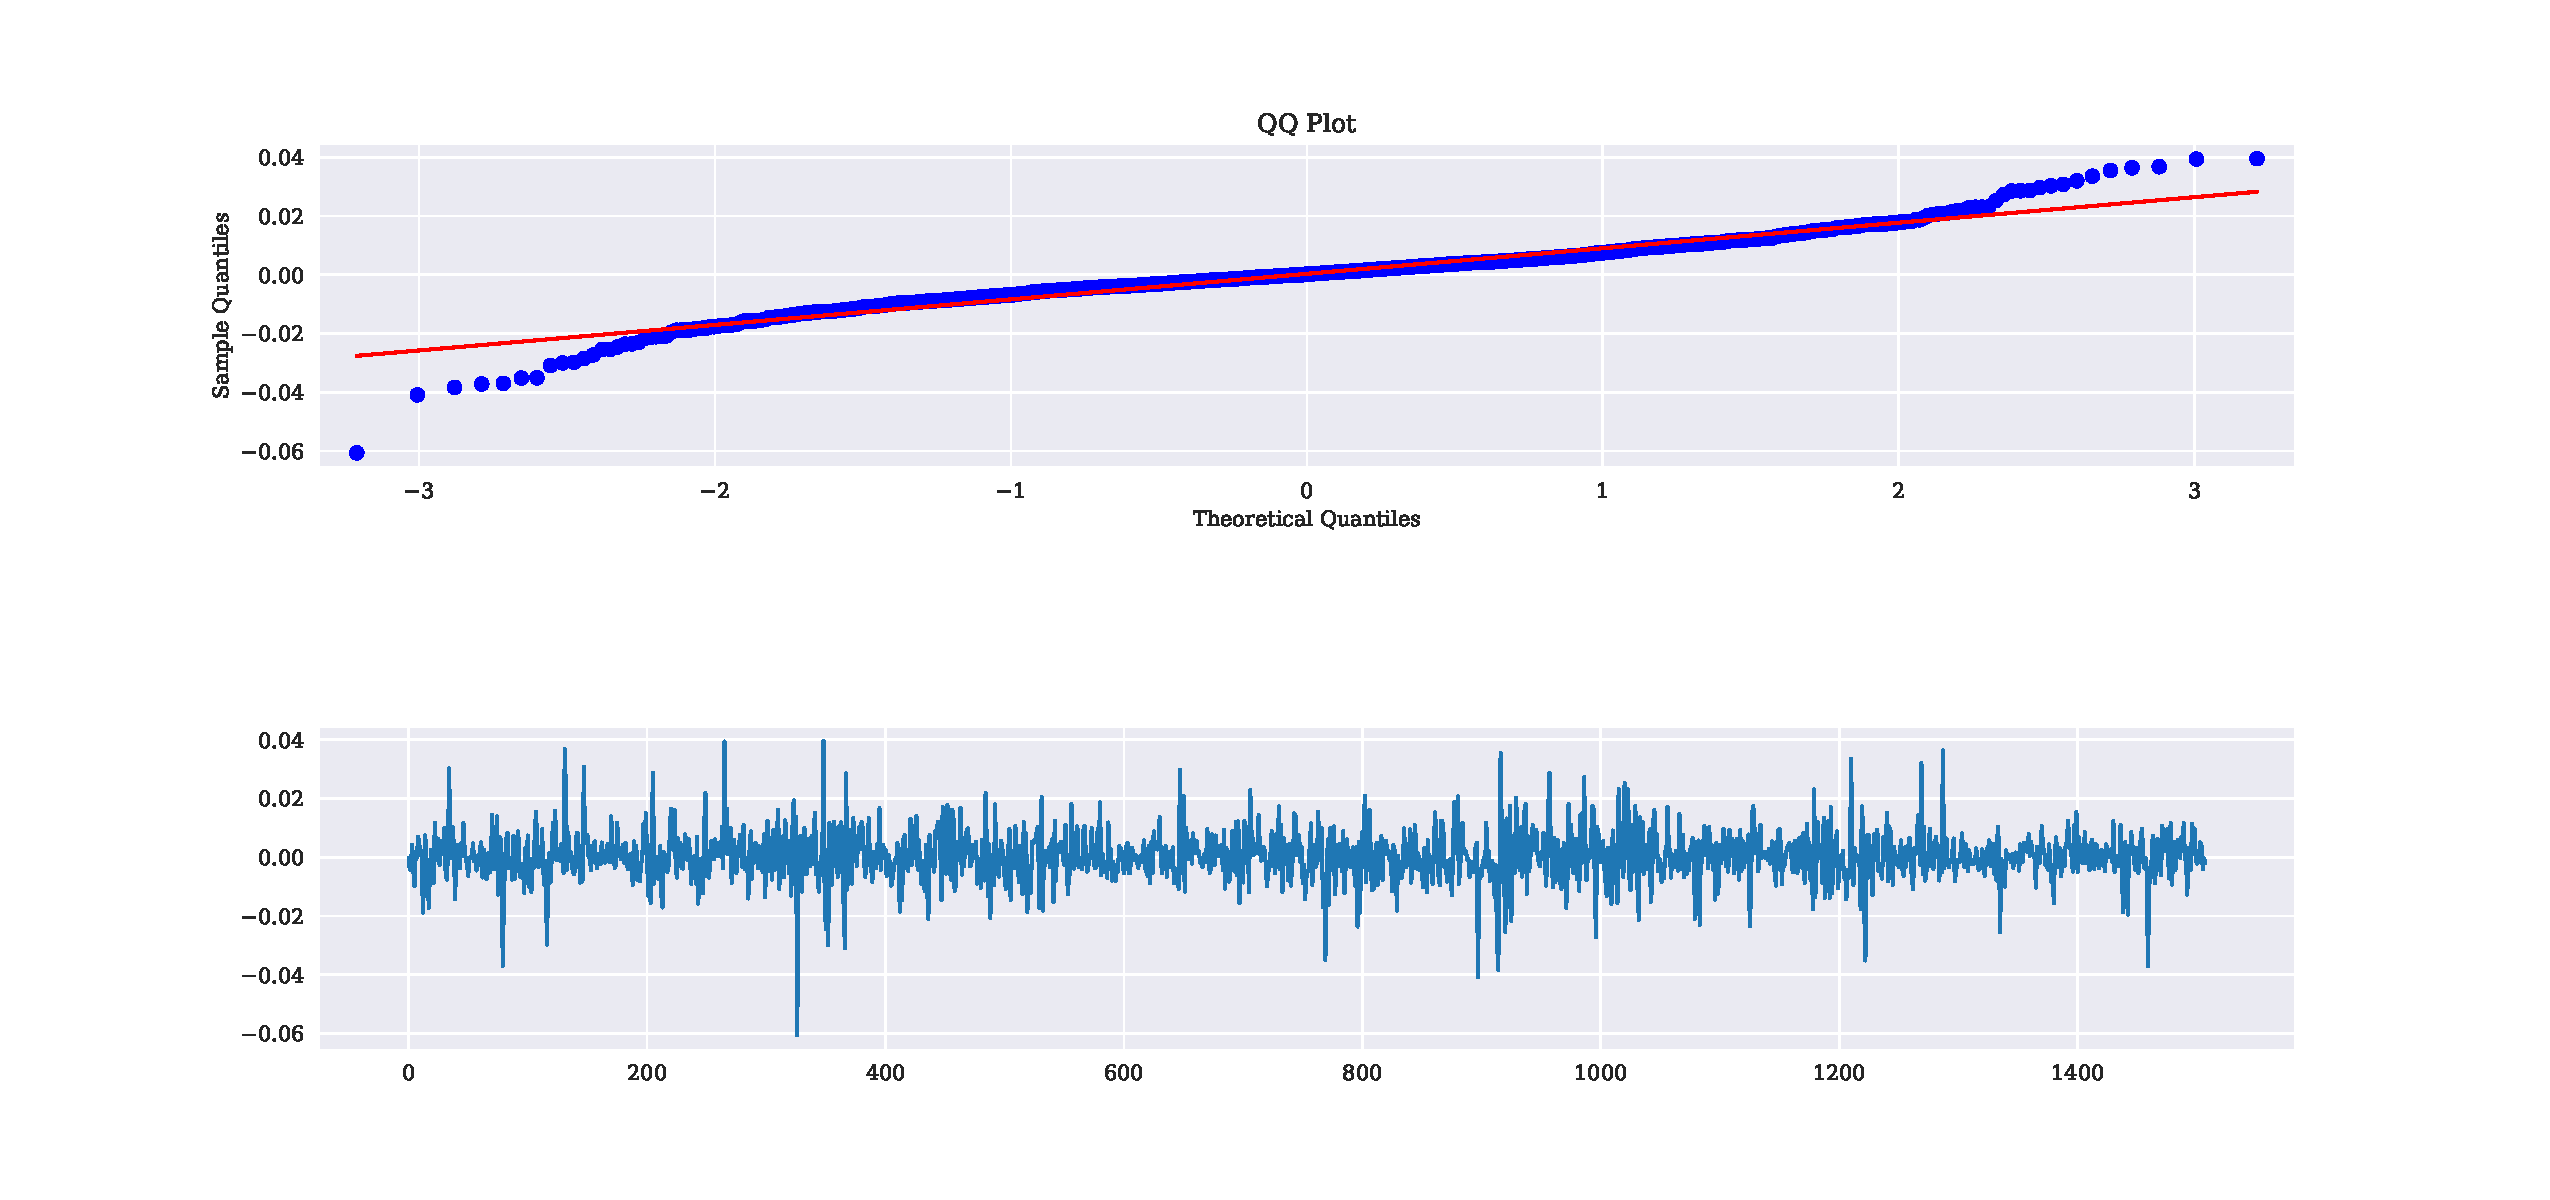
\includegraphics[]{figures/PG_log_adjclose_fd_and_qq.pdf}
    %%% Creator: Matplotlib, PGF backend
%%
%% To include the figure in your LaTeX document, write
%%   \input{<filename>.pgf}
%%
%% Make sure the required packages are loaded in your preamble
%%   \usepackage{pgf}
%%
%% Figures using additional raster images can only be included by \input if
%% they are in the same directory as the main LaTeX file. For loading figures
%% from other directories you can use the `import` package
%%   \usepackage{import}
%% and then include the figures with
%%   \import{<path to file>}{<filename>.pgf}
%%
%% Matplotlib used the following preamble
%%   \usepackage{fontspec}
%%   \setmainfont{DejaVuSerif.ttf}[Path=/opt/tljh/user/lib/python3.6/site-packages/matplotlib/mpl-data/fonts/ttf/]
%%   \setsansfont{DejaVuSans.ttf}[Path=/opt/tljh/user/lib/python3.6/site-packages/matplotlib/mpl-data/fonts/ttf/]
%%   \setmonofont{DejaVuSansMono.ttf}[Path=/opt/tljh/user/lib/python3.6/site-packages/matplotlib/mpl-data/fonts/ttf/]
%%
\begingroup%
\makeatletter%
\begin{pgfpicture}%
\pgfpathrectangle{\pgfpointorigin}{\pgfqpoint{17.000000in}{8.000000in}}%
\pgfusepath{use as bounding box, clip}%
\begin{pgfscope}%
\pgfsetbuttcap%
\pgfsetmiterjoin%
\definecolor{currentfill}{rgb}{1.000000,1.000000,1.000000}%
\pgfsetfillcolor{currentfill}%
\pgfsetlinewidth{0.000000pt}%
\definecolor{currentstroke}{rgb}{1.000000,1.000000,1.000000}%
\pgfsetstrokecolor{currentstroke}%
\pgfsetdash{}{0pt}%
\pgfpathmoveto{\pgfqpoint{0.000000in}{0.000000in}}%
\pgfpathlineto{\pgfqpoint{17.000000in}{0.000000in}}%
\pgfpathlineto{\pgfqpoint{17.000000in}{8.000000in}}%
\pgfpathlineto{\pgfqpoint{0.000000in}{8.000000in}}%
\pgfpathclose%
\pgfusepath{fill}%
\end{pgfscope}%
\begin{pgfscope}%
\pgfsetbuttcap%
\pgfsetmiterjoin%
\definecolor{currentfill}{rgb}{0.917647,0.917647,0.949020}%
\pgfsetfillcolor{currentfill}%
\pgfsetlinewidth{0.000000pt}%
\definecolor{currentstroke}{rgb}{0.000000,0.000000,0.000000}%
\pgfsetstrokecolor{currentstroke}%
\pgfsetstrokeopacity{0.000000}%
\pgfsetdash{}{0pt}%
\pgfpathmoveto{\pgfqpoint{2.125000in}{4.882857in}}%
\pgfpathlineto{\pgfqpoint{15.300000in}{4.882857in}}%
\pgfpathlineto{\pgfqpoint{15.300000in}{7.040000in}}%
\pgfpathlineto{\pgfqpoint{2.125000in}{7.040000in}}%
\pgfpathclose%
\pgfusepath{fill}%
\end{pgfscope}%
\begin{pgfscope}%
\pgfpathrectangle{\pgfqpoint{2.125000in}{4.882857in}}{\pgfqpoint{13.175000in}{2.157143in}}%
\pgfusepath{clip}%
\pgfsetroundcap%
\pgfsetroundjoin%
\pgfsetlinewidth{0.803000pt}%
\definecolor{currentstroke}{rgb}{1.000000,1.000000,1.000000}%
\pgfsetstrokecolor{currentstroke}%
\pgfsetdash{}{0pt}%
\pgfpathmoveto{\pgfqpoint{2.793535in}{4.882857in}}%
\pgfpathlineto{\pgfqpoint{2.793535in}{7.040000in}}%
\pgfusepath{stroke}%
\end{pgfscope}%
\begin{pgfscope}%
\definecolor{textcolor}{rgb}{0.150000,0.150000,0.150000}%
\pgfsetstrokecolor{textcolor}%
\pgfsetfillcolor{textcolor}%
\pgftext[x=2.793535in,y=4.785635in,,top]{\color{textcolor}\rmfamily\fontsize{10.000000}{12.000000}\selectfont −3}%
\end{pgfscope}%
\begin{pgfscope}%
\pgfpathrectangle{\pgfqpoint{2.125000in}{4.882857in}}{\pgfqpoint{13.175000in}{2.157143in}}%
\pgfusepath{clip}%
\pgfsetroundcap%
\pgfsetroundjoin%
\pgfsetlinewidth{0.803000pt}%
\definecolor{currentstroke}{rgb}{1.000000,1.000000,1.000000}%
\pgfsetstrokecolor{currentstroke}%
\pgfsetdash{}{0pt}%
\pgfpathmoveto{\pgfqpoint{4.766523in}{4.882857in}}%
\pgfpathlineto{\pgfqpoint{4.766523in}{7.040000in}}%
\pgfusepath{stroke}%
\end{pgfscope}%
\begin{pgfscope}%
\definecolor{textcolor}{rgb}{0.150000,0.150000,0.150000}%
\pgfsetstrokecolor{textcolor}%
\pgfsetfillcolor{textcolor}%
\pgftext[x=4.766523in,y=4.785635in,,top]{\color{textcolor}\rmfamily\fontsize{10.000000}{12.000000}\selectfont −2}%
\end{pgfscope}%
\begin{pgfscope}%
\pgfpathrectangle{\pgfqpoint{2.125000in}{4.882857in}}{\pgfqpoint{13.175000in}{2.157143in}}%
\pgfusepath{clip}%
\pgfsetroundcap%
\pgfsetroundjoin%
\pgfsetlinewidth{0.803000pt}%
\definecolor{currentstroke}{rgb}{1.000000,1.000000,1.000000}%
\pgfsetstrokecolor{currentstroke}%
\pgfsetdash{}{0pt}%
\pgfpathmoveto{\pgfqpoint{6.739512in}{4.882857in}}%
\pgfpathlineto{\pgfqpoint{6.739512in}{7.040000in}}%
\pgfusepath{stroke}%
\end{pgfscope}%
\begin{pgfscope}%
\definecolor{textcolor}{rgb}{0.150000,0.150000,0.150000}%
\pgfsetstrokecolor{textcolor}%
\pgfsetfillcolor{textcolor}%
\pgftext[x=6.739512in,y=4.785635in,,top]{\color{textcolor}\rmfamily\fontsize{10.000000}{12.000000}\selectfont −1}%
\end{pgfscope}%
\begin{pgfscope}%
\pgfpathrectangle{\pgfqpoint{2.125000in}{4.882857in}}{\pgfqpoint{13.175000in}{2.157143in}}%
\pgfusepath{clip}%
\pgfsetroundcap%
\pgfsetroundjoin%
\pgfsetlinewidth{0.803000pt}%
\definecolor{currentstroke}{rgb}{1.000000,1.000000,1.000000}%
\pgfsetstrokecolor{currentstroke}%
\pgfsetdash{}{0pt}%
\pgfpathmoveto{\pgfqpoint{8.712500in}{4.882857in}}%
\pgfpathlineto{\pgfqpoint{8.712500in}{7.040000in}}%
\pgfusepath{stroke}%
\end{pgfscope}%
\begin{pgfscope}%
\definecolor{textcolor}{rgb}{0.150000,0.150000,0.150000}%
\pgfsetstrokecolor{textcolor}%
\pgfsetfillcolor{textcolor}%
\pgftext[x=8.712500in,y=4.785635in,,top]{\color{textcolor}\rmfamily\fontsize{10.000000}{12.000000}\selectfont 0}%
\end{pgfscope}%
\begin{pgfscope}%
\pgfpathrectangle{\pgfqpoint{2.125000in}{4.882857in}}{\pgfqpoint{13.175000in}{2.157143in}}%
\pgfusepath{clip}%
\pgfsetroundcap%
\pgfsetroundjoin%
\pgfsetlinewidth{0.803000pt}%
\definecolor{currentstroke}{rgb}{1.000000,1.000000,1.000000}%
\pgfsetstrokecolor{currentstroke}%
\pgfsetdash{}{0pt}%
\pgfpathmoveto{\pgfqpoint{10.685488in}{4.882857in}}%
\pgfpathlineto{\pgfqpoint{10.685488in}{7.040000in}}%
\pgfusepath{stroke}%
\end{pgfscope}%
\begin{pgfscope}%
\definecolor{textcolor}{rgb}{0.150000,0.150000,0.150000}%
\pgfsetstrokecolor{textcolor}%
\pgfsetfillcolor{textcolor}%
\pgftext[x=10.685488in,y=4.785635in,,top]{\color{textcolor}\rmfamily\fontsize{10.000000}{12.000000}\selectfont 1}%
\end{pgfscope}%
\begin{pgfscope}%
\pgfpathrectangle{\pgfqpoint{2.125000in}{4.882857in}}{\pgfqpoint{13.175000in}{2.157143in}}%
\pgfusepath{clip}%
\pgfsetroundcap%
\pgfsetroundjoin%
\pgfsetlinewidth{0.803000pt}%
\definecolor{currentstroke}{rgb}{1.000000,1.000000,1.000000}%
\pgfsetstrokecolor{currentstroke}%
\pgfsetdash{}{0pt}%
\pgfpathmoveto{\pgfqpoint{12.658477in}{4.882857in}}%
\pgfpathlineto{\pgfqpoint{12.658477in}{7.040000in}}%
\pgfusepath{stroke}%
\end{pgfscope}%
\begin{pgfscope}%
\definecolor{textcolor}{rgb}{0.150000,0.150000,0.150000}%
\pgfsetstrokecolor{textcolor}%
\pgfsetfillcolor{textcolor}%
\pgftext[x=12.658477in,y=4.785635in,,top]{\color{textcolor}\rmfamily\fontsize{10.000000}{12.000000}\selectfont 2}%
\end{pgfscope}%
\begin{pgfscope}%
\pgfpathrectangle{\pgfqpoint{2.125000in}{4.882857in}}{\pgfqpoint{13.175000in}{2.157143in}}%
\pgfusepath{clip}%
\pgfsetroundcap%
\pgfsetroundjoin%
\pgfsetlinewidth{0.803000pt}%
\definecolor{currentstroke}{rgb}{1.000000,1.000000,1.000000}%
\pgfsetstrokecolor{currentstroke}%
\pgfsetdash{}{0pt}%
\pgfpathmoveto{\pgfqpoint{14.631465in}{4.882857in}}%
\pgfpathlineto{\pgfqpoint{14.631465in}{7.040000in}}%
\pgfusepath{stroke}%
\end{pgfscope}%
\begin{pgfscope}%
\definecolor{textcolor}{rgb}{0.150000,0.150000,0.150000}%
\pgfsetstrokecolor{textcolor}%
\pgfsetfillcolor{textcolor}%
\pgftext[x=14.631465in,y=4.785635in,,top]{\color{textcolor}\rmfamily\fontsize{10.000000}{12.000000}\selectfont 3}%
\end{pgfscope}%
\begin{pgfscope}%
\definecolor{textcolor}{rgb}{0.150000,0.150000,0.150000}%
\pgfsetstrokecolor{textcolor}%
\pgfsetfillcolor{textcolor}%
\pgftext[x=8.712500in,y=4.595667in,,top]{\color{textcolor}\rmfamily\fontsize{10.000000}{12.000000}\selectfont Theoretical Quantiles}%
\end{pgfscope}%
\begin{pgfscope}%
\pgfpathrectangle{\pgfqpoint{2.125000in}{4.882857in}}{\pgfqpoint{13.175000in}{2.157143in}}%
\pgfusepath{clip}%
\pgfsetroundcap%
\pgfsetroundjoin%
\pgfsetlinewidth{0.803000pt}%
\definecolor{currentstroke}{rgb}{1.000000,1.000000,1.000000}%
\pgfsetstrokecolor{currentstroke}%
\pgfsetdash{}{0pt}%
\pgfpathmoveto{\pgfqpoint{2.125000in}{4.992782in}}%
\pgfpathlineto{\pgfqpoint{15.300000in}{4.992782in}}%
\pgfusepath{stroke}%
\end{pgfscope}%
\begin{pgfscope}%
\definecolor{textcolor}{rgb}{0.150000,0.150000,0.150000}%
\pgfsetstrokecolor{textcolor}%
\pgfsetfillcolor{textcolor}%
\pgftext[x=1.602159in,y=4.940021in,left,base]{\color{textcolor}\rmfamily\fontsize{10.000000}{12.000000}\selectfont −0.06}%
\end{pgfscope}%
\begin{pgfscope}%
\pgfpathrectangle{\pgfqpoint{2.125000in}{4.882857in}}{\pgfqpoint{13.175000in}{2.157143in}}%
\pgfusepath{clip}%
\pgfsetroundcap%
\pgfsetroundjoin%
\pgfsetlinewidth{0.803000pt}%
\definecolor{currentstroke}{rgb}{1.000000,1.000000,1.000000}%
\pgfsetstrokecolor{currentstroke}%
\pgfsetdash{}{0pt}%
\pgfpathmoveto{\pgfqpoint{2.125000in}{5.384533in}}%
\pgfpathlineto{\pgfqpoint{15.300000in}{5.384533in}}%
\pgfusepath{stroke}%
\end{pgfscope}%
\begin{pgfscope}%
\definecolor{textcolor}{rgb}{0.150000,0.150000,0.150000}%
\pgfsetstrokecolor{textcolor}%
\pgfsetfillcolor{textcolor}%
\pgftext[x=1.602159in,y=5.331771in,left,base]{\color{textcolor}\rmfamily\fontsize{10.000000}{12.000000}\selectfont −0.04}%
\end{pgfscope}%
\begin{pgfscope}%
\pgfpathrectangle{\pgfqpoint{2.125000in}{4.882857in}}{\pgfqpoint{13.175000in}{2.157143in}}%
\pgfusepath{clip}%
\pgfsetroundcap%
\pgfsetroundjoin%
\pgfsetlinewidth{0.803000pt}%
\definecolor{currentstroke}{rgb}{1.000000,1.000000,1.000000}%
\pgfsetstrokecolor{currentstroke}%
\pgfsetdash{}{0pt}%
\pgfpathmoveto{\pgfqpoint{2.125000in}{5.776283in}}%
\pgfpathlineto{\pgfqpoint{15.300000in}{5.776283in}}%
\pgfusepath{stroke}%
\end{pgfscope}%
\begin{pgfscope}%
\definecolor{textcolor}{rgb}{0.150000,0.150000,0.150000}%
\pgfsetstrokecolor{textcolor}%
\pgfsetfillcolor{textcolor}%
\pgftext[x=1.602159in,y=5.723522in,left,base]{\color{textcolor}\rmfamily\fontsize{10.000000}{12.000000}\selectfont −0.02}%
\end{pgfscope}%
\begin{pgfscope}%
\pgfpathrectangle{\pgfqpoint{2.125000in}{4.882857in}}{\pgfqpoint{13.175000in}{2.157143in}}%
\pgfusepath{clip}%
\pgfsetroundcap%
\pgfsetroundjoin%
\pgfsetlinewidth{0.803000pt}%
\definecolor{currentstroke}{rgb}{1.000000,1.000000,1.000000}%
\pgfsetstrokecolor{currentstroke}%
\pgfsetdash{}{0pt}%
\pgfpathmoveto{\pgfqpoint{2.125000in}{6.168034in}}%
\pgfpathlineto{\pgfqpoint{15.300000in}{6.168034in}}%
\pgfusepath{stroke}%
\end{pgfscope}%
\begin{pgfscope}%
\definecolor{textcolor}{rgb}{0.150000,0.150000,0.150000}%
\pgfsetstrokecolor{textcolor}%
\pgfsetfillcolor{textcolor}%
\pgftext[x=1.718533in,y=6.115272in,left,base]{\color{textcolor}\rmfamily\fontsize{10.000000}{12.000000}\selectfont 0.00}%
\end{pgfscope}%
\begin{pgfscope}%
\pgfpathrectangle{\pgfqpoint{2.125000in}{4.882857in}}{\pgfqpoint{13.175000in}{2.157143in}}%
\pgfusepath{clip}%
\pgfsetroundcap%
\pgfsetroundjoin%
\pgfsetlinewidth{0.803000pt}%
\definecolor{currentstroke}{rgb}{1.000000,1.000000,1.000000}%
\pgfsetstrokecolor{currentstroke}%
\pgfsetdash{}{0pt}%
\pgfpathmoveto{\pgfqpoint{2.125000in}{6.559784in}}%
\pgfpathlineto{\pgfqpoint{15.300000in}{6.559784in}}%
\pgfusepath{stroke}%
\end{pgfscope}%
\begin{pgfscope}%
\definecolor{textcolor}{rgb}{0.150000,0.150000,0.150000}%
\pgfsetstrokecolor{textcolor}%
\pgfsetfillcolor{textcolor}%
\pgftext[x=1.718533in,y=6.507023in,left,base]{\color{textcolor}\rmfamily\fontsize{10.000000}{12.000000}\selectfont 0.02}%
\end{pgfscope}%
\begin{pgfscope}%
\pgfpathrectangle{\pgfqpoint{2.125000in}{4.882857in}}{\pgfqpoint{13.175000in}{2.157143in}}%
\pgfusepath{clip}%
\pgfsetroundcap%
\pgfsetroundjoin%
\pgfsetlinewidth{0.803000pt}%
\definecolor{currentstroke}{rgb}{1.000000,1.000000,1.000000}%
\pgfsetstrokecolor{currentstroke}%
\pgfsetdash{}{0pt}%
\pgfpathmoveto{\pgfqpoint{2.125000in}{6.951535in}}%
\pgfpathlineto{\pgfqpoint{15.300000in}{6.951535in}}%
\pgfusepath{stroke}%
\end{pgfscope}%
\begin{pgfscope}%
\definecolor{textcolor}{rgb}{0.150000,0.150000,0.150000}%
\pgfsetstrokecolor{textcolor}%
\pgfsetfillcolor{textcolor}%
\pgftext[x=1.718533in,y=6.898773in,left,base]{\color{textcolor}\rmfamily\fontsize{10.000000}{12.000000}\selectfont 0.04}%
\end{pgfscope}%
\begin{pgfscope}%
\definecolor{textcolor}{rgb}{0.150000,0.150000,0.150000}%
\pgfsetstrokecolor{textcolor}%
\pgfsetfillcolor{textcolor}%
\pgftext[x=1.546604in,y=5.961429in,,bottom,rotate=90.000000]{\color{textcolor}\rmfamily\fontsize{10.000000}{12.000000}\selectfont Sample Quantiles}%
\end{pgfscope}%
\begin{pgfscope}%
\pgfpathrectangle{\pgfqpoint{2.125000in}{4.882857in}}{\pgfqpoint{13.175000in}{2.157143in}}%
\pgfusepath{clip}%
\pgfsetbuttcap%
\pgfsetroundjoin%
\definecolor{currentfill}{rgb}{0.000000,0.000000,1.000000}%
\pgfsetfillcolor{currentfill}%
\pgfsetlinewidth{1.003750pt}%
\definecolor{currentstroke}{rgb}{0.000000,0.000000,1.000000}%
\pgfsetstrokecolor{currentstroke}%
\pgfsetdash{}{0pt}%
\pgfsys@defobject{currentmarker}{\pgfqpoint{-0.041667in}{-0.041667in}}{\pgfqpoint{0.041667in}{0.041667in}}{%
\pgfpathmoveto{\pgfqpoint{0.000000in}{-0.041667in}}%
\pgfpathcurveto{\pgfqpoint{0.011050in}{-0.041667in}}{\pgfqpoint{0.021649in}{-0.037276in}}{\pgfqpoint{0.029463in}{-0.029463in}}%
\pgfpathcurveto{\pgfqpoint{0.037276in}{-0.021649in}}{\pgfqpoint{0.041667in}{-0.011050in}}{\pgfqpoint{0.041667in}{0.000000in}}%
\pgfpathcurveto{\pgfqpoint{0.041667in}{0.011050in}}{\pgfqpoint{0.037276in}{0.021649in}}{\pgfqpoint{0.029463in}{0.029463in}}%
\pgfpathcurveto{\pgfqpoint{0.021649in}{0.037276in}}{\pgfqpoint{0.011050in}{0.041667in}}{\pgfqpoint{0.000000in}{0.041667in}}%
\pgfpathcurveto{\pgfqpoint{-0.011050in}{0.041667in}}{\pgfqpoint{-0.021649in}{0.037276in}}{\pgfqpoint{-0.029463in}{0.029463in}}%
\pgfpathcurveto{\pgfqpoint{-0.037276in}{0.021649in}}{\pgfqpoint{-0.041667in}{0.011050in}}{\pgfqpoint{-0.041667in}{0.000000in}}%
\pgfpathcurveto{\pgfqpoint{-0.041667in}{-0.011050in}}{\pgfqpoint{-0.037276in}{-0.021649in}}{\pgfqpoint{-0.029463in}{-0.029463in}}%
\pgfpathcurveto{\pgfqpoint{-0.021649in}{-0.037276in}}{\pgfqpoint{-0.011050in}{-0.041667in}}{\pgfqpoint{0.000000in}{-0.041667in}}%
\pgfpathclose%
\pgfusepath{stroke,fill}%
}%
\begin{pgfscope}%
\pgfsys@transformshift{2.378365in}{4.980909in}%
\pgfsys@useobject{currentmarker}{}%
\end{pgfscope}%
\begin{pgfscope}%
\pgfsys@transformshift{2.782528in}{5.367174in}%
\pgfsys@useobject{currentmarker}{}%
\end{pgfscope}%
\begin{pgfscope}%
\pgfsys@transformshift{3.030198in}{5.417895in}%
\pgfsys@useobject{currentmarker}{}%
\end{pgfscope}%
\begin{pgfscope}%
\pgfsys@transformshift{3.211576in}{5.440027in}%
\pgfsys@useobject{currentmarker}{}%
\end{pgfscope}%
\begin{pgfscope}%
\pgfsys@transformshift{3.355770in}{5.444283in}%
\pgfsys@useobject{currentmarker}{}%
\end{pgfscope}%
\begin{pgfscope}%
\pgfsys@transformshift{3.476013in}{5.479270in}%
\pgfsys@useobject{currentmarker}{}%
\end{pgfscope}%
\begin{pgfscope}%
\pgfsys@transformshift{3.579476in}{5.481040in}%
\pgfsys@useobject{currentmarker}{}%
\end{pgfscope}%
\begin{pgfscope}%
\pgfsys@transformshift{3.670496in}{5.563001in}%
\pgfsys@useobject{currentmarker}{}%
\end{pgfscope}%
\begin{pgfscope}%
\pgfsys@transformshift{3.751905in}{5.580653in}%
\pgfsys@useobject{currentmarker}{}%
\end{pgfscope}%
\begin{pgfscope}%
\pgfsys@transformshift{3.825653in}{5.584719in}%
\pgfsys@useobject{currentmarker}{}%
\end{pgfscope}%
\begin{pgfscope}%
\pgfsys@transformshift{3.893147in}{5.609480in}%
\pgfsys@useobject{currentmarker}{}%
\end{pgfscope}%
\begin{pgfscope}%
\pgfsys@transformshift{3.955431in}{5.633858in}%
\pgfsys@useobject{currentmarker}{}%
\end{pgfscope}%
\begin{pgfscope}%
\pgfsys@transformshift{4.013308in}{5.669441in}%
\pgfsys@useobject{currentmarker}{}%
\end{pgfscope}%
\begin{pgfscope}%
\pgfsys@transformshift{4.067403in}{5.670355in}%
\pgfsys@useobject{currentmarker}{}%
\end{pgfscope}%
\begin{pgfscope}%
\pgfsys@transformshift{4.118216in}{5.687079in}%
\pgfsys@useobject{currentmarker}{}%
\end{pgfscope}%
\begin{pgfscope}%
\pgfsys@transformshift{4.166153in}{5.705738in}%
\pgfsys@useobject{currentmarker}{}%
\end{pgfscope}%
\begin{pgfscope}%
\pgfsys@transformshift{4.211547in}{5.707008in}%
\pgfsys@useobject{currentmarker}{}%
\end{pgfscope}%
\begin{pgfscope}%
\pgfsys@transformshift{4.254677in}{5.715324in}%
\pgfsys@useobject{currentmarker}{}%
\end{pgfscope}%
\begin{pgfscope}%
\pgfsys@transformshift{4.295777in}{5.743070in}%
\pgfsys@useobject{currentmarker}{}%
\end{pgfscope}%
\begin{pgfscope}%
\pgfsys@transformshift{4.335044in}{5.750890in}%
\pgfsys@useobject{currentmarker}{}%
\end{pgfscope}%
\begin{pgfscope}%
\pgfsys@transformshift{4.372651in}{5.755195in}%
\pgfsys@useobject{currentmarker}{}%
\end{pgfscope}%
\begin{pgfscope}%
\pgfsys@transformshift{4.408744in}{5.757357in}%
\pgfsys@useobject{currentmarker}{}%
\end{pgfscope}%
\begin{pgfscope}%
\pgfsys@transformshift{4.443452in}{5.760794in}%
\pgfsys@useobject{currentmarker}{}%
\end{pgfscope}%
\begin{pgfscope}%
\pgfsys@transformshift{4.476887in}{5.786102in}%
\pgfsys@useobject{currentmarker}{}%
\end{pgfscope}%
\begin{pgfscope}%
\pgfsys@transformshift{4.509148in}{5.799157in}%
\pgfsys@useobject{currentmarker}{}%
\end{pgfscope}%
\begin{pgfscope}%
\pgfsys@transformshift{4.540323in}{5.799349in}%
\pgfsys@useobject{currentmarker}{}%
\end{pgfscope}%
\begin{pgfscope}%
\pgfsys@transformshift{4.570489in}{5.799953in}%
\pgfsys@useobject{currentmarker}{}%
\end{pgfscope}%
\begin{pgfscope}%
\pgfsys@transformshift{4.599718in}{5.801293in}%
\pgfsys@useobject{currentmarker}{}%
\end{pgfscope}%
\begin{pgfscope}%
\pgfsys@transformshift{4.628071in}{5.805786in}%
\pgfsys@useobject{currentmarker}{}%
\end{pgfscope}%
\begin{pgfscope}%
\pgfsys@transformshift{4.655604in}{5.810786in}%
\pgfsys@useobject{currentmarker}{}%
\end{pgfscope}%
\begin{pgfscope}%
\pgfsys@transformshift{4.682369in}{5.811592in}%
\pgfsys@useobject{currentmarker}{}%
\end{pgfscope}%
\begin{pgfscope}%
\pgfsys@transformshift{4.708413in}{5.813128in}%
\pgfsys@useobject{currentmarker}{}%
\end{pgfscope}%
\begin{pgfscope}%
\pgfsys@transformshift{4.733777in}{5.821386in}%
\pgfsys@useobject{currentmarker}{}%
\end{pgfscope}%
\begin{pgfscope}%
\pgfsys@transformshift{4.758500in}{5.821824in}%
\pgfsys@useobject{currentmarker}{}%
\end{pgfscope}%
\begin{pgfscope}%
\pgfsys@transformshift{4.782618in}{5.822816in}%
\pgfsys@useobject{currentmarker}{}%
\end{pgfscope}%
\begin{pgfscope}%
\pgfsys@transformshift{4.806162in}{5.829951in}%
\pgfsys@useobject{currentmarker}{}%
\end{pgfscope}%
\begin{pgfscope}%
\pgfsys@transformshift{4.829162in}{5.830360in}%
\pgfsys@useobject{currentmarker}{}%
\end{pgfscope}%
\begin{pgfscope}%
\pgfsys@transformshift{4.851647in}{5.831011in}%
\pgfsys@useobject{currentmarker}{}%
\end{pgfscope}%
\begin{pgfscope}%
\pgfsys@transformshift{4.873641in}{5.832586in}%
\pgfsys@useobject{currentmarker}{}%
\end{pgfscope}%
\begin{pgfscope}%
\pgfsys@transformshift{4.895168in}{5.836453in}%
\pgfsys@useobject{currentmarker}{}%
\end{pgfscope}%
\begin{pgfscope}%
\pgfsys@transformshift{4.916250in}{5.839467in}%
\pgfsys@useobject{currentmarker}{}%
\end{pgfscope}%
\begin{pgfscope}%
\pgfsys@transformshift{4.936908in}{5.850563in}%
\pgfsys@useobject{currentmarker}{}%
\end{pgfscope}%
\begin{pgfscope}%
\pgfsys@transformshift{4.957159in}{5.858632in}%
\pgfsys@useobject{currentmarker}{}%
\end{pgfscope}%
\begin{pgfscope}%
\pgfsys@transformshift{4.977023in}{5.858841in}%
\pgfsys@useobject{currentmarker}{}%
\end{pgfscope}%
\begin{pgfscope}%
\pgfsys@transformshift{4.996515in}{5.860538in}%
\pgfsys@useobject{currentmarker}{}%
\end{pgfscope}%
\begin{pgfscope}%
\pgfsys@transformshift{5.015651in}{5.861230in}%
\pgfsys@useobject{currentmarker}{}%
\end{pgfscope}%
\begin{pgfscope}%
\pgfsys@transformshift{5.034445in}{5.861543in}%
\pgfsys@useobject{currentmarker}{}%
\end{pgfscope}%
\begin{pgfscope}%
\pgfsys@transformshift{5.052911in}{5.863356in}%
\pgfsys@useobject{currentmarker}{}%
\end{pgfscope}%
\begin{pgfscope}%
\pgfsys@transformshift{5.071062in}{5.863400in}%
\pgfsys@useobject{currentmarker}{}%
\end{pgfscope}%
\begin{pgfscope}%
\pgfsys@transformshift{5.088911in}{5.870159in}%
\pgfsys@useobject{currentmarker}{}%
\end{pgfscope}%
\begin{pgfscope}%
\pgfsys@transformshift{5.106467in}{5.871112in}%
\pgfsys@useobject{currentmarker}{}%
\end{pgfscope}%
\begin{pgfscope}%
\pgfsys@transformshift{5.123742in}{5.881991in}%
\pgfsys@useobject{currentmarker}{}%
\end{pgfscope}%
\begin{pgfscope}%
\pgfsys@transformshift{5.140747in}{5.881995in}%
\pgfsys@useobject{currentmarker}{}%
\end{pgfscope}%
\begin{pgfscope}%
\pgfsys@transformshift{5.157490in}{5.882213in}%
\pgfsys@useobject{currentmarker}{}%
\end{pgfscope}%
\begin{pgfscope}%
\pgfsys@transformshift{5.173982in}{5.886118in}%
\pgfsys@useobject{currentmarker}{}%
\end{pgfscope}%
\begin{pgfscope}%
\pgfsys@transformshift{5.190229in}{5.887187in}%
\pgfsys@useobject{currentmarker}{}%
\end{pgfscope}%
\begin{pgfscope}%
\pgfsys@transformshift{5.206241in}{5.888470in}%
\pgfsys@useobject{currentmarker}{}%
\end{pgfscope}%
\begin{pgfscope}%
\pgfsys@transformshift{5.222026in}{5.889177in}%
\pgfsys@useobject{currentmarker}{}%
\end{pgfscope}%
\begin{pgfscope}%
\pgfsys@transformshift{5.237590in}{5.893073in}%
\pgfsys@useobject{currentmarker}{}%
\end{pgfscope}%
\begin{pgfscope}%
\pgfsys@transformshift{5.252941in}{5.896955in}%
\pgfsys@useobject{currentmarker}{}%
\end{pgfscope}%
\begin{pgfscope}%
\pgfsys@transformshift{5.268086in}{5.898388in}%
\pgfsys@useobject{currentmarker}{}%
\end{pgfscope}%
\begin{pgfscope}%
\pgfsys@transformshift{5.283030in}{5.900772in}%
\pgfsys@useobject{currentmarker}{}%
\end{pgfscope}%
\begin{pgfscope}%
\pgfsys@transformshift{5.297779in}{5.901250in}%
\pgfsys@useobject{currentmarker}{}%
\end{pgfscope}%
\begin{pgfscope}%
\pgfsys@transformshift{5.312341in}{5.902031in}%
\pgfsys@useobject{currentmarker}{}%
\end{pgfscope}%
\begin{pgfscope}%
\pgfsys@transformshift{5.326720in}{5.907344in}%
\pgfsys@useobject{currentmarker}{}%
\end{pgfscope}%
\begin{pgfscope}%
\pgfsys@transformshift{5.340920in}{5.909586in}%
\pgfsys@useobject{currentmarker}{}%
\end{pgfscope}%
\begin{pgfscope}%
\pgfsys@transformshift{5.354949in}{5.909840in}%
\pgfsys@useobject{currentmarker}{}%
\end{pgfscope}%
\begin{pgfscope}%
\pgfsys@transformshift{5.368810in}{5.912887in}%
\pgfsys@useobject{currentmarker}{}%
\end{pgfscope}%
\begin{pgfscope}%
\pgfsys@transformshift{5.382507in}{5.913426in}%
\pgfsys@useobject{currentmarker}{}%
\end{pgfscope}%
\begin{pgfscope}%
\pgfsys@transformshift{5.396046in}{5.913430in}%
\pgfsys@useobject{currentmarker}{}%
\end{pgfscope}%
\begin{pgfscope}%
\pgfsys@transformshift{5.409431in}{5.917663in}%
\pgfsys@useobject{currentmarker}{}%
\end{pgfscope}%
\begin{pgfscope}%
\pgfsys@transformshift{5.422665in}{5.918334in}%
\pgfsys@useobject{currentmarker}{}%
\end{pgfscope}%
\begin{pgfscope}%
\pgfsys@transformshift{5.435753in}{5.918418in}%
\pgfsys@useobject{currentmarker}{}%
\end{pgfscope}%
\begin{pgfscope}%
\pgfsys@transformshift{5.448698in}{5.920137in}%
\pgfsys@useobject{currentmarker}{}%
\end{pgfscope}%
\begin{pgfscope}%
\pgfsys@transformshift{5.461504in}{5.920721in}%
\pgfsys@useobject{currentmarker}{}%
\end{pgfscope}%
\begin{pgfscope}%
\pgfsys@transformshift{5.474175in}{5.922419in}%
\pgfsys@useobject{currentmarker}{}%
\end{pgfscope}%
\begin{pgfscope}%
\pgfsys@transformshift{5.486714in}{5.922774in}%
\pgfsys@useobject{currentmarker}{}%
\end{pgfscope}%
\begin{pgfscope}%
\pgfsys@transformshift{5.499123in}{5.922995in}%
\pgfsys@useobject{currentmarker}{}%
\end{pgfscope}%
\begin{pgfscope}%
\pgfsys@transformshift{5.511407in}{5.923223in}%
\pgfsys@useobject{currentmarker}{}%
\end{pgfscope}%
\begin{pgfscope}%
\pgfsys@transformshift{5.523568in}{5.923282in}%
\pgfsys@useobject{currentmarker}{}%
\end{pgfscope}%
\begin{pgfscope}%
\pgfsys@transformshift{5.535609in}{5.923552in}%
\pgfsys@useobject{currentmarker}{}%
\end{pgfscope}%
\begin{pgfscope}%
\pgfsys@transformshift{5.547533in}{5.924576in}%
\pgfsys@useobject{currentmarker}{}%
\end{pgfscope}%
\begin{pgfscope}%
\pgfsys@transformshift{5.559342in}{5.926792in}%
\pgfsys@useobject{currentmarker}{}%
\end{pgfscope}%
\begin{pgfscope}%
\pgfsys@transformshift{5.571040in}{5.928252in}%
\pgfsys@useobject{currentmarker}{}%
\end{pgfscope}%
\begin{pgfscope}%
\pgfsys@transformshift{5.582628in}{5.929224in}%
\pgfsys@useobject{currentmarker}{}%
\end{pgfscope}%
\begin{pgfscope}%
\pgfsys@transformshift{5.594109in}{5.930039in}%
\pgfsys@useobject{currentmarker}{}%
\end{pgfscope}%
\begin{pgfscope}%
\pgfsys@transformshift{5.605485in}{5.930643in}%
\pgfsys@useobject{currentmarker}{}%
\end{pgfscope}%
\begin{pgfscope}%
\pgfsys@transformshift{5.616759in}{5.933314in}%
\pgfsys@useobject{currentmarker}{}%
\end{pgfscope}%
\begin{pgfscope}%
\pgfsys@transformshift{5.627933in}{5.934681in}%
\pgfsys@useobject{currentmarker}{}%
\end{pgfscope}%
\begin{pgfscope}%
\pgfsys@transformshift{5.639009in}{5.935456in}%
\pgfsys@useobject{currentmarker}{}%
\end{pgfscope}%
\begin{pgfscope}%
\pgfsys@transformshift{5.649989in}{5.935490in}%
\pgfsys@useobject{currentmarker}{}%
\end{pgfscope}%
\begin{pgfscope}%
\pgfsys@transformshift{5.660874in}{5.937716in}%
\pgfsys@useobject{currentmarker}{}%
\end{pgfscope}%
\begin{pgfscope}%
\pgfsys@transformshift{5.671668in}{5.938519in}%
\pgfsys@useobject{currentmarker}{}%
\end{pgfscope}%
\begin{pgfscope}%
\pgfsys@transformshift{5.682371in}{5.938805in}%
\pgfsys@useobject{currentmarker}{}%
\end{pgfscope}%
\begin{pgfscope}%
\pgfsys@transformshift{5.692986in}{5.940553in}%
\pgfsys@useobject{currentmarker}{}%
\end{pgfscope}%
\begin{pgfscope}%
\pgfsys@transformshift{5.703514in}{5.942212in}%
\pgfsys@useobject{currentmarker}{}%
\end{pgfscope}%
\begin{pgfscope}%
\pgfsys@transformshift{5.713958in}{5.943002in}%
\pgfsys@useobject{currentmarker}{}%
\end{pgfscope}%
\begin{pgfscope}%
\pgfsys@transformshift{5.724318in}{5.943774in}%
\pgfsys@useobject{currentmarker}{}%
\end{pgfscope}%
\begin{pgfscope}%
\pgfsys@transformshift{5.734596in}{5.949593in}%
\pgfsys@useobject{currentmarker}{}%
\end{pgfscope}%
\begin{pgfscope}%
\pgfsys@transformshift{5.744794in}{5.949809in}%
\pgfsys@useobject{currentmarker}{}%
\end{pgfscope}%
\begin{pgfscope}%
\pgfsys@transformshift{5.754913in}{5.952479in}%
\pgfsys@useobject{currentmarker}{}%
\end{pgfscope}%
\begin{pgfscope}%
\pgfsys@transformshift{5.764955in}{5.955255in}%
\pgfsys@useobject{currentmarker}{}%
\end{pgfscope}%
\begin{pgfscope}%
\pgfsys@transformshift{5.774922in}{5.955619in}%
\pgfsys@useobject{currentmarker}{}%
\end{pgfscope}%
\begin{pgfscope}%
\pgfsys@transformshift{5.784814in}{5.955783in}%
\pgfsys@useobject{currentmarker}{}%
\end{pgfscope}%
\begin{pgfscope}%
\pgfsys@transformshift{5.794632in}{5.956751in}%
\pgfsys@useobject{currentmarker}{}%
\end{pgfscope}%
\begin{pgfscope}%
\pgfsys@transformshift{5.804380in}{5.956984in}%
\pgfsys@useobject{currentmarker}{}%
\end{pgfscope}%
\begin{pgfscope}%
\pgfsys@transformshift{5.814056in}{5.957398in}%
\pgfsys@useobject{currentmarker}{}%
\end{pgfscope}%
\begin{pgfscope}%
\pgfsys@transformshift{5.823664in}{5.957491in}%
\pgfsys@useobject{currentmarker}{}%
\end{pgfscope}%
\begin{pgfscope}%
\pgfsys@transformshift{5.833203in}{5.958137in}%
\pgfsys@useobject{currentmarker}{}%
\end{pgfscope}%
\begin{pgfscope}%
\pgfsys@transformshift{5.842676in}{5.958182in}%
\pgfsys@useobject{currentmarker}{}%
\end{pgfscope}%
\begin{pgfscope}%
\pgfsys@transformshift{5.852083in}{5.960109in}%
\pgfsys@useobject{currentmarker}{}%
\end{pgfscope}%
\begin{pgfscope}%
\pgfsys@transformshift{5.861425in}{5.962577in}%
\pgfsys@useobject{currentmarker}{}%
\end{pgfscope}%
\begin{pgfscope}%
\pgfsys@transformshift{5.870704in}{5.963868in}%
\pgfsys@useobject{currentmarker}{}%
\end{pgfscope}%
\begin{pgfscope}%
\pgfsys@transformshift{5.879920in}{5.964513in}%
\pgfsys@useobject{currentmarker}{}%
\end{pgfscope}%
\begin{pgfscope}%
\pgfsys@transformshift{5.889075in}{5.964532in}%
\pgfsys@useobject{currentmarker}{}%
\end{pgfscope}%
\begin{pgfscope}%
\pgfsys@transformshift{5.898170in}{5.965419in}%
\pgfsys@useobject{currentmarker}{}%
\end{pgfscope}%
\begin{pgfscope}%
\pgfsys@transformshift{5.907205in}{5.968479in}%
\pgfsys@useobject{currentmarker}{}%
\end{pgfscope}%
\begin{pgfscope}%
\pgfsys@transformshift{5.916182in}{5.968975in}%
\pgfsys@useobject{currentmarker}{}%
\end{pgfscope}%
\begin{pgfscope}%
\pgfsys@transformshift{5.925101in}{5.971416in}%
\pgfsys@useobject{currentmarker}{}%
\end{pgfscope}%
\begin{pgfscope}%
\pgfsys@transformshift{5.933964in}{5.972548in}%
\pgfsys@useobject{currentmarker}{}%
\end{pgfscope}%
\begin{pgfscope}%
\pgfsys@transformshift{5.942770in}{5.972675in}%
\pgfsys@useobject{currentmarker}{}%
\end{pgfscope}%
\begin{pgfscope}%
\pgfsys@transformshift{5.951522in}{5.973012in}%
\pgfsys@useobject{currentmarker}{}%
\end{pgfscope}%
\begin{pgfscope}%
\pgfsys@transformshift{5.960221in}{5.974776in}%
\pgfsys@useobject{currentmarker}{}%
\end{pgfscope}%
\begin{pgfscope}%
\pgfsys@transformshift{5.968865in}{5.975683in}%
\pgfsys@useobject{currentmarker}{}%
\end{pgfscope}%
\begin{pgfscope}%
\pgfsys@transformshift{5.977458in}{5.977481in}%
\pgfsys@useobject{currentmarker}{}%
\end{pgfscope}%
\begin{pgfscope}%
\pgfsys@transformshift{5.985999in}{5.978752in}%
\pgfsys@useobject{currentmarker}{}%
\end{pgfscope}%
\begin{pgfscope}%
\pgfsys@transformshift{5.994489in}{5.978837in}%
\pgfsys@useobject{currentmarker}{}%
\end{pgfscope}%
\begin{pgfscope}%
\pgfsys@transformshift{6.002929in}{5.979000in}%
\pgfsys@useobject{currentmarker}{}%
\end{pgfscope}%
\begin{pgfscope}%
\pgfsys@transformshift{6.011320in}{5.979316in}%
\pgfsys@useobject{currentmarker}{}%
\end{pgfscope}%
\begin{pgfscope}%
\pgfsys@transformshift{6.019663in}{5.979703in}%
\pgfsys@useobject{currentmarker}{}%
\end{pgfscope}%
\begin{pgfscope}%
\pgfsys@transformshift{6.027957in}{5.979949in}%
\pgfsys@useobject{currentmarker}{}%
\end{pgfscope}%
\begin{pgfscope}%
\pgfsys@transformshift{6.036204in}{5.980510in}%
\pgfsys@useobject{currentmarker}{}%
\end{pgfscope}%
\begin{pgfscope}%
\pgfsys@transformshift{6.044405in}{5.980922in}%
\pgfsys@useobject{currentmarker}{}%
\end{pgfscope}%
\begin{pgfscope}%
\pgfsys@transformshift{6.052560in}{5.981307in}%
\pgfsys@useobject{currentmarker}{}%
\end{pgfscope}%
\begin{pgfscope}%
\pgfsys@transformshift{6.060670in}{5.981869in}%
\pgfsys@useobject{currentmarker}{}%
\end{pgfscope}%
\begin{pgfscope}%
\pgfsys@transformshift{6.068735in}{5.982173in}%
\pgfsys@useobject{currentmarker}{}%
\end{pgfscope}%
\begin{pgfscope}%
\pgfsys@transformshift{6.076756in}{5.982343in}%
\pgfsys@useobject{currentmarker}{}%
\end{pgfscope}%
\begin{pgfscope}%
\pgfsys@transformshift{6.084734in}{5.982748in}%
\pgfsys@useobject{currentmarker}{}%
\end{pgfscope}%
\begin{pgfscope}%
\pgfsys@transformshift{6.092669in}{5.983268in}%
\pgfsys@useobject{currentmarker}{}%
\end{pgfscope}%
\begin{pgfscope}%
\pgfsys@transformshift{6.100562in}{5.984112in}%
\pgfsys@useobject{currentmarker}{}%
\end{pgfscope}%
\begin{pgfscope}%
\pgfsys@transformshift{6.108414in}{5.985004in}%
\pgfsys@useobject{currentmarker}{}%
\end{pgfscope}%
\begin{pgfscope}%
\pgfsys@transformshift{6.116224in}{5.985028in}%
\pgfsys@useobject{currentmarker}{}%
\end{pgfscope}%
\begin{pgfscope}%
\pgfsys@transformshift{6.123994in}{5.986367in}%
\pgfsys@useobject{currentmarker}{}%
\end{pgfscope}%
\begin{pgfscope}%
\pgfsys@transformshift{6.131724in}{5.987423in}%
\pgfsys@useobject{currentmarker}{}%
\end{pgfscope}%
\begin{pgfscope}%
\pgfsys@transformshift{6.139414in}{5.987453in}%
\pgfsys@useobject{currentmarker}{}%
\end{pgfscope}%
\begin{pgfscope}%
\pgfsys@transformshift{6.147066in}{5.989716in}%
\pgfsys@useobject{currentmarker}{}%
\end{pgfscope}%
\begin{pgfscope}%
\pgfsys@transformshift{6.154679in}{5.989852in}%
\pgfsys@useobject{currentmarker}{}%
\end{pgfscope}%
\begin{pgfscope}%
\pgfsys@transformshift{6.162255in}{5.990275in}%
\pgfsys@useobject{currentmarker}{}%
\end{pgfscope}%
\begin{pgfscope}%
\pgfsys@transformshift{6.169793in}{5.990957in}%
\pgfsys@useobject{currentmarker}{}%
\end{pgfscope}%
\begin{pgfscope}%
\pgfsys@transformshift{6.177294in}{5.991595in}%
\pgfsys@useobject{currentmarker}{}%
\end{pgfscope}%
\begin{pgfscope}%
\pgfsys@transformshift{6.184758in}{5.991709in}%
\pgfsys@useobject{currentmarker}{}%
\end{pgfscope}%
\begin{pgfscope}%
\pgfsys@transformshift{6.192187in}{5.991957in}%
\pgfsys@useobject{currentmarker}{}%
\end{pgfscope}%
\begin{pgfscope}%
\pgfsys@transformshift{6.199580in}{5.992237in}%
\pgfsys@useobject{currentmarker}{}%
\end{pgfscope}%
\begin{pgfscope}%
\pgfsys@transformshift{6.206938in}{5.992900in}%
\pgfsys@useobject{currentmarker}{}%
\end{pgfscope}%
\begin{pgfscope}%
\pgfsys@transformshift{6.214261in}{5.993240in}%
\pgfsys@useobject{currentmarker}{}%
\end{pgfscope}%
\begin{pgfscope}%
\pgfsys@transformshift{6.221550in}{5.993404in}%
\pgfsys@useobject{currentmarker}{}%
\end{pgfscope}%
\begin{pgfscope}%
\pgfsys@transformshift{6.228805in}{5.994202in}%
\pgfsys@useobject{currentmarker}{}%
\end{pgfscope}%
\begin{pgfscope}%
\pgfsys@transformshift{6.236027in}{5.994639in}%
\pgfsys@useobject{currentmarker}{}%
\end{pgfscope}%
\begin{pgfscope}%
\pgfsys@transformshift{6.243216in}{5.995284in}%
\pgfsys@useobject{currentmarker}{}%
\end{pgfscope}%
\begin{pgfscope}%
\pgfsys@transformshift{6.250372in}{5.995662in}%
\pgfsys@useobject{currentmarker}{}%
\end{pgfscope}%
\begin{pgfscope}%
\pgfsys@transformshift{6.257495in}{5.996225in}%
\pgfsys@useobject{currentmarker}{}%
\end{pgfscope}%
\begin{pgfscope}%
\pgfsys@transformshift{6.264587in}{5.996588in}%
\pgfsys@useobject{currentmarker}{}%
\end{pgfscope}%
\begin{pgfscope}%
\pgfsys@transformshift{6.271648in}{5.996738in}%
\pgfsys@useobject{currentmarker}{}%
\end{pgfscope}%
\begin{pgfscope}%
\pgfsys@transformshift{6.278677in}{5.997728in}%
\pgfsys@useobject{currentmarker}{}%
\end{pgfscope}%
\begin{pgfscope}%
\pgfsys@transformshift{6.285676in}{5.998244in}%
\pgfsys@useobject{currentmarker}{}%
\end{pgfscope}%
\begin{pgfscope}%
\pgfsys@transformshift{6.292644in}{5.998346in}%
\pgfsys@useobject{currentmarker}{}%
\end{pgfscope}%
\begin{pgfscope}%
\pgfsys@transformshift{6.299582in}{5.999282in}%
\pgfsys@useobject{currentmarker}{}%
\end{pgfscope}%
\begin{pgfscope}%
\pgfsys@transformshift{6.306490in}{5.999476in}%
\pgfsys@useobject{currentmarker}{}%
\end{pgfscope}%
\begin{pgfscope}%
\pgfsys@transformshift{6.313369in}{5.999479in}%
\pgfsys@useobject{currentmarker}{}%
\end{pgfscope}%
\begin{pgfscope}%
\pgfsys@transformshift{6.320219in}{5.999481in}%
\pgfsys@useobject{currentmarker}{}%
\end{pgfscope}%
\begin{pgfscope}%
\pgfsys@transformshift{6.327040in}{5.999544in}%
\pgfsys@useobject{currentmarker}{}%
\end{pgfscope}%
\begin{pgfscope}%
\pgfsys@transformshift{6.333833in}{6.000526in}%
\pgfsys@useobject{currentmarker}{}%
\end{pgfscope}%
\begin{pgfscope}%
\pgfsys@transformshift{6.340598in}{6.001604in}%
\pgfsys@useobject{currentmarker}{}%
\end{pgfscope}%
\begin{pgfscope}%
\pgfsys@transformshift{6.347335in}{6.002074in}%
\pgfsys@useobject{currentmarker}{}%
\end{pgfscope}%
\begin{pgfscope}%
\pgfsys@transformshift{6.354045in}{6.003629in}%
\pgfsys@useobject{currentmarker}{}%
\end{pgfscope}%
\begin{pgfscope}%
\pgfsys@transformshift{6.360727in}{6.004071in}%
\pgfsys@useobject{currentmarker}{}%
\end{pgfscope}%
\begin{pgfscope}%
\pgfsys@transformshift{6.367383in}{6.004935in}%
\pgfsys@useobject{currentmarker}{}%
\end{pgfscope}%
\begin{pgfscope}%
\pgfsys@transformshift{6.374012in}{6.005101in}%
\pgfsys@useobject{currentmarker}{}%
\end{pgfscope}%
\begin{pgfscope}%
\pgfsys@transformshift{6.380614in}{6.005256in}%
\pgfsys@useobject{currentmarker}{}%
\end{pgfscope}%
\begin{pgfscope}%
\pgfsys@transformshift{6.387191in}{6.005606in}%
\pgfsys@useobject{currentmarker}{}%
\end{pgfscope}%
\begin{pgfscope}%
\pgfsys@transformshift{6.393742in}{6.005741in}%
\pgfsys@useobject{currentmarker}{}%
\end{pgfscope}%
\begin{pgfscope}%
\pgfsys@transformshift{6.400267in}{6.005823in}%
\pgfsys@useobject{currentmarker}{}%
\end{pgfscope}%
\begin{pgfscope}%
\pgfsys@transformshift{6.406767in}{6.006590in}%
\pgfsys@useobject{currentmarker}{}%
\end{pgfscope}%
\begin{pgfscope}%
\pgfsys@transformshift{6.413243in}{6.008337in}%
\pgfsys@useobject{currentmarker}{}%
\end{pgfscope}%
\begin{pgfscope}%
\pgfsys@transformshift{6.419693in}{6.008527in}%
\pgfsys@useobject{currentmarker}{}%
\end{pgfscope}%
\begin{pgfscope}%
\pgfsys@transformshift{6.426119in}{6.008850in}%
\pgfsys@useobject{currentmarker}{}%
\end{pgfscope}%
\begin{pgfscope}%
\pgfsys@transformshift{6.432522in}{6.010799in}%
\pgfsys@useobject{currentmarker}{}%
\end{pgfscope}%
\begin{pgfscope}%
\pgfsys@transformshift{6.438900in}{6.011030in}%
\pgfsys@useobject{currentmarker}{}%
\end{pgfscope}%
\begin{pgfscope}%
\pgfsys@transformshift{6.445254in}{6.011109in}%
\pgfsys@useobject{currentmarker}{}%
\end{pgfscope}%
\begin{pgfscope}%
\pgfsys@transformshift{6.451585in}{6.011594in}%
\pgfsys@useobject{currentmarker}{}%
\end{pgfscope}%
\begin{pgfscope}%
\pgfsys@transformshift{6.457893in}{6.011612in}%
\pgfsys@useobject{currentmarker}{}%
\end{pgfscope}%
\begin{pgfscope}%
\pgfsys@transformshift{6.464178in}{6.012676in}%
\pgfsys@useobject{currentmarker}{}%
\end{pgfscope}%
\begin{pgfscope}%
\pgfsys@transformshift{6.470440in}{6.013005in}%
\pgfsys@useobject{currentmarker}{}%
\end{pgfscope}%
\begin{pgfscope}%
\pgfsys@transformshift{6.476680in}{6.013040in}%
\pgfsys@useobject{currentmarker}{}%
\end{pgfscope}%
\begin{pgfscope}%
\pgfsys@transformshift{6.482897in}{6.013302in}%
\pgfsys@useobject{currentmarker}{}%
\end{pgfscope}%
\begin{pgfscope}%
\pgfsys@transformshift{6.489092in}{6.013568in}%
\pgfsys@useobject{currentmarker}{}%
\end{pgfscope}%
\begin{pgfscope}%
\pgfsys@transformshift{6.495266in}{6.015412in}%
\pgfsys@useobject{currentmarker}{}%
\end{pgfscope}%
\begin{pgfscope}%
\pgfsys@transformshift{6.501418in}{6.015719in}%
\pgfsys@useobject{currentmarker}{}%
\end{pgfscope}%
\begin{pgfscope}%
\pgfsys@transformshift{6.507548in}{6.015834in}%
\pgfsys@useobject{currentmarker}{}%
\end{pgfscope}%
\begin{pgfscope}%
\pgfsys@transformshift{6.513657in}{6.017535in}%
\pgfsys@useobject{currentmarker}{}%
\end{pgfscope}%
\begin{pgfscope}%
\pgfsys@transformshift{6.519745in}{6.017782in}%
\pgfsys@useobject{currentmarker}{}%
\end{pgfscope}%
\begin{pgfscope}%
\pgfsys@transformshift{6.525813in}{6.018367in}%
\pgfsys@useobject{currentmarker}{}%
\end{pgfscope}%
\begin{pgfscope}%
\pgfsys@transformshift{6.531859in}{6.018612in}%
\pgfsys@useobject{currentmarker}{}%
\end{pgfscope}%
\begin{pgfscope}%
\pgfsys@transformshift{6.537886in}{6.018817in}%
\pgfsys@useobject{currentmarker}{}%
\end{pgfscope}%
\begin{pgfscope}%
\pgfsys@transformshift{6.543892in}{6.019078in}%
\pgfsys@useobject{currentmarker}{}%
\end{pgfscope}%
\begin{pgfscope}%
\pgfsys@transformshift{6.549878in}{6.019078in}%
\pgfsys@useobject{currentmarker}{}%
\end{pgfscope}%
\begin{pgfscope}%
\pgfsys@transformshift{6.555844in}{6.019281in}%
\pgfsys@useobject{currentmarker}{}%
\end{pgfscope}%
\begin{pgfscope}%
\pgfsys@transformshift{6.561791in}{6.019720in}%
\pgfsys@useobject{currentmarker}{}%
\end{pgfscope}%
\begin{pgfscope}%
\pgfsys@transformshift{6.567718in}{6.019790in}%
\pgfsys@useobject{currentmarker}{}%
\end{pgfscope}%
\begin{pgfscope}%
\pgfsys@transformshift{6.573626in}{6.019857in}%
\pgfsys@useobject{currentmarker}{}%
\end{pgfscope}%
\begin{pgfscope}%
\pgfsys@transformshift{6.579514in}{6.020203in}%
\pgfsys@useobject{currentmarker}{}%
\end{pgfscope}%
\begin{pgfscope}%
\pgfsys@transformshift{6.585384in}{6.021310in}%
\pgfsys@useobject{currentmarker}{}%
\end{pgfscope}%
\begin{pgfscope}%
\pgfsys@transformshift{6.591235in}{6.024134in}%
\pgfsys@useobject{currentmarker}{}%
\end{pgfscope}%
\begin{pgfscope}%
\pgfsys@transformshift{6.597068in}{6.024329in}%
\pgfsys@useobject{currentmarker}{}%
\end{pgfscope}%
\begin{pgfscope}%
\pgfsys@transformshift{6.602882in}{6.024400in}%
\pgfsys@useobject{currentmarker}{}%
\end{pgfscope}%
\begin{pgfscope}%
\pgfsys@transformshift{6.608677in}{6.025850in}%
\pgfsys@useobject{currentmarker}{}%
\end{pgfscope}%
\begin{pgfscope}%
\pgfsys@transformshift{6.614455in}{6.025857in}%
\pgfsys@useobject{currentmarker}{}%
\end{pgfscope}%
\begin{pgfscope}%
\pgfsys@transformshift{6.620215in}{6.025935in}%
\pgfsys@useobject{currentmarker}{}%
\end{pgfscope}%
\begin{pgfscope}%
\pgfsys@transformshift{6.625957in}{6.026085in}%
\pgfsys@useobject{currentmarker}{}%
\end{pgfscope}%
\begin{pgfscope}%
\pgfsys@transformshift{6.631681in}{6.026238in}%
\pgfsys@useobject{currentmarker}{}%
\end{pgfscope}%
\begin{pgfscope}%
\pgfsys@transformshift{6.637388in}{6.026247in}%
\pgfsys@useobject{currentmarker}{}%
\end{pgfscope}%
\begin{pgfscope}%
\pgfsys@transformshift{6.643077in}{6.026626in}%
\pgfsys@useobject{currentmarker}{}%
\end{pgfscope}%
\begin{pgfscope}%
\pgfsys@transformshift{6.648750in}{6.026672in}%
\pgfsys@useobject{currentmarker}{}%
\end{pgfscope}%
\begin{pgfscope}%
\pgfsys@transformshift{6.654405in}{6.027137in}%
\pgfsys@useobject{currentmarker}{}%
\end{pgfscope}%
\begin{pgfscope}%
\pgfsys@transformshift{6.660043in}{6.027969in}%
\pgfsys@useobject{currentmarker}{}%
\end{pgfscope}%
\begin{pgfscope}%
\pgfsys@transformshift{6.665665in}{6.028269in}%
\pgfsys@useobject{currentmarker}{}%
\end{pgfscope}%
\begin{pgfscope}%
\pgfsys@transformshift{6.671270in}{6.028878in}%
\pgfsys@useobject{currentmarker}{}%
\end{pgfscope}%
\begin{pgfscope}%
\pgfsys@transformshift{6.676859in}{6.029625in}%
\pgfsys@useobject{currentmarker}{}%
\end{pgfscope}%
\begin{pgfscope}%
\pgfsys@transformshift{6.682432in}{6.030084in}%
\pgfsys@useobject{currentmarker}{}%
\end{pgfscope}%
\begin{pgfscope}%
\pgfsys@transformshift{6.687988in}{6.030416in}%
\pgfsys@useobject{currentmarker}{}%
\end{pgfscope}%
\begin{pgfscope}%
\pgfsys@transformshift{6.693528in}{6.030785in}%
\pgfsys@useobject{currentmarker}{}%
\end{pgfscope}%
\begin{pgfscope}%
\pgfsys@transformshift{6.699053in}{6.031632in}%
\pgfsys@useobject{currentmarker}{}%
\end{pgfscope}%
\begin{pgfscope}%
\pgfsys@transformshift{6.704562in}{6.031870in}%
\pgfsys@useobject{currentmarker}{}%
\end{pgfscope}%
\begin{pgfscope}%
\pgfsys@transformshift{6.710055in}{6.031918in}%
\pgfsys@useobject{currentmarker}{}%
\end{pgfscope}%
\begin{pgfscope}%
\pgfsys@transformshift{6.715532in}{6.032266in}%
\pgfsys@useobject{currentmarker}{}%
\end{pgfscope}%
\begin{pgfscope}%
\pgfsys@transformshift{6.720995in}{6.032302in}%
\pgfsys@useobject{currentmarker}{}%
\end{pgfscope}%
\begin{pgfscope}%
\pgfsys@transformshift{6.726442in}{6.032383in}%
\pgfsys@useobject{currentmarker}{}%
\end{pgfscope}%
\begin{pgfscope}%
\pgfsys@transformshift{6.731874in}{6.032772in}%
\pgfsys@useobject{currentmarker}{}%
\end{pgfscope}%
\begin{pgfscope}%
\pgfsys@transformshift{6.737291in}{6.033569in}%
\pgfsys@useobject{currentmarker}{}%
\end{pgfscope}%
\begin{pgfscope}%
\pgfsys@transformshift{6.742693in}{6.034185in}%
\pgfsys@useobject{currentmarker}{}%
\end{pgfscope}%
\begin{pgfscope}%
\pgfsys@transformshift{6.748080in}{6.034545in}%
\pgfsys@useobject{currentmarker}{}%
\end{pgfscope}%
\begin{pgfscope}%
\pgfsys@transformshift{6.753453in}{6.034627in}%
\pgfsys@useobject{currentmarker}{}%
\end{pgfscope}%
\begin{pgfscope}%
\pgfsys@transformshift{6.758811in}{6.035325in}%
\pgfsys@useobject{currentmarker}{}%
\end{pgfscope}%
\begin{pgfscope}%
\pgfsys@transformshift{6.764155in}{6.036681in}%
\pgfsys@useobject{currentmarker}{}%
\end{pgfscope}%
\begin{pgfscope}%
\pgfsys@transformshift{6.769485in}{6.037074in}%
\pgfsys@useobject{currentmarker}{}%
\end{pgfscope}%
\begin{pgfscope}%
\pgfsys@transformshift{6.774801in}{6.037940in}%
\pgfsys@useobject{currentmarker}{}%
\end{pgfscope}%
\begin{pgfscope}%
\pgfsys@transformshift{6.780102in}{6.038371in}%
\pgfsys@useobject{currentmarker}{}%
\end{pgfscope}%
\begin{pgfscope}%
\pgfsys@transformshift{6.785390in}{6.038934in}%
\pgfsys@useobject{currentmarker}{}%
\end{pgfscope}%
\begin{pgfscope}%
\pgfsys@transformshift{6.790664in}{6.039196in}%
\pgfsys@useobject{currentmarker}{}%
\end{pgfscope}%
\begin{pgfscope}%
\pgfsys@transformshift{6.795924in}{6.039240in}%
\pgfsys@useobject{currentmarker}{}%
\end{pgfscope}%
\begin{pgfscope}%
\pgfsys@transformshift{6.801170in}{6.041253in}%
\pgfsys@useobject{currentmarker}{}%
\end{pgfscope}%
\begin{pgfscope}%
\pgfsys@transformshift{6.806403in}{6.041588in}%
\pgfsys@useobject{currentmarker}{}%
\end{pgfscope}%
\begin{pgfscope}%
\pgfsys@transformshift{6.811623in}{6.041991in}%
\pgfsys@useobject{currentmarker}{}%
\end{pgfscope}%
\begin{pgfscope}%
\pgfsys@transformshift{6.816829in}{6.042695in}%
\pgfsys@useobject{currentmarker}{}%
\end{pgfscope}%
\begin{pgfscope}%
\pgfsys@transformshift{6.822023in}{6.043133in}%
\pgfsys@useobject{currentmarker}{}%
\end{pgfscope}%
\begin{pgfscope}%
\pgfsys@transformshift{6.827203in}{6.043281in}%
\pgfsys@useobject{currentmarker}{}%
\end{pgfscope}%
\begin{pgfscope}%
\pgfsys@transformshift{6.832370in}{6.043483in}%
\pgfsys@useobject{currentmarker}{}%
\end{pgfscope}%
\begin{pgfscope}%
\pgfsys@transformshift{6.837524in}{6.043575in}%
\pgfsys@useobject{currentmarker}{}%
\end{pgfscope}%
\begin{pgfscope}%
\pgfsys@transformshift{6.842666in}{6.043579in}%
\pgfsys@useobject{currentmarker}{}%
\end{pgfscope}%
\begin{pgfscope}%
\pgfsys@transformshift{6.847795in}{6.044707in}%
\pgfsys@useobject{currentmarker}{}%
\end{pgfscope}%
\begin{pgfscope}%
\pgfsys@transformshift{6.852911in}{6.045830in}%
\pgfsys@useobject{currentmarker}{}%
\end{pgfscope}%
\begin{pgfscope}%
\pgfsys@transformshift{6.858015in}{6.048003in}%
\pgfsys@useobject{currentmarker}{}%
\end{pgfscope}%
\begin{pgfscope}%
\pgfsys@transformshift{6.863106in}{6.048415in}%
\pgfsys@useobject{currentmarker}{}%
\end{pgfscope}%
\begin{pgfscope}%
\pgfsys@transformshift{6.868186in}{6.048453in}%
\pgfsys@useobject{currentmarker}{}%
\end{pgfscope}%
\begin{pgfscope}%
\pgfsys@transformshift{6.873253in}{6.048801in}%
\pgfsys@useobject{currentmarker}{}%
\end{pgfscope}%
\begin{pgfscope}%
\pgfsys@transformshift{6.878308in}{6.051745in}%
\pgfsys@useobject{currentmarker}{}%
\end{pgfscope}%
\begin{pgfscope}%
\pgfsys@transformshift{6.883350in}{6.052056in}%
\pgfsys@useobject{currentmarker}{}%
\end{pgfscope}%
\begin{pgfscope}%
\pgfsys@transformshift{6.888381in}{6.052416in}%
\pgfsys@useobject{currentmarker}{}%
\end{pgfscope}%
\begin{pgfscope}%
\pgfsys@transformshift{6.893401in}{6.052943in}%
\pgfsys@useobject{currentmarker}{}%
\end{pgfscope}%
\begin{pgfscope}%
\pgfsys@transformshift{6.898408in}{6.053064in}%
\pgfsys@useobject{currentmarker}{}%
\end{pgfscope}%
\begin{pgfscope}%
\pgfsys@transformshift{6.903404in}{6.053478in}%
\pgfsys@useobject{currentmarker}{}%
\end{pgfscope}%
\begin{pgfscope}%
\pgfsys@transformshift{6.908388in}{6.053999in}%
\pgfsys@useobject{currentmarker}{}%
\end{pgfscope}%
\begin{pgfscope}%
\pgfsys@transformshift{6.913361in}{6.054301in}%
\pgfsys@useobject{currentmarker}{}%
\end{pgfscope}%
\begin{pgfscope}%
\pgfsys@transformshift{6.918322in}{6.054360in}%
\pgfsys@useobject{currentmarker}{}%
\end{pgfscope}%
\begin{pgfscope}%
\pgfsys@transformshift{6.923272in}{6.054592in}%
\pgfsys@useobject{currentmarker}{}%
\end{pgfscope}%
\begin{pgfscope}%
\pgfsys@transformshift{6.928211in}{6.055505in}%
\pgfsys@useobject{currentmarker}{}%
\end{pgfscope}%
\begin{pgfscope}%
\pgfsys@transformshift{6.933138in}{6.056946in}%
\pgfsys@useobject{currentmarker}{}%
\end{pgfscope}%
\begin{pgfscope}%
\pgfsys@transformshift{6.938055in}{6.057921in}%
\pgfsys@useobject{currentmarker}{}%
\end{pgfscope}%
\begin{pgfscope}%
\pgfsys@transformshift{6.942960in}{6.058006in}%
\pgfsys@useobject{currentmarker}{}%
\end{pgfscope}%
\begin{pgfscope}%
\pgfsys@transformshift{6.947855in}{6.058216in}%
\pgfsys@useobject{currentmarker}{}%
\end{pgfscope}%
\begin{pgfscope}%
\pgfsys@transformshift{6.952738in}{6.058716in}%
\pgfsys@useobject{currentmarker}{}%
\end{pgfscope}%
\begin{pgfscope}%
\pgfsys@transformshift{6.957611in}{6.058911in}%
\pgfsys@useobject{currentmarker}{}%
\end{pgfscope}%
\begin{pgfscope}%
\pgfsys@transformshift{6.962474in}{6.060065in}%
\pgfsys@useobject{currentmarker}{}%
\end{pgfscope}%
\begin{pgfscope}%
\pgfsys@transformshift{6.967325in}{6.060410in}%
\pgfsys@useobject{currentmarker}{}%
\end{pgfscope}%
\begin{pgfscope}%
\pgfsys@transformshift{6.972167in}{6.060410in}%
\pgfsys@useobject{currentmarker}{}%
\end{pgfscope}%
\begin{pgfscope}%
\pgfsys@transformshift{6.976997in}{6.060658in}%
\pgfsys@useobject{currentmarker}{}%
\end{pgfscope}%
\begin{pgfscope}%
\pgfsys@transformshift{6.981818in}{6.060962in}%
\pgfsys@useobject{currentmarker}{}%
\end{pgfscope}%
\begin{pgfscope}%
\pgfsys@transformshift{6.986628in}{6.061775in}%
\pgfsys@useobject{currentmarker}{}%
\end{pgfscope}%
\begin{pgfscope}%
\pgfsys@transformshift{6.991427in}{6.061868in}%
\pgfsys@useobject{currentmarker}{}%
\end{pgfscope}%
\begin{pgfscope}%
\pgfsys@transformshift{6.996217in}{6.061941in}%
\pgfsys@useobject{currentmarker}{}%
\end{pgfscope}%
\begin{pgfscope}%
\pgfsys@transformshift{7.000997in}{6.062070in}%
\pgfsys@useobject{currentmarker}{}%
\end{pgfscope}%
\begin{pgfscope}%
\pgfsys@transformshift{7.005766in}{6.062694in}%
\pgfsys@useobject{currentmarker}{}%
\end{pgfscope}%
\begin{pgfscope}%
\pgfsys@transformshift{7.010526in}{6.063343in}%
\pgfsys@useobject{currentmarker}{}%
\end{pgfscope}%
\begin{pgfscope}%
\pgfsys@transformshift{7.015275in}{6.063491in}%
\pgfsys@useobject{currentmarker}{}%
\end{pgfscope}%
\begin{pgfscope}%
\pgfsys@transformshift{7.020015in}{6.064213in}%
\pgfsys@useobject{currentmarker}{}%
\end{pgfscope}%
\begin{pgfscope}%
\pgfsys@transformshift{7.024745in}{6.064238in}%
\pgfsys@useobject{currentmarker}{}%
\end{pgfscope}%
\begin{pgfscope}%
\pgfsys@transformshift{7.029466in}{6.064259in}%
\pgfsys@useobject{currentmarker}{}%
\end{pgfscope}%
\begin{pgfscope}%
\pgfsys@transformshift{7.034176in}{6.064266in}%
\pgfsys@useobject{currentmarker}{}%
\end{pgfscope}%
\begin{pgfscope}%
\pgfsys@transformshift{7.038878in}{6.064310in}%
\pgfsys@useobject{currentmarker}{}%
\end{pgfscope}%
\begin{pgfscope}%
\pgfsys@transformshift{7.043570in}{6.064606in}%
\pgfsys@useobject{currentmarker}{}%
\end{pgfscope}%
\begin{pgfscope}%
\pgfsys@transformshift{7.048252in}{6.064864in}%
\pgfsys@useobject{currentmarker}{}%
\end{pgfscope}%
\begin{pgfscope}%
\pgfsys@transformshift{7.052925in}{6.065258in}%
\pgfsys@useobject{currentmarker}{}%
\end{pgfscope}%
\begin{pgfscope}%
\pgfsys@transformshift{7.057589in}{6.065287in}%
\pgfsys@useobject{currentmarker}{}%
\end{pgfscope}%
\begin{pgfscope}%
\pgfsys@transformshift{7.062243in}{6.065333in}%
\pgfsys@useobject{currentmarker}{}%
\end{pgfscope}%
\begin{pgfscope}%
\pgfsys@transformshift{7.066888in}{6.065570in}%
\pgfsys@useobject{currentmarker}{}%
\end{pgfscope}%
\begin{pgfscope}%
\pgfsys@transformshift{7.071525in}{6.066495in}%
\pgfsys@useobject{currentmarker}{}%
\end{pgfscope}%
\begin{pgfscope}%
\pgfsys@transformshift{7.076152in}{6.066997in}%
\pgfsys@useobject{currentmarker}{}%
\end{pgfscope}%
\begin{pgfscope}%
\pgfsys@transformshift{7.080770in}{6.067074in}%
\pgfsys@useobject{currentmarker}{}%
\end{pgfscope}%
\begin{pgfscope}%
\pgfsys@transformshift{7.085379in}{6.067150in}%
\pgfsys@useobject{currentmarker}{}%
\end{pgfscope}%
\begin{pgfscope}%
\pgfsys@transformshift{7.089980in}{6.067240in}%
\pgfsys@useobject{currentmarker}{}%
\end{pgfscope}%
\begin{pgfscope}%
\pgfsys@transformshift{7.094571in}{6.067403in}%
\pgfsys@useobject{currentmarker}{}%
\end{pgfscope}%
\begin{pgfscope}%
\pgfsys@transformshift{7.099154in}{6.067621in}%
\pgfsys@useobject{currentmarker}{}%
\end{pgfscope}%
\begin{pgfscope}%
\pgfsys@transformshift{7.103728in}{6.067997in}%
\pgfsys@useobject{currentmarker}{}%
\end{pgfscope}%
\begin{pgfscope}%
\pgfsys@transformshift{7.108294in}{6.068498in}%
\pgfsys@useobject{currentmarker}{}%
\end{pgfscope}%
\begin{pgfscope}%
\pgfsys@transformshift{7.112851in}{6.068740in}%
\pgfsys@useobject{currentmarker}{}%
\end{pgfscope}%
\begin{pgfscope}%
\pgfsys@transformshift{7.117399in}{6.068779in}%
\pgfsys@useobject{currentmarker}{}%
\end{pgfscope}%
\begin{pgfscope}%
\pgfsys@transformshift{7.121939in}{6.069107in}%
\pgfsys@useobject{currentmarker}{}%
\end{pgfscope}%
\begin{pgfscope}%
\pgfsys@transformshift{7.126471in}{6.069793in}%
\pgfsys@useobject{currentmarker}{}%
\end{pgfscope}%
\begin{pgfscope}%
\pgfsys@transformshift{7.130994in}{6.070455in}%
\pgfsys@useobject{currentmarker}{}%
\end{pgfscope}%
\begin{pgfscope}%
\pgfsys@transformshift{7.135509in}{6.070538in}%
\pgfsys@useobject{currentmarker}{}%
\end{pgfscope}%
\begin{pgfscope}%
\pgfsys@transformshift{7.140016in}{6.071080in}%
\pgfsys@useobject{currentmarker}{}%
\end{pgfscope}%
\begin{pgfscope}%
\pgfsys@transformshift{7.144514in}{6.071318in}%
\pgfsys@useobject{currentmarker}{}%
\end{pgfscope}%
\begin{pgfscope}%
\pgfsys@transformshift{7.149004in}{6.071428in}%
\pgfsys@useobject{currentmarker}{}%
\end{pgfscope}%
\begin{pgfscope}%
\pgfsys@transformshift{7.153487in}{6.071811in}%
\pgfsys@useobject{currentmarker}{}%
\end{pgfscope}%
\begin{pgfscope}%
\pgfsys@transformshift{7.157961in}{6.071841in}%
\pgfsys@useobject{currentmarker}{}%
\end{pgfscope}%
\begin{pgfscope}%
\pgfsys@transformshift{7.162427in}{6.071850in}%
\pgfsys@useobject{currentmarker}{}%
\end{pgfscope}%
\begin{pgfscope}%
\pgfsys@transformshift{7.166886in}{6.072251in}%
\pgfsys@useobject{currentmarker}{}%
\end{pgfscope}%
\begin{pgfscope}%
\pgfsys@transformshift{7.171336in}{6.072498in}%
\pgfsys@useobject{currentmarker}{}%
\end{pgfscope}%
\begin{pgfscope}%
\pgfsys@transformshift{7.175779in}{6.073380in}%
\pgfsys@useobject{currentmarker}{}%
\end{pgfscope}%
\begin{pgfscope}%
\pgfsys@transformshift{7.180213in}{6.073462in}%
\pgfsys@useobject{currentmarker}{}%
\end{pgfscope}%
\begin{pgfscope}%
\pgfsys@transformshift{7.184641in}{6.073598in}%
\pgfsys@useobject{currentmarker}{}%
\end{pgfscope}%
\begin{pgfscope}%
\pgfsys@transformshift{7.189060in}{6.074101in}%
\pgfsys@useobject{currentmarker}{}%
\end{pgfscope}%
\begin{pgfscope}%
\pgfsys@transformshift{7.193472in}{6.074453in}%
\pgfsys@useobject{currentmarker}{}%
\end{pgfscope}%
\begin{pgfscope}%
\pgfsys@transformshift{7.197876in}{6.074698in}%
\pgfsys@useobject{currentmarker}{}%
\end{pgfscope}%
\begin{pgfscope}%
\pgfsys@transformshift{7.202273in}{6.074778in}%
\pgfsys@useobject{currentmarker}{}%
\end{pgfscope}%
\begin{pgfscope}%
\pgfsys@transformshift{7.206662in}{6.075184in}%
\pgfsys@useobject{currentmarker}{}%
\end{pgfscope}%
\begin{pgfscope}%
\pgfsys@transformshift{7.211044in}{6.075436in}%
\pgfsys@useobject{currentmarker}{}%
\end{pgfscope}%
\begin{pgfscope}%
\pgfsys@transformshift{7.215418in}{6.076001in}%
\pgfsys@useobject{currentmarker}{}%
\end{pgfscope}%
\begin{pgfscope}%
\pgfsys@transformshift{7.219785in}{6.076265in}%
\pgfsys@useobject{currentmarker}{}%
\end{pgfscope}%
\begin{pgfscope}%
\pgfsys@transformshift{7.224145in}{6.076702in}%
\pgfsys@useobject{currentmarker}{}%
\end{pgfscope}%
\begin{pgfscope}%
\pgfsys@transformshift{7.228497in}{6.078165in}%
\pgfsys@useobject{currentmarker}{}%
\end{pgfscope}%
\begin{pgfscope}%
\pgfsys@transformshift{7.232843in}{6.078188in}%
\pgfsys@useobject{currentmarker}{}%
\end{pgfscope}%
\begin{pgfscope}%
\pgfsys@transformshift{7.237181in}{6.078461in}%
\pgfsys@useobject{currentmarker}{}%
\end{pgfscope}%
\begin{pgfscope}%
\pgfsys@transformshift{7.241512in}{6.079796in}%
\pgfsys@useobject{currentmarker}{}%
\end{pgfscope}%
\begin{pgfscope}%
\pgfsys@transformshift{7.245836in}{6.079812in}%
\pgfsys@useobject{currentmarker}{}%
\end{pgfscope}%
\begin{pgfscope}%
\pgfsys@transformshift{7.250152in}{6.079967in}%
\pgfsys@useobject{currentmarker}{}%
\end{pgfscope}%
\begin{pgfscope}%
\pgfsys@transformshift{7.254462in}{6.080459in}%
\pgfsys@useobject{currentmarker}{}%
\end{pgfscope}%
\begin{pgfscope}%
\pgfsys@transformshift{7.258765in}{6.080573in}%
\pgfsys@useobject{currentmarker}{}%
\end{pgfscope}%
\begin{pgfscope}%
\pgfsys@transformshift{7.263061in}{6.080716in}%
\pgfsys@useobject{currentmarker}{}%
\end{pgfscope}%
\begin{pgfscope}%
\pgfsys@transformshift{7.267350in}{6.081253in}%
\pgfsys@useobject{currentmarker}{}%
\end{pgfscope}%
\begin{pgfscope}%
\pgfsys@transformshift{7.271633in}{6.081432in}%
\pgfsys@useobject{currentmarker}{}%
\end{pgfscope}%
\begin{pgfscope}%
\pgfsys@transformshift{7.275908in}{6.081769in}%
\pgfsys@useobject{currentmarker}{}%
\end{pgfscope}%
\begin{pgfscope}%
\pgfsys@transformshift{7.280177in}{6.081842in}%
\pgfsys@useobject{currentmarker}{}%
\end{pgfscope}%
\begin{pgfscope}%
\pgfsys@transformshift{7.284439in}{6.081946in}%
\pgfsys@useobject{currentmarker}{}%
\end{pgfscope}%
\begin{pgfscope}%
\pgfsys@transformshift{7.288695in}{6.081955in}%
\pgfsys@useobject{currentmarker}{}%
\end{pgfscope}%
\begin{pgfscope}%
\pgfsys@transformshift{7.292944in}{6.082006in}%
\pgfsys@useobject{currentmarker}{}%
\end{pgfscope}%
\begin{pgfscope}%
\pgfsys@transformshift{7.297186in}{6.082311in}%
\pgfsys@useobject{currentmarker}{}%
\end{pgfscope}%
\begin{pgfscope}%
\pgfsys@transformshift{7.301422in}{6.082571in}%
\pgfsys@useobject{currentmarker}{}%
\end{pgfscope}%
\begin{pgfscope}%
\pgfsys@transformshift{7.305651in}{6.082610in}%
\pgfsys@useobject{currentmarker}{}%
\end{pgfscope}%
\begin{pgfscope}%
\pgfsys@transformshift{7.309874in}{6.082792in}%
\pgfsys@useobject{currentmarker}{}%
\end{pgfscope}%
\begin{pgfscope}%
\pgfsys@transformshift{7.314090in}{6.082822in}%
\pgfsys@useobject{currentmarker}{}%
\end{pgfscope}%
\begin{pgfscope}%
\pgfsys@transformshift{7.318300in}{6.084063in}%
\pgfsys@useobject{currentmarker}{}%
\end{pgfscope}%
\begin{pgfscope}%
\pgfsys@transformshift{7.322504in}{6.084246in}%
\pgfsys@useobject{currentmarker}{}%
\end{pgfscope}%
\begin{pgfscope}%
\pgfsys@transformshift{7.326701in}{6.084840in}%
\pgfsys@useobject{currentmarker}{}%
\end{pgfscope}%
\begin{pgfscope}%
\pgfsys@transformshift{7.330892in}{6.085082in}%
\pgfsys@useobject{currentmarker}{}%
\end{pgfscope}%
\begin{pgfscope}%
\pgfsys@transformshift{7.335077in}{6.085084in}%
\pgfsys@useobject{currentmarker}{}%
\end{pgfscope}%
\begin{pgfscope}%
\pgfsys@transformshift{7.339256in}{6.085412in}%
\pgfsys@useobject{currentmarker}{}%
\end{pgfscope}%
\begin{pgfscope}%
\pgfsys@transformshift{7.343429in}{6.085647in}%
\pgfsys@useobject{currentmarker}{}%
\end{pgfscope}%
\begin{pgfscope}%
\pgfsys@transformshift{7.347595in}{6.085654in}%
\pgfsys@useobject{currentmarker}{}%
\end{pgfscope}%
\begin{pgfscope}%
\pgfsys@transformshift{7.351755in}{6.085743in}%
\pgfsys@useobject{currentmarker}{}%
\end{pgfscope}%
\begin{pgfscope}%
\pgfsys@transformshift{7.355910in}{6.085874in}%
\pgfsys@useobject{currentmarker}{}%
\end{pgfscope}%
\begin{pgfscope}%
\pgfsys@transformshift{7.360058in}{6.086043in}%
\pgfsys@useobject{currentmarker}{}%
\end{pgfscope}%
\begin{pgfscope}%
\pgfsys@transformshift{7.364200in}{6.086837in}%
\pgfsys@useobject{currentmarker}{}%
\end{pgfscope}%
\begin{pgfscope}%
\pgfsys@transformshift{7.368337in}{6.086842in}%
\pgfsys@useobject{currentmarker}{}%
\end{pgfscope}%
\begin{pgfscope}%
\pgfsys@transformshift{7.372467in}{6.087621in}%
\pgfsys@useobject{currentmarker}{}%
\end{pgfscope}%
\begin{pgfscope}%
\pgfsys@transformshift{7.376592in}{6.087748in}%
\pgfsys@useobject{currentmarker}{}%
\end{pgfscope}%
\begin{pgfscope}%
\pgfsys@transformshift{7.380711in}{6.087827in}%
\pgfsys@useobject{currentmarker}{}%
\end{pgfscope}%
\begin{pgfscope}%
\pgfsys@transformshift{7.384824in}{6.087978in}%
\pgfsys@useobject{currentmarker}{}%
\end{pgfscope}%
\begin{pgfscope}%
\pgfsys@transformshift{7.388931in}{6.088011in}%
\pgfsys@useobject{currentmarker}{}%
\end{pgfscope}%
\begin{pgfscope}%
\pgfsys@transformshift{7.393033in}{6.088471in}%
\pgfsys@useobject{currentmarker}{}%
\end{pgfscope}%
\begin{pgfscope}%
\pgfsys@transformshift{7.397128in}{6.088688in}%
\pgfsys@useobject{currentmarker}{}%
\end{pgfscope}%
\begin{pgfscope}%
\pgfsys@transformshift{7.401219in}{6.089364in}%
\pgfsys@useobject{currentmarker}{}%
\end{pgfscope}%
\begin{pgfscope}%
\pgfsys@transformshift{7.405303in}{6.089464in}%
\pgfsys@useobject{currentmarker}{}%
\end{pgfscope}%
\begin{pgfscope}%
\pgfsys@transformshift{7.409382in}{6.090013in}%
\pgfsys@useobject{currentmarker}{}%
\end{pgfscope}%
\begin{pgfscope}%
\pgfsys@transformshift{7.413455in}{6.090084in}%
\pgfsys@useobject{currentmarker}{}%
\end{pgfscope}%
\begin{pgfscope}%
\pgfsys@transformshift{7.417523in}{6.090271in}%
\pgfsys@useobject{currentmarker}{}%
\end{pgfscope}%
\begin{pgfscope}%
\pgfsys@transformshift{7.421586in}{6.090489in}%
\pgfsys@useobject{currentmarker}{}%
\end{pgfscope}%
\begin{pgfscope}%
\pgfsys@transformshift{7.425643in}{6.090505in}%
\pgfsys@useobject{currentmarker}{}%
\end{pgfscope}%
\begin{pgfscope}%
\pgfsys@transformshift{7.429694in}{6.090704in}%
\pgfsys@useobject{currentmarker}{}%
\end{pgfscope}%
\begin{pgfscope}%
\pgfsys@transformshift{7.433740in}{6.090839in}%
\pgfsys@useobject{currentmarker}{}%
\end{pgfscope}%
\begin{pgfscope}%
\pgfsys@transformshift{7.437781in}{6.090841in}%
\pgfsys@useobject{currentmarker}{}%
\end{pgfscope}%
\begin{pgfscope}%
\pgfsys@transformshift{7.441816in}{6.091142in}%
\pgfsys@useobject{currentmarker}{}%
\end{pgfscope}%
\begin{pgfscope}%
\pgfsys@transformshift{7.445846in}{6.091289in}%
\pgfsys@useobject{currentmarker}{}%
\end{pgfscope}%
\begin{pgfscope}%
\pgfsys@transformshift{7.449871in}{6.091370in}%
\pgfsys@useobject{currentmarker}{}%
\end{pgfscope}%
\begin{pgfscope}%
\pgfsys@transformshift{7.453890in}{6.091514in}%
\pgfsys@useobject{currentmarker}{}%
\end{pgfscope}%
\begin{pgfscope}%
\pgfsys@transformshift{7.457905in}{6.091750in}%
\pgfsys@useobject{currentmarker}{}%
\end{pgfscope}%
\begin{pgfscope}%
\pgfsys@transformshift{7.461914in}{6.091847in}%
\pgfsys@useobject{currentmarker}{}%
\end{pgfscope}%
\begin{pgfscope}%
\pgfsys@transformshift{7.465918in}{6.092034in}%
\pgfsys@useobject{currentmarker}{}%
\end{pgfscope}%
\begin{pgfscope}%
\pgfsys@transformshift{7.469917in}{6.092372in}%
\pgfsys@useobject{currentmarker}{}%
\end{pgfscope}%
\begin{pgfscope}%
\pgfsys@transformshift{7.473910in}{6.092431in}%
\pgfsys@useobject{currentmarker}{}%
\end{pgfscope}%
\begin{pgfscope}%
\pgfsys@transformshift{7.477899in}{6.093027in}%
\pgfsys@useobject{currentmarker}{}%
\end{pgfscope}%
\begin{pgfscope}%
\pgfsys@transformshift{7.481883in}{6.093338in}%
\pgfsys@useobject{currentmarker}{}%
\end{pgfscope}%
\begin{pgfscope}%
\pgfsys@transformshift{7.485861in}{6.093543in}%
\pgfsys@useobject{currentmarker}{}%
\end{pgfscope}%
\begin{pgfscope}%
\pgfsys@transformshift{7.489835in}{6.093627in}%
\pgfsys@useobject{currentmarker}{}%
\end{pgfscope}%
\begin{pgfscope}%
\pgfsys@transformshift{7.493804in}{6.093627in}%
\pgfsys@useobject{currentmarker}{}%
\end{pgfscope}%
\begin{pgfscope}%
\pgfsys@transformshift{7.497767in}{6.093993in}%
\pgfsys@useobject{currentmarker}{}%
\end{pgfscope}%
\begin{pgfscope}%
\pgfsys@transformshift{7.501726in}{6.094000in}%
\pgfsys@useobject{currentmarker}{}%
\end{pgfscope}%
\begin{pgfscope}%
\pgfsys@transformshift{7.505680in}{6.094148in}%
\pgfsys@useobject{currentmarker}{}%
\end{pgfscope}%
\begin{pgfscope}%
\pgfsys@transformshift{7.509629in}{6.094491in}%
\pgfsys@useobject{currentmarker}{}%
\end{pgfscope}%
\begin{pgfscope}%
\pgfsys@transformshift{7.513574in}{6.094615in}%
\pgfsys@useobject{currentmarker}{}%
\end{pgfscope}%
\begin{pgfscope}%
\pgfsys@transformshift{7.517513in}{6.094700in}%
\pgfsys@useobject{currentmarker}{}%
\end{pgfscope}%
\begin{pgfscope}%
\pgfsys@transformshift{7.521448in}{6.094809in}%
\pgfsys@useobject{currentmarker}{}%
\end{pgfscope}%
\begin{pgfscope}%
\pgfsys@transformshift{7.525378in}{6.095148in}%
\pgfsys@useobject{currentmarker}{}%
\end{pgfscope}%
\begin{pgfscope}%
\pgfsys@transformshift{7.529303in}{6.095190in}%
\pgfsys@useobject{currentmarker}{}%
\end{pgfscope}%
\begin{pgfscope}%
\pgfsys@transformshift{7.533224in}{6.095407in}%
\pgfsys@useobject{currentmarker}{}%
\end{pgfscope}%
\begin{pgfscope}%
\pgfsys@transformshift{7.537140in}{6.095420in}%
\pgfsys@useobject{currentmarker}{}%
\end{pgfscope}%
\begin{pgfscope}%
\pgfsys@transformshift{7.541052in}{6.095739in}%
\pgfsys@useobject{currentmarker}{}%
\end{pgfscope}%
\begin{pgfscope}%
\pgfsys@transformshift{7.544958in}{6.095776in}%
\pgfsys@useobject{currentmarker}{}%
\end{pgfscope}%
\begin{pgfscope}%
\pgfsys@transformshift{7.548861in}{6.095906in}%
\pgfsys@useobject{currentmarker}{}%
\end{pgfscope}%
\begin{pgfscope}%
\pgfsys@transformshift{7.552758in}{6.095943in}%
\pgfsys@useobject{currentmarker}{}%
\end{pgfscope}%
\begin{pgfscope}%
\pgfsys@transformshift{7.556651in}{6.096089in}%
\pgfsys@useobject{currentmarker}{}%
\end{pgfscope}%
\begin{pgfscope}%
\pgfsys@transformshift{7.560540in}{6.096109in}%
\pgfsys@useobject{currentmarker}{}%
\end{pgfscope}%
\begin{pgfscope}%
\pgfsys@transformshift{7.564424in}{6.096255in}%
\pgfsys@useobject{currentmarker}{}%
\end{pgfscope}%
\begin{pgfscope}%
\pgfsys@transformshift{7.568304in}{6.096570in}%
\pgfsys@useobject{currentmarker}{}%
\end{pgfscope}%
\begin{pgfscope}%
\pgfsys@transformshift{7.572179in}{6.096660in}%
\pgfsys@useobject{currentmarker}{}%
\end{pgfscope}%
\begin{pgfscope}%
\pgfsys@transformshift{7.576050in}{6.096975in}%
\pgfsys@useobject{currentmarker}{}%
\end{pgfscope}%
\begin{pgfscope}%
\pgfsys@transformshift{7.579917in}{6.097026in}%
\pgfsys@useobject{currentmarker}{}%
\end{pgfscope}%
\begin{pgfscope}%
\pgfsys@transformshift{7.583779in}{6.097334in}%
\pgfsys@useobject{currentmarker}{}%
\end{pgfscope}%
\begin{pgfscope}%
\pgfsys@transformshift{7.587637in}{6.098033in}%
\pgfsys@useobject{currentmarker}{}%
\end{pgfscope}%
\begin{pgfscope}%
\pgfsys@transformshift{7.591491in}{6.098932in}%
\pgfsys@useobject{currentmarker}{}%
\end{pgfscope}%
\begin{pgfscope}%
\pgfsys@transformshift{7.595340in}{6.098942in}%
\pgfsys@useobject{currentmarker}{}%
\end{pgfscope}%
\begin{pgfscope}%
\pgfsys@transformshift{7.599185in}{6.100148in}%
\pgfsys@useobject{currentmarker}{}%
\end{pgfscope}%
\begin{pgfscope}%
\pgfsys@transformshift{7.603026in}{6.100365in}%
\pgfsys@useobject{currentmarker}{}%
\end{pgfscope}%
\begin{pgfscope}%
\pgfsys@transformshift{7.606863in}{6.100556in}%
\pgfsys@useobject{currentmarker}{}%
\end{pgfscope}%
\begin{pgfscope}%
\pgfsys@transformshift{7.610695in}{6.100723in}%
\pgfsys@useobject{currentmarker}{}%
\end{pgfscope}%
\begin{pgfscope}%
\pgfsys@transformshift{7.614523in}{6.100748in}%
\pgfsys@useobject{currentmarker}{}%
\end{pgfscope}%
\begin{pgfscope}%
\pgfsys@transformshift{7.618348in}{6.101036in}%
\pgfsys@useobject{currentmarker}{}%
\end{pgfscope}%
\begin{pgfscope}%
\pgfsys@transformshift{7.622168in}{6.101131in}%
\pgfsys@useobject{currentmarker}{}%
\end{pgfscope}%
\begin{pgfscope}%
\pgfsys@transformshift{7.625984in}{6.101174in}%
\pgfsys@useobject{currentmarker}{}%
\end{pgfscope}%
\begin{pgfscope}%
\pgfsys@transformshift{7.629796in}{6.101305in}%
\pgfsys@useobject{currentmarker}{}%
\end{pgfscope}%
\begin{pgfscope}%
\pgfsys@transformshift{7.633604in}{6.101576in}%
\pgfsys@useobject{currentmarker}{}%
\end{pgfscope}%
\begin{pgfscope}%
\pgfsys@transformshift{7.637407in}{6.102158in}%
\pgfsys@useobject{currentmarker}{}%
\end{pgfscope}%
\begin{pgfscope}%
\pgfsys@transformshift{7.641207in}{6.102202in}%
\pgfsys@useobject{currentmarker}{}%
\end{pgfscope}%
\begin{pgfscope}%
\pgfsys@transformshift{7.645003in}{6.102643in}%
\pgfsys@useobject{currentmarker}{}%
\end{pgfscope}%
\begin{pgfscope}%
\pgfsys@transformshift{7.648795in}{6.102734in}%
\pgfsys@useobject{currentmarker}{}%
\end{pgfscope}%
\begin{pgfscope}%
\pgfsys@transformshift{7.652583in}{6.102784in}%
\pgfsys@useobject{currentmarker}{}%
\end{pgfscope}%
\begin{pgfscope}%
\pgfsys@transformshift{7.656368in}{6.103305in}%
\pgfsys@useobject{currentmarker}{}%
\end{pgfscope}%
\begin{pgfscope}%
\pgfsys@transformshift{7.660148in}{6.104174in}%
\pgfsys@useobject{currentmarker}{}%
\end{pgfscope}%
\begin{pgfscope}%
\pgfsys@transformshift{7.663924in}{6.104354in}%
\pgfsys@useobject{currentmarker}{}%
\end{pgfscope}%
\begin{pgfscope}%
\pgfsys@transformshift{7.667697in}{6.104609in}%
\pgfsys@useobject{currentmarker}{}%
\end{pgfscope}%
\begin{pgfscope}%
\pgfsys@transformshift{7.671466in}{6.104662in}%
\pgfsys@useobject{currentmarker}{}%
\end{pgfscope}%
\begin{pgfscope}%
\pgfsys@transformshift{7.675231in}{6.104950in}%
\pgfsys@useobject{currentmarker}{}%
\end{pgfscope}%
\begin{pgfscope}%
\pgfsys@transformshift{7.678992in}{6.105001in}%
\pgfsys@useobject{currentmarker}{}%
\end{pgfscope}%
\begin{pgfscope}%
\pgfsys@transformshift{7.682749in}{6.105023in}%
\pgfsys@useobject{currentmarker}{}%
\end{pgfscope}%
\begin{pgfscope}%
\pgfsys@transformshift{7.686503in}{6.105079in}%
\pgfsys@useobject{currentmarker}{}%
\end{pgfscope}%
\begin{pgfscope}%
\pgfsys@transformshift{7.690253in}{6.105713in}%
\pgfsys@useobject{currentmarker}{}%
\end{pgfscope}%
\begin{pgfscope}%
\pgfsys@transformshift{7.693999in}{6.105792in}%
\pgfsys@useobject{currentmarker}{}%
\end{pgfscope}%
\begin{pgfscope}%
\pgfsys@transformshift{7.697742in}{6.106398in}%
\pgfsys@useobject{currentmarker}{}%
\end{pgfscope}%
\begin{pgfscope}%
\pgfsys@transformshift{7.701481in}{6.106569in}%
\pgfsys@useobject{currentmarker}{}%
\end{pgfscope}%
\begin{pgfscope}%
\pgfsys@transformshift{7.705216in}{6.106800in}%
\pgfsys@useobject{currentmarker}{}%
\end{pgfscope}%
\begin{pgfscope}%
\pgfsys@transformshift{7.708948in}{6.107084in}%
\pgfsys@useobject{currentmarker}{}%
\end{pgfscope}%
\begin{pgfscope}%
\pgfsys@transformshift{7.712676in}{6.107297in}%
\pgfsys@useobject{currentmarker}{}%
\end{pgfscope}%
\begin{pgfscope}%
\pgfsys@transformshift{7.716401in}{6.107312in}%
\pgfsys@useobject{currentmarker}{}%
\end{pgfscope}%
\begin{pgfscope}%
\pgfsys@transformshift{7.720122in}{6.107374in}%
\pgfsys@useobject{currentmarker}{}%
\end{pgfscope}%
\begin{pgfscope}%
\pgfsys@transformshift{7.723840in}{6.107842in}%
\pgfsys@useobject{currentmarker}{}%
\end{pgfscope}%
\begin{pgfscope}%
\pgfsys@transformshift{7.727554in}{6.108033in}%
\pgfsys@useobject{currentmarker}{}%
\end{pgfscope}%
\begin{pgfscope}%
\pgfsys@transformshift{7.731264in}{6.108096in}%
\pgfsys@useobject{currentmarker}{}%
\end{pgfscope}%
\begin{pgfscope}%
\pgfsys@transformshift{7.734971in}{6.108110in}%
\pgfsys@useobject{currentmarker}{}%
\end{pgfscope}%
\begin{pgfscope}%
\pgfsys@transformshift{7.738675in}{6.108374in}%
\pgfsys@useobject{currentmarker}{}%
\end{pgfscope}%
\begin{pgfscope}%
\pgfsys@transformshift{7.742375in}{6.108425in}%
\pgfsys@useobject{currentmarker}{}%
\end{pgfscope}%
\begin{pgfscope}%
\pgfsys@transformshift{7.746072in}{6.108501in}%
\pgfsys@useobject{currentmarker}{}%
\end{pgfscope}%
\begin{pgfscope}%
\pgfsys@transformshift{7.749765in}{6.108845in}%
\pgfsys@useobject{currentmarker}{}%
\end{pgfscope}%
\begin{pgfscope}%
\pgfsys@transformshift{7.753455in}{6.109226in}%
\pgfsys@useobject{currentmarker}{}%
\end{pgfscope}%
\begin{pgfscope}%
\pgfsys@transformshift{7.757142in}{6.109262in}%
\pgfsys@useobject{currentmarker}{}%
\end{pgfscope}%
\begin{pgfscope}%
\pgfsys@transformshift{7.760825in}{6.109418in}%
\pgfsys@useobject{currentmarker}{}%
\end{pgfscope}%
\begin{pgfscope}%
\pgfsys@transformshift{7.764505in}{6.109500in}%
\pgfsys@useobject{currentmarker}{}%
\end{pgfscope}%
\begin{pgfscope}%
\pgfsys@transformshift{7.768182in}{6.110043in}%
\pgfsys@useobject{currentmarker}{}%
\end{pgfscope}%
\begin{pgfscope}%
\pgfsys@transformshift{7.771856in}{6.110134in}%
\pgfsys@useobject{currentmarker}{}%
\end{pgfscope}%
\begin{pgfscope}%
\pgfsys@transformshift{7.775526in}{6.110268in}%
\pgfsys@useobject{currentmarker}{}%
\end{pgfscope}%
\begin{pgfscope}%
\pgfsys@transformshift{7.779193in}{6.110508in}%
\pgfsys@useobject{currentmarker}{}%
\end{pgfscope}%
\begin{pgfscope}%
\pgfsys@transformshift{7.782856in}{6.110606in}%
\pgfsys@useobject{currentmarker}{}%
\end{pgfscope}%
\begin{pgfscope}%
\pgfsys@transformshift{7.786517in}{6.110944in}%
\pgfsys@useobject{currentmarker}{}%
\end{pgfscope}%
\begin{pgfscope}%
\pgfsys@transformshift{7.790174in}{6.111590in}%
\pgfsys@useobject{currentmarker}{}%
\end{pgfscope}%
\begin{pgfscope}%
\pgfsys@transformshift{7.793829in}{6.112466in}%
\pgfsys@useobject{currentmarker}{}%
\end{pgfscope}%
\begin{pgfscope}%
\pgfsys@transformshift{7.797480in}{6.112725in}%
\pgfsys@useobject{currentmarker}{}%
\end{pgfscope}%
\begin{pgfscope}%
\pgfsys@transformshift{7.801128in}{6.112915in}%
\pgfsys@useobject{currentmarker}{}%
\end{pgfscope}%
\begin{pgfscope}%
\pgfsys@transformshift{7.804772in}{6.113013in}%
\pgfsys@useobject{currentmarker}{}%
\end{pgfscope}%
\begin{pgfscope}%
\pgfsys@transformshift{7.808414in}{6.113305in}%
\pgfsys@useobject{currentmarker}{}%
\end{pgfscope}%
\begin{pgfscope}%
\pgfsys@transformshift{7.812053in}{6.113712in}%
\pgfsys@useobject{currentmarker}{}%
\end{pgfscope}%
\begin{pgfscope}%
\pgfsys@transformshift{7.815688in}{6.114238in}%
\pgfsys@useobject{currentmarker}{}%
\end{pgfscope}%
\begin{pgfscope}%
\pgfsys@transformshift{7.819321in}{6.114627in}%
\pgfsys@useobject{currentmarker}{}%
\end{pgfscope}%
\begin{pgfscope}%
\pgfsys@transformshift{7.822950in}{6.115105in}%
\pgfsys@useobject{currentmarker}{}%
\end{pgfscope}%
\begin{pgfscope}%
\pgfsys@transformshift{7.826577in}{6.115277in}%
\pgfsys@useobject{currentmarker}{}%
\end{pgfscope}%
\begin{pgfscope}%
\pgfsys@transformshift{7.830200in}{6.115890in}%
\pgfsys@useobject{currentmarker}{}%
\end{pgfscope}%
\begin{pgfscope}%
\pgfsys@transformshift{7.833821in}{6.116031in}%
\pgfsys@useobject{currentmarker}{}%
\end{pgfscope}%
\begin{pgfscope}%
\pgfsys@transformshift{7.837438in}{6.116166in}%
\pgfsys@useobject{currentmarker}{}%
\end{pgfscope}%
\begin{pgfscope}%
\pgfsys@transformshift{7.841053in}{6.116233in}%
\pgfsys@useobject{currentmarker}{}%
\end{pgfscope}%
\begin{pgfscope}%
\pgfsys@transformshift{7.844665in}{6.116507in}%
\pgfsys@useobject{currentmarker}{}%
\end{pgfscope}%
\begin{pgfscope}%
\pgfsys@transformshift{7.848274in}{6.116645in}%
\pgfsys@useobject{currentmarker}{}%
\end{pgfscope}%
\begin{pgfscope}%
\pgfsys@transformshift{7.851879in}{6.116652in}%
\pgfsys@useobject{currentmarker}{}%
\end{pgfscope}%
\begin{pgfscope}%
\pgfsys@transformshift{7.855482in}{6.116769in}%
\pgfsys@useobject{currentmarker}{}%
\end{pgfscope}%
\begin{pgfscope}%
\pgfsys@transformshift{7.859083in}{6.116800in}%
\pgfsys@useobject{currentmarker}{}%
\end{pgfscope}%
\begin{pgfscope}%
\pgfsys@transformshift{7.862680in}{6.117172in}%
\pgfsys@useobject{currentmarker}{}%
\end{pgfscope}%
\begin{pgfscope}%
\pgfsys@transformshift{7.866275in}{6.117834in}%
\pgfsys@useobject{currentmarker}{}%
\end{pgfscope}%
\begin{pgfscope}%
\pgfsys@transformshift{7.869866in}{6.118044in}%
\pgfsys@useobject{currentmarker}{}%
\end{pgfscope}%
\begin{pgfscope}%
\pgfsys@transformshift{7.873455in}{6.118866in}%
\pgfsys@useobject{currentmarker}{}%
\end{pgfscope}%
\begin{pgfscope}%
\pgfsys@transformshift{7.877041in}{6.119004in}%
\pgfsys@useobject{currentmarker}{}%
\end{pgfscope}%
\begin{pgfscope}%
\pgfsys@transformshift{7.880625in}{6.119248in}%
\pgfsys@useobject{currentmarker}{}%
\end{pgfscope}%
\begin{pgfscope}%
\pgfsys@transformshift{7.884205in}{6.119323in}%
\pgfsys@useobject{currentmarker}{}%
\end{pgfscope}%
\begin{pgfscope}%
\pgfsys@transformshift{7.887783in}{6.119426in}%
\pgfsys@useobject{currentmarker}{}%
\end{pgfscope}%
\begin{pgfscope}%
\pgfsys@transformshift{7.891359in}{6.119729in}%
\pgfsys@useobject{currentmarker}{}%
\end{pgfscope}%
\begin{pgfscope}%
\pgfsys@transformshift{7.894931in}{6.119778in}%
\pgfsys@useobject{currentmarker}{}%
\end{pgfscope}%
\begin{pgfscope}%
\pgfsys@transformshift{7.898501in}{6.119876in}%
\pgfsys@useobject{currentmarker}{}%
\end{pgfscope}%
\begin{pgfscope}%
\pgfsys@transformshift{7.902068in}{6.120230in}%
\pgfsys@useobject{currentmarker}{}%
\end{pgfscope}%
\begin{pgfscope}%
\pgfsys@transformshift{7.905633in}{6.120426in}%
\pgfsys@useobject{currentmarker}{}%
\end{pgfscope}%
\begin{pgfscope}%
\pgfsys@transformshift{7.909195in}{6.120616in}%
\pgfsys@useobject{currentmarker}{}%
\end{pgfscope}%
\begin{pgfscope}%
\pgfsys@transformshift{7.912754in}{6.120655in}%
\pgfsys@useobject{currentmarker}{}%
\end{pgfscope}%
\begin{pgfscope}%
\pgfsys@transformshift{7.916310in}{6.120760in}%
\pgfsys@useobject{currentmarker}{}%
\end{pgfscope}%
\begin{pgfscope}%
\pgfsys@transformshift{7.919865in}{6.121042in}%
\pgfsys@useobject{currentmarker}{}%
\end{pgfscope}%
\begin{pgfscope}%
\pgfsys@transformshift{7.923416in}{6.121658in}%
\pgfsys@useobject{currentmarker}{}%
\end{pgfscope}%
\begin{pgfscope}%
\pgfsys@transformshift{7.926965in}{6.121689in}%
\pgfsys@useobject{currentmarker}{}%
\end{pgfscope}%
\begin{pgfscope}%
\pgfsys@transformshift{7.930512in}{6.121740in}%
\pgfsys@useobject{currentmarker}{}%
\end{pgfscope}%
\begin{pgfscope}%
\pgfsys@transformshift{7.934055in}{6.122346in}%
\pgfsys@useobject{currentmarker}{}%
\end{pgfscope}%
\begin{pgfscope}%
\pgfsys@transformshift{7.937597in}{6.122514in}%
\pgfsys@useobject{currentmarker}{}%
\end{pgfscope}%
\begin{pgfscope}%
\pgfsys@transformshift{7.941136in}{6.122760in}%
\pgfsys@useobject{currentmarker}{}%
\end{pgfscope}%
\begin{pgfscope}%
\pgfsys@transformshift{7.944672in}{6.122910in}%
\pgfsys@useobject{currentmarker}{}%
\end{pgfscope}%
\begin{pgfscope}%
\pgfsys@transformshift{7.948206in}{6.122993in}%
\pgfsys@useobject{currentmarker}{}%
\end{pgfscope}%
\begin{pgfscope}%
\pgfsys@transformshift{7.951738in}{6.123062in}%
\pgfsys@useobject{currentmarker}{}%
\end{pgfscope}%
\begin{pgfscope}%
\pgfsys@transformshift{7.955267in}{6.123634in}%
\pgfsys@useobject{currentmarker}{}%
\end{pgfscope}%
\begin{pgfscope}%
\pgfsys@transformshift{7.958793in}{6.123712in}%
\pgfsys@useobject{currentmarker}{}%
\end{pgfscope}%
\begin{pgfscope}%
\pgfsys@transformshift{7.962318in}{6.123905in}%
\pgfsys@useobject{currentmarker}{}%
\end{pgfscope}%
\begin{pgfscope}%
\pgfsys@transformshift{7.965839in}{6.124014in}%
\pgfsys@useobject{currentmarker}{}%
\end{pgfscope}%
\begin{pgfscope}%
\pgfsys@transformshift{7.969359in}{6.124108in}%
\pgfsys@useobject{currentmarker}{}%
\end{pgfscope}%
\begin{pgfscope}%
\pgfsys@transformshift{7.972876in}{6.124470in}%
\pgfsys@useobject{currentmarker}{}%
\end{pgfscope}%
\begin{pgfscope}%
\pgfsys@transformshift{7.976391in}{6.124549in}%
\pgfsys@useobject{currentmarker}{}%
\end{pgfscope}%
\begin{pgfscope}%
\pgfsys@transformshift{7.979903in}{6.125065in}%
\pgfsys@useobject{currentmarker}{}%
\end{pgfscope}%
\begin{pgfscope}%
\pgfsys@transformshift{7.983413in}{6.125425in}%
\pgfsys@useobject{currentmarker}{}%
\end{pgfscope}%
\begin{pgfscope}%
\pgfsys@transformshift{7.986921in}{6.125460in}%
\pgfsys@useobject{currentmarker}{}%
\end{pgfscope}%
\begin{pgfscope}%
\pgfsys@transformshift{7.990427in}{6.125582in}%
\pgfsys@useobject{currentmarker}{}%
\end{pgfscope}%
\begin{pgfscope}%
\pgfsys@transformshift{7.993930in}{6.125839in}%
\pgfsys@useobject{currentmarker}{}%
\end{pgfscope}%
\begin{pgfscope}%
\pgfsys@transformshift{7.997431in}{6.126231in}%
\pgfsys@useobject{currentmarker}{}%
\end{pgfscope}%
\begin{pgfscope}%
\pgfsys@transformshift{8.000930in}{6.126907in}%
\pgfsys@useobject{currentmarker}{}%
\end{pgfscope}%
\begin{pgfscope}%
\pgfsys@transformshift{8.004426in}{6.127123in}%
\pgfsys@useobject{currentmarker}{}%
\end{pgfscope}%
\begin{pgfscope}%
\pgfsys@transformshift{8.007920in}{6.127444in}%
\pgfsys@useobject{currentmarker}{}%
\end{pgfscope}%
\begin{pgfscope}%
\pgfsys@transformshift{8.011412in}{6.127666in}%
\pgfsys@useobject{currentmarker}{}%
\end{pgfscope}%
\begin{pgfscope}%
\pgfsys@transformshift{8.014902in}{6.127728in}%
\pgfsys@useobject{currentmarker}{}%
\end{pgfscope}%
\begin{pgfscope}%
\pgfsys@transformshift{8.018390in}{6.127753in}%
\pgfsys@useobject{currentmarker}{}%
\end{pgfscope}%
\begin{pgfscope}%
\pgfsys@transformshift{8.021875in}{6.127960in}%
\pgfsys@useobject{currentmarker}{}%
\end{pgfscope}%
\begin{pgfscope}%
\pgfsys@transformshift{8.025359in}{6.128798in}%
\pgfsys@useobject{currentmarker}{}%
\end{pgfscope}%
\begin{pgfscope}%
\pgfsys@transformshift{8.028840in}{6.129083in}%
\pgfsys@useobject{currentmarker}{}%
\end{pgfscope}%
\begin{pgfscope}%
\pgfsys@transformshift{8.032319in}{6.129271in}%
\pgfsys@useobject{currentmarker}{}%
\end{pgfscope}%
\begin{pgfscope}%
\pgfsys@transformshift{8.035796in}{6.129385in}%
\pgfsys@useobject{currentmarker}{}%
\end{pgfscope}%
\begin{pgfscope}%
\pgfsys@transformshift{8.039271in}{6.129603in}%
\pgfsys@useobject{currentmarker}{}%
\end{pgfscope}%
\begin{pgfscope}%
\pgfsys@transformshift{8.042744in}{6.129647in}%
\pgfsys@useobject{currentmarker}{}%
\end{pgfscope}%
\begin{pgfscope}%
\pgfsys@transformshift{8.046214in}{6.129766in}%
\pgfsys@useobject{currentmarker}{}%
\end{pgfscope}%
\begin{pgfscope}%
\pgfsys@transformshift{8.049683in}{6.130116in}%
\pgfsys@useobject{currentmarker}{}%
\end{pgfscope}%
\begin{pgfscope}%
\pgfsys@transformshift{8.053150in}{6.130306in}%
\pgfsys@useobject{currentmarker}{}%
\end{pgfscope}%
\begin{pgfscope}%
\pgfsys@transformshift{8.056614in}{6.130396in}%
\pgfsys@useobject{currentmarker}{}%
\end{pgfscope}%
\begin{pgfscope}%
\pgfsys@transformshift{8.060077in}{6.130468in}%
\pgfsys@useobject{currentmarker}{}%
\end{pgfscope}%
\begin{pgfscope}%
\pgfsys@transformshift{8.063537in}{6.130496in}%
\pgfsys@useobject{currentmarker}{}%
\end{pgfscope}%
\begin{pgfscope}%
\pgfsys@transformshift{8.066996in}{6.131382in}%
\pgfsys@useobject{currentmarker}{}%
\end{pgfscope}%
\begin{pgfscope}%
\pgfsys@transformshift{8.070453in}{6.131738in}%
\pgfsys@useobject{currentmarker}{}%
\end{pgfscope}%
\begin{pgfscope}%
\pgfsys@transformshift{8.073907in}{6.131761in}%
\pgfsys@useobject{currentmarker}{}%
\end{pgfscope}%
\begin{pgfscope}%
\pgfsys@transformshift{8.077360in}{6.132110in}%
\pgfsys@useobject{currentmarker}{}%
\end{pgfscope}%
\begin{pgfscope}%
\pgfsys@transformshift{8.080810in}{6.132162in}%
\pgfsys@useobject{currentmarker}{}%
\end{pgfscope}%
\begin{pgfscope}%
\pgfsys@transformshift{8.084259in}{6.132485in}%
\pgfsys@useobject{currentmarker}{}%
\end{pgfscope}%
\begin{pgfscope}%
\pgfsys@transformshift{8.087706in}{6.132542in}%
\pgfsys@useobject{currentmarker}{}%
\end{pgfscope}%
\begin{pgfscope}%
\pgfsys@transformshift{8.091151in}{6.132889in}%
\pgfsys@useobject{currentmarker}{}%
\end{pgfscope}%
\begin{pgfscope}%
\pgfsys@transformshift{8.094594in}{6.133087in}%
\pgfsys@useobject{currentmarker}{}%
\end{pgfscope}%
\begin{pgfscope}%
\pgfsys@transformshift{8.098035in}{6.133199in}%
\pgfsys@useobject{currentmarker}{}%
\end{pgfscope}%
\begin{pgfscope}%
\pgfsys@transformshift{8.101474in}{6.133310in}%
\pgfsys@useobject{currentmarker}{}%
\end{pgfscope}%
\begin{pgfscope}%
\pgfsys@transformshift{8.104912in}{6.133790in}%
\pgfsys@useobject{currentmarker}{}%
\end{pgfscope}%
\begin{pgfscope}%
\pgfsys@transformshift{8.108348in}{6.134053in}%
\pgfsys@useobject{currentmarker}{}%
\end{pgfscope}%
\begin{pgfscope}%
\pgfsys@transformshift{8.111781in}{6.134200in}%
\pgfsys@useobject{currentmarker}{}%
\end{pgfscope}%
\begin{pgfscope}%
\pgfsys@transformshift{8.115213in}{6.134330in}%
\pgfsys@useobject{currentmarker}{}%
\end{pgfscope}%
\begin{pgfscope}%
\pgfsys@transformshift{8.118643in}{6.134369in}%
\pgfsys@useobject{currentmarker}{}%
\end{pgfscope}%
\begin{pgfscope}%
\pgfsys@transformshift{8.122072in}{6.134806in}%
\pgfsys@useobject{currentmarker}{}%
\end{pgfscope}%
\begin{pgfscope}%
\pgfsys@transformshift{8.125498in}{6.135067in}%
\pgfsys@useobject{currentmarker}{}%
\end{pgfscope}%
\begin{pgfscope}%
\pgfsys@transformshift{8.128923in}{6.135090in}%
\pgfsys@useobject{currentmarker}{}%
\end{pgfscope}%
\begin{pgfscope}%
\pgfsys@transformshift{8.132346in}{6.135169in}%
\pgfsys@useobject{currentmarker}{}%
\end{pgfscope}%
\begin{pgfscope}%
\pgfsys@transformshift{8.135767in}{6.135224in}%
\pgfsys@useobject{currentmarker}{}%
\end{pgfscope}%
\begin{pgfscope}%
\pgfsys@transformshift{8.139187in}{6.135353in}%
\pgfsys@useobject{currentmarker}{}%
\end{pgfscope}%
\begin{pgfscope}%
\pgfsys@transformshift{8.142605in}{6.135432in}%
\pgfsys@useobject{currentmarker}{}%
\end{pgfscope}%
\begin{pgfscope}%
\pgfsys@transformshift{8.146021in}{6.135445in}%
\pgfsys@useobject{currentmarker}{}%
\end{pgfscope}%
\begin{pgfscope}%
\pgfsys@transformshift{8.149435in}{6.135589in}%
\pgfsys@useobject{currentmarker}{}%
\end{pgfscope}%
\begin{pgfscope}%
\pgfsys@transformshift{8.152848in}{6.135626in}%
\pgfsys@useobject{currentmarker}{}%
\end{pgfscope}%
\begin{pgfscope}%
\pgfsys@transformshift{8.156259in}{6.135640in}%
\pgfsys@useobject{currentmarker}{}%
\end{pgfscope}%
\begin{pgfscope}%
\pgfsys@transformshift{8.159669in}{6.136194in}%
\pgfsys@useobject{currentmarker}{}%
\end{pgfscope}%
\begin{pgfscope}%
\pgfsys@transformshift{8.163076in}{6.136459in}%
\pgfsys@useobject{currentmarker}{}%
\end{pgfscope}%
\begin{pgfscope}%
\pgfsys@transformshift{8.166482in}{6.136481in}%
\pgfsys@useobject{currentmarker}{}%
\end{pgfscope}%
\begin{pgfscope}%
\pgfsys@transformshift{8.169887in}{6.136863in}%
\pgfsys@useobject{currentmarker}{}%
\end{pgfscope}%
\begin{pgfscope}%
\pgfsys@transformshift{8.173290in}{6.137061in}%
\pgfsys@useobject{currentmarker}{}%
\end{pgfscope}%
\begin{pgfscope}%
\pgfsys@transformshift{8.176691in}{6.137167in}%
\pgfsys@useobject{currentmarker}{}%
\end{pgfscope}%
\begin{pgfscope}%
\pgfsys@transformshift{8.180091in}{6.137242in}%
\pgfsys@useobject{currentmarker}{}%
\end{pgfscope}%
\begin{pgfscope}%
\pgfsys@transformshift{8.183489in}{6.137761in}%
\pgfsys@useobject{currentmarker}{}%
\end{pgfscope}%
\begin{pgfscope}%
\pgfsys@transformshift{8.186885in}{6.137822in}%
\pgfsys@useobject{currentmarker}{}%
\end{pgfscope}%
\begin{pgfscope}%
\pgfsys@transformshift{8.190280in}{6.137927in}%
\pgfsys@useobject{currentmarker}{}%
\end{pgfscope}%
\begin{pgfscope}%
\pgfsys@transformshift{8.193674in}{6.137947in}%
\pgfsys@useobject{currentmarker}{}%
\end{pgfscope}%
\begin{pgfscope}%
\pgfsys@transformshift{8.197066in}{6.138284in}%
\pgfsys@useobject{currentmarker}{}%
\end{pgfscope}%
\begin{pgfscope}%
\pgfsys@transformshift{8.200456in}{6.138402in}%
\pgfsys@useobject{currentmarker}{}%
\end{pgfscope}%
\begin{pgfscope}%
\pgfsys@transformshift{8.203845in}{6.138656in}%
\pgfsys@useobject{currentmarker}{}%
\end{pgfscope}%
\begin{pgfscope}%
\pgfsys@transformshift{8.207232in}{6.138907in}%
\pgfsys@useobject{currentmarker}{}%
\end{pgfscope}%
\begin{pgfscope}%
\pgfsys@transformshift{8.210618in}{6.138922in}%
\pgfsys@useobject{currentmarker}{}%
\end{pgfscope}%
\begin{pgfscope}%
\pgfsys@transformshift{8.214003in}{6.138972in}%
\pgfsys@useobject{currentmarker}{}%
\end{pgfscope}%
\begin{pgfscope}%
\pgfsys@transformshift{8.217386in}{6.139017in}%
\pgfsys@useobject{currentmarker}{}%
\end{pgfscope}%
\begin{pgfscope}%
\pgfsys@transformshift{8.220767in}{6.139156in}%
\pgfsys@useobject{currentmarker}{}%
\end{pgfscope}%
\begin{pgfscope}%
\pgfsys@transformshift{8.224147in}{6.139182in}%
\pgfsys@useobject{currentmarker}{}%
\end{pgfscope}%
\begin{pgfscope}%
\pgfsys@transformshift{8.227526in}{6.139269in}%
\pgfsys@useobject{currentmarker}{}%
\end{pgfscope}%
\begin{pgfscope}%
\pgfsys@transformshift{8.230903in}{6.139936in}%
\pgfsys@useobject{currentmarker}{}%
\end{pgfscope}%
\begin{pgfscope}%
\pgfsys@transformshift{8.234279in}{6.139948in}%
\pgfsys@useobject{currentmarker}{}%
\end{pgfscope}%
\begin{pgfscope}%
\pgfsys@transformshift{8.237653in}{6.139963in}%
\pgfsys@useobject{currentmarker}{}%
\end{pgfscope}%
\begin{pgfscope}%
\pgfsys@transformshift{8.241026in}{6.140619in}%
\pgfsys@useobject{currentmarker}{}%
\end{pgfscope}%
\begin{pgfscope}%
\pgfsys@transformshift{8.244398in}{6.141133in}%
\pgfsys@useobject{currentmarker}{}%
\end{pgfscope}%
\begin{pgfscope}%
\pgfsys@transformshift{8.247768in}{6.141334in}%
\pgfsys@useobject{currentmarker}{}%
\end{pgfscope}%
\begin{pgfscope}%
\pgfsys@transformshift{8.251137in}{6.141335in}%
\pgfsys@useobject{currentmarker}{}%
\end{pgfscope}%
\begin{pgfscope}%
\pgfsys@transformshift{8.254504in}{6.141766in}%
\pgfsys@useobject{currentmarker}{}%
\end{pgfscope}%
\begin{pgfscope}%
\pgfsys@transformshift{8.257871in}{6.141985in}%
\pgfsys@useobject{currentmarker}{}%
\end{pgfscope}%
\begin{pgfscope}%
\pgfsys@transformshift{8.261235in}{6.142383in}%
\pgfsys@useobject{currentmarker}{}%
\end{pgfscope}%
\begin{pgfscope}%
\pgfsys@transformshift{8.264599in}{6.142412in}%
\pgfsys@useobject{currentmarker}{}%
\end{pgfscope}%
\begin{pgfscope}%
\pgfsys@transformshift{8.267961in}{6.143220in}%
\pgfsys@useobject{currentmarker}{}%
\end{pgfscope}%
\begin{pgfscope}%
\pgfsys@transformshift{8.271322in}{6.143562in}%
\pgfsys@useobject{currentmarker}{}%
\end{pgfscope}%
\begin{pgfscope}%
\pgfsys@transformshift{8.274682in}{6.143798in}%
\pgfsys@useobject{currentmarker}{}%
\end{pgfscope}%
\begin{pgfscope}%
\pgfsys@transformshift{8.278040in}{6.144069in}%
\pgfsys@useobject{currentmarker}{}%
\end{pgfscope}%
\begin{pgfscope}%
\pgfsys@transformshift{8.281398in}{6.144430in}%
\pgfsys@useobject{currentmarker}{}%
\end{pgfscope}%
\begin{pgfscope}%
\pgfsys@transformshift{8.284753in}{6.144471in}%
\pgfsys@useobject{currentmarker}{}%
\end{pgfscope}%
\begin{pgfscope}%
\pgfsys@transformshift{8.288108in}{6.144618in}%
\pgfsys@useobject{currentmarker}{}%
\end{pgfscope}%
\begin{pgfscope}%
\pgfsys@transformshift{8.291462in}{6.144822in}%
\pgfsys@useobject{currentmarker}{}%
\end{pgfscope}%
\begin{pgfscope}%
\pgfsys@transformshift{8.294814in}{6.145067in}%
\pgfsys@useobject{currentmarker}{}%
\end{pgfscope}%
\begin{pgfscope}%
\pgfsys@transformshift{8.298165in}{6.145126in}%
\pgfsys@useobject{currentmarker}{}%
\end{pgfscope}%
\begin{pgfscope}%
\pgfsys@transformshift{8.301515in}{6.145870in}%
\pgfsys@useobject{currentmarker}{}%
\end{pgfscope}%
\begin{pgfscope}%
\pgfsys@transformshift{8.304863in}{6.145996in}%
\pgfsys@useobject{currentmarker}{}%
\end{pgfscope}%
\begin{pgfscope}%
\pgfsys@transformshift{8.308211in}{6.146068in}%
\pgfsys@useobject{currentmarker}{}%
\end{pgfscope}%
\begin{pgfscope}%
\pgfsys@transformshift{8.311557in}{6.146509in}%
\pgfsys@useobject{currentmarker}{}%
\end{pgfscope}%
\begin{pgfscope}%
\pgfsys@transformshift{8.314902in}{6.147276in}%
\pgfsys@useobject{currentmarker}{}%
\end{pgfscope}%
\begin{pgfscope}%
\pgfsys@transformshift{8.318246in}{6.147931in}%
\pgfsys@useobject{currentmarker}{}%
\end{pgfscope}%
\begin{pgfscope}%
\pgfsys@transformshift{8.321589in}{6.148032in}%
\pgfsys@useobject{currentmarker}{}%
\end{pgfscope}%
\begin{pgfscope}%
\pgfsys@transformshift{8.324931in}{6.148092in}%
\pgfsys@useobject{currentmarker}{}%
\end{pgfscope}%
\begin{pgfscope}%
\pgfsys@transformshift{8.328272in}{6.148638in}%
\pgfsys@useobject{currentmarker}{}%
\end{pgfscope}%
\begin{pgfscope}%
\pgfsys@transformshift{8.331611in}{6.148657in}%
\pgfsys@useobject{currentmarker}{}%
\end{pgfscope}%
\begin{pgfscope}%
\pgfsys@transformshift{8.334950in}{6.148783in}%
\pgfsys@useobject{currentmarker}{}%
\end{pgfscope}%
\begin{pgfscope}%
\pgfsys@transformshift{8.338287in}{6.150072in}%
\pgfsys@useobject{currentmarker}{}%
\end{pgfscope}%
\begin{pgfscope}%
\pgfsys@transformshift{8.341623in}{6.150121in}%
\pgfsys@useobject{currentmarker}{}%
\end{pgfscope}%
\begin{pgfscope}%
\pgfsys@transformshift{8.344959in}{6.150173in}%
\pgfsys@useobject{currentmarker}{}%
\end{pgfscope}%
\begin{pgfscope}%
\pgfsys@transformshift{8.348293in}{6.150465in}%
\pgfsys@useobject{currentmarker}{}%
\end{pgfscope}%
\begin{pgfscope}%
\pgfsys@transformshift{8.351626in}{6.150481in}%
\pgfsys@useobject{currentmarker}{}%
\end{pgfscope}%
\begin{pgfscope}%
\pgfsys@transformshift{8.354958in}{6.150607in}%
\pgfsys@useobject{currentmarker}{}%
\end{pgfscope}%
\begin{pgfscope}%
\pgfsys@transformshift{8.358289in}{6.150640in}%
\pgfsys@useobject{currentmarker}{}%
\end{pgfscope}%
\begin{pgfscope}%
\pgfsys@transformshift{8.361619in}{6.150697in}%
\pgfsys@useobject{currentmarker}{}%
\end{pgfscope}%
\begin{pgfscope}%
\pgfsys@transformshift{8.364949in}{6.150763in}%
\pgfsys@useobject{currentmarker}{}%
\end{pgfscope}%
\begin{pgfscope}%
\pgfsys@transformshift{8.368277in}{6.150895in}%
\pgfsys@useobject{currentmarker}{}%
\end{pgfscope}%
\begin{pgfscope}%
\pgfsys@transformshift{8.371604in}{6.151401in}%
\pgfsys@useobject{currentmarker}{}%
\end{pgfscope}%
\begin{pgfscope}%
\pgfsys@transformshift{8.374930in}{6.151530in}%
\pgfsys@useobject{currentmarker}{}%
\end{pgfscope}%
\begin{pgfscope}%
\pgfsys@transformshift{8.378255in}{6.151610in}%
\pgfsys@useobject{currentmarker}{}%
\end{pgfscope}%
\begin{pgfscope}%
\pgfsys@transformshift{8.381579in}{6.151714in}%
\pgfsys@useobject{currentmarker}{}%
\end{pgfscope}%
\begin{pgfscope}%
\pgfsys@transformshift{8.384903in}{6.151751in}%
\pgfsys@useobject{currentmarker}{}%
\end{pgfscope}%
\begin{pgfscope}%
\pgfsys@transformshift{8.388225in}{6.151770in}%
\pgfsys@useobject{currentmarker}{}%
\end{pgfscope}%
\begin{pgfscope}%
\pgfsys@transformshift{8.391547in}{6.151850in}%
\pgfsys@useobject{currentmarker}{}%
\end{pgfscope}%
\begin{pgfscope}%
\pgfsys@transformshift{8.394867in}{6.153142in}%
\pgfsys@useobject{currentmarker}{}%
\end{pgfscope}%
\begin{pgfscope}%
\pgfsys@transformshift{8.398187in}{6.153241in}%
\pgfsys@useobject{currentmarker}{}%
\end{pgfscope}%
\begin{pgfscope}%
\pgfsys@transformshift{8.401506in}{6.153479in}%
\pgfsys@useobject{currentmarker}{}%
\end{pgfscope}%
\begin{pgfscope}%
\pgfsys@transformshift{8.404824in}{6.153566in}%
\pgfsys@useobject{currentmarker}{}%
\end{pgfscope}%
\begin{pgfscope}%
\pgfsys@transformshift{8.408141in}{6.153736in}%
\pgfsys@useobject{currentmarker}{}%
\end{pgfscope}%
\begin{pgfscope}%
\pgfsys@transformshift{8.411457in}{6.153771in}%
\pgfsys@useobject{currentmarker}{}%
\end{pgfscope}%
\begin{pgfscope}%
\pgfsys@transformshift{8.414772in}{6.153890in}%
\pgfsys@useobject{currentmarker}{}%
\end{pgfscope}%
\begin{pgfscope}%
\pgfsys@transformshift{8.418087in}{6.153931in}%
\pgfsys@useobject{currentmarker}{}%
\end{pgfscope}%
\begin{pgfscope}%
\pgfsys@transformshift{8.421400in}{6.153949in}%
\pgfsys@useobject{currentmarker}{}%
\end{pgfscope}%
\begin{pgfscope}%
\pgfsys@transformshift{8.424713in}{6.153983in}%
\pgfsys@useobject{currentmarker}{}%
\end{pgfscope}%
\begin{pgfscope}%
\pgfsys@transformshift{8.428025in}{6.154006in}%
\pgfsys@useobject{currentmarker}{}%
\end{pgfscope}%
\begin{pgfscope}%
\pgfsys@transformshift{8.431336in}{6.154030in}%
\pgfsys@useobject{currentmarker}{}%
\end{pgfscope}%
\begin{pgfscope}%
\pgfsys@transformshift{8.434647in}{6.154122in}%
\pgfsys@useobject{currentmarker}{}%
\end{pgfscope}%
\begin{pgfscope}%
\pgfsys@transformshift{8.437956in}{6.154172in}%
\pgfsys@useobject{currentmarker}{}%
\end{pgfscope}%
\begin{pgfscope}%
\pgfsys@transformshift{8.441265in}{6.154371in}%
\pgfsys@useobject{currentmarker}{}%
\end{pgfscope}%
\begin{pgfscope}%
\pgfsys@transformshift{8.444573in}{6.154610in}%
\pgfsys@useobject{currentmarker}{}%
\end{pgfscope}%
\begin{pgfscope}%
\pgfsys@transformshift{8.447881in}{6.154630in}%
\pgfsys@useobject{currentmarker}{}%
\end{pgfscope}%
\begin{pgfscope}%
\pgfsys@transformshift{8.451187in}{6.155495in}%
\pgfsys@useobject{currentmarker}{}%
\end{pgfscope}%
\begin{pgfscope}%
\pgfsys@transformshift{8.454493in}{6.155627in}%
\pgfsys@useobject{currentmarker}{}%
\end{pgfscope}%
\begin{pgfscope}%
\pgfsys@transformshift{8.457798in}{6.155643in}%
\pgfsys@useobject{currentmarker}{}%
\end{pgfscope}%
\begin{pgfscope}%
\pgfsys@transformshift{8.461103in}{6.156242in}%
\pgfsys@useobject{currentmarker}{}%
\end{pgfscope}%
\begin{pgfscope}%
\pgfsys@transformshift{8.464406in}{6.156329in}%
\pgfsys@useobject{currentmarker}{}%
\end{pgfscope}%
\begin{pgfscope}%
\pgfsys@transformshift{8.467709in}{6.156794in}%
\pgfsys@useobject{currentmarker}{}%
\end{pgfscope}%
\begin{pgfscope}%
\pgfsys@transformshift{8.471012in}{6.157014in}%
\pgfsys@useobject{currentmarker}{}%
\end{pgfscope}%
\begin{pgfscope}%
\pgfsys@transformshift{8.474314in}{6.157183in}%
\pgfsys@useobject{currentmarker}{}%
\end{pgfscope}%
\begin{pgfscope}%
\pgfsys@transformshift{8.477615in}{6.157473in}%
\pgfsys@useobject{currentmarker}{}%
\end{pgfscope}%
\begin{pgfscope}%
\pgfsys@transformshift{8.480915in}{6.157513in}%
\pgfsys@useobject{currentmarker}{}%
\end{pgfscope}%
\begin{pgfscope}%
\pgfsys@transformshift{8.484215in}{6.157514in}%
\pgfsys@useobject{currentmarker}{}%
\end{pgfscope}%
\begin{pgfscope}%
\pgfsys@transformshift{8.487514in}{6.157583in}%
\pgfsys@useobject{currentmarker}{}%
\end{pgfscope}%
\begin{pgfscope}%
\pgfsys@transformshift{8.490812in}{6.157587in}%
\pgfsys@useobject{currentmarker}{}%
\end{pgfscope}%
\begin{pgfscope}%
\pgfsys@transformshift{8.494110in}{6.158053in}%
\pgfsys@useobject{currentmarker}{}%
\end{pgfscope}%
\begin{pgfscope}%
\pgfsys@transformshift{8.497407in}{6.158203in}%
\pgfsys@useobject{currentmarker}{}%
\end{pgfscope}%
\begin{pgfscope}%
\pgfsys@transformshift{8.500704in}{6.158255in}%
\pgfsys@useobject{currentmarker}{}%
\end{pgfscope}%
\begin{pgfscope}%
\pgfsys@transformshift{8.504000in}{6.158503in}%
\pgfsys@useobject{currentmarker}{}%
\end{pgfscope}%
\begin{pgfscope}%
\pgfsys@transformshift{8.507295in}{6.158734in}%
\pgfsys@useobject{currentmarker}{}%
\end{pgfscope}%
\begin{pgfscope}%
\pgfsys@transformshift{8.510590in}{6.159308in}%
\pgfsys@useobject{currentmarker}{}%
\end{pgfscope}%
\begin{pgfscope}%
\pgfsys@transformshift{8.513884in}{6.160186in}%
\pgfsys@useobject{currentmarker}{}%
\end{pgfscope}%
\begin{pgfscope}%
\pgfsys@transformshift{8.517178in}{6.160412in}%
\pgfsys@useobject{currentmarker}{}%
\end{pgfscope}%
\begin{pgfscope}%
\pgfsys@transformshift{8.520471in}{6.160582in}%
\pgfsys@useobject{currentmarker}{}%
\end{pgfscope}%
\begin{pgfscope}%
\pgfsys@transformshift{8.523764in}{6.160710in}%
\pgfsys@useobject{currentmarker}{}%
\end{pgfscope}%
\begin{pgfscope}%
\pgfsys@transformshift{8.527056in}{6.160762in}%
\pgfsys@useobject{currentmarker}{}%
\end{pgfscope}%
\begin{pgfscope}%
\pgfsys@transformshift{8.530348in}{6.160950in}%
\pgfsys@useobject{currentmarker}{}%
\end{pgfscope}%
\begin{pgfscope}%
\pgfsys@transformshift{8.533639in}{6.160972in}%
\pgfsys@useobject{currentmarker}{}%
\end{pgfscope}%
\begin{pgfscope}%
\pgfsys@transformshift{8.536929in}{6.161308in}%
\pgfsys@useobject{currentmarker}{}%
\end{pgfscope}%
\begin{pgfscope}%
\pgfsys@transformshift{8.540219in}{6.161328in}%
\pgfsys@useobject{currentmarker}{}%
\end{pgfscope}%
\begin{pgfscope}%
\pgfsys@transformshift{8.543509in}{6.161329in}%
\pgfsys@useobject{currentmarker}{}%
\end{pgfscope}%
\begin{pgfscope}%
\pgfsys@transformshift{8.546798in}{6.162166in}%
\pgfsys@useobject{currentmarker}{}%
\end{pgfscope}%
\begin{pgfscope}%
\pgfsys@transformshift{8.550087in}{6.162179in}%
\pgfsys@useobject{currentmarker}{}%
\end{pgfscope}%
\begin{pgfscope}%
\pgfsys@transformshift{8.553375in}{6.162194in}%
\pgfsys@useobject{currentmarker}{}%
\end{pgfscope}%
\begin{pgfscope}%
\pgfsys@transformshift{8.556663in}{6.162247in}%
\pgfsys@useobject{currentmarker}{}%
\end{pgfscope}%
\begin{pgfscope}%
\pgfsys@transformshift{8.559951in}{6.162267in}%
\pgfsys@useobject{currentmarker}{}%
\end{pgfscope}%
\begin{pgfscope}%
\pgfsys@transformshift{8.563237in}{6.162518in}%
\pgfsys@useobject{currentmarker}{}%
\end{pgfscope}%
\begin{pgfscope}%
\pgfsys@transformshift{8.566524in}{6.163006in}%
\pgfsys@useobject{currentmarker}{}%
\end{pgfscope}%
\begin{pgfscope}%
\pgfsys@transformshift{8.569810in}{6.163013in}%
\pgfsys@useobject{currentmarker}{}%
\end{pgfscope}%
\begin{pgfscope}%
\pgfsys@transformshift{8.573096in}{6.163042in}%
\pgfsys@useobject{currentmarker}{}%
\end{pgfscope}%
\begin{pgfscope}%
\pgfsys@transformshift{8.576381in}{6.163046in}%
\pgfsys@useobject{currentmarker}{}%
\end{pgfscope}%
\begin{pgfscope}%
\pgfsys@transformshift{8.579666in}{6.163118in}%
\pgfsys@useobject{currentmarker}{}%
\end{pgfscope}%
\begin{pgfscope}%
\pgfsys@transformshift{8.582951in}{6.163416in}%
\pgfsys@useobject{currentmarker}{}%
\end{pgfscope}%
\begin{pgfscope}%
\pgfsys@transformshift{8.586235in}{6.163429in}%
\pgfsys@useobject{currentmarker}{}%
\end{pgfscope}%
\begin{pgfscope}%
\pgfsys@transformshift{8.589519in}{6.164042in}%
\pgfsys@useobject{currentmarker}{}%
\end{pgfscope}%
\begin{pgfscope}%
\pgfsys@transformshift{8.592803in}{6.164131in}%
\pgfsys@useobject{currentmarker}{}%
\end{pgfscope}%
\begin{pgfscope}%
\pgfsys@transformshift{8.596086in}{6.164331in}%
\pgfsys@useobject{currentmarker}{}%
\end{pgfscope}%
\begin{pgfscope}%
\pgfsys@transformshift{8.599369in}{6.164359in}%
\pgfsys@useobject{currentmarker}{}%
\end{pgfscope}%
\begin{pgfscope}%
\pgfsys@transformshift{8.602651in}{6.164490in}%
\pgfsys@useobject{currentmarker}{}%
\end{pgfscope}%
\begin{pgfscope}%
\pgfsys@transformshift{8.605934in}{6.165027in}%
\pgfsys@useobject{currentmarker}{}%
\end{pgfscope}%
\begin{pgfscope}%
\pgfsys@transformshift{8.609216in}{6.165093in}%
\pgfsys@useobject{currentmarker}{}%
\end{pgfscope}%
\begin{pgfscope}%
\pgfsys@transformshift{8.612497in}{6.165186in}%
\pgfsys@useobject{currentmarker}{}%
\end{pgfscope}%
\begin{pgfscope}%
\pgfsys@transformshift{8.615779in}{6.165215in}%
\pgfsys@useobject{currentmarker}{}%
\end{pgfscope}%
\begin{pgfscope}%
\pgfsys@transformshift{8.619060in}{6.165276in}%
\pgfsys@useobject{currentmarker}{}%
\end{pgfscope}%
\begin{pgfscope}%
\pgfsys@transformshift{8.622341in}{6.165341in}%
\pgfsys@useobject{currentmarker}{}%
\end{pgfscope}%
\begin{pgfscope}%
\pgfsys@transformshift{8.625622in}{6.165409in}%
\pgfsys@useobject{currentmarker}{}%
\end{pgfscope}%
\begin{pgfscope}%
\pgfsys@transformshift{8.628902in}{6.165605in}%
\pgfsys@useobject{currentmarker}{}%
\end{pgfscope}%
\begin{pgfscope}%
\pgfsys@transformshift{8.632182in}{6.165624in}%
\pgfsys@useobject{currentmarker}{}%
\end{pgfscope}%
\begin{pgfscope}%
\pgfsys@transformshift{8.635462in}{6.165782in}%
\pgfsys@useobject{currentmarker}{}%
\end{pgfscope}%
\begin{pgfscope}%
\pgfsys@transformshift{8.638742in}{6.165794in}%
\pgfsys@useobject{currentmarker}{}%
\end{pgfscope}%
\begin{pgfscope}%
\pgfsys@transformshift{8.642022in}{6.168034in}%
\pgfsys@useobject{currentmarker}{}%
\end{pgfscope}%
\begin{pgfscope}%
\pgfsys@transformshift{8.645301in}{6.168034in}%
\pgfsys@useobject{currentmarker}{}%
\end{pgfscope}%
\begin{pgfscope}%
\pgfsys@transformshift{8.648580in}{6.168034in}%
\pgfsys@useobject{currentmarker}{}%
\end{pgfscope}%
\begin{pgfscope}%
\pgfsys@transformshift{8.651859in}{6.168034in}%
\pgfsys@useobject{currentmarker}{}%
\end{pgfscope}%
\begin{pgfscope}%
\pgfsys@transformshift{8.655138in}{6.168034in}%
\pgfsys@useobject{currentmarker}{}%
\end{pgfscope}%
\begin{pgfscope}%
\pgfsys@transformshift{8.658417in}{6.168034in}%
\pgfsys@useobject{currentmarker}{}%
\end{pgfscope}%
\begin{pgfscope}%
\pgfsys@transformshift{8.661695in}{6.168034in}%
\pgfsys@useobject{currentmarker}{}%
\end{pgfscope}%
\begin{pgfscope}%
\pgfsys@transformshift{8.664974in}{6.168034in}%
\pgfsys@useobject{currentmarker}{}%
\end{pgfscope}%
\begin{pgfscope}%
\pgfsys@transformshift{8.668252in}{6.168034in}%
\pgfsys@useobject{currentmarker}{}%
\end{pgfscope}%
\begin{pgfscope}%
\pgfsys@transformshift{8.671530in}{6.168034in}%
\pgfsys@useobject{currentmarker}{}%
\end{pgfscope}%
\begin{pgfscope}%
\pgfsys@transformshift{8.674808in}{6.168034in}%
\pgfsys@useobject{currentmarker}{}%
\end{pgfscope}%
\begin{pgfscope}%
\pgfsys@transformshift{8.678086in}{6.168034in}%
\pgfsys@useobject{currentmarker}{}%
\end{pgfscope}%
\begin{pgfscope}%
\pgfsys@transformshift{8.681364in}{6.168034in}%
\pgfsys@useobject{currentmarker}{}%
\end{pgfscope}%
\begin{pgfscope}%
\pgfsys@transformshift{8.684641in}{6.168034in}%
\pgfsys@useobject{currentmarker}{}%
\end{pgfscope}%
\begin{pgfscope}%
\pgfsys@transformshift{8.687919in}{6.170374in}%
\pgfsys@useobject{currentmarker}{}%
\end{pgfscope}%
\begin{pgfscope}%
\pgfsys@transformshift{8.691197in}{6.170739in}%
\pgfsys@useobject{currentmarker}{}%
\end{pgfscope}%
\begin{pgfscope}%
\pgfsys@transformshift{8.694474in}{6.170879in}%
\pgfsys@useobject{currentmarker}{}%
\end{pgfscope}%
\begin{pgfscope}%
\pgfsys@transformshift{8.697752in}{6.171085in}%
\pgfsys@useobject{currentmarker}{}%
\end{pgfscope}%
\begin{pgfscope}%
\pgfsys@transformshift{8.701029in}{6.171108in}%
\pgfsys@useobject{currentmarker}{}%
\end{pgfscope}%
\begin{pgfscope}%
\pgfsys@transformshift{8.704307in}{6.171449in}%
\pgfsys@useobject{currentmarker}{}%
\end{pgfscope}%
\begin{pgfscope}%
\pgfsys@transformshift{8.707584in}{6.171511in}%
\pgfsys@useobject{currentmarker}{}%
\end{pgfscope}%
\begin{pgfscope}%
\pgfsys@transformshift{8.710861in}{6.171664in}%
\pgfsys@useobject{currentmarker}{}%
\end{pgfscope}%
\begin{pgfscope}%
\pgfsys@transformshift{8.714139in}{6.171672in}%
\pgfsys@useobject{currentmarker}{}%
\end{pgfscope}%
\begin{pgfscope}%
\pgfsys@transformshift{8.717416in}{6.171738in}%
\pgfsys@useobject{currentmarker}{}%
\end{pgfscope}%
\begin{pgfscope}%
\pgfsys@transformshift{8.720693in}{6.171764in}%
\pgfsys@useobject{currentmarker}{}%
\end{pgfscope}%
\begin{pgfscope}%
\pgfsys@transformshift{8.723971in}{6.172597in}%
\pgfsys@useobject{currentmarker}{}%
\end{pgfscope}%
\begin{pgfscope}%
\pgfsys@transformshift{8.727248in}{6.172870in}%
\pgfsys@useobject{currentmarker}{}%
\end{pgfscope}%
\begin{pgfscope}%
\pgfsys@transformshift{8.730526in}{6.172880in}%
\pgfsys@useobject{currentmarker}{}%
\end{pgfscope}%
\begin{pgfscope}%
\pgfsys@transformshift{8.733803in}{6.172884in}%
\pgfsys@useobject{currentmarker}{}%
\end{pgfscope}%
\begin{pgfscope}%
\pgfsys@transformshift{8.737081in}{6.173294in}%
\pgfsys@useobject{currentmarker}{}%
\end{pgfscope}%
\begin{pgfscope}%
\pgfsys@transformshift{8.740359in}{6.173454in}%
\pgfsys@useobject{currentmarker}{}%
\end{pgfscope}%
\begin{pgfscope}%
\pgfsys@transformshift{8.743636in}{6.173712in}%
\pgfsys@useobject{currentmarker}{}%
\end{pgfscope}%
\begin{pgfscope}%
\pgfsys@transformshift{8.746914in}{6.173769in}%
\pgfsys@useobject{currentmarker}{}%
\end{pgfscope}%
\begin{pgfscope}%
\pgfsys@transformshift{8.750192in}{6.173776in}%
\pgfsys@useobject{currentmarker}{}%
\end{pgfscope}%
\begin{pgfscope}%
\pgfsys@transformshift{8.753470in}{6.174051in}%
\pgfsys@useobject{currentmarker}{}%
\end{pgfscope}%
\begin{pgfscope}%
\pgfsys@transformshift{8.756748in}{6.174925in}%
\pgfsys@useobject{currentmarker}{}%
\end{pgfscope}%
\begin{pgfscope}%
\pgfsys@transformshift{8.760026in}{6.175280in}%
\pgfsys@useobject{currentmarker}{}%
\end{pgfscope}%
\begin{pgfscope}%
\pgfsys@transformshift{8.763305in}{6.175307in}%
\pgfsys@useobject{currentmarker}{}%
\end{pgfscope}%
\begin{pgfscope}%
\pgfsys@transformshift{8.766583in}{6.175318in}%
\pgfsys@useobject{currentmarker}{}%
\end{pgfscope}%
\begin{pgfscope}%
\pgfsys@transformshift{8.769862in}{6.175358in}%
\pgfsys@useobject{currentmarker}{}%
\end{pgfscope}%
\begin{pgfscope}%
\pgfsys@transformshift{8.773141in}{6.175416in}%
\pgfsys@useobject{currentmarker}{}%
\end{pgfscope}%
\begin{pgfscope}%
\pgfsys@transformshift{8.776420in}{6.175527in}%
\pgfsys@useobject{currentmarker}{}%
\end{pgfscope}%
\begin{pgfscope}%
\pgfsys@transformshift{8.779699in}{6.175552in}%
\pgfsys@useobject{currentmarker}{}%
\end{pgfscope}%
\begin{pgfscope}%
\pgfsys@transformshift{8.782978in}{6.175700in}%
\pgfsys@useobject{currentmarker}{}%
\end{pgfscope}%
\begin{pgfscope}%
\pgfsys@transformshift{8.786258in}{6.175808in}%
\pgfsys@useobject{currentmarker}{}%
\end{pgfscope}%
\begin{pgfscope}%
\pgfsys@transformshift{8.789538in}{6.176051in}%
\pgfsys@useobject{currentmarker}{}%
\end{pgfscope}%
\begin{pgfscope}%
\pgfsys@transformshift{8.792818in}{6.176902in}%
\pgfsys@useobject{currentmarker}{}%
\end{pgfscope}%
\begin{pgfscope}%
\pgfsys@transformshift{8.796098in}{6.177248in}%
\pgfsys@useobject{currentmarker}{}%
\end{pgfscope}%
\begin{pgfscope}%
\pgfsys@transformshift{8.799378in}{6.177522in}%
\pgfsys@useobject{currentmarker}{}%
\end{pgfscope}%
\begin{pgfscope}%
\pgfsys@transformshift{8.802659in}{6.178004in}%
\pgfsys@useobject{currentmarker}{}%
\end{pgfscope}%
\begin{pgfscope}%
\pgfsys@transformshift{8.805940in}{6.178362in}%
\pgfsys@useobject{currentmarker}{}%
\end{pgfscope}%
\begin{pgfscope}%
\pgfsys@transformshift{8.809221in}{6.178945in}%
\pgfsys@useobject{currentmarker}{}%
\end{pgfscope}%
\begin{pgfscope}%
\pgfsys@transformshift{8.812503in}{6.179045in}%
\pgfsys@useobject{currentmarker}{}%
\end{pgfscope}%
\begin{pgfscope}%
\pgfsys@transformshift{8.815784in}{6.179050in}%
\pgfsys@useobject{currentmarker}{}%
\end{pgfscope}%
\begin{pgfscope}%
\pgfsys@transformshift{8.819066in}{6.179064in}%
\pgfsys@useobject{currentmarker}{}%
\end{pgfscope}%
\begin{pgfscope}%
\pgfsys@transformshift{8.822349in}{6.179566in}%
\pgfsys@useobject{currentmarker}{}%
\end{pgfscope}%
\begin{pgfscope}%
\pgfsys@transformshift{8.825631in}{6.179580in}%
\pgfsys@useobject{currentmarker}{}%
\end{pgfscope}%
\begin{pgfscope}%
\pgfsys@transformshift{8.828914in}{6.179741in}%
\pgfsys@useobject{currentmarker}{}%
\end{pgfscope}%
\begin{pgfscope}%
\pgfsys@transformshift{8.832197in}{6.180111in}%
\pgfsys@useobject{currentmarker}{}%
\end{pgfscope}%
\begin{pgfscope}%
\pgfsys@transformshift{8.835481in}{6.180118in}%
\pgfsys@useobject{currentmarker}{}%
\end{pgfscope}%
\begin{pgfscope}%
\pgfsys@transformshift{8.838765in}{6.180179in}%
\pgfsys@useobject{currentmarker}{}%
\end{pgfscope}%
\begin{pgfscope}%
\pgfsys@transformshift{8.842049in}{6.180257in}%
\pgfsys@useobject{currentmarker}{}%
\end{pgfscope}%
\begin{pgfscope}%
\pgfsys@transformshift{8.845334in}{6.180335in}%
\pgfsys@useobject{currentmarker}{}%
\end{pgfscope}%
\begin{pgfscope}%
\pgfsys@transformshift{8.848619in}{6.181917in}%
\pgfsys@useobject{currentmarker}{}%
\end{pgfscope}%
\begin{pgfscope}%
\pgfsys@transformshift{8.851904in}{6.182038in}%
\pgfsys@useobject{currentmarker}{}%
\end{pgfscope}%
\begin{pgfscope}%
\pgfsys@transformshift{8.855190in}{6.182060in}%
\pgfsys@useobject{currentmarker}{}%
\end{pgfscope}%
\begin{pgfscope}%
\pgfsys@transformshift{8.858476in}{6.182159in}%
\pgfsys@useobject{currentmarker}{}%
\end{pgfscope}%
\begin{pgfscope}%
\pgfsys@transformshift{8.861763in}{6.182303in}%
\pgfsys@useobject{currentmarker}{}%
\end{pgfscope}%
\begin{pgfscope}%
\pgfsys@transformshift{8.865049in}{6.182380in}%
\pgfsys@useobject{currentmarker}{}%
\end{pgfscope}%
\begin{pgfscope}%
\pgfsys@transformshift{8.868337in}{6.182385in}%
\pgfsys@useobject{currentmarker}{}%
\end{pgfscope}%
\begin{pgfscope}%
\pgfsys@transformshift{8.871625in}{6.182395in}%
\pgfsys@useobject{currentmarker}{}%
\end{pgfscope}%
\begin{pgfscope}%
\pgfsys@transformshift{8.874913in}{6.182903in}%
\pgfsys@useobject{currentmarker}{}%
\end{pgfscope}%
\begin{pgfscope}%
\pgfsys@transformshift{8.878202in}{6.182989in}%
\pgfsys@useobject{currentmarker}{}%
\end{pgfscope}%
\begin{pgfscope}%
\pgfsys@transformshift{8.881491in}{6.183497in}%
\pgfsys@useobject{currentmarker}{}%
\end{pgfscope}%
\begin{pgfscope}%
\pgfsys@transformshift{8.884781in}{6.183737in}%
\pgfsys@useobject{currentmarker}{}%
\end{pgfscope}%
\begin{pgfscope}%
\pgfsys@transformshift{8.888071in}{6.183773in}%
\pgfsys@useobject{currentmarker}{}%
\end{pgfscope}%
\begin{pgfscope}%
\pgfsys@transformshift{8.891361in}{6.183796in}%
\pgfsys@useobject{currentmarker}{}%
\end{pgfscope}%
\begin{pgfscope}%
\pgfsys@transformshift{8.894652in}{6.184382in}%
\pgfsys@useobject{currentmarker}{}%
\end{pgfscope}%
\begin{pgfscope}%
\pgfsys@transformshift{8.897944in}{6.184620in}%
\pgfsys@useobject{currentmarker}{}%
\end{pgfscope}%
\begin{pgfscope}%
\pgfsys@transformshift{8.901236in}{6.184727in}%
\pgfsys@useobject{currentmarker}{}%
\end{pgfscope}%
\begin{pgfscope}%
\pgfsys@transformshift{8.904529in}{6.184835in}%
\pgfsys@useobject{currentmarker}{}%
\end{pgfscope}%
\begin{pgfscope}%
\pgfsys@transformshift{8.907822in}{6.185054in}%
\pgfsys@useobject{currentmarker}{}%
\end{pgfscope}%
\begin{pgfscope}%
\pgfsys@transformshift{8.911116in}{6.185366in}%
\pgfsys@useobject{currentmarker}{}%
\end{pgfscope}%
\begin{pgfscope}%
\pgfsys@transformshift{8.914410in}{6.185442in}%
\pgfsys@useobject{currentmarker}{}%
\end{pgfscope}%
\begin{pgfscope}%
\pgfsys@transformshift{8.917705in}{6.185493in}%
\pgfsys@useobject{currentmarker}{}%
\end{pgfscope}%
\begin{pgfscope}%
\pgfsys@transformshift{8.921000in}{6.185543in}%
\pgfsys@useobject{currentmarker}{}%
\end{pgfscope}%
\begin{pgfscope}%
\pgfsys@transformshift{8.924296in}{6.185872in}%
\pgfsys@useobject{currentmarker}{}%
\end{pgfscope}%
\begin{pgfscope}%
\pgfsys@transformshift{8.927593in}{6.185911in}%
\pgfsys@useobject{currentmarker}{}%
\end{pgfscope}%
\begin{pgfscope}%
\pgfsys@transformshift{8.930890in}{6.185992in}%
\pgfsys@useobject{currentmarker}{}%
\end{pgfscope}%
\begin{pgfscope}%
\pgfsys@transformshift{8.934188in}{6.186412in}%
\pgfsys@useobject{currentmarker}{}%
\end{pgfscope}%
\begin{pgfscope}%
\pgfsys@transformshift{8.937486in}{6.186905in}%
\pgfsys@useobject{currentmarker}{}%
\end{pgfscope}%
\begin{pgfscope}%
\pgfsys@transformshift{8.940785in}{6.187018in}%
\pgfsys@useobject{currentmarker}{}%
\end{pgfscope}%
\begin{pgfscope}%
\pgfsys@transformshift{8.944085in}{6.187134in}%
\pgfsys@useobject{currentmarker}{}%
\end{pgfscope}%
\begin{pgfscope}%
\pgfsys@transformshift{8.947385in}{6.187257in}%
\pgfsys@useobject{currentmarker}{}%
\end{pgfscope}%
\begin{pgfscope}%
\pgfsys@transformshift{8.950686in}{6.187375in}%
\pgfsys@useobject{currentmarker}{}%
\end{pgfscope}%
\begin{pgfscope}%
\pgfsys@transformshift{8.953988in}{6.187521in}%
\pgfsys@useobject{currentmarker}{}%
\end{pgfscope}%
\begin{pgfscope}%
\pgfsys@transformshift{8.957291in}{6.188557in}%
\pgfsys@useobject{currentmarker}{}%
\end{pgfscope}%
\begin{pgfscope}%
\pgfsys@transformshift{8.960594in}{6.188835in}%
\pgfsys@useobject{currentmarker}{}%
\end{pgfscope}%
\begin{pgfscope}%
\pgfsys@transformshift{8.963897in}{6.189046in}%
\pgfsys@useobject{currentmarker}{}%
\end{pgfscope}%
\begin{pgfscope}%
\pgfsys@transformshift{8.967202in}{6.189838in}%
\pgfsys@useobject{currentmarker}{}%
\end{pgfscope}%
\begin{pgfscope}%
\pgfsys@transformshift{8.970507in}{6.190083in}%
\pgfsys@useobject{currentmarker}{}%
\end{pgfscope}%
\begin{pgfscope}%
\pgfsys@transformshift{8.973813in}{6.190120in}%
\pgfsys@useobject{currentmarker}{}%
\end{pgfscope}%
\begin{pgfscope}%
\pgfsys@transformshift{8.977119in}{6.190294in}%
\pgfsys@useobject{currentmarker}{}%
\end{pgfscope}%
\begin{pgfscope}%
\pgfsys@transformshift{8.980427in}{6.190310in}%
\pgfsys@useobject{currentmarker}{}%
\end{pgfscope}%
\begin{pgfscope}%
\pgfsys@transformshift{8.983735in}{6.190594in}%
\pgfsys@useobject{currentmarker}{}%
\end{pgfscope}%
\begin{pgfscope}%
\pgfsys@transformshift{8.987044in}{6.190832in}%
\pgfsys@useobject{currentmarker}{}%
\end{pgfscope}%
\begin{pgfscope}%
\pgfsys@transformshift{8.990353in}{6.190993in}%
\pgfsys@useobject{currentmarker}{}%
\end{pgfscope}%
\begin{pgfscope}%
\pgfsys@transformshift{8.993664in}{6.191001in}%
\pgfsys@useobject{currentmarker}{}%
\end{pgfscope}%
\begin{pgfscope}%
\pgfsys@transformshift{8.996975in}{6.191216in}%
\pgfsys@useobject{currentmarker}{}%
\end{pgfscope}%
\begin{pgfscope}%
\pgfsys@transformshift{9.000287in}{6.191663in}%
\pgfsys@useobject{currentmarker}{}%
\end{pgfscope}%
\begin{pgfscope}%
\pgfsys@transformshift{9.003600in}{6.192483in}%
\pgfsys@useobject{currentmarker}{}%
\end{pgfscope}%
\begin{pgfscope}%
\pgfsys@transformshift{9.006913in}{6.192520in}%
\pgfsys@useobject{currentmarker}{}%
\end{pgfscope}%
\begin{pgfscope}%
\pgfsys@transformshift{9.010228in}{6.192591in}%
\pgfsys@useobject{currentmarker}{}%
\end{pgfscope}%
\begin{pgfscope}%
\pgfsys@transformshift{9.013543in}{6.192595in}%
\pgfsys@useobject{currentmarker}{}%
\end{pgfscope}%
\begin{pgfscope}%
\pgfsys@transformshift{9.016859in}{6.192610in}%
\pgfsys@useobject{currentmarker}{}%
\end{pgfscope}%
\begin{pgfscope}%
\pgfsys@transformshift{9.020176in}{6.192930in}%
\pgfsys@useobject{currentmarker}{}%
\end{pgfscope}%
\begin{pgfscope}%
\pgfsys@transformshift{9.023494in}{6.193123in}%
\pgfsys@useobject{currentmarker}{}%
\end{pgfscope}%
\begin{pgfscope}%
\pgfsys@transformshift{9.026813in}{6.193376in}%
\pgfsys@useobject{currentmarker}{}%
\end{pgfscope}%
\begin{pgfscope}%
\pgfsys@transformshift{9.030133in}{6.193479in}%
\pgfsys@useobject{currentmarker}{}%
\end{pgfscope}%
\begin{pgfscope}%
\pgfsys@transformshift{9.033453in}{6.193566in}%
\pgfsys@useobject{currentmarker}{}%
\end{pgfscope}%
\begin{pgfscope}%
\pgfsys@transformshift{9.036775in}{6.193649in}%
\pgfsys@useobject{currentmarker}{}%
\end{pgfscope}%
\begin{pgfscope}%
\pgfsys@transformshift{9.040097in}{6.193960in}%
\pgfsys@useobject{currentmarker}{}%
\end{pgfscope}%
\begin{pgfscope}%
\pgfsys@transformshift{9.043421in}{6.194074in}%
\pgfsys@useobject{currentmarker}{}%
\end{pgfscope}%
\begin{pgfscope}%
\pgfsys@transformshift{9.046745in}{6.194075in}%
\pgfsys@useobject{currentmarker}{}%
\end{pgfscope}%
\begin{pgfscope}%
\pgfsys@transformshift{9.050070in}{6.194207in}%
\pgfsys@useobject{currentmarker}{}%
\end{pgfscope}%
\begin{pgfscope}%
\pgfsys@transformshift{9.053396in}{6.194343in}%
\pgfsys@useobject{currentmarker}{}%
\end{pgfscope}%
\begin{pgfscope}%
\pgfsys@transformshift{9.056723in}{6.194764in}%
\pgfsys@useobject{currentmarker}{}%
\end{pgfscope}%
\begin{pgfscope}%
\pgfsys@transformshift{9.060051in}{6.194880in}%
\pgfsys@useobject{currentmarker}{}%
\end{pgfscope}%
\begin{pgfscope}%
\pgfsys@transformshift{9.063381in}{6.195175in}%
\pgfsys@useobject{currentmarker}{}%
\end{pgfscope}%
\begin{pgfscope}%
\pgfsys@transformshift{9.066711in}{6.195410in}%
\pgfsys@useobject{currentmarker}{}%
\end{pgfscope}%
\begin{pgfscope}%
\pgfsys@transformshift{9.070042in}{6.195602in}%
\pgfsys@useobject{currentmarker}{}%
\end{pgfscope}%
\begin{pgfscope}%
\pgfsys@transformshift{9.073374in}{6.195783in}%
\pgfsys@useobject{currentmarker}{}%
\end{pgfscope}%
\begin{pgfscope}%
\pgfsys@transformshift{9.076707in}{6.195808in}%
\pgfsys@useobject{currentmarker}{}%
\end{pgfscope}%
\begin{pgfscope}%
\pgfsys@transformshift{9.080041in}{6.195881in}%
\pgfsys@useobject{currentmarker}{}%
\end{pgfscope}%
\begin{pgfscope}%
\pgfsys@transformshift{9.083377in}{6.196164in}%
\pgfsys@useobject{currentmarker}{}%
\end{pgfscope}%
\begin{pgfscope}%
\pgfsys@transformshift{9.086713in}{6.196267in}%
\pgfsys@useobject{currentmarker}{}%
\end{pgfscope}%
\begin{pgfscope}%
\pgfsys@transformshift{9.090050in}{6.197151in}%
\pgfsys@useobject{currentmarker}{}%
\end{pgfscope}%
\begin{pgfscope}%
\pgfsys@transformshift{9.093389in}{6.197196in}%
\pgfsys@useobject{currentmarker}{}%
\end{pgfscope}%
\begin{pgfscope}%
\pgfsys@transformshift{9.096728in}{6.197494in}%
\pgfsys@useobject{currentmarker}{}%
\end{pgfscope}%
\begin{pgfscope}%
\pgfsys@transformshift{9.100069in}{6.198684in}%
\pgfsys@useobject{currentmarker}{}%
\end{pgfscope}%
\begin{pgfscope}%
\pgfsys@transformshift{9.103411in}{6.198702in}%
\pgfsys@useobject{currentmarker}{}%
\end{pgfscope}%
\begin{pgfscope}%
\pgfsys@transformshift{9.106754in}{6.199492in}%
\pgfsys@useobject{currentmarker}{}%
\end{pgfscope}%
\begin{pgfscope}%
\pgfsys@transformshift{9.110098in}{6.199531in}%
\pgfsys@useobject{currentmarker}{}%
\end{pgfscope}%
\begin{pgfscope}%
\pgfsys@transformshift{9.113443in}{6.199693in}%
\pgfsys@useobject{currentmarker}{}%
\end{pgfscope}%
\begin{pgfscope}%
\pgfsys@transformshift{9.116789in}{6.199957in}%
\pgfsys@useobject{currentmarker}{}%
\end{pgfscope}%
\begin{pgfscope}%
\pgfsys@transformshift{9.120137in}{6.200401in}%
\pgfsys@useobject{currentmarker}{}%
\end{pgfscope}%
\begin{pgfscope}%
\pgfsys@transformshift{9.123485in}{6.200644in}%
\pgfsys@useobject{currentmarker}{}%
\end{pgfscope}%
\begin{pgfscope}%
\pgfsys@transformshift{9.126835in}{6.200680in}%
\pgfsys@useobject{currentmarker}{}%
\end{pgfscope}%
\begin{pgfscope}%
\pgfsys@transformshift{9.130186in}{6.200690in}%
\pgfsys@useobject{currentmarker}{}%
\end{pgfscope}%
\begin{pgfscope}%
\pgfsys@transformshift{9.133538in}{6.200977in}%
\pgfsys@useobject{currentmarker}{}%
\end{pgfscope}%
\begin{pgfscope}%
\pgfsys@transformshift{9.136892in}{6.201033in}%
\pgfsys@useobject{currentmarker}{}%
\end{pgfscope}%
\begin{pgfscope}%
\pgfsys@transformshift{9.140247in}{6.201261in}%
\pgfsys@useobject{currentmarker}{}%
\end{pgfscope}%
\begin{pgfscope}%
\pgfsys@transformshift{9.143602in}{6.201541in}%
\pgfsys@useobject{currentmarker}{}%
\end{pgfscope}%
\begin{pgfscope}%
\pgfsys@transformshift{9.146960in}{6.201718in}%
\pgfsys@useobject{currentmarker}{}%
\end{pgfscope}%
\begin{pgfscope}%
\pgfsys@transformshift{9.150318in}{6.202198in}%
\pgfsys@useobject{currentmarker}{}%
\end{pgfscope}%
\begin{pgfscope}%
\pgfsys@transformshift{9.153678in}{6.202685in}%
\pgfsys@useobject{currentmarker}{}%
\end{pgfscope}%
\begin{pgfscope}%
\pgfsys@transformshift{9.157039in}{6.202813in}%
\pgfsys@useobject{currentmarker}{}%
\end{pgfscope}%
\begin{pgfscope}%
\pgfsys@transformshift{9.160401in}{6.202897in}%
\pgfsys@useobject{currentmarker}{}%
\end{pgfscope}%
\begin{pgfscope}%
\pgfsys@transformshift{9.163765in}{6.203168in}%
\pgfsys@useobject{currentmarker}{}%
\end{pgfscope}%
\begin{pgfscope}%
\pgfsys@transformshift{9.167129in}{6.203189in}%
\pgfsys@useobject{currentmarker}{}%
\end{pgfscope}%
\begin{pgfscope}%
\pgfsys@transformshift{9.170496in}{6.203537in}%
\pgfsys@useobject{currentmarker}{}%
\end{pgfscope}%
\begin{pgfscope}%
\pgfsys@transformshift{9.173863in}{6.203565in}%
\pgfsys@useobject{currentmarker}{}%
\end{pgfscope}%
\begin{pgfscope}%
\pgfsys@transformshift{9.177232in}{6.204038in}%
\pgfsys@useobject{currentmarker}{}%
\end{pgfscope}%
\begin{pgfscope}%
\pgfsys@transformshift{9.180602in}{6.204183in}%
\pgfsys@useobject{currentmarker}{}%
\end{pgfscope}%
\begin{pgfscope}%
\pgfsys@transformshift{9.183974in}{6.204887in}%
\pgfsys@useobject{currentmarker}{}%
\end{pgfscope}%
\begin{pgfscope}%
\pgfsys@transformshift{9.187347in}{6.204897in}%
\pgfsys@useobject{currentmarker}{}%
\end{pgfscope}%
\begin{pgfscope}%
\pgfsys@transformshift{9.190721in}{6.205202in}%
\pgfsys@useobject{currentmarker}{}%
\end{pgfscope}%
\begin{pgfscope}%
\pgfsys@transformshift{9.194097in}{6.205899in}%
\pgfsys@useobject{currentmarker}{}%
\end{pgfscope}%
\begin{pgfscope}%
\pgfsys@transformshift{9.197474in}{6.205901in}%
\pgfsys@useobject{currentmarker}{}%
\end{pgfscope}%
\begin{pgfscope}%
\pgfsys@transformshift{9.200853in}{6.205972in}%
\pgfsys@useobject{currentmarker}{}%
\end{pgfscope}%
\begin{pgfscope}%
\pgfsys@transformshift{9.204233in}{6.206005in}%
\pgfsys@useobject{currentmarker}{}%
\end{pgfscope}%
\begin{pgfscope}%
\pgfsys@transformshift{9.207614in}{6.206307in}%
\pgfsys@useobject{currentmarker}{}%
\end{pgfscope}%
\begin{pgfscope}%
\pgfsys@transformshift{9.210997in}{6.206444in}%
\pgfsys@useobject{currentmarker}{}%
\end{pgfscope}%
\begin{pgfscope}%
\pgfsys@transformshift{9.214382in}{6.207201in}%
\pgfsys@useobject{currentmarker}{}%
\end{pgfscope}%
\begin{pgfscope}%
\pgfsys@transformshift{9.217768in}{6.207382in}%
\pgfsys@useobject{currentmarker}{}%
\end{pgfscope}%
\begin{pgfscope}%
\pgfsys@transformshift{9.221155in}{6.207662in}%
\pgfsys@useobject{currentmarker}{}%
\end{pgfscope}%
\begin{pgfscope}%
\pgfsys@transformshift{9.224544in}{6.207720in}%
\pgfsys@useobject{currentmarker}{}%
\end{pgfscope}%
\begin{pgfscope}%
\pgfsys@transformshift{9.227934in}{6.207991in}%
\pgfsys@useobject{currentmarker}{}%
\end{pgfscope}%
\begin{pgfscope}%
\pgfsys@transformshift{9.231326in}{6.208207in}%
\pgfsys@useobject{currentmarker}{}%
\end{pgfscope}%
\begin{pgfscope}%
\pgfsys@transformshift{9.234720in}{6.208333in}%
\pgfsys@useobject{currentmarker}{}%
\end{pgfscope}%
\begin{pgfscope}%
\pgfsys@transformshift{9.238115in}{6.208412in}%
\pgfsys@useobject{currentmarker}{}%
\end{pgfscope}%
\begin{pgfscope}%
\pgfsys@transformshift{9.241511in}{6.208474in}%
\pgfsys@useobject{currentmarker}{}%
\end{pgfscope}%
\begin{pgfscope}%
\pgfsys@transformshift{9.244909in}{6.208897in}%
\pgfsys@useobject{currentmarker}{}%
\end{pgfscope}%
\begin{pgfscope}%
\pgfsys@transformshift{9.248309in}{6.209015in}%
\pgfsys@useobject{currentmarker}{}%
\end{pgfscope}%
\begin{pgfscope}%
\pgfsys@transformshift{9.251710in}{6.209038in}%
\pgfsys@useobject{currentmarker}{}%
\end{pgfscope}%
\begin{pgfscope}%
\pgfsys@transformshift{9.255113in}{6.209608in}%
\pgfsys@useobject{currentmarker}{}%
\end{pgfscope}%
\begin{pgfscope}%
\pgfsys@transformshift{9.258518in}{6.209902in}%
\pgfsys@useobject{currentmarker}{}%
\end{pgfscope}%
\begin{pgfscope}%
\pgfsys@transformshift{9.261924in}{6.210078in}%
\pgfsys@useobject{currentmarker}{}%
\end{pgfscope}%
\begin{pgfscope}%
\pgfsys@transformshift{9.265331in}{6.211089in}%
\pgfsys@useobject{currentmarker}{}%
\end{pgfscope}%
\begin{pgfscope}%
\pgfsys@transformshift{9.268741in}{6.211156in}%
\pgfsys@useobject{currentmarker}{}%
\end{pgfscope}%
\begin{pgfscope}%
\pgfsys@transformshift{9.272152in}{6.211314in}%
\pgfsys@useobject{currentmarker}{}%
\end{pgfscope}%
\begin{pgfscope}%
\pgfsys@transformshift{9.275565in}{6.211342in}%
\pgfsys@useobject{currentmarker}{}%
\end{pgfscope}%
\begin{pgfscope}%
\pgfsys@transformshift{9.278979in}{6.211520in}%
\pgfsys@useobject{currentmarker}{}%
\end{pgfscope}%
\begin{pgfscope}%
\pgfsys@transformshift{9.282395in}{6.211621in}%
\pgfsys@useobject{currentmarker}{}%
\end{pgfscope}%
\begin{pgfscope}%
\pgfsys@transformshift{9.285813in}{6.211642in}%
\pgfsys@useobject{currentmarker}{}%
\end{pgfscope}%
\begin{pgfscope}%
\pgfsys@transformshift{9.289233in}{6.212100in}%
\pgfsys@useobject{currentmarker}{}%
\end{pgfscope}%
\begin{pgfscope}%
\pgfsys@transformshift{9.292654in}{6.212273in}%
\pgfsys@useobject{currentmarker}{}%
\end{pgfscope}%
\begin{pgfscope}%
\pgfsys@transformshift{9.296077in}{6.212373in}%
\pgfsys@useobject{currentmarker}{}%
\end{pgfscope}%
\begin{pgfscope}%
\pgfsys@transformshift{9.299502in}{6.212634in}%
\pgfsys@useobject{currentmarker}{}%
\end{pgfscope}%
\begin{pgfscope}%
\pgfsys@transformshift{9.302928in}{6.212831in}%
\pgfsys@useobject{currentmarker}{}%
\end{pgfscope}%
\begin{pgfscope}%
\pgfsys@transformshift{9.306357in}{6.213317in}%
\pgfsys@useobject{currentmarker}{}%
\end{pgfscope}%
\begin{pgfscope}%
\pgfsys@transformshift{9.309787in}{6.213375in}%
\pgfsys@useobject{currentmarker}{}%
\end{pgfscope}%
\begin{pgfscope}%
\pgfsys@transformshift{9.313219in}{6.214034in}%
\pgfsys@useobject{currentmarker}{}%
\end{pgfscope}%
\begin{pgfscope}%
\pgfsys@transformshift{9.316652in}{6.214054in}%
\pgfsys@useobject{currentmarker}{}%
\end{pgfscope}%
\begin{pgfscope}%
\pgfsys@transformshift{9.320088in}{6.214204in}%
\pgfsys@useobject{currentmarker}{}%
\end{pgfscope}%
\begin{pgfscope}%
\pgfsys@transformshift{9.323526in}{6.214263in}%
\pgfsys@useobject{currentmarker}{}%
\end{pgfscope}%
\begin{pgfscope}%
\pgfsys@transformshift{9.326965in}{6.214429in}%
\pgfsys@useobject{currentmarker}{}%
\end{pgfscope}%
\begin{pgfscope}%
\pgfsys@transformshift{9.330406in}{6.214534in}%
\pgfsys@useobject{currentmarker}{}%
\end{pgfscope}%
\begin{pgfscope}%
\pgfsys@transformshift{9.333849in}{6.216064in}%
\pgfsys@useobject{currentmarker}{}%
\end{pgfscope}%
\begin{pgfscope}%
\pgfsys@transformshift{9.337294in}{6.216064in}%
\pgfsys@useobject{currentmarker}{}%
\end{pgfscope}%
\begin{pgfscope}%
\pgfsys@transformshift{9.340741in}{6.216309in}%
\pgfsys@useobject{currentmarker}{}%
\end{pgfscope}%
\begin{pgfscope}%
\pgfsys@transformshift{9.344190in}{6.216386in}%
\pgfsys@useobject{currentmarker}{}%
\end{pgfscope}%
\begin{pgfscope}%
\pgfsys@transformshift{9.347640in}{6.216420in}%
\pgfsys@useobject{currentmarker}{}%
\end{pgfscope}%
\begin{pgfscope}%
\pgfsys@transformshift{9.351093in}{6.216774in}%
\pgfsys@useobject{currentmarker}{}%
\end{pgfscope}%
\begin{pgfscope}%
\pgfsys@transformshift{9.354547in}{6.216791in}%
\pgfsys@useobject{currentmarker}{}%
\end{pgfscope}%
\begin{pgfscope}%
\pgfsys@transformshift{9.358004in}{6.216799in}%
\pgfsys@useobject{currentmarker}{}%
\end{pgfscope}%
\begin{pgfscope}%
\pgfsys@transformshift{9.361463in}{6.216935in}%
\pgfsys@useobject{currentmarker}{}%
\end{pgfscope}%
\begin{pgfscope}%
\pgfsys@transformshift{9.364923in}{6.217158in}%
\pgfsys@useobject{currentmarker}{}%
\end{pgfscope}%
\begin{pgfscope}%
\pgfsys@transformshift{9.368386in}{6.217337in}%
\pgfsys@useobject{currentmarker}{}%
\end{pgfscope}%
\begin{pgfscope}%
\pgfsys@transformshift{9.371850in}{6.217412in}%
\pgfsys@useobject{currentmarker}{}%
\end{pgfscope}%
\begin{pgfscope}%
\pgfsys@transformshift{9.375317in}{6.217931in}%
\pgfsys@useobject{currentmarker}{}%
\end{pgfscope}%
\begin{pgfscope}%
\pgfsys@transformshift{9.378786in}{6.217938in}%
\pgfsys@useobject{currentmarker}{}%
\end{pgfscope}%
\begin{pgfscope}%
\pgfsys@transformshift{9.382256in}{6.218323in}%
\pgfsys@useobject{currentmarker}{}%
\end{pgfscope}%
\begin{pgfscope}%
\pgfsys@transformshift{9.385729in}{6.218398in}%
\pgfsys@useobject{currentmarker}{}%
\end{pgfscope}%
\begin{pgfscope}%
\pgfsys@transformshift{9.389204in}{6.218838in}%
\pgfsys@useobject{currentmarker}{}%
\end{pgfscope}%
\begin{pgfscope}%
\pgfsys@transformshift{9.392681in}{6.218895in}%
\pgfsys@useobject{currentmarker}{}%
\end{pgfscope}%
\begin{pgfscope}%
\pgfsys@transformshift{9.396160in}{6.218904in}%
\pgfsys@useobject{currentmarker}{}%
\end{pgfscope}%
\begin{pgfscope}%
\pgfsys@transformshift{9.399641in}{6.219503in}%
\pgfsys@useobject{currentmarker}{}%
\end{pgfscope}%
\begin{pgfscope}%
\pgfsys@transformshift{9.403125in}{6.219629in}%
\pgfsys@useobject{currentmarker}{}%
\end{pgfscope}%
\begin{pgfscope}%
\pgfsys@transformshift{9.406610in}{6.219695in}%
\pgfsys@useobject{currentmarker}{}%
\end{pgfscope}%
\begin{pgfscope}%
\pgfsys@transformshift{9.410098in}{6.219723in}%
\pgfsys@useobject{currentmarker}{}%
\end{pgfscope}%
\begin{pgfscope}%
\pgfsys@transformshift{9.413588in}{6.219982in}%
\pgfsys@useobject{currentmarker}{}%
\end{pgfscope}%
\begin{pgfscope}%
\pgfsys@transformshift{9.417080in}{6.220344in}%
\pgfsys@useobject{currentmarker}{}%
\end{pgfscope}%
\begin{pgfscope}%
\pgfsys@transformshift{9.420574in}{6.220674in}%
\pgfsys@useobject{currentmarker}{}%
\end{pgfscope}%
\begin{pgfscope}%
\pgfsys@transformshift{9.424070in}{6.221637in}%
\pgfsys@useobject{currentmarker}{}%
\end{pgfscope}%
\begin{pgfscope}%
\pgfsys@transformshift{9.427569in}{6.221895in}%
\pgfsys@useobject{currentmarker}{}%
\end{pgfscope}%
\begin{pgfscope}%
\pgfsys@transformshift{9.431070in}{6.222671in}%
\pgfsys@useobject{currentmarker}{}%
\end{pgfscope}%
\begin{pgfscope}%
\pgfsys@transformshift{9.434573in}{6.222671in}%
\pgfsys@useobject{currentmarker}{}%
\end{pgfscope}%
\begin{pgfscope}%
\pgfsys@transformshift{9.438079in}{6.223146in}%
\pgfsys@useobject{currentmarker}{}%
\end{pgfscope}%
\begin{pgfscope}%
\pgfsys@transformshift{9.441587in}{6.223557in}%
\pgfsys@useobject{currentmarker}{}%
\end{pgfscope}%
\begin{pgfscope}%
\pgfsys@transformshift{9.445097in}{6.223658in}%
\pgfsys@useobject{currentmarker}{}%
\end{pgfscope}%
\begin{pgfscope}%
\pgfsys@transformshift{9.448609in}{6.223934in}%
\pgfsys@useobject{currentmarker}{}%
\end{pgfscope}%
\begin{pgfscope}%
\pgfsys@transformshift{9.452124in}{6.223987in}%
\pgfsys@useobject{currentmarker}{}%
\end{pgfscope}%
\begin{pgfscope}%
\pgfsys@transformshift{9.455641in}{6.224114in}%
\pgfsys@useobject{currentmarker}{}%
\end{pgfscope}%
\begin{pgfscope}%
\pgfsys@transformshift{9.459161in}{6.224286in}%
\pgfsys@useobject{currentmarker}{}%
\end{pgfscope}%
\begin{pgfscope}%
\pgfsys@transformshift{9.462682in}{6.224572in}%
\pgfsys@useobject{currentmarker}{}%
\end{pgfscope}%
\begin{pgfscope}%
\pgfsys@transformshift{9.466207in}{6.225358in}%
\pgfsys@useobject{currentmarker}{}%
\end{pgfscope}%
\begin{pgfscope}%
\pgfsys@transformshift{9.469733in}{6.225868in}%
\pgfsys@useobject{currentmarker}{}%
\end{pgfscope}%
\begin{pgfscope}%
\pgfsys@transformshift{9.473262in}{6.225973in}%
\pgfsys@useobject{currentmarker}{}%
\end{pgfscope}%
\begin{pgfscope}%
\pgfsys@transformshift{9.476794in}{6.226126in}%
\pgfsys@useobject{currentmarker}{}%
\end{pgfscope}%
\begin{pgfscope}%
\pgfsys@transformshift{9.480328in}{6.226278in}%
\pgfsys@useobject{currentmarker}{}%
\end{pgfscope}%
\begin{pgfscope}%
\pgfsys@transformshift{9.483864in}{6.226782in}%
\pgfsys@useobject{currentmarker}{}%
\end{pgfscope}%
\begin{pgfscope}%
\pgfsys@transformshift{9.487403in}{6.226826in}%
\pgfsys@useobject{currentmarker}{}%
\end{pgfscope}%
\begin{pgfscope}%
\pgfsys@transformshift{9.490945in}{6.226910in}%
\pgfsys@useobject{currentmarker}{}%
\end{pgfscope}%
\begin{pgfscope}%
\pgfsys@transformshift{9.494488in}{6.226951in}%
\pgfsys@useobject{currentmarker}{}%
\end{pgfscope}%
\begin{pgfscope}%
\pgfsys@transformshift{9.498035in}{6.226961in}%
\pgfsys@useobject{currentmarker}{}%
\end{pgfscope}%
\begin{pgfscope}%
\pgfsys@transformshift{9.501584in}{6.227307in}%
\pgfsys@useobject{currentmarker}{}%
\end{pgfscope}%
\begin{pgfscope}%
\pgfsys@transformshift{9.505135in}{6.227342in}%
\pgfsys@useobject{currentmarker}{}%
\end{pgfscope}%
\begin{pgfscope}%
\pgfsys@transformshift{9.508690in}{6.227464in}%
\pgfsys@useobject{currentmarker}{}%
\end{pgfscope}%
\begin{pgfscope}%
\pgfsys@transformshift{9.512246in}{6.227516in}%
\pgfsys@useobject{currentmarker}{}%
\end{pgfscope}%
\begin{pgfscope}%
\pgfsys@transformshift{9.515805in}{6.227618in}%
\pgfsys@useobject{currentmarker}{}%
\end{pgfscope}%
\begin{pgfscope}%
\pgfsys@transformshift{9.519367in}{6.227930in}%
\pgfsys@useobject{currentmarker}{}%
\end{pgfscope}%
\begin{pgfscope}%
\pgfsys@transformshift{9.522932in}{6.228734in}%
\pgfsys@useobject{currentmarker}{}%
\end{pgfscope}%
\begin{pgfscope}%
\pgfsys@transformshift{9.526499in}{6.228822in}%
\pgfsys@useobject{currentmarker}{}%
\end{pgfscope}%
\begin{pgfscope}%
\pgfsys@transformshift{9.530069in}{6.228959in}%
\pgfsys@useobject{currentmarker}{}%
\end{pgfscope}%
\begin{pgfscope}%
\pgfsys@transformshift{9.533641in}{6.229363in}%
\pgfsys@useobject{currentmarker}{}%
\end{pgfscope}%
\begin{pgfscope}%
\pgfsys@transformshift{9.537217in}{6.229480in}%
\pgfsys@useobject{currentmarker}{}%
\end{pgfscope}%
\begin{pgfscope}%
\pgfsys@transformshift{9.540795in}{6.229931in}%
\pgfsys@useobject{currentmarker}{}%
\end{pgfscope}%
\begin{pgfscope}%
\pgfsys@transformshift{9.544375in}{6.229956in}%
\pgfsys@useobject{currentmarker}{}%
\end{pgfscope}%
\begin{pgfscope}%
\pgfsys@transformshift{9.547959in}{6.230125in}%
\pgfsys@useobject{currentmarker}{}%
\end{pgfscope}%
\begin{pgfscope}%
\pgfsys@transformshift{9.551545in}{6.230279in}%
\pgfsys@useobject{currentmarker}{}%
\end{pgfscope}%
\begin{pgfscope}%
\pgfsys@transformshift{9.555134in}{6.230915in}%
\pgfsys@useobject{currentmarker}{}%
\end{pgfscope}%
\begin{pgfscope}%
\pgfsys@transformshift{9.558725in}{6.230989in}%
\pgfsys@useobject{currentmarker}{}%
\end{pgfscope}%
\begin{pgfscope}%
\pgfsys@transformshift{9.562320in}{6.231023in}%
\pgfsys@useobject{currentmarker}{}%
\end{pgfscope}%
\begin{pgfscope}%
\pgfsys@transformshift{9.565917in}{6.231284in}%
\pgfsys@useobject{currentmarker}{}%
\end{pgfscope}%
\begin{pgfscope}%
\pgfsys@transformshift{9.569518in}{6.231553in}%
\pgfsys@useobject{currentmarker}{}%
\end{pgfscope}%
\begin{pgfscope}%
\pgfsys@transformshift{9.573121in}{6.232878in}%
\pgfsys@useobject{currentmarker}{}%
\end{pgfscope}%
\begin{pgfscope}%
\pgfsys@transformshift{9.576726in}{6.232965in}%
\pgfsys@useobject{currentmarker}{}%
\end{pgfscope}%
\begin{pgfscope}%
\pgfsys@transformshift{9.580335in}{6.233209in}%
\pgfsys@useobject{currentmarker}{}%
\end{pgfscope}%
\begin{pgfscope}%
\pgfsys@transformshift{9.583947in}{6.233425in}%
\pgfsys@useobject{currentmarker}{}%
\end{pgfscope}%
\begin{pgfscope}%
\pgfsys@transformshift{9.587562in}{6.233520in}%
\pgfsys@useobject{currentmarker}{}%
\end{pgfscope}%
\begin{pgfscope}%
\pgfsys@transformshift{9.591179in}{6.233569in}%
\pgfsys@useobject{currentmarker}{}%
\end{pgfscope}%
\begin{pgfscope}%
\pgfsys@transformshift{9.594800in}{6.233760in}%
\pgfsys@useobject{currentmarker}{}%
\end{pgfscope}%
\begin{pgfscope}%
\pgfsys@transformshift{9.598423in}{6.233811in}%
\pgfsys@useobject{currentmarker}{}%
\end{pgfscope}%
\begin{pgfscope}%
\pgfsys@transformshift{9.602050in}{6.233887in}%
\pgfsys@useobject{currentmarker}{}%
\end{pgfscope}%
\begin{pgfscope}%
\pgfsys@transformshift{9.605679in}{6.233904in}%
\pgfsys@useobject{currentmarker}{}%
\end{pgfscope}%
\begin{pgfscope}%
\pgfsys@transformshift{9.609312in}{6.233945in}%
\pgfsys@useobject{currentmarker}{}%
\end{pgfscope}%
\begin{pgfscope}%
\pgfsys@transformshift{9.612947in}{6.234124in}%
\pgfsys@useobject{currentmarker}{}%
\end{pgfscope}%
\begin{pgfscope}%
\pgfsys@transformshift{9.616586in}{6.234554in}%
\pgfsys@useobject{currentmarker}{}%
\end{pgfscope}%
\begin{pgfscope}%
\pgfsys@transformshift{9.620228in}{6.235846in}%
\pgfsys@useobject{currentmarker}{}%
\end{pgfscope}%
\begin{pgfscope}%
\pgfsys@transformshift{9.623872in}{6.235979in}%
\pgfsys@useobject{currentmarker}{}%
\end{pgfscope}%
\begin{pgfscope}%
\pgfsys@transformshift{9.627520in}{6.236256in}%
\pgfsys@useobject{currentmarker}{}%
\end{pgfscope}%
\begin{pgfscope}%
\pgfsys@transformshift{9.631171in}{6.236365in}%
\pgfsys@useobject{currentmarker}{}%
\end{pgfscope}%
\begin{pgfscope}%
\pgfsys@transformshift{9.634826in}{6.236899in}%
\pgfsys@useobject{currentmarker}{}%
\end{pgfscope}%
\begin{pgfscope}%
\pgfsys@transformshift{9.638483in}{6.237034in}%
\pgfsys@useobject{currentmarker}{}%
\end{pgfscope}%
\begin{pgfscope}%
\pgfsys@transformshift{9.642144in}{6.237077in}%
\pgfsys@useobject{currentmarker}{}%
\end{pgfscope}%
\begin{pgfscope}%
\pgfsys@transformshift{9.645807in}{6.237524in}%
\pgfsys@useobject{currentmarker}{}%
\end{pgfscope}%
\begin{pgfscope}%
\pgfsys@transformshift{9.649474in}{6.238180in}%
\pgfsys@useobject{currentmarker}{}%
\end{pgfscope}%
\begin{pgfscope}%
\pgfsys@transformshift{9.653144in}{6.238348in}%
\pgfsys@useobject{currentmarker}{}%
\end{pgfscope}%
\begin{pgfscope}%
\pgfsys@transformshift{9.656818in}{6.238357in}%
\pgfsys@useobject{currentmarker}{}%
\end{pgfscope}%
\begin{pgfscope}%
\pgfsys@transformshift{9.660495in}{6.238377in}%
\pgfsys@useobject{currentmarker}{}%
\end{pgfscope}%
\begin{pgfscope}%
\pgfsys@transformshift{9.664175in}{6.238394in}%
\pgfsys@useobject{currentmarker}{}%
\end{pgfscope}%
\begin{pgfscope}%
\pgfsys@transformshift{9.667858in}{6.238493in}%
\pgfsys@useobject{currentmarker}{}%
\end{pgfscope}%
\begin{pgfscope}%
\pgfsys@transformshift{9.671545in}{6.239031in}%
\pgfsys@useobject{currentmarker}{}%
\end{pgfscope}%
\begin{pgfscope}%
\pgfsys@transformshift{9.675235in}{6.239346in}%
\pgfsys@useobject{currentmarker}{}%
\end{pgfscope}%
\begin{pgfscope}%
\pgfsys@transformshift{9.678928in}{6.239427in}%
\pgfsys@useobject{currentmarker}{}%
\end{pgfscope}%
\begin{pgfscope}%
\pgfsys@transformshift{9.682625in}{6.239673in}%
\pgfsys@useobject{currentmarker}{}%
\end{pgfscope}%
\begin{pgfscope}%
\pgfsys@transformshift{9.686325in}{6.239687in}%
\pgfsys@useobject{currentmarker}{}%
\end{pgfscope}%
\begin{pgfscope}%
\pgfsys@transformshift{9.690029in}{6.239793in}%
\pgfsys@useobject{currentmarker}{}%
\end{pgfscope}%
\begin{pgfscope}%
\pgfsys@transformshift{9.693736in}{6.240811in}%
\pgfsys@useobject{currentmarker}{}%
\end{pgfscope}%
\begin{pgfscope}%
\pgfsys@transformshift{9.697446in}{6.241092in}%
\pgfsys@useobject{currentmarker}{}%
\end{pgfscope}%
\begin{pgfscope}%
\pgfsys@transformshift{9.701160in}{6.241302in}%
\pgfsys@useobject{currentmarker}{}%
\end{pgfscope}%
\begin{pgfscope}%
\pgfsys@transformshift{9.704878in}{6.241389in}%
\pgfsys@useobject{currentmarker}{}%
\end{pgfscope}%
\begin{pgfscope}%
\pgfsys@transformshift{9.708599in}{6.241533in}%
\pgfsys@useobject{currentmarker}{}%
\end{pgfscope}%
\begin{pgfscope}%
\pgfsys@transformshift{9.712324in}{6.241617in}%
\pgfsys@useobject{currentmarker}{}%
\end{pgfscope}%
\begin{pgfscope}%
\pgfsys@transformshift{9.716052in}{6.241801in}%
\pgfsys@useobject{currentmarker}{}%
\end{pgfscope}%
\begin{pgfscope}%
\pgfsys@transformshift{9.719784in}{6.241889in}%
\pgfsys@useobject{currentmarker}{}%
\end{pgfscope}%
\begin{pgfscope}%
\pgfsys@transformshift{9.723519in}{6.242464in}%
\pgfsys@useobject{currentmarker}{}%
\end{pgfscope}%
\begin{pgfscope}%
\pgfsys@transformshift{9.727258in}{6.242521in}%
\pgfsys@useobject{currentmarker}{}%
\end{pgfscope}%
\begin{pgfscope}%
\pgfsys@transformshift{9.731001in}{6.242619in}%
\pgfsys@useobject{currentmarker}{}%
\end{pgfscope}%
\begin{pgfscope}%
\pgfsys@transformshift{9.734747in}{6.242697in}%
\pgfsys@useobject{currentmarker}{}%
\end{pgfscope}%
\begin{pgfscope}%
\pgfsys@transformshift{9.738497in}{6.243318in}%
\pgfsys@useobject{currentmarker}{}%
\end{pgfscope}%
\begin{pgfscope}%
\pgfsys@transformshift{9.742251in}{6.243560in}%
\pgfsys@useobject{currentmarker}{}%
\end{pgfscope}%
\begin{pgfscope}%
\pgfsys@transformshift{9.746008in}{6.243909in}%
\pgfsys@useobject{currentmarker}{}%
\end{pgfscope}%
\begin{pgfscope}%
\pgfsys@transformshift{9.749769in}{6.244288in}%
\pgfsys@useobject{currentmarker}{}%
\end{pgfscope}%
\begin{pgfscope}%
\pgfsys@transformshift{9.753534in}{6.244492in}%
\pgfsys@useobject{currentmarker}{}%
\end{pgfscope}%
\begin{pgfscope}%
\pgfsys@transformshift{9.757303in}{6.244583in}%
\pgfsys@useobject{currentmarker}{}%
\end{pgfscope}%
\begin{pgfscope}%
\pgfsys@transformshift{9.761076in}{6.244787in}%
\pgfsys@useobject{currentmarker}{}%
\end{pgfscope}%
\begin{pgfscope}%
\pgfsys@transformshift{9.764852in}{6.245072in}%
\pgfsys@useobject{currentmarker}{}%
\end{pgfscope}%
\begin{pgfscope}%
\pgfsys@transformshift{9.768632in}{6.245656in}%
\pgfsys@useobject{currentmarker}{}%
\end{pgfscope}%
\begin{pgfscope}%
\pgfsys@transformshift{9.772417in}{6.245917in}%
\pgfsys@useobject{currentmarker}{}%
\end{pgfscope}%
\begin{pgfscope}%
\pgfsys@transformshift{9.776205in}{6.246265in}%
\pgfsys@useobject{currentmarker}{}%
\end{pgfscope}%
\begin{pgfscope}%
\pgfsys@transformshift{9.779997in}{6.246436in}%
\pgfsys@useobject{currentmarker}{}%
\end{pgfscope}%
\begin{pgfscope}%
\pgfsys@transformshift{9.783793in}{6.247052in}%
\pgfsys@useobject{currentmarker}{}%
\end{pgfscope}%
\begin{pgfscope}%
\pgfsys@transformshift{9.787593in}{6.247086in}%
\pgfsys@useobject{currentmarker}{}%
\end{pgfscope}%
\begin{pgfscope}%
\pgfsys@transformshift{9.791396in}{6.247175in}%
\pgfsys@useobject{currentmarker}{}%
\end{pgfscope}%
\begin{pgfscope}%
\pgfsys@transformshift{9.795204in}{6.247742in}%
\pgfsys@useobject{currentmarker}{}%
\end{pgfscope}%
\begin{pgfscope}%
\pgfsys@transformshift{9.799016in}{6.247922in}%
\pgfsys@useobject{currentmarker}{}%
\end{pgfscope}%
\begin{pgfscope}%
\pgfsys@transformshift{9.802832in}{6.248049in}%
\pgfsys@useobject{currentmarker}{}%
\end{pgfscope}%
\begin{pgfscope}%
\pgfsys@transformshift{9.806652in}{6.248595in}%
\pgfsys@useobject{currentmarker}{}%
\end{pgfscope}%
\begin{pgfscope}%
\pgfsys@transformshift{9.810477in}{6.248635in}%
\pgfsys@useobject{currentmarker}{}%
\end{pgfscope}%
\begin{pgfscope}%
\pgfsys@transformshift{9.814305in}{6.248831in}%
\pgfsys@useobject{currentmarker}{}%
\end{pgfscope}%
\begin{pgfscope}%
\pgfsys@transformshift{9.818137in}{6.248896in}%
\pgfsys@useobject{currentmarker}{}%
\end{pgfscope}%
\begin{pgfscope}%
\pgfsys@transformshift{9.821974in}{6.248911in}%
\pgfsys@useobject{currentmarker}{}%
\end{pgfscope}%
\begin{pgfscope}%
\pgfsys@transformshift{9.825815in}{6.249356in}%
\pgfsys@useobject{currentmarker}{}%
\end{pgfscope}%
\begin{pgfscope}%
\pgfsys@transformshift{9.829660in}{6.249391in}%
\pgfsys@useobject{currentmarker}{}%
\end{pgfscope}%
\begin{pgfscope}%
\pgfsys@transformshift{9.833509in}{6.249581in}%
\pgfsys@useobject{currentmarker}{}%
\end{pgfscope}%
\begin{pgfscope}%
\pgfsys@transformshift{9.837363in}{6.249630in}%
\pgfsys@useobject{currentmarker}{}%
\end{pgfscope}%
\begin{pgfscope}%
\pgfsys@transformshift{9.841221in}{6.249700in}%
\pgfsys@useobject{currentmarker}{}%
\end{pgfscope}%
\begin{pgfscope}%
\pgfsys@transformshift{9.845083in}{6.249719in}%
\pgfsys@useobject{currentmarker}{}%
\end{pgfscope}%
\begin{pgfscope}%
\pgfsys@transformshift{9.848950in}{6.250010in}%
\pgfsys@useobject{currentmarker}{}%
\end{pgfscope}%
\begin{pgfscope}%
\pgfsys@transformshift{9.852821in}{6.250213in}%
\pgfsys@useobject{currentmarker}{}%
\end{pgfscope}%
\begin{pgfscope}%
\pgfsys@transformshift{9.856696in}{6.250240in}%
\pgfsys@useobject{currentmarker}{}%
\end{pgfscope}%
\begin{pgfscope}%
\pgfsys@transformshift{9.860576in}{6.250397in}%
\pgfsys@useobject{currentmarker}{}%
\end{pgfscope}%
\begin{pgfscope}%
\pgfsys@transformshift{9.864460in}{6.250529in}%
\pgfsys@useobject{currentmarker}{}%
\end{pgfscope}%
\begin{pgfscope}%
\pgfsys@transformshift{9.868349in}{6.250938in}%
\pgfsys@useobject{currentmarker}{}%
\end{pgfscope}%
\begin{pgfscope}%
\pgfsys@transformshift{9.872242in}{6.250952in}%
\pgfsys@useobject{currentmarker}{}%
\end{pgfscope}%
\begin{pgfscope}%
\pgfsys@transformshift{9.876139in}{6.251221in}%
\pgfsys@useobject{currentmarker}{}%
\end{pgfscope}%
\begin{pgfscope}%
\pgfsys@transformshift{9.880042in}{6.251551in}%
\pgfsys@useobject{currentmarker}{}%
\end{pgfscope}%
\begin{pgfscope}%
\pgfsys@transformshift{9.883948in}{6.251624in}%
\pgfsys@useobject{currentmarker}{}%
\end{pgfscope}%
\begin{pgfscope}%
\pgfsys@transformshift{9.887860in}{6.251853in}%
\pgfsys@useobject{currentmarker}{}%
\end{pgfscope}%
\begin{pgfscope}%
\pgfsys@transformshift{9.891776in}{6.251863in}%
\pgfsys@useobject{currentmarker}{}%
\end{pgfscope}%
\begin{pgfscope}%
\pgfsys@transformshift{9.895697in}{6.251980in}%
\pgfsys@useobject{currentmarker}{}%
\end{pgfscope}%
\begin{pgfscope}%
\pgfsys@transformshift{9.899622in}{6.252230in}%
\pgfsys@useobject{currentmarker}{}%
\end{pgfscope}%
\begin{pgfscope}%
\pgfsys@transformshift{9.903552in}{6.252261in}%
\pgfsys@useobject{currentmarker}{}%
\end{pgfscope}%
\begin{pgfscope}%
\pgfsys@transformshift{9.907487in}{6.252660in}%
\pgfsys@useobject{currentmarker}{}%
\end{pgfscope}%
\begin{pgfscope}%
\pgfsys@transformshift{9.911426in}{6.253033in}%
\pgfsys@useobject{currentmarker}{}%
\end{pgfscope}%
\begin{pgfscope}%
\pgfsys@transformshift{9.915371in}{6.253076in}%
\pgfsys@useobject{currentmarker}{}%
\end{pgfscope}%
\begin{pgfscope}%
\pgfsys@transformshift{9.919320in}{6.253290in}%
\pgfsys@useobject{currentmarker}{}%
\end{pgfscope}%
\begin{pgfscope}%
\pgfsys@transformshift{9.923274in}{6.253366in}%
\pgfsys@useobject{currentmarker}{}%
\end{pgfscope}%
\begin{pgfscope}%
\pgfsys@transformshift{9.927233in}{6.253432in}%
\pgfsys@useobject{currentmarker}{}%
\end{pgfscope}%
\begin{pgfscope}%
\pgfsys@transformshift{9.931196in}{6.253473in}%
\pgfsys@useobject{currentmarker}{}%
\end{pgfscope}%
\begin{pgfscope}%
\pgfsys@transformshift{9.935165in}{6.253618in}%
\pgfsys@useobject{currentmarker}{}%
\end{pgfscope}%
\begin{pgfscope}%
\pgfsys@transformshift{9.939139in}{6.254248in}%
\pgfsys@useobject{currentmarker}{}%
\end{pgfscope}%
\begin{pgfscope}%
\pgfsys@transformshift{9.943117in}{6.254317in}%
\pgfsys@useobject{currentmarker}{}%
\end{pgfscope}%
\begin{pgfscope}%
\pgfsys@transformshift{9.947101in}{6.254390in}%
\pgfsys@useobject{currentmarker}{}%
\end{pgfscope}%
\begin{pgfscope}%
\pgfsys@transformshift{9.951090in}{6.254460in}%
\pgfsys@useobject{currentmarker}{}%
\end{pgfscope}%
\begin{pgfscope}%
\pgfsys@transformshift{9.955083in}{6.254699in}%
\pgfsys@useobject{currentmarker}{}%
\end{pgfscope}%
\begin{pgfscope}%
\pgfsys@transformshift{9.959082in}{6.255074in}%
\pgfsys@useobject{currentmarker}{}%
\end{pgfscope}%
\begin{pgfscope}%
\pgfsys@transformshift{9.963086in}{6.255763in}%
\pgfsys@useobject{currentmarker}{}%
\end{pgfscope}%
\begin{pgfscope}%
\pgfsys@transformshift{9.967095in}{6.256103in}%
\pgfsys@useobject{currentmarker}{}%
\end{pgfscope}%
\begin{pgfscope}%
\pgfsys@transformshift{9.971110in}{6.256371in}%
\pgfsys@useobject{currentmarker}{}%
\end{pgfscope}%
\begin{pgfscope}%
\pgfsys@transformshift{9.975129in}{6.257019in}%
\pgfsys@useobject{currentmarker}{}%
\end{pgfscope}%
\begin{pgfscope}%
\pgfsys@transformshift{9.979154in}{6.257025in}%
\pgfsys@useobject{currentmarker}{}%
\end{pgfscope}%
\begin{pgfscope}%
\pgfsys@transformshift{9.983184in}{6.257080in}%
\pgfsys@useobject{currentmarker}{}%
\end{pgfscope}%
\begin{pgfscope}%
\pgfsys@transformshift{9.987219in}{6.257509in}%
\pgfsys@useobject{currentmarker}{}%
\end{pgfscope}%
\begin{pgfscope}%
\pgfsys@transformshift{9.991260in}{6.257866in}%
\pgfsys@useobject{currentmarker}{}%
\end{pgfscope}%
\begin{pgfscope}%
\pgfsys@transformshift{9.995306in}{6.258392in}%
\pgfsys@useobject{currentmarker}{}%
\end{pgfscope}%
\begin{pgfscope}%
\pgfsys@transformshift{9.999357in}{6.258574in}%
\pgfsys@useobject{currentmarker}{}%
\end{pgfscope}%
\begin{pgfscope}%
\pgfsys@transformshift{10.003414in}{6.259209in}%
\pgfsys@useobject{currentmarker}{}%
\end{pgfscope}%
\begin{pgfscope}%
\pgfsys@transformshift{10.007477in}{6.259388in}%
\pgfsys@useobject{currentmarker}{}%
\end{pgfscope}%
\begin{pgfscope}%
\pgfsys@transformshift{10.011545in}{6.259591in}%
\pgfsys@useobject{currentmarker}{}%
\end{pgfscope}%
\begin{pgfscope}%
\pgfsys@transformshift{10.015618in}{6.259693in}%
\pgfsys@useobject{currentmarker}{}%
\end{pgfscope}%
\begin{pgfscope}%
\pgfsys@transformshift{10.019697in}{6.260489in}%
\pgfsys@useobject{currentmarker}{}%
\end{pgfscope}%
\begin{pgfscope}%
\pgfsys@transformshift{10.023781in}{6.260541in}%
\pgfsys@useobject{currentmarker}{}%
\end{pgfscope}%
\begin{pgfscope}%
\pgfsys@transformshift{10.027872in}{6.260760in}%
\pgfsys@useobject{currentmarker}{}%
\end{pgfscope}%
\begin{pgfscope}%
\pgfsys@transformshift{10.031967in}{6.260825in}%
\pgfsys@useobject{currentmarker}{}%
\end{pgfscope}%
\begin{pgfscope}%
\pgfsys@transformshift{10.036069in}{6.261099in}%
\pgfsys@useobject{currentmarker}{}%
\end{pgfscope}%
\begin{pgfscope}%
\pgfsys@transformshift{10.040176in}{6.261263in}%
\pgfsys@useobject{currentmarker}{}%
\end{pgfscope}%
\begin{pgfscope}%
\pgfsys@transformshift{10.044289in}{6.261365in}%
\pgfsys@useobject{currentmarker}{}%
\end{pgfscope}%
\begin{pgfscope}%
\pgfsys@transformshift{10.048408in}{6.261979in}%
\pgfsys@useobject{currentmarker}{}%
\end{pgfscope}%
\begin{pgfscope}%
\pgfsys@transformshift{10.052533in}{6.262198in}%
\pgfsys@useobject{currentmarker}{}%
\end{pgfscope}%
\begin{pgfscope}%
\pgfsys@transformshift{10.056663in}{6.262230in}%
\pgfsys@useobject{currentmarker}{}%
\end{pgfscope}%
\begin{pgfscope}%
\pgfsys@transformshift{10.060800in}{6.262356in}%
\pgfsys@useobject{currentmarker}{}%
\end{pgfscope}%
\begin{pgfscope}%
\pgfsys@transformshift{10.064942in}{6.262490in}%
\pgfsys@useobject{currentmarker}{}%
\end{pgfscope}%
\begin{pgfscope}%
\pgfsys@transformshift{10.069090in}{6.262688in}%
\pgfsys@useobject{currentmarker}{}%
\end{pgfscope}%
\begin{pgfscope}%
\pgfsys@transformshift{10.073245in}{6.262983in}%
\pgfsys@useobject{currentmarker}{}%
\end{pgfscope}%
\begin{pgfscope}%
\pgfsys@transformshift{10.077405in}{6.263337in}%
\pgfsys@useobject{currentmarker}{}%
\end{pgfscope}%
\begin{pgfscope}%
\pgfsys@transformshift{10.081571in}{6.263390in}%
\pgfsys@useobject{currentmarker}{}%
\end{pgfscope}%
\begin{pgfscope}%
\pgfsys@transformshift{10.085744in}{6.263746in}%
\pgfsys@useobject{currentmarker}{}%
\end{pgfscope}%
\begin{pgfscope}%
\pgfsys@transformshift{10.089923in}{6.264252in}%
\pgfsys@useobject{currentmarker}{}%
\end{pgfscope}%
\begin{pgfscope}%
\pgfsys@transformshift{10.094108in}{6.264301in}%
\pgfsys@useobject{currentmarker}{}%
\end{pgfscope}%
\begin{pgfscope}%
\pgfsys@transformshift{10.098299in}{6.264798in}%
\pgfsys@useobject{currentmarker}{}%
\end{pgfscope}%
\begin{pgfscope}%
\pgfsys@transformshift{10.102496in}{6.264968in}%
\pgfsys@useobject{currentmarker}{}%
\end{pgfscope}%
\begin{pgfscope}%
\pgfsys@transformshift{10.106700in}{6.265809in}%
\pgfsys@useobject{currentmarker}{}%
\end{pgfscope}%
\begin{pgfscope}%
\pgfsys@transformshift{10.110910in}{6.266090in}%
\pgfsys@useobject{currentmarker}{}%
\end{pgfscope}%
\begin{pgfscope}%
\pgfsys@transformshift{10.115126in}{6.266130in}%
\pgfsys@useobject{currentmarker}{}%
\end{pgfscope}%
\begin{pgfscope}%
\pgfsys@transformshift{10.119349in}{6.266576in}%
\pgfsys@useobject{currentmarker}{}%
\end{pgfscope}%
\begin{pgfscope}%
\pgfsys@transformshift{10.123578in}{6.266727in}%
\pgfsys@useobject{currentmarker}{}%
\end{pgfscope}%
\begin{pgfscope}%
\pgfsys@transformshift{10.127814in}{6.266989in}%
\pgfsys@useobject{currentmarker}{}%
\end{pgfscope}%
\begin{pgfscope}%
\pgfsys@transformshift{10.132056in}{6.267226in}%
\pgfsys@useobject{currentmarker}{}%
\end{pgfscope}%
\begin{pgfscope}%
\pgfsys@transformshift{10.136305in}{6.268047in}%
\pgfsys@useobject{currentmarker}{}%
\end{pgfscope}%
\begin{pgfscope}%
\pgfsys@transformshift{10.140561in}{6.268060in}%
\pgfsys@useobject{currentmarker}{}%
\end{pgfscope}%
\begin{pgfscope}%
\pgfsys@transformshift{10.144823in}{6.268556in}%
\pgfsys@useobject{currentmarker}{}%
\end{pgfscope}%
\begin{pgfscope}%
\pgfsys@transformshift{10.149092in}{6.268820in}%
\pgfsys@useobject{currentmarker}{}%
\end{pgfscope}%
\begin{pgfscope}%
\pgfsys@transformshift{10.153367in}{6.268845in}%
\pgfsys@useobject{currentmarker}{}%
\end{pgfscope}%
\begin{pgfscope}%
\pgfsys@transformshift{10.157650in}{6.268934in}%
\pgfsys@useobject{currentmarker}{}%
\end{pgfscope}%
\begin{pgfscope}%
\pgfsys@transformshift{10.161939in}{6.268937in}%
\pgfsys@useobject{currentmarker}{}%
\end{pgfscope}%
\begin{pgfscope}%
\pgfsys@transformshift{10.166235in}{6.269738in}%
\pgfsys@useobject{currentmarker}{}%
\end{pgfscope}%
\begin{pgfscope}%
\pgfsys@transformshift{10.170538in}{6.269851in}%
\pgfsys@useobject{currentmarker}{}%
\end{pgfscope}%
\begin{pgfscope}%
\pgfsys@transformshift{10.174848in}{6.271072in}%
\pgfsys@useobject{currentmarker}{}%
\end{pgfscope}%
\begin{pgfscope}%
\pgfsys@transformshift{10.179164in}{6.271112in}%
\pgfsys@useobject{currentmarker}{}%
\end{pgfscope}%
\begin{pgfscope}%
\pgfsys@transformshift{10.183488in}{6.271515in}%
\pgfsys@useobject{currentmarker}{}%
\end{pgfscope}%
\begin{pgfscope}%
\pgfsys@transformshift{10.187819in}{6.271720in}%
\pgfsys@useobject{currentmarker}{}%
\end{pgfscope}%
\begin{pgfscope}%
\pgfsys@transformshift{10.192157in}{6.272223in}%
\pgfsys@useobject{currentmarker}{}%
\end{pgfscope}%
\begin{pgfscope}%
\pgfsys@transformshift{10.196503in}{6.273115in}%
\pgfsys@useobject{currentmarker}{}%
\end{pgfscope}%
\begin{pgfscope}%
\pgfsys@transformshift{10.200855in}{6.273193in}%
\pgfsys@useobject{currentmarker}{}%
\end{pgfscope}%
\begin{pgfscope}%
\pgfsys@transformshift{10.205215in}{6.273254in}%
\pgfsys@useobject{currentmarker}{}%
\end{pgfscope}%
\begin{pgfscope}%
\pgfsys@transformshift{10.209582in}{6.273254in}%
\pgfsys@useobject{currentmarker}{}%
\end{pgfscope}%
\begin{pgfscope}%
\pgfsys@transformshift{10.213956in}{6.273412in}%
\pgfsys@useobject{currentmarker}{}%
\end{pgfscope}%
\begin{pgfscope}%
\pgfsys@transformshift{10.218338in}{6.273627in}%
\pgfsys@useobject{currentmarker}{}%
\end{pgfscope}%
\begin{pgfscope}%
\pgfsys@transformshift{10.222727in}{6.273692in}%
\pgfsys@useobject{currentmarker}{}%
\end{pgfscope}%
\begin{pgfscope}%
\pgfsys@transformshift{10.227124in}{6.274104in}%
\pgfsys@useobject{currentmarker}{}%
\end{pgfscope}%
\begin{pgfscope}%
\pgfsys@transformshift{10.231528in}{6.274134in}%
\pgfsys@useobject{currentmarker}{}%
\end{pgfscope}%
\begin{pgfscope}%
\pgfsys@transformshift{10.235940in}{6.274453in}%
\pgfsys@useobject{currentmarker}{}%
\end{pgfscope}%
\begin{pgfscope}%
\pgfsys@transformshift{10.240359in}{6.274718in}%
\pgfsys@useobject{currentmarker}{}%
\end{pgfscope}%
\begin{pgfscope}%
\pgfsys@transformshift{10.244787in}{6.275968in}%
\pgfsys@useobject{currentmarker}{}%
\end{pgfscope}%
\begin{pgfscope}%
\pgfsys@transformshift{10.249221in}{6.275997in}%
\pgfsys@useobject{currentmarker}{}%
\end{pgfscope}%
\begin{pgfscope}%
\pgfsys@transformshift{10.253664in}{6.276108in}%
\pgfsys@useobject{currentmarker}{}%
\end{pgfscope}%
\begin{pgfscope}%
\pgfsys@transformshift{10.258114in}{6.276223in}%
\pgfsys@useobject{currentmarker}{}%
\end{pgfscope}%
\begin{pgfscope}%
\pgfsys@transformshift{10.262573in}{6.276673in}%
\pgfsys@useobject{currentmarker}{}%
\end{pgfscope}%
\begin{pgfscope}%
\pgfsys@transformshift{10.267039in}{6.276882in}%
\pgfsys@useobject{currentmarker}{}%
\end{pgfscope}%
\begin{pgfscope}%
\pgfsys@transformshift{10.271513in}{6.276885in}%
\pgfsys@useobject{currentmarker}{}%
\end{pgfscope}%
\begin{pgfscope}%
\pgfsys@transformshift{10.275996in}{6.277513in}%
\pgfsys@useobject{currentmarker}{}%
\end{pgfscope}%
\begin{pgfscope}%
\pgfsys@transformshift{10.280486in}{6.277922in}%
\pgfsys@useobject{currentmarker}{}%
\end{pgfscope}%
\begin{pgfscope}%
\pgfsys@transformshift{10.284984in}{6.278690in}%
\pgfsys@useobject{currentmarker}{}%
\end{pgfscope}%
\begin{pgfscope}%
\pgfsys@transformshift{10.289491in}{6.279568in}%
\pgfsys@useobject{currentmarker}{}%
\end{pgfscope}%
\begin{pgfscope}%
\pgfsys@transformshift{10.294006in}{6.279708in}%
\pgfsys@useobject{currentmarker}{}%
\end{pgfscope}%
\begin{pgfscope}%
\pgfsys@transformshift{10.298529in}{6.279713in}%
\pgfsys@useobject{currentmarker}{}%
\end{pgfscope}%
\begin{pgfscope}%
\pgfsys@transformshift{10.303061in}{6.280119in}%
\pgfsys@useobject{currentmarker}{}%
\end{pgfscope}%
\begin{pgfscope}%
\pgfsys@transformshift{10.307601in}{6.280283in}%
\pgfsys@useobject{currentmarker}{}%
\end{pgfscope}%
\begin{pgfscope}%
\pgfsys@transformshift{10.312149in}{6.280786in}%
\pgfsys@useobject{currentmarker}{}%
\end{pgfscope}%
\begin{pgfscope}%
\pgfsys@transformshift{10.316706in}{6.281503in}%
\pgfsys@useobject{currentmarker}{}%
\end{pgfscope}%
\begin{pgfscope}%
\pgfsys@transformshift{10.321272in}{6.281733in}%
\pgfsys@useobject{currentmarker}{}%
\end{pgfscope}%
\begin{pgfscope}%
\pgfsys@transformshift{10.325846in}{6.282180in}%
\pgfsys@useobject{currentmarker}{}%
\end{pgfscope}%
\begin{pgfscope}%
\pgfsys@transformshift{10.330429in}{6.282589in}%
\pgfsys@useobject{currentmarker}{}%
\end{pgfscope}%
\begin{pgfscope}%
\pgfsys@transformshift{10.335020in}{6.282693in}%
\pgfsys@useobject{currentmarker}{}%
\end{pgfscope}%
\begin{pgfscope}%
\pgfsys@transformshift{10.339621in}{6.282917in}%
\pgfsys@useobject{currentmarker}{}%
\end{pgfscope}%
\begin{pgfscope}%
\pgfsys@transformshift{10.344230in}{6.283090in}%
\pgfsys@useobject{currentmarker}{}%
\end{pgfscope}%
\begin{pgfscope}%
\pgfsys@transformshift{10.348848in}{6.283291in}%
\pgfsys@useobject{currentmarker}{}%
\end{pgfscope}%
\begin{pgfscope}%
\pgfsys@transformshift{10.353475in}{6.283937in}%
\pgfsys@useobject{currentmarker}{}%
\end{pgfscope}%
\begin{pgfscope}%
\pgfsys@transformshift{10.358112in}{6.284382in}%
\pgfsys@useobject{currentmarker}{}%
\end{pgfscope}%
\begin{pgfscope}%
\pgfsys@transformshift{10.362757in}{6.284449in}%
\pgfsys@useobject{currentmarker}{}%
\end{pgfscope}%
\begin{pgfscope}%
\pgfsys@transformshift{10.367411in}{6.285145in}%
\pgfsys@useobject{currentmarker}{}%
\end{pgfscope}%
\begin{pgfscope}%
\pgfsys@transformshift{10.372075in}{6.285338in}%
\pgfsys@useobject{currentmarker}{}%
\end{pgfscope}%
\begin{pgfscope}%
\pgfsys@transformshift{10.376748in}{6.285399in}%
\pgfsys@useobject{currentmarker}{}%
\end{pgfscope}%
\begin{pgfscope}%
\pgfsys@transformshift{10.381430in}{6.285969in}%
\pgfsys@useobject{currentmarker}{}%
\end{pgfscope}%
\begin{pgfscope}%
\pgfsys@transformshift{10.386122in}{6.286213in}%
\pgfsys@useobject{currentmarker}{}%
\end{pgfscope}%
\begin{pgfscope}%
\pgfsys@transformshift{10.390824in}{6.286263in}%
\pgfsys@useobject{currentmarker}{}%
\end{pgfscope}%
\begin{pgfscope}%
\pgfsys@transformshift{10.395534in}{6.286483in}%
\pgfsys@useobject{currentmarker}{}%
\end{pgfscope}%
\begin{pgfscope}%
\pgfsys@transformshift{10.400255in}{6.286771in}%
\pgfsys@useobject{currentmarker}{}%
\end{pgfscope}%
\begin{pgfscope}%
\pgfsys@transformshift{10.404985in}{6.286866in}%
\pgfsys@useobject{currentmarker}{}%
\end{pgfscope}%
\begin{pgfscope}%
\pgfsys@transformshift{10.409725in}{6.287126in}%
\pgfsys@useobject{currentmarker}{}%
\end{pgfscope}%
\begin{pgfscope}%
\pgfsys@transformshift{10.414474in}{6.287284in}%
\pgfsys@useobject{currentmarker}{}%
\end{pgfscope}%
\begin{pgfscope}%
\pgfsys@transformshift{10.419234in}{6.287689in}%
\pgfsys@useobject{currentmarker}{}%
\end{pgfscope}%
\begin{pgfscope}%
\pgfsys@transformshift{10.424003in}{6.288854in}%
\pgfsys@useobject{currentmarker}{}%
\end{pgfscope}%
\begin{pgfscope}%
\pgfsys@transformshift{10.428783in}{6.289410in}%
\pgfsys@useobject{currentmarker}{}%
\end{pgfscope}%
\begin{pgfscope}%
\pgfsys@transformshift{10.433573in}{6.290124in}%
\pgfsys@useobject{currentmarker}{}%
\end{pgfscope}%
\begin{pgfscope}%
\pgfsys@transformshift{10.438372in}{6.290237in}%
\pgfsys@useobject{currentmarker}{}%
\end{pgfscope}%
\begin{pgfscope}%
\pgfsys@transformshift{10.443182in}{6.290912in}%
\pgfsys@useobject{currentmarker}{}%
\end{pgfscope}%
\begin{pgfscope}%
\pgfsys@transformshift{10.448003in}{6.291284in}%
\pgfsys@useobject{currentmarker}{}%
\end{pgfscope}%
\begin{pgfscope}%
\pgfsys@transformshift{10.452833in}{6.291600in}%
\pgfsys@useobject{currentmarker}{}%
\end{pgfscope}%
\begin{pgfscope}%
\pgfsys@transformshift{10.457675in}{6.291724in}%
\pgfsys@useobject{currentmarker}{}%
\end{pgfscope}%
\begin{pgfscope}%
\pgfsys@transformshift{10.462526in}{6.291834in}%
\pgfsys@useobject{currentmarker}{}%
\end{pgfscope}%
\begin{pgfscope}%
\pgfsys@transformshift{10.467389in}{6.292380in}%
\pgfsys@useobject{currentmarker}{}%
\end{pgfscope}%
\begin{pgfscope}%
\pgfsys@transformshift{10.472262in}{6.292487in}%
\pgfsys@useobject{currentmarker}{}%
\end{pgfscope}%
\begin{pgfscope}%
\pgfsys@transformshift{10.477145in}{6.292502in}%
\pgfsys@useobject{currentmarker}{}%
\end{pgfscope}%
\begin{pgfscope}%
\pgfsys@transformshift{10.482040in}{6.293241in}%
\pgfsys@useobject{currentmarker}{}%
\end{pgfscope}%
\begin{pgfscope}%
\pgfsys@transformshift{10.486945in}{6.293283in}%
\pgfsys@useobject{currentmarker}{}%
\end{pgfscope}%
\begin{pgfscope}%
\pgfsys@transformshift{10.491862in}{6.293324in}%
\pgfsys@useobject{currentmarker}{}%
\end{pgfscope}%
\begin{pgfscope}%
\pgfsys@transformshift{10.496789in}{6.293361in}%
\pgfsys@useobject{currentmarker}{}%
\end{pgfscope}%
\begin{pgfscope}%
\pgfsys@transformshift{10.501728in}{6.295382in}%
\pgfsys@useobject{currentmarker}{}%
\end{pgfscope}%
\begin{pgfscope}%
\pgfsys@transformshift{10.506678in}{6.295722in}%
\pgfsys@useobject{currentmarker}{}%
\end{pgfscope}%
\begin{pgfscope}%
\pgfsys@transformshift{10.511639in}{6.295918in}%
\pgfsys@useobject{currentmarker}{}%
\end{pgfscope}%
\begin{pgfscope}%
\pgfsys@transformshift{10.516612in}{6.296552in}%
\pgfsys@useobject{currentmarker}{}%
\end{pgfscope}%
\begin{pgfscope}%
\pgfsys@transformshift{10.521596in}{6.296738in}%
\pgfsys@useobject{currentmarker}{}%
\end{pgfscope}%
\begin{pgfscope}%
\pgfsys@transformshift{10.526592in}{6.297251in}%
\pgfsys@useobject{currentmarker}{}%
\end{pgfscope}%
\begin{pgfscope}%
\pgfsys@transformshift{10.531599in}{6.297257in}%
\pgfsys@useobject{currentmarker}{}%
\end{pgfscope}%
\begin{pgfscope}%
\pgfsys@transformshift{10.536619in}{6.297269in}%
\pgfsys@useobject{currentmarker}{}%
\end{pgfscope}%
\begin{pgfscope}%
\pgfsys@transformshift{10.541650in}{6.298357in}%
\pgfsys@useobject{currentmarker}{}%
\end{pgfscope}%
\begin{pgfscope}%
\pgfsys@transformshift{10.546692in}{6.299486in}%
\pgfsys@useobject{currentmarker}{}%
\end{pgfscope}%
\begin{pgfscope}%
\pgfsys@transformshift{10.551747in}{6.299887in}%
\pgfsys@useobject{currentmarker}{}%
\end{pgfscope}%
\begin{pgfscope}%
\pgfsys@transformshift{10.556814in}{6.300283in}%
\pgfsys@useobject{currentmarker}{}%
\end{pgfscope}%
\begin{pgfscope}%
\pgfsys@transformshift{10.561894in}{6.300726in}%
\pgfsys@useobject{currentmarker}{}%
\end{pgfscope}%
\begin{pgfscope}%
\pgfsys@transformshift{10.566985in}{6.300909in}%
\pgfsys@useobject{currentmarker}{}%
\end{pgfscope}%
\begin{pgfscope}%
\pgfsys@transformshift{10.572089in}{6.301142in}%
\pgfsys@useobject{currentmarker}{}%
\end{pgfscope}%
\begin{pgfscope}%
\pgfsys@transformshift{10.577205in}{6.302772in}%
\pgfsys@useobject{currentmarker}{}%
\end{pgfscope}%
\begin{pgfscope}%
\pgfsys@transformshift{10.582334in}{6.303013in}%
\pgfsys@useobject{currentmarker}{}%
\end{pgfscope}%
\begin{pgfscope}%
\pgfsys@transformshift{10.587476in}{6.303745in}%
\pgfsys@useobject{currentmarker}{}%
\end{pgfscope}%
\begin{pgfscope}%
\pgfsys@transformshift{10.592630in}{6.304812in}%
\pgfsys@useobject{currentmarker}{}%
\end{pgfscope}%
\begin{pgfscope}%
\pgfsys@transformshift{10.597797in}{6.304901in}%
\pgfsys@useobject{currentmarker}{}%
\end{pgfscope}%
\begin{pgfscope}%
\pgfsys@transformshift{10.602977in}{6.306245in}%
\pgfsys@useobject{currentmarker}{}%
\end{pgfscope}%
\begin{pgfscope}%
\pgfsys@transformshift{10.608171in}{6.306643in}%
\pgfsys@useobject{currentmarker}{}%
\end{pgfscope}%
\begin{pgfscope}%
\pgfsys@transformshift{10.613377in}{6.307017in}%
\pgfsys@useobject{currentmarker}{}%
\end{pgfscope}%
\begin{pgfscope}%
\pgfsys@transformshift{10.618597in}{6.307771in}%
\pgfsys@useobject{currentmarker}{}%
\end{pgfscope}%
\begin{pgfscope}%
\pgfsys@transformshift{10.623830in}{6.307989in}%
\pgfsys@useobject{currentmarker}{}%
\end{pgfscope}%
\begin{pgfscope}%
\pgfsys@transformshift{10.629076in}{6.309820in}%
\pgfsys@useobject{currentmarker}{}%
\end{pgfscope}%
\begin{pgfscope}%
\pgfsys@transformshift{10.634336in}{6.312049in}%
\pgfsys@useobject{currentmarker}{}%
\end{pgfscope}%
\begin{pgfscope}%
\pgfsys@transformshift{10.639610in}{6.312050in}%
\pgfsys@useobject{currentmarker}{}%
\end{pgfscope}%
\begin{pgfscope}%
\pgfsys@transformshift{10.644898in}{6.312052in}%
\pgfsys@useobject{currentmarker}{}%
\end{pgfscope}%
\begin{pgfscope}%
\pgfsys@transformshift{10.650199in}{6.312505in}%
\pgfsys@useobject{currentmarker}{}%
\end{pgfscope}%
\begin{pgfscope}%
\pgfsys@transformshift{10.655515in}{6.312733in}%
\pgfsys@useobject{currentmarker}{}%
\end{pgfscope}%
\begin{pgfscope}%
\pgfsys@transformshift{10.660845in}{6.312986in}%
\pgfsys@useobject{currentmarker}{}%
\end{pgfscope}%
\begin{pgfscope}%
\pgfsys@transformshift{10.666189in}{6.313269in}%
\pgfsys@useobject{currentmarker}{}%
\end{pgfscope}%
\begin{pgfscope}%
\pgfsys@transformshift{10.671547in}{6.313325in}%
\pgfsys@useobject{currentmarker}{}%
\end{pgfscope}%
\begin{pgfscope}%
\pgfsys@transformshift{10.676920in}{6.313621in}%
\pgfsys@useobject{currentmarker}{}%
\end{pgfscope}%
\begin{pgfscope}%
\pgfsys@transformshift{10.682307in}{6.313828in}%
\pgfsys@useobject{currentmarker}{}%
\end{pgfscope}%
\begin{pgfscope}%
\pgfsys@transformshift{10.687709in}{6.314192in}%
\pgfsys@useobject{currentmarker}{}%
\end{pgfscope}%
\begin{pgfscope}%
\pgfsys@transformshift{10.693126in}{6.314859in}%
\pgfsys@useobject{currentmarker}{}%
\end{pgfscope}%
\begin{pgfscope}%
\pgfsys@transformshift{10.698558in}{6.315547in}%
\pgfsys@useobject{currentmarker}{}%
\end{pgfscope}%
\begin{pgfscope}%
\pgfsys@transformshift{10.704005in}{6.316356in}%
\pgfsys@useobject{currentmarker}{}%
\end{pgfscope}%
\begin{pgfscope}%
\pgfsys@transformshift{10.709468in}{6.317795in}%
\pgfsys@useobject{currentmarker}{}%
\end{pgfscope}%
\begin{pgfscope}%
\pgfsys@transformshift{10.714945in}{6.318370in}%
\pgfsys@useobject{currentmarker}{}%
\end{pgfscope}%
\begin{pgfscope}%
\pgfsys@transformshift{10.720438in}{6.319028in}%
\pgfsys@useobject{currentmarker}{}%
\end{pgfscope}%
\begin{pgfscope}%
\pgfsys@transformshift{10.725947in}{6.319647in}%
\pgfsys@useobject{currentmarker}{}%
\end{pgfscope}%
\begin{pgfscope}%
\pgfsys@transformshift{10.731472in}{6.319864in}%
\pgfsys@useobject{currentmarker}{}%
\end{pgfscope}%
\begin{pgfscope}%
\pgfsys@transformshift{10.737012in}{6.320013in}%
\pgfsys@useobject{currentmarker}{}%
\end{pgfscope}%
\begin{pgfscope}%
\pgfsys@transformshift{10.742568in}{6.320090in}%
\pgfsys@useobject{currentmarker}{}%
\end{pgfscope}%
\begin{pgfscope}%
\pgfsys@transformshift{10.748141in}{6.320166in}%
\pgfsys@useobject{currentmarker}{}%
\end{pgfscope}%
\begin{pgfscope}%
\pgfsys@transformshift{10.753730in}{6.321383in}%
\pgfsys@useobject{currentmarker}{}%
\end{pgfscope}%
\begin{pgfscope}%
\pgfsys@transformshift{10.759335in}{6.321602in}%
\pgfsys@useobject{currentmarker}{}%
\end{pgfscope}%
\begin{pgfscope}%
\pgfsys@transformshift{10.764957in}{6.322216in}%
\pgfsys@useobject{currentmarker}{}%
\end{pgfscope}%
\begin{pgfscope}%
\pgfsys@transformshift{10.770595in}{6.322858in}%
\pgfsys@useobject{currentmarker}{}%
\end{pgfscope}%
\begin{pgfscope}%
\pgfsys@transformshift{10.776250in}{6.325681in}%
\pgfsys@useobject{currentmarker}{}%
\end{pgfscope}%
\begin{pgfscope}%
\pgfsys@transformshift{10.781923in}{6.325905in}%
\pgfsys@useobject{currentmarker}{}%
\end{pgfscope}%
\begin{pgfscope}%
\pgfsys@transformshift{10.787612in}{6.326413in}%
\pgfsys@useobject{currentmarker}{}%
\end{pgfscope}%
\begin{pgfscope}%
\pgfsys@transformshift{10.793319in}{6.326900in}%
\pgfsys@useobject{currentmarker}{}%
\end{pgfscope}%
\begin{pgfscope}%
\pgfsys@transformshift{10.799043in}{6.327732in}%
\pgfsys@useobject{currentmarker}{}%
\end{pgfscope}%
\begin{pgfscope}%
\pgfsys@transformshift{10.804785in}{6.328429in}%
\pgfsys@useobject{currentmarker}{}%
\end{pgfscope}%
\begin{pgfscope}%
\pgfsys@transformshift{10.810545in}{6.328563in}%
\pgfsys@useobject{currentmarker}{}%
\end{pgfscope}%
\begin{pgfscope}%
\pgfsys@transformshift{10.816323in}{6.328568in}%
\pgfsys@useobject{currentmarker}{}%
\end{pgfscope}%
\begin{pgfscope}%
\pgfsys@transformshift{10.822118in}{6.329095in}%
\pgfsys@useobject{currentmarker}{}%
\end{pgfscope}%
\begin{pgfscope}%
\pgfsys@transformshift{10.827932in}{6.329607in}%
\pgfsys@useobject{currentmarker}{}%
\end{pgfscope}%
\begin{pgfscope}%
\pgfsys@transformshift{10.833765in}{6.329837in}%
\pgfsys@useobject{currentmarker}{}%
\end{pgfscope}%
\begin{pgfscope}%
\pgfsys@transformshift{10.839616in}{6.330430in}%
\pgfsys@useobject{currentmarker}{}%
\end{pgfscope}%
\begin{pgfscope}%
\pgfsys@transformshift{10.845486in}{6.331153in}%
\pgfsys@useobject{currentmarker}{}%
\end{pgfscope}%
\begin{pgfscope}%
\pgfsys@transformshift{10.851374in}{6.331664in}%
\pgfsys@useobject{currentmarker}{}%
\end{pgfscope}%
\begin{pgfscope}%
\pgfsys@transformshift{10.857282in}{6.331947in}%
\pgfsys@useobject{currentmarker}{}%
\end{pgfscope}%
\begin{pgfscope}%
\pgfsys@transformshift{10.863209in}{6.333757in}%
\pgfsys@useobject{currentmarker}{}%
\end{pgfscope}%
\begin{pgfscope}%
\pgfsys@transformshift{10.869156in}{6.334291in}%
\pgfsys@useobject{currentmarker}{}%
\end{pgfscope}%
\begin{pgfscope}%
\pgfsys@transformshift{10.875122in}{6.335790in}%
\pgfsys@useobject{currentmarker}{}%
\end{pgfscope}%
\begin{pgfscope}%
\pgfsys@transformshift{10.881108in}{6.335973in}%
\pgfsys@useobject{currentmarker}{}%
\end{pgfscope}%
\begin{pgfscope}%
\pgfsys@transformshift{10.887114in}{6.339897in}%
\pgfsys@useobject{currentmarker}{}%
\end{pgfscope}%
\begin{pgfscope}%
\pgfsys@transformshift{10.893141in}{6.339919in}%
\pgfsys@useobject{currentmarker}{}%
\end{pgfscope}%
\begin{pgfscope}%
\pgfsys@transformshift{10.899187in}{6.339979in}%
\pgfsys@useobject{currentmarker}{}%
\end{pgfscope}%
\begin{pgfscope}%
\pgfsys@transformshift{10.905255in}{6.340208in}%
\pgfsys@useobject{currentmarker}{}%
\end{pgfscope}%
\begin{pgfscope}%
\pgfsys@transformshift{10.911343in}{6.342306in}%
\pgfsys@useobject{currentmarker}{}%
\end{pgfscope}%
\begin{pgfscope}%
\pgfsys@transformshift{10.917452in}{6.343070in}%
\pgfsys@useobject{currentmarker}{}%
\end{pgfscope}%
\begin{pgfscope}%
\pgfsys@transformshift{10.923582in}{6.343348in}%
\pgfsys@useobject{currentmarker}{}%
\end{pgfscope}%
\begin{pgfscope}%
\pgfsys@transformshift{10.929734in}{6.343426in}%
\pgfsys@useobject{currentmarker}{}%
\end{pgfscope}%
\begin{pgfscope}%
\pgfsys@transformshift{10.935908in}{6.344486in}%
\pgfsys@useobject{currentmarker}{}%
\end{pgfscope}%
\begin{pgfscope}%
\pgfsys@transformshift{10.942103in}{6.344511in}%
\pgfsys@useobject{currentmarker}{}%
\end{pgfscope}%
\begin{pgfscope}%
\pgfsys@transformshift{10.948320in}{6.344597in}%
\pgfsys@useobject{currentmarker}{}%
\end{pgfscope}%
\begin{pgfscope}%
\pgfsys@transformshift{10.954560in}{6.346130in}%
\pgfsys@useobject{currentmarker}{}%
\end{pgfscope}%
\begin{pgfscope}%
\pgfsys@transformshift{10.960822in}{6.346551in}%
\pgfsys@useobject{currentmarker}{}%
\end{pgfscope}%
\begin{pgfscope}%
\pgfsys@transformshift{10.967107in}{6.347244in}%
\pgfsys@useobject{currentmarker}{}%
\end{pgfscope}%
\begin{pgfscope}%
\pgfsys@transformshift{10.973415in}{6.347980in}%
\pgfsys@useobject{currentmarker}{}%
\end{pgfscope}%
\begin{pgfscope}%
\pgfsys@transformshift{10.979746in}{6.348208in}%
\pgfsys@useobject{currentmarker}{}%
\end{pgfscope}%
\begin{pgfscope}%
\pgfsys@transformshift{10.986100in}{6.348741in}%
\pgfsys@useobject{currentmarker}{}%
\end{pgfscope}%
\begin{pgfscope}%
\pgfsys@transformshift{10.992478in}{6.348797in}%
\pgfsys@useobject{currentmarker}{}%
\end{pgfscope}%
\begin{pgfscope}%
\pgfsys@transformshift{10.998881in}{6.349930in}%
\pgfsys@useobject{currentmarker}{}%
\end{pgfscope}%
\begin{pgfscope}%
\pgfsys@transformshift{11.005307in}{6.350078in}%
\pgfsys@useobject{currentmarker}{}%
\end{pgfscope}%
\begin{pgfscope}%
\pgfsys@transformshift{11.011757in}{6.350737in}%
\pgfsys@useobject{currentmarker}{}%
\end{pgfscope}%
\begin{pgfscope}%
\pgfsys@transformshift{11.018233in}{6.350895in}%
\pgfsys@useobject{currentmarker}{}%
\end{pgfscope}%
\begin{pgfscope}%
\pgfsys@transformshift{11.024733in}{6.350966in}%
\pgfsys@useobject{currentmarker}{}%
\end{pgfscope}%
\begin{pgfscope}%
\pgfsys@transformshift{11.031258in}{6.352004in}%
\pgfsys@useobject{currentmarker}{}%
\end{pgfscope}%
\begin{pgfscope}%
\pgfsys@transformshift{11.037809in}{6.352823in}%
\pgfsys@useobject{currentmarker}{}%
\end{pgfscope}%
\begin{pgfscope}%
\pgfsys@transformshift{11.044386in}{6.353463in}%
\pgfsys@useobject{currentmarker}{}%
\end{pgfscope}%
\begin{pgfscope}%
\pgfsys@transformshift{11.050988in}{6.353674in}%
\pgfsys@useobject{currentmarker}{}%
\end{pgfscope}%
\begin{pgfscope}%
\pgfsys@transformshift{11.057617in}{6.353919in}%
\pgfsys@useobject{currentmarker}{}%
\end{pgfscope}%
\begin{pgfscope}%
\pgfsys@transformshift{11.064273in}{6.354270in}%
\pgfsys@useobject{currentmarker}{}%
\end{pgfscope}%
\begin{pgfscope}%
\pgfsys@transformshift{11.070955in}{6.354571in}%
\pgfsys@useobject{currentmarker}{}%
\end{pgfscope}%
\begin{pgfscope}%
\pgfsys@transformshift{11.077665in}{6.354991in}%
\pgfsys@useobject{currentmarker}{}%
\end{pgfscope}%
\begin{pgfscope}%
\pgfsys@transformshift{11.084402in}{6.355028in}%
\pgfsys@useobject{currentmarker}{}%
\end{pgfscope}%
\begin{pgfscope}%
\pgfsys@transformshift{11.091167in}{6.355296in}%
\pgfsys@useobject{currentmarker}{}%
\end{pgfscope}%
\begin{pgfscope}%
\pgfsys@transformshift{11.097960in}{6.356161in}%
\pgfsys@useobject{currentmarker}{}%
\end{pgfscope}%
\begin{pgfscope}%
\pgfsys@transformshift{11.104781in}{6.357261in}%
\pgfsys@useobject{currentmarker}{}%
\end{pgfscope}%
\begin{pgfscope}%
\pgfsys@transformshift{11.111631in}{6.358261in}%
\pgfsys@useobject{currentmarker}{}%
\end{pgfscope}%
\begin{pgfscope}%
\pgfsys@transformshift{11.118510in}{6.358827in}%
\pgfsys@useobject{currentmarker}{}%
\end{pgfscope}%
\begin{pgfscope}%
\pgfsys@transformshift{11.125418in}{6.358874in}%
\pgfsys@useobject{currentmarker}{}%
\end{pgfscope}%
\begin{pgfscope}%
\pgfsys@transformshift{11.132356in}{6.359353in}%
\pgfsys@useobject{currentmarker}{}%
\end{pgfscope}%
\begin{pgfscope}%
\pgfsys@transformshift{11.139324in}{6.360084in}%
\pgfsys@useobject{currentmarker}{}%
\end{pgfscope}%
\begin{pgfscope}%
\pgfsys@transformshift{11.146323in}{6.360360in}%
\pgfsys@useobject{currentmarker}{}%
\end{pgfscope}%
\begin{pgfscope}%
\pgfsys@transformshift{11.153352in}{6.360631in}%
\pgfsys@useobject{currentmarker}{}%
\end{pgfscope}%
\begin{pgfscope}%
\pgfsys@transformshift{11.160413in}{6.361774in}%
\pgfsys@useobject{currentmarker}{}%
\end{pgfscope}%
\begin{pgfscope}%
\pgfsys@transformshift{11.167505in}{6.362179in}%
\pgfsys@useobject{currentmarker}{}%
\end{pgfscope}%
\begin{pgfscope}%
\pgfsys@transformshift{11.174628in}{6.362549in}%
\pgfsys@useobject{currentmarker}{}%
\end{pgfscope}%
\begin{pgfscope}%
\pgfsys@transformshift{11.181784in}{6.363472in}%
\pgfsys@useobject{currentmarker}{}%
\end{pgfscope}%
\begin{pgfscope}%
\pgfsys@transformshift{11.188973in}{6.364100in}%
\pgfsys@useobject{currentmarker}{}%
\end{pgfscope}%
\begin{pgfscope}%
\pgfsys@transformshift{11.196195in}{6.364186in}%
\pgfsys@useobject{currentmarker}{}%
\end{pgfscope}%
\begin{pgfscope}%
\pgfsys@transformshift{11.203450in}{6.364895in}%
\pgfsys@useobject{currentmarker}{}%
\end{pgfscope}%
\begin{pgfscope}%
\pgfsys@transformshift{11.210739in}{6.366287in}%
\pgfsys@useobject{currentmarker}{}%
\end{pgfscope}%
\begin{pgfscope}%
\pgfsys@transformshift{11.218062in}{6.366436in}%
\pgfsys@useobject{currentmarker}{}%
\end{pgfscope}%
\begin{pgfscope}%
\pgfsys@transformshift{11.225420in}{6.367177in}%
\pgfsys@useobject{currentmarker}{}%
\end{pgfscope}%
\begin{pgfscope}%
\pgfsys@transformshift{11.232813in}{6.368527in}%
\pgfsys@useobject{currentmarker}{}%
\end{pgfscope}%
\begin{pgfscope}%
\pgfsys@transformshift{11.240242in}{6.368718in}%
\pgfsys@useobject{currentmarker}{}%
\end{pgfscope}%
\begin{pgfscope}%
\pgfsys@transformshift{11.247706in}{6.368994in}%
\pgfsys@useobject{currentmarker}{}%
\end{pgfscope}%
\begin{pgfscope}%
\pgfsys@transformshift{11.255207in}{6.370416in}%
\pgfsys@useobject{currentmarker}{}%
\end{pgfscope}%
\begin{pgfscope}%
\pgfsys@transformshift{11.262745in}{6.370510in}%
\pgfsys@useobject{currentmarker}{}%
\end{pgfscope}%
\begin{pgfscope}%
\pgfsys@transformshift{11.270321in}{6.370633in}%
\pgfsys@useobject{currentmarker}{}%
\end{pgfscope}%
\begin{pgfscope}%
\pgfsys@transformshift{11.277934in}{6.371796in}%
\pgfsys@useobject{currentmarker}{}%
\end{pgfscope}%
\begin{pgfscope}%
\pgfsys@transformshift{11.285586in}{6.371860in}%
\pgfsys@useobject{currentmarker}{}%
\end{pgfscope}%
\begin{pgfscope}%
\pgfsys@transformshift{11.293276in}{6.372133in}%
\pgfsys@useobject{currentmarker}{}%
\end{pgfscope}%
\begin{pgfscope}%
\pgfsys@transformshift{11.301006in}{6.372876in}%
\pgfsys@useobject{currentmarker}{}%
\end{pgfscope}%
\begin{pgfscope}%
\pgfsys@transformshift{11.308776in}{6.373292in}%
\pgfsys@useobject{currentmarker}{}%
\end{pgfscope}%
\begin{pgfscope}%
\pgfsys@transformshift{11.316586in}{6.373959in}%
\pgfsys@useobject{currentmarker}{}%
\end{pgfscope}%
\begin{pgfscope}%
\pgfsys@transformshift{11.324438in}{6.374122in}%
\pgfsys@useobject{currentmarker}{}%
\end{pgfscope}%
\begin{pgfscope}%
\pgfsys@transformshift{11.332331in}{6.374280in}%
\pgfsys@useobject{currentmarker}{}%
\end{pgfscope}%
\begin{pgfscope}%
\pgfsys@transformshift{11.340266in}{6.374732in}%
\pgfsys@useobject{currentmarker}{}%
\end{pgfscope}%
\begin{pgfscope}%
\pgfsys@transformshift{11.348244in}{6.374888in}%
\pgfsys@useobject{currentmarker}{}%
\end{pgfscope}%
\begin{pgfscope}%
\pgfsys@transformshift{11.356265in}{6.377093in}%
\pgfsys@useobject{currentmarker}{}%
\end{pgfscope}%
\begin{pgfscope}%
\pgfsys@transformshift{11.364330in}{6.377401in}%
\pgfsys@useobject{currentmarker}{}%
\end{pgfscope}%
\begin{pgfscope}%
\pgfsys@transformshift{11.372440in}{6.378538in}%
\pgfsys@useobject{currentmarker}{}%
\end{pgfscope}%
\begin{pgfscope}%
\pgfsys@transformshift{11.380595in}{6.380583in}%
\pgfsys@useobject{currentmarker}{}%
\end{pgfscope}%
\begin{pgfscope}%
\pgfsys@transformshift{11.388796in}{6.380588in}%
\pgfsys@useobject{currentmarker}{}%
\end{pgfscope}%
\begin{pgfscope}%
\pgfsys@transformshift{11.397043in}{6.380880in}%
\pgfsys@useobject{currentmarker}{}%
\end{pgfscope}%
\begin{pgfscope}%
\pgfsys@transformshift{11.405337in}{6.380900in}%
\pgfsys@useobject{currentmarker}{}%
\end{pgfscope}%
\begin{pgfscope}%
\pgfsys@transformshift{11.413680in}{6.381118in}%
\pgfsys@useobject{currentmarker}{}%
\end{pgfscope}%
\begin{pgfscope}%
\pgfsys@transformshift{11.422071in}{6.382029in}%
\pgfsys@useobject{currentmarker}{}%
\end{pgfscope}%
\begin{pgfscope}%
\pgfsys@transformshift{11.430511in}{6.382209in}%
\pgfsys@useobject{currentmarker}{}%
\end{pgfscope}%
\begin{pgfscope}%
\pgfsys@transformshift{11.439001in}{6.382320in}%
\pgfsys@useobject{currentmarker}{}%
\end{pgfscope}%
\begin{pgfscope}%
\pgfsys@transformshift{11.447542in}{6.382853in}%
\pgfsys@useobject{currentmarker}{}%
\end{pgfscope}%
\begin{pgfscope}%
\pgfsys@transformshift{11.456135in}{6.382964in}%
\pgfsys@useobject{currentmarker}{}%
\end{pgfscope}%
\begin{pgfscope}%
\pgfsys@transformshift{11.464779in}{6.383009in}%
\pgfsys@useobject{currentmarker}{}%
\end{pgfscope}%
\begin{pgfscope}%
\pgfsys@transformshift{11.473478in}{6.383701in}%
\pgfsys@useobject{currentmarker}{}%
\end{pgfscope}%
\begin{pgfscope}%
\pgfsys@transformshift{11.482230in}{6.384075in}%
\pgfsys@useobject{currentmarker}{}%
\end{pgfscope}%
\begin{pgfscope}%
\pgfsys@transformshift{11.491036in}{6.388360in}%
\pgfsys@useobject{currentmarker}{}%
\end{pgfscope}%
\begin{pgfscope}%
\pgfsys@transformshift{11.499899in}{6.391243in}%
\pgfsys@useobject{currentmarker}{}%
\end{pgfscope}%
\begin{pgfscope}%
\pgfsys@transformshift{11.508818in}{6.392144in}%
\pgfsys@useobject{currentmarker}{}%
\end{pgfscope}%
\begin{pgfscope}%
\pgfsys@transformshift{11.517795in}{6.392979in}%
\pgfsys@useobject{currentmarker}{}%
\end{pgfscope}%
\begin{pgfscope}%
\pgfsys@transformshift{11.526830in}{6.394508in}%
\pgfsys@useobject{currentmarker}{}%
\end{pgfscope}%
\begin{pgfscope}%
\pgfsys@transformshift{11.535925in}{6.395340in}%
\pgfsys@useobject{currentmarker}{}%
\end{pgfscope}%
\begin{pgfscope}%
\pgfsys@transformshift{11.545080in}{6.395500in}%
\pgfsys@useobject{currentmarker}{}%
\end{pgfscope}%
\begin{pgfscope}%
\pgfsys@transformshift{11.554296in}{6.395997in}%
\pgfsys@useobject{currentmarker}{}%
\end{pgfscope}%
\begin{pgfscope}%
\pgfsys@transformshift{11.563575in}{6.396784in}%
\pgfsys@useobject{currentmarker}{}%
\end{pgfscope}%
\begin{pgfscope}%
\pgfsys@transformshift{11.572917in}{6.398043in}%
\pgfsys@useobject{currentmarker}{}%
\end{pgfscope}%
\begin{pgfscope}%
\pgfsys@transformshift{11.582324in}{6.398091in}%
\pgfsys@useobject{currentmarker}{}%
\end{pgfscope}%
\begin{pgfscope}%
\pgfsys@transformshift{11.591797in}{6.398187in}%
\pgfsys@useobject{currentmarker}{}%
\end{pgfscope}%
\begin{pgfscope}%
\pgfsys@transformshift{11.601336in}{6.398388in}%
\pgfsys@useobject{currentmarker}{}%
\end{pgfscope}%
\begin{pgfscope}%
\pgfsys@transformshift{11.610944in}{6.398415in}%
\pgfsys@useobject{currentmarker}{}%
\end{pgfscope}%
\begin{pgfscope}%
\pgfsys@transformshift{11.620620in}{6.398823in}%
\pgfsys@useobject{currentmarker}{}%
\end{pgfscope}%
\begin{pgfscope}%
\pgfsys@transformshift{11.630368in}{6.399108in}%
\pgfsys@useobject{currentmarker}{}%
\end{pgfscope}%
\begin{pgfscope}%
\pgfsys@transformshift{11.640186in}{6.400664in}%
\pgfsys@useobject{currentmarker}{}%
\end{pgfscope}%
\begin{pgfscope}%
\pgfsys@transformshift{11.650078in}{6.402618in}%
\pgfsys@useobject{currentmarker}{}%
\end{pgfscope}%
\begin{pgfscope}%
\pgfsys@transformshift{11.660045in}{6.403641in}%
\pgfsys@useobject{currentmarker}{}%
\end{pgfscope}%
\begin{pgfscope}%
\pgfsys@transformshift{11.670087in}{6.404047in}%
\pgfsys@useobject{currentmarker}{}%
\end{pgfscope}%
\begin{pgfscope}%
\pgfsys@transformshift{11.680206in}{6.404308in}%
\pgfsys@useobject{currentmarker}{}%
\end{pgfscope}%
\begin{pgfscope}%
\pgfsys@transformshift{11.690404in}{6.404316in}%
\pgfsys@useobject{currentmarker}{}%
\end{pgfscope}%
\begin{pgfscope}%
\pgfsys@transformshift{11.700682in}{6.405166in}%
\pgfsys@useobject{currentmarker}{}%
\end{pgfscope}%
\begin{pgfscope}%
\pgfsys@transformshift{11.711042in}{6.405263in}%
\pgfsys@useobject{currentmarker}{}%
\end{pgfscope}%
\begin{pgfscope}%
\pgfsys@transformshift{11.721486in}{6.406545in}%
\pgfsys@useobject{currentmarker}{}%
\end{pgfscope}%
\begin{pgfscope}%
\pgfsys@transformshift{11.732014in}{6.410009in}%
\pgfsys@useobject{currentmarker}{}%
\end{pgfscope}%
\begin{pgfscope}%
\pgfsys@transformshift{11.742629in}{6.410641in}%
\pgfsys@useobject{currentmarker}{}%
\end{pgfscope}%
\begin{pgfscope}%
\pgfsys@transformshift{11.753332in}{6.411031in}%
\pgfsys@useobject{currentmarker}{}%
\end{pgfscope}%
\begin{pgfscope}%
\pgfsys@transformshift{11.764126in}{6.411167in}%
\pgfsys@useobject{currentmarker}{}%
\end{pgfscope}%
\begin{pgfscope}%
\pgfsys@transformshift{11.775011in}{6.411813in}%
\pgfsys@useobject{currentmarker}{}%
\end{pgfscope}%
\begin{pgfscope}%
\pgfsys@transformshift{11.785991in}{6.411840in}%
\pgfsys@useobject{currentmarker}{}%
\end{pgfscope}%
\begin{pgfscope}%
\pgfsys@transformshift{11.797067in}{6.412030in}%
\pgfsys@useobject{currentmarker}{}%
\end{pgfscope}%
\begin{pgfscope}%
\pgfsys@transformshift{11.808241in}{6.412392in}%
\pgfsys@useobject{currentmarker}{}%
\end{pgfscope}%
\begin{pgfscope}%
\pgfsys@transformshift{11.819515in}{6.413734in}%
\pgfsys@useobject{currentmarker}{}%
\end{pgfscope}%
\begin{pgfscope}%
\pgfsys@transformshift{11.830891in}{6.420143in}%
\pgfsys@useobject{currentmarker}{}%
\end{pgfscope}%
\begin{pgfscope}%
\pgfsys@transformshift{11.842372in}{6.422657in}%
\pgfsys@useobject{currentmarker}{}%
\end{pgfscope}%
\begin{pgfscope}%
\pgfsys@transformshift{11.853960in}{6.426377in}%
\pgfsys@useobject{currentmarker}{}%
\end{pgfscope}%
\begin{pgfscope}%
\pgfsys@transformshift{11.865658in}{6.428123in}%
\pgfsys@useobject{currentmarker}{}%
\end{pgfscope}%
\begin{pgfscope}%
\pgfsys@transformshift{11.877467in}{6.430098in}%
\pgfsys@useobject{currentmarker}{}%
\end{pgfscope}%
\begin{pgfscope}%
\pgfsys@transformshift{11.889391in}{6.431802in}%
\pgfsys@useobject{currentmarker}{}%
\end{pgfscope}%
\begin{pgfscope}%
\pgfsys@transformshift{11.901432in}{6.432807in}%
\pgfsys@useobject{currentmarker}{}%
\end{pgfscope}%
\begin{pgfscope}%
\pgfsys@transformshift{11.913593in}{6.434535in}%
\pgfsys@useobject{currentmarker}{}%
\end{pgfscope}%
\begin{pgfscope}%
\pgfsys@transformshift{11.925877in}{6.437476in}%
\pgfsys@useobject{currentmarker}{}%
\end{pgfscope}%
\begin{pgfscope}%
\pgfsys@transformshift{11.938286in}{6.439055in}%
\pgfsys@useobject{currentmarker}{}%
\end{pgfscope}%
\begin{pgfscope}%
\pgfsys@transformshift{11.950825in}{6.440336in}%
\pgfsys@useobject{currentmarker}{}%
\end{pgfscope}%
\begin{pgfscope}%
\pgfsys@transformshift{11.963496in}{6.440650in}%
\pgfsys@useobject{currentmarker}{}%
\end{pgfscope}%
\begin{pgfscope}%
\pgfsys@transformshift{11.976302in}{6.443024in}%
\pgfsys@useobject{currentmarker}{}%
\end{pgfscope}%
\begin{pgfscope}%
\pgfsys@transformshift{11.989247in}{6.444702in}%
\pgfsys@useobject{currentmarker}{}%
\end{pgfscope}%
\begin{pgfscope}%
\pgfsys@transformshift{12.002335in}{6.445630in}%
\pgfsys@useobject{currentmarker}{}%
\end{pgfscope}%
\begin{pgfscope}%
\pgfsys@transformshift{12.015569in}{6.446516in}%
\pgfsys@useobject{currentmarker}{}%
\end{pgfscope}%
\begin{pgfscope}%
\pgfsys@transformshift{12.028954in}{6.448430in}%
\pgfsys@useobject{currentmarker}{}%
\end{pgfscope}%
\begin{pgfscope}%
\pgfsys@transformshift{12.042493in}{6.451160in}%
\pgfsys@useobject{currentmarker}{}%
\end{pgfscope}%
\begin{pgfscope}%
\pgfsys@transformshift{12.056190in}{6.453012in}%
\pgfsys@useobject{currentmarker}{}%
\end{pgfscope}%
\begin{pgfscope}%
\pgfsys@transformshift{12.070051in}{6.456361in}%
\pgfsys@useobject{currentmarker}{}%
\end{pgfscope}%
\begin{pgfscope}%
\pgfsys@transformshift{12.084080in}{6.459752in}%
\pgfsys@useobject{currentmarker}{}%
\end{pgfscope}%
\begin{pgfscope}%
\pgfsys@transformshift{12.098280in}{6.461381in}%
\pgfsys@useobject{currentmarker}{}%
\end{pgfscope}%
\begin{pgfscope}%
\pgfsys@transformshift{12.112659in}{6.463024in}%
\pgfsys@useobject{currentmarker}{}%
\end{pgfscope}%
\begin{pgfscope}%
\pgfsys@transformshift{12.127221in}{6.464192in}%
\pgfsys@useobject{currentmarker}{}%
\end{pgfscope}%
\begin{pgfscope}%
\pgfsys@transformshift{12.141970in}{6.465301in}%
\pgfsys@useobject{currentmarker}{}%
\end{pgfscope}%
\begin{pgfscope}%
\pgfsys@transformshift{12.156914in}{6.467086in}%
\pgfsys@useobject{currentmarker}{}%
\end{pgfscope}%
\begin{pgfscope}%
\pgfsys@transformshift{12.172059in}{6.467614in}%
\pgfsys@useobject{currentmarker}{}%
\end{pgfscope}%
\begin{pgfscope}%
\pgfsys@transformshift{12.187410in}{6.470559in}%
\pgfsys@useobject{currentmarker}{}%
\end{pgfscope}%
\begin{pgfscope}%
\pgfsys@transformshift{12.202974in}{6.470808in}%
\pgfsys@useobject{currentmarker}{}%
\end{pgfscope}%
\begin{pgfscope}%
\pgfsys@transformshift{12.218759in}{6.471044in}%
\pgfsys@useobject{currentmarker}{}%
\end{pgfscope}%
\begin{pgfscope}%
\pgfsys@transformshift{12.234771in}{6.478346in}%
\pgfsys@useobject{currentmarker}{}%
\end{pgfscope}%
\begin{pgfscope}%
\pgfsys@transformshift{12.251018in}{6.483623in}%
\pgfsys@useobject{currentmarker}{}%
\end{pgfscope}%
\begin{pgfscope}%
\pgfsys@transformshift{12.267510in}{6.483665in}%
\pgfsys@useobject{currentmarker}{}%
\end{pgfscope}%
\begin{pgfscope}%
\pgfsys@transformshift{12.284253in}{6.483861in}%
\pgfsys@useobject{currentmarker}{}%
\end{pgfscope}%
\begin{pgfscope}%
\pgfsys@transformshift{12.301258in}{6.485198in}%
\pgfsys@useobject{currentmarker}{}%
\end{pgfscope}%
\begin{pgfscope}%
\pgfsys@transformshift{12.318533in}{6.485516in}%
\pgfsys@useobject{currentmarker}{}%
\end{pgfscope}%
\begin{pgfscope}%
\pgfsys@transformshift{12.336089in}{6.487336in}%
\pgfsys@useobject{currentmarker}{}%
\end{pgfscope}%
\begin{pgfscope}%
\pgfsys@transformshift{12.353938in}{6.489734in}%
\pgfsys@useobject{currentmarker}{}%
\end{pgfscope}%
\begin{pgfscope}%
\pgfsys@transformshift{12.372089in}{6.492386in}%
\pgfsys@useobject{currentmarker}{}%
\end{pgfscope}%
\begin{pgfscope}%
\pgfsys@transformshift{12.390555in}{6.493628in}%
\pgfsys@useobject{currentmarker}{}%
\end{pgfscope}%
\begin{pgfscope}%
\pgfsys@transformshift{12.409349in}{6.497961in}%
\pgfsys@useobject{currentmarker}{}%
\end{pgfscope}%
\begin{pgfscope}%
\pgfsys@transformshift{12.428485in}{6.501811in}%
\pgfsys@useobject{currentmarker}{}%
\end{pgfscope}%
\begin{pgfscope}%
\pgfsys@transformshift{12.447977in}{6.502132in}%
\pgfsys@useobject{currentmarker}{}%
\end{pgfscope}%
\begin{pgfscope}%
\pgfsys@transformshift{12.467841in}{6.504456in}%
\pgfsys@useobject{currentmarker}{}%
\end{pgfscope}%
\begin{pgfscope}%
\pgfsys@transformshift{12.488092in}{6.504825in}%
\pgfsys@useobject{currentmarker}{}%
\end{pgfscope}%
\begin{pgfscope}%
\pgfsys@transformshift{12.508750in}{6.506411in}%
\pgfsys@useobject{currentmarker}{}%
\end{pgfscope}%
\begin{pgfscope}%
\pgfsys@transformshift{12.529832in}{6.506888in}%
\pgfsys@useobject{currentmarker}{}%
\end{pgfscope}%
\begin{pgfscope}%
\pgfsys@transformshift{12.551359in}{6.507523in}%
\pgfsys@useobject{currentmarker}{}%
\end{pgfscope}%
\begin{pgfscope}%
\pgfsys@transformshift{12.573353in}{6.507680in}%
\pgfsys@useobject{currentmarker}{}%
\end{pgfscope}%
\begin{pgfscope}%
\pgfsys@transformshift{12.595838in}{6.512219in}%
\pgfsys@useobject{currentmarker}{}%
\end{pgfscope}%
\begin{pgfscope}%
\pgfsys@transformshift{12.618838in}{6.512411in}%
\pgfsys@useobject{currentmarker}{}%
\end{pgfscope}%
\begin{pgfscope}%
\pgfsys@transformshift{12.642382in}{6.513946in}%
\pgfsys@useobject{currentmarker}{}%
\end{pgfscope}%
\begin{pgfscope}%
\pgfsys@transformshift{12.666500in}{6.519889in}%
\pgfsys@useobject{currentmarker}{}%
\end{pgfscope}%
\begin{pgfscope}%
\pgfsys@transformshift{12.691223in}{6.520548in}%
\pgfsys@useobject{currentmarker}{}%
\end{pgfscope}%
\begin{pgfscope}%
\pgfsys@transformshift{12.716587in}{6.521982in}%
\pgfsys@useobject{currentmarker}{}%
\end{pgfscope}%
\begin{pgfscope}%
\pgfsys@transformshift{12.742631in}{6.524348in}%
\pgfsys@useobject{currentmarker}{}%
\end{pgfscope}%
\begin{pgfscope}%
\pgfsys@transformshift{12.769396in}{6.534637in}%
\pgfsys@useobject{currentmarker}{}%
\end{pgfscope}%
\begin{pgfscope}%
\pgfsys@transformshift{12.796929in}{6.535116in}%
\pgfsys@useobject{currentmarker}{}%
\end{pgfscope}%
\begin{pgfscope}%
\pgfsys@transformshift{12.825282in}{6.547178in}%
\pgfsys@useobject{currentmarker}{}%
\end{pgfscope}%
\begin{pgfscope}%
\pgfsys@transformshift{12.854511in}{6.563755in}%
\pgfsys@useobject{currentmarker}{}%
\end{pgfscope}%
\begin{pgfscope}%
\pgfsys@transformshift{12.884677in}{6.569117in}%
\pgfsys@useobject{currentmarker}{}%
\end{pgfscope}%
\begin{pgfscope}%
\pgfsys@transformshift{12.915852in}{6.573336in}%
\pgfsys@useobject{currentmarker}{}%
\end{pgfscope}%
\begin{pgfscope}%
\pgfsys@transformshift{12.948113in}{6.577425in}%
\pgfsys@useobject{currentmarker}{}%
\end{pgfscope}%
\begin{pgfscope}%
\pgfsys@transformshift{12.981548in}{6.578529in}%
\pgfsys@useobject{currentmarker}{}%
\end{pgfscope}%
\begin{pgfscope}%
\pgfsys@transformshift{13.016256in}{6.590187in}%
\pgfsys@useobject{currentmarker}{}%
\end{pgfscope}%
\begin{pgfscope}%
\pgfsys@transformshift{13.052349in}{6.596078in}%
\pgfsys@useobject{currentmarker}{}%
\end{pgfscope}%
\begin{pgfscope}%
\pgfsys@transformshift{13.089956in}{6.598239in}%
\pgfsys@useobject{currentmarker}{}%
\end{pgfscope}%
\begin{pgfscope}%
\pgfsys@transformshift{13.129223in}{6.617105in}%
\pgfsys@useobject{currentmarker}{}%
\end{pgfscope}%
\begin{pgfscope}%
\pgfsys@transformshift{13.170323in}{6.619187in}%
\pgfsys@useobject{currentmarker}{}%
\end{pgfscope}%
\begin{pgfscope}%
\pgfsys@transformshift{13.213453in}{6.620198in}%
\pgfsys@useobject{currentmarker}{}%
\end{pgfscope}%
\begin{pgfscope}%
\pgfsys@transformshift{13.258847in}{6.621797in}%
\pgfsys@useobject{currentmarker}{}%
\end{pgfscope}%
\begin{pgfscope}%
\pgfsys@transformshift{13.306784in}{6.662321in}%
\pgfsys@useobject{currentmarker}{}%
\end{pgfscope}%
\begin{pgfscope}%
\pgfsys@transformshift{13.357597in}{6.701974in}%
\pgfsys@useobject{currentmarker}{}%
\end{pgfscope}%
\begin{pgfscope}%
\pgfsys@transformshift{13.411692in}{6.727183in}%
\pgfsys@useobject{currentmarker}{}%
\end{pgfscope}%
\begin{pgfscope}%
\pgfsys@transformshift{13.469569in}{6.728128in}%
\pgfsys@useobject{currentmarker}{}%
\end{pgfscope}%
\begin{pgfscope}%
\pgfsys@transformshift{13.531853in}{6.729359in}%
\pgfsys@useobject{currentmarker}{}%
\end{pgfscope}%
\begin{pgfscope}%
\pgfsys@transformshift{13.599347in}{6.749395in}%
\pgfsys@useobject{currentmarker}{}%
\end{pgfscope}%
\begin{pgfscope}%
\pgfsys@transformshift{13.673095in}{6.760668in}%
\pgfsys@useobject{currentmarker}{}%
\end{pgfscope}%
\begin{pgfscope}%
\pgfsys@transformshift{13.754504in}{6.770311in}%
\pgfsys@useobject{currentmarker}{}%
\end{pgfscope}%
\begin{pgfscope}%
\pgfsys@transformshift{13.845524in}{6.794418in}%
\pgfsys@useobject{currentmarker}{}%
\end{pgfscope}%
\begin{pgfscope}%
\pgfsys@transformshift{13.948987in}{6.825687in}%
\pgfsys@useobject{currentmarker}{}%
\end{pgfscope}%
\begin{pgfscope}%
\pgfsys@transformshift{14.069230in}{6.863522in}%
\pgfsys@useobject{currentmarker}{}%
\end{pgfscope}%
\begin{pgfscope}%
\pgfsys@transformshift{14.213424in}{6.881156in}%
\pgfsys@useobject{currentmarker}{}%
\end{pgfscope}%
\begin{pgfscope}%
\pgfsys@transformshift{14.394802in}{6.888504in}%
\pgfsys@useobject{currentmarker}{}%
\end{pgfscope}%
\begin{pgfscope}%
\pgfsys@transformshift{14.642472in}{6.939663in}%
\pgfsys@useobject{currentmarker}{}%
\end{pgfscope}%
\begin{pgfscope}%
\pgfsys@transformshift{15.046635in}{6.941948in}%
\pgfsys@useobject{currentmarker}{}%
\end{pgfscope}%
\end{pgfscope}%
\begin{pgfscope}%
\pgfpathrectangle{\pgfqpoint{2.125000in}{4.882857in}}{\pgfqpoint{13.175000in}{2.157143in}}%
\pgfusepath{clip}%
\pgfsetroundcap%
\pgfsetroundjoin%
\pgfsetlinewidth{1.505625pt}%
\definecolor{currentstroke}{rgb}{1.000000,0.000000,0.000000}%
\pgfsetstrokecolor{currentstroke}%
\pgfsetdash{}{0pt}%
\pgfpathmoveto{\pgfqpoint{2.378365in}{5.627795in}}%
\pgfpathlineto{\pgfqpoint{15.046635in}{6.721485in}}%
\pgfpathlineto{\pgfqpoint{15.046635in}{6.721485in}}%
\pgfusepath{stroke}%
\end{pgfscope}%
\begin{pgfscope}%
\pgfsetrectcap%
\pgfsetmiterjoin%
\pgfsetlinewidth{0.803000pt}%
\definecolor{currentstroke}{rgb}{1.000000,1.000000,1.000000}%
\pgfsetstrokecolor{currentstroke}%
\pgfsetdash{}{0pt}%
\pgfpathmoveto{\pgfqpoint{2.125000in}{4.882857in}}%
\pgfpathlineto{\pgfqpoint{2.125000in}{7.040000in}}%
\pgfusepath{stroke}%
\end{pgfscope}%
\begin{pgfscope}%
\pgfsetrectcap%
\pgfsetmiterjoin%
\pgfsetlinewidth{0.803000pt}%
\definecolor{currentstroke}{rgb}{1.000000,1.000000,1.000000}%
\pgfsetstrokecolor{currentstroke}%
\pgfsetdash{}{0pt}%
\pgfpathmoveto{\pgfqpoint{15.300000in}{4.882857in}}%
\pgfpathlineto{\pgfqpoint{15.300000in}{7.040000in}}%
\pgfusepath{stroke}%
\end{pgfscope}%
\begin{pgfscope}%
\pgfsetrectcap%
\pgfsetmiterjoin%
\pgfsetlinewidth{0.803000pt}%
\definecolor{currentstroke}{rgb}{1.000000,1.000000,1.000000}%
\pgfsetstrokecolor{currentstroke}%
\pgfsetdash{}{0pt}%
\pgfpathmoveto{\pgfqpoint{2.125000in}{4.882857in}}%
\pgfpathlineto{\pgfqpoint{15.300000in}{4.882857in}}%
\pgfusepath{stroke}%
\end{pgfscope}%
\begin{pgfscope}%
\pgfsetrectcap%
\pgfsetmiterjoin%
\pgfsetlinewidth{0.803000pt}%
\definecolor{currentstroke}{rgb}{1.000000,1.000000,1.000000}%
\pgfsetstrokecolor{currentstroke}%
\pgfsetdash{}{0pt}%
\pgfpathmoveto{\pgfqpoint{2.125000in}{7.040000in}}%
\pgfpathlineto{\pgfqpoint{15.300000in}{7.040000in}}%
\pgfusepath{stroke}%
\end{pgfscope}%
\begin{pgfscope}%
\definecolor{textcolor}{rgb}{0.150000,0.150000,0.150000}%
\pgfsetstrokecolor{textcolor}%
\pgfsetfillcolor{textcolor}%
\pgftext[x=8.712500in,y=7.123333in,,base]{\color{textcolor}\rmfamily\fontsize{12.000000}{14.400000}\selectfont QQ Plot}%
\end{pgfscope}%
\begin{pgfscope}%
\pgfsetbuttcap%
\pgfsetmiterjoin%
\definecolor{currentfill}{rgb}{0.917647,0.917647,0.949020}%
\pgfsetfillcolor{currentfill}%
\pgfsetlinewidth{0.000000pt}%
\definecolor{currentstroke}{rgb}{0.000000,0.000000,0.000000}%
\pgfsetstrokecolor{currentstroke}%
\pgfsetstrokeopacity{0.000000}%
\pgfsetdash{}{0pt}%
\pgfpathmoveto{\pgfqpoint{2.125000in}{1.000000in}}%
\pgfpathlineto{\pgfqpoint{15.300000in}{1.000000in}}%
\pgfpathlineto{\pgfqpoint{15.300000in}{3.157143in}}%
\pgfpathlineto{\pgfqpoint{2.125000in}{3.157143in}}%
\pgfpathclose%
\pgfusepath{fill}%
\end{pgfscope}%
\begin{pgfscope}%
\pgfpathrectangle{\pgfqpoint{2.125000in}{1.000000in}}{\pgfqpoint{13.175000in}{2.157143in}}%
\pgfusepath{clip}%
\pgfsetroundcap%
\pgfsetroundjoin%
\pgfsetlinewidth{0.803000pt}%
\definecolor{currentstroke}{rgb}{1.000000,1.000000,1.000000}%
\pgfsetstrokecolor{currentstroke}%
\pgfsetdash{}{0pt}%
\pgfpathmoveto{\pgfqpoint{2.723864in}{1.000000in}}%
\pgfpathlineto{\pgfqpoint{2.723864in}{3.157143in}}%
\pgfusepath{stroke}%
\end{pgfscope}%
\begin{pgfscope}%
\definecolor{textcolor}{rgb}{0.150000,0.150000,0.150000}%
\pgfsetstrokecolor{textcolor}%
\pgfsetfillcolor{textcolor}%
\pgftext[x=2.723864in,y=0.902778in,,top]{\color{textcolor}\rmfamily\fontsize{10.000000}{12.000000}\selectfont 0}%
\end{pgfscope}%
\begin{pgfscope}%
\pgfpathrectangle{\pgfqpoint{2.125000in}{1.000000in}}{\pgfqpoint{13.175000in}{2.157143in}}%
\pgfusepath{clip}%
\pgfsetroundcap%
\pgfsetroundjoin%
\pgfsetlinewidth{0.803000pt}%
\definecolor{currentstroke}{rgb}{1.000000,1.000000,1.000000}%
\pgfsetstrokecolor{currentstroke}%
\pgfsetdash{}{0pt}%
\pgfpathmoveto{\pgfqpoint{4.313415in}{1.000000in}}%
\pgfpathlineto{\pgfqpoint{4.313415in}{3.157143in}}%
\pgfusepath{stroke}%
\end{pgfscope}%
\begin{pgfscope}%
\definecolor{textcolor}{rgb}{0.150000,0.150000,0.150000}%
\pgfsetstrokecolor{textcolor}%
\pgfsetfillcolor{textcolor}%
\pgftext[x=4.313415in,y=0.902778in,,top]{\color{textcolor}\rmfamily\fontsize{10.000000}{12.000000}\selectfont 200}%
\end{pgfscope}%
\begin{pgfscope}%
\pgfpathrectangle{\pgfqpoint{2.125000in}{1.000000in}}{\pgfqpoint{13.175000in}{2.157143in}}%
\pgfusepath{clip}%
\pgfsetroundcap%
\pgfsetroundjoin%
\pgfsetlinewidth{0.803000pt}%
\definecolor{currentstroke}{rgb}{1.000000,1.000000,1.000000}%
\pgfsetstrokecolor{currentstroke}%
\pgfsetdash{}{0pt}%
\pgfpathmoveto{\pgfqpoint{5.902967in}{1.000000in}}%
\pgfpathlineto{\pgfqpoint{5.902967in}{3.157143in}}%
\pgfusepath{stroke}%
\end{pgfscope}%
\begin{pgfscope}%
\definecolor{textcolor}{rgb}{0.150000,0.150000,0.150000}%
\pgfsetstrokecolor{textcolor}%
\pgfsetfillcolor{textcolor}%
\pgftext[x=5.902967in,y=0.902778in,,top]{\color{textcolor}\rmfamily\fontsize{10.000000}{12.000000}\selectfont 400}%
\end{pgfscope}%
\begin{pgfscope}%
\pgfpathrectangle{\pgfqpoint{2.125000in}{1.000000in}}{\pgfqpoint{13.175000in}{2.157143in}}%
\pgfusepath{clip}%
\pgfsetroundcap%
\pgfsetroundjoin%
\pgfsetlinewidth{0.803000pt}%
\definecolor{currentstroke}{rgb}{1.000000,1.000000,1.000000}%
\pgfsetstrokecolor{currentstroke}%
\pgfsetdash{}{0pt}%
\pgfpathmoveto{\pgfqpoint{7.492519in}{1.000000in}}%
\pgfpathlineto{\pgfqpoint{7.492519in}{3.157143in}}%
\pgfusepath{stroke}%
\end{pgfscope}%
\begin{pgfscope}%
\definecolor{textcolor}{rgb}{0.150000,0.150000,0.150000}%
\pgfsetstrokecolor{textcolor}%
\pgfsetfillcolor{textcolor}%
\pgftext[x=7.492519in,y=0.902778in,,top]{\color{textcolor}\rmfamily\fontsize{10.000000}{12.000000}\selectfont 600}%
\end{pgfscope}%
\begin{pgfscope}%
\pgfpathrectangle{\pgfqpoint{2.125000in}{1.000000in}}{\pgfqpoint{13.175000in}{2.157143in}}%
\pgfusepath{clip}%
\pgfsetroundcap%
\pgfsetroundjoin%
\pgfsetlinewidth{0.803000pt}%
\definecolor{currentstroke}{rgb}{1.000000,1.000000,1.000000}%
\pgfsetstrokecolor{currentstroke}%
\pgfsetdash{}{0pt}%
\pgfpathmoveto{\pgfqpoint{9.082071in}{1.000000in}}%
\pgfpathlineto{\pgfqpoint{9.082071in}{3.157143in}}%
\pgfusepath{stroke}%
\end{pgfscope}%
\begin{pgfscope}%
\definecolor{textcolor}{rgb}{0.150000,0.150000,0.150000}%
\pgfsetstrokecolor{textcolor}%
\pgfsetfillcolor{textcolor}%
\pgftext[x=9.082071in,y=0.902778in,,top]{\color{textcolor}\rmfamily\fontsize{10.000000}{12.000000}\selectfont 800}%
\end{pgfscope}%
\begin{pgfscope}%
\pgfpathrectangle{\pgfqpoint{2.125000in}{1.000000in}}{\pgfqpoint{13.175000in}{2.157143in}}%
\pgfusepath{clip}%
\pgfsetroundcap%
\pgfsetroundjoin%
\pgfsetlinewidth{0.803000pt}%
\definecolor{currentstroke}{rgb}{1.000000,1.000000,1.000000}%
\pgfsetstrokecolor{currentstroke}%
\pgfsetdash{}{0pt}%
\pgfpathmoveto{\pgfqpoint{10.671623in}{1.000000in}}%
\pgfpathlineto{\pgfqpoint{10.671623in}{3.157143in}}%
\pgfusepath{stroke}%
\end{pgfscope}%
\begin{pgfscope}%
\definecolor{textcolor}{rgb}{0.150000,0.150000,0.150000}%
\pgfsetstrokecolor{textcolor}%
\pgfsetfillcolor{textcolor}%
\pgftext[x=10.671623in,y=0.902778in,,top]{\color{textcolor}\rmfamily\fontsize{10.000000}{12.000000}\selectfont 1000}%
\end{pgfscope}%
\begin{pgfscope}%
\pgfpathrectangle{\pgfqpoint{2.125000in}{1.000000in}}{\pgfqpoint{13.175000in}{2.157143in}}%
\pgfusepath{clip}%
\pgfsetroundcap%
\pgfsetroundjoin%
\pgfsetlinewidth{0.803000pt}%
\definecolor{currentstroke}{rgb}{1.000000,1.000000,1.000000}%
\pgfsetstrokecolor{currentstroke}%
\pgfsetdash{}{0pt}%
\pgfpathmoveto{\pgfqpoint{12.261174in}{1.000000in}}%
\pgfpathlineto{\pgfqpoint{12.261174in}{3.157143in}}%
\pgfusepath{stroke}%
\end{pgfscope}%
\begin{pgfscope}%
\definecolor{textcolor}{rgb}{0.150000,0.150000,0.150000}%
\pgfsetstrokecolor{textcolor}%
\pgfsetfillcolor{textcolor}%
\pgftext[x=12.261174in,y=0.902778in,,top]{\color{textcolor}\rmfamily\fontsize{10.000000}{12.000000}\selectfont 1200}%
\end{pgfscope}%
\begin{pgfscope}%
\pgfpathrectangle{\pgfqpoint{2.125000in}{1.000000in}}{\pgfqpoint{13.175000in}{2.157143in}}%
\pgfusepath{clip}%
\pgfsetroundcap%
\pgfsetroundjoin%
\pgfsetlinewidth{0.803000pt}%
\definecolor{currentstroke}{rgb}{1.000000,1.000000,1.000000}%
\pgfsetstrokecolor{currentstroke}%
\pgfsetdash{}{0pt}%
\pgfpathmoveto{\pgfqpoint{13.850726in}{1.000000in}}%
\pgfpathlineto{\pgfqpoint{13.850726in}{3.157143in}}%
\pgfusepath{stroke}%
\end{pgfscope}%
\begin{pgfscope}%
\definecolor{textcolor}{rgb}{0.150000,0.150000,0.150000}%
\pgfsetstrokecolor{textcolor}%
\pgfsetfillcolor{textcolor}%
\pgftext[x=13.850726in,y=0.902778in,,top]{\color{textcolor}\rmfamily\fontsize{10.000000}{12.000000}\selectfont 1400}%
\end{pgfscope}%
\begin{pgfscope}%
\pgfpathrectangle{\pgfqpoint{2.125000in}{1.000000in}}{\pgfqpoint{13.175000in}{2.157143in}}%
\pgfusepath{clip}%
\pgfsetroundcap%
\pgfsetroundjoin%
\pgfsetlinewidth{0.803000pt}%
\definecolor{currentstroke}{rgb}{1.000000,1.000000,1.000000}%
\pgfsetstrokecolor{currentstroke}%
\pgfsetdash{}{0pt}%
\pgfpathmoveto{\pgfqpoint{2.125000in}{1.109925in}}%
\pgfpathlineto{\pgfqpoint{15.300000in}{1.109925in}}%
\pgfusepath{stroke}%
\end{pgfscope}%
\begin{pgfscope}%
\definecolor{textcolor}{rgb}{0.150000,0.150000,0.150000}%
\pgfsetstrokecolor{textcolor}%
\pgfsetfillcolor{textcolor}%
\pgftext[x=1.602159in,y=1.057163in,left,base]{\color{textcolor}\rmfamily\fontsize{10.000000}{12.000000}\selectfont −0.06}%
\end{pgfscope}%
\begin{pgfscope}%
\pgfpathrectangle{\pgfqpoint{2.125000in}{1.000000in}}{\pgfqpoint{13.175000in}{2.157143in}}%
\pgfusepath{clip}%
\pgfsetroundcap%
\pgfsetroundjoin%
\pgfsetlinewidth{0.803000pt}%
\definecolor{currentstroke}{rgb}{1.000000,1.000000,1.000000}%
\pgfsetstrokecolor{currentstroke}%
\pgfsetdash{}{0pt}%
\pgfpathmoveto{\pgfqpoint{2.125000in}{1.501676in}}%
\pgfpathlineto{\pgfqpoint{15.300000in}{1.501676in}}%
\pgfusepath{stroke}%
\end{pgfscope}%
\begin{pgfscope}%
\definecolor{textcolor}{rgb}{0.150000,0.150000,0.150000}%
\pgfsetstrokecolor{textcolor}%
\pgfsetfillcolor{textcolor}%
\pgftext[x=1.602159in,y=1.448914in,left,base]{\color{textcolor}\rmfamily\fontsize{10.000000}{12.000000}\selectfont −0.04}%
\end{pgfscope}%
\begin{pgfscope}%
\pgfpathrectangle{\pgfqpoint{2.125000in}{1.000000in}}{\pgfqpoint{13.175000in}{2.157143in}}%
\pgfusepath{clip}%
\pgfsetroundcap%
\pgfsetroundjoin%
\pgfsetlinewidth{0.803000pt}%
\definecolor{currentstroke}{rgb}{1.000000,1.000000,1.000000}%
\pgfsetstrokecolor{currentstroke}%
\pgfsetdash{}{0pt}%
\pgfpathmoveto{\pgfqpoint{2.125000in}{1.893426in}}%
\pgfpathlineto{\pgfqpoint{15.300000in}{1.893426in}}%
\pgfusepath{stroke}%
\end{pgfscope}%
\begin{pgfscope}%
\definecolor{textcolor}{rgb}{0.150000,0.150000,0.150000}%
\pgfsetstrokecolor{textcolor}%
\pgfsetfillcolor{textcolor}%
\pgftext[x=1.602159in,y=1.840665in,left,base]{\color{textcolor}\rmfamily\fontsize{10.000000}{12.000000}\selectfont −0.02}%
\end{pgfscope}%
\begin{pgfscope}%
\pgfpathrectangle{\pgfqpoint{2.125000in}{1.000000in}}{\pgfqpoint{13.175000in}{2.157143in}}%
\pgfusepath{clip}%
\pgfsetroundcap%
\pgfsetroundjoin%
\pgfsetlinewidth{0.803000pt}%
\definecolor{currentstroke}{rgb}{1.000000,1.000000,1.000000}%
\pgfsetstrokecolor{currentstroke}%
\pgfsetdash{}{0pt}%
\pgfpathmoveto{\pgfqpoint{2.125000in}{2.285177in}}%
\pgfpathlineto{\pgfqpoint{15.300000in}{2.285177in}}%
\pgfusepath{stroke}%
\end{pgfscope}%
\begin{pgfscope}%
\definecolor{textcolor}{rgb}{0.150000,0.150000,0.150000}%
\pgfsetstrokecolor{textcolor}%
\pgfsetfillcolor{textcolor}%
\pgftext[x=1.718533in,y=2.232415in,left,base]{\color{textcolor}\rmfamily\fontsize{10.000000}{12.000000}\selectfont 0.00}%
\end{pgfscope}%
\begin{pgfscope}%
\pgfpathrectangle{\pgfqpoint{2.125000in}{1.000000in}}{\pgfqpoint{13.175000in}{2.157143in}}%
\pgfusepath{clip}%
\pgfsetroundcap%
\pgfsetroundjoin%
\pgfsetlinewidth{0.803000pt}%
\definecolor{currentstroke}{rgb}{1.000000,1.000000,1.000000}%
\pgfsetstrokecolor{currentstroke}%
\pgfsetdash{}{0pt}%
\pgfpathmoveto{\pgfqpoint{2.125000in}{2.676927in}}%
\pgfpathlineto{\pgfqpoint{15.300000in}{2.676927in}}%
\pgfusepath{stroke}%
\end{pgfscope}%
\begin{pgfscope}%
\definecolor{textcolor}{rgb}{0.150000,0.150000,0.150000}%
\pgfsetstrokecolor{textcolor}%
\pgfsetfillcolor{textcolor}%
\pgftext[x=1.718533in,y=2.624166in,left,base]{\color{textcolor}\rmfamily\fontsize{10.000000}{12.000000}\selectfont 0.02}%
\end{pgfscope}%
\begin{pgfscope}%
\pgfpathrectangle{\pgfqpoint{2.125000in}{1.000000in}}{\pgfqpoint{13.175000in}{2.157143in}}%
\pgfusepath{clip}%
\pgfsetroundcap%
\pgfsetroundjoin%
\pgfsetlinewidth{0.803000pt}%
\definecolor{currentstroke}{rgb}{1.000000,1.000000,1.000000}%
\pgfsetstrokecolor{currentstroke}%
\pgfsetdash{}{0pt}%
\pgfpathmoveto{\pgfqpoint{2.125000in}{3.068678in}}%
\pgfpathlineto{\pgfqpoint{15.300000in}{3.068678in}}%
\pgfusepath{stroke}%
\end{pgfscope}%
\begin{pgfscope}%
\definecolor{textcolor}{rgb}{0.150000,0.150000,0.150000}%
\pgfsetstrokecolor{textcolor}%
\pgfsetfillcolor{textcolor}%
\pgftext[x=1.718533in,y=3.015916in,left,base]{\color{textcolor}\rmfamily\fontsize{10.000000}{12.000000}\selectfont 0.04}%
\end{pgfscope}%
\begin{pgfscope}%
\pgfpathrectangle{\pgfqpoint{2.125000in}{1.000000in}}{\pgfqpoint{13.175000in}{2.157143in}}%
\pgfusepath{clip}%
\pgfsetroundcap%
\pgfsetroundjoin%
\pgfsetlinewidth{1.505625pt}%
\definecolor{currentstroke}{rgb}{0.121569,0.466667,0.705882}%
\pgfsetstrokecolor{currentstroke}%
\pgfsetdash{}{0pt}%
\pgfpathmoveto{\pgfqpoint{2.723864in}{2.277725in}}%
\pgfpathlineto{\pgfqpoint{2.731811in}{2.203017in}}%
\pgfpathlineto{\pgfqpoint{2.739759in}{2.236465in}}%
\pgfpathlineto{\pgfqpoint{2.747707in}{2.367540in}}%
\pgfpathlineto{\pgfqpoint{2.755655in}{2.195308in}}%
\pgfpathlineto{\pgfqpoint{2.763602in}{2.092826in}}%
\pgfpathlineto{\pgfqpoint{2.771550in}{2.323042in}}%
\pgfpathlineto{\pgfqpoint{2.779498in}{2.285177in}}%
\pgfpathlineto{\pgfqpoint{2.787446in}{2.420887in}}%
\pgfpathlineto{\pgfqpoint{2.795393in}{2.371391in}}%
\pgfpathlineto{\pgfqpoint{2.803341in}{2.300132in}}%
\pgfpathlineto{\pgfqpoint{2.811289in}{2.329974in}}%
\pgfpathlineto{\pgfqpoint{2.819237in}{1.916300in}}%
\pgfpathlineto{\pgfqpoint{2.827185in}{2.136424in}}%
\pgfpathlineto{\pgfqpoint{2.835132in}{2.430129in}}%
\pgfpathlineto{\pgfqpoint{2.843080in}{2.228087in}}%
\pgfpathlineto{\pgfqpoint{2.851028in}{2.135959in}}%
\pgfpathlineto{\pgfqpoint{2.858976in}{1.948154in}}%
\pgfpathlineto{\pgfqpoint{2.866923in}{2.234315in}}%
\pgfpathlineto{\pgfqpoint{2.874871in}{2.336038in}}%
\pgfpathlineto{\pgfqpoint{2.882819in}{2.320311in}}%
\pgfpathlineto{\pgfqpoint{2.890767in}{2.112805in}}%
\pgfpathlineto{\pgfqpoint{2.898714in}{2.515966in}}%
\pgfpathlineto{\pgfqpoint{2.906662in}{2.343421in}}%
\pgfpathlineto{\pgfqpoint{2.914610in}{2.265781in}}%
\pgfpathlineto{\pgfqpoint{2.922558in}{2.408977in}}%
\pgfpathlineto{\pgfqpoint{2.930505in}{2.234977in}}%
\pgfpathlineto{\pgfqpoint{2.938453in}{2.393140in}}%
\pgfpathlineto{\pgfqpoint{2.946401in}{2.361930in}}%
\pgfpathlineto{\pgfqpoint{2.954349in}{2.308144in}}%
\pgfpathlineto{\pgfqpoint{2.962296in}{2.479321in}}%
\pgfpathlineto{\pgfqpoint{2.970244in}{2.197859in}}%
\pgfpathlineto{\pgfqpoint{2.978192in}{2.136221in}}%
\pgfpathlineto{\pgfqpoint{2.986140in}{2.292843in}}%
\pgfpathlineto{\pgfqpoint{2.994087in}{2.877811in}}%
\pgfpathlineto{\pgfqpoint{3.002035in}{2.370509in}}%
\pgfpathlineto{\pgfqpoint{3.009983in}{2.281474in}}%
\pgfpathlineto{\pgfqpoint{3.017931in}{2.487776in}}%
\pgfpathlineto{\pgfqpoint{3.025878in}{2.351029in}}%
\pgfpathlineto{\pgfqpoint{3.033826in}{2.005613in}}%
\pgfpathlineto{\pgfqpoint{3.041774in}{2.288881in}}%
\pgfpathlineto{\pgfqpoint{3.049722in}{2.366499in}}%
\pgfpathlineto{\pgfqpoint{3.057670in}{2.251949in}}%
\pgfpathlineto{\pgfqpoint{3.065617in}{2.211136in}}%
\pgfpathlineto{\pgfqpoint{3.073565in}{2.377684in}}%
\pgfpathlineto{\pgfqpoint{3.081513in}{2.292558in}}%
\pgfpathlineto{\pgfqpoint{3.089461in}{2.512642in}}%
\pgfpathlineto{\pgfqpoint{3.097408in}{2.339814in}}%
\pgfpathlineto{\pgfqpoint{3.105356in}{2.270622in}}%
\pgfpathlineto{\pgfqpoint{3.113304in}{2.237798in}}%
\pgfpathlineto{\pgfqpoint{3.121252in}{2.160718in}}%
\pgfpathlineto{\pgfqpoint{3.129199in}{2.274157in}}%
\pgfpathlineto{\pgfqpoint{3.137147in}{2.285177in}}%
\pgfpathlineto{\pgfqpoint{3.145095in}{2.281502in}}%
\pgfpathlineto{\pgfqpoint{3.153043in}{2.376836in}}%
\pgfpathlineto{\pgfqpoint{3.160990in}{2.259555in}}%
\pgfpathlineto{\pgfqpoint{3.168938in}{2.292500in}}%
\pgfpathlineto{\pgfqpoint{3.176886in}{2.197110in}}%
\pgfpathlineto{\pgfqpoint{3.184834in}{2.296207in}}%
\pgfpathlineto{\pgfqpoint{3.192781in}{2.233650in}}%
\pgfpathlineto{\pgfqpoint{3.200729in}{2.344053in}}%
\pgfpathlineto{\pgfqpoint{3.208677in}{2.384131in}}%
\pgfpathlineto{\pgfqpoint{3.216625in}{2.149445in}}%
\pgfpathlineto{\pgfqpoint{3.224572in}{2.336645in}}%
\pgfpathlineto{\pgfqpoint{3.232520in}{2.296188in}}%
\pgfpathlineto{\pgfqpoint{3.240468in}{2.141543in}}%
\pgfpathlineto{\pgfqpoint{3.248416in}{2.147928in}}%
\pgfpathlineto{\pgfqpoint{3.256363in}{2.311216in}}%
\pgfpathlineto{\pgfqpoint{3.264311in}{2.184546in}}%
\pgfpathlineto{\pgfqpoint{3.272259in}{2.202797in}}%
\pgfpathlineto{\pgfqpoint{3.280207in}{2.568303in}}%
\pgfpathlineto{\pgfqpoint{3.288155in}{2.355323in}}%
\pgfpathlineto{\pgfqpoint{3.296102in}{2.207631in}}%
\pgfpathlineto{\pgfqpoint{3.304050in}{2.233309in}}%
\pgfpathlineto{\pgfqpoint{3.311998in}{2.557793in}}%
\pgfpathlineto{\pgfqpoint{3.319946in}{2.034806in}}%
\pgfpathlineto{\pgfqpoint{3.327893in}{2.388658in}}%
\pgfpathlineto{\pgfqpoint{3.335841in}{2.417426in}}%
\pgfpathlineto{\pgfqpoint{3.343789in}{2.277853in}}%
\pgfpathlineto{\pgfqpoint{3.351737in}{1.561426in}}%
\pgfpathlineto{\pgfqpoint{3.359684in}{2.040425in}}%
\pgfpathlineto{\pgfqpoint{3.367632in}{2.265926in}}%
\pgfpathlineto{\pgfqpoint{3.375580in}{2.408055in}}%
\pgfpathlineto{\pgfqpoint{3.383528in}{2.449090in}}%
\pgfpathlineto{\pgfqpoint{3.391475in}{2.212919in}}%
\pgfpathlineto{\pgfqpoint{3.399423in}{2.277555in}}%
\pgfpathlineto{\pgfqpoint{3.407371in}{2.258478in}}%
\pgfpathlineto{\pgfqpoint{3.415319in}{2.135755in}}%
\pgfpathlineto{\pgfqpoint{3.423266in}{2.426963in}}%
\pgfpathlineto{\pgfqpoint{3.431214in}{2.143390in}}%
\pgfpathlineto{\pgfqpoint{3.439162in}{2.254385in}}%
\pgfpathlineto{\pgfqpoint{3.447110in}{2.331346in}}%
\pgfpathlineto{\pgfqpoint{3.455057in}{2.457351in}}%
\pgfpathlineto{\pgfqpoint{3.463005in}{2.185883in}}%
\pgfpathlineto{\pgfqpoint{3.470953in}{2.150712in}}%
\pgfpathlineto{\pgfqpoint{3.478901in}{2.242725in}}%
\pgfpathlineto{\pgfqpoint{3.486848in}{2.211634in}}%
\pgfpathlineto{\pgfqpoint{3.494796in}{2.047182in}}%
\pgfpathlineto{\pgfqpoint{3.502744in}{2.343969in}}%
\pgfpathlineto{\pgfqpoint{3.510692in}{2.257762in}}%
\pgfpathlineto{\pgfqpoint{3.518640in}{2.429648in}}%
\pgfpathlineto{\pgfqpoint{3.526587in}{2.089691in}}%
\pgfpathlineto{\pgfqpoint{3.534535in}{2.273385in}}%
\pgfpathlineto{\pgfqpoint{3.542483in}{2.051824in}}%
\pgfpathlineto{\pgfqpoint{3.550431in}{2.237373in}}%
\pgfpathlineto{\pgfqpoint{3.558378in}{2.213252in}}%
\pgfpathlineto{\pgfqpoint{3.566326in}{2.484320in}}%
\pgfpathlineto{\pgfqpoint{3.574274in}{2.587951in}}%
\pgfpathlineto{\pgfqpoint{3.582222in}{2.281274in}}%
\pgfpathlineto{\pgfqpoint{3.590169in}{2.218719in}}%
\pgfpathlineto{\pgfqpoint{3.598117in}{2.355537in}}%
\pgfpathlineto{\pgfqpoint{3.606065in}{2.226561in}}%
\pgfpathlineto{\pgfqpoint{3.614013in}{2.472134in}}%
\pgfpathlineto{\pgfqpoint{3.621960in}{2.191921in}}%
\pgfpathlineto{\pgfqpoint{3.629908in}{2.101255in}}%
\pgfpathlineto{\pgfqpoint{3.637856in}{2.261572in}}%
\pgfpathlineto{\pgfqpoint{3.645804in}{1.701862in}}%
\pgfpathlineto{\pgfqpoint{3.653751in}{2.077252in}}%
\pgfpathlineto{\pgfqpoint{3.661699in}{2.309753in}}%
\pgfpathlineto{\pgfqpoint{3.669647in}{2.116619in}}%
\pgfpathlineto{\pgfqpoint{3.677595in}{2.272786in}}%
\pgfpathlineto{\pgfqpoint{3.685542in}{2.515186in}}%
\pgfpathlineto{\pgfqpoint{3.693490in}{2.386994in}}%
\pgfpathlineto{\pgfqpoint{3.701438in}{2.595489in}}%
\pgfpathlineto{\pgfqpoint{3.709386in}{2.265175in}}%
\pgfpathlineto{\pgfqpoint{3.717334in}{2.341130in}}%
\pgfpathlineto{\pgfqpoint{3.725281in}{2.281185in}}%
\pgfpathlineto{\pgfqpoint{3.733229in}{2.261211in}}%
\pgfpathlineto{\pgfqpoint{3.741177in}{2.372906in}}%
\pgfpathlineto{\pgfqpoint{3.749125in}{2.340800in}}%
\pgfpathlineto{\pgfqpoint{3.757072in}{2.181749in}}%
\pgfpathlineto{\pgfqpoint{3.765020in}{3.005647in}}%
\pgfpathlineto{\pgfqpoint{3.772968in}{2.707330in}}%
\pgfpathlineto{\pgfqpoint{3.780916in}{2.202226in}}%
\pgfpathlineto{\pgfqpoint{3.788863in}{2.446980in}}%
\pgfpathlineto{\pgfqpoint{3.796811in}{2.292670in}}%
\pgfpathlineto{\pgfqpoint{3.804759in}{2.318861in}}%
\pgfpathlineto{\pgfqpoint{3.812707in}{2.225253in}}%
\pgfpathlineto{\pgfqpoint{3.820654in}{2.183638in}}%
\pgfpathlineto{\pgfqpoint{3.828602in}{2.171735in}}%
\pgfpathlineto{\pgfqpoint{3.836550in}{2.285177in}}%
\pgfpathlineto{\pgfqpoint{3.844498in}{2.447573in}}%
\pgfpathlineto{\pgfqpoint{3.852445in}{2.446238in}}%
\pgfpathlineto{\pgfqpoint{3.860393in}{2.288906in}}%
\pgfpathlineto{\pgfqpoint{3.868341in}{2.116624in}}%
\pgfpathlineto{\pgfqpoint{3.876289in}{2.122749in}}%
\pgfpathlineto{\pgfqpoint{3.884236in}{2.132862in}}%
\pgfpathlineto{\pgfqpoint{3.892184in}{2.887454in}}%
\pgfpathlineto{\pgfqpoint{3.900132in}{2.377632in}}%
\pgfpathlineto{\pgfqpoint{3.916027in}{2.434937in}}%
\pgfpathlineto{\pgfqpoint{3.923975in}{2.288815in}}%
\pgfpathlineto{\pgfqpoint{3.931923in}{2.296088in}}%
\pgfpathlineto{\pgfqpoint{3.939871in}{2.197716in}}%
\pgfpathlineto{\pgfqpoint{3.947819in}{2.361726in}}%
\pgfpathlineto{\pgfqpoint{3.955766in}{2.256050in}}%
\pgfpathlineto{\pgfqpoint{3.963714in}{2.390555in}}%
\pgfpathlineto{\pgfqpoint{3.971662in}{2.285177in}}%
\pgfpathlineto{\pgfqpoint{3.979610in}{2.212563in}}%
\pgfpathlineto{\pgfqpoint{3.987557in}{2.292450in}}%
\pgfpathlineto{\pgfqpoint{3.995505in}{2.306981in}}%
\pgfpathlineto{\pgfqpoint{4.003453in}{2.237903in}}%
\pgfpathlineto{\pgfqpoint{4.011401in}{2.383232in}}%
\pgfpathlineto{\pgfqpoint{4.019348in}{2.310519in}}%
\pgfpathlineto{\pgfqpoint{4.027296in}{2.252588in}}%
\pgfpathlineto{\pgfqpoint{4.035244in}{2.248903in}}%
\pgfpathlineto{\pgfqpoint{4.043192in}{2.288807in}}%
\pgfpathlineto{\pgfqpoint{4.051139in}{2.375717in}}%
\pgfpathlineto{\pgfqpoint{4.059087in}{2.346506in}}%
\pgfpathlineto{\pgfqpoint{4.067035in}{2.252732in}}%
\pgfpathlineto{\pgfqpoint{4.074983in}{2.557479in}}%
\pgfpathlineto{\pgfqpoint{4.082930in}{2.366843in}}%
\pgfpathlineto{\pgfqpoint{4.090878in}{2.281633in}}%
\pgfpathlineto{\pgfqpoint{4.098826in}{2.214169in}}%
\pgfpathlineto{\pgfqpoint{4.106774in}{2.238883in}}%
\pgfpathlineto{\pgfqpoint{4.114721in}{2.515558in}}%
\pgfpathlineto{\pgfqpoint{4.122669in}{2.359032in}}%
\pgfpathlineto{\pgfqpoint{4.130617in}{2.309733in}}%
\pgfpathlineto{\pgfqpoint{4.138565in}{2.274656in}}%
\pgfpathlineto{\pgfqpoint{4.146512in}{2.299203in}}%
\pgfpathlineto{\pgfqpoint{4.154460in}{2.369123in}}%
\pgfpathlineto{\pgfqpoint{4.162408in}{2.246746in}}%
\pgfpathlineto{\pgfqpoint{4.170356in}{2.379373in}}%
\pgfpathlineto{\pgfqpoint{4.178304in}{2.236391in}}%
\pgfpathlineto{\pgfqpoint{4.186251in}{2.204764in}}%
\pgfpathlineto{\pgfqpoint{4.194199in}{2.285177in}}%
\pgfpathlineto{\pgfqpoint{4.202147in}{2.302686in}}%
\pgfpathlineto{\pgfqpoint{4.210095in}{2.309663in}}%
\pgfpathlineto{\pgfqpoint{4.218042in}{2.099012in}}%
\pgfpathlineto{\pgfqpoint{4.225990in}{2.390770in}}%
\pgfpathlineto{\pgfqpoint{4.233938in}{2.344761in}}%
\pgfpathlineto{\pgfqpoint{4.241886in}{2.358532in}}%
\pgfpathlineto{\pgfqpoint{4.249833in}{2.134678in}}%
\pgfpathlineto{\pgfqpoint{4.257781in}{2.168888in}}%
\pgfpathlineto{\pgfqpoint{4.265729in}{2.125480in}}%
\pgfpathlineto{\pgfqpoint{4.273677in}{2.245941in}}%
\pgfpathlineto{\pgfqpoint{4.281624in}{2.267316in}}%
\pgfpathlineto{\pgfqpoint{4.289572in}{2.505503in}}%
\pgfpathlineto{\pgfqpoint{4.297520in}{2.369803in}}%
\pgfpathlineto{\pgfqpoint{4.305468in}{2.578524in}}%
\pgfpathlineto{\pgfqpoint{4.313415in}{2.285177in}}%
\pgfpathlineto{\pgfqpoint{4.321363in}{2.026983in}}%
\pgfpathlineto{\pgfqpoint{4.329311in}{2.267608in}}%
\pgfpathlineto{\pgfqpoint{4.337259in}{1.980499in}}%
\pgfpathlineto{\pgfqpoint{4.345206in}{2.469966in}}%
\pgfpathlineto{\pgfqpoint{4.353154in}{2.846502in}}%
\pgfpathlineto{\pgfqpoint{4.361102in}{2.109100in}}%
\pgfpathlineto{\pgfqpoint{4.369050in}{2.229609in}}%
\pgfpathlineto{\pgfqpoint{4.376997in}{2.288654in}}%
\pgfpathlineto{\pgfqpoint{4.384945in}{2.267782in}}%
\pgfpathlineto{\pgfqpoint{4.392893in}{2.138453in}}%
\pgfpathlineto{\pgfqpoint{4.400841in}{2.358676in}}%
\pgfpathlineto{\pgfqpoint{4.408789in}{2.035561in}}%
\pgfpathlineto{\pgfqpoint{4.416736in}{1.949729in}}%
\pgfpathlineto{\pgfqpoint{4.424684in}{2.317544in}}%
\pgfpathlineto{\pgfqpoint{4.432632in}{2.303135in}}%
\pgfpathlineto{\pgfqpoint{4.440580in}{2.220448in}}%
\pgfpathlineto{\pgfqpoint{4.448527in}{2.187681in}}%
\pgfpathlineto{\pgfqpoint{4.456475in}{2.223541in}}%
\pgfpathlineto{\pgfqpoint{4.464423in}{2.433499in}}%
\pgfpathlineto{\pgfqpoint{4.472371in}{2.606877in}}%
\pgfpathlineto{\pgfqpoint{4.480318in}{2.391247in}}%
\pgfpathlineto{\pgfqpoint{4.488266in}{2.334480in}}%
\pgfpathlineto{\pgfqpoint{4.496214in}{2.602659in}}%
\pgfpathlineto{\pgfqpoint{4.504162in}{2.254006in}}%
\pgfpathlineto{\pgfqpoint{4.512109in}{2.149526in}}%
\pgfpathlineto{\pgfqpoint{4.520057in}{2.410426in}}%
\pgfpathlineto{\pgfqpoint{4.528005in}{2.302509in}}%
\pgfpathlineto{\pgfqpoint{4.535953in}{2.378508in}}%
\pgfpathlineto{\pgfqpoint{4.543900in}{2.216085in}}%
\pgfpathlineto{\pgfqpoint{4.551848in}{2.208893in}}%
\pgfpathlineto{\pgfqpoint{4.559796in}{2.312950in}}%
\pgfpathlineto{\pgfqpoint{4.567744in}{2.437233in}}%
\pgfpathlineto{\pgfqpoint{4.575691in}{2.377903in}}%
\pgfpathlineto{\pgfqpoint{4.583639in}{2.268038in}}%
\pgfpathlineto{\pgfqpoint{4.591587in}{2.404832in}}%
\pgfpathlineto{\pgfqpoint{4.599535in}{2.315827in}}%
\pgfpathlineto{\pgfqpoint{4.607483in}{2.107418in}}%
\pgfpathlineto{\pgfqpoint{4.615430in}{2.230155in}}%
\pgfpathlineto{\pgfqpoint{4.623378in}{2.285177in}}%
\pgfpathlineto{\pgfqpoint{4.631326in}{2.295505in}}%
\pgfpathlineto{\pgfqpoint{4.639274in}{2.108851in}}%
\pgfpathlineto{\pgfqpoint{4.647221in}{2.420156in}}%
\pgfpathlineto{\pgfqpoint{4.655169in}{1.975774in}}%
\pgfpathlineto{\pgfqpoint{4.663117in}{2.225517in}}%
\pgfpathlineto{\pgfqpoint{4.671065in}{2.136999in}}%
\pgfpathlineto{\pgfqpoint{4.679012in}{2.278093in}}%
\pgfpathlineto{\pgfqpoint{4.686960in}{2.046367in}}%
\pgfpathlineto{\pgfqpoint{4.694908in}{2.499172in}}%
\pgfpathlineto{\pgfqpoint{4.702856in}{2.713221in}}%
\pgfpathlineto{\pgfqpoint{4.710803in}{2.159838in}}%
\pgfpathlineto{\pgfqpoint{4.718751in}{2.327045in}}%
\pgfpathlineto{\pgfqpoint{4.726699in}{2.148775in}}%
\pgfpathlineto{\pgfqpoint{4.734647in}{2.257079in}}%
\pgfpathlineto{\pgfqpoint{4.742594in}{2.390335in}}%
\pgfpathlineto{\pgfqpoint{4.750542in}{2.393251in}}%
\pgfpathlineto{\pgfqpoint{4.758490in}{2.271265in}}%
\pgfpathlineto{\pgfqpoint{4.766438in}{2.403111in}}%
\pgfpathlineto{\pgfqpoint{4.774385in}{2.354220in}}%
\pgfpathlineto{\pgfqpoint{4.782333in}{2.292068in}}%
\pgfpathlineto{\pgfqpoint{4.790281in}{2.377968in}}%
\pgfpathlineto{\pgfqpoint{4.798229in}{2.360461in}}%
\pgfpathlineto{\pgfqpoint{4.806176in}{2.288592in}}%
\pgfpathlineto{\pgfqpoint{4.814124in}{2.489003in}}%
\pgfpathlineto{\pgfqpoint{4.822072in}{2.210686in}}%
\pgfpathlineto{\pgfqpoint{4.830020in}{3.056805in}}%
\pgfpathlineto{\pgfqpoint{4.837968in}{2.424914in}}%
\pgfpathlineto{\pgfqpoint{4.845915in}{2.609529in}}%
\pgfpathlineto{\pgfqpoint{4.853863in}{2.304277in}}%
\pgfpathlineto{\pgfqpoint{4.861811in}{2.307437in}}%
\pgfpathlineto{\pgfqpoint{4.869759in}{2.481243in}}%
\pgfpathlineto{\pgfqpoint{4.877706in}{2.111345in}}%
\pgfpathlineto{\pgfqpoint{4.885654in}{2.402287in}}%
\pgfpathlineto{\pgfqpoint{4.893602in}{2.401591in}}%
\pgfpathlineto{\pgfqpoint{4.901550in}{2.285177in}}%
\pgfpathlineto{\pgfqpoint{4.909497in}{2.181381in}}%
\pgfpathlineto{\pgfqpoint{4.917445in}{2.300939in}}%
\pgfpathlineto{\pgfqpoint{4.925393in}{2.329243in}}%
\pgfpathlineto{\pgfqpoint{4.933341in}{2.435513in}}%
\pgfpathlineto{\pgfqpoint{4.941288in}{2.341257in}}%
\pgfpathlineto{\pgfqpoint{4.949236in}{2.222855in}}%
\pgfpathlineto{\pgfqpoint{4.957184in}{2.499352in}}%
\pgfpathlineto{\pgfqpoint{4.965132in}{2.207847in}}%
\pgfpathlineto{\pgfqpoint{4.973079in}{2.275877in}}%
\pgfpathlineto{\pgfqpoint{4.981027in}{2.272770in}}%
\pgfpathlineto{\pgfqpoint{4.988975in}{2.010216in}}%
\pgfpathlineto{\pgfqpoint{4.996923in}{2.326040in}}%
\pgfpathlineto{\pgfqpoint{5.004870in}{2.457122in}}%
\pgfpathlineto{\pgfqpoint{5.012818in}{2.141472in}}%
\pgfpathlineto{\pgfqpoint{5.020766in}{2.363408in}}%
\pgfpathlineto{\pgfqpoint{5.028714in}{2.335081in}}%
\pgfpathlineto{\pgfqpoint{5.036661in}{2.378406in}}%
\pgfpathlineto{\pgfqpoint{5.044609in}{2.322345in}}%
\pgfpathlineto{\pgfqpoint{5.052557in}{2.210770in}}%
\pgfpathlineto{\pgfqpoint{5.060505in}{2.356489in}}%
\pgfpathlineto{\pgfqpoint{5.068453in}{2.328457in}}%
\pgfpathlineto{\pgfqpoint{5.076400in}{2.238801in}}%
\pgfpathlineto{\pgfqpoint{5.084348in}{2.188984in}}%
\pgfpathlineto{\pgfqpoint{5.092296in}{2.437007in}}%
\pgfpathlineto{\pgfqpoint{5.100244in}{2.017914in}}%
\pgfpathlineto{\pgfqpoint{5.108191in}{2.238185in}}%
\pgfpathlineto{\pgfqpoint{5.116139in}{2.528309in}}%
\pgfpathlineto{\pgfqpoint{5.124087in}{2.402542in}}%
\pgfpathlineto{\pgfqpoint{5.132035in}{2.192579in}}%
\pgfpathlineto{\pgfqpoint{5.139982in}{2.300640in}}%
\pgfpathlineto{\pgfqpoint{5.147930in}{2.136221in}}%
\pgfpathlineto{\pgfqpoint{5.155878in}{2.468109in}}%
\pgfpathlineto{\pgfqpoint{5.163826in}{2.198574in}}%
\pgfpathlineto{\pgfqpoint{5.171773in}{2.285177in}}%
\pgfpathlineto{\pgfqpoint{5.187669in}{2.602341in}}%
\pgfpathlineto{\pgfqpoint{5.195617in}{2.075325in}}%
\pgfpathlineto{\pgfqpoint{5.203564in}{2.388863in}}%
\pgfpathlineto{\pgfqpoint{5.211512in}{2.208990in}}%
\pgfpathlineto{\pgfqpoint{5.219460in}{2.425132in}}%
\pgfpathlineto{\pgfqpoint{5.227408in}{2.151327in}}%
\pgfpathlineto{\pgfqpoint{5.235355in}{2.530877in}}%
\pgfpathlineto{\pgfqpoint{5.243303in}{2.390397in}}%
\pgfpathlineto{\pgfqpoint{5.251251in}{2.383870in}}%
\pgfpathlineto{\pgfqpoint{5.259199in}{2.180486in}}%
\pgfpathlineto{\pgfqpoint{5.267146in}{2.395832in}}%
\pgfpathlineto{\pgfqpoint{5.275094in}{2.030029in}}%
\pgfpathlineto{\pgfqpoint{5.283042in}{2.483579in}}%
\pgfpathlineto{\pgfqpoint{5.290990in}{2.664321in}}%
\pgfpathlineto{\pgfqpoint{5.298938in}{2.279309in}}%
\pgfpathlineto{\pgfqpoint{5.306885in}{2.556198in}}%
\pgfpathlineto{\pgfqpoint{5.314833in}{1.098052in}}%
\pgfpathlineto{\pgfqpoint{5.322781in}{2.149409in}}%
\pgfpathlineto{\pgfqpoint{5.330729in}{2.417869in}}%
\pgfpathlineto{\pgfqpoint{5.338676in}{2.429192in}}%
\pgfpathlineto{\pgfqpoint{5.346624in}{2.054859in}}%
\pgfpathlineto{\pgfqpoint{5.354572in}{2.340700in}}%
\pgfpathlineto{\pgfqpoint{5.362520in}{2.481329in}}%
\pgfpathlineto{\pgfqpoint{5.370467in}{2.394655in}}%
\pgfpathlineto{\pgfqpoint{5.378415in}{2.172648in}}%
\pgfpathlineto{\pgfqpoint{5.386363in}{2.333917in}}%
\pgfpathlineto{\pgfqpoint{5.394311in}{2.409523in}}%
\pgfpathlineto{\pgfqpoint{5.402258in}{2.227651in}}%
\pgfpathlineto{\pgfqpoint{5.410206in}{2.424160in}}%
\pgfpathlineto{\pgfqpoint{5.418154in}{2.242982in}}%
\pgfpathlineto{\pgfqpoint{5.426102in}{2.501218in}}%
\pgfpathlineto{\pgfqpoint{5.434049in}{2.581335in}}%
\pgfpathlineto{\pgfqpoint{5.441997in}{2.170207in}}%
\pgfpathlineto{\pgfqpoint{5.449945in}{2.240777in}}%
\pgfpathlineto{\pgfqpoint{5.457893in}{2.055662in}}%
\pgfpathlineto{\pgfqpoint{5.465840in}{2.213086in}}%
\pgfpathlineto{\pgfqpoint{5.473788in}{2.291194in}}%
\pgfpathlineto{\pgfqpoint{5.481736in}{2.255070in}}%
\pgfpathlineto{\pgfqpoint{5.489684in}{3.059091in}}%
\pgfpathlineto{\pgfqpoint{5.497632in}{2.040366in}}%
\pgfpathlineto{\pgfqpoint{5.505579in}{1.804222in}}%
\pgfpathlineto{\pgfqpoint{5.513527in}{2.333207in}}%
\pgfpathlineto{\pgfqpoint{5.521475in}{1.697796in}}%
\pgfpathlineto{\pgfqpoint{5.529423in}{2.515530in}}%
\pgfpathlineto{\pgfqpoint{5.537370in}{2.211758in}}%
\pgfpathlineto{\pgfqpoint{5.545318in}{2.103510in}}%
\pgfpathlineto{\pgfqpoint{5.553266in}{2.325350in}}%
\pgfpathlineto{\pgfqpoint{5.561214in}{2.521451in}}%
\pgfpathlineto{\pgfqpoint{5.569161in}{2.367356in}}%
\pgfpathlineto{\pgfqpoint{5.577109in}{2.297322in}}%
\pgfpathlineto{\pgfqpoint{5.585057in}{2.154217in}}%
\pgfpathlineto{\pgfqpoint{5.593005in}{2.491875in}}%
\pgfpathlineto{\pgfqpoint{5.600952in}{2.185139in}}%
\pgfpathlineto{\pgfqpoint{5.608900in}{2.517807in}}%
\pgfpathlineto{\pgfqpoint{5.616848in}{2.306188in}}%
\pgfpathlineto{\pgfqpoint{5.624796in}{1.927929in}}%
\pgfpathlineto{\pgfqpoint{5.632743in}{1.680144in}}%
\pgfpathlineto{\pgfqpoint{5.640691in}{2.844326in}}%
\pgfpathlineto{\pgfqpoint{5.648639in}{2.069622in}}%
\pgfpathlineto{\pgfqpoint{5.656587in}{2.313024in}}%
\pgfpathlineto{\pgfqpoint{5.664534in}{2.463694in}}%
\pgfpathlineto{\pgfqpoint{5.672482in}{2.355520in}}%
\pgfpathlineto{\pgfqpoint{5.680430in}{2.110383in}}%
\pgfpathlineto{\pgfqpoint{5.688378in}{2.545266in}}%
\pgfpathlineto{\pgfqpoint{5.696325in}{2.391277in}}%
\pgfpathlineto{\pgfqpoint{5.704273in}{2.318404in}}%
\pgfpathlineto{\pgfqpoint{5.712221in}{2.227748in}}%
\pgfpathlineto{\pgfqpoint{5.720169in}{2.390835in}}%
\pgfpathlineto{\pgfqpoint{5.728117in}{2.485861in}}%
\pgfpathlineto{\pgfqpoint{5.736064in}{2.341715in}}%
\pgfpathlineto{\pgfqpoint{5.744012in}{2.521458in}}%
\pgfpathlineto{\pgfqpoint{5.751960in}{2.472171in}}%
\pgfpathlineto{\pgfqpoint{5.759908in}{2.276451in}}%
\pgfpathlineto{\pgfqpoint{5.767855in}{2.153824in}}%
\pgfpathlineto{\pgfqpoint{5.775803in}{2.217699in}}%
\pgfpathlineto{\pgfqpoint{5.783751in}{2.335074in}}%
\pgfpathlineto{\pgfqpoint{5.791699in}{2.547240in}}%
\pgfpathlineto{\pgfqpoint{5.799646in}{2.247539in}}%
\pgfpathlineto{\pgfqpoint{5.807594in}{2.221317in}}%
\pgfpathlineto{\pgfqpoint{5.815542in}{2.118747in}}%
\pgfpathlineto{\pgfqpoint{5.823490in}{2.320332in}}%
\pgfpathlineto{\pgfqpoint{5.831437in}{2.279322in}}%
\pgfpathlineto{\pgfqpoint{5.839385in}{2.211842in}}%
\pgfpathlineto{\pgfqpoint{5.847333in}{2.370219in}}%
\pgfpathlineto{\pgfqpoint{5.855281in}{2.250032in}}%
\pgfpathlineto{\pgfqpoint{5.863228in}{2.610771in}}%
\pgfpathlineto{\pgfqpoint{5.871176in}{2.201389in}}%
\pgfpathlineto{\pgfqpoint{5.879124in}{2.311218in}}%
\pgfpathlineto{\pgfqpoint{5.887072in}{2.365974in}}%
\pgfpathlineto{\pgfqpoint{5.895019in}{2.339814in}}%
\pgfpathlineto{\pgfqpoint{5.902967in}{2.333934in}}%
\pgfpathlineto{\pgfqpoint{5.910915in}{2.158731in}}%
\pgfpathlineto{\pgfqpoint{5.918863in}{2.279410in}}%
\pgfpathlineto{\pgfqpoint{5.926810in}{2.296709in}}%
\pgfpathlineto{\pgfqpoint{5.934758in}{2.186935in}}%
\pgfpathlineto{\pgfqpoint{5.942706in}{2.095980in}}%
\pgfpathlineto{\pgfqpoint{5.950654in}{2.144280in}}%
\pgfpathlineto{\pgfqpoint{5.966549in}{2.270384in}}%
\pgfpathlineto{\pgfqpoint{5.974497in}{2.249628in}}%
\pgfpathlineto{\pgfqpoint{5.982445in}{2.379831in}}%
\pgfpathlineto{\pgfqpoint{5.990393in}{2.344104in}}%
\pgfpathlineto{\pgfqpoint{5.998340in}{1.922929in}}%
\pgfpathlineto{\pgfqpoint{6.006288in}{2.143815in}}%
\pgfpathlineto{\pgfqpoint{6.014236in}{1.999355in}}%
\pgfpathlineto{\pgfqpoint{6.022184in}{2.404269in}}%
\pgfpathlineto{\pgfqpoint{6.030131in}{2.430764in}}%
\pgfpathlineto{\pgfqpoint{6.038079in}{2.248881in}}%
\pgfpathlineto{\pgfqpoint{6.053975in}{2.193845in}}%
\pgfpathlineto{\pgfqpoint{6.061922in}{2.288228in}}%
\pgfpathlineto{\pgfqpoint{6.069870in}{2.539800in}}%
\pgfpathlineto{\pgfqpoint{6.077818in}{2.233912in}}%
\pgfpathlineto{\pgfqpoint{6.085766in}{2.366534in}}%
\pgfpathlineto{\pgfqpoint{6.093713in}{2.282169in}}%
\pgfpathlineto{\pgfqpoint{6.101661in}{2.479692in}}%
\pgfpathlineto{\pgfqpoint{6.109609in}{2.560166in}}%
\pgfpathlineto{\pgfqpoint{6.117557in}{2.202789in}}%
\pgfpathlineto{\pgfqpoint{6.125504in}{2.399836in}}%
\pgfpathlineto{\pgfqpoint{6.133452in}{2.241156in}}%
\pgfpathlineto{\pgfqpoint{6.141400in}{2.108100in}}%
\pgfpathlineto{\pgfqpoint{6.149348in}{2.258476in}}%
\pgfpathlineto{\pgfqpoint{6.157295in}{2.121213in}}%
\pgfpathlineto{\pgfqpoint{6.165243in}{2.059355in}}%
\pgfpathlineto{\pgfqpoint{6.173191in}{2.366773in}}%
\pgfpathlineto{\pgfqpoint{6.181139in}{2.072926in}}%
\pgfpathlineto{\pgfqpoint{6.189087in}{1.872338in}}%
\pgfpathlineto{\pgfqpoint{6.197034in}{2.430971in}}%
\pgfpathlineto{\pgfqpoint{6.204982in}{2.226369in}}%
\pgfpathlineto{\pgfqpoint{6.212930in}{2.260363in}}%
\pgfpathlineto{\pgfqpoint{6.220878in}{2.331677in}}%
\pgfpathlineto{\pgfqpoint{6.228825in}{2.188954in}}%
\pgfpathlineto{\pgfqpoint{6.236773in}{2.461740in}}%
\pgfpathlineto{\pgfqpoint{6.244721in}{2.444875in}}%
\pgfpathlineto{\pgfqpoint{6.252669in}{2.522309in}}%
\pgfpathlineto{\pgfqpoint{6.260616in}{2.432690in}}%
\pgfpathlineto{\pgfqpoint{6.268564in}{2.351047in}}%
\pgfpathlineto{\pgfqpoint{6.276512in}{1.999134in}}%
\pgfpathlineto{\pgfqpoint{6.284460in}{2.621968in}}%
\pgfpathlineto{\pgfqpoint{6.292407in}{2.554619in}}%
\pgfpathlineto{\pgfqpoint{6.300355in}{2.282236in}}%
\pgfpathlineto{\pgfqpoint{6.308303in}{2.176054in}}%
\pgfpathlineto{\pgfqpoint{6.316251in}{2.631089in}}%
\pgfpathlineto{\pgfqpoint{6.332146in}{2.212882in}}%
\pgfpathlineto{\pgfqpoint{6.340094in}{2.136863in}}%
\pgfpathlineto{\pgfqpoint{6.348042in}{2.600808in}}%
\pgfpathlineto{\pgfqpoint{6.355989in}{2.561845in}}%
\pgfpathlineto{\pgfqpoint{6.363937in}{2.060145in}}%
\pgfpathlineto{\pgfqpoint{6.371885in}{2.098065in}}%
\pgfpathlineto{\pgfqpoint{6.379833in}{2.383273in}}%
\pgfpathlineto{\pgfqpoint{6.387781in}{2.328299in}}%
\pgfpathlineto{\pgfqpoint{6.395728in}{2.308136in}}%
\pgfpathlineto{\pgfqpoint{6.403676in}{2.615104in}}%
\pgfpathlineto{\pgfqpoint{6.411624in}{2.169198in}}%
\pgfpathlineto{\pgfqpoint{6.419572in}{2.330518in}}%
\pgfpathlineto{\pgfqpoint{6.427519in}{2.225644in}}%
\pgfpathlineto{\pgfqpoint{6.435467in}{2.412525in}}%
\pgfpathlineto{\pgfqpoint{6.443415in}{2.450900in}}%
\pgfpathlineto{\pgfqpoint{6.451363in}{2.477226in}}%
\pgfpathlineto{\pgfqpoint{6.459310in}{2.403914in}}%
\pgfpathlineto{\pgfqpoint{6.467258in}{2.224517in}}%
\pgfpathlineto{\pgfqpoint{6.475206in}{2.229868in}}%
\pgfpathlineto{\pgfqpoint{6.483154in}{2.368081in}}%
\pgfpathlineto{\pgfqpoint{6.491101in}{2.279661in}}%
\pgfpathlineto{\pgfqpoint{6.499049in}{2.351267in}}%
\pgfpathlineto{\pgfqpoint{6.506997in}{2.389366in}}%
\pgfpathlineto{\pgfqpoint{6.514945in}{2.109379in}}%
\pgfpathlineto{\pgfqpoint{6.522892in}{2.199454in}}%
\pgfpathlineto{\pgfqpoint{6.530840in}{2.271315in}}%
\pgfpathlineto{\pgfqpoint{6.538788in}{2.081675in}}%
\pgfpathlineto{\pgfqpoint{6.546736in}{2.399732in}}%
\pgfpathlineto{\pgfqpoint{6.554683in}{2.170621in}}%
\pgfpathlineto{\pgfqpoint{6.562631in}{2.130445in}}%
\pgfpathlineto{\pgfqpoint{6.570579in}{2.715382in}}%
\pgfpathlineto{\pgfqpoint{6.578527in}{2.343116in}}%
\pgfpathlineto{\pgfqpoint{6.586474in}{2.024486in}}%
\pgfpathlineto{\pgfqpoint{6.594422in}{2.371533in}}%
\pgfpathlineto{\pgfqpoint{6.602370in}{1.877937in}}%
\pgfpathlineto{\pgfqpoint{6.610318in}{2.302197in}}%
\pgfpathlineto{\pgfqpoint{6.618266in}{2.122883in}}%
\pgfpathlineto{\pgfqpoint{6.626213in}{2.098449in}}%
\pgfpathlineto{\pgfqpoint{6.634161in}{2.637032in}}%
\pgfpathlineto{\pgfqpoint{6.642109in}{2.171444in}}%
\pgfpathlineto{\pgfqpoint{6.650057in}{2.270913in}}%
\pgfpathlineto{\pgfqpoint{6.658004in}{2.156339in}}%
\pgfpathlineto{\pgfqpoint{6.665952in}{2.285177in}}%
\pgfpathlineto{\pgfqpoint{6.673900in}{2.394028in}}%
\pgfpathlineto{\pgfqpoint{6.681848in}{2.345073in}}%
\pgfpathlineto{\pgfqpoint{6.689795in}{2.282329in}}%
\pgfpathlineto{\pgfqpoint{6.697743in}{2.145112in}}%
\pgfpathlineto{\pgfqpoint{6.705691in}{2.074634in}}%
\pgfpathlineto{\pgfqpoint{6.713639in}{2.261965in}}%
\pgfpathlineto{\pgfqpoint{6.721586in}{2.331572in}}%
\pgfpathlineto{\pgfqpoint{6.729534in}{2.475404in}}%
\pgfpathlineto{\pgfqpoint{6.737482in}{1.999138in}}%
\pgfpathlineto{\pgfqpoint{6.745430in}{2.328785in}}%
\pgfpathlineto{\pgfqpoint{6.753377in}{2.256115in}}%
\pgfpathlineto{\pgfqpoint{6.761325in}{2.212333in}}%
\pgfpathlineto{\pgfqpoint{6.769273in}{2.494236in}}%
\pgfpathlineto{\pgfqpoint{6.777221in}{2.267840in}}%
\pgfpathlineto{\pgfqpoint{6.785168in}{2.227277in}}%
\pgfpathlineto{\pgfqpoint{6.793116in}{2.119217in}}%
\pgfpathlineto{\pgfqpoint{6.801064in}{2.361052in}}%
\pgfpathlineto{\pgfqpoint{6.816959in}{2.037863in}}%
\pgfpathlineto{\pgfqpoint{6.824907in}{2.520783in}}%
\pgfpathlineto{\pgfqpoint{6.832855in}{2.108738in}}%
\pgfpathlineto{\pgfqpoint{6.840803in}{2.444043in}}%
\pgfpathlineto{\pgfqpoint{6.848751in}{1.918436in}}%
\pgfpathlineto{\pgfqpoint{6.856698in}{2.090155in}}%
\pgfpathlineto{\pgfqpoint{6.864646in}{2.221752in}}%
\pgfpathlineto{\pgfqpoint{6.872594in}{2.047786in}}%
\pgfpathlineto{\pgfqpoint{6.880542in}{2.385962in}}%
\pgfpathlineto{\pgfqpoint{6.888489in}{2.376352in}}%
\pgfpathlineto{\pgfqpoint{6.896437in}{2.400060in}}%
\pgfpathlineto{\pgfqpoint{6.904385in}{2.390397in}}%
\pgfpathlineto{\pgfqpoint{6.912333in}{2.467221in}}%
\pgfpathlineto{\pgfqpoint{6.920280in}{2.486137in}}%
\pgfpathlineto{\pgfqpoint{6.928228in}{1.947094in}}%
\pgfpathlineto{\pgfqpoint{6.936176in}{2.362798in}}%
\pgfpathlineto{\pgfqpoint{6.944124in}{2.686260in}}%
\pgfpathlineto{\pgfqpoint{6.952071in}{1.928735in}}%
\pgfpathlineto{\pgfqpoint{6.960019in}{2.326751in}}%
\pgfpathlineto{\pgfqpoint{6.967967in}{2.228733in}}%
\pgfpathlineto{\pgfqpoint{6.975915in}{2.300046in}}%
\pgfpathlineto{\pgfqpoint{6.983862in}{2.255426in}}%
\pgfpathlineto{\pgfqpoint{6.991810in}{2.350567in}}%
\pgfpathlineto{\pgfqpoint{6.999758in}{2.219786in}}%
\pgfpathlineto{\pgfqpoint{7.007706in}{2.368364in}}%
\pgfpathlineto{\pgfqpoint{7.015653in}{2.403406in}}%
\pgfpathlineto{\pgfqpoint{7.023601in}{1.988255in}}%
\pgfpathlineto{\pgfqpoint{7.031549in}{2.528983in}}%
\pgfpathlineto{\pgfqpoint{7.039497in}{2.127942in}}%
\pgfpathlineto{\pgfqpoint{7.047445in}{2.344659in}}%
\pgfpathlineto{\pgfqpoint{7.055392in}{2.365192in}}%
\pgfpathlineto{\pgfqpoint{7.063340in}{2.323586in}}%
\pgfpathlineto{\pgfqpoint{7.071288in}{2.388215in}}%
\pgfpathlineto{\pgfqpoint{7.079236in}{2.358445in}}%
\pgfpathlineto{\pgfqpoint{7.087183in}{2.273472in}}%
\pgfpathlineto{\pgfqpoint{7.095131in}{2.232420in}}%
\pgfpathlineto{\pgfqpoint{7.103079in}{2.498261in}}%
\pgfpathlineto{\pgfqpoint{7.118974in}{2.039562in}}%
\pgfpathlineto{\pgfqpoint{7.126922in}{2.170086in}}%
\pgfpathlineto{\pgfqpoint{7.134870in}{2.175359in}}%
\pgfpathlineto{\pgfqpoint{7.142818in}{2.639124in}}%
\pgfpathlineto{\pgfqpoint{7.150765in}{2.410467in}}%
\pgfpathlineto{\pgfqpoint{7.158713in}{2.209515in}}%
\pgfpathlineto{\pgfqpoint{7.166661in}{2.323044in}}%
\pgfpathlineto{\pgfqpoint{7.174609in}{2.311350in}}%
\pgfpathlineto{\pgfqpoint{7.182556in}{2.490435in}}%
\pgfpathlineto{\pgfqpoint{7.190504in}{2.221805in}}%
\pgfpathlineto{\pgfqpoint{7.198452in}{2.233174in}}%
\pgfpathlineto{\pgfqpoint{7.206400in}{2.279390in}}%
\pgfpathlineto{\pgfqpoint{7.214347in}{2.203985in}}%
\pgfpathlineto{\pgfqpoint{7.222295in}{2.461629in}}%
\pgfpathlineto{\pgfqpoint{7.230243in}{2.491423in}}%
\pgfpathlineto{\pgfqpoint{7.238191in}{2.319341in}}%
\pgfpathlineto{\pgfqpoint{7.246138in}{2.188223in}}%
\pgfpathlineto{\pgfqpoint{7.254086in}{2.204970in}}%
\pgfpathlineto{\pgfqpoint{7.262034in}{2.299523in}}%
\pgfpathlineto{\pgfqpoint{7.269982in}{2.290912in}}%
\pgfpathlineto{\pgfqpoint{7.277930in}{2.482038in}}%
\pgfpathlineto{\pgfqpoint{7.285877in}{2.310709in}}%
\pgfpathlineto{\pgfqpoint{7.293825in}{2.236921in}}%
\pgfpathlineto{\pgfqpoint{7.301773in}{2.211143in}}%
\pgfpathlineto{\pgfqpoint{7.309721in}{2.225175in}}%
\pgfpathlineto{\pgfqpoint{7.317668in}{2.475970in}}%
\pgfpathlineto{\pgfqpoint{7.325616in}{2.347422in}}%
\pgfpathlineto{\pgfqpoint{7.333564in}{2.651780in}}%
\pgfpathlineto{\pgfqpoint{7.341512in}{2.165596in}}%
\pgfpathlineto{\pgfqpoint{7.349459in}{2.310266in}}%
\pgfpathlineto{\pgfqpoint{7.357407in}{2.237759in}}%
\pgfpathlineto{\pgfqpoint{7.365355in}{2.184383in}}%
\pgfpathlineto{\pgfqpoint{7.373303in}{2.231770in}}%
\pgfpathlineto{\pgfqpoint{7.381250in}{2.146768in}}%
\pgfpathlineto{\pgfqpoint{7.389198in}{2.516251in}}%
\pgfpathlineto{\pgfqpoint{7.397146in}{2.301978in}}%
\pgfpathlineto{\pgfqpoint{7.405094in}{2.341077in}}%
\pgfpathlineto{\pgfqpoint{7.413041in}{2.128251in}}%
\pgfpathlineto{\pgfqpoint{7.420989in}{2.254204in}}%
\pgfpathlineto{\pgfqpoint{7.428937in}{2.180634in}}%
\pgfpathlineto{\pgfqpoint{7.436885in}{2.128737in}}%
\pgfpathlineto{\pgfqpoint{7.444832in}{2.236569in}}%
\pgfpathlineto{\pgfqpoint{7.452780in}{2.187598in}}%
\pgfpathlineto{\pgfqpoint{7.460728in}{2.359840in}}%
\pgfpathlineto{\pgfqpoint{7.468676in}{2.348131in}}%
\pgfpathlineto{\pgfqpoint{7.476623in}{2.325134in}}%
\pgfpathlineto{\pgfqpoint{7.492519in}{2.179213in}}%
\pgfpathlineto{\pgfqpoint{7.500467in}{2.290919in}}%
\pgfpathlineto{\pgfqpoint{7.508415in}{2.356816in}}%
\pgfpathlineto{\pgfqpoint{7.516362in}{2.379341in}}%
\pgfpathlineto{\pgfqpoint{7.524310in}{2.182430in}}%
\pgfpathlineto{\pgfqpoint{7.532258in}{2.179011in}}%
\pgfpathlineto{\pgfqpoint{7.540206in}{2.267906in}}%
\pgfpathlineto{\pgfqpoint{7.548153in}{2.348427in}}%
\pgfpathlineto{\pgfqpoint{7.556101in}{2.265074in}}%
\pgfpathlineto{\pgfqpoint{7.564049in}{2.299538in}}%
\pgfpathlineto{\pgfqpoint{7.571997in}{2.299527in}}%
\pgfpathlineto{\pgfqpoint{7.579944in}{2.262210in}}%
\pgfpathlineto{\pgfqpoint{7.587892in}{2.213232in}}%
\pgfpathlineto{\pgfqpoint{7.603788in}{2.296722in}}%
\pgfpathlineto{\pgfqpoint{7.611735in}{2.256299in}}%
\pgfpathlineto{\pgfqpoint{7.619683in}{2.337125in}}%
\pgfpathlineto{\pgfqpoint{7.627631in}{2.397262in}}%
\pgfpathlineto{\pgfqpoint{7.635579in}{2.207648in}}%
\pgfpathlineto{\pgfqpoint{7.651474in}{2.160424in}}%
\pgfpathlineto{\pgfqpoint{7.659422in}{2.360703in}}%
\pgfpathlineto{\pgfqpoint{7.667370in}{2.113368in}}%
\pgfpathlineto{\pgfqpoint{7.675317in}{2.384369in}}%
\pgfpathlineto{\pgfqpoint{7.683265in}{2.177208in}}%
\pgfpathlineto{\pgfqpoint{7.691213in}{2.457062in}}%
\pgfpathlineto{\pgfqpoint{7.699161in}{2.354667in}}%
\pgfpathlineto{\pgfqpoint{7.707108in}{2.386077in}}%
\pgfpathlineto{\pgfqpoint{7.715056in}{2.336866in}}%
\pgfpathlineto{\pgfqpoint{7.723004in}{2.376734in}}%
\pgfpathlineto{\pgfqpoint{7.730952in}{2.551678in}}%
\pgfpathlineto{\pgfqpoint{7.738900in}{2.271092in}}%
\pgfpathlineto{\pgfqpoint{7.746847in}{2.177801in}}%
\pgfpathlineto{\pgfqpoint{7.754795in}{2.324805in}}%
\pgfpathlineto{\pgfqpoint{7.762743in}{2.271033in}}%
\pgfpathlineto{\pgfqpoint{7.770691in}{2.361431in}}%
\pgfpathlineto{\pgfqpoint{7.778638in}{2.155083in}}%
\pgfpathlineto{\pgfqpoint{7.786586in}{2.322030in}}%
\pgfpathlineto{\pgfqpoint{7.794534in}{2.219927in}}%
\pgfpathlineto{\pgfqpoint{7.810429in}{2.259525in}}%
\pgfpathlineto{\pgfqpoint{7.818377in}{2.350663in}}%
\pgfpathlineto{\pgfqpoint{7.826325in}{2.113881in}}%
\pgfpathlineto{\pgfqpoint{7.834273in}{2.210481in}}%
\pgfpathlineto{\pgfqpoint{7.842220in}{2.134925in}}%
\pgfpathlineto{\pgfqpoint{7.850168in}{2.162972in}}%
\pgfpathlineto{\pgfqpoint{7.858116in}{2.073893in}}%
\pgfpathlineto{\pgfqpoint{7.866064in}{2.866538in}}%
\pgfpathlineto{\pgfqpoint{7.874011in}{2.178917in}}%
\pgfpathlineto{\pgfqpoint{7.881959in}{2.331197in}}%
\pgfpathlineto{\pgfqpoint{7.889907in}{2.694568in}}%
\pgfpathlineto{\pgfqpoint{7.897855in}{2.055948in}}%
\pgfpathlineto{\pgfqpoint{7.905802in}{2.480614in}}%
\pgfpathlineto{\pgfqpoint{7.913750in}{2.414394in}}%
\pgfpathlineto{\pgfqpoint{7.921698in}{2.271173in}}%
\pgfpathlineto{\pgfqpoint{7.929646in}{2.299181in}}%
\pgfpathlineto{\pgfqpoint{7.937594in}{2.396850in}}%
\pgfpathlineto{\pgfqpoint{7.945541in}{2.243374in}}%
\pgfpathlineto{\pgfqpoint{7.953489in}{2.443556in}}%
\pgfpathlineto{\pgfqpoint{7.961437in}{2.345965in}}%
\pgfpathlineto{\pgfqpoint{7.969385in}{2.312745in}}%
\pgfpathlineto{\pgfqpoint{7.977332in}{2.395065in}}%
\pgfpathlineto{\pgfqpoint{7.985280in}{2.312553in}}%
\pgfpathlineto{\pgfqpoint{7.993228in}{2.320708in}}%
\pgfpathlineto{\pgfqpoint{8.001176in}{2.246909in}}%
\pgfpathlineto{\pgfqpoint{8.009123in}{2.268753in}}%
\pgfpathlineto{\pgfqpoint{8.017071in}{2.219345in}}%
\pgfpathlineto{\pgfqpoint{8.025019in}{2.304400in}}%
\pgfpathlineto{\pgfqpoint{8.032967in}{2.252210in}}%
\pgfpathlineto{\pgfqpoint{8.040914in}{2.268673in}}%
\pgfpathlineto{\pgfqpoint{8.048862in}{2.471413in}}%
\pgfpathlineto{\pgfqpoint{8.056810in}{2.301525in}}%
\pgfpathlineto{\pgfqpoint{8.064758in}{2.181409in}}%
\pgfpathlineto{\pgfqpoint{8.072705in}{2.205614in}}%
\pgfpathlineto{\pgfqpoint{8.080653in}{2.438526in}}%
\pgfpathlineto{\pgfqpoint{8.088601in}{2.249685in}}%
\pgfpathlineto{\pgfqpoint{8.096549in}{2.230448in}}%
\pgfpathlineto{\pgfqpoint{8.104496in}{2.429876in}}%
\pgfpathlineto{\pgfqpoint{8.112444in}{2.334078in}}%
\pgfpathlineto{\pgfqpoint{8.120392in}{2.304161in}}%
\pgfpathlineto{\pgfqpoint{8.128340in}{2.290597in}}%
\pgfpathlineto{\pgfqpoint{8.136287in}{2.350108in}}%
\pgfpathlineto{\pgfqpoint{8.144235in}{2.366039in}}%
\pgfpathlineto{\pgfqpoint{8.152183in}{2.198912in}}%
\pgfpathlineto{\pgfqpoint{8.160131in}{2.468038in}}%
\pgfpathlineto{\pgfqpoint{8.168079in}{2.075279in}}%
\pgfpathlineto{\pgfqpoint{8.176026in}{2.344606in}}%
\pgfpathlineto{\pgfqpoint{8.183974in}{2.252783in}}%
\pgfpathlineto{\pgfqpoint{8.191922in}{2.122398in}}%
\pgfpathlineto{\pgfqpoint{8.199870in}{2.143000in}}%
\pgfpathlineto{\pgfqpoint{8.207817in}{2.263211in}}%
\pgfpathlineto{\pgfqpoint{8.215765in}{2.460213in}}%
\pgfpathlineto{\pgfqpoint{8.223713in}{2.233376in}}%
\pgfpathlineto{\pgfqpoint{8.231661in}{2.189394in}}%
\pgfpathlineto{\pgfqpoint{8.239608in}{2.522406in}}%
\pgfpathlineto{\pgfqpoint{8.247556in}{2.165558in}}%
\pgfpathlineto{\pgfqpoint{8.255504in}{2.523688in}}%
\pgfpathlineto{\pgfqpoint{8.263452in}{1.978373in}}%
\pgfpathlineto{\pgfqpoint{8.271399in}{2.326180in}}%
\pgfpathlineto{\pgfqpoint{8.279347in}{2.145412in}}%
\pgfpathlineto{\pgfqpoint{8.287295in}{2.116687in}}%
\pgfpathlineto{\pgfqpoint{8.295243in}{2.527784in}}%
\pgfpathlineto{\pgfqpoint{8.303190in}{2.497731in}}%
\pgfpathlineto{\pgfqpoint{8.311138in}{2.385203in}}%
\pgfpathlineto{\pgfqpoint{8.319086in}{2.347099in}}%
\pgfpathlineto{\pgfqpoint{8.327034in}{2.052633in}}%
\pgfpathlineto{\pgfqpoint{8.334981in}{2.734248in}}%
\pgfpathlineto{\pgfqpoint{8.342929in}{2.465123in}}%
\pgfpathlineto{\pgfqpoint{8.350877in}{2.403356in}}%
\pgfpathlineto{\pgfqpoint{8.358825in}{2.300880in}}%
\pgfpathlineto{\pgfqpoint{8.366772in}{2.376530in}}%
\pgfpathlineto{\pgfqpoint{8.374720in}{2.357954in}}%
\pgfpathlineto{\pgfqpoint{8.382668in}{2.311103in}}%
\pgfpathlineto{\pgfqpoint{8.390616in}{2.565573in}}%
\pgfpathlineto{\pgfqpoint{8.398564in}{2.364195in}}%
\pgfpathlineto{\pgfqpoint{8.406511in}{2.262269in}}%
\pgfpathlineto{\pgfqpoint{8.414459in}{2.336047in}}%
\pgfpathlineto{\pgfqpoint{8.422407in}{2.356174in}}%
\pgfpathlineto{\pgfqpoint{8.430355in}{2.333207in}}%
\pgfpathlineto{\pgfqpoint{8.438302in}{2.242208in}}%
\pgfpathlineto{\pgfqpoint{8.446250in}{2.091919in}}%
\pgfpathlineto{\pgfqpoint{8.454198in}{2.177553in}}%
\pgfpathlineto{\pgfqpoint{8.462146in}{2.225988in}}%
\pgfpathlineto{\pgfqpoint{8.470093in}{2.308359in}}%
\pgfpathlineto{\pgfqpoint{8.478041in}{2.459449in}}%
\pgfpathlineto{\pgfqpoint{8.485989in}{2.226405in}}%
\pgfpathlineto{\pgfqpoint{8.493937in}{2.313307in}}%
\pgfpathlineto{\pgfqpoint{8.501884in}{2.177553in}}%
\pgfpathlineto{\pgfqpoint{8.509832in}{2.438745in}}%
\pgfpathlineto{\pgfqpoint{8.517780in}{2.303015in}}%
\pgfpathlineto{\pgfqpoint{8.525728in}{2.623554in}}%
\pgfpathlineto{\pgfqpoint{8.533675in}{2.207413in}}%
\pgfpathlineto{\pgfqpoint{8.541623in}{2.500152in}}%
\pgfpathlineto{\pgfqpoint{8.549571in}{2.052599in}}%
\pgfpathlineto{\pgfqpoint{8.557519in}{2.413061in}}%
\pgfpathlineto{\pgfqpoint{8.565466in}{2.240136in}}%
\pgfpathlineto{\pgfqpoint{8.573414in}{2.367672in}}%
\pgfpathlineto{\pgfqpoint{8.581362in}{2.275196in}}%
\pgfpathlineto{\pgfqpoint{8.589310in}{2.129819in}}%
\pgfpathlineto{\pgfqpoint{8.597257in}{2.375534in}}%
\pgfpathlineto{\pgfqpoint{8.605205in}{2.096459in}}%
\pgfpathlineto{\pgfqpoint{8.621101in}{2.320680in}}%
\pgfpathlineto{\pgfqpoint{8.629049in}{2.576895in}}%
\pgfpathlineto{\pgfqpoint{8.636996in}{2.562772in}}%
\pgfpathlineto{\pgfqpoint{8.644944in}{2.297478in}}%
\pgfpathlineto{\pgfqpoint{8.652892in}{2.400434in}}%
\pgfpathlineto{\pgfqpoint{8.660840in}{2.431335in}}%
\pgfpathlineto{\pgfqpoint{8.668787in}{2.253601in}}%
\pgfpathlineto{\pgfqpoint{8.676735in}{2.353122in}}%
\pgfpathlineto{\pgfqpoint{8.684683in}{2.112427in}}%
\pgfpathlineto{\pgfqpoint{8.692631in}{2.233788in}}%
\pgfpathlineto{\pgfqpoint{8.700578in}{2.006320in}}%
\pgfpathlineto{\pgfqpoint{8.708526in}{2.142993in}}%
\pgfpathlineto{\pgfqpoint{8.716474in}{2.192327in}}%
\pgfpathlineto{\pgfqpoint{8.724422in}{2.196939in}}%
\pgfpathlineto{\pgfqpoint{8.732369in}{2.385988in}}%
\pgfpathlineto{\pgfqpoint{8.740317in}{2.510122in}}%
\pgfpathlineto{\pgfqpoint{8.748265in}{2.100411in}}%
\pgfpathlineto{\pgfqpoint{8.756213in}{2.212290in}}%
\pgfpathlineto{\pgfqpoint{8.764160in}{2.368095in}}%
\pgfpathlineto{\pgfqpoint{8.772108in}{2.219876in}}%
\pgfpathlineto{\pgfqpoint{8.780056in}{2.254964in}}%
\pgfpathlineto{\pgfqpoint{8.788004in}{2.587702in}}%
\pgfpathlineto{\pgfqpoint{8.795951in}{2.270285in}}%
\pgfpathlineto{\pgfqpoint{8.803899in}{2.324863in}}%
\pgfpathlineto{\pgfqpoint{8.811847in}{2.477503in}}%
\pgfpathlineto{\pgfqpoint{8.819795in}{1.953596in}}%
\pgfpathlineto{\pgfqpoint{8.827743in}{2.175064in}}%
\pgfpathlineto{\pgfqpoint{8.835690in}{1.598183in}}%
\pgfpathlineto{\pgfqpoint{8.843638in}{1.978685in}}%
\pgfpathlineto{\pgfqpoint{8.851586in}{2.403626in}}%
\pgfpathlineto{\pgfqpoint{8.859534in}{1.967706in}}%
\pgfpathlineto{\pgfqpoint{8.867481in}{2.478917in}}%
\pgfpathlineto{\pgfqpoint{8.875429in}{2.474404in}}%
\pgfpathlineto{\pgfqpoint{8.883377in}{2.248525in}}%
\pgfpathlineto{\pgfqpoint{8.891325in}{2.491102in}}%
\pgfpathlineto{\pgfqpoint{8.899272in}{2.037279in}}%
\pgfpathlineto{\pgfqpoint{8.907220in}{2.156077in}}%
\pgfpathlineto{\pgfqpoint{8.915168in}{2.364318in}}%
\pgfpathlineto{\pgfqpoint{8.923116in}{2.343011in}}%
\pgfpathlineto{\pgfqpoint{8.931063in}{2.374223in}}%
\pgfpathlineto{\pgfqpoint{8.939011in}{2.256412in}}%
\pgfpathlineto{\pgfqpoint{8.946959in}{2.190741in}}%
\pgfpathlineto{\pgfqpoint{8.954907in}{2.460569in}}%
\pgfpathlineto{\pgfqpoint{8.962854in}{2.043935in}}%
\pgfpathlineto{\pgfqpoint{8.970802in}{2.208513in}}%
\pgfpathlineto{\pgfqpoint{8.978750in}{2.404009in}}%
\pgfpathlineto{\pgfqpoint{8.986698in}{2.311486in}}%
\pgfpathlineto{\pgfqpoint{8.994645in}{2.274657in}}%
\pgfpathlineto{\pgfqpoint{9.002593in}{2.219301in}}%
\pgfpathlineto{\pgfqpoint{9.010541in}{2.274616in}}%
\pgfpathlineto{\pgfqpoint{9.018489in}{2.351088in}}%
\pgfpathlineto{\pgfqpoint{9.034384in}{2.096846in}}%
\pgfpathlineto{\pgfqpoint{9.042332in}{2.351697in}}%
\pgfpathlineto{\pgfqpoint{9.050280in}{1.822881in}}%
\pgfpathlineto{\pgfqpoint{9.058228in}{2.388255in}}%
\pgfpathlineto{\pgfqpoint{9.066175in}{1.916491in}}%
\pgfpathlineto{\pgfqpoint{9.074123in}{2.249305in}}%
\pgfpathlineto{\pgfqpoint{9.082071in}{2.452933in}}%
\pgfpathlineto{\pgfqpoint{9.090019in}{2.222093in}}%
\pgfpathlineto{\pgfqpoint{9.097966in}{2.695672in}}%
\pgfpathlineto{\pgfqpoint{9.105914in}{2.117668in}}%
\pgfpathlineto{\pgfqpoint{9.113862in}{2.495681in}}%
\pgfpathlineto{\pgfqpoint{9.121810in}{2.199089in}}%
\pgfpathlineto{\pgfqpoint{9.129757in}{2.600766in}}%
\pgfpathlineto{\pgfqpoint{9.137705in}{2.314339in}}%
\pgfpathlineto{\pgfqpoint{9.145653in}{2.066736in}}%
\pgfpathlineto{\pgfqpoint{9.153601in}{2.072398in}}%
\pgfpathlineto{\pgfqpoint{9.161548in}{2.081010in}}%
\pgfpathlineto{\pgfqpoint{9.169496in}{2.323450in}}%
\pgfpathlineto{\pgfqpoint{9.177444in}{2.380533in}}%
\pgfpathlineto{\pgfqpoint{9.185392in}{2.099486in}}%
\pgfpathlineto{\pgfqpoint{9.193339in}{2.378242in}}%
\pgfpathlineto{\pgfqpoint{9.201287in}{2.309738in}}%
\pgfpathlineto{\pgfqpoint{9.209235in}{2.429193in}}%
\pgfpathlineto{\pgfqpoint{9.217183in}{2.132976in}}%
\pgfpathlineto{\pgfqpoint{9.225130in}{2.375009in}}%
\pgfpathlineto{\pgfqpoint{9.233078in}{2.312317in}}%
\pgfpathlineto{\pgfqpoint{9.241026in}{2.393365in}}%
\pgfpathlineto{\pgfqpoint{9.248974in}{2.304048in}}%
\pgfpathlineto{\pgfqpoint{9.256921in}{2.325555in}}%
\pgfpathlineto{\pgfqpoint{9.264869in}{2.263652in}}%
\pgfpathlineto{\pgfqpoint{9.272817in}{2.282484in}}%
\pgfpathlineto{\pgfqpoint{9.280765in}{2.057696in}}%
\pgfpathlineto{\pgfqpoint{9.288713in}{2.366723in}}%
\pgfpathlineto{\pgfqpoint{9.296660in}{2.333942in}}%
\pgfpathlineto{\pgfqpoint{9.304608in}{2.287882in}}%
\pgfpathlineto{\pgfqpoint{9.312556in}{1.930271in}}%
\pgfpathlineto{\pgfqpoint{9.320504in}{2.296193in}}%
\pgfpathlineto{\pgfqpoint{9.328451in}{2.188571in}}%
\pgfpathlineto{\pgfqpoint{9.336399in}{2.240855in}}%
\pgfpathlineto{\pgfqpoint{9.344347in}{2.146021in}}%
\pgfpathlineto{\pgfqpoint{9.352295in}{2.201206in}}%
\pgfpathlineto{\pgfqpoint{9.360242in}{2.477774in}}%
\pgfpathlineto{\pgfqpoint{9.368190in}{2.299060in}}%
\pgfpathlineto{\pgfqpoint{9.376138in}{2.218448in}}%
\pgfpathlineto{\pgfqpoint{9.384086in}{2.365778in}}%
\pgfpathlineto{\pgfqpoint{9.392033in}{2.235187in}}%
\pgfpathlineto{\pgfqpoint{9.399981in}{2.470606in}}%
\pgfpathlineto{\pgfqpoint{9.407929in}{2.116425in}}%
\pgfpathlineto{\pgfqpoint{9.415877in}{2.207227in}}%
\pgfpathlineto{\pgfqpoint{9.423824in}{2.223712in}}%
\pgfpathlineto{\pgfqpoint{9.431772in}{2.499463in}}%
\pgfpathlineto{\pgfqpoint{9.439720in}{2.401079in}}%
\pgfpathlineto{\pgfqpoint{9.447668in}{2.207984in}}%
\pgfpathlineto{\pgfqpoint{9.455615in}{2.307263in}}%
\pgfpathlineto{\pgfqpoint{9.463563in}{2.202225in}}%
\pgfpathlineto{\pgfqpoint{9.471511in}{2.268544in}}%
\pgfpathlineto{\pgfqpoint{9.479459in}{2.171142in}}%
\pgfpathlineto{\pgfqpoint{9.487406in}{2.086118in}}%
\pgfpathlineto{\pgfqpoint{9.495354in}{2.347073in}}%
\pgfpathlineto{\pgfqpoint{9.503302in}{2.271126in}}%
\pgfpathlineto{\pgfqpoint{9.511250in}{2.050457in}}%
\pgfpathlineto{\pgfqpoint{9.519198in}{2.398646in}}%
\pgfpathlineto{\pgfqpoint{9.527145in}{2.208657in}}%
\pgfpathlineto{\pgfqpoint{9.535093in}{2.290855in}}%
\pgfpathlineto{\pgfqpoint{9.543041in}{2.182713in}}%
\pgfpathlineto{\pgfqpoint{9.550989in}{2.104566in}}%
\pgfpathlineto{\pgfqpoint{9.558936in}{2.354177in}}%
\pgfpathlineto{\pgfqpoint{9.566884in}{2.584229in}}%
\pgfpathlineto{\pgfqpoint{9.574832in}{2.442824in}}%
\pgfpathlineto{\pgfqpoint{9.582780in}{2.254310in}}%
\pgfpathlineto{\pgfqpoint{9.590727in}{2.149915in}}%
\pgfpathlineto{\pgfqpoint{9.598675in}{2.097653in}}%
\pgfpathlineto{\pgfqpoint{9.606623in}{2.529173in}}%
\pgfpathlineto{\pgfqpoint{9.614571in}{2.528956in}}%
\pgfpathlineto{\pgfqpoint{9.622518in}{2.465350in}}%
\pgfpathlineto{\pgfqpoint{9.630466in}{2.216075in}}%
\pgfpathlineto{\pgfqpoint{9.638414in}{2.263012in}}%
\pgfpathlineto{\pgfqpoint{9.646362in}{2.123732in}}%
\pgfpathlineto{\pgfqpoint{9.654309in}{2.215176in}}%
\pgfpathlineto{\pgfqpoint{9.662257in}{2.257106in}}%
\pgfpathlineto{\pgfqpoint{9.670205in}{2.273937in}}%
\pgfpathlineto{\pgfqpoint{9.678153in}{2.030569in}}%
\pgfpathlineto{\pgfqpoint{9.686100in}{2.265234in}}%
\pgfpathlineto{\pgfqpoint{9.694048in}{2.652259in}}%
\pgfpathlineto{\pgfqpoint{9.701996in}{2.335466in}}%
\pgfpathlineto{\pgfqpoint{9.709944in}{2.315845in}}%
\pgfpathlineto{\pgfqpoint{9.717892in}{2.690479in}}%
\pgfpathlineto{\pgfqpoint{9.725839in}{2.106995in}}%
\pgfpathlineto{\pgfqpoint{9.733787in}{2.205154in}}%
\pgfpathlineto{\pgfqpoint{9.749683in}{2.515234in}}%
\pgfpathlineto{\pgfqpoint{9.757630in}{2.317822in}}%
\pgfpathlineto{\pgfqpoint{9.765578in}{2.309625in}}%
\pgfpathlineto{\pgfqpoint{9.773526in}{2.323147in}}%
\pgfpathlineto{\pgfqpoint{9.781474in}{2.268912in}}%
\pgfpathlineto{\pgfqpoint{9.789421in}{2.274326in}}%
\pgfpathlineto{\pgfqpoint{9.797369in}{2.151770in}}%
\pgfpathlineto{\pgfqpoint{9.805317in}{2.252367in}}%
\pgfpathlineto{\pgfqpoint{9.813265in}{2.252312in}}%
\pgfpathlineto{\pgfqpoint{9.821212in}{2.186249in}}%
\pgfpathlineto{\pgfqpoint{9.829160in}{2.205120in}}%
\pgfpathlineto{\pgfqpoint{9.837108in}{2.348696in}}%
\pgfpathlineto{\pgfqpoint{9.845056in}{2.381444in}}%
\pgfpathlineto{\pgfqpoint{9.853003in}{1.484317in}}%
\pgfpathlineto{\pgfqpoint{9.860951in}{2.110043in}}%
\pgfpathlineto{\pgfqpoint{9.868899in}{2.207156in}}%
\pgfpathlineto{\pgfqpoint{9.876847in}{2.160276in}}%
\pgfpathlineto{\pgfqpoint{9.884794in}{2.247259in}}%
\pgfpathlineto{\pgfqpoint{9.892742in}{2.279337in}}%
\pgfpathlineto{\pgfqpoint{9.900690in}{2.217891in}}%
\pgfpathlineto{\pgfqpoint{9.908638in}{2.515329in}}%
\pgfpathlineto{\pgfqpoint{9.916585in}{2.244587in}}%
\pgfpathlineto{\pgfqpoint{9.924533in}{2.328663in}}%
\pgfpathlineto{\pgfqpoint{9.932481in}{2.128173in}}%
\pgfpathlineto{\pgfqpoint{9.940429in}{2.244266in}}%
\pgfpathlineto{\pgfqpoint{9.948377in}{2.261761in}}%
\pgfpathlineto{\pgfqpoint{9.956324in}{2.182401in}}%
\pgfpathlineto{\pgfqpoint{9.964272in}{2.018393in}}%
\pgfpathlineto{\pgfqpoint{9.972220in}{2.231381in}}%
\pgfpathlineto{\pgfqpoint{9.980168in}{1.726623in}}%
\pgfpathlineto{\pgfqpoint{9.988115in}{1.535038in}}%
\pgfpathlineto{\pgfqpoint{9.996063in}{2.082562in}}%
\pgfpathlineto{\pgfqpoint{10.004011in}{2.980665in}}%
\pgfpathlineto{\pgfqpoint{10.011959in}{2.446750in}}%
\pgfpathlineto{\pgfqpoint{10.019906in}{2.210770in}}%
\pgfpathlineto{\pgfqpoint{10.027854in}{2.135510in}}%
\pgfpathlineto{\pgfqpoint{10.035802in}{1.787498in}}%
\pgfpathlineto{\pgfqpoint{10.043750in}{2.543519in}}%
\pgfpathlineto{\pgfqpoint{10.051697in}{2.316836in}}%
\pgfpathlineto{\pgfqpoint{10.059645in}{1.956610in}}%
\pgfpathlineto{\pgfqpoint{10.067593in}{2.629554in}}%
\pgfpathlineto{\pgfqpoint{10.075541in}{1.860212in}}%
\pgfpathlineto{\pgfqpoint{10.083488in}{2.239902in}}%
\pgfpathlineto{\pgfqpoint{10.091436in}{2.314293in}}%
\pgfpathlineto{\pgfqpoint{10.099384in}{2.181453in}}%
\pgfpathlineto{\pgfqpoint{10.107332in}{2.680898in}}%
\pgfpathlineto{\pgfqpoint{10.115279in}{2.465883in}}%
\pgfpathlineto{\pgfqpoint{10.123227in}{2.326158in}}%
\pgfpathlineto{\pgfqpoint{10.131175in}{2.199965in}}%
\pgfpathlineto{\pgfqpoint{10.139123in}{2.483429in}}%
\pgfpathlineto{\pgfqpoint{10.147070in}{2.156383in}}%
\pgfpathlineto{\pgfqpoint{10.155018in}{2.307226in}}%
\pgfpathlineto{\pgfqpoint{10.162966in}{2.588187in}}%
\pgfpathlineto{\pgfqpoint{10.170914in}{2.641491in}}%
\pgfpathlineto{\pgfqpoint{10.178862in}{2.040138in}}%
\pgfpathlineto{\pgfqpoint{10.186809in}{2.423388in}}%
\pgfpathlineto{\pgfqpoint{10.194757in}{2.193144in}}%
\pgfpathlineto{\pgfqpoint{10.202705in}{2.288251in}}%
\pgfpathlineto{\pgfqpoint{10.210653in}{2.413881in}}%
\pgfpathlineto{\pgfqpoint{10.218600in}{2.500844in}}%
\pgfpathlineto{\pgfqpoint{10.226548in}{2.333451in}}%
\pgfpathlineto{\pgfqpoint{10.234496in}{2.369372in}}%
\pgfpathlineto{\pgfqpoint{10.242444in}{2.464387in}}%
\pgfpathlineto{\pgfqpoint{10.250391in}{2.305978in}}%
\pgfpathlineto{\pgfqpoint{10.258339in}{2.246528in}}%
\pgfpathlineto{\pgfqpoint{10.266287in}{2.225568in}}%
\pgfpathlineto{\pgfqpoint{10.274235in}{2.312023in}}%
\pgfpathlineto{\pgfqpoint{10.282182in}{2.303054in}}%
\pgfpathlineto{\pgfqpoint{10.290130in}{2.448296in}}%
\pgfpathlineto{\pgfqpoint{10.298078in}{2.352989in}}%
\pgfpathlineto{\pgfqpoint{10.306026in}{2.095895in}}%
\pgfpathlineto{\pgfqpoint{10.313973in}{2.237569in}}%
\pgfpathlineto{\pgfqpoint{10.321921in}{2.618954in}}%
\pgfpathlineto{\pgfqpoint{10.329869in}{2.845271in}}%
\pgfpathlineto{\pgfqpoint{10.337817in}{2.401524in}}%
\pgfpathlineto{\pgfqpoint{10.345764in}{2.237019in}}%
\pgfpathlineto{\pgfqpoint{10.353712in}{2.085622in}}%
\pgfpathlineto{\pgfqpoint{10.361660in}{2.413695in}}%
\pgfpathlineto{\pgfqpoint{10.369608in}{2.122244in}}%
\pgfpathlineto{\pgfqpoint{10.377555in}{2.342500in}}%
\pgfpathlineto{\pgfqpoint{10.385503in}{2.399323in}}%
\pgfpathlineto{\pgfqpoint{10.393451in}{2.288022in}}%
\pgfpathlineto{\pgfqpoint{10.401399in}{2.113731in}}%
\pgfpathlineto{\pgfqpoint{10.409347in}{2.074540in}}%
\pgfpathlineto{\pgfqpoint{10.417294in}{2.241613in}}%
\pgfpathlineto{\pgfqpoint{10.425242in}{2.380888in}}%
\pgfpathlineto{\pgfqpoint{10.433190in}{2.334301in}}%
\pgfpathlineto{\pgfqpoint{10.441138in}{1.947502in}}%
\pgfpathlineto{\pgfqpoint{10.449085in}{2.099316in}}%
\pgfpathlineto{\pgfqpoint{10.457033in}{2.637691in}}%
\pgfpathlineto{\pgfqpoint{10.464981in}{2.223943in}}%
\pgfpathlineto{\pgfqpoint{10.472929in}{2.500107in}}%
\pgfpathlineto{\pgfqpoint{10.480876in}{2.368767in}}%
\pgfpathlineto{\pgfqpoint{10.488824in}{2.181356in}}%
\pgfpathlineto{\pgfqpoint{10.496772in}{2.325617in}}%
\pgfpathlineto{\pgfqpoint{10.504720in}{2.408867in}}%
\pgfpathlineto{\pgfqpoint{10.512667in}{2.141277in}}%
\pgfpathlineto{\pgfqpoint{10.520615in}{2.236009in}}%
\pgfpathlineto{\pgfqpoint{10.528563in}{2.060917in}}%
\pgfpathlineto{\pgfqpoint{10.536511in}{2.570155in}}%
\pgfpathlineto{\pgfqpoint{10.544458in}{2.247611in}}%
\pgfpathlineto{\pgfqpoint{10.552406in}{2.270709in}}%
\pgfpathlineto{\pgfqpoint{10.560354in}{2.819116in}}%
\pgfpathlineto{\pgfqpoint{10.568302in}{2.419915in}}%
\pgfpathlineto{\pgfqpoint{10.576249in}{2.130711in}}%
\pgfpathlineto{\pgfqpoint{10.584197in}{2.271074in}}%
\pgfpathlineto{\pgfqpoint{10.592145in}{2.307736in}}%
\pgfpathlineto{\pgfqpoint{10.600093in}{2.282358in}}%
\pgfpathlineto{\pgfqpoint{10.608041in}{2.414412in}}%
\pgfpathlineto{\pgfqpoint{10.615988in}{2.629362in}}%
\pgfpathlineto{\pgfqpoint{10.623936in}{2.604479in}}%
\pgfpathlineto{\pgfqpoint{10.631884in}{2.116622in}}%
\pgfpathlineto{\pgfqpoint{10.639832in}{1.751001in}}%
\pgfpathlineto{\pgfqpoint{10.647779in}{2.488939in}}%
\pgfpathlineto{\pgfqpoint{10.655727in}{2.445572in}}%
\pgfpathlineto{\pgfqpoint{10.663675in}{2.364885in}}%
\pgfpathlineto{\pgfqpoint{10.671623in}{2.252233in}}%
\pgfpathlineto{\pgfqpoint{10.679570in}{2.318120in}}%
\pgfpathlineto{\pgfqpoint{10.687518in}{2.391861in}}%
\pgfpathlineto{\pgfqpoint{10.695466in}{2.214118in}}%
\pgfpathlineto{\pgfqpoint{10.711361in}{2.026729in}}%
\pgfpathlineto{\pgfqpoint{10.719309in}{2.346623in}}%
\pgfpathlineto{\pgfqpoint{10.727257in}{2.094624in}}%
\pgfpathlineto{\pgfqpoint{10.735205in}{2.115489in}}%
\pgfpathlineto{\pgfqpoint{10.743152in}{1.975984in}}%
\pgfpathlineto{\pgfqpoint{10.751100in}{2.463272in}}%
\pgfpathlineto{\pgfqpoint{10.759048in}{2.245103in}}%
\pgfpathlineto{\pgfqpoint{10.766996in}{2.115387in}}%
\pgfpathlineto{\pgfqpoint{10.774943in}{2.363060in}}%
\pgfpathlineto{\pgfqpoint{10.782891in}{1.980543in}}%
\pgfpathlineto{\pgfqpoint{10.790839in}{2.738940in}}%
\pgfpathlineto{\pgfqpoint{10.798787in}{2.222222in}}%
\pgfpathlineto{\pgfqpoint{10.806734in}{2.513140in}}%
\pgfpathlineto{\pgfqpoint{10.814682in}{2.448807in}}%
\pgfpathlineto{\pgfqpoint{10.822630in}{2.155513in}}%
\pgfpathlineto{\pgfqpoint{10.830578in}{2.779464in}}%
\pgfpathlineto{\pgfqpoint{10.838526in}{2.282419in}}%
\pgfpathlineto{\pgfqpoint{10.846473in}{2.537286in}}%
\pgfpathlineto{\pgfqpoint{10.854421in}{2.737341in}}%
\pgfpathlineto{\pgfqpoint{10.862369in}{2.149013in}}%
\pgfpathlineto{\pgfqpoint{10.870317in}{2.066951in}}%
\pgfpathlineto{\pgfqpoint{10.878264in}{2.498043in}}%
\pgfpathlineto{\pgfqpoint{10.886212in}{2.188461in}}%
\pgfpathlineto{\pgfqpoint{10.902108in}{2.624823in}}%
\pgfpathlineto{\pgfqpoint{10.910055in}{2.290437in}}%
\pgfpathlineto{\pgfqpoint{10.918003in}{2.041719in}}%
\pgfpathlineto{\pgfqpoint{10.925951in}{1.868033in}}%
\pgfpathlineto{\pgfqpoint{10.933899in}{2.549950in}}%
\pgfpathlineto{\pgfqpoint{10.941846in}{2.400232in}}%
\pgfpathlineto{\pgfqpoint{10.949794in}{2.521190in}}%
\pgfpathlineto{\pgfqpoint{10.957742in}{2.171503in}}%
\pgfpathlineto{\pgfqpoint{10.965690in}{2.240053in}}%
\pgfpathlineto{\pgfqpoint{10.973637in}{2.367383in}}%
\pgfpathlineto{\pgfqpoint{10.981585in}{2.208285in}}%
\pgfpathlineto{\pgfqpoint{10.989533in}{2.226643in}}%
\pgfpathlineto{\pgfqpoint{10.997481in}{2.470817in}}%
\pgfpathlineto{\pgfqpoint{11.005428in}{1.987302in}}%
\pgfpathlineto{\pgfqpoint{11.013376in}{2.088559in}}%
\pgfpathlineto{\pgfqpoint{11.021324in}{2.513927in}}%
\pgfpathlineto{\pgfqpoint{11.029272in}{2.601004in}}%
\pgfpathlineto{\pgfqpoint{11.037219in}{2.353508in}}%
\pgfpathlineto{\pgfqpoint{11.045167in}{2.439358in}}%
\pgfpathlineto{\pgfqpoint{11.053115in}{2.191244in}}%
\pgfpathlineto{\pgfqpoint{11.061063in}{2.277329in}}%
\pgfpathlineto{\pgfqpoint{11.069011in}{2.261613in}}%
\pgfpathlineto{\pgfqpoint{11.076958in}{2.122078in}}%
\pgfpathlineto{\pgfqpoint{11.084906in}{2.160626in}}%
\pgfpathlineto{\pgfqpoint{11.092854in}{2.143769in}}%
\pgfpathlineto{\pgfqpoint{11.100802in}{2.319956in}}%
\pgfpathlineto{\pgfqpoint{11.108749in}{2.293194in}}%
\pgfpathlineto{\pgfqpoint{11.116697in}{2.621599in}}%
\pgfpathlineto{\pgfqpoint{11.124645in}{2.379499in}}%
\pgfpathlineto{\pgfqpoint{11.132593in}{2.324344in}}%
\pgfpathlineto{\pgfqpoint{11.140540in}{2.149061in}}%
\pgfpathlineto{\pgfqpoint{11.148488in}{2.303555in}}%
\pgfpathlineto{\pgfqpoint{11.156436in}{2.300916in}}%
\pgfpathlineto{\pgfqpoint{11.164384in}{2.222143in}}%
\pgfpathlineto{\pgfqpoint{11.172331in}{2.327221in}}%
\pgfpathlineto{\pgfqpoint{11.180279in}{2.258909in}}%
\pgfpathlineto{\pgfqpoint{11.188227in}{2.195603in}}%
\pgfpathlineto{\pgfqpoint{11.196175in}{2.573503in}}%
\pgfpathlineto{\pgfqpoint{11.204122in}{2.209574in}}%
\pgfpathlineto{\pgfqpoint{11.212070in}{2.274726in}}%
\pgfpathlineto{\pgfqpoint{11.220018in}{2.436171in}}%
\pgfpathlineto{\pgfqpoint{11.227966in}{2.152468in}}%
\pgfpathlineto{\pgfqpoint{11.235913in}{2.274730in}}%
\pgfpathlineto{\pgfqpoint{11.243861in}{2.175149in}}%
\pgfpathlineto{\pgfqpoint{11.251809in}{2.308806in}}%
\pgfpathlineto{\pgfqpoint{11.259757in}{2.198395in}}%
\pgfpathlineto{\pgfqpoint{11.267705in}{2.337817in}}%
\pgfpathlineto{\pgfqpoint{11.275652in}{2.353398in}}%
\pgfpathlineto{\pgfqpoint{11.283600in}{2.410504in}}%
\pgfpathlineto{\pgfqpoint{11.291548in}{2.391596in}}%
\pgfpathlineto{\pgfqpoint{11.299496in}{1.874500in}}%
\pgfpathlineto{\pgfqpoint{11.315391in}{2.319828in}}%
\pgfpathlineto{\pgfqpoint{11.323339in}{2.396711in}}%
\pgfpathlineto{\pgfqpoint{11.331287in}{1.832467in}}%
\pgfpathlineto{\pgfqpoint{11.339234in}{2.369005in}}%
\pgfpathlineto{\pgfqpoint{11.347182in}{2.252769in}}%
\pgfpathlineto{\pgfqpoint{11.363078in}{2.491264in}}%
\pgfpathlineto{\pgfqpoint{11.371025in}{2.317100in}}%
\pgfpathlineto{\pgfqpoint{11.378973in}{2.404427in}}%
\pgfpathlineto{\pgfqpoint{11.386921in}{2.213713in}}%
\pgfpathlineto{\pgfqpoint{11.394869in}{2.485670in}}%
\pgfpathlineto{\pgfqpoint{11.402816in}{2.282552in}}%
\pgfpathlineto{\pgfqpoint{11.410764in}{2.368996in}}%
\pgfpathlineto{\pgfqpoint{11.418712in}{2.206606in}}%
\pgfpathlineto{\pgfqpoint{11.426660in}{2.348058in}}%
\pgfpathlineto{\pgfqpoint{11.434607in}{2.003261in}}%
\pgfpathlineto{\pgfqpoint{11.442555in}{2.380480in}}%
\pgfpathlineto{\pgfqpoint{11.450503in}{2.040695in}}%
\pgfpathlineto{\pgfqpoint{11.458451in}{2.097092in}}%
\pgfpathlineto{\pgfqpoint{11.466398in}{2.368694in}}%
\pgfpathlineto{\pgfqpoint{11.474346in}{2.244809in}}%
\pgfpathlineto{\pgfqpoint{11.482294in}{2.328232in}}%
\pgfpathlineto{\pgfqpoint{11.490242in}{2.472439in}}%
\pgfpathlineto{\pgfqpoint{11.498190in}{2.407267in}}%
\pgfpathlineto{\pgfqpoint{11.506137in}{2.224226in}}%
\pgfpathlineto{\pgfqpoint{11.514085in}{2.335540in}}%
\pgfpathlineto{\pgfqpoint{11.522033in}{2.189640in}}%
\pgfpathlineto{\pgfqpoint{11.529981in}{2.467880in}}%
\pgfpathlineto{\pgfqpoint{11.537928in}{2.322040in}}%
\pgfpathlineto{\pgfqpoint{11.545876in}{2.408427in}}%
\pgfpathlineto{\pgfqpoint{11.553824in}{2.358235in}}%
\pgfpathlineto{\pgfqpoint{11.561772in}{2.178105in}}%
\pgfpathlineto{\pgfqpoint{11.569719in}{2.363579in}}%
\pgfpathlineto{\pgfqpoint{11.577667in}{2.407380in}}%
\pgfpathlineto{\pgfqpoint{11.585615in}{2.292951in}}%
\pgfpathlineto{\pgfqpoint{11.593563in}{2.136933in}}%
\pgfpathlineto{\pgfqpoint{11.601510in}{2.467073in}}%
\pgfpathlineto{\pgfqpoint{11.609458in}{2.191841in}}%
\pgfpathlineto{\pgfqpoint{11.617406in}{2.394025in}}%
\pgfpathlineto{\pgfqpoint{11.625354in}{2.217865in}}%
\pgfpathlineto{\pgfqpoint{11.633301in}{2.264419in}}%
\pgfpathlineto{\pgfqpoint{11.641249in}{2.373246in}}%
\pgfpathlineto{\pgfqpoint{11.649197in}{2.321325in}}%
\pgfpathlineto{\pgfqpoint{11.657145in}{2.436790in}}%
\pgfpathlineto{\pgfqpoint{11.665092in}{1.824150in}}%
\pgfpathlineto{\pgfqpoint{11.673040in}{2.039917in}}%
\pgfpathlineto{\pgfqpoint{11.680988in}{2.580167in}}%
\pgfpathlineto{\pgfqpoint{11.688936in}{2.624666in}}%
\pgfpathlineto{\pgfqpoint{11.696883in}{2.461654in}}%
\pgfpathlineto{\pgfqpoint{11.704831in}{2.310622in}}%
\pgfpathlineto{\pgfqpoint{11.712779in}{2.437156in}}%
\pgfpathlineto{\pgfqpoint{11.720727in}{2.191595in}}%
\pgfpathlineto{\pgfqpoint{11.728675in}{2.239488in}}%
\pgfpathlineto{\pgfqpoint{11.736622in}{2.499996in}}%
\pgfpathlineto{\pgfqpoint{11.744570in}{2.280149in}}%
\pgfpathlineto{\pgfqpoint{11.752518in}{2.285177in}}%
\pgfpathlineto{\pgfqpoint{11.760466in}{2.317833in}}%
\pgfpathlineto{\pgfqpoint{11.768413in}{2.280156in}}%
\pgfpathlineto{\pgfqpoint{11.776361in}{2.317787in}}%
\pgfpathlineto{\pgfqpoint{11.784309in}{2.267624in}}%
\pgfpathlineto{\pgfqpoint{11.792257in}{2.340289in}}%
\pgfpathlineto{\pgfqpoint{11.800204in}{2.242603in}}%
\pgfpathlineto{\pgfqpoint{11.808152in}{2.272637in}}%
\pgfpathlineto{\pgfqpoint{11.816100in}{2.390257in}}%
\pgfpathlineto{\pgfqpoint{11.824048in}{2.302635in}}%
\pgfpathlineto{\pgfqpoint{11.831995in}{2.165145in}}%
\pgfpathlineto{\pgfqpoint{11.839943in}{2.096143in}}%
\pgfpathlineto{\pgfqpoint{11.847891in}{2.366054in}}%
\pgfpathlineto{\pgfqpoint{11.855839in}{2.465939in}}%
\pgfpathlineto{\pgfqpoint{11.863786in}{2.471714in}}%
\pgfpathlineto{\pgfqpoint{11.871734in}{2.364228in}}%
\pgfpathlineto{\pgfqpoint{11.879682in}{2.106859in}}%
\pgfpathlineto{\pgfqpoint{11.887630in}{2.302584in}}%
\pgfpathlineto{\pgfqpoint{11.895577in}{2.222935in}}%
\pgfpathlineto{\pgfqpoint{11.911473in}{2.337486in}}%
\pgfpathlineto{\pgfqpoint{11.919421in}{2.359663in}}%
\pgfpathlineto{\pgfqpoint{11.927368in}{2.379122in}}%
\pgfpathlineto{\pgfqpoint{11.935316in}{2.356570in}}%
\pgfpathlineto{\pgfqpoint{11.943264in}{2.280261in}}%
\pgfpathlineto{\pgfqpoint{11.951212in}{2.184140in}}%
\pgfpathlineto{\pgfqpoint{11.959160in}{2.371460in}}%
\pgfpathlineto{\pgfqpoint{11.967107in}{2.393111in}}%
\pgfpathlineto{\pgfqpoint{11.975055in}{2.255799in}}%
\pgfpathlineto{\pgfqpoint{11.983003in}{2.182007in}}%
\pgfpathlineto{\pgfqpoint{11.990951in}{2.410384in}}%
\pgfpathlineto{\pgfqpoint{11.998898in}{2.263139in}}%
\pgfpathlineto{\pgfqpoint{12.006846in}{2.417030in}}%
\pgfpathlineto{\pgfqpoint{12.014794in}{2.214477in}}%
\pgfpathlineto{\pgfqpoint{12.022742in}{2.445711in}}%
\pgfpathlineto{\pgfqpoint{12.030689in}{2.114870in}}%
\pgfpathlineto{\pgfqpoint{12.038637in}{2.233795in}}%
\pgfpathlineto{\pgfqpoint{12.046585in}{2.509287in}}%
\pgfpathlineto{\pgfqpoint{12.054533in}{2.260941in}}%
\pgfpathlineto{\pgfqpoint{12.062480in}{2.381941in}}%
\pgfpathlineto{\pgfqpoint{12.070428in}{2.132555in}}%
\pgfpathlineto{\pgfqpoint{12.078376in}{2.246226in}}%
\pgfpathlineto{\pgfqpoint{12.086324in}{1.938529in}}%
\pgfpathlineto{\pgfqpoint{12.094271in}{2.736330in}}%
\pgfpathlineto{\pgfqpoint{12.102219in}{2.019174in}}%
\pgfpathlineto{\pgfqpoint{12.118115in}{2.519761in}}%
\pgfpathlineto{\pgfqpoint{12.126062in}{2.282747in}}%
\pgfpathlineto{\pgfqpoint{12.134010in}{2.355500in}}%
\pgfpathlineto{\pgfqpoint{12.141958in}{2.333529in}}%
\pgfpathlineto{\pgfqpoint{12.149906in}{2.110547in}}%
\pgfpathlineto{\pgfqpoint{12.157854in}{2.548945in}}%
\pgfpathlineto{\pgfqpoint{12.165801in}{2.014098in}}%
\pgfpathlineto{\pgfqpoint{12.173749in}{2.304664in}}%
\pgfpathlineto{\pgfqpoint{12.181697in}{2.396856in}}%
\pgfpathlineto{\pgfqpoint{12.189645in}{2.528174in}}%
\pgfpathlineto{\pgfqpoint{12.197592in}{2.015531in}}%
\pgfpathlineto{\pgfqpoint{12.205540in}{2.619275in}}%
\pgfpathlineto{\pgfqpoint{12.213488in}{2.045395in}}%
\pgfpathlineto{\pgfqpoint{12.229383in}{2.393815in}}%
\pgfpathlineto{\pgfqpoint{12.237331in}{2.366861in}}%
\pgfpathlineto{\pgfqpoint{12.245279in}{2.457040in}}%
\pgfpathlineto{\pgfqpoint{12.253227in}{2.079720in}}%
\pgfpathlineto{\pgfqpoint{12.261174in}{2.169559in}}%
\pgfpathlineto{\pgfqpoint{12.269122in}{2.292423in}}%
\pgfpathlineto{\pgfqpoint{12.277070in}{2.210170in}}%
\pgfpathlineto{\pgfqpoint{12.285018in}{2.328764in}}%
\pgfpathlineto{\pgfqpoint{12.292965in}{2.151688in}}%
\pgfpathlineto{\pgfqpoint{12.300913in}{2.199753in}}%
\pgfpathlineto{\pgfqpoint{12.308861in}{2.004329in}}%
\pgfpathlineto{\pgfqpoint{12.316809in}{2.143228in}}%
\pgfpathlineto{\pgfqpoint{12.324756in}{2.147227in}}%
\pgfpathlineto{\pgfqpoint{12.332704in}{2.232248in}}%
\pgfpathlineto{\pgfqpoint{12.340652in}{2.942829in}}%
\pgfpathlineto{\pgfqpoint{12.348600in}{2.380126in}}%
\pgfpathlineto{\pgfqpoint{12.356547in}{2.102171in}}%
\pgfpathlineto{\pgfqpoint{12.364495in}{2.343925in}}%
\pgfpathlineto{\pgfqpoint{12.372443in}{2.275398in}}%
\pgfpathlineto{\pgfqpoint{12.380391in}{2.297400in}}%
\pgfpathlineto{\pgfqpoint{12.388339in}{2.258276in}}%
\pgfpathlineto{\pgfqpoint{12.396286in}{2.253337in}}%
\pgfpathlineto{\pgfqpoint{12.404234in}{1.938967in}}%
\pgfpathlineto{\pgfqpoint{12.412182in}{2.624031in}}%
\pgfpathlineto{\pgfqpoint{12.420130in}{2.487652in}}%
\pgfpathlineto{\pgfqpoint{12.428077in}{1.939959in}}%
\pgfpathlineto{\pgfqpoint{12.436025in}{1.596413in}}%
\pgfpathlineto{\pgfqpoint{12.443973in}{2.430468in}}%
\pgfpathlineto{\pgfqpoint{12.451921in}{2.147559in}}%
\pgfpathlineto{\pgfqpoint{12.459868in}{2.430412in}}%
\pgfpathlineto{\pgfqpoint{12.467816in}{2.185922in}}%
\pgfpathlineto{\pgfqpoint{12.475764in}{2.257090in}}%
\pgfpathlineto{\pgfqpoint{12.483712in}{2.030572in}}%
\pgfpathlineto{\pgfqpoint{12.491659in}{2.437308in}}%
\pgfpathlineto{\pgfqpoint{12.499607in}{2.313410in}}%
\pgfpathlineto{\pgfqpoint{12.507555in}{2.267215in}}%
\pgfpathlineto{\pgfqpoint{12.515503in}{2.469146in}}%
\pgfpathlineto{\pgfqpoint{12.523450in}{2.193408in}}%
\pgfpathlineto{\pgfqpoint{12.531398in}{2.241691in}}%
\pgfpathlineto{\pgfqpoint{12.539346in}{2.182476in}}%
\pgfpathlineto{\pgfqpoint{12.547294in}{2.143078in}}%
\pgfpathlineto{\pgfqpoint{12.555241in}{2.414399in}}%
\pgfpathlineto{\pgfqpoint{12.563189in}{2.423786in}}%
\pgfpathlineto{\pgfqpoint{12.571137in}{2.267264in}}%
\pgfpathlineto{\pgfqpoint{12.579085in}{2.582444in}}%
\pgfpathlineto{\pgfqpoint{12.587032in}{2.125670in}}%
\pgfpathlineto{\pgfqpoint{12.594980in}{2.490019in}}%
\pgfpathlineto{\pgfqpoint{12.602928in}{2.460491in}}%
\pgfpathlineto{\pgfqpoint{12.610876in}{2.295147in}}%
\pgfpathlineto{\pgfqpoint{12.618824in}{2.099891in}}%
\pgfpathlineto{\pgfqpoint{12.626771in}{2.355491in}}%
\pgfpathlineto{\pgfqpoint{12.634719in}{2.285177in}}%
\pgfpathlineto{\pgfqpoint{12.642667in}{2.292695in}}%
\pgfpathlineto{\pgfqpoint{12.650615in}{2.252575in}}%
\pgfpathlineto{\pgfqpoint{12.658562in}{2.217291in}}%
\pgfpathlineto{\pgfqpoint{12.666510in}{2.330460in}}%
\pgfpathlineto{\pgfqpoint{12.674458in}{2.397929in}}%
\pgfpathlineto{\pgfqpoint{12.682406in}{2.202555in}}%
\pgfpathlineto{\pgfqpoint{12.690353in}{2.161850in}}%
\pgfpathlineto{\pgfqpoint{12.698301in}{2.350712in}}%
\pgfpathlineto{\pgfqpoint{12.706249in}{2.222166in}}%
\pgfpathlineto{\pgfqpoint{12.714197in}{2.312926in}}%
\pgfpathlineto{\pgfqpoint{12.722144in}{2.355635in}}%
\pgfpathlineto{\pgfqpoint{12.730092in}{2.412865in}}%
\pgfpathlineto{\pgfqpoint{12.738040in}{2.280185in}}%
\pgfpathlineto{\pgfqpoint{12.745988in}{2.137346in}}%
\pgfpathlineto{\pgfqpoint{12.753935in}{2.072761in}}%
\pgfpathlineto{\pgfqpoint{12.761883in}{2.346102in}}%
\pgfpathlineto{\pgfqpoint{12.769831in}{2.307975in}}%
\pgfpathlineto{\pgfqpoint{12.777779in}{2.323115in}}%
\pgfpathlineto{\pgfqpoint{12.785726in}{2.563659in}}%
\pgfpathlineto{\pgfqpoint{12.793674in}{2.374652in}}%
\pgfpathlineto{\pgfqpoint{12.801622in}{2.233033in}}%
\pgfpathlineto{\pgfqpoint{12.809570in}{2.911561in}}%
\pgfpathlineto{\pgfqpoint{12.817517in}{2.174089in}}%
\pgfpathlineto{\pgfqpoint{12.825465in}{2.487559in}}%
\pgfpathlineto{\pgfqpoint{12.833413in}{2.128755in}}%
\pgfpathlineto{\pgfqpoint{12.841361in}{2.159133in}}%
\pgfpathlineto{\pgfqpoint{12.849309in}{2.311907in}}%
\pgfpathlineto{\pgfqpoint{12.857256in}{2.292460in}}%
\pgfpathlineto{\pgfqpoint{12.865204in}{2.476017in}}%
\pgfpathlineto{\pgfqpoint{12.873152in}{2.224985in}}%
\pgfpathlineto{\pgfqpoint{12.881100in}{2.381395in}}%
\pgfpathlineto{\pgfqpoint{12.889047in}{2.205831in}}%
\pgfpathlineto{\pgfqpoint{12.896995in}{2.282767in}}%
\pgfpathlineto{\pgfqpoint{12.904943in}{2.422044in}}%
\pgfpathlineto{\pgfqpoint{12.912891in}{2.356830in}}%
\pgfpathlineto{\pgfqpoint{12.920838in}{2.358944in}}%
\pgfpathlineto{\pgfqpoint{12.928786in}{2.130183in}}%
\pgfpathlineto{\pgfqpoint{12.936734in}{2.361634in}}%
\pgfpathlineto{\pgfqpoint{12.944682in}{2.184764in}}%
\pgfpathlineto{\pgfqpoint{12.952629in}{2.998299in}}%
\pgfpathlineto{\pgfqpoint{12.960577in}{2.213398in}}%
\pgfpathlineto{\pgfqpoint{12.968525in}{2.350021in}}%
\pgfpathlineto{\pgfqpoint{12.976473in}{2.409630in}}%
\pgfpathlineto{\pgfqpoint{12.984420in}{2.236872in}}%
\pgfpathlineto{\pgfqpoint{12.992368in}{2.218274in}}%
\pgfpathlineto{\pgfqpoint{13.000316in}{2.268993in}}%
\pgfpathlineto{\pgfqpoint{13.008264in}{2.250453in}}%
\pgfpathlineto{\pgfqpoint{13.016211in}{2.324525in}}%
\pgfpathlineto{\pgfqpoint{13.024159in}{2.409645in}}%
\pgfpathlineto{\pgfqpoint{13.032107in}{2.125993in}}%
\pgfpathlineto{\pgfqpoint{13.040055in}{2.196955in}}%
\pgfpathlineto{\pgfqpoint{13.048003in}{2.254904in}}%
\pgfpathlineto{\pgfqpoint{13.055950in}{2.268857in}}%
\pgfpathlineto{\pgfqpoint{13.063898in}{2.252496in}}%
\pgfpathlineto{\pgfqpoint{13.071846in}{2.329516in}}%
\pgfpathlineto{\pgfqpoint{13.079794in}{2.443048in}}%
\pgfpathlineto{\pgfqpoint{13.087741in}{2.335981in}}%
\pgfpathlineto{\pgfqpoint{13.095689in}{2.218179in}}%
\pgfpathlineto{\pgfqpoint{13.103637in}{2.370616in}}%
\pgfpathlineto{\pgfqpoint{13.111585in}{2.294391in}}%
\pgfpathlineto{\pgfqpoint{13.119532in}{2.190523in}}%
\pgfpathlineto{\pgfqpoint{13.127480in}{2.331406in}}%
\pgfpathlineto{\pgfqpoint{13.135428in}{2.280559in}}%
\pgfpathlineto{\pgfqpoint{13.143376in}{2.241251in}}%
\pgfpathlineto{\pgfqpoint{13.151323in}{2.238832in}}%
\pgfpathlineto{\pgfqpoint{13.159271in}{2.241047in}}%
\pgfpathlineto{\pgfqpoint{13.167219in}{2.268893in}}%
\pgfpathlineto{\pgfqpoint{13.175167in}{2.343269in}}%
\pgfpathlineto{\pgfqpoint{13.183114in}{2.250342in}}%
\pgfpathlineto{\pgfqpoint{13.191062in}{2.198985in}}%
\pgfpathlineto{\pgfqpoint{13.199010in}{2.207982in}}%
\pgfpathlineto{\pgfqpoint{13.206958in}{2.247639in}}%
\pgfpathlineto{\pgfqpoint{13.214905in}{2.336772in}}%
\pgfpathlineto{\pgfqpoint{13.222853in}{2.296884in}}%
\pgfpathlineto{\pgfqpoint{13.230801in}{2.160721in}}%
\pgfpathlineto{\pgfqpoint{13.238749in}{2.247449in}}%
\pgfpathlineto{\pgfqpoint{13.246696in}{2.344094in}}%
\pgfpathlineto{\pgfqpoint{13.254644in}{2.350954in}}%
\pgfpathlineto{\pgfqpoint{13.262592in}{2.397426in}}%
\pgfpathlineto{\pgfqpoint{13.270540in}{2.224455in}}%
\pgfpathlineto{\pgfqpoint{13.278488in}{2.362215in}}%
\pgfpathlineto{\pgfqpoint{13.286435in}{2.373514in}}%
\pgfpathlineto{\pgfqpoint{13.294383in}{2.175859in}}%
\pgfpathlineto{\pgfqpoint{13.302331in}{2.224440in}}%
\pgfpathlineto{\pgfqpoint{13.310279in}{2.130148in}}%
\pgfpathlineto{\pgfqpoint{13.318226in}{2.489276in}}%
\pgfpathlineto{\pgfqpoint{13.326174in}{2.382951in}}%
\pgfpathlineto{\pgfqpoint{13.334122in}{1.786584in}}%
\pgfpathlineto{\pgfqpoint{13.342070in}{2.275646in}}%
\pgfpathlineto{\pgfqpoint{13.350017in}{2.203980in}}%
\pgfpathlineto{\pgfqpoint{13.357965in}{2.230058in}}%
\pgfpathlineto{\pgfqpoint{13.365913in}{2.089818in}}%
\pgfpathlineto{\pgfqpoint{13.373861in}{2.331177in}}%
\pgfpathlineto{\pgfqpoint{13.381808in}{2.290012in}}%
\pgfpathlineto{\pgfqpoint{13.389756in}{2.297261in}}%
\pgfpathlineto{\pgfqpoint{13.397704in}{2.297254in}}%
\pgfpathlineto{\pgfqpoint{13.405652in}{2.251342in}}%
\pgfpathlineto{\pgfqpoint{13.413599in}{2.304518in}}%
\pgfpathlineto{\pgfqpoint{13.421547in}{2.212549in}}%
\pgfpathlineto{\pgfqpoint{13.429495in}{2.290027in}}%
\pgfpathlineto{\pgfqpoint{13.437443in}{2.316674in}}%
\pgfpathlineto{\pgfqpoint{13.445390in}{2.265800in}}%
\pgfpathlineto{\pgfqpoint{13.453338in}{2.290023in}}%
\pgfpathlineto{\pgfqpoint{13.461286in}{2.195331in}}%
\pgfpathlineto{\pgfqpoint{13.469234in}{2.370176in}}%
\pgfpathlineto{\pgfqpoint{13.477181in}{2.277905in}}%
\pgfpathlineto{\pgfqpoint{13.485129in}{2.256065in}}%
\pgfpathlineto{\pgfqpoint{13.493077in}{2.379633in}}%
\pgfpathlineto{\pgfqpoint{13.501025in}{2.367153in}}%
\pgfpathlineto{\pgfqpoint{13.508973in}{2.371603in}}%
\pgfpathlineto{\pgfqpoint{13.516920in}{2.318684in}}%
\pgfpathlineto{\pgfqpoint{13.524868in}{2.440001in}}%
\pgfpathlineto{\pgfqpoint{13.532816in}{2.294664in}}%
\pgfpathlineto{\pgfqpoint{13.540764in}{2.386881in}}%
\pgfpathlineto{\pgfqpoint{13.548711in}{2.318176in}}%
\pgfpathlineto{\pgfqpoint{13.556659in}{2.299302in}}%
\pgfpathlineto{\pgfqpoint{13.564607in}{2.278115in}}%
\pgfpathlineto{\pgfqpoint{13.572555in}{2.081656in}}%
\pgfpathlineto{\pgfqpoint{13.580502in}{2.354042in}}%
\pgfpathlineto{\pgfqpoint{13.588450in}{2.301763in}}%
\pgfpathlineto{\pgfqpoint{13.596398in}{2.244871in}}%
\pgfpathlineto{\pgfqpoint{13.612293in}{2.492031in}}%
\pgfpathlineto{\pgfqpoint{13.620241in}{2.345877in}}%
\pgfpathlineto{\pgfqpoint{13.628189in}{2.329416in}}%
\pgfpathlineto{\pgfqpoint{13.636137in}{2.233943in}}%
\pgfpathlineto{\pgfqpoint{13.644084in}{2.236146in}}%
\pgfpathlineto{\pgfqpoint{13.652032in}{2.203186in}}%
\pgfpathlineto{\pgfqpoint{13.659980in}{2.371842in}}%
\pgfpathlineto{\pgfqpoint{13.667928in}{2.271149in}}%
\pgfpathlineto{\pgfqpoint{13.675875in}{2.120772in}}%
\pgfpathlineto{\pgfqpoint{13.683823in}{2.230855in}}%
\pgfpathlineto{\pgfqpoint{13.691771in}{1.977681in}}%
\pgfpathlineto{\pgfqpoint{13.699719in}{2.321181in}}%
\pgfpathlineto{\pgfqpoint{13.707666in}{2.416629in}}%
\pgfpathlineto{\pgfqpoint{13.715614in}{2.270879in}}%
\pgfpathlineto{\pgfqpoint{13.723562in}{2.218317in}}%
\pgfpathlineto{\pgfqpoint{13.731510in}{2.347268in}}%
\pgfpathlineto{\pgfqpoint{13.739458in}{2.158396in}}%
\pgfpathlineto{\pgfqpoint{13.747405in}{2.213049in}}%
\pgfpathlineto{\pgfqpoint{13.755353in}{2.328485in}}%
\pgfpathlineto{\pgfqpoint{13.763301in}{2.227410in}}%
\pgfpathlineto{\pgfqpoint{13.771249in}{2.374162in}}%
\pgfpathlineto{\pgfqpoint{13.779196in}{2.385699in}}%
\pgfpathlineto{\pgfqpoint{13.787144in}{2.529535in}}%
\pgfpathlineto{\pgfqpoint{13.795092in}{2.372217in}}%
\pgfpathlineto{\pgfqpoint{13.803040in}{2.341429in}}%
\pgfpathlineto{\pgfqpoint{13.810987in}{2.287517in}}%
\pgfpathlineto{\pgfqpoint{13.818935in}{2.188992in}}%
\pgfpathlineto{\pgfqpoint{13.826883in}{2.498023in}}%
\pgfpathlineto{\pgfqpoint{13.834831in}{2.320040in}}%
\pgfpathlineto{\pgfqpoint{13.842778in}{2.584756in}}%
\pgfpathlineto{\pgfqpoint{13.850726in}{2.184292in}}%
\pgfpathlineto{\pgfqpoint{13.858674in}{2.418052in}}%
\pgfpathlineto{\pgfqpoint{13.874569in}{2.271514in}}%
\pgfpathlineto{\pgfqpoint{13.882517in}{2.246414in}}%
\pgfpathlineto{\pgfqpoint{13.890465in}{2.244050in}}%
\pgfpathlineto{\pgfqpoint{13.898413in}{2.451434in}}%
\pgfpathlineto{\pgfqpoint{13.906360in}{2.314637in}}%
\pgfpathlineto{\pgfqpoint{13.914308in}{2.359761in}}%
\pgfpathlineto{\pgfqpoint{13.922256in}{2.246790in}}%
\pgfpathlineto{\pgfqpoint{13.930204in}{2.199097in}}%
\pgfpathlineto{\pgfqpoint{13.938152in}{2.350903in}}%
\pgfpathlineto{\pgfqpoint{13.946099in}{2.402481in}}%
\pgfpathlineto{\pgfqpoint{13.954047in}{2.336838in}}%
\pgfpathlineto{\pgfqpoint{13.961995in}{2.206507in}}%
\pgfpathlineto{\pgfqpoint{13.969943in}{2.370574in}}%
\pgfpathlineto{\pgfqpoint{13.977890in}{2.365738in}}%
\pgfpathlineto{\pgfqpoint{13.985838in}{2.271773in}}%
\pgfpathlineto{\pgfqpoint{13.993786in}{2.211291in}}%
\pgfpathlineto{\pgfqpoint{14.001734in}{2.249253in}}%
\pgfpathlineto{\pgfqpoint{14.009681in}{2.334555in}}%
\pgfpathlineto{\pgfqpoint{14.017629in}{2.278451in}}%
\pgfpathlineto{\pgfqpoint{14.025577in}{2.251511in}}%
\pgfpathlineto{\pgfqpoint{14.033525in}{2.190605in}}%
\pgfpathlineto{\pgfqpoint{14.041472in}{2.370761in}}%
\pgfpathlineto{\pgfqpoint{14.049420in}{2.339038in}}%
\pgfpathlineto{\pgfqpoint{14.057368in}{2.325476in}}%
\pgfpathlineto{\pgfqpoint{14.065316in}{2.285177in}}%
\pgfpathlineto{\pgfqpoint{14.073263in}{2.338780in}}%
\pgfpathlineto{\pgfqpoint{14.081211in}{2.256160in}}%
\pgfpathlineto{\pgfqpoint{14.089159in}{2.527152in}}%
\pgfpathlineto{\pgfqpoint{14.097107in}{2.185641in}}%
\pgfpathlineto{\pgfqpoint{14.105054in}{2.294045in}}%
\pgfpathlineto{\pgfqpoint{14.113002in}{2.285177in}}%
\pgfpathlineto{\pgfqpoint{14.120950in}{2.225239in}}%
\pgfpathlineto{\pgfqpoint{14.128898in}{2.260705in}}%
\pgfpathlineto{\pgfqpoint{14.136845in}{2.497726in}}%
\pgfpathlineto{\pgfqpoint{14.144793in}{2.333563in}}%
\pgfpathlineto{\pgfqpoint{14.152741in}{1.917096in}}%
\pgfpathlineto{\pgfqpoint{14.160689in}{2.199935in}}%
\pgfpathlineto{\pgfqpoint{14.168637in}{2.386080in}}%
\pgfpathlineto{\pgfqpoint{14.176584in}{2.271753in}}%
\pgfpathlineto{\pgfqpoint{14.184532in}{1.903244in}}%
\pgfpathlineto{\pgfqpoint{14.192480in}{2.289740in}}%
\pgfpathlineto{\pgfqpoint{14.200428in}{2.305700in}}%
\pgfpathlineto{\pgfqpoint{14.208375in}{2.453116in}}%
\pgfpathlineto{\pgfqpoint{14.216323in}{2.359607in}}%
\pgfpathlineto{\pgfqpoint{14.224271in}{2.350352in}}%
\pgfpathlineto{\pgfqpoint{14.232219in}{2.201983in}}%
\pgfpathlineto{\pgfqpoint{14.240166in}{2.348166in}}%
\pgfpathlineto{\pgfqpoint{14.248114in}{2.240205in}}%
\pgfpathlineto{\pgfqpoint{14.256062in}{2.179084in}}%
\pgfpathlineto{\pgfqpoint{14.264010in}{2.251196in}}%
\pgfpathlineto{\pgfqpoint{14.271957in}{2.432002in}}%
\pgfpathlineto{\pgfqpoint{14.279905in}{2.473304in}}%
\pgfpathlineto{\pgfqpoint{14.287853in}{2.307453in}}%
\pgfpathlineto{\pgfqpoint{14.295801in}{2.213803in}}%
\pgfpathlineto{\pgfqpoint{14.303748in}{2.278472in}}%
\pgfpathlineto{\pgfqpoint{14.311696in}{2.179837in}}%
\pgfpathlineto{\pgfqpoint{14.319644in}{1.557170in}}%
\pgfpathlineto{\pgfqpoint{14.327592in}{2.074127in}}%
\pgfpathlineto{\pgfqpoint{14.335539in}{2.211952in}}%
\pgfpathlineto{\pgfqpoint{14.343487in}{2.259128in}}%
\pgfpathlineto{\pgfqpoint{14.351435in}{2.429195in}}%
\pgfpathlineto{\pgfqpoint{14.359383in}{2.181401in}}%
\pgfpathlineto{\pgfqpoint{14.367330in}{2.111782in}}%
\pgfpathlineto{\pgfqpoint{14.375278in}{2.301870in}}%
\pgfpathlineto{\pgfqpoint{14.383226in}{2.408743in}}%
\pgfpathlineto{\pgfqpoint{14.391174in}{2.199714in}}%
\pgfpathlineto{\pgfqpoint{14.399122in}{2.299446in}}%
\pgfpathlineto{\pgfqpoint{14.407069in}{2.165944in}}%
\pgfpathlineto{\pgfqpoint{14.415017in}{2.494544in}}%
\pgfpathlineto{\pgfqpoint{14.422965in}{2.421955in}}%
\pgfpathlineto{\pgfqpoint{14.430913in}{2.329776in}}%
\pgfpathlineto{\pgfqpoint{14.438860in}{2.369404in}}%
\pgfpathlineto{\pgfqpoint{14.446808in}{2.471062in}}%
\pgfpathlineto{\pgfqpoint{14.454756in}{2.255090in}}%
\pgfpathlineto{\pgfqpoint{14.462704in}{2.143381in}}%
\pgfpathlineto{\pgfqpoint{14.470651in}{2.512483in}}%
\pgfpathlineto{\pgfqpoint{14.478599in}{2.102147in}}%
\pgfpathlineto{\pgfqpoint{14.486547in}{2.250230in}}%
\pgfpathlineto{\pgfqpoint{14.494495in}{2.385190in}}%
\pgfpathlineto{\pgfqpoint{14.502442in}{2.199149in}}%
\pgfpathlineto{\pgfqpoint{14.510390in}{2.310792in}}%
\pgfpathlineto{\pgfqpoint{14.518338in}{2.398876in}}%
\pgfpathlineto{\pgfqpoint{14.526286in}{2.382110in}}%
\pgfpathlineto{\pgfqpoint{14.534233in}{2.280572in}}%
\pgfpathlineto{\pgfqpoint{14.542181in}{2.418285in}}%
\pgfpathlineto{\pgfqpoint{14.550129in}{2.365065in}}%
\pgfpathlineto{\pgfqpoint{14.558077in}{2.511651in}}%
\pgfpathlineto{\pgfqpoint{14.566024in}{2.282925in}}%
\pgfpathlineto{\pgfqpoint{14.573972in}{2.253624in}}%
\pgfpathlineto{\pgfqpoint{14.581920in}{2.035477in}}%
\pgfpathlineto{\pgfqpoint{14.589868in}{2.344484in}}%
\pgfpathlineto{\pgfqpoint{14.597815in}{2.255545in}}%
\pgfpathlineto{\pgfqpoint{14.605763in}{2.202886in}}%
\pgfpathlineto{\pgfqpoint{14.613711in}{2.508386in}}%
\pgfpathlineto{\pgfqpoint{14.621659in}{2.310073in}}%
\pgfpathlineto{\pgfqpoint{14.629607in}{2.476496in}}%
\pgfpathlineto{\pgfqpoint{14.637554in}{2.282937in}}%
\pgfpathlineto{\pgfqpoint{14.645502in}{2.242568in}}%
\pgfpathlineto{\pgfqpoint{14.653450in}{2.251473in}}%
\pgfpathlineto{\pgfqpoint{14.669345in}{2.383719in}}%
\pgfpathlineto{\pgfqpoint{14.677293in}{2.358760in}}%
\pgfpathlineto{\pgfqpoint{14.685241in}{2.204891in}}%
\pgfpathlineto{\pgfqpoint{14.693189in}{2.278471in}}%
\pgfpathlineto{\pgfqpoint{14.701136in}{2.244896in}}%
\pgfpathlineto{\pgfqpoint{14.701136in}{2.244896in}}%
\pgfusepath{stroke}%
\end{pgfscope}%
\begin{pgfscope}%
\pgfsetrectcap%
\pgfsetmiterjoin%
\pgfsetlinewidth{0.803000pt}%
\definecolor{currentstroke}{rgb}{1.000000,1.000000,1.000000}%
\pgfsetstrokecolor{currentstroke}%
\pgfsetdash{}{0pt}%
\pgfpathmoveto{\pgfqpoint{2.125000in}{1.000000in}}%
\pgfpathlineto{\pgfqpoint{2.125000in}{3.157143in}}%
\pgfusepath{stroke}%
\end{pgfscope}%
\begin{pgfscope}%
\pgfsetrectcap%
\pgfsetmiterjoin%
\pgfsetlinewidth{0.803000pt}%
\definecolor{currentstroke}{rgb}{1.000000,1.000000,1.000000}%
\pgfsetstrokecolor{currentstroke}%
\pgfsetdash{}{0pt}%
\pgfpathmoveto{\pgfqpoint{15.300000in}{1.000000in}}%
\pgfpathlineto{\pgfqpoint{15.300000in}{3.157143in}}%
\pgfusepath{stroke}%
\end{pgfscope}%
\begin{pgfscope}%
\pgfsetrectcap%
\pgfsetmiterjoin%
\pgfsetlinewidth{0.803000pt}%
\definecolor{currentstroke}{rgb}{1.000000,1.000000,1.000000}%
\pgfsetstrokecolor{currentstroke}%
\pgfsetdash{}{0pt}%
\pgfpathmoveto{\pgfqpoint{2.125000in}{1.000000in}}%
\pgfpathlineto{\pgfqpoint{15.300000in}{1.000000in}}%
\pgfusepath{stroke}%
\end{pgfscope}%
\begin{pgfscope}%
\pgfsetrectcap%
\pgfsetmiterjoin%
\pgfsetlinewidth{0.803000pt}%
\definecolor{currentstroke}{rgb}{1.000000,1.000000,1.000000}%
\pgfsetstrokecolor{currentstroke}%
\pgfsetdash{}{0pt}%
\pgfpathmoveto{\pgfqpoint{2.125000in}{3.157143in}}%
\pgfpathlineto{\pgfqpoint{15.300000in}{3.157143in}}%
\pgfusepath{stroke}%
\end{pgfscope}%
\end{pgfpicture}%
\makeatother%
\endgroup%

    \end{adjustbox}  
    \caption{QQ-Plot for log-returns of stock PG. QQ-plots for the other stocks can be seen in the Appendix in figure \ref{fig:all_qq_fd_log_adjclose}.}
    \label{fig:PG_qq_fd_log_adjclose}
\end{figure}{}

The data are also not homoscedastic. While stationarity implies that the conditional variance is constant over time, the variance of the time series fluctuates conditional on past observations [Beschreibung nachgucken, QUELLE!]. This conditional heteroskedasticity is quite common in financial data. (SOURCE). The pattern can be observed in figure \ref{fig:PG_squared_log_returns}. Figure \ref{fig:ACF_selected_squared_log_returns} shows the ACF and PACF of the squared residuals of some selected stocks. The patterns indicate that at least some of the volatility can be modeled using time series approaches. 

\begin{figure}[h]
    \centering
    \figuretitle{Squared log-returns of Stock PG}
    \begin{adjustbox}{width=.95\textwidth,center}
    %% Creator: Matplotlib, PGF backend
%%
%% To include the figure in your LaTeX document, write
%%   \input{<filename>.pgf}
%%
%% Make sure the required packages are loaded in your preamble
%%   \usepackage{pgf}
%%
%% Figures using additional raster images can only be included by \input if
%% they are in the same directory as the main LaTeX file. For loading figures
%% from other directories you can use the `import` package
%%   \usepackage{import}
%% and then include the figures with
%%   \import{<path to file>}{<filename>.pgf}
%%
%% Matplotlib used the following preamble
%%   \usepackage{fontspec}
%%   \setmainfont{DejaVuSerif.ttf}[Path=/opt/tljh/user/lib/python3.6/site-packages/matplotlib/mpl-data/fonts/ttf/]
%%   \setsansfont{DejaVuSans.ttf}[Path=/opt/tljh/user/lib/python3.6/site-packages/matplotlib/mpl-data/fonts/ttf/]
%%   \setmonofont{DejaVuSansMono.ttf}[Path=/opt/tljh/user/lib/python3.6/site-packages/matplotlib/mpl-data/fonts/ttf/]
%%
\begingroup%
\makeatletter%
\begin{pgfpicture}%
\pgfpathrectangle{\pgfpointorigin}{\pgfqpoint{7.086767in}{2.886603in}}%
\pgfusepath{use as bounding box, clip}%
\begin{pgfscope}%
\pgfsetbuttcap%
\pgfsetmiterjoin%
\definecolor{currentfill}{rgb}{1.000000,1.000000,1.000000}%
\pgfsetfillcolor{currentfill}%
\pgfsetlinewidth{0.000000pt}%
\definecolor{currentstroke}{rgb}{1.000000,1.000000,1.000000}%
\pgfsetstrokecolor{currentstroke}%
\pgfsetdash{}{0pt}%
\pgfpathmoveto{\pgfqpoint{0.000000in}{0.000000in}}%
\pgfpathlineto{\pgfqpoint{7.086767in}{0.000000in}}%
\pgfpathlineto{\pgfqpoint{7.086767in}{2.886603in}}%
\pgfpathlineto{\pgfqpoint{0.000000in}{2.886603in}}%
\pgfpathclose%
\pgfusepath{fill}%
\end{pgfscope}%
\begin{pgfscope}%
\pgfsetbuttcap%
\pgfsetmiterjoin%
\definecolor{currentfill}{rgb}{0.917647,0.917647,0.949020}%
\pgfsetfillcolor{currentfill}%
\pgfsetlinewidth{0.000000pt}%
\definecolor{currentstroke}{rgb}{0.000000,0.000000,0.000000}%
\pgfsetstrokecolor{currentstroke}%
\pgfsetstrokeopacity{0.000000}%
\pgfsetdash{}{0pt}%
\pgfpathmoveto{\pgfqpoint{0.786767in}{0.521603in}}%
\pgfpathlineto{\pgfqpoint{6.986767in}{0.521603in}}%
\pgfpathlineto{\pgfqpoint{6.986767in}{2.786603in}}%
\pgfpathlineto{\pgfqpoint{0.786767in}{2.786603in}}%
\pgfpathclose%
\pgfusepath{fill}%
\end{pgfscope}%
\begin{pgfscope}%
\pgfpathrectangle{\pgfqpoint{0.786767in}{0.521603in}}{\pgfqpoint{6.200000in}{2.265000in}}%
\pgfusepath{clip}%
\pgfsetroundcap%
\pgfsetroundjoin%
\pgfsetlinewidth{0.803000pt}%
\definecolor{currentstroke}{rgb}{1.000000,1.000000,1.000000}%
\pgfsetstrokecolor{currentstroke}%
\pgfsetdash{}{0pt}%
\pgfpathmoveto{\pgfqpoint{1.060850in}{0.521603in}}%
\pgfpathlineto{\pgfqpoint{1.060850in}{2.786603in}}%
\pgfusepath{stroke}%
\end{pgfscope}%
\begin{pgfscope}%
\definecolor{textcolor}{rgb}{0.150000,0.150000,0.150000}%
\pgfsetstrokecolor{textcolor}%
\pgfsetfillcolor{textcolor}%
\pgftext[x=1.060850in,y=0.424381in,,top]{\color{textcolor}\rmfamily\fontsize{10.000000}{12.000000}\selectfont 2012}%
\end{pgfscope}%
\begin{pgfscope}%
\pgfpathrectangle{\pgfqpoint{0.786767in}{0.521603in}}{\pgfqpoint{6.200000in}{2.265000in}}%
\pgfusepath{clip}%
\pgfsetroundcap%
\pgfsetroundjoin%
\pgfsetlinewidth{0.803000pt}%
\definecolor{currentstroke}{rgb}{1.000000,1.000000,1.000000}%
\pgfsetstrokecolor{currentstroke}%
\pgfsetdash{}{0pt}%
\pgfpathmoveto{\pgfqpoint{2.004542in}{0.521603in}}%
\pgfpathlineto{\pgfqpoint{2.004542in}{2.786603in}}%
\pgfusepath{stroke}%
\end{pgfscope}%
\begin{pgfscope}%
\definecolor{textcolor}{rgb}{0.150000,0.150000,0.150000}%
\pgfsetstrokecolor{textcolor}%
\pgfsetfillcolor{textcolor}%
\pgftext[x=2.004542in,y=0.424381in,,top]{\color{textcolor}\rmfamily\fontsize{10.000000}{12.000000}\selectfont 2013}%
\end{pgfscope}%
\begin{pgfscope}%
\pgfpathrectangle{\pgfqpoint{0.786767in}{0.521603in}}{\pgfqpoint{6.200000in}{2.265000in}}%
\pgfusepath{clip}%
\pgfsetroundcap%
\pgfsetroundjoin%
\pgfsetlinewidth{0.803000pt}%
\definecolor{currentstroke}{rgb}{1.000000,1.000000,1.000000}%
\pgfsetstrokecolor{currentstroke}%
\pgfsetdash{}{0pt}%
\pgfpathmoveto{\pgfqpoint{2.945654in}{0.521603in}}%
\pgfpathlineto{\pgfqpoint{2.945654in}{2.786603in}}%
\pgfusepath{stroke}%
\end{pgfscope}%
\begin{pgfscope}%
\definecolor{textcolor}{rgb}{0.150000,0.150000,0.150000}%
\pgfsetstrokecolor{textcolor}%
\pgfsetfillcolor{textcolor}%
\pgftext[x=2.945654in,y=0.424381in,,top]{\color{textcolor}\rmfamily\fontsize{10.000000}{12.000000}\selectfont 2014}%
\end{pgfscope}%
\begin{pgfscope}%
\pgfpathrectangle{\pgfqpoint{0.786767in}{0.521603in}}{\pgfqpoint{6.200000in}{2.265000in}}%
\pgfusepath{clip}%
\pgfsetroundcap%
\pgfsetroundjoin%
\pgfsetlinewidth{0.803000pt}%
\definecolor{currentstroke}{rgb}{1.000000,1.000000,1.000000}%
\pgfsetstrokecolor{currentstroke}%
\pgfsetdash{}{0pt}%
\pgfpathmoveto{\pgfqpoint{3.886767in}{0.521603in}}%
\pgfpathlineto{\pgfqpoint{3.886767in}{2.786603in}}%
\pgfusepath{stroke}%
\end{pgfscope}%
\begin{pgfscope}%
\definecolor{textcolor}{rgb}{0.150000,0.150000,0.150000}%
\pgfsetstrokecolor{textcolor}%
\pgfsetfillcolor{textcolor}%
\pgftext[x=3.886767in,y=0.424381in,,top]{\color{textcolor}\rmfamily\fontsize{10.000000}{12.000000}\selectfont 2015}%
\end{pgfscope}%
\begin{pgfscope}%
\pgfpathrectangle{\pgfqpoint{0.786767in}{0.521603in}}{\pgfqpoint{6.200000in}{2.265000in}}%
\pgfusepath{clip}%
\pgfsetroundcap%
\pgfsetroundjoin%
\pgfsetlinewidth{0.803000pt}%
\definecolor{currentstroke}{rgb}{1.000000,1.000000,1.000000}%
\pgfsetstrokecolor{currentstroke}%
\pgfsetdash{}{0pt}%
\pgfpathmoveto{\pgfqpoint{4.827880in}{0.521603in}}%
\pgfpathlineto{\pgfqpoint{4.827880in}{2.786603in}}%
\pgfusepath{stroke}%
\end{pgfscope}%
\begin{pgfscope}%
\definecolor{textcolor}{rgb}{0.150000,0.150000,0.150000}%
\pgfsetstrokecolor{textcolor}%
\pgfsetfillcolor{textcolor}%
\pgftext[x=4.827880in,y=0.424381in,,top]{\color{textcolor}\rmfamily\fontsize{10.000000}{12.000000}\selectfont 2016}%
\end{pgfscope}%
\begin{pgfscope}%
\pgfpathrectangle{\pgfqpoint{0.786767in}{0.521603in}}{\pgfqpoint{6.200000in}{2.265000in}}%
\pgfusepath{clip}%
\pgfsetroundcap%
\pgfsetroundjoin%
\pgfsetlinewidth{0.803000pt}%
\definecolor{currentstroke}{rgb}{1.000000,1.000000,1.000000}%
\pgfsetstrokecolor{currentstroke}%
\pgfsetdash{}{0pt}%
\pgfpathmoveto{\pgfqpoint{5.771571in}{0.521603in}}%
\pgfpathlineto{\pgfqpoint{5.771571in}{2.786603in}}%
\pgfusepath{stroke}%
\end{pgfscope}%
\begin{pgfscope}%
\definecolor{textcolor}{rgb}{0.150000,0.150000,0.150000}%
\pgfsetstrokecolor{textcolor}%
\pgfsetfillcolor{textcolor}%
\pgftext[x=5.771571in,y=0.424381in,,top]{\color{textcolor}\rmfamily\fontsize{10.000000}{12.000000}\selectfont 2017}%
\end{pgfscope}%
\begin{pgfscope}%
\pgfpathrectangle{\pgfqpoint{0.786767in}{0.521603in}}{\pgfqpoint{6.200000in}{2.265000in}}%
\pgfusepath{clip}%
\pgfsetroundcap%
\pgfsetroundjoin%
\pgfsetlinewidth{0.803000pt}%
\definecolor{currentstroke}{rgb}{1.000000,1.000000,1.000000}%
\pgfsetstrokecolor{currentstroke}%
\pgfsetdash{}{0pt}%
\pgfpathmoveto{\pgfqpoint{6.712684in}{0.521603in}}%
\pgfpathlineto{\pgfqpoint{6.712684in}{2.786603in}}%
\pgfusepath{stroke}%
\end{pgfscope}%
\begin{pgfscope}%
\definecolor{textcolor}{rgb}{0.150000,0.150000,0.150000}%
\pgfsetstrokecolor{textcolor}%
\pgfsetfillcolor{textcolor}%
\pgftext[x=6.712684in,y=0.424381in,,top]{\color{textcolor}\rmfamily\fontsize{10.000000}{12.000000}\selectfont 2018}%
\end{pgfscope}%
\begin{pgfscope}%
\definecolor{textcolor}{rgb}{0.150000,0.150000,0.150000}%
\pgfsetstrokecolor{textcolor}%
\pgfsetfillcolor{textcolor}%
\pgftext[x=3.886767in,y=0.234413in,,top]{\color{textcolor}\rmfamily\fontsize{10.000000}{12.000000}\selectfont Year}%
\end{pgfscope}%
\begin{pgfscope}%
\pgfpathrectangle{\pgfqpoint{0.786767in}{0.521603in}}{\pgfqpoint{6.200000in}{2.265000in}}%
\pgfusepath{clip}%
\pgfsetroundcap%
\pgfsetroundjoin%
\pgfsetlinewidth{0.803000pt}%
\definecolor{currentstroke}{rgb}{1.000000,1.000000,1.000000}%
\pgfsetstrokecolor{currentstroke}%
\pgfsetdash{}{0pt}%
\pgfpathmoveto{\pgfqpoint{0.786767in}{0.624558in}}%
\pgfpathlineto{\pgfqpoint{6.986767in}{0.624558in}}%
\pgfusepath{stroke}%
\end{pgfscope}%
\begin{pgfscope}%
\definecolor{textcolor}{rgb}{0.150000,0.150000,0.150000}%
\pgfsetstrokecolor{textcolor}%
\pgfsetfillcolor{textcolor}%
\pgftext[x=0.291935in,y=0.571796in,left,base]{\color{textcolor}\rmfamily\fontsize{10.000000}{12.000000}\selectfont 0.000}%
\end{pgfscope}%
\begin{pgfscope}%
\pgfpathrectangle{\pgfqpoint{0.786767in}{0.521603in}}{\pgfqpoint{6.200000in}{2.265000in}}%
\pgfusepath{clip}%
\pgfsetroundcap%
\pgfsetroundjoin%
\pgfsetlinewidth{0.803000pt}%
\definecolor{currentstroke}{rgb}{1.000000,1.000000,1.000000}%
\pgfsetstrokecolor{currentstroke}%
\pgfsetdash{}{0pt}%
\pgfpathmoveto{\pgfqpoint{0.786767in}{1.183602in}}%
\pgfpathlineto{\pgfqpoint{6.986767in}{1.183602in}}%
\pgfusepath{stroke}%
\end{pgfscope}%
\begin{pgfscope}%
\definecolor{textcolor}{rgb}{0.150000,0.150000,0.150000}%
\pgfsetstrokecolor{textcolor}%
\pgfsetfillcolor{textcolor}%
\pgftext[x=0.291935in,y=1.130840in,left,base]{\color{textcolor}\rmfamily\fontsize{10.000000}{12.000000}\selectfont 0.001}%
\end{pgfscope}%
\begin{pgfscope}%
\pgfpathrectangle{\pgfqpoint{0.786767in}{0.521603in}}{\pgfqpoint{6.200000in}{2.265000in}}%
\pgfusepath{clip}%
\pgfsetroundcap%
\pgfsetroundjoin%
\pgfsetlinewidth{0.803000pt}%
\definecolor{currentstroke}{rgb}{1.000000,1.000000,1.000000}%
\pgfsetstrokecolor{currentstroke}%
\pgfsetdash{}{0pt}%
\pgfpathmoveto{\pgfqpoint{0.786767in}{1.742645in}}%
\pgfpathlineto{\pgfqpoint{6.986767in}{1.742645in}}%
\pgfusepath{stroke}%
\end{pgfscope}%
\begin{pgfscope}%
\definecolor{textcolor}{rgb}{0.150000,0.150000,0.150000}%
\pgfsetstrokecolor{textcolor}%
\pgfsetfillcolor{textcolor}%
\pgftext[x=0.291935in,y=1.689884in,left,base]{\color{textcolor}\rmfamily\fontsize{10.000000}{12.000000}\selectfont 0.002}%
\end{pgfscope}%
\begin{pgfscope}%
\pgfpathrectangle{\pgfqpoint{0.786767in}{0.521603in}}{\pgfqpoint{6.200000in}{2.265000in}}%
\pgfusepath{clip}%
\pgfsetroundcap%
\pgfsetroundjoin%
\pgfsetlinewidth{0.803000pt}%
\definecolor{currentstroke}{rgb}{1.000000,1.000000,1.000000}%
\pgfsetstrokecolor{currentstroke}%
\pgfsetdash{}{0pt}%
\pgfpathmoveto{\pgfqpoint{0.786767in}{2.301689in}}%
\pgfpathlineto{\pgfqpoint{6.986767in}{2.301689in}}%
\pgfusepath{stroke}%
\end{pgfscope}%
\begin{pgfscope}%
\definecolor{textcolor}{rgb}{0.150000,0.150000,0.150000}%
\pgfsetstrokecolor{textcolor}%
\pgfsetfillcolor{textcolor}%
\pgftext[x=0.291935in,y=2.248928in,left,base]{\color{textcolor}\rmfamily\fontsize{10.000000}{12.000000}\selectfont 0.003}%
\end{pgfscope}%
\begin{pgfscope}%
\definecolor{textcolor}{rgb}{0.150000,0.150000,0.150000}%
\pgfsetstrokecolor{textcolor}%
\pgfsetfillcolor{textcolor}%
\pgftext[x=0.236379in,y=1.654103in,,bottom,rotate=90.000000]{\color{textcolor}\rmfamily\fontsize{10.000000}{12.000000}\selectfont Squared log-returns}%
\end{pgfscope}%
\begin{pgfscope}%
\pgfpathrectangle{\pgfqpoint{0.786767in}{0.521603in}}{\pgfqpoint{6.200000in}{2.265000in}}%
\pgfusepath{clip}%
\pgfsetroundcap%
\pgfsetroundjoin%
\pgfsetlinewidth{1.505625pt}%
\definecolor{currentstroke}{rgb}{0.549020,0.337255,0.294118}%
\pgfsetstrokecolor{currentstroke}%
\pgfsetdash{}{0pt}%
\pgfpathmoveto{\pgfqpoint{1.068586in}{0.624742in}}%
\pgfpathlineto{\pgfqpoint{1.071164in}{0.634522in}}%
\pgfpathlineto{\pgfqpoint{1.073742in}{0.627542in}}%
\pgfpathlineto{\pgfqpoint{1.084056in}{0.637492in}}%
\pgfpathlineto{\pgfqpoint{1.086634in}{0.677050in}}%
\pgfpathlineto{\pgfqpoint{1.089213in}{0.626674in}}%
\pgfpathlineto{\pgfqpoint{1.091791in}{0.624558in}}%
\pgfpathlineto{\pgfqpoint{1.102105in}{0.650254in}}%
\pgfpathlineto{\pgfqpoint{1.104683in}{0.635531in}}%
\pgfpathlineto{\pgfqpoint{1.107261in}{0.624888in}}%
\pgfpathlineto{\pgfqpoint{1.109840in}{0.627520in}}%
\pgfpathlineto{\pgfqpoint{1.117575in}{0.821324in}}%
\pgfpathlineto{\pgfqpoint{1.120153in}{0.657218in}}%
\pgfpathlineto{\pgfqpoint{1.122732in}{0.655570in}}%
\pgfpathlineto{\pgfqpoint{1.125310in}{0.629368in}}%
\pgfpathlineto{\pgfqpoint{1.127889in}{0.657423in}}%
\pgfpathlineto{\pgfqpoint{1.135624in}{0.788377in}}%
\pgfpathlineto{\pgfqpoint{1.138202in}{0.628376in}}%
\pgfpathlineto{\pgfqpoint{1.140781in}{0.628376in}}%
\pgfpathlineto{\pgfqpoint{1.143359in}{0.626380in}}%
\pgfpathlineto{\pgfqpoint{1.145937in}{0.668410in}}%
\pgfpathlineto{\pgfqpoint{1.153672in}{0.703169in}}%
\pgfpathlineto{\pgfqpoint{1.156251in}{0.629564in}}%
\pgfpathlineto{\pgfqpoint{1.158829in}{0.625113in}}%
\pgfpathlineto{\pgfqpoint{1.161408in}{0.645788in}}%
\pgfpathlineto{\pgfqpoint{1.163986in}{0.627727in}}%
\pgfpathlineto{\pgfqpoint{1.171721in}{0.640554in}}%
\pgfpathlineto{\pgfqpoint{1.176878in}{0.625337in}}%
\pgfpathlineto{\pgfqpoint{1.179456in}{0.680190in}}%
\pgfpathlineto{\pgfqpoint{1.182035in}{0.635811in}}%
\pgfpathlineto{\pgfqpoint{1.192348in}{0.657307in}}%
\pgfpathlineto{\pgfqpoint{1.194927in}{0.624645in}}%
\pgfpathlineto{\pgfqpoint{1.197505in}{1.136399in}}%
\pgfpathlineto{\pgfqpoint{1.200084in}{0.635306in}}%
\pgfpathlineto{\pgfqpoint{1.207819in}{0.624578in}}%
\pgfpathlineto{\pgfqpoint{1.210397in}{0.682967in}}%
\pgfpathlineto{\pgfqpoint{1.212975in}{0.631690in}}%
\pgfpathlineto{\pgfqpoint{1.215554in}{0.739907in}}%
\pgfpathlineto{\pgfqpoint{1.218132in}{0.624578in}}%
\pgfpathlineto{\pgfqpoint{1.225867in}{0.634319in}}%
\pgfpathlineto{\pgfqpoint{1.228446in}{0.626187in}}%
\pgfpathlineto{\pgfqpoint{1.231024in}{0.632649in}}%
\pgfpathlineto{\pgfqpoint{1.233603in}{0.637189in}}%
\pgfpathlineto{\pgfqpoint{1.236181in}{0.624638in}}%
\pgfpathlineto{\pgfqpoint{1.243916in}{0.700918in}}%
\pgfpathlineto{\pgfqpoint{1.246495in}{0.628963in}}%
\pgfpathlineto{\pgfqpoint{1.249073in}{0.624871in}}%
\pgfpathlineto{\pgfqpoint{1.251651in}{0.628400in}}%
\pgfpathlineto{\pgfqpoint{1.254230in}{0.647426in}}%
\pgfpathlineto{\pgfqpoint{1.261965in}{0.624737in}}%
\pgfpathlineto{\pgfqpoint{1.267122in}{0.624578in}}%
\pgfpathlineto{\pgfqpoint{1.269700in}{0.637971in}}%
\pgfpathlineto{\pgfqpoint{1.272278in}{0.625527in}}%
\pgfpathlineto{\pgfqpoint{1.280014in}{0.624637in}}%
\pgfpathlineto{\pgfqpoint{1.282592in}{0.636004in}}%
\pgfpathlineto{\pgfqpoint{1.285170in}{0.624737in}}%
\pgfpathlineto{\pgfqpoint{1.287749in}{0.629057in}}%
\pgfpathlineto{\pgfqpoint{1.290327in}{0.629676in}}%
\pgfpathlineto{\pgfqpoint{1.298062in}{0.640102in}}%
\pgfpathlineto{\pgfqpoint{1.300641in}{0.651747in}}%
\pgfpathlineto{\pgfqpoint{1.303219in}{0.627930in}}%
\pgfpathlineto{\pgfqpoint{1.305798in}{0.624876in}}%
\pgfpathlineto{\pgfqpoint{1.316111in}{0.655007in}}%
\pgfpathlineto{\pgfqpoint{1.318690in}{0.652362in}}%
\pgfpathlineto{\pgfqpoint{1.321268in}{0.625865in}}%
\pgfpathlineto{\pgfqpoint{1.323846in}{0.640631in}}%
\pgfpathlineto{\pgfqpoint{1.326425in}{0.634576in}}%
\pgfpathlineto{\pgfqpoint{1.334160in}{0.742884in}}%
\pgfpathlineto{\pgfqpoint{1.336738in}{0.631820in}}%
\pgfpathlineto{\pgfqpoint{1.339317in}{0.633433in}}%
\pgfpathlineto{\pgfqpoint{1.341895in}{0.628529in}}%
\pgfpathlineto{\pgfqpoint{1.344473in}{0.734247in}}%
\pgfpathlineto{\pgfqpoint{1.352209in}{0.717075in}}%
\pgfpathlineto{\pgfqpoint{1.354787in}{0.640363in}}%
\pgfpathlineto{\pgfqpoint{1.357365in}{0.650370in}}%
\pgfpathlineto{\pgfqpoint{1.359944in}{0.624637in}}%
\pgfpathlineto{\pgfqpoint{1.362522in}{1.389687in}}%
\pgfpathlineto{\pgfqpoint{1.370257in}{0.712978in}}%
\pgfpathlineto{\pgfqpoint{1.372836in}{0.625105in}}%
\pgfpathlineto{\pgfqpoint{1.375414in}{0.646846in}}%
\pgfpathlineto{\pgfqpoint{1.377993in}{0.662398in}}%
\pgfpathlineto{\pgfqpoint{1.380571in}{0.631476in}}%
\pgfpathlineto{\pgfqpoint{1.388306in}{0.624644in}}%
\pgfpathlineto{\pgfqpoint{1.390884in}{0.625610in}}%
\pgfpathlineto{\pgfqpoint{1.393463in}{0.657514in}}%
\pgfpathlineto{\pgfqpoint{1.396041in}{0.654232in}}%
\pgfpathlineto{\pgfqpoint{1.398620in}{0.652644in}}%
\pgfpathlineto{\pgfqpoint{1.406355in}{0.625957in}}%
\pgfpathlineto{\pgfqpoint{1.408933in}{0.627201in}}%
\pgfpathlineto{\pgfqpoint{1.411512in}{0.668314in}}%
\pgfpathlineto{\pgfqpoint{1.414090in}{0.639110in}}%
\pgfpathlineto{\pgfqpoint{1.416668in}{0.651247in}}%
\pgfpathlineto{\pgfqpoint{1.424404in}{0.627218in}}%
\pgfpathlineto{\pgfqpoint{1.426982in}{0.632542in}}%
\pgfpathlineto{\pgfqpoint{1.429560in}{0.705450in}}%
\pgfpathlineto{\pgfqpoint{1.432139in}{0.629003in}}%
\pgfpathlineto{\pgfqpoint{1.434717in}{0.625373in}}%
\pgfpathlineto{\pgfqpoint{1.445031in}{0.655362in}}%
\pgfpathlineto{\pgfqpoint{1.447609in}{0.683249in}}%
\pgfpathlineto{\pgfqpoint{1.450187in}{0.624649in}}%
\pgfpathlineto{\pgfqpoint{1.452766in}{0.704937in}}%
\pgfpathlineto{\pgfqpoint{1.460501in}{0.627931in}}%
\pgfpathlineto{\pgfqpoint{1.463079in}{0.632195in}}%
\pgfpathlineto{\pgfqpoint{1.465658in}{0.683102in}}%
\pgfpathlineto{\pgfqpoint{1.468236in}{0.756400in}}%
\pgfpathlineto{\pgfqpoint{1.470815in}{0.624558in}}%
\pgfpathlineto{\pgfqpoint{1.478550in}{0.631076in}}%
\pgfpathlineto{\pgfqpoint{1.481128in}{0.631076in}}%
\pgfpathlineto{\pgfqpoint{1.483707in}{0.629631in}}%
\pgfpathlineto{\pgfqpoint{1.486285in}{0.678325in}}%
\pgfpathlineto{\pgfqpoint{1.488863in}{0.637392in}}%
\pgfpathlineto{\pgfqpoint{1.496599in}{0.674484in}}%
\pgfpathlineto{\pgfqpoint{1.499177in}{0.625380in}}%
\pgfpathlineto{\pgfqpoint{1.501755in}{1.119917in}}%
\pgfpathlineto{\pgfqpoint{1.504334in}{0.688373in}}%
\pgfpathlineto{\pgfqpoint{1.506912in}{0.625771in}}%
\pgfpathlineto{\pgfqpoint{1.514647in}{0.668562in}}%
\pgfpathlineto{\pgfqpoint{1.517226in}{0.624785in}}%
\pgfpathlineto{\pgfqpoint{1.519804in}{0.705453in}}%
\pgfpathlineto{\pgfqpoint{1.522382in}{0.638657in}}%
\pgfpathlineto{\pgfqpoint{1.524961in}{0.763035in}}%
\pgfpathlineto{\pgfqpoint{1.532696in}{0.624936in}}%
\pgfpathlineto{\pgfqpoint{1.535274in}{0.628542in}}%
\pgfpathlineto{\pgfqpoint{1.540431in}{0.624581in}}%
\pgfpathlineto{\pgfqpoint{1.543010in}{0.625147in}}%
\pgfpathlineto{\pgfqpoint{1.550745in}{0.634908in}}%
\pgfpathlineto{\pgfqpoint{1.553323in}{0.629800in}}%
\pgfpathlineto{\pgfqpoint{1.555902in}{0.641584in}}%
\pgfpathlineto{\pgfqpoint{1.558480in}{1.382517in}}%
\pgfpathlineto{\pgfqpoint{1.561058in}{0.887591in}}%
\pgfpathlineto{\pgfqpoint{1.568793in}{0.635659in}}%
\pgfpathlineto{\pgfqpoint{1.571372in}{0.663208in}}%
\pgfpathlineto{\pgfqpoint{1.573950in}{0.624744in}}%
\pgfpathlineto{\pgfqpoint{1.576529in}{0.625881in}}%
\pgfpathlineto{\pgfqpoint{1.579107in}{0.629216in}}%
\pgfpathlineto{\pgfqpoint{1.586842in}{0.640924in}}%
\pgfpathlineto{\pgfqpoint{1.589421in}{0.642309in}}%
\pgfpathlineto{\pgfqpoint{1.591999in}{0.624558in}}%
\pgfpathlineto{\pgfqpoint{1.594577in}{0.663479in}}%
\pgfpathlineto{\pgfqpoint{1.597156in}{0.661085in}}%
\pgfpathlineto{\pgfqpoint{1.604891in}{0.624578in}}%
\pgfpathlineto{\pgfqpoint{1.607469in}{0.666497in}}%
\pgfpathlineto{\pgfqpoint{1.610048in}{0.661711in}}%
\pgfpathlineto{\pgfqpoint{1.612626in}{0.658800in}}%
\pgfpathlineto{\pgfqpoint{1.615205in}{1.153299in}}%
\pgfpathlineto{\pgfqpoint{1.622940in}{0.637175in}}%
\pgfpathlineto{\pgfqpoint{1.628096in}{0.656067in}}%
\pgfpathlineto{\pgfqpoint{1.630675in}{0.624577in}}%
\pgfpathlineto{\pgfqpoint{1.633253in}{0.624734in}}%
\pgfpathlineto{\pgfqpoint{1.640988in}{0.634927in}}%
\pgfpathlineto{\pgfqpoint{1.643567in}{0.632403in}}%
\pgfpathlineto{\pgfqpoint{1.646145in}{0.625517in}}%
\pgfpathlineto{\pgfqpoint{1.648724in}{0.640944in}}%
\pgfpathlineto{\pgfqpoint{1.651302in}{0.624558in}}%
\pgfpathlineto{\pgfqpoint{1.659037in}{0.632339in}}%
\pgfpathlineto{\pgfqpoint{1.661616in}{0.624577in}}%
\pgfpathlineto{\pgfqpoint{1.664194in}{0.625513in}}%
\pgfpathlineto{\pgfqpoint{1.666772in}{0.628383in}}%
\pgfpathlineto{\pgfqpoint{1.669351in}{0.638751in}}%
\pgfpathlineto{\pgfqpoint{1.677086in}{0.625506in}}%
\pgfpathlineto{\pgfqpoint{1.682243in}{0.626500in}}%
\pgfpathlineto{\pgfqpoint{1.684821in}{0.624577in}}%
\pgfpathlineto{\pgfqpoint{1.687399in}{0.636659in}}%
\pgfpathlineto{\pgfqpoint{1.697713in}{0.630110in}}%
\pgfpathlineto{\pgfqpoint{1.700291in}{0.626112in}}%
\pgfpathlineto{\pgfqpoint{1.702870in}{0.733996in}}%
\pgfpathlineto{\pgfqpoint{1.705448in}{0.633565in}}%
\pgfpathlineto{\pgfqpoint{1.713183in}{0.624558in}}%
\pgfpathlineto{\pgfqpoint{1.715762in}{0.631999in}}%
\pgfpathlineto{\pgfqpoint{1.718340in}{0.627721in}}%
\pgfpathlineto{\pgfqpoint{1.720919in}{0.702883in}}%
\pgfpathlineto{\pgfqpoint{1.723497in}{0.631860in}}%
\pgfpathlineto{\pgfqpoint{1.731232in}{0.625448in}}%
\pgfpathlineto{\pgfqpoint{1.733811in}{0.624630in}}%
\pgfpathlineto{\pgfqpoint{1.736389in}{0.624721in}}%
\pgfpathlineto{\pgfqpoint{1.738967in}{0.634959in}}%
\pgfpathlineto{\pgfqpoint{1.741546in}{0.626738in}}%
\pgfpathlineto{\pgfqpoint{1.749281in}{0.637654in}}%
\pgfpathlineto{\pgfqpoint{1.751859in}{0.628071in}}%
\pgfpathlineto{\pgfqpoint{1.754438in}{0.634102in}}%
\pgfpathlineto{\pgfqpoint{1.757016in}{0.624558in}}%
\pgfpathlineto{\pgfqpoint{1.759594in}{0.625010in}}%
\pgfpathlineto{\pgfqpoint{1.767330in}{0.625443in}}%
\pgfpathlineto{\pgfqpoint{1.769908in}{0.675715in}}%
\pgfpathlineto{\pgfqpoint{1.772486in}{0.641017in}}%
\pgfpathlineto{\pgfqpoint{1.775065in}{0.629798in}}%
\pgfpathlineto{\pgfqpoint{1.777643in}{0.631763in}}%
\pgfpathlineto{\pgfqpoint{1.785378in}{0.656458in}}%
\pgfpathlineto{\pgfqpoint{1.787957in}{0.643325in}}%
\pgfpathlineto{\pgfqpoint{1.790535in}{0.662194in}}%
\pgfpathlineto{\pgfqpoint{1.793114in}{0.626830in}}%
\pgfpathlineto{\pgfqpoint{1.795692in}{0.625029in}}%
\pgfpathlineto{\pgfqpoint{1.803427in}{0.696197in}}%
\pgfpathlineto{\pgfqpoint{1.806005in}{0.634265in}}%
\pgfpathlineto{\pgfqpoint{1.808584in}{0.748585in}}%
\pgfpathlineto{\pgfqpoint{1.811162in}{0.624558in}}%
\pgfpathlineto{\pgfqpoint{1.813741in}{0.717704in}}%
\pgfpathlineto{\pgfqpoint{1.821476in}{0.625214in}}%
\pgfpathlineto{\pgfqpoint{1.824054in}{0.761596in}}%
\pgfpathlineto{\pgfqpoint{1.826633in}{0.674970in}}%
\pgfpathlineto{\pgfqpoint{1.829211in}{1.089609in}}%
\pgfpathlineto{\pgfqpoint{1.831789in}{0.670311in}}%
\pgfpathlineto{\pgfqpoint{1.844681in}{0.629115in}}%
\pgfpathlineto{\pgfqpoint{1.847260in}{0.624558in}}%
\pgfpathlineto{\pgfqpoint{1.849838in}{0.624844in}}%
\pgfpathlineto{\pgfqpoint{1.857573in}{0.656333in}}%
\pgfpathlineto{\pgfqpoint{1.860152in}{0.632532in}}%
\pgfpathlineto{\pgfqpoint{1.865308in}{0.787144in}}%
\pgfpathlineto{\pgfqpoint{1.867887in}{0.625780in}}%
\pgfpathlineto{\pgfqpoint{1.875622in}{0.625243in}}%
\pgfpathlineto{\pgfqpoint{1.878200in}{0.630742in}}%
\pgfpathlineto{\pgfqpoint{1.880779in}{0.637566in}}%
\pgfpathlineto{\pgfqpoint{1.883357in}{0.630164in}}%
\pgfpathlineto{\pgfqpoint{1.885936in}{0.655461in}}%
\pgfpathlineto{\pgfqpoint{1.893671in}{0.773951in}}%
\pgfpathlineto{\pgfqpoint{1.896249in}{0.642289in}}%
\pgfpathlineto{\pgfqpoint{1.898828in}{0.627651in}}%
\pgfpathlineto{\pgfqpoint{1.903984in}{0.773327in}}%
\pgfpathlineto{\pgfqpoint{1.911720in}{0.625992in}}%
\pgfpathlineto{\pgfqpoint{1.914298in}{0.653132in}}%
\pgfpathlineto{\pgfqpoint{1.916876in}{0.649019in}}%
\pgfpathlineto{\pgfqpoint{1.919455in}{0.625001in}}%
\pgfpathlineto{\pgfqpoint{1.922033in}{0.636481in}}%
\pgfpathlineto{\pgfqpoint{1.929768in}{0.631605in}}%
\pgfpathlineto{\pgfqpoint{1.932347in}{0.633149in}}%
\pgfpathlineto{\pgfqpoint{1.934925in}{0.625697in}}%
\pgfpathlineto{\pgfqpoint{1.937503in}{0.658692in}}%
\pgfpathlineto{\pgfqpoint{1.940082in}{0.638206in}}%
\pgfpathlineto{\pgfqpoint{1.947817in}{0.625182in}}%
\pgfpathlineto{\pgfqpoint{1.950395in}{0.645692in}}%
\pgfpathlineto{\pgfqpoint{1.952974in}{0.625945in}}%
\pgfpathlineto{\pgfqpoint{1.955552in}{0.669415in}}%
\pgfpathlineto{\pgfqpoint{1.958131in}{0.629602in}}%
\pgfpathlineto{\pgfqpoint{1.965866in}{0.624558in}}%
\pgfpathlineto{\pgfqpoint{1.968444in}{0.624838in}}%
\pgfpathlineto{\pgfqpoint{1.971023in}{0.670441in}}%
\pgfpathlineto{\pgfqpoint{1.973601in}{0.651446in}}%
\pgfpathlineto{\pgfqpoint{1.976179in}{0.765844in}}%
\pgfpathlineto{\pgfqpoint{1.983914in}{0.629812in}}%
\pgfpathlineto{\pgfqpoint{1.989071in}{0.656969in}}%
\pgfpathlineto{\pgfqpoint{1.991650in}{0.624632in}}%
\pgfpathlineto{\pgfqpoint{1.994228in}{0.706246in}}%
\pgfpathlineto{\pgfqpoint{2.001963in}{0.692143in}}%
\pgfpathlineto{\pgfqpoint{2.007120in}{0.890542in}}%
\pgfpathlineto{\pgfqpoint{2.009698in}{0.647744in}}%
\pgfpathlineto{\pgfqpoint{2.012277in}{0.627145in}}%
\pgfpathlineto{\pgfqpoint{2.020012in}{0.650625in}}%
\pgfpathlineto{\pgfqpoint{2.022590in}{0.626032in}}%
\pgfpathlineto{\pgfqpoint{2.025169in}{0.640881in}}%
\pgfpathlineto{\pgfqpoint{2.027747in}{0.641797in}}%
\pgfpathlineto{\pgfqpoint{2.030326in}{0.624844in}}%
\pgfpathlineto{\pgfqpoint{2.038061in}{0.643899in}}%
\pgfpathlineto{\pgfqpoint{2.040639in}{0.631595in}}%
\pgfpathlineto{\pgfqpoint{2.043217in}{0.624628in}}%
\pgfpathlineto{\pgfqpoint{2.045796in}{0.637268in}}%
\pgfpathlineto{\pgfqpoint{2.048374in}{0.632924in}}%
\pgfpathlineto{\pgfqpoint{2.058688in}{0.624575in}}%
\pgfpathlineto{\pgfqpoint{2.061266in}{0.685877in}}%
\pgfpathlineto{\pgfqpoint{2.063845in}{0.632747in}}%
\pgfpathlineto{\pgfqpoint{2.066423in}{1.495721in}}%
\pgfpathlineto{\pgfqpoint{2.074158in}{0.652052in}}%
\pgfpathlineto{\pgfqpoint{2.076737in}{0.776795in}}%
\pgfpathlineto{\pgfqpoint{2.079315in}{0.625291in}}%
\pgfpathlineto{\pgfqpoint{2.081893in}{0.625095in}}%
\pgfpathlineto{\pgfqpoint{2.084472in}{0.681302in}}%
\pgfpathlineto{\pgfqpoint{2.092207in}{0.667547in}}%
\pgfpathlineto{\pgfqpoint{2.094785in}{0.643720in}}%
\pgfpathlineto{\pgfqpoint{2.097364in}{0.644561in}}%
\pgfpathlineto{\pgfqpoint{2.099942in}{0.624558in}}%
\pgfpathlineto{\pgfqpoint{2.102521in}{0.640460in}}%
\pgfpathlineto{\pgfqpoint{2.110256in}{0.624925in}}%
\pgfpathlineto{\pgfqpoint{2.112834in}{0.627424in}}%
\pgfpathlineto{\pgfqpoint{2.115412in}{0.656545in}}%
\pgfpathlineto{\pgfqpoint{2.117991in}{0.629201in}}%
\pgfpathlineto{\pgfqpoint{2.120569in}{0.629732in}}%
\pgfpathlineto{\pgfqpoint{2.130883in}{0.690314in}}%
\pgfpathlineto{\pgfqpoint{2.133461in}{0.632692in}}%
\pgfpathlineto{\pgfqpoint{2.136040in}{0.624686in}}%
\pgfpathlineto{\pgfqpoint{2.138618in}{0.624913in}}%
\pgfpathlineto{\pgfqpoint{2.146353in}{0.733634in}}%
\pgfpathlineto{\pgfqpoint{2.148932in}{0.627022in}}%
\pgfpathlineto{\pgfqpoint{2.151510in}{0.668192in}}%
\pgfpathlineto{\pgfqpoint{2.154088in}{0.656381in}}%
\pgfpathlineto{\pgfqpoint{2.156667in}{0.634329in}}%
\pgfpathlineto{\pgfqpoint{2.164402in}{0.627789in}}%
\pgfpathlineto{\pgfqpoint{2.166980in}{0.637389in}}%
\pgfpathlineto{\pgfqpoint{2.169559in}{0.626951in}}%
\pgfpathlineto{\pgfqpoint{2.172137in}{0.633424in}}%
\pgfpathlineto{\pgfqpoint{2.174715in}{0.632065in}}%
\pgfpathlineto{\pgfqpoint{2.182451in}{0.627323in}}%
\pgfpathlineto{\pgfqpoint{2.185029in}{0.627733in}}%
\pgfpathlineto{\pgfqpoint{2.187607in}{0.637348in}}%
\pgfpathlineto{\pgfqpoint{2.190186in}{0.657207in}}%
\pgfpathlineto{\pgfqpoint{2.192764in}{0.730004in}}%
\pgfpathlineto{\pgfqpoint{2.200499in}{0.627397in}}%
\pgfpathlineto{\pgfqpoint{2.203078in}{0.709590in}}%
\pgfpathlineto{\pgfqpoint{2.205656in}{0.645971in}}%
\pgfpathlineto{\pgfqpoint{2.208235in}{0.638070in}}%
\pgfpathlineto{\pgfqpoint{2.210813in}{0.624911in}}%
\pgfpathlineto{\pgfqpoint{2.218548in}{0.657311in}}%
\pgfpathlineto{\pgfqpoint{2.221127in}{0.673957in}}%
\pgfpathlineto{\pgfqpoint{2.223705in}{0.635629in}}%
\pgfpathlineto{\pgfqpoint{2.226283in}{0.624558in}}%
\pgfpathlineto{\pgfqpoint{2.236597in}{0.662597in}}%
\pgfpathlineto{\pgfqpoint{2.239175in}{0.770202in}}%
\pgfpathlineto{\pgfqpoint{2.241754in}{0.687690in}}%
\pgfpathlineto{\pgfqpoint{2.244332in}{0.640425in}}%
\pgfpathlineto{\pgfqpoint{2.246910in}{0.633825in}}%
\pgfpathlineto{\pgfqpoint{2.254646in}{0.653475in}}%
\pgfpathlineto{\pgfqpoint{2.257224in}{0.649814in}}%
\pgfpathlineto{\pgfqpoint{2.259802in}{0.711476in}}%
\pgfpathlineto{\pgfqpoint{2.262381in}{0.640900in}}%
\pgfpathlineto{\pgfqpoint{2.264959in}{0.638934in}}%
\pgfpathlineto{\pgfqpoint{2.272694in}{0.640735in}}%
\pgfpathlineto{\pgfqpoint{2.275273in}{0.642631in}}%
\pgfpathlineto{\pgfqpoint{2.277851in}{0.720648in}}%
\pgfpathlineto{\pgfqpoint{2.280430in}{0.682661in}}%
\pgfpathlineto{\pgfqpoint{2.283008in}{0.833431in}}%
\pgfpathlineto{\pgfqpoint{2.290743in}{0.624609in}}%
\pgfpathlineto{\pgfqpoint{2.293321in}{0.732968in}}%
\pgfpathlineto{\pgfqpoint{2.295900in}{2.683649in}}%
\pgfpathlineto{\pgfqpoint{2.298478in}{0.651767in}}%
\pgfpathlineto{\pgfqpoint{2.301057in}{0.650548in}}%
\pgfpathlineto{\pgfqpoint{2.308792in}{0.655170in}}%
\pgfpathlineto{\pgfqpoint{2.311370in}{0.702854in}}%
\pgfpathlineto{\pgfqpoint{2.313949in}{0.629108in}}%
\pgfpathlineto{\pgfqpoint{2.316527in}{0.681347in}}%
\pgfpathlineto{\pgfqpoint{2.319105in}{0.641280in}}%
\pgfpathlineto{\pgfqpoint{2.326841in}{0.642252in}}%
\pgfpathlineto{\pgfqpoint{2.329419in}{0.627640in}}%
\pgfpathlineto{\pgfqpoint{2.331997in}{0.647383in}}%
\pgfpathlineto{\pgfqpoint{2.334576in}{0.628942in}}%
\pgfpathlineto{\pgfqpoint{2.337154in}{0.651841in}}%
\pgfpathlineto{\pgfqpoint{2.344889in}{0.627186in}}%
\pgfpathlineto{\pgfqpoint{2.350046in}{0.751441in}}%
\pgfpathlineto{\pgfqpoint{2.352624in}{0.644069in}}%
\pgfpathlineto{\pgfqpoint{2.355203in}{0.627468in}}%
\pgfpathlineto{\pgfqpoint{2.362938in}{0.700309in}}%
\pgfpathlineto{\pgfqpoint{2.365516in}{0.632229in}}%
\pgfpathlineto{\pgfqpoint{2.368095in}{0.624611in}}%
\pgfpathlineto{\pgfqpoint{2.370673in}{0.625896in}}%
\pgfpathlineto{\pgfqpoint{2.373252in}{1.501832in}}%
\pgfpathlineto{\pgfqpoint{2.383565in}{0.713013in}}%
\pgfpathlineto{\pgfqpoint{2.386144in}{0.961791in}}%
\pgfpathlineto{\pgfqpoint{2.388722in}{0.627963in}}%
\pgfpathlineto{\pgfqpoint{2.391300in}{1.123245in}}%
\pgfpathlineto{\pgfqpoint{2.399036in}{0.698758in}}%
\pgfpathlineto{\pgfqpoint{2.401614in}{0.631866in}}%
\pgfpathlineto{\pgfqpoint{2.404192in}{0.673272in}}%
\pgfpathlineto{\pgfqpoint{2.406771in}{0.627320in}}%
\pgfpathlineto{\pgfqpoint{2.409349in}{0.704817in}}%
\pgfpathlineto{\pgfqpoint{2.417084in}{0.633802in}}%
\pgfpathlineto{\pgfqpoint{2.419663in}{0.624776in}}%
\pgfpathlineto{\pgfqpoint{2.422241in}{0.648709in}}%
\pgfpathlineto{\pgfqpoint{2.424819in}{0.687611in}}%
\pgfpathlineto{\pgfqpoint{2.427398in}{0.639326in}}%
\pgfpathlineto{\pgfqpoint{2.435133in}{0.702369in}}%
\pgfpathlineto{\pgfqpoint{2.437711in}{0.625210in}}%
\pgfpathlineto{\pgfqpoint{2.440290in}{0.812959in}}%
\pgfpathlineto{\pgfqpoint{2.442868in}{1.153914in}}%
\pgfpathlineto{\pgfqpoint{2.445447in}{1.080909in}}%
\pgfpathlineto{\pgfqpoint{2.453182in}{0.693141in}}%
\pgfpathlineto{\pgfqpoint{2.455760in}{0.625703in}}%
\pgfpathlineto{\pgfqpoint{2.458339in}{0.671597in}}%
\pgfpathlineto{\pgfqpoint{2.460917in}{0.631241in}}%
\pgfpathlineto{\pgfqpoint{2.463495in}{0.668092in}}%
\pgfpathlineto{\pgfqpoint{2.471230in}{0.724400in}}%
\pgfpathlineto{\pgfqpoint{2.473809in}{0.640238in}}%
\pgfpathlineto{\pgfqpoint{2.476387in}{0.626188in}}%
\pgfpathlineto{\pgfqpoint{2.481544in}{0.629426in}}%
\pgfpathlineto{\pgfqpoint{2.489279in}{0.641037in}}%
\pgfpathlineto{\pgfqpoint{2.491858in}{0.682250in}}%
\pgfpathlineto{\pgfqpoint{2.494436in}{0.629277in}}%
\pgfpathlineto{\pgfqpoint{2.497014in}{0.706971in}}%
\pgfpathlineto{\pgfqpoint{2.499593in}{0.676168in}}%
\pgfpathlineto{\pgfqpoint{2.507328in}{0.624758in}}%
\pgfpathlineto{\pgfqpoint{2.509906in}{0.648908in}}%
\pgfpathlineto{\pgfqpoint{2.512485in}{0.631279in}}%
\pgfpathlineto{\pgfqpoint{2.515063in}{0.628233in}}%
\pgfpathlineto{\pgfqpoint{2.517642in}{0.723694in}}%
\pgfpathlineto{\pgfqpoint{2.525377in}{0.626339in}}%
\pgfpathlineto{\pgfqpoint{2.527955in}{0.631137in}}%
\pgfpathlineto{\pgfqpoint{2.530533in}{0.664024in}}%
\pgfpathlineto{\pgfqpoint{2.533112in}{0.626382in}}%
\pgfpathlineto{\pgfqpoint{2.535690in}{0.624608in}}%
\pgfpathlineto{\pgfqpoint{2.546004in}{0.635233in}}%
\pgfpathlineto{\pgfqpoint{2.548582in}{0.626381in}}%
\pgfpathlineto{\pgfqpoint{2.551161in}{0.778258in}}%
\pgfpathlineto{\pgfqpoint{2.553739in}{0.634921in}}%
\pgfpathlineto{\pgfqpoint{2.561474in}{0.625559in}}%
\pgfpathlineto{\pgfqpoint{2.564053in}{0.634894in}}%
\pgfpathlineto{\pgfqpoint{2.566631in}{0.628512in}}%
\pgfpathlineto{\pgfqpoint{2.569209in}{0.628067in}}%
\pgfpathlineto{\pgfqpoint{2.571788in}{0.648158in}}%
\pgfpathlineto{\pgfqpoint{2.579523in}{0.624570in}}%
\pgfpathlineto{\pgfqpoint{2.582101in}{0.624668in}}%
\pgfpathlineto{\pgfqpoint{2.584680in}{0.638805in}}%
\pgfpathlineto{\pgfqpoint{2.587258in}{0.675783in}}%
\pgfpathlineto{\pgfqpoint{2.589836in}{0.653860in}}%
\pgfpathlineto{\pgfqpoint{2.600150in}{0.624881in}}%
\pgfpathlineto{\pgfqpoint{2.602728in}{0.626747in}}%
\pgfpathlineto{\pgfqpoint{2.605307in}{0.638621in}}%
\pgfpathlineto{\pgfqpoint{2.607885in}{0.629183in}}%
\pgfpathlineto{\pgfqpoint{2.615620in}{0.815087in}}%
\pgfpathlineto{\pgfqpoint{2.618199in}{0.654054in}}%
\pgfpathlineto{\pgfqpoint{2.620777in}{0.742590in}}%
\pgfpathlineto{\pgfqpoint{2.623356in}{0.644434in}}%
\pgfpathlineto{\pgfqpoint{2.625934in}{0.655848in}}%
\pgfpathlineto{\pgfqpoint{2.636248in}{0.626192in}}%
\pgfpathlineto{\pgfqpoint{2.641404in}{0.636063in}}%
\pgfpathlineto{\pgfqpoint{2.643983in}{0.624572in}}%
\pgfpathlineto{\pgfqpoint{2.651718in}{0.720236in}}%
\pgfpathlineto{\pgfqpoint{2.654296in}{0.628906in}}%
\pgfpathlineto{\pgfqpoint{2.656875in}{0.634328in}}%
\pgfpathlineto{\pgfqpoint{2.659453in}{0.624571in}}%
\pgfpathlineto{\pgfqpoint{2.662031in}{0.680403in}}%
\pgfpathlineto{\pgfqpoint{2.669767in}{0.733782in}}%
\pgfpathlineto{\pgfqpoint{2.672345in}{0.633873in}}%
\pgfpathlineto{\pgfqpoint{2.674923in}{0.642978in}}%
\pgfpathlineto{\pgfqpoint{2.677502in}{0.627049in}}%
\pgfpathlineto{\pgfqpoint{2.680080in}{0.672393in}}%
\pgfpathlineto{\pgfqpoint{2.687815in}{0.625610in}}%
\pgfpathlineto{\pgfqpoint{2.692972in}{0.699831in}}%
\pgfpathlineto{\pgfqpoint{2.695551in}{0.634386in}}%
\pgfpathlineto{\pgfqpoint{2.698129in}{0.689166in}}%
\pgfpathlineto{\pgfqpoint{2.705864in}{0.876132in}}%
\pgfpathlineto{\pgfqpoint{2.708442in}{0.655936in}}%
\pgfpathlineto{\pgfqpoint{2.711021in}{0.629663in}}%
\pgfpathlineto{\pgfqpoint{2.713599in}{0.625254in}}%
\pgfpathlineto{\pgfqpoint{2.716178in}{0.627749in}}%
\pgfpathlineto{\pgfqpoint{2.723913in}{0.638222in}}%
\pgfpathlineto{\pgfqpoint{2.726491in}{0.668969in}}%
\pgfpathlineto{\pgfqpoint{2.729070in}{0.660773in}}%
\pgfpathlineto{\pgfqpoint{2.731648in}{0.707572in}}%
\pgfpathlineto{\pgfqpoint{2.734226in}{0.656678in}}%
\pgfpathlineto{\pgfqpoint{2.741962in}{0.630394in}}%
\pgfpathlineto{\pgfqpoint{2.744540in}{0.742821in}}%
\pgfpathlineto{\pgfqpoint{2.747118in}{0.791985in}}%
\pgfpathlineto{\pgfqpoint{2.749697in}{0.729371in}}%
\pgfpathlineto{\pgfqpoint{2.752275in}{0.624571in}}%
\pgfpathlineto{\pgfqpoint{2.760010in}{0.641196in}}%
\pgfpathlineto{\pgfqpoint{2.762589in}{0.798166in}}%
\pgfpathlineto{\pgfqpoint{2.765167in}{0.648525in}}%
\pgfpathlineto{\pgfqpoint{2.767745in}{0.632273in}}%
\pgfpathlineto{\pgfqpoint{2.770324in}{0.657032in}}%
\pgfpathlineto{\pgfqpoint{2.778059in}{0.771625in}}%
\pgfpathlineto{\pgfqpoint{2.783216in}{0.697428in}}%
\pgfpathlineto{\pgfqpoint{2.785794in}{0.674652in}}%
\pgfpathlineto{\pgfqpoint{2.788373in}{0.637938in}}%
\pgfpathlineto{\pgfqpoint{2.796108in}{0.627303in}}%
\pgfpathlineto{\pgfqpoint{2.798686in}{0.625336in}}%
\pgfpathlineto{\pgfqpoint{2.801265in}{0.782476in}}%
\pgfpathlineto{\pgfqpoint{2.803843in}{0.643455in}}%
\pgfpathlineto{\pgfqpoint{2.806421in}{0.627225in}}%
\pgfpathlineto{\pgfqpoint{2.814157in}{0.629303in}}%
\pgfpathlineto{\pgfqpoint{2.819313in}{0.663729in}}%
\pgfpathlineto{\pgfqpoint{2.821892in}{0.677435in}}%
\pgfpathlineto{\pgfqpoint{2.824470in}{0.646346in}}%
\pgfpathlineto{\pgfqpoint{2.832205in}{0.630494in}}%
\pgfpathlineto{\pgfqpoint{2.834784in}{0.628633in}}%
\pgfpathlineto{\pgfqpoint{2.837362in}{0.634037in}}%
\pgfpathlineto{\pgfqpoint{2.839940in}{0.624603in}}%
\pgfpathlineto{\pgfqpoint{2.842519in}{0.631005in}}%
\pgfpathlineto{\pgfqpoint{2.850254in}{0.640581in}}%
\pgfpathlineto{\pgfqpoint{2.852832in}{0.670175in}}%
\pgfpathlineto{\pgfqpoint{2.855411in}{0.634715in}}%
\pgfpathlineto{\pgfqpoint{2.860568in}{0.624841in}}%
\pgfpathlineto{\pgfqpoint{2.868303in}{0.685681in}}%
\pgfpathlineto{\pgfqpoint{2.870881in}{0.642996in}}%
\pgfpathlineto{\pgfqpoint{2.873460in}{0.642996in}}%
\pgfpathlineto{\pgfqpoint{2.876038in}{0.659899in}}%
\pgfpathlineto{\pgfqpoint{2.878616in}{0.894229in}}%
\pgfpathlineto{\pgfqpoint{2.886351in}{0.629996in}}%
\pgfpathlineto{\pgfqpoint{2.888930in}{0.727015in}}%
\pgfpathlineto{\pgfqpoint{2.891508in}{0.635568in}}%
\pgfpathlineto{\pgfqpoint{2.894087in}{0.862650in}}%
\pgfpathlineto{\pgfqpoint{2.896665in}{0.624985in}}%
\pgfpathlineto{\pgfqpoint{2.906979in}{0.676024in}}%
\pgfpathlineto{\pgfqpoint{2.909557in}{0.807290in}}%
\pgfpathlineto{\pgfqpoint{2.912135in}{0.643649in}}%
\pgfpathlineto{\pgfqpoint{2.914714in}{0.624858in}}%
\pgfpathlineto{\pgfqpoint{2.922449in}{0.649058in}}%
\pgfpathlineto{\pgfqpoint{2.925027in}{0.624558in}}%
\pgfpathlineto{\pgfqpoint{2.930184in}{0.642047in}}%
\pgfpathlineto{\pgfqpoint{2.932763in}{0.629853in}}%
\pgfpathlineto{\pgfqpoint{2.940498in}{0.624570in}}%
\pgfpathlineto{\pgfqpoint{2.943076in}{0.653514in}}%
\pgfpathlineto{\pgfqpoint{2.948233in}{0.689994in}}%
\pgfpathlineto{\pgfqpoint{2.950811in}{0.625167in}}%
\pgfpathlineto{\pgfqpoint{2.958546in}{0.627735in}}%
\pgfpathlineto{\pgfqpoint{2.961125in}{0.676360in}}%
\pgfpathlineto{\pgfqpoint{2.963703in}{0.745337in}}%
\pgfpathlineto{\pgfqpoint{2.966282in}{0.627365in}}%
\pgfpathlineto{\pgfqpoint{2.968860in}{0.625805in}}%
\pgfpathlineto{\pgfqpoint{2.976595in}{0.631776in}}%
\pgfpathlineto{\pgfqpoint{2.979174in}{0.689061in}}%
\pgfpathlineto{\pgfqpoint{2.981752in}{0.625162in}}%
\pgfpathlineto{\pgfqpoint{2.984330in}{0.629024in}}%
\pgfpathlineto{\pgfqpoint{2.986909in}{0.665208in}}%
\pgfpathlineto{\pgfqpoint{2.997222in}{0.632415in}}%
\pgfpathlineto{\pgfqpoint{2.999801in}{0.635137in}}%
\pgfpathlineto{\pgfqpoint{3.002379in}{0.712692in}}%
\pgfpathlineto{\pgfqpoint{3.004957in}{0.704450in}}%
\pgfpathlineto{\pgfqpoint{3.012693in}{0.670509in}}%
\pgfpathlineto{\pgfqpoint{3.015271in}{0.661812in}}%
\pgfpathlineto{\pgfqpoint{3.017849in}{0.819885in}}%
\pgfpathlineto{\pgfqpoint{3.020428in}{0.680696in}}%
\pgfpathlineto{\pgfqpoint{3.023006in}{0.630496in}}%
\pgfpathlineto{\pgfqpoint{3.030741in}{0.705621in}}%
\pgfpathlineto{\pgfqpoint{3.033320in}{0.638657in}}%
\pgfpathlineto{\pgfqpoint{3.035898in}{0.637660in}}%
\pgfpathlineto{\pgfqpoint{3.038477in}{0.643026in}}%
\pgfpathlineto{\pgfqpoint{3.041055in}{0.640900in}}%
\pgfpathlineto{\pgfqpoint{3.051369in}{0.684173in}}%
\pgfpathlineto{\pgfqpoint{3.053947in}{0.790320in}}%
\pgfpathlineto{\pgfqpoint{3.056525in}{0.633451in}}%
\pgfpathlineto{\pgfqpoint{3.059104in}{0.855089in}}%
\pgfpathlineto{\pgfqpoint{3.069417in}{0.809040in}}%
\pgfpathlineto{\pgfqpoint{3.071996in}{0.627487in}}%
\pgfpathlineto{\pgfqpoint{3.074574in}{0.629260in}}%
\pgfpathlineto{\pgfqpoint{3.077152in}{0.624767in}}%
\pgfpathlineto{\pgfqpoint{3.084888in}{0.625616in}}%
\pgfpathlineto{\pgfqpoint{3.087466in}{0.630869in}}%
\pgfpathlineto{\pgfqpoint{3.090044in}{0.630869in}}%
\pgfpathlineto{\pgfqpoint{3.092623in}{0.634771in}}%
\pgfpathlineto{\pgfqpoint{3.095201in}{0.644170in}}%
\pgfpathlineto{\pgfqpoint{3.102936in}{0.752100in}}%
\pgfpathlineto{\pgfqpoint{3.105515in}{0.712285in}}%
\pgfpathlineto{\pgfqpoint{3.108093in}{0.661044in}}%
\pgfpathlineto{\pgfqpoint{3.110672in}{0.629780in}}%
\pgfpathlineto{\pgfqpoint{3.113250in}{0.634007in}}%
\pgfpathlineto{\pgfqpoint{3.120985in}{0.626413in}}%
\pgfpathlineto{\pgfqpoint{3.123564in}{0.641135in}}%
\pgfpathlineto{\pgfqpoint{3.126142in}{0.631859in}}%
\pgfpathlineto{\pgfqpoint{3.128720in}{0.624760in}}%
\pgfpathlineto{\pgfqpoint{3.131299in}{0.628666in}}%
\pgfpathlineto{\pgfqpoint{3.139034in}{0.689759in}}%
\pgfpathlineto{\pgfqpoint{3.141612in}{0.625006in}}%
\pgfpathlineto{\pgfqpoint{3.144191in}{0.711504in}}%
\pgfpathlineto{\pgfqpoint{3.146769in}{0.643118in}}%
\pgfpathlineto{\pgfqpoint{3.149347in}{0.642356in}}%
\pgfpathlineto{\pgfqpoint{3.157083in}{0.806391in}}%
\pgfpathlineto{\pgfqpoint{3.159661in}{0.647726in}}%
\pgfpathlineto{\pgfqpoint{3.162239in}{0.633007in}}%
\pgfpathlineto{\pgfqpoint{3.164818in}{0.626361in}}%
\pgfpathlineto{\pgfqpoint{3.167396in}{0.625806in}}%
\pgfpathlineto{\pgfqpoint{3.175131in}{0.685003in}}%
\pgfpathlineto{\pgfqpoint{3.177710in}{0.630486in}}%
\pgfpathlineto{\pgfqpoint{3.180288in}{0.628118in}}%
\pgfpathlineto{\pgfqpoint{3.182867in}{0.624669in}}%
\pgfpathlineto{\pgfqpoint{3.185445in}{0.634290in}}%
\pgfpathlineto{\pgfqpoint{3.193180in}{0.670520in}}%
\pgfpathlineto{\pgfqpoint{3.195758in}{0.687345in}}%
\pgfpathlineto{\pgfqpoint{3.198337in}{0.626281in}}%
\pgfpathlineto{\pgfqpoint{3.200915in}{0.638432in}}%
\pgfpathlineto{\pgfqpoint{3.203494in}{0.633386in}}%
\pgfpathlineto{\pgfqpoint{3.211229in}{0.624752in}}%
\pgfpathlineto{\pgfqpoint{3.213807in}{0.624606in}}%
\pgfpathlineto{\pgfqpoint{3.216386in}{0.680119in}}%
\pgfpathlineto{\pgfqpoint{3.218964in}{0.625520in}}%
\pgfpathlineto{\pgfqpoint{3.229278in}{0.627603in}}%
\pgfpathlineto{\pgfqpoint{3.231856in}{0.632647in}}%
\pgfpathlineto{\pgfqpoint{3.234434in}{0.629872in}}%
\pgfpathlineto{\pgfqpoint{3.237013in}{0.678284in}}%
\pgfpathlineto{\pgfqpoint{3.239591in}{0.630276in}}%
\pgfpathlineto{\pgfqpoint{3.247326in}{0.816919in}}%
\pgfpathlineto{\pgfqpoint{3.249905in}{0.644695in}}%
\pgfpathlineto{\pgfqpoint{3.252483in}{0.625487in}}%
\pgfpathlineto{\pgfqpoint{3.255061in}{0.628279in}}%
\pgfpathlineto{\pgfqpoint{3.257640in}{0.638734in}}%
\pgfpathlineto{\pgfqpoint{3.265375in}{0.628768in}}%
\pgfpathlineto{\pgfqpoint{3.267953in}{0.651691in}}%
\pgfpathlineto{\pgfqpoint{3.270532in}{0.701455in}}%
\pgfpathlineto{\pgfqpoint{3.273110in}{0.624975in}}%
\pgfpathlineto{\pgfqpoint{3.275689in}{0.629170in}}%
\pgfpathlineto{\pgfqpoint{3.283424in}{0.660906in}}%
\pgfpathlineto{\pgfqpoint{3.286002in}{0.625728in}}%
\pgfpathlineto{\pgfqpoint{3.291159in}{0.659381in}}%
\pgfpathlineto{\pgfqpoint{3.293737in}{0.628045in}}%
\pgfpathlineto{\pgfqpoint{3.301473in}{0.638612in}}%
\pgfpathlineto{\pgfqpoint{3.304051in}{0.632786in}}%
\pgfpathlineto{\pgfqpoint{3.306629in}{0.630408in}}%
\pgfpathlineto{\pgfqpoint{3.309208in}{0.626590in}}%
\pgfpathlineto{\pgfqpoint{3.311786in}{0.626012in}}%
\pgfpathlineto{\pgfqpoint{3.322100in}{0.641131in}}%
\pgfpathlineto{\pgfqpoint{3.324678in}{0.624607in}}%
\pgfpathlineto{\pgfqpoint{3.327256in}{0.632133in}}%
\pgfpathlineto{\pgfqpoint{3.329835in}{0.637645in}}%
\pgfpathlineto{\pgfqpoint{3.340148in}{0.641195in}}%
\pgfpathlineto{\pgfqpoint{3.342727in}{0.624864in}}%
\pgfpathlineto{\pgfqpoint{3.345305in}{0.629938in}}%
\pgfpathlineto{\pgfqpoint{3.347884in}{0.625154in}}%
\pgfpathlineto{\pgfqpoint{3.358197in}{0.624862in}}%
\pgfpathlineto{\pgfqpoint{3.360776in}{0.625336in}}%
\pgfpathlineto{\pgfqpoint{3.363354in}{0.632198in}}%
\pgfpathlineto{\pgfqpoint{3.365932in}{0.625787in}}%
\pgfpathlineto{\pgfqpoint{3.373667in}{0.624755in}}%
\pgfpathlineto{\pgfqpoint{3.376246in}{0.625555in}}%
\pgfpathlineto{\pgfqpoint{3.378824in}{0.628540in}}%
\pgfpathlineto{\pgfqpoint{3.381403in}{0.642161in}}%
\pgfpathlineto{\pgfqpoint{3.383981in}{0.633430in}}%
\pgfpathlineto{\pgfqpoint{3.391716in}{0.638754in}}%
\pgfpathlineto{\pgfqpoint{3.394295in}{0.647526in}}%
\pgfpathlineto{\pgfqpoint{3.396873in}{0.632977in}}%
\pgfpathlineto{\pgfqpoint{3.399451in}{0.668124in}}%
\pgfpathlineto{\pgfqpoint{3.402030in}{0.638240in}}%
\pgfpathlineto{\pgfqpoint{3.409765in}{0.640848in}}%
\pgfpathlineto{\pgfqpoint{3.412343in}{0.666704in}}%
\pgfpathlineto{\pgfqpoint{3.414922in}{0.631686in}}%
\pgfpathlineto{\pgfqpoint{3.417500in}{0.640455in}}%
\pgfpathlineto{\pgfqpoint{3.427814in}{0.628075in}}%
\pgfpathlineto{\pgfqpoint{3.430392in}{0.636931in}}%
\pgfpathlineto{\pgfqpoint{3.432970in}{0.729375in}}%
\pgfpathlineto{\pgfqpoint{3.435549in}{0.624851in}}%
\pgfpathlineto{\pgfqpoint{3.438127in}{0.641573in}}%
\pgfpathlineto{\pgfqpoint{3.445862in}{0.626556in}}%
\pgfpathlineto{\pgfqpoint{3.448441in}{0.624853in}}%
\pgfpathlineto{\pgfqpoint{3.451019in}{0.633788in}}%
\pgfpathlineto{\pgfqpoint{3.453598in}{0.649535in}}%
\pgfpathlineto{\pgfqpoint{3.456176in}{0.626266in}}%
\pgfpathlineto{\pgfqpoint{3.463911in}{0.630843in}}%
\pgfpathlineto{\pgfqpoint{3.466490in}{0.627246in}}%
\pgfpathlineto{\pgfqpoint{3.469068in}{0.625529in}}%
\pgfpathlineto{\pgfqpoint{3.471646in}{0.630887in}}%
\pgfpathlineto{\pgfqpoint{3.474225in}{0.667866in}}%
\pgfpathlineto{\pgfqpoint{3.481960in}{0.632794in}}%
\pgfpathlineto{\pgfqpoint{3.484538in}{0.657884in}}%
\pgfpathlineto{\pgfqpoint{3.487117in}{0.646605in}}%
\pgfpathlineto{\pgfqpoint{3.489695in}{0.688642in}}%
\pgfpathlineto{\pgfqpoint{3.492273in}{1.118470in}}%
\pgfpathlineto{\pgfqpoint{3.500009in}{0.641224in}}%
\pgfpathlineto{\pgfqpoint{3.502587in}{0.627684in}}%
\pgfpathlineto{\pgfqpoint{3.505165in}{0.868529in}}%
\pgfpathlineto{\pgfqpoint{3.507744in}{0.702127in}}%
\pgfpathlineto{\pgfqpoint{3.510322in}{0.680944in}}%
\pgfpathlineto{\pgfqpoint{3.518057in}{0.649204in}}%
\pgfpathlineto{\pgfqpoint{3.520636in}{0.624847in}}%
\pgfpathlineto{\pgfqpoint{3.523214in}{0.624847in}}%
\pgfpathlineto{\pgfqpoint{3.525793in}{0.642965in}}%
\pgfpathlineto{\pgfqpoint{3.528371in}{0.627137in}}%
\pgfpathlineto{\pgfqpoint{3.536106in}{0.661579in}}%
\pgfpathlineto{\pgfqpoint{3.538685in}{0.629527in}}%
\pgfpathlineto{\pgfqpoint{3.541263in}{0.625680in}}%
\pgfpathlineto{\pgfqpoint{3.543841in}{0.642382in}}%
\pgfpathlineto{\pgfqpoint{3.546420in}{0.625664in}}%
\pgfpathlineto{\pgfqpoint{3.556733in}{0.626422in}}%
\pgfpathlineto{\pgfqpoint{3.559312in}{0.624956in}}%
\pgfpathlineto{\pgfqpoint{3.561890in}{0.630955in}}%
\pgfpathlineto{\pgfqpoint{3.564468in}{0.625103in}}%
\pgfpathlineto{\pgfqpoint{3.574782in}{0.625906in}}%
\pgfpathlineto{\pgfqpoint{3.577360in}{0.625105in}}%
\pgfpathlineto{\pgfqpoint{3.579939in}{0.675752in}}%
\pgfpathlineto{\pgfqpoint{3.582517in}{0.624952in}}%
\pgfpathlineto{\pgfqpoint{3.590252in}{0.640451in}}%
\pgfpathlineto{\pgfqpoint{3.592831in}{0.633902in}}%
\pgfpathlineto{\pgfqpoint{3.595409in}{0.659268in}}%
\pgfpathlineto{\pgfqpoint{3.597988in}{0.626417in}}%
\pgfpathlineto{\pgfqpoint{3.600566in}{0.628979in}}%
\pgfpathlineto{\pgfqpoint{3.608301in}{0.655461in}}%
\pgfpathlineto{\pgfqpoint{3.610879in}{0.627706in}}%
\pgfpathlineto{\pgfqpoint{3.613458in}{0.625090in}}%
\pgfpathlineto{\pgfqpoint{3.616036in}{0.624655in}}%
\pgfpathlineto{\pgfqpoint{3.618615in}{0.630780in}}%
\pgfpathlineto{\pgfqpoint{3.626350in}{0.633576in}}%
\pgfpathlineto{\pgfqpoint{3.628928in}{0.635543in}}%
\pgfpathlineto{\pgfqpoint{3.631507in}{0.673915in}}%
\pgfpathlineto{\pgfqpoint{3.634085in}{0.687924in}}%
\pgfpathlineto{\pgfqpoint{3.636663in}{0.629308in}}%
\pgfpathlineto{\pgfqpoint{3.644399in}{0.626107in}}%
\pgfpathlineto{\pgfqpoint{3.646977in}{0.663674in}}%
\pgfpathlineto{\pgfqpoint{3.649555in}{0.653261in}}%
\pgfpathlineto{\pgfqpoint{3.652134in}{0.625103in}}%
\pgfpathlineto{\pgfqpoint{3.654712in}{0.668371in}}%
\pgfpathlineto{\pgfqpoint{3.662447in}{0.628518in}}%
\pgfpathlineto{\pgfqpoint{3.665026in}{0.638099in}}%
\pgfpathlineto{\pgfqpoint{3.667604in}{0.707620in}}%
\pgfpathlineto{\pgfqpoint{3.670182in}{0.645676in}}%
\pgfpathlineto{\pgfqpoint{3.672761in}{0.706628in}}%
\pgfpathlineto{\pgfqpoint{3.680496in}{0.761049in}}%
\pgfpathlineto{\pgfqpoint{3.683074in}{0.627039in}}%
\pgfpathlineto{\pgfqpoint{3.685653in}{0.653391in}}%
\pgfpathlineto{\pgfqpoint{3.688231in}{0.666465in}}%
\pgfpathlineto{\pgfqpoint{3.690810in}{0.711441in}}%
\pgfpathlineto{\pgfqpoint{3.698545in}{0.691239in}}%
\pgfpathlineto{\pgfqpoint{3.701123in}{0.639323in}}%
\pgfpathlineto{\pgfqpoint{3.703702in}{0.629736in}}%
\pgfpathlineto{\pgfqpoint{3.706280in}{0.704385in}}%
\pgfpathlineto{\pgfqpoint{3.708858in}{0.918717in}}%
\pgfpathlineto{\pgfqpoint{3.716594in}{0.672357in}}%
\pgfpathlineto{\pgfqpoint{3.719172in}{0.645173in}}%
\pgfpathlineto{\pgfqpoint{3.721750in}{0.624922in}}%
\pgfpathlineto{\pgfqpoint{3.724329in}{0.636183in}}%
\pgfpathlineto{\pgfqpoint{3.726907in}{0.632944in}}%
\pgfpathlineto{\pgfqpoint{3.734642in}{0.625362in}}%
\pgfpathlineto{\pgfqpoint{3.737221in}{0.738502in}}%
\pgfpathlineto{\pgfqpoint{3.739799in}{0.633775in}}%
\pgfpathlineto{\pgfqpoint{3.742377in}{0.625170in}}%
\pgfpathlineto{\pgfqpoint{3.744956in}{0.628377in}}%
\pgfpathlineto{\pgfqpoint{3.752691in}{0.631476in}}%
\pgfpathlineto{\pgfqpoint{3.755269in}{0.627963in}}%
\pgfpathlineto{\pgfqpoint{3.757848in}{0.626972in}}%
\pgfpathlineto{\pgfqpoint{3.760426in}{0.679677in}}%
\pgfpathlineto{\pgfqpoint{3.763005in}{0.641654in}}%
\pgfpathlineto{\pgfqpoint{3.773318in}{0.625351in}}%
\pgfpathlineto{\pgfqpoint{3.775897in}{0.668081in}}%
\pgfpathlineto{\pgfqpoint{3.778475in}{0.629223in}}%
\pgfpathlineto{\pgfqpoint{3.781053in}{0.625726in}}%
\pgfpathlineto{\pgfqpoint{3.788788in}{0.641654in}}%
\pgfpathlineto{\pgfqpoint{3.791367in}{0.658219in}}%
\pgfpathlineto{\pgfqpoint{3.793945in}{0.625028in}}%
\pgfpathlineto{\pgfqpoint{3.799102in}{0.791074in}}%
\pgfpathlineto{\pgfqpoint{3.806837in}{0.632918in}}%
\pgfpathlineto{\pgfqpoint{3.809416in}{0.691195in}}%
\pgfpathlineto{\pgfqpoint{3.811994in}{0.702694in}}%
\pgfpathlineto{\pgfqpoint{3.814572in}{0.647761in}}%
\pgfpathlineto{\pgfqpoint{3.817151in}{0.627229in}}%
\pgfpathlineto{\pgfqpoint{3.824886in}{0.634602in}}%
\pgfpathlineto{\pgfqpoint{3.827464in}{0.624788in}}%
\pgfpathlineto{\pgfqpoint{3.830043in}{0.659045in}}%
\pgfpathlineto{\pgfqpoint{3.832621in}{0.636608in}}%
\pgfpathlineto{\pgfqpoint{3.835200in}{0.675726in}}%
\pgfpathlineto{\pgfqpoint{3.842935in}{0.633082in}}%
\pgfpathlineto{\pgfqpoint{3.845513in}{0.626162in}}%
\pgfpathlineto{\pgfqpoint{3.848091in}{0.748023in}}%
\pgfpathlineto{\pgfqpoint{3.850670in}{0.738304in}}%
\pgfpathlineto{\pgfqpoint{3.853248in}{0.624781in}}%
\pgfpathlineto{\pgfqpoint{3.860983in}{0.644164in}}%
\pgfpathlineto{\pgfqpoint{3.863562in}{0.655045in}}%
\pgfpathlineto{\pgfqpoint{3.866140in}{0.626030in}}%
\pgfpathlineto{\pgfqpoint{3.871297in}{0.631372in}}%
\pgfpathlineto{\pgfqpoint{3.879032in}{0.668608in}}%
\pgfpathlineto{\pgfqpoint{3.881611in}{0.628093in}}%
\pgfpathlineto{\pgfqpoint{3.884189in}{0.739333in}}%
\pgfpathlineto{\pgfqpoint{3.889346in}{0.653359in}}%
\pgfpathlineto{\pgfqpoint{3.897081in}{0.637282in}}%
\pgfpathlineto{\pgfqpoint{3.899659in}{0.636050in}}%
\pgfpathlineto{\pgfqpoint{3.902238in}{0.639558in}}%
\pgfpathlineto{\pgfqpoint{3.904816in}{0.697596in}}%
\pgfpathlineto{\pgfqpoint{3.907394in}{0.673595in}}%
\pgfpathlineto{\pgfqpoint{3.915130in}{0.632399in}}%
\pgfpathlineto{\pgfqpoint{3.917708in}{0.634706in}}%
\pgfpathlineto{\pgfqpoint{3.920286in}{0.631346in}}%
\pgfpathlineto{\pgfqpoint{3.922865in}{0.625690in}}%
\pgfpathlineto{\pgfqpoint{3.925443in}{0.757426in}}%
\pgfpathlineto{\pgfqpoint{3.935757in}{0.624785in}}%
\pgfpathlineto{\pgfqpoint{3.938335in}{0.626601in}}%
\pgfpathlineto{\pgfqpoint{3.940914in}{0.679154in}}%
\pgfpathlineto{\pgfqpoint{3.943492in}{0.786843in}}%
\pgfpathlineto{\pgfqpoint{3.951227in}{0.641651in}}%
\pgfpathlineto{\pgfqpoint{3.953806in}{1.316040in}}%
\pgfpathlineto{\pgfqpoint{3.956384in}{0.760865in}}%
\pgfpathlineto{\pgfqpoint{3.958962in}{0.645268in}}%
\pgfpathlineto{\pgfqpoint{3.961541in}{0.770848in}}%
\pgfpathlineto{\pgfqpoint{3.969276in}{0.678454in}}%
\pgfpathlineto{\pgfqpoint{3.971854in}{0.677411in}}%
\pgfpathlineto{\pgfqpoint{3.974433in}{0.626541in}}%
\pgfpathlineto{\pgfqpoint{3.977011in}{0.687143in}}%
\pgfpathlineto{\pgfqpoint{3.979589in}{0.715257in}}%
\pgfpathlineto{\pgfqpoint{3.987325in}{0.648162in}}%
\pgfpathlineto{\pgfqpoint{3.989903in}{0.633196in}}%
\pgfpathlineto{\pgfqpoint{3.992481in}{0.629495in}}%
\pgfpathlineto{\pgfqpoint{3.995060in}{0.636261in}}%
\pgfpathlineto{\pgfqpoint{3.997638in}{0.626011in}}%
\pgfpathlineto{\pgfqpoint{4.007952in}{0.637002in}}%
\pgfpathlineto{\pgfqpoint{4.013109in}{0.708589in}}%
\pgfpathlineto{\pgfqpoint{4.015687in}{0.633841in}}%
\pgfpathlineto{\pgfqpoint{4.023422in}{0.645403in}}%
\pgfpathlineto{\pgfqpoint{4.026000in}{0.625580in}}%
\pgfpathlineto{\pgfqpoint{4.028579in}{0.624721in}}%
\pgfpathlineto{\pgfqpoint{4.031157in}{0.630964in}}%
\pgfpathlineto{\pgfqpoint{4.033736in}{0.624650in}}%
\pgfpathlineto{\pgfqpoint{4.041471in}{0.630467in}}%
\pgfpathlineto{\pgfqpoint{4.044049in}{0.629522in}}%
\pgfpathlineto{\pgfqpoint{4.046628in}{0.675445in}}%
\pgfpathlineto{\pgfqpoint{4.049206in}{0.630577in}}%
\pgfpathlineto{\pgfqpoint{4.051784in}{0.932725in}}%
\pgfpathlineto{\pgfqpoint{4.059520in}{0.639426in}}%
\pgfpathlineto{\pgfqpoint{4.062098in}{0.822250in}}%
\pgfpathlineto{\pgfqpoint{4.064676in}{0.626457in}}%
\pgfpathlineto{\pgfqpoint{4.067255in}{0.666099in}}%
\pgfpathlineto{\pgfqpoint{4.069833in}{0.630432in}}%
\pgfpathlineto{\pgfqpoint{4.077568in}{0.870004in}}%
\pgfpathlineto{\pgfqpoint{4.080147in}{0.665978in}}%
\pgfpathlineto{\pgfqpoint{4.082725in}{0.689969in}}%
\pgfpathlineto{\pgfqpoint{4.085304in}{0.635497in}}%
\pgfpathlineto{\pgfqpoint{4.087882in}{0.771560in}}%
\pgfpathlineto{\pgfqpoint{4.095617in}{0.625595in}}%
\pgfpathlineto{\pgfqpoint{4.098195in}{0.693284in}}%
\pgfpathlineto{\pgfqpoint{4.100774in}{0.691388in}}%
\pgfpathlineto{\pgfqpoint{4.103352in}{0.684458in}}%
\pgfpathlineto{\pgfqpoint{4.105931in}{0.626720in}}%
\pgfpathlineto{\pgfqpoint{4.113666in}{0.637978in}}%
\pgfpathlineto{\pgfqpoint{4.116244in}{0.673958in}}%
\pgfpathlineto{\pgfqpoint{4.118823in}{0.635882in}}%
\pgfpathlineto{\pgfqpoint{4.121401in}{0.625657in}}%
\pgfpathlineto{\pgfqpoint{4.131715in}{0.655169in}}%
\pgfpathlineto{\pgfqpoint{4.134293in}{0.659983in}}%
\pgfpathlineto{\pgfqpoint{4.136871in}{0.636472in}}%
\pgfpathlineto{\pgfqpoint{4.139450in}{0.625874in}}%
\pgfpathlineto{\pgfqpoint{4.142028in}{0.641832in}}%
\pgfpathlineto{\pgfqpoint{4.149763in}{0.625083in}}%
\pgfpathlineto{\pgfqpoint{4.152342in}{0.626654in}}%
\pgfpathlineto{\pgfqpoint{4.154920in}{0.625242in}}%
\pgfpathlineto{\pgfqpoint{4.157498in}{0.624558in}}%
\pgfpathlineto{\pgfqpoint{4.160077in}{0.700927in}}%
\pgfpathlineto{\pgfqpoint{4.167812in}{0.633730in}}%
\pgfpathlineto{\pgfqpoint{4.170390in}{0.628068in}}%
\pgfpathlineto{\pgfqpoint{4.172969in}{0.624569in}}%
\pgfpathlineto{\pgfqpoint{4.175547in}{0.807643in}}%
\pgfpathlineto{\pgfqpoint{4.178126in}{0.624838in}}%
\pgfpathlineto{\pgfqpoint{4.185861in}{0.638331in}}%
\pgfpathlineto{\pgfqpoint{4.188439in}{0.627457in}}%
\pgfpathlineto{\pgfqpoint{4.191018in}{0.653138in}}%
\pgfpathlineto{\pgfqpoint{4.193596in}{0.634282in}}%
\pgfpathlineto{\pgfqpoint{4.196174in}{0.677724in}}%
\pgfpathlineto{\pgfqpoint{4.203910in}{0.624842in}}%
\pgfpathlineto{\pgfqpoint{4.206488in}{0.631690in}}%
\pgfpathlineto{\pgfqpoint{4.209066in}{0.634149in}}%
\pgfpathlineto{\pgfqpoint{4.211645in}{0.627848in}}%
\pgfpathlineto{\pgfqpoint{4.214223in}{0.673805in}}%
\pgfpathlineto{\pgfqpoint{4.221958in}{0.665223in}}%
\pgfpathlineto{\pgfqpoint{4.224537in}{0.633526in}}%
\pgfpathlineto{\pgfqpoint{4.227115in}{0.630134in}}%
\pgfpathlineto{\pgfqpoint{4.229693in}{0.690590in}}%
\pgfpathlineto{\pgfqpoint{4.232272in}{0.644388in}}%
\pgfpathlineto{\pgfqpoint{4.240007in}{0.632735in}}%
\pgfpathlineto{\pgfqpoint{4.242585in}{0.625278in}}%
\pgfpathlineto{\pgfqpoint{4.245164in}{0.635402in}}%
\pgfpathlineto{\pgfqpoint{4.247742in}{0.624966in}}%
\pgfpathlineto{\pgfqpoint{4.250321in}{0.642828in}}%
\pgfpathlineto{\pgfqpoint{4.260634in}{0.683045in}}%
\pgfpathlineto{\pgfqpoint{4.263213in}{0.630213in}}%
\pgfpathlineto{\pgfqpoint{4.265791in}{0.624849in}}%
\pgfpathlineto{\pgfqpoint{4.268369in}{0.703928in}}%
\pgfpathlineto{\pgfqpoint{4.276104in}{0.643560in}}%
\pgfpathlineto{\pgfqpoint{4.281261in}{0.624605in}}%
\pgfpathlineto{\pgfqpoint{4.283840in}{0.640053in}}%
\pgfpathlineto{\pgfqpoint{4.286418in}{0.672707in}}%
\pgfpathlineto{\pgfqpoint{4.294153in}{0.631586in}}%
\pgfpathlineto{\pgfqpoint{4.296732in}{0.754069in}}%
\pgfpathlineto{\pgfqpoint{4.299310in}{0.661243in}}%
\pgfpathlineto{\pgfqpoint{4.301888in}{0.625964in}}%
\pgfpathlineto{\pgfqpoint{4.304467in}{0.650448in}}%
\pgfpathlineto{\pgfqpoint{4.312202in}{0.676457in}}%
\pgfpathlineto{\pgfqpoint{4.314780in}{0.712421in}}%
\pgfpathlineto{\pgfqpoint{4.317359in}{0.708289in}}%
\pgfpathlineto{\pgfqpoint{4.322516in}{0.631607in}}%
\pgfpathlineto{\pgfqpoint{4.330251in}{0.625113in}}%
\pgfpathlineto{\pgfqpoint{4.332829in}{0.663026in}}%
\pgfpathlineto{\pgfqpoint{4.335407in}{0.631222in}}%
\pgfpathlineto{\pgfqpoint{4.337986in}{0.625965in}}%
\pgfpathlineto{\pgfqpoint{4.340564in}{0.624744in}}%
\pgfpathlineto{\pgfqpoint{4.348299in}{0.718125in}}%
\pgfpathlineto{\pgfqpoint{4.350878in}{0.625145in}}%
\pgfpathlineto{\pgfqpoint{4.353456in}{0.820396in}}%
\pgfpathlineto{\pgfqpoint{4.356035in}{0.628291in}}%
\pgfpathlineto{\pgfqpoint{4.366348in}{0.625946in}}%
\pgfpathlineto{\pgfqpoint{4.368927in}{0.860490in}}%
\pgfpathlineto{\pgfqpoint{4.371505in}{0.668581in}}%
\pgfpathlineto{\pgfqpoint{4.374083in}{0.634008in}}%
\pgfpathlineto{\pgfqpoint{4.376662in}{0.631585in}}%
\pgfpathlineto{\pgfqpoint{4.384397in}{0.702678in}}%
\pgfpathlineto{\pgfqpoint{4.386975in}{0.625880in}}%
\pgfpathlineto{\pgfqpoint{4.389554in}{0.625647in}}%
\pgfpathlineto{\pgfqpoint{4.392132in}{0.626393in}}%
\pgfpathlineto{\pgfqpoint{4.394710in}{0.624829in}}%
\pgfpathlineto{\pgfqpoint{4.402446in}{0.624829in}}%
\pgfpathlineto{\pgfqpoint{4.405024in}{0.649767in}}%
\pgfpathlineto{\pgfqpoint{4.407602in}{0.626423in}}%
\pgfpathlineto{\pgfqpoint{4.410181in}{0.625898in}}%
\pgfpathlineto{\pgfqpoint{4.412759in}{0.639004in}}%
\pgfpathlineto{\pgfqpoint{4.420494in}{0.633376in}}%
\pgfpathlineto{\pgfqpoint{4.423073in}{0.630512in}}%
\pgfpathlineto{\pgfqpoint{4.425651in}{0.637465in}}%
\pgfpathlineto{\pgfqpoint{4.428230in}{1.558046in}}%
\pgfpathlineto{\pgfqpoint{4.430808in}{0.669831in}}%
\pgfpathlineto{\pgfqpoint{4.438543in}{0.632889in}}%
\pgfpathlineto{\pgfqpoint{4.441122in}{0.647581in}}%
\pgfpathlineto{\pgfqpoint{4.443700in}{0.626680in}}%
\pgfpathlineto{\pgfqpoint{4.446278in}{0.624608in}}%
\pgfpathlineto{\pgfqpoint{4.448857in}{0.631240in}}%
\pgfpathlineto{\pgfqpoint{4.456592in}{0.702737in}}%
\pgfpathlineto{\pgfqpoint{4.459170in}{0.626989in}}%
\pgfpathlineto{\pgfqpoint{4.461749in}{0.627349in}}%
\pgfpathlineto{\pgfqpoint{4.464327in}{0.660938in}}%
\pgfpathlineto{\pgfqpoint{4.466905in}{0.627028in}}%
\pgfpathlineto{\pgfqpoint{4.474641in}{0.625367in}}%
\pgfpathlineto{\pgfqpoint{4.477219in}{0.640149in}}%
\pgfpathlineto{\pgfqpoint{4.479797in}{0.727289in}}%
\pgfpathlineto{\pgfqpoint{4.482376in}{0.628829in}}%
\pgfpathlineto{\pgfqpoint{4.484954in}{1.075022in}}%
\pgfpathlineto{\pgfqpoint{4.492689in}{1.448018in}}%
\pgfpathlineto{\pgfqpoint{4.495268in}{0.685149in}}%
\pgfpathlineto{\pgfqpoint{4.497846in}{1.331968in}}%
\pgfpathlineto{\pgfqpoint{4.500425in}{0.661622in}}%
\pgfpathlineto{\pgfqpoint{4.503003in}{0.632731in}}%
\pgfpathlineto{\pgfqpoint{4.510738in}{0.656258in}}%
\pgfpathlineto{\pgfqpoint{4.513316in}{0.985473in}}%
\pgfpathlineto{\pgfqpoint{4.515895in}{0.720651in}}%
\pgfpathlineto{\pgfqpoint{4.518473in}{0.626037in}}%
\pgfpathlineto{\pgfqpoint{4.521052in}{0.780824in}}%
\pgfpathlineto{\pgfqpoint{4.531365in}{0.796379in}}%
\pgfpathlineto{\pgfqpoint{4.533944in}{0.887131in}}%
\pgfpathlineto{\pgfqpoint{4.536522in}{0.627583in}}%
\pgfpathlineto{\pgfqpoint{4.539100in}{0.625809in}}%
\pgfpathlineto{\pgfqpoint{4.546836in}{0.640438in}}%
\pgfpathlineto{\pgfqpoint{4.549414in}{0.851977in}}%
\pgfpathlineto{\pgfqpoint{4.551992in}{0.672761in}}%
\pgfpathlineto{\pgfqpoint{4.554571in}{0.627037in}}%
\pgfpathlineto{\pgfqpoint{4.557149in}{0.635275in}}%
\pgfpathlineto{\pgfqpoint{4.564884in}{0.682571in}}%
\pgfpathlineto{\pgfqpoint{4.567463in}{0.649041in}}%
\pgfpathlineto{\pgfqpoint{4.570041in}{0.625275in}}%
\pgfpathlineto{\pgfqpoint{4.572619in}{0.757306in}}%
\pgfpathlineto{\pgfqpoint{4.575198in}{0.811952in}}%
\pgfpathlineto{\pgfqpoint{4.582933in}{0.713180in}}%
\pgfpathlineto{\pgfqpoint{4.585511in}{0.652753in}}%
\pgfpathlineto{\pgfqpoint{4.590668in}{0.624572in}}%
\pgfpathlineto{\pgfqpoint{4.593247in}{0.649007in}}%
\pgfpathlineto{\pgfqpoint{4.600982in}{0.691291in}}%
\pgfpathlineto{\pgfqpoint{4.603560in}{0.627998in}}%
\pgfpathlineto{\pgfqpoint{4.606139in}{0.635022in}}%
\pgfpathlineto{\pgfqpoint{4.608717in}{0.671959in}}%
\pgfpathlineto{\pgfqpoint{4.611295in}{0.625196in}}%
\pgfpathlineto{\pgfqpoint{4.619031in}{0.626762in}}%
\pgfpathlineto{\pgfqpoint{4.621609in}{0.629802in}}%
\pgfpathlineto{\pgfqpoint{4.624187in}{0.625622in}}%
\pgfpathlineto{\pgfqpoint{4.626766in}{0.624885in}}%
\pgfpathlineto{\pgfqpoint{4.629344in}{0.665273in}}%
\pgfpathlineto{\pgfqpoint{4.637079in}{0.631344in}}%
\pgfpathlineto{\pgfqpoint{4.639658in}{0.679104in}}%
\pgfpathlineto{\pgfqpoint{4.642236in}{0.627498in}}%
\pgfpathlineto{\pgfqpoint{4.644814in}{0.786092in}}%
\pgfpathlineto{\pgfqpoint{4.647393in}{1.082812in}}%
\pgfpathlineto{\pgfqpoint{4.655128in}{0.644536in}}%
\pgfpathlineto{\pgfqpoint{4.657706in}{0.628396in}}%
\pgfpathlineto{\pgfqpoint{4.660285in}{0.681674in}}%
\pgfpathlineto{\pgfqpoint{4.662863in}{0.648936in}}%
\pgfpathlineto{\pgfqpoint{4.665442in}{0.663741in}}%
\pgfpathlineto{\pgfqpoint{4.673177in}{0.629408in}}%
\pgfpathlineto{\pgfqpoint{4.675755in}{0.643789in}}%
\pgfpathlineto{\pgfqpoint{4.678334in}{0.624570in}}%
\pgfpathlineto{\pgfqpoint{4.680912in}{0.667942in}}%
\pgfpathlineto{\pgfqpoint{4.683490in}{0.690052in}}%
\pgfpathlineto{\pgfqpoint{4.691225in}{0.627360in}}%
\pgfpathlineto{\pgfqpoint{4.693804in}{0.638082in}}%
\pgfpathlineto{\pgfqpoint{4.696382in}{0.628120in}}%
\pgfpathlineto{\pgfqpoint{4.698961in}{0.789981in}}%
\pgfpathlineto{\pgfqpoint{4.701539in}{0.673937in}}%
\pgfpathlineto{\pgfqpoint{4.709274in}{0.801920in}}%
\pgfpathlineto{\pgfqpoint{4.711853in}{0.629578in}}%
\pgfpathlineto{\pgfqpoint{4.714431in}{0.692735in}}%
\pgfpathlineto{\pgfqpoint{4.717009in}{0.634172in}}%
\pgfpathlineto{\pgfqpoint{4.719588in}{0.639595in}}%
\pgfpathlineto{\pgfqpoint{4.727323in}{0.626639in}}%
\pgfpathlineto{\pgfqpoint{4.729901in}{0.647141in}}%
\pgfpathlineto{\pgfqpoint{4.732480in}{0.653909in}}%
\pgfpathlineto{\pgfqpoint{4.737637in}{0.628558in}}%
\pgfpathlineto{\pgfqpoint{4.745372in}{0.696880in}}%
\pgfpathlineto{\pgfqpoint{4.747950in}{0.742001in}}%
\pgfpathlineto{\pgfqpoint{4.750528in}{0.626641in}}%
\pgfpathlineto{\pgfqpoint{4.753107in}{0.624756in}}%
\pgfpathlineto{\pgfqpoint{4.755685in}{1.036390in}}%
\pgfpathlineto{\pgfqpoint{4.763420in}{0.651355in}}%
\pgfpathlineto{\pgfqpoint{4.765999in}{0.659776in}}%
\pgfpathlineto{\pgfqpoint{4.768577in}{0.624746in}}%
\pgfpathlineto{\pgfqpoint{4.771156in}{0.625309in}}%
\pgfpathlineto{\pgfqpoint{4.773734in}{0.624570in}}%
\pgfpathlineto{\pgfqpoint{4.781469in}{0.648147in}}%
\pgfpathlineto{\pgfqpoint{4.784048in}{0.796609in}}%
\pgfpathlineto{\pgfqpoint{4.786626in}{0.775037in}}%
\pgfpathlineto{\pgfqpoint{4.789204in}{0.667858in}}%
\pgfpathlineto{\pgfqpoint{4.791783in}{1.037102in}}%
\pgfpathlineto{\pgfqpoint{4.799518in}{0.684180in}}%
\pgfpathlineto{\pgfqpoint{4.802096in}{0.662536in}}%
\pgfpathlineto{\pgfqpoint{4.804675in}{0.633936in}}%
\pgfpathlineto{\pgfqpoint{4.807253in}{0.626160in}}%
\pgfpathlineto{\pgfqpoint{4.817567in}{0.626160in}}%
\pgfpathlineto{\pgfqpoint{4.820145in}{0.641357in}}%
\pgfpathlineto{\pgfqpoint{4.822723in}{0.632011in}}%
\pgfpathlineto{\pgfqpoint{4.825302in}{0.663397in}}%
\pgfpathlineto{\pgfqpoint{4.835615in}{0.721044in}}%
\pgfpathlineto{\pgfqpoint{4.838194in}{0.630131in}}%
\pgfpathlineto{\pgfqpoint{4.840772in}{0.676581in}}%
\pgfpathlineto{\pgfqpoint{4.843351in}{0.668486in}}%
\pgfpathlineto{\pgfqpoint{4.845929in}{0.763084in}}%
\pgfpathlineto{\pgfqpoint{4.853664in}{0.671376in}}%
\pgfpathlineto{\pgfqpoint{4.856243in}{0.626928in}}%
\pgfpathlineto{\pgfqpoint{4.858821in}{0.667112in}}%
\pgfpathlineto{\pgfqpoint{4.861399in}{0.633512in}}%
\pgfpathlineto{\pgfqpoint{4.863978in}{0.758941in}}%
\pgfpathlineto{\pgfqpoint{4.874291in}{0.920813in}}%
\pgfpathlineto{\pgfqpoint{4.876870in}{0.629889in}}%
\pgfpathlineto{\pgfqpoint{4.879448in}{0.701258in}}%
\pgfpathlineto{\pgfqpoint{4.882026in}{0.662725in}}%
\pgfpathlineto{\pgfqpoint{4.889762in}{0.648305in}}%
\pgfpathlineto{\pgfqpoint{4.892340in}{0.977062in}}%
\pgfpathlineto{\pgfqpoint{4.894918in}{0.624569in}}%
\pgfpathlineto{\pgfqpoint{4.897497in}{0.716357in}}%
\pgfpathlineto{\pgfqpoint{4.900075in}{0.926349in}}%
\pgfpathlineto{\pgfqpoint{4.907810in}{0.651923in}}%
\pgfpathlineto{\pgfqpoint{4.910389in}{0.694854in}}%
\pgfpathlineto{\pgfqpoint{4.912967in}{0.691444in}}%
\pgfpathlineto{\pgfqpoint{4.915546in}{0.638365in}}%
\pgfpathlineto{\pgfqpoint{4.918124in}{0.646104in}}%
\pgfpathlineto{\pgfqpoint{4.925859in}{0.792181in}}%
\pgfpathlineto{\pgfqpoint{4.928437in}{0.624599in}}%
\pgfpathlineto{\pgfqpoint{4.931016in}{0.710150in}}%
\pgfpathlineto{\pgfqpoint{4.933594in}{0.878073in}}%
\pgfpathlineto{\pgfqpoint{4.936173in}{0.725929in}}%
\pgfpathlineto{\pgfqpoint{4.946486in}{0.644097in}}%
\pgfpathlineto{\pgfqpoint{4.949065in}{0.704938in}}%
\pgfpathlineto{\pgfqpoint{4.951643in}{0.642753in}}%
\pgfpathlineto{\pgfqpoint{4.954221in}{0.627563in}}%
\pgfpathlineto{\pgfqpoint{4.961957in}{0.633899in}}%
\pgfpathlineto{\pgfqpoint{4.964535in}{0.632693in}}%
\pgfpathlineto{\pgfqpoint{4.967113in}{0.630085in}}%
\pgfpathlineto{\pgfqpoint{4.969692in}{0.675432in}}%
\pgfpathlineto{\pgfqpoint{4.972270in}{0.753200in}}%
\pgfpathlineto{\pgfqpoint{4.980005in}{0.680062in}}%
\pgfpathlineto{\pgfqpoint{4.982584in}{0.699980in}}%
\pgfpathlineto{\pgfqpoint{4.985162in}{0.769323in}}%
\pgfpathlineto{\pgfqpoint{4.987740in}{0.631450in}}%
\pgfpathlineto{\pgfqpoint{4.990319in}{0.658469in}}%
\pgfpathlineto{\pgfqpoint{4.998054in}{0.636869in}}%
\pgfpathlineto{\pgfqpoint{5.000632in}{0.624649in}}%
\pgfpathlineto{\pgfqpoint{5.003211in}{0.625377in}}%
\pgfpathlineto{\pgfqpoint{5.005789in}{0.662561in}}%
\pgfpathlineto{\pgfqpoint{5.008368in}{0.648440in}}%
\pgfpathlineto{\pgfqpoint{5.016103in}{0.652971in}}%
\pgfpathlineto{\pgfqpoint{5.018681in}{0.626343in}}%
\pgfpathlineto{\pgfqpoint{5.021260in}{0.624653in}}%
\pgfpathlineto{\pgfqpoint{5.023838in}{0.788991in}}%
\pgfpathlineto{\pgfqpoint{5.026416in}{0.637689in}}%
\pgfpathlineto{\pgfqpoint{5.034152in}{0.626822in}}%
\pgfpathlineto{\pgfqpoint{5.036730in}{0.651904in}}%
\pgfpathlineto{\pgfqpoint{5.039308in}{0.625056in}}%
\pgfpathlineto{\pgfqpoint{5.041887in}{0.624924in}}%
\pgfpathlineto{\pgfqpoint{5.052200in}{0.630422in}}%
\pgfpathlineto{\pgfqpoint{5.054779in}{0.627167in}}%
\pgfpathlineto{\pgfqpoint{5.057357in}{0.625576in}}%
\pgfpathlineto{\pgfqpoint{5.059935in}{0.636401in}}%
\pgfpathlineto{\pgfqpoint{5.062514in}{0.747261in}}%
\pgfpathlineto{\pgfqpoint{5.070249in}{0.632994in}}%
\pgfpathlineto{\pgfqpoint{5.072827in}{0.624719in}}%
\pgfpathlineto{\pgfqpoint{5.075406in}{0.658207in}}%
\pgfpathlineto{\pgfqpoint{5.077984in}{0.650550in}}%
\pgfpathlineto{\pgfqpoint{5.080563in}{0.624719in}}%
\pgfpathlineto{\pgfqpoint{5.088298in}{0.642426in}}%
\pgfpathlineto{\pgfqpoint{5.090876in}{0.625382in}}%
\pgfpathlineto{\pgfqpoint{5.093455in}{0.635674in}}%
\pgfpathlineto{\pgfqpoint{5.096033in}{0.628648in}}%
\pgfpathlineto{\pgfqpoint{5.098611in}{0.631428in}}%
\pgfpathlineto{\pgfqpoint{5.106347in}{0.647740in}}%
\pgfpathlineto{\pgfqpoint{5.108925in}{0.640468in}}%
\pgfpathlineto{\pgfqpoint{5.111503in}{0.870357in}}%
\pgfpathlineto{\pgfqpoint{5.114082in}{0.672697in}}%
\pgfpathlineto{\pgfqpoint{5.116660in}{0.626613in}}%
\pgfpathlineto{\pgfqpoint{5.124395in}{0.642917in}}%
\pgfpathlineto{\pgfqpoint{5.126974in}{0.923449in}}%
\pgfpathlineto{\pgfqpoint{5.129552in}{0.634272in}}%
\pgfpathlineto{\pgfqpoint{5.132130in}{0.625860in}}%
\pgfpathlineto{\pgfqpoint{5.134709in}{0.635549in}}%
\pgfpathlineto{\pgfqpoint{5.142444in}{0.687246in}}%
\pgfpathlineto{\pgfqpoint{5.145022in}{0.626062in}}%
\pgfpathlineto{\pgfqpoint{5.147601in}{0.645545in}}%
\pgfpathlineto{\pgfqpoint{5.150179in}{0.632095in}}%
\pgfpathlineto{\pgfqpoint{5.152758in}{0.682335in}}%
\pgfpathlineto{\pgfqpoint{5.160493in}{0.624568in}}%
\pgfpathlineto{\pgfqpoint{5.163071in}{0.634928in}}%
\pgfpathlineto{\pgfqpoint{5.165650in}{0.633669in}}%
\pgfpathlineto{\pgfqpoint{5.168228in}{0.630394in}}%
\pgfpathlineto{\pgfqpoint{5.170806in}{0.741872in}}%
\pgfpathlineto{\pgfqpoint{5.178541in}{0.637966in}}%
\pgfpathlineto{\pgfqpoint{5.181120in}{0.710876in}}%
\pgfpathlineto{\pgfqpoint{5.186277in}{0.634199in}}%
\pgfpathlineto{\pgfqpoint{5.188855in}{0.626963in}}%
\pgfpathlineto{\pgfqpoint{5.196590in}{0.627294in}}%
\pgfpathlineto{\pgfqpoint{5.199169in}{0.676316in}}%
\pgfpathlineto{\pgfqpoint{5.201747in}{0.646557in}}%
\pgfpathlineto{\pgfqpoint{5.204325in}{0.630528in}}%
\pgfpathlineto{\pgfqpoint{5.206904in}{0.628302in}}%
\pgfpathlineto{\pgfqpoint{5.217217in}{0.637292in}}%
\pgfpathlineto{\pgfqpoint{5.219796in}{0.672409in}}%
\pgfpathlineto{\pgfqpoint{5.222374in}{0.626564in}}%
\pgfpathlineto{\pgfqpoint{5.224953in}{0.646979in}}%
\pgfpathlineto{\pgfqpoint{5.232688in}{0.631884in}}%
\pgfpathlineto{\pgfqpoint{5.235266in}{0.640665in}}%
\pgfpathlineto{\pgfqpoint{5.237844in}{0.633037in}}%
\pgfpathlineto{\pgfqpoint{5.240423in}{0.646603in}}%
\pgfpathlineto{\pgfqpoint{5.243001in}{0.624647in}}%
\pgfpathlineto{\pgfqpoint{5.250736in}{0.657000in}}%
\pgfpathlineto{\pgfqpoint{5.253315in}{0.674799in}}%
\pgfpathlineto{\pgfqpoint{5.255893in}{0.637414in}}%
\pgfpathlineto{\pgfqpoint{5.258472in}{0.641222in}}%
\pgfpathlineto{\pgfqpoint{5.261050in}{0.630741in}}%
\pgfpathlineto{\pgfqpoint{5.268785in}{0.625194in}}%
\pgfpathlineto{\pgfqpoint{5.271364in}{0.635342in}}%
\pgfpathlineto{\pgfqpoint{5.273942in}{0.626772in}}%
\pgfpathlineto{\pgfqpoint{5.276520in}{0.656225in}}%
\pgfpathlineto{\pgfqpoint{5.279099in}{0.931297in}}%
\pgfpathlineto{\pgfqpoint{5.286834in}{0.713349in}}%
\pgfpathlineto{\pgfqpoint{5.291991in}{0.794691in}}%
\pgfpathlineto{\pgfqpoint{5.294569in}{0.670524in}}%
\pgfpathlineto{\pgfqpoint{5.297147in}{0.625513in}}%
\pgfpathlineto{\pgfqpoint{5.307461in}{0.657522in}}%
\pgfpathlineto{\pgfqpoint{5.310039in}{0.637485in}}%
\pgfpathlineto{\pgfqpoint{5.312618in}{0.627639in}}%
\pgfpathlineto{\pgfqpoint{5.315196in}{0.692675in}}%
\pgfpathlineto{\pgfqpoint{5.322931in}{0.624595in}}%
\pgfpathlineto{\pgfqpoint{5.325510in}{0.624558in}}%
\pgfpathlineto{\pgfqpoint{5.328088in}{0.626132in}}%
\pgfpathlineto{\pgfqpoint{5.330667in}{0.624595in}}%
\pgfpathlineto{\pgfqpoint{5.333245in}{0.626127in}}%
\pgfpathlineto{\pgfqpoint{5.340980in}{0.625013in}}%
\pgfpathlineto{\pgfqpoint{5.343559in}{0.628643in}}%
\pgfpathlineto{\pgfqpoint{5.348715in}{0.624892in}}%
\pgfpathlineto{\pgfqpoint{5.351294in}{0.640859in}}%
\pgfpathlineto{\pgfqpoint{5.359029in}{0.625008in}}%
\pgfpathlineto{\pgfqpoint{5.361607in}{0.645827in}}%
\pgfpathlineto{\pgfqpoint{5.364186in}{0.674526in}}%
\pgfpathlineto{\pgfqpoint{5.366764in}{0.633618in}}%
\pgfpathlineto{\pgfqpoint{5.369342in}{0.671460in}}%
\pgfpathlineto{\pgfqpoint{5.377078in}{0.675922in}}%
\pgfpathlineto{\pgfqpoint{5.379656in}{0.633782in}}%
\pgfpathlineto{\pgfqpoint{5.382234in}{0.671492in}}%
\pgfpathlineto{\pgfqpoint{5.384813in}{0.625005in}}%
\pgfpathlineto{\pgfqpoint{5.387391in}{0.629828in}}%
\pgfpathlineto{\pgfqpoint{5.395126in}{0.624595in}}%
\pgfpathlineto{\pgfqpoint{5.402862in}{0.637585in}}%
\pgfpathlineto{\pgfqpoint{5.405440in}{0.631572in}}%
\pgfpathlineto{\pgfqpoint{5.413175in}{0.624594in}}%
\pgfpathlineto{\pgfqpoint{5.415753in}{0.638901in}}%
\pgfpathlineto{\pgfqpoint{5.418332in}{0.635546in}}%
\pgfpathlineto{\pgfqpoint{5.420910in}{0.641752in}}%
\pgfpathlineto{\pgfqpoint{5.423489in}{0.625832in}}%
\pgfpathlineto{\pgfqpoint{5.431224in}{0.640268in}}%
\pgfpathlineto{\pgfqpoint{5.433802in}{0.646800in}}%
\pgfpathlineto{\pgfqpoint{5.436381in}{0.625124in}}%
\pgfpathlineto{\pgfqpoint{5.438959in}{0.650215in}}%
\pgfpathlineto{\pgfqpoint{5.441537in}{0.632453in}}%
\pgfpathlineto{\pgfqpoint{5.449273in}{0.662599in}}%
\pgfpathlineto{\pgfqpoint{5.451851in}{0.666151in}}%
\pgfpathlineto{\pgfqpoint{5.454429in}{0.628454in}}%
\pgfpathlineto{\pgfqpoint{5.457008in}{0.697085in}}%
\pgfpathlineto{\pgfqpoint{5.459586in}{0.625425in}}%
\pgfpathlineto{\pgfqpoint{5.469900in}{0.638378in}}%
\pgfpathlineto{\pgfqpoint{5.472478in}{0.658939in}}%
\pgfpathlineto{\pgfqpoint{5.475056in}{0.626526in}}%
\pgfpathlineto{\pgfqpoint{5.477635in}{0.799383in}}%
\pgfpathlineto{\pgfqpoint{5.485370in}{0.918461in}}%
\pgfpathlineto{\pgfqpoint{5.487948in}{0.729007in}}%
\pgfpathlineto{\pgfqpoint{5.490527in}{0.624638in}}%
\pgfpathlineto{\pgfqpoint{5.493105in}{0.704098in}}%
\pgfpathlineto{\pgfqpoint{5.495684in}{0.624567in}}%
\pgfpathlineto{\pgfqpoint{5.503419in}{0.631857in}}%
\pgfpathlineto{\pgfqpoint{5.505997in}{0.627673in}}%
\pgfpathlineto{\pgfqpoint{5.508576in}{0.668334in}}%
\pgfpathlineto{\pgfqpoint{5.511154in}{0.727248in}}%
\pgfpathlineto{\pgfqpoint{5.513732in}{0.733019in}}%
\pgfpathlineto{\pgfqpoint{5.521468in}{0.625118in}}%
\pgfpathlineto{\pgfqpoint{5.524046in}{0.642968in}}%
\pgfpathlineto{\pgfqpoint{5.526624in}{0.709999in}}%
\pgfpathlineto{\pgfqpoint{5.529203in}{0.729974in}}%
\pgfpathlineto{\pgfqpoint{5.531781in}{0.786954in}}%
\pgfpathlineto{\pgfqpoint{5.539516in}{0.707732in}}%
\pgfpathlineto{\pgfqpoint{5.542095in}{0.631316in}}%
\pgfpathlineto{\pgfqpoint{5.544673in}{0.641978in}}%
\pgfpathlineto{\pgfqpoint{5.547251in}{0.634405in}}%
\pgfpathlineto{\pgfqpoint{5.549830in}{0.666949in}}%
\pgfpathlineto{\pgfqpoint{5.557565in}{0.686868in}}%
\pgfpathlineto{\pgfqpoint{5.560143in}{0.643476in}}%
\pgfpathlineto{\pgfqpoint{5.562722in}{0.624635in}}%
\pgfpathlineto{\pgfqpoint{5.565300in}{0.632862in}}%
\pgfpathlineto{\pgfqpoint{5.567879in}{0.627362in}}%
\pgfpathlineto{\pgfqpoint{5.575614in}{0.650860in}}%
\pgfpathlineto{\pgfqpoint{5.578192in}{0.634722in}}%
\pgfpathlineto{\pgfqpoint{5.580771in}{0.740975in}}%
\pgfpathlineto{\pgfqpoint{5.583349in}{0.653264in}}%
\pgfpathlineto{\pgfqpoint{5.585927in}{0.652645in}}%
\pgfpathlineto{\pgfqpoint{5.593662in}{0.628693in}}%
\pgfpathlineto{\pgfqpoint{5.596241in}{1.253383in}}%
\pgfpathlineto{\pgfqpoint{5.598819in}{0.637866in}}%
\pgfpathlineto{\pgfqpoint{5.601398in}{0.673996in}}%
\pgfpathlineto{\pgfqpoint{5.603976in}{0.629653in}}%
\pgfpathlineto{\pgfqpoint{5.611711in}{0.624699in}}%
\pgfpathlineto{\pgfqpoint{5.614290in}{0.624778in}}%
\pgfpathlineto{\pgfqpoint{5.619446in}{0.626054in}}%
\pgfpathlineto{\pgfqpoint{5.622025in}{0.798937in}}%
\pgfpathlineto{\pgfqpoint{5.629760in}{0.789128in}}%
\pgfpathlineto{\pgfqpoint{5.632338in}{0.685075in}}%
\pgfpathlineto{\pgfqpoint{5.634917in}{0.797978in}}%
\pgfpathlineto{\pgfqpoint{5.637495in}{1.319740in}}%
\pgfpathlineto{\pgfqpoint{5.640074in}{0.655721in}}%
\pgfpathlineto{\pgfqpoint{5.647809in}{0.651486in}}%
\pgfpathlineto{\pgfqpoint{5.650387in}{0.655688in}}%
\pgfpathlineto{\pgfqpoint{5.655544in}{0.625722in}}%
\pgfpathlineto{\pgfqpoint{5.658122in}{0.718328in}}%
\pgfpathlineto{\pgfqpoint{5.665857in}{0.658720in}}%
\pgfpathlineto{\pgfqpoint{5.668436in}{0.625734in}}%
\pgfpathlineto{\pgfqpoint{5.671014in}{0.625034in}}%
\pgfpathlineto{\pgfqpoint{5.676171in}{0.673138in}}%
\pgfpathlineto{\pgfqpoint{5.686485in}{0.627030in}}%
\pgfpathlineto{\pgfqpoint{5.691641in}{0.654363in}}%
\pgfpathlineto{\pgfqpoint{5.694220in}{0.649207in}}%
\pgfpathlineto{\pgfqpoint{5.701955in}{0.652915in}}%
\pgfpathlineto{\pgfqpoint{5.704533in}{0.625031in}}%
\pgfpathlineto{\pgfqpoint{5.707112in}{0.752768in}}%
\pgfpathlineto{\pgfqpoint{5.709690in}{0.660926in}}%
\pgfpathlineto{\pgfqpoint{5.712268in}{0.684967in}}%
\pgfpathlineto{\pgfqpoint{5.720004in}{0.668639in}}%
\pgfpathlineto{\pgfqpoint{5.722582in}{0.624787in}}%
\pgfpathlineto{\pgfqpoint{5.725160in}{0.675226in}}%
\pgfpathlineto{\pgfqpoint{5.727739in}{0.631855in}}%
\pgfpathlineto{\pgfqpoint{5.730317in}{0.624558in}}%
\pgfpathlineto{\pgfqpoint{5.738052in}{0.624641in}}%
\pgfpathlineto{\pgfqpoint{5.740631in}{0.626127in}}%
\pgfpathlineto{\pgfqpoint{5.743209in}{0.631360in}}%
\pgfpathlineto{\pgfqpoint{5.745788in}{0.627585in}}%
\pgfpathlineto{\pgfqpoint{5.748366in}{0.643321in}}%
\pgfpathlineto{\pgfqpoint{5.758680in}{0.634633in}}%
\pgfpathlineto{\pgfqpoint{5.761258in}{0.647007in}}%
\pgfpathlineto{\pgfqpoint{5.763836in}{0.630897in}}%
\pgfpathlineto{\pgfqpoint{5.766415in}{0.630418in}}%
\pgfpathlineto{\pgfqpoint{5.776728in}{0.625695in}}%
\pgfpathlineto{\pgfqpoint{5.779307in}{0.631885in}}%
\pgfpathlineto{\pgfqpoint{5.781885in}{0.648621in}}%
\pgfpathlineto{\pgfqpoint{5.784463in}{0.624641in}}%
\pgfpathlineto{\pgfqpoint{5.792199in}{0.655732in}}%
\pgfpathlineto{\pgfqpoint{5.794777in}{0.689574in}}%
\pgfpathlineto{\pgfqpoint{5.797355in}{0.630036in}}%
\pgfpathlineto{\pgfqpoint{5.799934in}{0.625164in}}%
\pgfpathlineto{\pgfqpoint{5.802512in}{0.626975in}}%
\pgfpathlineto{\pgfqpoint{5.812826in}{0.736953in}}%
\pgfpathlineto{\pgfqpoint{5.815404in}{0.636372in}}%
\pgfpathlineto{\pgfqpoint{5.817983in}{0.628962in}}%
\pgfpathlineto{\pgfqpoint{5.820561in}{1.194743in}}%
\pgfpathlineto{\pgfqpoint{5.828296in}{0.641991in}}%
\pgfpathlineto{\pgfqpoint{5.830874in}{0.683586in}}%
\pgfpathlineto{\pgfqpoint{5.833453in}{0.659571in}}%
\pgfpathlineto{\pgfqpoint{5.836031in}{0.648007in}}%
\pgfpathlineto{\pgfqpoint{5.838610in}{0.625613in}}%
\pgfpathlineto{\pgfqpoint{5.846345in}{0.624636in}}%
\pgfpathlineto{\pgfqpoint{5.848923in}{0.676967in}}%
\pgfpathlineto{\pgfqpoint{5.851502in}{0.629906in}}%
\pgfpathlineto{\pgfqpoint{5.854080in}{0.638225in}}%
\pgfpathlineto{\pgfqpoint{5.856658in}{0.633296in}}%
\pgfpathlineto{\pgfqpoint{5.864394in}{0.624566in}}%
\pgfpathlineto{\pgfqpoint{5.866972in}{0.651246in}}%
\pgfpathlineto{\pgfqpoint{5.869550in}{0.632136in}}%
\pgfpathlineto{\pgfqpoint{5.872129in}{0.632590in}}%
\pgfpathlineto{\pgfqpoint{5.874707in}{0.658931in}}%
\pgfpathlineto{\pgfqpoint{5.882442in}{0.632655in}}%
\pgfpathlineto{\pgfqpoint{5.885021in}{0.639441in}}%
\pgfpathlineto{\pgfqpoint{5.887599in}{1.370225in}}%
\pgfpathlineto{\pgfqpoint{5.890177in}{0.632162in}}%
\pgfpathlineto{\pgfqpoint{5.892756in}{0.630764in}}%
\pgfpathlineto{\pgfqpoint{5.903069in}{0.646580in}}%
\pgfpathlineto{\pgfqpoint{5.905648in}{0.628002in}}%
\pgfpathlineto{\pgfqpoint{5.908226in}{0.630717in}}%
\pgfpathlineto{\pgfqpoint{5.910805in}{0.625063in}}%
\pgfpathlineto{\pgfqpoint{5.921118in}{0.626844in}}%
\pgfpathlineto{\pgfqpoint{5.923697in}{0.648279in}}%
\pgfpathlineto{\pgfqpoint{5.926275in}{0.663050in}}%
\pgfpathlineto{\pgfqpoint{5.928853in}{0.636048in}}%
\pgfpathlineto{\pgfqpoint{5.936589in}{0.625711in}}%
\pgfpathlineto{\pgfqpoint{5.939167in}{0.624951in}}%
\pgfpathlineto{\pgfqpoint{5.944324in}{0.627460in}}%
\pgfpathlineto{\pgfqpoint{5.946902in}{0.660273in}}%
\pgfpathlineto{\pgfqpoint{5.954637in}{0.628368in}}%
\pgfpathlineto{\pgfqpoint{5.957216in}{0.630734in}}%
\pgfpathlineto{\pgfqpoint{5.959794in}{0.635331in}}%
\pgfpathlineto{\pgfqpoint{5.962372in}{0.624628in}}%
\pgfpathlineto{\pgfqpoint{5.964951in}{0.637145in}}%
\pgfpathlineto{\pgfqpoint{5.975264in}{0.624629in}}%
\pgfpathlineto{\pgfqpoint{5.977843in}{0.627114in}}%
\pgfpathlineto{\pgfqpoint{5.980421in}{0.628053in}}%
\pgfpathlineto{\pgfqpoint{5.983000in}{0.627138in}}%
\pgfpathlineto{\pgfqpoint{5.990735in}{0.625069in}}%
\pgfpathlineto{\pgfqpoint{5.993313in}{0.629540in}}%
\pgfpathlineto{\pgfqpoint{5.995892in}{0.626118in}}%
\pgfpathlineto{\pgfqpoint{5.998470in}{0.635523in}}%
\pgfpathlineto{\pgfqpoint{6.008783in}{0.626386in}}%
\pgfpathlineto{\pgfqpoint{6.011362in}{0.628138in}}%
\pgfpathlineto{\pgfqpoint{6.013940in}{0.624760in}}%
\pgfpathlineto{\pgfqpoint{6.016519in}{0.646565in}}%
\pgfpathlineto{\pgfqpoint{6.019097in}{0.626659in}}%
\pgfpathlineto{\pgfqpoint{6.026832in}{0.629280in}}%
\pgfpathlineto{\pgfqpoint{6.029411in}{0.631408in}}%
\pgfpathlineto{\pgfqpoint{6.031989in}{0.642387in}}%
\pgfpathlineto{\pgfqpoint{6.034567in}{0.630000in}}%
\pgfpathlineto{\pgfqpoint{6.044881in}{0.633318in}}%
\pgfpathlineto{\pgfqpoint{6.047459in}{0.636075in}}%
\pgfpathlineto{\pgfqpoint{6.050038in}{0.642196in}}%
\pgfpathlineto{\pgfqpoint{6.052616in}{0.630003in}}%
\pgfpathlineto{\pgfqpoint{6.055195in}{0.660035in}}%
\pgfpathlineto{\pgfqpoint{6.062930in}{0.686048in}}%
\pgfpathlineto{\pgfqpoint{6.065508in}{0.638668in}}%
\pgfpathlineto{\pgfqpoint{6.068086in}{0.988029in}}%
\pgfpathlineto{\pgfqpoint{6.070665in}{0.624692in}}%
\pgfpathlineto{\pgfqpoint{6.073243in}{0.634290in}}%
\pgfpathlineto{\pgfqpoint{6.080978in}{0.628661in}}%
\pgfpathlineto{\pgfqpoint{6.083557in}{0.680887in}}%
\pgfpathlineto{\pgfqpoint{6.086135in}{0.627681in}}%
\pgfpathlineto{\pgfqpoint{6.088714in}{0.624592in}}%
\pgfpathlineto{\pgfqpoint{6.099027in}{0.624773in}}%
\pgfpathlineto{\pgfqpoint{6.101606in}{0.626247in}}%
\pgfpathlineto{\pgfqpoint{6.104184in}{0.625110in}}%
\pgfpathlineto{\pgfqpoint{6.106762in}{0.632343in}}%
\pgfpathlineto{\pgfqpoint{6.109341in}{0.624593in}}%
\pgfpathlineto{\pgfqpoint{6.117076in}{0.626022in}}%
\pgfpathlineto{\pgfqpoint{6.122233in}{0.624593in}}%
\pgfpathlineto{\pgfqpoint{6.124811in}{0.636473in}}%
\pgfpathlineto{\pgfqpoint{6.127390in}{0.635222in}}%
\pgfpathlineto{\pgfqpoint{6.135125in}{0.624636in}}%
\pgfpathlineto{\pgfqpoint{6.137703in}{0.625809in}}%
\pgfpathlineto{\pgfqpoint{6.140281in}{0.637727in}}%
\pgfpathlineto{\pgfqpoint{6.142860in}{0.633903in}}%
\pgfpathlineto{\pgfqpoint{6.145438in}{0.636204in}}%
\pgfpathlineto{\pgfqpoint{6.155752in}{0.626215in}}%
\pgfpathlineto{\pgfqpoint{6.158330in}{0.658855in}}%
\pgfpathlineto{\pgfqpoint{6.160909in}{0.624691in}}%
\pgfpathlineto{\pgfqpoint{6.163487in}{0.639124in}}%
\pgfpathlineto{\pgfqpoint{6.171222in}{0.626165in}}%
\pgfpathlineto{\pgfqpoint{6.173801in}{0.624852in}}%
\pgfpathlineto{\pgfqpoint{6.176379in}{0.624631in}}%
\pgfpathlineto{\pgfqpoint{6.178957in}{0.684286in}}%
\pgfpathlineto{\pgfqpoint{6.181536in}{0.631084in}}%
\pgfpathlineto{\pgfqpoint{6.189271in}{0.625088in}}%
\pgfpathlineto{\pgfqpoint{6.191849in}{0.626956in}}%
\pgfpathlineto{\pgfqpoint{6.194428in}{0.635286in}}%
\pgfpathlineto{\pgfqpoint{6.197006in}{0.686286in}}%
\pgfpathlineto{\pgfqpoint{6.199584in}{0.629996in}}%
\pgfpathlineto{\pgfqpoint{6.207320in}{0.627447in}}%
\pgfpathlineto{\pgfqpoint{6.209898in}{0.628432in}}%
\pgfpathlineto{\pgfqpoint{6.212476in}{0.628106in}}%
\pgfpathlineto{\pgfqpoint{6.215055in}{0.634481in}}%
\pgfpathlineto{\pgfqpoint{6.217633in}{0.635645in}}%
\pgfpathlineto{\pgfqpoint{6.225368in}{0.624848in}}%
\pgfpathlineto{\pgfqpoint{6.227947in}{0.664456in}}%
\pgfpathlineto{\pgfqpoint{6.230525in}{0.628543in}}%
\pgfpathlineto{\pgfqpoint{6.233104in}{0.761953in}}%
\pgfpathlineto{\pgfqpoint{6.235682in}{0.626225in}}%
\pgfpathlineto{\pgfqpoint{6.243417in}{0.650065in}}%
\pgfpathlineto{\pgfqpoint{6.248574in}{0.624860in}}%
\pgfpathlineto{\pgfqpoint{6.251152in}{0.631156in}}%
\pgfpathlineto{\pgfqpoint{6.253731in}{0.630249in}}%
\pgfpathlineto{\pgfqpoint{6.261466in}{0.647395in}}%
\pgfpathlineto{\pgfqpoint{6.264044in}{0.632236in}}%
\pgfpathlineto{\pgfqpoint{6.266623in}{0.627326in}}%
\pgfpathlineto{\pgfqpoint{6.269201in}{0.629483in}}%
\pgfpathlineto{\pgfqpoint{6.271779in}{0.636244in}}%
\pgfpathlineto{\pgfqpoint{6.279515in}{0.639470in}}%
\pgfpathlineto{\pgfqpoint{6.282093in}{0.709300in}}%
\pgfpathlineto{\pgfqpoint{6.284671in}{0.636353in}}%
\pgfpathlineto{\pgfqpoint{6.287250in}{0.628847in}}%
\pgfpathlineto{\pgfqpoint{6.289828in}{0.624566in}}%
\pgfpathlineto{\pgfqpoint{6.297563in}{0.637554in}}%
\pgfpathlineto{\pgfqpoint{6.300142in}{0.689959in}}%
\pgfpathlineto{\pgfqpoint{6.302720in}{0.626352in}}%
\pgfpathlineto{\pgfqpoint{6.305299in}{0.754992in}}%
\pgfpathlineto{\pgfqpoint{6.307877in}{0.639580in}}%
\pgfpathlineto{\pgfqpoint{6.315612in}{0.649730in}}%
\pgfpathlineto{\pgfqpoint{6.318190in}{0.630150in}}%
\pgfpathlineto{\pgfqpoint{6.320769in}{0.624833in}}%
\pgfpathlineto{\pgfqpoint{6.323347in}{0.626775in}}%
\pgfpathlineto{\pgfqpoint{6.325926in}{0.627054in}}%
\pgfpathlineto{\pgfqpoint{6.333661in}{0.665354in}}%
\pgfpathlineto{\pgfqpoint{6.336239in}{0.625839in}}%
\pgfpathlineto{\pgfqpoint{6.338818in}{0.632278in}}%
\pgfpathlineto{\pgfqpoint{6.341396in}{0.626733in}}%
\pgfpathlineto{\pgfqpoint{6.343974in}{0.635496in}}%
\pgfpathlineto{\pgfqpoint{6.351710in}{0.630935in}}%
\pgfpathlineto{\pgfqpoint{6.354288in}{0.644869in}}%
\pgfpathlineto{\pgfqpoint{6.356866in}{0.628497in}}%
\pgfpathlineto{\pgfqpoint{6.359445in}{0.633693in}}%
\pgfpathlineto{\pgfqpoint{6.362023in}{0.634764in}}%
\pgfpathlineto{\pgfqpoint{6.369758in}{0.634677in}}%
\pgfpathlineto{\pgfqpoint{6.372337in}{0.624919in}}%
\pgfpathlineto{\pgfqpoint{6.374915in}{0.632135in}}%
\pgfpathlineto{\pgfqpoint{6.377493in}{0.626463in}}%
\pgfpathlineto{\pgfqpoint{6.380072in}{0.628157in}}%
\pgfpathlineto{\pgfqpoint{6.387807in}{0.624677in}}%
\pgfpathlineto{\pgfqpoint{6.390385in}{0.626015in}}%
\pgfpathlineto{\pgfqpoint{6.392964in}{0.637759in}}%
\pgfpathlineto{\pgfqpoint{6.395542in}{0.635369in}}%
\pgfpathlineto{\pgfqpoint{6.398121in}{0.628840in}}%
\pgfpathlineto{\pgfqpoint{6.408434in}{0.626955in}}%
\pgfpathlineto{\pgfqpoint{6.411013in}{0.624558in}}%
\pgfpathlineto{\pgfqpoint{6.413591in}{0.628453in}}%
\pgfpathlineto{\pgfqpoint{6.416169in}{0.625617in}}%
\pgfpathlineto{\pgfqpoint{6.423905in}{0.709398in}}%
\pgfpathlineto{\pgfqpoint{6.426483in}{0.639182in}}%
\pgfpathlineto{\pgfqpoint{6.429061in}{0.624674in}}%
\pgfpathlineto{\pgfqpoint{6.431640in}{0.624558in}}%
\pgfpathlineto{\pgfqpoint{6.434218in}{0.629861in}}%
\pgfpathlineto{\pgfqpoint{6.441953in}{0.625442in}}%
\pgfpathlineto{\pgfqpoint{6.444532in}{0.691242in}}%
\pgfpathlineto{\pgfqpoint{6.447110in}{0.627707in}}%
\pgfpathlineto{\pgfqpoint{6.449688in}{0.822162in}}%
\pgfpathlineto{\pgfqpoint{6.452267in}{0.634726in}}%
\pgfpathlineto{\pgfqpoint{6.460002in}{0.639585in}}%
\pgfpathlineto{\pgfqpoint{6.462580in}{0.624920in}}%
\pgfpathlineto{\pgfqpoint{6.465159in}{0.834814in}}%
\pgfpathlineto{\pgfqpoint{6.467737in}{0.624589in}}%
\pgfpathlineto{\pgfqpoint{6.470316in}{0.625049in}}%
\pgfpathlineto{\pgfqpoint{6.478051in}{0.667320in}}%
\pgfpathlineto{\pgfqpoint{6.480629in}{0.632246in}}%
\pgfpathlineto{\pgfqpoint{6.483208in}{0.630828in}}%
\pgfpathlineto{\pgfqpoint{6.485786in}{0.634774in}}%
\pgfpathlineto{\pgfqpoint{6.488364in}{0.630414in}}%
\pgfpathlineto{\pgfqpoint{6.496099in}{0.627543in}}%
\pgfpathlineto{\pgfqpoint{6.498678in}{0.640471in}}%
\pgfpathlineto{\pgfqpoint{6.501256in}{0.626262in}}%
\pgfpathlineto{\pgfqpoint{6.503835in}{0.655404in}}%
\pgfpathlineto{\pgfqpoint{6.506413in}{0.676794in}}%
\pgfpathlineto{\pgfqpoint{6.514148in}{0.625151in}}%
\pgfpathlineto{\pgfqpoint{6.516727in}{0.632078in}}%
\pgfpathlineto{\pgfqpoint{6.519305in}{0.624624in}}%
\pgfpathlineto{\pgfqpoint{6.521883in}{0.640248in}}%
\pgfpathlineto{\pgfqpoint{6.524462in}{1.397021in}}%
\pgfpathlineto{\pgfqpoint{6.532197in}{0.690307in}}%
\pgfpathlineto{\pgfqpoint{6.534775in}{0.631970in}}%
\pgfpathlineto{\pgfqpoint{6.537354in}{0.625559in}}%
\pgfpathlineto{\pgfqpoint{6.539932in}{0.654178in}}%
\pgfpathlineto{\pgfqpoint{6.542511in}{0.639740in}}%
\pgfpathlineto{\pgfqpoint{6.550246in}{0.668935in}}%
\pgfpathlineto{\pgfqpoint{6.552824in}{0.624969in}}%
\pgfpathlineto{\pgfqpoint{6.555402in}{0.647094in}}%
\pgfpathlineto{\pgfqpoint{6.560559in}{0.624858in}}%
\pgfpathlineto{\pgfqpoint{6.568294in}{0.645543in}}%
\pgfpathlineto{\pgfqpoint{6.570873in}{0.689259in}}%
\pgfpathlineto{\pgfqpoint{6.573451in}{0.651228in}}%
\pgfpathlineto{\pgfqpoint{6.576030in}{0.627494in}}%
\pgfpathlineto{\pgfqpoint{6.578608in}{0.635030in}}%
\pgfpathlineto{\pgfqpoint{6.586343in}{0.674295in}}%
\pgfpathlineto{\pgfqpoint{6.588922in}{0.625696in}}%
\pgfpathlineto{\pgfqpoint{6.591500in}{0.654233in}}%
\pgfpathlineto{\pgfqpoint{6.594078in}{0.699276in}}%
\pgfpathlineto{\pgfqpoint{6.596657in}{0.672762in}}%
\pgfpathlineto{\pgfqpoint{6.604392in}{0.626360in}}%
\pgfpathlineto{\pgfqpoint{6.606970in}{0.639322in}}%
\pgfpathlineto{\pgfqpoint{6.609549in}{0.635481in}}%
\pgfpathlineto{\pgfqpoint{6.614705in}{0.625526in}}%
\pgfpathlineto{\pgfqpoint{6.622441in}{0.642869in}}%
\pgfpathlineto{\pgfqpoint{6.625019in}{0.638428in}}%
\pgfpathlineto{\pgfqpoint{6.627597in}{0.624589in}}%
\pgfpathlineto{\pgfqpoint{6.630176in}{0.650710in}}%
\pgfpathlineto{\pgfqpoint{6.632754in}{0.633978in}}%
\pgfpathlineto{\pgfqpoint{6.640489in}{0.698755in}}%
\pgfpathlineto{\pgfqpoint{6.643068in}{0.624565in}}%
\pgfpathlineto{\pgfqpoint{6.645646in}{0.626027in}}%
\pgfpathlineto{\pgfqpoint{6.648225in}{0.714922in}}%
\pgfpathlineto{\pgfqpoint{6.650803in}{0.629749in}}%
\pgfpathlineto{\pgfqpoint{6.658538in}{0.625854in}}%
\pgfpathlineto{\pgfqpoint{6.661117in}{0.634553in}}%
\pgfpathlineto{\pgfqpoint{6.663695in}{0.696606in}}%
\pgfpathlineto{\pgfqpoint{6.666273in}{0.625473in}}%
\pgfpathlineto{\pgfqpoint{6.668852in}{0.677327in}}%
\pgfpathlineto{\pgfqpoint{6.676587in}{0.624558in}}%
\pgfpathlineto{\pgfqpoint{6.679165in}{0.627237in}}%
\pgfpathlineto{\pgfqpoint{6.681744in}{0.626235in}}%
\pgfpathlineto{\pgfqpoint{6.684322in}{0.626019in}}%
\pgfpathlineto{\pgfqpoint{6.686900in}{0.638248in}}%
\pgfpathlineto{\pgfqpoint{6.697214in}{0.632551in}}%
\pgfpathlineto{\pgfqpoint{6.699792in}{0.634073in}}%
\pgfpathlineto{\pgfqpoint{6.702371in}{0.624624in}}%
\pgfpathlineto{\pgfqpoint{6.704949in}{0.626694in}}%
\pgfpathlineto{\pgfqpoint{6.704949in}{0.626694in}}%
\pgfusepath{stroke}%
\end{pgfscope}%
\begin{pgfscope}%
\pgfsetrectcap%
\pgfsetmiterjoin%
\pgfsetlinewidth{0.803000pt}%
\definecolor{currentstroke}{rgb}{1.000000,1.000000,1.000000}%
\pgfsetstrokecolor{currentstroke}%
\pgfsetdash{}{0pt}%
\pgfpathmoveto{\pgfqpoint{0.786767in}{0.521603in}}%
\pgfpathlineto{\pgfqpoint{0.786767in}{2.786603in}}%
\pgfusepath{stroke}%
\end{pgfscope}%
\begin{pgfscope}%
\pgfsetrectcap%
\pgfsetmiterjoin%
\pgfsetlinewidth{0.803000pt}%
\definecolor{currentstroke}{rgb}{1.000000,1.000000,1.000000}%
\pgfsetstrokecolor{currentstroke}%
\pgfsetdash{}{0pt}%
\pgfpathmoveto{\pgfqpoint{6.986767in}{0.521603in}}%
\pgfpathlineto{\pgfqpoint{6.986767in}{2.786603in}}%
\pgfusepath{stroke}%
\end{pgfscope}%
\begin{pgfscope}%
\pgfsetrectcap%
\pgfsetmiterjoin%
\pgfsetlinewidth{0.803000pt}%
\definecolor{currentstroke}{rgb}{1.000000,1.000000,1.000000}%
\pgfsetstrokecolor{currentstroke}%
\pgfsetdash{}{0pt}%
\pgfpathmoveto{\pgfqpoint{0.786767in}{0.521603in}}%
\pgfpathlineto{\pgfqpoint{6.986767in}{0.521603in}}%
\pgfusepath{stroke}%
\end{pgfscope}%
\begin{pgfscope}%
\pgfsetrectcap%
\pgfsetmiterjoin%
\pgfsetlinewidth{0.803000pt}%
\definecolor{currentstroke}{rgb}{1.000000,1.000000,1.000000}%
\pgfsetstrokecolor{currentstroke}%
\pgfsetdash{}{0pt}%
\pgfpathmoveto{\pgfqpoint{0.786767in}{2.786603in}}%
\pgfpathlineto{\pgfqpoint{6.986767in}{2.786603in}}%
\pgfusepath{stroke}%
\end{pgfscope}%
\end{pgfpicture}%
\makeatother%
\endgroup%

    \end{adjustbox}  
    \caption{Plot of squared log returns of stock PG. This serves as an approximation of the variance of the log returns, as $Var(x) = E [(x - E(x))^2$ and the mean of the log returns is close to zero. The pattern looks similar for all stocks, therefore only one is shown.}
    \label{fig:PG_squared_log_returns}
\end{figure}{}



\begin{figure}[H]
    \centering
    \figuretitle{ACF / PACF of Squared log-returns of Stocks MMM, GE, JNJ}
    \begin{adjustbox}{width=.95\textwidth,center}
    %% Creator: Matplotlib, PGF backend
%%
%% To include the figure in your LaTeX document, write
%%   \input{<filename>.pgf}
%%
%% Make sure the required packages are loaded in your preamble
%%   \usepackage{pgf}
%%
%% Figures using additional raster images can only be included by \input if
%% they are in the same directory as the main LaTeX file. For loading figures
%% from other directories you can use the `import` package
%%   \usepackage{import}
%% and then include the figures with
%%   \import{<path to file>}{<filename>.pgf}
%%
%% Matplotlib used the following preamble
%%   \usepackage{fontspec}
%%   \setmainfont{DejaVuSerif.ttf}[Path=/opt/tljh/user/lib/python3.6/site-packages/matplotlib/mpl-data/fonts/ttf/]
%%   \setsansfont{DejaVuSans.ttf}[Path=/opt/tljh/user/lib/python3.6/site-packages/matplotlib/mpl-data/fonts/ttf/]
%%   \setmonofont{DejaVuSansMono.ttf}[Path=/opt/tljh/user/lib/python3.6/site-packages/matplotlib/mpl-data/fonts/ttf/]
%%
\begingroup%
\makeatletter%
\begin{pgfpicture}%
\pgfpathrectangle{\pgfpointorigin}{\pgfqpoint{6.806467in}{2.151596in}}%
\pgfusepath{use as bounding box, clip}%
\begin{pgfscope}%
\pgfsetbuttcap%
\pgfsetmiterjoin%
\definecolor{currentfill}{rgb}{1.000000,1.000000,1.000000}%
\pgfsetfillcolor{currentfill}%
\pgfsetlinewidth{0.000000pt}%
\definecolor{currentstroke}{rgb}{1.000000,1.000000,1.000000}%
\pgfsetstrokecolor{currentstroke}%
\pgfsetdash{}{0pt}%
\pgfpathmoveto{\pgfqpoint{0.000000in}{0.000000in}}%
\pgfpathlineto{\pgfqpoint{6.806467in}{0.000000in}}%
\pgfpathlineto{\pgfqpoint{6.806467in}{2.151596in}}%
\pgfpathlineto{\pgfqpoint{0.000000in}{2.151596in}}%
\pgfpathclose%
\pgfusepath{fill}%
\end{pgfscope}%
\begin{pgfscope}%
\pgfsetbuttcap%
\pgfsetmiterjoin%
\definecolor{currentfill}{rgb}{0.917647,0.917647,0.949020}%
\pgfsetfillcolor{currentfill}%
\pgfsetlinewidth{0.000000pt}%
\definecolor{currentstroke}{rgb}{0.000000,0.000000,0.000000}%
\pgfsetstrokecolor{currentstroke}%
\pgfsetstrokeopacity{0.000000}%
\pgfsetdash{}{0pt}%
\pgfpathmoveto{\pgfqpoint{0.506467in}{0.331635in}}%
\pgfpathlineto{\pgfqpoint{3.324649in}{0.331635in}}%
\pgfpathlineto{\pgfqpoint{3.324649in}{1.841635in}}%
\pgfpathlineto{\pgfqpoint{0.506467in}{1.841635in}}%
\pgfpathclose%
\pgfusepath{fill}%
\end{pgfscope}%
\begin{pgfscope}%
\pgfpathrectangle{\pgfqpoint{0.506467in}{0.331635in}}{\pgfqpoint{2.818182in}{1.510000in}}%
\pgfusepath{clip}%
\pgfsetroundcap%
\pgfsetroundjoin%
\pgfsetlinewidth{0.803000pt}%
\definecolor{currentstroke}{rgb}{1.000000,1.000000,1.000000}%
\pgfsetstrokecolor{currentstroke}%
\pgfsetdash{}{0pt}%
\pgfpathmoveto{\pgfqpoint{0.634566in}{0.331635in}}%
\pgfpathlineto{\pgfqpoint{0.634566in}{1.841635in}}%
\pgfusepath{stroke}%
\end{pgfscope}%
\begin{pgfscope}%
\definecolor{textcolor}{rgb}{0.150000,0.150000,0.150000}%
\pgfsetstrokecolor{textcolor}%
\pgfsetfillcolor{textcolor}%
\pgftext[x=0.634566in,y=0.234413in,,top]{\color{textcolor}\rmfamily\fontsize{10.000000}{12.000000}\selectfont 0}%
\end{pgfscope}%
\begin{pgfscope}%
\pgfpathrectangle{\pgfqpoint{0.506467in}{0.331635in}}{\pgfqpoint{2.818182in}{1.510000in}}%
\pgfusepath{clip}%
\pgfsetroundcap%
\pgfsetroundjoin%
\pgfsetlinewidth{0.803000pt}%
\definecolor{currentstroke}{rgb}{1.000000,1.000000,1.000000}%
\pgfsetstrokecolor{currentstroke}%
\pgfsetdash{}{0pt}%
\pgfpathmoveto{\pgfqpoint{1.259440in}{0.331635in}}%
\pgfpathlineto{\pgfqpoint{1.259440in}{1.841635in}}%
\pgfusepath{stroke}%
\end{pgfscope}%
\begin{pgfscope}%
\definecolor{textcolor}{rgb}{0.150000,0.150000,0.150000}%
\pgfsetstrokecolor{textcolor}%
\pgfsetfillcolor{textcolor}%
\pgftext[x=1.259440in,y=0.234413in,,top]{\color{textcolor}\rmfamily\fontsize{10.000000}{12.000000}\selectfont 5}%
\end{pgfscope}%
\begin{pgfscope}%
\pgfpathrectangle{\pgfqpoint{0.506467in}{0.331635in}}{\pgfqpoint{2.818182in}{1.510000in}}%
\pgfusepath{clip}%
\pgfsetroundcap%
\pgfsetroundjoin%
\pgfsetlinewidth{0.803000pt}%
\definecolor{currentstroke}{rgb}{1.000000,1.000000,1.000000}%
\pgfsetstrokecolor{currentstroke}%
\pgfsetdash{}{0pt}%
\pgfpathmoveto{\pgfqpoint{1.884314in}{0.331635in}}%
\pgfpathlineto{\pgfqpoint{1.884314in}{1.841635in}}%
\pgfusepath{stroke}%
\end{pgfscope}%
\begin{pgfscope}%
\definecolor{textcolor}{rgb}{0.150000,0.150000,0.150000}%
\pgfsetstrokecolor{textcolor}%
\pgfsetfillcolor{textcolor}%
\pgftext[x=1.884314in,y=0.234413in,,top]{\color{textcolor}\rmfamily\fontsize{10.000000}{12.000000}\selectfont 10}%
\end{pgfscope}%
\begin{pgfscope}%
\pgfpathrectangle{\pgfqpoint{0.506467in}{0.331635in}}{\pgfqpoint{2.818182in}{1.510000in}}%
\pgfusepath{clip}%
\pgfsetroundcap%
\pgfsetroundjoin%
\pgfsetlinewidth{0.803000pt}%
\definecolor{currentstroke}{rgb}{1.000000,1.000000,1.000000}%
\pgfsetstrokecolor{currentstroke}%
\pgfsetdash{}{0pt}%
\pgfpathmoveto{\pgfqpoint{2.509188in}{0.331635in}}%
\pgfpathlineto{\pgfqpoint{2.509188in}{1.841635in}}%
\pgfusepath{stroke}%
\end{pgfscope}%
\begin{pgfscope}%
\definecolor{textcolor}{rgb}{0.150000,0.150000,0.150000}%
\pgfsetstrokecolor{textcolor}%
\pgfsetfillcolor{textcolor}%
\pgftext[x=2.509188in,y=0.234413in,,top]{\color{textcolor}\rmfamily\fontsize{10.000000}{12.000000}\selectfont 15}%
\end{pgfscope}%
\begin{pgfscope}%
\pgfpathrectangle{\pgfqpoint{0.506467in}{0.331635in}}{\pgfqpoint{2.818182in}{1.510000in}}%
\pgfusepath{clip}%
\pgfsetroundcap%
\pgfsetroundjoin%
\pgfsetlinewidth{0.803000pt}%
\definecolor{currentstroke}{rgb}{1.000000,1.000000,1.000000}%
\pgfsetstrokecolor{currentstroke}%
\pgfsetdash{}{0pt}%
\pgfpathmoveto{\pgfqpoint{3.134062in}{0.331635in}}%
\pgfpathlineto{\pgfqpoint{3.134062in}{1.841635in}}%
\pgfusepath{stroke}%
\end{pgfscope}%
\begin{pgfscope}%
\definecolor{textcolor}{rgb}{0.150000,0.150000,0.150000}%
\pgfsetstrokecolor{textcolor}%
\pgfsetfillcolor{textcolor}%
\pgftext[x=3.134062in,y=0.234413in,,top]{\color{textcolor}\rmfamily\fontsize{10.000000}{12.000000}\selectfont 20}%
\end{pgfscope}%
\begin{pgfscope}%
\pgfpathrectangle{\pgfqpoint{0.506467in}{0.331635in}}{\pgfqpoint{2.818182in}{1.510000in}}%
\pgfusepath{clip}%
\pgfsetroundcap%
\pgfsetroundjoin%
\pgfsetlinewidth{0.803000pt}%
\definecolor{currentstroke}{rgb}{1.000000,1.000000,1.000000}%
\pgfsetstrokecolor{currentstroke}%
\pgfsetdash{}{0pt}%
\pgfpathmoveto{\pgfqpoint{0.506467in}{0.467712in}}%
\pgfpathlineto{\pgfqpoint{3.324649in}{0.467712in}}%
\pgfusepath{stroke}%
\end{pgfscope}%
\begin{pgfscope}%
\definecolor{textcolor}{rgb}{0.150000,0.150000,0.150000}%
\pgfsetstrokecolor{textcolor}%
\pgfsetfillcolor{textcolor}%
\pgftext[x=0.100000in,y=0.414951in,left,base]{\color{textcolor}\rmfamily\fontsize{10.000000}{12.000000}\selectfont 0.00}%
\end{pgfscope}%
\begin{pgfscope}%
\pgfpathrectangle{\pgfqpoint{0.506467in}{0.331635in}}{\pgfqpoint{2.818182in}{1.510000in}}%
\pgfusepath{clip}%
\pgfsetroundcap%
\pgfsetroundjoin%
\pgfsetlinewidth{0.803000pt}%
\definecolor{currentstroke}{rgb}{1.000000,1.000000,1.000000}%
\pgfsetstrokecolor{currentstroke}%
\pgfsetdash{}{0pt}%
\pgfpathmoveto{\pgfqpoint{0.506467in}{0.794034in}}%
\pgfpathlineto{\pgfqpoint{3.324649in}{0.794034in}}%
\pgfusepath{stroke}%
\end{pgfscope}%
\begin{pgfscope}%
\definecolor{textcolor}{rgb}{0.150000,0.150000,0.150000}%
\pgfsetstrokecolor{textcolor}%
\pgfsetfillcolor{textcolor}%
\pgftext[x=0.100000in,y=0.741272in,left,base]{\color{textcolor}\rmfamily\fontsize{10.000000}{12.000000}\selectfont 0.25}%
\end{pgfscope}%
\begin{pgfscope}%
\pgfpathrectangle{\pgfqpoint{0.506467in}{0.331635in}}{\pgfqpoint{2.818182in}{1.510000in}}%
\pgfusepath{clip}%
\pgfsetroundcap%
\pgfsetroundjoin%
\pgfsetlinewidth{0.803000pt}%
\definecolor{currentstroke}{rgb}{1.000000,1.000000,1.000000}%
\pgfsetstrokecolor{currentstroke}%
\pgfsetdash{}{0pt}%
\pgfpathmoveto{\pgfqpoint{0.506467in}{1.120355in}}%
\pgfpathlineto{\pgfqpoint{3.324649in}{1.120355in}}%
\pgfusepath{stroke}%
\end{pgfscope}%
\begin{pgfscope}%
\definecolor{textcolor}{rgb}{0.150000,0.150000,0.150000}%
\pgfsetstrokecolor{textcolor}%
\pgfsetfillcolor{textcolor}%
\pgftext[x=0.100000in,y=1.067594in,left,base]{\color{textcolor}\rmfamily\fontsize{10.000000}{12.000000}\selectfont 0.50}%
\end{pgfscope}%
\begin{pgfscope}%
\pgfpathrectangle{\pgfqpoint{0.506467in}{0.331635in}}{\pgfqpoint{2.818182in}{1.510000in}}%
\pgfusepath{clip}%
\pgfsetroundcap%
\pgfsetroundjoin%
\pgfsetlinewidth{0.803000pt}%
\definecolor{currentstroke}{rgb}{1.000000,1.000000,1.000000}%
\pgfsetstrokecolor{currentstroke}%
\pgfsetdash{}{0pt}%
\pgfpathmoveto{\pgfqpoint{0.506467in}{1.446677in}}%
\pgfpathlineto{\pgfqpoint{3.324649in}{1.446677in}}%
\pgfusepath{stroke}%
\end{pgfscope}%
\begin{pgfscope}%
\definecolor{textcolor}{rgb}{0.150000,0.150000,0.150000}%
\pgfsetstrokecolor{textcolor}%
\pgfsetfillcolor{textcolor}%
\pgftext[x=0.100000in,y=1.393916in,left,base]{\color{textcolor}\rmfamily\fontsize{10.000000}{12.000000}\selectfont 0.75}%
\end{pgfscope}%
\begin{pgfscope}%
\pgfpathrectangle{\pgfqpoint{0.506467in}{0.331635in}}{\pgfqpoint{2.818182in}{1.510000in}}%
\pgfusepath{clip}%
\pgfsetroundcap%
\pgfsetroundjoin%
\pgfsetlinewidth{0.803000pt}%
\definecolor{currentstroke}{rgb}{1.000000,1.000000,1.000000}%
\pgfsetstrokecolor{currentstroke}%
\pgfsetdash{}{0pt}%
\pgfpathmoveto{\pgfqpoint{0.506467in}{1.772999in}}%
\pgfpathlineto{\pgfqpoint{3.324649in}{1.772999in}}%
\pgfusepath{stroke}%
\end{pgfscope}%
\begin{pgfscope}%
\definecolor{textcolor}{rgb}{0.150000,0.150000,0.150000}%
\pgfsetstrokecolor{textcolor}%
\pgfsetfillcolor{textcolor}%
\pgftext[x=0.100000in,y=1.720237in,left,base]{\color{textcolor}\rmfamily\fontsize{10.000000}{12.000000}\selectfont 1.00}%
\end{pgfscope}%
\begin{pgfscope}%
\pgfpathrectangle{\pgfqpoint{0.506467in}{0.331635in}}{\pgfqpoint{2.818182in}{1.510000in}}%
\pgfusepath{clip}%
\pgfsetbuttcap%
\pgfsetroundjoin%
\definecolor{currentfill}{rgb}{0.121569,0.466667,0.705882}%
\pgfsetfillcolor{currentfill}%
\pgfsetfillopacity{0.250000}%
\pgfsetlinewidth{1.003750pt}%
\definecolor{currentstroke}{rgb}{1.000000,1.000000,1.000000}%
\pgfsetstrokecolor{currentstroke}%
\pgfsetstrokeopacity{0.250000}%
\pgfsetdash{}{0pt}%
\pgfpathmoveto{\pgfqpoint{0.697054in}{0.533592in}}%
\pgfpathlineto{\pgfqpoint{0.697054in}{0.401832in}}%
\pgfpathlineto{\pgfqpoint{0.884516in}{0.401653in}}%
\pgfpathlineto{\pgfqpoint{1.009491in}{0.401297in}}%
\pgfpathlineto{\pgfqpoint{1.134465in}{0.401238in}}%
\pgfpathlineto{\pgfqpoint{1.259440in}{0.401167in}}%
\pgfpathlineto{\pgfqpoint{1.384415in}{0.401160in}}%
\pgfpathlineto{\pgfqpoint{1.509390in}{0.401005in}}%
\pgfpathlineto{\pgfqpoint{1.634365in}{0.400873in}}%
\pgfpathlineto{\pgfqpoint{1.759339in}{0.400871in}}%
\pgfpathlineto{\pgfqpoint{1.884314in}{0.400801in}}%
\pgfpathlineto{\pgfqpoint{2.009289in}{0.400790in}}%
\pgfpathlineto{\pgfqpoint{2.134264in}{0.400739in}}%
\pgfpathlineto{\pgfqpoint{2.259239in}{0.400404in}}%
\pgfpathlineto{\pgfqpoint{2.384214in}{0.400386in}}%
\pgfpathlineto{\pgfqpoint{2.509188in}{0.400378in}}%
\pgfpathlineto{\pgfqpoint{2.634163in}{0.400292in}}%
\pgfpathlineto{\pgfqpoint{2.759138in}{0.400282in}}%
\pgfpathlineto{\pgfqpoint{2.884113in}{0.400273in}}%
\pgfpathlineto{\pgfqpoint{3.009088in}{0.400272in}}%
\pgfpathlineto{\pgfqpoint{3.196550in}{0.400271in}}%
\pgfpathlineto{\pgfqpoint{3.196550in}{0.535153in}}%
\pgfpathlineto{\pgfqpoint{3.196550in}{0.535153in}}%
\pgfpathlineto{\pgfqpoint{3.009088in}{0.535153in}}%
\pgfpathlineto{\pgfqpoint{2.884113in}{0.535152in}}%
\pgfpathlineto{\pgfqpoint{2.759138in}{0.535143in}}%
\pgfpathlineto{\pgfqpoint{2.634163in}{0.535132in}}%
\pgfpathlineto{\pgfqpoint{2.509188in}{0.535047in}}%
\pgfpathlineto{\pgfqpoint{2.384214in}{0.535039in}}%
\pgfpathlineto{\pgfqpoint{2.259239in}{0.535020in}}%
\pgfpathlineto{\pgfqpoint{2.134264in}{0.534685in}}%
\pgfpathlineto{\pgfqpoint{2.009289in}{0.534635in}}%
\pgfpathlineto{\pgfqpoint{1.884314in}{0.534624in}}%
\pgfpathlineto{\pgfqpoint{1.759339in}{0.534553in}}%
\pgfpathlineto{\pgfqpoint{1.634365in}{0.534552in}}%
\pgfpathlineto{\pgfqpoint{1.509390in}{0.534420in}}%
\pgfpathlineto{\pgfqpoint{1.384415in}{0.534264in}}%
\pgfpathlineto{\pgfqpoint{1.259440in}{0.534258in}}%
\pgfpathlineto{\pgfqpoint{1.134465in}{0.534187in}}%
\pgfpathlineto{\pgfqpoint{1.009491in}{0.534127in}}%
\pgfpathlineto{\pgfqpoint{0.884516in}{0.533771in}}%
\pgfpathlineto{\pgfqpoint{0.697054in}{0.533592in}}%
\pgfpathclose%
\pgfusepath{stroke,fill}%
\end{pgfscope}%
\begin{pgfscope}%
\pgfpathrectangle{\pgfqpoint{0.506467in}{0.331635in}}{\pgfqpoint{2.818182in}{1.510000in}}%
\pgfusepath{clip}%
\pgfsetbuttcap%
\pgfsetroundjoin%
\pgfsetlinewidth{1.505625pt}%
\definecolor{currentstroke}{rgb}{0.000000,0.000000,0.000000}%
\pgfsetstrokecolor{currentstroke}%
\pgfsetdash{}{0pt}%
\pgfpathmoveto{\pgfqpoint{0.634566in}{0.467712in}}%
\pgfpathlineto{\pgfqpoint{0.634566in}{1.772999in}}%
\pgfusepath{stroke}%
\end{pgfscope}%
\begin{pgfscope}%
\pgfpathrectangle{\pgfqpoint{0.506467in}{0.331635in}}{\pgfqpoint{2.818182in}{1.510000in}}%
\pgfusepath{clip}%
\pgfsetbuttcap%
\pgfsetroundjoin%
\pgfsetlinewidth{1.505625pt}%
\definecolor{currentstroke}{rgb}{0.000000,0.000000,0.000000}%
\pgfsetstrokecolor{currentstroke}%
\pgfsetdash{}{0pt}%
\pgfpathmoveto{\pgfqpoint{0.759541in}{0.467712in}}%
\pgfpathlineto{\pgfqpoint{0.759541in}{0.535775in}}%
\pgfusepath{stroke}%
\end{pgfscope}%
\begin{pgfscope}%
\pgfpathrectangle{\pgfqpoint{0.506467in}{0.331635in}}{\pgfqpoint{2.818182in}{1.510000in}}%
\pgfusepath{clip}%
\pgfsetbuttcap%
\pgfsetroundjoin%
\pgfsetlinewidth{1.505625pt}%
\definecolor{currentstroke}{rgb}{0.000000,0.000000,0.000000}%
\pgfsetstrokecolor{currentstroke}%
\pgfsetdash{}{0pt}%
\pgfpathmoveto{\pgfqpoint{0.884516in}{0.467712in}}%
\pgfpathlineto{\pgfqpoint{0.884516in}{0.563936in}}%
\pgfusepath{stroke}%
\end{pgfscope}%
\begin{pgfscope}%
\pgfpathrectangle{\pgfqpoint{0.506467in}{0.331635in}}{\pgfqpoint{2.818182in}{1.510000in}}%
\pgfusepath{clip}%
\pgfsetbuttcap%
\pgfsetroundjoin%
\pgfsetlinewidth{1.505625pt}%
\definecolor{currentstroke}{rgb}{0.000000,0.000000,0.000000}%
\pgfsetstrokecolor{currentstroke}%
\pgfsetdash{}{0pt}%
\pgfpathmoveto{\pgfqpoint{1.009491in}{0.467712in}}%
\pgfpathlineto{\pgfqpoint{1.009491in}{0.507087in}}%
\pgfusepath{stroke}%
\end{pgfscope}%
\begin{pgfscope}%
\pgfpathrectangle{\pgfqpoint{0.506467in}{0.331635in}}{\pgfqpoint{2.818182in}{1.510000in}}%
\pgfusepath{clip}%
\pgfsetbuttcap%
\pgfsetroundjoin%
\pgfsetlinewidth{1.505625pt}%
\definecolor{currentstroke}{rgb}{0.000000,0.000000,0.000000}%
\pgfsetstrokecolor{currentstroke}%
\pgfsetdash{}{0pt}%
\pgfpathmoveto{\pgfqpoint{1.134465in}{0.467712in}}%
\pgfpathlineto{\pgfqpoint{1.134465in}{0.510737in}}%
\pgfusepath{stroke}%
\end{pgfscope}%
\begin{pgfscope}%
\pgfpathrectangle{\pgfqpoint{0.506467in}{0.331635in}}{\pgfqpoint{2.818182in}{1.510000in}}%
\pgfusepath{clip}%
\pgfsetbuttcap%
\pgfsetroundjoin%
\pgfsetlinewidth{1.505625pt}%
\definecolor{currentstroke}{rgb}{0.000000,0.000000,0.000000}%
\pgfsetstrokecolor{currentstroke}%
\pgfsetdash{}{0pt}%
\pgfpathmoveto{\pgfqpoint{1.259440in}{0.467712in}}%
\pgfpathlineto{\pgfqpoint{1.259440in}{0.480855in}}%
\pgfusepath{stroke}%
\end{pgfscope}%
\begin{pgfscope}%
\pgfpathrectangle{\pgfqpoint{0.506467in}{0.331635in}}{\pgfqpoint{2.818182in}{1.510000in}}%
\pgfusepath{clip}%
\pgfsetbuttcap%
\pgfsetroundjoin%
\pgfsetlinewidth{1.505625pt}%
\definecolor{currentstroke}{rgb}{0.000000,0.000000,0.000000}%
\pgfsetstrokecolor{currentstroke}%
\pgfsetdash{}{0pt}%
\pgfpathmoveto{\pgfqpoint{1.384415in}{0.467712in}}%
\pgfpathlineto{\pgfqpoint{1.384415in}{0.531491in}}%
\pgfusepath{stroke}%
\end{pgfscope}%
\begin{pgfscope}%
\pgfpathrectangle{\pgfqpoint{0.506467in}{0.331635in}}{\pgfqpoint{2.818182in}{1.510000in}}%
\pgfusepath{clip}%
\pgfsetbuttcap%
\pgfsetroundjoin%
\pgfsetlinewidth{1.505625pt}%
\definecolor{currentstroke}{rgb}{0.000000,0.000000,0.000000}%
\pgfsetstrokecolor{currentstroke}%
\pgfsetdash{}{0pt}%
\pgfpathmoveto{\pgfqpoint{1.509390in}{0.467712in}}%
\pgfpathlineto{\pgfqpoint{1.509390in}{0.526626in}}%
\pgfusepath{stroke}%
\end{pgfscope}%
\begin{pgfscope}%
\pgfpathrectangle{\pgfqpoint{0.506467in}{0.331635in}}{\pgfqpoint{2.818182in}{1.510000in}}%
\pgfusepath{clip}%
\pgfsetbuttcap%
\pgfsetroundjoin%
\pgfsetlinewidth{1.505625pt}%
\definecolor{currentstroke}{rgb}{0.000000,0.000000,0.000000}%
\pgfsetstrokecolor{currentstroke}%
\pgfsetdash{}{0pt}%
\pgfpathmoveto{\pgfqpoint{1.634365in}{0.467712in}}%
\pgfpathlineto{\pgfqpoint{1.634365in}{0.473107in}}%
\pgfusepath{stroke}%
\end{pgfscope}%
\begin{pgfscope}%
\pgfpathrectangle{\pgfqpoint{0.506467in}{0.331635in}}{\pgfqpoint{2.818182in}{1.510000in}}%
\pgfusepath{clip}%
\pgfsetbuttcap%
\pgfsetroundjoin%
\pgfsetlinewidth{1.505625pt}%
\definecolor{currentstroke}{rgb}{0.000000,0.000000,0.000000}%
\pgfsetstrokecolor{currentstroke}%
\pgfsetdash{}{0pt}%
\pgfpathmoveto{\pgfqpoint{1.759339in}{0.467712in}}%
\pgfpathlineto{\pgfqpoint{1.759339in}{0.510844in}}%
\pgfusepath{stroke}%
\end{pgfscope}%
\begin{pgfscope}%
\pgfpathrectangle{\pgfqpoint{0.506467in}{0.331635in}}{\pgfqpoint{2.818182in}{1.510000in}}%
\pgfusepath{clip}%
\pgfsetbuttcap%
\pgfsetroundjoin%
\pgfsetlinewidth{1.505625pt}%
\definecolor{currentstroke}{rgb}{0.000000,0.000000,0.000000}%
\pgfsetstrokecolor{currentstroke}%
\pgfsetdash{}{0pt}%
\pgfpathmoveto{\pgfqpoint{1.884314in}{0.467712in}}%
\pgfpathlineto{\pgfqpoint{1.884314in}{0.484621in}}%
\pgfusepath{stroke}%
\end{pgfscope}%
\begin{pgfscope}%
\pgfpathrectangle{\pgfqpoint{0.506467in}{0.331635in}}{\pgfqpoint{2.818182in}{1.510000in}}%
\pgfusepath{clip}%
\pgfsetbuttcap%
\pgfsetroundjoin%
\pgfsetlinewidth{1.505625pt}%
\definecolor{currentstroke}{rgb}{0.000000,0.000000,0.000000}%
\pgfsetstrokecolor{currentstroke}%
\pgfsetdash{}{0pt}%
\pgfpathmoveto{\pgfqpoint{2.009289in}{0.467712in}}%
\pgfpathlineto{\pgfqpoint{2.009289in}{0.504074in}}%
\pgfusepath{stroke}%
\end{pgfscope}%
\begin{pgfscope}%
\pgfpathrectangle{\pgfqpoint{0.506467in}{0.331635in}}{\pgfqpoint{2.818182in}{1.510000in}}%
\pgfusepath{clip}%
\pgfsetbuttcap%
\pgfsetroundjoin%
\pgfsetlinewidth{1.505625pt}%
\definecolor{currentstroke}{rgb}{0.000000,0.000000,0.000000}%
\pgfsetstrokecolor{currentstroke}%
\pgfsetdash{}{0pt}%
\pgfpathmoveto{\pgfqpoint{2.134264in}{0.467712in}}%
\pgfpathlineto{\pgfqpoint{2.134264in}{0.561703in}}%
\pgfusepath{stroke}%
\end{pgfscope}%
\begin{pgfscope}%
\pgfpathrectangle{\pgfqpoint{0.506467in}{0.331635in}}{\pgfqpoint{2.818182in}{1.510000in}}%
\pgfusepath{clip}%
\pgfsetbuttcap%
\pgfsetroundjoin%
\pgfsetlinewidth{1.505625pt}%
\definecolor{currentstroke}{rgb}{0.000000,0.000000,0.000000}%
\pgfsetstrokecolor{currentstroke}%
\pgfsetdash{}{0pt}%
\pgfpathmoveto{\pgfqpoint{2.259239in}{0.467712in}}%
\pgfpathlineto{\pgfqpoint{2.259239in}{0.489898in}}%
\pgfusepath{stroke}%
\end{pgfscope}%
\begin{pgfscope}%
\pgfpathrectangle{\pgfqpoint{0.506467in}{0.331635in}}{\pgfqpoint{2.818182in}{1.510000in}}%
\pgfusepath{clip}%
\pgfsetbuttcap%
\pgfsetroundjoin%
\pgfsetlinewidth{1.505625pt}%
\definecolor{currentstroke}{rgb}{0.000000,0.000000,0.000000}%
\pgfsetstrokecolor{currentstroke}%
\pgfsetdash{}{0pt}%
\pgfpathmoveto{\pgfqpoint{2.384214in}{0.467712in}}%
\pgfpathlineto{\pgfqpoint{2.384214in}{0.481732in}}%
\pgfusepath{stroke}%
\end{pgfscope}%
\begin{pgfscope}%
\pgfpathrectangle{\pgfqpoint{0.506467in}{0.331635in}}{\pgfqpoint{2.818182in}{1.510000in}}%
\pgfusepath{clip}%
\pgfsetbuttcap%
\pgfsetroundjoin%
\pgfsetlinewidth{1.505625pt}%
\definecolor{currentstroke}{rgb}{0.000000,0.000000,0.000000}%
\pgfsetstrokecolor{currentstroke}%
\pgfsetdash{}{0pt}%
\pgfpathmoveto{\pgfqpoint{2.509188in}{0.467712in}}%
\pgfpathlineto{\pgfqpoint{2.509188in}{0.515400in}}%
\pgfusepath{stroke}%
\end{pgfscope}%
\begin{pgfscope}%
\pgfpathrectangle{\pgfqpoint{0.506467in}{0.331635in}}{\pgfqpoint{2.818182in}{1.510000in}}%
\pgfusepath{clip}%
\pgfsetbuttcap%
\pgfsetroundjoin%
\pgfsetlinewidth{1.505625pt}%
\definecolor{currentstroke}{rgb}{0.000000,0.000000,0.000000}%
\pgfsetstrokecolor{currentstroke}%
\pgfsetdash{}{0pt}%
\pgfpathmoveto{\pgfqpoint{2.634163in}{0.467712in}}%
\pgfpathlineto{\pgfqpoint{2.634163in}{0.451245in}}%
\pgfusepath{stroke}%
\end{pgfscope}%
\begin{pgfscope}%
\pgfpathrectangle{\pgfqpoint{0.506467in}{0.331635in}}{\pgfqpoint{2.818182in}{1.510000in}}%
\pgfusepath{clip}%
\pgfsetbuttcap%
\pgfsetroundjoin%
\pgfsetlinewidth{1.505625pt}%
\definecolor{currentstroke}{rgb}{0.000000,0.000000,0.000000}%
\pgfsetstrokecolor{currentstroke}%
\pgfsetdash{}{0pt}%
\pgfpathmoveto{\pgfqpoint{2.759138in}{0.467712in}}%
\pgfpathlineto{\pgfqpoint{2.759138in}{0.483414in}}%
\pgfusepath{stroke}%
\end{pgfscope}%
\begin{pgfscope}%
\pgfpathrectangle{\pgfqpoint{0.506467in}{0.331635in}}{\pgfqpoint{2.818182in}{1.510000in}}%
\pgfusepath{clip}%
\pgfsetbuttcap%
\pgfsetroundjoin%
\pgfsetlinewidth{1.505625pt}%
\definecolor{currentstroke}{rgb}{0.000000,0.000000,0.000000}%
\pgfsetstrokecolor{currentstroke}%
\pgfsetdash{}{0pt}%
\pgfpathmoveto{\pgfqpoint{2.884113in}{0.467712in}}%
\pgfpathlineto{\pgfqpoint{2.884113in}{0.463680in}}%
\pgfusepath{stroke}%
\end{pgfscope}%
\begin{pgfscope}%
\pgfpathrectangle{\pgfqpoint{0.506467in}{0.331635in}}{\pgfqpoint{2.818182in}{1.510000in}}%
\pgfusepath{clip}%
\pgfsetbuttcap%
\pgfsetroundjoin%
\pgfsetlinewidth{1.505625pt}%
\definecolor{currentstroke}{rgb}{0.000000,0.000000,0.000000}%
\pgfsetstrokecolor{currentstroke}%
\pgfsetdash{}{0pt}%
\pgfpathmoveto{\pgfqpoint{3.009088in}{0.467712in}}%
\pgfpathlineto{\pgfqpoint{3.009088in}{0.471701in}}%
\pgfusepath{stroke}%
\end{pgfscope}%
\begin{pgfscope}%
\pgfpathrectangle{\pgfqpoint{0.506467in}{0.331635in}}{\pgfqpoint{2.818182in}{1.510000in}}%
\pgfusepath{clip}%
\pgfsetbuttcap%
\pgfsetroundjoin%
\pgfsetlinewidth{1.505625pt}%
\definecolor{currentstroke}{rgb}{0.000000,0.000000,0.000000}%
\pgfsetstrokecolor{currentstroke}%
\pgfsetdash{}{0pt}%
\pgfpathmoveto{\pgfqpoint{3.134062in}{0.467712in}}%
\pgfpathlineto{\pgfqpoint{3.134062in}{0.473860in}}%
\pgfusepath{stroke}%
\end{pgfscope}%
\begin{pgfscope}%
\pgfpathrectangle{\pgfqpoint{0.506467in}{0.331635in}}{\pgfqpoint{2.818182in}{1.510000in}}%
\pgfusepath{clip}%
\pgfsetroundcap%
\pgfsetroundjoin%
\pgfsetlinewidth{1.505625pt}%
\definecolor{currentstroke}{rgb}{0.121569,0.466667,0.705882}%
\pgfsetstrokecolor{currentstroke}%
\pgfsetdash{}{0pt}%
\pgfpathmoveto{\pgfqpoint{0.506467in}{0.467712in}}%
\pgfpathlineto{\pgfqpoint{3.324649in}{0.467712in}}%
\pgfusepath{stroke}%
\end{pgfscope}%
\begin{pgfscope}%
\pgfpathrectangle{\pgfqpoint{0.506467in}{0.331635in}}{\pgfqpoint{2.818182in}{1.510000in}}%
\pgfusepath{clip}%
\pgfsetbuttcap%
\pgfsetroundjoin%
\definecolor{currentfill}{rgb}{0.121569,0.466667,0.705882}%
\pgfsetfillcolor{currentfill}%
\pgfsetlinewidth{1.003750pt}%
\definecolor{currentstroke}{rgb}{0.121569,0.466667,0.705882}%
\pgfsetstrokecolor{currentstroke}%
\pgfsetdash{}{0pt}%
\pgfsys@defobject{currentmarker}{\pgfqpoint{-0.034722in}{-0.034722in}}{\pgfqpoint{0.034722in}{0.034722in}}{%
\pgfpathmoveto{\pgfqpoint{0.000000in}{-0.034722in}}%
\pgfpathcurveto{\pgfqpoint{0.009208in}{-0.034722in}}{\pgfqpoint{0.018041in}{-0.031064in}}{\pgfqpoint{0.024552in}{-0.024552in}}%
\pgfpathcurveto{\pgfqpoint{0.031064in}{-0.018041in}}{\pgfqpoint{0.034722in}{-0.009208in}}{\pgfqpoint{0.034722in}{0.000000in}}%
\pgfpathcurveto{\pgfqpoint{0.034722in}{0.009208in}}{\pgfqpoint{0.031064in}{0.018041in}}{\pgfqpoint{0.024552in}{0.024552in}}%
\pgfpathcurveto{\pgfqpoint{0.018041in}{0.031064in}}{\pgfqpoint{0.009208in}{0.034722in}}{\pgfqpoint{0.000000in}{0.034722in}}%
\pgfpathcurveto{\pgfqpoint{-0.009208in}{0.034722in}}{\pgfqpoint{-0.018041in}{0.031064in}}{\pgfqpoint{-0.024552in}{0.024552in}}%
\pgfpathcurveto{\pgfqpoint{-0.031064in}{0.018041in}}{\pgfqpoint{-0.034722in}{0.009208in}}{\pgfqpoint{-0.034722in}{0.000000in}}%
\pgfpathcurveto{\pgfqpoint{-0.034722in}{-0.009208in}}{\pgfqpoint{-0.031064in}{-0.018041in}}{\pgfqpoint{-0.024552in}{-0.024552in}}%
\pgfpathcurveto{\pgfqpoint{-0.018041in}{-0.031064in}}{\pgfqpoint{-0.009208in}{-0.034722in}}{\pgfqpoint{0.000000in}{-0.034722in}}%
\pgfpathclose%
\pgfusepath{stroke,fill}%
}%
\begin{pgfscope}%
\pgfsys@transformshift{0.634566in}{1.772999in}%
\pgfsys@useobject{currentmarker}{}%
\end{pgfscope}%
\begin{pgfscope}%
\pgfsys@transformshift{0.759541in}{0.535775in}%
\pgfsys@useobject{currentmarker}{}%
\end{pgfscope}%
\begin{pgfscope}%
\pgfsys@transformshift{0.884516in}{0.563936in}%
\pgfsys@useobject{currentmarker}{}%
\end{pgfscope}%
\begin{pgfscope}%
\pgfsys@transformshift{1.009491in}{0.507087in}%
\pgfsys@useobject{currentmarker}{}%
\end{pgfscope}%
\begin{pgfscope}%
\pgfsys@transformshift{1.134465in}{0.510737in}%
\pgfsys@useobject{currentmarker}{}%
\end{pgfscope}%
\begin{pgfscope}%
\pgfsys@transformshift{1.259440in}{0.480855in}%
\pgfsys@useobject{currentmarker}{}%
\end{pgfscope}%
\begin{pgfscope}%
\pgfsys@transformshift{1.384415in}{0.531491in}%
\pgfsys@useobject{currentmarker}{}%
\end{pgfscope}%
\begin{pgfscope}%
\pgfsys@transformshift{1.509390in}{0.526626in}%
\pgfsys@useobject{currentmarker}{}%
\end{pgfscope}%
\begin{pgfscope}%
\pgfsys@transformshift{1.634365in}{0.473107in}%
\pgfsys@useobject{currentmarker}{}%
\end{pgfscope}%
\begin{pgfscope}%
\pgfsys@transformshift{1.759339in}{0.510844in}%
\pgfsys@useobject{currentmarker}{}%
\end{pgfscope}%
\begin{pgfscope}%
\pgfsys@transformshift{1.884314in}{0.484621in}%
\pgfsys@useobject{currentmarker}{}%
\end{pgfscope}%
\begin{pgfscope}%
\pgfsys@transformshift{2.009289in}{0.504074in}%
\pgfsys@useobject{currentmarker}{}%
\end{pgfscope}%
\begin{pgfscope}%
\pgfsys@transformshift{2.134264in}{0.561703in}%
\pgfsys@useobject{currentmarker}{}%
\end{pgfscope}%
\begin{pgfscope}%
\pgfsys@transformshift{2.259239in}{0.489898in}%
\pgfsys@useobject{currentmarker}{}%
\end{pgfscope}%
\begin{pgfscope}%
\pgfsys@transformshift{2.384214in}{0.481732in}%
\pgfsys@useobject{currentmarker}{}%
\end{pgfscope}%
\begin{pgfscope}%
\pgfsys@transformshift{2.509188in}{0.515400in}%
\pgfsys@useobject{currentmarker}{}%
\end{pgfscope}%
\begin{pgfscope}%
\pgfsys@transformshift{2.634163in}{0.451245in}%
\pgfsys@useobject{currentmarker}{}%
\end{pgfscope}%
\begin{pgfscope}%
\pgfsys@transformshift{2.759138in}{0.483414in}%
\pgfsys@useobject{currentmarker}{}%
\end{pgfscope}%
\begin{pgfscope}%
\pgfsys@transformshift{2.884113in}{0.463680in}%
\pgfsys@useobject{currentmarker}{}%
\end{pgfscope}%
\begin{pgfscope}%
\pgfsys@transformshift{3.009088in}{0.471701in}%
\pgfsys@useobject{currentmarker}{}%
\end{pgfscope}%
\begin{pgfscope}%
\pgfsys@transformshift{3.134062in}{0.473860in}%
\pgfsys@useobject{currentmarker}{}%
\end{pgfscope}%
\end{pgfscope}%
\begin{pgfscope}%
\pgfsetrectcap%
\pgfsetmiterjoin%
\pgfsetlinewidth{0.803000pt}%
\definecolor{currentstroke}{rgb}{1.000000,1.000000,1.000000}%
\pgfsetstrokecolor{currentstroke}%
\pgfsetdash{}{0pt}%
\pgfpathmoveto{\pgfqpoint{0.506467in}{0.331635in}}%
\pgfpathlineto{\pgfqpoint{0.506467in}{1.841635in}}%
\pgfusepath{stroke}%
\end{pgfscope}%
\begin{pgfscope}%
\pgfsetrectcap%
\pgfsetmiterjoin%
\pgfsetlinewidth{0.803000pt}%
\definecolor{currentstroke}{rgb}{1.000000,1.000000,1.000000}%
\pgfsetstrokecolor{currentstroke}%
\pgfsetdash{}{0pt}%
\pgfpathmoveto{\pgfqpoint{3.324649in}{0.331635in}}%
\pgfpathlineto{\pgfqpoint{3.324649in}{1.841635in}}%
\pgfusepath{stroke}%
\end{pgfscope}%
\begin{pgfscope}%
\pgfsetrectcap%
\pgfsetmiterjoin%
\pgfsetlinewidth{0.803000pt}%
\definecolor{currentstroke}{rgb}{1.000000,1.000000,1.000000}%
\pgfsetstrokecolor{currentstroke}%
\pgfsetdash{}{0pt}%
\pgfpathmoveto{\pgfqpoint{0.506467in}{0.331635in}}%
\pgfpathlineto{\pgfqpoint{3.324649in}{0.331635in}}%
\pgfusepath{stroke}%
\end{pgfscope}%
\begin{pgfscope}%
\pgfsetrectcap%
\pgfsetmiterjoin%
\pgfsetlinewidth{0.803000pt}%
\definecolor{currentstroke}{rgb}{1.000000,1.000000,1.000000}%
\pgfsetstrokecolor{currentstroke}%
\pgfsetdash{}{0pt}%
\pgfpathmoveto{\pgfqpoint{0.506467in}{1.841635in}}%
\pgfpathlineto{\pgfqpoint{3.324649in}{1.841635in}}%
\pgfusepath{stroke}%
\end{pgfscope}%
\begin{pgfscope}%
\definecolor{textcolor}{rgb}{0.150000,0.150000,0.150000}%
\pgfsetstrokecolor{textcolor}%
\pgfsetfillcolor{textcolor}%
\pgftext[x=1.915558in,y=1.924968in,,base]{\color{textcolor}\rmfamily\fontsize{12.000000}{14.400000}\selectfont Autocorrelation}%
\end{pgfscope}%
\begin{pgfscope}%
\pgfsetbuttcap%
\pgfsetmiterjoin%
\definecolor{currentfill}{rgb}{0.917647,0.917647,0.949020}%
\pgfsetfillcolor{currentfill}%
\pgfsetlinewidth{0.000000pt}%
\definecolor{currentstroke}{rgb}{0.000000,0.000000,0.000000}%
\pgfsetstrokecolor{currentstroke}%
\pgfsetstrokeopacity{0.000000}%
\pgfsetdash{}{0pt}%
\pgfpathmoveto{\pgfqpoint{3.888285in}{0.331635in}}%
\pgfpathlineto{\pgfqpoint{6.706467in}{0.331635in}}%
\pgfpathlineto{\pgfqpoint{6.706467in}{1.841635in}}%
\pgfpathlineto{\pgfqpoint{3.888285in}{1.841635in}}%
\pgfpathclose%
\pgfusepath{fill}%
\end{pgfscope}%
\begin{pgfscope}%
\pgfpathrectangle{\pgfqpoint{3.888285in}{0.331635in}}{\pgfqpoint{2.818182in}{1.510000in}}%
\pgfusepath{clip}%
\pgfsetroundcap%
\pgfsetroundjoin%
\pgfsetlinewidth{0.803000pt}%
\definecolor{currentstroke}{rgb}{1.000000,1.000000,1.000000}%
\pgfsetstrokecolor{currentstroke}%
\pgfsetdash{}{0pt}%
\pgfpathmoveto{\pgfqpoint{4.016384in}{0.331635in}}%
\pgfpathlineto{\pgfqpoint{4.016384in}{1.841635in}}%
\pgfusepath{stroke}%
\end{pgfscope}%
\begin{pgfscope}%
\definecolor{textcolor}{rgb}{0.150000,0.150000,0.150000}%
\pgfsetstrokecolor{textcolor}%
\pgfsetfillcolor{textcolor}%
\pgftext[x=4.016384in,y=0.234413in,,top]{\color{textcolor}\rmfamily\fontsize{10.000000}{12.000000}\selectfont 0}%
\end{pgfscope}%
\begin{pgfscope}%
\pgfpathrectangle{\pgfqpoint{3.888285in}{0.331635in}}{\pgfqpoint{2.818182in}{1.510000in}}%
\pgfusepath{clip}%
\pgfsetroundcap%
\pgfsetroundjoin%
\pgfsetlinewidth{0.803000pt}%
\definecolor{currentstroke}{rgb}{1.000000,1.000000,1.000000}%
\pgfsetstrokecolor{currentstroke}%
\pgfsetdash{}{0pt}%
\pgfpathmoveto{\pgfqpoint{4.641258in}{0.331635in}}%
\pgfpathlineto{\pgfqpoint{4.641258in}{1.841635in}}%
\pgfusepath{stroke}%
\end{pgfscope}%
\begin{pgfscope}%
\definecolor{textcolor}{rgb}{0.150000,0.150000,0.150000}%
\pgfsetstrokecolor{textcolor}%
\pgfsetfillcolor{textcolor}%
\pgftext[x=4.641258in,y=0.234413in,,top]{\color{textcolor}\rmfamily\fontsize{10.000000}{12.000000}\selectfont 5}%
\end{pgfscope}%
\begin{pgfscope}%
\pgfpathrectangle{\pgfqpoint{3.888285in}{0.331635in}}{\pgfqpoint{2.818182in}{1.510000in}}%
\pgfusepath{clip}%
\pgfsetroundcap%
\pgfsetroundjoin%
\pgfsetlinewidth{0.803000pt}%
\definecolor{currentstroke}{rgb}{1.000000,1.000000,1.000000}%
\pgfsetstrokecolor{currentstroke}%
\pgfsetdash{}{0pt}%
\pgfpathmoveto{\pgfqpoint{5.266132in}{0.331635in}}%
\pgfpathlineto{\pgfqpoint{5.266132in}{1.841635in}}%
\pgfusepath{stroke}%
\end{pgfscope}%
\begin{pgfscope}%
\definecolor{textcolor}{rgb}{0.150000,0.150000,0.150000}%
\pgfsetstrokecolor{textcolor}%
\pgfsetfillcolor{textcolor}%
\pgftext[x=5.266132in,y=0.234413in,,top]{\color{textcolor}\rmfamily\fontsize{10.000000}{12.000000}\selectfont 10}%
\end{pgfscope}%
\begin{pgfscope}%
\pgfpathrectangle{\pgfqpoint{3.888285in}{0.331635in}}{\pgfqpoint{2.818182in}{1.510000in}}%
\pgfusepath{clip}%
\pgfsetroundcap%
\pgfsetroundjoin%
\pgfsetlinewidth{0.803000pt}%
\definecolor{currentstroke}{rgb}{1.000000,1.000000,1.000000}%
\pgfsetstrokecolor{currentstroke}%
\pgfsetdash{}{0pt}%
\pgfpathmoveto{\pgfqpoint{5.891006in}{0.331635in}}%
\pgfpathlineto{\pgfqpoint{5.891006in}{1.841635in}}%
\pgfusepath{stroke}%
\end{pgfscope}%
\begin{pgfscope}%
\definecolor{textcolor}{rgb}{0.150000,0.150000,0.150000}%
\pgfsetstrokecolor{textcolor}%
\pgfsetfillcolor{textcolor}%
\pgftext[x=5.891006in,y=0.234413in,,top]{\color{textcolor}\rmfamily\fontsize{10.000000}{12.000000}\selectfont 15}%
\end{pgfscope}%
\begin{pgfscope}%
\pgfpathrectangle{\pgfqpoint{3.888285in}{0.331635in}}{\pgfqpoint{2.818182in}{1.510000in}}%
\pgfusepath{clip}%
\pgfsetroundcap%
\pgfsetroundjoin%
\pgfsetlinewidth{0.803000pt}%
\definecolor{currentstroke}{rgb}{1.000000,1.000000,1.000000}%
\pgfsetstrokecolor{currentstroke}%
\pgfsetdash{}{0pt}%
\pgfpathmoveto{\pgfqpoint{6.515881in}{0.331635in}}%
\pgfpathlineto{\pgfqpoint{6.515881in}{1.841635in}}%
\pgfusepath{stroke}%
\end{pgfscope}%
\begin{pgfscope}%
\definecolor{textcolor}{rgb}{0.150000,0.150000,0.150000}%
\pgfsetstrokecolor{textcolor}%
\pgfsetfillcolor{textcolor}%
\pgftext[x=6.515881in,y=0.234413in,,top]{\color{textcolor}\rmfamily\fontsize{10.000000}{12.000000}\selectfont 20}%
\end{pgfscope}%
\begin{pgfscope}%
\pgfpathrectangle{\pgfqpoint{3.888285in}{0.331635in}}{\pgfqpoint{2.818182in}{1.510000in}}%
\pgfusepath{clip}%
\pgfsetroundcap%
\pgfsetroundjoin%
\pgfsetlinewidth{0.803000pt}%
\definecolor{currentstroke}{rgb}{1.000000,1.000000,1.000000}%
\pgfsetstrokecolor{currentstroke}%
\pgfsetdash{}{0pt}%
\pgfpathmoveto{\pgfqpoint{3.888285in}{0.466226in}}%
\pgfpathlineto{\pgfqpoint{6.706467in}{0.466226in}}%
\pgfusepath{stroke}%
\end{pgfscope}%
\begin{pgfscope}%
\definecolor{textcolor}{rgb}{0.150000,0.150000,0.150000}%
\pgfsetstrokecolor{textcolor}%
\pgfsetfillcolor{textcolor}%
\pgftext[x=3.481818in,y=0.413465in,left,base]{\color{textcolor}\rmfamily\fontsize{10.000000}{12.000000}\selectfont 0.00}%
\end{pgfscope}%
\begin{pgfscope}%
\pgfpathrectangle{\pgfqpoint{3.888285in}{0.331635in}}{\pgfqpoint{2.818182in}{1.510000in}}%
\pgfusepath{clip}%
\pgfsetroundcap%
\pgfsetroundjoin%
\pgfsetlinewidth{0.803000pt}%
\definecolor{currentstroke}{rgb}{1.000000,1.000000,1.000000}%
\pgfsetstrokecolor{currentstroke}%
\pgfsetdash{}{0pt}%
\pgfpathmoveto{\pgfqpoint{3.888285in}{0.792919in}}%
\pgfpathlineto{\pgfqpoint{6.706467in}{0.792919in}}%
\pgfusepath{stroke}%
\end{pgfscope}%
\begin{pgfscope}%
\definecolor{textcolor}{rgb}{0.150000,0.150000,0.150000}%
\pgfsetstrokecolor{textcolor}%
\pgfsetfillcolor{textcolor}%
\pgftext[x=3.481818in,y=0.740158in,left,base]{\color{textcolor}\rmfamily\fontsize{10.000000}{12.000000}\selectfont 0.25}%
\end{pgfscope}%
\begin{pgfscope}%
\pgfpathrectangle{\pgfqpoint{3.888285in}{0.331635in}}{\pgfqpoint{2.818182in}{1.510000in}}%
\pgfusepath{clip}%
\pgfsetroundcap%
\pgfsetroundjoin%
\pgfsetlinewidth{0.803000pt}%
\definecolor{currentstroke}{rgb}{1.000000,1.000000,1.000000}%
\pgfsetstrokecolor{currentstroke}%
\pgfsetdash{}{0pt}%
\pgfpathmoveto{\pgfqpoint{3.888285in}{1.119612in}}%
\pgfpathlineto{\pgfqpoint{6.706467in}{1.119612in}}%
\pgfusepath{stroke}%
\end{pgfscope}%
\begin{pgfscope}%
\definecolor{textcolor}{rgb}{0.150000,0.150000,0.150000}%
\pgfsetstrokecolor{textcolor}%
\pgfsetfillcolor{textcolor}%
\pgftext[x=3.481818in,y=1.066851in,left,base]{\color{textcolor}\rmfamily\fontsize{10.000000}{12.000000}\selectfont 0.50}%
\end{pgfscope}%
\begin{pgfscope}%
\pgfpathrectangle{\pgfqpoint{3.888285in}{0.331635in}}{\pgfqpoint{2.818182in}{1.510000in}}%
\pgfusepath{clip}%
\pgfsetroundcap%
\pgfsetroundjoin%
\pgfsetlinewidth{0.803000pt}%
\definecolor{currentstroke}{rgb}{1.000000,1.000000,1.000000}%
\pgfsetstrokecolor{currentstroke}%
\pgfsetdash{}{0pt}%
\pgfpathmoveto{\pgfqpoint{3.888285in}{1.446306in}}%
\pgfpathlineto{\pgfqpoint{6.706467in}{1.446306in}}%
\pgfusepath{stroke}%
\end{pgfscope}%
\begin{pgfscope}%
\definecolor{textcolor}{rgb}{0.150000,0.150000,0.150000}%
\pgfsetstrokecolor{textcolor}%
\pgfsetfillcolor{textcolor}%
\pgftext[x=3.481818in,y=1.393544in,left,base]{\color{textcolor}\rmfamily\fontsize{10.000000}{12.000000}\selectfont 0.75}%
\end{pgfscope}%
\begin{pgfscope}%
\pgfpathrectangle{\pgfqpoint{3.888285in}{0.331635in}}{\pgfqpoint{2.818182in}{1.510000in}}%
\pgfusepath{clip}%
\pgfsetroundcap%
\pgfsetroundjoin%
\pgfsetlinewidth{0.803000pt}%
\definecolor{currentstroke}{rgb}{1.000000,1.000000,1.000000}%
\pgfsetstrokecolor{currentstroke}%
\pgfsetdash{}{0pt}%
\pgfpathmoveto{\pgfqpoint{3.888285in}{1.772999in}}%
\pgfpathlineto{\pgfqpoint{6.706467in}{1.772999in}}%
\pgfusepath{stroke}%
\end{pgfscope}%
\begin{pgfscope}%
\definecolor{textcolor}{rgb}{0.150000,0.150000,0.150000}%
\pgfsetstrokecolor{textcolor}%
\pgfsetfillcolor{textcolor}%
\pgftext[x=3.481818in,y=1.720237in,left,base]{\color{textcolor}\rmfamily\fontsize{10.000000}{12.000000}\selectfont 1.00}%
\end{pgfscope}%
\begin{pgfscope}%
\pgfpathrectangle{\pgfqpoint{3.888285in}{0.331635in}}{\pgfqpoint{2.818182in}{1.510000in}}%
\pgfusepath{clip}%
\pgfsetbuttcap%
\pgfsetroundjoin%
\definecolor{currentfill}{rgb}{0.121569,0.466667,0.705882}%
\pgfsetfillcolor{currentfill}%
\pgfsetfillopacity{0.250000}%
\pgfsetlinewidth{1.003750pt}%
\definecolor{currentstroke}{rgb}{1.000000,1.000000,1.000000}%
\pgfsetstrokecolor{currentstroke}%
\pgfsetstrokeopacity{0.250000}%
\pgfsetdash{}{0pt}%
\pgfpathmoveto{\pgfqpoint{4.078872in}{0.532181in}}%
\pgfpathlineto{\pgfqpoint{4.078872in}{0.400271in}}%
\pgfpathlineto{\pgfqpoint{4.266334in}{0.400271in}}%
\pgfpathlineto{\pgfqpoint{4.391309in}{0.400271in}}%
\pgfpathlineto{\pgfqpoint{4.516284in}{0.400271in}}%
\pgfpathlineto{\pgfqpoint{4.641258in}{0.400271in}}%
\pgfpathlineto{\pgfqpoint{4.766233in}{0.400271in}}%
\pgfpathlineto{\pgfqpoint{4.891208in}{0.400271in}}%
\pgfpathlineto{\pgfqpoint{5.016183in}{0.400271in}}%
\pgfpathlineto{\pgfqpoint{5.141158in}{0.400271in}}%
\pgfpathlineto{\pgfqpoint{5.266132in}{0.400271in}}%
\pgfpathlineto{\pgfqpoint{5.391107in}{0.400271in}}%
\pgfpathlineto{\pgfqpoint{5.516082in}{0.400271in}}%
\pgfpathlineto{\pgfqpoint{5.641057in}{0.400271in}}%
\pgfpathlineto{\pgfqpoint{5.766032in}{0.400271in}}%
\pgfpathlineto{\pgfqpoint{5.891006in}{0.400271in}}%
\pgfpathlineto{\pgfqpoint{6.015981in}{0.400271in}}%
\pgfpathlineto{\pgfqpoint{6.140956in}{0.400271in}}%
\pgfpathlineto{\pgfqpoint{6.265931in}{0.400271in}}%
\pgfpathlineto{\pgfqpoint{6.390906in}{0.400271in}}%
\pgfpathlineto{\pgfqpoint{6.578368in}{0.400271in}}%
\pgfpathlineto{\pgfqpoint{6.578368in}{0.532181in}}%
\pgfpathlineto{\pgfqpoint{6.578368in}{0.532181in}}%
\pgfpathlineto{\pgfqpoint{6.390906in}{0.532181in}}%
\pgfpathlineto{\pgfqpoint{6.265931in}{0.532181in}}%
\pgfpathlineto{\pgfqpoint{6.140956in}{0.532181in}}%
\pgfpathlineto{\pgfqpoint{6.015981in}{0.532181in}}%
\pgfpathlineto{\pgfqpoint{5.891006in}{0.532181in}}%
\pgfpathlineto{\pgfqpoint{5.766032in}{0.532181in}}%
\pgfpathlineto{\pgfqpoint{5.641057in}{0.532181in}}%
\pgfpathlineto{\pgfqpoint{5.516082in}{0.532181in}}%
\pgfpathlineto{\pgfqpoint{5.391107in}{0.532181in}}%
\pgfpathlineto{\pgfqpoint{5.266132in}{0.532181in}}%
\pgfpathlineto{\pgfqpoint{5.141158in}{0.532181in}}%
\pgfpathlineto{\pgfqpoint{5.016183in}{0.532181in}}%
\pgfpathlineto{\pgfqpoint{4.891208in}{0.532181in}}%
\pgfpathlineto{\pgfqpoint{4.766233in}{0.532181in}}%
\pgfpathlineto{\pgfqpoint{4.641258in}{0.532181in}}%
\pgfpathlineto{\pgfqpoint{4.516284in}{0.532181in}}%
\pgfpathlineto{\pgfqpoint{4.391309in}{0.532181in}}%
\pgfpathlineto{\pgfqpoint{4.266334in}{0.532181in}}%
\pgfpathlineto{\pgfqpoint{4.078872in}{0.532181in}}%
\pgfpathclose%
\pgfusepath{stroke,fill}%
\end{pgfscope}%
\begin{pgfscope}%
\pgfpathrectangle{\pgfqpoint{3.888285in}{0.331635in}}{\pgfqpoint{2.818182in}{1.510000in}}%
\pgfusepath{clip}%
\pgfsetbuttcap%
\pgfsetroundjoin%
\pgfsetlinewidth{1.505625pt}%
\definecolor{currentstroke}{rgb}{0.000000,0.000000,0.000000}%
\pgfsetstrokecolor{currentstroke}%
\pgfsetdash{}{0pt}%
\pgfpathmoveto{\pgfqpoint{4.016384in}{0.466226in}}%
\pgfpathlineto{\pgfqpoint{4.016384in}{1.772999in}}%
\pgfusepath{stroke}%
\end{pgfscope}%
\begin{pgfscope}%
\pgfpathrectangle{\pgfqpoint{3.888285in}{0.331635in}}{\pgfqpoint{2.818182in}{1.510000in}}%
\pgfusepath{clip}%
\pgfsetbuttcap%
\pgfsetroundjoin%
\pgfsetlinewidth{1.505625pt}%
\definecolor{currentstroke}{rgb}{0.000000,0.000000,0.000000}%
\pgfsetstrokecolor{currentstroke}%
\pgfsetdash{}{0pt}%
\pgfpathmoveto{\pgfqpoint{4.141359in}{0.466226in}}%
\pgfpathlineto{\pgfqpoint{4.141359in}{0.534412in}}%
\pgfusepath{stroke}%
\end{pgfscope}%
\begin{pgfscope}%
\pgfpathrectangle{\pgfqpoint{3.888285in}{0.331635in}}{\pgfqpoint{2.818182in}{1.510000in}}%
\pgfusepath{clip}%
\pgfsetbuttcap%
\pgfsetroundjoin%
\pgfsetlinewidth{1.505625pt}%
\definecolor{currentstroke}{rgb}{0.000000,0.000000,0.000000}%
\pgfsetstrokecolor{currentstroke}%
\pgfsetdash{}{0pt}%
\pgfpathmoveto{\pgfqpoint{4.266334in}{0.466226in}}%
\pgfpathlineto{\pgfqpoint{4.266334in}{0.559383in}}%
\pgfusepath{stroke}%
\end{pgfscope}%
\begin{pgfscope}%
\pgfpathrectangle{\pgfqpoint{3.888285in}{0.331635in}}{\pgfqpoint{2.818182in}{1.510000in}}%
\pgfusepath{clip}%
\pgfsetbuttcap%
\pgfsetroundjoin%
\pgfsetlinewidth{1.505625pt}%
\definecolor{currentstroke}{rgb}{0.000000,0.000000,0.000000}%
\pgfsetstrokecolor{currentstroke}%
\pgfsetdash{}{0pt}%
\pgfpathmoveto{\pgfqpoint{4.391309in}{0.466226in}}%
\pgfpathlineto{\pgfqpoint{4.391309in}{0.496424in}}%
\pgfusepath{stroke}%
\end{pgfscope}%
\begin{pgfscope}%
\pgfpathrectangle{\pgfqpoint{3.888285in}{0.331635in}}{\pgfqpoint{2.818182in}{1.510000in}}%
\pgfusepath{clip}%
\pgfsetbuttcap%
\pgfsetroundjoin%
\pgfsetlinewidth{1.505625pt}%
\definecolor{currentstroke}{rgb}{0.000000,0.000000,0.000000}%
\pgfsetstrokecolor{currentstroke}%
\pgfsetdash{}{0pt}%
\pgfpathmoveto{\pgfqpoint{4.516284in}{0.466226in}}%
\pgfpathlineto{\pgfqpoint{4.516284in}{0.499498in}}%
\pgfusepath{stroke}%
\end{pgfscope}%
\begin{pgfscope}%
\pgfpathrectangle{\pgfqpoint{3.888285in}{0.331635in}}{\pgfqpoint{2.818182in}{1.510000in}}%
\pgfusepath{clip}%
\pgfsetbuttcap%
\pgfsetroundjoin%
\pgfsetlinewidth{1.505625pt}%
\definecolor{currentstroke}{rgb}{0.000000,0.000000,0.000000}%
\pgfsetstrokecolor{currentstroke}%
\pgfsetdash{}{0pt}%
\pgfpathmoveto{\pgfqpoint{4.641258in}{0.466226in}}%
\pgfpathlineto{\pgfqpoint{4.641258in}{0.470922in}}%
\pgfusepath{stroke}%
\end{pgfscope}%
\begin{pgfscope}%
\pgfpathrectangle{\pgfqpoint{3.888285in}{0.331635in}}{\pgfqpoint{2.818182in}{1.510000in}}%
\pgfusepath{clip}%
\pgfsetbuttcap%
\pgfsetroundjoin%
\pgfsetlinewidth{1.505625pt}%
\definecolor{currentstroke}{rgb}{0.000000,0.000000,0.000000}%
\pgfsetstrokecolor{currentstroke}%
\pgfsetdash{}{0pt}%
\pgfpathmoveto{\pgfqpoint{4.766233in}{0.466226in}}%
\pgfpathlineto{\pgfqpoint{4.766233in}{0.523749in}}%
\pgfusepath{stroke}%
\end{pgfscope}%
\begin{pgfscope}%
\pgfpathrectangle{\pgfqpoint{3.888285in}{0.331635in}}{\pgfqpoint{2.818182in}{1.510000in}}%
\pgfusepath{clip}%
\pgfsetbuttcap%
\pgfsetroundjoin%
\pgfsetlinewidth{1.505625pt}%
\definecolor{currentstroke}{rgb}{0.000000,0.000000,0.000000}%
\pgfsetstrokecolor{currentstroke}%
\pgfsetdash{}{0pt}%
\pgfpathmoveto{\pgfqpoint{4.891208in}{0.466226in}}%
\pgfpathlineto{\pgfqpoint{4.891208in}{0.517277in}}%
\pgfusepath{stroke}%
\end{pgfscope}%
\begin{pgfscope}%
\pgfpathrectangle{\pgfqpoint{3.888285in}{0.331635in}}{\pgfqpoint{2.818182in}{1.510000in}}%
\pgfusepath{clip}%
\pgfsetbuttcap%
\pgfsetroundjoin%
\pgfsetlinewidth{1.505625pt}%
\definecolor{currentstroke}{rgb}{0.000000,0.000000,0.000000}%
\pgfsetstrokecolor{currentstroke}%
\pgfsetdash{}{0pt}%
\pgfpathmoveto{\pgfqpoint{5.016183in}{0.466226in}}%
\pgfpathlineto{\pgfqpoint{5.016183in}{0.456728in}}%
\pgfusepath{stroke}%
\end{pgfscope}%
\begin{pgfscope}%
\pgfpathrectangle{\pgfqpoint{3.888285in}{0.331635in}}{\pgfqpoint{2.818182in}{1.510000in}}%
\pgfusepath{clip}%
\pgfsetbuttcap%
\pgfsetroundjoin%
\pgfsetlinewidth{1.505625pt}%
\definecolor{currentstroke}{rgb}{0.000000,0.000000,0.000000}%
\pgfsetstrokecolor{currentstroke}%
\pgfsetdash{}{0pt}%
\pgfpathmoveto{\pgfqpoint{5.141158in}{0.466226in}}%
\pgfpathlineto{\pgfqpoint{5.141158in}{0.499332in}}%
\pgfusepath{stroke}%
\end{pgfscope}%
\begin{pgfscope}%
\pgfpathrectangle{\pgfqpoint{3.888285in}{0.331635in}}{\pgfqpoint{2.818182in}{1.510000in}}%
\pgfusepath{clip}%
\pgfsetbuttcap%
\pgfsetroundjoin%
\pgfsetlinewidth{1.505625pt}%
\definecolor{currentstroke}{rgb}{0.000000,0.000000,0.000000}%
\pgfsetstrokecolor{currentstroke}%
\pgfsetdash{}{0pt}%
\pgfpathmoveto{\pgfqpoint{5.266132in}{0.466226in}}%
\pgfpathlineto{\pgfqpoint{5.266132in}{0.474361in}}%
\pgfusepath{stroke}%
\end{pgfscope}%
\begin{pgfscope}%
\pgfpathrectangle{\pgfqpoint{3.888285in}{0.331635in}}{\pgfqpoint{2.818182in}{1.510000in}}%
\pgfusepath{clip}%
\pgfsetbuttcap%
\pgfsetroundjoin%
\pgfsetlinewidth{1.505625pt}%
\definecolor{currentstroke}{rgb}{0.000000,0.000000,0.000000}%
\pgfsetstrokecolor{currentstroke}%
\pgfsetdash{}{0pt}%
\pgfpathmoveto{\pgfqpoint{5.391107in}{0.466226in}}%
\pgfpathlineto{\pgfqpoint{5.391107in}{0.493664in}}%
\pgfusepath{stroke}%
\end{pgfscope}%
\begin{pgfscope}%
\pgfpathrectangle{\pgfqpoint{3.888285in}{0.331635in}}{\pgfqpoint{2.818182in}{1.510000in}}%
\pgfusepath{clip}%
\pgfsetbuttcap%
\pgfsetroundjoin%
\pgfsetlinewidth{1.505625pt}%
\definecolor{currentstroke}{rgb}{0.000000,0.000000,0.000000}%
\pgfsetstrokecolor{currentstroke}%
\pgfsetdash{}{0pt}%
\pgfpathmoveto{\pgfqpoint{5.516082in}{0.466226in}}%
\pgfpathlineto{\pgfqpoint{5.516082in}{0.553049in}}%
\pgfusepath{stroke}%
\end{pgfscope}%
\begin{pgfscope}%
\pgfpathrectangle{\pgfqpoint{3.888285in}{0.331635in}}{\pgfqpoint{2.818182in}{1.510000in}}%
\pgfusepath{clip}%
\pgfsetbuttcap%
\pgfsetroundjoin%
\pgfsetlinewidth{1.505625pt}%
\definecolor{currentstroke}{rgb}{0.000000,0.000000,0.000000}%
\pgfsetstrokecolor{currentstroke}%
\pgfsetdash{}{0pt}%
\pgfpathmoveto{\pgfqpoint{5.641057in}{0.466226in}}%
\pgfpathlineto{\pgfqpoint{5.641057in}{0.469153in}}%
\pgfusepath{stroke}%
\end{pgfscope}%
\begin{pgfscope}%
\pgfpathrectangle{\pgfqpoint{3.888285in}{0.331635in}}{\pgfqpoint{2.818182in}{1.510000in}}%
\pgfusepath{clip}%
\pgfsetbuttcap%
\pgfsetroundjoin%
\pgfsetlinewidth{1.505625pt}%
\definecolor{currentstroke}{rgb}{0.000000,0.000000,0.000000}%
\pgfsetstrokecolor{currentstroke}%
\pgfsetdash{}{0pt}%
\pgfpathmoveto{\pgfqpoint{5.766032in}{0.466226in}}%
\pgfpathlineto{\pgfqpoint{5.766032in}{0.463044in}}%
\pgfusepath{stroke}%
\end{pgfscope}%
\begin{pgfscope}%
\pgfpathrectangle{\pgfqpoint{3.888285in}{0.331635in}}{\pgfqpoint{2.818182in}{1.510000in}}%
\pgfusepath{clip}%
\pgfsetbuttcap%
\pgfsetroundjoin%
\pgfsetlinewidth{1.505625pt}%
\definecolor{currentstroke}{rgb}{0.000000,0.000000,0.000000}%
\pgfsetstrokecolor{currentstroke}%
\pgfsetdash{}{0pt}%
\pgfpathmoveto{\pgfqpoint{5.891006in}{0.466226in}}%
\pgfpathlineto{\pgfqpoint{5.891006in}{0.504538in}}%
\pgfusepath{stroke}%
\end{pgfscope}%
\begin{pgfscope}%
\pgfpathrectangle{\pgfqpoint{3.888285in}{0.331635in}}{\pgfqpoint{2.818182in}{1.510000in}}%
\pgfusepath{clip}%
\pgfsetbuttcap%
\pgfsetroundjoin%
\pgfsetlinewidth{1.505625pt}%
\definecolor{currentstroke}{rgb}{0.000000,0.000000,0.000000}%
\pgfsetstrokecolor{currentstroke}%
\pgfsetdash{}{0pt}%
\pgfpathmoveto{\pgfqpoint{6.015981in}{0.466226in}}%
\pgfpathlineto{\pgfqpoint{6.015981in}{0.435571in}}%
\pgfusepath{stroke}%
\end{pgfscope}%
\begin{pgfscope}%
\pgfpathrectangle{\pgfqpoint{3.888285in}{0.331635in}}{\pgfqpoint{2.818182in}{1.510000in}}%
\pgfusepath{clip}%
\pgfsetbuttcap%
\pgfsetroundjoin%
\pgfsetlinewidth{1.505625pt}%
\definecolor{currentstroke}{rgb}{0.000000,0.000000,0.000000}%
\pgfsetstrokecolor{currentstroke}%
\pgfsetdash{}{0pt}%
\pgfpathmoveto{\pgfqpoint{6.140956in}{0.466226in}}%
\pgfpathlineto{\pgfqpoint{6.140956in}{0.474509in}}%
\pgfusepath{stroke}%
\end{pgfscope}%
\begin{pgfscope}%
\pgfpathrectangle{\pgfqpoint{3.888285in}{0.331635in}}{\pgfqpoint{2.818182in}{1.510000in}}%
\pgfusepath{clip}%
\pgfsetbuttcap%
\pgfsetroundjoin%
\pgfsetlinewidth{1.505625pt}%
\definecolor{currentstroke}{rgb}{0.000000,0.000000,0.000000}%
\pgfsetstrokecolor{currentstroke}%
\pgfsetdash{}{0pt}%
\pgfpathmoveto{\pgfqpoint{6.265931in}{0.466226in}}%
\pgfpathlineto{\pgfqpoint{6.265931in}{0.450979in}}%
\pgfusepath{stroke}%
\end{pgfscope}%
\begin{pgfscope}%
\pgfpathrectangle{\pgfqpoint{3.888285in}{0.331635in}}{\pgfqpoint{2.818182in}{1.510000in}}%
\pgfusepath{clip}%
\pgfsetbuttcap%
\pgfsetroundjoin%
\pgfsetlinewidth{1.505625pt}%
\definecolor{currentstroke}{rgb}{0.000000,0.000000,0.000000}%
\pgfsetstrokecolor{currentstroke}%
\pgfsetdash{}{0pt}%
\pgfpathmoveto{\pgfqpoint{6.390906in}{0.466226in}}%
\pgfpathlineto{\pgfqpoint{6.390906in}{0.459695in}}%
\pgfusepath{stroke}%
\end{pgfscope}%
\begin{pgfscope}%
\pgfpathrectangle{\pgfqpoint{3.888285in}{0.331635in}}{\pgfqpoint{2.818182in}{1.510000in}}%
\pgfusepath{clip}%
\pgfsetbuttcap%
\pgfsetroundjoin%
\pgfsetlinewidth{1.505625pt}%
\definecolor{currentstroke}{rgb}{0.000000,0.000000,0.000000}%
\pgfsetstrokecolor{currentstroke}%
\pgfsetdash{}{0pt}%
\pgfpathmoveto{\pgfqpoint{6.515881in}{0.466226in}}%
\pgfpathlineto{\pgfqpoint{6.515881in}{0.472603in}}%
\pgfusepath{stroke}%
\end{pgfscope}%
\begin{pgfscope}%
\pgfpathrectangle{\pgfqpoint{3.888285in}{0.331635in}}{\pgfqpoint{2.818182in}{1.510000in}}%
\pgfusepath{clip}%
\pgfsetroundcap%
\pgfsetroundjoin%
\pgfsetlinewidth{1.505625pt}%
\definecolor{currentstroke}{rgb}{0.121569,0.466667,0.705882}%
\pgfsetstrokecolor{currentstroke}%
\pgfsetdash{}{0pt}%
\pgfpathmoveto{\pgfqpoint{3.888285in}{0.466226in}}%
\pgfpathlineto{\pgfqpoint{6.706467in}{0.466226in}}%
\pgfusepath{stroke}%
\end{pgfscope}%
\begin{pgfscope}%
\pgfpathrectangle{\pgfqpoint{3.888285in}{0.331635in}}{\pgfqpoint{2.818182in}{1.510000in}}%
\pgfusepath{clip}%
\pgfsetbuttcap%
\pgfsetroundjoin%
\definecolor{currentfill}{rgb}{0.121569,0.466667,0.705882}%
\pgfsetfillcolor{currentfill}%
\pgfsetlinewidth{1.003750pt}%
\definecolor{currentstroke}{rgb}{0.121569,0.466667,0.705882}%
\pgfsetstrokecolor{currentstroke}%
\pgfsetdash{}{0pt}%
\pgfsys@defobject{currentmarker}{\pgfqpoint{-0.034722in}{-0.034722in}}{\pgfqpoint{0.034722in}{0.034722in}}{%
\pgfpathmoveto{\pgfqpoint{0.000000in}{-0.034722in}}%
\pgfpathcurveto{\pgfqpoint{0.009208in}{-0.034722in}}{\pgfqpoint{0.018041in}{-0.031064in}}{\pgfqpoint{0.024552in}{-0.024552in}}%
\pgfpathcurveto{\pgfqpoint{0.031064in}{-0.018041in}}{\pgfqpoint{0.034722in}{-0.009208in}}{\pgfqpoint{0.034722in}{0.000000in}}%
\pgfpathcurveto{\pgfqpoint{0.034722in}{0.009208in}}{\pgfqpoint{0.031064in}{0.018041in}}{\pgfqpoint{0.024552in}{0.024552in}}%
\pgfpathcurveto{\pgfqpoint{0.018041in}{0.031064in}}{\pgfqpoint{0.009208in}{0.034722in}}{\pgfqpoint{0.000000in}{0.034722in}}%
\pgfpathcurveto{\pgfqpoint{-0.009208in}{0.034722in}}{\pgfqpoint{-0.018041in}{0.031064in}}{\pgfqpoint{-0.024552in}{0.024552in}}%
\pgfpathcurveto{\pgfqpoint{-0.031064in}{0.018041in}}{\pgfqpoint{-0.034722in}{0.009208in}}{\pgfqpoint{-0.034722in}{0.000000in}}%
\pgfpathcurveto{\pgfqpoint{-0.034722in}{-0.009208in}}{\pgfqpoint{-0.031064in}{-0.018041in}}{\pgfqpoint{-0.024552in}{-0.024552in}}%
\pgfpathcurveto{\pgfqpoint{-0.018041in}{-0.031064in}}{\pgfqpoint{-0.009208in}{-0.034722in}}{\pgfqpoint{0.000000in}{-0.034722in}}%
\pgfpathclose%
\pgfusepath{stroke,fill}%
}%
\begin{pgfscope}%
\pgfsys@transformshift{4.016384in}{1.772999in}%
\pgfsys@useobject{currentmarker}{}%
\end{pgfscope}%
\begin{pgfscope}%
\pgfsys@transformshift{4.141359in}{0.534412in}%
\pgfsys@useobject{currentmarker}{}%
\end{pgfscope}%
\begin{pgfscope}%
\pgfsys@transformshift{4.266334in}{0.559383in}%
\pgfsys@useobject{currentmarker}{}%
\end{pgfscope}%
\begin{pgfscope}%
\pgfsys@transformshift{4.391309in}{0.496424in}%
\pgfsys@useobject{currentmarker}{}%
\end{pgfscope}%
\begin{pgfscope}%
\pgfsys@transformshift{4.516284in}{0.499498in}%
\pgfsys@useobject{currentmarker}{}%
\end{pgfscope}%
\begin{pgfscope}%
\pgfsys@transformshift{4.641258in}{0.470922in}%
\pgfsys@useobject{currentmarker}{}%
\end{pgfscope}%
\begin{pgfscope}%
\pgfsys@transformshift{4.766233in}{0.523749in}%
\pgfsys@useobject{currentmarker}{}%
\end{pgfscope}%
\begin{pgfscope}%
\pgfsys@transformshift{4.891208in}{0.517277in}%
\pgfsys@useobject{currentmarker}{}%
\end{pgfscope}%
\begin{pgfscope}%
\pgfsys@transformshift{5.016183in}{0.456728in}%
\pgfsys@useobject{currentmarker}{}%
\end{pgfscope}%
\begin{pgfscope}%
\pgfsys@transformshift{5.141158in}{0.499332in}%
\pgfsys@useobject{currentmarker}{}%
\end{pgfscope}%
\begin{pgfscope}%
\pgfsys@transformshift{5.266132in}{0.474361in}%
\pgfsys@useobject{currentmarker}{}%
\end{pgfscope}%
\begin{pgfscope}%
\pgfsys@transformshift{5.391107in}{0.493664in}%
\pgfsys@useobject{currentmarker}{}%
\end{pgfscope}%
\begin{pgfscope}%
\pgfsys@transformshift{5.516082in}{0.553049in}%
\pgfsys@useobject{currentmarker}{}%
\end{pgfscope}%
\begin{pgfscope}%
\pgfsys@transformshift{5.641057in}{0.469153in}%
\pgfsys@useobject{currentmarker}{}%
\end{pgfscope}%
\begin{pgfscope}%
\pgfsys@transformshift{5.766032in}{0.463044in}%
\pgfsys@useobject{currentmarker}{}%
\end{pgfscope}%
\begin{pgfscope}%
\pgfsys@transformshift{5.891006in}{0.504538in}%
\pgfsys@useobject{currentmarker}{}%
\end{pgfscope}%
\begin{pgfscope}%
\pgfsys@transformshift{6.015981in}{0.435571in}%
\pgfsys@useobject{currentmarker}{}%
\end{pgfscope}%
\begin{pgfscope}%
\pgfsys@transformshift{6.140956in}{0.474509in}%
\pgfsys@useobject{currentmarker}{}%
\end{pgfscope}%
\begin{pgfscope}%
\pgfsys@transformshift{6.265931in}{0.450979in}%
\pgfsys@useobject{currentmarker}{}%
\end{pgfscope}%
\begin{pgfscope}%
\pgfsys@transformshift{6.390906in}{0.459695in}%
\pgfsys@useobject{currentmarker}{}%
\end{pgfscope}%
\begin{pgfscope}%
\pgfsys@transformshift{6.515881in}{0.472603in}%
\pgfsys@useobject{currentmarker}{}%
\end{pgfscope}%
\end{pgfscope}%
\begin{pgfscope}%
\pgfsetrectcap%
\pgfsetmiterjoin%
\pgfsetlinewidth{0.803000pt}%
\definecolor{currentstroke}{rgb}{1.000000,1.000000,1.000000}%
\pgfsetstrokecolor{currentstroke}%
\pgfsetdash{}{0pt}%
\pgfpathmoveto{\pgfqpoint{3.888285in}{0.331635in}}%
\pgfpathlineto{\pgfqpoint{3.888285in}{1.841635in}}%
\pgfusepath{stroke}%
\end{pgfscope}%
\begin{pgfscope}%
\pgfsetrectcap%
\pgfsetmiterjoin%
\pgfsetlinewidth{0.803000pt}%
\definecolor{currentstroke}{rgb}{1.000000,1.000000,1.000000}%
\pgfsetstrokecolor{currentstroke}%
\pgfsetdash{}{0pt}%
\pgfpathmoveto{\pgfqpoint{6.706467in}{0.331635in}}%
\pgfpathlineto{\pgfqpoint{6.706467in}{1.841635in}}%
\pgfusepath{stroke}%
\end{pgfscope}%
\begin{pgfscope}%
\pgfsetrectcap%
\pgfsetmiterjoin%
\pgfsetlinewidth{0.803000pt}%
\definecolor{currentstroke}{rgb}{1.000000,1.000000,1.000000}%
\pgfsetstrokecolor{currentstroke}%
\pgfsetdash{}{0pt}%
\pgfpathmoveto{\pgfqpoint{3.888285in}{0.331635in}}%
\pgfpathlineto{\pgfqpoint{6.706467in}{0.331635in}}%
\pgfusepath{stroke}%
\end{pgfscope}%
\begin{pgfscope}%
\pgfsetrectcap%
\pgfsetmiterjoin%
\pgfsetlinewidth{0.803000pt}%
\definecolor{currentstroke}{rgb}{1.000000,1.000000,1.000000}%
\pgfsetstrokecolor{currentstroke}%
\pgfsetdash{}{0pt}%
\pgfpathmoveto{\pgfqpoint{3.888285in}{1.841635in}}%
\pgfpathlineto{\pgfqpoint{6.706467in}{1.841635in}}%
\pgfusepath{stroke}%
\end{pgfscope}%
\begin{pgfscope}%
\definecolor{textcolor}{rgb}{0.150000,0.150000,0.150000}%
\pgfsetstrokecolor{textcolor}%
\pgfsetfillcolor{textcolor}%
\pgftext[x=5.297376in,y=1.924968in,,base]{\color{textcolor}\rmfamily\fontsize{12.000000}{14.400000}\selectfont Partial Autocorrelation}%
\end{pgfscope}%
\end{pgfpicture}%
\makeatother%
\endgroup%

    \end{adjustbox}
    \begin{adjustbox}{width=.95\textwidth,center}
    %% Creator: Matplotlib, PGF backend
%%
%% To include the figure in your LaTeX document, write
%%   \input{<filename>.pgf}
%%
%% Make sure the required packages are loaded in your preamble
%%   \usepackage{pgf}
%%
%% Figures using additional raster images can only be included by \input if
%% they are in the same directory as the main LaTeX file. For loading figures
%% from other directories you can use the `import` package
%%   \usepackage{import}
%% and then include the figures with
%%   \import{<path to file>}{<filename>.pgf}
%%
%% Matplotlib used the following preamble
%%   \usepackage{fontspec}
%%   \setmainfont{DejaVuSerif.ttf}[Path=/opt/tljh/user/lib/python3.6/site-packages/matplotlib/mpl-data/fonts/ttf/]
%%   \setsansfont{DejaVuSans.ttf}[Path=/opt/tljh/user/lib/python3.6/site-packages/matplotlib/mpl-data/fonts/ttf/]
%%   \setmonofont{DejaVuSansMono.ttf}[Path=/opt/tljh/user/lib/python3.6/site-packages/matplotlib/mpl-data/fonts/ttf/]
%%
\begingroup%
\makeatletter%
\begin{pgfpicture}%
\pgfpathrectangle{\pgfpointorigin}{\pgfqpoint{6.806467in}{2.151596in}}%
\pgfusepath{use as bounding box, clip}%
\begin{pgfscope}%
\pgfsetbuttcap%
\pgfsetmiterjoin%
\definecolor{currentfill}{rgb}{1.000000,1.000000,1.000000}%
\pgfsetfillcolor{currentfill}%
\pgfsetlinewidth{0.000000pt}%
\definecolor{currentstroke}{rgb}{1.000000,1.000000,1.000000}%
\pgfsetstrokecolor{currentstroke}%
\pgfsetdash{}{0pt}%
\pgfpathmoveto{\pgfqpoint{0.000000in}{0.000000in}}%
\pgfpathlineto{\pgfqpoint{6.806467in}{0.000000in}}%
\pgfpathlineto{\pgfqpoint{6.806467in}{2.151596in}}%
\pgfpathlineto{\pgfqpoint{0.000000in}{2.151596in}}%
\pgfpathclose%
\pgfusepath{fill}%
\end{pgfscope}%
\begin{pgfscope}%
\pgfsetbuttcap%
\pgfsetmiterjoin%
\definecolor{currentfill}{rgb}{0.917647,0.917647,0.949020}%
\pgfsetfillcolor{currentfill}%
\pgfsetlinewidth{0.000000pt}%
\definecolor{currentstroke}{rgb}{0.000000,0.000000,0.000000}%
\pgfsetstrokecolor{currentstroke}%
\pgfsetstrokeopacity{0.000000}%
\pgfsetdash{}{0pt}%
\pgfpathmoveto{\pgfqpoint{0.506467in}{0.331635in}}%
\pgfpathlineto{\pgfqpoint{3.324649in}{0.331635in}}%
\pgfpathlineto{\pgfqpoint{3.324649in}{1.841635in}}%
\pgfpathlineto{\pgfqpoint{0.506467in}{1.841635in}}%
\pgfpathclose%
\pgfusepath{fill}%
\end{pgfscope}%
\begin{pgfscope}%
\pgfpathrectangle{\pgfqpoint{0.506467in}{0.331635in}}{\pgfqpoint{2.818182in}{1.510000in}}%
\pgfusepath{clip}%
\pgfsetroundcap%
\pgfsetroundjoin%
\pgfsetlinewidth{0.803000pt}%
\definecolor{currentstroke}{rgb}{1.000000,1.000000,1.000000}%
\pgfsetstrokecolor{currentstroke}%
\pgfsetdash{}{0pt}%
\pgfpathmoveto{\pgfqpoint{0.634566in}{0.331635in}}%
\pgfpathlineto{\pgfqpoint{0.634566in}{1.841635in}}%
\pgfusepath{stroke}%
\end{pgfscope}%
\begin{pgfscope}%
\definecolor{textcolor}{rgb}{0.150000,0.150000,0.150000}%
\pgfsetstrokecolor{textcolor}%
\pgfsetfillcolor{textcolor}%
\pgftext[x=0.634566in,y=0.234413in,,top]{\color{textcolor}\rmfamily\fontsize{10.000000}{12.000000}\selectfont 0}%
\end{pgfscope}%
\begin{pgfscope}%
\pgfpathrectangle{\pgfqpoint{0.506467in}{0.331635in}}{\pgfqpoint{2.818182in}{1.510000in}}%
\pgfusepath{clip}%
\pgfsetroundcap%
\pgfsetroundjoin%
\pgfsetlinewidth{0.803000pt}%
\definecolor{currentstroke}{rgb}{1.000000,1.000000,1.000000}%
\pgfsetstrokecolor{currentstroke}%
\pgfsetdash{}{0pt}%
\pgfpathmoveto{\pgfqpoint{1.259440in}{0.331635in}}%
\pgfpathlineto{\pgfqpoint{1.259440in}{1.841635in}}%
\pgfusepath{stroke}%
\end{pgfscope}%
\begin{pgfscope}%
\definecolor{textcolor}{rgb}{0.150000,0.150000,0.150000}%
\pgfsetstrokecolor{textcolor}%
\pgfsetfillcolor{textcolor}%
\pgftext[x=1.259440in,y=0.234413in,,top]{\color{textcolor}\rmfamily\fontsize{10.000000}{12.000000}\selectfont 5}%
\end{pgfscope}%
\begin{pgfscope}%
\pgfpathrectangle{\pgfqpoint{0.506467in}{0.331635in}}{\pgfqpoint{2.818182in}{1.510000in}}%
\pgfusepath{clip}%
\pgfsetroundcap%
\pgfsetroundjoin%
\pgfsetlinewidth{0.803000pt}%
\definecolor{currentstroke}{rgb}{1.000000,1.000000,1.000000}%
\pgfsetstrokecolor{currentstroke}%
\pgfsetdash{}{0pt}%
\pgfpathmoveto{\pgfqpoint{1.884314in}{0.331635in}}%
\pgfpathlineto{\pgfqpoint{1.884314in}{1.841635in}}%
\pgfusepath{stroke}%
\end{pgfscope}%
\begin{pgfscope}%
\definecolor{textcolor}{rgb}{0.150000,0.150000,0.150000}%
\pgfsetstrokecolor{textcolor}%
\pgfsetfillcolor{textcolor}%
\pgftext[x=1.884314in,y=0.234413in,,top]{\color{textcolor}\rmfamily\fontsize{10.000000}{12.000000}\selectfont 10}%
\end{pgfscope}%
\begin{pgfscope}%
\pgfpathrectangle{\pgfqpoint{0.506467in}{0.331635in}}{\pgfqpoint{2.818182in}{1.510000in}}%
\pgfusepath{clip}%
\pgfsetroundcap%
\pgfsetroundjoin%
\pgfsetlinewidth{0.803000pt}%
\definecolor{currentstroke}{rgb}{1.000000,1.000000,1.000000}%
\pgfsetstrokecolor{currentstroke}%
\pgfsetdash{}{0pt}%
\pgfpathmoveto{\pgfqpoint{2.509188in}{0.331635in}}%
\pgfpathlineto{\pgfqpoint{2.509188in}{1.841635in}}%
\pgfusepath{stroke}%
\end{pgfscope}%
\begin{pgfscope}%
\definecolor{textcolor}{rgb}{0.150000,0.150000,0.150000}%
\pgfsetstrokecolor{textcolor}%
\pgfsetfillcolor{textcolor}%
\pgftext[x=2.509188in,y=0.234413in,,top]{\color{textcolor}\rmfamily\fontsize{10.000000}{12.000000}\selectfont 15}%
\end{pgfscope}%
\begin{pgfscope}%
\pgfpathrectangle{\pgfqpoint{0.506467in}{0.331635in}}{\pgfqpoint{2.818182in}{1.510000in}}%
\pgfusepath{clip}%
\pgfsetroundcap%
\pgfsetroundjoin%
\pgfsetlinewidth{0.803000pt}%
\definecolor{currentstroke}{rgb}{1.000000,1.000000,1.000000}%
\pgfsetstrokecolor{currentstroke}%
\pgfsetdash{}{0pt}%
\pgfpathmoveto{\pgfqpoint{3.134062in}{0.331635in}}%
\pgfpathlineto{\pgfqpoint{3.134062in}{1.841635in}}%
\pgfusepath{stroke}%
\end{pgfscope}%
\begin{pgfscope}%
\definecolor{textcolor}{rgb}{0.150000,0.150000,0.150000}%
\pgfsetstrokecolor{textcolor}%
\pgfsetfillcolor{textcolor}%
\pgftext[x=3.134062in,y=0.234413in,,top]{\color{textcolor}\rmfamily\fontsize{10.000000}{12.000000}\selectfont 20}%
\end{pgfscope}%
\begin{pgfscope}%
\pgfpathrectangle{\pgfqpoint{0.506467in}{0.331635in}}{\pgfqpoint{2.818182in}{1.510000in}}%
\pgfusepath{clip}%
\pgfsetroundcap%
\pgfsetroundjoin%
\pgfsetlinewidth{0.803000pt}%
\definecolor{currentstroke}{rgb}{1.000000,1.000000,1.000000}%
\pgfsetstrokecolor{currentstroke}%
\pgfsetdash{}{0pt}%
\pgfpathmoveto{\pgfqpoint{0.506467in}{0.469793in}}%
\pgfpathlineto{\pgfqpoint{3.324649in}{0.469793in}}%
\pgfusepath{stroke}%
\end{pgfscope}%
\begin{pgfscope}%
\definecolor{textcolor}{rgb}{0.150000,0.150000,0.150000}%
\pgfsetstrokecolor{textcolor}%
\pgfsetfillcolor{textcolor}%
\pgftext[x=0.100000in,y=0.417032in,left,base]{\color{textcolor}\rmfamily\fontsize{10.000000}{12.000000}\selectfont 0.00}%
\end{pgfscope}%
\begin{pgfscope}%
\pgfpathrectangle{\pgfqpoint{0.506467in}{0.331635in}}{\pgfqpoint{2.818182in}{1.510000in}}%
\pgfusepath{clip}%
\pgfsetroundcap%
\pgfsetroundjoin%
\pgfsetlinewidth{0.803000pt}%
\definecolor{currentstroke}{rgb}{1.000000,1.000000,1.000000}%
\pgfsetstrokecolor{currentstroke}%
\pgfsetdash{}{0pt}%
\pgfpathmoveto{\pgfqpoint{0.506467in}{0.795594in}}%
\pgfpathlineto{\pgfqpoint{3.324649in}{0.795594in}}%
\pgfusepath{stroke}%
\end{pgfscope}%
\begin{pgfscope}%
\definecolor{textcolor}{rgb}{0.150000,0.150000,0.150000}%
\pgfsetstrokecolor{textcolor}%
\pgfsetfillcolor{textcolor}%
\pgftext[x=0.100000in,y=0.742833in,left,base]{\color{textcolor}\rmfamily\fontsize{10.000000}{12.000000}\selectfont 0.25}%
\end{pgfscope}%
\begin{pgfscope}%
\pgfpathrectangle{\pgfqpoint{0.506467in}{0.331635in}}{\pgfqpoint{2.818182in}{1.510000in}}%
\pgfusepath{clip}%
\pgfsetroundcap%
\pgfsetroundjoin%
\pgfsetlinewidth{0.803000pt}%
\definecolor{currentstroke}{rgb}{1.000000,1.000000,1.000000}%
\pgfsetstrokecolor{currentstroke}%
\pgfsetdash{}{0pt}%
\pgfpathmoveto{\pgfqpoint{0.506467in}{1.121396in}}%
\pgfpathlineto{\pgfqpoint{3.324649in}{1.121396in}}%
\pgfusepath{stroke}%
\end{pgfscope}%
\begin{pgfscope}%
\definecolor{textcolor}{rgb}{0.150000,0.150000,0.150000}%
\pgfsetstrokecolor{textcolor}%
\pgfsetfillcolor{textcolor}%
\pgftext[x=0.100000in,y=1.068634in,left,base]{\color{textcolor}\rmfamily\fontsize{10.000000}{12.000000}\selectfont 0.50}%
\end{pgfscope}%
\begin{pgfscope}%
\pgfpathrectangle{\pgfqpoint{0.506467in}{0.331635in}}{\pgfqpoint{2.818182in}{1.510000in}}%
\pgfusepath{clip}%
\pgfsetroundcap%
\pgfsetroundjoin%
\pgfsetlinewidth{0.803000pt}%
\definecolor{currentstroke}{rgb}{1.000000,1.000000,1.000000}%
\pgfsetstrokecolor{currentstroke}%
\pgfsetdash{}{0pt}%
\pgfpathmoveto{\pgfqpoint{0.506467in}{1.447197in}}%
\pgfpathlineto{\pgfqpoint{3.324649in}{1.447197in}}%
\pgfusepath{stroke}%
\end{pgfscope}%
\begin{pgfscope}%
\definecolor{textcolor}{rgb}{0.150000,0.150000,0.150000}%
\pgfsetstrokecolor{textcolor}%
\pgfsetfillcolor{textcolor}%
\pgftext[x=0.100000in,y=1.394436in,left,base]{\color{textcolor}\rmfamily\fontsize{10.000000}{12.000000}\selectfont 0.75}%
\end{pgfscope}%
\begin{pgfscope}%
\pgfpathrectangle{\pgfqpoint{0.506467in}{0.331635in}}{\pgfqpoint{2.818182in}{1.510000in}}%
\pgfusepath{clip}%
\pgfsetroundcap%
\pgfsetroundjoin%
\pgfsetlinewidth{0.803000pt}%
\definecolor{currentstroke}{rgb}{1.000000,1.000000,1.000000}%
\pgfsetstrokecolor{currentstroke}%
\pgfsetdash{}{0pt}%
\pgfpathmoveto{\pgfqpoint{0.506467in}{1.772999in}}%
\pgfpathlineto{\pgfqpoint{3.324649in}{1.772999in}}%
\pgfusepath{stroke}%
\end{pgfscope}%
\begin{pgfscope}%
\definecolor{textcolor}{rgb}{0.150000,0.150000,0.150000}%
\pgfsetstrokecolor{textcolor}%
\pgfsetfillcolor{textcolor}%
\pgftext[x=0.100000in,y=1.720237in,left,base]{\color{textcolor}\rmfamily\fontsize{10.000000}{12.000000}\selectfont 1.00}%
\end{pgfscope}%
\begin{pgfscope}%
\pgfpathrectangle{\pgfqpoint{0.506467in}{0.331635in}}{\pgfqpoint{2.818182in}{1.510000in}}%
\pgfusepath{clip}%
\pgfsetbuttcap%
\pgfsetroundjoin%
\definecolor{currentfill}{rgb}{0.121569,0.466667,0.705882}%
\pgfsetfillcolor{currentfill}%
\pgfsetfillopacity{0.250000}%
\pgfsetlinewidth{1.003750pt}%
\definecolor{currentstroke}{rgb}{1.000000,1.000000,1.000000}%
\pgfsetstrokecolor{currentstroke}%
\pgfsetstrokeopacity{0.250000}%
\pgfsetdash{}{0pt}%
\pgfpathmoveto{\pgfqpoint{0.697054in}{0.535568in}}%
\pgfpathlineto{\pgfqpoint{0.697054in}{0.404018in}}%
\pgfpathlineto{\pgfqpoint{0.884516in}{0.401492in}}%
\pgfpathlineto{\pgfqpoint{1.009491in}{0.401441in}}%
\pgfpathlineto{\pgfqpoint{1.134465in}{0.401387in}}%
\pgfpathlineto{\pgfqpoint{1.259440in}{0.401340in}}%
\pgfpathlineto{\pgfqpoint{1.384415in}{0.401333in}}%
\pgfpathlineto{\pgfqpoint{1.509390in}{0.401325in}}%
\pgfpathlineto{\pgfqpoint{1.634365in}{0.401306in}}%
\pgfpathlineto{\pgfqpoint{1.759339in}{0.401303in}}%
\pgfpathlineto{\pgfqpoint{1.884314in}{0.401294in}}%
\pgfpathlineto{\pgfqpoint{2.009289in}{0.401241in}}%
\pgfpathlineto{\pgfqpoint{2.134264in}{0.401200in}}%
\pgfpathlineto{\pgfqpoint{2.259239in}{0.401173in}}%
\pgfpathlineto{\pgfqpoint{2.384214in}{0.401170in}}%
\pgfpathlineto{\pgfqpoint{2.509188in}{0.401139in}}%
\pgfpathlineto{\pgfqpoint{2.634163in}{0.400487in}}%
\pgfpathlineto{\pgfqpoint{2.759138in}{0.400284in}}%
\pgfpathlineto{\pgfqpoint{2.884113in}{0.400279in}}%
\pgfpathlineto{\pgfqpoint{3.009088in}{0.400279in}}%
\pgfpathlineto{\pgfqpoint{3.196550in}{0.400271in}}%
\pgfpathlineto{\pgfqpoint{3.196550in}{0.539315in}}%
\pgfpathlineto{\pgfqpoint{3.196550in}{0.539315in}}%
\pgfpathlineto{\pgfqpoint{3.009088in}{0.539307in}}%
\pgfpathlineto{\pgfqpoint{2.884113in}{0.539307in}}%
\pgfpathlineto{\pgfqpoint{2.759138in}{0.539302in}}%
\pgfpathlineto{\pgfqpoint{2.634163in}{0.539100in}}%
\pgfpathlineto{\pgfqpoint{2.509188in}{0.538447in}}%
\pgfpathlineto{\pgfqpoint{2.384214in}{0.538417in}}%
\pgfpathlineto{\pgfqpoint{2.259239in}{0.538413in}}%
\pgfpathlineto{\pgfqpoint{2.134264in}{0.538387in}}%
\pgfpathlineto{\pgfqpoint{2.009289in}{0.538345in}}%
\pgfpathlineto{\pgfqpoint{1.884314in}{0.538292in}}%
\pgfpathlineto{\pgfqpoint{1.759339in}{0.538283in}}%
\pgfpathlineto{\pgfqpoint{1.634365in}{0.538280in}}%
\pgfpathlineto{\pgfqpoint{1.509390in}{0.538261in}}%
\pgfpathlineto{\pgfqpoint{1.384415in}{0.538253in}}%
\pgfpathlineto{\pgfqpoint{1.259440in}{0.538247in}}%
\pgfpathlineto{\pgfqpoint{1.134465in}{0.538199in}}%
\pgfpathlineto{\pgfqpoint{1.009491in}{0.538145in}}%
\pgfpathlineto{\pgfqpoint{0.884516in}{0.538094in}}%
\pgfpathlineto{\pgfqpoint{0.697054in}{0.535568in}}%
\pgfpathclose%
\pgfusepath{stroke,fill}%
\end{pgfscope}%
\begin{pgfscope}%
\pgfpathrectangle{\pgfqpoint{0.506467in}{0.331635in}}{\pgfqpoint{2.818182in}{1.510000in}}%
\pgfusepath{clip}%
\pgfsetbuttcap%
\pgfsetroundjoin%
\pgfsetlinewidth{1.505625pt}%
\definecolor{currentstroke}{rgb}{0.000000,0.000000,0.000000}%
\pgfsetstrokecolor{currentstroke}%
\pgfsetdash{}{0pt}%
\pgfpathmoveto{\pgfqpoint{0.634566in}{0.469793in}}%
\pgfpathlineto{\pgfqpoint{0.634566in}{1.772999in}}%
\pgfusepath{stroke}%
\end{pgfscope}%
\begin{pgfscope}%
\pgfpathrectangle{\pgfqpoint{0.506467in}{0.331635in}}{\pgfqpoint{2.818182in}{1.510000in}}%
\pgfusepath{clip}%
\pgfsetbuttcap%
\pgfsetroundjoin%
\pgfsetlinewidth{1.505625pt}%
\definecolor{currentstroke}{rgb}{0.000000,0.000000,0.000000}%
\pgfsetstrokecolor{currentstroke}%
\pgfsetdash{}{0pt}%
\pgfpathmoveto{\pgfqpoint{0.759541in}{0.469793in}}%
\pgfpathlineto{\pgfqpoint{0.759541in}{0.727607in}}%
\pgfusepath{stroke}%
\end{pgfscope}%
\begin{pgfscope}%
\pgfpathrectangle{\pgfqpoint{0.506467in}{0.331635in}}{\pgfqpoint{2.818182in}{1.510000in}}%
\pgfusepath{clip}%
\pgfsetbuttcap%
\pgfsetroundjoin%
\pgfsetlinewidth{1.505625pt}%
\definecolor{currentstroke}{rgb}{0.000000,0.000000,0.000000}%
\pgfsetstrokecolor{currentstroke}%
\pgfsetdash{}{0pt}%
\pgfpathmoveto{\pgfqpoint{0.884516in}{0.469793in}}%
\pgfpathlineto{\pgfqpoint{0.884516in}{0.506926in}}%
\pgfusepath{stroke}%
\end{pgfscope}%
\begin{pgfscope}%
\pgfpathrectangle{\pgfqpoint{0.506467in}{0.331635in}}{\pgfqpoint{2.818182in}{1.510000in}}%
\pgfusepath{clip}%
\pgfsetbuttcap%
\pgfsetroundjoin%
\pgfsetlinewidth{1.505625pt}%
\definecolor{currentstroke}{rgb}{0.000000,0.000000,0.000000}%
\pgfsetstrokecolor{currentstroke}%
\pgfsetdash{}{0pt}%
\pgfpathmoveto{\pgfqpoint{1.009491in}{0.469793in}}%
\pgfpathlineto{\pgfqpoint{1.009491in}{0.507874in}}%
\pgfusepath{stroke}%
\end{pgfscope}%
\begin{pgfscope}%
\pgfpathrectangle{\pgfqpoint{0.506467in}{0.331635in}}{\pgfqpoint{2.818182in}{1.510000in}}%
\pgfusepath{clip}%
\pgfsetbuttcap%
\pgfsetroundjoin%
\pgfsetlinewidth{1.505625pt}%
\definecolor{currentstroke}{rgb}{0.000000,0.000000,0.000000}%
\pgfsetstrokecolor{currentstroke}%
\pgfsetdash{}{0pt}%
\pgfpathmoveto{\pgfqpoint{1.134465in}{0.469793in}}%
\pgfpathlineto{\pgfqpoint{1.134465in}{0.505486in}}%
\pgfusepath{stroke}%
\end{pgfscope}%
\begin{pgfscope}%
\pgfpathrectangle{\pgfqpoint{0.506467in}{0.331635in}}{\pgfqpoint{2.818182in}{1.510000in}}%
\pgfusepath{clip}%
\pgfsetbuttcap%
\pgfsetroundjoin%
\pgfsetlinewidth{1.505625pt}%
\definecolor{currentstroke}{rgb}{0.000000,0.000000,0.000000}%
\pgfsetstrokecolor{currentstroke}%
\pgfsetdash{}{0pt}%
\pgfpathmoveto{\pgfqpoint{1.259440in}{0.469793in}}%
\pgfpathlineto{\pgfqpoint{1.259440in}{0.483128in}}%
\pgfusepath{stroke}%
\end{pgfscope}%
\begin{pgfscope}%
\pgfpathrectangle{\pgfqpoint{0.506467in}{0.331635in}}{\pgfqpoint{2.818182in}{1.510000in}}%
\pgfusepath{clip}%
\pgfsetbuttcap%
\pgfsetroundjoin%
\pgfsetlinewidth{1.505625pt}%
\definecolor{currentstroke}{rgb}{0.000000,0.000000,0.000000}%
\pgfsetstrokecolor{currentstroke}%
\pgfsetdash{}{0pt}%
\pgfpathmoveto{\pgfqpoint{1.384415in}{0.469793in}}%
\pgfpathlineto{\pgfqpoint{1.384415in}{0.484578in}}%
\pgfusepath{stroke}%
\end{pgfscope}%
\begin{pgfscope}%
\pgfpathrectangle{\pgfqpoint{0.506467in}{0.331635in}}{\pgfqpoint{2.818182in}{1.510000in}}%
\pgfusepath{clip}%
\pgfsetbuttcap%
\pgfsetroundjoin%
\pgfsetlinewidth{1.505625pt}%
\definecolor{currentstroke}{rgb}{0.000000,0.000000,0.000000}%
\pgfsetstrokecolor{currentstroke}%
\pgfsetdash{}{0pt}%
\pgfpathmoveto{\pgfqpoint{1.509390in}{0.469793in}}%
\pgfpathlineto{\pgfqpoint{1.509390in}{0.492231in}}%
\pgfusepath{stroke}%
\end{pgfscope}%
\begin{pgfscope}%
\pgfpathrectangle{\pgfqpoint{0.506467in}{0.331635in}}{\pgfqpoint{2.818182in}{1.510000in}}%
\pgfusepath{clip}%
\pgfsetbuttcap%
\pgfsetroundjoin%
\pgfsetlinewidth{1.505625pt}%
\definecolor{currentstroke}{rgb}{0.000000,0.000000,0.000000}%
\pgfsetstrokecolor{currentstroke}%
\pgfsetdash{}{0pt}%
\pgfpathmoveto{\pgfqpoint{1.634365in}{0.469793in}}%
\pgfpathlineto{\pgfqpoint{1.634365in}{0.478205in}}%
\pgfusepath{stroke}%
\end{pgfscope}%
\begin{pgfscope}%
\pgfpathrectangle{\pgfqpoint{0.506467in}{0.331635in}}{\pgfqpoint{2.818182in}{1.510000in}}%
\pgfusepath{clip}%
\pgfsetbuttcap%
\pgfsetroundjoin%
\pgfsetlinewidth{1.505625pt}%
\definecolor{currentstroke}{rgb}{0.000000,0.000000,0.000000}%
\pgfsetstrokecolor{currentstroke}%
\pgfsetdash{}{0pt}%
\pgfpathmoveto{\pgfqpoint{1.759339in}{0.469793in}}%
\pgfpathlineto{\pgfqpoint{1.759339in}{0.485780in}}%
\pgfusepath{stroke}%
\end{pgfscope}%
\begin{pgfscope}%
\pgfpathrectangle{\pgfqpoint{0.506467in}{0.331635in}}{\pgfqpoint{2.818182in}{1.510000in}}%
\pgfusepath{clip}%
\pgfsetbuttcap%
\pgfsetroundjoin%
\pgfsetlinewidth{1.505625pt}%
\definecolor{currentstroke}{rgb}{0.000000,0.000000,0.000000}%
\pgfsetstrokecolor{currentstroke}%
\pgfsetdash{}{0pt}%
\pgfpathmoveto{\pgfqpoint{1.884314in}{0.469793in}}%
\pgfpathlineto{\pgfqpoint{1.884314in}{0.507374in}}%
\pgfusepath{stroke}%
\end{pgfscope}%
\begin{pgfscope}%
\pgfpathrectangle{\pgfqpoint{0.506467in}{0.331635in}}{\pgfqpoint{2.818182in}{1.510000in}}%
\pgfusepath{clip}%
\pgfsetbuttcap%
\pgfsetroundjoin%
\pgfsetlinewidth{1.505625pt}%
\definecolor{currentstroke}{rgb}{0.000000,0.000000,0.000000}%
\pgfsetstrokecolor{currentstroke}%
\pgfsetdash{}{0pt}%
\pgfpathmoveto{\pgfqpoint{2.009289in}{0.469793in}}%
\pgfpathlineto{\pgfqpoint{2.009289in}{0.503394in}}%
\pgfusepath{stroke}%
\end{pgfscope}%
\begin{pgfscope}%
\pgfpathrectangle{\pgfqpoint{0.506467in}{0.331635in}}{\pgfqpoint{2.818182in}{1.510000in}}%
\pgfusepath{clip}%
\pgfsetbuttcap%
\pgfsetroundjoin%
\pgfsetlinewidth{1.505625pt}%
\definecolor{currentstroke}{rgb}{0.000000,0.000000,0.000000}%
\pgfsetstrokecolor{currentstroke}%
\pgfsetdash{}{0pt}%
\pgfpathmoveto{\pgfqpoint{2.134264in}{0.469793in}}%
\pgfpathlineto{\pgfqpoint{2.134264in}{0.496592in}}%
\pgfusepath{stroke}%
\end{pgfscope}%
\begin{pgfscope}%
\pgfpathrectangle{\pgfqpoint{0.506467in}{0.331635in}}{\pgfqpoint{2.818182in}{1.510000in}}%
\pgfusepath{clip}%
\pgfsetbuttcap%
\pgfsetroundjoin%
\pgfsetlinewidth{1.505625pt}%
\definecolor{currentstroke}{rgb}{0.000000,0.000000,0.000000}%
\pgfsetstrokecolor{currentstroke}%
\pgfsetdash{}{0pt}%
\pgfpathmoveto{\pgfqpoint{2.259239in}{0.469793in}}%
\pgfpathlineto{\pgfqpoint{2.259239in}{0.479292in}}%
\pgfusepath{stroke}%
\end{pgfscope}%
\begin{pgfscope}%
\pgfpathrectangle{\pgfqpoint{0.506467in}{0.331635in}}{\pgfqpoint{2.818182in}{1.510000in}}%
\pgfusepath{clip}%
\pgfsetbuttcap%
\pgfsetroundjoin%
\pgfsetlinewidth{1.505625pt}%
\definecolor{currentstroke}{rgb}{0.000000,0.000000,0.000000}%
\pgfsetstrokecolor{currentstroke}%
\pgfsetdash{}{0pt}%
\pgfpathmoveto{\pgfqpoint{2.384214in}{0.469793in}}%
\pgfpathlineto{\pgfqpoint{2.384214in}{0.498251in}}%
\pgfusepath{stroke}%
\end{pgfscope}%
\begin{pgfscope}%
\pgfpathrectangle{\pgfqpoint{0.506467in}{0.331635in}}{\pgfqpoint{2.818182in}{1.510000in}}%
\pgfusepath{clip}%
\pgfsetbuttcap%
\pgfsetroundjoin%
\pgfsetlinewidth{1.505625pt}%
\definecolor{currentstroke}{rgb}{0.000000,0.000000,0.000000}%
\pgfsetstrokecolor{currentstroke}%
\pgfsetdash{}{0pt}%
\pgfpathmoveto{\pgfqpoint{2.509188in}{0.469793in}}%
\pgfpathlineto{\pgfqpoint{2.509188in}{0.602745in}}%
\pgfusepath{stroke}%
\end{pgfscope}%
\begin{pgfscope}%
\pgfpathrectangle{\pgfqpoint{0.506467in}{0.331635in}}{\pgfqpoint{2.818182in}{1.510000in}}%
\pgfusepath{clip}%
\pgfsetbuttcap%
\pgfsetroundjoin%
\pgfsetlinewidth{1.505625pt}%
\definecolor{currentstroke}{rgb}{0.000000,0.000000,0.000000}%
\pgfsetstrokecolor{currentstroke}%
\pgfsetdash{}{0pt}%
\pgfpathmoveto{\pgfqpoint{2.634163in}{0.469793in}}%
\pgfpathlineto{\pgfqpoint{2.634163in}{0.544100in}}%
\pgfusepath{stroke}%
\end{pgfscope}%
\begin{pgfscope}%
\pgfpathrectangle{\pgfqpoint{0.506467in}{0.331635in}}{\pgfqpoint{2.818182in}{1.510000in}}%
\pgfusepath{clip}%
\pgfsetbuttcap%
\pgfsetroundjoin%
\pgfsetlinewidth{1.505625pt}%
\definecolor{currentstroke}{rgb}{0.000000,0.000000,0.000000}%
\pgfsetstrokecolor{currentstroke}%
\pgfsetdash{}{0pt}%
\pgfpathmoveto{\pgfqpoint{2.759138in}{0.469793in}}%
\pgfpathlineto{\pgfqpoint{2.759138in}{0.480985in}}%
\pgfusepath{stroke}%
\end{pgfscope}%
\begin{pgfscope}%
\pgfpathrectangle{\pgfqpoint{0.506467in}{0.331635in}}{\pgfqpoint{2.818182in}{1.510000in}}%
\pgfusepath{clip}%
\pgfsetbuttcap%
\pgfsetroundjoin%
\pgfsetlinewidth{1.505625pt}%
\definecolor{currentstroke}{rgb}{0.000000,0.000000,0.000000}%
\pgfsetstrokecolor{currentstroke}%
\pgfsetdash{}{0pt}%
\pgfpathmoveto{\pgfqpoint{2.884113in}{0.469793in}}%
\pgfpathlineto{\pgfqpoint{2.884113in}{0.472879in}}%
\pgfusepath{stroke}%
\end{pgfscope}%
\begin{pgfscope}%
\pgfpathrectangle{\pgfqpoint{0.506467in}{0.331635in}}{\pgfqpoint{2.818182in}{1.510000in}}%
\pgfusepath{clip}%
\pgfsetbuttcap%
\pgfsetroundjoin%
\pgfsetlinewidth{1.505625pt}%
\definecolor{currentstroke}{rgb}{0.000000,0.000000,0.000000}%
\pgfsetstrokecolor{currentstroke}%
\pgfsetdash{}{0pt}%
\pgfpathmoveto{\pgfqpoint{3.009088in}{0.469793in}}%
\pgfpathlineto{\pgfqpoint{3.009088in}{0.484340in}}%
\pgfusepath{stroke}%
\end{pgfscope}%
\begin{pgfscope}%
\pgfpathrectangle{\pgfqpoint{0.506467in}{0.331635in}}{\pgfqpoint{2.818182in}{1.510000in}}%
\pgfusepath{clip}%
\pgfsetbuttcap%
\pgfsetroundjoin%
\pgfsetlinewidth{1.505625pt}%
\definecolor{currentstroke}{rgb}{0.000000,0.000000,0.000000}%
\pgfsetstrokecolor{currentstroke}%
\pgfsetdash{}{0pt}%
\pgfpathmoveto{\pgfqpoint{3.134062in}{0.469793in}}%
\pgfpathlineto{\pgfqpoint{3.134062in}{0.498368in}}%
\pgfusepath{stroke}%
\end{pgfscope}%
\begin{pgfscope}%
\pgfpathrectangle{\pgfqpoint{0.506467in}{0.331635in}}{\pgfqpoint{2.818182in}{1.510000in}}%
\pgfusepath{clip}%
\pgfsetroundcap%
\pgfsetroundjoin%
\pgfsetlinewidth{1.505625pt}%
\definecolor{currentstroke}{rgb}{0.172549,0.627451,0.172549}%
\pgfsetstrokecolor{currentstroke}%
\pgfsetdash{}{0pt}%
\pgfpathmoveto{\pgfqpoint{0.506467in}{0.469793in}}%
\pgfpathlineto{\pgfqpoint{3.324649in}{0.469793in}}%
\pgfusepath{stroke}%
\end{pgfscope}%
\begin{pgfscope}%
\pgfpathrectangle{\pgfqpoint{0.506467in}{0.331635in}}{\pgfqpoint{2.818182in}{1.510000in}}%
\pgfusepath{clip}%
\pgfsetbuttcap%
\pgfsetroundjoin%
\definecolor{currentfill}{rgb}{0.172549,0.627451,0.172549}%
\pgfsetfillcolor{currentfill}%
\pgfsetlinewidth{1.003750pt}%
\definecolor{currentstroke}{rgb}{0.172549,0.627451,0.172549}%
\pgfsetstrokecolor{currentstroke}%
\pgfsetdash{}{0pt}%
\pgfsys@defobject{currentmarker}{\pgfqpoint{-0.034722in}{-0.034722in}}{\pgfqpoint{0.034722in}{0.034722in}}{%
\pgfpathmoveto{\pgfqpoint{0.000000in}{-0.034722in}}%
\pgfpathcurveto{\pgfqpoint{0.009208in}{-0.034722in}}{\pgfqpoint{0.018041in}{-0.031064in}}{\pgfqpoint{0.024552in}{-0.024552in}}%
\pgfpathcurveto{\pgfqpoint{0.031064in}{-0.018041in}}{\pgfqpoint{0.034722in}{-0.009208in}}{\pgfqpoint{0.034722in}{0.000000in}}%
\pgfpathcurveto{\pgfqpoint{0.034722in}{0.009208in}}{\pgfqpoint{0.031064in}{0.018041in}}{\pgfqpoint{0.024552in}{0.024552in}}%
\pgfpathcurveto{\pgfqpoint{0.018041in}{0.031064in}}{\pgfqpoint{0.009208in}{0.034722in}}{\pgfqpoint{0.000000in}{0.034722in}}%
\pgfpathcurveto{\pgfqpoint{-0.009208in}{0.034722in}}{\pgfqpoint{-0.018041in}{0.031064in}}{\pgfqpoint{-0.024552in}{0.024552in}}%
\pgfpathcurveto{\pgfqpoint{-0.031064in}{0.018041in}}{\pgfqpoint{-0.034722in}{0.009208in}}{\pgfqpoint{-0.034722in}{0.000000in}}%
\pgfpathcurveto{\pgfqpoint{-0.034722in}{-0.009208in}}{\pgfqpoint{-0.031064in}{-0.018041in}}{\pgfqpoint{-0.024552in}{-0.024552in}}%
\pgfpathcurveto{\pgfqpoint{-0.018041in}{-0.031064in}}{\pgfqpoint{-0.009208in}{-0.034722in}}{\pgfqpoint{0.000000in}{-0.034722in}}%
\pgfpathclose%
\pgfusepath{stroke,fill}%
}%
\begin{pgfscope}%
\pgfsys@transformshift{0.634566in}{1.772999in}%
\pgfsys@useobject{currentmarker}{}%
\end{pgfscope}%
\begin{pgfscope}%
\pgfsys@transformshift{0.759541in}{0.727607in}%
\pgfsys@useobject{currentmarker}{}%
\end{pgfscope}%
\begin{pgfscope}%
\pgfsys@transformshift{0.884516in}{0.506926in}%
\pgfsys@useobject{currentmarker}{}%
\end{pgfscope}%
\begin{pgfscope}%
\pgfsys@transformshift{1.009491in}{0.507874in}%
\pgfsys@useobject{currentmarker}{}%
\end{pgfscope}%
\begin{pgfscope}%
\pgfsys@transformshift{1.134465in}{0.505486in}%
\pgfsys@useobject{currentmarker}{}%
\end{pgfscope}%
\begin{pgfscope}%
\pgfsys@transformshift{1.259440in}{0.483128in}%
\pgfsys@useobject{currentmarker}{}%
\end{pgfscope}%
\begin{pgfscope}%
\pgfsys@transformshift{1.384415in}{0.484578in}%
\pgfsys@useobject{currentmarker}{}%
\end{pgfscope}%
\begin{pgfscope}%
\pgfsys@transformshift{1.509390in}{0.492231in}%
\pgfsys@useobject{currentmarker}{}%
\end{pgfscope}%
\begin{pgfscope}%
\pgfsys@transformshift{1.634365in}{0.478205in}%
\pgfsys@useobject{currentmarker}{}%
\end{pgfscope}%
\begin{pgfscope}%
\pgfsys@transformshift{1.759339in}{0.485780in}%
\pgfsys@useobject{currentmarker}{}%
\end{pgfscope}%
\begin{pgfscope}%
\pgfsys@transformshift{1.884314in}{0.507374in}%
\pgfsys@useobject{currentmarker}{}%
\end{pgfscope}%
\begin{pgfscope}%
\pgfsys@transformshift{2.009289in}{0.503394in}%
\pgfsys@useobject{currentmarker}{}%
\end{pgfscope}%
\begin{pgfscope}%
\pgfsys@transformshift{2.134264in}{0.496592in}%
\pgfsys@useobject{currentmarker}{}%
\end{pgfscope}%
\begin{pgfscope}%
\pgfsys@transformshift{2.259239in}{0.479292in}%
\pgfsys@useobject{currentmarker}{}%
\end{pgfscope}%
\begin{pgfscope}%
\pgfsys@transformshift{2.384214in}{0.498251in}%
\pgfsys@useobject{currentmarker}{}%
\end{pgfscope}%
\begin{pgfscope}%
\pgfsys@transformshift{2.509188in}{0.602745in}%
\pgfsys@useobject{currentmarker}{}%
\end{pgfscope}%
\begin{pgfscope}%
\pgfsys@transformshift{2.634163in}{0.544100in}%
\pgfsys@useobject{currentmarker}{}%
\end{pgfscope}%
\begin{pgfscope}%
\pgfsys@transformshift{2.759138in}{0.480985in}%
\pgfsys@useobject{currentmarker}{}%
\end{pgfscope}%
\begin{pgfscope}%
\pgfsys@transformshift{2.884113in}{0.472879in}%
\pgfsys@useobject{currentmarker}{}%
\end{pgfscope}%
\begin{pgfscope}%
\pgfsys@transformshift{3.009088in}{0.484340in}%
\pgfsys@useobject{currentmarker}{}%
\end{pgfscope}%
\begin{pgfscope}%
\pgfsys@transformshift{3.134062in}{0.498368in}%
\pgfsys@useobject{currentmarker}{}%
\end{pgfscope}%
\end{pgfscope}%
\begin{pgfscope}%
\pgfsetrectcap%
\pgfsetmiterjoin%
\pgfsetlinewidth{0.803000pt}%
\definecolor{currentstroke}{rgb}{1.000000,1.000000,1.000000}%
\pgfsetstrokecolor{currentstroke}%
\pgfsetdash{}{0pt}%
\pgfpathmoveto{\pgfqpoint{0.506467in}{0.331635in}}%
\pgfpathlineto{\pgfqpoint{0.506467in}{1.841635in}}%
\pgfusepath{stroke}%
\end{pgfscope}%
\begin{pgfscope}%
\pgfsetrectcap%
\pgfsetmiterjoin%
\pgfsetlinewidth{0.803000pt}%
\definecolor{currentstroke}{rgb}{1.000000,1.000000,1.000000}%
\pgfsetstrokecolor{currentstroke}%
\pgfsetdash{}{0pt}%
\pgfpathmoveto{\pgfqpoint{3.324649in}{0.331635in}}%
\pgfpathlineto{\pgfqpoint{3.324649in}{1.841635in}}%
\pgfusepath{stroke}%
\end{pgfscope}%
\begin{pgfscope}%
\pgfsetrectcap%
\pgfsetmiterjoin%
\pgfsetlinewidth{0.803000pt}%
\definecolor{currentstroke}{rgb}{1.000000,1.000000,1.000000}%
\pgfsetstrokecolor{currentstroke}%
\pgfsetdash{}{0pt}%
\pgfpathmoveto{\pgfqpoint{0.506467in}{0.331635in}}%
\pgfpathlineto{\pgfqpoint{3.324649in}{0.331635in}}%
\pgfusepath{stroke}%
\end{pgfscope}%
\begin{pgfscope}%
\pgfsetrectcap%
\pgfsetmiterjoin%
\pgfsetlinewidth{0.803000pt}%
\definecolor{currentstroke}{rgb}{1.000000,1.000000,1.000000}%
\pgfsetstrokecolor{currentstroke}%
\pgfsetdash{}{0pt}%
\pgfpathmoveto{\pgfqpoint{0.506467in}{1.841635in}}%
\pgfpathlineto{\pgfqpoint{3.324649in}{1.841635in}}%
\pgfusepath{stroke}%
\end{pgfscope}%
\begin{pgfscope}%
\definecolor{textcolor}{rgb}{0.150000,0.150000,0.150000}%
\pgfsetstrokecolor{textcolor}%
\pgfsetfillcolor{textcolor}%
\pgftext[x=1.915558in,y=1.924968in,,base]{\color{textcolor}\rmfamily\fontsize{12.000000}{14.400000}\selectfont Autocorrelation}%
\end{pgfscope}%
\begin{pgfscope}%
\pgfsetbuttcap%
\pgfsetmiterjoin%
\definecolor{currentfill}{rgb}{0.917647,0.917647,0.949020}%
\pgfsetfillcolor{currentfill}%
\pgfsetlinewidth{0.000000pt}%
\definecolor{currentstroke}{rgb}{0.000000,0.000000,0.000000}%
\pgfsetstrokecolor{currentstroke}%
\pgfsetstrokeopacity{0.000000}%
\pgfsetdash{}{0pt}%
\pgfpathmoveto{\pgfqpoint{3.888285in}{0.331635in}}%
\pgfpathlineto{\pgfqpoint{6.706467in}{0.331635in}}%
\pgfpathlineto{\pgfqpoint{6.706467in}{1.841635in}}%
\pgfpathlineto{\pgfqpoint{3.888285in}{1.841635in}}%
\pgfpathclose%
\pgfusepath{fill}%
\end{pgfscope}%
\begin{pgfscope}%
\pgfpathrectangle{\pgfqpoint{3.888285in}{0.331635in}}{\pgfqpoint{2.818182in}{1.510000in}}%
\pgfusepath{clip}%
\pgfsetroundcap%
\pgfsetroundjoin%
\pgfsetlinewidth{0.803000pt}%
\definecolor{currentstroke}{rgb}{1.000000,1.000000,1.000000}%
\pgfsetstrokecolor{currentstroke}%
\pgfsetdash{}{0pt}%
\pgfpathmoveto{\pgfqpoint{4.016384in}{0.331635in}}%
\pgfpathlineto{\pgfqpoint{4.016384in}{1.841635in}}%
\pgfusepath{stroke}%
\end{pgfscope}%
\begin{pgfscope}%
\definecolor{textcolor}{rgb}{0.150000,0.150000,0.150000}%
\pgfsetstrokecolor{textcolor}%
\pgfsetfillcolor{textcolor}%
\pgftext[x=4.016384in,y=0.234413in,,top]{\color{textcolor}\rmfamily\fontsize{10.000000}{12.000000}\selectfont 0}%
\end{pgfscope}%
\begin{pgfscope}%
\pgfpathrectangle{\pgfqpoint{3.888285in}{0.331635in}}{\pgfqpoint{2.818182in}{1.510000in}}%
\pgfusepath{clip}%
\pgfsetroundcap%
\pgfsetroundjoin%
\pgfsetlinewidth{0.803000pt}%
\definecolor{currentstroke}{rgb}{1.000000,1.000000,1.000000}%
\pgfsetstrokecolor{currentstroke}%
\pgfsetdash{}{0pt}%
\pgfpathmoveto{\pgfqpoint{4.641258in}{0.331635in}}%
\pgfpathlineto{\pgfqpoint{4.641258in}{1.841635in}}%
\pgfusepath{stroke}%
\end{pgfscope}%
\begin{pgfscope}%
\definecolor{textcolor}{rgb}{0.150000,0.150000,0.150000}%
\pgfsetstrokecolor{textcolor}%
\pgfsetfillcolor{textcolor}%
\pgftext[x=4.641258in,y=0.234413in,,top]{\color{textcolor}\rmfamily\fontsize{10.000000}{12.000000}\selectfont 5}%
\end{pgfscope}%
\begin{pgfscope}%
\pgfpathrectangle{\pgfqpoint{3.888285in}{0.331635in}}{\pgfqpoint{2.818182in}{1.510000in}}%
\pgfusepath{clip}%
\pgfsetroundcap%
\pgfsetroundjoin%
\pgfsetlinewidth{0.803000pt}%
\definecolor{currentstroke}{rgb}{1.000000,1.000000,1.000000}%
\pgfsetstrokecolor{currentstroke}%
\pgfsetdash{}{0pt}%
\pgfpathmoveto{\pgfqpoint{5.266132in}{0.331635in}}%
\pgfpathlineto{\pgfqpoint{5.266132in}{1.841635in}}%
\pgfusepath{stroke}%
\end{pgfscope}%
\begin{pgfscope}%
\definecolor{textcolor}{rgb}{0.150000,0.150000,0.150000}%
\pgfsetstrokecolor{textcolor}%
\pgfsetfillcolor{textcolor}%
\pgftext[x=5.266132in,y=0.234413in,,top]{\color{textcolor}\rmfamily\fontsize{10.000000}{12.000000}\selectfont 10}%
\end{pgfscope}%
\begin{pgfscope}%
\pgfpathrectangle{\pgfqpoint{3.888285in}{0.331635in}}{\pgfqpoint{2.818182in}{1.510000in}}%
\pgfusepath{clip}%
\pgfsetroundcap%
\pgfsetroundjoin%
\pgfsetlinewidth{0.803000pt}%
\definecolor{currentstroke}{rgb}{1.000000,1.000000,1.000000}%
\pgfsetstrokecolor{currentstroke}%
\pgfsetdash{}{0pt}%
\pgfpathmoveto{\pgfqpoint{5.891006in}{0.331635in}}%
\pgfpathlineto{\pgfqpoint{5.891006in}{1.841635in}}%
\pgfusepath{stroke}%
\end{pgfscope}%
\begin{pgfscope}%
\definecolor{textcolor}{rgb}{0.150000,0.150000,0.150000}%
\pgfsetstrokecolor{textcolor}%
\pgfsetfillcolor{textcolor}%
\pgftext[x=5.891006in,y=0.234413in,,top]{\color{textcolor}\rmfamily\fontsize{10.000000}{12.000000}\selectfont 15}%
\end{pgfscope}%
\begin{pgfscope}%
\pgfpathrectangle{\pgfqpoint{3.888285in}{0.331635in}}{\pgfqpoint{2.818182in}{1.510000in}}%
\pgfusepath{clip}%
\pgfsetroundcap%
\pgfsetroundjoin%
\pgfsetlinewidth{0.803000pt}%
\definecolor{currentstroke}{rgb}{1.000000,1.000000,1.000000}%
\pgfsetstrokecolor{currentstroke}%
\pgfsetdash{}{0pt}%
\pgfpathmoveto{\pgfqpoint{6.515881in}{0.331635in}}%
\pgfpathlineto{\pgfqpoint{6.515881in}{1.841635in}}%
\pgfusepath{stroke}%
\end{pgfscope}%
\begin{pgfscope}%
\definecolor{textcolor}{rgb}{0.150000,0.150000,0.150000}%
\pgfsetstrokecolor{textcolor}%
\pgfsetfillcolor{textcolor}%
\pgftext[x=6.515881in,y=0.234413in,,top]{\color{textcolor}\rmfamily\fontsize{10.000000}{12.000000}\selectfont 20}%
\end{pgfscope}%
\begin{pgfscope}%
\pgfpathrectangle{\pgfqpoint{3.888285in}{0.331635in}}{\pgfqpoint{2.818182in}{1.510000in}}%
\pgfusepath{clip}%
\pgfsetroundcap%
\pgfsetroundjoin%
\pgfsetlinewidth{0.803000pt}%
\definecolor{currentstroke}{rgb}{1.000000,1.000000,1.000000}%
\pgfsetstrokecolor{currentstroke}%
\pgfsetdash{}{0pt}%
\pgfpathmoveto{\pgfqpoint{3.888285in}{0.466226in}}%
\pgfpathlineto{\pgfqpoint{6.706467in}{0.466226in}}%
\pgfusepath{stroke}%
\end{pgfscope}%
\begin{pgfscope}%
\definecolor{textcolor}{rgb}{0.150000,0.150000,0.150000}%
\pgfsetstrokecolor{textcolor}%
\pgfsetfillcolor{textcolor}%
\pgftext[x=3.481818in,y=0.413465in,left,base]{\color{textcolor}\rmfamily\fontsize{10.000000}{12.000000}\selectfont 0.00}%
\end{pgfscope}%
\begin{pgfscope}%
\pgfpathrectangle{\pgfqpoint{3.888285in}{0.331635in}}{\pgfqpoint{2.818182in}{1.510000in}}%
\pgfusepath{clip}%
\pgfsetroundcap%
\pgfsetroundjoin%
\pgfsetlinewidth{0.803000pt}%
\definecolor{currentstroke}{rgb}{1.000000,1.000000,1.000000}%
\pgfsetstrokecolor{currentstroke}%
\pgfsetdash{}{0pt}%
\pgfpathmoveto{\pgfqpoint{3.888285in}{0.792919in}}%
\pgfpathlineto{\pgfqpoint{6.706467in}{0.792919in}}%
\pgfusepath{stroke}%
\end{pgfscope}%
\begin{pgfscope}%
\definecolor{textcolor}{rgb}{0.150000,0.150000,0.150000}%
\pgfsetstrokecolor{textcolor}%
\pgfsetfillcolor{textcolor}%
\pgftext[x=3.481818in,y=0.740158in,left,base]{\color{textcolor}\rmfamily\fontsize{10.000000}{12.000000}\selectfont 0.25}%
\end{pgfscope}%
\begin{pgfscope}%
\pgfpathrectangle{\pgfqpoint{3.888285in}{0.331635in}}{\pgfqpoint{2.818182in}{1.510000in}}%
\pgfusepath{clip}%
\pgfsetroundcap%
\pgfsetroundjoin%
\pgfsetlinewidth{0.803000pt}%
\definecolor{currentstroke}{rgb}{1.000000,1.000000,1.000000}%
\pgfsetstrokecolor{currentstroke}%
\pgfsetdash{}{0pt}%
\pgfpathmoveto{\pgfqpoint{3.888285in}{1.119612in}}%
\pgfpathlineto{\pgfqpoint{6.706467in}{1.119612in}}%
\pgfusepath{stroke}%
\end{pgfscope}%
\begin{pgfscope}%
\definecolor{textcolor}{rgb}{0.150000,0.150000,0.150000}%
\pgfsetstrokecolor{textcolor}%
\pgfsetfillcolor{textcolor}%
\pgftext[x=3.481818in,y=1.066851in,left,base]{\color{textcolor}\rmfamily\fontsize{10.000000}{12.000000}\selectfont 0.50}%
\end{pgfscope}%
\begin{pgfscope}%
\pgfpathrectangle{\pgfqpoint{3.888285in}{0.331635in}}{\pgfqpoint{2.818182in}{1.510000in}}%
\pgfusepath{clip}%
\pgfsetroundcap%
\pgfsetroundjoin%
\pgfsetlinewidth{0.803000pt}%
\definecolor{currentstroke}{rgb}{1.000000,1.000000,1.000000}%
\pgfsetstrokecolor{currentstroke}%
\pgfsetdash{}{0pt}%
\pgfpathmoveto{\pgfqpoint{3.888285in}{1.446306in}}%
\pgfpathlineto{\pgfqpoint{6.706467in}{1.446306in}}%
\pgfusepath{stroke}%
\end{pgfscope}%
\begin{pgfscope}%
\definecolor{textcolor}{rgb}{0.150000,0.150000,0.150000}%
\pgfsetstrokecolor{textcolor}%
\pgfsetfillcolor{textcolor}%
\pgftext[x=3.481818in,y=1.393544in,left,base]{\color{textcolor}\rmfamily\fontsize{10.000000}{12.000000}\selectfont 0.75}%
\end{pgfscope}%
\begin{pgfscope}%
\pgfpathrectangle{\pgfqpoint{3.888285in}{0.331635in}}{\pgfqpoint{2.818182in}{1.510000in}}%
\pgfusepath{clip}%
\pgfsetroundcap%
\pgfsetroundjoin%
\pgfsetlinewidth{0.803000pt}%
\definecolor{currentstroke}{rgb}{1.000000,1.000000,1.000000}%
\pgfsetstrokecolor{currentstroke}%
\pgfsetdash{}{0pt}%
\pgfpathmoveto{\pgfqpoint{3.888285in}{1.772999in}}%
\pgfpathlineto{\pgfqpoint{6.706467in}{1.772999in}}%
\pgfusepath{stroke}%
\end{pgfscope}%
\begin{pgfscope}%
\definecolor{textcolor}{rgb}{0.150000,0.150000,0.150000}%
\pgfsetstrokecolor{textcolor}%
\pgfsetfillcolor{textcolor}%
\pgftext[x=3.481818in,y=1.720237in,left,base]{\color{textcolor}\rmfamily\fontsize{10.000000}{12.000000}\selectfont 1.00}%
\end{pgfscope}%
\begin{pgfscope}%
\pgfpathrectangle{\pgfqpoint{3.888285in}{0.331635in}}{\pgfqpoint{2.818182in}{1.510000in}}%
\pgfusepath{clip}%
\pgfsetbuttcap%
\pgfsetroundjoin%
\definecolor{currentfill}{rgb}{0.121569,0.466667,0.705882}%
\pgfsetfillcolor{currentfill}%
\pgfsetfillopacity{0.250000}%
\pgfsetlinewidth{1.003750pt}%
\definecolor{currentstroke}{rgb}{1.000000,1.000000,1.000000}%
\pgfsetstrokecolor{currentstroke}%
\pgfsetstrokeopacity{0.250000}%
\pgfsetdash{}{0pt}%
\pgfpathmoveto{\pgfqpoint{4.078872in}{0.532181in}}%
\pgfpathlineto{\pgfqpoint{4.078872in}{0.400271in}}%
\pgfpathlineto{\pgfqpoint{4.266334in}{0.400271in}}%
\pgfpathlineto{\pgfqpoint{4.391309in}{0.400271in}}%
\pgfpathlineto{\pgfqpoint{4.516284in}{0.400271in}}%
\pgfpathlineto{\pgfqpoint{4.641258in}{0.400271in}}%
\pgfpathlineto{\pgfqpoint{4.766233in}{0.400271in}}%
\pgfpathlineto{\pgfqpoint{4.891208in}{0.400271in}}%
\pgfpathlineto{\pgfqpoint{5.016183in}{0.400271in}}%
\pgfpathlineto{\pgfqpoint{5.141158in}{0.400271in}}%
\pgfpathlineto{\pgfqpoint{5.266132in}{0.400271in}}%
\pgfpathlineto{\pgfqpoint{5.391107in}{0.400271in}}%
\pgfpathlineto{\pgfqpoint{5.516082in}{0.400271in}}%
\pgfpathlineto{\pgfqpoint{5.641057in}{0.400271in}}%
\pgfpathlineto{\pgfqpoint{5.766032in}{0.400271in}}%
\pgfpathlineto{\pgfqpoint{5.891006in}{0.400271in}}%
\pgfpathlineto{\pgfqpoint{6.015981in}{0.400271in}}%
\pgfpathlineto{\pgfqpoint{6.140956in}{0.400271in}}%
\pgfpathlineto{\pgfqpoint{6.265931in}{0.400271in}}%
\pgfpathlineto{\pgfqpoint{6.390906in}{0.400271in}}%
\pgfpathlineto{\pgfqpoint{6.578368in}{0.400271in}}%
\pgfpathlineto{\pgfqpoint{6.578368in}{0.532181in}}%
\pgfpathlineto{\pgfqpoint{6.578368in}{0.532181in}}%
\pgfpathlineto{\pgfqpoint{6.390906in}{0.532181in}}%
\pgfpathlineto{\pgfqpoint{6.265931in}{0.532181in}}%
\pgfpathlineto{\pgfqpoint{6.140956in}{0.532181in}}%
\pgfpathlineto{\pgfqpoint{6.015981in}{0.532181in}}%
\pgfpathlineto{\pgfqpoint{5.891006in}{0.532181in}}%
\pgfpathlineto{\pgfqpoint{5.766032in}{0.532181in}}%
\pgfpathlineto{\pgfqpoint{5.641057in}{0.532181in}}%
\pgfpathlineto{\pgfqpoint{5.516082in}{0.532181in}}%
\pgfpathlineto{\pgfqpoint{5.391107in}{0.532181in}}%
\pgfpathlineto{\pgfqpoint{5.266132in}{0.532181in}}%
\pgfpathlineto{\pgfqpoint{5.141158in}{0.532181in}}%
\pgfpathlineto{\pgfqpoint{5.016183in}{0.532181in}}%
\pgfpathlineto{\pgfqpoint{4.891208in}{0.532181in}}%
\pgfpathlineto{\pgfqpoint{4.766233in}{0.532181in}}%
\pgfpathlineto{\pgfqpoint{4.641258in}{0.532181in}}%
\pgfpathlineto{\pgfqpoint{4.516284in}{0.532181in}}%
\pgfpathlineto{\pgfqpoint{4.391309in}{0.532181in}}%
\pgfpathlineto{\pgfqpoint{4.266334in}{0.532181in}}%
\pgfpathlineto{\pgfqpoint{4.078872in}{0.532181in}}%
\pgfpathclose%
\pgfusepath{stroke,fill}%
\end{pgfscope}%
\begin{pgfscope}%
\pgfpathrectangle{\pgfqpoint{3.888285in}{0.331635in}}{\pgfqpoint{2.818182in}{1.510000in}}%
\pgfusepath{clip}%
\pgfsetbuttcap%
\pgfsetroundjoin%
\pgfsetlinewidth{1.505625pt}%
\definecolor{currentstroke}{rgb}{0.000000,0.000000,0.000000}%
\pgfsetstrokecolor{currentstroke}%
\pgfsetdash{}{0pt}%
\pgfpathmoveto{\pgfqpoint{4.016384in}{0.466226in}}%
\pgfpathlineto{\pgfqpoint{4.016384in}{1.772999in}}%
\pgfusepath{stroke}%
\end{pgfscope}%
\begin{pgfscope}%
\pgfpathrectangle{\pgfqpoint{3.888285in}{0.331635in}}{\pgfqpoint{2.818182in}{1.510000in}}%
\pgfusepath{clip}%
\pgfsetbuttcap%
\pgfsetroundjoin%
\pgfsetlinewidth{1.505625pt}%
\definecolor{currentstroke}{rgb}{0.000000,0.000000,0.000000}%
\pgfsetstrokecolor{currentstroke}%
\pgfsetdash{}{0pt}%
\pgfpathmoveto{\pgfqpoint{4.141359in}{0.466226in}}%
\pgfpathlineto{\pgfqpoint{4.141359in}{0.724917in}}%
\pgfusepath{stroke}%
\end{pgfscope}%
\begin{pgfscope}%
\pgfpathrectangle{\pgfqpoint{3.888285in}{0.331635in}}{\pgfqpoint{2.818182in}{1.510000in}}%
\pgfusepath{clip}%
\pgfsetbuttcap%
\pgfsetroundjoin%
\pgfsetlinewidth{1.505625pt}%
\definecolor{currentstroke}{rgb}{0.000000,0.000000,0.000000}%
\pgfsetstrokecolor{currentstroke}%
\pgfsetdash{}{0pt}%
\pgfpathmoveto{\pgfqpoint{4.266334in}{0.466226in}}%
\pgfpathlineto{\pgfqpoint{4.266334in}{0.451731in}}%
\pgfusepath{stroke}%
\end{pgfscope}%
\begin{pgfscope}%
\pgfpathrectangle{\pgfqpoint{3.888285in}{0.331635in}}{\pgfqpoint{2.818182in}{1.510000in}}%
\pgfusepath{clip}%
\pgfsetbuttcap%
\pgfsetroundjoin%
\pgfsetlinewidth{1.505625pt}%
\definecolor{currentstroke}{rgb}{0.000000,0.000000,0.000000}%
\pgfsetstrokecolor{currentstroke}%
\pgfsetdash{}{0pt}%
\pgfpathmoveto{\pgfqpoint{4.391309in}{0.466226in}}%
\pgfpathlineto{\pgfqpoint{4.391309in}{0.501272in}}%
\pgfusepath{stroke}%
\end{pgfscope}%
\begin{pgfscope}%
\pgfpathrectangle{\pgfqpoint{3.888285in}{0.331635in}}{\pgfqpoint{2.818182in}{1.510000in}}%
\pgfusepath{clip}%
\pgfsetbuttcap%
\pgfsetroundjoin%
\pgfsetlinewidth{1.505625pt}%
\definecolor{currentstroke}{rgb}{0.000000,0.000000,0.000000}%
\pgfsetstrokecolor{currentstroke}%
\pgfsetdash{}{0pt}%
\pgfpathmoveto{\pgfqpoint{4.516284in}{0.466226in}}%
\pgfpathlineto{\pgfqpoint{4.516284in}{0.489030in}}%
\pgfusepath{stroke}%
\end{pgfscope}%
\begin{pgfscope}%
\pgfpathrectangle{\pgfqpoint{3.888285in}{0.331635in}}{\pgfqpoint{2.818182in}{1.510000in}}%
\pgfusepath{clip}%
\pgfsetbuttcap%
\pgfsetroundjoin%
\pgfsetlinewidth{1.505625pt}%
\definecolor{currentstroke}{rgb}{0.000000,0.000000,0.000000}%
\pgfsetstrokecolor{currentstroke}%
\pgfsetdash{}{0pt}%
\pgfpathmoveto{\pgfqpoint{4.641258in}{0.466226in}}%
\pgfpathlineto{\pgfqpoint{4.641258in}{0.467762in}}%
\pgfusepath{stroke}%
\end{pgfscope}%
\begin{pgfscope}%
\pgfpathrectangle{\pgfqpoint{3.888285in}{0.331635in}}{\pgfqpoint{2.818182in}{1.510000in}}%
\pgfusepath{clip}%
\pgfsetbuttcap%
\pgfsetroundjoin%
\pgfsetlinewidth{1.505625pt}%
\definecolor{currentstroke}{rgb}{0.000000,0.000000,0.000000}%
\pgfsetstrokecolor{currentstroke}%
\pgfsetdash{}{0pt}%
\pgfpathmoveto{\pgfqpoint{4.766233in}{0.466226in}}%
\pgfpathlineto{\pgfqpoint{4.766233in}{0.477630in}}%
\pgfusepath{stroke}%
\end{pgfscope}%
\begin{pgfscope}%
\pgfpathrectangle{\pgfqpoint{3.888285in}{0.331635in}}{\pgfqpoint{2.818182in}{1.510000in}}%
\pgfusepath{clip}%
\pgfsetbuttcap%
\pgfsetroundjoin%
\pgfsetlinewidth{1.505625pt}%
\definecolor{currentstroke}{rgb}{0.000000,0.000000,0.000000}%
\pgfsetstrokecolor{currentstroke}%
\pgfsetdash{}{0pt}%
\pgfpathmoveto{\pgfqpoint{4.891208in}{0.466226in}}%
\pgfpathlineto{\pgfqpoint{4.891208in}{0.483021in}}%
\pgfusepath{stroke}%
\end{pgfscope}%
\begin{pgfscope}%
\pgfpathrectangle{\pgfqpoint{3.888285in}{0.331635in}}{\pgfqpoint{2.818182in}{1.510000in}}%
\pgfusepath{clip}%
\pgfsetbuttcap%
\pgfsetroundjoin%
\pgfsetlinewidth{1.505625pt}%
\definecolor{currentstroke}{rgb}{0.000000,0.000000,0.000000}%
\pgfsetstrokecolor{currentstroke}%
\pgfsetdash{}{0pt}%
\pgfpathmoveto{\pgfqpoint{5.016183in}{0.466226in}}%
\pgfpathlineto{\pgfqpoint{5.016183in}{0.465961in}}%
\pgfusepath{stroke}%
\end{pgfscope}%
\begin{pgfscope}%
\pgfpathrectangle{\pgfqpoint{3.888285in}{0.331635in}}{\pgfqpoint{2.818182in}{1.510000in}}%
\pgfusepath{clip}%
\pgfsetbuttcap%
\pgfsetroundjoin%
\pgfsetlinewidth{1.505625pt}%
\definecolor{currentstroke}{rgb}{0.000000,0.000000,0.000000}%
\pgfsetstrokecolor{currentstroke}%
\pgfsetdash{}{0pt}%
\pgfpathmoveto{\pgfqpoint{5.141158in}{0.466226in}}%
\pgfpathlineto{\pgfqpoint{5.141158in}{0.480380in}}%
\pgfusepath{stroke}%
\end{pgfscope}%
\begin{pgfscope}%
\pgfpathrectangle{\pgfqpoint{3.888285in}{0.331635in}}{\pgfqpoint{2.818182in}{1.510000in}}%
\pgfusepath{clip}%
\pgfsetbuttcap%
\pgfsetroundjoin%
\pgfsetlinewidth{1.505625pt}%
\definecolor{currentstroke}{rgb}{0.000000,0.000000,0.000000}%
\pgfsetstrokecolor{currentstroke}%
\pgfsetdash{}{0pt}%
\pgfpathmoveto{\pgfqpoint{5.266132in}{0.466226in}}%
\pgfpathlineto{\pgfqpoint{5.266132in}{0.498188in}}%
\pgfusepath{stroke}%
\end{pgfscope}%
\begin{pgfscope}%
\pgfpathrectangle{\pgfqpoint{3.888285in}{0.331635in}}{\pgfqpoint{2.818182in}{1.510000in}}%
\pgfusepath{clip}%
\pgfsetbuttcap%
\pgfsetroundjoin%
\pgfsetlinewidth{1.505625pt}%
\definecolor{currentstroke}{rgb}{0.000000,0.000000,0.000000}%
\pgfsetstrokecolor{currentstroke}%
\pgfsetdash{}{0pt}%
\pgfpathmoveto{\pgfqpoint{5.391107in}{0.466226in}}%
\pgfpathlineto{\pgfqpoint{5.391107in}{0.486118in}}%
\pgfusepath{stroke}%
\end{pgfscope}%
\begin{pgfscope}%
\pgfpathrectangle{\pgfqpoint{3.888285in}{0.331635in}}{\pgfqpoint{2.818182in}{1.510000in}}%
\pgfusepath{clip}%
\pgfsetbuttcap%
\pgfsetroundjoin%
\pgfsetlinewidth{1.505625pt}%
\definecolor{currentstroke}{rgb}{0.000000,0.000000,0.000000}%
\pgfsetstrokecolor{currentstroke}%
\pgfsetdash{}{0pt}%
\pgfpathmoveto{\pgfqpoint{5.516082in}{0.466226in}}%
\pgfpathlineto{\pgfqpoint{5.516082in}{0.482213in}}%
\pgfusepath{stroke}%
\end{pgfscope}%
\begin{pgfscope}%
\pgfpathrectangle{\pgfqpoint{3.888285in}{0.331635in}}{\pgfqpoint{2.818182in}{1.510000in}}%
\pgfusepath{clip}%
\pgfsetbuttcap%
\pgfsetroundjoin%
\pgfsetlinewidth{1.505625pt}%
\definecolor{currentstroke}{rgb}{0.000000,0.000000,0.000000}%
\pgfsetstrokecolor{currentstroke}%
\pgfsetdash{}{0pt}%
\pgfpathmoveto{\pgfqpoint{5.641057in}{0.466226in}}%
\pgfpathlineto{\pgfqpoint{5.641057in}{0.464888in}}%
\pgfusepath{stroke}%
\end{pgfscope}%
\begin{pgfscope}%
\pgfpathrectangle{\pgfqpoint{3.888285in}{0.331635in}}{\pgfqpoint{2.818182in}{1.510000in}}%
\pgfusepath{clip}%
\pgfsetbuttcap%
\pgfsetroundjoin%
\pgfsetlinewidth{1.505625pt}%
\definecolor{currentstroke}{rgb}{0.000000,0.000000,0.000000}%
\pgfsetstrokecolor{currentstroke}%
\pgfsetdash{}{0pt}%
\pgfpathmoveto{\pgfqpoint{5.766032in}{0.466226in}}%
\pgfpathlineto{\pgfqpoint{5.766032in}{0.491400in}}%
\pgfusepath{stroke}%
\end{pgfscope}%
\begin{pgfscope}%
\pgfpathrectangle{\pgfqpoint{3.888285in}{0.331635in}}{\pgfqpoint{2.818182in}{1.510000in}}%
\pgfusepath{clip}%
\pgfsetbuttcap%
\pgfsetroundjoin%
\pgfsetlinewidth{1.505625pt}%
\definecolor{currentstroke}{rgb}{0.000000,0.000000,0.000000}%
\pgfsetstrokecolor{currentstroke}%
\pgfsetdash{}{0pt}%
\pgfpathmoveto{\pgfqpoint{5.891006in}{0.466226in}}%
\pgfpathlineto{\pgfqpoint{5.891006in}{0.593275in}}%
\pgfusepath{stroke}%
\end{pgfscope}%
\begin{pgfscope}%
\pgfpathrectangle{\pgfqpoint{3.888285in}{0.331635in}}{\pgfqpoint{2.818182in}{1.510000in}}%
\pgfusepath{clip}%
\pgfsetbuttcap%
\pgfsetroundjoin%
\pgfsetlinewidth{1.505625pt}%
\definecolor{currentstroke}{rgb}{0.000000,0.000000,0.000000}%
\pgfsetstrokecolor{currentstroke}%
\pgfsetdash{}{0pt}%
\pgfpathmoveto{\pgfqpoint{6.015981in}{0.466226in}}%
\pgfpathlineto{\pgfqpoint{6.015981in}{0.489807in}}%
\pgfusepath{stroke}%
\end{pgfscope}%
\begin{pgfscope}%
\pgfpathrectangle{\pgfqpoint{3.888285in}{0.331635in}}{\pgfqpoint{2.818182in}{1.510000in}}%
\pgfusepath{clip}%
\pgfsetbuttcap%
\pgfsetroundjoin%
\pgfsetlinewidth{1.505625pt}%
\definecolor{currentstroke}{rgb}{0.000000,0.000000,0.000000}%
\pgfsetstrokecolor{currentstroke}%
\pgfsetdash{}{0pt}%
\pgfpathmoveto{\pgfqpoint{6.140956in}{0.466226in}}%
\pgfpathlineto{\pgfqpoint{6.140956in}{0.454392in}}%
\pgfusepath{stroke}%
\end{pgfscope}%
\begin{pgfscope}%
\pgfpathrectangle{\pgfqpoint{3.888285in}{0.331635in}}{\pgfqpoint{2.818182in}{1.510000in}}%
\pgfusepath{clip}%
\pgfsetbuttcap%
\pgfsetroundjoin%
\pgfsetlinewidth{1.505625pt}%
\definecolor{currentstroke}{rgb}{0.000000,0.000000,0.000000}%
\pgfsetstrokecolor{currentstroke}%
\pgfsetdash{}{0pt}%
\pgfpathmoveto{\pgfqpoint{6.265931in}{0.466226in}}%
\pgfpathlineto{\pgfqpoint{6.265931in}{0.461844in}}%
\pgfusepath{stroke}%
\end{pgfscope}%
\begin{pgfscope}%
\pgfpathrectangle{\pgfqpoint{3.888285in}{0.331635in}}{\pgfqpoint{2.818182in}{1.510000in}}%
\pgfusepath{clip}%
\pgfsetbuttcap%
\pgfsetroundjoin%
\pgfsetlinewidth{1.505625pt}%
\definecolor{currentstroke}{rgb}{0.000000,0.000000,0.000000}%
\pgfsetstrokecolor{currentstroke}%
\pgfsetdash{}{0pt}%
\pgfpathmoveto{\pgfqpoint{6.390906in}{0.466226in}}%
\pgfpathlineto{\pgfqpoint{6.390906in}{0.473385in}}%
\pgfusepath{stroke}%
\end{pgfscope}%
\begin{pgfscope}%
\pgfpathrectangle{\pgfqpoint{3.888285in}{0.331635in}}{\pgfqpoint{2.818182in}{1.510000in}}%
\pgfusepath{clip}%
\pgfsetbuttcap%
\pgfsetroundjoin%
\pgfsetlinewidth{1.505625pt}%
\definecolor{currentstroke}{rgb}{0.000000,0.000000,0.000000}%
\pgfsetstrokecolor{currentstroke}%
\pgfsetdash{}{0pt}%
\pgfpathmoveto{\pgfqpoint{6.515881in}{0.466226in}}%
\pgfpathlineto{\pgfqpoint{6.515881in}{0.488430in}}%
\pgfusepath{stroke}%
\end{pgfscope}%
\begin{pgfscope}%
\pgfpathrectangle{\pgfqpoint{3.888285in}{0.331635in}}{\pgfqpoint{2.818182in}{1.510000in}}%
\pgfusepath{clip}%
\pgfsetroundcap%
\pgfsetroundjoin%
\pgfsetlinewidth{1.505625pt}%
\definecolor{currentstroke}{rgb}{0.172549,0.627451,0.172549}%
\pgfsetstrokecolor{currentstroke}%
\pgfsetdash{}{0pt}%
\pgfpathmoveto{\pgfqpoint{3.888285in}{0.466226in}}%
\pgfpathlineto{\pgfqpoint{6.706467in}{0.466226in}}%
\pgfusepath{stroke}%
\end{pgfscope}%
\begin{pgfscope}%
\pgfpathrectangle{\pgfqpoint{3.888285in}{0.331635in}}{\pgfqpoint{2.818182in}{1.510000in}}%
\pgfusepath{clip}%
\pgfsetbuttcap%
\pgfsetroundjoin%
\definecolor{currentfill}{rgb}{0.172549,0.627451,0.172549}%
\pgfsetfillcolor{currentfill}%
\pgfsetlinewidth{1.003750pt}%
\definecolor{currentstroke}{rgb}{0.172549,0.627451,0.172549}%
\pgfsetstrokecolor{currentstroke}%
\pgfsetdash{}{0pt}%
\pgfsys@defobject{currentmarker}{\pgfqpoint{-0.034722in}{-0.034722in}}{\pgfqpoint{0.034722in}{0.034722in}}{%
\pgfpathmoveto{\pgfqpoint{0.000000in}{-0.034722in}}%
\pgfpathcurveto{\pgfqpoint{0.009208in}{-0.034722in}}{\pgfqpoint{0.018041in}{-0.031064in}}{\pgfqpoint{0.024552in}{-0.024552in}}%
\pgfpathcurveto{\pgfqpoint{0.031064in}{-0.018041in}}{\pgfqpoint{0.034722in}{-0.009208in}}{\pgfqpoint{0.034722in}{0.000000in}}%
\pgfpathcurveto{\pgfqpoint{0.034722in}{0.009208in}}{\pgfqpoint{0.031064in}{0.018041in}}{\pgfqpoint{0.024552in}{0.024552in}}%
\pgfpathcurveto{\pgfqpoint{0.018041in}{0.031064in}}{\pgfqpoint{0.009208in}{0.034722in}}{\pgfqpoint{0.000000in}{0.034722in}}%
\pgfpathcurveto{\pgfqpoint{-0.009208in}{0.034722in}}{\pgfqpoint{-0.018041in}{0.031064in}}{\pgfqpoint{-0.024552in}{0.024552in}}%
\pgfpathcurveto{\pgfqpoint{-0.031064in}{0.018041in}}{\pgfqpoint{-0.034722in}{0.009208in}}{\pgfqpoint{-0.034722in}{0.000000in}}%
\pgfpathcurveto{\pgfqpoint{-0.034722in}{-0.009208in}}{\pgfqpoint{-0.031064in}{-0.018041in}}{\pgfqpoint{-0.024552in}{-0.024552in}}%
\pgfpathcurveto{\pgfqpoint{-0.018041in}{-0.031064in}}{\pgfqpoint{-0.009208in}{-0.034722in}}{\pgfqpoint{0.000000in}{-0.034722in}}%
\pgfpathclose%
\pgfusepath{stroke,fill}%
}%
\begin{pgfscope}%
\pgfsys@transformshift{4.016384in}{1.772999in}%
\pgfsys@useobject{currentmarker}{}%
\end{pgfscope}%
\begin{pgfscope}%
\pgfsys@transformshift{4.141359in}{0.724917in}%
\pgfsys@useobject{currentmarker}{}%
\end{pgfscope}%
\begin{pgfscope}%
\pgfsys@transformshift{4.266334in}{0.451731in}%
\pgfsys@useobject{currentmarker}{}%
\end{pgfscope}%
\begin{pgfscope}%
\pgfsys@transformshift{4.391309in}{0.501272in}%
\pgfsys@useobject{currentmarker}{}%
\end{pgfscope}%
\begin{pgfscope}%
\pgfsys@transformshift{4.516284in}{0.489030in}%
\pgfsys@useobject{currentmarker}{}%
\end{pgfscope}%
\begin{pgfscope}%
\pgfsys@transformshift{4.641258in}{0.467762in}%
\pgfsys@useobject{currentmarker}{}%
\end{pgfscope}%
\begin{pgfscope}%
\pgfsys@transformshift{4.766233in}{0.477630in}%
\pgfsys@useobject{currentmarker}{}%
\end{pgfscope}%
\begin{pgfscope}%
\pgfsys@transformshift{4.891208in}{0.483021in}%
\pgfsys@useobject{currentmarker}{}%
\end{pgfscope}%
\begin{pgfscope}%
\pgfsys@transformshift{5.016183in}{0.465961in}%
\pgfsys@useobject{currentmarker}{}%
\end{pgfscope}%
\begin{pgfscope}%
\pgfsys@transformshift{5.141158in}{0.480380in}%
\pgfsys@useobject{currentmarker}{}%
\end{pgfscope}%
\begin{pgfscope}%
\pgfsys@transformshift{5.266132in}{0.498188in}%
\pgfsys@useobject{currentmarker}{}%
\end{pgfscope}%
\begin{pgfscope}%
\pgfsys@transformshift{5.391107in}{0.486118in}%
\pgfsys@useobject{currentmarker}{}%
\end{pgfscope}%
\begin{pgfscope}%
\pgfsys@transformshift{5.516082in}{0.482213in}%
\pgfsys@useobject{currentmarker}{}%
\end{pgfscope}%
\begin{pgfscope}%
\pgfsys@transformshift{5.641057in}{0.464888in}%
\pgfsys@useobject{currentmarker}{}%
\end{pgfscope}%
\begin{pgfscope}%
\pgfsys@transformshift{5.766032in}{0.491400in}%
\pgfsys@useobject{currentmarker}{}%
\end{pgfscope}%
\begin{pgfscope}%
\pgfsys@transformshift{5.891006in}{0.593275in}%
\pgfsys@useobject{currentmarker}{}%
\end{pgfscope}%
\begin{pgfscope}%
\pgfsys@transformshift{6.015981in}{0.489807in}%
\pgfsys@useobject{currentmarker}{}%
\end{pgfscope}%
\begin{pgfscope}%
\pgfsys@transformshift{6.140956in}{0.454392in}%
\pgfsys@useobject{currentmarker}{}%
\end{pgfscope}%
\begin{pgfscope}%
\pgfsys@transformshift{6.265931in}{0.461844in}%
\pgfsys@useobject{currentmarker}{}%
\end{pgfscope}%
\begin{pgfscope}%
\pgfsys@transformshift{6.390906in}{0.473385in}%
\pgfsys@useobject{currentmarker}{}%
\end{pgfscope}%
\begin{pgfscope}%
\pgfsys@transformshift{6.515881in}{0.488430in}%
\pgfsys@useobject{currentmarker}{}%
\end{pgfscope}%
\end{pgfscope}%
\begin{pgfscope}%
\pgfsetrectcap%
\pgfsetmiterjoin%
\pgfsetlinewidth{0.803000pt}%
\definecolor{currentstroke}{rgb}{1.000000,1.000000,1.000000}%
\pgfsetstrokecolor{currentstroke}%
\pgfsetdash{}{0pt}%
\pgfpathmoveto{\pgfqpoint{3.888285in}{0.331635in}}%
\pgfpathlineto{\pgfqpoint{3.888285in}{1.841635in}}%
\pgfusepath{stroke}%
\end{pgfscope}%
\begin{pgfscope}%
\pgfsetrectcap%
\pgfsetmiterjoin%
\pgfsetlinewidth{0.803000pt}%
\definecolor{currentstroke}{rgb}{1.000000,1.000000,1.000000}%
\pgfsetstrokecolor{currentstroke}%
\pgfsetdash{}{0pt}%
\pgfpathmoveto{\pgfqpoint{6.706467in}{0.331635in}}%
\pgfpathlineto{\pgfqpoint{6.706467in}{1.841635in}}%
\pgfusepath{stroke}%
\end{pgfscope}%
\begin{pgfscope}%
\pgfsetrectcap%
\pgfsetmiterjoin%
\pgfsetlinewidth{0.803000pt}%
\definecolor{currentstroke}{rgb}{1.000000,1.000000,1.000000}%
\pgfsetstrokecolor{currentstroke}%
\pgfsetdash{}{0pt}%
\pgfpathmoveto{\pgfqpoint{3.888285in}{0.331635in}}%
\pgfpathlineto{\pgfqpoint{6.706467in}{0.331635in}}%
\pgfusepath{stroke}%
\end{pgfscope}%
\begin{pgfscope}%
\pgfsetrectcap%
\pgfsetmiterjoin%
\pgfsetlinewidth{0.803000pt}%
\definecolor{currentstroke}{rgb}{1.000000,1.000000,1.000000}%
\pgfsetstrokecolor{currentstroke}%
\pgfsetdash{}{0pt}%
\pgfpathmoveto{\pgfqpoint{3.888285in}{1.841635in}}%
\pgfpathlineto{\pgfqpoint{6.706467in}{1.841635in}}%
\pgfusepath{stroke}%
\end{pgfscope}%
\begin{pgfscope}%
\definecolor{textcolor}{rgb}{0.150000,0.150000,0.150000}%
\pgfsetstrokecolor{textcolor}%
\pgfsetfillcolor{textcolor}%
\pgftext[x=5.297376in,y=1.924968in,,base]{\color{textcolor}\rmfamily\fontsize{12.000000}{14.400000}\selectfont Partial Autocorrelation}%
\end{pgfscope}%
\end{pgfpicture}%
\makeatother%
\endgroup%

    \end{adjustbox}  
    \begin{adjustbox}{width=.95\textwidth,center}
    %% Creator: Matplotlib, PGF backend
%%
%% To include the figure in your LaTeX document, write
%%   \input{<filename>.pgf}
%%
%% Make sure the required packages are loaded in your preamble
%%   \usepackage{pgf}
%%
%% Figures using additional raster images can only be included by \input if
%% they are in the same directory as the main LaTeX file. For loading figures
%% from other directories you can use the `import` package
%%   \usepackage{import}
%% and then include the figures with
%%   \import{<path to file>}{<filename>.pgf}
%%
%% Matplotlib used the following preamble
%%   \usepackage{fontspec}
%%   \setmainfont{DejaVuSerif.ttf}[Path=/opt/tljh/user/lib/python3.6/site-packages/matplotlib/mpl-data/fonts/ttf/]
%%   \setsansfont{DejaVuSans.ttf}[Path=/opt/tljh/user/lib/python3.6/site-packages/matplotlib/mpl-data/fonts/ttf/]
%%   \setmonofont{DejaVuSansMono.ttf}[Path=/opt/tljh/user/lib/python3.6/site-packages/matplotlib/mpl-data/fonts/ttf/]
%%
\begingroup%
\makeatletter%
\begin{pgfpicture}%
\pgfpathrectangle{\pgfpointorigin}{\pgfqpoint{6.718102in}{1.774096in}}%
\pgfusepath{use as bounding box, clip}%
\begin{pgfscope}%
\pgfsetbuttcap%
\pgfsetmiterjoin%
\definecolor{currentfill}{rgb}{1.000000,1.000000,1.000000}%
\pgfsetfillcolor{currentfill}%
\pgfsetlinewidth{0.000000pt}%
\definecolor{currentstroke}{rgb}{1.000000,1.000000,1.000000}%
\pgfsetstrokecolor{currentstroke}%
\pgfsetdash{}{0pt}%
\pgfpathmoveto{\pgfqpoint{0.000000in}{0.000000in}}%
\pgfpathlineto{\pgfqpoint{6.718102in}{0.000000in}}%
\pgfpathlineto{\pgfqpoint{6.718102in}{1.774096in}}%
\pgfpathlineto{\pgfqpoint{0.000000in}{1.774096in}}%
\pgfpathclose%
\pgfusepath{fill}%
\end{pgfscope}%
\begin{pgfscope}%
\pgfsetbuttcap%
\pgfsetmiterjoin%
\definecolor{currentfill}{rgb}{0.917647,0.917647,0.949020}%
\pgfsetfillcolor{currentfill}%
\pgfsetlinewidth{0.000000pt}%
\definecolor{currentstroke}{rgb}{0.000000,0.000000,0.000000}%
\pgfsetstrokecolor{currentstroke}%
\pgfsetstrokeopacity{0.000000}%
\pgfsetdash{}{0pt}%
\pgfpathmoveto{\pgfqpoint{0.418102in}{0.331635in}}%
\pgfpathlineto{\pgfqpoint{3.236283in}{0.331635in}}%
\pgfpathlineto{\pgfqpoint{3.236283in}{1.464135in}}%
\pgfpathlineto{\pgfqpoint{0.418102in}{1.464135in}}%
\pgfpathclose%
\pgfusepath{fill}%
\end{pgfscope}%
\begin{pgfscope}%
\pgfpathrectangle{\pgfqpoint{0.418102in}{0.331635in}}{\pgfqpoint{2.818182in}{1.132500in}}%
\pgfusepath{clip}%
\pgfsetroundcap%
\pgfsetroundjoin%
\pgfsetlinewidth{0.803000pt}%
\definecolor{currentstroke}{rgb}{1.000000,1.000000,1.000000}%
\pgfsetstrokecolor{currentstroke}%
\pgfsetdash{}{0pt}%
\pgfpathmoveto{\pgfqpoint{0.546201in}{0.331635in}}%
\pgfpathlineto{\pgfqpoint{0.546201in}{1.464135in}}%
\pgfusepath{stroke}%
\end{pgfscope}%
\begin{pgfscope}%
\definecolor{textcolor}{rgb}{0.150000,0.150000,0.150000}%
\pgfsetstrokecolor{textcolor}%
\pgfsetfillcolor{textcolor}%
\pgftext[x=0.546201in,y=0.234413in,,top]{\color{textcolor}\rmfamily\fontsize{10.000000}{12.000000}\selectfont 0}%
\end{pgfscope}%
\begin{pgfscope}%
\pgfpathrectangle{\pgfqpoint{0.418102in}{0.331635in}}{\pgfqpoint{2.818182in}{1.132500in}}%
\pgfusepath{clip}%
\pgfsetroundcap%
\pgfsetroundjoin%
\pgfsetlinewidth{0.803000pt}%
\definecolor{currentstroke}{rgb}{1.000000,1.000000,1.000000}%
\pgfsetstrokecolor{currentstroke}%
\pgfsetdash{}{0pt}%
\pgfpathmoveto{\pgfqpoint{1.171075in}{0.331635in}}%
\pgfpathlineto{\pgfqpoint{1.171075in}{1.464135in}}%
\pgfusepath{stroke}%
\end{pgfscope}%
\begin{pgfscope}%
\definecolor{textcolor}{rgb}{0.150000,0.150000,0.150000}%
\pgfsetstrokecolor{textcolor}%
\pgfsetfillcolor{textcolor}%
\pgftext[x=1.171075in,y=0.234413in,,top]{\color{textcolor}\rmfamily\fontsize{10.000000}{12.000000}\selectfont 5}%
\end{pgfscope}%
\begin{pgfscope}%
\pgfpathrectangle{\pgfqpoint{0.418102in}{0.331635in}}{\pgfqpoint{2.818182in}{1.132500in}}%
\pgfusepath{clip}%
\pgfsetroundcap%
\pgfsetroundjoin%
\pgfsetlinewidth{0.803000pt}%
\definecolor{currentstroke}{rgb}{1.000000,1.000000,1.000000}%
\pgfsetstrokecolor{currentstroke}%
\pgfsetdash{}{0pt}%
\pgfpathmoveto{\pgfqpoint{1.795949in}{0.331635in}}%
\pgfpathlineto{\pgfqpoint{1.795949in}{1.464135in}}%
\pgfusepath{stroke}%
\end{pgfscope}%
\begin{pgfscope}%
\definecolor{textcolor}{rgb}{0.150000,0.150000,0.150000}%
\pgfsetstrokecolor{textcolor}%
\pgfsetfillcolor{textcolor}%
\pgftext[x=1.795949in,y=0.234413in,,top]{\color{textcolor}\rmfamily\fontsize{10.000000}{12.000000}\selectfont 10}%
\end{pgfscope}%
\begin{pgfscope}%
\pgfpathrectangle{\pgfqpoint{0.418102in}{0.331635in}}{\pgfqpoint{2.818182in}{1.132500in}}%
\pgfusepath{clip}%
\pgfsetroundcap%
\pgfsetroundjoin%
\pgfsetlinewidth{0.803000pt}%
\definecolor{currentstroke}{rgb}{1.000000,1.000000,1.000000}%
\pgfsetstrokecolor{currentstroke}%
\pgfsetdash{}{0pt}%
\pgfpathmoveto{\pgfqpoint{2.420823in}{0.331635in}}%
\pgfpathlineto{\pgfqpoint{2.420823in}{1.464135in}}%
\pgfusepath{stroke}%
\end{pgfscope}%
\begin{pgfscope}%
\definecolor{textcolor}{rgb}{0.150000,0.150000,0.150000}%
\pgfsetstrokecolor{textcolor}%
\pgfsetfillcolor{textcolor}%
\pgftext[x=2.420823in,y=0.234413in,,top]{\color{textcolor}\rmfamily\fontsize{10.000000}{12.000000}\selectfont 15}%
\end{pgfscope}%
\begin{pgfscope}%
\pgfpathrectangle{\pgfqpoint{0.418102in}{0.331635in}}{\pgfqpoint{2.818182in}{1.132500in}}%
\pgfusepath{clip}%
\pgfsetroundcap%
\pgfsetroundjoin%
\pgfsetlinewidth{0.803000pt}%
\definecolor{currentstroke}{rgb}{1.000000,1.000000,1.000000}%
\pgfsetstrokecolor{currentstroke}%
\pgfsetdash{}{0pt}%
\pgfpathmoveto{\pgfqpoint{3.045697in}{0.331635in}}%
\pgfpathlineto{\pgfqpoint{3.045697in}{1.464135in}}%
\pgfusepath{stroke}%
\end{pgfscope}%
\begin{pgfscope}%
\definecolor{textcolor}{rgb}{0.150000,0.150000,0.150000}%
\pgfsetstrokecolor{textcolor}%
\pgfsetfillcolor{textcolor}%
\pgftext[x=3.045697in,y=0.234413in,,top]{\color{textcolor}\rmfamily\fontsize{10.000000}{12.000000}\selectfont 20}%
\end{pgfscope}%
\begin{pgfscope}%
\pgfpathrectangle{\pgfqpoint{0.418102in}{0.331635in}}{\pgfqpoint{2.818182in}{1.132500in}}%
\pgfusepath{clip}%
\pgfsetroundcap%
\pgfsetroundjoin%
\pgfsetlinewidth{0.803000pt}%
\definecolor{currentstroke}{rgb}{1.000000,1.000000,1.000000}%
\pgfsetstrokecolor{currentstroke}%
\pgfsetdash{}{0pt}%
\pgfpathmoveto{\pgfqpoint{0.418102in}{0.437731in}}%
\pgfpathlineto{\pgfqpoint{3.236283in}{0.437731in}}%
\pgfusepath{stroke}%
\end{pgfscope}%
\begin{pgfscope}%
\definecolor{textcolor}{rgb}{0.150000,0.150000,0.150000}%
\pgfsetstrokecolor{textcolor}%
\pgfsetfillcolor{textcolor}%
\pgftext[x=0.100000in,y=0.384969in,left,base]{\color{textcolor}\rmfamily\fontsize{10.000000}{12.000000}\selectfont 0.0}%
\end{pgfscope}%
\begin{pgfscope}%
\pgfpathrectangle{\pgfqpoint{0.418102in}{0.331635in}}{\pgfqpoint{2.818182in}{1.132500in}}%
\pgfusepath{clip}%
\pgfsetroundcap%
\pgfsetroundjoin%
\pgfsetlinewidth{0.803000pt}%
\definecolor{currentstroke}{rgb}{1.000000,1.000000,1.000000}%
\pgfsetstrokecolor{currentstroke}%
\pgfsetdash{}{0pt}%
\pgfpathmoveto{\pgfqpoint{0.418102in}{0.925194in}}%
\pgfpathlineto{\pgfqpoint{3.236283in}{0.925194in}}%
\pgfusepath{stroke}%
\end{pgfscope}%
\begin{pgfscope}%
\definecolor{textcolor}{rgb}{0.150000,0.150000,0.150000}%
\pgfsetstrokecolor{textcolor}%
\pgfsetfillcolor{textcolor}%
\pgftext[x=0.100000in,y=0.872433in,left,base]{\color{textcolor}\rmfamily\fontsize{10.000000}{12.000000}\selectfont 0.5}%
\end{pgfscope}%
\begin{pgfscope}%
\pgfpathrectangle{\pgfqpoint{0.418102in}{0.331635in}}{\pgfqpoint{2.818182in}{1.132500in}}%
\pgfusepath{clip}%
\pgfsetroundcap%
\pgfsetroundjoin%
\pgfsetlinewidth{0.803000pt}%
\definecolor{currentstroke}{rgb}{1.000000,1.000000,1.000000}%
\pgfsetstrokecolor{currentstroke}%
\pgfsetdash{}{0pt}%
\pgfpathmoveto{\pgfqpoint{0.418102in}{1.412658in}}%
\pgfpathlineto{\pgfqpoint{3.236283in}{1.412658in}}%
\pgfusepath{stroke}%
\end{pgfscope}%
\begin{pgfscope}%
\definecolor{textcolor}{rgb}{0.150000,0.150000,0.150000}%
\pgfsetstrokecolor{textcolor}%
\pgfsetfillcolor{textcolor}%
\pgftext[x=0.100000in,y=1.359896in,left,base]{\color{textcolor}\rmfamily\fontsize{10.000000}{12.000000}\selectfont 1.0}%
\end{pgfscope}%
\begin{pgfscope}%
\pgfpathrectangle{\pgfqpoint{0.418102in}{0.331635in}}{\pgfqpoint{2.818182in}{1.132500in}}%
\pgfusepath{clip}%
\pgfsetbuttcap%
\pgfsetroundjoin%
\definecolor{currentfill}{rgb}{0.121569,0.466667,0.705882}%
\pgfsetfillcolor{currentfill}%
\pgfsetfillopacity{0.250000}%
\pgfsetlinewidth{1.003750pt}%
\definecolor{currentstroke}{rgb}{1.000000,1.000000,1.000000}%
\pgfsetstrokecolor{currentstroke}%
\pgfsetstrokeopacity{0.250000}%
\pgfsetdash{}{0pt}%
\pgfpathmoveto{\pgfqpoint{0.608688in}{0.486937in}}%
\pgfpathlineto{\pgfqpoint{0.608688in}{0.388524in}}%
\pgfpathlineto{\pgfqpoint{0.796150in}{0.387625in}}%
\pgfpathlineto{\pgfqpoint{0.921125in}{0.386798in}}%
\pgfpathlineto{\pgfqpoint{1.046100in}{0.386014in}}%
\pgfpathlineto{\pgfqpoint{1.171075in}{0.385480in}}%
\pgfpathlineto{\pgfqpoint{1.296050in}{0.385330in}}%
\pgfpathlineto{\pgfqpoint{1.421024in}{0.385145in}}%
\pgfpathlineto{\pgfqpoint{1.545999in}{0.385036in}}%
\pgfpathlineto{\pgfqpoint{1.670974in}{0.383883in}}%
\pgfpathlineto{\pgfqpoint{1.795949in}{0.383644in}}%
\pgfpathlineto{\pgfqpoint{1.920924in}{0.383630in}}%
\pgfpathlineto{\pgfqpoint{2.045898in}{0.383622in}}%
\pgfpathlineto{\pgfqpoint{2.170873in}{0.383448in}}%
\pgfpathlineto{\pgfqpoint{2.295848in}{0.383447in}}%
\pgfpathlineto{\pgfqpoint{2.420823in}{0.383442in}}%
\pgfpathlineto{\pgfqpoint{2.545798in}{0.383379in}}%
\pgfpathlineto{\pgfqpoint{2.670772in}{0.383204in}}%
\pgfpathlineto{\pgfqpoint{2.795747in}{0.383164in}}%
\pgfpathlineto{\pgfqpoint{2.920722in}{0.383141in}}%
\pgfpathlineto{\pgfqpoint{3.108184in}{0.383112in}}%
\pgfpathlineto{\pgfqpoint{3.108184in}{0.492349in}}%
\pgfpathlineto{\pgfqpoint{3.108184in}{0.492349in}}%
\pgfpathlineto{\pgfqpoint{2.920722in}{0.492320in}}%
\pgfpathlineto{\pgfqpoint{2.795747in}{0.492297in}}%
\pgfpathlineto{\pgfqpoint{2.670772in}{0.492257in}}%
\pgfpathlineto{\pgfqpoint{2.545798in}{0.492083in}}%
\pgfpathlineto{\pgfqpoint{2.420823in}{0.492019in}}%
\pgfpathlineto{\pgfqpoint{2.295848in}{0.492014in}}%
\pgfpathlineto{\pgfqpoint{2.170873in}{0.492014in}}%
\pgfpathlineto{\pgfqpoint{2.045898in}{0.491839in}}%
\pgfpathlineto{\pgfqpoint{1.920924in}{0.491831in}}%
\pgfpathlineto{\pgfqpoint{1.795949in}{0.491818in}}%
\pgfpathlineto{\pgfqpoint{1.670974in}{0.491579in}}%
\pgfpathlineto{\pgfqpoint{1.545999in}{0.490426in}}%
\pgfpathlineto{\pgfqpoint{1.421024in}{0.490317in}}%
\pgfpathlineto{\pgfqpoint{1.296050in}{0.490131in}}%
\pgfpathlineto{\pgfqpoint{1.171075in}{0.489981in}}%
\pgfpathlineto{\pgfqpoint{1.046100in}{0.489448in}}%
\pgfpathlineto{\pgfqpoint{0.921125in}{0.488663in}}%
\pgfpathlineto{\pgfqpoint{0.796150in}{0.487836in}}%
\pgfpathlineto{\pgfqpoint{0.608688in}{0.486937in}}%
\pgfpathclose%
\pgfusepath{stroke,fill}%
\end{pgfscope}%
\begin{pgfscope}%
\pgfpathrectangle{\pgfqpoint{0.418102in}{0.331635in}}{\pgfqpoint{2.818182in}{1.132500in}}%
\pgfusepath{clip}%
\pgfsetbuttcap%
\pgfsetroundjoin%
\pgfsetlinewidth{1.505625pt}%
\definecolor{currentstroke}{rgb}{0.000000,0.000000,0.000000}%
\pgfsetstrokecolor{currentstroke}%
\pgfsetdash{}{0pt}%
\pgfpathmoveto{\pgfqpoint{0.546201in}{0.437731in}}%
\pgfpathlineto{\pgfqpoint{0.546201in}{1.412658in}}%
\pgfusepath{stroke}%
\end{pgfscope}%
\begin{pgfscope}%
\pgfpathrectangle{\pgfqpoint{0.418102in}{0.331635in}}{\pgfqpoint{2.818182in}{1.132500in}}%
\pgfusepath{clip}%
\pgfsetbuttcap%
\pgfsetroundjoin%
\pgfsetlinewidth{1.505625pt}%
\definecolor{currentstroke}{rgb}{0.000000,0.000000,0.000000}%
\pgfsetstrokecolor{currentstroke}%
\pgfsetdash{}{0pt}%
\pgfpathmoveto{\pgfqpoint{0.671176in}{0.437731in}}%
\pgfpathlineto{\pgfqpoint{0.671176in}{0.570148in}}%
\pgfusepath{stroke}%
\end{pgfscope}%
\begin{pgfscope}%
\pgfpathrectangle{\pgfqpoint{0.418102in}{0.331635in}}{\pgfqpoint{2.818182in}{1.132500in}}%
\pgfusepath{clip}%
\pgfsetbuttcap%
\pgfsetroundjoin%
\pgfsetlinewidth{1.505625pt}%
\definecolor{currentstroke}{rgb}{0.000000,0.000000,0.000000}%
\pgfsetstrokecolor{currentstroke}%
\pgfsetdash{}{0pt}%
\pgfpathmoveto{\pgfqpoint{0.796150in}{0.437731in}}%
\pgfpathlineto{\pgfqpoint{0.796150in}{0.565758in}}%
\pgfusepath{stroke}%
\end{pgfscope}%
\begin{pgfscope}%
\pgfpathrectangle{\pgfqpoint{0.418102in}{0.331635in}}{\pgfqpoint{2.818182in}{1.132500in}}%
\pgfusepath{clip}%
\pgfsetbuttcap%
\pgfsetroundjoin%
\pgfsetlinewidth{1.505625pt}%
\definecolor{currentstroke}{rgb}{0.000000,0.000000,0.000000}%
\pgfsetstrokecolor{currentstroke}%
\pgfsetdash{}{0pt}%
\pgfpathmoveto{\pgfqpoint{0.921125in}{0.437731in}}%
\pgfpathlineto{\pgfqpoint{0.921125in}{0.563487in}}%
\pgfusepath{stroke}%
\end{pgfscope}%
\begin{pgfscope}%
\pgfpathrectangle{\pgfqpoint{0.418102in}{0.331635in}}{\pgfqpoint{2.818182in}{1.132500in}}%
\pgfusepath{clip}%
\pgfsetbuttcap%
\pgfsetroundjoin%
\pgfsetlinewidth{1.505625pt}%
\definecolor{currentstroke}{rgb}{0.000000,0.000000,0.000000}%
\pgfsetstrokecolor{currentstroke}%
\pgfsetdash{}{0pt}%
\pgfpathmoveto{\pgfqpoint{1.046100in}{0.437731in}}%
\pgfpathlineto{\pgfqpoint{1.046100in}{0.542077in}}%
\pgfusepath{stroke}%
\end{pgfscope}%
\begin{pgfscope}%
\pgfpathrectangle{\pgfqpoint{0.418102in}{0.331635in}}{\pgfqpoint{2.818182in}{1.132500in}}%
\pgfusepath{clip}%
\pgfsetbuttcap%
\pgfsetroundjoin%
\pgfsetlinewidth{1.505625pt}%
\definecolor{currentstroke}{rgb}{0.000000,0.000000,0.000000}%
\pgfsetstrokecolor{currentstroke}%
\pgfsetdash{}{0pt}%
\pgfpathmoveto{\pgfqpoint{1.171075in}{0.437731in}}%
\pgfpathlineto{\pgfqpoint{1.171075in}{0.493178in}}%
\pgfusepath{stroke}%
\end{pgfscope}%
\begin{pgfscope}%
\pgfpathrectangle{\pgfqpoint{0.418102in}{0.331635in}}{\pgfqpoint{2.818182in}{1.132500in}}%
\pgfusepath{clip}%
\pgfsetbuttcap%
\pgfsetroundjoin%
\pgfsetlinewidth{1.505625pt}%
\definecolor{currentstroke}{rgb}{0.000000,0.000000,0.000000}%
\pgfsetstrokecolor{currentstroke}%
\pgfsetdash{}{0pt}%
\pgfpathmoveto{\pgfqpoint{1.296050in}{0.437731in}}%
\pgfpathlineto{\pgfqpoint{1.296050in}{0.499561in}}%
\pgfusepath{stroke}%
\end{pgfscope}%
\begin{pgfscope}%
\pgfpathrectangle{\pgfqpoint{0.418102in}{0.331635in}}{\pgfqpoint{2.818182in}{1.132500in}}%
\pgfusepath{clip}%
\pgfsetbuttcap%
\pgfsetroundjoin%
\pgfsetlinewidth{1.505625pt}%
\definecolor{currentstroke}{rgb}{0.000000,0.000000,0.000000}%
\pgfsetstrokecolor{currentstroke}%
\pgfsetdash{}{0pt}%
\pgfpathmoveto{\pgfqpoint{1.421024in}{0.437731in}}%
\pgfpathlineto{\pgfqpoint{1.421024in}{0.485241in}}%
\pgfusepath{stroke}%
\end{pgfscope}%
\begin{pgfscope}%
\pgfpathrectangle{\pgfqpoint{0.418102in}{0.331635in}}{\pgfqpoint{2.818182in}{1.132500in}}%
\pgfusepath{clip}%
\pgfsetbuttcap%
\pgfsetroundjoin%
\pgfsetlinewidth{1.505625pt}%
\definecolor{currentstroke}{rgb}{0.000000,0.000000,0.000000}%
\pgfsetstrokecolor{currentstroke}%
\pgfsetdash{}{0pt}%
\pgfpathmoveto{\pgfqpoint{1.545999in}{0.437731in}}%
\pgfpathlineto{\pgfqpoint{1.545999in}{0.593010in}}%
\pgfusepath{stroke}%
\end{pgfscope}%
\begin{pgfscope}%
\pgfpathrectangle{\pgfqpoint{0.418102in}{0.331635in}}{\pgfqpoint{2.818182in}{1.132500in}}%
\pgfusepath{clip}%
\pgfsetbuttcap%
\pgfsetroundjoin%
\pgfsetlinewidth{1.505625pt}%
\definecolor{currentstroke}{rgb}{0.000000,0.000000,0.000000}%
\pgfsetstrokecolor{currentstroke}%
\pgfsetdash{}{0pt}%
\pgfpathmoveto{\pgfqpoint{1.670974in}{0.437731in}}%
\pgfpathlineto{\pgfqpoint{1.670974in}{0.508872in}}%
\pgfusepath{stroke}%
\end{pgfscope}%
\begin{pgfscope}%
\pgfpathrectangle{\pgfqpoint{0.418102in}{0.331635in}}{\pgfqpoint{2.818182in}{1.132500in}}%
\pgfusepath{clip}%
\pgfsetbuttcap%
\pgfsetroundjoin%
\pgfsetlinewidth{1.505625pt}%
\definecolor{currentstroke}{rgb}{0.000000,0.000000,0.000000}%
\pgfsetstrokecolor{currentstroke}%
\pgfsetdash{}{0pt}%
\pgfpathmoveto{\pgfqpoint{1.795949in}{0.437731in}}%
\pgfpathlineto{\pgfqpoint{1.795949in}{0.454729in}}%
\pgfusepath{stroke}%
\end{pgfscope}%
\begin{pgfscope}%
\pgfpathrectangle{\pgfqpoint{0.418102in}{0.331635in}}{\pgfqpoint{2.818182in}{1.132500in}}%
\pgfusepath{clip}%
\pgfsetbuttcap%
\pgfsetroundjoin%
\pgfsetlinewidth{1.505625pt}%
\definecolor{currentstroke}{rgb}{0.000000,0.000000,0.000000}%
\pgfsetstrokecolor{currentstroke}%
\pgfsetdash{}{0pt}%
\pgfpathmoveto{\pgfqpoint{1.920924in}{0.437731in}}%
\pgfpathlineto{\pgfqpoint{1.920924in}{0.450595in}}%
\pgfusepath{stroke}%
\end{pgfscope}%
\begin{pgfscope}%
\pgfpathrectangle{\pgfqpoint{0.418102in}{0.331635in}}{\pgfqpoint{2.818182in}{1.132500in}}%
\pgfusepath{clip}%
\pgfsetbuttcap%
\pgfsetroundjoin%
\pgfsetlinewidth{1.505625pt}%
\definecolor{currentstroke}{rgb}{0.000000,0.000000,0.000000}%
\pgfsetstrokecolor{currentstroke}%
\pgfsetdash{}{0pt}%
\pgfpathmoveto{\pgfqpoint{2.045898in}{0.437731in}}%
\pgfpathlineto{\pgfqpoint{2.045898in}{0.498681in}}%
\pgfusepath{stroke}%
\end{pgfscope}%
\begin{pgfscope}%
\pgfpathrectangle{\pgfqpoint{0.418102in}{0.331635in}}{\pgfqpoint{2.818182in}{1.132500in}}%
\pgfusepath{clip}%
\pgfsetbuttcap%
\pgfsetroundjoin%
\pgfsetlinewidth{1.505625pt}%
\definecolor{currentstroke}{rgb}{0.000000,0.000000,0.000000}%
\pgfsetstrokecolor{currentstroke}%
\pgfsetdash{}{0pt}%
\pgfpathmoveto{\pgfqpoint{2.170873in}{0.437731in}}%
\pgfpathlineto{\pgfqpoint{2.170873in}{0.439571in}}%
\pgfusepath{stroke}%
\end{pgfscope}%
\begin{pgfscope}%
\pgfpathrectangle{\pgfqpoint{0.418102in}{0.331635in}}{\pgfqpoint{2.818182in}{1.132500in}}%
\pgfusepath{clip}%
\pgfsetbuttcap%
\pgfsetroundjoin%
\pgfsetlinewidth{1.505625pt}%
\definecolor{currentstroke}{rgb}{0.000000,0.000000,0.000000}%
\pgfsetstrokecolor{currentstroke}%
\pgfsetdash{}{0pt}%
\pgfpathmoveto{\pgfqpoint{2.295848in}{0.437731in}}%
\pgfpathlineto{\pgfqpoint{2.295848in}{0.448060in}}%
\pgfusepath{stroke}%
\end{pgfscope}%
\begin{pgfscope}%
\pgfpathrectangle{\pgfqpoint{0.418102in}{0.331635in}}{\pgfqpoint{2.818182in}{1.132500in}}%
\pgfusepath{clip}%
\pgfsetbuttcap%
\pgfsetroundjoin%
\pgfsetlinewidth{1.505625pt}%
\definecolor{currentstroke}{rgb}{0.000000,0.000000,0.000000}%
\pgfsetstrokecolor{currentstroke}%
\pgfsetdash{}{0pt}%
\pgfpathmoveto{\pgfqpoint{2.420823in}{0.437731in}}%
\pgfpathlineto{\pgfqpoint{2.420823in}{0.474649in}}%
\pgfusepath{stroke}%
\end{pgfscope}%
\begin{pgfscope}%
\pgfpathrectangle{\pgfqpoint{0.418102in}{0.331635in}}{\pgfqpoint{2.818182in}{1.132500in}}%
\pgfusepath{clip}%
\pgfsetbuttcap%
\pgfsetroundjoin%
\pgfsetlinewidth{1.505625pt}%
\definecolor{currentstroke}{rgb}{0.000000,0.000000,0.000000}%
\pgfsetstrokecolor{currentstroke}%
\pgfsetdash{}{0pt}%
\pgfpathmoveto{\pgfqpoint{2.545798in}{0.437731in}}%
\pgfpathlineto{\pgfqpoint{2.545798in}{0.498785in}}%
\pgfusepath{stroke}%
\end{pgfscope}%
\begin{pgfscope}%
\pgfpathrectangle{\pgfqpoint{0.418102in}{0.331635in}}{\pgfqpoint{2.818182in}{1.132500in}}%
\pgfusepath{clip}%
\pgfsetbuttcap%
\pgfsetroundjoin%
\pgfsetlinewidth{1.505625pt}%
\definecolor{currentstroke}{rgb}{0.000000,0.000000,0.000000}%
\pgfsetstrokecolor{currentstroke}%
\pgfsetdash{}{0pt}%
\pgfpathmoveto{\pgfqpoint{2.670772in}{0.437731in}}%
\pgfpathlineto{\pgfqpoint{2.670772in}{0.408553in}}%
\pgfusepath{stroke}%
\end{pgfscope}%
\begin{pgfscope}%
\pgfpathrectangle{\pgfqpoint{0.418102in}{0.331635in}}{\pgfqpoint{2.818182in}{1.132500in}}%
\pgfusepath{clip}%
\pgfsetbuttcap%
\pgfsetroundjoin%
\pgfsetlinewidth{1.505625pt}%
\definecolor{currentstroke}{rgb}{0.000000,0.000000,0.000000}%
\pgfsetstrokecolor{currentstroke}%
\pgfsetdash{}{0pt}%
\pgfpathmoveto{\pgfqpoint{2.795747in}{0.437731in}}%
\pgfpathlineto{\pgfqpoint{2.795747in}{0.459895in}}%
\pgfusepath{stroke}%
\end{pgfscope}%
\begin{pgfscope}%
\pgfpathrectangle{\pgfqpoint{0.418102in}{0.331635in}}{\pgfqpoint{2.818182in}{1.132500in}}%
\pgfusepath{clip}%
\pgfsetbuttcap%
\pgfsetroundjoin%
\pgfsetlinewidth{1.505625pt}%
\definecolor{currentstroke}{rgb}{0.000000,0.000000,0.000000}%
\pgfsetstrokecolor{currentstroke}%
\pgfsetdash{}{0pt}%
\pgfpathmoveto{\pgfqpoint{2.920722in}{0.437731in}}%
\pgfpathlineto{\pgfqpoint{2.920722in}{0.462741in}}%
\pgfusepath{stroke}%
\end{pgfscope}%
\begin{pgfscope}%
\pgfpathrectangle{\pgfqpoint{0.418102in}{0.331635in}}{\pgfqpoint{2.818182in}{1.132500in}}%
\pgfusepath{clip}%
\pgfsetbuttcap%
\pgfsetroundjoin%
\pgfsetlinewidth{1.505625pt}%
\definecolor{currentstroke}{rgb}{0.000000,0.000000,0.000000}%
\pgfsetstrokecolor{currentstroke}%
\pgfsetdash{}{0pt}%
\pgfpathmoveto{\pgfqpoint{3.045697in}{0.437731in}}%
\pgfpathlineto{\pgfqpoint{3.045697in}{0.453201in}}%
\pgfusepath{stroke}%
\end{pgfscope}%
\begin{pgfscope}%
\pgfpathrectangle{\pgfqpoint{0.418102in}{0.331635in}}{\pgfqpoint{2.818182in}{1.132500in}}%
\pgfusepath{clip}%
\pgfsetroundcap%
\pgfsetroundjoin%
\pgfsetlinewidth{1.505625pt}%
\definecolor{currentstroke}{rgb}{0.580392,0.403922,0.741176}%
\pgfsetstrokecolor{currentstroke}%
\pgfsetdash{}{0pt}%
\pgfpathmoveto{\pgfqpoint{0.418102in}{0.437731in}}%
\pgfpathlineto{\pgfqpoint{3.236283in}{0.437731in}}%
\pgfusepath{stroke}%
\end{pgfscope}%
\begin{pgfscope}%
\pgfpathrectangle{\pgfqpoint{0.418102in}{0.331635in}}{\pgfqpoint{2.818182in}{1.132500in}}%
\pgfusepath{clip}%
\pgfsetbuttcap%
\pgfsetroundjoin%
\definecolor{currentfill}{rgb}{0.580392,0.403922,0.741176}%
\pgfsetfillcolor{currentfill}%
\pgfsetlinewidth{1.003750pt}%
\definecolor{currentstroke}{rgb}{0.580392,0.403922,0.741176}%
\pgfsetstrokecolor{currentstroke}%
\pgfsetdash{}{0pt}%
\pgfsys@defobject{currentmarker}{\pgfqpoint{-0.034722in}{-0.034722in}}{\pgfqpoint{0.034722in}{0.034722in}}{%
\pgfpathmoveto{\pgfqpoint{0.000000in}{-0.034722in}}%
\pgfpathcurveto{\pgfqpoint{0.009208in}{-0.034722in}}{\pgfqpoint{0.018041in}{-0.031064in}}{\pgfqpoint{0.024552in}{-0.024552in}}%
\pgfpathcurveto{\pgfqpoint{0.031064in}{-0.018041in}}{\pgfqpoint{0.034722in}{-0.009208in}}{\pgfqpoint{0.034722in}{0.000000in}}%
\pgfpathcurveto{\pgfqpoint{0.034722in}{0.009208in}}{\pgfqpoint{0.031064in}{0.018041in}}{\pgfqpoint{0.024552in}{0.024552in}}%
\pgfpathcurveto{\pgfqpoint{0.018041in}{0.031064in}}{\pgfqpoint{0.009208in}{0.034722in}}{\pgfqpoint{0.000000in}{0.034722in}}%
\pgfpathcurveto{\pgfqpoint{-0.009208in}{0.034722in}}{\pgfqpoint{-0.018041in}{0.031064in}}{\pgfqpoint{-0.024552in}{0.024552in}}%
\pgfpathcurveto{\pgfqpoint{-0.031064in}{0.018041in}}{\pgfqpoint{-0.034722in}{0.009208in}}{\pgfqpoint{-0.034722in}{0.000000in}}%
\pgfpathcurveto{\pgfqpoint{-0.034722in}{-0.009208in}}{\pgfqpoint{-0.031064in}{-0.018041in}}{\pgfqpoint{-0.024552in}{-0.024552in}}%
\pgfpathcurveto{\pgfqpoint{-0.018041in}{-0.031064in}}{\pgfqpoint{-0.009208in}{-0.034722in}}{\pgfqpoint{0.000000in}{-0.034722in}}%
\pgfpathclose%
\pgfusepath{stroke,fill}%
}%
\begin{pgfscope}%
\pgfsys@transformshift{0.546201in}{1.412658in}%
\pgfsys@useobject{currentmarker}{}%
\end{pgfscope}%
\begin{pgfscope}%
\pgfsys@transformshift{0.671176in}{0.570148in}%
\pgfsys@useobject{currentmarker}{}%
\end{pgfscope}%
\begin{pgfscope}%
\pgfsys@transformshift{0.796150in}{0.565758in}%
\pgfsys@useobject{currentmarker}{}%
\end{pgfscope}%
\begin{pgfscope}%
\pgfsys@transformshift{0.921125in}{0.563487in}%
\pgfsys@useobject{currentmarker}{}%
\end{pgfscope}%
\begin{pgfscope}%
\pgfsys@transformshift{1.046100in}{0.542077in}%
\pgfsys@useobject{currentmarker}{}%
\end{pgfscope}%
\begin{pgfscope}%
\pgfsys@transformshift{1.171075in}{0.493178in}%
\pgfsys@useobject{currentmarker}{}%
\end{pgfscope}%
\begin{pgfscope}%
\pgfsys@transformshift{1.296050in}{0.499561in}%
\pgfsys@useobject{currentmarker}{}%
\end{pgfscope}%
\begin{pgfscope}%
\pgfsys@transformshift{1.421024in}{0.485241in}%
\pgfsys@useobject{currentmarker}{}%
\end{pgfscope}%
\begin{pgfscope}%
\pgfsys@transformshift{1.545999in}{0.593010in}%
\pgfsys@useobject{currentmarker}{}%
\end{pgfscope}%
\begin{pgfscope}%
\pgfsys@transformshift{1.670974in}{0.508872in}%
\pgfsys@useobject{currentmarker}{}%
\end{pgfscope}%
\begin{pgfscope}%
\pgfsys@transformshift{1.795949in}{0.454729in}%
\pgfsys@useobject{currentmarker}{}%
\end{pgfscope}%
\begin{pgfscope}%
\pgfsys@transformshift{1.920924in}{0.450595in}%
\pgfsys@useobject{currentmarker}{}%
\end{pgfscope}%
\begin{pgfscope}%
\pgfsys@transformshift{2.045898in}{0.498681in}%
\pgfsys@useobject{currentmarker}{}%
\end{pgfscope}%
\begin{pgfscope}%
\pgfsys@transformshift{2.170873in}{0.439571in}%
\pgfsys@useobject{currentmarker}{}%
\end{pgfscope}%
\begin{pgfscope}%
\pgfsys@transformshift{2.295848in}{0.448060in}%
\pgfsys@useobject{currentmarker}{}%
\end{pgfscope}%
\begin{pgfscope}%
\pgfsys@transformshift{2.420823in}{0.474649in}%
\pgfsys@useobject{currentmarker}{}%
\end{pgfscope}%
\begin{pgfscope}%
\pgfsys@transformshift{2.545798in}{0.498785in}%
\pgfsys@useobject{currentmarker}{}%
\end{pgfscope}%
\begin{pgfscope}%
\pgfsys@transformshift{2.670772in}{0.408553in}%
\pgfsys@useobject{currentmarker}{}%
\end{pgfscope}%
\begin{pgfscope}%
\pgfsys@transformshift{2.795747in}{0.459895in}%
\pgfsys@useobject{currentmarker}{}%
\end{pgfscope}%
\begin{pgfscope}%
\pgfsys@transformshift{2.920722in}{0.462741in}%
\pgfsys@useobject{currentmarker}{}%
\end{pgfscope}%
\begin{pgfscope}%
\pgfsys@transformshift{3.045697in}{0.453201in}%
\pgfsys@useobject{currentmarker}{}%
\end{pgfscope}%
\end{pgfscope}%
\begin{pgfscope}%
\pgfsetrectcap%
\pgfsetmiterjoin%
\pgfsetlinewidth{0.803000pt}%
\definecolor{currentstroke}{rgb}{1.000000,1.000000,1.000000}%
\pgfsetstrokecolor{currentstroke}%
\pgfsetdash{}{0pt}%
\pgfpathmoveto{\pgfqpoint{0.418102in}{0.331635in}}%
\pgfpathlineto{\pgfqpoint{0.418102in}{1.464135in}}%
\pgfusepath{stroke}%
\end{pgfscope}%
\begin{pgfscope}%
\pgfsetrectcap%
\pgfsetmiterjoin%
\pgfsetlinewidth{0.803000pt}%
\definecolor{currentstroke}{rgb}{1.000000,1.000000,1.000000}%
\pgfsetstrokecolor{currentstroke}%
\pgfsetdash{}{0pt}%
\pgfpathmoveto{\pgfqpoint{3.236283in}{0.331635in}}%
\pgfpathlineto{\pgfqpoint{3.236283in}{1.464135in}}%
\pgfusepath{stroke}%
\end{pgfscope}%
\begin{pgfscope}%
\pgfsetrectcap%
\pgfsetmiterjoin%
\pgfsetlinewidth{0.803000pt}%
\definecolor{currentstroke}{rgb}{1.000000,1.000000,1.000000}%
\pgfsetstrokecolor{currentstroke}%
\pgfsetdash{}{0pt}%
\pgfpathmoveto{\pgfqpoint{0.418102in}{0.331635in}}%
\pgfpathlineto{\pgfqpoint{3.236283in}{0.331635in}}%
\pgfusepath{stroke}%
\end{pgfscope}%
\begin{pgfscope}%
\pgfsetrectcap%
\pgfsetmiterjoin%
\pgfsetlinewidth{0.803000pt}%
\definecolor{currentstroke}{rgb}{1.000000,1.000000,1.000000}%
\pgfsetstrokecolor{currentstroke}%
\pgfsetdash{}{0pt}%
\pgfpathmoveto{\pgfqpoint{0.418102in}{1.464135in}}%
\pgfpathlineto{\pgfqpoint{3.236283in}{1.464135in}}%
\pgfusepath{stroke}%
\end{pgfscope}%
\begin{pgfscope}%
\definecolor{textcolor}{rgb}{0.150000,0.150000,0.150000}%
\pgfsetstrokecolor{textcolor}%
\pgfsetfillcolor{textcolor}%
\pgftext[x=1.827193in,y=1.547468in,,base]{\color{textcolor}\rmfamily\fontsize{12.000000}{14.400000}\selectfont Autocorrelation}%
\end{pgfscope}%
\begin{pgfscope}%
\pgfsetbuttcap%
\pgfsetmiterjoin%
\definecolor{currentfill}{rgb}{0.917647,0.917647,0.949020}%
\pgfsetfillcolor{currentfill}%
\pgfsetlinewidth{0.000000pt}%
\definecolor{currentstroke}{rgb}{0.000000,0.000000,0.000000}%
\pgfsetstrokecolor{currentstroke}%
\pgfsetstrokeopacity{0.000000}%
\pgfsetdash{}{0pt}%
\pgfpathmoveto{\pgfqpoint{3.799920in}{0.331635in}}%
\pgfpathlineto{\pgfqpoint{6.618102in}{0.331635in}}%
\pgfpathlineto{\pgfqpoint{6.618102in}{1.464135in}}%
\pgfpathlineto{\pgfqpoint{3.799920in}{1.464135in}}%
\pgfpathclose%
\pgfusepath{fill}%
\end{pgfscope}%
\begin{pgfscope}%
\pgfpathrectangle{\pgfqpoint{3.799920in}{0.331635in}}{\pgfqpoint{2.818182in}{1.132500in}}%
\pgfusepath{clip}%
\pgfsetroundcap%
\pgfsetroundjoin%
\pgfsetlinewidth{0.803000pt}%
\definecolor{currentstroke}{rgb}{1.000000,1.000000,1.000000}%
\pgfsetstrokecolor{currentstroke}%
\pgfsetdash{}{0pt}%
\pgfpathmoveto{\pgfqpoint{3.928019in}{0.331635in}}%
\pgfpathlineto{\pgfqpoint{3.928019in}{1.464135in}}%
\pgfusepath{stroke}%
\end{pgfscope}%
\begin{pgfscope}%
\definecolor{textcolor}{rgb}{0.150000,0.150000,0.150000}%
\pgfsetstrokecolor{textcolor}%
\pgfsetfillcolor{textcolor}%
\pgftext[x=3.928019in,y=0.234413in,,top]{\color{textcolor}\rmfamily\fontsize{10.000000}{12.000000}\selectfont 0}%
\end{pgfscope}%
\begin{pgfscope}%
\pgfpathrectangle{\pgfqpoint{3.799920in}{0.331635in}}{\pgfqpoint{2.818182in}{1.132500in}}%
\pgfusepath{clip}%
\pgfsetroundcap%
\pgfsetroundjoin%
\pgfsetlinewidth{0.803000pt}%
\definecolor{currentstroke}{rgb}{1.000000,1.000000,1.000000}%
\pgfsetstrokecolor{currentstroke}%
\pgfsetdash{}{0pt}%
\pgfpathmoveto{\pgfqpoint{4.552893in}{0.331635in}}%
\pgfpathlineto{\pgfqpoint{4.552893in}{1.464135in}}%
\pgfusepath{stroke}%
\end{pgfscope}%
\begin{pgfscope}%
\definecolor{textcolor}{rgb}{0.150000,0.150000,0.150000}%
\pgfsetstrokecolor{textcolor}%
\pgfsetfillcolor{textcolor}%
\pgftext[x=4.552893in,y=0.234413in,,top]{\color{textcolor}\rmfamily\fontsize{10.000000}{12.000000}\selectfont 5}%
\end{pgfscope}%
\begin{pgfscope}%
\pgfpathrectangle{\pgfqpoint{3.799920in}{0.331635in}}{\pgfqpoint{2.818182in}{1.132500in}}%
\pgfusepath{clip}%
\pgfsetroundcap%
\pgfsetroundjoin%
\pgfsetlinewidth{0.803000pt}%
\definecolor{currentstroke}{rgb}{1.000000,1.000000,1.000000}%
\pgfsetstrokecolor{currentstroke}%
\pgfsetdash{}{0pt}%
\pgfpathmoveto{\pgfqpoint{5.177767in}{0.331635in}}%
\pgfpathlineto{\pgfqpoint{5.177767in}{1.464135in}}%
\pgfusepath{stroke}%
\end{pgfscope}%
\begin{pgfscope}%
\definecolor{textcolor}{rgb}{0.150000,0.150000,0.150000}%
\pgfsetstrokecolor{textcolor}%
\pgfsetfillcolor{textcolor}%
\pgftext[x=5.177767in,y=0.234413in,,top]{\color{textcolor}\rmfamily\fontsize{10.000000}{12.000000}\selectfont 10}%
\end{pgfscope}%
\begin{pgfscope}%
\pgfpathrectangle{\pgfqpoint{3.799920in}{0.331635in}}{\pgfqpoint{2.818182in}{1.132500in}}%
\pgfusepath{clip}%
\pgfsetroundcap%
\pgfsetroundjoin%
\pgfsetlinewidth{0.803000pt}%
\definecolor{currentstroke}{rgb}{1.000000,1.000000,1.000000}%
\pgfsetstrokecolor{currentstroke}%
\pgfsetdash{}{0pt}%
\pgfpathmoveto{\pgfqpoint{5.802641in}{0.331635in}}%
\pgfpathlineto{\pgfqpoint{5.802641in}{1.464135in}}%
\pgfusepath{stroke}%
\end{pgfscope}%
\begin{pgfscope}%
\definecolor{textcolor}{rgb}{0.150000,0.150000,0.150000}%
\pgfsetstrokecolor{textcolor}%
\pgfsetfillcolor{textcolor}%
\pgftext[x=5.802641in,y=0.234413in,,top]{\color{textcolor}\rmfamily\fontsize{10.000000}{12.000000}\selectfont 15}%
\end{pgfscope}%
\begin{pgfscope}%
\pgfpathrectangle{\pgfqpoint{3.799920in}{0.331635in}}{\pgfqpoint{2.818182in}{1.132500in}}%
\pgfusepath{clip}%
\pgfsetroundcap%
\pgfsetroundjoin%
\pgfsetlinewidth{0.803000pt}%
\definecolor{currentstroke}{rgb}{1.000000,1.000000,1.000000}%
\pgfsetstrokecolor{currentstroke}%
\pgfsetdash{}{0pt}%
\pgfpathmoveto{\pgfqpoint{6.427515in}{0.331635in}}%
\pgfpathlineto{\pgfqpoint{6.427515in}{1.464135in}}%
\pgfusepath{stroke}%
\end{pgfscope}%
\begin{pgfscope}%
\definecolor{textcolor}{rgb}{0.150000,0.150000,0.150000}%
\pgfsetstrokecolor{textcolor}%
\pgfsetfillcolor{textcolor}%
\pgftext[x=6.427515in,y=0.234413in,,top]{\color{textcolor}\rmfamily\fontsize{10.000000}{12.000000}\selectfont 20}%
\end{pgfscope}%
\begin{pgfscope}%
\pgfpathrectangle{\pgfqpoint{3.799920in}{0.331635in}}{\pgfqpoint{2.818182in}{1.132500in}}%
\pgfusepath{clip}%
\pgfsetroundcap%
\pgfsetroundjoin%
\pgfsetlinewidth{0.803000pt}%
\definecolor{currentstroke}{rgb}{1.000000,1.000000,1.000000}%
\pgfsetstrokecolor{currentstroke}%
\pgfsetdash{}{0pt}%
\pgfpathmoveto{\pgfqpoint{3.799920in}{0.443206in}}%
\pgfpathlineto{\pgfqpoint{6.618102in}{0.443206in}}%
\pgfusepath{stroke}%
\end{pgfscope}%
\begin{pgfscope}%
\definecolor{textcolor}{rgb}{0.150000,0.150000,0.150000}%
\pgfsetstrokecolor{textcolor}%
\pgfsetfillcolor{textcolor}%
\pgftext[x=3.481818in,y=0.390444in,left,base]{\color{textcolor}\rmfamily\fontsize{10.000000}{12.000000}\selectfont 0.0}%
\end{pgfscope}%
\begin{pgfscope}%
\pgfpathrectangle{\pgfqpoint{3.799920in}{0.331635in}}{\pgfqpoint{2.818182in}{1.132500in}}%
\pgfusepath{clip}%
\pgfsetroundcap%
\pgfsetroundjoin%
\pgfsetlinewidth{0.803000pt}%
\definecolor{currentstroke}{rgb}{1.000000,1.000000,1.000000}%
\pgfsetstrokecolor{currentstroke}%
\pgfsetdash{}{0pt}%
\pgfpathmoveto{\pgfqpoint{3.799920in}{0.927932in}}%
\pgfpathlineto{\pgfqpoint{6.618102in}{0.927932in}}%
\pgfusepath{stroke}%
\end{pgfscope}%
\begin{pgfscope}%
\definecolor{textcolor}{rgb}{0.150000,0.150000,0.150000}%
\pgfsetstrokecolor{textcolor}%
\pgfsetfillcolor{textcolor}%
\pgftext[x=3.481818in,y=0.875170in,left,base]{\color{textcolor}\rmfamily\fontsize{10.000000}{12.000000}\selectfont 0.5}%
\end{pgfscope}%
\begin{pgfscope}%
\pgfpathrectangle{\pgfqpoint{3.799920in}{0.331635in}}{\pgfqpoint{2.818182in}{1.132500in}}%
\pgfusepath{clip}%
\pgfsetroundcap%
\pgfsetroundjoin%
\pgfsetlinewidth{0.803000pt}%
\definecolor{currentstroke}{rgb}{1.000000,1.000000,1.000000}%
\pgfsetstrokecolor{currentstroke}%
\pgfsetdash{}{0pt}%
\pgfpathmoveto{\pgfqpoint{3.799920in}{1.412658in}}%
\pgfpathlineto{\pgfqpoint{6.618102in}{1.412658in}}%
\pgfusepath{stroke}%
\end{pgfscope}%
\begin{pgfscope}%
\definecolor{textcolor}{rgb}{0.150000,0.150000,0.150000}%
\pgfsetstrokecolor{textcolor}%
\pgfsetfillcolor{textcolor}%
\pgftext[x=3.481818in,y=1.359896in,left,base]{\color{textcolor}\rmfamily\fontsize{10.000000}{12.000000}\selectfont 1.0}%
\end{pgfscope}%
\begin{pgfscope}%
\pgfpathrectangle{\pgfqpoint{3.799920in}{0.331635in}}{\pgfqpoint{2.818182in}{1.132500in}}%
\pgfusepath{clip}%
\pgfsetbuttcap%
\pgfsetroundjoin%
\definecolor{currentfill}{rgb}{0.121569,0.466667,0.705882}%
\pgfsetfillcolor{currentfill}%
\pgfsetfillopacity{0.250000}%
\pgfsetlinewidth{1.003750pt}%
\definecolor{currentstroke}{rgb}{1.000000,1.000000,1.000000}%
\pgfsetstrokecolor{currentstroke}%
\pgfsetstrokeopacity{0.250000}%
\pgfsetdash{}{0pt}%
\pgfpathmoveto{\pgfqpoint{3.990506in}{0.492135in}}%
\pgfpathlineto{\pgfqpoint{3.990506in}{0.394276in}}%
\pgfpathlineto{\pgfqpoint{4.177969in}{0.394276in}}%
\pgfpathlineto{\pgfqpoint{4.302943in}{0.394276in}}%
\pgfpathlineto{\pgfqpoint{4.427918in}{0.394276in}}%
\pgfpathlineto{\pgfqpoint{4.552893in}{0.394276in}}%
\pgfpathlineto{\pgfqpoint{4.677868in}{0.394276in}}%
\pgfpathlineto{\pgfqpoint{4.802843in}{0.394276in}}%
\pgfpathlineto{\pgfqpoint{4.927817in}{0.394276in}}%
\pgfpathlineto{\pgfqpoint{5.052792in}{0.394276in}}%
\pgfpathlineto{\pgfqpoint{5.177767in}{0.394276in}}%
\pgfpathlineto{\pgfqpoint{5.302742in}{0.394276in}}%
\pgfpathlineto{\pgfqpoint{5.427717in}{0.394276in}}%
\pgfpathlineto{\pgfqpoint{5.552691in}{0.394276in}}%
\pgfpathlineto{\pgfqpoint{5.677666in}{0.394276in}}%
\pgfpathlineto{\pgfqpoint{5.802641in}{0.394276in}}%
\pgfpathlineto{\pgfqpoint{5.927616in}{0.394276in}}%
\pgfpathlineto{\pgfqpoint{6.052591in}{0.394276in}}%
\pgfpathlineto{\pgfqpoint{6.177565in}{0.394276in}}%
\pgfpathlineto{\pgfqpoint{6.302540in}{0.394276in}}%
\pgfpathlineto{\pgfqpoint{6.490002in}{0.394276in}}%
\pgfpathlineto{\pgfqpoint{6.490002in}{0.492135in}}%
\pgfpathlineto{\pgfqpoint{6.490002in}{0.492135in}}%
\pgfpathlineto{\pgfqpoint{6.302540in}{0.492135in}}%
\pgfpathlineto{\pgfqpoint{6.177565in}{0.492135in}}%
\pgfpathlineto{\pgfqpoint{6.052591in}{0.492135in}}%
\pgfpathlineto{\pgfqpoint{5.927616in}{0.492135in}}%
\pgfpathlineto{\pgfqpoint{5.802641in}{0.492135in}}%
\pgfpathlineto{\pgfqpoint{5.677666in}{0.492135in}}%
\pgfpathlineto{\pgfqpoint{5.552691in}{0.492135in}}%
\pgfpathlineto{\pgfqpoint{5.427717in}{0.492135in}}%
\pgfpathlineto{\pgfqpoint{5.302742in}{0.492135in}}%
\pgfpathlineto{\pgfqpoint{5.177767in}{0.492135in}}%
\pgfpathlineto{\pgfqpoint{5.052792in}{0.492135in}}%
\pgfpathlineto{\pgfqpoint{4.927817in}{0.492135in}}%
\pgfpathlineto{\pgfqpoint{4.802843in}{0.492135in}}%
\pgfpathlineto{\pgfqpoint{4.677868in}{0.492135in}}%
\pgfpathlineto{\pgfqpoint{4.552893in}{0.492135in}}%
\pgfpathlineto{\pgfqpoint{4.427918in}{0.492135in}}%
\pgfpathlineto{\pgfqpoint{4.302943in}{0.492135in}}%
\pgfpathlineto{\pgfqpoint{4.177969in}{0.492135in}}%
\pgfpathlineto{\pgfqpoint{3.990506in}{0.492135in}}%
\pgfpathclose%
\pgfusepath{stroke,fill}%
\end{pgfscope}%
\begin{pgfscope}%
\pgfpathrectangle{\pgfqpoint{3.799920in}{0.331635in}}{\pgfqpoint{2.818182in}{1.132500in}}%
\pgfusepath{clip}%
\pgfsetbuttcap%
\pgfsetroundjoin%
\pgfsetlinewidth{1.505625pt}%
\definecolor{currentstroke}{rgb}{0.000000,0.000000,0.000000}%
\pgfsetstrokecolor{currentstroke}%
\pgfsetdash{}{0pt}%
\pgfpathmoveto{\pgfqpoint{3.928019in}{0.443206in}}%
\pgfpathlineto{\pgfqpoint{3.928019in}{1.412658in}}%
\pgfusepath{stroke}%
\end{pgfscope}%
\begin{pgfscope}%
\pgfpathrectangle{\pgfqpoint{3.799920in}{0.331635in}}{\pgfqpoint{2.818182in}{1.132500in}}%
\pgfusepath{clip}%
\pgfsetbuttcap%
\pgfsetroundjoin%
\pgfsetlinewidth{1.505625pt}%
\definecolor{currentstroke}{rgb}{0.000000,0.000000,0.000000}%
\pgfsetstrokecolor{currentstroke}%
\pgfsetdash{}{0pt}%
\pgfpathmoveto{\pgfqpoint{4.052994in}{0.443206in}}%
\pgfpathlineto{\pgfqpoint{4.052994in}{0.574967in}}%
\pgfusepath{stroke}%
\end{pgfscope}%
\begin{pgfscope}%
\pgfpathrectangle{\pgfqpoint{3.799920in}{0.331635in}}{\pgfqpoint{2.818182in}{1.132500in}}%
\pgfusepath{clip}%
\pgfsetbuttcap%
\pgfsetroundjoin%
\pgfsetlinewidth{1.505625pt}%
\definecolor{currentstroke}{rgb}{0.000000,0.000000,0.000000}%
\pgfsetstrokecolor{currentstroke}%
\pgfsetdash{}{0pt}%
\pgfpathmoveto{\pgfqpoint{4.177969in}{0.443206in}}%
\pgfpathlineto{\pgfqpoint{4.177969in}{0.554837in}}%
\pgfusepath{stroke}%
\end{pgfscope}%
\begin{pgfscope}%
\pgfpathrectangle{\pgfqpoint{3.799920in}{0.331635in}}{\pgfqpoint{2.818182in}{1.132500in}}%
\pgfusepath{clip}%
\pgfsetbuttcap%
\pgfsetroundjoin%
\pgfsetlinewidth{1.505625pt}%
\definecolor{currentstroke}{rgb}{0.000000,0.000000,0.000000}%
\pgfsetstrokecolor{currentstroke}%
\pgfsetdash{}{0pt}%
\pgfpathmoveto{\pgfqpoint{4.302943in}{0.443206in}}%
\pgfpathlineto{\pgfqpoint{4.302943in}{0.541084in}}%
\pgfusepath{stroke}%
\end{pgfscope}%
\begin{pgfscope}%
\pgfpathrectangle{\pgfqpoint{3.799920in}{0.331635in}}{\pgfqpoint{2.818182in}{1.132500in}}%
\pgfusepath{clip}%
\pgfsetbuttcap%
\pgfsetroundjoin%
\pgfsetlinewidth{1.505625pt}%
\definecolor{currentstroke}{rgb}{0.000000,0.000000,0.000000}%
\pgfsetstrokecolor{currentstroke}%
\pgfsetdash{}{0pt}%
\pgfpathmoveto{\pgfqpoint{4.427918in}{0.443206in}}%
\pgfpathlineto{\pgfqpoint{4.427918in}{0.509957in}}%
\pgfusepath{stroke}%
\end{pgfscope}%
\begin{pgfscope}%
\pgfpathrectangle{\pgfqpoint{3.799920in}{0.331635in}}{\pgfqpoint{2.818182in}{1.132500in}}%
\pgfusepath{clip}%
\pgfsetbuttcap%
\pgfsetroundjoin%
\pgfsetlinewidth{1.505625pt}%
\definecolor{currentstroke}{rgb}{0.000000,0.000000,0.000000}%
\pgfsetstrokecolor{currentstroke}%
\pgfsetdash{}{0pt}%
\pgfpathmoveto{\pgfqpoint{4.552893in}{0.443206in}}%
\pgfpathlineto{\pgfqpoint{4.552893in}{0.455503in}}%
\pgfusepath{stroke}%
\end{pgfscope}%
\begin{pgfscope}%
\pgfpathrectangle{\pgfqpoint{3.799920in}{0.331635in}}{\pgfqpoint{2.818182in}{1.132500in}}%
\pgfusepath{clip}%
\pgfsetbuttcap%
\pgfsetroundjoin%
\pgfsetlinewidth{1.505625pt}%
\definecolor{currentstroke}{rgb}{0.000000,0.000000,0.000000}%
\pgfsetstrokecolor{currentstroke}%
\pgfsetdash{}{0pt}%
\pgfpathmoveto{\pgfqpoint{4.677868in}{0.443206in}}%
\pgfpathlineto{\pgfqpoint{4.677868in}{0.468838in}}%
\pgfusepath{stroke}%
\end{pgfscope}%
\begin{pgfscope}%
\pgfpathrectangle{\pgfqpoint{3.799920in}{0.331635in}}{\pgfqpoint{2.818182in}{1.132500in}}%
\pgfusepath{clip}%
\pgfsetbuttcap%
\pgfsetroundjoin%
\pgfsetlinewidth{1.505625pt}%
\definecolor{currentstroke}{rgb}{0.000000,0.000000,0.000000}%
\pgfsetstrokecolor{currentstroke}%
\pgfsetdash{}{0pt}%
\pgfpathmoveto{\pgfqpoint{4.802843in}{0.443206in}}%
\pgfpathlineto{\pgfqpoint{4.802843in}{0.457747in}}%
\pgfusepath{stroke}%
\end{pgfscope}%
\begin{pgfscope}%
\pgfpathrectangle{\pgfqpoint{3.799920in}{0.331635in}}{\pgfqpoint{2.818182in}{1.132500in}}%
\pgfusepath{clip}%
\pgfsetbuttcap%
\pgfsetroundjoin%
\pgfsetlinewidth{1.505625pt}%
\definecolor{currentstroke}{rgb}{0.000000,0.000000,0.000000}%
\pgfsetstrokecolor{currentstroke}%
\pgfsetdash{}{0pt}%
\pgfpathmoveto{\pgfqpoint{4.927817in}{0.443206in}}%
\pgfpathlineto{\pgfqpoint{4.927817in}{0.576433in}}%
\pgfusepath{stroke}%
\end{pgfscope}%
\begin{pgfscope}%
\pgfpathrectangle{\pgfqpoint{3.799920in}{0.331635in}}{\pgfqpoint{2.818182in}{1.132500in}}%
\pgfusepath{clip}%
\pgfsetbuttcap%
\pgfsetroundjoin%
\pgfsetlinewidth{1.505625pt}%
\definecolor{currentstroke}{rgb}{0.000000,0.000000,0.000000}%
\pgfsetstrokecolor{currentstroke}%
\pgfsetdash{}{0pt}%
\pgfpathmoveto{\pgfqpoint{5.052792in}{0.443206in}}%
\pgfpathlineto{\pgfqpoint{5.052792in}{0.468699in}}%
\pgfusepath{stroke}%
\end{pgfscope}%
\begin{pgfscope}%
\pgfpathrectangle{\pgfqpoint{3.799920in}{0.331635in}}{\pgfqpoint{2.818182in}{1.132500in}}%
\pgfusepath{clip}%
\pgfsetbuttcap%
\pgfsetroundjoin%
\pgfsetlinewidth{1.505625pt}%
\definecolor{currentstroke}{rgb}{0.000000,0.000000,0.000000}%
\pgfsetstrokecolor{currentstroke}%
\pgfsetdash{}{0pt}%
\pgfpathmoveto{\pgfqpoint{5.177767in}{0.443206in}}%
\pgfpathlineto{\pgfqpoint{5.177767in}{0.408553in}}%
\pgfusepath{stroke}%
\end{pgfscope}%
\begin{pgfscope}%
\pgfpathrectangle{\pgfqpoint{3.799920in}{0.331635in}}{\pgfqpoint{2.818182in}{1.132500in}}%
\pgfusepath{clip}%
\pgfsetbuttcap%
\pgfsetroundjoin%
\pgfsetlinewidth{1.505625pt}%
\definecolor{currentstroke}{rgb}{0.000000,0.000000,0.000000}%
\pgfsetstrokecolor{currentstroke}%
\pgfsetdash{}{0pt}%
\pgfpathmoveto{\pgfqpoint{5.302742in}{0.443206in}}%
\pgfpathlineto{\pgfqpoint{5.302742in}{0.412632in}}%
\pgfusepath{stroke}%
\end{pgfscope}%
\begin{pgfscope}%
\pgfpathrectangle{\pgfqpoint{3.799920in}{0.331635in}}{\pgfqpoint{2.818182in}{1.132500in}}%
\pgfusepath{clip}%
\pgfsetbuttcap%
\pgfsetroundjoin%
\pgfsetlinewidth{1.505625pt}%
\definecolor{currentstroke}{rgb}{0.000000,0.000000,0.000000}%
\pgfsetstrokecolor{currentstroke}%
\pgfsetdash{}{0pt}%
\pgfpathmoveto{\pgfqpoint{5.427717in}{0.443206in}}%
\pgfpathlineto{\pgfqpoint{5.427717in}{0.477551in}}%
\pgfusepath{stroke}%
\end{pgfscope}%
\begin{pgfscope}%
\pgfpathrectangle{\pgfqpoint{3.799920in}{0.331635in}}{\pgfqpoint{2.818182in}{1.132500in}}%
\pgfusepath{clip}%
\pgfsetbuttcap%
\pgfsetroundjoin%
\pgfsetlinewidth{1.505625pt}%
\definecolor{currentstroke}{rgb}{0.000000,0.000000,0.000000}%
\pgfsetstrokecolor{currentstroke}%
\pgfsetdash{}{0pt}%
\pgfpathmoveto{\pgfqpoint{5.552691in}{0.443206in}}%
\pgfpathlineto{\pgfqpoint{5.552691in}{0.425170in}}%
\pgfusepath{stroke}%
\end{pgfscope}%
\begin{pgfscope}%
\pgfpathrectangle{\pgfqpoint{3.799920in}{0.331635in}}{\pgfqpoint{2.818182in}{1.132500in}}%
\pgfusepath{clip}%
\pgfsetbuttcap%
\pgfsetroundjoin%
\pgfsetlinewidth{1.505625pt}%
\definecolor{currentstroke}{rgb}{0.000000,0.000000,0.000000}%
\pgfsetstrokecolor{currentstroke}%
\pgfsetdash{}{0pt}%
\pgfpathmoveto{\pgfqpoint{5.677666in}{0.443206in}}%
\pgfpathlineto{\pgfqpoint{5.677666in}{0.438619in}}%
\pgfusepath{stroke}%
\end{pgfscope}%
\begin{pgfscope}%
\pgfpathrectangle{\pgfqpoint{3.799920in}{0.331635in}}{\pgfqpoint{2.818182in}{1.132500in}}%
\pgfusepath{clip}%
\pgfsetbuttcap%
\pgfsetroundjoin%
\pgfsetlinewidth{1.505625pt}%
\definecolor{currentstroke}{rgb}{0.000000,0.000000,0.000000}%
\pgfsetstrokecolor{currentstroke}%
\pgfsetdash{}{0pt}%
\pgfpathmoveto{\pgfqpoint{5.802641in}{0.443206in}}%
\pgfpathlineto{\pgfqpoint{5.802641in}{0.468304in}}%
\pgfusepath{stroke}%
\end{pgfscope}%
\begin{pgfscope}%
\pgfpathrectangle{\pgfqpoint{3.799920in}{0.331635in}}{\pgfqpoint{2.818182in}{1.132500in}}%
\pgfusepath{clip}%
\pgfsetbuttcap%
\pgfsetroundjoin%
\pgfsetlinewidth{1.505625pt}%
\definecolor{currentstroke}{rgb}{0.000000,0.000000,0.000000}%
\pgfsetstrokecolor{currentstroke}%
\pgfsetdash{}{0pt}%
\pgfpathmoveto{\pgfqpoint{5.927616in}{0.443206in}}%
\pgfpathlineto{\pgfqpoint{5.927616in}{0.476231in}}%
\pgfusepath{stroke}%
\end{pgfscope}%
\begin{pgfscope}%
\pgfpathrectangle{\pgfqpoint{3.799920in}{0.331635in}}{\pgfqpoint{2.818182in}{1.132500in}}%
\pgfusepath{clip}%
\pgfsetbuttcap%
\pgfsetroundjoin%
\pgfsetlinewidth{1.505625pt}%
\definecolor{currentstroke}{rgb}{0.000000,0.000000,0.000000}%
\pgfsetstrokecolor{currentstroke}%
\pgfsetdash{}{0pt}%
\pgfpathmoveto{\pgfqpoint{6.052591in}{0.443206in}}%
\pgfpathlineto{\pgfqpoint{6.052591in}{0.383112in}}%
\pgfusepath{stroke}%
\end{pgfscope}%
\begin{pgfscope}%
\pgfpathrectangle{\pgfqpoint{3.799920in}{0.331635in}}{\pgfqpoint{2.818182in}{1.132500in}}%
\pgfusepath{clip}%
\pgfsetbuttcap%
\pgfsetroundjoin%
\pgfsetlinewidth{1.505625pt}%
\definecolor{currentstroke}{rgb}{0.000000,0.000000,0.000000}%
\pgfsetstrokecolor{currentstroke}%
\pgfsetdash{}{0pt}%
\pgfpathmoveto{\pgfqpoint{6.177565in}{0.443206in}}%
\pgfpathlineto{\pgfqpoint{6.177565in}{0.460194in}}%
\pgfusepath{stroke}%
\end{pgfscope}%
\begin{pgfscope}%
\pgfpathrectangle{\pgfqpoint{3.799920in}{0.331635in}}{\pgfqpoint{2.818182in}{1.132500in}}%
\pgfusepath{clip}%
\pgfsetbuttcap%
\pgfsetroundjoin%
\pgfsetlinewidth{1.505625pt}%
\definecolor{currentstroke}{rgb}{0.000000,0.000000,0.000000}%
\pgfsetstrokecolor{currentstroke}%
\pgfsetdash{}{0pt}%
\pgfpathmoveto{\pgfqpoint{6.302540in}{0.443206in}}%
\pgfpathlineto{\pgfqpoint{6.302540in}{0.467276in}}%
\pgfusepath{stroke}%
\end{pgfscope}%
\begin{pgfscope}%
\pgfpathrectangle{\pgfqpoint{3.799920in}{0.331635in}}{\pgfqpoint{2.818182in}{1.132500in}}%
\pgfusepath{clip}%
\pgfsetbuttcap%
\pgfsetroundjoin%
\pgfsetlinewidth{1.505625pt}%
\definecolor{currentstroke}{rgb}{0.000000,0.000000,0.000000}%
\pgfsetstrokecolor{currentstroke}%
\pgfsetdash{}{0pt}%
\pgfpathmoveto{\pgfqpoint{6.427515in}{0.443206in}}%
\pgfpathlineto{\pgfqpoint{6.427515in}{0.441854in}}%
\pgfusepath{stroke}%
\end{pgfscope}%
\begin{pgfscope}%
\pgfpathrectangle{\pgfqpoint{3.799920in}{0.331635in}}{\pgfqpoint{2.818182in}{1.132500in}}%
\pgfusepath{clip}%
\pgfsetroundcap%
\pgfsetroundjoin%
\pgfsetlinewidth{1.505625pt}%
\definecolor{currentstroke}{rgb}{0.580392,0.403922,0.741176}%
\pgfsetstrokecolor{currentstroke}%
\pgfsetdash{}{0pt}%
\pgfpathmoveto{\pgfqpoint{3.799920in}{0.443206in}}%
\pgfpathlineto{\pgfqpoint{6.618102in}{0.443206in}}%
\pgfusepath{stroke}%
\end{pgfscope}%
\begin{pgfscope}%
\pgfpathrectangle{\pgfqpoint{3.799920in}{0.331635in}}{\pgfqpoint{2.818182in}{1.132500in}}%
\pgfusepath{clip}%
\pgfsetbuttcap%
\pgfsetroundjoin%
\definecolor{currentfill}{rgb}{0.580392,0.403922,0.741176}%
\pgfsetfillcolor{currentfill}%
\pgfsetlinewidth{1.003750pt}%
\definecolor{currentstroke}{rgb}{0.580392,0.403922,0.741176}%
\pgfsetstrokecolor{currentstroke}%
\pgfsetdash{}{0pt}%
\pgfsys@defobject{currentmarker}{\pgfqpoint{-0.034722in}{-0.034722in}}{\pgfqpoint{0.034722in}{0.034722in}}{%
\pgfpathmoveto{\pgfqpoint{0.000000in}{-0.034722in}}%
\pgfpathcurveto{\pgfqpoint{0.009208in}{-0.034722in}}{\pgfqpoint{0.018041in}{-0.031064in}}{\pgfqpoint{0.024552in}{-0.024552in}}%
\pgfpathcurveto{\pgfqpoint{0.031064in}{-0.018041in}}{\pgfqpoint{0.034722in}{-0.009208in}}{\pgfqpoint{0.034722in}{0.000000in}}%
\pgfpathcurveto{\pgfqpoint{0.034722in}{0.009208in}}{\pgfqpoint{0.031064in}{0.018041in}}{\pgfqpoint{0.024552in}{0.024552in}}%
\pgfpathcurveto{\pgfqpoint{0.018041in}{0.031064in}}{\pgfqpoint{0.009208in}{0.034722in}}{\pgfqpoint{0.000000in}{0.034722in}}%
\pgfpathcurveto{\pgfqpoint{-0.009208in}{0.034722in}}{\pgfqpoint{-0.018041in}{0.031064in}}{\pgfqpoint{-0.024552in}{0.024552in}}%
\pgfpathcurveto{\pgfqpoint{-0.031064in}{0.018041in}}{\pgfqpoint{-0.034722in}{0.009208in}}{\pgfqpoint{-0.034722in}{0.000000in}}%
\pgfpathcurveto{\pgfqpoint{-0.034722in}{-0.009208in}}{\pgfqpoint{-0.031064in}{-0.018041in}}{\pgfqpoint{-0.024552in}{-0.024552in}}%
\pgfpathcurveto{\pgfqpoint{-0.018041in}{-0.031064in}}{\pgfqpoint{-0.009208in}{-0.034722in}}{\pgfqpoint{0.000000in}{-0.034722in}}%
\pgfpathclose%
\pgfusepath{stroke,fill}%
}%
\begin{pgfscope}%
\pgfsys@transformshift{3.928019in}{1.412658in}%
\pgfsys@useobject{currentmarker}{}%
\end{pgfscope}%
\begin{pgfscope}%
\pgfsys@transformshift{4.052994in}{0.574967in}%
\pgfsys@useobject{currentmarker}{}%
\end{pgfscope}%
\begin{pgfscope}%
\pgfsys@transformshift{4.177969in}{0.554837in}%
\pgfsys@useobject{currentmarker}{}%
\end{pgfscope}%
\begin{pgfscope}%
\pgfsys@transformshift{4.302943in}{0.541084in}%
\pgfsys@useobject{currentmarker}{}%
\end{pgfscope}%
\begin{pgfscope}%
\pgfsys@transformshift{4.427918in}{0.509957in}%
\pgfsys@useobject{currentmarker}{}%
\end{pgfscope}%
\begin{pgfscope}%
\pgfsys@transformshift{4.552893in}{0.455503in}%
\pgfsys@useobject{currentmarker}{}%
\end{pgfscope}%
\begin{pgfscope}%
\pgfsys@transformshift{4.677868in}{0.468838in}%
\pgfsys@useobject{currentmarker}{}%
\end{pgfscope}%
\begin{pgfscope}%
\pgfsys@transformshift{4.802843in}{0.457747in}%
\pgfsys@useobject{currentmarker}{}%
\end{pgfscope}%
\begin{pgfscope}%
\pgfsys@transformshift{4.927817in}{0.576433in}%
\pgfsys@useobject{currentmarker}{}%
\end{pgfscope}%
\begin{pgfscope}%
\pgfsys@transformshift{5.052792in}{0.468699in}%
\pgfsys@useobject{currentmarker}{}%
\end{pgfscope}%
\begin{pgfscope}%
\pgfsys@transformshift{5.177767in}{0.408553in}%
\pgfsys@useobject{currentmarker}{}%
\end{pgfscope}%
\begin{pgfscope}%
\pgfsys@transformshift{5.302742in}{0.412632in}%
\pgfsys@useobject{currentmarker}{}%
\end{pgfscope}%
\begin{pgfscope}%
\pgfsys@transformshift{5.427717in}{0.477551in}%
\pgfsys@useobject{currentmarker}{}%
\end{pgfscope}%
\begin{pgfscope}%
\pgfsys@transformshift{5.552691in}{0.425170in}%
\pgfsys@useobject{currentmarker}{}%
\end{pgfscope}%
\begin{pgfscope}%
\pgfsys@transformshift{5.677666in}{0.438619in}%
\pgfsys@useobject{currentmarker}{}%
\end{pgfscope}%
\begin{pgfscope}%
\pgfsys@transformshift{5.802641in}{0.468304in}%
\pgfsys@useobject{currentmarker}{}%
\end{pgfscope}%
\begin{pgfscope}%
\pgfsys@transformshift{5.927616in}{0.476231in}%
\pgfsys@useobject{currentmarker}{}%
\end{pgfscope}%
\begin{pgfscope}%
\pgfsys@transformshift{6.052591in}{0.383112in}%
\pgfsys@useobject{currentmarker}{}%
\end{pgfscope}%
\begin{pgfscope}%
\pgfsys@transformshift{6.177565in}{0.460194in}%
\pgfsys@useobject{currentmarker}{}%
\end{pgfscope}%
\begin{pgfscope}%
\pgfsys@transformshift{6.302540in}{0.467276in}%
\pgfsys@useobject{currentmarker}{}%
\end{pgfscope}%
\begin{pgfscope}%
\pgfsys@transformshift{6.427515in}{0.441854in}%
\pgfsys@useobject{currentmarker}{}%
\end{pgfscope}%
\end{pgfscope}%
\begin{pgfscope}%
\pgfsetrectcap%
\pgfsetmiterjoin%
\pgfsetlinewidth{0.803000pt}%
\definecolor{currentstroke}{rgb}{1.000000,1.000000,1.000000}%
\pgfsetstrokecolor{currentstroke}%
\pgfsetdash{}{0pt}%
\pgfpathmoveto{\pgfqpoint{3.799920in}{0.331635in}}%
\pgfpathlineto{\pgfqpoint{3.799920in}{1.464135in}}%
\pgfusepath{stroke}%
\end{pgfscope}%
\begin{pgfscope}%
\pgfsetrectcap%
\pgfsetmiterjoin%
\pgfsetlinewidth{0.803000pt}%
\definecolor{currentstroke}{rgb}{1.000000,1.000000,1.000000}%
\pgfsetstrokecolor{currentstroke}%
\pgfsetdash{}{0pt}%
\pgfpathmoveto{\pgfqpoint{6.618102in}{0.331635in}}%
\pgfpathlineto{\pgfqpoint{6.618102in}{1.464135in}}%
\pgfusepath{stroke}%
\end{pgfscope}%
\begin{pgfscope}%
\pgfsetrectcap%
\pgfsetmiterjoin%
\pgfsetlinewidth{0.803000pt}%
\definecolor{currentstroke}{rgb}{1.000000,1.000000,1.000000}%
\pgfsetstrokecolor{currentstroke}%
\pgfsetdash{}{0pt}%
\pgfpathmoveto{\pgfqpoint{3.799920in}{0.331635in}}%
\pgfpathlineto{\pgfqpoint{6.618102in}{0.331635in}}%
\pgfusepath{stroke}%
\end{pgfscope}%
\begin{pgfscope}%
\pgfsetrectcap%
\pgfsetmiterjoin%
\pgfsetlinewidth{0.803000pt}%
\definecolor{currentstroke}{rgb}{1.000000,1.000000,1.000000}%
\pgfsetstrokecolor{currentstroke}%
\pgfsetdash{}{0pt}%
\pgfpathmoveto{\pgfqpoint{3.799920in}{1.464135in}}%
\pgfpathlineto{\pgfqpoint{6.618102in}{1.464135in}}%
\pgfusepath{stroke}%
\end{pgfscope}%
\begin{pgfscope}%
\definecolor{textcolor}{rgb}{0.150000,0.150000,0.150000}%
\pgfsetstrokecolor{textcolor}%
\pgfsetfillcolor{textcolor}%
\pgftext[x=5.209011in,y=1.547468in,,base]{\color{textcolor}\rmfamily\fontsize{12.000000}{14.400000}\selectfont Partial Autocorrelation}%
\end{pgfscope}%
\end{pgfpicture}%
\makeatother%
\endgroup%

    \end{adjustbox}  
    \caption{ACF and PACF of squared residuals of stocks MMM, GE and JNJ. We see that some of the squared log-returns exhibit indeed autocorrelation, while others do less so. Strong autocorrelation implies that there is information about the future in the time series that can be modeled.}
    \label{fig:ACF_selected_squared_log_returns}
\end{figure}{}


\chapter{Predicting Stocks}\label{ch:predictions}


\section{Predictions Using Machine Learning}

\section{Predictions Using Time Series}
\subsection{Idea/Process and Evaluation}
irgendwas in der Richtung: wir benutzen Time Series Modelle, machen Predictions und gucken uns am Ende dann den Mean Squared Error an. Sinnvollerweise immer die ersten 10 Perioden verwerfen, um den MSE vergleichbar zu machen zwischen allen Gruppen, auch denen, bei denen die ersten paar Perioden nicht definiert sind. 	
In-Sample vs. Out of Sample Prediction?


\subsection{Theoretical Overview}
Time series predictions in this paper will be made using Random Walks, autoregressive (AR), moving average (MA) and generalized autoregressive conditional heteroscedasticity (GARCH) models. The following will first give a short theoretical overview. Then different models will be applied to a training data set of two chosen stocks. Then predictions will be made for the other stocks using the above mentioned techniques. 

\subsubsection{Random Walks}
Random walks serve as the baseline against which every prediction can be compared. Assuming a random walk as the underlying process implies that we know nothing about the future and can do no better than assuming tomorrow's stock price will on average be the same as today. Formally, a random walk follows \begin{align}
    y_t &= y_{t-1} + w_t \label{eg:rw1}\\
    \intertext{where $y_t$ is the value of the time series at time t and $w_t$ is a random realisation of a stationary white noise process with mean 0 and variance $\sigma^2$. We can expand equation \ref{eg:rw1} by allowing for a constant trend, a drift. A random walk with drift can be represented as}
    y_t &= \delta + y_{t-1} + w_t
\end{align}{}
where $\delta$ is a drift parameter. Predictions for period t + 1 are therefore exactly the value at time t. As we have already eliminated the trend by transforming the data to log-returns we will not use the drift representation here. If we did our analysis on the original stock values then a drift would be appropriate. Note that the random walk (with or without drift) is not a stationary process. 

\subsubsection{Autoregressive Models}
An autoregressive process of order p (AR(p)) implies that the current value of a time series can be described as a combination of the previous p values plus a random shock. As those previous values intern depend on previous values, the current value is indirectly influenced by its entire past. Formally, an AR(p) process follows 
\begin{align}
    y_t &= \psi_1 y_{t-1} + \psi_2 y_{t-2} + ... + \psi_p y_{t-p} + w_t \label{eq:AR(p)}
\intertext{where $y_t$ is stationary, $\psi_1, ..., \psi_p$ are constants and $w_t$ is white noise. The mean of $y_t$ is assumed to be zero. If the mean is $\mu$ instead of zero, equation \ref{eq:AR(p)} can be rewritten as}
    y_t - \mu &= \phi_1 (y_{t-1} - \mu) + \phi_2 (y_{t-2} - \mu) + ... + \phi_p (y_{t-p} - \mu) + w_t \label{eq:AR(p)} \\
\intertext{This can also be expressed as}
    y_t &= \alpha + \phi_1 y_{t-1} + \phi_2 y_{t-2} + ... + \phi_p y_{t-p} + w_t
\end{align}
\noindent with $\alpha$ = $\mu (1 - \phi_1 - ... - \phi_p)$.

\subsubsection{Moving Average Models}
A moving average process of order q implies that the current value of a time series consists of the average of the previous q observations plus a random shock. As the mean of the time series $\mu$ is constant this average can also be simply expressed as an average of the past random shocks $\{w_{t-1}, ... w_{t-q}\} $. In constrast to the AR(p) process, the shocks affect the future directly (and not only indirectly through past values) and only affect the next q values. Formally, the MA(q) process can be expressed as
\begin{align}
    y_t = \mu + w_t + \theta w_{t-1} + ... + \theta w_{t-q}
\end{align}{}
\noindent where $w_t$ represents white noise and $\theta_1, ..., \theta_q$ are parameters and q is the number of lags in the moving average. 


\subsubsection{Autoregressive Moving Average Models}
Autoregressive Moving Average Models of order p and q (ARMA(p,q)) form a combination of the above described AR(p) and MA(q) models. Formally, an ARMA(p,q) process follows
\begin{align}
    y_t = \phi_1 y_{t-1} + ... + \phi_p y_{t-p} + w_t + \theta_1 w_{t-1} + ... + \theta_q w_{t-q} \\
    \intertext{if the mean of $y_t$ is $\mu$, then the above results in}
    y_t = \alpha + \phi_1 y_{t-1} + ... + \phi_p y_{t-p} + w_t + \theta_1 w_{t-1} + ... + \theta_q w_{t-q}
\end{align}
\noindent with $\alpha = \mu (1 - \phi_1 - ... - \phi_p)$.


\subsubsection{GARCH Models}
The GARCH(p,q) model is specified as follows:
\begin{align}
    r_{t} &= \sigma_t  \upepsilon_t \label{eq:garch1}\\
\intertext{where $\upepsilon_t$ is Gaussian white noise with  $\upepsilon_t ~ \mathcal{N}(0,1)$ and}
    \sigma^2_t &= \alpha_0 + \underbrace{\alpha_1 r^2_{t-1} + ... + \alpha_p r^2_{t-p}}_\text{autoregressive part} + \underbrace{\beta_1 \sigma^2_{t-1} + ... + \beta_q \sigma^2_{t-q}}_\text{moving average part} \label{eq:garch2}
\end{align}{}
In equation \ref{eq:garch1} the returns $r_t$ are modelled as white noise with mean zero and variance variance $\sigma_t$. When compared to a white Gaussian noise with constant variance this can produce a leptokurtic (fat-tailed) distribution similar to what we observed in the QQ-Plots in figure XXXXX. Equation \ref{eq:garch1} is called the mean model of the GARCH(p,q) process. This mean model can also be altered as needed. The GARCH model can then be specified in the following way: 
\begin{equation}
    r_t = x_t + y_t
\end{equation}{}
where $x_t$ can be any constant mean, regression or time series process and $y_t$ is a GARCH process that satisfies equations \ref{eq:garch1} and \ref{eq:garch2}. In a similar way, the distribution of ??? $\upepsilon_t$ can be altered. In praxis, researchers often assume a t-distribution instead of a standard normal distribution. ??? is that truly the distribution of epsilon?



\subsection{Approaching the Training Data}
To get a better feeling about our data and to avoid overfitting we try to explore the two stocks INTC and V. We apply different time series models to the entire time series and check their model fit. Figure \ref{fig:INTC_V_ACF_log_returns} shows the ACF and PACF for the log-returns of INTC and V. From looking at the plots we can presume that for V, AR and MA models of order one or two might be a reasonable try. For INTC it looks like there is very little information included as none of the lower order lags bears any significance. 

We start by applying a formal test for autocorrelation to the time series, the Box/Pierce and Ljung/Box tests. They have slightly different properties regarding their handling of very large and very small numbers of observations, but for both the null hypothesis is that there is no autocorrelation in the series. Figure \ref{fig:ljungbox} shows the p-values for the first 40 lags. The test suggests that for V there may be some significant autocorrelations that could be used for modelling. Compared to the plot of ACF and PACF the test even seems a bit too optimistic. For INTC, the test confirms non-significance for the first few lags. While higher order lags are deemed to be significant by the test modelling a time series process with so many coefficients would be very prone to overfitting. 

\begin{figure}[h]
    \centering
    \figuretitle{ACF and PACF of log-returns of Stocks INTC and V}
    \begin{adjustbox}{width=.95\textwidth,center}
    %% Creator: Matplotlib, PGF backend
%%
%% To include the figure in your LaTeX document, write
%%   \input{<filename>.pgf}
%%
%% Make sure the required packages are loaded in your preamble
%%   \usepackage{pgf}
%%
%% Figures using additional raster images can only be included by \input if
%% they are in the same directory as the main LaTeX file. For loading figures
%% from other directories you can use the `import` package
%%   \usepackage{import}
%% and then include the figures with
%%   \import{<path to file>}{<filename>.pgf}
%%
%% Matplotlib used the following preamble
%%   \usepackage{fontspec}
%%   \setmainfont{DejaVuSerif.ttf}[Path=/opt/tljh/user/lib/python3.6/site-packages/matplotlib/mpl-data/fonts/ttf/]
%%   \setsansfont{DejaVuSans.ttf}[Path=/opt/tljh/user/lib/python3.6/site-packages/matplotlib/mpl-data/fonts/ttf/]
%%   \setmonofont{DejaVuSansMono.ttf}[Path=/opt/tljh/user/lib/python3.6/site-packages/matplotlib/mpl-data/fonts/ttf/]
%%
\begingroup%
\makeatletter%
\begin{pgfpicture}%
\pgfpathrectangle{\pgfpointorigin}{\pgfqpoint{12.143102in}{4.416596in}}%
\pgfusepath{use as bounding box, clip}%
\begin{pgfscope}%
\pgfsetbuttcap%
\pgfsetmiterjoin%
\definecolor{currentfill}{rgb}{1.000000,1.000000,1.000000}%
\pgfsetfillcolor{currentfill}%
\pgfsetlinewidth{0.000000pt}%
\definecolor{currentstroke}{rgb}{1.000000,1.000000,1.000000}%
\pgfsetstrokecolor{currentstroke}%
\pgfsetdash{}{0pt}%
\pgfpathmoveto{\pgfqpoint{0.000000in}{0.000000in}}%
\pgfpathlineto{\pgfqpoint{12.143102in}{0.000000in}}%
\pgfpathlineto{\pgfqpoint{12.143102in}{4.416596in}}%
\pgfpathlineto{\pgfqpoint{0.000000in}{4.416596in}}%
\pgfpathclose%
\pgfusepath{fill}%
\end{pgfscope}%
\begin{pgfscope}%
\pgfsetbuttcap%
\pgfsetmiterjoin%
\definecolor{currentfill}{rgb}{0.917647,0.917647,0.949020}%
\pgfsetfillcolor{currentfill}%
\pgfsetlinewidth{0.000000pt}%
\definecolor{currentstroke}{rgb}{0.000000,0.000000,0.000000}%
\pgfsetstrokecolor{currentstroke}%
\pgfsetstrokeopacity{0.000000}%
\pgfsetdash{}{0pt}%
\pgfpathmoveto{\pgfqpoint{0.418102in}{0.331635in}}%
\pgfpathlineto{\pgfqpoint{5.261852in}{0.331635in}}%
\pgfpathlineto{\pgfqpoint{5.261852in}{4.106635in}}%
\pgfpathlineto{\pgfqpoint{0.418102in}{4.106635in}}%
\pgfpathclose%
\pgfusepath{fill}%
\end{pgfscope}%
\begin{pgfscope}%
\pgfpathrectangle{\pgfqpoint{0.418102in}{0.331635in}}{\pgfqpoint{4.843750in}{3.775000in}}%
\pgfusepath{clip}%
\pgfsetroundcap%
\pgfsetroundjoin%
\pgfsetlinewidth{0.803000pt}%
\definecolor{currentstroke}{rgb}{1.000000,1.000000,1.000000}%
\pgfsetstrokecolor{currentstroke}%
\pgfsetdash{}{0pt}%
\pgfpathmoveto{\pgfqpoint{0.638272in}{0.331635in}}%
\pgfpathlineto{\pgfqpoint{0.638272in}{4.106635in}}%
\pgfusepath{stroke}%
\end{pgfscope}%
\begin{pgfscope}%
\definecolor{textcolor}{rgb}{0.150000,0.150000,0.150000}%
\pgfsetstrokecolor{textcolor}%
\pgfsetfillcolor{textcolor}%
\pgftext[x=0.638272in,y=0.234413in,,top]{\color{textcolor}\rmfamily\fontsize{10.000000}{12.000000}\selectfont 0}%
\end{pgfscope}%
\begin{pgfscope}%
\pgfpathrectangle{\pgfqpoint{0.418102in}{0.331635in}}{\pgfqpoint{4.843750in}{3.775000in}}%
\pgfusepath{clip}%
\pgfsetroundcap%
\pgfsetroundjoin%
\pgfsetlinewidth{0.803000pt}%
\definecolor{currentstroke}{rgb}{1.000000,1.000000,1.000000}%
\pgfsetstrokecolor{currentstroke}%
\pgfsetdash{}{0pt}%
\pgfpathmoveto{\pgfqpoint{1.712274in}{0.331635in}}%
\pgfpathlineto{\pgfqpoint{1.712274in}{4.106635in}}%
\pgfusepath{stroke}%
\end{pgfscope}%
\begin{pgfscope}%
\definecolor{textcolor}{rgb}{0.150000,0.150000,0.150000}%
\pgfsetstrokecolor{textcolor}%
\pgfsetfillcolor{textcolor}%
\pgftext[x=1.712274in,y=0.234413in,,top]{\color{textcolor}\rmfamily\fontsize{10.000000}{12.000000}\selectfont 5}%
\end{pgfscope}%
\begin{pgfscope}%
\pgfpathrectangle{\pgfqpoint{0.418102in}{0.331635in}}{\pgfqpoint{4.843750in}{3.775000in}}%
\pgfusepath{clip}%
\pgfsetroundcap%
\pgfsetroundjoin%
\pgfsetlinewidth{0.803000pt}%
\definecolor{currentstroke}{rgb}{1.000000,1.000000,1.000000}%
\pgfsetstrokecolor{currentstroke}%
\pgfsetdash{}{0pt}%
\pgfpathmoveto{\pgfqpoint{2.786277in}{0.331635in}}%
\pgfpathlineto{\pgfqpoint{2.786277in}{4.106635in}}%
\pgfusepath{stroke}%
\end{pgfscope}%
\begin{pgfscope}%
\definecolor{textcolor}{rgb}{0.150000,0.150000,0.150000}%
\pgfsetstrokecolor{textcolor}%
\pgfsetfillcolor{textcolor}%
\pgftext[x=2.786277in,y=0.234413in,,top]{\color{textcolor}\rmfamily\fontsize{10.000000}{12.000000}\selectfont 10}%
\end{pgfscope}%
\begin{pgfscope}%
\pgfpathrectangle{\pgfqpoint{0.418102in}{0.331635in}}{\pgfqpoint{4.843750in}{3.775000in}}%
\pgfusepath{clip}%
\pgfsetroundcap%
\pgfsetroundjoin%
\pgfsetlinewidth{0.803000pt}%
\definecolor{currentstroke}{rgb}{1.000000,1.000000,1.000000}%
\pgfsetstrokecolor{currentstroke}%
\pgfsetdash{}{0pt}%
\pgfpathmoveto{\pgfqpoint{3.860279in}{0.331635in}}%
\pgfpathlineto{\pgfqpoint{3.860279in}{4.106635in}}%
\pgfusepath{stroke}%
\end{pgfscope}%
\begin{pgfscope}%
\definecolor{textcolor}{rgb}{0.150000,0.150000,0.150000}%
\pgfsetstrokecolor{textcolor}%
\pgfsetfillcolor{textcolor}%
\pgftext[x=3.860279in,y=0.234413in,,top]{\color{textcolor}\rmfamily\fontsize{10.000000}{12.000000}\selectfont 15}%
\end{pgfscope}%
\begin{pgfscope}%
\pgfpathrectangle{\pgfqpoint{0.418102in}{0.331635in}}{\pgfqpoint{4.843750in}{3.775000in}}%
\pgfusepath{clip}%
\pgfsetroundcap%
\pgfsetroundjoin%
\pgfsetlinewidth{0.803000pt}%
\definecolor{currentstroke}{rgb}{1.000000,1.000000,1.000000}%
\pgfsetstrokecolor{currentstroke}%
\pgfsetdash{}{0pt}%
\pgfpathmoveto{\pgfqpoint{4.934281in}{0.331635in}}%
\pgfpathlineto{\pgfqpoint{4.934281in}{4.106635in}}%
\pgfusepath{stroke}%
\end{pgfscope}%
\begin{pgfscope}%
\definecolor{textcolor}{rgb}{0.150000,0.150000,0.150000}%
\pgfsetstrokecolor{textcolor}%
\pgfsetfillcolor{textcolor}%
\pgftext[x=4.934281in,y=0.234413in,,top]{\color{textcolor}\rmfamily\fontsize{10.000000}{12.000000}\selectfont 20}%
\end{pgfscope}%
\begin{pgfscope}%
\pgfpathrectangle{\pgfqpoint{0.418102in}{0.331635in}}{\pgfqpoint{4.843750in}{3.775000in}}%
\pgfusepath{clip}%
\pgfsetroundcap%
\pgfsetroundjoin%
\pgfsetlinewidth{0.803000pt}%
\definecolor{currentstroke}{rgb}{1.000000,1.000000,1.000000}%
\pgfsetstrokecolor{currentstroke}%
\pgfsetdash{}{0pt}%
\pgfpathmoveto{\pgfqpoint{0.418102in}{0.746785in}}%
\pgfpathlineto{\pgfqpoint{5.261852in}{0.746785in}}%
\pgfusepath{stroke}%
\end{pgfscope}%
\begin{pgfscope}%
\definecolor{textcolor}{rgb}{0.150000,0.150000,0.150000}%
\pgfsetstrokecolor{textcolor}%
\pgfsetfillcolor{textcolor}%
\pgftext[x=0.100000in,y=0.694023in,left,base]{\color{textcolor}\rmfamily\fontsize{10.000000}{12.000000}\selectfont 0.0}%
\end{pgfscope}%
\begin{pgfscope}%
\pgfpathrectangle{\pgfqpoint{0.418102in}{0.331635in}}{\pgfqpoint{4.843750in}{3.775000in}}%
\pgfusepath{clip}%
\pgfsetroundcap%
\pgfsetroundjoin%
\pgfsetlinewidth{0.803000pt}%
\definecolor{currentstroke}{rgb}{1.000000,1.000000,1.000000}%
\pgfsetstrokecolor{currentstroke}%
\pgfsetdash{}{0pt}%
\pgfpathmoveto{\pgfqpoint{0.418102in}{1.384437in}}%
\pgfpathlineto{\pgfqpoint{5.261852in}{1.384437in}}%
\pgfusepath{stroke}%
\end{pgfscope}%
\begin{pgfscope}%
\definecolor{textcolor}{rgb}{0.150000,0.150000,0.150000}%
\pgfsetstrokecolor{textcolor}%
\pgfsetfillcolor{textcolor}%
\pgftext[x=0.100000in,y=1.331675in,left,base]{\color{textcolor}\rmfamily\fontsize{10.000000}{12.000000}\selectfont 0.2}%
\end{pgfscope}%
\begin{pgfscope}%
\pgfpathrectangle{\pgfqpoint{0.418102in}{0.331635in}}{\pgfqpoint{4.843750in}{3.775000in}}%
\pgfusepath{clip}%
\pgfsetroundcap%
\pgfsetroundjoin%
\pgfsetlinewidth{0.803000pt}%
\definecolor{currentstroke}{rgb}{1.000000,1.000000,1.000000}%
\pgfsetstrokecolor{currentstroke}%
\pgfsetdash{}{0pt}%
\pgfpathmoveto{\pgfqpoint{0.418102in}{2.022089in}}%
\pgfpathlineto{\pgfqpoint{5.261852in}{2.022089in}}%
\pgfusepath{stroke}%
\end{pgfscope}%
\begin{pgfscope}%
\definecolor{textcolor}{rgb}{0.150000,0.150000,0.150000}%
\pgfsetstrokecolor{textcolor}%
\pgfsetfillcolor{textcolor}%
\pgftext[x=0.100000in,y=1.969327in,left,base]{\color{textcolor}\rmfamily\fontsize{10.000000}{12.000000}\selectfont 0.4}%
\end{pgfscope}%
\begin{pgfscope}%
\pgfpathrectangle{\pgfqpoint{0.418102in}{0.331635in}}{\pgfqpoint{4.843750in}{3.775000in}}%
\pgfusepath{clip}%
\pgfsetroundcap%
\pgfsetroundjoin%
\pgfsetlinewidth{0.803000pt}%
\definecolor{currentstroke}{rgb}{1.000000,1.000000,1.000000}%
\pgfsetstrokecolor{currentstroke}%
\pgfsetdash{}{0pt}%
\pgfpathmoveto{\pgfqpoint{0.418102in}{2.659740in}}%
\pgfpathlineto{\pgfqpoint{5.261852in}{2.659740in}}%
\pgfusepath{stroke}%
\end{pgfscope}%
\begin{pgfscope}%
\definecolor{textcolor}{rgb}{0.150000,0.150000,0.150000}%
\pgfsetstrokecolor{textcolor}%
\pgfsetfillcolor{textcolor}%
\pgftext[x=0.100000in,y=2.606979in,left,base]{\color{textcolor}\rmfamily\fontsize{10.000000}{12.000000}\selectfont 0.6}%
\end{pgfscope}%
\begin{pgfscope}%
\pgfpathrectangle{\pgfqpoint{0.418102in}{0.331635in}}{\pgfqpoint{4.843750in}{3.775000in}}%
\pgfusepath{clip}%
\pgfsetroundcap%
\pgfsetroundjoin%
\pgfsetlinewidth{0.803000pt}%
\definecolor{currentstroke}{rgb}{1.000000,1.000000,1.000000}%
\pgfsetstrokecolor{currentstroke}%
\pgfsetdash{}{0pt}%
\pgfpathmoveto{\pgfqpoint{0.418102in}{3.297392in}}%
\pgfpathlineto{\pgfqpoint{5.261852in}{3.297392in}}%
\pgfusepath{stroke}%
\end{pgfscope}%
\begin{pgfscope}%
\definecolor{textcolor}{rgb}{0.150000,0.150000,0.150000}%
\pgfsetstrokecolor{textcolor}%
\pgfsetfillcolor{textcolor}%
\pgftext[x=0.100000in,y=3.244631in,left,base]{\color{textcolor}\rmfamily\fontsize{10.000000}{12.000000}\selectfont 0.8}%
\end{pgfscope}%
\begin{pgfscope}%
\pgfpathrectangle{\pgfqpoint{0.418102in}{0.331635in}}{\pgfqpoint{4.843750in}{3.775000in}}%
\pgfusepath{clip}%
\pgfsetroundcap%
\pgfsetroundjoin%
\pgfsetlinewidth{0.803000pt}%
\definecolor{currentstroke}{rgb}{1.000000,1.000000,1.000000}%
\pgfsetstrokecolor{currentstroke}%
\pgfsetdash{}{0pt}%
\pgfpathmoveto{\pgfqpoint{0.418102in}{3.935044in}}%
\pgfpathlineto{\pgfqpoint{5.261852in}{3.935044in}}%
\pgfusepath{stroke}%
\end{pgfscope}%
\begin{pgfscope}%
\definecolor{textcolor}{rgb}{0.150000,0.150000,0.150000}%
\pgfsetstrokecolor{textcolor}%
\pgfsetfillcolor{textcolor}%
\pgftext[x=0.100000in,y=3.882283in,left,base]{\color{textcolor}\rmfamily\fontsize{10.000000}{12.000000}\selectfont 1.0}%
\end{pgfscope}%
\begin{pgfscope}%
\pgfpathrectangle{\pgfqpoint{0.418102in}{0.331635in}}{\pgfqpoint{4.843750in}{3.775000in}}%
\pgfusepath{clip}%
\pgfsetbuttcap%
\pgfsetroundjoin%
\definecolor{currentfill}{rgb}{0.121569,0.466667,0.705882}%
\pgfsetfillcolor{currentfill}%
\pgfsetfillopacity{0.250000}%
\pgfsetlinewidth{1.003750pt}%
\definecolor{currentstroke}{rgb}{1.000000,1.000000,1.000000}%
\pgfsetstrokecolor{currentstroke}%
\pgfsetstrokeopacity{0.250000}%
\pgfsetdash{}{0pt}%
\pgfpathmoveto{\pgfqpoint{0.745672in}{0.907702in}}%
\pgfpathlineto{\pgfqpoint{0.745672in}{0.585868in}}%
\pgfpathlineto{\pgfqpoint{1.067873in}{0.585838in}}%
\pgfpathlineto{\pgfqpoint{1.282673in}{0.585837in}}%
\pgfpathlineto{\pgfqpoint{1.497474in}{0.585837in}}%
\pgfpathlineto{\pgfqpoint{1.712274in}{0.585817in}}%
\pgfpathlineto{\pgfqpoint{1.927075in}{0.585816in}}%
\pgfpathlineto{\pgfqpoint{2.141875in}{0.585804in}}%
\pgfpathlineto{\pgfqpoint{2.356676in}{0.585721in}}%
\pgfpathlineto{\pgfqpoint{2.571476in}{0.585700in}}%
\pgfpathlineto{\pgfqpoint{2.786277in}{0.585487in}}%
\pgfpathlineto{\pgfqpoint{3.001077in}{0.585237in}}%
\pgfpathlineto{\pgfqpoint{3.215877in}{0.585088in}}%
\pgfpathlineto{\pgfqpoint{3.430678in}{0.585069in}}%
\pgfpathlineto{\pgfqpoint{3.645478in}{0.584677in}}%
\pgfpathlineto{\pgfqpoint{3.860279in}{0.584673in}}%
\pgfpathlineto{\pgfqpoint{4.075079in}{0.583743in}}%
\pgfpathlineto{\pgfqpoint{4.289880in}{0.583410in}}%
\pgfpathlineto{\pgfqpoint{4.504680in}{0.582993in}}%
\pgfpathlineto{\pgfqpoint{4.719481in}{0.582167in}}%
\pgfpathlineto{\pgfqpoint{5.041681in}{0.582164in}}%
\pgfpathlineto{\pgfqpoint{5.041681in}{0.911405in}}%
\pgfpathlineto{\pgfqpoint{5.041681in}{0.911405in}}%
\pgfpathlineto{\pgfqpoint{4.719481in}{0.911403in}}%
\pgfpathlineto{\pgfqpoint{4.504680in}{0.910577in}}%
\pgfpathlineto{\pgfqpoint{4.289880in}{0.910160in}}%
\pgfpathlineto{\pgfqpoint{4.075079in}{0.909827in}}%
\pgfpathlineto{\pgfqpoint{3.860279in}{0.908897in}}%
\pgfpathlineto{\pgfqpoint{3.645478in}{0.908893in}}%
\pgfpathlineto{\pgfqpoint{3.430678in}{0.908501in}}%
\pgfpathlineto{\pgfqpoint{3.215877in}{0.908482in}}%
\pgfpathlineto{\pgfqpoint{3.001077in}{0.908332in}}%
\pgfpathlineto{\pgfqpoint{2.786277in}{0.908083in}}%
\pgfpathlineto{\pgfqpoint{2.571476in}{0.907869in}}%
\pgfpathlineto{\pgfqpoint{2.356676in}{0.907848in}}%
\pgfpathlineto{\pgfqpoint{2.141875in}{0.907766in}}%
\pgfpathlineto{\pgfqpoint{1.927075in}{0.907754in}}%
\pgfpathlineto{\pgfqpoint{1.712274in}{0.907753in}}%
\pgfpathlineto{\pgfqpoint{1.497474in}{0.907733in}}%
\pgfpathlineto{\pgfqpoint{1.282673in}{0.907732in}}%
\pgfpathlineto{\pgfqpoint{1.067873in}{0.907732in}}%
\pgfpathlineto{\pgfqpoint{0.745672in}{0.907702in}}%
\pgfpathclose%
\pgfusepath{stroke,fill}%
\end{pgfscope}%
\begin{pgfscope}%
\pgfpathrectangle{\pgfqpoint{0.418102in}{0.331635in}}{\pgfqpoint{4.843750in}{3.775000in}}%
\pgfusepath{clip}%
\pgfsetbuttcap%
\pgfsetroundjoin%
\pgfsetlinewidth{1.505625pt}%
\definecolor{currentstroke}{rgb}{0.000000,0.000000,0.000000}%
\pgfsetstrokecolor{currentstroke}%
\pgfsetdash{}{0pt}%
\pgfpathmoveto{\pgfqpoint{0.638272in}{0.746785in}}%
\pgfpathlineto{\pgfqpoint{0.638272in}{3.935044in}}%
\pgfusepath{stroke}%
\end{pgfscope}%
\begin{pgfscope}%
\pgfpathrectangle{\pgfqpoint{0.418102in}{0.331635in}}{\pgfqpoint{4.843750in}{3.775000in}}%
\pgfusepath{clip}%
\pgfsetbuttcap%
\pgfsetroundjoin%
\pgfsetlinewidth{1.505625pt}%
\definecolor{currentstroke}{rgb}{0.000000,0.000000,0.000000}%
\pgfsetstrokecolor{currentstroke}%
\pgfsetdash{}{0pt}%
\pgfpathmoveto{\pgfqpoint{0.853073in}{0.746785in}}%
\pgfpathlineto{\pgfqpoint{0.853073in}{0.703053in}}%
\pgfusepath{stroke}%
\end{pgfscope}%
\begin{pgfscope}%
\pgfpathrectangle{\pgfqpoint{0.418102in}{0.331635in}}{\pgfqpoint{4.843750in}{3.775000in}}%
\pgfusepath{clip}%
\pgfsetbuttcap%
\pgfsetroundjoin%
\pgfsetlinewidth{1.505625pt}%
\definecolor{currentstroke}{rgb}{0.000000,0.000000,0.000000}%
\pgfsetstrokecolor{currentstroke}%
\pgfsetdash{}{0pt}%
\pgfpathmoveto{\pgfqpoint{1.067873in}{0.746785in}}%
\pgfpathlineto{\pgfqpoint{1.067873in}{0.752559in}}%
\pgfusepath{stroke}%
\end{pgfscope}%
\begin{pgfscope}%
\pgfpathrectangle{\pgfqpoint{0.418102in}{0.331635in}}{\pgfqpoint{4.843750in}{3.775000in}}%
\pgfusepath{clip}%
\pgfsetbuttcap%
\pgfsetroundjoin%
\pgfsetlinewidth{1.505625pt}%
\definecolor{currentstroke}{rgb}{0.000000,0.000000,0.000000}%
\pgfsetstrokecolor{currentstroke}%
\pgfsetdash{}{0pt}%
\pgfpathmoveto{\pgfqpoint{1.282673in}{0.746785in}}%
\pgfpathlineto{\pgfqpoint{1.282673in}{0.749973in}}%
\pgfusepath{stroke}%
\end{pgfscope}%
\begin{pgfscope}%
\pgfpathrectangle{\pgfqpoint{0.418102in}{0.331635in}}{\pgfqpoint{4.843750in}{3.775000in}}%
\pgfusepath{clip}%
\pgfsetbuttcap%
\pgfsetroundjoin%
\pgfsetlinewidth{1.505625pt}%
\definecolor{currentstroke}{rgb}{0.000000,0.000000,0.000000}%
\pgfsetstrokecolor{currentstroke}%
\pgfsetdash{}{0pt}%
\pgfpathmoveto{\pgfqpoint{1.497474in}{0.746785in}}%
\pgfpathlineto{\pgfqpoint{1.497474in}{0.710804in}}%
\pgfusepath{stroke}%
\end{pgfscope}%
\begin{pgfscope}%
\pgfpathrectangle{\pgfqpoint{0.418102in}{0.331635in}}{\pgfqpoint{4.843750in}{3.775000in}}%
\pgfusepath{clip}%
\pgfsetbuttcap%
\pgfsetroundjoin%
\pgfsetlinewidth{1.505625pt}%
\definecolor{currentstroke}{rgb}{0.000000,0.000000,0.000000}%
\pgfsetstrokecolor{currentstroke}%
\pgfsetdash{}{0pt}%
\pgfpathmoveto{\pgfqpoint{1.712274in}{0.746785in}}%
\pgfpathlineto{\pgfqpoint{1.712274in}{0.753166in}}%
\pgfusepath{stroke}%
\end{pgfscope}%
\begin{pgfscope}%
\pgfpathrectangle{\pgfqpoint{0.418102in}{0.331635in}}{\pgfqpoint{4.843750in}{3.775000in}}%
\pgfusepath{clip}%
\pgfsetbuttcap%
\pgfsetroundjoin%
\pgfsetlinewidth{1.505625pt}%
\definecolor{currentstroke}{rgb}{0.000000,0.000000,0.000000}%
\pgfsetstrokecolor{currentstroke}%
\pgfsetdash{}{0pt}%
\pgfpathmoveto{\pgfqpoint{1.927075in}{0.746785in}}%
\pgfpathlineto{\pgfqpoint{1.927075in}{0.718603in}}%
\pgfusepath{stroke}%
\end{pgfscope}%
\begin{pgfscope}%
\pgfpathrectangle{\pgfqpoint{0.418102in}{0.331635in}}{\pgfqpoint{4.843750in}{3.775000in}}%
\pgfusepath{clip}%
\pgfsetbuttcap%
\pgfsetroundjoin%
\pgfsetlinewidth{1.505625pt}%
\definecolor{currentstroke}{rgb}{0.000000,0.000000,0.000000}%
\pgfsetstrokecolor{currentstroke}%
\pgfsetdash{}{0pt}%
\pgfpathmoveto{\pgfqpoint{2.141875in}{0.746785in}}%
\pgfpathlineto{\pgfqpoint{2.141875in}{0.818891in}}%
\pgfusepath{stroke}%
\end{pgfscope}%
\begin{pgfscope}%
\pgfpathrectangle{\pgfqpoint{0.418102in}{0.331635in}}{\pgfqpoint{4.843750in}{3.775000in}}%
\pgfusepath{clip}%
\pgfsetbuttcap%
\pgfsetroundjoin%
\pgfsetlinewidth{1.505625pt}%
\definecolor{currentstroke}{rgb}{0.000000,0.000000,0.000000}%
\pgfsetstrokecolor{currentstroke}%
\pgfsetdash{}{0pt}%
\pgfpathmoveto{\pgfqpoint{2.356676in}{0.746785in}}%
\pgfpathlineto{\pgfqpoint{2.356676in}{0.783218in}}%
\pgfusepath{stroke}%
\end{pgfscope}%
\begin{pgfscope}%
\pgfpathrectangle{\pgfqpoint{0.418102in}{0.331635in}}{\pgfqpoint{4.843750in}{3.775000in}}%
\pgfusepath{clip}%
\pgfsetbuttcap%
\pgfsetroundjoin%
\pgfsetlinewidth{1.505625pt}%
\definecolor{currentstroke}{rgb}{0.000000,0.000000,0.000000}%
\pgfsetstrokecolor{currentstroke}%
\pgfsetdash{}{0pt}%
\pgfpathmoveto{\pgfqpoint{2.571476in}{0.746785in}}%
\pgfpathlineto{\pgfqpoint{2.571476in}{0.630682in}}%
\pgfusepath{stroke}%
\end{pgfscope}%
\begin{pgfscope}%
\pgfpathrectangle{\pgfqpoint{0.418102in}{0.331635in}}{\pgfqpoint{4.843750in}{3.775000in}}%
\pgfusepath{clip}%
\pgfsetbuttcap%
\pgfsetroundjoin%
\pgfsetlinewidth{1.505625pt}%
\definecolor{currentstroke}{rgb}{0.000000,0.000000,0.000000}%
\pgfsetstrokecolor{currentstroke}%
\pgfsetdash{}{0pt}%
\pgfpathmoveto{\pgfqpoint{2.786277in}{0.746785in}}%
\pgfpathlineto{\pgfqpoint{2.786277in}{0.872633in}}%
\pgfusepath{stroke}%
\end{pgfscope}%
\begin{pgfscope}%
\pgfpathrectangle{\pgfqpoint{0.418102in}{0.331635in}}{\pgfqpoint{4.843750in}{3.775000in}}%
\pgfusepath{clip}%
\pgfsetbuttcap%
\pgfsetroundjoin%
\pgfsetlinewidth{1.505625pt}%
\definecolor{currentstroke}{rgb}{0.000000,0.000000,0.000000}%
\pgfsetstrokecolor{currentstroke}%
\pgfsetdash{}{0pt}%
\pgfpathmoveto{\pgfqpoint{3.001077in}{0.746785in}}%
\pgfpathlineto{\pgfqpoint{3.001077in}{0.844296in}}%
\pgfusepath{stroke}%
\end{pgfscope}%
\begin{pgfscope}%
\pgfpathrectangle{\pgfqpoint{0.418102in}{0.331635in}}{\pgfqpoint{4.843750in}{3.775000in}}%
\pgfusepath{clip}%
\pgfsetbuttcap%
\pgfsetroundjoin%
\pgfsetlinewidth{1.505625pt}%
\definecolor{currentstroke}{rgb}{0.000000,0.000000,0.000000}%
\pgfsetstrokecolor{currentstroke}%
\pgfsetdash{}{0pt}%
\pgfpathmoveto{\pgfqpoint{3.215877in}{0.746785in}}%
\pgfpathlineto{\pgfqpoint{3.215877in}{0.781273in}}%
\pgfusepath{stroke}%
\end{pgfscope}%
\begin{pgfscope}%
\pgfpathrectangle{\pgfqpoint{0.418102in}{0.331635in}}{\pgfqpoint{4.843750in}{3.775000in}}%
\pgfusepath{clip}%
\pgfsetbuttcap%
\pgfsetroundjoin%
\pgfsetlinewidth{1.505625pt}%
\definecolor{currentstroke}{rgb}{0.000000,0.000000,0.000000}%
\pgfsetstrokecolor{currentstroke}%
\pgfsetdash{}{0pt}%
\pgfpathmoveto{\pgfqpoint{3.430678in}{0.746785in}}%
\pgfpathlineto{\pgfqpoint{3.430678in}{0.589026in}}%
\pgfusepath{stroke}%
\end{pgfscope}%
\begin{pgfscope}%
\pgfpathrectangle{\pgfqpoint{0.418102in}{0.331635in}}{\pgfqpoint{4.843750in}{3.775000in}}%
\pgfusepath{clip}%
\pgfsetbuttcap%
\pgfsetroundjoin%
\pgfsetlinewidth{1.505625pt}%
\definecolor{currentstroke}{rgb}{0.000000,0.000000,0.000000}%
\pgfsetstrokecolor{currentstroke}%
\pgfsetdash{}{0pt}%
\pgfpathmoveto{\pgfqpoint{3.645478in}{0.746785in}}%
\pgfpathlineto{\pgfqpoint{3.645478in}{0.763838in}}%
\pgfusepath{stroke}%
\end{pgfscope}%
\begin{pgfscope}%
\pgfpathrectangle{\pgfqpoint{0.418102in}{0.331635in}}{\pgfqpoint{4.843750in}{3.775000in}}%
\pgfusepath{clip}%
\pgfsetbuttcap%
\pgfsetroundjoin%
\pgfsetlinewidth{1.505625pt}%
\definecolor{currentstroke}{rgb}{0.000000,0.000000,0.000000}%
\pgfsetstrokecolor{currentstroke}%
\pgfsetdash{}{0pt}%
\pgfpathmoveto{\pgfqpoint{3.860279in}{0.746785in}}%
\pgfpathlineto{\pgfqpoint{3.860279in}{0.503226in}}%
\pgfusepath{stroke}%
\end{pgfscope}%
\begin{pgfscope}%
\pgfpathrectangle{\pgfqpoint{0.418102in}{0.331635in}}{\pgfqpoint{4.843750in}{3.775000in}}%
\pgfusepath{clip}%
\pgfsetbuttcap%
\pgfsetroundjoin%
\pgfsetlinewidth{1.505625pt}%
\definecolor{currentstroke}{rgb}{0.000000,0.000000,0.000000}%
\pgfsetstrokecolor{currentstroke}%
\pgfsetdash{}{0pt}%
\pgfpathmoveto{\pgfqpoint{4.075079in}{0.746785in}}%
\pgfpathlineto{\pgfqpoint{4.075079in}{0.600727in}}%
\pgfusepath{stroke}%
\end{pgfscope}%
\begin{pgfscope}%
\pgfpathrectangle{\pgfqpoint{0.418102in}{0.331635in}}{\pgfqpoint{4.843750in}{3.775000in}}%
\pgfusepath{clip}%
\pgfsetbuttcap%
\pgfsetroundjoin%
\pgfsetlinewidth{1.505625pt}%
\definecolor{currentstroke}{rgb}{0.000000,0.000000,0.000000}%
\pgfsetstrokecolor{currentstroke}%
\pgfsetdash{}{0pt}%
\pgfpathmoveto{\pgfqpoint{4.289880in}{0.746785in}}%
\pgfpathlineto{\pgfqpoint{4.289880in}{0.910445in}}%
\pgfusepath{stroke}%
\end{pgfscope}%
\begin{pgfscope}%
\pgfpathrectangle{\pgfqpoint{0.418102in}{0.331635in}}{\pgfqpoint{4.843750in}{3.775000in}}%
\pgfusepath{clip}%
\pgfsetbuttcap%
\pgfsetroundjoin%
\pgfsetlinewidth{1.505625pt}%
\definecolor{currentstroke}{rgb}{0.000000,0.000000,0.000000}%
\pgfsetstrokecolor{currentstroke}%
\pgfsetdash{}{0pt}%
\pgfpathmoveto{\pgfqpoint{4.504680in}{0.746785in}}%
\pgfpathlineto{\pgfqpoint{4.504680in}{0.977555in}}%
\pgfusepath{stroke}%
\end{pgfscope}%
\begin{pgfscope}%
\pgfpathrectangle{\pgfqpoint{0.418102in}{0.331635in}}{\pgfqpoint{4.843750in}{3.775000in}}%
\pgfusepath{clip}%
\pgfsetbuttcap%
\pgfsetroundjoin%
\pgfsetlinewidth{1.505625pt}%
\definecolor{currentstroke}{rgb}{0.000000,0.000000,0.000000}%
\pgfsetstrokecolor{currentstroke}%
\pgfsetdash{}{0pt}%
\pgfpathmoveto{\pgfqpoint{4.719481in}{0.746785in}}%
\pgfpathlineto{\pgfqpoint{4.719481in}{0.759369in}}%
\pgfusepath{stroke}%
\end{pgfscope}%
\begin{pgfscope}%
\pgfpathrectangle{\pgfqpoint{0.418102in}{0.331635in}}{\pgfqpoint{4.843750in}{3.775000in}}%
\pgfusepath{clip}%
\pgfsetbuttcap%
\pgfsetroundjoin%
\pgfsetlinewidth{1.505625pt}%
\definecolor{currentstroke}{rgb}{0.000000,0.000000,0.000000}%
\pgfsetstrokecolor{currentstroke}%
\pgfsetdash{}{0pt}%
\pgfpathmoveto{\pgfqpoint{4.934281in}{0.746785in}}%
\pgfpathlineto{\pgfqpoint{4.934281in}{0.758303in}}%
\pgfusepath{stroke}%
\end{pgfscope}%
\begin{pgfscope}%
\pgfpathrectangle{\pgfqpoint{0.418102in}{0.331635in}}{\pgfqpoint{4.843750in}{3.775000in}}%
\pgfusepath{clip}%
\pgfsetroundcap%
\pgfsetroundjoin%
\pgfsetlinewidth{1.505625pt}%
\definecolor{currentstroke}{rgb}{0.839216,0.152941,0.156863}%
\pgfsetstrokecolor{currentstroke}%
\pgfsetdash{}{0pt}%
\pgfpathmoveto{\pgfqpoint{0.418102in}{0.746785in}}%
\pgfpathlineto{\pgfqpoint{5.261852in}{0.746785in}}%
\pgfusepath{stroke}%
\end{pgfscope}%
\begin{pgfscope}%
\pgfpathrectangle{\pgfqpoint{0.418102in}{0.331635in}}{\pgfqpoint{4.843750in}{3.775000in}}%
\pgfusepath{clip}%
\pgfsetbuttcap%
\pgfsetroundjoin%
\definecolor{currentfill}{rgb}{0.839216,0.152941,0.156863}%
\pgfsetfillcolor{currentfill}%
\pgfsetlinewidth{1.003750pt}%
\definecolor{currentstroke}{rgb}{0.839216,0.152941,0.156863}%
\pgfsetstrokecolor{currentstroke}%
\pgfsetdash{}{0pt}%
\pgfsys@defobject{currentmarker}{\pgfqpoint{-0.034722in}{-0.034722in}}{\pgfqpoint{0.034722in}{0.034722in}}{%
\pgfpathmoveto{\pgfqpoint{0.000000in}{-0.034722in}}%
\pgfpathcurveto{\pgfqpoint{0.009208in}{-0.034722in}}{\pgfqpoint{0.018041in}{-0.031064in}}{\pgfqpoint{0.024552in}{-0.024552in}}%
\pgfpathcurveto{\pgfqpoint{0.031064in}{-0.018041in}}{\pgfqpoint{0.034722in}{-0.009208in}}{\pgfqpoint{0.034722in}{0.000000in}}%
\pgfpathcurveto{\pgfqpoint{0.034722in}{0.009208in}}{\pgfqpoint{0.031064in}{0.018041in}}{\pgfqpoint{0.024552in}{0.024552in}}%
\pgfpathcurveto{\pgfqpoint{0.018041in}{0.031064in}}{\pgfqpoint{0.009208in}{0.034722in}}{\pgfqpoint{0.000000in}{0.034722in}}%
\pgfpathcurveto{\pgfqpoint{-0.009208in}{0.034722in}}{\pgfqpoint{-0.018041in}{0.031064in}}{\pgfqpoint{-0.024552in}{0.024552in}}%
\pgfpathcurveto{\pgfqpoint{-0.031064in}{0.018041in}}{\pgfqpoint{-0.034722in}{0.009208in}}{\pgfqpoint{-0.034722in}{0.000000in}}%
\pgfpathcurveto{\pgfqpoint{-0.034722in}{-0.009208in}}{\pgfqpoint{-0.031064in}{-0.018041in}}{\pgfqpoint{-0.024552in}{-0.024552in}}%
\pgfpathcurveto{\pgfqpoint{-0.018041in}{-0.031064in}}{\pgfqpoint{-0.009208in}{-0.034722in}}{\pgfqpoint{0.000000in}{-0.034722in}}%
\pgfpathclose%
\pgfusepath{stroke,fill}%
}%
\begin{pgfscope}%
\pgfsys@transformshift{0.638272in}{3.935044in}%
\pgfsys@useobject{currentmarker}{}%
\end{pgfscope}%
\begin{pgfscope}%
\pgfsys@transformshift{0.853073in}{0.703053in}%
\pgfsys@useobject{currentmarker}{}%
\end{pgfscope}%
\begin{pgfscope}%
\pgfsys@transformshift{1.067873in}{0.752559in}%
\pgfsys@useobject{currentmarker}{}%
\end{pgfscope}%
\begin{pgfscope}%
\pgfsys@transformshift{1.282673in}{0.749973in}%
\pgfsys@useobject{currentmarker}{}%
\end{pgfscope}%
\begin{pgfscope}%
\pgfsys@transformshift{1.497474in}{0.710804in}%
\pgfsys@useobject{currentmarker}{}%
\end{pgfscope}%
\begin{pgfscope}%
\pgfsys@transformshift{1.712274in}{0.753166in}%
\pgfsys@useobject{currentmarker}{}%
\end{pgfscope}%
\begin{pgfscope}%
\pgfsys@transformshift{1.927075in}{0.718603in}%
\pgfsys@useobject{currentmarker}{}%
\end{pgfscope}%
\begin{pgfscope}%
\pgfsys@transformshift{2.141875in}{0.818891in}%
\pgfsys@useobject{currentmarker}{}%
\end{pgfscope}%
\begin{pgfscope}%
\pgfsys@transformshift{2.356676in}{0.783218in}%
\pgfsys@useobject{currentmarker}{}%
\end{pgfscope}%
\begin{pgfscope}%
\pgfsys@transformshift{2.571476in}{0.630682in}%
\pgfsys@useobject{currentmarker}{}%
\end{pgfscope}%
\begin{pgfscope}%
\pgfsys@transformshift{2.786277in}{0.872633in}%
\pgfsys@useobject{currentmarker}{}%
\end{pgfscope}%
\begin{pgfscope}%
\pgfsys@transformshift{3.001077in}{0.844296in}%
\pgfsys@useobject{currentmarker}{}%
\end{pgfscope}%
\begin{pgfscope}%
\pgfsys@transformshift{3.215877in}{0.781273in}%
\pgfsys@useobject{currentmarker}{}%
\end{pgfscope}%
\begin{pgfscope}%
\pgfsys@transformshift{3.430678in}{0.589026in}%
\pgfsys@useobject{currentmarker}{}%
\end{pgfscope}%
\begin{pgfscope}%
\pgfsys@transformshift{3.645478in}{0.763838in}%
\pgfsys@useobject{currentmarker}{}%
\end{pgfscope}%
\begin{pgfscope}%
\pgfsys@transformshift{3.860279in}{0.503226in}%
\pgfsys@useobject{currentmarker}{}%
\end{pgfscope}%
\begin{pgfscope}%
\pgfsys@transformshift{4.075079in}{0.600727in}%
\pgfsys@useobject{currentmarker}{}%
\end{pgfscope}%
\begin{pgfscope}%
\pgfsys@transformshift{4.289880in}{0.910445in}%
\pgfsys@useobject{currentmarker}{}%
\end{pgfscope}%
\begin{pgfscope}%
\pgfsys@transformshift{4.504680in}{0.977555in}%
\pgfsys@useobject{currentmarker}{}%
\end{pgfscope}%
\begin{pgfscope}%
\pgfsys@transformshift{4.719481in}{0.759369in}%
\pgfsys@useobject{currentmarker}{}%
\end{pgfscope}%
\begin{pgfscope}%
\pgfsys@transformshift{4.934281in}{0.758303in}%
\pgfsys@useobject{currentmarker}{}%
\end{pgfscope}%
\end{pgfscope}%
\begin{pgfscope}%
\pgfsetrectcap%
\pgfsetmiterjoin%
\pgfsetlinewidth{0.803000pt}%
\definecolor{currentstroke}{rgb}{1.000000,1.000000,1.000000}%
\pgfsetstrokecolor{currentstroke}%
\pgfsetdash{}{0pt}%
\pgfpathmoveto{\pgfqpoint{0.418102in}{0.331635in}}%
\pgfpathlineto{\pgfqpoint{0.418102in}{4.106635in}}%
\pgfusepath{stroke}%
\end{pgfscope}%
\begin{pgfscope}%
\pgfsetrectcap%
\pgfsetmiterjoin%
\pgfsetlinewidth{0.803000pt}%
\definecolor{currentstroke}{rgb}{1.000000,1.000000,1.000000}%
\pgfsetstrokecolor{currentstroke}%
\pgfsetdash{}{0pt}%
\pgfpathmoveto{\pgfqpoint{5.261852in}{0.331635in}}%
\pgfpathlineto{\pgfqpoint{5.261852in}{4.106635in}}%
\pgfusepath{stroke}%
\end{pgfscope}%
\begin{pgfscope}%
\pgfsetrectcap%
\pgfsetmiterjoin%
\pgfsetlinewidth{0.803000pt}%
\definecolor{currentstroke}{rgb}{1.000000,1.000000,1.000000}%
\pgfsetstrokecolor{currentstroke}%
\pgfsetdash{}{0pt}%
\pgfpathmoveto{\pgfqpoint{0.418102in}{0.331635in}}%
\pgfpathlineto{\pgfqpoint{5.261852in}{0.331635in}}%
\pgfusepath{stroke}%
\end{pgfscope}%
\begin{pgfscope}%
\pgfsetrectcap%
\pgfsetmiterjoin%
\pgfsetlinewidth{0.803000pt}%
\definecolor{currentstroke}{rgb}{1.000000,1.000000,1.000000}%
\pgfsetstrokecolor{currentstroke}%
\pgfsetdash{}{0pt}%
\pgfpathmoveto{\pgfqpoint{0.418102in}{4.106635in}}%
\pgfpathlineto{\pgfqpoint{5.261852in}{4.106635in}}%
\pgfusepath{stroke}%
\end{pgfscope}%
\begin{pgfscope}%
\definecolor{textcolor}{rgb}{0.150000,0.150000,0.150000}%
\pgfsetstrokecolor{textcolor}%
\pgfsetfillcolor{textcolor}%
\pgftext[x=2.839977in,y=4.189968in,,base]{\color{textcolor}\rmfamily\fontsize{12.000000}{14.400000}\selectfont Autocorrelation}%
\end{pgfscope}%
\begin{pgfscope}%
\pgfsetbuttcap%
\pgfsetmiterjoin%
\definecolor{currentfill}{rgb}{0.917647,0.917647,0.949020}%
\pgfsetfillcolor{currentfill}%
\pgfsetlinewidth{0.000000pt}%
\definecolor{currentstroke}{rgb}{0.000000,0.000000,0.000000}%
\pgfsetstrokecolor{currentstroke}%
\pgfsetstrokeopacity{0.000000}%
\pgfsetdash{}{0pt}%
\pgfpathmoveto{\pgfqpoint{7.199352in}{0.331635in}}%
\pgfpathlineto{\pgfqpoint{12.043102in}{0.331635in}}%
\pgfpathlineto{\pgfqpoint{12.043102in}{4.106635in}}%
\pgfpathlineto{\pgfqpoint{7.199352in}{4.106635in}}%
\pgfpathclose%
\pgfusepath{fill}%
\end{pgfscope}%
\begin{pgfscope}%
\pgfpathrectangle{\pgfqpoint{7.199352in}{0.331635in}}{\pgfqpoint{4.843750in}{3.775000in}}%
\pgfusepath{clip}%
\pgfsetroundcap%
\pgfsetroundjoin%
\pgfsetlinewidth{0.803000pt}%
\definecolor{currentstroke}{rgb}{1.000000,1.000000,1.000000}%
\pgfsetstrokecolor{currentstroke}%
\pgfsetdash{}{0pt}%
\pgfpathmoveto{\pgfqpoint{7.419522in}{0.331635in}}%
\pgfpathlineto{\pgfqpoint{7.419522in}{4.106635in}}%
\pgfusepath{stroke}%
\end{pgfscope}%
\begin{pgfscope}%
\definecolor{textcolor}{rgb}{0.150000,0.150000,0.150000}%
\pgfsetstrokecolor{textcolor}%
\pgfsetfillcolor{textcolor}%
\pgftext[x=7.419522in,y=0.234413in,,top]{\color{textcolor}\rmfamily\fontsize{10.000000}{12.000000}\selectfont 0}%
\end{pgfscope}%
\begin{pgfscope}%
\pgfpathrectangle{\pgfqpoint{7.199352in}{0.331635in}}{\pgfqpoint{4.843750in}{3.775000in}}%
\pgfusepath{clip}%
\pgfsetroundcap%
\pgfsetroundjoin%
\pgfsetlinewidth{0.803000pt}%
\definecolor{currentstroke}{rgb}{1.000000,1.000000,1.000000}%
\pgfsetstrokecolor{currentstroke}%
\pgfsetdash{}{0pt}%
\pgfpathmoveto{\pgfqpoint{8.493524in}{0.331635in}}%
\pgfpathlineto{\pgfqpoint{8.493524in}{4.106635in}}%
\pgfusepath{stroke}%
\end{pgfscope}%
\begin{pgfscope}%
\definecolor{textcolor}{rgb}{0.150000,0.150000,0.150000}%
\pgfsetstrokecolor{textcolor}%
\pgfsetfillcolor{textcolor}%
\pgftext[x=8.493524in,y=0.234413in,,top]{\color{textcolor}\rmfamily\fontsize{10.000000}{12.000000}\selectfont 5}%
\end{pgfscope}%
\begin{pgfscope}%
\pgfpathrectangle{\pgfqpoint{7.199352in}{0.331635in}}{\pgfqpoint{4.843750in}{3.775000in}}%
\pgfusepath{clip}%
\pgfsetroundcap%
\pgfsetroundjoin%
\pgfsetlinewidth{0.803000pt}%
\definecolor{currentstroke}{rgb}{1.000000,1.000000,1.000000}%
\pgfsetstrokecolor{currentstroke}%
\pgfsetdash{}{0pt}%
\pgfpathmoveto{\pgfqpoint{9.567527in}{0.331635in}}%
\pgfpathlineto{\pgfqpoint{9.567527in}{4.106635in}}%
\pgfusepath{stroke}%
\end{pgfscope}%
\begin{pgfscope}%
\definecolor{textcolor}{rgb}{0.150000,0.150000,0.150000}%
\pgfsetstrokecolor{textcolor}%
\pgfsetfillcolor{textcolor}%
\pgftext[x=9.567527in,y=0.234413in,,top]{\color{textcolor}\rmfamily\fontsize{10.000000}{12.000000}\selectfont 10}%
\end{pgfscope}%
\begin{pgfscope}%
\pgfpathrectangle{\pgfqpoint{7.199352in}{0.331635in}}{\pgfqpoint{4.843750in}{3.775000in}}%
\pgfusepath{clip}%
\pgfsetroundcap%
\pgfsetroundjoin%
\pgfsetlinewidth{0.803000pt}%
\definecolor{currentstroke}{rgb}{1.000000,1.000000,1.000000}%
\pgfsetstrokecolor{currentstroke}%
\pgfsetdash{}{0pt}%
\pgfpathmoveto{\pgfqpoint{10.641529in}{0.331635in}}%
\pgfpathlineto{\pgfqpoint{10.641529in}{4.106635in}}%
\pgfusepath{stroke}%
\end{pgfscope}%
\begin{pgfscope}%
\definecolor{textcolor}{rgb}{0.150000,0.150000,0.150000}%
\pgfsetstrokecolor{textcolor}%
\pgfsetfillcolor{textcolor}%
\pgftext[x=10.641529in,y=0.234413in,,top]{\color{textcolor}\rmfamily\fontsize{10.000000}{12.000000}\selectfont 15}%
\end{pgfscope}%
\begin{pgfscope}%
\pgfpathrectangle{\pgfqpoint{7.199352in}{0.331635in}}{\pgfqpoint{4.843750in}{3.775000in}}%
\pgfusepath{clip}%
\pgfsetroundcap%
\pgfsetroundjoin%
\pgfsetlinewidth{0.803000pt}%
\definecolor{currentstroke}{rgb}{1.000000,1.000000,1.000000}%
\pgfsetstrokecolor{currentstroke}%
\pgfsetdash{}{0pt}%
\pgfpathmoveto{\pgfqpoint{11.715531in}{0.331635in}}%
\pgfpathlineto{\pgfqpoint{11.715531in}{4.106635in}}%
\pgfusepath{stroke}%
\end{pgfscope}%
\begin{pgfscope}%
\definecolor{textcolor}{rgb}{0.150000,0.150000,0.150000}%
\pgfsetstrokecolor{textcolor}%
\pgfsetfillcolor{textcolor}%
\pgftext[x=11.715531in,y=0.234413in,,top]{\color{textcolor}\rmfamily\fontsize{10.000000}{12.000000}\selectfont 20}%
\end{pgfscope}%
\begin{pgfscope}%
\pgfpathrectangle{\pgfqpoint{7.199352in}{0.331635in}}{\pgfqpoint{4.843750in}{3.775000in}}%
\pgfusepath{clip}%
\pgfsetroundcap%
\pgfsetroundjoin%
\pgfsetlinewidth{0.803000pt}%
\definecolor{currentstroke}{rgb}{1.000000,1.000000,1.000000}%
\pgfsetstrokecolor{currentstroke}%
\pgfsetdash{}{0pt}%
\pgfpathmoveto{\pgfqpoint{7.199352in}{0.750949in}}%
\pgfpathlineto{\pgfqpoint{12.043102in}{0.750949in}}%
\pgfusepath{stroke}%
\end{pgfscope}%
\begin{pgfscope}%
\definecolor{textcolor}{rgb}{0.150000,0.150000,0.150000}%
\pgfsetstrokecolor{textcolor}%
\pgfsetfillcolor{textcolor}%
\pgftext[x=6.881250in,y=0.698188in,left,base]{\color{textcolor}\rmfamily\fontsize{10.000000}{12.000000}\selectfont 0.0}%
\end{pgfscope}%
\begin{pgfscope}%
\pgfpathrectangle{\pgfqpoint{7.199352in}{0.331635in}}{\pgfqpoint{4.843750in}{3.775000in}}%
\pgfusepath{clip}%
\pgfsetroundcap%
\pgfsetroundjoin%
\pgfsetlinewidth{0.803000pt}%
\definecolor{currentstroke}{rgb}{1.000000,1.000000,1.000000}%
\pgfsetstrokecolor{currentstroke}%
\pgfsetdash{}{0pt}%
\pgfpathmoveto{\pgfqpoint{7.199352in}{1.387768in}}%
\pgfpathlineto{\pgfqpoint{12.043102in}{1.387768in}}%
\pgfusepath{stroke}%
\end{pgfscope}%
\begin{pgfscope}%
\definecolor{textcolor}{rgb}{0.150000,0.150000,0.150000}%
\pgfsetstrokecolor{textcolor}%
\pgfsetfillcolor{textcolor}%
\pgftext[x=6.881250in,y=1.335007in,left,base]{\color{textcolor}\rmfamily\fontsize{10.000000}{12.000000}\selectfont 0.2}%
\end{pgfscope}%
\begin{pgfscope}%
\pgfpathrectangle{\pgfqpoint{7.199352in}{0.331635in}}{\pgfqpoint{4.843750in}{3.775000in}}%
\pgfusepath{clip}%
\pgfsetroundcap%
\pgfsetroundjoin%
\pgfsetlinewidth{0.803000pt}%
\definecolor{currentstroke}{rgb}{1.000000,1.000000,1.000000}%
\pgfsetstrokecolor{currentstroke}%
\pgfsetdash{}{0pt}%
\pgfpathmoveto{\pgfqpoint{7.199352in}{2.024587in}}%
\pgfpathlineto{\pgfqpoint{12.043102in}{2.024587in}}%
\pgfusepath{stroke}%
\end{pgfscope}%
\begin{pgfscope}%
\definecolor{textcolor}{rgb}{0.150000,0.150000,0.150000}%
\pgfsetstrokecolor{textcolor}%
\pgfsetfillcolor{textcolor}%
\pgftext[x=6.881250in,y=1.971826in,left,base]{\color{textcolor}\rmfamily\fontsize{10.000000}{12.000000}\selectfont 0.4}%
\end{pgfscope}%
\begin{pgfscope}%
\pgfpathrectangle{\pgfqpoint{7.199352in}{0.331635in}}{\pgfqpoint{4.843750in}{3.775000in}}%
\pgfusepath{clip}%
\pgfsetroundcap%
\pgfsetroundjoin%
\pgfsetlinewidth{0.803000pt}%
\definecolor{currentstroke}{rgb}{1.000000,1.000000,1.000000}%
\pgfsetstrokecolor{currentstroke}%
\pgfsetdash{}{0pt}%
\pgfpathmoveto{\pgfqpoint{7.199352in}{2.661406in}}%
\pgfpathlineto{\pgfqpoint{12.043102in}{2.661406in}}%
\pgfusepath{stroke}%
\end{pgfscope}%
\begin{pgfscope}%
\definecolor{textcolor}{rgb}{0.150000,0.150000,0.150000}%
\pgfsetstrokecolor{textcolor}%
\pgfsetfillcolor{textcolor}%
\pgftext[x=6.881250in,y=2.608645in,left,base]{\color{textcolor}\rmfamily\fontsize{10.000000}{12.000000}\selectfont 0.6}%
\end{pgfscope}%
\begin{pgfscope}%
\pgfpathrectangle{\pgfqpoint{7.199352in}{0.331635in}}{\pgfqpoint{4.843750in}{3.775000in}}%
\pgfusepath{clip}%
\pgfsetroundcap%
\pgfsetroundjoin%
\pgfsetlinewidth{0.803000pt}%
\definecolor{currentstroke}{rgb}{1.000000,1.000000,1.000000}%
\pgfsetstrokecolor{currentstroke}%
\pgfsetdash{}{0pt}%
\pgfpathmoveto{\pgfqpoint{7.199352in}{3.298225in}}%
\pgfpathlineto{\pgfqpoint{12.043102in}{3.298225in}}%
\pgfusepath{stroke}%
\end{pgfscope}%
\begin{pgfscope}%
\definecolor{textcolor}{rgb}{0.150000,0.150000,0.150000}%
\pgfsetstrokecolor{textcolor}%
\pgfsetfillcolor{textcolor}%
\pgftext[x=6.881250in,y=3.245464in,left,base]{\color{textcolor}\rmfamily\fontsize{10.000000}{12.000000}\selectfont 0.8}%
\end{pgfscope}%
\begin{pgfscope}%
\pgfpathrectangle{\pgfqpoint{7.199352in}{0.331635in}}{\pgfqpoint{4.843750in}{3.775000in}}%
\pgfusepath{clip}%
\pgfsetroundcap%
\pgfsetroundjoin%
\pgfsetlinewidth{0.803000pt}%
\definecolor{currentstroke}{rgb}{1.000000,1.000000,1.000000}%
\pgfsetstrokecolor{currentstroke}%
\pgfsetdash{}{0pt}%
\pgfpathmoveto{\pgfqpoint{7.199352in}{3.935044in}}%
\pgfpathlineto{\pgfqpoint{12.043102in}{3.935044in}}%
\pgfusepath{stroke}%
\end{pgfscope}%
\begin{pgfscope}%
\definecolor{textcolor}{rgb}{0.150000,0.150000,0.150000}%
\pgfsetstrokecolor{textcolor}%
\pgfsetfillcolor{textcolor}%
\pgftext[x=6.881250in,y=3.882283in,left,base]{\color{textcolor}\rmfamily\fontsize{10.000000}{12.000000}\selectfont 1.0}%
\end{pgfscope}%
\begin{pgfscope}%
\pgfpathrectangle{\pgfqpoint{7.199352in}{0.331635in}}{\pgfqpoint{4.843750in}{3.775000in}}%
\pgfusepath{clip}%
\pgfsetbuttcap%
\pgfsetroundjoin%
\definecolor{currentfill}{rgb}{0.121569,0.466667,0.705882}%
\pgfsetfillcolor{currentfill}%
\pgfsetfillopacity{0.250000}%
\pgfsetlinewidth{1.003750pt}%
\definecolor{currentstroke}{rgb}{1.000000,1.000000,1.000000}%
\pgfsetstrokecolor{currentstroke}%
\pgfsetstrokeopacity{0.250000}%
\pgfsetdash{}{0pt}%
\pgfpathmoveto{\pgfqpoint{7.526922in}{0.911656in}}%
\pgfpathlineto{\pgfqpoint{7.526922in}{0.590243in}}%
\pgfpathlineto{\pgfqpoint{7.849123in}{0.590243in}}%
\pgfpathlineto{\pgfqpoint{8.063923in}{0.590243in}}%
\pgfpathlineto{\pgfqpoint{8.278724in}{0.590243in}}%
\pgfpathlineto{\pgfqpoint{8.493524in}{0.590243in}}%
\pgfpathlineto{\pgfqpoint{8.708325in}{0.590243in}}%
\pgfpathlineto{\pgfqpoint{8.923125in}{0.590243in}}%
\pgfpathlineto{\pgfqpoint{9.137926in}{0.590243in}}%
\pgfpathlineto{\pgfqpoint{9.352726in}{0.590243in}}%
\pgfpathlineto{\pgfqpoint{9.567527in}{0.590243in}}%
\pgfpathlineto{\pgfqpoint{9.782327in}{0.590243in}}%
\pgfpathlineto{\pgfqpoint{9.997127in}{0.590243in}}%
\pgfpathlineto{\pgfqpoint{10.211928in}{0.590243in}}%
\pgfpathlineto{\pgfqpoint{10.426728in}{0.590243in}}%
\pgfpathlineto{\pgfqpoint{10.641529in}{0.590243in}}%
\pgfpathlineto{\pgfqpoint{10.856329in}{0.590243in}}%
\pgfpathlineto{\pgfqpoint{11.071130in}{0.590243in}}%
\pgfpathlineto{\pgfqpoint{11.285930in}{0.590243in}}%
\pgfpathlineto{\pgfqpoint{11.500731in}{0.590243in}}%
\pgfpathlineto{\pgfqpoint{11.822931in}{0.590243in}}%
\pgfpathlineto{\pgfqpoint{11.822931in}{0.911656in}}%
\pgfpathlineto{\pgfqpoint{11.822931in}{0.911656in}}%
\pgfpathlineto{\pgfqpoint{11.500731in}{0.911656in}}%
\pgfpathlineto{\pgfqpoint{11.285930in}{0.911656in}}%
\pgfpathlineto{\pgfqpoint{11.071130in}{0.911656in}}%
\pgfpathlineto{\pgfqpoint{10.856329in}{0.911656in}}%
\pgfpathlineto{\pgfqpoint{10.641529in}{0.911656in}}%
\pgfpathlineto{\pgfqpoint{10.426728in}{0.911656in}}%
\pgfpathlineto{\pgfqpoint{10.211928in}{0.911656in}}%
\pgfpathlineto{\pgfqpoint{9.997127in}{0.911656in}}%
\pgfpathlineto{\pgfqpoint{9.782327in}{0.911656in}}%
\pgfpathlineto{\pgfqpoint{9.567527in}{0.911656in}}%
\pgfpathlineto{\pgfqpoint{9.352726in}{0.911656in}}%
\pgfpathlineto{\pgfqpoint{9.137926in}{0.911656in}}%
\pgfpathlineto{\pgfqpoint{8.923125in}{0.911656in}}%
\pgfpathlineto{\pgfqpoint{8.708325in}{0.911656in}}%
\pgfpathlineto{\pgfqpoint{8.493524in}{0.911656in}}%
\pgfpathlineto{\pgfqpoint{8.278724in}{0.911656in}}%
\pgfpathlineto{\pgfqpoint{8.063923in}{0.911656in}}%
\pgfpathlineto{\pgfqpoint{7.849123in}{0.911656in}}%
\pgfpathlineto{\pgfqpoint{7.526922in}{0.911656in}}%
\pgfpathclose%
\pgfusepath{stroke,fill}%
\end{pgfscope}%
\begin{pgfscope}%
\pgfpathrectangle{\pgfqpoint{7.199352in}{0.331635in}}{\pgfqpoint{4.843750in}{3.775000in}}%
\pgfusepath{clip}%
\pgfsetbuttcap%
\pgfsetroundjoin%
\pgfsetlinewidth{1.505625pt}%
\definecolor{currentstroke}{rgb}{0.000000,0.000000,0.000000}%
\pgfsetstrokecolor{currentstroke}%
\pgfsetdash{}{0pt}%
\pgfpathmoveto{\pgfqpoint{7.419522in}{0.750949in}}%
\pgfpathlineto{\pgfqpoint{7.419522in}{3.935044in}}%
\pgfusepath{stroke}%
\end{pgfscope}%
\begin{pgfscope}%
\pgfpathrectangle{\pgfqpoint{7.199352in}{0.331635in}}{\pgfqpoint{4.843750in}{3.775000in}}%
\pgfusepath{clip}%
\pgfsetbuttcap%
\pgfsetroundjoin%
\pgfsetlinewidth{1.505625pt}%
\definecolor{currentstroke}{rgb}{0.000000,0.000000,0.000000}%
\pgfsetstrokecolor{currentstroke}%
\pgfsetdash{}{0pt}%
\pgfpathmoveto{\pgfqpoint{7.634323in}{0.750949in}}%
\pgfpathlineto{\pgfqpoint{7.634323in}{0.707246in}}%
\pgfusepath{stroke}%
\end{pgfscope}%
\begin{pgfscope}%
\pgfpathrectangle{\pgfqpoint{7.199352in}{0.331635in}}{\pgfqpoint{4.843750in}{3.775000in}}%
\pgfusepath{clip}%
\pgfsetbuttcap%
\pgfsetroundjoin%
\pgfsetlinewidth{1.505625pt}%
\definecolor{currentstroke}{rgb}{0.000000,0.000000,0.000000}%
\pgfsetstrokecolor{currentstroke}%
\pgfsetdash{}{0pt}%
\pgfpathmoveto{\pgfqpoint{7.849123in}{0.750949in}}%
\pgfpathlineto{\pgfqpoint{7.849123in}{0.756125in}}%
\pgfusepath{stroke}%
\end{pgfscope}%
\begin{pgfscope}%
\pgfpathrectangle{\pgfqpoint{7.199352in}{0.331635in}}{\pgfqpoint{4.843750in}{3.775000in}}%
\pgfusepath{clip}%
\pgfsetbuttcap%
\pgfsetroundjoin%
\pgfsetlinewidth{1.505625pt}%
\definecolor{currentstroke}{rgb}{0.000000,0.000000,0.000000}%
\pgfsetstrokecolor{currentstroke}%
\pgfsetdash{}{0pt}%
\pgfpathmoveto{\pgfqpoint{8.063923in}{0.750949in}}%
\pgfpathlineto{\pgfqpoint{8.063923in}{0.754290in}}%
\pgfusepath{stroke}%
\end{pgfscope}%
\begin{pgfscope}%
\pgfpathrectangle{\pgfqpoint{7.199352in}{0.331635in}}{\pgfqpoint{4.843750in}{3.775000in}}%
\pgfusepath{clip}%
\pgfsetbuttcap%
\pgfsetroundjoin%
\pgfsetlinewidth{1.505625pt}%
\definecolor{currentstroke}{rgb}{0.000000,0.000000,0.000000}%
\pgfsetstrokecolor{currentstroke}%
\pgfsetdash{}{0pt}%
\pgfpathmoveto{\pgfqpoint{8.278724in}{0.750949in}}%
\pgfpathlineto{\pgfqpoint{8.278724in}{0.714993in}}%
\pgfusepath{stroke}%
\end{pgfscope}%
\begin{pgfscope}%
\pgfpathrectangle{\pgfqpoint{7.199352in}{0.331635in}}{\pgfqpoint{4.843750in}{3.775000in}}%
\pgfusepath{clip}%
\pgfsetbuttcap%
\pgfsetroundjoin%
\pgfsetlinewidth{1.505625pt}%
\definecolor{currentstroke}{rgb}{0.000000,0.000000,0.000000}%
\pgfsetstrokecolor{currentstroke}%
\pgfsetdash{}{0pt}%
\pgfpathmoveto{\pgfqpoint{8.493524in}{0.750949in}}%
\pgfpathlineto{\pgfqpoint{8.493524in}{0.756347in}}%
\pgfusepath{stroke}%
\end{pgfscope}%
\begin{pgfscope}%
\pgfpathrectangle{\pgfqpoint{7.199352in}{0.331635in}}{\pgfqpoint{4.843750in}{3.775000in}}%
\pgfusepath{clip}%
\pgfsetbuttcap%
\pgfsetroundjoin%
\pgfsetlinewidth{1.505625pt}%
\definecolor{currentstroke}{rgb}{0.000000,0.000000,0.000000}%
\pgfsetstrokecolor{currentstroke}%
\pgfsetdash{}{0pt}%
\pgfpathmoveto{\pgfqpoint{8.708325in}{0.750949in}}%
\pgfpathlineto{\pgfqpoint{8.708325in}{0.722966in}}%
\pgfusepath{stroke}%
\end{pgfscope}%
\begin{pgfscope}%
\pgfpathrectangle{\pgfqpoint{7.199352in}{0.331635in}}{\pgfqpoint{4.843750in}{3.775000in}}%
\pgfusepath{clip}%
\pgfsetbuttcap%
\pgfsetroundjoin%
\pgfsetlinewidth{1.505625pt}%
\definecolor{currentstroke}{rgb}{0.000000,0.000000,0.000000}%
\pgfsetstrokecolor{currentstroke}%
\pgfsetdash{}{0pt}%
\pgfpathmoveto{\pgfqpoint{8.923125in}{0.750949in}}%
\pgfpathlineto{\pgfqpoint{8.923125in}{0.822605in}}%
\pgfusepath{stroke}%
\end{pgfscope}%
\begin{pgfscope}%
\pgfpathrectangle{\pgfqpoint{7.199352in}{0.331635in}}{\pgfqpoint{4.843750in}{3.775000in}}%
\pgfusepath{clip}%
\pgfsetbuttcap%
\pgfsetroundjoin%
\pgfsetlinewidth{1.505625pt}%
\definecolor{currentstroke}{rgb}{0.000000,0.000000,0.000000}%
\pgfsetstrokecolor{currentstroke}%
\pgfsetdash{}{0pt}%
\pgfpathmoveto{\pgfqpoint{9.137926in}{0.750949in}}%
\pgfpathlineto{\pgfqpoint{9.137926in}{0.789195in}}%
\pgfusepath{stroke}%
\end{pgfscope}%
\begin{pgfscope}%
\pgfpathrectangle{\pgfqpoint{7.199352in}{0.331635in}}{\pgfqpoint{4.843750in}{3.775000in}}%
\pgfusepath{clip}%
\pgfsetbuttcap%
\pgfsetroundjoin%
\pgfsetlinewidth{1.505625pt}%
\definecolor{currentstroke}{rgb}{0.000000,0.000000,0.000000}%
\pgfsetstrokecolor{currentstroke}%
\pgfsetdash{}{0pt}%
\pgfpathmoveto{\pgfqpoint{9.352726in}{0.750949in}}%
\pgfpathlineto{\pgfqpoint{9.352726in}{0.635144in}}%
\pgfusepath{stroke}%
\end{pgfscope}%
\begin{pgfscope}%
\pgfpathrectangle{\pgfqpoint{7.199352in}{0.331635in}}{\pgfqpoint{4.843750in}{3.775000in}}%
\pgfusepath{clip}%
\pgfsetbuttcap%
\pgfsetroundjoin%
\pgfsetlinewidth{1.505625pt}%
\definecolor{currentstroke}{rgb}{0.000000,0.000000,0.000000}%
\pgfsetstrokecolor{currentstroke}%
\pgfsetdash{}{0pt}%
\pgfpathmoveto{\pgfqpoint{9.567527in}{0.750949in}}%
\pgfpathlineto{\pgfqpoint{9.567527in}{0.873709in}}%
\pgfusepath{stroke}%
\end{pgfscope}%
\begin{pgfscope}%
\pgfpathrectangle{\pgfqpoint{7.199352in}{0.331635in}}{\pgfqpoint{4.843750in}{3.775000in}}%
\pgfusepath{clip}%
\pgfsetbuttcap%
\pgfsetroundjoin%
\pgfsetlinewidth{1.505625pt}%
\definecolor{currentstroke}{rgb}{0.000000,0.000000,0.000000}%
\pgfsetstrokecolor{currentstroke}%
\pgfsetdash{}{0pt}%
\pgfpathmoveto{\pgfqpoint{9.782327in}{0.750949in}}%
\pgfpathlineto{\pgfqpoint{9.782327in}{0.854722in}}%
\pgfusepath{stroke}%
\end{pgfscope}%
\begin{pgfscope}%
\pgfpathrectangle{\pgfqpoint{7.199352in}{0.331635in}}{\pgfqpoint{4.843750in}{3.775000in}}%
\pgfusepath{clip}%
\pgfsetbuttcap%
\pgfsetroundjoin%
\pgfsetlinewidth{1.505625pt}%
\definecolor{currentstroke}{rgb}{0.000000,0.000000,0.000000}%
\pgfsetstrokecolor{currentstroke}%
\pgfsetdash{}{0pt}%
\pgfpathmoveto{\pgfqpoint{9.997127in}{0.750949in}}%
\pgfpathlineto{\pgfqpoint{9.997127in}{0.788366in}}%
\pgfusepath{stroke}%
\end{pgfscope}%
\begin{pgfscope}%
\pgfpathrectangle{\pgfqpoint{7.199352in}{0.331635in}}{\pgfqpoint{4.843750in}{3.775000in}}%
\pgfusepath{clip}%
\pgfsetbuttcap%
\pgfsetroundjoin%
\pgfsetlinewidth{1.505625pt}%
\definecolor{currentstroke}{rgb}{0.000000,0.000000,0.000000}%
\pgfsetstrokecolor{currentstroke}%
\pgfsetdash{}{0pt}%
\pgfpathmoveto{\pgfqpoint{10.211928in}{0.750949in}}%
\pgfpathlineto{\pgfqpoint{10.211928in}{0.590081in}}%
\pgfusepath{stroke}%
\end{pgfscope}%
\begin{pgfscope}%
\pgfpathrectangle{\pgfqpoint{7.199352in}{0.331635in}}{\pgfqpoint{4.843750in}{3.775000in}}%
\pgfusepath{clip}%
\pgfsetbuttcap%
\pgfsetroundjoin%
\pgfsetlinewidth{1.505625pt}%
\definecolor{currentstroke}{rgb}{0.000000,0.000000,0.000000}%
\pgfsetstrokecolor{currentstroke}%
\pgfsetdash{}{0pt}%
\pgfpathmoveto{\pgfqpoint{10.426728in}{0.750949in}}%
\pgfpathlineto{\pgfqpoint{10.426728in}{0.765945in}}%
\pgfusepath{stroke}%
\end{pgfscope}%
\begin{pgfscope}%
\pgfpathrectangle{\pgfqpoint{7.199352in}{0.331635in}}{\pgfqpoint{4.843750in}{3.775000in}}%
\pgfusepath{clip}%
\pgfsetbuttcap%
\pgfsetroundjoin%
\pgfsetlinewidth{1.505625pt}%
\definecolor{currentstroke}{rgb}{0.000000,0.000000,0.000000}%
\pgfsetstrokecolor{currentstroke}%
\pgfsetdash{}{0pt}%
\pgfpathmoveto{\pgfqpoint{10.641529in}{0.750949in}}%
\pgfpathlineto{\pgfqpoint{10.641529in}{0.503226in}}%
\pgfusepath{stroke}%
\end{pgfscope}%
\begin{pgfscope}%
\pgfpathrectangle{\pgfqpoint{7.199352in}{0.331635in}}{\pgfqpoint{4.843750in}{3.775000in}}%
\pgfusepath{clip}%
\pgfsetbuttcap%
\pgfsetroundjoin%
\pgfsetlinewidth{1.505625pt}%
\definecolor{currentstroke}{rgb}{0.000000,0.000000,0.000000}%
\pgfsetstrokecolor{currentstroke}%
\pgfsetdash{}{0pt}%
\pgfpathmoveto{\pgfqpoint{10.856329in}{0.750949in}}%
\pgfpathlineto{\pgfqpoint{10.856329in}{0.602992in}}%
\pgfusepath{stroke}%
\end{pgfscope}%
\begin{pgfscope}%
\pgfpathrectangle{\pgfqpoint{7.199352in}{0.331635in}}{\pgfqpoint{4.843750in}{3.775000in}}%
\pgfusepath{clip}%
\pgfsetbuttcap%
\pgfsetroundjoin%
\pgfsetlinewidth{1.505625pt}%
\definecolor{currentstroke}{rgb}{0.000000,0.000000,0.000000}%
\pgfsetstrokecolor{currentstroke}%
\pgfsetdash{}{0pt}%
\pgfpathmoveto{\pgfqpoint{11.071130in}{0.750949in}}%
\pgfpathlineto{\pgfqpoint{11.071130in}{0.910279in}}%
\pgfusepath{stroke}%
\end{pgfscope}%
\begin{pgfscope}%
\pgfpathrectangle{\pgfqpoint{7.199352in}{0.331635in}}{\pgfqpoint{4.843750in}{3.775000in}}%
\pgfusepath{clip}%
\pgfsetbuttcap%
\pgfsetroundjoin%
\pgfsetlinewidth{1.505625pt}%
\definecolor{currentstroke}{rgb}{0.000000,0.000000,0.000000}%
\pgfsetstrokecolor{currentstroke}%
\pgfsetdash{}{0pt}%
\pgfpathmoveto{\pgfqpoint{11.285930in}{0.750949in}}%
\pgfpathlineto{\pgfqpoint{11.285930in}{0.984299in}}%
\pgfusepath{stroke}%
\end{pgfscope}%
\begin{pgfscope}%
\pgfpathrectangle{\pgfqpoint{7.199352in}{0.331635in}}{\pgfqpoint{4.843750in}{3.775000in}}%
\pgfusepath{clip}%
\pgfsetbuttcap%
\pgfsetroundjoin%
\pgfsetlinewidth{1.505625pt}%
\definecolor{currentstroke}{rgb}{0.000000,0.000000,0.000000}%
\pgfsetstrokecolor{currentstroke}%
\pgfsetdash{}{0pt}%
\pgfpathmoveto{\pgfqpoint{11.500731in}{0.750949in}}%
\pgfpathlineto{\pgfqpoint{11.500731in}{0.767355in}}%
\pgfusepath{stroke}%
\end{pgfscope}%
\begin{pgfscope}%
\pgfpathrectangle{\pgfqpoint{7.199352in}{0.331635in}}{\pgfqpoint{4.843750in}{3.775000in}}%
\pgfusepath{clip}%
\pgfsetbuttcap%
\pgfsetroundjoin%
\pgfsetlinewidth{1.505625pt}%
\definecolor{currentstroke}{rgb}{0.000000,0.000000,0.000000}%
\pgfsetstrokecolor{currentstroke}%
\pgfsetdash{}{0pt}%
\pgfpathmoveto{\pgfqpoint{11.715531in}{0.750949in}}%
\pgfpathlineto{\pgfqpoint{11.715531in}{0.768215in}}%
\pgfusepath{stroke}%
\end{pgfscope}%
\begin{pgfscope}%
\pgfpathrectangle{\pgfqpoint{7.199352in}{0.331635in}}{\pgfqpoint{4.843750in}{3.775000in}}%
\pgfusepath{clip}%
\pgfsetroundcap%
\pgfsetroundjoin%
\pgfsetlinewidth{1.505625pt}%
\definecolor{currentstroke}{rgb}{0.839216,0.152941,0.156863}%
\pgfsetstrokecolor{currentstroke}%
\pgfsetdash{}{0pt}%
\pgfpathmoveto{\pgfqpoint{7.199352in}{0.750949in}}%
\pgfpathlineto{\pgfqpoint{12.043102in}{0.750949in}}%
\pgfusepath{stroke}%
\end{pgfscope}%
\begin{pgfscope}%
\pgfpathrectangle{\pgfqpoint{7.199352in}{0.331635in}}{\pgfqpoint{4.843750in}{3.775000in}}%
\pgfusepath{clip}%
\pgfsetbuttcap%
\pgfsetroundjoin%
\definecolor{currentfill}{rgb}{0.839216,0.152941,0.156863}%
\pgfsetfillcolor{currentfill}%
\pgfsetlinewidth{1.003750pt}%
\definecolor{currentstroke}{rgb}{0.839216,0.152941,0.156863}%
\pgfsetstrokecolor{currentstroke}%
\pgfsetdash{}{0pt}%
\pgfsys@defobject{currentmarker}{\pgfqpoint{-0.034722in}{-0.034722in}}{\pgfqpoint{0.034722in}{0.034722in}}{%
\pgfpathmoveto{\pgfqpoint{0.000000in}{-0.034722in}}%
\pgfpathcurveto{\pgfqpoint{0.009208in}{-0.034722in}}{\pgfqpoint{0.018041in}{-0.031064in}}{\pgfqpoint{0.024552in}{-0.024552in}}%
\pgfpathcurveto{\pgfqpoint{0.031064in}{-0.018041in}}{\pgfqpoint{0.034722in}{-0.009208in}}{\pgfqpoint{0.034722in}{0.000000in}}%
\pgfpathcurveto{\pgfqpoint{0.034722in}{0.009208in}}{\pgfqpoint{0.031064in}{0.018041in}}{\pgfqpoint{0.024552in}{0.024552in}}%
\pgfpathcurveto{\pgfqpoint{0.018041in}{0.031064in}}{\pgfqpoint{0.009208in}{0.034722in}}{\pgfqpoint{0.000000in}{0.034722in}}%
\pgfpathcurveto{\pgfqpoint{-0.009208in}{0.034722in}}{\pgfqpoint{-0.018041in}{0.031064in}}{\pgfqpoint{-0.024552in}{0.024552in}}%
\pgfpathcurveto{\pgfqpoint{-0.031064in}{0.018041in}}{\pgfqpoint{-0.034722in}{0.009208in}}{\pgfqpoint{-0.034722in}{0.000000in}}%
\pgfpathcurveto{\pgfqpoint{-0.034722in}{-0.009208in}}{\pgfqpoint{-0.031064in}{-0.018041in}}{\pgfqpoint{-0.024552in}{-0.024552in}}%
\pgfpathcurveto{\pgfqpoint{-0.018041in}{-0.031064in}}{\pgfqpoint{-0.009208in}{-0.034722in}}{\pgfqpoint{0.000000in}{-0.034722in}}%
\pgfpathclose%
\pgfusepath{stroke,fill}%
}%
\begin{pgfscope}%
\pgfsys@transformshift{7.419522in}{3.935044in}%
\pgfsys@useobject{currentmarker}{}%
\end{pgfscope}%
\begin{pgfscope}%
\pgfsys@transformshift{7.634323in}{0.707246in}%
\pgfsys@useobject{currentmarker}{}%
\end{pgfscope}%
\begin{pgfscope}%
\pgfsys@transformshift{7.849123in}{0.756125in}%
\pgfsys@useobject{currentmarker}{}%
\end{pgfscope}%
\begin{pgfscope}%
\pgfsys@transformshift{8.063923in}{0.754290in}%
\pgfsys@useobject{currentmarker}{}%
\end{pgfscope}%
\begin{pgfscope}%
\pgfsys@transformshift{8.278724in}{0.714993in}%
\pgfsys@useobject{currentmarker}{}%
\end{pgfscope}%
\begin{pgfscope}%
\pgfsys@transformshift{8.493524in}{0.756347in}%
\pgfsys@useobject{currentmarker}{}%
\end{pgfscope}%
\begin{pgfscope}%
\pgfsys@transformshift{8.708325in}{0.722966in}%
\pgfsys@useobject{currentmarker}{}%
\end{pgfscope}%
\begin{pgfscope}%
\pgfsys@transformshift{8.923125in}{0.822605in}%
\pgfsys@useobject{currentmarker}{}%
\end{pgfscope}%
\begin{pgfscope}%
\pgfsys@transformshift{9.137926in}{0.789195in}%
\pgfsys@useobject{currentmarker}{}%
\end{pgfscope}%
\begin{pgfscope}%
\pgfsys@transformshift{9.352726in}{0.635144in}%
\pgfsys@useobject{currentmarker}{}%
\end{pgfscope}%
\begin{pgfscope}%
\pgfsys@transformshift{9.567527in}{0.873709in}%
\pgfsys@useobject{currentmarker}{}%
\end{pgfscope}%
\begin{pgfscope}%
\pgfsys@transformshift{9.782327in}{0.854722in}%
\pgfsys@useobject{currentmarker}{}%
\end{pgfscope}%
\begin{pgfscope}%
\pgfsys@transformshift{9.997127in}{0.788366in}%
\pgfsys@useobject{currentmarker}{}%
\end{pgfscope}%
\begin{pgfscope}%
\pgfsys@transformshift{10.211928in}{0.590081in}%
\pgfsys@useobject{currentmarker}{}%
\end{pgfscope}%
\begin{pgfscope}%
\pgfsys@transformshift{10.426728in}{0.765945in}%
\pgfsys@useobject{currentmarker}{}%
\end{pgfscope}%
\begin{pgfscope}%
\pgfsys@transformshift{10.641529in}{0.503226in}%
\pgfsys@useobject{currentmarker}{}%
\end{pgfscope}%
\begin{pgfscope}%
\pgfsys@transformshift{10.856329in}{0.602992in}%
\pgfsys@useobject{currentmarker}{}%
\end{pgfscope}%
\begin{pgfscope}%
\pgfsys@transformshift{11.071130in}{0.910279in}%
\pgfsys@useobject{currentmarker}{}%
\end{pgfscope}%
\begin{pgfscope}%
\pgfsys@transformshift{11.285930in}{0.984299in}%
\pgfsys@useobject{currentmarker}{}%
\end{pgfscope}%
\begin{pgfscope}%
\pgfsys@transformshift{11.500731in}{0.767355in}%
\pgfsys@useobject{currentmarker}{}%
\end{pgfscope}%
\begin{pgfscope}%
\pgfsys@transformshift{11.715531in}{0.768215in}%
\pgfsys@useobject{currentmarker}{}%
\end{pgfscope}%
\end{pgfscope}%
\begin{pgfscope}%
\pgfsetrectcap%
\pgfsetmiterjoin%
\pgfsetlinewidth{0.803000pt}%
\definecolor{currentstroke}{rgb}{1.000000,1.000000,1.000000}%
\pgfsetstrokecolor{currentstroke}%
\pgfsetdash{}{0pt}%
\pgfpathmoveto{\pgfqpoint{7.199352in}{0.331635in}}%
\pgfpathlineto{\pgfqpoint{7.199352in}{4.106635in}}%
\pgfusepath{stroke}%
\end{pgfscope}%
\begin{pgfscope}%
\pgfsetrectcap%
\pgfsetmiterjoin%
\pgfsetlinewidth{0.803000pt}%
\definecolor{currentstroke}{rgb}{1.000000,1.000000,1.000000}%
\pgfsetstrokecolor{currentstroke}%
\pgfsetdash{}{0pt}%
\pgfpathmoveto{\pgfqpoint{12.043102in}{0.331635in}}%
\pgfpathlineto{\pgfqpoint{12.043102in}{4.106635in}}%
\pgfusepath{stroke}%
\end{pgfscope}%
\begin{pgfscope}%
\pgfsetrectcap%
\pgfsetmiterjoin%
\pgfsetlinewidth{0.803000pt}%
\definecolor{currentstroke}{rgb}{1.000000,1.000000,1.000000}%
\pgfsetstrokecolor{currentstroke}%
\pgfsetdash{}{0pt}%
\pgfpathmoveto{\pgfqpoint{7.199352in}{0.331635in}}%
\pgfpathlineto{\pgfqpoint{12.043102in}{0.331635in}}%
\pgfusepath{stroke}%
\end{pgfscope}%
\begin{pgfscope}%
\pgfsetrectcap%
\pgfsetmiterjoin%
\pgfsetlinewidth{0.803000pt}%
\definecolor{currentstroke}{rgb}{1.000000,1.000000,1.000000}%
\pgfsetstrokecolor{currentstroke}%
\pgfsetdash{}{0pt}%
\pgfpathmoveto{\pgfqpoint{7.199352in}{4.106635in}}%
\pgfpathlineto{\pgfqpoint{12.043102in}{4.106635in}}%
\pgfusepath{stroke}%
\end{pgfscope}%
\begin{pgfscope}%
\definecolor{textcolor}{rgb}{0.150000,0.150000,0.150000}%
\pgfsetstrokecolor{textcolor}%
\pgfsetfillcolor{textcolor}%
\pgftext[x=9.621227in,y=4.189968in,,base]{\color{textcolor}\rmfamily\fontsize{12.000000}{14.400000}\selectfont Partial Autocorrelation}%
\end{pgfscope}%
\end{pgfpicture}%
\makeatother%
\endgroup%

    \end{adjustbox}
    
    \begin{adjustbox}{width=.95\textwidth,center}
    %% Creator: Matplotlib, PGF backend
%%
%% To include the figure in your LaTeX document, write
%%   \input{<filename>.pgf}
%%
%% Make sure the required packages are loaded in your preamble
%%   \usepackage{pgf}
%%
%% Figures using additional raster images can only be included by \input if
%% they are in the same directory as the main LaTeX file. For loading figures
%% from other directories you can use the `import` package
%%   \usepackage{import}
%% and then include the figures with
%%   \import{<path to file>}{<filename>.pgf}
%%
%% Matplotlib used the following preamble
%%   \usepackage{fontspec}
%%   \setmainfont{DejaVuSerif.ttf}[Path=/opt/tljh/user/lib/python3.6/site-packages/matplotlib/mpl-data/fonts/ttf/]
%%   \setsansfont{DejaVuSans.ttf}[Path=/opt/tljh/user/lib/python3.6/site-packages/matplotlib/mpl-data/fonts/ttf/]
%%   \setmonofont{DejaVuSansMono.ttf}[Path=/opt/tljh/user/lib/python3.6/site-packages/matplotlib/mpl-data/fonts/ttf/]
%%
\begingroup%
\makeatletter%
\begin{pgfpicture}%
\pgfpathrectangle{\pgfpointorigin}{\pgfqpoint{6.806467in}{2.151596in}}%
\pgfusepath{use as bounding box, clip}%
\begin{pgfscope}%
\pgfsetbuttcap%
\pgfsetmiterjoin%
\definecolor{currentfill}{rgb}{1.000000,1.000000,1.000000}%
\pgfsetfillcolor{currentfill}%
\pgfsetlinewidth{0.000000pt}%
\definecolor{currentstroke}{rgb}{1.000000,1.000000,1.000000}%
\pgfsetstrokecolor{currentstroke}%
\pgfsetdash{}{0pt}%
\pgfpathmoveto{\pgfqpoint{0.000000in}{0.000000in}}%
\pgfpathlineto{\pgfqpoint{6.806467in}{0.000000in}}%
\pgfpathlineto{\pgfqpoint{6.806467in}{2.151596in}}%
\pgfpathlineto{\pgfqpoint{0.000000in}{2.151596in}}%
\pgfpathclose%
\pgfusepath{fill}%
\end{pgfscope}%
\begin{pgfscope}%
\pgfsetbuttcap%
\pgfsetmiterjoin%
\definecolor{currentfill}{rgb}{0.917647,0.917647,0.949020}%
\pgfsetfillcolor{currentfill}%
\pgfsetlinewidth{0.000000pt}%
\definecolor{currentstroke}{rgb}{0.000000,0.000000,0.000000}%
\pgfsetstrokecolor{currentstroke}%
\pgfsetstrokeopacity{0.000000}%
\pgfsetdash{}{0pt}%
\pgfpathmoveto{\pgfqpoint{0.506467in}{0.331635in}}%
\pgfpathlineto{\pgfqpoint{3.089800in}{0.331635in}}%
\pgfpathlineto{\pgfqpoint{3.089800in}{1.841635in}}%
\pgfpathlineto{\pgfqpoint{0.506467in}{1.841635in}}%
\pgfpathclose%
\pgfusepath{fill}%
\end{pgfscope}%
\begin{pgfscope}%
\pgfpathrectangle{\pgfqpoint{0.506467in}{0.331635in}}{\pgfqpoint{2.583333in}{1.510000in}}%
\pgfusepath{clip}%
\pgfsetroundcap%
\pgfsetroundjoin%
\pgfsetlinewidth{0.803000pt}%
\definecolor{currentstroke}{rgb}{1.000000,1.000000,1.000000}%
\pgfsetstrokecolor{currentstroke}%
\pgfsetdash{}{0pt}%
\pgfpathmoveto{\pgfqpoint{0.623891in}{0.331635in}}%
\pgfpathlineto{\pgfqpoint{0.623891in}{1.841635in}}%
\pgfusepath{stroke}%
\end{pgfscope}%
\begin{pgfscope}%
\definecolor{textcolor}{rgb}{0.150000,0.150000,0.150000}%
\pgfsetstrokecolor{textcolor}%
\pgfsetfillcolor{textcolor}%
\pgftext[x=0.623891in,y=0.234413in,,top]{\color{textcolor}\rmfamily\fontsize{10.000000}{12.000000}\selectfont 0}%
\end{pgfscope}%
\begin{pgfscope}%
\pgfpathrectangle{\pgfqpoint{0.506467in}{0.331635in}}{\pgfqpoint{2.583333in}{1.510000in}}%
\pgfusepath{clip}%
\pgfsetroundcap%
\pgfsetroundjoin%
\pgfsetlinewidth{0.803000pt}%
\definecolor{currentstroke}{rgb}{1.000000,1.000000,1.000000}%
\pgfsetstrokecolor{currentstroke}%
\pgfsetdash{}{0pt}%
\pgfpathmoveto{\pgfqpoint{1.196693in}{0.331635in}}%
\pgfpathlineto{\pgfqpoint{1.196693in}{1.841635in}}%
\pgfusepath{stroke}%
\end{pgfscope}%
\begin{pgfscope}%
\definecolor{textcolor}{rgb}{0.150000,0.150000,0.150000}%
\pgfsetstrokecolor{textcolor}%
\pgfsetfillcolor{textcolor}%
\pgftext[x=1.196693in,y=0.234413in,,top]{\color{textcolor}\rmfamily\fontsize{10.000000}{12.000000}\selectfont 5}%
\end{pgfscope}%
\begin{pgfscope}%
\pgfpathrectangle{\pgfqpoint{0.506467in}{0.331635in}}{\pgfqpoint{2.583333in}{1.510000in}}%
\pgfusepath{clip}%
\pgfsetroundcap%
\pgfsetroundjoin%
\pgfsetlinewidth{0.803000pt}%
\definecolor{currentstroke}{rgb}{1.000000,1.000000,1.000000}%
\pgfsetstrokecolor{currentstroke}%
\pgfsetdash{}{0pt}%
\pgfpathmoveto{\pgfqpoint{1.769494in}{0.331635in}}%
\pgfpathlineto{\pgfqpoint{1.769494in}{1.841635in}}%
\pgfusepath{stroke}%
\end{pgfscope}%
\begin{pgfscope}%
\definecolor{textcolor}{rgb}{0.150000,0.150000,0.150000}%
\pgfsetstrokecolor{textcolor}%
\pgfsetfillcolor{textcolor}%
\pgftext[x=1.769494in,y=0.234413in,,top]{\color{textcolor}\rmfamily\fontsize{10.000000}{12.000000}\selectfont 10}%
\end{pgfscope}%
\begin{pgfscope}%
\pgfpathrectangle{\pgfqpoint{0.506467in}{0.331635in}}{\pgfqpoint{2.583333in}{1.510000in}}%
\pgfusepath{clip}%
\pgfsetroundcap%
\pgfsetroundjoin%
\pgfsetlinewidth{0.803000pt}%
\definecolor{currentstroke}{rgb}{1.000000,1.000000,1.000000}%
\pgfsetstrokecolor{currentstroke}%
\pgfsetdash{}{0pt}%
\pgfpathmoveto{\pgfqpoint{2.342295in}{0.331635in}}%
\pgfpathlineto{\pgfqpoint{2.342295in}{1.841635in}}%
\pgfusepath{stroke}%
\end{pgfscope}%
\begin{pgfscope}%
\definecolor{textcolor}{rgb}{0.150000,0.150000,0.150000}%
\pgfsetstrokecolor{textcolor}%
\pgfsetfillcolor{textcolor}%
\pgftext[x=2.342295in,y=0.234413in,,top]{\color{textcolor}\rmfamily\fontsize{10.000000}{12.000000}\selectfont 15}%
\end{pgfscope}%
\begin{pgfscope}%
\pgfpathrectangle{\pgfqpoint{0.506467in}{0.331635in}}{\pgfqpoint{2.583333in}{1.510000in}}%
\pgfusepath{clip}%
\pgfsetroundcap%
\pgfsetroundjoin%
\pgfsetlinewidth{0.803000pt}%
\definecolor{currentstroke}{rgb}{1.000000,1.000000,1.000000}%
\pgfsetstrokecolor{currentstroke}%
\pgfsetdash{}{0pt}%
\pgfpathmoveto{\pgfqpoint{2.915096in}{0.331635in}}%
\pgfpathlineto{\pgfqpoint{2.915096in}{1.841635in}}%
\pgfusepath{stroke}%
\end{pgfscope}%
\begin{pgfscope}%
\definecolor{textcolor}{rgb}{0.150000,0.150000,0.150000}%
\pgfsetstrokecolor{textcolor}%
\pgfsetfillcolor{textcolor}%
\pgftext[x=2.915096in,y=0.234413in,,top]{\color{textcolor}\rmfamily\fontsize{10.000000}{12.000000}\selectfont 20}%
\end{pgfscope}%
\begin{pgfscope}%
\pgfpathrectangle{\pgfqpoint{0.506467in}{0.331635in}}{\pgfqpoint{2.583333in}{1.510000in}}%
\pgfusepath{clip}%
\pgfsetroundcap%
\pgfsetroundjoin%
\pgfsetlinewidth{0.803000pt}%
\definecolor{currentstroke}{rgb}{1.000000,1.000000,1.000000}%
\pgfsetstrokecolor{currentstroke}%
\pgfsetdash{}{0pt}%
\pgfpathmoveto{\pgfqpoint{0.506467in}{0.504733in}}%
\pgfpathlineto{\pgfqpoint{3.089800in}{0.504733in}}%
\pgfusepath{stroke}%
\end{pgfscope}%
\begin{pgfscope}%
\definecolor{textcolor}{rgb}{0.150000,0.150000,0.150000}%
\pgfsetstrokecolor{textcolor}%
\pgfsetfillcolor{textcolor}%
\pgftext[x=0.100000in,y=0.451972in,left,base]{\color{textcolor}\rmfamily\fontsize{10.000000}{12.000000}\selectfont 0.00}%
\end{pgfscope}%
\begin{pgfscope}%
\pgfpathrectangle{\pgfqpoint{0.506467in}{0.331635in}}{\pgfqpoint{2.583333in}{1.510000in}}%
\pgfusepath{clip}%
\pgfsetroundcap%
\pgfsetroundjoin%
\pgfsetlinewidth{0.803000pt}%
\definecolor{currentstroke}{rgb}{1.000000,1.000000,1.000000}%
\pgfsetstrokecolor{currentstroke}%
\pgfsetdash{}{0pt}%
\pgfpathmoveto{\pgfqpoint{0.506467in}{0.821800in}}%
\pgfpathlineto{\pgfqpoint{3.089800in}{0.821800in}}%
\pgfusepath{stroke}%
\end{pgfscope}%
\begin{pgfscope}%
\definecolor{textcolor}{rgb}{0.150000,0.150000,0.150000}%
\pgfsetstrokecolor{textcolor}%
\pgfsetfillcolor{textcolor}%
\pgftext[x=0.100000in,y=0.769038in,left,base]{\color{textcolor}\rmfamily\fontsize{10.000000}{12.000000}\selectfont 0.25}%
\end{pgfscope}%
\begin{pgfscope}%
\pgfpathrectangle{\pgfqpoint{0.506467in}{0.331635in}}{\pgfqpoint{2.583333in}{1.510000in}}%
\pgfusepath{clip}%
\pgfsetroundcap%
\pgfsetroundjoin%
\pgfsetlinewidth{0.803000pt}%
\definecolor{currentstroke}{rgb}{1.000000,1.000000,1.000000}%
\pgfsetstrokecolor{currentstroke}%
\pgfsetdash{}{0pt}%
\pgfpathmoveto{\pgfqpoint{0.506467in}{1.138866in}}%
\pgfpathlineto{\pgfqpoint{3.089800in}{1.138866in}}%
\pgfusepath{stroke}%
\end{pgfscope}%
\begin{pgfscope}%
\definecolor{textcolor}{rgb}{0.150000,0.150000,0.150000}%
\pgfsetstrokecolor{textcolor}%
\pgfsetfillcolor{textcolor}%
\pgftext[x=0.100000in,y=1.086105in,left,base]{\color{textcolor}\rmfamily\fontsize{10.000000}{12.000000}\selectfont 0.50}%
\end{pgfscope}%
\begin{pgfscope}%
\pgfpathrectangle{\pgfqpoint{0.506467in}{0.331635in}}{\pgfqpoint{2.583333in}{1.510000in}}%
\pgfusepath{clip}%
\pgfsetroundcap%
\pgfsetroundjoin%
\pgfsetlinewidth{0.803000pt}%
\definecolor{currentstroke}{rgb}{1.000000,1.000000,1.000000}%
\pgfsetstrokecolor{currentstroke}%
\pgfsetdash{}{0pt}%
\pgfpathmoveto{\pgfqpoint{0.506467in}{1.455932in}}%
\pgfpathlineto{\pgfqpoint{3.089800in}{1.455932in}}%
\pgfusepath{stroke}%
\end{pgfscope}%
\begin{pgfscope}%
\definecolor{textcolor}{rgb}{0.150000,0.150000,0.150000}%
\pgfsetstrokecolor{textcolor}%
\pgfsetfillcolor{textcolor}%
\pgftext[x=0.100000in,y=1.403171in,left,base]{\color{textcolor}\rmfamily\fontsize{10.000000}{12.000000}\selectfont 0.75}%
\end{pgfscope}%
\begin{pgfscope}%
\pgfpathrectangle{\pgfqpoint{0.506467in}{0.331635in}}{\pgfqpoint{2.583333in}{1.510000in}}%
\pgfusepath{clip}%
\pgfsetroundcap%
\pgfsetroundjoin%
\pgfsetlinewidth{0.803000pt}%
\definecolor{currentstroke}{rgb}{1.000000,1.000000,1.000000}%
\pgfsetstrokecolor{currentstroke}%
\pgfsetdash{}{0pt}%
\pgfpathmoveto{\pgfqpoint{0.506467in}{1.772999in}}%
\pgfpathlineto{\pgfqpoint{3.089800in}{1.772999in}}%
\pgfusepath{stroke}%
\end{pgfscope}%
\begin{pgfscope}%
\definecolor{textcolor}{rgb}{0.150000,0.150000,0.150000}%
\pgfsetstrokecolor{textcolor}%
\pgfsetfillcolor{textcolor}%
\pgftext[x=0.100000in,y=1.720237in,left,base]{\color{textcolor}\rmfamily\fontsize{10.000000}{12.000000}\selectfont 1.00}%
\end{pgfscope}%
\begin{pgfscope}%
\pgfpathrectangle{\pgfqpoint{0.506467in}{0.331635in}}{\pgfqpoint{2.583333in}{1.510000in}}%
\pgfusepath{clip}%
\pgfsetbuttcap%
\pgfsetroundjoin%
\definecolor{currentfill}{rgb}{0.121569,0.466667,0.705882}%
\pgfsetfillcolor{currentfill}%
\pgfsetfillopacity{0.250000}%
\pgfsetlinewidth{1.003750pt}%
\definecolor{currentstroke}{rgb}{1.000000,1.000000,1.000000}%
\pgfsetstrokecolor{currentstroke}%
\pgfsetstrokeopacity{0.250000}%
\pgfsetdash{}{0pt}%
\pgfpathmoveto{\pgfqpoint{0.681171in}{0.568745in}}%
\pgfpathlineto{\pgfqpoint{0.681171in}{0.440722in}}%
\pgfpathlineto{\pgfqpoint{0.853012in}{0.440375in}}%
\pgfpathlineto{\pgfqpoint{0.967572in}{0.440283in}}%
\pgfpathlineto{\pgfqpoint{1.082132in}{0.440228in}}%
\pgfpathlineto{\pgfqpoint{1.196693in}{0.440062in}}%
\pgfpathlineto{\pgfqpoint{1.311253in}{0.439989in}}%
\pgfpathlineto{\pgfqpoint{1.425813in}{0.439980in}}%
\pgfpathlineto{\pgfqpoint{1.540373in}{0.439979in}}%
\pgfpathlineto{\pgfqpoint{1.654933in}{0.439704in}}%
\pgfpathlineto{\pgfqpoint{1.769494in}{0.439686in}}%
\pgfpathlineto{\pgfqpoint{1.884054in}{0.439627in}}%
\pgfpathlineto{\pgfqpoint{1.998614in}{0.439622in}}%
\pgfpathlineto{\pgfqpoint{2.113174in}{0.439618in}}%
\pgfpathlineto{\pgfqpoint{2.227735in}{0.439615in}}%
\pgfpathlineto{\pgfqpoint{2.342295in}{0.439610in}}%
\pgfpathlineto{\pgfqpoint{2.456855in}{0.439185in}}%
\pgfpathlineto{\pgfqpoint{2.571415in}{0.439185in}}%
\pgfpathlineto{\pgfqpoint{2.685976in}{0.439175in}}%
\pgfpathlineto{\pgfqpoint{2.800536in}{0.439165in}}%
\pgfpathlineto{\pgfqpoint{2.972376in}{0.439156in}}%
\pgfpathlineto{\pgfqpoint{2.972376in}{0.570311in}}%
\pgfpathlineto{\pgfqpoint{2.972376in}{0.570311in}}%
\pgfpathlineto{\pgfqpoint{2.800536in}{0.570302in}}%
\pgfpathlineto{\pgfqpoint{2.685976in}{0.570292in}}%
\pgfpathlineto{\pgfqpoint{2.571415in}{0.570282in}}%
\pgfpathlineto{\pgfqpoint{2.456855in}{0.570282in}}%
\pgfpathlineto{\pgfqpoint{2.342295in}{0.569857in}}%
\pgfpathlineto{\pgfqpoint{2.227735in}{0.569852in}}%
\pgfpathlineto{\pgfqpoint{2.113174in}{0.569849in}}%
\pgfpathlineto{\pgfqpoint{1.998614in}{0.569845in}}%
\pgfpathlineto{\pgfqpoint{1.884054in}{0.569840in}}%
\pgfpathlineto{\pgfqpoint{1.769494in}{0.569781in}}%
\pgfpathlineto{\pgfqpoint{1.654933in}{0.569763in}}%
\pgfpathlineto{\pgfqpoint{1.540373in}{0.569488in}}%
\pgfpathlineto{\pgfqpoint{1.425813in}{0.569487in}}%
\pgfpathlineto{\pgfqpoint{1.311253in}{0.569478in}}%
\pgfpathlineto{\pgfqpoint{1.196693in}{0.569405in}}%
\pgfpathlineto{\pgfqpoint{1.082132in}{0.569239in}}%
\pgfpathlineto{\pgfqpoint{0.967572in}{0.569184in}}%
\pgfpathlineto{\pgfqpoint{0.853012in}{0.569092in}}%
\pgfpathlineto{\pgfqpoint{0.681171in}{0.568745in}}%
\pgfpathclose%
\pgfusepath{stroke,fill}%
\end{pgfscope}%
\begin{pgfscope}%
\pgfpathrectangle{\pgfqpoint{0.506467in}{0.331635in}}{\pgfqpoint{2.583333in}{1.510000in}}%
\pgfusepath{clip}%
\pgfsetbuttcap%
\pgfsetroundjoin%
\pgfsetlinewidth{1.505625pt}%
\definecolor{currentstroke}{rgb}{0.000000,0.000000,0.000000}%
\pgfsetstrokecolor{currentstroke}%
\pgfsetdash{}{0pt}%
\pgfpathmoveto{\pgfqpoint{0.623891in}{0.504733in}}%
\pgfpathlineto{\pgfqpoint{0.623891in}{1.772999in}}%
\pgfusepath{stroke}%
\end{pgfscope}%
\begin{pgfscope}%
\pgfpathrectangle{\pgfqpoint{0.506467in}{0.331635in}}{\pgfqpoint{2.583333in}{1.510000in}}%
\pgfusepath{clip}%
\pgfsetbuttcap%
\pgfsetroundjoin%
\pgfsetlinewidth{1.505625pt}%
\definecolor{currentstroke}{rgb}{0.000000,0.000000,0.000000}%
\pgfsetstrokecolor{currentstroke}%
\pgfsetdash{}{0pt}%
\pgfpathmoveto{\pgfqpoint{0.738452in}{0.504733in}}%
\pgfpathlineto{\pgfqpoint{0.738452in}{0.411212in}}%
\pgfusepath{stroke}%
\end{pgfscope}%
\begin{pgfscope}%
\pgfpathrectangle{\pgfqpoint{0.506467in}{0.331635in}}{\pgfqpoint{2.583333in}{1.510000in}}%
\pgfusepath{clip}%
\pgfsetbuttcap%
\pgfsetroundjoin%
\pgfsetlinewidth{1.505625pt}%
\definecolor{currentstroke}{rgb}{0.000000,0.000000,0.000000}%
\pgfsetstrokecolor{currentstroke}%
\pgfsetdash{}{0pt}%
\pgfpathmoveto{\pgfqpoint{0.853012in}{0.504733in}}%
\pgfpathlineto{\pgfqpoint{0.853012in}{0.456503in}}%
\pgfusepath{stroke}%
\end{pgfscope}%
\begin{pgfscope}%
\pgfpathrectangle{\pgfqpoint{0.506467in}{0.331635in}}{\pgfqpoint{2.583333in}{1.510000in}}%
\pgfusepath{clip}%
\pgfsetbuttcap%
\pgfsetroundjoin%
\pgfsetlinewidth{1.505625pt}%
\definecolor{currentstroke}{rgb}{0.000000,0.000000,0.000000}%
\pgfsetstrokecolor{currentstroke}%
\pgfsetdash{}{0pt}%
\pgfpathmoveto{\pgfqpoint{0.967572in}{0.504733in}}%
\pgfpathlineto{\pgfqpoint{0.967572in}{0.467381in}}%
\pgfusepath{stroke}%
\end{pgfscope}%
\begin{pgfscope}%
\pgfpathrectangle{\pgfqpoint{0.506467in}{0.331635in}}{\pgfqpoint{2.583333in}{1.510000in}}%
\pgfusepath{clip}%
\pgfsetbuttcap%
\pgfsetroundjoin%
\pgfsetlinewidth{1.505625pt}%
\definecolor{currentstroke}{rgb}{0.000000,0.000000,0.000000}%
\pgfsetstrokecolor{currentstroke}%
\pgfsetdash{}{0pt}%
\pgfpathmoveto{\pgfqpoint{1.082132in}{0.504733in}}%
\pgfpathlineto{\pgfqpoint{1.082132in}{0.439844in}}%
\pgfusepath{stroke}%
\end{pgfscope}%
\begin{pgfscope}%
\pgfpathrectangle{\pgfqpoint{0.506467in}{0.331635in}}{\pgfqpoint{2.583333in}{1.510000in}}%
\pgfusepath{clip}%
\pgfsetbuttcap%
\pgfsetroundjoin%
\pgfsetlinewidth{1.505625pt}%
\definecolor{currentstroke}{rgb}{0.000000,0.000000,0.000000}%
\pgfsetstrokecolor{currentstroke}%
\pgfsetdash{}{0pt}%
\pgfpathmoveto{\pgfqpoint{1.196693in}{0.504733in}}%
\pgfpathlineto{\pgfqpoint{1.196693in}{0.461770in}}%
\pgfusepath{stroke}%
\end{pgfscope}%
\begin{pgfscope}%
\pgfpathrectangle{\pgfqpoint{0.506467in}{0.331635in}}{\pgfqpoint{2.583333in}{1.510000in}}%
\pgfusepath{clip}%
\pgfsetbuttcap%
\pgfsetroundjoin%
\pgfsetlinewidth{1.505625pt}%
\definecolor{currentstroke}{rgb}{0.000000,0.000000,0.000000}%
\pgfsetstrokecolor{currentstroke}%
\pgfsetdash{}{0pt}%
\pgfpathmoveto{\pgfqpoint{1.311253in}{0.504733in}}%
\pgfpathlineto{\pgfqpoint{1.311253in}{0.519947in}}%
\pgfusepath{stroke}%
\end{pgfscope}%
\begin{pgfscope}%
\pgfpathrectangle{\pgfqpoint{0.506467in}{0.331635in}}{\pgfqpoint{2.583333in}{1.510000in}}%
\pgfusepath{clip}%
\pgfsetbuttcap%
\pgfsetroundjoin%
\pgfsetlinewidth{1.505625pt}%
\definecolor{currentstroke}{rgb}{0.000000,0.000000,0.000000}%
\pgfsetstrokecolor{currentstroke}%
\pgfsetdash{}{0pt}%
\pgfpathmoveto{\pgfqpoint{1.425813in}{0.504733in}}%
\pgfpathlineto{\pgfqpoint{1.425813in}{0.499056in}}%
\pgfusepath{stroke}%
\end{pgfscope}%
\begin{pgfscope}%
\pgfpathrectangle{\pgfqpoint{0.506467in}{0.331635in}}{\pgfqpoint{2.583333in}{1.510000in}}%
\pgfusepath{clip}%
\pgfsetbuttcap%
\pgfsetroundjoin%
\pgfsetlinewidth{1.505625pt}%
\definecolor{currentstroke}{rgb}{0.000000,0.000000,0.000000}%
\pgfsetstrokecolor{currentstroke}%
\pgfsetdash{}{0pt}%
\pgfpathmoveto{\pgfqpoint{1.540373in}{0.504733in}}%
\pgfpathlineto{\pgfqpoint{1.540373in}{0.588348in}}%
\pgfusepath{stroke}%
\end{pgfscope}%
\begin{pgfscope}%
\pgfpathrectangle{\pgfqpoint{0.506467in}{0.331635in}}{\pgfqpoint{2.583333in}{1.510000in}}%
\pgfusepath{clip}%
\pgfsetbuttcap%
\pgfsetroundjoin%
\pgfsetlinewidth{1.505625pt}%
\definecolor{currentstroke}{rgb}{0.000000,0.000000,0.000000}%
\pgfsetstrokecolor{currentstroke}%
\pgfsetdash{}{0pt}%
\pgfpathmoveto{\pgfqpoint{1.654933in}{0.504733in}}%
\pgfpathlineto{\pgfqpoint{1.654933in}{0.483209in}}%
\pgfusepath{stroke}%
\end{pgfscope}%
\begin{pgfscope}%
\pgfpathrectangle{\pgfqpoint{0.506467in}{0.331635in}}{\pgfqpoint{2.583333in}{1.510000in}}%
\pgfusepath{clip}%
\pgfsetbuttcap%
\pgfsetroundjoin%
\pgfsetlinewidth{1.505625pt}%
\definecolor{currentstroke}{rgb}{0.000000,0.000000,0.000000}%
\pgfsetstrokecolor{currentstroke}%
\pgfsetdash{}{0pt}%
\pgfpathmoveto{\pgfqpoint{1.769494in}{0.504733in}}%
\pgfpathlineto{\pgfqpoint{1.769494in}{0.543585in}}%
\pgfusepath{stroke}%
\end{pgfscope}%
\begin{pgfscope}%
\pgfpathrectangle{\pgfqpoint{0.506467in}{0.331635in}}{\pgfqpoint{2.583333in}{1.510000in}}%
\pgfusepath{clip}%
\pgfsetbuttcap%
\pgfsetroundjoin%
\pgfsetlinewidth{1.505625pt}%
\definecolor{currentstroke}{rgb}{0.000000,0.000000,0.000000}%
\pgfsetstrokecolor{currentstroke}%
\pgfsetdash{}{0pt}%
\pgfpathmoveto{\pgfqpoint{1.884054in}{0.504733in}}%
\pgfpathlineto{\pgfqpoint{1.884054in}{0.516218in}}%
\pgfusepath{stroke}%
\end{pgfscope}%
\begin{pgfscope}%
\pgfpathrectangle{\pgfqpoint{0.506467in}{0.331635in}}{\pgfqpoint{2.583333in}{1.510000in}}%
\pgfusepath{clip}%
\pgfsetbuttcap%
\pgfsetroundjoin%
\pgfsetlinewidth{1.505625pt}%
\definecolor{currentstroke}{rgb}{0.000000,0.000000,0.000000}%
\pgfsetstrokecolor{currentstroke}%
\pgfsetdash{}{0pt}%
\pgfpathmoveto{\pgfqpoint{1.998614in}{0.504733in}}%
\pgfpathlineto{\pgfqpoint{1.998614in}{0.495343in}}%
\pgfusepath{stroke}%
\end{pgfscope}%
\begin{pgfscope}%
\pgfpathrectangle{\pgfqpoint{0.506467in}{0.331635in}}{\pgfqpoint{2.583333in}{1.510000in}}%
\pgfusepath{clip}%
\pgfsetbuttcap%
\pgfsetroundjoin%
\pgfsetlinewidth{1.505625pt}%
\definecolor{currentstroke}{rgb}{0.000000,0.000000,0.000000}%
\pgfsetstrokecolor{currentstroke}%
\pgfsetdash{}{0pt}%
\pgfpathmoveto{\pgfqpoint{2.113174in}{0.504733in}}%
\pgfpathlineto{\pgfqpoint{2.113174in}{0.495276in}}%
\pgfusepath{stroke}%
\end{pgfscope}%
\begin{pgfscope}%
\pgfpathrectangle{\pgfqpoint{0.506467in}{0.331635in}}{\pgfqpoint{2.583333in}{1.510000in}}%
\pgfusepath{clip}%
\pgfsetbuttcap%
\pgfsetroundjoin%
\pgfsetlinewidth{1.505625pt}%
\definecolor{currentstroke}{rgb}{0.000000,0.000000,0.000000}%
\pgfsetstrokecolor{currentstroke}%
\pgfsetdash{}{0pt}%
\pgfpathmoveto{\pgfqpoint{2.227735in}{0.504733in}}%
\pgfpathlineto{\pgfqpoint{2.227735in}{0.493785in}}%
\pgfusepath{stroke}%
\end{pgfscope}%
\begin{pgfscope}%
\pgfpathrectangle{\pgfqpoint{0.506467in}{0.331635in}}{\pgfqpoint{2.583333in}{1.510000in}}%
\pgfusepath{clip}%
\pgfsetbuttcap%
\pgfsetroundjoin%
\pgfsetlinewidth{1.505625pt}%
\definecolor{currentstroke}{rgb}{0.000000,0.000000,0.000000}%
\pgfsetstrokecolor{currentstroke}%
\pgfsetdash{}{0pt}%
\pgfpathmoveto{\pgfqpoint{2.342295in}{0.504733in}}%
\pgfpathlineto{\pgfqpoint{2.342295in}{0.400271in}}%
\pgfusepath{stroke}%
\end{pgfscope}%
\begin{pgfscope}%
\pgfpathrectangle{\pgfqpoint{0.506467in}{0.331635in}}{\pgfqpoint{2.583333in}{1.510000in}}%
\pgfusepath{clip}%
\pgfsetbuttcap%
\pgfsetroundjoin%
\pgfsetlinewidth{1.505625pt}%
\definecolor{currentstroke}{rgb}{0.000000,0.000000,0.000000}%
\pgfsetstrokecolor{currentstroke}%
\pgfsetdash{}{0pt}%
\pgfpathmoveto{\pgfqpoint{2.456855in}{0.504733in}}%
\pgfpathlineto{\pgfqpoint{2.456855in}{0.504034in}}%
\pgfusepath{stroke}%
\end{pgfscope}%
\begin{pgfscope}%
\pgfpathrectangle{\pgfqpoint{0.506467in}{0.331635in}}{\pgfqpoint{2.583333in}{1.510000in}}%
\pgfusepath{clip}%
\pgfsetbuttcap%
\pgfsetroundjoin%
\pgfsetlinewidth{1.505625pt}%
\definecolor{currentstroke}{rgb}{0.000000,0.000000,0.000000}%
\pgfsetstrokecolor{currentstroke}%
\pgfsetdash{}{0pt}%
\pgfpathmoveto{\pgfqpoint{2.571415in}{0.504733in}}%
\pgfpathlineto{\pgfqpoint{2.571415in}{0.520419in}}%
\pgfusepath{stroke}%
\end{pgfscope}%
\begin{pgfscope}%
\pgfpathrectangle{\pgfqpoint{0.506467in}{0.331635in}}{\pgfqpoint{2.583333in}{1.510000in}}%
\pgfusepath{clip}%
\pgfsetbuttcap%
\pgfsetroundjoin%
\pgfsetlinewidth{1.505625pt}%
\definecolor{currentstroke}{rgb}{0.000000,0.000000,0.000000}%
\pgfsetstrokecolor{currentstroke}%
\pgfsetdash{}{0pt}%
\pgfpathmoveto{\pgfqpoint{2.685976in}{0.504733in}}%
\pgfpathlineto{\pgfqpoint{2.685976in}{0.488435in}}%
\pgfusepath{stroke}%
\end{pgfscope}%
\begin{pgfscope}%
\pgfpathrectangle{\pgfqpoint{0.506467in}{0.331635in}}{\pgfqpoint{2.583333in}{1.510000in}}%
\pgfusepath{clip}%
\pgfsetbuttcap%
\pgfsetroundjoin%
\pgfsetlinewidth{1.505625pt}%
\definecolor{currentstroke}{rgb}{0.000000,0.000000,0.000000}%
\pgfsetstrokecolor{currentstroke}%
\pgfsetdash{}{0pt}%
\pgfpathmoveto{\pgfqpoint{2.800536in}{0.504733in}}%
\pgfpathlineto{\pgfqpoint{2.800536in}{0.520056in}}%
\pgfusepath{stroke}%
\end{pgfscope}%
\begin{pgfscope}%
\pgfpathrectangle{\pgfqpoint{0.506467in}{0.331635in}}{\pgfqpoint{2.583333in}{1.510000in}}%
\pgfusepath{clip}%
\pgfsetbuttcap%
\pgfsetroundjoin%
\pgfsetlinewidth{1.505625pt}%
\definecolor{currentstroke}{rgb}{0.000000,0.000000,0.000000}%
\pgfsetstrokecolor{currentstroke}%
\pgfsetdash{}{0pt}%
\pgfpathmoveto{\pgfqpoint{2.915096in}{0.504733in}}%
\pgfpathlineto{\pgfqpoint{2.915096in}{0.539542in}}%
\pgfusepath{stroke}%
\end{pgfscope}%
\begin{pgfscope}%
\pgfpathrectangle{\pgfqpoint{0.506467in}{0.331635in}}{\pgfqpoint{2.583333in}{1.510000in}}%
\pgfusepath{clip}%
\pgfsetroundcap%
\pgfsetroundjoin%
\pgfsetlinewidth{1.505625pt}%
\definecolor{currentstroke}{rgb}{0.737255,0.741176,0.133333}%
\pgfsetstrokecolor{currentstroke}%
\pgfsetdash{}{0pt}%
\pgfpathmoveto{\pgfqpoint{0.506467in}{0.504733in}}%
\pgfpathlineto{\pgfqpoint{3.089800in}{0.504733in}}%
\pgfusepath{stroke}%
\end{pgfscope}%
\begin{pgfscope}%
\pgfpathrectangle{\pgfqpoint{0.506467in}{0.331635in}}{\pgfqpoint{2.583333in}{1.510000in}}%
\pgfusepath{clip}%
\pgfsetbuttcap%
\pgfsetroundjoin%
\definecolor{currentfill}{rgb}{0.737255,0.741176,0.133333}%
\pgfsetfillcolor{currentfill}%
\pgfsetlinewidth{1.003750pt}%
\definecolor{currentstroke}{rgb}{0.737255,0.741176,0.133333}%
\pgfsetstrokecolor{currentstroke}%
\pgfsetdash{}{0pt}%
\pgfsys@defobject{currentmarker}{\pgfqpoint{-0.034722in}{-0.034722in}}{\pgfqpoint{0.034722in}{0.034722in}}{%
\pgfpathmoveto{\pgfqpoint{0.000000in}{-0.034722in}}%
\pgfpathcurveto{\pgfqpoint{0.009208in}{-0.034722in}}{\pgfqpoint{0.018041in}{-0.031064in}}{\pgfqpoint{0.024552in}{-0.024552in}}%
\pgfpathcurveto{\pgfqpoint{0.031064in}{-0.018041in}}{\pgfqpoint{0.034722in}{-0.009208in}}{\pgfqpoint{0.034722in}{0.000000in}}%
\pgfpathcurveto{\pgfqpoint{0.034722in}{0.009208in}}{\pgfqpoint{0.031064in}{0.018041in}}{\pgfqpoint{0.024552in}{0.024552in}}%
\pgfpathcurveto{\pgfqpoint{0.018041in}{0.031064in}}{\pgfqpoint{0.009208in}{0.034722in}}{\pgfqpoint{0.000000in}{0.034722in}}%
\pgfpathcurveto{\pgfqpoint{-0.009208in}{0.034722in}}{\pgfqpoint{-0.018041in}{0.031064in}}{\pgfqpoint{-0.024552in}{0.024552in}}%
\pgfpathcurveto{\pgfqpoint{-0.031064in}{0.018041in}}{\pgfqpoint{-0.034722in}{0.009208in}}{\pgfqpoint{-0.034722in}{0.000000in}}%
\pgfpathcurveto{\pgfqpoint{-0.034722in}{-0.009208in}}{\pgfqpoint{-0.031064in}{-0.018041in}}{\pgfqpoint{-0.024552in}{-0.024552in}}%
\pgfpathcurveto{\pgfqpoint{-0.018041in}{-0.031064in}}{\pgfqpoint{-0.009208in}{-0.034722in}}{\pgfqpoint{0.000000in}{-0.034722in}}%
\pgfpathclose%
\pgfusepath{stroke,fill}%
}%
\begin{pgfscope}%
\pgfsys@transformshift{0.623891in}{1.772999in}%
\pgfsys@useobject{currentmarker}{}%
\end{pgfscope}%
\begin{pgfscope}%
\pgfsys@transformshift{0.738452in}{0.411212in}%
\pgfsys@useobject{currentmarker}{}%
\end{pgfscope}%
\begin{pgfscope}%
\pgfsys@transformshift{0.853012in}{0.456503in}%
\pgfsys@useobject{currentmarker}{}%
\end{pgfscope}%
\begin{pgfscope}%
\pgfsys@transformshift{0.967572in}{0.467381in}%
\pgfsys@useobject{currentmarker}{}%
\end{pgfscope}%
\begin{pgfscope}%
\pgfsys@transformshift{1.082132in}{0.439844in}%
\pgfsys@useobject{currentmarker}{}%
\end{pgfscope}%
\begin{pgfscope}%
\pgfsys@transformshift{1.196693in}{0.461770in}%
\pgfsys@useobject{currentmarker}{}%
\end{pgfscope}%
\begin{pgfscope}%
\pgfsys@transformshift{1.311253in}{0.519947in}%
\pgfsys@useobject{currentmarker}{}%
\end{pgfscope}%
\begin{pgfscope}%
\pgfsys@transformshift{1.425813in}{0.499056in}%
\pgfsys@useobject{currentmarker}{}%
\end{pgfscope}%
\begin{pgfscope}%
\pgfsys@transformshift{1.540373in}{0.588348in}%
\pgfsys@useobject{currentmarker}{}%
\end{pgfscope}%
\begin{pgfscope}%
\pgfsys@transformshift{1.654933in}{0.483209in}%
\pgfsys@useobject{currentmarker}{}%
\end{pgfscope}%
\begin{pgfscope}%
\pgfsys@transformshift{1.769494in}{0.543585in}%
\pgfsys@useobject{currentmarker}{}%
\end{pgfscope}%
\begin{pgfscope}%
\pgfsys@transformshift{1.884054in}{0.516218in}%
\pgfsys@useobject{currentmarker}{}%
\end{pgfscope}%
\begin{pgfscope}%
\pgfsys@transformshift{1.998614in}{0.495343in}%
\pgfsys@useobject{currentmarker}{}%
\end{pgfscope}%
\begin{pgfscope}%
\pgfsys@transformshift{2.113174in}{0.495276in}%
\pgfsys@useobject{currentmarker}{}%
\end{pgfscope}%
\begin{pgfscope}%
\pgfsys@transformshift{2.227735in}{0.493785in}%
\pgfsys@useobject{currentmarker}{}%
\end{pgfscope}%
\begin{pgfscope}%
\pgfsys@transformshift{2.342295in}{0.400271in}%
\pgfsys@useobject{currentmarker}{}%
\end{pgfscope}%
\begin{pgfscope}%
\pgfsys@transformshift{2.456855in}{0.504034in}%
\pgfsys@useobject{currentmarker}{}%
\end{pgfscope}%
\begin{pgfscope}%
\pgfsys@transformshift{2.571415in}{0.520419in}%
\pgfsys@useobject{currentmarker}{}%
\end{pgfscope}%
\begin{pgfscope}%
\pgfsys@transformshift{2.685976in}{0.488435in}%
\pgfsys@useobject{currentmarker}{}%
\end{pgfscope}%
\begin{pgfscope}%
\pgfsys@transformshift{2.800536in}{0.520056in}%
\pgfsys@useobject{currentmarker}{}%
\end{pgfscope}%
\begin{pgfscope}%
\pgfsys@transformshift{2.915096in}{0.539542in}%
\pgfsys@useobject{currentmarker}{}%
\end{pgfscope}%
\end{pgfscope}%
\begin{pgfscope}%
\pgfsetrectcap%
\pgfsetmiterjoin%
\pgfsetlinewidth{0.803000pt}%
\definecolor{currentstroke}{rgb}{1.000000,1.000000,1.000000}%
\pgfsetstrokecolor{currentstroke}%
\pgfsetdash{}{0pt}%
\pgfpathmoveto{\pgfqpoint{0.506467in}{0.331635in}}%
\pgfpathlineto{\pgfqpoint{0.506467in}{1.841635in}}%
\pgfusepath{stroke}%
\end{pgfscope}%
\begin{pgfscope}%
\pgfsetrectcap%
\pgfsetmiterjoin%
\pgfsetlinewidth{0.803000pt}%
\definecolor{currentstroke}{rgb}{1.000000,1.000000,1.000000}%
\pgfsetstrokecolor{currentstroke}%
\pgfsetdash{}{0pt}%
\pgfpathmoveto{\pgfqpoint{3.089800in}{0.331635in}}%
\pgfpathlineto{\pgfqpoint{3.089800in}{1.841635in}}%
\pgfusepath{stroke}%
\end{pgfscope}%
\begin{pgfscope}%
\pgfsetrectcap%
\pgfsetmiterjoin%
\pgfsetlinewidth{0.803000pt}%
\definecolor{currentstroke}{rgb}{1.000000,1.000000,1.000000}%
\pgfsetstrokecolor{currentstroke}%
\pgfsetdash{}{0pt}%
\pgfpathmoveto{\pgfqpoint{0.506467in}{0.331635in}}%
\pgfpathlineto{\pgfqpoint{3.089800in}{0.331635in}}%
\pgfusepath{stroke}%
\end{pgfscope}%
\begin{pgfscope}%
\pgfsetrectcap%
\pgfsetmiterjoin%
\pgfsetlinewidth{0.803000pt}%
\definecolor{currentstroke}{rgb}{1.000000,1.000000,1.000000}%
\pgfsetstrokecolor{currentstroke}%
\pgfsetdash{}{0pt}%
\pgfpathmoveto{\pgfqpoint{0.506467in}{1.841635in}}%
\pgfpathlineto{\pgfqpoint{3.089800in}{1.841635in}}%
\pgfusepath{stroke}%
\end{pgfscope}%
\begin{pgfscope}%
\definecolor{textcolor}{rgb}{0.150000,0.150000,0.150000}%
\pgfsetstrokecolor{textcolor}%
\pgfsetfillcolor{textcolor}%
\pgftext[x=1.798134in,y=1.924968in,,base]{\color{textcolor}\rmfamily\fontsize{12.000000}{14.400000}\selectfont Autocorrelation}%
\end{pgfscope}%
\begin{pgfscope}%
\pgfsetbuttcap%
\pgfsetmiterjoin%
\definecolor{currentfill}{rgb}{0.917647,0.917647,0.949020}%
\pgfsetfillcolor{currentfill}%
\pgfsetlinewidth{0.000000pt}%
\definecolor{currentstroke}{rgb}{0.000000,0.000000,0.000000}%
\pgfsetstrokecolor{currentstroke}%
\pgfsetstrokeopacity{0.000000}%
\pgfsetdash{}{0pt}%
\pgfpathmoveto{\pgfqpoint{4.123134in}{0.331635in}}%
\pgfpathlineto{\pgfqpoint{6.706467in}{0.331635in}}%
\pgfpathlineto{\pgfqpoint{6.706467in}{1.841635in}}%
\pgfpathlineto{\pgfqpoint{4.123134in}{1.841635in}}%
\pgfpathclose%
\pgfusepath{fill}%
\end{pgfscope}%
\begin{pgfscope}%
\pgfpathrectangle{\pgfqpoint{4.123134in}{0.331635in}}{\pgfqpoint{2.583333in}{1.510000in}}%
\pgfusepath{clip}%
\pgfsetroundcap%
\pgfsetroundjoin%
\pgfsetlinewidth{0.803000pt}%
\definecolor{currentstroke}{rgb}{1.000000,1.000000,1.000000}%
\pgfsetstrokecolor{currentstroke}%
\pgfsetdash{}{0pt}%
\pgfpathmoveto{\pgfqpoint{4.240558in}{0.331635in}}%
\pgfpathlineto{\pgfqpoint{4.240558in}{1.841635in}}%
\pgfusepath{stroke}%
\end{pgfscope}%
\begin{pgfscope}%
\definecolor{textcolor}{rgb}{0.150000,0.150000,0.150000}%
\pgfsetstrokecolor{textcolor}%
\pgfsetfillcolor{textcolor}%
\pgftext[x=4.240558in,y=0.234413in,,top]{\color{textcolor}\rmfamily\fontsize{10.000000}{12.000000}\selectfont 0}%
\end{pgfscope}%
\begin{pgfscope}%
\pgfpathrectangle{\pgfqpoint{4.123134in}{0.331635in}}{\pgfqpoint{2.583333in}{1.510000in}}%
\pgfusepath{clip}%
\pgfsetroundcap%
\pgfsetroundjoin%
\pgfsetlinewidth{0.803000pt}%
\definecolor{currentstroke}{rgb}{1.000000,1.000000,1.000000}%
\pgfsetstrokecolor{currentstroke}%
\pgfsetdash{}{0pt}%
\pgfpathmoveto{\pgfqpoint{4.813359in}{0.331635in}}%
\pgfpathlineto{\pgfqpoint{4.813359in}{1.841635in}}%
\pgfusepath{stroke}%
\end{pgfscope}%
\begin{pgfscope}%
\definecolor{textcolor}{rgb}{0.150000,0.150000,0.150000}%
\pgfsetstrokecolor{textcolor}%
\pgfsetfillcolor{textcolor}%
\pgftext[x=4.813359in,y=0.234413in,,top]{\color{textcolor}\rmfamily\fontsize{10.000000}{12.000000}\selectfont 5}%
\end{pgfscope}%
\begin{pgfscope}%
\pgfpathrectangle{\pgfqpoint{4.123134in}{0.331635in}}{\pgfqpoint{2.583333in}{1.510000in}}%
\pgfusepath{clip}%
\pgfsetroundcap%
\pgfsetroundjoin%
\pgfsetlinewidth{0.803000pt}%
\definecolor{currentstroke}{rgb}{1.000000,1.000000,1.000000}%
\pgfsetstrokecolor{currentstroke}%
\pgfsetdash{}{0pt}%
\pgfpathmoveto{\pgfqpoint{5.386160in}{0.331635in}}%
\pgfpathlineto{\pgfqpoint{5.386160in}{1.841635in}}%
\pgfusepath{stroke}%
\end{pgfscope}%
\begin{pgfscope}%
\definecolor{textcolor}{rgb}{0.150000,0.150000,0.150000}%
\pgfsetstrokecolor{textcolor}%
\pgfsetfillcolor{textcolor}%
\pgftext[x=5.386160in,y=0.234413in,,top]{\color{textcolor}\rmfamily\fontsize{10.000000}{12.000000}\selectfont 10}%
\end{pgfscope}%
\begin{pgfscope}%
\pgfpathrectangle{\pgfqpoint{4.123134in}{0.331635in}}{\pgfqpoint{2.583333in}{1.510000in}}%
\pgfusepath{clip}%
\pgfsetroundcap%
\pgfsetroundjoin%
\pgfsetlinewidth{0.803000pt}%
\definecolor{currentstroke}{rgb}{1.000000,1.000000,1.000000}%
\pgfsetstrokecolor{currentstroke}%
\pgfsetdash{}{0pt}%
\pgfpathmoveto{\pgfqpoint{5.958962in}{0.331635in}}%
\pgfpathlineto{\pgfqpoint{5.958962in}{1.841635in}}%
\pgfusepath{stroke}%
\end{pgfscope}%
\begin{pgfscope}%
\definecolor{textcolor}{rgb}{0.150000,0.150000,0.150000}%
\pgfsetstrokecolor{textcolor}%
\pgfsetfillcolor{textcolor}%
\pgftext[x=5.958962in,y=0.234413in,,top]{\color{textcolor}\rmfamily\fontsize{10.000000}{12.000000}\selectfont 15}%
\end{pgfscope}%
\begin{pgfscope}%
\pgfpathrectangle{\pgfqpoint{4.123134in}{0.331635in}}{\pgfqpoint{2.583333in}{1.510000in}}%
\pgfusepath{clip}%
\pgfsetroundcap%
\pgfsetroundjoin%
\pgfsetlinewidth{0.803000pt}%
\definecolor{currentstroke}{rgb}{1.000000,1.000000,1.000000}%
\pgfsetstrokecolor{currentstroke}%
\pgfsetdash{}{0pt}%
\pgfpathmoveto{\pgfqpoint{6.531763in}{0.331635in}}%
\pgfpathlineto{\pgfqpoint{6.531763in}{1.841635in}}%
\pgfusepath{stroke}%
\end{pgfscope}%
\begin{pgfscope}%
\definecolor{textcolor}{rgb}{0.150000,0.150000,0.150000}%
\pgfsetstrokecolor{textcolor}%
\pgfsetfillcolor{textcolor}%
\pgftext[x=6.531763in,y=0.234413in,,top]{\color{textcolor}\rmfamily\fontsize{10.000000}{12.000000}\selectfont 20}%
\end{pgfscope}%
\begin{pgfscope}%
\pgfpathrectangle{\pgfqpoint{4.123134in}{0.331635in}}{\pgfqpoint{2.583333in}{1.510000in}}%
\pgfusepath{clip}%
\pgfsetroundcap%
\pgfsetroundjoin%
\pgfsetlinewidth{0.803000pt}%
\definecolor{currentstroke}{rgb}{1.000000,1.000000,1.000000}%
\pgfsetstrokecolor{currentstroke}%
\pgfsetdash{}{0pt}%
\pgfpathmoveto{\pgfqpoint{4.123134in}{0.504323in}}%
\pgfpathlineto{\pgfqpoint{6.706467in}{0.504323in}}%
\pgfusepath{stroke}%
\end{pgfscope}%
\begin{pgfscope}%
\definecolor{textcolor}{rgb}{0.150000,0.150000,0.150000}%
\pgfsetstrokecolor{textcolor}%
\pgfsetfillcolor{textcolor}%
\pgftext[x=3.716667in,y=0.451562in,left,base]{\color{textcolor}\rmfamily\fontsize{10.000000}{12.000000}\selectfont 0.00}%
\end{pgfscope}%
\begin{pgfscope}%
\pgfpathrectangle{\pgfqpoint{4.123134in}{0.331635in}}{\pgfqpoint{2.583333in}{1.510000in}}%
\pgfusepath{clip}%
\pgfsetroundcap%
\pgfsetroundjoin%
\pgfsetlinewidth{0.803000pt}%
\definecolor{currentstroke}{rgb}{1.000000,1.000000,1.000000}%
\pgfsetstrokecolor{currentstroke}%
\pgfsetdash{}{0pt}%
\pgfpathmoveto{\pgfqpoint{4.123134in}{0.821492in}}%
\pgfpathlineto{\pgfqpoint{6.706467in}{0.821492in}}%
\pgfusepath{stroke}%
\end{pgfscope}%
\begin{pgfscope}%
\definecolor{textcolor}{rgb}{0.150000,0.150000,0.150000}%
\pgfsetstrokecolor{textcolor}%
\pgfsetfillcolor{textcolor}%
\pgftext[x=3.716667in,y=0.768731in,left,base]{\color{textcolor}\rmfamily\fontsize{10.000000}{12.000000}\selectfont 0.25}%
\end{pgfscope}%
\begin{pgfscope}%
\pgfpathrectangle{\pgfqpoint{4.123134in}{0.331635in}}{\pgfqpoint{2.583333in}{1.510000in}}%
\pgfusepath{clip}%
\pgfsetroundcap%
\pgfsetroundjoin%
\pgfsetlinewidth{0.803000pt}%
\definecolor{currentstroke}{rgb}{1.000000,1.000000,1.000000}%
\pgfsetstrokecolor{currentstroke}%
\pgfsetdash{}{0pt}%
\pgfpathmoveto{\pgfqpoint{4.123134in}{1.138661in}}%
\pgfpathlineto{\pgfqpoint{6.706467in}{1.138661in}}%
\pgfusepath{stroke}%
\end{pgfscope}%
\begin{pgfscope}%
\definecolor{textcolor}{rgb}{0.150000,0.150000,0.150000}%
\pgfsetstrokecolor{textcolor}%
\pgfsetfillcolor{textcolor}%
\pgftext[x=3.716667in,y=1.085900in,left,base]{\color{textcolor}\rmfamily\fontsize{10.000000}{12.000000}\selectfont 0.50}%
\end{pgfscope}%
\begin{pgfscope}%
\pgfpathrectangle{\pgfqpoint{4.123134in}{0.331635in}}{\pgfqpoint{2.583333in}{1.510000in}}%
\pgfusepath{clip}%
\pgfsetroundcap%
\pgfsetroundjoin%
\pgfsetlinewidth{0.803000pt}%
\definecolor{currentstroke}{rgb}{1.000000,1.000000,1.000000}%
\pgfsetstrokecolor{currentstroke}%
\pgfsetdash{}{0pt}%
\pgfpathmoveto{\pgfqpoint{4.123134in}{1.455830in}}%
\pgfpathlineto{\pgfqpoint{6.706467in}{1.455830in}}%
\pgfusepath{stroke}%
\end{pgfscope}%
\begin{pgfscope}%
\definecolor{textcolor}{rgb}{0.150000,0.150000,0.150000}%
\pgfsetstrokecolor{textcolor}%
\pgfsetfillcolor{textcolor}%
\pgftext[x=3.716667in,y=1.403068in,left,base]{\color{textcolor}\rmfamily\fontsize{10.000000}{12.000000}\selectfont 0.75}%
\end{pgfscope}%
\begin{pgfscope}%
\pgfpathrectangle{\pgfqpoint{4.123134in}{0.331635in}}{\pgfqpoint{2.583333in}{1.510000in}}%
\pgfusepath{clip}%
\pgfsetroundcap%
\pgfsetroundjoin%
\pgfsetlinewidth{0.803000pt}%
\definecolor{currentstroke}{rgb}{1.000000,1.000000,1.000000}%
\pgfsetstrokecolor{currentstroke}%
\pgfsetdash{}{0pt}%
\pgfpathmoveto{\pgfqpoint{4.123134in}{1.772999in}}%
\pgfpathlineto{\pgfqpoint{6.706467in}{1.772999in}}%
\pgfusepath{stroke}%
\end{pgfscope}%
\begin{pgfscope}%
\definecolor{textcolor}{rgb}{0.150000,0.150000,0.150000}%
\pgfsetstrokecolor{textcolor}%
\pgfsetfillcolor{textcolor}%
\pgftext[x=3.716667in,y=1.720237in,left,base]{\color{textcolor}\rmfamily\fontsize{10.000000}{12.000000}\selectfont 1.00}%
\end{pgfscope}%
\begin{pgfscope}%
\pgfpathrectangle{\pgfqpoint{4.123134in}{0.331635in}}{\pgfqpoint{2.583333in}{1.510000in}}%
\pgfusepath{clip}%
\pgfsetbuttcap%
\pgfsetroundjoin%
\definecolor{currentfill}{rgb}{0.121569,0.466667,0.705882}%
\pgfsetfillcolor{currentfill}%
\pgfsetfillopacity{0.250000}%
\pgfsetlinewidth{1.003750pt}%
\definecolor{currentstroke}{rgb}{1.000000,1.000000,1.000000}%
\pgfsetstrokecolor{currentstroke}%
\pgfsetstrokeopacity{0.250000}%
\pgfsetdash{}{0pt}%
\pgfpathmoveto{\pgfqpoint{4.297838in}{0.568356in}}%
\pgfpathlineto{\pgfqpoint{4.297838in}{0.440291in}}%
\pgfpathlineto{\pgfqpoint{4.469678in}{0.440291in}}%
\pgfpathlineto{\pgfqpoint{4.584239in}{0.440291in}}%
\pgfpathlineto{\pgfqpoint{4.698799in}{0.440291in}}%
\pgfpathlineto{\pgfqpoint{4.813359in}{0.440291in}}%
\pgfpathlineto{\pgfqpoint{4.927919in}{0.440291in}}%
\pgfpathlineto{\pgfqpoint{5.042480in}{0.440291in}}%
\pgfpathlineto{\pgfqpoint{5.157040in}{0.440291in}}%
\pgfpathlineto{\pgfqpoint{5.271600in}{0.440291in}}%
\pgfpathlineto{\pgfqpoint{5.386160in}{0.440291in}}%
\pgfpathlineto{\pgfqpoint{5.500721in}{0.440291in}}%
\pgfpathlineto{\pgfqpoint{5.615281in}{0.440291in}}%
\pgfpathlineto{\pgfqpoint{5.729841in}{0.440291in}}%
\pgfpathlineto{\pgfqpoint{5.844401in}{0.440291in}}%
\pgfpathlineto{\pgfqpoint{5.958962in}{0.440291in}}%
\pgfpathlineto{\pgfqpoint{6.073522in}{0.440291in}}%
\pgfpathlineto{\pgfqpoint{6.188082in}{0.440291in}}%
\pgfpathlineto{\pgfqpoint{6.302642in}{0.440291in}}%
\pgfpathlineto{\pgfqpoint{6.417202in}{0.440291in}}%
\pgfpathlineto{\pgfqpoint{6.589043in}{0.440291in}}%
\pgfpathlineto{\pgfqpoint{6.589043in}{0.568356in}}%
\pgfpathlineto{\pgfqpoint{6.589043in}{0.568356in}}%
\pgfpathlineto{\pgfqpoint{6.417202in}{0.568356in}}%
\pgfpathlineto{\pgfqpoint{6.302642in}{0.568356in}}%
\pgfpathlineto{\pgfqpoint{6.188082in}{0.568356in}}%
\pgfpathlineto{\pgfqpoint{6.073522in}{0.568356in}}%
\pgfpathlineto{\pgfqpoint{5.958962in}{0.568356in}}%
\pgfpathlineto{\pgfqpoint{5.844401in}{0.568356in}}%
\pgfpathlineto{\pgfqpoint{5.729841in}{0.568356in}}%
\pgfpathlineto{\pgfqpoint{5.615281in}{0.568356in}}%
\pgfpathlineto{\pgfqpoint{5.500721in}{0.568356in}}%
\pgfpathlineto{\pgfqpoint{5.386160in}{0.568356in}}%
\pgfpathlineto{\pgfqpoint{5.271600in}{0.568356in}}%
\pgfpathlineto{\pgfqpoint{5.157040in}{0.568356in}}%
\pgfpathlineto{\pgfqpoint{5.042480in}{0.568356in}}%
\pgfpathlineto{\pgfqpoint{4.927919in}{0.568356in}}%
\pgfpathlineto{\pgfqpoint{4.813359in}{0.568356in}}%
\pgfpathlineto{\pgfqpoint{4.698799in}{0.568356in}}%
\pgfpathlineto{\pgfqpoint{4.584239in}{0.568356in}}%
\pgfpathlineto{\pgfqpoint{4.469678in}{0.568356in}}%
\pgfpathlineto{\pgfqpoint{4.297838in}{0.568356in}}%
\pgfpathclose%
\pgfusepath{stroke,fill}%
\end{pgfscope}%
\begin{pgfscope}%
\pgfpathrectangle{\pgfqpoint{4.123134in}{0.331635in}}{\pgfqpoint{2.583333in}{1.510000in}}%
\pgfusepath{clip}%
\pgfsetbuttcap%
\pgfsetroundjoin%
\pgfsetlinewidth{1.505625pt}%
\definecolor{currentstroke}{rgb}{0.000000,0.000000,0.000000}%
\pgfsetstrokecolor{currentstroke}%
\pgfsetdash{}{0pt}%
\pgfpathmoveto{\pgfqpoint{4.240558in}{0.504323in}}%
\pgfpathlineto{\pgfqpoint{4.240558in}{1.772999in}}%
\pgfusepath{stroke}%
\end{pgfscope}%
\begin{pgfscope}%
\pgfpathrectangle{\pgfqpoint{4.123134in}{0.331635in}}{\pgfqpoint{2.583333in}{1.510000in}}%
\pgfusepath{clip}%
\pgfsetbuttcap%
\pgfsetroundjoin%
\pgfsetlinewidth{1.505625pt}%
\definecolor{currentstroke}{rgb}{0.000000,0.000000,0.000000}%
\pgfsetstrokecolor{currentstroke}%
\pgfsetdash{}{0pt}%
\pgfpathmoveto{\pgfqpoint{4.355118in}{0.504323in}}%
\pgfpathlineto{\pgfqpoint{4.355118in}{0.410710in}}%
\pgfusepath{stroke}%
\end{pgfscope}%
\begin{pgfscope}%
\pgfpathrectangle{\pgfqpoint{4.123134in}{0.331635in}}{\pgfqpoint{2.583333in}{1.510000in}}%
\pgfusepath{clip}%
\pgfsetbuttcap%
\pgfsetroundjoin%
\pgfsetlinewidth{1.505625pt}%
\definecolor{currentstroke}{rgb}{0.000000,0.000000,0.000000}%
\pgfsetstrokecolor{currentstroke}%
\pgfsetdash{}{0pt}%
\pgfpathmoveto{\pgfqpoint{4.469678in}{0.504323in}}%
\pgfpathlineto{\pgfqpoint{4.469678in}{0.448803in}}%
\pgfusepath{stroke}%
\end{pgfscope}%
\begin{pgfscope}%
\pgfpathrectangle{\pgfqpoint{4.123134in}{0.331635in}}{\pgfqpoint{2.583333in}{1.510000in}}%
\pgfusepath{clip}%
\pgfsetbuttcap%
\pgfsetroundjoin%
\pgfsetlinewidth{1.505625pt}%
\definecolor{currentstroke}{rgb}{0.000000,0.000000,0.000000}%
\pgfsetstrokecolor{currentstroke}%
\pgfsetdash{}{0pt}%
\pgfpathmoveto{\pgfqpoint{4.584239in}{0.504323in}}%
\pgfpathlineto{\pgfqpoint{4.584239in}{0.458732in}}%
\pgfusepath{stroke}%
\end{pgfscope}%
\begin{pgfscope}%
\pgfpathrectangle{\pgfqpoint{4.123134in}{0.331635in}}{\pgfqpoint{2.583333in}{1.510000in}}%
\pgfusepath{clip}%
\pgfsetbuttcap%
\pgfsetroundjoin%
\pgfsetlinewidth{1.505625pt}%
\definecolor{currentstroke}{rgb}{0.000000,0.000000,0.000000}%
\pgfsetstrokecolor{currentstroke}%
\pgfsetdash{}{0pt}%
\pgfpathmoveto{\pgfqpoint{4.698799in}{0.504323in}}%
\pgfpathlineto{\pgfqpoint{4.698799in}{0.430045in}}%
\pgfusepath{stroke}%
\end{pgfscope}%
\begin{pgfscope}%
\pgfpathrectangle{\pgfqpoint{4.123134in}{0.331635in}}{\pgfqpoint{2.583333in}{1.510000in}}%
\pgfusepath{clip}%
\pgfsetbuttcap%
\pgfsetroundjoin%
\pgfsetlinewidth{1.505625pt}%
\definecolor{currentstroke}{rgb}{0.000000,0.000000,0.000000}%
\pgfsetstrokecolor{currentstroke}%
\pgfsetdash{}{0pt}%
\pgfpathmoveto{\pgfqpoint{4.813359in}{0.504323in}}%
\pgfpathlineto{\pgfqpoint{4.813359in}{0.445966in}}%
\pgfusepath{stroke}%
\end{pgfscope}%
\begin{pgfscope}%
\pgfpathrectangle{\pgfqpoint{4.123134in}{0.331635in}}{\pgfqpoint{2.583333in}{1.510000in}}%
\pgfusepath{clip}%
\pgfsetbuttcap%
\pgfsetroundjoin%
\pgfsetlinewidth{1.505625pt}%
\definecolor{currentstroke}{rgb}{0.000000,0.000000,0.000000}%
\pgfsetstrokecolor{currentstroke}%
\pgfsetdash{}{0pt}%
\pgfpathmoveto{\pgfqpoint{4.927919in}{0.504323in}}%
\pgfpathlineto{\pgfqpoint{4.927919in}{0.503755in}}%
\pgfusepath{stroke}%
\end{pgfscope}%
\begin{pgfscope}%
\pgfpathrectangle{\pgfqpoint{4.123134in}{0.331635in}}{\pgfqpoint{2.583333in}{1.510000in}}%
\pgfusepath{clip}%
\pgfsetbuttcap%
\pgfsetroundjoin%
\pgfsetlinewidth{1.505625pt}%
\definecolor{currentstroke}{rgb}{0.000000,0.000000,0.000000}%
\pgfsetstrokecolor{currentstroke}%
\pgfsetdash{}{0pt}%
\pgfpathmoveto{\pgfqpoint{5.042480in}{0.504323in}}%
\pgfpathlineto{\pgfqpoint{5.042480in}{0.490101in}}%
\pgfusepath{stroke}%
\end{pgfscope}%
\begin{pgfscope}%
\pgfpathrectangle{\pgfqpoint{4.123134in}{0.331635in}}{\pgfqpoint{2.583333in}{1.510000in}}%
\pgfusepath{clip}%
\pgfsetbuttcap%
\pgfsetroundjoin%
\pgfsetlinewidth{1.505625pt}%
\definecolor{currentstroke}{rgb}{0.000000,0.000000,0.000000}%
\pgfsetstrokecolor{currentstroke}%
\pgfsetdash{}{0pt}%
\pgfpathmoveto{\pgfqpoint{5.157040in}{0.504323in}}%
\pgfpathlineto{\pgfqpoint{5.157040in}{0.580994in}}%
\pgfusepath{stroke}%
\end{pgfscope}%
\begin{pgfscope}%
\pgfpathrectangle{\pgfqpoint{4.123134in}{0.331635in}}{\pgfqpoint{2.583333in}{1.510000in}}%
\pgfusepath{clip}%
\pgfsetbuttcap%
\pgfsetroundjoin%
\pgfsetlinewidth{1.505625pt}%
\definecolor{currentstroke}{rgb}{0.000000,0.000000,0.000000}%
\pgfsetstrokecolor{currentstroke}%
\pgfsetdash{}{0pt}%
\pgfpathmoveto{\pgfqpoint{5.271600in}{0.504323in}}%
\pgfpathlineto{\pgfqpoint{5.271600in}{0.489705in}}%
\pgfusepath{stroke}%
\end{pgfscope}%
\begin{pgfscope}%
\pgfpathrectangle{\pgfqpoint{4.123134in}{0.331635in}}{\pgfqpoint{2.583333in}{1.510000in}}%
\pgfusepath{clip}%
\pgfsetbuttcap%
\pgfsetroundjoin%
\pgfsetlinewidth{1.505625pt}%
\definecolor{currentstroke}{rgb}{0.000000,0.000000,0.000000}%
\pgfsetstrokecolor{currentstroke}%
\pgfsetdash{}{0pt}%
\pgfpathmoveto{\pgfqpoint{5.386160in}{0.504323in}}%
\pgfpathlineto{\pgfqpoint{5.386160in}{0.547158in}}%
\pgfusepath{stroke}%
\end{pgfscope}%
\begin{pgfscope}%
\pgfpathrectangle{\pgfqpoint{4.123134in}{0.331635in}}{\pgfqpoint{2.583333in}{1.510000in}}%
\pgfusepath{clip}%
\pgfsetbuttcap%
\pgfsetroundjoin%
\pgfsetlinewidth{1.505625pt}%
\definecolor{currentstroke}{rgb}{0.000000,0.000000,0.000000}%
\pgfsetstrokecolor{currentstroke}%
\pgfsetdash{}{0pt}%
\pgfpathmoveto{\pgfqpoint{5.500721in}{0.504323in}}%
\pgfpathlineto{\pgfqpoint{5.500721in}{0.526902in}}%
\pgfusepath{stroke}%
\end{pgfscope}%
\begin{pgfscope}%
\pgfpathrectangle{\pgfqpoint{4.123134in}{0.331635in}}{\pgfqpoint{2.583333in}{1.510000in}}%
\pgfusepath{clip}%
\pgfsetbuttcap%
\pgfsetroundjoin%
\pgfsetlinewidth{1.505625pt}%
\definecolor{currentstroke}{rgb}{0.000000,0.000000,0.000000}%
\pgfsetstrokecolor{currentstroke}%
\pgfsetdash{}{0pt}%
\pgfpathmoveto{\pgfqpoint{5.615281in}{0.504323in}}%
\pgfpathlineto{\pgfqpoint{5.615281in}{0.508693in}}%
\pgfusepath{stroke}%
\end{pgfscope}%
\begin{pgfscope}%
\pgfpathrectangle{\pgfqpoint{4.123134in}{0.331635in}}{\pgfqpoint{2.583333in}{1.510000in}}%
\pgfusepath{clip}%
\pgfsetbuttcap%
\pgfsetroundjoin%
\pgfsetlinewidth{1.505625pt}%
\definecolor{currentstroke}{rgb}{0.000000,0.000000,0.000000}%
\pgfsetstrokecolor{currentstroke}%
\pgfsetdash{}{0pt}%
\pgfpathmoveto{\pgfqpoint{5.729841in}{0.504323in}}%
\pgfpathlineto{\pgfqpoint{5.729841in}{0.503358in}}%
\pgfusepath{stroke}%
\end{pgfscope}%
\begin{pgfscope}%
\pgfpathrectangle{\pgfqpoint{4.123134in}{0.331635in}}{\pgfqpoint{2.583333in}{1.510000in}}%
\pgfusepath{clip}%
\pgfsetbuttcap%
\pgfsetroundjoin%
\pgfsetlinewidth{1.505625pt}%
\definecolor{currentstroke}{rgb}{0.000000,0.000000,0.000000}%
\pgfsetstrokecolor{currentstroke}%
\pgfsetdash{}{0pt}%
\pgfpathmoveto{\pgfqpoint{5.844401in}{0.504323in}}%
\pgfpathlineto{\pgfqpoint{5.844401in}{0.495101in}}%
\pgfusepath{stroke}%
\end{pgfscope}%
\begin{pgfscope}%
\pgfpathrectangle{\pgfqpoint{4.123134in}{0.331635in}}{\pgfqpoint{2.583333in}{1.510000in}}%
\pgfusepath{clip}%
\pgfsetbuttcap%
\pgfsetroundjoin%
\pgfsetlinewidth{1.505625pt}%
\definecolor{currentstroke}{rgb}{0.000000,0.000000,0.000000}%
\pgfsetstrokecolor{currentstroke}%
\pgfsetdash{}{0pt}%
\pgfpathmoveto{\pgfqpoint{5.958962in}{0.504323in}}%
\pgfpathlineto{\pgfqpoint{5.958962in}{0.400271in}}%
\pgfusepath{stroke}%
\end{pgfscope}%
\begin{pgfscope}%
\pgfpathrectangle{\pgfqpoint{4.123134in}{0.331635in}}{\pgfqpoint{2.583333in}{1.510000in}}%
\pgfusepath{clip}%
\pgfsetbuttcap%
\pgfsetroundjoin%
\pgfsetlinewidth{1.505625pt}%
\definecolor{currentstroke}{rgb}{0.000000,0.000000,0.000000}%
\pgfsetstrokecolor{currentstroke}%
\pgfsetdash{}{0pt}%
\pgfpathmoveto{\pgfqpoint{6.073522in}{0.504323in}}%
\pgfpathlineto{\pgfqpoint{6.073522in}{0.479252in}}%
\pgfusepath{stroke}%
\end{pgfscope}%
\begin{pgfscope}%
\pgfpathrectangle{\pgfqpoint{4.123134in}{0.331635in}}{\pgfqpoint{2.583333in}{1.510000in}}%
\pgfusepath{clip}%
\pgfsetbuttcap%
\pgfsetroundjoin%
\pgfsetlinewidth{1.505625pt}%
\definecolor{currentstroke}{rgb}{0.000000,0.000000,0.000000}%
\pgfsetstrokecolor{currentstroke}%
\pgfsetdash{}{0pt}%
\pgfpathmoveto{\pgfqpoint{6.188082in}{0.504323in}}%
\pgfpathlineto{\pgfqpoint{6.188082in}{0.508120in}}%
\pgfusepath{stroke}%
\end{pgfscope}%
\begin{pgfscope}%
\pgfpathrectangle{\pgfqpoint{4.123134in}{0.331635in}}{\pgfqpoint{2.583333in}{1.510000in}}%
\pgfusepath{clip}%
\pgfsetbuttcap%
\pgfsetroundjoin%
\pgfsetlinewidth{1.505625pt}%
\definecolor{currentstroke}{rgb}{0.000000,0.000000,0.000000}%
\pgfsetstrokecolor{currentstroke}%
\pgfsetdash{}{0pt}%
\pgfpathmoveto{\pgfqpoint{6.302642in}{0.504323in}}%
\pgfpathlineto{\pgfqpoint{6.302642in}{0.472725in}}%
\pgfusepath{stroke}%
\end{pgfscope}%
\begin{pgfscope}%
\pgfpathrectangle{\pgfqpoint{4.123134in}{0.331635in}}{\pgfqpoint{2.583333in}{1.510000in}}%
\pgfusepath{clip}%
\pgfsetbuttcap%
\pgfsetroundjoin%
\pgfsetlinewidth{1.505625pt}%
\definecolor{currentstroke}{rgb}{0.000000,0.000000,0.000000}%
\pgfsetstrokecolor{currentstroke}%
\pgfsetdash{}{0pt}%
\pgfpathmoveto{\pgfqpoint{6.417202in}{0.504323in}}%
\pgfpathlineto{\pgfqpoint{6.417202in}{0.502799in}}%
\pgfusepath{stroke}%
\end{pgfscope}%
\begin{pgfscope}%
\pgfpathrectangle{\pgfqpoint{4.123134in}{0.331635in}}{\pgfqpoint{2.583333in}{1.510000in}}%
\pgfusepath{clip}%
\pgfsetbuttcap%
\pgfsetroundjoin%
\pgfsetlinewidth{1.505625pt}%
\definecolor{currentstroke}{rgb}{0.000000,0.000000,0.000000}%
\pgfsetstrokecolor{currentstroke}%
\pgfsetdash{}{0pt}%
\pgfpathmoveto{\pgfqpoint{6.531763in}{0.504323in}}%
\pgfpathlineto{\pgfqpoint{6.531763in}{0.530890in}}%
\pgfusepath{stroke}%
\end{pgfscope}%
\begin{pgfscope}%
\pgfpathrectangle{\pgfqpoint{4.123134in}{0.331635in}}{\pgfqpoint{2.583333in}{1.510000in}}%
\pgfusepath{clip}%
\pgfsetroundcap%
\pgfsetroundjoin%
\pgfsetlinewidth{1.505625pt}%
\definecolor{currentstroke}{rgb}{0.737255,0.741176,0.133333}%
\pgfsetstrokecolor{currentstroke}%
\pgfsetdash{}{0pt}%
\pgfpathmoveto{\pgfqpoint{4.123134in}{0.504323in}}%
\pgfpathlineto{\pgfqpoint{6.706467in}{0.504323in}}%
\pgfusepath{stroke}%
\end{pgfscope}%
\begin{pgfscope}%
\pgfpathrectangle{\pgfqpoint{4.123134in}{0.331635in}}{\pgfqpoint{2.583333in}{1.510000in}}%
\pgfusepath{clip}%
\pgfsetbuttcap%
\pgfsetroundjoin%
\definecolor{currentfill}{rgb}{0.737255,0.741176,0.133333}%
\pgfsetfillcolor{currentfill}%
\pgfsetlinewidth{1.003750pt}%
\definecolor{currentstroke}{rgb}{0.737255,0.741176,0.133333}%
\pgfsetstrokecolor{currentstroke}%
\pgfsetdash{}{0pt}%
\pgfsys@defobject{currentmarker}{\pgfqpoint{-0.034722in}{-0.034722in}}{\pgfqpoint{0.034722in}{0.034722in}}{%
\pgfpathmoveto{\pgfqpoint{0.000000in}{-0.034722in}}%
\pgfpathcurveto{\pgfqpoint{0.009208in}{-0.034722in}}{\pgfqpoint{0.018041in}{-0.031064in}}{\pgfqpoint{0.024552in}{-0.024552in}}%
\pgfpathcurveto{\pgfqpoint{0.031064in}{-0.018041in}}{\pgfqpoint{0.034722in}{-0.009208in}}{\pgfqpoint{0.034722in}{0.000000in}}%
\pgfpathcurveto{\pgfqpoint{0.034722in}{0.009208in}}{\pgfqpoint{0.031064in}{0.018041in}}{\pgfqpoint{0.024552in}{0.024552in}}%
\pgfpathcurveto{\pgfqpoint{0.018041in}{0.031064in}}{\pgfqpoint{0.009208in}{0.034722in}}{\pgfqpoint{0.000000in}{0.034722in}}%
\pgfpathcurveto{\pgfqpoint{-0.009208in}{0.034722in}}{\pgfqpoint{-0.018041in}{0.031064in}}{\pgfqpoint{-0.024552in}{0.024552in}}%
\pgfpathcurveto{\pgfqpoint{-0.031064in}{0.018041in}}{\pgfqpoint{-0.034722in}{0.009208in}}{\pgfqpoint{-0.034722in}{0.000000in}}%
\pgfpathcurveto{\pgfqpoint{-0.034722in}{-0.009208in}}{\pgfqpoint{-0.031064in}{-0.018041in}}{\pgfqpoint{-0.024552in}{-0.024552in}}%
\pgfpathcurveto{\pgfqpoint{-0.018041in}{-0.031064in}}{\pgfqpoint{-0.009208in}{-0.034722in}}{\pgfqpoint{0.000000in}{-0.034722in}}%
\pgfpathclose%
\pgfusepath{stroke,fill}%
}%
\begin{pgfscope}%
\pgfsys@transformshift{4.240558in}{1.772999in}%
\pgfsys@useobject{currentmarker}{}%
\end{pgfscope}%
\begin{pgfscope}%
\pgfsys@transformshift{4.355118in}{0.410710in}%
\pgfsys@useobject{currentmarker}{}%
\end{pgfscope}%
\begin{pgfscope}%
\pgfsys@transformshift{4.469678in}{0.448803in}%
\pgfsys@useobject{currentmarker}{}%
\end{pgfscope}%
\begin{pgfscope}%
\pgfsys@transformshift{4.584239in}{0.458732in}%
\pgfsys@useobject{currentmarker}{}%
\end{pgfscope}%
\begin{pgfscope}%
\pgfsys@transformshift{4.698799in}{0.430045in}%
\pgfsys@useobject{currentmarker}{}%
\end{pgfscope}%
\begin{pgfscope}%
\pgfsys@transformshift{4.813359in}{0.445966in}%
\pgfsys@useobject{currentmarker}{}%
\end{pgfscope}%
\begin{pgfscope}%
\pgfsys@transformshift{4.927919in}{0.503755in}%
\pgfsys@useobject{currentmarker}{}%
\end{pgfscope}%
\begin{pgfscope}%
\pgfsys@transformshift{5.042480in}{0.490101in}%
\pgfsys@useobject{currentmarker}{}%
\end{pgfscope}%
\begin{pgfscope}%
\pgfsys@transformshift{5.157040in}{0.580994in}%
\pgfsys@useobject{currentmarker}{}%
\end{pgfscope}%
\begin{pgfscope}%
\pgfsys@transformshift{5.271600in}{0.489705in}%
\pgfsys@useobject{currentmarker}{}%
\end{pgfscope}%
\begin{pgfscope}%
\pgfsys@transformshift{5.386160in}{0.547158in}%
\pgfsys@useobject{currentmarker}{}%
\end{pgfscope}%
\begin{pgfscope}%
\pgfsys@transformshift{5.500721in}{0.526902in}%
\pgfsys@useobject{currentmarker}{}%
\end{pgfscope}%
\begin{pgfscope}%
\pgfsys@transformshift{5.615281in}{0.508693in}%
\pgfsys@useobject{currentmarker}{}%
\end{pgfscope}%
\begin{pgfscope}%
\pgfsys@transformshift{5.729841in}{0.503358in}%
\pgfsys@useobject{currentmarker}{}%
\end{pgfscope}%
\begin{pgfscope}%
\pgfsys@transformshift{5.844401in}{0.495101in}%
\pgfsys@useobject{currentmarker}{}%
\end{pgfscope}%
\begin{pgfscope}%
\pgfsys@transformshift{5.958962in}{0.400271in}%
\pgfsys@useobject{currentmarker}{}%
\end{pgfscope}%
\begin{pgfscope}%
\pgfsys@transformshift{6.073522in}{0.479252in}%
\pgfsys@useobject{currentmarker}{}%
\end{pgfscope}%
\begin{pgfscope}%
\pgfsys@transformshift{6.188082in}{0.508120in}%
\pgfsys@useobject{currentmarker}{}%
\end{pgfscope}%
\begin{pgfscope}%
\pgfsys@transformshift{6.302642in}{0.472725in}%
\pgfsys@useobject{currentmarker}{}%
\end{pgfscope}%
\begin{pgfscope}%
\pgfsys@transformshift{6.417202in}{0.502799in}%
\pgfsys@useobject{currentmarker}{}%
\end{pgfscope}%
\begin{pgfscope}%
\pgfsys@transformshift{6.531763in}{0.530890in}%
\pgfsys@useobject{currentmarker}{}%
\end{pgfscope}%
\end{pgfscope}%
\begin{pgfscope}%
\pgfsetrectcap%
\pgfsetmiterjoin%
\pgfsetlinewidth{0.803000pt}%
\definecolor{currentstroke}{rgb}{1.000000,1.000000,1.000000}%
\pgfsetstrokecolor{currentstroke}%
\pgfsetdash{}{0pt}%
\pgfpathmoveto{\pgfqpoint{4.123134in}{0.331635in}}%
\pgfpathlineto{\pgfqpoint{4.123134in}{1.841635in}}%
\pgfusepath{stroke}%
\end{pgfscope}%
\begin{pgfscope}%
\pgfsetrectcap%
\pgfsetmiterjoin%
\pgfsetlinewidth{0.803000pt}%
\definecolor{currentstroke}{rgb}{1.000000,1.000000,1.000000}%
\pgfsetstrokecolor{currentstroke}%
\pgfsetdash{}{0pt}%
\pgfpathmoveto{\pgfqpoint{6.706467in}{0.331635in}}%
\pgfpathlineto{\pgfqpoint{6.706467in}{1.841635in}}%
\pgfusepath{stroke}%
\end{pgfscope}%
\begin{pgfscope}%
\pgfsetrectcap%
\pgfsetmiterjoin%
\pgfsetlinewidth{0.803000pt}%
\definecolor{currentstroke}{rgb}{1.000000,1.000000,1.000000}%
\pgfsetstrokecolor{currentstroke}%
\pgfsetdash{}{0pt}%
\pgfpathmoveto{\pgfqpoint{4.123134in}{0.331635in}}%
\pgfpathlineto{\pgfqpoint{6.706467in}{0.331635in}}%
\pgfusepath{stroke}%
\end{pgfscope}%
\begin{pgfscope}%
\pgfsetrectcap%
\pgfsetmiterjoin%
\pgfsetlinewidth{0.803000pt}%
\definecolor{currentstroke}{rgb}{1.000000,1.000000,1.000000}%
\pgfsetstrokecolor{currentstroke}%
\pgfsetdash{}{0pt}%
\pgfpathmoveto{\pgfqpoint{4.123134in}{1.841635in}}%
\pgfpathlineto{\pgfqpoint{6.706467in}{1.841635in}}%
\pgfusepath{stroke}%
\end{pgfscope}%
\begin{pgfscope}%
\definecolor{textcolor}{rgb}{0.150000,0.150000,0.150000}%
\pgfsetstrokecolor{textcolor}%
\pgfsetfillcolor{textcolor}%
\pgftext[x=5.414800in,y=1.924968in,,base]{\color{textcolor}\rmfamily\fontsize{12.000000}{14.400000}\selectfont Partial Autocorrelation}%
\end{pgfscope}%
\end{pgfpicture}%
\makeatother%
\endgroup%

    \end{adjustbox} 
    
    \caption{}
    \label{fig:INTC_V_ACF_log_returns}
\end{figure}{}


\begin{figure}[h]
    \centering
    \figuretitle{Ljung-Box and Box-Pierce Test for Autocorrelation}
    \begin{adjustbox}{width=.95\textwidth,center}
    %% Creator: Matplotlib, PGF backend
%%
%% To include the figure in your LaTeX document, write
%%   \input{<filename>.pgf}
%%
%% Make sure the required packages are loaded in your preamble
%%   \usepackage{pgf}
%%
%% Figures using additional raster images can only be included by \input if
%% they are in the same directory as the main LaTeX file. For loading figures
%% from other directories you can use the `import` package
%%   \usepackage{import}
%% and then include the figures with
%%   \import{<path to file>}{<filename>.pgf}
%%
%% Matplotlib used the following preamble
%%   \usepackage{fontspec}
%%   \setmainfont{DejaVuSerif.ttf}[Path=/opt/tljh/user/lib/python3.6/site-packages/matplotlib/mpl-data/fonts/ttf/]
%%   \setsansfont{DejaVuSans.ttf}[Path=/opt/tljh/user/lib/python3.6/site-packages/matplotlib/mpl-data/fonts/ttf/]
%%   \setmonofont{DejaVuSansMono.ttf}[Path=/opt/tljh/user/lib/python3.6/site-packages/matplotlib/mpl-data/fonts/ttf/]
%%
\begingroup%
\makeatletter%
\begin{pgfpicture}%
\pgfpathrectangle{\pgfpointorigin}{\pgfqpoint{5.446435in}{3.684685in}}%
\pgfusepath{use as bounding box, clip}%
\begin{pgfscope}%
\pgfsetbuttcap%
\pgfsetmiterjoin%
\definecolor{currentfill}{rgb}{1.000000,1.000000,1.000000}%
\pgfsetfillcolor{currentfill}%
\pgfsetlinewidth{0.000000pt}%
\definecolor{currentstroke}{rgb}{1.000000,1.000000,1.000000}%
\pgfsetstrokecolor{currentstroke}%
\pgfsetdash{}{0pt}%
\pgfpathmoveto{\pgfqpoint{0.000000in}{0.000000in}}%
\pgfpathlineto{\pgfqpoint{5.446435in}{0.000000in}}%
\pgfpathlineto{\pgfqpoint{5.446435in}{3.684685in}}%
\pgfpathlineto{\pgfqpoint{0.000000in}{3.684685in}}%
\pgfpathclose%
\pgfusepath{fill}%
\end{pgfscope}%
\begin{pgfscope}%
\pgfsetbuttcap%
\pgfsetmiterjoin%
\definecolor{currentfill}{rgb}{0.917647,0.917647,0.949020}%
\pgfsetfillcolor{currentfill}%
\pgfsetlinewidth{0.000000pt}%
\definecolor{currentstroke}{rgb}{0.000000,0.000000,0.000000}%
\pgfsetstrokecolor{currentstroke}%
\pgfsetstrokeopacity{0.000000}%
\pgfsetdash{}{0pt}%
\pgfpathmoveto{\pgfqpoint{0.696435in}{0.523570in}}%
\pgfpathlineto{\pgfqpoint{5.346435in}{0.523570in}}%
\pgfpathlineto{\pgfqpoint{5.346435in}{3.543570in}}%
\pgfpathlineto{\pgfqpoint{0.696435in}{3.543570in}}%
\pgfpathclose%
\pgfusepath{fill}%
\end{pgfscope}%
\begin{pgfscope}%
\pgfpathrectangle{\pgfqpoint{0.696435in}{0.523570in}}{\pgfqpoint{4.650000in}{3.020000in}}%
\pgfusepath{clip}%
\pgfsetroundcap%
\pgfsetroundjoin%
\pgfsetlinewidth{0.803000pt}%
\definecolor{currentstroke}{rgb}{1.000000,1.000000,1.000000}%
\pgfsetstrokecolor{currentstroke}%
\pgfsetdash{}{0pt}%
\pgfpathmoveto{\pgfqpoint{0.907799in}{0.523570in}}%
\pgfpathlineto{\pgfqpoint{0.907799in}{3.543570in}}%
\pgfusepath{stroke}%
\end{pgfscope}%
\begin{pgfscope}%
\definecolor{textcolor}{rgb}{0.150000,0.150000,0.150000}%
\pgfsetstrokecolor{textcolor}%
\pgfsetfillcolor{textcolor}%
\pgftext[x=0.907799in,y=0.426348in,,top]{\color{textcolor}\rmfamily\fontsize{10.000000}{12.000000}\selectfont 0}%
\end{pgfscope}%
\begin{pgfscope}%
\pgfpathrectangle{\pgfqpoint{0.696435in}{0.523570in}}{\pgfqpoint{4.650000in}{3.020000in}}%
\pgfusepath{clip}%
\pgfsetroundcap%
\pgfsetroundjoin%
\pgfsetlinewidth{0.803000pt}%
\definecolor{currentstroke}{rgb}{1.000000,1.000000,1.000000}%
\pgfsetstrokecolor{currentstroke}%
\pgfsetdash{}{0pt}%
\pgfpathmoveto{\pgfqpoint{1.449757in}{0.523570in}}%
\pgfpathlineto{\pgfqpoint{1.449757in}{3.543570in}}%
\pgfusepath{stroke}%
\end{pgfscope}%
\begin{pgfscope}%
\definecolor{textcolor}{rgb}{0.150000,0.150000,0.150000}%
\pgfsetstrokecolor{textcolor}%
\pgfsetfillcolor{textcolor}%
\pgftext[x=1.449757in,y=0.426348in,,top]{\color{textcolor}\rmfamily\fontsize{10.000000}{12.000000}\selectfont 5}%
\end{pgfscope}%
\begin{pgfscope}%
\pgfpathrectangle{\pgfqpoint{0.696435in}{0.523570in}}{\pgfqpoint{4.650000in}{3.020000in}}%
\pgfusepath{clip}%
\pgfsetroundcap%
\pgfsetroundjoin%
\pgfsetlinewidth{0.803000pt}%
\definecolor{currentstroke}{rgb}{1.000000,1.000000,1.000000}%
\pgfsetstrokecolor{currentstroke}%
\pgfsetdash{}{0pt}%
\pgfpathmoveto{\pgfqpoint{1.991715in}{0.523570in}}%
\pgfpathlineto{\pgfqpoint{1.991715in}{3.543570in}}%
\pgfusepath{stroke}%
\end{pgfscope}%
\begin{pgfscope}%
\definecolor{textcolor}{rgb}{0.150000,0.150000,0.150000}%
\pgfsetstrokecolor{textcolor}%
\pgfsetfillcolor{textcolor}%
\pgftext[x=1.991715in,y=0.426348in,,top]{\color{textcolor}\rmfamily\fontsize{10.000000}{12.000000}\selectfont 10}%
\end{pgfscope}%
\begin{pgfscope}%
\pgfpathrectangle{\pgfqpoint{0.696435in}{0.523570in}}{\pgfqpoint{4.650000in}{3.020000in}}%
\pgfusepath{clip}%
\pgfsetroundcap%
\pgfsetroundjoin%
\pgfsetlinewidth{0.803000pt}%
\definecolor{currentstroke}{rgb}{1.000000,1.000000,1.000000}%
\pgfsetstrokecolor{currentstroke}%
\pgfsetdash{}{0pt}%
\pgfpathmoveto{\pgfqpoint{2.533673in}{0.523570in}}%
\pgfpathlineto{\pgfqpoint{2.533673in}{3.543570in}}%
\pgfusepath{stroke}%
\end{pgfscope}%
\begin{pgfscope}%
\definecolor{textcolor}{rgb}{0.150000,0.150000,0.150000}%
\pgfsetstrokecolor{textcolor}%
\pgfsetfillcolor{textcolor}%
\pgftext[x=2.533673in,y=0.426348in,,top]{\color{textcolor}\rmfamily\fontsize{10.000000}{12.000000}\selectfont 15}%
\end{pgfscope}%
\begin{pgfscope}%
\pgfpathrectangle{\pgfqpoint{0.696435in}{0.523570in}}{\pgfqpoint{4.650000in}{3.020000in}}%
\pgfusepath{clip}%
\pgfsetroundcap%
\pgfsetroundjoin%
\pgfsetlinewidth{0.803000pt}%
\definecolor{currentstroke}{rgb}{1.000000,1.000000,1.000000}%
\pgfsetstrokecolor{currentstroke}%
\pgfsetdash{}{0pt}%
\pgfpathmoveto{\pgfqpoint{3.075631in}{0.523570in}}%
\pgfpathlineto{\pgfqpoint{3.075631in}{3.543570in}}%
\pgfusepath{stroke}%
\end{pgfscope}%
\begin{pgfscope}%
\definecolor{textcolor}{rgb}{0.150000,0.150000,0.150000}%
\pgfsetstrokecolor{textcolor}%
\pgfsetfillcolor{textcolor}%
\pgftext[x=3.075631in,y=0.426348in,,top]{\color{textcolor}\rmfamily\fontsize{10.000000}{12.000000}\selectfont 20}%
\end{pgfscope}%
\begin{pgfscope}%
\pgfpathrectangle{\pgfqpoint{0.696435in}{0.523570in}}{\pgfqpoint{4.650000in}{3.020000in}}%
\pgfusepath{clip}%
\pgfsetroundcap%
\pgfsetroundjoin%
\pgfsetlinewidth{0.803000pt}%
\definecolor{currentstroke}{rgb}{1.000000,1.000000,1.000000}%
\pgfsetstrokecolor{currentstroke}%
\pgfsetdash{}{0pt}%
\pgfpathmoveto{\pgfqpoint{3.617589in}{0.523570in}}%
\pgfpathlineto{\pgfqpoint{3.617589in}{3.543570in}}%
\pgfusepath{stroke}%
\end{pgfscope}%
\begin{pgfscope}%
\definecolor{textcolor}{rgb}{0.150000,0.150000,0.150000}%
\pgfsetstrokecolor{textcolor}%
\pgfsetfillcolor{textcolor}%
\pgftext[x=3.617589in,y=0.426348in,,top]{\color{textcolor}\rmfamily\fontsize{10.000000}{12.000000}\selectfont 25}%
\end{pgfscope}%
\begin{pgfscope}%
\pgfpathrectangle{\pgfqpoint{0.696435in}{0.523570in}}{\pgfqpoint{4.650000in}{3.020000in}}%
\pgfusepath{clip}%
\pgfsetroundcap%
\pgfsetroundjoin%
\pgfsetlinewidth{0.803000pt}%
\definecolor{currentstroke}{rgb}{1.000000,1.000000,1.000000}%
\pgfsetstrokecolor{currentstroke}%
\pgfsetdash{}{0pt}%
\pgfpathmoveto{\pgfqpoint{4.159547in}{0.523570in}}%
\pgfpathlineto{\pgfqpoint{4.159547in}{3.543570in}}%
\pgfusepath{stroke}%
\end{pgfscope}%
\begin{pgfscope}%
\definecolor{textcolor}{rgb}{0.150000,0.150000,0.150000}%
\pgfsetstrokecolor{textcolor}%
\pgfsetfillcolor{textcolor}%
\pgftext[x=4.159547in,y=0.426348in,,top]{\color{textcolor}\rmfamily\fontsize{10.000000}{12.000000}\selectfont 30}%
\end{pgfscope}%
\begin{pgfscope}%
\pgfpathrectangle{\pgfqpoint{0.696435in}{0.523570in}}{\pgfqpoint{4.650000in}{3.020000in}}%
\pgfusepath{clip}%
\pgfsetroundcap%
\pgfsetroundjoin%
\pgfsetlinewidth{0.803000pt}%
\definecolor{currentstroke}{rgb}{1.000000,1.000000,1.000000}%
\pgfsetstrokecolor{currentstroke}%
\pgfsetdash{}{0pt}%
\pgfpathmoveto{\pgfqpoint{4.701505in}{0.523570in}}%
\pgfpathlineto{\pgfqpoint{4.701505in}{3.543570in}}%
\pgfusepath{stroke}%
\end{pgfscope}%
\begin{pgfscope}%
\definecolor{textcolor}{rgb}{0.150000,0.150000,0.150000}%
\pgfsetstrokecolor{textcolor}%
\pgfsetfillcolor{textcolor}%
\pgftext[x=4.701505in,y=0.426348in,,top]{\color{textcolor}\rmfamily\fontsize{10.000000}{12.000000}\selectfont 35}%
\end{pgfscope}%
\begin{pgfscope}%
\pgfpathrectangle{\pgfqpoint{0.696435in}{0.523570in}}{\pgfqpoint{4.650000in}{3.020000in}}%
\pgfusepath{clip}%
\pgfsetroundcap%
\pgfsetroundjoin%
\pgfsetlinewidth{0.803000pt}%
\definecolor{currentstroke}{rgb}{1.000000,1.000000,1.000000}%
\pgfsetstrokecolor{currentstroke}%
\pgfsetdash{}{0pt}%
\pgfpathmoveto{\pgfqpoint{5.243463in}{0.523570in}}%
\pgfpathlineto{\pgfqpoint{5.243463in}{3.543570in}}%
\pgfusepath{stroke}%
\end{pgfscope}%
\begin{pgfscope}%
\definecolor{textcolor}{rgb}{0.150000,0.150000,0.150000}%
\pgfsetstrokecolor{textcolor}%
\pgfsetfillcolor{textcolor}%
\pgftext[x=5.243463in,y=0.426348in,,top]{\color{textcolor}\rmfamily\fontsize{10.000000}{12.000000}\selectfont 40}%
\end{pgfscope}%
\begin{pgfscope}%
\definecolor{textcolor}{rgb}{0.150000,0.150000,0.150000}%
\pgfsetstrokecolor{textcolor}%
\pgfsetfillcolor{textcolor}%
\pgftext[x=3.021435in,y=0.236379in,,top]{\color{textcolor}\rmfamily\fontsize{10.000000}{12.000000}\selectfont lag}%
\end{pgfscope}%
\begin{pgfscope}%
\pgfpathrectangle{\pgfqpoint{0.696435in}{0.523570in}}{\pgfqpoint{4.650000in}{3.020000in}}%
\pgfusepath{clip}%
\pgfsetroundcap%
\pgfsetroundjoin%
\pgfsetlinewidth{0.803000pt}%
\definecolor{currentstroke}{rgb}{1.000000,1.000000,1.000000}%
\pgfsetstrokecolor{currentstroke}%
\pgfsetdash{}{0pt}%
\pgfpathmoveto{\pgfqpoint{0.696435in}{0.605763in}}%
\pgfpathlineto{\pgfqpoint{5.346435in}{0.605763in}}%
\pgfusepath{stroke}%
\end{pgfscope}%
\begin{pgfscope}%
\definecolor{textcolor}{rgb}{0.150000,0.150000,0.150000}%
\pgfsetstrokecolor{textcolor}%
\pgfsetfillcolor{textcolor}%
\pgftext[x=0.289968in,y=0.553002in,left,base]{\color{textcolor}\rmfamily\fontsize{10.000000}{12.000000}\selectfont 0.00}%
\end{pgfscope}%
\begin{pgfscope}%
\pgfpathrectangle{\pgfqpoint{0.696435in}{0.523570in}}{\pgfqpoint{4.650000in}{3.020000in}}%
\pgfusepath{clip}%
\pgfsetroundcap%
\pgfsetroundjoin%
\pgfsetlinewidth{0.803000pt}%
\definecolor{currentstroke}{rgb}{1.000000,1.000000,1.000000}%
\pgfsetstrokecolor{currentstroke}%
\pgfsetdash{}{0pt}%
\pgfpathmoveto{\pgfqpoint{0.696435in}{1.023786in}}%
\pgfpathlineto{\pgfqpoint{5.346435in}{1.023786in}}%
\pgfusepath{stroke}%
\end{pgfscope}%
\begin{pgfscope}%
\definecolor{textcolor}{rgb}{0.150000,0.150000,0.150000}%
\pgfsetstrokecolor{textcolor}%
\pgfsetfillcolor{textcolor}%
\pgftext[x=0.289968in,y=0.971025in,left,base]{\color{textcolor}\rmfamily\fontsize{10.000000}{12.000000}\selectfont 0.01}%
\end{pgfscope}%
\begin{pgfscope}%
\pgfpathrectangle{\pgfqpoint{0.696435in}{0.523570in}}{\pgfqpoint{4.650000in}{3.020000in}}%
\pgfusepath{clip}%
\pgfsetroundcap%
\pgfsetroundjoin%
\pgfsetlinewidth{0.803000pt}%
\definecolor{currentstroke}{rgb}{1.000000,1.000000,1.000000}%
\pgfsetstrokecolor{currentstroke}%
\pgfsetdash{}{0pt}%
\pgfpathmoveto{\pgfqpoint{0.696435in}{1.441809in}}%
\pgfpathlineto{\pgfqpoint{5.346435in}{1.441809in}}%
\pgfusepath{stroke}%
\end{pgfscope}%
\begin{pgfscope}%
\definecolor{textcolor}{rgb}{0.150000,0.150000,0.150000}%
\pgfsetstrokecolor{textcolor}%
\pgfsetfillcolor{textcolor}%
\pgftext[x=0.289968in,y=1.389048in,left,base]{\color{textcolor}\rmfamily\fontsize{10.000000}{12.000000}\selectfont 0.02}%
\end{pgfscope}%
\begin{pgfscope}%
\pgfpathrectangle{\pgfqpoint{0.696435in}{0.523570in}}{\pgfqpoint{4.650000in}{3.020000in}}%
\pgfusepath{clip}%
\pgfsetroundcap%
\pgfsetroundjoin%
\pgfsetlinewidth{0.803000pt}%
\definecolor{currentstroke}{rgb}{1.000000,1.000000,1.000000}%
\pgfsetstrokecolor{currentstroke}%
\pgfsetdash{}{0pt}%
\pgfpathmoveto{\pgfqpoint{0.696435in}{1.859832in}}%
\pgfpathlineto{\pgfqpoint{5.346435in}{1.859832in}}%
\pgfusepath{stroke}%
\end{pgfscope}%
\begin{pgfscope}%
\definecolor{textcolor}{rgb}{0.150000,0.150000,0.150000}%
\pgfsetstrokecolor{textcolor}%
\pgfsetfillcolor{textcolor}%
\pgftext[x=0.289968in,y=1.807070in,left,base]{\color{textcolor}\rmfamily\fontsize{10.000000}{12.000000}\selectfont 0.03}%
\end{pgfscope}%
\begin{pgfscope}%
\pgfpathrectangle{\pgfqpoint{0.696435in}{0.523570in}}{\pgfqpoint{4.650000in}{3.020000in}}%
\pgfusepath{clip}%
\pgfsetroundcap%
\pgfsetroundjoin%
\pgfsetlinewidth{0.803000pt}%
\definecolor{currentstroke}{rgb}{1.000000,1.000000,1.000000}%
\pgfsetstrokecolor{currentstroke}%
\pgfsetdash{}{0pt}%
\pgfpathmoveto{\pgfqpoint{0.696435in}{2.277855in}}%
\pgfpathlineto{\pgfqpoint{5.346435in}{2.277855in}}%
\pgfusepath{stroke}%
\end{pgfscope}%
\begin{pgfscope}%
\definecolor{textcolor}{rgb}{0.150000,0.150000,0.150000}%
\pgfsetstrokecolor{textcolor}%
\pgfsetfillcolor{textcolor}%
\pgftext[x=0.289968in,y=2.225093in,left,base]{\color{textcolor}\rmfamily\fontsize{10.000000}{12.000000}\selectfont 0.04}%
\end{pgfscope}%
\begin{pgfscope}%
\pgfpathrectangle{\pgfqpoint{0.696435in}{0.523570in}}{\pgfqpoint{4.650000in}{3.020000in}}%
\pgfusepath{clip}%
\pgfsetroundcap%
\pgfsetroundjoin%
\pgfsetlinewidth{0.803000pt}%
\definecolor{currentstroke}{rgb}{1.000000,1.000000,1.000000}%
\pgfsetstrokecolor{currentstroke}%
\pgfsetdash{}{0pt}%
\pgfpathmoveto{\pgfqpoint{0.696435in}{2.695878in}}%
\pgfpathlineto{\pgfqpoint{5.346435in}{2.695878in}}%
\pgfusepath{stroke}%
\end{pgfscope}%
\begin{pgfscope}%
\definecolor{textcolor}{rgb}{0.150000,0.150000,0.150000}%
\pgfsetstrokecolor{textcolor}%
\pgfsetfillcolor{textcolor}%
\pgftext[x=0.289968in,y=2.643116in,left,base]{\color{textcolor}\rmfamily\fontsize{10.000000}{12.000000}\selectfont 0.05}%
\end{pgfscope}%
\begin{pgfscope}%
\pgfpathrectangle{\pgfqpoint{0.696435in}{0.523570in}}{\pgfqpoint{4.650000in}{3.020000in}}%
\pgfusepath{clip}%
\pgfsetroundcap%
\pgfsetroundjoin%
\pgfsetlinewidth{0.803000pt}%
\definecolor{currentstroke}{rgb}{1.000000,1.000000,1.000000}%
\pgfsetstrokecolor{currentstroke}%
\pgfsetdash{}{0pt}%
\pgfpathmoveto{\pgfqpoint{0.696435in}{3.113900in}}%
\pgfpathlineto{\pgfqpoint{5.346435in}{3.113900in}}%
\pgfusepath{stroke}%
\end{pgfscope}%
\begin{pgfscope}%
\definecolor{textcolor}{rgb}{0.150000,0.150000,0.150000}%
\pgfsetstrokecolor{textcolor}%
\pgfsetfillcolor{textcolor}%
\pgftext[x=0.289968in,y=3.061139in,left,base]{\color{textcolor}\rmfamily\fontsize{10.000000}{12.000000}\selectfont 0.06}%
\end{pgfscope}%
\begin{pgfscope}%
\pgfpathrectangle{\pgfqpoint{0.696435in}{0.523570in}}{\pgfqpoint{4.650000in}{3.020000in}}%
\pgfusepath{clip}%
\pgfsetroundcap%
\pgfsetroundjoin%
\pgfsetlinewidth{0.803000pt}%
\definecolor{currentstroke}{rgb}{1.000000,1.000000,1.000000}%
\pgfsetstrokecolor{currentstroke}%
\pgfsetdash{}{0pt}%
\pgfpathmoveto{\pgfqpoint{0.696435in}{3.531923in}}%
\pgfpathlineto{\pgfqpoint{5.346435in}{3.531923in}}%
\pgfusepath{stroke}%
\end{pgfscope}%
\begin{pgfscope}%
\definecolor{textcolor}{rgb}{0.150000,0.150000,0.150000}%
\pgfsetstrokecolor{textcolor}%
\pgfsetfillcolor{textcolor}%
\pgftext[x=0.289968in,y=3.479162in,left,base]{\color{textcolor}\rmfamily\fontsize{10.000000}{12.000000}\selectfont 0.07}%
\end{pgfscope}%
\begin{pgfscope}%
\definecolor{textcolor}{rgb}{0.150000,0.150000,0.150000}%
\pgfsetstrokecolor{textcolor}%
\pgfsetfillcolor{textcolor}%
\pgftext[x=0.234413in,y=2.033570in,,bottom,rotate=90.000000]{\color{textcolor}\rmfamily\fontsize{10.000000}{12.000000}\selectfont p-value}%
\end{pgfscope}%
\begin{pgfscope}%
\pgfpathrectangle{\pgfqpoint{0.696435in}{0.523570in}}{\pgfqpoint{4.650000in}{3.020000in}}%
\pgfusepath{clip}%
\pgfsetroundcap%
\pgfsetroundjoin%
\pgfsetlinewidth{1.505625pt}%
\definecolor{currentstroke}{rgb}{0.121569,0.466667,0.705882}%
\pgfsetstrokecolor{currentstroke}%
\pgfsetdash{}{0pt}%
\pgfpathmoveto{\pgfqpoint{0.907799in}{0.780583in}}%
\pgfpathlineto{\pgfqpoint{1.016191in}{0.837014in}}%
\pgfpathlineto{\pgfqpoint{1.124582in}{0.960010in}}%
\pgfpathlineto{\pgfqpoint{1.232974in}{0.752383in}}%
\pgfpathlineto{\pgfqpoint{1.341365in}{0.764556in}}%
\pgfpathlineto{\pgfqpoint{1.449757in}{0.908977in}}%
\pgfpathlineto{\pgfqpoint{1.558149in}{1.175991in}}%
\pgfpathlineto{\pgfqpoint{1.666540in}{0.692372in}}%
\pgfpathlineto{\pgfqpoint{1.774932in}{0.744485in}}%
\pgfpathlineto{\pgfqpoint{1.883324in}{0.755218in}}%
\pgfpathlineto{\pgfqpoint{1.991715in}{0.854582in}}%
\pgfpathlineto{\pgfqpoint{2.100107in}{1.008127in}}%
\pgfpathlineto{\pgfqpoint{2.208498in}{1.230096in}}%
\pgfpathlineto{\pgfqpoint{2.316890in}{1.530868in}}%
\pgfpathlineto{\pgfqpoint{2.425282in}{0.660843in}}%
\pgfpathlineto{\pgfqpoint{2.533673in}{0.696887in}}%
\pgfpathlineto{\pgfqpoint{2.642065in}{0.741513in}}%
\pgfpathlineto{\pgfqpoint{2.750456in}{0.802085in}}%
\pgfpathlineto{\pgfqpoint{2.858848in}{0.885659in}}%
\pgfpathlineto{\pgfqpoint{2.967240in}{0.906492in}}%
\pgfpathlineto{\pgfqpoint{3.075631in}{1.036846in}}%
\pgfpathlineto{\pgfqpoint{3.184023in}{1.010567in}}%
\pgfpathlineto{\pgfqpoint{3.292414in}{1.183684in}}%
\pgfpathlineto{\pgfqpoint{3.400806in}{1.413353in}}%
\pgfpathlineto{\pgfqpoint{3.509198in}{1.711652in}}%
\pgfpathlineto{\pgfqpoint{3.617589in}{2.049959in}}%
\pgfpathlineto{\pgfqpoint{3.725981in}{2.480307in}}%
\pgfpathlineto{\pgfqpoint{3.834372in}{2.662037in}}%
\pgfpathlineto{\pgfqpoint{3.942764in}{3.239471in}}%
\pgfpathlineto{\pgfqpoint{4.051156in}{2.332387in}}%
\pgfpathlineto{\pgfqpoint{4.159547in}{2.643171in}}%
\pgfpathlineto{\pgfqpoint{4.267939in}{2.003165in}}%
\pgfpathlineto{\pgfqpoint{4.376331in}{1.132292in}}%
\pgfpathlineto{\pgfqpoint{4.484722in}{1.289658in}}%
\pgfpathlineto{\pgfqpoint{4.593114in}{1.383251in}}%
\pgfpathlineto{\pgfqpoint{4.701505in}{1.581711in}}%
\pgfpathlineto{\pgfqpoint{4.809897in}{1.823074in}}%
\pgfpathlineto{\pgfqpoint{4.918289in}{2.148997in}}%
\pgfpathlineto{\pgfqpoint{5.026680in}{1.826133in}}%
\pgfpathlineto{\pgfqpoint{5.135072in}{1.944291in}}%
\pgfusepath{stroke}%
\end{pgfscope}%
\begin{pgfscope}%
\pgfpathrectangle{\pgfqpoint{0.696435in}{0.523570in}}{\pgfqpoint{4.650000in}{3.020000in}}%
\pgfusepath{clip}%
\pgfsetroundcap%
\pgfsetroundjoin%
\pgfsetlinewidth{1.505625pt}%
\definecolor{currentstroke}{rgb}{1.000000,0.498039,0.054902}%
\pgfsetstrokecolor{currentstroke}%
\pgfsetdash{}{0pt}%
\pgfpathmoveto{\pgfqpoint{0.907799in}{0.782160in}}%
\pgfpathlineto{\pgfqpoint{1.016191in}{0.839583in}}%
\pgfpathlineto{\pgfqpoint{1.124582in}{0.964371in}}%
\pgfpathlineto{\pgfqpoint{1.232974in}{0.755148in}}%
\pgfpathlineto{\pgfqpoint{1.341365in}{0.767964in}}%
\pgfpathlineto{\pgfqpoint{1.449757in}{0.915254in}}%
\pgfpathlineto{\pgfqpoint{1.558149in}{1.187111in}}%
\pgfpathlineto{\pgfqpoint{1.666540in}{0.695625in}}%
\pgfpathlineto{\pgfqpoint{1.774932in}{0.749644in}}%
\pgfpathlineto{\pgfqpoint{1.883324in}{0.761242in}}%
\pgfpathlineto{\pgfqpoint{1.991715in}{0.864247in}}%
\pgfpathlineto{\pgfqpoint{2.100107in}{1.023107in}}%
\pgfpathlineto{\pgfqpoint{2.208498in}{1.252351in}}%
\pgfpathlineto{\pgfqpoint{2.316890in}{1.562519in}}%
\pgfpathlineto{\pgfqpoint{2.425282in}{0.665261in}}%
\pgfpathlineto{\pgfqpoint{2.533673in}{0.703920in}}%
\pgfpathlineto{\pgfqpoint{2.642065in}{0.751750in}}%
\pgfpathlineto{\pgfqpoint{2.750456in}{0.816567in}}%
\pgfpathlineto{\pgfqpoint{2.858848in}{0.905808in}}%
\pgfpathlineto{\pgfqpoint{2.967240in}{0.929215in}}%
\pgfpathlineto{\pgfqpoint{3.075631in}{1.068285in}}%
\pgfpathlineto{\pgfqpoint{3.184023in}{1.042716in}}%
\pgfpathlineto{\pgfqpoint{3.292414in}{1.227670in}}%
\pgfpathlineto{\pgfqpoint{3.400806in}{1.472180in}}%
\pgfpathlineto{\pgfqpoint{3.509198in}{1.788638in}}%
\pgfpathlineto{\pgfqpoint{3.617589in}{2.147004in}}%
\pgfpathlineto{\pgfqpoint{3.725981in}{2.601256in}}%
\pgfpathlineto{\pgfqpoint{3.834372in}{2.798612in}}%
\pgfpathlineto{\pgfqpoint{3.942764in}{3.406297in}}%
\pgfpathlineto{\pgfqpoint{4.051156in}{2.473569in}}%
\pgfpathlineto{\pgfqpoint{4.159547in}{2.808192in}}%
\pgfpathlineto{\pgfqpoint{4.267939in}{2.142305in}}%
\pgfpathlineto{\pgfqpoint{4.376331in}{1.207309in}}%
\pgfpathlineto{\pgfqpoint{4.484722in}{1.384126in}}%
\pgfpathlineto{\pgfqpoint{4.593114in}{1.491229in}}%
\pgfpathlineto{\pgfqpoint{4.701505in}{1.713600in}}%
\pgfpathlineto{\pgfqpoint{4.809897in}{1.982842in}}%
\pgfpathlineto{\pgfqpoint{4.918289in}{2.343696in}}%
\pgfpathlineto{\pgfqpoint{5.026680in}{2.000818in}}%
\pgfpathlineto{\pgfqpoint{5.135072in}{2.137825in}}%
\pgfusepath{stroke}%
\end{pgfscope}%
\begin{pgfscope}%
\pgfsetrectcap%
\pgfsetmiterjoin%
\pgfsetlinewidth{0.803000pt}%
\definecolor{currentstroke}{rgb}{1.000000,1.000000,1.000000}%
\pgfsetstrokecolor{currentstroke}%
\pgfsetdash{}{0pt}%
\pgfpathmoveto{\pgfqpoint{0.696435in}{0.523570in}}%
\pgfpathlineto{\pgfqpoint{0.696435in}{3.543570in}}%
\pgfusepath{stroke}%
\end{pgfscope}%
\begin{pgfscope}%
\pgfsetrectcap%
\pgfsetmiterjoin%
\pgfsetlinewidth{0.803000pt}%
\definecolor{currentstroke}{rgb}{1.000000,1.000000,1.000000}%
\pgfsetstrokecolor{currentstroke}%
\pgfsetdash{}{0pt}%
\pgfpathmoveto{\pgfqpoint{5.346435in}{0.523570in}}%
\pgfpathlineto{\pgfqpoint{5.346435in}{3.543570in}}%
\pgfusepath{stroke}%
\end{pgfscope}%
\begin{pgfscope}%
\pgfsetrectcap%
\pgfsetmiterjoin%
\pgfsetlinewidth{0.803000pt}%
\definecolor{currentstroke}{rgb}{1.000000,1.000000,1.000000}%
\pgfsetstrokecolor{currentstroke}%
\pgfsetdash{}{0pt}%
\pgfpathmoveto{\pgfqpoint{0.696435in}{0.523570in}}%
\pgfpathlineto{\pgfqpoint{5.346435in}{0.523570in}}%
\pgfusepath{stroke}%
\end{pgfscope}%
\begin{pgfscope}%
\pgfsetrectcap%
\pgfsetmiterjoin%
\pgfsetlinewidth{0.803000pt}%
\definecolor{currentstroke}{rgb}{1.000000,1.000000,1.000000}%
\pgfsetstrokecolor{currentstroke}%
\pgfsetdash{}{0pt}%
\pgfpathmoveto{\pgfqpoint{0.696435in}{3.543570in}}%
\pgfpathlineto{\pgfqpoint{5.346435in}{3.543570in}}%
\pgfusepath{stroke}%
\end{pgfscope}%
\begin{pgfscope}%
\pgfsetbuttcap%
\pgfsetmiterjoin%
\definecolor{currentfill}{rgb}{0.917647,0.917647,0.949020}%
\pgfsetfillcolor{currentfill}%
\pgfsetfillopacity{0.800000}%
\pgfsetlinewidth{1.003750pt}%
\definecolor{currentstroke}{rgb}{0.800000,0.800000,0.800000}%
\pgfsetstrokecolor{currentstroke}%
\pgfsetstrokeopacity{0.800000}%
\pgfsetdash{}{0pt}%
\pgfpathmoveto{\pgfqpoint{4.049832in}{3.022778in}}%
\pgfpathlineto{\pgfqpoint{5.249213in}{3.022778in}}%
\pgfpathquadraticcurveto{\pgfqpoint{5.276991in}{3.022778in}}{\pgfqpoint{5.276991in}{3.050556in}}%
\pgfpathlineto{\pgfqpoint{5.276991in}{3.446348in}}%
\pgfpathquadraticcurveto{\pgfqpoint{5.276991in}{3.474126in}}{\pgfqpoint{5.249213in}{3.474126in}}%
\pgfpathlineto{\pgfqpoint{4.049832in}{3.474126in}}%
\pgfpathquadraticcurveto{\pgfqpoint{4.022054in}{3.474126in}}{\pgfqpoint{4.022054in}{3.446348in}}%
\pgfpathlineto{\pgfqpoint{4.022054in}{3.050556in}}%
\pgfpathquadraticcurveto{\pgfqpoint{4.022054in}{3.022778in}}{\pgfqpoint{4.049832in}{3.022778in}}%
\pgfpathclose%
\pgfusepath{stroke,fill}%
\end{pgfscope}%
\begin{pgfscope}%
\pgfsetroundcap%
\pgfsetroundjoin%
\pgfsetlinewidth{1.505625pt}%
\definecolor{currentstroke}{rgb}{0.121569,0.466667,0.705882}%
\pgfsetstrokecolor{currentstroke}%
\pgfsetdash{}{0pt}%
\pgfpathmoveto{\pgfqpoint{4.077609in}{3.361658in}}%
\pgfpathlineto{\pgfqpoint{4.355387in}{3.361658in}}%
\pgfusepath{stroke}%
\end{pgfscope}%
\begin{pgfscope}%
\definecolor{textcolor}{rgb}{0.150000,0.150000,0.150000}%
\pgfsetstrokecolor{textcolor}%
\pgfsetfillcolor{textcolor}%
\pgftext[x=4.466498in,y=3.313047in,left,base]{\color{textcolor}\rmfamily\fontsize{10.000000}{12.000000}\selectfont Ljung-Box}%
\end{pgfscope}%
\begin{pgfscope}%
\pgfsetroundcap%
\pgfsetroundjoin%
\pgfsetlinewidth{1.505625pt}%
\definecolor{currentstroke}{rgb}{1.000000,0.498039,0.054902}%
\pgfsetstrokecolor{currentstroke}%
\pgfsetdash{}{0pt}%
\pgfpathmoveto{\pgfqpoint{4.077609in}{3.155834in}}%
\pgfpathlineto{\pgfqpoint{4.355387in}{3.155834in}}%
\pgfusepath{stroke}%
\end{pgfscope}%
\begin{pgfscope}%
\definecolor{textcolor}{rgb}{0.150000,0.150000,0.150000}%
\pgfsetstrokecolor{textcolor}%
\pgfsetfillcolor{textcolor}%
\pgftext[x=4.466498in,y=3.107223in,left,base]{\color{textcolor}\rmfamily\fontsize{10.000000}{12.000000}\selectfont Box-Pierce}%
\end{pgfscope}%
\end{pgfpicture}%
\makeatother%
\endgroup%

    %% Creator: Matplotlib, PGF backend
%%
%% To include the figure in your LaTeX document, write
%%   \input{<filename>.pgf}
%%
%% Make sure the required packages are loaded in your preamble
%%   \usepackage{pgf}
%%
%% Figures using additional raster images can only be included by \input if
%% they are in the same directory as the main LaTeX file. For loading figures
%% from other directories you can use the `import` package
%%   \usepackage{import}
%% and then include the figures with
%%   \import{<path to file>}{<filename>.pgf}
%%
%% Matplotlib used the following preamble
%%   \usepackage{fontspec}
%%   \setmainfont{DejaVuSerif.ttf}[Path=/opt/tljh/user/lib/python3.6/site-packages/matplotlib/mpl-data/fonts/ttf/]
%%   \setsansfont{DejaVuSans.ttf}[Path=/opt/tljh/user/lib/python3.6/site-packages/matplotlib/mpl-data/fonts/ttf/]
%%   \setmonofont{DejaVuSansMono.ttf}[Path=/opt/tljh/user/lib/python3.6/site-packages/matplotlib/mpl-data/fonts/ttf/]
%%
\begingroup%
\makeatletter%
\begin{pgfpicture}%
\pgfpathrectangle{\pgfpointorigin}{\pgfqpoint{5.446435in}{3.684685in}}%
\pgfusepath{use as bounding box, clip}%
\begin{pgfscope}%
\pgfsetbuttcap%
\pgfsetmiterjoin%
\definecolor{currentfill}{rgb}{1.000000,1.000000,1.000000}%
\pgfsetfillcolor{currentfill}%
\pgfsetlinewidth{0.000000pt}%
\definecolor{currentstroke}{rgb}{1.000000,1.000000,1.000000}%
\pgfsetstrokecolor{currentstroke}%
\pgfsetdash{}{0pt}%
\pgfpathmoveto{\pgfqpoint{0.000000in}{0.000000in}}%
\pgfpathlineto{\pgfqpoint{5.446435in}{0.000000in}}%
\pgfpathlineto{\pgfqpoint{5.446435in}{3.684685in}}%
\pgfpathlineto{\pgfqpoint{0.000000in}{3.684685in}}%
\pgfpathclose%
\pgfusepath{fill}%
\end{pgfscope}%
\begin{pgfscope}%
\pgfsetbuttcap%
\pgfsetmiterjoin%
\definecolor{currentfill}{rgb}{0.917647,0.917647,0.949020}%
\pgfsetfillcolor{currentfill}%
\pgfsetlinewidth{0.000000pt}%
\definecolor{currentstroke}{rgb}{0.000000,0.000000,0.000000}%
\pgfsetstrokecolor{currentstroke}%
\pgfsetstrokeopacity{0.000000}%
\pgfsetdash{}{0pt}%
\pgfpathmoveto{\pgfqpoint{0.696435in}{0.523570in}}%
\pgfpathlineto{\pgfqpoint{5.346435in}{0.523570in}}%
\pgfpathlineto{\pgfqpoint{5.346435in}{3.543570in}}%
\pgfpathlineto{\pgfqpoint{0.696435in}{3.543570in}}%
\pgfpathclose%
\pgfusepath{fill}%
\end{pgfscope}%
\begin{pgfscope}%
\pgfpathrectangle{\pgfqpoint{0.696435in}{0.523570in}}{\pgfqpoint{4.650000in}{3.020000in}}%
\pgfusepath{clip}%
\pgfsetroundcap%
\pgfsetroundjoin%
\pgfsetlinewidth{0.803000pt}%
\definecolor{currentstroke}{rgb}{1.000000,1.000000,1.000000}%
\pgfsetstrokecolor{currentstroke}%
\pgfsetdash{}{0pt}%
\pgfpathmoveto{\pgfqpoint{0.907799in}{0.523570in}}%
\pgfpathlineto{\pgfqpoint{0.907799in}{3.543570in}}%
\pgfusepath{stroke}%
\end{pgfscope}%
\begin{pgfscope}%
\definecolor{textcolor}{rgb}{0.150000,0.150000,0.150000}%
\pgfsetstrokecolor{textcolor}%
\pgfsetfillcolor{textcolor}%
\pgftext[x=0.907799in,y=0.426348in,,top]{\color{textcolor}\rmfamily\fontsize{10.000000}{12.000000}\selectfont 0}%
\end{pgfscope}%
\begin{pgfscope}%
\pgfpathrectangle{\pgfqpoint{0.696435in}{0.523570in}}{\pgfqpoint{4.650000in}{3.020000in}}%
\pgfusepath{clip}%
\pgfsetroundcap%
\pgfsetroundjoin%
\pgfsetlinewidth{0.803000pt}%
\definecolor{currentstroke}{rgb}{1.000000,1.000000,1.000000}%
\pgfsetstrokecolor{currentstroke}%
\pgfsetdash{}{0pt}%
\pgfpathmoveto{\pgfqpoint{1.449757in}{0.523570in}}%
\pgfpathlineto{\pgfqpoint{1.449757in}{3.543570in}}%
\pgfusepath{stroke}%
\end{pgfscope}%
\begin{pgfscope}%
\definecolor{textcolor}{rgb}{0.150000,0.150000,0.150000}%
\pgfsetstrokecolor{textcolor}%
\pgfsetfillcolor{textcolor}%
\pgftext[x=1.449757in,y=0.426348in,,top]{\color{textcolor}\rmfamily\fontsize{10.000000}{12.000000}\selectfont 5}%
\end{pgfscope}%
\begin{pgfscope}%
\pgfpathrectangle{\pgfqpoint{0.696435in}{0.523570in}}{\pgfqpoint{4.650000in}{3.020000in}}%
\pgfusepath{clip}%
\pgfsetroundcap%
\pgfsetroundjoin%
\pgfsetlinewidth{0.803000pt}%
\definecolor{currentstroke}{rgb}{1.000000,1.000000,1.000000}%
\pgfsetstrokecolor{currentstroke}%
\pgfsetdash{}{0pt}%
\pgfpathmoveto{\pgfqpoint{1.991715in}{0.523570in}}%
\pgfpathlineto{\pgfqpoint{1.991715in}{3.543570in}}%
\pgfusepath{stroke}%
\end{pgfscope}%
\begin{pgfscope}%
\definecolor{textcolor}{rgb}{0.150000,0.150000,0.150000}%
\pgfsetstrokecolor{textcolor}%
\pgfsetfillcolor{textcolor}%
\pgftext[x=1.991715in,y=0.426348in,,top]{\color{textcolor}\rmfamily\fontsize{10.000000}{12.000000}\selectfont 10}%
\end{pgfscope}%
\begin{pgfscope}%
\pgfpathrectangle{\pgfqpoint{0.696435in}{0.523570in}}{\pgfqpoint{4.650000in}{3.020000in}}%
\pgfusepath{clip}%
\pgfsetroundcap%
\pgfsetroundjoin%
\pgfsetlinewidth{0.803000pt}%
\definecolor{currentstroke}{rgb}{1.000000,1.000000,1.000000}%
\pgfsetstrokecolor{currentstroke}%
\pgfsetdash{}{0pt}%
\pgfpathmoveto{\pgfqpoint{2.533673in}{0.523570in}}%
\pgfpathlineto{\pgfqpoint{2.533673in}{3.543570in}}%
\pgfusepath{stroke}%
\end{pgfscope}%
\begin{pgfscope}%
\definecolor{textcolor}{rgb}{0.150000,0.150000,0.150000}%
\pgfsetstrokecolor{textcolor}%
\pgfsetfillcolor{textcolor}%
\pgftext[x=2.533673in,y=0.426348in,,top]{\color{textcolor}\rmfamily\fontsize{10.000000}{12.000000}\selectfont 15}%
\end{pgfscope}%
\begin{pgfscope}%
\pgfpathrectangle{\pgfqpoint{0.696435in}{0.523570in}}{\pgfqpoint{4.650000in}{3.020000in}}%
\pgfusepath{clip}%
\pgfsetroundcap%
\pgfsetroundjoin%
\pgfsetlinewidth{0.803000pt}%
\definecolor{currentstroke}{rgb}{1.000000,1.000000,1.000000}%
\pgfsetstrokecolor{currentstroke}%
\pgfsetdash{}{0pt}%
\pgfpathmoveto{\pgfqpoint{3.075631in}{0.523570in}}%
\pgfpathlineto{\pgfqpoint{3.075631in}{3.543570in}}%
\pgfusepath{stroke}%
\end{pgfscope}%
\begin{pgfscope}%
\definecolor{textcolor}{rgb}{0.150000,0.150000,0.150000}%
\pgfsetstrokecolor{textcolor}%
\pgfsetfillcolor{textcolor}%
\pgftext[x=3.075631in,y=0.426348in,,top]{\color{textcolor}\rmfamily\fontsize{10.000000}{12.000000}\selectfont 20}%
\end{pgfscope}%
\begin{pgfscope}%
\pgfpathrectangle{\pgfqpoint{0.696435in}{0.523570in}}{\pgfqpoint{4.650000in}{3.020000in}}%
\pgfusepath{clip}%
\pgfsetroundcap%
\pgfsetroundjoin%
\pgfsetlinewidth{0.803000pt}%
\definecolor{currentstroke}{rgb}{1.000000,1.000000,1.000000}%
\pgfsetstrokecolor{currentstroke}%
\pgfsetdash{}{0pt}%
\pgfpathmoveto{\pgfqpoint{3.617589in}{0.523570in}}%
\pgfpathlineto{\pgfqpoint{3.617589in}{3.543570in}}%
\pgfusepath{stroke}%
\end{pgfscope}%
\begin{pgfscope}%
\definecolor{textcolor}{rgb}{0.150000,0.150000,0.150000}%
\pgfsetstrokecolor{textcolor}%
\pgfsetfillcolor{textcolor}%
\pgftext[x=3.617589in,y=0.426348in,,top]{\color{textcolor}\rmfamily\fontsize{10.000000}{12.000000}\selectfont 25}%
\end{pgfscope}%
\begin{pgfscope}%
\pgfpathrectangle{\pgfqpoint{0.696435in}{0.523570in}}{\pgfqpoint{4.650000in}{3.020000in}}%
\pgfusepath{clip}%
\pgfsetroundcap%
\pgfsetroundjoin%
\pgfsetlinewidth{0.803000pt}%
\definecolor{currentstroke}{rgb}{1.000000,1.000000,1.000000}%
\pgfsetstrokecolor{currentstroke}%
\pgfsetdash{}{0pt}%
\pgfpathmoveto{\pgfqpoint{4.159547in}{0.523570in}}%
\pgfpathlineto{\pgfqpoint{4.159547in}{3.543570in}}%
\pgfusepath{stroke}%
\end{pgfscope}%
\begin{pgfscope}%
\definecolor{textcolor}{rgb}{0.150000,0.150000,0.150000}%
\pgfsetstrokecolor{textcolor}%
\pgfsetfillcolor{textcolor}%
\pgftext[x=4.159547in,y=0.426348in,,top]{\color{textcolor}\rmfamily\fontsize{10.000000}{12.000000}\selectfont 30}%
\end{pgfscope}%
\begin{pgfscope}%
\pgfpathrectangle{\pgfqpoint{0.696435in}{0.523570in}}{\pgfqpoint{4.650000in}{3.020000in}}%
\pgfusepath{clip}%
\pgfsetroundcap%
\pgfsetroundjoin%
\pgfsetlinewidth{0.803000pt}%
\definecolor{currentstroke}{rgb}{1.000000,1.000000,1.000000}%
\pgfsetstrokecolor{currentstroke}%
\pgfsetdash{}{0pt}%
\pgfpathmoveto{\pgfqpoint{4.701505in}{0.523570in}}%
\pgfpathlineto{\pgfqpoint{4.701505in}{3.543570in}}%
\pgfusepath{stroke}%
\end{pgfscope}%
\begin{pgfscope}%
\definecolor{textcolor}{rgb}{0.150000,0.150000,0.150000}%
\pgfsetstrokecolor{textcolor}%
\pgfsetfillcolor{textcolor}%
\pgftext[x=4.701505in,y=0.426348in,,top]{\color{textcolor}\rmfamily\fontsize{10.000000}{12.000000}\selectfont 35}%
\end{pgfscope}%
\begin{pgfscope}%
\pgfpathrectangle{\pgfqpoint{0.696435in}{0.523570in}}{\pgfqpoint{4.650000in}{3.020000in}}%
\pgfusepath{clip}%
\pgfsetroundcap%
\pgfsetroundjoin%
\pgfsetlinewidth{0.803000pt}%
\definecolor{currentstroke}{rgb}{1.000000,1.000000,1.000000}%
\pgfsetstrokecolor{currentstroke}%
\pgfsetdash{}{0pt}%
\pgfpathmoveto{\pgfqpoint{5.243463in}{0.523570in}}%
\pgfpathlineto{\pgfqpoint{5.243463in}{3.543570in}}%
\pgfusepath{stroke}%
\end{pgfscope}%
\begin{pgfscope}%
\definecolor{textcolor}{rgb}{0.150000,0.150000,0.150000}%
\pgfsetstrokecolor{textcolor}%
\pgfsetfillcolor{textcolor}%
\pgftext[x=5.243463in,y=0.426348in,,top]{\color{textcolor}\rmfamily\fontsize{10.000000}{12.000000}\selectfont 40}%
\end{pgfscope}%
\begin{pgfscope}%
\definecolor{textcolor}{rgb}{0.150000,0.150000,0.150000}%
\pgfsetstrokecolor{textcolor}%
\pgfsetfillcolor{textcolor}%
\pgftext[x=3.021435in,y=0.236379in,,top]{\color{textcolor}\rmfamily\fontsize{10.000000}{12.000000}\selectfont lag}%
\end{pgfscope}%
\begin{pgfscope}%
\pgfpathrectangle{\pgfqpoint{0.696435in}{0.523570in}}{\pgfqpoint{4.650000in}{3.020000in}}%
\pgfusepath{clip}%
\pgfsetroundcap%
\pgfsetroundjoin%
\pgfsetlinewidth{0.803000pt}%
\definecolor{currentstroke}{rgb}{1.000000,1.000000,1.000000}%
\pgfsetstrokecolor{currentstroke}%
\pgfsetdash{}{0pt}%
\pgfpathmoveto{\pgfqpoint{0.696435in}{0.605763in}}%
\pgfpathlineto{\pgfqpoint{5.346435in}{0.605763in}}%
\pgfusepath{stroke}%
\end{pgfscope}%
\begin{pgfscope}%
\definecolor{textcolor}{rgb}{0.150000,0.150000,0.150000}%
\pgfsetstrokecolor{textcolor}%
\pgfsetfillcolor{textcolor}%
\pgftext[x=0.289968in,y=0.553002in,left,base]{\color{textcolor}\rmfamily\fontsize{10.000000}{12.000000}\selectfont 0.00}%
\end{pgfscope}%
\begin{pgfscope}%
\pgfpathrectangle{\pgfqpoint{0.696435in}{0.523570in}}{\pgfqpoint{4.650000in}{3.020000in}}%
\pgfusepath{clip}%
\pgfsetroundcap%
\pgfsetroundjoin%
\pgfsetlinewidth{0.803000pt}%
\definecolor{currentstroke}{rgb}{1.000000,1.000000,1.000000}%
\pgfsetstrokecolor{currentstroke}%
\pgfsetdash{}{0pt}%
\pgfpathmoveto{\pgfqpoint{0.696435in}{1.023786in}}%
\pgfpathlineto{\pgfqpoint{5.346435in}{1.023786in}}%
\pgfusepath{stroke}%
\end{pgfscope}%
\begin{pgfscope}%
\definecolor{textcolor}{rgb}{0.150000,0.150000,0.150000}%
\pgfsetstrokecolor{textcolor}%
\pgfsetfillcolor{textcolor}%
\pgftext[x=0.289968in,y=0.971025in,left,base]{\color{textcolor}\rmfamily\fontsize{10.000000}{12.000000}\selectfont 0.01}%
\end{pgfscope}%
\begin{pgfscope}%
\pgfpathrectangle{\pgfqpoint{0.696435in}{0.523570in}}{\pgfqpoint{4.650000in}{3.020000in}}%
\pgfusepath{clip}%
\pgfsetroundcap%
\pgfsetroundjoin%
\pgfsetlinewidth{0.803000pt}%
\definecolor{currentstroke}{rgb}{1.000000,1.000000,1.000000}%
\pgfsetstrokecolor{currentstroke}%
\pgfsetdash{}{0pt}%
\pgfpathmoveto{\pgfqpoint{0.696435in}{1.441809in}}%
\pgfpathlineto{\pgfqpoint{5.346435in}{1.441809in}}%
\pgfusepath{stroke}%
\end{pgfscope}%
\begin{pgfscope}%
\definecolor{textcolor}{rgb}{0.150000,0.150000,0.150000}%
\pgfsetstrokecolor{textcolor}%
\pgfsetfillcolor{textcolor}%
\pgftext[x=0.289968in,y=1.389048in,left,base]{\color{textcolor}\rmfamily\fontsize{10.000000}{12.000000}\selectfont 0.02}%
\end{pgfscope}%
\begin{pgfscope}%
\pgfpathrectangle{\pgfqpoint{0.696435in}{0.523570in}}{\pgfqpoint{4.650000in}{3.020000in}}%
\pgfusepath{clip}%
\pgfsetroundcap%
\pgfsetroundjoin%
\pgfsetlinewidth{0.803000pt}%
\definecolor{currentstroke}{rgb}{1.000000,1.000000,1.000000}%
\pgfsetstrokecolor{currentstroke}%
\pgfsetdash{}{0pt}%
\pgfpathmoveto{\pgfqpoint{0.696435in}{1.859832in}}%
\pgfpathlineto{\pgfqpoint{5.346435in}{1.859832in}}%
\pgfusepath{stroke}%
\end{pgfscope}%
\begin{pgfscope}%
\definecolor{textcolor}{rgb}{0.150000,0.150000,0.150000}%
\pgfsetstrokecolor{textcolor}%
\pgfsetfillcolor{textcolor}%
\pgftext[x=0.289968in,y=1.807070in,left,base]{\color{textcolor}\rmfamily\fontsize{10.000000}{12.000000}\selectfont 0.03}%
\end{pgfscope}%
\begin{pgfscope}%
\pgfpathrectangle{\pgfqpoint{0.696435in}{0.523570in}}{\pgfqpoint{4.650000in}{3.020000in}}%
\pgfusepath{clip}%
\pgfsetroundcap%
\pgfsetroundjoin%
\pgfsetlinewidth{0.803000pt}%
\definecolor{currentstroke}{rgb}{1.000000,1.000000,1.000000}%
\pgfsetstrokecolor{currentstroke}%
\pgfsetdash{}{0pt}%
\pgfpathmoveto{\pgfqpoint{0.696435in}{2.277855in}}%
\pgfpathlineto{\pgfqpoint{5.346435in}{2.277855in}}%
\pgfusepath{stroke}%
\end{pgfscope}%
\begin{pgfscope}%
\definecolor{textcolor}{rgb}{0.150000,0.150000,0.150000}%
\pgfsetstrokecolor{textcolor}%
\pgfsetfillcolor{textcolor}%
\pgftext[x=0.289968in,y=2.225093in,left,base]{\color{textcolor}\rmfamily\fontsize{10.000000}{12.000000}\selectfont 0.04}%
\end{pgfscope}%
\begin{pgfscope}%
\pgfpathrectangle{\pgfqpoint{0.696435in}{0.523570in}}{\pgfqpoint{4.650000in}{3.020000in}}%
\pgfusepath{clip}%
\pgfsetroundcap%
\pgfsetroundjoin%
\pgfsetlinewidth{0.803000pt}%
\definecolor{currentstroke}{rgb}{1.000000,1.000000,1.000000}%
\pgfsetstrokecolor{currentstroke}%
\pgfsetdash{}{0pt}%
\pgfpathmoveto{\pgfqpoint{0.696435in}{2.695878in}}%
\pgfpathlineto{\pgfqpoint{5.346435in}{2.695878in}}%
\pgfusepath{stroke}%
\end{pgfscope}%
\begin{pgfscope}%
\definecolor{textcolor}{rgb}{0.150000,0.150000,0.150000}%
\pgfsetstrokecolor{textcolor}%
\pgfsetfillcolor{textcolor}%
\pgftext[x=0.289968in,y=2.643116in,left,base]{\color{textcolor}\rmfamily\fontsize{10.000000}{12.000000}\selectfont 0.05}%
\end{pgfscope}%
\begin{pgfscope}%
\pgfpathrectangle{\pgfqpoint{0.696435in}{0.523570in}}{\pgfqpoint{4.650000in}{3.020000in}}%
\pgfusepath{clip}%
\pgfsetroundcap%
\pgfsetroundjoin%
\pgfsetlinewidth{0.803000pt}%
\definecolor{currentstroke}{rgb}{1.000000,1.000000,1.000000}%
\pgfsetstrokecolor{currentstroke}%
\pgfsetdash{}{0pt}%
\pgfpathmoveto{\pgfqpoint{0.696435in}{3.113900in}}%
\pgfpathlineto{\pgfqpoint{5.346435in}{3.113900in}}%
\pgfusepath{stroke}%
\end{pgfscope}%
\begin{pgfscope}%
\definecolor{textcolor}{rgb}{0.150000,0.150000,0.150000}%
\pgfsetstrokecolor{textcolor}%
\pgfsetfillcolor{textcolor}%
\pgftext[x=0.289968in,y=3.061139in,left,base]{\color{textcolor}\rmfamily\fontsize{10.000000}{12.000000}\selectfont 0.06}%
\end{pgfscope}%
\begin{pgfscope}%
\pgfpathrectangle{\pgfqpoint{0.696435in}{0.523570in}}{\pgfqpoint{4.650000in}{3.020000in}}%
\pgfusepath{clip}%
\pgfsetroundcap%
\pgfsetroundjoin%
\pgfsetlinewidth{0.803000pt}%
\definecolor{currentstroke}{rgb}{1.000000,1.000000,1.000000}%
\pgfsetstrokecolor{currentstroke}%
\pgfsetdash{}{0pt}%
\pgfpathmoveto{\pgfqpoint{0.696435in}{3.531923in}}%
\pgfpathlineto{\pgfqpoint{5.346435in}{3.531923in}}%
\pgfusepath{stroke}%
\end{pgfscope}%
\begin{pgfscope}%
\definecolor{textcolor}{rgb}{0.150000,0.150000,0.150000}%
\pgfsetstrokecolor{textcolor}%
\pgfsetfillcolor{textcolor}%
\pgftext[x=0.289968in,y=3.479162in,left,base]{\color{textcolor}\rmfamily\fontsize{10.000000}{12.000000}\selectfont 0.07}%
\end{pgfscope}%
\begin{pgfscope}%
\definecolor{textcolor}{rgb}{0.150000,0.150000,0.150000}%
\pgfsetstrokecolor{textcolor}%
\pgfsetfillcolor{textcolor}%
\pgftext[x=0.234413in,y=2.033570in,,bottom,rotate=90.000000]{\color{textcolor}\rmfamily\fontsize{10.000000}{12.000000}\selectfont p-value}%
\end{pgfscope}%
\begin{pgfscope}%
\pgfpathrectangle{\pgfqpoint{0.696435in}{0.523570in}}{\pgfqpoint{4.650000in}{3.020000in}}%
\pgfusepath{clip}%
\pgfsetroundcap%
\pgfsetroundjoin%
\pgfsetlinewidth{1.505625pt}%
\definecolor{currentstroke}{rgb}{0.121569,0.466667,0.705882}%
\pgfsetstrokecolor{currentstroke}%
\pgfsetdash{}{0pt}%
\pgfpathmoveto{\pgfqpoint{0.907799in}{0.780583in}}%
\pgfpathlineto{\pgfqpoint{1.016191in}{0.837014in}}%
\pgfpathlineto{\pgfqpoint{1.124582in}{0.960010in}}%
\pgfpathlineto{\pgfqpoint{1.232974in}{0.752383in}}%
\pgfpathlineto{\pgfqpoint{1.341365in}{0.764556in}}%
\pgfpathlineto{\pgfqpoint{1.449757in}{0.908977in}}%
\pgfpathlineto{\pgfqpoint{1.558149in}{1.175991in}}%
\pgfpathlineto{\pgfqpoint{1.666540in}{0.692372in}}%
\pgfpathlineto{\pgfqpoint{1.774932in}{0.744485in}}%
\pgfpathlineto{\pgfqpoint{1.883324in}{0.755218in}}%
\pgfpathlineto{\pgfqpoint{1.991715in}{0.854582in}}%
\pgfpathlineto{\pgfqpoint{2.100107in}{1.008127in}}%
\pgfpathlineto{\pgfqpoint{2.208498in}{1.230096in}}%
\pgfpathlineto{\pgfqpoint{2.316890in}{1.530868in}}%
\pgfpathlineto{\pgfqpoint{2.425282in}{0.660843in}}%
\pgfpathlineto{\pgfqpoint{2.533673in}{0.696887in}}%
\pgfpathlineto{\pgfqpoint{2.642065in}{0.741513in}}%
\pgfpathlineto{\pgfqpoint{2.750456in}{0.802085in}}%
\pgfpathlineto{\pgfqpoint{2.858848in}{0.885659in}}%
\pgfpathlineto{\pgfqpoint{2.967240in}{0.906492in}}%
\pgfpathlineto{\pgfqpoint{3.075631in}{1.036846in}}%
\pgfpathlineto{\pgfqpoint{3.184023in}{1.010567in}}%
\pgfpathlineto{\pgfqpoint{3.292414in}{1.183684in}}%
\pgfpathlineto{\pgfqpoint{3.400806in}{1.413353in}}%
\pgfpathlineto{\pgfqpoint{3.509198in}{1.711652in}}%
\pgfpathlineto{\pgfqpoint{3.617589in}{2.049959in}}%
\pgfpathlineto{\pgfqpoint{3.725981in}{2.480307in}}%
\pgfpathlineto{\pgfqpoint{3.834372in}{2.662037in}}%
\pgfpathlineto{\pgfqpoint{3.942764in}{3.239471in}}%
\pgfpathlineto{\pgfqpoint{4.051156in}{2.332387in}}%
\pgfpathlineto{\pgfqpoint{4.159547in}{2.643171in}}%
\pgfpathlineto{\pgfqpoint{4.267939in}{2.003165in}}%
\pgfpathlineto{\pgfqpoint{4.376331in}{1.132292in}}%
\pgfpathlineto{\pgfqpoint{4.484722in}{1.289658in}}%
\pgfpathlineto{\pgfqpoint{4.593114in}{1.383251in}}%
\pgfpathlineto{\pgfqpoint{4.701505in}{1.581711in}}%
\pgfpathlineto{\pgfqpoint{4.809897in}{1.823074in}}%
\pgfpathlineto{\pgfqpoint{4.918289in}{2.148997in}}%
\pgfpathlineto{\pgfqpoint{5.026680in}{1.826133in}}%
\pgfpathlineto{\pgfqpoint{5.135072in}{1.944291in}}%
\pgfusepath{stroke}%
\end{pgfscope}%
\begin{pgfscope}%
\pgfpathrectangle{\pgfqpoint{0.696435in}{0.523570in}}{\pgfqpoint{4.650000in}{3.020000in}}%
\pgfusepath{clip}%
\pgfsetroundcap%
\pgfsetroundjoin%
\pgfsetlinewidth{1.505625pt}%
\definecolor{currentstroke}{rgb}{1.000000,0.498039,0.054902}%
\pgfsetstrokecolor{currentstroke}%
\pgfsetdash{}{0pt}%
\pgfpathmoveto{\pgfqpoint{0.907799in}{0.782160in}}%
\pgfpathlineto{\pgfqpoint{1.016191in}{0.839583in}}%
\pgfpathlineto{\pgfqpoint{1.124582in}{0.964371in}}%
\pgfpathlineto{\pgfqpoint{1.232974in}{0.755148in}}%
\pgfpathlineto{\pgfqpoint{1.341365in}{0.767964in}}%
\pgfpathlineto{\pgfqpoint{1.449757in}{0.915254in}}%
\pgfpathlineto{\pgfqpoint{1.558149in}{1.187111in}}%
\pgfpathlineto{\pgfqpoint{1.666540in}{0.695625in}}%
\pgfpathlineto{\pgfqpoint{1.774932in}{0.749644in}}%
\pgfpathlineto{\pgfqpoint{1.883324in}{0.761242in}}%
\pgfpathlineto{\pgfqpoint{1.991715in}{0.864247in}}%
\pgfpathlineto{\pgfqpoint{2.100107in}{1.023107in}}%
\pgfpathlineto{\pgfqpoint{2.208498in}{1.252351in}}%
\pgfpathlineto{\pgfqpoint{2.316890in}{1.562519in}}%
\pgfpathlineto{\pgfqpoint{2.425282in}{0.665261in}}%
\pgfpathlineto{\pgfqpoint{2.533673in}{0.703920in}}%
\pgfpathlineto{\pgfqpoint{2.642065in}{0.751750in}}%
\pgfpathlineto{\pgfqpoint{2.750456in}{0.816567in}}%
\pgfpathlineto{\pgfqpoint{2.858848in}{0.905808in}}%
\pgfpathlineto{\pgfqpoint{2.967240in}{0.929215in}}%
\pgfpathlineto{\pgfqpoint{3.075631in}{1.068285in}}%
\pgfpathlineto{\pgfqpoint{3.184023in}{1.042716in}}%
\pgfpathlineto{\pgfqpoint{3.292414in}{1.227670in}}%
\pgfpathlineto{\pgfqpoint{3.400806in}{1.472180in}}%
\pgfpathlineto{\pgfqpoint{3.509198in}{1.788638in}}%
\pgfpathlineto{\pgfqpoint{3.617589in}{2.147004in}}%
\pgfpathlineto{\pgfqpoint{3.725981in}{2.601256in}}%
\pgfpathlineto{\pgfqpoint{3.834372in}{2.798612in}}%
\pgfpathlineto{\pgfqpoint{3.942764in}{3.406297in}}%
\pgfpathlineto{\pgfqpoint{4.051156in}{2.473569in}}%
\pgfpathlineto{\pgfqpoint{4.159547in}{2.808192in}}%
\pgfpathlineto{\pgfqpoint{4.267939in}{2.142305in}}%
\pgfpathlineto{\pgfqpoint{4.376331in}{1.207309in}}%
\pgfpathlineto{\pgfqpoint{4.484722in}{1.384126in}}%
\pgfpathlineto{\pgfqpoint{4.593114in}{1.491229in}}%
\pgfpathlineto{\pgfqpoint{4.701505in}{1.713600in}}%
\pgfpathlineto{\pgfqpoint{4.809897in}{1.982842in}}%
\pgfpathlineto{\pgfqpoint{4.918289in}{2.343696in}}%
\pgfpathlineto{\pgfqpoint{5.026680in}{2.000818in}}%
\pgfpathlineto{\pgfqpoint{5.135072in}{2.137825in}}%
\pgfusepath{stroke}%
\end{pgfscope}%
\begin{pgfscope}%
\pgfsetrectcap%
\pgfsetmiterjoin%
\pgfsetlinewidth{0.803000pt}%
\definecolor{currentstroke}{rgb}{1.000000,1.000000,1.000000}%
\pgfsetstrokecolor{currentstroke}%
\pgfsetdash{}{0pt}%
\pgfpathmoveto{\pgfqpoint{0.696435in}{0.523570in}}%
\pgfpathlineto{\pgfqpoint{0.696435in}{3.543570in}}%
\pgfusepath{stroke}%
\end{pgfscope}%
\begin{pgfscope}%
\pgfsetrectcap%
\pgfsetmiterjoin%
\pgfsetlinewidth{0.803000pt}%
\definecolor{currentstroke}{rgb}{1.000000,1.000000,1.000000}%
\pgfsetstrokecolor{currentstroke}%
\pgfsetdash{}{0pt}%
\pgfpathmoveto{\pgfqpoint{5.346435in}{0.523570in}}%
\pgfpathlineto{\pgfqpoint{5.346435in}{3.543570in}}%
\pgfusepath{stroke}%
\end{pgfscope}%
\begin{pgfscope}%
\pgfsetrectcap%
\pgfsetmiterjoin%
\pgfsetlinewidth{0.803000pt}%
\definecolor{currentstroke}{rgb}{1.000000,1.000000,1.000000}%
\pgfsetstrokecolor{currentstroke}%
\pgfsetdash{}{0pt}%
\pgfpathmoveto{\pgfqpoint{0.696435in}{0.523570in}}%
\pgfpathlineto{\pgfqpoint{5.346435in}{0.523570in}}%
\pgfusepath{stroke}%
\end{pgfscope}%
\begin{pgfscope}%
\pgfsetrectcap%
\pgfsetmiterjoin%
\pgfsetlinewidth{0.803000pt}%
\definecolor{currentstroke}{rgb}{1.000000,1.000000,1.000000}%
\pgfsetstrokecolor{currentstroke}%
\pgfsetdash{}{0pt}%
\pgfpathmoveto{\pgfqpoint{0.696435in}{3.543570in}}%
\pgfpathlineto{\pgfqpoint{5.346435in}{3.543570in}}%
\pgfusepath{stroke}%
\end{pgfscope}%
\begin{pgfscope}%
\pgfsetbuttcap%
\pgfsetmiterjoin%
\definecolor{currentfill}{rgb}{0.917647,0.917647,0.949020}%
\pgfsetfillcolor{currentfill}%
\pgfsetfillopacity{0.800000}%
\pgfsetlinewidth{1.003750pt}%
\definecolor{currentstroke}{rgb}{0.800000,0.800000,0.800000}%
\pgfsetstrokecolor{currentstroke}%
\pgfsetstrokeopacity{0.800000}%
\pgfsetdash{}{0pt}%
\pgfpathmoveto{\pgfqpoint{4.049832in}{3.022778in}}%
\pgfpathlineto{\pgfqpoint{5.249213in}{3.022778in}}%
\pgfpathquadraticcurveto{\pgfqpoint{5.276991in}{3.022778in}}{\pgfqpoint{5.276991in}{3.050556in}}%
\pgfpathlineto{\pgfqpoint{5.276991in}{3.446348in}}%
\pgfpathquadraticcurveto{\pgfqpoint{5.276991in}{3.474126in}}{\pgfqpoint{5.249213in}{3.474126in}}%
\pgfpathlineto{\pgfqpoint{4.049832in}{3.474126in}}%
\pgfpathquadraticcurveto{\pgfqpoint{4.022054in}{3.474126in}}{\pgfqpoint{4.022054in}{3.446348in}}%
\pgfpathlineto{\pgfqpoint{4.022054in}{3.050556in}}%
\pgfpathquadraticcurveto{\pgfqpoint{4.022054in}{3.022778in}}{\pgfqpoint{4.049832in}{3.022778in}}%
\pgfpathclose%
\pgfusepath{stroke,fill}%
\end{pgfscope}%
\begin{pgfscope}%
\pgfsetroundcap%
\pgfsetroundjoin%
\pgfsetlinewidth{1.505625pt}%
\definecolor{currentstroke}{rgb}{0.121569,0.466667,0.705882}%
\pgfsetstrokecolor{currentstroke}%
\pgfsetdash{}{0pt}%
\pgfpathmoveto{\pgfqpoint{4.077609in}{3.361658in}}%
\pgfpathlineto{\pgfqpoint{4.355387in}{3.361658in}}%
\pgfusepath{stroke}%
\end{pgfscope}%
\begin{pgfscope}%
\definecolor{textcolor}{rgb}{0.150000,0.150000,0.150000}%
\pgfsetstrokecolor{textcolor}%
\pgfsetfillcolor{textcolor}%
\pgftext[x=4.466498in,y=3.313047in,left,base]{\color{textcolor}\rmfamily\fontsize{10.000000}{12.000000}\selectfont Ljung-Box}%
\end{pgfscope}%
\begin{pgfscope}%
\pgfsetroundcap%
\pgfsetroundjoin%
\pgfsetlinewidth{1.505625pt}%
\definecolor{currentstroke}{rgb}{1.000000,0.498039,0.054902}%
\pgfsetstrokecolor{currentstroke}%
\pgfsetdash{}{0pt}%
\pgfpathmoveto{\pgfqpoint{4.077609in}{3.155834in}}%
\pgfpathlineto{\pgfqpoint{4.355387in}{3.155834in}}%
\pgfusepath{stroke}%
\end{pgfscope}%
\begin{pgfscope}%
\definecolor{textcolor}{rgb}{0.150000,0.150000,0.150000}%
\pgfsetstrokecolor{textcolor}%
\pgfsetfillcolor{textcolor}%
\pgftext[x=4.466498in,y=3.107223in,left,base]{\color{textcolor}\rmfamily\fontsize{10.000000}{12.000000}\selectfont Box-Pierce}%
\end{pgfscope}%
\end{pgfpicture}%
\makeatother%
\endgroup%

    \end{adjustbox}
    \caption{}
    \label{fig:ljungbox}
\end{figure}{}

We proceed to fit some models to the two time series. Python has an automatic function to determine the best order for an ARMA(p,q) process. For V, those are the BIC-values for different orders. 
         0            1            2
 0 -8870.523546 -8872.197340 -8868.227926
 1 -8871.408507 -8872.938252 -8865.648988
 2 -8866.977688 -8865.651764 -8858.302338
 3 -8861.591477 -8859.107622 -8851.283882
 4 -8859.420736 -8854.272498 -8854.012611, 'bicmin': (1, 1)

Some of the models were impossible to fit because the Hessian matrix was not invertible. Unsure why...

For INTC the lowest BIC is indeed reached by ARMA(0,0) which corresponds to our observation that there is no significant lower-level autocorrelation. 

    AR1         MA1         ARMA(1,1)   ARMA(2,1)   ARMA(1,2)     
V   -8887.36    -8888.1     -8894.21    -8892.25 
In  8701.9      8701.9      -8699.91    -8697.9

We fit those to models. Table \ref{tab:V_ARMA11_log_returns} shows the ARMA(1,1) fit to the time series V. Table \ref{tab:INTC_ARMA00_log_returns} shows the ARMA(0,0) model fit to INTC. 

\begin{table}[h]
    \centering
    \figuretitle{Results for an ARMA(1,1) process fit to the log-returns of V}
    \begin{center}
\begin{tabular}{lclc}
\toprule
\textbf{Dep. Variable:}     &        log\_returns       & \textbf{  No. Observations:  } &            1509            \\
\textbf{Model:}             &         ARMA(1, 1)        & \textbf{  Log Likelihood     } &          4451.108          \\
\textbf{Method:}            &          css-mle          & \textbf{  S.D. of innovations} &           0.013            \\
\textbf{Date:}              &      Fri, 30 Aug 2019     & \textbf{  AIC                } &         -8894.215          \\
\textbf{Time:}              &          14:48:01         & \textbf{  BIC                } &         -8872.938          \\
\textbf{Sample:}            &             0             & \textbf{  HQIC               } &         -8886.291          \\
\bottomrule
\end{tabular}
\begin{tabular}{lcccccc}
                            & \textbf{coef} & \textbf{std err} & \textbf{z} & \textbf{P$> |$z$|$} & \textbf{[0.025} & \textbf{0.975]}  \\
\midrule
\textbf{const}              &       0.0011  &        0.000     &     4.194  &         0.000        &        0.001    &        0.002     \\
\textbf{ar.L1.log\_returns} &       0.6156  &        0.116     &     5.307  &         0.000        &        0.388    &        0.843     \\
\textbf{ma.L1.log\_returns} &      -0.6997  &        0.105     &    -6.681  &         0.000        &       -0.905    &       -0.494     \\
\bottomrule
\end{tabular}
\begin{tabular}{lcccc}
              & \textbf{            Real} & \textbf{         Imaginary} & \textbf{         Modulus} & \textbf{        Frequency}  \\
\midrule
\textbf{AR.1} &                1.6243     &                +0.0000j     &                1.6243     &                0.0000       \\
\textbf{MA.1} &                1.4293     &                +0.0000j     &                1.4293     &                0.0000       \\
\bottomrule
\end{tabular}
%\caption{ARMA Model Results}
\end{center}

    \caption{}
    \label{tab:V_ARMA11_log_returns}
\end{table}{}

\begin{table}[h]
    \centering
    \figuretitle{Results for an ARMA(1,1) process fit to the log-returns of V}
    \begin{center}
\begin{tabular}{lclc}
\toprule
\textbf{Dep. Variable:}     &        log\_returns       & \textbf{  No. Observations:  } &            1509            \\
\textbf{Model:}             &         ARMA(1, 1)        & \textbf{  Log Likelihood     } &          4451.108          \\
\textbf{Method:}            &          css-mle          & \textbf{  S.D. of innovations} &           0.013            \\
\textbf{Date:}              &      Fri, 30 Aug 2019     & \textbf{  AIC                } &         -8894.215          \\
\textbf{Time:}              &          14:48:01         & \textbf{  BIC                } &         -8872.938          \\
\textbf{Sample:}            &             0             & \textbf{  HQIC               } &         -8886.291          \\
\bottomrule
\end{tabular}
\begin{tabular}{lcccccc}
                            & \textbf{coef} & \textbf{std err} & \textbf{z} & \textbf{P$> |$z$|$} & \textbf{[0.025} & \textbf{0.975]}  \\
\midrule
\textbf{const}              &       0.0011  &        0.000     &     4.194  &         0.000        &        0.001    &        0.002     \\
\textbf{ar.L1.log\_returns} &       0.6156  &        0.116     &     5.307  &         0.000        &        0.388    &        0.843     \\
\textbf{ma.L1.log\_returns} &      -0.6997  &        0.105     &    -6.681  &         0.000        &       -0.905    &       -0.494     \\
\bottomrule
\end{tabular}
\begin{tabular}{lcccc}
              & \textbf{            Real} & \textbf{         Imaginary} & \textbf{         Modulus} & \textbf{        Frequency}  \\
\midrule
\textbf{AR.1} &                1.6243     &                +0.0000j     &                1.6243     &                0.0000       \\
\textbf{MA.1} &                1.4293     &                +0.0000j     &                1.4293     &                0.0000       \\
\bottomrule
\end{tabular}
%\caption{ARMA Model Results}
\end{center}

    \caption{}
    \label{tab:INTC_ARMA00_log_returns}
\end{table}{}

(We would therefore assume that ARMA(1,1) makes better predictions than a mere random walk.) 

--> make predictions
--> calculate MSE
--> make test for trivial forecasts

We now proceed to adding our sentiments generated by the machine learning model and the ravenpack sentiments. 
ARMAX for V with our sentiments is shown in Table \ref{XX}. 
Unfortunately, we don't have observations for every day of the time series. We are therefore forced to kick out all observations where there exists no corresponding sentiment. As it now makes no sense to model past lags as the observations are often missing, we model the time series instead as a pure random walk. As the results show, unfortunately, the sentiments are not able to meaningfully add anything to the estimation. 

1) add ARMAX Predictions?
ggf Lag in einem Monat noch hinzufügen


2) add GARCH
We formally test for the presence of a GARCH effect, i.e. autocorrelation in the squared residuals of the time series. Test: ENGLE LM-Test. Those tests are not significant. When we nevertheless fit the model, BIC improves. 



- test different mean models for GARCH

3) add TGARCH?






Fitting: 
Our Code fits an RW model, prediicts the next value, compares it to the real value for the MSE and then adds the true value to the time series used for predicting the next value. (we could have done this simpler, by just taking the values of the previous period as prediction for the current one. 

Figure: Plot Real vs. Predicted values. (Real values? or FD of log-Values?
Table: MSE





\subsection{Summary of Prediction with Time Series Models}
Table: MSE all
Figure: All predicted values?


\section{Hybrid Prediction}

The movement of time series data for financial data is influenced bei external effects and information. To leverage this we tried to add information from news sources to our trading strategies. For the hybrid prediction we predict sentiment scores on news sources. The original aim was to use financial news data to predict stock price movement and volatility for trading strategies. To achieve this, large amounts of text data would need to be preprocessed and analyzed regarding their connections to specific stocks, their topic and sentiment. The news data would need to be as precise as possible, because […] mention that an effect on the stocks an only be measured up to 20min after the news appear. Other sources say that… .
%
As we were not able to acquire access to a reliable and precise news sources, we tried to implement our approach on the available analyst reports regarding specific stocks. The problem with these reports is, that they are more an indicator of performance over the past month and a prediction about the future performance and don´t cover sudden events. The reports also cluster around (meetings?) with long stretches of no or very few reports in between. This makes it unlikely that they are valuable for trading strategies.
%
The goal was to identify the connection of specific articles to listed companies and compute a sentiment score for the article. There are many ways to calculate sentiment scores, like positive and negative, from text data. Many of these require a supervised approach … . Language is very context specific (…) making it unpractical to use other, labelled training data sets, than financial news data(…). With the use of intra day trading and news data one could have also used the movement or volatility of the period close after the news release to get a rough estimate of the impact certain news have. Such an approach was chosen by \citet{robertson2007news}. Our data is only inter day and does not allow for a classification in that way. 

A common approach for unsupervised 


Analyst report data beschreiben...

To get reliable sentiment scores text data has to be preprocessed. The preprocessing was done using \texttt{R} \citep{Rproject}. At first words where converted to lowercase and tokenized using the R package \textit{tidytext} \citep{tidytext}. Next all the stop words where removed using the stop word library from the \textit{tidytext} package, as well as a custom set. In the next step all links to websites, hyper-references, numbers and words with numbers are removed as well. 
The last step is lemmatizing the words using the \textit{textstem} package \citep{textstem}. Lemmatizing words means reducing them to their inflectional forms. Commonly stemming is also applied, because words sometimes have derivationally related forms. This was not done to have more flexibility for the later applied text analysis. Additionally we could have also used the term frequency–inverse document frequency (tf-idf) matrix (ZITIEREN) for further reductions in the number of words. The issue here would have been that highly informative words for the stock sentiment could have been removed. 

\subsection{ARMAX Predictions}
ARMAX works like this: 
XXXXXX

Predictions
Confidence Intervals


Predictors can be 
- Using weather forecasts --> ARMAX
- Number of Tweets?
- Sentiments from Machine Learning Algorithm
- Predictions made by the Algorithm



\subsection{Weighted Average of Predictions}
a) of different time series models
b) of time series and ML models

\chapter{Trading Strategies}\label{ch:predictions}

\section{Trading Strategies - Introduction and Theory}
\subsection{Idea and Process}
We compare different Trading Strategies. With the Goal of Predicting Stocks this is interesting in and of itself. For the purpose of the project it also serves as a baseline to compare our Trading Strategy against. 

\subsection{Mean Reversion Models and Momentum Trading - Theoretical Background}

A vast body of scientific literature has tried to develop models that allow to understand and explain movements in stock markets. An even vaster community of traders has tried to implement these theories to do actual forecasting. While many of the theories are much more complex, to basic ideas can be summarized as "Momentum Based Trading" and "Mean Reversion Based Trading". The former theory hypothesizes that stocks that do well now will likely continue to do so in the future while the latter states that especially good or past performance is an exception and that stocks will eventually return to their average performance. 



Many economic theories like the famous model from Fama and French describe the return of the stocks of a company as the result of market properties like the baseline market return rate and inherent properties of that company, like for example its book-to-market-ratio [Fama and French 1993]. If such a relationship exists than this in turn implies that the actual observed stock movements should be random fluctuations around some much more slowly changing true return rate. Based on this we can construct a trading strategy that is built on the assumption of mean reverting behaviour. 
One crucial aspect is the time horizon over which mean reversion is to be expected. [Japateesh and CX] looked at portfolios and saw mean reversion over 12 to 48 months. Thaler and Bondt observe mean reversion over the time frame of 36 months. 


\section{Trading Strategies - Implementation}
\subsection{Mean Reversion Portfolio}

Idea: We compute some mean. Then compare the current value to that mean. We compute a Z-Score --> Decision to buy or sell




GRAPH: NEGATIVE AUTOCORRELATION OF RETURNS?





\subsubsection{Cumulative Mean on Actual Values}
Idea: 
Plot: Cumulative Mean vs. Actual Time Series
--> We see that the cumulative mean does not capture the time series well. Trend is always behind the current development, since we have a trend

Plot / Table: Money we make from this trading strategy --> Comparison to Buy and Hold

\subsubsection{Cumulative Mean on FD of Log Values / on returns of stock}
Idea: percentage change from daay to day reverts to a mean. 


\subsubsection{Comparison of 90d and 30d moving averages}
Idea: If 30d averages is above 90d average, then sell. And vice versa

\subsubsection{Mean Reversion Portfolio}
Idea: Look at entire portfolio. 
Early proponents of this idea were [Bondt and Thaler] who analiyzed the hypothesis that markets tend to overreact. They constructed a portfolio where they always included the stocks that had done badly in the past and sold those that did well in the past. 

"if stock prices systematically overshoot, then their reversal should be predictable from past return data alone, with no use of any accounting data such as earnings. [...] Extreme movements in stock prices will be followed by subsequent price movements in the opposite direction."

While their analysis is focused on monthly returns over a much longer time frame, the basic idea that was replicated in our trading strategy was the same. While they found excessive returns of that strategy from 1932 to 1977 our implementation was unforturnately much less successful.

Jagadeesh(1990) suggests that "These papers show that contrarian 
strategies that select stocks based on their returns in the previous week or month generate significant abnormal returns."




\begin{figure}
    \centering
    \includegraphics{}
    \caption{Caption}
    \label{fig:my_label}
\end{figure}{}


\subsection{Momentum Based Trading}
The idea was introduced by [Japateesh and CX] in 1993. They found "that strategies which buy stocks that have performed well in the past and sell stocks that have performed poorly in the past generate significant positive returns over 3- to 12-month holding periods." 


\subsection{Pairs Trading}



\section{Trading Strategies Based on Our Predictions}



\section{Hybrid Trading Strategies}
Take Mean of different predictions?





%\begingroup
%\renewcommand{\clearpage}{}
\chapter{Conclusion}\label{ch:conclusion}

In this report we have made a sincere attempt to predict stocks by using text analysis, machine learning and time series. We have firstly looked at two different ways to generate sentiments ourselves from any body of text data, the Bag of Words methods and the Joint Sentiment Topic method. Because of the limitations imposed by the analyst reports data set, we also worked with the much richer data set of precomputed sentiment scores from RavenPack. We secondly tried to use those two data sets in conjuncture with the machine learning method XGBoost to generate stock predictions. Thirdly, we examined a variety of different time series models and applied them to the stock data. We then used those model to generate predictions and compared them against different baselines. Lastly, we looked at a whole range of theory guided trading and compared their effectiveness on our data set.

While we were ultimately (and unsurprisingly) not successful in predicting future stocks returns, we still made some interesting findings. First, we learned that a custom sentiment analysis using the Bag of Words is possible, but somewhat difficult, because it depends on good sentiment libraries that are often not freely available. Secondly, JST is a very interesting and powerful model, yet the results are very hard to interpret. Thirdly we learned that the Analyst Reports don't contain information useful for forecasting that we were able to extract. In light of the efficient market hypothesis, this is not surprising, as the reports usually don't contain new information that has not been priced in at the time of writing of the report. We cannot, however, explicitly assess the usefulness of the  recommendations made in the reports, because these have been meshed up with everything else in the report during preprocessing. We fourthly learned that the RavenPack sentiments do seem to contain information that is new and relevant to the market. This of course does not necessarily mean that the underlying news articles themselves influence the stock directly. It does, however, mean that the news collected by RavenPack are informed by events that really do influence the market. We were unfortunately not able to exploit this information, as we only have daily closing prices. By the time the market closes, all information has already been priced in and the RavenPack sentiments do not inform future returns. If one had access to the information and sentiment scores in real time, however, it might be possible to use that information for forecasting, even with the methods we have employed in this report. Fifthly, we learned that financial time series often look like they exhibit significant autocorrelation, but that these patterns may be due to random chance and do not allow reliably predicting future returns. Lastly, we saw that other trading strategies were also not successful in reliably generating excess returns - at least not in the way we implemented them. All of this does not definitively mean that predicting stocks is impossible. It is merely a lot harder than many popular internet sites and forums suggest. One can think of an intraday trader who is quicker than others in adapting to new information. One can also conceive that the trading strategies we discussed may work with some tweaking and over different time frames. This, however, is left for future work. 

%they actually affect stocks, it merely means that information that is moving the market is also captured in the Ravenpack data. 







%\endgroup
%\printbibliography[heading=bibintoc]
\clearpage
\bibliography{bib/mybib}
\label{bib:mybiblio}
\clearpage
\appendix
\chapter{Appendix}\label{ch:appAlabel}


%%%%%%%%%%%%%%%%%%%%%%%%%%%%%%%%%%%%%%%%%%%%%%%%%%%%%%%%%%%%%
% CHAPTER THE DATA
%%%%%%%%%%%%%%%%%%%%%%%%%%%%%%%%%%%%%%%%%%%%%%%%%%%%%%%%%%%




%%%%%%%%%%%%%%%%%%%%%%%%%%%%%%%%%%%%%%%%%%%%%%%%%%%%%%%%%%%%%
% CHAPTER: Predicting Stocks Machine Learning
%%%%%%%%%%%%%%%%%%%%%%%%%%%%%%%%%%%%%%%%%%%%%%%%%%%%%%%%%%%
\section{Appendix to Chapter \ref{ch:predictions_ml}}

% latex table generated in R 3.6.0 by xtable 1.8-4 package
% Sat Sep 14 10:48:39 2019
\begin{table}[ht]
\centering
\begin{tabular}{rllll}
  \hline
 & topic1sent2 & topic2sent2 & topic3sent2 & topic30sent2 \\ 
  \hline
1 & risk & market & research & opinion \\ 
  2 & price & capital & investment & information \\ 
  3 & industry & research & analyst & analysis \\ 
  4 & target & bank & financial & otherwise \\ 
  5 & factor & report & company & herein \\ 
  6 & company & investment & limit & write \\ 
  7 & include & rate & affiliate & investment \\ 
  8 & earnings & client & issuer & datum \\ 
  9 & multiple & affiliate & investor & without \\ 
  10 & valuation & issuer & relevant & call \\ 
  11 & market & service & relate & provide \\ 
  12 & specific & subject & service & value \\ 
  13 & condition & analyst & information & advice \\ 
  14 & upon & financial & month & unless \\ 
  15 & subject & distribution & client & decision \\ 
   \hline
\end{tabular}
\caption{Sentiment 2 for the topics 1, 2, 3, 30 generated by the JST.}
\label{tab:postProbSent2}
\end{table}



%%%%%%%%%%%%%%%%%%%%%%%%%%%%%%%%%%%%%%%%%%%%%%%%%%%%%%%%%%%
% CHAPTER: Predicting Stocks Time Series
%%%%%%%%%%%%%%%%%%%%%%%%%%%%%%%%%%%%%%%%%%%%%%%%%%%%%%%%%%%

\newpage
\section{Appendix to Chapter \ref{ch:ts}}

% ============ ARMAX Models =================%
\begin{table}[h!]
    \centering
    \figuretitle{Full ARMAX(0,0) with Ravenpack sentiments fit to the log-returns of Visa}
    \vspace{-2ex}
    \small
    \begin{center}
\begin{tabular}{lclc}
\toprule
\textbf{Dep. Variable:} &   log\_returns   & \textbf{  No. Observations:  } &    1208     \\
\textbf{Model:}         &    ARMA(0, 0)    & \textbf{  Log Likelihood     } &  3518.399   \\
\textbf{Method:}        &       css        & \textbf{  S.D. of innovations} &   0.013     \\
\textbf{Date:}          & Sat, 14 Sep 2019 & \textbf{  AIC                } & -7030.798   \\
\textbf{Time:}          &     10:47:09     & \textbf{  BIC                } & -7015.507   \\
\textbf{Sample:}        &        0         & \textbf{  HQIC               } & -7025.040   \\
\bottomrule
\end{tabular}
\begin{tabular}{lcccccc}
                   & \textbf{coef} & \textbf{std err} & \textbf{z} & \textbf{P$> |$z$|$} & \textbf{[0.025} & \textbf{0.975]}  \\
\midrule
\textbf{const}     &      -0.0063  &        0.002     &    -3.127  &         0.002        &       -0.010    &       -0.002     \\
\textbf{ess\_mean} &       0.0001  &     3.65e-05     &     3.717  &         0.000        &     6.41e-05    &        0.000     \\
\bottomrule
\end{tabular}
%\caption{ARMA Model Results}
\end{center}

    \vspace{1ex}

    \figuretitle{Full ARMAX(0,0) with Ravenpack sentiments fit to the log-returns of INTC}
    \vspace{-2ex}
    \small
    \begin{center}
\begin{tabular}{lclc}
\toprule
\textbf{Dep. Variable:} &   log\_returns   & \textbf{  No. Observations:  } &    1434     \\
\textbf{Model:}         &    ARMA(0, 0)    & \textbf{  Log Likelihood     } &  4143.812   \\
\textbf{Method:}        &       css        & \textbf{  S.D. of innovations} &   0.013     \\
\textbf{Date:}          & Sat, 14 Sep 2019 & \textbf{  AIC                } & -8267.625   \\
\textbf{Time:}          &     16:11:38     & \textbf{  BIC                } & -8214.942   \\
\textbf{Sample:}        &        0         & \textbf{  HQIC               } & -8247.954   \\
\bottomrule
\end{tabular}
\begin{tabular}{lcccccc}
                   & \textbf{coef} & \textbf{std err} & \textbf{z} & \textbf{P$> |$z$|$} & \textbf{[0.025} & \textbf{0.975]}  \\
\midrule
\textbf{const}     &      -0.0424  &        0.020     &    -2.070  &         0.039        &       -0.082    &       -0.002     \\
\textbf{rel\_mean} &       0.0003  &        0.000     &     1.630  &         0.103        &       -7e-05    &        0.001     \\
\textbf{ess\_mean} &       0.0003  &     8.51e-05     &     3.110  &         0.002        &     9.78e-05    &        0.000     \\
\textbf{ens\_mean} &    8.494e-06  &     1.67e-05     &     0.510  &         0.610        &    -2.42e-05    &     4.12e-05     \\
\textbf{aes\_mean} &   -3.095e-05  &     6.04e-05     &    -0.513  &         0.608        &       -0.000    &     8.74e-05     \\
\textbf{aev\_mean} &   -2.858e-06  &     1.75e-06     &    -1.633  &         0.103        &    -6.29e-06    &     5.72e-07     \\
\textbf{ess\_min}  &   -9.322e-06  &     4.59e-05     &    -0.203  &         0.839        &    -9.93e-05    &     8.07e-05     \\
\textbf{ess\_max}  &   -5.201e-05  &     5.42e-05     &    -0.960  &         0.337        &       -0.000    &     5.42e-05     \\
\textbf{aes}       &    3.953e-05  &     5.22e-05     &     0.758  &         0.449        &    -6.27e-05    &        0.000     \\
\bottomrule
\end{tabular}
%\caption{ARMA Model Results}
\end{center}

    \caption{Results for ARMAX(0,0), i.e. a regression with a constant and the Ravenpack sentiment data as external regressors.}
    \label{tab:result_ARMAX_ravenpack_full}
\end{table}

% ============ GARCH Models =================%

\begin{table}[h!]
    \centering
    \figuretitle{Results for GARCH(1,1) with t-Distribution (V)}
    \vspace{-2ex}
    \small
    \begin{center}
\begin{tabular}{lclc}
\toprule
\textbf{Dep. Variable:} &       log\_returns       & \textbf{  R-squared:         } &    -0.000   \\
\textbf{Mean Model:}    &      Constant Mean       & \textbf{  Adj. R-squared:    } &    -0.000   \\
\textbf{Vol Model:}     &          GARCH           & \textbf{  Log-Likelihood:    } &   -2379.16  \\
\textbf{Distribution:}  & Standardized Student's t & \textbf{  AIC:               } &    4768.31  \\
\textbf{Method:}        &    Maximum Likelihood    & \textbf{  BIC:               } &    4794.91  \\
\textbf{}               &                          & \textbf{  No. Observations:  } &    1509     \\
\textbf{Date:}          &     Wed, Sep 04 2019     & \textbf{  Df Residuals:      } &    1504     \\
\bottomrule
\end{tabular}
\begin{tabular}{lccccc}
            & \textbf{coef} & \textbf{std err} & \textbf{t} & \textbf{P$> |$t$|$} & \textbf{95.0\% Conf. Int.}  \\
\midrule
\textbf{mu} &       0.1150  &    2.551e-02     &     4.508  &      6.559e-06       &    [6.498e-02,  0.165]      \\
                  & \textbf{coef} & \textbf{std err} & \textbf{t} & \textbf{P$> |$t$|$} & \textbf{95.0\% Conf. Int.}  \\
\midrule
\textbf{omega}    &       0.1058  &    6.085e-02     &     1.739  &      8.196e-02       &    [-1.342e-02,  0.225]     \\
\textbf{alpha[1]} &       0.1297  &    4.143e-02     &     3.131  &      1.745e-03       &    [4.849e-02,  0.211]      \\
\textbf{beta[1]}  &       0.8158  &    6.683e-02     &    12.208  &      2.823e-34       &     [  0.685,  0.947]       \\
            & \textbf{coef} & \textbf{std err} & \textbf{t} & \textbf{P$> |$t$|$} & \textbf{95.0\% Conf. Int.}  \\
\midrule
\textbf{nu} &       4.9106  &        0.617     &     7.952  &      1.828e-15       &     [  3.700,  6.121]       \\
\bottomrule
\end{tabular}
%\caption{Constant Mean - GARCH Model Results}
\end{center}

Covariance estimator: robust

    \vspace{1ex}
    \figuretitle{Results for GARCH(1,1) with t-Distribution (INTC)}
    \vspace{-2ex}
    \small
    \begin{center}
\begin{tabular}{lclc}
\toprule
\textbf{Dep. Variable:} &       log\_returns       & \textbf{  R-squared:         } &    -0.000   \\
\textbf{Mean Model:}    &      Constant Mean       & \textbf{  Adj. R-squared:    } &    -0.000   \\
\textbf{Vol Model:}     &          GARCH           & \textbf{  Log-Likelihood:    } &   -2474.91  \\
\textbf{Distribution:}  & Standardized Student's t & \textbf{  AIC:               } &    4959.82  \\
\textbf{Method:}        &    Maximum Likelihood    & \textbf{  BIC:               } &    4986.41  \\
\textbf{}               &                          & \textbf{  No. Observations:  } &    1509     \\
\textbf{Date:}          &     Wed, Sep 04 2019     & \textbf{  Df Residuals:      } &    1504     \\
\bottomrule
\end{tabular}
\begin{tabular}{lccccc}
            & \textbf{coef} & \textbf{std err} & \textbf{t} & \textbf{P$> |$t$|$} & \textbf{95.0\% Conf. Int.}  \\
\midrule
\textbf{mu} &       0.0810  &    2.881e-02     &     2.810  &      4.950e-03       &    [2.449e-02,  0.137]      \\
                  & \textbf{coef} & \textbf{std err} & \textbf{t} & \textbf{P$> |$t$|$} & \textbf{95.0\% Conf. Int.}  \\
\midrule
\textbf{omega}    &   7.6664e-03  &    6.416e-03     &     1.195  &          0.232       &   [-4.909e-03,2.024e-02]    \\
\textbf{alpha[1]} &       0.0173  &    4.803e-03     &     3.604  &      3.137e-04       &   [7.896e-03,2.672e-02]     \\
\textbf{beta[1]}  &       0.9792  &    5.563e-03     &   176.017  &        0.000         &     [  0.968,  0.990]       \\
            & \textbf{coef} & \textbf{std err} & \textbf{t} & \textbf{P$> |$t$|$} & \textbf{95.0\% Conf. Int.}  \\
\midrule
\textbf{nu} &       4.1875  &        0.471     &     8.896  &      5.802e-19       &     [  3.265,  5.110]       \\
\bottomrule
\end{tabular}
%\caption{Constant Mean - GARCH Model Results}
\end{center}

Covariance estimator: robust

    \caption{}
    \label{tab:result_GARCH11_students_100}
\end{table}

\begin{table}[h!]
    \centering
    \figuretitle{Results for GJR-GARCH(1,1) with t-Distribution (Visa)}
    \vspace{-2ex}
    \small
    \begin{center}
\begin{tabular}{lclc}
\toprule
\textbf{Dep. Variable:} &       log\_returns       & \textbf{  R-squared:         } &    -0.000   \\
\textbf{Mean Model:}    &      Constant Mean       & \textbf{  Adj. R-squared:    } &    -0.000   \\
\textbf{Vol Model:}     &        GJR-GARCH         & \textbf{  Log-Likelihood:    } &   -2370.42  \\
\textbf{Distribution:}  & Standardized Student's t & \textbf{  AIC:               } &    4752.84  \\
\textbf{Method:}        &    Maximum Likelihood    & \textbf{  BIC:               } &    4784.75  \\
\textbf{}               &                          & \textbf{  No. Observations:  } &    1509     \\
\textbf{Date:}          &     Wed, Sep 04 2019     & \textbf{  Df Residuals:      } &    1503     \\
\bottomrule
\end{tabular}
\begin{tabular}{lccccc}
            & \textbf{coef} & \textbf{std err} & \textbf{t} & \textbf{P$> |$t$|$} & \textbf{95.0\% Conf. Int.}  \\
\midrule
\textbf{mu} &       0.0962  &    2.631e-02     &     3.657  &      2.549e-04       &    [4.465e-02,  0.148]      \\
                  & \textbf{coef} & \textbf{std err} & \textbf{t} & \textbf{P$> |$t$|$} & \textbf{95.0\% Conf. Int.}  \\
\midrule
\textbf{omega}    &       0.0857  &    5.488e-02     &     1.561  &          0.118       &    [-2.187e-02,  0.193]     \\
\textbf{alpha[1]} &       0.0347  &    2.612e-02     &     1.327  &          0.185       &   [-1.653e-02,8.585e-02]    \\
\textbf{gamma[1]} &       0.1630  &    5.265e-02     &     3.096  &      1.961e-03       &    [5.981e-02,  0.266]      \\
\textbf{beta[1]}  &       0.8411  &    6.446e-02     &    13.050  &      6.383e-39       &     [  0.715,  0.967]       \\
            & \textbf{coef} & \textbf{std err} & \textbf{t} & \textbf{P$> |$t$|$} & \textbf{95.0\% Conf. Int.}  \\
\midrule
\textbf{nu} &       5.1057  &        0.675     &     7.568  &      3.795e-14       &     [  3.783,  6.428]       \\
\bottomrule
\end{tabular}
%\caption{Constant Mean - GJR-GARCH Model Results}
\end{center}

Covariance estimator: robust

    \newline
    \vspace{1ex}
    \newline
    \figuretitle{Results for GJR-GARCH(1,1) with t-Distribution (INTC)}
    \vspace{-2ex}
    \small
    \begin{center}
\begin{tabular}{lclc}
\toprule
\textbf{Dep. Variable:} &       log\_returns       & \textbf{  R-squared:         } &    -0.000   \\
\textbf{Mean Model:}    &      Constant Mean       & \textbf{  Adj. R-squared:    } &    -0.000   \\
\textbf{Vol Model:}     &        GJR-GARCH         & \textbf{  Log-Likelihood:    } &   -2474.66  \\
\textbf{Distribution:}  & Standardized Student's t & \textbf{  AIC:               } &    4961.31  \\
\textbf{Method:}        &    Maximum Likelihood    & \textbf{  BIC:               } &    4993.23  \\
\textbf{}               &                          & \textbf{  No. Observations:  } &    1509     \\
\textbf{Date:}          &     Wed, Sep 04 2019     & \textbf{  Df Residuals:      } &    1503     \\
\bottomrule
\end{tabular}
\begin{tabular}{lccccc}
            & \textbf{coef} & \textbf{std err} & \textbf{t} & \textbf{P$> |$t$|$} & \textbf{95.0\% Conf. Int.}  \\
\midrule
\textbf{mu} &       0.0808  &    2.862e-02     &     2.822  &      4.777e-03       &    [2.466e-02,  0.137]      \\
                  & \textbf{coef} & \textbf{std err} & \textbf{t} & \textbf{P$> |$t$|$} & \textbf{95.0\% Conf. Int.}  \\
\midrule
\textbf{omega}    &       0.0152  &    4.217e-02     &     0.360  &          0.719       &   [-6.748e-02,9.783e-02]    \\
\textbf{alpha[1]} &       0.0146  &    9.131e-03     &     1.601  &          0.109       &   [-3.276e-03,3.252e-02]    \\
\textbf{gamma[1]} &       0.0133  &    5.218e-02     &     0.255  &          0.799       &    [-8.898e-02,  0.116]     \\
\textbf{beta[1]}  &       0.9712  &    4.137e-02     &    23.476  &      7.225e-122      &     [  0.890,  1.052]       \\
            & \textbf{coef} & \textbf{std err} & \textbf{t} & \textbf{P$> |$t$|$} & \textbf{95.0\% Conf. Int.}  \\
\midrule
\textbf{nu} &       4.1624  &        0.473     &     8.808  &      1.272e-18       &     [  3.236,  5.089]       \\
\bottomrule
\end{tabular}
%\caption{Constant Mean - GJR-GARCH Model Results}
\end{center}

Covariance estimator: robust

    \caption{}
    \label{tab:result_GARCH11_students_GJR_100}
\end{table}{}

%========================================================% 


%%%%%%%%%%%%%%%%%%%%%%%%%%%%%%%%%%%%%%%%%%%%%%%%%%%%%%%%%%%%%
% CHAPTER: Trading Strategies
%%%%%%%%%%%%%%%%%%%%%%%%%%%%%%%%%%%%%%%%%%%%%%%%%%%%%%%%%%%%%

\section{Appendix to Chapter \ref{ch:strategies}}

\begin{figure}[h!]
    \centering
    \figuretitle{Mean-Reversion Strategy with Log-Returns of Single Stocks}
    \begin{adjustbox}{width=.95\textwidth,center, scale={1}{0.8}}
        %% Creator: Matplotlib, PGF backend
%%
%% To include the figure in your LaTeX document, write
%%   \input{<filename>.pgf}
%%
%% Make sure the required packages are loaded in your preamble
%%   \usepackage{pgf}
%%
%% Figures using additional raster images can only be included by \input if
%% they are in the same directory as the main LaTeX file. For loading figures
%% from other directories you can use the `import` package
%%   \usepackage{import}
%% and then include the figures with
%%   \import{<path to file>}{<filename>.pgf}
%%
%% Matplotlib used the following preamble
%%   \usepackage{fontspec}
%%   \setmainfont{DejaVuSerif.ttf}[Path=/opt/tljh/user/lib/python3.6/site-packages/matplotlib/mpl-data/fonts/ttf/]
%%   \setsansfont{DejaVuSans.ttf}[Path=/opt/tljh/user/lib/python3.6/site-packages/matplotlib/mpl-data/fonts/ttf/]
%%   \setmonofont{DejaVuSansMono.ttf}[Path=/opt/tljh/user/lib/python3.6/site-packages/matplotlib/mpl-data/fonts/ttf/]
%%
\begingroup%
\makeatletter%
\begin{pgfpicture}%
\pgfpathrectangle{\pgfpointorigin}{\pgfqpoint{6.780630in}{5.881016in}}%
\pgfusepath{use as bounding box, clip}%
\begin{pgfscope}%
\pgfsetbuttcap%
\pgfsetmiterjoin%
\definecolor{currentfill}{rgb}{1.000000,1.000000,1.000000}%
\pgfsetfillcolor{currentfill}%
\pgfsetlinewidth{0.000000pt}%
\definecolor{currentstroke}{rgb}{1.000000,1.000000,1.000000}%
\pgfsetstrokecolor{currentstroke}%
\pgfsetdash{}{0pt}%
\pgfpathmoveto{\pgfqpoint{0.000000in}{0.000000in}}%
\pgfpathlineto{\pgfqpoint{6.780630in}{0.000000in}}%
\pgfpathlineto{\pgfqpoint{6.780630in}{5.881016in}}%
\pgfpathlineto{\pgfqpoint{0.000000in}{5.881016in}}%
\pgfpathclose%
\pgfusepath{fill}%
\end{pgfscope}%
\begin{pgfscope}%
\pgfsetbuttcap%
\pgfsetmiterjoin%
\definecolor{currentfill}{rgb}{0.917647,0.917647,0.949020}%
\pgfsetfillcolor{currentfill}%
\pgfsetlinewidth{0.000000pt}%
\definecolor{currentstroke}{rgb}{0.000000,0.000000,0.000000}%
\pgfsetstrokecolor{currentstroke}%
\pgfsetstrokeopacity{0.000000}%
\pgfsetdash{}{0pt}%
\pgfpathmoveto{\pgfqpoint{0.418102in}{4.180131in}}%
\pgfpathlineto{\pgfqpoint{3.001435in}{4.180131in}}%
\pgfpathlineto{\pgfqpoint{3.001435in}{4.581016in}}%
\pgfpathlineto{\pgfqpoint{0.418102in}{4.581016in}}%
\pgfpathclose%
\pgfusepath{fill}%
\end{pgfscope}%
\begin{pgfscope}%
\pgfpathrectangle{\pgfqpoint{0.418102in}{4.180131in}}{\pgfqpoint{2.583333in}{0.400885in}}%
\pgfusepath{clip}%
\pgfsetroundcap%
\pgfsetroundjoin%
\pgfsetlinewidth{0.803000pt}%
\definecolor{currentstroke}{rgb}{1.000000,1.000000,1.000000}%
\pgfsetstrokecolor{currentstroke}%
\pgfsetdash{}{0pt}%
\pgfpathmoveto{\pgfqpoint{0.533378in}{4.180131in}}%
\pgfpathlineto{\pgfqpoint{0.533378in}{4.581016in}}%
\pgfusepath{stroke}%
\end{pgfscope}%
\begin{pgfscope}%
\definecolor{textcolor}{rgb}{0.150000,0.150000,0.150000}%
\pgfsetstrokecolor{textcolor}%
\pgfsetfillcolor{textcolor}%
\pgftext[x=0.533378in,y=4.082908in,,top]{\color{textcolor}\rmfamily\fontsize{10.000000}{12.000000}\selectfont 2012}%
\end{pgfscope}%
\begin{pgfscope}%
\pgfpathrectangle{\pgfqpoint{0.418102in}{4.180131in}}{\pgfqpoint{2.583333in}{0.400885in}}%
\pgfusepath{clip}%
\pgfsetroundcap%
\pgfsetroundjoin%
\pgfsetlinewidth{0.803000pt}%
\definecolor{currentstroke}{rgb}{1.000000,1.000000,1.000000}%
\pgfsetstrokecolor{currentstroke}%
\pgfsetdash{}{0pt}%
\pgfpathmoveto{\pgfqpoint{0.926403in}{4.180131in}}%
\pgfpathlineto{\pgfqpoint{0.926403in}{4.581016in}}%
\pgfusepath{stroke}%
\end{pgfscope}%
\begin{pgfscope}%
\definecolor{textcolor}{rgb}{0.150000,0.150000,0.150000}%
\pgfsetstrokecolor{textcolor}%
\pgfsetfillcolor{textcolor}%
\pgftext[x=0.926403in,y=4.082908in,,top]{\color{textcolor}\rmfamily\fontsize{10.000000}{12.000000}\selectfont 2013}%
\end{pgfscope}%
\begin{pgfscope}%
\pgfpathrectangle{\pgfqpoint{0.418102in}{4.180131in}}{\pgfqpoint{2.583333in}{0.400885in}}%
\pgfusepath{clip}%
\pgfsetroundcap%
\pgfsetroundjoin%
\pgfsetlinewidth{0.803000pt}%
\definecolor{currentstroke}{rgb}{1.000000,1.000000,1.000000}%
\pgfsetstrokecolor{currentstroke}%
\pgfsetdash{}{0pt}%
\pgfpathmoveto{\pgfqpoint{1.318354in}{4.180131in}}%
\pgfpathlineto{\pgfqpoint{1.318354in}{4.581016in}}%
\pgfusepath{stroke}%
\end{pgfscope}%
\begin{pgfscope}%
\definecolor{textcolor}{rgb}{0.150000,0.150000,0.150000}%
\pgfsetstrokecolor{textcolor}%
\pgfsetfillcolor{textcolor}%
\pgftext[x=1.318354in,y=4.082908in,,top]{\color{textcolor}\rmfamily\fontsize{10.000000}{12.000000}\selectfont 2014}%
\end{pgfscope}%
\begin{pgfscope}%
\pgfpathrectangle{\pgfqpoint{0.418102in}{4.180131in}}{\pgfqpoint{2.583333in}{0.400885in}}%
\pgfusepath{clip}%
\pgfsetroundcap%
\pgfsetroundjoin%
\pgfsetlinewidth{0.803000pt}%
\definecolor{currentstroke}{rgb}{1.000000,1.000000,1.000000}%
\pgfsetstrokecolor{currentstroke}%
\pgfsetdash{}{0pt}%
\pgfpathmoveto{\pgfqpoint{1.710305in}{4.180131in}}%
\pgfpathlineto{\pgfqpoint{1.710305in}{4.581016in}}%
\pgfusepath{stroke}%
\end{pgfscope}%
\begin{pgfscope}%
\definecolor{textcolor}{rgb}{0.150000,0.150000,0.150000}%
\pgfsetstrokecolor{textcolor}%
\pgfsetfillcolor{textcolor}%
\pgftext[x=1.710305in,y=4.082908in,,top]{\color{textcolor}\rmfamily\fontsize{10.000000}{12.000000}\selectfont 2015}%
\end{pgfscope}%
\begin{pgfscope}%
\pgfpathrectangle{\pgfqpoint{0.418102in}{4.180131in}}{\pgfqpoint{2.583333in}{0.400885in}}%
\pgfusepath{clip}%
\pgfsetroundcap%
\pgfsetroundjoin%
\pgfsetlinewidth{0.803000pt}%
\definecolor{currentstroke}{rgb}{1.000000,1.000000,1.000000}%
\pgfsetstrokecolor{currentstroke}%
\pgfsetdash{}{0pt}%
\pgfpathmoveto{\pgfqpoint{2.102256in}{4.180131in}}%
\pgfpathlineto{\pgfqpoint{2.102256in}{4.581016in}}%
\pgfusepath{stroke}%
\end{pgfscope}%
\begin{pgfscope}%
\definecolor{textcolor}{rgb}{0.150000,0.150000,0.150000}%
\pgfsetstrokecolor{textcolor}%
\pgfsetfillcolor{textcolor}%
\pgftext[x=2.102256in,y=4.082908in,,top]{\color{textcolor}\rmfamily\fontsize{10.000000}{12.000000}\selectfont 2016}%
\end{pgfscope}%
\begin{pgfscope}%
\pgfpathrectangle{\pgfqpoint{0.418102in}{4.180131in}}{\pgfqpoint{2.583333in}{0.400885in}}%
\pgfusepath{clip}%
\pgfsetroundcap%
\pgfsetroundjoin%
\pgfsetlinewidth{0.803000pt}%
\definecolor{currentstroke}{rgb}{1.000000,1.000000,1.000000}%
\pgfsetstrokecolor{currentstroke}%
\pgfsetdash{}{0pt}%
\pgfpathmoveto{\pgfqpoint{2.495281in}{4.180131in}}%
\pgfpathlineto{\pgfqpoint{2.495281in}{4.581016in}}%
\pgfusepath{stroke}%
\end{pgfscope}%
\begin{pgfscope}%
\definecolor{textcolor}{rgb}{0.150000,0.150000,0.150000}%
\pgfsetstrokecolor{textcolor}%
\pgfsetfillcolor{textcolor}%
\pgftext[x=2.495281in,y=4.082908in,,top]{\color{textcolor}\rmfamily\fontsize{10.000000}{12.000000}\selectfont 2017}%
\end{pgfscope}%
\begin{pgfscope}%
\pgfpathrectangle{\pgfqpoint{0.418102in}{4.180131in}}{\pgfqpoint{2.583333in}{0.400885in}}%
\pgfusepath{clip}%
\pgfsetroundcap%
\pgfsetroundjoin%
\pgfsetlinewidth{0.803000pt}%
\definecolor{currentstroke}{rgb}{1.000000,1.000000,1.000000}%
\pgfsetstrokecolor{currentstroke}%
\pgfsetdash{}{0pt}%
\pgfpathmoveto{\pgfqpoint{2.887232in}{4.180131in}}%
\pgfpathlineto{\pgfqpoint{2.887232in}{4.581016in}}%
\pgfusepath{stroke}%
\end{pgfscope}%
\begin{pgfscope}%
\definecolor{textcolor}{rgb}{0.150000,0.150000,0.150000}%
\pgfsetstrokecolor{textcolor}%
\pgfsetfillcolor{textcolor}%
\pgftext[x=2.887232in,y=4.082908in,,top]{\color{textcolor}\rmfamily\fontsize{10.000000}{12.000000}\selectfont 2018}%
\end{pgfscope}%
\begin{pgfscope}%
\pgfpathrectangle{\pgfqpoint{0.418102in}{4.180131in}}{\pgfqpoint{2.583333in}{0.400885in}}%
\pgfusepath{clip}%
\pgfsetroundcap%
\pgfsetroundjoin%
\pgfsetlinewidth{0.803000pt}%
\definecolor{currentstroke}{rgb}{1.000000,1.000000,1.000000}%
\pgfsetstrokecolor{currentstroke}%
\pgfsetdash{}{0pt}%
\pgfpathmoveto{\pgfqpoint{0.418102in}{4.230473in}}%
\pgfpathlineto{\pgfqpoint{3.001435in}{4.230473in}}%
\pgfusepath{stroke}%
\end{pgfscope}%
\begin{pgfscope}%
\definecolor{textcolor}{rgb}{0.150000,0.150000,0.150000}%
\pgfsetstrokecolor{textcolor}%
\pgfsetfillcolor{textcolor}%
\pgftext[x=0.232514in,y=4.177711in,left,base]{\color{textcolor}\rmfamily\fontsize{10.000000}{12.000000}\selectfont 1}%
\end{pgfscope}%
\begin{pgfscope}%
\pgfpathrectangle{\pgfqpoint{0.418102in}{4.180131in}}{\pgfqpoint{2.583333in}{0.400885in}}%
\pgfusepath{clip}%
\pgfsetroundcap%
\pgfsetroundjoin%
\pgfsetlinewidth{0.803000pt}%
\definecolor{currentstroke}{rgb}{1.000000,1.000000,1.000000}%
\pgfsetstrokecolor{currentstroke}%
\pgfsetdash{}{0pt}%
\pgfpathmoveto{\pgfqpoint{0.418102in}{4.370194in}}%
\pgfpathlineto{\pgfqpoint{3.001435in}{4.370194in}}%
\pgfusepath{stroke}%
\end{pgfscope}%
\begin{pgfscope}%
\definecolor{textcolor}{rgb}{0.150000,0.150000,0.150000}%
\pgfsetstrokecolor{textcolor}%
\pgfsetfillcolor{textcolor}%
\pgftext[x=0.232514in,y=4.317433in,left,base]{\color{textcolor}\rmfamily\fontsize{10.000000}{12.000000}\selectfont 2}%
\end{pgfscope}%
\begin{pgfscope}%
\pgfpathrectangle{\pgfqpoint{0.418102in}{4.180131in}}{\pgfqpoint{2.583333in}{0.400885in}}%
\pgfusepath{clip}%
\pgfsetroundcap%
\pgfsetroundjoin%
\pgfsetlinewidth{0.803000pt}%
\definecolor{currentstroke}{rgb}{1.000000,1.000000,1.000000}%
\pgfsetstrokecolor{currentstroke}%
\pgfsetdash{}{0pt}%
\pgfpathmoveto{\pgfqpoint{0.418102in}{4.509915in}}%
\pgfpathlineto{\pgfqpoint{3.001435in}{4.509915in}}%
\pgfusepath{stroke}%
\end{pgfscope}%
\begin{pgfscope}%
\definecolor{textcolor}{rgb}{0.150000,0.150000,0.150000}%
\pgfsetstrokecolor{textcolor}%
\pgfsetfillcolor{textcolor}%
\pgftext[x=0.232514in,y=4.457154in,left,base]{\color{textcolor}\rmfamily\fontsize{10.000000}{12.000000}\selectfont 3}%
\end{pgfscope}%
\begin{pgfscope}%
\pgfpathrectangle{\pgfqpoint{0.418102in}{4.180131in}}{\pgfqpoint{2.583333in}{0.400885in}}%
\pgfusepath{clip}%
\pgfsetroundcap%
\pgfsetroundjoin%
\pgfsetlinewidth{1.505625pt}%
\definecolor{currentstroke}{rgb}{0.000000,0.000000,0.000000}%
\pgfsetstrokecolor{currentstroke}%
\pgfsetdash{}{0pt}%
\pgfpathmoveto{\pgfqpoint{0.535526in}{4.230473in}}%
\pgfpathlineto{\pgfqpoint{0.536600in}{4.231637in}}%
\pgfpathlineto{\pgfqpoint{0.538747in}{4.230289in}}%
\pgfpathlineto{\pgfqpoint{0.543043in}{4.231841in}}%
\pgfpathlineto{\pgfqpoint{0.544117in}{4.230942in}}%
\pgfpathlineto{\pgfqpoint{0.545190in}{4.231800in}}%
\pgfpathlineto{\pgfqpoint{0.546264in}{4.230657in}}%
\pgfpathlineto{\pgfqpoint{0.550560in}{4.231719in}}%
\pgfpathlineto{\pgfqpoint{0.552707in}{4.234353in}}%
\pgfpathlineto{\pgfqpoint{0.553781in}{4.234088in}}%
\pgfpathlineto{\pgfqpoint{0.558077in}{4.234558in}}%
\pgfpathlineto{\pgfqpoint{0.559150in}{4.235477in}}%
\pgfpathlineto{\pgfqpoint{0.560224in}{4.237335in}}%
\pgfpathlineto{\pgfqpoint{0.565593in}{4.235865in}}%
\pgfpathlineto{\pgfqpoint{0.566667in}{4.236947in}}%
\pgfpathlineto{\pgfqpoint{0.575258in}{4.238070in}}%
\pgfpathlineto{\pgfqpoint{0.576332in}{4.236600in}}%
\pgfpathlineto{\pgfqpoint{0.580627in}{4.238009in}}%
\pgfpathlineto{\pgfqpoint{0.581701in}{4.237356in}}%
\pgfpathlineto{\pgfqpoint{0.582775in}{4.238438in}}%
\pgfpathlineto{\pgfqpoint{0.583849in}{4.238275in}}%
\pgfpathlineto{\pgfqpoint{0.590292in}{4.238847in}}%
\pgfpathlineto{\pgfqpoint{0.591366in}{4.239357in}}%
\pgfpathlineto{\pgfqpoint{0.595661in}{4.238642in}}%
\pgfpathlineto{\pgfqpoint{0.602104in}{4.237437in}}%
\pgfpathlineto{\pgfqpoint{0.603178in}{4.233884in}}%
\pgfpathlineto{\pgfqpoint{0.604252in}{4.234762in}}%
\pgfpathlineto{\pgfqpoint{0.605325in}{4.236845in}}%
\pgfpathlineto{\pgfqpoint{0.606399in}{4.237008in}}%
\pgfpathlineto{\pgfqpoint{0.609621in}{4.238254in}}%
\pgfpathlineto{\pgfqpoint{0.610695in}{4.240297in}}%
\pgfpathlineto{\pgfqpoint{0.611768in}{4.240481in}}%
\pgfpathlineto{\pgfqpoint{0.612842in}{4.242400in}}%
\pgfpathlineto{\pgfqpoint{0.613916in}{4.241645in}}%
\pgfpathlineto{\pgfqpoint{0.617138in}{4.241951in}}%
\pgfpathlineto{\pgfqpoint{0.621433in}{4.239807in}}%
\pgfpathlineto{\pgfqpoint{0.625728in}{4.240950in}}%
\pgfpathlineto{\pgfqpoint{0.626802in}{4.239786in}}%
\pgfpathlineto{\pgfqpoint{0.628950in}{4.241052in}}%
\pgfpathlineto{\pgfqpoint{0.632171in}{4.241093in}}%
\pgfpathlineto{\pgfqpoint{0.633245in}{4.240358in}}%
\pgfpathlineto{\pgfqpoint{0.635393in}{4.237785in}}%
\pgfpathlineto{\pgfqpoint{0.639688in}{4.236212in}}%
\pgfpathlineto{\pgfqpoint{0.640762in}{4.233271in}}%
\pgfpathlineto{\pgfqpoint{0.641836in}{4.234558in}}%
\pgfpathlineto{\pgfqpoint{0.642910in}{4.237111in}}%
\pgfpathlineto{\pgfqpoint{0.643984in}{4.235129in}}%
\pgfpathlineto{\pgfqpoint{0.647205in}{4.236334in}}%
\pgfpathlineto{\pgfqpoint{0.648279in}{4.238091in}}%
\pgfpathlineto{\pgfqpoint{0.650427in}{4.237008in}}%
\pgfpathlineto{\pgfqpoint{0.651500in}{4.238152in}}%
\pgfpathlineto{\pgfqpoint{0.654722in}{4.237560in}}%
\pgfpathlineto{\pgfqpoint{0.655796in}{4.239847in}}%
\pgfpathlineto{\pgfqpoint{0.659017in}{4.241318in}}%
\pgfpathlineto{\pgfqpoint{0.665460in}{4.241359in}}%
\pgfpathlineto{\pgfqpoint{0.666534in}{4.240154in}}%
\pgfpathlineto{\pgfqpoint{0.672977in}{4.237560in}}%
\pgfpathlineto{\pgfqpoint{0.677273in}{4.235374in}}%
\pgfpathlineto{\pgfqpoint{0.679420in}{4.235558in}}%
\pgfpathlineto{\pgfqpoint{0.681568in}{4.232433in}}%
\pgfpathlineto{\pgfqpoint{0.684789in}{4.234047in}}%
\pgfpathlineto{\pgfqpoint{0.685863in}{4.233475in}}%
\pgfpathlineto{\pgfqpoint{0.686937in}{4.234619in}}%
\pgfpathlineto{\pgfqpoint{0.688011in}{4.234925in}}%
\pgfpathlineto{\pgfqpoint{0.689085in}{4.234578in}}%
\pgfpathlineto{\pgfqpoint{0.693380in}{4.236191in}}%
\pgfpathlineto{\pgfqpoint{0.694454in}{4.234026in}}%
\pgfpathlineto{\pgfqpoint{0.695528in}{4.233965in}}%
\pgfpathlineto{\pgfqpoint{0.696602in}{4.231310in}}%
\pgfpathlineto{\pgfqpoint{0.700897in}{4.230738in}}%
\pgfpathlineto{\pgfqpoint{0.701971in}{4.234333in}}%
\pgfpathlineto{\pgfqpoint{0.704119in}{4.236661in}}%
\pgfpathlineto{\pgfqpoint{0.707340in}{4.235272in}}%
\pgfpathlineto{\pgfqpoint{0.708414in}{4.237887in}}%
\pgfpathlineto{\pgfqpoint{0.709488in}{4.236886in}}%
\pgfpathlineto{\pgfqpoint{0.711635in}{4.239092in}}%
\pgfpathlineto{\pgfqpoint{0.714857in}{4.238887in}}%
\pgfpathlineto{\pgfqpoint{0.715931in}{4.239745in}}%
\pgfpathlineto{\pgfqpoint{0.717005in}{4.239275in}}%
\pgfpathlineto{\pgfqpoint{0.718078in}{4.237887in}}%
\pgfpathlineto{\pgfqpoint{0.719152in}{4.238070in}}%
\pgfpathlineto{\pgfqpoint{0.722374in}{4.236396in}}%
\pgfpathlineto{\pgfqpoint{0.723448in}{4.236968in}}%
\pgfpathlineto{\pgfqpoint{0.724521in}{4.238622in}}%
\pgfpathlineto{\pgfqpoint{0.725595in}{4.238622in}}%
\pgfpathlineto{\pgfqpoint{0.726669in}{4.242768in}}%
\pgfpathlineto{\pgfqpoint{0.729891in}{4.242217in}}%
\pgfpathlineto{\pgfqpoint{0.730965in}{4.242931in}}%
\pgfpathlineto{\pgfqpoint{0.733112in}{4.242707in}}%
\pgfpathlineto{\pgfqpoint{0.734186in}{4.241726in}}%
\pgfpathlineto{\pgfqpoint{0.737408in}{4.241686in}}%
\pgfpathlineto{\pgfqpoint{0.740629in}{4.237356in}}%
\pgfpathlineto{\pgfqpoint{0.741703in}{4.239357in}}%
\pgfpathlineto{\pgfqpoint{0.744924in}{4.240215in}}%
\pgfpathlineto{\pgfqpoint{0.745998in}{4.241706in}}%
\pgfpathlineto{\pgfqpoint{0.747072in}{4.244913in}}%
\pgfpathlineto{\pgfqpoint{0.748146in}{4.244851in}}%
\pgfpathlineto{\pgfqpoint{0.749220in}{4.243422in}}%
\pgfpathlineto{\pgfqpoint{0.752441in}{4.242360in}}%
\pgfpathlineto{\pgfqpoint{0.753515in}{4.240460in}}%
\pgfpathlineto{\pgfqpoint{0.754589in}{4.241318in}}%
\pgfpathlineto{\pgfqpoint{0.756737in}{4.246342in}}%
\pgfpathlineto{\pgfqpoint{0.762106in}{4.245484in}}%
\pgfpathlineto{\pgfqpoint{0.763180in}{4.243585in}}%
\pgfpathlineto{\pgfqpoint{0.764254in}{4.246322in}}%
\pgfpathlineto{\pgfqpoint{0.767475in}{4.245832in}}%
\pgfpathlineto{\pgfqpoint{0.768549in}{4.246322in}}%
\pgfpathlineto{\pgfqpoint{0.770697in}{4.246138in}}%
\pgfpathlineto{\pgfqpoint{0.771770in}{4.247323in}}%
\pgfpathlineto{\pgfqpoint{0.777140in}{4.247752in}}%
\pgfpathlineto{\pgfqpoint{0.778213in}{4.249794in}}%
\pgfpathlineto{\pgfqpoint{0.779287in}{4.250631in}}%
\pgfpathlineto{\pgfqpoint{0.782509in}{4.250039in}}%
\pgfpathlineto{\pgfqpoint{0.783583in}{4.248895in}}%
\pgfpathlineto{\pgfqpoint{0.784656in}{4.248997in}}%
\pgfpathlineto{\pgfqpoint{0.785730in}{4.247792in}}%
\pgfpathlineto{\pgfqpoint{0.786804in}{4.249242in}}%
\pgfpathlineto{\pgfqpoint{0.792173in}{4.248568in}}%
\pgfpathlineto{\pgfqpoint{0.793247in}{4.247425in}}%
\pgfpathlineto{\pgfqpoint{0.794321in}{4.248854in}}%
\pgfpathlineto{\pgfqpoint{0.799690in}{4.247404in}}%
\pgfpathlineto{\pgfqpoint{0.800764in}{4.250019in}}%
\pgfpathlineto{\pgfqpoint{0.801838in}{4.249222in}}%
\pgfpathlineto{\pgfqpoint{0.805059in}{4.245566in}}%
\pgfpathlineto{\pgfqpoint{0.806133in}{4.246424in}}%
\pgfpathlineto{\pgfqpoint{0.807207in}{4.245791in}}%
\pgfpathlineto{\pgfqpoint{0.809355in}{4.251203in}}%
\pgfpathlineto{\pgfqpoint{0.816872in}{4.249896in}}%
\pgfpathlineto{\pgfqpoint{0.820093in}{4.250795in}}%
\pgfpathlineto{\pgfqpoint{0.821167in}{4.249242in}}%
\pgfpathlineto{\pgfqpoint{0.822241in}{4.248834in}}%
\pgfpathlineto{\pgfqpoint{0.823315in}{4.249222in}}%
\pgfpathlineto{\pgfqpoint{0.824388in}{4.248548in}}%
\pgfpathlineto{\pgfqpoint{0.830832in}{4.251979in}}%
\pgfpathlineto{\pgfqpoint{0.831905in}{4.252878in}}%
\pgfpathlineto{\pgfqpoint{0.835127in}{4.253593in}}%
\pgfpathlineto{\pgfqpoint{0.837275in}{4.250019in}}%
\pgfpathlineto{\pgfqpoint{0.839422in}{4.249120in}}%
\pgfpathlineto{\pgfqpoint{0.842644in}{4.249181in}}%
\pgfpathlineto{\pgfqpoint{0.843718in}{4.251632in}}%
\pgfpathlineto{\pgfqpoint{0.844791in}{4.252633in}}%
\pgfpathlineto{\pgfqpoint{0.845865in}{4.252510in}}%
\pgfpathlineto{\pgfqpoint{0.846939in}{4.249426in}}%
\pgfpathlineto{\pgfqpoint{0.850161in}{4.248732in}}%
\pgfpathlineto{\pgfqpoint{0.851234in}{4.242257in}}%
\pgfpathlineto{\pgfqpoint{0.854456in}{4.241052in}}%
\pgfpathlineto{\pgfqpoint{0.859825in}{4.240317in}}%
\pgfpathlineto{\pgfqpoint{0.860899in}{4.243136in}}%
\pgfpathlineto{\pgfqpoint{0.861973in}{4.242666in}}%
\pgfpathlineto{\pgfqpoint{0.865194in}{4.243728in}}%
\pgfpathlineto{\pgfqpoint{0.866268in}{4.245893in}}%
\pgfpathlineto{\pgfqpoint{0.868416in}{4.241931in}}%
\pgfpathlineto{\pgfqpoint{0.869490in}{4.242380in}}%
\pgfpathlineto{\pgfqpoint{0.873785in}{4.242850in}}%
\pgfpathlineto{\pgfqpoint{0.874859in}{4.239827in}}%
\pgfpathlineto{\pgfqpoint{0.877007in}{4.241849in}}%
\pgfpathlineto{\pgfqpoint{0.881302in}{4.243748in}}%
\pgfpathlineto{\pgfqpoint{0.882376in}{4.243605in}}%
\pgfpathlineto{\pgfqpoint{0.884523in}{4.245913in}}%
\pgfpathlineto{\pgfqpoint{0.888819in}{4.245975in}}%
\pgfpathlineto{\pgfqpoint{0.889893in}{4.247037in}}%
\pgfpathlineto{\pgfqpoint{0.890966in}{4.246546in}}%
\pgfpathlineto{\pgfqpoint{0.892040in}{4.247078in}}%
\pgfpathlineto{\pgfqpoint{0.896336in}{4.245648in}}%
\pgfpathlineto{\pgfqpoint{0.898483in}{4.247078in}}%
\pgfpathlineto{\pgfqpoint{0.899557in}{4.248037in}}%
\pgfpathlineto{\pgfqpoint{0.902779in}{4.248650in}}%
\pgfpathlineto{\pgfqpoint{0.903853in}{4.251755in}}%
\pgfpathlineto{\pgfqpoint{0.907074in}{4.249345in}}%
\pgfpathlineto{\pgfqpoint{0.910296in}{4.250652in}}%
\pgfpathlineto{\pgfqpoint{0.911369in}{4.252061in}}%
\pgfpathlineto{\pgfqpoint{0.912443in}{4.250631in}}%
\pgfpathlineto{\pgfqpoint{0.913517in}{4.252531in}}%
\pgfpathlineto{\pgfqpoint{0.914591in}{4.250754in}}%
\pgfpathlineto{\pgfqpoint{0.919960in}{4.250713in}}%
\pgfpathlineto{\pgfqpoint{0.921034in}{4.249978in}}%
\pgfpathlineto{\pgfqpoint{0.922108in}{4.248487in}}%
\pgfpathlineto{\pgfqpoint{0.925329in}{4.250325in}}%
\pgfpathlineto{\pgfqpoint{0.927477in}{4.253654in}}%
\pgfpathlineto{\pgfqpoint{0.928551in}{4.253470in}}%
\pgfpathlineto{\pgfqpoint{0.929625in}{4.254655in}}%
\pgfpathlineto{\pgfqpoint{0.933920in}{4.254880in}}%
\pgfpathlineto{\pgfqpoint{0.936068in}{4.257269in}}%
\pgfpathlineto{\pgfqpoint{0.937142in}{4.256228in}}%
\pgfpathlineto{\pgfqpoint{0.943585in}{4.259332in}}%
\pgfpathlineto{\pgfqpoint{0.944658in}{4.260455in}}%
\pgfpathlineto{\pgfqpoint{0.951101in}{4.262048in}}%
\pgfpathlineto{\pgfqpoint{0.952175in}{4.263641in}}%
\pgfpathlineto{\pgfqpoint{0.955397in}{4.263744in}}%
\pgfpathlineto{\pgfqpoint{0.956471in}{4.265725in}}%
\pgfpathlineto{\pgfqpoint{0.957544in}{4.263989in}}%
\pgfpathlineto{\pgfqpoint{0.958618in}{4.263560in}}%
\pgfpathlineto{\pgfqpoint{0.959692in}{4.265296in}}%
\pgfpathlineto{\pgfqpoint{0.962914in}{4.263948in}}%
\pgfpathlineto{\pgfqpoint{0.965061in}{4.267236in}}%
\pgfpathlineto{\pgfqpoint{0.966135in}{4.266440in}}%
\pgfpathlineto{\pgfqpoint{0.967209in}{4.267195in}}%
\pgfpathlineto{\pgfqpoint{0.970431in}{4.267134in}}%
\pgfpathlineto{\pgfqpoint{0.971504in}{4.268564in}}%
\pgfpathlineto{\pgfqpoint{0.974726in}{4.269279in}}%
\pgfpathlineto{\pgfqpoint{0.979021in}{4.270912in}}%
\pgfpathlineto{\pgfqpoint{0.981169in}{4.268380in}}%
\pgfpathlineto{\pgfqpoint{0.982243in}{4.269810in}}%
\pgfpathlineto{\pgfqpoint{0.985464in}{4.266705in}}%
\pgfpathlineto{\pgfqpoint{0.986538in}{4.267685in}}%
\pgfpathlineto{\pgfqpoint{0.987612in}{4.269850in}}%
\pgfpathlineto{\pgfqpoint{0.988686in}{4.270606in}}%
\pgfpathlineto{\pgfqpoint{0.992981in}{4.269360in}}%
\pgfpathlineto{\pgfqpoint{0.994055in}{4.271382in}}%
\pgfpathlineto{\pgfqpoint{0.995129in}{4.271750in}}%
\pgfpathlineto{\pgfqpoint{0.996203in}{4.271525in}}%
\pgfpathlineto{\pgfqpoint{0.997276in}{4.273568in}}%
\pgfpathlineto{\pgfqpoint{1.000498in}{4.273731in}}%
\pgfpathlineto{\pgfqpoint{1.001572in}{4.272546in}}%
\pgfpathlineto{\pgfqpoint{1.002646in}{4.272485in}}%
\pgfpathlineto{\pgfqpoint{1.004793in}{4.274752in}}%
\pgfpathlineto{\pgfqpoint{1.009089in}{4.272648in}}%
\pgfpathlineto{\pgfqpoint{1.010163in}{4.273465in}}%
\pgfpathlineto{\pgfqpoint{1.011236in}{4.272220in}}%
\pgfpathlineto{\pgfqpoint{1.012310in}{4.274793in}}%
\pgfpathlineto{\pgfqpoint{1.015532in}{4.272628in}}%
\pgfpathlineto{\pgfqpoint{1.016606in}{4.274180in}}%
\pgfpathlineto{\pgfqpoint{1.017679in}{4.272832in}}%
\pgfpathlineto{\pgfqpoint{1.018753in}{4.274589in}}%
\pgfpathlineto{\pgfqpoint{1.023049in}{4.273445in}}%
\pgfpathlineto{\pgfqpoint{1.024122in}{4.274956in}}%
\pgfpathlineto{\pgfqpoint{1.025196in}{4.273506in}}%
\pgfpathlineto{\pgfqpoint{1.027344in}{4.273670in}}%
\pgfpathlineto{\pgfqpoint{1.031639in}{4.273976in}}%
\pgfpathlineto{\pgfqpoint{1.032713in}{4.276978in}}%
\pgfpathlineto{\pgfqpoint{1.033787in}{4.277959in}}%
\pgfpathlineto{\pgfqpoint{1.038082in}{4.273649in}}%
\pgfpathlineto{\pgfqpoint{1.039156in}{4.274323in}}%
\pgfpathlineto{\pgfqpoint{1.041304in}{4.272301in}}%
\pgfpathlineto{\pgfqpoint{1.042378in}{4.273568in}}%
\pgfpathlineto{\pgfqpoint{1.045599in}{4.273711in}}%
\pgfpathlineto{\pgfqpoint{1.046673in}{4.276468in}}%
\pgfpathlineto{\pgfqpoint{1.047747in}{4.277285in}}%
\pgfpathlineto{\pgfqpoint{1.048821in}{4.272117in}}%
\pgfpathlineto{\pgfqpoint{1.049895in}{4.270238in}}%
\pgfpathlineto{\pgfqpoint{1.053116in}{4.270300in}}%
\pgfpathlineto{\pgfqpoint{1.054190in}{4.271832in}}%
\pgfpathlineto{\pgfqpoint{1.055264in}{4.271546in}}%
\pgfpathlineto{\pgfqpoint{1.057411in}{4.277224in}}%
\pgfpathlineto{\pgfqpoint{1.061707in}{4.277530in}}%
\pgfpathlineto{\pgfqpoint{1.062781in}{4.277857in}}%
\pgfpathlineto{\pgfqpoint{1.063854in}{4.280839in}}%
\pgfpathlineto{\pgfqpoint{1.064928in}{4.281799in}}%
\pgfpathlineto{\pgfqpoint{1.069224in}{4.282003in}}%
\pgfpathlineto{\pgfqpoint{1.070297in}{4.283575in}}%
\pgfpathlineto{\pgfqpoint{1.071371in}{4.282820in}}%
\pgfpathlineto{\pgfqpoint{1.072445in}{4.283371in}}%
\pgfpathlineto{\pgfqpoint{1.076741in}{4.284454in}}%
\pgfpathlineto{\pgfqpoint{1.078888in}{4.282779in}}%
\pgfpathlineto{\pgfqpoint{1.079962in}{4.282534in}}%
\pgfpathlineto{\pgfqpoint{1.084257in}{4.284821in}}%
\pgfpathlineto{\pgfqpoint{1.085331in}{4.284025in}}%
\pgfpathlineto{\pgfqpoint{1.086405in}{4.284535in}}%
\pgfpathlineto{\pgfqpoint{1.087479in}{4.282534in}}%
\pgfpathlineto{\pgfqpoint{1.090700in}{4.283126in}}%
\pgfpathlineto{\pgfqpoint{1.091774in}{4.282105in}}%
\pgfpathlineto{\pgfqpoint{1.092848in}{4.279613in}}%
\pgfpathlineto{\pgfqpoint{1.093922in}{4.279756in}}%
\pgfpathlineto{\pgfqpoint{1.094996in}{4.283984in}}%
\pgfpathlineto{\pgfqpoint{1.098217in}{4.283473in}}%
\pgfpathlineto{\pgfqpoint{1.099291in}{4.282452in}}%
\pgfpathlineto{\pgfqpoint{1.100365in}{4.280369in}}%
\pgfpathlineto{\pgfqpoint{1.101439in}{4.284147in}}%
\pgfpathlineto{\pgfqpoint{1.102513in}{4.283861in}}%
\pgfpathlineto{\pgfqpoint{1.105734in}{4.285393in}}%
\pgfpathlineto{\pgfqpoint{1.106808in}{4.287231in}}%
\pgfpathlineto{\pgfqpoint{1.107882in}{4.284801in}}%
\pgfpathlineto{\pgfqpoint{1.108956in}{4.279940in}}%
\pgfpathlineto{\pgfqpoint{1.110030in}{4.281349in}}%
\pgfpathlineto{\pgfqpoint{1.113251in}{4.277714in}}%
\pgfpathlineto{\pgfqpoint{1.114325in}{4.279000in}}%
\pgfpathlineto{\pgfqpoint{1.115399in}{4.281513in}}%
\pgfpathlineto{\pgfqpoint{1.116473in}{4.282472in}}%
\pgfpathlineto{\pgfqpoint{1.117546in}{4.280941in}}%
\pgfpathlineto{\pgfqpoint{1.120768in}{4.280859in}}%
\pgfpathlineto{\pgfqpoint{1.121842in}{4.279858in}}%
\pgfpathlineto{\pgfqpoint{1.122916in}{4.281104in}}%
\pgfpathlineto{\pgfqpoint{1.125063in}{4.284740in}}%
\pgfpathlineto{\pgfqpoint{1.128285in}{4.285761in}}%
\pgfpathlineto{\pgfqpoint{1.129359in}{4.287885in}}%
\pgfpathlineto{\pgfqpoint{1.130432in}{4.288028in}}%
\pgfpathlineto{\pgfqpoint{1.132580in}{4.291010in}}%
\pgfpathlineto{\pgfqpoint{1.135802in}{4.290499in}}%
\pgfpathlineto{\pgfqpoint{1.136875in}{4.289601in}}%
\pgfpathlineto{\pgfqpoint{1.137949in}{4.290132in}}%
\pgfpathlineto{\pgfqpoint{1.140097in}{4.292828in}}%
\pgfpathlineto{\pgfqpoint{1.143319in}{4.292991in}}%
\pgfpathlineto{\pgfqpoint{1.144392in}{4.293808in}}%
\pgfpathlineto{\pgfqpoint{1.145466in}{4.293073in}}%
\pgfpathlineto{\pgfqpoint{1.147614in}{4.294073in}}%
\pgfpathlineto{\pgfqpoint{1.151909in}{4.293951in}}%
\pgfpathlineto{\pgfqpoint{1.155131in}{4.296422in}}%
\pgfpathlineto{\pgfqpoint{1.160500in}{4.295687in}}%
\pgfpathlineto{\pgfqpoint{1.161574in}{4.297157in}}%
\pgfpathlineto{\pgfqpoint{1.162648in}{4.296524in}}%
\pgfpathlineto{\pgfqpoint{1.166943in}{4.297137in}}%
\pgfpathlineto{\pgfqpoint{1.168017in}{4.295319in}}%
\pgfpathlineto{\pgfqpoint{1.169091in}{4.292235in}}%
\pgfpathlineto{\pgfqpoint{1.170164in}{4.292317in}}%
\pgfpathlineto{\pgfqpoint{1.174460in}{4.291480in}}%
\pgfpathlineto{\pgfqpoint{1.175534in}{4.289110in}}%
\pgfpathlineto{\pgfqpoint{1.176608in}{4.291296in}}%
\pgfpathlineto{\pgfqpoint{1.177681in}{4.290806in}}%
\pgfpathlineto{\pgfqpoint{1.180903in}{4.290683in}}%
\pgfpathlineto{\pgfqpoint{1.181977in}{4.287885in}}%
\pgfpathlineto{\pgfqpoint{1.185198in}{4.289376in}}%
\pgfpathlineto{\pgfqpoint{1.189494in}{4.288743in}}%
\pgfpathlineto{\pgfqpoint{1.190567in}{4.291071in}}%
\pgfpathlineto{\pgfqpoint{1.192715in}{4.291929in}}%
\pgfpathlineto{\pgfqpoint{1.197010in}{4.296402in}}%
\pgfpathlineto{\pgfqpoint{1.198084in}{4.298342in}}%
\pgfpathlineto{\pgfqpoint{1.199158in}{4.297464in}}%
\pgfpathlineto{\pgfqpoint{1.200232in}{4.298158in}}%
\pgfpathlineto{\pgfqpoint{1.203453in}{4.299261in}}%
\pgfpathlineto{\pgfqpoint{1.204527in}{4.300487in}}%
\pgfpathlineto{\pgfqpoint{1.205601in}{4.302856in}}%
\pgfpathlineto{\pgfqpoint{1.206675in}{4.303346in}}%
\pgfpathlineto{\pgfqpoint{1.207749in}{4.300630in}}%
\pgfpathlineto{\pgfqpoint{1.210970in}{4.302549in}}%
\pgfpathlineto{\pgfqpoint{1.213118in}{4.300956in}}%
\pgfpathlineto{\pgfqpoint{1.214192in}{4.301753in}}%
\pgfpathlineto{\pgfqpoint{1.215266in}{4.300997in}}%
\pgfpathlineto{\pgfqpoint{1.218487in}{4.299567in}}%
\pgfpathlineto{\pgfqpoint{1.219561in}{4.299935in}}%
\pgfpathlineto{\pgfqpoint{1.221709in}{4.298077in}}%
\pgfpathlineto{\pgfqpoint{1.222783in}{4.299567in}}%
\pgfpathlineto{\pgfqpoint{1.226004in}{4.298322in}}%
\pgfpathlineto{\pgfqpoint{1.227078in}{4.295646in}}%
\pgfpathlineto{\pgfqpoint{1.228152in}{4.296361in}}%
\pgfpathlineto{\pgfqpoint{1.230299in}{4.301875in}}%
\pgfpathlineto{\pgfqpoint{1.233521in}{4.303060in}}%
\pgfpathlineto{\pgfqpoint{1.234595in}{4.300303in}}%
\pgfpathlineto{\pgfqpoint{1.237816in}{4.305572in}}%
\pgfpathlineto{\pgfqpoint{1.241038in}{4.306287in}}%
\pgfpathlineto{\pgfqpoint{1.242112in}{4.307247in}}%
\pgfpathlineto{\pgfqpoint{1.243185in}{4.306205in}}%
\pgfpathlineto{\pgfqpoint{1.244259in}{4.306716in}}%
\pgfpathlineto{\pgfqpoint{1.245333in}{4.308329in}}%
\pgfpathlineto{\pgfqpoint{1.249629in}{4.309841in}}%
\pgfpathlineto{\pgfqpoint{1.250702in}{4.308983in}}%
\pgfpathlineto{\pgfqpoint{1.251776in}{4.310842in}}%
\pgfpathlineto{\pgfqpoint{1.257145in}{4.311311in}}%
\pgfpathlineto{\pgfqpoint{1.258219in}{4.313068in}}%
\pgfpathlineto{\pgfqpoint{1.259293in}{4.311822in}}%
\pgfpathlineto{\pgfqpoint{1.260367in}{4.314579in}}%
\pgfpathlineto{\pgfqpoint{1.263588in}{4.314518in}}%
\pgfpathlineto{\pgfqpoint{1.265736in}{4.315621in}}%
\pgfpathlineto{\pgfqpoint{1.266810in}{4.317725in}}%
\pgfpathlineto{\pgfqpoint{1.272179in}{4.318174in}}%
\pgfpathlineto{\pgfqpoint{1.273253in}{4.317765in}}%
\pgfpathlineto{\pgfqpoint{1.275401in}{4.321013in}}%
\pgfpathlineto{\pgfqpoint{1.278622in}{4.321380in}}%
\pgfpathlineto{\pgfqpoint{1.280770in}{4.325363in}}%
\pgfpathlineto{\pgfqpoint{1.282918in}{4.325384in}}%
\pgfpathlineto{\pgfqpoint{1.287213in}{4.313231in}}%
\pgfpathlineto{\pgfqpoint{1.288287in}{4.312986in}}%
\pgfpathlineto{\pgfqpoint{1.289361in}{4.313640in}}%
\pgfpathlineto{\pgfqpoint{1.290434in}{4.316765in}}%
\pgfpathlineto{\pgfqpoint{1.293656in}{4.316703in}}%
\pgfpathlineto{\pgfqpoint{1.295804in}{4.313538in}}%
\pgfpathlineto{\pgfqpoint{1.297951in}{4.312945in}}%
\pgfpathlineto{\pgfqpoint{1.301173in}{4.315090in}}%
\pgfpathlineto{\pgfqpoint{1.303320in}{4.329407in}}%
\pgfpathlineto{\pgfqpoint{1.305468in}{4.331021in}}%
\pgfpathlineto{\pgfqpoint{1.309763in}{4.331490in}}%
\pgfpathlineto{\pgfqpoint{1.312985in}{4.335636in}}%
\pgfpathlineto{\pgfqpoint{1.316207in}{4.335759in}}%
\pgfpathlineto{\pgfqpoint{1.317280in}{4.337230in}}%
\pgfpathlineto{\pgfqpoint{1.319428in}{4.333492in}}%
\pgfpathlineto{\pgfqpoint{1.320502in}{4.334064in}}%
\pgfpathlineto{\pgfqpoint{1.324797in}{4.332655in}}%
\pgfpathlineto{\pgfqpoint{1.325871in}{4.330857in}}%
\pgfpathlineto{\pgfqpoint{1.328019in}{4.330081in}}%
\pgfpathlineto{\pgfqpoint{1.331240in}{4.327446in}}%
\pgfpathlineto{\pgfqpoint{1.332314in}{4.332226in}}%
\pgfpathlineto{\pgfqpoint{1.333388in}{4.334043in}}%
\pgfpathlineto{\pgfqpoint{1.334462in}{4.333553in}}%
\pgfpathlineto{\pgfqpoint{1.335536in}{4.332062in}}%
\pgfpathlineto{\pgfqpoint{1.339831in}{4.331490in}}%
\pgfpathlineto{\pgfqpoint{1.340905in}{4.330592in}}%
\pgfpathlineto{\pgfqpoint{1.341979in}{4.327487in}}%
\pgfpathlineto{\pgfqpoint{1.343052in}{4.319604in}}%
\pgfpathlineto{\pgfqpoint{1.346274in}{4.317377in}}%
\pgfpathlineto{\pgfqpoint{1.348422in}{4.319644in}}%
\pgfpathlineto{\pgfqpoint{1.349496in}{4.315784in}}%
\pgfpathlineto{\pgfqpoint{1.350569in}{4.316029in}}%
\pgfpathlineto{\pgfqpoint{1.353791in}{4.308493in}}%
\pgfpathlineto{\pgfqpoint{1.354865in}{4.313456in}}%
\pgfpathlineto{\pgfqpoint{1.355939in}{4.314579in}}%
\pgfpathlineto{\pgfqpoint{1.358086in}{4.319787in}}%
\pgfpathlineto{\pgfqpoint{1.361308in}{4.318684in}}%
\pgfpathlineto{\pgfqpoint{1.362382in}{4.320931in}}%
\pgfpathlineto{\pgfqpoint{1.363455in}{4.321483in}}%
\pgfpathlineto{\pgfqpoint{1.364529in}{4.320952in}}%
\pgfpathlineto{\pgfqpoint{1.365603in}{4.324464in}}%
\pgfpathlineto{\pgfqpoint{1.369898in}{4.323893in}}%
\pgfpathlineto{\pgfqpoint{1.370972in}{4.321707in}}%
\pgfpathlineto{\pgfqpoint{1.372046in}{4.323464in}}%
\pgfpathlineto{\pgfqpoint{1.373120in}{4.323484in}}%
\pgfpathlineto{\pgfqpoint{1.376341in}{4.324607in}}%
\pgfpathlineto{\pgfqpoint{1.377415in}{4.325894in}}%
\pgfpathlineto{\pgfqpoint{1.378489in}{4.325772in}}%
\pgfpathlineto{\pgfqpoint{1.379563in}{4.328386in}}%
\pgfpathlineto{\pgfqpoint{1.380637in}{4.329080in}}%
\pgfpathlineto{\pgfqpoint{1.383858in}{4.324628in}}%
\pgfpathlineto{\pgfqpoint{1.384932in}{4.325445in}}%
\pgfpathlineto{\pgfqpoint{1.386006in}{4.327528in}}%
\pgfpathlineto{\pgfqpoint{1.388154in}{4.327977in}}%
\pgfpathlineto{\pgfqpoint{1.391375in}{4.327017in}}%
\pgfpathlineto{\pgfqpoint{1.392449in}{4.325159in}}%
\pgfpathlineto{\pgfqpoint{1.393523in}{4.325261in}}%
\pgfpathlineto{\pgfqpoint{1.395671in}{4.320421in}}%
\pgfpathlineto{\pgfqpoint{1.399966in}{4.325567in}}%
\pgfpathlineto{\pgfqpoint{1.401040in}{4.322892in}}%
\pgfpathlineto{\pgfqpoint{1.403187in}{4.326241in}}%
\pgfpathlineto{\pgfqpoint{1.406409in}{4.324996in}}%
\pgfpathlineto{\pgfqpoint{1.407483in}{4.327896in}}%
\pgfpathlineto{\pgfqpoint{1.408557in}{4.326180in}}%
\pgfpathlineto{\pgfqpoint{1.409630in}{4.325731in}}%
\pgfpathlineto{\pgfqpoint{1.410704in}{4.328141in}}%
\pgfpathlineto{\pgfqpoint{1.415000in}{4.332266in}}%
\pgfpathlineto{\pgfqpoint{1.416073in}{4.331327in}}%
\pgfpathlineto{\pgfqpoint{1.417147in}{4.331572in}}%
\pgfpathlineto{\pgfqpoint{1.418221in}{4.331082in}}%
\pgfpathlineto{\pgfqpoint{1.421443in}{4.328488in}}%
\pgfpathlineto{\pgfqpoint{1.422517in}{4.329285in}}%
\pgfpathlineto{\pgfqpoint{1.423590in}{4.331041in}}%
\pgfpathlineto{\pgfqpoint{1.425738in}{4.324934in}}%
\pgfpathlineto{\pgfqpoint{1.428960in}{4.326282in}}%
\pgfpathlineto{\pgfqpoint{1.430033in}{4.327957in}}%
\pgfpathlineto{\pgfqpoint{1.431107in}{4.332695in}}%
\pgfpathlineto{\pgfqpoint{1.432181in}{4.334391in}}%
\pgfpathlineto{\pgfqpoint{1.437550in}{4.336433in}}%
\pgfpathlineto{\pgfqpoint{1.440772in}{4.332307in}}%
\pgfpathlineto{\pgfqpoint{1.445067in}{4.334064in}}%
\pgfpathlineto{\pgfqpoint{1.447215in}{4.339844in}}%
\pgfpathlineto{\pgfqpoint{1.448289in}{4.338618in}}%
\pgfpathlineto{\pgfqpoint{1.451510in}{4.339476in}}%
\pgfpathlineto{\pgfqpoint{1.452584in}{4.337148in}}%
\pgfpathlineto{\pgfqpoint{1.453658in}{4.340416in}}%
\pgfpathlineto{\pgfqpoint{1.454732in}{4.339864in}}%
\pgfpathlineto{\pgfqpoint{1.459027in}{4.343398in}}%
\pgfpathlineto{\pgfqpoint{1.460101in}{4.342703in}}%
\pgfpathlineto{\pgfqpoint{1.462249in}{4.340130in}}%
\pgfpathlineto{\pgfqpoint{1.466544in}{4.341355in}}%
\pgfpathlineto{\pgfqpoint{1.467618in}{4.338802in}}%
\pgfpathlineto{\pgfqpoint{1.468692in}{4.341090in}}%
\pgfpathlineto{\pgfqpoint{1.469765in}{4.340477in}}%
\pgfpathlineto{\pgfqpoint{1.470839in}{4.341948in}}%
\pgfpathlineto{\pgfqpoint{1.476208in}{4.342458in}}%
\pgfpathlineto{\pgfqpoint{1.477282in}{4.344174in}}%
\pgfpathlineto{\pgfqpoint{1.478356in}{4.344460in}}%
\pgfpathlineto{\pgfqpoint{1.481578in}{4.344051in}}%
\pgfpathlineto{\pgfqpoint{1.482651in}{4.345072in}}%
\pgfpathlineto{\pgfqpoint{1.483725in}{4.343949in}}%
\pgfpathlineto{\pgfqpoint{1.485873in}{4.348177in}}%
\pgfpathlineto{\pgfqpoint{1.489095in}{4.349382in}}%
\pgfpathlineto{\pgfqpoint{1.491242in}{4.347768in}}%
\pgfpathlineto{\pgfqpoint{1.492316in}{4.345379in}}%
\pgfpathlineto{\pgfqpoint{1.493390in}{4.345910in}}%
\pgfpathlineto{\pgfqpoint{1.496611in}{4.345828in}}%
\pgfpathlineto{\pgfqpoint{1.499833in}{4.347911in}}%
\pgfpathlineto{\pgfqpoint{1.500907in}{4.349096in}}%
\pgfpathlineto{\pgfqpoint{1.504128in}{4.347197in}}%
\pgfpathlineto{\pgfqpoint{1.505202in}{4.345420in}}%
\pgfpathlineto{\pgfqpoint{1.506276in}{4.346420in}}%
\pgfpathlineto{\pgfqpoint{1.508424in}{4.346482in}}%
\pgfpathlineto{\pgfqpoint{1.511645in}{4.345685in}}%
\pgfpathlineto{\pgfqpoint{1.513793in}{4.349239in}}%
\pgfpathlineto{\pgfqpoint{1.514867in}{4.349545in}}%
\pgfpathlineto{\pgfqpoint{1.521310in}{4.348259in}}%
\pgfpathlineto{\pgfqpoint{1.522384in}{4.346849in}}%
\pgfpathlineto{\pgfqpoint{1.523457in}{4.347585in}}%
\pgfpathlineto{\pgfqpoint{1.527753in}{4.348933in}}%
\pgfpathlineto{\pgfqpoint{1.528827in}{4.350893in}}%
\pgfpathlineto{\pgfqpoint{1.529900in}{4.346216in}}%
\pgfpathlineto{\pgfqpoint{1.530974in}{4.348524in}}%
\pgfpathlineto{\pgfqpoint{1.534196in}{4.347585in}}%
\pgfpathlineto{\pgfqpoint{1.535270in}{4.349035in}}%
\pgfpathlineto{\pgfqpoint{1.536343in}{4.348259in}}%
\pgfpathlineto{\pgfqpoint{1.537417in}{4.349055in}}%
\pgfpathlineto{\pgfqpoint{1.538491in}{4.349035in}}%
\pgfpathlineto{\pgfqpoint{1.541713in}{4.349770in}}%
\pgfpathlineto{\pgfqpoint{1.542786in}{4.347074in}}%
\pgfpathlineto{\pgfqpoint{1.543860in}{4.346584in}}%
\pgfpathlineto{\pgfqpoint{1.544934in}{4.341498in}}%
\pgfpathlineto{\pgfqpoint{1.546008in}{4.340109in}}%
\pgfpathlineto{\pgfqpoint{1.549229in}{4.341253in}}%
\pgfpathlineto{\pgfqpoint{1.550303in}{4.339537in}}%
\pgfpathlineto{\pgfqpoint{1.552451in}{4.338373in}}%
\pgfpathlineto{\pgfqpoint{1.553525in}{4.341437in}}%
\pgfpathlineto{\pgfqpoint{1.556746in}{4.340947in}}%
\pgfpathlineto{\pgfqpoint{1.557820in}{4.341478in}}%
\pgfpathlineto{\pgfqpoint{1.559968in}{4.344092in}}%
\pgfpathlineto{\pgfqpoint{1.561042in}{4.343336in}}%
\pgfpathlineto{\pgfqpoint{1.564263in}{4.347258in}}%
\pgfpathlineto{\pgfqpoint{1.565337in}{4.347482in}}%
\pgfpathlineto{\pgfqpoint{1.566411in}{4.349647in}}%
\pgfpathlineto{\pgfqpoint{1.568559in}{4.348810in}}%
\pgfpathlineto{\pgfqpoint{1.572854in}{4.349647in}}%
\pgfpathlineto{\pgfqpoint{1.573928in}{4.348463in}}%
\pgfpathlineto{\pgfqpoint{1.580371in}{4.348953in}}%
\pgfpathlineto{\pgfqpoint{1.582518in}{4.347871in}}%
\pgfpathlineto{\pgfqpoint{1.583592in}{4.348933in}}%
\pgfpathlineto{\pgfqpoint{1.586814in}{4.350158in}}%
\pgfpathlineto{\pgfqpoint{1.587888in}{4.349402in}}%
\pgfpathlineto{\pgfqpoint{1.588961in}{4.349709in}}%
\pgfpathlineto{\pgfqpoint{1.591109in}{4.348463in}}%
\pgfpathlineto{\pgfqpoint{1.595405in}{4.350097in}}%
\pgfpathlineto{\pgfqpoint{1.596478in}{4.351016in}}%
\pgfpathlineto{\pgfqpoint{1.597552in}{4.353651in}}%
\pgfpathlineto{\pgfqpoint{1.598626in}{4.353385in}}%
\pgfpathlineto{\pgfqpoint{1.601848in}{4.351629in}}%
\pgfpathlineto{\pgfqpoint{1.602921in}{4.349239in}}%
\pgfpathlineto{\pgfqpoint{1.603995in}{4.350138in}}%
\pgfpathlineto{\pgfqpoint{1.605069in}{4.345849in}}%
\pgfpathlineto{\pgfqpoint{1.609364in}{4.345338in}}%
\pgfpathlineto{\pgfqpoint{1.610438in}{4.344419in}}%
\pgfpathlineto{\pgfqpoint{1.611512in}{4.339946in}}%
\pgfpathlineto{\pgfqpoint{1.612586in}{4.339027in}}%
\pgfpathlineto{\pgfqpoint{1.613660in}{4.341702in}}%
\pgfpathlineto{\pgfqpoint{1.616881in}{4.342009in}}%
\pgfpathlineto{\pgfqpoint{1.617955in}{4.337250in}}%
\pgfpathlineto{\pgfqpoint{1.619029in}{4.343929in}}%
\pgfpathlineto{\pgfqpoint{1.620103in}{4.338966in}}%
\pgfpathlineto{\pgfqpoint{1.621177in}{4.330367in}}%
\pgfpathlineto{\pgfqpoint{1.624398in}{4.328692in}}%
\pgfpathlineto{\pgfqpoint{1.625472in}{4.330980in}}%
\pgfpathlineto{\pgfqpoint{1.626546in}{4.331061in}}%
\pgfpathlineto{\pgfqpoint{1.627620in}{4.332552in}}%
\pgfpathlineto{\pgfqpoint{1.628694in}{4.336760in}}%
\pgfpathlineto{\pgfqpoint{1.631915in}{4.337107in}}%
\pgfpathlineto{\pgfqpoint{1.632989in}{4.343071in}}%
\pgfpathlineto{\pgfqpoint{1.634063in}{4.339517in}}%
\pgfpathlineto{\pgfqpoint{1.636210in}{4.356796in}}%
\pgfpathlineto{\pgfqpoint{1.639432in}{4.358532in}}%
\pgfpathlineto{\pgfqpoint{1.640506in}{4.361207in}}%
\pgfpathlineto{\pgfqpoint{1.641580in}{4.361126in}}%
\pgfpathlineto{\pgfqpoint{1.643727in}{4.366068in}}%
\pgfpathlineto{\pgfqpoint{1.646949in}{4.365211in}}%
\pgfpathlineto{\pgfqpoint{1.648023in}{4.368356in}}%
\pgfpathlineto{\pgfqpoint{1.651244in}{4.371031in}}%
\pgfpathlineto{\pgfqpoint{1.654466in}{4.373033in}}%
\pgfpathlineto{\pgfqpoint{1.655539in}{4.372032in}}%
\pgfpathlineto{\pgfqpoint{1.658761in}{4.375157in}}%
\pgfpathlineto{\pgfqpoint{1.661983in}{4.374871in}}%
\pgfpathlineto{\pgfqpoint{1.663056in}{4.377485in}}%
\pgfpathlineto{\pgfqpoint{1.664130in}{4.376648in}}%
\pgfpathlineto{\pgfqpoint{1.666278in}{4.379038in}}%
\pgfpathlineto{\pgfqpoint{1.669499in}{4.378527in}}%
\pgfpathlineto{\pgfqpoint{1.670573in}{4.375259in}}%
\pgfpathlineto{\pgfqpoint{1.671647in}{4.375709in}}%
\pgfpathlineto{\pgfqpoint{1.673795in}{4.378915in}}%
\pgfpathlineto{\pgfqpoint{1.677016in}{4.375443in}}%
\pgfpathlineto{\pgfqpoint{1.679164in}{4.382816in}}%
\pgfpathlineto{\pgfqpoint{1.681312in}{4.382837in}}%
\pgfpathlineto{\pgfqpoint{1.685607in}{4.380243in}}%
\pgfpathlineto{\pgfqpoint{1.686681in}{4.375586in}}%
\pgfpathlineto{\pgfqpoint{1.687755in}{4.377220in}}%
\pgfpathlineto{\pgfqpoint{1.688828in}{4.373564in}}%
\pgfpathlineto{\pgfqpoint{1.692050in}{4.373074in}}%
\pgfpathlineto{\pgfqpoint{1.694198in}{4.379834in}}%
\pgfpathlineto{\pgfqpoint{1.695272in}{4.388290in}}%
\pgfpathlineto{\pgfqpoint{1.696345in}{4.388617in}}%
\pgfpathlineto{\pgfqpoint{1.699567in}{4.391844in}}%
\pgfpathlineto{\pgfqpoint{1.700641in}{4.391129in}}%
\pgfpathlineto{\pgfqpoint{1.701715in}{4.391272in}}%
\pgfpathlineto{\pgfqpoint{1.703862in}{4.390026in}}%
\pgfpathlineto{\pgfqpoint{1.707084in}{4.390822in}}%
\pgfpathlineto{\pgfqpoint{1.708158in}{4.389270in}}%
\pgfpathlineto{\pgfqpoint{1.709231in}{4.386533in}}%
\pgfpathlineto{\pgfqpoint{1.711379in}{4.386064in}}%
\pgfpathlineto{\pgfqpoint{1.715674in}{4.376321in}}%
\pgfpathlineto{\pgfqpoint{1.716748in}{4.378384in}}%
\pgfpathlineto{\pgfqpoint{1.717822in}{4.385287in}}%
\pgfpathlineto{\pgfqpoint{1.718896in}{4.381672in}}%
\pgfpathlineto{\pgfqpoint{1.725339in}{4.378139in}}%
\pgfpathlineto{\pgfqpoint{1.726413in}{4.382346in}}%
\pgfpathlineto{\pgfqpoint{1.730708in}{4.382244in}}%
\pgfpathlineto{\pgfqpoint{1.731782in}{4.383327in}}%
\pgfpathlineto{\pgfqpoint{1.732856in}{4.389352in}}%
\pgfpathlineto{\pgfqpoint{1.733930in}{4.385982in}}%
\pgfpathlineto{\pgfqpoint{1.737151in}{4.386390in}}%
\pgfpathlineto{\pgfqpoint{1.738225in}{4.385287in}}%
\pgfpathlineto{\pgfqpoint{1.739299in}{4.385839in}}%
\pgfpathlineto{\pgfqpoint{1.740373in}{4.389781in}}%
\pgfpathlineto{\pgfqpoint{1.741447in}{4.382898in}}%
\pgfpathlineto{\pgfqpoint{1.744668in}{4.386717in}}%
\pgfpathlineto{\pgfqpoint{1.745742in}{4.389454in}}%
\pgfpathlineto{\pgfqpoint{1.746816in}{4.387412in}}%
\pgfpathlineto{\pgfqpoint{1.747890in}{4.390536in}}%
\pgfpathlineto{\pgfqpoint{1.752185in}{4.387473in}}%
\pgfpathlineto{\pgfqpoint{1.753259in}{4.389229in}}%
\pgfpathlineto{\pgfqpoint{1.754333in}{4.388657in}}%
\pgfpathlineto{\pgfqpoint{1.755406in}{4.391251in}}%
\pgfpathlineto{\pgfqpoint{1.756480in}{4.391313in}}%
\pgfpathlineto{\pgfqpoint{1.762923in}{4.393375in}}%
\pgfpathlineto{\pgfqpoint{1.763997in}{4.395254in}}%
\pgfpathlineto{\pgfqpoint{1.768293in}{4.397072in}}%
\pgfpathlineto{\pgfqpoint{1.769366in}{4.396643in}}%
\pgfpathlineto{\pgfqpoint{1.770440in}{4.397950in}}%
\pgfpathlineto{\pgfqpoint{1.771514in}{4.396214in}}%
\pgfpathlineto{\pgfqpoint{1.774736in}{4.399564in}}%
\pgfpathlineto{\pgfqpoint{1.776883in}{4.393518in}}%
\pgfpathlineto{\pgfqpoint{1.777957in}{4.394254in}}%
\pgfpathlineto{\pgfqpoint{1.779031in}{4.388433in}}%
\pgfpathlineto{\pgfqpoint{1.782252in}{4.392089in}}%
\pgfpathlineto{\pgfqpoint{1.783326in}{4.384634in}}%
\pgfpathlineto{\pgfqpoint{1.784400in}{4.383674in}}%
\pgfpathlineto{\pgfqpoint{1.785474in}{4.388637in}}%
\pgfpathlineto{\pgfqpoint{1.786548in}{4.385512in}}%
\pgfpathlineto{\pgfqpoint{1.789769in}{4.391782in}}%
\pgfpathlineto{\pgfqpoint{1.790843in}{4.388208in}}%
\pgfpathlineto{\pgfqpoint{1.791917in}{4.392273in}}%
\pgfpathlineto{\pgfqpoint{1.792991in}{4.390802in}}%
\pgfpathlineto{\pgfqpoint{1.794065in}{4.392293in}}%
\pgfpathlineto{\pgfqpoint{1.798360in}{4.391987in}}%
\pgfpathlineto{\pgfqpoint{1.799434in}{4.385430in}}%
\pgfpathlineto{\pgfqpoint{1.800508in}{4.385226in}}%
\pgfpathlineto{\pgfqpoint{1.804803in}{4.391496in}}%
\pgfpathlineto{\pgfqpoint{1.805877in}{4.389515in}}%
\pgfpathlineto{\pgfqpoint{1.806951in}{4.385104in}}%
\pgfpathlineto{\pgfqpoint{1.808025in}{4.385614in}}%
\pgfpathlineto{\pgfqpoint{1.813394in}{4.391782in}}%
\pgfpathlineto{\pgfqpoint{1.814468in}{4.391905in}}%
\pgfpathlineto{\pgfqpoint{1.816615in}{4.393355in}}%
\pgfpathlineto{\pgfqpoint{1.819837in}{4.391129in}}%
\pgfpathlineto{\pgfqpoint{1.821984in}{4.392211in}}%
\pgfpathlineto{\pgfqpoint{1.823058in}{4.391210in}}%
\pgfpathlineto{\pgfqpoint{1.824132in}{4.383633in}}%
\pgfpathlineto{\pgfqpoint{1.827354in}{4.388719in}}%
\pgfpathlineto{\pgfqpoint{1.828427in}{4.387779in}}%
\pgfpathlineto{\pgfqpoint{1.829501in}{4.389005in}}%
\pgfpathlineto{\pgfqpoint{1.830575in}{4.379936in}}%
\pgfpathlineto{\pgfqpoint{1.831649in}{4.378711in}}%
\pgfpathlineto{\pgfqpoint{1.834871in}{4.376893in}}%
\pgfpathlineto{\pgfqpoint{1.835944in}{4.377526in}}%
\pgfpathlineto{\pgfqpoint{1.837018in}{4.375055in}}%
\pgfpathlineto{\pgfqpoint{1.838092in}{4.374013in}}%
\pgfpathlineto{\pgfqpoint{1.839166in}{4.376342in}}%
\pgfpathlineto{\pgfqpoint{1.842387in}{4.378772in}}%
\pgfpathlineto{\pgfqpoint{1.843461in}{4.376750in}}%
\pgfpathlineto{\pgfqpoint{1.844535in}{4.376260in}}%
\pgfpathlineto{\pgfqpoint{1.845609in}{4.378017in}}%
\pgfpathlineto{\pgfqpoint{1.846683in}{4.381632in}}%
\pgfpathlineto{\pgfqpoint{1.849904in}{4.380365in}}%
\pgfpathlineto{\pgfqpoint{1.850978in}{4.380672in}}%
\pgfpathlineto{\pgfqpoint{1.854200in}{4.386513in}}%
\pgfpathlineto{\pgfqpoint{1.857421in}{4.385737in}}%
\pgfpathlineto{\pgfqpoint{1.858495in}{4.386186in}}%
\pgfpathlineto{\pgfqpoint{1.859569in}{4.385839in}}%
\pgfpathlineto{\pgfqpoint{1.860643in}{4.386125in}}%
\pgfpathlineto{\pgfqpoint{1.861716in}{4.384164in}}%
\pgfpathlineto{\pgfqpoint{1.866012in}{4.381632in}}%
\pgfpathlineto{\pgfqpoint{1.867086in}{4.384225in}}%
\pgfpathlineto{\pgfqpoint{1.868160in}{4.383960in}}%
\pgfpathlineto{\pgfqpoint{1.869233in}{4.380692in}}%
\pgfpathlineto{\pgfqpoint{1.873529in}{4.380692in}}%
\pgfpathlineto{\pgfqpoint{1.874603in}{4.382673in}}%
\pgfpathlineto{\pgfqpoint{1.876750in}{4.377057in}}%
\pgfpathlineto{\pgfqpoint{1.879972in}{4.376158in}}%
\pgfpathlineto{\pgfqpoint{1.881046in}{4.376873in}}%
\pgfpathlineto{\pgfqpoint{1.882119in}{4.380631in}}%
\pgfpathlineto{\pgfqpoint{1.883193in}{4.382122in}}%
\pgfpathlineto{\pgfqpoint{1.884267in}{4.378813in}}%
\pgfpathlineto{\pgfqpoint{1.887489in}{4.374851in}}%
\pgfpathlineto{\pgfqpoint{1.889636in}{4.376811in}}%
\pgfpathlineto{\pgfqpoint{1.890710in}{4.381693in}}%
\pgfpathlineto{\pgfqpoint{1.891784in}{4.380467in}}%
\pgfpathlineto{\pgfqpoint{1.896079in}{4.382081in}}%
\pgfpathlineto{\pgfqpoint{1.898227in}{4.374932in}}%
\pgfpathlineto{\pgfqpoint{1.899301in}{4.377077in}}%
\pgfpathlineto{\pgfqpoint{1.902522in}{4.371358in}}%
\pgfpathlineto{\pgfqpoint{1.903596in}{4.371991in}}%
\pgfpathlineto{\pgfqpoint{1.904670in}{4.374442in}}%
\pgfpathlineto{\pgfqpoint{1.905744in}{4.373952in}}%
\pgfpathlineto{\pgfqpoint{1.910039in}{4.373401in}}%
\pgfpathlineto{\pgfqpoint{1.911113in}{4.374054in}}%
\pgfpathlineto{\pgfqpoint{1.912187in}{4.369091in}}%
\pgfpathlineto{\pgfqpoint{1.914335in}{4.373176in}}%
\pgfpathlineto{\pgfqpoint{1.918630in}{4.376505in}}%
\pgfpathlineto{\pgfqpoint{1.919704in}{4.375096in}}%
\pgfpathlineto{\pgfqpoint{1.920778in}{4.377220in}}%
\pgfpathlineto{\pgfqpoint{1.921851in}{4.376342in}}%
\pgfpathlineto{\pgfqpoint{1.925073in}{4.377118in}}%
\pgfpathlineto{\pgfqpoint{1.926147in}{4.374647in}}%
\pgfpathlineto{\pgfqpoint{1.927221in}{4.374013in}}%
\pgfpathlineto{\pgfqpoint{1.928294in}{4.363229in}}%
\pgfpathlineto{\pgfqpoint{1.932590in}{4.361800in}}%
\pgfpathlineto{\pgfqpoint{1.933664in}{4.366171in}}%
\pgfpathlineto{\pgfqpoint{1.935811in}{4.367008in}}%
\pgfpathlineto{\pgfqpoint{1.936885in}{4.366599in}}%
\pgfpathlineto{\pgfqpoint{1.940107in}{4.364373in}}%
\pgfpathlineto{\pgfqpoint{1.942254in}{4.365987in}}%
\pgfpathlineto{\pgfqpoint{1.943328in}{4.362801in}}%
\pgfpathlineto{\pgfqpoint{1.944402in}{4.362127in}}%
\pgfpathlineto{\pgfqpoint{1.947624in}{4.366416in}}%
\pgfpathlineto{\pgfqpoint{1.948697in}{4.361371in}}%
\pgfpathlineto{\pgfqpoint{1.949771in}{4.361453in}}%
\pgfpathlineto{\pgfqpoint{1.950845in}{4.359410in}}%
\pgfpathlineto{\pgfqpoint{1.951919in}{4.361024in}}%
\pgfpathlineto{\pgfqpoint{1.955140in}{4.362760in}}%
\pgfpathlineto{\pgfqpoint{1.957288in}{4.358471in}}%
\pgfpathlineto{\pgfqpoint{1.959436in}{4.351526in}}%
\pgfpathlineto{\pgfqpoint{1.963731in}{4.343377in}}%
\pgfpathlineto{\pgfqpoint{1.964805in}{4.352691in}}%
\pgfpathlineto{\pgfqpoint{1.965879in}{4.354856in}}%
\pgfpathlineto{\pgfqpoint{1.966953in}{4.355427in}}%
\pgfpathlineto{\pgfqpoint{1.970174in}{4.351629in}}%
\pgfpathlineto{\pgfqpoint{1.971248in}{4.344950in}}%
\pgfpathlineto{\pgfqpoint{1.972322in}{4.349974in}}%
\pgfpathlineto{\pgfqpoint{1.973396in}{4.350893in}}%
\pgfpathlineto{\pgfqpoint{1.974470in}{4.347401in}}%
\pgfpathlineto{\pgfqpoint{1.978765in}{4.353998in}}%
\pgfpathlineto{\pgfqpoint{1.979839in}{4.349280in}}%
\pgfpathlineto{\pgfqpoint{1.980913in}{4.349137in}}%
\pgfpathlineto{\pgfqpoint{1.981986in}{4.350015in}}%
\pgfpathlineto{\pgfqpoint{1.985208in}{4.349178in}}%
\pgfpathlineto{\pgfqpoint{1.986282in}{4.354304in}}%
\pgfpathlineto{\pgfqpoint{1.987356in}{4.355407in}}%
\pgfpathlineto{\pgfqpoint{1.988429in}{4.353120in}}%
\pgfpathlineto{\pgfqpoint{1.989503in}{4.346992in}}%
\pgfpathlineto{\pgfqpoint{1.992725in}{4.347768in}}%
\pgfpathlineto{\pgfqpoint{1.993799in}{4.344072in}}%
\pgfpathlineto{\pgfqpoint{1.995946in}{4.343255in}}%
\pgfpathlineto{\pgfqpoint{1.997020in}{4.346890in}}%
\pgfpathlineto{\pgfqpoint{2.000242in}{4.344725in}}%
\pgfpathlineto{\pgfqpoint{2.001315in}{4.350546in}}%
\pgfpathlineto{\pgfqpoint{2.002389in}{4.350955in}}%
\pgfpathlineto{\pgfqpoint{2.003463in}{4.349178in}}%
\pgfpathlineto{\pgfqpoint{2.004537in}{4.353569in}}%
\pgfpathlineto{\pgfqpoint{2.007759in}{4.359308in}}%
\pgfpathlineto{\pgfqpoint{2.008832in}{4.358328in}}%
\pgfpathlineto{\pgfqpoint{2.010980in}{4.365088in}}%
\pgfpathlineto{\pgfqpoint{2.012054in}{4.365864in}}%
\pgfpathlineto{\pgfqpoint{2.015275in}{4.366171in}}%
\pgfpathlineto{\pgfqpoint{2.017423in}{4.362964in}}%
\pgfpathlineto{\pgfqpoint{2.018497in}{4.364557in}}%
\pgfpathlineto{\pgfqpoint{2.019571in}{4.363658in}}%
\pgfpathlineto{\pgfqpoint{2.022792in}{4.362392in}}%
\pgfpathlineto{\pgfqpoint{2.024940in}{4.365721in}}%
\pgfpathlineto{\pgfqpoint{2.026014in}{4.377057in}}%
\pgfpathlineto{\pgfqpoint{2.027088in}{4.376689in}}%
\pgfpathlineto{\pgfqpoint{2.031383in}{4.378405in}}%
\pgfpathlineto{\pgfqpoint{2.032457in}{4.380876in}}%
\pgfpathlineto{\pgfqpoint{2.034604in}{4.379283in}}%
\pgfpathlineto{\pgfqpoint{2.037826in}{4.384266in}}%
\pgfpathlineto{\pgfqpoint{2.038900in}{4.382122in}}%
\pgfpathlineto{\pgfqpoint{2.042121in}{4.383041in}}%
\pgfpathlineto{\pgfqpoint{2.045343in}{4.379753in}}%
\pgfpathlineto{\pgfqpoint{2.046417in}{4.379977in}}%
\pgfpathlineto{\pgfqpoint{2.047491in}{4.382653in}}%
\pgfpathlineto{\pgfqpoint{2.048564in}{4.377608in}}%
\pgfpathlineto{\pgfqpoint{2.049638in}{4.376423in}}%
\pgfpathlineto{\pgfqpoint{2.052860in}{4.381121in}}%
\pgfpathlineto{\pgfqpoint{2.053934in}{4.378956in}}%
\pgfpathlineto{\pgfqpoint{2.056081in}{4.383347in}}%
\pgfpathlineto{\pgfqpoint{2.057155in}{4.384389in}}%
\pgfpathlineto{\pgfqpoint{2.060377in}{4.383837in}}%
\pgfpathlineto{\pgfqpoint{2.061450in}{4.382183in}}%
\pgfpathlineto{\pgfqpoint{2.062524in}{4.381958in}}%
\pgfpathlineto{\pgfqpoint{2.064672in}{4.382612in}}%
\pgfpathlineto{\pgfqpoint{2.067893in}{4.380018in}}%
\pgfpathlineto{\pgfqpoint{2.068967in}{4.380610in}}%
\pgfpathlineto{\pgfqpoint{2.071115in}{4.375954in}}%
\pgfpathlineto{\pgfqpoint{2.072189in}{4.383041in}}%
\pgfpathlineto{\pgfqpoint{2.075410in}{4.382183in}}%
\pgfpathlineto{\pgfqpoint{2.077558in}{4.379038in}}%
\pgfpathlineto{\pgfqpoint{2.078632in}{4.381754in}}%
\pgfpathlineto{\pgfqpoint{2.079706in}{4.376791in}}%
\pgfpathlineto{\pgfqpoint{2.082927in}{4.381958in}}%
\pgfpathlineto{\pgfqpoint{2.084001in}{4.364414in}}%
\pgfpathlineto{\pgfqpoint{2.085075in}{4.367764in}}%
\pgfpathlineto{\pgfqpoint{2.086149in}{4.365742in}}%
\pgfpathlineto{\pgfqpoint{2.087223in}{4.362167in}}%
\pgfpathlineto{\pgfqpoint{2.090444in}{4.363209in}}%
\pgfpathlineto{\pgfqpoint{2.093666in}{4.370051in}}%
\pgfpathlineto{\pgfqpoint{2.097961in}{4.370112in}}%
\pgfpathlineto{\pgfqpoint{2.099035in}{4.373196in}}%
\pgfpathlineto{\pgfqpoint{2.105478in}{4.361984in}}%
\pgfpathlineto{\pgfqpoint{2.106552in}{4.363168in}}%
\pgfpathlineto{\pgfqpoint{2.108699in}{4.351179in}}%
\pgfpathlineto{\pgfqpoint{2.109773in}{4.350301in}}%
\pgfpathlineto{\pgfqpoint{2.112995in}{4.350240in}}%
\pgfpathlineto{\pgfqpoint{2.114069in}{4.350975in}}%
\pgfpathlineto{\pgfqpoint{2.115142in}{4.347013in}}%
\pgfpathlineto{\pgfqpoint{2.116216in}{4.351567in}}%
\pgfpathlineto{\pgfqpoint{2.117290in}{4.346972in}}%
\pgfpathlineto{\pgfqpoint{2.121585in}{4.346420in}}%
\pgfpathlineto{\pgfqpoint{2.122659in}{4.343765in}}%
\pgfpathlineto{\pgfqpoint{2.123733in}{4.345256in}}%
\pgfpathlineto{\pgfqpoint{2.124807in}{4.348504in}}%
\pgfpathlineto{\pgfqpoint{2.128028in}{4.344889in}}%
\pgfpathlineto{\pgfqpoint{2.129102in}{4.358226in}}%
\pgfpathlineto{\pgfqpoint{2.130176in}{4.359635in}}%
\pgfpathlineto{\pgfqpoint{2.131250in}{4.362903in}}%
\pgfpathlineto{\pgfqpoint{2.132324in}{4.369704in}}%
\pgfpathlineto{\pgfqpoint{2.136619in}{4.363924in}}%
\pgfpathlineto{\pgfqpoint{2.137693in}{4.372522in}}%
\pgfpathlineto{\pgfqpoint{2.138767in}{4.374218in}}%
\pgfpathlineto{\pgfqpoint{2.139841in}{4.374279in}}%
\pgfpathlineto{\pgfqpoint{2.143062in}{4.375075in}}%
\pgfpathlineto{\pgfqpoint{2.144136in}{4.376628in}}%
\pgfpathlineto{\pgfqpoint{2.146284in}{4.371113in}}%
\pgfpathlineto{\pgfqpoint{2.147358in}{4.377240in}}%
\pgfpathlineto{\pgfqpoint{2.151653in}{4.380161in}}%
\pgfpathlineto{\pgfqpoint{2.152727in}{4.382183in}}%
\pgfpathlineto{\pgfqpoint{2.153801in}{4.382489in}}%
\pgfpathlineto{\pgfqpoint{2.154874in}{4.381856in}}%
\pgfpathlineto{\pgfqpoint{2.158096in}{4.384185in}}%
\pgfpathlineto{\pgfqpoint{2.159170in}{4.381346in}}%
\pgfpathlineto{\pgfqpoint{2.160244in}{4.383306in}}%
\pgfpathlineto{\pgfqpoint{2.161317in}{4.386595in}}%
\pgfpathlineto{\pgfqpoint{2.162391in}{4.385247in}}%
\pgfpathlineto{\pgfqpoint{2.165613in}{4.382653in}}%
\pgfpathlineto{\pgfqpoint{2.166687in}{4.387718in}}%
\pgfpathlineto{\pgfqpoint{2.168834in}{4.387309in}}%
\pgfpathlineto{\pgfqpoint{2.169908in}{4.388596in}}%
\pgfpathlineto{\pgfqpoint{2.173130in}{4.389536in}}%
\pgfpathlineto{\pgfqpoint{2.175277in}{4.388637in}}%
\pgfpathlineto{\pgfqpoint{2.176351in}{4.388269in}}%
\pgfpathlineto{\pgfqpoint{2.177425in}{4.391966in}}%
\pgfpathlineto{\pgfqpoint{2.180647in}{4.391844in}}%
\pgfpathlineto{\pgfqpoint{2.183868in}{4.395459in}}%
\pgfpathlineto{\pgfqpoint{2.184942in}{4.398379in}}%
\pgfpathlineto{\pgfqpoint{2.191385in}{4.396766in}}%
\pgfpathlineto{\pgfqpoint{2.195680in}{4.400156in}}%
\pgfpathlineto{\pgfqpoint{2.196754in}{4.396643in}}%
\pgfpathlineto{\pgfqpoint{2.197828in}{4.401034in}}%
\pgfpathlineto{\pgfqpoint{2.198902in}{4.400810in}}%
\pgfpathlineto{\pgfqpoint{2.199976in}{4.402485in}}%
\pgfpathlineto{\pgfqpoint{2.204271in}{4.399278in}}%
\pgfpathlineto{\pgfqpoint{2.205345in}{4.401137in}}%
\pgfpathlineto{\pgfqpoint{2.206419in}{4.401790in}}%
\pgfpathlineto{\pgfqpoint{2.207492in}{4.400810in}}%
\pgfpathlineto{\pgfqpoint{2.210714in}{4.400728in}}%
\pgfpathlineto{\pgfqpoint{2.211788in}{4.403404in}}%
\pgfpathlineto{\pgfqpoint{2.212862in}{4.404445in}}%
\pgfpathlineto{\pgfqpoint{2.213936in}{4.403649in}}%
\pgfpathlineto{\pgfqpoint{2.215009in}{4.404813in}}%
\pgfpathlineto{\pgfqpoint{2.219305in}{4.406426in}}%
\pgfpathlineto{\pgfqpoint{2.221452in}{4.404588in}}%
\pgfpathlineto{\pgfqpoint{2.225748in}{4.404057in}}%
\pgfpathlineto{\pgfqpoint{2.226822in}{4.399972in}}%
\pgfpathlineto{\pgfqpoint{2.227895in}{4.402914in}}%
\pgfpathlineto{\pgfqpoint{2.228969in}{4.401504in}}%
\pgfpathlineto{\pgfqpoint{2.233265in}{4.403996in}}%
\pgfpathlineto{\pgfqpoint{2.234338in}{4.403302in}}%
\pgfpathlineto{\pgfqpoint{2.235412in}{4.401790in}}%
\pgfpathlineto{\pgfqpoint{2.236486in}{4.402934in}}%
\pgfpathlineto{\pgfqpoint{2.237560in}{4.405017in}}%
\pgfpathlineto{\pgfqpoint{2.240781in}{4.404323in}}%
\pgfpathlineto{\pgfqpoint{2.241855in}{4.407570in}}%
\pgfpathlineto{\pgfqpoint{2.242929in}{4.406651in}}%
\pgfpathlineto{\pgfqpoint{2.244003in}{4.407366in}}%
\pgfpathlineto{\pgfqpoint{2.245077in}{4.403955in}}%
\pgfpathlineto{\pgfqpoint{2.248298in}{4.406243in}}%
\pgfpathlineto{\pgfqpoint{2.249372in}{4.402995in}}%
\pgfpathlineto{\pgfqpoint{2.250446in}{4.403220in}}%
\pgfpathlineto{\pgfqpoint{2.251520in}{4.400034in}}%
\pgfpathlineto{\pgfqpoint{2.252594in}{4.399829in}}%
\pgfpathlineto{\pgfqpoint{2.255815in}{4.401892in}}%
\pgfpathlineto{\pgfqpoint{2.257963in}{4.409163in}}%
\pgfpathlineto{\pgfqpoint{2.259037in}{4.407141in}}%
\pgfpathlineto{\pgfqpoint{2.260111in}{4.407100in}}%
\pgfpathlineto{\pgfqpoint{2.264406in}{4.406038in}}%
\pgfpathlineto{\pgfqpoint{2.265480in}{4.406733in}}%
\pgfpathlineto{\pgfqpoint{2.266554in}{4.405507in}}%
\pgfpathlineto{\pgfqpoint{2.267627in}{4.406141in}}%
\pgfpathlineto{\pgfqpoint{2.272997in}{4.411839in}}%
\pgfpathlineto{\pgfqpoint{2.275144in}{4.406488in}}%
\pgfpathlineto{\pgfqpoint{2.278366in}{4.403812in}}%
\pgfpathlineto{\pgfqpoint{2.280514in}{4.405058in}}%
\pgfpathlineto{\pgfqpoint{2.281587in}{4.409061in}}%
\pgfpathlineto{\pgfqpoint{2.282661in}{4.407203in}}%
\pgfpathlineto{\pgfqpoint{2.285883in}{4.411492in}}%
\pgfpathlineto{\pgfqpoint{2.288030in}{4.411492in}}%
\pgfpathlineto{\pgfqpoint{2.289104in}{4.416884in}}%
\pgfpathlineto{\pgfqpoint{2.290178in}{4.407529in}}%
\pgfpathlineto{\pgfqpoint{2.293400in}{4.403914in}}%
\pgfpathlineto{\pgfqpoint{2.297695in}{4.419559in}}%
\pgfpathlineto{\pgfqpoint{2.301990in}{4.419723in}}%
\pgfpathlineto{\pgfqpoint{2.304138in}{4.418313in}}%
\pgfpathlineto{\pgfqpoint{2.305212in}{4.422521in}}%
\pgfpathlineto{\pgfqpoint{2.308433in}{4.424195in}}%
\pgfpathlineto{\pgfqpoint{2.309507in}{4.426340in}}%
\pgfpathlineto{\pgfqpoint{2.310581in}{4.426442in}}%
\pgfpathlineto{\pgfqpoint{2.311655in}{4.429608in}}%
\pgfpathlineto{\pgfqpoint{2.312729in}{4.430547in}}%
\pgfpathlineto{\pgfqpoint{2.317024in}{4.430241in}}%
\pgfpathlineto{\pgfqpoint{2.318098in}{4.430568in}}%
\pgfpathlineto{\pgfqpoint{2.319172in}{4.428403in}}%
\pgfpathlineto{\pgfqpoint{2.320246in}{4.428750in}}%
\pgfpathlineto{\pgfqpoint{2.323467in}{4.427218in}}%
\pgfpathlineto{\pgfqpoint{2.324541in}{4.423542in}}%
\pgfpathlineto{\pgfqpoint{2.325615in}{4.424686in}}%
\pgfpathlineto{\pgfqpoint{2.326689in}{4.424134in}}%
\pgfpathlineto{\pgfqpoint{2.327762in}{4.424849in}}%
\pgfpathlineto{\pgfqpoint{2.333132in}{4.424890in}}%
\pgfpathlineto{\pgfqpoint{2.334205in}{4.423807in}}%
\pgfpathlineto{\pgfqpoint{2.335279in}{4.425237in}}%
\pgfpathlineto{\pgfqpoint{2.340648in}{4.425707in}}%
\pgfpathlineto{\pgfqpoint{2.341722in}{4.429792in}}%
\pgfpathlineto{\pgfqpoint{2.342796in}{4.428423in}}%
\pgfpathlineto{\pgfqpoint{2.346018in}{4.428975in}}%
\pgfpathlineto{\pgfqpoint{2.347091in}{4.426503in}}%
\pgfpathlineto{\pgfqpoint{2.348165in}{4.429771in}}%
\pgfpathlineto{\pgfqpoint{2.349239in}{4.428464in}}%
\pgfpathlineto{\pgfqpoint{2.350313in}{4.429281in}}%
\pgfpathlineto{\pgfqpoint{2.353535in}{4.428260in}}%
\pgfpathlineto{\pgfqpoint{2.354608in}{4.429587in}}%
\pgfpathlineto{\pgfqpoint{2.355682in}{4.428913in}}%
\pgfpathlineto{\pgfqpoint{2.356756in}{4.429220in}}%
\pgfpathlineto{\pgfqpoint{2.357830in}{4.428913in}}%
\pgfpathlineto{\pgfqpoint{2.361051in}{4.430956in}}%
\pgfpathlineto{\pgfqpoint{2.362125in}{4.430302in}}%
\pgfpathlineto{\pgfqpoint{2.363199in}{4.428587in}}%
\pgfpathlineto{\pgfqpoint{2.365347in}{4.431548in}}%
\pgfpathlineto{\pgfqpoint{2.369642in}{4.430874in}}%
\pgfpathlineto{\pgfqpoint{2.370716in}{4.429547in}}%
\pgfpathlineto{\pgfqpoint{2.371790in}{4.430200in}}%
\pgfpathlineto{\pgfqpoint{2.372864in}{4.421806in}}%
\pgfpathlineto{\pgfqpoint{2.376085in}{4.426442in}}%
\pgfpathlineto{\pgfqpoint{2.377159in}{4.422602in}}%
\pgfpathlineto{\pgfqpoint{2.378233in}{4.421765in}}%
\pgfpathlineto{\pgfqpoint{2.379307in}{4.423583in}}%
\pgfpathlineto{\pgfqpoint{2.380380in}{4.420703in}}%
\pgfpathlineto{\pgfqpoint{2.384676in}{4.425503in}}%
\pgfpathlineto{\pgfqpoint{2.385750in}{4.429240in}}%
\pgfpathlineto{\pgfqpoint{2.386824in}{4.429730in}}%
\pgfpathlineto{\pgfqpoint{2.387897in}{4.425094in}}%
\pgfpathlineto{\pgfqpoint{2.391119in}{4.422378in}}%
\pgfpathlineto{\pgfqpoint{2.392193in}{4.423052in}}%
\pgfpathlineto{\pgfqpoint{2.393267in}{4.425482in}}%
\pgfpathlineto{\pgfqpoint{2.394340in}{4.421295in}}%
\pgfpathlineto{\pgfqpoint{2.395414in}{4.422909in}}%
\pgfpathlineto{\pgfqpoint{2.398636in}{4.420662in}}%
\pgfpathlineto{\pgfqpoint{2.399710in}{4.414331in}}%
\pgfpathlineto{\pgfqpoint{2.400783in}{4.415679in}}%
\pgfpathlineto{\pgfqpoint{2.402931in}{4.413677in}}%
\pgfpathlineto{\pgfqpoint{2.406153in}{4.413309in}}%
\pgfpathlineto{\pgfqpoint{2.407226in}{4.410573in}}%
\pgfpathlineto{\pgfqpoint{2.409374in}{4.411206in}}%
\pgfpathlineto{\pgfqpoint{2.410448in}{4.411798in}}%
\pgfpathlineto{\pgfqpoint{2.416891in}{4.410899in}}%
\pgfpathlineto{\pgfqpoint{2.417965in}{4.410225in}}%
\pgfpathlineto{\pgfqpoint{2.421186in}{4.413554in}}%
\pgfpathlineto{\pgfqpoint{2.422260in}{4.404057in}}%
\pgfpathlineto{\pgfqpoint{2.423334in}{4.404588in}}%
\pgfpathlineto{\pgfqpoint{2.424408in}{4.403179in}}%
\pgfpathlineto{\pgfqpoint{2.425482in}{4.403199in}}%
\pgfpathlineto{\pgfqpoint{2.428703in}{4.402301in}}%
\pgfpathlineto{\pgfqpoint{2.429777in}{4.400340in}}%
\pgfpathlineto{\pgfqpoint{2.431925in}{4.405201in}}%
\pgfpathlineto{\pgfqpoint{2.432999in}{4.404527in}}%
\pgfpathlineto{\pgfqpoint{2.437294in}{4.413105in}}%
\pgfpathlineto{\pgfqpoint{2.438368in}{4.411900in}}%
\pgfpathlineto{\pgfqpoint{2.439442in}{4.419232in}}%
\pgfpathlineto{\pgfqpoint{2.440515in}{4.420744in}}%
\pgfpathlineto{\pgfqpoint{2.443737in}{4.416659in}}%
\pgfpathlineto{\pgfqpoint{2.444811in}{4.419151in}}%
\pgfpathlineto{\pgfqpoint{2.445885in}{4.417027in}}%
\pgfpathlineto{\pgfqpoint{2.446958in}{4.418477in}}%
\pgfpathlineto{\pgfqpoint{2.448032in}{4.418844in}}%
\pgfpathlineto{\pgfqpoint{2.451254in}{4.416107in}}%
\pgfpathlineto{\pgfqpoint{2.453402in}{4.417496in}}%
\pgfpathlineto{\pgfqpoint{2.455549in}{4.419845in}}%
\pgfpathlineto{\pgfqpoint{2.458771in}{4.417966in}}%
\pgfpathlineto{\pgfqpoint{2.459845in}{4.418477in}}%
\pgfpathlineto{\pgfqpoint{2.460918in}{4.416516in}}%
\pgfpathlineto{\pgfqpoint{2.461992in}{4.418211in}}%
\pgfpathlineto{\pgfqpoint{2.467361in}{4.416639in}}%
\pgfpathlineto{\pgfqpoint{2.468435in}{4.424706in}}%
\pgfpathlineto{\pgfqpoint{2.469509in}{4.424379in}}%
\pgfpathlineto{\pgfqpoint{2.470583in}{4.429322in}}%
\pgfpathlineto{\pgfqpoint{2.473804in}{4.431507in}}%
\pgfpathlineto{\pgfqpoint{2.474878in}{4.429975in}}%
\pgfpathlineto{\pgfqpoint{2.475952in}{4.425748in}}%
\pgfpathlineto{\pgfqpoint{2.477026in}{4.424645in}}%
\pgfpathlineto{\pgfqpoint{2.478100in}{4.427361in}}%
\pgfpathlineto{\pgfqpoint{2.483469in}{4.429220in}}%
\pgfpathlineto{\pgfqpoint{2.484543in}{4.430670in}}%
\pgfpathlineto{\pgfqpoint{2.485617in}{4.429812in}}%
\pgfpathlineto{\pgfqpoint{2.489912in}{4.430139in}}%
\pgfpathlineto{\pgfqpoint{2.490986in}{4.428546in}}%
\pgfpathlineto{\pgfqpoint{2.493134in}{4.429485in}}%
\pgfpathlineto{\pgfqpoint{2.497429in}{4.428485in}}%
\pgfpathlineto{\pgfqpoint{2.498503in}{4.429016in}}%
\pgfpathlineto{\pgfqpoint{2.499577in}{4.427851in}}%
\pgfpathlineto{\pgfqpoint{2.500650in}{4.428832in}}%
\pgfpathlineto{\pgfqpoint{2.503872in}{4.427014in}}%
\pgfpathlineto{\pgfqpoint{2.504946in}{4.425707in}}%
\pgfpathlineto{\pgfqpoint{2.506020in}{4.428199in}}%
\pgfpathlineto{\pgfqpoint{2.507093in}{4.427341in}}%
\pgfpathlineto{\pgfqpoint{2.512463in}{4.426994in}}%
\pgfpathlineto{\pgfqpoint{2.513536in}{4.429322in}}%
\pgfpathlineto{\pgfqpoint{2.514610in}{4.429690in}}%
\pgfpathlineto{\pgfqpoint{2.515684in}{4.429322in}}%
\pgfpathlineto{\pgfqpoint{2.518906in}{4.429363in}}%
\pgfpathlineto{\pgfqpoint{2.519979in}{4.424543in}}%
\pgfpathlineto{\pgfqpoint{2.521053in}{4.425993in}}%
\pgfpathlineto{\pgfqpoint{2.522127in}{4.426156in}}%
\pgfpathlineto{\pgfqpoint{2.523201in}{4.427402in}}%
\pgfpathlineto{\pgfqpoint{2.527496in}{4.422357in}}%
\pgfpathlineto{\pgfqpoint{2.528570in}{4.423031in}}%
\pgfpathlineto{\pgfqpoint{2.529644in}{4.421152in}}%
\pgfpathlineto{\pgfqpoint{2.530718in}{4.422786in}}%
\pgfpathlineto{\pgfqpoint{2.533939in}{4.422888in}}%
\pgfpathlineto{\pgfqpoint{2.535013in}{4.424155in}}%
\pgfpathlineto{\pgfqpoint{2.538235in}{4.430302in}}%
\pgfpathlineto{\pgfqpoint{2.542530in}{4.435224in}}%
\pgfpathlineto{\pgfqpoint{2.544678in}{4.440923in}}%
\pgfpathlineto{\pgfqpoint{2.545752in}{4.440045in}}%
\pgfpathlineto{\pgfqpoint{2.550047in}{4.440841in}}%
\pgfpathlineto{\pgfqpoint{2.551121in}{4.445947in}}%
\pgfpathlineto{\pgfqpoint{2.552195in}{4.448153in}}%
\pgfpathlineto{\pgfqpoint{2.553268in}{4.448561in}}%
\pgfpathlineto{\pgfqpoint{2.556490in}{4.447601in}}%
\pgfpathlineto{\pgfqpoint{2.557564in}{4.446539in}}%
\pgfpathlineto{\pgfqpoint{2.558638in}{4.453239in}}%
\pgfpathlineto{\pgfqpoint{2.559712in}{4.453300in}}%
\pgfpathlineto{\pgfqpoint{2.560785in}{4.452197in}}%
\pgfpathlineto{\pgfqpoint{2.564007in}{4.451400in}}%
\pgfpathlineto{\pgfqpoint{2.566155in}{4.452565in}}%
\pgfpathlineto{\pgfqpoint{2.567228in}{4.453320in}}%
\pgfpathlineto{\pgfqpoint{2.568302in}{4.455812in}}%
\pgfpathlineto{\pgfqpoint{2.571524in}{4.456404in}}%
\pgfpathlineto{\pgfqpoint{2.572598in}{4.454137in}}%
\pgfpathlineto{\pgfqpoint{2.573671in}{4.455792in}}%
\pgfpathlineto{\pgfqpoint{2.574745in}{4.454096in}}%
\pgfpathlineto{\pgfqpoint{2.575819in}{4.458018in}}%
\pgfpathlineto{\pgfqpoint{2.579041in}{4.459264in}}%
\pgfpathlineto{\pgfqpoint{2.580114in}{4.457568in}}%
\pgfpathlineto{\pgfqpoint{2.582262in}{4.457589in}}%
\pgfpathlineto{\pgfqpoint{2.583336in}{4.456384in}}%
\pgfpathlineto{\pgfqpoint{2.586557in}{4.454321in}}%
\pgfpathlineto{\pgfqpoint{2.587631in}{4.455403in}}%
\pgfpathlineto{\pgfqpoint{2.588705in}{4.454811in}}%
\pgfpathlineto{\pgfqpoint{2.589779in}{4.455955in}}%
\pgfpathlineto{\pgfqpoint{2.590853in}{4.456057in}}%
\pgfpathlineto{\pgfqpoint{2.594074in}{4.454893in}}%
\pgfpathlineto{\pgfqpoint{2.595148in}{4.453872in}}%
\pgfpathlineto{\pgfqpoint{2.596222in}{4.453974in}}%
\pgfpathlineto{\pgfqpoint{2.597296in}{4.453300in}}%
\pgfpathlineto{\pgfqpoint{2.598370in}{4.453484in}}%
\pgfpathlineto{\pgfqpoint{2.601591in}{4.452953in}}%
\pgfpathlineto{\pgfqpoint{2.602665in}{4.453647in}}%
\pgfpathlineto{\pgfqpoint{2.603739in}{4.452932in}}%
\pgfpathlineto{\pgfqpoint{2.604813in}{4.450931in}}%
\pgfpathlineto{\pgfqpoint{2.609108in}{4.454198in}}%
\pgfpathlineto{\pgfqpoint{2.611256in}{4.453177in}}%
\pgfpathlineto{\pgfqpoint{2.612330in}{4.455730in}}%
\pgfpathlineto{\pgfqpoint{2.613403in}{4.456363in}}%
\pgfpathlineto{\pgfqpoint{2.617699in}{4.463308in}}%
\pgfpathlineto{\pgfqpoint{2.618773in}{4.463063in}}%
\pgfpathlineto{\pgfqpoint{2.619846in}{4.465166in}}%
\pgfpathlineto{\pgfqpoint{2.624142in}{4.462695in}}%
\pgfpathlineto{\pgfqpoint{2.627363in}{4.471661in}}%
\pgfpathlineto{\pgfqpoint{2.628437in}{4.471457in}}%
\pgfpathlineto{\pgfqpoint{2.631659in}{4.470027in}}%
\pgfpathlineto{\pgfqpoint{2.632733in}{4.468700in}}%
\pgfpathlineto{\pgfqpoint{2.633806in}{4.466187in}}%
\pgfpathlineto{\pgfqpoint{2.635954in}{4.466044in}}%
\pgfpathlineto{\pgfqpoint{2.640249in}{4.468618in}}%
\pgfpathlineto{\pgfqpoint{2.641323in}{4.464962in}}%
\pgfpathlineto{\pgfqpoint{2.643471in}{4.466821in}}%
\pgfpathlineto{\pgfqpoint{2.646692in}{4.472029in}}%
\pgfpathlineto{\pgfqpoint{2.647766in}{4.470517in}}%
\pgfpathlineto{\pgfqpoint{2.648840in}{4.470068in}}%
\pgfpathlineto{\pgfqpoint{2.650988in}{4.476175in}}%
\pgfpathlineto{\pgfqpoint{2.655283in}{4.479565in}}%
\pgfpathlineto{\pgfqpoint{2.656357in}{4.483466in}}%
\pgfpathlineto{\pgfqpoint{2.657431in}{4.483242in}}%
\pgfpathlineto{\pgfqpoint{2.658505in}{4.487755in}}%
\pgfpathlineto{\pgfqpoint{2.661726in}{4.486836in}}%
\pgfpathlineto{\pgfqpoint{2.663874in}{4.484508in}}%
\pgfpathlineto{\pgfqpoint{2.666022in}{4.488184in}}%
\pgfpathlineto{\pgfqpoint{2.669243in}{4.489083in}}%
\pgfpathlineto{\pgfqpoint{2.671391in}{4.494107in}}%
\pgfpathlineto{\pgfqpoint{2.673538in}{4.500316in}}%
\pgfpathlineto{\pgfqpoint{2.677834in}{4.500541in}}%
\pgfpathlineto{\pgfqpoint{2.679981in}{4.498355in}}%
\pgfpathlineto{\pgfqpoint{2.681055in}{4.499663in}}%
\pgfpathlineto{\pgfqpoint{2.684277in}{4.499091in}}%
\pgfpathlineto{\pgfqpoint{2.685351in}{4.493658in}}%
\pgfpathlineto{\pgfqpoint{2.686424in}{4.495271in}}%
\pgfpathlineto{\pgfqpoint{2.687498in}{4.489961in}}%
\pgfpathlineto{\pgfqpoint{2.688572in}{4.490615in}}%
\pgfpathlineto{\pgfqpoint{2.691794in}{4.493760in}}%
\pgfpathlineto{\pgfqpoint{2.693941in}{4.493617in}}%
\pgfpathlineto{\pgfqpoint{2.695015in}{4.490288in}}%
\pgfpathlineto{\pgfqpoint{2.696089in}{4.493290in}}%
\pgfpathlineto{\pgfqpoint{2.699311in}{4.495026in}}%
\pgfpathlineto{\pgfqpoint{2.700384in}{4.493433in}}%
\pgfpathlineto{\pgfqpoint{2.701458in}{4.496579in}}%
\pgfpathlineto{\pgfqpoint{2.702532in}{4.496190in}}%
\pgfpathlineto{\pgfqpoint{2.703606in}{4.497498in}}%
\pgfpathlineto{\pgfqpoint{2.706827in}{4.497314in}}%
\pgfpathlineto{\pgfqpoint{2.707901in}{4.496599in}}%
\pgfpathlineto{\pgfqpoint{2.710049in}{4.498784in}}%
\pgfpathlineto{\pgfqpoint{2.711123in}{4.496313in}}%
\pgfpathlineto{\pgfqpoint{2.714344in}{4.494087in}}%
\pgfpathlineto{\pgfqpoint{2.715418in}{4.473703in}}%
\pgfpathlineto{\pgfqpoint{2.716492in}{4.473009in}}%
\pgfpathlineto{\pgfqpoint{2.717566in}{4.474970in}}%
\pgfpathlineto{\pgfqpoint{2.718640in}{4.474337in}}%
\pgfpathlineto{\pgfqpoint{2.721861in}{4.477135in}}%
\pgfpathlineto{\pgfqpoint{2.725083in}{4.489512in}}%
\pgfpathlineto{\pgfqpoint{2.726156in}{4.489573in}}%
\pgfpathlineto{\pgfqpoint{2.729378in}{4.489165in}}%
\pgfpathlineto{\pgfqpoint{2.730452in}{4.487224in}}%
\pgfpathlineto{\pgfqpoint{2.731526in}{4.487326in}}%
\pgfpathlineto{\pgfqpoint{2.733673in}{4.486366in}}%
\pgfpathlineto{\pgfqpoint{2.736895in}{4.489042in}}%
\pgfpathlineto{\pgfqpoint{2.737969in}{4.488674in}}%
\pgfpathlineto{\pgfqpoint{2.739043in}{4.490084in}}%
\pgfpathlineto{\pgfqpoint{2.741190in}{4.481669in}}%
\pgfpathlineto{\pgfqpoint{2.744412in}{4.483630in}}%
\pgfpathlineto{\pgfqpoint{2.745486in}{4.485366in}}%
\pgfpathlineto{\pgfqpoint{2.746559in}{4.482241in}}%
\pgfpathlineto{\pgfqpoint{2.747633in}{4.481179in}}%
\pgfpathlineto{\pgfqpoint{2.748707in}{4.481199in}}%
\pgfpathlineto{\pgfqpoint{2.751929in}{4.481853in}}%
\pgfpathlineto{\pgfqpoint{2.754076in}{4.484222in}}%
\pgfpathlineto{\pgfqpoint{2.755150in}{4.485427in}}%
\pgfpathlineto{\pgfqpoint{2.760519in}{4.478993in}}%
\pgfpathlineto{\pgfqpoint{2.761593in}{4.481056in}}%
\pgfpathlineto{\pgfqpoint{2.763741in}{4.488082in}}%
\pgfpathlineto{\pgfqpoint{2.766962in}{4.495557in}}%
\pgfpathlineto{\pgfqpoint{2.769110in}{4.495414in}}%
\pgfpathlineto{\pgfqpoint{2.771258in}{4.502869in}}%
\pgfpathlineto{\pgfqpoint{2.774479in}{4.503666in}}%
\pgfpathlineto{\pgfqpoint{2.775553in}{4.503278in}}%
\pgfpathlineto{\pgfqpoint{2.776627in}{4.497395in}}%
\pgfpathlineto{\pgfqpoint{2.777701in}{4.497252in}}%
\pgfpathlineto{\pgfqpoint{2.778775in}{4.497886in}}%
\pgfpathlineto{\pgfqpoint{2.781996in}{4.497824in}}%
\pgfpathlineto{\pgfqpoint{2.783070in}{4.498396in}}%
\pgfpathlineto{\pgfqpoint{2.784144in}{4.495394in}}%
\pgfpathlineto{\pgfqpoint{2.786291in}{4.496211in}}%
\pgfpathlineto{\pgfqpoint{2.789513in}{4.501746in}}%
\pgfpathlineto{\pgfqpoint{2.791661in}{4.508996in}}%
\pgfpathlineto{\pgfqpoint{2.793808in}{4.508996in}}%
\pgfpathlineto{\pgfqpoint{2.799178in}{4.508976in}}%
\pgfpathlineto{\pgfqpoint{2.800251in}{4.511059in}}%
\pgfpathlineto{\pgfqpoint{2.801325in}{4.511325in}}%
\pgfpathlineto{\pgfqpoint{2.804547in}{4.513245in}}%
\pgfpathlineto{\pgfqpoint{2.805621in}{4.511386in}}%
\pgfpathlineto{\pgfqpoint{2.806694in}{4.512387in}}%
\pgfpathlineto{\pgfqpoint{2.807768in}{4.514266in}}%
\pgfpathlineto{\pgfqpoint{2.808842in}{4.518269in}}%
\pgfpathlineto{\pgfqpoint{2.812064in}{4.518718in}}%
\pgfpathlineto{\pgfqpoint{2.813137in}{4.544024in}}%
\pgfpathlineto{\pgfqpoint{2.814211in}{4.549885in}}%
\pgfpathlineto{\pgfqpoint{2.815285in}{4.540715in}}%
\pgfpathlineto{\pgfqpoint{2.816359in}{4.544208in}}%
\pgfpathlineto{\pgfqpoint{2.820654in}{4.535405in}}%
\pgfpathlineto{\pgfqpoint{2.821728in}{4.535384in}}%
\pgfpathlineto{\pgfqpoint{2.822802in}{4.539347in}}%
\pgfpathlineto{\pgfqpoint{2.823876in}{4.539326in}}%
\pgfpathlineto{\pgfqpoint{2.828171in}{4.535139in}}%
\pgfpathlineto{\pgfqpoint{2.829245in}{4.534710in}}%
\pgfpathlineto{\pgfqpoint{2.831393in}{4.530115in}}%
\pgfpathlineto{\pgfqpoint{2.834614in}{4.531606in}}%
\pgfpathlineto{\pgfqpoint{2.835688in}{4.533750in}}%
\pgfpathlineto{\pgfqpoint{2.836762in}{4.530013in}}%
\pgfpathlineto{\pgfqpoint{2.837836in}{4.533914in}}%
\pgfpathlineto{\pgfqpoint{2.838910in}{4.533812in}}%
\pgfpathlineto{\pgfqpoint{2.842131in}{4.537917in}}%
\pgfpathlineto{\pgfqpoint{2.843205in}{4.542941in}}%
\pgfpathlineto{\pgfqpoint{2.844279in}{4.540347in}}%
\pgfpathlineto{\pgfqpoint{2.846426in}{4.539959in}}%
\pgfpathlineto{\pgfqpoint{2.849648in}{4.545045in}}%
\pgfpathlineto{\pgfqpoint{2.851796in}{4.552827in}}%
\pgfpathlineto{\pgfqpoint{2.852869in}{4.562793in}}%
\pgfpathlineto{\pgfqpoint{2.853943in}{4.558933in}}%
\pgfpathlineto{\pgfqpoint{2.858239in}{4.553317in}}%
\pgfpathlineto{\pgfqpoint{2.859312in}{4.554113in}}%
\pgfpathlineto{\pgfqpoint{2.860386in}{4.557279in}}%
\pgfpathlineto{\pgfqpoint{2.861460in}{4.553072in}}%
\pgfpathlineto{\pgfqpoint{2.864682in}{4.555339in}}%
\pgfpathlineto{\pgfqpoint{2.865756in}{4.550049in}}%
\pgfpathlineto{\pgfqpoint{2.866829in}{4.554971in}}%
\pgfpathlineto{\pgfqpoint{2.867903in}{4.552969in}}%
\pgfpathlineto{\pgfqpoint{2.868977in}{4.552806in}}%
\pgfpathlineto{\pgfqpoint{2.873272in}{4.553562in}}%
\pgfpathlineto{\pgfqpoint{2.876494in}{4.546475in}}%
\pgfpathlineto{\pgfqpoint{2.880789in}{4.547863in}}%
\pgfpathlineto{\pgfqpoint{2.881863in}{4.549314in}}%
\pgfpathlineto{\pgfqpoint{2.884011in}{4.547700in}}%
\pgfpathlineto{\pgfqpoint{2.884011in}{4.547700in}}%
\pgfusepath{stroke}%
\end{pgfscope}%
\begin{pgfscope}%
\pgfpathrectangle{\pgfqpoint{0.418102in}{4.180131in}}{\pgfqpoint{2.583333in}{0.400885in}}%
\pgfusepath{clip}%
\pgfsetroundcap%
\pgfsetroundjoin%
\pgfsetlinewidth{1.505625pt}%
\definecolor{currentstroke}{rgb}{0.121569,0.466667,0.705882}%
\pgfsetstrokecolor{currentstroke}%
\pgfsetdash{}{0pt}%
\pgfpathmoveto{\pgfqpoint{0.535526in}{4.230473in}}%
\pgfpathlineto{\pgfqpoint{0.536600in}{4.230473in}}%
\pgfpathlineto{\pgfqpoint{0.537674in}{4.231101in}}%
\pgfpathlineto{\pgfqpoint{0.538747in}{4.230385in}}%
\pgfpathlineto{\pgfqpoint{0.541969in}{4.231223in}}%
\pgfpathlineto{\pgfqpoint{0.543043in}{4.230508in}}%
\pgfpathlineto{\pgfqpoint{0.546264in}{4.233406in}}%
\pgfpathlineto{\pgfqpoint{0.550560in}{4.234489in}}%
\pgfpathlineto{\pgfqpoint{0.552707in}{4.231827in}}%
\pgfpathlineto{\pgfqpoint{0.553781in}{4.232088in}}%
\pgfpathlineto{\pgfqpoint{0.559150in}{4.231645in}}%
\pgfpathlineto{\pgfqpoint{0.560224in}{4.229836in}}%
\pgfpathlineto{\pgfqpoint{0.561298in}{4.230029in}}%
\pgfpathlineto{\pgfqpoint{0.564520in}{4.229835in}}%
\pgfpathlineto{\pgfqpoint{0.565593in}{4.228825in}}%
\pgfpathlineto{\pgfqpoint{0.566667in}{4.229855in}}%
\pgfpathlineto{\pgfqpoint{0.567741in}{4.229738in}}%
\pgfpathlineto{\pgfqpoint{0.568815in}{4.230223in}}%
\pgfpathlineto{\pgfqpoint{0.575258in}{4.230962in}}%
\pgfpathlineto{\pgfqpoint{0.576332in}{4.229562in}}%
\pgfpathlineto{\pgfqpoint{0.580627in}{4.231020in}}%
\pgfpathlineto{\pgfqpoint{0.581701in}{4.230398in}}%
\pgfpathlineto{\pgfqpoint{0.582775in}{4.231429in}}%
\pgfpathlineto{\pgfqpoint{0.589218in}{4.231916in}}%
\pgfpathlineto{\pgfqpoint{0.590292in}{4.231701in}}%
\pgfpathlineto{\pgfqpoint{0.591366in}{4.232187in}}%
\pgfpathlineto{\pgfqpoint{0.595661in}{4.231933in}}%
\pgfpathlineto{\pgfqpoint{0.602104in}{4.230783in}}%
\pgfpathlineto{\pgfqpoint{0.603178in}{4.227390in}}%
\pgfpathlineto{\pgfqpoint{0.604252in}{4.228229in}}%
\pgfpathlineto{\pgfqpoint{0.605325in}{4.226240in}}%
\pgfpathlineto{\pgfqpoint{0.606399in}{4.226088in}}%
\pgfpathlineto{\pgfqpoint{0.609621in}{4.224936in}}%
\pgfpathlineto{\pgfqpoint{0.610695in}{4.223078in}}%
\pgfpathlineto{\pgfqpoint{0.611768in}{4.222915in}}%
\pgfpathlineto{\pgfqpoint{0.613916in}{4.225277in}}%
\pgfpathlineto{\pgfqpoint{0.619285in}{4.225471in}}%
\pgfpathlineto{\pgfqpoint{0.621433in}{4.224792in}}%
\pgfpathlineto{\pgfqpoint{0.625728in}{4.225747in}}%
\pgfpathlineto{\pgfqpoint{0.626802in}{4.224700in}}%
\pgfpathlineto{\pgfqpoint{0.627876in}{4.225178in}}%
\pgfpathlineto{\pgfqpoint{0.628950in}{4.224517in}}%
\pgfpathlineto{\pgfqpoint{0.632171in}{4.224480in}}%
\pgfpathlineto{\pgfqpoint{0.633245in}{4.223826in}}%
\pgfpathlineto{\pgfqpoint{0.635393in}{4.221537in}}%
\pgfpathlineto{\pgfqpoint{0.639688in}{4.220138in}}%
\pgfpathlineto{\pgfqpoint{0.640762in}{4.217522in}}%
\pgfpathlineto{\pgfqpoint{0.641836in}{4.218667in}}%
\pgfpathlineto{\pgfqpoint{0.642910in}{4.216396in}}%
\pgfpathlineto{\pgfqpoint{0.643984in}{4.218097in}}%
\pgfpathlineto{\pgfqpoint{0.647205in}{4.219160in}}%
\pgfpathlineto{\pgfqpoint{0.648279in}{4.217610in}}%
\pgfpathlineto{\pgfqpoint{0.649353in}{4.218068in}}%
\pgfpathlineto{\pgfqpoint{0.650427in}{4.217589in}}%
\pgfpathlineto{\pgfqpoint{0.651500in}{4.218581in}}%
\pgfpathlineto{\pgfqpoint{0.654722in}{4.219095in}}%
\pgfpathlineto{\pgfqpoint{0.655796in}{4.221095in}}%
\pgfpathlineto{\pgfqpoint{0.659017in}{4.219816in}}%
\pgfpathlineto{\pgfqpoint{0.665460in}{4.220095in}}%
\pgfpathlineto{\pgfqpoint{0.666534in}{4.219060in}}%
\pgfpathlineto{\pgfqpoint{0.672977in}{4.216833in}}%
\pgfpathlineto{\pgfqpoint{0.677273in}{4.214956in}}%
\pgfpathlineto{\pgfqpoint{0.679420in}{4.215114in}}%
\pgfpathlineto{\pgfqpoint{0.680494in}{4.216587in}}%
\pgfpathlineto{\pgfqpoint{0.681568in}{4.215348in}}%
\pgfpathlineto{\pgfqpoint{0.689085in}{4.218319in}}%
\pgfpathlineto{\pgfqpoint{0.693380in}{4.219750in}}%
\pgfpathlineto{\pgfqpoint{0.694454in}{4.221670in}}%
\pgfpathlineto{\pgfqpoint{0.695528in}{4.221614in}}%
\pgfpathlineto{\pgfqpoint{0.696602in}{4.219188in}}%
\pgfpathlineto{\pgfqpoint{0.700897in}{4.218665in}}%
\pgfpathlineto{\pgfqpoint{0.701971in}{4.221950in}}%
\pgfpathlineto{\pgfqpoint{0.704119in}{4.219838in}}%
\pgfpathlineto{\pgfqpoint{0.707340in}{4.221067in}}%
\pgfpathlineto{\pgfqpoint{0.708414in}{4.223424in}}%
\pgfpathlineto{\pgfqpoint{0.710562in}{4.225447in}}%
\pgfpathlineto{\pgfqpoint{0.711635in}{4.224551in}}%
\pgfpathlineto{\pgfqpoint{0.714857in}{4.224735in}}%
\pgfpathlineto{\pgfqpoint{0.717005in}{4.225936in}}%
\pgfpathlineto{\pgfqpoint{0.718078in}{4.224671in}}%
\pgfpathlineto{\pgfqpoint{0.719152in}{4.224839in}}%
\pgfpathlineto{\pgfqpoint{0.723448in}{4.226896in}}%
\pgfpathlineto{\pgfqpoint{0.724521in}{4.225355in}}%
\pgfpathlineto{\pgfqpoint{0.725595in}{4.225355in}}%
\pgfpathlineto{\pgfqpoint{0.726669in}{4.229129in}}%
\pgfpathlineto{\pgfqpoint{0.733112in}{4.230493in}}%
\pgfpathlineto{\pgfqpoint{0.734186in}{4.229591in}}%
\pgfpathlineto{\pgfqpoint{0.737408in}{4.229554in}}%
\pgfpathlineto{\pgfqpoint{0.740629in}{4.225572in}}%
\pgfpathlineto{\pgfqpoint{0.741703in}{4.227412in}}%
\pgfpathlineto{\pgfqpoint{0.744924in}{4.226624in}}%
\pgfpathlineto{\pgfqpoint{0.745998in}{4.225268in}}%
\pgfpathlineto{\pgfqpoint{0.747072in}{4.222411in}}%
\pgfpathlineto{\pgfqpoint{0.748146in}{4.222463in}}%
\pgfpathlineto{\pgfqpoint{0.749220in}{4.221241in}}%
\pgfpathlineto{\pgfqpoint{0.752441in}{4.220333in}}%
\pgfpathlineto{\pgfqpoint{0.753515in}{4.218710in}}%
\pgfpathlineto{\pgfqpoint{0.754589in}{4.219443in}}%
\pgfpathlineto{\pgfqpoint{0.756737in}{4.215215in}}%
\pgfpathlineto{\pgfqpoint{0.762106in}{4.215704in}}%
\pgfpathlineto{\pgfqpoint{0.763180in}{4.214170in}}%
\pgfpathlineto{\pgfqpoint{0.764254in}{4.216380in}}%
\pgfpathlineto{\pgfqpoint{0.770697in}{4.217224in}}%
\pgfpathlineto{\pgfqpoint{0.771770in}{4.218188in}}%
\pgfpathlineto{\pgfqpoint{0.776066in}{4.218171in}}%
\pgfpathlineto{\pgfqpoint{0.777140in}{4.218504in}}%
\pgfpathlineto{\pgfqpoint{0.779287in}{4.216178in}}%
\pgfpathlineto{\pgfqpoint{0.782509in}{4.216642in}}%
\pgfpathlineto{\pgfqpoint{0.783583in}{4.215739in}}%
\pgfpathlineto{\pgfqpoint{0.784656in}{4.215819in}}%
\pgfpathlineto{\pgfqpoint{0.785730in}{4.214867in}}%
\pgfpathlineto{\pgfqpoint{0.786804in}{4.216013in}}%
\pgfpathlineto{\pgfqpoint{0.793247in}{4.217033in}}%
\pgfpathlineto{\pgfqpoint{0.794321in}{4.218186in}}%
\pgfpathlineto{\pgfqpoint{0.799690in}{4.219554in}}%
\pgfpathlineto{\pgfqpoint{0.800764in}{4.217405in}}%
\pgfpathlineto{\pgfqpoint{0.801838in}{4.218038in}}%
\pgfpathlineto{\pgfqpoint{0.805059in}{4.215102in}}%
\pgfpathlineto{\pgfqpoint{0.807207in}{4.216299in}}%
\pgfpathlineto{\pgfqpoint{0.808281in}{4.218036in}}%
\pgfpathlineto{\pgfqpoint{0.809355in}{4.215390in}}%
\pgfpathlineto{\pgfqpoint{0.812576in}{4.215643in}}%
\pgfpathlineto{\pgfqpoint{0.813650in}{4.215165in}}%
\pgfpathlineto{\pgfqpoint{0.815798in}{4.215500in}}%
\pgfpathlineto{\pgfqpoint{0.816872in}{4.215006in}}%
\pgfpathlineto{\pgfqpoint{0.820093in}{4.215707in}}%
\pgfpathlineto{\pgfqpoint{0.821167in}{4.216919in}}%
\pgfpathlineto{\pgfqpoint{0.822241in}{4.216594in}}%
\pgfpathlineto{\pgfqpoint{0.828684in}{4.218292in}}%
\pgfpathlineto{\pgfqpoint{0.830832in}{4.217090in}}%
\pgfpathlineto{\pgfqpoint{0.831905in}{4.216386in}}%
\pgfpathlineto{\pgfqpoint{0.835127in}{4.215832in}}%
\pgfpathlineto{\pgfqpoint{0.836201in}{4.217714in}}%
\pgfpathlineto{\pgfqpoint{0.838348in}{4.216211in}}%
\pgfpathlineto{\pgfqpoint{0.842644in}{4.216162in}}%
\pgfpathlineto{\pgfqpoint{0.843718in}{4.218102in}}%
\pgfpathlineto{\pgfqpoint{0.844791in}{4.217310in}}%
\pgfpathlineto{\pgfqpoint{0.845865in}{4.217406in}}%
\pgfpathlineto{\pgfqpoint{0.846939in}{4.214991in}}%
\pgfpathlineto{\pgfqpoint{0.850161in}{4.214447in}}%
\pgfpathlineto{\pgfqpoint{0.851234in}{4.209378in}}%
\pgfpathlineto{\pgfqpoint{0.854456in}{4.208434in}}%
\pgfpathlineto{\pgfqpoint{0.859825in}{4.209010in}}%
\pgfpathlineto{\pgfqpoint{0.860899in}{4.211239in}}%
\pgfpathlineto{\pgfqpoint{0.865194in}{4.212455in}}%
\pgfpathlineto{\pgfqpoint{0.866268in}{4.210733in}}%
\pgfpathlineto{\pgfqpoint{0.867342in}{4.212691in}}%
\pgfpathlineto{\pgfqpoint{0.868416in}{4.211549in}}%
\pgfpathlineto{\pgfqpoint{0.869490in}{4.211908in}}%
\pgfpathlineto{\pgfqpoint{0.873785in}{4.211532in}}%
\pgfpathlineto{\pgfqpoint{0.874859in}{4.209131in}}%
\pgfpathlineto{\pgfqpoint{0.875933in}{4.210088in}}%
\pgfpathlineto{\pgfqpoint{0.880228in}{4.207995in}}%
\pgfpathlineto{\pgfqpoint{0.882376in}{4.207839in}}%
\pgfpathlineto{\pgfqpoint{0.884523in}{4.209607in}}%
\pgfpathlineto{\pgfqpoint{0.888819in}{4.210156in}}%
\pgfpathlineto{\pgfqpoint{0.889893in}{4.209339in}}%
\pgfpathlineto{\pgfqpoint{0.895262in}{4.210974in}}%
\pgfpathlineto{\pgfqpoint{0.896336in}{4.210737in}}%
\pgfpathlineto{\pgfqpoint{0.897409in}{4.211591in}}%
\pgfpathlineto{\pgfqpoint{0.902779in}{4.210130in}}%
\pgfpathlineto{\pgfqpoint{0.903853in}{4.207783in}}%
\pgfpathlineto{\pgfqpoint{0.904926in}{4.208481in}}%
\pgfpathlineto{\pgfqpoint{0.907074in}{4.207414in}}%
\pgfpathlineto{\pgfqpoint{0.910296in}{4.208376in}}%
\pgfpathlineto{\pgfqpoint{0.911369in}{4.207339in}}%
\pgfpathlineto{\pgfqpoint{0.914591in}{4.211077in}}%
\pgfpathlineto{\pgfqpoint{0.921034in}{4.210799in}}%
\pgfpathlineto{\pgfqpoint{0.922108in}{4.209675in}}%
\pgfpathlineto{\pgfqpoint{0.925329in}{4.211061in}}%
\pgfpathlineto{\pgfqpoint{0.927477in}{4.208551in}}%
\pgfpathlineto{\pgfqpoint{0.928551in}{4.208684in}}%
\pgfpathlineto{\pgfqpoint{0.929625in}{4.209543in}}%
\pgfpathlineto{\pgfqpoint{0.933920in}{4.209380in}}%
\pgfpathlineto{\pgfqpoint{0.934994in}{4.210516in}}%
\pgfpathlineto{\pgfqpoint{0.936068in}{4.209926in}}%
\pgfpathlineto{\pgfqpoint{0.937142in}{4.210671in}}%
\pgfpathlineto{\pgfqpoint{0.940363in}{4.211663in}}%
\pgfpathlineto{\pgfqpoint{0.943585in}{4.210413in}}%
\pgfpathlineto{\pgfqpoint{0.944658in}{4.209616in}}%
\pgfpathlineto{\pgfqpoint{0.951101in}{4.208505in}}%
\pgfpathlineto{\pgfqpoint{0.952175in}{4.207410in}}%
\pgfpathlineto{\pgfqpoint{0.955397in}{4.207341in}}%
\pgfpathlineto{\pgfqpoint{0.957544in}{4.209847in}}%
\pgfpathlineto{\pgfqpoint{0.958618in}{4.209552in}}%
\pgfpathlineto{\pgfqpoint{0.959692in}{4.210745in}}%
\pgfpathlineto{\pgfqpoint{0.963987in}{4.212527in}}%
\pgfpathlineto{\pgfqpoint{0.965061in}{4.211087in}}%
\pgfpathlineto{\pgfqpoint{0.967209in}{4.212150in}}%
\pgfpathlineto{\pgfqpoint{0.970431in}{4.212193in}}%
\pgfpathlineto{\pgfqpoint{0.971504in}{4.213177in}}%
\pgfpathlineto{\pgfqpoint{0.979021in}{4.212460in}}%
\pgfpathlineto{\pgfqpoint{0.980095in}{4.213661in}}%
\pgfpathlineto{\pgfqpoint{0.981169in}{4.213140in}}%
\pgfpathlineto{\pgfqpoint{0.982243in}{4.214125in}}%
\pgfpathlineto{\pgfqpoint{0.986538in}{4.216963in}}%
\pgfpathlineto{\pgfqpoint{0.987612in}{4.215419in}}%
\pgfpathlineto{\pgfqpoint{0.988686in}{4.214893in}}%
\pgfpathlineto{\pgfqpoint{0.989760in}{4.215175in}}%
\pgfpathlineto{\pgfqpoint{0.992981in}{4.214594in}}%
\pgfpathlineto{\pgfqpoint{0.994055in}{4.215996in}}%
\pgfpathlineto{\pgfqpoint{0.996203in}{4.215896in}}%
\pgfpathlineto{\pgfqpoint{0.997276in}{4.217310in}}%
\pgfpathlineto{\pgfqpoint{1.000498in}{4.217197in}}%
\pgfpathlineto{\pgfqpoint{1.001572in}{4.216379in}}%
\pgfpathlineto{\pgfqpoint{1.002646in}{4.216336in}}%
\pgfpathlineto{\pgfqpoint{1.003720in}{4.217451in}}%
\pgfpathlineto{\pgfqpoint{1.004793in}{4.217000in}}%
\pgfpathlineto{\pgfqpoint{1.008015in}{4.218177in}}%
\pgfpathlineto{\pgfqpoint{1.009089in}{4.217906in}}%
\pgfpathlineto{\pgfqpoint{1.011236in}{4.219348in}}%
\pgfpathlineto{\pgfqpoint{1.012310in}{4.221171in}}%
\pgfpathlineto{\pgfqpoint{1.016606in}{4.223832in}}%
\pgfpathlineto{\pgfqpoint{1.018753in}{4.226103in}}%
\pgfpathlineto{\pgfqpoint{1.023049in}{4.226945in}}%
\pgfpathlineto{\pgfqpoint{1.025196in}{4.229153in}}%
\pgfpathlineto{\pgfqpoint{1.027344in}{4.229400in}}%
\pgfpathlineto{\pgfqpoint{1.031639in}{4.229632in}}%
\pgfpathlineto{\pgfqpoint{1.032713in}{4.227357in}}%
\pgfpathlineto{\pgfqpoint{1.033787in}{4.226637in}}%
\pgfpathlineto{\pgfqpoint{1.034861in}{4.227364in}}%
\pgfpathlineto{\pgfqpoint{1.038082in}{4.224936in}}%
\pgfpathlineto{\pgfqpoint{1.040230in}{4.226285in}}%
\pgfpathlineto{\pgfqpoint{1.041304in}{4.225648in}}%
\pgfpathlineto{\pgfqpoint{1.042378in}{4.226588in}}%
\pgfpathlineto{\pgfqpoint{1.045599in}{4.226482in}}%
\pgfpathlineto{\pgfqpoint{1.046673in}{4.228528in}}%
\pgfpathlineto{\pgfqpoint{1.047747in}{4.227922in}}%
\pgfpathlineto{\pgfqpoint{1.048821in}{4.231722in}}%
\pgfpathlineto{\pgfqpoint{1.049895in}{4.230261in}}%
\pgfpathlineto{\pgfqpoint{1.053116in}{4.230309in}}%
\pgfpathlineto{\pgfqpoint{1.054190in}{4.231499in}}%
\pgfpathlineto{\pgfqpoint{1.055264in}{4.231722in}}%
\pgfpathlineto{\pgfqpoint{1.056338in}{4.233728in}}%
\pgfpathlineto{\pgfqpoint{1.057411in}{4.231307in}}%
\pgfpathlineto{\pgfqpoint{1.062781in}{4.231261in}}%
\pgfpathlineto{\pgfqpoint{1.063854in}{4.229022in}}%
\pgfpathlineto{\pgfqpoint{1.064928in}{4.228324in}}%
\pgfpathlineto{\pgfqpoint{1.069224in}{4.228412in}}%
\pgfpathlineto{\pgfqpoint{1.071371in}{4.230088in}}%
\pgfpathlineto{\pgfqpoint{1.072445in}{4.230488in}}%
\pgfpathlineto{\pgfqpoint{1.076741in}{4.229705in}}%
\pgfpathlineto{\pgfqpoint{1.077814in}{4.230437in}}%
\pgfpathlineto{\pgfqpoint{1.079962in}{4.229786in}}%
\pgfpathlineto{\pgfqpoint{1.086405in}{4.232395in}}%
\pgfpathlineto{\pgfqpoint{1.087479in}{4.233858in}}%
\pgfpathlineto{\pgfqpoint{1.090700in}{4.234300in}}%
\pgfpathlineto{\pgfqpoint{1.091774in}{4.235062in}}%
\pgfpathlineto{\pgfqpoint{1.092848in}{4.233183in}}%
\pgfpathlineto{\pgfqpoint{1.093922in}{4.233291in}}%
\pgfpathlineto{\pgfqpoint{1.094996in}{4.236479in}}%
\pgfpathlineto{\pgfqpoint{1.098217in}{4.236864in}}%
\pgfpathlineto{\pgfqpoint{1.099291in}{4.236090in}}%
\pgfpathlineto{\pgfqpoint{1.100365in}{4.234510in}}%
\pgfpathlineto{\pgfqpoint{1.101439in}{4.237375in}}%
\pgfpathlineto{\pgfqpoint{1.105734in}{4.238757in}}%
\pgfpathlineto{\pgfqpoint{1.106808in}{4.237359in}}%
\pgfpathlineto{\pgfqpoint{1.107882in}{4.239172in}}%
\pgfpathlineto{\pgfqpoint{1.108956in}{4.235454in}}%
\pgfpathlineto{\pgfqpoint{1.114325in}{4.240335in}}%
\pgfpathlineto{\pgfqpoint{1.115399in}{4.238339in}}%
\pgfpathlineto{\pgfqpoint{1.116473in}{4.237597in}}%
\pgfpathlineto{\pgfqpoint{1.117546in}{4.238770in}}%
\pgfpathlineto{\pgfqpoint{1.120768in}{4.238706in}}%
\pgfpathlineto{\pgfqpoint{1.121842in}{4.237927in}}%
\pgfpathlineto{\pgfqpoint{1.122916in}{4.238897in}}%
\pgfpathlineto{\pgfqpoint{1.125063in}{4.236068in}}%
\pgfpathlineto{\pgfqpoint{1.128285in}{4.235303in}}%
\pgfpathlineto{\pgfqpoint{1.129359in}{4.233728in}}%
\pgfpathlineto{\pgfqpoint{1.130432in}{4.233624in}}%
\pgfpathlineto{\pgfqpoint{1.131506in}{4.235015in}}%
\pgfpathlineto{\pgfqpoint{1.132580in}{4.234246in}}%
\pgfpathlineto{\pgfqpoint{1.135802in}{4.234612in}}%
\pgfpathlineto{\pgfqpoint{1.136875in}{4.233964in}}%
\pgfpathlineto{\pgfqpoint{1.137949in}{4.234347in}}%
\pgfpathlineto{\pgfqpoint{1.140097in}{4.232418in}}%
\pgfpathlineto{\pgfqpoint{1.143319in}{4.232303in}}%
\pgfpathlineto{\pgfqpoint{1.146540in}{4.233664in}}%
\pgfpathlineto{\pgfqpoint{1.147614in}{4.233232in}}%
\pgfpathlineto{\pgfqpoint{1.151909in}{4.233863in}}%
\pgfpathlineto{\pgfqpoint{1.155131in}{4.232129in}}%
\pgfpathlineto{\pgfqpoint{1.160500in}{4.231624in}}%
\pgfpathlineto{\pgfqpoint{1.161574in}{4.230613in}}%
\pgfpathlineto{\pgfqpoint{1.162648in}{4.231042in}}%
\pgfpathlineto{\pgfqpoint{1.166943in}{4.231460in}}%
\pgfpathlineto{\pgfqpoint{1.168017in}{4.232699in}}%
\pgfpathlineto{\pgfqpoint{1.169091in}{4.230559in}}%
\pgfpathlineto{\pgfqpoint{1.173386in}{4.230276in}}%
\pgfpathlineto{\pgfqpoint{1.174460in}{4.230035in}}%
\pgfpathlineto{\pgfqpoint{1.175534in}{4.228391in}}%
\pgfpathlineto{\pgfqpoint{1.176608in}{4.229907in}}%
\pgfpathlineto{\pgfqpoint{1.177681in}{4.230247in}}%
\pgfpathlineto{\pgfqpoint{1.180903in}{4.230162in}}%
\pgfpathlineto{\pgfqpoint{1.181977in}{4.228211in}}%
\pgfpathlineto{\pgfqpoint{1.183051in}{4.228553in}}%
\pgfpathlineto{\pgfqpoint{1.185198in}{4.227857in}}%
\pgfpathlineto{\pgfqpoint{1.189494in}{4.228294in}}%
\pgfpathlineto{\pgfqpoint{1.190567in}{4.229911in}}%
\pgfpathlineto{\pgfqpoint{1.192715in}{4.229316in}}%
\pgfpathlineto{\pgfqpoint{1.197010in}{4.226265in}}%
\pgfpathlineto{\pgfqpoint{1.198084in}{4.224987in}}%
\pgfpathlineto{\pgfqpoint{1.200232in}{4.226008in}}%
\pgfpathlineto{\pgfqpoint{1.204527in}{4.224498in}}%
\pgfpathlineto{\pgfqpoint{1.205601in}{4.222987in}}%
\pgfpathlineto{\pgfqpoint{1.206675in}{4.222681in}}%
\pgfpathlineto{\pgfqpoint{1.207749in}{4.224367in}}%
\pgfpathlineto{\pgfqpoint{1.212044in}{4.225940in}}%
\pgfpathlineto{\pgfqpoint{1.213118in}{4.225274in}}%
\pgfpathlineto{\pgfqpoint{1.215266in}{4.226267in}}%
\pgfpathlineto{\pgfqpoint{1.219561in}{4.225583in}}%
\pgfpathlineto{\pgfqpoint{1.220635in}{4.226056in}}%
\pgfpathlineto{\pgfqpoint{1.221709in}{4.225327in}}%
\pgfpathlineto{\pgfqpoint{1.222783in}{4.226295in}}%
\pgfpathlineto{\pgfqpoint{1.226004in}{4.227104in}}%
\pgfpathlineto{\pgfqpoint{1.227078in}{4.225346in}}%
\pgfpathlineto{\pgfqpoint{1.228152in}{4.225816in}}%
\pgfpathlineto{\pgfqpoint{1.230299in}{4.222241in}}%
\pgfpathlineto{\pgfqpoint{1.233521in}{4.221503in}}%
\pgfpathlineto{\pgfqpoint{1.235669in}{4.224427in}}%
\pgfpathlineto{\pgfqpoint{1.236742in}{4.222568in}}%
\pgfpathlineto{\pgfqpoint{1.242112in}{4.221308in}}%
\pgfpathlineto{\pgfqpoint{1.244259in}{4.222247in}}%
\pgfpathlineto{\pgfqpoint{1.245333in}{4.221264in}}%
\pgfpathlineto{\pgfqpoint{1.250702in}{4.220868in}}%
\pgfpathlineto{\pgfqpoint{1.251776in}{4.221977in}}%
\pgfpathlineto{\pgfqpoint{1.252850in}{4.221928in}}%
\pgfpathlineto{\pgfqpoint{1.257145in}{4.222573in}}%
\pgfpathlineto{\pgfqpoint{1.260367in}{4.226034in}}%
\pgfpathlineto{\pgfqpoint{1.265736in}{4.226268in}}%
\pgfpathlineto{\pgfqpoint{1.266810in}{4.225001in}}%
\pgfpathlineto{\pgfqpoint{1.271105in}{4.225230in}}%
\pgfpathlineto{\pgfqpoint{1.273253in}{4.225073in}}%
\pgfpathlineto{\pgfqpoint{1.274327in}{4.226293in}}%
\pgfpathlineto{\pgfqpoint{1.275401in}{4.225592in}}%
\pgfpathlineto{\pgfqpoint{1.278622in}{4.225377in}}%
\pgfpathlineto{\pgfqpoint{1.280770in}{4.223071in}}%
\pgfpathlineto{\pgfqpoint{1.282918in}{4.223060in}}%
\pgfpathlineto{\pgfqpoint{1.287213in}{4.216207in}}%
\pgfpathlineto{\pgfqpoint{1.289361in}{4.216437in}}%
\pgfpathlineto{\pgfqpoint{1.290434in}{4.214675in}}%
\pgfpathlineto{\pgfqpoint{1.293656in}{4.214709in}}%
\pgfpathlineto{\pgfqpoint{1.295804in}{4.212972in}}%
\pgfpathlineto{\pgfqpoint{1.297951in}{4.212647in}}%
\pgfpathlineto{\pgfqpoint{1.301173in}{4.213824in}}%
\pgfpathlineto{\pgfqpoint{1.303320in}{4.206211in}}%
\pgfpathlineto{\pgfqpoint{1.305468in}{4.205433in}}%
\pgfpathlineto{\pgfqpoint{1.309763in}{4.205520in}}%
\pgfpathlineto{\pgfqpoint{1.312985in}{4.203560in}}%
\pgfpathlineto{\pgfqpoint{1.316207in}{4.203504in}}%
\pgfpathlineto{\pgfqpoint{1.320502in}{4.206172in}}%
\pgfpathlineto{\pgfqpoint{1.324797in}{4.206880in}}%
\pgfpathlineto{\pgfqpoint{1.325871in}{4.206017in}}%
\pgfpathlineto{\pgfqpoint{1.328019in}{4.205644in}}%
\pgfpathlineto{\pgfqpoint{1.331240in}{4.204379in}}%
\pgfpathlineto{\pgfqpoint{1.332314in}{4.206674in}}%
\pgfpathlineto{\pgfqpoint{1.333388in}{4.205801in}}%
\pgfpathlineto{\pgfqpoint{1.334462in}{4.206033in}}%
\pgfpathlineto{\pgfqpoint{1.335536in}{4.205325in}}%
\pgfpathlineto{\pgfqpoint{1.340905in}{4.204627in}}%
\pgfpathlineto{\pgfqpoint{1.341979in}{4.203153in}}%
\pgfpathlineto{\pgfqpoint{1.343052in}{4.199410in}}%
\pgfpathlineto{\pgfqpoint{1.346274in}{4.198353in}}%
\pgfpathlineto{\pgfqpoint{1.347348in}{4.199061in}}%
\pgfpathlineto{\pgfqpoint{1.348422in}{4.198692in}}%
\pgfpathlineto{\pgfqpoint{1.349496in}{4.200512in}}%
\pgfpathlineto{\pgfqpoint{1.350569in}{4.200632in}}%
\pgfpathlineto{\pgfqpoint{1.353791in}{4.204308in}}%
\pgfpathlineto{\pgfqpoint{1.354865in}{4.206896in}}%
\pgfpathlineto{\pgfqpoint{1.355939in}{4.206310in}}%
\pgfpathlineto{\pgfqpoint{1.358086in}{4.203652in}}%
\pgfpathlineto{\pgfqpoint{1.361308in}{4.204196in}}%
\pgfpathlineto{\pgfqpoint{1.362382in}{4.205314in}}%
\pgfpathlineto{\pgfqpoint{1.364529in}{4.205303in}}%
\pgfpathlineto{\pgfqpoint{1.365603in}{4.207051in}}%
\pgfpathlineto{\pgfqpoint{1.369898in}{4.207335in}}%
\pgfpathlineto{\pgfqpoint{1.370972in}{4.206243in}}%
\pgfpathlineto{\pgfqpoint{1.372046in}{4.207121in}}%
\pgfpathlineto{\pgfqpoint{1.373120in}{4.207111in}}%
\pgfpathlineto{\pgfqpoint{1.376341in}{4.207672in}}%
\pgfpathlineto{\pgfqpoint{1.377415in}{4.207029in}}%
\pgfpathlineto{\pgfqpoint{1.378489in}{4.207090in}}%
\pgfpathlineto{\pgfqpoint{1.379563in}{4.208384in}}%
\pgfpathlineto{\pgfqpoint{1.380637in}{4.208040in}}%
\pgfpathlineto{\pgfqpoint{1.384932in}{4.210649in}}%
\pgfpathlineto{\pgfqpoint{1.386006in}{4.209584in}}%
\pgfpathlineto{\pgfqpoint{1.393523in}{4.208001in}}%
\pgfpathlineto{\pgfqpoint{1.395671in}{4.205581in}}%
\pgfpathlineto{\pgfqpoint{1.398892in}{4.207735in}}%
\pgfpathlineto{\pgfqpoint{1.399966in}{4.207317in}}%
\pgfpathlineto{\pgfqpoint{1.402114in}{4.209723in}}%
\pgfpathlineto{\pgfqpoint{1.403187in}{4.209101in}}%
\pgfpathlineto{\pgfqpoint{1.406409in}{4.209727in}}%
\pgfpathlineto{\pgfqpoint{1.408557in}{4.212072in}}%
\pgfpathlineto{\pgfqpoint{1.409630in}{4.211840in}}%
\pgfpathlineto{\pgfqpoint{1.410704in}{4.213082in}}%
\pgfpathlineto{\pgfqpoint{1.416073in}{4.211441in}}%
\pgfpathlineto{\pgfqpoint{1.418221in}{4.211810in}}%
\pgfpathlineto{\pgfqpoint{1.421443in}{4.210503in}}%
\pgfpathlineto{\pgfqpoint{1.422517in}{4.210904in}}%
\pgfpathlineto{\pgfqpoint{1.423590in}{4.210020in}}%
\pgfpathlineto{\pgfqpoint{1.424664in}{4.211662in}}%
\pgfpathlineto{\pgfqpoint{1.425738in}{4.210234in}}%
\pgfpathlineto{\pgfqpoint{1.428960in}{4.210922in}}%
\pgfpathlineto{\pgfqpoint{1.430033in}{4.210068in}}%
\pgfpathlineto{\pgfqpoint{1.431107in}{4.207684in}}%
\pgfpathlineto{\pgfqpoint{1.432181in}{4.206865in}}%
\pgfpathlineto{\pgfqpoint{1.437550in}{4.205894in}}%
\pgfpathlineto{\pgfqpoint{1.438624in}{4.206641in}}%
\pgfpathlineto{\pgfqpoint{1.439698in}{4.205516in}}%
\pgfpathlineto{\pgfqpoint{1.440772in}{4.205438in}}%
\pgfpathlineto{\pgfqpoint{1.445067in}{4.205749in}}%
\pgfpathlineto{\pgfqpoint{1.447215in}{4.203049in}}%
\pgfpathlineto{\pgfqpoint{1.448289in}{4.203601in}}%
\pgfpathlineto{\pgfqpoint{1.451510in}{4.203992in}}%
\pgfpathlineto{\pgfqpoint{1.454732in}{4.206824in}}%
\pgfpathlineto{\pgfqpoint{1.455806in}{4.207242in}}%
\pgfpathlineto{\pgfqpoint{1.459027in}{4.206015in}}%
\pgfpathlineto{\pgfqpoint{1.460101in}{4.206332in}}%
\pgfpathlineto{\pgfqpoint{1.462249in}{4.205151in}}%
\pgfpathlineto{\pgfqpoint{1.463322in}{4.205273in}}%
\pgfpathlineto{\pgfqpoint{1.466544in}{4.204833in}}%
\pgfpathlineto{\pgfqpoint{1.468692in}{4.207058in}}%
\pgfpathlineto{\pgfqpoint{1.470839in}{4.208029in}}%
\pgfpathlineto{\pgfqpoint{1.476208in}{4.207790in}}%
\pgfpathlineto{\pgfqpoint{1.477282in}{4.208588in}}%
\pgfpathlineto{\pgfqpoint{1.478356in}{4.208455in}}%
\pgfpathlineto{\pgfqpoint{1.482651in}{4.209120in}}%
\pgfpathlineto{\pgfqpoint{1.483725in}{4.209643in}}%
\pgfpathlineto{\pgfqpoint{1.484799in}{4.210851in}}%
\pgfpathlineto{\pgfqpoint{1.485873in}{4.210074in}}%
\pgfpathlineto{\pgfqpoint{1.491242in}{4.209335in}}%
\pgfpathlineto{\pgfqpoint{1.492316in}{4.208233in}}%
\pgfpathlineto{\pgfqpoint{1.493390in}{4.208478in}}%
\pgfpathlineto{\pgfqpoint{1.499833in}{4.208158in}}%
\pgfpathlineto{\pgfqpoint{1.500907in}{4.207618in}}%
\pgfpathlineto{\pgfqpoint{1.504128in}{4.208477in}}%
\pgfpathlineto{\pgfqpoint{1.505202in}{4.207661in}}%
\pgfpathlineto{\pgfqpoint{1.507350in}{4.208055in}}%
\pgfpathlineto{\pgfqpoint{1.511645in}{4.207652in}}%
\pgfpathlineto{\pgfqpoint{1.512719in}{4.208729in}}%
\pgfpathlineto{\pgfqpoint{1.514867in}{4.208037in}}%
\pgfpathlineto{\pgfqpoint{1.521310in}{4.208249in}}%
\pgfpathlineto{\pgfqpoint{1.522384in}{4.207606in}}%
\pgfpathlineto{\pgfqpoint{1.523457in}{4.207942in}}%
\pgfpathlineto{\pgfqpoint{1.527753in}{4.207327in}}%
\pgfpathlineto{\pgfqpoint{1.528827in}{4.208212in}}%
\pgfpathlineto{\pgfqpoint{1.530974in}{4.211404in}}%
\pgfpathlineto{\pgfqpoint{1.535270in}{4.212528in}}%
\pgfpathlineto{\pgfqpoint{1.538491in}{4.213281in}}%
\pgfpathlineto{\pgfqpoint{1.541713in}{4.213630in}}%
\pgfpathlineto{\pgfqpoint{1.542786in}{4.214909in}}%
\pgfpathlineto{\pgfqpoint{1.543860in}{4.214672in}}%
\pgfpathlineto{\pgfqpoint{1.544934in}{4.212208in}}%
\pgfpathlineto{\pgfqpoint{1.546008in}{4.211535in}}%
\pgfpathlineto{\pgfqpoint{1.549229in}{4.212089in}}%
\pgfpathlineto{\pgfqpoint{1.550303in}{4.212920in}}%
\pgfpathlineto{\pgfqpoint{1.552451in}{4.212349in}}%
\pgfpathlineto{\pgfqpoint{1.553525in}{4.213853in}}%
\pgfpathlineto{\pgfqpoint{1.557820in}{4.214356in}}%
\pgfpathlineto{\pgfqpoint{1.559968in}{4.213073in}}%
\pgfpathlineto{\pgfqpoint{1.561042in}{4.213438in}}%
\pgfpathlineto{\pgfqpoint{1.564263in}{4.215343in}}%
\pgfpathlineto{\pgfqpoint{1.565337in}{4.215234in}}%
\pgfpathlineto{\pgfqpoint{1.566411in}{4.216283in}}%
\pgfpathlineto{\pgfqpoint{1.572854in}{4.216640in}}%
\pgfpathlineto{\pgfqpoint{1.575002in}{4.216094in}}%
\pgfpathlineto{\pgfqpoint{1.582518in}{4.216470in}}%
\pgfpathlineto{\pgfqpoint{1.583592in}{4.216990in}}%
\pgfpathlineto{\pgfqpoint{1.586814in}{4.216391in}}%
\pgfpathlineto{\pgfqpoint{1.590035in}{4.217155in}}%
\pgfpathlineto{\pgfqpoint{1.591109in}{4.216795in}}%
\pgfpathlineto{\pgfqpoint{1.595405in}{4.216935in}}%
\pgfpathlineto{\pgfqpoint{1.596478in}{4.216488in}}%
\pgfpathlineto{\pgfqpoint{1.597552in}{4.215215in}}%
\pgfpathlineto{\pgfqpoint{1.598626in}{4.215340in}}%
\pgfpathlineto{\pgfqpoint{1.601848in}{4.214507in}}%
\pgfpathlineto{\pgfqpoint{1.602921in}{4.213374in}}%
\pgfpathlineto{\pgfqpoint{1.603995in}{4.213800in}}%
\pgfpathlineto{\pgfqpoint{1.605069in}{4.215835in}}%
\pgfpathlineto{\pgfqpoint{1.610438in}{4.215134in}}%
\pgfpathlineto{\pgfqpoint{1.611512in}{4.212940in}}%
\pgfpathlineto{\pgfqpoint{1.612586in}{4.212490in}}%
\pgfpathlineto{\pgfqpoint{1.613660in}{4.213802in}}%
\pgfpathlineto{\pgfqpoint{1.616881in}{4.213651in}}%
\pgfpathlineto{\pgfqpoint{1.620103in}{4.221893in}}%
\pgfpathlineto{\pgfqpoint{1.621177in}{4.217350in}}%
\pgfpathlineto{\pgfqpoint{1.624398in}{4.216466in}}%
\pgfpathlineto{\pgfqpoint{1.625472in}{4.217674in}}%
\pgfpathlineto{\pgfqpoint{1.626546in}{4.217631in}}%
\pgfpathlineto{\pgfqpoint{1.627620in}{4.218418in}}%
\pgfpathlineto{\pgfqpoint{1.628694in}{4.216197in}}%
\pgfpathlineto{\pgfqpoint{1.631915in}{4.216020in}}%
\pgfpathlineto{\pgfqpoint{1.632989in}{4.212987in}}%
\pgfpathlineto{\pgfqpoint{1.634063in}{4.214709in}}%
\pgfpathlineto{\pgfqpoint{1.635137in}{4.220154in}}%
\pgfpathlineto{\pgfqpoint{1.636210in}{4.216989in}}%
\pgfpathlineto{\pgfqpoint{1.639432in}{4.216165in}}%
\pgfpathlineto{\pgfqpoint{1.640506in}{4.214912in}}%
\pgfpathlineto{\pgfqpoint{1.641580in}{4.214949in}}%
\pgfpathlineto{\pgfqpoint{1.642653in}{4.215840in}}%
\pgfpathlineto{\pgfqpoint{1.643727in}{4.214461in}}%
\pgfpathlineto{\pgfqpoint{1.646949in}{4.214847in}}%
\pgfpathlineto{\pgfqpoint{1.648023in}{4.216269in}}%
\pgfpathlineto{\pgfqpoint{1.651244in}{4.215067in}}%
\pgfpathlineto{\pgfqpoint{1.654466in}{4.214179in}}%
\pgfpathlineto{\pgfqpoint{1.656613in}{4.215066in}}%
\pgfpathlineto{\pgfqpoint{1.658761in}{4.214143in}}%
\pgfpathlineto{\pgfqpoint{1.661983in}{4.214267in}}%
\pgfpathlineto{\pgfqpoint{1.664130in}{4.215768in}}%
\pgfpathlineto{\pgfqpoint{1.665204in}{4.216188in}}%
\pgfpathlineto{\pgfqpoint{1.666278in}{4.215562in}}%
\pgfpathlineto{\pgfqpoint{1.669499in}{4.215783in}}%
\pgfpathlineto{\pgfqpoint{1.670573in}{4.214364in}}%
\pgfpathlineto{\pgfqpoint{1.671647in}{4.214559in}}%
\pgfpathlineto{\pgfqpoint{1.673795in}{4.213166in}}%
\pgfpathlineto{\pgfqpoint{1.677016in}{4.214641in}}%
\pgfpathlineto{\pgfqpoint{1.678090in}{4.216552in}}%
\pgfpathlineto{\pgfqpoint{1.679164in}{4.215254in}}%
\pgfpathlineto{\pgfqpoint{1.681312in}{4.215263in}}%
\pgfpathlineto{\pgfqpoint{1.685607in}{4.214157in}}%
\pgfpathlineto{\pgfqpoint{1.686681in}{4.212172in}}%
\pgfpathlineto{\pgfqpoint{1.687755in}{4.212868in}}%
\pgfpathlineto{\pgfqpoint{1.688828in}{4.214427in}}%
\pgfpathlineto{\pgfqpoint{1.692050in}{4.214212in}}%
\pgfpathlineto{\pgfqpoint{1.693124in}{4.215945in}}%
\pgfpathlineto{\pgfqpoint{1.694198in}{4.214722in}}%
\pgfpathlineto{\pgfqpoint{1.695272in}{4.211095in}}%
\pgfpathlineto{\pgfqpoint{1.696345in}{4.210963in}}%
\pgfpathlineto{\pgfqpoint{1.699567in}{4.209661in}}%
\pgfpathlineto{\pgfqpoint{1.701715in}{4.210000in}}%
\pgfpathlineto{\pgfqpoint{1.703862in}{4.209506in}}%
\pgfpathlineto{\pgfqpoint{1.708158in}{4.210438in}}%
\pgfpathlineto{\pgfqpoint{1.709231in}{4.209340in}}%
\pgfpathlineto{\pgfqpoint{1.711379in}{4.209152in}}%
\pgfpathlineto{\pgfqpoint{1.715674in}{4.205246in}}%
\pgfpathlineto{\pgfqpoint{1.716748in}{4.206073in}}%
\pgfpathlineto{\pgfqpoint{1.717822in}{4.203305in}}%
\pgfpathlineto{\pgfqpoint{1.718896in}{4.204687in}}%
\pgfpathlineto{\pgfqpoint{1.725339in}{4.203303in}}%
\pgfpathlineto{\pgfqpoint{1.726413in}{4.204951in}}%
\pgfpathlineto{\pgfqpoint{1.731782in}{4.205415in}}%
\pgfpathlineto{\pgfqpoint{1.732856in}{4.203054in}}%
\pgfpathlineto{\pgfqpoint{1.733930in}{4.204321in}}%
\pgfpathlineto{\pgfqpoint{1.739299in}{4.205116in}}%
\pgfpathlineto{\pgfqpoint{1.740373in}{4.203588in}}%
\pgfpathlineto{\pgfqpoint{1.741447in}{4.206186in}}%
\pgfpathlineto{\pgfqpoint{1.744668in}{4.207695in}}%
\pgfpathlineto{\pgfqpoint{1.745742in}{4.206613in}}%
\pgfpathlineto{\pgfqpoint{1.748963in}{4.208972in}}%
\pgfpathlineto{\pgfqpoint{1.752185in}{4.208099in}}%
\pgfpathlineto{\pgfqpoint{1.755406in}{4.210050in}}%
\pgfpathlineto{\pgfqpoint{1.756480in}{4.210026in}}%
\pgfpathlineto{\pgfqpoint{1.763997in}{4.211344in}}%
\pgfpathlineto{\pgfqpoint{1.769366in}{4.210794in}}%
\pgfpathlineto{\pgfqpoint{1.774736in}{4.213317in}}%
\pgfpathlineto{\pgfqpoint{1.775809in}{4.214922in}}%
\pgfpathlineto{\pgfqpoint{1.776883in}{4.214107in}}%
\pgfpathlineto{\pgfqpoint{1.777957in}{4.214406in}}%
\pgfpathlineto{\pgfqpoint{1.779031in}{4.216778in}}%
\pgfpathlineto{\pgfqpoint{1.782252in}{4.218326in}}%
\pgfpathlineto{\pgfqpoint{1.783326in}{4.221482in}}%
\pgfpathlineto{\pgfqpoint{1.784400in}{4.221055in}}%
\pgfpathlineto{\pgfqpoint{1.786548in}{4.224653in}}%
\pgfpathlineto{\pgfqpoint{1.790843in}{4.229125in}}%
\pgfpathlineto{\pgfqpoint{1.791917in}{4.231015in}}%
\pgfpathlineto{\pgfqpoint{1.794065in}{4.232400in}}%
\pgfpathlineto{\pgfqpoint{1.798360in}{4.232871in}}%
\pgfpathlineto{\pgfqpoint{1.799434in}{4.235964in}}%
\pgfpathlineto{\pgfqpoint{1.800508in}{4.235863in}}%
\pgfpathlineto{\pgfqpoint{1.801582in}{4.236678in}}%
\pgfpathlineto{\pgfqpoint{1.804803in}{4.234404in}}%
\pgfpathlineto{\pgfqpoint{1.805877in}{4.235350in}}%
\pgfpathlineto{\pgfqpoint{1.806951in}{4.233215in}}%
\pgfpathlineto{\pgfqpoint{1.808025in}{4.233462in}}%
\pgfpathlineto{\pgfqpoint{1.814468in}{4.230440in}}%
\pgfpathlineto{\pgfqpoint{1.815541in}{4.230876in}}%
\pgfpathlineto{\pgfqpoint{1.816615in}{4.230639in}}%
\pgfpathlineto{\pgfqpoint{1.823058in}{4.232646in}}%
\pgfpathlineto{\pgfqpoint{1.824132in}{4.229067in}}%
\pgfpathlineto{\pgfqpoint{1.829501in}{4.232495in}}%
\pgfpathlineto{\pgfqpoint{1.830575in}{4.236805in}}%
\pgfpathlineto{\pgfqpoint{1.831649in}{4.236186in}}%
\pgfpathlineto{\pgfqpoint{1.834871in}{4.235268in}}%
\pgfpathlineto{\pgfqpoint{1.835944in}{4.235588in}}%
\pgfpathlineto{\pgfqpoint{1.837018in}{4.236836in}}%
\pgfpathlineto{\pgfqpoint{1.838092in}{4.236301in}}%
\pgfpathlineto{\pgfqpoint{1.839166in}{4.237497in}}%
\pgfpathlineto{\pgfqpoint{1.842387in}{4.236248in}}%
\pgfpathlineto{\pgfqpoint{1.843461in}{4.237270in}}%
\pgfpathlineto{\pgfqpoint{1.844535in}{4.237018in}}%
\pgfpathlineto{\pgfqpoint{1.845609in}{4.237918in}}%
\pgfpathlineto{\pgfqpoint{1.846683in}{4.236066in}}%
\pgfpathlineto{\pgfqpoint{1.850978in}{4.236853in}}%
\pgfpathlineto{\pgfqpoint{1.854200in}{4.233940in}}%
\pgfpathlineto{\pgfqpoint{1.858495in}{4.233782in}}%
\pgfpathlineto{\pgfqpoint{1.860643in}{4.234089in}}%
\pgfpathlineto{\pgfqpoint{1.861716in}{4.235041in}}%
\pgfpathlineto{\pgfqpoint{1.866012in}{4.233795in}}%
\pgfpathlineto{\pgfqpoint{1.867086in}{4.235071in}}%
\pgfpathlineto{\pgfqpoint{1.868160in}{4.235201in}}%
\pgfpathlineto{\pgfqpoint{1.869233in}{4.233591in}}%
\pgfpathlineto{\pgfqpoint{1.873529in}{4.233591in}}%
\pgfpathlineto{\pgfqpoint{1.875676in}{4.236197in}}%
\pgfpathlineto{\pgfqpoint{1.876750in}{4.235034in}}%
\pgfpathlineto{\pgfqpoint{1.881046in}{4.234942in}}%
\pgfpathlineto{\pgfqpoint{1.882119in}{4.233048in}}%
\pgfpathlineto{\pgfqpoint{1.883193in}{4.232316in}}%
\pgfpathlineto{\pgfqpoint{1.884267in}{4.233923in}}%
\pgfpathlineto{\pgfqpoint{1.887489in}{4.231954in}}%
\pgfpathlineto{\pgfqpoint{1.888562in}{4.232512in}}%
\pgfpathlineto{\pgfqpoint{1.889636in}{4.232096in}}%
\pgfpathlineto{\pgfqpoint{1.890710in}{4.229684in}}%
\pgfpathlineto{\pgfqpoint{1.891784in}{4.230270in}}%
\pgfpathlineto{\pgfqpoint{1.896079in}{4.230771in}}%
\pgfpathlineto{\pgfqpoint{1.897153in}{4.232784in}}%
\pgfpathlineto{\pgfqpoint{1.898227in}{4.231319in}}%
\pgfpathlineto{\pgfqpoint{1.902522in}{4.235208in}}%
\pgfpathlineto{\pgfqpoint{1.903596in}{4.235534in}}%
\pgfpathlineto{\pgfqpoint{1.904670in}{4.234272in}}%
\pgfpathlineto{\pgfqpoint{1.905744in}{4.234520in}}%
\pgfpathlineto{\pgfqpoint{1.911113in}{4.234572in}}%
\pgfpathlineto{\pgfqpoint{1.912187in}{4.237092in}}%
\pgfpathlineto{\pgfqpoint{1.913261in}{4.238090in}}%
\pgfpathlineto{\pgfqpoint{1.914335in}{4.236941in}}%
\pgfpathlineto{\pgfqpoint{1.918630in}{4.235224in}}%
\pgfpathlineto{\pgfqpoint{1.921851in}{4.237469in}}%
\pgfpathlineto{\pgfqpoint{1.925073in}{4.237868in}}%
\pgfpathlineto{\pgfqpoint{1.926147in}{4.239138in}}%
\pgfpathlineto{\pgfqpoint{1.927221in}{4.238807in}}%
\pgfpathlineto{\pgfqpoint{1.928294in}{4.233170in}}%
\pgfpathlineto{\pgfqpoint{1.932590in}{4.232423in}}%
\pgfpathlineto{\pgfqpoint{1.933664in}{4.234707in}}%
\pgfpathlineto{\pgfqpoint{1.935811in}{4.234270in}}%
\pgfpathlineto{\pgfqpoint{1.936885in}{4.234482in}}%
\pgfpathlineto{\pgfqpoint{1.940107in}{4.233322in}}%
\pgfpathlineto{\pgfqpoint{1.941181in}{4.233589in}}%
\pgfpathlineto{\pgfqpoint{1.942254in}{4.233014in}}%
\pgfpathlineto{\pgfqpoint{1.943328in}{4.234661in}}%
\pgfpathlineto{\pgfqpoint{1.944402in}{4.234304in}}%
\pgfpathlineto{\pgfqpoint{1.947624in}{4.236573in}}%
\pgfpathlineto{\pgfqpoint{1.948697in}{4.239242in}}%
\pgfpathlineto{\pgfqpoint{1.949771in}{4.239286in}}%
\pgfpathlineto{\pgfqpoint{1.950845in}{4.238166in}}%
\pgfpathlineto{\pgfqpoint{1.951919in}{4.239051in}}%
\pgfpathlineto{\pgfqpoint{1.955140in}{4.238099in}}%
\pgfpathlineto{\pgfqpoint{1.956214in}{4.239017in}}%
\pgfpathlineto{\pgfqpoint{1.957288in}{4.237594in}}%
\pgfpathlineto{\pgfqpoint{1.959436in}{4.233785in}}%
\pgfpathlineto{\pgfqpoint{1.963731in}{4.229315in}}%
\pgfpathlineto{\pgfqpoint{1.964805in}{4.234424in}}%
\pgfpathlineto{\pgfqpoint{1.965879in}{4.233236in}}%
\pgfpathlineto{\pgfqpoint{1.966953in}{4.232928in}}%
\pgfpathlineto{\pgfqpoint{1.970174in}{4.234968in}}%
\pgfpathlineto{\pgfqpoint{1.971248in}{4.231276in}}%
\pgfpathlineto{\pgfqpoint{1.972322in}{4.234054in}}%
\pgfpathlineto{\pgfqpoint{1.973396in}{4.233546in}}%
\pgfpathlineto{\pgfqpoint{1.974470in}{4.235463in}}%
\pgfpathlineto{\pgfqpoint{1.978765in}{4.239183in}}%
\pgfpathlineto{\pgfqpoint{1.979839in}{4.241843in}}%
\pgfpathlineto{\pgfqpoint{1.980913in}{4.241759in}}%
\pgfpathlineto{\pgfqpoint{1.981986in}{4.242273in}}%
\pgfpathlineto{\pgfqpoint{1.985208in}{4.242762in}}%
\pgfpathlineto{\pgfqpoint{1.986282in}{4.245777in}}%
\pgfpathlineto{\pgfqpoint{1.987356in}{4.245129in}}%
\pgfpathlineto{\pgfqpoint{1.988429in}{4.246463in}}%
\pgfpathlineto{\pgfqpoint{1.989503in}{4.242827in}}%
\pgfpathlineto{\pgfqpoint{1.992725in}{4.243287in}}%
\pgfpathlineto{\pgfqpoint{1.993799in}{4.245481in}}%
\pgfpathlineto{\pgfqpoint{1.995946in}{4.244982in}}%
\pgfpathlineto{\pgfqpoint{1.997020in}{4.247203in}}%
\pgfpathlineto{\pgfqpoint{2.000242in}{4.248525in}}%
\pgfpathlineto{\pgfqpoint{2.001315in}{4.252141in}}%
\pgfpathlineto{\pgfqpoint{2.002389in}{4.251887in}}%
\pgfpathlineto{\pgfqpoint{2.003463in}{4.252988in}}%
\pgfpathlineto{\pgfqpoint{2.004537in}{4.255744in}}%
\pgfpathlineto{\pgfqpoint{2.007759in}{4.252141in}}%
\pgfpathlineto{\pgfqpoint{2.008832in}{4.252731in}}%
\pgfpathlineto{\pgfqpoint{2.009906in}{4.254672in}}%
\pgfpathlineto{\pgfqpoint{2.010980in}{4.252520in}}%
\pgfpathlineto{\pgfqpoint{2.012054in}{4.252063in}}%
\pgfpathlineto{\pgfqpoint{2.015275in}{4.251883in}}%
\pgfpathlineto{\pgfqpoint{2.016349in}{4.252911in}}%
\pgfpathlineto{\pgfqpoint{2.017423in}{4.252052in}}%
\pgfpathlineto{\pgfqpoint{2.019571in}{4.253528in}}%
\pgfpathlineto{\pgfqpoint{2.022792in}{4.252773in}}%
\pgfpathlineto{\pgfqpoint{2.023866in}{4.253979in}}%
\pgfpathlineto{\pgfqpoint{2.024940in}{4.253199in}}%
\pgfpathlineto{\pgfqpoint{2.026014in}{4.246502in}}%
\pgfpathlineto{\pgfqpoint{2.031383in}{4.247259in}}%
\pgfpathlineto{\pgfqpoint{2.032457in}{4.245915in}}%
\pgfpathlineto{\pgfqpoint{2.033531in}{4.246373in}}%
\pgfpathlineto{\pgfqpoint{2.034604in}{4.245978in}}%
\pgfpathlineto{\pgfqpoint{2.039974in}{4.249969in}}%
\pgfpathlineto{\pgfqpoint{2.042121in}{4.250158in}}%
\pgfpathlineto{\pgfqpoint{2.047491in}{4.253569in}}%
\pgfpathlineto{\pgfqpoint{2.048564in}{4.256383in}}%
\pgfpathlineto{\pgfqpoint{2.049638in}{4.255699in}}%
\pgfpathlineto{\pgfqpoint{2.053934in}{4.259661in}}%
\pgfpathlineto{\pgfqpoint{2.055007in}{4.261158in}}%
\pgfpathlineto{\pgfqpoint{2.057155in}{4.259478in}}%
\pgfpathlineto{\pgfqpoint{2.060377in}{4.259794in}}%
\pgfpathlineto{\pgfqpoint{2.061450in}{4.258840in}}%
\pgfpathlineto{\pgfqpoint{2.062524in}{4.258711in}}%
\pgfpathlineto{\pgfqpoint{2.064672in}{4.259088in}}%
\pgfpathlineto{\pgfqpoint{2.068967in}{4.260931in}}%
\pgfpathlineto{\pgfqpoint{2.070041in}{4.262238in}}%
\pgfpathlineto{\pgfqpoint{2.071115in}{4.260789in}}%
\pgfpathlineto{\pgfqpoint{2.072189in}{4.265015in}}%
\pgfpathlineto{\pgfqpoint{2.075410in}{4.265526in}}%
\pgfpathlineto{\pgfqpoint{2.077558in}{4.263640in}}%
\pgfpathlineto{\pgfqpoint{2.078632in}{4.265269in}}%
\pgfpathlineto{\pgfqpoint{2.079706in}{4.268245in}}%
\pgfpathlineto{\pgfqpoint{2.082927in}{4.271452in}}%
\pgfpathlineto{\pgfqpoint{2.084001in}{4.282338in}}%
\pgfpathlineto{\pgfqpoint{2.086149in}{4.286099in}}%
\pgfpathlineto{\pgfqpoint{2.087223in}{4.283560in}}%
\pgfpathlineto{\pgfqpoint{2.090444in}{4.284300in}}%
\pgfpathlineto{\pgfqpoint{2.093666in}{4.279498in}}%
\pgfpathlineto{\pgfqpoint{2.097961in}{4.279540in}}%
\pgfpathlineto{\pgfqpoint{2.100109in}{4.282839in}}%
\pgfpathlineto{\pgfqpoint{2.101182in}{4.281231in}}%
\pgfpathlineto{\pgfqpoint{2.105478in}{4.276394in}}%
\pgfpathlineto{\pgfqpoint{2.106552in}{4.277205in}}%
\pgfpathlineto{\pgfqpoint{2.107626in}{4.280965in}}%
\pgfpathlineto{\pgfqpoint{2.108699in}{4.276337in}}%
\pgfpathlineto{\pgfqpoint{2.109773in}{4.275711in}}%
\pgfpathlineto{\pgfqpoint{2.114069in}{4.276191in}}%
\pgfpathlineto{\pgfqpoint{2.117290in}{4.285737in}}%
\pgfpathlineto{\pgfqpoint{2.121585in}{4.285317in}}%
\pgfpathlineto{\pgfqpoint{2.122659in}{4.283297in}}%
\pgfpathlineto{\pgfqpoint{2.123733in}{4.284432in}}%
\pgfpathlineto{\pgfqpoint{2.124807in}{4.281960in}}%
\pgfpathlineto{\pgfqpoint{2.128028in}{4.284642in}}%
\pgfpathlineto{\pgfqpoint{2.129102in}{4.294817in}}%
\pgfpathlineto{\pgfqpoint{2.130176in}{4.293742in}}%
\pgfpathlineto{\pgfqpoint{2.131250in}{4.291275in}}%
\pgfpathlineto{\pgfqpoint{2.132324in}{4.286264in}}%
\pgfpathlineto{\pgfqpoint{2.135545in}{4.289198in}}%
\pgfpathlineto{\pgfqpoint{2.136619in}{4.288048in}}%
\pgfpathlineto{\pgfqpoint{2.137693in}{4.294258in}}%
\pgfpathlineto{\pgfqpoint{2.138767in}{4.293034in}}%
\pgfpathlineto{\pgfqpoint{2.139841in}{4.292990in}}%
\pgfpathlineto{\pgfqpoint{2.143062in}{4.293558in}}%
\pgfpathlineto{\pgfqpoint{2.144136in}{4.292451in}}%
\pgfpathlineto{\pgfqpoint{2.145210in}{4.294007in}}%
\pgfpathlineto{\pgfqpoint{2.146284in}{4.291636in}}%
\pgfpathlineto{\pgfqpoint{2.147358in}{4.296027in}}%
\pgfpathlineto{\pgfqpoint{2.151653in}{4.293934in}}%
\pgfpathlineto{\pgfqpoint{2.152727in}{4.292514in}}%
\pgfpathlineto{\pgfqpoint{2.153801in}{4.292302in}}%
\pgfpathlineto{\pgfqpoint{2.158096in}{4.294355in}}%
\pgfpathlineto{\pgfqpoint{2.160244in}{4.297712in}}%
\pgfpathlineto{\pgfqpoint{2.161317in}{4.295386in}}%
\pgfpathlineto{\pgfqpoint{2.162391in}{4.296318in}}%
\pgfpathlineto{\pgfqpoint{2.165613in}{4.294508in}}%
\pgfpathlineto{\pgfqpoint{2.166687in}{4.298044in}}%
\pgfpathlineto{\pgfqpoint{2.169908in}{4.299143in}}%
\pgfpathlineto{\pgfqpoint{2.173130in}{4.298486in}}%
\pgfpathlineto{\pgfqpoint{2.174203in}{4.298969in}}%
\pgfpathlineto{\pgfqpoint{2.176351in}{4.298569in}}%
\pgfpathlineto{\pgfqpoint{2.177425in}{4.301152in}}%
\pgfpathlineto{\pgfqpoint{2.180647in}{4.301237in}}%
\pgfpathlineto{\pgfqpoint{2.181720in}{4.302008in}}%
\pgfpathlineto{\pgfqpoint{2.183868in}{4.300259in}}%
\pgfpathlineto{\pgfqpoint{2.184942in}{4.298250in}}%
\pgfpathlineto{\pgfqpoint{2.189237in}{4.298940in}}%
\pgfpathlineto{\pgfqpoint{2.190311in}{4.298136in}}%
\pgfpathlineto{\pgfqpoint{2.191385in}{4.298372in}}%
\pgfpathlineto{\pgfqpoint{2.195680in}{4.296071in}}%
\pgfpathlineto{\pgfqpoint{2.197828in}{4.301383in}}%
\pgfpathlineto{\pgfqpoint{2.198902in}{4.301536in}}%
\pgfpathlineto{\pgfqpoint{2.199976in}{4.302675in}}%
\pgfpathlineto{\pgfqpoint{2.203197in}{4.304105in}}%
\pgfpathlineto{\pgfqpoint{2.204271in}{4.303345in}}%
\pgfpathlineto{\pgfqpoint{2.205345in}{4.304625in}}%
\pgfpathlineto{\pgfqpoint{2.206419in}{4.304175in}}%
\pgfpathlineto{\pgfqpoint{2.207492in}{4.304848in}}%
\pgfpathlineto{\pgfqpoint{2.210714in}{4.304791in}}%
\pgfpathlineto{\pgfqpoint{2.211788in}{4.306639in}}%
\pgfpathlineto{\pgfqpoint{2.212862in}{4.305920in}}%
\pgfpathlineto{\pgfqpoint{2.215009in}{4.307268in}}%
\pgfpathlineto{\pgfqpoint{2.225748in}{4.304541in}}%
\pgfpathlineto{\pgfqpoint{2.226822in}{4.301753in}}%
\pgfpathlineto{\pgfqpoint{2.228969in}{4.304722in}}%
\pgfpathlineto{\pgfqpoint{2.230043in}{4.305200in}}%
\pgfpathlineto{\pgfqpoint{2.233265in}{4.303962in}}%
\pgfpathlineto{\pgfqpoint{2.234338in}{4.304435in}}%
\pgfpathlineto{\pgfqpoint{2.235412in}{4.303402in}}%
\pgfpathlineto{\pgfqpoint{2.236486in}{4.304184in}}%
\pgfpathlineto{\pgfqpoint{2.237560in}{4.302759in}}%
\pgfpathlineto{\pgfqpoint{2.240781in}{4.303228in}}%
\pgfpathlineto{\pgfqpoint{2.241855in}{4.305428in}}%
\pgfpathlineto{\pgfqpoint{2.244003in}{4.306538in}}%
\pgfpathlineto{\pgfqpoint{2.245077in}{4.308863in}}%
\pgfpathlineto{\pgfqpoint{2.248298in}{4.310456in}}%
\pgfpathlineto{\pgfqpoint{2.249372in}{4.312717in}}%
\pgfpathlineto{\pgfqpoint{2.250446in}{4.312877in}}%
\pgfpathlineto{\pgfqpoint{2.251520in}{4.310612in}}%
\pgfpathlineto{\pgfqpoint{2.252594in}{4.310467in}}%
\pgfpathlineto{\pgfqpoint{2.255815in}{4.311933in}}%
\pgfpathlineto{\pgfqpoint{2.257963in}{4.306819in}}%
\pgfpathlineto{\pgfqpoint{2.259037in}{4.308191in}}%
\pgfpathlineto{\pgfqpoint{2.260111in}{4.308163in}}%
\pgfpathlineto{\pgfqpoint{2.264406in}{4.307433in}}%
\pgfpathlineto{\pgfqpoint{2.267627in}{4.309191in}}%
\pgfpathlineto{\pgfqpoint{2.272997in}{4.305285in}}%
\pgfpathlineto{\pgfqpoint{2.274070in}{4.306896in}}%
\pgfpathlineto{\pgfqpoint{2.275144in}{4.304901in}}%
\pgfpathlineto{\pgfqpoint{2.278366in}{4.303086in}}%
\pgfpathlineto{\pgfqpoint{2.279440in}{4.303696in}}%
\pgfpathlineto{\pgfqpoint{2.280514in}{4.303460in}}%
\pgfpathlineto{\pgfqpoint{2.281587in}{4.300751in}}%
\pgfpathlineto{\pgfqpoint{2.285883in}{4.304840in}}%
\pgfpathlineto{\pgfqpoint{2.288030in}{4.304840in}}%
\pgfpathlineto{\pgfqpoint{2.289104in}{4.308439in}}%
\pgfpathlineto{\pgfqpoint{2.290178in}{4.314683in}}%
\pgfpathlineto{\pgfqpoint{2.293400in}{4.312127in}}%
\pgfpathlineto{\pgfqpoint{2.294473in}{4.315303in}}%
\pgfpathlineto{\pgfqpoint{2.295547in}{4.312748in}}%
\pgfpathlineto{\pgfqpoint{2.296621in}{4.308076in}}%
\pgfpathlineto{\pgfqpoint{2.297695in}{4.307562in}}%
\pgfpathlineto{\pgfqpoint{2.303064in}{4.306876in}}%
\pgfpathlineto{\pgfqpoint{2.304138in}{4.306526in}}%
\pgfpathlineto{\pgfqpoint{2.305212in}{4.309298in}}%
\pgfpathlineto{\pgfqpoint{2.308433in}{4.308195in}}%
\pgfpathlineto{\pgfqpoint{2.309507in}{4.306796in}}%
\pgfpathlineto{\pgfqpoint{2.310581in}{4.306730in}}%
\pgfpathlineto{\pgfqpoint{2.311655in}{4.308767in}}%
\pgfpathlineto{\pgfqpoint{2.312729in}{4.308163in}}%
\pgfpathlineto{\pgfqpoint{2.318098in}{4.308883in}}%
\pgfpathlineto{\pgfqpoint{2.319172in}{4.310272in}}%
\pgfpathlineto{\pgfqpoint{2.323467in}{4.311494in}}%
\pgfpathlineto{\pgfqpoint{2.324541in}{4.309082in}}%
\pgfpathlineto{\pgfqpoint{2.327762in}{4.310665in}}%
\pgfpathlineto{\pgfqpoint{2.333132in}{4.310880in}}%
\pgfpathlineto{\pgfqpoint{2.334205in}{4.310167in}}%
\pgfpathlineto{\pgfqpoint{2.335279in}{4.311109in}}%
\pgfpathlineto{\pgfqpoint{2.340648in}{4.311391in}}%
\pgfpathlineto{\pgfqpoint{2.341722in}{4.308700in}}%
\pgfpathlineto{\pgfqpoint{2.342796in}{4.309580in}}%
\pgfpathlineto{\pgfqpoint{2.346018in}{4.309937in}}%
\pgfpathlineto{\pgfqpoint{2.349239in}{4.314547in}}%
\pgfpathlineto{\pgfqpoint{2.350313in}{4.315089in}}%
\pgfpathlineto{\pgfqpoint{2.353535in}{4.315766in}}%
\pgfpathlineto{\pgfqpoint{2.355682in}{4.317100in}}%
\pgfpathlineto{\pgfqpoint{2.357830in}{4.317510in}}%
\pgfpathlineto{\pgfqpoint{2.362125in}{4.319318in}}%
\pgfpathlineto{\pgfqpoint{2.363199in}{4.318163in}}%
\pgfpathlineto{\pgfqpoint{2.364273in}{4.319098in}}%
\pgfpathlineto{\pgfqpoint{2.365347in}{4.318039in}}%
\pgfpathlineto{\pgfqpoint{2.369642in}{4.318489in}}%
\pgfpathlineto{\pgfqpoint{2.370716in}{4.317600in}}%
\pgfpathlineto{\pgfqpoint{2.371790in}{4.318038in}}%
\pgfpathlineto{\pgfqpoint{2.372864in}{4.323658in}}%
\pgfpathlineto{\pgfqpoint{2.376085in}{4.326920in}}%
\pgfpathlineto{\pgfqpoint{2.377159in}{4.329621in}}%
\pgfpathlineto{\pgfqpoint{2.378233in}{4.329019in}}%
\pgfpathlineto{\pgfqpoint{2.383602in}{4.334689in}}%
\pgfpathlineto{\pgfqpoint{2.384676in}{4.333462in}}%
\pgfpathlineto{\pgfqpoint{2.385750in}{4.330752in}}%
\pgfpathlineto{\pgfqpoint{2.386824in}{4.330404in}}%
\pgfpathlineto{\pgfqpoint{2.387897in}{4.333682in}}%
\pgfpathlineto{\pgfqpoint{2.391119in}{4.331709in}}%
\pgfpathlineto{\pgfqpoint{2.392193in}{4.332198in}}%
\pgfpathlineto{\pgfqpoint{2.393267in}{4.330432in}}%
\pgfpathlineto{\pgfqpoint{2.394340in}{4.333430in}}%
\pgfpathlineto{\pgfqpoint{2.395414in}{4.334615in}}%
\pgfpathlineto{\pgfqpoint{2.398636in}{4.336264in}}%
\pgfpathlineto{\pgfqpoint{2.399710in}{4.331553in}}%
\pgfpathlineto{\pgfqpoint{2.401857in}{4.333604in}}%
\pgfpathlineto{\pgfqpoint{2.402931in}{4.333160in}}%
\pgfpathlineto{\pgfqpoint{2.406153in}{4.332884in}}%
\pgfpathlineto{\pgfqpoint{2.407226in}{4.330829in}}%
\pgfpathlineto{\pgfqpoint{2.414743in}{4.330661in}}%
\pgfpathlineto{\pgfqpoint{2.417965in}{4.330019in}}%
\pgfpathlineto{\pgfqpoint{2.421186in}{4.332512in}}%
\pgfpathlineto{\pgfqpoint{2.422260in}{4.339625in}}%
\pgfpathlineto{\pgfqpoint{2.423334in}{4.340047in}}%
\pgfpathlineto{\pgfqpoint{2.424408in}{4.341166in}}%
\pgfpathlineto{\pgfqpoint{2.425482in}{4.341182in}}%
\pgfpathlineto{\pgfqpoint{2.428703in}{4.340462in}}%
\pgfpathlineto{\pgfqpoint{2.429777in}{4.338891in}}%
\pgfpathlineto{\pgfqpoint{2.430851in}{4.341117in}}%
\pgfpathlineto{\pgfqpoint{2.431925in}{4.339447in}}%
\pgfpathlineto{\pgfqpoint{2.432999in}{4.339980in}}%
\pgfpathlineto{\pgfqpoint{2.436220in}{4.344863in}}%
\pgfpathlineto{\pgfqpoint{2.437294in}{4.342933in}}%
\pgfpathlineto{\pgfqpoint{2.438368in}{4.343875in}}%
\pgfpathlineto{\pgfqpoint{2.439442in}{4.349655in}}%
\pgfpathlineto{\pgfqpoint{2.440515in}{4.348463in}}%
\pgfpathlineto{\pgfqpoint{2.443737in}{4.351653in}}%
\pgfpathlineto{\pgfqpoint{2.446958in}{4.356525in}}%
\pgfpathlineto{\pgfqpoint{2.448032in}{4.356226in}}%
\pgfpathlineto{\pgfqpoint{2.452328in}{4.359046in}}%
\pgfpathlineto{\pgfqpoint{2.453402in}{4.358508in}}%
\pgfpathlineto{\pgfqpoint{2.455549in}{4.356583in}}%
\pgfpathlineto{\pgfqpoint{2.459845in}{4.358518in}}%
\pgfpathlineto{\pgfqpoint{2.461992in}{4.361522in}}%
\pgfpathlineto{\pgfqpoint{2.463066in}{4.361843in}}%
\pgfpathlineto{\pgfqpoint{2.466288in}{4.360573in}}%
\pgfpathlineto{\pgfqpoint{2.467361in}{4.360861in}}%
\pgfpathlineto{\pgfqpoint{2.468435in}{4.354174in}}%
\pgfpathlineto{\pgfqpoint{2.469509in}{4.354432in}}%
\pgfpathlineto{\pgfqpoint{2.470583in}{4.358339in}}%
\pgfpathlineto{\pgfqpoint{2.473804in}{4.356611in}}%
\pgfpathlineto{\pgfqpoint{2.474878in}{4.357807in}}%
\pgfpathlineto{\pgfqpoint{2.475952in}{4.354478in}}%
\pgfpathlineto{\pgfqpoint{2.477026in}{4.353610in}}%
\pgfpathlineto{\pgfqpoint{2.478100in}{4.355748in}}%
\pgfpathlineto{\pgfqpoint{2.483469in}{4.354287in}}%
\pgfpathlineto{\pgfqpoint{2.485617in}{4.356084in}}%
\pgfpathlineto{\pgfqpoint{2.489912in}{4.356339in}}%
\pgfpathlineto{\pgfqpoint{2.492060in}{4.358086in}}%
\pgfpathlineto{\pgfqpoint{2.493134in}{4.357844in}}%
\pgfpathlineto{\pgfqpoint{2.498503in}{4.359055in}}%
\pgfpathlineto{\pgfqpoint{2.500650in}{4.360761in}}%
\pgfpathlineto{\pgfqpoint{2.503872in}{4.362213in}}%
\pgfpathlineto{\pgfqpoint{2.504946in}{4.361157in}}%
\pgfpathlineto{\pgfqpoint{2.506020in}{4.363169in}}%
\pgfpathlineto{\pgfqpoint{2.507093in}{4.363862in}}%
\pgfpathlineto{\pgfqpoint{2.512463in}{4.363580in}}%
\pgfpathlineto{\pgfqpoint{2.513536in}{4.365469in}}%
\pgfpathlineto{\pgfqpoint{2.514610in}{4.365171in}}%
\pgfpathlineto{\pgfqpoint{2.515684in}{4.365468in}}%
\pgfpathlineto{\pgfqpoint{2.518906in}{4.365502in}}%
\pgfpathlineto{\pgfqpoint{2.519979in}{4.361590in}}%
\pgfpathlineto{\pgfqpoint{2.521053in}{4.362767in}}%
\pgfpathlineto{\pgfqpoint{2.522127in}{4.362635in}}%
\pgfpathlineto{\pgfqpoint{2.526423in}{4.366807in}}%
\pgfpathlineto{\pgfqpoint{2.527496in}{4.365858in}}%
\pgfpathlineto{\pgfqpoint{2.528570in}{4.366417in}}%
\pgfpathlineto{\pgfqpoint{2.530718in}{4.369347in}}%
\pgfpathlineto{\pgfqpoint{2.533939in}{4.369261in}}%
\pgfpathlineto{\pgfqpoint{2.535013in}{4.370323in}}%
\pgfpathlineto{\pgfqpoint{2.538235in}{4.365229in}}%
\pgfpathlineto{\pgfqpoint{2.543604in}{4.359362in}}%
\pgfpathlineto{\pgfqpoint{2.544678in}{4.356831in}}%
\pgfpathlineto{\pgfqpoint{2.545752in}{4.357499in}}%
\pgfpathlineto{\pgfqpoint{2.550047in}{4.358107in}}%
\pgfpathlineto{\pgfqpoint{2.551121in}{4.354208in}}%
\pgfpathlineto{\pgfqpoint{2.552195in}{4.352571in}}%
\pgfpathlineto{\pgfqpoint{2.553268in}{4.352272in}}%
\pgfpathlineto{\pgfqpoint{2.556490in}{4.352974in}}%
\pgfpathlineto{\pgfqpoint{2.557564in}{4.352193in}}%
\pgfpathlineto{\pgfqpoint{2.558638in}{4.357116in}}%
\pgfpathlineto{\pgfqpoint{2.559712in}{4.357071in}}%
\pgfpathlineto{\pgfqpoint{2.560785in}{4.356261in}}%
\pgfpathlineto{\pgfqpoint{2.567228in}{4.354808in}}%
\pgfpathlineto{\pgfqpoint{2.568302in}{4.352993in}}%
\pgfpathlineto{\pgfqpoint{2.571524in}{4.352568in}}%
\pgfpathlineto{\pgfqpoint{2.575819in}{4.359489in}}%
\pgfpathlineto{\pgfqpoint{2.579041in}{4.358577in}}%
\pgfpathlineto{\pgfqpoint{2.580114in}{4.359809in}}%
\pgfpathlineto{\pgfqpoint{2.582262in}{4.359824in}}%
\pgfpathlineto{\pgfqpoint{2.583336in}{4.358940in}}%
\pgfpathlineto{\pgfqpoint{2.586557in}{4.357427in}}%
\pgfpathlineto{\pgfqpoint{2.589779in}{4.359497in}}%
\pgfpathlineto{\pgfqpoint{2.590853in}{4.359422in}}%
\pgfpathlineto{\pgfqpoint{2.601591in}{4.357139in}}%
\pgfpathlineto{\pgfqpoint{2.603739in}{4.358175in}}%
\pgfpathlineto{\pgfqpoint{2.604813in}{4.356698in}}%
\pgfpathlineto{\pgfqpoint{2.610182in}{4.359306in}}%
\pgfpathlineto{\pgfqpoint{2.611256in}{4.358748in}}%
\pgfpathlineto{\pgfqpoint{2.612330in}{4.360635in}}%
\pgfpathlineto{\pgfqpoint{2.613403in}{4.360167in}}%
\pgfpathlineto{\pgfqpoint{2.617699in}{4.355086in}}%
\pgfpathlineto{\pgfqpoint{2.618773in}{4.355260in}}%
\pgfpathlineto{\pgfqpoint{2.619846in}{4.356754in}}%
\pgfpathlineto{\pgfqpoint{2.620920in}{4.357132in}}%
\pgfpathlineto{\pgfqpoint{2.624142in}{4.355749in}}%
\pgfpathlineto{\pgfqpoint{2.625216in}{4.358092in}}%
\pgfpathlineto{\pgfqpoint{2.626290in}{4.356608in}}%
\pgfpathlineto{\pgfqpoint{2.627363in}{4.354075in}}%
\pgfpathlineto{\pgfqpoint{2.628437in}{4.354216in}}%
\pgfpathlineto{\pgfqpoint{2.631659in}{4.353227in}}%
\pgfpathlineto{\pgfqpoint{2.632733in}{4.352308in}}%
\pgfpathlineto{\pgfqpoint{2.633806in}{4.350569in}}%
\pgfpathlineto{\pgfqpoint{2.635954in}{4.350471in}}%
\pgfpathlineto{\pgfqpoint{2.639176in}{4.351870in}}%
\pgfpathlineto{\pgfqpoint{2.640249in}{4.351488in}}%
\pgfpathlineto{\pgfqpoint{2.641323in}{4.354011in}}%
\pgfpathlineto{\pgfqpoint{2.642397in}{4.354557in}}%
\pgfpathlineto{\pgfqpoint{2.643471in}{4.353795in}}%
\pgfpathlineto{\pgfqpoint{2.646692in}{4.350152in}}%
\pgfpathlineto{\pgfqpoint{2.647766in}{4.351181in}}%
\pgfpathlineto{\pgfqpoint{2.648840in}{4.350873in}}%
\pgfpathlineto{\pgfqpoint{2.649914in}{4.353562in}}%
\pgfpathlineto{\pgfqpoint{2.650988in}{4.352063in}}%
\pgfpathlineto{\pgfqpoint{2.655283in}{4.349764in}}%
\pgfpathlineto{\pgfqpoint{2.656357in}{4.347166in}}%
\pgfpathlineto{\pgfqpoint{2.657431in}{4.347312in}}%
\pgfpathlineto{\pgfqpoint{2.658505in}{4.350263in}}%
\pgfpathlineto{\pgfqpoint{2.661726in}{4.350864in}}%
\pgfpathlineto{\pgfqpoint{2.663874in}{4.349335in}}%
\pgfpathlineto{\pgfqpoint{2.664948in}{4.350502in}}%
\pgfpathlineto{\pgfqpoint{2.666022in}{4.349254in}}%
\pgfpathlineto{\pgfqpoint{2.669243in}{4.348670in}}%
\pgfpathlineto{\pgfqpoint{2.671391in}{4.345435in}}%
\pgfpathlineto{\pgfqpoint{2.673538in}{4.341543in}}%
\pgfpathlineto{\pgfqpoint{2.678908in}{4.340818in}}%
\pgfpathlineto{\pgfqpoint{2.679981in}{4.340069in}}%
\pgfpathlineto{\pgfqpoint{2.681055in}{4.340868in}}%
\pgfpathlineto{\pgfqpoint{2.684277in}{4.341218in}}%
\pgfpathlineto{\pgfqpoint{2.685351in}{4.337886in}}%
\pgfpathlineto{\pgfqpoint{2.686424in}{4.338875in}}%
\pgfpathlineto{\pgfqpoint{2.687498in}{4.342133in}}%
\pgfpathlineto{\pgfqpoint{2.688572in}{4.342544in}}%
\pgfpathlineto{\pgfqpoint{2.691794in}{4.340564in}}%
\pgfpathlineto{\pgfqpoint{2.693941in}{4.340652in}}%
\pgfpathlineto{\pgfqpoint{2.695015in}{4.338587in}}%
\pgfpathlineto{\pgfqpoint{2.696089in}{4.340450in}}%
\pgfpathlineto{\pgfqpoint{2.699311in}{4.339373in}}%
\pgfpathlineto{\pgfqpoint{2.700384in}{4.340352in}}%
\pgfpathlineto{\pgfqpoint{2.701458in}{4.342302in}}%
\pgfpathlineto{\pgfqpoint{2.702532in}{4.342543in}}%
\pgfpathlineto{\pgfqpoint{2.703606in}{4.343354in}}%
\pgfpathlineto{\pgfqpoint{2.710049in}{4.343570in}}%
\pgfpathlineto{\pgfqpoint{2.711123in}{4.345101in}}%
\pgfpathlineto{\pgfqpoint{2.714344in}{4.343705in}}%
\pgfpathlineto{\pgfqpoint{2.715418in}{4.330922in}}%
\pgfpathlineto{\pgfqpoint{2.716492in}{4.330486in}}%
\pgfpathlineto{\pgfqpoint{2.718640in}{4.332113in}}%
\pgfpathlineto{\pgfqpoint{2.721861in}{4.333874in}}%
\pgfpathlineto{\pgfqpoint{2.725083in}{4.326248in}}%
\pgfpathlineto{\pgfqpoint{2.729378in}{4.325971in}}%
\pgfpathlineto{\pgfqpoint{2.730452in}{4.324825in}}%
\pgfpathlineto{\pgfqpoint{2.732600in}{4.324608in}}%
\pgfpathlineto{\pgfqpoint{2.733673in}{4.324319in}}%
\pgfpathlineto{\pgfqpoint{2.739043in}{4.326949in}}%
\pgfpathlineto{\pgfqpoint{2.740116in}{4.329861in}}%
\pgfpathlineto{\pgfqpoint{2.741190in}{4.327743in}}%
\pgfpathlineto{\pgfqpoint{2.744412in}{4.328932in}}%
\pgfpathlineto{\pgfqpoint{2.745486in}{4.327879in}}%
\pgfpathlineto{\pgfqpoint{2.746559in}{4.329757in}}%
\pgfpathlineto{\pgfqpoint{2.747633in}{4.329109in}}%
\pgfpathlineto{\pgfqpoint{2.753002in}{4.328984in}}%
\pgfpathlineto{\pgfqpoint{2.755150in}{4.327351in}}%
\pgfpathlineto{\pgfqpoint{2.756224in}{4.328221in}}%
\pgfpathlineto{\pgfqpoint{2.760519in}{4.325211in}}%
\pgfpathlineto{\pgfqpoint{2.761593in}{4.326457in}}%
\pgfpathlineto{\pgfqpoint{2.763741in}{4.322248in}}%
\pgfpathlineto{\pgfqpoint{2.766962in}{4.317892in}}%
\pgfpathlineto{\pgfqpoint{2.769110in}{4.317629in}}%
\pgfpathlineto{\pgfqpoint{2.770184in}{4.319736in}}%
\pgfpathlineto{\pgfqpoint{2.771258in}{4.317663in}}%
\pgfpathlineto{\pgfqpoint{2.775553in}{4.317437in}}%
\pgfpathlineto{\pgfqpoint{2.776627in}{4.314205in}}%
\pgfpathlineto{\pgfqpoint{2.778775in}{4.314474in}}%
\pgfpathlineto{\pgfqpoint{2.783070in}{4.314823in}}%
\pgfpathlineto{\pgfqpoint{2.784144in}{4.316473in}}%
\pgfpathlineto{\pgfqpoint{2.786291in}{4.316929in}}%
\pgfpathlineto{\pgfqpoint{2.789513in}{4.313841in}}%
\pgfpathlineto{\pgfqpoint{2.791661in}{4.309940in}}%
\pgfpathlineto{\pgfqpoint{2.798104in}{4.310475in}}%
\pgfpathlineto{\pgfqpoint{2.799178in}{4.310229in}}%
\pgfpathlineto{\pgfqpoint{2.800251in}{4.311322in}}%
\pgfpathlineto{\pgfqpoint{2.801325in}{4.311183in}}%
\pgfpathlineto{\pgfqpoint{2.804547in}{4.312189in}}%
\pgfpathlineto{\pgfqpoint{2.806694in}{4.313692in}}%
\pgfpathlineto{\pgfqpoint{2.807768in}{4.312699in}}%
\pgfpathlineto{\pgfqpoint{2.808842in}{4.310601in}}%
\pgfpathlineto{\pgfqpoint{2.812064in}{4.310370in}}%
\pgfpathlineto{\pgfqpoint{2.813137in}{4.297384in}}%
\pgfpathlineto{\pgfqpoint{2.814211in}{4.294712in}}%
\pgfpathlineto{\pgfqpoint{2.815285in}{4.298786in}}%
\pgfpathlineto{\pgfqpoint{2.816359in}{4.300400in}}%
\pgfpathlineto{\pgfqpoint{2.819580in}{4.303724in}}%
\pgfpathlineto{\pgfqpoint{2.820654in}{4.302954in}}%
\pgfpathlineto{\pgfqpoint{2.821728in}{4.302944in}}%
\pgfpathlineto{\pgfqpoint{2.822802in}{4.304835in}}%
\pgfpathlineto{\pgfqpoint{2.823876in}{4.304845in}}%
\pgfpathlineto{\pgfqpoint{2.828171in}{4.302847in}}%
\pgfpathlineto{\pgfqpoint{2.829245in}{4.302642in}}%
\pgfpathlineto{\pgfqpoint{2.831393in}{4.300449in}}%
\pgfpathlineto{\pgfqpoint{2.834614in}{4.301160in}}%
\pgfpathlineto{\pgfqpoint{2.835688in}{4.300137in}}%
\pgfpathlineto{\pgfqpoint{2.837836in}{4.303779in}}%
\pgfpathlineto{\pgfqpoint{2.838910in}{4.303828in}}%
\pgfpathlineto{\pgfqpoint{2.842131in}{4.305802in}}%
\pgfpathlineto{\pgfqpoint{2.843205in}{4.303386in}}%
\pgfpathlineto{\pgfqpoint{2.844279in}{4.304605in}}%
\pgfpathlineto{\pgfqpoint{2.846426in}{4.304421in}}%
\pgfpathlineto{\pgfqpoint{2.849648in}{4.306840in}}%
\pgfpathlineto{\pgfqpoint{2.851796in}{4.303169in}}%
\pgfpathlineto{\pgfqpoint{2.852869in}{4.298587in}}%
\pgfpathlineto{\pgfqpoint{2.853943in}{4.300287in}}%
\pgfpathlineto{\pgfqpoint{2.860386in}{4.296713in}}%
\pgfpathlineto{\pgfqpoint{2.861460in}{4.298570in}}%
\pgfpathlineto{\pgfqpoint{2.864682in}{4.299589in}}%
\pgfpathlineto{\pgfqpoint{2.866829in}{4.304230in}}%
\pgfpathlineto{\pgfqpoint{2.867903in}{4.305151in}}%
\pgfpathlineto{\pgfqpoint{2.868977in}{4.305075in}}%
\pgfpathlineto{\pgfqpoint{2.873272in}{4.305482in}}%
\pgfpathlineto{\pgfqpoint{2.876494in}{4.302194in}}%
\pgfpathlineto{\pgfqpoint{2.880789in}{4.302839in}}%
\pgfpathlineto{\pgfqpoint{2.881863in}{4.302166in}}%
\pgfpathlineto{\pgfqpoint{2.882937in}{4.302590in}}%
\pgfpathlineto{\pgfqpoint{2.884011in}{4.302268in}}%
\pgfpathlineto{\pgfqpoint{2.884011in}{4.302268in}}%
\pgfusepath{stroke}%
\end{pgfscope}%
\begin{pgfscope}%
\pgfsetrectcap%
\pgfsetmiterjoin%
\pgfsetlinewidth{0.803000pt}%
\definecolor{currentstroke}{rgb}{1.000000,1.000000,1.000000}%
\pgfsetstrokecolor{currentstroke}%
\pgfsetdash{}{0pt}%
\pgfpathmoveto{\pgfqpoint{0.418102in}{4.180131in}}%
\pgfpathlineto{\pgfqpoint{0.418102in}{4.581016in}}%
\pgfusepath{stroke}%
\end{pgfscope}%
\begin{pgfscope}%
\pgfsetrectcap%
\pgfsetmiterjoin%
\pgfsetlinewidth{0.803000pt}%
\definecolor{currentstroke}{rgb}{1.000000,1.000000,1.000000}%
\pgfsetstrokecolor{currentstroke}%
\pgfsetdash{}{0pt}%
\pgfpathmoveto{\pgfqpoint{3.001435in}{4.180131in}}%
\pgfpathlineto{\pgfqpoint{3.001435in}{4.581016in}}%
\pgfusepath{stroke}%
\end{pgfscope}%
\begin{pgfscope}%
\pgfsetrectcap%
\pgfsetmiterjoin%
\pgfsetlinewidth{0.803000pt}%
\definecolor{currentstroke}{rgb}{1.000000,1.000000,1.000000}%
\pgfsetstrokecolor{currentstroke}%
\pgfsetdash{}{0pt}%
\pgfpathmoveto{\pgfqpoint{0.418102in}{4.180131in}}%
\pgfpathlineto{\pgfqpoint{3.001435in}{4.180131in}}%
\pgfusepath{stroke}%
\end{pgfscope}%
\begin{pgfscope}%
\pgfsetrectcap%
\pgfsetmiterjoin%
\pgfsetlinewidth{0.803000pt}%
\definecolor{currentstroke}{rgb}{1.000000,1.000000,1.000000}%
\pgfsetstrokecolor{currentstroke}%
\pgfsetdash{}{0pt}%
\pgfpathmoveto{\pgfqpoint{0.418102in}{4.581016in}}%
\pgfpathlineto{\pgfqpoint{3.001435in}{4.581016in}}%
\pgfusepath{stroke}%
\end{pgfscope}%
\begin{pgfscope}%
\definecolor{textcolor}{rgb}{0.150000,0.150000,0.150000}%
\pgfsetstrokecolor{textcolor}%
\pgfsetfillcolor{textcolor}%
\pgftext[x=1.709768in,y=4.664349in,,base]{\color{textcolor}\rmfamily\fontsize{12.000000}{14.400000}\selectfont MMM}%
\end{pgfscope}%
\begin{pgfscope}%
\pgfsetbuttcap%
\pgfsetmiterjoin%
\definecolor{currentfill}{rgb}{0.917647,0.917647,0.949020}%
\pgfsetfillcolor{currentfill}%
\pgfsetlinewidth{0.000000pt}%
\definecolor{currentstroke}{rgb}{0.000000,0.000000,0.000000}%
\pgfsetstrokecolor{currentstroke}%
\pgfsetstrokeopacity{0.000000}%
\pgfsetdash{}{0pt}%
\pgfpathmoveto{\pgfqpoint{4.034768in}{4.180131in}}%
\pgfpathlineto{\pgfqpoint{6.618102in}{4.180131in}}%
\pgfpathlineto{\pgfqpoint{6.618102in}{4.581016in}}%
\pgfpathlineto{\pgfqpoint{4.034768in}{4.581016in}}%
\pgfpathclose%
\pgfusepath{fill}%
\end{pgfscope}%
\begin{pgfscope}%
\pgfpathrectangle{\pgfqpoint{4.034768in}{4.180131in}}{\pgfqpoint{2.583333in}{0.400885in}}%
\pgfusepath{clip}%
\pgfsetroundcap%
\pgfsetroundjoin%
\pgfsetlinewidth{0.803000pt}%
\definecolor{currentstroke}{rgb}{1.000000,1.000000,1.000000}%
\pgfsetstrokecolor{currentstroke}%
\pgfsetdash{}{0pt}%
\pgfpathmoveto{\pgfqpoint{4.150045in}{4.180131in}}%
\pgfpathlineto{\pgfqpoint{4.150045in}{4.581016in}}%
\pgfusepath{stroke}%
\end{pgfscope}%
\begin{pgfscope}%
\definecolor{textcolor}{rgb}{0.150000,0.150000,0.150000}%
\pgfsetstrokecolor{textcolor}%
\pgfsetfillcolor{textcolor}%
\pgftext[x=4.150045in,y=4.082908in,,top]{\color{textcolor}\rmfamily\fontsize{10.000000}{12.000000}\selectfont 2012}%
\end{pgfscope}%
\begin{pgfscope}%
\pgfpathrectangle{\pgfqpoint{4.034768in}{4.180131in}}{\pgfqpoint{2.583333in}{0.400885in}}%
\pgfusepath{clip}%
\pgfsetroundcap%
\pgfsetroundjoin%
\pgfsetlinewidth{0.803000pt}%
\definecolor{currentstroke}{rgb}{1.000000,1.000000,1.000000}%
\pgfsetstrokecolor{currentstroke}%
\pgfsetdash{}{0pt}%
\pgfpathmoveto{\pgfqpoint{4.543070in}{4.180131in}}%
\pgfpathlineto{\pgfqpoint{4.543070in}{4.581016in}}%
\pgfusepath{stroke}%
\end{pgfscope}%
\begin{pgfscope}%
\definecolor{textcolor}{rgb}{0.150000,0.150000,0.150000}%
\pgfsetstrokecolor{textcolor}%
\pgfsetfillcolor{textcolor}%
\pgftext[x=4.543070in,y=4.082908in,,top]{\color{textcolor}\rmfamily\fontsize{10.000000}{12.000000}\selectfont 2013}%
\end{pgfscope}%
\begin{pgfscope}%
\pgfpathrectangle{\pgfqpoint{4.034768in}{4.180131in}}{\pgfqpoint{2.583333in}{0.400885in}}%
\pgfusepath{clip}%
\pgfsetroundcap%
\pgfsetroundjoin%
\pgfsetlinewidth{0.803000pt}%
\definecolor{currentstroke}{rgb}{1.000000,1.000000,1.000000}%
\pgfsetstrokecolor{currentstroke}%
\pgfsetdash{}{0pt}%
\pgfpathmoveto{\pgfqpoint{4.935021in}{4.180131in}}%
\pgfpathlineto{\pgfqpoint{4.935021in}{4.581016in}}%
\pgfusepath{stroke}%
\end{pgfscope}%
\begin{pgfscope}%
\definecolor{textcolor}{rgb}{0.150000,0.150000,0.150000}%
\pgfsetstrokecolor{textcolor}%
\pgfsetfillcolor{textcolor}%
\pgftext[x=4.935021in,y=4.082908in,,top]{\color{textcolor}\rmfamily\fontsize{10.000000}{12.000000}\selectfont 2014}%
\end{pgfscope}%
\begin{pgfscope}%
\pgfpathrectangle{\pgfqpoint{4.034768in}{4.180131in}}{\pgfqpoint{2.583333in}{0.400885in}}%
\pgfusepath{clip}%
\pgfsetroundcap%
\pgfsetroundjoin%
\pgfsetlinewidth{0.803000pt}%
\definecolor{currentstroke}{rgb}{1.000000,1.000000,1.000000}%
\pgfsetstrokecolor{currentstroke}%
\pgfsetdash{}{0pt}%
\pgfpathmoveto{\pgfqpoint{5.326972in}{4.180131in}}%
\pgfpathlineto{\pgfqpoint{5.326972in}{4.581016in}}%
\pgfusepath{stroke}%
\end{pgfscope}%
\begin{pgfscope}%
\definecolor{textcolor}{rgb}{0.150000,0.150000,0.150000}%
\pgfsetstrokecolor{textcolor}%
\pgfsetfillcolor{textcolor}%
\pgftext[x=5.326972in,y=4.082908in,,top]{\color{textcolor}\rmfamily\fontsize{10.000000}{12.000000}\selectfont 2015}%
\end{pgfscope}%
\begin{pgfscope}%
\pgfpathrectangle{\pgfqpoint{4.034768in}{4.180131in}}{\pgfqpoint{2.583333in}{0.400885in}}%
\pgfusepath{clip}%
\pgfsetroundcap%
\pgfsetroundjoin%
\pgfsetlinewidth{0.803000pt}%
\definecolor{currentstroke}{rgb}{1.000000,1.000000,1.000000}%
\pgfsetstrokecolor{currentstroke}%
\pgfsetdash{}{0pt}%
\pgfpathmoveto{\pgfqpoint{5.718923in}{4.180131in}}%
\pgfpathlineto{\pgfqpoint{5.718923in}{4.581016in}}%
\pgfusepath{stroke}%
\end{pgfscope}%
\begin{pgfscope}%
\definecolor{textcolor}{rgb}{0.150000,0.150000,0.150000}%
\pgfsetstrokecolor{textcolor}%
\pgfsetfillcolor{textcolor}%
\pgftext[x=5.718923in,y=4.082908in,,top]{\color{textcolor}\rmfamily\fontsize{10.000000}{12.000000}\selectfont 2016}%
\end{pgfscope}%
\begin{pgfscope}%
\pgfpathrectangle{\pgfqpoint{4.034768in}{4.180131in}}{\pgfqpoint{2.583333in}{0.400885in}}%
\pgfusepath{clip}%
\pgfsetroundcap%
\pgfsetroundjoin%
\pgfsetlinewidth{0.803000pt}%
\definecolor{currentstroke}{rgb}{1.000000,1.000000,1.000000}%
\pgfsetstrokecolor{currentstroke}%
\pgfsetdash{}{0pt}%
\pgfpathmoveto{\pgfqpoint{6.111948in}{4.180131in}}%
\pgfpathlineto{\pgfqpoint{6.111948in}{4.581016in}}%
\pgfusepath{stroke}%
\end{pgfscope}%
\begin{pgfscope}%
\definecolor{textcolor}{rgb}{0.150000,0.150000,0.150000}%
\pgfsetstrokecolor{textcolor}%
\pgfsetfillcolor{textcolor}%
\pgftext[x=6.111948in,y=4.082908in,,top]{\color{textcolor}\rmfamily\fontsize{10.000000}{12.000000}\selectfont 2017}%
\end{pgfscope}%
\begin{pgfscope}%
\pgfpathrectangle{\pgfqpoint{4.034768in}{4.180131in}}{\pgfqpoint{2.583333in}{0.400885in}}%
\pgfusepath{clip}%
\pgfsetroundcap%
\pgfsetroundjoin%
\pgfsetlinewidth{0.803000pt}%
\definecolor{currentstroke}{rgb}{1.000000,1.000000,1.000000}%
\pgfsetstrokecolor{currentstroke}%
\pgfsetdash{}{0pt}%
\pgfpathmoveto{\pgfqpoint{6.503899in}{4.180131in}}%
\pgfpathlineto{\pgfqpoint{6.503899in}{4.581016in}}%
\pgfusepath{stroke}%
\end{pgfscope}%
\begin{pgfscope}%
\definecolor{textcolor}{rgb}{0.150000,0.150000,0.150000}%
\pgfsetstrokecolor{textcolor}%
\pgfsetfillcolor{textcolor}%
\pgftext[x=6.503899in,y=4.082908in,,top]{\color{textcolor}\rmfamily\fontsize{10.000000}{12.000000}\selectfont 2018}%
\end{pgfscope}%
\begin{pgfscope}%
\pgfpathrectangle{\pgfqpoint{4.034768in}{4.180131in}}{\pgfqpoint{2.583333in}{0.400885in}}%
\pgfusepath{clip}%
\pgfsetroundcap%
\pgfsetroundjoin%
\pgfsetlinewidth{0.803000pt}%
\definecolor{currentstroke}{rgb}{1.000000,1.000000,1.000000}%
\pgfsetstrokecolor{currentstroke}%
\pgfsetdash{}{0pt}%
\pgfpathmoveto{\pgfqpoint{4.034768in}{4.243467in}}%
\pgfpathlineto{\pgfqpoint{6.618102in}{4.243467in}}%
\pgfusepath{stroke}%
\end{pgfscope}%
\begin{pgfscope}%
\definecolor{textcolor}{rgb}{0.150000,0.150000,0.150000}%
\pgfsetstrokecolor{textcolor}%
\pgfsetfillcolor{textcolor}%
\pgftext[x=3.849181in,y=4.190706in,left,base]{\color{textcolor}\rmfamily\fontsize{10.000000}{12.000000}\selectfont 1}%
\end{pgfscope}%
\begin{pgfscope}%
\pgfpathrectangle{\pgfqpoint{4.034768in}{4.180131in}}{\pgfqpoint{2.583333in}{0.400885in}}%
\pgfusepath{clip}%
\pgfsetroundcap%
\pgfsetroundjoin%
\pgfsetlinewidth{0.803000pt}%
\definecolor{currentstroke}{rgb}{1.000000,1.000000,1.000000}%
\pgfsetstrokecolor{currentstroke}%
\pgfsetdash{}{0pt}%
\pgfpathmoveto{\pgfqpoint{4.034768in}{4.499686in}}%
\pgfpathlineto{\pgfqpoint{6.618102in}{4.499686in}}%
\pgfusepath{stroke}%
\end{pgfscope}%
\begin{pgfscope}%
\definecolor{textcolor}{rgb}{0.150000,0.150000,0.150000}%
\pgfsetstrokecolor{textcolor}%
\pgfsetfillcolor{textcolor}%
\pgftext[x=3.849181in,y=4.446924in,left,base]{\color{textcolor}\rmfamily\fontsize{10.000000}{12.000000}\selectfont 2}%
\end{pgfscope}%
\begin{pgfscope}%
\pgfpathrectangle{\pgfqpoint{4.034768in}{4.180131in}}{\pgfqpoint{2.583333in}{0.400885in}}%
\pgfusepath{clip}%
\pgfsetroundcap%
\pgfsetroundjoin%
\pgfsetlinewidth{1.505625pt}%
\definecolor{currentstroke}{rgb}{0.000000,0.000000,0.000000}%
\pgfsetstrokecolor{currentstroke}%
\pgfsetdash{}{0pt}%
\pgfpathmoveto{\pgfqpoint{4.152193in}{4.243467in}}%
\pgfpathlineto{\pgfqpoint{4.153266in}{4.243645in}}%
\pgfpathlineto{\pgfqpoint{4.154340in}{4.246605in}}%
\pgfpathlineto{\pgfqpoint{4.155414in}{4.243763in}}%
\pgfpathlineto{\pgfqpoint{4.158636in}{4.244414in}}%
\pgfpathlineto{\pgfqpoint{4.160783in}{4.247374in}}%
\pgfpathlineto{\pgfqpoint{4.161857in}{4.251104in}}%
\pgfpathlineto{\pgfqpoint{4.167226in}{4.254123in}}%
\pgfpathlineto{\pgfqpoint{4.169374in}{4.258031in}}%
\pgfpathlineto{\pgfqpoint{4.170448in}{4.253176in}}%
\pgfpathlineto{\pgfqpoint{4.174743in}{4.248854in}}%
\pgfpathlineto{\pgfqpoint{4.175817in}{4.253887in}}%
\pgfpathlineto{\pgfqpoint{4.181186in}{4.248322in}}%
\pgfpathlineto{\pgfqpoint{4.183334in}{4.256255in}}%
\pgfpathlineto{\pgfqpoint{4.184408in}{4.259155in}}%
\pgfpathlineto{\pgfqpoint{4.185482in}{4.264957in}}%
\pgfpathlineto{\pgfqpoint{4.188703in}{4.262589in}}%
\pgfpathlineto{\pgfqpoint{4.189777in}{4.264306in}}%
\pgfpathlineto{\pgfqpoint{4.190851in}{4.261701in}}%
\pgfpathlineto{\pgfqpoint{4.191925in}{4.265253in}}%
\pgfpathlineto{\pgfqpoint{4.192998in}{4.262589in}}%
\pgfpathlineto{\pgfqpoint{4.196220in}{4.263951in}}%
\pgfpathlineto{\pgfqpoint{4.197294in}{4.263418in}}%
\pgfpathlineto{\pgfqpoint{4.198368in}{4.261050in}}%
\pgfpathlineto{\pgfqpoint{4.199441in}{4.268213in}}%
\pgfpathlineto{\pgfqpoint{4.205885in}{4.267799in}}%
\pgfpathlineto{\pgfqpoint{4.206958in}{4.267147in}}%
\pgfpathlineto{\pgfqpoint{4.208032in}{4.270699in}}%
\pgfpathlineto{\pgfqpoint{4.211254in}{4.275199in}}%
\pgfpathlineto{\pgfqpoint{4.212328in}{4.272949in}}%
\pgfpathlineto{\pgfqpoint{4.213401in}{4.268331in}}%
\pgfpathlineto{\pgfqpoint{4.214475in}{4.271943in}}%
\pgfpathlineto{\pgfqpoint{4.215549in}{4.268864in}}%
\pgfpathlineto{\pgfqpoint{4.218771in}{4.268746in}}%
\pgfpathlineto{\pgfqpoint{4.219844in}{4.262234in}}%
\pgfpathlineto{\pgfqpoint{4.223066in}{4.269989in}}%
\pgfpathlineto{\pgfqpoint{4.226287in}{4.267680in}}%
\pgfpathlineto{\pgfqpoint{4.229509in}{4.288696in}}%
\pgfpathlineto{\pgfqpoint{4.230583in}{4.287808in}}%
\pgfpathlineto{\pgfqpoint{4.233804in}{4.291597in}}%
\pgfpathlineto{\pgfqpoint{4.234878in}{4.289703in}}%
\pgfpathlineto{\pgfqpoint{4.238100in}{4.291479in}}%
\pgfpathlineto{\pgfqpoint{4.241321in}{4.298997in}}%
\pgfpathlineto{\pgfqpoint{4.242395in}{4.296688in}}%
\pgfpathlineto{\pgfqpoint{4.243469in}{4.301128in}}%
\pgfpathlineto{\pgfqpoint{4.244543in}{4.294912in}}%
\pgfpathlineto{\pgfqpoint{4.245617in}{4.294735in}}%
\pgfpathlineto{\pgfqpoint{4.248838in}{4.295564in}}%
\pgfpathlineto{\pgfqpoint{4.249912in}{4.298642in}}%
\pgfpathlineto{\pgfqpoint{4.250986in}{4.293195in}}%
\pgfpathlineto{\pgfqpoint{4.252060in}{4.297103in}}%
\pgfpathlineto{\pgfqpoint{4.256355in}{4.292071in}}%
\pgfpathlineto{\pgfqpoint{4.257429in}{4.286861in}}%
\pgfpathlineto{\pgfqpoint{4.259576in}{4.296748in}}%
\pgfpathlineto{\pgfqpoint{4.260650in}{4.292722in}}%
\pgfpathlineto{\pgfqpoint{4.263872in}{4.295623in}}%
\pgfpathlineto{\pgfqpoint{4.264946in}{4.297517in}}%
\pgfpathlineto{\pgfqpoint{4.266019in}{4.296748in}}%
\pgfpathlineto{\pgfqpoint{4.267093in}{4.294261in}}%
\pgfpathlineto{\pgfqpoint{4.268167in}{4.293610in}}%
\pgfpathlineto{\pgfqpoint{4.271389in}{4.292959in}}%
\pgfpathlineto{\pgfqpoint{4.272462in}{4.294557in}}%
\pgfpathlineto{\pgfqpoint{4.274610in}{4.305036in}}%
\pgfpathlineto{\pgfqpoint{4.275684in}{4.308114in}}%
\pgfpathlineto{\pgfqpoint{4.278906in}{4.308351in}}%
\pgfpathlineto{\pgfqpoint{4.279979in}{4.312376in}}%
\pgfpathlineto{\pgfqpoint{4.281053in}{4.312850in}}%
\pgfpathlineto{\pgfqpoint{4.282127in}{4.311784in}}%
\pgfpathlineto{\pgfqpoint{4.283201in}{4.307759in}}%
\pgfpathlineto{\pgfqpoint{4.286422in}{4.307759in}}%
\pgfpathlineto{\pgfqpoint{4.287496in}{4.306634in}}%
\pgfpathlineto{\pgfqpoint{4.288570in}{4.304325in}}%
\pgfpathlineto{\pgfqpoint{4.289644in}{4.304148in}}%
\pgfpathlineto{\pgfqpoint{4.290718in}{4.305332in}}%
\pgfpathlineto{\pgfqpoint{4.296087in}{4.293314in}}%
\pgfpathlineto{\pgfqpoint{4.297161in}{4.284019in}}%
\pgfpathlineto{\pgfqpoint{4.298235in}{4.282717in}}%
\pgfpathlineto{\pgfqpoint{4.301456in}{4.287631in}}%
\pgfpathlineto{\pgfqpoint{4.302530in}{4.287749in}}%
\pgfpathlineto{\pgfqpoint{4.303604in}{4.285736in}}%
\pgfpathlineto{\pgfqpoint{4.304678in}{4.287690in}}%
\pgfpathlineto{\pgfqpoint{4.305751in}{4.284848in}}%
\pgfpathlineto{\pgfqpoint{4.310047in}{4.288874in}}%
\pgfpathlineto{\pgfqpoint{4.311121in}{4.283013in}}%
\pgfpathlineto{\pgfqpoint{4.312195in}{4.284967in}}%
\pgfpathlineto{\pgfqpoint{4.313268in}{4.272179in}}%
\pgfpathlineto{\pgfqpoint{4.316490in}{4.272594in}}%
\pgfpathlineto{\pgfqpoint{4.317564in}{4.275139in}}%
\pgfpathlineto{\pgfqpoint{4.318638in}{4.282599in}}%
\pgfpathlineto{\pgfqpoint{4.319711in}{4.281829in}}%
\pgfpathlineto{\pgfqpoint{4.320785in}{4.285144in}}%
\pgfpathlineto{\pgfqpoint{4.324007in}{4.281119in}}%
\pgfpathlineto{\pgfqpoint{4.325081in}{4.288459in}}%
\pgfpathlineto{\pgfqpoint{4.326154in}{4.281119in}}%
\pgfpathlineto{\pgfqpoint{4.327228in}{4.280823in}}%
\pgfpathlineto{\pgfqpoint{4.328302in}{4.287394in}}%
\pgfpathlineto{\pgfqpoint{4.331524in}{4.285085in}}%
\pgfpathlineto{\pgfqpoint{4.332597in}{4.290887in}}%
\pgfpathlineto{\pgfqpoint{4.333671in}{4.293551in}}%
\pgfpathlineto{\pgfqpoint{4.334745in}{4.287571in}}%
\pgfpathlineto{\pgfqpoint{4.335819in}{4.290117in}}%
\pgfpathlineto{\pgfqpoint{4.339040in}{4.286151in}}%
\pgfpathlineto{\pgfqpoint{4.340114in}{4.286506in}}%
\pgfpathlineto{\pgfqpoint{4.341188in}{4.290591in}}%
\pgfpathlineto{\pgfqpoint{4.342262in}{4.289584in}}%
\pgfpathlineto{\pgfqpoint{4.343336in}{4.297695in}}%
\pgfpathlineto{\pgfqpoint{4.346557in}{4.302135in}}%
\pgfpathlineto{\pgfqpoint{4.347631in}{4.305154in}}%
\pgfpathlineto{\pgfqpoint{4.349779in}{4.304325in}}%
\pgfpathlineto{\pgfqpoint{4.350853in}{4.300951in}}%
\pgfpathlineto{\pgfqpoint{4.355148in}{4.299708in}}%
\pgfpathlineto{\pgfqpoint{4.356222in}{4.298050in}}%
\pgfpathlineto{\pgfqpoint{4.357296in}{4.291893in}}%
\pgfpathlineto{\pgfqpoint{4.358370in}{4.297221in}}%
\pgfpathlineto{\pgfqpoint{4.361591in}{4.301010in}}%
\pgfpathlineto{\pgfqpoint{4.362665in}{4.301247in}}%
\pgfpathlineto{\pgfqpoint{4.363739in}{4.299175in}}%
\pgfpathlineto{\pgfqpoint{4.364813in}{4.288163in}}%
\pgfpathlineto{\pgfqpoint{4.365886in}{4.285914in}}%
\pgfpathlineto{\pgfqpoint{4.370182in}{4.284907in}}%
\pgfpathlineto{\pgfqpoint{4.371256in}{4.287157in}}%
\pgfpathlineto{\pgfqpoint{4.372329in}{4.296333in}}%
\pgfpathlineto{\pgfqpoint{4.373403in}{4.300418in}}%
\pgfpathlineto{\pgfqpoint{4.376625in}{4.299175in}}%
\pgfpathlineto{\pgfqpoint{4.377699in}{4.296037in}}%
\pgfpathlineto{\pgfqpoint{4.378773in}{4.291183in}}%
\pgfpathlineto{\pgfqpoint{4.379846in}{4.289525in}}%
\pgfpathlineto{\pgfqpoint{4.380920in}{4.295504in}}%
\pgfpathlineto{\pgfqpoint{4.384142in}{4.292781in}}%
\pgfpathlineto{\pgfqpoint{4.386289in}{4.297103in}}%
\pgfpathlineto{\pgfqpoint{4.387363in}{4.289407in}}%
\pgfpathlineto{\pgfqpoint{4.388437in}{4.286091in}}%
\pgfpathlineto{\pgfqpoint{4.391659in}{4.287571in}}%
\pgfpathlineto{\pgfqpoint{4.392732in}{4.287335in}}%
\pgfpathlineto{\pgfqpoint{4.395954in}{4.295386in}}%
\pgfpathlineto{\pgfqpoint{4.400249in}{4.290117in}}%
\pgfpathlineto{\pgfqpoint{4.401323in}{4.291301in}}%
\pgfpathlineto{\pgfqpoint{4.402397in}{4.289170in}}%
\pgfpathlineto{\pgfqpoint{4.403471in}{4.294853in}}%
\pgfpathlineto{\pgfqpoint{4.406692in}{4.294498in}}%
\pgfpathlineto{\pgfqpoint{4.407766in}{4.295268in}}%
\pgfpathlineto{\pgfqpoint{4.409914in}{4.293195in}}%
\pgfpathlineto{\pgfqpoint{4.410988in}{4.299234in}}%
\pgfpathlineto{\pgfqpoint{4.415283in}{4.300892in}}%
\pgfpathlineto{\pgfqpoint{4.416357in}{4.293255in}}%
\pgfpathlineto{\pgfqpoint{4.418505in}{4.296156in}}%
\pgfpathlineto{\pgfqpoint{4.421726in}{4.295031in}}%
\pgfpathlineto{\pgfqpoint{4.422800in}{4.293491in}}%
\pgfpathlineto{\pgfqpoint{4.423874in}{4.293728in}}%
\pgfpathlineto{\pgfqpoint{4.424948in}{4.303200in}}%
\pgfpathlineto{\pgfqpoint{4.426021in}{4.304384in}}%
\pgfpathlineto{\pgfqpoint{4.429243in}{4.303911in}}%
\pgfpathlineto{\pgfqpoint{4.430317in}{4.301188in}}%
\pgfpathlineto{\pgfqpoint{4.431391in}{4.301188in}}%
\pgfpathlineto{\pgfqpoint{4.433538in}{4.296866in}}%
\pgfpathlineto{\pgfqpoint{4.436760in}{4.295860in}}%
\pgfpathlineto{\pgfqpoint{4.437834in}{4.292959in}}%
\pgfpathlineto{\pgfqpoint{4.438907in}{4.287631in}}%
\pgfpathlineto{\pgfqpoint{4.441055in}{4.291479in}}%
\pgfpathlineto{\pgfqpoint{4.444277in}{4.296156in}}%
\pgfpathlineto{\pgfqpoint{4.445350in}{4.293195in}}%
\pgfpathlineto{\pgfqpoint{4.446424in}{4.295504in}}%
\pgfpathlineto{\pgfqpoint{4.447498in}{4.300655in}}%
\pgfpathlineto{\pgfqpoint{4.448572in}{4.301720in}}%
\pgfpathlineto{\pgfqpoint{4.451794in}{4.303082in}}%
\pgfpathlineto{\pgfqpoint{4.453941in}{4.298524in}}%
\pgfpathlineto{\pgfqpoint{4.455015in}{4.301247in}}%
\pgfpathlineto{\pgfqpoint{4.456089in}{4.298109in}}%
\pgfpathlineto{\pgfqpoint{4.459310in}{4.296511in}}%
\pgfpathlineto{\pgfqpoint{4.461458in}{4.306042in}}%
\pgfpathlineto{\pgfqpoint{4.462532in}{4.296629in}}%
\pgfpathlineto{\pgfqpoint{4.463606in}{4.292603in}}%
\pgfpathlineto{\pgfqpoint{4.466827in}{4.291952in}}%
\pgfpathlineto{\pgfqpoint{4.467901in}{4.284611in}}%
\pgfpathlineto{\pgfqpoint{4.468975in}{4.283842in}}%
\pgfpathlineto{\pgfqpoint{4.471123in}{4.286624in}}%
\pgfpathlineto{\pgfqpoint{4.476492in}{4.287808in}}%
\pgfpathlineto{\pgfqpoint{4.477566in}{4.292544in}}%
\pgfpathlineto{\pgfqpoint{4.481861in}{4.289880in}}%
\pgfpathlineto{\pgfqpoint{4.482935in}{4.294320in}}%
\pgfpathlineto{\pgfqpoint{4.484009in}{4.285677in}}%
\pgfpathlineto{\pgfqpoint{4.485083in}{4.285618in}}%
\pgfpathlineto{\pgfqpoint{4.486156in}{4.287039in}}%
\pgfpathlineto{\pgfqpoint{4.489378in}{4.285381in}}%
\pgfpathlineto{\pgfqpoint{4.491526in}{4.275317in}}%
\pgfpathlineto{\pgfqpoint{4.492599in}{4.275258in}}%
\pgfpathlineto{\pgfqpoint{4.493673in}{4.278810in}}%
\pgfpathlineto{\pgfqpoint{4.496895in}{4.283842in}}%
\pgfpathlineto{\pgfqpoint{4.497969in}{4.287216in}}%
\pgfpathlineto{\pgfqpoint{4.499042in}{4.287867in}}%
\pgfpathlineto{\pgfqpoint{4.501190in}{4.290709in}}%
\pgfpathlineto{\pgfqpoint{4.504412in}{4.286269in}}%
\pgfpathlineto{\pgfqpoint{4.505485in}{4.279579in}}%
\pgfpathlineto{\pgfqpoint{4.506559in}{4.285322in}}%
\pgfpathlineto{\pgfqpoint{4.507633in}{4.287512in}}%
\pgfpathlineto{\pgfqpoint{4.508707in}{4.287394in}}%
\pgfpathlineto{\pgfqpoint{4.511928in}{4.287927in}}%
\pgfpathlineto{\pgfqpoint{4.513002in}{4.287098in}}%
\pgfpathlineto{\pgfqpoint{4.514076in}{4.290117in}}%
\pgfpathlineto{\pgfqpoint{4.515150in}{4.288578in}}%
\pgfpathlineto{\pgfqpoint{4.516224in}{4.291242in}}%
\pgfpathlineto{\pgfqpoint{4.519445in}{4.292011in}}%
\pgfpathlineto{\pgfqpoint{4.520519in}{4.293669in}}%
\pgfpathlineto{\pgfqpoint{4.521593in}{4.296925in}}%
\pgfpathlineto{\pgfqpoint{4.522667in}{4.297221in}}%
\pgfpathlineto{\pgfqpoint{4.523741in}{4.291419in}}%
\pgfpathlineto{\pgfqpoint{4.526962in}{4.294794in}}%
\pgfpathlineto{\pgfqpoint{4.528036in}{4.297754in}}%
\pgfpathlineto{\pgfqpoint{4.529110in}{4.292189in}}%
\pgfpathlineto{\pgfqpoint{4.530184in}{4.295504in}}%
\pgfpathlineto{\pgfqpoint{4.531258in}{4.296807in}}%
\pgfpathlineto{\pgfqpoint{4.534479in}{4.296156in}}%
\pgfpathlineto{\pgfqpoint{4.536627in}{4.294024in}}%
\pgfpathlineto{\pgfqpoint{4.537701in}{4.291656in}}%
\pgfpathlineto{\pgfqpoint{4.538774in}{4.291538in}}%
\pgfpathlineto{\pgfqpoint{4.541996in}{4.295919in}}%
\pgfpathlineto{\pgfqpoint{4.544144in}{4.303852in}}%
\pgfpathlineto{\pgfqpoint{4.545217in}{4.305154in}}%
\pgfpathlineto{\pgfqpoint{4.546291in}{4.308469in}}%
\pgfpathlineto{\pgfqpoint{4.549513in}{4.309831in}}%
\pgfpathlineto{\pgfqpoint{4.550587in}{4.311666in}}%
\pgfpathlineto{\pgfqpoint{4.551661in}{4.311962in}}%
\pgfpathlineto{\pgfqpoint{4.553808in}{4.317231in}}%
\pgfpathlineto{\pgfqpoint{4.557030in}{4.317053in}}%
\pgfpathlineto{\pgfqpoint{4.558104in}{4.314685in}}%
\pgfpathlineto{\pgfqpoint{4.559177in}{4.313916in}}%
\pgfpathlineto{\pgfqpoint{4.560251in}{4.314567in}}%
\pgfpathlineto{\pgfqpoint{4.561325in}{4.309357in}}%
\pgfpathlineto{\pgfqpoint{4.565620in}{4.307344in}}%
\pgfpathlineto{\pgfqpoint{4.566694in}{4.304799in}}%
\pgfpathlineto{\pgfqpoint{4.568842in}{4.307877in}}%
\pgfpathlineto{\pgfqpoint{4.572063in}{4.305568in}}%
\pgfpathlineto{\pgfqpoint{4.573137in}{4.307581in}}%
\pgfpathlineto{\pgfqpoint{4.574211in}{4.306930in}}%
\pgfpathlineto{\pgfqpoint{4.575285in}{4.304148in}}%
\pgfpathlineto{\pgfqpoint{4.576359in}{4.310068in}}%
\pgfpathlineto{\pgfqpoint{4.579580in}{4.307404in}}%
\pgfpathlineto{\pgfqpoint{4.580654in}{4.314093in}}%
\pgfpathlineto{\pgfqpoint{4.581728in}{4.313560in}}%
\pgfpathlineto{\pgfqpoint{4.582802in}{4.322085in}}%
\pgfpathlineto{\pgfqpoint{4.583876in}{4.320250in}}%
\pgfpathlineto{\pgfqpoint{4.587097in}{4.321256in}}%
\pgfpathlineto{\pgfqpoint{4.588171in}{4.322440in}}%
\pgfpathlineto{\pgfqpoint{4.589245in}{4.321848in}}%
\pgfpathlineto{\pgfqpoint{4.590319in}{4.323151in}}%
\pgfpathlineto{\pgfqpoint{4.591393in}{4.319658in}}%
\pgfpathlineto{\pgfqpoint{4.595688in}{4.322855in}}%
\pgfpathlineto{\pgfqpoint{4.597836in}{4.318888in}}%
\pgfpathlineto{\pgfqpoint{4.598909in}{4.324394in}}%
\pgfpathlineto{\pgfqpoint{4.603205in}{4.320901in}}%
\pgfpathlineto{\pgfqpoint{4.604279in}{4.324039in}}%
\pgfpathlineto{\pgfqpoint{4.605352in}{4.322144in}}%
\pgfpathlineto{\pgfqpoint{4.609648in}{4.326111in}}%
\pgfpathlineto{\pgfqpoint{4.610722in}{4.332741in}}%
\pgfpathlineto{\pgfqpoint{4.611795in}{4.335642in}}%
\pgfpathlineto{\pgfqpoint{4.612869in}{4.335109in}}%
\pgfpathlineto{\pgfqpoint{4.613943in}{4.335879in}}%
\pgfpathlineto{\pgfqpoint{4.617165in}{4.340201in}}%
\pgfpathlineto{\pgfqpoint{4.618238in}{4.339076in}}%
\pgfpathlineto{\pgfqpoint{4.620386in}{4.339549in}}%
\pgfpathlineto{\pgfqpoint{4.621460in}{4.343397in}}%
\pgfpathlineto{\pgfqpoint{4.624682in}{4.341681in}}%
\pgfpathlineto{\pgfqpoint{4.625755in}{4.338188in}}%
\pgfpathlineto{\pgfqpoint{4.626829in}{4.342865in}}%
\pgfpathlineto{\pgfqpoint{4.627903in}{4.339727in}}%
\pgfpathlineto{\pgfqpoint{4.628977in}{4.344049in}}%
\pgfpathlineto{\pgfqpoint{4.632198in}{4.343457in}}%
\pgfpathlineto{\pgfqpoint{4.633272in}{4.349199in}}%
\pgfpathlineto{\pgfqpoint{4.634346in}{4.349081in}}%
\pgfpathlineto{\pgfqpoint{4.635420in}{4.350738in}}%
\pgfpathlineto{\pgfqpoint{4.639715in}{4.349673in}}%
\pgfpathlineto{\pgfqpoint{4.640789in}{4.351745in}}%
\pgfpathlineto{\pgfqpoint{4.641863in}{4.345292in}}%
\pgfpathlineto{\pgfqpoint{4.642937in}{4.347897in}}%
\pgfpathlineto{\pgfqpoint{4.644011in}{4.340141in}}%
\pgfpathlineto{\pgfqpoint{4.647232in}{4.341799in}}%
\pgfpathlineto{\pgfqpoint{4.648306in}{4.339727in}}%
\pgfpathlineto{\pgfqpoint{4.649380in}{4.340733in}}%
\pgfpathlineto{\pgfqpoint{4.650454in}{4.342569in}}%
\pgfpathlineto{\pgfqpoint{4.651527in}{4.342213in}}%
\pgfpathlineto{\pgfqpoint{4.654749in}{4.333688in}}%
\pgfpathlineto{\pgfqpoint{4.655823in}{4.336352in}}%
\pgfpathlineto{\pgfqpoint{4.656897in}{4.333866in}}%
\pgfpathlineto{\pgfqpoint{4.657971in}{4.338780in}}%
\pgfpathlineto{\pgfqpoint{4.659044in}{4.350620in}}%
\pgfpathlineto{\pgfqpoint{4.662266in}{4.347541in}}%
\pgfpathlineto{\pgfqpoint{4.663340in}{4.351804in}}%
\pgfpathlineto{\pgfqpoint{4.664414in}{4.351626in}}%
\pgfpathlineto{\pgfqpoint{4.665487in}{4.355474in}}%
\pgfpathlineto{\pgfqpoint{4.666561in}{4.353402in}}%
\pgfpathlineto{\pgfqpoint{4.669783in}{4.352751in}}%
\pgfpathlineto{\pgfqpoint{4.670857in}{4.356954in}}%
\pgfpathlineto{\pgfqpoint{4.671930in}{4.356244in}}%
\pgfpathlineto{\pgfqpoint{4.674078in}{4.366781in}}%
\pgfpathlineto{\pgfqpoint{4.677300in}{4.365893in}}%
\pgfpathlineto{\pgfqpoint{4.679447in}{4.367255in}}%
\pgfpathlineto{\pgfqpoint{4.684816in}{4.364413in}}%
\pgfpathlineto{\pgfqpoint{4.686964in}{4.380575in}}%
\pgfpathlineto{\pgfqpoint{4.688038in}{4.377615in}}%
\pgfpathlineto{\pgfqpoint{4.689112in}{4.383535in}}%
\pgfpathlineto{\pgfqpoint{4.692333in}{4.389337in}}%
\pgfpathlineto{\pgfqpoint{4.693407in}{4.393185in}}%
\pgfpathlineto{\pgfqpoint{4.694481in}{4.389574in}}%
\pgfpathlineto{\pgfqpoint{4.695555in}{4.390935in}}%
\pgfpathlineto{\pgfqpoint{4.696629in}{4.394073in}}%
\pgfpathlineto{\pgfqpoint{4.700924in}{4.398868in}}%
\pgfpathlineto{\pgfqpoint{4.701998in}{4.397092in}}%
\pgfpathlineto{\pgfqpoint{4.703072in}{4.398750in}}%
\pgfpathlineto{\pgfqpoint{4.704146in}{4.396441in}}%
\pgfpathlineto{\pgfqpoint{4.707367in}{4.400526in}}%
\pgfpathlineto{\pgfqpoint{4.708441in}{4.398335in}}%
\pgfpathlineto{\pgfqpoint{4.709515in}{4.391290in}}%
\pgfpathlineto{\pgfqpoint{4.711662in}{4.408991in}}%
\pgfpathlineto{\pgfqpoint{4.714884in}{4.410294in}}%
\pgfpathlineto{\pgfqpoint{4.717032in}{4.391054in}}%
\pgfpathlineto{\pgfqpoint{4.718105in}{4.393718in}}%
\pgfpathlineto{\pgfqpoint{4.719179in}{4.381641in}}%
\pgfpathlineto{\pgfqpoint{4.722401in}{4.386318in}}%
\pgfpathlineto{\pgfqpoint{4.723475in}{4.392474in}}%
\pgfpathlineto{\pgfqpoint{4.724549in}{4.388449in}}%
\pgfpathlineto{\pgfqpoint{4.725622in}{4.381345in}}%
\pgfpathlineto{\pgfqpoint{4.726696in}{4.383476in}}%
\pgfpathlineto{\pgfqpoint{4.729918in}{4.376431in}}%
\pgfpathlineto{\pgfqpoint{4.733139in}{4.393244in}}%
\pgfpathlineto{\pgfqpoint{4.734213in}{4.391290in}}%
\pgfpathlineto{\pgfqpoint{4.737435in}{4.396026in}}%
\pgfpathlineto{\pgfqpoint{4.738508in}{4.391764in}}%
\pgfpathlineto{\pgfqpoint{4.739582in}{4.391527in}}%
\pgfpathlineto{\pgfqpoint{4.741730in}{4.400940in}}%
\pgfpathlineto{\pgfqpoint{4.744951in}{4.404906in}}%
\pgfpathlineto{\pgfqpoint{4.746025in}{4.407985in}}%
\pgfpathlineto{\pgfqpoint{4.747099in}{4.401058in}}%
\pgfpathlineto{\pgfqpoint{4.748173in}{4.404314in}}%
\pgfpathlineto{\pgfqpoint{4.749247in}{4.411892in}}%
\pgfpathlineto{\pgfqpoint{4.752468in}{4.409287in}}%
\pgfpathlineto{\pgfqpoint{4.753542in}{4.411537in}}%
\pgfpathlineto{\pgfqpoint{4.754616in}{4.403604in}}%
\pgfpathlineto{\pgfqpoint{4.755690in}{4.388449in}}%
\pgfpathlineto{\pgfqpoint{4.756764in}{4.388745in}}%
\pgfpathlineto{\pgfqpoint{4.759985in}{4.392297in}}%
\pgfpathlineto{\pgfqpoint{4.761059in}{4.390639in}}%
\pgfpathlineto{\pgfqpoint{4.762133in}{4.395790in}}%
\pgfpathlineto{\pgfqpoint{4.763207in}{4.397980in}}%
\pgfpathlineto{\pgfqpoint{4.764281in}{4.395671in}}%
\pgfpathlineto{\pgfqpoint{4.767502in}{4.394132in}}%
\pgfpathlineto{\pgfqpoint{4.768576in}{4.394842in}}%
\pgfpathlineto{\pgfqpoint{4.769650in}{4.387146in}}%
\pgfpathlineto{\pgfqpoint{4.770724in}{4.397210in}}%
\pgfpathlineto{\pgfqpoint{4.775019in}{4.398868in}}%
\pgfpathlineto{\pgfqpoint{4.776093in}{4.398217in}}%
\pgfpathlineto{\pgfqpoint{4.777167in}{4.394606in}}%
\pgfpathlineto{\pgfqpoint{4.778240in}{4.400289in}}%
\pgfpathlineto{\pgfqpoint{4.779314in}{4.396559in}}%
\pgfpathlineto{\pgfqpoint{4.782536in}{4.396500in}}%
\pgfpathlineto{\pgfqpoint{4.783610in}{4.400466in}}%
\pgfpathlineto{\pgfqpoint{4.784683in}{4.398572in}}%
\pgfpathlineto{\pgfqpoint{4.785757in}{4.393185in}}%
\pgfpathlineto{\pgfqpoint{4.786831in}{4.394724in}}%
\pgfpathlineto{\pgfqpoint{4.790053in}{4.390225in}}%
\pgfpathlineto{\pgfqpoint{4.791126in}{4.389870in}}%
\pgfpathlineto{\pgfqpoint{4.792200in}{4.385370in}}%
\pgfpathlineto{\pgfqpoint{4.793274in}{4.387620in}}%
\pgfpathlineto{\pgfqpoint{4.794348in}{4.386495in}}%
\pgfpathlineto{\pgfqpoint{4.797570in}{4.386318in}}%
\pgfpathlineto{\pgfqpoint{4.798643in}{4.377082in}}%
\pgfpathlineto{\pgfqpoint{4.800791in}{4.378740in}}%
\pgfpathlineto{\pgfqpoint{4.801865in}{4.377082in}}%
\pgfpathlineto{\pgfqpoint{4.806160in}{4.379865in}}%
\pgfpathlineto{\pgfqpoint{4.808308in}{4.387324in}}%
\pgfpathlineto{\pgfqpoint{4.809382in}{4.384897in}}%
\pgfpathlineto{\pgfqpoint{4.812603in}{4.386554in}}%
\pgfpathlineto{\pgfqpoint{4.814751in}{4.394783in}}%
\pgfpathlineto{\pgfqpoint{4.816899in}{4.395434in}}%
\pgfpathlineto{\pgfqpoint{4.820120in}{4.397092in}}%
\pgfpathlineto{\pgfqpoint{4.822268in}{4.408162in}}%
\pgfpathlineto{\pgfqpoint{4.823342in}{4.407748in}}%
\pgfpathlineto{\pgfqpoint{4.827637in}{4.401650in}}%
\pgfpathlineto{\pgfqpoint{4.828711in}{4.399638in}}%
\pgfpathlineto{\pgfqpoint{4.829785in}{4.399164in}}%
\pgfpathlineto{\pgfqpoint{4.830859in}{4.400999in}}%
\pgfpathlineto{\pgfqpoint{4.831932in}{4.398631in}}%
\pgfpathlineto{\pgfqpoint{4.835154in}{4.396618in}}%
\pgfpathlineto{\pgfqpoint{4.836228in}{4.398868in}}%
\pgfpathlineto{\pgfqpoint{4.838375in}{4.389751in}}%
\pgfpathlineto{\pgfqpoint{4.839449in}{4.391290in}}%
\pgfpathlineto{\pgfqpoint{4.842671in}{4.383831in}}%
\pgfpathlineto{\pgfqpoint{4.843745in}{4.379924in}}%
\pgfpathlineto{\pgfqpoint{4.844818in}{4.379924in}}%
\pgfpathlineto{\pgfqpoint{4.845892in}{4.393185in}}%
\pgfpathlineto{\pgfqpoint{4.846966in}{4.397210in}}%
\pgfpathlineto{\pgfqpoint{4.850188in}{4.400881in}}%
\pgfpathlineto{\pgfqpoint{4.851261in}{4.396441in}}%
\pgfpathlineto{\pgfqpoint{4.852335in}{4.402242in}}%
\pgfpathlineto{\pgfqpoint{4.853409in}{4.423495in}}%
\pgfpathlineto{\pgfqpoint{4.854483in}{4.425094in}}%
\pgfpathlineto{\pgfqpoint{4.857704in}{4.424442in}}%
\pgfpathlineto{\pgfqpoint{4.858778in}{4.426988in}}%
\pgfpathlineto{\pgfqpoint{4.859852in}{4.425686in}}%
\pgfpathlineto{\pgfqpoint{4.860926in}{4.427166in}}%
\pgfpathlineto{\pgfqpoint{4.862000in}{4.436460in}}%
\pgfpathlineto{\pgfqpoint{4.865221in}{4.437230in}}%
\pgfpathlineto{\pgfqpoint{4.866295in}{4.442143in}}%
\pgfpathlineto{\pgfqpoint{4.867369in}{4.439124in}}%
\pgfpathlineto{\pgfqpoint{4.868443in}{4.432020in}}%
\pgfpathlineto{\pgfqpoint{4.869517in}{4.433974in}}%
\pgfpathlineto{\pgfqpoint{4.873812in}{4.432553in}}%
\pgfpathlineto{\pgfqpoint{4.874886in}{4.433796in}}%
\pgfpathlineto{\pgfqpoint{4.875960in}{4.427225in}}%
\pgfpathlineto{\pgfqpoint{4.877034in}{4.431902in}}%
\pgfpathlineto{\pgfqpoint{4.880255in}{4.429889in}}%
\pgfpathlineto{\pgfqpoint{4.881329in}{4.427876in}}%
\pgfpathlineto{\pgfqpoint{4.883477in}{4.432553in}}%
\pgfpathlineto{\pgfqpoint{4.884550in}{4.437467in}}%
\pgfpathlineto{\pgfqpoint{4.887772in}{4.434980in}}%
\pgfpathlineto{\pgfqpoint{4.888846in}{4.435631in}}%
\pgfpathlineto{\pgfqpoint{4.889920in}{4.434507in}}%
\pgfpathlineto{\pgfqpoint{4.890993in}{4.443742in}}%
\pgfpathlineto{\pgfqpoint{4.892067in}{4.443209in}}%
\pgfpathlineto{\pgfqpoint{4.895289in}{4.447235in}}%
\pgfpathlineto{\pgfqpoint{4.897437in}{4.452622in}}%
\pgfpathlineto{\pgfqpoint{4.899584in}{4.453806in}}%
\pgfpathlineto{\pgfqpoint{4.902806in}{4.451023in}}%
\pgfpathlineto{\pgfqpoint{4.903880in}{4.447294in}}%
\pgfpathlineto{\pgfqpoint{4.904953in}{4.446702in}}%
\pgfpathlineto{\pgfqpoint{4.906027in}{4.446939in}}%
\pgfpathlineto{\pgfqpoint{4.907101in}{4.454516in}}%
\pgfpathlineto{\pgfqpoint{4.910323in}{4.453510in}}%
\pgfpathlineto{\pgfqpoint{4.911396in}{4.451023in}}%
\pgfpathlineto{\pgfqpoint{4.912470in}{4.443446in}}%
\pgfpathlineto{\pgfqpoint{4.913544in}{4.440190in}}%
\pgfpathlineto{\pgfqpoint{4.914618in}{4.442262in}}%
\pgfpathlineto{\pgfqpoint{4.917839in}{4.446820in}}%
\pgfpathlineto{\pgfqpoint{4.918913in}{4.444571in}}%
\pgfpathlineto{\pgfqpoint{4.919987in}{4.454812in}}%
\pgfpathlineto{\pgfqpoint{4.921061in}{4.457121in}}%
\pgfpathlineto{\pgfqpoint{4.922135in}{4.463396in}}%
\pgfpathlineto{\pgfqpoint{4.929652in}{4.472217in}}%
\pgfpathlineto{\pgfqpoint{4.932873in}{4.474407in}}%
\pgfpathlineto{\pgfqpoint{4.933947in}{4.480564in}}%
\pgfpathlineto{\pgfqpoint{4.936095in}{4.473638in}}%
\pgfpathlineto{\pgfqpoint{4.937169in}{4.475236in}}%
\pgfpathlineto{\pgfqpoint{4.940390in}{4.474999in}}%
\pgfpathlineto{\pgfqpoint{4.941464in}{4.473164in}}%
\pgfpathlineto{\pgfqpoint{4.942538in}{4.474644in}}%
\pgfpathlineto{\pgfqpoint{4.947907in}{4.461502in}}%
\pgfpathlineto{\pgfqpoint{4.948981in}{4.462212in}}%
\pgfpathlineto{\pgfqpoint{4.950055in}{4.468369in}}%
\pgfpathlineto{\pgfqpoint{4.951128in}{4.465764in}}%
\pgfpathlineto{\pgfqpoint{4.952202in}{4.483169in}}%
\pgfpathlineto{\pgfqpoint{4.956498in}{4.481097in}}%
\pgfpathlineto{\pgfqpoint{4.957571in}{4.484057in}}%
\pgfpathlineto{\pgfqpoint{4.959719in}{4.461265in}}%
\pgfpathlineto{\pgfqpoint{4.962941in}{4.454575in}}%
\pgfpathlineto{\pgfqpoint{4.964014in}{4.459548in}}%
\pgfpathlineto{\pgfqpoint{4.965088in}{4.453628in}}%
\pgfpathlineto{\pgfqpoint{4.966162in}{4.459430in}}%
\pgfpathlineto{\pgfqpoint{4.967236in}{4.450727in}}%
\pgfpathlineto{\pgfqpoint{4.970458in}{4.438947in}}%
\pgfpathlineto{\pgfqpoint{4.971531in}{4.445163in}}%
\pgfpathlineto{\pgfqpoint{4.972605in}{4.443623in}}%
\pgfpathlineto{\pgfqpoint{4.974753in}{4.461502in}}%
\pgfpathlineto{\pgfqpoint{4.980122in}{4.472513in}}%
\pgfpathlineto{\pgfqpoint{4.981196in}{4.471862in}}%
\pgfpathlineto{\pgfqpoint{4.982270in}{4.472454in}}%
\pgfpathlineto{\pgfqpoint{4.986565in}{4.472513in}}%
\pgfpathlineto{\pgfqpoint{4.987639in}{4.471566in}}%
\pgfpathlineto{\pgfqpoint{4.988713in}{4.472513in}}%
\pgfpathlineto{\pgfqpoint{4.989787in}{4.471092in}}%
\pgfpathlineto{\pgfqpoint{4.993008in}{4.477427in}}%
\pgfpathlineto{\pgfqpoint{4.994082in}{4.477368in}}%
\pgfpathlineto{\pgfqpoint{4.995156in}{4.476420in}}%
\pgfpathlineto{\pgfqpoint{4.996230in}{4.479440in}}%
\pgfpathlineto{\pgfqpoint{4.997303in}{4.484886in}}%
\pgfpathlineto{\pgfqpoint{5.000525in}{4.477723in}}%
\pgfpathlineto{\pgfqpoint{5.001599in}{4.492108in}}%
\pgfpathlineto{\pgfqpoint{5.002673in}{4.489563in}}%
\pgfpathlineto{\pgfqpoint{5.003747in}{4.497081in}}%
\pgfpathlineto{\pgfqpoint{5.004820in}{4.498916in}}%
\pgfpathlineto{\pgfqpoint{5.008042in}{4.498028in}}%
\pgfpathlineto{\pgfqpoint{5.010190in}{4.493707in}}%
\pgfpathlineto{\pgfqpoint{5.011263in}{4.481630in}}%
\pgfpathlineto{\pgfqpoint{5.012337in}{4.478788in}}%
\pgfpathlineto{\pgfqpoint{5.016633in}{4.486544in}}%
\pgfpathlineto{\pgfqpoint{5.017706in}{4.481867in}}%
\pgfpathlineto{\pgfqpoint{5.018780in}{4.487076in}}%
\pgfpathlineto{\pgfqpoint{5.024149in}{4.482459in}}%
\pgfpathlineto{\pgfqpoint{5.025223in}{4.476006in}}%
\pgfpathlineto{\pgfqpoint{5.027371in}{4.480387in}}%
\pgfpathlineto{\pgfqpoint{5.030592in}{4.478019in}}%
\pgfpathlineto{\pgfqpoint{5.031666in}{4.484235in}}%
\pgfpathlineto{\pgfqpoint{5.032740in}{4.481334in}}%
\pgfpathlineto{\pgfqpoint{5.033814in}{4.484472in}}%
\pgfpathlineto{\pgfqpoint{5.034888in}{4.474585in}}%
\pgfpathlineto{\pgfqpoint{5.038109in}{4.460555in}}%
\pgfpathlineto{\pgfqpoint{5.039183in}{4.459963in}}%
\pgfpathlineto{\pgfqpoint{5.040257in}{4.472158in}}%
\pgfpathlineto{\pgfqpoint{5.041331in}{4.453747in}}%
\pgfpathlineto{\pgfqpoint{5.042405in}{4.449307in}}%
\pgfpathlineto{\pgfqpoint{5.045626in}{4.454516in}}%
\pgfpathlineto{\pgfqpoint{5.046700in}{4.457476in}}%
\pgfpathlineto{\pgfqpoint{5.047774in}{4.464935in}}%
\pgfpathlineto{\pgfqpoint{5.048848in}{4.458483in}}%
\pgfpathlineto{\pgfqpoint{5.053143in}{4.460910in}}%
\pgfpathlineto{\pgfqpoint{5.054217in}{4.463100in}}%
\pgfpathlineto{\pgfqpoint{5.055291in}{4.463455in}}%
\pgfpathlineto{\pgfqpoint{5.056365in}{4.464995in}}%
\pgfpathlineto{\pgfqpoint{5.057438in}{4.462923in}}%
\pgfpathlineto{\pgfqpoint{5.060660in}{4.463041in}}%
\pgfpathlineto{\pgfqpoint{5.061734in}{4.467067in}}%
\pgfpathlineto{\pgfqpoint{5.062808in}{4.465054in}}%
\pgfpathlineto{\pgfqpoint{5.063881in}{4.461739in}}%
\pgfpathlineto{\pgfqpoint{5.068177in}{4.464699in}}%
\pgfpathlineto{\pgfqpoint{5.069251in}{4.458364in}}%
\pgfpathlineto{\pgfqpoint{5.070325in}{4.468073in}}%
\pgfpathlineto{\pgfqpoint{5.071398in}{4.471566in}}%
\pgfpathlineto{\pgfqpoint{5.075694in}{4.477249in}}%
\pgfpathlineto{\pgfqpoint{5.077841in}{4.470737in}}%
\pgfpathlineto{\pgfqpoint{5.078915in}{4.466001in}}%
\pgfpathlineto{\pgfqpoint{5.079989in}{4.465468in}}%
\pgfpathlineto{\pgfqpoint{5.083211in}{4.468843in}}%
\pgfpathlineto{\pgfqpoint{5.084284in}{4.463219in}}%
\pgfpathlineto{\pgfqpoint{5.085358in}{4.467422in}}%
\pgfpathlineto{\pgfqpoint{5.086432in}{4.469020in}}%
\pgfpathlineto{\pgfqpoint{5.091801in}{4.486721in}}%
\pgfpathlineto{\pgfqpoint{5.092875in}{4.484945in}}%
\pgfpathlineto{\pgfqpoint{5.095023in}{4.487313in}}%
\pgfpathlineto{\pgfqpoint{5.098244in}{4.489444in}}%
\pgfpathlineto{\pgfqpoint{5.099318in}{4.488556in}}%
\pgfpathlineto{\pgfqpoint{5.100392in}{4.489030in}}%
\pgfpathlineto{\pgfqpoint{5.101466in}{4.494417in}}%
\pgfpathlineto{\pgfqpoint{5.102540in}{4.505961in}}%
\pgfpathlineto{\pgfqpoint{5.105761in}{4.509572in}}%
\pgfpathlineto{\pgfqpoint{5.108983in}{4.505132in}}%
\pgfpathlineto{\pgfqpoint{5.110057in}{4.505606in}}%
\pgfpathlineto{\pgfqpoint{5.113278in}{4.503001in}}%
\pgfpathlineto{\pgfqpoint{5.114352in}{4.504600in}}%
\pgfpathlineto{\pgfqpoint{5.115426in}{4.509513in}}%
\pgfpathlineto{\pgfqpoint{5.116500in}{4.506849in}}%
\pgfpathlineto{\pgfqpoint{5.117573in}{4.509395in}}%
\pgfpathlineto{\pgfqpoint{5.120795in}{4.509217in}}%
\pgfpathlineto{\pgfqpoint{5.121869in}{4.503356in}}%
\pgfpathlineto{\pgfqpoint{5.122943in}{4.504481in}}%
\pgfpathlineto{\pgfqpoint{5.124016in}{4.502646in}}%
\pgfpathlineto{\pgfqpoint{5.125090in}{4.506080in}}%
\pgfpathlineto{\pgfqpoint{5.128312in}{4.505724in}}%
\pgfpathlineto{\pgfqpoint{5.129386in}{4.508388in}}%
\pgfpathlineto{\pgfqpoint{5.130459in}{4.507619in}}%
\pgfpathlineto{\pgfqpoint{5.131533in}{4.511052in}}%
\pgfpathlineto{\pgfqpoint{5.135829in}{4.508625in}}%
\pgfpathlineto{\pgfqpoint{5.136903in}{4.504126in}}%
\pgfpathlineto{\pgfqpoint{5.137976in}{4.506435in}}%
\pgfpathlineto{\pgfqpoint{5.139050in}{4.504896in}}%
\pgfpathlineto{\pgfqpoint{5.145493in}{4.504955in}}%
\pgfpathlineto{\pgfqpoint{5.146567in}{4.496844in}}%
\pgfpathlineto{\pgfqpoint{5.147641in}{4.499804in}}%
\pgfpathlineto{\pgfqpoint{5.150862in}{4.496252in}}%
\pgfpathlineto{\pgfqpoint{5.151936in}{4.498976in}}%
\pgfpathlineto{\pgfqpoint{5.154084in}{4.497732in}}%
\pgfpathlineto{\pgfqpoint{5.155158in}{4.491043in}}%
\pgfpathlineto{\pgfqpoint{5.158379in}{4.490688in}}%
\pgfpathlineto{\pgfqpoint{5.159453in}{4.489859in}}%
\pgfpathlineto{\pgfqpoint{5.160527in}{4.485478in}}%
\pgfpathlineto{\pgfqpoint{5.162675in}{4.461147in}}%
\pgfpathlineto{\pgfqpoint{5.165896in}{4.463633in}}%
\pgfpathlineto{\pgfqpoint{5.166970in}{4.460555in}}%
\pgfpathlineto{\pgfqpoint{5.168044in}{4.460732in}}%
\pgfpathlineto{\pgfqpoint{5.169118in}{4.458660in}}%
\pgfpathlineto{\pgfqpoint{5.170191in}{4.466593in}}%
\pgfpathlineto{\pgfqpoint{5.173413in}{4.463751in}}%
\pgfpathlineto{\pgfqpoint{5.174487in}{4.464462in}}%
\pgfpathlineto{\pgfqpoint{5.175561in}{4.466238in}}%
\pgfpathlineto{\pgfqpoint{5.176635in}{4.465527in}}%
\pgfpathlineto{\pgfqpoint{5.177708in}{4.461857in}}%
\pgfpathlineto{\pgfqpoint{5.180930in}{4.464935in}}%
\pgfpathlineto{\pgfqpoint{5.182004in}{4.470204in}}%
\pgfpathlineto{\pgfqpoint{5.183078in}{4.472217in}}%
\pgfpathlineto{\pgfqpoint{5.184151in}{4.475769in}}%
\pgfpathlineto{\pgfqpoint{5.185225in}{4.474348in}}%
\pgfpathlineto{\pgfqpoint{5.188447in}{4.478256in}}%
\pgfpathlineto{\pgfqpoint{5.189521in}{4.475828in}}%
\pgfpathlineto{\pgfqpoint{5.190594in}{4.476302in}}%
\pgfpathlineto{\pgfqpoint{5.191668in}{4.475118in}}%
\pgfpathlineto{\pgfqpoint{5.192742in}{4.478019in}}%
\pgfpathlineto{\pgfqpoint{5.197037in}{4.478966in}}%
\pgfpathlineto{\pgfqpoint{5.198111in}{4.481275in}}%
\pgfpathlineto{\pgfqpoint{5.199185in}{4.478552in}}%
\pgfpathlineto{\pgfqpoint{5.200259in}{4.478315in}}%
\pgfpathlineto{\pgfqpoint{5.203480in}{4.474644in}}%
\pgfpathlineto{\pgfqpoint{5.204554in}{4.468961in}}%
\pgfpathlineto{\pgfqpoint{5.205628in}{4.471743in}}%
\pgfpathlineto{\pgfqpoint{5.206702in}{4.471803in}}%
\pgfpathlineto{\pgfqpoint{5.207776in}{4.467540in}}%
\pgfpathlineto{\pgfqpoint{5.210997in}{4.466119in}}%
\pgfpathlineto{\pgfqpoint{5.214219in}{4.481038in}}%
\pgfpathlineto{\pgfqpoint{5.215293in}{4.478848in}}%
\pgfpathlineto{\pgfqpoint{5.218514in}{4.474940in}}%
\pgfpathlineto{\pgfqpoint{5.219588in}{4.471211in}}%
\pgfpathlineto{\pgfqpoint{5.220662in}{4.472395in}}%
\pgfpathlineto{\pgfqpoint{5.221736in}{4.462745in}}%
\pgfpathlineto{\pgfqpoint{5.222810in}{4.471566in}}%
\pgfpathlineto{\pgfqpoint{5.226031in}{4.469257in}}%
\pgfpathlineto{\pgfqpoint{5.227105in}{4.467007in}}%
\pgfpathlineto{\pgfqpoint{5.228179in}{4.458897in}}%
\pgfpathlineto{\pgfqpoint{5.229253in}{4.459252in}}%
\pgfpathlineto{\pgfqpoint{5.230326in}{4.466356in}}%
\pgfpathlineto{\pgfqpoint{5.233548in}{4.465646in}}%
\pgfpathlineto{\pgfqpoint{5.234622in}{4.456411in}}%
\pgfpathlineto{\pgfqpoint{5.235696in}{4.467718in}}%
\pgfpathlineto{\pgfqpoint{5.237843in}{4.454398in}}%
\pgfpathlineto{\pgfqpoint{5.241065in}{4.442262in}}%
\pgfpathlineto{\pgfqpoint{5.242139in}{4.442025in}}%
\pgfpathlineto{\pgfqpoint{5.243213in}{4.432079in}}%
\pgfpathlineto{\pgfqpoint{5.244286in}{4.428290in}}%
\pgfpathlineto{\pgfqpoint{5.245360in}{4.441137in}}%
\pgfpathlineto{\pgfqpoint{5.248582in}{4.449011in}}%
\pgfpathlineto{\pgfqpoint{5.249656in}{4.458009in}}%
\pgfpathlineto{\pgfqpoint{5.250729in}{4.448774in}}%
\pgfpathlineto{\pgfqpoint{5.251803in}{4.457831in}}%
\pgfpathlineto{\pgfqpoint{5.252877in}{4.462153in}}%
\pgfpathlineto{\pgfqpoint{5.256099in}{4.463455in}}%
\pgfpathlineto{\pgfqpoint{5.257172in}{4.471033in}}%
\pgfpathlineto{\pgfqpoint{5.259320in}{4.474999in}}%
\pgfpathlineto{\pgfqpoint{5.260394in}{4.481689in}}%
\pgfpathlineto{\pgfqpoint{5.263615in}{4.486603in}}%
\pgfpathlineto{\pgfqpoint{5.264689in}{4.489563in}}%
\pgfpathlineto{\pgfqpoint{5.265763in}{4.495246in}}%
\pgfpathlineto{\pgfqpoint{5.266837in}{4.490628in}}%
\pgfpathlineto{\pgfqpoint{5.267911in}{4.494358in}}%
\pgfpathlineto{\pgfqpoint{5.271132in}{4.495128in}}%
\pgfpathlineto{\pgfqpoint{5.272206in}{4.491516in}}%
\pgfpathlineto{\pgfqpoint{5.273280in}{4.490451in}}%
\pgfpathlineto{\pgfqpoint{5.275428in}{4.485656in}}%
\pgfpathlineto{\pgfqpoint{5.278649in}{4.482636in}}%
\pgfpathlineto{\pgfqpoint{5.279723in}{4.485123in}}%
\pgfpathlineto{\pgfqpoint{5.280797in}{4.484708in}}%
\pgfpathlineto{\pgfqpoint{5.281871in}{4.485360in}}%
\pgfpathlineto{\pgfqpoint{5.282945in}{4.484116in}}%
\pgfpathlineto{\pgfqpoint{5.288314in}{4.489918in}}%
\pgfpathlineto{\pgfqpoint{5.290461in}{4.495246in}}%
\pgfpathlineto{\pgfqpoint{5.293683in}{4.493707in}}%
\pgfpathlineto{\pgfqpoint{5.294757in}{4.498443in}}%
\pgfpathlineto{\pgfqpoint{5.295831in}{4.488793in}}%
\pgfpathlineto{\pgfqpoint{5.297978in}{4.496489in}}%
\pgfpathlineto{\pgfqpoint{5.301200in}{4.501521in}}%
\pgfpathlineto{\pgfqpoint{5.302274in}{4.500396in}}%
\pgfpathlineto{\pgfqpoint{5.303347in}{4.497081in}}%
\pgfpathlineto{\pgfqpoint{5.304421in}{4.499153in}}%
\pgfpathlineto{\pgfqpoint{5.305495in}{4.487432in}}%
\pgfpathlineto{\pgfqpoint{5.308717in}{4.482163in}}%
\pgfpathlineto{\pgfqpoint{5.309791in}{4.472276in}}%
\pgfpathlineto{\pgfqpoint{5.311938in}{4.499390in}}%
\pgfpathlineto{\pgfqpoint{5.313012in}{4.497910in}}%
\pgfpathlineto{\pgfqpoint{5.318381in}{4.504363in}}%
\pgfpathlineto{\pgfqpoint{5.320529in}{4.505547in}}%
\pgfpathlineto{\pgfqpoint{5.324824in}{4.505428in}}%
\pgfpathlineto{\pgfqpoint{5.325898in}{4.498680in}}%
\pgfpathlineto{\pgfqpoint{5.328046in}{4.498561in}}%
\pgfpathlineto{\pgfqpoint{5.331267in}{4.485004in}}%
\pgfpathlineto{\pgfqpoint{5.332341in}{4.474407in}}%
\pgfpathlineto{\pgfqpoint{5.334489in}{4.492108in}}%
\pgfpathlineto{\pgfqpoint{5.335563in}{4.485715in}}%
\pgfpathlineto{\pgfqpoint{5.339858in}{4.479144in}}%
\pgfpathlineto{\pgfqpoint{5.342006in}{4.460673in}}%
\pgfpathlineto{\pgfqpoint{5.343079in}{4.461561in}}%
\pgfpathlineto{\pgfqpoint{5.348449in}{4.470559in}}%
\pgfpathlineto{\pgfqpoint{5.349523in}{4.452385in}}%
\pgfpathlineto{\pgfqpoint{5.353818in}{4.446465in}}%
\pgfpathlineto{\pgfqpoint{5.355966in}{4.437822in}}%
\pgfpathlineto{\pgfqpoint{5.357039in}{4.439302in}}%
\pgfpathlineto{\pgfqpoint{5.358113in}{4.432079in}}%
\pgfpathlineto{\pgfqpoint{5.361335in}{4.440012in}}%
\pgfpathlineto{\pgfqpoint{5.362409in}{4.448833in}}%
\pgfpathlineto{\pgfqpoint{5.363482in}{4.448182in}}%
\pgfpathlineto{\pgfqpoint{5.364556in}{4.454339in}}%
\pgfpathlineto{\pgfqpoint{5.365630in}{4.455878in}}%
\pgfpathlineto{\pgfqpoint{5.368852in}{4.455759in}}%
\pgfpathlineto{\pgfqpoint{5.369925in}{4.460495in}}%
\pgfpathlineto{\pgfqpoint{5.370999in}{4.461383in}}%
\pgfpathlineto{\pgfqpoint{5.372073in}{4.430895in}}%
\pgfpathlineto{\pgfqpoint{5.373147in}{4.417694in}}%
\pgfpathlineto{\pgfqpoint{5.377442in}{4.423199in}}%
\pgfpathlineto{\pgfqpoint{5.378516in}{4.427047in}}%
\pgfpathlineto{\pgfqpoint{5.379590in}{4.419470in}}%
\pgfpathlineto{\pgfqpoint{5.380664in}{4.427343in}}%
\pgfpathlineto{\pgfqpoint{5.383885in}{4.429948in}}%
\pgfpathlineto{\pgfqpoint{5.384959in}{4.433027in}}%
\pgfpathlineto{\pgfqpoint{5.387107in}{4.446169in}}%
\pgfpathlineto{\pgfqpoint{5.388181in}{4.437052in}}%
\pgfpathlineto{\pgfqpoint{5.391402in}{4.439479in}}%
\pgfpathlineto{\pgfqpoint{5.392476in}{4.438828in}}%
\pgfpathlineto{\pgfqpoint{5.393550in}{4.431724in}}%
\pgfpathlineto{\pgfqpoint{5.394624in}{4.434625in}}%
\pgfpathlineto{\pgfqpoint{5.395698in}{4.430007in}}%
\pgfpathlineto{\pgfqpoint{5.398919in}{4.431073in}}%
\pgfpathlineto{\pgfqpoint{5.399993in}{4.423377in}}%
\pgfpathlineto{\pgfqpoint{5.401067in}{4.425271in}}%
\pgfpathlineto{\pgfqpoint{5.402141in}{4.436875in}}%
\pgfpathlineto{\pgfqpoint{5.403214in}{4.431606in}}%
\pgfpathlineto{\pgfqpoint{5.406436in}{4.436519in}}%
\pgfpathlineto{\pgfqpoint{5.407510in}{4.434092in}}%
\pgfpathlineto{\pgfqpoint{5.408584in}{4.438532in}}%
\pgfpathlineto{\pgfqpoint{5.409657in}{4.436756in}}%
\pgfpathlineto{\pgfqpoint{5.410731in}{4.443150in}}%
\pgfpathlineto{\pgfqpoint{5.413953in}{4.440427in}}%
\pgfpathlineto{\pgfqpoint{5.416101in}{4.428882in}}%
\pgfpathlineto{\pgfqpoint{5.417174in}{4.419884in}}%
\pgfpathlineto{\pgfqpoint{5.418248in}{4.417102in}}%
\pgfpathlineto{\pgfqpoint{5.421470in}{4.417516in}}%
\pgfpathlineto{\pgfqpoint{5.422544in}{4.419351in}}%
\pgfpathlineto{\pgfqpoint{5.424691in}{4.428113in}}%
\pgfpathlineto{\pgfqpoint{5.428987in}{4.427698in}}%
\pgfpathlineto{\pgfqpoint{5.430060in}{4.420535in}}%
\pgfpathlineto{\pgfqpoint{5.433282in}{4.427462in}}%
\pgfpathlineto{\pgfqpoint{5.436503in}{4.425686in}}%
\pgfpathlineto{\pgfqpoint{5.438651in}{4.428350in}}%
\pgfpathlineto{\pgfqpoint{5.439725in}{4.434803in}}%
\pgfpathlineto{\pgfqpoint{5.440799in}{4.414911in}}%
\pgfpathlineto{\pgfqpoint{5.445094in}{4.414734in}}%
\pgfpathlineto{\pgfqpoint{5.446168in}{4.421127in}}%
\pgfpathlineto{\pgfqpoint{5.448316in}{4.418641in}}%
\pgfpathlineto{\pgfqpoint{5.451537in}{4.415858in}}%
\pgfpathlineto{\pgfqpoint{5.452611in}{4.415858in}}%
\pgfpathlineto{\pgfqpoint{5.453685in}{4.414023in}}%
\pgfpathlineto{\pgfqpoint{5.455833in}{4.416924in}}%
\pgfpathlineto{\pgfqpoint{5.459054in}{4.420239in}}%
\pgfpathlineto{\pgfqpoint{5.460128in}{4.417812in}}%
\pgfpathlineto{\pgfqpoint{5.461202in}{4.417871in}}%
\pgfpathlineto{\pgfqpoint{5.463349in}{4.424087in}}%
\pgfpathlineto{\pgfqpoint{5.466571in}{4.428113in}}%
\pgfpathlineto{\pgfqpoint{5.467645in}{4.424679in}}%
\pgfpathlineto{\pgfqpoint{5.469792in}{4.433915in}}%
\pgfpathlineto{\pgfqpoint{5.470866in}{4.430955in}}%
\pgfpathlineto{\pgfqpoint{5.474088in}{4.430718in}}%
\pgfpathlineto{\pgfqpoint{5.475162in}{4.437289in}}%
\pgfpathlineto{\pgfqpoint{5.477309in}{4.433974in}}%
\pgfpathlineto{\pgfqpoint{5.478383in}{4.436638in}}%
\pgfpathlineto{\pgfqpoint{5.482679in}{4.430777in}}%
\pgfpathlineto{\pgfqpoint{5.484826in}{4.430244in}}%
\pgfpathlineto{\pgfqpoint{5.485900in}{4.428231in}}%
\pgfpathlineto{\pgfqpoint{5.489122in}{4.426810in}}%
\pgfpathlineto{\pgfqpoint{5.491269in}{4.433086in}}%
\pgfpathlineto{\pgfqpoint{5.492343in}{4.426218in}}%
\pgfpathlineto{\pgfqpoint{5.493417in}{4.426396in}}%
\pgfpathlineto{\pgfqpoint{5.496638in}{4.423140in}}%
\pgfpathlineto{\pgfqpoint{5.497712in}{4.425153in}}%
\pgfpathlineto{\pgfqpoint{5.498786in}{4.430777in}}%
\pgfpathlineto{\pgfqpoint{5.499860in}{4.431428in}}%
\pgfpathlineto{\pgfqpoint{5.500934in}{4.427166in}}%
\pgfpathlineto{\pgfqpoint{5.504155in}{4.425626in}}%
\pgfpathlineto{\pgfqpoint{5.505229in}{4.426218in}}%
\pgfpathlineto{\pgfqpoint{5.506303in}{4.431547in}}%
\pgfpathlineto{\pgfqpoint{5.507377in}{4.434033in}}%
\pgfpathlineto{\pgfqpoint{5.508451in}{4.430777in}}%
\pgfpathlineto{\pgfqpoint{5.511672in}{4.436638in}}%
\pgfpathlineto{\pgfqpoint{5.512746in}{4.437289in}}%
\pgfpathlineto{\pgfqpoint{5.514894in}{4.429060in}}%
\pgfpathlineto{\pgfqpoint{5.515967in}{4.429060in}}%
\pgfpathlineto{\pgfqpoint{5.519189in}{4.417575in}}%
\pgfpathlineto{\pgfqpoint{5.520263in}{4.418759in}}%
\pgfpathlineto{\pgfqpoint{5.521337in}{4.422548in}}%
\pgfpathlineto{\pgfqpoint{5.522411in}{4.421482in}}%
\pgfpathlineto{\pgfqpoint{5.527780in}{4.417812in}}%
\pgfpathlineto{\pgfqpoint{5.528854in}{4.408814in}}%
\pgfpathlineto{\pgfqpoint{5.529927in}{4.411063in}}%
\pgfpathlineto{\pgfqpoint{5.531001in}{4.416450in}}%
\pgfpathlineto{\pgfqpoint{5.535297in}{4.425686in}}%
\pgfpathlineto{\pgfqpoint{5.536370in}{4.423318in}}%
\pgfpathlineto{\pgfqpoint{5.538518in}{4.427047in}}%
\pgfpathlineto{\pgfqpoint{5.541740in}{4.427521in}}%
\pgfpathlineto{\pgfqpoint{5.542813in}{4.425567in}}%
\pgfpathlineto{\pgfqpoint{5.543887in}{4.425804in}}%
\pgfpathlineto{\pgfqpoint{5.546035in}{4.408636in}}%
\pgfpathlineto{\pgfqpoint{5.549256in}{4.403190in}}%
\pgfpathlineto{\pgfqpoint{5.550330in}{4.404255in}}%
\pgfpathlineto{\pgfqpoint{5.552478in}{4.409879in}}%
\pgfpathlineto{\pgfqpoint{5.553552in}{4.409524in}}%
\pgfpathlineto{\pgfqpoint{5.556773in}{4.409110in}}%
\pgfpathlineto{\pgfqpoint{5.558921in}{4.406919in}}%
\pgfpathlineto{\pgfqpoint{5.559995in}{4.403663in}}%
\pgfpathlineto{\pgfqpoint{5.561069in}{4.429830in}}%
\pgfpathlineto{\pgfqpoint{5.564290in}{4.438414in}}%
\pgfpathlineto{\pgfqpoint{5.565364in}{4.438828in}}%
\pgfpathlineto{\pgfqpoint{5.567512in}{4.435631in}}%
\pgfpathlineto{\pgfqpoint{5.568586in}{4.436460in}}%
\pgfpathlineto{\pgfqpoint{5.571807in}{4.436934in}}%
\pgfpathlineto{\pgfqpoint{5.572881in}{4.438295in}}%
\pgfpathlineto{\pgfqpoint{5.573955in}{4.436697in}}%
\pgfpathlineto{\pgfqpoint{5.576102in}{4.414911in}}%
\pgfpathlineto{\pgfqpoint{5.580398in}{4.395434in}}%
\pgfpathlineto{\pgfqpoint{5.582545in}{4.414082in}}%
\pgfpathlineto{\pgfqpoint{5.583619in}{4.412780in}}%
\pgfpathlineto{\pgfqpoint{5.586841in}{4.413194in}}%
\pgfpathlineto{\pgfqpoint{5.587915in}{4.398098in}}%
\pgfpathlineto{\pgfqpoint{5.588989in}{4.403308in}}%
\pgfpathlineto{\pgfqpoint{5.590062in}{4.405084in}}%
\pgfpathlineto{\pgfqpoint{5.591136in}{4.398513in}}%
\pgfpathlineto{\pgfqpoint{5.595432in}{4.406386in}}%
\pgfpathlineto{\pgfqpoint{5.596505in}{4.404314in}}%
\pgfpathlineto{\pgfqpoint{5.598653in}{4.406446in}}%
\pgfpathlineto{\pgfqpoint{5.601875in}{4.404433in}}%
\pgfpathlineto{\pgfqpoint{5.604022in}{4.416510in}}%
\pgfpathlineto{\pgfqpoint{5.605096in}{4.415089in}}%
\pgfpathlineto{\pgfqpoint{5.606170in}{4.408932in}}%
\pgfpathlineto{\pgfqpoint{5.609391in}{4.413313in}}%
\pgfpathlineto{\pgfqpoint{5.610465in}{4.407570in}}%
\pgfpathlineto{\pgfqpoint{5.611539in}{4.407156in}}%
\pgfpathlineto{\pgfqpoint{5.612613in}{4.401946in}}%
\pgfpathlineto{\pgfqpoint{5.613687in}{4.404196in}}%
\pgfpathlineto{\pgfqpoint{5.616908in}{4.394428in}}%
\pgfpathlineto{\pgfqpoint{5.617982in}{4.393126in}}%
\pgfpathlineto{\pgfqpoint{5.619056in}{4.398809in}}%
\pgfpathlineto{\pgfqpoint{5.620130in}{4.397506in}}%
\pgfpathlineto{\pgfqpoint{5.621204in}{4.400348in}}%
\pgfpathlineto{\pgfqpoint{5.624425in}{4.416391in}}%
\pgfpathlineto{\pgfqpoint{5.625499in}{4.414260in}}%
\pgfpathlineto{\pgfqpoint{5.626573in}{4.417398in}}%
\pgfpathlineto{\pgfqpoint{5.627647in}{4.417398in}}%
\pgfpathlineto{\pgfqpoint{5.628721in}{4.418226in}}%
\pgfpathlineto{\pgfqpoint{5.631942in}{4.418108in}}%
\pgfpathlineto{\pgfqpoint{5.634090in}{4.411714in}}%
\pgfpathlineto{\pgfqpoint{5.636237in}{4.417516in}}%
\pgfpathlineto{\pgfqpoint{5.640533in}{4.416095in}}%
\pgfpathlineto{\pgfqpoint{5.641607in}{4.413668in}}%
\pgfpathlineto{\pgfqpoint{5.642680in}{4.391290in}}%
\pgfpathlineto{\pgfqpoint{5.643754in}{4.402953in}}%
\pgfpathlineto{\pgfqpoint{5.648050in}{4.399697in}}%
\pgfpathlineto{\pgfqpoint{5.649123in}{4.402183in}}%
\pgfpathlineto{\pgfqpoint{5.650197in}{4.400881in}}%
\pgfpathlineto{\pgfqpoint{5.651271in}{4.395553in}}%
\pgfpathlineto{\pgfqpoint{5.655567in}{4.399815in}}%
\pgfpathlineto{\pgfqpoint{5.656640in}{4.400052in}}%
\pgfpathlineto{\pgfqpoint{5.657714in}{4.399282in}}%
\pgfpathlineto{\pgfqpoint{5.658788in}{4.401295in}}%
\pgfpathlineto{\pgfqpoint{5.662010in}{4.396441in}}%
\pgfpathlineto{\pgfqpoint{5.663083in}{4.396145in}}%
\pgfpathlineto{\pgfqpoint{5.664157in}{4.393599in}}%
\pgfpathlineto{\pgfqpoint{5.666305in}{4.384068in}}%
\pgfpathlineto{\pgfqpoint{5.669526in}{4.386614in}}%
\pgfpathlineto{\pgfqpoint{5.670600in}{4.383535in}}%
\pgfpathlineto{\pgfqpoint{5.672748in}{4.392652in}}%
\pgfpathlineto{\pgfqpoint{5.673822in}{4.390817in}}%
\pgfpathlineto{\pgfqpoint{5.677043in}{4.389870in}}%
\pgfpathlineto{\pgfqpoint{5.678117in}{4.386436in}}%
\pgfpathlineto{\pgfqpoint{5.681339in}{4.387679in}}%
\pgfpathlineto{\pgfqpoint{5.684560in}{4.386495in}}%
\pgfpathlineto{\pgfqpoint{5.685634in}{4.389633in}}%
\pgfpathlineto{\pgfqpoint{5.687782in}{4.379687in}}%
\pgfpathlineto{\pgfqpoint{5.688856in}{4.383476in}}%
\pgfpathlineto{\pgfqpoint{5.692077in}{4.380753in}}%
\pgfpathlineto{\pgfqpoint{5.693151in}{4.376845in}}%
\pgfpathlineto{\pgfqpoint{5.694225in}{4.376549in}}%
\pgfpathlineto{\pgfqpoint{5.695299in}{4.377970in}}%
\pgfpathlineto{\pgfqpoint{5.696372in}{4.370985in}}%
\pgfpathlineto{\pgfqpoint{5.699594in}{4.370866in}}%
\pgfpathlineto{\pgfqpoint{5.700668in}{4.378207in}}%
\pgfpathlineto{\pgfqpoint{5.701742in}{4.381345in}}%
\pgfpathlineto{\pgfqpoint{5.703889in}{4.365479in}}%
\pgfpathlineto{\pgfqpoint{5.707111in}{4.368439in}}%
\pgfpathlineto{\pgfqpoint{5.708185in}{4.370925in}}%
\pgfpathlineto{\pgfqpoint{5.709258in}{4.377201in}}%
\pgfpathlineto{\pgfqpoint{5.710332in}{4.378266in}}%
\pgfpathlineto{\pgfqpoint{5.714628in}{4.376017in}}%
\pgfpathlineto{\pgfqpoint{5.715701in}{4.380397in}}%
\pgfpathlineto{\pgfqpoint{5.716775in}{4.378266in}}%
\pgfpathlineto{\pgfqpoint{5.717849in}{4.374833in}}%
\pgfpathlineto{\pgfqpoint{5.722144in}{4.363940in}}%
\pgfpathlineto{\pgfqpoint{5.723218in}{4.358138in}}%
\pgfpathlineto{\pgfqpoint{5.724292in}{4.347837in}}%
\pgfpathlineto{\pgfqpoint{5.725366in}{4.344581in}}%
\pgfpathlineto{\pgfqpoint{5.726440in}{4.343397in}}%
\pgfpathlineto{\pgfqpoint{5.729661in}{4.345765in}}%
\pgfpathlineto{\pgfqpoint{5.730735in}{4.347719in}}%
\pgfpathlineto{\pgfqpoint{5.731809in}{4.339016in}}%
\pgfpathlineto{\pgfqpoint{5.732883in}{4.341503in}}%
\pgfpathlineto{\pgfqpoint{5.733957in}{4.339372in}}%
\pgfpathlineto{\pgfqpoint{5.738252in}{4.337892in}}%
\pgfpathlineto{\pgfqpoint{5.739326in}{4.340023in}}%
\pgfpathlineto{\pgfqpoint{5.740400in}{4.337892in}}%
\pgfpathlineto{\pgfqpoint{5.741474in}{4.295445in}}%
\pgfpathlineto{\pgfqpoint{5.745769in}{4.295623in}}%
\pgfpathlineto{\pgfqpoint{5.746843in}{4.292426in}}%
\pgfpathlineto{\pgfqpoint{5.747917in}{4.283250in}}%
\pgfpathlineto{\pgfqpoint{5.748990in}{4.286683in}}%
\pgfpathlineto{\pgfqpoint{5.752212in}{4.293432in}}%
\pgfpathlineto{\pgfqpoint{5.753286in}{4.287631in}}%
\pgfpathlineto{\pgfqpoint{5.755433in}{4.291656in}}%
\pgfpathlineto{\pgfqpoint{5.756507in}{4.289407in}}%
\pgfpathlineto{\pgfqpoint{5.759729in}{4.280527in}}%
\pgfpathlineto{\pgfqpoint{5.760803in}{4.281829in}}%
\pgfpathlineto{\pgfqpoint{5.761877in}{4.279935in}}%
\pgfpathlineto{\pgfqpoint{5.762950in}{4.273304in}}%
\pgfpathlineto{\pgfqpoint{5.764024in}{4.282007in}}%
\pgfpathlineto{\pgfqpoint{5.768320in}{4.284907in}}%
\pgfpathlineto{\pgfqpoint{5.774763in}{4.298642in}}%
\pgfpathlineto{\pgfqpoint{5.776910in}{4.293077in}}%
\pgfpathlineto{\pgfqpoint{5.777984in}{4.297280in}}%
\pgfpathlineto{\pgfqpoint{5.779058in}{4.297221in}}%
\pgfpathlineto{\pgfqpoint{5.782279in}{4.298346in}}%
\pgfpathlineto{\pgfqpoint{5.783353in}{4.305154in}}%
\pgfpathlineto{\pgfqpoint{5.784427in}{4.306989in}}%
\pgfpathlineto{\pgfqpoint{5.785501in}{4.312376in}}%
\pgfpathlineto{\pgfqpoint{5.789796in}{4.317468in}}%
\pgfpathlineto{\pgfqpoint{5.790870in}{4.319895in}}%
\pgfpathlineto{\pgfqpoint{5.793018in}{4.316106in}}%
\pgfpathlineto{\pgfqpoint{5.794092in}{4.320072in}}%
\pgfpathlineto{\pgfqpoint{5.797313in}{4.320664in}}%
\pgfpathlineto{\pgfqpoint{5.798387in}{4.318770in}}%
\pgfpathlineto{\pgfqpoint{5.800535in}{4.323565in}}%
\pgfpathlineto{\pgfqpoint{5.801609in}{4.329900in}}%
\pgfpathlineto{\pgfqpoint{5.804830in}{4.329840in}}%
\pgfpathlineto{\pgfqpoint{5.805904in}{4.326525in}}%
\pgfpathlineto{\pgfqpoint{5.806978in}{4.326644in}}%
\pgfpathlineto{\pgfqpoint{5.808052in}{4.325696in}}%
\pgfpathlineto{\pgfqpoint{5.812347in}{4.324631in}}%
\pgfpathlineto{\pgfqpoint{5.813421in}{4.326466in}}%
\pgfpathlineto{\pgfqpoint{5.814495in}{4.324690in}}%
\pgfpathlineto{\pgfqpoint{5.815568in}{4.330906in}}%
\pgfpathlineto{\pgfqpoint{5.816642in}{4.329248in}}%
\pgfpathlineto{\pgfqpoint{5.819864in}{4.326584in}}%
\pgfpathlineto{\pgfqpoint{5.820938in}{4.324157in}}%
\pgfpathlineto{\pgfqpoint{5.822011in}{4.324039in}}%
\pgfpathlineto{\pgfqpoint{5.823085in}{4.318296in}}%
\pgfpathlineto{\pgfqpoint{5.824159in}{4.321908in}}%
\pgfpathlineto{\pgfqpoint{5.827381in}{4.323565in}}%
\pgfpathlineto{\pgfqpoint{5.828455in}{4.328538in}}%
\pgfpathlineto{\pgfqpoint{5.829528in}{4.336885in}}%
\pgfpathlineto{\pgfqpoint{5.830602in}{4.338839in}}%
\pgfpathlineto{\pgfqpoint{5.831676in}{4.336767in}}%
\pgfpathlineto{\pgfqpoint{5.834898in}{4.339312in}}%
\pgfpathlineto{\pgfqpoint{5.838119in}{4.356244in}}%
\pgfpathlineto{\pgfqpoint{5.839193in}{4.358079in}}%
\pgfpathlineto{\pgfqpoint{5.842414in}{4.356777in}}%
\pgfpathlineto{\pgfqpoint{5.843488in}{4.359618in}}%
\pgfpathlineto{\pgfqpoint{5.844562in}{4.359737in}}%
\pgfpathlineto{\pgfqpoint{5.846710in}{4.355237in}}%
\pgfpathlineto{\pgfqpoint{5.849931in}{4.356658in}}%
\pgfpathlineto{\pgfqpoint{5.852079in}{4.348666in}}%
\pgfpathlineto{\pgfqpoint{5.853153in}{4.346772in}}%
\pgfpathlineto{\pgfqpoint{5.854227in}{4.350087in}}%
\pgfpathlineto{\pgfqpoint{5.857448in}{4.347127in}}%
\pgfpathlineto{\pgfqpoint{5.858522in}{4.351922in}}%
\pgfpathlineto{\pgfqpoint{5.861744in}{4.347897in}}%
\pgfpathlineto{\pgfqpoint{5.864965in}{4.347601in}}%
\pgfpathlineto{\pgfqpoint{5.866039in}{4.340260in}}%
\pgfpathlineto{\pgfqpoint{5.867113in}{4.344522in}}%
\pgfpathlineto{\pgfqpoint{5.868187in}{4.340141in}}%
\pgfpathlineto{\pgfqpoint{5.869260in}{4.346772in}}%
\pgfpathlineto{\pgfqpoint{5.872482in}{4.344937in}}%
\pgfpathlineto{\pgfqpoint{5.873556in}{4.352100in}}%
\pgfpathlineto{\pgfqpoint{5.874630in}{4.354586in}}%
\pgfpathlineto{\pgfqpoint{5.875703in}{4.354113in}}%
\pgfpathlineto{\pgfqpoint{5.876777in}{4.355770in}}%
\pgfpathlineto{\pgfqpoint{5.882146in}{4.357961in}}%
\pgfpathlineto{\pgfqpoint{5.883220in}{4.360743in}}%
\pgfpathlineto{\pgfqpoint{5.884294in}{4.355593in}}%
\pgfpathlineto{\pgfqpoint{5.887516in}{4.358138in}}%
\pgfpathlineto{\pgfqpoint{5.888589in}{4.357842in}}%
\pgfpathlineto{\pgfqpoint{5.889663in}{4.359914in}}%
\pgfpathlineto{\pgfqpoint{5.895032in}{4.345351in}}%
\pgfpathlineto{\pgfqpoint{5.896106in}{4.330728in}}%
\pgfpathlineto{\pgfqpoint{5.898254in}{4.335583in}}%
\pgfpathlineto{\pgfqpoint{5.899328in}{4.335168in}}%
\pgfpathlineto{\pgfqpoint{5.902549in}{4.337655in}}%
\pgfpathlineto{\pgfqpoint{5.903623in}{4.337596in}}%
\pgfpathlineto{\pgfqpoint{5.904697in}{4.335701in}}%
\pgfpathlineto{\pgfqpoint{5.905771in}{4.342983in}}%
\pgfpathlineto{\pgfqpoint{5.906845in}{4.325045in}}%
\pgfpathlineto{\pgfqpoint{5.910066in}{4.311607in}}%
\pgfpathlineto{\pgfqpoint{5.911140in}{4.312909in}}%
\pgfpathlineto{\pgfqpoint{5.913288in}{4.330728in}}%
\pgfpathlineto{\pgfqpoint{5.914362in}{4.330314in}}%
\pgfpathlineto{\pgfqpoint{5.918657in}{4.321612in}}%
\pgfpathlineto{\pgfqpoint{5.920805in}{4.325341in}}%
\pgfpathlineto{\pgfqpoint{5.921878in}{4.334813in}}%
\pgfpathlineto{\pgfqpoint{5.925100in}{4.338602in}}%
\pgfpathlineto{\pgfqpoint{5.926174in}{4.343397in}}%
\pgfpathlineto{\pgfqpoint{5.927248in}{4.343930in}}%
\pgfpathlineto{\pgfqpoint{5.928321in}{4.346831in}}%
\pgfpathlineto{\pgfqpoint{5.929395in}{4.347778in}}%
\pgfpathlineto{\pgfqpoint{5.933691in}{4.349909in}}%
\pgfpathlineto{\pgfqpoint{5.934765in}{4.351745in}}%
\pgfpathlineto{\pgfqpoint{5.935838in}{4.345825in}}%
\pgfpathlineto{\pgfqpoint{5.936912in}{4.350620in}}%
\pgfpathlineto{\pgfqpoint{5.941208in}{4.351093in}}%
\pgfpathlineto{\pgfqpoint{5.943355in}{4.353521in}}%
\pgfpathlineto{\pgfqpoint{5.944429in}{4.351626in}}%
\pgfpathlineto{\pgfqpoint{5.947651in}{4.349791in}}%
\pgfpathlineto{\pgfqpoint{5.948724in}{4.346061in}}%
\pgfpathlineto{\pgfqpoint{5.949798in}{4.348074in}}%
\pgfpathlineto{\pgfqpoint{5.950872in}{4.348666in}}%
\pgfpathlineto{\pgfqpoint{5.951946in}{4.357605in}}%
\pgfpathlineto{\pgfqpoint{5.955167in}{4.359381in}}%
\pgfpathlineto{\pgfqpoint{5.957315in}{4.353225in}}%
\pgfpathlineto{\pgfqpoint{5.958389in}{4.357369in}}%
\pgfpathlineto{\pgfqpoint{5.959463in}{4.356836in}}%
\pgfpathlineto{\pgfqpoint{5.962684in}{4.358257in}}%
\pgfpathlineto{\pgfqpoint{5.963758in}{4.356362in}}%
\pgfpathlineto{\pgfqpoint{5.964832in}{4.358553in}}%
\pgfpathlineto{\pgfqpoint{5.970201in}{4.356717in}}%
\pgfpathlineto{\pgfqpoint{5.971275in}{4.358553in}}%
\pgfpathlineto{\pgfqpoint{5.972349in}{4.355593in}}%
\pgfpathlineto{\pgfqpoint{5.974497in}{4.353521in}}%
\pgfpathlineto{\pgfqpoint{5.977718in}{4.357605in}}%
\pgfpathlineto{\pgfqpoint{5.978792in}{4.357250in}}%
\pgfpathlineto{\pgfqpoint{5.979866in}{4.357961in}}%
\pgfpathlineto{\pgfqpoint{5.980940in}{4.353876in}}%
\pgfpathlineto{\pgfqpoint{5.982013in}{4.355770in}}%
\pgfpathlineto{\pgfqpoint{5.986309in}{4.358967in}}%
\pgfpathlineto{\pgfqpoint{5.987383in}{4.361394in}}%
\pgfpathlineto{\pgfqpoint{5.988456in}{4.361690in}}%
\pgfpathlineto{\pgfqpoint{5.989530in}{4.355356in}}%
\pgfpathlineto{\pgfqpoint{5.992752in}{4.359796in}}%
\pgfpathlineto{\pgfqpoint{5.994899in}{4.346061in}}%
\pgfpathlineto{\pgfqpoint{5.995973in}{4.348074in}}%
\pgfpathlineto{\pgfqpoint{5.997047in}{4.347127in}}%
\pgfpathlineto{\pgfqpoint{6.000269in}{4.349377in}}%
\pgfpathlineto{\pgfqpoint{6.001343in}{4.347423in}}%
\pgfpathlineto{\pgfqpoint{6.003490in}{4.352573in}}%
\pgfpathlineto{\pgfqpoint{6.004564in}{4.348193in}}%
\pgfpathlineto{\pgfqpoint{6.007786in}{4.345765in}}%
\pgfpathlineto{\pgfqpoint{6.008859in}{4.350620in}}%
\pgfpathlineto{\pgfqpoint{6.009933in}{4.350265in}}%
\pgfpathlineto{\pgfqpoint{6.011007in}{4.345469in}}%
\pgfpathlineto{\pgfqpoint{6.012081in}{4.349258in}}%
\pgfpathlineto{\pgfqpoint{6.015302in}{4.347956in}}%
\pgfpathlineto{\pgfqpoint{6.016376in}{4.348548in}}%
\pgfpathlineto{\pgfqpoint{6.017450in}{4.352869in}}%
\pgfpathlineto{\pgfqpoint{6.018524in}{4.339135in}}%
\pgfpathlineto{\pgfqpoint{6.019598in}{4.338128in}}%
\pgfpathlineto{\pgfqpoint{6.022819in}{4.338898in}}%
\pgfpathlineto{\pgfqpoint{6.023893in}{4.333037in}}%
\pgfpathlineto{\pgfqpoint{6.026041in}{4.330432in}}%
\pgfpathlineto{\pgfqpoint{6.027115in}{4.328952in}}%
\pgfpathlineto{\pgfqpoint{6.030336in}{4.327532in}}%
\pgfpathlineto{\pgfqpoint{6.031410in}{4.328597in}}%
\pgfpathlineto{\pgfqpoint{6.032484in}{4.335228in}}%
\pgfpathlineto{\pgfqpoint{6.033558in}{4.366663in}}%
\pgfpathlineto{\pgfqpoint{6.034632in}{4.369919in}}%
\pgfpathlineto{\pgfqpoint{6.037853in}{4.368380in}}%
\pgfpathlineto{\pgfqpoint{6.038927in}{4.366426in}}%
\pgfpathlineto{\pgfqpoint{6.041075in}{4.367492in}}%
\pgfpathlineto{\pgfqpoint{6.042148in}{4.364769in}}%
\pgfpathlineto{\pgfqpoint{6.045370in}{4.364591in}}%
\pgfpathlineto{\pgfqpoint{6.046444in}{4.363644in}}%
\pgfpathlineto{\pgfqpoint{6.047518in}{4.359085in}}%
\pgfpathlineto{\pgfqpoint{6.048591in}{4.358434in}}%
\pgfpathlineto{\pgfqpoint{6.049665in}{4.359441in}}%
\pgfpathlineto{\pgfqpoint{6.052887in}{4.367906in}}%
\pgfpathlineto{\pgfqpoint{6.053961in}{4.368261in}}%
\pgfpathlineto{\pgfqpoint{6.056108in}{4.385548in}}%
\pgfpathlineto{\pgfqpoint{6.057182in}{4.387798in}}%
\pgfpathlineto{\pgfqpoint{6.060404in}{4.398690in}}%
\pgfpathlineto{\pgfqpoint{6.061477in}{4.398986in}}%
\pgfpathlineto{\pgfqpoint{6.062551in}{4.394487in}}%
\pgfpathlineto{\pgfqpoint{6.063625in}{4.395020in}}%
\pgfpathlineto{\pgfqpoint{6.064699in}{4.390639in}}%
\pgfpathlineto{\pgfqpoint{6.068994in}{4.394724in}}%
\pgfpathlineto{\pgfqpoint{6.070068in}{4.401295in}}%
\pgfpathlineto{\pgfqpoint{6.072216in}{4.401177in}}%
\pgfpathlineto{\pgfqpoint{6.075437in}{4.397033in}}%
\pgfpathlineto{\pgfqpoint{6.076511in}{4.393422in}}%
\pgfpathlineto{\pgfqpoint{6.078659in}{4.399282in}}%
\pgfpathlineto{\pgfqpoint{6.079733in}{4.395494in}}%
\pgfpathlineto{\pgfqpoint{6.082954in}{4.396441in}}%
\pgfpathlineto{\pgfqpoint{6.084028in}{4.398039in}}%
\pgfpathlineto{\pgfqpoint{6.085102in}{4.409287in}}%
\pgfpathlineto{\pgfqpoint{6.086176in}{4.412839in}}%
\pgfpathlineto{\pgfqpoint{6.087250in}{4.412010in}}%
\pgfpathlineto{\pgfqpoint{6.090471in}{4.405262in}}%
\pgfpathlineto{\pgfqpoint{6.092619in}{4.408044in}}%
\pgfpathlineto{\pgfqpoint{6.093693in}{4.413017in}}%
\pgfpathlineto{\pgfqpoint{6.094766in}{4.413313in}}%
\pgfpathlineto{\pgfqpoint{6.097988in}{4.410767in}}%
\pgfpathlineto{\pgfqpoint{6.100136in}{4.415148in}}%
\pgfpathlineto{\pgfqpoint{6.101209in}{4.410945in}}%
\pgfpathlineto{\pgfqpoint{6.102283in}{4.413194in}}%
\pgfpathlineto{\pgfqpoint{6.106579in}{4.413254in}}%
\pgfpathlineto{\pgfqpoint{6.108726in}{4.407215in}}%
\pgfpathlineto{\pgfqpoint{6.109800in}{4.408103in}}%
\pgfpathlineto{\pgfqpoint{6.114096in}{4.415326in}}%
\pgfpathlineto{\pgfqpoint{6.115169in}{4.422370in}}%
\pgfpathlineto{\pgfqpoint{6.116243in}{4.416983in}}%
\pgfpathlineto{\pgfqpoint{6.120539in}{4.420062in}}%
\pgfpathlineto{\pgfqpoint{6.121612in}{4.424561in}}%
\pgfpathlineto{\pgfqpoint{6.122686in}{4.426041in}}%
\pgfpathlineto{\pgfqpoint{6.123760in}{4.425863in}}%
\pgfpathlineto{\pgfqpoint{6.124834in}{4.424383in}}%
\pgfpathlineto{\pgfqpoint{6.129129in}{4.424265in}}%
\pgfpathlineto{\pgfqpoint{6.130203in}{4.429356in}}%
\pgfpathlineto{\pgfqpoint{6.132351in}{4.422015in}}%
\pgfpathlineto{\pgfqpoint{6.135572in}{4.420713in}}%
\pgfpathlineto{\pgfqpoint{6.136646in}{4.429001in}}%
\pgfpathlineto{\pgfqpoint{6.137720in}{4.425922in}}%
\pgfpathlineto{\pgfqpoint{6.138794in}{4.426159in}}%
\pgfpathlineto{\pgfqpoint{6.139868in}{4.425686in}}%
\pgfpathlineto{\pgfqpoint{6.143089in}{4.428172in}}%
\pgfpathlineto{\pgfqpoint{6.144163in}{4.423022in}}%
\pgfpathlineto{\pgfqpoint{6.145237in}{4.425212in}}%
\pgfpathlineto{\pgfqpoint{6.146311in}{4.423791in}}%
\pgfpathlineto{\pgfqpoint{6.147385in}{4.432494in}}%
\pgfpathlineto{\pgfqpoint{6.151680in}{4.430659in}}%
\pgfpathlineto{\pgfqpoint{6.152754in}{4.431132in}}%
\pgfpathlineto{\pgfqpoint{6.154901in}{4.435039in}}%
\pgfpathlineto{\pgfqpoint{6.158123in}{4.437467in}}%
\pgfpathlineto{\pgfqpoint{6.159197in}{4.440308in}}%
\pgfpathlineto{\pgfqpoint{6.160271in}{4.441433in}}%
\pgfpathlineto{\pgfqpoint{6.161344in}{4.440900in}}%
\pgfpathlineto{\pgfqpoint{6.162418in}{4.442025in}}%
\pgfpathlineto{\pgfqpoint{6.166714in}{4.443505in}}%
\pgfpathlineto{\pgfqpoint{6.167787in}{4.442913in}}%
\pgfpathlineto{\pgfqpoint{6.168861in}{4.443979in}}%
\pgfpathlineto{\pgfqpoint{6.169935in}{4.442321in}}%
\pgfpathlineto{\pgfqpoint{6.173157in}{4.444630in}}%
\pgfpathlineto{\pgfqpoint{6.174231in}{4.444038in}}%
\pgfpathlineto{\pgfqpoint{6.175304in}{4.454635in}}%
\pgfpathlineto{\pgfqpoint{6.176378in}{4.444275in}}%
\pgfpathlineto{\pgfqpoint{6.177452in}{4.443031in}}%
\pgfpathlineto{\pgfqpoint{6.180674in}{4.440841in}}%
\pgfpathlineto{\pgfqpoint{6.181747in}{4.441315in}}%
\pgfpathlineto{\pgfqpoint{6.182821in}{4.438236in}}%
\pgfpathlineto{\pgfqpoint{6.183895in}{4.439716in}}%
\pgfpathlineto{\pgfqpoint{6.184969in}{4.440131in}}%
\pgfpathlineto{\pgfqpoint{6.188190in}{4.439183in}}%
\pgfpathlineto{\pgfqpoint{6.189264in}{4.441907in}}%
\pgfpathlineto{\pgfqpoint{6.190338in}{4.439302in}}%
\pgfpathlineto{\pgfqpoint{6.191412in}{4.442380in}}%
\pgfpathlineto{\pgfqpoint{6.192486in}{4.439420in}}%
\pgfpathlineto{\pgfqpoint{6.195707in}{4.437111in}}%
\pgfpathlineto{\pgfqpoint{6.196781in}{4.429593in}}%
\pgfpathlineto{\pgfqpoint{6.198929in}{4.431369in}}%
\pgfpathlineto{\pgfqpoint{6.200003in}{4.433441in}}%
\pgfpathlineto{\pgfqpoint{6.203224in}{4.430007in}}%
\pgfpathlineto{\pgfqpoint{6.204298in}{4.435927in}}%
\pgfpathlineto{\pgfqpoint{6.205372in}{4.433678in}}%
\pgfpathlineto{\pgfqpoint{6.206446in}{4.439183in}}%
\pgfpathlineto{\pgfqpoint{6.207520in}{4.438591in}}%
\pgfpathlineto{\pgfqpoint{6.210741in}{4.435631in}}%
\pgfpathlineto{\pgfqpoint{6.212889in}{4.432731in}}%
\pgfpathlineto{\pgfqpoint{6.213963in}{4.433619in}}%
\pgfpathlineto{\pgfqpoint{6.215036in}{4.432790in}}%
\pgfpathlineto{\pgfqpoint{6.218258in}{4.431191in}}%
\pgfpathlineto{\pgfqpoint{6.219332in}{4.429889in}}%
\pgfpathlineto{\pgfqpoint{6.221479in}{4.421482in}}%
\pgfpathlineto{\pgfqpoint{6.225775in}{4.426455in}}%
\pgfpathlineto{\pgfqpoint{6.226849in}{4.421423in}}%
\pgfpathlineto{\pgfqpoint{6.227922in}{4.420062in}}%
\pgfpathlineto{\pgfqpoint{6.228996in}{4.445695in}}%
\pgfpathlineto{\pgfqpoint{6.230070in}{4.443209in}}%
\pgfpathlineto{\pgfqpoint{6.234365in}{4.449188in}}%
\pgfpathlineto{\pgfqpoint{6.236513in}{4.447471in}}%
\pgfpathlineto{\pgfqpoint{6.237587in}{4.441255in}}%
\pgfpathlineto{\pgfqpoint{6.240809in}{4.441137in}}%
\pgfpathlineto{\pgfqpoint{6.241882in}{4.442913in}}%
\pgfpathlineto{\pgfqpoint{6.244030in}{4.435987in}}%
\pgfpathlineto{\pgfqpoint{6.245104in}{4.435927in}}%
\pgfpathlineto{\pgfqpoint{6.248325in}{4.435039in}}%
\pgfpathlineto{\pgfqpoint{6.250473in}{4.437822in}}%
\pgfpathlineto{\pgfqpoint{6.252621in}{4.431191in}}%
\pgfpathlineto{\pgfqpoint{6.255842in}{4.435987in}}%
\pgfpathlineto{\pgfqpoint{6.256916in}{4.434862in}}%
\pgfpathlineto{\pgfqpoint{6.257990in}{4.424738in}}%
\pgfpathlineto{\pgfqpoint{6.259064in}{4.424798in}}%
\pgfpathlineto{\pgfqpoint{6.260138in}{4.427225in}}%
\pgfpathlineto{\pgfqpoint{6.263359in}{4.428231in}}%
\pgfpathlineto{\pgfqpoint{6.264433in}{4.429534in}}%
\pgfpathlineto{\pgfqpoint{6.265507in}{4.429060in}}%
\pgfpathlineto{\pgfqpoint{6.266581in}{4.430895in}}%
\pgfpathlineto{\pgfqpoint{6.267654in}{4.431014in}}%
\pgfpathlineto{\pgfqpoint{6.273024in}{4.428054in}}%
\pgfpathlineto{\pgfqpoint{6.274097in}{4.435691in}}%
\pgfpathlineto{\pgfqpoint{6.275171in}{4.436934in}}%
\pgfpathlineto{\pgfqpoint{6.278393in}{4.439657in}}%
\pgfpathlineto{\pgfqpoint{6.279467in}{4.438947in}}%
\pgfpathlineto{\pgfqpoint{6.280541in}{4.444452in}}%
\pgfpathlineto{\pgfqpoint{6.281614in}{4.445281in}}%
\pgfpathlineto{\pgfqpoint{6.282688in}{4.447353in}}%
\pgfpathlineto{\pgfqpoint{6.285910in}{4.446524in}}%
\pgfpathlineto{\pgfqpoint{6.288057in}{4.450372in}}%
\pgfpathlineto{\pgfqpoint{6.289131in}{4.449543in}}%
\pgfpathlineto{\pgfqpoint{6.290205in}{4.453865in}}%
\pgfpathlineto{\pgfqpoint{6.293427in}{4.456351in}}%
\pgfpathlineto{\pgfqpoint{6.294500in}{4.459963in}}%
\pgfpathlineto{\pgfqpoint{6.295574in}{4.458246in}}%
\pgfpathlineto{\pgfqpoint{6.297722in}{4.458305in}}%
\pgfpathlineto{\pgfqpoint{6.302017in}{4.463219in}}%
\pgfpathlineto{\pgfqpoint{6.303091in}{4.468310in}}%
\pgfpathlineto{\pgfqpoint{6.304165in}{4.466356in}}%
\pgfpathlineto{\pgfqpoint{6.305239in}{4.469849in}}%
\pgfpathlineto{\pgfqpoint{6.308460in}{4.474763in}}%
\pgfpathlineto{\pgfqpoint{6.310608in}{4.475414in}}%
\pgfpathlineto{\pgfqpoint{6.311682in}{4.468783in}}%
\pgfpathlineto{\pgfqpoint{6.312756in}{4.472217in}}%
\pgfpathlineto{\pgfqpoint{6.315977in}{4.472039in}}%
\pgfpathlineto{\pgfqpoint{6.317051in}{4.471211in}}%
\pgfpathlineto{\pgfqpoint{6.319199in}{4.478196in}}%
\pgfpathlineto{\pgfqpoint{6.320273in}{4.477664in}}%
\pgfpathlineto{\pgfqpoint{6.323494in}{4.477308in}}%
\pgfpathlineto{\pgfqpoint{6.325642in}{4.481393in}}%
\pgfpathlineto{\pgfqpoint{6.326716in}{4.478078in}}%
\pgfpathlineto{\pgfqpoint{6.327789in}{4.479440in}}%
\pgfpathlineto{\pgfqpoint{6.331011in}{4.476065in}}%
\pgfpathlineto{\pgfqpoint{6.332085in}{4.478374in}}%
\pgfpathlineto{\pgfqpoint{6.333159in}{4.477782in}}%
\pgfpathlineto{\pgfqpoint{6.334232in}{4.469435in}}%
\pgfpathlineto{\pgfqpoint{6.335306in}{4.474881in}}%
\pgfpathlineto{\pgfqpoint{6.338528in}{4.477368in}}%
\pgfpathlineto{\pgfqpoint{6.340675in}{4.477782in}}%
\pgfpathlineto{\pgfqpoint{6.341749in}{4.479144in}}%
\pgfpathlineto{\pgfqpoint{6.342823in}{4.481630in}}%
\pgfpathlineto{\pgfqpoint{6.346045in}{4.480920in}}%
\pgfpathlineto{\pgfqpoint{6.347119in}{4.481452in}}%
\pgfpathlineto{\pgfqpoint{6.348192in}{4.480032in}}%
\pgfpathlineto{\pgfqpoint{6.349266in}{4.473519in}}%
\pgfpathlineto{\pgfqpoint{6.350340in}{4.471980in}}%
\pgfpathlineto{\pgfqpoint{6.353562in}{4.478729in}}%
\pgfpathlineto{\pgfqpoint{6.354635in}{4.486366in}}%
\pgfpathlineto{\pgfqpoint{6.355709in}{4.489800in}}%
\pgfpathlineto{\pgfqpoint{6.357857in}{4.478256in}}%
\pgfpathlineto{\pgfqpoint{6.363226in}{4.477664in}}%
\pgfpathlineto{\pgfqpoint{6.365374in}{4.478729in}}%
\pgfpathlineto{\pgfqpoint{6.369669in}{4.478433in}}%
\pgfpathlineto{\pgfqpoint{6.372891in}{4.482577in}}%
\pgfpathlineto{\pgfqpoint{6.378260in}{4.477368in}}%
\pgfpathlineto{\pgfqpoint{6.379334in}{4.472631in}}%
\pgfpathlineto{\pgfqpoint{6.380408in}{4.471743in}}%
\pgfpathlineto{\pgfqpoint{6.383629in}{4.480032in}}%
\pgfpathlineto{\pgfqpoint{6.384703in}{4.484945in}}%
\pgfpathlineto{\pgfqpoint{6.385777in}{4.485478in}}%
\pgfpathlineto{\pgfqpoint{6.386851in}{4.482873in}}%
\pgfpathlineto{\pgfqpoint{6.387924in}{4.487491in}}%
\pgfpathlineto{\pgfqpoint{6.391146in}{4.492523in}}%
\pgfpathlineto{\pgfqpoint{6.392220in}{4.499035in}}%
\pgfpathlineto{\pgfqpoint{6.393294in}{4.495779in}}%
\pgfpathlineto{\pgfqpoint{6.395441in}{4.495601in}}%
\pgfpathlineto{\pgfqpoint{6.398663in}{4.494476in}}%
\pgfpathlineto{\pgfqpoint{6.399737in}{4.497259in}}%
\pgfpathlineto{\pgfqpoint{6.401884in}{4.505606in}}%
\pgfpathlineto{\pgfqpoint{6.402958in}{4.507441in}}%
\pgfpathlineto{\pgfqpoint{6.406180in}{4.507915in}}%
\pgfpathlineto{\pgfqpoint{6.407253in}{4.513006in}}%
\pgfpathlineto{\pgfqpoint{6.408327in}{4.510579in}}%
\pgfpathlineto{\pgfqpoint{6.410475in}{4.515729in}}%
\pgfpathlineto{\pgfqpoint{6.413697in}{4.516558in}}%
\pgfpathlineto{\pgfqpoint{6.415844in}{4.518097in}}%
\pgfpathlineto{\pgfqpoint{6.416918in}{4.516084in}}%
\pgfpathlineto{\pgfqpoint{6.417992in}{4.523307in}}%
\pgfpathlineto{\pgfqpoint{6.422287in}{4.516558in}}%
\pgfpathlineto{\pgfqpoint{6.423361in}{4.518808in}}%
\pgfpathlineto{\pgfqpoint{6.424435in}{4.517742in}}%
\pgfpathlineto{\pgfqpoint{6.425509in}{4.518867in}}%
\pgfpathlineto{\pgfqpoint{6.428730in}{4.520525in}}%
\pgfpathlineto{\pgfqpoint{6.429804in}{4.529049in}}%
\pgfpathlineto{\pgfqpoint{6.430878in}{4.527155in}}%
\pgfpathlineto{\pgfqpoint{6.431952in}{4.539646in}}%
\pgfpathlineto{\pgfqpoint{6.433026in}{4.540238in}}%
\pgfpathlineto{\pgfqpoint{6.436247in}{4.536035in}}%
\pgfpathlineto{\pgfqpoint{6.438395in}{4.540238in}}%
\pgfpathlineto{\pgfqpoint{6.439469in}{4.541304in}}%
\pgfpathlineto{\pgfqpoint{6.440542in}{4.543909in}}%
\pgfpathlineto{\pgfqpoint{6.443764in}{4.543080in}}%
\pgfpathlineto{\pgfqpoint{6.444838in}{4.537811in}}%
\pgfpathlineto{\pgfqpoint{6.445912in}{4.536390in}}%
\pgfpathlineto{\pgfqpoint{6.446985in}{4.528457in}}%
\pgfpathlineto{\pgfqpoint{6.448059in}{4.527096in}}%
\pgfpathlineto{\pgfqpoint{6.451281in}{4.529286in}}%
\pgfpathlineto{\pgfqpoint{6.452355in}{4.528517in}}%
\pgfpathlineto{\pgfqpoint{6.453429in}{4.525616in}}%
\pgfpathlineto{\pgfqpoint{6.455576in}{4.528102in}}%
\pgfpathlineto{\pgfqpoint{6.458798in}{4.529582in}}%
\pgfpathlineto{\pgfqpoint{6.459872in}{4.532246in}}%
\pgfpathlineto{\pgfqpoint{6.460945in}{4.528872in}}%
\pgfpathlineto{\pgfqpoint{6.463093in}{4.526859in}}%
\pgfpathlineto{\pgfqpoint{6.466315in}{4.526800in}}%
\pgfpathlineto{\pgfqpoint{6.468462in}{4.544915in}}%
\pgfpathlineto{\pgfqpoint{6.469536in}{4.551309in}}%
\pgfpathlineto{\pgfqpoint{6.470610in}{4.552197in}}%
\pgfpathlineto{\pgfqpoint{6.474905in}{4.557051in}}%
\pgfpathlineto{\pgfqpoint{6.475979in}{4.554209in}}%
\pgfpathlineto{\pgfqpoint{6.477053in}{4.556341in}}%
\pgfpathlineto{\pgfqpoint{6.478127in}{4.556163in}}%
\pgfpathlineto{\pgfqpoint{6.481348in}{4.558768in}}%
\pgfpathlineto{\pgfqpoint{6.482422in}{4.560899in}}%
\pgfpathlineto{\pgfqpoint{6.483496in}{4.551723in}}%
\pgfpathlineto{\pgfqpoint{6.484570in}{4.548053in}}%
\pgfpathlineto{\pgfqpoint{6.485644in}{4.555985in}}%
\pgfpathlineto{\pgfqpoint{6.488865in}{4.562675in}}%
\pgfpathlineto{\pgfqpoint{6.491013in}{4.555926in}}%
\pgfpathlineto{\pgfqpoint{6.492087in}{4.555867in}}%
\pgfpathlineto{\pgfqpoint{6.493161in}{4.557229in}}%
\pgfpathlineto{\pgfqpoint{6.497456in}{4.556281in}}%
\pgfpathlineto{\pgfqpoint{6.499604in}{4.562793in}}%
\pgfpathlineto{\pgfqpoint{6.500677in}{4.560544in}}%
\pgfpathlineto{\pgfqpoint{6.500677in}{4.560544in}}%
\pgfusepath{stroke}%
\end{pgfscope}%
\begin{pgfscope}%
\pgfpathrectangle{\pgfqpoint{4.034768in}{4.180131in}}{\pgfqpoint{2.583333in}{0.400885in}}%
\pgfusepath{clip}%
\pgfsetroundcap%
\pgfsetroundjoin%
\pgfsetlinewidth{1.505625pt}%
\definecolor{currentstroke}{rgb}{1.000000,0.498039,0.054902}%
\pgfsetstrokecolor{currentstroke}%
\pgfsetdash{}{0pt}%
\pgfpathmoveto{\pgfqpoint{4.152193in}{4.243467in}}%
\pgfpathlineto{\pgfqpoint{4.153266in}{4.243467in}}%
\pgfpathlineto{\pgfqpoint{4.154340in}{4.240509in}}%
\pgfpathlineto{\pgfqpoint{4.155414in}{4.243284in}}%
\pgfpathlineto{\pgfqpoint{4.158636in}{4.243934in}}%
\pgfpathlineto{\pgfqpoint{4.160783in}{4.240997in}}%
\pgfpathlineto{\pgfqpoint{4.161857in}{4.237358in}}%
\pgfpathlineto{\pgfqpoint{4.162931in}{4.236797in}}%
\pgfpathlineto{\pgfqpoint{4.167226in}{4.239088in}}%
\pgfpathlineto{\pgfqpoint{4.169374in}{4.235427in}}%
\pgfpathlineto{\pgfqpoint{4.170448in}{4.239877in}}%
\pgfpathlineto{\pgfqpoint{4.174743in}{4.235771in}}%
\pgfpathlineto{\pgfqpoint{4.175817in}{4.240551in}}%
\pgfpathlineto{\pgfqpoint{4.176891in}{4.241507in}}%
\pgfpathlineto{\pgfqpoint{4.177965in}{4.240827in}}%
\pgfpathlineto{\pgfqpoint{4.181186in}{4.237144in}}%
\pgfpathlineto{\pgfqpoint{4.182260in}{4.242301in}}%
\pgfpathlineto{\pgfqpoint{4.184408in}{4.237140in}}%
\pgfpathlineto{\pgfqpoint{4.185482in}{4.231808in}}%
\pgfpathlineto{\pgfqpoint{4.188703in}{4.233894in}}%
\pgfpathlineto{\pgfqpoint{4.190851in}{4.237765in}}%
\pgfpathlineto{\pgfqpoint{4.192998in}{4.243439in}}%
\pgfpathlineto{\pgfqpoint{4.197294in}{4.245201in}}%
\pgfpathlineto{\pgfqpoint{4.198368in}{4.242990in}}%
\pgfpathlineto{\pgfqpoint{4.199441in}{4.249680in}}%
\pgfpathlineto{\pgfqpoint{4.204811in}{4.249680in}}%
\pgfpathlineto{\pgfqpoint{4.206958in}{4.248795in}}%
\pgfpathlineto{\pgfqpoint{4.208032in}{4.252114in}}%
\pgfpathlineto{\pgfqpoint{4.211254in}{4.247910in}}%
\pgfpathlineto{\pgfqpoint{4.212328in}{4.249946in}}%
\pgfpathlineto{\pgfqpoint{4.213401in}{4.245701in}}%
\pgfpathlineto{\pgfqpoint{4.215549in}{4.251852in}}%
\pgfpathlineto{\pgfqpoint{4.218771in}{4.251740in}}%
\pgfpathlineto{\pgfqpoint{4.219844in}{4.245622in}}%
\pgfpathlineto{\pgfqpoint{4.220918in}{4.248236in}}%
\pgfpathlineto{\pgfqpoint{4.221992in}{4.244843in}}%
\pgfpathlineto{\pgfqpoint{4.223066in}{4.243596in}}%
\pgfpathlineto{\pgfqpoint{4.226287in}{4.245690in}}%
\pgfpathlineto{\pgfqpoint{4.227361in}{4.252946in}}%
\pgfpathlineto{\pgfqpoint{4.228435in}{4.243617in}}%
\pgfpathlineto{\pgfqpoint{4.229509in}{4.241023in}}%
\pgfpathlineto{\pgfqpoint{4.230583in}{4.241770in}}%
\pgfpathlineto{\pgfqpoint{4.238100in}{4.248512in}}%
\pgfpathlineto{\pgfqpoint{4.242395in}{4.256951in}}%
\pgfpathlineto{\pgfqpoint{4.244543in}{4.266239in}}%
\pgfpathlineto{\pgfqpoint{4.245617in}{4.266078in}}%
\pgfpathlineto{\pgfqpoint{4.248838in}{4.266830in}}%
\pgfpathlineto{\pgfqpoint{4.249912in}{4.269621in}}%
\pgfpathlineto{\pgfqpoint{4.252060in}{4.278229in}}%
\pgfpathlineto{\pgfqpoint{4.256355in}{4.282955in}}%
\pgfpathlineto{\pgfqpoint{4.257429in}{4.277901in}}%
\pgfpathlineto{\pgfqpoint{4.258503in}{4.281863in}}%
\pgfpathlineto{\pgfqpoint{4.259576in}{4.276235in}}%
\pgfpathlineto{\pgfqpoint{4.260650in}{4.279994in}}%
\pgfpathlineto{\pgfqpoint{4.263872in}{4.282774in}}%
\pgfpathlineto{\pgfqpoint{4.264946in}{4.280959in}}%
\pgfpathlineto{\pgfqpoint{4.266019in}{4.281687in}}%
\pgfpathlineto{\pgfqpoint{4.267093in}{4.279322in}}%
\pgfpathlineto{\pgfqpoint{4.268167in}{4.278702in}}%
\pgfpathlineto{\pgfqpoint{4.271389in}{4.278083in}}%
\pgfpathlineto{\pgfqpoint{4.272462in}{4.279603in}}%
\pgfpathlineto{\pgfqpoint{4.274610in}{4.269785in}}%
\pgfpathlineto{\pgfqpoint{4.275684in}{4.267048in}}%
\pgfpathlineto{\pgfqpoint{4.278906in}{4.266842in}}%
\pgfpathlineto{\pgfqpoint{4.279979in}{4.270347in}}%
\pgfpathlineto{\pgfqpoint{4.282127in}{4.269009in}}%
\pgfpathlineto{\pgfqpoint{4.283201in}{4.265514in}}%
\pgfpathlineto{\pgfqpoint{4.286422in}{4.265514in}}%
\pgfpathlineto{\pgfqpoint{4.287496in}{4.264538in}}%
\pgfpathlineto{\pgfqpoint{4.288570in}{4.262533in}}%
\pgfpathlineto{\pgfqpoint{4.289644in}{4.262379in}}%
\pgfpathlineto{\pgfqpoint{4.290718in}{4.263407in}}%
\pgfpathlineto{\pgfqpoint{4.293939in}{4.269061in}}%
\pgfpathlineto{\pgfqpoint{4.296087in}{4.264081in}}%
\pgfpathlineto{\pgfqpoint{4.297161in}{4.255674in}}%
\pgfpathlineto{\pgfqpoint{4.298235in}{4.254496in}}%
\pgfpathlineto{\pgfqpoint{4.301456in}{4.258940in}}%
\pgfpathlineto{\pgfqpoint{4.302530in}{4.258833in}}%
\pgfpathlineto{\pgfqpoint{4.303604in}{4.257014in}}%
\pgfpathlineto{\pgfqpoint{4.305751in}{4.261348in}}%
\pgfpathlineto{\pgfqpoint{4.310047in}{4.265056in}}%
\pgfpathlineto{\pgfqpoint{4.311121in}{4.270454in}}%
\pgfpathlineto{\pgfqpoint{4.312195in}{4.272324in}}%
\pgfpathlineto{\pgfqpoint{4.313268in}{4.284569in}}%
\pgfpathlineto{\pgfqpoint{4.316490in}{4.285001in}}%
\pgfpathlineto{\pgfqpoint{4.317564in}{4.282345in}}%
\pgfpathlineto{\pgfqpoint{4.318638in}{4.274699in}}%
\pgfpathlineto{\pgfqpoint{4.319711in}{4.275448in}}%
\pgfpathlineto{\pgfqpoint{4.320785in}{4.278691in}}%
\pgfpathlineto{\pgfqpoint{4.324007in}{4.282630in}}%
\pgfpathlineto{\pgfqpoint{4.326154in}{4.297387in}}%
\pgfpathlineto{\pgfqpoint{4.327228in}{4.297075in}}%
\pgfpathlineto{\pgfqpoint{4.328302in}{4.304010in}}%
\pgfpathlineto{\pgfqpoint{4.331524in}{4.306446in}}%
\pgfpathlineto{\pgfqpoint{4.332597in}{4.312664in}}%
\pgfpathlineto{\pgfqpoint{4.333671in}{4.309809in}}%
\pgfpathlineto{\pgfqpoint{4.334745in}{4.316105in}}%
\pgfpathlineto{\pgfqpoint{4.335819in}{4.318893in}}%
\pgfpathlineto{\pgfqpoint{4.339040in}{4.323236in}}%
\pgfpathlineto{\pgfqpoint{4.340114in}{4.323635in}}%
\pgfpathlineto{\pgfqpoint{4.341188in}{4.328227in}}%
\pgfpathlineto{\pgfqpoint{4.342262in}{4.329358in}}%
\pgfpathlineto{\pgfqpoint{4.343336in}{4.338536in}}%
\pgfpathlineto{\pgfqpoint{4.346557in}{4.333512in}}%
\pgfpathlineto{\pgfqpoint{4.347631in}{4.330192in}}%
\pgfpathlineto{\pgfqpoint{4.349779in}{4.331086in}}%
\pgfpathlineto{\pgfqpoint{4.350853in}{4.327426in}}%
\pgfpathlineto{\pgfqpoint{4.355148in}{4.326078in}}%
\pgfpathlineto{\pgfqpoint{4.356222in}{4.324281in}}%
\pgfpathlineto{\pgfqpoint{4.357296in}{4.317604in}}%
\pgfpathlineto{\pgfqpoint{4.358370in}{4.323382in}}%
\pgfpathlineto{\pgfqpoint{4.361591in}{4.319273in}}%
\pgfpathlineto{\pgfqpoint{4.362665in}{4.319023in}}%
\pgfpathlineto{\pgfqpoint{4.363739in}{4.316834in}}%
\pgfpathlineto{\pgfqpoint{4.364813in}{4.305199in}}%
\pgfpathlineto{\pgfqpoint{4.365886in}{4.302822in}}%
\pgfpathlineto{\pgfqpoint{4.370182in}{4.301759in}}%
\pgfpathlineto{\pgfqpoint{4.371256in}{4.304136in}}%
\pgfpathlineto{\pgfqpoint{4.372329in}{4.294440in}}%
\pgfpathlineto{\pgfqpoint{4.373403in}{4.290380in}}%
\pgfpathlineto{\pgfqpoint{4.376625in}{4.291584in}}%
\pgfpathlineto{\pgfqpoint{4.379846in}{4.282169in}}%
\pgfpathlineto{\pgfqpoint{4.380920in}{4.288002in}}%
\pgfpathlineto{\pgfqpoint{4.384142in}{4.290659in}}%
\pgfpathlineto{\pgfqpoint{4.385216in}{4.293540in}}%
\pgfpathlineto{\pgfqpoint{4.386289in}{4.292129in}}%
\pgfpathlineto{\pgfqpoint{4.387363in}{4.299702in}}%
\pgfpathlineto{\pgfqpoint{4.388437in}{4.296273in}}%
\pgfpathlineto{\pgfqpoint{4.392732in}{4.298049in}}%
\pgfpathlineto{\pgfqpoint{4.393806in}{4.301237in}}%
\pgfpathlineto{\pgfqpoint{4.394880in}{4.297252in}}%
\pgfpathlineto{\pgfqpoint{4.395954in}{4.296116in}}%
\pgfpathlineto{\pgfqpoint{4.399175in}{4.299795in}}%
\pgfpathlineto{\pgfqpoint{4.400249in}{4.298154in}}%
\pgfpathlineto{\pgfqpoint{4.401323in}{4.299370in}}%
\pgfpathlineto{\pgfqpoint{4.402397in}{4.301557in}}%
\pgfpathlineto{\pgfqpoint{4.403471in}{4.307474in}}%
\pgfpathlineto{\pgfqpoint{4.406692in}{4.307844in}}%
\pgfpathlineto{\pgfqpoint{4.408840in}{4.309450in}}%
\pgfpathlineto{\pgfqpoint{4.409914in}{4.308084in}}%
\pgfpathlineto{\pgfqpoint{4.410988in}{4.314416in}}%
\pgfpathlineto{\pgfqpoint{4.415283in}{4.312678in}}%
\pgfpathlineto{\pgfqpoint{4.416357in}{4.320602in}}%
\pgfpathlineto{\pgfqpoint{4.417431in}{4.321892in}}%
\pgfpathlineto{\pgfqpoint{4.418505in}{4.320021in}}%
\pgfpathlineto{\pgfqpoint{4.421726in}{4.321233in}}%
\pgfpathlineto{\pgfqpoint{4.422800in}{4.319563in}}%
\pgfpathlineto{\pgfqpoint{4.423874in}{4.319820in}}%
\pgfpathlineto{\pgfqpoint{4.424948in}{4.330098in}}%
\pgfpathlineto{\pgfqpoint{4.426021in}{4.328813in}}%
\pgfpathlineto{\pgfqpoint{4.429243in}{4.329323in}}%
\pgfpathlineto{\pgfqpoint{4.430317in}{4.326382in}}%
\pgfpathlineto{\pgfqpoint{4.431391in}{4.326382in}}%
\pgfpathlineto{\pgfqpoint{4.433538in}{4.321713in}}%
\pgfpathlineto{\pgfqpoint{4.436760in}{4.320626in}}%
\pgfpathlineto{\pgfqpoint{4.437834in}{4.317492in}}%
\pgfpathlineto{\pgfqpoint{4.438907in}{4.311737in}}%
\pgfpathlineto{\pgfqpoint{4.439981in}{4.314231in}}%
\pgfpathlineto{\pgfqpoint{4.444277in}{4.307567in}}%
\pgfpathlineto{\pgfqpoint{4.446424in}{4.313077in}}%
\pgfpathlineto{\pgfqpoint{4.447498in}{4.307633in}}%
\pgfpathlineto{\pgfqpoint{4.448572in}{4.306544in}}%
\pgfpathlineto{\pgfqpoint{4.451794in}{4.305161in}}%
\pgfpathlineto{\pgfqpoint{4.452867in}{4.308260in}}%
\pgfpathlineto{\pgfqpoint{4.453941in}{4.306741in}}%
\pgfpathlineto{\pgfqpoint{4.456089in}{4.312756in}}%
\pgfpathlineto{\pgfqpoint{4.459310in}{4.311083in}}%
\pgfpathlineto{\pgfqpoint{4.460384in}{4.316910in}}%
\pgfpathlineto{\pgfqpoint{4.461458in}{4.312756in}}%
\pgfpathlineto{\pgfqpoint{4.462532in}{4.322367in}}%
\pgfpathlineto{\pgfqpoint{4.463606in}{4.318007in}}%
\pgfpathlineto{\pgfqpoint{4.466827in}{4.317301in}}%
\pgfpathlineto{\pgfqpoint{4.467901in}{4.309350in}}%
\pgfpathlineto{\pgfqpoint{4.468975in}{4.308516in}}%
\pgfpathlineto{\pgfqpoint{4.470049in}{4.309735in}}%
\pgfpathlineto{\pgfqpoint{4.471123in}{4.307939in}}%
\pgfpathlineto{\pgfqpoint{4.476492in}{4.306671in}}%
\pgfpathlineto{\pgfqpoint{4.477566in}{4.301638in}}%
\pgfpathlineto{\pgfqpoint{4.478639in}{4.302430in}}%
\pgfpathlineto{\pgfqpoint{4.481861in}{4.300469in}}%
\pgfpathlineto{\pgfqpoint{4.482935in}{4.305065in}}%
\pgfpathlineto{\pgfqpoint{4.484009in}{4.314010in}}%
\pgfpathlineto{\pgfqpoint{4.485083in}{4.313946in}}%
\pgfpathlineto{\pgfqpoint{4.486156in}{4.315501in}}%
\pgfpathlineto{\pgfqpoint{4.489378in}{4.317316in}}%
\pgfpathlineto{\pgfqpoint{4.491526in}{4.306174in}}%
\pgfpathlineto{\pgfqpoint{4.492599in}{4.306109in}}%
\pgfpathlineto{\pgfqpoint{4.493673in}{4.310041in}}%
\pgfpathlineto{\pgfqpoint{4.496895in}{4.304470in}}%
\pgfpathlineto{\pgfqpoint{4.497969in}{4.300861in}}%
\pgfpathlineto{\pgfqpoint{4.499042in}{4.300180in}}%
\pgfpathlineto{\pgfqpoint{4.501190in}{4.297222in}}%
\pgfpathlineto{\pgfqpoint{4.504412in}{4.301758in}}%
\pgfpathlineto{\pgfqpoint{4.505485in}{4.294721in}}%
\pgfpathlineto{\pgfqpoint{4.506559in}{4.300761in}}%
\pgfpathlineto{\pgfqpoint{4.507633in}{4.298457in}}%
\pgfpathlineto{\pgfqpoint{4.511928in}{4.299133in}}%
\pgfpathlineto{\pgfqpoint{4.513002in}{4.299992in}}%
\pgfpathlineto{\pgfqpoint{4.515150in}{4.304747in}}%
\pgfpathlineto{\pgfqpoint{4.516224in}{4.307554in}}%
\pgfpathlineto{\pgfqpoint{4.519445in}{4.306743in}}%
\pgfpathlineto{\pgfqpoint{4.520519in}{4.305005in}}%
\pgfpathlineto{\pgfqpoint{4.521593in}{4.301629in}}%
\pgfpathlineto{\pgfqpoint{4.522667in}{4.301328in}}%
\pgfpathlineto{\pgfqpoint{4.523741in}{4.307207in}}%
\pgfpathlineto{\pgfqpoint{4.526962in}{4.310756in}}%
\pgfpathlineto{\pgfqpoint{4.528036in}{4.307643in}}%
\pgfpathlineto{\pgfqpoint{4.530184in}{4.316930in}}%
\pgfpathlineto{\pgfqpoint{4.531258in}{4.315537in}}%
\pgfpathlineto{\pgfqpoint{4.534479in}{4.316228in}}%
\pgfpathlineto{\pgfqpoint{4.536627in}{4.313958in}}%
\pgfpathlineto{\pgfqpoint{4.537701in}{4.311437in}}%
\pgfpathlineto{\pgfqpoint{4.538774in}{4.311310in}}%
\pgfpathlineto{\pgfqpoint{4.541996in}{4.315976in}}%
\pgfpathlineto{\pgfqpoint{4.544144in}{4.307528in}}%
\pgfpathlineto{\pgfqpoint{4.545217in}{4.306210in}}%
\pgfpathlineto{\pgfqpoint{4.546291in}{4.302884in}}%
\pgfpathlineto{\pgfqpoint{4.549513in}{4.301546in}}%
\pgfpathlineto{\pgfqpoint{4.550587in}{4.299758in}}%
\pgfpathlineto{\pgfqpoint{4.551661in}{4.299473in}}%
\pgfpathlineto{\pgfqpoint{4.552734in}{4.302205in}}%
\pgfpathlineto{\pgfqpoint{4.553808in}{4.299871in}}%
\pgfpathlineto{\pgfqpoint{4.557030in}{4.300039in}}%
\pgfpathlineto{\pgfqpoint{4.558104in}{4.297794in}}%
\pgfpathlineto{\pgfqpoint{4.559177in}{4.297064in}}%
\pgfpathlineto{\pgfqpoint{4.560251in}{4.297681in}}%
\pgfpathlineto{\pgfqpoint{4.561325in}{4.302622in}}%
\pgfpathlineto{\pgfqpoint{4.565620in}{4.300651in}}%
\pgfpathlineto{\pgfqpoint{4.566694in}{4.298159in}}%
\pgfpathlineto{\pgfqpoint{4.567768in}{4.300130in}}%
\pgfpathlineto{\pgfqpoint{4.568842in}{4.299086in}}%
\pgfpathlineto{\pgfqpoint{4.572063in}{4.301332in}}%
\pgfpathlineto{\pgfqpoint{4.573137in}{4.303318in}}%
\pgfpathlineto{\pgfqpoint{4.574211in}{4.303960in}}%
\pgfpathlineto{\pgfqpoint{4.575285in}{4.301204in}}%
\pgfpathlineto{\pgfqpoint{4.576359in}{4.307069in}}%
\pgfpathlineto{\pgfqpoint{4.579580in}{4.309708in}}%
\pgfpathlineto{\pgfqpoint{4.580654in}{4.316446in}}%
\pgfpathlineto{\pgfqpoint{4.581728in}{4.316983in}}%
\pgfpathlineto{\pgfqpoint{4.582802in}{4.325597in}}%
\pgfpathlineto{\pgfqpoint{4.583876in}{4.327451in}}%
\pgfpathlineto{\pgfqpoint{4.587097in}{4.328480in}}%
\pgfpathlineto{\pgfqpoint{4.588171in}{4.327270in}}%
\pgfpathlineto{\pgfqpoint{4.589245in}{4.327870in}}%
\pgfpathlineto{\pgfqpoint{4.590319in}{4.329196in}}%
\pgfpathlineto{\pgfqpoint{4.591393in}{4.332752in}}%
\pgfpathlineto{\pgfqpoint{4.595688in}{4.336075in}}%
\pgfpathlineto{\pgfqpoint{4.596762in}{4.338167in}}%
\pgfpathlineto{\pgfqpoint{4.597836in}{4.336112in}}%
\pgfpathlineto{\pgfqpoint{4.598909in}{4.341903in}}%
\pgfpathlineto{\pgfqpoint{4.602131in}{4.345017in}}%
\pgfpathlineto{\pgfqpoint{4.603205in}{4.344447in}}%
\pgfpathlineto{\pgfqpoint{4.605352in}{4.349834in}}%
\pgfpathlineto{\pgfqpoint{4.606426in}{4.351116in}}%
\pgfpathlineto{\pgfqpoint{4.609648in}{4.348103in}}%
\pgfpathlineto{\pgfqpoint{4.610722in}{4.341042in}}%
\pgfpathlineto{\pgfqpoint{4.611795in}{4.338072in}}%
\pgfpathlineto{\pgfqpoint{4.613943in}{4.339386in}}%
\pgfpathlineto{\pgfqpoint{4.617165in}{4.335021in}}%
\pgfpathlineto{\pgfqpoint{4.618238in}{4.336129in}}%
\pgfpathlineto{\pgfqpoint{4.620386in}{4.336599in}}%
\pgfpathlineto{\pgfqpoint{4.621460in}{4.332783in}}%
\pgfpathlineto{\pgfqpoint{4.624682in}{4.334448in}}%
\pgfpathlineto{\pgfqpoint{4.625755in}{4.331027in}}%
\pgfpathlineto{\pgfqpoint{4.628977in}{4.342991in}}%
\pgfpathlineto{\pgfqpoint{4.632198in}{4.343581in}}%
\pgfpathlineto{\pgfqpoint{4.633272in}{4.349325in}}%
\pgfpathlineto{\pgfqpoint{4.634346in}{4.349444in}}%
\pgfpathlineto{\pgfqpoint{4.635420in}{4.351103in}}%
\pgfpathlineto{\pgfqpoint{4.639715in}{4.352170in}}%
\pgfpathlineto{\pgfqpoint{4.640789in}{4.354256in}}%
\pgfpathlineto{\pgfqpoint{4.641863in}{4.360753in}}%
\pgfpathlineto{\pgfqpoint{4.642937in}{4.363471in}}%
\pgfpathlineto{\pgfqpoint{4.644011in}{4.371561in}}%
\pgfpathlineto{\pgfqpoint{4.647232in}{4.373366in}}%
\pgfpathlineto{\pgfqpoint{4.649380in}{4.376731in}}%
\pgfpathlineto{\pgfqpoint{4.650454in}{4.374709in}}%
\pgfpathlineto{\pgfqpoint{4.651527in}{4.375097in}}%
\pgfpathlineto{\pgfqpoint{4.654749in}{4.365782in}}%
\pgfpathlineto{\pgfqpoint{4.656897in}{4.371410in}}%
\pgfpathlineto{\pgfqpoint{4.657971in}{4.376855in}}%
\pgfpathlineto{\pgfqpoint{4.659044in}{4.363733in}}%
\pgfpathlineto{\pgfqpoint{4.662266in}{4.366922in}}%
\pgfpathlineto{\pgfqpoint{4.663340in}{4.371414in}}%
\pgfpathlineto{\pgfqpoint{4.664414in}{4.371601in}}%
\pgfpathlineto{\pgfqpoint{4.666561in}{4.377846in}}%
\pgfpathlineto{\pgfqpoint{4.669783in}{4.377151in}}%
\pgfpathlineto{\pgfqpoint{4.670857in}{4.381635in}}%
\pgfpathlineto{\pgfqpoint{4.671930in}{4.382393in}}%
\pgfpathlineto{\pgfqpoint{4.673004in}{4.388796in}}%
\pgfpathlineto{\pgfqpoint{4.674078in}{4.383914in}}%
\pgfpathlineto{\pgfqpoint{4.677300in}{4.384842in}}%
\pgfpathlineto{\pgfqpoint{4.678373in}{4.385837in}}%
\pgfpathlineto{\pgfqpoint{4.681595in}{4.384099in}}%
\pgfpathlineto{\pgfqpoint{4.684816in}{4.382425in}}%
\pgfpathlineto{\pgfqpoint{4.685890in}{4.392163in}}%
\pgfpathlineto{\pgfqpoint{4.686964in}{4.384968in}}%
\pgfpathlineto{\pgfqpoint{4.688038in}{4.387961in}}%
\pgfpathlineto{\pgfqpoint{4.689112in}{4.394038in}}%
\pgfpathlineto{\pgfqpoint{4.692333in}{4.388082in}}%
\pgfpathlineto{\pgfqpoint{4.693407in}{4.384246in}}%
\pgfpathlineto{\pgfqpoint{4.694481in}{4.387778in}}%
\pgfpathlineto{\pgfqpoint{4.695555in}{4.389134in}}%
\pgfpathlineto{\pgfqpoint{4.696629in}{4.386010in}}%
\pgfpathlineto{\pgfqpoint{4.700924in}{4.381310in}}%
\pgfpathlineto{\pgfqpoint{4.708441in}{4.392968in}}%
\pgfpathlineto{\pgfqpoint{4.709515in}{4.386015in}}%
\pgfpathlineto{\pgfqpoint{4.710589in}{4.393903in}}%
\pgfpathlineto{\pgfqpoint{4.711662in}{4.384321in}}%
\pgfpathlineto{\pgfqpoint{4.714884in}{4.383095in}}%
\pgfpathlineto{\pgfqpoint{4.715958in}{4.391958in}}%
\pgfpathlineto{\pgfqpoint{4.717032in}{4.382399in}}%
\pgfpathlineto{\pgfqpoint{4.718105in}{4.385006in}}%
\pgfpathlineto{\pgfqpoint{4.719179in}{4.396824in}}%
\pgfpathlineto{\pgfqpoint{4.722401in}{4.401681in}}%
\pgfpathlineto{\pgfqpoint{4.723475in}{4.395287in}}%
\pgfpathlineto{\pgfqpoint{4.724549in}{4.399341in}}%
\pgfpathlineto{\pgfqpoint{4.725622in}{4.392044in}}%
\pgfpathlineto{\pgfqpoint{4.729918in}{4.401469in}}%
\pgfpathlineto{\pgfqpoint{4.730992in}{4.408463in}}%
\pgfpathlineto{\pgfqpoint{4.732065in}{4.404619in}}%
\pgfpathlineto{\pgfqpoint{4.733139in}{4.397690in}}%
\pgfpathlineto{\pgfqpoint{4.737435in}{4.404499in}}%
\pgfpathlineto{\pgfqpoint{4.738508in}{4.408850in}}%
\pgfpathlineto{\pgfqpoint{4.739582in}{4.408603in}}%
\pgfpathlineto{\pgfqpoint{4.741730in}{4.418413in}}%
\pgfpathlineto{\pgfqpoint{4.744951in}{4.414279in}}%
\pgfpathlineto{\pgfqpoint{4.746025in}{4.411132in}}%
\pgfpathlineto{\pgfqpoint{4.748173in}{4.421500in}}%
\pgfpathlineto{\pgfqpoint{4.749247in}{4.413610in}}%
\pgfpathlineto{\pgfqpoint{4.752468in}{4.416226in}}%
\pgfpathlineto{\pgfqpoint{4.753542in}{4.418512in}}%
\pgfpathlineto{\pgfqpoint{4.754616in}{4.426576in}}%
\pgfpathlineto{\pgfqpoint{4.755690in}{4.410584in}}%
\pgfpathlineto{\pgfqpoint{4.756764in}{4.410897in}}%
\pgfpathlineto{\pgfqpoint{4.761059in}{4.416394in}}%
\pgfpathlineto{\pgfqpoint{4.762133in}{4.421873in}}%
\pgfpathlineto{\pgfqpoint{4.763207in}{4.419543in}}%
\pgfpathlineto{\pgfqpoint{4.764281in}{4.421973in}}%
\pgfpathlineto{\pgfqpoint{4.767502in}{4.420334in}}%
\pgfpathlineto{\pgfqpoint{4.768576in}{4.421090in}}%
\pgfpathlineto{\pgfqpoint{4.770724in}{4.440407in}}%
\pgfpathlineto{\pgfqpoint{4.771797in}{4.440014in}}%
\pgfpathlineto{\pgfqpoint{4.776093in}{4.442170in}}%
\pgfpathlineto{\pgfqpoint{4.777167in}{4.438172in}}%
\pgfpathlineto{\pgfqpoint{4.779314in}{4.448592in}}%
\pgfpathlineto{\pgfqpoint{4.782536in}{4.448525in}}%
\pgfpathlineto{\pgfqpoint{4.784683in}{4.455131in}}%
\pgfpathlineto{\pgfqpoint{4.785757in}{4.449003in}}%
\pgfpathlineto{\pgfqpoint{4.790053in}{4.455872in}}%
\pgfpathlineto{\pgfqpoint{4.791126in}{4.455459in}}%
\pgfpathlineto{\pgfqpoint{4.792200in}{4.450226in}}%
\pgfpathlineto{\pgfqpoint{4.794348in}{4.454151in}}%
\pgfpathlineto{\pgfqpoint{4.797570in}{4.453943in}}%
\pgfpathlineto{\pgfqpoint{4.798643in}{4.443143in}}%
\pgfpathlineto{\pgfqpoint{4.799717in}{4.443766in}}%
\pgfpathlineto{\pgfqpoint{4.800791in}{4.442450in}}%
\pgfpathlineto{\pgfqpoint{4.801865in}{4.444378in}}%
\pgfpathlineto{\pgfqpoint{4.806160in}{4.447640in}}%
\pgfpathlineto{\pgfqpoint{4.808308in}{4.438976in}}%
\pgfpathlineto{\pgfqpoint{4.809382in}{4.441716in}}%
\pgfpathlineto{\pgfqpoint{4.812603in}{4.443611in}}%
\pgfpathlineto{\pgfqpoint{4.814751in}{4.434296in}}%
\pgfpathlineto{\pgfqpoint{4.816899in}{4.433582in}}%
\pgfpathlineto{\pgfqpoint{4.820120in}{4.435395in}}%
\pgfpathlineto{\pgfqpoint{4.822268in}{4.423436in}}%
\pgfpathlineto{\pgfqpoint{4.823342in}{4.423866in}}%
\pgfpathlineto{\pgfqpoint{4.827637in}{4.417535in}}%
\pgfpathlineto{\pgfqpoint{4.828711in}{4.415445in}}%
\pgfpathlineto{\pgfqpoint{4.829785in}{4.414953in}}%
\pgfpathlineto{\pgfqpoint{4.831932in}{4.419317in}}%
\pgfpathlineto{\pgfqpoint{4.835154in}{4.417203in}}%
\pgfpathlineto{\pgfqpoint{4.836228in}{4.419566in}}%
\pgfpathlineto{\pgfqpoint{4.837302in}{4.425970in}}%
\pgfpathlineto{\pgfqpoint{4.838375in}{4.422704in}}%
\pgfpathlineto{\pgfqpoint{4.839449in}{4.424369in}}%
\pgfpathlineto{\pgfqpoint{4.842671in}{4.432439in}}%
\pgfpathlineto{\pgfqpoint{4.843745in}{4.428053in}}%
\pgfpathlineto{\pgfqpoint{4.844818in}{4.428053in}}%
\pgfpathlineto{\pgfqpoint{4.845892in}{4.442939in}}%
\pgfpathlineto{\pgfqpoint{4.846966in}{4.438420in}}%
\pgfpathlineto{\pgfqpoint{4.850188in}{4.434381in}}%
\pgfpathlineto{\pgfqpoint{4.852335in}{4.445588in}}%
\pgfpathlineto{\pgfqpoint{4.853409in}{4.422115in}}%
\pgfpathlineto{\pgfqpoint{4.854483in}{4.420522in}}%
\pgfpathlineto{\pgfqpoint{4.857704in}{4.421166in}}%
\pgfpathlineto{\pgfqpoint{4.859852in}{4.424985in}}%
\pgfpathlineto{\pgfqpoint{4.860926in}{4.426463in}}%
\pgfpathlineto{\pgfqpoint{4.862000in}{4.417183in}}%
\pgfpathlineto{\pgfqpoint{4.865221in}{4.416447in}}%
\pgfpathlineto{\pgfqpoint{4.866295in}{4.411760in}}%
\pgfpathlineto{\pgfqpoint{4.867369in}{4.414578in}}%
\pgfpathlineto{\pgfqpoint{4.868443in}{4.407860in}}%
\pgfpathlineto{\pgfqpoint{4.869517in}{4.409707in}}%
\pgfpathlineto{\pgfqpoint{4.874886in}{4.411896in}}%
\pgfpathlineto{\pgfqpoint{4.877034in}{4.422725in}}%
\pgfpathlineto{\pgfqpoint{4.880255in}{4.424697in}}%
\pgfpathlineto{\pgfqpoint{4.881329in}{4.422707in}}%
\pgfpathlineto{\pgfqpoint{4.882403in}{4.424872in}}%
\pgfpathlineto{\pgfqpoint{4.883477in}{4.422415in}}%
\pgfpathlineto{\pgfqpoint{4.884550in}{4.417613in}}%
\pgfpathlineto{\pgfqpoint{4.889920in}{4.421706in}}%
\pgfpathlineto{\pgfqpoint{4.890993in}{4.430677in}}%
\pgfpathlineto{\pgfqpoint{4.892067in}{4.431195in}}%
\pgfpathlineto{\pgfqpoint{4.895289in}{4.435114in}}%
\pgfpathlineto{\pgfqpoint{4.897437in}{4.429900in}}%
\pgfpathlineto{\pgfqpoint{4.899584in}{4.428773in}}%
\pgfpathlineto{\pgfqpoint{4.902806in}{4.431407in}}%
\pgfpathlineto{\pgfqpoint{4.903880in}{4.427835in}}%
\pgfpathlineto{\pgfqpoint{4.904953in}{4.427268in}}%
\pgfpathlineto{\pgfqpoint{4.906027in}{4.427495in}}%
\pgfpathlineto{\pgfqpoint{4.907101in}{4.434752in}}%
\pgfpathlineto{\pgfqpoint{4.910323in}{4.435716in}}%
\pgfpathlineto{\pgfqpoint{4.911396in}{4.433324in}}%
\pgfpathlineto{\pgfqpoint{4.912470in}{4.426036in}}%
\pgfpathlineto{\pgfqpoint{4.913544in}{4.422904in}}%
\pgfpathlineto{\pgfqpoint{4.914618in}{4.424897in}}%
\pgfpathlineto{\pgfqpoint{4.917839in}{4.420512in}}%
\pgfpathlineto{\pgfqpoint{4.918913in}{4.422633in}}%
\pgfpathlineto{\pgfqpoint{4.919987in}{4.432383in}}%
\pgfpathlineto{\pgfqpoint{4.921061in}{4.430185in}}%
\pgfpathlineto{\pgfqpoint{4.922135in}{4.424270in}}%
\pgfpathlineto{\pgfqpoint{4.929652in}{4.416275in}}%
\pgfpathlineto{\pgfqpoint{4.932873in}{4.414337in}}%
\pgfpathlineto{\pgfqpoint{4.933947in}{4.408940in}}%
\pgfpathlineto{\pgfqpoint{4.937169in}{4.416266in}}%
\pgfpathlineto{\pgfqpoint{4.940390in}{4.416474in}}%
\pgfpathlineto{\pgfqpoint{4.941464in}{4.414859in}}%
\pgfpathlineto{\pgfqpoint{4.942538in}{4.416161in}}%
\pgfpathlineto{\pgfqpoint{4.943612in}{4.418662in}}%
\pgfpathlineto{\pgfqpoint{4.944685in}{4.417028in}}%
\pgfpathlineto{\pgfqpoint{4.947907in}{4.409491in}}%
\pgfpathlineto{\pgfqpoint{4.948981in}{4.410123in}}%
\pgfpathlineto{\pgfqpoint{4.950055in}{4.404642in}}%
\pgfpathlineto{\pgfqpoint{4.951128in}{4.406902in}}%
\pgfpathlineto{\pgfqpoint{4.952202in}{4.422166in}}%
\pgfpathlineto{\pgfqpoint{4.956498in}{4.423983in}}%
\pgfpathlineto{\pgfqpoint{4.957571in}{4.426600in}}%
\pgfpathlineto{\pgfqpoint{4.958645in}{4.436076in}}%
\pgfpathlineto{\pgfqpoint{4.959719in}{4.424925in}}%
\pgfpathlineto{\pgfqpoint{4.962941in}{4.418749in}}%
\pgfpathlineto{\pgfqpoint{4.966162in}{4.434299in}}%
\pgfpathlineto{\pgfqpoint{4.967236in}{4.442538in}}%
\pgfpathlineto{\pgfqpoint{4.970458in}{4.430966in}}%
\pgfpathlineto{\pgfqpoint{4.971531in}{4.437072in}}%
\pgfpathlineto{\pgfqpoint{4.972605in}{4.438584in}}%
\pgfpathlineto{\pgfqpoint{4.973679in}{4.449239in}}%
\pgfpathlineto{\pgfqpoint{4.974753in}{4.442214in}}%
\pgfpathlineto{\pgfqpoint{4.980122in}{4.431770in}}%
\pgfpathlineto{\pgfqpoint{4.982270in}{4.432910in}}%
\pgfpathlineto{\pgfqpoint{4.986565in}{4.432964in}}%
\pgfpathlineto{\pgfqpoint{4.987639in}{4.432094in}}%
\pgfpathlineto{\pgfqpoint{4.989787in}{4.434269in}}%
\pgfpathlineto{\pgfqpoint{4.993008in}{4.440122in}}%
\pgfpathlineto{\pgfqpoint{4.994082in}{4.440176in}}%
\pgfpathlineto{\pgfqpoint{4.995156in}{4.439301in}}%
\pgfpathlineto{\pgfqpoint{4.996230in}{4.442091in}}%
\pgfpathlineto{\pgfqpoint{4.997303in}{4.437058in}}%
\pgfpathlineto{\pgfqpoint{5.000525in}{4.443533in}}%
\pgfpathlineto{\pgfqpoint{5.001599in}{4.456916in}}%
\pgfpathlineto{\pgfqpoint{5.002673in}{4.459284in}}%
\pgfpathlineto{\pgfqpoint{5.003747in}{4.466349in}}%
\pgfpathlineto{\pgfqpoint{5.004820in}{4.464624in}}%
\pgfpathlineto{\pgfqpoint{5.008042in}{4.465453in}}%
\pgfpathlineto{\pgfqpoint{5.010190in}{4.461407in}}%
\pgfpathlineto{\pgfqpoint{5.011263in}{4.450100in}}%
\pgfpathlineto{\pgfqpoint{5.012337in}{4.447440in}}%
\pgfpathlineto{\pgfqpoint{5.015559in}{4.453038in}}%
\pgfpathlineto{\pgfqpoint{5.016633in}{4.451375in}}%
\pgfpathlineto{\pgfqpoint{5.018780in}{4.460657in}}%
\pgfpathlineto{\pgfqpoint{5.019854in}{4.461498in}}%
\pgfpathlineto{\pgfqpoint{5.024149in}{4.457953in}}%
\pgfpathlineto{\pgfqpoint{5.025223in}{4.451819in}}%
\pgfpathlineto{\pgfqpoint{5.026297in}{4.453564in}}%
\pgfpathlineto{\pgfqpoint{5.027371in}{4.451144in}}%
\pgfpathlineto{\pgfqpoint{5.030592in}{4.453372in}}%
\pgfpathlineto{\pgfqpoint{5.031666in}{4.459275in}}%
\pgfpathlineto{\pgfqpoint{5.033814in}{4.465046in}}%
\pgfpathlineto{\pgfqpoint{5.034888in}{4.474546in}}%
\pgfpathlineto{\pgfqpoint{5.038109in}{4.460516in}}%
\pgfpathlineto{\pgfqpoint{5.039183in}{4.459924in}}%
\pgfpathlineto{\pgfqpoint{5.041331in}{4.490529in}}%
\pgfpathlineto{\pgfqpoint{5.042405in}{4.485738in}}%
\pgfpathlineto{\pgfqpoint{5.045626in}{4.491359in}}%
\pgfpathlineto{\pgfqpoint{5.046700in}{4.488165in}}%
\pgfpathlineto{\pgfqpoint{5.047774in}{4.480219in}}%
\pgfpathlineto{\pgfqpoint{5.048848in}{4.486879in}}%
\pgfpathlineto{\pgfqpoint{5.053143in}{4.489452in}}%
\pgfpathlineto{\pgfqpoint{5.054217in}{4.487130in}}%
\pgfpathlineto{\pgfqpoint{5.055291in}{4.486757in}}%
\pgfpathlineto{\pgfqpoint{5.057438in}{4.490545in}}%
\pgfpathlineto{\pgfqpoint{5.060660in}{4.490670in}}%
\pgfpathlineto{\pgfqpoint{5.062808in}{4.497059in}}%
\pgfpathlineto{\pgfqpoint{5.063881in}{4.493522in}}%
\pgfpathlineto{\pgfqpoint{5.064955in}{4.494153in}}%
\pgfpathlineto{\pgfqpoint{5.068177in}{4.491627in}}%
\pgfpathlineto{\pgfqpoint{5.069251in}{4.498318in}}%
\pgfpathlineto{\pgfqpoint{5.070325in}{4.508851in}}%
\pgfpathlineto{\pgfqpoint{5.071398in}{4.505061in}}%
\pgfpathlineto{\pgfqpoint{5.075694in}{4.499010in}}%
\pgfpathlineto{\pgfqpoint{5.076768in}{4.502225in}}%
\pgfpathlineto{\pgfqpoint{5.079989in}{4.493021in}}%
\pgfpathlineto{\pgfqpoint{5.083211in}{4.496590in}}%
\pgfpathlineto{\pgfqpoint{5.085358in}{4.507088in}}%
\pgfpathlineto{\pgfqpoint{5.086432in}{4.505358in}}%
\pgfpathlineto{\pgfqpoint{5.091801in}{4.486539in}}%
\pgfpathlineto{\pgfqpoint{5.093949in}{4.489506in}}%
\pgfpathlineto{\pgfqpoint{5.095023in}{4.488314in}}%
\pgfpathlineto{\pgfqpoint{5.098244in}{4.486179in}}%
\pgfpathlineto{\pgfqpoint{5.100392in}{4.487533in}}%
\pgfpathlineto{\pgfqpoint{5.101466in}{4.492904in}}%
\pgfpathlineto{\pgfqpoint{5.102540in}{4.481395in}}%
\pgfpathlineto{\pgfqpoint{5.105761in}{4.477955in}}%
\pgfpathlineto{\pgfqpoint{5.106835in}{4.479456in}}%
\pgfpathlineto{\pgfqpoint{5.108983in}{4.476770in}}%
\pgfpathlineto{\pgfqpoint{5.110057in}{4.477218in}}%
\pgfpathlineto{\pgfqpoint{5.113278in}{4.474756in}}%
\pgfpathlineto{\pgfqpoint{5.114352in}{4.476267in}}%
\pgfpathlineto{\pgfqpoint{5.115426in}{4.471622in}}%
\pgfpathlineto{\pgfqpoint{5.117573in}{4.476478in}}%
\pgfpathlineto{\pgfqpoint{5.120795in}{4.476644in}}%
\pgfpathlineto{\pgfqpoint{5.121869in}{4.471149in}}%
\pgfpathlineto{\pgfqpoint{5.124016in}{4.473925in}}%
\pgfpathlineto{\pgfqpoint{5.125090in}{4.477167in}}%
\pgfpathlineto{\pgfqpoint{5.128312in}{4.477502in}}%
\pgfpathlineto{\pgfqpoint{5.129386in}{4.480021in}}%
\pgfpathlineto{\pgfqpoint{5.130459in}{4.480749in}}%
\pgfpathlineto{\pgfqpoint{5.131533in}{4.484005in}}%
\pgfpathlineto{\pgfqpoint{5.135829in}{4.486307in}}%
\pgfpathlineto{\pgfqpoint{5.136903in}{4.482000in}}%
\pgfpathlineto{\pgfqpoint{5.139050in}{4.485684in}}%
\pgfpathlineto{\pgfqpoint{5.145493in}{4.485741in}}%
\pgfpathlineto{\pgfqpoint{5.146567in}{4.477931in}}%
\pgfpathlineto{\pgfqpoint{5.147641in}{4.480782in}}%
\pgfpathlineto{\pgfqpoint{5.150862in}{4.484202in}}%
\pgfpathlineto{\pgfqpoint{5.151936in}{4.486860in}}%
\pgfpathlineto{\pgfqpoint{5.153010in}{4.487381in}}%
\pgfpathlineto{\pgfqpoint{5.154084in}{4.486686in}}%
\pgfpathlineto{\pgfqpoint{5.155158in}{4.480141in}}%
\pgfpathlineto{\pgfqpoint{5.158379in}{4.479793in}}%
\pgfpathlineto{\pgfqpoint{5.159453in}{4.478982in}}%
\pgfpathlineto{\pgfqpoint{5.160527in}{4.474696in}}%
\pgfpathlineto{\pgfqpoint{5.162675in}{4.450892in}}%
\pgfpathlineto{\pgfqpoint{5.165896in}{4.453324in}}%
\pgfpathlineto{\pgfqpoint{5.166970in}{4.456336in}}%
\pgfpathlineto{\pgfqpoint{5.168044in}{4.456512in}}%
\pgfpathlineto{\pgfqpoint{5.169118in}{4.454458in}}%
\pgfpathlineto{\pgfqpoint{5.170191in}{4.462321in}}%
\pgfpathlineto{\pgfqpoint{5.174487in}{4.465849in}}%
\pgfpathlineto{\pgfqpoint{5.175561in}{4.464068in}}%
\pgfpathlineto{\pgfqpoint{5.176635in}{4.464775in}}%
\pgfpathlineto{\pgfqpoint{5.177708in}{4.461111in}}%
\pgfpathlineto{\pgfqpoint{5.180930in}{4.464184in}}%
\pgfpathlineto{\pgfqpoint{5.182004in}{4.458924in}}%
\pgfpathlineto{\pgfqpoint{5.183078in}{4.456958in}}%
\pgfpathlineto{\pgfqpoint{5.184151in}{4.453518in}}%
\pgfpathlineto{\pgfqpoint{5.190594in}{4.461414in}}%
\pgfpathlineto{\pgfqpoint{5.191668in}{4.460266in}}%
\pgfpathlineto{\pgfqpoint{5.192742in}{4.463079in}}%
\pgfpathlineto{\pgfqpoint{5.197037in}{4.462160in}}%
\pgfpathlineto{\pgfqpoint{5.198111in}{4.459930in}}%
\pgfpathlineto{\pgfqpoint{5.199185in}{4.462536in}}%
\pgfpathlineto{\pgfqpoint{5.200259in}{4.462307in}}%
\pgfpathlineto{\pgfqpoint{5.203480in}{4.458756in}}%
\pgfpathlineto{\pgfqpoint{5.204554in}{4.453258in}}%
\pgfpathlineto{\pgfqpoint{5.205628in}{4.455950in}}%
\pgfpathlineto{\pgfqpoint{5.206702in}{4.455893in}}%
\pgfpathlineto{\pgfqpoint{5.207776in}{4.451770in}}%
\pgfpathlineto{\pgfqpoint{5.210997in}{4.450396in}}%
\pgfpathlineto{\pgfqpoint{5.212071in}{4.455606in}}%
\pgfpathlineto{\pgfqpoint{5.214219in}{4.446475in}}%
\pgfpathlineto{\pgfqpoint{5.215293in}{4.448512in}}%
\pgfpathlineto{\pgfqpoint{5.218514in}{4.444846in}}%
\pgfpathlineto{\pgfqpoint{5.219588in}{4.441347in}}%
\pgfpathlineto{\pgfqpoint{5.220662in}{4.442458in}}%
\pgfpathlineto{\pgfqpoint{5.222810in}{4.460124in}}%
\pgfpathlineto{\pgfqpoint{5.226031in}{4.462378in}}%
\pgfpathlineto{\pgfqpoint{5.227105in}{4.460161in}}%
\pgfpathlineto{\pgfqpoint{5.228179in}{4.452166in}}%
\pgfpathlineto{\pgfqpoint{5.229253in}{4.452516in}}%
\pgfpathlineto{\pgfqpoint{5.230326in}{4.459519in}}%
\pgfpathlineto{\pgfqpoint{5.233548in}{4.460219in}}%
\pgfpathlineto{\pgfqpoint{5.234622in}{4.451089in}}%
\pgfpathlineto{\pgfqpoint{5.236769in}{4.470520in}}%
\pgfpathlineto{\pgfqpoint{5.237843in}{4.465430in}}%
\pgfpathlineto{\pgfqpoint{5.241065in}{4.453007in}}%
\pgfpathlineto{\pgfqpoint{5.242139in}{4.452765in}}%
\pgfpathlineto{\pgfqpoint{5.243213in}{4.442584in}}%
\pgfpathlineto{\pgfqpoint{5.244286in}{4.438706in}}%
\pgfpathlineto{\pgfqpoint{5.245360in}{4.451856in}}%
\pgfpathlineto{\pgfqpoint{5.248582in}{4.443796in}}%
\pgfpathlineto{\pgfqpoint{5.249656in}{4.434900in}}%
\pgfpathlineto{\pgfqpoint{5.251803in}{4.452639in}}%
\pgfpathlineto{\pgfqpoint{5.252877in}{4.448365in}}%
\pgfpathlineto{\pgfqpoint{5.256099in}{4.447101in}}%
\pgfpathlineto{\pgfqpoint{5.257172in}{4.439783in}}%
\pgfpathlineto{\pgfqpoint{5.259320in}{4.436088in}}%
\pgfpathlineto{\pgfqpoint{5.260394in}{4.429932in}}%
\pgfpathlineto{\pgfqpoint{5.263615in}{4.425533in}}%
\pgfpathlineto{\pgfqpoint{5.264689in}{4.422935in}}%
\pgfpathlineto{\pgfqpoint{5.265763in}{4.418005in}}%
\pgfpathlineto{\pgfqpoint{5.267911in}{4.425142in}}%
\pgfpathlineto{\pgfqpoint{5.271132in}{4.424477in}}%
\pgfpathlineto{\pgfqpoint{5.272206in}{4.427586in}}%
\pgfpathlineto{\pgfqpoint{5.273280in}{4.426655in}}%
\pgfpathlineto{\pgfqpoint{5.275428in}{4.422468in}}%
\pgfpathlineto{\pgfqpoint{5.278649in}{4.419832in}}%
\pgfpathlineto{\pgfqpoint{5.279723in}{4.422003in}}%
\pgfpathlineto{\pgfqpoint{5.281871in}{4.422934in}}%
\pgfpathlineto{\pgfqpoint{5.286166in}{4.427144in}}%
\pgfpathlineto{\pgfqpoint{5.287240in}{4.425427in}}%
\pgfpathlineto{\pgfqpoint{5.288314in}{4.425169in}}%
\pgfpathlineto{\pgfqpoint{5.290461in}{4.429810in}}%
\pgfpathlineto{\pgfqpoint{5.293683in}{4.431151in}}%
\pgfpathlineto{\pgfqpoint{5.294757in}{4.435302in}}%
\pgfpathlineto{\pgfqpoint{5.295831in}{4.443760in}}%
\pgfpathlineto{\pgfqpoint{5.296904in}{4.446670in}}%
\pgfpathlineto{\pgfqpoint{5.297978in}{4.442575in}}%
\pgfpathlineto{\pgfqpoint{5.301200in}{4.438075in}}%
\pgfpathlineto{\pgfqpoint{5.302274in}{4.439061in}}%
\pgfpathlineto{\pgfqpoint{5.303347in}{4.436142in}}%
\pgfpathlineto{\pgfqpoint{5.304421in}{4.437967in}}%
\pgfpathlineto{\pgfqpoint{5.305495in}{4.448287in}}%
\pgfpathlineto{\pgfqpoint{5.308717in}{4.443431in}}%
\pgfpathlineto{\pgfqpoint{5.309791in}{4.434318in}}%
\pgfpathlineto{\pgfqpoint{5.310864in}{4.445450in}}%
\pgfpathlineto{\pgfqpoint{5.311938in}{4.431590in}}%
\pgfpathlineto{\pgfqpoint{5.316234in}{4.436335in}}%
\pgfpathlineto{\pgfqpoint{5.320529in}{4.433147in}}%
\pgfpathlineto{\pgfqpoint{5.324824in}{4.433249in}}%
\pgfpathlineto{\pgfqpoint{5.325898in}{4.427440in}}%
\pgfpathlineto{\pgfqpoint{5.328046in}{4.427338in}}%
\pgfpathlineto{\pgfqpoint{5.331267in}{4.415670in}}%
\pgfpathlineto{\pgfqpoint{5.332341in}{4.406549in}}%
\pgfpathlineto{\pgfqpoint{5.333415in}{4.415721in}}%
\pgfpathlineto{\pgfqpoint{5.334489in}{4.409657in}}%
\pgfpathlineto{\pgfqpoint{5.335563in}{4.415007in}}%
\pgfpathlineto{\pgfqpoint{5.339858in}{4.409368in}}%
\pgfpathlineto{\pgfqpoint{5.342006in}{4.393517in}}%
\pgfpathlineto{\pgfqpoint{5.343079in}{4.394279in}}%
\pgfpathlineto{\pgfqpoint{5.348449in}{4.386611in}}%
\pgfpathlineto{\pgfqpoint{5.349523in}{4.401629in}}%
\pgfpathlineto{\pgfqpoint{5.353818in}{4.396355in}}%
\pgfpathlineto{\pgfqpoint{5.355966in}{4.388655in}}%
\pgfpathlineto{\pgfqpoint{5.357039in}{4.389974in}}%
\pgfpathlineto{\pgfqpoint{5.358113in}{4.396408in}}%
\pgfpathlineto{\pgfqpoint{5.361335in}{4.403705in}}%
\pgfpathlineto{\pgfqpoint{5.362409in}{4.395591in}}%
\pgfpathlineto{\pgfqpoint{5.363482in}{4.396167in}}%
\pgfpathlineto{\pgfqpoint{5.364556in}{4.401629in}}%
\pgfpathlineto{\pgfqpoint{5.365630in}{4.400264in}}%
\pgfpathlineto{\pgfqpoint{5.368852in}{4.400368in}}%
\pgfpathlineto{\pgfqpoint{5.369925in}{4.404544in}}%
\pgfpathlineto{\pgfqpoint{5.370999in}{4.403761in}}%
\pgfpathlineto{\pgfqpoint{5.372073in}{4.430544in}}%
\pgfpathlineto{\pgfqpoint{5.373147in}{4.417353in}}%
\pgfpathlineto{\pgfqpoint{5.377442in}{4.422854in}}%
\pgfpathlineto{\pgfqpoint{5.378516in}{4.419009in}}%
\pgfpathlineto{\pgfqpoint{5.380664in}{4.434449in}}%
\pgfpathlineto{\pgfqpoint{5.383885in}{4.431802in}}%
\pgfpathlineto{\pgfqpoint{5.384959in}{4.428711in}}%
\pgfpathlineto{\pgfqpoint{5.387107in}{4.415882in}}%
\pgfpathlineto{\pgfqpoint{5.388181in}{4.424398in}}%
\pgfpathlineto{\pgfqpoint{5.392476in}{4.427389in}}%
\pgfpathlineto{\pgfqpoint{5.393550in}{4.420465in}}%
\pgfpathlineto{\pgfqpoint{5.394624in}{4.423293in}}%
\pgfpathlineto{\pgfqpoint{5.395698in}{4.427793in}}%
\pgfpathlineto{\pgfqpoint{5.398919in}{4.428854in}}%
\pgfpathlineto{\pgfqpoint{5.399993in}{4.436511in}}%
\pgfpathlineto{\pgfqpoint{5.401067in}{4.438463in}}%
\pgfpathlineto{\pgfqpoint{5.402141in}{4.426510in}}%
\pgfpathlineto{\pgfqpoint{5.403214in}{4.431657in}}%
\pgfpathlineto{\pgfqpoint{5.407510in}{4.438999in}}%
\pgfpathlineto{\pgfqpoint{5.408584in}{4.443488in}}%
\pgfpathlineto{\pgfqpoint{5.409657in}{4.445283in}}%
\pgfpathlineto{\pgfqpoint{5.410731in}{4.451798in}}%
\pgfpathlineto{\pgfqpoint{5.413953in}{4.454573in}}%
\pgfpathlineto{\pgfqpoint{5.416101in}{4.442669in}}%
\pgfpathlineto{\pgfqpoint{5.417174in}{4.433389in}}%
\pgfpathlineto{\pgfqpoint{5.418248in}{4.430520in}}%
\pgfpathlineto{\pgfqpoint{5.421470in}{4.430947in}}%
\pgfpathlineto{\pgfqpoint{5.422544in}{4.429055in}}%
\pgfpathlineto{\pgfqpoint{5.424691in}{4.420186in}}%
\pgfpathlineto{\pgfqpoint{5.428987in}{4.420593in}}%
\pgfpathlineto{\pgfqpoint{5.430060in}{4.413546in}}%
\pgfpathlineto{\pgfqpoint{5.431134in}{4.415468in}}%
\pgfpathlineto{\pgfqpoint{5.433282in}{4.410603in}}%
\pgfpathlineto{\pgfqpoint{5.436503in}{4.412311in}}%
\pgfpathlineto{\pgfqpoint{5.437577in}{4.413516in}}%
\pgfpathlineto{\pgfqpoint{5.438651in}{4.412139in}}%
\pgfpathlineto{\pgfqpoint{5.439725in}{4.405923in}}%
\pgfpathlineto{\pgfqpoint{5.440799in}{4.424531in}}%
\pgfpathlineto{\pgfqpoint{5.445094in}{4.424349in}}%
\pgfpathlineto{\pgfqpoint{5.446168in}{4.417812in}}%
\pgfpathlineto{\pgfqpoint{5.447242in}{4.419398in}}%
\pgfpathlineto{\pgfqpoint{5.451537in}{4.415729in}}%
\pgfpathlineto{\pgfqpoint{5.452611in}{4.415729in}}%
\pgfpathlineto{\pgfqpoint{5.453685in}{4.413894in}}%
\pgfpathlineto{\pgfqpoint{5.454759in}{4.415492in}}%
\pgfpathlineto{\pgfqpoint{5.459054in}{4.410896in}}%
\pgfpathlineto{\pgfqpoint{5.460128in}{4.413271in}}%
\pgfpathlineto{\pgfqpoint{5.461202in}{4.413329in}}%
\pgfpathlineto{\pgfqpoint{5.462276in}{4.416492in}}%
\pgfpathlineto{\pgfqpoint{5.463349in}{4.413505in}}%
\pgfpathlineto{\pgfqpoint{5.466571in}{4.409577in}}%
\pgfpathlineto{\pgfqpoint{5.468719in}{4.417071in}}%
\pgfpathlineto{\pgfqpoint{5.469792in}{4.412290in}}%
\pgfpathlineto{\pgfqpoint{5.470866in}{4.415107in}}%
\pgfpathlineto{\pgfqpoint{5.474088in}{4.414878in}}%
\pgfpathlineto{\pgfqpoint{5.475162in}{4.421215in}}%
\pgfpathlineto{\pgfqpoint{5.476235in}{4.423384in}}%
\pgfpathlineto{\pgfqpoint{5.477309in}{4.422346in}}%
\pgfpathlineto{\pgfqpoint{5.478383in}{4.424941in}}%
\pgfpathlineto{\pgfqpoint{5.482679in}{4.430649in}}%
\pgfpathlineto{\pgfqpoint{5.484826in}{4.430117in}}%
\pgfpathlineto{\pgfqpoint{5.485900in}{4.428104in}}%
\pgfpathlineto{\pgfqpoint{5.489122in}{4.426684in}}%
\pgfpathlineto{\pgfqpoint{5.490195in}{4.429584in}}%
\pgfpathlineto{\pgfqpoint{5.491269in}{4.426210in}}%
\pgfpathlineto{\pgfqpoint{5.492343in}{4.432972in}}%
\pgfpathlineto{\pgfqpoint{5.493417in}{4.433152in}}%
\pgfpathlineto{\pgfqpoint{5.496638in}{4.429846in}}%
\pgfpathlineto{\pgfqpoint{5.497712in}{4.431890in}}%
\pgfpathlineto{\pgfqpoint{5.498786in}{4.426179in}}%
\pgfpathlineto{\pgfqpoint{5.499860in}{4.425535in}}%
\pgfpathlineto{\pgfqpoint{5.500934in}{4.429741in}}%
\pgfpathlineto{\pgfqpoint{5.504155in}{4.428192in}}%
\pgfpathlineto{\pgfqpoint{5.505229in}{4.428788in}}%
\pgfpathlineto{\pgfqpoint{5.506303in}{4.423429in}}%
\pgfpathlineto{\pgfqpoint{5.507377in}{4.420988in}}%
\pgfpathlineto{\pgfqpoint{5.508451in}{4.424149in}}%
\pgfpathlineto{\pgfqpoint{5.511672in}{4.429922in}}%
\pgfpathlineto{\pgfqpoint{5.512746in}{4.429280in}}%
\pgfpathlineto{\pgfqpoint{5.513820in}{4.432653in}}%
\pgfpathlineto{\pgfqpoint{5.514894in}{4.427871in}}%
\pgfpathlineto{\pgfqpoint{5.515967in}{4.427871in}}%
\pgfpathlineto{\pgfqpoint{5.519189in}{4.416417in}}%
\pgfpathlineto{\pgfqpoint{5.520263in}{4.417598in}}%
\pgfpathlineto{\pgfqpoint{5.521337in}{4.413819in}}%
\pgfpathlineto{\pgfqpoint{5.522411in}{4.414863in}}%
\pgfpathlineto{\pgfqpoint{5.527780in}{4.411249in}}%
\pgfpathlineto{\pgfqpoint{5.528854in}{4.402387in}}%
\pgfpathlineto{\pgfqpoint{5.529927in}{4.404603in}}%
\pgfpathlineto{\pgfqpoint{5.531001in}{4.399298in}}%
\pgfpathlineto{\pgfqpoint{5.535297in}{4.390504in}}%
\pgfpathlineto{\pgfqpoint{5.537444in}{4.394609in}}%
\pgfpathlineto{\pgfqpoint{5.538518in}{4.393068in}}%
\pgfpathlineto{\pgfqpoint{5.541740in}{4.392631in}}%
\pgfpathlineto{\pgfqpoint{5.542813in}{4.394429in}}%
\pgfpathlineto{\pgfqpoint{5.543887in}{4.394649in}}%
\pgfpathlineto{\pgfqpoint{5.546035in}{4.378701in}}%
\pgfpathlineto{\pgfqpoint{5.549256in}{4.373641in}}%
\pgfpathlineto{\pgfqpoint{5.550330in}{4.374631in}}%
\pgfpathlineto{\pgfqpoint{5.552478in}{4.369441in}}%
\pgfpathlineto{\pgfqpoint{5.553552in}{4.369762in}}%
\pgfpathlineto{\pgfqpoint{5.556773in}{4.369387in}}%
\pgfpathlineto{\pgfqpoint{5.558921in}{4.367402in}}%
\pgfpathlineto{\pgfqpoint{5.559995in}{4.364453in}}%
\pgfpathlineto{\pgfqpoint{5.561069in}{4.388156in}}%
\pgfpathlineto{\pgfqpoint{5.564290in}{4.380380in}}%
\pgfpathlineto{\pgfqpoint{5.565364in}{4.380019in}}%
\pgfpathlineto{\pgfqpoint{5.566438in}{4.381667in}}%
\pgfpathlineto{\pgfqpoint{5.567512in}{4.380524in}}%
\pgfpathlineto{\pgfqpoint{5.568586in}{4.381251in}}%
\pgfpathlineto{\pgfqpoint{5.571807in}{4.380836in}}%
\pgfpathlineto{\pgfqpoint{5.572881in}{4.379644in}}%
\pgfpathlineto{\pgfqpoint{5.573955in}{4.381035in}}%
\pgfpathlineto{\pgfqpoint{5.576102in}{4.361947in}}%
\pgfpathlineto{\pgfqpoint{5.580398in}{4.344882in}}%
\pgfpathlineto{\pgfqpoint{5.581472in}{4.355152in}}%
\pgfpathlineto{\pgfqpoint{5.582545in}{4.349084in}}%
\pgfpathlineto{\pgfqpoint{5.583619in}{4.350188in}}%
\pgfpathlineto{\pgfqpoint{5.586841in}{4.350541in}}%
\pgfpathlineto{\pgfqpoint{5.587915in}{4.363417in}}%
\pgfpathlineto{\pgfqpoint{5.588989in}{4.368186in}}%
\pgfpathlineto{\pgfqpoint{5.590062in}{4.366560in}}%
\pgfpathlineto{\pgfqpoint{5.591136in}{4.372526in}}%
\pgfpathlineto{\pgfqpoint{5.597579in}{4.382851in}}%
\pgfpathlineto{\pgfqpoint{5.598653in}{4.381843in}}%
\pgfpathlineto{\pgfqpoint{5.601875in}{4.383738in}}%
\pgfpathlineto{\pgfqpoint{5.602948in}{4.390883in}}%
\pgfpathlineto{\pgfqpoint{5.604022in}{4.386551in}}%
\pgfpathlineto{\pgfqpoint{5.605096in}{4.387872in}}%
\pgfpathlineto{\pgfqpoint{5.606170in}{4.382107in}}%
\pgfpathlineto{\pgfqpoint{5.609391in}{4.386209in}}%
\pgfpathlineto{\pgfqpoint{5.610465in}{4.391587in}}%
\pgfpathlineto{\pgfqpoint{5.611539in}{4.391188in}}%
\pgfpathlineto{\pgfqpoint{5.612613in}{4.386176in}}%
\pgfpathlineto{\pgfqpoint{5.613687in}{4.388340in}}%
\pgfpathlineto{\pgfqpoint{5.616908in}{4.397737in}}%
\pgfpathlineto{\pgfqpoint{5.617982in}{4.396424in}}%
\pgfpathlineto{\pgfqpoint{5.619056in}{4.402153in}}%
\pgfpathlineto{\pgfqpoint{5.620130in}{4.403466in}}%
\pgfpathlineto{\pgfqpoint{5.621204in}{4.406349in}}%
\pgfpathlineto{\pgfqpoint{5.624425in}{4.390073in}}%
\pgfpathlineto{\pgfqpoint{5.627647in}{4.395048in}}%
\pgfpathlineto{\pgfqpoint{5.628721in}{4.395834in}}%
\pgfpathlineto{\pgfqpoint{5.631942in}{4.395946in}}%
\pgfpathlineto{\pgfqpoint{5.634090in}{4.389881in}}%
\pgfpathlineto{\pgfqpoint{5.635164in}{4.392914in}}%
\pgfpathlineto{\pgfqpoint{5.636237in}{4.390443in}}%
\pgfpathlineto{\pgfqpoint{5.639459in}{4.391497in}}%
\pgfpathlineto{\pgfqpoint{5.640533in}{4.391218in}}%
\pgfpathlineto{\pgfqpoint{5.641607in}{4.388932in}}%
\pgfpathlineto{\pgfqpoint{5.642680in}{4.367852in}}%
\pgfpathlineto{\pgfqpoint{5.643754in}{4.378838in}}%
\pgfpathlineto{\pgfqpoint{5.646976in}{4.380957in}}%
\pgfpathlineto{\pgfqpoint{5.648050in}{4.379999in}}%
\pgfpathlineto{\pgfqpoint{5.650197in}{4.383607in}}%
\pgfpathlineto{\pgfqpoint{5.651271in}{4.378501in}}%
\pgfpathlineto{\pgfqpoint{5.654493in}{4.382132in}}%
\pgfpathlineto{\pgfqpoint{5.656640in}{4.381452in}}%
\pgfpathlineto{\pgfqpoint{5.657714in}{4.382186in}}%
\pgfpathlineto{\pgfqpoint{5.662010in}{4.388769in}}%
\pgfpathlineto{\pgfqpoint{5.663083in}{4.388478in}}%
\pgfpathlineto{\pgfqpoint{5.664157in}{4.385980in}}%
\pgfpathlineto{\pgfqpoint{5.666305in}{4.376628in}}%
\pgfpathlineto{\pgfqpoint{5.669526in}{4.379126in}}%
\pgfpathlineto{\pgfqpoint{5.670600in}{4.382146in}}%
\pgfpathlineto{\pgfqpoint{5.671674in}{4.387928in}}%
\pgfpathlineto{\pgfqpoint{5.672748in}{4.384624in}}%
\pgfpathlineto{\pgfqpoint{5.673822in}{4.386423in}}%
\pgfpathlineto{\pgfqpoint{5.677043in}{4.385486in}}%
\pgfpathlineto{\pgfqpoint{5.678117in}{4.382090in}}%
\pgfpathlineto{\pgfqpoint{5.679191in}{4.382441in}}%
\pgfpathlineto{\pgfqpoint{5.681339in}{4.381563in}}%
\pgfpathlineto{\pgfqpoint{5.684560in}{4.382729in}}%
\pgfpathlineto{\pgfqpoint{5.685634in}{4.385837in}}%
\pgfpathlineto{\pgfqpoint{5.686708in}{4.391349in}}%
\pgfpathlineto{\pgfqpoint{5.687782in}{4.386888in}}%
\pgfpathlineto{\pgfqpoint{5.688856in}{4.390746in}}%
\pgfpathlineto{\pgfqpoint{5.692077in}{4.393519in}}%
\pgfpathlineto{\pgfqpoint{5.693151in}{4.389485in}}%
\pgfpathlineto{\pgfqpoint{5.694225in}{4.389180in}}%
\pgfpathlineto{\pgfqpoint{5.695299in}{4.390647in}}%
\pgfpathlineto{\pgfqpoint{5.696372in}{4.397859in}}%
\pgfpathlineto{\pgfqpoint{5.699594in}{4.397732in}}%
\pgfpathlineto{\pgfqpoint{5.700668in}{4.405587in}}%
\pgfpathlineto{\pgfqpoint{5.701742in}{4.402230in}}%
\pgfpathlineto{\pgfqpoint{5.702815in}{4.408962in}}%
\pgfpathlineto{\pgfqpoint{5.703889in}{4.398659in}}%
\pgfpathlineto{\pgfqpoint{5.707111in}{4.401879in}}%
\pgfpathlineto{\pgfqpoint{5.708185in}{4.399175in}}%
\pgfpathlineto{\pgfqpoint{5.709258in}{4.392437in}}%
\pgfpathlineto{\pgfqpoint{5.710332in}{4.391330in}}%
\pgfpathlineto{\pgfqpoint{5.714628in}{4.393655in}}%
\pgfpathlineto{\pgfqpoint{5.716775in}{4.400462in}}%
\pgfpathlineto{\pgfqpoint{5.717849in}{4.396834in}}%
\pgfpathlineto{\pgfqpoint{5.722144in}{4.385323in}}%
\pgfpathlineto{\pgfqpoint{5.723218in}{4.379192in}}%
\pgfpathlineto{\pgfqpoint{5.724292in}{4.368306in}}%
\pgfpathlineto{\pgfqpoint{5.725366in}{4.364865in}}%
\pgfpathlineto{\pgfqpoint{5.726440in}{4.363614in}}%
\pgfpathlineto{\pgfqpoint{5.729661in}{4.366116in}}%
\pgfpathlineto{\pgfqpoint{5.730735in}{4.364052in}}%
\pgfpathlineto{\pgfqpoint{5.731809in}{4.373149in}}%
\pgfpathlineto{\pgfqpoint{5.733957in}{4.378214in}}%
\pgfpathlineto{\pgfqpoint{5.738252in}{4.376571in}}%
\pgfpathlineto{\pgfqpoint{5.740400in}{4.381304in}}%
\pgfpathlineto{\pgfqpoint{5.741474in}{4.333602in}}%
\pgfpathlineto{\pgfqpoint{5.745769in}{4.333802in}}%
\pgfpathlineto{\pgfqpoint{5.746843in}{4.337394in}}%
\pgfpathlineto{\pgfqpoint{5.747917in}{4.326866in}}%
\pgfpathlineto{\pgfqpoint{5.748990in}{4.330806in}}%
\pgfpathlineto{\pgfqpoint{5.752212in}{4.323062in}}%
\pgfpathlineto{\pgfqpoint{5.753286in}{4.329425in}}%
\pgfpathlineto{\pgfqpoint{5.754360in}{4.332258in}}%
\pgfpathlineto{\pgfqpoint{5.755433in}{4.330504in}}%
\pgfpathlineto{\pgfqpoint{5.756507in}{4.333041in}}%
\pgfpathlineto{\pgfqpoint{5.759729in}{4.322879in}}%
\pgfpathlineto{\pgfqpoint{5.761877in}{4.326537in}}%
\pgfpathlineto{\pgfqpoint{5.762950in}{4.318851in}}%
\pgfpathlineto{\pgfqpoint{5.764024in}{4.328939in}}%
\pgfpathlineto{\pgfqpoint{5.768320in}{4.325576in}}%
\pgfpathlineto{\pgfqpoint{5.774763in}{4.310474in}}%
\pgfpathlineto{\pgfqpoint{5.775836in}{4.313485in}}%
\pgfpathlineto{\pgfqpoint{5.776910in}{4.310667in}}%
\pgfpathlineto{\pgfqpoint{5.777984in}{4.315112in}}%
\pgfpathlineto{\pgfqpoint{5.779058in}{4.315175in}}%
\pgfpathlineto{\pgfqpoint{5.782279in}{4.316365in}}%
\pgfpathlineto{\pgfqpoint{5.783353in}{4.309163in}}%
\pgfpathlineto{\pgfqpoint{5.784427in}{4.307304in}}%
\pgfpathlineto{\pgfqpoint{5.785501in}{4.301912in}}%
\pgfpathlineto{\pgfqpoint{5.789796in}{4.297011in}}%
\pgfpathlineto{\pgfqpoint{5.790870in}{4.294734in}}%
\pgfpathlineto{\pgfqpoint{5.791944in}{4.296704in}}%
\pgfpathlineto{\pgfqpoint{5.793018in}{4.295152in}}%
\pgfpathlineto{\pgfqpoint{5.794092in}{4.298866in}}%
\pgfpathlineto{\pgfqpoint{5.797313in}{4.298311in}}%
\pgfpathlineto{\pgfqpoint{5.799461in}{4.302593in}}%
\pgfpathlineto{\pgfqpoint{5.800535in}{4.300582in}}%
\pgfpathlineto{\pgfqpoint{5.801609in}{4.294680in}}%
\pgfpathlineto{\pgfqpoint{5.804830in}{4.294733in}}%
\pgfpathlineto{\pgfqpoint{5.805904in}{4.291758in}}%
\pgfpathlineto{\pgfqpoint{5.806978in}{4.291864in}}%
\pgfpathlineto{\pgfqpoint{5.808052in}{4.292714in}}%
\pgfpathlineto{\pgfqpoint{5.812347in}{4.291752in}}%
\pgfpathlineto{\pgfqpoint{5.814495in}{4.295012in}}%
\pgfpathlineto{\pgfqpoint{5.815568in}{4.300681in}}%
\pgfpathlineto{\pgfqpoint{5.816642in}{4.302193in}}%
\pgfpathlineto{\pgfqpoint{5.819864in}{4.299739in}}%
\pgfpathlineto{\pgfqpoint{5.820938in}{4.297504in}}%
\pgfpathlineto{\pgfqpoint{5.822011in}{4.297395in}}%
\pgfpathlineto{\pgfqpoint{5.823085in}{4.292107in}}%
\pgfpathlineto{\pgfqpoint{5.824159in}{4.295433in}}%
\pgfpathlineto{\pgfqpoint{5.827381in}{4.293906in}}%
\pgfpathlineto{\pgfqpoint{5.828455in}{4.289372in}}%
\pgfpathlineto{\pgfqpoint{5.829528in}{4.281983in}}%
\pgfpathlineto{\pgfqpoint{5.830602in}{4.280336in}}%
\pgfpathlineto{\pgfqpoint{5.831676in}{4.282063in}}%
\pgfpathlineto{\pgfqpoint{5.834898in}{4.284210in}}%
\pgfpathlineto{\pgfqpoint{5.838119in}{4.270346in}}%
\pgfpathlineto{\pgfqpoint{5.839193in}{4.268938in}}%
\pgfpathlineto{\pgfqpoint{5.842414in}{4.269927in}}%
\pgfpathlineto{\pgfqpoint{5.843488in}{4.272101in}}%
\pgfpathlineto{\pgfqpoint{5.844562in}{4.272010in}}%
\pgfpathlineto{\pgfqpoint{5.846710in}{4.268571in}}%
\pgfpathlineto{\pgfqpoint{5.849931in}{4.269657in}}%
\pgfpathlineto{\pgfqpoint{5.851005in}{4.273232in}}%
\pgfpathlineto{\pgfqpoint{5.853153in}{4.269147in}}%
\pgfpathlineto{\pgfqpoint{5.854227in}{4.271747in}}%
\pgfpathlineto{\pgfqpoint{5.857448in}{4.274068in}}%
\pgfpathlineto{\pgfqpoint{5.858522in}{4.277890in}}%
\pgfpathlineto{\pgfqpoint{5.859596in}{4.278975in}}%
\pgfpathlineto{\pgfqpoint{5.861744in}{4.276836in}}%
\pgfpathlineto{\pgfqpoint{5.864965in}{4.276598in}}%
\pgfpathlineto{\pgfqpoint{5.866039in}{4.270704in}}%
\pgfpathlineto{\pgfqpoint{5.868187in}{4.277644in}}%
\pgfpathlineto{\pgfqpoint{5.869260in}{4.283100in}}%
\pgfpathlineto{\pgfqpoint{5.872482in}{4.284610in}}%
\pgfpathlineto{\pgfqpoint{5.873556in}{4.290565in}}%
\pgfpathlineto{\pgfqpoint{5.874630in}{4.288498in}}%
\pgfpathlineto{\pgfqpoint{5.875703in}{4.288887in}}%
\pgfpathlineto{\pgfqpoint{5.876777in}{4.290249in}}%
\pgfpathlineto{\pgfqpoint{5.882146in}{4.288453in}}%
\pgfpathlineto{\pgfqpoint{5.883220in}{4.286193in}}%
\pgfpathlineto{\pgfqpoint{5.884294in}{4.290315in}}%
\pgfpathlineto{\pgfqpoint{5.889663in}{4.294361in}}%
\pgfpathlineto{\pgfqpoint{5.890737in}{4.296898in}}%
\pgfpathlineto{\pgfqpoint{5.891811in}{4.293426in}}%
\pgfpathlineto{\pgfqpoint{5.895032in}{4.287275in}}%
\pgfpathlineto{\pgfqpoint{5.896106in}{4.275024in}}%
\pgfpathlineto{\pgfqpoint{5.897180in}{4.276661in}}%
\pgfpathlineto{\pgfqpoint{5.898254in}{4.274231in}}%
\pgfpathlineto{\pgfqpoint{5.899328in}{4.274572in}}%
\pgfpathlineto{\pgfqpoint{5.903623in}{4.276674in}}%
\pgfpathlineto{\pgfqpoint{5.904697in}{4.275109in}}%
\pgfpathlineto{\pgfqpoint{5.905771in}{4.281125in}}%
\pgfpathlineto{\pgfqpoint{5.906845in}{4.295943in}}%
\pgfpathlineto{\pgfqpoint{5.910066in}{4.283663in}}%
\pgfpathlineto{\pgfqpoint{5.911140in}{4.284853in}}%
\pgfpathlineto{\pgfqpoint{5.913288in}{4.268965in}}%
\pgfpathlineto{\pgfqpoint{5.914362in}{4.269305in}}%
\pgfpathlineto{\pgfqpoint{5.918657in}{4.262150in}}%
\pgfpathlineto{\pgfqpoint{5.919731in}{4.263707in}}%
\pgfpathlineto{\pgfqpoint{5.920805in}{4.262199in}}%
\pgfpathlineto{\pgfqpoint{5.921878in}{4.254495in}}%
\pgfpathlineto{\pgfqpoint{5.925100in}{4.251582in}}%
\pgfpathlineto{\pgfqpoint{5.926174in}{4.247975in}}%
\pgfpathlineto{\pgfqpoint{5.927248in}{4.247585in}}%
\pgfpathlineto{\pgfqpoint{5.928321in}{4.245467in}}%
\pgfpathlineto{\pgfqpoint{5.929395in}{4.244787in}}%
\pgfpathlineto{\pgfqpoint{5.933691in}{4.243269in}}%
\pgfpathlineto{\pgfqpoint{5.934765in}{4.241974in}}%
\pgfpathlineto{\pgfqpoint{5.936912in}{4.249573in}}%
\pgfpathlineto{\pgfqpoint{5.941208in}{4.249231in}}%
\pgfpathlineto{\pgfqpoint{5.943355in}{4.247489in}}%
\pgfpathlineto{\pgfqpoint{5.944429in}{4.248835in}}%
\pgfpathlineto{\pgfqpoint{5.947651in}{4.247517in}}%
\pgfpathlineto{\pgfqpoint{5.948724in}{4.244840in}}%
\pgfpathlineto{\pgfqpoint{5.949798in}{4.246285in}}%
\pgfpathlineto{\pgfqpoint{5.950872in}{4.245860in}}%
\pgfpathlineto{\pgfqpoint{5.951946in}{4.239464in}}%
\pgfpathlineto{\pgfqpoint{5.955167in}{4.238254in}}%
\pgfpathlineto{\pgfqpoint{5.956241in}{4.239931in}}%
\pgfpathlineto{\pgfqpoint{5.957315in}{4.237422in}}%
\pgfpathlineto{\pgfqpoint{5.958389in}{4.240255in}}%
\pgfpathlineto{\pgfqpoint{5.962684in}{4.241593in}}%
\pgfpathlineto{\pgfqpoint{5.964832in}{4.244409in}}%
\pgfpathlineto{\pgfqpoint{5.965906in}{4.244614in}}%
\pgfpathlineto{\pgfqpoint{5.970201in}{4.243546in}}%
\pgfpathlineto{\pgfqpoint{5.972349in}{4.246873in}}%
\pgfpathlineto{\pgfqpoint{5.974497in}{4.245412in}}%
\pgfpathlineto{\pgfqpoint{5.978792in}{4.248542in}}%
\pgfpathlineto{\pgfqpoint{5.979866in}{4.249043in}}%
\pgfpathlineto{\pgfqpoint{5.982013in}{4.253296in}}%
\pgfpathlineto{\pgfqpoint{5.986309in}{4.250988in}}%
\pgfpathlineto{\pgfqpoint{5.987383in}{4.249266in}}%
\pgfpathlineto{\pgfqpoint{5.988456in}{4.249058in}}%
\pgfpathlineto{\pgfqpoint{5.989530in}{4.253487in}}%
\pgfpathlineto{\pgfqpoint{5.992752in}{4.256699in}}%
\pgfpathlineto{\pgfqpoint{5.993826in}{4.263036in}}%
\pgfpathlineto{\pgfqpoint{5.994899in}{4.259266in}}%
\pgfpathlineto{\pgfqpoint{5.997047in}{4.261510in}}%
\pgfpathlineto{\pgfqpoint{6.000269in}{4.263224in}}%
\pgfpathlineto{\pgfqpoint{6.001343in}{4.264713in}}%
\pgfpathlineto{\pgfqpoint{6.002416in}{4.267176in}}%
\pgfpathlineto{\pgfqpoint{6.003490in}{4.265671in}}%
\pgfpathlineto{\pgfqpoint{6.004564in}{4.269009in}}%
\pgfpathlineto{\pgfqpoint{6.007786in}{4.267115in}}%
\pgfpathlineto{\pgfqpoint{6.008859in}{4.270904in}}%
\pgfpathlineto{\pgfqpoint{6.009933in}{4.271181in}}%
\pgfpathlineto{\pgfqpoint{6.011007in}{4.267431in}}%
\pgfpathlineto{\pgfqpoint{6.012081in}{4.270394in}}%
\pgfpathlineto{\pgfqpoint{6.016376in}{4.271879in}}%
\pgfpathlineto{\pgfqpoint{6.017450in}{4.268475in}}%
\pgfpathlineto{\pgfqpoint{6.018524in}{4.279039in}}%
\pgfpathlineto{\pgfqpoint{6.019598in}{4.278204in}}%
\pgfpathlineto{\pgfqpoint{6.022819in}{4.278843in}}%
\pgfpathlineto{\pgfqpoint{6.023893in}{4.283703in}}%
\pgfpathlineto{\pgfqpoint{6.026041in}{4.281469in}}%
\pgfpathlineto{\pgfqpoint{6.027115in}{4.280200in}}%
\pgfpathlineto{\pgfqpoint{6.030336in}{4.278982in}}%
\pgfpathlineto{\pgfqpoint{6.031410in}{4.279896in}}%
\pgfpathlineto{\pgfqpoint{6.032484in}{4.274212in}}%
\pgfpathlineto{\pgfqpoint{6.033558in}{4.248288in}}%
\pgfpathlineto{\pgfqpoint{6.034632in}{4.246048in}}%
\pgfpathlineto{\pgfqpoint{6.037853in}{4.247089in}}%
\pgfpathlineto{\pgfqpoint{6.038927in}{4.245757in}}%
\pgfpathlineto{\pgfqpoint{6.040001in}{4.245999in}}%
\pgfpathlineto{\pgfqpoint{6.041075in}{4.245515in}}%
\pgfpathlineto{\pgfqpoint{6.042148in}{4.247365in}}%
\pgfpathlineto{\pgfqpoint{6.045370in}{4.247242in}}%
\pgfpathlineto{\pgfqpoint{6.046444in}{4.246590in}}%
\pgfpathlineto{\pgfqpoint{6.047518in}{4.243449in}}%
\pgfpathlineto{\pgfqpoint{6.048591in}{4.243000in}}%
\pgfpathlineto{\pgfqpoint{6.049665in}{4.243693in}}%
\pgfpathlineto{\pgfqpoint{6.052887in}{4.237861in}}%
\pgfpathlineto{\pgfqpoint{6.053961in}{4.237627in}}%
\pgfpathlineto{\pgfqpoint{6.056108in}{4.226516in}}%
\pgfpathlineto{\pgfqpoint{6.057182in}{4.225164in}}%
\pgfpathlineto{\pgfqpoint{6.060404in}{4.218694in}}%
\pgfpathlineto{\pgfqpoint{6.061477in}{4.218528in}}%
\pgfpathlineto{\pgfqpoint{6.062551in}{4.221055in}}%
\pgfpathlineto{\pgfqpoint{6.063625in}{4.221361in}}%
\pgfpathlineto{\pgfqpoint{6.064699in}{4.223876in}}%
\pgfpathlineto{\pgfqpoint{6.067920in}{4.225647in}}%
\pgfpathlineto{\pgfqpoint{6.068994in}{4.225022in}}%
\pgfpathlineto{\pgfqpoint{6.070068in}{4.221188in}}%
\pgfpathlineto{\pgfqpoint{6.072216in}{4.221255in}}%
\pgfpathlineto{\pgfqpoint{6.075437in}{4.218912in}}%
\pgfpathlineto{\pgfqpoint{6.076511in}{4.216870in}}%
\pgfpathlineto{\pgfqpoint{6.077585in}{4.218611in}}%
\pgfpathlineto{\pgfqpoint{6.078659in}{4.217038in}}%
\pgfpathlineto{\pgfqpoint{6.079733in}{4.219151in}}%
\pgfpathlineto{\pgfqpoint{6.082954in}{4.219689in}}%
\pgfpathlineto{\pgfqpoint{6.084028in}{4.218781in}}%
\pgfpathlineto{\pgfqpoint{6.085102in}{4.212441in}}%
\pgfpathlineto{\pgfqpoint{6.086176in}{4.210546in}}%
\pgfpathlineto{\pgfqpoint{6.087250in}{4.210981in}}%
\pgfpathlineto{\pgfqpoint{6.090471in}{4.207426in}}%
\pgfpathlineto{\pgfqpoint{6.091545in}{4.208205in}}%
\pgfpathlineto{\pgfqpoint{6.092619in}{4.207519in}}%
\pgfpathlineto{\pgfqpoint{6.093693in}{4.204916in}}%
\pgfpathlineto{\pgfqpoint{6.094766in}{4.204765in}}%
\pgfpathlineto{\pgfqpoint{6.097988in}{4.206065in}}%
\pgfpathlineto{\pgfqpoint{6.099062in}{4.207563in}}%
\pgfpathlineto{\pgfqpoint{6.100136in}{4.206799in}}%
\pgfpathlineto{\pgfqpoint{6.102283in}{4.210132in}}%
\pgfpathlineto{\pgfqpoint{6.106579in}{4.210101in}}%
\pgfpathlineto{\pgfqpoint{6.108726in}{4.206943in}}%
\pgfpathlineto{\pgfqpoint{6.109800in}{4.207407in}}%
\pgfpathlineto{\pgfqpoint{6.114096in}{4.203629in}}%
\pgfpathlineto{\pgfqpoint{6.115169in}{4.200068in}}%
\pgfpathlineto{\pgfqpoint{6.116243in}{4.202703in}}%
\pgfpathlineto{\pgfqpoint{6.117317in}{4.203118in}}%
\pgfpathlineto{\pgfqpoint{6.120539in}{4.201991in}}%
\pgfpathlineto{\pgfqpoint{6.121612in}{4.199758in}}%
\pgfpathlineto{\pgfqpoint{6.122686in}{4.199039in}}%
\pgfpathlineto{\pgfqpoint{6.123760in}{4.199125in}}%
\pgfpathlineto{\pgfqpoint{6.124834in}{4.198410in}}%
\pgfpathlineto{\pgfqpoint{6.129129in}{4.198353in}}%
\pgfpathlineto{\pgfqpoint{6.131277in}{4.203014in}}%
\pgfpathlineto{\pgfqpoint{6.132351in}{4.201642in}}%
\pgfpathlineto{\pgfqpoint{6.135572in}{4.201000in}}%
\pgfpathlineto{\pgfqpoint{6.136646in}{4.205087in}}%
\pgfpathlineto{\pgfqpoint{6.137720in}{4.206605in}}%
\pgfpathlineto{\pgfqpoint{6.139868in}{4.206960in}}%
\pgfpathlineto{\pgfqpoint{6.143089in}{4.208206in}}%
\pgfpathlineto{\pgfqpoint{6.144163in}{4.210787in}}%
\pgfpathlineto{\pgfqpoint{6.146311in}{4.212639in}}%
\pgfpathlineto{\pgfqpoint{6.147385in}{4.217133in}}%
\pgfpathlineto{\pgfqpoint{6.152754in}{4.217713in}}%
\pgfpathlineto{\pgfqpoint{6.154901in}{4.215693in}}%
\pgfpathlineto{\pgfqpoint{6.158123in}{4.214455in}}%
\pgfpathlineto{\pgfqpoint{6.160271in}{4.212460in}}%
\pgfpathlineto{\pgfqpoint{6.162418in}{4.213283in}}%
\pgfpathlineto{\pgfqpoint{6.167787in}{4.212840in}}%
\pgfpathlineto{\pgfqpoint{6.174231in}{4.215635in}}%
\pgfpathlineto{\pgfqpoint{6.176378in}{4.226113in}}%
\pgfpathlineto{\pgfqpoint{6.177452in}{4.225463in}}%
\pgfpathlineto{\pgfqpoint{6.180674in}{4.224319in}}%
\pgfpathlineto{\pgfqpoint{6.181747in}{4.224566in}}%
\pgfpathlineto{\pgfqpoint{6.183895in}{4.226959in}}%
\pgfpathlineto{\pgfqpoint{6.184969in}{4.226740in}}%
\pgfpathlineto{\pgfqpoint{6.188190in}{4.227240in}}%
\pgfpathlineto{\pgfqpoint{6.192486in}{4.233313in}}%
\pgfpathlineto{\pgfqpoint{6.195707in}{4.232057in}}%
\pgfpathlineto{\pgfqpoint{6.196781in}{4.227965in}}%
\pgfpathlineto{\pgfqpoint{6.197855in}{4.228417in}}%
\pgfpathlineto{\pgfqpoint{6.200003in}{4.226778in}}%
\pgfpathlineto{\pgfqpoint{6.203224in}{4.228622in}}%
\pgfpathlineto{\pgfqpoint{6.204298in}{4.231849in}}%
\pgfpathlineto{\pgfqpoint{6.205372in}{4.233075in}}%
\pgfpathlineto{\pgfqpoint{6.206446in}{4.236107in}}%
\pgfpathlineto{\pgfqpoint{6.207520in}{4.236433in}}%
\pgfpathlineto{\pgfqpoint{6.213963in}{4.233688in}}%
\pgfpathlineto{\pgfqpoint{6.215036in}{4.234145in}}%
\pgfpathlineto{\pgfqpoint{6.219332in}{4.232538in}}%
\pgfpathlineto{\pgfqpoint{6.221479in}{4.227879in}}%
\pgfpathlineto{\pgfqpoint{6.225775in}{4.230635in}}%
\pgfpathlineto{\pgfqpoint{6.226849in}{4.233423in}}%
\pgfpathlineto{\pgfqpoint{6.227922in}{4.232651in}}%
\pgfpathlineto{\pgfqpoint{6.228996in}{4.247186in}}%
\pgfpathlineto{\pgfqpoint{6.230070in}{4.248595in}}%
\pgfpathlineto{\pgfqpoint{6.233292in}{4.251412in}}%
\pgfpathlineto{\pgfqpoint{6.234365in}{4.250801in}}%
\pgfpathlineto{\pgfqpoint{6.235439in}{4.251172in}}%
\pgfpathlineto{\pgfqpoint{6.236513in}{4.250563in}}%
\pgfpathlineto{\pgfqpoint{6.237587in}{4.247006in}}%
\pgfpathlineto{\pgfqpoint{6.240809in}{4.246939in}}%
\pgfpathlineto{\pgfqpoint{6.241882in}{4.247955in}}%
\pgfpathlineto{\pgfqpoint{6.242956in}{4.250258in}}%
\pgfpathlineto{\pgfqpoint{6.244030in}{4.248569in}}%
\pgfpathlineto{\pgfqpoint{6.250473in}{4.248258in}}%
\pgfpathlineto{\pgfqpoint{6.251547in}{4.250693in}}%
\pgfpathlineto{\pgfqpoint{6.252621in}{4.249261in}}%
\pgfpathlineto{\pgfqpoint{6.256916in}{4.252755in}}%
\pgfpathlineto{\pgfqpoint{6.257990in}{4.246750in}}%
\pgfpathlineto{\pgfqpoint{6.259064in}{4.246785in}}%
\pgfpathlineto{\pgfqpoint{6.260138in}{4.248225in}}%
\pgfpathlineto{\pgfqpoint{6.263359in}{4.247628in}}%
\pgfpathlineto{\pgfqpoint{6.264433in}{4.246859in}}%
\pgfpathlineto{\pgfqpoint{6.265507in}{4.247137in}}%
\pgfpathlineto{\pgfqpoint{6.266581in}{4.248216in}}%
\pgfpathlineto{\pgfqpoint{6.267654in}{4.248147in}}%
\pgfpathlineto{\pgfqpoint{6.273024in}{4.246406in}}%
\pgfpathlineto{\pgfqpoint{6.274097in}{4.250896in}}%
\pgfpathlineto{\pgfqpoint{6.278393in}{4.248573in}}%
\pgfpathlineto{\pgfqpoint{6.279467in}{4.248984in}}%
\pgfpathlineto{\pgfqpoint{6.280541in}{4.252174in}}%
\pgfpathlineto{\pgfqpoint{6.281614in}{4.251694in}}%
\pgfpathlineto{\pgfqpoint{6.282688in}{4.250497in}}%
\pgfpathlineto{\pgfqpoint{6.285910in}{4.250971in}}%
\pgfpathlineto{\pgfqpoint{6.286984in}{4.252365in}}%
\pgfpathlineto{\pgfqpoint{6.288057in}{4.251549in}}%
\pgfpathlineto{\pgfqpoint{6.289131in}{4.252022in}}%
\pgfpathlineto{\pgfqpoint{6.290205in}{4.254497in}}%
\pgfpathlineto{\pgfqpoint{6.293427in}{4.253073in}}%
\pgfpathlineto{\pgfqpoint{6.294500in}{4.251027in}}%
\pgfpathlineto{\pgfqpoint{6.295574in}{4.251985in}}%
\pgfpathlineto{\pgfqpoint{6.297722in}{4.252018in}}%
\pgfpathlineto{\pgfqpoint{6.300943in}{4.254381in}}%
\pgfpathlineto{\pgfqpoint{6.302017in}{4.253982in}}%
\pgfpathlineto{\pgfqpoint{6.303091in}{4.251128in}}%
\pgfpathlineto{\pgfqpoint{6.304165in}{4.252200in}}%
\pgfpathlineto{\pgfqpoint{6.305239in}{4.254132in}}%
\pgfpathlineto{\pgfqpoint{6.308460in}{4.251414in}}%
\pgfpathlineto{\pgfqpoint{6.310608in}{4.251062in}}%
\pgfpathlineto{\pgfqpoint{6.312756in}{4.256551in}}%
\pgfpathlineto{\pgfqpoint{6.317051in}{4.256189in}}%
\pgfpathlineto{\pgfqpoint{6.318125in}{4.258295in}}%
\pgfpathlineto{\pgfqpoint{6.319199in}{4.256518in}}%
\pgfpathlineto{\pgfqpoint{6.320273in}{4.256811in}}%
\pgfpathlineto{\pgfqpoint{6.323494in}{4.256615in}}%
\pgfpathlineto{\pgfqpoint{6.324568in}{4.257559in}}%
\pgfpathlineto{\pgfqpoint{6.325642in}{4.256257in}}%
\pgfpathlineto{\pgfqpoint{6.327789in}{4.258814in}}%
\pgfpathlineto{\pgfqpoint{6.331011in}{4.260675in}}%
\pgfpathlineto{\pgfqpoint{6.332085in}{4.261967in}}%
\pgfpathlineto{\pgfqpoint{6.333159in}{4.262298in}}%
\pgfpathlineto{\pgfqpoint{6.334232in}{4.257618in}}%
\pgfpathlineto{\pgfqpoint{6.335306in}{4.260671in}}%
\pgfpathlineto{\pgfqpoint{6.339602in}{4.259244in}}%
\pgfpathlineto{\pgfqpoint{6.340675in}{4.259441in}}%
\pgfpathlineto{\pgfqpoint{6.342823in}{4.257314in}}%
\pgfpathlineto{\pgfqpoint{6.347119in}{4.257994in}}%
\pgfpathlineto{\pgfqpoint{6.348192in}{4.258772in}}%
\pgfpathlineto{\pgfqpoint{6.349266in}{4.255184in}}%
\pgfpathlineto{\pgfqpoint{6.350340in}{4.254336in}}%
\pgfpathlineto{\pgfqpoint{6.353562in}{4.258055in}}%
\pgfpathlineto{\pgfqpoint{6.354635in}{4.253847in}}%
\pgfpathlineto{\pgfqpoint{6.355709in}{4.252013in}}%
\pgfpathlineto{\pgfqpoint{6.356783in}{4.255943in}}%
\pgfpathlineto{\pgfqpoint{6.357857in}{4.253726in}}%
\pgfpathlineto{\pgfqpoint{6.365374in}{4.253340in}}%
\pgfpathlineto{\pgfqpoint{6.369669in}{4.253564in}}%
\pgfpathlineto{\pgfqpoint{6.370743in}{4.254431in}}%
\pgfpathlineto{\pgfqpoint{6.371817in}{4.253179in}}%
\pgfpathlineto{\pgfqpoint{6.372891in}{4.253052in}}%
\pgfpathlineto{\pgfqpoint{6.378260in}{4.250257in}}%
\pgfpathlineto{\pgfqpoint{6.379334in}{4.247715in}}%
\pgfpathlineto{\pgfqpoint{6.380408in}{4.247239in}}%
\pgfpathlineto{\pgfqpoint{6.383629in}{4.251686in}}%
\pgfpathlineto{\pgfqpoint{6.384703in}{4.249049in}}%
\pgfpathlineto{\pgfqpoint{6.385777in}{4.248769in}}%
\pgfpathlineto{\pgfqpoint{6.386851in}{4.250136in}}%
\pgfpathlineto{\pgfqpoint{6.387924in}{4.252586in}}%
\pgfpathlineto{\pgfqpoint{6.391146in}{4.249917in}}%
\pgfpathlineto{\pgfqpoint{6.392220in}{4.246531in}}%
\pgfpathlineto{\pgfqpoint{6.393294in}{4.248181in}}%
\pgfpathlineto{\pgfqpoint{6.398663in}{4.247513in}}%
\pgfpathlineto{\pgfqpoint{6.399737in}{4.248940in}}%
\pgfpathlineto{\pgfqpoint{6.401884in}{4.244691in}}%
\pgfpathlineto{\pgfqpoint{6.402958in}{4.243780in}}%
\pgfpathlineto{\pgfqpoint{6.406180in}{4.243546in}}%
\pgfpathlineto{\pgfqpoint{6.407253in}{4.241040in}}%
\pgfpathlineto{\pgfqpoint{6.409401in}{4.243625in}}%
\pgfpathlineto{\pgfqpoint{6.410475in}{4.242529in}}%
\pgfpathlineto{\pgfqpoint{6.415844in}{4.241389in}}%
\pgfpathlineto{\pgfqpoint{6.416918in}{4.242352in}}%
\pgfpathlineto{\pgfqpoint{6.417992in}{4.245836in}}%
\pgfpathlineto{\pgfqpoint{6.421213in}{4.248349in}}%
\pgfpathlineto{\pgfqpoint{6.422287in}{4.247592in}}%
\pgfpathlineto{\pgfqpoint{6.424435in}{4.249223in}}%
\pgfpathlineto{\pgfqpoint{6.425509in}{4.249778in}}%
\pgfpathlineto{\pgfqpoint{6.428730in}{4.248960in}}%
\pgfpathlineto{\pgfqpoint{6.429804in}{4.244776in}}%
\pgfpathlineto{\pgfqpoint{6.430878in}{4.245676in}}%
\pgfpathlineto{\pgfqpoint{6.431952in}{4.251655in}}%
\pgfpathlineto{\pgfqpoint{6.433026in}{4.251372in}}%
\pgfpathlineto{\pgfqpoint{6.437321in}{4.254643in}}%
\pgfpathlineto{\pgfqpoint{6.440542in}{4.252103in}}%
\pgfpathlineto{\pgfqpoint{6.443764in}{4.252497in}}%
\pgfpathlineto{\pgfqpoint{6.444838in}{4.249983in}}%
\pgfpathlineto{\pgfqpoint{6.445912in}{4.249305in}}%
\pgfpathlineto{\pgfqpoint{6.446985in}{4.245519in}}%
\pgfpathlineto{\pgfqpoint{6.448059in}{4.244869in}}%
\pgfpathlineto{\pgfqpoint{6.452355in}{4.246282in}}%
\pgfpathlineto{\pgfqpoint{6.453429in}{4.244894in}}%
\pgfpathlineto{\pgfqpoint{6.454502in}{4.245715in}}%
\pgfpathlineto{\pgfqpoint{6.459872in}{4.243376in}}%
\pgfpathlineto{\pgfqpoint{6.460945in}{4.244962in}}%
\pgfpathlineto{\pgfqpoint{6.463093in}{4.244005in}}%
\pgfpathlineto{\pgfqpoint{6.466315in}{4.243976in}}%
\pgfpathlineto{\pgfqpoint{6.467388in}{4.248962in}}%
\pgfpathlineto{\pgfqpoint{6.469536in}{4.242370in}}%
\pgfpathlineto{\pgfqpoint{6.470610in}{4.241968in}}%
\pgfpathlineto{\pgfqpoint{6.474905in}{4.239784in}}%
\pgfpathlineto{\pgfqpoint{6.477053in}{4.241997in}}%
\pgfpathlineto{\pgfqpoint{6.478127in}{4.242076in}}%
\pgfpathlineto{\pgfqpoint{6.481348in}{4.243243in}}%
\pgfpathlineto{\pgfqpoint{6.482422in}{4.242289in}}%
\pgfpathlineto{\pgfqpoint{6.483496in}{4.246368in}}%
\pgfpathlineto{\pgfqpoint{6.484570in}{4.244683in}}%
\pgfpathlineto{\pgfqpoint{6.485644in}{4.248325in}}%
\pgfpathlineto{\pgfqpoint{6.488865in}{4.245254in}}%
\pgfpathlineto{\pgfqpoint{6.489939in}{4.246634in}}%
\pgfpathlineto{\pgfqpoint{6.491013in}{4.244971in}}%
\pgfpathlineto{\pgfqpoint{6.492087in}{4.244944in}}%
\pgfpathlineto{\pgfqpoint{6.493161in}{4.245561in}}%
\pgfpathlineto{\pgfqpoint{6.497456in}{4.245990in}}%
\pgfpathlineto{\pgfqpoint{6.498530in}{4.247444in}}%
\pgfpathlineto{\pgfqpoint{6.499604in}{4.245937in}}%
\pgfpathlineto{\pgfqpoint{6.500677in}{4.246948in}}%
\pgfpathlineto{\pgfqpoint{6.500677in}{4.246948in}}%
\pgfusepath{stroke}%
\end{pgfscope}%
\begin{pgfscope}%
\pgfsetrectcap%
\pgfsetmiterjoin%
\pgfsetlinewidth{0.803000pt}%
\definecolor{currentstroke}{rgb}{1.000000,1.000000,1.000000}%
\pgfsetstrokecolor{currentstroke}%
\pgfsetdash{}{0pt}%
\pgfpathmoveto{\pgfqpoint{4.034768in}{4.180131in}}%
\pgfpathlineto{\pgfqpoint{4.034768in}{4.581016in}}%
\pgfusepath{stroke}%
\end{pgfscope}%
\begin{pgfscope}%
\pgfsetrectcap%
\pgfsetmiterjoin%
\pgfsetlinewidth{0.803000pt}%
\definecolor{currentstroke}{rgb}{1.000000,1.000000,1.000000}%
\pgfsetstrokecolor{currentstroke}%
\pgfsetdash{}{0pt}%
\pgfpathmoveto{\pgfqpoint{6.618102in}{4.180131in}}%
\pgfpathlineto{\pgfqpoint{6.618102in}{4.581016in}}%
\pgfusepath{stroke}%
\end{pgfscope}%
\begin{pgfscope}%
\pgfsetrectcap%
\pgfsetmiterjoin%
\pgfsetlinewidth{0.803000pt}%
\definecolor{currentstroke}{rgb}{1.000000,1.000000,1.000000}%
\pgfsetstrokecolor{currentstroke}%
\pgfsetdash{}{0pt}%
\pgfpathmoveto{\pgfqpoint{4.034768in}{4.180131in}}%
\pgfpathlineto{\pgfqpoint{6.618102in}{4.180131in}}%
\pgfusepath{stroke}%
\end{pgfscope}%
\begin{pgfscope}%
\pgfsetrectcap%
\pgfsetmiterjoin%
\pgfsetlinewidth{0.803000pt}%
\definecolor{currentstroke}{rgb}{1.000000,1.000000,1.000000}%
\pgfsetstrokecolor{currentstroke}%
\pgfsetdash{}{0pt}%
\pgfpathmoveto{\pgfqpoint{4.034768in}{4.581016in}}%
\pgfpathlineto{\pgfqpoint{6.618102in}{4.581016in}}%
\pgfusepath{stroke}%
\end{pgfscope}%
\begin{pgfscope}%
\definecolor{textcolor}{rgb}{0.150000,0.150000,0.150000}%
\pgfsetstrokecolor{textcolor}%
\pgfsetfillcolor{textcolor}%
\pgftext[x=5.326435in,y=4.664349in,,base]{\color{textcolor}\rmfamily\fontsize{12.000000}{14.400000}\selectfont AXP}%
\end{pgfscope}%
\begin{pgfscope}%
\pgfsetbuttcap%
\pgfsetmiterjoin%
\definecolor{currentfill}{rgb}{0.917647,0.917647,0.949020}%
\pgfsetfillcolor{currentfill}%
\pgfsetlinewidth{0.000000pt}%
\definecolor{currentstroke}{rgb}{0.000000,0.000000,0.000000}%
\pgfsetstrokecolor{currentstroke}%
\pgfsetstrokeopacity{0.000000}%
\pgfsetdash{}{0pt}%
\pgfpathmoveto{\pgfqpoint{0.418102in}{3.218007in}}%
\pgfpathlineto{\pgfqpoint{3.001435in}{3.218007in}}%
\pgfpathlineto{\pgfqpoint{3.001435in}{3.618892in}}%
\pgfpathlineto{\pgfqpoint{0.418102in}{3.618892in}}%
\pgfpathclose%
\pgfusepath{fill}%
\end{pgfscope}%
\begin{pgfscope}%
\pgfpathrectangle{\pgfqpoint{0.418102in}{3.218007in}}{\pgfqpoint{2.583333in}{0.400885in}}%
\pgfusepath{clip}%
\pgfsetroundcap%
\pgfsetroundjoin%
\pgfsetlinewidth{0.803000pt}%
\definecolor{currentstroke}{rgb}{1.000000,1.000000,1.000000}%
\pgfsetstrokecolor{currentstroke}%
\pgfsetdash{}{0pt}%
\pgfpathmoveto{\pgfqpoint{0.533378in}{3.218007in}}%
\pgfpathlineto{\pgfqpoint{0.533378in}{3.618892in}}%
\pgfusepath{stroke}%
\end{pgfscope}%
\begin{pgfscope}%
\definecolor{textcolor}{rgb}{0.150000,0.150000,0.150000}%
\pgfsetstrokecolor{textcolor}%
\pgfsetfillcolor{textcolor}%
\pgftext[x=0.533378in,y=3.120784in,,top]{\color{textcolor}\rmfamily\fontsize{10.000000}{12.000000}\selectfont 2012}%
\end{pgfscope}%
\begin{pgfscope}%
\pgfpathrectangle{\pgfqpoint{0.418102in}{3.218007in}}{\pgfqpoint{2.583333in}{0.400885in}}%
\pgfusepath{clip}%
\pgfsetroundcap%
\pgfsetroundjoin%
\pgfsetlinewidth{0.803000pt}%
\definecolor{currentstroke}{rgb}{1.000000,1.000000,1.000000}%
\pgfsetstrokecolor{currentstroke}%
\pgfsetdash{}{0pt}%
\pgfpathmoveto{\pgfqpoint{0.926403in}{3.218007in}}%
\pgfpathlineto{\pgfqpoint{0.926403in}{3.618892in}}%
\pgfusepath{stroke}%
\end{pgfscope}%
\begin{pgfscope}%
\definecolor{textcolor}{rgb}{0.150000,0.150000,0.150000}%
\pgfsetstrokecolor{textcolor}%
\pgfsetfillcolor{textcolor}%
\pgftext[x=0.926403in,y=3.120784in,,top]{\color{textcolor}\rmfamily\fontsize{10.000000}{12.000000}\selectfont 2013}%
\end{pgfscope}%
\begin{pgfscope}%
\pgfpathrectangle{\pgfqpoint{0.418102in}{3.218007in}}{\pgfqpoint{2.583333in}{0.400885in}}%
\pgfusepath{clip}%
\pgfsetroundcap%
\pgfsetroundjoin%
\pgfsetlinewidth{0.803000pt}%
\definecolor{currentstroke}{rgb}{1.000000,1.000000,1.000000}%
\pgfsetstrokecolor{currentstroke}%
\pgfsetdash{}{0pt}%
\pgfpathmoveto{\pgfqpoint{1.318354in}{3.218007in}}%
\pgfpathlineto{\pgfqpoint{1.318354in}{3.618892in}}%
\pgfusepath{stroke}%
\end{pgfscope}%
\begin{pgfscope}%
\definecolor{textcolor}{rgb}{0.150000,0.150000,0.150000}%
\pgfsetstrokecolor{textcolor}%
\pgfsetfillcolor{textcolor}%
\pgftext[x=1.318354in,y=3.120784in,,top]{\color{textcolor}\rmfamily\fontsize{10.000000}{12.000000}\selectfont 2014}%
\end{pgfscope}%
\begin{pgfscope}%
\pgfpathrectangle{\pgfqpoint{0.418102in}{3.218007in}}{\pgfqpoint{2.583333in}{0.400885in}}%
\pgfusepath{clip}%
\pgfsetroundcap%
\pgfsetroundjoin%
\pgfsetlinewidth{0.803000pt}%
\definecolor{currentstroke}{rgb}{1.000000,1.000000,1.000000}%
\pgfsetstrokecolor{currentstroke}%
\pgfsetdash{}{0pt}%
\pgfpathmoveto{\pgfqpoint{1.710305in}{3.218007in}}%
\pgfpathlineto{\pgfqpoint{1.710305in}{3.618892in}}%
\pgfusepath{stroke}%
\end{pgfscope}%
\begin{pgfscope}%
\definecolor{textcolor}{rgb}{0.150000,0.150000,0.150000}%
\pgfsetstrokecolor{textcolor}%
\pgfsetfillcolor{textcolor}%
\pgftext[x=1.710305in,y=3.120784in,,top]{\color{textcolor}\rmfamily\fontsize{10.000000}{12.000000}\selectfont 2015}%
\end{pgfscope}%
\begin{pgfscope}%
\pgfpathrectangle{\pgfqpoint{0.418102in}{3.218007in}}{\pgfqpoint{2.583333in}{0.400885in}}%
\pgfusepath{clip}%
\pgfsetroundcap%
\pgfsetroundjoin%
\pgfsetlinewidth{0.803000pt}%
\definecolor{currentstroke}{rgb}{1.000000,1.000000,1.000000}%
\pgfsetstrokecolor{currentstroke}%
\pgfsetdash{}{0pt}%
\pgfpathmoveto{\pgfqpoint{2.102256in}{3.218007in}}%
\pgfpathlineto{\pgfqpoint{2.102256in}{3.618892in}}%
\pgfusepath{stroke}%
\end{pgfscope}%
\begin{pgfscope}%
\definecolor{textcolor}{rgb}{0.150000,0.150000,0.150000}%
\pgfsetstrokecolor{textcolor}%
\pgfsetfillcolor{textcolor}%
\pgftext[x=2.102256in,y=3.120784in,,top]{\color{textcolor}\rmfamily\fontsize{10.000000}{12.000000}\selectfont 2016}%
\end{pgfscope}%
\begin{pgfscope}%
\pgfpathrectangle{\pgfqpoint{0.418102in}{3.218007in}}{\pgfqpoint{2.583333in}{0.400885in}}%
\pgfusepath{clip}%
\pgfsetroundcap%
\pgfsetroundjoin%
\pgfsetlinewidth{0.803000pt}%
\definecolor{currentstroke}{rgb}{1.000000,1.000000,1.000000}%
\pgfsetstrokecolor{currentstroke}%
\pgfsetdash{}{0pt}%
\pgfpathmoveto{\pgfqpoint{2.495281in}{3.218007in}}%
\pgfpathlineto{\pgfqpoint{2.495281in}{3.618892in}}%
\pgfusepath{stroke}%
\end{pgfscope}%
\begin{pgfscope}%
\definecolor{textcolor}{rgb}{0.150000,0.150000,0.150000}%
\pgfsetstrokecolor{textcolor}%
\pgfsetfillcolor{textcolor}%
\pgftext[x=2.495281in,y=3.120784in,,top]{\color{textcolor}\rmfamily\fontsize{10.000000}{12.000000}\selectfont 2017}%
\end{pgfscope}%
\begin{pgfscope}%
\pgfpathrectangle{\pgfqpoint{0.418102in}{3.218007in}}{\pgfqpoint{2.583333in}{0.400885in}}%
\pgfusepath{clip}%
\pgfsetroundcap%
\pgfsetroundjoin%
\pgfsetlinewidth{0.803000pt}%
\definecolor{currentstroke}{rgb}{1.000000,1.000000,1.000000}%
\pgfsetstrokecolor{currentstroke}%
\pgfsetdash{}{0pt}%
\pgfpathmoveto{\pgfqpoint{2.887232in}{3.218007in}}%
\pgfpathlineto{\pgfqpoint{2.887232in}{3.618892in}}%
\pgfusepath{stroke}%
\end{pgfscope}%
\begin{pgfscope}%
\definecolor{textcolor}{rgb}{0.150000,0.150000,0.150000}%
\pgfsetstrokecolor{textcolor}%
\pgfsetfillcolor{textcolor}%
\pgftext[x=2.887232in,y=3.120784in,,top]{\color{textcolor}\rmfamily\fontsize{10.000000}{12.000000}\selectfont 2018}%
\end{pgfscope}%
\begin{pgfscope}%
\pgfpathrectangle{\pgfqpoint{0.418102in}{3.218007in}}{\pgfqpoint{2.583333in}{0.400885in}}%
\pgfusepath{clip}%
\pgfsetroundcap%
\pgfsetroundjoin%
\pgfsetlinewidth{0.803000pt}%
\definecolor{currentstroke}{rgb}{1.000000,1.000000,1.000000}%
\pgfsetstrokecolor{currentstroke}%
\pgfsetdash{}{0pt}%
\pgfpathmoveto{\pgfqpoint{0.418102in}{3.367609in}}%
\pgfpathlineto{\pgfqpoint{3.001435in}{3.367609in}}%
\pgfusepath{stroke}%
\end{pgfscope}%
\begin{pgfscope}%
\definecolor{textcolor}{rgb}{0.150000,0.150000,0.150000}%
\pgfsetstrokecolor{textcolor}%
\pgfsetfillcolor{textcolor}%
\pgftext[x=0.232514in,y=3.314848in,left,base]{\color{textcolor}\rmfamily\fontsize{10.000000}{12.000000}\selectfont 1}%
\end{pgfscope}%
\begin{pgfscope}%
\pgfpathrectangle{\pgfqpoint{0.418102in}{3.218007in}}{\pgfqpoint{2.583333in}{0.400885in}}%
\pgfusepath{clip}%
\pgfsetroundcap%
\pgfsetroundjoin%
\pgfsetlinewidth{0.803000pt}%
\definecolor{currentstroke}{rgb}{1.000000,1.000000,1.000000}%
\pgfsetstrokecolor{currentstroke}%
\pgfsetdash{}{0pt}%
\pgfpathmoveto{\pgfqpoint{0.418102in}{3.581442in}}%
\pgfpathlineto{\pgfqpoint{3.001435in}{3.581442in}}%
\pgfusepath{stroke}%
\end{pgfscope}%
\begin{pgfscope}%
\definecolor{textcolor}{rgb}{0.150000,0.150000,0.150000}%
\pgfsetstrokecolor{textcolor}%
\pgfsetfillcolor{textcolor}%
\pgftext[x=0.232514in,y=3.528680in,left,base]{\color{textcolor}\rmfamily\fontsize{10.000000}{12.000000}\selectfont 2}%
\end{pgfscope}%
\begin{pgfscope}%
\pgfpathrectangle{\pgfqpoint{0.418102in}{3.218007in}}{\pgfqpoint{2.583333in}{0.400885in}}%
\pgfusepath{clip}%
\pgfsetroundcap%
\pgfsetroundjoin%
\pgfsetlinewidth{1.505625pt}%
\definecolor{currentstroke}{rgb}{0.000000,0.000000,0.000000}%
\pgfsetstrokecolor{currentstroke}%
\pgfsetdash{}{0pt}%
\pgfpathmoveto{\pgfqpoint{0.535526in}{3.367609in}}%
\pgfpathlineto{\pgfqpoint{0.536600in}{3.369935in}}%
\pgfpathlineto{\pgfqpoint{0.537674in}{3.369780in}}%
\pgfpathlineto{\pgfqpoint{0.538747in}{3.371020in}}%
\pgfpathlineto{\pgfqpoint{0.541969in}{3.373501in}}%
\pgfpathlineto{\pgfqpoint{0.543043in}{3.371796in}}%
\pgfpathlineto{\pgfqpoint{0.544117in}{3.373657in}}%
\pgfpathlineto{\pgfqpoint{0.545190in}{3.374277in}}%
\pgfpathlineto{\pgfqpoint{0.546264in}{3.373191in}}%
\pgfpathlineto{\pgfqpoint{0.550560in}{3.372106in}}%
\pgfpathlineto{\pgfqpoint{0.551633in}{3.375362in}}%
\pgfpathlineto{\pgfqpoint{0.552707in}{3.376758in}}%
\pgfpathlineto{\pgfqpoint{0.553781in}{3.376758in}}%
\pgfpathlineto{\pgfqpoint{0.558077in}{3.373191in}}%
\pgfpathlineto{\pgfqpoint{0.559150in}{3.376603in}}%
\pgfpathlineto{\pgfqpoint{0.561298in}{3.375362in}}%
\pgfpathlineto{\pgfqpoint{0.564520in}{3.373967in}}%
\pgfpathlineto{\pgfqpoint{0.565593in}{3.371641in}}%
\pgfpathlineto{\pgfqpoint{0.566667in}{3.372416in}}%
\pgfpathlineto{\pgfqpoint{0.567741in}{3.372106in}}%
\pgfpathlineto{\pgfqpoint{0.568815in}{3.375362in}}%
\pgfpathlineto{\pgfqpoint{0.572036in}{3.375672in}}%
\pgfpathlineto{\pgfqpoint{0.574184in}{3.377843in}}%
\pgfpathlineto{\pgfqpoint{0.575258in}{3.376603in}}%
\pgfpathlineto{\pgfqpoint{0.576332in}{3.373657in}}%
\pgfpathlineto{\pgfqpoint{0.579553in}{3.375827in}}%
\pgfpathlineto{\pgfqpoint{0.581701in}{3.372261in}}%
\pgfpathlineto{\pgfqpoint{0.583849in}{3.378308in}}%
\pgfpathlineto{\pgfqpoint{0.588144in}{3.379859in}}%
\pgfpathlineto{\pgfqpoint{0.589218in}{3.379549in}}%
\pgfpathlineto{\pgfqpoint{0.590292in}{3.380634in}}%
\pgfpathlineto{\pgfqpoint{0.594587in}{3.377843in}}%
\pgfpathlineto{\pgfqpoint{0.595661in}{3.378929in}}%
\pgfpathlineto{\pgfqpoint{0.596735in}{3.377688in}}%
\pgfpathlineto{\pgfqpoint{0.597809in}{3.378464in}}%
\pgfpathlineto{\pgfqpoint{0.598882in}{3.376758in}}%
\pgfpathlineto{\pgfqpoint{0.602104in}{3.375207in}}%
\pgfpathlineto{\pgfqpoint{0.603178in}{3.370245in}}%
\pgfpathlineto{\pgfqpoint{0.605325in}{3.377378in}}%
\pgfpathlineto{\pgfqpoint{0.606399in}{3.377533in}}%
\pgfpathlineto{\pgfqpoint{0.609621in}{3.378619in}}%
\pgfpathlineto{\pgfqpoint{0.610695in}{3.384046in}}%
\pgfpathlineto{\pgfqpoint{0.611768in}{3.386372in}}%
\pgfpathlineto{\pgfqpoint{0.612842in}{3.390714in}}%
\pgfpathlineto{\pgfqpoint{0.613916in}{3.391179in}}%
\pgfpathlineto{\pgfqpoint{0.617138in}{3.391334in}}%
\pgfpathlineto{\pgfqpoint{0.618211in}{3.389628in}}%
\pgfpathlineto{\pgfqpoint{0.619285in}{3.389628in}}%
\pgfpathlineto{\pgfqpoint{0.620359in}{3.386992in}}%
\pgfpathlineto{\pgfqpoint{0.621433in}{3.386217in}}%
\pgfpathlineto{\pgfqpoint{0.624655in}{3.389318in}}%
\pgfpathlineto{\pgfqpoint{0.626802in}{3.388853in}}%
\pgfpathlineto{\pgfqpoint{0.627876in}{3.388233in}}%
\pgfpathlineto{\pgfqpoint{0.628950in}{3.389628in}}%
\pgfpathlineto{\pgfqpoint{0.633245in}{3.388388in}}%
\pgfpathlineto{\pgfqpoint{0.635393in}{3.382805in}}%
\pgfpathlineto{\pgfqpoint{0.639688in}{3.379394in}}%
\pgfpathlineto{\pgfqpoint{0.640762in}{3.373967in}}%
\pgfpathlineto{\pgfqpoint{0.642910in}{3.380634in}}%
\pgfpathlineto{\pgfqpoint{0.643984in}{3.375672in}}%
\pgfpathlineto{\pgfqpoint{0.647205in}{3.375827in}}%
\pgfpathlineto{\pgfqpoint{0.648279in}{3.381100in}}%
\pgfpathlineto{\pgfqpoint{0.649353in}{3.378153in}}%
\pgfpathlineto{\pgfqpoint{0.650427in}{3.378619in}}%
\pgfpathlineto{\pgfqpoint{0.651500in}{3.381255in}}%
\pgfpathlineto{\pgfqpoint{0.654722in}{3.377843in}}%
\pgfpathlineto{\pgfqpoint{0.655796in}{3.383426in}}%
\pgfpathlineto{\pgfqpoint{0.656870in}{3.382340in}}%
\pgfpathlineto{\pgfqpoint{0.659017in}{3.386217in}}%
\pgfpathlineto{\pgfqpoint{0.662239in}{3.383891in}}%
\pgfpathlineto{\pgfqpoint{0.663313in}{3.386372in}}%
\pgfpathlineto{\pgfqpoint{0.664387in}{3.386062in}}%
\pgfpathlineto{\pgfqpoint{0.665460in}{3.384201in}}%
\pgfpathlineto{\pgfqpoint{0.666534in}{3.381100in}}%
\pgfpathlineto{\pgfqpoint{0.669756in}{3.380789in}}%
\pgfpathlineto{\pgfqpoint{0.670830in}{3.380014in}}%
\pgfpathlineto{\pgfqpoint{0.671903in}{3.375982in}}%
\pgfpathlineto{\pgfqpoint{0.672977in}{3.378153in}}%
\pgfpathlineto{\pgfqpoint{0.674051in}{3.377223in}}%
\pgfpathlineto{\pgfqpoint{0.678346in}{3.369935in}}%
\pgfpathlineto{\pgfqpoint{0.679420in}{3.377068in}}%
\pgfpathlineto{\pgfqpoint{0.680494in}{3.375672in}}%
\pgfpathlineto{\pgfqpoint{0.685863in}{3.379084in}}%
\pgfpathlineto{\pgfqpoint{0.686937in}{3.379084in}}%
\pgfpathlineto{\pgfqpoint{0.688011in}{3.380014in}}%
\pgfpathlineto{\pgfqpoint{0.689085in}{3.379394in}}%
\pgfpathlineto{\pgfqpoint{0.693380in}{3.381100in}}%
\pgfpathlineto{\pgfqpoint{0.694454in}{3.377533in}}%
\pgfpathlineto{\pgfqpoint{0.695528in}{3.378153in}}%
\pgfpathlineto{\pgfqpoint{0.696602in}{3.371641in}}%
\pgfpathlineto{\pgfqpoint{0.699823in}{3.366989in}}%
\pgfpathlineto{\pgfqpoint{0.700897in}{3.368074in}}%
\pgfpathlineto{\pgfqpoint{0.701971in}{3.375672in}}%
\pgfpathlineto{\pgfqpoint{0.703045in}{3.377068in}}%
\pgfpathlineto{\pgfqpoint{0.704119in}{3.379394in}}%
\pgfpathlineto{\pgfqpoint{0.707340in}{3.378308in}}%
\pgfpathlineto{\pgfqpoint{0.708414in}{3.382650in}}%
\pgfpathlineto{\pgfqpoint{0.709488in}{3.381410in}}%
\pgfpathlineto{\pgfqpoint{0.711635in}{3.389473in}}%
\pgfpathlineto{\pgfqpoint{0.714857in}{3.386527in}}%
\pgfpathlineto{\pgfqpoint{0.715931in}{3.389473in}}%
\pgfpathlineto{\pgfqpoint{0.717005in}{3.390558in}}%
\pgfpathlineto{\pgfqpoint{0.718078in}{3.385907in}}%
\pgfpathlineto{\pgfqpoint{0.719152in}{3.389163in}}%
\pgfpathlineto{\pgfqpoint{0.722374in}{3.385751in}}%
\pgfpathlineto{\pgfqpoint{0.725595in}{3.393815in}}%
\pgfpathlineto{\pgfqpoint{0.726669in}{3.401413in}}%
\pgfpathlineto{\pgfqpoint{0.730965in}{3.396606in}}%
\pgfpathlineto{\pgfqpoint{0.733112in}{3.395365in}}%
\pgfpathlineto{\pgfqpoint{0.734186in}{3.391489in}}%
\pgfpathlineto{\pgfqpoint{0.737408in}{3.391954in}}%
\pgfpathlineto{\pgfqpoint{0.738481in}{3.386992in}}%
\pgfpathlineto{\pgfqpoint{0.739555in}{3.387612in}}%
\pgfpathlineto{\pgfqpoint{0.740629in}{3.384821in}}%
\pgfpathlineto{\pgfqpoint{0.741703in}{3.388698in}}%
\pgfpathlineto{\pgfqpoint{0.744924in}{3.386527in}}%
\pgfpathlineto{\pgfqpoint{0.747072in}{3.389628in}}%
\pgfpathlineto{\pgfqpoint{0.748146in}{3.389008in}}%
\pgfpathlineto{\pgfqpoint{0.752441in}{3.392574in}}%
\pgfpathlineto{\pgfqpoint{0.753515in}{3.391024in}}%
\pgfpathlineto{\pgfqpoint{0.754589in}{3.391489in}}%
\pgfpathlineto{\pgfqpoint{0.756737in}{3.402343in}}%
\pgfpathlineto{\pgfqpoint{0.762106in}{3.400172in}}%
\pgfpathlineto{\pgfqpoint{0.763180in}{3.397691in}}%
\pgfpathlineto{\pgfqpoint{0.764254in}{3.402808in}}%
\pgfpathlineto{\pgfqpoint{0.767475in}{3.402964in}}%
\pgfpathlineto{\pgfqpoint{0.768549in}{3.404824in}}%
\pgfpathlineto{\pgfqpoint{0.769623in}{3.403429in}}%
\pgfpathlineto{\pgfqpoint{0.771770in}{3.404514in}}%
\pgfpathlineto{\pgfqpoint{0.777140in}{3.402808in}}%
\pgfpathlineto{\pgfqpoint{0.778213in}{3.403894in}}%
\pgfpathlineto{\pgfqpoint{0.779287in}{3.403274in}}%
\pgfpathlineto{\pgfqpoint{0.782509in}{3.402498in}}%
\pgfpathlineto{\pgfqpoint{0.785730in}{3.399087in}}%
\pgfpathlineto{\pgfqpoint{0.786804in}{3.400948in}}%
\pgfpathlineto{\pgfqpoint{0.790026in}{3.401568in}}%
\pgfpathlineto{\pgfqpoint{0.791099in}{3.401103in}}%
\pgfpathlineto{\pgfqpoint{0.792173in}{3.401258in}}%
\pgfpathlineto{\pgfqpoint{0.793247in}{3.399087in}}%
\pgfpathlineto{\pgfqpoint{0.794321in}{3.399862in}}%
\pgfpathlineto{\pgfqpoint{0.798616in}{3.397536in}}%
\pgfpathlineto{\pgfqpoint{0.799690in}{3.399242in}}%
\pgfpathlineto{\pgfqpoint{0.800764in}{3.406995in}}%
\pgfpathlineto{\pgfqpoint{0.801838in}{3.410407in}}%
\pgfpathlineto{\pgfqpoint{0.805059in}{3.409011in}}%
\pgfpathlineto{\pgfqpoint{0.806133in}{3.410407in}}%
\pgfpathlineto{\pgfqpoint{0.807207in}{3.413973in}}%
\pgfpathlineto{\pgfqpoint{0.809355in}{3.416454in}}%
\pgfpathlineto{\pgfqpoint{0.812576in}{3.415834in}}%
\pgfpathlineto{\pgfqpoint{0.816872in}{3.423587in}}%
\pgfpathlineto{\pgfqpoint{0.821167in}{3.420951in}}%
\pgfpathlineto{\pgfqpoint{0.822241in}{3.418470in}}%
\pgfpathlineto{\pgfqpoint{0.823315in}{3.425913in}}%
\pgfpathlineto{\pgfqpoint{0.824388in}{3.425758in}}%
\pgfpathlineto{\pgfqpoint{0.829758in}{3.428084in}}%
\pgfpathlineto{\pgfqpoint{0.830832in}{3.428549in}}%
\pgfpathlineto{\pgfqpoint{0.831905in}{3.430565in}}%
\pgfpathlineto{\pgfqpoint{0.835127in}{3.428239in}}%
\pgfpathlineto{\pgfqpoint{0.837275in}{3.422346in}}%
\pgfpathlineto{\pgfqpoint{0.838348in}{3.423277in}}%
\pgfpathlineto{\pgfqpoint{0.839422in}{3.422967in}}%
\pgfpathlineto{\pgfqpoint{0.843718in}{3.424828in}}%
\pgfpathlineto{\pgfqpoint{0.844791in}{3.428084in}}%
\pgfpathlineto{\pgfqpoint{0.845865in}{3.426843in}}%
\pgfpathlineto{\pgfqpoint{0.846939in}{3.417540in}}%
\pgfpathlineto{\pgfqpoint{0.850161in}{3.413663in}}%
\pgfpathlineto{\pgfqpoint{0.851234in}{3.408546in}}%
\pgfpathlineto{\pgfqpoint{0.853382in}{3.408391in}}%
\pgfpathlineto{\pgfqpoint{0.854456in}{3.406530in}}%
\pgfpathlineto{\pgfqpoint{0.859825in}{3.405910in}}%
\pgfpathlineto{\pgfqpoint{0.860899in}{3.409321in}}%
\pgfpathlineto{\pgfqpoint{0.861973in}{3.409011in}}%
\pgfpathlineto{\pgfqpoint{0.865194in}{3.410096in}}%
\pgfpathlineto{\pgfqpoint{0.866268in}{3.412267in}}%
\pgfpathlineto{\pgfqpoint{0.868416in}{3.403894in}}%
\pgfpathlineto{\pgfqpoint{0.869490in}{3.405290in}}%
\pgfpathlineto{\pgfqpoint{0.872711in}{3.403894in}}%
\pgfpathlineto{\pgfqpoint{0.873785in}{3.401413in}}%
\pgfpathlineto{\pgfqpoint{0.874859in}{3.393350in}}%
\pgfpathlineto{\pgfqpoint{0.877007in}{3.395055in}}%
\pgfpathlineto{\pgfqpoint{0.880228in}{3.401103in}}%
\pgfpathlineto{\pgfqpoint{0.881302in}{3.400638in}}%
\pgfpathlineto{\pgfqpoint{0.882376in}{3.401413in}}%
\pgfpathlineto{\pgfqpoint{0.884523in}{3.405755in}}%
\pgfpathlineto{\pgfqpoint{0.887745in}{3.405910in}}%
\pgfpathlineto{\pgfqpoint{0.888819in}{3.403739in}}%
\pgfpathlineto{\pgfqpoint{0.889893in}{3.406995in}}%
\pgfpathlineto{\pgfqpoint{0.892040in}{3.406840in}}%
\pgfpathlineto{\pgfqpoint{0.895262in}{3.403119in}}%
\pgfpathlineto{\pgfqpoint{0.896336in}{3.403584in}}%
\pgfpathlineto{\pgfqpoint{0.897409in}{3.407926in}}%
\pgfpathlineto{\pgfqpoint{0.899557in}{3.410717in}}%
\pgfpathlineto{\pgfqpoint{0.902779in}{3.409941in}}%
\pgfpathlineto{\pgfqpoint{0.903853in}{3.411337in}}%
\pgfpathlineto{\pgfqpoint{0.904926in}{3.414593in}}%
\pgfpathlineto{\pgfqpoint{0.906000in}{3.412733in}}%
\pgfpathlineto{\pgfqpoint{0.907074in}{3.412733in}}%
\pgfpathlineto{\pgfqpoint{0.910296in}{3.416454in}}%
\pgfpathlineto{\pgfqpoint{0.911369in}{3.413508in}}%
\pgfpathlineto{\pgfqpoint{0.912443in}{3.405290in}}%
\pgfpathlineto{\pgfqpoint{0.913517in}{3.408081in}}%
\pgfpathlineto{\pgfqpoint{0.914591in}{3.406065in}}%
\pgfpathlineto{\pgfqpoint{0.919960in}{3.404824in}}%
\pgfpathlineto{\pgfqpoint{0.921034in}{3.403739in}}%
\pgfpathlineto{\pgfqpoint{0.922108in}{3.400793in}}%
\pgfpathlineto{\pgfqpoint{0.927477in}{3.411647in}}%
\pgfpathlineto{\pgfqpoint{0.928551in}{3.408701in}}%
\pgfpathlineto{\pgfqpoint{0.929625in}{3.409941in}}%
\pgfpathlineto{\pgfqpoint{0.932846in}{3.409166in}}%
\pgfpathlineto{\pgfqpoint{0.933920in}{3.406375in}}%
\pgfpathlineto{\pgfqpoint{0.934994in}{3.406995in}}%
\pgfpathlineto{\pgfqpoint{0.936068in}{3.409631in}}%
\pgfpathlineto{\pgfqpoint{0.937142in}{3.409166in}}%
\pgfpathlineto{\pgfqpoint{0.940363in}{3.409011in}}%
\pgfpathlineto{\pgfqpoint{0.941437in}{3.409941in}}%
\pgfpathlineto{\pgfqpoint{0.942511in}{3.409011in}}%
\pgfpathlineto{\pgfqpoint{0.943585in}{3.411182in}}%
\pgfpathlineto{\pgfqpoint{0.944658in}{3.420176in}}%
\pgfpathlineto{\pgfqpoint{0.948954in}{3.419710in}}%
\pgfpathlineto{\pgfqpoint{0.950028in}{3.418935in}}%
\pgfpathlineto{\pgfqpoint{0.951101in}{3.420176in}}%
\pgfpathlineto{\pgfqpoint{0.952175in}{3.423122in}}%
\pgfpathlineto{\pgfqpoint{0.955397in}{3.425603in}}%
\pgfpathlineto{\pgfqpoint{0.956471in}{3.425603in}}%
\pgfpathlineto{\pgfqpoint{0.957544in}{3.422346in}}%
\pgfpathlineto{\pgfqpoint{0.958618in}{3.422967in}}%
\pgfpathlineto{\pgfqpoint{0.959692in}{3.427153in}}%
\pgfpathlineto{\pgfqpoint{0.962914in}{3.423432in}}%
\pgfpathlineto{\pgfqpoint{0.963987in}{3.426223in}}%
\pgfpathlineto{\pgfqpoint{0.965061in}{3.424983in}}%
\pgfpathlineto{\pgfqpoint{0.967209in}{3.425603in}}%
\pgfpathlineto{\pgfqpoint{0.970431in}{3.425138in}}%
\pgfpathlineto{\pgfqpoint{0.971504in}{3.426688in}}%
\pgfpathlineto{\pgfqpoint{0.972578in}{3.436457in}}%
\pgfpathlineto{\pgfqpoint{0.973652in}{3.436612in}}%
\pgfpathlineto{\pgfqpoint{0.974726in}{3.435217in}}%
\pgfpathlineto{\pgfqpoint{0.979021in}{3.440799in}}%
\pgfpathlineto{\pgfqpoint{0.980095in}{3.436612in}}%
\pgfpathlineto{\pgfqpoint{0.981169in}{3.437078in}}%
\pgfpathlineto{\pgfqpoint{0.982243in}{3.438783in}}%
\pgfpathlineto{\pgfqpoint{0.985464in}{3.431650in}}%
\pgfpathlineto{\pgfqpoint{0.987612in}{3.438473in}}%
\pgfpathlineto{\pgfqpoint{0.988686in}{3.436612in}}%
\pgfpathlineto{\pgfqpoint{0.989760in}{3.436302in}}%
\pgfpathlineto{\pgfqpoint{0.992981in}{3.437233in}}%
\pgfpathlineto{\pgfqpoint{0.994055in}{3.441109in}}%
\pgfpathlineto{\pgfqpoint{0.995129in}{3.442195in}}%
\pgfpathlineto{\pgfqpoint{0.996203in}{3.442195in}}%
\pgfpathlineto{\pgfqpoint{0.997276in}{3.443435in}}%
\pgfpathlineto{\pgfqpoint{1.000498in}{3.441574in}}%
\pgfpathlineto{\pgfqpoint{1.001572in}{3.438938in}}%
\pgfpathlineto{\pgfqpoint{1.002646in}{3.440024in}}%
\pgfpathlineto{\pgfqpoint{1.003720in}{3.442350in}}%
\pgfpathlineto{\pgfqpoint{1.004793in}{3.439403in}}%
\pgfpathlineto{\pgfqpoint{1.008015in}{3.437078in}}%
\pgfpathlineto{\pgfqpoint{1.009089in}{3.437853in}}%
\pgfpathlineto{\pgfqpoint{1.010163in}{3.439559in}}%
\pgfpathlineto{\pgfqpoint{1.011236in}{3.437543in}}%
\pgfpathlineto{\pgfqpoint{1.012310in}{3.438473in}}%
\pgfpathlineto{\pgfqpoint{1.015532in}{3.436922in}}%
\pgfpathlineto{\pgfqpoint{1.016606in}{3.435372in}}%
\pgfpathlineto{\pgfqpoint{1.023049in}{3.434907in}}%
\pgfpathlineto{\pgfqpoint{1.024122in}{3.438163in}}%
\pgfpathlineto{\pgfqpoint{1.025196in}{3.433976in}}%
\pgfpathlineto{\pgfqpoint{1.026270in}{3.434907in}}%
\pgfpathlineto{\pgfqpoint{1.027344in}{3.433201in}}%
\pgfpathlineto{\pgfqpoint{1.030565in}{3.435372in}}%
\pgfpathlineto{\pgfqpoint{1.031639in}{3.434752in}}%
\pgfpathlineto{\pgfqpoint{1.032713in}{3.441109in}}%
\pgfpathlineto{\pgfqpoint{1.033787in}{3.441109in}}%
\pgfpathlineto{\pgfqpoint{1.034861in}{3.439559in}}%
\pgfpathlineto{\pgfqpoint{1.038082in}{3.431650in}}%
\pgfpathlineto{\pgfqpoint{1.039156in}{3.435217in}}%
\pgfpathlineto{\pgfqpoint{1.040230in}{3.431030in}}%
\pgfpathlineto{\pgfqpoint{1.041304in}{3.429945in}}%
\pgfpathlineto{\pgfqpoint{1.042378in}{3.418780in}}%
\pgfpathlineto{\pgfqpoint{1.045599in}{3.413818in}}%
\pgfpathlineto{\pgfqpoint{1.046673in}{3.415679in}}%
\pgfpathlineto{\pgfqpoint{1.047747in}{3.421261in}}%
\pgfpathlineto{\pgfqpoint{1.048821in}{3.421261in}}%
\pgfpathlineto{\pgfqpoint{1.049895in}{3.424362in}}%
\pgfpathlineto{\pgfqpoint{1.054190in}{3.425293in}}%
\pgfpathlineto{\pgfqpoint{1.055264in}{3.423587in}}%
\pgfpathlineto{\pgfqpoint{1.057411in}{3.428704in}}%
\pgfpathlineto{\pgfqpoint{1.060633in}{3.428859in}}%
\pgfpathlineto{\pgfqpoint{1.061707in}{3.430100in}}%
\pgfpathlineto{\pgfqpoint{1.062781in}{3.434131in}}%
\pgfpathlineto{\pgfqpoint{1.063854in}{3.431340in}}%
\pgfpathlineto{\pgfqpoint{1.064928in}{3.432736in}}%
\pgfpathlineto{\pgfqpoint{1.068150in}{3.432115in}}%
\pgfpathlineto{\pgfqpoint{1.072445in}{3.439559in}}%
\pgfpathlineto{\pgfqpoint{1.075667in}{3.440954in}}%
\pgfpathlineto{\pgfqpoint{1.076741in}{3.442040in}}%
\pgfpathlineto{\pgfqpoint{1.077814in}{3.444521in}}%
\pgfpathlineto{\pgfqpoint{1.079962in}{3.440489in}}%
\pgfpathlineto{\pgfqpoint{1.086405in}{3.441264in}}%
\pgfpathlineto{\pgfqpoint{1.087479in}{3.437853in}}%
\pgfpathlineto{\pgfqpoint{1.090700in}{3.441729in}}%
\pgfpathlineto{\pgfqpoint{1.091774in}{3.442040in}}%
\pgfpathlineto{\pgfqpoint{1.092848in}{3.437853in}}%
\pgfpathlineto{\pgfqpoint{1.093922in}{3.438628in}}%
\pgfpathlineto{\pgfqpoint{1.094996in}{3.444521in}}%
\pgfpathlineto{\pgfqpoint{1.098217in}{3.443435in}}%
\pgfpathlineto{\pgfqpoint{1.100365in}{3.440024in}}%
\pgfpathlineto{\pgfqpoint{1.101439in}{3.442195in}}%
\pgfpathlineto{\pgfqpoint{1.102513in}{3.440334in}}%
\pgfpathlineto{\pgfqpoint{1.105734in}{3.443435in}}%
\pgfpathlineto{\pgfqpoint{1.106808in}{3.450258in}}%
\pgfpathlineto{\pgfqpoint{1.107882in}{3.445916in}}%
\pgfpathlineto{\pgfqpoint{1.108956in}{3.439248in}}%
\pgfpathlineto{\pgfqpoint{1.110030in}{3.440644in}}%
\pgfpathlineto{\pgfqpoint{1.113251in}{3.435372in}}%
\pgfpathlineto{\pgfqpoint{1.115399in}{3.439248in}}%
\pgfpathlineto{\pgfqpoint{1.116473in}{3.440179in}}%
\pgfpathlineto{\pgfqpoint{1.117546in}{3.438628in}}%
\pgfpathlineto{\pgfqpoint{1.120768in}{3.440334in}}%
\pgfpathlineto{\pgfqpoint{1.121842in}{3.435062in}}%
\pgfpathlineto{\pgfqpoint{1.122916in}{3.435062in}}%
\pgfpathlineto{\pgfqpoint{1.125063in}{3.439093in}}%
\pgfpathlineto{\pgfqpoint{1.128285in}{3.440179in}}%
\pgfpathlineto{\pgfqpoint{1.129359in}{3.443900in}}%
\pgfpathlineto{\pgfqpoint{1.130432in}{3.442815in}}%
\pgfpathlineto{\pgfqpoint{1.131506in}{3.447777in}}%
\pgfpathlineto{\pgfqpoint{1.132580in}{3.445606in}}%
\pgfpathlineto{\pgfqpoint{1.135802in}{3.443900in}}%
\pgfpathlineto{\pgfqpoint{1.136875in}{3.441574in}}%
\pgfpathlineto{\pgfqpoint{1.139023in}{3.443900in}}%
\pgfpathlineto{\pgfqpoint{1.140097in}{3.457391in}}%
\pgfpathlineto{\pgfqpoint{1.143319in}{3.459097in}}%
\pgfpathlineto{\pgfqpoint{1.145466in}{3.456150in}}%
\pgfpathlineto{\pgfqpoint{1.146540in}{3.456926in}}%
\pgfpathlineto{\pgfqpoint{1.147614in}{3.456460in}}%
\pgfpathlineto{\pgfqpoint{1.150835in}{3.454445in}}%
\pgfpathlineto{\pgfqpoint{1.151909in}{3.454445in}}%
\pgfpathlineto{\pgfqpoint{1.152983in}{3.453049in}}%
\pgfpathlineto{\pgfqpoint{1.154057in}{3.456150in}}%
\pgfpathlineto{\pgfqpoint{1.155131in}{3.457081in}}%
\pgfpathlineto{\pgfqpoint{1.158352in}{3.454910in}}%
\pgfpathlineto{\pgfqpoint{1.159426in}{3.452274in}}%
\pgfpathlineto{\pgfqpoint{1.160500in}{3.452739in}}%
\pgfpathlineto{\pgfqpoint{1.161574in}{3.452584in}}%
\pgfpathlineto{\pgfqpoint{1.162648in}{3.451498in}}%
\pgfpathlineto{\pgfqpoint{1.165869in}{3.451809in}}%
\pgfpathlineto{\pgfqpoint{1.166943in}{3.451033in}}%
\pgfpathlineto{\pgfqpoint{1.169091in}{3.448552in}}%
\pgfpathlineto{\pgfqpoint{1.174460in}{3.444986in}}%
\pgfpathlineto{\pgfqpoint{1.175534in}{3.443745in}}%
\pgfpathlineto{\pgfqpoint{1.176608in}{3.445761in}}%
\pgfpathlineto{\pgfqpoint{1.177681in}{3.445761in}}%
\pgfpathlineto{\pgfqpoint{1.180903in}{3.443745in}}%
\pgfpathlineto{\pgfqpoint{1.181977in}{3.438473in}}%
\pgfpathlineto{\pgfqpoint{1.183051in}{3.438628in}}%
\pgfpathlineto{\pgfqpoint{1.184124in}{3.437543in}}%
\pgfpathlineto{\pgfqpoint{1.185198in}{3.438008in}}%
\pgfpathlineto{\pgfqpoint{1.189494in}{3.436922in}}%
\pgfpathlineto{\pgfqpoint{1.190567in}{3.438318in}}%
\pgfpathlineto{\pgfqpoint{1.192715in}{3.438163in}}%
\pgfpathlineto{\pgfqpoint{1.195937in}{3.440954in}}%
\pgfpathlineto{\pgfqpoint{1.197010in}{3.446847in}}%
\pgfpathlineto{\pgfqpoint{1.198084in}{3.449638in}}%
\pgfpathlineto{\pgfqpoint{1.199158in}{3.446691in}}%
\pgfpathlineto{\pgfqpoint{1.200232in}{3.445761in}}%
\pgfpathlineto{\pgfqpoint{1.203453in}{3.450258in}}%
\pgfpathlineto{\pgfqpoint{1.205601in}{3.459097in}}%
\pgfpathlineto{\pgfqpoint{1.206675in}{3.456460in}}%
\pgfpathlineto{\pgfqpoint{1.207749in}{3.450878in}}%
\pgfpathlineto{\pgfqpoint{1.212044in}{3.454755in}}%
\pgfpathlineto{\pgfqpoint{1.213118in}{3.453669in}}%
\pgfpathlineto{\pgfqpoint{1.214192in}{3.453824in}}%
\pgfpathlineto{\pgfqpoint{1.215266in}{3.451343in}}%
\pgfpathlineto{\pgfqpoint{1.218487in}{3.449483in}}%
\pgfpathlineto{\pgfqpoint{1.220635in}{3.454910in}}%
\pgfpathlineto{\pgfqpoint{1.221709in}{3.451964in}}%
\pgfpathlineto{\pgfqpoint{1.226004in}{3.450103in}}%
\pgfpathlineto{\pgfqpoint{1.227078in}{3.446691in}}%
\pgfpathlineto{\pgfqpoint{1.228152in}{3.445451in}}%
\pgfpathlineto{\pgfqpoint{1.229226in}{3.453824in}}%
\pgfpathlineto{\pgfqpoint{1.230299in}{3.455685in}}%
\pgfpathlineto{\pgfqpoint{1.233521in}{3.455530in}}%
\pgfpathlineto{\pgfqpoint{1.234595in}{3.453049in}}%
\pgfpathlineto{\pgfqpoint{1.235669in}{3.455220in}}%
\pgfpathlineto{\pgfqpoint{1.236742in}{3.459252in}}%
\pgfpathlineto{\pgfqpoint{1.237816in}{3.469951in}}%
\pgfpathlineto{\pgfqpoint{1.241038in}{3.477239in}}%
\pgfpathlineto{\pgfqpoint{1.242112in}{3.475843in}}%
\pgfpathlineto{\pgfqpoint{1.243185in}{3.471812in}}%
\pgfpathlineto{\pgfqpoint{1.244259in}{3.474758in}}%
\pgfpathlineto{\pgfqpoint{1.245333in}{3.473983in}}%
\pgfpathlineto{\pgfqpoint{1.249629in}{3.478169in}}%
\pgfpathlineto{\pgfqpoint{1.250702in}{3.480030in}}%
\pgfpathlineto{\pgfqpoint{1.251776in}{3.477239in}}%
\pgfpathlineto{\pgfqpoint{1.252850in}{3.482201in}}%
\pgfpathlineto{\pgfqpoint{1.257145in}{3.480650in}}%
\pgfpathlineto{\pgfqpoint{1.258219in}{3.486698in}}%
\pgfpathlineto{\pgfqpoint{1.259293in}{3.482976in}}%
\pgfpathlineto{\pgfqpoint{1.260367in}{3.488559in}}%
\pgfpathlineto{\pgfqpoint{1.263588in}{3.488093in}}%
\pgfpathlineto{\pgfqpoint{1.264662in}{3.488559in}}%
\pgfpathlineto{\pgfqpoint{1.265736in}{3.489799in}}%
\pgfpathlineto{\pgfqpoint{1.266810in}{3.487783in}}%
\pgfpathlineto{\pgfqpoint{1.267884in}{3.490419in}}%
\pgfpathlineto{\pgfqpoint{1.271105in}{3.490574in}}%
\pgfpathlineto{\pgfqpoint{1.272179in}{3.488249in}}%
\pgfpathlineto{\pgfqpoint{1.274327in}{3.486853in}}%
\pgfpathlineto{\pgfqpoint{1.275401in}{3.488869in}}%
\pgfpathlineto{\pgfqpoint{1.278622in}{3.484527in}}%
\pgfpathlineto{\pgfqpoint{1.280770in}{3.485767in}}%
\pgfpathlineto{\pgfqpoint{1.282918in}{3.483752in}}%
\pgfpathlineto{\pgfqpoint{1.286139in}{3.483752in}}%
\pgfpathlineto{\pgfqpoint{1.287213in}{3.482511in}}%
\pgfpathlineto{\pgfqpoint{1.288287in}{3.483442in}}%
\pgfpathlineto{\pgfqpoint{1.289361in}{3.481116in}}%
\pgfpathlineto{\pgfqpoint{1.290434in}{3.487163in}}%
\pgfpathlineto{\pgfqpoint{1.293656in}{3.490264in}}%
\pgfpathlineto{\pgfqpoint{1.294730in}{3.489644in}}%
\pgfpathlineto{\pgfqpoint{1.295804in}{3.482666in}}%
\pgfpathlineto{\pgfqpoint{1.296877in}{3.482201in}}%
\pgfpathlineto{\pgfqpoint{1.297951in}{3.485923in}}%
\pgfpathlineto{\pgfqpoint{1.302247in}{3.488249in}}%
\pgfpathlineto{\pgfqpoint{1.303320in}{3.492900in}}%
\pgfpathlineto{\pgfqpoint{1.304394in}{3.494606in}}%
\pgfpathlineto{\pgfqpoint{1.305468in}{3.495071in}}%
\pgfpathlineto{\pgfqpoint{1.308690in}{3.495536in}}%
\pgfpathlineto{\pgfqpoint{1.309763in}{3.498173in}}%
\pgfpathlineto{\pgfqpoint{1.311911in}{3.500964in}}%
\pgfpathlineto{\pgfqpoint{1.312985in}{3.500964in}}%
\pgfpathlineto{\pgfqpoint{1.316207in}{3.501739in}}%
\pgfpathlineto{\pgfqpoint{1.317280in}{3.503445in}}%
\pgfpathlineto{\pgfqpoint{1.319428in}{3.496777in}}%
\pgfpathlineto{\pgfqpoint{1.320502in}{3.496622in}}%
\pgfpathlineto{\pgfqpoint{1.323723in}{3.493831in}}%
\pgfpathlineto{\pgfqpoint{1.324797in}{3.494141in}}%
\pgfpathlineto{\pgfqpoint{1.325871in}{3.493211in}}%
\pgfpathlineto{\pgfqpoint{1.326945in}{3.493366in}}%
\pgfpathlineto{\pgfqpoint{1.328019in}{3.490109in}}%
\pgfpathlineto{\pgfqpoint{1.331240in}{3.487163in}}%
\pgfpathlineto{\pgfqpoint{1.333388in}{3.494916in}}%
\pgfpathlineto{\pgfqpoint{1.334462in}{3.493055in}}%
\pgfpathlineto{\pgfqpoint{1.335536in}{3.485302in}}%
\pgfpathlineto{\pgfqpoint{1.339831in}{3.481736in}}%
\pgfpathlineto{\pgfqpoint{1.341979in}{3.475843in}}%
\pgfpathlineto{\pgfqpoint{1.343052in}{3.464989in}}%
\pgfpathlineto{\pgfqpoint{1.346274in}{3.466540in}}%
\pgfpathlineto{\pgfqpoint{1.347348in}{3.471347in}}%
\pgfpathlineto{\pgfqpoint{1.348422in}{3.469331in}}%
\pgfpathlineto{\pgfqpoint{1.349496in}{3.471812in}}%
\pgfpathlineto{\pgfqpoint{1.350569in}{3.467315in}}%
\pgfpathlineto{\pgfqpoint{1.353791in}{3.457546in}}%
\pgfpathlineto{\pgfqpoint{1.354865in}{3.460337in}}%
\pgfpathlineto{\pgfqpoint{1.355939in}{3.459717in}}%
\pgfpathlineto{\pgfqpoint{1.358086in}{3.468090in}}%
\pgfpathlineto{\pgfqpoint{1.361308in}{3.466229in}}%
\pgfpathlineto{\pgfqpoint{1.362382in}{3.471036in}}%
\pgfpathlineto{\pgfqpoint{1.363455in}{3.470571in}}%
\pgfpathlineto{\pgfqpoint{1.364529in}{3.471192in}}%
\pgfpathlineto{\pgfqpoint{1.365603in}{3.474913in}}%
\pgfpathlineto{\pgfqpoint{1.369898in}{3.473828in}}%
\pgfpathlineto{\pgfqpoint{1.370972in}{3.470571in}}%
\pgfpathlineto{\pgfqpoint{1.372046in}{3.469951in}}%
\pgfpathlineto{\pgfqpoint{1.373120in}{3.467625in}}%
\pgfpathlineto{\pgfqpoint{1.376341in}{3.471967in}}%
\pgfpathlineto{\pgfqpoint{1.378489in}{3.472122in}}%
\pgfpathlineto{\pgfqpoint{1.379563in}{3.474603in}}%
\pgfpathlineto{\pgfqpoint{1.380637in}{3.474293in}}%
\pgfpathlineto{\pgfqpoint{1.383858in}{3.469951in}}%
\pgfpathlineto{\pgfqpoint{1.386006in}{3.480030in}}%
\pgfpathlineto{\pgfqpoint{1.387080in}{3.483752in}}%
\pgfpathlineto{\pgfqpoint{1.388154in}{3.482666in}}%
\pgfpathlineto{\pgfqpoint{1.391375in}{3.481426in}}%
\pgfpathlineto{\pgfqpoint{1.393523in}{3.478014in}}%
\pgfpathlineto{\pgfqpoint{1.395671in}{3.469796in}}%
\pgfpathlineto{\pgfqpoint{1.398892in}{3.473828in}}%
\pgfpathlineto{\pgfqpoint{1.399966in}{3.476619in}}%
\pgfpathlineto{\pgfqpoint{1.401040in}{3.471967in}}%
\pgfpathlineto{\pgfqpoint{1.402114in}{3.471812in}}%
\pgfpathlineto{\pgfqpoint{1.403187in}{3.473362in}}%
\pgfpathlineto{\pgfqpoint{1.406409in}{3.473517in}}%
\pgfpathlineto{\pgfqpoint{1.407483in}{3.477239in}}%
\pgfpathlineto{\pgfqpoint{1.408557in}{3.476154in}}%
\pgfpathlineto{\pgfqpoint{1.409630in}{3.478635in}}%
\pgfpathlineto{\pgfqpoint{1.410704in}{3.479410in}}%
\pgfpathlineto{\pgfqpoint{1.415000in}{3.479255in}}%
\pgfpathlineto{\pgfqpoint{1.417147in}{3.483907in}}%
\pgfpathlineto{\pgfqpoint{1.418221in}{3.481271in}}%
\pgfpathlineto{\pgfqpoint{1.422517in}{3.477859in}}%
\pgfpathlineto{\pgfqpoint{1.423590in}{3.480340in}}%
\pgfpathlineto{\pgfqpoint{1.424664in}{3.475688in}}%
\pgfpathlineto{\pgfqpoint{1.425738in}{3.473828in}}%
\pgfpathlineto{\pgfqpoint{1.430033in}{3.478635in}}%
\pgfpathlineto{\pgfqpoint{1.432181in}{3.487938in}}%
\pgfpathlineto{\pgfqpoint{1.437550in}{3.488249in}}%
\pgfpathlineto{\pgfqpoint{1.438624in}{3.486233in}}%
\pgfpathlineto{\pgfqpoint{1.439698in}{3.486698in}}%
\pgfpathlineto{\pgfqpoint{1.440772in}{3.488559in}}%
\pgfpathlineto{\pgfqpoint{1.443993in}{3.490730in}}%
\pgfpathlineto{\pgfqpoint{1.445067in}{3.490574in}}%
\pgfpathlineto{\pgfqpoint{1.446141in}{3.492125in}}%
\pgfpathlineto{\pgfqpoint{1.448289in}{3.489489in}}%
\pgfpathlineto{\pgfqpoint{1.451510in}{3.488249in}}%
\pgfpathlineto{\pgfqpoint{1.452584in}{3.483286in}}%
\pgfpathlineto{\pgfqpoint{1.453658in}{3.487628in}}%
\pgfpathlineto{\pgfqpoint{1.455806in}{3.486233in}}%
\pgfpathlineto{\pgfqpoint{1.460101in}{3.492590in}}%
\pgfpathlineto{\pgfqpoint{1.462249in}{3.488559in}}%
\pgfpathlineto{\pgfqpoint{1.463322in}{3.489334in}}%
\pgfpathlineto{\pgfqpoint{1.466544in}{3.488559in}}%
\pgfpathlineto{\pgfqpoint{1.467618in}{3.484682in}}%
\pgfpathlineto{\pgfqpoint{1.468692in}{3.487163in}}%
\pgfpathlineto{\pgfqpoint{1.475135in}{3.488093in}}%
\pgfpathlineto{\pgfqpoint{1.477282in}{3.490264in}}%
\pgfpathlineto{\pgfqpoint{1.478356in}{3.490885in}}%
\pgfpathlineto{\pgfqpoint{1.481578in}{3.491350in}}%
\pgfpathlineto{\pgfqpoint{1.482651in}{3.490885in}}%
\pgfpathlineto{\pgfqpoint{1.483725in}{3.487938in}}%
\pgfpathlineto{\pgfqpoint{1.484799in}{3.490574in}}%
\pgfpathlineto{\pgfqpoint{1.485873in}{3.495847in}}%
\pgfpathlineto{\pgfqpoint{1.489095in}{3.499103in}}%
\pgfpathlineto{\pgfqpoint{1.490168in}{3.498638in}}%
\pgfpathlineto{\pgfqpoint{1.492316in}{3.493055in}}%
\pgfpathlineto{\pgfqpoint{1.493390in}{3.493986in}}%
\pgfpathlineto{\pgfqpoint{1.496611in}{3.491350in}}%
\pgfpathlineto{\pgfqpoint{1.498759in}{3.492125in}}%
\pgfpathlineto{\pgfqpoint{1.499833in}{3.495381in}}%
\pgfpathlineto{\pgfqpoint{1.500907in}{3.496002in}}%
\pgfpathlineto{\pgfqpoint{1.506276in}{3.489024in}}%
\pgfpathlineto{\pgfqpoint{1.507350in}{3.487318in}}%
\pgfpathlineto{\pgfqpoint{1.508424in}{3.489179in}}%
\pgfpathlineto{\pgfqpoint{1.511645in}{3.487163in}}%
\pgfpathlineto{\pgfqpoint{1.512719in}{3.488714in}}%
\pgfpathlineto{\pgfqpoint{1.514867in}{3.494606in}}%
\pgfpathlineto{\pgfqpoint{1.519162in}{3.493211in}}%
\pgfpathlineto{\pgfqpoint{1.520236in}{3.488404in}}%
\pgfpathlineto{\pgfqpoint{1.521310in}{3.487783in}}%
\pgfpathlineto{\pgfqpoint{1.522384in}{3.486233in}}%
\pgfpathlineto{\pgfqpoint{1.523457in}{3.490574in}}%
\pgfpathlineto{\pgfqpoint{1.526679in}{3.491970in}}%
\pgfpathlineto{\pgfqpoint{1.527753in}{3.491350in}}%
\pgfpathlineto{\pgfqpoint{1.528827in}{3.496622in}}%
\pgfpathlineto{\pgfqpoint{1.529900in}{3.491350in}}%
\pgfpathlineto{\pgfqpoint{1.534196in}{3.483442in}}%
\pgfpathlineto{\pgfqpoint{1.535270in}{3.483907in}}%
\pgfpathlineto{\pgfqpoint{1.536343in}{3.482511in}}%
\pgfpathlineto{\pgfqpoint{1.537417in}{3.482821in}}%
\pgfpathlineto{\pgfqpoint{1.538491in}{3.480961in}}%
\pgfpathlineto{\pgfqpoint{1.541713in}{3.478480in}}%
\pgfpathlineto{\pgfqpoint{1.542786in}{3.476619in}}%
\pgfpathlineto{\pgfqpoint{1.543860in}{3.479100in}}%
\pgfpathlineto{\pgfqpoint{1.544934in}{3.472897in}}%
\pgfpathlineto{\pgfqpoint{1.546008in}{3.475378in}}%
\pgfpathlineto{\pgfqpoint{1.549229in}{3.474448in}}%
\pgfpathlineto{\pgfqpoint{1.550303in}{3.471192in}}%
\pgfpathlineto{\pgfqpoint{1.551377in}{3.476619in}}%
\pgfpathlineto{\pgfqpoint{1.552451in}{3.477239in}}%
\pgfpathlineto{\pgfqpoint{1.553525in}{3.479410in}}%
\pgfpathlineto{\pgfqpoint{1.556746in}{3.480961in}}%
\pgfpathlineto{\pgfqpoint{1.557820in}{3.478635in}}%
\pgfpathlineto{\pgfqpoint{1.558894in}{3.481426in}}%
\pgfpathlineto{\pgfqpoint{1.559968in}{3.482201in}}%
\pgfpathlineto{\pgfqpoint{1.561042in}{3.479100in}}%
\pgfpathlineto{\pgfqpoint{1.564263in}{3.484527in}}%
\pgfpathlineto{\pgfqpoint{1.565337in}{3.484217in}}%
\pgfpathlineto{\pgfqpoint{1.566411in}{3.488249in}}%
\pgfpathlineto{\pgfqpoint{1.567485in}{3.489179in}}%
\pgfpathlineto{\pgfqpoint{1.568559in}{3.485612in}}%
\pgfpathlineto{\pgfqpoint{1.571780in}{3.486233in}}%
\pgfpathlineto{\pgfqpoint{1.572854in}{3.483752in}}%
\pgfpathlineto{\pgfqpoint{1.573928in}{3.485302in}}%
\pgfpathlineto{\pgfqpoint{1.575002in}{3.483752in}}%
\pgfpathlineto{\pgfqpoint{1.580371in}{3.481736in}}%
\pgfpathlineto{\pgfqpoint{1.581445in}{3.482976in}}%
\pgfpathlineto{\pgfqpoint{1.582518in}{3.483131in}}%
\pgfpathlineto{\pgfqpoint{1.583592in}{3.484992in}}%
\pgfpathlineto{\pgfqpoint{1.586814in}{3.484682in}}%
\pgfpathlineto{\pgfqpoint{1.587888in}{3.482356in}}%
\pgfpathlineto{\pgfqpoint{1.590035in}{3.483907in}}%
\pgfpathlineto{\pgfqpoint{1.591109in}{3.482046in}}%
\pgfpathlineto{\pgfqpoint{1.594331in}{3.482666in}}%
\pgfpathlineto{\pgfqpoint{1.595405in}{3.486388in}}%
\pgfpathlineto{\pgfqpoint{1.596478in}{3.487008in}}%
\pgfpathlineto{\pgfqpoint{1.598626in}{3.490109in}}%
\pgfpathlineto{\pgfqpoint{1.603995in}{3.485612in}}%
\pgfpathlineto{\pgfqpoint{1.605069in}{3.480650in}}%
\pgfpathlineto{\pgfqpoint{1.606143in}{3.481736in}}%
\pgfpathlineto{\pgfqpoint{1.609364in}{3.478945in}}%
\pgfpathlineto{\pgfqpoint{1.610438in}{3.481581in}}%
\pgfpathlineto{\pgfqpoint{1.611512in}{3.475688in}}%
\pgfpathlineto{\pgfqpoint{1.612586in}{3.475223in}}%
\pgfpathlineto{\pgfqpoint{1.613660in}{3.478790in}}%
\pgfpathlineto{\pgfqpoint{1.616881in}{3.476464in}}%
\pgfpathlineto{\pgfqpoint{1.617955in}{3.471192in}}%
\pgfpathlineto{\pgfqpoint{1.619029in}{3.476774in}}%
\pgfpathlineto{\pgfqpoint{1.621177in}{3.464369in}}%
\pgfpathlineto{\pgfqpoint{1.624398in}{3.460182in}}%
\pgfpathlineto{\pgfqpoint{1.626546in}{3.464369in}}%
\pgfpathlineto{\pgfqpoint{1.627620in}{3.464059in}}%
\pgfpathlineto{\pgfqpoint{1.628694in}{3.471347in}}%
\pgfpathlineto{\pgfqpoint{1.631915in}{3.473983in}}%
\pgfpathlineto{\pgfqpoint{1.632989in}{3.479410in}}%
\pgfpathlineto{\pgfqpoint{1.634063in}{3.476154in}}%
\pgfpathlineto{\pgfqpoint{1.636210in}{3.481891in}}%
\pgfpathlineto{\pgfqpoint{1.639432in}{3.480340in}}%
\pgfpathlineto{\pgfqpoint{1.640506in}{3.484837in}}%
\pgfpathlineto{\pgfqpoint{1.641580in}{3.482046in}}%
\pgfpathlineto{\pgfqpoint{1.642653in}{3.482201in}}%
\pgfpathlineto{\pgfqpoint{1.643727in}{3.484062in}}%
\pgfpathlineto{\pgfqpoint{1.648023in}{3.482666in}}%
\pgfpathlineto{\pgfqpoint{1.649096in}{3.484217in}}%
\pgfpathlineto{\pgfqpoint{1.650170in}{3.491040in}}%
\pgfpathlineto{\pgfqpoint{1.651244in}{3.491660in}}%
\pgfpathlineto{\pgfqpoint{1.654466in}{3.492435in}}%
\pgfpathlineto{\pgfqpoint{1.655539in}{3.491350in}}%
\pgfpathlineto{\pgfqpoint{1.656613in}{3.493055in}}%
\pgfpathlineto{\pgfqpoint{1.657687in}{3.491815in}}%
\pgfpathlineto{\pgfqpoint{1.658761in}{3.492280in}}%
\pgfpathlineto{\pgfqpoint{1.661983in}{3.494296in}}%
\pgfpathlineto{\pgfqpoint{1.663056in}{3.499413in}}%
\pgfpathlineto{\pgfqpoint{1.665204in}{3.497242in}}%
\pgfpathlineto{\pgfqpoint{1.666278in}{3.499103in}}%
\pgfpathlineto{\pgfqpoint{1.669499in}{3.499258in}}%
\pgfpathlineto{\pgfqpoint{1.670573in}{3.497397in}}%
\pgfpathlineto{\pgfqpoint{1.671647in}{3.497552in}}%
\pgfpathlineto{\pgfqpoint{1.677016in}{3.486698in}}%
\pgfpathlineto{\pgfqpoint{1.678090in}{3.487008in}}%
\pgfpathlineto{\pgfqpoint{1.679164in}{3.491350in}}%
\pgfpathlineto{\pgfqpoint{1.680238in}{3.487628in}}%
\pgfpathlineto{\pgfqpoint{1.684533in}{3.482511in}}%
\pgfpathlineto{\pgfqpoint{1.685607in}{3.481116in}}%
\pgfpathlineto{\pgfqpoint{1.686681in}{3.477084in}}%
\pgfpathlineto{\pgfqpoint{1.687755in}{3.478945in}}%
\pgfpathlineto{\pgfqpoint{1.688828in}{3.472277in}}%
\pgfpathlineto{\pgfqpoint{1.693124in}{3.467160in}}%
\pgfpathlineto{\pgfqpoint{1.694198in}{3.469331in}}%
\pgfpathlineto{\pgfqpoint{1.696345in}{3.484682in}}%
\pgfpathlineto{\pgfqpoint{1.699567in}{3.485767in}}%
\pgfpathlineto{\pgfqpoint{1.700641in}{3.488093in}}%
\pgfpathlineto{\pgfqpoint{1.701715in}{3.487318in}}%
\pgfpathlineto{\pgfqpoint{1.707084in}{3.485767in}}%
\pgfpathlineto{\pgfqpoint{1.708158in}{3.484062in}}%
\pgfpathlineto{\pgfqpoint{1.709231in}{3.480185in}}%
\pgfpathlineto{\pgfqpoint{1.711379in}{3.477394in}}%
\pgfpathlineto{\pgfqpoint{1.714601in}{3.471502in}}%
\pgfpathlineto{\pgfqpoint{1.715674in}{3.464679in}}%
\pgfpathlineto{\pgfqpoint{1.716748in}{3.464834in}}%
\pgfpathlineto{\pgfqpoint{1.717822in}{3.468555in}}%
\pgfpathlineto{\pgfqpoint{1.718896in}{3.464059in}}%
\pgfpathlineto{\pgfqpoint{1.722117in}{3.463438in}}%
\pgfpathlineto{\pgfqpoint{1.725339in}{3.458321in}}%
\pgfpathlineto{\pgfqpoint{1.726413in}{3.458476in}}%
\pgfpathlineto{\pgfqpoint{1.730708in}{3.461733in}}%
\pgfpathlineto{\pgfqpoint{1.733930in}{3.469951in}}%
\pgfpathlineto{\pgfqpoint{1.737151in}{3.471347in}}%
\pgfpathlineto{\pgfqpoint{1.738225in}{3.468711in}}%
\pgfpathlineto{\pgfqpoint{1.739299in}{3.461733in}}%
\pgfpathlineto{\pgfqpoint{1.740373in}{3.464834in}}%
\pgfpathlineto{\pgfqpoint{1.741447in}{3.462353in}}%
\pgfpathlineto{\pgfqpoint{1.744668in}{3.466385in}}%
\pgfpathlineto{\pgfqpoint{1.745742in}{3.469796in}}%
\pgfpathlineto{\pgfqpoint{1.746816in}{3.465764in}}%
\pgfpathlineto{\pgfqpoint{1.747890in}{3.470261in}}%
\pgfpathlineto{\pgfqpoint{1.748963in}{3.470416in}}%
\pgfpathlineto{\pgfqpoint{1.753259in}{3.473052in}}%
\pgfpathlineto{\pgfqpoint{1.754333in}{3.473673in}}%
\pgfpathlineto{\pgfqpoint{1.755406in}{3.475223in}}%
\pgfpathlineto{\pgfqpoint{1.756480in}{3.478635in}}%
\pgfpathlineto{\pgfqpoint{1.760776in}{3.478790in}}%
\pgfpathlineto{\pgfqpoint{1.761850in}{3.479875in}}%
\pgfpathlineto{\pgfqpoint{1.762923in}{3.479720in}}%
\pgfpathlineto{\pgfqpoint{1.763997in}{3.482356in}}%
\pgfpathlineto{\pgfqpoint{1.767219in}{3.481891in}}%
\pgfpathlineto{\pgfqpoint{1.768293in}{3.484682in}}%
\pgfpathlineto{\pgfqpoint{1.769366in}{3.491505in}}%
\pgfpathlineto{\pgfqpoint{1.770440in}{3.491195in}}%
\pgfpathlineto{\pgfqpoint{1.771514in}{3.492590in}}%
\pgfpathlineto{\pgfqpoint{1.774736in}{3.494141in}}%
\pgfpathlineto{\pgfqpoint{1.776883in}{3.488249in}}%
\pgfpathlineto{\pgfqpoint{1.777957in}{3.490264in}}%
\pgfpathlineto{\pgfqpoint{1.779031in}{3.485147in}}%
\pgfpathlineto{\pgfqpoint{1.782252in}{3.487938in}}%
\pgfpathlineto{\pgfqpoint{1.783326in}{3.481891in}}%
\pgfpathlineto{\pgfqpoint{1.784400in}{3.482046in}}%
\pgfpathlineto{\pgfqpoint{1.785474in}{3.484837in}}%
\pgfpathlineto{\pgfqpoint{1.786548in}{3.480185in}}%
\pgfpathlineto{\pgfqpoint{1.789769in}{3.485457in}}%
\pgfpathlineto{\pgfqpoint{1.790843in}{3.483597in}}%
\pgfpathlineto{\pgfqpoint{1.791917in}{3.487938in}}%
\pgfpathlineto{\pgfqpoint{1.792991in}{3.483907in}}%
\pgfpathlineto{\pgfqpoint{1.794065in}{3.484837in}}%
\pgfpathlineto{\pgfqpoint{1.797286in}{3.485767in}}%
\pgfpathlineto{\pgfqpoint{1.798360in}{3.483131in}}%
\pgfpathlineto{\pgfqpoint{1.799434in}{3.478480in}}%
\pgfpathlineto{\pgfqpoint{1.800508in}{3.477084in}}%
\pgfpathlineto{\pgfqpoint{1.801582in}{3.477859in}}%
\pgfpathlineto{\pgfqpoint{1.804803in}{3.481116in}}%
\pgfpathlineto{\pgfqpoint{1.805877in}{3.477084in}}%
\pgfpathlineto{\pgfqpoint{1.806951in}{3.477549in}}%
\pgfpathlineto{\pgfqpoint{1.808025in}{3.478790in}}%
\pgfpathlineto{\pgfqpoint{1.812320in}{3.482046in}}%
\pgfpathlineto{\pgfqpoint{1.813394in}{3.479875in}}%
\pgfpathlineto{\pgfqpoint{1.814468in}{3.479720in}}%
\pgfpathlineto{\pgfqpoint{1.815541in}{3.489179in}}%
\pgfpathlineto{\pgfqpoint{1.816615in}{3.525309in}}%
\pgfpathlineto{\pgfqpoint{1.819837in}{3.513834in}}%
\pgfpathlineto{\pgfqpoint{1.820911in}{3.515230in}}%
\pgfpathlineto{\pgfqpoint{1.823058in}{3.509337in}}%
\pgfpathlineto{\pgfqpoint{1.824132in}{3.509027in}}%
\pgfpathlineto{\pgfqpoint{1.827354in}{3.505926in}}%
\pgfpathlineto{\pgfqpoint{1.828427in}{3.500809in}}%
\pgfpathlineto{\pgfqpoint{1.829501in}{3.504530in}}%
\pgfpathlineto{\pgfqpoint{1.831649in}{3.503135in}}%
\pgfpathlineto{\pgfqpoint{1.834871in}{3.504065in}}%
\pgfpathlineto{\pgfqpoint{1.835944in}{3.507321in}}%
\pgfpathlineto{\pgfqpoint{1.838092in}{3.506701in}}%
\pgfpathlineto{\pgfqpoint{1.839166in}{3.509802in}}%
\pgfpathlineto{\pgfqpoint{1.842387in}{3.509182in}}%
\pgfpathlineto{\pgfqpoint{1.843461in}{3.504685in}}%
\pgfpathlineto{\pgfqpoint{1.844535in}{3.503290in}}%
\pgfpathlineto{\pgfqpoint{1.846683in}{3.510423in}}%
\pgfpathlineto{\pgfqpoint{1.849904in}{3.504685in}}%
\pgfpathlineto{\pgfqpoint{1.850978in}{3.506081in}}%
\pgfpathlineto{\pgfqpoint{1.853126in}{3.511043in}}%
\pgfpathlineto{\pgfqpoint{1.854200in}{3.509182in}}%
\pgfpathlineto{\pgfqpoint{1.858495in}{3.510268in}}%
\pgfpathlineto{\pgfqpoint{1.859569in}{3.513989in}}%
\pgfpathlineto{\pgfqpoint{1.860643in}{3.515075in}}%
\pgfpathlineto{\pgfqpoint{1.867086in}{3.512438in}}%
\pgfpathlineto{\pgfqpoint{1.868160in}{3.513834in}}%
\pgfpathlineto{\pgfqpoint{1.869233in}{3.509182in}}%
\pgfpathlineto{\pgfqpoint{1.872455in}{3.509337in}}%
\pgfpathlineto{\pgfqpoint{1.873529in}{3.509957in}}%
\pgfpathlineto{\pgfqpoint{1.874603in}{3.512593in}}%
\pgfpathlineto{\pgfqpoint{1.875676in}{3.509027in}}%
\pgfpathlineto{\pgfqpoint{1.876750in}{3.509492in}}%
\pgfpathlineto{\pgfqpoint{1.879972in}{3.508872in}}%
\pgfpathlineto{\pgfqpoint{1.881046in}{3.509957in}}%
\pgfpathlineto{\pgfqpoint{1.882119in}{3.513834in}}%
\pgfpathlineto{\pgfqpoint{1.884267in}{3.510733in}}%
\pgfpathlineto{\pgfqpoint{1.887489in}{3.508407in}}%
\pgfpathlineto{\pgfqpoint{1.889636in}{3.509182in}}%
\pgfpathlineto{\pgfqpoint{1.890710in}{3.513524in}}%
\pgfpathlineto{\pgfqpoint{1.891784in}{3.511818in}}%
\pgfpathlineto{\pgfqpoint{1.895005in}{3.514144in}}%
\pgfpathlineto{\pgfqpoint{1.896079in}{3.515850in}}%
\pgfpathlineto{\pgfqpoint{1.898227in}{3.509182in}}%
\pgfpathlineto{\pgfqpoint{1.899301in}{3.509802in}}%
\pgfpathlineto{\pgfqpoint{1.903596in}{3.502980in}}%
\pgfpathlineto{\pgfqpoint{1.905744in}{3.505771in}}%
\pgfpathlineto{\pgfqpoint{1.910039in}{3.499568in}}%
\pgfpathlineto{\pgfqpoint{1.911113in}{3.501739in}}%
\pgfpathlineto{\pgfqpoint{1.912187in}{3.494141in}}%
\pgfpathlineto{\pgfqpoint{1.913261in}{3.495847in}}%
\pgfpathlineto{\pgfqpoint{1.914335in}{3.499103in}}%
\pgfpathlineto{\pgfqpoint{1.917556in}{3.501739in}}%
\pgfpathlineto{\pgfqpoint{1.921851in}{3.511818in}}%
\pgfpathlineto{\pgfqpoint{1.925073in}{3.510578in}}%
\pgfpathlineto{\pgfqpoint{1.928294in}{3.498948in}}%
\pgfpathlineto{\pgfqpoint{1.929368in}{3.492280in}}%
\pgfpathlineto{\pgfqpoint{1.932590in}{3.494916in}}%
\pgfpathlineto{\pgfqpoint{1.934738in}{3.498948in}}%
\pgfpathlineto{\pgfqpoint{1.935811in}{3.497087in}}%
\pgfpathlineto{\pgfqpoint{1.936885in}{3.496932in}}%
\pgfpathlineto{\pgfqpoint{1.940107in}{3.493831in}}%
\pgfpathlineto{\pgfqpoint{1.941181in}{3.494296in}}%
\pgfpathlineto{\pgfqpoint{1.942254in}{3.496932in}}%
\pgfpathlineto{\pgfqpoint{1.943328in}{3.496002in}}%
\pgfpathlineto{\pgfqpoint{1.944402in}{3.492745in}}%
\pgfpathlineto{\pgfqpoint{1.947624in}{3.498638in}}%
\pgfpathlineto{\pgfqpoint{1.948697in}{3.491660in}}%
\pgfpathlineto{\pgfqpoint{1.949771in}{3.493676in}}%
\pgfpathlineto{\pgfqpoint{1.950845in}{3.492745in}}%
\pgfpathlineto{\pgfqpoint{1.951919in}{3.496622in}}%
\pgfpathlineto{\pgfqpoint{1.955140in}{3.498328in}}%
\pgfpathlineto{\pgfqpoint{1.956214in}{3.496467in}}%
\pgfpathlineto{\pgfqpoint{1.957288in}{3.491970in}}%
\pgfpathlineto{\pgfqpoint{1.959436in}{3.477084in}}%
\pgfpathlineto{\pgfqpoint{1.962657in}{3.467470in}}%
\pgfpathlineto{\pgfqpoint{1.963731in}{3.459717in}}%
\pgfpathlineto{\pgfqpoint{1.966953in}{3.484527in}}%
\pgfpathlineto{\pgfqpoint{1.970174in}{3.480030in}}%
\pgfpathlineto{\pgfqpoint{1.971248in}{3.467625in}}%
\pgfpathlineto{\pgfqpoint{1.972322in}{3.476774in}}%
\pgfpathlineto{\pgfqpoint{1.973396in}{3.475998in}}%
\pgfpathlineto{\pgfqpoint{1.974470in}{3.469331in}}%
\pgfpathlineto{\pgfqpoint{1.978765in}{3.481891in}}%
\pgfpathlineto{\pgfqpoint{1.979839in}{3.476464in}}%
\pgfpathlineto{\pgfqpoint{1.980913in}{3.478169in}}%
\pgfpathlineto{\pgfqpoint{1.981986in}{3.481736in}}%
\pgfpathlineto{\pgfqpoint{1.985208in}{3.479410in}}%
\pgfpathlineto{\pgfqpoint{1.987356in}{3.494606in}}%
\pgfpathlineto{\pgfqpoint{1.988429in}{3.489954in}}%
\pgfpathlineto{\pgfqpoint{1.989503in}{3.482666in}}%
\pgfpathlineto{\pgfqpoint{1.992725in}{3.486543in}}%
\pgfpathlineto{\pgfqpoint{1.994872in}{3.487163in}}%
\pgfpathlineto{\pgfqpoint{1.995946in}{3.484217in}}%
\pgfpathlineto{\pgfqpoint{1.997020in}{3.484217in}}%
\pgfpathlineto{\pgfqpoint{2.000242in}{3.476154in}}%
\pgfpathlineto{\pgfqpoint{2.001315in}{3.479565in}}%
\pgfpathlineto{\pgfqpoint{2.002389in}{3.488249in}}%
\pgfpathlineto{\pgfqpoint{2.003463in}{3.487783in}}%
\pgfpathlineto{\pgfqpoint{2.004537in}{3.491505in}}%
\pgfpathlineto{\pgfqpoint{2.010980in}{3.525464in}}%
\pgfpathlineto{\pgfqpoint{2.012054in}{3.526084in}}%
\pgfpathlineto{\pgfqpoint{2.015275in}{3.526394in}}%
\pgfpathlineto{\pgfqpoint{2.017423in}{3.519881in}}%
\pgfpathlineto{\pgfqpoint{2.018497in}{3.525464in}}%
\pgfpathlineto{\pgfqpoint{2.019571in}{3.538179in}}%
\pgfpathlineto{\pgfqpoint{2.022792in}{3.538334in}}%
\pgfpathlineto{\pgfqpoint{2.023866in}{3.535543in}}%
\pgfpathlineto{\pgfqpoint{2.024940in}{3.536473in}}%
\pgfpathlineto{\pgfqpoint{2.026014in}{3.546087in}}%
\pgfpathlineto{\pgfqpoint{2.027088in}{3.545157in}}%
\pgfpathlineto{\pgfqpoint{2.030309in}{3.545622in}}%
\pgfpathlineto{\pgfqpoint{2.033531in}{3.542831in}}%
\pgfpathlineto{\pgfqpoint{2.034604in}{3.537404in}}%
\pgfpathlineto{\pgfqpoint{2.038900in}{3.546242in}}%
\pgfpathlineto{\pgfqpoint{2.039974in}{3.545622in}}%
\pgfpathlineto{\pgfqpoint{2.041048in}{3.546863in}}%
\pgfpathlineto{\pgfqpoint{2.042121in}{3.550584in}}%
\pgfpathlineto{\pgfqpoint{2.045343in}{3.548413in}}%
\pgfpathlineto{\pgfqpoint{2.047491in}{3.560508in}}%
\pgfpathlineto{\pgfqpoint{2.048564in}{3.553840in}}%
\pgfpathlineto{\pgfqpoint{2.049638in}{3.555391in}}%
\pgfpathlineto{\pgfqpoint{2.052860in}{3.556476in}}%
\pgfpathlineto{\pgfqpoint{2.053934in}{3.555856in}}%
\pgfpathlineto{\pgfqpoint{2.055007in}{3.558492in}}%
\pgfpathlineto{\pgfqpoint{2.056081in}{3.555236in}}%
\pgfpathlineto{\pgfqpoint{2.057155in}{3.560353in}}%
\pgfpathlineto{\pgfqpoint{2.060377in}{3.559423in}}%
\pgfpathlineto{\pgfqpoint{2.061450in}{3.560353in}}%
\pgfpathlineto{\pgfqpoint{2.062524in}{3.556476in}}%
\pgfpathlineto{\pgfqpoint{2.064672in}{3.556476in}}%
\pgfpathlineto{\pgfqpoint{2.067893in}{3.550894in}}%
\pgfpathlineto{\pgfqpoint{2.068967in}{3.553840in}}%
\pgfpathlineto{\pgfqpoint{2.070041in}{3.551204in}}%
\pgfpathlineto{\pgfqpoint{2.071115in}{3.551980in}}%
\pgfpathlineto{\pgfqpoint{2.072189in}{3.558182in}}%
\pgfpathlineto{\pgfqpoint{2.075410in}{3.556632in}}%
\pgfpathlineto{\pgfqpoint{2.076484in}{3.554151in}}%
\pgfpathlineto{\pgfqpoint{2.078632in}{3.560198in}}%
\pgfpathlineto{\pgfqpoint{2.079706in}{3.555081in}}%
\pgfpathlineto{\pgfqpoint{2.082927in}{3.555081in}}%
\pgfpathlineto{\pgfqpoint{2.084001in}{3.555856in}}%
\pgfpathlineto{\pgfqpoint{2.085075in}{3.564695in}}%
\pgfpathlineto{\pgfqpoint{2.087223in}{3.558337in}}%
\pgfpathlineto{\pgfqpoint{2.091518in}{3.561128in}}%
\pgfpathlineto{\pgfqpoint{2.092592in}{3.567331in}}%
\pgfpathlineto{\pgfqpoint{2.093666in}{3.565780in}}%
\pgfpathlineto{\pgfqpoint{2.097961in}{3.566711in}}%
\pgfpathlineto{\pgfqpoint{2.099035in}{3.571673in}}%
\pgfpathlineto{\pgfqpoint{2.100109in}{3.568726in}}%
\pgfpathlineto{\pgfqpoint{2.101182in}{3.569967in}}%
\pgfpathlineto{\pgfqpoint{2.105478in}{3.564075in}}%
\pgfpathlineto{\pgfqpoint{2.106552in}{3.564540in}}%
\pgfpathlineto{\pgfqpoint{2.107626in}{3.558027in}}%
\pgfpathlineto{\pgfqpoint{2.108699in}{3.540815in}}%
\pgfpathlineto{\pgfqpoint{2.109773in}{3.533992in}}%
\pgfpathlineto{\pgfqpoint{2.114069in}{3.536473in}}%
\pgfpathlineto{\pgfqpoint{2.115142in}{3.531046in}}%
\pgfpathlineto{\pgfqpoint{2.116216in}{3.542056in}}%
\pgfpathlineto{\pgfqpoint{2.117290in}{3.534457in}}%
\pgfpathlineto{\pgfqpoint{2.121585in}{3.534457in}}%
\pgfpathlineto{\pgfqpoint{2.122659in}{3.527945in}}%
\pgfpathlineto{\pgfqpoint{2.123733in}{3.535853in}}%
\pgfpathlineto{\pgfqpoint{2.124807in}{3.531046in}}%
\pgfpathlineto{\pgfqpoint{2.128028in}{3.528410in}}%
\pgfpathlineto{\pgfqpoint{2.129102in}{3.531976in}}%
\pgfpathlineto{\pgfqpoint{2.130176in}{3.527945in}}%
\pgfpathlineto{\pgfqpoint{2.131250in}{3.530736in}}%
\pgfpathlineto{\pgfqpoint{2.132324in}{3.542676in}}%
\pgfpathlineto{\pgfqpoint{2.135545in}{3.536473in}}%
\pgfpathlineto{\pgfqpoint{2.136619in}{3.531046in}}%
\pgfpathlineto{\pgfqpoint{2.138767in}{3.543606in}}%
\pgfpathlineto{\pgfqpoint{2.139841in}{3.535078in}}%
\pgfpathlineto{\pgfqpoint{2.143062in}{3.530116in}}%
\pgfpathlineto{\pgfqpoint{2.144136in}{3.531666in}}%
\pgfpathlineto{\pgfqpoint{2.145210in}{3.531976in}}%
\pgfpathlineto{\pgfqpoint{2.146284in}{3.520502in}}%
\pgfpathlineto{\pgfqpoint{2.147358in}{3.531356in}}%
\pgfpathlineto{\pgfqpoint{2.151653in}{3.539419in}}%
\pgfpathlineto{\pgfqpoint{2.152727in}{3.545777in}}%
\pgfpathlineto{\pgfqpoint{2.153801in}{3.542366in}}%
\pgfpathlineto{\pgfqpoint{2.154874in}{3.541590in}}%
\pgfpathlineto{\pgfqpoint{2.158096in}{3.546707in}}%
\pgfpathlineto{\pgfqpoint{2.160244in}{3.540660in}}%
\pgfpathlineto{\pgfqpoint{2.161317in}{3.547483in}}%
\pgfpathlineto{\pgfqpoint{2.162391in}{3.549809in}}%
\pgfpathlineto{\pgfqpoint{2.165613in}{3.546242in}}%
\pgfpathlineto{\pgfqpoint{2.166687in}{3.556166in}}%
\pgfpathlineto{\pgfqpoint{2.167760in}{3.560198in}}%
\pgfpathlineto{\pgfqpoint{2.168834in}{3.560818in}}%
\pgfpathlineto{\pgfqpoint{2.169908in}{3.564075in}}%
\pgfpathlineto{\pgfqpoint{2.173130in}{3.561749in}}%
\pgfpathlineto{\pgfqpoint{2.174203in}{3.558647in}}%
\pgfpathlineto{\pgfqpoint{2.175277in}{3.558492in}}%
\pgfpathlineto{\pgfqpoint{2.176351in}{3.557097in}}%
\pgfpathlineto{\pgfqpoint{2.177425in}{3.562369in}}%
\pgfpathlineto{\pgfqpoint{2.181720in}{3.561594in}}%
\pgfpathlineto{\pgfqpoint{2.182794in}{3.560198in}}%
\pgfpathlineto{\pgfqpoint{2.183868in}{3.570742in}}%
\pgfpathlineto{\pgfqpoint{2.184942in}{3.570277in}}%
\pgfpathlineto{\pgfqpoint{2.188163in}{3.572448in}}%
\pgfpathlineto{\pgfqpoint{2.190311in}{3.572293in}}%
\pgfpathlineto{\pgfqpoint{2.191385in}{3.572758in}}%
\pgfpathlineto{\pgfqpoint{2.195680in}{3.577875in}}%
\pgfpathlineto{\pgfqpoint{2.196754in}{3.577720in}}%
\pgfpathlineto{\pgfqpoint{2.197828in}{3.582527in}}%
\pgfpathlineto{\pgfqpoint{2.198902in}{3.581907in}}%
\pgfpathlineto{\pgfqpoint{2.199976in}{3.583768in}}%
\pgfpathlineto{\pgfqpoint{2.204271in}{3.571052in}}%
\pgfpathlineto{\pgfqpoint{2.205345in}{3.569967in}}%
\pgfpathlineto{\pgfqpoint{2.206419in}{3.566401in}}%
\pgfpathlineto{\pgfqpoint{2.207492in}{3.568416in}}%
\pgfpathlineto{\pgfqpoint{2.210714in}{3.567331in}}%
\pgfpathlineto{\pgfqpoint{2.211788in}{3.568726in}}%
\pgfpathlineto{\pgfqpoint{2.212862in}{3.571052in}}%
\pgfpathlineto{\pgfqpoint{2.215009in}{3.571673in}}%
\pgfpathlineto{\pgfqpoint{2.218231in}{3.572138in}}%
\pgfpathlineto{\pgfqpoint{2.219305in}{3.573378in}}%
\pgfpathlineto{\pgfqpoint{2.220379in}{3.573378in}}%
\pgfpathlineto{\pgfqpoint{2.222526in}{3.568106in}}%
\pgfpathlineto{\pgfqpoint{2.225748in}{3.567021in}}%
\pgfpathlineto{\pgfqpoint{2.226822in}{3.569967in}}%
\pgfpathlineto{\pgfqpoint{2.227895in}{3.570432in}}%
\pgfpathlineto{\pgfqpoint{2.228969in}{3.569967in}}%
\pgfpathlineto{\pgfqpoint{2.230043in}{3.567951in}}%
\pgfpathlineto{\pgfqpoint{2.233265in}{3.569812in}}%
\pgfpathlineto{\pgfqpoint{2.234338in}{3.566401in}}%
\pgfpathlineto{\pgfqpoint{2.235412in}{3.558802in}}%
\pgfpathlineto{\pgfqpoint{2.236486in}{3.556321in}}%
\pgfpathlineto{\pgfqpoint{2.237560in}{3.559423in}}%
\pgfpathlineto{\pgfqpoint{2.240781in}{3.556011in}}%
\pgfpathlineto{\pgfqpoint{2.241855in}{3.564230in}}%
\pgfpathlineto{\pgfqpoint{2.242929in}{3.562369in}}%
\pgfpathlineto{\pgfqpoint{2.244003in}{3.559113in}}%
\pgfpathlineto{\pgfqpoint{2.245077in}{3.553065in}}%
\pgfpathlineto{\pgfqpoint{2.248298in}{3.557252in}}%
\pgfpathlineto{\pgfqpoint{2.249372in}{3.553995in}}%
\pgfpathlineto{\pgfqpoint{2.250446in}{3.552600in}}%
\pgfpathlineto{\pgfqpoint{2.251520in}{3.549188in}}%
\pgfpathlineto{\pgfqpoint{2.252594in}{3.551980in}}%
\pgfpathlineto{\pgfqpoint{2.255815in}{3.550894in}}%
\pgfpathlineto{\pgfqpoint{2.257963in}{3.559113in}}%
\pgfpathlineto{\pgfqpoint{2.259037in}{3.558182in}}%
\pgfpathlineto{\pgfqpoint{2.260111in}{3.559423in}}%
\pgfpathlineto{\pgfqpoint{2.264406in}{3.560973in}}%
\pgfpathlineto{\pgfqpoint{2.266554in}{3.558492in}}%
\pgfpathlineto{\pgfqpoint{2.267627in}{3.557097in}}%
\pgfpathlineto{\pgfqpoint{2.271923in}{3.559733in}}%
\pgfpathlineto{\pgfqpoint{2.272997in}{3.562059in}}%
\pgfpathlineto{\pgfqpoint{2.274070in}{3.561128in}}%
\pgfpathlineto{\pgfqpoint{2.275144in}{3.558337in}}%
\pgfpathlineto{\pgfqpoint{2.278366in}{3.555546in}}%
\pgfpathlineto{\pgfqpoint{2.279440in}{3.563764in}}%
\pgfpathlineto{\pgfqpoint{2.280514in}{3.565780in}}%
\pgfpathlineto{\pgfqpoint{2.281587in}{3.569657in}}%
\pgfpathlineto{\pgfqpoint{2.282661in}{3.569037in}}%
\pgfpathlineto{\pgfqpoint{2.286957in}{3.573689in}}%
\pgfpathlineto{\pgfqpoint{2.288030in}{3.571518in}}%
\pgfpathlineto{\pgfqpoint{2.289104in}{3.577100in}}%
\pgfpathlineto{\pgfqpoint{2.290178in}{3.558492in}}%
\pgfpathlineto{\pgfqpoint{2.293400in}{3.551670in}}%
\pgfpathlineto{\pgfqpoint{2.297695in}{3.581132in}}%
\pgfpathlineto{\pgfqpoint{2.301990in}{3.580511in}}%
\pgfpathlineto{\pgfqpoint{2.303064in}{3.584543in}}%
\pgfpathlineto{\pgfqpoint{2.304138in}{3.585628in}}%
\pgfpathlineto{\pgfqpoint{2.305212in}{3.590746in}}%
\pgfpathlineto{\pgfqpoint{2.308433in}{3.590901in}}%
\pgfpathlineto{\pgfqpoint{2.309507in}{3.591521in}}%
\pgfpathlineto{\pgfqpoint{2.310581in}{3.592916in}}%
\pgfpathlineto{\pgfqpoint{2.312729in}{3.600049in}}%
\pgfpathlineto{\pgfqpoint{2.317024in}{3.600670in}}%
\pgfpathlineto{\pgfqpoint{2.319172in}{3.596018in}}%
\pgfpathlineto{\pgfqpoint{2.320246in}{3.588885in}}%
\pgfpathlineto{\pgfqpoint{2.327762in}{3.576325in}}%
\pgfpathlineto{\pgfqpoint{2.330984in}{3.576480in}}%
\pgfpathlineto{\pgfqpoint{2.332058in}{3.575084in}}%
\pgfpathlineto{\pgfqpoint{2.335279in}{3.578340in}}%
\pgfpathlineto{\pgfqpoint{2.346018in}{3.577720in}}%
\pgfpathlineto{\pgfqpoint{2.347091in}{3.577100in}}%
\pgfpathlineto{\pgfqpoint{2.349239in}{3.580356in}}%
\pgfpathlineto{\pgfqpoint{2.350313in}{3.577875in}}%
\pgfpathlineto{\pgfqpoint{2.353535in}{3.578806in}}%
\pgfpathlineto{\pgfqpoint{2.354608in}{3.577565in}}%
\pgfpathlineto{\pgfqpoint{2.357830in}{3.577565in}}%
\pgfpathlineto{\pgfqpoint{2.362125in}{3.579426in}}%
\pgfpathlineto{\pgfqpoint{2.363199in}{3.577720in}}%
\pgfpathlineto{\pgfqpoint{2.364273in}{3.577255in}}%
\pgfpathlineto{\pgfqpoint{2.365347in}{3.578340in}}%
\pgfpathlineto{\pgfqpoint{2.369642in}{3.575084in}}%
\pgfpathlineto{\pgfqpoint{2.371790in}{3.575084in}}%
\pgfpathlineto{\pgfqpoint{2.372864in}{3.562369in}}%
\pgfpathlineto{\pgfqpoint{2.376085in}{3.567486in}}%
\pgfpathlineto{\pgfqpoint{2.377159in}{3.558802in}}%
\pgfpathlineto{\pgfqpoint{2.378233in}{3.556787in}}%
\pgfpathlineto{\pgfqpoint{2.379307in}{3.560663in}}%
\pgfpathlineto{\pgfqpoint{2.383602in}{3.556321in}}%
\pgfpathlineto{\pgfqpoint{2.386824in}{3.564695in}}%
\pgfpathlineto{\pgfqpoint{2.387897in}{3.562524in}}%
\pgfpathlineto{\pgfqpoint{2.391119in}{3.557717in}}%
\pgfpathlineto{\pgfqpoint{2.392193in}{3.562369in}}%
\pgfpathlineto{\pgfqpoint{2.393267in}{3.562679in}}%
\pgfpathlineto{\pgfqpoint{2.394340in}{3.557717in}}%
\pgfpathlineto{\pgfqpoint{2.395414in}{3.558802in}}%
\pgfpathlineto{\pgfqpoint{2.398636in}{3.559113in}}%
\pgfpathlineto{\pgfqpoint{2.399710in}{3.557252in}}%
\pgfpathlineto{\pgfqpoint{2.400783in}{3.557252in}}%
\pgfpathlineto{\pgfqpoint{2.402931in}{3.551514in}}%
\pgfpathlineto{\pgfqpoint{2.406153in}{3.548413in}}%
\pgfpathlineto{\pgfqpoint{2.407226in}{3.549344in}}%
\pgfpathlineto{\pgfqpoint{2.408300in}{3.549033in}}%
\pgfpathlineto{\pgfqpoint{2.409374in}{3.547328in}}%
\pgfpathlineto{\pgfqpoint{2.410448in}{3.548878in}}%
\pgfpathlineto{\pgfqpoint{2.413669in}{3.548413in}}%
\pgfpathlineto{\pgfqpoint{2.415817in}{3.551204in}}%
\pgfpathlineto{\pgfqpoint{2.416891in}{3.551359in}}%
\pgfpathlineto{\pgfqpoint{2.417965in}{3.550119in}}%
\pgfpathlineto{\pgfqpoint{2.421186in}{3.549344in}}%
\pgfpathlineto{\pgfqpoint{2.422260in}{3.545622in}}%
\pgfpathlineto{\pgfqpoint{2.423334in}{3.548568in}}%
\pgfpathlineto{\pgfqpoint{2.424408in}{3.545312in}}%
\pgfpathlineto{\pgfqpoint{2.425482in}{3.553375in}}%
\pgfpathlineto{\pgfqpoint{2.428703in}{3.551825in}}%
\pgfpathlineto{\pgfqpoint{2.429777in}{3.548723in}}%
\pgfpathlineto{\pgfqpoint{2.431925in}{3.540505in}}%
\pgfpathlineto{\pgfqpoint{2.432999in}{3.542676in}}%
\pgfpathlineto{\pgfqpoint{2.436220in}{3.554616in}}%
\pgfpathlineto{\pgfqpoint{2.437294in}{3.556166in}}%
\pgfpathlineto{\pgfqpoint{2.438368in}{3.558957in}}%
\pgfpathlineto{\pgfqpoint{2.439442in}{3.569657in}}%
\pgfpathlineto{\pgfqpoint{2.440515in}{3.573844in}}%
\pgfpathlineto{\pgfqpoint{2.443737in}{3.571052in}}%
\pgfpathlineto{\pgfqpoint{2.444811in}{3.574309in}}%
\pgfpathlineto{\pgfqpoint{2.445885in}{3.574154in}}%
\pgfpathlineto{\pgfqpoint{2.446958in}{3.574929in}}%
\pgfpathlineto{\pgfqpoint{2.448032in}{3.573223in}}%
\pgfpathlineto{\pgfqpoint{2.451254in}{3.576014in}}%
\pgfpathlineto{\pgfqpoint{2.453402in}{3.582372in}}%
\pgfpathlineto{\pgfqpoint{2.455549in}{3.583768in}}%
\pgfpathlineto{\pgfqpoint{2.458771in}{3.581132in}}%
\pgfpathlineto{\pgfqpoint{2.460918in}{3.574464in}}%
\pgfpathlineto{\pgfqpoint{2.461992in}{3.583147in}}%
\pgfpathlineto{\pgfqpoint{2.463066in}{3.582372in}}%
\pgfpathlineto{\pgfqpoint{2.466288in}{3.579271in}}%
\pgfpathlineto{\pgfqpoint{2.467361in}{3.580046in}}%
\pgfpathlineto{\pgfqpoint{2.468435in}{3.585939in}}%
\pgfpathlineto{\pgfqpoint{2.469509in}{3.585008in}}%
\pgfpathlineto{\pgfqpoint{2.470583in}{3.588420in}}%
\pgfpathlineto{\pgfqpoint{2.473804in}{3.589505in}}%
\pgfpathlineto{\pgfqpoint{2.474878in}{3.587799in}}%
\pgfpathlineto{\pgfqpoint{2.477026in}{3.581287in}}%
\pgfpathlineto{\pgfqpoint{2.478100in}{3.587954in}}%
\pgfpathlineto{\pgfqpoint{2.481321in}{3.590280in}}%
\pgfpathlineto{\pgfqpoint{2.482395in}{3.594777in}}%
\pgfpathlineto{\pgfqpoint{2.484543in}{3.592296in}}%
\pgfpathlineto{\pgfqpoint{2.485617in}{3.593071in}}%
\pgfpathlineto{\pgfqpoint{2.489912in}{3.593382in}}%
\pgfpathlineto{\pgfqpoint{2.490986in}{3.590590in}}%
\pgfpathlineto{\pgfqpoint{2.492060in}{3.590746in}}%
\pgfpathlineto{\pgfqpoint{2.493134in}{3.589195in}}%
\pgfpathlineto{\pgfqpoint{2.498503in}{3.590590in}}%
\pgfpathlineto{\pgfqpoint{2.499577in}{3.588109in}}%
\pgfpathlineto{\pgfqpoint{2.500650in}{3.589350in}}%
\pgfpathlineto{\pgfqpoint{2.504946in}{3.586094in}}%
\pgfpathlineto{\pgfqpoint{2.506020in}{3.587489in}}%
\pgfpathlineto{\pgfqpoint{2.507093in}{3.586249in}}%
\pgfpathlineto{\pgfqpoint{2.514610in}{3.583768in}}%
\pgfpathlineto{\pgfqpoint{2.515684in}{3.574464in}}%
\pgfpathlineto{\pgfqpoint{2.518906in}{3.563764in}}%
\pgfpathlineto{\pgfqpoint{2.521053in}{3.572293in}}%
\pgfpathlineto{\pgfqpoint{2.522127in}{3.571518in}}%
\pgfpathlineto{\pgfqpoint{2.523201in}{3.567331in}}%
\pgfpathlineto{\pgfqpoint{2.526423in}{3.566556in}}%
\pgfpathlineto{\pgfqpoint{2.527496in}{3.562989in}}%
\pgfpathlineto{\pgfqpoint{2.533939in}{3.562524in}}%
\pgfpathlineto{\pgfqpoint{2.536087in}{3.559268in}}%
\pgfpathlineto{\pgfqpoint{2.538235in}{3.563299in}}%
\pgfpathlineto{\pgfqpoint{2.541456in}{3.567641in}}%
\pgfpathlineto{\pgfqpoint{2.542530in}{3.571052in}}%
\pgfpathlineto{\pgfqpoint{2.544678in}{3.573378in}}%
\pgfpathlineto{\pgfqpoint{2.545752in}{3.572293in}}%
\pgfpathlineto{\pgfqpoint{2.550047in}{3.574309in}}%
\pgfpathlineto{\pgfqpoint{2.551121in}{3.571673in}}%
\pgfpathlineto{\pgfqpoint{2.552195in}{3.570742in}}%
\pgfpathlineto{\pgfqpoint{2.553268in}{3.573068in}}%
\pgfpathlineto{\pgfqpoint{2.557564in}{3.567796in}}%
\pgfpathlineto{\pgfqpoint{2.558638in}{3.573068in}}%
\pgfpathlineto{\pgfqpoint{2.559712in}{3.573068in}}%
\pgfpathlineto{\pgfqpoint{2.560785in}{3.572138in}}%
\pgfpathlineto{\pgfqpoint{2.564007in}{3.570432in}}%
\pgfpathlineto{\pgfqpoint{2.567228in}{3.565780in}}%
\pgfpathlineto{\pgfqpoint{2.568302in}{3.574309in}}%
\pgfpathlineto{\pgfqpoint{2.571524in}{3.568571in}}%
\pgfpathlineto{\pgfqpoint{2.572598in}{3.564075in}}%
\pgfpathlineto{\pgfqpoint{2.573671in}{3.567176in}}%
\pgfpathlineto{\pgfqpoint{2.574745in}{3.567021in}}%
\pgfpathlineto{\pgfqpoint{2.575819in}{3.568726in}}%
\pgfpathlineto{\pgfqpoint{2.579041in}{3.566866in}}%
\pgfpathlineto{\pgfqpoint{2.580114in}{3.562059in}}%
\pgfpathlineto{\pgfqpoint{2.583336in}{3.566556in}}%
\pgfpathlineto{\pgfqpoint{2.586557in}{3.562679in}}%
\pgfpathlineto{\pgfqpoint{2.587631in}{3.565160in}}%
\pgfpathlineto{\pgfqpoint{2.588705in}{3.566090in}}%
\pgfpathlineto{\pgfqpoint{2.589779in}{3.568726in}}%
\pgfpathlineto{\pgfqpoint{2.590853in}{3.567641in}}%
\pgfpathlineto{\pgfqpoint{2.594074in}{3.568726in}}%
\pgfpathlineto{\pgfqpoint{2.595148in}{3.570742in}}%
\pgfpathlineto{\pgfqpoint{2.597296in}{3.569502in}}%
\pgfpathlineto{\pgfqpoint{2.598370in}{3.570277in}}%
\pgfpathlineto{\pgfqpoint{2.602665in}{3.571052in}}%
\pgfpathlineto{\pgfqpoint{2.604813in}{3.564385in}}%
\pgfpathlineto{\pgfqpoint{2.609108in}{3.565470in}}%
\pgfpathlineto{\pgfqpoint{2.612330in}{3.574154in}}%
\pgfpathlineto{\pgfqpoint{2.613403in}{3.564230in}}%
\pgfpathlineto{\pgfqpoint{2.616625in}{3.564230in}}%
\pgfpathlineto{\pgfqpoint{2.617699in}{3.562834in}}%
\pgfpathlineto{\pgfqpoint{2.619846in}{3.557717in}}%
\pgfpathlineto{\pgfqpoint{2.620920in}{3.556476in}}%
\pgfpathlineto{\pgfqpoint{2.624142in}{3.555701in}}%
\pgfpathlineto{\pgfqpoint{2.625216in}{3.556476in}}%
\pgfpathlineto{\pgfqpoint{2.626290in}{3.559733in}}%
\pgfpathlineto{\pgfqpoint{2.628437in}{3.559578in}}%
\pgfpathlineto{\pgfqpoint{2.631659in}{3.557562in}}%
\pgfpathlineto{\pgfqpoint{2.633806in}{3.552445in}}%
\pgfpathlineto{\pgfqpoint{2.634880in}{3.554771in}}%
\pgfpathlineto{\pgfqpoint{2.635954in}{3.546397in}}%
\pgfpathlineto{\pgfqpoint{2.639176in}{3.545157in}}%
\pgfpathlineto{\pgfqpoint{2.640249in}{3.543296in}}%
\pgfpathlineto{\pgfqpoint{2.641323in}{3.534457in}}%
\pgfpathlineto{\pgfqpoint{2.642397in}{3.535388in}}%
\pgfpathlineto{\pgfqpoint{2.643471in}{3.543451in}}%
\pgfpathlineto{\pgfqpoint{2.646692in}{3.545157in}}%
\pgfpathlineto{\pgfqpoint{2.647766in}{3.546552in}}%
\pgfpathlineto{\pgfqpoint{2.649914in}{3.535543in}}%
\pgfpathlineto{\pgfqpoint{2.650988in}{3.535078in}}%
\pgfpathlineto{\pgfqpoint{2.655283in}{3.533837in}}%
\pgfpathlineto{\pgfqpoint{2.656357in}{3.534147in}}%
\pgfpathlineto{\pgfqpoint{2.657431in}{3.538799in}}%
\pgfpathlineto{\pgfqpoint{2.658505in}{3.540970in}}%
\pgfpathlineto{\pgfqpoint{2.661726in}{3.542366in}}%
\pgfpathlineto{\pgfqpoint{2.662800in}{3.541745in}}%
\pgfpathlineto{\pgfqpoint{2.663874in}{3.538179in}}%
\pgfpathlineto{\pgfqpoint{2.664948in}{3.536938in}}%
\pgfpathlineto{\pgfqpoint{2.669243in}{3.555701in}}%
\pgfpathlineto{\pgfqpoint{2.670317in}{3.548878in}}%
\pgfpathlineto{\pgfqpoint{2.671391in}{3.552290in}}%
\pgfpathlineto{\pgfqpoint{2.673538in}{3.563454in}}%
\pgfpathlineto{\pgfqpoint{2.676760in}{3.560663in}}%
\pgfpathlineto{\pgfqpoint{2.678908in}{3.546242in}}%
\pgfpathlineto{\pgfqpoint{2.679981in}{3.542986in}}%
\pgfpathlineto{\pgfqpoint{2.684277in}{3.543916in}}%
\pgfpathlineto{\pgfqpoint{2.685351in}{3.538179in}}%
\pgfpathlineto{\pgfqpoint{2.687498in}{3.535543in}}%
\pgfpathlineto{\pgfqpoint{2.688572in}{3.535388in}}%
\pgfpathlineto{\pgfqpoint{2.691794in}{3.541590in}}%
\pgfpathlineto{\pgfqpoint{2.693941in}{3.540195in}}%
\pgfpathlineto{\pgfqpoint{2.695015in}{3.525464in}}%
\pgfpathlineto{\pgfqpoint{2.696089in}{3.523293in}}%
\pgfpathlineto{\pgfqpoint{2.699311in}{3.521742in}}%
\pgfpathlineto{\pgfqpoint{2.701458in}{3.529340in}}%
\pgfpathlineto{\pgfqpoint{2.702532in}{3.532287in}}%
\pgfpathlineto{\pgfqpoint{2.703606in}{3.532131in}}%
\pgfpathlineto{\pgfqpoint{2.706827in}{3.532752in}}%
\pgfpathlineto{\pgfqpoint{2.708975in}{3.534457in}}%
\pgfpathlineto{\pgfqpoint{2.710049in}{3.530891in}}%
\pgfpathlineto{\pgfqpoint{2.711123in}{3.519881in}}%
\pgfpathlineto{\pgfqpoint{2.714344in}{3.513059in}}%
\pgfpathlineto{\pgfqpoint{2.715418in}{3.513214in}}%
\pgfpathlineto{\pgfqpoint{2.717566in}{3.518176in}}%
\pgfpathlineto{\pgfqpoint{2.718640in}{3.514454in}}%
\pgfpathlineto{\pgfqpoint{2.721861in}{3.515540in}}%
\pgfpathlineto{\pgfqpoint{2.722935in}{3.513214in}}%
\pgfpathlineto{\pgfqpoint{2.724009in}{3.514299in}}%
\pgfpathlineto{\pgfqpoint{2.725083in}{3.517711in}}%
\pgfpathlineto{\pgfqpoint{2.726156in}{3.518021in}}%
\pgfpathlineto{\pgfqpoint{2.730452in}{3.514919in}}%
\pgfpathlineto{\pgfqpoint{2.731526in}{3.517090in}}%
\pgfpathlineto{\pgfqpoint{2.732600in}{3.511198in}}%
\pgfpathlineto{\pgfqpoint{2.733673in}{3.509802in}}%
\pgfpathlineto{\pgfqpoint{2.736895in}{3.512128in}}%
\pgfpathlineto{\pgfqpoint{2.737969in}{3.509027in}}%
\pgfpathlineto{\pgfqpoint{2.739043in}{3.508407in}}%
\pgfpathlineto{\pgfqpoint{2.741190in}{3.500654in}}%
\pgfpathlineto{\pgfqpoint{2.744412in}{3.499723in}}%
\pgfpathlineto{\pgfqpoint{2.745486in}{3.501274in}}%
\pgfpathlineto{\pgfqpoint{2.746559in}{3.498328in}}%
\pgfpathlineto{\pgfqpoint{2.747633in}{3.497087in}}%
\pgfpathlineto{\pgfqpoint{2.748707in}{3.499723in}}%
\pgfpathlineto{\pgfqpoint{2.753002in}{3.499103in}}%
\pgfpathlineto{\pgfqpoint{2.754076in}{3.496777in}}%
\pgfpathlineto{\pgfqpoint{2.755150in}{3.500654in}}%
\pgfpathlineto{\pgfqpoint{2.756224in}{3.509027in}}%
\pgfpathlineto{\pgfqpoint{2.760519in}{3.503445in}}%
\pgfpathlineto{\pgfqpoint{2.761593in}{3.505926in}}%
\pgfpathlineto{\pgfqpoint{2.762667in}{3.493211in}}%
\pgfpathlineto{\pgfqpoint{2.763741in}{3.490264in}}%
\pgfpathlineto{\pgfqpoint{2.766962in}{3.488869in}}%
\pgfpathlineto{\pgfqpoint{2.770184in}{3.496467in}}%
\pgfpathlineto{\pgfqpoint{2.771258in}{3.495226in}}%
\pgfpathlineto{\pgfqpoint{2.774479in}{3.502824in}}%
\pgfpathlineto{\pgfqpoint{2.775553in}{3.499103in}}%
\pgfpathlineto{\pgfqpoint{2.776627in}{3.500809in}}%
\pgfpathlineto{\pgfqpoint{2.777701in}{3.507011in}}%
\pgfpathlineto{\pgfqpoint{2.778775in}{3.508717in}}%
\pgfpathlineto{\pgfqpoint{2.781996in}{3.512128in}}%
\pgfpathlineto{\pgfqpoint{2.783070in}{3.509492in}}%
\pgfpathlineto{\pgfqpoint{2.784144in}{3.501584in}}%
\pgfpathlineto{\pgfqpoint{2.786291in}{3.498793in}}%
\pgfpathlineto{\pgfqpoint{2.789513in}{3.504375in}}%
\pgfpathlineto{\pgfqpoint{2.790587in}{3.507631in}}%
\pgfpathlineto{\pgfqpoint{2.791661in}{3.503135in}}%
\pgfpathlineto{\pgfqpoint{2.792734in}{3.503910in}}%
\pgfpathlineto{\pgfqpoint{2.793808in}{3.501739in}}%
\pgfpathlineto{\pgfqpoint{2.797030in}{3.488093in}}%
\pgfpathlineto{\pgfqpoint{2.798104in}{3.487163in}}%
\pgfpathlineto{\pgfqpoint{2.799178in}{3.482976in}}%
\pgfpathlineto{\pgfqpoint{2.800251in}{3.482666in}}%
\pgfpathlineto{\pgfqpoint{2.801325in}{3.481736in}}%
\pgfpathlineto{\pgfqpoint{2.804547in}{3.487163in}}%
\pgfpathlineto{\pgfqpoint{2.805621in}{3.484682in}}%
\pgfpathlineto{\pgfqpoint{2.806694in}{3.483752in}}%
\pgfpathlineto{\pgfqpoint{2.808842in}{3.493831in}}%
\pgfpathlineto{\pgfqpoint{2.814211in}{3.460647in}}%
\pgfpathlineto{\pgfqpoint{2.815285in}{3.458011in}}%
\pgfpathlineto{\pgfqpoint{2.816359in}{3.450413in}}%
\pgfpathlineto{\pgfqpoint{2.819580in}{3.444986in}}%
\pgfpathlineto{\pgfqpoint{2.821728in}{3.439403in}}%
\pgfpathlineto{\pgfqpoint{2.822802in}{3.438318in}}%
\pgfpathlineto{\pgfqpoint{2.823876in}{3.441109in}}%
\pgfpathlineto{\pgfqpoint{2.827097in}{3.440954in}}%
\pgfpathlineto{\pgfqpoint{2.828171in}{3.442195in}}%
\pgfpathlineto{\pgfqpoint{2.830319in}{3.439093in}}%
\pgfpathlineto{\pgfqpoint{2.831393in}{3.446226in}}%
\pgfpathlineto{\pgfqpoint{2.834614in}{3.425138in}}%
\pgfpathlineto{\pgfqpoint{2.835688in}{3.409166in}}%
\pgfpathlineto{\pgfqpoint{2.836762in}{3.414283in}}%
\pgfpathlineto{\pgfqpoint{2.838910in}{3.413663in}}%
\pgfpathlineto{\pgfqpoint{2.842131in}{3.410407in}}%
\pgfpathlineto{\pgfqpoint{2.843205in}{3.408236in}}%
\pgfpathlineto{\pgfqpoint{2.844279in}{3.412733in}}%
\pgfpathlineto{\pgfqpoint{2.846426in}{3.413353in}}%
\pgfpathlineto{\pgfqpoint{2.849648in}{3.412267in}}%
\pgfpathlineto{\pgfqpoint{2.850722in}{3.416454in}}%
\pgfpathlineto{\pgfqpoint{2.851796in}{3.417540in}}%
\pgfpathlineto{\pgfqpoint{2.852869in}{3.414748in}}%
\pgfpathlineto{\pgfqpoint{2.853943in}{3.408856in}}%
\pgfpathlineto{\pgfqpoint{2.857165in}{3.409941in}}%
\pgfpathlineto{\pgfqpoint{2.858239in}{3.407150in}}%
\pgfpathlineto{\pgfqpoint{2.861460in}{3.408236in}}%
\pgfpathlineto{\pgfqpoint{2.864682in}{3.407460in}}%
\pgfpathlineto{\pgfqpoint{2.865756in}{3.411182in}}%
\pgfpathlineto{\pgfqpoint{2.867903in}{3.407305in}}%
\pgfpathlineto{\pgfqpoint{2.868977in}{3.409786in}}%
\pgfpathlineto{\pgfqpoint{2.872199in}{3.409011in}}%
\pgfpathlineto{\pgfqpoint{2.874346in}{3.404514in}}%
\pgfpathlineto{\pgfqpoint{2.880789in}{3.405910in}}%
\pgfpathlineto{\pgfqpoint{2.882937in}{3.404979in}}%
\pgfpathlineto{\pgfqpoint{2.884011in}{3.406220in}}%
\pgfpathlineto{\pgfqpoint{2.884011in}{3.406220in}}%
\pgfusepath{stroke}%
\end{pgfscope}%
\begin{pgfscope}%
\pgfpathrectangle{\pgfqpoint{0.418102in}{3.218007in}}{\pgfqpoint{2.583333in}{0.400885in}}%
\pgfusepath{clip}%
\pgfsetroundcap%
\pgfsetroundjoin%
\pgfsetlinewidth{1.505625pt}%
\definecolor{currentstroke}{rgb}{0.172549,0.627451,0.172549}%
\pgfsetstrokecolor{currentstroke}%
\pgfsetdash{}{0pt}%
\pgfpathmoveto{\pgfqpoint{0.535526in}{3.367609in}}%
\pgfpathlineto{\pgfqpoint{0.537674in}{3.367762in}}%
\pgfpathlineto{\pgfqpoint{0.538747in}{3.368991in}}%
\pgfpathlineto{\pgfqpoint{0.541969in}{3.366534in}}%
\pgfpathlineto{\pgfqpoint{0.544117in}{3.370015in}}%
\pgfpathlineto{\pgfqpoint{0.546264in}{3.368344in}}%
\pgfpathlineto{\pgfqpoint{0.550560in}{3.367282in}}%
\pgfpathlineto{\pgfqpoint{0.551633in}{3.370467in}}%
\pgfpathlineto{\pgfqpoint{0.552707in}{3.369102in}}%
\pgfpathlineto{\pgfqpoint{0.553781in}{3.369102in}}%
\pgfpathlineto{\pgfqpoint{0.558077in}{3.365658in}}%
\pgfpathlineto{\pgfqpoint{0.559150in}{3.368952in}}%
\pgfpathlineto{\pgfqpoint{0.560224in}{3.369701in}}%
\pgfpathlineto{\pgfqpoint{0.564520in}{3.367891in}}%
\pgfpathlineto{\pgfqpoint{0.565593in}{3.365630in}}%
\pgfpathlineto{\pgfqpoint{0.567741in}{3.366685in}}%
\pgfpathlineto{\pgfqpoint{0.568815in}{3.369861in}}%
\pgfpathlineto{\pgfqpoint{0.572036in}{3.369558in}}%
\pgfpathlineto{\pgfqpoint{0.573110in}{3.371066in}}%
\pgfpathlineto{\pgfqpoint{0.574184in}{3.370463in}}%
\pgfpathlineto{\pgfqpoint{0.575258in}{3.371663in}}%
\pgfpathlineto{\pgfqpoint{0.576332in}{3.368782in}}%
\pgfpathlineto{\pgfqpoint{0.580627in}{3.372269in}}%
\pgfpathlineto{\pgfqpoint{0.581701in}{3.370119in}}%
\pgfpathlineto{\pgfqpoint{0.582775in}{3.373037in}}%
\pgfpathlineto{\pgfqpoint{0.583849in}{3.369966in}}%
\pgfpathlineto{\pgfqpoint{0.588144in}{3.368473in}}%
\pgfpathlineto{\pgfqpoint{0.589218in}{3.368767in}}%
\pgfpathlineto{\pgfqpoint{0.591366in}{3.370539in}}%
\pgfpathlineto{\pgfqpoint{0.594587in}{3.368607in}}%
\pgfpathlineto{\pgfqpoint{0.598882in}{3.373242in}}%
\pgfpathlineto{\pgfqpoint{0.602104in}{3.371716in}}%
\pgfpathlineto{\pgfqpoint{0.603178in}{3.366832in}}%
\pgfpathlineto{\pgfqpoint{0.604252in}{3.370800in}}%
\pgfpathlineto{\pgfqpoint{0.605325in}{3.367747in}}%
\pgfpathlineto{\pgfqpoint{0.606399in}{3.367599in}}%
\pgfpathlineto{\pgfqpoint{0.609621in}{3.368636in}}%
\pgfpathlineto{\pgfqpoint{0.610695in}{3.363450in}}%
\pgfpathlineto{\pgfqpoint{0.611768in}{3.361332in}}%
\pgfpathlineto{\pgfqpoint{0.612842in}{3.357458in}}%
\pgfpathlineto{\pgfqpoint{0.613916in}{3.357058in}}%
\pgfpathlineto{\pgfqpoint{0.617138in}{3.357191in}}%
\pgfpathlineto{\pgfqpoint{0.618211in}{3.355730in}}%
\pgfpathlineto{\pgfqpoint{0.619285in}{3.355730in}}%
\pgfpathlineto{\pgfqpoint{0.620359in}{3.353473in}}%
\pgfpathlineto{\pgfqpoint{0.621433in}{3.352809in}}%
\pgfpathlineto{\pgfqpoint{0.624655in}{3.355465in}}%
\pgfpathlineto{\pgfqpoint{0.626802in}{3.355066in}}%
\pgfpathlineto{\pgfqpoint{0.627876in}{3.354535in}}%
\pgfpathlineto{\pgfqpoint{0.628950in}{3.355730in}}%
\pgfpathlineto{\pgfqpoint{0.632171in}{3.356261in}}%
\pgfpathlineto{\pgfqpoint{0.633245in}{3.355727in}}%
\pgfpathlineto{\pgfqpoint{0.635393in}{3.350922in}}%
\pgfpathlineto{\pgfqpoint{0.639688in}{3.347986in}}%
\pgfpathlineto{\pgfqpoint{0.640762in}{3.343314in}}%
\pgfpathlineto{\pgfqpoint{0.641836in}{3.346117in}}%
\pgfpathlineto{\pgfqpoint{0.642910in}{3.343180in}}%
\pgfpathlineto{\pgfqpoint{0.643984in}{3.347323in}}%
\pgfpathlineto{\pgfqpoint{0.647205in}{3.347458in}}%
\pgfpathlineto{\pgfqpoint{0.648279in}{3.342860in}}%
\pgfpathlineto{\pgfqpoint{0.649353in}{3.345311in}}%
\pgfpathlineto{\pgfqpoint{0.650427in}{3.345708in}}%
\pgfpathlineto{\pgfqpoint{0.651500in}{3.343457in}}%
\pgfpathlineto{\pgfqpoint{0.654722in}{3.346302in}}%
\pgfpathlineto{\pgfqpoint{0.655796in}{3.351098in}}%
\pgfpathlineto{\pgfqpoint{0.656870in}{3.352031in}}%
\pgfpathlineto{\pgfqpoint{0.657944in}{3.353780in}}%
\pgfpathlineto{\pgfqpoint{0.659017in}{3.352166in}}%
\pgfpathlineto{\pgfqpoint{0.662239in}{3.354151in}}%
\pgfpathlineto{\pgfqpoint{0.663313in}{3.356311in}}%
\pgfpathlineto{\pgfqpoint{0.664387in}{3.356581in}}%
\pgfpathlineto{\pgfqpoint{0.665460in}{3.354957in}}%
\pgfpathlineto{\pgfqpoint{0.666534in}{3.352249in}}%
\pgfpathlineto{\pgfqpoint{0.669756in}{3.351978in}}%
\pgfpathlineto{\pgfqpoint{0.670830in}{3.351301in}}%
\pgfpathlineto{\pgfqpoint{0.671903in}{3.347781in}}%
\pgfpathlineto{\pgfqpoint{0.674051in}{3.350489in}}%
\pgfpathlineto{\pgfqpoint{0.678346in}{3.344073in}}%
\pgfpathlineto{\pgfqpoint{0.679420in}{3.350352in}}%
\pgfpathlineto{\pgfqpoint{0.681568in}{3.352272in}}%
\pgfpathlineto{\pgfqpoint{0.685863in}{3.349932in}}%
\pgfpathlineto{\pgfqpoint{0.686937in}{3.349932in}}%
\pgfpathlineto{\pgfqpoint{0.689085in}{3.351282in}}%
\pgfpathlineto{\pgfqpoint{0.693380in}{3.352775in}}%
\pgfpathlineto{\pgfqpoint{0.694454in}{3.355897in}}%
\pgfpathlineto{\pgfqpoint{0.695528in}{3.356458in}}%
\pgfpathlineto{\pgfqpoint{0.696602in}{3.362341in}}%
\pgfpathlineto{\pgfqpoint{0.699823in}{3.357887in}}%
\pgfpathlineto{\pgfqpoint{0.700897in}{3.358926in}}%
\pgfpathlineto{\pgfqpoint{0.701971in}{3.351653in}}%
\pgfpathlineto{\pgfqpoint{0.704119in}{3.348360in}}%
\pgfpathlineto{\pgfqpoint{0.707340in}{3.349296in}}%
\pgfpathlineto{\pgfqpoint{0.708414in}{3.353077in}}%
\pgfpathlineto{\pgfqpoint{0.709488in}{3.354157in}}%
\pgfpathlineto{\pgfqpoint{0.710562in}{3.357706in}}%
\pgfpathlineto{\pgfqpoint{0.711635in}{3.354157in}}%
\pgfpathlineto{\pgfqpoint{0.714857in}{3.356662in}}%
\pgfpathlineto{\pgfqpoint{0.715931in}{3.359230in}}%
\pgfpathlineto{\pgfqpoint{0.717005in}{3.358284in}}%
\pgfpathlineto{\pgfqpoint{0.719152in}{3.365227in}}%
\pgfpathlineto{\pgfqpoint{0.722374in}{3.368291in}}%
\pgfpathlineto{\pgfqpoint{0.723448in}{3.371303in}}%
\pgfpathlineto{\pgfqpoint{0.724521in}{3.367574in}}%
\pgfpathlineto{\pgfqpoint{0.725595in}{3.366882in}}%
\pgfpathlineto{\pgfqpoint{0.726669in}{3.360136in}}%
\pgfpathlineto{\pgfqpoint{0.729891in}{3.363625in}}%
\pgfpathlineto{\pgfqpoint{0.733112in}{3.362021in}}%
\pgfpathlineto{\pgfqpoint{0.734186in}{3.358679in}}%
\pgfpathlineto{\pgfqpoint{0.737408in}{3.359080in}}%
\pgfpathlineto{\pgfqpoint{0.738481in}{3.363358in}}%
\pgfpathlineto{\pgfqpoint{0.739555in}{3.363915in}}%
\pgfpathlineto{\pgfqpoint{0.741703in}{3.369991in}}%
\pgfpathlineto{\pgfqpoint{0.744924in}{3.371989in}}%
\pgfpathlineto{\pgfqpoint{0.745998in}{3.373443in}}%
\pgfpathlineto{\pgfqpoint{0.747072in}{3.371989in}}%
\pgfpathlineto{\pgfqpoint{0.749220in}{3.373428in}}%
\pgfpathlineto{\pgfqpoint{0.752441in}{3.370977in}}%
\pgfpathlineto{\pgfqpoint{0.753515in}{3.372387in}}%
\pgfpathlineto{\pgfqpoint{0.754589in}{3.372816in}}%
\pgfpathlineto{\pgfqpoint{0.756737in}{3.363024in}}%
\pgfpathlineto{\pgfqpoint{0.759958in}{3.364199in}}%
\pgfpathlineto{\pgfqpoint{0.762106in}{3.363539in}}%
\pgfpathlineto{\pgfqpoint{0.763180in}{3.361427in}}%
\pgfpathlineto{\pgfqpoint{0.764254in}{3.365783in}}%
\pgfpathlineto{\pgfqpoint{0.767475in}{3.365651in}}%
\pgfpathlineto{\pgfqpoint{0.769623in}{3.368420in}}%
\pgfpathlineto{\pgfqpoint{0.770697in}{3.368953in}}%
\pgfpathlineto{\pgfqpoint{0.771770in}{3.368553in}}%
\pgfpathlineto{\pgfqpoint{0.774992in}{3.369616in}}%
\pgfpathlineto{\pgfqpoint{0.776066in}{3.369079in}}%
\pgfpathlineto{\pgfqpoint{0.777140in}{3.369213in}}%
\pgfpathlineto{\pgfqpoint{0.779287in}{3.370689in}}%
\pgfpathlineto{\pgfqpoint{0.782509in}{3.370015in}}%
\pgfpathlineto{\pgfqpoint{0.785730in}{3.367049in}}%
\pgfpathlineto{\pgfqpoint{0.786804in}{3.368667in}}%
\pgfpathlineto{\pgfqpoint{0.790026in}{3.368128in}}%
\pgfpathlineto{\pgfqpoint{0.792173in}{3.368665in}}%
\pgfpathlineto{\pgfqpoint{0.793247in}{3.366780in}}%
\pgfpathlineto{\pgfqpoint{0.794321in}{3.367453in}}%
\pgfpathlineto{\pgfqpoint{0.798616in}{3.369473in}}%
\pgfpathlineto{\pgfqpoint{0.799690in}{3.370982in}}%
\pgfpathlineto{\pgfqpoint{0.800764in}{3.364121in}}%
\pgfpathlineto{\pgfqpoint{0.801838in}{3.361288in}}%
\pgfpathlineto{\pgfqpoint{0.805059in}{3.362416in}}%
\pgfpathlineto{\pgfqpoint{0.806133in}{3.363557in}}%
\pgfpathlineto{\pgfqpoint{0.807207in}{3.360641in}}%
\pgfpathlineto{\pgfqpoint{0.809355in}{3.358678in}}%
\pgfpathlineto{\pgfqpoint{0.812576in}{3.359162in}}%
\pgfpathlineto{\pgfqpoint{0.813650in}{3.360863in}}%
\pgfpathlineto{\pgfqpoint{0.815798in}{3.357488in}}%
\pgfpathlineto{\pgfqpoint{0.816872in}{3.356547in}}%
\pgfpathlineto{\pgfqpoint{0.820093in}{3.358062in}}%
\pgfpathlineto{\pgfqpoint{0.821167in}{3.357589in}}%
\pgfpathlineto{\pgfqpoint{0.822241in}{3.355696in}}%
\pgfpathlineto{\pgfqpoint{0.823315in}{3.361374in}}%
\pgfpathlineto{\pgfqpoint{0.828684in}{3.362439in}}%
\pgfpathlineto{\pgfqpoint{0.829758in}{3.363506in}}%
\pgfpathlineto{\pgfqpoint{0.830832in}{3.363151in}}%
\pgfpathlineto{\pgfqpoint{0.831905in}{3.361615in}}%
\pgfpathlineto{\pgfqpoint{0.835127in}{3.363361in}}%
\pgfpathlineto{\pgfqpoint{0.837275in}{3.358862in}}%
\pgfpathlineto{\pgfqpoint{0.839422in}{3.359809in}}%
\pgfpathlineto{\pgfqpoint{0.843718in}{3.361233in}}%
\pgfpathlineto{\pgfqpoint{0.844791in}{3.363726in}}%
\pgfpathlineto{\pgfqpoint{0.845865in}{3.364675in}}%
\pgfpathlineto{\pgfqpoint{0.846939in}{3.357489in}}%
\pgfpathlineto{\pgfqpoint{0.850161in}{3.354495in}}%
\pgfpathlineto{\pgfqpoint{0.851234in}{3.350543in}}%
\pgfpathlineto{\pgfqpoint{0.853382in}{3.350423in}}%
\pgfpathlineto{\pgfqpoint{0.854456in}{3.348986in}}%
\pgfpathlineto{\pgfqpoint{0.859825in}{3.348507in}}%
\pgfpathlineto{\pgfqpoint{0.860899in}{3.351142in}}%
\pgfpathlineto{\pgfqpoint{0.865194in}{3.352222in}}%
\pgfpathlineto{\pgfqpoint{0.866268in}{3.350541in}}%
\pgfpathlineto{\pgfqpoint{0.867342in}{3.354672in}}%
\pgfpathlineto{\pgfqpoint{0.868416in}{3.352334in}}%
\pgfpathlineto{\pgfqpoint{0.869490in}{3.353441in}}%
\pgfpathlineto{\pgfqpoint{0.872711in}{3.354549in}}%
\pgfpathlineto{\pgfqpoint{0.873785in}{3.352558in}}%
\pgfpathlineto{\pgfqpoint{0.874859in}{3.346085in}}%
\pgfpathlineto{\pgfqpoint{0.875933in}{3.346583in}}%
\pgfpathlineto{\pgfqpoint{0.877007in}{3.345712in}}%
\pgfpathlineto{\pgfqpoint{0.880228in}{3.340901in}}%
\pgfpathlineto{\pgfqpoint{0.882376in}{3.341842in}}%
\pgfpathlineto{\pgfqpoint{0.884523in}{3.338545in}}%
\pgfpathlineto{\pgfqpoint{0.887745in}{3.338431in}}%
\pgfpathlineto{\pgfqpoint{0.888819in}{3.336841in}}%
\pgfpathlineto{\pgfqpoint{0.889893in}{3.339226in}}%
\pgfpathlineto{\pgfqpoint{0.892040in}{3.339339in}}%
\pgfpathlineto{\pgfqpoint{0.895262in}{3.336611in}}%
\pgfpathlineto{\pgfqpoint{0.896336in}{3.336952in}}%
\pgfpathlineto{\pgfqpoint{0.897409in}{3.333768in}}%
\pgfpathlineto{\pgfqpoint{0.899557in}{3.331801in}}%
\pgfpathlineto{\pgfqpoint{0.902779in}{3.332339in}}%
\pgfpathlineto{\pgfqpoint{0.903853in}{3.333311in}}%
\pgfpathlineto{\pgfqpoint{0.904926in}{3.331042in}}%
\pgfpathlineto{\pgfqpoint{0.906000in}{3.332306in}}%
\pgfpathlineto{\pgfqpoint{0.907074in}{3.332306in}}%
\pgfpathlineto{\pgfqpoint{0.910296in}{3.334872in}}%
\pgfpathlineto{\pgfqpoint{0.911369in}{3.336903in}}%
\pgfpathlineto{\pgfqpoint{0.912443in}{3.331109in}}%
\pgfpathlineto{\pgfqpoint{0.914591in}{3.334498in}}%
\pgfpathlineto{\pgfqpoint{0.921034in}{3.332832in}}%
\pgfpathlineto{\pgfqpoint{0.922108in}{3.330721in}}%
\pgfpathlineto{\pgfqpoint{0.925329in}{3.335498in}}%
\pgfpathlineto{\pgfqpoint{0.927477in}{3.332499in}}%
\pgfpathlineto{\pgfqpoint{0.929625in}{3.335420in}}%
\pgfpathlineto{\pgfqpoint{0.932846in}{3.335970in}}%
\pgfpathlineto{\pgfqpoint{0.933920in}{3.333979in}}%
\pgfpathlineto{\pgfqpoint{0.934994in}{3.334421in}}%
\pgfpathlineto{\pgfqpoint{0.936068in}{3.332541in}}%
\pgfpathlineto{\pgfqpoint{0.937142in}{3.332866in}}%
\pgfpathlineto{\pgfqpoint{0.940363in}{3.332757in}}%
\pgfpathlineto{\pgfqpoint{0.942511in}{3.334062in}}%
\pgfpathlineto{\pgfqpoint{0.943585in}{3.335595in}}%
\pgfpathlineto{\pgfqpoint{0.944658in}{3.329242in}}%
\pgfpathlineto{\pgfqpoint{0.948954in}{3.329549in}}%
\pgfpathlineto{\pgfqpoint{0.950028in}{3.329036in}}%
\pgfpathlineto{\pgfqpoint{0.951101in}{3.329856in}}%
\pgfpathlineto{\pgfqpoint{0.952175in}{3.327909in}}%
\pgfpathlineto{\pgfqpoint{0.956471in}{3.326305in}}%
\pgfpathlineto{\pgfqpoint{0.957544in}{3.324238in}}%
\pgfpathlineto{\pgfqpoint{0.958618in}{3.324632in}}%
\pgfpathlineto{\pgfqpoint{0.959692in}{3.321975in}}%
\pgfpathlineto{\pgfqpoint{0.962914in}{3.324264in}}%
\pgfpathlineto{\pgfqpoint{0.965061in}{3.326813in}}%
\pgfpathlineto{\pgfqpoint{0.967209in}{3.327011in}}%
\pgfpathlineto{\pgfqpoint{0.970431in}{3.326715in}}%
\pgfpathlineto{\pgfqpoint{0.971504in}{3.327703in}}%
\pgfpathlineto{\pgfqpoint{0.972578in}{3.321477in}}%
\pgfpathlineto{\pgfqpoint{0.973652in}{3.321385in}}%
\pgfpathlineto{\pgfqpoint{0.974726in}{3.320558in}}%
\pgfpathlineto{\pgfqpoint{0.979021in}{3.323866in}}%
\pgfpathlineto{\pgfqpoint{0.980095in}{3.326347in}}%
\pgfpathlineto{\pgfqpoint{0.981169in}{3.326631in}}%
\pgfpathlineto{\pgfqpoint{0.982243in}{3.325590in}}%
\pgfpathlineto{\pgfqpoint{0.986538in}{3.331758in}}%
\pgfpathlineto{\pgfqpoint{0.987612in}{3.329301in}}%
\pgfpathlineto{\pgfqpoint{0.988686in}{3.330448in}}%
\pgfpathlineto{\pgfqpoint{0.989760in}{3.330254in}}%
\pgfpathlineto{\pgfqpoint{0.992981in}{3.330835in}}%
\pgfpathlineto{\pgfqpoint{0.994055in}{3.328414in}}%
\pgfpathlineto{\pgfqpoint{0.995129in}{3.327754in}}%
\pgfpathlineto{\pgfqpoint{0.996203in}{3.327754in}}%
\pgfpathlineto{\pgfqpoint{0.997276in}{3.328502in}}%
\pgfpathlineto{\pgfqpoint{1.000498in}{3.329625in}}%
\pgfpathlineto{\pgfqpoint{1.001572in}{3.328014in}}%
\pgfpathlineto{\pgfqpoint{1.002646in}{3.328677in}}%
\pgfpathlineto{\pgfqpoint{1.003720in}{3.327256in}}%
\pgfpathlineto{\pgfqpoint{1.004793in}{3.329027in}}%
\pgfpathlineto{\pgfqpoint{1.008015in}{3.327600in}}%
\pgfpathlineto{\pgfqpoint{1.009089in}{3.328076in}}%
\pgfpathlineto{\pgfqpoint{1.010163in}{3.327029in}}%
\pgfpathlineto{\pgfqpoint{1.012310in}{3.328823in}}%
\pgfpathlineto{\pgfqpoint{1.015532in}{3.329777in}}%
\pgfpathlineto{\pgfqpoint{1.016606in}{3.328813in}}%
\pgfpathlineto{\pgfqpoint{1.023049in}{3.328524in}}%
\pgfpathlineto{\pgfqpoint{1.026270in}{3.333746in}}%
\pgfpathlineto{\pgfqpoint{1.027344in}{3.334838in}}%
\pgfpathlineto{\pgfqpoint{1.031639in}{3.336647in}}%
\pgfpathlineto{\pgfqpoint{1.032713in}{3.340784in}}%
\pgfpathlineto{\pgfqpoint{1.033787in}{3.340784in}}%
\pgfpathlineto{\pgfqpoint{1.034861in}{3.339775in}}%
\pgfpathlineto{\pgfqpoint{1.038082in}{3.334628in}}%
\pgfpathlineto{\pgfqpoint{1.040230in}{3.339674in}}%
\pgfpathlineto{\pgfqpoint{1.041304in}{3.338946in}}%
\pgfpathlineto{\pgfqpoint{1.042378in}{3.331461in}}%
\pgfpathlineto{\pgfqpoint{1.045599in}{3.328134in}}%
\pgfpathlineto{\pgfqpoint{1.046673in}{3.329381in}}%
\pgfpathlineto{\pgfqpoint{1.047747in}{3.325638in}}%
\pgfpathlineto{\pgfqpoint{1.048821in}{3.325638in}}%
\pgfpathlineto{\pgfqpoint{1.049895in}{3.327631in}}%
\pgfpathlineto{\pgfqpoint{1.054190in}{3.327034in}}%
\pgfpathlineto{\pgfqpoint{1.055264in}{3.325945in}}%
\pgfpathlineto{\pgfqpoint{1.056338in}{3.327331in}}%
\pgfpathlineto{\pgfqpoint{1.057411in}{3.325451in}}%
\pgfpathlineto{\pgfqpoint{1.060633in}{3.325354in}}%
\pgfpathlineto{\pgfqpoint{1.061707in}{3.326127in}}%
\pgfpathlineto{\pgfqpoint{1.062781in}{3.323613in}}%
\pgfpathlineto{\pgfqpoint{1.064928in}{3.326166in}}%
\pgfpathlineto{\pgfqpoint{1.068150in}{3.326549in}}%
\pgfpathlineto{\pgfqpoint{1.069224in}{3.327801in}}%
\pgfpathlineto{\pgfqpoint{1.070297in}{3.326068in}}%
\pgfpathlineto{\pgfqpoint{1.071371in}{3.325879in}}%
\pgfpathlineto{\pgfqpoint{1.072445in}{3.324467in}}%
\pgfpathlineto{\pgfqpoint{1.076741in}{3.322992in}}%
\pgfpathlineto{\pgfqpoint{1.077814in}{3.321535in}}%
\pgfpathlineto{\pgfqpoint{1.078888in}{3.322967in}}%
\pgfpathlineto{\pgfqpoint{1.079962in}{3.322057in}}%
\pgfpathlineto{\pgfqpoint{1.086405in}{3.322511in}}%
\pgfpathlineto{\pgfqpoint{1.087479in}{3.320509in}}%
\pgfpathlineto{\pgfqpoint{1.090700in}{3.322784in}}%
\pgfpathlineto{\pgfqpoint{1.091774in}{3.322602in}}%
\pgfpathlineto{\pgfqpoint{1.092848in}{3.325054in}}%
\pgfpathlineto{\pgfqpoint{1.093922in}{3.325521in}}%
\pgfpathlineto{\pgfqpoint{1.094996in}{3.321969in}}%
\pgfpathlineto{\pgfqpoint{1.098217in}{3.322596in}}%
\pgfpathlineto{\pgfqpoint{1.100365in}{3.320608in}}%
\pgfpathlineto{\pgfqpoint{1.102513in}{3.322958in}}%
\pgfpathlineto{\pgfqpoint{1.105734in}{3.324789in}}%
\pgfpathlineto{\pgfqpoint{1.106808in}{3.320761in}}%
\pgfpathlineto{\pgfqpoint{1.107882in}{3.323206in}}%
\pgfpathlineto{\pgfqpoint{1.108956in}{3.319339in}}%
\pgfpathlineto{\pgfqpoint{1.113251in}{3.323206in}}%
\pgfpathlineto{\pgfqpoint{1.114325in}{3.324512in}}%
\pgfpathlineto{\pgfqpoint{1.116473in}{3.322933in}}%
\pgfpathlineto{\pgfqpoint{1.117546in}{3.323849in}}%
\pgfpathlineto{\pgfqpoint{1.120768in}{3.324867in}}%
\pgfpathlineto{\pgfqpoint{1.121842in}{3.328015in}}%
\pgfpathlineto{\pgfqpoint{1.122916in}{3.328015in}}%
\pgfpathlineto{\pgfqpoint{1.125063in}{3.330512in}}%
\pgfpathlineto{\pgfqpoint{1.128285in}{3.329840in}}%
\pgfpathlineto{\pgfqpoint{1.129359in}{3.327552in}}%
\pgfpathlineto{\pgfqpoint{1.130432in}{3.328202in}}%
\pgfpathlineto{\pgfqpoint{1.131506in}{3.331197in}}%
\pgfpathlineto{\pgfqpoint{1.132580in}{3.332507in}}%
\pgfpathlineto{\pgfqpoint{1.135802in}{3.331462in}}%
\pgfpathlineto{\pgfqpoint{1.136875in}{3.330038in}}%
\pgfpathlineto{\pgfqpoint{1.137949in}{3.330797in}}%
\pgfpathlineto{\pgfqpoint{1.139023in}{3.330133in}}%
\pgfpathlineto{\pgfqpoint{1.140097in}{3.321932in}}%
\pgfpathlineto{\pgfqpoint{1.143319in}{3.320988in}}%
\pgfpathlineto{\pgfqpoint{1.144392in}{3.322007in}}%
\pgfpathlineto{\pgfqpoint{1.145466in}{3.321405in}}%
\pgfpathlineto{\pgfqpoint{1.147614in}{3.322093in}}%
\pgfpathlineto{\pgfqpoint{1.152983in}{3.320196in}}%
\pgfpathlineto{\pgfqpoint{1.154057in}{3.321920in}}%
\pgfpathlineto{\pgfqpoint{1.155131in}{3.321403in}}%
\pgfpathlineto{\pgfqpoint{1.158352in}{3.322603in}}%
\pgfpathlineto{\pgfqpoint{1.159426in}{3.321125in}}%
\pgfpathlineto{\pgfqpoint{1.161574in}{3.321472in}}%
\pgfpathlineto{\pgfqpoint{1.162648in}{3.320863in}}%
\pgfpathlineto{\pgfqpoint{1.166943in}{3.321472in}}%
\pgfpathlineto{\pgfqpoint{1.169091in}{3.320073in}}%
\pgfpathlineto{\pgfqpoint{1.174460in}{3.318061in}}%
\pgfpathlineto{\pgfqpoint{1.175534in}{3.317361in}}%
\pgfpathlineto{\pgfqpoint{1.176608in}{3.318498in}}%
\pgfpathlineto{\pgfqpoint{1.177681in}{3.318498in}}%
\pgfpathlineto{\pgfqpoint{1.180903in}{3.317361in}}%
\pgfpathlineto{\pgfqpoint{1.181977in}{3.314387in}}%
\pgfpathlineto{\pgfqpoint{1.183051in}{3.314474in}}%
\pgfpathlineto{\pgfqpoint{1.184124in}{3.313862in}}%
\pgfpathlineto{\pgfqpoint{1.195937in}{3.317206in}}%
\pgfpathlineto{\pgfqpoint{1.197010in}{3.313853in}}%
\pgfpathlineto{\pgfqpoint{1.198084in}{3.312329in}}%
\pgfpathlineto{\pgfqpoint{1.199158in}{3.313907in}}%
\pgfpathlineto{\pgfqpoint{1.200232in}{3.313399in}}%
\pgfpathlineto{\pgfqpoint{1.203453in}{3.315857in}}%
\pgfpathlineto{\pgfqpoint{1.205601in}{3.311095in}}%
\pgfpathlineto{\pgfqpoint{1.206675in}{3.312453in}}%
\pgfpathlineto{\pgfqpoint{1.207749in}{3.309527in}}%
\pgfpathlineto{\pgfqpoint{1.210970in}{3.311315in}}%
\pgfpathlineto{\pgfqpoint{1.212044in}{3.311071in}}%
\pgfpathlineto{\pgfqpoint{1.214192in}{3.311720in}}%
\pgfpathlineto{\pgfqpoint{1.215266in}{3.310414in}}%
\pgfpathlineto{\pgfqpoint{1.218487in}{3.309434in}}%
\pgfpathlineto{\pgfqpoint{1.219561in}{3.311230in}}%
\pgfpathlineto{\pgfqpoint{1.220635in}{3.310169in}}%
\pgfpathlineto{\pgfqpoint{1.221709in}{3.311699in}}%
\pgfpathlineto{\pgfqpoint{1.226004in}{3.310714in}}%
\pgfpathlineto{\pgfqpoint{1.227078in}{3.308907in}}%
\pgfpathlineto{\pgfqpoint{1.228152in}{3.308250in}}%
\pgfpathlineto{\pgfqpoint{1.229226in}{3.312685in}}%
\pgfpathlineto{\pgfqpoint{1.230299in}{3.311699in}}%
\pgfpathlineto{\pgfqpoint{1.233521in}{3.311780in}}%
\pgfpathlineto{\pgfqpoint{1.234595in}{3.310481in}}%
\pgfpathlineto{\pgfqpoint{1.235669in}{3.311618in}}%
\pgfpathlineto{\pgfqpoint{1.236742in}{3.309507in}}%
\pgfpathlineto{\pgfqpoint{1.237816in}{3.304052in}}%
\pgfpathlineto{\pgfqpoint{1.241038in}{3.300588in}}%
\pgfpathlineto{\pgfqpoint{1.242112in}{3.301222in}}%
\pgfpathlineto{\pgfqpoint{1.243185in}{3.299376in}}%
\pgfpathlineto{\pgfqpoint{1.244259in}{3.300725in}}%
\pgfpathlineto{\pgfqpoint{1.248555in}{3.302292in}}%
\pgfpathlineto{\pgfqpoint{1.250702in}{3.300731in}}%
\pgfpathlineto{\pgfqpoint{1.251776in}{3.301989in}}%
\pgfpathlineto{\pgfqpoint{1.252850in}{3.304262in}}%
\pgfpathlineto{\pgfqpoint{1.257145in}{3.304830in}}%
\pgfpathlineto{\pgfqpoint{1.260367in}{3.311982in}}%
\pgfpathlineto{\pgfqpoint{1.266810in}{3.312783in}}%
\pgfpathlineto{\pgfqpoint{1.267884in}{3.314038in}}%
\pgfpathlineto{\pgfqpoint{1.271105in}{3.313964in}}%
\pgfpathlineto{\pgfqpoint{1.273253in}{3.312489in}}%
\pgfpathlineto{\pgfqpoint{1.274327in}{3.312194in}}%
\pgfpathlineto{\pgfqpoint{1.275401in}{3.313153in}}%
\pgfpathlineto{\pgfqpoint{1.279696in}{3.315521in}}%
\pgfpathlineto{\pgfqpoint{1.280770in}{3.315218in}}%
\pgfpathlineto{\pgfqpoint{1.282918in}{3.316198in}}%
\pgfpathlineto{\pgfqpoint{1.286139in}{3.316198in}}%
\pgfpathlineto{\pgfqpoint{1.287213in}{3.315588in}}%
\pgfpathlineto{\pgfqpoint{1.288287in}{3.316045in}}%
\pgfpathlineto{\pgfqpoint{1.289361in}{3.317190in}}%
\pgfpathlineto{\pgfqpoint{1.290434in}{3.320209in}}%
\pgfpathlineto{\pgfqpoint{1.293656in}{3.318661in}}%
\pgfpathlineto{\pgfqpoint{1.294730in}{3.318965in}}%
\pgfpathlineto{\pgfqpoint{1.295804in}{3.315533in}}%
\pgfpathlineto{\pgfqpoint{1.296877in}{3.315304in}}%
\pgfpathlineto{\pgfqpoint{1.297951in}{3.317135in}}%
\pgfpathlineto{\pgfqpoint{1.302247in}{3.315994in}}%
\pgfpathlineto{\pgfqpoint{1.303320in}{3.313738in}}%
\pgfpathlineto{\pgfqpoint{1.305468in}{3.312716in}}%
\pgfpathlineto{\pgfqpoint{1.308690in}{3.312499in}}%
\pgfpathlineto{\pgfqpoint{1.309763in}{3.311275in}}%
\pgfpathlineto{\pgfqpoint{1.312985in}{3.309999in}}%
\pgfpathlineto{\pgfqpoint{1.316207in}{3.310347in}}%
\pgfpathlineto{\pgfqpoint{1.317280in}{3.309580in}}%
\pgfpathlineto{\pgfqpoint{1.319428in}{3.312551in}}%
\pgfpathlineto{\pgfqpoint{1.320502in}{3.312479in}}%
\pgfpathlineto{\pgfqpoint{1.325871in}{3.310900in}}%
\pgfpathlineto{\pgfqpoint{1.326945in}{3.310972in}}%
\pgfpathlineto{\pgfqpoint{1.328019in}{3.309464in}}%
\pgfpathlineto{\pgfqpoint{1.331240in}{3.308101in}}%
\pgfpathlineto{\pgfqpoint{1.332314in}{3.309536in}}%
\pgfpathlineto{\pgfqpoint{1.333388in}{3.307383in}}%
\pgfpathlineto{\pgfqpoint{1.334462in}{3.308221in}}%
\pgfpathlineto{\pgfqpoint{1.335536in}{3.304691in}}%
\pgfpathlineto{\pgfqpoint{1.339831in}{3.303068in}}%
\pgfpathlineto{\pgfqpoint{1.341979in}{3.300386in}}%
\pgfpathlineto{\pgfqpoint{1.343052in}{3.295444in}}%
\pgfpathlineto{\pgfqpoint{1.346274in}{3.296150in}}%
\pgfpathlineto{\pgfqpoint{1.347348in}{3.293962in}}%
\pgfpathlineto{\pgfqpoint{1.349496in}{3.295961in}}%
\pgfpathlineto{\pgfqpoint{1.350569in}{3.297972in}}%
\pgfpathlineto{\pgfqpoint{1.353791in}{3.293479in}}%
\pgfpathlineto{\pgfqpoint{1.354865in}{3.294763in}}%
\pgfpathlineto{\pgfqpoint{1.355939in}{3.295048in}}%
\pgfpathlineto{\pgfqpoint{1.357012in}{3.297482in}}%
\pgfpathlineto{\pgfqpoint{1.358086in}{3.296050in}}%
\pgfpathlineto{\pgfqpoint{1.361308in}{3.296892in}}%
\pgfpathlineto{\pgfqpoint{1.362382in}{3.299094in}}%
\pgfpathlineto{\pgfqpoint{1.364529in}{3.299592in}}%
\pgfpathlineto{\pgfqpoint{1.365603in}{3.297883in}}%
\pgfpathlineto{\pgfqpoint{1.369898in}{3.298370in}}%
\pgfpathlineto{\pgfqpoint{1.370972in}{3.296899in}}%
\pgfpathlineto{\pgfqpoint{1.372046in}{3.296618in}}%
\pgfpathlineto{\pgfqpoint{1.373120in}{3.295568in}}%
\pgfpathlineto{\pgfqpoint{1.377415in}{3.297599in}}%
\pgfpathlineto{\pgfqpoint{1.378489in}{3.297739in}}%
\pgfpathlineto{\pgfqpoint{1.379563in}{3.296617in}}%
\pgfpathlineto{\pgfqpoint{1.380637in}{3.296755in}}%
\pgfpathlineto{\pgfqpoint{1.383858in}{3.294819in}}%
\pgfpathlineto{\pgfqpoint{1.384932in}{3.297793in}}%
\pgfpathlineto{\pgfqpoint{1.387080in}{3.294646in}}%
\pgfpathlineto{\pgfqpoint{1.388154in}{3.295109in}}%
\pgfpathlineto{\pgfqpoint{1.392449in}{3.293843in}}%
\pgfpathlineto{\pgfqpoint{1.393523in}{3.293110in}}%
\pgfpathlineto{\pgfqpoint{1.395671in}{3.289579in}}%
\pgfpathlineto{\pgfqpoint{1.398892in}{3.291311in}}%
\pgfpathlineto{\pgfqpoint{1.399966in}{3.290112in}}%
\pgfpathlineto{\pgfqpoint{1.401040in}{3.292076in}}%
\pgfpathlineto{\pgfqpoint{1.402114in}{3.292009in}}%
\pgfpathlineto{\pgfqpoint{1.403187in}{3.292683in}}%
\pgfpathlineto{\pgfqpoint{1.406409in}{3.292615in}}%
\pgfpathlineto{\pgfqpoint{1.407483in}{3.294231in}}%
\pgfpathlineto{\pgfqpoint{1.408557in}{3.294703in}}%
\pgfpathlineto{\pgfqpoint{1.409630in}{3.295787in}}%
\pgfpathlineto{\pgfqpoint{1.410704in}{3.295448in}}%
\pgfpathlineto{\pgfqpoint{1.415000in}{3.295246in}}%
\pgfpathlineto{\pgfqpoint{1.416073in}{3.296190in}}%
\pgfpathlineto{\pgfqpoint{1.417147in}{3.295111in}}%
\pgfpathlineto{\pgfqpoint{1.418221in}{3.296240in}}%
\pgfpathlineto{\pgfqpoint{1.422517in}{3.294756in}}%
\pgfpathlineto{\pgfqpoint{1.423590in}{3.295835in}}%
\pgfpathlineto{\pgfqpoint{1.424664in}{3.297859in}}%
\pgfpathlineto{\pgfqpoint{1.425738in}{3.297026in}}%
\pgfpathlineto{\pgfqpoint{1.428960in}{3.298553in}}%
\pgfpathlineto{\pgfqpoint{1.430033in}{3.297928in}}%
\pgfpathlineto{\pgfqpoint{1.432181in}{3.293856in}}%
\pgfpathlineto{\pgfqpoint{1.437550in}{3.293726in}}%
\pgfpathlineto{\pgfqpoint{1.438624in}{3.292883in}}%
\pgfpathlineto{\pgfqpoint{1.439698in}{3.293077in}}%
\pgfpathlineto{\pgfqpoint{1.440772in}{3.292299in}}%
\pgfpathlineto{\pgfqpoint{1.445067in}{3.291464in}}%
\pgfpathlineto{\pgfqpoint{1.447215in}{3.292732in}}%
\pgfpathlineto{\pgfqpoint{1.448289in}{3.292284in}}%
\pgfpathlineto{\pgfqpoint{1.451510in}{3.291772in}}%
\pgfpathlineto{\pgfqpoint{1.452584in}{3.289725in}}%
\pgfpathlineto{\pgfqpoint{1.453658in}{3.291516in}}%
\pgfpathlineto{\pgfqpoint{1.461175in}{3.294535in}}%
\pgfpathlineto{\pgfqpoint{1.462249in}{3.293693in}}%
\pgfpathlineto{\pgfqpoint{1.463322in}{3.294017in}}%
\pgfpathlineto{\pgfqpoint{1.466544in}{3.294341in}}%
\pgfpathlineto{\pgfqpoint{1.467618in}{3.292713in}}%
\pgfpathlineto{\pgfqpoint{1.468692in}{3.293755in}}%
\pgfpathlineto{\pgfqpoint{1.470839in}{3.293690in}}%
\pgfpathlineto{\pgfqpoint{1.475135in}{3.294015in}}%
\pgfpathlineto{\pgfqpoint{1.478356in}{3.292850in}}%
\pgfpathlineto{\pgfqpoint{1.482651in}{3.292850in}}%
\pgfpathlineto{\pgfqpoint{1.483725in}{3.291634in}}%
\pgfpathlineto{\pgfqpoint{1.484799in}{3.292722in}}%
\pgfpathlineto{\pgfqpoint{1.485873in}{3.290547in}}%
\pgfpathlineto{\pgfqpoint{1.489095in}{3.289245in}}%
\pgfpathlineto{\pgfqpoint{1.490168in}{3.289427in}}%
\pgfpathlineto{\pgfqpoint{1.492316in}{3.287232in}}%
\pgfpathlineto{\pgfqpoint{1.497685in}{3.288882in}}%
\pgfpathlineto{\pgfqpoint{1.498759in}{3.288820in}}%
\pgfpathlineto{\pgfqpoint{1.499833in}{3.290120in}}%
\pgfpathlineto{\pgfqpoint{1.500907in}{3.289872in}}%
\pgfpathlineto{\pgfqpoint{1.504128in}{3.291352in}}%
\pgfpathlineto{\pgfqpoint{1.507350in}{3.289336in}}%
\pgfpathlineto{\pgfqpoint{1.508424in}{3.290092in}}%
\pgfpathlineto{\pgfqpoint{1.512719in}{3.291549in}}%
\pgfpathlineto{\pgfqpoint{1.514867in}{3.289146in}}%
\pgfpathlineto{\pgfqpoint{1.519162in}{3.289700in}}%
\pgfpathlineto{\pgfqpoint{1.520236in}{3.287776in}}%
\pgfpathlineto{\pgfqpoint{1.522384in}{3.286906in}}%
\pgfpathlineto{\pgfqpoint{1.523457in}{3.288645in}}%
\pgfpathlineto{\pgfqpoint{1.527753in}{3.288332in}}%
\pgfpathlineto{\pgfqpoint{1.529900in}{3.292535in}}%
\pgfpathlineto{\pgfqpoint{1.534196in}{3.289285in}}%
\pgfpathlineto{\pgfqpoint{1.537417in}{3.290178in}}%
\pgfpathlineto{\pgfqpoint{1.538491in}{3.290949in}}%
\pgfpathlineto{\pgfqpoint{1.542786in}{3.289129in}}%
\pgfpathlineto{\pgfqpoint{1.543860in}{3.290169in}}%
\pgfpathlineto{\pgfqpoint{1.544934in}{3.292770in}}%
\pgfpathlineto{\pgfqpoint{1.546008in}{3.293850in}}%
\pgfpathlineto{\pgfqpoint{1.549229in}{3.294256in}}%
\pgfpathlineto{\pgfqpoint{1.550303in}{3.292829in}}%
\pgfpathlineto{\pgfqpoint{1.551377in}{3.295207in}}%
\pgfpathlineto{\pgfqpoint{1.552451in}{3.294935in}}%
\pgfpathlineto{\pgfqpoint{1.553525in}{3.293987in}}%
\pgfpathlineto{\pgfqpoint{1.556746in}{3.293320in}}%
\pgfpathlineto{\pgfqpoint{1.558894in}{3.295519in}}%
\pgfpathlineto{\pgfqpoint{1.559968in}{3.295184in}}%
\pgfpathlineto{\pgfqpoint{1.561042in}{3.296519in}}%
\pgfpathlineto{\pgfqpoint{1.566411in}{3.300809in}}%
\pgfpathlineto{\pgfqpoint{1.567485in}{3.300400in}}%
\pgfpathlineto{\pgfqpoint{1.568559in}{3.301959in}}%
\pgfpathlineto{\pgfqpoint{1.571780in}{3.302236in}}%
\pgfpathlineto{\pgfqpoint{1.573928in}{3.304047in}}%
\pgfpathlineto{\pgfqpoint{1.575002in}{3.304750in}}%
\pgfpathlineto{\pgfqpoint{1.581445in}{3.304395in}}%
\pgfpathlineto{\pgfqpoint{1.582518in}{3.304324in}}%
\pgfpathlineto{\pgfqpoint{1.583592in}{3.305174in}}%
\pgfpathlineto{\pgfqpoint{1.586814in}{3.305316in}}%
\pgfpathlineto{\pgfqpoint{1.587888in}{3.304251in}}%
\pgfpathlineto{\pgfqpoint{1.588961in}{3.304535in}}%
\pgfpathlineto{\pgfqpoint{1.590035in}{3.304109in}}%
\pgfpathlineto{\pgfqpoint{1.591109in}{3.304956in}}%
\pgfpathlineto{\pgfqpoint{1.594331in}{3.305242in}}%
\pgfpathlineto{\pgfqpoint{1.595405in}{3.303528in}}%
\pgfpathlineto{\pgfqpoint{1.596478in}{3.303249in}}%
\pgfpathlineto{\pgfqpoint{1.598626in}{3.301863in}}%
\pgfpathlineto{\pgfqpoint{1.601848in}{3.303024in}}%
\pgfpathlineto{\pgfqpoint{1.603995in}{3.302192in}}%
\pgfpathlineto{\pgfqpoint{1.605069in}{3.299972in}}%
\pgfpathlineto{\pgfqpoint{1.610438in}{3.302905in}}%
\pgfpathlineto{\pgfqpoint{1.611512in}{3.305586in}}%
\pgfpathlineto{\pgfqpoint{1.612586in}{3.305367in}}%
\pgfpathlineto{\pgfqpoint{1.613660in}{3.307048in}}%
\pgfpathlineto{\pgfqpoint{1.616881in}{3.308145in}}%
\pgfpathlineto{\pgfqpoint{1.617955in}{3.305623in}}%
\pgfpathlineto{\pgfqpoint{1.620103in}{3.311113in}}%
\pgfpathlineto{\pgfqpoint{1.621177in}{3.307881in}}%
\pgfpathlineto{\pgfqpoint{1.624398in}{3.305804in}}%
\pgfpathlineto{\pgfqpoint{1.625472in}{3.306804in}}%
\pgfpathlineto{\pgfqpoint{1.626546in}{3.305727in}}%
\pgfpathlineto{\pgfqpoint{1.627620in}{3.305879in}}%
\pgfpathlineto{\pgfqpoint{1.628694in}{3.309451in}}%
\pgfpathlineto{\pgfqpoint{1.631915in}{3.308159in}}%
\pgfpathlineto{\pgfqpoint{1.632989in}{3.305542in}}%
\pgfpathlineto{\pgfqpoint{1.635137in}{3.308535in}}%
\pgfpathlineto{\pgfqpoint{1.636210in}{3.307281in}}%
\pgfpathlineto{\pgfqpoint{1.639432in}{3.308007in}}%
\pgfpathlineto{\pgfqpoint{1.641580in}{3.311449in}}%
\pgfpathlineto{\pgfqpoint{1.642653in}{3.311523in}}%
\pgfpathlineto{\pgfqpoint{1.643727in}{3.312417in}}%
\pgfpathlineto{\pgfqpoint{1.649096in}{3.313838in}}%
\pgfpathlineto{\pgfqpoint{1.650170in}{3.310534in}}%
\pgfpathlineto{\pgfqpoint{1.654466in}{3.309886in}}%
\pgfpathlineto{\pgfqpoint{1.658761in}{3.311971in}}%
\pgfpathlineto{\pgfqpoint{1.661983in}{3.311029in}}%
\pgfpathlineto{\pgfqpoint{1.663056in}{3.308666in}}%
\pgfpathlineto{\pgfqpoint{1.664130in}{3.309222in}}%
\pgfpathlineto{\pgfqpoint{1.665204in}{3.308802in}}%
\pgfpathlineto{\pgfqpoint{1.666278in}{3.309641in}}%
\pgfpathlineto{\pgfqpoint{1.669499in}{3.309571in}}%
\pgfpathlineto{\pgfqpoint{1.670573in}{3.308732in}}%
\pgfpathlineto{\pgfqpoint{1.671647in}{3.308802in}}%
\pgfpathlineto{\pgfqpoint{1.677016in}{3.303907in}}%
\pgfpathlineto{\pgfqpoint{1.678090in}{3.304047in}}%
\pgfpathlineto{\pgfqpoint{1.679164in}{3.302089in}}%
\pgfpathlineto{\pgfqpoint{1.680238in}{3.303724in}}%
\pgfpathlineto{\pgfqpoint{1.685607in}{3.300799in}}%
\pgfpathlineto{\pgfqpoint{1.686681in}{3.298989in}}%
\pgfpathlineto{\pgfqpoint{1.687755in}{3.299824in}}%
\pgfpathlineto{\pgfqpoint{1.688828in}{3.302819in}}%
\pgfpathlineto{\pgfqpoint{1.693124in}{3.300424in}}%
\pgfpathlineto{\pgfqpoint{1.694198in}{3.301440in}}%
\pgfpathlineto{\pgfqpoint{1.696345in}{3.294420in}}%
\pgfpathlineto{\pgfqpoint{1.699567in}{3.293959in}}%
\pgfpathlineto{\pgfqpoint{1.700641in}{3.292977in}}%
\pgfpathlineto{\pgfqpoint{1.701715in}{3.293300in}}%
\pgfpathlineto{\pgfqpoint{1.707084in}{3.292651in}}%
\pgfpathlineto{\pgfqpoint{1.708158in}{3.291937in}}%
\pgfpathlineto{\pgfqpoint{1.709231in}{3.290316in}}%
\pgfpathlineto{\pgfqpoint{1.711379in}{3.289148in}}%
\pgfpathlineto{\pgfqpoint{1.714601in}{3.286683in}}%
\pgfpathlineto{\pgfqpoint{1.715674in}{3.283829in}}%
\pgfpathlineto{\pgfqpoint{1.716748in}{3.283894in}}%
\pgfpathlineto{\pgfqpoint{1.718896in}{3.287332in}}%
\pgfpathlineto{\pgfqpoint{1.722117in}{3.287065in}}%
\pgfpathlineto{\pgfqpoint{1.726413in}{3.284929in}}%
\pgfpathlineto{\pgfqpoint{1.730708in}{3.286331in}}%
\pgfpathlineto{\pgfqpoint{1.733930in}{3.282855in}}%
\pgfpathlineto{\pgfqpoint{1.737151in}{3.282285in}}%
\pgfpathlineto{\pgfqpoint{1.738225in}{3.283352in}}%
\pgfpathlineto{\pgfqpoint{1.739299in}{3.280481in}}%
\pgfpathlineto{\pgfqpoint{1.741447in}{3.282778in}}%
\pgfpathlineto{\pgfqpoint{1.744668in}{3.284463in}}%
\pgfpathlineto{\pgfqpoint{1.745742in}{3.283037in}}%
\pgfpathlineto{\pgfqpoint{1.747890in}{3.286573in}}%
\pgfpathlineto{\pgfqpoint{1.748963in}{3.286508in}}%
\pgfpathlineto{\pgfqpoint{1.752185in}{3.287158in}}%
\pgfpathlineto{\pgfqpoint{1.755406in}{3.285802in}}%
\pgfpathlineto{\pgfqpoint{1.756480in}{3.284401in}}%
\pgfpathlineto{\pgfqpoint{1.762923in}{3.284837in}}%
\pgfpathlineto{\pgfqpoint{1.763997in}{3.285896in}}%
\pgfpathlineto{\pgfqpoint{1.767219in}{3.286084in}}%
\pgfpathlineto{\pgfqpoint{1.768293in}{3.287209in}}%
\pgfpathlineto{\pgfqpoint{1.769366in}{3.284458in}}%
\pgfpathlineto{\pgfqpoint{1.774736in}{3.284518in}}%
\pgfpathlineto{\pgfqpoint{1.775809in}{3.285769in}}%
\pgfpathlineto{\pgfqpoint{1.776883in}{3.284736in}}%
\pgfpathlineto{\pgfqpoint{1.777957in}{3.285526in}}%
\pgfpathlineto{\pgfqpoint{1.779031in}{3.287529in}}%
\pgfpathlineto{\pgfqpoint{1.782252in}{3.288656in}}%
\pgfpathlineto{\pgfqpoint{1.783326in}{3.291097in}}%
\pgfpathlineto{\pgfqpoint{1.784400in}{3.291162in}}%
\pgfpathlineto{\pgfqpoint{1.789769in}{3.296546in}}%
\pgfpathlineto{\pgfqpoint{1.790843in}{3.297347in}}%
\pgfpathlineto{\pgfqpoint{1.792991in}{3.300992in}}%
\pgfpathlineto{\pgfqpoint{1.794065in}{3.301407in}}%
\pgfpathlineto{\pgfqpoint{1.797286in}{3.300992in}}%
\pgfpathlineto{\pgfqpoint{1.798360in}{3.302161in}}%
\pgfpathlineto{\pgfqpoint{1.799434in}{3.300065in}}%
\pgfpathlineto{\pgfqpoint{1.800508in}{3.299436in}}%
\pgfpathlineto{\pgfqpoint{1.801582in}{3.299786in}}%
\pgfpathlineto{\pgfqpoint{1.804803in}{3.298319in}}%
\pgfpathlineto{\pgfqpoint{1.805877in}{3.300099in}}%
\pgfpathlineto{\pgfqpoint{1.806951in}{3.300309in}}%
\pgfpathlineto{\pgfqpoint{1.808025in}{3.299748in}}%
\pgfpathlineto{\pgfqpoint{1.812320in}{3.298285in}}%
\pgfpathlineto{\pgfqpoint{1.813394in}{3.299241in}}%
\pgfpathlineto{\pgfqpoint{1.814468in}{3.299172in}}%
\pgfpathlineto{\pgfqpoint{1.815541in}{3.303391in}}%
\pgfpathlineto{\pgfqpoint{1.816615in}{3.287275in}}%
\pgfpathlineto{\pgfqpoint{1.821984in}{3.293294in}}%
\pgfpathlineto{\pgfqpoint{1.823058in}{3.292388in}}%
\pgfpathlineto{\pgfqpoint{1.824132in}{3.292267in}}%
\pgfpathlineto{\pgfqpoint{1.827354in}{3.291058in}}%
\pgfpathlineto{\pgfqpoint{1.828427in}{3.289063in}}%
\pgfpathlineto{\pgfqpoint{1.829501in}{3.290514in}}%
\pgfpathlineto{\pgfqpoint{1.831649in}{3.290573in}}%
\pgfpathlineto{\pgfqpoint{1.834871in}{3.290937in}}%
\pgfpathlineto{\pgfqpoint{1.835944in}{3.289662in}}%
\pgfpathlineto{\pgfqpoint{1.838092in}{3.289781in}}%
\pgfpathlineto{\pgfqpoint{1.839166in}{3.290976in}}%
\pgfpathlineto{\pgfqpoint{1.842387in}{3.291215in}}%
\pgfpathlineto{\pgfqpoint{1.843461in}{3.289476in}}%
\pgfpathlineto{\pgfqpoint{1.844535in}{3.288937in}}%
\pgfpathlineto{\pgfqpoint{1.845609in}{3.290076in}}%
\pgfpathlineto{\pgfqpoint{1.846683in}{3.288457in}}%
\pgfpathlineto{\pgfqpoint{1.850978in}{3.291168in}}%
\pgfpathlineto{\pgfqpoint{1.853126in}{3.289246in}}%
\pgfpathlineto{\pgfqpoint{1.854200in}{3.289952in}}%
\pgfpathlineto{\pgfqpoint{1.858495in}{3.290011in}}%
\pgfpathlineto{\pgfqpoint{1.859569in}{3.288589in}}%
\pgfpathlineto{\pgfqpoint{1.861716in}{3.288356in}}%
\pgfpathlineto{\pgfqpoint{1.867086in}{3.287546in}}%
\pgfpathlineto{\pgfqpoint{1.868160in}{3.288067in}}%
\pgfpathlineto{\pgfqpoint{1.869233in}{3.289802in}}%
\pgfpathlineto{\pgfqpoint{1.873529in}{3.290098in}}%
\pgfpathlineto{\pgfqpoint{1.874603in}{3.289090in}}%
\pgfpathlineto{\pgfqpoint{1.875676in}{3.290435in}}%
\pgfpathlineto{\pgfqpoint{1.881046in}{3.291271in}}%
\pgfpathlineto{\pgfqpoint{1.882119in}{3.289775in}}%
\pgfpathlineto{\pgfqpoint{1.883193in}{3.290360in}}%
\pgfpathlineto{\pgfqpoint{1.884267in}{3.289770in}}%
\pgfpathlineto{\pgfqpoint{1.888562in}{3.288942in}}%
\pgfpathlineto{\pgfqpoint{1.889636in}{3.289179in}}%
\pgfpathlineto{\pgfqpoint{1.890710in}{3.287525in}}%
\pgfpathlineto{\pgfqpoint{1.891784in}{3.288159in}}%
\pgfpathlineto{\pgfqpoint{1.895005in}{3.289032in}}%
\pgfpathlineto{\pgfqpoint{1.896079in}{3.288392in}}%
\pgfpathlineto{\pgfqpoint{1.897153in}{3.289775in}}%
\pgfpathlineto{\pgfqpoint{1.898227in}{3.288657in}}%
\pgfpathlineto{\pgfqpoint{1.899301in}{3.288893in}}%
\pgfpathlineto{\pgfqpoint{1.902522in}{3.291129in}}%
\pgfpathlineto{\pgfqpoint{1.903596in}{3.290764in}}%
\pgfpathlineto{\pgfqpoint{1.904670in}{3.291250in}}%
\pgfpathlineto{\pgfqpoint{1.905744in}{3.290642in}}%
\pgfpathlineto{\pgfqpoint{1.911113in}{3.293928in}}%
\pgfpathlineto{\pgfqpoint{1.912187in}{3.296989in}}%
\pgfpathlineto{\pgfqpoint{1.913261in}{3.297706in}}%
\pgfpathlineto{\pgfqpoint{1.914335in}{3.296336in}}%
\pgfpathlineto{\pgfqpoint{1.917556in}{3.295248in}}%
\pgfpathlineto{\pgfqpoint{1.921851in}{3.291235in}}%
\pgfpathlineto{\pgfqpoint{1.925073in}{3.291711in}}%
\pgfpathlineto{\pgfqpoint{1.928294in}{3.287215in}}%
\pgfpathlineto{\pgfqpoint{1.929368in}{3.284637in}}%
\pgfpathlineto{\pgfqpoint{1.932590in}{3.285656in}}%
\pgfpathlineto{\pgfqpoint{1.934738in}{3.284107in}}%
\pgfpathlineto{\pgfqpoint{1.935811in}{3.284809in}}%
\pgfpathlineto{\pgfqpoint{1.936885in}{3.284750in}}%
\pgfpathlineto{\pgfqpoint{1.942254in}{3.282738in}}%
\pgfpathlineto{\pgfqpoint{1.943328in}{3.283088in}}%
\pgfpathlineto{\pgfqpoint{1.944402in}{3.281857in}}%
\pgfpathlineto{\pgfqpoint{1.947624in}{3.284084in}}%
\pgfpathlineto{\pgfqpoint{1.948697in}{3.286720in}}%
\pgfpathlineto{\pgfqpoint{1.951919in}{3.289413in}}%
\pgfpathlineto{\pgfqpoint{1.955140in}{3.288738in}}%
\pgfpathlineto{\pgfqpoint{1.956214in}{3.289467in}}%
\pgfpathlineto{\pgfqpoint{1.958362in}{3.284862in}}%
\pgfpathlineto{\pgfqpoint{1.959436in}{3.281792in}}%
\pgfpathlineto{\pgfqpoint{1.962657in}{3.277986in}}%
\pgfpathlineto{\pgfqpoint{1.963731in}{3.274916in}}%
\pgfpathlineto{\pgfqpoint{1.964805in}{3.278723in}}%
\pgfpathlineto{\pgfqpoint{1.965879in}{3.273504in}}%
\pgfpathlineto{\pgfqpoint{1.966953in}{3.272769in}}%
\pgfpathlineto{\pgfqpoint{1.970174in}{3.274387in}}%
\pgfpathlineto{\pgfqpoint{1.971248in}{3.269801in}}%
\pgfpathlineto{\pgfqpoint{1.972322in}{3.273183in}}%
\pgfpathlineto{\pgfqpoint{1.973396in}{3.273470in}}%
\pgfpathlineto{\pgfqpoint{1.974470in}{3.270993in}}%
\pgfpathlineto{\pgfqpoint{1.978765in}{3.275659in}}%
\pgfpathlineto{\pgfqpoint{1.979839in}{3.277675in}}%
\pgfpathlineto{\pgfqpoint{1.980913in}{3.278330in}}%
\pgfpathlineto{\pgfqpoint{1.981986in}{3.276960in}}%
\pgfpathlineto{\pgfqpoint{1.985208in}{3.277834in}}%
\pgfpathlineto{\pgfqpoint{1.986282in}{3.280492in}}%
\pgfpathlineto{\pgfqpoint{1.987356in}{3.277361in}}%
\pgfpathlineto{\pgfqpoint{1.988429in}{3.279048in}}%
\pgfpathlineto{\pgfqpoint{1.989503in}{3.276333in}}%
\pgfpathlineto{\pgfqpoint{1.993799in}{3.277662in}}%
\pgfpathlineto{\pgfqpoint{1.994872in}{3.277546in}}%
\pgfpathlineto{\pgfqpoint{1.995946in}{3.278640in}}%
\pgfpathlineto{\pgfqpoint{1.997020in}{3.278640in}}%
\pgfpathlineto{\pgfqpoint{2.000242in}{3.275593in}}%
\pgfpathlineto{\pgfqpoint{2.001315in}{3.276882in}}%
\pgfpathlineto{\pgfqpoint{2.002389in}{3.273601in}}%
\pgfpathlineto{\pgfqpoint{2.003463in}{3.273768in}}%
\pgfpathlineto{\pgfqpoint{2.004537in}{3.275104in}}%
\pgfpathlineto{\pgfqpoint{2.009906in}{3.264657in}}%
\pgfpathlineto{\pgfqpoint{2.010980in}{3.263630in}}%
\pgfpathlineto{\pgfqpoint{2.015275in}{3.263355in}}%
\pgfpathlineto{\pgfqpoint{2.016349in}{3.264222in}}%
\pgfpathlineto{\pgfqpoint{2.017423in}{3.263156in}}%
\pgfpathlineto{\pgfqpoint{2.018497in}{3.264824in}}%
\pgfpathlineto{\pgfqpoint{2.019571in}{3.261025in}}%
\pgfpathlineto{\pgfqpoint{2.022792in}{3.260982in}}%
\pgfpathlineto{\pgfqpoint{2.023866in}{3.260204in}}%
\pgfpathlineto{\pgfqpoint{2.024940in}{3.260463in}}%
\pgfpathlineto{\pgfqpoint{2.026014in}{3.257783in}}%
\pgfpathlineto{\pgfqpoint{2.027088in}{3.258030in}}%
\pgfpathlineto{\pgfqpoint{2.033531in}{3.257986in}}%
\pgfpathlineto{\pgfqpoint{2.034604in}{3.256532in}}%
\pgfpathlineto{\pgfqpoint{2.037826in}{3.258235in}}%
\pgfpathlineto{\pgfqpoint{2.038900in}{3.257570in}}%
\pgfpathlineto{\pgfqpoint{2.041048in}{3.258064in}}%
\pgfpathlineto{\pgfqpoint{2.042121in}{3.257076in}}%
\pgfpathlineto{\pgfqpoint{2.045343in}{3.257641in}}%
\pgfpathlineto{\pgfqpoint{2.046417in}{3.258907in}}%
\pgfpathlineto{\pgfqpoint{2.047491in}{3.256988in}}%
\pgfpathlineto{\pgfqpoint{2.048564in}{3.258680in}}%
\pgfpathlineto{\pgfqpoint{2.049638in}{3.259087in}}%
\pgfpathlineto{\pgfqpoint{2.053934in}{3.258964in}}%
\pgfpathlineto{\pgfqpoint{2.056081in}{3.260506in}}%
\pgfpathlineto{\pgfqpoint{2.057155in}{3.261866in}}%
\pgfpathlineto{\pgfqpoint{2.061450in}{3.262362in}}%
\pgfpathlineto{\pgfqpoint{2.062524in}{3.263397in}}%
\pgfpathlineto{\pgfqpoint{2.064672in}{3.263397in}}%
\pgfpathlineto{\pgfqpoint{2.067893in}{3.261878in}}%
\pgfpathlineto{\pgfqpoint{2.071115in}{3.263611in}}%
\pgfpathlineto{\pgfqpoint{2.072189in}{3.261900in}}%
\pgfpathlineto{\pgfqpoint{2.075410in}{3.262315in}}%
\pgfpathlineto{\pgfqpoint{2.076484in}{3.261646in}}%
\pgfpathlineto{\pgfqpoint{2.077558in}{3.262649in}}%
\pgfpathlineto{\pgfqpoint{2.078632in}{3.262022in}}%
\pgfpathlineto{\pgfqpoint{2.079706in}{3.263385in}}%
\pgfpathlineto{\pgfqpoint{2.084001in}{3.263597in}}%
\pgfpathlineto{\pgfqpoint{2.085075in}{3.261183in}}%
\pgfpathlineto{\pgfqpoint{2.086149in}{3.261912in}}%
\pgfpathlineto{\pgfqpoint{2.087223in}{3.260968in}}%
\pgfpathlineto{\pgfqpoint{2.091518in}{3.261132in}}%
\pgfpathlineto{\pgfqpoint{2.092592in}{3.259497in}}%
\pgfpathlineto{\pgfqpoint{2.093666in}{3.259894in}}%
\pgfpathlineto{\pgfqpoint{2.097961in}{3.260133in}}%
\pgfpathlineto{\pgfqpoint{2.099035in}{3.258855in}}%
\pgfpathlineto{\pgfqpoint{2.101182in}{3.259912in}}%
\pgfpathlineto{\pgfqpoint{2.106552in}{3.261537in}}%
\pgfpathlineto{\pgfqpoint{2.107626in}{3.263246in}}%
\pgfpathlineto{\pgfqpoint{2.108699in}{3.258585in}}%
\pgfpathlineto{\pgfqpoint{2.109773in}{3.256737in}}%
\pgfpathlineto{\pgfqpoint{2.114069in}{3.256989in}}%
\pgfpathlineto{\pgfqpoint{2.115142in}{3.258453in}}%
\pgfpathlineto{\pgfqpoint{2.117290in}{3.263616in}}%
\pgfpathlineto{\pgfqpoint{2.121585in}{3.263616in}}%
\pgfpathlineto{\pgfqpoint{2.122659in}{3.261736in}}%
\pgfpathlineto{\pgfqpoint{2.124807in}{3.265405in}}%
\pgfpathlineto{\pgfqpoint{2.128028in}{3.264625in}}%
\pgfpathlineto{\pgfqpoint{2.131250in}{3.267717in}}%
\pgfpathlineto{\pgfqpoint{2.132324in}{3.264108in}}%
\pgfpathlineto{\pgfqpoint{2.135545in}{3.265868in}}%
\pgfpathlineto{\pgfqpoint{2.136619in}{3.264278in}}%
\pgfpathlineto{\pgfqpoint{2.137693in}{3.265959in}}%
\pgfpathlineto{\pgfqpoint{2.138767in}{3.263960in}}%
\pgfpathlineto{\pgfqpoint{2.139841in}{3.266371in}}%
\pgfpathlineto{\pgfqpoint{2.143062in}{3.264906in}}%
\pgfpathlineto{\pgfqpoint{2.145210in}{3.265272in}}%
\pgfpathlineto{\pgfqpoint{2.147358in}{3.272055in}}%
\pgfpathlineto{\pgfqpoint{2.151653in}{3.269529in}}%
\pgfpathlineto{\pgfqpoint{2.152727in}{3.267621in}}%
\pgfpathlineto{\pgfqpoint{2.153801in}{3.268611in}}%
\pgfpathlineto{\pgfqpoint{2.154874in}{3.268382in}}%
\pgfpathlineto{\pgfqpoint{2.159170in}{3.270628in}}%
\pgfpathlineto{\pgfqpoint{2.160244in}{3.269560in}}%
\pgfpathlineto{\pgfqpoint{2.161317in}{3.271602in}}%
\pgfpathlineto{\pgfqpoint{2.162391in}{3.270906in}}%
\pgfpathlineto{\pgfqpoint{2.165613in}{3.271961in}}%
\pgfpathlineto{\pgfqpoint{2.166687in}{3.274949in}}%
\pgfpathlineto{\pgfqpoint{2.167760in}{3.273735in}}%
\pgfpathlineto{\pgfqpoint{2.168834in}{3.273552in}}%
\pgfpathlineto{\pgfqpoint{2.169908in}{3.272594in}}%
\pgfpathlineto{\pgfqpoint{2.173130in}{3.273268in}}%
\pgfpathlineto{\pgfqpoint{2.174203in}{3.272359in}}%
\pgfpathlineto{\pgfqpoint{2.176351in}{3.271905in}}%
\pgfpathlineto{\pgfqpoint{2.177425in}{3.273449in}}%
\pgfpathlineto{\pgfqpoint{2.182794in}{3.273357in}}%
\pgfpathlineto{\pgfqpoint{2.183868in}{3.276459in}}%
\pgfpathlineto{\pgfqpoint{2.191385in}{3.277511in}}%
\pgfpathlineto{\pgfqpoint{2.196754in}{3.276044in}}%
\pgfpathlineto{\pgfqpoint{2.197828in}{3.277431in}}%
\pgfpathlineto{\pgfqpoint{2.199976in}{3.278148in}}%
\pgfpathlineto{\pgfqpoint{2.203197in}{3.280839in}}%
\pgfpathlineto{\pgfqpoint{2.206419in}{3.278404in}}%
\pgfpathlineto{\pgfqpoint{2.207492in}{3.279012in}}%
\pgfpathlineto{\pgfqpoint{2.212862in}{3.279058in}}%
\pgfpathlineto{\pgfqpoint{2.215009in}{3.278872in}}%
\pgfpathlineto{\pgfqpoint{2.220379in}{3.278640in}}%
\pgfpathlineto{\pgfqpoint{2.222526in}{3.277071in}}%
\pgfpathlineto{\pgfqpoint{2.225748in}{3.276748in}}%
\pgfpathlineto{\pgfqpoint{2.226822in}{3.277624in}}%
\pgfpathlineto{\pgfqpoint{2.230043in}{3.277024in}}%
\pgfpathlineto{\pgfqpoint{2.233265in}{3.277578in}}%
\pgfpathlineto{\pgfqpoint{2.234338in}{3.278593in}}%
\pgfpathlineto{\pgfqpoint{2.235412in}{3.276295in}}%
\pgfpathlineto{\pgfqpoint{2.236486in}{3.275544in}}%
\pgfpathlineto{\pgfqpoint{2.237560in}{3.276482in}}%
\pgfpathlineto{\pgfqpoint{2.240781in}{3.277514in}}%
\pgfpathlineto{\pgfqpoint{2.241855in}{3.280042in}}%
\pgfpathlineto{\pgfqpoint{2.242929in}{3.280615in}}%
\pgfpathlineto{\pgfqpoint{2.244003in}{3.279604in}}%
\pgfpathlineto{\pgfqpoint{2.245077in}{3.277727in}}%
\pgfpathlineto{\pgfqpoint{2.250446in}{3.279597in}}%
\pgfpathlineto{\pgfqpoint{2.251520in}{3.278521in}}%
\pgfpathlineto{\pgfqpoint{2.252594in}{3.279401in}}%
\pgfpathlineto{\pgfqpoint{2.255815in}{3.279744in}}%
\pgfpathlineto{\pgfqpoint{2.256889in}{3.281318in}}%
\pgfpathlineto{\pgfqpoint{2.257963in}{3.280285in}}%
\pgfpathlineto{\pgfqpoint{2.260111in}{3.280964in}}%
\pgfpathlineto{\pgfqpoint{2.264406in}{3.280478in}}%
\pgfpathlineto{\pgfqpoint{2.265480in}{3.281009in}}%
\pgfpathlineto{\pgfqpoint{2.267627in}{3.280327in}}%
\pgfpathlineto{\pgfqpoint{2.271923in}{3.280960in}}%
\pgfpathlineto{\pgfqpoint{2.272997in}{3.280231in}}%
\pgfpathlineto{\pgfqpoint{2.274070in}{3.280519in}}%
\pgfpathlineto{\pgfqpoint{2.275144in}{3.279651in}}%
\pgfpathlineto{\pgfqpoint{2.278366in}{3.278783in}}%
\pgfpathlineto{\pgfqpoint{2.279440in}{3.281340in}}%
\pgfpathlineto{\pgfqpoint{2.282661in}{3.279706in}}%
\pgfpathlineto{\pgfqpoint{2.285883in}{3.280646in}}%
\pgfpathlineto{\pgfqpoint{2.286957in}{3.280176in}}%
\pgfpathlineto{\pgfqpoint{2.288030in}{3.280829in}}%
\pgfpathlineto{\pgfqpoint{2.289104in}{3.282527in}}%
\pgfpathlineto{\pgfqpoint{2.290178in}{3.288186in}}%
\pgfpathlineto{\pgfqpoint{2.293400in}{3.285921in}}%
\pgfpathlineto{\pgfqpoint{2.294473in}{3.288701in}}%
\pgfpathlineto{\pgfqpoint{2.297695in}{3.281871in}}%
\pgfpathlineto{\pgfqpoint{2.301990in}{3.281685in}}%
\pgfpathlineto{\pgfqpoint{2.303064in}{3.282894in}}%
\pgfpathlineto{\pgfqpoint{2.304138in}{3.282568in}}%
\pgfpathlineto{\pgfqpoint{2.305212in}{3.281042in}}%
\pgfpathlineto{\pgfqpoint{2.310581in}{3.280771in}}%
\pgfpathlineto{\pgfqpoint{2.312729in}{3.278725in}}%
\pgfpathlineto{\pgfqpoint{2.318098in}{3.278162in}}%
\pgfpathlineto{\pgfqpoint{2.319172in}{3.277425in}}%
\pgfpathlineto{\pgfqpoint{2.320246in}{3.275430in}}%
\pgfpathlineto{\pgfqpoint{2.327762in}{3.271918in}}%
\pgfpathlineto{\pgfqpoint{2.334205in}{3.271702in}}%
\pgfpathlineto{\pgfqpoint{2.335279in}{3.271269in}}%
\pgfpathlineto{\pgfqpoint{2.353535in}{3.271908in}}%
\pgfpathlineto{\pgfqpoint{2.355682in}{3.272210in}}%
\pgfpathlineto{\pgfqpoint{2.362125in}{3.271733in}}%
\pgfpathlineto{\pgfqpoint{2.364273in}{3.271131in}}%
\pgfpathlineto{\pgfqpoint{2.370716in}{3.272378in}}%
\pgfpathlineto{\pgfqpoint{2.371790in}{3.272334in}}%
\pgfpathlineto{\pgfqpoint{2.372864in}{3.268756in}}%
\pgfpathlineto{\pgfqpoint{2.376085in}{3.270196in}}%
\pgfpathlineto{\pgfqpoint{2.377159in}{3.272640in}}%
\pgfpathlineto{\pgfqpoint{2.378233in}{3.272048in}}%
\pgfpathlineto{\pgfqpoint{2.379307in}{3.273186in}}%
\pgfpathlineto{\pgfqpoint{2.380380in}{3.273459in}}%
\pgfpathlineto{\pgfqpoint{2.383602in}{3.272453in}}%
\pgfpathlineto{\pgfqpoint{2.384676in}{3.273413in}}%
\pgfpathlineto{\pgfqpoint{2.386824in}{3.271914in}}%
\pgfpathlineto{\pgfqpoint{2.387897in}{3.272538in}}%
\pgfpathlineto{\pgfqpoint{2.391119in}{3.271142in}}%
\pgfpathlineto{\pgfqpoint{2.392193in}{3.272493in}}%
\pgfpathlineto{\pgfqpoint{2.393267in}{3.272403in}}%
\pgfpathlineto{\pgfqpoint{2.394340in}{3.273843in}}%
\pgfpathlineto{\pgfqpoint{2.395414in}{3.274165in}}%
\pgfpathlineto{\pgfqpoint{2.398636in}{3.274073in}}%
\pgfpathlineto{\pgfqpoint{2.400783in}{3.274625in}}%
\pgfpathlineto{\pgfqpoint{2.402931in}{3.272907in}}%
\pgfpathlineto{\pgfqpoint{2.406153in}{3.271978in}}%
\pgfpathlineto{\pgfqpoint{2.408300in}{3.272349in}}%
\pgfpathlineto{\pgfqpoint{2.409374in}{3.271838in}}%
\pgfpathlineto{\pgfqpoint{2.410448in}{3.272303in}}%
\pgfpathlineto{\pgfqpoint{2.417965in}{3.272212in}}%
\pgfpathlineto{\pgfqpoint{2.421186in}{3.271980in}}%
\pgfpathlineto{\pgfqpoint{2.422260in}{3.270868in}}%
\pgfpathlineto{\pgfqpoint{2.424408in}{3.272722in}}%
\pgfpathlineto{\pgfqpoint{2.425482in}{3.275171in}}%
\pgfpathlineto{\pgfqpoint{2.428703in}{3.275642in}}%
\pgfpathlineto{\pgfqpoint{2.431925in}{3.272177in}}%
\pgfpathlineto{\pgfqpoint{2.432999in}{3.272841in}}%
\pgfpathlineto{\pgfqpoint{2.437294in}{3.268739in}}%
\pgfpathlineto{\pgfqpoint{2.438368in}{3.267942in}}%
\pgfpathlineto{\pgfqpoint{2.439442in}{3.264927in}}%
\pgfpathlineto{\pgfqpoint{2.440515in}{3.263808in}}%
\pgfpathlineto{\pgfqpoint{2.443737in}{3.264539in}}%
\pgfpathlineto{\pgfqpoint{2.444811in}{3.265404in}}%
\pgfpathlineto{\pgfqpoint{2.446958in}{3.265651in}}%
\pgfpathlineto{\pgfqpoint{2.448032in}{3.266104in}}%
\pgfpathlineto{\pgfqpoint{2.451254in}{3.266851in}}%
\pgfpathlineto{\pgfqpoint{2.453402in}{3.265160in}}%
\pgfpathlineto{\pgfqpoint{2.455549in}{3.264798in}}%
\pgfpathlineto{\pgfqpoint{2.458771in}{3.265478in}}%
\pgfpathlineto{\pgfqpoint{2.460918in}{3.263735in}}%
\pgfpathlineto{\pgfqpoint{2.461992in}{3.266005in}}%
\pgfpathlineto{\pgfqpoint{2.463066in}{3.266208in}}%
\pgfpathlineto{\pgfqpoint{2.467361in}{3.265598in}}%
\pgfpathlineto{\pgfqpoint{2.468435in}{3.264052in}}%
\pgfpathlineto{\pgfqpoint{2.469509in}{3.264289in}}%
\pgfpathlineto{\pgfqpoint{2.470583in}{3.265164in}}%
\pgfpathlineto{\pgfqpoint{2.475952in}{3.264483in}}%
\pgfpathlineto{\pgfqpoint{2.477026in}{3.263647in}}%
\pgfpathlineto{\pgfqpoint{2.478100in}{3.265360in}}%
\pgfpathlineto{\pgfqpoint{2.481321in}{3.264762in}}%
\pgfpathlineto{\pgfqpoint{2.482395in}{3.263619in}}%
\pgfpathlineto{\pgfqpoint{2.483469in}{3.264005in}}%
\pgfpathlineto{\pgfqpoint{2.485617in}{3.263966in}}%
\pgfpathlineto{\pgfqpoint{2.489912in}{3.263889in}}%
\pgfpathlineto{\pgfqpoint{2.492060in}{3.264627in}}%
\pgfpathlineto{\pgfqpoint{2.493134in}{3.264234in}}%
\pgfpathlineto{\pgfqpoint{2.498503in}{3.264509in}}%
\pgfpathlineto{\pgfqpoint{2.499577in}{3.263880in}}%
\pgfpathlineto{\pgfqpoint{2.503872in}{3.264706in}}%
\pgfpathlineto{\pgfqpoint{2.504946in}{3.264388in}}%
\pgfpathlineto{\pgfqpoint{2.508167in}{3.264983in}}%
\pgfpathlineto{\pgfqpoint{2.514610in}{3.264424in}}%
\pgfpathlineto{\pgfqpoint{2.515684in}{3.262030in}}%
\pgfpathlineto{\pgfqpoint{2.518906in}{3.259277in}}%
\pgfpathlineto{\pgfqpoint{2.519979in}{3.260155in}}%
\pgfpathlineto{\pgfqpoint{2.521053in}{3.258838in}}%
\pgfpathlineto{\pgfqpoint{2.522127in}{3.259033in}}%
\pgfpathlineto{\pgfqpoint{2.523201in}{3.257978in}}%
\pgfpathlineto{\pgfqpoint{2.526423in}{3.257782in}}%
\pgfpathlineto{\pgfqpoint{2.527496in}{3.256884in}}%
\pgfpathlineto{\pgfqpoint{2.538235in}{3.256257in}}%
\pgfpathlineto{\pgfqpoint{2.545752in}{3.254034in}}%
\pgfpathlineto{\pgfqpoint{2.552195in}{3.254923in}}%
\pgfpathlineto{\pgfqpoint{2.553268in}{3.255487in}}%
\pgfpathlineto{\pgfqpoint{2.556490in}{3.256315in}}%
\pgfpathlineto{\pgfqpoint{2.557564in}{3.255856in}}%
\pgfpathlineto{\pgfqpoint{2.558638in}{3.257156in}}%
\pgfpathlineto{\pgfqpoint{2.560785in}{3.256926in}}%
\pgfpathlineto{\pgfqpoint{2.566155in}{3.255818in}}%
\pgfpathlineto{\pgfqpoint{2.567228in}{3.255359in}}%
\pgfpathlineto{\pgfqpoint{2.568302in}{3.257462in}}%
\pgfpathlineto{\pgfqpoint{2.571524in}{3.258876in}}%
\pgfpathlineto{\pgfqpoint{2.572598in}{3.257737in}}%
\pgfpathlineto{\pgfqpoint{2.573671in}{3.258523in}}%
\pgfpathlineto{\pgfqpoint{2.575819in}{3.258994in}}%
\pgfpathlineto{\pgfqpoint{2.579041in}{3.259466in}}%
\pgfpathlineto{\pgfqpoint{2.580114in}{3.258236in}}%
\pgfpathlineto{\pgfqpoint{2.581188in}{3.258712in}}%
\pgfpathlineto{\pgfqpoint{2.583336in}{3.258040in}}%
\pgfpathlineto{\pgfqpoint{2.588705in}{3.259418in}}%
\pgfpathlineto{\pgfqpoint{2.589779in}{3.258743in}}%
\pgfpathlineto{\pgfqpoint{2.594074in}{3.259294in}}%
\pgfpathlineto{\pgfqpoint{2.595148in}{3.258781in}}%
\pgfpathlineto{\pgfqpoint{2.598370in}{3.259055in}}%
\pgfpathlineto{\pgfqpoint{2.602665in}{3.258859in}}%
\pgfpathlineto{\pgfqpoint{2.603739in}{3.259796in}}%
\pgfpathlineto{\pgfqpoint{2.604813in}{3.259041in}}%
\pgfpathlineto{\pgfqpoint{2.609108in}{3.259319in}}%
\pgfpathlineto{\pgfqpoint{2.612330in}{3.257123in}}%
\pgfpathlineto{\pgfqpoint{2.613403in}{3.259563in}}%
\pgfpathlineto{\pgfqpoint{2.617699in}{3.259203in}}%
\pgfpathlineto{\pgfqpoint{2.620920in}{3.257565in}}%
\pgfpathlineto{\pgfqpoint{2.628437in}{3.256843in}}%
\pgfpathlineto{\pgfqpoint{2.632733in}{3.255819in}}%
\pgfpathlineto{\pgfqpoint{2.633806in}{3.255032in}}%
\pgfpathlineto{\pgfqpoint{2.634880in}{3.255622in}}%
\pgfpathlineto{\pgfqpoint{2.635954in}{3.257749in}}%
\pgfpathlineto{\pgfqpoint{2.640249in}{3.256928in}}%
\pgfpathlineto{\pgfqpoint{2.641323in}{3.254587in}}%
\pgfpathlineto{\pgfqpoint{2.642397in}{3.254834in}}%
\pgfpathlineto{\pgfqpoint{2.643471in}{3.252698in}}%
\pgfpathlineto{\pgfqpoint{2.647766in}{3.251914in}}%
\pgfpathlineto{\pgfqpoint{2.648840in}{3.253464in}}%
\pgfpathlineto{\pgfqpoint{2.649914in}{3.252224in}}%
\pgfpathlineto{\pgfqpoint{2.656357in}{3.251864in}}%
\pgfpathlineto{\pgfqpoint{2.658505in}{3.250119in}}%
\pgfpathlineto{\pgfqpoint{2.663874in}{3.249041in}}%
\pgfpathlineto{\pgfqpoint{2.664948in}{3.248733in}}%
\pgfpathlineto{\pgfqpoint{2.666022in}{3.249963in}}%
\pgfpathlineto{\pgfqpoint{2.669243in}{3.246543in}}%
\pgfpathlineto{\pgfqpoint{2.671391in}{3.248932in}}%
\pgfpathlineto{\pgfqpoint{2.673538in}{3.246301in}}%
\pgfpathlineto{\pgfqpoint{2.676760in}{3.246932in}}%
\pgfpathlineto{\pgfqpoint{2.678908in}{3.243630in}}%
\pgfpathlineto{\pgfqpoint{2.679981in}{3.242884in}}%
\pgfpathlineto{\pgfqpoint{2.684277in}{3.242813in}}%
\pgfpathlineto{\pgfqpoint{2.685351in}{3.244123in}}%
\pgfpathlineto{\pgfqpoint{2.687498in}{3.243503in}}%
\pgfpathlineto{\pgfqpoint{2.688572in}{3.243467in}}%
\pgfpathlineto{\pgfqpoint{2.691794in}{3.244925in}}%
\pgfpathlineto{\pgfqpoint{2.693941in}{3.245253in}}%
\pgfpathlineto{\pgfqpoint{2.695015in}{3.241765in}}%
\pgfpathlineto{\pgfqpoint{2.696089in}{3.241251in}}%
\pgfpathlineto{\pgfqpoint{2.699311in}{3.240884in}}%
\pgfpathlineto{\pgfqpoint{2.700384in}{3.242022in}}%
\pgfpathlineto{\pgfqpoint{2.702532in}{3.240674in}}%
\pgfpathlineto{\pgfqpoint{2.710049in}{3.241274in}}%
\pgfpathlineto{\pgfqpoint{2.711123in}{3.238719in}}%
\pgfpathlineto{\pgfqpoint{2.715418in}{3.237172in}}%
\pgfpathlineto{\pgfqpoint{2.716492in}{3.237676in}}%
\pgfpathlineto{\pgfqpoint{2.717566in}{3.237028in}}%
\pgfpathlineto{\pgfqpoint{2.718640in}{3.237879in}}%
\pgfpathlineto{\pgfqpoint{2.722935in}{3.238674in}}%
\pgfpathlineto{\pgfqpoint{2.724009in}{3.238930in}}%
\pgfpathlineto{\pgfqpoint{2.725083in}{3.238125in}}%
\pgfpathlineto{\pgfqpoint{2.726156in}{3.238053in}}%
\pgfpathlineto{\pgfqpoint{2.731526in}{3.238845in}}%
\pgfpathlineto{\pgfqpoint{2.732600in}{3.240225in}}%
\pgfpathlineto{\pgfqpoint{2.733673in}{3.239888in}}%
\pgfpathlineto{\pgfqpoint{2.739043in}{3.241048in}}%
\pgfpathlineto{\pgfqpoint{2.741190in}{3.239140in}}%
\pgfpathlineto{\pgfqpoint{2.745486in}{3.239292in}}%
\pgfpathlineto{\pgfqpoint{2.746559in}{3.240017in}}%
\pgfpathlineto{\pgfqpoint{2.747633in}{3.239707in}}%
\pgfpathlineto{\pgfqpoint{2.748707in}{3.240367in}}%
\pgfpathlineto{\pgfqpoint{2.753002in}{3.240289in}}%
\pgfpathlineto{\pgfqpoint{2.754076in}{3.239706in}}%
\pgfpathlineto{\pgfqpoint{2.755150in}{3.240677in}}%
\pgfpathlineto{\pgfqpoint{2.756224in}{3.238580in}}%
\pgfpathlineto{\pgfqpoint{2.761593in}{3.240523in}}%
\pgfpathlineto{\pgfqpoint{2.762667in}{3.243656in}}%
\pgfpathlineto{\pgfqpoint{2.763741in}{3.242875in}}%
\pgfpathlineto{\pgfqpoint{2.766962in}{3.242506in}}%
\pgfpathlineto{\pgfqpoint{2.768036in}{3.243245in}}%
\pgfpathlineto{\pgfqpoint{2.770184in}{3.241981in}}%
\pgfpathlineto{\pgfqpoint{2.771258in}{3.242300in}}%
\pgfpathlineto{\pgfqpoint{2.776627in}{3.245687in}}%
\pgfpathlineto{\pgfqpoint{2.777701in}{3.244044in}}%
\pgfpathlineto{\pgfqpoint{2.781996in}{3.242745in}}%
\pgfpathlineto{\pgfqpoint{2.783070in}{3.243399in}}%
\pgfpathlineto{\pgfqpoint{2.784144in}{3.241407in}}%
\pgfpathlineto{\pgfqpoint{2.786291in}{3.240703in}}%
\pgfpathlineto{\pgfqpoint{2.789513in}{3.242110in}}%
\pgfpathlineto{\pgfqpoint{2.790587in}{3.241289in}}%
\pgfpathlineto{\pgfqpoint{2.791661in}{3.242402in}}%
\pgfpathlineto{\pgfqpoint{2.793808in}{3.243149in}}%
\pgfpathlineto{\pgfqpoint{2.797030in}{3.239644in}}%
\pgfpathlineto{\pgfqpoint{2.798104in}{3.239405in}}%
\pgfpathlineto{\pgfqpoint{2.799178in}{3.238330in}}%
\pgfpathlineto{\pgfqpoint{2.801325in}{3.238011in}}%
\pgfpathlineto{\pgfqpoint{2.806694in}{3.239800in}}%
\pgfpathlineto{\pgfqpoint{2.807768in}{3.241498in}}%
\pgfpathlineto{\pgfqpoint{2.808842in}{3.240568in}}%
\pgfpathlineto{\pgfqpoint{2.812064in}{3.246069in}}%
\pgfpathlineto{\pgfqpoint{2.814211in}{3.242699in}}%
\pgfpathlineto{\pgfqpoint{2.815285in}{3.241935in}}%
\pgfpathlineto{\pgfqpoint{2.816359in}{3.239734in}}%
\pgfpathlineto{\pgfqpoint{2.822802in}{3.236229in}}%
\pgfpathlineto{\pgfqpoint{2.823876in}{3.237038in}}%
\pgfpathlineto{\pgfqpoint{2.828171in}{3.237442in}}%
\pgfpathlineto{\pgfqpoint{2.829245in}{3.237802in}}%
\pgfpathlineto{\pgfqpoint{2.830319in}{3.237258in}}%
\pgfpathlineto{\pgfqpoint{2.834614in}{3.245515in}}%
\pgfpathlineto{\pgfqpoint{2.835688in}{3.240116in}}%
\pgfpathlineto{\pgfqpoint{2.836762in}{3.241846in}}%
\pgfpathlineto{\pgfqpoint{2.838910in}{3.241741in}}%
\pgfpathlineto{\pgfqpoint{2.843205in}{3.239904in}}%
\pgfpathlineto{\pgfqpoint{2.844279in}{3.241426in}}%
\pgfpathlineto{\pgfqpoint{2.846426in}{3.241216in}}%
\pgfpathlineto{\pgfqpoint{2.849648in}{3.241581in}}%
\pgfpathlineto{\pgfqpoint{2.850722in}{3.243003in}}%
\pgfpathlineto{\pgfqpoint{2.851796in}{3.242635in}}%
\pgfpathlineto{\pgfqpoint{2.852869in}{3.243575in}}%
\pgfpathlineto{\pgfqpoint{2.853943in}{3.241548in}}%
\pgfpathlineto{\pgfqpoint{2.857165in}{3.241921in}}%
\pgfpathlineto{\pgfqpoint{2.858239in}{3.242881in}}%
\pgfpathlineto{\pgfqpoint{2.861460in}{3.242827in}}%
\pgfpathlineto{\pgfqpoint{2.864682in}{3.242556in}}%
\pgfpathlineto{\pgfqpoint{2.866829in}{3.244618in}}%
\pgfpathlineto{\pgfqpoint{2.867903in}{3.244011in}}%
\pgfpathlineto{\pgfqpoint{2.868977in}{3.244894in}}%
\pgfpathlineto{\pgfqpoint{2.872199in}{3.245170in}}%
\pgfpathlineto{\pgfqpoint{2.874346in}{3.243559in}}%
\pgfpathlineto{\pgfqpoint{2.876494in}{3.243504in}}%
\pgfpathlineto{\pgfqpoint{2.882937in}{3.243392in}}%
\pgfpathlineto{\pgfqpoint{2.884011in}{3.243835in}}%
\pgfpathlineto{\pgfqpoint{2.884011in}{3.243835in}}%
\pgfusepath{stroke}%
\end{pgfscope}%
\begin{pgfscope}%
\pgfsetrectcap%
\pgfsetmiterjoin%
\pgfsetlinewidth{0.803000pt}%
\definecolor{currentstroke}{rgb}{1.000000,1.000000,1.000000}%
\pgfsetstrokecolor{currentstroke}%
\pgfsetdash{}{0pt}%
\pgfpathmoveto{\pgfqpoint{0.418102in}{3.218007in}}%
\pgfpathlineto{\pgfqpoint{0.418102in}{3.618892in}}%
\pgfusepath{stroke}%
\end{pgfscope}%
\begin{pgfscope}%
\pgfsetrectcap%
\pgfsetmiterjoin%
\pgfsetlinewidth{0.803000pt}%
\definecolor{currentstroke}{rgb}{1.000000,1.000000,1.000000}%
\pgfsetstrokecolor{currentstroke}%
\pgfsetdash{}{0pt}%
\pgfpathmoveto{\pgfqpoint{3.001435in}{3.218007in}}%
\pgfpathlineto{\pgfqpoint{3.001435in}{3.618892in}}%
\pgfusepath{stroke}%
\end{pgfscope}%
\begin{pgfscope}%
\pgfsetrectcap%
\pgfsetmiterjoin%
\pgfsetlinewidth{0.803000pt}%
\definecolor{currentstroke}{rgb}{1.000000,1.000000,1.000000}%
\pgfsetstrokecolor{currentstroke}%
\pgfsetdash{}{0pt}%
\pgfpathmoveto{\pgfqpoint{0.418102in}{3.218007in}}%
\pgfpathlineto{\pgfqpoint{3.001435in}{3.218007in}}%
\pgfusepath{stroke}%
\end{pgfscope}%
\begin{pgfscope}%
\pgfsetrectcap%
\pgfsetmiterjoin%
\pgfsetlinewidth{0.803000pt}%
\definecolor{currentstroke}{rgb}{1.000000,1.000000,1.000000}%
\pgfsetstrokecolor{currentstroke}%
\pgfsetdash{}{0pt}%
\pgfpathmoveto{\pgfqpoint{0.418102in}{3.618892in}}%
\pgfpathlineto{\pgfqpoint{3.001435in}{3.618892in}}%
\pgfusepath{stroke}%
\end{pgfscope}%
\begin{pgfscope}%
\definecolor{textcolor}{rgb}{0.150000,0.150000,0.150000}%
\pgfsetstrokecolor{textcolor}%
\pgfsetfillcolor{textcolor}%
\pgftext[x=1.709768in,y=3.702225in,,base]{\color{textcolor}\rmfamily\fontsize{12.000000}{14.400000}\selectfont GE}%
\end{pgfscope}%
\begin{pgfscope}%
\pgfsetbuttcap%
\pgfsetmiterjoin%
\definecolor{currentfill}{rgb}{0.917647,0.917647,0.949020}%
\pgfsetfillcolor{currentfill}%
\pgfsetlinewidth{0.000000pt}%
\definecolor{currentstroke}{rgb}{0.000000,0.000000,0.000000}%
\pgfsetstrokecolor{currentstroke}%
\pgfsetstrokeopacity{0.000000}%
\pgfsetdash{}{0pt}%
\pgfpathmoveto{\pgfqpoint{4.034768in}{3.218007in}}%
\pgfpathlineto{\pgfqpoint{6.618102in}{3.218007in}}%
\pgfpathlineto{\pgfqpoint{6.618102in}{3.618892in}}%
\pgfpathlineto{\pgfqpoint{4.034768in}{3.618892in}}%
\pgfpathclose%
\pgfusepath{fill}%
\end{pgfscope}%
\begin{pgfscope}%
\pgfpathrectangle{\pgfqpoint{4.034768in}{3.218007in}}{\pgfqpoint{2.583333in}{0.400885in}}%
\pgfusepath{clip}%
\pgfsetroundcap%
\pgfsetroundjoin%
\pgfsetlinewidth{0.803000pt}%
\definecolor{currentstroke}{rgb}{1.000000,1.000000,1.000000}%
\pgfsetstrokecolor{currentstroke}%
\pgfsetdash{}{0pt}%
\pgfpathmoveto{\pgfqpoint{4.150045in}{3.218007in}}%
\pgfpathlineto{\pgfqpoint{4.150045in}{3.618892in}}%
\pgfusepath{stroke}%
\end{pgfscope}%
\begin{pgfscope}%
\definecolor{textcolor}{rgb}{0.150000,0.150000,0.150000}%
\pgfsetstrokecolor{textcolor}%
\pgfsetfillcolor{textcolor}%
\pgftext[x=4.150045in,y=3.120784in,,top]{\color{textcolor}\rmfamily\fontsize{10.000000}{12.000000}\selectfont 2012}%
\end{pgfscope}%
\begin{pgfscope}%
\pgfpathrectangle{\pgfqpoint{4.034768in}{3.218007in}}{\pgfqpoint{2.583333in}{0.400885in}}%
\pgfusepath{clip}%
\pgfsetroundcap%
\pgfsetroundjoin%
\pgfsetlinewidth{0.803000pt}%
\definecolor{currentstroke}{rgb}{1.000000,1.000000,1.000000}%
\pgfsetstrokecolor{currentstroke}%
\pgfsetdash{}{0pt}%
\pgfpathmoveto{\pgfqpoint{4.543070in}{3.218007in}}%
\pgfpathlineto{\pgfqpoint{4.543070in}{3.618892in}}%
\pgfusepath{stroke}%
\end{pgfscope}%
\begin{pgfscope}%
\definecolor{textcolor}{rgb}{0.150000,0.150000,0.150000}%
\pgfsetstrokecolor{textcolor}%
\pgfsetfillcolor{textcolor}%
\pgftext[x=4.543070in,y=3.120784in,,top]{\color{textcolor}\rmfamily\fontsize{10.000000}{12.000000}\selectfont 2013}%
\end{pgfscope}%
\begin{pgfscope}%
\pgfpathrectangle{\pgfqpoint{4.034768in}{3.218007in}}{\pgfqpoint{2.583333in}{0.400885in}}%
\pgfusepath{clip}%
\pgfsetroundcap%
\pgfsetroundjoin%
\pgfsetlinewidth{0.803000pt}%
\definecolor{currentstroke}{rgb}{1.000000,1.000000,1.000000}%
\pgfsetstrokecolor{currentstroke}%
\pgfsetdash{}{0pt}%
\pgfpathmoveto{\pgfqpoint{4.935021in}{3.218007in}}%
\pgfpathlineto{\pgfqpoint{4.935021in}{3.618892in}}%
\pgfusepath{stroke}%
\end{pgfscope}%
\begin{pgfscope}%
\definecolor{textcolor}{rgb}{0.150000,0.150000,0.150000}%
\pgfsetstrokecolor{textcolor}%
\pgfsetfillcolor{textcolor}%
\pgftext[x=4.935021in,y=3.120784in,,top]{\color{textcolor}\rmfamily\fontsize{10.000000}{12.000000}\selectfont 2014}%
\end{pgfscope}%
\begin{pgfscope}%
\pgfpathrectangle{\pgfqpoint{4.034768in}{3.218007in}}{\pgfqpoint{2.583333in}{0.400885in}}%
\pgfusepath{clip}%
\pgfsetroundcap%
\pgfsetroundjoin%
\pgfsetlinewidth{0.803000pt}%
\definecolor{currentstroke}{rgb}{1.000000,1.000000,1.000000}%
\pgfsetstrokecolor{currentstroke}%
\pgfsetdash{}{0pt}%
\pgfpathmoveto{\pgfqpoint{5.326972in}{3.218007in}}%
\pgfpathlineto{\pgfqpoint{5.326972in}{3.618892in}}%
\pgfusepath{stroke}%
\end{pgfscope}%
\begin{pgfscope}%
\definecolor{textcolor}{rgb}{0.150000,0.150000,0.150000}%
\pgfsetstrokecolor{textcolor}%
\pgfsetfillcolor{textcolor}%
\pgftext[x=5.326972in,y=3.120784in,,top]{\color{textcolor}\rmfamily\fontsize{10.000000}{12.000000}\selectfont 2015}%
\end{pgfscope}%
\begin{pgfscope}%
\pgfpathrectangle{\pgfqpoint{4.034768in}{3.218007in}}{\pgfqpoint{2.583333in}{0.400885in}}%
\pgfusepath{clip}%
\pgfsetroundcap%
\pgfsetroundjoin%
\pgfsetlinewidth{0.803000pt}%
\definecolor{currentstroke}{rgb}{1.000000,1.000000,1.000000}%
\pgfsetstrokecolor{currentstroke}%
\pgfsetdash{}{0pt}%
\pgfpathmoveto{\pgfqpoint{5.718923in}{3.218007in}}%
\pgfpathlineto{\pgfqpoint{5.718923in}{3.618892in}}%
\pgfusepath{stroke}%
\end{pgfscope}%
\begin{pgfscope}%
\definecolor{textcolor}{rgb}{0.150000,0.150000,0.150000}%
\pgfsetstrokecolor{textcolor}%
\pgfsetfillcolor{textcolor}%
\pgftext[x=5.718923in,y=3.120784in,,top]{\color{textcolor}\rmfamily\fontsize{10.000000}{12.000000}\selectfont 2016}%
\end{pgfscope}%
\begin{pgfscope}%
\pgfpathrectangle{\pgfqpoint{4.034768in}{3.218007in}}{\pgfqpoint{2.583333in}{0.400885in}}%
\pgfusepath{clip}%
\pgfsetroundcap%
\pgfsetroundjoin%
\pgfsetlinewidth{0.803000pt}%
\definecolor{currentstroke}{rgb}{1.000000,1.000000,1.000000}%
\pgfsetstrokecolor{currentstroke}%
\pgfsetdash{}{0pt}%
\pgfpathmoveto{\pgfqpoint{6.111948in}{3.218007in}}%
\pgfpathlineto{\pgfqpoint{6.111948in}{3.618892in}}%
\pgfusepath{stroke}%
\end{pgfscope}%
\begin{pgfscope}%
\definecolor{textcolor}{rgb}{0.150000,0.150000,0.150000}%
\pgfsetstrokecolor{textcolor}%
\pgfsetfillcolor{textcolor}%
\pgftext[x=6.111948in,y=3.120784in,,top]{\color{textcolor}\rmfamily\fontsize{10.000000}{12.000000}\selectfont 2017}%
\end{pgfscope}%
\begin{pgfscope}%
\pgfpathrectangle{\pgfqpoint{4.034768in}{3.218007in}}{\pgfqpoint{2.583333in}{0.400885in}}%
\pgfusepath{clip}%
\pgfsetroundcap%
\pgfsetroundjoin%
\pgfsetlinewidth{0.803000pt}%
\definecolor{currentstroke}{rgb}{1.000000,1.000000,1.000000}%
\pgfsetstrokecolor{currentstroke}%
\pgfsetdash{}{0pt}%
\pgfpathmoveto{\pgfqpoint{6.503899in}{3.218007in}}%
\pgfpathlineto{\pgfqpoint{6.503899in}{3.618892in}}%
\pgfusepath{stroke}%
\end{pgfscope}%
\begin{pgfscope}%
\definecolor{textcolor}{rgb}{0.150000,0.150000,0.150000}%
\pgfsetstrokecolor{textcolor}%
\pgfsetfillcolor{textcolor}%
\pgftext[x=6.503899in,y=3.120784in,,top]{\color{textcolor}\rmfamily\fontsize{10.000000}{12.000000}\selectfont 2018}%
\end{pgfscope}%
\begin{pgfscope}%
\pgfpathrectangle{\pgfqpoint{4.034768in}{3.218007in}}{\pgfqpoint{2.583333in}{0.400885in}}%
\pgfusepath{clip}%
\pgfsetroundcap%
\pgfsetroundjoin%
\pgfsetlinewidth{0.803000pt}%
\definecolor{currentstroke}{rgb}{1.000000,1.000000,1.000000}%
\pgfsetstrokecolor{currentstroke}%
\pgfsetdash{}{0pt}%
\pgfpathmoveto{\pgfqpoint{4.034768in}{3.285139in}}%
\pgfpathlineto{\pgfqpoint{6.618102in}{3.285139in}}%
\pgfusepath{stroke}%
\end{pgfscope}%
\begin{pgfscope}%
\definecolor{textcolor}{rgb}{0.150000,0.150000,0.150000}%
\pgfsetstrokecolor{textcolor}%
\pgfsetfillcolor{textcolor}%
\pgftext[x=3.849181in,y=3.232377in,left,base]{\color{textcolor}\rmfamily\fontsize{10.000000}{12.000000}\selectfont 1}%
\end{pgfscope}%
\begin{pgfscope}%
\pgfpathrectangle{\pgfqpoint{4.034768in}{3.218007in}}{\pgfqpoint{2.583333in}{0.400885in}}%
\pgfusepath{clip}%
\pgfsetroundcap%
\pgfsetroundjoin%
\pgfsetlinewidth{0.803000pt}%
\definecolor{currentstroke}{rgb}{1.000000,1.000000,1.000000}%
\pgfsetstrokecolor{currentstroke}%
\pgfsetdash{}{0pt}%
\pgfpathmoveto{\pgfqpoint{4.034768in}{3.518111in}}%
\pgfpathlineto{\pgfqpoint{6.618102in}{3.518111in}}%
\pgfusepath{stroke}%
\end{pgfscope}%
\begin{pgfscope}%
\definecolor{textcolor}{rgb}{0.150000,0.150000,0.150000}%
\pgfsetstrokecolor{textcolor}%
\pgfsetfillcolor{textcolor}%
\pgftext[x=3.849181in,y=3.465349in,left,base]{\color{textcolor}\rmfamily\fontsize{10.000000}{12.000000}\selectfont 2}%
\end{pgfscope}%
\begin{pgfscope}%
\pgfpathrectangle{\pgfqpoint{4.034768in}{3.218007in}}{\pgfqpoint{2.583333in}{0.400885in}}%
\pgfusepath{clip}%
\pgfsetroundcap%
\pgfsetroundjoin%
\pgfsetlinewidth{1.505625pt}%
\definecolor{currentstroke}{rgb}{0.000000,0.000000,0.000000}%
\pgfsetstrokecolor{currentstroke}%
\pgfsetdash{}{0pt}%
\pgfpathmoveto{\pgfqpoint{4.152193in}{3.285139in}}%
\pgfpathlineto{\pgfqpoint{4.154340in}{3.293334in}}%
\pgfpathlineto{\pgfqpoint{4.155414in}{3.291888in}}%
\pgfpathlineto{\pgfqpoint{4.159709in}{3.295142in}}%
\pgfpathlineto{\pgfqpoint{4.160783in}{3.297191in}}%
\pgfpathlineto{\pgfqpoint{4.161857in}{3.296709in}}%
\pgfpathlineto{\pgfqpoint{4.162931in}{3.290924in}}%
\pgfpathlineto{\pgfqpoint{4.167226in}{3.289960in}}%
\pgfpathlineto{\pgfqpoint{4.169374in}{3.295504in}}%
\pgfpathlineto{\pgfqpoint{4.170448in}{3.302615in}}%
\pgfpathlineto{\pgfqpoint{4.175817in}{3.307556in}}%
\pgfpathlineto{\pgfqpoint{4.176891in}{3.306110in}}%
\pgfpathlineto{\pgfqpoint{4.181186in}{3.306110in}}%
\pgfpathlineto{\pgfqpoint{4.182260in}{3.302976in}}%
\pgfpathlineto{\pgfqpoint{4.183334in}{3.304302in}}%
\pgfpathlineto{\pgfqpoint{4.184408in}{3.303699in}}%
\pgfpathlineto{\pgfqpoint{4.185482in}{3.308038in}}%
\pgfpathlineto{\pgfqpoint{4.188703in}{3.307918in}}%
\pgfpathlineto{\pgfqpoint{4.189777in}{3.307074in}}%
\pgfpathlineto{\pgfqpoint{4.190851in}{3.309123in}}%
\pgfpathlineto{\pgfqpoint{4.191925in}{3.309244in}}%
\pgfpathlineto{\pgfqpoint{4.192998in}{3.307677in}}%
\pgfpathlineto{\pgfqpoint{4.196220in}{3.307677in}}%
\pgfpathlineto{\pgfqpoint{4.197294in}{3.308520in}}%
\pgfpathlineto{\pgfqpoint{4.198368in}{3.306592in}}%
\pgfpathlineto{\pgfqpoint{4.199441in}{3.309002in}}%
\pgfpathlineto{\pgfqpoint{4.200515in}{3.314064in}}%
\pgfpathlineto{\pgfqpoint{4.204811in}{3.312136in}}%
\pgfpathlineto{\pgfqpoint{4.205885in}{3.308038in}}%
\pgfpathlineto{\pgfqpoint{4.206958in}{3.307315in}}%
\pgfpathlineto{\pgfqpoint{4.208032in}{3.307677in}}%
\pgfpathlineto{\pgfqpoint{4.211254in}{3.309485in}}%
\pgfpathlineto{\pgfqpoint{4.212328in}{3.312859in}}%
\pgfpathlineto{\pgfqpoint{4.213401in}{3.309485in}}%
\pgfpathlineto{\pgfqpoint{4.214475in}{3.309244in}}%
\pgfpathlineto{\pgfqpoint{4.215549in}{3.309846in}}%
\pgfpathlineto{\pgfqpoint{4.218771in}{3.306230in}}%
\pgfpathlineto{\pgfqpoint{4.219844in}{3.306833in}}%
\pgfpathlineto{\pgfqpoint{4.220918in}{3.309726in}}%
\pgfpathlineto{\pgfqpoint{4.221992in}{3.309002in}}%
\pgfpathlineto{\pgfqpoint{4.223066in}{3.311292in}}%
\pgfpathlineto{\pgfqpoint{4.226287in}{3.310449in}}%
\pgfpathlineto{\pgfqpoint{4.227361in}{3.315270in}}%
\pgfpathlineto{\pgfqpoint{4.228435in}{3.315029in}}%
\pgfpathlineto{\pgfqpoint{4.229509in}{3.317801in}}%
\pgfpathlineto{\pgfqpoint{4.230583in}{3.317560in}}%
\pgfpathlineto{\pgfqpoint{4.235952in}{3.318042in}}%
\pgfpathlineto{\pgfqpoint{4.237026in}{3.319247in}}%
\pgfpathlineto{\pgfqpoint{4.238100in}{3.319006in}}%
\pgfpathlineto{\pgfqpoint{4.241321in}{3.322019in}}%
\pgfpathlineto{\pgfqpoint{4.242395in}{3.322019in}}%
\pgfpathlineto{\pgfqpoint{4.243469in}{3.318283in}}%
\pgfpathlineto{\pgfqpoint{4.244543in}{3.321657in}}%
\pgfpathlineto{\pgfqpoint{4.245617in}{3.321296in}}%
\pgfpathlineto{\pgfqpoint{4.248838in}{3.323827in}}%
\pgfpathlineto{\pgfqpoint{4.250986in}{3.319488in}}%
\pgfpathlineto{\pgfqpoint{4.252060in}{3.320814in}}%
\pgfpathlineto{\pgfqpoint{4.256355in}{3.317801in}}%
\pgfpathlineto{\pgfqpoint{4.257429in}{3.314908in}}%
\pgfpathlineto{\pgfqpoint{4.258503in}{3.318765in}}%
\pgfpathlineto{\pgfqpoint{4.259576in}{3.324791in}}%
\pgfpathlineto{\pgfqpoint{4.260650in}{3.321055in}}%
\pgfpathlineto{\pgfqpoint{4.264946in}{3.324671in}}%
\pgfpathlineto{\pgfqpoint{4.267093in}{3.317198in}}%
\pgfpathlineto{\pgfqpoint{4.268167in}{3.316354in}}%
\pgfpathlineto{\pgfqpoint{4.271389in}{3.314908in}}%
\pgfpathlineto{\pgfqpoint{4.272462in}{3.313582in}}%
\pgfpathlineto{\pgfqpoint{4.274610in}{3.322260in}}%
\pgfpathlineto{\pgfqpoint{4.275684in}{3.323827in}}%
\pgfpathlineto{\pgfqpoint{4.278906in}{3.323947in}}%
\pgfpathlineto{\pgfqpoint{4.279979in}{3.329250in}}%
\pgfpathlineto{\pgfqpoint{4.281053in}{3.331420in}}%
\pgfpathlineto{\pgfqpoint{4.282127in}{3.327443in}}%
\pgfpathlineto{\pgfqpoint{4.283201in}{3.321175in}}%
\pgfpathlineto{\pgfqpoint{4.286422in}{3.319729in}}%
\pgfpathlineto{\pgfqpoint{4.287496in}{3.315993in}}%
\pgfpathlineto{\pgfqpoint{4.288570in}{3.314306in}}%
\pgfpathlineto{\pgfqpoint{4.289644in}{3.314788in}}%
\pgfpathlineto{\pgfqpoint{4.290718in}{3.318524in}}%
\pgfpathlineto{\pgfqpoint{4.296087in}{3.307677in}}%
\pgfpathlineto{\pgfqpoint{4.297161in}{3.304664in}}%
\pgfpathlineto{\pgfqpoint{4.298235in}{3.303458in}}%
\pgfpathlineto{\pgfqpoint{4.301456in}{3.304302in}}%
\pgfpathlineto{\pgfqpoint{4.302530in}{3.303097in}}%
\pgfpathlineto{\pgfqpoint{4.303604in}{3.297432in}}%
\pgfpathlineto{\pgfqpoint{4.304678in}{3.299481in}}%
\pgfpathlineto{\pgfqpoint{4.311121in}{3.304061in}}%
\pgfpathlineto{\pgfqpoint{4.312195in}{3.301289in}}%
\pgfpathlineto{\pgfqpoint{4.313268in}{3.294540in}}%
\pgfpathlineto{\pgfqpoint{4.316490in}{3.293575in}}%
\pgfpathlineto{\pgfqpoint{4.317564in}{3.297312in}}%
\pgfpathlineto{\pgfqpoint{4.318638in}{3.303458in}}%
\pgfpathlineto{\pgfqpoint{4.319711in}{3.302253in}}%
\pgfpathlineto{\pgfqpoint{4.320785in}{3.306713in}}%
\pgfpathlineto{\pgfqpoint{4.324007in}{3.302735in}}%
\pgfpathlineto{\pgfqpoint{4.325081in}{3.307797in}}%
\pgfpathlineto{\pgfqpoint{4.326154in}{3.308038in}}%
\pgfpathlineto{\pgfqpoint{4.328302in}{3.315752in}}%
\pgfpathlineto{\pgfqpoint{4.331524in}{3.316475in}}%
\pgfpathlineto{\pgfqpoint{4.333671in}{3.318644in}}%
\pgfpathlineto{\pgfqpoint{4.334745in}{3.309605in}}%
\pgfpathlineto{\pgfqpoint{4.335819in}{3.311895in}}%
\pgfpathlineto{\pgfqpoint{4.339040in}{3.303338in}}%
\pgfpathlineto{\pgfqpoint{4.340114in}{3.302856in}}%
\pgfpathlineto{\pgfqpoint{4.341188in}{3.304905in}}%
\pgfpathlineto{\pgfqpoint{4.342262in}{3.301168in}}%
\pgfpathlineto{\pgfqpoint{4.343336in}{3.309123in}}%
\pgfpathlineto{\pgfqpoint{4.346557in}{3.309244in}}%
\pgfpathlineto{\pgfqpoint{4.347631in}{3.311051in}}%
\pgfpathlineto{\pgfqpoint{4.349779in}{3.308159in}}%
\pgfpathlineto{\pgfqpoint{4.350853in}{3.304302in}}%
\pgfpathlineto{\pgfqpoint{4.354074in}{3.304423in}}%
\pgfpathlineto{\pgfqpoint{4.355148in}{3.298517in}}%
\pgfpathlineto{\pgfqpoint{4.356222in}{3.296950in}}%
\pgfpathlineto{\pgfqpoint{4.357296in}{3.290683in}}%
\pgfpathlineto{\pgfqpoint{4.358370in}{3.295624in}}%
\pgfpathlineto{\pgfqpoint{4.361591in}{3.294419in}}%
\pgfpathlineto{\pgfqpoint{4.362665in}{3.296830in}}%
\pgfpathlineto{\pgfqpoint{4.363739in}{3.304784in}}%
\pgfpathlineto{\pgfqpoint{4.364813in}{3.303338in}}%
\pgfpathlineto{\pgfqpoint{4.365886in}{3.298155in}}%
\pgfpathlineto{\pgfqpoint{4.369108in}{3.295624in}}%
\pgfpathlineto{\pgfqpoint{4.370182in}{3.293214in}}%
\pgfpathlineto{\pgfqpoint{4.371256in}{3.294419in}}%
\pgfpathlineto{\pgfqpoint{4.373403in}{3.302976in}}%
\pgfpathlineto{\pgfqpoint{4.377699in}{3.299963in}}%
\pgfpathlineto{\pgfqpoint{4.378773in}{3.302133in}}%
\pgfpathlineto{\pgfqpoint{4.379846in}{3.301892in}}%
\pgfpathlineto{\pgfqpoint{4.380920in}{3.307195in}}%
\pgfpathlineto{\pgfqpoint{4.384142in}{3.308038in}}%
\pgfpathlineto{\pgfqpoint{4.386289in}{3.310810in}}%
\pgfpathlineto{\pgfqpoint{4.387363in}{3.311775in}}%
\pgfpathlineto{\pgfqpoint{4.388437in}{3.313582in}}%
\pgfpathlineto{\pgfqpoint{4.391659in}{3.311775in}}%
\pgfpathlineto{\pgfqpoint{4.393806in}{3.307677in}}%
\pgfpathlineto{\pgfqpoint{4.394880in}{3.310690in}}%
\pgfpathlineto{\pgfqpoint{4.395954in}{3.308159in}}%
\pgfpathlineto{\pgfqpoint{4.399175in}{3.307195in}}%
\pgfpathlineto{\pgfqpoint{4.400249in}{3.306110in}}%
\pgfpathlineto{\pgfqpoint{4.401323in}{3.302374in}}%
\pgfpathlineto{\pgfqpoint{4.402397in}{3.295624in}}%
\pgfpathlineto{\pgfqpoint{4.403471in}{3.294419in}}%
\pgfpathlineto{\pgfqpoint{4.406692in}{3.293696in}}%
\pgfpathlineto{\pgfqpoint{4.407766in}{3.295263in}}%
\pgfpathlineto{\pgfqpoint{4.409914in}{3.288152in}}%
\pgfpathlineto{\pgfqpoint{4.410988in}{3.293575in}}%
\pgfpathlineto{\pgfqpoint{4.416357in}{3.289357in}}%
\pgfpathlineto{\pgfqpoint{4.417431in}{3.296227in}}%
\pgfpathlineto{\pgfqpoint{4.418505in}{3.287429in}}%
\pgfpathlineto{\pgfqpoint{4.421726in}{3.278389in}}%
\pgfpathlineto{\pgfqpoint{4.422800in}{3.279113in}}%
\pgfpathlineto{\pgfqpoint{4.423874in}{3.277666in}}%
\pgfpathlineto{\pgfqpoint{4.424948in}{3.279354in}}%
\pgfpathlineto{\pgfqpoint{4.426021in}{3.279474in}}%
\pgfpathlineto{\pgfqpoint{4.429243in}{3.278872in}}%
\pgfpathlineto{\pgfqpoint{4.430317in}{3.279474in}}%
\pgfpathlineto{\pgfqpoint{4.431391in}{3.277305in}}%
\pgfpathlineto{\pgfqpoint{4.432464in}{3.277546in}}%
\pgfpathlineto{\pgfqpoint{4.433538in}{3.277064in}}%
\pgfpathlineto{\pgfqpoint{4.436760in}{3.273930in}}%
\pgfpathlineto{\pgfqpoint{4.437834in}{3.271399in}}%
\pgfpathlineto{\pgfqpoint{4.438907in}{3.272484in}}%
\pgfpathlineto{\pgfqpoint{4.439981in}{3.276702in}}%
\pgfpathlineto{\pgfqpoint{4.441055in}{3.272484in}}%
\pgfpathlineto{\pgfqpoint{4.445350in}{3.274292in}}%
\pgfpathlineto{\pgfqpoint{4.446424in}{3.271399in}}%
\pgfpathlineto{\pgfqpoint{4.447498in}{3.270676in}}%
\pgfpathlineto{\pgfqpoint{4.448572in}{3.272725in}}%
\pgfpathlineto{\pgfqpoint{4.451794in}{3.271038in}}%
\pgfpathlineto{\pgfqpoint{4.452867in}{3.265132in}}%
\pgfpathlineto{\pgfqpoint{4.456089in}{3.261034in}}%
\pgfpathlineto{\pgfqpoint{4.459310in}{3.263445in}}%
\pgfpathlineto{\pgfqpoint{4.460384in}{3.269471in}}%
\pgfpathlineto{\pgfqpoint{4.461458in}{3.264047in}}%
\pgfpathlineto{\pgfqpoint{4.462532in}{3.262842in}}%
\pgfpathlineto{\pgfqpoint{4.463606in}{3.258985in}}%
\pgfpathlineto{\pgfqpoint{4.467901in}{3.262119in}}%
\pgfpathlineto{\pgfqpoint{4.468975in}{3.260914in}}%
\pgfpathlineto{\pgfqpoint{4.471123in}{3.265614in}}%
\pgfpathlineto{\pgfqpoint{4.476492in}{3.262480in}}%
\pgfpathlineto{\pgfqpoint{4.477566in}{3.268627in}}%
\pgfpathlineto{\pgfqpoint{4.478639in}{3.266699in}}%
\pgfpathlineto{\pgfqpoint{4.481861in}{3.266699in}}%
\pgfpathlineto{\pgfqpoint{4.482935in}{3.265614in}}%
\pgfpathlineto{\pgfqpoint{4.484009in}{3.257659in}}%
\pgfpathlineto{\pgfqpoint{4.486156in}{3.256575in}}%
\pgfpathlineto{\pgfqpoint{4.489378in}{3.256213in}}%
\pgfpathlineto{\pgfqpoint{4.491526in}{3.248259in}}%
\pgfpathlineto{\pgfqpoint{4.492599in}{3.248982in}}%
\pgfpathlineto{\pgfqpoint{4.493673in}{3.250549in}}%
\pgfpathlineto{\pgfqpoint{4.496895in}{3.251151in}}%
\pgfpathlineto{\pgfqpoint{4.497969in}{3.243799in}}%
\pgfpathlineto{\pgfqpoint{4.499042in}{3.242353in}}%
\pgfpathlineto{\pgfqpoint{4.501190in}{3.245969in}}%
\pgfpathlineto{\pgfqpoint{4.505485in}{3.248018in}}%
\pgfpathlineto{\pgfqpoint{4.506559in}{3.249584in}}%
\pgfpathlineto{\pgfqpoint{4.507633in}{3.244040in}}%
\pgfpathlineto{\pgfqpoint{4.508707in}{3.244402in}}%
\pgfpathlineto{\pgfqpoint{4.511928in}{3.244161in}}%
\pgfpathlineto{\pgfqpoint{4.513002in}{3.248379in}}%
\pgfpathlineto{\pgfqpoint{4.514076in}{3.247174in}}%
\pgfpathlineto{\pgfqpoint{4.515150in}{3.250187in}}%
\pgfpathlineto{\pgfqpoint{4.516224in}{3.250187in}}%
\pgfpathlineto{\pgfqpoint{4.519445in}{3.249464in}}%
\pgfpathlineto{\pgfqpoint{4.520519in}{3.255008in}}%
\pgfpathlineto{\pgfqpoint{4.521593in}{3.255249in}}%
\pgfpathlineto{\pgfqpoint{4.522667in}{3.253441in}}%
\pgfpathlineto{\pgfqpoint{4.523741in}{3.253923in}}%
\pgfpathlineto{\pgfqpoint{4.526962in}{3.254285in}}%
\pgfpathlineto{\pgfqpoint{4.528036in}{3.258142in}}%
\pgfpathlineto{\pgfqpoint{4.529110in}{3.259467in}}%
\pgfpathlineto{\pgfqpoint{4.530184in}{3.258744in}}%
\pgfpathlineto{\pgfqpoint{4.531258in}{3.256213in}}%
\pgfpathlineto{\pgfqpoint{4.534479in}{3.255008in}}%
\pgfpathlineto{\pgfqpoint{4.536627in}{3.255008in}}%
\pgfpathlineto{\pgfqpoint{4.537701in}{3.253682in}}%
\pgfpathlineto{\pgfqpoint{4.538774in}{3.250910in}}%
\pgfpathlineto{\pgfqpoint{4.541996in}{3.254767in}}%
\pgfpathlineto{\pgfqpoint{4.544144in}{3.262239in}}%
\pgfpathlineto{\pgfqpoint{4.545217in}{3.261637in}}%
\pgfpathlineto{\pgfqpoint{4.546291in}{3.260070in}}%
\pgfpathlineto{\pgfqpoint{4.549513in}{3.260914in}}%
\pgfpathlineto{\pgfqpoint{4.550587in}{3.259347in}}%
\pgfpathlineto{\pgfqpoint{4.553808in}{3.268266in}}%
\pgfpathlineto{\pgfqpoint{4.557030in}{3.268266in}}%
\pgfpathlineto{\pgfqpoint{4.558104in}{3.267181in}}%
\pgfpathlineto{\pgfqpoint{4.559177in}{3.269350in}}%
\pgfpathlineto{\pgfqpoint{4.560251in}{3.275015in}}%
\pgfpathlineto{\pgfqpoint{4.561325in}{3.260914in}}%
\pgfpathlineto{\pgfqpoint{4.566694in}{3.259588in}}%
\pgfpathlineto{\pgfqpoint{4.567768in}{3.258021in}}%
\pgfpathlineto{\pgfqpoint{4.572063in}{3.258985in}}%
\pgfpathlineto{\pgfqpoint{4.573137in}{3.261275in}}%
\pgfpathlineto{\pgfqpoint{4.574211in}{3.262119in}}%
\pgfpathlineto{\pgfqpoint{4.575285in}{3.258865in}}%
\pgfpathlineto{\pgfqpoint{4.576359in}{3.261998in}}%
\pgfpathlineto{\pgfqpoint{4.579580in}{3.260070in}}%
\pgfpathlineto{\pgfqpoint{4.580654in}{3.262480in}}%
\pgfpathlineto{\pgfqpoint{4.582802in}{3.258865in}}%
\pgfpathlineto{\pgfqpoint{4.583876in}{3.260673in}}%
\pgfpathlineto{\pgfqpoint{4.587097in}{3.261034in}}%
\pgfpathlineto{\pgfqpoint{4.589245in}{3.263204in}}%
\pgfpathlineto{\pgfqpoint{4.590319in}{3.262962in}}%
\pgfpathlineto{\pgfqpoint{4.591393in}{3.261878in}}%
\pgfpathlineto{\pgfqpoint{4.595688in}{3.261637in}}%
\pgfpathlineto{\pgfqpoint{4.597836in}{3.253200in}}%
\pgfpathlineto{\pgfqpoint{4.598909in}{3.254887in}}%
\pgfpathlineto{\pgfqpoint{4.602131in}{3.253080in}}%
\pgfpathlineto{\pgfqpoint{4.604279in}{3.259949in}}%
\pgfpathlineto{\pgfqpoint{4.605352in}{3.259467in}}%
\pgfpathlineto{\pgfqpoint{4.606426in}{3.261034in}}%
\pgfpathlineto{\pgfqpoint{4.609648in}{3.263445in}}%
\pgfpathlineto{\pgfqpoint{4.612869in}{3.269591in}}%
\pgfpathlineto{\pgfqpoint{4.613943in}{3.266458in}}%
\pgfpathlineto{\pgfqpoint{4.617165in}{3.267542in}}%
\pgfpathlineto{\pgfqpoint{4.618238in}{3.267060in}}%
\pgfpathlineto{\pgfqpoint{4.620386in}{3.267181in}}%
\pgfpathlineto{\pgfqpoint{4.621460in}{3.264529in}}%
\pgfpathlineto{\pgfqpoint{4.624682in}{3.263324in}}%
\pgfpathlineto{\pgfqpoint{4.625755in}{3.262119in}}%
\pgfpathlineto{\pgfqpoint{4.626829in}{3.262480in}}%
\pgfpathlineto{\pgfqpoint{4.627903in}{3.261155in}}%
\pgfpathlineto{\pgfqpoint{4.628977in}{3.263927in}}%
\pgfpathlineto{\pgfqpoint{4.632198in}{3.262239in}}%
\pgfpathlineto{\pgfqpoint{4.633272in}{3.268386in}}%
\pgfpathlineto{\pgfqpoint{4.635420in}{3.268989in}}%
\pgfpathlineto{\pgfqpoint{4.639715in}{3.265011in}}%
\pgfpathlineto{\pgfqpoint{4.640789in}{3.265252in}}%
\pgfpathlineto{\pgfqpoint{4.641863in}{3.261155in}}%
\pgfpathlineto{\pgfqpoint{4.642937in}{3.262119in}}%
\pgfpathlineto{\pgfqpoint{4.644011in}{3.260070in}}%
\pgfpathlineto{\pgfqpoint{4.647232in}{3.261637in}}%
\pgfpathlineto{\pgfqpoint{4.649380in}{3.273207in}}%
\pgfpathlineto{\pgfqpoint{4.650454in}{3.268989in}}%
\pgfpathlineto{\pgfqpoint{4.651527in}{3.267422in}}%
\pgfpathlineto{\pgfqpoint{4.654749in}{3.264529in}}%
\pgfpathlineto{\pgfqpoint{4.655823in}{3.269832in}}%
\pgfpathlineto{\pgfqpoint{4.656897in}{3.269953in}}%
\pgfpathlineto{\pgfqpoint{4.659044in}{3.275015in}}%
\pgfpathlineto{\pgfqpoint{4.662266in}{3.279354in}}%
\pgfpathlineto{\pgfqpoint{4.664414in}{3.287067in}}%
\pgfpathlineto{\pgfqpoint{4.665487in}{3.284295in}}%
\pgfpathlineto{\pgfqpoint{4.666561in}{3.284536in}}%
\pgfpathlineto{\pgfqpoint{4.674078in}{3.292370in}}%
\pgfpathlineto{\pgfqpoint{4.677300in}{3.291888in}}%
\pgfpathlineto{\pgfqpoint{4.678373in}{3.294299in}}%
\pgfpathlineto{\pgfqpoint{4.681595in}{3.297794in}}%
\pgfpathlineto{\pgfqpoint{4.684816in}{3.293575in}}%
\pgfpathlineto{\pgfqpoint{4.685890in}{3.291165in}}%
\pgfpathlineto{\pgfqpoint{4.686964in}{3.294781in}}%
\pgfpathlineto{\pgfqpoint{4.688038in}{3.292129in}}%
\pgfpathlineto{\pgfqpoint{4.689112in}{3.293093in}}%
\pgfpathlineto{\pgfqpoint{4.692333in}{3.293575in}}%
\pgfpathlineto{\pgfqpoint{4.693407in}{3.294299in}}%
\pgfpathlineto{\pgfqpoint{4.696629in}{3.291888in}}%
\pgfpathlineto{\pgfqpoint{4.700924in}{3.293575in}}%
\pgfpathlineto{\pgfqpoint{4.701998in}{3.295504in}}%
\pgfpathlineto{\pgfqpoint{4.703072in}{3.294901in}}%
\pgfpathlineto{\pgfqpoint{4.704146in}{3.295504in}}%
\pgfpathlineto{\pgfqpoint{4.707367in}{3.305146in}}%
\pgfpathlineto{\pgfqpoint{4.708441in}{3.306351in}}%
\pgfpathlineto{\pgfqpoint{4.709515in}{3.299722in}}%
\pgfpathlineto{\pgfqpoint{4.711662in}{3.298637in}}%
\pgfpathlineto{\pgfqpoint{4.714884in}{3.302856in}}%
\pgfpathlineto{\pgfqpoint{4.717032in}{3.297312in}}%
\pgfpathlineto{\pgfqpoint{4.718105in}{3.302615in}}%
\pgfpathlineto{\pgfqpoint{4.719179in}{3.302012in}}%
\pgfpathlineto{\pgfqpoint{4.722401in}{3.303820in}}%
\pgfpathlineto{\pgfqpoint{4.723475in}{3.307436in}}%
\pgfpathlineto{\pgfqpoint{4.724549in}{3.302735in}}%
\pgfpathlineto{\pgfqpoint{4.725622in}{3.294660in}}%
\pgfpathlineto{\pgfqpoint{4.726696in}{3.294781in}}%
\pgfpathlineto{\pgfqpoint{4.729918in}{3.288513in}}%
\pgfpathlineto{\pgfqpoint{4.730992in}{3.291527in}}%
\pgfpathlineto{\pgfqpoint{4.732065in}{3.292852in}}%
\pgfpathlineto{\pgfqpoint{4.733139in}{3.293214in}}%
\pgfpathlineto{\pgfqpoint{4.734213in}{3.295022in}}%
\pgfpathlineto{\pgfqpoint{4.738508in}{3.289960in}}%
\pgfpathlineto{\pgfqpoint{4.739582in}{3.290321in}}%
\pgfpathlineto{\pgfqpoint{4.741730in}{3.293334in}}%
\pgfpathlineto{\pgfqpoint{4.744951in}{3.284657in}}%
\pgfpathlineto{\pgfqpoint{4.746025in}{3.284175in}}%
\pgfpathlineto{\pgfqpoint{4.747099in}{3.285259in}}%
\pgfpathlineto{\pgfqpoint{4.748173in}{3.292611in}}%
\pgfpathlineto{\pgfqpoint{4.749247in}{3.291768in}}%
\pgfpathlineto{\pgfqpoint{4.752468in}{3.292129in}}%
\pgfpathlineto{\pgfqpoint{4.753542in}{3.295263in}}%
\pgfpathlineto{\pgfqpoint{4.754616in}{3.294299in}}%
\pgfpathlineto{\pgfqpoint{4.755690in}{3.285139in}}%
\pgfpathlineto{\pgfqpoint{4.756764in}{3.283090in}}%
\pgfpathlineto{\pgfqpoint{4.761059in}{3.280197in}}%
\pgfpathlineto{\pgfqpoint{4.764281in}{3.285380in}}%
\pgfpathlineto{\pgfqpoint{4.767502in}{3.285139in}}%
\pgfpathlineto{\pgfqpoint{4.768576in}{3.286585in}}%
\pgfpathlineto{\pgfqpoint{4.769650in}{3.286103in}}%
\pgfpathlineto{\pgfqpoint{4.770724in}{3.284777in}}%
\pgfpathlineto{\pgfqpoint{4.771797in}{3.284898in}}%
\pgfpathlineto{\pgfqpoint{4.775019in}{3.284175in}}%
\pgfpathlineto{\pgfqpoint{4.777167in}{3.281885in}}%
\pgfpathlineto{\pgfqpoint{4.778240in}{3.279354in}}%
\pgfpathlineto{\pgfqpoint{4.782536in}{3.281282in}}%
\pgfpathlineto{\pgfqpoint{4.783610in}{3.280077in}}%
\pgfpathlineto{\pgfqpoint{4.784683in}{3.280679in}}%
\pgfpathlineto{\pgfqpoint{4.785757in}{3.275135in}}%
\pgfpathlineto{\pgfqpoint{4.786831in}{3.273930in}}%
\pgfpathlineto{\pgfqpoint{4.790053in}{3.277666in}}%
\pgfpathlineto{\pgfqpoint{4.791126in}{3.280077in}}%
\pgfpathlineto{\pgfqpoint{4.792200in}{3.276582in}}%
\pgfpathlineto{\pgfqpoint{4.793274in}{3.277425in}}%
\pgfpathlineto{\pgfqpoint{4.794348in}{3.279354in}}%
\pgfpathlineto{\pgfqpoint{4.798643in}{3.276823in}}%
\pgfpathlineto{\pgfqpoint{4.799717in}{3.277787in}}%
\pgfpathlineto{\pgfqpoint{4.800791in}{3.275497in}}%
\pgfpathlineto{\pgfqpoint{4.801865in}{3.274653in}}%
\pgfpathlineto{\pgfqpoint{4.806160in}{3.275617in}}%
\pgfpathlineto{\pgfqpoint{4.807234in}{3.281282in}}%
\pgfpathlineto{\pgfqpoint{4.808308in}{3.280920in}}%
\pgfpathlineto{\pgfqpoint{4.813677in}{3.284777in}}%
\pgfpathlineto{\pgfqpoint{4.815825in}{3.281282in}}%
\pgfpathlineto{\pgfqpoint{4.816899in}{3.289478in}}%
\pgfpathlineto{\pgfqpoint{4.820120in}{3.288875in}}%
\pgfpathlineto{\pgfqpoint{4.821194in}{3.292491in}}%
\pgfpathlineto{\pgfqpoint{4.822268in}{3.294058in}}%
\pgfpathlineto{\pgfqpoint{4.823342in}{3.294178in}}%
\pgfpathlineto{\pgfqpoint{4.824415in}{3.292732in}}%
\pgfpathlineto{\pgfqpoint{4.827637in}{3.291286in}}%
\pgfpathlineto{\pgfqpoint{4.828711in}{3.292009in}}%
\pgfpathlineto{\pgfqpoint{4.829785in}{3.292009in}}%
\pgfpathlineto{\pgfqpoint{4.831932in}{3.284777in}}%
\pgfpathlineto{\pgfqpoint{4.835154in}{3.284175in}}%
\pgfpathlineto{\pgfqpoint{4.836228in}{3.283210in}}%
\pgfpathlineto{\pgfqpoint{4.837302in}{3.283813in}}%
\pgfpathlineto{\pgfqpoint{4.838375in}{3.280920in}}%
\pgfpathlineto{\pgfqpoint{4.839449in}{3.283090in}}%
\pgfpathlineto{\pgfqpoint{4.842671in}{3.283210in}}%
\pgfpathlineto{\pgfqpoint{4.843745in}{3.279715in}}%
\pgfpathlineto{\pgfqpoint{4.844818in}{3.280800in}}%
\pgfpathlineto{\pgfqpoint{4.845892in}{3.285982in}}%
\pgfpathlineto{\pgfqpoint{4.846966in}{3.287549in}}%
\pgfpathlineto{\pgfqpoint{4.850188in}{3.289478in}}%
\pgfpathlineto{\pgfqpoint{4.851261in}{3.288875in}}%
\pgfpathlineto{\pgfqpoint{4.853409in}{3.294299in}}%
\pgfpathlineto{\pgfqpoint{4.854483in}{3.293937in}}%
\pgfpathlineto{\pgfqpoint{4.857704in}{3.296468in}}%
\pgfpathlineto{\pgfqpoint{4.858778in}{3.295745in}}%
\pgfpathlineto{\pgfqpoint{4.859852in}{3.292491in}}%
\pgfpathlineto{\pgfqpoint{4.860926in}{3.292852in}}%
\pgfpathlineto{\pgfqpoint{4.862000in}{3.297553in}}%
\pgfpathlineto{\pgfqpoint{4.865221in}{3.298758in}}%
\pgfpathlineto{\pgfqpoint{4.866295in}{3.300325in}}%
\pgfpathlineto{\pgfqpoint{4.868443in}{3.299843in}}%
\pgfpathlineto{\pgfqpoint{4.869517in}{3.298396in}}%
\pgfpathlineto{\pgfqpoint{4.873812in}{3.297673in}}%
\pgfpathlineto{\pgfqpoint{4.874886in}{3.299963in}}%
\pgfpathlineto{\pgfqpoint{4.875960in}{3.298035in}}%
\pgfpathlineto{\pgfqpoint{4.880255in}{3.299120in}}%
\pgfpathlineto{\pgfqpoint{4.882403in}{3.303458in}}%
\pgfpathlineto{\pgfqpoint{4.883477in}{3.301409in}}%
\pgfpathlineto{\pgfqpoint{4.884550in}{3.302735in}}%
\pgfpathlineto{\pgfqpoint{4.887772in}{3.303458in}}%
\pgfpathlineto{\pgfqpoint{4.888846in}{3.304543in}}%
\pgfpathlineto{\pgfqpoint{4.889920in}{3.303097in}}%
\pgfpathlineto{\pgfqpoint{4.890993in}{3.309967in}}%
\pgfpathlineto{\pgfqpoint{4.892067in}{3.295986in}}%
\pgfpathlineto{\pgfqpoint{4.896363in}{3.293817in}}%
\pgfpathlineto{\pgfqpoint{4.897437in}{3.296348in}}%
\pgfpathlineto{\pgfqpoint{4.902806in}{3.294299in}}%
\pgfpathlineto{\pgfqpoint{4.903880in}{3.292732in}}%
\pgfpathlineto{\pgfqpoint{4.904953in}{3.294660in}}%
\pgfpathlineto{\pgfqpoint{4.907101in}{3.305748in}}%
\pgfpathlineto{\pgfqpoint{4.910323in}{3.306833in}}%
\pgfpathlineto{\pgfqpoint{4.911396in}{3.305748in}}%
\pgfpathlineto{\pgfqpoint{4.912470in}{3.301651in}}%
\pgfpathlineto{\pgfqpoint{4.913544in}{3.302133in}}%
\pgfpathlineto{\pgfqpoint{4.914618in}{3.300325in}}%
\pgfpathlineto{\pgfqpoint{4.917839in}{3.302012in}}%
\pgfpathlineto{\pgfqpoint{4.918913in}{3.304061in}}%
\pgfpathlineto{\pgfqpoint{4.919987in}{3.309123in}}%
\pgfpathlineto{\pgfqpoint{4.921061in}{3.309002in}}%
\pgfpathlineto{\pgfqpoint{4.922135in}{3.308159in}}%
\pgfpathlineto{\pgfqpoint{4.926430in}{3.312016in}}%
\pgfpathlineto{\pgfqpoint{4.928578in}{3.314788in}}%
\pgfpathlineto{\pgfqpoint{4.929652in}{3.313703in}}%
\pgfpathlineto{\pgfqpoint{4.933947in}{3.317439in}}%
\pgfpathlineto{\pgfqpoint{4.936095in}{3.315631in}}%
\pgfpathlineto{\pgfqpoint{4.937169in}{3.315511in}}%
\pgfpathlineto{\pgfqpoint{4.940390in}{3.312257in}}%
\pgfpathlineto{\pgfqpoint{4.941464in}{3.313582in}}%
\pgfpathlineto{\pgfqpoint{4.943612in}{3.310810in}}%
\pgfpathlineto{\pgfqpoint{4.944685in}{3.312980in}}%
\pgfpathlineto{\pgfqpoint{4.947907in}{3.312739in}}%
\pgfpathlineto{\pgfqpoint{4.948981in}{3.322983in}}%
\pgfpathlineto{\pgfqpoint{4.950055in}{3.324671in}}%
\pgfpathlineto{\pgfqpoint{4.951128in}{3.323345in}}%
\pgfpathlineto{\pgfqpoint{4.952202in}{3.316234in}}%
\pgfpathlineto{\pgfqpoint{4.956498in}{3.313582in}}%
\pgfpathlineto{\pgfqpoint{4.959719in}{3.305628in}}%
\pgfpathlineto{\pgfqpoint{4.962941in}{3.304784in}}%
\pgfpathlineto{\pgfqpoint{4.964014in}{3.306592in}}%
\pgfpathlineto{\pgfqpoint{4.965088in}{3.304302in}}%
\pgfpathlineto{\pgfqpoint{4.966162in}{3.304905in}}%
\pgfpathlineto{\pgfqpoint{4.971531in}{3.295504in}}%
\pgfpathlineto{\pgfqpoint{4.972605in}{3.294781in}}%
\pgfpathlineto{\pgfqpoint{4.974753in}{3.301892in}}%
\pgfpathlineto{\pgfqpoint{4.977974in}{3.302735in}}%
\pgfpathlineto{\pgfqpoint{4.980122in}{3.305387in}}%
\pgfpathlineto{\pgfqpoint{4.982270in}{3.307556in}}%
\pgfpathlineto{\pgfqpoint{4.986565in}{3.307556in}}%
\pgfpathlineto{\pgfqpoint{4.987639in}{3.304905in}}%
\pgfpathlineto{\pgfqpoint{4.988713in}{3.307315in}}%
\pgfpathlineto{\pgfqpoint{4.989787in}{3.304061in}}%
\pgfpathlineto{\pgfqpoint{4.993008in}{3.306230in}}%
\pgfpathlineto{\pgfqpoint{4.994082in}{3.306110in}}%
\pgfpathlineto{\pgfqpoint{4.995156in}{3.307918in}}%
\pgfpathlineto{\pgfqpoint{4.997303in}{3.307556in}}%
\pgfpathlineto{\pgfqpoint{5.000525in}{3.304905in}}%
\pgfpathlineto{\pgfqpoint{5.001599in}{3.305989in}}%
\pgfpathlineto{\pgfqpoint{5.002673in}{3.304905in}}%
\pgfpathlineto{\pgfqpoint{5.003747in}{3.306230in}}%
\pgfpathlineto{\pgfqpoint{5.004820in}{3.306351in}}%
\pgfpathlineto{\pgfqpoint{5.008042in}{3.308400in}}%
\pgfpathlineto{\pgfqpoint{5.009116in}{3.307195in}}%
\pgfpathlineto{\pgfqpoint{5.010190in}{3.307556in}}%
\pgfpathlineto{\pgfqpoint{5.011263in}{3.305628in}}%
\pgfpathlineto{\pgfqpoint{5.012337in}{3.304905in}}%
\pgfpathlineto{\pgfqpoint{5.016633in}{3.308159in}}%
\pgfpathlineto{\pgfqpoint{5.017706in}{3.310208in}}%
\pgfpathlineto{\pgfqpoint{5.018780in}{3.314426in}}%
\pgfpathlineto{\pgfqpoint{5.019854in}{3.311775in}}%
\pgfpathlineto{\pgfqpoint{5.023076in}{3.311292in}}%
\pgfpathlineto{\pgfqpoint{5.024149in}{3.314788in}}%
\pgfpathlineto{\pgfqpoint{5.026297in}{3.313221in}}%
\pgfpathlineto{\pgfqpoint{5.027371in}{3.316475in}}%
\pgfpathlineto{\pgfqpoint{5.030592in}{3.318403in}}%
\pgfpathlineto{\pgfqpoint{5.031666in}{3.320211in}}%
\pgfpathlineto{\pgfqpoint{5.032740in}{3.319247in}}%
\pgfpathlineto{\pgfqpoint{5.033814in}{3.324550in}}%
\pgfpathlineto{\pgfqpoint{5.034888in}{3.322019in}}%
\pgfpathlineto{\pgfqpoint{5.038109in}{3.325394in}}%
\pgfpathlineto{\pgfqpoint{5.039183in}{3.329733in}}%
\pgfpathlineto{\pgfqpoint{5.040257in}{3.330456in}}%
\pgfpathlineto{\pgfqpoint{5.041331in}{3.324791in}}%
\pgfpathlineto{\pgfqpoint{5.042405in}{3.322140in}}%
\pgfpathlineto{\pgfqpoint{5.046700in}{3.328286in}}%
\pgfpathlineto{\pgfqpoint{5.048848in}{3.331058in}}%
\pgfpathlineto{\pgfqpoint{5.053143in}{3.330094in}}%
\pgfpathlineto{\pgfqpoint{5.055291in}{3.328045in}}%
\pgfpathlineto{\pgfqpoint{5.056365in}{3.328045in}}%
\pgfpathlineto{\pgfqpoint{5.057438in}{3.322983in}}%
\pgfpathlineto{\pgfqpoint{5.060660in}{3.323706in}}%
\pgfpathlineto{\pgfqpoint{5.062808in}{3.327443in}}%
\pgfpathlineto{\pgfqpoint{5.063881in}{3.325032in}}%
\pgfpathlineto{\pgfqpoint{5.064955in}{3.324550in}}%
\pgfpathlineto{\pgfqpoint{5.069251in}{3.324671in}}%
\pgfpathlineto{\pgfqpoint{5.070325in}{3.326478in}}%
\pgfpathlineto{\pgfqpoint{5.072472in}{3.325755in}}%
\pgfpathlineto{\pgfqpoint{5.075694in}{3.326478in}}%
\pgfpathlineto{\pgfqpoint{5.076768in}{3.327322in}}%
\pgfpathlineto{\pgfqpoint{5.077841in}{3.326117in}}%
\pgfpathlineto{\pgfqpoint{5.079989in}{3.320814in}}%
\pgfpathlineto{\pgfqpoint{5.083211in}{3.323104in}}%
\pgfpathlineto{\pgfqpoint{5.084284in}{3.323104in}}%
\pgfpathlineto{\pgfqpoint{5.085358in}{3.324671in}}%
\pgfpathlineto{\pgfqpoint{5.086432in}{3.324188in}}%
\pgfpathlineto{\pgfqpoint{5.087506in}{3.325635in}}%
\pgfpathlineto{\pgfqpoint{5.093949in}{3.332625in}}%
\pgfpathlineto{\pgfqpoint{5.095023in}{3.336361in}}%
\pgfpathlineto{\pgfqpoint{5.098244in}{3.335759in}}%
\pgfpathlineto{\pgfqpoint{5.099318in}{3.339857in}}%
\pgfpathlineto{\pgfqpoint{5.100392in}{3.339254in}}%
\pgfpathlineto{\pgfqpoint{5.101466in}{3.339857in}}%
\pgfpathlineto{\pgfqpoint{5.102540in}{3.345160in}}%
\pgfpathlineto{\pgfqpoint{5.105761in}{3.342508in}}%
\pgfpathlineto{\pgfqpoint{5.106835in}{3.345883in}}%
\pgfpathlineto{\pgfqpoint{5.107909in}{3.342749in}}%
\pgfpathlineto{\pgfqpoint{5.108983in}{3.342990in}}%
\pgfpathlineto{\pgfqpoint{5.110057in}{3.362877in}}%
\pgfpathlineto{\pgfqpoint{5.113278in}{3.364323in}}%
\pgfpathlineto{\pgfqpoint{5.115426in}{3.363479in}}%
\pgfpathlineto{\pgfqpoint{5.117573in}{3.366372in}}%
\pgfpathlineto{\pgfqpoint{5.120795in}{3.366613in}}%
\pgfpathlineto{\pgfqpoint{5.122943in}{3.373362in}}%
\pgfpathlineto{\pgfqpoint{5.124016in}{3.372398in}}%
\pgfpathlineto{\pgfqpoint{5.125090in}{3.373965in}}%
\pgfpathlineto{\pgfqpoint{5.128312in}{3.373603in}}%
\pgfpathlineto{\pgfqpoint{5.129386in}{3.374447in}}%
\pgfpathlineto{\pgfqpoint{5.130459in}{3.374447in}}%
\pgfpathlineto{\pgfqpoint{5.131533in}{3.376134in}}%
\pgfpathlineto{\pgfqpoint{5.135829in}{3.374929in}}%
\pgfpathlineto{\pgfqpoint{5.136903in}{3.372518in}}%
\pgfpathlineto{\pgfqpoint{5.137976in}{3.373483in}}%
\pgfpathlineto{\pgfqpoint{5.139050in}{3.377339in}}%
\pgfpathlineto{\pgfqpoint{5.140124in}{3.377219in}}%
\pgfpathlineto{\pgfqpoint{5.143346in}{3.379750in}}%
\pgfpathlineto{\pgfqpoint{5.144419in}{3.382040in}}%
\pgfpathlineto{\pgfqpoint{5.145493in}{3.412653in}}%
\pgfpathlineto{\pgfqpoint{5.146567in}{3.402770in}}%
\pgfpathlineto{\pgfqpoint{5.147641in}{3.402770in}}%
\pgfpathlineto{\pgfqpoint{5.150862in}{3.406506in}}%
\pgfpathlineto{\pgfqpoint{5.151936in}{3.414099in}}%
\pgfpathlineto{\pgfqpoint{5.154084in}{3.408434in}}%
\pgfpathlineto{\pgfqpoint{5.158379in}{3.408314in}}%
\pgfpathlineto{\pgfqpoint{5.159453in}{3.407832in}}%
\pgfpathlineto{\pgfqpoint{5.160527in}{3.409519in}}%
\pgfpathlineto{\pgfqpoint{5.161601in}{3.404698in}}%
\pgfpathlineto{\pgfqpoint{5.162675in}{3.403131in}}%
\pgfpathlineto{\pgfqpoint{5.165896in}{3.406386in}}%
\pgfpathlineto{\pgfqpoint{5.166970in}{3.395900in}}%
\pgfpathlineto{\pgfqpoint{5.168044in}{3.396141in}}%
\pgfpathlineto{\pgfqpoint{5.170191in}{3.393610in}}%
\pgfpathlineto{\pgfqpoint{5.174487in}{3.399154in}}%
\pgfpathlineto{\pgfqpoint{5.175561in}{3.409278in}}%
\pgfpathlineto{\pgfqpoint{5.176635in}{3.407591in}}%
\pgfpathlineto{\pgfqpoint{5.177708in}{3.410001in}}%
\pgfpathlineto{\pgfqpoint{5.180930in}{3.412532in}}%
\pgfpathlineto{\pgfqpoint{5.182004in}{3.411809in}}%
\pgfpathlineto{\pgfqpoint{5.183078in}{3.413496in}}%
\pgfpathlineto{\pgfqpoint{5.184151in}{3.420246in}}%
\pgfpathlineto{\pgfqpoint{5.185225in}{3.418076in}}%
\pgfpathlineto{\pgfqpoint{5.189521in}{3.416630in}}%
\pgfpathlineto{\pgfqpoint{5.190594in}{3.416510in}}%
\pgfpathlineto{\pgfqpoint{5.191668in}{3.415063in}}%
\pgfpathlineto{\pgfqpoint{5.192742in}{3.417835in}}%
\pgfpathlineto{\pgfqpoint{5.197037in}{3.414220in}}%
\pgfpathlineto{\pgfqpoint{5.198111in}{3.414220in}}%
\pgfpathlineto{\pgfqpoint{5.199185in}{3.417715in}}%
\pgfpathlineto{\pgfqpoint{5.203480in}{3.422174in}}%
\pgfpathlineto{\pgfqpoint{5.204554in}{3.417715in}}%
\pgfpathlineto{\pgfqpoint{5.205628in}{3.418920in}}%
\pgfpathlineto{\pgfqpoint{5.206702in}{3.418920in}}%
\pgfpathlineto{\pgfqpoint{5.207776in}{3.414702in}}%
\pgfpathlineto{\pgfqpoint{5.210997in}{3.413858in}}%
\pgfpathlineto{\pgfqpoint{5.212071in}{3.417956in}}%
\pgfpathlineto{\pgfqpoint{5.213145in}{3.418438in}}%
\pgfpathlineto{\pgfqpoint{5.214219in}{3.420487in}}%
\pgfpathlineto{\pgfqpoint{5.215293in}{3.416751in}}%
\pgfpathlineto{\pgfqpoint{5.218514in}{3.415666in}}%
\pgfpathlineto{\pgfqpoint{5.219588in}{3.412653in}}%
\pgfpathlineto{\pgfqpoint{5.220662in}{3.416027in}}%
\pgfpathlineto{\pgfqpoint{5.221736in}{3.409640in}}%
\pgfpathlineto{\pgfqpoint{5.222810in}{3.410965in}}%
\pgfpathlineto{\pgfqpoint{5.226031in}{3.417594in}}%
\pgfpathlineto{\pgfqpoint{5.227105in}{3.416751in}}%
\pgfpathlineto{\pgfqpoint{5.229253in}{3.403131in}}%
\pgfpathlineto{\pgfqpoint{5.230326in}{3.408555in}}%
\pgfpathlineto{\pgfqpoint{5.233548in}{3.409399in}}%
\pgfpathlineto{\pgfqpoint{5.234622in}{3.402649in}}%
\pgfpathlineto{\pgfqpoint{5.235696in}{3.411086in}}%
\pgfpathlineto{\pgfqpoint{5.236769in}{3.404216in}}%
\pgfpathlineto{\pgfqpoint{5.237843in}{3.386379in}}%
\pgfpathlineto{\pgfqpoint{5.241065in}{3.381678in}}%
\pgfpathlineto{\pgfqpoint{5.242139in}{3.388789in}}%
\pgfpathlineto{\pgfqpoint{5.244286in}{3.375170in}}%
\pgfpathlineto{\pgfqpoint{5.245360in}{3.380835in}}%
\pgfpathlineto{\pgfqpoint{5.248582in}{3.382883in}}%
\pgfpathlineto{\pgfqpoint{5.249656in}{3.393610in}}%
\pgfpathlineto{\pgfqpoint{5.250729in}{3.390115in}}%
\pgfpathlineto{\pgfqpoint{5.252877in}{3.399636in}}%
\pgfpathlineto{\pgfqpoint{5.256099in}{3.399877in}}%
\pgfpathlineto{\pgfqpoint{5.257172in}{3.405542in}}%
\pgfpathlineto{\pgfqpoint{5.258246in}{3.407350in}}%
\pgfpathlineto{\pgfqpoint{5.259320in}{3.393369in}}%
\pgfpathlineto{\pgfqpoint{5.260394in}{3.408314in}}%
\pgfpathlineto{\pgfqpoint{5.263615in}{3.411448in}}%
\pgfpathlineto{\pgfqpoint{5.264689in}{3.413858in}}%
\pgfpathlineto{\pgfqpoint{5.265763in}{3.408073in}}%
\pgfpathlineto{\pgfqpoint{5.266837in}{3.408675in}}%
\pgfpathlineto{\pgfqpoint{5.267911in}{3.406145in}}%
\pgfpathlineto{\pgfqpoint{5.271132in}{3.402770in}}%
\pgfpathlineto{\pgfqpoint{5.273280in}{3.403975in}}%
\pgfpathlineto{\pgfqpoint{5.275428in}{3.410001in}}%
\pgfpathlineto{\pgfqpoint{5.278649in}{3.413135in}}%
\pgfpathlineto{\pgfqpoint{5.279723in}{3.418076in}}%
\pgfpathlineto{\pgfqpoint{5.280797in}{3.414220in}}%
\pgfpathlineto{\pgfqpoint{5.281871in}{3.431093in}}%
\pgfpathlineto{\pgfqpoint{5.282945in}{3.427357in}}%
\pgfpathlineto{\pgfqpoint{5.286166in}{3.434227in}}%
\pgfpathlineto{\pgfqpoint{5.287240in}{3.434950in}}%
\pgfpathlineto{\pgfqpoint{5.288314in}{3.441096in}}%
\pgfpathlineto{\pgfqpoint{5.290461in}{3.444833in}}%
\pgfpathlineto{\pgfqpoint{5.293683in}{3.443989in}}%
\pgfpathlineto{\pgfqpoint{5.294757in}{3.448448in}}%
\pgfpathlineto{\pgfqpoint{5.295831in}{3.446761in}}%
\pgfpathlineto{\pgfqpoint{5.296904in}{3.447002in}}%
\pgfpathlineto{\pgfqpoint{5.297978in}{3.449292in}}%
\pgfpathlineto{\pgfqpoint{5.301200in}{3.444230in}}%
\pgfpathlineto{\pgfqpoint{5.303347in}{3.436034in}}%
\pgfpathlineto{\pgfqpoint{5.304421in}{3.439047in}}%
\pgfpathlineto{\pgfqpoint{5.305495in}{3.434106in}}%
\pgfpathlineto{\pgfqpoint{5.308717in}{3.430731in}}%
\pgfpathlineto{\pgfqpoint{5.309791in}{3.426995in}}%
\pgfpathlineto{\pgfqpoint{5.311938in}{3.442422in}}%
\pgfpathlineto{\pgfqpoint{5.313012in}{3.435552in}}%
\pgfpathlineto{\pgfqpoint{5.317307in}{3.446761in}}%
\pgfpathlineto{\pgfqpoint{5.318381in}{3.446761in}}%
\pgfpathlineto{\pgfqpoint{5.320529in}{3.447966in}}%
\pgfpathlineto{\pgfqpoint{5.323750in}{3.444109in}}%
\pgfpathlineto{\pgfqpoint{5.325898in}{3.434709in}}%
\pgfpathlineto{\pgfqpoint{5.328046in}{3.435432in}}%
\pgfpathlineto{\pgfqpoint{5.331267in}{3.431093in}}%
\pgfpathlineto{\pgfqpoint{5.332341in}{3.423982in}}%
\pgfpathlineto{\pgfqpoint{5.334489in}{3.438927in}}%
\pgfpathlineto{\pgfqpoint{5.335563in}{3.439650in}}%
\pgfpathlineto{\pgfqpoint{5.339858in}{3.436878in}}%
\pgfpathlineto{\pgfqpoint{5.342006in}{3.433624in}}%
\pgfpathlineto{\pgfqpoint{5.343079in}{3.436396in}}%
\pgfpathlineto{\pgfqpoint{5.347375in}{3.432539in}}%
\pgfpathlineto{\pgfqpoint{5.349523in}{3.441217in}}%
\pgfpathlineto{\pgfqpoint{5.350596in}{3.436396in}}%
\pgfpathlineto{\pgfqpoint{5.353818in}{3.429647in}}%
\pgfpathlineto{\pgfqpoint{5.354892in}{3.412532in}}%
\pgfpathlineto{\pgfqpoint{5.355966in}{3.408193in}}%
\pgfpathlineto{\pgfqpoint{5.357039in}{3.412773in}}%
\pgfpathlineto{\pgfqpoint{5.358113in}{3.400480in}}%
\pgfpathlineto{\pgfqpoint{5.361335in}{3.406868in}}%
\pgfpathlineto{\pgfqpoint{5.362409in}{3.407350in}}%
\pgfpathlineto{\pgfqpoint{5.363482in}{3.408917in}}%
\pgfpathlineto{\pgfqpoint{5.364556in}{3.412532in}}%
\pgfpathlineto{\pgfqpoint{5.365630in}{3.405662in}}%
\pgfpathlineto{\pgfqpoint{5.368852in}{3.401806in}}%
\pgfpathlineto{\pgfqpoint{5.369925in}{3.409881in}}%
\pgfpathlineto{\pgfqpoint{5.370999in}{3.408314in}}%
\pgfpathlineto{\pgfqpoint{5.372073in}{3.414461in}}%
\pgfpathlineto{\pgfqpoint{5.373147in}{3.416992in}}%
\pgfpathlineto{\pgfqpoint{5.377442in}{3.420969in}}%
\pgfpathlineto{\pgfqpoint{5.378516in}{3.416027in}}%
\pgfpathlineto{\pgfqpoint{5.379590in}{3.415304in}}%
\pgfpathlineto{\pgfqpoint{5.380664in}{3.417474in}}%
\pgfpathlineto{\pgfqpoint{5.383885in}{3.410604in}}%
\pgfpathlineto{\pgfqpoint{5.384959in}{3.417474in}}%
\pgfpathlineto{\pgfqpoint{5.388181in}{3.405180in}}%
\pgfpathlineto{\pgfqpoint{5.391402in}{3.413737in}}%
\pgfpathlineto{\pgfqpoint{5.393550in}{3.414340in}}%
\pgfpathlineto{\pgfqpoint{5.395698in}{3.404578in}}%
\pgfpathlineto{\pgfqpoint{5.398919in}{3.399516in}}%
\pgfpathlineto{\pgfqpoint{5.399993in}{3.388669in}}%
\pgfpathlineto{\pgfqpoint{5.401067in}{3.395418in}}%
\pgfpathlineto{\pgfqpoint{5.402141in}{3.379147in}}%
\pgfpathlineto{\pgfqpoint{5.403214in}{3.380473in}}%
\pgfpathlineto{\pgfqpoint{5.406436in}{3.379509in}}%
\pgfpathlineto{\pgfqpoint{5.407510in}{3.376978in}}%
\pgfpathlineto{\pgfqpoint{5.408584in}{3.380111in}}%
\pgfpathlineto{\pgfqpoint{5.409657in}{3.378545in}}%
\pgfpathlineto{\pgfqpoint{5.410731in}{3.384571in}}%
\pgfpathlineto{\pgfqpoint{5.413953in}{3.383366in}}%
\pgfpathlineto{\pgfqpoint{5.415027in}{3.379027in}}%
\pgfpathlineto{\pgfqpoint{5.416101in}{3.369505in}}%
\pgfpathlineto{\pgfqpoint{5.417174in}{3.371554in}}%
\pgfpathlineto{\pgfqpoint{5.418248in}{3.391923in}}%
\pgfpathlineto{\pgfqpoint{5.422544in}{3.384089in}}%
\pgfpathlineto{\pgfqpoint{5.423617in}{3.379268in}}%
\pgfpathlineto{\pgfqpoint{5.424691in}{3.379268in}}%
\pgfpathlineto{\pgfqpoint{5.428987in}{3.381678in}}%
\pgfpathlineto{\pgfqpoint{5.430060in}{3.384089in}}%
\pgfpathlineto{\pgfqpoint{5.431134in}{3.384571in}}%
\pgfpathlineto{\pgfqpoint{5.432208in}{3.383848in}}%
\pgfpathlineto{\pgfqpoint{5.433282in}{3.391200in}}%
\pgfpathlineto{\pgfqpoint{5.436503in}{3.389030in}}%
\pgfpathlineto{\pgfqpoint{5.437577in}{3.386499in}}%
\pgfpathlineto{\pgfqpoint{5.438651in}{3.400721in}}%
\pgfpathlineto{\pgfqpoint{5.439725in}{3.401083in}}%
\pgfpathlineto{\pgfqpoint{5.440799in}{3.396864in}}%
\pgfpathlineto{\pgfqpoint{5.444020in}{3.399636in}}%
\pgfpathlineto{\pgfqpoint{5.445094in}{3.396503in}}%
\pgfpathlineto{\pgfqpoint{5.446168in}{3.399275in}}%
\pgfpathlineto{\pgfqpoint{5.448316in}{3.392766in}}%
\pgfpathlineto{\pgfqpoint{5.451537in}{3.397226in}}%
\pgfpathlineto{\pgfqpoint{5.452611in}{3.402770in}}%
\pgfpathlineto{\pgfqpoint{5.453685in}{3.401324in}}%
\pgfpathlineto{\pgfqpoint{5.454759in}{3.397708in}}%
\pgfpathlineto{\pgfqpoint{5.455833in}{3.406988in}}%
\pgfpathlineto{\pgfqpoint{5.459054in}{3.407109in}}%
\pgfpathlineto{\pgfqpoint{5.461202in}{3.396744in}}%
\pgfpathlineto{\pgfqpoint{5.462276in}{3.396864in}}%
\pgfpathlineto{\pgfqpoint{5.463349in}{3.402890in}}%
\pgfpathlineto{\pgfqpoint{5.466571in}{3.401685in}}%
\pgfpathlineto{\pgfqpoint{5.467645in}{3.396985in}}%
\pgfpathlineto{\pgfqpoint{5.469792in}{3.404698in}}%
\pgfpathlineto{\pgfqpoint{5.470866in}{3.404939in}}%
\pgfpathlineto{\pgfqpoint{5.474088in}{3.409399in}}%
\pgfpathlineto{\pgfqpoint{5.475162in}{3.406627in}}%
\pgfpathlineto{\pgfqpoint{5.477309in}{3.410965in}}%
\pgfpathlineto{\pgfqpoint{5.482679in}{3.406145in}}%
\pgfpathlineto{\pgfqpoint{5.484826in}{3.415786in}}%
\pgfpathlineto{\pgfqpoint{5.485900in}{3.420607in}}%
\pgfpathlineto{\pgfqpoint{5.489122in}{3.414822in}}%
\pgfpathlineto{\pgfqpoint{5.492343in}{3.397708in}}%
\pgfpathlineto{\pgfqpoint{5.493417in}{3.392646in}}%
\pgfpathlineto{\pgfqpoint{5.496638in}{3.386861in}}%
\pgfpathlineto{\pgfqpoint{5.497712in}{3.386379in}}%
\pgfpathlineto{\pgfqpoint{5.498786in}{3.392405in}}%
\pgfpathlineto{\pgfqpoint{5.499860in}{3.392766in}}%
\pgfpathlineto{\pgfqpoint{5.500934in}{3.387102in}}%
\pgfpathlineto{\pgfqpoint{5.504155in}{3.387825in}}%
\pgfpathlineto{\pgfqpoint{5.506303in}{3.393851in}}%
\pgfpathlineto{\pgfqpoint{5.507377in}{3.398431in}}%
\pgfpathlineto{\pgfqpoint{5.508451in}{3.395056in}}%
\pgfpathlineto{\pgfqpoint{5.511672in}{3.397105in}}%
\pgfpathlineto{\pgfqpoint{5.513820in}{3.393369in}}%
\pgfpathlineto{\pgfqpoint{5.514894in}{3.394213in}}%
\pgfpathlineto{\pgfqpoint{5.515967in}{3.383848in}}%
\pgfpathlineto{\pgfqpoint{5.519189in}{3.377098in}}%
\pgfpathlineto{\pgfqpoint{5.520263in}{3.377460in}}%
\pgfpathlineto{\pgfqpoint{5.521337in}{3.374929in}}%
\pgfpathlineto{\pgfqpoint{5.522411in}{3.378906in}}%
\pgfpathlineto{\pgfqpoint{5.527780in}{3.371916in}}%
\pgfpathlineto{\pgfqpoint{5.529927in}{3.361551in}}%
\pgfpathlineto{\pgfqpoint{5.531001in}{3.364082in}}%
\pgfpathlineto{\pgfqpoint{5.534223in}{3.370108in}}%
\pgfpathlineto{\pgfqpoint{5.535297in}{3.369264in}}%
\pgfpathlineto{\pgfqpoint{5.536370in}{3.369626in}}%
\pgfpathlineto{\pgfqpoint{5.537444in}{3.371916in}}%
\pgfpathlineto{\pgfqpoint{5.538518in}{3.367336in}}%
\pgfpathlineto{\pgfqpoint{5.541740in}{3.363359in}}%
\pgfpathlineto{\pgfqpoint{5.542813in}{3.359261in}}%
\pgfpathlineto{\pgfqpoint{5.543887in}{3.358056in}}%
\pgfpathlineto{\pgfqpoint{5.544961in}{3.357935in}}%
\pgfpathlineto{\pgfqpoint{5.546035in}{3.352270in}}%
\pgfpathlineto{\pgfqpoint{5.549256in}{3.355284in}}%
\pgfpathlineto{\pgfqpoint{5.550330in}{3.361792in}}%
\pgfpathlineto{\pgfqpoint{5.551404in}{3.362394in}}%
\pgfpathlineto{\pgfqpoint{5.552478in}{3.361310in}}%
\pgfpathlineto{\pgfqpoint{5.557847in}{3.363600in}}%
\pgfpathlineto{\pgfqpoint{5.558921in}{3.366131in}}%
\pgfpathlineto{\pgfqpoint{5.561069in}{3.363600in}}%
\pgfpathlineto{\pgfqpoint{5.564290in}{3.371795in}}%
\pgfpathlineto{\pgfqpoint{5.565364in}{3.364564in}}%
\pgfpathlineto{\pgfqpoint{5.566438in}{3.369746in}}%
\pgfpathlineto{\pgfqpoint{5.567512in}{3.363479in}}%
\pgfpathlineto{\pgfqpoint{5.568586in}{3.365046in}}%
\pgfpathlineto{\pgfqpoint{5.571807in}{3.365649in}}%
\pgfpathlineto{\pgfqpoint{5.572881in}{3.363841in}}%
\pgfpathlineto{\pgfqpoint{5.575029in}{3.349016in}}%
\pgfpathlineto{\pgfqpoint{5.576102in}{3.338531in}}%
\pgfpathlineto{\pgfqpoint{5.579324in}{3.335156in}}%
\pgfpathlineto{\pgfqpoint{5.580398in}{3.331058in}}%
\pgfpathlineto{\pgfqpoint{5.581472in}{3.346485in}}%
\pgfpathlineto{\pgfqpoint{5.582545in}{3.351065in}}%
\pgfpathlineto{\pgfqpoint{5.583619in}{3.358538in}}%
\pgfpathlineto{\pgfqpoint{5.586841in}{3.359863in}}%
\pgfpathlineto{\pgfqpoint{5.587915in}{3.352150in}}%
\pgfpathlineto{\pgfqpoint{5.590062in}{3.365649in}}%
\pgfpathlineto{\pgfqpoint{5.591136in}{3.359622in}}%
\pgfpathlineto{\pgfqpoint{5.595432in}{3.370228in}}%
\pgfpathlineto{\pgfqpoint{5.596505in}{3.367456in}}%
\pgfpathlineto{\pgfqpoint{5.597579in}{3.367697in}}%
\pgfpathlineto{\pgfqpoint{5.598653in}{3.369867in}}%
\pgfpathlineto{\pgfqpoint{5.601875in}{3.369023in}}%
\pgfpathlineto{\pgfqpoint{5.602948in}{3.372759in}}%
\pgfpathlineto{\pgfqpoint{5.604022in}{3.373121in}}%
\pgfpathlineto{\pgfqpoint{5.605096in}{3.372518in}}%
\pgfpathlineto{\pgfqpoint{5.606170in}{3.365046in}}%
\pgfpathlineto{\pgfqpoint{5.609391in}{3.366613in}}%
\pgfpathlineto{\pgfqpoint{5.610465in}{3.361310in}}%
\pgfpathlineto{\pgfqpoint{5.611539in}{3.362033in}}%
\pgfpathlineto{\pgfqpoint{5.612613in}{3.359261in}}%
\pgfpathlineto{\pgfqpoint{5.613687in}{3.362756in}}%
\pgfpathlineto{\pgfqpoint{5.616908in}{3.362274in}}%
\pgfpathlineto{\pgfqpoint{5.617982in}{3.367456in}}%
\pgfpathlineto{\pgfqpoint{5.619056in}{3.377098in}}%
\pgfpathlineto{\pgfqpoint{5.620130in}{3.375652in}}%
\pgfpathlineto{\pgfqpoint{5.621204in}{3.381076in}}%
\pgfpathlineto{\pgfqpoint{5.624425in}{3.388669in}}%
\pgfpathlineto{\pgfqpoint{5.627647in}{3.402770in}}%
\pgfpathlineto{\pgfqpoint{5.628721in}{3.398672in}}%
\pgfpathlineto{\pgfqpoint{5.631942in}{3.399395in}}%
\pgfpathlineto{\pgfqpoint{5.633016in}{3.397587in}}%
\pgfpathlineto{\pgfqpoint{5.634090in}{3.405783in}}%
\pgfpathlineto{\pgfqpoint{5.635164in}{3.405301in}}%
\pgfpathlineto{\pgfqpoint{5.636237in}{3.408434in}}%
\pgfpathlineto{\pgfqpoint{5.639459in}{3.414340in}}%
\pgfpathlineto{\pgfqpoint{5.641607in}{3.411930in}}%
\pgfpathlineto{\pgfqpoint{5.643754in}{3.428441in}}%
\pgfpathlineto{\pgfqpoint{5.648050in}{3.423861in}}%
\pgfpathlineto{\pgfqpoint{5.649123in}{3.426392in}}%
\pgfpathlineto{\pgfqpoint{5.650197in}{3.419041in}}%
\pgfpathlineto{\pgfqpoint{5.651271in}{3.417233in}}%
\pgfpathlineto{\pgfqpoint{5.654493in}{3.419884in}}%
\pgfpathlineto{\pgfqpoint{5.656640in}{3.423018in}}%
\pgfpathlineto{\pgfqpoint{5.663083in}{3.412773in}}%
\pgfpathlineto{\pgfqpoint{5.666305in}{3.400841in}}%
\pgfpathlineto{\pgfqpoint{5.669526in}{3.400721in}}%
\pgfpathlineto{\pgfqpoint{5.671674in}{3.412171in}}%
\pgfpathlineto{\pgfqpoint{5.672748in}{3.424585in}}%
\pgfpathlineto{\pgfqpoint{5.673822in}{3.428441in}}%
\pgfpathlineto{\pgfqpoint{5.677043in}{3.426513in}}%
\pgfpathlineto{\pgfqpoint{5.678117in}{3.425187in}}%
\pgfpathlineto{\pgfqpoint{5.679191in}{3.426272in}}%
\pgfpathlineto{\pgfqpoint{5.681339in}{3.426272in}}%
\pgfpathlineto{\pgfqpoint{5.684560in}{3.429647in}}%
\pgfpathlineto{\pgfqpoint{5.685634in}{3.433142in}}%
\pgfpathlineto{\pgfqpoint{5.686708in}{3.430370in}}%
\pgfpathlineto{\pgfqpoint{5.687782in}{3.421813in}}%
\pgfpathlineto{\pgfqpoint{5.688856in}{3.431575in}}%
\pgfpathlineto{\pgfqpoint{5.692077in}{3.432057in}}%
\pgfpathlineto{\pgfqpoint{5.693151in}{3.429526in}}%
\pgfpathlineto{\pgfqpoint{5.694225in}{3.430129in}}%
\pgfpathlineto{\pgfqpoint{5.695299in}{3.429647in}}%
\pgfpathlineto{\pgfqpoint{5.696372in}{3.424223in}}%
\pgfpathlineto{\pgfqpoint{5.699594in}{3.426392in}}%
\pgfpathlineto{\pgfqpoint{5.700668in}{3.434106in}}%
\pgfpathlineto{\pgfqpoint{5.701742in}{3.435432in}}%
\pgfpathlineto{\pgfqpoint{5.702815in}{3.431213in}}%
\pgfpathlineto{\pgfqpoint{5.703889in}{3.419884in}}%
\pgfpathlineto{\pgfqpoint{5.707111in}{3.423982in}}%
\pgfpathlineto{\pgfqpoint{5.709258in}{3.432178in}}%
\pgfpathlineto{\pgfqpoint{5.714628in}{3.431454in}}%
\pgfpathlineto{\pgfqpoint{5.715701in}{3.436999in}}%
\pgfpathlineto{\pgfqpoint{5.717849in}{3.426272in}}%
\pgfpathlineto{\pgfqpoint{5.723218in}{3.419523in}}%
\pgfpathlineto{\pgfqpoint{5.724292in}{3.411327in}}%
\pgfpathlineto{\pgfqpoint{5.725366in}{3.397828in}}%
\pgfpathlineto{\pgfqpoint{5.726440in}{3.394333in}}%
\pgfpathlineto{\pgfqpoint{5.729661in}{3.400239in}}%
\pgfpathlineto{\pgfqpoint{5.730735in}{3.406988in}}%
\pgfpathlineto{\pgfqpoint{5.731809in}{3.398672in}}%
\pgfpathlineto{\pgfqpoint{5.732883in}{3.407591in}}%
\pgfpathlineto{\pgfqpoint{5.733957in}{3.375290in}}%
\pgfpathlineto{\pgfqpoint{5.738252in}{3.375773in}}%
\pgfpathlineto{\pgfqpoint{5.739326in}{3.373483in}}%
\pgfpathlineto{\pgfqpoint{5.740400in}{3.374206in}}%
\pgfpathlineto{\pgfqpoint{5.741474in}{3.377098in}}%
\pgfpathlineto{\pgfqpoint{5.744695in}{3.373603in}}%
\pgfpathlineto{\pgfqpoint{5.745769in}{3.377219in}}%
\pgfpathlineto{\pgfqpoint{5.746843in}{3.375893in}}%
\pgfpathlineto{\pgfqpoint{5.747917in}{3.377580in}}%
\pgfpathlineto{\pgfqpoint{5.748990in}{3.389030in}}%
\pgfpathlineto{\pgfqpoint{5.752212in}{3.386861in}}%
\pgfpathlineto{\pgfqpoint{5.753286in}{3.375773in}}%
\pgfpathlineto{\pgfqpoint{5.754360in}{3.373483in}}%
\pgfpathlineto{\pgfqpoint{5.755433in}{3.378304in}}%
\pgfpathlineto{\pgfqpoint{5.756507in}{3.370228in}}%
\pgfpathlineto{\pgfqpoint{5.760803in}{3.367697in}}%
\pgfpathlineto{\pgfqpoint{5.761877in}{3.361430in}}%
\pgfpathlineto{\pgfqpoint{5.762950in}{3.361310in}}%
\pgfpathlineto{\pgfqpoint{5.764024in}{3.365890in}}%
\pgfpathlineto{\pgfqpoint{5.768320in}{3.367456in}}%
\pgfpathlineto{\pgfqpoint{5.769393in}{3.374929in}}%
\pgfpathlineto{\pgfqpoint{5.770467in}{3.374447in}}%
\pgfpathlineto{\pgfqpoint{5.771541in}{3.366613in}}%
\pgfpathlineto{\pgfqpoint{5.774763in}{3.373603in}}%
\pgfpathlineto{\pgfqpoint{5.775836in}{3.367577in}}%
\pgfpathlineto{\pgfqpoint{5.779058in}{3.378545in}}%
\pgfpathlineto{\pgfqpoint{5.782279in}{3.376255in}}%
\pgfpathlineto{\pgfqpoint{5.783353in}{3.384812in}}%
\pgfpathlineto{\pgfqpoint{5.784427in}{3.386740in}}%
\pgfpathlineto{\pgfqpoint{5.786575in}{3.387704in}}%
\pgfpathlineto{\pgfqpoint{5.789796in}{3.391079in}}%
\pgfpathlineto{\pgfqpoint{5.790870in}{3.386861in}}%
\pgfpathlineto{\pgfqpoint{5.793018in}{3.394454in}}%
\pgfpathlineto{\pgfqpoint{5.794092in}{3.399998in}}%
\pgfpathlineto{\pgfqpoint{5.797313in}{3.396382in}}%
\pgfpathlineto{\pgfqpoint{5.798387in}{3.398793in}}%
\pgfpathlineto{\pgfqpoint{5.799461in}{3.399275in}}%
\pgfpathlineto{\pgfqpoint{5.800535in}{3.402408in}}%
\pgfpathlineto{\pgfqpoint{5.801609in}{3.410122in}}%
\pgfpathlineto{\pgfqpoint{5.804830in}{3.406386in}}%
\pgfpathlineto{\pgfqpoint{5.805904in}{3.406145in}}%
\pgfpathlineto{\pgfqpoint{5.806978in}{3.402649in}}%
\pgfpathlineto{\pgfqpoint{5.808052in}{3.401324in}}%
\pgfpathlineto{\pgfqpoint{5.812347in}{3.401565in}}%
\pgfpathlineto{\pgfqpoint{5.814495in}{3.410483in}}%
\pgfpathlineto{\pgfqpoint{5.815568in}{3.406506in}}%
\pgfpathlineto{\pgfqpoint{5.816642in}{3.407591in}}%
\pgfpathlineto{\pgfqpoint{5.820938in}{3.401565in}}%
\pgfpathlineto{\pgfqpoint{5.822011in}{3.403493in}}%
\pgfpathlineto{\pgfqpoint{5.823085in}{3.397708in}}%
\pgfpathlineto{\pgfqpoint{5.824159in}{3.398672in}}%
\pgfpathlineto{\pgfqpoint{5.827381in}{3.399034in}}%
\pgfpathlineto{\pgfqpoint{5.829528in}{3.404096in}}%
\pgfpathlineto{\pgfqpoint{5.831676in}{3.396744in}}%
\pgfpathlineto{\pgfqpoint{5.834898in}{3.398793in}}%
\pgfpathlineto{\pgfqpoint{5.835971in}{3.398310in}}%
\pgfpathlineto{\pgfqpoint{5.837045in}{3.402649in}}%
\pgfpathlineto{\pgfqpoint{5.838119in}{3.402288in}}%
\pgfpathlineto{\pgfqpoint{5.839193in}{3.398672in}}%
\pgfpathlineto{\pgfqpoint{5.842414in}{3.396021in}}%
\pgfpathlineto{\pgfqpoint{5.843488in}{3.396141in}}%
\pgfpathlineto{\pgfqpoint{5.844562in}{3.399877in}}%
\pgfpathlineto{\pgfqpoint{5.846710in}{3.383848in}}%
\pgfpathlineto{\pgfqpoint{5.849931in}{3.387463in}}%
\pgfpathlineto{\pgfqpoint{5.852079in}{3.381919in}}%
\pgfpathlineto{\pgfqpoint{5.853153in}{3.382522in}}%
\pgfpathlineto{\pgfqpoint{5.854227in}{3.384089in}}%
\pgfpathlineto{\pgfqpoint{5.857448in}{3.381437in}}%
\pgfpathlineto{\pgfqpoint{5.858522in}{3.385173in}}%
\pgfpathlineto{\pgfqpoint{5.859596in}{3.384209in}}%
\pgfpathlineto{\pgfqpoint{5.860670in}{3.380955in}}%
\pgfpathlineto{\pgfqpoint{5.864965in}{3.387945in}}%
\pgfpathlineto{\pgfqpoint{5.866039in}{3.383366in}}%
\pgfpathlineto{\pgfqpoint{5.867113in}{3.383486in}}%
\pgfpathlineto{\pgfqpoint{5.868187in}{3.379509in}}%
\pgfpathlineto{\pgfqpoint{5.869260in}{3.385294in}}%
\pgfpathlineto{\pgfqpoint{5.872482in}{3.386138in}}%
\pgfpathlineto{\pgfqpoint{5.873556in}{3.395297in}}%
\pgfpathlineto{\pgfqpoint{5.874630in}{3.398913in}}%
\pgfpathlineto{\pgfqpoint{5.876777in}{3.400962in}}%
\pgfpathlineto{\pgfqpoint{5.881073in}{3.401203in}}%
\pgfpathlineto{\pgfqpoint{5.883220in}{3.403011in}}%
\pgfpathlineto{\pgfqpoint{5.884294in}{3.401444in}}%
\pgfpathlineto{\pgfqpoint{5.887516in}{3.402167in}}%
\pgfpathlineto{\pgfqpoint{5.888589in}{3.404337in}}%
\pgfpathlineto{\pgfqpoint{5.890737in}{3.405060in}}%
\pgfpathlineto{\pgfqpoint{5.891811in}{3.406145in}}%
\pgfpathlineto{\pgfqpoint{5.895032in}{3.407591in}}%
\pgfpathlineto{\pgfqpoint{5.896106in}{3.407229in}}%
\pgfpathlineto{\pgfqpoint{5.897180in}{3.401444in}}%
\pgfpathlineto{\pgfqpoint{5.899328in}{3.403011in}}%
\pgfpathlineto{\pgfqpoint{5.903623in}{3.409278in}}%
\pgfpathlineto{\pgfqpoint{5.904697in}{3.408917in}}%
\pgfpathlineto{\pgfqpoint{5.905771in}{3.416630in}}%
\pgfpathlineto{\pgfqpoint{5.906845in}{3.400721in}}%
\pgfpathlineto{\pgfqpoint{5.910066in}{3.391561in}}%
\pgfpathlineto{\pgfqpoint{5.911140in}{3.396744in}}%
\pgfpathlineto{\pgfqpoint{5.913288in}{3.414581in}}%
\pgfpathlineto{\pgfqpoint{5.914362in}{3.413979in}}%
\pgfpathlineto{\pgfqpoint{5.918657in}{3.413255in}}%
\pgfpathlineto{\pgfqpoint{5.920805in}{3.418920in}}%
\pgfpathlineto{\pgfqpoint{5.921878in}{3.427839in}}%
\pgfpathlineto{\pgfqpoint{5.925100in}{3.431937in}}%
\pgfpathlineto{\pgfqpoint{5.926174in}{3.438204in}}%
\pgfpathlineto{\pgfqpoint{5.927248in}{3.438927in}}%
\pgfpathlineto{\pgfqpoint{5.928321in}{3.441096in}}%
\pgfpathlineto{\pgfqpoint{5.929395in}{3.439650in}}%
\pgfpathlineto{\pgfqpoint{5.932617in}{3.439409in}}%
\pgfpathlineto{\pgfqpoint{5.933691in}{3.440494in}}%
\pgfpathlineto{\pgfqpoint{5.934765in}{3.446520in}}%
\pgfpathlineto{\pgfqpoint{5.935838in}{3.430731in}}%
\pgfpathlineto{\pgfqpoint{5.936912in}{3.435070in}}%
\pgfpathlineto{\pgfqpoint{5.940134in}{3.435432in}}%
\pgfpathlineto{\pgfqpoint{5.941208in}{3.439891in}}%
\pgfpathlineto{\pgfqpoint{5.942281in}{3.436999in}}%
\pgfpathlineto{\pgfqpoint{5.943355in}{3.436275in}}%
\pgfpathlineto{\pgfqpoint{5.944429in}{3.437240in}}%
\pgfpathlineto{\pgfqpoint{5.947651in}{3.437240in}}%
\pgfpathlineto{\pgfqpoint{5.948724in}{3.433985in}}%
\pgfpathlineto{\pgfqpoint{5.949798in}{3.433383in}}%
\pgfpathlineto{\pgfqpoint{5.951946in}{3.441578in}}%
\pgfpathlineto{\pgfqpoint{5.955167in}{3.442181in}}%
\pgfpathlineto{\pgfqpoint{5.956241in}{3.440855in}}%
\pgfpathlineto{\pgfqpoint{5.957315in}{3.436516in}}%
\pgfpathlineto{\pgfqpoint{5.958389in}{3.438204in}}%
\pgfpathlineto{\pgfqpoint{5.959463in}{3.436999in}}%
\pgfpathlineto{\pgfqpoint{5.962684in}{3.440735in}}%
\pgfpathlineto{\pgfqpoint{5.963758in}{3.444109in}}%
\pgfpathlineto{\pgfqpoint{5.964832in}{3.441940in}}%
\pgfpathlineto{\pgfqpoint{5.965906in}{3.441458in}}%
\pgfpathlineto{\pgfqpoint{5.966980in}{3.444471in}}%
\pgfpathlineto{\pgfqpoint{5.971275in}{3.446279in}}%
\pgfpathlineto{\pgfqpoint{5.972349in}{3.443507in}}%
\pgfpathlineto{\pgfqpoint{5.973423in}{3.442784in}}%
\pgfpathlineto{\pgfqpoint{5.974497in}{3.444712in}}%
\pgfpathlineto{\pgfqpoint{5.978792in}{3.449533in}}%
\pgfpathlineto{\pgfqpoint{5.980940in}{3.453149in}}%
\pgfpathlineto{\pgfqpoint{5.982013in}{3.453751in}}%
\pgfpathlineto{\pgfqpoint{5.986309in}{3.459295in}}%
\pgfpathlineto{\pgfqpoint{5.987383in}{3.457970in}}%
\pgfpathlineto{\pgfqpoint{5.988456in}{3.457849in}}%
\pgfpathlineto{\pgfqpoint{5.989530in}{3.446640in}}%
\pgfpathlineto{\pgfqpoint{5.992752in}{3.453751in}}%
\pgfpathlineto{\pgfqpoint{5.993826in}{3.448569in}}%
\pgfpathlineto{\pgfqpoint{5.994899in}{3.448689in}}%
\pgfpathlineto{\pgfqpoint{5.997047in}{3.471468in}}%
\pgfpathlineto{\pgfqpoint{6.000269in}{3.465804in}}%
\pgfpathlineto{\pgfqpoint{6.001343in}{3.465563in}}%
\pgfpathlineto{\pgfqpoint{6.002416in}{3.469058in}}%
\pgfpathlineto{\pgfqpoint{6.003490in}{3.470143in}}%
\pgfpathlineto{\pgfqpoint{6.004564in}{3.466165in}}%
\pgfpathlineto{\pgfqpoint{6.007786in}{3.460139in}}%
\pgfpathlineto{\pgfqpoint{6.009933in}{3.468937in}}%
\pgfpathlineto{\pgfqpoint{6.011007in}{3.467612in}}%
\pgfpathlineto{\pgfqpoint{6.012081in}{3.472432in}}%
\pgfpathlineto{\pgfqpoint{6.015302in}{3.471348in}}%
\pgfpathlineto{\pgfqpoint{6.016376in}{3.470022in}}%
\pgfpathlineto{\pgfqpoint{6.017450in}{3.475084in}}%
\pgfpathlineto{\pgfqpoint{6.019598in}{3.476289in}}%
\pgfpathlineto{\pgfqpoint{6.022819in}{3.475446in}}%
\pgfpathlineto{\pgfqpoint{6.023893in}{3.467009in}}%
\pgfpathlineto{\pgfqpoint{6.026041in}{3.463755in}}%
\pgfpathlineto{\pgfqpoint{6.027115in}{3.469058in}}%
\pgfpathlineto{\pgfqpoint{6.030336in}{3.467250in}}%
\pgfpathlineto{\pgfqpoint{6.031410in}{3.472432in}}%
\pgfpathlineto{\pgfqpoint{6.032484in}{3.447484in}}%
\pgfpathlineto{\pgfqpoint{6.033558in}{3.446520in}}%
\pgfpathlineto{\pgfqpoint{6.034632in}{3.443507in}}%
\pgfpathlineto{\pgfqpoint{6.037853in}{3.444712in}}%
\pgfpathlineto{\pgfqpoint{6.041075in}{3.439650in}}%
\pgfpathlineto{\pgfqpoint{6.042148in}{3.438927in}}%
\pgfpathlineto{\pgfqpoint{6.045370in}{3.440373in}}%
\pgfpathlineto{\pgfqpoint{6.046444in}{3.436396in}}%
\pgfpathlineto{\pgfqpoint{6.047518in}{3.437360in}}%
\pgfpathlineto{\pgfqpoint{6.049665in}{3.429165in}}%
\pgfpathlineto{\pgfqpoint{6.052887in}{3.441217in}}%
\pgfpathlineto{\pgfqpoint{6.055034in}{3.441940in}}%
\pgfpathlineto{\pgfqpoint{6.056108in}{3.439168in}}%
\pgfpathlineto{\pgfqpoint{6.057182in}{3.440373in}}%
\pgfpathlineto{\pgfqpoint{6.060404in}{3.438927in}}%
\pgfpathlineto{\pgfqpoint{6.061477in}{3.443748in}}%
\pgfpathlineto{\pgfqpoint{6.062551in}{3.442904in}}%
\pgfpathlineto{\pgfqpoint{6.063625in}{3.444953in}}%
\pgfpathlineto{\pgfqpoint{6.064699in}{3.444109in}}%
\pgfpathlineto{\pgfqpoint{6.067920in}{3.444471in}}%
\pgfpathlineto{\pgfqpoint{6.068994in}{3.450136in}}%
\pgfpathlineto{\pgfqpoint{6.070068in}{3.447002in}}%
\pgfpathlineto{\pgfqpoint{6.072216in}{3.449654in}}%
\pgfpathlineto{\pgfqpoint{6.075437in}{3.450497in}}%
\pgfpathlineto{\pgfqpoint{6.076511in}{3.448207in}}%
\pgfpathlineto{\pgfqpoint{6.077585in}{3.441337in}}%
\pgfpathlineto{\pgfqpoint{6.078659in}{3.430852in}}%
\pgfpathlineto{\pgfqpoint{6.079733in}{3.435311in}}%
\pgfpathlineto{\pgfqpoint{6.082954in}{3.437842in}}%
\pgfpathlineto{\pgfqpoint{6.084028in}{3.441578in}}%
\pgfpathlineto{\pgfqpoint{6.085102in}{3.450377in}}%
\pgfpathlineto{\pgfqpoint{6.086176in}{3.452546in}}%
\pgfpathlineto{\pgfqpoint{6.090471in}{3.455559in}}%
\pgfpathlineto{\pgfqpoint{6.091545in}{3.464960in}}%
\pgfpathlineto{\pgfqpoint{6.092619in}{3.462067in}}%
\pgfpathlineto{\pgfqpoint{6.093693in}{3.464839in}}%
\pgfpathlineto{\pgfqpoint{6.094766in}{3.459416in}}%
\pgfpathlineto{\pgfqpoint{6.097988in}{3.465924in}}%
\pgfpathlineto{\pgfqpoint{6.099062in}{3.469540in}}%
\pgfpathlineto{\pgfqpoint{6.100136in}{3.466888in}}%
\pgfpathlineto{\pgfqpoint{6.101209in}{3.466406in}}%
\pgfpathlineto{\pgfqpoint{6.106579in}{3.467973in}}%
\pgfpathlineto{\pgfqpoint{6.107653in}{3.463032in}}%
\pgfpathlineto{\pgfqpoint{6.108726in}{3.463393in}}%
\pgfpathlineto{\pgfqpoint{6.109800in}{3.458934in}}%
\pgfpathlineto{\pgfqpoint{6.114096in}{3.462670in}}%
\pgfpathlineto{\pgfqpoint{6.115169in}{3.460501in}}%
\pgfpathlineto{\pgfqpoint{6.116243in}{3.459898in}}%
\pgfpathlineto{\pgfqpoint{6.117317in}{3.461344in}}%
\pgfpathlineto{\pgfqpoint{6.120539in}{3.462791in}}%
\pgfpathlineto{\pgfqpoint{6.121612in}{3.461947in}}%
\pgfpathlineto{\pgfqpoint{6.122686in}{3.466647in}}%
\pgfpathlineto{\pgfqpoint{6.123760in}{3.463875in}}%
\pgfpathlineto{\pgfqpoint{6.124834in}{3.464839in}}%
\pgfpathlineto{\pgfqpoint{6.130203in}{3.464478in}}%
\pgfpathlineto{\pgfqpoint{6.131277in}{3.462309in}}%
\pgfpathlineto{\pgfqpoint{6.132351in}{3.466527in}}%
\pgfpathlineto{\pgfqpoint{6.135572in}{3.464598in}}%
\pgfpathlineto{\pgfqpoint{6.136646in}{3.474120in}}%
\pgfpathlineto{\pgfqpoint{6.137720in}{3.476169in}}%
\pgfpathlineto{\pgfqpoint{6.138794in}{3.473397in}}%
\pgfpathlineto{\pgfqpoint{6.139868in}{3.478097in}}%
\pgfpathlineto{\pgfqpoint{6.143089in}{3.471830in}}%
\pgfpathlineto{\pgfqpoint{6.145237in}{3.461826in}}%
\pgfpathlineto{\pgfqpoint{6.147385in}{3.464719in}}%
\pgfpathlineto{\pgfqpoint{6.150606in}{3.461826in}}%
\pgfpathlineto{\pgfqpoint{6.152754in}{3.463152in}}%
\pgfpathlineto{\pgfqpoint{6.153828in}{3.452667in}}%
\pgfpathlineto{\pgfqpoint{6.154901in}{3.451341in}}%
\pgfpathlineto{\pgfqpoint{6.160271in}{3.459416in}}%
\pgfpathlineto{\pgfqpoint{6.161344in}{3.463514in}}%
\pgfpathlineto{\pgfqpoint{6.162418in}{3.464237in}}%
\pgfpathlineto{\pgfqpoint{6.166714in}{3.464719in}}%
\pgfpathlineto{\pgfqpoint{6.167787in}{3.459657in}}%
\pgfpathlineto{\pgfqpoint{6.168861in}{3.460862in}}%
\pgfpathlineto{\pgfqpoint{6.169935in}{3.464839in}}%
\pgfpathlineto{\pgfqpoint{6.173157in}{3.464598in}}%
\pgfpathlineto{\pgfqpoint{6.175304in}{3.458090in}}%
\pgfpathlineto{\pgfqpoint{6.177452in}{3.457729in}}%
\pgfpathlineto{\pgfqpoint{6.180674in}{3.453992in}}%
\pgfpathlineto{\pgfqpoint{6.181747in}{3.456523in}}%
\pgfpathlineto{\pgfqpoint{6.182821in}{3.454474in}}%
\pgfpathlineto{\pgfqpoint{6.184969in}{3.457849in}}%
\pgfpathlineto{\pgfqpoint{6.188190in}{3.449292in}}%
\pgfpathlineto{\pgfqpoint{6.189264in}{3.449533in}}%
\pgfpathlineto{\pgfqpoint{6.190338in}{3.448689in}}%
\pgfpathlineto{\pgfqpoint{6.191412in}{3.449051in}}%
\pgfpathlineto{\pgfqpoint{6.192486in}{3.450618in}}%
\pgfpathlineto{\pgfqpoint{6.195707in}{3.452426in}}%
\pgfpathlineto{\pgfqpoint{6.196781in}{3.447966in}}%
\pgfpathlineto{\pgfqpoint{6.197855in}{3.451702in}}%
\pgfpathlineto{\pgfqpoint{6.200003in}{3.449292in}}%
\pgfpathlineto{\pgfqpoint{6.203224in}{3.451943in}}%
\pgfpathlineto{\pgfqpoint{6.204298in}{3.454354in}}%
\pgfpathlineto{\pgfqpoint{6.205372in}{3.453992in}}%
\pgfpathlineto{\pgfqpoint{6.206446in}{3.456041in}}%
\pgfpathlineto{\pgfqpoint{6.207520in}{3.459657in}}%
\pgfpathlineto{\pgfqpoint{6.210741in}{3.460621in}}%
\pgfpathlineto{\pgfqpoint{6.211815in}{3.461947in}}%
\pgfpathlineto{\pgfqpoint{6.212889in}{3.461344in}}%
\pgfpathlineto{\pgfqpoint{6.213963in}{3.459175in}}%
\pgfpathlineto{\pgfqpoint{6.215036in}{3.459175in}}%
\pgfpathlineto{\pgfqpoint{6.220406in}{3.454595in}}%
\pgfpathlineto{\pgfqpoint{6.221479in}{3.450377in}}%
\pgfpathlineto{\pgfqpoint{6.225775in}{3.452908in}}%
\pgfpathlineto{\pgfqpoint{6.227922in}{3.457849in}}%
\pgfpathlineto{\pgfqpoint{6.230070in}{3.462429in}}%
\pgfpathlineto{\pgfqpoint{6.234365in}{3.468696in}}%
\pgfpathlineto{\pgfqpoint{6.235439in}{3.469299in}}%
\pgfpathlineto{\pgfqpoint{6.236513in}{3.474963in}}%
\pgfpathlineto{\pgfqpoint{6.237587in}{3.460501in}}%
\pgfpathlineto{\pgfqpoint{6.240809in}{3.462309in}}%
\pgfpathlineto{\pgfqpoint{6.241882in}{3.469781in}}%
\pgfpathlineto{\pgfqpoint{6.242956in}{3.473035in}}%
\pgfpathlineto{\pgfqpoint{6.244030in}{3.471468in}}%
\pgfpathlineto{\pgfqpoint{6.245104in}{3.471227in}}%
\pgfpathlineto{\pgfqpoint{6.248325in}{3.467973in}}%
\pgfpathlineto{\pgfqpoint{6.249399in}{3.466045in}}%
\pgfpathlineto{\pgfqpoint{6.251547in}{3.458331in}}%
\pgfpathlineto{\pgfqpoint{6.252621in}{3.456523in}}%
\pgfpathlineto{\pgfqpoint{6.255842in}{3.457608in}}%
\pgfpathlineto{\pgfqpoint{6.256916in}{3.459778in}}%
\pgfpathlineto{\pgfqpoint{6.257990in}{3.450979in}}%
\pgfpathlineto{\pgfqpoint{6.260138in}{3.455077in}}%
\pgfpathlineto{\pgfqpoint{6.264433in}{3.460260in}}%
\pgfpathlineto{\pgfqpoint{6.266581in}{3.464839in}}%
\pgfpathlineto{\pgfqpoint{6.267654in}{3.464839in}}%
\pgfpathlineto{\pgfqpoint{6.274097in}{3.463273in}}%
\pgfpathlineto{\pgfqpoint{6.275171in}{3.465442in}}%
\pgfpathlineto{\pgfqpoint{6.278393in}{3.465683in}}%
\pgfpathlineto{\pgfqpoint{6.279467in}{3.463273in}}%
\pgfpathlineto{\pgfqpoint{6.281614in}{3.467370in}}%
\pgfpathlineto{\pgfqpoint{6.282688in}{3.458572in}}%
\pgfpathlineto{\pgfqpoint{6.285910in}{3.458813in}}%
\pgfpathlineto{\pgfqpoint{6.286984in}{3.460501in}}%
\pgfpathlineto{\pgfqpoint{6.289131in}{3.453992in}}%
\pgfpathlineto{\pgfqpoint{6.290205in}{3.452908in}}%
\pgfpathlineto{\pgfqpoint{6.293427in}{3.456282in}}%
\pgfpathlineto{\pgfqpoint{6.294500in}{3.448930in}}%
\pgfpathlineto{\pgfqpoint{6.296648in}{3.443145in}}%
\pgfpathlineto{\pgfqpoint{6.297722in}{3.441217in}}%
\pgfpathlineto{\pgfqpoint{6.300943in}{3.439891in}}%
\pgfpathlineto{\pgfqpoint{6.302017in}{3.435070in}}%
\pgfpathlineto{\pgfqpoint{6.303091in}{3.441337in}}%
\pgfpathlineto{\pgfqpoint{6.304165in}{3.433865in}}%
\pgfpathlineto{\pgfqpoint{6.305239in}{3.436155in}}%
\pgfpathlineto{\pgfqpoint{6.308460in}{3.432901in}}%
\pgfpathlineto{\pgfqpoint{6.310608in}{3.442904in}}%
\pgfpathlineto{\pgfqpoint{6.311682in}{3.434829in}}%
\pgfpathlineto{\pgfqpoint{6.312756in}{3.437722in}}%
\pgfpathlineto{\pgfqpoint{6.315977in}{3.435070in}}%
\pgfpathlineto{\pgfqpoint{6.318125in}{3.441940in}}%
\pgfpathlineto{\pgfqpoint{6.319199in}{3.441819in}}%
\pgfpathlineto{\pgfqpoint{6.320273in}{3.446881in}}%
\pgfpathlineto{\pgfqpoint{6.323494in}{3.444471in}}%
\pgfpathlineto{\pgfqpoint{6.325642in}{3.445435in}}%
\pgfpathlineto{\pgfqpoint{6.326716in}{3.447605in}}%
\pgfpathlineto{\pgfqpoint{6.327789in}{3.447364in}}%
\pgfpathlineto{\pgfqpoint{6.331011in}{3.444833in}}%
\pgfpathlineto{\pgfqpoint{6.334232in}{3.450136in}}%
\pgfpathlineto{\pgfqpoint{6.335306in}{3.453992in}}%
\pgfpathlineto{\pgfqpoint{6.338528in}{3.455800in}}%
\pgfpathlineto{\pgfqpoint{6.339602in}{3.465804in}}%
\pgfpathlineto{\pgfqpoint{6.340675in}{3.469178in}}%
\pgfpathlineto{\pgfqpoint{6.341749in}{3.470504in}}%
\pgfpathlineto{\pgfqpoint{6.342823in}{3.468335in}}%
\pgfpathlineto{\pgfqpoint{6.346045in}{3.469901in}}%
\pgfpathlineto{\pgfqpoint{6.347119in}{3.469660in}}%
\pgfpathlineto{\pgfqpoint{6.348192in}{3.471709in}}%
\pgfpathlineto{\pgfqpoint{6.350340in}{3.463393in}}%
\pgfpathlineto{\pgfqpoint{6.353562in}{3.468817in}}%
\pgfpathlineto{\pgfqpoint{6.357857in}{3.453631in}}%
\pgfpathlineto{\pgfqpoint{6.361078in}{3.452546in}}%
\pgfpathlineto{\pgfqpoint{6.362152in}{3.449412in}}%
\pgfpathlineto{\pgfqpoint{6.365374in}{3.449654in}}%
\pgfpathlineto{\pgfqpoint{6.368595in}{3.449412in}}%
\pgfpathlineto{\pgfqpoint{6.369669in}{3.450377in}}%
\pgfpathlineto{\pgfqpoint{6.371817in}{3.454233in}}%
\pgfpathlineto{\pgfqpoint{6.372891in}{3.454474in}}%
\pgfpathlineto{\pgfqpoint{6.377186in}{3.453631in}}%
\pgfpathlineto{\pgfqpoint{6.378260in}{3.462188in}}%
\pgfpathlineto{\pgfqpoint{6.379334in}{3.459657in}}%
\pgfpathlineto{\pgfqpoint{6.380408in}{3.455680in}}%
\pgfpathlineto{\pgfqpoint{6.383629in}{3.462309in}}%
\pgfpathlineto{\pgfqpoint{6.385777in}{3.468696in}}%
\pgfpathlineto{\pgfqpoint{6.386851in}{3.470384in}}%
\pgfpathlineto{\pgfqpoint{6.387924in}{3.476410in}}%
\pgfpathlineto{\pgfqpoint{6.391146in}{3.476410in}}%
\pgfpathlineto{\pgfqpoint{6.392220in}{3.479061in}}%
\pgfpathlineto{\pgfqpoint{6.393294in}{3.477253in}}%
\pgfpathlineto{\pgfqpoint{6.394367in}{3.478700in}}%
\pgfpathlineto{\pgfqpoint{6.398663in}{3.478218in}}%
\pgfpathlineto{\pgfqpoint{6.399737in}{3.481833in}}%
\pgfpathlineto{\pgfqpoint{6.400810in}{3.482556in}}%
\pgfpathlineto{\pgfqpoint{6.407253in}{3.503648in}}%
\pgfpathlineto{\pgfqpoint{6.408327in}{3.503166in}}%
\pgfpathlineto{\pgfqpoint{6.410475in}{3.506541in}}%
\pgfpathlineto{\pgfqpoint{6.413697in}{3.509192in}}%
\pgfpathlineto{\pgfqpoint{6.414770in}{3.506782in}}%
\pgfpathlineto{\pgfqpoint{6.415844in}{3.502804in}}%
\pgfpathlineto{\pgfqpoint{6.416918in}{3.501479in}}%
\pgfpathlineto{\pgfqpoint{6.417992in}{3.507023in}}%
\pgfpathlineto{\pgfqpoint{6.422287in}{3.508349in}}%
\pgfpathlineto{\pgfqpoint{6.423361in}{3.513652in}}%
\pgfpathlineto{\pgfqpoint{6.424435in}{3.511844in}}%
\pgfpathlineto{\pgfqpoint{6.425509in}{3.515700in}}%
\pgfpathlineto{\pgfqpoint{6.429804in}{3.521727in}}%
\pgfpathlineto{\pgfqpoint{6.430878in}{3.519678in}}%
\pgfpathlineto{\pgfqpoint{6.431952in}{3.526307in}}%
\pgfpathlineto{\pgfqpoint{6.433026in}{3.561258in}}%
\pgfpathlineto{\pgfqpoint{6.436247in}{3.560897in}}%
\pgfpathlineto{\pgfqpoint{6.438395in}{3.587774in}}%
\pgfpathlineto{\pgfqpoint{6.439469in}{3.592233in}}%
\pgfpathlineto{\pgfqpoint{6.440542in}{3.583435in}}%
\pgfpathlineto{\pgfqpoint{6.443764in}{3.590787in}}%
\pgfpathlineto{\pgfqpoint{6.444838in}{3.591751in}}%
\pgfpathlineto{\pgfqpoint{6.445912in}{3.590787in}}%
\pgfpathlineto{\pgfqpoint{6.446985in}{3.586207in}}%
\pgfpathlineto{\pgfqpoint{6.448059in}{3.577891in}}%
\pgfpathlineto{\pgfqpoint{6.451281in}{3.579819in}}%
\pgfpathlineto{\pgfqpoint{6.452355in}{3.581145in}}%
\pgfpathlineto{\pgfqpoint{6.453429in}{3.576444in}}%
\pgfpathlineto{\pgfqpoint{6.454502in}{3.578614in}}%
\pgfpathlineto{\pgfqpoint{6.455576in}{3.566923in}}%
\pgfpathlineto{\pgfqpoint{6.458798in}{3.566802in}}%
\pgfpathlineto{\pgfqpoint{6.459872in}{3.570539in}}%
\pgfpathlineto{\pgfqpoint{6.460945in}{3.567164in}}%
\pgfpathlineto{\pgfqpoint{6.463093in}{3.568249in}}%
\pgfpathlineto{\pgfqpoint{6.466315in}{3.565236in}}%
\pgfpathlineto{\pgfqpoint{6.467388in}{3.568008in}}%
\pgfpathlineto{\pgfqpoint{6.468462in}{3.559089in}}%
\pgfpathlineto{\pgfqpoint{6.469536in}{3.569333in}}%
\pgfpathlineto{\pgfqpoint{6.470610in}{3.567526in}}%
\pgfpathlineto{\pgfqpoint{6.473831in}{3.565236in}}%
\pgfpathlineto{\pgfqpoint{6.474905in}{3.553183in}}%
\pgfpathlineto{\pgfqpoint{6.475979in}{3.553304in}}%
\pgfpathlineto{\pgfqpoint{6.477053in}{3.549085in}}%
\pgfpathlineto{\pgfqpoint{6.478127in}{3.552099in}}%
\pgfpathlineto{\pgfqpoint{6.481348in}{3.555714in}}%
\pgfpathlineto{\pgfqpoint{6.482422in}{3.551858in}}%
\pgfpathlineto{\pgfqpoint{6.483496in}{3.551978in}}%
\pgfpathlineto{\pgfqpoint{6.484570in}{3.551134in}}%
\pgfpathlineto{\pgfqpoint{6.485644in}{3.566079in}}%
\pgfpathlineto{\pgfqpoint{6.491013in}{3.600670in}}%
\pgfpathlineto{\pgfqpoint{6.492087in}{3.591510in}}%
\pgfpathlineto{\pgfqpoint{6.493161in}{3.590787in}}%
\pgfpathlineto{\pgfqpoint{6.497456in}{3.583676in}}%
\pgfpathlineto{\pgfqpoint{6.498530in}{3.583917in}}%
\pgfpathlineto{\pgfqpoint{6.499604in}{3.585243in}}%
\pgfpathlineto{\pgfqpoint{6.500677in}{3.584519in}}%
\pgfpathlineto{\pgfqpoint{6.500677in}{3.584519in}}%
\pgfusepath{stroke}%
\end{pgfscope}%
\begin{pgfscope}%
\pgfpathrectangle{\pgfqpoint{4.034768in}{3.218007in}}{\pgfqpoint{2.583333in}{0.400885in}}%
\pgfusepath{clip}%
\pgfsetroundcap%
\pgfsetroundjoin%
\pgfsetlinewidth{1.505625pt}%
\definecolor{currentstroke}{rgb}{0.839216,0.152941,0.156863}%
\pgfsetstrokecolor{currentstroke}%
\pgfsetdash{}{0pt}%
\pgfpathmoveto{\pgfqpoint{4.152193in}{3.285139in}}%
\pgfpathlineto{\pgfqpoint{4.153266in}{3.285139in}}%
\pgfpathlineto{\pgfqpoint{4.155414in}{3.281049in}}%
\pgfpathlineto{\pgfqpoint{4.158636in}{3.283120in}}%
\pgfpathlineto{\pgfqpoint{4.159709in}{3.282085in}}%
\pgfpathlineto{\pgfqpoint{4.160783in}{3.284023in}}%
\pgfpathlineto{\pgfqpoint{4.161857in}{3.284480in}}%
\pgfpathlineto{\pgfqpoint{4.162931in}{3.278984in}}%
\pgfpathlineto{\pgfqpoint{4.167226in}{3.278068in}}%
\pgfpathlineto{\pgfqpoint{4.168300in}{3.281159in}}%
\pgfpathlineto{\pgfqpoint{4.169374in}{3.278984in}}%
\pgfpathlineto{\pgfqpoint{4.170448in}{3.272356in}}%
\pgfpathlineto{\pgfqpoint{4.176891in}{3.266828in}}%
\pgfpathlineto{\pgfqpoint{4.181186in}{3.266828in}}%
\pgfpathlineto{\pgfqpoint{4.182260in}{3.264179in}}%
\pgfpathlineto{\pgfqpoint{4.184408in}{3.265809in}}%
\pgfpathlineto{\pgfqpoint{4.185482in}{3.269494in}}%
\pgfpathlineto{\pgfqpoint{4.188703in}{3.269597in}}%
\pgfpathlineto{\pgfqpoint{4.189777in}{3.268879in}}%
\pgfpathlineto{\pgfqpoint{4.190851in}{3.270621in}}%
\pgfpathlineto{\pgfqpoint{4.191925in}{3.270519in}}%
\pgfpathlineto{\pgfqpoint{4.192998in}{3.269188in}}%
\pgfpathlineto{\pgfqpoint{4.196220in}{3.269188in}}%
\pgfpathlineto{\pgfqpoint{4.197294in}{3.269905in}}%
\pgfpathlineto{\pgfqpoint{4.199441in}{3.273621in}}%
\pgfpathlineto{\pgfqpoint{4.200515in}{3.269256in}}%
\pgfpathlineto{\pgfqpoint{4.204811in}{3.270855in}}%
\pgfpathlineto{\pgfqpoint{4.205885in}{3.267408in}}%
\pgfpathlineto{\pgfqpoint{4.206958in}{3.266799in}}%
\pgfpathlineto{\pgfqpoint{4.208032in}{3.267104in}}%
\pgfpathlineto{\pgfqpoint{4.211254in}{3.268624in}}%
\pgfpathlineto{\pgfqpoint{4.212328in}{3.265786in}}%
\pgfpathlineto{\pgfqpoint{4.213401in}{3.268551in}}%
\pgfpathlineto{\pgfqpoint{4.214475in}{3.268348in}}%
\pgfpathlineto{\pgfqpoint{4.215549in}{3.268855in}}%
\pgfpathlineto{\pgfqpoint{4.218771in}{3.265814in}}%
\pgfpathlineto{\pgfqpoint{4.219844in}{3.266321in}}%
\pgfpathlineto{\pgfqpoint{4.220918in}{3.263889in}}%
\pgfpathlineto{\pgfqpoint{4.221992in}{3.264483in}}%
\pgfpathlineto{\pgfqpoint{4.223066in}{3.266376in}}%
\pgfpathlineto{\pgfqpoint{4.226287in}{3.267074in}}%
\pgfpathlineto{\pgfqpoint{4.227361in}{3.271085in}}%
\pgfpathlineto{\pgfqpoint{4.228435in}{3.271285in}}%
\pgfpathlineto{\pgfqpoint{4.229509in}{3.273596in}}%
\pgfpathlineto{\pgfqpoint{4.233804in}{3.273898in}}%
\pgfpathlineto{\pgfqpoint{4.235952in}{3.274200in}}%
\pgfpathlineto{\pgfqpoint{4.237026in}{3.275206in}}%
\pgfpathlineto{\pgfqpoint{4.238100in}{3.275408in}}%
\pgfpathlineto{\pgfqpoint{4.241321in}{3.277928in}}%
\pgfpathlineto{\pgfqpoint{4.242395in}{3.277928in}}%
\pgfpathlineto{\pgfqpoint{4.243469in}{3.274803in}}%
\pgfpathlineto{\pgfqpoint{4.244543in}{3.277626in}}%
\pgfpathlineto{\pgfqpoint{4.245617in}{3.277928in}}%
\pgfpathlineto{\pgfqpoint{4.248838in}{3.280051in}}%
\pgfpathlineto{\pgfqpoint{4.249912in}{3.282276in}}%
\pgfpathlineto{\pgfqpoint{4.250986in}{3.280832in}}%
\pgfpathlineto{\pgfqpoint{4.252060in}{3.281966in}}%
\pgfpathlineto{\pgfqpoint{4.256355in}{3.284544in}}%
\pgfpathlineto{\pgfqpoint{4.257429in}{3.282013in}}%
\pgfpathlineto{\pgfqpoint{4.258503in}{3.285387in}}%
\pgfpathlineto{\pgfqpoint{4.259576in}{3.280116in}}%
\pgfpathlineto{\pgfqpoint{4.260650in}{3.283240in}}%
\pgfpathlineto{\pgfqpoint{4.263872in}{3.285829in}}%
\pgfpathlineto{\pgfqpoint{4.264946in}{3.285311in}}%
\pgfpathlineto{\pgfqpoint{4.266019in}{3.289642in}}%
\pgfpathlineto{\pgfqpoint{4.267093in}{3.287502in}}%
\pgfpathlineto{\pgfqpoint{4.268167in}{3.286752in}}%
\pgfpathlineto{\pgfqpoint{4.271389in}{3.285468in}}%
\pgfpathlineto{\pgfqpoint{4.272462in}{3.284291in}}%
\pgfpathlineto{\pgfqpoint{4.273536in}{3.288893in}}%
\pgfpathlineto{\pgfqpoint{4.274610in}{3.285789in}}%
\pgfpathlineto{\pgfqpoint{4.275684in}{3.284434in}}%
\pgfpathlineto{\pgfqpoint{4.278906in}{3.284331in}}%
\pgfpathlineto{\pgfqpoint{4.279979in}{3.288861in}}%
\pgfpathlineto{\pgfqpoint{4.281053in}{3.287008in}}%
\pgfpathlineto{\pgfqpoint{4.282127in}{3.290352in}}%
\pgfpathlineto{\pgfqpoint{4.283201in}{3.284930in}}%
\pgfpathlineto{\pgfqpoint{4.286422in}{3.283678in}}%
\pgfpathlineto{\pgfqpoint{4.287496in}{3.280445in}}%
\pgfpathlineto{\pgfqpoint{4.288570in}{3.278985in}}%
\pgfpathlineto{\pgfqpoint{4.289644in}{3.279403in}}%
\pgfpathlineto{\pgfqpoint{4.290718in}{3.276170in}}%
\pgfpathlineto{\pgfqpoint{4.293939in}{3.281136in}}%
\pgfpathlineto{\pgfqpoint{4.295013in}{3.279971in}}%
\pgfpathlineto{\pgfqpoint{4.297161in}{3.274143in}}%
\pgfpathlineto{\pgfqpoint{4.298235in}{3.273084in}}%
\pgfpathlineto{\pgfqpoint{4.301456in}{3.273825in}}%
\pgfpathlineto{\pgfqpoint{4.302530in}{3.274885in}}%
\pgfpathlineto{\pgfqpoint{4.303604in}{3.269857in}}%
\pgfpathlineto{\pgfqpoint{4.304678in}{3.271676in}}%
\pgfpathlineto{\pgfqpoint{4.311121in}{3.267642in}}%
\pgfpathlineto{\pgfqpoint{4.312195in}{3.270013in}}%
\pgfpathlineto{\pgfqpoint{4.313268in}{3.264111in}}%
\pgfpathlineto{\pgfqpoint{4.316490in}{3.263268in}}%
\pgfpathlineto{\pgfqpoint{4.317564in}{3.266535in}}%
\pgfpathlineto{\pgfqpoint{4.318638in}{3.261160in}}%
\pgfpathlineto{\pgfqpoint{4.319711in}{3.262163in}}%
\pgfpathlineto{\pgfqpoint{4.320785in}{3.265907in}}%
\pgfpathlineto{\pgfqpoint{4.324007in}{3.269247in}}%
\pgfpathlineto{\pgfqpoint{4.325081in}{3.273632in}}%
\pgfpathlineto{\pgfqpoint{4.326154in}{3.273423in}}%
\pgfpathlineto{\pgfqpoint{4.328302in}{3.266851in}}%
\pgfpathlineto{\pgfqpoint{4.332597in}{3.265579in}}%
\pgfpathlineto{\pgfqpoint{4.333671in}{3.264512in}}%
\pgfpathlineto{\pgfqpoint{4.334745in}{3.271715in}}%
\pgfpathlineto{\pgfqpoint{4.335819in}{3.273668in}}%
\pgfpathlineto{\pgfqpoint{4.339040in}{3.280966in}}%
\pgfpathlineto{\pgfqpoint{4.340114in}{3.280527in}}%
\pgfpathlineto{\pgfqpoint{4.341188in}{3.282393in}}%
\pgfpathlineto{\pgfqpoint{4.342262in}{3.285796in}}%
\pgfpathlineto{\pgfqpoint{4.343336in}{3.293260in}}%
\pgfpathlineto{\pgfqpoint{4.346557in}{3.293147in}}%
\pgfpathlineto{\pgfqpoint{4.349779in}{3.297553in}}%
\pgfpathlineto{\pgfqpoint{4.350853in}{3.293856in}}%
\pgfpathlineto{\pgfqpoint{4.354074in}{3.293971in}}%
\pgfpathlineto{\pgfqpoint{4.355148in}{3.288310in}}%
\pgfpathlineto{\pgfqpoint{4.356222in}{3.286809in}}%
\pgfpathlineto{\pgfqpoint{4.357296in}{3.280801in}}%
\pgfpathlineto{\pgfqpoint{4.358370in}{3.285538in}}%
\pgfpathlineto{\pgfqpoint{4.361591in}{3.286693in}}%
\pgfpathlineto{\pgfqpoint{4.362665in}{3.289027in}}%
\pgfpathlineto{\pgfqpoint{4.363739in}{3.281326in}}%
\pgfpathlineto{\pgfqpoint{4.364813in}{3.282638in}}%
\pgfpathlineto{\pgfqpoint{4.365886in}{3.277882in}}%
\pgfpathlineto{\pgfqpoint{4.369108in}{3.275560in}}%
\pgfpathlineto{\pgfqpoint{4.370182in}{3.273348in}}%
\pgfpathlineto{\pgfqpoint{4.371256in}{3.274454in}}%
\pgfpathlineto{\pgfqpoint{4.373403in}{3.266735in}}%
\pgfpathlineto{\pgfqpoint{4.376625in}{3.268901in}}%
\pgfpathlineto{\pgfqpoint{4.377699in}{3.268480in}}%
\pgfpathlineto{\pgfqpoint{4.378773in}{3.270374in}}%
\pgfpathlineto{\pgfqpoint{4.379846in}{3.270584in}}%
\pgfpathlineto{\pgfqpoint{4.380920in}{3.275222in}}%
\pgfpathlineto{\pgfqpoint{4.384142in}{3.274484in}}%
\pgfpathlineto{\pgfqpoint{4.386289in}{3.272088in}}%
\pgfpathlineto{\pgfqpoint{4.387363in}{3.271268in}}%
\pgfpathlineto{\pgfqpoint{4.388437in}{3.269742in}}%
\pgfpathlineto{\pgfqpoint{4.391659in}{3.271247in}}%
\pgfpathlineto{\pgfqpoint{4.393806in}{3.267789in}}%
\pgfpathlineto{\pgfqpoint{4.395954in}{3.272467in}}%
\pgfpathlineto{\pgfqpoint{4.399175in}{3.271637in}}%
\pgfpathlineto{\pgfqpoint{4.400249in}{3.270704in}}%
\pgfpathlineto{\pgfqpoint{4.401323in}{3.267489in}}%
\pgfpathlineto{\pgfqpoint{4.402397in}{3.261680in}}%
\pgfpathlineto{\pgfqpoint{4.403471in}{3.260643in}}%
\pgfpathlineto{\pgfqpoint{4.406692in}{3.260021in}}%
\pgfpathlineto{\pgfqpoint{4.407766in}{3.261369in}}%
\pgfpathlineto{\pgfqpoint{4.408840in}{3.264066in}}%
\pgfpathlineto{\pgfqpoint{4.409914in}{3.260554in}}%
\pgfpathlineto{\pgfqpoint{4.410988in}{3.265343in}}%
\pgfpathlineto{\pgfqpoint{4.415283in}{3.268855in}}%
\pgfpathlineto{\pgfqpoint{4.416357in}{3.268635in}}%
\pgfpathlineto{\pgfqpoint{4.418505in}{3.282934in}}%
\pgfpathlineto{\pgfqpoint{4.421726in}{3.274068in}}%
\pgfpathlineto{\pgfqpoint{4.422800in}{3.274777in}}%
\pgfpathlineto{\pgfqpoint{4.424948in}{3.277872in}}%
\pgfpathlineto{\pgfqpoint{4.426021in}{3.277752in}}%
\pgfpathlineto{\pgfqpoint{4.430317in}{3.278952in}}%
\pgfpathlineto{\pgfqpoint{4.431391in}{3.281116in}}%
\pgfpathlineto{\pgfqpoint{4.433538in}{3.281852in}}%
\pgfpathlineto{\pgfqpoint{4.436760in}{3.278651in}}%
\pgfpathlineto{\pgfqpoint{4.437834in}{3.276066in}}%
\pgfpathlineto{\pgfqpoint{4.438907in}{3.277174in}}%
\pgfpathlineto{\pgfqpoint{4.439981in}{3.272866in}}%
\pgfpathlineto{\pgfqpoint{4.441055in}{3.277012in}}%
\pgfpathlineto{\pgfqpoint{4.444277in}{3.277996in}}%
\pgfpathlineto{\pgfqpoint{4.445350in}{3.277135in}}%
\pgfpathlineto{\pgfqpoint{4.446424in}{3.280065in}}%
\pgfpathlineto{\pgfqpoint{4.447498in}{3.279313in}}%
\pgfpathlineto{\pgfqpoint{4.448572in}{3.281443in}}%
\pgfpathlineto{\pgfqpoint{4.451794in}{3.283197in}}%
\pgfpathlineto{\pgfqpoint{4.452867in}{3.276963in}}%
\pgfpathlineto{\pgfqpoint{4.456089in}{3.272638in}}%
\pgfpathlineto{\pgfqpoint{4.459310in}{3.275182in}}%
\pgfpathlineto{\pgfqpoint{4.460384in}{3.268821in}}%
\pgfpathlineto{\pgfqpoint{4.461458in}{3.274229in}}%
\pgfpathlineto{\pgfqpoint{4.462532in}{3.272965in}}%
\pgfpathlineto{\pgfqpoint{4.463606in}{3.268923in}}%
\pgfpathlineto{\pgfqpoint{4.466827in}{3.270944in}}%
\pgfpathlineto{\pgfqpoint{4.467901in}{3.269681in}}%
\pgfpathlineto{\pgfqpoint{4.468975in}{3.270930in}}%
\pgfpathlineto{\pgfqpoint{4.470049in}{3.273203in}}%
\pgfpathlineto{\pgfqpoint{4.471123in}{3.270551in}}%
\pgfpathlineto{\pgfqpoint{4.476492in}{3.273757in}}%
\pgfpathlineto{\pgfqpoint{4.477566in}{3.280233in}}%
\pgfpathlineto{\pgfqpoint{4.478639in}{3.282265in}}%
\pgfpathlineto{\pgfqpoint{4.481861in}{3.282265in}}%
\pgfpathlineto{\pgfqpoint{4.482935in}{3.283429in}}%
\pgfpathlineto{\pgfqpoint{4.484009in}{3.274810in}}%
\pgfpathlineto{\pgfqpoint{4.486156in}{3.273635in}}%
\pgfpathlineto{\pgfqpoint{4.489378in}{3.273243in}}%
\pgfpathlineto{\pgfqpoint{4.491526in}{3.264625in}}%
\pgfpathlineto{\pgfqpoint{4.492599in}{3.265408in}}%
\pgfpathlineto{\pgfqpoint{4.493673in}{3.263711in}}%
\pgfpathlineto{\pgfqpoint{4.496895in}{3.263068in}}%
\pgfpathlineto{\pgfqpoint{4.497969in}{3.270860in}}%
\pgfpathlineto{\pgfqpoint{4.499042in}{3.269210in}}%
\pgfpathlineto{\pgfqpoint{4.501190in}{3.273336in}}%
\pgfpathlineto{\pgfqpoint{4.505485in}{3.271007in}}%
\pgfpathlineto{\pgfqpoint{4.506559in}{3.269256in}}%
\pgfpathlineto{\pgfqpoint{4.507633in}{3.275352in}}%
\pgfpathlineto{\pgfqpoint{4.508707in}{3.275773in}}%
\pgfpathlineto{\pgfqpoint{4.511928in}{3.276053in}}%
\pgfpathlineto{\pgfqpoint{4.513002in}{3.280972in}}%
\pgfpathlineto{\pgfqpoint{4.514076in}{3.282378in}}%
\pgfpathlineto{\pgfqpoint{4.515150in}{3.285935in}}%
\pgfpathlineto{\pgfqpoint{4.516224in}{3.285935in}}%
\pgfpathlineto{\pgfqpoint{4.519445in}{3.286789in}}%
\pgfpathlineto{\pgfqpoint{4.520519in}{3.293381in}}%
\pgfpathlineto{\pgfqpoint{4.521593in}{3.293095in}}%
\pgfpathlineto{\pgfqpoint{4.522667in}{3.295240in}}%
\pgfpathlineto{\pgfqpoint{4.523741in}{3.295822in}}%
\pgfpathlineto{\pgfqpoint{4.526962in}{3.295385in}}%
\pgfpathlineto{\pgfqpoint{4.528036in}{3.290744in}}%
\pgfpathlineto{\pgfqpoint{4.529110in}{3.289208in}}%
\pgfpathlineto{\pgfqpoint{4.530184in}{3.290035in}}%
\pgfpathlineto{\pgfqpoint{4.531258in}{3.287121in}}%
\pgfpathlineto{\pgfqpoint{4.534479in}{3.285733in}}%
\pgfpathlineto{\pgfqpoint{4.536627in}{3.285733in}}%
\pgfpathlineto{\pgfqpoint{4.537701in}{3.287260in}}%
\pgfpathlineto{\pgfqpoint{4.538774in}{3.284026in}}%
\pgfpathlineto{\pgfqpoint{4.541996in}{3.288525in}}%
\pgfpathlineto{\pgfqpoint{4.544144in}{3.279808in}}%
\pgfpathlineto{\pgfqpoint{4.545217in}{3.280461in}}%
\pgfpathlineto{\pgfqpoint{4.546291in}{3.278753in}}%
\pgfpathlineto{\pgfqpoint{4.549513in}{3.279673in}}%
\pgfpathlineto{\pgfqpoint{4.550587in}{3.281380in}}%
\pgfpathlineto{\pgfqpoint{4.551661in}{3.285380in}}%
\pgfpathlineto{\pgfqpoint{4.553808in}{3.279581in}}%
\pgfpathlineto{\pgfqpoint{4.557030in}{3.279581in}}%
\pgfpathlineto{\pgfqpoint{4.558104in}{3.280722in}}%
\pgfpathlineto{\pgfqpoint{4.559177in}{3.283028in}}%
\pgfpathlineto{\pgfqpoint{4.560251in}{3.277007in}}%
\pgfpathlineto{\pgfqpoint{4.561325in}{3.291234in}}%
\pgfpathlineto{\pgfqpoint{4.566694in}{3.289716in}}%
\pgfpathlineto{\pgfqpoint{4.567768in}{3.287921in}}%
\pgfpathlineto{\pgfqpoint{4.568842in}{3.288059in}}%
\pgfpathlineto{\pgfqpoint{4.572063in}{3.287093in}}%
\pgfpathlineto{\pgfqpoint{4.573137in}{3.284492in}}%
\pgfpathlineto{\pgfqpoint{4.574211in}{3.283555in}}%
\pgfpathlineto{\pgfqpoint{4.576359in}{3.290703in}}%
\pgfpathlineto{\pgfqpoint{4.579580in}{3.292896in}}%
\pgfpathlineto{\pgfqpoint{4.581728in}{3.297920in}}%
\pgfpathlineto{\pgfqpoint{4.582802in}{3.295930in}}%
\pgfpathlineto{\pgfqpoint{4.583876in}{3.298062in}}%
\pgfpathlineto{\pgfqpoint{4.587097in}{3.297635in}}%
\pgfpathlineto{\pgfqpoint{4.588171in}{3.295794in}}%
\pgfpathlineto{\pgfqpoint{4.589245in}{3.295096in}}%
\pgfpathlineto{\pgfqpoint{4.590319in}{3.295374in}}%
\pgfpathlineto{\pgfqpoint{4.591393in}{3.294122in}}%
\pgfpathlineto{\pgfqpoint{4.595688in}{3.293844in}}%
\pgfpathlineto{\pgfqpoint{4.597836in}{3.284110in}}%
\pgfpathlineto{\pgfqpoint{4.598909in}{3.286057in}}%
\pgfpathlineto{\pgfqpoint{4.602131in}{3.288143in}}%
\pgfpathlineto{\pgfqpoint{4.603205in}{3.292248in}}%
\pgfpathlineto{\pgfqpoint{4.604279in}{3.288284in}}%
\pgfpathlineto{\pgfqpoint{4.605352in}{3.288832in}}%
\pgfpathlineto{\pgfqpoint{4.606426in}{3.290621in}}%
\pgfpathlineto{\pgfqpoint{4.609648in}{3.287869in}}%
\pgfpathlineto{\pgfqpoint{4.612869in}{3.281139in}}%
\pgfpathlineto{\pgfqpoint{4.613943in}{3.284439in}}%
\pgfpathlineto{\pgfqpoint{4.620386in}{3.286531in}}%
\pgfpathlineto{\pgfqpoint{4.621460in}{3.283641in}}%
\pgfpathlineto{\pgfqpoint{4.624682in}{3.282327in}}%
\pgfpathlineto{\pgfqpoint{4.625755in}{3.281014in}}%
\pgfpathlineto{\pgfqpoint{4.626829in}{3.281408in}}%
\pgfpathlineto{\pgfqpoint{4.627903in}{3.282853in}}%
\pgfpathlineto{\pgfqpoint{4.628977in}{3.285913in}}%
\pgfpathlineto{\pgfqpoint{4.632198in}{3.287775in}}%
\pgfpathlineto{\pgfqpoint{4.633272in}{3.294669in}}%
\pgfpathlineto{\pgfqpoint{4.634346in}{3.293993in}}%
\pgfpathlineto{\pgfqpoint{4.635420in}{3.293993in}}%
\pgfpathlineto{\pgfqpoint{4.639715in}{3.298429in}}%
\pgfpathlineto{\pgfqpoint{4.640789in}{3.298708in}}%
\pgfpathlineto{\pgfqpoint{4.641863in}{3.303449in}}%
\pgfpathlineto{\pgfqpoint{4.642937in}{3.304609in}}%
\pgfpathlineto{\pgfqpoint{4.644011in}{3.307072in}}%
\pgfpathlineto{\pgfqpoint{4.647232in}{3.308993in}}%
\pgfpathlineto{\pgfqpoint{4.649380in}{3.295181in}}%
\pgfpathlineto{\pgfqpoint{4.650454in}{3.299819in}}%
\pgfpathlineto{\pgfqpoint{4.651527in}{3.298029in}}%
\pgfpathlineto{\pgfqpoint{4.654749in}{3.294725in}}%
\pgfpathlineto{\pgfqpoint{4.655823in}{3.300783in}}%
\pgfpathlineto{\pgfqpoint{4.656897in}{3.300645in}}%
\pgfpathlineto{\pgfqpoint{4.659044in}{3.294933in}}%
\pgfpathlineto{\pgfqpoint{4.662266in}{3.290207in}}%
\pgfpathlineto{\pgfqpoint{4.664414in}{3.282248in}}%
\pgfpathlineto{\pgfqpoint{4.665487in}{3.284963in}}%
\pgfpathlineto{\pgfqpoint{4.666561in}{3.285205in}}%
\pgfpathlineto{\pgfqpoint{4.674078in}{3.277528in}}%
\pgfpathlineto{\pgfqpoint{4.677300in}{3.277981in}}%
\pgfpathlineto{\pgfqpoint{4.678373in}{3.280251in}}%
\pgfpathlineto{\pgfqpoint{4.681595in}{3.276990in}}%
\pgfpathlineto{\pgfqpoint{4.684816in}{3.280851in}}%
\pgfpathlineto{\pgfqpoint{4.685890in}{3.278567in}}%
\pgfpathlineto{\pgfqpoint{4.688038in}{3.284504in}}%
\pgfpathlineto{\pgfqpoint{4.689112in}{3.285438in}}%
\pgfpathlineto{\pgfqpoint{4.695555in}{3.284850in}}%
\pgfpathlineto{\pgfqpoint{4.696629in}{3.283570in}}%
\pgfpathlineto{\pgfqpoint{4.700924in}{3.285199in}}%
\pgfpathlineto{\pgfqpoint{4.701998in}{3.283337in}}%
\pgfpathlineto{\pgfqpoint{4.704146in}{3.284485in}}%
\pgfpathlineto{\pgfqpoint{4.707367in}{3.275280in}}%
\pgfpathlineto{\pgfqpoint{4.708441in}{3.274217in}}%
\pgfpathlineto{\pgfqpoint{4.709515in}{3.280008in}}%
\pgfpathlineto{\pgfqpoint{4.711662in}{3.279009in}}%
\pgfpathlineto{\pgfqpoint{4.714884in}{3.282892in}}%
\pgfpathlineto{\pgfqpoint{4.715958in}{3.285665in}}%
\pgfpathlineto{\pgfqpoint{4.717032in}{3.283279in}}%
\pgfpathlineto{\pgfqpoint{4.718105in}{3.288278in}}%
\pgfpathlineto{\pgfqpoint{4.722401in}{3.290559in}}%
\pgfpathlineto{\pgfqpoint{4.723475in}{3.287134in}}%
\pgfpathlineto{\pgfqpoint{4.724549in}{3.291460in}}%
\pgfpathlineto{\pgfqpoint{4.725622in}{3.283749in}}%
\pgfpathlineto{\pgfqpoint{4.726696in}{3.283864in}}%
\pgfpathlineto{\pgfqpoint{4.730992in}{3.292879in}}%
\pgfpathlineto{\pgfqpoint{4.732065in}{3.291546in}}%
\pgfpathlineto{\pgfqpoint{4.733139in}{3.291186in}}%
\pgfpathlineto{\pgfqpoint{4.734213in}{3.289394in}}%
\pgfpathlineto{\pgfqpoint{4.737435in}{3.292690in}}%
\pgfpathlineto{\pgfqpoint{4.738508in}{3.290995in}}%
\pgfpathlineto{\pgfqpoint{4.739582in}{3.291358in}}%
\pgfpathlineto{\pgfqpoint{4.741730in}{3.288332in}}%
\pgfpathlineto{\pgfqpoint{4.744951in}{3.296830in}}%
\pgfpathlineto{\pgfqpoint{4.746025in}{3.296323in}}%
\pgfpathlineto{\pgfqpoint{4.747099in}{3.297464in}}%
\pgfpathlineto{\pgfqpoint{4.748173in}{3.289727in}}%
\pgfpathlineto{\pgfqpoint{4.749247in}{3.290561in}}%
\pgfpathlineto{\pgfqpoint{4.752468in}{3.290921in}}%
\pgfpathlineto{\pgfqpoint{4.753542in}{3.287803in}}%
\pgfpathlineto{\pgfqpoint{4.754616in}{3.288737in}}%
\pgfpathlineto{\pgfqpoint{4.755690in}{3.279788in}}%
\pgfpathlineto{\pgfqpoint{4.756764in}{3.277786in}}%
\pgfpathlineto{\pgfqpoint{4.761059in}{3.274960in}}%
\pgfpathlineto{\pgfqpoint{4.762133in}{3.276726in}}%
\pgfpathlineto{\pgfqpoint{4.764281in}{3.273452in}}%
\pgfpathlineto{\pgfqpoint{4.767502in}{3.273681in}}%
\pgfpathlineto{\pgfqpoint{4.768576in}{3.275056in}}%
\pgfpathlineto{\pgfqpoint{4.769650in}{3.275514in}}%
\pgfpathlineto{\pgfqpoint{4.770724in}{3.274249in}}%
\pgfpathlineto{\pgfqpoint{4.775019in}{3.275054in}}%
\pgfpathlineto{\pgfqpoint{4.777167in}{3.272854in}}%
\pgfpathlineto{\pgfqpoint{4.778240in}{3.270423in}}%
\pgfpathlineto{\pgfqpoint{4.779314in}{3.271002in}}%
\pgfpathlineto{\pgfqpoint{4.782536in}{3.269728in}}%
\pgfpathlineto{\pgfqpoint{4.784683in}{3.271451in}}%
\pgfpathlineto{\pgfqpoint{4.785757in}{3.276771in}}%
\pgfpathlineto{\pgfqpoint{4.786831in}{3.275557in}}%
\pgfpathlineto{\pgfqpoint{4.790053in}{3.279320in}}%
\pgfpathlineto{\pgfqpoint{4.791126in}{3.276892in}}%
\pgfpathlineto{\pgfqpoint{4.792200in}{3.280339in}}%
\pgfpathlineto{\pgfqpoint{4.793274in}{3.281196in}}%
\pgfpathlineto{\pgfqpoint{4.794348in}{3.279236in}}%
\pgfpathlineto{\pgfqpoint{4.797570in}{3.281043in}}%
\pgfpathlineto{\pgfqpoint{4.798643in}{3.280308in}}%
\pgfpathlineto{\pgfqpoint{4.799717in}{3.281287in}}%
\pgfpathlineto{\pgfqpoint{4.800791in}{3.283613in}}%
\pgfpathlineto{\pgfqpoint{4.801865in}{3.282739in}}%
\pgfpathlineto{\pgfqpoint{4.806160in}{3.283738in}}%
\pgfpathlineto{\pgfqpoint{4.807234in}{3.277867in}}%
\pgfpathlineto{\pgfqpoint{4.809382in}{3.278938in}}%
\pgfpathlineto{\pgfqpoint{4.813677in}{3.275856in}}%
\pgfpathlineto{\pgfqpoint{4.814751in}{3.277479in}}%
\pgfpathlineto{\pgfqpoint{4.815825in}{3.275715in}}%
\pgfpathlineto{\pgfqpoint{4.816899in}{3.283711in}}%
\pgfpathlineto{\pgfqpoint{4.820120in}{3.284299in}}%
\pgfpathlineto{\pgfqpoint{4.821194in}{3.287845in}}%
\pgfpathlineto{\pgfqpoint{4.822268in}{3.286309in}}%
\pgfpathlineto{\pgfqpoint{4.823342in}{3.286192in}}%
\pgfpathlineto{\pgfqpoint{4.824415in}{3.287591in}}%
\pgfpathlineto{\pgfqpoint{4.827637in}{3.286175in}}%
\pgfpathlineto{\pgfqpoint{4.828711in}{3.286883in}}%
\pgfpathlineto{\pgfqpoint{4.829785in}{3.286883in}}%
\pgfpathlineto{\pgfqpoint{4.831932in}{3.279806in}}%
\pgfpathlineto{\pgfqpoint{4.835154in}{3.279216in}}%
\pgfpathlineto{\pgfqpoint{4.836228in}{3.278273in}}%
\pgfpathlineto{\pgfqpoint{4.837302in}{3.278862in}}%
\pgfpathlineto{\pgfqpoint{4.839449in}{3.283870in}}%
\pgfpathlineto{\pgfqpoint{4.842671in}{3.283749in}}%
\pgfpathlineto{\pgfqpoint{4.843745in}{3.287252in}}%
\pgfpathlineto{\pgfqpoint{4.844818in}{3.288373in}}%
\pgfpathlineto{\pgfqpoint{4.845892in}{3.283019in}}%
\pgfpathlineto{\pgfqpoint{4.846966in}{3.281472in}}%
\pgfpathlineto{\pgfqpoint{4.850188in}{3.279593in}}%
\pgfpathlineto{\pgfqpoint{4.851261in}{3.280171in}}%
\pgfpathlineto{\pgfqpoint{4.852335in}{3.283189in}}%
\pgfpathlineto{\pgfqpoint{4.853409in}{3.280983in}}%
\pgfpathlineto{\pgfqpoint{4.854483in}{3.281325in}}%
\pgfpathlineto{\pgfqpoint{4.858778in}{3.284410in}}%
\pgfpathlineto{\pgfqpoint{4.859852in}{3.281307in}}%
\pgfpathlineto{\pgfqpoint{4.860926in}{3.281652in}}%
\pgfpathlineto{\pgfqpoint{4.862000in}{3.277170in}}%
\pgfpathlineto{\pgfqpoint{4.865221in}{3.276065in}}%
\pgfpathlineto{\pgfqpoint{4.866295in}{3.274642in}}%
\pgfpathlineto{\pgfqpoint{4.868443in}{3.274426in}}%
\pgfpathlineto{\pgfqpoint{4.869517in}{3.273128in}}%
\pgfpathlineto{\pgfqpoint{4.873812in}{3.272479in}}%
\pgfpathlineto{\pgfqpoint{4.875960in}{3.276264in}}%
\pgfpathlineto{\pgfqpoint{4.877034in}{3.276484in}}%
\pgfpathlineto{\pgfqpoint{4.880255in}{3.275715in}}%
\pgfpathlineto{\pgfqpoint{4.882403in}{3.271820in}}%
\pgfpathlineto{\pgfqpoint{4.884550in}{3.274789in}}%
\pgfpathlineto{\pgfqpoint{4.887772in}{3.274146in}}%
\pgfpathlineto{\pgfqpoint{4.888846in}{3.273188in}}%
\pgfpathlineto{\pgfqpoint{4.889920in}{3.274455in}}%
\pgfpathlineto{\pgfqpoint{4.890993in}{3.280540in}}%
\pgfpathlineto{\pgfqpoint{4.892067in}{3.292925in}}%
\pgfpathlineto{\pgfqpoint{4.896363in}{3.290783in}}%
\pgfpathlineto{\pgfqpoint{4.897437in}{3.293282in}}%
\pgfpathlineto{\pgfqpoint{4.899584in}{3.293877in}}%
\pgfpathlineto{\pgfqpoint{4.902806in}{3.292442in}}%
\pgfpathlineto{\pgfqpoint{4.903880in}{3.290887in}}%
\pgfpathlineto{\pgfqpoint{4.904953in}{3.292801in}}%
\pgfpathlineto{\pgfqpoint{4.907101in}{3.282044in}}%
\pgfpathlineto{\pgfqpoint{4.910323in}{3.281060in}}%
\pgfpathlineto{\pgfqpoint{4.911396in}{3.282035in}}%
\pgfpathlineto{\pgfqpoint{4.912470in}{3.278321in}}%
\pgfpathlineto{\pgfqpoint{4.913544in}{3.278758in}}%
\pgfpathlineto{\pgfqpoint{4.914618in}{3.280397in}}%
\pgfpathlineto{\pgfqpoint{4.917839in}{3.281948in}}%
\pgfpathlineto{\pgfqpoint{4.918913in}{3.280064in}}%
\pgfpathlineto{\pgfqpoint{4.919987in}{3.275484in}}%
\pgfpathlineto{\pgfqpoint{4.921061in}{3.275589in}}%
\pgfpathlineto{\pgfqpoint{4.922135in}{3.274855in}}%
\pgfpathlineto{\pgfqpoint{4.925356in}{3.277162in}}%
\pgfpathlineto{\pgfqpoint{4.928578in}{3.273724in}}%
\pgfpathlineto{\pgfqpoint{4.932873in}{3.276792in}}%
\pgfpathlineto{\pgfqpoint{4.933947in}{3.275767in}}%
\pgfpathlineto{\pgfqpoint{4.936095in}{3.277291in}}%
\pgfpathlineto{\pgfqpoint{4.937169in}{3.277188in}}%
\pgfpathlineto{\pgfqpoint{4.940390in}{3.274407in}}%
\pgfpathlineto{\pgfqpoint{4.942538in}{3.276879in}}%
\pgfpathlineto{\pgfqpoint{4.943612in}{3.275837in}}%
\pgfpathlineto{\pgfqpoint{4.944685in}{3.277713in}}%
\pgfpathlineto{\pgfqpoint{4.947907in}{3.277921in}}%
\pgfpathlineto{\pgfqpoint{4.948981in}{3.286797in}}%
\pgfpathlineto{\pgfqpoint{4.950055in}{3.285335in}}%
\pgfpathlineto{\pgfqpoint{4.951128in}{3.286469in}}%
\pgfpathlineto{\pgfqpoint{4.952202in}{3.280326in}}%
\pgfpathlineto{\pgfqpoint{4.956498in}{3.278035in}}%
\pgfpathlineto{\pgfqpoint{4.959719in}{3.271162in}}%
\pgfpathlineto{\pgfqpoint{4.962941in}{3.270433in}}%
\pgfpathlineto{\pgfqpoint{4.967236in}{3.276306in}}%
\pgfpathlineto{\pgfqpoint{4.971531in}{3.269733in}}%
\pgfpathlineto{\pgfqpoint{4.972605in}{3.269086in}}%
\pgfpathlineto{\pgfqpoint{4.973679in}{3.273396in}}%
\pgfpathlineto{\pgfqpoint{4.974753in}{3.271349in}}%
\pgfpathlineto{\pgfqpoint{4.977974in}{3.270608in}}%
\pgfpathlineto{\pgfqpoint{4.980122in}{3.268307in}}%
\pgfpathlineto{\pgfqpoint{4.982270in}{3.266462in}}%
\pgfpathlineto{\pgfqpoint{4.986565in}{3.266462in}}%
\pgfpathlineto{\pgfqpoint{4.987639in}{3.264237in}}%
\pgfpathlineto{\pgfqpoint{4.989787in}{3.268990in}}%
\pgfpathlineto{\pgfqpoint{4.997303in}{3.272831in}}%
\pgfpathlineto{\pgfqpoint{5.000525in}{3.270540in}}%
\pgfpathlineto{\pgfqpoint{5.003747in}{3.273569in}}%
\pgfpathlineto{\pgfqpoint{5.004820in}{3.273464in}}%
\pgfpathlineto{\pgfqpoint{5.008042in}{3.271681in}}%
\pgfpathlineto{\pgfqpoint{5.011263in}{3.274693in}}%
\pgfpathlineto{\pgfqpoint{5.012337in}{3.274058in}}%
\pgfpathlineto{\pgfqpoint{5.015559in}{3.275857in}}%
\pgfpathlineto{\pgfqpoint{5.017706in}{3.273017in}}%
\pgfpathlineto{\pgfqpoint{5.018780in}{3.269407in}}%
\pgfpathlineto{\pgfqpoint{5.019854in}{3.271603in}}%
\pgfpathlineto{\pgfqpoint{5.023076in}{3.271196in}}%
\pgfpathlineto{\pgfqpoint{5.024149in}{3.274150in}}%
\pgfpathlineto{\pgfqpoint{5.025223in}{3.274863in}}%
\pgfpathlineto{\pgfqpoint{5.026297in}{3.274248in}}%
\pgfpathlineto{\pgfqpoint{5.027371in}{3.277016in}}%
\pgfpathlineto{\pgfqpoint{5.030592in}{3.275376in}}%
\pgfpathlineto{\pgfqpoint{5.031666in}{3.273860in}}%
\pgfpathlineto{\pgfqpoint{5.032740in}{3.274658in}}%
\pgfpathlineto{\pgfqpoint{5.034888in}{3.281184in}}%
\pgfpathlineto{\pgfqpoint{5.038109in}{3.284048in}}%
\pgfpathlineto{\pgfqpoint{5.039183in}{3.280366in}}%
\pgfpathlineto{\pgfqpoint{5.040257in}{3.279771in}}%
\pgfpathlineto{\pgfqpoint{5.041331in}{3.284404in}}%
\pgfpathlineto{\pgfqpoint{5.042405in}{3.282145in}}%
\pgfpathlineto{\pgfqpoint{5.045626in}{3.285533in}}%
\pgfpathlineto{\pgfqpoint{5.047774in}{3.282270in}}%
\pgfpathlineto{\pgfqpoint{5.048848in}{3.281372in}}%
\pgfpathlineto{\pgfqpoint{5.053143in}{3.282164in}}%
\pgfpathlineto{\pgfqpoint{5.055291in}{3.280469in}}%
\pgfpathlineto{\pgfqpoint{5.056365in}{3.280469in}}%
\pgfpathlineto{\pgfqpoint{5.057438in}{3.276280in}}%
\pgfpathlineto{\pgfqpoint{5.060660in}{3.276878in}}%
\pgfpathlineto{\pgfqpoint{5.062808in}{3.273807in}}%
\pgfpathlineto{\pgfqpoint{5.063881in}{3.275748in}}%
\pgfpathlineto{\pgfqpoint{5.064955in}{3.275353in}}%
\pgfpathlineto{\pgfqpoint{5.069251in}{3.275451in}}%
\pgfpathlineto{\pgfqpoint{5.070325in}{3.273970in}}%
\pgfpathlineto{\pgfqpoint{5.071398in}{3.274263in}}%
\pgfpathlineto{\pgfqpoint{5.072472in}{3.273969in}}%
\pgfpathlineto{\pgfqpoint{5.075694in}{3.274556in}}%
\pgfpathlineto{\pgfqpoint{5.076768in}{3.273872in}}%
\pgfpathlineto{\pgfqpoint{5.077841in}{3.274843in}}%
\pgfpathlineto{\pgfqpoint{5.079989in}{3.270532in}}%
\pgfpathlineto{\pgfqpoint{5.087506in}{3.275239in}}%
\pgfpathlineto{\pgfqpoint{5.093949in}{3.269613in}}%
\pgfpathlineto{\pgfqpoint{5.095023in}{3.266716in}}%
\pgfpathlineto{\pgfqpoint{5.098244in}{3.267171in}}%
\pgfpathlineto{\pgfqpoint{5.099318in}{3.270278in}}%
\pgfpathlineto{\pgfqpoint{5.101466in}{3.271193in}}%
\pgfpathlineto{\pgfqpoint{5.102540in}{3.267156in}}%
\pgfpathlineto{\pgfqpoint{5.105761in}{3.269102in}}%
\pgfpathlineto{\pgfqpoint{5.107909in}{3.273964in}}%
\pgfpathlineto{\pgfqpoint{5.108983in}{3.274148in}}%
\pgfpathlineto{\pgfqpoint{5.110057in}{3.258969in}}%
\pgfpathlineto{\pgfqpoint{5.113278in}{3.258007in}}%
\pgfpathlineto{\pgfqpoint{5.116500in}{3.259362in}}%
\pgfpathlineto{\pgfqpoint{5.117573in}{3.258564in}}%
\pgfpathlineto{\pgfqpoint{5.120795in}{3.258405in}}%
\pgfpathlineto{\pgfqpoint{5.122943in}{3.254025in}}%
\pgfpathlineto{\pgfqpoint{5.125090in}{3.255621in}}%
\pgfpathlineto{\pgfqpoint{5.130459in}{3.256385in}}%
\pgfpathlineto{\pgfqpoint{5.131533in}{3.257454in}}%
\pgfpathlineto{\pgfqpoint{5.135829in}{3.258217in}}%
\pgfpathlineto{\pgfqpoint{5.136903in}{3.256679in}}%
\pgfpathlineto{\pgfqpoint{5.137976in}{3.257294in}}%
\pgfpathlineto{\pgfqpoint{5.139050in}{3.254832in}}%
\pgfpathlineto{\pgfqpoint{5.140124in}{3.254907in}}%
\pgfpathlineto{\pgfqpoint{5.143346in}{3.256486in}}%
\pgfpathlineto{\pgfqpoint{5.144419in}{3.255057in}}%
\pgfpathlineto{\pgfqpoint{5.145493in}{3.236229in}}%
\pgfpathlineto{\pgfqpoint{5.146567in}{3.241275in}}%
\pgfpathlineto{\pgfqpoint{5.147641in}{3.241275in}}%
\pgfpathlineto{\pgfqpoint{5.150862in}{3.243290in}}%
\pgfpathlineto{\pgfqpoint{5.151936in}{3.239195in}}%
\pgfpathlineto{\pgfqpoint{5.153010in}{3.240752in}}%
\pgfpathlineto{\pgfqpoint{5.154084in}{3.239358in}}%
\pgfpathlineto{\pgfqpoint{5.159453in}{3.239042in}}%
\pgfpathlineto{\pgfqpoint{5.160527in}{3.239928in}}%
\pgfpathlineto{\pgfqpoint{5.161601in}{3.242461in}}%
\pgfpathlineto{\pgfqpoint{5.162675in}{3.241616in}}%
\pgfpathlineto{\pgfqpoint{5.165896in}{3.243372in}}%
\pgfpathlineto{\pgfqpoint{5.166970in}{3.249032in}}%
\pgfpathlineto{\pgfqpoint{5.168044in}{3.249170in}}%
\pgfpathlineto{\pgfqpoint{5.169118in}{3.250206in}}%
\pgfpathlineto{\pgfqpoint{5.170191in}{3.249787in}}%
\pgfpathlineto{\pgfqpoint{5.173413in}{3.252298in}}%
\pgfpathlineto{\pgfqpoint{5.174487in}{3.251601in}}%
\pgfpathlineto{\pgfqpoint{5.175561in}{3.245782in}}%
\pgfpathlineto{\pgfqpoint{5.177708in}{3.248016in}}%
\pgfpathlineto{\pgfqpoint{5.180930in}{3.246631in}}%
\pgfpathlineto{\pgfqpoint{5.183078in}{3.247935in}}%
\pgfpathlineto{\pgfqpoint{5.184151in}{3.244279in}}%
\pgfpathlineto{\pgfqpoint{5.185225in}{3.245411in}}%
\pgfpathlineto{\pgfqpoint{5.191668in}{3.243820in}}%
\pgfpathlineto{\pgfqpoint{5.192742in}{3.245284in}}%
\pgfpathlineto{\pgfqpoint{5.198111in}{3.247193in}}%
\pgfpathlineto{\pgfqpoint{5.199185in}{3.249076in}}%
\pgfpathlineto{\pgfqpoint{5.203480in}{3.246684in}}%
\pgfpathlineto{\pgfqpoint{5.204554in}{3.249028in}}%
\pgfpathlineto{\pgfqpoint{5.206702in}{3.249677in}}%
\pgfpathlineto{\pgfqpoint{5.207776in}{3.247405in}}%
\pgfpathlineto{\pgfqpoint{5.210997in}{3.246951in}}%
\pgfpathlineto{\pgfqpoint{5.212071in}{3.249158in}}%
\pgfpathlineto{\pgfqpoint{5.213145in}{3.248898in}}%
\pgfpathlineto{\pgfqpoint{5.214219in}{3.247798in}}%
\pgfpathlineto{\pgfqpoint{5.215293in}{3.249782in}}%
\pgfpathlineto{\pgfqpoint{5.218514in}{3.249194in}}%
\pgfpathlineto{\pgfqpoint{5.219588in}{3.247561in}}%
\pgfpathlineto{\pgfqpoint{5.220662in}{3.249390in}}%
\pgfpathlineto{\pgfqpoint{5.221736in}{3.252852in}}%
\pgfpathlineto{\pgfqpoint{5.222810in}{3.253597in}}%
\pgfpathlineto{\pgfqpoint{5.226031in}{3.249875in}}%
\pgfpathlineto{\pgfqpoint{5.227105in}{3.250332in}}%
\pgfpathlineto{\pgfqpoint{5.229253in}{3.242929in}}%
\pgfpathlineto{\pgfqpoint{5.230326in}{3.245877in}}%
\pgfpathlineto{\pgfqpoint{5.233548in}{3.245419in}}%
\pgfpathlineto{\pgfqpoint{5.236769in}{3.257669in}}%
\pgfpathlineto{\pgfqpoint{5.237843in}{3.247257in}}%
\pgfpathlineto{\pgfqpoint{5.241065in}{3.244513in}}%
\pgfpathlineto{\pgfqpoint{5.243213in}{3.253940in}}%
\pgfpathlineto{\pgfqpoint{5.244286in}{3.251119in}}%
\pgfpathlineto{\pgfqpoint{5.245360in}{3.254608in}}%
\pgfpathlineto{\pgfqpoint{5.248582in}{3.253346in}}%
\pgfpathlineto{\pgfqpoint{5.249656in}{3.246821in}}%
\pgfpathlineto{\pgfqpoint{5.251803in}{3.251339in}}%
\pgfpathlineto{\pgfqpoint{5.252877in}{3.248323in}}%
\pgfpathlineto{\pgfqpoint{5.256099in}{3.248187in}}%
\pgfpathlineto{\pgfqpoint{5.257172in}{3.244993in}}%
\pgfpathlineto{\pgfqpoint{5.258246in}{3.244007in}}%
\pgfpathlineto{\pgfqpoint{5.260394in}{3.260292in}}%
\pgfpathlineto{\pgfqpoint{5.263615in}{3.258461in}}%
\pgfpathlineto{\pgfqpoint{5.264689in}{3.257076in}}%
\pgfpathlineto{\pgfqpoint{5.265763in}{3.260354in}}%
\pgfpathlineto{\pgfqpoint{5.266837in}{3.260706in}}%
\pgfpathlineto{\pgfqpoint{5.267911in}{3.262187in}}%
\pgfpathlineto{\pgfqpoint{5.271132in}{3.260185in}}%
\pgfpathlineto{\pgfqpoint{5.272206in}{3.260471in}}%
\pgfpathlineto{\pgfqpoint{5.273280in}{3.260042in}}%
\pgfpathlineto{\pgfqpoint{5.275428in}{3.256511in}}%
\pgfpathlineto{\pgfqpoint{5.278649in}{3.254722in}}%
\pgfpathlineto{\pgfqpoint{5.279723in}{3.251949in}}%
\pgfpathlineto{\pgfqpoint{5.280797in}{3.254054in}}%
\pgfpathlineto{\pgfqpoint{5.281871in}{3.263463in}}%
\pgfpathlineto{\pgfqpoint{5.282945in}{3.265547in}}%
\pgfpathlineto{\pgfqpoint{5.286166in}{3.269454in}}%
\pgfpathlineto{\pgfqpoint{5.287240in}{3.269042in}}%
\pgfpathlineto{\pgfqpoint{5.288314in}{3.265560in}}%
\pgfpathlineto{\pgfqpoint{5.290461in}{3.263510in}}%
\pgfpathlineto{\pgfqpoint{5.293683in}{3.263964in}}%
\pgfpathlineto{\pgfqpoint{5.294757in}{3.266374in}}%
\pgfpathlineto{\pgfqpoint{5.295831in}{3.267287in}}%
\pgfpathlineto{\pgfqpoint{5.296904in}{3.267418in}}%
\pgfpathlineto{\pgfqpoint{5.297978in}{3.268666in}}%
\pgfpathlineto{\pgfqpoint{5.301200in}{3.271426in}}%
\pgfpathlineto{\pgfqpoint{5.303347in}{3.266843in}}%
\pgfpathlineto{\pgfqpoint{5.304421in}{3.268528in}}%
\pgfpathlineto{\pgfqpoint{5.305495in}{3.271291in}}%
\pgfpathlineto{\pgfqpoint{5.308717in}{3.269355in}}%
\pgfpathlineto{\pgfqpoint{5.309791in}{3.267212in}}%
\pgfpathlineto{\pgfqpoint{5.310864in}{3.271291in}}%
\pgfpathlineto{\pgfqpoint{5.311938in}{3.266520in}}%
\pgfpathlineto{\pgfqpoint{5.313012in}{3.270293in}}%
\pgfpathlineto{\pgfqpoint{5.316234in}{3.275299in}}%
\pgfpathlineto{\pgfqpoint{5.317307in}{3.273928in}}%
\pgfpathlineto{\pgfqpoint{5.318381in}{3.273928in}}%
\pgfpathlineto{\pgfqpoint{5.320529in}{3.274605in}}%
\pgfpathlineto{\pgfqpoint{5.323750in}{3.276773in}}%
\pgfpathlineto{\pgfqpoint{5.325898in}{3.271385in}}%
\pgfpathlineto{\pgfqpoint{5.328046in}{3.271800in}}%
\pgfpathlineto{\pgfqpoint{5.331267in}{3.274286in}}%
\pgfpathlineto{\pgfqpoint{5.332341in}{3.270118in}}%
\pgfpathlineto{\pgfqpoint{5.333415in}{3.274710in}}%
\pgfpathlineto{\pgfqpoint{5.334489in}{3.270542in}}%
\pgfpathlineto{\pgfqpoint{5.335563in}{3.270134in}}%
\pgfpathlineto{\pgfqpoint{5.338784in}{3.271083in}}%
\pgfpathlineto{\pgfqpoint{5.342006in}{3.268621in}}%
\pgfpathlineto{\pgfqpoint{5.343079in}{3.270194in}}%
\pgfpathlineto{\pgfqpoint{5.347375in}{3.272382in}}%
\pgfpathlineto{\pgfqpoint{5.348449in}{3.274754in}}%
\pgfpathlineto{\pgfqpoint{5.349523in}{3.272103in}}%
\pgfpathlineto{\pgfqpoint{5.350596in}{3.274828in}}%
\pgfpathlineto{\pgfqpoint{5.353818in}{3.270917in}}%
\pgfpathlineto{\pgfqpoint{5.354892in}{3.260999in}}%
\pgfpathlineto{\pgfqpoint{5.355966in}{3.258485in}}%
\pgfpathlineto{\pgfqpoint{5.357039in}{3.261139in}}%
\pgfpathlineto{\pgfqpoint{5.358113in}{3.268263in}}%
\pgfpathlineto{\pgfqpoint{5.361335in}{3.272226in}}%
\pgfpathlineto{\pgfqpoint{5.362409in}{3.271927in}}%
\pgfpathlineto{\pgfqpoint{5.363482in}{3.270958in}}%
\pgfpathlineto{\pgfqpoint{5.364556in}{3.268740in}}%
\pgfpathlineto{\pgfqpoint{5.365630in}{3.272869in}}%
\pgfpathlineto{\pgfqpoint{5.368852in}{3.270461in}}%
\pgfpathlineto{\pgfqpoint{5.369925in}{3.275502in}}%
\pgfpathlineto{\pgfqpoint{5.370999in}{3.276481in}}%
\pgfpathlineto{\pgfqpoint{5.372073in}{3.280352in}}%
\pgfpathlineto{\pgfqpoint{5.373147in}{3.278758in}}%
\pgfpathlineto{\pgfqpoint{5.377442in}{3.276288in}}%
\pgfpathlineto{\pgfqpoint{5.378516in}{3.279291in}}%
\pgfpathlineto{\pgfqpoint{5.379590in}{3.278839in}}%
\pgfpathlineto{\pgfqpoint{5.383885in}{3.284482in}}%
\pgfpathlineto{\pgfqpoint{5.386033in}{3.292137in}}%
\pgfpathlineto{\pgfqpoint{5.388181in}{3.287241in}}%
\pgfpathlineto{\pgfqpoint{5.391402in}{3.292939in}}%
\pgfpathlineto{\pgfqpoint{5.393550in}{3.292538in}}%
\pgfpathlineto{\pgfqpoint{5.395698in}{3.286059in}}%
\pgfpathlineto{\pgfqpoint{5.398919in}{3.282699in}}%
\pgfpathlineto{\pgfqpoint{5.399993in}{3.275500in}}%
\pgfpathlineto{\pgfqpoint{5.401067in}{3.279980in}}%
\pgfpathlineto{\pgfqpoint{5.402141in}{3.290779in}}%
\pgfpathlineto{\pgfqpoint{5.403214in}{3.291746in}}%
\pgfpathlineto{\pgfqpoint{5.406436in}{3.292450in}}%
\pgfpathlineto{\pgfqpoint{5.407510in}{3.290592in}}%
\pgfpathlineto{\pgfqpoint{5.410731in}{3.298508in}}%
\pgfpathlineto{\pgfqpoint{5.413953in}{3.299401in}}%
\pgfpathlineto{\pgfqpoint{5.415027in}{3.296162in}}%
\pgfpathlineto{\pgfqpoint{5.416101in}{3.289055in}}%
\pgfpathlineto{\pgfqpoint{5.417174in}{3.290584in}}%
\pgfpathlineto{\pgfqpoint{5.418248in}{3.275379in}}%
\pgfpathlineto{\pgfqpoint{5.421470in}{3.279180in}}%
\pgfpathlineto{\pgfqpoint{5.422544in}{3.277787in}}%
\pgfpathlineto{\pgfqpoint{5.423617in}{3.274510in}}%
\pgfpathlineto{\pgfqpoint{5.424691in}{3.274510in}}%
\pgfpathlineto{\pgfqpoint{5.428987in}{3.276149in}}%
\pgfpathlineto{\pgfqpoint{5.430060in}{3.274510in}}%
\pgfpathlineto{\pgfqpoint{5.431134in}{3.274188in}}%
\pgfpathlineto{\pgfqpoint{5.432208in}{3.274671in}}%
\pgfpathlineto{\pgfqpoint{5.433282in}{3.279603in}}%
\pgfpathlineto{\pgfqpoint{5.436503in}{3.281058in}}%
\pgfpathlineto{\pgfqpoint{5.437577in}{3.279338in}}%
\pgfpathlineto{\pgfqpoint{5.438651in}{3.289001in}}%
\pgfpathlineto{\pgfqpoint{5.439725in}{3.288756in}}%
\pgfpathlineto{\pgfqpoint{5.440799in}{3.291616in}}%
\pgfpathlineto{\pgfqpoint{5.444020in}{3.293542in}}%
\pgfpathlineto{\pgfqpoint{5.447242in}{3.300237in}}%
\pgfpathlineto{\pgfqpoint{5.448316in}{3.298148in}}%
\pgfpathlineto{\pgfqpoint{5.451537in}{3.301368in}}%
\pgfpathlineto{\pgfqpoint{5.452611in}{3.297364in}}%
\pgfpathlineto{\pgfqpoint{5.453685in}{3.298376in}}%
\pgfpathlineto{\pgfqpoint{5.454759in}{3.295826in}}%
\pgfpathlineto{\pgfqpoint{5.455833in}{3.302370in}}%
\pgfpathlineto{\pgfqpoint{5.459054in}{3.302285in}}%
\pgfpathlineto{\pgfqpoint{5.461202in}{3.294981in}}%
\pgfpathlineto{\pgfqpoint{5.462276in}{3.295066in}}%
\pgfpathlineto{\pgfqpoint{5.463349in}{3.299313in}}%
\pgfpathlineto{\pgfqpoint{5.466571in}{3.300162in}}%
\pgfpathlineto{\pgfqpoint{5.467645in}{3.296827in}}%
\pgfpathlineto{\pgfqpoint{5.468719in}{3.299820in}}%
\pgfpathlineto{\pgfqpoint{5.469792in}{3.297340in}}%
\pgfpathlineto{\pgfqpoint{5.470866in}{3.297172in}}%
\pgfpathlineto{\pgfqpoint{5.474088in}{3.294075in}}%
\pgfpathlineto{\pgfqpoint{5.476235in}{3.297610in}}%
\pgfpathlineto{\pgfqpoint{5.477309in}{3.296284in}}%
\pgfpathlineto{\pgfqpoint{5.478383in}{3.297022in}}%
\pgfpathlineto{\pgfqpoint{5.482679in}{3.294464in}}%
\pgfpathlineto{\pgfqpoint{5.483752in}{3.298919in}}%
\pgfpathlineto{\pgfqpoint{5.485900in}{3.293531in}}%
\pgfpathlineto{\pgfqpoint{5.489122in}{3.297321in}}%
\pgfpathlineto{\pgfqpoint{5.492343in}{3.285752in}}%
\pgfpathlineto{\pgfqpoint{5.493417in}{3.282330in}}%
\pgfpathlineto{\pgfqpoint{5.496638in}{3.278419in}}%
\pgfpathlineto{\pgfqpoint{5.497712in}{3.278093in}}%
\pgfpathlineto{\pgfqpoint{5.498786in}{3.282167in}}%
\pgfpathlineto{\pgfqpoint{5.499860in}{3.281923in}}%
\pgfpathlineto{\pgfqpoint{5.500934in}{3.285744in}}%
\pgfpathlineto{\pgfqpoint{5.504155in}{3.286248in}}%
\pgfpathlineto{\pgfqpoint{5.506303in}{3.282082in}}%
\pgfpathlineto{\pgfqpoint{5.507377in}{3.279001in}}%
\pgfpathlineto{\pgfqpoint{5.508451in}{3.281211in}}%
\pgfpathlineto{\pgfqpoint{5.511672in}{3.282580in}}%
\pgfpathlineto{\pgfqpoint{5.512746in}{3.283788in}}%
\pgfpathlineto{\pgfqpoint{5.513820in}{3.282486in}}%
\pgfpathlineto{\pgfqpoint{5.514894in}{3.283055in}}%
\pgfpathlineto{\pgfqpoint{5.515967in}{3.290052in}}%
\pgfpathlineto{\pgfqpoint{5.519189in}{3.285211in}}%
\pgfpathlineto{\pgfqpoint{5.520263in}{3.285471in}}%
\pgfpathlineto{\pgfqpoint{5.522411in}{3.290183in}}%
\pgfpathlineto{\pgfqpoint{5.526706in}{3.294222in}}%
\pgfpathlineto{\pgfqpoint{5.527780in}{3.293132in}}%
\pgfpathlineto{\pgfqpoint{5.529927in}{3.285321in}}%
\pgfpathlineto{\pgfqpoint{5.531001in}{3.287228in}}%
\pgfpathlineto{\pgfqpoint{5.534223in}{3.282687in}}%
\pgfpathlineto{\pgfqpoint{5.536370in}{3.283562in}}%
\pgfpathlineto{\pgfqpoint{5.537444in}{3.281893in}}%
\pgfpathlineto{\pgfqpoint{5.538518in}{3.285183in}}%
\pgfpathlineto{\pgfqpoint{5.541740in}{3.282243in}}%
\pgfpathlineto{\pgfqpoint{5.542813in}{3.279213in}}%
\pgfpathlineto{\pgfqpoint{5.543887in}{3.278322in}}%
\pgfpathlineto{\pgfqpoint{5.544961in}{3.278233in}}%
\pgfpathlineto{\pgfqpoint{5.546035in}{3.274045in}}%
\pgfpathlineto{\pgfqpoint{5.549256in}{3.276273in}}%
\pgfpathlineto{\pgfqpoint{5.550330in}{3.271461in}}%
\pgfpathlineto{\pgfqpoint{5.551404in}{3.271034in}}%
\pgfpathlineto{\pgfqpoint{5.553552in}{3.272056in}}%
\pgfpathlineto{\pgfqpoint{5.557847in}{3.270690in}}%
\pgfpathlineto{\pgfqpoint{5.558921in}{3.268914in}}%
\pgfpathlineto{\pgfqpoint{5.559995in}{3.269746in}}%
\pgfpathlineto{\pgfqpoint{5.561069in}{3.268824in}}%
\pgfpathlineto{\pgfqpoint{5.564290in}{3.274526in}}%
\pgfpathlineto{\pgfqpoint{5.567512in}{3.287890in}}%
\pgfpathlineto{\pgfqpoint{5.568586in}{3.289077in}}%
\pgfpathlineto{\pgfqpoint{5.571807in}{3.288621in}}%
\pgfpathlineto{\pgfqpoint{5.572881in}{3.289984in}}%
\pgfpathlineto{\pgfqpoint{5.575029in}{3.278673in}}%
\pgfpathlineto{\pgfqpoint{5.576102in}{3.270672in}}%
\pgfpathlineto{\pgfqpoint{5.579324in}{3.268097in}}%
\pgfpathlineto{\pgfqpoint{5.580398in}{3.264970in}}%
\pgfpathlineto{\pgfqpoint{5.581472in}{3.276741in}}%
\pgfpathlineto{\pgfqpoint{5.582545in}{3.273247in}}%
\pgfpathlineto{\pgfqpoint{5.583619in}{3.267720in}}%
\pgfpathlineto{\pgfqpoint{5.586841in}{3.266787in}}%
\pgfpathlineto{\pgfqpoint{5.588989in}{3.278355in}}%
\pgfpathlineto{\pgfqpoint{5.590062in}{3.274642in}}%
\pgfpathlineto{\pgfqpoint{5.591136in}{3.278919in}}%
\pgfpathlineto{\pgfqpoint{5.596505in}{3.288785in}}%
\pgfpathlineto{\pgfqpoint{5.597579in}{3.288966in}}%
\pgfpathlineto{\pgfqpoint{5.598653in}{3.287338in}}%
\pgfpathlineto{\pgfqpoint{5.601875in}{3.287963in}}%
\pgfpathlineto{\pgfqpoint{5.602948in}{3.290743in}}%
\pgfpathlineto{\pgfqpoint{5.604022in}{3.290474in}}%
\pgfpathlineto{\pgfqpoint{5.605096in}{3.290921in}}%
\pgfpathlineto{\pgfqpoint{5.606170in}{3.285352in}}%
\pgfpathlineto{\pgfqpoint{5.609391in}{3.286520in}}%
\pgfpathlineto{\pgfqpoint{5.610465in}{3.290472in}}%
\pgfpathlineto{\pgfqpoint{5.611539in}{3.291030in}}%
\pgfpathlineto{\pgfqpoint{5.613687in}{3.295910in}}%
\pgfpathlineto{\pgfqpoint{5.616908in}{3.296288in}}%
\pgfpathlineto{\pgfqpoint{5.617982in}{3.300368in}}%
\pgfpathlineto{\pgfqpoint{5.619056in}{3.292777in}}%
\pgfpathlineto{\pgfqpoint{5.620130in}{3.293848in}}%
\pgfpathlineto{\pgfqpoint{5.621204in}{3.297900in}}%
\pgfpathlineto{\pgfqpoint{5.624425in}{3.292228in}}%
\pgfpathlineto{\pgfqpoint{5.626573in}{3.283863in}}%
\pgfpathlineto{\pgfqpoint{5.627647in}{3.282421in}}%
\pgfpathlineto{\pgfqpoint{5.628721in}{3.285112in}}%
\pgfpathlineto{\pgfqpoint{5.631942in}{3.285598in}}%
\pgfpathlineto{\pgfqpoint{5.633016in}{3.286814in}}%
\pgfpathlineto{\pgfqpoint{5.634090in}{3.292381in}}%
\pgfpathlineto{\pgfqpoint{5.635164in}{3.292708in}}%
\pgfpathlineto{\pgfqpoint{5.636237in}{3.294843in}}%
\pgfpathlineto{\pgfqpoint{5.639459in}{3.290820in}}%
\pgfpathlineto{\pgfqpoint{5.640533in}{3.291932in}}%
\pgfpathlineto{\pgfqpoint{5.641607in}{3.291451in}}%
\pgfpathlineto{\pgfqpoint{5.642680in}{3.298826in}}%
\pgfpathlineto{\pgfqpoint{5.643754in}{3.295219in}}%
\pgfpathlineto{\pgfqpoint{5.646976in}{3.297399in}}%
\pgfpathlineto{\pgfqpoint{5.648050in}{3.296606in}}%
\pgfpathlineto{\pgfqpoint{5.649123in}{3.298270in}}%
\pgfpathlineto{\pgfqpoint{5.650197in}{3.303105in}}%
\pgfpathlineto{\pgfqpoint{5.651271in}{3.301869in}}%
\pgfpathlineto{\pgfqpoint{5.654493in}{3.303682in}}%
\pgfpathlineto{\pgfqpoint{5.656640in}{3.301547in}}%
\pgfpathlineto{\pgfqpoint{5.657714in}{3.302681in}}%
\pgfpathlineto{\pgfqpoint{5.663083in}{3.296874in}}%
\pgfpathlineto{\pgfqpoint{5.666305in}{3.288777in}}%
\pgfpathlineto{\pgfqpoint{5.669526in}{3.288696in}}%
\pgfpathlineto{\pgfqpoint{5.670600in}{3.292621in}}%
\pgfpathlineto{\pgfqpoint{5.671674in}{3.288777in}}%
\pgfpathlineto{\pgfqpoint{5.672748in}{3.280618in}}%
\pgfpathlineto{\pgfqpoint{5.673822in}{3.278253in}}%
\pgfpathlineto{\pgfqpoint{5.677043in}{3.279411in}}%
\pgfpathlineto{\pgfqpoint{5.678117in}{3.278607in}}%
\pgfpathlineto{\pgfqpoint{5.679191in}{3.279265in}}%
\pgfpathlineto{\pgfqpoint{5.681339in}{3.279265in}}%
\pgfpathlineto{\pgfqpoint{5.684560in}{3.281314in}}%
\pgfpathlineto{\pgfqpoint{5.685634in}{3.279192in}}%
\pgfpathlineto{\pgfqpoint{5.686708in}{3.280844in}}%
\pgfpathlineto{\pgfqpoint{5.687782in}{3.275670in}}%
\pgfpathlineto{\pgfqpoint{5.688856in}{3.281572in}}%
\pgfpathlineto{\pgfqpoint{5.692077in}{3.281281in}}%
\pgfpathlineto{\pgfqpoint{5.693151in}{3.282807in}}%
\pgfpathlineto{\pgfqpoint{5.695299in}{3.283470in}}%
\pgfpathlineto{\pgfqpoint{5.696372in}{3.280147in}}%
\pgfpathlineto{\pgfqpoint{5.699594in}{3.281476in}}%
\pgfpathlineto{\pgfqpoint{5.700668in}{3.276750in}}%
\pgfpathlineto{\pgfqpoint{5.701742in}{3.275970in}}%
\pgfpathlineto{\pgfqpoint{5.702815in}{3.278434in}}%
\pgfpathlineto{\pgfqpoint{5.703889in}{3.271671in}}%
\pgfpathlineto{\pgfqpoint{5.707111in}{3.274117in}}%
\pgfpathlineto{\pgfqpoint{5.709258in}{3.269273in}}%
\pgfpathlineto{\pgfqpoint{5.710332in}{3.269411in}}%
\pgfpathlineto{\pgfqpoint{5.714628in}{3.269135in}}%
\pgfpathlineto{\pgfqpoint{5.716775in}{3.275133in}}%
\pgfpathlineto{\pgfqpoint{5.717849in}{3.271738in}}%
\pgfpathlineto{\pgfqpoint{5.723218in}{3.267777in}}%
\pgfpathlineto{\pgfqpoint{5.724292in}{3.262966in}}%
\pgfpathlineto{\pgfqpoint{5.725366in}{3.255044in}}%
\pgfpathlineto{\pgfqpoint{5.726440in}{3.252992in}}%
\pgfpathlineto{\pgfqpoint{5.729661in}{3.256458in}}%
\pgfpathlineto{\pgfqpoint{5.730735in}{3.252497in}}%
\pgfpathlineto{\pgfqpoint{5.732883in}{3.262470in}}%
\pgfpathlineto{\pgfqpoint{5.733957in}{3.281581in}}%
\pgfpathlineto{\pgfqpoint{5.738252in}{3.281924in}}%
\pgfpathlineto{\pgfqpoint{5.739326in}{3.283550in}}%
\pgfpathlineto{\pgfqpoint{5.740400in}{3.284070in}}%
\pgfpathlineto{\pgfqpoint{5.741474in}{3.281987in}}%
\pgfpathlineto{\pgfqpoint{5.744695in}{3.284459in}}%
\pgfpathlineto{\pgfqpoint{5.745769in}{3.287072in}}%
\pgfpathlineto{\pgfqpoint{5.747917in}{3.289260in}}%
\pgfpathlineto{\pgfqpoint{5.748990in}{3.280918in}}%
\pgfpathlineto{\pgfqpoint{5.752212in}{3.282391in}}%
\pgfpathlineto{\pgfqpoint{5.753286in}{3.274764in}}%
\pgfpathlineto{\pgfqpoint{5.754360in}{3.273189in}}%
\pgfpathlineto{\pgfqpoint{5.755433in}{3.276505in}}%
\pgfpathlineto{\pgfqpoint{5.756507in}{3.282059in}}%
\pgfpathlineto{\pgfqpoint{5.760803in}{3.280230in}}%
\pgfpathlineto{\pgfqpoint{5.761877in}{3.275700in}}%
\pgfpathlineto{\pgfqpoint{5.762950in}{3.275613in}}%
\pgfpathlineto{\pgfqpoint{5.764024in}{3.278923in}}%
\pgfpathlineto{\pgfqpoint{5.768320in}{3.277791in}}%
\pgfpathlineto{\pgfqpoint{5.769393in}{3.272443in}}%
\pgfpathlineto{\pgfqpoint{5.770467in}{3.272772in}}%
\pgfpathlineto{\pgfqpoint{5.771541in}{3.267410in}}%
\pgfpathlineto{\pgfqpoint{5.774763in}{3.272195in}}%
\pgfpathlineto{\pgfqpoint{5.776910in}{3.279403in}}%
\pgfpathlineto{\pgfqpoint{5.777984in}{3.276063in}}%
\pgfpathlineto{\pgfqpoint{5.779058in}{3.274732in}}%
\pgfpathlineto{\pgfqpoint{5.782279in}{3.276294in}}%
\pgfpathlineto{\pgfqpoint{5.783353in}{3.282212in}}%
\pgfpathlineto{\pgfqpoint{5.784427in}{3.280878in}}%
\pgfpathlineto{\pgfqpoint{5.786575in}{3.280220in}}%
\pgfpathlineto{\pgfqpoint{5.789796in}{3.277926in}}%
\pgfpathlineto{\pgfqpoint{5.791944in}{3.283123in}}%
\pgfpathlineto{\pgfqpoint{5.794092in}{3.276629in}}%
\pgfpathlineto{\pgfqpoint{5.797313in}{3.278962in}}%
\pgfpathlineto{\pgfqpoint{5.798387in}{3.280551in}}%
\pgfpathlineto{\pgfqpoint{5.799461in}{3.280233in}}%
\pgfpathlineto{\pgfqpoint{5.800535in}{3.278174in}}%
\pgfpathlineto{\pgfqpoint{5.801609in}{3.273197in}}%
\pgfpathlineto{\pgfqpoint{5.804830in}{3.275504in}}%
\pgfpathlineto{\pgfqpoint{5.805904in}{3.275352in}}%
\pgfpathlineto{\pgfqpoint{5.806978in}{3.273148in}}%
\pgfpathlineto{\pgfqpoint{5.808052in}{3.272312in}}%
\pgfpathlineto{\pgfqpoint{5.812347in}{3.272464in}}%
\pgfpathlineto{\pgfqpoint{5.814495in}{3.266909in}}%
\pgfpathlineto{\pgfqpoint{5.815568in}{3.269292in}}%
\pgfpathlineto{\pgfqpoint{5.816642in}{3.269957in}}%
\pgfpathlineto{\pgfqpoint{5.819864in}{3.272985in}}%
\pgfpathlineto{\pgfqpoint{5.820938in}{3.272302in}}%
\pgfpathlineto{\pgfqpoint{5.822011in}{3.273517in}}%
\pgfpathlineto{\pgfqpoint{5.823085in}{3.277161in}}%
\pgfpathlineto{\pgfqpoint{5.824159in}{3.277789in}}%
\pgfpathlineto{\pgfqpoint{5.827381in}{3.277554in}}%
\pgfpathlineto{\pgfqpoint{5.829528in}{3.274288in}}%
\pgfpathlineto{\pgfqpoint{5.830602in}{3.276570in}}%
\pgfpathlineto{\pgfqpoint{5.831676in}{3.274163in}}%
\pgfpathlineto{\pgfqpoint{5.835971in}{3.275793in}}%
\pgfpathlineto{\pgfqpoint{5.837045in}{3.278596in}}%
\pgfpathlineto{\pgfqpoint{5.838119in}{3.278830in}}%
\pgfpathlineto{\pgfqpoint{5.839193in}{3.276489in}}%
\pgfpathlineto{\pgfqpoint{5.842414in}{3.274773in}}%
\pgfpathlineto{\pgfqpoint{5.843488in}{3.274851in}}%
\pgfpathlineto{\pgfqpoint{5.844562in}{3.277269in}}%
\pgfpathlineto{\pgfqpoint{5.845636in}{3.281795in}}%
\pgfpathlineto{\pgfqpoint{5.846710in}{3.275703in}}%
\pgfpathlineto{\pgfqpoint{5.849931in}{3.278140in}}%
\pgfpathlineto{\pgfqpoint{5.851005in}{3.280008in}}%
\pgfpathlineto{\pgfqpoint{5.852079in}{3.278109in}}%
\pgfpathlineto{\pgfqpoint{5.853153in}{3.278521in}}%
\pgfpathlineto{\pgfqpoint{5.854227in}{3.277448in}}%
\pgfpathlineto{\pgfqpoint{5.857448in}{3.279247in}}%
\pgfpathlineto{\pgfqpoint{5.858522in}{3.281824in}}%
\pgfpathlineto{\pgfqpoint{5.859596in}{3.282489in}}%
\pgfpathlineto{\pgfqpoint{5.860670in}{3.280232in}}%
\pgfpathlineto{\pgfqpoint{5.861744in}{3.281402in}}%
\pgfpathlineto{\pgfqpoint{5.864965in}{3.277724in}}%
\pgfpathlineto{\pgfqpoint{5.866039in}{3.280800in}}%
\pgfpathlineto{\pgfqpoint{5.867113in}{3.280884in}}%
\pgfpathlineto{\pgfqpoint{5.868187in}{3.278138in}}%
\pgfpathlineto{\pgfqpoint{5.869260in}{3.282132in}}%
\pgfpathlineto{\pgfqpoint{5.872482in}{3.281549in}}%
\pgfpathlineto{\pgfqpoint{5.873556in}{3.275258in}}%
\pgfpathlineto{\pgfqpoint{5.874630in}{3.272907in}}%
\pgfpathlineto{\pgfqpoint{5.876777in}{3.271606in}}%
\pgfpathlineto{\pgfqpoint{5.882146in}{3.271000in}}%
\pgfpathlineto{\pgfqpoint{5.883220in}{3.270322in}}%
\pgfpathlineto{\pgfqpoint{5.884294in}{3.271296in}}%
\pgfpathlineto{\pgfqpoint{5.887516in}{3.271750in}}%
\pgfpathlineto{\pgfqpoint{5.888589in}{3.270389in}}%
\pgfpathlineto{\pgfqpoint{5.891811in}{3.270015in}}%
\pgfpathlineto{\pgfqpoint{5.896106in}{3.269346in}}%
\pgfpathlineto{\pgfqpoint{5.897180in}{3.265808in}}%
\pgfpathlineto{\pgfqpoint{5.898254in}{3.266324in}}%
\pgfpathlineto{\pgfqpoint{5.899328in}{3.265881in}}%
\pgfpathlineto{\pgfqpoint{5.903623in}{3.262090in}}%
\pgfpathlineto{\pgfqpoint{5.904697in}{3.262303in}}%
\pgfpathlineto{\pgfqpoint{5.905771in}{3.266846in}}%
\pgfpathlineto{\pgfqpoint{5.906845in}{3.276217in}}%
\pgfpathlineto{\pgfqpoint{5.910066in}{3.270329in}}%
\pgfpathlineto{\pgfqpoint{5.911140in}{3.273660in}}%
\pgfpathlineto{\pgfqpoint{5.913288in}{3.262483in}}%
\pgfpathlineto{\pgfqpoint{5.914362in}{3.262832in}}%
\pgfpathlineto{\pgfqpoint{5.918657in}{3.262411in}}%
\pgfpathlineto{\pgfqpoint{5.919731in}{3.264236in}}%
\pgfpathlineto{\pgfqpoint{5.920805in}{3.262762in}}%
\pgfpathlineto{\pgfqpoint{5.921878in}{3.257641in}}%
\pgfpathlineto{\pgfqpoint{5.925100in}{3.255399in}}%
\pgfpathlineto{\pgfqpoint{5.926174in}{3.252046in}}%
\pgfpathlineto{\pgfqpoint{5.927248in}{3.251671in}}%
\pgfpathlineto{\pgfqpoint{5.928321in}{3.250552in}}%
\pgfpathlineto{\pgfqpoint{5.929395in}{3.251290in}}%
\pgfpathlineto{\pgfqpoint{5.932617in}{3.251166in}}%
\pgfpathlineto{\pgfqpoint{5.933691in}{3.251723in}}%
\pgfpathlineto{\pgfqpoint{5.934765in}{3.248627in}}%
\pgfpathlineto{\pgfqpoint{5.935838in}{3.256492in}}%
\pgfpathlineto{\pgfqpoint{5.936912in}{3.258834in}}%
\pgfpathlineto{\pgfqpoint{5.940134in}{3.258639in}}%
\pgfpathlineto{\pgfqpoint{5.941208in}{3.256237in}}%
\pgfpathlineto{\pgfqpoint{5.942281in}{3.257759in}}%
\pgfpathlineto{\pgfqpoint{5.943355in}{3.257373in}}%
\pgfpathlineto{\pgfqpoint{5.944429in}{3.257888in}}%
\pgfpathlineto{\pgfqpoint{5.947651in}{3.257888in}}%
\pgfpathlineto{\pgfqpoint{5.948724in}{3.256149in}}%
\pgfpathlineto{\pgfqpoint{5.949798in}{3.255827in}}%
\pgfpathlineto{\pgfqpoint{5.950872in}{3.257823in}}%
\pgfpathlineto{\pgfqpoint{5.951946in}{3.255441in}}%
\pgfpathlineto{\pgfqpoint{5.955167in}{3.255126in}}%
\pgfpathlineto{\pgfqpoint{5.956241in}{3.255816in}}%
\pgfpathlineto{\pgfqpoint{5.957315in}{3.253543in}}%
\pgfpathlineto{\pgfqpoint{5.959463in}{3.255059in}}%
\pgfpathlineto{\pgfqpoint{5.962684in}{3.257028in}}%
\pgfpathlineto{\pgfqpoint{5.963758in}{3.255249in}}%
\pgfpathlineto{\pgfqpoint{5.964832in}{3.256373in}}%
\pgfpathlineto{\pgfqpoint{5.965906in}{3.256121in}}%
\pgfpathlineto{\pgfqpoint{5.966980in}{3.257699in}}%
\pgfpathlineto{\pgfqpoint{5.971275in}{3.256754in}}%
\pgfpathlineto{\pgfqpoint{5.972349in}{3.258193in}}%
\pgfpathlineto{\pgfqpoint{5.973423in}{3.257812in}}%
\pgfpathlineto{\pgfqpoint{5.974497in}{3.258827in}}%
\pgfpathlineto{\pgfqpoint{5.978792in}{3.256303in}}%
\pgfpathlineto{\pgfqpoint{5.980940in}{3.254454in}}%
\pgfpathlineto{\pgfqpoint{5.982013in}{3.254150in}}%
\pgfpathlineto{\pgfqpoint{5.986309in}{3.251361in}}%
\pgfpathlineto{\pgfqpoint{5.987383in}{3.252010in}}%
\pgfpathlineto{\pgfqpoint{5.988456in}{3.251951in}}%
\pgfpathlineto{\pgfqpoint{5.989530in}{3.246431in}}%
\pgfpathlineto{\pgfqpoint{5.992752in}{3.249933in}}%
\pgfpathlineto{\pgfqpoint{5.993826in}{3.252485in}}%
\pgfpathlineto{\pgfqpoint{5.994899in}{3.252546in}}%
\pgfpathlineto{\pgfqpoint{5.995973in}{3.257845in}}%
\pgfpathlineto{\pgfqpoint{5.997047in}{3.251632in}}%
\pgfpathlineto{\pgfqpoint{6.000269in}{3.254327in}}%
\pgfpathlineto{\pgfqpoint{6.001343in}{3.254209in}}%
\pgfpathlineto{\pgfqpoint{6.002416in}{3.255917in}}%
\pgfpathlineto{\pgfqpoint{6.003490in}{3.255387in}}%
\pgfpathlineto{\pgfqpoint{6.004564in}{3.257321in}}%
\pgfpathlineto{\pgfqpoint{6.007786in}{3.254335in}}%
\pgfpathlineto{\pgfqpoint{6.008859in}{3.257261in}}%
\pgfpathlineto{\pgfqpoint{6.009933in}{3.255828in}}%
\pgfpathlineto{\pgfqpoint{6.011007in}{3.256476in}}%
\pgfpathlineto{\pgfqpoint{6.012081in}{3.258847in}}%
\pgfpathlineto{\pgfqpoint{6.015302in}{3.259380in}}%
\pgfpathlineto{\pgfqpoint{6.016376in}{3.258725in}}%
\pgfpathlineto{\pgfqpoint{6.017450in}{3.261227in}}%
\pgfpathlineto{\pgfqpoint{6.019598in}{3.260632in}}%
\pgfpathlineto{\pgfqpoint{6.022819in}{3.261047in}}%
\pgfpathlineto{\pgfqpoint{6.023893in}{3.256883in}}%
\pgfpathlineto{\pgfqpoint{6.026041in}{3.255277in}}%
\pgfpathlineto{\pgfqpoint{6.027115in}{3.257894in}}%
\pgfpathlineto{\pgfqpoint{6.030336in}{3.258786in}}%
\pgfpathlineto{\pgfqpoint{6.031410in}{3.261366in}}%
\pgfpathlineto{\pgfqpoint{6.032484in}{3.273785in}}%
\pgfpathlineto{\pgfqpoint{6.033558in}{3.273244in}}%
\pgfpathlineto{\pgfqpoint{6.034632in}{3.271555in}}%
\pgfpathlineto{\pgfqpoint{6.037853in}{3.272231in}}%
\pgfpathlineto{\pgfqpoint{6.038927in}{3.273244in}}%
\pgfpathlineto{\pgfqpoint{6.041075in}{3.271403in}}%
\pgfpathlineto{\pgfqpoint{6.042148in}{3.270994in}}%
\pgfpathlineto{\pgfqpoint{6.045370in}{3.271812in}}%
\pgfpathlineto{\pgfqpoint{6.046444in}{3.274063in}}%
\pgfpathlineto{\pgfqpoint{6.047518in}{3.274620in}}%
\pgfpathlineto{\pgfqpoint{6.048591in}{3.277265in}}%
\pgfpathlineto{\pgfqpoint{6.049665in}{3.275126in}}%
\pgfpathlineto{\pgfqpoint{6.052887in}{3.282254in}}%
\pgfpathlineto{\pgfqpoint{6.055034in}{3.281827in}}%
\pgfpathlineto{\pgfqpoint{6.056108in}{3.280193in}}%
\pgfpathlineto{\pgfqpoint{6.057182in}{3.280903in}}%
\pgfpathlineto{\pgfqpoint{6.060404in}{3.281756in}}%
\pgfpathlineto{\pgfqpoint{6.061477in}{3.284617in}}%
\pgfpathlineto{\pgfqpoint{6.062551in}{3.285118in}}%
\pgfpathlineto{\pgfqpoint{6.064699in}{3.286843in}}%
\pgfpathlineto{\pgfqpoint{6.067920in}{3.287059in}}%
\pgfpathlineto{\pgfqpoint{6.068994in}{3.283668in}}%
\pgfpathlineto{\pgfqpoint{6.070068in}{3.285490in}}%
\pgfpathlineto{\pgfqpoint{6.072216in}{3.287057in}}%
\pgfpathlineto{\pgfqpoint{6.075437in}{3.286559in}}%
\pgfpathlineto{\pgfqpoint{6.076511in}{3.287906in}}%
\pgfpathlineto{\pgfqpoint{6.078659in}{3.277576in}}%
\pgfpathlineto{\pgfqpoint{6.079733in}{3.280230in}}%
\pgfpathlineto{\pgfqpoint{6.082954in}{3.278723in}}%
\pgfpathlineto{\pgfqpoint{6.084028in}{3.276529in}}%
\pgfpathlineto{\pgfqpoint{6.085102in}{3.271459in}}%
\pgfpathlineto{\pgfqpoint{6.087250in}{3.269871in}}%
\pgfpathlineto{\pgfqpoint{6.090471in}{3.268628in}}%
\pgfpathlineto{\pgfqpoint{6.091545in}{3.263583in}}%
\pgfpathlineto{\pgfqpoint{6.093693in}{3.266505in}}%
\pgfpathlineto{\pgfqpoint{6.094766in}{3.269322in}}%
\pgfpathlineto{\pgfqpoint{6.097988in}{3.272792in}}%
\pgfpathlineto{\pgfqpoint{6.099062in}{3.270864in}}%
\pgfpathlineto{\pgfqpoint{6.100136in}{3.272253in}}%
\pgfpathlineto{\pgfqpoint{6.102283in}{3.272189in}}%
\pgfpathlineto{\pgfqpoint{6.106579in}{3.271550in}}%
\pgfpathlineto{\pgfqpoint{6.107653in}{3.274157in}}%
\pgfpathlineto{\pgfqpoint{6.108726in}{3.274352in}}%
\pgfpathlineto{\pgfqpoint{6.109800in}{3.276762in}}%
\pgfpathlineto{\pgfqpoint{6.114096in}{3.278825in}}%
\pgfpathlineto{\pgfqpoint{6.115169in}{3.280023in}}%
\pgfpathlineto{\pgfqpoint{6.116243in}{3.279686in}}%
\pgfpathlineto{\pgfqpoint{6.117317in}{3.280493in}}%
\pgfpathlineto{\pgfqpoint{6.120539in}{3.279686in}}%
\pgfpathlineto{\pgfqpoint{6.121612in}{3.280154in}}%
\pgfpathlineto{\pgfqpoint{6.123760in}{3.284311in}}%
\pgfpathlineto{\pgfqpoint{6.124834in}{3.284855in}}%
\pgfpathlineto{\pgfqpoint{6.130203in}{3.284515in}}%
\pgfpathlineto{\pgfqpoint{6.131277in}{3.283293in}}%
\pgfpathlineto{\pgfqpoint{6.132351in}{3.285670in}}%
\pgfpathlineto{\pgfqpoint{6.135572in}{3.286756in}}%
\pgfpathlineto{\pgfqpoint{6.136646in}{3.292172in}}%
\pgfpathlineto{\pgfqpoint{6.137720in}{3.291007in}}%
\pgfpathlineto{\pgfqpoint{6.138794in}{3.292568in}}%
\pgfpathlineto{\pgfqpoint{6.139868in}{3.295251in}}%
\pgfpathlineto{\pgfqpoint{6.143089in}{3.298828in}}%
\pgfpathlineto{\pgfqpoint{6.145237in}{3.292948in}}%
\pgfpathlineto{\pgfqpoint{6.146311in}{3.293940in}}%
\pgfpathlineto{\pgfqpoint{6.147385in}{3.293231in}}%
\pgfpathlineto{\pgfqpoint{6.151680in}{3.295493in}}%
\pgfpathlineto{\pgfqpoint{6.152754in}{3.295279in}}%
\pgfpathlineto{\pgfqpoint{6.153828in}{3.301481in}}%
\pgfpathlineto{\pgfqpoint{6.154901in}{3.300656in}}%
\pgfpathlineto{\pgfqpoint{6.158123in}{3.303882in}}%
\pgfpathlineto{\pgfqpoint{6.160271in}{3.302088in}}%
\pgfpathlineto{\pgfqpoint{6.161344in}{3.299573in}}%
\pgfpathlineto{\pgfqpoint{6.162418in}{3.299138in}}%
\pgfpathlineto{\pgfqpoint{6.166714in}{3.298849in}}%
\pgfpathlineto{\pgfqpoint{6.167787in}{3.301876in}}%
\pgfpathlineto{\pgfqpoint{6.168861in}{3.302615in}}%
\pgfpathlineto{\pgfqpoint{6.169935in}{3.300177in}}%
\pgfpathlineto{\pgfqpoint{6.173157in}{3.300322in}}%
\pgfpathlineto{\pgfqpoint{6.175304in}{3.296406in}}%
\pgfpathlineto{\pgfqpoint{6.177452in}{3.296189in}}%
\pgfpathlineto{\pgfqpoint{6.180674in}{3.293941in}}%
\pgfpathlineto{\pgfqpoint{6.183895in}{3.298088in}}%
\pgfpathlineto{\pgfqpoint{6.184969in}{3.297429in}}%
\pgfpathlineto{\pgfqpoint{6.188190in}{3.302602in}}%
\pgfpathlineto{\pgfqpoint{6.191412in}{3.303515in}}%
\pgfpathlineto{\pgfqpoint{6.192486in}{3.302523in}}%
\pgfpathlineto{\pgfqpoint{6.195707in}{3.301387in}}%
\pgfpathlineto{\pgfqpoint{6.197855in}{3.306542in}}%
\pgfpathlineto{\pgfqpoint{6.198929in}{3.307233in}}%
\pgfpathlineto{\pgfqpoint{6.200003in}{3.306384in}}%
\pgfpathlineto{\pgfqpoint{6.203224in}{3.308082in}}%
\pgfpathlineto{\pgfqpoint{6.204298in}{3.306539in}}%
\pgfpathlineto{\pgfqpoint{6.205372in}{3.306767in}}%
\pgfpathlineto{\pgfqpoint{6.206446in}{3.308066in}}%
\pgfpathlineto{\pgfqpoint{6.207520in}{3.305775in}}%
\pgfpathlineto{\pgfqpoint{6.210741in}{3.305175in}}%
\pgfpathlineto{\pgfqpoint{6.211815in}{3.304353in}}%
\pgfpathlineto{\pgfqpoint{6.212889in}{3.304724in}}%
\pgfpathlineto{\pgfqpoint{6.213963in}{3.303385in}}%
\pgfpathlineto{\pgfqpoint{6.215036in}{3.303385in}}%
\pgfpathlineto{\pgfqpoint{6.220406in}{3.300558in}}%
\pgfpathlineto{\pgfqpoint{6.221479in}{3.297955in}}%
\pgfpathlineto{\pgfqpoint{6.225775in}{3.299517in}}%
\pgfpathlineto{\pgfqpoint{6.227922in}{3.296483in}}%
\pgfpathlineto{\pgfqpoint{6.230070in}{3.293739in}}%
\pgfpathlineto{\pgfqpoint{6.235439in}{3.289724in}}%
\pgfpathlineto{\pgfqpoint{6.236513in}{3.286498in}}%
\pgfpathlineto{\pgfqpoint{6.237587in}{3.294514in}}%
\pgfpathlineto{\pgfqpoint{6.240809in}{3.295587in}}%
\pgfpathlineto{\pgfqpoint{6.241882in}{3.291152in}}%
\pgfpathlineto{\pgfqpoint{6.242956in}{3.289290in}}%
\pgfpathlineto{\pgfqpoint{6.244030in}{3.290172in}}%
\pgfpathlineto{\pgfqpoint{6.245104in}{3.290036in}}%
\pgfpathlineto{\pgfqpoint{6.249399in}{3.287094in}}%
\pgfpathlineto{\pgfqpoint{6.251547in}{3.282716in}}%
\pgfpathlineto{\pgfqpoint{6.252621in}{3.281689in}}%
\pgfpathlineto{\pgfqpoint{6.255842in}{3.282305in}}%
\pgfpathlineto{\pgfqpoint{6.256916in}{3.281074in}}%
\pgfpathlineto{\pgfqpoint{6.257990in}{3.286015in}}%
\pgfpathlineto{\pgfqpoint{6.259064in}{3.287216in}}%
\pgfpathlineto{\pgfqpoint{6.260138in}{3.286015in}}%
\pgfpathlineto{\pgfqpoint{6.264433in}{3.283019in}}%
\pgfpathlineto{\pgfqpoint{6.266581in}{3.280442in}}%
\pgfpathlineto{\pgfqpoint{6.271950in}{3.279908in}}%
\pgfpathlineto{\pgfqpoint{6.274097in}{3.279575in}}%
\pgfpathlineto{\pgfqpoint{6.275171in}{3.280775in}}%
\pgfpathlineto{\pgfqpoint{6.278393in}{3.280642in}}%
\pgfpathlineto{\pgfqpoint{6.280541in}{3.282849in}}%
\pgfpathlineto{\pgfqpoint{6.281614in}{3.281434in}}%
\pgfpathlineto{\pgfqpoint{6.282688in}{3.286293in}}%
\pgfpathlineto{\pgfqpoint{6.285910in}{3.286431in}}%
\pgfpathlineto{\pgfqpoint{6.286984in}{3.285459in}}%
\pgfpathlineto{\pgfqpoint{6.288057in}{3.287732in}}%
\pgfpathlineto{\pgfqpoint{6.290205in}{3.285625in}}%
\pgfpathlineto{\pgfqpoint{6.293427in}{3.287591in}}%
\pgfpathlineto{\pgfqpoint{6.294500in}{3.291874in}}%
\pgfpathlineto{\pgfqpoint{6.296648in}{3.288379in}}%
\pgfpathlineto{\pgfqpoint{6.297722in}{3.287214in}}%
\pgfpathlineto{\pgfqpoint{6.300943in}{3.286413in}}%
\pgfpathlineto{\pgfqpoint{6.302017in}{3.283501in}}%
\pgfpathlineto{\pgfqpoint{6.305239in}{3.293239in}}%
\pgfpathlineto{\pgfqpoint{6.308460in}{3.295282in}}%
\pgfpathlineto{\pgfqpoint{6.310608in}{3.301670in}}%
\pgfpathlineto{\pgfqpoint{6.311682in}{3.306826in}}%
\pgfpathlineto{\pgfqpoint{6.312756in}{3.308751in}}%
\pgfpathlineto{\pgfqpoint{6.315977in}{3.310516in}}%
\pgfpathlineto{\pgfqpoint{6.317051in}{3.312630in}}%
\pgfpathlineto{\pgfqpoint{6.318125in}{3.310109in}}%
\pgfpathlineto{\pgfqpoint{6.319199in}{3.310189in}}%
\pgfpathlineto{\pgfqpoint{6.320273in}{3.313541in}}%
\pgfpathlineto{\pgfqpoint{6.324568in}{3.315541in}}%
\pgfpathlineto{\pgfqpoint{6.325642in}{3.315299in}}%
\pgfpathlineto{\pgfqpoint{6.326716in}{3.313847in}}%
\pgfpathlineto{\pgfqpoint{6.327789in}{3.314007in}}%
\pgfpathlineto{\pgfqpoint{6.331011in}{3.312330in}}%
\pgfpathlineto{\pgfqpoint{6.332085in}{3.313607in}}%
\pgfpathlineto{\pgfqpoint{6.333159in}{3.313048in}}%
\pgfpathlineto{\pgfqpoint{6.335306in}{3.308866in}}%
\pgfpathlineto{\pgfqpoint{6.338528in}{3.307712in}}%
\pgfpathlineto{\pgfqpoint{6.339602in}{3.301378in}}%
\pgfpathlineto{\pgfqpoint{6.340675in}{3.299345in}}%
\pgfpathlineto{\pgfqpoint{6.341749in}{3.298559in}}%
\pgfpathlineto{\pgfqpoint{6.342823in}{3.299837in}}%
\pgfpathlineto{\pgfqpoint{6.347119in}{3.300913in}}%
\pgfpathlineto{\pgfqpoint{6.348192in}{3.302134in}}%
\pgfpathlineto{\pgfqpoint{6.349266in}{3.305221in}}%
\pgfpathlineto{\pgfqpoint{6.350340in}{3.303308in}}%
\pgfpathlineto{\pgfqpoint{6.353562in}{3.306620in}}%
\pgfpathlineto{\pgfqpoint{6.354635in}{3.308975in}}%
\pgfpathlineto{\pgfqpoint{6.355709in}{3.307626in}}%
\pgfpathlineto{\pgfqpoint{6.356783in}{3.303052in}}%
\pgfpathlineto{\pgfqpoint{6.357857in}{3.301927in}}%
\pgfpathlineto{\pgfqpoint{6.361078in}{3.301252in}}%
\pgfpathlineto{\pgfqpoint{6.362152in}{3.299303in}}%
\pgfpathlineto{\pgfqpoint{6.368595in}{3.299902in}}%
\pgfpathlineto{\pgfqpoint{6.369669in}{3.300504in}}%
\pgfpathlineto{\pgfqpoint{6.371817in}{3.298110in}}%
\pgfpathlineto{\pgfqpoint{6.372891in}{3.297962in}}%
\pgfpathlineto{\pgfqpoint{6.377186in}{3.298478in}}%
\pgfpathlineto{\pgfqpoint{6.378260in}{3.303728in}}%
\pgfpathlineto{\pgfqpoint{6.379334in}{3.305281in}}%
\pgfpathlineto{\pgfqpoint{6.380408in}{3.302810in}}%
\pgfpathlineto{\pgfqpoint{6.383629in}{3.306928in}}%
\pgfpathlineto{\pgfqpoint{6.385777in}{3.302990in}}%
\pgfpathlineto{\pgfqpoint{6.386851in}{3.301974in}}%
\pgfpathlineto{\pgfqpoint{6.387924in}{3.298375in}}%
\pgfpathlineto{\pgfqpoint{6.391146in}{3.298375in}}%
\pgfpathlineto{\pgfqpoint{6.393294in}{3.300963in}}%
\pgfpathlineto{\pgfqpoint{6.395441in}{3.301950in}}%
\pgfpathlineto{\pgfqpoint{6.398663in}{3.301809in}}%
\pgfpathlineto{\pgfqpoint{6.399737in}{3.303927in}}%
\pgfpathlineto{\pgfqpoint{6.400810in}{3.303504in}}%
\pgfpathlineto{\pgfqpoint{6.407253in}{3.291568in}}%
\pgfpathlineto{\pgfqpoint{6.408327in}{3.291824in}}%
\pgfpathlineto{\pgfqpoint{6.409401in}{3.293040in}}%
\pgfpathlineto{\pgfqpoint{6.413697in}{3.291062in}}%
\pgfpathlineto{\pgfqpoint{6.414770in}{3.292322in}}%
\pgfpathlineto{\pgfqpoint{6.415844in}{3.290221in}}%
\pgfpathlineto{\pgfqpoint{6.416918in}{3.289520in}}%
\pgfpathlineto{\pgfqpoint{6.417992in}{3.292449in}}%
\pgfpathlineto{\pgfqpoint{6.422287in}{3.291749in}}%
\pgfpathlineto{\pgfqpoint{6.423361in}{3.288964in}}%
\pgfpathlineto{\pgfqpoint{6.424435in}{3.289892in}}%
\pgfpathlineto{\pgfqpoint{6.425509in}{3.291887in}}%
\pgfpathlineto{\pgfqpoint{6.429804in}{3.288785in}}%
\pgfpathlineto{\pgfqpoint{6.430878in}{3.289817in}}%
\pgfpathlineto{\pgfqpoint{6.431952in}{3.293187in}}%
\pgfpathlineto{\pgfqpoint{6.433026in}{3.275420in}}%
\pgfpathlineto{\pgfqpoint{6.436247in}{3.275578in}}%
\pgfpathlineto{\pgfqpoint{6.437321in}{3.281242in}}%
\pgfpathlineto{\pgfqpoint{6.438395in}{3.275102in}}%
\pgfpathlineto{\pgfqpoint{6.439469in}{3.273246in}}%
\pgfpathlineto{\pgfqpoint{6.440542in}{3.276847in}}%
\pgfpathlineto{\pgfqpoint{6.443764in}{3.279957in}}%
\pgfpathlineto{\pgfqpoint{6.444838in}{3.279549in}}%
\pgfpathlineto{\pgfqpoint{6.445912in}{3.279955in}}%
\pgfpathlineto{\pgfqpoint{6.446985in}{3.278018in}}%
\pgfpathlineto{\pgfqpoint{6.448059in}{3.274501in}}%
\pgfpathlineto{\pgfqpoint{6.451281in}{3.275317in}}%
\pgfpathlineto{\pgfqpoint{6.452355in}{3.274756in}}%
\pgfpathlineto{\pgfqpoint{6.454502in}{3.277663in}}%
\pgfpathlineto{\pgfqpoint{6.455576in}{3.282671in}}%
\pgfpathlineto{\pgfqpoint{6.458798in}{3.282617in}}%
\pgfpathlineto{\pgfqpoint{6.460945in}{3.285801in}}%
\pgfpathlineto{\pgfqpoint{6.463093in}{3.286293in}}%
\pgfpathlineto{\pgfqpoint{6.466315in}{3.287660in}}%
\pgfpathlineto{\pgfqpoint{6.467388in}{3.288932in}}%
\pgfpathlineto{\pgfqpoint{6.469536in}{3.297894in}}%
\pgfpathlineto{\pgfqpoint{6.470610in}{3.298753in}}%
\pgfpathlineto{\pgfqpoint{6.473831in}{3.297657in}}%
\pgfpathlineto{\pgfqpoint{6.474905in}{3.291890in}}%
\pgfpathlineto{\pgfqpoint{6.475979in}{3.291948in}}%
\pgfpathlineto{\pgfqpoint{6.477053in}{3.289930in}}%
\pgfpathlineto{\pgfqpoint{6.478127in}{3.291371in}}%
\pgfpathlineto{\pgfqpoint{6.481348in}{3.289641in}}%
\pgfpathlineto{\pgfqpoint{6.482422in}{3.291460in}}%
\pgfpathlineto{\pgfqpoint{6.484570in}{3.291114in}}%
\pgfpathlineto{\pgfqpoint{6.485644in}{3.298271in}}%
\pgfpathlineto{\pgfqpoint{6.491013in}{3.282321in}}%
\pgfpathlineto{\pgfqpoint{6.492087in}{3.286164in}}%
\pgfpathlineto{\pgfqpoint{6.493161in}{3.285851in}}%
\pgfpathlineto{\pgfqpoint{6.497456in}{3.282766in}}%
\pgfpathlineto{\pgfqpoint{6.499604in}{3.283445in}}%
\pgfpathlineto{\pgfqpoint{6.500677in}{3.283759in}}%
\pgfpathlineto{\pgfqpoint{6.500677in}{3.283759in}}%
\pgfusepath{stroke}%
\end{pgfscope}%
\begin{pgfscope}%
\pgfsetrectcap%
\pgfsetmiterjoin%
\pgfsetlinewidth{0.803000pt}%
\definecolor{currentstroke}{rgb}{1.000000,1.000000,1.000000}%
\pgfsetstrokecolor{currentstroke}%
\pgfsetdash{}{0pt}%
\pgfpathmoveto{\pgfqpoint{4.034768in}{3.218007in}}%
\pgfpathlineto{\pgfqpoint{4.034768in}{3.618892in}}%
\pgfusepath{stroke}%
\end{pgfscope}%
\begin{pgfscope}%
\pgfsetrectcap%
\pgfsetmiterjoin%
\pgfsetlinewidth{0.803000pt}%
\definecolor{currentstroke}{rgb}{1.000000,1.000000,1.000000}%
\pgfsetstrokecolor{currentstroke}%
\pgfsetdash{}{0pt}%
\pgfpathmoveto{\pgfqpoint{6.618102in}{3.218007in}}%
\pgfpathlineto{\pgfqpoint{6.618102in}{3.618892in}}%
\pgfusepath{stroke}%
\end{pgfscope}%
\begin{pgfscope}%
\pgfsetrectcap%
\pgfsetmiterjoin%
\pgfsetlinewidth{0.803000pt}%
\definecolor{currentstroke}{rgb}{1.000000,1.000000,1.000000}%
\pgfsetstrokecolor{currentstroke}%
\pgfsetdash{}{0pt}%
\pgfpathmoveto{\pgfqpoint{4.034768in}{3.218007in}}%
\pgfpathlineto{\pgfqpoint{6.618102in}{3.218007in}}%
\pgfusepath{stroke}%
\end{pgfscope}%
\begin{pgfscope}%
\pgfsetrectcap%
\pgfsetmiterjoin%
\pgfsetlinewidth{0.803000pt}%
\definecolor{currentstroke}{rgb}{1.000000,1.000000,1.000000}%
\pgfsetstrokecolor{currentstroke}%
\pgfsetdash{}{0pt}%
\pgfpathmoveto{\pgfqpoint{4.034768in}{3.618892in}}%
\pgfpathlineto{\pgfqpoint{6.618102in}{3.618892in}}%
\pgfusepath{stroke}%
\end{pgfscope}%
\begin{pgfscope}%
\definecolor{textcolor}{rgb}{0.150000,0.150000,0.150000}%
\pgfsetstrokecolor{textcolor}%
\pgfsetfillcolor{textcolor}%
\pgftext[x=5.326435in,y=3.702225in,,base]{\color{textcolor}\rmfamily\fontsize{12.000000}{14.400000}\selectfont INTC}%
\end{pgfscope}%
\begin{pgfscope}%
\pgfsetbuttcap%
\pgfsetmiterjoin%
\definecolor{currentfill}{rgb}{0.917647,0.917647,0.949020}%
\pgfsetfillcolor{currentfill}%
\pgfsetlinewidth{0.000000pt}%
\definecolor{currentstroke}{rgb}{0.000000,0.000000,0.000000}%
\pgfsetstrokecolor{currentstroke}%
\pgfsetstrokeopacity{0.000000}%
\pgfsetdash{}{0pt}%
\pgfpathmoveto{\pgfqpoint{0.418102in}{2.255883in}}%
\pgfpathlineto{\pgfqpoint{3.001435in}{2.255883in}}%
\pgfpathlineto{\pgfqpoint{3.001435in}{2.656768in}}%
\pgfpathlineto{\pgfqpoint{0.418102in}{2.656768in}}%
\pgfpathclose%
\pgfusepath{fill}%
\end{pgfscope}%
\begin{pgfscope}%
\pgfpathrectangle{\pgfqpoint{0.418102in}{2.255883in}}{\pgfqpoint{2.583333in}{0.400885in}}%
\pgfusepath{clip}%
\pgfsetroundcap%
\pgfsetroundjoin%
\pgfsetlinewidth{0.803000pt}%
\definecolor{currentstroke}{rgb}{1.000000,1.000000,1.000000}%
\pgfsetstrokecolor{currentstroke}%
\pgfsetdash{}{0pt}%
\pgfpathmoveto{\pgfqpoint{0.533378in}{2.255883in}}%
\pgfpathlineto{\pgfqpoint{0.533378in}{2.656768in}}%
\pgfusepath{stroke}%
\end{pgfscope}%
\begin{pgfscope}%
\definecolor{textcolor}{rgb}{0.150000,0.150000,0.150000}%
\pgfsetstrokecolor{textcolor}%
\pgfsetfillcolor{textcolor}%
\pgftext[x=0.533378in,y=2.158661in,,top]{\color{textcolor}\rmfamily\fontsize{10.000000}{12.000000}\selectfont 2012}%
\end{pgfscope}%
\begin{pgfscope}%
\pgfpathrectangle{\pgfqpoint{0.418102in}{2.255883in}}{\pgfqpoint{2.583333in}{0.400885in}}%
\pgfusepath{clip}%
\pgfsetroundcap%
\pgfsetroundjoin%
\pgfsetlinewidth{0.803000pt}%
\definecolor{currentstroke}{rgb}{1.000000,1.000000,1.000000}%
\pgfsetstrokecolor{currentstroke}%
\pgfsetdash{}{0pt}%
\pgfpathmoveto{\pgfqpoint{0.926403in}{2.255883in}}%
\pgfpathlineto{\pgfqpoint{0.926403in}{2.656768in}}%
\pgfusepath{stroke}%
\end{pgfscope}%
\begin{pgfscope}%
\definecolor{textcolor}{rgb}{0.150000,0.150000,0.150000}%
\pgfsetstrokecolor{textcolor}%
\pgfsetfillcolor{textcolor}%
\pgftext[x=0.926403in,y=2.158661in,,top]{\color{textcolor}\rmfamily\fontsize{10.000000}{12.000000}\selectfont 2013}%
\end{pgfscope}%
\begin{pgfscope}%
\pgfpathrectangle{\pgfqpoint{0.418102in}{2.255883in}}{\pgfqpoint{2.583333in}{0.400885in}}%
\pgfusepath{clip}%
\pgfsetroundcap%
\pgfsetroundjoin%
\pgfsetlinewidth{0.803000pt}%
\definecolor{currentstroke}{rgb}{1.000000,1.000000,1.000000}%
\pgfsetstrokecolor{currentstroke}%
\pgfsetdash{}{0pt}%
\pgfpathmoveto{\pgfqpoint{1.318354in}{2.255883in}}%
\pgfpathlineto{\pgfqpoint{1.318354in}{2.656768in}}%
\pgfusepath{stroke}%
\end{pgfscope}%
\begin{pgfscope}%
\definecolor{textcolor}{rgb}{0.150000,0.150000,0.150000}%
\pgfsetstrokecolor{textcolor}%
\pgfsetfillcolor{textcolor}%
\pgftext[x=1.318354in,y=2.158661in,,top]{\color{textcolor}\rmfamily\fontsize{10.000000}{12.000000}\selectfont 2014}%
\end{pgfscope}%
\begin{pgfscope}%
\pgfpathrectangle{\pgfqpoint{0.418102in}{2.255883in}}{\pgfqpoint{2.583333in}{0.400885in}}%
\pgfusepath{clip}%
\pgfsetroundcap%
\pgfsetroundjoin%
\pgfsetlinewidth{0.803000pt}%
\definecolor{currentstroke}{rgb}{1.000000,1.000000,1.000000}%
\pgfsetstrokecolor{currentstroke}%
\pgfsetdash{}{0pt}%
\pgfpathmoveto{\pgfqpoint{1.710305in}{2.255883in}}%
\pgfpathlineto{\pgfqpoint{1.710305in}{2.656768in}}%
\pgfusepath{stroke}%
\end{pgfscope}%
\begin{pgfscope}%
\definecolor{textcolor}{rgb}{0.150000,0.150000,0.150000}%
\pgfsetstrokecolor{textcolor}%
\pgfsetfillcolor{textcolor}%
\pgftext[x=1.710305in,y=2.158661in,,top]{\color{textcolor}\rmfamily\fontsize{10.000000}{12.000000}\selectfont 2015}%
\end{pgfscope}%
\begin{pgfscope}%
\pgfpathrectangle{\pgfqpoint{0.418102in}{2.255883in}}{\pgfqpoint{2.583333in}{0.400885in}}%
\pgfusepath{clip}%
\pgfsetroundcap%
\pgfsetroundjoin%
\pgfsetlinewidth{0.803000pt}%
\definecolor{currentstroke}{rgb}{1.000000,1.000000,1.000000}%
\pgfsetstrokecolor{currentstroke}%
\pgfsetdash{}{0pt}%
\pgfpathmoveto{\pgfqpoint{2.102256in}{2.255883in}}%
\pgfpathlineto{\pgfqpoint{2.102256in}{2.656768in}}%
\pgfusepath{stroke}%
\end{pgfscope}%
\begin{pgfscope}%
\definecolor{textcolor}{rgb}{0.150000,0.150000,0.150000}%
\pgfsetstrokecolor{textcolor}%
\pgfsetfillcolor{textcolor}%
\pgftext[x=2.102256in,y=2.158661in,,top]{\color{textcolor}\rmfamily\fontsize{10.000000}{12.000000}\selectfont 2016}%
\end{pgfscope}%
\begin{pgfscope}%
\pgfpathrectangle{\pgfqpoint{0.418102in}{2.255883in}}{\pgfqpoint{2.583333in}{0.400885in}}%
\pgfusepath{clip}%
\pgfsetroundcap%
\pgfsetroundjoin%
\pgfsetlinewidth{0.803000pt}%
\definecolor{currentstroke}{rgb}{1.000000,1.000000,1.000000}%
\pgfsetstrokecolor{currentstroke}%
\pgfsetdash{}{0pt}%
\pgfpathmoveto{\pgfqpoint{2.495281in}{2.255883in}}%
\pgfpathlineto{\pgfqpoint{2.495281in}{2.656768in}}%
\pgfusepath{stroke}%
\end{pgfscope}%
\begin{pgfscope}%
\definecolor{textcolor}{rgb}{0.150000,0.150000,0.150000}%
\pgfsetstrokecolor{textcolor}%
\pgfsetfillcolor{textcolor}%
\pgftext[x=2.495281in,y=2.158661in,,top]{\color{textcolor}\rmfamily\fontsize{10.000000}{12.000000}\selectfont 2017}%
\end{pgfscope}%
\begin{pgfscope}%
\pgfpathrectangle{\pgfqpoint{0.418102in}{2.255883in}}{\pgfqpoint{2.583333in}{0.400885in}}%
\pgfusepath{clip}%
\pgfsetroundcap%
\pgfsetroundjoin%
\pgfsetlinewidth{0.803000pt}%
\definecolor{currentstroke}{rgb}{1.000000,1.000000,1.000000}%
\pgfsetstrokecolor{currentstroke}%
\pgfsetdash{}{0pt}%
\pgfpathmoveto{\pgfqpoint{2.887232in}{2.255883in}}%
\pgfpathlineto{\pgfqpoint{2.887232in}{2.656768in}}%
\pgfusepath{stroke}%
\end{pgfscope}%
\begin{pgfscope}%
\definecolor{textcolor}{rgb}{0.150000,0.150000,0.150000}%
\pgfsetstrokecolor{textcolor}%
\pgfsetfillcolor{textcolor}%
\pgftext[x=2.887232in,y=2.158661in,,top]{\color{textcolor}\rmfamily\fontsize{10.000000}{12.000000}\selectfont 2018}%
\end{pgfscope}%
\begin{pgfscope}%
\pgfpathrectangle{\pgfqpoint{0.418102in}{2.255883in}}{\pgfqpoint{2.583333in}{0.400885in}}%
\pgfusepath{clip}%
\pgfsetroundcap%
\pgfsetroundjoin%
\pgfsetlinewidth{0.803000pt}%
\definecolor{currentstroke}{rgb}{1.000000,1.000000,1.000000}%
\pgfsetstrokecolor{currentstroke}%
\pgfsetdash{}{0pt}%
\pgfpathmoveto{\pgfqpoint{0.418102in}{2.284081in}}%
\pgfpathlineto{\pgfqpoint{3.001435in}{2.284081in}}%
\pgfusepath{stroke}%
\end{pgfscope}%
\begin{pgfscope}%
\definecolor{textcolor}{rgb}{0.150000,0.150000,0.150000}%
\pgfsetstrokecolor{textcolor}%
\pgfsetfillcolor{textcolor}%
\pgftext[x=0.232514in,y=2.231319in,left,base]{\color{textcolor}\rmfamily\fontsize{10.000000}{12.000000}\selectfont 1}%
\end{pgfscope}%
\begin{pgfscope}%
\pgfpathrectangle{\pgfqpoint{0.418102in}{2.255883in}}{\pgfqpoint{2.583333in}{0.400885in}}%
\pgfusepath{clip}%
\pgfsetroundcap%
\pgfsetroundjoin%
\pgfsetlinewidth{0.803000pt}%
\definecolor{currentstroke}{rgb}{1.000000,1.000000,1.000000}%
\pgfsetstrokecolor{currentstroke}%
\pgfsetdash{}{0pt}%
\pgfpathmoveto{\pgfqpoint{0.418102in}{2.507384in}}%
\pgfpathlineto{\pgfqpoint{3.001435in}{2.507384in}}%
\pgfusepath{stroke}%
\end{pgfscope}%
\begin{pgfscope}%
\definecolor{textcolor}{rgb}{0.150000,0.150000,0.150000}%
\pgfsetstrokecolor{textcolor}%
\pgfsetfillcolor{textcolor}%
\pgftext[x=0.232514in,y=2.454623in,left,base]{\color{textcolor}\rmfamily\fontsize{10.000000}{12.000000}\selectfont 2}%
\end{pgfscope}%
\begin{pgfscope}%
\pgfpathrectangle{\pgfqpoint{0.418102in}{2.255883in}}{\pgfqpoint{2.583333in}{0.400885in}}%
\pgfusepath{clip}%
\pgfsetroundcap%
\pgfsetroundjoin%
\pgfsetlinewidth{1.505625pt}%
\definecolor{currentstroke}{rgb}{0.000000,0.000000,0.000000}%
\pgfsetstrokecolor{currentstroke}%
\pgfsetdash{}{0pt}%
\pgfpathmoveto{\pgfqpoint{0.535526in}{2.284081in}}%
\pgfpathlineto{\pgfqpoint{0.536600in}{2.282734in}}%
\pgfpathlineto{\pgfqpoint{0.537674in}{2.282481in}}%
\pgfpathlineto{\pgfqpoint{0.538747in}{2.280545in}}%
\pgfpathlineto{\pgfqpoint{0.541969in}{2.280882in}}%
\pgfpathlineto{\pgfqpoint{0.543043in}{2.281808in}}%
\pgfpathlineto{\pgfqpoint{0.544117in}{2.281555in}}%
\pgfpathlineto{\pgfqpoint{0.546264in}{2.281976in}}%
\pgfpathlineto{\pgfqpoint{0.550560in}{2.281513in}}%
\pgfpathlineto{\pgfqpoint{0.551633in}{2.282060in}}%
\pgfpathlineto{\pgfqpoint{0.557003in}{2.281134in}}%
\pgfpathlineto{\pgfqpoint{0.558077in}{2.281134in}}%
\pgfpathlineto{\pgfqpoint{0.559150in}{2.281850in}}%
\pgfpathlineto{\pgfqpoint{0.560224in}{2.283492in}}%
\pgfpathlineto{\pgfqpoint{0.561298in}{2.283029in}}%
\pgfpathlineto{\pgfqpoint{0.566667in}{2.283449in}}%
\pgfpathlineto{\pgfqpoint{0.573110in}{2.281976in}}%
\pgfpathlineto{\pgfqpoint{0.574184in}{2.281934in}}%
\pgfpathlineto{\pgfqpoint{0.576332in}{2.279745in}}%
\pgfpathlineto{\pgfqpoint{0.582775in}{2.280840in}}%
\pgfpathlineto{\pgfqpoint{0.583849in}{2.281092in}}%
\pgfpathlineto{\pgfqpoint{0.594587in}{2.281176in}}%
\pgfpathlineto{\pgfqpoint{0.595661in}{2.283660in}}%
\pgfpathlineto{\pgfqpoint{0.598882in}{2.282271in}}%
\pgfpathlineto{\pgfqpoint{0.602104in}{2.282734in}}%
\pgfpathlineto{\pgfqpoint{0.603178in}{2.280840in}}%
\pgfpathlineto{\pgfqpoint{0.604252in}{2.280671in}}%
\pgfpathlineto{\pgfqpoint{0.605325in}{2.282566in}}%
\pgfpathlineto{\pgfqpoint{0.606399in}{2.282187in}}%
\pgfpathlineto{\pgfqpoint{0.610695in}{2.284207in}}%
\pgfpathlineto{\pgfqpoint{0.611768in}{2.283323in}}%
\pgfpathlineto{\pgfqpoint{0.613916in}{2.283492in}}%
\pgfpathlineto{\pgfqpoint{0.617138in}{2.283786in}}%
\pgfpathlineto{\pgfqpoint{0.620359in}{2.281219in}}%
\pgfpathlineto{\pgfqpoint{0.621433in}{2.281513in}}%
\pgfpathlineto{\pgfqpoint{0.626802in}{2.285175in}}%
\pgfpathlineto{\pgfqpoint{0.627876in}{2.284923in}}%
\pgfpathlineto{\pgfqpoint{0.628950in}{2.286354in}}%
\pgfpathlineto{\pgfqpoint{0.632171in}{2.287196in}}%
\pgfpathlineto{\pgfqpoint{0.635393in}{2.284207in}}%
\pgfpathlineto{\pgfqpoint{0.639688in}{2.282776in}}%
\pgfpathlineto{\pgfqpoint{0.640762in}{2.280335in}}%
\pgfpathlineto{\pgfqpoint{0.642910in}{2.280166in}}%
\pgfpathlineto{\pgfqpoint{0.643984in}{2.278062in}}%
\pgfpathlineto{\pgfqpoint{0.648279in}{2.280377in}}%
\pgfpathlineto{\pgfqpoint{0.649353in}{2.277093in}}%
\pgfpathlineto{\pgfqpoint{0.650427in}{2.276336in}}%
\pgfpathlineto{\pgfqpoint{0.651500in}{2.278651in}}%
\pgfpathlineto{\pgfqpoint{0.654722in}{2.277472in}}%
\pgfpathlineto{\pgfqpoint{0.659017in}{2.282523in}}%
\pgfpathlineto{\pgfqpoint{0.665460in}{2.284207in}}%
\pgfpathlineto{\pgfqpoint{0.666534in}{2.282187in}}%
\pgfpathlineto{\pgfqpoint{0.670830in}{2.282986in}}%
\pgfpathlineto{\pgfqpoint{0.671903in}{2.280587in}}%
\pgfpathlineto{\pgfqpoint{0.672977in}{2.281597in}}%
\pgfpathlineto{\pgfqpoint{0.674051in}{2.280798in}}%
\pgfpathlineto{\pgfqpoint{0.677273in}{2.279409in}}%
\pgfpathlineto{\pgfqpoint{0.678346in}{2.278314in}}%
\pgfpathlineto{\pgfqpoint{0.679420in}{2.278651in}}%
\pgfpathlineto{\pgfqpoint{0.681568in}{2.277430in}}%
\pgfpathlineto{\pgfqpoint{0.685863in}{2.278019in}}%
\pgfpathlineto{\pgfqpoint{0.686937in}{2.277136in}}%
\pgfpathlineto{\pgfqpoint{0.688011in}{2.278651in}}%
\pgfpathlineto{\pgfqpoint{0.689085in}{2.276630in}}%
\pgfpathlineto{\pgfqpoint{0.693380in}{2.276925in}}%
\pgfpathlineto{\pgfqpoint{0.694454in}{2.275578in}}%
\pgfpathlineto{\pgfqpoint{0.695528in}{2.276336in}}%
\pgfpathlineto{\pgfqpoint{0.696602in}{2.274105in}}%
\pgfpathlineto{\pgfqpoint{0.699823in}{2.276041in}}%
\pgfpathlineto{\pgfqpoint{0.700897in}{2.275578in}}%
\pgfpathlineto{\pgfqpoint{0.701971in}{2.277641in}}%
\pgfpathlineto{\pgfqpoint{0.703045in}{2.277641in}}%
\pgfpathlineto{\pgfqpoint{0.704119in}{2.278230in}}%
\pgfpathlineto{\pgfqpoint{0.707340in}{2.275283in}}%
\pgfpathlineto{\pgfqpoint{0.711635in}{2.288711in}}%
\pgfpathlineto{\pgfqpoint{0.714857in}{2.289721in}}%
\pgfpathlineto{\pgfqpoint{0.717005in}{2.292121in}}%
\pgfpathlineto{\pgfqpoint{0.718078in}{2.290016in}}%
\pgfpathlineto{\pgfqpoint{0.719152in}{2.290858in}}%
\pgfpathlineto{\pgfqpoint{0.723448in}{2.290142in}}%
\pgfpathlineto{\pgfqpoint{0.724521in}{2.291573in}}%
\pgfpathlineto{\pgfqpoint{0.725595in}{2.291910in}}%
\pgfpathlineto{\pgfqpoint{0.726669in}{2.294057in}}%
\pgfpathlineto{\pgfqpoint{0.730965in}{2.295741in}}%
\pgfpathlineto{\pgfqpoint{0.734186in}{2.294352in}}%
\pgfpathlineto{\pgfqpoint{0.739555in}{2.295235in}}%
\pgfpathlineto{\pgfqpoint{0.740629in}{2.294604in}}%
\pgfpathlineto{\pgfqpoint{0.741703in}{2.297677in}}%
\pgfpathlineto{\pgfqpoint{0.744924in}{2.297130in}}%
\pgfpathlineto{\pgfqpoint{0.747072in}{2.300329in}}%
\pgfpathlineto{\pgfqpoint{0.748146in}{2.300876in}}%
\pgfpathlineto{\pgfqpoint{0.749220in}{2.297761in}}%
\pgfpathlineto{\pgfqpoint{0.752441in}{2.295951in}}%
\pgfpathlineto{\pgfqpoint{0.753515in}{2.293341in}}%
\pgfpathlineto{\pgfqpoint{0.754589in}{2.293973in}}%
\pgfpathlineto{\pgfqpoint{0.756737in}{2.300834in}}%
\pgfpathlineto{\pgfqpoint{0.759958in}{2.300581in}}%
\pgfpathlineto{\pgfqpoint{0.761032in}{2.299782in}}%
\pgfpathlineto{\pgfqpoint{0.762106in}{2.300371in}}%
\pgfpathlineto{\pgfqpoint{0.763180in}{2.297130in}}%
\pgfpathlineto{\pgfqpoint{0.764254in}{2.299445in}}%
\pgfpathlineto{\pgfqpoint{0.767475in}{2.298477in}}%
\pgfpathlineto{\pgfqpoint{0.768549in}{2.296582in}}%
\pgfpathlineto{\pgfqpoint{0.770697in}{2.296709in}}%
\pgfpathlineto{\pgfqpoint{0.771770in}{2.297803in}}%
\pgfpathlineto{\pgfqpoint{0.774992in}{2.297172in}}%
\pgfpathlineto{\pgfqpoint{0.776066in}{2.297803in}}%
\pgfpathlineto{\pgfqpoint{0.779287in}{2.294899in}}%
\pgfpathlineto{\pgfqpoint{0.785730in}{2.294688in}}%
\pgfpathlineto{\pgfqpoint{0.786804in}{2.296330in}}%
\pgfpathlineto{\pgfqpoint{0.792173in}{2.295530in}}%
\pgfpathlineto{\pgfqpoint{0.793247in}{2.294983in}}%
\pgfpathlineto{\pgfqpoint{0.794321in}{2.295741in}}%
\pgfpathlineto{\pgfqpoint{0.799690in}{2.295193in}}%
\pgfpathlineto{\pgfqpoint{0.800764in}{2.297172in}}%
\pgfpathlineto{\pgfqpoint{0.801838in}{2.297298in}}%
\pgfpathlineto{\pgfqpoint{0.806133in}{2.298435in}}%
\pgfpathlineto{\pgfqpoint{0.807207in}{2.298224in}}%
\pgfpathlineto{\pgfqpoint{0.808281in}{2.301171in}}%
\pgfpathlineto{\pgfqpoint{0.809355in}{2.299361in}}%
\pgfpathlineto{\pgfqpoint{0.812576in}{2.298603in}}%
\pgfpathlineto{\pgfqpoint{0.813650in}{2.299655in}}%
\pgfpathlineto{\pgfqpoint{0.814724in}{2.299824in}}%
\pgfpathlineto{\pgfqpoint{0.816872in}{2.301423in}}%
\pgfpathlineto{\pgfqpoint{0.820093in}{2.301213in}}%
\pgfpathlineto{\pgfqpoint{0.821167in}{2.302307in}}%
\pgfpathlineto{\pgfqpoint{0.822241in}{2.301213in}}%
\pgfpathlineto{\pgfqpoint{0.829758in}{2.301213in}}%
\pgfpathlineto{\pgfqpoint{0.831905in}{2.303486in}}%
\pgfpathlineto{\pgfqpoint{0.835127in}{2.302728in}}%
\pgfpathlineto{\pgfqpoint{0.836201in}{2.299150in}}%
\pgfpathlineto{\pgfqpoint{0.839422in}{2.297635in}}%
\pgfpathlineto{\pgfqpoint{0.842644in}{2.299824in}}%
\pgfpathlineto{\pgfqpoint{0.844791in}{2.308158in}}%
\pgfpathlineto{\pgfqpoint{0.845865in}{2.313462in}}%
\pgfpathlineto{\pgfqpoint{0.846939in}{2.311189in}}%
\pgfpathlineto{\pgfqpoint{0.850161in}{2.310894in}}%
\pgfpathlineto{\pgfqpoint{0.851234in}{2.307779in}}%
\pgfpathlineto{\pgfqpoint{0.852308in}{2.307274in}}%
\pgfpathlineto{\pgfqpoint{0.853382in}{2.308663in}}%
\pgfpathlineto{\pgfqpoint{0.854456in}{2.307821in}}%
\pgfpathlineto{\pgfqpoint{0.859825in}{2.307527in}}%
\pgfpathlineto{\pgfqpoint{0.860899in}{2.309926in}}%
\pgfpathlineto{\pgfqpoint{0.861973in}{2.307821in}}%
\pgfpathlineto{\pgfqpoint{0.865194in}{2.307442in}}%
\pgfpathlineto{\pgfqpoint{0.866268in}{2.308200in}}%
\pgfpathlineto{\pgfqpoint{0.868416in}{2.303486in}}%
\pgfpathlineto{\pgfqpoint{0.869490in}{2.304243in}}%
\pgfpathlineto{\pgfqpoint{0.873785in}{2.302981in}}%
\pgfpathlineto{\pgfqpoint{0.875933in}{2.301465in}}%
\pgfpathlineto{\pgfqpoint{0.877007in}{2.301886in}}%
\pgfpathlineto{\pgfqpoint{0.880228in}{2.302055in}}%
\pgfpathlineto{\pgfqpoint{0.881302in}{2.303528in}}%
\pgfpathlineto{\pgfqpoint{0.882376in}{2.303275in}}%
\pgfpathlineto{\pgfqpoint{0.884523in}{2.305296in}}%
\pgfpathlineto{\pgfqpoint{0.888819in}{2.302644in}}%
\pgfpathlineto{\pgfqpoint{0.889893in}{2.304370in}}%
\pgfpathlineto{\pgfqpoint{0.890966in}{2.304117in}}%
\pgfpathlineto{\pgfqpoint{0.892040in}{2.305885in}}%
\pgfpathlineto{\pgfqpoint{0.895262in}{2.305632in}}%
\pgfpathlineto{\pgfqpoint{0.897409in}{2.306727in}}%
\pgfpathlineto{\pgfqpoint{0.898483in}{2.307022in}}%
\pgfpathlineto{\pgfqpoint{0.899557in}{2.308411in}}%
\pgfpathlineto{\pgfqpoint{0.902779in}{2.308958in}}%
\pgfpathlineto{\pgfqpoint{0.903853in}{2.310726in}}%
\pgfpathlineto{\pgfqpoint{0.907074in}{2.309252in}}%
\pgfpathlineto{\pgfqpoint{0.911369in}{2.310178in}}%
\pgfpathlineto{\pgfqpoint{0.912443in}{2.309042in}}%
\pgfpathlineto{\pgfqpoint{0.913517in}{2.309463in}}%
\pgfpathlineto{\pgfqpoint{0.914591in}{2.307779in}}%
\pgfpathlineto{\pgfqpoint{0.917812in}{2.306895in}}%
\pgfpathlineto{\pgfqpoint{0.921034in}{2.307148in}}%
\pgfpathlineto{\pgfqpoint{0.922108in}{2.305001in}}%
\pgfpathlineto{\pgfqpoint{0.925329in}{2.307190in}}%
\pgfpathlineto{\pgfqpoint{0.927477in}{2.309800in}}%
\pgfpathlineto{\pgfqpoint{0.928551in}{2.309463in}}%
\pgfpathlineto{\pgfqpoint{0.929625in}{2.312283in}}%
\pgfpathlineto{\pgfqpoint{0.933920in}{2.311820in}}%
\pgfpathlineto{\pgfqpoint{0.937142in}{2.315103in}}%
\pgfpathlineto{\pgfqpoint{0.940363in}{2.315861in}}%
\pgfpathlineto{\pgfqpoint{0.941437in}{2.315188in}}%
\pgfpathlineto{\pgfqpoint{0.943585in}{2.317040in}}%
\pgfpathlineto{\pgfqpoint{0.944658in}{2.318218in}}%
\pgfpathlineto{\pgfqpoint{0.948954in}{2.316282in}}%
\pgfpathlineto{\pgfqpoint{0.951101in}{2.317755in}}%
\pgfpathlineto{\pgfqpoint{0.952175in}{2.320618in}}%
\pgfpathlineto{\pgfqpoint{0.955397in}{2.319565in}}%
\pgfpathlineto{\pgfqpoint{0.956471in}{2.322343in}}%
\pgfpathlineto{\pgfqpoint{0.958618in}{2.320618in}}%
\pgfpathlineto{\pgfqpoint{0.959692in}{2.321544in}}%
\pgfpathlineto{\pgfqpoint{0.962914in}{2.321291in}}%
\pgfpathlineto{\pgfqpoint{0.965061in}{2.325795in}}%
\pgfpathlineto{\pgfqpoint{0.966135in}{2.324616in}}%
\pgfpathlineto{\pgfqpoint{0.967209in}{2.326090in}}%
\pgfpathlineto{\pgfqpoint{0.970431in}{2.325879in}}%
\pgfpathlineto{\pgfqpoint{0.971504in}{2.327226in}}%
\pgfpathlineto{\pgfqpoint{0.972578in}{2.326721in}}%
\pgfpathlineto{\pgfqpoint{0.973652in}{2.327268in}}%
\pgfpathlineto{\pgfqpoint{0.974726in}{2.328489in}}%
\pgfpathlineto{\pgfqpoint{0.979021in}{2.331309in}}%
\pgfpathlineto{\pgfqpoint{0.980095in}{2.330215in}}%
\pgfpathlineto{\pgfqpoint{0.981169in}{2.331015in}}%
\pgfpathlineto{\pgfqpoint{0.982243in}{2.330972in}}%
\pgfpathlineto{\pgfqpoint{0.985464in}{2.328531in}}%
\pgfpathlineto{\pgfqpoint{0.986538in}{2.329205in}}%
\pgfpathlineto{\pgfqpoint{0.987612in}{2.331225in}}%
\pgfpathlineto{\pgfqpoint{0.988686in}{2.330467in}}%
\pgfpathlineto{\pgfqpoint{0.989760in}{2.332572in}}%
\pgfpathlineto{\pgfqpoint{0.992981in}{2.334340in}}%
\pgfpathlineto{\pgfqpoint{0.994055in}{2.335939in}}%
\pgfpathlineto{\pgfqpoint{0.995129in}{2.335013in}}%
\pgfpathlineto{\pgfqpoint{0.997276in}{2.337834in}}%
\pgfpathlineto{\pgfqpoint{1.002646in}{2.339096in}}%
\pgfpathlineto{\pgfqpoint{1.003720in}{2.341075in}}%
\pgfpathlineto{\pgfqpoint{1.004793in}{2.341369in}}%
\pgfpathlineto{\pgfqpoint{1.008015in}{2.340022in}}%
\pgfpathlineto{\pgfqpoint{1.009089in}{2.340191in}}%
\pgfpathlineto{\pgfqpoint{1.010163in}{2.342295in}}%
\pgfpathlineto{\pgfqpoint{1.011236in}{2.340738in}}%
\pgfpathlineto{\pgfqpoint{1.012310in}{2.343306in}}%
\pgfpathlineto{\pgfqpoint{1.015532in}{2.343095in}}%
\pgfpathlineto{\pgfqpoint{1.016606in}{2.347262in}}%
\pgfpathlineto{\pgfqpoint{1.018753in}{2.349662in}}%
\pgfpathlineto{\pgfqpoint{1.023049in}{2.351093in}}%
\pgfpathlineto{\pgfqpoint{1.024122in}{2.353787in}}%
\pgfpathlineto{\pgfqpoint{1.025196in}{2.351598in}}%
\pgfpathlineto{\pgfqpoint{1.026270in}{2.352777in}}%
\pgfpathlineto{\pgfqpoint{1.030565in}{2.348188in}}%
\pgfpathlineto{\pgfqpoint{1.034861in}{2.353955in}}%
\pgfpathlineto{\pgfqpoint{1.038082in}{2.350293in}}%
\pgfpathlineto{\pgfqpoint{1.039156in}{2.356439in}}%
\pgfpathlineto{\pgfqpoint{1.040230in}{2.358080in}}%
\pgfpathlineto{\pgfqpoint{1.041304in}{2.355513in}}%
\pgfpathlineto{\pgfqpoint{1.042378in}{2.360143in}}%
\pgfpathlineto{\pgfqpoint{1.045599in}{2.361364in}}%
\pgfpathlineto{\pgfqpoint{1.046673in}{2.363552in}}%
\pgfpathlineto{\pgfqpoint{1.047747in}{2.359806in}}%
\pgfpathlineto{\pgfqpoint{1.048821in}{2.362753in}}%
\pgfpathlineto{\pgfqpoint{1.049895in}{2.362374in}}%
\pgfpathlineto{\pgfqpoint{1.053116in}{2.364015in}}%
\pgfpathlineto{\pgfqpoint{1.054190in}{2.362795in}}%
\pgfpathlineto{\pgfqpoint{1.055264in}{2.359217in}}%
\pgfpathlineto{\pgfqpoint{1.057411in}{2.364605in}}%
\pgfpathlineto{\pgfqpoint{1.060633in}{2.360816in}}%
\pgfpathlineto{\pgfqpoint{1.061707in}{2.363847in}}%
\pgfpathlineto{\pgfqpoint{1.062781in}{2.363594in}}%
\pgfpathlineto{\pgfqpoint{1.063854in}{2.362500in}}%
\pgfpathlineto{\pgfqpoint{1.064928in}{2.364647in}}%
\pgfpathlineto{\pgfqpoint{1.068150in}{2.364984in}}%
\pgfpathlineto{\pgfqpoint{1.070297in}{2.371297in}}%
\pgfpathlineto{\pgfqpoint{1.071371in}{2.370624in}}%
\pgfpathlineto{\pgfqpoint{1.072445in}{2.372897in}}%
\pgfpathlineto{\pgfqpoint{1.075667in}{2.372644in}}%
\pgfpathlineto{\pgfqpoint{1.076741in}{2.374665in}}%
\pgfpathlineto{\pgfqpoint{1.077814in}{2.374244in}}%
\pgfpathlineto{\pgfqpoint{1.079962in}{2.370708in}}%
\pgfpathlineto{\pgfqpoint{1.084257in}{2.373528in}}%
\pgfpathlineto{\pgfqpoint{1.085331in}{2.366541in}}%
\pgfpathlineto{\pgfqpoint{1.086405in}{2.367762in}}%
\pgfpathlineto{\pgfqpoint{1.087479in}{2.361279in}}%
\pgfpathlineto{\pgfqpoint{1.090700in}{2.363174in}}%
\pgfpathlineto{\pgfqpoint{1.092848in}{2.359511in}}%
\pgfpathlineto{\pgfqpoint{1.094996in}{2.363889in}}%
\pgfpathlineto{\pgfqpoint{1.098217in}{2.364731in}}%
\pgfpathlineto{\pgfqpoint{1.099291in}{2.363131in}}%
\pgfpathlineto{\pgfqpoint{1.100365in}{2.359722in}}%
\pgfpathlineto{\pgfqpoint{1.101439in}{2.363889in}}%
\pgfpathlineto{\pgfqpoint{1.102513in}{2.363889in}}%
\pgfpathlineto{\pgfqpoint{1.105734in}{2.366457in}}%
\pgfpathlineto{\pgfqpoint{1.106808in}{2.369067in}}%
\pgfpathlineto{\pgfqpoint{1.108956in}{2.355723in}}%
\pgfpathlineto{\pgfqpoint{1.114325in}{2.365489in}}%
\pgfpathlineto{\pgfqpoint{1.115399in}{2.371340in}}%
\pgfpathlineto{\pgfqpoint{1.116473in}{2.370329in}}%
\pgfpathlineto{\pgfqpoint{1.117546in}{2.367299in}}%
\pgfpathlineto{\pgfqpoint{1.120768in}{2.370035in}}%
\pgfpathlineto{\pgfqpoint{1.121842in}{2.369824in}}%
\pgfpathlineto{\pgfqpoint{1.122916in}{2.370582in}}%
\pgfpathlineto{\pgfqpoint{1.125063in}{2.374454in}}%
\pgfpathlineto{\pgfqpoint{1.130432in}{2.379379in}}%
\pgfpathlineto{\pgfqpoint{1.132580in}{2.382031in}}%
\pgfpathlineto{\pgfqpoint{1.136875in}{2.383504in}}%
\pgfpathlineto{\pgfqpoint{1.137949in}{2.382536in}}%
\pgfpathlineto{\pgfqpoint{1.139023in}{2.382705in}}%
\pgfpathlineto{\pgfqpoint{1.140097in}{2.390029in}}%
\pgfpathlineto{\pgfqpoint{1.145466in}{2.390492in}}%
\pgfpathlineto{\pgfqpoint{1.147614in}{2.392176in}}%
\pgfpathlineto{\pgfqpoint{1.152983in}{2.394575in}}%
\pgfpathlineto{\pgfqpoint{1.154057in}{2.395543in}}%
\pgfpathlineto{\pgfqpoint{1.155131in}{2.397732in}}%
\pgfpathlineto{\pgfqpoint{1.158352in}{2.395627in}}%
\pgfpathlineto{\pgfqpoint{1.160500in}{2.395164in}}%
\pgfpathlineto{\pgfqpoint{1.161574in}{2.393986in}}%
\pgfpathlineto{\pgfqpoint{1.162648in}{2.390492in}}%
\pgfpathlineto{\pgfqpoint{1.165869in}{2.389229in}}%
\pgfpathlineto{\pgfqpoint{1.166943in}{2.392807in}}%
\pgfpathlineto{\pgfqpoint{1.169091in}{2.380474in}}%
\pgfpathlineto{\pgfqpoint{1.170164in}{2.379842in}}%
\pgfpathlineto{\pgfqpoint{1.173386in}{2.383673in}}%
\pgfpathlineto{\pgfqpoint{1.176608in}{2.375886in}}%
\pgfpathlineto{\pgfqpoint{1.177681in}{2.378790in}}%
\pgfpathlineto{\pgfqpoint{1.180903in}{2.375633in}}%
\pgfpathlineto{\pgfqpoint{1.181977in}{2.370708in}}%
\pgfpathlineto{\pgfqpoint{1.183051in}{2.372013in}}%
\pgfpathlineto{\pgfqpoint{1.184124in}{2.372181in}}%
\pgfpathlineto{\pgfqpoint{1.185198in}{2.371592in}}%
\pgfpathlineto{\pgfqpoint{1.189494in}{2.371634in}}%
\pgfpathlineto{\pgfqpoint{1.190567in}{2.373360in}}%
\pgfpathlineto{\pgfqpoint{1.195937in}{2.375717in}}%
\pgfpathlineto{\pgfqpoint{1.198084in}{2.381737in}}%
\pgfpathlineto{\pgfqpoint{1.199158in}{2.380937in}}%
\pgfpathlineto{\pgfqpoint{1.200232in}{2.379337in}}%
\pgfpathlineto{\pgfqpoint{1.204527in}{2.381105in}}%
\pgfpathlineto{\pgfqpoint{1.205601in}{2.384178in}}%
\pgfpathlineto{\pgfqpoint{1.206675in}{2.384767in}}%
\pgfpathlineto{\pgfqpoint{1.207749in}{2.383336in}}%
\pgfpathlineto{\pgfqpoint{1.210970in}{2.381231in}}%
\pgfpathlineto{\pgfqpoint{1.213118in}{2.373991in}}%
\pgfpathlineto{\pgfqpoint{1.214192in}{2.373949in}}%
\pgfpathlineto{\pgfqpoint{1.215266in}{2.372729in}}%
\pgfpathlineto{\pgfqpoint{1.218487in}{2.372602in}}%
\pgfpathlineto{\pgfqpoint{1.219561in}{2.375380in}}%
\pgfpathlineto{\pgfqpoint{1.220635in}{2.374749in}}%
\pgfpathlineto{\pgfqpoint{1.221709in}{2.372181in}}%
\pgfpathlineto{\pgfqpoint{1.222783in}{2.374833in}}%
\pgfpathlineto{\pgfqpoint{1.226004in}{2.372224in}}%
\pgfpathlineto{\pgfqpoint{1.227078in}{2.368688in}}%
\pgfpathlineto{\pgfqpoint{1.228152in}{2.369951in}}%
\pgfpathlineto{\pgfqpoint{1.230299in}{2.382536in}}%
\pgfpathlineto{\pgfqpoint{1.234595in}{2.384262in}}%
\pgfpathlineto{\pgfqpoint{1.236742in}{2.391586in}}%
\pgfpathlineto{\pgfqpoint{1.237816in}{2.390366in}}%
\pgfpathlineto{\pgfqpoint{1.241038in}{2.388808in}}%
\pgfpathlineto{\pgfqpoint{1.242112in}{2.392975in}}%
\pgfpathlineto{\pgfqpoint{1.243185in}{2.392049in}}%
\pgfpathlineto{\pgfqpoint{1.244259in}{2.392933in}}%
\pgfpathlineto{\pgfqpoint{1.245333in}{2.392007in}}%
\pgfpathlineto{\pgfqpoint{1.248555in}{2.393102in}}%
\pgfpathlineto{\pgfqpoint{1.249629in}{2.395796in}}%
\pgfpathlineto{\pgfqpoint{1.251776in}{2.393901in}}%
\pgfpathlineto{\pgfqpoint{1.252850in}{2.396637in}}%
\pgfpathlineto{\pgfqpoint{1.257145in}{2.394617in}}%
\pgfpathlineto{\pgfqpoint{1.258219in}{2.395417in}}%
\pgfpathlineto{\pgfqpoint{1.259293in}{2.394154in}}%
\pgfpathlineto{\pgfqpoint{1.260367in}{2.399079in}}%
\pgfpathlineto{\pgfqpoint{1.263588in}{2.399921in}}%
\pgfpathlineto{\pgfqpoint{1.264662in}{2.397311in}}%
\pgfpathlineto{\pgfqpoint{1.265736in}{2.396511in}}%
\pgfpathlineto{\pgfqpoint{1.267884in}{2.400300in}}%
\pgfpathlineto{\pgfqpoint{1.271105in}{2.399963in}}%
\pgfpathlineto{\pgfqpoint{1.273253in}{2.403036in}}%
\pgfpathlineto{\pgfqpoint{1.274327in}{2.403204in}}%
\pgfpathlineto{\pgfqpoint{1.275401in}{2.405772in}}%
\pgfpathlineto{\pgfqpoint{1.278622in}{2.407161in}}%
\pgfpathlineto{\pgfqpoint{1.279696in}{2.405098in}}%
\pgfpathlineto{\pgfqpoint{1.280770in}{2.404803in}}%
\pgfpathlineto{\pgfqpoint{1.287213in}{2.401141in}}%
\pgfpathlineto{\pgfqpoint{1.288287in}{2.399921in}}%
\pgfpathlineto{\pgfqpoint{1.289361in}{2.397521in}}%
\pgfpathlineto{\pgfqpoint{1.290434in}{2.402825in}}%
\pgfpathlineto{\pgfqpoint{1.293656in}{2.402825in}}%
\pgfpathlineto{\pgfqpoint{1.294730in}{2.401773in}}%
\pgfpathlineto{\pgfqpoint{1.295804in}{2.398027in}}%
\pgfpathlineto{\pgfqpoint{1.296877in}{2.390955in}}%
\pgfpathlineto{\pgfqpoint{1.297951in}{2.391628in}}%
\pgfpathlineto{\pgfqpoint{1.301173in}{2.391713in}}%
\pgfpathlineto{\pgfqpoint{1.302247in}{2.389145in}}%
\pgfpathlineto{\pgfqpoint{1.303320in}{2.396301in}}%
\pgfpathlineto{\pgfqpoint{1.304394in}{2.393943in}}%
\pgfpathlineto{\pgfqpoint{1.305468in}{2.394322in}}%
\pgfpathlineto{\pgfqpoint{1.309763in}{2.394238in}}%
\pgfpathlineto{\pgfqpoint{1.311911in}{2.395964in}}%
\pgfpathlineto{\pgfqpoint{1.312985in}{2.395290in}}%
\pgfpathlineto{\pgfqpoint{1.316207in}{2.395080in}}%
\pgfpathlineto{\pgfqpoint{1.317280in}{2.392512in}}%
\pgfpathlineto{\pgfqpoint{1.319428in}{2.390492in}}%
\pgfpathlineto{\pgfqpoint{1.320502in}{2.393438in}}%
\pgfpathlineto{\pgfqpoint{1.323723in}{2.395206in}}%
\pgfpathlineto{\pgfqpoint{1.324797in}{2.402278in}}%
\pgfpathlineto{\pgfqpoint{1.325871in}{2.401815in}}%
\pgfpathlineto{\pgfqpoint{1.326945in}{2.403877in}}%
\pgfpathlineto{\pgfqpoint{1.328019in}{2.403920in}}%
\pgfpathlineto{\pgfqpoint{1.331240in}{2.403078in}}%
\pgfpathlineto{\pgfqpoint{1.333388in}{2.404130in}}%
\pgfpathlineto{\pgfqpoint{1.334462in}{2.403583in}}%
\pgfpathlineto{\pgfqpoint{1.335536in}{2.405098in}}%
\pgfpathlineto{\pgfqpoint{1.339831in}{2.401352in}}%
\pgfpathlineto{\pgfqpoint{1.340905in}{2.402404in}}%
\pgfpathlineto{\pgfqpoint{1.343052in}{2.388977in}}%
\pgfpathlineto{\pgfqpoint{1.346274in}{2.386535in}}%
\pgfpathlineto{\pgfqpoint{1.347348in}{2.387124in}}%
\pgfpathlineto{\pgfqpoint{1.348422in}{2.382789in}}%
\pgfpathlineto{\pgfqpoint{1.349496in}{2.384936in}}%
\pgfpathlineto{\pgfqpoint{1.350569in}{2.381231in}}%
\pgfpathlineto{\pgfqpoint{1.353791in}{2.375086in}}%
\pgfpathlineto{\pgfqpoint{1.354865in}{2.374497in}}%
\pgfpathlineto{\pgfqpoint{1.355939in}{2.376896in}}%
\pgfpathlineto{\pgfqpoint{1.358086in}{2.386914in}}%
\pgfpathlineto{\pgfqpoint{1.361308in}{2.390618in}}%
\pgfpathlineto{\pgfqpoint{1.362382in}{2.397521in}}%
\pgfpathlineto{\pgfqpoint{1.363455in}{2.395543in}}%
\pgfpathlineto{\pgfqpoint{1.365603in}{2.396764in}}%
\pgfpathlineto{\pgfqpoint{1.369898in}{2.394617in}}%
\pgfpathlineto{\pgfqpoint{1.370972in}{2.392681in}}%
\pgfpathlineto{\pgfqpoint{1.372046in}{2.395375in}}%
\pgfpathlineto{\pgfqpoint{1.376341in}{2.393144in}}%
\pgfpathlineto{\pgfqpoint{1.378489in}{2.393144in}}%
\pgfpathlineto{\pgfqpoint{1.379563in}{2.394070in}}%
\pgfpathlineto{\pgfqpoint{1.380637in}{2.396848in}}%
\pgfpathlineto{\pgfqpoint{1.383858in}{2.394785in}}%
\pgfpathlineto{\pgfqpoint{1.384932in}{2.401268in}}%
\pgfpathlineto{\pgfqpoint{1.386006in}{2.398532in}}%
\pgfpathlineto{\pgfqpoint{1.388154in}{2.401226in}}%
\pgfpathlineto{\pgfqpoint{1.393523in}{2.402236in}}%
\pgfpathlineto{\pgfqpoint{1.394597in}{2.400047in}}%
\pgfpathlineto{\pgfqpoint{1.395671in}{2.399373in}}%
\pgfpathlineto{\pgfqpoint{1.398892in}{2.403457in}}%
\pgfpathlineto{\pgfqpoint{1.399966in}{2.403457in}}%
\pgfpathlineto{\pgfqpoint{1.401040in}{2.402194in}}%
\pgfpathlineto{\pgfqpoint{1.402114in}{2.404130in}}%
\pgfpathlineto{\pgfqpoint{1.403187in}{2.410739in}}%
\pgfpathlineto{\pgfqpoint{1.406409in}{2.408087in}}%
\pgfpathlineto{\pgfqpoint{1.407483in}{2.416042in}}%
\pgfpathlineto{\pgfqpoint{1.408557in}{2.414822in}}%
\pgfpathlineto{\pgfqpoint{1.413926in}{2.419115in}}%
\pgfpathlineto{\pgfqpoint{1.415000in}{2.418063in}}%
\pgfpathlineto{\pgfqpoint{1.416073in}{2.419115in}}%
\pgfpathlineto{\pgfqpoint{1.418221in}{2.419831in}}%
\pgfpathlineto{\pgfqpoint{1.421443in}{2.417894in}}%
\pgfpathlineto{\pgfqpoint{1.422517in}{2.418526in}}%
\pgfpathlineto{\pgfqpoint{1.423590in}{2.421767in}}%
\pgfpathlineto{\pgfqpoint{1.424664in}{2.412970in}}%
\pgfpathlineto{\pgfqpoint{1.425738in}{2.414148in}}%
\pgfpathlineto{\pgfqpoint{1.428960in}{2.415158in}}%
\pgfpathlineto{\pgfqpoint{1.430033in}{2.422651in}}%
\pgfpathlineto{\pgfqpoint{1.431107in}{2.421009in}}%
\pgfpathlineto{\pgfqpoint{1.438624in}{2.426397in}}%
\pgfpathlineto{\pgfqpoint{1.440772in}{2.424798in}}%
\pgfpathlineto{\pgfqpoint{1.443993in}{2.430480in}}%
\pgfpathlineto{\pgfqpoint{1.445067in}{2.429344in}}%
\pgfpathlineto{\pgfqpoint{1.446141in}{2.430270in}}%
\pgfpathlineto{\pgfqpoint{1.447215in}{2.427534in}}%
\pgfpathlineto{\pgfqpoint{1.448289in}{2.423072in}}%
\pgfpathlineto{\pgfqpoint{1.451510in}{2.425597in}}%
\pgfpathlineto{\pgfqpoint{1.452584in}{2.423787in}}%
\pgfpathlineto{\pgfqpoint{1.453658in}{2.428923in}}%
\pgfpathlineto{\pgfqpoint{1.454732in}{2.427407in}}%
\pgfpathlineto{\pgfqpoint{1.455806in}{2.428923in}}%
\pgfpathlineto{\pgfqpoint{1.459027in}{2.427492in}}%
\pgfpathlineto{\pgfqpoint{1.460101in}{2.429302in}}%
\pgfpathlineto{\pgfqpoint{1.463322in}{2.427702in}}%
\pgfpathlineto{\pgfqpoint{1.466544in}{2.427913in}}%
\pgfpathlineto{\pgfqpoint{1.467618in}{2.426481in}}%
\pgfpathlineto{\pgfqpoint{1.469765in}{2.431659in}}%
\pgfpathlineto{\pgfqpoint{1.470839in}{2.431743in}}%
\pgfpathlineto{\pgfqpoint{1.475135in}{2.431112in}}%
\pgfpathlineto{\pgfqpoint{1.476208in}{2.429217in}}%
\pgfpathlineto{\pgfqpoint{1.478356in}{2.433511in}}%
\pgfpathlineto{\pgfqpoint{1.483725in}{2.437973in}}%
\pgfpathlineto{\pgfqpoint{1.484799in}{2.439951in}}%
\pgfpathlineto{\pgfqpoint{1.489095in}{2.439951in}}%
\pgfpathlineto{\pgfqpoint{1.490168in}{2.443192in}}%
\pgfpathlineto{\pgfqpoint{1.492316in}{2.437426in}}%
\pgfpathlineto{\pgfqpoint{1.496611in}{2.437131in}}%
\pgfpathlineto{\pgfqpoint{1.497685in}{2.435237in}}%
\pgfpathlineto{\pgfqpoint{1.499833in}{2.442140in}}%
\pgfpathlineto{\pgfqpoint{1.500907in}{2.447486in}}%
\pgfpathlineto{\pgfqpoint{1.505202in}{2.445002in}}%
\pgfpathlineto{\pgfqpoint{1.506276in}{2.449296in}}%
\pgfpathlineto{\pgfqpoint{1.507350in}{2.448875in}}%
\pgfpathlineto{\pgfqpoint{1.508424in}{2.446476in}}%
\pgfpathlineto{\pgfqpoint{1.511645in}{2.445086in}}%
\pgfpathlineto{\pgfqpoint{1.512719in}{2.449675in}}%
\pgfpathlineto{\pgfqpoint{1.513793in}{2.449632in}}%
\pgfpathlineto{\pgfqpoint{1.514867in}{2.448033in}}%
\pgfpathlineto{\pgfqpoint{1.519162in}{2.451906in}}%
\pgfpathlineto{\pgfqpoint{1.520236in}{2.449127in}}%
\pgfpathlineto{\pgfqpoint{1.521310in}{2.450306in}}%
\pgfpathlineto{\pgfqpoint{1.522384in}{2.449422in}}%
\pgfpathlineto{\pgfqpoint{1.523457in}{2.446854in}}%
\pgfpathlineto{\pgfqpoint{1.526679in}{2.447907in}}%
\pgfpathlineto{\pgfqpoint{1.528827in}{2.436289in}}%
\pgfpathlineto{\pgfqpoint{1.529900in}{2.429470in}}%
\pgfpathlineto{\pgfqpoint{1.530974in}{2.434732in}}%
\pgfpathlineto{\pgfqpoint{1.534196in}{2.432795in}}%
\pgfpathlineto{\pgfqpoint{1.535270in}{2.437215in}}%
\pgfpathlineto{\pgfqpoint{1.536343in}{2.436163in}}%
\pgfpathlineto{\pgfqpoint{1.541713in}{2.435868in}}%
\pgfpathlineto{\pgfqpoint{1.542786in}{2.435321in}}%
\pgfpathlineto{\pgfqpoint{1.543860in}{2.436584in}}%
\pgfpathlineto{\pgfqpoint{1.544934in}{2.428460in}}%
\pgfpathlineto{\pgfqpoint{1.546008in}{2.427744in}}%
\pgfpathlineto{\pgfqpoint{1.549229in}{2.428712in}}%
\pgfpathlineto{\pgfqpoint{1.550303in}{2.427449in}}%
\pgfpathlineto{\pgfqpoint{1.551377in}{2.430733in}}%
\pgfpathlineto{\pgfqpoint{1.552451in}{2.427870in}}%
\pgfpathlineto{\pgfqpoint{1.553525in}{2.432080in}}%
\pgfpathlineto{\pgfqpoint{1.556746in}{2.432374in}}%
\pgfpathlineto{\pgfqpoint{1.557820in}{2.430438in}}%
\pgfpathlineto{\pgfqpoint{1.558894in}{2.434521in}}%
\pgfpathlineto{\pgfqpoint{1.559968in}{2.435531in}}%
\pgfpathlineto{\pgfqpoint{1.561042in}{2.432416in}}%
\pgfpathlineto{\pgfqpoint{1.565337in}{2.438983in}}%
\pgfpathlineto{\pgfqpoint{1.566411in}{2.439909in}}%
\pgfpathlineto{\pgfqpoint{1.567485in}{2.443529in}}%
\pgfpathlineto{\pgfqpoint{1.568559in}{2.442056in}}%
\pgfpathlineto{\pgfqpoint{1.571780in}{2.442561in}}%
\pgfpathlineto{\pgfqpoint{1.572854in}{2.443319in}}%
\pgfpathlineto{\pgfqpoint{1.575002in}{2.441509in}}%
\pgfpathlineto{\pgfqpoint{1.576075in}{2.444413in}}%
\pgfpathlineto{\pgfqpoint{1.580371in}{2.443024in}}%
\pgfpathlineto{\pgfqpoint{1.581445in}{2.444497in}}%
\pgfpathlineto{\pgfqpoint{1.582518in}{2.444834in}}%
\pgfpathlineto{\pgfqpoint{1.583592in}{2.446939in}}%
\pgfpathlineto{\pgfqpoint{1.587888in}{2.444666in}}%
\pgfpathlineto{\pgfqpoint{1.588961in}{2.449085in}}%
\pgfpathlineto{\pgfqpoint{1.590035in}{2.447444in}}%
\pgfpathlineto{\pgfqpoint{1.594331in}{2.448075in}}%
\pgfpathlineto{\pgfqpoint{1.595405in}{2.452369in}}%
\pgfpathlineto{\pgfqpoint{1.596478in}{2.453505in}}%
\pgfpathlineto{\pgfqpoint{1.598626in}{2.460156in}}%
\pgfpathlineto{\pgfqpoint{1.601848in}{2.459735in}}%
\pgfpathlineto{\pgfqpoint{1.602921in}{2.458219in}}%
\pgfpathlineto{\pgfqpoint{1.603995in}{2.462555in}}%
\pgfpathlineto{\pgfqpoint{1.605069in}{2.456872in}}%
\pgfpathlineto{\pgfqpoint{1.606143in}{2.456872in}}%
\pgfpathlineto{\pgfqpoint{1.609364in}{2.454810in}}%
\pgfpathlineto{\pgfqpoint{1.610438in}{2.454978in}}%
\pgfpathlineto{\pgfqpoint{1.611512in}{2.446518in}}%
\pgfpathlineto{\pgfqpoint{1.612586in}{2.444834in}}%
\pgfpathlineto{\pgfqpoint{1.613660in}{2.449590in}}%
\pgfpathlineto{\pgfqpoint{1.616881in}{2.448580in}}%
\pgfpathlineto{\pgfqpoint{1.617955in}{2.439446in}}%
\pgfpathlineto{\pgfqpoint{1.619029in}{2.448791in}}%
\pgfpathlineto{\pgfqpoint{1.620103in}{2.438309in}}%
\pgfpathlineto{\pgfqpoint{1.624398in}{2.427365in}}%
\pgfpathlineto{\pgfqpoint{1.625472in}{2.419536in}}%
\pgfpathlineto{\pgfqpoint{1.626546in}{2.423998in}}%
\pgfpathlineto{\pgfqpoint{1.627620in}{2.418694in}}%
\pgfpathlineto{\pgfqpoint{1.628694in}{2.425808in}}%
\pgfpathlineto{\pgfqpoint{1.631915in}{2.427660in}}%
\pgfpathlineto{\pgfqpoint{1.635137in}{2.440330in}}%
\pgfpathlineto{\pgfqpoint{1.636210in}{2.442182in}}%
\pgfpathlineto{\pgfqpoint{1.639432in}{2.445676in}}%
\pgfpathlineto{\pgfqpoint{1.641580in}{2.451190in}}%
\pgfpathlineto{\pgfqpoint{1.643727in}{2.459398in}}%
\pgfpathlineto{\pgfqpoint{1.646949in}{2.458219in}}%
\pgfpathlineto{\pgfqpoint{1.648023in}{2.462471in}}%
\pgfpathlineto{\pgfqpoint{1.650170in}{2.463944in}}%
\pgfpathlineto{\pgfqpoint{1.651244in}{2.460955in}}%
\pgfpathlineto{\pgfqpoint{1.655539in}{2.463565in}}%
\pgfpathlineto{\pgfqpoint{1.656613in}{2.462976in}}%
\pgfpathlineto{\pgfqpoint{1.657687in}{2.464155in}}%
\pgfpathlineto{\pgfqpoint{1.658761in}{2.460787in}}%
\pgfpathlineto{\pgfqpoint{1.661983in}{2.461292in}}%
\pgfpathlineto{\pgfqpoint{1.663056in}{2.463271in}}%
\pgfpathlineto{\pgfqpoint{1.664130in}{2.463018in}}%
\pgfpathlineto{\pgfqpoint{1.665204in}{2.460871in}}%
\pgfpathlineto{\pgfqpoint{1.666278in}{2.462260in}}%
\pgfpathlineto{\pgfqpoint{1.670573in}{2.457967in}}%
\pgfpathlineto{\pgfqpoint{1.673795in}{2.463734in}}%
\pgfpathlineto{\pgfqpoint{1.677016in}{2.462892in}}%
\pgfpathlineto{\pgfqpoint{1.678090in}{2.464702in}}%
\pgfpathlineto{\pgfqpoint{1.679164in}{2.461755in}}%
\pgfpathlineto{\pgfqpoint{1.680238in}{2.461166in}}%
\pgfpathlineto{\pgfqpoint{1.681312in}{2.464702in}}%
\pgfpathlineto{\pgfqpoint{1.684533in}{2.464744in}}%
\pgfpathlineto{\pgfqpoint{1.685607in}{2.462976in}}%
\pgfpathlineto{\pgfqpoint{1.686681in}{2.456241in}}%
\pgfpathlineto{\pgfqpoint{1.687755in}{2.458051in}}%
\pgfpathlineto{\pgfqpoint{1.688828in}{2.449506in}}%
\pgfpathlineto{\pgfqpoint{1.692050in}{2.447780in}}%
\pgfpathlineto{\pgfqpoint{1.693124in}{2.443276in}}%
\pgfpathlineto{\pgfqpoint{1.694198in}{2.448159in}}%
\pgfpathlineto{\pgfqpoint{1.695272in}{2.458388in}}%
\pgfpathlineto{\pgfqpoint{1.696345in}{2.453673in}}%
\pgfpathlineto{\pgfqpoint{1.699567in}{2.458093in}}%
\pgfpathlineto{\pgfqpoint{1.700641in}{2.448959in}}%
\pgfpathlineto{\pgfqpoint{1.703862in}{2.451863in}}%
\pgfpathlineto{\pgfqpoint{1.708158in}{2.452958in}}%
\pgfpathlineto{\pgfqpoint{1.709231in}{2.450011in}}%
\pgfpathlineto{\pgfqpoint{1.711379in}{2.449843in}}%
\pgfpathlineto{\pgfqpoint{1.714601in}{2.447149in}}%
\pgfpathlineto{\pgfqpoint{1.715674in}{2.445213in}}%
\pgfpathlineto{\pgfqpoint{1.716748in}{2.453716in}}%
\pgfpathlineto{\pgfqpoint{1.717822in}{2.456788in}}%
\pgfpathlineto{\pgfqpoint{1.718896in}{2.451400in}}%
\pgfpathlineto{\pgfqpoint{1.722117in}{2.450053in}}%
\pgfpathlineto{\pgfqpoint{1.723191in}{2.450727in}}%
\pgfpathlineto{\pgfqpoint{1.724265in}{2.447907in}}%
\pgfpathlineto{\pgfqpoint{1.725339in}{2.442308in}}%
\pgfpathlineto{\pgfqpoint{1.726413in}{2.448075in}}%
\pgfpathlineto{\pgfqpoint{1.730708in}{2.437804in}}%
\pgfpathlineto{\pgfqpoint{1.731782in}{2.440077in}}%
\pgfpathlineto{\pgfqpoint{1.732856in}{2.447023in}}%
\pgfpathlineto{\pgfqpoint{1.733930in}{2.441214in}}%
\pgfpathlineto{\pgfqpoint{1.737151in}{2.441424in}}%
\pgfpathlineto{\pgfqpoint{1.738225in}{2.440793in}}%
\pgfpathlineto{\pgfqpoint{1.739299in}{2.438520in}}%
\pgfpathlineto{\pgfqpoint{1.740373in}{2.441887in}}%
\pgfpathlineto{\pgfqpoint{1.741447in}{2.433553in}}%
\pgfpathlineto{\pgfqpoint{1.744668in}{2.436121in}}%
\pgfpathlineto{\pgfqpoint{1.745742in}{2.442182in}}%
\pgfpathlineto{\pgfqpoint{1.746816in}{2.438099in}}%
\pgfpathlineto{\pgfqpoint{1.747890in}{2.442182in}}%
\pgfpathlineto{\pgfqpoint{1.748963in}{2.437131in}}%
\pgfpathlineto{\pgfqpoint{1.752185in}{2.432206in}}%
\pgfpathlineto{\pgfqpoint{1.753259in}{2.434311in}}%
\pgfpathlineto{\pgfqpoint{1.754333in}{2.434437in}}%
\pgfpathlineto{\pgfqpoint{1.755406in}{2.427197in}}%
\pgfpathlineto{\pgfqpoint{1.756480in}{2.431617in}}%
\pgfpathlineto{\pgfqpoint{1.760776in}{2.434647in}}%
\pgfpathlineto{\pgfqpoint{1.761850in}{2.432879in}}%
\pgfpathlineto{\pgfqpoint{1.762923in}{2.435616in}}%
\pgfpathlineto{\pgfqpoint{1.763997in}{2.436584in}}%
\pgfpathlineto{\pgfqpoint{1.767219in}{2.436289in}}%
\pgfpathlineto{\pgfqpoint{1.769366in}{2.440162in}}%
\pgfpathlineto{\pgfqpoint{1.770440in}{2.446139in}}%
\pgfpathlineto{\pgfqpoint{1.771514in}{2.445044in}}%
\pgfpathlineto{\pgfqpoint{1.774736in}{2.447696in}}%
\pgfpathlineto{\pgfqpoint{1.776883in}{2.441803in}}%
\pgfpathlineto{\pgfqpoint{1.777957in}{2.445086in}}%
\pgfpathlineto{\pgfqpoint{1.779031in}{2.436036in}}%
\pgfpathlineto{\pgfqpoint{1.782252in}{2.438099in}}%
\pgfpathlineto{\pgfqpoint{1.784400in}{2.429344in}}%
\pgfpathlineto{\pgfqpoint{1.785474in}{2.434984in}}%
\pgfpathlineto{\pgfqpoint{1.786548in}{2.432669in}}%
\pgfpathlineto{\pgfqpoint{1.789769in}{2.439614in}}%
\pgfpathlineto{\pgfqpoint{1.790843in}{2.435195in}}%
\pgfpathlineto{\pgfqpoint{1.791917in}{2.441088in}}%
\pgfpathlineto{\pgfqpoint{1.792991in}{2.441972in}}%
\pgfpathlineto{\pgfqpoint{1.794065in}{2.444623in}}%
\pgfpathlineto{\pgfqpoint{1.797286in}{2.446812in}}%
\pgfpathlineto{\pgfqpoint{1.798360in}{2.442982in}}%
\pgfpathlineto{\pgfqpoint{1.799434in}{2.436920in}}%
\pgfpathlineto{\pgfqpoint{1.800508in}{2.436163in}}%
\pgfpathlineto{\pgfqpoint{1.801582in}{2.436920in}}%
\pgfpathlineto{\pgfqpoint{1.804803in}{2.441424in}}%
\pgfpathlineto{\pgfqpoint{1.806951in}{2.432459in}}%
\pgfpathlineto{\pgfqpoint{1.808025in}{2.434269in}}%
\pgfpathlineto{\pgfqpoint{1.812320in}{2.432459in}}%
\pgfpathlineto{\pgfqpoint{1.813394in}{2.435994in}}%
\pgfpathlineto{\pgfqpoint{1.814468in}{2.436205in}}%
\pgfpathlineto{\pgfqpoint{1.816615in}{2.443361in}}%
\pgfpathlineto{\pgfqpoint{1.819837in}{2.437678in}}%
\pgfpathlineto{\pgfqpoint{1.821984in}{2.437889in}}%
\pgfpathlineto{\pgfqpoint{1.823058in}{2.434858in}}%
\pgfpathlineto{\pgfqpoint{1.824132in}{2.434058in}}%
\pgfpathlineto{\pgfqpoint{1.828427in}{2.436752in}}%
\pgfpathlineto{\pgfqpoint{1.830575in}{2.437341in}}%
\pgfpathlineto{\pgfqpoint{1.831649in}{2.439656in}}%
\pgfpathlineto{\pgfqpoint{1.834871in}{2.437804in}}%
\pgfpathlineto{\pgfqpoint{1.835944in}{2.438394in}}%
\pgfpathlineto{\pgfqpoint{1.837018in}{2.437089in}}%
\pgfpathlineto{\pgfqpoint{1.838092in}{2.432627in}}%
\pgfpathlineto{\pgfqpoint{1.839166in}{2.436121in}}%
\pgfpathlineto{\pgfqpoint{1.842387in}{2.436920in}}%
\pgfpathlineto{\pgfqpoint{1.843461in}{2.433763in}}%
\pgfpathlineto{\pgfqpoint{1.844535in}{2.432501in}}%
\pgfpathlineto{\pgfqpoint{1.845609in}{2.434353in}}%
\pgfpathlineto{\pgfqpoint{1.846683in}{2.441130in}}%
\pgfpathlineto{\pgfqpoint{1.849904in}{2.439488in}}%
\pgfpathlineto{\pgfqpoint{1.850978in}{2.437383in}}%
\pgfpathlineto{\pgfqpoint{1.852052in}{2.437678in}}%
\pgfpathlineto{\pgfqpoint{1.853126in}{2.442477in}}%
\pgfpathlineto{\pgfqpoint{1.854200in}{2.444245in}}%
\pgfpathlineto{\pgfqpoint{1.858495in}{2.450474in}}%
\pgfpathlineto{\pgfqpoint{1.860643in}{2.447486in}}%
\pgfpathlineto{\pgfqpoint{1.861716in}{2.443445in}}%
\pgfpathlineto{\pgfqpoint{1.866012in}{2.441466in}}%
\pgfpathlineto{\pgfqpoint{1.867086in}{2.442645in}}%
\pgfpathlineto{\pgfqpoint{1.868160in}{2.442687in}}%
\pgfpathlineto{\pgfqpoint{1.869233in}{2.438899in}}%
\pgfpathlineto{\pgfqpoint{1.874603in}{2.438688in}}%
\pgfpathlineto{\pgfqpoint{1.876750in}{2.433048in}}%
\pgfpathlineto{\pgfqpoint{1.879972in}{2.430649in}}%
\pgfpathlineto{\pgfqpoint{1.881046in}{2.431617in}}%
\pgfpathlineto{\pgfqpoint{1.883193in}{2.435489in}}%
\pgfpathlineto{\pgfqpoint{1.884267in}{2.432122in}}%
\pgfpathlineto{\pgfqpoint{1.887489in}{2.428881in}}%
\pgfpathlineto{\pgfqpoint{1.888562in}{2.432164in}}%
\pgfpathlineto{\pgfqpoint{1.889636in}{2.433553in}}%
\pgfpathlineto{\pgfqpoint{1.890710in}{2.439699in}}%
\pgfpathlineto{\pgfqpoint{1.891784in}{2.437846in}}%
\pgfpathlineto{\pgfqpoint{1.895005in}{2.438688in}}%
\pgfpathlineto{\pgfqpoint{1.898227in}{2.435026in}}%
\pgfpathlineto{\pgfqpoint{1.899301in}{2.437005in}}%
\pgfpathlineto{\pgfqpoint{1.902522in}{2.429596in}}%
\pgfpathlineto{\pgfqpoint{1.903596in}{2.428754in}}%
\pgfpathlineto{\pgfqpoint{1.904670in}{2.432585in}}%
\pgfpathlineto{\pgfqpoint{1.910039in}{2.431575in}}%
\pgfpathlineto{\pgfqpoint{1.911113in}{2.434269in}}%
\pgfpathlineto{\pgfqpoint{1.912187in}{2.429933in}}%
\pgfpathlineto{\pgfqpoint{1.913261in}{2.432332in}}%
\pgfpathlineto{\pgfqpoint{1.914335in}{2.436584in}}%
\pgfpathlineto{\pgfqpoint{1.917556in}{2.439362in}}%
\pgfpathlineto{\pgfqpoint{1.918630in}{2.437510in}}%
\pgfpathlineto{\pgfqpoint{1.920778in}{2.442561in}}%
\pgfpathlineto{\pgfqpoint{1.921851in}{2.438646in}}%
\pgfpathlineto{\pgfqpoint{1.926147in}{2.439656in}}%
\pgfpathlineto{\pgfqpoint{1.927221in}{2.439025in}}%
\pgfpathlineto{\pgfqpoint{1.928294in}{2.439109in}}%
\pgfpathlineto{\pgfqpoint{1.929368in}{2.435153in}}%
\pgfpathlineto{\pgfqpoint{1.932590in}{2.431869in}}%
\pgfpathlineto{\pgfqpoint{1.934738in}{2.437341in}}%
\pgfpathlineto{\pgfqpoint{1.935811in}{2.437762in}}%
\pgfpathlineto{\pgfqpoint{1.936885in}{2.439151in}}%
\pgfpathlineto{\pgfqpoint{1.940107in}{2.438436in}}%
\pgfpathlineto{\pgfqpoint{1.941181in}{2.437594in}}%
\pgfpathlineto{\pgfqpoint{1.942254in}{2.440330in}}%
\pgfpathlineto{\pgfqpoint{1.943328in}{2.434858in}}%
\pgfpathlineto{\pgfqpoint{1.944402in}{2.434016in}}%
\pgfpathlineto{\pgfqpoint{1.947624in}{2.437552in}}%
\pgfpathlineto{\pgfqpoint{1.948697in}{2.434605in}}%
\pgfpathlineto{\pgfqpoint{1.950845in}{2.432627in}}%
\pgfpathlineto{\pgfqpoint{1.955140in}{2.437889in}}%
\pgfpathlineto{\pgfqpoint{1.956214in}{2.435994in}}%
\pgfpathlineto{\pgfqpoint{1.957288in}{2.435742in}}%
\pgfpathlineto{\pgfqpoint{1.958362in}{2.433806in}}%
\pgfpathlineto{\pgfqpoint{1.959436in}{2.424335in}}%
\pgfpathlineto{\pgfqpoint{1.962657in}{2.413938in}}%
\pgfpathlineto{\pgfqpoint{1.963731in}{2.405982in}}%
\pgfpathlineto{\pgfqpoint{1.964805in}{2.422651in}}%
\pgfpathlineto{\pgfqpoint{1.965879in}{2.426860in}}%
\pgfpathlineto{\pgfqpoint{1.966953in}{2.422861in}}%
\pgfpathlineto{\pgfqpoint{1.970174in}{2.418357in}}%
\pgfpathlineto{\pgfqpoint{1.971248in}{2.411160in}}%
\pgfpathlineto{\pgfqpoint{1.972322in}{2.415958in}}%
\pgfpathlineto{\pgfqpoint{1.973396in}{2.413264in}}%
\pgfpathlineto{\pgfqpoint{1.974470in}{2.408171in}}%
\pgfpathlineto{\pgfqpoint{1.978765in}{2.418189in}}%
\pgfpathlineto{\pgfqpoint{1.979839in}{2.411665in}}%
\pgfpathlineto{\pgfqpoint{1.981986in}{2.414359in}}%
\pgfpathlineto{\pgfqpoint{1.985208in}{2.415832in}}%
\pgfpathlineto{\pgfqpoint{1.986282in}{2.419957in}}%
\pgfpathlineto{\pgfqpoint{1.988429in}{2.421599in}}%
\pgfpathlineto{\pgfqpoint{1.989503in}{2.416084in}}%
\pgfpathlineto{\pgfqpoint{1.992725in}{2.415116in}}%
\pgfpathlineto{\pgfqpoint{1.993799in}{2.415537in}}%
\pgfpathlineto{\pgfqpoint{1.994872in}{2.414569in}}%
\pgfpathlineto{\pgfqpoint{1.995946in}{2.412633in}}%
\pgfpathlineto{\pgfqpoint{1.997020in}{2.406992in}}%
\pgfpathlineto{\pgfqpoint{2.000242in}{2.408423in}}%
\pgfpathlineto{\pgfqpoint{2.001315in}{2.414780in}}%
\pgfpathlineto{\pgfqpoint{2.002389in}{2.415958in}}%
\pgfpathlineto{\pgfqpoint{2.003463in}{2.415243in}}%
\pgfpathlineto{\pgfqpoint{2.004537in}{2.418147in}}%
\pgfpathlineto{\pgfqpoint{2.007759in}{2.421304in}}%
\pgfpathlineto{\pgfqpoint{2.008832in}{2.416211in}}%
\pgfpathlineto{\pgfqpoint{2.009906in}{2.422146in}}%
\pgfpathlineto{\pgfqpoint{2.010980in}{2.422525in}}%
\pgfpathlineto{\pgfqpoint{2.012054in}{2.423619in}}%
\pgfpathlineto{\pgfqpoint{2.015275in}{2.425976in}}%
\pgfpathlineto{\pgfqpoint{2.016349in}{2.423956in}}%
\pgfpathlineto{\pgfqpoint{2.017423in}{2.420420in}}%
\pgfpathlineto{\pgfqpoint{2.018497in}{2.430396in}}%
\pgfpathlineto{\pgfqpoint{2.019571in}{2.434563in}}%
\pgfpathlineto{\pgfqpoint{2.022792in}{2.433427in}}%
\pgfpathlineto{\pgfqpoint{2.023866in}{2.432080in}}%
\pgfpathlineto{\pgfqpoint{2.024940in}{2.432248in}}%
\pgfpathlineto{\pgfqpoint{2.026014in}{2.439446in}}%
\pgfpathlineto{\pgfqpoint{2.027088in}{2.442435in}}%
\pgfpathlineto{\pgfqpoint{2.030309in}{2.441003in}}%
\pgfpathlineto{\pgfqpoint{2.032457in}{2.443066in}}%
\pgfpathlineto{\pgfqpoint{2.033531in}{2.446476in}}%
\pgfpathlineto{\pgfqpoint{2.034604in}{2.445171in}}%
\pgfpathlineto{\pgfqpoint{2.037826in}{2.449506in}}%
\pgfpathlineto{\pgfqpoint{2.038900in}{2.448706in}}%
\pgfpathlineto{\pgfqpoint{2.039974in}{2.448622in}}%
\pgfpathlineto{\pgfqpoint{2.041048in}{2.450096in}}%
\pgfpathlineto{\pgfqpoint{2.045343in}{2.444455in}}%
\pgfpathlineto{\pgfqpoint{2.047491in}{2.448328in}}%
\pgfpathlineto{\pgfqpoint{2.048564in}{2.442266in}}%
\pgfpathlineto{\pgfqpoint{2.049638in}{2.440793in}}%
\pgfpathlineto{\pgfqpoint{2.053934in}{2.446939in}}%
\pgfpathlineto{\pgfqpoint{2.055007in}{2.451400in}}%
\pgfpathlineto{\pgfqpoint{2.056081in}{2.450727in}}%
\pgfpathlineto{\pgfqpoint{2.057155in}{2.453547in}}%
\pgfpathlineto{\pgfqpoint{2.060377in}{2.454684in}}%
\pgfpathlineto{\pgfqpoint{2.061450in}{2.451863in}}%
\pgfpathlineto{\pgfqpoint{2.062524in}{2.451569in}}%
\pgfpathlineto{\pgfqpoint{2.064672in}{2.453126in}}%
\pgfpathlineto{\pgfqpoint{2.067893in}{2.448791in}}%
\pgfpathlineto{\pgfqpoint{2.068967in}{2.453084in}}%
\pgfpathlineto{\pgfqpoint{2.070041in}{2.451906in}}%
\pgfpathlineto{\pgfqpoint{2.071115in}{2.447065in}}%
\pgfpathlineto{\pgfqpoint{2.072189in}{2.455357in}}%
\pgfpathlineto{\pgfqpoint{2.075410in}{2.456788in}}%
\pgfpathlineto{\pgfqpoint{2.076484in}{2.453337in}}%
\pgfpathlineto{\pgfqpoint{2.077558in}{2.452284in}}%
\pgfpathlineto{\pgfqpoint{2.078632in}{2.454179in}}%
\pgfpathlineto{\pgfqpoint{2.079706in}{2.450474in}}%
\pgfpathlineto{\pgfqpoint{2.082927in}{2.452284in}}%
\pgfpathlineto{\pgfqpoint{2.085075in}{2.464155in}}%
\pgfpathlineto{\pgfqpoint{2.087223in}{2.451527in}}%
\pgfpathlineto{\pgfqpoint{2.090444in}{2.450096in}}%
\pgfpathlineto{\pgfqpoint{2.092592in}{2.457420in}}%
\pgfpathlineto{\pgfqpoint{2.093666in}{2.458304in}}%
\pgfpathlineto{\pgfqpoint{2.097961in}{2.456409in}}%
\pgfpathlineto{\pgfqpoint{2.099035in}{2.459482in}}%
\pgfpathlineto{\pgfqpoint{2.100109in}{2.458556in}}%
\pgfpathlineto{\pgfqpoint{2.101182in}{2.454473in}}%
\pgfpathlineto{\pgfqpoint{2.105478in}{2.445886in}}%
\pgfpathlineto{\pgfqpoint{2.106552in}{2.447486in}}%
\pgfpathlineto{\pgfqpoint{2.107626in}{2.445549in}}%
\pgfpathlineto{\pgfqpoint{2.109773in}{2.437005in}}%
\pgfpathlineto{\pgfqpoint{2.112995in}{2.434732in}}%
\pgfpathlineto{\pgfqpoint{2.114069in}{2.437299in}}%
\pgfpathlineto{\pgfqpoint{2.115142in}{2.432627in}}%
\pgfpathlineto{\pgfqpoint{2.116216in}{2.439783in}}%
\pgfpathlineto{\pgfqpoint{2.117290in}{2.432543in}}%
\pgfpathlineto{\pgfqpoint{2.121585in}{2.434479in}}%
\pgfpathlineto{\pgfqpoint{2.122659in}{2.427744in}}%
\pgfpathlineto{\pgfqpoint{2.123733in}{2.428502in}}%
\pgfpathlineto{\pgfqpoint{2.124807in}{2.431617in}}%
\pgfpathlineto{\pgfqpoint{2.128028in}{2.430270in}}%
\pgfpathlineto{\pgfqpoint{2.129102in}{2.448580in}}%
\pgfpathlineto{\pgfqpoint{2.130176in}{2.452326in}}%
\pgfpathlineto{\pgfqpoint{2.131250in}{2.452747in}}%
\pgfpathlineto{\pgfqpoint{2.132324in}{2.461082in}}%
\pgfpathlineto{\pgfqpoint{2.135545in}{2.460787in}}%
\pgfpathlineto{\pgfqpoint{2.136619in}{2.457125in}}%
\pgfpathlineto{\pgfqpoint{2.137693in}{2.459903in}}%
\pgfpathlineto{\pgfqpoint{2.138767in}{2.459019in}}%
\pgfpathlineto{\pgfqpoint{2.139841in}{2.446139in}}%
\pgfpathlineto{\pgfqpoint{2.143062in}{2.451737in}}%
\pgfpathlineto{\pgfqpoint{2.144136in}{2.451611in}}%
\pgfpathlineto{\pgfqpoint{2.145210in}{2.450685in}}%
\pgfpathlineto{\pgfqpoint{2.146284in}{2.450559in}}%
\pgfpathlineto{\pgfqpoint{2.152727in}{2.453631in}}%
\pgfpathlineto{\pgfqpoint{2.153801in}{2.460324in}}%
\pgfpathlineto{\pgfqpoint{2.154874in}{2.462892in}}%
\pgfpathlineto{\pgfqpoint{2.158096in}{2.465165in}}%
\pgfpathlineto{\pgfqpoint{2.159170in}{2.462597in}}%
\pgfpathlineto{\pgfqpoint{2.160244in}{2.465965in}}%
\pgfpathlineto{\pgfqpoint{2.161317in}{2.471479in}}%
\pgfpathlineto{\pgfqpoint{2.162391in}{2.469164in}}%
\pgfpathlineto{\pgfqpoint{2.165613in}{2.466933in}}%
\pgfpathlineto{\pgfqpoint{2.166687in}{2.474720in}}%
\pgfpathlineto{\pgfqpoint{2.167760in}{2.474004in}}%
\pgfpathlineto{\pgfqpoint{2.168834in}{2.472489in}}%
\pgfpathlineto{\pgfqpoint{2.169908in}{2.471942in}}%
\pgfpathlineto{\pgfqpoint{2.173130in}{2.472868in}}%
\pgfpathlineto{\pgfqpoint{2.174203in}{2.470847in}}%
\pgfpathlineto{\pgfqpoint{2.176351in}{2.474383in}}%
\pgfpathlineto{\pgfqpoint{2.177425in}{2.476614in}}%
\pgfpathlineto{\pgfqpoint{2.181720in}{2.476782in}}%
\pgfpathlineto{\pgfqpoint{2.182794in}{2.475435in}}%
\pgfpathlineto{\pgfqpoint{2.183868in}{2.472868in}}%
\pgfpathlineto{\pgfqpoint{2.184942in}{2.475772in}}%
\pgfpathlineto{\pgfqpoint{2.188163in}{2.474930in}}%
\pgfpathlineto{\pgfqpoint{2.189237in}{2.475309in}}%
\pgfpathlineto{\pgfqpoint{2.190311in}{2.479645in}}%
\pgfpathlineto{\pgfqpoint{2.191385in}{2.478929in}}%
\pgfpathlineto{\pgfqpoint{2.195680in}{2.478592in}}%
\pgfpathlineto{\pgfqpoint{2.196754in}{2.482128in}}%
\pgfpathlineto{\pgfqpoint{2.197828in}{2.481497in}}%
\pgfpathlineto{\pgfqpoint{2.198902in}{2.478466in}}%
\pgfpathlineto{\pgfqpoint{2.199976in}{2.482297in}}%
\pgfpathlineto{\pgfqpoint{2.203197in}{2.479982in}}%
\pgfpathlineto{\pgfqpoint{2.205345in}{2.483181in}}%
\pgfpathlineto{\pgfqpoint{2.207492in}{2.481960in}}%
\pgfpathlineto{\pgfqpoint{2.210714in}{2.481455in}}%
\pgfpathlineto{\pgfqpoint{2.211788in}{2.483896in}}%
\pgfpathlineto{\pgfqpoint{2.212862in}{2.484948in}}%
\pgfpathlineto{\pgfqpoint{2.213936in}{2.484822in}}%
\pgfpathlineto{\pgfqpoint{2.215009in}{2.486127in}}%
\pgfpathlineto{\pgfqpoint{2.218231in}{2.489031in}}%
\pgfpathlineto{\pgfqpoint{2.220379in}{2.499260in}}%
\pgfpathlineto{\pgfqpoint{2.221452in}{2.499218in}}%
\pgfpathlineto{\pgfqpoint{2.222526in}{2.498250in}}%
\pgfpathlineto{\pgfqpoint{2.225748in}{2.498965in}}%
\pgfpathlineto{\pgfqpoint{2.226822in}{2.496650in}}%
\pgfpathlineto{\pgfqpoint{2.227895in}{2.496145in}}%
\pgfpathlineto{\pgfqpoint{2.230043in}{2.493451in}}%
\pgfpathlineto{\pgfqpoint{2.233265in}{2.496061in}}%
\pgfpathlineto{\pgfqpoint{2.234338in}{2.495808in}}%
\pgfpathlineto{\pgfqpoint{2.235412in}{2.493998in}}%
\pgfpathlineto{\pgfqpoint{2.236486in}{2.496566in}}%
\pgfpathlineto{\pgfqpoint{2.237560in}{2.496019in}}%
\pgfpathlineto{\pgfqpoint{2.240781in}{2.499807in}}%
\pgfpathlineto{\pgfqpoint{2.241855in}{2.503469in}}%
\pgfpathlineto{\pgfqpoint{2.245077in}{2.499176in}}%
\pgfpathlineto{\pgfqpoint{2.248298in}{2.502585in}}%
\pgfpathlineto{\pgfqpoint{2.249372in}{2.500228in}}%
\pgfpathlineto{\pgfqpoint{2.250446in}{2.499302in}}%
\pgfpathlineto{\pgfqpoint{2.251520in}{2.496440in}}%
\pgfpathlineto{\pgfqpoint{2.252594in}{2.498713in}}%
\pgfpathlineto{\pgfqpoint{2.255815in}{2.496861in}}%
\pgfpathlineto{\pgfqpoint{2.257963in}{2.501491in}}%
\pgfpathlineto{\pgfqpoint{2.259037in}{2.499723in}}%
\pgfpathlineto{\pgfqpoint{2.260111in}{2.500355in}}%
\pgfpathlineto{\pgfqpoint{2.264406in}{2.498923in}}%
\pgfpathlineto{\pgfqpoint{2.265480in}{2.499260in}}%
\pgfpathlineto{\pgfqpoint{2.266554in}{2.505911in}}%
\pgfpathlineto{\pgfqpoint{2.267627in}{2.506963in}}%
\pgfpathlineto{\pgfqpoint{2.270849in}{2.510920in}}%
\pgfpathlineto{\pgfqpoint{2.272997in}{2.511004in}}%
\pgfpathlineto{\pgfqpoint{2.274070in}{2.515676in}}%
\pgfpathlineto{\pgfqpoint{2.275144in}{2.515718in}}%
\pgfpathlineto{\pgfqpoint{2.278366in}{2.514877in}}%
\pgfpathlineto{\pgfqpoint{2.279440in}{2.516139in}}%
\pgfpathlineto{\pgfqpoint{2.280514in}{2.513403in}}%
\pgfpathlineto{\pgfqpoint{2.281587in}{2.514287in}}%
\pgfpathlineto{\pgfqpoint{2.282661in}{2.509783in}}%
\pgfpathlineto{\pgfqpoint{2.285883in}{2.513908in}}%
\pgfpathlineto{\pgfqpoint{2.286957in}{2.512477in}}%
\pgfpathlineto{\pgfqpoint{2.288030in}{2.513572in}}%
\pgfpathlineto{\pgfqpoint{2.289104in}{2.517150in}}%
\pgfpathlineto{\pgfqpoint{2.290178in}{2.510373in}}%
\pgfpathlineto{\pgfqpoint{2.293400in}{2.513951in}}%
\pgfpathlineto{\pgfqpoint{2.296621in}{2.532387in}}%
\pgfpathlineto{\pgfqpoint{2.297695in}{2.532345in}}%
\pgfpathlineto{\pgfqpoint{2.303064in}{2.537607in}}%
\pgfpathlineto{\pgfqpoint{2.304138in}{2.537102in}}%
\pgfpathlineto{\pgfqpoint{2.305212in}{2.538449in}}%
\pgfpathlineto{\pgfqpoint{2.310581in}{2.538996in}}%
\pgfpathlineto{\pgfqpoint{2.311655in}{2.539711in}}%
\pgfpathlineto{\pgfqpoint{2.312729in}{2.538996in}}%
\pgfpathlineto{\pgfqpoint{2.315950in}{2.539543in}}%
\pgfpathlineto{\pgfqpoint{2.317024in}{2.547751in}}%
\pgfpathlineto{\pgfqpoint{2.320246in}{2.546909in}}%
\pgfpathlineto{\pgfqpoint{2.323467in}{2.546362in}}%
\pgfpathlineto{\pgfqpoint{2.324541in}{2.547372in}}%
\pgfpathlineto{\pgfqpoint{2.326689in}{2.544678in}}%
\pgfpathlineto{\pgfqpoint{2.327762in}{2.547667in}}%
\pgfpathlineto{\pgfqpoint{2.330984in}{2.548340in}}%
\pgfpathlineto{\pgfqpoint{2.332058in}{2.546194in}}%
\pgfpathlineto{\pgfqpoint{2.333132in}{2.542532in}}%
\pgfpathlineto{\pgfqpoint{2.334205in}{2.542363in}}%
\pgfpathlineto{\pgfqpoint{2.335279in}{2.543837in}}%
\pgfpathlineto{\pgfqpoint{2.340648in}{2.540427in}}%
\pgfpathlineto{\pgfqpoint{2.341722in}{2.542027in}}%
\pgfpathlineto{\pgfqpoint{2.342796in}{2.539880in}}%
\pgfpathlineto{\pgfqpoint{2.346018in}{2.536344in}}%
\pgfpathlineto{\pgfqpoint{2.347091in}{2.528641in}}%
\pgfpathlineto{\pgfqpoint{2.348165in}{2.532429in}}%
\pgfpathlineto{\pgfqpoint{2.349239in}{2.530156in}}%
\pgfpathlineto{\pgfqpoint{2.350313in}{2.530156in}}%
\pgfpathlineto{\pgfqpoint{2.353535in}{2.527041in}}%
\pgfpathlineto{\pgfqpoint{2.354608in}{2.528262in}}%
\pgfpathlineto{\pgfqpoint{2.355682in}{2.525400in}}%
\pgfpathlineto{\pgfqpoint{2.356756in}{2.524853in}}%
\pgfpathlineto{\pgfqpoint{2.357830in}{2.526705in}}%
\pgfpathlineto{\pgfqpoint{2.361051in}{2.530156in}}%
\pgfpathlineto{\pgfqpoint{2.362125in}{2.528388in}}%
\pgfpathlineto{\pgfqpoint{2.364273in}{2.526873in}}%
\pgfpathlineto{\pgfqpoint{2.365347in}{2.527799in}}%
\pgfpathlineto{\pgfqpoint{2.369642in}{2.529483in}}%
\pgfpathlineto{\pgfqpoint{2.371790in}{2.528388in}}%
\pgfpathlineto{\pgfqpoint{2.372864in}{2.523548in}}%
\pgfpathlineto{\pgfqpoint{2.376085in}{2.527168in}}%
\pgfpathlineto{\pgfqpoint{2.377159in}{2.521106in}}%
\pgfpathlineto{\pgfqpoint{2.378233in}{2.522074in}}%
\pgfpathlineto{\pgfqpoint{2.379307in}{2.525105in}}%
\pgfpathlineto{\pgfqpoint{2.380380in}{2.523632in}}%
\pgfpathlineto{\pgfqpoint{2.383602in}{2.521317in}}%
\pgfpathlineto{\pgfqpoint{2.384676in}{2.522453in}}%
\pgfpathlineto{\pgfqpoint{2.386824in}{2.528346in}}%
\pgfpathlineto{\pgfqpoint{2.387897in}{2.525821in}}%
\pgfpathlineto{\pgfqpoint{2.391119in}{2.521780in}}%
\pgfpathlineto{\pgfqpoint{2.392193in}{2.527420in}}%
\pgfpathlineto{\pgfqpoint{2.393267in}{2.528094in}}%
\pgfpathlineto{\pgfqpoint{2.394340in}{2.519759in}}%
\pgfpathlineto{\pgfqpoint{2.395414in}{2.523127in}}%
\pgfpathlineto{\pgfqpoint{2.398636in}{2.525821in}}%
\pgfpathlineto{\pgfqpoint{2.399710in}{2.525863in}}%
\pgfpathlineto{\pgfqpoint{2.400783in}{2.527252in}}%
\pgfpathlineto{\pgfqpoint{2.401857in}{2.525568in}}%
\pgfpathlineto{\pgfqpoint{2.402931in}{2.527504in}}%
\pgfpathlineto{\pgfqpoint{2.406153in}{2.529693in}}%
\pgfpathlineto{\pgfqpoint{2.407226in}{2.521233in}}%
\pgfpathlineto{\pgfqpoint{2.409374in}{2.523632in}}%
\pgfpathlineto{\pgfqpoint{2.410448in}{2.520896in}}%
\pgfpathlineto{\pgfqpoint{2.413669in}{2.524558in}}%
\pgfpathlineto{\pgfqpoint{2.414743in}{2.512477in}}%
\pgfpathlineto{\pgfqpoint{2.415817in}{2.509278in}}%
\pgfpathlineto{\pgfqpoint{2.416891in}{2.510373in}}%
\pgfpathlineto{\pgfqpoint{2.417965in}{2.504774in}}%
\pgfpathlineto{\pgfqpoint{2.421186in}{2.505448in}}%
\pgfpathlineto{\pgfqpoint{2.422260in}{2.506837in}}%
\pgfpathlineto{\pgfqpoint{2.423334in}{2.509152in}}%
\pgfpathlineto{\pgfqpoint{2.424408in}{2.513614in}}%
\pgfpathlineto{\pgfqpoint{2.425482in}{2.512183in}}%
\pgfpathlineto{\pgfqpoint{2.428703in}{2.514750in}}%
\pgfpathlineto{\pgfqpoint{2.430851in}{2.510331in}}%
\pgfpathlineto{\pgfqpoint{2.432999in}{2.511341in}}%
\pgfpathlineto{\pgfqpoint{2.437294in}{2.518918in}}%
\pgfpathlineto{\pgfqpoint{2.438368in}{2.531672in}}%
\pgfpathlineto{\pgfqpoint{2.443737in}{2.517150in}}%
\pgfpathlineto{\pgfqpoint{2.444811in}{2.516055in}}%
\pgfpathlineto{\pgfqpoint{2.445885in}{2.516224in}}%
\pgfpathlineto{\pgfqpoint{2.446958in}{2.517023in}}%
\pgfpathlineto{\pgfqpoint{2.448032in}{2.515424in}}%
\pgfpathlineto{\pgfqpoint{2.451254in}{2.513993in}}%
\pgfpathlineto{\pgfqpoint{2.452328in}{2.505111in}}%
\pgfpathlineto{\pgfqpoint{2.453402in}{2.506374in}}%
\pgfpathlineto{\pgfqpoint{2.455549in}{2.510583in}}%
\pgfpathlineto{\pgfqpoint{2.458771in}{2.506626in}}%
\pgfpathlineto{\pgfqpoint{2.459845in}{2.504059in}}%
\pgfpathlineto{\pgfqpoint{2.460918in}{2.499428in}}%
\pgfpathlineto{\pgfqpoint{2.461992in}{2.499723in}}%
\pgfpathlineto{\pgfqpoint{2.463066in}{2.502038in}}%
\pgfpathlineto{\pgfqpoint{2.467361in}{2.502417in}}%
\pgfpathlineto{\pgfqpoint{2.468435in}{2.498629in}}%
\pgfpathlineto{\pgfqpoint{2.469509in}{2.498208in}}%
\pgfpathlineto{\pgfqpoint{2.470583in}{2.503217in}}%
\pgfpathlineto{\pgfqpoint{2.474878in}{2.517528in}}%
\pgfpathlineto{\pgfqpoint{2.475952in}{2.513951in}}%
\pgfpathlineto{\pgfqpoint{2.477026in}{2.517528in}}%
\pgfpathlineto{\pgfqpoint{2.478100in}{2.517486in}}%
\pgfpathlineto{\pgfqpoint{2.481321in}{2.518034in}}%
\pgfpathlineto{\pgfqpoint{2.483469in}{2.515213in}}%
\pgfpathlineto{\pgfqpoint{2.484543in}{2.515718in}}%
\pgfpathlineto{\pgfqpoint{2.485617in}{2.517781in}}%
\pgfpathlineto{\pgfqpoint{2.489912in}{2.517571in}}%
\pgfpathlineto{\pgfqpoint{2.490986in}{2.514414in}}%
\pgfpathlineto{\pgfqpoint{2.492060in}{2.515929in}}%
\pgfpathlineto{\pgfqpoint{2.493134in}{2.514834in}}%
\pgfpathlineto{\pgfqpoint{2.497429in}{2.517318in}}%
\pgfpathlineto{\pgfqpoint{2.498503in}{2.516560in}}%
\pgfpathlineto{\pgfqpoint{2.499577in}{2.521317in}}%
\pgfpathlineto{\pgfqpoint{2.500650in}{2.519128in}}%
\pgfpathlineto{\pgfqpoint{2.504946in}{2.518581in}}%
\pgfpathlineto{\pgfqpoint{2.506020in}{2.512940in}}%
\pgfpathlineto{\pgfqpoint{2.508167in}{2.512435in}}%
\pgfpathlineto{\pgfqpoint{2.512463in}{2.513488in}}%
\pgfpathlineto{\pgfqpoint{2.513536in}{2.512814in}}%
\pgfpathlineto{\pgfqpoint{2.514610in}{2.510836in}}%
\pgfpathlineto{\pgfqpoint{2.518906in}{2.509699in}}%
\pgfpathlineto{\pgfqpoint{2.519979in}{2.501238in}}%
\pgfpathlineto{\pgfqpoint{2.521053in}{2.505321in}}%
\pgfpathlineto{\pgfqpoint{2.522127in}{2.501533in}}%
\pgfpathlineto{\pgfqpoint{2.523201in}{2.507637in}}%
\pgfpathlineto{\pgfqpoint{2.526423in}{2.506626in}}%
\pgfpathlineto{\pgfqpoint{2.530718in}{2.508647in}}%
\pgfpathlineto{\pgfqpoint{2.533939in}{2.507679in}}%
\pgfpathlineto{\pgfqpoint{2.535013in}{2.508015in}}%
\pgfpathlineto{\pgfqpoint{2.536087in}{2.507679in}}%
\pgfpathlineto{\pgfqpoint{2.537161in}{2.510373in}}%
\pgfpathlineto{\pgfqpoint{2.538235in}{2.514961in}}%
\pgfpathlineto{\pgfqpoint{2.541456in}{2.517486in}}%
\pgfpathlineto{\pgfqpoint{2.542530in}{2.519381in}}%
\pgfpathlineto{\pgfqpoint{2.545752in}{2.529230in}}%
\pgfpathlineto{\pgfqpoint{2.550047in}{2.532387in}}%
\pgfpathlineto{\pgfqpoint{2.551121in}{2.531798in}}%
\pgfpathlineto{\pgfqpoint{2.553268in}{2.547667in}}%
\pgfpathlineto{\pgfqpoint{2.557564in}{2.545604in}}%
\pgfpathlineto{\pgfqpoint{2.558638in}{2.552129in}}%
\pgfpathlineto{\pgfqpoint{2.559712in}{2.551245in}}%
\pgfpathlineto{\pgfqpoint{2.560785in}{2.551876in}}%
\pgfpathlineto{\pgfqpoint{2.564007in}{2.551540in}}%
\pgfpathlineto{\pgfqpoint{2.566155in}{2.553097in}}%
\pgfpathlineto{\pgfqpoint{2.567228in}{2.560421in}}%
\pgfpathlineto{\pgfqpoint{2.568302in}{2.561473in}}%
\pgfpathlineto{\pgfqpoint{2.571524in}{2.563326in}}%
\pgfpathlineto{\pgfqpoint{2.572598in}{2.564799in}}%
\pgfpathlineto{\pgfqpoint{2.573671in}{2.572376in}}%
\pgfpathlineto{\pgfqpoint{2.575819in}{2.568798in}}%
\pgfpathlineto{\pgfqpoint{2.579041in}{2.568840in}}%
\pgfpathlineto{\pgfqpoint{2.582262in}{2.560253in}}%
\pgfpathlineto{\pgfqpoint{2.583336in}{2.558569in}}%
\pgfpathlineto{\pgfqpoint{2.586557in}{2.559832in}}%
\pgfpathlineto{\pgfqpoint{2.587631in}{2.559285in}}%
\pgfpathlineto{\pgfqpoint{2.588705in}{2.556338in}}%
\pgfpathlineto{\pgfqpoint{2.590853in}{2.554907in}}%
\pgfpathlineto{\pgfqpoint{2.596222in}{2.555875in}}%
\pgfpathlineto{\pgfqpoint{2.597296in}{2.556885in}}%
\pgfpathlineto{\pgfqpoint{2.598370in}{2.556338in}}%
\pgfpathlineto{\pgfqpoint{2.602665in}{2.553560in}}%
\pgfpathlineto{\pgfqpoint{2.603739in}{2.558274in}}%
\pgfpathlineto{\pgfqpoint{2.604813in}{2.556633in}}%
\pgfpathlineto{\pgfqpoint{2.609108in}{2.559537in}}%
\pgfpathlineto{\pgfqpoint{2.610182in}{2.544047in}}%
\pgfpathlineto{\pgfqpoint{2.611256in}{2.542279in}}%
\pgfpathlineto{\pgfqpoint{2.612330in}{2.544257in}}%
\pgfpathlineto{\pgfqpoint{2.613403in}{2.543837in}}%
\pgfpathlineto{\pgfqpoint{2.618773in}{2.550740in}}%
\pgfpathlineto{\pgfqpoint{2.619846in}{2.551666in}}%
\pgfpathlineto{\pgfqpoint{2.620920in}{2.550614in}}%
\pgfpathlineto{\pgfqpoint{2.624142in}{2.550066in}}%
\pgfpathlineto{\pgfqpoint{2.625216in}{2.551497in}}%
\pgfpathlineto{\pgfqpoint{2.626290in}{2.550066in}}%
\pgfpathlineto{\pgfqpoint{2.627363in}{2.552508in}}%
\pgfpathlineto{\pgfqpoint{2.628437in}{2.550740in}}%
\pgfpathlineto{\pgfqpoint{2.632733in}{2.549561in}}%
\pgfpathlineto{\pgfqpoint{2.633806in}{2.548004in}}%
\pgfpathlineto{\pgfqpoint{2.635954in}{2.551287in}}%
\pgfpathlineto{\pgfqpoint{2.640249in}{2.567661in}}%
\pgfpathlineto{\pgfqpoint{2.641323in}{2.563283in}}%
\pgfpathlineto{\pgfqpoint{2.642397in}{2.564504in}}%
\pgfpathlineto{\pgfqpoint{2.643471in}{2.564588in}}%
\pgfpathlineto{\pgfqpoint{2.646692in}{2.565641in}}%
\pgfpathlineto{\pgfqpoint{2.647766in}{2.566651in}}%
\pgfpathlineto{\pgfqpoint{2.648840in}{2.566609in}}%
\pgfpathlineto{\pgfqpoint{2.649914in}{2.570060in}}%
\pgfpathlineto{\pgfqpoint{2.650988in}{2.567619in}}%
\pgfpathlineto{\pgfqpoint{2.655283in}{2.568377in}}%
\pgfpathlineto{\pgfqpoint{2.658505in}{2.580247in}}%
\pgfpathlineto{\pgfqpoint{2.661726in}{2.581383in}}%
\pgfpathlineto{\pgfqpoint{2.662800in}{2.583236in}}%
\pgfpathlineto{\pgfqpoint{2.664948in}{2.582141in}}%
\pgfpathlineto{\pgfqpoint{2.666022in}{2.586056in}}%
\pgfpathlineto{\pgfqpoint{2.670317in}{2.587992in}}%
\pgfpathlineto{\pgfqpoint{2.671391in}{2.590981in}}%
\pgfpathlineto{\pgfqpoint{2.672465in}{2.592075in}}%
\pgfpathlineto{\pgfqpoint{2.673538in}{2.597295in}}%
\pgfpathlineto{\pgfqpoint{2.676760in}{2.596200in}}%
\pgfpathlineto{\pgfqpoint{2.677834in}{2.596789in}}%
\pgfpathlineto{\pgfqpoint{2.678908in}{2.599526in}}%
\pgfpathlineto{\pgfqpoint{2.679981in}{2.604072in}}%
\pgfpathlineto{\pgfqpoint{2.681055in}{2.605587in}}%
\pgfpathlineto{\pgfqpoint{2.684277in}{2.605250in}}%
\pgfpathlineto{\pgfqpoint{2.687498in}{2.590476in}}%
\pgfpathlineto{\pgfqpoint{2.688572in}{2.589086in}}%
\pgfpathlineto{\pgfqpoint{2.691794in}{2.591528in}}%
\pgfpathlineto{\pgfqpoint{2.693941in}{2.594474in}}%
\pgfpathlineto{\pgfqpoint{2.695015in}{2.589970in}}%
\pgfpathlineto{\pgfqpoint{2.696089in}{2.590055in}}%
\pgfpathlineto{\pgfqpoint{2.700384in}{2.584835in}}%
\pgfpathlineto{\pgfqpoint{2.701458in}{2.588834in}}%
\pgfpathlineto{\pgfqpoint{2.702532in}{2.587361in}}%
\pgfpathlineto{\pgfqpoint{2.703606in}{2.590307in}}%
\pgfpathlineto{\pgfqpoint{2.706827in}{2.588497in}}%
\pgfpathlineto{\pgfqpoint{2.707901in}{2.597758in}}%
\pgfpathlineto{\pgfqpoint{2.708975in}{2.600746in}}%
\pgfpathlineto{\pgfqpoint{2.710049in}{2.606176in}}%
\pgfpathlineto{\pgfqpoint{2.711123in}{2.601125in}}%
\pgfpathlineto{\pgfqpoint{2.715418in}{2.587445in}}%
\pgfpathlineto{\pgfqpoint{2.716492in}{2.583741in}}%
\pgfpathlineto{\pgfqpoint{2.717566in}{2.583236in}}%
\pgfpathlineto{\pgfqpoint{2.718640in}{2.587319in}}%
\pgfpathlineto{\pgfqpoint{2.721861in}{2.590770in}}%
\pgfpathlineto{\pgfqpoint{2.724009in}{2.588539in}}%
\pgfpathlineto{\pgfqpoint{2.725083in}{2.593296in}}%
\pgfpathlineto{\pgfqpoint{2.726156in}{2.592622in}}%
\pgfpathlineto{\pgfqpoint{2.729378in}{2.591359in}}%
\pgfpathlineto{\pgfqpoint{2.730452in}{2.589002in}}%
\pgfpathlineto{\pgfqpoint{2.731526in}{2.592833in}}%
\pgfpathlineto{\pgfqpoint{2.733673in}{2.592328in}}%
\pgfpathlineto{\pgfqpoint{2.736895in}{2.593843in}}%
\pgfpathlineto{\pgfqpoint{2.737969in}{2.593422in}}%
\pgfpathlineto{\pgfqpoint{2.739043in}{2.596579in}}%
\pgfpathlineto{\pgfqpoint{2.740116in}{2.592075in}}%
\pgfpathlineto{\pgfqpoint{2.741190in}{2.590433in}}%
\pgfpathlineto{\pgfqpoint{2.744412in}{2.593717in}}%
\pgfpathlineto{\pgfqpoint{2.745486in}{2.598684in}}%
\pgfpathlineto{\pgfqpoint{2.746559in}{2.591107in}}%
\pgfpathlineto{\pgfqpoint{2.747633in}{2.591486in}}%
\pgfpathlineto{\pgfqpoint{2.748707in}{2.589970in}}%
\pgfpathlineto{\pgfqpoint{2.751929in}{2.590223in}}%
\pgfpathlineto{\pgfqpoint{2.753002in}{2.592117in}}%
\pgfpathlineto{\pgfqpoint{2.754076in}{2.587529in}}%
\pgfpathlineto{\pgfqpoint{2.755150in}{2.592749in}}%
\pgfpathlineto{\pgfqpoint{2.756224in}{2.587361in}}%
\pgfpathlineto{\pgfqpoint{2.760519in}{2.582815in}}%
\pgfpathlineto{\pgfqpoint{2.761593in}{2.585929in}}%
\pgfpathlineto{\pgfqpoint{2.762667in}{2.592033in}}%
\pgfpathlineto{\pgfqpoint{2.763741in}{2.587150in}}%
\pgfpathlineto{\pgfqpoint{2.766962in}{2.596116in}}%
\pgfpathlineto{\pgfqpoint{2.768036in}{2.593801in}}%
\pgfpathlineto{\pgfqpoint{2.769110in}{2.593085in}}%
\pgfpathlineto{\pgfqpoint{2.770184in}{2.600031in}}%
\pgfpathlineto{\pgfqpoint{2.774479in}{2.604871in}}%
\pgfpathlineto{\pgfqpoint{2.775553in}{2.604198in}}%
\pgfpathlineto{\pgfqpoint{2.777701in}{2.590265in}}%
\pgfpathlineto{\pgfqpoint{2.778775in}{2.588834in}}%
\pgfpathlineto{\pgfqpoint{2.781996in}{2.587950in}}%
\pgfpathlineto{\pgfqpoint{2.783070in}{2.587024in}}%
\pgfpathlineto{\pgfqpoint{2.784144in}{2.582225in}}%
\pgfpathlineto{\pgfqpoint{2.785218in}{2.581089in}}%
\pgfpathlineto{\pgfqpoint{2.786291in}{2.583278in}}%
\pgfpathlineto{\pgfqpoint{2.789513in}{2.588118in}}%
\pgfpathlineto{\pgfqpoint{2.791661in}{2.594853in}}%
\pgfpathlineto{\pgfqpoint{2.792734in}{2.596032in}}%
\pgfpathlineto{\pgfqpoint{2.797030in}{2.597084in}}%
\pgfpathlineto{\pgfqpoint{2.798104in}{2.598894in}}%
\pgfpathlineto{\pgfqpoint{2.799178in}{2.609965in}}%
\pgfpathlineto{\pgfqpoint{2.800251in}{2.610680in}}%
\pgfpathlineto{\pgfqpoint{2.801325in}{2.609081in}}%
\pgfpathlineto{\pgfqpoint{2.804547in}{2.607818in}}%
\pgfpathlineto{\pgfqpoint{2.805621in}{2.626591in}}%
\pgfpathlineto{\pgfqpoint{2.806694in}{2.626170in}}%
\pgfpathlineto{\pgfqpoint{2.807768in}{2.631600in}}%
\pgfpathlineto{\pgfqpoint{2.812064in}{2.637956in}}%
\pgfpathlineto{\pgfqpoint{2.813137in}{2.630001in}}%
\pgfpathlineto{\pgfqpoint{2.814211in}{2.632905in}}%
\pgfpathlineto{\pgfqpoint{2.815285in}{2.630674in}}%
\pgfpathlineto{\pgfqpoint{2.816359in}{2.630590in}}%
\pgfpathlineto{\pgfqpoint{2.820654in}{2.621035in}}%
\pgfpathlineto{\pgfqpoint{2.821728in}{2.623350in}}%
\pgfpathlineto{\pgfqpoint{2.822802in}{2.623140in}}%
\pgfpathlineto{\pgfqpoint{2.823876in}{2.623729in}}%
\pgfpathlineto{\pgfqpoint{2.828171in}{2.622508in}}%
\pgfpathlineto{\pgfqpoint{2.829245in}{2.628738in}}%
\pgfpathlineto{\pgfqpoint{2.831393in}{2.621666in}}%
\pgfpathlineto{\pgfqpoint{2.834614in}{2.622466in}}%
\pgfpathlineto{\pgfqpoint{2.837836in}{2.618888in}}%
\pgfpathlineto{\pgfqpoint{2.838910in}{2.615395in}}%
\pgfpathlineto{\pgfqpoint{2.842131in}{2.615100in}}%
\pgfpathlineto{\pgfqpoint{2.843205in}{2.616742in}}%
\pgfpathlineto{\pgfqpoint{2.844279in}{2.612532in}}%
\pgfpathlineto{\pgfqpoint{2.849648in}{2.619183in}}%
\pgfpathlineto{\pgfqpoint{2.850722in}{2.626928in}}%
\pgfpathlineto{\pgfqpoint{2.851796in}{2.626086in}}%
\pgfpathlineto{\pgfqpoint{2.852869in}{2.624150in}}%
\pgfpathlineto{\pgfqpoint{2.853943in}{2.626802in}}%
\pgfpathlineto{\pgfqpoint{2.857165in}{2.622845in}}%
\pgfpathlineto{\pgfqpoint{2.858239in}{2.625539in}}%
\pgfpathlineto{\pgfqpoint{2.859312in}{2.631137in}}%
\pgfpathlineto{\pgfqpoint{2.860386in}{2.626886in}}%
\pgfpathlineto{\pgfqpoint{2.861460in}{2.629243in}}%
\pgfpathlineto{\pgfqpoint{2.864682in}{2.631474in}}%
\pgfpathlineto{\pgfqpoint{2.865756in}{2.637367in}}%
\pgfpathlineto{\pgfqpoint{2.866829in}{2.638546in}}%
\pgfpathlineto{\pgfqpoint{2.867903in}{2.633537in}}%
\pgfpathlineto{\pgfqpoint{2.868977in}{2.636820in}}%
\pgfpathlineto{\pgfqpoint{2.872199in}{2.634126in}}%
\pgfpathlineto{\pgfqpoint{2.873272in}{2.634042in}}%
\pgfpathlineto{\pgfqpoint{2.874346in}{2.631558in}}%
\pgfpathlineto{\pgfqpoint{2.875420in}{2.631137in}}%
\pgfpathlineto{\pgfqpoint{2.876494in}{2.627349in}}%
\pgfpathlineto{\pgfqpoint{2.880789in}{2.627223in}}%
\pgfpathlineto{\pgfqpoint{2.881863in}{2.629159in}}%
\pgfpathlineto{\pgfqpoint{2.882937in}{2.629117in}}%
\pgfpathlineto{\pgfqpoint{2.884011in}{2.625749in}}%
\pgfpathlineto{\pgfqpoint{2.884011in}{2.625749in}}%
\pgfusepath{stroke}%
\end{pgfscope}%
\begin{pgfscope}%
\pgfpathrectangle{\pgfqpoint{0.418102in}{2.255883in}}{\pgfqpoint{2.583333in}{0.400885in}}%
\pgfusepath{clip}%
\pgfsetroundcap%
\pgfsetroundjoin%
\pgfsetlinewidth{1.505625pt}%
\definecolor{currentstroke}{rgb}{0.580392,0.403922,0.741176}%
\pgfsetstrokecolor{currentstroke}%
\pgfsetdash{}{0pt}%
\pgfpathmoveto{\pgfqpoint{0.535526in}{2.284081in}}%
\pgfpathlineto{\pgfqpoint{0.537674in}{2.283827in}}%
\pgfpathlineto{\pgfqpoint{0.538747in}{2.285775in}}%
\pgfpathlineto{\pgfqpoint{0.541969in}{2.286120in}}%
\pgfpathlineto{\pgfqpoint{0.543043in}{2.285171in}}%
\pgfpathlineto{\pgfqpoint{0.544117in}{2.285428in}}%
\pgfpathlineto{\pgfqpoint{0.546264in}{2.285000in}}%
\pgfpathlineto{\pgfqpoint{0.551633in}{2.286026in}}%
\pgfpathlineto{\pgfqpoint{0.558077in}{2.287486in}}%
\pgfpathlineto{\pgfqpoint{0.559150in}{2.286750in}}%
\pgfpathlineto{\pgfqpoint{0.560224in}{2.285072in}}%
\pgfpathlineto{\pgfqpoint{0.561298in}{2.285538in}}%
\pgfpathlineto{\pgfqpoint{0.564520in}{2.286049in}}%
\pgfpathlineto{\pgfqpoint{0.565593in}{2.285368in}}%
\pgfpathlineto{\pgfqpoint{0.566667in}{2.286130in}}%
\pgfpathlineto{\pgfqpoint{0.568815in}{2.285959in}}%
\pgfpathlineto{\pgfqpoint{0.573110in}{2.287709in}}%
\pgfpathlineto{\pgfqpoint{0.574184in}{2.287752in}}%
\pgfpathlineto{\pgfqpoint{0.575258in}{2.288961in}}%
\pgfpathlineto{\pgfqpoint{0.576332in}{2.287913in}}%
\pgfpathlineto{\pgfqpoint{0.581701in}{2.288612in}}%
\pgfpathlineto{\pgfqpoint{0.583849in}{2.287389in}}%
\pgfpathlineto{\pgfqpoint{0.589218in}{2.287346in}}%
\pgfpathlineto{\pgfqpoint{0.591366in}{2.287952in}}%
\pgfpathlineto{\pgfqpoint{0.594587in}{2.287908in}}%
\pgfpathlineto{\pgfqpoint{0.595661in}{2.285349in}}%
\pgfpathlineto{\pgfqpoint{0.596735in}{2.285688in}}%
\pgfpathlineto{\pgfqpoint{0.598882in}{2.284625in}}%
\pgfpathlineto{\pgfqpoint{0.602104in}{2.285093in}}%
\pgfpathlineto{\pgfqpoint{0.603178in}{2.287007in}}%
\pgfpathlineto{\pgfqpoint{0.604252in}{2.286834in}}%
\pgfpathlineto{\pgfqpoint{0.605325in}{2.288781in}}%
\pgfpathlineto{\pgfqpoint{0.609621in}{2.290430in}}%
\pgfpathlineto{\pgfqpoint{0.610695in}{2.289605in}}%
\pgfpathlineto{\pgfqpoint{0.611768in}{2.290510in}}%
\pgfpathlineto{\pgfqpoint{0.617138in}{2.290380in}}%
\pgfpathlineto{\pgfqpoint{0.618211in}{2.291247in}}%
\pgfpathlineto{\pgfqpoint{0.620359in}{2.289456in}}%
\pgfpathlineto{\pgfqpoint{0.621433in}{2.289762in}}%
\pgfpathlineto{\pgfqpoint{0.626802in}{2.285998in}}%
\pgfpathlineto{\pgfqpoint{0.627876in}{2.286252in}}%
\pgfpathlineto{\pgfqpoint{0.628950in}{2.287692in}}%
\pgfpathlineto{\pgfqpoint{0.632171in}{2.286845in}}%
\pgfpathlineto{\pgfqpoint{0.633245in}{2.287979in}}%
\pgfpathlineto{\pgfqpoint{0.634319in}{2.286281in}}%
\pgfpathlineto{\pgfqpoint{0.635393in}{2.286112in}}%
\pgfpathlineto{\pgfqpoint{0.639688in}{2.284668in}}%
\pgfpathlineto{\pgfqpoint{0.640762in}{2.282206in}}%
\pgfpathlineto{\pgfqpoint{0.642910in}{2.282036in}}%
\pgfpathlineto{\pgfqpoint{0.643984in}{2.284159in}}%
\pgfpathlineto{\pgfqpoint{0.647205in}{2.285717in}}%
\pgfpathlineto{\pgfqpoint{0.648279in}{2.284894in}}%
\pgfpathlineto{\pgfqpoint{0.649353in}{2.288245in}}%
\pgfpathlineto{\pgfqpoint{0.650427in}{2.287449in}}%
\pgfpathlineto{\pgfqpoint{0.651500in}{2.289883in}}%
\pgfpathlineto{\pgfqpoint{0.654722in}{2.291122in}}%
\pgfpathlineto{\pgfqpoint{0.655796in}{2.292599in}}%
\pgfpathlineto{\pgfqpoint{0.657944in}{2.289088in}}%
\pgfpathlineto{\pgfqpoint{0.665460in}{2.287017in}}%
\pgfpathlineto{\pgfqpoint{0.666534in}{2.284972in}}%
\pgfpathlineto{\pgfqpoint{0.669756in}{2.285185in}}%
\pgfpathlineto{\pgfqpoint{0.670830in}{2.284588in}}%
\pgfpathlineto{\pgfqpoint{0.671903in}{2.287005in}}%
\pgfpathlineto{\pgfqpoint{0.674051in}{2.288867in}}%
\pgfpathlineto{\pgfqpoint{0.677273in}{2.287427in}}%
\pgfpathlineto{\pgfqpoint{0.678346in}{2.286293in}}%
\pgfpathlineto{\pgfqpoint{0.680494in}{2.287209in}}%
\pgfpathlineto{\pgfqpoint{0.681568in}{2.286508in}}%
\pgfpathlineto{\pgfqpoint{0.686937in}{2.287602in}}%
\pgfpathlineto{\pgfqpoint{0.689085in}{2.291309in}}%
\pgfpathlineto{\pgfqpoint{0.693380in}{2.291624in}}%
\pgfpathlineto{\pgfqpoint{0.696602in}{2.296294in}}%
\pgfpathlineto{\pgfqpoint{0.700897in}{2.298943in}}%
\pgfpathlineto{\pgfqpoint{0.701971in}{2.301230in}}%
\pgfpathlineto{\pgfqpoint{0.703045in}{2.301230in}}%
\pgfpathlineto{\pgfqpoint{0.704119in}{2.300577in}}%
\pgfpathlineto{\pgfqpoint{0.707340in}{2.303826in}}%
\pgfpathlineto{\pgfqpoint{0.708414in}{2.307594in}}%
\pgfpathlineto{\pgfqpoint{0.710562in}{2.298507in}}%
\pgfpathlineto{\pgfqpoint{0.711635in}{2.296470in}}%
\pgfpathlineto{\pgfqpoint{0.714857in}{2.295425in}}%
\pgfpathlineto{\pgfqpoint{0.717005in}{2.292979in}}%
\pgfpathlineto{\pgfqpoint{0.718078in}{2.295091in}}%
\pgfpathlineto{\pgfqpoint{0.719152in}{2.295952in}}%
\pgfpathlineto{\pgfqpoint{0.723448in}{2.296166in}}%
\pgfpathlineto{\pgfqpoint{0.724521in}{2.297634in}}%
\pgfpathlineto{\pgfqpoint{0.725595in}{2.297289in}}%
\pgfpathlineto{\pgfqpoint{0.726669in}{2.295092in}}%
\pgfpathlineto{\pgfqpoint{0.730965in}{2.293403in}}%
\pgfpathlineto{\pgfqpoint{0.733112in}{2.294320in}}%
\pgfpathlineto{\pgfqpoint{0.734186in}{2.293858in}}%
\pgfpathlineto{\pgfqpoint{0.738481in}{2.293984in}}%
\pgfpathlineto{\pgfqpoint{0.740629in}{2.293272in}}%
\pgfpathlineto{\pgfqpoint{0.741703in}{2.296328in}}%
\pgfpathlineto{\pgfqpoint{0.744924in}{2.296872in}}%
\pgfpathlineto{\pgfqpoint{0.745998in}{2.298764in}}%
\pgfpathlineto{\pgfqpoint{0.748146in}{2.296920in}}%
\pgfpathlineto{\pgfqpoint{0.749220in}{2.299983in}}%
\pgfpathlineto{\pgfqpoint{0.752441in}{2.298156in}}%
\pgfpathlineto{\pgfqpoint{0.753515in}{2.295522in}}%
\pgfpathlineto{\pgfqpoint{0.754589in}{2.296159in}}%
\pgfpathlineto{\pgfqpoint{0.756737in}{2.289329in}}%
\pgfpathlineto{\pgfqpoint{0.759958in}{2.289570in}}%
\pgfpathlineto{\pgfqpoint{0.761032in}{2.288807in}}%
\pgfpathlineto{\pgfqpoint{0.762106in}{2.289369in}}%
\pgfpathlineto{\pgfqpoint{0.764254in}{2.294731in}}%
\pgfpathlineto{\pgfqpoint{0.767475in}{2.295680in}}%
\pgfpathlineto{\pgfqpoint{0.768549in}{2.293808in}}%
\pgfpathlineto{\pgfqpoint{0.770697in}{2.294099in}}%
\pgfpathlineto{\pgfqpoint{0.771770in}{2.295181in}}%
\pgfpathlineto{\pgfqpoint{0.776066in}{2.296433in}}%
\pgfpathlineto{\pgfqpoint{0.777140in}{2.297438in}}%
\pgfpathlineto{\pgfqpoint{0.778213in}{2.296931in}}%
\pgfpathlineto{\pgfqpoint{0.779287in}{2.295539in}}%
\pgfpathlineto{\pgfqpoint{0.783583in}{2.295454in}}%
\pgfpathlineto{\pgfqpoint{0.785730in}{2.295496in}}%
\pgfpathlineto{\pgfqpoint{0.786804in}{2.297144in}}%
\pgfpathlineto{\pgfqpoint{0.791099in}{2.297566in}}%
\pgfpathlineto{\pgfqpoint{0.793247in}{2.296549in}}%
\pgfpathlineto{\pgfqpoint{0.794321in}{2.297312in}}%
\pgfpathlineto{\pgfqpoint{0.799690in}{2.297948in}}%
\pgfpathlineto{\pgfqpoint{0.800764in}{2.299949in}}%
\pgfpathlineto{\pgfqpoint{0.801838in}{2.299822in}}%
\pgfpathlineto{\pgfqpoint{0.807207in}{2.298463in}}%
\pgfpathlineto{\pgfqpoint{0.809355in}{2.303224in}}%
\pgfpathlineto{\pgfqpoint{0.812576in}{2.302454in}}%
\pgfpathlineto{\pgfqpoint{0.813650in}{2.303524in}}%
\pgfpathlineto{\pgfqpoint{0.814724in}{2.303353in}}%
\pgfpathlineto{\pgfqpoint{0.816872in}{2.301734in}}%
\pgfpathlineto{\pgfqpoint{0.820093in}{2.301945in}}%
\pgfpathlineto{\pgfqpoint{0.822241in}{2.304141in}}%
\pgfpathlineto{\pgfqpoint{0.827610in}{2.304609in}}%
\pgfpathlineto{\pgfqpoint{0.829758in}{2.305420in}}%
\pgfpathlineto{\pgfqpoint{0.831905in}{2.303117in}}%
\pgfpathlineto{\pgfqpoint{0.835127in}{2.303874in}}%
\pgfpathlineto{\pgfqpoint{0.836201in}{2.300279in}}%
\pgfpathlineto{\pgfqpoint{0.839422in}{2.298757in}}%
\pgfpathlineto{\pgfqpoint{0.842644in}{2.300956in}}%
\pgfpathlineto{\pgfqpoint{0.844791in}{2.292719in}}%
\pgfpathlineto{\pgfqpoint{0.845865in}{2.287747in}}%
\pgfpathlineto{\pgfqpoint{0.846939in}{2.289788in}}%
\pgfpathlineto{\pgfqpoint{0.850161in}{2.289519in}}%
\pgfpathlineto{\pgfqpoint{0.851234in}{2.286670in}}%
\pgfpathlineto{\pgfqpoint{0.852308in}{2.286208in}}%
\pgfpathlineto{\pgfqpoint{0.854456in}{2.288249in}}%
\pgfpathlineto{\pgfqpoint{0.859825in}{2.287977in}}%
\pgfpathlineto{\pgfqpoint{0.861973in}{2.292124in}}%
\pgfpathlineto{\pgfqpoint{0.865194in}{2.291770in}}%
\pgfpathlineto{\pgfqpoint{0.866268in}{2.292479in}}%
\pgfpathlineto{\pgfqpoint{0.867342in}{2.294647in}}%
\pgfpathlineto{\pgfqpoint{0.868416in}{2.292358in}}%
\pgfpathlineto{\pgfqpoint{0.869490in}{2.293081in}}%
\pgfpathlineto{\pgfqpoint{0.872711in}{2.293723in}}%
\pgfpathlineto{\pgfqpoint{0.875933in}{2.291704in}}%
\pgfpathlineto{\pgfqpoint{0.877007in}{2.292108in}}%
\pgfpathlineto{\pgfqpoint{0.880228in}{2.291946in}}%
\pgfpathlineto{\pgfqpoint{0.881302in}{2.290535in}}%
\pgfpathlineto{\pgfqpoint{0.882376in}{2.290774in}}%
\pgfpathlineto{\pgfqpoint{0.884523in}{2.292690in}}%
\pgfpathlineto{\pgfqpoint{0.887745in}{2.294247in}}%
\pgfpathlineto{\pgfqpoint{0.888819in}{2.293276in}}%
\pgfpathlineto{\pgfqpoint{0.889893in}{2.294935in}}%
\pgfpathlineto{\pgfqpoint{0.890966in}{2.295178in}}%
\pgfpathlineto{\pgfqpoint{0.892040in}{2.296881in}}%
\pgfpathlineto{\pgfqpoint{0.895262in}{2.297124in}}%
\pgfpathlineto{\pgfqpoint{0.896336in}{2.297815in}}%
\pgfpathlineto{\pgfqpoint{0.898483in}{2.297166in}}%
\pgfpathlineto{\pgfqpoint{0.899557in}{2.295832in}}%
\pgfpathlineto{\pgfqpoint{0.902779in}{2.295313in}}%
\pgfpathlineto{\pgfqpoint{0.903853in}{2.293642in}}%
\pgfpathlineto{\pgfqpoint{0.904926in}{2.294113in}}%
\pgfpathlineto{\pgfqpoint{0.907074in}{2.293207in}}%
\pgfpathlineto{\pgfqpoint{0.911369in}{2.293995in}}%
\pgfpathlineto{\pgfqpoint{0.912443in}{2.292932in}}%
\pgfpathlineto{\pgfqpoint{0.913517in}{2.293325in}}%
\pgfpathlineto{\pgfqpoint{0.914591in}{2.294900in}}%
\pgfpathlineto{\pgfqpoint{0.917812in}{2.294062in}}%
\pgfpathlineto{\pgfqpoint{0.921034in}{2.294860in}}%
\pgfpathlineto{\pgfqpoint{0.922108in}{2.292820in}}%
\pgfpathlineto{\pgfqpoint{0.925329in}{2.294900in}}%
\pgfpathlineto{\pgfqpoint{0.927477in}{2.292420in}}%
\pgfpathlineto{\pgfqpoint{0.928551in}{2.292734in}}%
\pgfpathlineto{\pgfqpoint{0.929625in}{2.295364in}}%
\pgfpathlineto{\pgfqpoint{0.933920in}{2.295875in}}%
\pgfpathlineto{\pgfqpoint{0.934994in}{2.296900in}}%
\pgfpathlineto{\pgfqpoint{0.936068in}{2.295362in}}%
\pgfpathlineto{\pgfqpoint{0.937142in}{2.294856in}}%
\pgfpathlineto{\pgfqpoint{0.940363in}{2.294159in}}%
\pgfpathlineto{\pgfqpoint{0.942511in}{2.295433in}}%
\pgfpathlineto{\pgfqpoint{0.944658in}{2.293314in}}%
\pgfpathlineto{\pgfqpoint{0.950028in}{2.295603in}}%
\pgfpathlineto{\pgfqpoint{0.951101in}{2.294792in}}%
\pgfpathlineto{\pgfqpoint{0.952175in}{2.292186in}}%
\pgfpathlineto{\pgfqpoint{0.955397in}{2.293123in}}%
\pgfpathlineto{\pgfqpoint{0.956471in}{2.295617in}}%
\pgfpathlineto{\pgfqpoint{0.957544in}{2.296638in}}%
\pgfpathlineto{\pgfqpoint{0.958618in}{2.296104in}}%
\pgfpathlineto{\pgfqpoint{0.959692in}{2.296943in}}%
\pgfpathlineto{\pgfqpoint{0.962914in}{2.297171in}}%
\pgfpathlineto{\pgfqpoint{0.963987in}{2.298928in}}%
\pgfpathlineto{\pgfqpoint{0.965061in}{2.296598in}}%
\pgfpathlineto{\pgfqpoint{0.967209in}{2.298970in}}%
\pgfpathlineto{\pgfqpoint{0.970431in}{2.299159in}}%
\pgfpathlineto{\pgfqpoint{0.972578in}{2.300824in}}%
\pgfpathlineto{\pgfqpoint{0.973652in}{2.301318in}}%
\pgfpathlineto{\pgfqpoint{0.974726in}{2.300216in}}%
\pgfpathlineto{\pgfqpoint{0.979021in}{2.297694in}}%
\pgfpathlineto{\pgfqpoint{0.981169in}{2.299358in}}%
\pgfpathlineto{\pgfqpoint{0.982243in}{2.299396in}}%
\pgfpathlineto{\pgfqpoint{0.985464in}{2.297240in}}%
\pgfpathlineto{\pgfqpoint{0.986538in}{2.297834in}}%
\pgfpathlineto{\pgfqpoint{0.987612in}{2.296050in}}%
\pgfpathlineto{\pgfqpoint{0.988686in}{2.296709in}}%
\pgfpathlineto{\pgfqpoint{0.989760in}{2.298550in}}%
\pgfpathlineto{\pgfqpoint{0.992981in}{2.297004in}}%
\pgfpathlineto{\pgfqpoint{0.994055in}{2.295623in}}%
\pgfpathlineto{\pgfqpoint{0.996203in}{2.297498in}}%
\pgfpathlineto{\pgfqpoint{0.997276in}{2.296160in}}%
\pgfpathlineto{\pgfqpoint{1.002646in}{2.295089in}}%
\pgfpathlineto{\pgfqpoint{1.003720in}{2.296754in}}%
\pgfpathlineto{\pgfqpoint{1.004793in}{2.296506in}}%
\pgfpathlineto{\pgfqpoint{1.009089in}{2.297781in}}%
\pgfpathlineto{\pgfqpoint{1.012310in}{2.303089in}}%
\pgfpathlineto{\pgfqpoint{1.015532in}{2.303270in}}%
\pgfpathlineto{\pgfqpoint{1.016606in}{2.306849in}}%
\pgfpathlineto{\pgfqpoint{1.018753in}{2.304796in}}%
\pgfpathlineto{\pgfqpoint{1.023049in}{2.303587in}}%
\pgfpathlineto{\pgfqpoint{1.024122in}{2.301334in}}%
\pgfpathlineto{\pgfqpoint{1.026270in}{2.304113in}}%
\pgfpathlineto{\pgfqpoint{1.027344in}{2.305201in}}%
\pgfpathlineto{\pgfqpoint{1.030565in}{2.302440in}}%
\pgfpathlineto{\pgfqpoint{1.031639in}{2.303644in}}%
\pgfpathlineto{\pgfqpoint{1.034861in}{2.300034in}}%
\pgfpathlineto{\pgfqpoint{1.038082in}{2.303022in}}%
\pgfpathlineto{\pgfqpoint{1.039156in}{2.308164in}}%
\pgfpathlineto{\pgfqpoint{1.040230in}{2.306791in}}%
\pgfpathlineto{\pgfqpoint{1.041304in}{2.308915in}}%
\pgfpathlineto{\pgfqpoint{1.042378in}{2.312814in}}%
\pgfpathlineto{\pgfqpoint{1.045599in}{2.311786in}}%
\pgfpathlineto{\pgfqpoint{1.046673in}{2.309958in}}%
\pgfpathlineto{\pgfqpoint{1.048821in}{2.315527in}}%
\pgfpathlineto{\pgfqpoint{1.053116in}{2.317235in}}%
\pgfpathlineto{\pgfqpoint{1.054190in}{2.318267in}}%
\pgfpathlineto{\pgfqpoint{1.055264in}{2.315217in}}%
\pgfpathlineto{\pgfqpoint{1.056338in}{2.318052in}}%
\pgfpathlineto{\pgfqpoint{1.057411in}{2.316293in}}%
\pgfpathlineto{\pgfqpoint{1.060633in}{2.319479in}}%
\pgfpathlineto{\pgfqpoint{1.061707in}{2.322093in}}%
\pgfpathlineto{\pgfqpoint{1.062781in}{2.322310in}}%
\pgfpathlineto{\pgfqpoint{1.063854in}{2.321365in}}%
\pgfpathlineto{\pgfqpoint{1.064928in}{2.323219in}}%
\pgfpathlineto{\pgfqpoint{1.068150in}{2.322928in}}%
\pgfpathlineto{\pgfqpoint{1.070297in}{2.317539in}}%
\pgfpathlineto{\pgfqpoint{1.071371in}{2.318096in}}%
\pgfpathlineto{\pgfqpoint{1.072445in}{2.319984in}}%
\pgfpathlineto{\pgfqpoint{1.075667in}{2.320194in}}%
\pgfpathlineto{\pgfqpoint{1.076741in}{2.321874in}}%
\pgfpathlineto{\pgfqpoint{1.077814in}{2.322225in}}%
\pgfpathlineto{\pgfqpoint{1.079962in}{2.319276in}}%
\pgfpathlineto{\pgfqpoint{1.084257in}{2.321628in}}%
\pgfpathlineto{\pgfqpoint{1.085331in}{2.327456in}}%
\pgfpathlineto{\pgfqpoint{1.086405in}{2.328520in}}%
\pgfpathlineto{\pgfqpoint{1.087479in}{2.334174in}}%
\pgfpathlineto{\pgfqpoint{1.090700in}{2.335897in}}%
\pgfpathlineto{\pgfqpoint{1.091774in}{2.337850in}}%
\pgfpathlineto{\pgfqpoint{1.092848in}{2.336452in}}%
\pgfpathlineto{\pgfqpoint{1.093922in}{2.339016in}}%
\pgfpathlineto{\pgfqpoint{1.094996in}{2.337540in}}%
\pgfpathlineto{\pgfqpoint{1.098217in}{2.336771in}}%
\pgfpathlineto{\pgfqpoint{1.099291in}{2.338223in}}%
\pgfpathlineto{\pgfqpoint{1.100365in}{2.335095in}}%
\pgfpathlineto{\pgfqpoint{1.101439in}{2.338919in}}%
\pgfpathlineto{\pgfqpoint{1.102513in}{2.338919in}}%
\pgfpathlineto{\pgfqpoint{1.105734in}{2.341275in}}%
\pgfpathlineto{\pgfqpoint{1.106808in}{2.338880in}}%
\pgfpathlineto{\pgfqpoint{1.107882in}{2.343702in}}%
\pgfpathlineto{\pgfqpoint{1.108956in}{2.336233in}}%
\pgfpathlineto{\pgfqpoint{1.110030in}{2.338159in}}%
\pgfpathlineto{\pgfqpoint{1.114325in}{2.331048in}}%
\pgfpathlineto{\pgfqpoint{1.115399in}{2.325859in}}%
\pgfpathlineto{\pgfqpoint{1.116473in}{2.326721in}}%
\pgfpathlineto{\pgfqpoint{1.117546in}{2.324117in}}%
\pgfpathlineto{\pgfqpoint{1.121842in}{2.326649in}}%
\pgfpathlineto{\pgfqpoint{1.122916in}{2.327300in}}%
\pgfpathlineto{\pgfqpoint{1.125063in}{2.323969in}}%
\pgfpathlineto{\pgfqpoint{1.130432in}{2.319876in}}%
\pgfpathlineto{\pgfqpoint{1.132580in}{2.317728in}}%
\pgfpathlineto{\pgfqpoint{1.139023in}{2.315916in}}%
\pgfpathlineto{\pgfqpoint{1.140097in}{2.321720in}}%
\pgfpathlineto{\pgfqpoint{1.144392in}{2.321987in}}%
\pgfpathlineto{\pgfqpoint{1.147614in}{2.322020in}}%
\pgfpathlineto{\pgfqpoint{1.151909in}{2.321057in}}%
\pgfpathlineto{\pgfqpoint{1.152983in}{2.321979in}}%
\pgfpathlineto{\pgfqpoint{1.154057in}{2.321221in}}%
\pgfpathlineto{\pgfqpoint{1.155131in}{2.319519in}}%
\pgfpathlineto{\pgfqpoint{1.159426in}{2.321167in}}%
\pgfpathlineto{\pgfqpoint{1.161574in}{2.319858in}}%
\pgfpathlineto{\pgfqpoint{1.162648in}{2.317142in}}%
\pgfpathlineto{\pgfqpoint{1.165869in}{2.316160in}}%
\pgfpathlineto{\pgfqpoint{1.166943in}{2.318942in}}%
\pgfpathlineto{\pgfqpoint{1.168017in}{2.325357in}}%
\pgfpathlineto{\pgfqpoint{1.169091in}{2.322020in}}%
\pgfpathlineto{\pgfqpoint{1.170164in}{2.321504in}}%
\pgfpathlineto{\pgfqpoint{1.173386in}{2.324634in}}%
\pgfpathlineto{\pgfqpoint{1.174460in}{2.326733in}}%
\pgfpathlineto{\pgfqpoint{1.176608in}{2.322399in}}%
\pgfpathlineto{\pgfqpoint{1.177681in}{2.324810in}}%
\pgfpathlineto{\pgfqpoint{1.180903in}{2.327432in}}%
\pgfpathlineto{\pgfqpoint{1.181977in}{2.323261in}}%
\pgfpathlineto{\pgfqpoint{1.183051in}{2.324366in}}%
\pgfpathlineto{\pgfqpoint{1.189494in}{2.323760in}}%
\pgfpathlineto{\pgfqpoint{1.190567in}{2.325220in}}%
\pgfpathlineto{\pgfqpoint{1.195937in}{2.323234in}}%
\pgfpathlineto{\pgfqpoint{1.198084in}{2.318264in}}%
\pgfpathlineto{\pgfqpoint{1.199158in}{2.318906in}}%
\pgfpathlineto{\pgfqpoint{1.200232in}{2.317616in}}%
\pgfpathlineto{\pgfqpoint{1.204527in}{2.318906in}}%
\pgfpathlineto{\pgfqpoint{1.205601in}{2.321382in}}%
\pgfpathlineto{\pgfqpoint{1.206675in}{2.320907in}}%
\pgfpathlineto{\pgfqpoint{1.207749in}{2.322056in}}%
\pgfpathlineto{\pgfqpoint{1.210970in}{2.320351in}}%
\pgfpathlineto{\pgfqpoint{1.213118in}{2.314487in}}%
\pgfpathlineto{\pgfqpoint{1.214192in}{2.314453in}}%
\pgfpathlineto{\pgfqpoint{1.215266in}{2.313464in}}%
\pgfpathlineto{\pgfqpoint{1.218487in}{2.313362in}}%
\pgfpathlineto{\pgfqpoint{1.219561in}{2.315612in}}%
\pgfpathlineto{\pgfqpoint{1.220635in}{2.316123in}}%
\pgfpathlineto{\pgfqpoint{1.221709in}{2.314035in}}%
\pgfpathlineto{\pgfqpoint{1.222783in}{2.316192in}}%
\pgfpathlineto{\pgfqpoint{1.226004in}{2.318314in}}%
\pgfpathlineto{\pgfqpoint{1.227078in}{2.315391in}}%
\pgfpathlineto{\pgfqpoint{1.228152in}{2.316435in}}%
\pgfpathlineto{\pgfqpoint{1.230299in}{2.306235in}}%
\pgfpathlineto{\pgfqpoint{1.234595in}{2.304921in}}%
\pgfpathlineto{\pgfqpoint{1.236742in}{2.299453in}}%
\pgfpathlineto{\pgfqpoint{1.237816in}{2.300334in}}%
\pgfpathlineto{\pgfqpoint{1.241038in}{2.299202in}}%
\pgfpathlineto{\pgfqpoint{1.242112in}{2.302231in}}%
\pgfpathlineto{\pgfqpoint{1.245333in}{2.304227in}}%
\pgfpathlineto{\pgfqpoint{1.248555in}{2.305031in}}%
\pgfpathlineto{\pgfqpoint{1.249629in}{2.303051in}}%
\pgfpathlineto{\pgfqpoint{1.250702in}{2.303965in}}%
\pgfpathlineto{\pgfqpoint{1.251776in}{2.303505in}}%
\pgfpathlineto{\pgfqpoint{1.252850in}{2.305498in}}%
\pgfpathlineto{\pgfqpoint{1.256072in}{2.306388in}}%
\pgfpathlineto{\pgfqpoint{1.257145in}{2.305801in}}%
\pgfpathlineto{\pgfqpoint{1.259293in}{2.307314in}}%
\pgfpathlineto{\pgfqpoint{1.260367in}{2.310956in}}%
\pgfpathlineto{\pgfqpoint{1.263588in}{2.310334in}}%
\pgfpathlineto{\pgfqpoint{1.264662in}{2.312254in}}%
\pgfpathlineto{\pgfqpoint{1.265736in}{2.311657in}}%
\pgfpathlineto{\pgfqpoint{1.266810in}{2.313229in}}%
\pgfpathlineto{\pgfqpoint{1.267884in}{2.311971in}}%
\pgfpathlineto{\pgfqpoint{1.271105in}{2.312220in}}%
\pgfpathlineto{\pgfqpoint{1.272179in}{2.313718in}}%
\pgfpathlineto{\pgfqpoint{1.274327in}{2.312814in}}%
\pgfpathlineto{\pgfqpoint{1.275401in}{2.314704in}}%
\pgfpathlineto{\pgfqpoint{1.278622in}{2.313681in}}%
\pgfpathlineto{\pgfqpoint{1.279696in}{2.315187in}}%
\pgfpathlineto{\pgfqpoint{1.282918in}{2.314099in}}%
\pgfpathlineto{\pgfqpoint{1.287213in}{2.312264in}}%
\pgfpathlineto{\pgfqpoint{1.288287in}{2.311362in}}%
\pgfpathlineto{\pgfqpoint{1.289361in}{2.309589in}}%
\pgfpathlineto{\pgfqpoint{1.290434in}{2.313508in}}%
\pgfpathlineto{\pgfqpoint{1.293656in}{2.313508in}}%
\pgfpathlineto{\pgfqpoint{1.294730in}{2.312730in}}%
\pgfpathlineto{\pgfqpoint{1.295804in}{2.309962in}}%
\pgfpathlineto{\pgfqpoint{1.296877in}{2.304737in}}%
\pgfpathlineto{\pgfqpoint{1.297951in}{2.305235in}}%
\pgfpathlineto{\pgfqpoint{1.301173in}{2.305173in}}%
\pgfpathlineto{\pgfqpoint{1.302247in}{2.303276in}}%
\pgfpathlineto{\pgfqpoint{1.303320in}{2.308561in}}%
\pgfpathlineto{\pgfqpoint{1.304394in}{2.310302in}}%
\pgfpathlineto{\pgfqpoint{1.305468in}{2.310586in}}%
\pgfpathlineto{\pgfqpoint{1.309763in}{2.310838in}}%
\pgfpathlineto{\pgfqpoint{1.312985in}{2.312637in}}%
\pgfpathlineto{\pgfqpoint{1.316207in}{2.312479in}}%
\pgfpathlineto{\pgfqpoint{1.317280in}{2.310545in}}%
\pgfpathlineto{\pgfqpoint{1.319428in}{2.309024in}}%
\pgfpathlineto{\pgfqpoint{1.320502in}{2.311243in}}%
\pgfpathlineto{\pgfqpoint{1.323723in}{2.309912in}}%
\pgfpathlineto{\pgfqpoint{1.324797in}{2.304644in}}%
\pgfpathlineto{\pgfqpoint{1.325871in}{2.304974in}}%
\pgfpathlineto{\pgfqpoint{1.326945in}{2.306451in}}%
\pgfpathlineto{\pgfqpoint{1.334462in}{2.305759in}}%
\pgfpathlineto{\pgfqpoint{1.335536in}{2.306842in}}%
\pgfpathlineto{\pgfqpoint{1.340905in}{2.310287in}}%
\pgfpathlineto{\pgfqpoint{1.341979in}{2.314468in}}%
\pgfpathlineto{\pgfqpoint{1.343052in}{2.308651in}}%
\pgfpathlineto{\pgfqpoint{1.346274in}{2.306807in}}%
\pgfpathlineto{\pgfqpoint{1.347348in}{2.307252in}}%
\pgfpathlineto{\pgfqpoint{1.349496in}{2.312191in}}%
\pgfpathlineto{\pgfqpoint{1.350569in}{2.315064in}}%
\pgfpathlineto{\pgfqpoint{1.353791in}{2.310188in}}%
\pgfpathlineto{\pgfqpoint{1.354865in}{2.309720in}}%
\pgfpathlineto{\pgfqpoint{1.355939in}{2.311624in}}%
\pgfpathlineto{\pgfqpoint{1.358086in}{2.303798in}}%
\pgfpathlineto{\pgfqpoint{1.361308in}{2.301037in}}%
\pgfpathlineto{\pgfqpoint{1.362382in}{2.296009in}}%
\pgfpathlineto{\pgfqpoint{1.363455in}{2.297391in}}%
\pgfpathlineto{\pgfqpoint{1.364529in}{2.297748in}}%
\pgfpathlineto{\pgfqpoint{1.365603in}{2.297242in}}%
\pgfpathlineto{\pgfqpoint{1.369898in}{2.298753in}}%
\pgfpathlineto{\pgfqpoint{1.370972in}{2.297373in}}%
\pgfpathlineto{\pgfqpoint{1.372046in}{2.299293in}}%
\pgfpathlineto{\pgfqpoint{1.373120in}{2.299803in}}%
\pgfpathlineto{\pgfqpoint{1.377415in}{2.298718in}}%
\pgfpathlineto{\pgfqpoint{1.378489in}{2.298718in}}%
\pgfpathlineto{\pgfqpoint{1.379563in}{2.299381in}}%
\pgfpathlineto{\pgfqpoint{1.380637in}{2.297393in}}%
\pgfpathlineto{\pgfqpoint{1.383858in}{2.298845in}}%
\pgfpathlineto{\pgfqpoint{1.384932in}{2.303465in}}%
\pgfpathlineto{\pgfqpoint{1.386006in}{2.305415in}}%
\pgfpathlineto{\pgfqpoint{1.387080in}{2.306208in}}%
\pgfpathlineto{\pgfqpoint{1.388154in}{2.305049in}}%
\pgfpathlineto{\pgfqpoint{1.393523in}{2.304928in}}%
\pgfpathlineto{\pgfqpoint{1.394597in}{2.306493in}}%
\pgfpathlineto{\pgfqpoint{1.395671in}{2.306005in}}%
\pgfpathlineto{\pgfqpoint{1.398892in}{2.308962in}}%
\pgfpathlineto{\pgfqpoint{1.399966in}{2.308962in}}%
\pgfpathlineto{\pgfqpoint{1.401040in}{2.308048in}}%
\pgfpathlineto{\pgfqpoint{1.402114in}{2.309450in}}%
\pgfpathlineto{\pgfqpoint{1.403187in}{2.304664in}}%
\pgfpathlineto{\pgfqpoint{1.406409in}{2.306512in}}%
\pgfpathlineto{\pgfqpoint{1.407483in}{2.312141in}}%
\pgfpathlineto{\pgfqpoint{1.409630in}{2.313604in}}%
\pgfpathlineto{\pgfqpoint{1.410704in}{2.313184in}}%
\pgfpathlineto{\pgfqpoint{1.413926in}{2.311152in}}%
\pgfpathlineto{\pgfqpoint{1.416073in}{2.312627in}}%
\pgfpathlineto{\pgfqpoint{1.418221in}{2.312952in}}%
\pgfpathlineto{\pgfqpoint{1.422517in}{2.314760in}}%
\pgfpathlineto{\pgfqpoint{1.423590in}{2.312459in}}%
\pgfpathlineto{\pgfqpoint{1.424664in}{2.318592in}}%
\pgfpathlineto{\pgfqpoint{1.425738in}{2.319455in}}%
\pgfpathlineto{\pgfqpoint{1.428960in}{2.318716in}}%
\pgfpathlineto{\pgfqpoint{1.430033in}{2.313262in}}%
\pgfpathlineto{\pgfqpoint{1.432181in}{2.314971in}}%
\pgfpathlineto{\pgfqpoint{1.437550in}{2.311868in}}%
\pgfpathlineto{\pgfqpoint{1.439698in}{2.311088in}}%
\pgfpathlineto{\pgfqpoint{1.440772in}{2.310654in}}%
\pgfpathlineto{\pgfqpoint{1.445067in}{2.315335in}}%
\pgfpathlineto{\pgfqpoint{1.446141in}{2.315975in}}%
\pgfpathlineto{\pgfqpoint{1.447215in}{2.317865in}}%
\pgfpathlineto{\pgfqpoint{1.448289in}{2.314737in}}%
\pgfpathlineto{\pgfqpoint{1.451510in}{2.316507in}}%
\pgfpathlineto{\pgfqpoint{1.452584in}{2.317776in}}%
\pgfpathlineto{\pgfqpoint{1.453658in}{2.321412in}}%
\pgfpathlineto{\pgfqpoint{1.455806in}{2.323566in}}%
\pgfpathlineto{\pgfqpoint{1.459027in}{2.324588in}}%
\pgfpathlineto{\pgfqpoint{1.460101in}{2.325890in}}%
\pgfpathlineto{\pgfqpoint{1.461175in}{2.326284in}}%
\pgfpathlineto{\pgfqpoint{1.463322in}{2.325524in}}%
\pgfpathlineto{\pgfqpoint{1.466544in}{2.325676in}}%
\pgfpathlineto{\pgfqpoint{1.467618in}{2.324644in}}%
\pgfpathlineto{\pgfqpoint{1.468692in}{2.326982in}}%
\pgfpathlineto{\pgfqpoint{1.469765in}{2.325585in}}%
\pgfpathlineto{\pgfqpoint{1.475135in}{2.325074in}}%
\pgfpathlineto{\pgfqpoint{1.476208in}{2.323722in}}%
\pgfpathlineto{\pgfqpoint{1.477282in}{2.324924in}}%
\pgfpathlineto{\pgfqpoint{1.478356in}{2.323062in}}%
\pgfpathlineto{\pgfqpoint{1.483725in}{2.319943in}}%
\pgfpathlineto{\pgfqpoint{1.484799in}{2.318584in}}%
\pgfpathlineto{\pgfqpoint{1.489095in}{2.318756in}}%
\pgfpathlineto{\pgfqpoint{1.491242in}{2.322908in}}%
\pgfpathlineto{\pgfqpoint{1.492316in}{2.320903in}}%
\pgfpathlineto{\pgfqpoint{1.496611in}{2.320699in}}%
\pgfpathlineto{\pgfqpoint{1.497685in}{2.319391in}}%
\pgfpathlineto{\pgfqpoint{1.498759in}{2.321600in}}%
\pgfpathlineto{\pgfqpoint{1.500907in}{2.315422in}}%
\pgfpathlineto{\pgfqpoint{1.504128in}{2.316669in}}%
\pgfpathlineto{\pgfqpoint{1.505202in}{2.316277in}}%
\pgfpathlineto{\pgfqpoint{1.506276in}{2.319132in}}%
\pgfpathlineto{\pgfqpoint{1.507350in}{2.319412in}}%
\pgfpathlineto{\pgfqpoint{1.508424in}{2.317813in}}%
\pgfpathlineto{\pgfqpoint{1.511645in}{2.316888in}}%
\pgfpathlineto{\pgfqpoint{1.512719in}{2.319945in}}%
\pgfpathlineto{\pgfqpoint{1.513793in}{2.319973in}}%
\pgfpathlineto{\pgfqpoint{1.514867in}{2.318907in}}%
\pgfpathlineto{\pgfqpoint{1.519162in}{2.321488in}}%
\pgfpathlineto{\pgfqpoint{1.521310in}{2.324137in}}%
\pgfpathlineto{\pgfqpoint{1.522384in}{2.324735in}}%
\pgfpathlineto{\pgfqpoint{1.523457in}{2.322991in}}%
\pgfpathlineto{\pgfqpoint{1.526679in}{2.323705in}}%
\pgfpathlineto{\pgfqpoint{1.527753in}{2.328966in}}%
\pgfpathlineto{\pgfqpoint{1.528827in}{2.326228in}}%
\pgfpathlineto{\pgfqpoint{1.529900in}{2.321408in}}%
\pgfpathlineto{\pgfqpoint{1.530974in}{2.325127in}}%
\pgfpathlineto{\pgfqpoint{1.534196in}{2.326496in}}%
\pgfpathlineto{\pgfqpoint{1.535270in}{2.329653in}}%
\pgfpathlineto{\pgfqpoint{1.536343in}{2.330404in}}%
\pgfpathlineto{\pgfqpoint{1.541713in}{2.330193in}}%
\pgfpathlineto{\pgfqpoint{1.542786in}{2.329800in}}%
\pgfpathlineto{\pgfqpoint{1.543860in}{2.330707in}}%
\pgfpathlineto{\pgfqpoint{1.544934in}{2.336542in}}%
\pgfpathlineto{\pgfqpoint{1.546008in}{2.336005in}}%
\pgfpathlineto{\pgfqpoint{1.549229in}{2.336731in}}%
\pgfpathlineto{\pgfqpoint{1.550303in}{2.337678in}}%
\pgfpathlineto{\pgfqpoint{1.553525in}{2.345548in}}%
\pgfpathlineto{\pgfqpoint{1.556746in}{2.345322in}}%
\pgfpathlineto{\pgfqpoint{1.557820in}{2.343839in}}%
\pgfpathlineto{\pgfqpoint{1.558894in}{2.346966in}}%
\pgfpathlineto{\pgfqpoint{1.559968in}{2.346192in}}%
\pgfpathlineto{\pgfqpoint{1.561042in}{2.348564in}}%
\pgfpathlineto{\pgfqpoint{1.564263in}{2.352932in}}%
\pgfpathlineto{\pgfqpoint{1.566411in}{2.351501in}}%
\pgfpathlineto{\pgfqpoint{1.567485in}{2.348726in}}%
\pgfpathlineto{\pgfqpoint{1.568559in}{2.349834in}}%
\pgfpathlineto{\pgfqpoint{1.571780in}{2.350217in}}%
\pgfpathlineto{\pgfqpoint{1.572854in}{2.349642in}}%
\pgfpathlineto{\pgfqpoint{1.573928in}{2.350246in}}%
\pgfpathlineto{\pgfqpoint{1.575002in}{2.349480in}}%
\pgfpathlineto{\pgfqpoint{1.576075in}{2.351683in}}%
\pgfpathlineto{\pgfqpoint{1.580371in}{2.352736in}}%
\pgfpathlineto{\pgfqpoint{1.581445in}{2.353861in}}%
\pgfpathlineto{\pgfqpoint{1.582518in}{2.353604in}}%
\pgfpathlineto{\pgfqpoint{1.583592in}{2.351999in}}%
\pgfpathlineto{\pgfqpoint{1.586814in}{2.353015in}}%
\pgfpathlineto{\pgfqpoint{1.587888in}{2.352312in}}%
\pgfpathlineto{\pgfqpoint{1.588961in}{2.355668in}}%
\pgfpathlineto{\pgfqpoint{1.590035in}{2.356915in}}%
\pgfpathlineto{\pgfqpoint{1.594331in}{2.357399in}}%
\pgfpathlineto{\pgfqpoint{1.595405in}{2.354110in}}%
\pgfpathlineto{\pgfqpoint{1.596478in}{2.353259in}}%
\pgfpathlineto{\pgfqpoint{1.598626in}{2.348344in}}%
\pgfpathlineto{\pgfqpoint{1.601848in}{2.348647in}}%
\pgfpathlineto{\pgfqpoint{1.602921in}{2.347554in}}%
\pgfpathlineto{\pgfqpoint{1.605069in}{2.354782in}}%
\pgfpathlineto{\pgfqpoint{1.606143in}{2.354782in}}%
\pgfpathlineto{\pgfqpoint{1.609364in}{2.353251in}}%
\pgfpathlineto{\pgfqpoint{1.610438in}{2.353376in}}%
\pgfpathlineto{\pgfqpoint{1.611512in}{2.347096in}}%
\pgfpathlineto{\pgfqpoint{1.612586in}{2.345847in}}%
\pgfpathlineto{\pgfqpoint{1.613660in}{2.349377in}}%
\pgfpathlineto{\pgfqpoint{1.616881in}{2.350127in}}%
\pgfpathlineto{\pgfqpoint{1.617955in}{2.343312in}}%
\pgfpathlineto{\pgfqpoint{1.620103in}{2.358104in}}%
\pgfpathlineto{\pgfqpoint{1.624398in}{2.349485in}}%
\pgfpathlineto{\pgfqpoint{1.625472in}{2.343319in}}%
\pgfpathlineto{\pgfqpoint{1.627620in}{2.351010in}}%
\pgfpathlineto{\pgfqpoint{1.628694in}{2.356779in}}%
\pgfpathlineto{\pgfqpoint{1.631915in}{2.355277in}}%
\pgfpathlineto{\pgfqpoint{1.635137in}{2.345331in}}%
\pgfpathlineto{\pgfqpoint{1.636210in}{2.343942in}}%
\pgfpathlineto{\pgfqpoint{1.639432in}{2.341349in}}%
\pgfpathlineto{\pgfqpoint{1.641580in}{2.337358in}}%
\pgfpathlineto{\pgfqpoint{1.643727in}{2.331596in}}%
\pgfpathlineto{\pgfqpoint{1.646949in}{2.332397in}}%
\pgfpathlineto{\pgfqpoint{1.648023in}{2.335303in}}%
\pgfpathlineto{\pgfqpoint{1.650170in}{2.334298in}}%
\pgfpathlineto{\pgfqpoint{1.651244in}{2.336325in}}%
\pgfpathlineto{\pgfqpoint{1.654466in}{2.337890in}}%
\pgfpathlineto{\pgfqpoint{1.656613in}{2.337253in}}%
\pgfpathlineto{\pgfqpoint{1.657687in}{2.338063in}}%
\pgfpathlineto{\pgfqpoint{1.658761in}{2.340378in}}%
\pgfpathlineto{\pgfqpoint{1.661983in}{2.340731in}}%
\pgfpathlineto{\pgfqpoint{1.663056in}{2.339348in}}%
\pgfpathlineto{\pgfqpoint{1.664130in}{2.339523in}}%
\pgfpathlineto{\pgfqpoint{1.665204in}{2.338036in}}%
\pgfpathlineto{\pgfqpoint{1.669499in}{2.341507in}}%
\pgfpathlineto{\pgfqpoint{1.670573in}{2.341032in}}%
\pgfpathlineto{\pgfqpoint{1.671647in}{2.342368in}}%
\pgfpathlineto{\pgfqpoint{1.673795in}{2.339636in}}%
\pgfpathlineto{\pgfqpoint{1.677016in}{2.340218in}}%
\pgfpathlineto{\pgfqpoint{1.679164in}{2.343524in}}%
\pgfpathlineto{\pgfqpoint{1.680238in}{2.343108in}}%
\pgfpathlineto{\pgfqpoint{1.681312in}{2.345601in}}%
\pgfpathlineto{\pgfqpoint{1.684533in}{2.345572in}}%
\pgfpathlineto{\pgfqpoint{1.685607in}{2.344325in}}%
\pgfpathlineto{\pgfqpoint{1.686681in}{2.339577in}}%
\pgfpathlineto{\pgfqpoint{1.687755in}{2.340853in}}%
\pgfpathlineto{\pgfqpoint{1.688828in}{2.346877in}}%
\pgfpathlineto{\pgfqpoint{1.692050in}{2.345607in}}%
\pgfpathlineto{\pgfqpoint{1.693124in}{2.342292in}}%
\pgfpathlineto{\pgfqpoint{1.694198in}{2.345886in}}%
\pgfpathlineto{\pgfqpoint{1.695272in}{2.338358in}}%
\pgfpathlineto{\pgfqpoint{1.696345in}{2.341649in}}%
\pgfpathlineto{\pgfqpoint{1.699567in}{2.344809in}}%
\pgfpathlineto{\pgfqpoint{1.700641in}{2.351339in}}%
\pgfpathlineto{\pgfqpoint{1.701715in}{2.352189in}}%
\pgfpathlineto{\pgfqpoint{1.703862in}{2.350866in}}%
\pgfpathlineto{\pgfqpoint{1.708158in}{2.350054in}}%
\pgfpathlineto{\pgfqpoint{1.709231in}{2.347881in}}%
\pgfpathlineto{\pgfqpoint{1.711379in}{2.347757in}}%
\pgfpathlineto{\pgfqpoint{1.714601in}{2.345770in}}%
\pgfpathlineto{\pgfqpoint{1.715674in}{2.344342in}}%
\pgfpathlineto{\pgfqpoint{1.716748in}{2.350613in}}%
\pgfpathlineto{\pgfqpoint{1.717822in}{2.348347in}}%
\pgfpathlineto{\pgfqpoint{1.718896in}{2.352259in}}%
\pgfpathlineto{\pgfqpoint{1.722117in}{2.351254in}}%
\pgfpathlineto{\pgfqpoint{1.723191in}{2.351757in}}%
\pgfpathlineto{\pgfqpoint{1.724265in}{2.353861in}}%
\pgfpathlineto{\pgfqpoint{1.725339in}{2.349623in}}%
\pgfpathlineto{\pgfqpoint{1.726413in}{2.353989in}}%
\pgfpathlineto{\pgfqpoint{1.731782in}{2.363579in}}%
\pgfpathlineto{\pgfqpoint{1.732856in}{2.358034in}}%
\pgfpathlineto{\pgfqpoint{1.733930in}{2.362505in}}%
\pgfpathlineto{\pgfqpoint{1.737151in}{2.362672in}}%
\pgfpathlineto{\pgfqpoint{1.738225in}{2.362171in}}%
\pgfpathlineto{\pgfqpoint{1.739299in}{2.360368in}}%
\pgfpathlineto{\pgfqpoint{1.740373in}{2.363039in}}%
\pgfpathlineto{\pgfqpoint{1.741447in}{2.369649in}}%
\pgfpathlineto{\pgfqpoint{1.744668in}{2.371777in}}%
\pgfpathlineto{\pgfqpoint{1.745742in}{2.366754in}}%
\pgfpathlineto{\pgfqpoint{1.748963in}{2.377516in}}%
\pgfpathlineto{\pgfqpoint{1.752185in}{2.373371in}}%
\pgfpathlineto{\pgfqpoint{1.753259in}{2.375143in}}%
\pgfpathlineto{\pgfqpoint{1.754333in}{2.375036in}}%
\pgfpathlineto{\pgfqpoint{1.755406in}{2.368947in}}%
\pgfpathlineto{\pgfqpoint{1.756480in}{2.372665in}}%
\pgfpathlineto{\pgfqpoint{1.760776in}{2.370116in}}%
\pgfpathlineto{\pgfqpoint{1.762923in}{2.373864in}}%
\pgfpathlineto{\pgfqpoint{1.763997in}{2.373055in}}%
\pgfpathlineto{\pgfqpoint{1.767219in}{2.373300in}}%
\pgfpathlineto{\pgfqpoint{1.768293in}{2.374946in}}%
\pgfpathlineto{\pgfqpoint{1.769366in}{2.373370in}}%
\pgfpathlineto{\pgfqpoint{1.770440in}{2.368445in}}%
\pgfpathlineto{\pgfqpoint{1.774736in}{2.371448in}}%
\pgfpathlineto{\pgfqpoint{1.775809in}{2.374084in}}%
\pgfpathlineto{\pgfqpoint{1.776883in}{2.371953in}}%
\pgfpathlineto{\pgfqpoint{1.777957in}{2.374634in}}%
\pgfpathlineto{\pgfqpoint{1.779031in}{2.382025in}}%
\pgfpathlineto{\pgfqpoint{1.782252in}{2.383791in}}%
\pgfpathlineto{\pgfqpoint{1.783326in}{2.387430in}}%
\pgfpathlineto{\pgfqpoint{1.784400in}{2.383487in}}%
\pgfpathlineto{\pgfqpoint{1.785474in}{2.388426in}}%
\pgfpathlineto{\pgfqpoint{1.789769in}{2.396610in}}%
\pgfpathlineto{\pgfqpoint{1.791917in}{2.405875in}}%
\pgfpathlineto{\pgfqpoint{1.792991in}{2.405073in}}%
\pgfpathlineto{\pgfqpoint{1.794065in}{2.402678in}}%
\pgfpathlineto{\pgfqpoint{1.797286in}{2.400728in}}%
\pgfpathlineto{\pgfqpoint{1.798360in}{2.404101in}}%
\pgfpathlineto{\pgfqpoint{1.799434in}{2.398656in}}%
\pgfpathlineto{\pgfqpoint{1.800508in}{2.397976in}}%
\pgfpathlineto{\pgfqpoint{1.801582in}{2.398656in}}%
\pgfpathlineto{\pgfqpoint{1.804803in}{2.394611in}}%
\pgfpathlineto{\pgfqpoint{1.805877in}{2.397712in}}%
\pgfpathlineto{\pgfqpoint{1.806951in}{2.392860in}}%
\pgfpathlineto{\pgfqpoint{1.808025in}{2.394477in}}%
\pgfpathlineto{\pgfqpoint{1.812320in}{2.396094in}}%
\pgfpathlineto{\pgfqpoint{1.813394in}{2.399284in}}%
\pgfpathlineto{\pgfqpoint{1.814468in}{2.399094in}}%
\pgfpathlineto{\pgfqpoint{1.815541in}{2.403077in}}%
\pgfpathlineto{\pgfqpoint{1.816615in}{2.400612in}}%
\pgfpathlineto{\pgfqpoint{1.819837in}{2.405659in}}%
\pgfpathlineto{\pgfqpoint{1.821984in}{2.405852in}}%
\pgfpathlineto{\pgfqpoint{1.823058in}{2.408625in}}%
\pgfpathlineto{\pgfqpoint{1.824132in}{2.407881in}}%
\pgfpathlineto{\pgfqpoint{1.827354in}{2.410073in}}%
\pgfpathlineto{\pgfqpoint{1.830575in}{2.409213in}}%
\pgfpathlineto{\pgfqpoint{1.831649in}{2.411356in}}%
\pgfpathlineto{\pgfqpoint{1.837018in}{2.414839in}}%
\pgfpathlineto{\pgfqpoint{1.838092in}{2.410641in}}%
\pgfpathlineto{\pgfqpoint{1.839166in}{2.413928in}}%
\pgfpathlineto{\pgfqpoint{1.842387in}{2.413176in}}%
\pgfpathlineto{\pgfqpoint{1.843461in}{2.416134in}}%
\pgfpathlineto{\pgfqpoint{1.844535in}{2.414931in}}%
\pgfpathlineto{\pgfqpoint{1.845609in}{2.416695in}}%
\pgfpathlineto{\pgfqpoint{1.846683in}{2.410238in}}%
\pgfpathlineto{\pgfqpoint{1.849904in}{2.411747in}}%
\pgfpathlineto{\pgfqpoint{1.850978in}{2.409796in}}%
\pgfpathlineto{\pgfqpoint{1.852052in}{2.410069in}}%
\pgfpathlineto{\pgfqpoint{1.853126in}{2.405622in}}%
\pgfpathlineto{\pgfqpoint{1.854200in}{2.404025in}}%
\pgfpathlineto{\pgfqpoint{1.858495in}{2.398488in}}%
\pgfpathlineto{\pgfqpoint{1.859569in}{2.399655in}}%
\pgfpathlineto{\pgfqpoint{1.860643in}{2.398223in}}%
\pgfpathlineto{\pgfqpoint{1.861716in}{2.394697in}}%
\pgfpathlineto{\pgfqpoint{1.866012in}{2.392970in}}%
\pgfpathlineto{\pgfqpoint{1.867086in}{2.393999in}}%
\pgfpathlineto{\pgfqpoint{1.868160in}{2.393962in}}%
\pgfpathlineto{\pgfqpoint{1.869233in}{2.390657in}}%
\pgfpathlineto{\pgfqpoint{1.874603in}{2.390473in}}%
\pgfpathlineto{\pgfqpoint{1.875676in}{2.393301in}}%
\pgfpathlineto{\pgfqpoint{1.876750in}{2.391172in}}%
\pgfpathlineto{\pgfqpoint{1.879972in}{2.389042in}}%
\pgfpathlineto{\pgfqpoint{1.881046in}{2.389901in}}%
\pgfpathlineto{\pgfqpoint{1.883193in}{2.386481in}}%
\pgfpathlineto{\pgfqpoint{1.884267in}{2.389408in}}%
\pgfpathlineto{\pgfqpoint{1.887489in}{2.386539in}}%
\pgfpathlineto{\pgfqpoint{1.888562in}{2.389445in}}%
\pgfpathlineto{\pgfqpoint{1.889636in}{2.388216in}}%
\pgfpathlineto{\pgfqpoint{1.890710in}{2.382817in}}%
\pgfpathlineto{\pgfqpoint{1.891784in}{2.384391in}}%
\pgfpathlineto{\pgfqpoint{1.895005in}{2.385114in}}%
\pgfpathlineto{\pgfqpoint{1.896079in}{2.386126in}}%
\pgfpathlineto{\pgfqpoint{1.898227in}{2.383981in}}%
\pgfpathlineto{\pgfqpoint{1.899301in}{2.385689in}}%
\pgfpathlineto{\pgfqpoint{1.902522in}{2.392087in}}%
\pgfpathlineto{\pgfqpoint{1.903596in}{2.391331in}}%
\pgfpathlineto{\pgfqpoint{1.904670in}{2.394772in}}%
\pgfpathlineto{\pgfqpoint{1.905744in}{2.394885in}}%
\pgfpathlineto{\pgfqpoint{1.910039in}{2.394091in}}%
\pgfpathlineto{\pgfqpoint{1.911113in}{2.396512in}}%
\pgfpathlineto{\pgfqpoint{1.913261in}{2.402617in}}%
\pgfpathlineto{\pgfqpoint{1.914335in}{2.398706in}}%
\pgfpathlineto{\pgfqpoint{1.917556in}{2.396208in}}%
\pgfpathlineto{\pgfqpoint{1.919704in}{2.400033in}}%
\pgfpathlineto{\pgfqpoint{1.920778in}{2.397698in}}%
\pgfpathlineto{\pgfqpoint{1.921851in}{2.401152in}}%
\pgfpathlineto{\pgfqpoint{1.926147in}{2.402214in}}%
\pgfpathlineto{\pgfqpoint{1.927221in}{2.401645in}}%
\pgfpathlineto{\pgfqpoint{1.928294in}{2.401721in}}%
\pgfpathlineto{\pgfqpoint{1.929368in}{2.398155in}}%
\pgfpathlineto{\pgfqpoint{1.932590in}{2.395197in}}%
\pgfpathlineto{\pgfqpoint{1.933664in}{2.397700in}}%
\pgfpathlineto{\pgfqpoint{1.934738in}{2.395272in}}%
\pgfpathlineto{\pgfqpoint{1.935811in}{2.394898in}}%
\pgfpathlineto{\pgfqpoint{1.936885in}{2.393667in}}%
\pgfpathlineto{\pgfqpoint{1.940107in}{2.394297in}}%
\pgfpathlineto{\pgfqpoint{1.941181in}{2.393553in}}%
\pgfpathlineto{\pgfqpoint{1.942254in}{2.395970in}}%
\pgfpathlineto{\pgfqpoint{1.943328in}{2.400802in}}%
\pgfpathlineto{\pgfqpoint{1.944402in}{2.400037in}}%
\pgfpathlineto{\pgfqpoint{1.947624in}{2.403251in}}%
\pgfpathlineto{\pgfqpoint{1.948697in}{2.405929in}}%
\pgfpathlineto{\pgfqpoint{1.950845in}{2.404103in}}%
\pgfpathlineto{\pgfqpoint{1.951919in}{2.405230in}}%
\pgfpathlineto{\pgfqpoint{1.955140in}{2.401499in}}%
\pgfpathlineto{\pgfqpoint{1.956214in}{2.403210in}}%
\pgfpathlineto{\pgfqpoint{1.957288in}{2.402980in}}%
\pgfpathlineto{\pgfqpoint{1.958362in}{2.401213in}}%
\pgfpathlineto{\pgfqpoint{1.959436in}{2.392569in}}%
\pgfpathlineto{\pgfqpoint{1.962657in}{2.383081in}}%
\pgfpathlineto{\pgfqpoint{1.963731in}{2.375820in}}%
\pgfpathlineto{\pgfqpoint{1.964805in}{2.391033in}}%
\pgfpathlineto{\pgfqpoint{1.965879in}{2.387191in}}%
\pgfpathlineto{\pgfqpoint{1.966953in}{2.390757in}}%
\pgfpathlineto{\pgfqpoint{1.970174in}{2.386652in}}%
\pgfpathlineto{\pgfqpoint{1.971248in}{2.380092in}}%
\pgfpathlineto{\pgfqpoint{1.973396in}{2.386920in}}%
\pgfpathlineto{\pgfqpoint{1.974470in}{2.382208in}}%
\pgfpathlineto{\pgfqpoint{1.978765in}{2.391477in}}%
\pgfpathlineto{\pgfqpoint{1.979839in}{2.397514in}}%
\pgfpathlineto{\pgfqpoint{1.980913in}{2.399332in}}%
\pgfpathlineto{\pgfqpoint{1.981986in}{2.398564in}}%
\pgfpathlineto{\pgfqpoint{1.985208in}{2.397157in}}%
\pgfpathlineto{\pgfqpoint{1.986282in}{2.393249in}}%
\pgfpathlineto{\pgfqpoint{1.988429in}{2.391733in}}%
\pgfpathlineto{\pgfqpoint{1.989503in}{2.396790in}}%
\pgfpathlineto{\pgfqpoint{1.992725in}{2.395875in}}%
\pgfpathlineto{\pgfqpoint{1.994872in}{2.397188in}}%
\pgfpathlineto{\pgfqpoint{1.995946in}{2.395347in}}%
\pgfpathlineto{\pgfqpoint{1.997020in}{2.389984in}}%
\pgfpathlineto{\pgfqpoint{2.000242in}{2.391345in}}%
\pgfpathlineto{\pgfqpoint{2.001315in}{2.385301in}}%
\pgfpathlineto{\pgfqpoint{2.002389in}{2.384221in}}%
\pgfpathlineto{\pgfqpoint{2.003463in}{2.384872in}}%
\pgfpathlineto{\pgfqpoint{2.004537in}{2.387528in}}%
\pgfpathlineto{\pgfqpoint{2.007759in}{2.384641in}}%
\pgfpathlineto{\pgfqpoint{2.009906in}{2.394701in}}%
\pgfpathlineto{\pgfqpoint{2.010980in}{2.394351in}}%
\pgfpathlineto{\pgfqpoint{2.012054in}{2.393342in}}%
\pgfpathlineto{\pgfqpoint{2.015275in}{2.391181in}}%
\pgfpathlineto{\pgfqpoint{2.016349in}{2.393009in}}%
\pgfpathlineto{\pgfqpoint{2.017423in}{2.389775in}}%
\pgfpathlineto{\pgfqpoint{2.018497in}{2.398901in}}%
\pgfpathlineto{\pgfqpoint{2.019571in}{2.395088in}}%
\pgfpathlineto{\pgfqpoint{2.022792in}{2.396105in}}%
\pgfpathlineto{\pgfqpoint{2.023866in}{2.394893in}}%
\pgfpathlineto{\pgfqpoint{2.024940in}{2.395044in}}%
\pgfpathlineto{\pgfqpoint{2.026014in}{2.401521in}}%
\pgfpathlineto{\pgfqpoint{2.027088in}{2.398832in}}%
\pgfpathlineto{\pgfqpoint{2.031383in}{2.400964in}}%
\pgfpathlineto{\pgfqpoint{2.032457in}{2.399987in}}%
\pgfpathlineto{\pgfqpoint{2.033531in}{2.396962in}}%
\pgfpathlineto{\pgfqpoint{2.038900in}{2.402606in}}%
\pgfpathlineto{\pgfqpoint{2.039974in}{2.402531in}}%
\pgfpathlineto{\pgfqpoint{2.042121in}{2.405202in}}%
\pgfpathlineto{\pgfqpoint{2.045343in}{2.401575in}}%
\pgfpathlineto{\pgfqpoint{2.046417in}{2.403632in}}%
\pgfpathlineto{\pgfqpoint{2.047491in}{2.402248in}}%
\pgfpathlineto{\pgfqpoint{2.048564in}{2.407589in}}%
\pgfpathlineto{\pgfqpoint{2.049638in}{2.406250in}}%
\pgfpathlineto{\pgfqpoint{2.052860in}{2.410880in}}%
\pgfpathlineto{\pgfqpoint{2.053934in}{2.409923in}}%
\pgfpathlineto{\pgfqpoint{2.055007in}{2.405889in}}%
\pgfpathlineto{\pgfqpoint{2.056081in}{2.406484in}}%
\pgfpathlineto{\pgfqpoint{2.057155in}{2.408984in}}%
\pgfpathlineto{\pgfqpoint{2.060377in}{2.407977in}}%
\pgfpathlineto{\pgfqpoint{2.061450in}{2.410463in}}%
\pgfpathlineto{\pgfqpoint{2.062524in}{2.410199in}}%
\pgfpathlineto{\pgfqpoint{2.064672in}{2.411592in}}%
\pgfpathlineto{\pgfqpoint{2.067893in}{2.415468in}}%
\pgfpathlineto{\pgfqpoint{2.068967in}{2.419393in}}%
\pgfpathlineto{\pgfqpoint{2.070041in}{2.420470in}}%
\pgfpathlineto{\pgfqpoint{2.071115in}{2.416019in}}%
\pgfpathlineto{\pgfqpoint{2.072189in}{2.423645in}}%
\pgfpathlineto{\pgfqpoint{2.075410in}{2.422329in}}%
\pgfpathlineto{\pgfqpoint{2.076484in}{2.425480in}}%
\pgfpathlineto{\pgfqpoint{2.077558in}{2.424502in}}%
\pgfpathlineto{\pgfqpoint{2.078632in}{2.426262in}}%
\pgfpathlineto{\pgfqpoint{2.079706in}{2.429703in}}%
\pgfpathlineto{\pgfqpoint{2.082927in}{2.431417in}}%
\pgfpathlineto{\pgfqpoint{2.085075in}{2.420334in}}%
\pgfpathlineto{\pgfqpoint{2.086149in}{2.425812in}}%
\pgfpathlineto{\pgfqpoint{2.087223in}{2.419855in}}%
\pgfpathlineto{\pgfqpoint{2.090444in}{2.418539in}}%
\pgfpathlineto{\pgfqpoint{2.091518in}{2.422524in}}%
\pgfpathlineto{\pgfqpoint{2.092592in}{2.419777in}}%
\pgfpathlineto{\pgfqpoint{2.093666in}{2.418977in}}%
\pgfpathlineto{\pgfqpoint{2.097961in}{2.420684in}}%
\pgfpathlineto{\pgfqpoint{2.099035in}{2.423479in}}%
\pgfpathlineto{\pgfqpoint{2.100109in}{2.424322in}}%
\pgfpathlineto{\pgfqpoint{2.101182in}{2.420590in}}%
\pgfpathlineto{\pgfqpoint{2.105478in}{2.412742in}}%
\pgfpathlineto{\pgfqpoint{2.107626in}{2.415974in}}%
\pgfpathlineto{\pgfqpoint{2.109773in}{2.408086in}}%
\pgfpathlineto{\pgfqpoint{2.112995in}{2.405987in}}%
\pgfpathlineto{\pgfqpoint{2.114069in}{2.408358in}}%
\pgfpathlineto{\pgfqpoint{2.115142in}{2.412671in}}%
\pgfpathlineto{\pgfqpoint{2.117290in}{2.426294in}}%
\pgfpathlineto{\pgfqpoint{2.121585in}{2.428198in}}%
\pgfpathlineto{\pgfqpoint{2.122659in}{2.434819in}}%
\pgfpathlineto{\pgfqpoint{2.123733in}{2.435592in}}%
\pgfpathlineto{\pgfqpoint{2.124807in}{2.432417in}}%
\pgfpathlineto{\pgfqpoint{2.128028in}{2.433767in}}%
\pgfpathlineto{\pgfqpoint{2.129102in}{2.452250in}}%
\pgfpathlineto{\pgfqpoint{2.130176in}{2.448469in}}%
\pgfpathlineto{\pgfqpoint{2.131250in}{2.448052in}}%
\pgfpathlineto{\pgfqpoint{2.132324in}{2.439817in}}%
\pgfpathlineto{\pgfqpoint{2.135545in}{2.440096in}}%
\pgfpathlineto{\pgfqpoint{2.136619in}{2.436624in}}%
\pgfpathlineto{\pgfqpoint{2.137693in}{2.439258in}}%
\pgfpathlineto{\pgfqpoint{2.138767in}{2.440096in}}%
\pgfpathlineto{\pgfqpoint{2.139841in}{2.427828in}}%
\pgfpathlineto{\pgfqpoint{2.143062in}{2.433160in}}%
\pgfpathlineto{\pgfqpoint{2.144136in}{2.433281in}}%
\pgfpathlineto{\pgfqpoint{2.145210in}{2.432398in}}%
\pgfpathlineto{\pgfqpoint{2.146284in}{2.432278in}}%
\pgfpathlineto{\pgfqpoint{2.147358in}{2.432719in}}%
\pgfpathlineto{\pgfqpoint{2.152727in}{2.430238in}}%
\pgfpathlineto{\pgfqpoint{2.153801in}{2.423944in}}%
\pgfpathlineto{\pgfqpoint{2.154874in}{2.421610in}}%
\pgfpathlineto{\pgfqpoint{2.158096in}{2.419570in}}%
\pgfpathlineto{\pgfqpoint{2.160244in}{2.424874in}}%
\pgfpathlineto{\pgfqpoint{2.161317in}{2.419919in}}%
\pgfpathlineto{\pgfqpoint{2.162391in}{2.421944in}}%
\pgfpathlineto{\pgfqpoint{2.165613in}{2.419971in}}%
\pgfpathlineto{\pgfqpoint{2.166687in}{2.426857in}}%
\pgfpathlineto{\pgfqpoint{2.167760in}{2.427490in}}%
\pgfpathlineto{\pgfqpoint{2.169908in}{2.425660in}}%
\pgfpathlineto{\pgfqpoint{2.173130in}{2.426482in}}%
\pgfpathlineto{\pgfqpoint{2.175277in}{2.430425in}}%
\pgfpathlineto{\pgfqpoint{2.176351in}{2.429406in}}%
\pgfpathlineto{\pgfqpoint{2.177425in}{2.427418in}}%
\pgfpathlineto{\pgfqpoint{2.181720in}{2.427938in}}%
\pgfpathlineto{\pgfqpoint{2.182794in}{2.429127in}}%
\pgfpathlineto{\pgfqpoint{2.183868in}{2.426846in}}%
\pgfpathlineto{\pgfqpoint{2.184942in}{2.429426in}}%
\pgfpathlineto{\pgfqpoint{2.189237in}{2.430512in}}%
\pgfpathlineto{\pgfqpoint{2.190311in}{2.426645in}}%
\pgfpathlineto{\pgfqpoint{2.191385in}{2.427270in}}%
\pgfpathlineto{\pgfqpoint{2.195680in}{2.426975in}}%
\pgfpathlineto{\pgfqpoint{2.196754in}{2.430074in}}%
\pgfpathlineto{\pgfqpoint{2.197828in}{2.430627in}}%
\pgfpathlineto{\pgfqpoint{2.198902in}{2.427963in}}%
\pgfpathlineto{\pgfqpoint{2.199976in}{2.431330in}}%
\pgfpathlineto{\pgfqpoint{2.204271in}{2.434600in}}%
\pgfpathlineto{\pgfqpoint{2.205345in}{2.432991in}}%
\pgfpathlineto{\pgfqpoint{2.206419in}{2.433473in}}%
\pgfpathlineto{\pgfqpoint{2.207492in}{2.432878in}}%
\pgfpathlineto{\pgfqpoint{2.210714in}{2.432432in}}%
\pgfpathlineto{\pgfqpoint{2.211788in}{2.434589in}}%
\pgfpathlineto{\pgfqpoint{2.212862in}{2.433659in}}%
\pgfpathlineto{\pgfqpoint{2.213936in}{2.433770in}}%
\pgfpathlineto{\pgfqpoint{2.215009in}{2.434918in}}%
\pgfpathlineto{\pgfqpoint{2.218231in}{2.432363in}}%
\pgfpathlineto{\pgfqpoint{2.220379in}{2.423582in}}%
\pgfpathlineto{\pgfqpoint{2.221452in}{2.423617in}}%
\pgfpathlineto{\pgfqpoint{2.222526in}{2.422816in}}%
\pgfpathlineto{\pgfqpoint{2.225748in}{2.423408in}}%
\pgfpathlineto{\pgfqpoint{2.226822in}{2.425324in}}%
\pgfpathlineto{\pgfqpoint{2.228969in}{2.423951in}}%
\pgfpathlineto{\pgfqpoint{2.230043in}{2.422648in}}%
\pgfpathlineto{\pgfqpoint{2.234338in}{2.425042in}}%
\pgfpathlineto{\pgfqpoint{2.235412in}{2.423527in}}%
\pgfpathlineto{\pgfqpoint{2.236486in}{2.425677in}}%
\pgfpathlineto{\pgfqpoint{2.237560in}{2.426135in}}%
\pgfpathlineto{\pgfqpoint{2.240781in}{2.429315in}}%
\pgfpathlineto{\pgfqpoint{2.241855in}{2.426241in}}%
\pgfpathlineto{\pgfqpoint{2.242929in}{2.427214in}}%
\pgfpathlineto{\pgfqpoint{2.244003in}{2.426795in}}%
\pgfpathlineto{\pgfqpoint{2.245077in}{2.424629in}}%
\pgfpathlineto{\pgfqpoint{2.248298in}{2.427458in}}%
\pgfpathlineto{\pgfqpoint{2.249372in}{2.429415in}}%
\pgfpathlineto{\pgfqpoint{2.250446in}{2.428638in}}%
\pgfpathlineto{\pgfqpoint{2.251520in}{2.426237in}}%
\pgfpathlineto{\pgfqpoint{2.252594in}{2.428144in}}%
\pgfpathlineto{\pgfqpoint{2.255815in}{2.429697in}}%
\pgfpathlineto{\pgfqpoint{2.256889in}{2.431442in}}%
\pgfpathlineto{\pgfqpoint{2.257963in}{2.429270in}}%
\pgfpathlineto{\pgfqpoint{2.259037in}{2.430748in}}%
\pgfpathlineto{\pgfqpoint{2.260111in}{2.431280in}}%
\pgfpathlineto{\pgfqpoint{2.265480in}{2.432772in}}%
\pgfpathlineto{\pgfqpoint{2.266554in}{2.427130in}}%
\pgfpathlineto{\pgfqpoint{2.271923in}{2.423158in}}%
\pgfpathlineto{\pgfqpoint{2.272997in}{2.423362in}}%
\pgfpathlineto{\pgfqpoint{2.274070in}{2.427124in}}%
\pgfpathlineto{\pgfqpoint{2.275144in}{2.427091in}}%
\pgfpathlineto{\pgfqpoint{2.278366in}{2.426413in}}%
\pgfpathlineto{\pgfqpoint{2.279440in}{2.427429in}}%
\pgfpathlineto{\pgfqpoint{2.280514in}{2.429632in}}%
\pgfpathlineto{\pgfqpoint{2.281587in}{2.430353in}}%
\pgfpathlineto{\pgfqpoint{2.282661in}{2.434023in}}%
\pgfpathlineto{\pgfqpoint{2.288030in}{2.439558in}}%
\pgfpathlineto{\pgfqpoint{2.289104in}{2.436564in}}%
\pgfpathlineto{\pgfqpoint{2.290178in}{2.442145in}}%
\pgfpathlineto{\pgfqpoint{2.293400in}{2.445180in}}%
\pgfpathlineto{\pgfqpoint{2.296621in}{2.429943in}}%
\pgfpathlineto{\pgfqpoint{2.297695in}{2.429976in}}%
\pgfpathlineto{\pgfqpoint{2.301990in}{2.432975in}}%
\pgfpathlineto{\pgfqpoint{2.303064in}{2.431855in}}%
\pgfpathlineto{\pgfqpoint{2.304138in}{2.432248in}}%
\pgfpathlineto{\pgfqpoint{2.305212in}{2.433298in}}%
\pgfpathlineto{\pgfqpoint{2.310581in}{2.433265in}}%
\pgfpathlineto{\pgfqpoint{2.312729in}{2.434380in}}%
\pgfpathlineto{\pgfqpoint{2.315950in}{2.434807in}}%
\pgfpathlineto{\pgfqpoint{2.317024in}{2.428395in}}%
\pgfpathlineto{\pgfqpoint{2.319172in}{2.428745in}}%
\pgfpathlineto{\pgfqpoint{2.320246in}{2.428394in}}%
\pgfpathlineto{\pgfqpoint{2.323467in}{2.427981in}}%
\pgfpathlineto{\pgfqpoint{2.325615in}{2.429859in}}%
\pgfpathlineto{\pgfqpoint{2.326689in}{2.428930in}}%
\pgfpathlineto{\pgfqpoint{2.327762in}{2.431204in}}%
\pgfpathlineto{\pgfqpoint{2.330984in}{2.430691in}}%
\pgfpathlineto{\pgfqpoint{2.332058in}{2.432320in}}%
\pgfpathlineto{\pgfqpoint{2.333132in}{2.429517in}}%
\pgfpathlineto{\pgfqpoint{2.334205in}{2.429388in}}%
\pgfpathlineto{\pgfqpoint{2.335279in}{2.430516in}}%
\pgfpathlineto{\pgfqpoint{2.338501in}{2.432288in}}%
\pgfpathlineto{\pgfqpoint{2.340648in}{2.431442in}}%
\pgfpathlineto{\pgfqpoint{2.342796in}{2.434337in}}%
\pgfpathlineto{\pgfqpoint{2.346018in}{2.431580in}}%
\pgfpathlineto{\pgfqpoint{2.347091in}{2.425574in}}%
\pgfpathlineto{\pgfqpoint{2.349239in}{2.430300in}}%
\pgfpathlineto{\pgfqpoint{2.350313in}{2.430300in}}%
\pgfpathlineto{\pgfqpoint{2.353535in}{2.427848in}}%
\pgfpathlineto{\pgfqpoint{2.354608in}{2.428809in}}%
\pgfpathlineto{\pgfqpoint{2.355682in}{2.431062in}}%
\pgfpathlineto{\pgfqpoint{2.356756in}{2.430626in}}%
\pgfpathlineto{\pgfqpoint{2.357830in}{2.432102in}}%
\pgfpathlineto{\pgfqpoint{2.361051in}{2.429352in}}%
\pgfpathlineto{\pgfqpoint{2.362125in}{2.430740in}}%
\pgfpathlineto{\pgfqpoint{2.364273in}{2.429541in}}%
\pgfpathlineto{\pgfqpoint{2.365347in}{2.430274in}}%
\pgfpathlineto{\pgfqpoint{2.369642in}{2.428941in}}%
\pgfpathlineto{\pgfqpoint{2.370716in}{2.429371in}}%
\pgfpathlineto{\pgfqpoint{2.371790in}{2.428940in}}%
\pgfpathlineto{\pgfqpoint{2.372864in}{2.425129in}}%
\pgfpathlineto{\pgfqpoint{2.376085in}{2.427979in}}%
\pgfpathlineto{\pgfqpoint{2.377159in}{2.432752in}}%
\pgfpathlineto{\pgfqpoint{2.378233in}{2.433534in}}%
\pgfpathlineto{\pgfqpoint{2.379307in}{2.431085in}}%
\pgfpathlineto{\pgfqpoint{2.380380in}{2.432260in}}%
\pgfpathlineto{\pgfqpoint{2.383602in}{2.430402in}}%
\pgfpathlineto{\pgfqpoint{2.384676in}{2.431314in}}%
\pgfpathlineto{\pgfqpoint{2.386824in}{2.426612in}}%
\pgfpathlineto{\pgfqpoint{2.387897in}{2.428588in}}%
\pgfpathlineto{\pgfqpoint{2.391119in}{2.425392in}}%
\pgfpathlineto{\pgfqpoint{2.392193in}{2.429853in}}%
\pgfpathlineto{\pgfqpoint{2.393267in}{2.429321in}}%
\pgfpathlineto{\pgfqpoint{2.394340in}{2.435893in}}%
\pgfpathlineto{\pgfqpoint{2.395414in}{2.438645in}}%
\pgfpathlineto{\pgfqpoint{2.398636in}{2.436444in}}%
\pgfpathlineto{\pgfqpoint{2.399710in}{2.436410in}}%
\pgfpathlineto{\pgfqpoint{2.402931in}{2.440467in}}%
\pgfpathlineto{\pgfqpoint{2.406153in}{2.438686in}}%
\pgfpathlineto{\pgfqpoint{2.407226in}{2.445505in}}%
\pgfpathlineto{\pgfqpoint{2.408300in}{2.446560in}}%
\pgfpathlineto{\pgfqpoint{2.409374in}{2.445610in}}%
\pgfpathlineto{\pgfqpoint{2.410448in}{2.447885in}}%
\pgfpathlineto{\pgfqpoint{2.413669in}{2.450966in}}%
\pgfpathlineto{\pgfqpoint{2.414743in}{2.461130in}}%
\pgfpathlineto{\pgfqpoint{2.415817in}{2.458294in}}%
\pgfpathlineto{\pgfqpoint{2.416891in}{2.459264in}}%
\pgfpathlineto{\pgfqpoint{2.417965in}{2.464226in}}%
\pgfpathlineto{\pgfqpoint{2.421186in}{2.464838in}}%
\pgfpathlineto{\pgfqpoint{2.423334in}{2.461486in}}%
\pgfpathlineto{\pgfqpoint{2.424408in}{2.457498in}}%
\pgfpathlineto{\pgfqpoint{2.425482in}{2.458752in}}%
\pgfpathlineto{\pgfqpoint{2.428703in}{2.461016in}}%
\pgfpathlineto{\pgfqpoint{2.429777in}{2.463242in}}%
\pgfpathlineto{\pgfqpoint{2.430851in}{2.461554in}}%
\pgfpathlineto{\pgfqpoint{2.431925in}{2.462154in}}%
\pgfpathlineto{\pgfqpoint{2.432999in}{2.461854in}}%
\pgfpathlineto{\pgfqpoint{2.437294in}{2.455145in}}%
\pgfpathlineto{\pgfqpoint{2.438368in}{2.444166in}}%
\pgfpathlineto{\pgfqpoint{2.439442in}{2.446634in}}%
\pgfpathlineto{\pgfqpoint{2.440515in}{2.443197in}}%
\pgfpathlineto{\pgfqpoint{2.444811in}{2.436254in}}%
\pgfpathlineto{\pgfqpoint{2.446958in}{2.437052in}}%
\pgfpathlineto{\pgfqpoint{2.448032in}{2.438372in}}%
\pgfpathlineto{\pgfqpoint{2.451254in}{2.437183in}}%
\pgfpathlineto{\pgfqpoint{2.452328in}{2.429807in}}%
\pgfpathlineto{\pgfqpoint{2.453402in}{2.430855in}}%
\pgfpathlineto{\pgfqpoint{2.455549in}{2.427359in}}%
\pgfpathlineto{\pgfqpoint{2.458771in}{2.430584in}}%
\pgfpathlineto{\pgfqpoint{2.459845in}{2.428454in}}%
\pgfpathlineto{\pgfqpoint{2.460918in}{2.424614in}}%
\pgfpathlineto{\pgfqpoint{2.461992in}{2.424858in}}%
\pgfpathlineto{\pgfqpoint{2.463066in}{2.422938in}}%
\pgfpathlineto{\pgfqpoint{2.467361in}{2.423387in}}%
\pgfpathlineto{\pgfqpoint{2.468435in}{2.426498in}}%
\pgfpathlineto{\pgfqpoint{2.469509in}{2.426146in}}%
\pgfpathlineto{\pgfqpoint{2.470583in}{2.430330in}}%
\pgfpathlineto{\pgfqpoint{2.474878in}{2.418470in}}%
\pgfpathlineto{\pgfqpoint{2.477026in}{2.424119in}}%
\pgfpathlineto{\pgfqpoint{2.481321in}{2.424587in}}%
\pgfpathlineto{\pgfqpoint{2.482395in}{2.425726in}}%
\pgfpathlineto{\pgfqpoint{2.483469in}{2.424614in}}%
\pgfpathlineto{\pgfqpoint{2.484543in}{2.425018in}}%
\pgfpathlineto{\pgfqpoint{2.485617in}{2.423367in}}%
\pgfpathlineto{\pgfqpoint{2.489912in}{2.423534in}}%
\pgfpathlineto{\pgfqpoint{2.490986in}{2.421027in}}%
\pgfpathlineto{\pgfqpoint{2.493134in}{2.423099in}}%
\pgfpathlineto{\pgfqpoint{2.498503in}{2.425686in}}%
\pgfpathlineto{\pgfqpoint{2.499577in}{2.429494in}}%
\pgfpathlineto{\pgfqpoint{2.500650in}{2.431246in}}%
\pgfpathlineto{\pgfqpoint{2.504946in}{2.430804in}}%
\pgfpathlineto{\pgfqpoint{2.506020in}{2.426245in}}%
\pgfpathlineto{\pgfqpoint{2.508167in}{2.425837in}}%
\pgfpathlineto{\pgfqpoint{2.513536in}{2.427232in}}%
\pgfpathlineto{\pgfqpoint{2.514610in}{2.425628in}}%
\pgfpathlineto{\pgfqpoint{2.518906in}{2.424707in}}%
\pgfpathlineto{\pgfqpoint{2.519979in}{2.417848in}}%
\pgfpathlineto{\pgfqpoint{2.523201in}{2.429262in}}%
\pgfpathlineto{\pgfqpoint{2.528570in}{2.430548in}}%
\pgfpathlineto{\pgfqpoint{2.529644in}{2.431664in}}%
\pgfpathlineto{\pgfqpoint{2.530718in}{2.431420in}}%
\pgfpathlineto{\pgfqpoint{2.536087in}{2.432781in}}%
\pgfpathlineto{\pgfqpoint{2.537161in}{2.435024in}}%
\pgfpathlineto{\pgfqpoint{2.538235in}{2.431204in}}%
\pgfpathlineto{\pgfqpoint{2.541456in}{2.429145in}}%
\pgfpathlineto{\pgfqpoint{2.542530in}{2.427617in}}%
\pgfpathlineto{\pgfqpoint{2.545752in}{2.419849in}}%
\pgfpathlineto{\pgfqpoint{2.550047in}{2.417429in}}%
\pgfpathlineto{\pgfqpoint{2.551121in}{2.417875in}}%
\pgfpathlineto{\pgfqpoint{2.552195in}{2.424417in}}%
\pgfpathlineto{\pgfqpoint{2.553268in}{2.418928in}}%
\pgfpathlineto{\pgfqpoint{2.556490in}{2.419888in}}%
\pgfpathlineto{\pgfqpoint{2.557564in}{2.419327in}}%
\pgfpathlineto{\pgfqpoint{2.558638in}{2.424153in}}%
\pgfpathlineto{\pgfqpoint{2.560785in}{2.425275in}}%
\pgfpathlineto{\pgfqpoint{2.565081in}{2.425900in}}%
\pgfpathlineto{\pgfqpoint{2.566155in}{2.425118in}}%
\pgfpathlineto{\pgfqpoint{2.567228in}{2.419698in}}%
\pgfpathlineto{\pgfqpoint{2.568302in}{2.418942in}}%
\pgfpathlineto{\pgfqpoint{2.571524in}{2.417617in}}%
\pgfpathlineto{\pgfqpoint{2.572598in}{2.416571in}}%
\pgfpathlineto{\pgfqpoint{2.573671in}{2.411222in}}%
\pgfpathlineto{\pgfqpoint{2.574745in}{2.412578in}}%
\pgfpathlineto{\pgfqpoint{2.575819in}{2.411473in}}%
\pgfpathlineto{\pgfqpoint{2.579041in}{2.411503in}}%
\pgfpathlineto{\pgfqpoint{2.582262in}{2.405575in}}%
\pgfpathlineto{\pgfqpoint{2.583336in}{2.404412in}}%
\pgfpathlineto{\pgfqpoint{2.587631in}{2.405662in}}%
\pgfpathlineto{\pgfqpoint{2.588705in}{2.403623in}}%
\pgfpathlineto{\pgfqpoint{2.590853in}{2.402633in}}%
\pgfpathlineto{\pgfqpoint{2.596222in}{2.403361in}}%
\pgfpathlineto{\pgfqpoint{2.597296in}{2.402662in}}%
\pgfpathlineto{\pgfqpoint{2.598370in}{2.403039in}}%
\pgfpathlineto{\pgfqpoint{2.602665in}{2.401121in}}%
\pgfpathlineto{\pgfqpoint{2.603739in}{2.404377in}}%
\pgfpathlineto{\pgfqpoint{2.604813in}{2.405511in}}%
\pgfpathlineto{\pgfqpoint{2.609108in}{2.407530in}}%
\pgfpathlineto{\pgfqpoint{2.610182in}{2.418299in}}%
\pgfpathlineto{\pgfqpoint{2.611256in}{2.416991in}}%
\pgfpathlineto{\pgfqpoint{2.612330in}{2.418455in}}%
\pgfpathlineto{\pgfqpoint{2.613403in}{2.418766in}}%
\pgfpathlineto{\pgfqpoint{2.616625in}{2.422073in}}%
\pgfpathlineto{\pgfqpoint{2.617699in}{2.420482in}}%
\pgfpathlineto{\pgfqpoint{2.618773in}{2.420265in}}%
\pgfpathlineto{\pgfqpoint{2.620920in}{2.421717in}}%
\pgfpathlineto{\pgfqpoint{2.624142in}{2.421314in}}%
\pgfpathlineto{\pgfqpoint{2.627363in}{2.425232in}}%
\pgfpathlineto{\pgfqpoint{2.628437in}{2.426543in}}%
\pgfpathlineto{\pgfqpoint{2.632733in}{2.425663in}}%
\pgfpathlineto{\pgfqpoint{2.633806in}{2.424500in}}%
\pgfpathlineto{\pgfqpoint{2.634880in}{2.425631in}}%
\pgfpathlineto{\pgfqpoint{2.635954in}{2.424312in}}%
\pgfpathlineto{\pgfqpoint{2.640249in}{2.412298in}}%
\pgfpathlineto{\pgfqpoint{2.641323in}{2.415334in}}%
\pgfpathlineto{\pgfqpoint{2.642397in}{2.416195in}}%
\pgfpathlineto{\pgfqpoint{2.643471in}{2.416135in}}%
\pgfpathlineto{\pgfqpoint{2.646692in}{2.416878in}}%
\pgfpathlineto{\pgfqpoint{2.647766in}{2.416165in}}%
\pgfpathlineto{\pgfqpoint{2.648840in}{2.416195in}}%
\pgfpathlineto{\pgfqpoint{2.650988in}{2.420335in}}%
\pgfpathlineto{\pgfqpoint{2.655283in}{2.420873in}}%
\pgfpathlineto{\pgfqpoint{2.658505in}{2.412574in}}%
\pgfpathlineto{\pgfqpoint{2.661726in}{2.411805in}}%
\pgfpathlineto{\pgfqpoint{2.662800in}{2.410556in}}%
\pgfpathlineto{\pgfqpoint{2.663874in}{2.410753in}}%
\pgfpathlineto{\pgfqpoint{2.664948in}{2.410217in}}%
\pgfpathlineto{\pgfqpoint{2.666022in}{2.412841in}}%
\pgfpathlineto{\pgfqpoint{2.670317in}{2.411545in}}%
\pgfpathlineto{\pgfqpoint{2.671391in}{2.409557in}}%
\pgfpathlineto{\pgfqpoint{2.672465in}{2.408837in}}%
\pgfpathlineto{\pgfqpoint{2.673538in}{2.405418in}}%
\pgfpathlineto{\pgfqpoint{2.677834in}{2.406501in}}%
\pgfpathlineto{\pgfqpoint{2.678908in}{2.404736in}}%
\pgfpathlineto{\pgfqpoint{2.679981in}{2.401834in}}%
\pgfpathlineto{\pgfqpoint{2.681055in}{2.400882in}}%
\pgfpathlineto{\pgfqpoint{2.684277in}{2.401093in}}%
\pgfpathlineto{\pgfqpoint{2.687498in}{2.391858in}}%
\pgfpathlineto{\pgfqpoint{2.688572in}{2.390990in}}%
\pgfpathlineto{\pgfqpoint{2.691794in}{2.392516in}}%
\pgfpathlineto{\pgfqpoint{2.693941in}{2.390674in}}%
\pgfpathlineto{\pgfqpoint{2.695015in}{2.393458in}}%
\pgfpathlineto{\pgfqpoint{2.696089in}{2.393511in}}%
\pgfpathlineto{\pgfqpoint{2.700384in}{2.390230in}}%
\pgfpathlineto{\pgfqpoint{2.701458in}{2.392744in}}%
\pgfpathlineto{\pgfqpoint{2.702532in}{2.393670in}}%
\pgfpathlineto{\pgfqpoint{2.703606in}{2.395533in}}%
\pgfpathlineto{\pgfqpoint{2.706827in}{2.396677in}}%
\pgfpathlineto{\pgfqpoint{2.707901in}{2.402571in}}%
\pgfpathlineto{\pgfqpoint{2.708975in}{2.400669in}}%
\pgfpathlineto{\pgfqpoint{2.710049in}{2.397251in}}%
\pgfpathlineto{\pgfqpoint{2.711123in}{2.400367in}}%
\pgfpathlineto{\pgfqpoint{2.715418in}{2.391770in}}%
\pgfpathlineto{\pgfqpoint{2.716492in}{2.389442in}}%
\pgfpathlineto{\pgfqpoint{2.717566in}{2.389124in}}%
\pgfpathlineto{\pgfqpoint{2.718640in}{2.391690in}}%
\pgfpathlineto{\pgfqpoint{2.721861in}{2.389521in}}%
\pgfpathlineto{\pgfqpoint{2.722935in}{2.390017in}}%
\pgfpathlineto{\pgfqpoint{2.724009in}{2.389127in}}%
\pgfpathlineto{\pgfqpoint{2.725083in}{2.392086in}}%
\pgfpathlineto{\pgfqpoint{2.726156in}{2.392505in}}%
\pgfpathlineto{\pgfqpoint{2.729378in}{2.391717in}}%
\pgfpathlineto{\pgfqpoint{2.730452in}{2.390247in}}%
\pgfpathlineto{\pgfqpoint{2.731526in}{2.392636in}}%
\pgfpathlineto{\pgfqpoint{2.737969in}{2.394214in}}%
\pgfpathlineto{\pgfqpoint{2.740116in}{2.399010in}}%
\pgfpathlineto{\pgfqpoint{2.741190in}{2.397965in}}%
\pgfpathlineto{\pgfqpoint{2.744412in}{2.400055in}}%
\pgfpathlineto{\pgfqpoint{2.745486in}{2.396893in}}%
\pgfpathlineto{\pgfqpoint{2.746559in}{2.401627in}}%
\pgfpathlineto{\pgfqpoint{2.747633in}{2.401871in}}%
\pgfpathlineto{\pgfqpoint{2.748707in}{2.402845in}}%
\pgfpathlineto{\pgfqpoint{2.751929in}{2.403008in}}%
\pgfpathlineto{\pgfqpoint{2.753002in}{2.404232in}}%
\pgfpathlineto{\pgfqpoint{2.756224in}{2.414174in}}%
\pgfpathlineto{\pgfqpoint{2.760519in}{2.411123in}}%
\pgfpathlineto{\pgfqpoint{2.761593in}{2.413214in}}%
\pgfpathlineto{\pgfqpoint{2.762667in}{2.409117in}}%
\pgfpathlineto{\pgfqpoint{2.763741in}{2.412319in}}%
\pgfpathlineto{\pgfqpoint{2.768036in}{2.419853in}}%
\pgfpathlineto{\pgfqpoint{2.769110in}{2.419371in}}%
\pgfpathlineto{\pgfqpoint{2.770184in}{2.424050in}}%
\pgfpathlineto{\pgfqpoint{2.774479in}{2.420799in}}%
\pgfpathlineto{\pgfqpoint{2.775553in}{2.421245in}}%
\pgfpathlineto{\pgfqpoint{2.777701in}{2.412003in}}%
\pgfpathlineto{\pgfqpoint{2.778775in}{2.411053in}}%
\pgfpathlineto{\pgfqpoint{2.783070in}{2.409853in}}%
\pgfpathlineto{\pgfqpoint{2.784144in}{2.406670in}}%
\pgfpathlineto{\pgfqpoint{2.785218in}{2.405916in}}%
\pgfpathlineto{\pgfqpoint{2.786291in}{2.407368in}}%
\pgfpathlineto{\pgfqpoint{2.789513in}{2.404157in}}%
\pgfpathlineto{\pgfqpoint{2.791661in}{2.399799in}}%
\pgfpathlineto{\pgfqpoint{2.793808in}{2.398971in}}%
\pgfpathlineto{\pgfqpoint{2.797030in}{2.399556in}}%
\pgfpathlineto{\pgfqpoint{2.798104in}{2.398413in}}%
\pgfpathlineto{\pgfqpoint{2.799178in}{2.391467in}}%
\pgfpathlineto{\pgfqpoint{2.800251in}{2.391036in}}%
\pgfpathlineto{\pgfqpoint{2.801325in}{2.391996in}}%
\pgfpathlineto{\pgfqpoint{2.804547in}{2.391234in}}%
\pgfpathlineto{\pgfqpoint{2.805621in}{2.402574in}}%
\pgfpathlineto{\pgfqpoint{2.806694in}{2.402829in}}%
\pgfpathlineto{\pgfqpoint{2.807768in}{2.406114in}}%
\pgfpathlineto{\pgfqpoint{2.812064in}{2.402284in}}%
\pgfpathlineto{\pgfqpoint{2.813137in}{2.406991in}}%
\pgfpathlineto{\pgfqpoint{2.815285in}{2.410114in}}%
\pgfpathlineto{\pgfqpoint{2.816359in}{2.410062in}}%
\pgfpathlineto{\pgfqpoint{2.820654in}{2.404205in}}%
\pgfpathlineto{\pgfqpoint{2.821728in}{2.405625in}}%
\pgfpathlineto{\pgfqpoint{2.823876in}{2.406115in}}%
\pgfpathlineto{\pgfqpoint{2.828171in}{2.406916in}}%
\pgfpathlineto{\pgfqpoint{2.830319in}{2.413167in}}%
\pgfpathlineto{\pgfqpoint{2.831393in}{2.411194in}}%
\pgfpathlineto{\pgfqpoint{2.835688in}{2.412378in}}%
\pgfpathlineto{\pgfqpoint{2.837836in}{2.410820in}}%
\pgfpathlineto{\pgfqpoint{2.838910in}{2.408629in}}%
\pgfpathlineto{\pgfqpoint{2.842131in}{2.408444in}}%
\pgfpathlineto{\pgfqpoint{2.843205in}{2.409474in}}%
\pgfpathlineto{\pgfqpoint{2.844279in}{2.412114in}}%
\pgfpathlineto{\pgfqpoint{2.846426in}{2.413963in}}%
\pgfpathlineto{\pgfqpoint{2.849648in}{2.411578in}}%
\pgfpathlineto{\pgfqpoint{2.850722in}{2.406712in}}%
\pgfpathlineto{\pgfqpoint{2.851796in}{2.407226in}}%
\pgfpathlineto{\pgfqpoint{2.852869in}{2.406040in}}%
\pgfpathlineto{\pgfqpoint{2.853943in}{2.407665in}}%
\pgfpathlineto{\pgfqpoint{2.857165in}{2.410090in}}%
\pgfpathlineto{\pgfqpoint{2.858239in}{2.411764in}}%
\pgfpathlineto{\pgfqpoint{2.859312in}{2.408285in}}%
\pgfpathlineto{\pgfqpoint{2.861460in}{2.412333in}}%
\pgfpathlineto{\pgfqpoint{2.864682in}{2.410953in}}%
\pgfpathlineto{\pgfqpoint{2.865756in}{2.407337in}}%
\pgfpathlineto{\pgfqpoint{2.866829in}{2.406629in}}%
\pgfpathlineto{\pgfqpoint{2.868977in}{2.411627in}}%
\pgfpathlineto{\pgfqpoint{2.873272in}{2.413216in}}%
\pgfpathlineto{\pgfqpoint{2.874346in}{2.411689in}}%
\pgfpathlineto{\pgfqpoint{2.875420in}{2.411430in}}%
\pgfpathlineto{\pgfqpoint{2.876494in}{2.409101in}}%
\pgfpathlineto{\pgfqpoint{2.880789in}{2.409024in}}%
\pgfpathlineto{\pgfqpoint{2.881863in}{2.410214in}}%
\pgfpathlineto{\pgfqpoint{2.882937in}{2.410240in}}%
\pgfpathlineto{\pgfqpoint{2.884011in}{2.408169in}}%
\pgfpathlineto{\pgfqpoint{2.884011in}{2.408169in}}%
\pgfusepath{stroke}%
\end{pgfscope}%
\begin{pgfscope}%
\pgfsetrectcap%
\pgfsetmiterjoin%
\pgfsetlinewidth{0.803000pt}%
\definecolor{currentstroke}{rgb}{1.000000,1.000000,1.000000}%
\pgfsetstrokecolor{currentstroke}%
\pgfsetdash{}{0pt}%
\pgfpathmoveto{\pgfqpoint{0.418102in}{2.255883in}}%
\pgfpathlineto{\pgfqpoint{0.418102in}{2.656768in}}%
\pgfusepath{stroke}%
\end{pgfscope}%
\begin{pgfscope}%
\pgfsetrectcap%
\pgfsetmiterjoin%
\pgfsetlinewidth{0.803000pt}%
\definecolor{currentstroke}{rgb}{1.000000,1.000000,1.000000}%
\pgfsetstrokecolor{currentstroke}%
\pgfsetdash{}{0pt}%
\pgfpathmoveto{\pgfqpoint{3.001435in}{2.255883in}}%
\pgfpathlineto{\pgfqpoint{3.001435in}{2.656768in}}%
\pgfusepath{stroke}%
\end{pgfscope}%
\begin{pgfscope}%
\pgfsetrectcap%
\pgfsetmiterjoin%
\pgfsetlinewidth{0.803000pt}%
\definecolor{currentstroke}{rgb}{1.000000,1.000000,1.000000}%
\pgfsetstrokecolor{currentstroke}%
\pgfsetdash{}{0pt}%
\pgfpathmoveto{\pgfqpoint{0.418102in}{2.255883in}}%
\pgfpathlineto{\pgfqpoint{3.001435in}{2.255883in}}%
\pgfusepath{stroke}%
\end{pgfscope}%
\begin{pgfscope}%
\pgfsetrectcap%
\pgfsetmiterjoin%
\pgfsetlinewidth{0.803000pt}%
\definecolor{currentstroke}{rgb}{1.000000,1.000000,1.000000}%
\pgfsetstrokecolor{currentstroke}%
\pgfsetdash{}{0pt}%
\pgfpathmoveto{\pgfqpoint{0.418102in}{2.656768in}}%
\pgfpathlineto{\pgfqpoint{3.001435in}{2.656768in}}%
\pgfusepath{stroke}%
\end{pgfscope}%
\begin{pgfscope}%
\definecolor{textcolor}{rgb}{0.150000,0.150000,0.150000}%
\pgfsetstrokecolor{textcolor}%
\pgfsetfillcolor{textcolor}%
\pgftext[x=1.709768in,y=2.740101in,,base]{\color{textcolor}\rmfamily\fontsize{12.000000}{14.400000}\selectfont JNJ}%
\end{pgfscope}%
\begin{pgfscope}%
\pgfsetbuttcap%
\pgfsetmiterjoin%
\definecolor{currentfill}{rgb}{0.917647,0.917647,0.949020}%
\pgfsetfillcolor{currentfill}%
\pgfsetlinewidth{0.000000pt}%
\definecolor{currentstroke}{rgb}{0.000000,0.000000,0.000000}%
\pgfsetstrokecolor{currentstroke}%
\pgfsetstrokeopacity{0.000000}%
\pgfsetdash{}{0pt}%
\pgfpathmoveto{\pgfqpoint{4.034768in}{2.255883in}}%
\pgfpathlineto{\pgfqpoint{6.618102in}{2.255883in}}%
\pgfpathlineto{\pgfqpoint{6.618102in}{2.656768in}}%
\pgfpathlineto{\pgfqpoint{4.034768in}{2.656768in}}%
\pgfpathclose%
\pgfusepath{fill}%
\end{pgfscope}%
\begin{pgfscope}%
\pgfpathrectangle{\pgfqpoint{4.034768in}{2.255883in}}{\pgfqpoint{2.583333in}{0.400885in}}%
\pgfusepath{clip}%
\pgfsetroundcap%
\pgfsetroundjoin%
\pgfsetlinewidth{0.803000pt}%
\definecolor{currentstroke}{rgb}{1.000000,1.000000,1.000000}%
\pgfsetstrokecolor{currentstroke}%
\pgfsetdash{}{0pt}%
\pgfpathmoveto{\pgfqpoint{4.150045in}{2.255883in}}%
\pgfpathlineto{\pgfqpoint{4.150045in}{2.656768in}}%
\pgfusepath{stroke}%
\end{pgfscope}%
\begin{pgfscope}%
\definecolor{textcolor}{rgb}{0.150000,0.150000,0.150000}%
\pgfsetstrokecolor{textcolor}%
\pgfsetfillcolor{textcolor}%
\pgftext[x=4.150045in,y=2.158661in,,top]{\color{textcolor}\rmfamily\fontsize{10.000000}{12.000000}\selectfont 2012}%
\end{pgfscope}%
\begin{pgfscope}%
\pgfpathrectangle{\pgfqpoint{4.034768in}{2.255883in}}{\pgfqpoint{2.583333in}{0.400885in}}%
\pgfusepath{clip}%
\pgfsetroundcap%
\pgfsetroundjoin%
\pgfsetlinewidth{0.803000pt}%
\definecolor{currentstroke}{rgb}{1.000000,1.000000,1.000000}%
\pgfsetstrokecolor{currentstroke}%
\pgfsetdash{}{0pt}%
\pgfpathmoveto{\pgfqpoint{4.543070in}{2.255883in}}%
\pgfpathlineto{\pgfqpoint{4.543070in}{2.656768in}}%
\pgfusepath{stroke}%
\end{pgfscope}%
\begin{pgfscope}%
\definecolor{textcolor}{rgb}{0.150000,0.150000,0.150000}%
\pgfsetstrokecolor{textcolor}%
\pgfsetfillcolor{textcolor}%
\pgftext[x=4.543070in,y=2.158661in,,top]{\color{textcolor}\rmfamily\fontsize{10.000000}{12.000000}\selectfont 2013}%
\end{pgfscope}%
\begin{pgfscope}%
\pgfpathrectangle{\pgfqpoint{4.034768in}{2.255883in}}{\pgfqpoint{2.583333in}{0.400885in}}%
\pgfusepath{clip}%
\pgfsetroundcap%
\pgfsetroundjoin%
\pgfsetlinewidth{0.803000pt}%
\definecolor{currentstroke}{rgb}{1.000000,1.000000,1.000000}%
\pgfsetstrokecolor{currentstroke}%
\pgfsetdash{}{0pt}%
\pgfpathmoveto{\pgfqpoint{4.935021in}{2.255883in}}%
\pgfpathlineto{\pgfqpoint{4.935021in}{2.656768in}}%
\pgfusepath{stroke}%
\end{pgfscope}%
\begin{pgfscope}%
\definecolor{textcolor}{rgb}{0.150000,0.150000,0.150000}%
\pgfsetstrokecolor{textcolor}%
\pgfsetfillcolor{textcolor}%
\pgftext[x=4.935021in,y=2.158661in,,top]{\color{textcolor}\rmfamily\fontsize{10.000000}{12.000000}\selectfont 2014}%
\end{pgfscope}%
\begin{pgfscope}%
\pgfpathrectangle{\pgfqpoint{4.034768in}{2.255883in}}{\pgfqpoint{2.583333in}{0.400885in}}%
\pgfusepath{clip}%
\pgfsetroundcap%
\pgfsetroundjoin%
\pgfsetlinewidth{0.803000pt}%
\definecolor{currentstroke}{rgb}{1.000000,1.000000,1.000000}%
\pgfsetstrokecolor{currentstroke}%
\pgfsetdash{}{0pt}%
\pgfpathmoveto{\pgfqpoint{5.326972in}{2.255883in}}%
\pgfpathlineto{\pgfqpoint{5.326972in}{2.656768in}}%
\pgfusepath{stroke}%
\end{pgfscope}%
\begin{pgfscope}%
\definecolor{textcolor}{rgb}{0.150000,0.150000,0.150000}%
\pgfsetstrokecolor{textcolor}%
\pgfsetfillcolor{textcolor}%
\pgftext[x=5.326972in,y=2.158661in,,top]{\color{textcolor}\rmfamily\fontsize{10.000000}{12.000000}\selectfont 2015}%
\end{pgfscope}%
\begin{pgfscope}%
\pgfpathrectangle{\pgfqpoint{4.034768in}{2.255883in}}{\pgfqpoint{2.583333in}{0.400885in}}%
\pgfusepath{clip}%
\pgfsetroundcap%
\pgfsetroundjoin%
\pgfsetlinewidth{0.803000pt}%
\definecolor{currentstroke}{rgb}{1.000000,1.000000,1.000000}%
\pgfsetstrokecolor{currentstroke}%
\pgfsetdash{}{0pt}%
\pgfpathmoveto{\pgfqpoint{5.718923in}{2.255883in}}%
\pgfpathlineto{\pgfqpoint{5.718923in}{2.656768in}}%
\pgfusepath{stroke}%
\end{pgfscope}%
\begin{pgfscope}%
\definecolor{textcolor}{rgb}{0.150000,0.150000,0.150000}%
\pgfsetstrokecolor{textcolor}%
\pgfsetfillcolor{textcolor}%
\pgftext[x=5.718923in,y=2.158661in,,top]{\color{textcolor}\rmfamily\fontsize{10.000000}{12.000000}\selectfont 2016}%
\end{pgfscope}%
\begin{pgfscope}%
\pgfpathrectangle{\pgfqpoint{4.034768in}{2.255883in}}{\pgfqpoint{2.583333in}{0.400885in}}%
\pgfusepath{clip}%
\pgfsetroundcap%
\pgfsetroundjoin%
\pgfsetlinewidth{0.803000pt}%
\definecolor{currentstroke}{rgb}{1.000000,1.000000,1.000000}%
\pgfsetstrokecolor{currentstroke}%
\pgfsetdash{}{0pt}%
\pgfpathmoveto{\pgfqpoint{6.111948in}{2.255883in}}%
\pgfpathlineto{\pgfqpoint{6.111948in}{2.656768in}}%
\pgfusepath{stroke}%
\end{pgfscope}%
\begin{pgfscope}%
\definecolor{textcolor}{rgb}{0.150000,0.150000,0.150000}%
\pgfsetstrokecolor{textcolor}%
\pgfsetfillcolor{textcolor}%
\pgftext[x=6.111948in,y=2.158661in,,top]{\color{textcolor}\rmfamily\fontsize{10.000000}{12.000000}\selectfont 2017}%
\end{pgfscope}%
\begin{pgfscope}%
\pgfpathrectangle{\pgfqpoint{4.034768in}{2.255883in}}{\pgfqpoint{2.583333in}{0.400885in}}%
\pgfusepath{clip}%
\pgfsetroundcap%
\pgfsetroundjoin%
\pgfsetlinewidth{0.803000pt}%
\definecolor{currentstroke}{rgb}{1.000000,1.000000,1.000000}%
\pgfsetstrokecolor{currentstroke}%
\pgfsetdash{}{0pt}%
\pgfpathmoveto{\pgfqpoint{6.503899in}{2.255883in}}%
\pgfpathlineto{\pgfqpoint{6.503899in}{2.656768in}}%
\pgfusepath{stroke}%
\end{pgfscope}%
\begin{pgfscope}%
\definecolor{textcolor}{rgb}{0.150000,0.150000,0.150000}%
\pgfsetstrokecolor{textcolor}%
\pgfsetfillcolor{textcolor}%
\pgftext[x=6.503899in,y=2.158661in,,top]{\color{textcolor}\rmfamily\fontsize{10.000000}{12.000000}\selectfont 2018}%
\end{pgfscope}%
\begin{pgfscope}%
\pgfpathrectangle{\pgfqpoint{4.034768in}{2.255883in}}{\pgfqpoint{2.583333in}{0.400885in}}%
\pgfusepath{clip}%
\pgfsetroundcap%
\pgfsetroundjoin%
\pgfsetlinewidth{0.803000pt}%
\definecolor{currentstroke}{rgb}{1.000000,1.000000,1.000000}%
\pgfsetstrokecolor{currentstroke}%
\pgfsetdash{}{0pt}%
\pgfpathmoveto{\pgfqpoint{4.034768in}{2.340231in}}%
\pgfpathlineto{\pgfqpoint{6.618102in}{2.340231in}}%
\pgfusepath{stroke}%
\end{pgfscope}%
\begin{pgfscope}%
\definecolor{textcolor}{rgb}{0.150000,0.150000,0.150000}%
\pgfsetstrokecolor{textcolor}%
\pgfsetfillcolor{textcolor}%
\pgftext[x=3.716667in,y=2.287470in,left,base]{\color{textcolor}\rmfamily\fontsize{10.000000}{12.000000}\selectfont 1.0}%
\end{pgfscope}%
\begin{pgfscope}%
\pgfpathrectangle{\pgfqpoint{4.034768in}{2.255883in}}{\pgfqpoint{2.583333in}{0.400885in}}%
\pgfusepath{clip}%
\pgfsetroundcap%
\pgfsetroundjoin%
\pgfsetlinewidth{0.803000pt}%
\definecolor{currentstroke}{rgb}{1.000000,1.000000,1.000000}%
\pgfsetstrokecolor{currentstroke}%
\pgfsetdash{}{0pt}%
\pgfpathmoveto{\pgfqpoint{4.034768in}{2.554691in}}%
\pgfpathlineto{\pgfqpoint{6.618102in}{2.554691in}}%
\pgfusepath{stroke}%
\end{pgfscope}%
\begin{pgfscope}%
\definecolor{textcolor}{rgb}{0.150000,0.150000,0.150000}%
\pgfsetstrokecolor{textcolor}%
\pgfsetfillcolor{textcolor}%
\pgftext[x=3.716667in,y=2.501929in,left,base]{\color{textcolor}\rmfamily\fontsize{10.000000}{12.000000}\selectfont 1.5}%
\end{pgfscope}%
\begin{pgfscope}%
\pgfpathrectangle{\pgfqpoint{4.034768in}{2.255883in}}{\pgfqpoint{2.583333in}{0.400885in}}%
\pgfusepath{clip}%
\pgfsetroundcap%
\pgfsetroundjoin%
\pgfsetlinewidth{1.505625pt}%
\definecolor{currentstroke}{rgb}{0.000000,0.000000,0.000000}%
\pgfsetstrokecolor{currentstroke}%
\pgfsetdash{}{0pt}%
\pgfpathmoveto{\pgfqpoint{4.152193in}{2.340231in}}%
\pgfpathlineto{\pgfqpoint{4.153266in}{2.339985in}}%
\pgfpathlineto{\pgfqpoint{4.155414in}{2.337194in}}%
\pgfpathlineto{\pgfqpoint{4.158636in}{2.339000in}}%
\pgfpathlineto{\pgfqpoint{4.159709in}{2.336947in}}%
\pgfpathlineto{\pgfqpoint{4.160783in}{2.332843in}}%
\pgfpathlineto{\pgfqpoint{4.161857in}{2.333664in}}%
\pgfpathlineto{\pgfqpoint{4.162931in}{2.333664in}}%
\pgfpathlineto{\pgfqpoint{4.167226in}{2.336537in}}%
\pgfpathlineto{\pgfqpoint{4.168300in}{2.338425in}}%
\pgfpathlineto{\pgfqpoint{4.169374in}{2.338753in}}%
\pgfpathlineto{\pgfqpoint{4.170448in}{2.339738in}}%
\pgfpathlineto{\pgfqpoint{4.174743in}{2.328574in}}%
\pgfpathlineto{\pgfqpoint{4.175817in}{2.331694in}}%
\pgfpathlineto{\pgfqpoint{4.176891in}{2.330462in}}%
\pgfpathlineto{\pgfqpoint{4.177965in}{2.327261in}}%
\pgfpathlineto{\pgfqpoint{4.182260in}{2.319134in}}%
\pgfpathlineto{\pgfqpoint{4.184408in}{2.320940in}}%
\pgfpathlineto{\pgfqpoint{4.185482in}{2.317328in}}%
\pgfpathlineto{\pgfqpoint{4.189777in}{2.323403in}}%
\pgfpathlineto{\pgfqpoint{4.190851in}{2.322992in}}%
\pgfpathlineto{\pgfqpoint{4.191925in}{2.325537in}}%
\pgfpathlineto{\pgfqpoint{4.192998in}{2.324552in}}%
\pgfpathlineto{\pgfqpoint{4.196220in}{2.326768in}}%
\pgfpathlineto{\pgfqpoint{4.197294in}{2.328410in}}%
\pgfpathlineto{\pgfqpoint{4.198368in}{2.328903in}}%
\pgfpathlineto{\pgfqpoint{4.199441in}{2.333089in}}%
\pgfpathlineto{\pgfqpoint{4.200515in}{2.331201in}}%
\pgfpathlineto{\pgfqpoint{4.204811in}{2.328000in}}%
\pgfpathlineto{\pgfqpoint{4.205885in}{2.328164in}}%
\pgfpathlineto{\pgfqpoint{4.206958in}{2.340970in}}%
\pgfpathlineto{\pgfqpoint{4.208032in}{2.342858in}}%
\pgfpathlineto{\pgfqpoint{4.211254in}{2.342776in}}%
\pgfpathlineto{\pgfqpoint{4.212328in}{2.347209in}}%
\pgfpathlineto{\pgfqpoint{4.213401in}{2.348768in}}%
\pgfpathlineto{\pgfqpoint{4.214475in}{2.342530in}}%
\pgfpathlineto{\pgfqpoint{4.215549in}{2.342612in}}%
\pgfpathlineto{\pgfqpoint{4.218771in}{2.344418in}}%
\pgfpathlineto{\pgfqpoint{4.219844in}{2.343679in}}%
\pgfpathlineto{\pgfqpoint{4.220918in}{2.342037in}}%
\pgfpathlineto{\pgfqpoint{4.221992in}{2.344089in}}%
\pgfpathlineto{\pgfqpoint{4.223066in}{2.344253in}}%
\pgfpathlineto{\pgfqpoint{4.227361in}{2.350574in}}%
\pgfpathlineto{\pgfqpoint{4.228435in}{2.350246in}}%
\pgfpathlineto{\pgfqpoint{4.229509in}{2.349097in}}%
\pgfpathlineto{\pgfqpoint{4.230583in}{2.346306in}}%
\pgfpathlineto{\pgfqpoint{4.235952in}{2.345977in}}%
\pgfpathlineto{\pgfqpoint{4.237026in}{2.348112in}}%
\pgfpathlineto{\pgfqpoint{4.238100in}{2.347537in}}%
\pgfpathlineto{\pgfqpoint{4.241321in}{2.347701in}}%
\pgfpathlineto{\pgfqpoint{4.242395in}{2.345731in}}%
\pgfpathlineto{\pgfqpoint{4.243469in}{2.345977in}}%
\pgfpathlineto{\pgfqpoint{4.244543in}{2.344746in}}%
\pgfpathlineto{\pgfqpoint{4.245617in}{2.346059in}}%
\pgfpathlineto{\pgfqpoint{4.248838in}{2.348358in}}%
\pgfpathlineto{\pgfqpoint{4.249912in}{2.345321in}}%
\pgfpathlineto{\pgfqpoint{4.252060in}{2.346716in}}%
\pgfpathlineto{\pgfqpoint{4.256355in}{2.343515in}}%
\pgfpathlineto{\pgfqpoint{4.257429in}{2.340477in}}%
\pgfpathlineto{\pgfqpoint{4.258503in}{2.341134in}}%
\pgfpathlineto{\pgfqpoint{4.260650in}{2.337030in}}%
\pgfpathlineto{\pgfqpoint{4.264946in}{2.344828in}}%
\pgfpathlineto{\pgfqpoint{4.267093in}{2.341955in}}%
\pgfpathlineto{\pgfqpoint{4.268167in}{2.348030in}}%
\pgfpathlineto{\pgfqpoint{4.271389in}{2.342447in}}%
\pgfpathlineto{\pgfqpoint{4.273536in}{2.347701in}}%
\pgfpathlineto{\pgfqpoint{4.274610in}{2.347537in}}%
\pgfpathlineto{\pgfqpoint{4.275684in}{2.331694in}}%
\pgfpathlineto{\pgfqpoint{4.278906in}{2.326440in}}%
\pgfpathlineto{\pgfqpoint{4.279979in}{2.326029in}}%
\pgfpathlineto{\pgfqpoint{4.282127in}{2.332104in}}%
\pgfpathlineto{\pgfqpoint{4.283201in}{2.330627in}}%
\pgfpathlineto{\pgfqpoint{4.287496in}{2.329888in}}%
\pgfpathlineto{\pgfqpoint{4.288570in}{2.326686in}}%
\pgfpathlineto{\pgfqpoint{4.289644in}{2.329724in}}%
\pgfpathlineto{\pgfqpoint{4.290718in}{2.326768in}}%
\pgfpathlineto{\pgfqpoint{4.293939in}{2.326112in}}%
\pgfpathlineto{\pgfqpoint{4.295013in}{2.327015in}}%
\pgfpathlineto{\pgfqpoint{4.296087in}{2.330709in}}%
\pgfpathlineto{\pgfqpoint{4.298235in}{2.325701in}}%
\pgfpathlineto{\pgfqpoint{4.301456in}{2.324798in}}%
\pgfpathlineto{\pgfqpoint{4.302530in}{2.323238in}}%
\pgfpathlineto{\pgfqpoint{4.303604in}{2.318313in}}%
\pgfpathlineto{\pgfqpoint{4.304678in}{2.319462in}}%
\pgfpathlineto{\pgfqpoint{4.305751in}{2.318970in}}%
\pgfpathlineto{\pgfqpoint{4.310047in}{2.322007in}}%
\pgfpathlineto{\pgfqpoint{4.311121in}{2.317820in}}%
\pgfpathlineto{\pgfqpoint{4.312195in}{2.317656in}}%
\pgfpathlineto{\pgfqpoint{4.313268in}{2.312813in}}%
\pgfpathlineto{\pgfqpoint{4.316490in}{2.311828in}}%
\pgfpathlineto{\pgfqpoint{4.317564in}{2.310350in}}%
\pgfpathlineto{\pgfqpoint{4.320785in}{2.320694in}}%
\pgfpathlineto{\pgfqpoint{4.324007in}{2.319298in}}%
\pgfpathlineto{\pgfqpoint{4.325081in}{2.320694in}}%
\pgfpathlineto{\pgfqpoint{4.326154in}{2.319462in}}%
\pgfpathlineto{\pgfqpoint{4.327228in}{2.323485in}}%
\pgfpathlineto{\pgfqpoint{4.328302in}{2.321515in}}%
\pgfpathlineto{\pgfqpoint{4.332597in}{2.317164in}}%
\pgfpathlineto{\pgfqpoint{4.333671in}{2.305261in}}%
\pgfpathlineto{\pgfqpoint{4.334745in}{2.301074in}}%
\pgfpathlineto{\pgfqpoint{4.335819in}{2.301649in}}%
\pgfpathlineto{\pgfqpoint{4.339040in}{2.298201in}}%
\pgfpathlineto{\pgfqpoint{4.340114in}{2.297955in}}%
\pgfpathlineto{\pgfqpoint{4.341188in}{2.302634in}}%
\pgfpathlineto{\pgfqpoint{4.342262in}{2.304604in}}%
\pgfpathlineto{\pgfqpoint{4.343336in}{2.310843in}}%
\pgfpathlineto{\pgfqpoint{4.346557in}{2.310514in}}%
\pgfpathlineto{\pgfqpoint{4.347631in}{2.311582in}}%
\pgfpathlineto{\pgfqpoint{4.350853in}{2.311089in}}%
\pgfpathlineto{\pgfqpoint{4.354074in}{2.312813in}}%
\pgfpathlineto{\pgfqpoint{4.355148in}{2.314044in}}%
\pgfpathlineto{\pgfqpoint{4.356222in}{2.311828in}}%
\pgfpathlineto{\pgfqpoint{4.358370in}{2.335962in}}%
\pgfpathlineto{\pgfqpoint{4.361591in}{2.334074in}}%
\pgfpathlineto{\pgfqpoint{4.362665in}{2.337604in}}%
\pgfpathlineto{\pgfqpoint{4.364813in}{2.338507in}}%
\pgfpathlineto{\pgfqpoint{4.365886in}{2.337276in}}%
\pgfpathlineto{\pgfqpoint{4.369108in}{2.334977in}}%
\pgfpathlineto{\pgfqpoint{4.370182in}{2.332597in}}%
\pgfpathlineto{\pgfqpoint{4.371256in}{2.332597in}}%
\pgfpathlineto{\pgfqpoint{4.373403in}{2.339574in}}%
\pgfpathlineto{\pgfqpoint{4.376625in}{2.339656in}}%
\pgfpathlineto{\pgfqpoint{4.379846in}{2.329231in}}%
\pgfpathlineto{\pgfqpoint{4.380920in}{2.342283in}}%
\pgfpathlineto{\pgfqpoint{4.384142in}{2.344336in}}%
\pgfpathlineto{\pgfqpoint{4.386289in}{2.350328in}}%
\pgfpathlineto{\pgfqpoint{4.388437in}{2.350656in}}%
\pgfpathlineto{\pgfqpoint{4.391659in}{2.348768in}}%
\pgfpathlineto{\pgfqpoint{4.392732in}{2.350410in}}%
\pgfpathlineto{\pgfqpoint{4.393806in}{2.349836in}}%
\pgfpathlineto{\pgfqpoint{4.394880in}{2.352216in}}%
\pgfpathlineto{\pgfqpoint{4.395954in}{2.352216in}}%
\pgfpathlineto{\pgfqpoint{4.399175in}{2.350574in}}%
\pgfpathlineto{\pgfqpoint{4.401323in}{2.351231in}}%
\pgfpathlineto{\pgfqpoint{4.402397in}{2.350082in}}%
\pgfpathlineto{\pgfqpoint{4.403471in}{2.352298in}}%
\pgfpathlineto{\pgfqpoint{4.406692in}{2.352873in}}%
\pgfpathlineto{\pgfqpoint{4.408840in}{2.351313in}}%
\pgfpathlineto{\pgfqpoint{4.409914in}{2.351395in}}%
\pgfpathlineto{\pgfqpoint{4.410988in}{2.353448in}}%
\pgfpathlineto{\pgfqpoint{4.415283in}{2.354843in}}%
\pgfpathlineto{\pgfqpoint{4.416357in}{2.354104in}}%
\pgfpathlineto{\pgfqpoint{4.417431in}{2.360343in}}%
\pgfpathlineto{\pgfqpoint{4.418505in}{2.362149in}}%
\pgfpathlineto{\pgfqpoint{4.421726in}{2.362149in}}%
\pgfpathlineto{\pgfqpoint{4.423874in}{2.359440in}}%
\pgfpathlineto{\pgfqpoint{4.424948in}{2.364776in}}%
\pgfpathlineto{\pgfqpoint{4.426021in}{2.366418in}}%
\pgfpathlineto{\pgfqpoint{4.431391in}{2.367074in}}%
\pgfpathlineto{\pgfqpoint{4.432464in}{2.369045in}}%
\pgfpathlineto{\pgfqpoint{4.433538in}{2.368142in}}%
\pgfpathlineto{\pgfqpoint{4.436760in}{2.370358in}}%
\pgfpathlineto{\pgfqpoint{4.439981in}{2.367321in}}%
\pgfpathlineto{\pgfqpoint{4.441055in}{2.367731in}}%
\pgfpathlineto{\pgfqpoint{4.444277in}{2.368306in}}%
\pgfpathlineto{\pgfqpoint{4.445350in}{2.363955in}}%
\pgfpathlineto{\pgfqpoint{4.447498in}{2.367813in}}%
\pgfpathlineto{\pgfqpoint{4.448572in}{2.369455in}}%
\pgfpathlineto{\pgfqpoint{4.451794in}{2.366007in}}%
\pgfpathlineto{\pgfqpoint{4.455015in}{2.358783in}}%
\pgfpathlineto{\pgfqpoint{4.456089in}{2.358373in}}%
\pgfpathlineto{\pgfqpoint{4.460384in}{2.365351in}}%
\pgfpathlineto{\pgfqpoint{4.461458in}{2.372164in}}%
\pgfpathlineto{\pgfqpoint{4.462532in}{2.372164in}}%
\pgfpathlineto{\pgfqpoint{4.463606in}{2.366254in}}%
\pgfpathlineto{\pgfqpoint{4.466827in}{2.365761in}}%
\pgfpathlineto{\pgfqpoint{4.467901in}{2.358701in}}%
\pgfpathlineto{\pgfqpoint{4.468975in}{2.362970in}}%
\pgfpathlineto{\pgfqpoint{4.470049in}{2.376186in}}%
\pgfpathlineto{\pgfqpoint{4.471123in}{2.372000in}}%
\pgfpathlineto{\pgfqpoint{4.478639in}{2.370358in}}%
\pgfpathlineto{\pgfqpoint{4.481861in}{2.366910in}}%
\pgfpathlineto{\pgfqpoint{4.482935in}{2.368634in}}%
\pgfpathlineto{\pgfqpoint{4.485083in}{2.355171in}}%
\pgfpathlineto{\pgfqpoint{4.486156in}{2.355828in}}%
\pgfpathlineto{\pgfqpoint{4.489378in}{2.356321in}}%
\pgfpathlineto{\pgfqpoint{4.492599in}{2.351313in}}%
\pgfpathlineto{\pgfqpoint{4.493673in}{2.354597in}}%
\pgfpathlineto{\pgfqpoint{4.501190in}{2.372985in}}%
\pgfpathlineto{\pgfqpoint{4.504412in}{2.372246in}}%
\pgfpathlineto{\pgfqpoint{4.505485in}{2.368962in}}%
\pgfpathlineto{\pgfqpoint{4.506559in}{2.372000in}}%
\pgfpathlineto{\pgfqpoint{4.507633in}{2.372410in}}%
\pgfpathlineto{\pgfqpoint{4.508707in}{2.374545in}}%
\pgfpathlineto{\pgfqpoint{4.511928in}{2.372903in}}%
\pgfpathlineto{\pgfqpoint{4.513002in}{2.371097in}}%
\pgfpathlineto{\pgfqpoint{4.514076in}{2.371754in}}%
\pgfpathlineto{\pgfqpoint{4.516224in}{2.377664in}}%
\pgfpathlineto{\pgfqpoint{4.519445in}{2.377171in}}%
\pgfpathlineto{\pgfqpoint{4.520519in}{2.380045in}}%
\pgfpathlineto{\pgfqpoint{4.521593in}{2.380783in}}%
\pgfpathlineto{\pgfqpoint{4.522667in}{2.376597in}}%
\pgfpathlineto{\pgfqpoint{4.523741in}{2.375201in}}%
\pgfpathlineto{\pgfqpoint{4.528036in}{2.375530in}}%
\pgfpathlineto{\pgfqpoint{4.529110in}{2.371343in}}%
\pgfpathlineto{\pgfqpoint{4.530184in}{2.374545in}}%
\pgfpathlineto{\pgfqpoint{4.531258in}{2.367239in}}%
\pgfpathlineto{\pgfqpoint{4.534479in}{2.365843in}}%
\pgfpathlineto{\pgfqpoint{4.536627in}{2.362395in}}%
\pgfpathlineto{\pgfqpoint{4.537701in}{2.362231in}}%
\pgfpathlineto{\pgfqpoint{4.538774in}{2.356813in}}%
\pgfpathlineto{\pgfqpoint{4.541996in}{2.361739in}}%
\pgfpathlineto{\pgfqpoint{4.544144in}{2.371671in}}%
\pgfpathlineto{\pgfqpoint{4.545217in}{2.368716in}}%
\pgfpathlineto{\pgfqpoint{4.546291in}{2.369701in}}%
\pgfpathlineto{\pgfqpoint{4.550587in}{2.365843in}}%
\pgfpathlineto{\pgfqpoint{4.552734in}{2.370851in}}%
\pgfpathlineto{\pgfqpoint{4.553808in}{2.370522in}}%
\pgfpathlineto{\pgfqpoint{4.557030in}{2.373231in}}%
\pgfpathlineto{\pgfqpoint{4.558104in}{2.374873in}}%
\pgfpathlineto{\pgfqpoint{4.559177in}{2.375037in}}%
\pgfpathlineto{\pgfqpoint{4.561325in}{2.379060in}}%
\pgfpathlineto{\pgfqpoint{4.565620in}{2.379142in}}%
\pgfpathlineto{\pgfqpoint{4.566694in}{2.384067in}}%
\pgfpathlineto{\pgfqpoint{4.567768in}{2.382261in}}%
\pgfpathlineto{\pgfqpoint{4.568842in}{2.401224in}}%
\pgfpathlineto{\pgfqpoint{4.572063in}{2.404672in}}%
\pgfpathlineto{\pgfqpoint{4.573137in}{2.412881in}}%
\pgfpathlineto{\pgfqpoint{4.575285in}{2.413948in}}%
\pgfpathlineto{\pgfqpoint{4.576359in}{2.419037in}}%
\pgfpathlineto{\pgfqpoint{4.579580in}{2.414604in}}%
\pgfpathlineto{\pgfqpoint{4.581728in}{2.420597in}}%
\pgfpathlineto{\pgfqpoint{4.582802in}{2.420597in}}%
\pgfpathlineto{\pgfqpoint{4.583876in}{2.417888in}}%
\pgfpathlineto{\pgfqpoint{4.587097in}{2.418299in}}%
\pgfpathlineto{\pgfqpoint{4.588171in}{2.419448in}}%
\pgfpathlineto{\pgfqpoint{4.589245in}{2.423306in}}%
\pgfpathlineto{\pgfqpoint{4.590319in}{2.424784in}}%
\pgfpathlineto{\pgfqpoint{4.591393in}{2.423224in}}%
\pgfpathlineto{\pgfqpoint{4.595688in}{2.428806in}}%
\pgfpathlineto{\pgfqpoint{4.596762in}{2.426836in}}%
\pgfpathlineto{\pgfqpoint{4.598909in}{2.426179in}}%
\pgfpathlineto{\pgfqpoint{4.602131in}{2.419037in}}%
\pgfpathlineto{\pgfqpoint{4.603205in}{2.420105in}}%
\pgfpathlineto{\pgfqpoint{4.604279in}{2.424619in}}%
\pgfpathlineto{\pgfqpoint{4.605352in}{2.420761in}}%
\pgfpathlineto{\pgfqpoint{4.606426in}{2.422896in}}%
\pgfpathlineto{\pgfqpoint{4.609648in}{2.424127in}}%
\pgfpathlineto{\pgfqpoint{4.610722in}{2.426590in}}%
\pgfpathlineto{\pgfqpoint{4.611795in}{2.427657in}}%
\pgfpathlineto{\pgfqpoint{4.612869in}{2.425605in}}%
\pgfpathlineto{\pgfqpoint{4.613943in}{2.427493in}}%
\pgfpathlineto{\pgfqpoint{4.617165in}{2.428642in}}%
\pgfpathlineto{\pgfqpoint{4.618238in}{2.427411in}}%
\pgfpathlineto{\pgfqpoint{4.619312in}{2.424948in}}%
\pgfpathlineto{\pgfqpoint{4.620386in}{2.428888in}}%
\pgfpathlineto{\pgfqpoint{4.621460in}{2.421828in}}%
\pgfpathlineto{\pgfqpoint{4.624682in}{2.420679in}}%
\pgfpathlineto{\pgfqpoint{4.626829in}{2.430202in}}%
\pgfpathlineto{\pgfqpoint{4.627903in}{2.427657in}}%
\pgfpathlineto{\pgfqpoint{4.628977in}{2.428067in}}%
\pgfpathlineto{\pgfqpoint{4.632198in}{2.424127in}}%
\pgfpathlineto{\pgfqpoint{4.633272in}{2.428970in}}%
\pgfpathlineto{\pgfqpoint{4.634346in}{2.426672in}}%
\pgfpathlineto{\pgfqpoint{4.635420in}{2.426672in}}%
\pgfpathlineto{\pgfqpoint{4.639715in}{2.430940in}}%
\pgfpathlineto{\pgfqpoint{4.640789in}{2.439396in}}%
\pgfpathlineto{\pgfqpoint{4.641863in}{2.433814in}}%
\pgfpathlineto{\pgfqpoint{4.642937in}{2.436605in}}%
\pgfpathlineto{\pgfqpoint{4.644011in}{2.434470in}}%
\pgfpathlineto{\pgfqpoint{4.647232in}{2.438246in}}%
\pgfpathlineto{\pgfqpoint{4.648306in}{2.434717in}}%
\pgfpathlineto{\pgfqpoint{4.649380in}{2.441284in}}%
\pgfpathlineto{\pgfqpoint{4.651527in}{2.446866in}}%
\pgfpathlineto{\pgfqpoint{4.654749in}{2.443993in}}%
\pgfpathlineto{\pgfqpoint{4.655823in}{2.447030in}}%
\pgfpathlineto{\pgfqpoint{4.656897in}{2.440052in}}%
\pgfpathlineto{\pgfqpoint{4.657971in}{2.445470in}}%
\pgfpathlineto{\pgfqpoint{4.659044in}{2.455896in}}%
\pgfpathlineto{\pgfqpoint{4.662266in}{2.455732in}}%
\pgfpathlineto{\pgfqpoint{4.663340in}{2.463366in}}%
\pgfpathlineto{\pgfqpoint{4.664414in}{2.430858in}}%
\pgfpathlineto{\pgfqpoint{4.665487in}{2.427246in}}%
\pgfpathlineto{\pgfqpoint{4.666561in}{2.430776in}}%
\pgfpathlineto{\pgfqpoint{4.669783in}{2.434634in}}%
\pgfpathlineto{\pgfqpoint{4.670857in}{2.428478in}}%
\pgfpathlineto{\pgfqpoint{4.671930in}{2.429955in}}%
\pgfpathlineto{\pgfqpoint{4.674078in}{2.438082in}}%
\pgfpathlineto{\pgfqpoint{4.677300in}{2.435127in}}%
\pgfpathlineto{\pgfqpoint{4.678373in}{2.436358in}}%
\pgfpathlineto{\pgfqpoint{4.679447in}{2.439724in}}%
\pgfpathlineto{\pgfqpoint{4.680521in}{2.438246in}}%
\pgfpathlineto{\pgfqpoint{4.681595in}{2.441940in}}%
\pgfpathlineto{\pgfqpoint{4.684816in}{2.440791in}}%
\pgfpathlineto{\pgfqpoint{4.686964in}{2.454829in}}%
\pgfpathlineto{\pgfqpoint{4.688038in}{2.451627in}}%
\pgfpathlineto{\pgfqpoint{4.689112in}{2.450396in}}%
\pgfpathlineto{\pgfqpoint{4.693407in}{2.442187in}}%
\pgfpathlineto{\pgfqpoint{4.694481in}{2.442351in}}%
\pgfpathlineto{\pgfqpoint{4.695555in}{2.441530in}}%
\pgfpathlineto{\pgfqpoint{4.696629in}{2.462955in}}%
\pgfpathlineto{\pgfqpoint{4.700924in}{2.456060in}}%
\pgfpathlineto{\pgfqpoint{4.701998in}{2.442843in}}%
\pgfpathlineto{\pgfqpoint{4.703072in}{2.444157in}}%
\pgfpathlineto{\pgfqpoint{4.704146in}{2.428478in}}%
\pgfpathlineto{\pgfqpoint{4.707367in}{2.434470in}}%
\pgfpathlineto{\pgfqpoint{4.708441in}{2.432582in}}%
\pgfpathlineto{\pgfqpoint{4.709515in}{2.427739in}}%
\pgfpathlineto{\pgfqpoint{4.710589in}{2.428888in}}%
\pgfpathlineto{\pgfqpoint{4.711662in}{2.435127in}}%
\pgfpathlineto{\pgfqpoint{4.715958in}{2.437590in}}%
\pgfpathlineto{\pgfqpoint{4.717032in}{2.434142in}}%
\pgfpathlineto{\pgfqpoint{4.718105in}{2.439724in}}%
\pgfpathlineto{\pgfqpoint{4.719179in}{2.437015in}}%
\pgfpathlineto{\pgfqpoint{4.722401in}{2.443254in}}%
\pgfpathlineto{\pgfqpoint{4.723475in}{2.443828in}}%
\pgfpathlineto{\pgfqpoint{4.724549in}{2.434142in}}%
\pgfpathlineto{\pgfqpoint{4.725622in}{2.418299in}}%
\pgfpathlineto{\pgfqpoint{4.726696in}{2.432993in}}%
\pgfpathlineto{\pgfqpoint{4.729918in}{2.427246in}}%
\pgfpathlineto{\pgfqpoint{4.730992in}{2.427985in}}%
\pgfpathlineto{\pgfqpoint{4.732065in}{2.432746in}}%
\pgfpathlineto{\pgfqpoint{4.733139in}{2.434552in}}%
\pgfpathlineto{\pgfqpoint{4.734213in}{2.429955in}}%
\pgfpathlineto{\pgfqpoint{4.739582in}{2.440627in}}%
\pgfpathlineto{\pgfqpoint{4.741730in}{2.439067in}}%
\pgfpathlineto{\pgfqpoint{4.744951in}{2.441940in}}%
\pgfpathlineto{\pgfqpoint{4.746025in}{2.447358in}}%
\pgfpathlineto{\pgfqpoint{4.747099in}{2.448918in}}%
\pgfpathlineto{\pgfqpoint{4.749247in}{2.460739in}}%
\pgfpathlineto{\pgfqpoint{4.752468in}{2.460411in}}%
\pgfpathlineto{\pgfqpoint{4.754616in}{2.454911in}}%
\pgfpathlineto{\pgfqpoint{4.755690in}{2.456306in}}%
\pgfpathlineto{\pgfqpoint{4.756764in}{2.463612in}}%
\pgfpathlineto{\pgfqpoint{4.759985in}{2.462627in}}%
\pgfpathlineto{\pgfqpoint{4.761059in}{2.460739in}}%
\pgfpathlineto{\pgfqpoint{4.762133in}{2.456142in}}%
\pgfpathlineto{\pgfqpoint{4.763207in}{2.457127in}}%
\pgfpathlineto{\pgfqpoint{4.764281in}{2.456963in}}%
\pgfpathlineto{\pgfqpoint{4.767502in}{2.454911in}}%
\pgfpathlineto{\pgfqpoint{4.768576in}{2.457291in}}%
\pgfpathlineto{\pgfqpoint{4.769650in}{2.456306in}}%
\pgfpathlineto{\pgfqpoint{4.770724in}{2.465418in}}%
\pgfpathlineto{\pgfqpoint{4.771797in}{2.463038in}}%
\pgfpathlineto{\pgfqpoint{4.775019in}{2.463776in}}%
\pgfpathlineto{\pgfqpoint{4.777167in}{2.467635in}}%
\pgfpathlineto{\pgfqpoint{4.778240in}{2.469030in}}%
\pgfpathlineto{\pgfqpoint{4.779314in}{2.465418in}}%
\pgfpathlineto{\pgfqpoint{4.783610in}{2.465582in}}%
\pgfpathlineto{\pgfqpoint{4.784683in}{2.462791in}}%
\pgfpathlineto{\pgfqpoint{4.786831in}{2.453597in}}%
\pgfpathlineto{\pgfqpoint{4.792200in}{2.450067in}}%
\pgfpathlineto{\pgfqpoint{4.794348in}{2.454336in}}%
\pgfpathlineto{\pgfqpoint{4.798643in}{2.440545in}}%
\pgfpathlineto{\pgfqpoint{4.799717in}{2.432911in}}%
\pgfpathlineto{\pgfqpoint{4.801865in}{2.439970in}}%
\pgfpathlineto{\pgfqpoint{4.806160in}{2.439067in}}%
\pgfpathlineto{\pgfqpoint{4.808308in}{2.434881in}}%
\pgfpathlineto{\pgfqpoint{4.809382in}{2.434963in}}%
\pgfpathlineto{\pgfqpoint{4.812603in}{2.441858in}}%
\pgfpathlineto{\pgfqpoint{4.813677in}{2.440381in}}%
\pgfpathlineto{\pgfqpoint{4.814751in}{2.442597in}}%
\pgfpathlineto{\pgfqpoint{4.815825in}{2.442515in}}%
\pgfpathlineto{\pgfqpoint{4.816899in}{2.447851in}}%
\pgfpathlineto{\pgfqpoint{4.820120in}{2.455403in}}%
\pgfpathlineto{\pgfqpoint{4.821194in}{2.453187in}}%
\pgfpathlineto{\pgfqpoint{4.822268in}{2.456306in}}%
\pgfpathlineto{\pgfqpoint{4.823342in}{2.455157in}}%
\pgfpathlineto{\pgfqpoint{4.824415in}{2.450149in}}%
\pgfpathlineto{\pgfqpoint{4.827637in}{2.449411in}}%
\pgfpathlineto{\pgfqpoint{4.829785in}{2.438821in}}%
\pgfpathlineto{\pgfqpoint{4.830859in}{2.441037in}}%
\pgfpathlineto{\pgfqpoint{4.831932in}{2.435373in}}%
\pgfpathlineto{\pgfqpoint{4.835154in}{2.424373in}}%
\pgfpathlineto{\pgfqpoint{4.836228in}{2.428231in}}%
\pgfpathlineto{\pgfqpoint{4.837302in}{2.426672in}}%
\pgfpathlineto{\pgfqpoint{4.838375in}{2.426097in}}%
\pgfpathlineto{\pgfqpoint{4.839449in}{2.427328in}}%
\pgfpathlineto{\pgfqpoint{4.842671in}{2.424784in}}%
\pgfpathlineto{\pgfqpoint{4.846966in}{2.443993in}}%
\pgfpathlineto{\pgfqpoint{4.850188in}{2.445717in}}%
\pgfpathlineto{\pgfqpoint{4.851261in}{2.438000in}}%
\pgfpathlineto{\pgfqpoint{4.853409in}{2.454582in}}%
\pgfpathlineto{\pgfqpoint{4.854483in}{2.454500in}}%
\pgfpathlineto{\pgfqpoint{4.857704in}{2.451545in}}%
\pgfpathlineto{\pgfqpoint{4.858778in}{2.461149in}}%
\pgfpathlineto{\pgfqpoint{4.859852in}{2.464761in}}%
\pgfpathlineto{\pgfqpoint{4.860926in}{2.462709in}}%
\pgfpathlineto{\pgfqpoint{4.862000in}{2.458523in}}%
\pgfpathlineto{\pgfqpoint{4.865221in}{2.467470in}}%
\pgfpathlineto{\pgfqpoint{4.866295in}{2.475351in}}%
\pgfpathlineto{\pgfqpoint{4.868443in}{2.463694in}}%
\pgfpathlineto{\pgfqpoint{4.869517in}{2.466403in}}%
\pgfpathlineto{\pgfqpoint{4.873812in}{2.468291in}}%
\pgfpathlineto{\pgfqpoint{4.874886in}{2.477732in}}%
\pgfpathlineto{\pgfqpoint{4.875960in}{2.474448in}}%
\pgfpathlineto{\pgfqpoint{4.877034in}{2.475679in}}%
\pgfpathlineto{\pgfqpoint{4.880255in}{2.474038in}}%
\pgfpathlineto{\pgfqpoint{4.882403in}{2.482493in}}%
\pgfpathlineto{\pgfqpoint{4.884550in}{2.491687in}}%
\pgfpathlineto{\pgfqpoint{4.887772in}{2.489799in}}%
\pgfpathlineto{\pgfqpoint{4.888846in}{2.488239in}}%
\pgfpathlineto{\pgfqpoint{4.889920in}{2.490620in}}%
\pgfpathlineto{\pgfqpoint{4.890993in}{2.490456in}}%
\pgfpathlineto{\pgfqpoint{4.892067in}{2.492426in}}%
\pgfpathlineto{\pgfqpoint{4.895289in}{2.495545in}}%
\pgfpathlineto{\pgfqpoint{4.896363in}{2.490291in}}%
\pgfpathlineto{\pgfqpoint{4.897437in}{2.487829in}}%
\pgfpathlineto{\pgfqpoint{4.899584in}{2.487418in}}%
\pgfpathlineto{\pgfqpoint{4.902806in}{2.481426in}}%
\pgfpathlineto{\pgfqpoint{4.903880in}{2.484709in}}%
\pgfpathlineto{\pgfqpoint{4.906027in}{2.476911in}}%
\pgfpathlineto{\pgfqpoint{4.907101in}{2.489470in}}%
\pgfpathlineto{\pgfqpoint{4.910323in}{2.491276in}}%
\pgfpathlineto{\pgfqpoint{4.911396in}{2.483478in}}%
\pgfpathlineto{\pgfqpoint{4.912470in}{2.486023in}}%
\pgfpathlineto{\pgfqpoint{4.913544in}{2.474284in}}%
\pgfpathlineto{\pgfqpoint{4.914618in}{2.474776in}}%
\pgfpathlineto{\pgfqpoint{4.917839in}{2.470097in}}%
\pgfpathlineto{\pgfqpoint{4.918913in}{2.464761in}}%
\pgfpathlineto{\pgfqpoint{4.919987in}{2.474858in}}%
\pgfpathlineto{\pgfqpoint{4.921061in}{2.471575in}}%
\pgfpathlineto{\pgfqpoint{4.922135in}{2.471164in}}%
\pgfpathlineto{\pgfqpoint{4.925356in}{2.467470in}}%
\pgfpathlineto{\pgfqpoint{4.926430in}{2.467470in}}%
\pgfpathlineto{\pgfqpoint{4.929652in}{2.472314in}}%
\pgfpathlineto{\pgfqpoint{4.932873in}{2.472232in}}%
\pgfpathlineto{\pgfqpoint{4.936095in}{2.462217in}}%
\pgfpathlineto{\pgfqpoint{4.937169in}{2.461642in}}%
\pgfpathlineto{\pgfqpoint{4.940390in}{2.462955in}}%
\pgfpathlineto{\pgfqpoint{4.941464in}{2.468291in}}%
\pgfpathlineto{\pgfqpoint{4.942538in}{2.460164in}}%
\pgfpathlineto{\pgfqpoint{4.943612in}{2.461396in}}%
\pgfpathlineto{\pgfqpoint{4.947907in}{2.458605in}}%
\pgfpathlineto{\pgfqpoint{4.948981in}{2.464515in}}%
\pgfpathlineto{\pgfqpoint{4.950055in}{2.463941in}}%
\pgfpathlineto{\pgfqpoint{4.951128in}{2.462381in}}%
\pgfpathlineto{\pgfqpoint{4.952202in}{2.457702in}}%
\pgfpathlineto{\pgfqpoint{4.956498in}{2.459754in}}%
\pgfpathlineto{\pgfqpoint{4.957571in}{2.457373in}}%
\pgfpathlineto{\pgfqpoint{4.958645in}{2.450560in}}%
\pgfpathlineto{\pgfqpoint{4.959719in}{2.457045in}}%
\pgfpathlineto{\pgfqpoint{4.962941in}{2.452120in}}%
\pgfpathlineto{\pgfqpoint{4.964014in}{2.456552in}}%
\pgfpathlineto{\pgfqpoint{4.966162in}{2.441120in}}%
\pgfpathlineto{\pgfqpoint{4.967236in}{2.439396in}}%
\pgfpathlineto{\pgfqpoint{4.970458in}{2.433075in}}%
\pgfpathlineto{\pgfqpoint{4.974753in}{2.444157in}}%
\pgfpathlineto{\pgfqpoint{4.977974in}{2.449082in}}%
\pgfpathlineto{\pgfqpoint{4.979048in}{2.454664in}}%
\pgfpathlineto{\pgfqpoint{4.980122in}{2.445388in}}%
\pgfpathlineto{\pgfqpoint{4.981196in}{2.447523in}}%
\pgfpathlineto{\pgfqpoint{4.982270in}{2.458523in}}%
\pgfpathlineto{\pgfqpoint{4.986565in}{2.448672in}}%
\pgfpathlineto{\pgfqpoint{4.987639in}{2.449903in}}%
\pgfpathlineto{\pgfqpoint{4.988713in}{2.448343in}}%
\pgfpathlineto{\pgfqpoint{4.989787in}{2.448672in}}%
\pgfpathlineto{\pgfqpoint{4.993008in}{2.447933in}}%
\pgfpathlineto{\pgfqpoint{4.994082in}{2.449739in}}%
\pgfpathlineto{\pgfqpoint{4.995156in}{2.447933in}}%
\pgfpathlineto{\pgfqpoint{4.997303in}{2.453433in}}%
\pgfpathlineto{\pgfqpoint{5.000525in}{2.445306in}}%
\pgfpathlineto{\pgfqpoint{5.001599in}{2.452037in}}%
\pgfpathlineto{\pgfqpoint{5.002673in}{2.447687in}}%
\pgfpathlineto{\pgfqpoint{5.004820in}{2.451545in}}%
\pgfpathlineto{\pgfqpoint{5.008042in}{2.452530in}}%
\pgfpathlineto{\pgfqpoint{5.010190in}{2.457455in}}%
\pgfpathlineto{\pgfqpoint{5.011263in}{2.457127in}}%
\pgfpathlineto{\pgfqpoint{5.012337in}{2.455649in}}%
\pgfpathlineto{\pgfqpoint{5.015559in}{2.461560in}}%
\pgfpathlineto{\pgfqpoint{5.016633in}{2.461067in}}%
\pgfpathlineto{\pgfqpoint{5.017706in}{2.454254in}}%
\pgfpathlineto{\pgfqpoint{5.019854in}{2.448097in}}%
\pgfpathlineto{\pgfqpoint{5.024149in}{2.461396in}}%
\pgfpathlineto{\pgfqpoint{5.025223in}{2.459261in}}%
\pgfpathlineto{\pgfqpoint{5.027371in}{2.461067in}}%
\pgfpathlineto{\pgfqpoint{5.030592in}{2.466814in}}%
\pgfpathlineto{\pgfqpoint{5.032740in}{2.463612in}}%
\pgfpathlineto{\pgfqpoint{5.033814in}{2.463366in}}%
\pgfpathlineto{\pgfqpoint{5.034888in}{2.461067in}}%
\pgfpathlineto{\pgfqpoint{5.038109in}{2.466075in}}%
\pgfpathlineto{\pgfqpoint{5.039183in}{2.471985in}}%
\pgfpathlineto{\pgfqpoint{5.040257in}{2.472970in}}%
\pgfpathlineto{\pgfqpoint{5.042405in}{2.467963in}}%
\pgfpathlineto{\pgfqpoint{5.046700in}{2.468455in}}%
\pgfpathlineto{\pgfqpoint{5.047774in}{2.474038in}}%
\pgfpathlineto{\pgfqpoint{5.048848in}{2.474776in}}%
\pgfpathlineto{\pgfqpoint{5.053143in}{2.473463in}}%
\pgfpathlineto{\pgfqpoint{5.055291in}{2.469605in}}%
\pgfpathlineto{\pgfqpoint{5.056365in}{2.475105in}}%
\pgfpathlineto{\pgfqpoint{5.057438in}{2.476911in}}%
\pgfpathlineto{\pgfqpoint{5.060660in}{2.487500in}}%
\pgfpathlineto{\pgfqpoint{5.061734in}{2.484053in}}%
\pgfpathlineto{\pgfqpoint{5.062808in}{2.484791in}}%
\pgfpathlineto{\pgfqpoint{5.063881in}{2.483314in}}%
\pgfpathlineto{\pgfqpoint{5.064955in}{2.480441in}}%
\pgfpathlineto{\pgfqpoint{5.068177in}{2.478881in}}%
\pgfpathlineto{\pgfqpoint{5.069251in}{2.474941in}}%
\pgfpathlineto{\pgfqpoint{5.070325in}{2.481590in}}%
\pgfpathlineto{\pgfqpoint{5.071398in}{2.482082in}}%
\pgfpathlineto{\pgfqpoint{5.072472in}{2.483724in}}%
\pgfpathlineto{\pgfqpoint{5.077841in}{2.475187in}}%
\pgfpathlineto{\pgfqpoint{5.078915in}{2.470754in}}%
\pgfpathlineto{\pgfqpoint{5.079989in}{2.469358in}}%
\pgfpathlineto{\pgfqpoint{5.083211in}{2.466567in}}%
\pgfpathlineto{\pgfqpoint{5.085358in}{2.470508in}}%
\pgfpathlineto{\pgfqpoint{5.086432in}{2.471575in}}%
\pgfpathlineto{\pgfqpoint{5.091801in}{2.467635in}}%
\pgfpathlineto{\pgfqpoint{5.092875in}{2.467799in}}%
\pgfpathlineto{\pgfqpoint{5.095023in}{2.472560in}}%
\pgfpathlineto{\pgfqpoint{5.098244in}{2.469605in}}%
\pgfpathlineto{\pgfqpoint{5.099318in}{2.466567in}}%
\pgfpathlineto{\pgfqpoint{5.100392in}{2.466157in}}%
\pgfpathlineto{\pgfqpoint{5.101466in}{2.467881in}}%
\pgfpathlineto{\pgfqpoint{5.102540in}{2.467306in}}%
\pgfpathlineto{\pgfqpoint{5.107909in}{2.467470in}}%
\pgfpathlineto{\pgfqpoint{5.108983in}{2.465418in}}%
\pgfpathlineto{\pgfqpoint{5.110057in}{2.464597in}}%
\pgfpathlineto{\pgfqpoint{5.113278in}{2.464926in}}%
\pgfpathlineto{\pgfqpoint{5.114352in}{2.464187in}}%
\pgfpathlineto{\pgfqpoint{5.115426in}{2.465664in}}%
\pgfpathlineto{\pgfqpoint{5.116500in}{2.468784in}}%
\pgfpathlineto{\pgfqpoint{5.117573in}{2.466567in}}%
\pgfpathlineto{\pgfqpoint{5.120795in}{2.463776in}}%
\pgfpathlineto{\pgfqpoint{5.121869in}{2.460246in}}%
\pgfpathlineto{\pgfqpoint{5.122943in}{2.462381in}}%
\pgfpathlineto{\pgfqpoint{5.124016in}{2.457537in}}%
\pgfpathlineto{\pgfqpoint{5.125090in}{2.460246in}}%
\pgfpathlineto{\pgfqpoint{5.128312in}{2.457291in}}%
\pgfpathlineto{\pgfqpoint{5.129386in}{2.462052in}}%
\pgfpathlineto{\pgfqpoint{5.131533in}{2.466978in}}%
\pgfpathlineto{\pgfqpoint{5.135829in}{2.468373in}}%
\pgfpathlineto{\pgfqpoint{5.136903in}{2.471000in}}%
\pgfpathlineto{\pgfqpoint{5.137976in}{2.478717in}}%
\pgfpathlineto{\pgfqpoint{5.139050in}{2.478306in}}%
\pgfpathlineto{\pgfqpoint{5.140124in}{2.475187in}}%
\pgfpathlineto{\pgfqpoint{5.143346in}{2.476254in}}%
\pgfpathlineto{\pgfqpoint{5.144419in}{2.475844in}}%
\pgfpathlineto{\pgfqpoint{5.145493in}{2.478142in}}%
\pgfpathlineto{\pgfqpoint{5.146567in}{2.474366in}}%
\pgfpathlineto{\pgfqpoint{5.147641in}{2.475351in}}%
\pgfpathlineto{\pgfqpoint{5.151936in}{2.472232in}}%
\pgfpathlineto{\pgfqpoint{5.153010in}{2.471493in}}%
\pgfpathlineto{\pgfqpoint{5.154084in}{2.473381in}}%
\pgfpathlineto{\pgfqpoint{5.155158in}{2.468455in}}%
\pgfpathlineto{\pgfqpoint{5.158379in}{2.466321in}}%
\pgfpathlineto{\pgfqpoint{5.161601in}{2.452776in}}%
\pgfpathlineto{\pgfqpoint{5.162675in}{2.469112in}}%
\pgfpathlineto{\pgfqpoint{5.165896in}{2.466075in}}%
\pgfpathlineto{\pgfqpoint{5.166970in}{2.467388in}}%
\pgfpathlineto{\pgfqpoint{5.168044in}{2.479127in}}%
\pgfpathlineto{\pgfqpoint{5.169118in}{2.472478in}}%
\pgfpathlineto{\pgfqpoint{5.170191in}{2.478142in}}%
\pgfpathlineto{\pgfqpoint{5.173413in}{2.481918in}}%
\pgfpathlineto{\pgfqpoint{5.174487in}{2.481508in}}%
\pgfpathlineto{\pgfqpoint{5.175561in}{2.481918in}}%
\pgfpathlineto{\pgfqpoint{5.176635in}{2.485202in}}%
\pgfpathlineto{\pgfqpoint{5.177708in}{2.483970in}}%
\pgfpathlineto{\pgfqpoint{5.183078in}{2.491194in}}%
\pgfpathlineto{\pgfqpoint{5.184151in}{2.494478in}}%
\pgfpathlineto{\pgfqpoint{5.185225in}{2.495299in}}%
\pgfpathlineto{\pgfqpoint{5.188447in}{2.496284in}}%
\pgfpathlineto{\pgfqpoint{5.191668in}{2.492754in}}%
\pgfpathlineto{\pgfqpoint{5.192742in}{2.493329in}}%
\pgfpathlineto{\pgfqpoint{5.198111in}{2.491851in}}%
\pgfpathlineto{\pgfqpoint{5.199185in}{2.497433in}}%
\pgfpathlineto{\pgfqpoint{5.200259in}{2.497926in}}%
\pgfpathlineto{\pgfqpoint{5.203480in}{2.494806in}}%
\pgfpathlineto{\pgfqpoint{5.204554in}{2.492426in}}%
\pgfpathlineto{\pgfqpoint{5.205628in}{2.497023in}}%
\pgfpathlineto{\pgfqpoint{5.207776in}{2.494314in}}%
\pgfpathlineto{\pgfqpoint{5.213145in}{2.500635in}}%
\pgfpathlineto{\pgfqpoint{5.214219in}{2.500881in}}%
\pgfpathlineto{\pgfqpoint{5.215293in}{2.502851in}}%
\pgfpathlineto{\pgfqpoint{5.218514in}{2.505232in}}%
\pgfpathlineto{\pgfqpoint{5.219588in}{2.502605in}}%
\pgfpathlineto{\pgfqpoint{5.220662in}{2.508187in}}%
\pgfpathlineto{\pgfqpoint{5.221736in}{2.501866in}}%
\pgfpathlineto{\pgfqpoint{5.222810in}{2.503590in}}%
\pgfpathlineto{\pgfqpoint{5.226031in}{2.502605in}}%
\pgfpathlineto{\pgfqpoint{5.228179in}{2.493493in}}%
\pgfpathlineto{\pgfqpoint{5.229253in}{2.492918in}}%
\pgfpathlineto{\pgfqpoint{5.230326in}{2.498090in}}%
\pgfpathlineto{\pgfqpoint{5.233548in}{2.496530in}}%
\pgfpathlineto{\pgfqpoint{5.234622in}{2.493657in}}%
\pgfpathlineto{\pgfqpoint{5.235696in}{2.500799in}}%
\pgfpathlineto{\pgfqpoint{5.236769in}{2.497187in}}%
\pgfpathlineto{\pgfqpoint{5.237843in}{2.504329in}}%
\pgfpathlineto{\pgfqpoint{5.241065in}{2.495135in}}%
\pgfpathlineto{\pgfqpoint{5.242139in}{2.496366in}}%
\pgfpathlineto{\pgfqpoint{5.244286in}{2.487172in}}%
\pgfpathlineto{\pgfqpoint{5.245360in}{2.494396in}}%
\pgfpathlineto{\pgfqpoint{5.250729in}{2.505642in}}%
\pgfpathlineto{\pgfqpoint{5.251803in}{2.498582in}}%
\pgfpathlineto{\pgfqpoint{5.252877in}{2.512209in}}%
\pgfpathlineto{\pgfqpoint{5.256099in}{2.517791in}}%
\pgfpathlineto{\pgfqpoint{5.257172in}{2.521486in}}%
\pgfpathlineto{\pgfqpoint{5.258246in}{2.521978in}}%
\pgfpathlineto{\pgfqpoint{5.260394in}{2.527150in}}%
\pgfpathlineto{\pgfqpoint{5.263615in}{2.527889in}}%
\pgfpathlineto{\pgfqpoint{5.264689in}{2.536754in}}%
\pgfpathlineto{\pgfqpoint{5.265763in}{2.539299in}}%
\pgfpathlineto{\pgfqpoint{5.266837in}{2.538642in}}%
\pgfpathlineto{\pgfqpoint{5.267911in}{2.540284in}}%
\pgfpathlineto{\pgfqpoint{5.271132in}{2.542501in}}%
\pgfpathlineto{\pgfqpoint{5.272206in}{2.544060in}}%
\pgfpathlineto{\pgfqpoint{5.273280in}{2.542747in}}%
\pgfpathlineto{\pgfqpoint{5.275428in}{2.533060in}}%
\pgfpathlineto{\pgfqpoint{5.278649in}{2.531172in}}%
\pgfpathlineto{\pgfqpoint{5.279723in}{2.531911in}}%
\pgfpathlineto{\pgfqpoint{5.280797in}{2.537411in}}%
\pgfpathlineto{\pgfqpoint{5.281871in}{2.535605in}}%
\pgfpathlineto{\pgfqpoint{5.282945in}{2.536508in}}%
\pgfpathlineto{\pgfqpoint{5.286166in}{2.533060in}}%
\pgfpathlineto{\pgfqpoint{5.287240in}{2.537903in}}%
\pgfpathlineto{\pgfqpoint{5.288314in}{2.538478in}}%
\pgfpathlineto{\pgfqpoint{5.290461in}{2.549396in}}%
\pgfpathlineto{\pgfqpoint{5.293683in}{2.546933in}}%
\pgfpathlineto{\pgfqpoint{5.294757in}{2.553911in}}%
\pgfpathlineto{\pgfqpoint{5.295831in}{2.546359in}}%
\pgfpathlineto{\pgfqpoint{5.296904in}{2.550463in}}%
\pgfpathlineto{\pgfqpoint{5.297978in}{2.549068in}}%
\pgfpathlineto{\pgfqpoint{5.301200in}{2.551777in}}%
\pgfpathlineto{\pgfqpoint{5.302274in}{2.551366in}}%
\pgfpathlineto{\pgfqpoint{5.303347in}{2.546359in}}%
\pgfpathlineto{\pgfqpoint{5.304421in}{2.549314in}}%
\pgfpathlineto{\pgfqpoint{5.305495in}{2.543239in}}%
\pgfpathlineto{\pgfqpoint{5.308717in}{2.540777in}}%
\pgfpathlineto{\pgfqpoint{5.309791in}{2.541844in}}%
\pgfpathlineto{\pgfqpoint{5.311938in}{2.560478in}}%
\pgfpathlineto{\pgfqpoint{5.313012in}{2.560889in}}%
\pgfpathlineto{\pgfqpoint{5.316234in}{2.564747in}}%
\pgfpathlineto{\pgfqpoint{5.317307in}{2.569590in}}%
\pgfpathlineto{\pgfqpoint{5.318381in}{2.568523in}}%
\pgfpathlineto{\pgfqpoint{5.320529in}{2.570822in}}%
\pgfpathlineto{\pgfqpoint{5.324824in}{2.563351in}}%
\pgfpathlineto{\pgfqpoint{5.325898in}{2.554075in}}%
\pgfpathlineto{\pgfqpoint{5.328046in}{2.549478in}}%
\pgfpathlineto{\pgfqpoint{5.331267in}{2.546441in}}%
\pgfpathlineto{\pgfqpoint{5.332341in}{2.543568in}}%
\pgfpathlineto{\pgfqpoint{5.333415in}{2.546851in}}%
\pgfpathlineto{\pgfqpoint{5.334489in}{2.554157in}}%
\pgfpathlineto{\pgfqpoint{5.335563in}{2.548165in}}%
\pgfpathlineto{\pgfqpoint{5.338784in}{2.545784in}}%
\pgfpathlineto{\pgfqpoint{5.339858in}{2.548493in}}%
\pgfpathlineto{\pgfqpoint{5.340932in}{2.546277in}}%
\pgfpathlineto{\pgfqpoint{5.342006in}{2.545374in}}%
\pgfpathlineto{\pgfqpoint{5.343079in}{2.555224in}}%
\pgfpathlineto{\pgfqpoint{5.347375in}{2.554814in}}%
\pgfpathlineto{\pgfqpoint{5.348449in}{2.556045in}}%
\pgfpathlineto{\pgfqpoint{5.349523in}{2.562448in}}%
\pgfpathlineto{\pgfqpoint{5.350596in}{2.551448in}}%
\pgfpathlineto{\pgfqpoint{5.353818in}{2.547918in}}%
\pgfpathlineto{\pgfqpoint{5.354892in}{2.525918in}}%
\pgfpathlineto{\pgfqpoint{5.355966in}{2.516396in}}%
\pgfpathlineto{\pgfqpoint{5.357039in}{2.520090in}}%
\pgfpathlineto{\pgfqpoint{5.358113in}{2.510321in}}%
\pgfpathlineto{\pgfqpoint{5.361335in}{2.516232in}}%
\pgfpathlineto{\pgfqpoint{5.362409in}{2.522142in}}%
\pgfpathlineto{\pgfqpoint{5.363482in}{2.520993in}}%
\pgfpathlineto{\pgfqpoint{5.364556in}{2.527478in}}%
\pgfpathlineto{\pgfqpoint{5.365630in}{2.519680in}}%
\pgfpathlineto{\pgfqpoint{5.368852in}{2.515739in}}%
\pgfpathlineto{\pgfqpoint{5.372073in}{2.522717in}}%
\pgfpathlineto{\pgfqpoint{5.373147in}{2.521732in}}%
\pgfpathlineto{\pgfqpoint{5.377442in}{2.518859in}}%
\pgfpathlineto{\pgfqpoint{5.378516in}{2.524359in}}%
\pgfpathlineto{\pgfqpoint{5.379590in}{2.516888in}}%
\pgfpathlineto{\pgfqpoint{5.380664in}{2.514426in}}%
\pgfpathlineto{\pgfqpoint{5.384959in}{2.518941in}}%
\pgfpathlineto{\pgfqpoint{5.386033in}{2.518612in}}%
\pgfpathlineto{\pgfqpoint{5.387107in}{2.516560in}}%
\pgfpathlineto{\pgfqpoint{5.388181in}{2.516314in}}%
\pgfpathlineto{\pgfqpoint{5.391402in}{2.518284in}}%
\pgfpathlineto{\pgfqpoint{5.392476in}{2.516478in}}%
\pgfpathlineto{\pgfqpoint{5.393550in}{2.510732in}}%
\pgfpathlineto{\pgfqpoint{5.394624in}{2.512702in}}%
\pgfpathlineto{\pgfqpoint{5.395698in}{2.498747in}}%
\pgfpathlineto{\pgfqpoint{5.398919in}{2.501784in}}%
\pgfpathlineto{\pgfqpoint{5.399993in}{2.490784in}}%
\pgfpathlineto{\pgfqpoint{5.401067in}{2.489717in}}%
\pgfpathlineto{\pgfqpoint{5.402141in}{2.494724in}}%
\pgfpathlineto{\pgfqpoint{5.403214in}{2.492836in}}%
\pgfpathlineto{\pgfqpoint{5.406436in}{2.505150in}}%
\pgfpathlineto{\pgfqpoint{5.407510in}{2.500060in}}%
\pgfpathlineto{\pgfqpoint{5.408584in}{2.506463in}}%
\pgfpathlineto{\pgfqpoint{5.409657in}{2.503836in}}%
\pgfpathlineto{\pgfqpoint{5.410731in}{2.513523in}}%
\pgfpathlineto{\pgfqpoint{5.413953in}{2.514344in}}%
\pgfpathlineto{\pgfqpoint{5.417174in}{2.495135in}}%
\pgfpathlineto{\pgfqpoint{5.421470in}{2.499157in}}%
\pgfpathlineto{\pgfqpoint{5.422544in}{2.493657in}}%
\pgfpathlineto{\pgfqpoint{5.423617in}{2.496284in}}%
\pgfpathlineto{\pgfqpoint{5.424691in}{2.497105in}}%
\pgfpathlineto{\pgfqpoint{5.428987in}{2.501456in}}%
\pgfpathlineto{\pgfqpoint{5.430060in}{2.496776in}}%
\pgfpathlineto{\pgfqpoint{5.431134in}{2.499485in}}%
\pgfpathlineto{\pgfqpoint{5.432208in}{2.500388in}}%
\pgfpathlineto{\pgfqpoint{5.433282in}{2.503672in}}%
\pgfpathlineto{\pgfqpoint{5.436503in}{2.504247in}}%
\pgfpathlineto{\pgfqpoint{5.437577in}{2.505396in}}%
\pgfpathlineto{\pgfqpoint{5.438651in}{2.504739in}}%
\pgfpathlineto{\pgfqpoint{5.439725in}{2.504739in}}%
\pgfpathlineto{\pgfqpoint{5.440799in}{2.497844in}}%
\pgfpathlineto{\pgfqpoint{5.446168in}{2.501784in}}%
\pgfpathlineto{\pgfqpoint{5.447242in}{2.491194in}}%
\pgfpathlineto{\pgfqpoint{5.448316in}{2.491605in}}%
\pgfpathlineto{\pgfqpoint{5.452611in}{2.487418in}}%
\pgfpathlineto{\pgfqpoint{5.454759in}{2.480933in}}%
\pgfpathlineto{\pgfqpoint{5.455833in}{2.486515in}}%
\pgfpathlineto{\pgfqpoint{5.459054in}{2.486926in}}%
\pgfpathlineto{\pgfqpoint{5.460128in}{2.484873in}}%
\pgfpathlineto{\pgfqpoint{5.461202in}{2.487254in}}%
\pgfpathlineto{\pgfqpoint{5.462276in}{2.485859in}}%
\pgfpathlineto{\pgfqpoint{5.463349in}{2.491276in}}%
\pgfpathlineto{\pgfqpoint{5.468719in}{2.482247in}}%
\pgfpathlineto{\pgfqpoint{5.470866in}{2.491933in}}%
\pgfpathlineto{\pgfqpoint{5.474088in}{2.489717in}}%
\pgfpathlineto{\pgfqpoint{5.475162in}{2.490373in}}%
\pgfpathlineto{\pgfqpoint{5.476235in}{2.487829in}}%
\pgfpathlineto{\pgfqpoint{5.477309in}{2.487336in}}%
\pgfpathlineto{\pgfqpoint{5.478383in}{2.484053in}}%
\pgfpathlineto{\pgfqpoint{5.482679in}{2.478224in}}%
\pgfpathlineto{\pgfqpoint{5.483752in}{2.480030in}}%
\pgfpathlineto{\pgfqpoint{5.484826in}{2.479620in}}%
\pgfpathlineto{\pgfqpoint{5.485900in}{2.472888in}}%
\pgfpathlineto{\pgfqpoint{5.489122in}{2.476172in}}%
\pgfpathlineto{\pgfqpoint{5.490195in}{2.473955in}}%
\pgfpathlineto{\pgfqpoint{5.491269in}{2.474120in}}%
\pgfpathlineto{\pgfqpoint{5.492343in}{2.471164in}}%
\pgfpathlineto{\pgfqpoint{5.493417in}{2.465993in}}%
\pgfpathlineto{\pgfqpoint{5.496638in}{2.467963in}}%
\pgfpathlineto{\pgfqpoint{5.498786in}{2.481097in}}%
\pgfpathlineto{\pgfqpoint{5.499860in}{2.480194in}}%
\pgfpathlineto{\pgfqpoint{5.500934in}{2.476336in}}%
\pgfpathlineto{\pgfqpoint{5.504155in}{2.470918in}}%
\pgfpathlineto{\pgfqpoint{5.507377in}{2.490291in}}%
\pgfpathlineto{\pgfqpoint{5.508451in}{2.488239in}}%
\pgfpathlineto{\pgfqpoint{5.511672in}{2.487664in}}%
\pgfpathlineto{\pgfqpoint{5.512746in}{2.482903in}}%
\pgfpathlineto{\pgfqpoint{5.514894in}{2.480030in}}%
\pgfpathlineto{\pgfqpoint{5.515967in}{2.479702in}}%
\pgfpathlineto{\pgfqpoint{5.519189in}{2.472396in}}%
\pgfpathlineto{\pgfqpoint{5.520263in}{2.471821in}}%
\pgfpathlineto{\pgfqpoint{5.521337in}{2.482411in}}%
\pgfpathlineto{\pgfqpoint{5.522411in}{2.483888in}}%
\pgfpathlineto{\pgfqpoint{5.526706in}{2.484791in}}%
\pgfpathlineto{\pgfqpoint{5.527780in}{2.496694in}}%
\pgfpathlineto{\pgfqpoint{5.528854in}{2.491523in}}%
\pgfpathlineto{\pgfqpoint{5.529927in}{2.489142in}}%
\pgfpathlineto{\pgfqpoint{5.535297in}{2.498993in}}%
\pgfpathlineto{\pgfqpoint{5.537444in}{2.500881in}}%
\pgfpathlineto{\pgfqpoint{5.538518in}{2.500471in}}%
\pgfpathlineto{\pgfqpoint{5.541740in}{2.500060in}}%
\pgfpathlineto{\pgfqpoint{5.542813in}{2.496120in}}%
\pgfpathlineto{\pgfqpoint{5.544961in}{2.494150in}}%
\pgfpathlineto{\pgfqpoint{5.546035in}{2.491194in}}%
\pgfpathlineto{\pgfqpoint{5.549256in}{2.488896in}}%
\pgfpathlineto{\pgfqpoint{5.551404in}{2.493575in}}%
\pgfpathlineto{\pgfqpoint{5.552478in}{2.470261in}}%
\pgfpathlineto{\pgfqpoint{5.553552in}{2.465254in}}%
\pgfpathlineto{\pgfqpoint{5.556773in}{2.463120in}}%
\pgfpathlineto{\pgfqpoint{5.557847in}{2.459590in}}%
\pgfpathlineto{\pgfqpoint{5.558921in}{2.458523in}}%
\pgfpathlineto{\pgfqpoint{5.559995in}{2.458358in}}%
\pgfpathlineto{\pgfqpoint{5.561069in}{2.456470in}}%
\pgfpathlineto{\pgfqpoint{5.564290in}{2.462955in}}%
\pgfpathlineto{\pgfqpoint{5.565364in}{2.461806in}}%
\pgfpathlineto{\pgfqpoint{5.566438in}{2.463038in}}%
\pgfpathlineto{\pgfqpoint{5.567512in}{2.458605in}}%
\pgfpathlineto{\pgfqpoint{5.568586in}{2.457455in}}%
\pgfpathlineto{\pgfqpoint{5.571807in}{2.456799in}}%
\pgfpathlineto{\pgfqpoint{5.572881in}{2.453926in}}%
\pgfpathlineto{\pgfqpoint{5.573955in}{2.446620in}}%
\pgfpathlineto{\pgfqpoint{5.575029in}{2.445142in}}%
\pgfpathlineto{\pgfqpoint{5.576102in}{2.430202in}}%
\pgfpathlineto{\pgfqpoint{5.580398in}{2.405493in}}%
\pgfpathlineto{\pgfqpoint{5.581472in}{2.423388in}}%
\pgfpathlineto{\pgfqpoint{5.582545in}{2.427575in}}%
\pgfpathlineto{\pgfqpoint{5.583619in}{2.425605in}}%
\pgfpathlineto{\pgfqpoint{5.586841in}{2.421746in}}%
\pgfpathlineto{\pgfqpoint{5.587915in}{2.408940in}}%
\pgfpathlineto{\pgfqpoint{5.588989in}{2.415507in}}%
\pgfpathlineto{\pgfqpoint{5.590062in}{2.416328in}}%
\pgfpathlineto{\pgfqpoint{5.591136in}{2.407955in}}%
\pgfpathlineto{\pgfqpoint{5.595432in}{2.416739in}}%
\pgfpathlineto{\pgfqpoint{5.596505in}{2.405903in}}%
\pgfpathlineto{\pgfqpoint{5.597579in}{2.404754in}}%
\pgfpathlineto{\pgfqpoint{5.598653in}{2.405493in}}%
\pgfpathlineto{\pgfqpoint{5.601875in}{2.402866in}}%
\pgfpathlineto{\pgfqpoint{5.602948in}{2.412881in}}%
\pgfpathlineto{\pgfqpoint{5.604022in}{2.417560in}}%
\pgfpathlineto{\pgfqpoint{5.605096in}{2.418627in}}%
\pgfpathlineto{\pgfqpoint{5.606170in}{2.416410in}}%
\pgfpathlineto{\pgfqpoint{5.609391in}{2.421582in}}%
\pgfpathlineto{\pgfqpoint{5.610465in}{2.418216in}}%
\pgfpathlineto{\pgfqpoint{5.611539in}{2.418791in}}%
\pgfpathlineto{\pgfqpoint{5.613687in}{2.436194in}}%
\pgfpathlineto{\pgfqpoint{5.616908in}{2.429627in}}%
\pgfpathlineto{\pgfqpoint{5.617982in}{2.433321in}}%
\pgfpathlineto{\pgfqpoint{5.619056in}{2.430858in}}%
\pgfpathlineto{\pgfqpoint{5.620130in}{2.430940in}}%
\pgfpathlineto{\pgfqpoint{5.621204in}{2.434388in}}%
\pgfpathlineto{\pgfqpoint{5.626573in}{2.443746in}}%
\pgfpathlineto{\pgfqpoint{5.627647in}{2.448672in}}%
\pgfpathlineto{\pgfqpoint{5.628721in}{2.449246in}}%
\pgfpathlineto{\pgfqpoint{5.631942in}{2.448179in}}%
\pgfpathlineto{\pgfqpoint{5.633016in}{2.446537in}}%
\pgfpathlineto{\pgfqpoint{5.635164in}{2.447687in}}%
\pgfpathlineto{\pgfqpoint{5.636237in}{2.452284in}}%
\pgfpathlineto{\pgfqpoint{5.639459in}{2.454172in}}%
\pgfpathlineto{\pgfqpoint{5.640533in}{2.448836in}}%
\pgfpathlineto{\pgfqpoint{5.641607in}{2.447605in}}%
\pgfpathlineto{\pgfqpoint{5.642680in}{2.456799in}}%
\pgfpathlineto{\pgfqpoint{5.643754in}{2.472642in}}%
\pgfpathlineto{\pgfqpoint{5.646976in}{2.476008in}}%
\pgfpathlineto{\pgfqpoint{5.648050in}{2.474530in}}%
\pgfpathlineto{\pgfqpoint{5.649123in}{2.468866in}}%
\pgfpathlineto{\pgfqpoint{5.650197in}{2.472560in}}%
\pgfpathlineto{\pgfqpoint{5.651271in}{2.467881in}}%
\pgfpathlineto{\pgfqpoint{5.654493in}{2.469523in}}%
\pgfpathlineto{\pgfqpoint{5.655567in}{2.472806in}}%
\pgfpathlineto{\pgfqpoint{5.656640in}{2.472888in}}%
\pgfpathlineto{\pgfqpoint{5.658788in}{2.461970in}}%
\pgfpathlineto{\pgfqpoint{5.662010in}{2.460739in}}%
\pgfpathlineto{\pgfqpoint{5.664157in}{2.464843in}}%
\pgfpathlineto{\pgfqpoint{5.666305in}{2.450314in}}%
\pgfpathlineto{\pgfqpoint{5.669526in}{2.460000in}}%
\pgfpathlineto{\pgfqpoint{5.670600in}{2.458358in}}%
\pgfpathlineto{\pgfqpoint{5.671674in}{2.464433in}}%
\pgfpathlineto{\pgfqpoint{5.672748in}{2.466732in}}%
\pgfpathlineto{\pgfqpoint{5.673822in}{2.463858in}}%
\pgfpathlineto{\pgfqpoint{5.677043in}{2.464926in}}%
\pgfpathlineto{\pgfqpoint{5.678117in}{2.468455in}}%
\pgfpathlineto{\pgfqpoint{5.679191in}{2.464433in}}%
\pgfpathlineto{\pgfqpoint{5.681339in}{2.462955in}}%
\pgfpathlineto{\pgfqpoint{5.684560in}{2.456717in}}%
\pgfpathlineto{\pgfqpoint{5.685634in}{2.464679in}}%
\pgfpathlineto{\pgfqpoint{5.687782in}{2.463284in}}%
\pgfpathlineto{\pgfqpoint{5.688856in}{2.478470in}}%
\pgfpathlineto{\pgfqpoint{5.692077in}{2.482411in}}%
\pgfpathlineto{\pgfqpoint{5.693151in}{2.477896in}}%
\pgfpathlineto{\pgfqpoint{5.694225in}{2.477567in}}%
\pgfpathlineto{\pgfqpoint{5.695299in}{2.478224in}}%
\pgfpathlineto{\pgfqpoint{5.696372in}{2.478142in}}%
\pgfpathlineto{\pgfqpoint{5.699594in}{2.481836in}}%
\pgfpathlineto{\pgfqpoint{5.701742in}{2.501538in}}%
\pgfpathlineto{\pgfqpoint{5.702815in}{2.496366in}}%
\pgfpathlineto{\pgfqpoint{5.703889in}{2.480687in}}%
\pgfpathlineto{\pgfqpoint{5.707111in}{2.486597in}}%
\pgfpathlineto{\pgfqpoint{5.709258in}{2.493739in}}%
\pgfpathlineto{\pgfqpoint{5.710332in}{2.492754in}}%
\pgfpathlineto{\pgfqpoint{5.714628in}{2.493739in}}%
\pgfpathlineto{\pgfqpoint{5.715701in}{2.496941in}}%
\pgfpathlineto{\pgfqpoint{5.716775in}{2.494806in}}%
\pgfpathlineto{\pgfqpoint{5.717849in}{2.489963in}}%
\pgfpathlineto{\pgfqpoint{5.722144in}{2.482411in}}%
\pgfpathlineto{\pgfqpoint{5.723218in}{2.484217in}}%
\pgfpathlineto{\pgfqpoint{5.726440in}{2.464926in}}%
\pgfpathlineto{\pgfqpoint{5.729661in}{2.470015in}}%
\pgfpathlineto{\pgfqpoint{5.730735in}{2.468866in}}%
\pgfpathlineto{\pgfqpoint{5.731809in}{2.464023in}}%
\pgfpathlineto{\pgfqpoint{5.732883in}{2.466239in}}%
\pgfpathlineto{\pgfqpoint{5.733957in}{2.457702in}}%
\pgfpathlineto{\pgfqpoint{5.738252in}{2.470426in}}%
\pgfpathlineto{\pgfqpoint{5.739326in}{2.468702in}}%
\pgfpathlineto{\pgfqpoint{5.741474in}{2.479948in}}%
\pgfpathlineto{\pgfqpoint{5.744695in}{2.476254in}}%
\pgfpathlineto{\pgfqpoint{5.745769in}{2.490620in}}%
\pgfpathlineto{\pgfqpoint{5.746843in}{2.490538in}}%
\pgfpathlineto{\pgfqpoint{5.747917in}{2.498008in}}%
\pgfpathlineto{\pgfqpoint{5.748990in}{2.511799in}}%
\pgfpathlineto{\pgfqpoint{5.752212in}{2.507612in}}%
\pgfpathlineto{\pgfqpoint{5.753286in}{2.500963in}}%
\pgfpathlineto{\pgfqpoint{5.754360in}{2.507448in}}%
\pgfpathlineto{\pgfqpoint{5.755433in}{2.504493in}}%
\pgfpathlineto{\pgfqpoint{5.759729in}{2.518612in}}%
\pgfpathlineto{\pgfqpoint{5.760803in}{2.518777in}}%
\pgfpathlineto{\pgfqpoint{5.761877in}{2.511306in}}%
\pgfpathlineto{\pgfqpoint{5.762950in}{2.498665in}}%
\pgfpathlineto{\pgfqpoint{5.764024in}{2.506627in}}%
\pgfpathlineto{\pgfqpoint{5.768320in}{2.510157in}}%
\pgfpathlineto{\pgfqpoint{5.769393in}{2.517381in}}%
\pgfpathlineto{\pgfqpoint{5.770467in}{2.513933in}}%
\pgfpathlineto{\pgfqpoint{5.771541in}{2.512538in}}%
\pgfpathlineto{\pgfqpoint{5.774763in}{2.515000in}}%
\pgfpathlineto{\pgfqpoint{5.776910in}{2.510814in}}%
\pgfpathlineto{\pgfqpoint{5.777984in}{2.516560in}}%
\pgfpathlineto{\pgfqpoint{5.779058in}{2.507448in}}%
\pgfpathlineto{\pgfqpoint{5.782279in}{2.501538in}}%
\pgfpathlineto{\pgfqpoint{5.785501in}{2.520254in}}%
\pgfpathlineto{\pgfqpoint{5.786575in}{2.525015in}}%
\pgfpathlineto{\pgfqpoint{5.790870in}{2.521896in}}%
\pgfpathlineto{\pgfqpoint{5.791944in}{2.521157in}}%
\pgfpathlineto{\pgfqpoint{5.794092in}{2.512209in}}%
\pgfpathlineto{\pgfqpoint{5.797313in}{2.507941in}}%
\pgfpathlineto{\pgfqpoint{5.798387in}{2.509008in}}%
\pgfpathlineto{\pgfqpoint{5.799461in}{2.509254in}}%
\pgfpathlineto{\pgfqpoint{5.800535in}{2.519597in}}%
\pgfpathlineto{\pgfqpoint{5.801609in}{2.522553in}}%
\pgfpathlineto{\pgfqpoint{5.804830in}{2.523784in}}%
\pgfpathlineto{\pgfqpoint{5.805904in}{2.519515in}}%
\pgfpathlineto{\pgfqpoint{5.808052in}{2.520583in}}%
\pgfpathlineto{\pgfqpoint{5.812347in}{2.518612in}}%
\pgfpathlineto{\pgfqpoint{5.813421in}{2.519926in}}%
\pgfpathlineto{\pgfqpoint{5.814495in}{2.519105in}}%
\pgfpathlineto{\pgfqpoint{5.815568in}{2.516314in}}%
\pgfpathlineto{\pgfqpoint{5.816642in}{2.525344in}}%
\pgfpathlineto{\pgfqpoint{5.820938in}{2.522635in}}%
\pgfpathlineto{\pgfqpoint{5.822011in}{2.527396in}}%
\pgfpathlineto{\pgfqpoint{5.823085in}{2.523209in}}%
\pgfpathlineto{\pgfqpoint{5.824159in}{2.522881in}}%
\pgfpathlineto{\pgfqpoint{5.827381in}{2.519433in}}%
\pgfpathlineto{\pgfqpoint{5.828455in}{2.520172in}}%
\pgfpathlineto{\pgfqpoint{5.829528in}{2.517463in}}%
\pgfpathlineto{\pgfqpoint{5.834898in}{2.525180in}}%
\pgfpathlineto{\pgfqpoint{5.835971in}{2.528463in}}%
\pgfpathlineto{\pgfqpoint{5.837045in}{2.515657in}}%
\pgfpathlineto{\pgfqpoint{5.838119in}{2.510075in}}%
\pgfpathlineto{\pgfqpoint{5.842414in}{2.514672in}}%
\pgfpathlineto{\pgfqpoint{5.843488in}{2.500881in}}%
\pgfpathlineto{\pgfqpoint{5.844562in}{2.503344in}}%
\pgfpathlineto{\pgfqpoint{5.845636in}{2.502441in}}%
\pgfpathlineto{\pgfqpoint{5.846710in}{2.505068in}}%
\pgfpathlineto{\pgfqpoint{5.852079in}{2.516068in}}%
\pgfpathlineto{\pgfqpoint{5.853153in}{2.513851in}}%
\pgfpathlineto{\pgfqpoint{5.854227in}{2.520008in}}%
\pgfpathlineto{\pgfqpoint{5.857448in}{2.519926in}}%
\pgfpathlineto{\pgfqpoint{5.858522in}{2.522553in}}%
\pgfpathlineto{\pgfqpoint{5.859596in}{2.520090in}}%
\pgfpathlineto{\pgfqpoint{5.860670in}{2.522060in}}%
\pgfpathlineto{\pgfqpoint{5.861744in}{2.513277in}}%
\pgfpathlineto{\pgfqpoint{5.864965in}{2.516232in}}%
\pgfpathlineto{\pgfqpoint{5.867113in}{2.503097in}}%
\pgfpathlineto{\pgfqpoint{5.868187in}{2.505560in}}%
\pgfpathlineto{\pgfqpoint{5.869260in}{2.504329in}}%
\pgfpathlineto{\pgfqpoint{5.872482in}{2.505642in}}%
\pgfpathlineto{\pgfqpoint{5.874630in}{2.515165in}}%
\pgfpathlineto{\pgfqpoint{5.875703in}{2.513194in}}%
\pgfpathlineto{\pgfqpoint{5.876777in}{2.514754in}}%
\pgfpathlineto{\pgfqpoint{5.881073in}{2.511881in}}%
\pgfpathlineto{\pgfqpoint{5.882146in}{2.517463in}}%
\pgfpathlineto{\pgfqpoint{5.883220in}{2.518612in}}%
\pgfpathlineto{\pgfqpoint{5.884294in}{2.522471in}}%
\pgfpathlineto{\pgfqpoint{5.887516in}{2.524687in}}%
\pgfpathlineto{\pgfqpoint{5.888589in}{2.521403in}}%
\pgfpathlineto{\pgfqpoint{5.889663in}{2.523784in}}%
\pgfpathlineto{\pgfqpoint{5.890737in}{2.527642in}}%
\pgfpathlineto{\pgfqpoint{5.891811in}{2.527889in}}%
\pgfpathlineto{\pgfqpoint{5.895032in}{2.523209in}}%
\pgfpathlineto{\pgfqpoint{5.896106in}{2.529038in}}%
\pgfpathlineto{\pgfqpoint{5.897180in}{2.526083in}}%
\pgfpathlineto{\pgfqpoint{5.898254in}{2.529448in}}%
\pgfpathlineto{\pgfqpoint{5.899328in}{2.527396in}}%
\pgfpathlineto{\pgfqpoint{5.902549in}{2.526739in}}%
\pgfpathlineto{\pgfqpoint{5.905771in}{2.535359in}}%
\pgfpathlineto{\pgfqpoint{5.906845in}{2.520911in}}%
\pgfpathlineto{\pgfqpoint{5.910066in}{2.513277in}}%
\pgfpathlineto{\pgfqpoint{5.913288in}{2.538806in}}%
\pgfpathlineto{\pgfqpoint{5.914362in}{2.539627in}}%
\pgfpathlineto{\pgfqpoint{5.918657in}{2.544471in}}%
\pgfpathlineto{\pgfqpoint{5.920805in}{2.539956in}}%
\pgfpathlineto{\pgfqpoint{5.921878in}{2.546933in}}%
\pgfpathlineto{\pgfqpoint{5.926174in}{2.546769in}}%
\pgfpathlineto{\pgfqpoint{5.927248in}{2.547836in}}%
\pgfpathlineto{\pgfqpoint{5.928321in}{2.547672in}}%
\pgfpathlineto{\pgfqpoint{5.929395in}{2.548739in}}%
\pgfpathlineto{\pgfqpoint{5.932617in}{2.548165in}}%
\pgfpathlineto{\pgfqpoint{5.933691in}{2.549889in}}%
\pgfpathlineto{\pgfqpoint{5.935838in}{2.548083in}}%
\pgfpathlineto{\pgfqpoint{5.936912in}{2.551530in}}%
\pgfpathlineto{\pgfqpoint{5.940134in}{2.552105in}}%
\pgfpathlineto{\pgfqpoint{5.942281in}{2.542172in}}%
\pgfpathlineto{\pgfqpoint{5.943355in}{2.544717in}}%
\pgfpathlineto{\pgfqpoint{5.944429in}{2.550545in}}%
\pgfpathlineto{\pgfqpoint{5.948724in}{2.559329in}}%
\pgfpathlineto{\pgfqpoint{5.949798in}{2.553418in}}%
\pgfpathlineto{\pgfqpoint{5.950872in}{2.553993in}}%
\pgfpathlineto{\pgfqpoint{5.951946in}{2.552023in}}%
\pgfpathlineto{\pgfqpoint{5.955167in}{2.551859in}}%
\pgfpathlineto{\pgfqpoint{5.957315in}{2.555963in}}%
\pgfpathlineto{\pgfqpoint{5.959463in}{2.561381in}}%
\pgfpathlineto{\pgfqpoint{5.962684in}{2.561217in}}%
\pgfpathlineto{\pgfqpoint{5.963758in}{2.557933in}}%
\pgfpathlineto{\pgfqpoint{5.965906in}{2.564419in}}%
\pgfpathlineto{\pgfqpoint{5.970201in}{2.559986in}}%
\pgfpathlineto{\pgfqpoint{5.971275in}{2.564090in}}%
\pgfpathlineto{\pgfqpoint{5.972349in}{2.563433in}}%
\pgfpathlineto{\pgfqpoint{5.973423in}{2.567866in}}%
\pgfpathlineto{\pgfqpoint{5.974497in}{2.565404in}}%
\pgfpathlineto{\pgfqpoint{5.977718in}{2.570822in}}%
\pgfpathlineto{\pgfqpoint{5.978792in}{2.565157in}}%
\pgfpathlineto{\pgfqpoint{5.979866in}{2.563433in}}%
\pgfpathlineto{\pgfqpoint{5.980940in}{2.570904in}}%
\pgfpathlineto{\pgfqpoint{5.982013in}{2.570083in}}%
\pgfpathlineto{\pgfqpoint{5.986309in}{2.573366in}}%
\pgfpathlineto{\pgfqpoint{5.987383in}{2.568195in}}%
\pgfpathlineto{\pgfqpoint{5.988456in}{2.566963in}}%
\pgfpathlineto{\pgfqpoint{5.989530in}{2.555471in}}%
\pgfpathlineto{\pgfqpoint{5.992752in}{2.570411in}}%
\pgfpathlineto{\pgfqpoint{5.993826in}{2.561463in}}%
\pgfpathlineto{\pgfqpoint{5.994899in}{2.561217in}}%
\pgfpathlineto{\pgfqpoint{5.995973in}{2.569016in}}%
\pgfpathlineto{\pgfqpoint{5.997047in}{2.568933in}}%
\pgfpathlineto{\pgfqpoint{6.000269in}{2.571314in}}%
\pgfpathlineto{\pgfqpoint{6.001343in}{2.572874in}}%
\pgfpathlineto{\pgfqpoint{6.002416in}{2.567045in}}%
\pgfpathlineto{\pgfqpoint{6.003490in}{2.575993in}}%
\pgfpathlineto{\pgfqpoint{6.004564in}{2.566799in}}%
\pgfpathlineto{\pgfqpoint{6.007786in}{2.567456in}}%
\pgfpathlineto{\pgfqpoint{6.008859in}{2.571232in}}%
\pgfpathlineto{\pgfqpoint{6.009933in}{2.579441in}}%
\pgfpathlineto{\pgfqpoint{6.011007in}{2.570329in}}%
\pgfpathlineto{\pgfqpoint{6.012081in}{2.581657in}}%
\pgfpathlineto{\pgfqpoint{6.016376in}{2.571232in}}%
\pgfpathlineto{\pgfqpoint{6.019598in}{2.583545in}}%
\pgfpathlineto{\pgfqpoint{6.022819in}{2.576486in}}%
\pgfpathlineto{\pgfqpoint{6.023893in}{2.572628in}}%
\pgfpathlineto{\pgfqpoint{6.024967in}{2.572874in}}%
\pgfpathlineto{\pgfqpoint{6.026041in}{2.570329in}}%
\pgfpathlineto{\pgfqpoint{6.027115in}{2.571807in}}%
\pgfpathlineto{\pgfqpoint{6.030336in}{2.567292in}}%
\pgfpathlineto{\pgfqpoint{6.031410in}{2.564501in}}%
\pgfpathlineto{\pgfqpoint{6.033558in}{2.550545in}}%
\pgfpathlineto{\pgfqpoint{6.034632in}{2.546030in}}%
\pgfpathlineto{\pgfqpoint{6.037853in}{2.544307in}}%
\pgfpathlineto{\pgfqpoint{6.038927in}{2.565896in}}%
\pgfpathlineto{\pgfqpoint{6.040001in}{2.569098in}}%
\pgfpathlineto{\pgfqpoint{6.041075in}{2.562941in}}%
\pgfpathlineto{\pgfqpoint{6.042148in}{2.564911in}}%
\pgfpathlineto{\pgfqpoint{6.047518in}{2.564172in}}%
\pgfpathlineto{\pgfqpoint{6.048591in}{2.563105in}}%
\pgfpathlineto{\pgfqpoint{6.049665in}{2.551695in}}%
\pgfpathlineto{\pgfqpoint{6.052887in}{2.562777in}}%
\pgfpathlineto{\pgfqpoint{6.053961in}{2.569590in}}%
\pgfpathlineto{\pgfqpoint{6.055034in}{2.558098in}}%
\pgfpathlineto{\pgfqpoint{6.056108in}{2.535687in}}%
\pgfpathlineto{\pgfqpoint{6.057182in}{2.540366in}}%
\pgfpathlineto{\pgfqpoint{6.060404in}{2.536015in}}%
\pgfpathlineto{\pgfqpoint{6.061477in}{2.540695in}}%
\pgfpathlineto{\pgfqpoint{6.062551in}{2.537411in}}%
\pgfpathlineto{\pgfqpoint{6.063625in}{2.536508in}}%
\pgfpathlineto{\pgfqpoint{6.064699in}{2.528463in}}%
\pgfpathlineto{\pgfqpoint{6.068994in}{2.534209in}}%
\pgfpathlineto{\pgfqpoint{6.070068in}{2.533635in}}%
\pgfpathlineto{\pgfqpoint{6.072216in}{2.539463in}}%
\pgfpathlineto{\pgfqpoint{6.076511in}{2.535195in}}%
\pgfpathlineto{\pgfqpoint{6.078659in}{2.527396in}}%
\pgfpathlineto{\pgfqpoint{6.079733in}{2.531500in}}%
\pgfpathlineto{\pgfqpoint{6.082954in}{2.535933in}}%
\pgfpathlineto{\pgfqpoint{6.084028in}{2.535359in}}%
\pgfpathlineto{\pgfqpoint{6.085102in}{2.544881in}}%
\pgfpathlineto{\pgfqpoint{6.086176in}{2.539792in}}%
\pgfpathlineto{\pgfqpoint{6.087250in}{2.546359in}}%
\pgfpathlineto{\pgfqpoint{6.090471in}{2.552023in}}%
\pgfpathlineto{\pgfqpoint{6.091545in}{2.552433in}}%
\pgfpathlineto{\pgfqpoint{6.092619in}{2.546359in}}%
\pgfpathlineto{\pgfqpoint{6.093693in}{2.548657in}}%
\pgfpathlineto{\pgfqpoint{6.097988in}{2.548904in}}%
\pgfpathlineto{\pgfqpoint{6.099062in}{2.547836in}}%
\pgfpathlineto{\pgfqpoint{6.100136in}{2.545620in}}%
\pgfpathlineto{\pgfqpoint{6.101209in}{2.547098in}}%
\pgfpathlineto{\pgfqpoint{6.102283in}{2.550792in}}%
\pgfpathlineto{\pgfqpoint{6.106579in}{2.548083in}}%
\pgfpathlineto{\pgfqpoint{6.107653in}{2.544060in}}%
\pgfpathlineto{\pgfqpoint{6.108726in}{2.546195in}}%
\pgfpathlineto{\pgfqpoint{6.109800in}{2.544142in}}%
\pgfpathlineto{\pgfqpoint{6.114096in}{2.545045in}}%
\pgfpathlineto{\pgfqpoint{6.115169in}{2.547344in}}%
\pgfpathlineto{\pgfqpoint{6.116243in}{2.551530in}}%
\pgfpathlineto{\pgfqpoint{6.117317in}{2.551284in}}%
\pgfpathlineto{\pgfqpoint{6.120539in}{2.546523in}}%
\pgfpathlineto{\pgfqpoint{6.121612in}{2.539709in}}%
\pgfpathlineto{\pgfqpoint{6.122686in}{2.541680in}}%
\pgfpathlineto{\pgfqpoint{6.123760in}{2.542336in}}%
\pgfpathlineto{\pgfqpoint{6.124834in}{2.543650in}}%
\pgfpathlineto{\pgfqpoint{6.130203in}{2.555635in}}%
\pgfpathlineto{\pgfqpoint{6.131277in}{2.553829in}}%
\pgfpathlineto{\pgfqpoint{6.132351in}{2.574680in}}%
\pgfpathlineto{\pgfqpoint{6.135572in}{2.570986in}}%
\pgfpathlineto{\pgfqpoint{6.136646in}{2.577799in}}%
\pgfpathlineto{\pgfqpoint{6.138794in}{2.568277in}}%
\pgfpathlineto{\pgfqpoint{6.139868in}{2.569180in}}%
\pgfpathlineto{\pgfqpoint{6.143089in}{2.569426in}}%
\pgfpathlineto{\pgfqpoint{6.144163in}{2.575829in}}%
\pgfpathlineto{\pgfqpoint{6.145237in}{2.573777in}}%
\pgfpathlineto{\pgfqpoint{6.146311in}{2.577060in}}%
\pgfpathlineto{\pgfqpoint{6.147385in}{2.574433in}}%
\pgfpathlineto{\pgfqpoint{6.150606in}{2.574351in}}%
\pgfpathlineto{\pgfqpoint{6.152754in}{2.581411in}}%
\pgfpathlineto{\pgfqpoint{6.153828in}{2.583956in}}%
\pgfpathlineto{\pgfqpoint{6.154901in}{2.578702in}}%
\pgfpathlineto{\pgfqpoint{6.158123in}{2.581247in}}%
\pgfpathlineto{\pgfqpoint{6.159197in}{2.577799in}}%
\pgfpathlineto{\pgfqpoint{6.160271in}{2.602590in}}%
\pgfpathlineto{\pgfqpoint{6.161344in}{2.600046in}}%
\pgfpathlineto{\pgfqpoint{6.162418in}{2.602344in}}%
\pgfpathlineto{\pgfqpoint{6.166714in}{2.606695in}}%
\pgfpathlineto{\pgfqpoint{6.169935in}{2.602016in}}%
\pgfpathlineto{\pgfqpoint{6.173157in}{2.600784in}}%
\pgfpathlineto{\pgfqpoint{6.174231in}{2.602180in}}%
\pgfpathlineto{\pgfqpoint{6.175304in}{2.606695in}}%
\pgfpathlineto{\pgfqpoint{6.177452in}{2.597829in}}%
\pgfpathlineto{\pgfqpoint{6.181747in}{2.596269in}}%
\pgfpathlineto{\pgfqpoint{6.182821in}{2.595120in}}%
\pgfpathlineto{\pgfqpoint{6.183895in}{2.596680in}}%
\pgfpathlineto{\pgfqpoint{6.184969in}{2.602180in}}%
\pgfpathlineto{\pgfqpoint{6.188190in}{2.603986in}}%
\pgfpathlineto{\pgfqpoint{6.189264in}{2.601687in}}%
\pgfpathlineto{\pgfqpoint{6.190338in}{2.604725in}}%
\pgfpathlineto{\pgfqpoint{6.191412in}{2.604971in}}%
\pgfpathlineto{\pgfqpoint{6.192486in}{2.601687in}}%
\pgfpathlineto{\pgfqpoint{6.195707in}{2.603329in}}%
\pgfpathlineto{\pgfqpoint{6.196781in}{2.603083in}}%
\pgfpathlineto{\pgfqpoint{6.200003in}{2.598404in}}%
\pgfpathlineto{\pgfqpoint{6.203224in}{2.597747in}}%
\pgfpathlineto{\pgfqpoint{6.204298in}{2.599799in}}%
\pgfpathlineto{\pgfqpoint{6.205372in}{2.598650in}}%
\pgfpathlineto{\pgfqpoint{6.207520in}{2.592904in}}%
\pgfpathlineto{\pgfqpoint{6.210741in}{2.591672in}}%
\pgfpathlineto{\pgfqpoint{6.211815in}{2.593396in}}%
\pgfpathlineto{\pgfqpoint{6.212889in}{2.593807in}}%
\pgfpathlineto{\pgfqpoint{6.213963in}{2.589538in}}%
\pgfpathlineto{\pgfqpoint{6.215036in}{2.588225in}}%
\pgfpathlineto{\pgfqpoint{6.218258in}{2.590195in}}%
\pgfpathlineto{\pgfqpoint{6.219332in}{2.592575in}}%
\pgfpathlineto{\pgfqpoint{6.220406in}{2.596434in}}%
\pgfpathlineto{\pgfqpoint{6.221479in}{2.594299in}}%
\pgfpathlineto{\pgfqpoint{6.225775in}{2.597008in}}%
\pgfpathlineto{\pgfqpoint{6.226849in}{2.600128in}}%
\pgfpathlineto{\pgfqpoint{6.230070in}{2.588717in}}%
\pgfpathlineto{\pgfqpoint{6.234365in}{2.599307in}}%
\pgfpathlineto{\pgfqpoint{6.235439in}{2.581986in}}%
\pgfpathlineto{\pgfqpoint{6.236513in}{2.581657in}}%
\pgfpathlineto{\pgfqpoint{6.237587in}{2.578866in}}%
\pgfpathlineto{\pgfqpoint{6.240809in}{2.577060in}}%
\pgfpathlineto{\pgfqpoint{6.241882in}{2.570411in}}%
\pgfpathlineto{\pgfqpoint{6.242956in}{2.571971in}}%
\pgfpathlineto{\pgfqpoint{6.248325in}{2.572956in}}%
\pgfpathlineto{\pgfqpoint{6.249399in}{2.571807in}}%
\pgfpathlineto{\pgfqpoint{6.250473in}{2.572463in}}%
\pgfpathlineto{\pgfqpoint{6.251547in}{2.570001in}}%
\pgfpathlineto{\pgfqpoint{6.252621in}{2.570165in}}%
\pgfpathlineto{\pgfqpoint{6.255842in}{2.571232in}}%
\pgfpathlineto{\pgfqpoint{6.256916in}{2.570575in}}%
\pgfpathlineto{\pgfqpoint{6.257990in}{2.570739in}}%
\pgfpathlineto{\pgfqpoint{6.259064in}{2.567702in}}%
\pgfpathlineto{\pgfqpoint{6.260138in}{2.570575in}}%
\pgfpathlineto{\pgfqpoint{6.263359in}{2.570329in}}%
\pgfpathlineto{\pgfqpoint{6.264433in}{2.569344in}}%
\pgfpathlineto{\pgfqpoint{6.267654in}{2.578292in}}%
\pgfpathlineto{\pgfqpoint{6.271950in}{2.579441in}}%
\pgfpathlineto{\pgfqpoint{6.273024in}{2.584695in}}%
\pgfpathlineto{\pgfqpoint{6.274097in}{2.585023in}}%
\pgfpathlineto{\pgfqpoint{6.275171in}{2.588471in}}%
\pgfpathlineto{\pgfqpoint{6.280541in}{2.589866in}}%
\pgfpathlineto{\pgfqpoint{6.281614in}{2.582889in}}%
\pgfpathlineto{\pgfqpoint{6.282688in}{2.585187in}}%
\pgfpathlineto{\pgfqpoint{6.285910in}{2.585844in}}%
\pgfpathlineto{\pgfqpoint{6.286984in}{2.584448in}}%
\pgfpathlineto{\pgfqpoint{6.288057in}{2.587404in}}%
\pgfpathlineto{\pgfqpoint{6.289131in}{2.594546in}}%
\pgfpathlineto{\pgfqpoint{6.290205in}{2.596680in}}%
\pgfpathlineto{\pgfqpoint{6.293427in}{2.598240in}}%
\pgfpathlineto{\pgfqpoint{6.296648in}{2.591837in}}%
\pgfpathlineto{\pgfqpoint{6.297722in}{2.594874in}}%
\pgfpathlineto{\pgfqpoint{6.300943in}{2.594381in}}%
\pgfpathlineto{\pgfqpoint{6.302017in}{2.588635in}}%
\pgfpathlineto{\pgfqpoint{6.303091in}{2.586829in}}%
\pgfpathlineto{\pgfqpoint{6.304165in}{2.576322in}}%
\pgfpathlineto{\pgfqpoint{6.305239in}{2.577471in}}%
\pgfpathlineto{\pgfqpoint{6.308460in}{2.581986in}}%
\pgfpathlineto{\pgfqpoint{6.310608in}{2.581493in}}%
\pgfpathlineto{\pgfqpoint{6.311682in}{2.579195in}}%
\pgfpathlineto{\pgfqpoint{6.312756in}{2.581329in}}%
\pgfpathlineto{\pgfqpoint{6.315977in}{2.577060in}}%
\pgfpathlineto{\pgfqpoint{6.317051in}{2.574598in}}%
\pgfpathlineto{\pgfqpoint{6.318125in}{2.576075in}}%
\pgfpathlineto{\pgfqpoint{6.319199in}{2.574105in}}%
\pgfpathlineto{\pgfqpoint{6.320273in}{2.577142in}}%
\pgfpathlineto{\pgfqpoint{6.323494in}{2.580590in}}%
\pgfpathlineto{\pgfqpoint{6.324568in}{2.588881in}}%
\pgfpathlineto{\pgfqpoint{6.326716in}{2.593889in}}%
\pgfpathlineto{\pgfqpoint{6.327789in}{2.593971in}}%
\pgfpathlineto{\pgfqpoint{6.331011in}{2.590687in}}%
\pgfpathlineto{\pgfqpoint{6.332085in}{2.598075in}}%
\pgfpathlineto{\pgfqpoint{6.333159in}{2.599307in}}%
\pgfpathlineto{\pgfqpoint{6.334232in}{2.609896in}}%
\pgfpathlineto{\pgfqpoint{6.335306in}{2.606284in}}%
\pgfpathlineto{\pgfqpoint{6.339602in}{2.613180in}}%
\pgfpathlineto{\pgfqpoint{6.340675in}{2.612687in}}%
\pgfpathlineto{\pgfqpoint{6.342823in}{2.609814in}}%
\pgfpathlineto{\pgfqpoint{6.348192in}{2.619501in}}%
\pgfpathlineto{\pgfqpoint{6.349266in}{2.618105in}}%
\pgfpathlineto{\pgfqpoint{6.350340in}{2.614986in}}%
\pgfpathlineto{\pgfqpoint{6.353562in}{2.617367in}}%
\pgfpathlineto{\pgfqpoint{6.354635in}{2.621635in}}%
\pgfpathlineto{\pgfqpoint{6.355709in}{2.623523in}}%
\pgfpathlineto{\pgfqpoint{6.356783in}{2.620650in}}%
\pgfpathlineto{\pgfqpoint{6.357857in}{2.623687in}}%
\pgfpathlineto{\pgfqpoint{6.361078in}{2.626725in}}%
\pgfpathlineto{\pgfqpoint{6.362152in}{2.626150in}}%
\pgfpathlineto{\pgfqpoint{6.364300in}{2.622210in}}%
\pgfpathlineto{\pgfqpoint{6.365374in}{2.624016in}}%
\pgfpathlineto{\pgfqpoint{6.368595in}{2.623687in}}%
\pgfpathlineto{\pgfqpoint{6.369669in}{2.622538in}}%
\pgfpathlineto{\pgfqpoint{6.370743in}{2.619090in}}%
\pgfpathlineto{\pgfqpoint{6.372891in}{2.624180in}}%
\pgfpathlineto{\pgfqpoint{6.378260in}{2.625658in}}%
\pgfpathlineto{\pgfqpoint{6.379334in}{2.627546in}}%
\pgfpathlineto{\pgfqpoint{6.380408in}{2.626561in}}%
\pgfpathlineto{\pgfqpoint{6.383629in}{2.635426in}}%
\pgfpathlineto{\pgfqpoint{6.384703in}{2.631732in}}%
\pgfpathlineto{\pgfqpoint{6.386851in}{2.632061in}}%
\pgfpathlineto{\pgfqpoint{6.387924in}{2.629844in}}%
\pgfpathlineto{\pgfqpoint{6.391146in}{2.628941in}}%
\pgfpathlineto{\pgfqpoint{6.392220in}{2.636822in}}%
\pgfpathlineto{\pgfqpoint{6.393294in}{2.638546in}}%
\pgfpathlineto{\pgfqpoint{6.394367in}{2.625001in}}%
\pgfpathlineto{\pgfqpoint{6.395441in}{2.621964in}}%
\pgfpathlineto{\pgfqpoint{6.398663in}{2.625658in}}%
\pgfpathlineto{\pgfqpoint{6.399737in}{2.625083in}}%
\pgfpathlineto{\pgfqpoint{6.400810in}{2.611374in}}%
\pgfpathlineto{\pgfqpoint{6.402958in}{2.612195in}}%
\pgfpathlineto{\pgfqpoint{6.408327in}{2.623359in}}%
\pgfpathlineto{\pgfqpoint{6.409401in}{2.620322in}}%
\pgfpathlineto{\pgfqpoint{6.410475in}{2.622620in}}%
\pgfpathlineto{\pgfqpoint{6.413697in}{2.620978in}}%
\pgfpathlineto{\pgfqpoint{6.414770in}{2.617202in}}%
\pgfpathlineto{\pgfqpoint{6.415844in}{2.615971in}}%
\pgfpathlineto{\pgfqpoint{6.417992in}{2.628120in}}%
\pgfpathlineto{\pgfqpoint{6.421213in}{2.628859in}}%
\pgfpathlineto{\pgfqpoint{6.422287in}{2.626232in}}%
\pgfpathlineto{\pgfqpoint{6.423361in}{2.625986in}}%
\pgfpathlineto{\pgfqpoint{6.424435in}{2.622210in}}%
\pgfpathlineto{\pgfqpoint{6.425509in}{2.596269in}}%
\pgfpathlineto{\pgfqpoint{6.429804in}{2.586419in}}%
\pgfpathlineto{\pgfqpoint{6.430878in}{2.585516in}}%
\pgfpathlineto{\pgfqpoint{6.431952in}{2.590441in}}%
\pgfpathlineto{\pgfqpoint{6.433026in}{2.586911in}}%
\pgfpathlineto{\pgfqpoint{6.436247in}{2.580919in}}%
\pgfpathlineto{\pgfqpoint{6.437321in}{2.581493in}}%
\pgfpathlineto{\pgfqpoint{6.438395in}{2.585762in}}%
\pgfpathlineto{\pgfqpoint{6.439469in}{2.582807in}}%
\pgfpathlineto{\pgfqpoint{6.440542in}{2.583299in}}%
\pgfpathlineto{\pgfqpoint{6.443764in}{2.579195in}}%
\pgfpathlineto{\pgfqpoint{6.445912in}{2.591098in}}%
\pgfpathlineto{\pgfqpoint{6.446985in}{2.592657in}}%
\pgfpathlineto{\pgfqpoint{6.448059in}{2.595613in}}%
\pgfpathlineto{\pgfqpoint{6.451281in}{2.602098in}}%
\pgfpathlineto{\pgfqpoint{6.452355in}{2.601113in}}%
\pgfpathlineto{\pgfqpoint{6.453429in}{2.596105in}}%
\pgfpathlineto{\pgfqpoint{6.454502in}{2.604068in}}%
\pgfpathlineto{\pgfqpoint{6.455576in}{2.597665in}}%
\pgfpathlineto{\pgfqpoint{6.458798in}{2.596434in}}%
\pgfpathlineto{\pgfqpoint{6.459872in}{2.599963in}}%
\pgfpathlineto{\pgfqpoint{6.460945in}{2.596926in}}%
\pgfpathlineto{\pgfqpoint{6.463093in}{2.597829in}}%
\pgfpathlineto{\pgfqpoint{6.466315in}{2.601769in}}%
\pgfpathlineto{\pgfqpoint{6.467388in}{2.605217in}}%
\pgfpathlineto{\pgfqpoint{6.468462in}{2.605053in}}%
\pgfpathlineto{\pgfqpoint{6.470610in}{2.612687in}}%
\pgfpathlineto{\pgfqpoint{6.473831in}{2.620814in}}%
\pgfpathlineto{\pgfqpoint{6.474905in}{2.620732in}}%
\pgfpathlineto{\pgfqpoint{6.475979in}{2.619583in}}%
\pgfpathlineto{\pgfqpoint{6.477053in}{2.610635in}}%
\pgfpathlineto{\pgfqpoint{6.478127in}{2.612769in}}%
\pgfpathlineto{\pgfqpoint{6.481348in}{2.611702in}}%
\pgfpathlineto{\pgfqpoint{6.482422in}{2.608747in}}%
\pgfpathlineto{\pgfqpoint{6.483496in}{2.616710in}}%
\pgfpathlineto{\pgfqpoint{6.484570in}{2.617613in}}%
\pgfpathlineto{\pgfqpoint{6.485644in}{2.624508in}}%
\pgfpathlineto{\pgfqpoint{6.488865in}{2.624508in}}%
\pgfpathlineto{\pgfqpoint{6.491013in}{2.621717in}}%
\pgfpathlineto{\pgfqpoint{6.492087in}{2.622867in}}%
\pgfpathlineto{\pgfqpoint{6.493161in}{2.626396in}}%
\pgfpathlineto{\pgfqpoint{6.497456in}{2.629105in}}%
\pgfpathlineto{\pgfqpoint{6.498530in}{2.626150in}}%
\pgfpathlineto{\pgfqpoint{6.499604in}{2.625904in}}%
\pgfpathlineto{\pgfqpoint{6.500677in}{2.624508in}}%
\pgfpathlineto{\pgfqpoint{6.500677in}{2.624508in}}%
\pgfusepath{stroke}%
\end{pgfscope}%
\begin{pgfscope}%
\pgfpathrectangle{\pgfqpoint{4.034768in}{2.255883in}}{\pgfqpoint{2.583333in}{0.400885in}}%
\pgfusepath{clip}%
\pgfsetroundcap%
\pgfsetroundjoin%
\pgfsetlinewidth{1.505625pt}%
\definecolor{currentstroke}{rgb}{0.549020,0.337255,0.294118}%
\pgfsetstrokecolor{currentstroke}%
\pgfsetdash{}{0pt}%
\pgfpathmoveto{\pgfqpoint{4.152193in}{2.340231in}}%
\pgfpathlineto{\pgfqpoint{4.153266in}{2.340231in}}%
\pgfpathlineto{\pgfqpoint{4.155414in}{2.337438in}}%
\pgfpathlineto{\pgfqpoint{4.158636in}{2.339245in}}%
\pgfpathlineto{\pgfqpoint{4.159709in}{2.341299in}}%
\pgfpathlineto{\pgfqpoint{4.160783in}{2.337152in}}%
\pgfpathlineto{\pgfqpoint{4.161857in}{2.337982in}}%
\pgfpathlineto{\pgfqpoint{4.162931in}{2.337982in}}%
\pgfpathlineto{\pgfqpoint{4.167226in}{2.335079in}}%
\pgfpathlineto{\pgfqpoint{4.168300in}{2.333198in}}%
\pgfpathlineto{\pgfqpoint{4.169374in}{2.332873in}}%
\pgfpathlineto{\pgfqpoint{4.170448in}{2.331902in}}%
\pgfpathlineto{\pgfqpoint{4.173669in}{2.339719in}}%
\pgfpathlineto{\pgfqpoint{4.174743in}{2.336457in}}%
\pgfpathlineto{\pgfqpoint{4.175817in}{2.339635in}}%
\pgfpathlineto{\pgfqpoint{4.176891in}{2.340890in}}%
\pgfpathlineto{\pgfqpoint{4.177965in}{2.337609in}}%
\pgfpathlineto{\pgfqpoint{4.182260in}{2.329279in}}%
\pgfpathlineto{\pgfqpoint{4.183334in}{2.330373in}}%
\pgfpathlineto{\pgfqpoint{4.184408in}{2.329616in}}%
\pgfpathlineto{\pgfqpoint{4.185482in}{2.333304in}}%
\pgfpathlineto{\pgfqpoint{4.188703in}{2.338338in}}%
\pgfpathlineto{\pgfqpoint{4.189777in}{2.337059in}}%
\pgfpathlineto{\pgfqpoint{4.190851in}{2.337483in}}%
\pgfpathlineto{\pgfqpoint{4.191925in}{2.334848in}}%
\pgfpathlineto{\pgfqpoint{4.196220in}{2.338133in}}%
\pgfpathlineto{\pgfqpoint{4.197294in}{2.336446in}}%
\pgfpathlineto{\pgfqpoint{4.198368in}{2.335944in}}%
\pgfpathlineto{\pgfqpoint{4.199441in}{2.331687in}}%
\pgfpathlineto{\pgfqpoint{4.200515in}{2.333568in}}%
\pgfpathlineto{\pgfqpoint{4.204811in}{2.330349in}}%
\pgfpathlineto{\pgfqpoint{4.205885in}{2.330514in}}%
\pgfpathlineto{\pgfqpoint{4.206958in}{2.317636in}}%
\pgfpathlineto{\pgfqpoint{4.208032in}{2.315850in}}%
\pgfpathlineto{\pgfqpoint{4.211254in}{2.315927in}}%
\pgfpathlineto{\pgfqpoint{4.212328in}{2.320084in}}%
\pgfpathlineto{\pgfqpoint{4.213401in}{2.318622in}}%
\pgfpathlineto{\pgfqpoint{4.214475in}{2.324430in}}%
\pgfpathlineto{\pgfqpoint{4.215549in}{2.324509in}}%
\pgfpathlineto{\pgfqpoint{4.218771in}{2.322779in}}%
\pgfpathlineto{\pgfqpoint{4.219844in}{2.323481in}}%
\pgfpathlineto{\pgfqpoint{4.220918in}{2.321916in}}%
\pgfpathlineto{\pgfqpoint{4.221992in}{2.323872in}}%
\pgfpathlineto{\pgfqpoint{4.223066in}{2.323716in}}%
\pgfpathlineto{\pgfqpoint{4.227361in}{2.317722in}}%
\pgfpathlineto{\pgfqpoint{4.228435in}{2.318026in}}%
\pgfpathlineto{\pgfqpoint{4.229509in}{2.316961in}}%
\pgfpathlineto{\pgfqpoint{4.230583in}{2.314374in}}%
\pgfpathlineto{\pgfqpoint{4.235952in}{2.314070in}}%
\pgfpathlineto{\pgfqpoint{4.237026in}{2.316048in}}%
\pgfpathlineto{\pgfqpoint{4.238100in}{2.316580in}}%
\pgfpathlineto{\pgfqpoint{4.241321in}{2.316733in}}%
\pgfpathlineto{\pgfqpoint{4.242395in}{2.318563in}}%
\pgfpathlineto{\pgfqpoint{4.243469in}{2.318794in}}%
\pgfpathlineto{\pgfqpoint{4.245617in}{2.321187in}}%
\pgfpathlineto{\pgfqpoint{4.248838in}{2.319020in}}%
\pgfpathlineto{\pgfqpoint{4.249912in}{2.321853in}}%
\pgfpathlineto{\pgfqpoint{4.250986in}{2.322863in}}%
\pgfpathlineto{\pgfqpoint{4.252060in}{2.322552in}}%
\pgfpathlineto{\pgfqpoint{4.256355in}{2.325576in}}%
\pgfpathlineto{\pgfqpoint{4.257429in}{2.322665in}}%
\pgfpathlineto{\pgfqpoint{4.258503in}{2.323294in}}%
\pgfpathlineto{\pgfqpoint{4.259576in}{2.325497in}}%
\pgfpathlineto{\pgfqpoint{4.260650in}{2.323747in}}%
\pgfpathlineto{\pgfqpoint{4.263872in}{2.329792in}}%
\pgfpathlineto{\pgfqpoint{4.264946in}{2.328281in}}%
\pgfpathlineto{\pgfqpoint{4.266019in}{2.329939in}}%
\pgfpathlineto{\pgfqpoint{4.267093in}{2.328824in}}%
\pgfpathlineto{\pgfqpoint{4.268167in}{2.334714in}}%
\pgfpathlineto{\pgfqpoint{4.272462in}{2.342412in}}%
\pgfpathlineto{\pgfqpoint{4.273536in}{2.339473in}}%
\pgfpathlineto{\pgfqpoint{4.274610in}{2.339634in}}%
\pgfpathlineto{\pgfqpoint{4.275684in}{2.324077in}}%
\pgfpathlineto{\pgfqpoint{4.278906in}{2.318919in}}%
\pgfpathlineto{\pgfqpoint{4.279979in}{2.318516in}}%
\pgfpathlineto{\pgfqpoint{4.281053in}{2.321095in}}%
\pgfpathlineto{\pgfqpoint{4.282127in}{2.317710in}}%
\pgfpathlineto{\pgfqpoint{4.283201in}{2.319137in}}%
\pgfpathlineto{\pgfqpoint{4.287496in}{2.318418in}}%
\pgfpathlineto{\pgfqpoint{4.288570in}{2.315305in}}%
\pgfpathlineto{\pgfqpoint{4.290718in}{2.321133in}}%
\pgfpathlineto{\pgfqpoint{4.293939in}{2.320485in}}%
\pgfpathlineto{\pgfqpoint{4.295013in}{2.321376in}}%
\pgfpathlineto{\pgfqpoint{4.296087in}{2.317732in}}%
\pgfpathlineto{\pgfqpoint{4.297161in}{2.319800in}}%
\pgfpathlineto{\pgfqpoint{4.298235in}{2.316987in}}%
\pgfpathlineto{\pgfqpoint{4.301456in}{2.316103in}}%
\pgfpathlineto{\pgfqpoint{4.302530in}{2.314577in}}%
\pgfpathlineto{\pgfqpoint{4.303604in}{2.309755in}}%
\pgfpathlineto{\pgfqpoint{4.305751in}{2.311362in}}%
\pgfpathlineto{\pgfqpoint{4.310047in}{2.314343in}}%
\pgfpathlineto{\pgfqpoint{4.311121in}{2.318451in}}%
\pgfpathlineto{\pgfqpoint{4.312195in}{2.318287in}}%
\pgfpathlineto{\pgfqpoint{4.313268in}{2.323137in}}%
\pgfpathlineto{\pgfqpoint{4.316490in}{2.322127in}}%
\pgfpathlineto{\pgfqpoint{4.317564in}{2.320611in}}%
\pgfpathlineto{\pgfqpoint{4.318638in}{2.324821in}}%
\pgfpathlineto{\pgfqpoint{4.319711in}{2.318422in}}%
\pgfpathlineto{\pgfqpoint{4.320785in}{2.318422in}}%
\pgfpathlineto{\pgfqpoint{4.324007in}{2.319810in}}%
\pgfpathlineto{\pgfqpoint{4.326154in}{2.322440in}}%
\pgfpathlineto{\pgfqpoint{4.328302in}{2.328476in}}%
\pgfpathlineto{\pgfqpoint{4.332597in}{2.324052in}}%
\pgfpathlineto{\pgfqpoint{4.333671in}{2.311947in}}%
\pgfpathlineto{\pgfqpoint{4.334745in}{2.307689in}}%
\pgfpathlineto{\pgfqpoint{4.335819in}{2.308274in}}%
\pgfpathlineto{\pgfqpoint{4.339040in}{2.311780in}}%
\pgfpathlineto{\pgfqpoint{4.340114in}{2.311525in}}%
\pgfpathlineto{\pgfqpoint{4.341188in}{2.306682in}}%
\pgfpathlineto{\pgfqpoint{4.342262in}{2.304691in}}%
\pgfpathlineto{\pgfqpoint{4.343336in}{2.298451in}}%
\pgfpathlineto{\pgfqpoint{4.346557in}{2.298769in}}%
\pgfpathlineto{\pgfqpoint{4.347631in}{2.299805in}}%
\pgfpathlineto{\pgfqpoint{4.350853in}{2.300283in}}%
\pgfpathlineto{\pgfqpoint{4.354074in}{2.301960in}}%
\pgfpathlineto{\pgfqpoint{4.355148in}{2.300762in}}%
\pgfpathlineto{\pgfqpoint{4.356222in}{2.302906in}}%
\pgfpathlineto{\pgfqpoint{4.357296in}{2.317593in}}%
\pgfpathlineto{\pgfqpoint{4.358370in}{2.308684in}}%
\pgfpathlineto{\pgfqpoint{4.361591in}{2.310451in}}%
\pgfpathlineto{\pgfqpoint{4.362665in}{2.313784in}}%
\pgfpathlineto{\pgfqpoint{4.364813in}{2.312932in}}%
\pgfpathlineto{\pgfqpoint{4.365886in}{2.314090in}}%
\pgfpathlineto{\pgfqpoint{4.369108in}{2.311916in}}%
\pgfpathlineto{\pgfqpoint{4.370182in}{2.309665in}}%
\pgfpathlineto{\pgfqpoint{4.371256in}{2.309665in}}%
\pgfpathlineto{\pgfqpoint{4.373403in}{2.303121in}}%
\pgfpathlineto{\pgfqpoint{4.376625in}{2.303046in}}%
\pgfpathlineto{\pgfqpoint{4.377699in}{2.306425in}}%
\pgfpathlineto{\pgfqpoint{4.379846in}{2.300162in}}%
\pgfpathlineto{\pgfqpoint{4.380920in}{2.312306in}}%
\pgfpathlineto{\pgfqpoint{4.384142in}{2.310396in}}%
\pgfpathlineto{\pgfqpoint{4.386289in}{2.304911in}}%
\pgfpathlineto{\pgfqpoint{4.388437in}{2.305058in}}%
\pgfpathlineto{\pgfqpoint{4.391659in}{2.306750in}}%
\pgfpathlineto{\pgfqpoint{4.392732in}{2.308235in}}%
\pgfpathlineto{\pgfqpoint{4.393806in}{2.308754in}}%
\pgfpathlineto{\pgfqpoint{4.394880in}{2.310912in}}%
\pgfpathlineto{\pgfqpoint{4.395954in}{2.310912in}}%
\pgfpathlineto{\pgfqpoint{4.400249in}{2.309498in}}%
\pgfpathlineto{\pgfqpoint{4.402397in}{2.311060in}}%
\pgfpathlineto{\pgfqpoint{4.403471in}{2.313080in}}%
\pgfpathlineto{\pgfqpoint{4.406692in}{2.312556in}}%
\pgfpathlineto{\pgfqpoint{4.407766in}{2.313228in}}%
\pgfpathlineto{\pgfqpoint{4.408840in}{2.312479in}}%
\pgfpathlineto{\pgfqpoint{4.409914in}{2.312554in}}%
\pgfpathlineto{\pgfqpoint{4.410988in}{2.314425in}}%
\pgfpathlineto{\pgfqpoint{4.415283in}{2.313153in}}%
\pgfpathlineto{\pgfqpoint{4.416357in}{2.313822in}}%
\pgfpathlineto{\pgfqpoint{4.417431in}{2.319493in}}%
\pgfpathlineto{\pgfqpoint{4.418505in}{2.317852in}}%
\pgfpathlineto{\pgfqpoint{4.421726in}{2.317852in}}%
\pgfpathlineto{\pgfqpoint{4.423874in}{2.315409in}}%
\pgfpathlineto{\pgfqpoint{4.424948in}{2.320220in}}%
\pgfpathlineto{\pgfqpoint{4.426021in}{2.318740in}}%
\pgfpathlineto{\pgfqpoint{4.430317in}{2.318372in}}%
\pgfpathlineto{\pgfqpoint{4.431391in}{2.318592in}}%
\pgfpathlineto{\pgfqpoint{4.432464in}{2.316832in}}%
\pgfpathlineto{\pgfqpoint{4.437834in}{2.320625in}}%
\pgfpathlineto{\pgfqpoint{4.438907in}{2.318937in}}%
\pgfpathlineto{\pgfqpoint{4.444277in}{2.318791in}}%
\pgfpathlineto{\pgfqpoint{4.446424in}{2.324908in}}%
\pgfpathlineto{\pgfqpoint{4.448572in}{2.322157in}}%
\pgfpathlineto{\pgfqpoint{4.451794in}{2.325249in}}%
\pgfpathlineto{\pgfqpoint{4.455015in}{2.318672in}}%
\pgfpathlineto{\pgfqpoint{4.456089in}{2.318299in}}%
\pgfpathlineto{\pgfqpoint{4.459310in}{2.322932in}}%
\pgfpathlineto{\pgfqpoint{4.460384in}{2.321213in}}%
\pgfpathlineto{\pgfqpoint{4.461458in}{2.315062in}}%
\pgfpathlineto{\pgfqpoint{4.462532in}{2.315062in}}%
\pgfpathlineto{\pgfqpoint{4.463606in}{2.309884in}}%
\pgfpathlineto{\pgfqpoint{4.466827in}{2.309452in}}%
\pgfpathlineto{\pgfqpoint{4.467901in}{2.303267in}}%
\pgfpathlineto{\pgfqpoint{4.468975in}{2.307007in}}%
\pgfpathlineto{\pgfqpoint{4.470049in}{2.295428in}}%
\pgfpathlineto{\pgfqpoint{4.471123in}{2.298888in}}%
\pgfpathlineto{\pgfqpoint{4.478639in}{2.297506in}}%
\pgfpathlineto{\pgfqpoint{4.481861in}{2.294606in}}%
\pgfpathlineto{\pgfqpoint{4.482935in}{2.296056in}}%
\pgfpathlineto{\pgfqpoint{4.484009in}{2.300959in}}%
\pgfpathlineto{\pgfqpoint{4.485083in}{2.294371in}}%
\pgfpathlineto{\pgfqpoint{4.486156in}{2.294938in}}%
\pgfpathlineto{\pgfqpoint{4.489378in}{2.294513in}}%
\pgfpathlineto{\pgfqpoint{4.490452in}{2.295785in}}%
\pgfpathlineto{\pgfqpoint{4.492599in}{2.292725in}}%
\pgfpathlineto{\pgfqpoint{4.493673in}{2.295571in}}%
\pgfpathlineto{\pgfqpoint{4.501190in}{2.280053in}}%
\pgfpathlineto{\pgfqpoint{4.504412in}{2.280643in}}%
\pgfpathlineto{\pgfqpoint{4.505485in}{2.278012in}}%
\pgfpathlineto{\pgfqpoint{4.506559in}{2.280446in}}%
\pgfpathlineto{\pgfqpoint{4.507633in}{2.280117in}}%
\pgfpathlineto{\pgfqpoint{4.508707in}{2.278410in}}%
\pgfpathlineto{\pgfqpoint{4.511928in}{2.279711in}}%
\pgfpathlineto{\pgfqpoint{4.513002in}{2.278269in}}%
\pgfpathlineto{\pgfqpoint{4.514076in}{2.278793in}}%
\pgfpathlineto{\pgfqpoint{4.516224in}{2.274105in}}%
\pgfpathlineto{\pgfqpoint{4.519445in}{2.274488in}}%
\pgfpathlineto{\pgfqpoint{4.520519in}{2.276728in}}%
\pgfpathlineto{\pgfqpoint{4.521593in}{2.276152in}}%
\pgfpathlineto{\pgfqpoint{4.522667in}{2.279405in}}%
\pgfpathlineto{\pgfqpoint{4.523741in}{2.278301in}}%
\pgfpathlineto{\pgfqpoint{4.528036in}{2.278561in}}%
\pgfpathlineto{\pgfqpoint{4.530184in}{2.284452in}}%
\pgfpathlineto{\pgfqpoint{4.531258in}{2.290337in}}%
\pgfpathlineto{\pgfqpoint{4.534479in}{2.289177in}}%
\pgfpathlineto{\pgfqpoint{4.536627in}{2.286311in}}%
\pgfpathlineto{\pgfqpoint{4.537701in}{2.286174in}}%
\pgfpathlineto{\pgfqpoint{4.538774in}{2.281670in}}%
\pgfpathlineto{\pgfqpoint{4.541996in}{2.285765in}}%
\pgfpathlineto{\pgfqpoint{4.544144in}{2.277507in}}%
\pgfpathlineto{\pgfqpoint{4.545217in}{2.279858in}}%
\pgfpathlineto{\pgfqpoint{4.549513in}{2.283165in}}%
\pgfpathlineto{\pgfqpoint{4.550587in}{2.282562in}}%
\pgfpathlineto{\pgfqpoint{4.551661in}{2.284573in}}%
\pgfpathlineto{\pgfqpoint{4.552734in}{2.282495in}}%
\pgfpathlineto{\pgfqpoint{4.553808in}{2.282760in}}%
\pgfpathlineto{\pgfqpoint{4.557030in}{2.284951in}}%
\pgfpathlineto{\pgfqpoint{4.558104in}{2.283623in}}%
\pgfpathlineto{\pgfqpoint{4.559177in}{2.283491in}}%
\pgfpathlineto{\pgfqpoint{4.561325in}{2.280277in}}%
\pgfpathlineto{\pgfqpoint{4.565620in}{2.280212in}}%
\pgfpathlineto{\pgfqpoint{4.566694in}{2.284096in}}%
\pgfpathlineto{\pgfqpoint{4.567768in}{2.285520in}}%
\pgfpathlineto{\pgfqpoint{4.568842in}{2.300587in}}%
\pgfpathlineto{\pgfqpoint{4.572063in}{2.297848in}}%
\pgfpathlineto{\pgfqpoint{4.573137in}{2.291416in}}%
\pgfpathlineto{\pgfqpoint{4.575285in}{2.290608in}}%
\pgfpathlineto{\pgfqpoint{4.576359in}{2.286768in}}%
\pgfpathlineto{\pgfqpoint{4.579580in}{2.290046in}}%
\pgfpathlineto{\pgfqpoint{4.580654in}{2.292270in}}%
\pgfpathlineto{\pgfqpoint{4.581728in}{2.289984in}}%
\pgfpathlineto{\pgfqpoint{4.582802in}{2.289984in}}%
\pgfpathlineto{\pgfqpoint{4.583876in}{2.287970in}}%
\pgfpathlineto{\pgfqpoint{4.587097in}{2.288275in}}%
\pgfpathlineto{\pgfqpoint{4.588171in}{2.287421in}}%
\pgfpathlineto{\pgfqpoint{4.589245in}{2.284565in}}%
\pgfpathlineto{\pgfqpoint{4.590319in}{2.283488in}}%
\pgfpathlineto{\pgfqpoint{4.596762in}{2.290125in}}%
\pgfpathlineto{\pgfqpoint{4.598909in}{2.289643in}}%
\pgfpathlineto{\pgfqpoint{4.602131in}{2.284395in}}%
\pgfpathlineto{\pgfqpoint{4.603205in}{2.285179in}}%
\pgfpathlineto{\pgfqpoint{4.604279in}{2.281862in}}%
\pgfpathlineto{\pgfqpoint{4.606426in}{2.286211in}}%
\pgfpathlineto{\pgfqpoint{4.609648in}{2.285308in}}%
\pgfpathlineto{\pgfqpoint{4.611795in}{2.282742in}}%
\pgfpathlineto{\pgfqpoint{4.613943in}{2.285587in}}%
\pgfpathlineto{\pgfqpoint{4.617165in}{2.284754in}}%
\pgfpathlineto{\pgfqpoint{4.618238in}{2.285642in}}%
\pgfpathlineto{\pgfqpoint{4.619312in}{2.283856in}}%
\pgfpathlineto{\pgfqpoint{4.620386in}{2.286714in}}%
\pgfpathlineto{\pgfqpoint{4.621460in}{2.291835in}}%
\pgfpathlineto{\pgfqpoint{4.624682in}{2.290978in}}%
\pgfpathlineto{\pgfqpoint{4.625755in}{2.295689in}}%
\pgfpathlineto{\pgfqpoint{4.626829in}{2.293303in}}%
\pgfpathlineto{\pgfqpoint{4.627903in}{2.295176in}}%
\pgfpathlineto{\pgfqpoint{4.628977in}{2.295482in}}%
\pgfpathlineto{\pgfqpoint{4.632198in}{2.298411in}}%
\pgfpathlineto{\pgfqpoint{4.634346in}{2.303802in}}%
\pgfpathlineto{\pgfqpoint{4.635420in}{2.303802in}}%
\pgfpathlineto{\pgfqpoint{4.639715in}{2.307053in}}%
\pgfpathlineto{\pgfqpoint{4.640789in}{2.300614in}}%
\pgfpathlineto{\pgfqpoint{4.642937in}{2.306830in}}%
\pgfpathlineto{\pgfqpoint{4.644011in}{2.308437in}}%
\pgfpathlineto{\pgfqpoint{4.647232in}{2.311304in}}%
\pgfpathlineto{\pgfqpoint{4.648306in}{2.313983in}}%
\pgfpathlineto{\pgfqpoint{4.649380in}{2.319035in}}%
\pgfpathlineto{\pgfqpoint{4.651527in}{2.314763in}}%
\pgfpathlineto{\pgfqpoint{4.654749in}{2.316928in}}%
\pgfpathlineto{\pgfqpoint{4.655823in}{2.319241in}}%
\pgfpathlineto{\pgfqpoint{4.657971in}{2.328788in}}%
\pgfpathlineto{\pgfqpoint{4.659044in}{2.320640in}}%
\pgfpathlineto{\pgfqpoint{4.662266in}{2.320764in}}%
\pgfpathlineto{\pgfqpoint{4.663340in}{2.326505in}}%
\pgfpathlineto{\pgfqpoint{4.664414in}{2.350954in}}%
\pgfpathlineto{\pgfqpoint{4.665487in}{2.347898in}}%
\pgfpathlineto{\pgfqpoint{4.666561in}{2.350885in}}%
\pgfpathlineto{\pgfqpoint{4.669783in}{2.347620in}}%
\pgfpathlineto{\pgfqpoint{4.670857in}{2.352753in}}%
\pgfpathlineto{\pgfqpoint{4.671930in}{2.354014in}}%
\pgfpathlineto{\pgfqpoint{4.674078in}{2.347126in}}%
\pgfpathlineto{\pgfqpoint{4.678373in}{2.350601in}}%
\pgfpathlineto{\pgfqpoint{4.679447in}{2.347785in}}%
\pgfpathlineto{\pgfqpoint{4.680521in}{2.349006in}}%
\pgfpathlineto{\pgfqpoint{4.681595in}{2.352074in}}%
\pgfpathlineto{\pgfqpoint{4.684816in}{2.353029in}}%
\pgfpathlineto{\pgfqpoint{4.685890in}{2.357960in}}%
\pgfpathlineto{\pgfqpoint{4.686964in}{2.351180in}}%
\pgfpathlineto{\pgfqpoint{4.688038in}{2.353771in}}%
\pgfpathlineto{\pgfqpoint{4.689112in}{2.352763in}}%
\pgfpathlineto{\pgfqpoint{4.693407in}{2.346040in}}%
\pgfpathlineto{\pgfqpoint{4.694481in}{2.346175in}}%
\pgfpathlineto{\pgfqpoint{4.695555in}{2.345503in}}%
\pgfpathlineto{\pgfqpoint{4.696629in}{2.363048in}}%
\pgfpathlineto{\pgfqpoint{4.700924in}{2.368694in}}%
\pgfpathlineto{\pgfqpoint{4.701998in}{2.357598in}}%
\pgfpathlineto{\pgfqpoint{4.703072in}{2.358700in}}%
\pgfpathlineto{\pgfqpoint{4.704146in}{2.371865in}}%
\pgfpathlineto{\pgfqpoint{4.708441in}{2.378883in}}%
\pgfpathlineto{\pgfqpoint{4.709515in}{2.374539in}}%
\pgfpathlineto{\pgfqpoint{4.710589in}{2.375569in}}%
\pgfpathlineto{\pgfqpoint{4.711662in}{2.369973in}}%
\pgfpathlineto{\pgfqpoint{4.715958in}{2.367819in}}%
\pgfpathlineto{\pgfqpoint{4.717032in}{2.370810in}}%
\pgfpathlineto{\pgfqpoint{4.719179in}{2.378097in}}%
\pgfpathlineto{\pgfqpoint{4.722401in}{2.383636in}}%
\pgfpathlineto{\pgfqpoint{4.723475in}{2.383126in}}%
\pgfpathlineto{\pgfqpoint{4.724549in}{2.391708in}}%
\pgfpathlineto{\pgfqpoint{4.725622in}{2.377151in}}%
\pgfpathlineto{\pgfqpoint{4.726696in}{2.390653in}}%
\pgfpathlineto{\pgfqpoint{4.730992in}{2.396626in}}%
\pgfpathlineto{\pgfqpoint{4.732065in}{2.392154in}}%
\pgfpathlineto{\pgfqpoint{4.733139in}{2.390489in}}%
\pgfpathlineto{\pgfqpoint{4.734213in}{2.394699in}}%
\pgfpathlineto{\pgfqpoint{4.737435in}{2.401202in}}%
\pgfpathlineto{\pgfqpoint{4.738508in}{2.398601in}}%
\pgfpathlineto{\pgfqpoint{4.739582in}{2.397768in}}%
\pgfpathlineto{\pgfqpoint{4.744951in}{2.401857in}}%
\pgfpathlineto{\pgfqpoint{4.746025in}{2.396849in}}%
\pgfpathlineto{\pgfqpoint{4.747099in}{2.395436in}}%
\pgfpathlineto{\pgfqpoint{4.749247in}{2.384905in}}%
\pgfpathlineto{\pgfqpoint{4.752468in}{2.385188in}}%
\pgfpathlineto{\pgfqpoint{4.754616in}{2.380442in}}%
\pgfpathlineto{\pgfqpoint{4.755690in}{2.381646in}}%
\pgfpathlineto{\pgfqpoint{4.756764in}{2.375341in}}%
\pgfpathlineto{\pgfqpoint{4.759985in}{2.376169in}}%
\pgfpathlineto{\pgfqpoint{4.761059in}{2.374577in}}%
\pgfpathlineto{\pgfqpoint{4.762133in}{2.370701in}}%
\pgfpathlineto{\pgfqpoint{4.764281in}{2.371670in}}%
\pgfpathlineto{\pgfqpoint{4.767502in}{2.369938in}}%
\pgfpathlineto{\pgfqpoint{4.769650in}{2.372778in}}%
\pgfpathlineto{\pgfqpoint{4.770724in}{2.380493in}}%
\pgfpathlineto{\pgfqpoint{4.771797in}{2.382509in}}%
\pgfpathlineto{\pgfqpoint{4.775019in}{2.383140in}}%
\pgfpathlineto{\pgfqpoint{4.777167in}{2.379856in}}%
\pgfpathlineto{\pgfqpoint{4.778240in}{2.378680in}}%
\pgfpathlineto{\pgfqpoint{4.779314in}{2.381707in}}%
\pgfpathlineto{\pgfqpoint{4.783610in}{2.381846in}}%
\pgfpathlineto{\pgfqpoint{4.784683in}{2.379477in}}%
\pgfpathlineto{\pgfqpoint{4.786831in}{2.371672in}}%
\pgfpathlineto{\pgfqpoint{4.792200in}{2.368675in}}%
\pgfpathlineto{\pgfqpoint{4.793274in}{2.370975in}}%
\pgfpathlineto{\pgfqpoint{4.794348in}{2.369651in}}%
\pgfpathlineto{\pgfqpoint{4.797570in}{2.378035in}}%
\pgfpathlineto{\pgfqpoint{4.798643in}{2.374657in}}%
\pgfpathlineto{\pgfqpoint{4.799717in}{2.367973in}}%
\pgfpathlineto{\pgfqpoint{4.800791in}{2.370704in}}%
\pgfpathlineto{\pgfqpoint{4.801865in}{2.367254in}}%
\pgfpathlineto{\pgfqpoint{4.806160in}{2.368033in}}%
\pgfpathlineto{\pgfqpoint{4.808308in}{2.364410in}}%
\pgfpathlineto{\pgfqpoint{4.809382in}{2.364481in}}%
\pgfpathlineto{\pgfqpoint{4.814751in}{2.373656in}}%
\pgfpathlineto{\pgfqpoint{4.815825in}{2.373728in}}%
\pgfpathlineto{\pgfqpoint{4.816899in}{2.378372in}}%
\pgfpathlineto{\pgfqpoint{4.820120in}{2.371798in}}%
\pgfpathlineto{\pgfqpoint{4.823342in}{2.377316in}}%
\pgfpathlineto{\pgfqpoint{4.824415in}{2.373025in}}%
\pgfpathlineto{\pgfqpoint{4.827637in}{2.372392in}}%
\pgfpathlineto{\pgfqpoint{4.829785in}{2.363319in}}%
\pgfpathlineto{\pgfqpoint{4.830859in}{2.365218in}}%
\pgfpathlineto{\pgfqpoint{4.831932in}{2.370071in}}%
\pgfpathlineto{\pgfqpoint{4.835154in}{2.360442in}}%
\pgfpathlineto{\pgfqpoint{4.836228in}{2.363819in}}%
\pgfpathlineto{\pgfqpoint{4.837302in}{2.365185in}}%
\pgfpathlineto{\pgfqpoint{4.838375in}{2.364679in}}%
\pgfpathlineto{\pgfqpoint{4.839449in}{2.365763in}}%
\pgfpathlineto{\pgfqpoint{4.842671in}{2.368004in}}%
\pgfpathlineto{\pgfqpoint{4.843745in}{2.372093in}}%
\pgfpathlineto{\pgfqpoint{4.846966in}{2.359331in}}%
\pgfpathlineto{\pgfqpoint{4.850188in}{2.357881in}}%
\pgfpathlineto{\pgfqpoint{4.852335in}{2.372237in}}%
\pgfpathlineto{\pgfqpoint{4.853409in}{2.365882in}}%
\pgfpathlineto{\pgfqpoint{4.854483in}{2.365951in}}%
\pgfpathlineto{\pgfqpoint{4.857704in}{2.363477in}}%
\pgfpathlineto{\pgfqpoint{4.858778in}{2.371516in}}%
\pgfpathlineto{\pgfqpoint{4.859852in}{2.368493in}}%
\pgfpathlineto{\pgfqpoint{4.860926in}{2.370188in}}%
\pgfpathlineto{\pgfqpoint{4.862000in}{2.366704in}}%
\pgfpathlineto{\pgfqpoint{4.865221in}{2.374151in}}%
\pgfpathlineto{\pgfqpoint{4.866295in}{2.367592in}}%
\pgfpathlineto{\pgfqpoint{4.867369in}{2.372772in}}%
\pgfpathlineto{\pgfqpoint{4.868443in}{2.368424in}}%
\pgfpathlineto{\pgfqpoint{4.869517in}{2.370666in}}%
\pgfpathlineto{\pgfqpoint{4.873812in}{2.369106in}}%
\pgfpathlineto{\pgfqpoint{4.874886in}{2.361347in}}%
\pgfpathlineto{\pgfqpoint{4.875960in}{2.363956in}}%
\pgfpathlineto{\pgfqpoint{4.877034in}{2.364946in}}%
\pgfpathlineto{\pgfqpoint{4.880255in}{2.366265in}}%
\pgfpathlineto{\pgfqpoint{4.881329in}{2.369252in}}%
\pgfpathlineto{\pgfqpoint{4.884550in}{2.358149in}}%
\pgfpathlineto{\pgfqpoint{4.887772in}{2.359602in}}%
\pgfpathlineto{\pgfqpoint{4.888846in}{2.358394in}}%
\pgfpathlineto{\pgfqpoint{4.889920in}{2.360239in}}%
\pgfpathlineto{\pgfqpoint{4.890993in}{2.360366in}}%
\pgfpathlineto{\pgfqpoint{4.892067in}{2.361893in}}%
\pgfpathlineto{\pgfqpoint{4.895289in}{2.359475in}}%
\pgfpathlineto{\pgfqpoint{4.896363in}{2.363505in}}%
\pgfpathlineto{\pgfqpoint{4.897437in}{2.361581in}}%
\pgfpathlineto{\pgfqpoint{4.899584in}{2.361261in}}%
\pgfpathlineto{\pgfqpoint{4.902806in}{2.356581in}}%
\pgfpathlineto{\pgfqpoint{4.904953in}{2.361710in}}%
\pgfpathlineto{\pgfqpoint{4.906027in}{2.358143in}}%
\pgfpathlineto{\pgfqpoint{4.907101in}{2.368065in}}%
\pgfpathlineto{\pgfqpoint{4.910323in}{2.366638in}}%
\pgfpathlineto{\pgfqpoint{4.911396in}{2.372761in}}%
\pgfpathlineto{\pgfqpoint{4.912470in}{2.374813in}}%
\pgfpathlineto{\pgfqpoint{4.913544in}{2.384281in}}%
\pgfpathlineto{\pgfqpoint{4.914618in}{2.384694in}}%
\pgfpathlineto{\pgfqpoint{4.917839in}{2.388626in}}%
\pgfpathlineto{\pgfqpoint{4.918913in}{2.384068in}}%
\pgfpathlineto{\pgfqpoint{4.919987in}{2.392693in}}%
\pgfpathlineto{\pgfqpoint{4.921061in}{2.395497in}}%
\pgfpathlineto{\pgfqpoint{4.922135in}{2.395143in}}%
\pgfpathlineto{\pgfqpoint{4.925356in}{2.391950in}}%
\pgfpathlineto{\pgfqpoint{4.926430in}{2.391950in}}%
\pgfpathlineto{\pgfqpoint{4.928578in}{2.394646in}}%
\pgfpathlineto{\pgfqpoint{4.929652in}{2.393156in}}%
\pgfpathlineto{\pgfqpoint{4.932873in}{2.393227in}}%
\pgfpathlineto{\pgfqpoint{4.936095in}{2.384622in}}%
\pgfpathlineto{\pgfqpoint{4.937169in}{2.384129in}}%
\pgfpathlineto{\pgfqpoint{4.940390in}{2.385257in}}%
\pgfpathlineto{\pgfqpoint{4.941464in}{2.380673in}}%
\pgfpathlineto{\pgfqpoint{4.942538in}{2.387521in}}%
\pgfpathlineto{\pgfqpoint{4.944685in}{2.389302in}}%
\pgfpathlineto{\pgfqpoint{4.947907in}{2.387587in}}%
\pgfpathlineto{\pgfqpoint{4.948981in}{2.392731in}}%
\pgfpathlineto{\pgfqpoint{4.950055in}{2.393231in}}%
\pgfpathlineto{\pgfqpoint{4.951128in}{2.391871in}}%
\pgfpathlineto{\pgfqpoint{4.952202in}{2.387790in}}%
\pgfpathlineto{\pgfqpoint{4.956498in}{2.389580in}}%
\pgfpathlineto{\pgfqpoint{4.957571in}{2.391656in}}%
\pgfpathlineto{\pgfqpoint{4.958645in}{2.385663in}}%
\pgfpathlineto{\pgfqpoint{4.959719in}{2.391367in}}%
\pgfpathlineto{\pgfqpoint{4.962941in}{2.395700in}}%
\pgfpathlineto{\pgfqpoint{4.964014in}{2.399670in}}%
\pgfpathlineto{\pgfqpoint{4.965088in}{2.408714in}}%
\pgfpathlineto{\pgfqpoint{4.966162in}{2.403754in}}%
\pgfpathlineto{\pgfqpoint{4.967236in}{2.402152in}}%
\pgfpathlineto{\pgfqpoint{4.970458in}{2.396277in}}%
\pgfpathlineto{\pgfqpoint{4.971531in}{2.398719in}}%
\pgfpathlineto{\pgfqpoint{4.974753in}{2.390943in}}%
\pgfpathlineto{\pgfqpoint{4.977974in}{2.386510in}}%
\pgfpathlineto{\pgfqpoint{4.979048in}{2.381577in}}%
\pgfpathlineto{\pgfqpoint{4.980122in}{2.389605in}}%
\pgfpathlineto{\pgfqpoint{4.981196in}{2.391517in}}%
\pgfpathlineto{\pgfqpoint{4.982270in}{2.381666in}}%
\pgfpathlineto{\pgfqpoint{4.987639in}{2.391230in}}%
\pgfpathlineto{\pgfqpoint{4.988713in}{2.392620in}}%
\pgfpathlineto{\pgfqpoint{4.993008in}{2.393576in}}%
\pgfpathlineto{\pgfqpoint{4.996230in}{2.398902in}}%
\pgfpathlineto{\pgfqpoint{4.997303in}{2.396005in}}%
\pgfpathlineto{\pgfqpoint{5.000525in}{2.403271in}}%
\pgfpathlineto{\pgfqpoint{5.002673in}{2.413481in}}%
\pgfpathlineto{\pgfqpoint{5.003747in}{2.415018in}}%
\pgfpathlineto{\pgfqpoint{5.004820in}{2.412943in}}%
\pgfpathlineto{\pgfqpoint{5.008042in}{2.412029in}}%
\pgfpathlineto{\pgfqpoint{5.010190in}{2.407492in}}%
\pgfpathlineto{\pgfqpoint{5.011263in}{2.407790in}}%
\pgfpathlineto{\pgfqpoint{5.012337in}{2.406446in}}%
\pgfpathlineto{\pgfqpoint{5.015559in}{2.411822in}}%
\pgfpathlineto{\pgfqpoint{5.016633in}{2.412270in}}%
\pgfpathlineto{\pgfqpoint{5.017706in}{2.406061in}}%
\pgfpathlineto{\pgfqpoint{5.019854in}{2.400451in}}%
\pgfpathlineto{\pgfqpoint{5.023076in}{2.409353in}}%
\pgfpathlineto{\pgfqpoint{5.024149in}{2.406136in}}%
\pgfpathlineto{\pgfqpoint{5.026297in}{2.408949in}}%
\pgfpathlineto{\pgfqpoint{5.027371in}{2.408205in}}%
\pgfpathlineto{\pgfqpoint{5.030592in}{2.403011in}}%
\pgfpathlineto{\pgfqpoint{5.031666in}{2.404610in}}%
\pgfpathlineto{\pgfqpoint{5.032740in}{2.403366in}}%
\pgfpathlineto{\pgfqpoint{5.033814in}{2.403147in}}%
\pgfpathlineto{\pgfqpoint{5.034888in}{2.401099in}}%
\pgfpathlineto{\pgfqpoint{5.038109in}{2.405560in}}%
\pgfpathlineto{\pgfqpoint{5.039183in}{2.400295in}}%
\pgfpathlineto{\pgfqpoint{5.040257in}{2.399436in}}%
\pgfpathlineto{\pgfqpoint{5.041331in}{2.401861in}}%
\pgfpathlineto{\pgfqpoint{5.042405in}{2.399916in}}%
\pgfpathlineto{\pgfqpoint{5.046700in}{2.400060in}}%
\pgfpathlineto{\pgfqpoint{5.047774in}{2.404957in}}%
\pgfpathlineto{\pgfqpoint{5.048848in}{2.404309in}}%
\pgfpathlineto{\pgfqpoint{5.053143in}{2.405458in}}%
\pgfpathlineto{\pgfqpoint{5.055291in}{2.402066in}}%
\pgfpathlineto{\pgfqpoint{5.056365in}{2.406901in}}%
\pgfpathlineto{\pgfqpoint{5.057438in}{2.405313in}}%
\pgfpathlineto{\pgfqpoint{5.060660in}{2.396064in}}%
\pgfpathlineto{\pgfqpoint{5.061734in}{2.398965in}}%
\pgfpathlineto{\pgfqpoint{5.063881in}{2.400852in}}%
\pgfpathlineto{\pgfqpoint{5.064955in}{2.398393in}}%
\pgfpathlineto{\pgfqpoint{5.068177in}{2.397058in}}%
\pgfpathlineto{\pgfqpoint{5.069251in}{2.393686in}}%
\pgfpathlineto{\pgfqpoint{5.070325in}{2.399377in}}%
\pgfpathlineto{\pgfqpoint{5.071398in}{2.398955in}}%
\pgfpathlineto{\pgfqpoint{5.072472in}{2.397553in}}%
\pgfpathlineto{\pgfqpoint{5.075694in}{2.401458in}}%
\pgfpathlineto{\pgfqpoint{5.076768in}{2.400749in}}%
\pgfpathlineto{\pgfqpoint{5.079989in}{2.393025in}}%
\pgfpathlineto{\pgfqpoint{5.083211in}{2.390616in}}%
\pgfpathlineto{\pgfqpoint{5.084284in}{2.392458in}}%
\pgfpathlineto{\pgfqpoint{5.086432in}{2.389984in}}%
\pgfpathlineto{\pgfqpoint{5.087506in}{2.390755in}}%
\pgfpathlineto{\pgfqpoint{5.091801in}{2.388152in}}%
\pgfpathlineto{\pgfqpoint{5.092875in}{2.388293in}}%
\pgfpathlineto{\pgfqpoint{5.093949in}{2.390052in}}%
\pgfpathlineto{\pgfqpoint{5.095023in}{2.387730in}}%
\pgfpathlineto{\pgfqpoint{5.098244in}{2.390239in}}%
\pgfpathlineto{\pgfqpoint{5.099318in}{2.387633in}}%
\pgfpathlineto{\pgfqpoint{5.100392in}{2.387281in}}%
\pgfpathlineto{\pgfqpoint{5.101466in}{2.388760in}}%
\pgfpathlineto{\pgfqpoint{5.102540in}{2.389253in}}%
\pgfpathlineto{\pgfqpoint{5.107909in}{2.389816in}}%
\pgfpathlineto{\pgfqpoint{5.110057in}{2.387344in}}%
\pgfpathlineto{\pgfqpoint{5.114352in}{2.388262in}}%
\pgfpathlineto{\pgfqpoint{5.115426in}{2.389537in}}%
\pgfpathlineto{\pgfqpoint{5.116500in}{2.386846in}}%
\pgfpathlineto{\pgfqpoint{5.117573in}{2.388737in}}%
\pgfpathlineto{\pgfqpoint{5.120795in}{2.386337in}}%
\pgfpathlineto{\pgfqpoint{5.121869in}{2.383302in}}%
\pgfpathlineto{\pgfqpoint{5.122943in}{2.385137in}}%
\pgfpathlineto{\pgfqpoint{5.125090in}{2.391672in}}%
\pgfpathlineto{\pgfqpoint{5.128312in}{2.394258in}}%
\pgfpathlineto{\pgfqpoint{5.129386in}{2.398470in}}%
\pgfpathlineto{\pgfqpoint{5.131533in}{2.394132in}}%
\pgfpathlineto{\pgfqpoint{5.135829in}{2.392919in}}%
\pgfpathlineto{\pgfqpoint{5.136903in}{2.390648in}}%
\pgfpathlineto{\pgfqpoint{5.137976in}{2.384039in}}%
\pgfpathlineto{\pgfqpoint{5.139050in}{2.384381in}}%
\pgfpathlineto{\pgfqpoint{5.140124in}{2.381779in}}%
\pgfpathlineto{\pgfqpoint{5.144419in}{2.383011in}}%
\pgfpathlineto{\pgfqpoint{5.145493in}{2.384932in}}%
\pgfpathlineto{\pgfqpoint{5.146567in}{2.388087in}}%
\pgfpathlineto{\pgfqpoint{5.147641in}{2.388921in}}%
\pgfpathlineto{\pgfqpoint{5.150862in}{2.390520in}}%
\pgfpathlineto{\pgfqpoint{5.153010in}{2.388841in}}%
\pgfpathlineto{\pgfqpoint{5.154084in}{2.390450in}}%
\pgfpathlineto{\pgfqpoint{5.155158in}{2.394649in}}%
\pgfpathlineto{\pgfqpoint{5.158379in}{2.392797in}}%
\pgfpathlineto{\pgfqpoint{5.161601in}{2.381047in}}%
\pgfpathlineto{\pgfqpoint{5.162675in}{2.395218in}}%
\pgfpathlineto{\pgfqpoint{5.166970in}{2.399005in}}%
\pgfpathlineto{\pgfqpoint{5.168044in}{2.388710in}}%
\pgfpathlineto{\pgfqpoint{5.170191in}{2.399176in}}%
\pgfpathlineto{\pgfqpoint{5.173413in}{2.395926in}}%
\pgfpathlineto{\pgfqpoint{5.175561in}{2.396623in}}%
\pgfpathlineto{\pgfqpoint{5.176635in}{2.393830in}}%
\pgfpathlineto{\pgfqpoint{5.177708in}{2.394866in}}%
\pgfpathlineto{\pgfqpoint{5.180930in}{2.398817in}}%
\pgfpathlineto{\pgfqpoint{5.185225in}{2.393244in}}%
\pgfpathlineto{\pgfqpoint{5.188447in}{2.392431in}}%
\pgfpathlineto{\pgfqpoint{5.189521in}{2.393309in}}%
\pgfpathlineto{\pgfqpoint{5.190594in}{2.392903in}}%
\pgfpathlineto{\pgfqpoint{5.191668in}{2.391276in}}%
\pgfpathlineto{\pgfqpoint{5.192742in}{2.391751in}}%
\pgfpathlineto{\pgfqpoint{5.197037in}{2.392496in}}%
\pgfpathlineto{\pgfqpoint{5.198111in}{2.392020in}}%
\pgfpathlineto{\pgfqpoint{5.199185in}{2.396642in}}%
\pgfpathlineto{\pgfqpoint{5.200259in}{2.396235in}}%
\pgfpathlineto{\pgfqpoint{5.203480in}{2.398813in}}%
\pgfpathlineto{\pgfqpoint{5.204554in}{2.396824in}}%
\pgfpathlineto{\pgfqpoint{5.205628in}{2.400665in}}%
\pgfpathlineto{\pgfqpoint{5.206702in}{2.401557in}}%
\pgfpathlineto{\pgfqpoint{5.207776in}{2.400180in}}%
\pgfpathlineto{\pgfqpoint{5.210997in}{2.403828in}}%
\pgfpathlineto{\pgfqpoint{5.213145in}{2.402178in}}%
\pgfpathlineto{\pgfqpoint{5.214219in}{2.401973in}}%
\pgfpathlineto{\pgfqpoint{5.215293in}{2.403613in}}%
\pgfpathlineto{\pgfqpoint{5.218514in}{2.401632in}}%
\pgfpathlineto{\pgfqpoint{5.219588in}{2.403800in}}%
\pgfpathlineto{\pgfqpoint{5.221736in}{2.413714in}}%
\pgfpathlineto{\pgfqpoint{5.222810in}{2.415181in}}%
\pgfpathlineto{\pgfqpoint{5.226031in}{2.416019in}}%
\pgfpathlineto{\pgfqpoint{5.228179in}{2.408241in}}%
\pgfpathlineto{\pgfqpoint{5.229253in}{2.407751in}}%
\pgfpathlineto{\pgfqpoint{5.230326in}{2.412165in}}%
\pgfpathlineto{\pgfqpoint{5.233548in}{2.413497in}}%
\pgfpathlineto{\pgfqpoint{5.234622in}{2.411031in}}%
\pgfpathlineto{\pgfqpoint{5.237843in}{2.426463in}}%
\pgfpathlineto{\pgfqpoint{5.241065in}{2.434450in}}%
\pgfpathlineto{\pgfqpoint{5.242139in}{2.435553in}}%
\pgfpathlineto{\pgfqpoint{5.243213in}{2.439305in}}%
\pgfpathlineto{\pgfqpoint{5.244286in}{2.434753in}}%
\pgfpathlineto{\pgfqpoint{5.245360in}{2.441319in}}%
\pgfpathlineto{\pgfqpoint{5.250729in}{2.431209in}}%
\pgfpathlineto{\pgfqpoint{5.251803in}{2.437384in}}%
\pgfpathlineto{\pgfqpoint{5.252877in}{2.449591in}}%
\pgfpathlineto{\pgfqpoint{5.256099in}{2.444591in}}%
\pgfpathlineto{\pgfqpoint{5.257172in}{2.441343in}}%
\pgfpathlineto{\pgfqpoint{5.258246in}{2.440915in}}%
\pgfpathlineto{\pgfqpoint{5.260394in}{2.436449in}}%
\pgfpathlineto{\pgfqpoint{5.263615in}{2.435819in}}%
\pgfpathlineto{\pgfqpoint{5.264689in}{2.428277in}}%
\pgfpathlineto{\pgfqpoint{5.265763in}{2.426173in}}%
\pgfpathlineto{\pgfqpoint{5.266837in}{2.426712in}}%
\pgfpathlineto{\pgfqpoint{5.267911in}{2.428061in}}%
\pgfpathlineto{\pgfqpoint{5.271132in}{2.426240in}}%
\pgfpathlineto{\pgfqpoint{5.272206in}{2.424967in}}%
\pgfpathlineto{\pgfqpoint{5.273280in}{2.426033in}}%
\pgfpathlineto{\pgfqpoint{5.275428in}{2.418137in}}%
\pgfpathlineto{\pgfqpoint{5.278649in}{2.416598in}}%
\pgfpathlineto{\pgfqpoint{5.279723in}{2.417200in}}%
\pgfpathlineto{\pgfqpoint{5.280797in}{2.412717in}}%
\pgfpathlineto{\pgfqpoint{5.282945in}{2.414891in}}%
\pgfpathlineto{\pgfqpoint{5.286166in}{2.417668in}}%
\pgfpathlineto{\pgfqpoint{5.287240in}{2.421612in}}%
\pgfpathlineto{\pgfqpoint{5.288314in}{2.421144in}}%
\pgfpathlineto{\pgfqpoint{5.290461in}{2.412269in}}%
\pgfpathlineto{\pgfqpoint{5.293683in}{2.414202in}}%
\pgfpathlineto{\pgfqpoint{5.296904in}{2.429023in}}%
\pgfpathlineto{\pgfqpoint{5.297978in}{2.430153in}}%
\pgfpathlineto{\pgfqpoint{5.302274in}{2.432691in}}%
\pgfpathlineto{\pgfqpoint{5.303347in}{2.428612in}}%
\pgfpathlineto{\pgfqpoint{5.304421in}{2.431019in}}%
\pgfpathlineto{\pgfqpoint{5.305495in}{2.435967in}}%
\pgfpathlineto{\pgfqpoint{5.308717in}{2.433923in}}%
\pgfpathlineto{\pgfqpoint{5.309791in}{2.434809in}}%
\pgfpathlineto{\pgfqpoint{5.311938in}{2.419563in}}%
\pgfpathlineto{\pgfqpoint{5.313012in}{2.419241in}}%
\pgfpathlineto{\pgfqpoint{5.316234in}{2.416225in}}%
\pgfpathlineto{\pgfqpoint{5.317307in}{2.412482in}}%
\pgfpathlineto{\pgfqpoint{5.320529in}{2.415050in}}%
\pgfpathlineto{\pgfqpoint{5.323750in}{2.419502in}}%
\pgfpathlineto{\pgfqpoint{5.324824in}{2.418226in}}%
\pgfpathlineto{\pgfqpoint{5.325898in}{2.411014in}}%
\pgfpathlineto{\pgfqpoint{5.328046in}{2.407440in}}%
\pgfpathlineto{\pgfqpoint{5.331267in}{2.405079in}}%
\pgfpathlineto{\pgfqpoint{5.332341in}{2.402845in}}%
\pgfpathlineto{\pgfqpoint{5.333415in}{2.405398in}}%
\pgfpathlineto{\pgfqpoint{5.334489in}{2.399718in}}%
\pgfpathlineto{\pgfqpoint{5.335563in}{2.404271in}}%
\pgfpathlineto{\pgfqpoint{5.338784in}{2.402428in}}%
\pgfpathlineto{\pgfqpoint{5.340932in}{2.406241in}}%
\pgfpathlineto{\pgfqpoint{5.342006in}{2.405537in}}%
\pgfpathlineto{\pgfqpoint{5.343079in}{2.413215in}}%
\pgfpathlineto{\pgfqpoint{5.347375in}{2.413535in}}%
\pgfpathlineto{\pgfqpoint{5.348449in}{2.414496in}}%
\pgfpathlineto{\pgfqpoint{5.349523in}{2.409499in}}%
\pgfpathlineto{\pgfqpoint{5.350596in}{2.417915in}}%
\pgfpathlineto{\pgfqpoint{5.353818in}{2.415122in}}%
\pgfpathlineto{\pgfqpoint{5.354892in}{2.397711in}}%
\pgfpathlineto{\pgfqpoint{5.355966in}{2.390175in}}%
\pgfpathlineto{\pgfqpoint{5.357039in}{2.393098in}}%
\pgfpathlineto{\pgfqpoint{5.358113in}{2.400829in}}%
\pgfpathlineto{\pgfqpoint{5.361335in}{2.405659in}}%
\pgfpathlineto{\pgfqpoint{5.362409in}{2.400829in}}%
\pgfpathlineto{\pgfqpoint{5.363482in}{2.401750in}}%
\pgfpathlineto{\pgfqpoint{5.365630in}{2.413240in}}%
\pgfpathlineto{\pgfqpoint{5.368852in}{2.409989in}}%
\pgfpathlineto{\pgfqpoint{5.369925in}{2.411953in}}%
\pgfpathlineto{\pgfqpoint{5.372073in}{2.408174in}}%
\pgfpathlineto{\pgfqpoint{5.373147in}{2.408975in}}%
\pgfpathlineto{\pgfqpoint{5.377442in}{2.406632in}}%
\pgfpathlineto{\pgfqpoint{5.379590in}{2.417207in}}%
\pgfpathlineto{\pgfqpoint{5.380664in}{2.415149in}}%
\pgfpathlineto{\pgfqpoint{5.383885in}{2.418235in}}%
\pgfpathlineto{\pgfqpoint{5.384959in}{2.417550in}}%
\pgfpathlineto{\pgfqpoint{5.386033in}{2.417823in}}%
\pgfpathlineto{\pgfqpoint{5.387107in}{2.416111in}}%
\pgfpathlineto{\pgfqpoint{5.388181in}{2.415906in}}%
\pgfpathlineto{\pgfqpoint{5.391402in}{2.417549in}}%
\pgfpathlineto{\pgfqpoint{5.392476in}{2.419056in}}%
\pgfpathlineto{\pgfqpoint{5.393550in}{2.414234in}}%
\pgfpathlineto{\pgfqpoint{5.394624in}{2.415887in}}%
\pgfpathlineto{\pgfqpoint{5.395698in}{2.427596in}}%
\pgfpathlineto{\pgfqpoint{5.398919in}{2.430265in}}%
\pgfpathlineto{\pgfqpoint{5.399993in}{2.439933in}}%
\pgfpathlineto{\pgfqpoint{5.401067in}{2.438960in}}%
\pgfpathlineto{\pgfqpoint{5.402141in}{2.443528in}}%
\pgfpathlineto{\pgfqpoint{5.403214in}{2.445250in}}%
\pgfpathlineto{\pgfqpoint{5.407510in}{2.461229in}}%
\pgfpathlineto{\pgfqpoint{5.408584in}{2.467210in}}%
\pgfpathlineto{\pgfqpoint{5.409657in}{2.469663in}}%
\pgfpathlineto{\pgfqpoint{5.410731in}{2.478791in}}%
\pgfpathlineto{\pgfqpoint{5.413953in}{2.478018in}}%
\pgfpathlineto{\pgfqpoint{5.415027in}{2.484266in}}%
\pgfpathlineto{\pgfqpoint{5.417174in}{2.472200in}}%
\pgfpathlineto{\pgfqpoint{5.418248in}{2.473304in}}%
\pgfpathlineto{\pgfqpoint{5.421470in}{2.470544in}}%
\pgfpathlineto{\pgfqpoint{5.423617in}{2.478322in}}%
\pgfpathlineto{\pgfqpoint{5.424691in}{2.477527in}}%
\pgfpathlineto{\pgfqpoint{5.428987in}{2.473321in}}%
\pgfpathlineto{\pgfqpoint{5.431134in}{2.480399in}}%
\pgfpathlineto{\pgfqpoint{5.432208in}{2.479525in}}%
\pgfpathlineto{\pgfqpoint{5.433282in}{2.476358in}}%
\pgfpathlineto{\pgfqpoint{5.436503in}{2.475809in}}%
\pgfpathlineto{\pgfqpoint{5.437577in}{2.474715in}}%
\pgfpathlineto{\pgfqpoint{5.439725in}{2.475338in}}%
\pgfpathlineto{\pgfqpoint{5.440799in}{2.468784in}}%
\pgfpathlineto{\pgfqpoint{5.444020in}{2.471047in}}%
\pgfpathlineto{\pgfqpoint{5.445094in}{2.469642in}}%
\pgfpathlineto{\pgfqpoint{5.446168in}{2.469565in}}%
\pgfpathlineto{\pgfqpoint{5.447242in}{2.459553in}}%
\pgfpathlineto{\pgfqpoint{5.448316in}{2.459941in}}%
\pgfpathlineto{\pgfqpoint{5.451537in}{2.462657in}}%
\pgfpathlineto{\pgfqpoint{5.452611in}{2.461403in}}%
\pgfpathlineto{\pgfqpoint{5.454759in}{2.455211in}}%
\pgfpathlineto{\pgfqpoint{5.455833in}{2.460541in}}%
\pgfpathlineto{\pgfqpoint{5.459054in}{2.460149in}}%
\pgfpathlineto{\pgfqpoint{5.462276in}{2.465732in}}%
\pgfpathlineto{\pgfqpoint{5.463349in}{2.470960in}}%
\pgfpathlineto{\pgfqpoint{5.466571in}{2.475713in}}%
\pgfpathlineto{\pgfqpoint{5.468719in}{2.471685in}}%
\pgfpathlineto{\pgfqpoint{5.469792in}{2.477808in}}%
\pgfpathlineto{\pgfqpoint{5.470866in}{2.474424in}}%
\pgfpathlineto{\pgfqpoint{5.475162in}{2.477215in}}%
\pgfpathlineto{\pgfqpoint{5.476235in}{2.479702in}}%
\pgfpathlineto{\pgfqpoint{5.477309in}{2.479217in}}%
\pgfpathlineto{\pgfqpoint{5.478383in}{2.475979in}}%
\pgfpathlineto{\pgfqpoint{5.482679in}{2.470233in}}%
\pgfpathlineto{\pgfqpoint{5.483752in}{2.472014in}}%
\pgfpathlineto{\pgfqpoint{5.484826in}{2.472418in}}%
\pgfpathlineto{\pgfqpoint{5.485900in}{2.465772in}}%
\pgfpathlineto{\pgfqpoint{5.489122in}{2.469014in}}%
\pgfpathlineto{\pgfqpoint{5.490195in}{2.471203in}}%
\pgfpathlineto{\pgfqpoint{5.491269in}{2.471366in}}%
\pgfpathlineto{\pgfqpoint{5.492343in}{2.468425in}}%
\pgfpathlineto{\pgfqpoint{5.493417in}{2.463279in}}%
\pgfpathlineto{\pgfqpoint{5.496638in}{2.465239in}}%
\pgfpathlineto{\pgfqpoint{5.498786in}{2.452308in}}%
\pgfpathlineto{\pgfqpoint{5.499860in}{2.453165in}}%
\pgfpathlineto{\pgfqpoint{5.500934in}{2.449490in}}%
\pgfpathlineto{\pgfqpoint{5.504155in}{2.444329in}}%
\pgfpathlineto{\pgfqpoint{5.505229in}{2.451054in}}%
\pgfpathlineto{\pgfqpoint{5.507377in}{2.439449in}}%
\pgfpathlineto{\pgfqpoint{5.508451in}{2.441321in}}%
\pgfpathlineto{\pgfqpoint{5.511672in}{2.440793in}}%
\pgfpathlineto{\pgfqpoint{5.512746in}{2.436419in}}%
\pgfpathlineto{\pgfqpoint{5.514894in}{2.433780in}}%
\pgfpathlineto{\pgfqpoint{5.515967in}{2.433478in}}%
\pgfpathlineto{\pgfqpoint{5.519189in}{2.426766in}}%
\pgfpathlineto{\pgfqpoint{5.520263in}{2.426238in}}%
\pgfpathlineto{\pgfqpoint{5.521337in}{2.435967in}}%
\pgfpathlineto{\pgfqpoint{5.522411in}{2.434609in}}%
\pgfpathlineto{\pgfqpoint{5.526706in}{2.433784in}}%
\pgfpathlineto{\pgfqpoint{5.527780in}{2.422940in}}%
\pgfpathlineto{\pgfqpoint{5.528854in}{2.427460in}}%
\pgfpathlineto{\pgfqpoint{5.529927in}{2.425342in}}%
\pgfpathlineto{\pgfqpoint{5.531001in}{2.427168in}}%
\pgfpathlineto{\pgfqpoint{5.534223in}{2.421033in}}%
\pgfpathlineto{\pgfqpoint{5.537444in}{2.418616in}}%
\pgfpathlineto{\pgfqpoint{5.538518in}{2.418970in}}%
\pgfpathlineto{\pgfqpoint{5.541740in}{2.418616in}}%
\pgfpathlineto{\pgfqpoint{5.542813in}{2.415221in}}%
\pgfpathlineto{\pgfqpoint{5.544961in}{2.413523in}}%
\pgfpathlineto{\pgfqpoint{5.546035in}{2.410977in}}%
\pgfpathlineto{\pgfqpoint{5.549256in}{2.408996in}}%
\pgfpathlineto{\pgfqpoint{5.550330in}{2.410623in}}%
\pgfpathlineto{\pgfqpoint{5.551404in}{2.408218in}}%
\pgfpathlineto{\pgfqpoint{5.552478in}{2.428114in}}%
\pgfpathlineto{\pgfqpoint{5.553552in}{2.423484in}}%
\pgfpathlineto{\pgfqpoint{5.556773in}{2.421511in}}%
\pgfpathlineto{\pgfqpoint{5.557847in}{2.418247in}}%
\pgfpathlineto{\pgfqpoint{5.558921in}{2.417260in}}%
\pgfpathlineto{\pgfqpoint{5.559995in}{2.417108in}}%
\pgfpathlineto{\pgfqpoint{5.561069in}{2.415363in}}%
\pgfpathlineto{\pgfqpoint{5.565364in}{2.422421in}}%
\pgfpathlineto{\pgfqpoint{5.566438in}{2.423565in}}%
\pgfpathlineto{\pgfqpoint{5.567512in}{2.427680in}}%
\pgfpathlineto{\pgfqpoint{5.568586in}{2.426596in}}%
\pgfpathlineto{\pgfqpoint{5.571807in}{2.425976in}}%
\pgfpathlineto{\pgfqpoint{5.572881in}{2.423266in}}%
\pgfpathlineto{\pgfqpoint{5.573955in}{2.416372in}}%
\pgfpathlineto{\pgfqpoint{5.575029in}{2.414978in}}%
\pgfpathlineto{\pgfqpoint{5.576102in}{2.400882in}}%
\pgfpathlineto{\pgfqpoint{5.580398in}{2.377569in}}%
\pgfpathlineto{\pgfqpoint{5.581472in}{2.394454in}}%
\pgfpathlineto{\pgfqpoint{5.582545in}{2.390504in}}%
\pgfpathlineto{\pgfqpoint{5.583619in}{2.392332in}}%
\pgfpathlineto{\pgfqpoint{5.586841in}{2.388724in}}%
\pgfpathlineto{\pgfqpoint{5.587915in}{2.376746in}}%
\pgfpathlineto{\pgfqpoint{5.588989in}{2.382889in}}%
\pgfpathlineto{\pgfqpoint{5.590062in}{2.382121in}}%
\pgfpathlineto{\pgfqpoint{5.591136in}{2.389927in}}%
\pgfpathlineto{\pgfqpoint{5.595432in}{2.398392in}}%
\pgfpathlineto{\pgfqpoint{5.596505in}{2.408834in}}%
\pgfpathlineto{\pgfqpoint{5.597579in}{2.407678in}}%
\pgfpathlineto{\pgfqpoint{5.601875in}{2.411064in}}%
\pgfpathlineto{\pgfqpoint{5.602948in}{2.421246in}}%
\pgfpathlineto{\pgfqpoint{5.604022in}{2.416488in}}%
\pgfpathlineto{\pgfqpoint{5.605096in}{2.415424in}}%
\pgfpathlineto{\pgfqpoint{5.606170in}{2.417626in}}%
\pgfpathlineto{\pgfqpoint{5.609391in}{2.422810in}}%
\pgfpathlineto{\pgfqpoint{5.610465in}{2.426184in}}%
\pgfpathlineto{\pgfqpoint{5.611539in}{2.426768in}}%
\pgfpathlineto{\pgfqpoint{5.613687in}{2.409387in}}%
\pgfpathlineto{\pgfqpoint{5.616908in}{2.415618in}}%
\pgfpathlineto{\pgfqpoint{5.619056in}{2.421609in}}%
\pgfpathlineto{\pgfqpoint{5.620130in}{2.421689in}}%
\pgfpathlineto{\pgfqpoint{5.621204in}{2.425076in}}%
\pgfpathlineto{\pgfqpoint{5.626573in}{2.415972in}}%
\pgfpathlineto{\pgfqpoint{5.627647in}{2.411304in}}%
\pgfpathlineto{\pgfqpoint{5.628721in}{2.410769in}}%
\pgfpathlineto{\pgfqpoint{5.631942in}{2.411760in}}%
\pgfpathlineto{\pgfqpoint{5.633016in}{2.410230in}}%
\pgfpathlineto{\pgfqpoint{5.634090in}{2.410918in}}%
\pgfpathlineto{\pgfqpoint{5.635164in}{2.410536in}}%
\pgfpathlineto{\pgfqpoint{5.636237in}{2.406257in}}%
\pgfpathlineto{\pgfqpoint{5.639459in}{2.404530in}}%
\pgfpathlineto{\pgfqpoint{5.640533in}{2.409377in}}%
\pgfpathlineto{\pgfqpoint{5.641607in}{2.408237in}}%
\pgfpathlineto{\pgfqpoint{5.642680in}{2.416756in}}%
\pgfpathlineto{\pgfqpoint{5.643754in}{2.402075in}}%
\pgfpathlineto{\pgfqpoint{5.646976in}{2.399133in}}%
\pgfpathlineto{\pgfqpoint{5.648050in}{2.400409in}}%
\pgfpathlineto{\pgfqpoint{5.649123in}{2.395490in}}%
\pgfpathlineto{\pgfqpoint{5.651271in}{2.402762in}}%
\pgfpathlineto{\pgfqpoint{5.654493in}{2.404211in}}%
\pgfpathlineto{\pgfqpoint{5.655567in}{2.401312in}}%
\pgfpathlineto{\pgfqpoint{5.656640in}{2.401240in}}%
\pgfpathlineto{\pgfqpoint{5.658788in}{2.391715in}}%
\pgfpathlineto{\pgfqpoint{5.662010in}{2.390641in}}%
\pgfpathlineto{\pgfqpoint{5.663083in}{2.393004in}}%
\pgfpathlineto{\pgfqpoint{5.664157in}{2.391787in}}%
\pgfpathlineto{\pgfqpoint{5.665231in}{2.399981in}}%
\pgfpathlineto{\pgfqpoint{5.666305in}{2.395410in}}%
\pgfpathlineto{\pgfqpoint{5.671674in}{2.411073in}}%
\pgfpathlineto{\pgfqpoint{5.672748in}{2.408997in}}%
\pgfpathlineto{\pgfqpoint{5.673822in}{2.411571in}}%
\pgfpathlineto{\pgfqpoint{5.677043in}{2.412537in}}%
\pgfpathlineto{\pgfqpoint{5.678117in}{2.409341in}}%
\pgfpathlineto{\pgfqpoint{5.679191in}{2.412937in}}%
\pgfpathlineto{\pgfqpoint{5.681339in}{2.411597in}}%
\pgfpathlineto{\pgfqpoint{5.684560in}{2.405939in}}%
\pgfpathlineto{\pgfqpoint{5.685634in}{2.413160in}}%
\pgfpathlineto{\pgfqpoint{5.686708in}{2.414128in}}%
\pgfpathlineto{\pgfqpoint{5.687782in}{2.413829in}}%
\pgfpathlineto{\pgfqpoint{5.688856in}{2.427655in}}%
\pgfpathlineto{\pgfqpoint{5.692077in}{2.424068in}}%
\pgfpathlineto{\pgfqpoint{5.693151in}{2.428122in}}%
\pgfpathlineto{\pgfqpoint{5.694225in}{2.427822in}}%
\pgfpathlineto{\pgfqpoint{5.696372in}{2.428496in}}%
\pgfpathlineto{\pgfqpoint{5.699594in}{2.431866in}}%
\pgfpathlineto{\pgfqpoint{5.701742in}{2.414195in}}%
\pgfpathlineto{\pgfqpoint{5.702815in}{2.418602in}}%
\pgfpathlineto{\pgfqpoint{5.703889in}{2.405006in}}%
\pgfpathlineto{\pgfqpoint{5.707111in}{2.410131in}}%
\pgfpathlineto{\pgfqpoint{5.709258in}{2.403973in}}%
\pgfpathlineto{\pgfqpoint{5.710332in}{2.404806in}}%
\pgfpathlineto{\pgfqpoint{5.714628in}{2.405642in}}%
\pgfpathlineto{\pgfqpoint{5.715701in}{2.402925in}}%
\pgfpathlineto{\pgfqpoint{5.716775in}{2.404716in}}%
\pgfpathlineto{\pgfqpoint{5.717849in}{2.400621in}}%
\pgfpathlineto{\pgfqpoint{5.722144in}{2.394235in}}%
\pgfpathlineto{\pgfqpoint{5.723218in}{2.395762in}}%
\pgfpathlineto{\pgfqpoint{5.724292in}{2.400413in}}%
\pgfpathlineto{\pgfqpoint{5.725366in}{2.396096in}}%
\pgfpathlineto{\pgfqpoint{5.726440in}{2.388525in}}%
\pgfpathlineto{\pgfqpoint{5.730735in}{2.393903in}}%
\pgfpathlineto{\pgfqpoint{5.731809in}{2.389711in}}%
\pgfpathlineto{\pgfqpoint{5.732883in}{2.391629in}}%
\pgfpathlineto{\pgfqpoint{5.733957in}{2.399019in}}%
\pgfpathlineto{\pgfqpoint{5.739326in}{2.411915in}}%
\pgfpathlineto{\pgfqpoint{5.740400in}{2.417813in}}%
\pgfpathlineto{\pgfqpoint{5.741474in}{2.413610in}}%
\pgfpathlineto{\pgfqpoint{5.744695in}{2.416873in}}%
\pgfpathlineto{\pgfqpoint{5.745769in}{2.429729in}}%
\pgfpathlineto{\pgfqpoint{5.746843in}{2.429803in}}%
\pgfpathlineto{\pgfqpoint{5.747917in}{2.436490in}}%
\pgfpathlineto{\pgfqpoint{5.748990in}{2.424144in}}%
\pgfpathlineto{\pgfqpoint{5.752212in}{2.427720in}}%
\pgfpathlineto{\pgfqpoint{5.753286in}{2.421962in}}%
\pgfpathlineto{\pgfqpoint{5.754360in}{2.427578in}}%
\pgfpathlineto{\pgfqpoint{5.756507in}{2.433368in}}%
\pgfpathlineto{\pgfqpoint{5.759729in}{2.424249in}}%
\pgfpathlineto{\pgfqpoint{5.760803in}{2.424111in}}%
\pgfpathlineto{\pgfqpoint{5.761877in}{2.417805in}}%
\pgfpathlineto{\pgfqpoint{5.762950in}{2.407133in}}%
\pgfpathlineto{\pgfqpoint{5.764024in}{2.413855in}}%
\pgfpathlineto{\pgfqpoint{5.768320in}{2.410875in}}%
\pgfpathlineto{\pgfqpoint{5.769393in}{2.404849in}}%
\pgfpathlineto{\pgfqpoint{5.770467in}{2.407656in}}%
\pgfpathlineto{\pgfqpoint{5.771541in}{2.406507in}}%
\pgfpathlineto{\pgfqpoint{5.774763in}{2.408535in}}%
\pgfpathlineto{\pgfqpoint{5.775836in}{2.410429in}}%
\pgfpathlineto{\pgfqpoint{5.776910in}{2.408862in}}%
\pgfpathlineto{\pgfqpoint{5.777984in}{2.413631in}}%
\pgfpathlineto{\pgfqpoint{5.779058in}{2.421193in}}%
\pgfpathlineto{\pgfqpoint{5.782279in}{2.416138in}}%
\pgfpathlineto{\pgfqpoint{5.783353in}{2.422036in}}%
\pgfpathlineto{\pgfqpoint{5.784427in}{2.413750in}}%
\pgfpathlineto{\pgfqpoint{5.785501in}{2.411983in}}%
\pgfpathlineto{\pgfqpoint{5.786575in}{2.408069in}}%
\pgfpathlineto{\pgfqpoint{5.789796in}{2.410394in}}%
\pgfpathlineto{\pgfqpoint{5.791944in}{2.409589in}}%
\pgfpathlineto{\pgfqpoint{5.794092in}{2.402278in}}%
\pgfpathlineto{\pgfqpoint{5.797313in}{2.398791in}}%
\pgfpathlineto{\pgfqpoint{5.798387in}{2.399663in}}%
\pgfpathlineto{\pgfqpoint{5.799461in}{2.399461in}}%
\pgfpathlineto{\pgfqpoint{5.800535in}{2.391017in}}%
\pgfpathlineto{\pgfqpoint{5.801609in}{2.388687in}}%
\pgfpathlineto{\pgfqpoint{5.804830in}{2.387725in}}%
\pgfpathlineto{\pgfqpoint{5.805904in}{2.391046in}}%
\pgfpathlineto{\pgfqpoint{5.806978in}{2.391499in}}%
\pgfpathlineto{\pgfqpoint{5.808052in}{2.391110in}}%
\pgfpathlineto{\pgfqpoint{5.812347in}{2.392662in}}%
\pgfpathlineto{\pgfqpoint{5.814495in}{2.394353in}}%
\pgfpathlineto{\pgfqpoint{5.815568in}{2.392135in}}%
\pgfpathlineto{\pgfqpoint{5.816642in}{2.399312in}}%
\pgfpathlineto{\pgfqpoint{5.819864in}{2.401204in}}%
\pgfpathlineto{\pgfqpoint{5.820938in}{2.400941in}}%
\pgfpathlineto{\pgfqpoint{5.823085in}{2.408107in}}%
\pgfpathlineto{\pgfqpoint{5.824159in}{2.407841in}}%
\pgfpathlineto{\pgfqpoint{5.827381in}{2.405042in}}%
\pgfpathlineto{\pgfqpoint{5.828455in}{2.405641in}}%
\pgfpathlineto{\pgfqpoint{5.830602in}{2.409186in}}%
\pgfpathlineto{\pgfqpoint{5.831676in}{2.407437in}}%
\pgfpathlineto{\pgfqpoint{5.834898in}{2.404232in}}%
\pgfpathlineto{\pgfqpoint{5.835971in}{2.401596in}}%
\pgfpathlineto{\pgfqpoint{5.837045in}{2.411769in}}%
\pgfpathlineto{\pgfqpoint{5.838119in}{2.407146in}}%
\pgfpathlineto{\pgfqpoint{5.839193in}{2.408098in}}%
\pgfpathlineto{\pgfqpoint{5.842414in}{2.405243in}}%
\pgfpathlineto{\pgfqpoint{5.843488in}{2.416533in}}%
\pgfpathlineto{\pgfqpoint{5.844562in}{2.418643in}}%
\pgfpathlineto{\pgfqpoint{5.845636in}{2.419417in}}%
\pgfpathlineto{\pgfqpoint{5.846710in}{2.421675in}}%
\pgfpathlineto{\pgfqpoint{5.852079in}{2.412315in}}%
\pgfpathlineto{\pgfqpoint{5.853153in}{2.414151in}}%
\pgfpathlineto{\pgfqpoint{5.854227in}{2.419289in}}%
\pgfpathlineto{\pgfqpoint{5.857448in}{2.419358in}}%
\pgfpathlineto{\pgfqpoint{5.860670in}{2.425264in}}%
\pgfpathlineto{\pgfqpoint{5.861744in}{2.432656in}}%
\pgfpathlineto{\pgfqpoint{5.864965in}{2.435215in}}%
\pgfpathlineto{\pgfqpoint{5.866039in}{2.441685in}}%
\pgfpathlineto{\pgfqpoint{5.867113in}{2.436656in}}%
\pgfpathlineto{\pgfqpoint{5.869260in}{2.439936in}}%
\pgfpathlineto{\pgfqpoint{5.872482in}{2.441107in}}%
\pgfpathlineto{\pgfqpoint{5.874630in}{2.432683in}}%
\pgfpathlineto{\pgfqpoint{5.876777in}{2.435739in}}%
\pgfpathlineto{\pgfqpoint{5.881073in}{2.438236in}}%
\pgfpathlineto{\pgfqpoint{5.882146in}{2.443134in}}%
\pgfpathlineto{\pgfqpoint{5.883220in}{2.442125in}}%
\pgfpathlineto{\pgfqpoint{5.884294in}{2.438753in}}%
\pgfpathlineto{\pgfqpoint{5.887516in}{2.436840in}}%
\pgfpathlineto{\pgfqpoint{5.889663in}{2.441715in}}%
\pgfpathlineto{\pgfqpoint{5.890737in}{2.438374in}}%
\pgfpathlineto{\pgfqpoint{5.891811in}{2.438163in}}%
\pgfpathlineto{\pgfqpoint{5.895032in}{2.442162in}}%
\pgfpathlineto{\pgfqpoint{5.897180in}{2.449782in}}%
\pgfpathlineto{\pgfqpoint{5.899328in}{2.454527in}}%
\pgfpathlineto{\pgfqpoint{5.902549in}{2.453948in}}%
\pgfpathlineto{\pgfqpoint{5.903623in}{2.456337in}}%
\pgfpathlineto{\pgfqpoint{5.904697in}{2.455251in}}%
\pgfpathlineto{\pgfqpoint{5.905771in}{2.451142in}}%
\pgfpathlineto{\pgfqpoint{5.906845in}{2.463640in}}%
\pgfpathlineto{\pgfqpoint{5.910066in}{2.456723in}}%
\pgfpathlineto{\pgfqpoint{5.911140in}{2.464979in}}%
\pgfpathlineto{\pgfqpoint{5.913288in}{2.450281in}}%
\pgfpathlineto{\pgfqpoint{5.914362in}{2.449575in}}%
\pgfpathlineto{\pgfqpoint{5.918657in}{2.445426in}}%
\pgfpathlineto{\pgfqpoint{5.919731in}{2.447989in}}%
\pgfpathlineto{\pgfqpoint{5.920805in}{2.446730in}}%
\pgfpathlineto{\pgfqpoint{5.921878in}{2.452673in}}%
\pgfpathlineto{\pgfqpoint{5.926174in}{2.452813in}}%
\pgfpathlineto{\pgfqpoint{5.927248in}{2.453722in}}%
\pgfpathlineto{\pgfqpoint{5.928321in}{2.453862in}}%
\pgfpathlineto{\pgfqpoint{5.929395in}{2.454772in}}%
\pgfpathlineto{\pgfqpoint{5.932617in}{2.455262in}}%
\pgfpathlineto{\pgfqpoint{5.934765in}{2.457856in}}%
\pgfpathlineto{\pgfqpoint{5.935838in}{2.457434in}}%
\pgfpathlineto{\pgfqpoint{5.936912in}{2.460391in}}%
\pgfpathlineto{\pgfqpoint{5.940134in}{2.459898in}}%
\pgfpathlineto{\pgfqpoint{5.941208in}{2.463271in}}%
\pgfpathlineto{\pgfqpoint{5.942281in}{2.458077in}}%
\pgfpathlineto{\pgfqpoint{5.943355in}{2.460283in}}%
\pgfpathlineto{\pgfqpoint{5.944429in}{2.455231in}}%
\pgfpathlineto{\pgfqpoint{5.948724in}{2.447800in}}%
\pgfpathlineto{\pgfqpoint{5.949798in}{2.452693in}}%
\pgfpathlineto{\pgfqpoint{5.950872in}{2.453178in}}%
\pgfpathlineto{\pgfqpoint{5.951946in}{2.454839in}}%
\pgfpathlineto{\pgfqpoint{5.955167in}{2.454700in}}%
\pgfpathlineto{\pgfqpoint{5.956241in}{2.456162in}}%
\pgfpathlineto{\pgfqpoint{5.959463in}{2.449599in}}%
\pgfpathlineto{\pgfqpoint{5.962684in}{2.449735in}}%
\pgfpathlineto{\pgfqpoint{5.963758in}{2.447015in}}%
\pgfpathlineto{\pgfqpoint{5.964832in}{2.449395in}}%
\pgfpathlineto{\pgfqpoint{5.965906in}{2.446403in}}%
\pgfpathlineto{\pgfqpoint{5.966980in}{2.447210in}}%
\pgfpathlineto{\pgfqpoint{5.970201in}{2.444376in}}%
\pgfpathlineto{\pgfqpoint{5.971275in}{2.447749in}}%
\pgfpathlineto{\pgfqpoint{5.972349in}{2.448289in}}%
\pgfpathlineto{\pgfqpoint{5.974497in}{2.453967in}}%
\pgfpathlineto{\pgfqpoint{5.977718in}{2.458462in}}%
\pgfpathlineto{\pgfqpoint{5.978792in}{2.463161in}}%
\pgfpathlineto{\pgfqpoint{5.979866in}{2.461706in}}%
\pgfpathlineto{\pgfqpoint{5.980940in}{2.468011in}}%
\pgfpathlineto{\pgfqpoint{5.986309in}{2.471482in}}%
\pgfpathlineto{\pgfqpoint{5.987383in}{2.475858in}}%
\pgfpathlineto{\pgfqpoint{5.988456in}{2.474800in}}%
\pgfpathlineto{\pgfqpoint{5.989530in}{2.464923in}}%
\pgfpathlineto{\pgfqpoint{5.992752in}{2.477763in}}%
\pgfpathlineto{\pgfqpoint{5.993826in}{2.485453in}}%
\pgfpathlineto{\pgfqpoint{5.994899in}{2.485235in}}%
\pgfpathlineto{\pgfqpoint{5.995973in}{2.492122in}}%
\pgfpathlineto{\pgfqpoint{5.997047in}{2.492195in}}%
\pgfpathlineto{\pgfqpoint{6.000269in}{2.494297in}}%
\pgfpathlineto{\pgfqpoint{6.001343in}{2.492920in}}%
\pgfpathlineto{\pgfqpoint{6.002416in}{2.498044in}}%
\pgfpathlineto{\pgfqpoint{6.004564in}{2.514277in}}%
\pgfpathlineto{\pgfqpoint{6.007786in}{2.514881in}}%
\pgfpathlineto{\pgfqpoint{6.008859in}{2.511407in}}%
\pgfpathlineto{\pgfqpoint{6.009933in}{2.503942in}}%
\pgfpathlineto{\pgfqpoint{6.012081in}{2.522351in}}%
\pgfpathlineto{\pgfqpoint{6.015302in}{2.529759in}}%
\pgfpathlineto{\pgfqpoint{6.016376in}{2.527612in}}%
\pgfpathlineto{\pgfqpoint{6.017450in}{2.531062in}}%
\pgfpathlineto{\pgfqpoint{6.018524in}{2.528455in}}%
\pgfpathlineto{\pgfqpoint{6.019598in}{2.523058in}}%
\pgfpathlineto{\pgfqpoint{6.022819in}{2.529482in}}%
\pgfpathlineto{\pgfqpoint{6.023893in}{2.525897in}}%
\pgfpathlineto{\pgfqpoint{6.024967in}{2.526126in}}%
\pgfpathlineto{\pgfqpoint{6.026041in}{2.523761in}}%
\pgfpathlineto{\pgfqpoint{6.030336in}{2.529330in}}%
\pgfpathlineto{\pgfqpoint{6.031410in}{2.526700in}}%
\pgfpathlineto{\pgfqpoint{6.033558in}{2.513553in}}%
\pgfpathlineto{\pgfqpoint{6.034632in}{2.509299in}}%
\pgfpathlineto{\pgfqpoint{6.037853in}{2.507675in}}%
\pgfpathlineto{\pgfqpoint{6.038927in}{2.528015in}}%
\pgfpathlineto{\pgfqpoint{6.040001in}{2.524999in}}%
\pgfpathlineto{\pgfqpoint{6.041075in}{2.530743in}}%
\pgfpathlineto{\pgfqpoint{6.042148in}{2.532616in}}%
\pgfpathlineto{\pgfqpoint{6.046444in}{2.533318in}}%
\pgfpathlineto{\pgfqpoint{6.047518in}{2.534099in}}%
\pgfpathlineto{\pgfqpoint{6.048591in}{2.533081in}}%
\pgfpathlineto{\pgfqpoint{6.049665in}{2.522196in}}%
\pgfpathlineto{\pgfqpoint{6.052887in}{2.532768in}}%
\pgfpathlineto{\pgfqpoint{6.053961in}{2.526269in}}%
\pgfpathlineto{\pgfqpoint{6.055034in}{2.537005in}}%
\pgfpathlineto{\pgfqpoint{6.056108in}{2.515325in}}%
\pgfpathlineto{\pgfqpoint{6.057182in}{2.519852in}}%
\pgfpathlineto{\pgfqpoint{6.060404in}{2.524060in}}%
\pgfpathlineto{\pgfqpoint{6.062551in}{2.531871in}}%
\pgfpathlineto{\pgfqpoint{6.063625in}{2.530976in}}%
\pgfpathlineto{\pgfqpoint{6.064699in}{2.523002in}}%
\pgfpathlineto{\pgfqpoint{6.067920in}{2.527803in}}%
\pgfpathlineto{\pgfqpoint{6.068994in}{2.526908in}}%
\pgfpathlineto{\pgfqpoint{6.070068in}{2.527476in}}%
\pgfpathlineto{\pgfqpoint{6.072216in}{2.533246in}}%
\pgfpathlineto{\pgfqpoint{6.075437in}{2.536172in}}%
\pgfpathlineto{\pgfqpoint{6.076511in}{2.534860in}}%
\pgfpathlineto{\pgfqpoint{6.078659in}{2.527065in}}%
\pgfpathlineto{\pgfqpoint{6.079733in}{2.531167in}}%
\pgfpathlineto{\pgfqpoint{6.082954in}{2.526737in}}%
\pgfpathlineto{\pgfqpoint{6.084028in}{2.527303in}}%
\pgfpathlineto{\pgfqpoint{6.086176in}{2.541727in}}%
\pgfpathlineto{\pgfqpoint{6.087250in}{2.548314in}}%
\pgfpathlineto{\pgfqpoint{6.090471in}{2.542632in}}%
\pgfpathlineto{\pgfqpoint{6.091545in}{2.542228in}}%
\pgfpathlineto{\pgfqpoint{6.092619in}{2.548206in}}%
\pgfpathlineto{\pgfqpoint{6.093693in}{2.550511in}}%
\pgfpathlineto{\pgfqpoint{6.097988in}{2.550758in}}%
\pgfpathlineto{\pgfqpoint{6.099062in}{2.551828in}}%
\pgfpathlineto{\pgfqpoint{6.100136in}{2.549598in}}%
\pgfpathlineto{\pgfqpoint{6.101209in}{2.551085in}}%
\pgfpathlineto{\pgfqpoint{6.102283in}{2.547368in}}%
\pgfpathlineto{\pgfqpoint{6.106579in}{2.550062in}}%
\pgfpathlineto{\pgfqpoint{6.107653in}{2.546027in}}%
\pgfpathlineto{\pgfqpoint{6.109800in}{2.550227in}}%
\pgfpathlineto{\pgfqpoint{6.114096in}{2.551138in}}%
\pgfpathlineto{\pgfqpoint{6.115169in}{2.548818in}}%
\pgfpathlineto{\pgfqpoint{6.116243in}{2.544622in}}%
\pgfpathlineto{\pgfqpoint{6.117317in}{2.544865in}}%
\pgfpathlineto{\pgfqpoint{6.120539in}{2.540152in}}%
\pgfpathlineto{\pgfqpoint{6.121612in}{2.533407in}}%
\pgfpathlineto{\pgfqpoint{6.122686in}{2.535357in}}%
\pgfpathlineto{\pgfqpoint{6.124834in}{2.533409in}}%
\pgfpathlineto{\pgfqpoint{6.130203in}{2.521700in}}%
\pgfpathlineto{\pgfqpoint{6.131277in}{2.523411in}}%
\pgfpathlineto{\pgfqpoint{6.132351in}{2.543275in}}%
\pgfpathlineto{\pgfqpoint{6.135572in}{2.546794in}}%
\pgfpathlineto{\pgfqpoint{6.137720in}{2.558419in}}%
\pgfpathlineto{\pgfqpoint{6.138794in}{2.554241in}}%
\pgfpathlineto{\pgfqpoint{6.139868in}{2.555125in}}%
\pgfpathlineto{\pgfqpoint{6.143089in}{2.554884in}}%
\pgfpathlineto{\pgfqpoint{6.144163in}{2.561145in}}%
\pgfpathlineto{\pgfqpoint{6.145237in}{2.563152in}}%
\pgfpathlineto{\pgfqpoint{6.147385in}{2.568968in}}%
\pgfpathlineto{\pgfqpoint{6.150606in}{2.568886in}}%
\pgfpathlineto{\pgfqpoint{6.151680in}{2.573446in}}%
\pgfpathlineto{\pgfqpoint{6.153828in}{2.568498in}}%
\pgfpathlineto{\pgfqpoint{6.154901in}{2.573631in}}%
\pgfpathlineto{\pgfqpoint{6.158123in}{2.576156in}}%
\pgfpathlineto{\pgfqpoint{6.159197in}{2.579578in}}%
\pgfpathlineto{\pgfqpoint{6.160271in}{2.604435in}}%
\pgfpathlineto{\pgfqpoint{6.162418in}{2.609309in}}%
\pgfpathlineto{\pgfqpoint{6.166714in}{2.604914in}}%
\pgfpathlineto{\pgfqpoint{6.167787in}{2.606633in}}%
\pgfpathlineto{\pgfqpoint{6.168861in}{2.604329in}}%
\pgfpathlineto{\pgfqpoint{6.169935in}{2.603671in}}%
\pgfpathlineto{\pgfqpoint{6.173157in}{2.602437in}}%
\pgfpathlineto{\pgfqpoint{6.174231in}{2.603836in}}%
\pgfpathlineto{\pgfqpoint{6.175304in}{2.599310in}}%
\pgfpathlineto{\pgfqpoint{6.176378in}{2.604995in}}%
\pgfpathlineto{\pgfqpoint{6.177452in}{2.601857in}}%
\pgfpathlineto{\pgfqpoint{6.181747in}{2.600289in}}%
\pgfpathlineto{\pgfqpoint{6.182821in}{2.599133in}}%
\pgfpathlineto{\pgfqpoint{6.183895in}{2.600701in}}%
\pgfpathlineto{\pgfqpoint{6.184969in}{2.595169in}}%
\pgfpathlineto{\pgfqpoint{6.188190in}{2.593381in}}%
\pgfpathlineto{\pgfqpoint{6.190338in}{2.598656in}}%
\pgfpathlineto{\pgfqpoint{6.191412in}{2.598411in}}%
\pgfpathlineto{\pgfqpoint{6.192486in}{2.595159in}}%
\pgfpathlineto{\pgfqpoint{6.196781in}{2.597029in}}%
\pgfpathlineto{\pgfqpoint{6.200003in}{2.592391in}}%
\pgfpathlineto{\pgfqpoint{6.203224in}{2.591740in}}%
\pgfpathlineto{\pgfqpoint{6.205372in}{2.594913in}}%
\pgfpathlineto{\pgfqpoint{6.207520in}{2.589198in}}%
\pgfpathlineto{\pgfqpoint{6.210741in}{2.587974in}}%
\pgfpathlineto{\pgfqpoint{6.211815in}{2.589688in}}%
\pgfpathlineto{\pgfqpoint{6.212889in}{2.589280in}}%
\pgfpathlineto{\pgfqpoint{6.213963in}{2.593520in}}%
\pgfpathlineto{\pgfqpoint{6.215036in}{2.592199in}}%
\pgfpathlineto{\pgfqpoint{6.218258in}{2.594181in}}%
\pgfpathlineto{\pgfqpoint{6.219332in}{2.591786in}}%
\pgfpathlineto{\pgfqpoint{6.220406in}{2.587933in}}%
\pgfpathlineto{\pgfqpoint{6.221479in}{2.590040in}}%
\pgfpathlineto{\pgfqpoint{6.225775in}{2.592733in}}%
\pgfpathlineto{\pgfqpoint{6.226849in}{2.589633in}}%
\pgfpathlineto{\pgfqpoint{6.227922in}{2.593432in}}%
\pgfpathlineto{\pgfqpoint{6.228996in}{2.591307in}}%
\pgfpathlineto{\pgfqpoint{6.230070in}{2.585911in}}%
\pgfpathlineto{\pgfqpoint{6.233292in}{2.593023in}}%
\pgfpathlineto{\pgfqpoint{6.234365in}{2.589590in}}%
\pgfpathlineto{\pgfqpoint{6.235439in}{2.606666in}}%
\pgfpathlineto{\pgfqpoint{6.236513in}{2.606326in}}%
\pgfpathlineto{\pgfqpoint{6.237587in}{2.603432in}}%
\pgfpathlineto{\pgfqpoint{6.240809in}{2.601559in}}%
\pgfpathlineto{\pgfqpoint{6.241882in}{2.594666in}}%
\pgfpathlineto{\pgfqpoint{6.242956in}{2.596283in}}%
\pgfpathlineto{\pgfqpoint{6.244030in}{2.596112in}}%
\pgfpathlineto{\pgfqpoint{6.245104in}{2.596538in}}%
\pgfpathlineto{\pgfqpoint{6.248325in}{2.596112in}}%
\pgfpathlineto{\pgfqpoint{6.250473in}{2.597984in}}%
\pgfpathlineto{\pgfqpoint{6.251547in}{2.600542in}}%
\pgfpathlineto{\pgfqpoint{6.252621in}{2.600713in}}%
\pgfpathlineto{\pgfqpoint{6.257990in}{2.602689in}}%
\pgfpathlineto{\pgfqpoint{6.259064in}{2.599505in}}%
\pgfpathlineto{\pgfqpoint{6.260138in}{2.602517in}}%
\pgfpathlineto{\pgfqpoint{6.263359in}{2.602776in}}%
\pgfpathlineto{\pgfqpoint{6.264433in}{2.601742in}}%
\pgfpathlineto{\pgfqpoint{6.265507in}{2.605101in}}%
\pgfpathlineto{\pgfqpoint{6.267654in}{2.599098in}}%
\pgfpathlineto{\pgfqpoint{6.271950in}{2.597913in}}%
\pgfpathlineto{\pgfqpoint{6.273024in}{2.592514in}}%
\pgfpathlineto{\pgfqpoint{6.274097in}{2.592182in}}%
\pgfpathlineto{\pgfqpoint{6.275171in}{2.588697in}}%
\pgfpathlineto{\pgfqpoint{6.280541in}{2.587302in}}%
\pgfpathlineto{\pgfqpoint{6.281614in}{2.580350in}}%
\pgfpathlineto{\pgfqpoint{6.282688in}{2.582640in}}%
\pgfpathlineto{\pgfqpoint{6.285910in}{2.581986in}}%
\pgfpathlineto{\pgfqpoint{6.286984in}{2.583374in}}%
\pgfpathlineto{\pgfqpoint{6.288057in}{2.586324in}}%
\pgfpathlineto{\pgfqpoint{6.289131in}{2.579194in}}%
\pgfpathlineto{\pgfqpoint{6.290205in}{2.577107in}}%
\pgfpathlineto{\pgfqpoint{6.293427in}{2.575592in}}%
\pgfpathlineto{\pgfqpoint{6.294500in}{2.577339in}}%
\pgfpathlineto{\pgfqpoint{6.295574in}{2.575663in}}%
\pgfpathlineto{\pgfqpoint{6.296648in}{2.572870in}}%
\pgfpathlineto{\pgfqpoint{6.297722in}{2.575822in}}%
\pgfpathlineto{\pgfqpoint{6.300943in}{2.576301in}}%
\pgfpathlineto{\pgfqpoint{6.302017in}{2.570707in}}%
\pgfpathlineto{\pgfqpoint{6.303091in}{2.568949in}}%
\pgfpathlineto{\pgfqpoint{6.304165in}{2.558719in}}%
\pgfpathlineto{\pgfqpoint{6.305239in}{2.559838in}}%
\pgfpathlineto{\pgfqpoint{6.308460in}{2.555443in}}%
\pgfpathlineto{\pgfqpoint{6.310608in}{2.555916in}}%
\pgfpathlineto{\pgfqpoint{6.311682in}{2.553705in}}%
\pgfpathlineto{\pgfqpoint{6.312756in}{2.555758in}}%
\pgfpathlineto{\pgfqpoint{6.315977in}{2.559864in}}%
\pgfpathlineto{\pgfqpoint{6.317051in}{2.557465in}}%
\pgfpathlineto{\pgfqpoint{6.319199in}{2.560823in}}%
\pgfpathlineto{\pgfqpoint{6.320273in}{2.563800in}}%
\pgfpathlineto{\pgfqpoint{6.323494in}{2.560421in}}%
\pgfpathlineto{\pgfqpoint{6.324568in}{2.552380in}}%
\pgfpathlineto{\pgfqpoint{6.326716in}{2.547658in}}%
\pgfpathlineto{\pgfqpoint{6.327789in}{2.547582in}}%
\pgfpathlineto{\pgfqpoint{6.331011in}{2.544521in}}%
\pgfpathlineto{\pgfqpoint{6.332085in}{2.551408in}}%
\pgfpathlineto{\pgfqpoint{6.333159in}{2.550260in}}%
\pgfpathlineto{\pgfqpoint{6.334232in}{2.540425in}}%
\pgfpathlineto{\pgfqpoint{6.335306in}{2.543678in}}%
\pgfpathlineto{\pgfqpoint{6.338528in}{2.547936in}}%
\pgfpathlineto{\pgfqpoint{6.339602in}{2.545919in}}%
\pgfpathlineto{\pgfqpoint{6.340675in}{2.546364in}}%
\pgfpathlineto{\pgfqpoint{6.342823in}{2.543763in}}%
\pgfpathlineto{\pgfqpoint{6.346045in}{2.549189in}}%
\pgfpathlineto{\pgfqpoint{6.347119in}{2.548222in}}%
\pgfpathlineto{\pgfqpoint{6.348192in}{2.545851in}}%
\pgfpathlineto{\pgfqpoint{6.349266in}{2.547101in}}%
\pgfpathlineto{\pgfqpoint{6.350340in}{2.544295in}}%
\pgfpathlineto{\pgfqpoint{6.353562in}{2.546437in}}%
\pgfpathlineto{\pgfqpoint{6.354635in}{2.542597in}}%
\pgfpathlineto{\pgfqpoint{6.355709in}{2.540919in}}%
\pgfpathlineto{\pgfqpoint{6.357857in}{2.546166in}}%
\pgfpathlineto{\pgfqpoint{6.361078in}{2.543459in}}%
\pgfpathlineto{\pgfqpoint{6.362152in}{2.543967in}}%
\pgfpathlineto{\pgfqpoint{6.364300in}{2.540479in}}%
\pgfpathlineto{\pgfqpoint{6.365374in}{2.542078in}}%
\pgfpathlineto{\pgfqpoint{6.368595in}{2.542368in}}%
\pgfpathlineto{\pgfqpoint{6.369669in}{2.541350in}}%
\pgfpathlineto{\pgfqpoint{6.370743in}{2.538296in}}%
\pgfpathlineto{\pgfqpoint{6.371817in}{2.541059in}}%
\pgfpathlineto{\pgfqpoint{6.372891in}{2.539314in}}%
\pgfpathlineto{\pgfqpoint{6.378260in}{2.538012in}}%
\pgfpathlineto{\pgfqpoint{6.380408in}{2.540533in}}%
\pgfpathlineto{\pgfqpoint{6.384703in}{2.551582in}}%
\pgfpathlineto{\pgfqpoint{6.386851in}{2.551874in}}%
\pgfpathlineto{\pgfqpoint{6.387924in}{2.549904in}}%
\pgfpathlineto{\pgfqpoint{6.391146in}{2.549102in}}%
\pgfpathlineto{\pgfqpoint{6.392220in}{2.556105in}}%
\pgfpathlineto{\pgfqpoint{6.393294in}{2.554573in}}%
\pgfpathlineto{\pgfqpoint{6.394367in}{2.566554in}}%
\pgfpathlineto{\pgfqpoint{6.395441in}{2.563766in}}%
\pgfpathlineto{\pgfqpoint{6.399737in}{2.567685in}}%
\pgfpathlineto{\pgfqpoint{6.400810in}{2.555078in}}%
\pgfpathlineto{\pgfqpoint{6.402958in}{2.555833in}}%
\pgfpathlineto{\pgfqpoint{6.408327in}{2.545663in}}%
\pgfpathlineto{\pgfqpoint{6.410475in}{2.550434in}}%
\pgfpathlineto{\pgfqpoint{6.413697in}{2.551909in}}%
\pgfpathlineto{\pgfqpoint{6.414770in}{2.548500in}}%
\pgfpathlineto{\pgfqpoint{6.415844in}{2.547389in}}%
\pgfpathlineto{\pgfqpoint{6.416918in}{2.552131in}}%
\pgfpathlineto{\pgfqpoint{6.417992in}{2.545907in}}%
\pgfpathlineto{\pgfqpoint{6.421213in}{2.545253in}}%
\pgfpathlineto{\pgfqpoint{6.422287in}{2.547574in}}%
\pgfpathlineto{\pgfqpoint{6.423361in}{2.547354in}}%
\pgfpathlineto{\pgfqpoint{6.424435in}{2.543994in}}%
\pgfpathlineto{\pgfqpoint{6.425509in}{2.520907in}}%
\pgfpathlineto{\pgfqpoint{6.429804in}{2.512140in}}%
\pgfpathlineto{\pgfqpoint{6.430878in}{2.511337in}}%
\pgfpathlineto{\pgfqpoint{6.433026in}{2.518862in}}%
\pgfpathlineto{\pgfqpoint{6.436247in}{2.513473in}}%
\pgfpathlineto{\pgfqpoint{6.437321in}{2.513990in}}%
\pgfpathlineto{\pgfqpoint{6.438395in}{2.510151in}}%
\pgfpathlineto{\pgfqpoint{6.439469in}{2.512775in}}%
\pgfpathlineto{\pgfqpoint{6.440542in}{2.513216in}}%
\pgfpathlineto{\pgfqpoint{6.443764in}{2.516892in}}%
\pgfpathlineto{\pgfqpoint{6.444838in}{2.523442in}}%
\pgfpathlineto{\pgfqpoint{6.445912in}{2.519200in}}%
\pgfpathlineto{\pgfqpoint{6.446985in}{2.517805in}}%
\pgfpathlineto{\pgfqpoint{6.448059in}{2.515175in}}%
\pgfpathlineto{\pgfqpoint{6.451281in}{2.509452in}}%
\pgfpathlineto{\pgfqpoint{6.452355in}{2.510305in}}%
\pgfpathlineto{\pgfqpoint{6.453429in}{2.505956in}}%
\pgfpathlineto{\pgfqpoint{6.455576in}{2.518431in}}%
\pgfpathlineto{\pgfqpoint{6.458798in}{2.517342in}}%
\pgfpathlineto{\pgfqpoint{6.460945in}{2.523151in}}%
\pgfpathlineto{\pgfqpoint{6.463093in}{2.523957in}}%
\pgfpathlineto{\pgfqpoint{6.466315in}{2.520440in}}%
\pgfpathlineto{\pgfqpoint{6.467388in}{2.517399in}}%
\pgfpathlineto{\pgfqpoint{6.468462in}{2.517542in}}%
\pgfpathlineto{\pgfqpoint{6.469536in}{2.521703in}}%
\pgfpathlineto{\pgfqpoint{6.473831in}{2.512148in}}%
\pgfpathlineto{\pgfqpoint{6.474905in}{2.512218in}}%
\pgfpathlineto{\pgfqpoint{6.475979in}{2.511244in}}%
\pgfpathlineto{\pgfqpoint{6.477053in}{2.503665in}}%
\pgfpathlineto{\pgfqpoint{6.478127in}{2.505473in}}%
\pgfpathlineto{\pgfqpoint{6.481348in}{2.506377in}}%
\pgfpathlineto{\pgfqpoint{6.482422in}{2.503866in}}%
\pgfpathlineto{\pgfqpoint{6.483496in}{2.510632in}}%
\pgfpathlineto{\pgfqpoint{6.484570in}{2.509864in}}%
\pgfpathlineto{\pgfqpoint{6.485644in}{2.504021in}}%
\pgfpathlineto{\pgfqpoint{6.488865in}{2.504021in}}%
\pgfpathlineto{\pgfqpoint{6.491013in}{2.501701in}}%
\pgfpathlineto{\pgfqpoint{6.492087in}{2.502656in}}%
\pgfpathlineto{\pgfqpoint{6.493161in}{2.499723in}}%
\pgfpathlineto{\pgfqpoint{6.497456in}{2.497494in}}%
\pgfpathlineto{\pgfqpoint{6.498530in}{2.499907in}}%
\pgfpathlineto{\pgfqpoint{6.499604in}{2.499704in}}%
\pgfpathlineto{\pgfqpoint{6.500677in}{2.498555in}}%
\pgfpathlineto{\pgfqpoint{6.500677in}{2.498555in}}%
\pgfusepath{stroke}%
\end{pgfscope}%
\begin{pgfscope}%
\pgfsetrectcap%
\pgfsetmiterjoin%
\pgfsetlinewidth{0.803000pt}%
\definecolor{currentstroke}{rgb}{1.000000,1.000000,1.000000}%
\pgfsetstrokecolor{currentstroke}%
\pgfsetdash{}{0pt}%
\pgfpathmoveto{\pgfqpoint{4.034768in}{2.255883in}}%
\pgfpathlineto{\pgfqpoint{4.034768in}{2.656768in}}%
\pgfusepath{stroke}%
\end{pgfscope}%
\begin{pgfscope}%
\pgfsetrectcap%
\pgfsetmiterjoin%
\pgfsetlinewidth{0.803000pt}%
\definecolor{currentstroke}{rgb}{1.000000,1.000000,1.000000}%
\pgfsetstrokecolor{currentstroke}%
\pgfsetdash{}{0pt}%
\pgfpathmoveto{\pgfqpoint{6.618102in}{2.255883in}}%
\pgfpathlineto{\pgfqpoint{6.618102in}{2.656768in}}%
\pgfusepath{stroke}%
\end{pgfscope}%
\begin{pgfscope}%
\pgfsetrectcap%
\pgfsetmiterjoin%
\pgfsetlinewidth{0.803000pt}%
\definecolor{currentstroke}{rgb}{1.000000,1.000000,1.000000}%
\pgfsetstrokecolor{currentstroke}%
\pgfsetdash{}{0pt}%
\pgfpathmoveto{\pgfqpoint{4.034768in}{2.255883in}}%
\pgfpathlineto{\pgfqpoint{6.618102in}{2.255883in}}%
\pgfusepath{stroke}%
\end{pgfscope}%
\begin{pgfscope}%
\pgfsetrectcap%
\pgfsetmiterjoin%
\pgfsetlinewidth{0.803000pt}%
\definecolor{currentstroke}{rgb}{1.000000,1.000000,1.000000}%
\pgfsetstrokecolor{currentstroke}%
\pgfsetdash{}{0pt}%
\pgfpathmoveto{\pgfqpoint{4.034768in}{2.656768in}}%
\pgfpathlineto{\pgfqpoint{6.618102in}{2.656768in}}%
\pgfusepath{stroke}%
\end{pgfscope}%
\begin{pgfscope}%
\definecolor{textcolor}{rgb}{0.150000,0.150000,0.150000}%
\pgfsetstrokecolor{textcolor}%
\pgfsetfillcolor{textcolor}%
\pgftext[x=5.326435in,y=2.740101in,,base]{\color{textcolor}\rmfamily\fontsize{12.000000}{14.400000}\selectfont PG}%
\end{pgfscope}%
\begin{pgfscope}%
\pgfsetbuttcap%
\pgfsetmiterjoin%
\definecolor{currentfill}{rgb}{0.917647,0.917647,0.949020}%
\pgfsetfillcolor{currentfill}%
\pgfsetlinewidth{0.000000pt}%
\definecolor{currentstroke}{rgb}{0.000000,0.000000,0.000000}%
\pgfsetstrokecolor{currentstroke}%
\pgfsetstrokeopacity{0.000000}%
\pgfsetdash{}{0pt}%
\pgfpathmoveto{\pgfqpoint{0.418102in}{1.293759in}}%
\pgfpathlineto{\pgfqpoint{3.001435in}{1.293759in}}%
\pgfpathlineto{\pgfqpoint{3.001435in}{1.694644in}}%
\pgfpathlineto{\pgfqpoint{0.418102in}{1.694644in}}%
\pgfpathclose%
\pgfusepath{fill}%
\end{pgfscope}%
\begin{pgfscope}%
\pgfpathrectangle{\pgfqpoint{0.418102in}{1.293759in}}{\pgfqpoint{2.583333in}{0.400885in}}%
\pgfusepath{clip}%
\pgfsetroundcap%
\pgfsetroundjoin%
\pgfsetlinewidth{0.803000pt}%
\definecolor{currentstroke}{rgb}{1.000000,1.000000,1.000000}%
\pgfsetstrokecolor{currentstroke}%
\pgfsetdash{}{0pt}%
\pgfpathmoveto{\pgfqpoint{0.533378in}{1.293759in}}%
\pgfpathlineto{\pgfqpoint{0.533378in}{1.694644in}}%
\pgfusepath{stroke}%
\end{pgfscope}%
\begin{pgfscope}%
\definecolor{textcolor}{rgb}{0.150000,0.150000,0.150000}%
\pgfsetstrokecolor{textcolor}%
\pgfsetfillcolor{textcolor}%
\pgftext[x=0.533378in,y=1.196537in,,top]{\color{textcolor}\rmfamily\fontsize{10.000000}{12.000000}\selectfont 2012}%
\end{pgfscope}%
\begin{pgfscope}%
\pgfpathrectangle{\pgfqpoint{0.418102in}{1.293759in}}{\pgfqpoint{2.583333in}{0.400885in}}%
\pgfusepath{clip}%
\pgfsetroundcap%
\pgfsetroundjoin%
\pgfsetlinewidth{0.803000pt}%
\definecolor{currentstroke}{rgb}{1.000000,1.000000,1.000000}%
\pgfsetstrokecolor{currentstroke}%
\pgfsetdash{}{0pt}%
\pgfpathmoveto{\pgfqpoint{0.926403in}{1.293759in}}%
\pgfpathlineto{\pgfqpoint{0.926403in}{1.694644in}}%
\pgfusepath{stroke}%
\end{pgfscope}%
\begin{pgfscope}%
\definecolor{textcolor}{rgb}{0.150000,0.150000,0.150000}%
\pgfsetstrokecolor{textcolor}%
\pgfsetfillcolor{textcolor}%
\pgftext[x=0.926403in,y=1.196537in,,top]{\color{textcolor}\rmfamily\fontsize{10.000000}{12.000000}\selectfont 2013}%
\end{pgfscope}%
\begin{pgfscope}%
\pgfpathrectangle{\pgfqpoint{0.418102in}{1.293759in}}{\pgfqpoint{2.583333in}{0.400885in}}%
\pgfusepath{clip}%
\pgfsetroundcap%
\pgfsetroundjoin%
\pgfsetlinewidth{0.803000pt}%
\definecolor{currentstroke}{rgb}{1.000000,1.000000,1.000000}%
\pgfsetstrokecolor{currentstroke}%
\pgfsetdash{}{0pt}%
\pgfpathmoveto{\pgfqpoint{1.318354in}{1.293759in}}%
\pgfpathlineto{\pgfqpoint{1.318354in}{1.694644in}}%
\pgfusepath{stroke}%
\end{pgfscope}%
\begin{pgfscope}%
\definecolor{textcolor}{rgb}{0.150000,0.150000,0.150000}%
\pgfsetstrokecolor{textcolor}%
\pgfsetfillcolor{textcolor}%
\pgftext[x=1.318354in,y=1.196537in,,top]{\color{textcolor}\rmfamily\fontsize{10.000000}{12.000000}\selectfont 2014}%
\end{pgfscope}%
\begin{pgfscope}%
\pgfpathrectangle{\pgfqpoint{0.418102in}{1.293759in}}{\pgfqpoint{2.583333in}{0.400885in}}%
\pgfusepath{clip}%
\pgfsetroundcap%
\pgfsetroundjoin%
\pgfsetlinewidth{0.803000pt}%
\definecolor{currentstroke}{rgb}{1.000000,1.000000,1.000000}%
\pgfsetstrokecolor{currentstroke}%
\pgfsetdash{}{0pt}%
\pgfpathmoveto{\pgfqpoint{1.710305in}{1.293759in}}%
\pgfpathlineto{\pgfqpoint{1.710305in}{1.694644in}}%
\pgfusepath{stroke}%
\end{pgfscope}%
\begin{pgfscope}%
\definecolor{textcolor}{rgb}{0.150000,0.150000,0.150000}%
\pgfsetstrokecolor{textcolor}%
\pgfsetfillcolor{textcolor}%
\pgftext[x=1.710305in,y=1.196537in,,top]{\color{textcolor}\rmfamily\fontsize{10.000000}{12.000000}\selectfont 2015}%
\end{pgfscope}%
\begin{pgfscope}%
\pgfpathrectangle{\pgfqpoint{0.418102in}{1.293759in}}{\pgfqpoint{2.583333in}{0.400885in}}%
\pgfusepath{clip}%
\pgfsetroundcap%
\pgfsetroundjoin%
\pgfsetlinewidth{0.803000pt}%
\definecolor{currentstroke}{rgb}{1.000000,1.000000,1.000000}%
\pgfsetstrokecolor{currentstroke}%
\pgfsetdash{}{0pt}%
\pgfpathmoveto{\pgfqpoint{2.102256in}{1.293759in}}%
\pgfpathlineto{\pgfqpoint{2.102256in}{1.694644in}}%
\pgfusepath{stroke}%
\end{pgfscope}%
\begin{pgfscope}%
\definecolor{textcolor}{rgb}{0.150000,0.150000,0.150000}%
\pgfsetstrokecolor{textcolor}%
\pgfsetfillcolor{textcolor}%
\pgftext[x=2.102256in,y=1.196537in,,top]{\color{textcolor}\rmfamily\fontsize{10.000000}{12.000000}\selectfont 2016}%
\end{pgfscope}%
\begin{pgfscope}%
\pgfpathrectangle{\pgfqpoint{0.418102in}{1.293759in}}{\pgfqpoint{2.583333in}{0.400885in}}%
\pgfusepath{clip}%
\pgfsetroundcap%
\pgfsetroundjoin%
\pgfsetlinewidth{0.803000pt}%
\definecolor{currentstroke}{rgb}{1.000000,1.000000,1.000000}%
\pgfsetstrokecolor{currentstroke}%
\pgfsetdash{}{0pt}%
\pgfpathmoveto{\pgfqpoint{2.495281in}{1.293759in}}%
\pgfpathlineto{\pgfqpoint{2.495281in}{1.694644in}}%
\pgfusepath{stroke}%
\end{pgfscope}%
\begin{pgfscope}%
\definecolor{textcolor}{rgb}{0.150000,0.150000,0.150000}%
\pgfsetstrokecolor{textcolor}%
\pgfsetfillcolor{textcolor}%
\pgftext[x=2.495281in,y=1.196537in,,top]{\color{textcolor}\rmfamily\fontsize{10.000000}{12.000000}\selectfont 2017}%
\end{pgfscope}%
\begin{pgfscope}%
\pgfpathrectangle{\pgfqpoint{0.418102in}{1.293759in}}{\pgfqpoint{2.583333in}{0.400885in}}%
\pgfusepath{clip}%
\pgfsetroundcap%
\pgfsetroundjoin%
\pgfsetlinewidth{0.803000pt}%
\definecolor{currentstroke}{rgb}{1.000000,1.000000,1.000000}%
\pgfsetstrokecolor{currentstroke}%
\pgfsetdash{}{0pt}%
\pgfpathmoveto{\pgfqpoint{2.887232in}{1.293759in}}%
\pgfpathlineto{\pgfqpoint{2.887232in}{1.694644in}}%
\pgfusepath{stroke}%
\end{pgfscope}%
\begin{pgfscope}%
\definecolor{textcolor}{rgb}{0.150000,0.150000,0.150000}%
\pgfsetstrokecolor{textcolor}%
\pgfsetfillcolor{textcolor}%
\pgftext[x=2.887232in,y=1.196537in,,top]{\color{textcolor}\rmfamily\fontsize{10.000000}{12.000000}\selectfont 2018}%
\end{pgfscope}%
\begin{pgfscope}%
\pgfpathrectangle{\pgfqpoint{0.418102in}{1.293759in}}{\pgfqpoint{2.583333in}{0.400885in}}%
\pgfusepath{clip}%
\pgfsetroundcap%
\pgfsetroundjoin%
\pgfsetlinewidth{0.803000pt}%
\definecolor{currentstroke}{rgb}{1.000000,1.000000,1.000000}%
\pgfsetstrokecolor{currentstroke}%
\pgfsetdash{}{0pt}%
\pgfpathmoveto{\pgfqpoint{0.418102in}{1.384815in}}%
\pgfpathlineto{\pgfqpoint{3.001435in}{1.384815in}}%
\pgfusepath{stroke}%
\end{pgfscope}%
\begin{pgfscope}%
\definecolor{textcolor}{rgb}{0.150000,0.150000,0.150000}%
\pgfsetstrokecolor{textcolor}%
\pgfsetfillcolor{textcolor}%
\pgftext[x=0.232514in,y=1.332054in,left,base]{\color{textcolor}\rmfamily\fontsize{10.000000}{12.000000}\selectfont 1}%
\end{pgfscope}%
\begin{pgfscope}%
\pgfpathrectangle{\pgfqpoint{0.418102in}{1.293759in}}{\pgfqpoint{2.583333in}{0.400885in}}%
\pgfusepath{clip}%
\pgfsetroundcap%
\pgfsetroundjoin%
\pgfsetlinewidth{0.803000pt}%
\definecolor{currentstroke}{rgb}{1.000000,1.000000,1.000000}%
\pgfsetstrokecolor{currentstroke}%
\pgfsetdash{}{0pt}%
\pgfpathmoveto{\pgfqpoint{0.418102in}{1.682596in}}%
\pgfpathlineto{\pgfqpoint{3.001435in}{1.682596in}}%
\pgfusepath{stroke}%
\end{pgfscope}%
\begin{pgfscope}%
\definecolor{textcolor}{rgb}{0.150000,0.150000,0.150000}%
\pgfsetstrokecolor{textcolor}%
\pgfsetfillcolor{textcolor}%
\pgftext[x=0.232514in,y=1.629834in,left,base]{\color{textcolor}\rmfamily\fontsize{10.000000}{12.000000}\selectfont 2}%
\end{pgfscope}%
\begin{pgfscope}%
\pgfpathrectangle{\pgfqpoint{0.418102in}{1.293759in}}{\pgfqpoint{2.583333in}{0.400885in}}%
\pgfusepath{clip}%
\pgfsetroundcap%
\pgfsetroundjoin%
\pgfsetlinewidth{1.505625pt}%
\definecolor{currentstroke}{rgb}{0.000000,0.000000,0.000000}%
\pgfsetstrokecolor{currentstroke}%
\pgfsetdash{}{0pt}%
\pgfpathmoveto{\pgfqpoint{0.535526in}{1.384815in}}%
\pgfpathlineto{\pgfqpoint{0.536600in}{1.386347in}}%
\pgfpathlineto{\pgfqpoint{0.538747in}{1.381752in}}%
\pgfpathlineto{\pgfqpoint{0.541969in}{1.382566in}}%
\pgfpathlineto{\pgfqpoint{0.543043in}{1.390271in}}%
\pgfpathlineto{\pgfqpoint{0.545190in}{1.395105in}}%
\pgfpathlineto{\pgfqpoint{0.546264in}{1.390463in}}%
\pgfpathlineto{\pgfqpoint{0.550560in}{1.394291in}}%
\pgfpathlineto{\pgfqpoint{0.551633in}{1.396541in}}%
\pgfpathlineto{\pgfqpoint{0.553781in}{1.392903in}}%
\pgfpathlineto{\pgfqpoint{0.557003in}{1.393573in}}%
\pgfpathlineto{\pgfqpoint{0.558077in}{1.397259in}}%
\pgfpathlineto{\pgfqpoint{0.560224in}{1.395775in}}%
\pgfpathlineto{\pgfqpoint{0.561298in}{1.396589in}}%
\pgfpathlineto{\pgfqpoint{0.564520in}{1.396541in}}%
\pgfpathlineto{\pgfqpoint{0.565593in}{1.399508in}}%
\pgfpathlineto{\pgfqpoint{0.566667in}{1.406974in}}%
\pgfpathlineto{\pgfqpoint{0.567741in}{1.406160in}}%
\pgfpathlineto{\pgfqpoint{0.568815in}{1.410276in}}%
\pgfpathlineto{\pgfqpoint{0.573110in}{1.407213in}}%
\pgfpathlineto{\pgfqpoint{0.575258in}{1.421188in}}%
\pgfpathlineto{\pgfqpoint{0.576332in}{1.420040in}}%
\pgfpathlineto{\pgfqpoint{0.579553in}{1.425543in}}%
\pgfpathlineto{\pgfqpoint{0.580627in}{1.424586in}}%
\pgfpathlineto{\pgfqpoint{0.581701in}{1.418365in}}%
\pgfpathlineto{\pgfqpoint{0.583849in}{1.423055in}}%
\pgfpathlineto{\pgfqpoint{0.589218in}{1.423773in}}%
\pgfpathlineto{\pgfqpoint{0.590292in}{1.421906in}}%
\pgfpathlineto{\pgfqpoint{0.591366in}{1.423821in}}%
\pgfpathlineto{\pgfqpoint{0.595661in}{1.421810in}}%
\pgfpathlineto{\pgfqpoint{0.598882in}{1.426118in}}%
\pgfpathlineto{\pgfqpoint{0.602104in}{1.421093in}}%
\pgfpathlineto{\pgfqpoint{0.603178in}{1.413483in}}%
\pgfpathlineto{\pgfqpoint{0.605325in}{1.422098in}}%
\pgfpathlineto{\pgfqpoint{0.606399in}{1.422145in}}%
\pgfpathlineto{\pgfqpoint{0.609621in}{1.423916in}}%
\pgfpathlineto{\pgfqpoint{0.610695in}{1.434254in}}%
\pgfpathlineto{\pgfqpoint{0.612842in}{1.435546in}}%
\pgfpathlineto{\pgfqpoint{0.613916in}{1.429899in}}%
\pgfpathlineto{\pgfqpoint{0.617138in}{1.426453in}}%
\pgfpathlineto{\pgfqpoint{0.618211in}{1.420997in}}%
\pgfpathlineto{\pgfqpoint{0.621433in}{1.415158in}}%
\pgfpathlineto{\pgfqpoint{0.624655in}{1.421954in}}%
\pgfpathlineto{\pgfqpoint{0.625728in}{1.420375in}}%
\pgfpathlineto{\pgfqpoint{0.626802in}{1.414009in}}%
\pgfpathlineto{\pgfqpoint{0.628950in}{1.419705in}}%
\pgfpathlineto{\pgfqpoint{0.632171in}{1.418843in}}%
\pgfpathlineto{\pgfqpoint{0.634319in}{1.415637in}}%
\pgfpathlineto{\pgfqpoint{0.639688in}{1.408841in}}%
\pgfpathlineto{\pgfqpoint{0.640762in}{1.401805in}}%
\pgfpathlineto{\pgfqpoint{0.642910in}{1.412621in}}%
\pgfpathlineto{\pgfqpoint{0.643984in}{1.407118in}}%
\pgfpathlineto{\pgfqpoint{0.647205in}{1.407453in}}%
\pgfpathlineto{\pgfqpoint{0.648279in}{1.412909in}}%
\pgfpathlineto{\pgfqpoint{0.649353in}{1.412717in}}%
\pgfpathlineto{\pgfqpoint{0.650427in}{1.409511in}}%
\pgfpathlineto{\pgfqpoint{0.651500in}{1.411904in}}%
\pgfpathlineto{\pgfqpoint{0.654722in}{1.406926in}}%
\pgfpathlineto{\pgfqpoint{0.656870in}{1.407166in}}%
\pgfpathlineto{\pgfqpoint{0.659017in}{1.415924in}}%
\pgfpathlineto{\pgfqpoint{0.663313in}{1.413674in}}%
\pgfpathlineto{\pgfqpoint{0.664387in}{1.414153in}}%
\pgfpathlineto{\pgfqpoint{0.665460in}{1.411569in}}%
\pgfpathlineto{\pgfqpoint{0.666534in}{1.405825in}}%
\pgfpathlineto{\pgfqpoint{0.670830in}{1.403193in}}%
\pgfpathlineto{\pgfqpoint{0.671903in}{1.395919in}}%
\pgfpathlineto{\pgfqpoint{0.672977in}{1.397067in}}%
\pgfpathlineto{\pgfqpoint{0.674051in}{1.396589in}}%
\pgfpathlineto{\pgfqpoint{0.677273in}{1.391659in}}%
\pgfpathlineto{\pgfqpoint{0.678346in}{1.392568in}}%
\pgfpathlineto{\pgfqpoint{0.681568in}{1.379216in}}%
\pgfpathlineto{\pgfqpoint{0.685863in}{1.385485in}}%
\pgfpathlineto{\pgfqpoint{0.686937in}{1.385964in}}%
\pgfpathlineto{\pgfqpoint{0.689085in}{1.381752in}}%
\pgfpathlineto{\pgfqpoint{0.693380in}{1.390128in}}%
\pgfpathlineto{\pgfqpoint{0.694454in}{1.384672in}}%
\pgfpathlineto{\pgfqpoint{0.695528in}{1.386155in}}%
\pgfpathlineto{\pgfqpoint{0.696602in}{1.377732in}}%
\pgfpathlineto{\pgfqpoint{0.699823in}{1.375435in}}%
\pgfpathlineto{\pgfqpoint{0.700897in}{1.373138in}}%
\pgfpathlineto{\pgfqpoint{0.703045in}{1.391372in}}%
\pgfpathlineto{\pgfqpoint{0.704119in}{1.391803in}}%
\pgfpathlineto{\pgfqpoint{0.708414in}{1.387160in}}%
\pgfpathlineto{\pgfqpoint{0.709488in}{1.383858in}}%
\pgfpathlineto{\pgfqpoint{0.711635in}{1.387687in}}%
\pgfpathlineto{\pgfqpoint{0.714857in}{1.389745in}}%
\pgfpathlineto{\pgfqpoint{0.715931in}{1.395440in}}%
\pgfpathlineto{\pgfqpoint{0.717005in}{1.393430in}}%
\pgfpathlineto{\pgfqpoint{0.718078in}{1.389027in}}%
\pgfpathlineto{\pgfqpoint{0.719152in}{1.390558in}}%
\pgfpathlineto{\pgfqpoint{0.722374in}{1.384720in}}%
\pgfpathlineto{\pgfqpoint{0.723448in}{1.384241in}}%
\pgfpathlineto{\pgfqpoint{0.724521in}{1.386395in}}%
\pgfpathlineto{\pgfqpoint{0.725595in}{1.380077in}}%
\pgfpathlineto{\pgfqpoint{0.726669in}{1.391898in}}%
\pgfpathlineto{\pgfqpoint{0.729891in}{1.389936in}}%
\pgfpathlineto{\pgfqpoint{0.730965in}{1.392808in}}%
\pgfpathlineto{\pgfqpoint{0.733112in}{1.391324in}}%
\pgfpathlineto{\pgfqpoint{0.734186in}{1.386107in}}%
\pgfpathlineto{\pgfqpoint{0.737408in}{1.387065in}}%
\pgfpathlineto{\pgfqpoint{0.738481in}{1.386347in}}%
\pgfpathlineto{\pgfqpoint{0.739555in}{1.379694in}}%
\pgfpathlineto{\pgfqpoint{0.740629in}{1.377014in}}%
\pgfpathlineto{\pgfqpoint{0.741703in}{1.384097in}}%
\pgfpathlineto{\pgfqpoint{0.744924in}{1.382566in}}%
\pgfpathlineto{\pgfqpoint{0.745998in}{1.384097in}}%
\pgfpathlineto{\pgfqpoint{0.748146in}{1.393095in}}%
\pgfpathlineto{\pgfqpoint{0.749220in}{1.386682in}}%
\pgfpathlineto{\pgfqpoint{0.752441in}{1.382805in}}%
\pgfpathlineto{\pgfqpoint{0.753515in}{1.377397in}}%
\pgfpathlineto{\pgfqpoint{0.756737in}{1.386873in}}%
\pgfpathlineto{\pgfqpoint{0.759958in}{1.389649in}}%
\pgfpathlineto{\pgfqpoint{0.761032in}{1.387495in}}%
\pgfpathlineto{\pgfqpoint{0.762106in}{1.388931in}}%
\pgfpathlineto{\pgfqpoint{0.763180in}{1.387495in}}%
\pgfpathlineto{\pgfqpoint{0.764254in}{1.397067in}}%
\pgfpathlineto{\pgfqpoint{0.767475in}{1.396445in}}%
\pgfpathlineto{\pgfqpoint{0.768549in}{1.402380in}}%
\pgfpathlineto{\pgfqpoint{0.770697in}{1.397977in}}%
\pgfpathlineto{\pgfqpoint{0.771770in}{1.401422in}}%
\pgfpathlineto{\pgfqpoint{0.774992in}{1.399747in}}%
\pgfpathlineto{\pgfqpoint{0.776066in}{1.400992in}}%
\pgfpathlineto{\pgfqpoint{0.778213in}{1.407166in}}%
\pgfpathlineto{\pgfqpoint{0.779287in}{1.413674in}}%
\pgfpathlineto{\pgfqpoint{0.782509in}{1.412526in}}%
\pgfpathlineto{\pgfqpoint{0.783583in}{1.409223in}}%
\pgfpathlineto{\pgfqpoint{0.784656in}{1.410803in}}%
\pgfpathlineto{\pgfqpoint{0.785730in}{1.408936in}}%
\pgfpathlineto{\pgfqpoint{0.786804in}{1.412526in}}%
\pgfpathlineto{\pgfqpoint{0.791099in}{1.414775in}}%
\pgfpathlineto{\pgfqpoint{0.792173in}{1.412861in}}%
\pgfpathlineto{\pgfqpoint{0.793247in}{1.408362in}}%
\pgfpathlineto{\pgfqpoint{0.794321in}{1.411569in}}%
\pgfpathlineto{\pgfqpoint{0.799690in}{1.404198in}}%
\pgfpathlineto{\pgfqpoint{0.800764in}{1.409750in}}%
\pgfpathlineto{\pgfqpoint{0.801838in}{1.409798in}}%
\pgfpathlineto{\pgfqpoint{0.805059in}{1.406543in}}%
\pgfpathlineto{\pgfqpoint{0.807207in}{1.407453in}}%
\pgfpathlineto{\pgfqpoint{0.809355in}{1.422145in}}%
\pgfpathlineto{\pgfqpoint{0.812576in}{1.420949in}}%
\pgfpathlineto{\pgfqpoint{0.813650in}{1.418221in}}%
\pgfpathlineto{\pgfqpoint{0.814724in}{1.419178in}}%
\pgfpathlineto{\pgfqpoint{0.815798in}{1.415924in}}%
\pgfpathlineto{\pgfqpoint{0.816872in}{1.415254in}}%
\pgfpathlineto{\pgfqpoint{0.820093in}{1.412286in}}%
\pgfpathlineto{\pgfqpoint{0.821167in}{1.407166in}}%
\pgfpathlineto{\pgfqpoint{0.823315in}{1.405490in}}%
\pgfpathlineto{\pgfqpoint{0.824388in}{1.405251in}}%
\pgfpathlineto{\pgfqpoint{0.828684in}{1.405634in}}%
\pgfpathlineto{\pgfqpoint{0.829758in}{1.406352in}}%
\pgfpathlineto{\pgfqpoint{0.835127in}{1.405538in}}%
\pgfpathlineto{\pgfqpoint{0.837275in}{1.396014in}}%
\pgfpathlineto{\pgfqpoint{0.842644in}{1.396541in}}%
\pgfpathlineto{\pgfqpoint{0.844791in}{1.406256in}}%
\pgfpathlineto{\pgfqpoint{0.845865in}{1.409080in}}%
\pgfpathlineto{\pgfqpoint{0.846939in}{1.404007in}}%
\pgfpathlineto{\pgfqpoint{0.850161in}{1.403385in}}%
\pgfpathlineto{\pgfqpoint{0.851234in}{1.400274in}}%
\pgfpathlineto{\pgfqpoint{0.852308in}{1.403672in}}%
\pgfpathlineto{\pgfqpoint{0.853382in}{1.401183in}}%
\pgfpathlineto{\pgfqpoint{0.854456in}{1.404868in}}%
\pgfpathlineto{\pgfqpoint{0.859825in}{1.404725in}}%
\pgfpathlineto{\pgfqpoint{0.860899in}{1.408362in}}%
\pgfpathlineto{\pgfqpoint{0.861973in}{1.404342in}}%
\pgfpathlineto{\pgfqpoint{0.865194in}{1.403672in}}%
\pgfpathlineto{\pgfqpoint{0.866268in}{1.412047in}}%
\pgfpathlineto{\pgfqpoint{0.868416in}{1.396589in}}%
\pgfpathlineto{\pgfqpoint{0.869490in}{1.395296in}}%
\pgfpathlineto{\pgfqpoint{0.872711in}{1.399795in}}%
\pgfpathlineto{\pgfqpoint{0.873785in}{1.399987in}}%
\pgfpathlineto{\pgfqpoint{0.874859in}{1.392568in}}%
\pgfpathlineto{\pgfqpoint{0.875933in}{1.393334in}}%
\pgfpathlineto{\pgfqpoint{0.882376in}{1.403528in}}%
\pgfpathlineto{\pgfqpoint{0.884523in}{1.408793in}}%
\pgfpathlineto{\pgfqpoint{0.888819in}{1.409654in}}%
\pgfpathlineto{\pgfqpoint{0.889893in}{1.413627in}}%
\pgfpathlineto{\pgfqpoint{0.890966in}{1.413483in}}%
\pgfpathlineto{\pgfqpoint{0.892040in}{1.414919in}}%
\pgfpathlineto{\pgfqpoint{0.895262in}{1.413627in}}%
\pgfpathlineto{\pgfqpoint{0.896336in}{1.415014in}}%
\pgfpathlineto{\pgfqpoint{0.897409in}{1.415397in}}%
\pgfpathlineto{\pgfqpoint{0.898483in}{1.418030in}}%
\pgfpathlineto{\pgfqpoint{0.899557in}{1.418508in}}%
\pgfpathlineto{\pgfqpoint{0.902779in}{1.418604in}}%
\pgfpathlineto{\pgfqpoint{0.903853in}{1.419322in}}%
\pgfpathlineto{\pgfqpoint{0.904926in}{1.418556in}}%
\pgfpathlineto{\pgfqpoint{0.907074in}{1.414392in}}%
\pgfpathlineto{\pgfqpoint{0.910296in}{1.414440in}}%
\pgfpathlineto{\pgfqpoint{0.911369in}{1.423581in}}%
\pgfpathlineto{\pgfqpoint{0.912443in}{1.426884in}}%
\pgfpathlineto{\pgfqpoint{0.913517in}{1.427458in}}%
\pgfpathlineto{\pgfqpoint{0.914591in}{1.424873in}}%
\pgfpathlineto{\pgfqpoint{0.921034in}{1.422911in}}%
\pgfpathlineto{\pgfqpoint{0.922108in}{1.417790in}}%
\pgfpathlineto{\pgfqpoint{0.925329in}{1.422672in}}%
\pgfpathlineto{\pgfqpoint{0.927477in}{1.430856in}}%
\pgfpathlineto{\pgfqpoint{0.928551in}{1.432100in}}%
\pgfpathlineto{\pgfqpoint{0.929625in}{1.434828in}}%
\pgfpathlineto{\pgfqpoint{0.932846in}{1.433153in}}%
\pgfpathlineto{\pgfqpoint{0.933920in}{1.428989in}}%
\pgfpathlineto{\pgfqpoint{0.934994in}{1.433105in}}%
\pgfpathlineto{\pgfqpoint{0.937142in}{1.435642in}}%
\pgfpathlineto{\pgfqpoint{0.941437in}{1.438848in}}%
\pgfpathlineto{\pgfqpoint{0.942511in}{1.437269in}}%
\pgfpathlineto{\pgfqpoint{0.944658in}{1.442916in}}%
\pgfpathlineto{\pgfqpoint{0.948954in}{1.445022in}}%
\pgfpathlineto{\pgfqpoint{0.951101in}{1.450957in}}%
\pgfpathlineto{\pgfqpoint{0.952175in}{1.454546in}}%
\pgfpathlineto{\pgfqpoint{0.956471in}{1.454403in}}%
\pgfpathlineto{\pgfqpoint{0.957544in}{1.451722in}}%
\pgfpathlineto{\pgfqpoint{0.958618in}{1.445453in}}%
\pgfpathlineto{\pgfqpoint{0.959692in}{1.454738in}}%
\pgfpathlineto{\pgfqpoint{0.962914in}{1.453493in}}%
\pgfpathlineto{\pgfqpoint{0.963987in}{1.452345in}}%
\pgfpathlineto{\pgfqpoint{0.965061in}{1.452823in}}%
\pgfpathlineto{\pgfqpoint{0.966135in}{1.455168in}}%
\pgfpathlineto{\pgfqpoint{0.967209in}{1.455743in}}%
\pgfpathlineto{\pgfqpoint{0.970431in}{1.453780in}}%
\pgfpathlineto{\pgfqpoint{0.971504in}{1.455312in}}%
\pgfpathlineto{\pgfqpoint{0.973652in}{1.456317in}}%
\pgfpathlineto{\pgfqpoint{0.974726in}{1.460816in}}%
\pgfpathlineto{\pgfqpoint{0.979021in}{1.461773in}}%
\pgfpathlineto{\pgfqpoint{0.981169in}{1.455168in}}%
\pgfpathlineto{\pgfqpoint{0.982243in}{1.459619in}}%
\pgfpathlineto{\pgfqpoint{0.985464in}{1.450861in}}%
\pgfpathlineto{\pgfqpoint{0.986538in}{1.454307in}}%
\pgfpathlineto{\pgfqpoint{0.987612in}{1.459954in}}%
\pgfpathlineto{\pgfqpoint{0.988686in}{1.459859in}}%
\pgfpathlineto{\pgfqpoint{0.989760in}{1.458136in}}%
\pgfpathlineto{\pgfqpoint{0.992981in}{1.454020in}}%
\pgfpathlineto{\pgfqpoint{0.994055in}{1.461773in}}%
\pgfpathlineto{\pgfqpoint{0.995129in}{1.462012in}}%
\pgfpathlineto{\pgfqpoint{0.997276in}{1.466128in}}%
\pgfpathlineto{\pgfqpoint{1.001572in}{1.470531in}}%
\pgfpathlineto{\pgfqpoint{1.002646in}{1.470292in}}%
\pgfpathlineto{\pgfqpoint{1.003720in}{1.471776in}}%
\pgfpathlineto{\pgfqpoint{1.008015in}{1.469000in}}%
\pgfpathlineto{\pgfqpoint{1.010163in}{1.471776in}}%
\pgfpathlineto{\pgfqpoint{1.011236in}{1.467612in}}%
\pgfpathlineto{\pgfqpoint{1.012310in}{1.472398in}}%
\pgfpathlineto{\pgfqpoint{1.016606in}{1.468521in}}%
\pgfpathlineto{\pgfqpoint{1.017679in}{1.468330in}}%
\pgfpathlineto{\pgfqpoint{1.018753in}{1.471728in}}%
\pgfpathlineto{\pgfqpoint{1.023049in}{1.469622in}}%
\pgfpathlineto{\pgfqpoint{1.026270in}{1.470627in}}%
\pgfpathlineto{\pgfqpoint{1.027344in}{1.468473in}}%
\pgfpathlineto{\pgfqpoint{1.030565in}{1.472876in}}%
\pgfpathlineto{\pgfqpoint{1.033787in}{1.481539in}}%
\pgfpathlineto{\pgfqpoint{1.034861in}{1.481012in}}%
\pgfpathlineto{\pgfqpoint{1.038082in}{1.472063in}}%
\pgfpathlineto{\pgfqpoint{1.039156in}{1.476179in}}%
\pgfpathlineto{\pgfqpoint{1.041304in}{1.463974in}}%
\pgfpathlineto{\pgfqpoint{1.042378in}{1.470866in}}%
\pgfpathlineto{\pgfqpoint{1.045599in}{1.472541in}}%
\pgfpathlineto{\pgfqpoint{1.047747in}{1.465841in}}%
\pgfpathlineto{\pgfqpoint{1.048821in}{1.466272in}}%
\pgfpathlineto{\pgfqpoint{1.049895in}{1.462347in}}%
\pgfpathlineto{\pgfqpoint{1.053116in}{1.464262in}}%
\pgfpathlineto{\pgfqpoint{1.055264in}{1.461917in}}%
\pgfpathlineto{\pgfqpoint{1.056338in}{1.464788in}}%
\pgfpathlineto{\pgfqpoint{1.057411in}{1.470388in}}%
\pgfpathlineto{\pgfqpoint{1.060633in}{1.471967in}}%
\pgfpathlineto{\pgfqpoint{1.064928in}{1.479194in}}%
\pgfpathlineto{\pgfqpoint{1.068150in}{1.477997in}}%
\pgfpathlineto{\pgfqpoint{1.069224in}{1.482017in}}%
\pgfpathlineto{\pgfqpoint{1.070297in}{1.483740in}}%
\pgfpathlineto{\pgfqpoint{1.071371in}{1.481060in}}%
\pgfpathlineto{\pgfqpoint{1.072445in}{1.490106in}}%
\pgfpathlineto{\pgfqpoint{1.075667in}{1.489627in}}%
\pgfpathlineto{\pgfqpoint{1.076741in}{1.490919in}}%
\pgfpathlineto{\pgfqpoint{1.078888in}{1.482400in}}%
\pgfpathlineto{\pgfqpoint{1.079962in}{1.480534in}}%
\pgfpathlineto{\pgfqpoint{1.084257in}{1.484410in}}%
\pgfpathlineto{\pgfqpoint{1.085331in}{1.480869in}}%
\pgfpathlineto{\pgfqpoint{1.086405in}{1.484363in}}%
\pgfpathlineto{\pgfqpoint{1.087479in}{1.479959in}}%
\pgfpathlineto{\pgfqpoint{1.090700in}{1.481347in}}%
\pgfpathlineto{\pgfqpoint{1.093922in}{1.471058in}}%
\pgfpathlineto{\pgfqpoint{1.094996in}{1.478284in}}%
\pgfpathlineto{\pgfqpoint{1.098217in}{1.476801in}}%
\pgfpathlineto{\pgfqpoint{1.099291in}{1.474886in}}%
\pgfpathlineto{\pgfqpoint{1.100365in}{1.470770in}}%
\pgfpathlineto{\pgfqpoint{1.101439in}{1.477423in}}%
\pgfpathlineto{\pgfqpoint{1.102513in}{1.476322in}}%
\pgfpathlineto{\pgfqpoint{1.105734in}{1.480294in}}%
\pgfpathlineto{\pgfqpoint{1.106808in}{1.485224in}}%
\pgfpathlineto{\pgfqpoint{1.108956in}{1.469383in}}%
\pgfpathlineto{\pgfqpoint{1.110030in}{1.468713in}}%
\pgfpathlineto{\pgfqpoint{1.113251in}{1.465841in}}%
\pgfpathlineto{\pgfqpoint{1.114325in}{1.467037in}}%
\pgfpathlineto{\pgfqpoint{1.115399in}{1.472015in}}%
\pgfpathlineto{\pgfqpoint{1.116473in}{1.474216in}}%
\pgfpathlineto{\pgfqpoint{1.117546in}{1.471823in}}%
\pgfpathlineto{\pgfqpoint{1.120768in}{1.479289in}}%
\pgfpathlineto{\pgfqpoint{1.121842in}{1.475413in}}%
\pgfpathlineto{\pgfqpoint{1.125063in}{1.486708in}}%
\pgfpathlineto{\pgfqpoint{1.128285in}{1.488574in}}%
\pgfpathlineto{\pgfqpoint{1.129359in}{1.492881in}}%
\pgfpathlineto{\pgfqpoint{1.130432in}{1.491924in}}%
\pgfpathlineto{\pgfqpoint{1.131506in}{1.499773in}}%
\pgfpathlineto{\pgfqpoint{1.135802in}{1.502070in}}%
\pgfpathlineto{\pgfqpoint{1.136875in}{1.501018in}}%
\pgfpathlineto{\pgfqpoint{1.140097in}{1.511355in}}%
\pgfpathlineto{\pgfqpoint{1.143319in}{1.509824in}}%
\pgfpathlineto{\pgfqpoint{1.144392in}{1.522267in}}%
\pgfpathlineto{\pgfqpoint{1.146540in}{1.520927in}}%
\pgfpathlineto{\pgfqpoint{1.147614in}{1.521645in}}%
\pgfpathlineto{\pgfqpoint{1.150835in}{1.522076in}}%
\pgfpathlineto{\pgfqpoint{1.151909in}{1.524134in}}%
\pgfpathlineto{\pgfqpoint{1.152983in}{1.524134in}}%
\pgfpathlineto{\pgfqpoint{1.154057in}{1.530786in}}%
\pgfpathlineto{\pgfqpoint{1.155131in}{1.533227in}}%
\pgfpathlineto{\pgfqpoint{1.158352in}{1.528584in}}%
\pgfpathlineto{\pgfqpoint{1.159426in}{1.522602in}}%
\pgfpathlineto{\pgfqpoint{1.160500in}{1.526048in}}%
\pgfpathlineto{\pgfqpoint{1.161574in}{1.527005in}}%
\pgfpathlineto{\pgfqpoint{1.162648in}{1.524325in}}%
\pgfpathlineto{\pgfqpoint{1.165869in}{1.523990in}}%
\pgfpathlineto{\pgfqpoint{1.166943in}{1.529207in}}%
\pgfpathlineto{\pgfqpoint{1.168017in}{1.524229in}}%
\pgfpathlineto{\pgfqpoint{1.169091in}{1.515615in}}%
\pgfpathlineto{\pgfqpoint{1.170164in}{1.515998in}}%
\pgfpathlineto{\pgfqpoint{1.174460in}{1.513126in}}%
\pgfpathlineto{\pgfqpoint{1.175534in}{1.510254in}}%
\pgfpathlineto{\pgfqpoint{1.176608in}{1.515471in}}%
\pgfpathlineto{\pgfqpoint{1.180903in}{1.512743in}}%
\pgfpathlineto{\pgfqpoint{1.181977in}{1.502932in}}%
\pgfpathlineto{\pgfqpoint{1.183051in}{1.503075in}}%
\pgfpathlineto{\pgfqpoint{1.184124in}{1.505086in}}%
\pgfpathlineto{\pgfqpoint{1.185198in}{1.503554in}}%
\pgfpathlineto{\pgfqpoint{1.191641in}{1.518486in}}%
\pgfpathlineto{\pgfqpoint{1.192715in}{1.516620in}}%
\pgfpathlineto{\pgfqpoint{1.195937in}{1.521788in}}%
\pgfpathlineto{\pgfqpoint{1.198084in}{1.535763in}}%
\pgfpathlineto{\pgfqpoint{1.199158in}{1.535763in}}%
\pgfpathlineto{\pgfqpoint{1.200232in}{1.538061in}}%
\pgfpathlineto{\pgfqpoint{1.204527in}{1.546388in}}%
\pgfpathlineto{\pgfqpoint{1.205601in}{1.548973in}}%
\pgfpathlineto{\pgfqpoint{1.206675in}{1.553088in}}%
\pgfpathlineto{\pgfqpoint{1.207749in}{1.543038in}}%
\pgfpathlineto{\pgfqpoint{1.210970in}{1.542368in}}%
\pgfpathlineto{\pgfqpoint{1.212044in}{1.544761in}}%
\pgfpathlineto{\pgfqpoint{1.213118in}{1.541698in}}%
\pgfpathlineto{\pgfqpoint{1.214192in}{1.543373in}}%
\pgfpathlineto{\pgfqpoint{1.215266in}{1.542129in}}%
\pgfpathlineto{\pgfqpoint{1.219561in}{1.533849in}}%
\pgfpathlineto{\pgfqpoint{1.221709in}{1.518534in}}%
\pgfpathlineto{\pgfqpoint{1.222783in}{1.520927in}}%
\pgfpathlineto{\pgfqpoint{1.226004in}{1.519922in}}%
\pgfpathlineto{\pgfqpoint{1.227078in}{1.514657in}}%
\pgfpathlineto{\pgfqpoint{1.228152in}{1.514992in}}%
\pgfpathlineto{\pgfqpoint{1.229226in}{1.527771in}}%
\pgfpathlineto{\pgfqpoint{1.230299in}{1.532318in}}%
\pgfpathlineto{\pgfqpoint{1.233521in}{1.531887in}}%
\pgfpathlineto{\pgfqpoint{1.234595in}{1.527292in}}%
\pgfpathlineto{\pgfqpoint{1.235669in}{1.529925in}}%
\pgfpathlineto{\pgfqpoint{1.236742in}{1.536529in}}%
\pgfpathlineto{\pgfqpoint{1.237816in}{1.535381in}}%
\pgfpathlineto{\pgfqpoint{1.241038in}{1.534854in}}%
\pgfpathlineto{\pgfqpoint{1.242112in}{1.528680in}}%
\pgfpathlineto{\pgfqpoint{1.243185in}{1.529733in}}%
\pgfpathlineto{\pgfqpoint{1.245333in}{1.534471in}}%
\pgfpathlineto{\pgfqpoint{1.248555in}{1.528106in}}%
\pgfpathlineto{\pgfqpoint{1.249629in}{1.529877in}}%
\pgfpathlineto{\pgfqpoint{1.250702in}{1.527914in}}%
\pgfpathlineto{\pgfqpoint{1.251776in}{1.529159in}}%
\pgfpathlineto{\pgfqpoint{1.252850in}{1.534423in}}%
\pgfpathlineto{\pgfqpoint{1.256072in}{1.536386in}}%
\pgfpathlineto{\pgfqpoint{1.257145in}{1.535141in}}%
\pgfpathlineto{\pgfqpoint{1.258219in}{1.539257in}}%
\pgfpathlineto{\pgfqpoint{1.259293in}{1.533418in}}%
\pgfpathlineto{\pgfqpoint{1.260367in}{1.538731in}}%
\pgfpathlineto{\pgfqpoint{1.263588in}{1.536768in}}%
\pgfpathlineto{\pgfqpoint{1.264662in}{1.534184in}}%
\pgfpathlineto{\pgfqpoint{1.265736in}{1.536673in}}%
\pgfpathlineto{\pgfqpoint{1.266810in}{1.541842in}}%
\pgfpathlineto{\pgfqpoint{1.267884in}{1.541411in}}%
\pgfpathlineto{\pgfqpoint{1.271105in}{1.543660in}}%
\pgfpathlineto{\pgfqpoint{1.272179in}{1.543517in}}%
\pgfpathlineto{\pgfqpoint{1.273253in}{1.542416in}}%
\pgfpathlineto{\pgfqpoint{1.274327in}{1.546340in}}%
\pgfpathlineto{\pgfqpoint{1.275401in}{1.548159in}}%
\pgfpathlineto{\pgfqpoint{1.278622in}{1.548590in}}%
\pgfpathlineto{\pgfqpoint{1.280770in}{1.553615in}}%
\pgfpathlineto{\pgfqpoint{1.282918in}{1.550887in}}%
\pgfpathlineto{\pgfqpoint{1.286139in}{1.548590in}}%
\pgfpathlineto{\pgfqpoint{1.288287in}{1.542847in}}%
\pgfpathlineto{\pgfqpoint{1.289361in}{1.543325in}}%
\pgfpathlineto{\pgfqpoint{1.290434in}{1.551988in}}%
\pgfpathlineto{\pgfqpoint{1.293656in}{1.552227in}}%
\pgfpathlineto{\pgfqpoint{1.294730in}{1.551413in}}%
\pgfpathlineto{\pgfqpoint{1.295804in}{1.541698in}}%
\pgfpathlineto{\pgfqpoint{1.297951in}{1.536194in}}%
\pgfpathlineto{\pgfqpoint{1.301173in}{1.541171in}}%
\pgfpathlineto{\pgfqpoint{1.302247in}{1.537343in}}%
\pgfpathlineto{\pgfqpoint{1.303320in}{1.546484in}}%
\pgfpathlineto{\pgfqpoint{1.304394in}{1.545192in}}%
\pgfpathlineto{\pgfqpoint{1.305468in}{1.550073in}}%
\pgfpathlineto{\pgfqpoint{1.308690in}{1.550743in}}%
\pgfpathlineto{\pgfqpoint{1.311911in}{1.558544in}}%
\pgfpathlineto{\pgfqpoint{1.312985in}{1.559023in}}%
\pgfpathlineto{\pgfqpoint{1.316207in}{1.558736in}}%
\pgfpathlineto{\pgfqpoint{1.317280in}{1.563187in}}%
\pgfpathlineto{\pgfqpoint{1.319428in}{1.557731in}}%
\pgfpathlineto{\pgfqpoint{1.320502in}{1.559454in}}%
\pgfpathlineto{\pgfqpoint{1.323723in}{1.558975in}}%
\pgfpathlineto{\pgfqpoint{1.324797in}{1.561990in}}%
\pgfpathlineto{\pgfqpoint{1.328019in}{1.563330in}}%
\pgfpathlineto{\pgfqpoint{1.332314in}{1.558305in}}%
\pgfpathlineto{\pgfqpoint{1.333388in}{1.564335in}}%
\pgfpathlineto{\pgfqpoint{1.334462in}{1.564958in}}%
\pgfpathlineto{\pgfqpoint{1.335536in}{1.564910in}}%
\pgfpathlineto{\pgfqpoint{1.339831in}{1.568164in}}%
\pgfpathlineto{\pgfqpoint{1.340905in}{1.572902in}}%
\pgfpathlineto{\pgfqpoint{1.341979in}{1.567542in}}%
\pgfpathlineto{\pgfqpoint{1.343052in}{1.554811in}}%
\pgfpathlineto{\pgfqpoint{1.346274in}{1.563139in}}%
\pgfpathlineto{\pgfqpoint{1.347348in}{1.563474in}}%
\pgfpathlineto{\pgfqpoint{1.348422in}{1.560985in}}%
\pgfpathlineto{\pgfqpoint{1.349496in}{1.566872in}}%
\pgfpathlineto{\pgfqpoint{1.350569in}{1.564144in}}%
\pgfpathlineto{\pgfqpoint{1.355939in}{1.538539in}}%
\pgfpathlineto{\pgfqpoint{1.358086in}{1.550360in}}%
\pgfpathlineto{\pgfqpoint{1.361308in}{1.553998in}}%
\pgfpathlineto{\pgfqpoint{1.362382in}{1.559693in}}%
\pgfpathlineto{\pgfqpoint{1.364529in}{1.563617in}}%
\pgfpathlineto{\pgfqpoint{1.365603in}{1.566010in}}%
\pgfpathlineto{\pgfqpoint{1.369898in}{1.565436in}}%
\pgfpathlineto{\pgfqpoint{1.370972in}{1.566728in}}%
\pgfpathlineto{\pgfqpoint{1.372046in}{1.570940in}}%
\pgfpathlineto{\pgfqpoint{1.376341in}{1.577018in}}%
\pgfpathlineto{\pgfqpoint{1.377415in}{1.574482in}}%
\pgfpathlineto{\pgfqpoint{1.378489in}{1.575439in}}%
\pgfpathlineto{\pgfqpoint{1.380637in}{1.579267in}}%
\pgfpathlineto{\pgfqpoint{1.383858in}{1.578167in}}%
\pgfpathlineto{\pgfqpoint{1.384932in}{1.581660in}}%
\pgfpathlineto{\pgfqpoint{1.386006in}{1.580895in}}%
\pgfpathlineto{\pgfqpoint{1.388154in}{1.584676in}}%
\pgfpathlineto{\pgfqpoint{1.391375in}{1.582378in}}%
\pgfpathlineto{\pgfqpoint{1.392449in}{1.573429in}}%
\pgfpathlineto{\pgfqpoint{1.393523in}{1.574147in}}%
\pgfpathlineto{\pgfqpoint{1.394597in}{1.561895in}}%
\pgfpathlineto{\pgfqpoint{1.395671in}{1.560650in}}%
\pgfpathlineto{\pgfqpoint{1.399966in}{1.569408in}}%
\pgfpathlineto{\pgfqpoint{1.401040in}{1.566585in}}%
\pgfpathlineto{\pgfqpoint{1.402114in}{1.565580in}}%
\pgfpathlineto{\pgfqpoint{1.403187in}{1.568930in}}%
\pgfpathlineto{\pgfqpoint{1.406409in}{1.565484in}}%
\pgfpathlineto{\pgfqpoint{1.407483in}{1.571610in}}%
\pgfpathlineto{\pgfqpoint{1.409630in}{1.565723in}}%
\pgfpathlineto{\pgfqpoint{1.410704in}{1.569935in}}%
\pgfpathlineto{\pgfqpoint{1.413926in}{1.578502in}}%
\pgfpathlineto{\pgfqpoint{1.415000in}{1.583048in}}%
\pgfpathlineto{\pgfqpoint{1.416073in}{1.591232in}}%
\pgfpathlineto{\pgfqpoint{1.417147in}{1.590802in}}%
\pgfpathlineto{\pgfqpoint{1.418221in}{1.584101in}}%
\pgfpathlineto{\pgfqpoint{1.422517in}{1.574003in}}%
\pgfpathlineto{\pgfqpoint{1.423590in}{1.579315in}}%
\pgfpathlineto{\pgfqpoint{1.424664in}{1.568882in}}%
\pgfpathlineto{\pgfqpoint{1.425738in}{1.566250in}}%
\pgfpathlineto{\pgfqpoint{1.428960in}{1.570509in}}%
\pgfpathlineto{\pgfqpoint{1.430033in}{1.574290in}}%
\pgfpathlineto{\pgfqpoint{1.431107in}{1.583671in}}%
\pgfpathlineto{\pgfqpoint{1.432181in}{1.585776in}}%
\pgfpathlineto{\pgfqpoint{1.436476in}{1.584628in}}%
\pgfpathlineto{\pgfqpoint{1.438624in}{1.590323in}}%
\pgfpathlineto{\pgfqpoint{1.439698in}{1.587499in}}%
\pgfpathlineto{\pgfqpoint{1.440772in}{1.580033in}}%
\pgfpathlineto{\pgfqpoint{1.443993in}{1.582091in}}%
\pgfpathlineto{\pgfqpoint{1.445067in}{1.581517in}}%
\pgfpathlineto{\pgfqpoint{1.446141in}{1.584771in}}%
\pgfpathlineto{\pgfqpoint{1.447215in}{1.578310in}}%
\pgfpathlineto{\pgfqpoint{1.448289in}{1.577162in}}%
\pgfpathlineto{\pgfqpoint{1.451510in}{1.578406in}}%
\pgfpathlineto{\pgfqpoint{1.452584in}{1.575008in}}%
\pgfpathlineto{\pgfqpoint{1.453658in}{1.578789in}}%
\pgfpathlineto{\pgfqpoint{1.454732in}{1.579267in}}%
\pgfpathlineto{\pgfqpoint{1.455806in}{1.579124in}}%
\pgfpathlineto{\pgfqpoint{1.459027in}{1.586016in}}%
\pgfpathlineto{\pgfqpoint{1.460101in}{1.586494in}}%
\pgfpathlineto{\pgfqpoint{1.461175in}{1.582953in}}%
\pgfpathlineto{\pgfqpoint{1.463322in}{1.571371in}}%
\pgfpathlineto{\pgfqpoint{1.466544in}{1.573237in}}%
\pgfpathlineto{\pgfqpoint{1.467618in}{1.565149in}}%
\pgfpathlineto{\pgfqpoint{1.468692in}{1.572471in}}%
\pgfpathlineto{\pgfqpoint{1.469765in}{1.573333in}}%
\pgfpathlineto{\pgfqpoint{1.470839in}{1.575439in}}%
\pgfpathlineto{\pgfqpoint{1.476208in}{1.577162in}}%
\pgfpathlineto{\pgfqpoint{1.477282in}{1.578885in}}%
\pgfpathlineto{\pgfqpoint{1.478356in}{1.578310in}}%
\pgfpathlineto{\pgfqpoint{1.482651in}{1.585106in}}%
\pgfpathlineto{\pgfqpoint{1.483725in}{1.582187in}}%
\pgfpathlineto{\pgfqpoint{1.485873in}{1.589653in}}%
\pgfpathlineto{\pgfqpoint{1.489095in}{1.594678in}}%
\pgfpathlineto{\pgfqpoint{1.492316in}{1.580990in}}%
\pgfpathlineto{\pgfqpoint{1.493390in}{1.580751in}}%
\pgfpathlineto{\pgfqpoint{1.497685in}{1.581660in}}%
\pgfpathlineto{\pgfqpoint{1.499833in}{1.584053in}}%
\pgfpathlineto{\pgfqpoint{1.500907in}{1.585824in}}%
\pgfpathlineto{\pgfqpoint{1.504128in}{1.582187in}}%
\pgfpathlineto{\pgfqpoint{1.505202in}{1.576061in}}%
\pgfpathlineto{\pgfqpoint{1.506276in}{1.577880in}}%
\pgfpathlineto{\pgfqpoint{1.507350in}{1.576348in}}%
\pgfpathlineto{\pgfqpoint{1.508424in}{1.579842in}}%
\pgfpathlineto{\pgfqpoint{1.511645in}{1.575056in}}%
\pgfpathlineto{\pgfqpoint{1.512719in}{1.577114in}}%
\pgfpathlineto{\pgfqpoint{1.513793in}{1.573764in}}%
\pgfpathlineto{\pgfqpoint{1.514867in}{1.575391in}}%
\pgfpathlineto{\pgfqpoint{1.519162in}{1.573572in}}%
\pgfpathlineto{\pgfqpoint{1.520236in}{1.569217in}}%
\pgfpathlineto{\pgfqpoint{1.522384in}{1.566872in}}%
\pgfpathlineto{\pgfqpoint{1.523457in}{1.569504in}}%
\pgfpathlineto{\pgfqpoint{1.526679in}{1.572663in}}%
\pgfpathlineto{\pgfqpoint{1.527753in}{1.572471in}}%
\pgfpathlineto{\pgfqpoint{1.528827in}{1.570461in}}%
\pgfpathlineto{\pgfqpoint{1.529900in}{1.563713in}}%
\pgfpathlineto{\pgfqpoint{1.530974in}{1.567111in}}%
\pgfpathlineto{\pgfqpoint{1.534196in}{1.564623in}}%
\pgfpathlineto{\pgfqpoint{1.536343in}{1.550887in}}%
\pgfpathlineto{\pgfqpoint{1.537417in}{1.547585in}}%
\pgfpathlineto{\pgfqpoint{1.538491in}{1.547297in}}%
\pgfpathlineto{\pgfqpoint{1.541713in}{1.547776in}}%
\pgfpathlineto{\pgfqpoint{1.543860in}{1.536721in}}%
\pgfpathlineto{\pgfqpoint{1.544934in}{1.531504in}}%
\pgfpathlineto{\pgfqpoint{1.546008in}{1.529829in}}%
\pgfpathlineto{\pgfqpoint{1.550303in}{1.530977in}}%
\pgfpathlineto{\pgfqpoint{1.551377in}{1.525761in}}%
\pgfpathlineto{\pgfqpoint{1.552451in}{1.527579in}}%
\pgfpathlineto{\pgfqpoint{1.553525in}{1.534950in}}%
\pgfpathlineto{\pgfqpoint{1.556746in}{1.533945in}}%
\pgfpathlineto{\pgfqpoint{1.557820in}{1.530499in}}%
\pgfpathlineto{\pgfqpoint{1.558894in}{1.535763in}}%
\pgfpathlineto{\pgfqpoint{1.559968in}{1.536673in}}%
\pgfpathlineto{\pgfqpoint{1.561042in}{1.536098in}}%
\pgfpathlineto{\pgfqpoint{1.566411in}{1.553423in}}%
\pgfpathlineto{\pgfqpoint{1.567485in}{1.554907in}}%
\pgfpathlineto{\pgfqpoint{1.568559in}{1.552083in}}%
\pgfpathlineto{\pgfqpoint{1.571780in}{1.553902in}}%
\pgfpathlineto{\pgfqpoint{1.572854in}{1.553280in}}%
\pgfpathlineto{\pgfqpoint{1.573928in}{1.550791in}}%
\pgfpathlineto{\pgfqpoint{1.575002in}{1.550887in}}%
\pgfpathlineto{\pgfqpoint{1.576075in}{1.546053in}}%
\pgfpathlineto{\pgfqpoint{1.581445in}{1.551270in}}%
\pgfpathlineto{\pgfqpoint{1.582518in}{1.551318in}}%
\pgfpathlineto{\pgfqpoint{1.583592in}{1.549116in}}%
\pgfpathlineto{\pgfqpoint{1.594331in}{1.547537in}}%
\pgfpathlineto{\pgfqpoint{1.595405in}{1.548446in}}%
\pgfpathlineto{\pgfqpoint{1.596478in}{1.546292in}}%
\pgfpathlineto{\pgfqpoint{1.597552in}{1.548350in}}%
\pgfpathlineto{\pgfqpoint{1.598626in}{1.548063in}}%
\pgfpathlineto{\pgfqpoint{1.601848in}{1.539640in}}%
\pgfpathlineto{\pgfqpoint{1.602921in}{1.535189in}}%
\pgfpathlineto{\pgfqpoint{1.603995in}{1.537965in}}%
\pgfpathlineto{\pgfqpoint{1.605069in}{1.531217in}}%
\pgfpathlineto{\pgfqpoint{1.606143in}{1.534423in}}%
\pgfpathlineto{\pgfqpoint{1.609364in}{1.533753in}}%
\pgfpathlineto{\pgfqpoint{1.610438in}{1.535955in}}%
\pgfpathlineto{\pgfqpoint{1.611512in}{1.528489in}}%
\pgfpathlineto{\pgfqpoint{1.612586in}{1.525904in}}%
\pgfpathlineto{\pgfqpoint{1.613660in}{1.530930in}}%
\pgfpathlineto{\pgfqpoint{1.616881in}{1.530068in}}%
\pgfpathlineto{\pgfqpoint{1.617955in}{1.518199in}}%
\pgfpathlineto{\pgfqpoint{1.619029in}{1.523320in}}%
\pgfpathlineto{\pgfqpoint{1.620103in}{1.511882in}}%
\pgfpathlineto{\pgfqpoint{1.621177in}{1.511882in}}%
\pgfpathlineto{\pgfqpoint{1.624398in}{1.509201in}}%
\pgfpathlineto{\pgfqpoint{1.625472in}{1.512647in}}%
\pgfpathlineto{\pgfqpoint{1.626546in}{1.508627in}}%
\pgfpathlineto{\pgfqpoint{1.627620in}{1.508866in}}%
\pgfpathlineto{\pgfqpoint{1.628694in}{1.518630in}}%
\pgfpathlineto{\pgfqpoint{1.631915in}{1.518438in}}%
\pgfpathlineto{\pgfqpoint{1.632989in}{1.520544in}}%
\pgfpathlineto{\pgfqpoint{1.634063in}{1.517146in}}%
\pgfpathlineto{\pgfqpoint{1.635137in}{1.525665in}}%
\pgfpathlineto{\pgfqpoint{1.636210in}{1.528393in}}%
\pgfpathlineto{\pgfqpoint{1.639432in}{1.529972in}}%
\pgfpathlineto{\pgfqpoint{1.640506in}{1.538779in}}%
\pgfpathlineto{\pgfqpoint{1.641580in}{1.537008in}}%
\pgfpathlineto{\pgfqpoint{1.643727in}{1.541889in}}%
\pgfpathlineto{\pgfqpoint{1.646949in}{1.538922in}}%
\pgfpathlineto{\pgfqpoint{1.648023in}{1.541411in}}%
\pgfpathlineto{\pgfqpoint{1.650170in}{1.548638in}}%
\pgfpathlineto{\pgfqpoint{1.651244in}{1.550743in}}%
\pgfpathlineto{\pgfqpoint{1.654466in}{1.550408in}}%
\pgfpathlineto{\pgfqpoint{1.655539in}{1.547250in}}%
\pgfpathlineto{\pgfqpoint{1.656613in}{1.549260in}}%
\pgfpathlineto{\pgfqpoint{1.657687in}{1.549260in}}%
\pgfpathlineto{\pgfqpoint{1.658761in}{1.546340in}}%
\pgfpathlineto{\pgfqpoint{1.661983in}{1.545957in}}%
\pgfpathlineto{\pgfqpoint{1.663056in}{1.552083in}}%
\pgfpathlineto{\pgfqpoint{1.664130in}{1.551509in}}%
\pgfpathlineto{\pgfqpoint{1.665204in}{1.552179in}}%
\pgfpathlineto{\pgfqpoint{1.666278in}{1.558497in}}%
\pgfpathlineto{\pgfqpoint{1.669499in}{1.552036in}}%
\pgfpathlineto{\pgfqpoint{1.670573in}{1.564527in}}%
\pgfpathlineto{\pgfqpoint{1.671647in}{1.557922in}}%
\pgfpathlineto{\pgfqpoint{1.673795in}{1.557539in}}%
\pgfpathlineto{\pgfqpoint{1.678090in}{1.555864in}}%
\pgfpathlineto{\pgfqpoint{1.679164in}{1.561464in}}%
\pgfpathlineto{\pgfqpoint{1.681312in}{1.562756in}}%
\pgfpathlineto{\pgfqpoint{1.684533in}{1.570270in}}%
\pgfpathlineto{\pgfqpoint{1.685607in}{1.578550in}}%
\pgfpathlineto{\pgfqpoint{1.686681in}{1.572184in}}%
\pgfpathlineto{\pgfqpoint{1.687755in}{1.574482in}}%
\pgfpathlineto{\pgfqpoint{1.688828in}{1.566393in}}%
\pgfpathlineto{\pgfqpoint{1.692050in}{1.565388in}}%
\pgfpathlineto{\pgfqpoint{1.694198in}{1.573907in}}%
\pgfpathlineto{\pgfqpoint{1.695272in}{1.586973in}}%
\pgfpathlineto{\pgfqpoint{1.696345in}{1.581134in}}%
\pgfpathlineto{\pgfqpoint{1.699567in}{1.587739in}}%
\pgfpathlineto{\pgfqpoint{1.700641in}{1.588026in}}%
\pgfpathlineto{\pgfqpoint{1.701715in}{1.586734in}}%
\pgfpathlineto{\pgfqpoint{1.703862in}{1.588169in}}%
\pgfpathlineto{\pgfqpoint{1.707084in}{1.586542in}}%
\pgfpathlineto{\pgfqpoint{1.708158in}{1.583718in}}%
\pgfpathlineto{\pgfqpoint{1.709231in}{1.578597in}}%
\pgfpathlineto{\pgfqpoint{1.711379in}{1.578741in}}%
\pgfpathlineto{\pgfqpoint{1.714601in}{1.570557in}}%
\pgfpathlineto{\pgfqpoint{1.715674in}{1.563713in}}%
\pgfpathlineto{\pgfqpoint{1.716748in}{1.568882in}}%
\pgfpathlineto{\pgfqpoint{1.717822in}{1.577114in}}%
\pgfpathlineto{\pgfqpoint{1.718896in}{1.574386in}}%
\pgfpathlineto{\pgfqpoint{1.722117in}{1.576252in}}%
\pgfpathlineto{\pgfqpoint{1.723191in}{1.575774in}}%
\pgfpathlineto{\pgfqpoint{1.724265in}{1.572280in}}%
\pgfpathlineto{\pgfqpoint{1.725339in}{1.572280in}}%
\pgfpathlineto{\pgfqpoint{1.726413in}{1.583527in}}%
\pgfpathlineto{\pgfqpoint{1.730708in}{1.589414in}}%
\pgfpathlineto{\pgfqpoint{1.732856in}{1.601905in}}%
\pgfpathlineto{\pgfqpoint{1.737151in}{1.594630in}}%
\pgfpathlineto{\pgfqpoint{1.738225in}{1.596353in}}%
\pgfpathlineto{\pgfqpoint{1.739299in}{1.586781in}}%
\pgfpathlineto{\pgfqpoint{1.740373in}{1.584771in}}%
\pgfpathlineto{\pgfqpoint{1.741447in}{1.577640in}}%
\pgfpathlineto{\pgfqpoint{1.744668in}{1.585346in}}%
\pgfpathlineto{\pgfqpoint{1.745742in}{1.595205in}}%
\pgfpathlineto{\pgfqpoint{1.746816in}{1.590514in}}%
\pgfpathlineto{\pgfqpoint{1.747890in}{1.600421in}}%
\pgfpathlineto{\pgfqpoint{1.748963in}{1.599129in}}%
\pgfpathlineto{\pgfqpoint{1.752185in}{1.597071in}}%
\pgfpathlineto{\pgfqpoint{1.753259in}{1.597406in}}%
\pgfpathlineto{\pgfqpoint{1.754333in}{1.597119in}}%
\pgfpathlineto{\pgfqpoint{1.755406in}{1.600948in}}%
\pgfpathlineto{\pgfqpoint{1.756480in}{1.608079in}}%
\pgfpathlineto{\pgfqpoint{1.760776in}{1.608414in}}%
\pgfpathlineto{\pgfqpoint{1.762923in}{1.615210in}}%
\pgfpathlineto{\pgfqpoint{1.763997in}{1.620379in}}%
\pgfpathlineto{\pgfqpoint{1.767219in}{1.618704in}}%
\pgfpathlineto{\pgfqpoint{1.768293in}{1.619039in}}%
\pgfpathlineto{\pgfqpoint{1.769366in}{1.617220in}}%
\pgfpathlineto{\pgfqpoint{1.771514in}{1.610950in}}%
\pgfpathlineto{\pgfqpoint{1.774736in}{1.616454in}}%
\pgfpathlineto{\pgfqpoint{1.775809in}{1.610041in}}%
\pgfpathlineto{\pgfqpoint{1.776883in}{1.607217in}}%
\pgfpathlineto{\pgfqpoint{1.777957in}{1.606117in}}%
\pgfpathlineto{\pgfqpoint{1.779031in}{1.600278in}}%
\pgfpathlineto{\pgfqpoint{1.782252in}{1.610232in}}%
\pgfpathlineto{\pgfqpoint{1.783326in}{1.591567in}}%
\pgfpathlineto{\pgfqpoint{1.784400in}{1.595587in}}%
\pgfpathlineto{\pgfqpoint{1.785474in}{1.608079in}}%
\pgfpathlineto{\pgfqpoint{1.786548in}{1.597310in}}%
\pgfpathlineto{\pgfqpoint{1.789769in}{1.603006in}}%
\pgfpathlineto{\pgfqpoint{1.790843in}{1.602144in}}%
\pgfpathlineto{\pgfqpoint{1.791917in}{1.604059in}}%
\pgfpathlineto{\pgfqpoint{1.792991in}{1.600086in}}%
\pgfpathlineto{\pgfqpoint{1.794065in}{1.600421in}}%
\pgfpathlineto{\pgfqpoint{1.797286in}{1.597071in}}%
\pgfpathlineto{\pgfqpoint{1.798360in}{1.598076in}}%
\pgfpathlineto{\pgfqpoint{1.799434in}{1.587499in}}%
\pgfpathlineto{\pgfqpoint{1.800508in}{1.585728in}}%
\pgfpathlineto{\pgfqpoint{1.801582in}{1.589414in}}%
\pgfpathlineto{\pgfqpoint{1.804803in}{1.597693in}}%
\pgfpathlineto{\pgfqpoint{1.806951in}{1.585202in}}%
\pgfpathlineto{\pgfqpoint{1.808025in}{1.590371in}}%
\pgfpathlineto{\pgfqpoint{1.812320in}{1.593530in}}%
\pgfpathlineto{\pgfqpoint{1.813394in}{1.591950in}}%
\pgfpathlineto{\pgfqpoint{1.814468in}{1.593434in}}%
\pgfpathlineto{\pgfqpoint{1.815541in}{1.593625in}}%
\pgfpathlineto{\pgfqpoint{1.816615in}{1.596114in}}%
\pgfpathlineto{\pgfqpoint{1.819837in}{1.591615in}}%
\pgfpathlineto{\pgfqpoint{1.821984in}{1.593577in}}%
\pgfpathlineto{\pgfqpoint{1.823058in}{1.591902in}}%
\pgfpathlineto{\pgfqpoint{1.824132in}{1.581708in}}%
\pgfpathlineto{\pgfqpoint{1.828427in}{1.589605in}}%
\pgfpathlineto{\pgfqpoint{1.829501in}{1.589653in}}%
\pgfpathlineto{\pgfqpoint{1.830575in}{1.590945in}}%
\pgfpathlineto{\pgfqpoint{1.831649in}{1.586207in}}%
\pgfpathlineto{\pgfqpoint{1.834871in}{1.584436in}}%
\pgfpathlineto{\pgfqpoint{1.835944in}{1.585872in}}%
\pgfpathlineto{\pgfqpoint{1.837018in}{1.582857in}}%
\pgfpathlineto{\pgfqpoint{1.838092in}{1.575869in}}%
\pgfpathlineto{\pgfqpoint{1.839166in}{1.583144in}}%
\pgfpathlineto{\pgfqpoint{1.842387in}{1.587451in}}%
\pgfpathlineto{\pgfqpoint{1.843461in}{1.581565in}}%
\pgfpathlineto{\pgfqpoint{1.844535in}{1.581565in}}%
\pgfpathlineto{\pgfqpoint{1.845609in}{1.585728in}}%
\pgfpathlineto{\pgfqpoint{1.846683in}{1.595970in}}%
\pgfpathlineto{\pgfqpoint{1.850978in}{1.591376in}}%
\pgfpathlineto{\pgfqpoint{1.852052in}{1.594200in}}%
\pgfpathlineto{\pgfqpoint{1.853126in}{1.601857in}}%
\pgfpathlineto{\pgfqpoint{1.854200in}{1.599033in}}%
\pgfpathlineto{\pgfqpoint{1.857421in}{1.599129in}}%
\pgfpathlineto{\pgfqpoint{1.858495in}{1.601522in}}%
\pgfpathlineto{\pgfqpoint{1.859569in}{1.600661in}}%
\pgfpathlineto{\pgfqpoint{1.860643in}{1.601761in}}%
\pgfpathlineto{\pgfqpoint{1.866012in}{1.592046in}}%
\pgfpathlineto{\pgfqpoint{1.867086in}{1.595348in}}%
\pgfpathlineto{\pgfqpoint{1.868160in}{1.595587in}}%
\pgfpathlineto{\pgfqpoint{1.869233in}{1.593338in}}%
\pgfpathlineto{\pgfqpoint{1.872455in}{1.592572in}}%
\pgfpathlineto{\pgfqpoint{1.873529in}{1.594056in}}%
\pgfpathlineto{\pgfqpoint{1.874603in}{1.599129in}}%
\pgfpathlineto{\pgfqpoint{1.875676in}{1.593195in}}%
\pgfpathlineto{\pgfqpoint{1.876750in}{1.592572in}}%
\pgfpathlineto{\pgfqpoint{1.879972in}{1.589031in}}%
\pgfpathlineto{\pgfqpoint{1.881046in}{1.589557in}}%
\pgfpathlineto{\pgfqpoint{1.883193in}{1.598315in}}%
\pgfpathlineto{\pgfqpoint{1.884267in}{1.595205in}}%
\pgfpathlineto{\pgfqpoint{1.887489in}{1.582283in}}%
\pgfpathlineto{\pgfqpoint{1.889636in}{1.584245in}}%
\pgfpathlineto{\pgfqpoint{1.890710in}{1.587834in}}%
\pgfpathlineto{\pgfqpoint{1.891784in}{1.583479in}}%
\pgfpathlineto{\pgfqpoint{1.895005in}{1.585154in}}%
\pgfpathlineto{\pgfqpoint{1.896079in}{1.584963in}}%
\pgfpathlineto{\pgfqpoint{1.898227in}{1.576587in}}%
\pgfpathlineto{\pgfqpoint{1.899301in}{1.577545in}}%
\pgfpathlineto{\pgfqpoint{1.903596in}{1.566345in}}%
\pgfpathlineto{\pgfqpoint{1.904670in}{1.565867in}}%
\pgfpathlineto{\pgfqpoint{1.905744in}{1.560459in}}%
\pgfpathlineto{\pgfqpoint{1.910039in}{1.559597in}}%
\pgfpathlineto{\pgfqpoint{1.911113in}{1.562756in}}%
\pgfpathlineto{\pgfqpoint{1.912187in}{1.556582in}}%
\pgfpathlineto{\pgfqpoint{1.913261in}{1.557683in}}%
\pgfpathlineto{\pgfqpoint{1.914335in}{1.563139in}}%
\pgfpathlineto{\pgfqpoint{1.917556in}{1.569169in}}%
\pgfpathlineto{\pgfqpoint{1.918630in}{1.568882in}}%
\pgfpathlineto{\pgfqpoint{1.919704in}{1.567733in}}%
\pgfpathlineto{\pgfqpoint{1.920778in}{1.567781in}}%
\pgfpathlineto{\pgfqpoint{1.921851in}{1.565532in}}%
\pgfpathlineto{\pgfqpoint{1.925073in}{1.564431in}}%
\pgfpathlineto{\pgfqpoint{1.926147in}{1.530834in}}%
\pgfpathlineto{\pgfqpoint{1.927221in}{1.525857in}}%
\pgfpathlineto{\pgfqpoint{1.928294in}{1.524038in}}%
\pgfpathlineto{\pgfqpoint{1.929368in}{1.516141in}}%
\pgfpathlineto{\pgfqpoint{1.932590in}{1.514275in}}%
\pgfpathlineto{\pgfqpoint{1.933664in}{1.514705in}}%
\pgfpathlineto{\pgfqpoint{1.934738in}{1.516380in}}%
\pgfpathlineto{\pgfqpoint{1.935811in}{1.522267in}}%
\pgfpathlineto{\pgfqpoint{1.936885in}{1.520496in}}%
\pgfpathlineto{\pgfqpoint{1.942254in}{1.514275in}}%
\pgfpathlineto{\pgfqpoint{1.943328in}{1.514705in}}%
\pgfpathlineto{\pgfqpoint{1.944402in}{1.511738in}}%
\pgfpathlineto{\pgfqpoint{1.947624in}{1.517194in}}%
\pgfpathlineto{\pgfqpoint{1.948697in}{1.513126in}}%
\pgfpathlineto{\pgfqpoint{1.949771in}{1.516237in}}%
\pgfpathlineto{\pgfqpoint{1.950845in}{1.514897in}}%
\pgfpathlineto{\pgfqpoint{1.951919in}{1.516285in}}%
\pgfpathlineto{\pgfqpoint{1.956214in}{1.519396in}}%
\pgfpathlineto{\pgfqpoint{1.957288in}{1.514179in}}%
\pgfpathlineto{\pgfqpoint{1.959436in}{1.491541in}}%
\pgfpathlineto{\pgfqpoint{1.962657in}{1.482257in}}%
\pgfpathlineto{\pgfqpoint{1.963731in}{1.473259in}}%
\pgfpathlineto{\pgfqpoint{1.965879in}{1.492690in}}%
\pgfpathlineto{\pgfqpoint{1.966953in}{1.492546in}}%
\pgfpathlineto{\pgfqpoint{1.970174in}{1.485463in}}%
\pgfpathlineto{\pgfqpoint{1.971248in}{1.477231in}}%
\pgfpathlineto{\pgfqpoint{1.972322in}{1.483836in}}%
\pgfpathlineto{\pgfqpoint{1.973396in}{1.486755in}}%
\pgfpathlineto{\pgfqpoint{1.974470in}{1.481443in}}%
\pgfpathlineto{\pgfqpoint{1.978765in}{1.490728in}}%
\pgfpathlineto{\pgfqpoint{1.979839in}{1.486516in}}%
\pgfpathlineto{\pgfqpoint{1.980913in}{1.484554in}}%
\pgfpathlineto{\pgfqpoint{1.981986in}{1.488622in}}%
\pgfpathlineto{\pgfqpoint{1.985208in}{1.486420in}}%
\pgfpathlineto{\pgfqpoint{1.987356in}{1.495609in}}%
\pgfpathlineto{\pgfqpoint{1.988429in}{1.492881in}}%
\pgfpathlineto{\pgfqpoint{1.989503in}{1.483118in}}%
\pgfpathlineto{\pgfqpoint{1.992725in}{1.485224in}}%
\pgfpathlineto{\pgfqpoint{1.993799in}{1.470627in}}%
\pgfpathlineto{\pgfqpoint{1.994872in}{1.465267in}}%
\pgfpathlineto{\pgfqpoint{1.995946in}{1.464644in}}%
\pgfpathlineto{\pgfqpoint{1.997020in}{1.466702in}}%
\pgfpathlineto{\pgfqpoint{2.000242in}{1.464692in}}%
\pgfpathlineto{\pgfqpoint{2.002389in}{1.474073in}}%
\pgfpathlineto{\pgfqpoint{2.003463in}{1.471345in}}%
\pgfpathlineto{\pgfqpoint{2.004537in}{1.477471in}}%
\pgfpathlineto{\pgfqpoint{2.007759in}{1.488287in}}%
\pgfpathlineto{\pgfqpoint{2.008832in}{1.489579in}}%
\pgfpathlineto{\pgfqpoint{2.012054in}{1.501831in}}%
\pgfpathlineto{\pgfqpoint{2.015275in}{1.502070in}}%
\pgfpathlineto{\pgfqpoint{2.016349in}{1.497093in}}%
\pgfpathlineto{\pgfqpoint{2.017423in}{1.487904in}}%
\pgfpathlineto{\pgfqpoint{2.018497in}{1.492307in}}%
\pgfpathlineto{\pgfqpoint{2.019571in}{1.491494in}}%
\pgfpathlineto{\pgfqpoint{2.022792in}{1.487378in}}%
\pgfpathlineto{\pgfqpoint{2.024940in}{1.513126in}}%
\pgfpathlineto{\pgfqpoint{2.026014in}{1.521023in}}%
\pgfpathlineto{\pgfqpoint{2.027088in}{1.524660in}}%
\pgfpathlineto{\pgfqpoint{2.030309in}{1.522937in}}%
\pgfpathlineto{\pgfqpoint{2.031383in}{1.517098in}}%
\pgfpathlineto{\pgfqpoint{2.032457in}{1.519013in}}%
\pgfpathlineto{\pgfqpoint{2.033531in}{1.517816in}}%
\pgfpathlineto{\pgfqpoint{2.034604in}{1.515040in}}%
\pgfpathlineto{\pgfqpoint{2.037826in}{1.519300in}}%
\pgfpathlineto{\pgfqpoint{2.039974in}{1.523416in}}%
\pgfpathlineto{\pgfqpoint{2.041048in}{1.525426in}}%
\pgfpathlineto{\pgfqpoint{2.042121in}{1.525426in}}%
\pgfpathlineto{\pgfqpoint{2.047491in}{1.517146in}}%
\pgfpathlineto{\pgfqpoint{2.048564in}{1.521358in}}%
\pgfpathlineto{\pgfqpoint{2.049638in}{1.509345in}}%
\pgfpathlineto{\pgfqpoint{2.052860in}{1.515280in}}%
\pgfpathlineto{\pgfqpoint{2.053934in}{1.514035in}}%
\pgfpathlineto{\pgfqpoint{2.055007in}{1.514753in}}%
\pgfpathlineto{\pgfqpoint{2.056081in}{1.517338in}}%
\pgfpathlineto{\pgfqpoint{2.057155in}{1.516955in}}%
\pgfpathlineto{\pgfqpoint{2.060377in}{1.516428in}}%
\pgfpathlineto{\pgfqpoint{2.061450in}{1.513222in}}%
\pgfpathlineto{\pgfqpoint{2.062524in}{1.512839in}}%
\pgfpathlineto{\pgfqpoint{2.067893in}{1.507479in}}%
\pgfpathlineto{\pgfqpoint{2.068967in}{1.510302in}}%
\pgfpathlineto{\pgfqpoint{2.070041in}{1.503985in}}%
\pgfpathlineto{\pgfqpoint{2.071115in}{1.501592in}}%
\pgfpathlineto{\pgfqpoint{2.072189in}{1.506091in}}%
\pgfpathlineto{\pgfqpoint{2.075410in}{1.506856in}}%
\pgfpathlineto{\pgfqpoint{2.076484in}{1.499534in}}%
\pgfpathlineto{\pgfqpoint{2.077558in}{1.499199in}}%
\pgfpathlineto{\pgfqpoint{2.078632in}{1.497955in}}%
\pgfpathlineto{\pgfqpoint{2.079706in}{1.495418in}}%
\pgfpathlineto{\pgfqpoint{2.082927in}{1.494269in}}%
\pgfpathlineto{\pgfqpoint{2.084001in}{1.495274in}}%
\pgfpathlineto{\pgfqpoint{2.085075in}{1.503458in}}%
\pgfpathlineto{\pgfqpoint{2.087223in}{1.491254in}}%
\pgfpathlineto{\pgfqpoint{2.090444in}{1.496806in}}%
\pgfpathlineto{\pgfqpoint{2.092592in}{1.508579in}}%
\pgfpathlineto{\pgfqpoint{2.093666in}{1.508579in}}%
\pgfpathlineto{\pgfqpoint{2.097961in}{1.507670in}}%
\pgfpathlineto{\pgfqpoint{2.099035in}{1.512839in}}%
\pgfpathlineto{\pgfqpoint{2.100109in}{1.511212in}}%
\pgfpathlineto{\pgfqpoint{2.101182in}{1.507574in}}%
\pgfpathlineto{\pgfqpoint{2.105478in}{1.505373in}}%
\pgfpathlineto{\pgfqpoint{2.106552in}{1.506043in}}%
\pgfpathlineto{\pgfqpoint{2.107626in}{1.494652in}}%
\pgfpathlineto{\pgfqpoint{2.109773in}{1.482735in}}%
\pgfpathlineto{\pgfqpoint{2.114069in}{1.483166in}}%
\pgfpathlineto{\pgfqpoint{2.115142in}{1.475891in}}%
\pgfpathlineto{\pgfqpoint{2.116216in}{1.476657in}}%
\pgfpathlineto{\pgfqpoint{2.117290in}{1.461869in}}%
\pgfpathlineto{\pgfqpoint{2.121585in}{1.460146in}}%
\pgfpathlineto{\pgfqpoint{2.122659in}{1.458375in}}%
\pgfpathlineto{\pgfqpoint{2.124807in}{1.465027in}}%
\pgfpathlineto{\pgfqpoint{2.128028in}{1.458662in}}%
\pgfpathlineto{\pgfqpoint{2.129102in}{1.461964in}}%
\pgfpathlineto{\pgfqpoint{2.130176in}{1.462634in}}%
\pgfpathlineto{\pgfqpoint{2.131250in}{1.465458in}}%
\pgfpathlineto{\pgfqpoint{2.132324in}{1.470866in}}%
\pgfpathlineto{\pgfqpoint{2.135545in}{1.470292in}}%
\pgfpathlineto{\pgfqpoint{2.136619in}{1.460959in}}%
\pgfpathlineto{\pgfqpoint{2.137693in}{1.463304in}}%
\pgfpathlineto{\pgfqpoint{2.138767in}{1.472781in}}%
\pgfpathlineto{\pgfqpoint{2.139841in}{1.471536in}}%
\pgfpathlineto{\pgfqpoint{2.143062in}{1.466894in}}%
\pgfpathlineto{\pgfqpoint{2.144136in}{1.468904in}}%
\pgfpathlineto{\pgfqpoint{2.145210in}{1.467707in}}%
\pgfpathlineto{\pgfqpoint{2.146284in}{1.457609in}}%
\pgfpathlineto{\pgfqpoint{2.147358in}{1.463257in}}%
\pgfpathlineto{\pgfqpoint{2.151653in}{1.465602in}}%
\pgfpathlineto{\pgfqpoint{2.152727in}{1.475652in}}%
\pgfpathlineto{\pgfqpoint{2.153801in}{1.476705in}}%
\pgfpathlineto{\pgfqpoint{2.154874in}{1.476131in}}%
\pgfpathlineto{\pgfqpoint{2.158096in}{1.494365in}}%
\pgfpathlineto{\pgfqpoint{2.159170in}{1.490967in}}%
\pgfpathlineto{\pgfqpoint{2.160244in}{1.499869in}}%
\pgfpathlineto{\pgfqpoint{2.161317in}{1.519539in}}%
\pgfpathlineto{\pgfqpoint{2.165613in}{1.513126in}}%
\pgfpathlineto{\pgfqpoint{2.166687in}{1.506186in}}%
\pgfpathlineto{\pgfqpoint{2.168834in}{1.510877in}}%
\pgfpathlineto{\pgfqpoint{2.169908in}{1.514801in}}%
\pgfpathlineto{\pgfqpoint{2.174203in}{1.514370in}}%
\pgfpathlineto{\pgfqpoint{2.176351in}{1.511164in}}%
\pgfpathlineto{\pgfqpoint{2.177425in}{1.513700in}}%
\pgfpathlineto{\pgfqpoint{2.180647in}{1.514035in}}%
\pgfpathlineto{\pgfqpoint{2.181720in}{1.511690in}}%
\pgfpathlineto{\pgfqpoint{2.183868in}{1.522937in}}%
\pgfpathlineto{\pgfqpoint{2.184942in}{1.523846in}}%
\pgfpathlineto{\pgfqpoint{2.188163in}{1.524373in}}%
\pgfpathlineto{\pgfqpoint{2.189237in}{1.522123in}}%
\pgfpathlineto{\pgfqpoint{2.190311in}{1.524086in}}%
\pgfpathlineto{\pgfqpoint{2.195680in}{1.523224in}}%
\pgfpathlineto{\pgfqpoint{2.196754in}{1.528584in}}%
\pgfpathlineto{\pgfqpoint{2.197828in}{1.529159in}}%
\pgfpathlineto{\pgfqpoint{2.199976in}{1.527914in}}%
\pgfpathlineto{\pgfqpoint{2.203197in}{1.529207in}}%
\pgfpathlineto{\pgfqpoint{2.204271in}{1.527436in}}%
\pgfpathlineto{\pgfqpoint{2.207492in}{1.533849in}}%
\pgfpathlineto{\pgfqpoint{2.210714in}{1.537486in}}%
\pgfpathlineto{\pgfqpoint{2.211788in}{1.541602in}}%
\pgfpathlineto{\pgfqpoint{2.212862in}{1.548350in}}%
\pgfpathlineto{\pgfqpoint{2.213936in}{1.548685in}}%
\pgfpathlineto{\pgfqpoint{2.215009in}{1.548207in}}%
\pgfpathlineto{\pgfqpoint{2.218231in}{1.550648in}}%
\pgfpathlineto{\pgfqpoint{2.219305in}{1.550073in}}%
\pgfpathlineto{\pgfqpoint{2.220379in}{1.552418in}}%
\pgfpathlineto{\pgfqpoint{2.221452in}{1.551988in}}%
\pgfpathlineto{\pgfqpoint{2.222526in}{1.553184in}}%
\pgfpathlineto{\pgfqpoint{2.225748in}{1.550983in}}%
\pgfpathlineto{\pgfqpoint{2.226822in}{1.549212in}}%
\pgfpathlineto{\pgfqpoint{2.227895in}{1.553998in}}%
\pgfpathlineto{\pgfqpoint{2.228969in}{1.546675in}}%
\pgfpathlineto{\pgfqpoint{2.230043in}{1.547297in}}%
\pgfpathlineto{\pgfqpoint{2.233265in}{1.547297in}}%
\pgfpathlineto{\pgfqpoint{2.235412in}{1.530977in}}%
\pgfpathlineto{\pgfqpoint{2.236486in}{1.529302in}}%
\pgfpathlineto{\pgfqpoint{2.237560in}{1.532988in}}%
\pgfpathlineto{\pgfqpoint{2.240781in}{1.528441in}}%
\pgfpathlineto{\pgfqpoint{2.241855in}{1.537582in}}%
\pgfpathlineto{\pgfqpoint{2.242929in}{1.535093in}}%
\pgfpathlineto{\pgfqpoint{2.244003in}{1.534471in}}%
\pgfpathlineto{\pgfqpoint{2.245077in}{1.529207in}}%
\pgfpathlineto{\pgfqpoint{2.248298in}{1.536051in}}%
\pgfpathlineto{\pgfqpoint{2.249372in}{1.528297in}}%
\pgfpathlineto{\pgfqpoint{2.250446in}{1.527819in}}%
\pgfpathlineto{\pgfqpoint{2.251520in}{1.524325in}}%
\pgfpathlineto{\pgfqpoint{2.252594in}{1.526957in}}%
\pgfpathlineto{\pgfqpoint{2.255815in}{1.526096in}}%
\pgfpathlineto{\pgfqpoint{2.256889in}{1.530547in}}%
\pgfpathlineto{\pgfqpoint{2.257963in}{1.532365in}}%
\pgfpathlineto{\pgfqpoint{2.259037in}{1.532796in}}%
\pgfpathlineto{\pgfqpoint{2.260111in}{1.534328in}}%
\pgfpathlineto{\pgfqpoint{2.264406in}{1.533514in}}%
\pgfpathlineto{\pgfqpoint{2.265480in}{1.532509in}}%
\pgfpathlineto{\pgfqpoint{2.266554in}{1.534471in}}%
\pgfpathlineto{\pgfqpoint{2.267627in}{1.532892in}}%
\pgfpathlineto{\pgfqpoint{2.270849in}{1.537008in}}%
\pgfpathlineto{\pgfqpoint{2.271923in}{1.537391in}}%
\pgfpathlineto{\pgfqpoint{2.272997in}{1.540166in}}%
\pgfpathlineto{\pgfqpoint{2.274070in}{1.541267in}}%
\pgfpathlineto{\pgfqpoint{2.278366in}{1.536338in}}%
\pgfpathlineto{\pgfqpoint{2.279440in}{1.536242in}}%
\pgfpathlineto{\pgfqpoint{2.280514in}{1.533370in}}%
\pgfpathlineto{\pgfqpoint{2.281587in}{1.535955in}}%
\pgfpathlineto{\pgfqpoint{2.282661in}{1.536290in}}%
\pgfpathlineto{\pgfqpoint{2.285883in}{1.538491in}}%
\pgfpathlineto{\pgfqpoint{2.288030in}{1.536960in}}%
\pgfpathlineto{\pgfqpoint{2.289104in}{1.541315in}}%
\pgfpathlineto{\pgfqpoint{2.290178in}{1.526048in}}%
\pgfpathlineto{\pgfqpoint{2.293400in}{1.518582in}}%
\pgfpathlineto{\pgfqpoint{2.296621in}{1.542272in}}%
\pgfpathlineto{\pgfqpoint{2.297695in}{1.543086in}}%
\pgfpathlineto{\pgfqpoint{2.301990in}{1.533705in}}%
\pgfpathlineto{\pgfqpoint{2.304138in}{1.539688in}}%
\pgfpathlineto{\pgfqpoint{2.305212in}{1.547202in}}%
\pgfpathlineto{\pgfqpoint{2.308433in}{1.548542in}}%
\pgfpathlineto{\pgfqpoint{2.310581in}{1.553567in}}%
\pgfpathlineto{\pgfqpoint{2.311655in}{1.553758in}}%
\pgfpathlineto{\pgfqpoint{2.312729in}{1.555386in}}%
\pgfpathlineto{\pgfqpoint{2.315950in}{1.555338in}}%
\pgfpathlineto{\pgfqpoint{2.317024in}{1.555912in}}%
\pgfpathlineto{\pgfqpoint{2.318098in}{1.557779in}}%
\pgfpathlineto{\pgfqpoint{2.319172in}{1.556917in}}%
\pgfpathlineto{\pgfqpoint{2.320246in}{1.553711in}}%
\pgfpathlineto{\pgfqpoint{2.323467in}{1.551605in}}%
\pgfpathlineto{\pgfqpoint{2.324541in}{1.565963in}}%
\pgfpathlineto{\pgfqpoint{2.326689in}{1.564623in}}%
\pgfpathlineto{\pgfqpoint{2.327762in}{1.564910in}}%
\pgfpathlineto{\pgfqpoint{2.330984in}{1.561751in}}%
\pgfpathlineto{\pgfqpoint{2.332058in}{1.558784in}}%
\pgfpathlineto{\pgfqpoint{2.334205in}{1.559214in}}%
\pgfpathlineto{\pgfqpoint{2.335279in}{1.565340in}}%
\pgfpathlineto{\pgfqpoint{2.338501in}{1.565532in}}%
\pgfpathlineto{\pgfqpoint{2.339575in}{1.567973in}}%
\pgfpathlineto{\pgfqpoint{2.340648in}{1.567015in}}%
\pgfpathlineto{\pgfqpoint{2.341722in}{1.571706in}}%
\pgfpathlineto{\pgfqpoint{2.342796in}{1.570318in}}%
\pgfpathlineto{\pgfqpoint{2.346018in}{1.573955in}}%
\pgfpathlineto{\pgfqpoint{2.347091in}{1.571610in}}%
\pgfpathlineto{\pgfqpoint{2.349239in}{1.575343in}}%
\pgfpathlineto{\pgfqpoint{2.353535in}{1.571610in}}%
\pgfpathlineto{\pgfqpoint{2.354608in}{1.569408in}}%
\pgfpathlineto{\pgfqpoint{2.355682in}{1.569217in}}%
\pgfpathlineto{\pgfqpoint{2.356756in}{1.568164in}}%
\pgfpathlineto{\pgfqpoint{2.357830in}{1.566298in}}%
\pgfpathlineto{\pgfqpoint{2.361051in}{1.569265in}}%
\pgfpathlineto{\pgfqpoint{2.363199in}{1.562373in}}%
\pgfpathlineto{\pgfqpoint{2.365347in}{1.564623in}}%
\pgfpathlineto{\pgfqpoint{2.370716in}{1.559789in}}%
\pgfpathlineto{\pgfqpoint{2.371790in}{1.559358in}}%
\pgfpathlineto{\pgfqpoint{2.372864in}{1.545622in}}%
\pgfpathlineto{\pgfqpoint{2.376085in}{1.551653in}}%
\pgfpathlineto{\pgfqpoint{2.377159in}{1.544043in}}%
\pgfpathlineto{\pgfqpoint{2.378233in}{1.541076in}}%
\pgfpathlineto{\pgfqpoint{2.379307in}{1.545766in}}%
\pgfpathlineto{\pgfqpoint{2.380380in}{1.534088in}}%
\pgfpathlineto{\pgfqpoint{2.383602in}{1.535620in}}%
\pgfpathlineto{\pgfqpoint{2.384676in}{1.534710in}}%
\pgfpathlineto{\pgfqpoint{2.386824in}{1.547058in}}%
\pgfpathlineto{\pgfqpoint{2.387897in}{1.545096in}}%
\pgfpathlineto{\pgfqpoint{2.391119in}{1.543612in}}%
\pgfpathlineto{\pgfqpoint{2.393267in}{1.544139in}}%
\pgfpathlineto{\pgfqpoint{2.394340in}{1.538396in}}%
\pgfpathlineto{\pgfqpoint{2.395414in}{1.540789in}}%
\pgfpathlineto{\pgfqpoint{2.398636in}{1.544522in}}%
\pgfpathlineto{\pgfqpoint{2.399710in}{1.540071in}}%
\pgfpathlineto{\pgfqpoint{2.400783in}{1.543708in}}%
\pgfpathlineto{\pgfqpoint{2.401857in}{1.542942in}}%
\pgfpathlineto{\pgfqpoint{2.402931in}{1.536242in}}%
\pgfpathlineto{\pgfqpoint{2.406153in}{1.533562in}}%
\pgfpathlineto{\pgfqpoint{2.407226in}{1.528154in}}%
\pgfpathlineto{\pgfqpoint{2.408300in}{1.528872in}}%
\pgfpathlineto{\pgfqpoint{2.409374in}{1.532988in}}%
\pgfpathlineto{\pgfqpoint{2.410448in}{1.534375in}}%
\pgfpathlineto{\pgfqpoint{2.413669in}{1.532365in}}%
\pgfpathlineto{\pgfqpoint{2.414743in}{1.533610in}}%
\pgfpathlineto{\pgfqpoint{2.415817in}{1.532605in}}%
\pgfpathlineto{\pgfqpoint{2.417965in}{1.527723in}}%
\pgfpathlineto{\pgfqpoint{2.421186in}{1.531504in}}%
\pgfpathlineto{\pgfqpoint{2.422260in}{1.539736in}}%
\pgfpathlineto{\pgfqpoint{2.423334in}{1.538156in}}%
\pgfpathlineto{\pgfqpoint{2.424408in}{1.533993in}}%
\pgfpathlineto{\pgfqpoint{2.425482in}{1.541889in}}%
\pgfpathlineto{\pgfqpoint{2.428703in}{1.543469in}}%
\pgfpathlineto{\pgfqpoint{2.429777in}{1.542655in}}%
\pgfpathlineto{\pgfqpoint{2.431925in}{1.538348in}}%
\pgfpathlineto{\pgfqpoint{2.432999in}{1.539592in}}%
\pgfpathlineto{\pgfqpoint{2.437294in}{1.548733in}}%
\pgfpathlineto{\pgfqpoint{2.438368in}{1.555146in}}%
\pgfpathlineto{\pgfqpoint{2.439442in}{1.571227in}}%
\pgfpathlineto{\pgfqpoint{2.440515in}{1.573237in}}%
\pgfpathlineto{\pgfqpoint{2.444811in}{1.567973in}}%
\pgfpathlineto{\pgfqpoint{2.445885in}{1.567686in}}%
\pgfpathlineto{\pgfqpoint{2.448032in}{1.565628in}}%
\pgfpathlineto{\pgfqpoint{2.452328in}{1.567590in}}%
\pgfpathlineto{\pgfqpoint{2.453402in}{1.572854in}}%
\pgfpathlineto{\pgfqpoint{2.455549in}{1.575869in}}%
\pgfpathlineto{\pgfqpoint{2.458771in}{1.574386in}}%
\pgfpathlineto{\pgfqpoint{2.459845in}{1.576157in}}%
\pgfpathlineto{\pgfqpoint{2.460918in}{1.571131in}}%
\pgfpathlineto{\pgfqpoint{2.461992in}{1.570031in}}%
\pgfpathlineto{\pgfqpoint{2.463066in}{1.573333in}}%
\pgfpathlineto{\pgfqpoint{2.466288in}{1.569743in}}%
\pgfpathlineto{\pgfqpoint{2.467361in}{1.569791in}}%
\pgfpathlineto{\pgfqpoint{2.468435in}{1.579938in}}%
\pgfpathlineto{\pgfqpoint{2.469509in}{1.574290in}}%
\pgfpathlineto{\pgfqpoint{2.470583in}{1.580416in}}%
\pgfpathlineto{\pgfqpoint{2.473804in}{1.583096in}}%
\pgfpathlineto{\pgfqpoint{2.474878in}{1.582761in}}%
\pgfpathlineto{\pgfqpoint{2.477026in}{1.572950in}}%
\pgfpathlineto{\pgfqpoint{2.478100in}{1.574721in}}%
\pgfpathlineto{\pgfqpoint{2.481321in}{1.585058in}}%
\pgfpathlineto{\pgfqpoint{2.484543in}{1.583431in}}%
\pgfpathlineto{\pgfqpoint{2.485617in}{1.584293in}}%
\pgfpathlineto{\pgfqpoint{2.489912in}{1.585776in}}%
\pgfpathlineto{\pgfqpoint{2.490986in}{1.582187in}}%
\pgfpathlineto{\pgfqpoint{2.492060in}{1.583814in}}%
\pgfpathlineto{\pgfqpoint{2.493134in}{1.579650in}}%
\pgfpathlineto{\pgfqpoint{2.497429in}{1.585106in}}%
\pgfpathlineto{\pgfqpoint{2.498503in}{1.585393in}}%
\pgfpathlineto{\pgfqpoint{2.499577in}{1.587404in}}%
\pgfpathlineto{\pgfqpoint{2.500650in}{1.592812in}}%
\pgfpathlineto{\pgfqpoint{2.506020in}{1.585824in}}%
\pgfpathlineto{\pgfqpoint{2.507093in}{1.585058in}}%
\pgfpathlineto{\pgfqpoint{2.508167in}{1.582330in}}%
\pgfpathlineto{\pgfqpoint{2.512463in}{1.581230in}}%
\pgfpathlineto{\pgfqpoint{2.514610in}{1.584628in}}%
\pgfpathlineto{\pgfqpoint{2.515684in}{1.584915in}}%
\pgfpathlineto{\pgfqpoint{2.518906in}{1.582905in}}%
\pgfpathlineto{\pgfqpoint{2.519979in}{1.588600in}}%
\pgfpathlineto{\pgfqpoint{2.523201in}{1.579985in}}%
\pgfpathlineto{\pgfqpoint{2.526423in}{1.577640in}}%
\pgfpathlineto{\pgfqpoint{2.527496in}{1.579890in}}%
\pgfpathlineto{\pgfqpoint{2.528570in}{1.573189in}}%
\pgfpathlineto{\pgfqpoint{2.529644in}{1.574003in}}%
\pgfpathlineto{\pgfqpoint{2.530718in}{1.579794in}}%
\pgfpathlineto{\pgfqpoint{2.533939in}{1.584388in}}%
\pgfpathlineto{\pgfqpoint{2.535013in}{1.586973in}}%
\pgfpathlineto{\pgfqpoint{2.536087in}{1.583144in}}%
\pgfpathlineto{\pgfqpoint{2.537161in}{1.581756in}}%
\pgfpathlineto{\pgfqpoint{2.538235in}{1.586063in}}%
\pgfpathlineto{\pgfqpoint{2.541456in}{1.590419in}}%
\pgfpathlineto{\pgfqpoint{2.542530in}{1.588409in}}%
\pgfpathlineto{\pgfqpoint{2.543604in}{1.592907in}}%
\pgfpathlineto{\pgfqpoint{2.545752in}{1.594008in}}%
\pgfpathlineto{\pgfqpoint{2.551121in}{1.596305in}}%
\pgfpathlineto{\pgfqpoint{2.552195in}{1.593721in}}%
\pgfpathlineto{\pgfqpoint{2.553268in}{1.595396in}}%
\pgfpathlineto{\pgfqpoint{2.556490in}{1.596975in}}%
\pgfpathlineto{\pgfqpoint{2.557564in}{1.595827in}}%
\pgfpathlineto{\pgfqpoint{2.558638in}{1.600948in}}%
\pgfpathlineto{\pgfqpoint{2.559712in}{1.596449in}}%
\pgfpathlineto{\pgfqpoint{2.560785in}{1.594870in}}%
\pgfpathlineto{\pgfqpoint{2.564007in}{1.591807in}}%
\pgfpathlineto{\pgfqpoint{2.565081in}{1.594582in}}%
\pgfpathlineto{\pgfqpoint{2.566155in}{1.592189in}}%
\pgfpathlineto{\pgfqpoint{2.568302in}{1.593960in}}%
\pgfpathlineto{\pgfqpoint{2.571524in}{1.594726in}}%
\pgfpathlineto{\pgfqpoint{2.572598in}{1.592572in}}%
\pgfpathlineto{\pgfqpoint{2.573671in}{1.598220in}}%
\pgfpathlineto{\pgfqpoint{2.574745in}{1.594870in}}%
\pgfpathlineto{\pgfqpoint{2.575819in}{1.599895in}}%
\pgfpathlineto{\pgfqpoint{2.579041in}{1.600182in}}%
\pgfpathlineto{\pgfqpoint{2.580114in}{1.594056in}}%
\pgfpathlineto{\pgfqpoint{2.582262in}{1.592620in}}%
\pgfpathlineto{\pgfqpoint{2.583336in}{1.592429in}}%
\pgfpathlineto{\pgfqpoint{2.586557in}{1.592572in}}%
\pgfpathlineto{\pgfqpoint{2.587631in}{1.596688in}}%
\pgfpathlineto{\pgfqpoint{2.588705in}{1.593625in}}%
\pgfpathlineto{\pgfqpoint{2.589779in}{1.595348in}}%
\pgfpathlineto{\pgfqpoint{2.590853in}{1.594295in}}%
\pgfpathlineto{\pgfqpoint{2.594074in}{1.593003in}}%
\pgfpathlineto{\pgfqpoint{2.595148in}{1.597789in}}%
\pgfpathlineto{\pgfqpoint{2.596222in}{1.595587in}}%
\pgfpathlineto{\pgfqpoint{2.597296in}{1.595205in}}%
\pgfpathlineto{\pgfqpoint{2.598370in}{1.597789in}}%
\pgfpathlineto{\pgfqpoint{2.601591in}{1.597310in}}%
\pgfpathlineto{\pgfqpoint{2.602665in}{1.598507in}}%
\pgfpathlineto{\pgfqpoint{2.603739in}{1.594439in}}%
\pgfpathlineto{\pgfqpoint{2.604813in}{1.593721in}}%
\pgfpathlineto{\pgfqpoint{2.610182in}{1.600373in}}%
\pgfpathlineto{\pgfqpoint{2.611256in}{1.597502in}}%
\pgfpathlineto{\pgfqpoint{2.613403in}{1.606834in}}%
\pgfpathlineto{\pgfqpoint{2.617699in}{1.615353in}}%
\pgfpathlineto{\pgfqpoint{2.618773in}{1.621384in}}%
\pgfpathlineto{\pgfqpoint{2.619846in}{1.623968in}}%
\pgfpathlineto{\pgfqpoint{2.620920in}{1.624925in}}%
\pgfpathlineto{\pgfqpoint{2.624142in}{1.624638in}}%
\pgfpathlineto{\pgfqpoint{2.625216in}{1.626409in}}%
\pgfpathlineto{\pgfqpoint{2.627363in}{1.634018in}}%
\pgfpathlineto{\pgfqpoint{2.628437in}{1.635598in}}%
\pgfpathlineto{\pgfqpoint{2.631659in}{1.634401in}}%
\pgfpathlineto{\pgfqpoint{2.632733in}{1.636124in}}%
\pgfpathlineto{\pgfqpoint{2.633806in}{1.634114in}}%
\pgfpathlineto{\pgfqpoint{2.634880in}{1.635311in}}%
\pgfpathlineto{\pgfqpoint{2.635954in}{1.633253in}}%
\pgfpathlineto{\pgfqpoint{2.639176in}{1.633636in}}%
\pgfpathlineto{\pgfqpoint{2.640249in}{1.635837in}}%
\pgfpathlineto{\pgfqpoint{2.641323in}{1.630573in}}%
\pgfpathlineto{\pgfqpoint{2.642397in}{1.629615in}}%
\pgfpathlineto{\pgfqpoint{2.643471in}{1.637752in}}%
\pgfpathlineto{\pgfqpoint{2.646692in}{1.640001in}}%
\pgfpathlineto{\pgfqpoint{2.647766in}{1.641867in}}%
\pgfpathlineto{\pgfqpoint{2.648840in}{1.641915in}}%
\pgfpathlineto{\pgfqpoint{2.649914in}{1.642681in}}%
\pgfpathlineto{\pgfqpoint{2.650988in}{1.640862in}}%
\pgfpathlineto{\pgfqpoint{2.655283in}{1.638230in}}%
\pgfpathlineto{\pgfqpoint{2.656357in}{1.638278in}}%
\pgfpathlineto{\pgfqpoint{2.658505in}{1.642107in}}%
\pgfpathlineto{\pgfqpoint{2.661726in}{1.636938in}}%
\pgfpathlineto{\pgfqpoint{2.662800in}{1.633013in}}%
\pgfpathlineto{\pgfqpoint{2.663874in}{1.631482in}}%
\pgfpathlineto{\pgfqpoint{2.664948in}{1.632200in}}%
\pgfpathlineto{\pgfqpoint{2.666022in}{1.635359in}}%
\pgfpathlineto{\pgfqpoint{2.669243in}{1.631913in}}%
\pgfpathlineto{\pgfqpoint{2.670317in}{1.632726in}}%
\pgfpathlineto{\pgfqpoint{2.671391in}{1.632535in}}%
\pgfpathlineto{\pgfqpoint{2.672465in}{1.635885in}}%
\pgfpathlineto{\pgfqpoint{2.673538in}{1.634401in}}%
\pgfpathlineto{\pgfqpoint{2.676760in}{1.640862in}}%
\pgfpathlineto{\pgfqpoint{2.677834in}{1.639331in}}%
\pgfpathlineto{\pgfqpoint{2.678908in}{1.640432in}}%
\pgfpathlineto{\pgfqpoint{2.679981in}{1.642346in}}%
\pgfpathlineto{\pgfqpoint{2.681055in}{1.642537in}}%
\pgfpathlineto{\pgfqpoint{2.684277in}{1.640958in}}%
\pgfpathlineto{\pgfqpoint{2.685351in}{1.639714in}}%
\pgfpathlineto{\pgfqpoint{2.686424in}{1.643830in}}%
\pgfpathlineto{\pgfqpoint{2.687498in}{1.639953in}}%
\pgfpathlineto{\pgfqpoint{2.688572in}{1.642059in}}%
\pgfpathlineto{\pgfqpoint{2.691794in}{1.641915in}}%
\pgfpathlineto{\pgfqpoint{2.693941in}{1.645170in}}%
\pgfpathlineto{\pgfqpoint{2.695015in}{1.641054in}}%
\pgfpathlineto{\pgfqpoint{2.696089in}{1.644308in}}%
\pgfpathlineto{\pgfqpoint{2.699311in}{1.646366in}}%
\pgfpathlineto{\pgfqpoint{2.700384in}{1.648568in}}%
\pgfpathlineto{\pgfqpoint{2.701458in}{1.649333in}}%
\pgfpathlineto{\pgfqpoint{2.702532in}{1.646414in}}%
\pgfpathlineto{\pgfqpoint{2.703606in}{1.647946in}}%
\pgfpathlineto{\pgfqpoint{2.706827in}{1.646605in}}%
\pgfpathlineto{\pgfqpoint{2.707901in}{1.644404in}}%
\pgfpathlineto{\pgfqpoint{2.708975in}{1.646462in}}%
\pgfpathlineto{\pgfqpoint{2.710049in}{1.643590in}}%
\pgfpathlineto{\pgfqpoint{2.711123in}{1.648328in}}%
\pgfpathlineto{\pgfqpoint{2.714344in}{1.646701in}}%
\pgfpathlineto{\pgfqpoint{2.715418in}{1.634354in}}%
\pgfpathlineto{\pgfqpoint{2.717566in}{1.626505in}}%
\pgfpathlineto{\pgfqpoint{2.718640in}{1.627318in}}%
\pgfpathlineto{\pgfqpoint{2.721861in}{1.625978in}}%
\pgfpathlineto{\pgfqpoint{2.722935in}{1.627366in}}%
\pgfpathlineto{\pgfqpoint{2.725083in}{1.637464in}}%
\pgfpathlineto{\pgfqpoint{2.726156in}{1.639235in}}%
\pgfpathlineto{\pgfqpoint{2.729378in}{1.625739in}}%
\pgfpathlineto{\pgfqpoint{2.730452in}{1.624255in}}%
\pgfpathlineto{\pgfqpoint{2.731526in}{1.619756in}}%
\pgfpathlineto{\pgfqpoint{2.732600in}{1.617746in}}%
\pgfpathlineto{\pgfqpoint{2.736895in}{1.619517in}}%
\pgfpathlineto{\pgfqpoint{2.737969in}{1.614109in}}%
\pgfpathlineto{\pgfqpoint{2.739043in}{1.626648in}}%
\pgfpathlineto{\pgfqpoint{2.740116in}{1.617938in}}%
\pgfpathlineto{\pgfqpoint{2.741190in}{1.615114in}}%
\pgfpathlineto{\pgfqpoint{2.744412in}{1.614205in}}%
\pgfpathlineto{\pgfqpoint{2.745486in}{1.616071in}}%
\pgfpathlineto{\pgfqpoint{2.746559in}{1.622197in}}%
\pgfpathlineto{\pgfqpoint{2.747633in}{1.614300in}}%
\pgfpathlineto{\pgfqpoint{2.748707in}{1.613248in}}%
\pgfpathlineto{\pgfqpoint{2.751929in}{1.614444in}}%
\pgfpathlineto{\pgfqpoint{2.753002in}{1.629855in}}%
\pgfpathlineto{\pgfqpoint{2.754076in}{1.633971in}}%
\pgfpathlineto{\pgfqpoint{2.755150in}{1.634497in}}%
\pgfpathlineto{\pgfqpoint{2.761593in}{1.588265in}}%
\pgfpathlineto{\pgfqpoint{2.762667in}{1.589940in}}%
\pgfpathlineto{\pgfqpoint{2.763741in}{1.587978in}}%
\pgfpathlineto{\pgfqpoint{2.766962in}{1.588409in}}%
\pgfpathlineto{\pgfqpoint{2.768036in}{1.589414in}}%
\pgfpathlineto{\pgfqpoint{2.769110in}{1.591328in}}%
\pgfpathlineto{\pgfqpoint{2.770184in}{1.604394in}}%
\pgfpathlineto{\pgfqpoint{2.771258in}{1.604154in}}%
\pgfpathlineto{\pgfqpoint{2.774479in}{1.602719in}}%
\pgfpathlineto{\pgfqpoint{2.776627in}{1.608797in}}%
\pgfpathlineto{\pgfqpoint{2.778775in}{1.612960in}}%
\pgfpathlineto{\pgfqpoint{2.781996in}{1.609658in}}%
\pgfpathlineto{\pgfqpoint{2.783070in}{1.611620in}}%
\pgfpathlineto{\pgfqpoint{2.784144in}{1.622867in}}%
\pgfpathlineto{\pgfqpoint{2.785218in}{1.616741in}}%
\pgfpathlineto{\pgfqpoint{2.786291in}{1.617842in}}%
\pgfpathlineto{\pgfqpoint{2.789513in}{1.624734in}}%
\pgfpathlineto{\pgfqpoint{2.790587in}{1.625308in}}%
\pgfpathlineto{\pgfqpoint{2.791661in}{1.624925in}}%
\pgfpathlineto{\pgfqpoint{2.792734in}{1.627414in}}%
\pgfpathlineto{\pgfqpoint{2.793808in}{1.627701in}}%
\pgfpathlineto{\pgfqpoint{2.797030in}{1.629520in}}%
\pgfpathlineto{\pgfqpoint{2.799178in}{1.625500in}}%
\pgfpathlineto{\pgfqpoint{2.800251in}{1.630381in}}%
\pgfpathlineto{\pgfqpoint{2.801325in}{1.629903in}}%
\pgfpathlineto{\pgfqpoint{2.804547in}{1.631243in}}%
\pgfpathlineto{\pgfqpoint{2.805621in}{1.632870in}}%
\pgfpathlineto{\pgfqpoint{2.806694in}{1.632008in}}%
\pgfpathlineto{\pgfqpoint{2.807768in}{1.633444in}}%
\pgfpathlineto{\pgfqpoint{2.808842in}{1.640049in}}%
\pgfpathlineto{\pgfqpoint{2.812064in}{1.639857in}}%
\pgfpathlineto{\pgfqpoint{2.814211in}{1.631147in}}%
\pgfpathlineto{\pgfqpoint{2.815285in}{1.635454in}}%
\pgfpathlineto{\pgfqpoint{2.816359in}{1.631530in}}%
\pgfpathlineto{\pgfqpoint{2.819580in}{1.635024in}}%
\pgfpathlineto{\pgfqpoint{2.820654in}{1.634689in}}%
\pgfpathlineto{\pgfqpoint{2.821728in}{1.636316in}}%
\pgfpathlineto{\pgfqpoint{2.822802in}{1.642442in}}%
\pgfpathlineto{\pgfqpoint{2.823876in}{1.640671in}}%
\pgfpathlineto{\pgfqpoint{2.827097in}{1.637560in}}%
\pgfpathlineto{\pgfqpoint{2.828171in}{1.639187in}}%
\pgfpathlineto{\pgfqpoint{2.829245in}{1.637081in}}%
\pgfpathlineto{\pgfqpoint{2.830319in}{1.628323in}}%
\pgfpathlineto{\pgfqpoint{2.831393in}{1.627127in}}%
\pgfpathlineto{\pgfqpoint{2.834614in}{1.622389in}}%
\pgfpathlineto{\pgfqpoint{2.835688in}{1.630285in}}%
\pgfpathlineto{\pgfqpoint{2.836762in}{1.624686in}}%
\pgfpathlineto{\pgfqpoint{2.837836in}{1.629376in}}%
\pgfpathlineto{\pgfqpoint{2.838910in}{1.623107in}}%
\pgfpathlineto{\pgfqpoint{2.842131in}{1.622389in}}%
\pgfpathlineto{\pgfqpoint{2.843205in}{1.625452in}}%
\pgfpathlineto{\pgfqpoint{2.844279in}{1.624016in}}%
\pgfpathlineto{\pgfqpoint{2.849648in}{1.625835in}}%
\pgfpathlineto{\pgfqpoint{2.851796in}{1.630620in}}%
\pgfpathlineto{\pgfqpoint{2.852869in}{1.645744in}}%
\pgfpathlineto{\pgfqpoint{2.853943in}{1.639618in}}%
\pgfpathlineto{\pgfqpoint{2.857165in}{1.639235in}}%
\pgfpathlineto{\pgfqpoint{2.858239in}{1.640384in}}%
\pgfpathlineto{\pgfqpoint{2.861460in}{1.652014in}}%
\pgfpathlineto{\pgfqpoint{2.865756in}{1.655077in}}%
\pgfpathlineto{\pgfqpoint{2.866829in}{1.658857in}}%
\pgfpathlineto{\pgfqpoint{2.867903in}{1.656369in}}%
\pgfpathlineto{\pgfqpoint{2.868977in}{1.667472in}}%
\pgfpathlineto{\pgfqpoint{2.875420in}{1.672689in}}%
\pgfpathlineto{\pgfqpoint{2.876494in}{1.672306in}}%
\pgfpathlineto{\pgfqpoint{2.880789in}{1.671923in}}%
\pgfpathlineto{\pgfqpoint{2.882937in}{1.676422in}}%
\pgfpathlineto{\pgfqpoint{2.884011in}{1.673885in}}%
\pgfpathlineto{\pgfqpoint{2.884011in}{1.673885in}}%
\pgfusepath{stroke}%
\end{pgfscope}%
\begin{pgfscope}%
\pgfpathrectangle{\pgfqpoint{0.418102in}{1.293759in}}{\pgfqpoint{2.583333in}{0.400885in}}%
\pgfusepath{clip}%
\pgfsetroundcap%
\pgfsetroundjoin%
\pgfsetlinewidth{1.505625pt}%
\definecolor{currentstroke}{rgb}{0.890196,0.466667,0.760784}%
\pgfsetstrokecolor{currentstroke}%
\pgfsetdash{}{0pt}%
\pgfpathmoveto{\pgfqpoint{0.535526in}{1.384815in}}%
\pgfpathlineto{\pgfqpoint{0.536600in}{1.384815in}}%
\pgfpathlineto{\pgfqpoint{0.537674in}{1.387672in}}%
\pgfpathlineto{\pgfqpoint{0.538747in}{1.385925in}}%
\pgfpathlineto{\pgfqpoint{0.541969in}{1.386750in}}%
\pgfpathlineto{\pgfqpoint{0.543043in}{1.378935in}}%
\pgfpathlineto{\pgfqpoint{0.545190in}{1.374319in}}%
\pgfpathlineto{\pgfqpoint{0.546264in}{1.378648in}}%
\pgfpathlineto{\pgfqpoint{0.550560in}{1.382327in}}%
\pgfpathlineto{\pgfqpoint{0.551633in}{1.380166in}}%
\pgfpathlineto{\pgfqpoint{0.552707in}{1.381752in}}%
\pgfpathlineto{\pgfqpoint{0.553781in}{1.379873in}}%
\pgfpathlineto{\pgfqpoint{0.557003in}{1.380515in}}%
\pgfpathlineto{\pgfqpoint{0.558077in}{1.376987in}}%
\pgfpathlineto{\pgfqpoint{0.559150in}{1.377479in}}%
\pgfpathlineto{\pgfqpoint{0.560224in}{1.376581in}}%
\pgfpathlineto{\pgfqpoint{0.561298in}{1.377344in}}%
\pgfpathlineto{\pgfqpoint{0.564520in}{1.377389in}}%
\pgfpathlineto{\pgfqpoint{0.565593in}{1.380173in}}%
\pgfpathlineto{\pgfqpoint{0.566667in}{1.373169in}}%
\pgfpathlineto{\pgfqpoint{0.567741in}{1.373896in}}%
\pgfpathlineto{\pgfqpoint{0.568815in}{1.377596in}}%
\pgfpathlineto{\pgfqpoint{0.572036in}{1.379317in}}%
\pgfpathlineto{\pgfqpoint{0.573110in}{1.378272in}}%
\pgfpathlineto{\pgfqpoint{0.574184in}{1.383583in}}%
\pgfpathlineto{\pgfqpoint{0.575258in}{1.376183in}}%
\pgfpathlineto{\pgfqpoint{0.576332in}{1.377176in}}%
\pgfpathlineto{\pgfqpoint{0.580627in}{1.382806in}}%
\pgfpathlineto{\pgfqpoint{0.581701in}{1.377354in}}%
\pgfpathlineto{\pgfqpoint{0.582775in}{1.379535in}}%
\pgfpathlineto{\pgfqpoint{0.583849in}{1.377606in}}%
\pgfpathlineto{\pgfqpoint{0.589218in}{1.376902in}}%
\pgfpathlineto{\pgfqpoint{0.590292in}{1.375296in}}%
\pgfpathlineto{\pgfqpoint{0.591366in}{1.376944in}}%
\pgfpathlineto{\pgfqpoint{0.594587in}{1.378097in}}%
\pgfpathlineto{\pgfqpoint{0.595661in}{1.377516in}}%
\pgfpathlineto{\pgfqpoint{0.596735in}{1.378928in}}%
\pgfpathlineto{\pgfqpoint{0.598882in}{1.376611in}}%
\pgfpathlineto{\pgfqpoint{0.602104in}{1.380903in}}%
\pgfpathlineto{\pgfqpoint{0.603178in}{1.374209in}}%
\pgfpathlineto{\pgfqpoint{0.604252in}{1.378377in}}%
\pgfpathlineto{\pgfqpoint{0.605325in}{1.374966in}}%
\pgfpathlineto{\pgfqpoint{0.606399in}{1.374925in}}%
\pgfpathlineto{\pgfqpoint{0.609621in}{1.376447in}}%
\pgfpathlineto{\pgfqpoint{0.610695in}{1.367566in}}%
\pgfpathlineto{\pgfqpoint{0.611768in}{1.366792in}}%
\pgfpathlineto{\pgfqpoint{0.612842in}{1.367062in}}%
\pgfpathlineto{\pgfqpoint{0.613916in}{1.362524in}}%
\pgfpathlineto{\pgfqpoint{0.617138in}{1.359755in}}%
\pgfpathlineto{\pgfqpoint{0.618211in}{1.355371in}}%
\pgfpathlineto{\pgfqpoint{0.621433in}{1.350680in}}%
\pgfpathlineto{\pgfqpoint{0.625728in}{1.357409in}}%
\pgfpathlineto{\pgfqpoint{0.626802in}{1.352246in}}%
\pgfpathlineto{\pgfqpoint{0.627876in}{1.354847in}}%
\pgfpathlineto{\pgfqpoint{0.628950in}{1.352829in}}%
\pgfpathlineto{\pgfqpoint{0.632171in}{1.353517in}}%
\pgfpathlineto{\pgfqpoint{0.634319in}{1.350942in}}%
\pgfpathlineto{\pgfqpoint{0.639688in}{1.345484in}}%
\pgfpathlineto{\pgfqpoint{0.640762in}{1.339834in}}%
\pgfpathlineto{\pgfqpoint{0.641836in}{1.343562in}}%
\pgfpathlineto{\pgfqpoint{0.642910in}{1.338604in}}%
\pgfpathlineto{\pgfqpoint{0.643984in}{1.342856in}}%
\pgfpathlineto{\pgfqpoint{0.647205in}{1.343124in}}%
\pgfpathlineto{\pgfqpoint{0.648279in}{1.347485in}}%
\pgfpathlineto{\pgfqpoint{0.649353in}{1.347638in}}%
\pgfpathlineto{\pgfqpoint{0.650427in}{1.345072in}}%
\pgfpathlineto{\pgfqpoint{0.651500in}{1.346986in}}%
\pgfpathlineto{\pgfqpoint{0.654722in}{1.350969in}}%
\pgfpathlineto{\pgfqpoint{0.656870in}{1.351404in}}%
\pgfpathlineto{\pgfqpoint{0.657944in}{1.356146in}}%
\pgfpathlineto{\pgfqpoint{0.659017in}{1.353656in}}%
\pgfpathlineto{\pgfqpoint{0.662239in}{1.354820in}}%
\pgfpathlineto{\pgfqpoint{0.663313in}{1.354155in}}%
\pgfpathlineto{\pgfqpoint{0.664387in}{1.354546in}}%
\pgfpathlineto{\pgfqpoint{0.665460in}{1.356660in}}%
\pgfpathlineto{\pgfqpoint{0.666534in}{1.351888in}}%
\pgfpathlineto{\pgfqpoint{0.670830in}{1.349702in}}%
\pgfpathlineto{\pgfqpoint{0.671903in}{1.343658in}}%
\pgfpathlineto{\pgfqpoint{0.674051in}{1.345010in}}%
\pgfpathlineto{\pgfqpoint{0.677273in}{1.340902in}}%
\pgfpathlineto{\pgfqpoint{0.678346in}{1.341659in}}%
\pgfpathlineto{\pgfqpoint{0.679420in}{1.345010in}}%
\pgfpathlineto{\pgfqpoint{0.681568in}{1.337025in}}%
\pgfpathlineto{\pgfqpoint{0.684789in}{1.341570in}}%
\pgfpathlineto{\pgfqpoint{0.686937in}{1.340344in}}%
\pgfpathlineto{\pgfqpoint{0.688011in}{1.342250in}}%
\pgfpathlineto{\pgfqpoint{0.689085in}{1.340562in}}%
\pgfpathlineto{\pgfqpoint{0.693380in}{1.347767in}}%
\pgfpathlineto{\pgfqpoint{0.694454in}{1.352461in}}%
\pgfpathlineto{\pgfqpoint{0.695528in}{1.353784in}}%
\pgfpathlineto{\pgfqpoint{0.696602in}{1.361295in}}%
\pgfpathlineto{\pgfqpoint{0.699823in}{1.359128in}}%
\pgfpathlineto{\pgfqpoint{0.700897in}{1.356961in}}%
\pgfpathlineto{\pgfqpoint{0.701971in}{1.367481in}}%
\pgfpathlineto{\pgfqpoint{0.703045in}{1.360799in}}%
\pgfpathlineto{\pgfqpoint{0.704119in}{1.360411in}}%
\pgfpathlineto{\pgfqpoint{0.707340in}{1.363631in}}%
\pgfpathlineto{\pgfqpoint{0.708414in}{1.362664in}}%
\pgfpathlineto{\pgfqpoint{0.709488in}{1.359631in}}%
\pgfpathlineto{\pgfqpoint{0.710562in}{1.361873in}}%
\pgfpathlineto{\pgfqpoint{0.711635in}{1.360598in}}%
\pgfpathlineto{\pgfqpoint{0.714857in}{1.358726in}}%
\pgfpathlineto{\pgfqpoint{0.715931in}{1.353614in}}%
\pgfpathlineto{\pgfqpoint{0.717005in}{1.355351in}}%
\pgfpathlineto{\pgfqpoint{0.718078in}{1.351496in}}%
\pgfpathlineto{\pgfqpoint{0.719152in}{1.352837in}}%
\pgfpathlineto{\pgfqpoint{0.722374in}{1.357950in}}%
\pgfpathlineto{\pgfqpoint{0.723448in}{1.357514in}}%
\pgfpathlineto{\pgfqpoint{0.724521in}{1.359474in}}%
\pgfpathlineto{\pgfqpoint{0.725595in}{1.365224in}}%
\pgfpathlineto{\pgfqpoint{0.726669in}{1.376446in}}%
\pgfpathlineto{\pgfqpoint{0.729891in}{1.378308in}}%
\pgfpathlineto{\pgfqpoint{0.730965in}{1.381070in}}%
\pgfpathlineto{\pgfqpoint{0.733112in}{1.382496in}}%
\pgfpathlineto{\pgfqpoint{0.734186in}{1.377431in}}%
\pgfpathlineto{\pgfqpoint{0.738481in}{1.379058in}}%
\pgfpathlineto{\pgfqpoint{0.739555in}{1.372567in}}%
\pgfpathlineto{\pgfqpoint{0.740629in}{1.369952in}}%
\pgfpathlineto{\pgfqpoint{0.741703in}{1.376863in}}%
\pgfpathlineto{\pgfqpoint{0.744924in}{1.378357in}}%
\pgfpathlineto{\pgfqpoint{0.745998in}{1.379867in}}%
\pgfpathlineto{\pgfqpoint{0.748146in}{1.371127in}}%
\pgfpathlineto{\pgfqpoint{0.749220in}{1.377080in}}%
\pgfpathlineto{\pgfqpoint{0.752441in}{1.373328in}}%
\pgfpathlineto{\pgfqpoint{0.753515in}{1.368093in}}%
\pgfpathlineto{\pgfqpoint{0.754589in}{1.370734in}}%
\pgfpathlineto{\pgfqpoint{0.755663in}{1.369483in}}%
\pgfpathlineto{\pgfqpoint{0.756737in}{1.364248in}}%
\pgfpathlineto{\pgfqpoint{0.759958in}{1.361682in}}%
\pgfpathlineto{\pgfqpoint{0.762106in}{1.364958in}}%
\pgfpathlineto{\pgfqpoint{0.763180in}{1.366280in}}%
\pgfpathlineto{\pgfqpoint{0.764254in}{1.375176in}}%
\pgfpathlineto{\pgfqpoint{0.767475in}{1.375754in}}%
\pgfpathlineto{\pgfqpoint{0.768549in}{1.381292in}}%
\pgfpathlineto{\pgfqpoint{0.769623in}{1.383703in}}%
\pgfpathlineto{\pgfqpoint{0.770697in}{1.381978in}}%
\pgfpathlineto{\pgfqpoint{0.771770in}{1.385247in}}%
\pgfpathlineto{\pgfqpoint{0.774992in}{1.386836in}}%
\pgfpathlineto{\pgfqpoint{0.776066in}{1.388029in}}%
\pgfpathlineto{\pgfqpoint{0.778213in}{1.382167in}}%
\pgfpathlineto{\pgfqpoint{0.779287in}{1.376167in}}%
\pgfpathlineto{\pgfqpoint{0.782509in}{1.377183in}}%
\pgfpathlineto{\pgfqpoint{0.783583in}{1.374240in}}%
\pgfpathlineto{\pgfqpoint{0.785730in}{1.377311in}}%
\pgfpathlineto{\pgfqpoint{0.786804in}{1.380548in}}%
\pgfpathlineto{\pgfqpoint{0.791099in}{1.378523in}}%
\pgfpathlineto{\pgfqpoint{0.792173in}{1.380226in}}%
\pgfpathlineto{\pgfqpoint{0.793247in}{1.376178in}}%
\pgfpathlineto{\pgfqpoint{0.794321in}{1.379063in}}%
\pgfpathlineto{\pgfqpoint{0.798616in}{1.384533in}}%
\pgfpathlineto{\pgfqpoint{0.799690in}{1.383325in}}%
\pgfpathlineto{\pgfqpoint{0.800764in}{1.388512in}}%
\pgfpathlineto{\pgfqpoint{0.801838in}{1.388467in}}%
\pgfpathlineto{\pgfqpoint{0.805059in}{1.385428in}}%
\pgfpathlineto{\pgfqpoint{0.806133in}{1.386009in}}%
\pgfpathlineto{\pgfqpoint{0.807207in}{1.385741in}}%
\pgfpathlineto{\pgfqpoint{0.809355in}{1.372350in}}%
\pgfpathlineto{\pgfqpoint{0.812576in}{1.373368in}}%
\pgfpathlineto{\pgfqpoint{0.813650in}{1.371029in}}%
\pgfpathlineto{\pgfqpoint{0.814724in}{1.371850in}}%
\pgfpathlineto{\pgfqpoint{0.815798in}{1.374641in}}%
\pgfpathlineto{\pgfqpoint{0.816872in}{1.374055in}}%
\pgfpathlineto{\pgfqpoint{0.820093in}{1.371460in}}%
\pgfpathlineto{\pgfqpoint{0.821167in}{1.366982in}}%
\pgfpathlineto{\pgfqpoint{0.823315in}{1.365517in}}%
\pgfpathlineto{\pgfqpoint{0.824388in}{1.365308in}}%
\pgfpathlineto{\pgfqpoint{0.828684in}{1.365391in}}%
\pgfpathlineto{\pgfqpoint{0.829758in}{1.364764in}}%
\pgfpathlineto{\pgfqpoint{0.831905in}{1.364806in}}%
\pgfpathlineto{\pgfqpoint{0.835127in}{1.364306in}}%
\pgfpathlineto{\pgfqpoint{0.837275in}{1.356015in}}%
\pgfpathlineto{\pgfqpoint{0.839422in}{1.356390in}}%
\pgfpathlineto{\pgfqpoint{0.842644in}{1.357058in}}%
\pgfpathlineto{\pgfqpoint{0.844791in}{1.348706in}}%
\pgfpathlineto{\pgfqpoint{0.845865in}{1.346392in}}%
\pgfpathlineto{\pgfqpoint{0.846939in}{1.350477in}}%
\pgfpathlineto{\pgfqpoint{0.850161in}{1.349960in}}%
\pgfpathlineto{\pgfqpoint{0.851234in}{1.347375in}}%
\pgfpathlineto{\pgfqpoint{0.854456in}{1.355379in}}%
\pgfpathlineto{\pgfqpoint{0.859825in}{1.355500in}}%
\pgfpathlineto{\pgfqpoint{0.861973in}{1.361971in}}%
\pgfpathlineto{\pgfqpoint{0.865194in}{1.361390in}}%
\pgfpathlineto{\pgfqpoint{0.867342in}{1.376692in}}%
\pgfpathlineto{\pgfqpoint{0.868416in}{1.371028in}}%
\pgfpathlineto{\pgfqpoint{0.869490in}{1.369843in}}%
\pgfpathlineto{\pgfqpoint{0.872711in}{1.373970in}}%
\pgfpathlineto{\pgfqpoint{0.873785in}{1.373794in}}%
\pgfpathlineto{\pgfqpoint{0.874859in}{1.380592in}}%
\pgfpathlineto{\pgfqpoint{0.875933in}{1.381327in}}%
\pgfpathlineto{\pgfqpoint{0.882376in}{1.371730in}}%
\pgfpathlineto{\pgfqpoint{0.884523in}{1.366994in}}%
\pgfpathlineto{\pgfqpoint{0.888819in}{1.366246in}}%
\pgfpathlineto{\pgfqpoint{0.889893in}{1.362808in}}%
\pgfpathlineto{\pgfqpoint{0.890966in}{1.362929in}}%
\pgfpathlineto{\pgfqpoint{0.892040in}{1.364142in}}%
\pgfpathlineto{\pgfqpoint{0.895262in}{1.365234in}}%
\pgfpathlineto{\pgfqpoint{0.896336in}{1.366417in}}%
\pgfpathlineto{\pgfqpoint{0.897409in}{1.366091in}}%
\pgfpathlineto{\pgfqpoint{0.898483in}{1.363854in}}%
\pgfpathlineto{\pgfqpoint{0.899557in}{1.363453in}}%
\pgfpathlineto{\pgfqpoint{0.902779in}{1.363374in}}%
\pgfpathlineto{\pgfqpoint{0.904926in}{1.364610in}}%
\pgfpathlineto{\pgfqpoint{0.907074in}{1.361124in}}%
\pgfpathlineto{\pgfqpoint{0.910296in}{1.361164in}}%
\pgfpathlineto{\pgfqpoint{0.911369in}{1.368818in}}%
\pgfpathlineto{\pgfqpoint{0.912443in}{1.366053in}}%
\pgfpathlineto{\pgfqpoint{0.913517in}{1.365581in}}%
\pgfpathlineto{\pgfqpoint{0.914591in}{1.367696in}}%
\pgfpathlineto{\pgfqpoint{0.921034in}{1.366066in}}%
\pgfpathlineto{\pgfqpoint{0.922108in}{1.361811in}}%
\pgfpathlineto{\pgfqpoint{0.925329in}{1.365867in}}%
\pgfpathlineto{\pgfqpoint{0.927477in}{1.359068in}}%
\pgfpathlineto{\pgfqpoint{0.928551in}{1.358083in}}%
\pgfpathlineto{\pgfqpoint{0.929625in}{1.355941in}}%
\pgfpathlineto{\pgfqpoint{0.932846in}{1.357236in}}%
\pgfpathlineto{\pgfqpoint{0.933920in}{1.353985in}}%
\pgfpathlineto{\pgfqpoint{0.934994in}{1.357198in}}%
\pgfpathlineto{\pgfqpoint{0.937142in}{1.355225in}}%
\pgfpathlineto{\pgfqpoint{0.941437in}{1.352765in}}%
\pgfpathlineto{\pgfqpoint{0.942511in}{1.353958in}}%
\pgfpathlineto{\pgfqpoint{0.943585in}{1.356548in}}%
\pgfpathlineto{\pgfqpoint{0.944658in}{1.354834in}}%
\pgfpathlineto{\pgfqpoint{0.948954in}{1.353249in}}%
\pgfpathlineto{\pgfqpoint{0.951101in}{1.348871in}}%
\pgfpathlineto{\pgfqpoint{0.952175in}{1.346289in}}%
\pgfpathlineto{\pgfqpoint{0.956471in}{1.346120in}}%
\pgfpathlineto{\pgfqpoint{0.957544in}{1.344230in}}%
\pgfpathlineto{\pgfqpoint{0.958618in}{1.339808in}}%
\pgfpathlineto{\pgfqpoint{0.959692in}{1.346356in}}%
\pgfpathlineto{\pgfqpoint{0.962914in}{1.347234in}}%
\pgfpathlineto{\pgfqpoint{0.963987in}{1.346418in}}%
\pgfpathlineto{\pgfqpoint{0.965061in}{1.346758in}}%
\pgfpathlineto{\pgfqpoint{0.966135in}{1.345093in}}%
\pgfpathlineto{\pgfqpoint{0.967209in}{1.344690in}}%
\pgfpathlineto{\pgfqpoint{0.970431in}{1.346061in}}%
\pgfpathlineto{\pgfqpoint{0.971504in}{1.347143in}}%
\pgfpathlineto{\pgfqpoint{0.972578in}{1.346974in}}%
\pgfpathlineto{\pgfqpoint{0.973652in}{1.347514in}}%
\pgfpathlineto{\pgfqpoint{0.974726in}{1.344341in}}%
\pgfpathlineto{\pgfqpoint{0.979021in}{1.343682in}}%
\pgfpathlineto{\pgfqpoint{0.980095in}{1.346108in}}%
\pgfpathlineto{\pgfqpoint{0.981169in}{1.343970in}}%
\pgfpathlineto{\pgfqpoint{0.982243in}{1.347076in}}%
\pgfpathlineto{\pgfqpoint{0.986538in}{1.355710in}}%
\pgfpathlineto{\pgfqpoint{0.987612in}{1.351578in}}%
\pgfpathlineto{\pgfqpoint{0.988686in}{1.351646in}}%
\pgfpathlineto{\pgfqpoint{0.992981in}{1.347502in}}%
\pgfpathlineto{\pgfqpoint{0.994055in}{1.353005in}}%
\pgfpathlineto{\pgfqpoint{0.995129in}{1.352835in}}%
\pgfpathlineto{\pgfqpoint{0.996203in}{1.354701in}}%
\pgfpathlineto{\pgfqpoint{1.000498in}{1.351226in}}%
\pgfpathlineto{\pgfqpoint{1.001572in}{1.350565in}}%
\pgfpathlineto{\pgfqpoint{1.002646in}{1.350729in}}%
\pgfpathlineto{\pgfqpoint{1.004793in}{1.352211in}}%
\pgfpathlineto{\pgfqpoint{1.008015in}{1.350757in}}%
\pgfpathlineto{\pgfqpoint{1.009089in}{1.351716in}}%
\pgfpathlineto{\pgfqpoint{1.010163in}{1.350757in}}%
\pgfpathlineto{\pgfqpoint{1.012310in}{1.356964in}}%
\pgfpathlineto{\pgfqpoint{1.015532in}{1.359243in}}%
\pgfpathlineto{\pgfqpoint{1.017679in}{1.358664in}}%
\pgfpathlineto{\pgfqpoint{1.018753in}{1.361084in}}%
\pgfpathlineto{\pgfqpoint{1.026270in}{1.363515in}}%
\pgfpathlineto{\pgfqpoint{1.027344in}{1.361963in}}%
\pgfpathlineto{\pgfqpoint{1.030565in}{1.365136in}}%
\pgfpathlineto{\pgfqpoint{1.033787in}{1.358985in}}%
\pgfpathlineto{\pgfqpoint{1.034861in}{1.359348in}}%
\pgfpathlineto{\pgfqpoint{1.038082in}{1.353162in}}%
\pgfpathlineto{\pgfqpoint{1.039156in}{1.356006in}}%
\pgfpathlineto{\pgfqpoint{1.040230in}{1.360737in}}%
\pgfpathlineto{\pgfqpoint{1.041304in}{1.356899in}}%
\pgfpathlineto{\pgfqpoint{1.042378in}{1.361833in}}%
\pgfpathlineto{\pgfqpoint{1.045599in}{1.360634in}}%
\pgfpathlineto{\pgfqpoint{1.046673in}{1.362808in}}%
\pgfpathlineto{\pgfqpoint{1.047747in}{1.360185in}}%
\pgfpathlineto{\pgfqpoint{1.048821in}{1.360496in}}%
\pgfpathlineto{\pgfqpoint{1.049895in}{1.363326in}}%
\pgfpathlineto{\pgfqpoint{1.054190in}{1.365721in}}%
\pgfpathlineto{\pgfqpoint{1.055264in}{1.364976in}}%
\pgfpathlineto{\pgfqpoint{1.056338in}{1.367105in}}%
\pgfpathlineto{\pgfqpoint{1.057411in}{1.362954in}}%
\pgfpathlineto{\pgfqpoint{1.060633in}{1.361817in}}%
\pgfpathlineto{\pgfqpoint{1.064928in}{1.356729in}}%
\pgfpathlineto{\pgfqpoint{1.068150in}{1.357552in}}%
\pgfpathlineto{\pgfqpoint{1.069224in}{1.360334in}}%
\pgfpathlineto{\pgfqpoint{1.070297in}{1.359142in}}%
\pgfpathlineto{\pgfqpoint{1.071371in}{1.360980in}}%
\pgfpathlineto{\pgfqpoint{1.072445in}{1.367269in}}%
\pgfpathlineto{\pgfqpoint{1.075667in}{1.367602in}}%
\pgfpathlineto{\pgfqpoint{1.076741in}{1.368502in}}%
\pgfpathlineto{\pgfqpoint{1.077814in}{1.372238in}}%
\pgfpathlineto{\pgfqpoint{1.079962in}{1.368641in}}%
\pgfpathlineto{\pgfqpoint{1.084257in}{1.371416in}}%
\pgfpathlineto{\pgfqpoint{1.087479in}{1.379703in}}%
\pgfpathlineto{\pgfqpoint{1.090700in}{1.380737in}}%
\pgfpathlineto{\pgfqpoint{1.091774in}{1.383696in}}%
\pgfpathlineto{\pgfqpoint{1.092848in}{1.379695in}}%
\pgfpathlineto{\pgfqpoint{1.093922in}{1.378894in}}%
\pgfpathlineto{\pgfqpoint{1.094996in}{1.384387in}}%
\pgfpathlineto{\pgfqpoint{1.098217in}{1.385514in}}%
\pgfpathlineto{\pgfqpoint{1.099291in}{1.384048in}}%
\pgfpathlineto{\pgfqpoint{1.100365in}{1.380897in}}%
\pgfpathlineto{\pgfqpoint{1.101439in}{1.385991in}}%
\pgfpathlineto{\pgfqpoint{1.105734in}{1.389893in}}%
\pgfpathlineto{\pgfqpoint{1.106808in}{1.386097in}}%
\pgfpathlineto{\pgfqpoint{1.107882in}{1.392279in}}%
\pgfpathlineto{\pgfqpoint{1.108956in}{1.386323in}}%
\pgfpathlineto{\pgfqpoint{1.110030in}{1.385798in}}%
\pgfpathlineto{\pgfqpoint{1.113251in}{1.383550in}}%
\pgfpathlineto{\pgfqpoint{1.114325in}{1.384487in}}%
\pgfpathlineto{\pgfqpoint{1.115399in}{1.380591in}}%
\pgfpathlineto{\pgfqpoint{1.116473in}{1.378912in}}%
\pgfpathlineto{\pgfqpoint{1.120768in}{1.386414in}}%
\pgfpathlineto{\pgfqpoint{1.122916in}{1.392354in}}%
\pgfpathlineto{\pgfqpoint{1.125063in}{1.386542in}}%
\pgfpathlineto{\pgfqpoint{1.128285in}{1.385143in}}%
\pgfpathlineto{\pgfqpoint{1.129359in}{1.381945in}}%
\pgfpathlineto{\pgfqpoint{1.130432in}{1.382641in}}%
\pgfpathlineto{\pgfqpoint{1.131506in}{1.388371in}}%
\pgfpathlineto{\pgfqpoint{1.135802in}{1.386698in}}%
\pgfpathlineto{\pgfqpoint{1.136875in}{1.387458in}}%
\pgfpathlineto{\pgfqpoint{1.137949in}{1.390097in}}%
\pgfpathlineto{\pgfqpoint{1.139023in}{1.388673in}}%
\pgfpathlineto{\pgfqpoint{1.140097in}{1.385267in}}%
\pgfpathlineto{\pgfqpoint{1.143319in}{1.386344in}}%
\pgfpathlineto{\pgfqpoint{1.144392in}{1.395153in}}%
\pgfpathlineto{\pgfqpoint{1.145466in}{1.395525in}}%
\pgfpathlineto{\pgfqpoint{1.146540in}{1.394948in}}%
\pgfpathlineto{\pgfqpoint{1.147614in}{1.395458in}}%
\pgfpathlineto{\pgfqpoint{1.150835in}{1.395152in}}%
\pgfpathlineto{\pgfqpoint{1.151909in}{1.396609in}}%
\pgfpathlineto{\pgfqpoint{1.152983in}{1.396609in}}%
\pgfpathlineto{\pgfqpoint{1.154057in}{1.401321in}}%
\pgfpathlineto{\pgfqpoint{1.155131in}{1.399592in}}%
\pgfpathlineto{\pgfqpoint{1.158352in}{1.402844in}}%
\pgfpathlineto{\pgfqpoint{1.159426in}{1.398565in}}%
\pgfpathlineto{\pgfqpoint{1.160500in}{1.401030in}}%
\pgfpathlineto{\pgfqpoint{1.161574in}{1.400345in}}%
\pgfpathlineto{\pgfqpoint{1.162648in}{1.402254in}}%
\pgfpathlineto{\pgfqpoint{1.165869in}{1.402012in}}%
\pgfpathlineto{\pgfqpoint{1.168017in}{1.409361in}}%
\pgfpathlineto{\pgfqpoint{1.169091in}{1.403010in}}%
\pgfpathlineto{\pgfqpoint{1.170164in}{1.403292in}}%
\pgfpathlineto{\pgfqpoint{1.174460in}{1.401175in}}%
\pgfpathlineto{\pgfqpoint{1.175534in}{1.399058in}}%
\pgfpathlineto{\pgfqpoint{1.176608in}{1.402904in}}%
\pgfpathlineto{\pgfqpoint{1.177681in}{1.403398in}}%
\pgfpathlineto{\pgfqpoint{1.180903in}{1.401876in}}%
\pgfpathlineto{\pgfqpoint{1.181977in}{1.394620in}}%
\pgfpathlineto{\pgfqpoint{1.183051in}{1.394726in}}%
\pgfpathlineto{\pgfqpoint{1.185198in}{1.397345in}}%
\pgfpathlineto{\pgfqpoint{1.189494in}{1.405296in}}%
\pgfpathlineto{\pgfqpoint{1.191641in}{1.402136in}}%
\pgfpathlineto{\pgfqpoint{1.195937in}{1.407307in}}%
\pgfpathlineto{\pgfqpoint{1.198084in}{1.397174in}}%
\pgfpathlineto{\pgfqpoint{1.199158in}{1.397174in}}%
\pgfpathlineto{\pgfqpoint{1.200232in}{1.398762in}}%
\pgfpathlineto{\pgfqpoint{1.204527in}{1.393054in}}%
\pgfpathlineto{\pgfqpoint{1.206675in}{1.388621in}}%
\pgfpathlineto{\pgfqpoint{1.207749in}{1.395125in}}%
\pgfpathlineto{\pgfqpoint{1.210970in}{1.394672in}}%
\pgfpathlineto{\pgfqpoint{1.215266in}{1.400357in}}%
\pgfpathlineto{\pgfqpoint{1.219561in}{1.394657in}}%
\pgfpathlineto{\pgfqpoint{1.221709in}{1.384113in}}%
\pgfpathlineto{\pgfqpoint{1.222783in}{1.385760in}}%
\pgfpathlineto{\pgfqpoint{1.226004in}{1.386452in}}%
\pgfpathlineto{\pgfqpoint{1.227078in}{1.382811in}}%
\pgfpathlineto{\pgfqpoint{1.228152in}{1.383043in}}%
\pgfpathlineto{\pgfqpoint{1.229226in}{1.391881in}}%
\pgfpathlineto{\pgfqpoint{1.230299in}{1.388736in}}%
\pgfpathlineto{\pgfqpoint{1.233521in}{1.389028in}}%
\pgfpathlineto{\pgfqpoint{1.234595in}{1.385909in}}%
\pgfpathlineto{\pgfqpoint{1.235669in}{1.387696in}}%
\pgfpathlineto{\pgfqpoint{1.236742in}{1.383213in}}%
\pgfpathlineto{\pgfqpoint{1.237816in}{1.383969in}}%
\pgfpathlineto{\pgfqpoint{1.241038in}{1.383621in}}%
\pgfpathlineto{\pgfqpoint{1.242112in}{1.379532in}}%
\pgfpathlineto{\pgfqpoint{1.243185in}{1.380229in}}%
\pgfpathlineto{\pgfqpoint{1.245333in}{1.377107in}}%
\pgfpathlineto{\pgfqpoint{1.251776in}{1.384561in}}%
\pgfpathlineto{\pgfqpoint{1.252850in}{1.381019in}}%
\pgfpathlineto{\pgfqpoint{1.256072in}{1.379729in}}%
\pgfpathlineto{\pgfqpoint{1.257145in}{1.380540in}}%
\pgfpathlineto{\pgfqpoint{1.259293in}{1.387060in}}%
\pgfpathlineto{\pgfqpoint{1.260367in}{1.390631in}}%
\pgfpathlineto{\pgfqpoint{1.263588in}{1.391949in}}%
\pgfpathlineto{\pgfqpoint{1.264662in}{1.390197in}}%
\pgfpathlineto{\pgfqpoint{1.265736in}{1.391884in}}%
\pgfpathlineto{\pgfqpoint{1.266810in}{1.388380in}}%
\pgfpathlineto{\pgfqpoint{1.267884in}{1.388665in}}%
\pgfpathlineto{\pgfqpoint{1.272179in}{1.390254in}}%
\pgfpathlineto{\pgfqpoint{1.273253in}{1.389523in}}%
\pgfpathlineto{\pgfqpoint{1.274327in}{1.392130in}}%
\pgfpathlineto{\pgfqpoint{1.275401in}{1.390922in}}%
\pgfpathlineto{\pgfqpoint{1.278622in}{1.390638in}}%
\pgfpathlineto{\pgfqpoint{1.279696in}{1.392369in}}%
\pgfpathlineto{\pgfqpoint{1.280770in}{1.390795in}}%
\pgfpathlineto{\pgfqpoint{1.282918in}{1.392571in}}%
\pgfpathlineto{\pgfqpoint{1.286139in}{1.391058in}}%
\pgfpathlineto{\pgfqpoint{1.288287in}{1.387275in}}%
\pgfpathlineto{\pgfqpoint{1.289361in}{1.387590in}}%
\pgfpathlineto{\pgfqpoint{1.290434in}{1.381884in}}%
\pgfpathlineto{\pgfqpoint{1.294730in}{1.381217in}}%
\pgfpathlineto{\pgfqpoint{1.295804in}{1.375062in}}%
\pgfpathlineto{\pgfqpoint{1.297951in}{1.371576in}}%
\pgfpathlineto{\pgfqpoint{1.301173in}{1.374729in}}%
\pgfpathlineto{\pgfqpoint{1.302247in}{1.377154in}}%
\pgfpathlineto{\pgfqpoint{1.303320in}{1.383044in}}%
\pgfpathlineto{\pgfqpoint{1.304394in}{1.383876in}}%
\pgfpathlineto{\pgfqpoint{1.305468in}{1.387039in}}%
\pgfpathlineto{\pgfqpoint{1.308690in}{1.386605in}}%
\pgfpathlineto{\pgfqpoint{1.311911in}{1.381604in}}%
\pgfpathlineto{\pgfqpoint{1.312985in}{1.381305in}}%
\pgfpathlineto{\pgfqpoint{1.316207in}{1.381484in}}%
\pgfpathlineto{\pgfqpoint{1.317280in}{1.384262in}}%
\pgfpathlineto{\pgfqpoint{1.320502in}{1.388768in}}%
\pgfpathlineto{\pgfqpoint{1.323723in}{1.389074in}}%
\pgfpathlineto{\pgfqpoint{1.324797in}{1.391004in}}%
\pgfpathlineto{\pgfqpoint{1.326945in}{1.390483in}}%
\pgfpathlineto{\pgfqpoint{1.328019in}{1.390819in}}%
\pgfpathlineto{\pgfqpoint{1.331240in}{1.393566in}}%
\pgfpathlineto{\pgfqpoint{1.332314in}{1.393100in}}%
\pgfpathlineto{\pgfqpoint{1.333388in}{1.397016in}}%
\pgfpathlineto{\pgfqpoint{1.335536in}{1.396643in}}%
\pgfpathlineto{\pgfqpoint{1.339831in}{1.398752in}}%
\pgfpathlineto{\pgfqpoint{1.340905in}{1.395682in}}%
\pgfpathlineto{\pgfqpoint{1.341979in}{1.399087in}}%
\pgfpathlineto{\pgfqpoint{1.343052in}{1.390820in}}%
\pgfpathlineto{\pgfqpoint{1.346274in}{1.396228in}}%
\pgfpathlineto{\pgfqpoint{1.347348in}{1.396010in}}%
\pgfpathlineto{\pgfqpoint{1.348422in}{1.394396in}}%
\pgfpathlineto{\pgfqpoint{1.350569in}{1.399983in}}%
\pgfpathlineto{\pgfqpoint{1.355939in}{1.383188in}}%
\pgfpathlineto{\pgfqpoint{1.357012in}{1.387426in}}%
\pgfpathlineto{\pgfqpoint{1.358086in}{1.383910in}}%
\pgfpathlineto{\pgfqpoint{1.361308in}{1.381580in}}%
\pgfpathlineto{\pgfqpoint{1.362382in}{1.377987in}}%
\pgfpathlineto{\pgfqpoint{1.365603in}{1.374132in}}%
\pgfpathlineto{\pgfqpoint{1.369898in}{1.374477in}}%
\pgfpathlineto{\pgfqpoint{1.370972in}{1.375253in}}%
\pgfpathlineto{\pgfqpoint{1.372046in}{1.372723in}}%
\pgfpathlineto{\pgfqpoint{1.376341in}{1.369150in}}%
\pgfpathlineto{\pgfqpoint{1.378489in}{1.371167in}}%
\pgfpathlineto{\pgfqpoint{1.380637in}{1.368949in}}%
\pgfpathlineto{\pgfqpoint{1.383858in}{1.369579in}}%
\pgfpathlineto{\pgfqpoint{1.384932in}{1.371589in}}%
\pgfpathlineto{\pgfqpoint{1.387080in}{1.372886in}}%
\pgfpathlineto{\pgfqpoint{1.388154in}{1.371560in}}%
\pgfpathlineto{\pgfqpoint{1.391375in}{1.372873in}}%
\pgfpathlineto{\pgfqpoint{1.392449in}{1.367709in}}%
\pgfpathlineto{\pgfqpoint{1.393523in}{1.368123in}}%
\pgfpathlineto{\pgfqpoint{1.394597in}{1.375193in}}%
\pgfpathlineto{\pgfqpoint{1.395671in}{1.374438in}}%
\pgfpathlineto{\pgfqpoint{1.398892in}{1.379056in}}%
\pgfpathlineto{\pgfqpoint{1.399966in}{1.378359in}}%
\pgfpathlineto{\pgfqpoint{1.401040in}{1.380064in}}%
\pgfpathlineto{\pgfqpoint{1.402114in}{1.379450in}}%
\pgfpathlineto{\pgfqpoint{1.403187in}{1.381497in}}%
\pgfpathlineto{\pgfqpoint{1.406409in}{1.383603in}}%
\pgfpathlineto{\pgfqpoint{1.407483in}{1.387400in}}%
\pgfpathlineto{\pgfqpoint{1.408557in}{1.389032in}}%
\pgfpathlineto{\pgfqpoint{1.409630in}{1.386992in}}%
\pgfpathlineto{\pgfqpoint{1.410704in}{1.389631in}}%
\pgfpathlineto{\pgfqpoint{1.415000in}{1.381514in}}%
\pgfpathlineto{\pgfqpoint{1.416073in}{1.376655in}}%
\pgfpathlineto{\pgfqpoint{1.417147in}{1.376902in}}%
\pgfpathlineto{\pgfqpoint{1.418221in}{1.373047in}}%
\pgfpathlineto{\pgfqpoint{1.422517in}{1.367236in}}%
\pgfpathlineto{\pgfqpoint{1.423590in}{1.370293in}}%
\pgfpathlineto{\pgfqpoint{1.424664in}{1.376296in}}%
\pgfpathlineto{\pgfqpoint{1.425738in}{1.374716in}}%
\pgfpathlineto{\pgfqpoint{1.428960in}{1.377273in}}%
\pgfpathlineto{\pgfqpoint{1.430033in}{1.375004in}}%
\pgfpathlineto{\pgfqpoint{1.431107in}{1.369460in}}%
\pgfpathlineto{\pgfqpoint{1.432181in}{1.368262in}}%
\pgfpathlineto{\pgfqpoint{1.436476in}{1.368910in}}%
\pgfpathlineto{\pgfqpoint{1.437550in}{1.371025in}}%
\pgfpathlineto{\pgfqpoint{1.438624in}{1.369913in}}%
\pgfpathlineto{\pgfqpoint{1.439698in}{1.371500in}}%
\pgfpathlineto{\pgfqpoint{1.440772in}{1.367256in}}%
\pgfpathlineto{\pgfqpoint{1.445067in}{1.368752in}}%
\pgfpathlineto{\pgfqpoint{1.446141in}{1.370607in}}%
\pgfpathlineto{\pgfqpoint{1.447215in}{1.374288in}}%
\pgfpathlineto{\pgfqpoint{1.448289in}{1.373616in}}%
\pgfpathlineto{\pgfqpoint{1.451510in}{1.374344in}}%
\pgfpathlineto{\pgfqpoint{1.453658in}{1.378572in}}%
\pgfpathlineto{\pgfqpoint{1.455806in}{1.378373in}}%
\pgfpathlineto{\pgfqpoint{1.459027in}{1.382453in}}%
\pgfpathlineto{\pgfqpoint{1.460101in}{1.382170in}}%
\pgfpathlineto{\pgfqpoint{1.461175in}{1.384263in}}%
\pgfpathlineto{\pgfqpoint{1.463322in}{1.377321in}}%
\pgfpathlineto{\pgfqpoint{1.466544in}{1.378440in}}%
\pgfpathlineto{\pgfqpoint{1.468692in}{1.387825in}}%
\pgfpathlineto{\pgfqpoint{1.469765in}{1.387291in}}%
\pgfpathlineto{\pgfqpoint{1.470839in}{1.385991in}}%
\pgfpathlineto{\pgfqpoint{1.476208in}{1.384937in}}%
\pgfpathlineto{\pgfqpoint{1.478356in}{1.386334in}}%
\pgfpathlineto{\pgfqpoint{1.481578in}{1.389366in}}%
\pgfpathlineto{\pgfqpoint{1.482651in}{1.388258in}}%
\pgfpathlineto{\pgfqpoint{1.484799in}{1.392689in}}%
\pgfpathlineto{\pgfqpoint{1.485873in}{1.390785in}}%
\pgfpathlineto{\pgfqpoint{1.489095in}{1.387748in}}%
\pgfpathlineto{\pgfqpoint{1.490168in}{1.390158in}}%
\pgfpathlineto{\pgfqpoint{1.491242in}{1.388055in}}%
\pgfpathlineto{\pgfqpoint{1.492316in}{1.384367in}}%
\pgfpathlineto{\pgfqpoint{1.493390in}{1.384223in}}%
\pgfpathlineto{\pgfqpoint{1.498759in}{1.384223in}}%
\pgfpathlineto{\pgfqpoint{1.500907in}{1.382278in}}%
\pgfpathlineto{\pgfqpoint{1.504128in}{1.384431in}}%
\pgfpathlineto{\pgfqpoint{1.505202in}{1.380752in}}%
\pgfpathlineto{\pgfqpoint{1.507350in}{1.382764in}}%
\pgfpathlineto{\pgfqpoint{1.508424in}{1.384875in}}%
\pgfpathlineto{\pgfqpoint{1.512719in}{1.389036in}}%
\pgfpathlineto{\pgfqpoint{1.514867in}{1.392117in}}%
\pgfpathlineto{\pgfqpoint{1.519162in}{1.393253in}}%
\pgfpathlineto{\pgfqpoint{1.520236in}{1.390512in}}%
\pgfpathlineto{\pgfqpoint{1.522384in}{1.389036in}}%
\pgfpathlineto{\pgfqpoint{1.523457in}{1.390693in}}%
\pgfpathlineto{\pgfqpoint{1.526679in}{1.388705in}}%
\pgfpathlineto{\pgfqpoint{1.527753in}{1.388824in}}%
\pgfpathlineto{\pgfqpoint{1.528827in}{1.387574in}}%
\pgfpathlineto{\pgfqpoint{1.529900in}{1.383379in}}%
\pgfpathlineto{\pgfqpoint{1.530974in}{1.385491in}}%
\pgfpathlineto{\pgfqpoint{1.534196in}{1.387038in}}%
\pgfpathlineto{\pgfqpoint{1.536343in}{1.378410in}}%
\pgfpathlineto{\pgfqpoint{1.537417in}{1.376336in}}%
\pgfpathlineto{\pgfqpoint{1.538491in}{1.376155in}}%
\pgfpathlineto{\pgfqpoint{1.541713in}{1.376456in}}%
\pgfpathlineto{\pgfqpoint{1.542786in}{1.380875in}}%
\pgfpathlineto{\pgfqpoint{1.546008in}{1.373808in}}%
\pgfpathlineto{\pgfqpoint{1.550303in}{1.374738in}}%
\pgfpathlineto{\pgfqpoint{1.551377in}{1.371357in}}%
\pgfpathlineto{\pgfqpoint{1.552451in}{1.372536in}}%
\pgfpathlineto{\pgfqpoint{1.553525in}{1.367760in}}%
\pgfpathlineto{\pgfqpoint{1.556746in}{1.368389in}}%
\pgfpathlineto{\pgfqpoint{1.557820in}{1.366220in}}%
\pgfpathlineto{\pgfqpoint{1.558894in}{1.369534in}}%
\pgfpathlineto{\pgfqpoint{1.559968in}{1.368962in}}%
\pgfpathlineto{\pgfqpoint{1.561042in}{1.369322in}}%
\pgfpathlineto{\pgfqpoint{1.564263in}{1.375881in}}%
\pgfpathlineto{\pgfqpoint{1.565337in}{1.374617in}}%
\pgfpathlineto{\pgfqpoint{1.566411in}{1.371575in}}%
\pgfpathlineto{\pgfqpoint{1.567485in}{1.370670in}}%
\pgfpathlineto{\pgfqpoint{1.568559in}{1.372382in}}%
\pgfpathlineto{\pgfqpoint{1.572854in}{1.373879in}}%
\pgfpathlineto{\pgfqpoint{1.573928in}{1.372348in}}%
\pgfpathlineto{\pgfqpoint{1.575002in}{1.372407in}}%
\pgfpathlineto{\pgfqpoint{1.576075in}{1.369433in}}%
\pgfpathlineto{\pgfqpoint{1.580371in}{1.372201in}}%
\pgfpathlineto{\pgfqpoint{1.586814in}{1.370116in}}%
\pgfpathlineto{\pgfqpoint{1.590035in}{1.370762in}}%
\pgfpathlineto{\pgfqpoint{1.591109in}{1.370349in}}%
\pgfpathlineto{\pgfqpoint{1.594331in}{1.370291in}}%
\pgfpathlineto{\pgfqpoint{1.595405in}{1.370850in}}%
\pgfpathlineto{\pgfqpoint{1.597552in}{1.373452in}}%
\pgfpathlineto{\pgfqpoint{1.598626in}{1.373631in}}%
\pgfpathlineto{\pgfqpoint{1.602921in}{1.365627in}}%
\pgfpathlineto{\pgfqpoint{1.603995in}{1.367353in}}%
\pgfpathlineto{\pgfqpoint{1.606143in}{1.373602in}}%
\pgfpathlineto{\pgfqpoint{1.609364in}{1.374031in}}%
\pgfpathlineto{\pgfqpoint{1.610438in}{1.375445in}}%
\pgfpathlineto{\pgfqpoint{1.611512in}{1.380242in}}%
\pgfpathlineto{\pgfqpoint{1.612586in}{1.378526in}}%
\pgfpathlineto{\pgfqpoint{1.613660in}{1.381863in}}%
\pgfpathlineto{\pgfqpoint{1.616881in}{1.382435in}}%
\pgfpathlineto{\pgfqpoint{1.617955in}{1.374521in}}%
\pgfpathlineto{\pgfqpoint{1.619029in}{1.377936in}}%
\pgfpathlineto{\pgfqpoint{1.620103in}{1.385563in}}%
\pgfpathlineto{\pgfqpoint{1.621177in}{1.385563in}}%
\pgfpathlineto{\pgfqpoint{1.624398in}{1.383679in}}%
\pgfpathlineto{\pgfqpoint{1.626546in}{1.388926in}}%
\pgfpathlineto{\pgfqpoint{1.627620in}{1.389097in}}%
\pgfpathlineto{\pgfqpoint{1.628694in}{1.382106in}}%
\pgfpathlineto{\pgfqpoint{1.631915in}{1.382237in}}%
\pgfpathlineto{\pgfqpoint{1.634063in}{1.386003in}}%
\pgfpathlineto{\pgfqpoint{1.635137in}{1.391924in}}%
\pgfpathlineto{\pgfqpoint{1.636210in}{1.390028in}}%
\pgfpathlineto{\pgfqpoint{1.639432in}{1.388944in}}%
\pgfpathlineto{\pgfqpoint{1.640506in}{1.382942in}}%
\pgfpathlineto{\pgfqpoint{1.642653in}{1.385492in}}%
\pgfpathlineto{\pgfqpoint{1.643727in}{1.383659in}}%
\pgfpathlineto{\pgfqpoint{1.646949in}{1.385594in}}%
\pgfpathlineto{\pgfqpoint{1.648023in}{1.387238in}}%
\pgfpathlineto{\pgfqpoint{1.650170in}{1.382499in}}%
\pgfpathlineto{\pgfqpoint{1.651244in}{1.381151in}}%
\pgfpathlineto{\pgfqpoint{1.654466in}{1.381364in}}%
\pgfpathlineto{\pgfqpoint{1.655539in}{1.379358in}}%
\pgfpathlineto{\pgfqpoint{1.656613in}{1.380634in}}%
\pgfpathlineto{\pgfqpoint{1.657687in}{1.380634in}}%
\pgfpathlineto{\pgfqpoint{1.658761in}{1.378780in}}%
\pgfpathlineto{\pgfqpoint{1.661983in}{1.378537in}}%
\pgfpathlineto{\pgfqpoint{1.663056in}{1.382428in}}%
\pgfpathlineto{\pgfqpoint{1.665204in}{1.383219in}}%
\pgfpathlineto{\pgfqpoint{1.666278in}{1.379197in}}%
\pgfpathlineto{\pgfqpoint{1.669499in}{1.383201in}}%
\pgfpathlineto{\pgfqpoint{1.671647in}{1.395363in}}%
\pgfpathlineto{\pgfqpoint{1.673795in}{1.395112in}}%
\pgfpathlineto{\pgfqpoint{1.678090in}{1.394015in}}%
\pgfpathlineto{\pgfqpoint{1.679164in}{1.397682in}}%
\pgfpathlineto{\pgfqpoint{1.681312in}{1.396837in}}%
\pgfpathlineto{\pgfqpoint{1.684533in}{1.391944in}}%
\pgfpathlineto{\pgfqpoint{1.685607in}{1.386719in}}%
\pgfpathlineto{\pgfqpoint{1.686681in}{1.390600in}}%
\pgfpathlineto{\pgfqpoint{1.687755in}{1.392038in}}%
\pgfpathlineto{\pgfqpoint{1.688828in}{1.397099in}}%
\pgfpathlineto{\pgfqpoint{1.692050in}{1.396449in}}%
\pgfpathlineto{\pgfqpoint{1.693124in}{1.400101in}}%
\pgfpathlineto{\pgfqpoint{1.694198in}{1.398244in}}%
\pgfpathlineto{\pgfqpoint{1.695272in}{1.389893in}}%
\pgfpathlineto{\pgfqpoint{1.696345in}{1.393430in}}%
\pgfpathlineto{\pgfqpoint{1.699567in}{1.397525in}}%
\pgfpathlineto{\pgfqpoint{1.700641in}{1.397347in}}%
\pgfpathlineto{\pgfqpoint{1.701715in}{1.396547in}}%
\pgfpathlineto{\pgfqpoint{1.707084in}{1.398444in}}%
\pgfpathlineto{\pgfqpoint{1.708158in}{1.396684in}}%
\pgfpathlineto{\pgfqpoint{1.709231in}{1.393491in}}%
\pgfpathlineto{\pgfqpoint{1.711379in}{1.393581in}}%
\pgfpathlineto{\pgfqpoint{1.714601in}{1.388478in}}%
\pgfpathlineto{\pgfqpoint{1.715674in}{1.384212in}}%
\pgfpathlineto{\pgfqpoint{1.716748in}{1.387434in}}%
\pgfpathlineto{\pgfqpoint{1.717822in}{1.382302in}}%
\pgfpathlineto{\pgfqpoint{1.718896in}{1.383946in}}%
\pgfpathlineto{\pgfqpoint{1.723191in}{1.385374in}}%
\pgfpathlineto{\pgfqpoint{1.724265in}{1.383242in}}%
\pgfpathlineto{\pgfqpoint{1.725339in}{1.383242in}}%
\pgfpathlineto{\pgfqpoint{1.726413in}{1.390107in}}%
\pgfpathlineto{\pgfqpoint{1.730708in}{1.386514in}}%
\pgfpathlineto{\pgfqpoint{1.732856in}{1.379159in}}%
\pgfpathlineto{\pgfqpoint{1.733930in}{1.380299in}}%
\pgfpathlineto{\pgfqpoint{1.737151in}{1.377289in}}%
\pgfpathlineto{\pgfqpoint{1.738225in}{1.378274in}}%
\pgfpathlineto{\pgfqpoint{1.739299in}{1.383748in}}%
\pgfpathlineto{\pgfqpoint{1.740373in}{1.382554in}}%
\pgfpathlineto{\pgfqpoint{1.741447in}{1.378320in}}%
\pgfpathlineto{\pgfqpoint{1.744668in}{1.382895in}}%
\pgfpathlineto{\pgfqpoint{1.745742in}{1.377041in}}%
\pgfpathlineto{\pgfqpoint{1.746816in}{1.379718in}}%
\pgfpathlineto{\pgfqpoint{1.747890in}{1.385477in}}%
\pgfpathlineto{\pgfqpoint{1.748963in}{1.386228in}}%
\pgfpathlineto{\pgfqpoint{1.752185in}{1.385026in}}%
\pgfpathlineto{\pgfqpoint{1.754333in}{1.385054in}}%
\pgfpathlineto{\pgfqpoint{1.755406in}{1.387291in}}%
\pgfpathlineto{\pgfqpoint{1.756480in}{1.383125in}}%
\pgfpathlineto{\pgfqpoint{1.760776in}{1.382934in}}%
\pgfpathlineto{\pgfqpoint{1.761850in}{1.384564in}}%
\pgfpathlineto{\pgfqpoint{1.763997in}{1.379447in}}%
\pgfpathlineto{\pgfqpoint{1.768293in}{1.380550in}}%
\pgfpathlineto{\pgfqpoint{1.770440in}{1.377883in}}%
\pgfpathlineto{\pgfqpoint{1.771514in}{1.376088in}}%
\pgfpathlineto{\pgfqpoint{1.774736in}{1.379124in}}%
\pgfpathlineto{\pgfqpoint{1.775809in}{1.382662in}}%
\pgfpathlineto{\pgfqpoint{1.779031in}{1.377144in}}%
\pgfpathlineto{\pgfqpoint{1.782252in}{1.382771in}}%
\pgfpathlineto{\pgfqpoint{1.783326in}{1.393321in}}%
\pgfpathlineto{\pgfqpoint{1.784400in}{1.395762in}}%
\pgfpathlineto{\pgfqpoint{1.785474in}{1.388178in}}%
\pgfpathlineto{\pgfqpoint{1.786548in}{1.394402in}}%
\pgfpathlineto{\pgfqpoint{1.794065in}{1.402115in}}%
\pgfpathlineto{\pgfqpoint{1.797286in}{1.400059in}}%
\pgfpathlineto{\pgfqpoint{1.798360in}{1.400676in}}%
\pgfpathlineto{\pgfqpoint{1.799434in}{1.407167in}}%
\pgfpathlineto{\pgfqpoint{1.800508in}{1.406034in}}%
\pgfpathlineto{\pgfqpoint{1.801582in}{1.408392in}}%
\pgfpathlineto{\pgfqpoint{1.804803in}{1.403095in}}%
\pgfpathlineto{\pgfqpoint{1.805877in}{1.407420in}}%
\pgfpathlineto{\pgfqpoint{1.806951in}{1.403919in}}%
\pgfpathlineto{\pgfqpoint{1.808025in}{1.407207in}}%
\pgfpathlineto{\pgfqpoint{1.812320in}{1.405198in}}%
\pgfpathlineto{\pgfqpoint{1.814468in}{1.407128in}}%
\pgfpathlineto{\pgfqpoint{1.815541in}{1.407007in}}%
\pgfpathlineto{\pgfqpoint{1.816615in}{1.408579in}}%
\pgfpathlineto{\pgfqpoint{1.820911in}{1.412189in}}%
\pgfpathlineto{\pgfqpoint{1.821984in}{1.411697in}}%
\pgfpathlineto{\pgfqpoint{1.823058in}{1.412771in}}%
\pgfpathlineto{\pgfqpoint{1.824132in}{1.406193in}}%
\pgfpathlineto{\pgfqpoint{1.827354in}{1.410084in}}%
\pgfpathlineto{\pgfqpoint{1.828427in}{1.408880in}}%
\pgfpathlineto{\pgfqpoint{1.829501in}{1.408849in}}%
\pgfpathlineto{\pgfqpoint{1.830575in}{1.409677in}}%
\pgfpathlineto{\pgfqpoint{1.831649in}{1.412710in}}%
\pgfpathlineto{\pgfqpoint{1.834871in}{1.411555in}}%
\pgfpathlineto{\pgfqpoint{1.835944in}{1.412492in}}%
\pgfpathlineto{\pgfqpoint{1.837018in}{1.414459in}}%
\pgfpathlineto{\pgfqpoint{1.838092in}{1.409845in}}%
\pgfpathlineto{\pgfqpoint{1.839166in}{1.414649in}}%
\pgfpathlineto{\pgfqpoint{1.842387in}{1.411804in}}%
\pgfpathlineto{\pgfqpoint{1.843461in}{1.415625in}}%
\pgfpathlineto{\pgfqpoint{1.844535in}{1.415625in}}%
\pgfpathlineto{\pgfqpoint{1.845609in}{1.418391in}}%
\pgfpathlineto{\pgfqpoint{1.846683in}{1.411586in}}%
\pgfpathlineto{\pgfqpoint{1.849904in}{1.413570in}}%
\pgfpathlineto{\pgfqpoint{1.850978in}{1.412612in}}%
\pgfpathlineto{\pgfqpoint{1.852052in}{1.414435in}}%
\pgfpathlineto{\pgfqpoint{1.853126in}{1.409492in}}%
\pgfpathlineto{\pgfqpoint{1.854200in}{1.411260in}}%
\pgfpathlineto{\pgfqpoint{1.857421in}{1.411321in}}%
\pgfpathlineto{\pgfqpoint{1.858495in}{1.412836in}}%
\pgfpathlineto{\pgfqpoint{1.860643in}{1.414081in}}%
\pgfpathlineto{\pgfqpoint{1.861716in}{1.415449in}}%
\pgfpathlineto{\pgfqpoint{1.866012in}{1.410604in}}%
\pgfpathlineto{\pgfqpoint{1.867086in}{1.412720in}}%
\pgfpathlineto{\pgfqpoint{1.868160in}{1.412567in}}%
\pgfpathlineto{\pgfqpoint{1.869233in}{1.411127in}}%
\pgfpathlineto{\pgfqpoint{1.872455in}{1.410637in}}%
\pgfpathlineto{\pgfqpoint{1.873529in}{1.411587in}}%
\pgfpathlineto{\pgfqpoint{1.874603in}{1.408339in}}%
\pgfpathlineto{\pgfqpoint{1.875676in}{1.412063in}}%
\pgfpathlineto{\pgfqpoint{1.876750in}{1.411663in}}%
\pgfpathlineto{\pgfqpoint{1.879972in}{1.409389in}}%
\pgfpathlineto{\pgfqpoint{1.881046in}{1.409727in}}%
\pgfpathlineto{\pgfqpoint{1.883193in}{1.404150in}}%
\pgfpathlineto{\pgfqpoint{1.884267in}{1.406079in}}%
\pgfpathlineto{\pgfqpoint{1.887489in}{1.397966in}}%
\pgfpathlineto{\pgfqpoint{1.888562in}{1.398838in}}%
\pgfpathlineto{\pgfqpoint{1.889636in}{1.398477in}}%
\pgfpathlineto{\pgfqpoint{1.890710in}{1.396229in}}%
\pgfpathlineto{\pgfqpoint{1.891784in}{1.398918in}}%
\pgfpathlineto{\pgfqpoint{1.896079in}{1.400090in}}%
\pgfpathlineto{\pgfqpoint{1.898227in}{1.394825in}}%
\pgfpathlineto{\pgfqpoint{1.899301in}{1.395426in}}%
\pgfpathlineto{\pgfqpoint{1.902522in}{1.400813in}}%
\pgfpathlineto{\pgfqpoint{1.903596in}{1.399099in}}%
\pgfpathlineto{\pgfqpoint{1.904670in}{1.398787in}}%
\pgfpathlineto{\pgfqpoint{1.905744in}{1.395266in}}%
\pgfpathlineto{\pgfqpoint{1.910039in}{1.394705in}}%
\pgfpathlineto{\pgfqpoint{1.911113in}{1.396762in}}%
\pgfpathlineto{\pgfqpoint{1.912187in}{1.400781in}}%
\pgfpathlineto{\pgfqpoint{1.913261in}{1.401517in}}%
\pgfpathlineto{\pgfqpoint{1.914335in}{1.397871in}}%
\pgfpathlineto{\pgfqpoint{1.917556in}{1.393934in}}%
\pgfpathlineto{\pgfqpoint{1.918630in}{1.394117in}}%
\pgfpathlineto{\pgfqpoint{1.919704in}{1.393385in}}%
\pgfpathlineto{\pgfqpoint{1.920778in}{1.393416in}}%
\pgfpathlineto{\pgfqpoint{1.921851in}{1.391982in}}%
\pgfpathlineto{\pgfqpoint{1.925073in}{1.391281in}}%
\pgfpathlineto{\pgfqpoint{1.926147in}{1.369869in}}%
\pgfpathlineto{\pgfqpoint{1.927221in}{1.366697in}}%
\pgfpathlineto{\pgfqpoint{1.928294in}{1.365538in}}%
\pgfpathlineto{\pgfqpoint{1.929368in}{1.360505in}}%
\pgfpathlineto{\pgfqpoint{1.932590in}{1.359316in}}%
\pgfpathlineto{\pgfqpoint{1.933664in}{1.359590in}}%
\pgfpathlineto{\pgfqpoint{1.934738in}{1.358523in}}%
\pgfpathlineto{\pgfqpoint{1.935811in}{1.354800in}}%
\pgfpathlineto{\pgfqpoint{1.936885in}{1.355890in}}%
\pgfpathlineto{\pgfqpoint{1.942254in}{1.352031in}}%
\pgfpathlineto{\pgfqpoint{1.943328in}{1.352298in}}%
\pgfpathlineto{\pgfqpoint{1.944402in}{1.354138in}}%
\pgfpathlineto{\pgfqpoint{1.947624in}{1.357570in}}%
\pgfpathlineto{\pgfqpoint{1.949771in}{1.362122in}}%
\pgfpathlineto{\pgfqpoint{1.951919in}{1.363876in}}%
\pgfpathlineto{\pgfqpoint{1.956214in}{1.361872in}}%
\pgfpathlineto{\pgfqpoint{1.957288in}{1.365188in}}%
\pgfpathlineto{\pgfqpoint{1.959436in}{1.350446in}}%
\pgfpathlineto{\pgfqpoint{1.962657in}{1.344400in}}%
\pgfpathlineto{\pgfqpoint{1.963731in}{1.338541in}}%
\pgfpathlineto{\pgfqpoint{1.964805in}{1.346364in}}%
\pgfpathlineto{\pgfqpoint{1.965879in}{1.341533in}}%
\pgfpathlineto{\pgfqpoint{1.966953in}{1.341623in}}%
\pgfpathlineto{\pgfqpoint{1.970174in}{1.337176in}}%
\pgfpathlineto{\pgfqpoint{1.971248in}{1.332008in}}%
\pgfpathlineto{\pgfqpoint{1.972322in}{1.336155in}}%
\pgfpathlineto{\pgfqpoint{1.973396in}{1.334322in}}%
\pgfpathlineto{\pgfqpoint{1.974470in}{1.337608in}}%
\pgfpathlineto{\pgfqpoint{1.978765in}{1.343507in}}%
\pgfpathlineto{\pgfqpoint{1.979839in}{1.346183in}}%
\pgfpathlineto{\pgfqpoint{1.980913in}{1.344910in}}%
\pgfpathlineto{\pgfqpoint{1.981986in}{1.347549in}}%
\pgfpathlineto{\pgfqpoint{1.985208in}{1.348977in}}%
\pgfpathlineto{\pgfqpoint{1.986282in}{1.351394in}}%
\pgfpathlineto{\pgfqpoint{1.987356in}{1.347784in}}%
\pgfpathlineto{\pgfqpoint{1.988429in}{1.349525in}}%
\pgfpathlineto{\pgfqpoint{1.989503in}{1.343210in}}%
\pgfpathlineto{\pgfqpoint{1.992725in}{1.344572in}}%
\pgfpathlineto{\pgfqpoint{1.993799in}{1.354013in}}%
\pgfpathlineto{\pgfqpoint{1.994872in}{1.350283in}}%
\pgfpathlineto{\pgfqpoint{1.995946in}{1.349850in}}%
\pgfpathlineto{\pgfqpoint{1.997020in}{1.351282in}}%
\pgfpathlineto{\pgfqpoint{2.000242in}{1.352681in}}%
\pgfpathlineto{\pgfqpoint{2.001315in}{1.356182in}}%
\pgfpathlineto{\pgfqpoint{2.002389in}{1.353085in}}%
\pgfpathlineto{\pgfqpoint{2.003463in}{1.354960in}}%
\pgfpathlineto{\pgfqpoint{2.004537in}{1.359231in}}%
\pgfpathlineto{\pgfqpoint{2.007759in}{1.351690in}}%
\pgfpathlineto{\pgfqpoint{2.008832in}{1.350838in}}%
\pgfpathlineto{\pgfqpoint{2.012054in}{1.342968in}}%
\pgfpathlineto{\pgfqpoint{2.015275in}{1.342820in}}%
\pgfpathlineto{\pgfqpoint{2.016349in}{1.345888in}}%
\pgfpathlineto{\pgfqpoint{2.017423in}{1.340087in}}%
\pgfpathlineto{\pgfqpoint{2.018497in}{1.342867in}}%
\pgfpathlineto{\pgfqpoint{2.019571in}{1.343380in}}%
\pgfpathlineto{\pgfqpoint{2.022792in}{1.340771in}}%
\pgfpathlineto{\pgfqpoint{2.023866in}{1.350630in}}%
\pgfpathlineto{\pgfqpoint{2.026014in}{1.339403in}}%
\pgfpathlineto{\pgfqpoint{2.027088in}{1.337288in}}%
\pgfpathlineto{\pgfqpoint{2.030309in}{1.338273in}}%
\pgfpathlineto{\pgfqpoint{2.031383in}{1.334908in}}%
\pgfpathlineto{\pgfqpoint{2.033531in}{1.336701in}}%
\pgfpathlineto{\pgfqpoint{2.034604in}{1.335092in}}%
\pgfpathlineto{\pgfqpoint{2.037826in}{1.337561in}}%
\pgfpathlineto{\pgfqpoint{2.039974in}{1.335186in}}%
\pgfpathlineto{\pgfqpoint{2.041048in}{1.334043in}}%
\pgfpathlineto{\pgfqpoint{2.042121in}{1.334043in}}%
\pgfpathlineto{\pgfqpoint{2.047491in}{1.329378in}}%
\pgfpathlineto{\pgfqpoint{2.048564in}{1.331751in}}%
\pgfpathlineto{\pgfqpoint{2.049638in}{1.338519in}}%
\pgfpathlineto{\pgfqpoint{2.053934in}{1.342794in}}%
\pgfpathlineto{\pgfqpoint{2.055007in}{1.343224in}}%
\pgfpathlineto{\pgfqpoint{2.056081in}{1.341676in}}%
\pgfpathlineto{\pgfqpoint{2.057155in}{1.341903in}}%
\pgfpathlineto{\pgfqpoint{2.060377in}{1.341591in}}%
\pgfpathlineto{\pgfqpoint{2.061450in}{1.339690in}}%
\pgfpathlineto{\pgfqpoint{2.062524in}{1.339463in}}%
\pgfpathlineto{\pgfqpoint{2.067893in}{1.336285in}}%
\pgfpathlineto{\pgfqpoint{2.068967in}{1.337959in}}%
\pgfpathlineto{\pgfqpoint{2.070041in}{1.341704in}}%
\pgfpathlineto{\pgfqpoint{2.071115in}{1.340242in}}%
\pgfpathlineto{\pgfqpoint{2.072189in}{1.342990in}}%
\pgfpathlineto{\pgfqpoint{2.075410in}{1.342523in}}%
\pgfpathlineto{\pgfqpoint{2.076484in}{1.346979in}}%
\pgfpathlineto{\pgfqpoint{2.077558in}{1.346768in}}%
\pgfpathlineto{\pgfqpoint{2.078632in}{1.345983in}}%
\pgfpathlineto{\pgfqpoint{2.079706in}{1.344385in}}%
\pgfpathlineto{\pgfqpoint{2.082927in}{1.343661in}}%
\pgfpathlineto{\pgfqpoint{2.084001in}{1.344295in}}%
\pgfpathlineto{\pgfqpoint{2.085075in}{1.339137in}}%
\pgfpathlineto{\pgfqpoint{2.086149in}{1.342469in}}%
\pgfpathlineto{\pgfqpoint{2.087223in}{1.338304in}}%
\pgfpathlineto{\pgfqpoint{2.090444in}{1.341755in}}%
\pgfpathlineto{\pgfqpoint{2.092592in}{1.334540in}}%
\pgfpathlineto{\pgfqpoint{2.097961in}{1.334006in}}%
\pgfpathlineto{\pgfqpoint{2.099035in}{1.337041in}}%
\pgfpathlineto{\pgfqpoint{2.100109in}{1.337996in}}%
\pgfpathlineto{\pgfqpoint{2.101182in}{1.335844in}}%
\pgfpathlineto{\pgfqpoint{2.105478in}{1.334542in}}%
\pgfpathlineto{\pgfqpoint{2.106552in}{1.334938in}}%
\pgfpathlineto{\pgfqpoint{2.107626in}{1.341677in}}%
\pgfpathlineto{\pgfqpoint{2.109773in}{1.334233in}}%
\pgfpathlineto{\pgfqpoint{2.114069in}{1.334502in}}%
\pgfpathlineto{\pgfqpoint{2.115142in}{1.329957in}}%
\pgfpathlineto{\pgfqpoint{2.116216in}{1.330436in}}%
\pgfpathlineto{\pgfqpoint{2.117290in}{1.339674in}}%
\pgfpathlineto{\pgfqpoint{2.121585in}{1.338513in}}%
\pgfpathlineto{\pgfqpoint{2.122659in}{1.337319in}}%
\pgfpathlineto{\pgfqpoint{2.123733in}{1.339481in}}%
\pgfpathlineto{\pgfqpoint{2.124807in}{1.337158in}}%
\pgfpathlineto{\pgfqpoint{2.129102in}{1.343630in}}%
\pgfpathlineto{\pgfqpoint{2.130176in}{1.343172in}}%
\pgfpathlineto{\pgfqpoint{2.131250in}{1.341246in}}%
\pgfpathlineto{\pgfqpoint{2.132324in}{1.337613in}}%
\pgfpathlineto{\pgfqpoint{2.135545in}{1.337988in}}%
\pgfpathlineto{\pgfqpoint{2.136619in}{1.331877in}}%
\pgfpathlineto{\pgfqpoint{2.137693in}{1.333413in}}%
\pgfpathlineto{\pgfqpoint{2.138767in}{1.327208in}}%
\pgfpathlineto{\pgfqpoint{2.139841in}{1.327983in}}%
\pgfpathlineto{\pgfqpoint{2.143062in}{1.325073in}}%
\pgfpathlineto{\pgfqpoint{2.145210in}{1.327083in}}%
\pgfpathlineto{\pgfqpoint{2.146284in}{1.320715in}}%
\pgfpathlineto{\pgfqpoint{2.147358in}{1.324276in}}%
\pgfpathlineto{\pgfqpoint{2.151653in}{1.322797in}}%
\pgfpathlineto{\pgfqpoint{2.152727in}{1.316538in}}%
\pgfpathlineto{\pgfqpoint{2.153801in}{1.315916in}}%
\pgfpathlineto{\pgfqpoint{2.154874in}{1.316254in}}%
\pgfpathlineto{\pgfqpoint{2.160244in}{1.334330in}}%
\pgfpathlineto{\pgfqpoint{2.161317in}{1.322547in}}%
\pgfpathlineto{\pgfqpoint{2.162391in}{1.323459in}}%
\pgfpathlineto{\pgfqpoint{2.165613in}{1.320859in}}%
\pgfpathlineto{\pgfqpoint{2.166687in}{1.317051in}}%
\pgfpathlineto{\pgfqpoint{2.167760in}{1.318233in}}%
\pgfpathlineto{\pgfqpoint{2.169908in}{1.314713in}}%
\pgfpathlineto{\pgfqpoint{2.174203in}{1.314840in}}%
\pgfpathlineto{\pgfqpoint{2.176351in}{1.313131in}}%
\pgfpathlineto{\pgfqpoint{2.177425in}{1.314483in}}%
\pgfpathlineto{\pgfqpoint{2.180647in}{1.314304in}}%
\pgfpathlineto{\pgfqpoint{2.181720in}{1.315553in}}%
\pgfpathlineto{\pgfqpoint{2.182794in}{1.318386in}}%
\pgfpathlineto{\pgfqpoint{2.183868in}{1.315166in}}%
\pgfpathlineto{\pgfqpoint{2.184942in}{1.314690in}}%
\pgfpathlineto{\pgfqpoint{2.188163in}{1.314416in}}%
\pgfpathlineto{\pgfqpoint{2.190311in}{1.316616in}}%
\pgfpathlineto{\pgfqpoint{2.191385in}{1.316717in}}%
\pgfpathlineto{\pgfqpoint{2.195680in}{1.316365in}}%
\pgfpathlineto{\pgfqpoint{2.196754in}{1.319183in}}%
\pgfpathlineto{\pgfqpoint{2.197828in}{1.318881in}}%
\pgfpathlineto{\pgfqpoint{2.198902in}{1.319232in}}%
\pgfpathlineto{\pgfqpoint{2.199976in}{1.318930in}}%
\pgfpathlineto{\pgfqpoint{2.203197in}{1.319610in}}%
\pgfpathlineto{\pgfqpoint{2.205345in}{1.321734in}}%
\pgfpathlineto{\pgfqpoint{2.207492in}{1.319536in}}%
\pgfpathlineto{\pgfqpoint{2.210714in}{1.317644in}}%
\pgfpathlineto{\pgfqpoint{2.211788in}{1.315537in}}%
\pgfpathlineto{\pgfqpoint{2.212862in}{1.312144in}}%
\pgfpathlineto{\pgfqpoint{2.215009in}{1.312214in}}%
\pgfpathlineto{\pgfqpoint{2.219305in}{1.313686in}}%
\pgfpathlineto{\pgfqpoint{2.220379in}{1.314834in}}%
\pgfpathlineto{\pgfqpoint{2.222526in}{1.315632in}}%
\pgfpathlineto{\pgfqpoint{2.225748in}{1.316711in}}%
\pgfpathlineto{\pgfqpoint{2.226822in}{1.315835in}}%
\pgfpathlineto{\pgfqpoint{2.230043in}{1.322147in}}%
\pgfpathlineto{\pgfqpoint{2.233265in}{1.322147in}}%
\pgfpathlineto{\pgfqpoint{2.235412in}{1.313810in}}%
\pgfpathlineto{\pgfqpoint{2.236486in}{1.312955in}}%
\pgfpathlineto{\pgfqpoint{2.237560in}{1.314837in}}%
\pgfpathlineto{\pgfqpoint{2.240781in}{1.317160in}}%
\pgfpathlineto{\pgfqpoint{2.241855in}{1.321925in}}%
\pgfpathlineto{\pgfqpoint{2.242929in}{1.323223in}}%
\pgfpathlineto{\pgfqpoint{2.244003in}{1.322895in}}%
\pgfpathlineto{\pgfqpoint{2.245077in}{1.320120in}}%
\pgfpathlineto{\pgfqpoint{2.248298in}{1.323727in}}%
\pgfpathlineto{\pgfqpoint{2.249372in}{1.327814in}}%
\pgfpathlineto{\pgfqpoint{2.250446in}{1.327553in}}%
\pgfpathlineto{\pgfqpoint{2.251520in}{1.325647in}}%
\pgfpathlineto{\pgfqpoint{2.252594in}{1.327083in}}%
\pgfpathlineto{\pgfqpoint{2.255815in}{1.327553in}}%
\pgfpathlineto{\pgfqpoint{2.256889in}{1.329991in}}%
\pgfpathlineto{\pgfqpoint{2.257963in}{1.328995in}}%
\pgfpathlineto{\pgfqpoint{2.259037in}{1.328761in}}%
\pgfpathlineto{\pgfqpoint{2.260111in}{1.327931in}}%
\pgfpathlineto{\pgfqpoint{2.264406in}{1.328369in}}%
\pgfpathlineto{\pgfqpoint{2.265480in}{1.327826in}}%
\pgfpathlineto{\pgfqpoint{2.267627in}{1.329740in}}%
\pgfpathlineto{\pgfqpoint{2.270849in}{1.331980in}}%
\pgfpathlineto{\pgfqpoint{2.271923in}{1.331772in}}%
\pgfpathlineto{\pgfqpoint{2.274070in}{1.329673in}}%
\pgfpathlineto{\pgfqpoint{2.275144in}{1.330440in}}%
\pgfpathlineto{\pgfqpoint{2.280514in}{1.326966in}}%
\pgfpathlineto{\pgfqpoint{2.281587in}{1.328356in}}%
\pgfpathlineto{\pgfqpoint{2.282661in}{1.328176in}}%
\pgfpathlineto{\pgfqpoint{2.285883in}{1.326994in}}%
\pgfpathlineto{\pgfqpoint{2.286957in}{1.327299in}}%
\pgfpathlineto{\pgfqpoint{2.288030in}{1.326789in}}%
\pgfpathlineto{\pgfqpoint{2.289104in}{1.329110in}}%
\pgfpathlineto{\pgfqpoint{2.290178in}{1.337245in}}%
\pgfpathlineto{\pgfqpoint{2.293400in}{1.332990in}}%
\pgfpathlineto{\pgfqpoint{2.294473in}{1.337600in}}%
\pgfpathlineto{\pgfqpoint{2.297695in}{1.328426in}}%
\pgfpathlineto{\pgfqpoint{2.303064in}{1.335265in}}%
\pgfpathlineto{\pgfqpoint{2.304138in}{1.333840in}}%
\pgfpathlineto{\pgfqpoint{2.305212in}{1.329743in}}%
\pgfpathlineto{\pgfqpoint{2.308433in}{1.329036in}}%
\pgfpathlineto{\pgfqpoint{2.310581in}{1.326415in}}%
\pgfpathlineto{\pgfqpoint{2.311655in}{1.326317in}}%
\pgfpathlineto{\pgfqpoint{2.312729in}{1.327151in}}%
\pgfpathlineto{\pgfqpoint{2.317024in}{1.327470in}}%
\pgfpathlineto{\pgfqpoint{2.318098in}{1.326513in}}%
\pgfpathlineto{\pgfqpoint{2.319172in}{1.326951in}}%
\pgfpathlineto{\pgfqpoint{2.320246in}{1.325314in}}%
\pgfpathlineto{\pgfqpoint{2.323467in}{1.324239in}}%
\pgfpathlineto{\pgfqpoint{2.324541in}{1.331570in}}%
\pgfpathlineto{\pgfqpoint{2.325615in}{1.332010in}}%
\pgfpathlineto{\pgfqpoint{2.327762in}{1.331911in}}%
\pgfpathlineto{\pgfqpoint{2.330984in}{1.333530in}}%
\pgfpathlineto{\pgfqpoint{2.332058in}{1.331989in}}%
\pgfpathlineto{\pgfqpoint{2.334205in}{1.332213in}}%
\pgfpathlineto{\pgfqpoint{2.335279in}{1.329032in}}%
\pgfpathlineto{\pgfqpoint{2.338501in}{1.328935in}}%
\pgfpathlineto{\pgfqpoint{2.342796in}{1.333738in}}%
\pgfpathlineto{\pgfqpoint{2.347091in}{1.336792in}}%
\pgfpathlineto{\pgfqpoint{2.348165in}{1.337803in}}%
\pgfpathlineto{\pgfqpoint{2.349239in}{1.336891in}}%
\pgfpathlineto{\pgfqpoint{2.350313in}{1.337331in}}%
\pgfpathlineto{\pgfqpoint{2.353535in}{1.335857in}}%
\pgfpathlineto{\pgfqpoint{2.354608in}{1.334726in}}%
\pgfpathlineto{\pgfqpoint{2.356756in}{1.334088in}}%
\pgfpathlineto{\pgfqpoint{2.357830in}{1.333129in}}%
\pgfpathlineto{\pgfqpoint{2.361051in}{1.334653in}}%
\pgfpathlineto{\pgfqpoint{2.362125in}{1.336078in}}%
\pgfpathlineto{\pgfqpoint{2.363199in}{1.333940in}}%
\pgfpathlineto{\pgfqpoint{2.364273in}{1.334611in}}%
\pgfpathlineto{\pgfqpoint{2.365347in}{1.334114in}}%
\pgfpathlineto{\pgfqpoint{2.369642in}{1.336244in}}%
\pgfpathlineto{\pgfqpoint{2.371790in}{1.335639in}}%
\pgfpathlineto{\pgfqpoint{2.372864in}{1.328409in}}%
\pgfpathlineto{\pgfqpoint{2.376085in}{1.331583in}}%
\pgfpathlineto{\pgfqpoint{2.377159in}{1.335589in}}%
\pgfpathlineto{\pgfqpoint{2.378233in}{1.333975in}}%
\pgfpathlineto{\pgfqpoint{2.379307in}{1.336526in}}%
\pgfpathlineto{\pgfqpoint{2.380380in}{1.342877in}}%
\pgfpathlineto{\pgfqpoint{2.384676in}{1.344274in}}%
\pgfpathlineto{\pgfqpoint{2.385750in}{1.348701in}}%
\pgfpathlineto{\pgfqpoint{2.386824in}{1.346034in}}%
\pgfpathlineto{\pgfqpoint{2.387897in}{1.347138in}}%
\pgfpathlineto{\pgfqpoint{2.391119in}{1.346296in}}%
\pgfpathlineto{\pgfqpoint{2.393267in}{1.346595in}}%
\pgfpathlineto{\pgfqpoint{2.394340in}{1.343334in}}%
\pgfpathlineto{\pgfqpoint{2.395414in}{1.344693in}}%
\pgfpathlineto{\pgfqpoint{2.398636in}{1.342573in}}%
\pgfpathlineto{\pgfqpoint{2.400783in}{1.347131in}}%
\pgfpathlineto{\pgfqpoint{2.401857in}{1.347567in}}%
\pgfpathlineto{\pgfqpoint{2.402931in}{1.343738in}}%
\pgfpathlineto{\pgfqpoint{2.406153in}{1.342206in}}%
\pgfpathlineto{\pgfqpoint{2.407226in}{1.339116in}}%
\pgfpathlineto{\pgfqpoint{2.408300in}{1.339526in}}%
\pgfpathlineto{\pgfqpoint{2.409374in}{1.337174in}}%
\pgfpathlineto{\pgfqpoint{2.410448in}{1.336395in}}%
\pgfpathlineto{\pgfqpoint{2.415817in}{1.338781in}}%
\pgfpathlineto{\pgfqpoint{2.417965in}{1.336023in}}%
\pgfpathlineto{\pgfqpoint{2.421186in}{1.338159in}}%
\pgfpathlineto{\pgfqpoint{2.422260in}{1.333508in}}%
\pgfpathlineto{\pgfqpoint{2.423334in}{1.334368in}}%
\pgfpathlineto{\pgfqpoint{2.424408in}{1.332085in}}%
\pgfpathlineto{\pgfqpoint{2.425482in}{1.336415in}}%
\pgfpathlineto{\pgfqpoint{2.428703in}{1.335549in}}%
\pgfpathlineto{\pgfqpoint{2.429777in}{1.335992in}}%
\pgfpathlineto{\pgfqpoint{2.431925in}{1.333638in}}%
\pgfpathlineto{\pgfqpoint{2.432999in}{1.334318in}}%
\pgfpathlineto{\pgfqpoint{2.437294in}{1.329350in}}%
\pgfpathlineto{\pgfqpoint{2.438368in}{1.325984in}}%
\pgfpathlineto{\pgfqpoint{2.439442in}{1.317775in}}%
\pgfpathlineto{\pgfqpoint{2.440515in}{1.316817in}}%
\pgfpathlineto{\pgfqpoint{2.443737in}{1.318921in}}%
\pgfpathlineto{\pgfqpoint{2.448032in}{1.317401in}}%
\pgfpathlineto{\pgfqpoint{2.452328in}{1.317976in}}%
\pgfpathlineto{\pgfqpoint{2.453402in}{1.315446in}}%
\pgfpathlineto{\pgfqpoint{2.455549in}{1.314029in}}%
\pgfpathlineto{\pgfqpoint{2.458771in}{1.314718in}}%
\pgfpathlineto{\pgfqpoint{2.459845in}{1.315545in}}%
\pgfpathlineto{\pgfqpoint{2.460918in}{1.317893in}}%
\pgfpathlineto{\pgfqpoint{2.461992in}{1.317368in}}%
\pgfpathlineto{\pgfqpoint{2.463066in}{1.318943in}}%
\pgfpathlineto{\pgfqpoint{2.467361in}{1.320678in}}%
\pgfpathlineto{\pgfqpoint{2.469509in}{1.328321in}}%
\pgfpathlineto{\pgfqpoint{2.470583in}{1.331355in}}%
\pgfpathlineto{\pgfqpoint{2.473804in}{1.330028in}}%
\pgfpathlineto{\pgfqpoint{2.474878in}{1.330192in}}%
\pgfpathlineto{\pgfqpoint{2.477026in}{1.325379in}}%
\pgfpathlineto{\pgfqpoint{2.478100in}{1.326248in}}%
\pgfpathlineto{\pgfqpoint{2.481321in}{1.321177in}}%
\pgfpathlineto{\pgfqpoint{2.482395in}{1.321537in}}%
\pgfpathlineto{\pgfqpoint{2.484543in}{1.321131in}}%
\pgfpathlineto{\pgfqpoint{2.485617in}{1.321537in}}%
\pgfpathlineto{\pgfqpoint{2.489912in}{1.320838in}}%
\pgfpathlineto{\pgfqpoint{2.493134in}{1.325274in}}%
\pgfpathlineto{\pgfqpoint{2.497429in}{1.327913in}}%
\pgfpathlineto{\pgfqpoint{2.498503in}{1.327774in}}%
\pgfpathlineto{\pgfqpoint{2.499577in}{1.326803in}}%
\pgfpathlineto{\pgfqpoint{2.500650in}{1.324212in}}%
\pgfpathlineto{\pgfqpoint{2.503872in}{1.326433in}}%
\pgfpathlineto{\pgfqpoint{2.507093in}{1.324993in}}%
\pgfpathlineto{\pgfqpoint{2.508167in}{1.323689in}}%
\pgfpathlineto{\pgfqpoint{2.512463in}{1.323163in}}%
\pgfpathlineto{\pgfqpoint{2.513536in}{1.324124in}}%
\pgfpathlineto{\pgfqpoint{2.515684in}{1.323324in}}%
\pgfpathlineto{\pgfqpoint{2.518906in}{1.324278in}}%
\pgfpathlineto{\pgfqpoint{2.521053in}{1.328400in}}%
\pgfpathlineto{\pgfqpoint{2.523201in}{1.325643in}}%
\pgfpathlineto{\pgfqpoint{2.526423in}{1.324508in}}%
\pgfpathlineto{\pgfqpoint{2.527496in}{1.325597in}}%
\pgfpathlineto{\pgfqpoint{2.528570in}{1.328840in}}%
\pgfpathlineto{\pgfqpoint{2.529644in}{1.329245in}}%
\pgfpathlineto{\pgfqpoint{2.530718in}{1.326364in}}%
\pgfpathlineto{\pgfqpoint{2.535013in}{1.322901in}}%
\pgfpathlineto{\pgfqpoint{2.536087in}{1.324707in}}%
\pgfpathlineto{\pgfqpoint{2.537161in}{1.324042in}}%
\pgfpathlineto{\pgfqpoint{2.538235in}{1.326106in}}%
\pgfpathlineto{\pgfqpoint{2.541456in}{1.324019in}}%
\pgfpathlineto{\pgfqpoint{2.542530in}{1.324966in}}%
\pgfpathlineto{\pgfqpoint{2.543604in}{1.327101in}}%
\pgfpathlineto{\pgfqpoint{2.545752in}{1.326579in}}%
\pgfpathlineto{\pgfqpoint{2.551121in}{1.325495in}}%
\pgfpathlineto{\pgfqpoint{2.553268in}{1.327498in}}%
\pgfpathlineto{\pgfqpoint{2.556490in}{1.326751in}}%
\pgfpathlineto{\pgfqpoint{2.557564in}{1.327291in}}%
\pgfpathlineto{\pgfqpoint{2.559712in}{1.331833in}}%
\pgfpathlineto{\pgfqpoint{2.560785in}{1.331074in}}%
\pgfpathlineto{\pgfqpoint{2.564007in}{1.329602in}}%
\pgfpathlineto{\pgfqpoint{2.566155in}{1.332086in}}%
\pgfpathlineto{\pgfqpoint{2.567228in}{1.332481in}}%
\pgfpathlineto{\pgfqpoint{2.568302in}{1.332017in}}%
\pgfpathlineto{\pgfqpoint{2.571524in}{1.331646in}}%
\pgfpathlineto{\pgfqpoint{2.572598in}{1.332684in}}%
\pgfpathlineto{\pgfqpoint{2.575819in}{1.339530in}}%
\pgfpathlineto{\pgfqpoint{2.579041in}{1.339389in}}%
\pgfpathlineto{\pgfqpoint{2.580114in}{1.342401in}}%
\pgfpathlineto{\pgfqpoint{2.582262in}{1.341678in}}%
\pgfpathlineto{\pgfqpoint{2.586557in}{1.341654in}}%
\pgfpathlineto{\pgfqpoint{2.588705in}{1.345270in}}%
\pgfpathlineto{\pgfqpoint{2.590853in}{1.346685in}}%
\pgfpathlineto{\pgfqpoint{2.594074in}{1.346024in}}%
\pgfpathlineto{\pgfqpoint{2.596222in}{1.349600in}}%
\pgfpathlineto{\pgfqpoint{2.597296in}{1.349402in}}%
\pgfpathlineto{\pgfqpoint{2.598370in}{1.350737in}}%
\pgfpathlineto{\pgfqpoint{2.602665in}{1.351603in}}%
\pgfpathlineto{\pgfqpoint{2.603739in}{1.353707in}}%
\pgfpathlineto{\pgfqpoint{2.604813in}{1.353330in}}%
\pgfpathlineto{\pgfqpoint{2.609108in}{1.356147in}}%
\pgfpathlineto{\pgfqpoint{2.610182in}{1.355468in}}%
\pgfpathlineto{\pgfqpoint{2.612330in}{1.359399in}}%
\pgfpathlineto{\pgfqpoint{2.613403in}{1.356893in}}%
\pgfpathlineto{\pgfqpoint{2.617699in}{1.352500in}}%
\pgfpathlineto{\pgfqpoint{2.618773in}{1.349470in}}%
\pgfpathlineto{\pgfqpoint{2.620920in}{1.347735in}}%
\pgfpathlineto{\pgfqpoint{2.624142in}{1.347875in}}%
\pgfpathlineto{\pgfqpoint{2.625216in}{1.348734in}}%
\pgfpathlineto{\pgfqpoint{2.627363in}{1.345067in}}%
\pgfpathlineto{\pgfqpoint{2.628437in}{1.344322in}}%
\pgfpathlineto{\pgfqpoint{2.631659in}{1.344883in}}%
\pgfpathlineto{\pgfqpoint{2.635954in}{1.348186in}}%
\pgfpathlineto{\pgfqpoint{2.639176in}{1.348369in}}%
\pgfpathlineto{\pgfqpoint{2.640249in}{1.347316in}}%
\pgfpathlineto{\pgfqpoint{2.641323in}{1.349813in}}%
\pgfpathlineto{\pgfqpoint{2.642397in}{1.349350in}}%
\pgfpathlineto{\pgfqpoint{2.643471in}{1.353284in}}%
\pgfpathlineto{\pgfqpoint{2.649914in}{1.351643in}}%
\pgfpathlineto{\pgfqpoint{2.650988in}{1.352509in}}%
\pgfpathlineto{\pgfqpoint{2.656357in}{1.351270in}}%
\pgfpathlineto{\pgfqpoint{2.657431in}{1.352394in}}%
\pgfpathlineto{\pgfqpoint{2.658505in}{1.351683in}}%
\pgfpathlineto{\pgfqpoint{2.661726in}{1.354148in}}%
\pgfpathlineto{\pgfqpoint{2.662800in}{1.352241in}}%
\pgfpathlineto{\pgfqpoint{2.663874in}{1.351498in}}%
\pgfpathlineto{\pgfqpoint{2.664948in}{1.351846in}}%
\pgfpathlineto{\pgfqpoint{2.666022in}{1.350312in}}%
\pgfpathlineto{\pgfqpoint{2.672465in}{1.354085in}}%
\pgfpathlineto{\pgfqpoint{2.673538in}{1.354807in}}%
\pgfpathlineto{\pgfqpoint{2.677834in}{1.358717in}}%
\pgfpathlineto{\pgfqpoint{2.678908in}{1.359258in}}%
\pgfpathlineto{\pgfqpoint{2.679981in}{1.358317in}}%
\pgfpathlineto{\pgfqpoint{2.684277in}{1.357452in}}%
\pgfpathlineto{\pgfqpoint{2.685351in}{1.356845in}}%
\pgfpathlineto{\pgfqpoint{2.688572in}{1.361789in}}%
\pgfpathlineto{\pgfqpoint{2.691794in}{1.361860in}}%
\pgfpathlineto{\pgfqpoint{2.693941in}{1.363472in}}%
\pgfpathlineto{\pgfqpoint{2.696089in}{1.367146in}}%
\pgfpathlineto{\pgfqpoint{2.699311in}{1.366112in}}%
\pgfpathlineto{\pgfqpoint{2.701458in}{1.364634in}}%
\pgfpathlineto{\pgfqpoint{2.703606in}{1.366840in}}%
\pgfpathlineto{\pgfqpoint{2.706827in}{1.367508in}}%
\pgfpathlineto{\pgfqpoint{2.707901in}{1.366405in}}%
\pgfpathlineto{\pgfqpoint{2.710049in}{1.368875in}}%
\pgfpathlineto{\pgfqpoint{2.711123in}{1.371275in}}%
\pgfpathlineto{\pgfqpoint{2.714344in}{1.372099in}}%
\pgfpathlineto{\pgfqpoint{2.715418in}{1.365810in}}%
\pgfpathlineto{\pgfqpoint{2.717566in}{1.361812in}}%
\pgfpathlineto{\pgfqpoint{2.722935in}{1.363619in}}%
\pgfpathlineto{\pgfqpoint{2.725083in}{1.358493in}}%
\pgfpathlineto{\pgfqpoint{2.726156in}{1.357619in}}%
\pgfpathlineto{\pgfqpoint{2.729378in}{1.364233in}}%
\pgfpathlineto{\pgfqpoint{2.730452in}{1.363469in}}%
\pgfpathlineto{\pgfqpoint{2.732600in}{1.360120in}}%
\pgfpathlineto{\pgfqpoint{2.733673in}{1.360416in}}%
\pgfpathlineto{\pgfqpoint{2.736895in}{1.359800in}}%
\pgfpathlineto{\pgfqpoint{2.737969in}{1.362570in}}%
\pgfpathlineto{\pgfqpoint{2.740116in}{1.373679in}}%
\pgfpathlineto{\pgfqpoint{2.741190in}{1.372154in}}%
\pgfpathlineto{\pgfqpoint{2.744412in}{1.371663in}}%
\pgfpathlineto{\pgfqpoint{2.745486in}{1.372671in}}%
\pgfpathlineto{\pgfqpoint{2.746559in}{1.369363in}}%
\pgfpathlineto{\pgfqpoint{2.747633in}{1.373529in}}%
\pgfpathlineto{\pgfqpoint{2.748707in}{1.372957in}}%
\pgfpathlineto{\pgfqpoint{2.751929in}{1.373607in}}%
\pgfpathlineto{\pgfqpoint{2.753002in}{1.365234in}}%
\pgfpathlineto{\pgfqpoint{2.754076in}{1.363124in}}%
\pgfpathlineto{\pgfqpoint{2.755150in}{1.362859in}}%
\pgfpathlineto{\pgfqpoint{2.756224in}{1.367006in}}%
\pgfpathlineto{\pgfqpoint{2.761593in}{1.347276in}}%
\pgfpathlineto{\pgfqpoint{2.763741in}{1.349165in}}%
\pgfpathlineto{\pgfqpoint{2.766962in}{1.349390in}}%
\pgfpathlineto{\pgfqpoint{2.769110in}{1.347866in}}%
\pgfpathlineto{\pgfqpoint{2.770184in}{1.341109in}}%
\pgfpathlineto{\pgfqpoint{2.771258in}{1.341226in}}%
\pgfpathlineto{\pgfqpoint{2.774479in}{1.340520in}}%
\pgfpathlineto{\pgfqpoint{2.775553in}{1.342496in}}%
\pgfpathlineto{\pgfqpoint{2.778775in}{1.339462in}}%
\pgfpathlineto{\pgfqpoint{2.783070in}{1.342001in}}%
\pgfpathlineto{\pgfqpoint{2.784144in}{1.336535in}}%
\pgfpathlineto{\pgfqpoint{2.785218in}{1.339387in}}%
\pgfpathlineto{\pgfqpoint{2.786291in}{1.339911in}}%
\pgfpathlineto{\pgfqpoint{2.789513in}{1.336628in}}%
\pgfpathlineto{\pgfqpoint{2.791661in}{1.336539in}}%
\pgfpathlineto{\pgfqpoint{2.792734in}{1.337693in}}%
\pgfpathlineto{\pgfqpoint{2.797030in}{1.336717in}}%
\pgfpathlineto{\pgfqpoint{2.798104in}{1.337797in}}%
\pgfpathlineto{\pgfqpoint{2.799178in}{1.337019in}}%
\pgfpathlineto{\pgfqpoint{2.800251in}{1.339285in}}%
\pgfpathlineto{\pgfqpoint{2.804547in}{1.340131in}}%
\pgfpathlineto{\pgfqpoint{2.805621in}{1.339374in}}%
\pgfpathlineto{\pgfqpoint{2.807768in}{1.340438in}}%
\pgfpathlineto{\pgfqpoint{2.808842in}{1.337375in}}%
\pgfpathlineto{\pgfqpoint{2.812064in}{1.337462in}}%
\pgfpathlineto{\pgfqpoint{2.814211in}{1.333516in}}%
\pgfpathlineto{\pgfqpoint{2.816359in}{1.337245in}}%
\pgfpathlineto{\pgfqpoint{2.821728in}{1.339753in}}%
\pgfpathlineto{\pgfqpoint{2.822802in}{1.336935in}}%
\pgfpathlineto{\pgfqpoint{2.823876in}{1.337731in}}%
\pgfpathlineto{\pgfqpoint{2.827097in}{1.336323in}}%
\pgfpathlineto{\pgfqpoint{2.829245in}{1.338013in}}%
\pgfpathlineto{\pgfqpoint{2.830319in}{1.334017in}}%
\pgfpathlineto{\pgfqpoint{2.834614in}{1.331309in}}%
\pgfpathlineto{\pgfqpoint{2.836762in}{1.337467in}}%
\pgfpathlineto{\pgfqpoint{2.838910in}{1.342572in}}%
\pgfpathlineto{\pgfqpoint{2.842131in}{1.342230in}}%
\pgfpathlineto{\pgfqpoint{2.844279in}{1.344375in}}%
\pgfpathlineto{\pgfqpoint{2.846426in}{1.344764in}}%
\pgfpathlineto{\pgfqpoint{2.849648in}{1.344283in}}%
\pgfpathlineto{\pgfqpoint{2.851796in}{1.342008in}}%
\pgfpathlineto{\pgfqpoint{2.852869in}{1.334914in}}%
\pgfpathlineto{\pgfqpoint{2.853943in}{1.337632in}}%
\pgfpathlineto{\pgfqpoint{2.857165in}{1.337458in}}%
\pgfpathlineto{\pgfqpoint{2.858239in}{1.337979in}}%
\pgfpathlineto{\pgfqpoint{2.861460in}{1.332772in}}%
\pgfpathlineto{\pgfqpoint{2.865756in}{1.331443in}}%
\pgfpathlineto{\pgfqpoint{2.866829in}{1.329816in}}%
\pgfpathlineto{\pgfqpoint{2.867903in}{1.330873in}}%
\pgfpathlineto{\pgfqpoint{2.868977in}{1.335628in}}%
\pgfpathlineto{\pgfqpoint{2.876494in}{1.333568in}}%
\pgfpathlineto{\pgfqpoint{2.880789in}{1.333407in}}%
\pgfpathlineto{\pgfqpoint{2.881863in}{1.334254in}}%
\pgfpathlineto{\pgfqpoint{2.882937in}{1.333205in}}%
\pgfpathlineto{\pgfqpoint{2.884011in}{1.334265in}}%
\pgfpathlineto{\pgfqpoint{2.884011in}{1.334265in}}%
\pgfusepath{stroke}%
\end{pgfscope}%
\begin{pgfscope}%
\pgfsetrectcap%
\pgfsetmiterjoin%
\pgfsetlinewidth{0.803000pt}%
\definecolor{currentstroke}{rgb}{1.000000,1.000000,1.000000}%
\pgfsetstrokecolor{currentstroke}%
\pgfsetdash{}{0pt}%
\pgfpathmoveto{\pgfqpoint{0.418102in}{1.293759in}}%
\pgfpathlineto{\pgfqpoint{0.418102in}{1.694644in}}%
\pgfusepath{stroke}%
\end{pgfscope}%
\begin{pgfscope}%
\pgfsetrectcap%
\pgfsetmiterjoin%
\pgfsetlinewidth{0.803000pt}%
\definecolor{currentstroke}{rgb}{1.000000,1.000000,1.000000}%
\pgfsetstrokecolor{currentstroke}%
\pgfsetdash{}{0pt}%
\pgfpathmoveto{\pgfqpoint{3.001435in}{1.293759in}}%
\pgfpathlineto{\pgfqpoint{3.001435in}{1.694644in}}%
\pgfusepath{stroke}%
\end{pgfscope}%
\begin{pgfscope}%
\pgfsetrectcap%
\pgfsetmiterjoin%
\pgfsetlinewidth{0.803000pt}%
\definecolor{currentstroke}{rgb}{1.000000,1.000000,1.000000}%
\pgfsetstrokecolor{currentstroke}%
\pgfsetdash{}{0pt}%
\pgfpathmoveto{\pgfqpoint{0.418102in}{1.293759in}}%
\pgfpathlineto{\pgfqpoint{3.001435in}{1.293759in}}%
\pgfusepath{stroke}%
\end{pgfscope}%
\begin{pgfscope}%
\pgfsetrectcap%
\pgfsetmiterjoin%
\pgfsetlinewidth{0.803000pt}%
\definecolor{currentstroke}{rgb}{1.000000,1.000000,1.000000}%
\pgfsetstrokecolor{currentstroke}%
\pgfsetdash{}{0pt}%
\pgfpathmoveto{\pgfqpoint{0.418102in}{1.694644in}}%
\pgfpathlineto{\pgfqpoint{3.001435in}{1.694644in}}%
\pgfusepath{stroke}%
\end{pgfscope}%
\begin{pgfscope}%
\definecolor{textcolor}{rgb}{0.150000,0.150000,0.150000}%
\pgfsetstrokecolor{textcolor}%
\pgfsetfillcolor{textcolor}%
\pgftext[x=1.709768in,y=1.777977in,,base]{\color{textcolor}\rmfamily\fontsize{12.000000}{14.400000}\selectfont UTX}%
\end{pgfscope}%
\begin{pgfscope}%
\pgfsetbuttcap%
\pgfsetmiterjoin%
\definecolor{currentfill}{rgb}{0.917647,0.917647,0.949020}%
\pgfsetfillcolor{currentfill}%
\pgfsetlinewidth{0.000000pt}%
\definecolor{currentstroke}{rgb}{0.000000,0.000000,0.000000}%
\pgfsetstrokecolor{currentstroke}%
\pgfsetstrokeopacity{0.000000}%
\pgfsetdash{}{0pt}%
\pgfpathmoveto{\pgfqpoint{4.034768in}{1.293759in}}%
\pgfpathlineto{\pgfqpoint{6.618102in}{1.293759in}}%
\pgfpathlineto{\pgfqpoint{6.618102in}{1.694644in}}%
\pgfpathlineto{\pgfqpoint{4.034768in}{1.694644in}}%
\pgfpathclose%
\pgfusepath{fill}%
\end{pgfscope}%
\begin{pgfscope}%
\pgfpathrectangle{\pgfqpoint{4.034768in}{1.293759in}}{\pgfqpoint{2.583333in}{0.400885in}}%
\pgfusepath{clip}%
\pgfsetroundcap%
\pgfsetroundjoin%
\pgfsetlinewidth{0.803000pt}%
\definecolor{currentstroke}{rgb}{1.000000,1.000000,1.000000}%
\pgfsetstrokecolor{currentstroke}%
\pgfsetdash{}{0pt}%
\pgfpathmoveto{\pgfqpoint{4.150045in}{1.293759in}}%
\pgfpathlineto{\pgfqpoint{4.150045in}{1.694644in}}%
\pgfusepath{stroke}%
\end{pgfscope}%
\begin{pgfscope}%
\definecolor{textcolor}{rgb}{0.150000,0.150000,0.150000}%
\pgfsetstrokecolor{textcolor}%
\pgfsetfillcolor{textcolor}%
\pgftext[x=4.150045in,y=1.196537in,,top]{\color{textcolor}\rmfamily\fontsize{10.000000}{12.000000}\selectfont 2012}%
\end{pgfscope}%
\begin{pgfscope}%
\pgfpathrectangle{\pgfqpoint{4.034768in}{1.293759in}}{\pgfqpoint{2.583333in}{0.400885in}}%
\pgfusepath{clip}%
\pgfsetroundcap%
\pgfsetroundjoin%
\pgfsetlinewidth{0.803000pt}%
\definecolor{currentstroke}{rgb}{1.000000,1.000000,1.000000}%
\pgfsetstrokecolor{currentstroke}%
\pgfsetdash{}{0pt}%
\pgfpathmoveto{\pgfqpoint{4.543070in}{1.293759in}}%
\pgfpathlineto{\pgfqpoint{4.543070in}{1.694644in}}%
\pgfusepath{stroke}%
\end{pgfscope}%
\begin{pgfscope}%
\definecolor{textcolor}{rgb}{0.150000,0.150000,0.150000}%
\pgfsetstrokecolor{textcolor}%
\pgfsetfillcolor{textcolor}%
\pgftext[x=4.543070in,y=1.196537in,,top]{\color{textcolor}\rmfamily\fontsize{10.000000}{12.000000}\selectfont 2013}%
\end{pgfscope}%
\begin{pgfscope}%
\pgfpathrectangle{\pgfqpoint{4.034768in}{1.293759in}}{\pgfqpoint{2.583333in}{0.400885in}}%
\pgfusepath{clip}%
\pgfsetroundcap%
\pgfsetroundjoin%
\pgfsetlinewidth{0.803000pt}%
\definecolor{currentstroke}{rgb}{1.000000,1.000000,1.000000}%
\pgfsetstrokecolor{currentstroke}%
\pgfsetdash{}{0pt}%
\pgfpathmoveto{\pgfqpoint{4.935021in}{1.293759in}}%
\pgfpathlineto{\pgfqpoint{4.935021in}{1.694644in}}%
\pgfusepath{stroke}%
\end{pgfscope}%
\begin{pgfscope}%
\definecolor{textcolor}{rgb}{0.150000,0.150000,0.150000}%
\pgfsetstrokecolor{textcolor}%
\pgfsetfillcolor{textcolor}%
\pgftext[x=4.935021in,y=1.196537in,,top]{\color{textcolor}\rmfamily\fontsize{10.000000}{12.000000}\selectfont 2014}%
\end{pgfscope}%
\begin{pgfscope}%
\pgfpathrectangle{\pgfqpoint{4.034768in}{1.293759in}}{\pgfqpoint{2.583333in}{0.400885in}}%
\pgfusepath{clip}%
\pgfsetroundcap%
\pgfsetroundjoin%
\pgfsetlinewidth{0.803000pt}%
\definecolor{currentstroke}{rgb}{1.000000,1.000000,1.000000}%
\pgfsetstrokecolor{currentstroke}%
\pgfsetdash{}{0pt}%
\pgfpathmoveto{\pgfqpoint{5.326972in}{1.293759in}}%
\pgfpathlineto{\pgfqpoint{5.326972in}{1.694644in}}%
\pgfusepath{stroke}%
\end{pgfscope}%
\begin{pgfscope}%
\definecolor{textcolor}{rgb}{0.150000,0.150000,0.150000}%
\pgfsetstrokecolor{textcolor}%
\pgfsetfillcolor{textcolor}%
\pgftext[x=5.326972in,y=1.196537in,,top]{\color{textcolor}\rmfamily\fontsize{10.000000}{12.000000}\selectfont 2015}%
\end{pgfscope}%
\begin{pgfscope}%
\pgfpathrectangle{\pgfqpoint{4.034768in}{1.293759in}}{\pgfqpoint{2.583333in}{0.400885in}}%
\pgfusepath{clip}%
\pgfsetroundcap%
\pgfsetroundjoin%
\pgfsetlinewidth{0.803000pt}%
\definecolor{currentstroke}{rgb}{1.000000,1.000000,1.000000}%
\pgfsetstrokecolor{currentstroke}%
\pgfsetdash{}{0pt}%
\pgfpathmoveto{\pgfqpoint{5.718923in}{1.293759in}}%
\pgfpathlineto{\pgfqpoint{5.718923in}{1.694644in}}%
\pgfusepath{stroke}%
\end{pgfscope}%
\begin{pgfscope}%
\definecolor{textcolor}{rgb}{0.150000,0.150000,0.150000}%
\pgfsetstrokecolor{textcolor}%
\pgfsetfillcolor{textcolor}%
\pgftext[x=5.718923in,y=1.196537in,,top]{\color{textcolor}\rmfamily\fontsize{10.000000}{12.000000}\selectfont 2016}%
\end{pgfscope}%
\begin{pgfscope}%
\pgfpathrectangle{\pgfqpoint{4.034768in}{1.293759in}}{\pgfqpoint{2.583333in}{0.400885in}}%
\pgfusepath{clip}%
\pgfsetroundcap%
\pgfsetroundjoin%
\pgfsetlinewidth{0.803000pt}%
\definecolor{currentstroke}{rgb}{1.000000,1.000000,1.000000}%
\pgfsetstrokecolor{currentstroke}%
\pgfsetdash{}{0pt}%
\pgfpathmoveto{\pgfqpoint{6.111948in}{1.293759in}}%
\pgfpathlineto{\pgfqpoint{6.111948in}{1.694644in}}%
\pgfusepath{stroke}%
\end{pgfscope}%
\begin{pgfscope}%
\definecolor{textcolor}{rgb}{0.150000,0.150000,0.150000}%
\pgfsetstrokecolor{textcolor}%
\pgfsetfillcolor{textcolor}%
\pgftext[x=6.111948in,y=1.196537in,,top]{\color{textcolor}\rmfamily\fontsize{10.000000}{12.000000}\selectfont 2017}%
\end{pgfscope}%
\begin{pgfscope}%
\pgfpathrectangle{\pgfqpoint{4.034768in}{1.293759in}}{\pgfqpoint{2.583333in}{0.400885in}}%
\pgfusepath{clip}%
\pgfsetroundcap%
\pgfsetroundjoin%
\pgfsetlinewidth{0.803000pt}%
\definecolor{currentstroke}{rgb}{1.000000,1.000000,1.000000}%
\pgfsetstrokecolor{currentstroke}%
\pgfsetdash{}{0pt}%
\pgfpathmoveto{\pgfqpoint{6.503899in}{1.293759in}}%
\pgfpathlineto{\pgfqpoint{6.503899in}{1.694644in}}%
\pgfusepath{stroke}%
\end{pgfscope}%
\begin{pgfscope}%
\definecolor{textcolor}{rgb}{0.150000,0.150000,0.150000}%
\pgfsetstrokecolor{textcolor}%
\pgfsetfillcolor{textcolor}%
\pgftext[x=6.503899in,y=1.196537in,,top]{\color{textcolor}\rmfamily\fontsize{10.000000}{12.000000}\selectfont 2018}%
\end{pgfscope}%
\begin{pgfscope}%
\pgfpathrectangle{\pgfqpoint{4.034768in}{1.293759in}}{\pgfqpoint{2.583333in}{0.400885in}}%
\pgfusepath{clip}%
\pgfsetroundcap%
\pgfsetroundjoin%
\pgfsetlinewidth{0.803000pt}%
\definecolor{currentstroke}{rgb}{1.000000,1.000000,1.000000}%
\pgfsetstrokecolor{currentstroke}%
\pgfsetdash{}{0pt}%
\pgfpathmoveto{\pgfqpoint{4.034768in}{1.353870in}}%
\pgfpathlineto{\pgfqpoint{6.618102in}{1.353870in}}%
\pgfusepath{stroke}%
\end{pgfscope}%
\begin{pgfscope}%
\definecolor{textcolor}{rgb}{0.150000,0.150000,0.150000}%
\pgfsetstrokecolor{textcolor}%
\pgfsetfillcolor{textcolor}%
\pgftext[x=3.716667in,y=1.301109in,left,base]{\color{textcolor}\rmfamily\fontsize{10.000000}{12.000000}\selectfont 1.0}%
\end{pgfscope}%
\begin{pgfscope}%
\pgfpathrectangle{\pgfqpoint{4.034768in}{1.293759in}}{\pgfqpoint{2.583333in}{0.400885in}}%
\pgfusepath{clip}%
\pgfsetroundcap%
\pgfsetroundjoin%
\pgfsetlinewidth{0.803000pt}%
\definecolor{currentstroke}{rgb}{1.000000,1.000000,1.000000}%
\pgfsetstrokecolor{currentstroke}%
\pgfsetdash{}{0pt}%
\pgfpathmoveto{\pgfqpoint{4.034768in}{1.563356in}}%
\pgfpathlineto{\pgfqpoint{6.618102in}{1.563356in}}%
\pgfusepath{stroke}%
\end{pgfscope}%
\begin{pgfscope}%
\definecolor{textcolor}{rgb}{0.150000,0.150000,0.150000}%
\pgfsetstrokecolor{textcolor}%
\pgfsetfillcolor{textcolor}%
\pgftext[x=3.716667in,y=1.510595in,left,base]{\color{textcolor}\rmfamily\fontsize{10.000000}{12.000000}\selectfont 1.5}%
\end{pgfscope}%
\begin{pgfscope}%
\pgfpathrectangle{\pgfqpoint{4.034768in}{1.293759in}}{\pgfqpoint{2.583333in}{0.400885in}}%
\pgfusepath{clip}%
\pgfsetroundcap%
\pgfsetroundjoin%
\pgfsetlinewidth{1.505625pt}%
\definecolor{currentstroke}{rgb}{0.000000,0.000000,0.000000}%
\pgfsetstrokecolor{currentstroke}%
\pgfsetdash{}{0pt}%
\pgfpathmoveto{\pgfqpoint{4.152193in}{1.353870in}}%
\pgfpathlineto{\pgfqpoint{4.154340in}{1.345623in}}%
\pgfpathlineto{\pgfqpoint{4.155414in}{1.344423in}}%
\pgfpathlineto{\pgfqpoint{4.158636in}{1.344873in}}%
\pgfpathlineto{\pgfqpoint{4.159709in}{1.346972in}}%
\pgfpathlineto{\pgfqpoint{4.160783in}{1.350571in}}%
\pgfpathlineto{\pgfqpoint{4.169374in}{1.351621in}}%
\pgfpathlineto{\pgfqpoint{4.170448in}{1.351321in}}%
\pgfpathlineto{\pgfqpoint{4.173669in}{1.345173in}}%
\pgfpathlineto{\pgfqpoint{4.174743in}{1.338725in}}%
\pgfpathlineto{\pgfqpoint{4.175817in}{1.337525in}}%
\pgfpathlineto{\pgfqpoint{4.176891in}{1.333776in}}%
\pgfpathlineto{\pgfqpoint{4.177965in}{1.332427in}}%
\pgfpathlineto{\pgfqpoint{4.181186in}{1.336776in}}%
\pgfpathlineto{\pgfqpoint{4.182260in}{1.337225in}}%
\pgfpathlineto{\pgfqpoint{4.183334in}{1.338725in}}%
\pgfpathlineto{\pgfqpoint{4.184408in}{1.336176in}}%
\pgfpathlineto{\pgfqpoint{4.185482in}{1.339175in}}%
\pgfpathlineto{\pgfqpoint{4.188703in}{1.342324in}}%
\pgfpathlineto{\pgfqpoint{4.189777in}{1.340074in}}%
\pgfpathlineto{\pgfqpoint{4.191925in}{1.340074in}}%
\pgfpathlineto{\pgfqpoint{4.192998in}{1.337525in}}%
\pgfpathlineto{\pgfqpoint{4.196220in}{1.342324in}}%
\pgfpathlineto{\pgfqpoint{4.197294in}{1.341274in}}%
\pgfpathlineto{\pgfqpoint{4.198368in}{1.339025in}}%
\pgfpathlineto{\pgfqpoint{4.199441in}{1.341424in}}%
\pgfpathlineto{\pgfqpoint{4.200515in}{1.345773in}}%
\pgfpathlineto{\pgfqpoint{4.204811in}{1.346073in}}%
\pgfpathlineto{\pgfqpoint{4.205885in}{1.343074in}}%
\pgfpathlineto{\pgfqpoint{4.206958in}{1.342324in}}%
\pgfpathlineto{\pgfqpoint{4.213401in}{1.342024in}}%
\pgfpathlineto{\pgfqpoint{4.215549in}{1.348022in}}%
\pgfpathlineto{\pgfqpoint{4.218771in}{1.351621in}}%
\pgfpathlineto{\pgfqpoint{4.219844in}{1.348322in}}%
\pgfpathlineto{\pgfqpoint{4.220918in}{1.350271in}}%
\pgfpathlineto{\pgfqpoint{4.221992in}{1.353870in}}%
\pgfpathlineto{\pgfqpoint{4.223066in}{1.352671in}}%
\pgfpathlineto{\pgfqpoint{4.226287in}{1.355070in}}%
\pgfpathlineto{\pgfqpoint{4.227361in}{1.356719in}}%
\pgfpathlineto{\pgfqpoint{4.228435in}{1.356569in}}%
\pgfpathlineto{\pgfqpoint{4.230583in}{1.357619in}}%
\pgfpathlineto{\pgfqpoint{4.234878in}{1.358369in}}%
\pgfpathlineto{\pgfqpoint{4.235952in}{1.359868in}}%
\pgfpathlineto{\pgfqpoint{4.237026in}{1.358669in}}%
\pgfpathlineto{\pgfqpoint{4.238100in}{1.356120in}}%
\pgfpathlineto{\pgfqpoint{4.241321in}{1.355070in}}%
\pgfpathlineto{\pgfqpoint{4.243469in}{1.343673in}}%
\pgfpathlineto{\pgfqpoint{4.244543in}{1.341724in}}%
\pgfpathlineto{\pgfqpoint{4.245617in}{1.343373in}}%
\pgfpathlineto{\pgfqpoint{4.248838in}{1.346523in}}%
\pgfpathlineto{\pgfqpoint{4.250986in}{1.345023in}}%
\pgfpathlineto{\pgfqpoint{4.252060in}{1.342624in}}%
\pgfpathlineto{\pgfqpoint{4.256355in}{1.340374in}}%
\pgfpathlineto{\pgfqpoint{4.257429in}{1.333327in}}%
\pgfpathlineto{\pgfqpoint{4.258503in}{1.339475in}}%
\pgfpathlineto{\pgfqpoint{4.259576in}{1.341424in}}%
\pgfpathlineto{\pgfqpoint{4.260650in}{1.338275in}}%
\pgfpathlineto{\pgfqpoint{4.263872in}{1.340074in}}%
\pgfpathlineto{\pgfqpoint{4.264946in}{1.343373in}}%
\pgfpathlineto{\pgfqpoint{4.266019in}{1.342624in}}%
\pgfpathlineto{\pgfqpoint{4.268167in}{1.354170in}}%
\pgfpathlineto{\pgfqpoint{4.271389in}{1.352371in}}%
\pgfpathlineto{\pgfqpoint{4.272462in}{1.362568in}}%
\pgfpathlineto{\pgfqpoint{4.273536in}{1.362268in}}%
\pgfpathlineto{\pgfqpoint{4.274610in}{1.369466in}}%
\pgfpathlineto{\pgfqpoint{4.275684in}{1.370365in}}%
\pgfpathlineto{\pgfqpoint{4.278906in}{1.372015in}}%
\pgfpathlineto{\pgfqpoint{4.279979in}{1.373964in}}%
\pgfpathlineto{\pgfqpoint{4.282127in}{1.374864in}}%
\pgfpathlineto{\pgfqpoint{4.283201in}{1.370665in}}%
\pgfpathlineto{\pgfqpoint{4.286422in}{1.373664in}}%
\pgfpathlineto{\pgfqpoint{4.287496in}{1.373814in}}%
\pgfpathlineto{\pgfqpoint{4.288570in}{1.370665in}}%
\pgfpathlineto{\pgfqpoint{4.289644in}{1.373814in}}%
\pgfpathlineto{\pgfqpoint{4.290718in}{1.380412in}}%
\pgfpathlineto{\pgfqpoint{4.293939in}{1.377563in}}%
\pgfpathlineto{\pgfqpoint{4.295013in}{1.379213in}}%
\pgfpathlineto{\pgfqpoint{4.296087in}{1.377413in}}%
\pgfpathlineto{\pgfqpoint{4.297161in}{1.382811in}}%
\pgfpathlineto{\pgfqpoint{4.298235in}{1.384461in}}%
\pgfpathlineto{\pgfqpoint{4.301456in}{1.382362in}}%
\pgfpathlineto{\pgfqpoint{4.302530in}{1.382961in}}%
\pgfpathlineto{\pgfqpoint{4.303604in}{1.381762in}}%
\pgfpathlineto{\pgfqpoint{4.305751in}{1.383561in}}%
\pgfpathlineto{\pgfqpoint{4.310047in}{1.386860in}}%
\pgfpathlineto{\pgfqpoint{4.311121in}{1.383261in}}%
\pgfpathlineto{\pgfqpoint{4.312195in}{1.385661in}}%
\pgfpathlineto{\pgfqpoint{4.313268in}{1.379063in}}%
\pgfpathlineto{\pgfqpoint{4.316490in}{1.382362in}}%
\pgfpathlineto{\pgfqpoint{4.317564in}{1.380862in}}%
\pgfpathlineto{\pgfqpoint{4.318638in}{1.387010in}}%
\pgfpathlineto{\pgfqpoint{4.319711in}{1.385661in}}%
\pgfpathlineto{\pgfqpoint{4.320785in}{1.394358in}}%
\pgfpathlineto{\pgfqpoint{4.324007in}{1.395558in}}%
\pgfpathlineto{\pgfqpoint{4.325081in}{1.399756in}}%
\pgfpathlineto{\pgfqpoint{4.326154in}{1.400206in}}%
\pgfpathlineto{\pgfqpoint{4.327228in}{1.408454in}}%
\pgfpathlineto{\pgfqpoint{4.328302in}{1.406354in}}%
\pgfpathlineto{\pgfqpoint{4.331524in}{1.409203in}}%
\pgfpathlineto{\pgfqpoint{4.332597in}{1.408304in}}%
\pgfpathlineto{\pgfqpoint{4.333671in}{1.403655in}}%
\pgfpathlineto{\pgfqpoint{4.334745in}{1.403955in}}%
\pgfpathlineto{\pgfqpoint{4.335819in}{1.410703in}}%
\pgfpathlineto{\pgfqpoint{4.339040in}{1.407404in}}%
\pgfpathlineto{\pgfqpoint{4.340114in}{1.409503in}}%
\pgfpathlineto{\pgfqpoint{4.341188in}{1.408903in}}%
\pgfpathlineto{\pgfqpoint{4.342262in}{1.410853in}}%
\pgfpathlineto{\pgfqpoint{4.343336in}{1.415951in}}%
\pgfpathlineto{\pgfqpoint{4.346557in}{1.421350in}}%
\pgfpathlineto{\pgfqpoint{4.347631in}{1.421500in}}%
\pgfpathlineto{\pgfqpoint{4.349779in}{1.420900in}}%
\pgfpathlineto{\pgfqpoint{4.350853in}{1.421200in}}%
\pgfpathlineto{\pgfqpoint{4.354074in}{1.424649in}}%
\pgfpathlineto{\pgfqpoint{4.355148in}{1.424199in}}%
\pgfpathlineto{\pgfqpoint{4.356222in}{1.426448in}}%
\pgfpathlineto{\pgfqpoint{4.357296in}{1.423899in}}%
\pgfpathlineto{\pgfqpoint{4.358370in}{1.429897in}}%
\pgfpathlineto{\pgfqpoint{4.361591in}{1.430497in}}%
\pgfpathlineto{\pgfqpoint{4.363739in}{1.437245in}}%
\pgfpathlineto{\pgfqpoint{4.364813in}{1.422549in}}%
\pgfpathlineto{\pgfqpoint{4.369108in}{1.420450in}}%
\pgfpathlineto{\pgfqpoint{4.370182in}{1.414002in}}%
\pgfpathlineto{\pgfqpoint{4.371256in}{1.413552in}}%
\pgfpathlineto{\pgfqpoint{4.373403in}{1.426448in}}%
\pgfpathlineto{\pgfqpoint{4.376625in}{1.427048in}}%
\pgfpathlineto{\pgfqpoint{4.378773in}{1.429897in}}%
\pgfpathlineto{\pgfqpoint{4.379846in}{1.423299in}}%
\pgfpathlineto{\pgfqpoint{4.380920in}{1.421650in}}%
\pgfpathlineto{\pgfqpoint{4.384142in}{1.424199in}}%
\pgfpathlineto{\pgfqpoint{4.386289in}{1.418501in}}%
\pgfpathlineto{\pgfqpoint{4.388437in}{1.423149in}}%
\pgfpathlineto{\pgfqpoint{4.391659in}{1.419550in}}%
\pgfpathlineto{\pgfqpoint{4.392732in}{1.420150in}}%
\pgfpathlineto{\pgfqpoint{4.394880in}{1.417901in}}%
\pgfpathlineto{\pgfqpoint{4.395954in}{1.417301in}}%
\pgfpathlineto{\pgfqpoint{4.399175in}{1.413252in}}%
\pgfpathlineto{\pgfqpoint{4.400249in}{1.404405in}}%
\pgfpathlineto{\pgfqpoint{4.402397in}{1.397357in}}%
\pgfpathlineto{\pgfqpoint{4.403471in}{1.407554in}}%
\pgfpathlineto{\pgfqpoint{4.407766in}{1.402006in}}%
\pgfpathlineto{\pgfqpoint{4.408840in}{1.406654in}}%
\pgfpathlineto{\pgfqpoint{4.409914in}{1.403055in}}%
\pgfpathlineto{\pgfqpoint{4.416357in}{1.414452in}}%
\pgfpathlineto{\pgfqpoint{4.417431in}{1.418201in}}%
\pgfpathlineto{\pgfqpoint{4.418505in}{1.413552in}}%
\pgfpathlineto{\pgfqpoint{4.422800in}{1.419250in}}%
\pgfpathlineto{\pgfqpoint{4.424948in}{1.433946in}}%
\pgfpathlineto{\pgfqpoint{4.426021in}{1.422399in}}%
\pgfpathlineto{\pgfqpoint{4.429243in}{1.422999in}}%
\pgfpathlineto{\pgfqpoint{4.432464in}{1.432896in}}%
\pgfpathlineto{\pgfqpoint{4.433538in}{1.434546in}}%
\pgfpathlineto{\pgfqpoint{4.436760in}{1.434996in}}%
\pgfpathlineto{\pgfqpoint{4.438907in}{1.433946in}}%
\pgfpathlineto{\pgfqpoint{4.439981in}{1.435895in}}%
\pgfpathlineto{\pgfqpoint{4.441055in}{1.433796in}}%
\pgfpathlineto{\pgfqpoint{4.445350in}{1.436945in}}%
\pgfpathlineto{\pgfqpoint{4.446424in}{1.441594in}}%
\pgfpathlineto{\pgfqpoint{4.447498in}{1.452240in}}%
\pgfpathlineto{\pgfqpoint{4.448572in}{1.455689in}}%
\pgfpathlineto{\pgfqpoint{4.451794in}{1.450291in}}%
\pgfpathlineto{\pgfqpoint{4.456089in}{1.428697in}}%
\pgfpathlineto{\pgfqpoint{4.459310in}{1.427348in}}%
\pgfpathlineto{\pgfqpoint{4.460384in}{1.422699in}}%
\pgfpathlineto{\pgfqpoint{4.461458in}{1.429897in}}%
\pgfpathlineto{\pgfqpoint{4.462532in}{1.441594in}}%
\pgfpathlineto{\pgfqpoint{4.463606in}{1.434696in}}%
\pgfpathlineto{\pgfqpoint{4.466827in}{1.430347in}}%
\pgfpathlineto{\pgfqpoint{4.467901in}{1.422699in}}%
\pgfpathlineto{\pgfqpoint{4.468975in}{1.424499in}}%
\pgfpathlineto{\pgfqpoint{4.470049in}{1.424649in}}%
\pgfpathlineto{\pgfqpoint{4.471123in}{1.429897in}}%
\pgfpathlineto{\pgfqpoint{4.476492in}{1.428997in}}%
\pgfpathlineto{\pgfqpoint{4.477566in}{1.434546in}}%
\pgfpathlineto{\pgfqpoint{4.478639in}{1.427648in}}%
\pgfpathlineto{\pgfqpoint{4.481861in}{1.424049in}}%
\pgfpathlineto{\pgfqpoint{4.482935in}{1.425248in}}%
\pgfpathlineto{\pgfqpoint{4.485083in}{1.406504in}}%
\pgfpathlineto{\pgfqpoint{4.486156in}{1.406804in}}%
\pgfpathlineto{\pgfqpoint{4.490452in}{1.405754in}}%
\pgfpathlineto{\pgfqpoint{4.491526in}{1.402455in}}%
\pgfpathlineto{\pgfqpoint{4.493673in}{1.393158in}}%
\pgfpathlineto{\pgfqpoint{4.496895in}{1.408754in}}%
\pgfpathlineto{\pgfqpoint{4.497969in}{1.408754in}}%
\pgfpathlineto{\pgfqpoint{4.501190in}{1.419250in}}%
\pgfpathlineto{\pgfqpoint{4.504412in}{1.414152in}}%
\pgfpathlineto{\pgfqpoint{4.505485in}{1.410553in}}%
\pgfpathlineto{\pgfqpoint{4.507633in}{1.421950in}}%
\pgfpathlineto{\pgfqpoint{4.508707in}{1.423149in}}%
\pgfpathlineto{\pgfqpoint{4.511928in}{1.422999in}}%
\pgfpathlineto{\pgfqpoint{4.513002in}{1.418201in}}%
\pgfpathlineto{\pgfqpoint{4.515150in}{1.426898in}}%
\pgfpathlineto{\pgfqpoint{4.516224in}{1.426448in}}%
\pgfpathlineto{\pgfqpoint{4.519445in}{1.422249in}}%
\pgfpathlineto{\pgfqpoint{4.521593in}{1.430647in}}%
\pgfpathlineto{\pgfqpoint{4.523741in}{1.424199in}}%
\pgfpathlineto{\pgfqpoint{4.526962in}{1.423149in}}%
\pgfpathlineto{\pgfqpoint{4.528036in}{1.420450in}}%
\pgfpathlineto{\pgfqpoint{4.529110in}{1.415052in}}%
\pgfpathlineto{\pgfqpoint{4.530184in}{1.419850in}}%
\pgfpathlineto{\pgfqpoint{4.531258in}{1.417151in}}%
\pgfpathlineto{\pgfqpoint{4.534479in}{1.416851in}}%
\pgfpathlineto{\pgfqpoint{4.536627in}{1.415801in}}%
\pgfpathlineto{\pgfqpoint{4.537701in}{1.416101in}}%
\pgfpathlineto{\pgfqpoint{4.538774in}{1.409653in}}%
\pgfpathlineto{\pgfqpoint{4.541996in}{1.413852in}}%
\pgfpathlineto{\pgfqpoint{4.544144in}{1.424799in}}%
\pgfpathlineto{\pgfqpoint{4.545217in}{1.422549in}}%
\pgfpathlineto{\pgfqpoint{4.546291in}{1.425248in}}%
\pgfpathlineto{\pgfqpoint{4.549513in}{1.429447in}}%
\pgfpathlineto{\pgfqpoint{4.550587in}{1.417451in}}%
\pgfpathlineto{\pgfqpoint{4.551661in}{1.416401in}}%
\pgfpathlineto{\pgfqpoint{4.552734in}{1.422999in}}%
\pgfpathlineto{\pgfqpoint{4.553808in}{1.419700in}}%
\pgfpathlineto{\pgfqpoint{4.557030in}{1.411753in}}%
\pgfpathlineto{\pgfqpoint{4.559177in}{1.399606in}}%
\pgfpathlineto{\pgfqpoint{4.561325in}{1.411153in}}%
\pgfpathlineto{\pgfqpoint{4.565620in}{1.415651in}}%
\pgfpathlineto{\pgfqpoint{4.567768in}{1.411753in}}%
\pgfpathlineto{\pgfqpoint{4.568842in}{1.412652in}}%
\pgfpathlineto{\pgfqpoint{4.572063in}{1.413852in}}%
\pgfpathlineto{\pgfqpoint{4.573137in}{1.421950in}}%
\pgfpathlineto{\pgfqpoint{4.574211in}{1.423149in}}%
\pgfpathlineto{\pgfqpoint{4.575285in}{1.423149in}}%
\pgfpathlineto{\pgfqpoint{4.576359in}{1.433796in}}%
\pgfpathlineto{\pgfqpoint{4.579580in}{1.433346in}}%
\pgfpathlineto{\pgfqpoint{4.580654in}{1.433796in}}%
\pgfpathlineto{\pgfqpoint{4.581728in}{1.435895in}}%
\pgfpathlineto{\pgfqpoint{4.582802in}{1.432746in}}%
\pgfpathlineto{\pgfqpoint{4.583876in}{1.431547in}}%
\pgfpathlineto{\pgfqpoint{4.587097in}{1.431097in}}%
\pgfpathlineto{\pgfqpoint{4.589245in}{1.433346in}}%
\pgfpathlineto{\pgfqpoint{4.590319in}{1.431247in}}%
\pgfpathlineto{\pgfqpoint{4.591393in}{1.431996in}}%
\pgfpathlineto{\pgfqpoint{4.595688in}{1.433196in}}%
\pgfpathlineto{\pgfqpoint{4.597836in}{1.440094in}}%
\pgfpathlineto{\pgfqpoint{4.598909in}{1.443243in}}%
\pgfpathlineto{\pgfqpoint{4.602131in}{1.446842in}}%
\pgfpathlineto{\pgfqpoint{4.604279in}{1.453890in}}%
\pgfpathlineto{\pgfqpoint{4.606426in}{1.458088in}}%
\pgfpathlineto{\pgfqpoint{4.609648in}{1.462437in}}%
\pgfpathlineto{\pgfqpoint{4.610722in}{1.468885in}}%
\pgfpathlineto{\pgfqpoint{4.611795in}{1.464237in}}%
\pgfpathlineto{\pgfqpoint{4.612869in}{1.466486in}}%
\pgfpathlineto{\pgfqpoint{4.613943in}{1.471884in}}%
\pgfpathlineto{\pgfqpoint{4.617165in}{1.470235in}}%
\pgfpathlineto{\pgfqpoint{4.618238in}{1.476383in}}%
\pgfpathlineto{\pgfqpoint{4.619312in}{1.471734in}}%
\pgfpathlineto{\pgfqpoint{4.620386in}{1.477732in}}%
\pgfpathlineto{\pgfqpoint{4.621460in}{1.472634in}}%
\pgfpathlineto{\pgfqpoint{4.625755in}{1.482981in}}%
\pgfpathlineto{\pgfqpoint{4.626829in}{1.479082in}}%
\pgfpathlineto{\pgfqpoint{4.628977in}{1.483731in}}%
\pgfpathlineto{\pgfqpoint{4.632198in}{1.485380in}}%
\pgfpathlineto{\pgfqpoint{4.633272in}{1.488979in}}%
\pgfpathlineto{\pgfqpoint{4.634346in}{1.482831in}}%
\pgfpathlineto{\pgfqpoint{4.635420in}{1.485230in}}%
\pgfpathlineto{\pgfqpoint{4.639715in}{1.485980in}}%
\pgfpathlineto{\pgfqpoint{4.640789in}{1.489129in}}%
\pgfpathlineto{\pgfqpoint{4.641863in}{1.483431in}}%
\pgfpathlineto{\pgfqpoint{4.644011in}{1.489879in}}%
\pgfpathlineto{\pgfqpoint{4.647232in}{1.494227in}}%
\pgfpathlineto{\pgfqpoint{4.648306in}{1.493328in}}%
\pgfpathlineto{\pgfqpoint{4.651527in}{1.510422in}}%
\pgfpathlineto{\pgfqpoint{4.654749in}{1.507873in}}%
\pgfpathlineto{\pgfqpoint{4.655823in}{1.505774in}}%
\pgfpathlineto{\pgfqpoint{4.656897in}{1.495427in}}%
\pgfpathlineto{\pgfqpoint{4.659044in}{1.526018in}}%
\pgfpathlineto{\pgfqpoint{4.662266in}{1.525418in}}%
\pgfpathlineto{\pgfqpoint{4.663340in}{1.526917in}}%
\pgfpathlineto{\pgfqpoint{4.664414in}{1.520919in}}%
\pgfpathlineto{\pgfqpoint{4.665487in}{1.537114in}}%
\pgfpathlineto{\pgfqpoint{4.666561in}{1.541763in}}%
\pgfpathlineto{\pgfqpoint{4.669783in}{1.539814in}}%
\pgfpathlineto{\pgfqpoint{4.670857in}{1.544912in}}%
\pgfpathlineto{\pgfqpoint{4.671930in}{1.527817in}}%
\pgfpathlineto{\pgfqpoint{4.674078in}{1.530966in}}%
\pgfpathlineto{\pgfqpoint{4.677300in}{1.523768in}}%
\pgfpathlineto{\pgfqpoint{4.678373in}{1.533665in}}%
\pgfpathlineto{\pgfqpoint{4.679447in}{1.535765in}}%
\pgfpathlineto{\pgfqpoint{4.680521in}{1.531266in}}%
\pgfpathlineto{\pgfqpoint{4.681595in}{1.533365in}}%
\pgfpathlineto{\pgfqpoint{4.684816in}{1.529467in}}%
\pgfpathlineto{\pgfqpoint{4.686964in}{1.541313in}}%
\pgfpathlineto{\pgfqpoint{4.688038in}{1.536814in}}%
\pgfpathlineto{\pgfqpoint{4.689112in}{1.538464in}}%
\pgfpathlineto{\pgfqpoint{4.692333in}{1.531566in}}%
\pgfpathlineto{\pgfqpoint{4.694481in}{1.517320in}}%
\pgfpathlineto{\pgfqpoint{4.695555in}{1.521969in}}%
\pgfpathlineto{\pgfqpoint{4.696629in}{1.516421in}}%
\pgfpathlineto{\pgfqpoint{4.700924in}{1.509973in}}%
\pgfpathlineto{\pgfqpoint{4.701998in}{1.495727in}}%
\pgfpathlineto{\pgfqpoint{4.704146in}{1.483431in}}%
\pgfpathlineto{\pgfqpoint{4.707367in}{1.485530in}}%
\pgfpathlineto{\pgfqpoint{4.708441in}{1.487479in}}%
\pgfpathlineto{\pgfqpoint{4.709515in}{1.481331in}}%
\pgfpathlineto{\pgfqpoint{4.710589in}{1.500226in}}%
\pgfpathlineto{\pgfqpoint{4.711662in}{1.503375in}}%
\pgfpathlineto{\pgfqpoint{4.714884in}{1.506674in}}%
\pgfpathlineto{\pgfqpoint{4.717032in}{1.499476in}}%
\pgfpathlineto{\pgfqpoint{4.719179in}{1.512672in}}%
\pgfpathlineto{\pgfqpoint{4.722401in}{1.508623in}}%
\pgfpathlineto{\pgfqpoint{4.723475in}{1.518220in}}%
\pgfpathlineto{\pgfqpoint{4.725622in}{1.488829in}}%
\pgfpathlineto{\pgfqpoint{4.726696in}{1.495127in}}%
\pgfpathlineto{\pgfqpoint{4.729918in}{1.490629in}}%
\pgfpathlineto{\pgfqpoint{4.730992in}{1.505624in}}%
\pgfpathlineto{\pgfqpoint{4.732065in}{1.508023in}}%
\pgfpathlineto{\pgfqpoint{4.733139in}{1.511922in}}%
\pgfpathlineto{\pgfqpoint{4.734213in}{1.504424in}}%
\pgfpathlineto{\pgfqpoint{4.737435in}{1.504724in}}%
\pgfpathlineto{\pgfqpoint{4.741730in}{1.515371in}}%
\pgfpathlineto{\pgfqpoint{4.744951in}{1.519720in}}%
\pgfpathlineto{\pgfqpoint{4.746025in}{1.517320in}}%
\pgfpathlineto{\pgfqpoint{4.747099in}{1.512522in}}%
\pgfpathlineto{\pgfqpoint{4.748173in}{1.520170in}}%
\pgfpathlineto{\pgfqpoint{4.749247in}{1.511022in}}%
\pgfpathlineto{\pgfqpoint{4.752468in}{1.505924in}}%
\pgfpathlineto{\pgfqpoint{4.754616in}{1.514771in}}%
\pgfpathlineto{\pgfqpoint{4.755690in}{1.506074in}}%
\pgfpathlineto{\pgfqpoint{4.756764in}{1.505774in}}%
\pgfpathlineto{\pgfqpoint{4.761059in}{1.510422in}}%
\pgfpathlineto{\pgfqpoint{4.762133in}{1.510722in}}%
\pgfpathlineto{\pgfqpoint{4.764281in}{1.518070in}}%
\pgfpathlineto{\pgfqpoint{4.767502in}{1.523319in}}%
\pgfpathlineto{\pgfqpoint{4.769650in}{1.500376in}}%
\pgfpathlineto{\pgfqpoint{4.770724in}{1.506524in}}%
\pgfpathlineto{\pgfqpoint{4.771797in}{1.509223in}}%
\pgfpathlineto{\pgfqpoint{4.775019in}{1.508773in}}%
\pgfpathlineto{\pgfqpoint{4.777167in}{1.505624in}}%
\pgfpathlineto{\pgfqpoint{4.779314in}{1.498576in}}%
\pgfpathlineto{\pgfqpoint{4.782536in}{1.502325in}}%
\pgfpathlineto{\pgfqpoint{4.784683in}{1.493628in}}%
\pgfpathlineto{\pgfqpoint{4.785757in}{1.489729in}}%
\pgfpathlineto{\pgfqpoint{4.786831in}{1.480132in}}%
\pgfpathlineto{\pgfqpoint{4.790053in}{1.477732in}}%
\pgfpathlineto{\pgfqpoint{4.791126in}{1.482531in}}%
\pgfpathlineto{\pgfqpoint{4.792200in}{1.475183in}}%
\pgfpathlineto{\pgfqpoint{4.793274in}{1.472334in}}%
\pgfpathlineto{\pgfqpoint{4.794348in}{1.479082in}}%
\pgfpathlineto{\pgfqpoint{4.797570in}{1.471434in}}%
\pgfpathlineto{\pgfqpoint{4.798643in}{1.471434in}}%
\pgfpathlineto{\pgfqpoint{4.799717in}{1.467086in}}%
\pgfpathlineto{\pgfqpoint{4.800791in}{1.481481in}}%
\pgfpathlineto{\pgfqpoint{4.801865in}{1.476383in}}%
\pgfpathlineto{\pgfqpoint{4.806160in}{1.460788in}}%
\pgfpathlineto{\pgfqpoint{4.807234in}{1.469485in}}%
\pgfpathlineto{\pgfqpoint{4.808308in}{1.467985in}}%
\pgfpathlineto{\pgfqpoint{4.809382in}{1.464536in}}%
\pgfpathlineto{\pgfqpoint{4.812603in}{1.459588in}}%
\pgfpathlineto{\pgfqpoint{4.813677in}{1.466036in}}%
\pgfpathlineto{\pgfqpoint{4.814751in}{1.466636in}}%
\pgfpathlineto{\pgfqpoint{4.816899in}{1.480732in}}%
\pgfpathlineto{\pgfqpoint{4.822268in}{1.491678in}}%
\pgfpathlineto{\pgfqpoint{4.823342in}{1.489279in}}%
\pgfpathlineto{\pgfqpoint{4.824415in}{1.481031in}}%
\pgfpathlineto{\pgfqpoint{4.827637in}{1.483281in}}%
\pgfpathlineto{\pgfqpoint{4.828711in}{1.475183in}}%
\pgfpathlineto{\pgfqpoint{4.829785in}{1.471434in}}%
\pgfpathlineto{\pgfqpoint{4.830859in}{1.479682in}}%
\pgfpathlineto{\pgfqpoint{4.831932in}{1.472034in}}%
\pgfpathlineto{\pgfqpoint{4.835154in}{1.468285in}}%
\pgfpathlineto{\pgfqpoint{4.836228in}{1.471884in}}%
\pgfpathlineto{\pgfqpoint{4.837302in}{1.469635in}}%
\pgfpathlineto{\pgfqpoint{4.838375in}{1.472184in}}%
\pgfpathlineto{\pgfqpoint{4.839449in}{1.473234in}}%
\pgfpathlineto{\pgfqpoint{4.842671in}{1.475333in}}%
\pgfpathlineto{\pgfqpoint{4.843745in}{1.467236in}}%
\pgfpathlineto{\pgfqpoint{4.844818in}{1.468885in}}%
\pgfpathlineto{\pgfqpoint{4.845892in}{1.476533in}}%
\pgfpathlineto{\pgfqpoint{4.846966in}{1.479232in}}%
\pgfpathlineto{\pgfqpoint{4.850188in}{1.475933in}}%
\pgfpathlineto{\pgfqpoint{4.851261in}{1.470235in}}%
\pgfpathlineto{\pgfqpoint{4.852335in}{1.481031in}}%
\pgfpathlineto{\pgfqpoint{4.854483in}{1.512972in}}%
\pgfpathlineto{\pgfqpoint{4.857704in}{1.519570in}}%
\pgfpathlineto{\pgfqpoint{4.858778in}{1.526018in}}%
\pgfpathlineto{\pgfqpoint{4.860926in}{1.517620in}}%
\pgfpathlineto{\pgfqpoint{4.862000in}{1.521069in}}%
\pgfpathlineto{\pgfqpoint{4.865221in}{1.519420in}}%
\pgfpathlineto{\pgfqpoint{4.866295in}{1.525418in}}%
\pgfpathlineto{\pgfqpoint{4.867369in}{1.518970in}}%
\pgfpathlineto{\pgfqpoint{4.869517in}{1.518520in}}%
\pgfpathlineto{\pgfqpoint{4.872738in}{1.525268in}}%
\pgfpathlineto{\pgfqpoint{4.873812in}{1.514021in}}%
\pgfpathlineto{\pgfqpoint{4.874886in}{1.519870in}}%
\pgfpathlineto{\pgfqpoint{4.875960in}{1.514771in}}%
\pgfpathlineto{\pgfqpoint{4.877034in}{1.515221in}}%
\pgfpathlineto{\pgfqpoint{4.880255in}{1.512372in}}%
\pgfpathlineto{\pgfqpoint{4.881329in}{1.514621in}}%
\pgfpathlineto{\pgfqpoint{4.882403in}{1.512672in}}%
\pgfpathlineto{\pgfqpoint{4.883477in}{1.515971in}}%
\pgfpathlineto{\pgfqpoint{4.884550in}{1.516421in}}%
\pgfpathlineto{\pgfqpoint{4.887772in}{1.521669in}}%
\pgfpathlineto{\pgfqpoint{4.888846in}{1.521819in}}%
\pgfpathlineto{\pgfqpoint{4.889920in}{1.517470in}}%
\pgfpathlineto{\pgfqpoint{4.890993in}{1.517170in}}%
\pgfpathlineto{\pgfqpoint{4.892067in}{1.515371in}}%
\pgfpathlineto{\pgfqpoint{4.895289in}{1.512972in}}%
\pgfpathlineto{\pgfqpoint{4.896363in}{1.513422in}}%
\pgfpathlineto{\pgfqpoint{4.897437in}{1.512072in}}%
\pgfpathlineto{\pgfqpoint{4.899584in}{1.508473in}}%
\pgfpathlineto{\pgfqpoint{4.902806in}{1.504274in}}%
\pgfpathlineto{\pgfqpoint{4.903880in}{1.508173in}}%
\pgfpathlineto{\pgfqpoint{4.904953in}{1.505624in}}%
\pgfpathlineto{\pgfqpoint{4.906027in}{1.500226in}}%
\pgfpathlineto{\pgfqpoint{4.907101in}{1.506824in}}%
\pgfpathlineto{\pgfqpoint{4.910323in}{1.507873in}}%
\pgfpathlineto{\pgfqpoint{4.913544in}{1.491228in}}%
\pgfpathlineto{\pgfqpoint{4.914618in}{1.487929in}}%
\pgfpathlineto{\pgfqpoint{4.917839in}{1.492728in}}%
\pgfpathlineto{\pgfqpoint{4.918913in}{1.484630in}}%
\pgfpathlineto{\pgfqpoint{4.919987in}{1.495127in}}%
\pgfpathlineto{\pgfqpoint{4.921061in}{1.494677in}}%
\pgfpathlineto{\pgfqpoint{4.922135in}{1.490629in}}%
\pgfpathlineto{\pgfqpoint{4.925356in}{1.496477in}}%
\pgfpathlineto{\pgfqpoint{4.926430in}{1.500975in}}%
\pgfpathlineto{\pgfqpoint{4.928578in}{1.503375in}}%
\pgfpathlineto{\pgfqpoint{4.933947in}{1.502925in}}%
\pgfpathlineto{\pgfqpoint{4.936095in}{1.501275in}}%
\pgfpathlineto{\pgfqpoint{4.937169in}{1.494527in}}%
\pgfpathlineto{\pgfqpoint{4.940390in}{1.497676in}}%
\pgfpathlineto{\pgfqpoint{4.941464in}{1.504724in}}%
\pgfpathlineto{\pgfqpoint{4.942538in}{1.501575in}}%
\pgfpathlineto{\pgfqpoint{4.943612in}{1.489879in}}%
\pgfpathlineto{\pgfqpoint{4.944685in}{1.492878in}}%
\pgfpathlineto{\pgfqpoint{4.947907in}{1.484480in}}%
\pgfpathlineto{\pgfqpoint{4.948981in}{1.484930in}}%
\pgfpathlineto{\pgfqpoint{4.950055in}{1.498876in}}%
\pgfpathlineto{\pgfqpoint{4.951128in}{1.501875in}}%
\pgfpathlineto{\pgfqpoint{4.956498in}{1.492278in}}%
\pgfpathlineto{\pgfqpoint{4.957571in}{1.487929in}}%
\pgfpathlineto{\pgfqpoint{4.958645in}{1.494077in}}%
\pgfpathlineto{\pgfqpoint{4.959719in}{1.491378in}}%
\pgfpathlineto{\pgfqpoint{4.962941in}{1.492128in}}%
\pgfpathlineto{\pgfqpoint{4.964014in}{1.488229in}}%
\pgfpathlineto{\pgfqpoint{4.965088in}{1.492128in}}%
\pgfpathlineto{\pgfqpoint{4.966162in}{1.491378in}}%
\pgfpathlineto{\pgfqpoint{4.967236in}{1.496027in}}%
\pgfpathlineto{\pgfqpoint{4.970458in}{1.477133in}}%
\pgfpathlineto{\pgfqpoint{4.971531in}{1.481931in}}%
\pgfpathlineto{\pgfqpoint{4.972605in}{1.480432in}}%
\pgfpathlineto{\pgfqpoint{4.973679in}{1.480282in}}%
\pgfpathlineto{\pgfqpoint{4.974753in}{1.481781in}}%
\pgfpathlineto{\pgfqpoint{4.977974in}{1.482981in}}%
\pgfpathlineto{\pgfqpoint{4.980122in}{1.488379in}}%
\pgfpathlineto{\pgfqpoint{4.981196in}{1.487629in}}%
\pgfpathlineto{\pgfqpoint{4.982270in}{1.478332in}}%
\pgfpathlineto{\pgfqpoint{4.986565in}{1.472184in}}%
\pgfpathlineto{\pgfqpoint{4.987639in}{1.478632in}}%
\pgfpathlineto{\pgfqpoint{4.988713in}{1.497077in}}%
\pgfpathlineto{\pgfqpoint{4.989787in}{1.487180in}}%
\pgfpathlineto{\pgfqpoint{4.993008in}{1.475033in}}%
\pgfpathlineto{\pgfqpoint{4.995156in}{1.476533in}}%
\pgfpathlineto{\pgfqpoint{4.996230in}{1.489879in}}%
\pgfpathlineto{\pgfqpoint{4.997303in}{1.490778in}}%
\pgfpathlineto{\pgfqpoint{5.000525in}{1.487629in}}%
\pgfpathlineto{\pgfqpoint{5.001599in}{1.494527in}}%
\pgfpathlineto{\pgfqpoint{5.002673in}{1.488529in}}%
\pgfpathlineto{\pgfqpoint{5.003747in}{1.489429in}}%
\pgfpathlineto{\pgfqpoint{5.004820in}{1.485830in}}%
\pgfpathlineto{\pgfqpoint{5.008042in}{1.484480in}}%
\pgfpathlineto{\pgfqpoint{5.011263in}{1.472784in}}%
\pgfpathlineto{\pgfqpoint{5.012337in}{1.473384in}}%
\pgfpathlineto{\pgfqpoint{5.015559in}{1.475933in}}%
\pgfpathlineto{\pgfqpoint{5.016633in}{1.480582in}}%
\pgfpathlineto{\pgfqpoint{5.017706in}{1.476533in}}%
\pgfpathlineto{\pgfqpoint{5.018780in}{1.486580in}}%
\pgfpathlineto{\pgfqpoint{5.019854in}{1.482981in}}%
\pgfpathlineto{\pgfqpoint{5.023076in}{1.484181in}}%
\pgfpathlineto{\pgfqpoint{5.024149in}{1.486580in}}%
\pgfpathlineto{\pgfqpoint{5.025223in}{1.484181in}}%
\pgfpathlineto{\pgfqpoint{5.026297in}{1.492128in}}%
\pgfpathlineto{\pgfqpoint{5.027371in}{1.488979in}}%
\pgfpathlineto{\pgfqpoint{5.030592in}{1.490778in}}%
\pgfpathlineto{\pgfqpoint{5.031666in}{1.492878in}}%
\pgfpathlineto{\pgfqpoint{5.032740in}{1.493628in}}%
\pgfpathlineto{\pgfqpoint{5.033814in}{1.497077in}}%
\pgfpathlineto{\pgfqpoint{5.034888in}{1.496177in}}%
\pgfpathlineto{\pgfqpoint{5.038109in}{1.497077in}}%
\pgfpathlineto{\pgfqpoint{5.039183in}{1.504424in}}%
\pgfpathlineto{\pgfqpoint{5.040257in}{1.501725in}}%
\pgfpathlineto{\pgfqpoint{5.042405in}{1.491078in}}%
\pgfpathlineto{\pgfqpoint{5.045626in}{1.493328in}}%
\pgfpathlineto{\pgfqpoint{5.046700in}{1.489279in}}%
\pgfpathlineto{\pgfqpoint{5.047774in}{1.491378in}}%
\pgfpathlineto{\pgfqpoint{5.048848in}{1.497227in}}%
\pgfpathlineto{\pgfqpoint{5.053143in}{1.501725in}}%
\pgfpathlineto{\pgfqpoint{5.054217in}{1.500975in}}%
\pgfpathlineto{\pgfqpoint{5.055291in}{1.495277in}}%
\pgfpathlineto{\pgfqpoint{5.056365in}{1.481631in}}%
\pgfpathlineto{\pgfqpoint{5.057438in}{1.477583in}}%
\pgfpathlineto{\pgfqpoint{5.061734in}{1.487479in}}%
\pgfpathlineto{\pgfqpoint{5.062808in}{1.487030in}}%
\pgfpathlineto{\pgfqpoint{5.063881in}{1.492728in}}%
\pgfpathlineto{\pgfqpoint{5.064955in}{1.491528in}}%
\pgfpathlineto{\pgfqpoint{5.069251in}{1.495727in}}%
\pgfpathlineto{\pgfqpoint{5.071398in}{1.507723in}}%
\pgfpathlineto{\pgfqpoint{5.072472in}{1.507723in}}%
\pgfpathlineto{\pgfqpoint{5.075694in}{1.503825in}}%
\pgfpathlineto{\pgfqpoint{5.076768in}{1.500226in}}%
\pgfpathlineto{\pgfqpoint{5.077841in}{1.502175in}}%
\pgfpathlineto{\pgfqpoint{5.078915in}{1.501575in}}%
\pgfpathlineto{\pgfqpoint{5.079989in}{1.514621in}}%
\pgfpathlineto{\pgfqpoint{5.083211in}{1.515521in}}%
\pgfpathlineto{\pgfqpoint{5.084284in}{1.509673in}}%
\pgfpathlineto{\pgfqpoint{5.086432in}{1.519120in}}%
\pgfpathlineto{\pgfqpoint{5.087506in}{1.522569in}}%
\pgfpathlineto{\pgfqpoint{5.091801in}{1.521069in}}%
\pgfpathlineto{\pgfqpoint{5.092875in}{1.522569in}}%
\pgfpathlineto{\pgfqpoint{5.093949in}{1.522269in}}%
\pgfpathlineto{\pgfqpoint{5.095023in}{1.525118in}}%
\pgfpathlineto{\pgfqpoint{5.098244in}{1.526168in}}%
\pgfpathlineto{\pgfqpoint{5.099318in}{1.517170in}}%
\pgfpathlineto{\pgfqpoint{5.100392in}{1.515521in}}%
\pgfpathlineto{\pgfqpoint{5.102540in}{1.518820in}}%
\pgfpathlineto{\pgfqpoint{5.105761in}{1.520469in}}%
\pgfpathlineto{\pgfqpoint{5.106835in}{1.520020in}}%
\pgfpathlineto{\pgfqpoint{5.107909in}{1.518220in}}%
\pgfpathlineto{\pgfqpoint{5.108983in}{1.514321in}}%
\pgfpathlineto{\pgfqpoint{5.110057in}{1.515971in}}%
\pgfpathlineto{\pgfqpoint{5.113278in}{1.517470in}}%
\pgfpathlineto{\pgfqpoint{5.114352in}{1.516271in}}%
\pgfpathlineto{\pgfqpoint{5.115426in}{1.518820in}}%
\pgfpathlineto{\pgfqpoint{5.116500in}{1.519420in}}%
\pgfpathlineto{\pgfqpoint{5.117573in}{1.518370in}}%
\pgfpathlineto{\pgfqpoint{5.120795in}{1.522419in}}%
\pgfpathlineto{\pgfqpoint{5.121869in}{1.517170in}}%
\pgfpathlineto{\pgfqpoint{5.122943in}{1.518670in}}%
\pgfpathlineto{\pgfqpoint{5.124016in}{1.516271in}}%
\pgfpathlineto{\pgfqpoint{5.125090in}{1.517620in}}%
\pgfpathlineto{\pgfqpoint{5.128312in}{1.512972in}}%
\pgfpathlineto{\pgfqpoint{5.130459in}{1.521669in}}%
\pgfpathlineto{\pgfqpoint{5.131533in}{1.522269in}}%
\pgfpathlineto{\pgfqpoint{5.135829in}{1.522719in}}%
\pgfpathlineto{\pgfqpoint{5.136903in}{1.517170in}}%
\pgfpathlineto{\pgfqpoint{5.137976in}{1.518820in}}%
\pgfpathlineto{\pgfqpoint{5.140124in}{1.535765in}}%
\pgfpathlineto{\pgfqpoint{5.143346in}{1.538314in}}%
\pgfpathlineto{\pgfqpoint{5.145493in}{1.543412in}}%
\pgfpathlineto{\pgfqpoint{5.146567in}{1.535765in}}%
\pgfpathlineto{\pgfqpoint{5.147641in}{1.541013in}}%
\pgfpathlineto{\pgfqpoint{5.150862in}{1.540413in}}%
\pgfpathlineto{\pgfqpoint{5.151936in}{1.543712in}}%
\pgfpathlineto{\pgfqpoint{5.153010in}{1.542813in}}%
\pgfpathlineto{\pgfqpoint{5.154084in}{1.544462in}}%
\pgfpathlineto{\pgfqpoint{5.155158in}{1.547311in}}%
\pgfpathlineto{\pgfqpoint{5.158379in}{1.550910in}}%
\pgfpathlineto{\pgfqpoint{5.159453in}{1.555559in}}%
\pgfpathlineto{\pgfqpoint{5.160527in}{1.553009in}}%
\pgfpathlineto{\pgfqpoint{5.161601in}{1.536964in}}%
\pgfpathlineto{\pgfqpoint{5.162675in}{1.529917in}}%
\pgfpathlineto{\pgfqpoint{5.165896in}{1.534565in}}%
\pgfpathlineto{\pgfqpoint{5.169118in}{1.515821in}}%
\pgfpathlineto{\pgfqpoint{5.170191in}{1.516421in}}%
\pgfpathlineto{\pgfqpoint{5.173413in}{1.516121in}}%
\pgfpathlineto{\pgfqpoint{5.175561in}{1.519120in}}%
\pgfpathlineto{\pgfqpoint{5.176635in}{1.520020in}}%
\pgfpathlineto{\pgfqpoint{5.177708in}{1.517620in}}%
\pgfpathlineto{\pgfqpoint{5.180930in}{1.517470in}}%
\pgfpathlineto{\pgfqpoint{5.182004in}{1.516421in}}%
\pgfpathlineto{\pgfqpoint{5.184151in}{1.518520in}}%
\pgfpathlineto{\pgfqpoint{5.185225in}{1.515671in}}%
\pgfpathlineto{\pgfqpoint{5.190594in}{1.525118in}}%
\pgfpathlineto{\pgfqpoint{5.191668in}{1.524968in}}%
\pgfpathlineto{\pgfqpoint{5.192742in}{1.529767in}}%
\pgfpathlineto{\pgfqpoint{5.197037in}{1.529167in}}%
\pgfpathlineto{\pgfqpoint{5.198111in}{1.530516in}}%
\pgfpathlineto{\pgfqpoint{5.199185in}{1.528567in}}%
\pgfpathlineto{\pgfqpoint{5.200259in}{1.531266in}}%
\pgfpathlineto{\pgfqpoint{5.203480in}{1.526318in}}%
\pgfpathlineto{\pgfqpoint{5.204554in}{1.518820in}}%
\pgfpathlineto{\pgfqpoint{5.205628in}{1.517020in}}%
\pgfpathlineto{\pgfqpoint{5.206702in}{1.520170in}}%
\pgfpathlineto{\pgfqpoint{5.207776in}{1.512822in}}%
\pgfpathlineto{\pgfqpoint{5.210997in}{1.514771in}}%
\pgfpathlineto{\pgfqpoint{5.215293in}{1.536215in}}%
\pgfpathlineto{\pgfqpoint{5.218514in}{1.534115in}}%
\pgfpathlineto{\pgfqpoint{5.219588in}{1.530966in}}%
\pgfpathlineto{\pgfqpoint{5.220662in}{1.532766in}}%
\pgfpathlineto{\pgfqpoint{5.221736in}{1.527367in}}%
\pgfpathlineto{\pgfqpoint{5.222810in}{1.529167in}}%
\pgfpathlineto{\pgfqpoint{5.226031in}{1.529017in}}%
\pgfpathlineto{\pgfqpoint{5.227105in}{1.531866in}}%
\pgfpathlineto{\pgfqpoint{5.228179in}{1.525118in}}%
\pgfpathlineto{\pgfqpoint{5.229253in}{1.523469in}}%
\pgfpathlineto{\pgfqpoint{5.230326in}{1.528567in}}%
\pgfpathlineto{\pgfqpoint{5.233548in}{1.532916in}}%
\pgfpathlineto{\pgfqpoint{5.234622in}{1.528117in}}%
\pgfpathlineto{\pgfqpoint{5.235696in}{1.537114in}}%
\pgfpathlineto{\pgfqpoint{5.236769in}{1.525718in}}%
\pgfpathlineto{\pgfqpoint{5.237843in}{1.525868in}}%
\pgfpathlineto{\pgfqpoint{5.243213in}{1.513572in}}%
\pgfpathlineto{\pgfqpoint{5.244286in}{1.510572in}}%
\pgfpathlineto{\pgfqpoint{5.245360in}{1.515371in}}%
\pgfpathlineto{\pgfqpoint{5.249656in}{1.522869in}}%
\pgfpathlineto{\pgfqpoint{5.250729in}{1.518220in}}%
\pgfpathlineto{\pgfqpoint{5.251803in}{1.517170in}}%
\pgfpathlineto{\pgfqpoint{5.252877in}{1.523768in}}%
\pgfpathlineto{\pgfqpoint{5.256099in}{1.531716in}}%
\pgfpathlineto{\pgfqpoint{5.257172in}{1.538164in}}%
\pgfpathlineto{\pgfqpoint{5.258246in}{1.536664in}}%
\pgfpathlineto{\pgfqpoint{5.259320in}{1.537414in}}%
\pgfpathlineto{\pgfqpoint{5.260394in}{1.541613in}}%
\pgfpathlineto{\pgfqpoint{5.263615in}{1.543412in}}%
\pgfpathlineto{\pgfqpoint{5.264689in}{1.542663in}}%
\pgfpathlineto{\pgfqpoint{5.265763in}{1.542813in}}%
\pgfpathlineto{\pgfqpoint{5.266837in}{1.542063in}}%
\pgfpathlineto{\pgfqpoint{5.267911in}{1.549111in}}%
\pgfpathlineto{\pgfqpoint{5.271132in}{1.547311in}}%
\pgfpathlineto{\pgfqpoint{5.272206in}{1.545962in}}%
\pgfpathlineto{\pgfqpoint{5.273280in}{1.548511in}}%
\pgfpathlineto{\pgfqpoint{5.275428in}{1.556758in}}%
\pgfpathlineto{\pgfqpoint{5.278649in}{1.555559in}}%
\pgfpathlineto{\pgfqpoint{5.279723in}{1.553459in}}%
\pgfpathlineto{\pgfqpoint{5.280797in}{1.544612in}}%
\pgfpathlineto{\pgfqpoint{5.281871in}{1.541013in}}%
\pgfpathlineto{\pgfqpoint{5.282945in}{1.541163in}}%
\pgfpathlineto{\pgfqpoint{5.287240in}{1.530666in}}%
\pgfpathlineto{\pgfqpoint{5.288314in}{1.539214in}}%
\pgfpathlineto{\pgfqpoint{5.290461in}{1.545812in}}%
\pgfpathlineto{\pgfqpoint{5.293683in}{1.539064in}}%
\pgfpathlineto{\pgfqpoint{5.294757in}{1.527967in}}%
\pgfpathlineto{\pgfqpoint{5.295831in}{1.524068in}}%
\pgfpathlineto{\pgfqpoint{5.296904in}{1.523918in}}%
\pgfpathlineto{\pgfqpoint{5.297978in}{1.521819in}}%
\pgfpathlineto{\pgfqpoint{5.301200in}{1.525418in}}%
\pgfpathlineto{\pgfqpoint{5.302274in}{1.501425in}}%
\pgfpathlineto{\pgfqpoint{5.303347in}{1.492578in}}%
\pgfpathlineto{\pgfqpoint{5.304421in}{1.494677in}}%
\pgfpathlineto{\pgfqpoint{5.305495in}{1.485230in}}%
\pgfpathlineto{\pgfqpoint{5.308717in}{1.483431in}}%
\pgfpathlineto{\pgfqpoint{5.309791in}{1.484630in}}%
\pgfpathlineto{\pgfqpoint{5.311938in}{1.503075in}}%
\pgfpathlineto{\pgfqpoint{5.313012in}{1.502625in}}%
\pgfpathlineto{\pgfqpoint{5.317307in}{1.510572in}}%
\pgfpathlineto{\pgfqpoint{5.318381in}{1.510572in}}%
\pgfpathlineto{\pgfqpoint{5.320529in}{1.512822in}}%
\pgfpathlineto{\pgfqpoint{5.323750in}{1.509073in}}%
\pgfpathlineto{\pgfqpoint{5.324824in}{1.506374in}}%
\pgfpathlineto{\pgfqpoint{5.325898in}{1.499776in}}%
\pgfpathlineto{\pgfqpoint{5.328046in}{1.502025in}}%
\pgfpathlineto{\pgfqpoint{5.331267in}{1.497227in}}%
\pgfpathlineto{\pgfqpoint{5.332341in}{1.502925in}}%
\pgfpathlineto{\pgfqpoint{5.333415in}{1.499326in}}%
\pgfpathlineto{\pgfqpoint{5.334489in}{1.511322in}}%
\pgfpathlineto{\pgfqpoint{5.335563in}{1.506224in}}%
\pgfpathlineto{\pgfqpoint{5.339858in}{1.511322in}}%
\pgfpathlineto{\pgfqpoint{5.340932in}{1.508773in}}%
\pgfpathlineto{\pgfqpoint{5.342006in}{1.510422in}}%
\pgfpathlineto{\pgfqpoint{5.343079in}{1.521219in}}%
\pgfpathlineto{\pgfqpoint{5.348449in}{1.524368in}}%
\pgfpathlineto{\pgfqpoint{5.350596in}{1.511022in}}%
\pgfpathlineto{\pgfqpoint{5.353818in}{1.508623in}}%
\pgfpathlineto{\pgfqpoint{5.355966in}{1.497526in}}%
\pgfpathlineto{\pgfqpoint{5.357039in}{1.498276in}}%
\pgfpathlineto{\pgfqpoint{5.358113in}{1.493328in}}%
\pgfpathlineto{\pgfqpoint{5.361335in}{1.508923in}}%
\pgfpathlineto{\pgfqpoint{5.362409in}{1.519270in}}%
\pgfpathlineto{\pgfqpoint{5.363482in}{1.518970in}}%
\pgfpathlineto{\pgfqpoint{5.364556in}{1.519720in}}%
\pgfpathlineto{\pgfqpoint{5.365630in}{1.537564in}}%
\pgfpathlineto{\pgfqpoint{5.368852in}{1.534715in}}%
\pgfpathlineto{\pgfqpoint{5.370999in}{1.543562in}}%
\pgfpathlineto{\pgfqpoint{5.373147in}{1.537414in}}%
\pgfpathlineto{\pgfqpoint{5.377442in}{1.535765in}}%
\pgfpathlineto{\pgfqpoint{5.378516in}{1.532916in}}%
\pgfpathlineto{\pgfqpoint{5.379590in}{1.532466in}}%
\pgfpathlineto{\pgfqpoint{5.380664in}{1.533216in}}%
\pgfpathlineto{\pgfqpoint{5.383885in}{1.530816in}}%
\pgfpathlineto{\pgfqpoint{5.384959in}{1.536215in}}%
\pgfpathlineto{\pgfqpoint{5.386033in}{1.536065in}}%
\pgfpathlineto{\pgfqpoint{5.388181in}{1.539064in}}%
\pgfpathlineto{\pgfqpoint{5.391402in}{1.539364in}}%
\pgfpathlineto{\pgfqpoint{5.392476in}{1.540263in}}%
\pgfpathlineto{\pgfqpoint{5.393550in}{1.534415in}}%
\pgfpathlineto{\pgfqpoint{5.394624in}{1.532616in}}%
\pgfpathlineto{\pgfqpoint{5.395698in}{1.524968in}}%
\pgfpathlineto{\pgfqpoint{5.398919in}{1.524218in}}%
\pgfpathlineto{\pgfqpoint{5.399993in}{1.515371in}}%
\pgfpathlineto{\pgfqpoint{5.401067in}{1.517470in}}%
\pgfpathlineto{\pgfqpoint{5.402141in}{1.530366in}}%
\pgfpathlineto{\pgfqpoint{5.403214in}{1.531566in}}%
\pgfpathlineto{\pgfqpoint{5.406436in}{1.536964in}}%
\pgfpathlineto{\pgfqpoint{5.407510in}{1.532916in}}%
\pgfpathlineto{\pgfqpoint{5.408584in}{1.540263in}}%
\pgfpathlineto{\pgfqpoint{5.409657in}{1.537264in}}%
\pgfpathlineto{\pgfqpoint{5.410731in}{1.540413in}}%
\pgfpathlineto{\pgfqpoint{5.413953in}{1.541463in}}%
\pgfpathlineto{\pgfqpoint{5.415027in}{1.538614in}}%
\pgfpathlineto{\pgfqpoint{5.416101in}{1.530366in}}%
\pgfpathlineto{\pgfqpoint{5.417174in}{1.526468in}}%
\pgfpathlineto{\pgfqpoint{5.418248in}{1.528267in}}%
\pgfpathlineto{\pgfqpoint{5.421470in}{1.535015in}}%
\pgfpathlineto{\pgfqpoint{5.422544in}{1.529017in}}%
\pgfpathlineto{\pgfqpoint{5.423617in}{1.532616in}}%
\pgfpathlineto{\pgfqpoint{5.424691in}{1.539364in}}%
\pgfpathlineto{\pgfqpoint{5.428987in}{1.541313in}}%
\pgfpathlineto{\pgfqpoint{5.430060in}{1.536964in}}%
\pgfpathlineto{\pgfqpoint{5.431134in}{1.541913in}}%
\pgfpathlineto{\pgfqpoint{5.432208in}{1.540413in}}%
\pgfpathlineto{\pgfqpoint{5.433282in}{1.543113in}}%
\pgfpathlineto{\pgfqpoint{5.436503in}{1.540863in}}%
\pgfpathlineto{\pgfqpoint{5.437577in}{1.542513in}}%
\pgfpathlineto{\pgfqpoint{5.438651in}{1.545212in}}%
\pgfpathlineto{\pgfqpoint{5.439725in}{1.543712in}}%
\pgfpathlineto{\pgfqpoint{5.440799in}{1.539064in}}%
\pgfpathlineto{\pgfqpoint{5.444020in}{1.545062in}}%
\pgfpathlineto{\pgfqpoint{5.445094in}{1.542513in}}%
\pgfpathlineto{\pgfqpoint{5.447242in}{1.553309in}}%
\pgfpathlineto{\pgfqpoint{5.448316in}{1.553009in}}%
\pgfpathlineto{\pgfqpoint{5.451537in}{1.553759in}}%
\pgfpathlineto{\pgfqpoint{5.452611in}{1.559458in}}%
\pgfpathlineto{\pgfqpoint{5.454759in}{1.558108in}}%
\pgfpathlineto{\pgfqpoint{5.455833in}{1.557808in}}%
\pgfpathlineto{\pgfqpoint{5.459054in}{1.559158in}}%
\pgfpathlineto{\pgfqpoint{5.461202in}{1.548211in}}%
\pgfpathlineto{\pgfqpoint{5.462276in}{1.549411in}}%
\pgfpathlineto{\pgfqpoint{5.463349in}{1.554509in}}%
\pgfpathlineto{\pgfqpoint{5.467645in}{1.548061in}}%
\pgfpathlineto{\pgfqpoint{5.468719in}{1.549411in}}%
\pgfpathlineto{\pgfqpoint{5.469792in}{1.552410in}}%
\pgfpathlineto{\pgfqpoint{5.470866in}{1.550160in}}%
\pgfpathlineto{\pgfqpoint{5.475162in}{1.547161in}}%
\pgfpathlineto{\pgfqpoint{5.476235in}{1.548811in}}%
\pgfpathlineto{\pgfqpoint{5.477309in}{1.551510in}}%
\pgfpathlineto{\pgfqpoint{5.478383in}{1.547911in}}%
\pgfpathlineto{\pgfqpoint{5.482679in}{1.545512in}}%
\pgfpathlineto{\pgfqpoint{5.483752in}{1.547461in}}%
\pgfpathlineto{\pgfqpoint{5.484826in}{1.547011in}}%
\pgfpathlineto{\pgfqpoint{5.485900in}{1.545812in}}%
\pgfpathlineto{\pgfqpoint{5.491269in}{1.541313in}}%
\pgfpathlineto{\pgfqpoint{5.493417in}{1.518520in}}%
\pgfpathlineto{\pgfqpoint{5.496638in}{1.521069in}}%
\pgfpathlineto{\pgfqpoint{5.497712in}{1.519870in}}%
\pgfpathlineto{\pgfqpoint{5.498786in}{1.521519in}}%
\pgfpathlineto{\pgfqpoint{5.499860in}{1.524968in}}%
\pgfpathlineto{\pgfqpoint{5.500934in}{1.518670in}}%
\pgfpathlineto{\pgfqpoint{5.504155in}{1.515671in}}%
\pgfpathlineto{\pgfqpoint{5.505229in}{1.520769in}}%
\pgfpathlineto{\pgfqpoint{5.506303in}{1.518970in}}%
\pgfpathlineto{\pgfqpoint{5.507377in}{1.525118in}}%
\pgfpathlineto{\pgfqpoint{5.508451in}{1.521369in}}%
\pgfpathlineto{\pgfqpoint{5.511672in}{1.522119in}}%
\pgfpathlineto{\pgfqpoint{5.512746in}{1.525118in}}%
\pgfpathlineto{\pgfqpoint{5.513820in}{1.519270in}}%
\pgfpathlineto{\pgfqpoint{5.515967in}{1.523319in}}%
\pgfpathlineto{\pgfqpoint{5.520263in}{1.510872in}}%
\pgfpathlineto{\pgfqpoint{5.522411in}{1.518070in}}%
\pgfpathlineto{\pgfqpoint{5.526706in}{1.516121in}}%
\pgfpathlineto{\pgfqpoint{5.527780in}{1.518670in}}%
\pgfpathlineto{\pgfqpoint{5.528854in}{1.517170in}}%
\pgfpathlineto{\pgfqpoint{5.529927in}{1.513272in}}%
\pgfpathlineto{\pgfqpoint{5.531001in}{1.522419in}}%
\pgfpathlineto{\pgfqpoint{5.534223in}{1.524968in}}%
\pgfpathlineto{\pgfqpoint{5.535297in}{1.527667in}}%
\pgfpathlineto{\pgfqpoint{5.536370in}{1.526618in}}%
\pgfpathlineto{\pgfqpoint{5.537444in}{1.532916in}}%
\pgfpathlineto{\pgfqpoint{5.538518in}{1.529917in}}%
\pgfpathlineto{\pgfqpoint{5.541740in}{1.536215in}}%
\pgfpathlineto{\pgfqpoint{5.542813in}{1.522119in}}%
\pgfpathlineto{\pgfqpoint{5.543887in}{1.515671in}}%
\pgfpathlineto{\pgfqpoint{5.544961in}{1.514321in}}%
\pgfpathlineto{\pgfqpoint{5.546035in}{1.510422in}}%
\pgfpathlineto{\pgfqpoint{5.549256in}{1.507873in}}%
\pgfpathlineto{\pgfqpoint{5.550330in}{1.508623in}}%
\pgfpathlineto{\pgfqpoint{5.551404in}{1.517020in}}%
\pgfpathlineto{\pgfqpoint{5.553552in}{1.519870in}}%
\pgfpathlineto{\pgfqpoint{5.556773in}{1.522119in}}%
\pgfpathlineto{\pgfqpoint{5.557847in}{1.518370in}}%
\pgfpathlineto{\pgfqpoint{5.559995in}{1.517920in}}%
\pgfpathlineto{\pgfqpoint{5.561069in}{1.514471in}}%
\pgfpathlineto{\pgfqpoint{5.566438in}{1.533066in}}%
\pgfpathlineto{\pgfqpoint{5.568586in}{1.528567in}}%
\pgfpathlineto{\pgfqpoint{5.571807in}{1.529017in}}%
\pgfpathlineto{\pgfqpoint{5.573955in}{1.527967in}}%
\pgfpathlineto{\pgfqpoint{5.579324in}{1.494227in}}%
\pgfpathlineto{\pgfqpoint{5.580398in}{1.478782in}}%
\pgfpathlineto{\pgfqpoint{5.582545in}{1.512372in}}%
\pgfpathlineto{\pgfqpoint{5.583619in}{1.510872in}}%
\pgfpathlineto{\pgfqpoint{5.586841in}{1.510123in}}%
\pgfpathlineto{\pgfqpoint{5.587915in}{1.496177in}}%
\pgfpathlineto{\pgfqpoint{5.590062in}{1.506524in}}%
\pgfpathlineto{\pgfqpoint{5.591136in}{1.495277in}}%
\pgfpathlineto{\pgfqpoint{5.595432in}{1.508473in}}%
\pgfpathlineto{\pgfqpoint{5.596505in}{1.502325in}}%
\pgfpathlineto{\pgfqpoint{5.597579in}{1.503225in}}%
\pgfpathlineto{\pgfqpoint{5.598653in}{1.506674in}}%
\pgfpathlineto{\pgfqpoint{5.601875in}{1.505624in}}%
\pgfpathlineto{\pgfqpoint{5.602948in}{1.514621in}}%
\pgfpathlineto{\pgfqpoint{5.604022in}{1.512372in}}%
\pgfpathlineto{\pgfqpoint{5.606170in}{1.492128in}}%
\pgfpathlineto{\pgfqpoint{5.609391in}{1.494977in}}%
\pgfpathlineto{\pgfqpoint{5.611539in}{1.484780in}}%
\pgfpathlineto{\pgfqpoint{5.613687in}{1.487779in}}%
\pgfpathlineto{\pgfqpoint{5.619056in}{1.478782in}}%
\pgfpathlineto{\pgfqpoint{5.620130in}{1.472034in}}%
\pgfpathlineto{\pgfqpoint{5.621204in}{1.470535in}}%
\pgfpathlineto{\pgfqpoint{5.624425in}{1.484930in}}%
\pgfpathlineto{\pgfqpoint{5.625499in}{1.485680in}}%
\pgfpathlineto{\pgfqpoint{5.627647in}{1.494977in}}%
\pgfpathlineto{\pgfqpoint{5.628721in}{1.494077in}}%
\pgfpathlineto{\pgfqpoint{5.633016in}{1.496627in}}%
\pgfpathlineto{\pgfqpoint{5.634090in}{1.491978in}}%
\pgfpathlineto{\pgfqpoint{5.635164in}{1.500675in}}%
\pgfpathlineto{\pgfqpoint{5.636237in}{1.500975in}}%
\pgfpathlineto{\pgfqpoint{5.639459in}{1.500975in}}%
\pgfpathlineto{\pgfqpoint{5.640533in}{1.507873in}}%
\pgfpathlineto{\pgfqpoint{5.641607in}{1.503075in}}%
\pgfpathlineto{\pgfqpoint{5.642680in}{1.516121in}}%
\pgfpathlineto{\pgfqpoint{5.643754in}{1.519420in}}%
\pgfpathlineto{\pgfqpoint{5.646976in}{1.521969in}}%
\pgfpathlineto{\pgfqpoint{5.648050in}{1.519570in}}%
\pgfpathlineto{\pgfqpoint{5.649123in}{1.523469in}}%
\pgfpathlineto{\pgfqpoint{5.650197in}{1.522569in}}%
\pgfpathlineto{\pgfqpoint{5.651271in}{1.528567in}}%
\pgfpathlineto{\pgfqpoint{5.654493in}{1.527367in}}%
\pgfpathlineto{\pgfqpoint{5.656640in}{1.519270in}}%
\pgfpathlineto{\pgfqpoint{5.657714in}{1.520020in}}%
\pgfpathlineto{\pgfqpoint{5.658788in}{1.514621in}}%
\pgfpathlineto{\pgfqpoint{5.663083in}{1.506074in}}%
\pgfpathlineto{\pgfqpoint{5.664157in}{1.508773in}}%
\pgfpathlineto{\pgfqpoint{5.666305in}{1.494977in}}%
\pgfpathlineto{\pgfqpoint{5.669526in}{1.505324in}}%
\pgfpathlineto{\pgfqpoint{5.670600in}{1.505774in}}%
\pgfpathlineto{\pgfqpoint{5.672748in}{1.514471in}}%
\pgfpathlineto{\pgfqpoint{5.673822in}{1.509673in}}%
\pgfpathlineto{\pgfqpoint{5.677043in}{1.504724in}}%
\pgfpathlineto{\pgfqpoint{5.678117in}{1.507123in}}%
\pgfpathlineto{\pgfqpoint{5.679191in}{1.503825in}}%
\pgfpathlineto{\pgfqpoint{5.681339in}{1.507723in}}%
\pgfpathlineto{\pgfqpoint{5.684560in}{1.510422in}}%
\pgfpathlineto{\pgfqpoint{5.685634in}{1.512072in}}%
\pgfpathlineto{\pgfqpoint{5.687782in}{1.499176in}}%
\pgfpathlineto{\pgfqpoint{5.688856in}{1.513721in}}%
\pgfpathlineto{\pgfqpoint{5.692077in}{1.518220in}}%
\pgfpathlineto{\pgfqpoint{5.694225in}{1.509373in}}%
\pgfpathlineto{\pgfqpoint{5.695299in}{1.508773in}}%
\pgfpathlineto{\pgfqpoint{5.696372in}{1.502475in}}%
\pgfpathlineto{\pgfqpoint{5.700668in}{1.511772in}}%
\pgfpathlineto{\pgfqpoint{5.701742in}{1.523918in}}%
\pgfpathlineto{\pgfqpoint{5.703889in}{1.511922in}}%
\pgfpathlineto{\pgfqpoint{5.707111in}{1.516121in}}%
\pgfpathlineto{\pgfqpoint{5.709258in}{1.529467in}}%
\pgfpathlineto{\pgfqpoint{5.710332in}{1.526468in}}%
\pgfpathlineto{\pgfqpoint{5.714628in}{1.526917in}}%
\pgfpathlineto{\pgfqpoint{5.715701in}{1.532766in}}%
\pgfpathlineto{\pgfqpoint{5.717849in}{1.520170in}}%
\pgfpathlineto{\pgfqpoint{5.722144in}{1.515821in}}%
\pgfpathlineto{\pgfqpoint{5.723218in}{1.523768in}}%
\pgfpathlineto{\pgfqpoint{5.726440in}{1.509673in}}%
\pgfpathlineto{\pgfqpoint{5.729661in}{1.512972in}}%
\pgfpathlineto{\pgfqpoint{5.730735in}{1.510872in}}%
\pgfpathlineto{\pgfqpoint{5.731809in}{1.500825in}}%
\pgfpathlineto{\pgfqpoint{5.732883in}{1.510123in}}%
\pgfpathlineto{\pgfqpoint{5.733957in}{1.504424in}}%
\pgfpathlineto{\pgfqpoint{5.738252in}{1.510123in}}%
\pgfpathlineto{\pgfqpoint{5.739326in}{1.504424in}}%
\pgfpathlineto{\pgfqpoint{5.741474in}{1.538014in}}%
\pgfpathlineto{\pgfqpoint{5.744695in}{1.537864in}}%
\pgfpathlineto{\pgfqpoint{5.746843in}{1.563506in}}%
\pgfpathlineto{\pgfqpoint{5.747917in}{1.563206in}}%
\pgfpathlineto{\pgfqpoint{5.748990in}{1.575503in}}%
\pgfpathlineto{\pgfqpoint{5.752212in}{1.585700in}}%
\pgfpathlineto{\pgfqpoint{5.753286in}{1.574753in}}%
\pgfpathlineto{\pgfqpoint{5.754360in}{1.583900in}}%
\pgfpathlineto{\pgfqpoint{5.755433in}{1.581351in}}%
\pgfpathlineto{\pgfqpoint{5.756507in}{1.588399in}}%
\pgfpathlineto{\pgfqpoint{5.759729in}{1.585400in}}%
\pgfpathlineto{\pgfqpoint{5.760803in}{1.577752in}}%
\pgfpathlineto{\pgfqpoint{5.761877in}{1.575653in}}%
\pgfpathlineto{\pgfqpoint{5.762950in}{1.568005in}}%
\pgfpathlineto{\pgfqpoint{5.764024in}{1.577302in}}%
\pgfpathlineto{\pgfqpoint{5.768320in}{1.578952in}}%
\pgfpathlineto{\pgfqpoint{5.769393in}{1.580001in}}%
\pgfpathlineto{\pgfqpoint{5.770467in}{1.587949in}}%
\pgfpathlineto{\pgfqpoint{5.771541in}{1.586899in}}%
\pgfpathlineto{\pgfqpoint{5.774763in}{1.589598in}}%
\pgfpathlineto{\pgfqpoint{5.775836in}{1.583900in}}%
\pgfpathlineto{\pgfqpoint{5.777984in}{1.590048in}}%
\pgfpathlineto{\pgfqpoint{5.782279in}{1.585250in}}%
\pgfpathlineto{\pgfqpoint{5.784427in}{1.603094in}}%
\pgfpathlineto{\pgfqpoint{5.785501in}{1.600095in}}%
\pgfpathlineto{\pgfqpoint{5.786575in}{1.599045in}}%
\pgfpathlineto{\pgfqpoint{5.789796in}{1.604294in}}%
\pgfpathlineto{\pgfqpoint{5.790870in}{1.607443in}}%
\pgfpathlineto{\pgfqpoint{5.791944in}{1.605943in}}%
\pgfpathlineto{\pgfqpoint{5.793018in}{1.605643in}}%
\pgfpathlineto{\pgfqpoint{5.794092in}{1.608343in}}%
\pgfpathlineto{\pgfqpoint{5.797313in}{1.608493in}}%
\pgfpathlineto{\pgfqpoint{5.798387in}{1.610142in}}%
\pgfpathlineto{\pgfqpoint{5.800535in}{1.622438in}}%
\pgfpathlineto{\pgfqpoint{5.801609in}{1.617490in}}%
\pgfpathlineto{\pgfqpoint{5.804830in}{1.620039in}}%
\pgfpathlineto{\pgfqpoint{5.806978in}{1.613141in}}%
\pgfpathlineto{\pgfqpoint{5.808052in}{1.621539in}}%
\pgfpathlineto{\pgfqpoint{5.812347in}{1.619439in}}%
\pgfpathlineto{\pgfqpoint{5.813421in}{1.627837in}}%
\pgfpathlineto{\pgfqpoint{5.814495in}{1.627687in}}%
\pgfpathlineto{\pgfqpoint{5.815568in}{1.628137in}}%
\pgfpathlineto{\pgfqpoint{5.816642in}{1.627237in}}%
\pgfpathlineto{\pgfqpoint{5.819864in}{1.632485in}}%
\pgfpathlineto{\pgfqpoint{5.820938in}{1.628287in}}%
\pgfpathlineto{\pgfqpoint{5.822011in}{1.628287in}}%
\pgfpathlineto{\pgfqpoint{5.823085in}{1.608643in}}%
\pgfpathlineto{\pgfqpoint{5.824159in}{1.610892in}}%
\pgfpathlineto{\pgfqpoint{5.827381in}{1.603544in}}%
\pgfpathlineto{\pgfqpoint{5.828455in}{1.607893in}}%
\pgfpathlineto{\pgfqpoint{5.829528in}{1.599345in}}%
\pgfpathlineto{\pgfqpoint{5.830602in}{1.600245in}}%
\pgfpathlineto{\pgfqpoint{5.831676in}{1.600095in}}%
\pgfpathlineto{\pgfqpoint{5.834898in}{1.605044in}}%
\pgfpathlineto{\pgfqpoint{5.835971in}{1.609542in}}%
\pgfpathlineto{\pgfqpoint{5.837045in}{1.605344in}}%
\pgfpathlineto{\pgfqpoint{5.838119in}{1.583000in}}%
\pgfpathlineto{\pgfqpoint{5.839193in}{1.589748in}}%
\pgfpathlineto{\pgfqpoint{5.842414in}{1.592447in}}%
\pgfpathlineto{\pgfqpoint{5.843488in}{1.588399in}}%
\pgfpathlineto{\pgfqpoint{5.844562in}{1.604594in}}%
\pgfpathlineto{\pgfqpoint{5.845636in}{1.595896in}}%
\pgfpathlineto{\pgfqpoint{5.846710in}{1.594847in}}%
\pgfpathlineto{\pgfqpoint{5.849931in}{1.599795in}}%
\pgfpathlineto{\pgfqpoint{5.851005in}{1.591398in}}%
\pgfpathlineto{\pgfqpoint{5.852079in}{1.593497in}}%
\pgfpathlineto{\pgfqpoint{5.853153in}{1.593497in}}%
\pgfpathlineto{\pgfqpoint{5.854227in}{1.597096in}}%
\pgfpathlineto{\pgfqpoint{5.857448in}{1.596646in}}%
\pgfpathlineto{\pgfqpoint{5.858522in}{1.602644in}}%
\pgfpathlineto{\pgfqpoint{5.859596in}{1.597546in}}%
\pgfpathlineto{\pgfqpoint{5.860670in}{1.601745in}}%
\pgfpathlineto{\pgfqpoint{5.861744in}{1.594847in}}%
\pgfpathlineto{\pgfqpoint{5.864965in}{1.598596in}}%
\pgfpathlineto{\pgfqpoint{5.867113in}{1.587649in}}%
\pgfpathlineto{\pgfqpoint{5.868187in}{1.577902in}}%
\pgfpathlineto{\pgfqpoint{5.869260in}{1.578202in}}%
\pgfpathlineto{\pgfqpoint{5.872482in}{1.571454in}}%
\pgfpathlineto{\pgfqpoint{5.874630in}{1.580751in}}%
\pgfpathlineto{\pgfqpoint{5.876777in}{1.590648in}}%
\pgfpathlineto{\pgfqpoint{5.881073in}{1.594247in}}%
\pgfpathlineto{\pgfqpoint{5.882146in}{1.588249in}}%
\pgfpathlineto{\pgfqpoint{5.883220in}{1.592597in}}%
\pgfpathlineto{\pgfqpoint{5.884294in}{1.594547in}}%
\pgfpathlineto{\pgfqpoint{5.887516in}{1.591848in}}%
\pgfpathlineto{\pgfqpoint{5.888589in}{1.605344in}}%
\pgfpathlineto{\pgfqpoint{5.889663in}{1.602344in}}%
\pgfpathlineto{\pgfqpoint{5.890737in}{1.607893in}}%
\pgfpathlineto{\pgfqpoint{5.891811in}{1.617190in}}%
\pgfpathlineto{\pgfqpoint{5.895032in}{1.615990in}}%
\pgfpathlineto{\pgfqpoint{5.896106in}{1.621389in}}%
\pgfpathlineto{\pgfqpoint{5.897180in}{1.619439in}}%
\pgfpathlineto{\pgfqpoint{5.899328in}{1.631585in}}%
\pgfpathlineto{\pgfqpoint{5.902549in}{1.631436in}}%
\pgfpathlineto{\pgfqpoint{5.903623in}{1.635784in}}%
\pgfpathlineto{\pgfqpoint{5.904697in}{1.634884in}}%
\pgfpathlineto{\pgfqpoint{5.905771in}{1.643132in}}%
\pgfpathlineto{\pgfqpoint{5.906845in}{1.639983in}}%
\pgfpathlineto{\pgfqpoint{5.911140in}{1.645081in}}%
\pgfpathlineto{\pgfqpoint{5.912214in}{1.648230in}}%
\pgfpathlineto{\pgfqpoint{5.914362in}{1.663376in}}%
\pgfpathlineto{\pgfqpoint{5.918657in}{1.667275in}}%
\pgfpathlineto{\pgfqpoint{5.919731in}{1.671173in}}%
\pgfpathlineto{\pgfqpoint{5.920805in}{1.659627in}}%
\pgfpathlineto{\pgfqpoint{5.921878in}{1.666375in}}%
\pgfpathlineto{\pgfqpoint{5.925100in}{1.666825in}}%
\pgfpathlineto{\pgfqpoint{5.926174in}{1.660827in}}%
\pgfpathlineto{\pgfqpoint{5.927248in}{1.667724in}}%
\pgfpathlineto{\pgfqpoint{5.928321in}{1.665625in}}%
\pgfpathlineto{\pgfqpoint{5.929395in}{1.665625in}}%
\pgfpathlineto{\pgfqpoint{5.932617in}{1.666825in}}%
\pgfpathlineto{\pgfqpoint{5.933691in}{1.663826in}}%
\pgfpathlineto{\pgfqpoint{5.934765in}{1.662776in}}%
\pgfpathlineto{\pgfqpoint{5.935838in}{1.659477in}}%
\pgfpathlineto{\pgfqpoint{5.936912in}{1.669074in}}%
\pgfpathlineto{\pgfqpoint{5.940134in}{1.666075in}}%
\pgfpathlineto{\pgfqpoint{5.941208in}{1.652129in}}%
\pgfpathlineto{\pgfqpoint{5.942281in}{1.658877in}}%
\pgfpathlineto{\pgfqpoint{5.943355in}{1.652729in}}%
\pgfpathlineto{\pgfqpoint{5.944429in}{1.659927in}}%
\pgfpathlineto{\pgfqpoint{5.947651in}{1.648080in}}%
\pgfpathlineto{\pgfqpoint{5.948724in}{1.641482in}}%
\pgfpathlineto{\pgfqpoint{5.949798in}{1.640283in}}%
\pgfpathlineto{\pgfqpoint{5.950872in}{1.640583in}}%
\pgfpathlineto{\pgfqpoint{5.951946in}{1.636834in}}%
\pgfpathlineto{\pgfqpoint{5.955167in}{1.636234in}}%
\pgfpathlineto{\pgfqpoint{5.956241in}{1.637134in}}%
\pgfpathlineto{\pgfqpoint{5.957315in}{1.639083in}}%
\pgfpathlineto{\pgfqpoint{5.958389in}{1.639683in}}%
\pgfpathlineto{\pgfqpoint{5.959463in}{1.636984in}}%
\pgfpathlineto{\pgfqpoint{5.962684in}{1.636384in}}%
\pgfpathlineto{\pgfqpoint{5.963758in}{1.625287in}}%
\pgfpathlineto{\pgfqpoint{5.964832in}{1.630686in}}%
\pgfpathlineto{\pgfqpoint{5.966980in}{1.621239in}}%
\pgfpathlineto{\pgfqpoint{5.971275in}{1.623638in}}%
\pgfpathlineto{\pgfqpoint{5.972349in}{1.622288in}}%
\pgfpathlineto{\pgfqpoint{5.973423in}{1.625137in}}%
\pgfpathlineto{\pgfqpoint{5.974497in}{1.616290in}}%
\pgfpathlineto{\pgfqpoint{5.977718in}{1.621838in}}%
\pgfpathlineto{\pgfqpoint{5.978792in}{1.618839in}}%
\pgfpathlineto{\pgfqpoint{5.979866in}{1.619739in}}%
\pgfpathlineto{\pgfqpoint{5.982013in}{1.626937in}}%
\pgfpathlineto{\pgfqpoint{5.987383in}{1.637734in}}%
\pgfpathlineto{\pgfqpoint{5.988456in}{1.636234in}}%
\pgfpathlineto{\pgfqpoint{5.989530in}{1.612991in}}%
\pgfpathlineto{\pgfqpoint{5.992752in}{1.622888in}}%
\pgfpathlineto{\pgfqpoint{5.993826in}{1.608193in}}%
\pgfpathlineto{\pgfqpoint{5.994899in}{1.608643in}}%
\pgfpathlineto{\pgfqpoint{5.995973in}{1.615091in}}%
\pgfpathlineto{\pgfqpoint{5.997047in}{1.613741in}}%
\pgfpathlineto{\pgfqpoint{6.000269in}{1.604894in}}%
\pgfpathlineto{\pgfqpoint{6.001343in}{1.605793in}}%
\pgfpathlineto{\pgfqpoint{6.003490in}{1.619889in}}%
\pgfpathlineto{\pgfqpoint{6.004564in}{1.622738in}}%
\pgfpathlineto{\pgfqpoint{6.007786in}{1.617340in}}%
\pgfpathlineto{\pgfqpoint{6.008859in}{1.621838in}}%
\pgfpathlineto{\pgfqpoint{6.009933in}{1.616140in}}%
\pgfpathlineto{\pgfqpoint{6.011007in}{1.616890in}}%
\pgfpathlineto{\pgfqpoint{6.012081in}{1.615091in}}%
\pgfpathlineto{\pgfqpoint{6.015302in}{1.613741in}}%
\pgfpathlineto{\pgfqpoint{6.017450in}{1.600245in}}%
\pgfpathlineto{\pgfqpoint{6.018524in}{1.600095in}}%
\pgfpathlineto{\pgfqpoint{6.019598in}{1.595596in}}%
\pgfpathlineto{\pgfqpoint{6.022819in}{1.599195in}}%
\pgfpathlineto{\pgfqpoint{6.023893in}{1.595297in}}%
\pgfpathlineto{\pgfqpoint{6.024967in}{1.600695in}}%
\pgfpathlineto{\pgfqpoint{6.027115in}{1.600395in}}%
\pgfpathlineto{\pgfqpoint{6.030336in}{1.602344in}}%
\pgfpathlineto{\pgfqpoint{6.031410in}{1.600245in}}%
\pgfpathlineto{\pgfqpoint{6.032484in}{1.601745in}}%
\pgfpathlineto{\pgfqpoint{6.034632in}{1.572803in}}%
\pgfpathlineto{\pgfqpoint{6.037853in}{1.572953in}}%
\pgfpathlineto{\pgfqpoint{6.040001in}{1.565306in}}%
\pgfpathlineto{\pgfqpoint{6.041075in}{1.577302in}}%
\pgfpathlineto{\pgfqpoint{6.042148in}{1.572953in}}%
\pgfpathlineto{\pgfqpoint{6.045370in}{1.571454in}}%
\pgfpathlineto{\pgfqpoint{6.046444in}{1.565756in}}%
\pgfpathlineto{\pgfqpoint{6.047518in}{1.556159in}}%
\pgfpathlineto{\pgfqpoint{6.048591in}{1.555259in}}%
\pgfpathlineto{\pgfqpoint{6.049665in}{1.557958in}}%
\pgfpathlineto{\pgfqpoint{6.053961in}{1.565606in}}%
\pgfpathlineto{\pgfqpoint{6.055034in}{1.568305in}}%
\pgfpathlineto{\pgfqpoint{6.056108in}{1.552860in}}%
\pgfpathlineto{\pgfqpoint{6.057182in}{1.552860in}}%
\pgfpathlineto{\pgfqpoint{6.060404in}{1.546112in}}%
\pgfpathlineto{\pgfqpoint{6.061477in}{1.561857in}}%
\pgfpathlineto{\pgfqpoint{6.062551in}{1.569205in}}%
\pgfpathlineto{\pgfqpoint{6.063625in}{1.568005in}}%
\pgfpathlineto{\pgfqpoint{6.064699in}{1.571154in}}%
\pgfpathlineto{\pgfqpoint{6.067920in}{1.574303in}}%
\pgfpathlineto{\pgfqpoint{6.070068in}{1.599645in}}%
\pgfpathlineto{\pgfqpoint{6.072216in}{1.605493in}}%
\pgfpathlineto{\pgfqpoint{6.075437in}{1.611492in}}%
\pgfpathlineto{\pgfqpoint{6.076511in}{1.609392in}}%
\pgfpathlineto{\pgfqpoint{6.077585in}{1.595297in}}%
\pgfpathlineto{\pgfqpoint{6.078659in}{1.594997in}}%
\pgfpathlineto{\pgfqpoint{6.079733in}{1.594097in}}%
\pgfpathlineto{\pgfqpoint{6.082954in}{1.593347in}}%
\pgfpathlineto{\pgfqpoint{6.084028in}{1.601445in}}%
\pgfpathlineto{\pgfqpoint{6.085102in}{1.614941in}}%
\pgfpathlineto{\pgfqpoint{6.086176in}{1.611642in}}%
\pgfpathlineto{\pgfqpoint{6.087250in}{1.616440in}}%
\pgfpathlineto{\pgfqpoint{6.090471in}{1.619889in}}%
\pgfpathlineto{\pgfqpoint{6.091545in}{1.627837in}}%
\pgfpathlineto{\pgfqpoint{6.092619in}{1.618240in}}%
\pgfpathlineto{\pgfqpoint{6.093693in}{1.620639in}}%
\pgfpathlineto{\pgfqpoint{6.094766in}{1.626637in}}%
\pgfpathlineto{\pgfqpoint{6.099062in}{1.637884in}}%
\pgfpathlineto{\pgfqpoint{6.100136in}{1.635934in}}%
\pgfpathlineto{\pgfqpoint{6.101209in}{1.644931in}}%
\pgfpathlineto{\pgfqpoint{6.102283in}{1.645381in}}%
\pgfpathlineto{\pgfqpoint{6.106579in}{1.644781in}}%
\pgfpathlineto{\pgfqpoint{6.107653in}{1.642232in}}%
\pgfpathlineto{\pgfqpoint{6.108726in}{1.646131in}}%
\pgfpathlineto{\pgfqpoint{6.109800in}{1.641333in}}%
\pgfpathlineto{\pgfqpoint{6.114096in}{1.657228in}}%
\pgfpathlineto{\pgfqpoint{6.115169in}{1.656478in}}%
\pgfpathlineto{\pgfqpoint{6.116243in}{1.658127in}}%
\pgfpathlineto{\pgfqpoint{6.117317in}{1.647331in}}%
\pgfpathlineto{\pgfqpoint{6.120539in}{1.639533in}}%
\pgfpathlineto{\pgfqpoint{6.121612in}{1.640583in}}%
\pgfpathlineto{\pgfqpoint{6.122686in}{1.636684in}}%
\pgfpathlineto{\pgfqpoint{6.123760in}{1.639533in}}%
\pgfpathlineto{\pgfqpoint{6.124834in}{1.637884in}}%
\pgfpathlineto{\pgfqpoint{6.129129in}{1.640433in}}%
\pgfpathlineto{\pgfqpoint{6.130203in}{1.633835in}}%
\pgfpathlineto{\pgfqpoint{6.131277in}{1.635334in}}%
\pgfpathlineto{\pgfqpoint{6.132351in}{1.640133in}}%
\pgfpathlineto{\pgfqpoint{6.135572in}{1.635934in}}%
\pgfpathlineto{\pgfqpoint{6.136646in}{1.605344in}}%
\pgfpathlineto{\pgfqpoint{6.137720in}{1.600695in}}%
\pgfpathlineto{\pgfqpoint{6.138794in}{1.591998in}}%
\pgfpathlineto{\pgfqpoint{6.139868in}{1.598296in}}%
\pgfpathlineto{\pgfqpoint{6.143089in}{1.595297in}}%
\pgfpathlineto{\pgfqpoint{6.144163in}{1.590498in}}%
\pgfpathlineto{\pgfqpoint{6.145237in}{1.582251in}}%
\pgfpathlineto{\pgfqpoint{6.146311in}{1.580751in}}%
\pgfpathlineto{\pgfqpoint{6.147385in}{1.584800in}}%
\pgfpathlineto{\pgfqpoint{6.150606in}{1.577302in}}%
\pgfpathlineto{\pgfqpoint{6.151680in}{1.577452in}}%
\pgfpathlineto{\pgfqpoint{6.154901in}{1.590048in}}%
\pgfpathlineto{\pgfqpoint{6.158123in}{1.584350in}}%
\pgfpathlineto{\pgfqpoint{6.160271in}{1.578052in}}%
\pgfpathlineto{\pgfqpoint{6.161344in}{1.583150in}}%
\pgfpathlineto{\pgfqpoint{6.162418in}{1.592897in}}%
\pgfpathlineto{\pgfqpoint{6.166714in}{1.596046in}}%
\pgfpathlineto{\pgfqpoint{6.167787in}{1.599345in}}%
\pgfpathlineto{\pgfqpoint{6.168861in}{1.607893in}}%
\pgfpathlineto{\pgfqpoint{6.169935in}{1.611792in}}%
\pgfpathlineto{\pgfqpoint{6.174231in}{1.598746in}}%
\pgfpathlineto{\pgfqpoint{6.177452in}{1.604894in}}%
\pgfpathlineto{\pgfqpoint{6.180674in}{1.604144in}}%
\pgfpathlineto{\pgfqpoint{6.181747in}{1.596196in}}%
\pgfpathlineto{\pgfqpoint{6.182821in}{1.592447in}}%
\pgfpathlineto{\pgfqpoint{6.184969in}{1.594997in}}%
\pgfpathlineto{\pgfqpoint{6.188190in}{1.596646in}}%
\pgfpathlineto{\pgfqpoint{6.189264in}{1.595147in}}%
\pgfpathlineto{\pgfqpoint{6.190338in}{1.605643in}}%
\pgfpathlineto{\pgfqpoint{6.191412in}{1.604294in}}%
\pgfpathlineto{\pgfqpoint{6.192486in}{1.608942in}}%
\pgfpathlineto{\pgfqpoint{6.196781in}{1.605793in}}%
\pgfpathlineto{\pgfqpoint{6.197855in}{1.599795in}}%
\pgfpathlineto{\pgfqpoint{6.198929in}{1.598895in}}%
\pgfpathlineto{\pgfqpoint{6.200003in}{1.599495in}}%
\pgfpathlineto{\pgfqpoint{6.203224in}{1.592148in}}%
\pgfpathlineto{\pgfqpoint{6.204298in}{1.594397in}}%
\pgfpathlineto{\pgfqpoint{6.207520in}{1.587049in}}%
\pgfpathlineto{\pgfqpoint{6.211815in}{1.594547in}}%
\pgfpathlineto{\pgfqpoint{6.212889in}{1.590648in}}%
\pgfpathlineto{\pgfqpoint{6.213963in}{1.590498in}}%
\pgfpathlineto{\pgfqpoint{6.215036in}{1.593497in}}%
\pgfpathlineto{\pgfqpoint{6.218258in}{1.591998in}}%
\pgfpathlineto{\pgfqpoint{6.220406in}{1.597096in}}%
\pgfpathlineto{\pgfqpoint{6.221479in}{1.593047in}}%
\pgfpathlineto{\pgfqpoint{6.225775in}{1.595596in}}%
\pgfpathlineto{\pgfqpoint{6.226849in}{1.601145in}}%
\pgfpathlineto{\pgfqpoint{6.227922in}{1.597396in}}%
\pgfpathlineto{\pgfqpoint{6.228996in}{1.590198in}}%
\pgfpathlineto{\pgfqpoint{6.230070in}{1.574453in}}%
\pgfpathlineto{\pgfqpoint{6.233292in}{1.571754in}}%
\pgfpathlineto{\pgfqpoint{6.234365in}{1.566955in}}%
\pgfpathlineto{\pgfqpoint{6.235439in}{1.575952in}}%
\pgfpathlineto{\pgfqpoint{6.237587in}{1.556308in}}%
\pgfpathlineto{\pgfqpoint{6.240809in}{1.555859in}}%
\pgfpathlineto{\pgfqpoint{6.241882in}{1.556308in}}%
\pgfpathlineto{\pgfqpoint{6.242956in}{1.559607in}}%
\pgfpathlineto{\pgfqpoint{6.244030in}{1.555859in}}%
\pgfpathlineto{\pgfqpoint{6.245104in}{1.566955in}}%
\pgfpathlineto{\pgfqpoint{6.248325in}{1.566056in}}%
\pgfpathlineto{\pgfqpoint{6.249399in}{1.563206in}}%
\pgfpathlineto{\pgfqpoint{6.250473in}{1.562757in}}%
\pgfpathlineto{\pgfqpoint{6.252621in}{1.555409in}}%
\pgfpathlineto{\pgfqpoint{6.256916in}{1.548211in}}%
\pgfpathlineto{\pgfqpoint{6.257990in}{1.536964in}}%
\pgfpathlineto{\pgfqpoint{6.260138in}{1.549710in}}%
\pgfpathlineto{\pgfqpoint{6.264433in}{1.550460in}}%
\pgfpathlineto{\pgfqpoint{6.265507in}{1.544612in}}%
\pgfpathlineto{\pgfqpoint{6.266581in}{1.548211in}}%
\pgfpathlineto{\pgfqpoint{6.267654in}{1.548361in}}%
\pgfpathlineto{\pgfqpoint{6.271950in}{1.560207in}}%
\pgfpathlineto{\pgfqpoint{6.273024in}{1.566205in}}%
\pgfpathlineto{\pgfqpoint{6.275171in}{1.563506in}}%
\pgfpathlineto{\pgfqpoint{6.278393in}{1.562607in}}%
\pgfpathlineto{\pgfqpoint{6.280541in}{1.564256in}}%
\pgfpathlineto{\pgfqpoint{6.281614in}{1.560057in}}%
\pgfpathlineto{\pgfqpoint{6.282688in}{1.567255in}}%
\pgfpathlineto{\pgfqpoint{6.285910in}{1.573703in}}%
\pgfpathlineto{\pgfqpoint{6.286984in}{1.563806in}}%
\pgfpathlineto{\pgfqpoint{6.288057in}{1.566955in}}%
\pgfpathlineto{\pgfqpoint{6.290205in}{1.566056in}}%
\pgfpathlineto{\pgfqpoint{6.293427in}{1.565306in}}%
\pgfpathlineto{\pgfqpoint{6.295574in}{1.549561in}}%
\pgfpathlineto{\pgfqpoint{6.296648in}{1.549710in}}%
\pgfpathlineto{\pgfqpoint{6.297722in}{1.549261in}}%
\pgfpathlineto{\pgfqpoint{6.300943in}{1.554209in}}%
\pgfpathlineto{\pgfqpoint{6.302017in}{1.541913in}}%
\pgfpathlineto{\pgfqpoint{6.303091in}{1.541913in}}%
\pgfpathlineto{\pgfqpoint{6.304165in}{1.536065in}}%
\pgfpathlineto{\pgfqpoint{6.305239in}{1.539364in}}%
\pgfpathlineto{\pgfqpoint{6.308460in}{1.544012in}}%
\pgfpathlineto{\pgfqpoint{6.310608in}{1.539214in}}%
\pgfpathlineto{\pgfqpoint{6.311682in}{1.531716in}}%
\pgfpathlineto{\pgfqpoint{6.312756in}{1.531116in}}%
\pgfpathlineto{\pgfqpoint{6.315977in}{1.527367in}}%
\pgfpathlineto{\pgfqpoint{6.317051in}{1.523019in}}%
\pgfpathlineto{\pgfqpoint{6.319199in}{1.531266in}}%
\pgfpathlineto{\pgfqpoint{6.320273in}{1.532316in}}%
\pgfpathlineto{\pgfqpoint{6.323494in}{1.533665in}}%
\pgfpathlineto{\pgfqpoint{6.324568in}{1.529467in}}%
\pgfpathlineto{\pgfqpoint{6.325642in}{1.530666in}}%
\pgfpathlineto{\pgfqpoint{6.326716in}{1.541313in}}%
\pgfpathlineto{\pgfqpoint{6.327789in}{1.541463in}}%
\pgfpathlineto{\pgfqpoint{6.331011in}{1.534265in}}%
\pgfpathlineto{\pgfqpoint{6.333159in}{1.543712in}}%
\pgfpathlineto{\pgfqpoint{6.334232in}{1.590498in}}%
\pgfpathlineto{\pgfqpoint{6.338528in}{1.598596in}}%
\pgfpathlineto{\pgfqpoint{6.339602in}{1.605344in}}%
\pgfpathlineto{\pgfqpoint{6.340675in}{1.596046in}}%
\pgfpathlineto{\pgfqpoint{6.342823in}{1.605643in}}%
\pgfpathlineto{\pgfqpoint{6.346045in}{1.604894in}}%
\pgfpathlineto{\pgfqpoint{6.349266in}{1.593347in}}%
\pgfpathlineto{\pgfqpoint{6.350340in}{1.593947in}}%
\pgfpathlineto{\pgfqpoint{6.353562in}{1.603844in}}%
\pgfpathlineto{\pgfqpoint{6.354635in}{1.599645in}}%
\pgfpathlineto{\pgfqpoint{6.355709in}{1.598746in}}%
\pgfpathlineto{\pgfqpoint{6.356783in}{1.591698in}}%
\pgfpathlineto{\pgfqpoint{6.357857in}{1.588849in}}%
\pgfpathlineto{\pgfqpoint{6.362152in}{1.597996in}}%
\pgfpathlineto{\pgfqpoint{6.363226in}{1.596946in}}%
\pgfpathlineto{\pgfqpoint{6.364300in}{1.597396in}}%
\pgfpathlineto{\pgfqpoint{6.365374in}{1.602494in}}%
\pgfpathlineto{\pgfqpoint{6.368595in}{1.601445in}}%
\pgfpathlineto{\pgfqpoint{6.369669in}{1.600095in}}%
\pgfpathlineto{\pgfqpoint{6.370743in}{1.594847in}}%
\pgfpathlineto{\pgfqpoint{6.371817in}{1.592747in}}%
\pgfpathlineto{\pgfqpoint{6.372891in}{1.591998in}}%
\pgfpathlineto{\pgfqpoint{6.377186in}{1.584350in}}%
\pgfpathlineto{\pgfqpoint{6.378260in}{1.578202in}}%
\pgfpathlineto{\pgfqpoint{6.379334in}{1.568455in}}%
\pgfpathlineto{\pgfqpoint{6.380408in}{1.567255in}}%
\pgfpathlineto{\pgfqpoint{6.383629in}{1.569804in}}%
\pgfpathlineto{\pgfqpoint{6.385777in}{1.582850in}}%
\pgfpathlineto{\pgfqpoint{6.386851in}{1.581951in}}%
\pgfpathlineto{\pgfqpoint{6.387924in}{1.591248in}}%
\pgfpathlineto{\pgfqpoint{6.391146in}{1.594397in}}%
\pgfpathlineto{\pgfqpoint{6.392220in}{1.611492in}}%
\pgfpathlineto{\pgfqpoint{6.393294in}{1.613441in}}%
\pgfpathlineto{\pgfqpoint{6.394367in}{1.606093in}}%
\pgfpathlineto{\pgfqpoint{6.395441in}{1.619139in}}%
\pgfpathlineto{\pgfqpoint{6.398663in}{1.619139in}}%
\pgfpathlineto{\pgfqpoint{6.399737in}{1.613891in}}%
\pgfpathlineto{\pgfqpoint{6.400810in}{1.613891in}}%
\pgfpathlineto{\pgfqpoint{6.401884in}{1.612541in}}%
\pgfpathlineto{\pgfqpoint{6.402958in}{1.613591in}}%
\pgfpathlineto{\pgfqpoint{6.406180in}{1.611792in}}%
\pgfpathlineto{\pgfqpoint{6.407253in}{1.618539in}}%
\pgfpathlineto{\pgfqpoint{6.408327in}{1.619139in}}%
\pgfpathlineto{\pgfqpoint{6.409401in}{1.617340in}}%
\pgfpathlineto{\pgfqpoint{6.410475in}{1.612241in}}%
\pgfpathlineto{\pgfqpoint{6.414770in}{1.616890in}}%
\pgfpathlineto{\pgfqpoint{6.415844in}{1.612991in}}%
\pgfpathlineto{\pgfqpoint{6.417992in}{1.599045in}}%
\pgfpathlineto{\pgfqpoint{6.421213in}{1.602344in}}%
\pgfpathlineto{\pgfqpoint{6.423361in}{1.609992in}}%
\pgfpathlineto{\pgfqpoint{6.425509in}{1.622288in}}%
\pgfpathlineto{\pgfqpoint{6.428730in}{1.614791in}}%
\pgfpathlineto{\pgfqpoint{6.429804in}{1.614041in}}%
\pgfpathlineto{\pgfqpoint{6.430878in}{1.609842in}}%
\pgfpathlineto{\pgfqpoint{6.431952in}{1.613441in}}%
\pgfpathlineto{\pgfqpoint{6.433026in}{1.613141in}}%
\pgfpathlineto{\pgfqpoint{6.436247in}{1.598746in}}%
\pgfpathlineto{\pgfqpoint{6.437321in}{1.599195in}}%
\pgfpathlineto{\pgfqpoint{6.438395in}{1.598746in}}%
\pgfpathlineto{\pgfqpoint{6.439469in}{1.593497in}}%
\pgfpathlineto{\pgfqpoint{6.440542in}{1.593047in}}%
\pgfpathlineto{\pgfqpoint{6.443764in}{1.566805in}}%
\pgfpathlineto{\pgfqpoint{6.444838in}{1.567255in}}%
\pgfpathlineto{\pgfqpoint{6.445912in}{1.565756in}}%
\pgfpathlineto{\pgfqpoint{6.446985in}{1.560357in}}%
\pgfpathlineto{\pgfqpoint{6.448059in}{1.557808in}}%
\pgfpathlineto{\pgfqpoint{6.451281in}{1.555859in}}%
\pgfpathlineto{\pgfqpoint{6.452355in}{1.548511in}}%
\pgfpathlineto{\pgfqpoint{6.453429in}{1.547011in}}%
\pgfpathlineto{\pgfqpoint{6.455576in}{1.565156in}}%
\pgfpathlineto{\pgfqpoint{6.458798in}{1.576102in}}%
\pgfpathlineto{\pgfqpoint{6.459872in}{1.575803in}}%
\pgfpathlineto{\pgfqpoint{6.460945in}{1.588549in}}%
\pgfpathlineto{\pgfqpoint{6.463093in}{1.587349in}}%
\pgfpathlineto{\pgfqpoint{6.466315in}{1.596346in}}%
\pgfpathlineto{\pgfqpoint{6.469536in}{1.641183in}}%
\pgfpathlineto{\pgfqpoint{6.470610in}{1.646131in}}%
\pgfpathlineto{\pgfqpoint{6.473831in}{1.652729in}}%
\pgfpathlineto{\pgfqpoint{6.474905in}{1.641482in}}%
\pgfpathlineto{\pgfqpoint{6.477053in}{1.634585in}}%
\pgfpathlineto{\pgfqpoint{6.478127in}{1.643882in}}%
\pgfpathlineto{\pgfqpoint{6.481348in}{1.654379in}}%
\pgfpathlineto{\pgfqpoint{6.482422in}{1.673123in}}%
\pgfpathlineto{\pgfqpoint{6.483496in}{1.668924in}}%
\pgfpathlineto{\pgfqpoint{6.484570in}{1.661276in}}%
\pgfpathlineto{\pgfqpoint{6.485644in}{1.665775in}}%
\pgfpathlineto{\pgfqpoint{6.488865in}{1.673873in}}%
\pgfpathlineto{\pgfqpoint{6.489939in}{1.668024in}}%
\pgfpathlineto{\pgfqpoint{6.491013in}{1.667275in}}%
\pgfpathlineto{\pgfqpoint{6.493161in}{1.673123in}}%
\pgfpathlineto{\pgfqpoint{6.497456in}{1.673423in}}%
\pgfpathlineto{\pgfqpoint{6.498530in}{1.674322in}}%
\pgfpathlineto{\pgfqpoint{6.499604in}{1.676422in}}%
\pgfpathlineto{\pgfqpoint{6.500677in}{1.669524in}}%
\pgfpathlineto{\pgfqpoint{6.500677in}{1.669524in}}%
\pgfusepath{stroke}%
\end{pgfscope}%
\begin{pgfscope}%
\pgfpathrectangle{\pgfqpoint{4.034768in}{1.293759in}}{\pgfqpoint{2.583333in}{0.400885in}}%
\pgfusepath{clip}%
\pgfsetroundcap%
\pgfsetroundjoin%
\pgfsetlinewidth{1.505625pt}%
\definecolor{currentstroke}{rgb}{0.498039,0.498039,0.498039}%
\pgfsetstrokecolor{currentstroke}%
\pgfsetdash{}{0pt}%
\pgfpathmoveto{\pgfqpoint{4.152193in}{1.353870in}}%
\pgfpathlineto{\pgfqpoint{4.153266in}{1.353870in}}%
\pgfpathlineto{\pgfqpoint{4.154340in}{1.350984in}}%
\pgfpathlineto{\pgfqpoint{4.155414in}{1.349769in}}%
\pgfpathlineto{\pgfqpoint{4.158636in}{1.349313in}}%
\pgfpathlineto{\pgfqpoint{4.159709in}{1.347191in}}%
\pgfpathlineto{\pgfqpoint{4.160783in}{1.343590in}}%
\pgfpathlineto{\pgfqpoint{4.169374in}{1.342558in}}%
\pgfpathlineto{\pgfqpoint{4.170448in}{1.342851in}}%
\pgfpathlineto{\pgfqpoint{4.173669in}{1.336828in}}%
\pgfpathlineto{\pgfqpoint{4.174743in}{1.330511in}}%
\pgfpathlineto{\pgfqpoint{4.175817in}{1.329336in}}%
\pgfpathlineto{\pgfqpoint{4.176891in}{1.325663in}}%
\pgfpathlineto{\pgfqpoint{4.177965in}{1.324341in}}%
\pgfpathlineto{\pgfqpoint{4.181186in}{1.328602in}}%
\pgfpathlineto{\pgfqpoint{4.182260in}{1.328161in}}%
\pgfpathlineto{\pgfqpoint{4.183334in}{1.326695in}}%
\pgfpathlineto{\pgfqpoint{4.185482in}{1.332115in}}%
\pgfpathlineto{\pgfqpoint{4.188703in}{1.329021in}}%
\pgfpathlineto{\pgfqpoint{4.189777in}{1.331197in}}%
\pgfpathlineto{\pgfqpoint{4.191925in}{1.331197in}}%
\pgfpathlineto{\pgfqpoint{4.192998in}{1.333690in}}%
\pgfpathlineto{\pgfqpoint{4.197294in}{1.339483in}}%
\pgfpathlineto{\pgfqpoint{4.198368in}{1.337243in}}%
\pgfpathlineto{\pgfqpoint{4.199441in}{1.339632in}}%
\pgfpathlineto{\pgfqpoint{4.200515in}{1.335303in}}%
\pgfpathlineto{\pgfqpoint{4.204811in}{1.335010in}}%
\pgfpathlineto{\pgfqpoint{4.205885in}{1.337929in}}%
\pgfpathlineto{\pgfqpoint{4.206958in}{1.337188in}}%
\pgfpathlineto{\pgfqpoint{4.213401in}{1.337484in}}%
\pgfpathlineto{\pgfqpoint{4.214475in}{1.340895in}}%
\pgfpathlineto{\pgfqpoint{4.215549in}{1.338374in}}%
\pgfpathlineto{\pgfqpoint{4.218771in}{1.334859in}}%
\pgfpathlineto{\pgfqpoint{4.220918in}{1.339926in}}%
\pgfpathlineto{\pgfqpoint{4.221992in}{1.336417in}}%
\pgfpathlineto{\pgfqpoint{4.223066in}{1.337567in}}%
\pgfpathlineto{\pgfqpoint{4.226287in}{1.339879in}}%
\pgfpathlineto{\pgfqpoint{4.227361in}{1.338289in}}%
\pgfpathlineto{\pgfqpoint{4.228435in}{1.338433in}}%
\pgfpathlineto{\pgfqpoint{4.229509in}{1.339150in}}%
\pgfpathlineto{\pgfqpoint{4.234878in}{1.338146in}}%
\pgfpathlineto{\pgfqpoint{4.237026in}{1.340716in}}%
\pgfpathlineto{\pgfqpoint{4.238100in}{1.338275in}}%
\pgfpathlineto{\pgfqpoint{4.241321in}{1.337270in}}%
\pgfpathlineto{\pgfqpoint{4.243469in}{1.326356in}}%
\pgfpathlineto{\pgfqpoint{4.244543in}{1.324489in}}%
\pgfpathlineto{\pgfqpoint{4.245617in}{1.326069in}}%
\pgfpathlineto{\pgfqpoint{4.248838in}{1.323053in}}%
\pgfpathlineto{\pgfqpoint{4.249912in}{1.323760in}}%
\pgfpathlineto{\pgfqpoint{4.250986in}{1.323051in}}%
\pgfpathlineto{\pgfqpoint{4.252060in}{1.320780in}}%
\pgfpathlineto{\pgfqpoint{4.256355in}{1.318651in}}%
\pgfpathlineto{\pgfqpoint{4.257429in}{1.311981in}}%
\pgfpathlineto{\pgfqpoint{4.258503in}{1.317800in}}%
\pgfpathlineto{\pgfqpoint{4.259576in}{1.315955in}}%
\pgfpathlineto{\pgfqpoint{4.260650in}{1.318906in}}%
\pgfpathlineto{\pgfqpoint{4.263872in}{1.320620in}}%
\pgfpathlineto{\pgfqpoint{4.264946in}{1.317479in}}%
\pgfpathlineto{\pgfqpoint{4.266019in}{1.318181in}}%
\pgfpathlineto{\pgfqpoint{4.267093in}{1.323115in}}%
\pgfpathlineto{\pgfqpoint{4.268167in}{1.317194in}}%
\pgfpathlineto{\pgfqpoint{4.271389in}{1.318835in}}%
\pgfpathlineto{\pgfqpoint{4.272462in}{1.328213in}}%
\pgfpathlineto{\pgfqpoint{4.273536in}{1.328489in}}%
\pgfpathlineto{\pgfqpoint{4.274610in}{1.335118in}}%
\pgfpathlineto{\pgfqpoint{4.275684in}{1.334289in}}%
\pgfpathlineto{\pgfqpoint{4.278906in}{1.332776in}}%
\pgfpathlineto{\pgfqpoint{4.279979in}{1.331002in}}%
\pgfpathlineto{\pgfqpoint{4.282127in}{1.330191in}}%
\pgfpathlineto{\pgfqpoint{4.283201in}{1.333963in}}%
\pgfpathlineto{\pgfqpoint{4.286422in}{1.336710in}}%
\pgfpathlineto{\pgfqpoint{4.287496in}{1.336572in}}%
\pgfpathlineto{\pgfqpoint{4.288570in}{1.333691in}}%
\pgfpathlineto{\pgfqpoint{4.289644in}{1.336572in}}%
\pgfpathlineto{\pgfqpoint{4.290718in}{1.330534in}}%
\pgfpathlineto{\pgfqpoint{4.295013in}{1.334548in}}%
\pgfpathlineto{\pgfqpoint{4.296087in}{1.336167in}}%
\pgfpathlineto{\pgfqpoint{4.297161in}{1.341062in}}%
\pgfpathlineto{\pgfqpoint{4.298235in}{1.339566in}}%
\pgfpathlineto{\pgfqpoint{4.303604in}{1.343091in}}%
\pgfpathlineto{\pgfqpoint{4.304678in}{1.344187in}}%
\pgfpathlineto{\pgfqpoint{4.305751in}{1.343639in}}%
\pgfpathlineto{\pgfqpoint{4.310047in}{1.340633in}}%
\pgfpathlineto{\pgfqpoint{4.313268in}{1.352071in}}%
\pgfpathlineto{\pgfqpoint{4.317564in}{1.356578in}}%
\pgfpathlineto{\pgfqpoint{4.318638in}{1.362391in}}%
\pgfpathlineto{\pgfqpoint{4.319711in}{1.363667in}}%
\pgfpathlineto{\pgfqpoint{4.320785in}{1.371940in}}%
\pgfpathlineto{\pgfqpoint{4.324007in}{1.370799in}}%
\pgfpathlineto{\pgfqpoint{4.325081in}{1.366826in}}%
\pgfpathlineto{\pgfqpoint{4.326154in}{1.366408in}}%
\pgfpathlineto{\pgfqpoint{4.327228in}{1.358760in}}%
\pgfpathlineto{\pgfqpoint{4.328302in}{1.360639in}}%
\pgfpathlineto{\pgfqpoint{4.332597in}{1.364024in}}%
\pgfpathlineto{\pgfqpoint{4.333671in}{1.359810in}}%
\pgfpathlineto{\pgfqpoint{4.334745in}{1.360082in}}%
\pgfpathlineto{\pgfqpoint{4.335819in}{1.366199in}}%
\pgfpathlineto{\pgfqpoint{4.339040in}{1.369189in}}%
\pgfpathlineto{\pgfqpoint{4.340114in}{1.371119in}}%
\pgfpathlineto{\pgfqpoint{4.341188in}{1.371670in}}%
\pgfpathlineto{\pgfqpoint{4.342262in}{1.373466in}}%
\pgfpathlineto{\pgfqpoint{4.343336in}{1.368768in}}%
\pgfpathlineto{\pgfqpoint{4.346557in}{1.363900in}}%
\pgfpathlineto{\pgfqpoint{4.350853in}{1.363503in}}%
\pgfpathlineto{\pgfqpoint{4.356222in}{1.368925in}}%
\pgfpathlineto{\pgfqpoint{4.357296in}{1.371176in}}%
\pgfpathlineto{\pgfqpoint{4.358370in}{1.376528in}}%
\pgfpathlineto{\pgfqpoint{4.361591in}{1.375993in}}%
\pgfpathlineto{\pgfqpoint{4.362665in}{1.379729in}}%
\pgfpathlineto{\pgfqpoint{4.363739in}{1.377461in}}%
\pgfpathlineto{\pgfqpoint{4.364813in}{1.390407in}}%
\pgfpathlineto{\pgfqpoint{4.369108in}{1.388446in}}%
\pgfpathlineto{\pgfqpoint{4.370182in}{1.382423in}}%
\pgfpathlineto{\pgfqpoint{4.371256in}{1.382003in}}%
\pgfpathlineto{\pgfqpoint{4.372329in}{1.389567in}}%
\pgfpathlineto{\pgfqpoint{4.373403in}{1.385085in}}%
\pgfpathlineto{\pgfqpoint{4.376625in}{1.384535in}}%
\pgfpathlineto{\pgfqpoint{4.378773in}{1.381939in}}%
\pgfpathlineto{\pgfqpoint{4.379846in}{1.387897in}}%
\pgfpathlineto{\pgfqpoint{4.380920in}{1.386367in}}%
\pgfpathlineto{\pgfqpoint{4.384142in}{1.388732in}}%
\pgfpathlineto{\pgfqpoint{4.385216in}{1.391096in}}%
\pgfpathlineto{\pgfqpoint{4.386289in}{1.388145in}}%
\pgfpathlineto{\pgfqpoint{4.387363in}{1.389831in}}%
\pgfpathlineto{\pgfqpoint{4.388437in}{1.387161in}}%
\pgfpathlineto{\pgfqpoint{4.393806in}{1.392468in}}%
\pgfpathlineto{\pgfqpoint{4.395954in}{1.391192in}}%
\pgfpathlineto{\pgfqpoint{4.399175in}{1.387362in}}%
\pgfpathlineto{\pgfqpoint{4.400249in}{1.378994in}}%
\pgfpathlineto{\pgfqpoint{4.402397in}{1.372327in}}%
\pgfpathlineto{\pgfqpoint{4.403471in}{1.381972in}}%
\pgfpathlineto{\pgfqpoint{4.406692in}{1.386227in}}%
\pgfpathlineto{\pgfqpoint{4.407766in}{1.385215in}}%
\pgfpathlineto{\pgfqpoint{4.409914in}{1.393167in}}%
\pgfpathlineto{\pgfqpoint{4.410988in}{1.395075in}}%
\pgfpathlineto{\pgfqpoint{4.417431in}{1.382342in}}%
\pgfpathlineto{\pgfqpoint{4.418505in}{1.386646in}}%
\pgfpathlineto{\pgfqpoint{4.421726in}{1.390184in}}%
\pgfpathlineto{\pgfqpoint{4.422800in}{1.388344in}}%
\pgfpathlineto{\pgfqpoint{4.424948in}{1.374792in}}%
\pgfpathlineto{\pgfqpoint{4.426021in}{1.384970in}}%
\pgfpathlineto{\pgfqpoint{4.429243in}{1.385523in}}%
\pgfpathlineto{\pgfqpoint{4.432464in}{1.376506in}}%
\pgfpathlineto{\pgfqpoint{4.433538in}{1.375043in}}%
\pgfpathlineto{\pgfqpoint{4.437834in}{1.373987in}}%
\pgfpathlineto{\pgfqpoint{4.438907in}{1.373724in}}%
\pgfpathlineto{\pgfqpoint{4.441055in}{1.377284in}}%
\pgfpathlineto{\pgfqpoint{4.444277in}{1.379544in}}%
\pgfpathlineto{\pgfqpoint{4.445350in}{1.379013in}}%
\pgfpathlineto{\pgfqpoint{4.446424in}{1.374900in}}%
\pgfpathlineto{\pgfqpoint{4.447498in}{1.365655in}}%
\pgfpathlineto{\pgfqpoint{4.448572in}{1.362783in}}%
\pgfpathlineto{\pgfqpoint{4.451794in}{1.367219in}}%
\pgfpathlineto{\pgfqpoint{4.456089in}{1.349106in}}%
\pgfpathlineto{\pgfqpoint{4.459310in}{1.347974in}}%
\pgfpathlineto{\pgfqpoint{4.460384in}{1.344074in}}%
\pgfpathlineto{\pgfqpoint{4.461458in}{1.350112in}}%
\pgfpathlineto{\pgfqpoint{4.462532in}{1.340301in}}%
\pgfpathlineto{\pgfqpoint{4.463606in}{1.345820in}}%
\pgfpathlineto{\pgfqpoint{4.466827in}{1.342244in}}%
\pgfpathlineto{\pgfqpoint{4.467901in}{1.335957in}}%
\pgfpathlineto{\pgfqpoint{4.468975in}{1.337436in}}%
\pgfpathlineto{\pgfqpoint{4.470049in}{1.337313in}}%
\pgfpathlineto{\pgfqpoint{4.471123in}{1.341625in}}%
\pgfpathlineto{\pgfqpoint{4.476492in}{1.342365in}}%
\pgfpathlineto{\pgfqpoint{4.478639in}{1.352628in}}%
\pgfpathlineto{\pgfqpoint{4.481861in}{1.349577in}}%
\pgfpathlineto{\pgfqpoint{4.482935in}{1.350594in}}%
\pgfpathlineto{\pgfqpoint{4.484009in}{1.361019in}}%
\pgfpathlineto{\pgfqpoint{4.485083in}{1.355271in}}%
\pgfpathlineto{\pgfqpoint{4.490452in}{1.356206in}}%
\pgfpathlineto{\pgfqpoint{4.491526in}{1.353254in}}%
\pgfpathlineto{\pgfqpoint{4.493673in}{1.344936in}}%
\pgfpathlineto{\pgfqpoint{4.496895in}{1.358890in}}%
\pgfpathlineto{\pgfqpoint{4.497969in}{1.358890in}}%
\pgfpathlineto{\pgfqpoint{4.499042in}{1.362378in}}%
\pgfpathlineto{\pgfqpoint{4.501190in}{1.356475in}}%
\pgfpathlineto{\pgfqpoint{4.504412in}{1.360912in}}%
\pgfpathlineto{\pgfqpoint{4.505485in}{1.357713in}}%
\pgfpathlineto{\pgfqpoint{4.506559in}{1.363445in}}%
\pgfpathlineto{\pgfqpoint{4.507633in}{1.359046in}}%
\pgfpathlineto{\pgfqpoint{4.508707in}{1.358001in}}%
\pgfpathlineto{\pgfqpoint{4.511928in}{1.358131in}}%
\pgfpathlineto{\pgfqpoint{4.513002in}{1.353971in}}%
\pgfpathlineto{\pgfqpoint{4.514076in}{1.358131in}}%
\pgfpathlineto{\pgfqpoint{4.515150in}{1.354751in}}%
\pgfpathlineto{\pgfqpoint{4.516224in}{1.355135in}}%
\pgfpathlineto{\pgfqpoint{4.519445in}{1.351545in}}%
\pgfpathlineto{\pgfqpoint{4.520519in}{1.355391in}}%
\pgfpathlineto{\pgfqpoint{4.521593in}{1.352058in}}%
\pgfpathlineto{\pgfqpoint{4.522667in}{1.354581in}}%
\pgfpathlineto{\pgfqpoint{4.523741in}{1.351644in}}%
\pgfpathlineto{\pgfqpoint{4.526962in}{1.350750in}}%
\pgfpathlineto{\pgfqpoint{4.528036in}{1.348451in}}%
\pgfpathlineto{\pgfqpoint{4.529110in}{1.343853in}}%
\pgfpathlineto{\pgfqpoint{4.531258in}{1.350239in}}%
\pgfpathlineto{\pgfqpoint{4.534479in}{1.349981in}}%
\pgfpathlineto{\pgfqpoint{4.536627in}{1.349077in}}%
\pgfpathlineto{\pgfqpoint{4.537701in}{1.349335in}}%
\pgfpathlineto{\pgfqpoint{4.538774in}{1.354888in}}%
\pgfpathlineto{\pgfqpoint{4.541996in}{1.358603in}}%
\pgfpathlineto{\pgfqpoint{4.544144in}{1.348919in}}%
\pgfpathlineto{\pgfqpoint{4.546291in}{1.353122in}}%
\pgfpathlineto{\pgfqpoint{4.549513in}{1.349541in}}%
\pgfpathlineto{\pgfqpoint{4.550587in}{1.359599in}}%
\pgfpathlineto{\pgfqpoint{4.551661in}{1.358675in}}%
\pgfpathlineto{\pgfqpoint{4.553808in}{1.367385in}}%
\pgfpathlineto{\pgfqpoint{4.557030in}{1.360295in}}%
\pgfpathlineto{\pgfqpoint{4.559177in}{1.349460in}}%
\pgfpathlineto{\pgfqpoint{4.560251in}{1.355747in}}%
\pgfpathlineto{\pgfqpoint{4.561325in}{1.351734in}}%
\pgfpathlineto{\pgfqpoint{4.565620in}{1.347797in}}%
\pgfpathlineto{\pgfqpoint{4.566694in}{1.349213in}}%
\pgfpathlineto{\pgfqpoint{4.567768in}{1.347268in}}%
\pgfpathlineto{\pgfqpoint{4.568842in}{1.348046in}}%
\pgfpathlineto{\pgfqpoint{4.572063in}{1.347009in}}%
\pgfpathlineto{\pgfqpoint{4.573137in}{1.340041in}}%
\pgfpathlineto{\pgfqpoint{4.574211in}{1.339044in}}%
\pgfpathlineto{\pgfqpoint{4.575285in}{1.339044in}}%
\pgfpathlineto{\pgfqpoint{4.576359in}{1.347856in}}%
\pgfpathlineto{\pgfqpoint{4.580654in}{1.348602in}}%
\pgfpathlineto{\pgfqpoint{4.581728in}{1.346861in}}%
\pgfpathlineto{\pgfqpoint{4.582802in}{1.349450in}}%
\pgfpathlineto{\pgfqpoint{4.583876in}{1.348451in}}%
\pgfpathlineto{\pgfqpoint{4.587097in}{1.348077in}}%
\pgfpathlineto{\pgfqpoint{4.588171in}{1.349200in}}%
\pgfpathlineto{\pgfqpoint{4.589245in}{1.348451in}}%
\pgfpathlineto{\pgfqpoint{4.590319in}{1.350193in}}%
\pgfpathlineto{\pgfqpoint{4.591393in}{1.350820in}}%
\pgfpathlineto{\pgfqpoint{4.595688in}{1.349817in}}%
\pgfpathlineto{\pgfqpoint{4.597836in}{1.344108in}}%
\pgfpathlineto{\pgfqpoint{4.598909in}{1.341557in}}%
\pgfpathlineto{\pgfqpoint{4.602131in}{1.338678in}}%
\pgfpathlineto{\pgfqpoint{4.604279in}{1.333154in}}%
\pgfpathlineto{\pgfqpoint{4.606426in}{1.329945in}}%
\pgfpathlineto{\pgfqpoint{4.609648in}{1.326662in}}%
\pgfpathlineto{\pgfqpoint{4.610722in}{1.321873in}}%
\pgfpathlineto{\pgfqpoint{4.612869in}{1.326901in}}%
\pgfpathlineto{\pgfqpoint{4.613943in}{1.322920in}}%
\pgfpathlineto{\pgfqpoint{4.617165in}{1.324112in}}%
\pgfpathlineto{\pgfqpoint{4.621460in}{1.340169in}}%
\pgfpathlineto{\pgfqpoint{4.624682in}{1.346272in}}%
\pgfpathlineto{\pgfqpoint{4.625755in}{1.344576in}}%
\pgfpathlineto{\pgfqpoint{4.627903in}{1.349196in}}%
\pgfpathlineto{\pgfqpoint{4.628977in}{1.347377in}}%
\pgfpathlineto{\pgfqpoint{4.632198in}{1.346137in}}%
\pgfpathlineto{\pgfqpoint{4.633272in}{1.343449in}}%
\pgfpathlineto{\pgfqpoint{4.634346in}{1.347982in}}%
\pgfpathlineto{\pgfqpoint{4.635420in}{1.349791in}}%
\pgfpathlineto{\pgfqpoint{4.639715in}{1.349226in}}%
\pgfpathlineto{\pgfqpoint{4.640789in}{1.346858in}}%
\pgfpathlineto{\pgfqpoint{4.642937in}{1.353710in}}%
\pgfpathlineto{\pgfqpoint{4.644011in}{1.351435in}}%
\pgfpathlineto{\pgfqpoint{4.647232in}{1.348171in}}%
\pgfpathlineto{\pgfqpoint{4.648306in}{1.348836in}}%
\pgfpathlineto{\pgfqpoint{4.649380in}{1.353060in}}%
\pgfpathlineto{\pgfqpoint{4.651527in}{1.344689in}}%
\pgfpathlineto{\pgfqpoint{4.654749in}{1.346504in}}%
\pgfpathlineto{\pgfqpoint{4.655823in}{1.344996in}}%
\pgfpathlineto{\pgfqpoint{4.656897in}{1.337563in}}%
\pgfpathlineto{\pgfqpoint{4.657971in}{1.348659in}}%
\pgfpathlineto{\pgfqpoint{4.659044in}{1.337779in}}%
\pgfpathlineto{\pgfqpoint{4.662266in}{1.338187in}}%
\pgfpathlineto{\pgfqpoint{4.663340in}{1.339212in}}%
\pgfpathlineto{\pgfqpoint{4.664414in}{1.343308in}}%
\pgfpathlineto{\pgfqpoint{4.665487in}{1.354595in}}%
\pgfpathlineto{\pgfqpoint{4.666561in}{1.351355in}}%
\pgfpathlineto{\pgfqpoint{4.669783in}{1.352693in}}%
\pgfpathlineto{\pgfqpoint{4.670857in}{1.356214in}}%
\pgfpathlineto{\pgfqpoint{4.671930in}{1.368021in}}%
\pgfpathlineto{\pgfqpoint{4.673004in}{1.369116in}}%
\pgfpathlineto{\pgfqpoint{4.674078in}{1.367911in}}%
\pgfpathlineto{\pgfqpoint{4.677300in}{1.373140in}}%
\pgfpathlineto{\pgfqpoint{4.678373in}{1.380505in}}%
\pgfpathlineto{\pgfqpoint{4.679447in}{1.378943in}}%
\pgfpathlineto{\pgfqpoint{4.681595in}{1.383842in}}%
\pgfpathlineto{\pgfqpoint{4.684816in}{1.386767in}}%
\pgfpathlineto{\pgfqpoint{4.685890in}{1.392124in}}%
\pgfpathlineto{\pgfqpoint{4.686964in}{1.388477in}}%
\pgfpathlineto{\pgfqpoint{4.688038in}{1.391842in}}%
\pgfpathlineto{\pgfqpoint{4.689112in}{1.393094in}}%
\pgfpathlineto{\pgfqpoint{4.692333in}{1.398330in}}%
\pgfpathlineto{\pgfqpoint{4.694481in}{1.387266in}}%
\pgfpathlineto{\pgfqpoint{4.696629in}{1.395186in}}%
\pgfpathlineto{\pgfqpoint{4.700924in}{1.390082in}}%
\pgfpathlineto{\pgfqpoint{4.701998in}{1.378806in}}%
\pgfpathlineto{\pgfqpoint{4.704146in}{1.369073in}}%
\pgfpathlineto{\pgfqpoint{4.707367in}{1.370735in}}%
\pgfpathlineto{\pgfqpoint{4.708441in}{1.369192in}}%
\pgfpathlineto{\pgfqpoint{4.709515in}{1.374024in}}%
\pgfpathlineto{\pgfqpoint{4.710589in}{1.389208in}}%
\pgfpathlineto{\pgfqpoint{4.711662in}{1.386677in}}%
\pgfpathlineto{\pgfqpoint{4.714884in}{1.384055in}}%
\pgfpathlineto{\pgfqpoint{4.715958in}{1.387236in}}%
\pgfpathlineto{\pgfqpoint{4.717032in}{1.384727in}}%
\pgfpathlineto{\pgfqpoint{4.718105in}{1.391418in}}%
\pgfpathlineto{\pgfqpoint{4.719179in}{1.387594in}}%
\pgfpathlineto{\pgfqpoint{4.722401in}{1.390767in}}%
\pgfpathlineto{\pgfqpoint{4.723475in}{1.398392in}}%
\pgfpathlineto{\pgfqpoint{4.724549in}{1.411975in}}%
\pgfpathlineto{\pgfqpoint{4.725622in}{1.401615in}}%
\pgfpathlineto{\pgfqpoint{4.726696in}{1.406922in}}%
\pgfpathlineto{\pgfqpoint{4.729918in}{1.410712in}}%
\pgfpathlineto{\pgfqpoint{4.730992in}{1.423551in}}%
\pgfpathlineto{\pgfqpoint{4.732065in}{1.421497in}}%
\pgfpathlineto{\pgfqpoint{4.733139in}{1.418187in}}%
\pgfpathlineto{\pgfqpoint{4.734213in}{1.424466in}}%
\pgfpathlineto{\pgfqpoint{4.737435in}{1.424724in}}%
\pgfpathlineto{\pgfqpoint{4.738508in}{1.427302in}}%
\pgfpathlineto{\pgfqpoint{4.739582in}{1.423564in}}%
\pgfpathlineto{\pgfqpoint{4.744951in}{1.417131in}}%
\pgfpathlineto{\pgfqpoint{4.746025in}{1.419109in}}%
\pgfpathlineto{\pgfqpoint{4.747099in}{1.415120in}}%
\pgfpathlineto{\pgfqpoint{4.749247in}{1.429083in}}%
\pgfpathlineto{\pgfqpoint{4.752468in}{1.424709in}}%
\pgfpathlineto{\pgfqpoint{4.753542in}{1.427796in}}%
\pgfpathlineto{\pgfqpoint{4.754616in}{1.423295in}}%
\pgfpathlineto{\pgfqpoint{4.755690in}{1.430620in}}%
\pgfpathlineto{\pgfqpoint{4.756764in}{1.430360in}}%
\pgfpathlineto{\pgfqpoint{4.759985in}{1.433483in}}%
\pgfpathlineto{\pgfqpoint{4.762133in}{1.432313in}}%
\pgfpathlineto{\pgfqpoint{4.763207in}{1.435551in}}%
\pgfpathlineto{\pgfqpoint{4.764281in}{1.432442in}}%
\pgfpathlineto{\pgfqpoint{4.767502in}{1.427964in}}%
\pgfpathlineto{\pgfqpoint{4.768576in}{1.438142in}}%
\pgfpathlineto{\pgfqpoint{4.769650in}{1.428714in}}%
\pgfpathlineto{\pgfqpoint{4.770724in}{1.434083in}}%
\pgfpathlineto{\pgfqpoint{4.771797in}{1.431726in}}%
\pgfpathlineto{\pgfqpoint{4.775019in}{1.432115in}}%
\pgfpathlineto{\pgfqpoint{4.777167in}{1.429387in}}%
\pgfpathlineto{\pgfqpoint{4.779314in}{1.423280in}}%
\pgfpathlineto{\pgfqpoint{4.782536in}{1.426528in}}%
\pgfpathlineto{\pgfqpoint{4.783610in}{1.431465in}}%
\pgfpathlineto{\pgfqpoint{4.785757in}{1.425368in}}%
\pgfpathlineto{\pgfqpoint{4.786831in}{1.416884in}}%
\pgfpathlineto{\pgfqpoint{4.790053in}{1.414763in}}%
\pgfpathlineto{\pgfqpoint{4.792200in}{1.425500in}}%
\pgfpathlineto{\pgfqpoint{4.793274in}{1.422913in}}%
\pgfpathlineto{\pgfqpoint{4.794348in}{1.429040in}}%
\pgfpathlineto{\pgfqpoint{4.797570in}{1.435985in}}%
\pgfpathlineto{\pgfqpoint{4.798643in}{1.435985in}}%
\pgfpathlineto{\pgfqpoint{4.799717in}{1.431924in}}%
\pgfpathlineto{\pgfqpoint{4.800791in}{1.445368in}}%
\pgfpathlineto{\pgfqpoint{4.801865in}{1.450130in}}%
\pgfpathlineto{\pgfqpoint{4.806160in}{1.435290in}}%
\pgfpathlineto{\pgfqpoint{4.807234in}{1.443566in}}%
\pgfpathlineto{\pgfqpoint{4.808308in}{1.444993in}}%
\pgfpathlineto{\pgfqpoint{4.809382in}{1.441693in}}%
\pgfpathlineto{\pgfqpoint{4.812603in}{1.436958in}}%
\pgfpathlineto{\pgfqpoint{4.813677in}{1.443128in}}%
\pgfpathlineto{\pgfqpoint{4.814751in}{1.442554in}}%
\pgfpathlineto{\pgfqpoint{4.815825in}{1.433534in}}%
\pgfpathlineto{\pgfqpoint{4.816899in}{1.429251in}}%
\pgfpathlineto{\pgfqpoint{4.822268in}{1.419450in}}%
\pgfpathlineto{\pgfqpoint{4.823342in}{1.421539in}}%
\pgfpathlineto{\pgfqpoint{4.824415in}{1.414299in}}%
\pgfpathlineto{\pgfqpoint{4.827637in}{1.416273in}}%
\pgfpathlineto{\pgfqpoint{4.828711in}{1.423381in}}%
\pgfpathlineto{\pgfqpoint{4.829785in}{1.419992in}}%
\pgfpathlineto{\pgfqpoint{4.831932in}{1.434363in}}%
\pgfpathlineto{\pgfqpoint{4.835154in}{1.430877in}}%
\pgfpathlineto{\pgfqpoint{4.837302in}{1.436315in}}%
\pgfpathlineto{\pgfqpoint{4.838375in}{1.438706in}}%
\pgfpathlineto{\pgfqpoint{4.839449in}{1.437721in}}%
\pgfpathlineto{\pgfqpoint{4.842671in}{1.435760in}}%
\pgfpathlineto{\pgfqpoint{4.843745in}{1.443265in}}%
\pgfpathlineto{\pgfqpoint{4.844818in}{1.444840in}}%
\pgfpathlineto{\pgfqpoint{4.845892in}{1.437537in}}%
\pgfpathlineto{\pgfqpoint{4.846966in}{1.435032in}}%
\pgfpathlineto{\pgfqpoint{4.850188in}{1.438063in}}%
\pgfpathlineto{\pgfqpoint{4.851261in}{1.432764in}}%
\pgfpathlineto{\pgfqpoint{4.852335in}{1.442805in}}%
\pgfpathlineto{\pgfqpoint{4.854483in}{1.413908in}}%
\pgfpathlineto{\pgfqpoint{4.857704in}{1.408441in}}%
\pgfpathlineto{\pgfqpoint{4.858778in}{1.403219in}}%
\pgfpathlineto{\pgfqpoint{4.859852in}{1.406189in}}%
\pgfpathlineto{\pgfqpoint{4.860926in}{1.402459in}}%
\pgfpathlineto{\pgfqpoint{4.862000in}{1.405226in}}%
\pgfpathlineto{\pgfqpoint{4.865221in}{1.406550in}}%
\pgfpathlineto{\pgfqpoint{4.867369in}{1.416593in}}%
\pgfpathlineto{\pgfqpoint{4.869517in}{1.416222in}}%
\pgfpathlineto{\pgfqpoint{4.872738in}{1.421787in}}%
\pgfpathlineto{\pgfqpoint{4.874886in}{1.436072in}}%
\pgfpathlineto{\pgfqpoint{4.875960in}{1.440441in}}%
\pgfpathlineto{\pgfqpoint{4.877034in}{1.440833in}}%
\pgfpathlineto{\pgfqpoint{4.880255in}{1.443317in}}%
\pgfpathlineto{\pgfqpoint{4.883477in}{1.449937in}}%
\pgfpathlineto{\pgfqpoint{4.884550in}{1.449539in}}%
\pgfpathlineto{\pgfqpoint{4.887772in}{1.444894in}}%
\pgfpathlineto{\pgfqpoint{4.888846in}{1.444764in}}%
\pgfpathlineto{\pgfqpoint{4.889920in}{1.440986in}}%
\pgfpathlineto{\pgfqpoint{4.890993in}{1.440725in}}%
\pgfpathlineto{\pgfqpoint{4.892067in}{1.439162in}}%
\pgfpathlineto{\pgfqpoint{4.895289in}{1.437078in}}%
\pgfpathlineto{\pgfqpoint{4.896363in}{1.437469in}}%
\pgfpathlineto{\pgfqpoint{4.897437in}{1.438641in}}%
\pgfpathlineto{\pgfqpoint{4.899584in}{1.435500in}}%
\pgfpathlineto{\pgfqpoint{4.902806in}{1.431835in}}%
\pgfpathlineto{\pgfqpoint{4.904953in}{1.437463in}}%
\pgfpathlineto{\pgfqpoint{4.906027in}{1.432709in}}%
\pgfpathlineto{\pgfqpoint{4.907101in}{1.438519in}}%
\pgfpathlineto{\pgfqpoint{4.910323in}{1.437595in}}%
\pgfpathlineto{\pgfqpoint{4.911396in}{1.442858in}}%
\pgfpathlineto{\pgfqpoint{4.913544in}{1.433319in}}%
\pgfpathlineto{\pgfqpoint{4.914618in}{1.430363in}}%
\pgfpathlineto{\pgfqpoint{4.917839in}{1.434663in}}%
\pgfpathlineto{\pgfqpoint{4.919987in}{1.451598in}}%
\pgfpathlineto{\pgfqpoint{4.921061in}{1.452013in}}%
\pgfpathlineto{\pgfqpoint{4.922135in}{1.448273in}}%
\pgfpathlineto{\pgfqpoint{4.925356in}{1.453676in}}%
\pgfpathlineto{\pgfqpoint{4.926430in}{1.449520in}}%
\pgfpathlineto{\pgfqpoint{4.928578in}{1.447339in}}%
\pgfpathlineto{\pgfqpoint{4.932873in}{1.447339in}}%
\pgfpathlineto{\pgfqpoint{4.933947in}{1.447203in}}%
\pgfpathlineto{\pgfqpoint{4.936095in}{1.445716in}}%
\pgfpathlineto{\pgfqpoint{4.937169in}{1.439630in}}%
\pgfpathlineto{\pgfqpoint{4.940390in}{1.442470in}}%
\pgfpathlineto{\pgfqpoint{4.941464in}{1.436113in}}%
\pgfpathlineto{\pgfqpoint{4.942538in}{1.438883in}}%
\pgfpathlineto{\pgfqpoint{4.943612in}{1.428481in}}%
\pgfpathlineto{\pgfqpoint{4.947907in}{1.438616in}}%
\pgfpathlineto{\pgfqpoint{4.948981in}{1.439029in}}%
\pgfpathlineto{\pgfqpoint{4.950055in}{1.426247in}}%
\pgfpathlineto{\pgfqpoint{4.951128in}{1.423634in}}%
\pgfpathlineto{\pgfqpoint{4.952202in}{1.425444in}}%
\pgfpathlineto{\pgfqpoint{4.956498in}{1.418933in}}%
\pgfpathlineto{\pgfqpoint{4.957571in}{1.415156in}}%
\pgfpathlineto{\pgfqpoint{4.958645in}{1.420495in}}%
\pgfpathlineto{\pgfqpoint{4.959719in}{1.422839in}}%
\pgfpathlineto{\pgfqpoint{4.962941in}{1.423497in}}%
\pgfpathlineto{\pgfqpoint{4.965088in}{1.430382in}}%
\pgfpathlineto{\pgfqpoint{4.966162in}{1.431049in}}%
\pgfpathlineto{\pgfqpoint{4.967236in}{1.435193in}}%
\pgfpathlineto{\pgfqpoint{4.971531in}{1.456616in}}%
\pgfpathlineto{\pgfqpoint{4.972605in}{1.458046in}}%
\pgfpathlineto{\pgfqpoint{4.973679in}{1.457902in}}%
\pgfpathlineto{\pgfqpoint{4.974753in}{1.459340in}}%
\pgfpathlineto{\pgfqpoint{4.977974in}{1.458190in}}%
\pgfpathlineto{\pgfqpoint{4.980122in}{1.453058in}}%
\pgfpathlineto{\pgfqpoint{4.981196in}{1.453760in}}%
\pgfpathlineto{\pgfqpoint{4.982270in}{1.445032in}}%
\pgfpathlineto{\pgfqpoint{4.986565in}{1.439261in}}%
\pgfpathlineto{\pgfqpoint{4.987639in}{1.445314in}}%
\pgfpathlineto{\pgfqpoint{4.988713in}{1.428000in}}%
\pgfpathlineto{\pgfqpoint{4.989787in}{1.436681in}}%
\pgfpathlineto{\pgfqpoint{4.993008in}{1.425645in}}%
\pgfpathlineto{\pgfqpoint{4.994082in}{1.426326in}}%
\pgfpathlineto{\pgfqpoint{4.995156in}{1.425645in}}%
\pgfpathlineto{\pgfqpoint{4.996230in}{1.413553in}}%
\pgfpathlineto{\pgfqpoint{4.997303in}{1.412777in}}%
\pgfpathlineto{\pgfqpoint{5.000525in}{1.415484in}}%
\pgfpathlineto{\pgfqpoint{5.002673in}{1.426697in}}%
\pgfpathlineto{\pgfqpoint{5.003747in}{1.427496in}}%
\pgfpathlineto{\pgfqpoint{5.004820in}{1.430693in}}%
\pgfpathlineto{\pgfqpoint{5.008042in}{1.429479in}}%
\pgfpathlineto{\pgfqpoint{5.011263in}{1.418953in}}%
\pgfpathlineto{\pgfqpoint{5.012337in}{1.419492in}}%
\pgfpathlineto{\pgfqpoint{5.015559in}{1.417198in}}%
\pgfpathlineto{\pgfqpoint{5.016633in}{1.413054in}}%
\pgfpathlineto{\pgfqpoint{5.017706in}{1.416602in}}%
\pgfpathlineto{\pgfqpoint{5.018780in}{1.425537in}}%
\pgfpathlineto{\pgfqpoint{5.019854in}{1.428738in}}%
\pgfpathlineto{\pgfqpoint{5.023076in}{1.429819in}}%
\pgfpathlineto{\pgfqpoint{5.024149in}{1.427657in}}%
\pgfpathlineto{\pgfqpoint{5.025223in}{1.429800in}}%
\pgfpathlineto{\pgfqpoint{5.026297in}{1.436961in}}%
\pgfpathlineto{\pgfqpoint{5.027371in}{1.439798in}}%
\pgfpathlineto{\pgfqpoint{5.030592in}{1.441438in}}%
\pgfpathlineto{\pgfqpoint{5.031666in}{1.439525in}}%
\pgfpathlineto{\pgfqpoint{5.032740in}{1.438847in}}%
\pgfpathlineto{\pgfqpoint{5.033814in}{1.435736in}}%
\pgfpathlineto{\pgfqpoint{5.034888in}{1.436538in}}%
\pgfpathlineto{\pgfqpoint{5.038109in}{1.437342in}}%
\pgfpathlineto{\pgfqpoint{5.039183in}{1.430775in}}%
\pgfpathlineto{\pgfqpoint{5.040257in}{1.433125in}}%
\pgfpathlineto{\pgfqpoint{5.042405in}{1.423767in}}%
\pgfpathlineto{\pgfqpoint{5.045626in}{1.425744in}}%
\pgfpathlineto{\pgfqpoint{5.047774in}{1.431175in}}%
\pgfpathlineto{\pgfqpoint{5.048848in}{1.425959in}}%
\pgfpathlineto{\pgfqpoint{5.053143in}{1.422031in}}%
\pgfpathlineto{\pgfqpoint{5.054217in}{1.422675in}}%
\pgfpathlineto{\pgfqpoint{5.055291in}{1.417765in}}%
\pgfpathlineto{\pgfqpoint{5.056365in}{1.406007in}}%
\pgfpathlineto{\pgfqpoint{5.057438in}{1.402518in}}%
\pgfpathlineto{\pgfqpoint{5.060660in}{1.409237in}}%
\pgfpathlineto{\pgfqpoint{5.061734in}{1.407428in}}%
\pgfpathlineto{\pgfqpoint{5.062808in}{1.407813in}}%
\pgfpathlineto{\pgfqpoint{5.063881in}{1.412693in}}%
\pgfpathlineto{\pgfqpoint{5.068177in}{1.416559in}}%
\pgfpathlineto{\pgfqpoint{5.069251in}{1.415785in}}%
\pgfpathlineto{\pgfqpoint{5.071398in}{1.405600in}}%
\pgfpathlineto{\pgfqpoint{5.072472in}{1.405600in}}%
\pgfpathlineto{\pgfqpoint{5.075694in}{1.402397in}}%
\pgfpathlineto{\pgfqpoint{5.076768in}{1.399439in}}%
\pgfpathlineto{\pgfqpoint{5.077841in}{1.401041in}}%
\pgfpathlineto{\pgfqpoint{5.078915in}{1.401534in}}%
\pgfpathlineto{\pgfqpoint{5.079989in}{1.412277in}}%
\pgfpathlineto{\pgfqpoint{5.083211in}{1.411536in}}%
\pgfpathlineto{\pgfqpoint{5.085358in}{1.421487in}}%
\pgfpathlineto{\pgfqpoint{5.087506in}{1.415867in}}%
\pgfpathlineto{\pgfqpoint{5.091801in}{1.417094in}}%
\pgfpathlineto{\pgfqpoint{5.092875in}{1.418328in}}%
\pgfpathlineto{\pgfqpoint{5.093949in}{1.418575in}}%
\pgfpathlineto{\pgfqpoint{5.095023in}{1.420921in}}%
\pgfpathlineto{\pgfqpoint{5.098244in}{1.420056in}}%
\pgfpathlineto{\pgfqpoint{5.099318in}{1.427439in}}%
\pgfpathlineto{\pgfqpoint{5.100392in}{1.426044in}}%
\pgfpathlineto{\pgfqpoint{5.101466in}{1.427439in}}%
\pgfpathlineto{\pgfqpoint{5.102540in}{1.426044in}}%
\pgfpathlineto{\pgfqpoint{5.105761in}{1.424656in}}%
\pgfpathlineto{\pgfqpoint{5.106835in}{1.425032in}}%
\pgfpathlineto{\pgfqpoint{5.107909in}{1.423525in}}%
\pgfpathlineto{\pgfqpoint{5.108983in}{1.420259in}}%
\pgfpathlineto{\pgfqpoint{5.110057in}{1.421641in}}%
\pgfpathlineto{\pgfqpoint{5.113278in}{1.420385in}}%
\pgfpathlineto{\pgfqpoint{5.114352in}{1.421385in}}%
\pgfpathlineto{\pgfqpoint{5.115426in}{1.423518in}}%
\pgfpathlineto{\pgfqpoint{5.116500in}{1.423016in}}%
\pgfpathlineto{\pgfqpoint{5.117573in}{1.423892in}}%
\pgfpathlineto{\pgfqpoint{5.120795in}{1.427286in}}%
\pgfpathlineto{\pgfqpoint{5.121869in}{1.431684in}}%
\pgfpathlineto{\pgfqpoint{5.128312in}{1.440170in}}%
\pgfpathlineto{\pgfqpoint{5.129386in}{1.444758in}}%
\pgfpathlineto{\pgfqpoint{5.130459in}{1.441743in}}%
\pgfpathlineto{\pgfqpoint{5.131533in}{1.441225in}}%
\pgfpathlineto{\pgfqpoint{5.135829in}{1.440837in}}%
\pgfpathlineto{\pgfqpoint{5.136903in}{1.445613in}}%
\pgfpathlineto{\pgfqpoint{5.137976in}{1.447059in}}%
\pgfpathlineto{\pgfqpoint{5.140124in}{1.432409in}}%
\pgfpathlineto{\pgfqpoint{5.143346in}{1.430298in}}%
\pgfpathlineto{\pgfqpoint{5.145493in}{1.426130in}}%
\pgfpathlineto{\pgfqpoint{5.147641in}{1.436648in}}%
\pgfpathlineto{\pgfqpoint{5.150862in}{1.437145in}}%
\pgfpathlineto{\pgfqpoint{5.151936in}{1.439881in}}%
\pgfpathlineto{\pgfqpoint{5.154084in}{1.441999in}}%
\pgfpathlineto{\pgfqpoint{5.155158in}{1.439629in}}%
\pgfpathlineto{\pgfqpoint{5.158379in}{1.436663in}}%
\pgfpathlineto{\pgfqpoint{5.159453in}{1.432877in}}%
\pgfpathlineto{\pgfqpoint{5.160527in}{1.434922in}}%
\pgfpathlineto{\pgfqpoint{5.161601in}{1.421942in}}%
\pgfpathlineto{\pgfqpoint{5.162675in}{1.416241in}}%
\pgfpathlineto{\pgfqpoint{5.165896in}{1.420001in}}%
\pgfpathlineto{\pgfqpoint{5.166970in}{1.425339in}}%
\pgfpathlineto{\pgfqpoint{5.169118in}{1.415294in}}%
\pgfpathlineto{\pgfqpoint{5.170191in}{1.415790in}}%
\pgfpathlineto{\pgfqpoint{5.173413in}{1.416038in}}%
\pgfpathlineto{\pgfqpoint{5.174487in}{1.417652in}}%
\pgfpathlineto{\pgfqpoint{5.176635in}{1.416041in}}%
\pgfpathlineto{\pgfqpoint{5.177708in}{1.418014in}}%
\pgfpathlineto{\pgfqpoint{5.180930in}{1.417890in}}%
\pgfpathlineto{\pgfqpoint{5.182004in}{1.417019in}}%
\pgfpathlineto{\pgfqpoint{5.183078in}{1.418263in}}%
\pgfpathlineto{\pgfqpoint{5.184151in}{1.417765in}}%
\pgfpathlineto{\pgfqpoint{5.185225in}{1.420123in}}%
\pgfpathlineto{\pgfqpoint{5.188447in}{1.425259in}}%
\pgfpathlineto{\pgfqpoint{5.191668in}{1.422634in}}%
\pgfpathlineto{\pgfqpoint{5.192742in}{1.426600in}}%
\pgfpathlineto{\pgfqpoint{5.197037in}{1.427096in}}%
\pgfpathlineto{\pgfqpoint{5.199185in}{1.429829in}}%
\pgfpathlineto{\pgfqpoint{5.200259in}{1.432079in}}%
\pgfpathlineto{\pgfqpoint{5.203480in}{1.436204in}}%
\pgfpathlineto{\pgfqpoint{5.204554in}{1.429849in}}%
\pgfpathlineto{\pgfqpoint{5.205628in}{1.428324in}}%
\pgfpathlineto{\pgfqpoint{5.206702in}{1.430993in}}%
\pgfpathlineto{\pgfqpoint{5.207776in}{1.437221in}}%
\pgfpathlineto{\pgfqpoint{5.210997in}{1.438915in}}%
\pgfpathlineto{\pgfqpoint{5.215293in}{1.420763in}}%
\pgfpathlineto{\pgfqpoint{5.218514in}{1.422459in}}%
\pgfpathlineto{\pgfqpoint{5.219588in}{1.419897in}}%
\pgfpathlineto{\pgfqpoint{5.220662in}{1.421361in}}%
\pgfpathlineto{\pgfqpoint{5.221736in}{1.425753in}}%
\pgfpathlineto{\pgfqpoint{5.222810in}{1.427244in}}%
\pgfpathlineto{\pgfqpoint{5.226031in}{1.427369in}}%
\pgfpathlineto{\pgfqpoint{5.227105in}{1.429730in}}%
\pgfpathlineto{\pgfqpoint{5.228179in}{1.435324in}}%
\pgfpathlineto{\pgfqpoint{5.229253in}{1.433925in}}%
\pgfpathlineto{\pgfqpoint{5.230326in}{1.438248in}}%
\pgfpathlineto{\pgfqpoint{5.233548in}{1.434561in}}%
\pgfpathlineto{\pgfqpoint{5.234622in}{1.438570in}}%
\pgfpathlineto{\pgfqpoint{5.236769in}{1.455885in}}%
\pgfpathlineto{\pgfqpoint{5.237843in}{1.456018in}}%
\pgfpathlineto{\pgfqpoint{5.243213in}{1.445175in}}%
\pgfpathlineto{\pgfqpoint{5.244286in}{1.442530in}}%
\pgfpathlineto{\pgfqpoint{5.245360in}{1.446762in}}%
\pgfpathlineto{\pgfqpoint{5.249656in}{1.440188in}}%
\pgfpathlineto{\pgfqpoint{5.250729in}{1.444183in}}%
\pgfpathlineto{\pgfqpoint{5.251803in}{1.443266in}}%
\pgfpathlineto{\pgfqpoint{5.252877in}{1.449027in}}%
\pgfpathlineto{\pgfqpoint{5.256099in}{1.442088in}}%
\pgfpathlineto{\pgfqpoint{5.257172in}{1.436608in}}%
\pgfpathlineto{\pgfqpoint{5.259320in}{1.438482in}}%
\pgfpathlineto{\pgfqpoint{5.260394in}{1.434973in}}%
\pgfpathlineto{\pgfqpoint{5.263615in}{1.433490in}}%
\pgfpathlineto{\pgfqpoint{5.265763in}{1.434227in}}%
\pgfpathlineto{\pgfqpoint{5.266837in}{1.433611in}}%
\pgfpathlineto{\pgfqpoint{5.267911in}{1.439400in}}%
\pgfpathlineto{\pgfqpoint{5.271132in}{1.440878in}}%
\pgfpathlineto{\pgfqpoint{5.272206in}{1.439763in}}%
\pgfpathlineto{\pgfqpoint{5.273280in}{1.441870in}}%
\pgfpathlineto{\pgfqpoint{5.275428in}{1.435100in}}%
\pgfpathlineto{\pgfqpoint{5.278649in}{1.436065in}}%
\pgfpathlineto{\pgfqpoint{5.279723in}{1.434370in}}%
\pgfpathlineto{\pgfqpoint{5.280797in}{1.427226in}}%
\pgfpathlineto{\pgfqpoint{5.281871in}{1.424320in}}%
\pgfpathlineto{\pgfqpoint{5.282945in}{1.424441in}}%
\pgfpathlineto{\pgfqpoint{5.287240in}{1.415965in}}%
\pgfpathlineto{\pgfqpoint{5.288314in}{1.422867in}}%
\pgfpathlineto{\pgfqpoint{5.290461in}{1.417539in}}%
\pgfpathlineto{\pgfqpoint{5.293683in}{1.422870in}}%
\pgfpathlineto{\pgfqpoint{5.294757in}{1.413908in}}%
\pgfpathlineto{\pgfqpoint{5.295831in}{1.410759in}}%
\pgfpathlineto{\pgfqpoint{5.296904in}{1.410638in}}%
\pgfpathlineto{\pgfqpoint{5.297978in}{1.408942in}}%
\pgfpathlineto{\pgfqpoint{5.301200in}{1.411849in}}%
\pgfpathlineto{\pgfqpoint{5.302274in}{1.431227in}}%
\pgfpathlineto{\pgfqpoint{5.303347in}{1.423476in}}%
\pgfpathlineto{\pgfqpoint{5.304421in}{1.425315in}}%
\pgfpathlineto{\pgfqpoint{5.305495in}{1.433592in}}%
\pgfpathlineto{\pgfqpoint{5.308717in}{1.431961in}}%
\pgfpathlineto{\pgfqpoint{5.309791in}{1.433048in}}%
\pgfpathlineto{\pgfqpoint{5.311938in}{1.416598in}}%
\pgfpathlineto{\pgfqpoint{5.313012in}{1.416980in}}%
\pgfpathlineto{\pgfqpoint{5.316234in}{1.422073in}}%
\pgfpathlineto{\pgfqpoint{5.317307in}{1.420418in}}%
\pgfpathlineto{\pgfqpoint{5.318381in}{1.420418in}}%
\pgfpathlineto{\pgfqpoint{5.323750in}{1.425476in}}%
\pgfpathlineto{\pgfqpoint{5.324824in}{1.423170in}}%
\pgfpathlineto{\pgfqpoint{5.325898in}{1.417533in}}%
\pgfpathlineto{\pgfqpoint{5.328046in}{1.419455in}}%
\pgfpathlineto{\pgfqpoint{5.331267in}{1.423555in}}%
\pgfpathlineto{\pgfqpoint{5.333415in}{1.431634in}}%
\pgfpathlineto{\pgfqpoint{5.334489in}{1.442191in}}%
\pgfpathlineto{\pgfqpoint{5.335563in}{1.446678in}}%
\pgfpathlineto{\pgfqpoint{5.338784in}{1.450171in}}%
\pgfpathlineto{\pgfqpoint{5.339858in}{1.449096in}}%
\pgfpathlineto{\pgfqpoint{5.342006in}{1.452855in}}%
\pgfpathlineto{\pgfqpoint{5.343079in}{1.443138in}}%
\pgfpathlineto{\pgfqpoint{5.348449in}{1.440414in}}%
\pgfpathlineto{\pgfqpoint{5.349523in}{1.445043in}}%
\pgfpathlineto{\pgfqpoint{5.350596in}{1.438101in}}%
\pgfpathlineto{\pgfqpoint{5.353818in}{1.436006in}}%
\pgfpathlineto{\pgfqpoint{5.355966in}{1.426314in}}%
\pgfpathlineto{\pgfqpoint{5.357039in}{1.426969in}}%
\pgfpathlineto{\pgfqpoint{5.361335in}{1.445153in}}%
\pgfpathlineto{\pgfqpoint{5.362409in}{1.435956in}}%
\pgfpathlineto{\pgfqpoint{5.364556in}{1.436857in}}%
\pgfpathlineto{\pgfqpoint{5.365630in}{1.421541in}}%
\pgfpathlineto{\pgfqpoint{5.368852in}{1.423841in}}%
\pgfpathlineto{\pgfqpoint{5.369925in}{1.427997in}}%
\pgfpathlineto{\pgfqpoint{5.370999in}{1.424941in}}%
\pgfpathlineto{\pgfqpoint{5.372073in}{1.427839in}}%
\pgfpathlineto{\pgfqpoint{5.373147in}{1.425762in}}%
\pgfpathlineto{\pgfqpoint{5.377442in}{1.424418in}}%
\pgfpathlineto{\pgfqpoint{5.378516in}{1.422097in}}%
\pgfpathlineto{\pgfqpoint{5.379590in}{1.421731in}}%
\pgfpathlineto{\pgfqpoint{5.383885in}{1.424296in}}%
\pgfpathlineto{\pgfqpoint{5.384959in}{1.428729in}}%
\pgfpathlineto{\pgfqpoint{5.386033in}{1.428853in}}%
\pgfpathlineto{\pgfqpoint{5.387107in}{1.430578in}}%
\pgfpathlineto{\pgfqpoint{5.388181in}{1.429838in}}%
\pgfpathlineto{\pgfqpoint{5.391402in}{1.429593in}}%
\pgfpathlineto{\pgfqpoint{5.392476in}{1.430329in}}%
\pgfpathlineto{\pgfqpoint{5.393550in}{1.435115in}}%
\pgfpathlineto{\pgfqpoint{5.394624in}{1.433614in}}%
\pgfpathlineto{\pgfqpoint{5.395698in}{1.427233in}}%
\pgfpathlineto{\pgfqpoint{5.398919in}{1.426607in}}%
\pgfpathlineto{\pgfqpoint{5.399993in}{1.419225in}}%
\pgfpathlineto{\pgfqpoint{5.401067in}{1.420977in}}%
\pgfpathlineto{\pgfqpoint{5.402141in}{1.410217in}}%
\pgfpathlineto{\pgfqpoint{5.403214in}{1.409259in}}%
\pgfpathlineto{\pgfqpoint{5.406436in}{1.404968in}}%
\pgfpathlineto{\pgfqpoint{5.407510in}{1.408129in}}%
\pgfpathlineto{\pgfqpoint{5.408584in}{1.413943in}}%
\pgfpathlineto{\pgfqpoint{5.410731in}{1.418833in}}%
\pgfpathlineto{\pgfqpoint{5.413953in}{1.417994in}}%
\pgfpathlineto{\pgfqpoint{5.415027in}{1.420263in}}%
\pgfpathlineto{\pgfqpoint{5.416101in}{1.413633in}}%
\pgfpathlineto{\pgfqpoint{5.417174in}{1.410498in}}%
\pgfpathlineto{\pgfqpoint{5.418248in}{1.411945in}}%
\pgfpathlineto{\pgfqpoint{5.421470in}{1.406520in}}%
\pgfpathlineto{\pgfqpoint{5.423617in}{1.414119in}}%
\pgfpathlineto{\pgfqpoint{5.424691in}{1.408709in}}%
\pgfpathlineto{\pgfqpoint{5.428987in}{1.407181in}}%
\pgfpathlineto{\pgfqpoint{5.432208in}{1.415662in}}%
\pgfpathlineto{\pgfqpoint{5.433282in}{1.417805in}}%
\pgfpathlineto{\pgfqpoint{5.436503in}{1.419591in}}%
\pgfpathlineto{\pgfqpoint{5.437577in}{1.420910in}}%
\pgfpathlineto{\pgfqpoint{5.438651in}{1.418751in}}%
\pgfpathlineto{\pgfqpoint{5.439725in}{1.419940in}}%
\pgfpathlineto{\pgfqpoint{5.440799in}{1.416237in}}%
\pgfpathlineto{\pgfqpoint{5.445094in}{1.423046in}}%
\pgfpathlineto{\pgfqpoint{5.446168in}{1.427022in}}%
\pgfpathlineto{\pgfqpoint{5.447242in}{1.422324in}}%
\pgfpathlineto{\pgfqpoint{5.451537in}{1.423152in}}%
\pgfpathlineto{\pgfqpoint{5.452611in}{1.418656in}}%
\pgfpathlineto{\pgfqpoint{5.453685in}{1.419353in}}%
\pgfpathlineto{\pgfqpoint{5.455833in}{1.418770in}}%
\pgfpathlineto{\pgfqpoint{5.459054in}{1.419819in}}%
\pgfpathlineto{\pgfqpoint{5.460128in}{1.424012in}}%
\pgfpathlineto{\pgfqpoint{5.461202in}{1.419627in}}%
\pgfpathlineto{\pgfqpoint{5.462276in}{1.420575in}}%
\pgfpathlineto{\pgfqpoint{5.463349in}{1.416546in}}%
\pgfpathlineto{\pgfqpoint{5.466571in}{1.419809in}}%
\pgfpathlineto{\pgfqpoint{5.467645in}{1.418037in}}%
\pgfpathlineto{\pgfqpoint{5.468719in}{1.419101in}}%
\pgfpathlineto{\pgfqpoint{5.469792in}{1.416737in}}%
\pgfpathlineto{\pgfqpoint{5.470866in}{1.418493in}}%
\pgfpathlineto{\pgfqpoint{5.475162in}{1.416135in}}%
\pgfpathlineto{\pgfqpoint{5.476235in}{1.417432in}}%
\pgfpathlineto{\pgfqpoint{5.477309in}{1.415310in}}%
\pgfpathlineto{\pgfqpoint{5.478383in}{1.418114in}}%
\pgfpathlineto{\pgfqpoint{5.482679in}{1.416223in}}%
\pgfpathlineto{\pgfqpoint{5.483752in}{1.417760in}}%
\pgfpathlineto{\pgfqpoint{5.484826in}{1.418114in}}%
\pgfpathlineto{\pgfqpoint{5.489122in}{1.415036in}}%
\pgfpathlineto{\pgfqpoint{5.491269in}{1.413616in}}%
\pgfpathlineto{\pgfqpoint{5.493417in}{1.395622in}}%
\pgfpathlineto{\pgfqpoint{5.497712in}{1.398582in}}%
\pgfpathlineto{\pgfqpoint{5.498786in}{1.399889in}}%
\pgfpathlineto{\pgfqpoint{5.499860in}{1.397156in}}%
\pgfpathlineto{\pgfqpoint{5.500934in}{1.402089in}}%
\pgfpathlineto{\pgfqpoint{5.504155in}{1.399689in}}%
\pgfpathlineto{\pgfqpoint{5.505229in}{1.403770in}}%
\pgfpathlineto{\pgfqpoint{5.506303in}{1.405210in}}%
\pgfpathlineto{\pgfqpoint{5.508451in}{1.413179in}}%
\pgfpathlineto{\pgfqpoint{5.511672in}{1.413790in}}%
\pgfpathlineto{\pgfqpoint{5.512746in}{1.411345in}}%
\pgfpathlineto{\pgfqpoint{5.513820in}{1.416066in}}%
\pgfpathlineto{\pgfqpoint{5.514894in}{1.417547in}}%
\pgfpathlineto{\pgfqpoint{5.515967in}{1.415695in}}%
\pgfpathlineto{\pgfqpoint{5.519189in}{1.424272in}}%
\pgfpathlineto{\pgfqpoint{5.520263in}{1.422621in}}%
\pgfpathlineto{\pgfqpoint{5.521337in}{1.426685in}}%
\pgfpathlineto{\pgfqpoint{5.522411in}{1.424653in}}%
\pgfpathlineto{\pgfqpoint{5.526706in}{1.426290in}}%
\pgfpathlineto{\pgfqpoint{5.528854in}{1.429713in}}%
\pgfpathlineto{\pgfqpoint{5.529927in}{1.426400in}}%
\pgfpathlineto{\pgfqpoint{5.531001in}{1.434173in}}%
\pgfpathlineto{\pgfqpoint{5.534223in}{1.432007in}}%
\pgfpathlineto{\pgfqpoint{5.535297in}{1.429733in}}%
\pgfpathlineto{\pgfqpoint{5.536370in}{1.430609in}}%
\pgfpathlineto{\pgfqpoint{5.538518in}{1.438398in}}%
\pgfpathlineto{\pgfqpoint{5.541740in}{1.443727in}}%
\pgfpathlineto{\pgfqpoint{5.542813in}{1.455655in}}%
\pgfpathlineto{\pgfqpoint{5.543887in}{1.449937in}}%
\pgfpathlineto{\pgfqpoint{5.544961in}{1.448740in}}%
\pgfpathlineto{\pgfqpoint{5.546035in}{1.445282in}}%
\pgfpathlineto{\pgfqpoint{5.549256in}{1.443022in}}%
\pgfpathlineto{\pgfqpoint{5.550330in}{1.443686in}}%
\pgfpathlineto{\pgfqpoint{5.551404in}{1.436240in}}%
\pgfpathlineto{\pgfqpoint{5.553552in}{1.433792in}}%
\pgfpathlineto{\pgfqpoint{5.556773in}{1.431873in}}%
\pgfpathlineto{\pgfqpoint{5.557847in}{1.435046in}}%
\pgfpathlineto{\pgfqpoint{5.559995in}{1.434661in}}%
\pgfpathlineto{\pgfqpoint{5.561069in}{1.431704in}}%
\pgfpathlineto{\pgfqpoint{5.564290in}{1.441087in}}%
\pgfpathlineto{\pgfqpoint{5.566438in}{1.434573in}}%
\pgfpathlineto{\pgfqpoint{5.567512in}{1.436577in}}%
\pgfpathlineto{\pgfqpoint{5.568586in}{1.434809in}}%
\pgfpathlineto{\pgfqpoint{5.573955in}{1.435566in}}%
\pgfpathlineto{\pgfqpoint{5.579324in}{1.407083in}}%
\pgfpathlineto{\pgfqpoint{5.580398in}{1.394044in}}%
\pgfpathlineto{\pgfqpoint{5.581472in}{1.411514in}}%
\pgfpathlineto{\pgfqpoint{5.582545in}{1.400627in}}%
\pgfpathlineto{\pgfqpoint{5.583619in}{1.401836in}}%
\pgfpathlineto{\pgfqpoint{5.586841in}{1.401229in}}%
\pgfpathlineto{\pgfqpoint{5.587915in}{1.389923in}}%
\pgfpathlineto{\pgfqpoint{5.588989in}{1.394542in}}%
\pgfpathlineto{\pgfqpoint{5.590062in}{1.390774in}}%
\pgfpathlineto{\pgfqpoint{5.591136in}{1.399743in}}%
\pgfpathlineto{\pgfqpoint{5.595432in}{1.410689in}}%
\pgfpathlineto{\pgfqpoint{5.596505in}{1.415789in}}%
\pgfpathlineto{\pgfqpoint{5.597579in}{1.416552in}}%
\pgfpathlineto{\pgfqpoint{5.598653in}{1.413629in}}%
\pgfpathlineto{\pgfqpoint{5.601875in}{1.414508in}}%
\pgfpathlineto{\pgfqpoint{5.602948in}{1.422069in}}%
\pgfpathlineto{\pgfqpoint{5.604022in}{1.423959in}}%
\pgfpathlineto{\pgfqpoint{5.606170in}{1.406814in}}%
\pgfpathlineto{\pgfqpoint{5.609391in}{1.409227in}}%
\pgfpathlineto{\pgfqpoint{5.610465in}{1.413164in}}%
\pgfpathlineto{\pgfqpoint{5.611539in}{1.408387in}}%
\pgfpathlineto{\pgfqpoint{5.612613in}{1.409549in}}%
\pgfpathlineto{\pgfqpoint{5.613687in}{1.408128in}}%
\pgfpathlineto{\pgfqpoint{5.616908in}{1.413262in}}%
\pgfpathlineto{\pgfqpoint{5.617982in}{1.410901in}}%
\pgfpathlineto{\pgfqpoint{5.619056in}{1.410639in}}%
\pgfpathlineto{\pgfqpoint{5.620130in}{1.404737in}}%
\pgfpathlineto{\pgfqpoint{5.621204in}{1.403425in}}%
\pgfpathlineto{\pgfqpoint{5.624425in}{1.416017in}}%
\pgfpathlineto{\pgfqpoint{5.625499in}{1.415361in}}%
\pgfpathlineto{\pgfqpoint{5.627647in}{1.407319in}}%
\pgfpathlineto{\pgfqpoint{5.628721in}{1.408078in}}%
\pgfpathlineto{\pgfqpoint{5.631942in}{1.409600in}}%
\pgfpathlineto{\pgfqpoint{5.633016in}{1.408966in}}%
\pgfpathlineto{\pgfqpoint{5.634090in}{1.412889in}}%
\pgfpathlineto{\pgfqpoint{5.635164in}{1.420352in}}%
\pgfpathlineto{\pgfqpoint{5.636237in}{1.420094in}}%
\pgfpathlineto{\pgfqpoint{5.639459in}{1.420094in}}%
\pgfpathlineto{\pgfqpoint{5.641607in}{1.430120in}}%
\pgfpathlineto{\pgfqpoint{5.642680in}{1.441490in}}%
\pgfpathlineto{\pgfqpoint{5.643754in}{1.438615in}}%
\pgfpathlineto{\pgfqpoint{5.646976in}{1.436418in}}%
\pgfpathlineto{\pgfqpoint{5.648050in}{1.438468in}}%
\pgfpathlineto{\pgfqpoint{5.649123in}{1.441826in}}%
\pgfpathlineto{\pgfqpoint{5.650197in}{1.442601in}}%
\pgfpathlineto{\pgfqpoint{5.651271in}{1.447783in}}%
\pgfpathlineto{\pgfqpoint{5.654493in}{1.448819in}}%
\pgfpathlineto{\pgfqpoint{5.656640in}{1.441795in}}%
\pgfpathlineto{\pgfqpoint{5.657714in}{1.442446in}}%
\pgfpathlineto{\pgfqpoint{5.658788in}{1.447128in}}%
\pgfpathlineto{\pgfqpoint{5.663083in}{1.439576in}}%
\pgfpathlineto{\pgfqpoint{5.664157in}{1.441961in}}%
\pgfpathlineto{\pgfqpoint{5.665231in}{1.447393in}}%
\pgfpathlineto{\pgfqpoint{5.666305in}{1.440489in}}%
\pgfpathlineto{\pgfqpoint{5.669526in}{1.449830in}}%
\pgfpathlineto{\pgfqpoint{5.670600in}{1.449424in}}%
\pgfpathlineto{\pgfqpoint{5.672748in}{1.441643in}}%
\pgfpathlineto{\pgfqpoint{5.673822in}{1.445839in}}%
\pgfpathlineto{\pgfqpoint{5.677043in}{1.441440in}}%
\pgfpathlineto{\pgfqpoint{5.681339in}{1.450011in}}%
\pgfpathlineto{\pgfqpoint{5.685634in}{1.446114in}}%
\pgfpathlineto{\pgfqpoint{5.686708in}{1.453419in}}%
\pgfpathlineto{\pgfqpoint{5.687782in}{1.449183in}}%
\pgfpathlineto{\pgfqpoint{5.688856in}{1.462440in}}%
\pgfpathlineto{\pgfqpoint{5.692077in}{1.458339in}}%
\pgfpathlineto{\pgfqpoint{5.693151in}{1.462376in}}%
\pgfpathlineto{\pgfqpoint{5.694225in}{1.458413in}}%
\pgfpathlineto{\pgfqpoint{5.695299in}{1.457867in}}%
\pgfpathlineto{\pgfqpoint{5.696372in}{1.452127in}}%
\pgfpathlineto{\pgfqpoint{5.699594in}{1.459370in}}%
\pgfpathlineto{\pgfqpoint{5.700668in}{1.458140in}}%
\pgfpathlineto{\pgfqpoint{5.701742in}{1.447123in}}%
\pgfpathlineto{\pgfqpoint{5.702815in}{1.451687in}}%
\pgfpathlineto{\pgfqpoint{5.703889in}{1.445713in}}%
\pgfpathlineto{\pgfqpoint{5.707111in}{1.449430in}}%
\pgfpathlineto{\pgfqpoint{5.709258in}{1.437747in}}%
\pgfpathlineto{\pgfqpoint{5.710332in}{1.440284in}}%
\pgfpathlineto{\pgfqpoint{5.714628in}{1.440668in}}%
\pgfpathlineto{\pgfqpoint{5.715701in}{1.435672in}}%
\pgfpathlineto{\pgfqpoint{5.716775in}{1.440319in}}%
\pgfpathlineto{\pgfqpoint{5.717849in}{1.434305in}}%
\pgfpathlineto{\pgfqpoint{5.722144in}{1.430595in}}%
\pgfpathlineto{\pgfqpoint{5.724292in}{1.441855in}}%
\pgfpathlineto{\pgfqpoint{5.725366in}{1.438989in}}%
\pgfpathlineto{\pgfqpoint{5.726440in}{1.434169in}}%
\pgfpathlineto{\pgfqpoint{5.729661in}{1.437035in}}%
\pgfpathlineto{\pgfqpoint{5.730735in}{1.438859in}}%
\pgfpathlineto{\pgfqpoint{5.731809in}{1.430068in}}%
\pgfpathlineto{\pgfqpoint{5.733957in}{1.443188in}}%
\pgfpathlineto{\pgfqpoint{5.738252in}{1.448274in}}%
\pgfpathlineto{\pgfqpoint{5.739326in}{1.453360in}}%
\pgfpathlineto{\pgfqpoint{5.740400in}{1.470287in}}%
\pgfpathlineto{\pgfqpoint{5.741474in}{1.456636in}}%
\pgfpathlineto{\pgfqpoint{5.744695in}{1.456766in}}%
\pgfpathlineto{\pgfqpoint{5.745769in}{1.470263in}}%
\pgfpathlineto{\pgfqpoint{5.746843in}{1.461568in}}%
\pgfpathlineto{\pgfqpoint{5.747917in}{1.461819in}}%
\pgfpathlineto{\pgfqpoint{5.748990in}{1.472131in}}%
\pgfpathlineto{\pgfqpoint{5.752212in}{1.463579in}}%
\pgfpathlineto{\pgfqpoint{5.754360in}{1.480157in}}%
\pgfpathlineto{\pgfqpoint{5.755433in}{1.482299in}}%
\pgfpathlineto{\pgfqpoint{5.756507in}{1.488267in}}%
\pgfpathlineto{\pgfqpoint{5.759729in}{1.490806in}}%
\pgfpathlineto{\pgfqpoint{5.760803in}{1.484271in}}%
\pgfpathlineto{\pgfqpoint{5.761877in}{1.482477in}}%
\pgfpathlineto{\pgfqpoint{5.762950in}{1.475941in}}%
\pgfpathlineto{\pgfqpoint{5.764024in}{1.483886in}}%
\pgfpathlineto{\pgfqpoint{5.769393in}{1.481584in}}%
\pgfpathlineto{\pgfqpoint{5.770467in}{1.474849in}}%
\pgfpathlineto{\pgfqpoint{5.774763in}{1.477956in}}%
\pgfpathlineto{\pgfqpoint{5.775836in}{1.482682in}}%
\pgfpathlineto{\pgfqpoint{5.776910in}{1.484834in}}%
\pgfpathlineto{\pgfqpoint{5.777984in}{1.481797in}}%
\pgfpathlineto{\pgfqpoint{5.779058in}{1.482673in}}%
\pgfpathlineto{\pgfqpoint{5.782279in}{1.479533in}}%
\pgfpathlineto{\pgfqpoint{5.783353in}{1.487319in}}%
\pgfpathlineto{\pgfqpoint{5.784427in}{1.480161in}}%
\pgfpathlineto{\pgfqpoint{5.785501in}{1.482608in}}%
\pgfpathlineto{\pgfqpoint{5.786575in}{1.481744in}}%
\pgfpathlineto{\pgfqpoint{5.789796in}{1.486066in}}%
\pgfpathlineto{\pgfqpoint{5.790870in}{1.483473in}}%
\pgfpathlineto{\pgfqpoint{5.791944in}{1.484696in}}%
\pgfpathlineto{\pgfqpoint{5.793018in}{1.484450in}}%
\pgfpathlineto{\pgfqpoint{5.794092in}{1.486662in}}%
\pgfpathlineto{\pgfqpoint{5.797313in}{1.486539in}}%
\pgfpathlineto{\pgfqpoint{5.798387in}{1.487890in}}%
\pgfpathlineto{\pgfqpoint{5.800535in}{1.477909in}}%
\pgfpathlineto{\pgfqpoint{5.801609in}{1.481817in}}%
\pgfpathlineto{\pgfqpoint{5.804830in}{1.483860in}}%
\pgfpathlineto{\pgfqpoint{5.805904in}{1.486263in}}%
\pgfpathlineto{\pgfqpoint{5.806978in}{1.483111in}}%
\pgfpathlineto{\pgfqpoint{5.808052in}{1.489899in}}%
\pgfpathlineto{\pgfqpoint{5.812347in}{1.491596in}}%
\pgfpathlineto{\pgfqpoint{5.813421in}{1.498425in}}%
\pgfpathlineto{\pgfqpoint{5.815568in}{1.498913in}}%
\pgfpathlineto{\pgfqpoint{5.816642in}{1.499645in}}%
\pgfpathlineto{\pgfqpoint{5.819864in}{1.503926in}}%
\pgfpathlineto{\pgfqpoint{5.820938in}{1.507351in}}%
\pgfpathlineto{\pgfqpoint{5.822011in}{1.507351in}}%
\pgfpathlineto{\pgfqpoint{5.823085in}{1.491133in}}%
\pgfpathlineto{\pgfqpoint{5.827381in}{1.499056in}}%
\pgfpathlineto{\pgfqpoint{5.828455in}{1.502726in}}%
\pgfpathlineto{\pgfqpoint{5.829528in}{1.509937in}}%
\pgfpathlineto{\pgfqpoint{5.831676in}{1.510846in}}%
\pgfpathlineto{\pgfqpoint{5.834898in}{1.515130in}}%
\pgfpathlineto{\pgfqpoint{5.835971in}{1.511235in}}%
\pgfpathlineto{\pgfqpoint{5.837045in}{1.514822in}}%
\pgfpathlineto{\pgfqpoint{5.838119in}{1.495496in}}%
\pgfpathlineto{\pgfqpoint{5.839193in}{1.501333in}}%
\pgfpathlineto{\pgfqpoint{5.842414in}{1.498998in}}%
\pgfpathlineto{\pgfqpoint{5.843488in}{1.502471in}}%
\pgfpathlineto{\pgfqpoint{5.845636in}{1.524090in}}%
\pgfpathlineto{\pgfqpoint{5.846710in}{1.523155in}}%
\pgfpathlineto{\pgfqpoint{5.849931in}{1.527566in}}%
\pgfpathlineto{\pgfqpoint{5.851005in}{1.535051in}}%
\pgfpathlineto{\pgfqpoint{5.852079in}{1.536970in}}%
\pgfpathlineto{\pgfqpoint{5.853153in}{1.536970in}}%
\pgfpathlineto{\pgfqpoint{5.854227in}{1.540260in}}%
\pgfpathlineto{\pgfqpoint{5.857448in}{1.540671in}}%
\pgfpathlineto{\pgfqpoint{5.861744in}{1.561144in}}%
\pgfpathlineto{\pgfqpoint{5.864965in}{1.564701in}}%
\pgfpathlineto{\pgfqpoint{5.866039in}{1.568828in}}%
\pgfpathlineto{\pgfqpoint{5.868187in}{1.553113in}}%
\pgfpathlineto{\pgfqpoint{5.869260in}{1.553401in}}%
\pgfpathlineto{\pgfqpoint{5.872482in}{1.559889in}}%
\pgfpathlineto{\pgfqpoint{5.873556in}{1.565484in}}%
\pgfpathlineto{\pgfqpoint{5.875703in}{1.558019in}}%
\pgfpathlineto{\pgfqpoint{5.876777in}{1.552412in}}%
\pgfpathlineto{\pgfqpoint{5.881073in}{1.549023in}}%
\pgfpathlineto{\pgfqpoint{5.883220in}{1.558735in}}%
\pgfpathlineto{\pgfqpoint{5.884294in}{1.556885in}}%
\pgfpathlineto{\pgfqpoint{5.887516in}{1.559431in}}%
\pgfpathlineto{\pgfqpoint{5.888589in}{1.572260in}}%
\pgfpathlineto{\pgfqpoint{5.889663in}{1.575112in}}%
\pgfpathlineto{\pgfqpoint{5.890737in}{1.580433in}}%
\pgfpathlineto{\pgfqpoint{5.891811in}{1.571516in}}%
\pgfpathlineto{\pgfqpoint{5.895032in}{1.572635in}}%
\pgfpathlineto{\pgfqpoint{5.896106in}{1.577690in}}%
\pgfpathlineto{\pgfqpoint{5.897180in}{1.579515in}}%
\pgfpathlineto{\pgfqpoint{5.898254in}{1.587140in}}%
\pgfpathlineto{\pgfqpoint{5.899328in}{1.583328in}}%
\pgfpathlineto{\pgfqpoint{5.902549in}{1.583467in}}%
\pgfpathlineto{\pgfqpoint{5.903623in}{1.587516in}}%
\pgfpathlineto{\pgfqpoint{5.904697in}{1.588354in}}%
\pgfpathlineto{\pgfqpoint{5.905771in}{1.596053in}}%
\pgfpathlineto{\pgfqpoint{5.906845in}{1.598993in}}%
\pgfpathlineto{\pgfqpoint{5.910066in}{1.602807in}}%
\pgfpathlineto{\pgfqpoint{5.911140in}{1.601818in}}%
\pgfpathlineto{\pgfqpoint{5.912214in}{1.598861in}}%
\pgfpathlineto{\pgfqpoint{5.914362in}{1.584895in}}%
\pgfpathlineto{\pgfqpoint{5.918657in}{1.581417in}}%
\pgfpathlineto{\pgfqpoint{5.919731in}{1.577975in}}%
\pgfpathlineto{\pgfqpoint{5.921878in}{1.594141in}}%
\pgfpathlineto{\pgfqpoint{5.925100in}{1.593736in}}%
\pgfpathlineto{\pgfqpoint{5.928321in}{1.607368in}}%
\pgfpathlineto{\pgfqpoint{5.929395in}{1.607368in}}%
\pgfpathlineto{\pgfqpoint{5.932617in}{1.608472in}}%
\pgfpathlineto{\pgfqpoint{5.933691in}{1.611232in}}%
\pgfpathlineto{\pgfqpoint{5.934765in}{1.610258in}}%
\pgfpathlineto{\pgfqpoint{5.935838in}{1.607197in}}%
\pgfpathlineto{\pgfqpoint{5.936912in}{1.616101in}}%
\pgfpathlineto{\pgfqpoint{5.940134in}{1.618884in}}%
\pgfpathlineto{\pgfqpoint{5.941208in}{1.605838in}}%
\pgfpathlineto{\pgfqpoint{5.944429in}{1.624751in}}%
\pgfpathlineto{\pgfqpoint{5.947651in}{1.636022in}}%
\pgfpathlineto{\pgfqpoint{5.948724in}{1.629536in}}%
\pgfpathlineto{\pgfqpoint{5.949798in}{1.628357in}}%
\pgfpathlineto{\pgfqpoint{5.950872in}{1.628651in}}%
\pgfpathlineto{\pgfqpoint{5.951946in}{1.624966in}}%
\pgfpathlineto{\pgfqpoint{5.955167in}{1.624376in}}%
\pgfpathlineto{\pgfqpoint{5.956241in}{1.625261in}}%
\pgfpathlineto{\pgfqpoint{5.957315in}{1.623344in}}%
\pgfpathlineto{\pgfqpoint{5.958389in}{1.622758in}}%
\pgfpathlineto{\pgfqpoint{5.959463in}{1.625392in}}%
\pgfpathlineto{\pgfqpoint{5.962684in}{1.624802in}}%
\pgfpathlineto{\pgfqpoint{5.963758in}{1.613889in}}%
\pgfpathlineto{\pgfqpoint{5.965906in}{1.623033in}}%
\pgfpathlineto{\pgfqpoint{5.966980in}{1.617514in}}%
\pgfpathlineto{\pgfqpoint{5.970201in}{1.618857in}}%
\pgfpathlineto{\pgfqpoint{5.971275in}{1.617813in}}%
\pgfpathlineto{\pgfqpoint{5.972349in}{1.619151in}}%
\pgfpathlineto{\pgfqpoint{5.973423in}{1.621987in}}%
\pgfpathlineto{\pgfqpoint{5.974497in}{1.630794in}}%
\pgfpathlineto{\pgfqpoint{5.977718in}{1.636460in}}%
\pgfpathlineto{\pgfqpoint{5.978792in}{1.639523in}}%
\pgfpathlineto{\pgfqpoint{5.979866in}{1.640450in}}%
\pgfpathlineto{\pgfqpoint{5.982013in}{1.633072in}}%
\pgfpathlineto{\pgfqpoint{5.987383in}{1.622241in}}%
\pgfpathlineto{\pgfqpoint{5.988456in}{1.623707in}}%
\pgfpathlineto{\pgfqpoint{5.989530in}{1.600879in}}%
\pgfpathlineto{\pgfqpoint{5.992752in}{1.610600in}}%
\pgfpathlineto{\pgfqpoint{5.993826in}{1.625033in}}%
\pgfpathlineto{\pgfqpoint{5.994899in}{1.625494in}}%
\pgfpathlineto{\pgfqpoint{5.995973in}{1.618884in}}%
\pgfpathlineto{\pgfqpoint{5.997047in}{1.620241in}}%
\pgfpathlineto{\pgfqpoint{6.000269in}{1.611309in}}%
\pgfpathlineto{\pgfqpoint{6.001343in}{1.612218in}}%
\pgfpathlineto{\pgfqpoint{6.003490in}{1.598132in}}%
\pgfpathlineto{\pgfqpoint{6.004564in}{1.595374in}}%
\pgfpathlineto{\pgfqpoint{6.007786in}{1.600557in}}%
\pgfpathlineto{\pgfqpoint{6.009933in}{1.610504in}}%
\pgfpathlineto{\pgfqpoint{6.011007in}{1.611247in}}%
\pgfpathlineto{\pgfqpoint{6.012081in}{1.613032in}}%
\pgfpathlineto{\pgfqpoint{6.015302in}{1.611686in}}%
\pgfpathlineto{\pgfqpoint{6.017450in}{1.598231in}}%
\pgfpathlineto{\pgfqpoint{6.018524in}{1.598082in}}%
\pgfpathlineto{\pgfqpoint{6.019598in}{1.593597in}}%
\pgfpathlineto{\pgfqpoint{6.022819in}{1.597185in}}%
\pgfpathlineto{\pgfqpoint{6.024967in}{1.606517in}}%
\pgfpathlineto{\pgfqpoint{6.027115in}{1.606517in}}%
\pgfpathlineto{\pgfqpoint{6.030336in}{1.608484in}}%
\pgfpathlineto{\pgfqpoint{6.032484in}{1.612126in}}%
\pgfpathlineto{\pgfqpoint{6.033558in}{1.628878in}}%
\pgfpathlineto{\pgfqpoint{6.034632in}{1.615597in}}%
\pgfpathlineto{\pgfqpoint{6.037853in}{1.615757in}}%
\pgfpathlineto{\pgfqpoint{6.040001in}{1.607596in}}%
\pgfpathlineto{\pgfqpoint{6.041075in}{1.620397in}}%
\pgfpathlineto{\pgfqpoint{6.042148in}{1.625037in}}%
\pgfpathlineto{\pgfqpoint{6.045370in}{1.623416in}}%
\pgfpathlineto{\pgfqpoint{6.046444in}{1.617252in}}%
\pgfpathlineto{\pgfqpoint{6.047518in}{1.606872in}}%
\pgfpathlineto{\pgfqpoint{6.048591in}{1.605898in}}%
\pgfpathlineto{\pgfqpoint{6.049665in}{1.608818in}}%
\pgfpathlineto{\pgfqpoint{6.053961in}{1.600591in}}%
\pgfpathlineto{\pgfqpoint{6.055034in}{1.597742in}}%
\pgfpathlineto{\pgfqpoint{6.056108in}{1.613905in}}%
\pgfpathlineto{\pgfqpoint{6.057182in}{1.613905in}}%
\pgfpathlineto{\pgfqpoint{6.060404in}{1.606490in}}%
\pgfpathlineto{\pgfqpoint{6.061477in}{1.623791in}}%
\pgfpathlineto{\pgfqpoint{6.062551in}{1.615717in}}%
\pgfpathlineto{\pgfqpoint{6.063625in}{1.617005in}}%
\pgfpathlineto{\pgfqpoint{6.064699in}{1.620398in}}%
\pgfpathlineto{\pgfqpoint{6.067920in}{1.617005in}}%
\pgfpathlineto{\pgfqpoint{6.070068in}{1.590465in}}%
\pgfpathlineto{\pgfqpoint{6.072216in}{1.584698in}}%
\pgfpathlineto{\pgfqpoint{6.075437in}{1.578886in}}%
\pgfpathlineto{\pgfqpoint{6.076511in}{1.580884in}}%
\pgfpathlineto{\pgfqpoint{6.077585in}{1.567384in}}%
\pgfpathlineto{\pgfqpoint{6.082954in}{1.565517in}}%
\pgfpathlineto{\pgfqpoint{6.084028in}{1.573272in}}%
\pgfpathlineto{\pgfqpoint{6.085102in}{1.560347in}}%
\pgfpathlineto{\pgfqpoint{6.087250in}{1.567837in}}%
\pgfpathlineto{\pgfqpoint{6.090471in}{1.564634in}}%
\pgfpathlineto{\pgfqpoint{6.091545in}{1.557328in}}%
\pgfpathlineto{\pgfqpoint{6.092619in}{1.565948in}}%
\pgfpathlineto{\pgfqpoint{6.093693in}{1.568164in}}%
\pgfpathlineto{\pgfqpoint{6.094766in}{1.562625in}}%
\pgfpathlineto{\pgfqpoint{6.099062in}{1.552479in}}%
\pgfpathlineto{\pgfqpoint{6.100136in}{1.554191in}}%
\pgfpathlineto{\pgfqpoint{6.101209in}{1.562140in}}%
\pgfpathlineto{\pgfqpoint{6.102283in}{1.561742in}}%
\pgfpathlineto{\pgfqpoint{6.106579in}{1.562271in}}%
\pgfpathlineto{\pgfqpoint{6.107653in}{1.560018in}}%
\pgfpathlineto{\pgfqpoint{6.115169in}{1.582615in}}%
\pgfpathlineto{\pgfqpoint{6.116243in}{1.584096in}}%
\pgfpathlineto{\pgfqpoint{6.117317in}{1.593787in}}%
\pgfpathlineto{\pgfqpoint{6.120539in}{1.586576in}}%
\pgfpathlineto{\pgfqpoint{6.121612in}{1.587546in}}%
\pgfpathlineto{\pgfqpoint{6.123760in}{1.593817in}}%
\pgfpathlineto{\pgfqpoint{6.124834in}{1.595359in}}%
\pgfpathlineto{\pgfqpoint{6.129129in}{1.597754in}}%
\pgfpathlineto{\pgfqpoint{6.130203in}{1.603953in}}%
\pgfpathlineto{\pgfqpoint{6.131277in}{1.605388in}}%
\pgfpathlineto{\pgfqpoint{6.132351in}{1.600795in}}%
\pgfpathlineto{\pgfqpoint{6.135572in}{1.604759in}}%
\pgfpathlineto{\pgfqpoint{6.136646in}{1.575529in}}%
\pgfpathlineto{\pgfqpoint{6.137720in}{1.571087in}}%
\pgfpathlineto{\pgfqpoint{6.138794in}{1.562777in}}%
\pgfpathlineto{\pgfqpoint{6.139868in}{1.568795in}}%
\pgfpathlineto{\pgfqpoint{6.143089in}{1.571660in}}%
\pgfpathlineto{\pgfqpoint{6.144163in}{1.567034in}}%
\pgfpathlineto{\pgfqpoint{6.145237in}{1.559081in}}%
\pgfpathlineto{\pgfqpoint{6.146311in}{1.557635in}}%
\pgfpathlineto{\pgfqpoint{6.147385in}{1.561539in}}%
\pgfpathlineto{\pgfqpoint{6.150606in}{1.568769in}}%
\pgfpathlineto{\pgfqpoint{6.151680in}{1.568917in}}%
\pgfpathlineto{\pgfqpoint{6.152754in}{1.573355in}}%
\pgfpathlineto{\pgfqpoint{6.153828in}{1.567585in}}%
\pgfpathlineto{\pgfqpoint{6.154901in}{1.565405in}}%
\pgfpathlineto{\pgfqpoint{6.158123in}{1.570889in}}%
\pgfpathlineto{\pgfqpoint{6.160271in}{1.564722in}}%
\pgfpathlineto{\pgfqpoint{6.161344in}{1.569714in}}%
\pgfpathlineto{\pgfqpoint{6.162418in}{1.560169in}}%
\pgfpathlineto{\pgfqpoint{6.166714in}{1.557177in}}%
\pgfpathlineto{\pgfqpoint{6.167787in}{1.554072in}}%
\pgfpathlineto{\pgfqpoint{6.168861in}{1.546107in}}%
\pgfpathlineto{\pgfqpoint{6.169935in}{1.542566in}}%
\pgfpathlineto{\pgfqpoint{6.173157in}{1.550509in}}%
\pgfpathlineto{\pgfqpoint{6.174231in}{1.546639in}}%
\pgfpathlineto{\pgfqpoint{6.175304in}{1.548850in}}%
\pgfpathlineto{\pgfqpoint{6.177452in}{1.545405in}}%
\pgfpathlineto{\pgfqpoint{6.180674in}{1.546088in}}%
\pgfpathlineto{\pgfqpoint{6.181747in}{1.538830in}}%
\pgfpathlineto{\pgfqpoint{6.182821in}{1.535407in}}%
\pgfpathlineto{\pgfqpoint{6.183895in}{1.536913in}}%
\pgfpathlineto{\pgfqpoint{6.184969in}{1.536091in}}%
\pgfpathlineto{\pgfqpoint{6.188190in}{1.534589in}}%
\pgfpathlineto{\pgfqpoint{6.189264in}{1.535948in}}%
\pgfpathlineto{\pgfqpoint{6.190338in}{1.545503in}}%
\pgfpathlineto{\pgfqpoint{6.191412in}{1.546732in}}%
\pgfpathlineto{\pgfqpoint{6.192486in}{1.550981in}}%
\pgfpathlineto{\pgfqpoint{6.195707in}{1.552763in}}%
\pgfpathlineto{\pgfqpoint{6.196781in}{1.551660in}}%
\pgfpathlineto{\pgfqpoint{6.197855in}{1.546146in}}%
\pgfpathlineto{\pgfqpoint{6.198929in}{1.545319in}}%
\pgfpathlineto{\pgfqpoint{6.200003in}{1.545870in}}%
\pgfpathlineto{\pgfqpoint{6.205372in}{1.556853in}}%
\pgfpathlineto{\pgfqpoint{6.206446in}{1.555860in}}%
\pgfpathlineto{\pgfqpoint{6.207520in}{1.552028in}}%
\pgfpathlineto{\pgfqpoint{6.210741in}{1.557421in}}%
\pgfpathlineto{\pgfqpoint{6.211815in}{1.555718in}}%
\pgfpathlineto{\pgfqpoint{6.212889in}{1.559387in}}%
\pgfpathlineto{\pgfqpoint{6.213963in}{1.559244in}}%
\pgfpathlineto{\pgfqpoint{6.215036in}{1.562100in}}%
\pgfpathlineto{\pgfqpoint{6.218258in}{1.563528in}}%
\pgfpathlineto{\pgfqpoint{6.219332in}{1.565537in}}%
\pgfpathlineto{\pgfqpoint{6.220406in}{1.562668in}}%
\pgfpathlineto{\pgfqpoint{6.221479in}{1.566506in}}%
\pgfpathlineto{\pgfqpoint{6.225775in}{1.568952in}}%
\pgfpathlineto{\pgfqpoint{6.226849in}{1.563628in}}%
\pgfpathlineto{\pgfqpoint{6.227922in}{1.567166in}}%
\pgfpathlineto{\pgfqpoint{6.228996in}{1.560296in}}%
\pgfpathlineto{\pgfqpoint{6.230070in}{1.545269in}}%
\pgfpathlineto{\pgfqpoint{6.233292in}{1.542693in}}%
\pgfpathlineto{\pgfqpoint{6.234365in}{1.538114in}}%
\pgfpathlineto{\pgfqpoint{6.236513in}{1.555574in}}%
\pgfpathlineto{\pgfqpoint{6.237587in}{1.545408in}}%
\pgfpathlineto{\pgfqpoint{6.240809in}{1.544966in}}%
\pgfpathlineto{\pgfqpoint{6.241882in}{1.545408in}}%
\pgfpathlineto{\pgfqpoint{6.242956in}{1.542167in}}%
\pgfpathlineto{\pgfqpoint{6.244030in}{1.545811in}}%
\pgfpathlineto{\pgfqpoint{6.245104in}{1.556728in}}%
\pgfpathlineto{\pgfqpoint{6.248325in}{1.557613in}}%
\pgfpathlineto{\pgfqpoint{6.249399in}{1.554802in}}%
\pgfpathlineto{\pgfqpoint{6.250473in}{1.554359in}}%
\pgfpathlineto{\pgfqpoint{6.252621in}{1.547109in}}%
\pgfpathlineto{\pgfqpoint{6.256916in}{1.540008in}}%
\pgfpathlineto{\pgfqpoint{6.257990in}{1.528911in}}%
\pgfpathlineto{\pgfqpoint{6.259064in}{1.536457in}}%
\pgfpathlineto{\pgfqpoint{6.260138in}{1.531427in}}%
\pgfpathlineto{\pgfqpoint{6.264433in}{1.530699in}}%
\pgfpathlineto{\pgfqpoint{6.265507in}{1.525039in}}%
\pgfpathlineto{\pgfqpoint{6.266581in}{1.528522in}}%
\pgfpathlineto{\pgfqpoint{6.267654in}{1.528377in}}%
\pgfpathlineto{\pgfqpoint{6.271950in}{1.539837in}}%
\pgfpathlineto{\pgfqpoint{6.273024in}{1.534035in}}%
\pgfpathlineto{\pgfqpoint{6.274097in}{1.535742in}}%
\pgfpathlineto{\pgfqpoint{6.275171in}{1.534884in}}%
\pgfpathlineto{\pgfqpoint{6.278393in}{1.534025in}}%
\pgfpathlineto{\pgfqpoint{6.279467in}{1.534884in}}%
\pgfpathlineto{\pgfqpoint{6.280541in}{1.534168in}}%
\pgfpathlineto{\pgfqpoint{6.281614in}{1.538166in}}%
\pgfpathlineto{\pgfqpoint{6.282688in}{1.545112in}}%
\pgfpathlineto{\pgfqpoint{6.285910in}{1.538889in}}%
\pgfpathlineto{\pgfqpoint{6.286984in}{1.548247in}}%
\pgfpathlineto{\pgfqpoint{6.288057in}{1.551318in}}%
\pgfpathlineto{\pgfqpoint{6.289131in}{1.552049in}}%
\pgfpathlineto{\pgfqpoint{6.293427in}{1.551170in}}%
\pgfpathlineto{\pgfqpoint{6.295574in}{1.535778in}}%
\pgfpathlineto{\pgfqpoint{6.296648in}{1.535924in}}%
\pgfpathlineto{\pgfqpoint{6.297722in}{1.535485in}}%
\pgfpathlineto{\pgfqpoint{6.300943in}{1.540322in}}%
\pgfpathlineto{\pgfqpoint{6.302017in}{1.552343in}}%
\pgfpathlineto{\pgfqpoint{6.303091in}{1.552343in}}%
\pgfpathlineto{\pgfqpoint{6.304165in}{1.546394in}}%
\pgfpathlineto{\pgfqpoint{6.305239in}{1.549750in}}%
\pgfpathlineto{\pgfqpoint{6.308460in}{1.545021in}}%
\pgfpathlineto{\pgfqpoint{6.310608in}{1.549828in}}%
\pgfpathlineto{\pgfqpoint{6.311682in}{1.542198in}}%
\pgfpathlineto{\pgfqpoint{6.312756in}{1.541588in}}%
\pgfpathlineto{\pgfqpoint{6.315977in}{1.537773in}}%
\pgfpathlineto{\pgfqpoint{6.317051in}{1.533348in}}%
\pgfpathlineto{\pgfqpoint{6.318125in}{1.537926in}}%
\pgfpathlineto{\pgfqpoint{6.319199in}{1.534111in}}%
\pgfpathlineto{\pgfqpoint{6.320273in}{1.533056in}}%
\pgfpathlineto{\pgfqpoint{6.323494in}{1.531705in}}%
\pgfpathlineto{\pgfqpoint{6.324568in}{1.535890in}}%
\pgfpathlineto{\pgfqpoint{6.325642in}{1.537103in}}%
\pgfpathlineto{\pgfqpoint{6.326716in}{1.526341in}}%
\pgfpathlineto{\pgfqpoint{6.327789in}{1.526195in}}%
\pgfpathlineto{\pgfqpoint{6.331011in}{1.519178in}}%
\pgfpathlineto{\pgfqpoint{6.332085in}{1.522832in}}%
\pgfpathlineto{\pgfqpoint{6.333159in}{1.517278in}}%
\pgfpathlineto{\pgfqpoint{6.334232in}{1.472523in}}%
\pgfpathlineto{\pgfqpoint{6.338528in}{1.465911in}}%
\pgfpathlineto{\pgfqpoint{6.339602in}{1.460512in}}%
\pgfpathlineto{\pgfqpoint{6.341749in}{1.472152in}}%
\pgfpathlineto{\pgfqpoint{6.342823in}{1.468768in}}%
\pgfpathlineto{\pgfqpoint{6.346045in}{1.469365in}}%
\pgfpathlineto{\pgfqpoint{6.349266in}{1.460154in}}%
\pgfpathlineto{\pgfqpoint{6.350340in}{1.460633in}}%
\pgfpathlineto{\pgfqpoint{6.353562in}{1.452738in}}%
\pgfpathlineto{\pgfqpoint{6.354635in}{1.455988in}}%
\pgfpathlineto{\pgfqpoint{6.355709in}{1.455283in}}%
\pgfpathlineto{\pgfqpoint{6.356783in}{1.449758in}}%
\pgfpathlineto{\pgfqpoint{6.357857in}{1.447524in}}%
\pgfpathlineto{\pgfqpoint{6.361078in}{1.452344in}}%
\pgfpathlineto{\pgfqpoint{6.362152in}{1.449993in}}%
\pgfpathlineto{\pgfqpoint{6.364300in}{1.451159in}}%
\pgfpathlineto{\pgfqpoint{6.365374in}{1.447186in}}%
\pgfpathlineto{\pgfqpoint{6.368595in}{1.447991in}}%
\pgfpathlineto{\pgfqpoint{6.369669in}{1.446952in}}%
\pgfpathlineto{\pgfqpoint{6.370743in}{1.442912in}}%
\pgfpathlineto{\pgfqpoint{6.371817in}{1.441296in}}%
\pgfpathlineto{\pgfqpoint{6.372891in}{1.440719in}}%
\pgfpathlineto{\pgfqpoint{6.377186in}{1.434832in}}%
\pgfpathlineto{\pgfqpoint{6.378260in}{1.430099in}}%
\pgfpathlineto{\pgfqpoint{6.379334in}{1.422596in}}%
\pgfpathlineto{\pgfqpoint{6.380408in}{1.421673in}}%
\pgfpathlineto{\pgfqpoint{6.383629in}{1.423635in}}%
\pgfpathlineto{\pgfqpoint{6.385777in}{1.413695in}}%
\pgfpathlineto{\pgfqpoint{6.386851in}{1.414359in}}%
\pgfpathlineto{\pgfqpoint{6.387924in}{1.421249in}}%
\pgfpathlineto{\pgfqpoint{6.391146in}{1.418915in}}%
\pgfpathlineto{\pgfqpoint{6.392220in}{1.406369in}}%
\pgfpathlineto{\pgfqpoint{6.393294in}{1.405011in}}%
\pgfpathlineto{\pgfqpoint{6.394367in}{1.410101in}}%
\pgfpathlineto{\pgfqpoint{6.395441in}{1.419338in}}%
\pgfpathlineto{\pgfqpoint{6.398663in}{1.419338in}}%
\pgfpathlineto{\pgfqpoint{6.399737in}{1.415622in}}%
\pgfpathlineto{\pgfqpoint{6.400810in}{1.415622in}}%
\pgfpathlineto{\pgfqpoint{6.401884in}{1.414667in}}%
\pgfpathlineto{\pgfqpoint{6.402958in}{1.415410in}}%
\pgfpathlineto{\pgfqpoint{6.406180in}{1.416684in}}%
\pgfpathlineto{\pgfqpoint{6.407253in}{1.421487in}}%
\pgfpathlineto{\pgfqpoint{6.408327in}{1.421060in}}%
\pgfpathlineto{\pgfqpoint{6.409401in}{1.422338in}}%
\pgfpathlineto{\pgfqpoint{6.410475in}{1.418697in}}%
\pgfpathlineto{\pgfqpoint{6.413697in}{1.421053in}}%
\pgfpathlineto{\pgfqpoint{6.414770in}{1.420089in}}%
\pgfpathlineto{\pgfqpoint{6.415844in}{1.422863in}}%
\pgfpathlineto{\pgfqpoint{6.417992in}{1.412827in}}%
\pgfpathlineto{\pgfqpoint{6.421213in}{1.415201in}}%
\pgfpathlineto{\pgfqpoint{6.423361in}{1.409729in}}%
\pgfpathlineto{\pgfqpoint{6.425509in}{1.401153in}}%
\pgfpathlineto{\pgfqpoint{6.428730in}{1.406238in}}%
\pgfpathlineto{\pgfqpoint{6.429804in}{1.405718in}}%
\pgfpathlineto{\pgfqpoint{6.430878in}{1.402808in}}%
\pgfpathlineto{\pgfqpoint{6.431952in}{1.405303in}}%
\pgfpathlineto{\pgfqpoint{6.433026in}{1.405510in}}%
\pgfpathlineto{\pgfqpoint{6.436247in}{1.395522in}}%
\pgfpathlineto{\pgfqpoint{6.438395in}{1.396146in}}%
\pgfpathlineto{\pgfqpoint{6.439469in}{1.392499in}}%
\pgfpathlineto{\pgfqpoint{6.440542in}{1.392187in}}%
\pgfpathlineto{\pgfqpoint{6.443764in}{1.373954in}}%
\pgfpathlineto{\pgfqpoint{6.444838in}{1.374266in}}%
\pgfpathlineto{\pgfqpoint{6.445912in}{1.375308in}}%
\pgfpathlineto{\pgfqpoint{6.448059in}{1.369760in}}%
\pgfpathlineto{\pgfqpoint{6.451281in}{1.368399in}}%
\pgfpathlineto{\pgfqpoint{6.452355in}{1.363269in}}%
\pgfpathlineto{\pgfqpoint{6.453429in}{1.362223in}}%
\pgfpathlineto{\pgfqpoint{6.454502in}{1.368608in}}%
\pgfpathlineto{\pgfqpoint{6.455576in}{1.362327in}}%
\pgfpathlineto{\pgfqpoint{6.458798in}{1.354903in}}%
\pgfpathlineto{\pgfqpoint{6.459872in}{1.355100in}}%
\pgfpathlineto{\pgfqpoint{6.460945in}{1.363457in}}%
\pgfpathlineto{\pgfqpoint{6.463093in}{1.364243in}}%
\pgfpathlineto{\pgfqpoint{6.466315in}{1.370164in}}%
\pgfpathlineto{\pgfqpoint{6.469536in}{1.341931in}}%
\pgfpathlineto{\pgfqpoint{6.470610in}{1.339079in}}%
\pgfpathlineto{\pgfqpoint{6.473831in}{1.335330in}}%
\pgfpathlineto{\pgfqpoint{6.474905in}{1.341604in}}%
\pgfpathlineto{\pgfqpoint{6.477053in}{1.337633in}}%
\pgfpathlineto{\pgfqpoint{6.478127in}{1.342985in}}%
\pgfpathlineto{\pgfqpoint{6.481348in}{1.336943in}}%
\pgfpathlineto{\pgfqpoint{6.482422in}{1.326469in}}%
\pgfpathlineto{\pgfqpoint{6.483496in}{1.328696in}}%
\pgfpathlineto{\pgfqpoint{6.484570in}{1.324593in}}%
\pgfpathlineto{\pgfqpoint{6.485644in}{1.327006in}}%
\pgfpathlineto{\pgfqpoint{6.488865in}{1.322662in}}%
\pgfpathlineto{\pgfqpoint{6.489939in}{1.325731in}}%
\pgfpathlineto{\pgfqpoint{6.491013in}{1.325331in}}%
\pgfpathlineto{\pgfqpoint{6.492087in}{1.327090in}}%
\pgfpathlineto{\pgfqpoint{6.493161in}{1.325731in}}%
\pgfpathlineto{\pgfqpoint{6.499604in}{1.324937in}}%
\pgfpathlineto{\pgfqpoint{6.500677in}{1.328566in}}%
\pgfpathlineto{\pgfqpoint{6.500677in}{1.328566in}}%
\pgfusepath{stroke}%
\end{pgfscope}%
\begin{pgfscope}%
\pgfsetrectcap%
\pgfsetmiterjoin%
\pgfsetlinewidth{0.803000pt}%
\definecolor{currentstroke}{rgb}{1.000000,1.000000,1.000000}%
\pgfsetstrokecolor{currentstroke}%
\pgfsetdash{}{0pt}%
\pgfpathmoveto{\pgfqpoint{4.034768in}{1.293759in}}%
\pgfpathlineto{\pgfqpoint{4.034768in}{1.694644in}}%
\pgfusepath{stroke}%
\end{pgfscope}%
\begin{pgfscope}%
\pgfsetrectcap%
\pgfsetmiterjoin%
\pgfsetlinewidth{0.803000pt}%
\definecolor{currentstroke}{rgb}{1.000000,1.000000,1.000000}%
\pgfsetstrokecolor{currentstroke}%
\pgfsetdash{}{0pt}%
\pgfpathmoveto{\pgfqpoint{6.618102in}{1.293759in}}%
\pgfpathlineto{\pgfqpoint{6.618102in}{1.694644in}}%
\pgfusepath{stroke}%
\end{pgfscope}%
\begin{pgfscope}%
\pgfsetrectcap%
\pgfsetmiterjoin%
\pgfsetlinewidth{0.803000pt}%
\definecolor{currentstroke}{rgb}{1.000000,1.000000,1.000000}%
\pgfsetstrokecolor{currentstroke}%
\pgfsetdash{}{0pt}%
\pgfpathmoveto{\pgfqpoint{4.034768in}{1.293759in}}%
\pgfpathlineto{\pgfqpoint{6.618102in}{1.293759in}}%
\pgfusepath{stroke}%
\end{pgfscope}%
\begin{pgfscope}%
\pgfsetrectcap%
\pgfsetmiterjoin%
\pgfsetlinewidth{0.803000pt}%
\definecolor{currentstroke}{rgb}{1.000000,1.000000,1.000000}%
\pgfsetstrokecolor{currentstroke}%
\pgfsetdash{}{0pt}%
\pgfpathmoveto{\pgfqpoint{4.034768in}{1.694644in}}%
\pgfpathlineto{\pgfqpoint{6.618102in}{1.694644in}}%
\pgfusepath{stroke}%
\end{pgfscope}%
\begin{pgfscope}%
\definecolor{textcolor}{rgb}{0.150000,0.150000,0.150000}%
\pgfsetstrokecolor{textcolor}%
\pgfsetfillcolor{textcolor}%
\pgftext[x=5.326435in,y=1.777977in,,base]{\color{textcolor}\rmfamily\fontsize{12.000000}{14.400000}\selectfont VZ}%
\end{pgfscope}%
\begin{pgfscope}%
\pgfsetbuttcap%
\pgfsetmiterjoin%
\definecolor{currentfill}{rgb}{0.917647,0.917647,0.949020}%
\pgfsetfillcolor{currentfill}%
\pgfsetlinewidth{0.000000pt}%
\definecolor{currentstroke}{rgb}{0.000000,0.000000,0.000000}%
\pgfsetstrokecolor{currentstroke}%
\pgfsetstrokeopacity{0.000000}%
\pgfsetdash{}{0pt}%
\pgfpathmoveto{\pgfqpoint{0.418102in}{0.331635in}}%
\pgfpathlineto{\pgfqpoint{3.001435in}{0.331635in}}%
\pgfpathlineto{\pgfqpoint{3.001435in}{0.732520in}}%
\pgfpathlineto{\pgfqpoint{0.418102in}{0.732520in}}%
\pgfpathclose%
\pgfusepath{fill}%
\end{pgfscope}%
\begin{pgfscope}%
\pgfpathrectangle{\pgfqpoint{0.418102in}{0.331635in}}{\pgfqpoint{2.583333in}{0.400885in}}%
\pgfusepath{clip}%
\pgfsetroundcap%
\pgfsetroundjoin%
\pgfsetlinewidth{0.803000pt}%
\definecolor{currentstroke}{rgb}{1.000000,1.000000,1.000000}%
\pgfsetstrokecolor{currentstroke}%
\pgfsetdash{}{0pt}%
\pgfpathmoveto{\pgfqpoint{0.533378in}{0.331635in}}%
\pgfpathlineto{\pgfqpoint{0.533378in}{0.732520in}}%
\pgfusepath{stroke}%
\end{pgfscope}%
\begin{pgfscope}%
\definecolor{textcolor}{rgb}{0.150000,0.150000,0.150000}%
\pgfsetstrokecolor{textcolor}%
\pgfsetfillcolor{textcolor}%
\pgftext[x=0.533378in,y=0.234413in,,top]{\color{textcolor}\rmfamily\fontsize{10.000000}{12.000000}\selectfont 2012}%
\end{pgfscope}%
\begin{pgfscope}%
\pgfpathrectangle{\pgfqpoint{0.418102in}{0.331635in}}{\pgfqpoint{2.583333in}{0.400885in}}%
\pgfusepath{clip}%
\pgfsetroundcap%
\pgfsetroundjoin%
\pgfsetlinewidth{0.803000pt}%
\definecolor{currentstroke}{rgb}{1.000000,1.000000,1.000000}%
\pgfsetstrokecolor{currentstroke}%
\pgfsetdash{}{0pt}%
\pgfpathmoveto{\pgfqpoint{0.926403in}{0.331635in}}%
\pgfpathlineto{\pgfqpoint{0.926403in}{0.732520in}}%
\pgfusepath{stroke}%
\end{pgfscope}%
\begin{pgfscope}%
\definecolor{textcolor}{rgb}{0.150000,0.150000,0.150000}%
\pgfsetstrokecolor{textcolor}%
\pgfsetfillcolor{textcolor}%
\pgftext[x=0.926403in,y=0.234413in,,top]{\color{textcolor}\rmfamily\fontsize{10.000000}{12.000000}\selectfont 2013}%
\end{pgfscope}%
\begin{pgfscope}%
\pgfpathrectangle{\pgfqpoint{0.418102in}{0.331635in}}{\pgfqpoint{2.583333in}{0.400885in}}%
\pgfusepath{clip}%
\pgfsetroundcap%
\pgfsetroundjoin%
\pgfsetlinewidth{0.803000pt}%
\definecolor{currentstroke}{rgb}{1.000000,1.000000,1.000000}%
\pgfsetstrokecolor{currentstroke}%
\pgfsetdash{}{0pt}%
\pgfpathmoveto{\pgfqpoint{1.318354in}{0.331635in}}%
\pgfpathlineto{\pgfqpoint{1.318354in}{0.732520in}}%
\pgfusepath{stroke}%
\end{pgfscope}%
\begin{pgfscope}%
\definecolor{textcolor}{rgb}{0.150000,0.150000,0.150000}%
\pgfsetstrokecolor{textcolor}%
\pgfsetfillcolor{textcolor}%
\pgftext[x=1.318354in,y=0.234413in,,top]{\color{textcolor}\rmfamily\fontsize{10.000000}{12.000000}\selectfont 2014}%
\end{pgfscope}%
\begin{pgfscope}%
\pgfpathrectangle{\pgfqpoint{0.418102in}{0.331635in}}{\pgfqpoint{2.583333in}{0.400885in}}%
\pgfusepath{clip}%
\pgfsetroundcap%
\pgfsetroundjoin%
\pgfsetlinewidth{0.803000pt}%
\definecolor{currentstroke}{rgb}{1.000000,1.000000,1.000000}%
\pgfsetstrokecolor{currentstroke}%
\pgfsetdash{}{0pt}%
\pgfpathmoveto{\pgfqpoint{1.710305in}{0.331635in}}%
\pgfpathlineto{\pgfqpoint{1.710305in}{0.732520in}}%
\pgfusepath{stroke}%
\end{pgfscope}%
\begin{pgfscope}%
\definecolor{textcolor}{rgb}{0.150000,0.150000,0.150000}%
\pgfsetstrokecolor{textcolor}%
\pgfsetfillcolor{textcolor}%
\pgftext[x=1.710305in,y=0.234413in,,top]{\color{textcolor}\rmfamily\fontsize{10.000000}{12.000000}\selectfont 2015}%
\end{pgfscope}%
\begin{pgfscope}%
\pgfpathrectangle{\pgfqpoint{0.418102in}{0.331635in}}{\pgfqpoint{2.583333in}{0.400885in}}%
\pgfusepath{clip}%
\pgfsetroundcap%
\pgfsetroundjoin%
\pgfsetlinewidth{0.803000pt}%
\definecolor{currentstroke}{rgb}{1.000000,1.000000,1.000000}%
\pgfsetstrokecolor{currentstroke}%
\pgfsetdash{}{0pt}%
\pgfpathmoveto{\pgfqpoint{2.102256in}{0.331635in}}%
\pgfpathlineto{\pgfqpoint{2.102256in}{0.732520in}}%
\pgfusepath{stroke}%
\end{pgfscope}%
\begin{pgfscope}%
\definecolor{textcolor}{rgb}{0.150000,0.150000,0.150000}%
\pgfsetstrokecolor{textcolor}%
\pgfsetfillcolor{textcolor}%
\pgftext[x=2.102256in,y=0.234413in,,top]{\color{textcolor}\rmfamily\fontsize{10.000000}{12.000000}\selectfont 2016}%
\end{pgfscope}%
\begin{pgfscope}%
\pgfpathrectangle{\pgfqpoint{0.418102in}{0.331635in}}{\pgfqpoint{2.583333in}{0.400885in}}%
\pgfusepath{clip}%
\pgfsetroundcap%
\pgfsetroundjoin%
\pgfsetlinewidth{0.803000pt}%
\definecolor{currentstroke}{rgb}{1.000000,1.000000,1.000000}%
\pgfsetstrokecolor{currentstroke}%
\pgfsetdash{}{0pt}%
\pgfpathmoveto{\pgfqpoint{2.495281in}{0.331635in}}%
\pgfpathlineto{\pgfqpoint{2.495281in}{0.732520in}}%
\pgfusepath{stroke}%
\end{pgfscope}%
\begin{pgfscope}%
\definecolor{textcolor}{rgb}{0.150000,0.150000,0.150000}%
\pgfsetstrokecolor{textcolor}%
\pgfsetfillcolor{textcolor}%
\pgftext[x=2.495281in,y=0.234413in,,top]{\color{textcolor}\rmfamily\fontsize{10.000000}{12.000000}\selectfont 2017}%
\end{pgfscope}%
\begin{pgfscope}%
\pgfpathrectangle{\pgfqpoint{0.418102in}{0.331635in}}{\pgfqpoint{2.583333in}{0.400885in}}%
\pgfusepath{clip}%
\pgfsetroundcap%
\pgfsetroundjoin%
\pgfsetlinewidth{0.803000pt}%
\definecolor{currentstroke}{rgb}{1.000000,1.000000,1.000000}%
\pgfsetstrokecolor{currentstroke}%
\pgfsetdash{}{0pt}%
\pgfpathmoveto{\pgfqpoint{2.887232in}{0.331635in}}%
\pgfpathlineto{\pgfqpoint{2.887232in}{0.732520in}}%
\pgfusepath{stroke}%
\end{pgfscope}%
\begin{pgfscope}%
\definecolor{textcolor}{rgb}{0.150000,0.150000,0.150000}%
\pgfsetstrokecolor{textcolor}%
\pgfsetfillcolor{textcolor}%
\pgftext[x=2.887232in,y=0.234413in,,top]{\color{textcolor}\rmfamily\fontsize{10.000000}{12.000000}\selectfont 2018}%
\end{pgfscope}%
\begin{pgfscope}%
\pgfpathrectangle{\pgfqpoint{0.418102in}{0.331635in}}{\pgfqpoint{2.583333in}{0.400885in}}%
\pgfusepath{clip}%
\pgfsetroundcap%
\pgfsetroundjoin%
\pgfsetlinewidth{0.803000pt}%
\definecolor{currentstroke}{rgb}{1.000000,1.000000,1.000000}%
\pgfsetstrokecolor{currentstroke}%
\pgfsetdash{}{0pt}%
\pgfpathmoveto{\pgfqpoint{0.418102in}{0.455222in}}%
\pgfpathlineto{\pgfqpoint{3.001435in}{0.455222in}}%
\pgfusepath{stroke}%
\end{pgfscope}%
\begin{pgfscope}%
\definecolor{textcolor}{rgb}{0.150000,0.150000,0.150000}%
\pgfsetstrokecolor{textcolor}%
\pgfsetfillcolor{textcolor}%
\pgftext[x=0.100000in,y=0.402461in,left,base]{\color{textcolor}\rmfamily\fontsize{10.000000}{12.000000}\selectfont 2.5}%
\end{pgfscope}%
\begin{pgfscope}%
\pgfpathrectangle{\pgfqpoint{0.418102in}{0.331635in}}{\pgfqpoint{2.583333in}{0.400885in}}%
\pgfusepath{clip}%
\pgfsetroundcap%
\pgfsetroundjoin%
\pgfsetlinewidth{0.803000pt}%
\definecolor{currentstroke}{rgb}{1.000000,1.000000,1.000000}%
\pgfsetstrokecolor{currentstroke}%
\pgfsetdash{}{0pt}%
\pgfpathmoveto{\pgfqpoint{0.418102in}{0.626572in}}%
\pgfpathlineto{\pgfqpoint{3.001435in}{0.626572in}}%
\pgfusepath{stroke}%
\end{pgfscope}%
\begin{pgfscope}%
\definecolor{textcolor}{rgb}{0.150000,0.150000,0.150000}%
\pgfsetstrokecolor{textcolor}%
\pgfsetfillcolor{textcolor}%
\pgftext[x=0.100000in,y=0.573811in,left,base]{\color{textcolor}\rmfamily\fontsize{10.000000}{12.000000}\selectfont 5.0}%
\end{pgfscope}%
\begin{pgfscope}%
\pgfpathrectangle{\pgfqpoint{0.418102in}{0.331635in}}{\pgfqpoint{2.583333in}{0.400885in}}%
\pgfusepath{clip}%
\pgfsetroundcap%
\pgfsetroundjoin%
\pgfsetlinewidth{1.505625pt}%
\definecolor{currentstroke}{rgb}{0.000000,0.000000,0.000000}%
\pgfsetstrokecolor{currentstroke}%
\pgfsetdash{}{0pt}%
\pgfpathmoveto{\pgfqpoint{0.535526in}{0.352412in}}%
\pgfpathlineto{\pgfqpoint{0.536600in}{0.351196in}}%
\pgfpathlineto{\pgfqpoint{0.537674in}{0.351713in}}%
\pgfpathlineto{\pgfqpoint{0.538747in}{0.350922in}}%
\pgfpathlineto{\pgfqpoint{0.544117in}{0.349857in}}%
\pgfpathlineto{\pgfqpoint{0.545190in}{0.351317in}}%
\pgfpathlineto{\pgfqpoint{0.546264in}{0.350922in}}%
\pgfpathlineto{\pgfqpoint{0.551633in}{0.352960in}}%
\pgfpathlineto{\pgfqpoint{0.553781in}{0.350831in}}%
\pgfpathlineto{\pgfqpoint{0.557003in}{0.350161in}}%
\pgfpathlineto{\pgfqpoint{0.558077in}{0.351104in}}%
\pgfpathlineto{\pgfqpoint{0.560224in}{0.351013in}}%
\pgfpathlineto{\pgfqpoint{0.561298in}{0.351135in}}%
\pgfpathlineto{\pgfqpoint{0.564520in}{0.350344in}}%
\pgfpathlineto{\pgfqpoint{0.565593in}{0.350861in}}%
\pgfpathlineto{\pgfqpoint{0.566667in}{0.352108in}}%
\pgfpathlineto{\pgfqpoint{0.567741in}{0.354481in}}%
\pgfpathlineto{\pgfqpoint{0.568815in}{0.355120in}}%
\pgfpathlineto{\pgfqpoint{0.574184in}{0.356002in}}%
\pgfpathlineto{\pgfqpoint{0.575258in}{0.358710in}}%
\pgfpathlineto{\pgfqpoint{0.576332in}{0.359683in}}%
\pgfpathlineto{\pgfqpoint{0.579553in}{0.358892in}}%
\pgfpathlineto{\pgfqpoint{0.580627in}{0.360565in}}%
\pgfpathlineto{\pgfqpoint{0.581701in}{0.361083in}}%
\pgfpathlineto{\pgfqpoint{0.582775in}{0.360200in}}%
\pgfpathlineto{\pgfqpoint{0.583849in}{0.361022in}}%
\pgfpathlineto{\pgfqpoint{0.588144in}{0.360474in}}%
\pgfpathlineto{\pgfqpoint{0.589218in}{0.361934in}}%
\pgfpathlineto{\pgfqpoint{0.590292in}{0.361995in}}%
\pgfpathlineto{\pgfqpoint{0.591366in}{0.362725in}}%
\pgfpathlineto{\pgfqpoint{0.594587in}{0.362269in}}%
\pgfpathlineto{\pgfqpoint{0.595661in}{0.363668in}}%
\pgfpathlineto{\pgfqpoint{0.596735in}{0.361934in}}%
\pgfpathlineto{\pgfqpoint{0.597809in}{0.362482in}}%
\pgfpathlineto{\pgfqpoint{0.598882in}{0.361782in}}%
\pgfpathlineto{\pgfqpoint{0.602104in}{0.361843in}}%
\pgfpathlineto{\pgfqpoint{0.603178in}{0.360900in}}%
\pgfpathlineto{\pgfqpoint{0.604252in}{0.361448in}}%
\pgfpathlineto{\pgfqpoint{0.605325in}{0.362999in}}%
\pgfpathlineto{\pgfqpoint{0.606399in}{0.362452in}}%
\pgfpathlineto{\pgfqpoint{0.609621in}{0.362026in}}%
\pgfpathlineto{\pgfqpoint{0.610695in}{0.362543in}}%
\pgfpathlineto{\pgfqpoint{0.612842in}{0.362360in}}%
\pgfpathlineto{\pgfqpoint{0.613916in}{0.362147in}}%
\pgfpathlineto{\pgfqpoint{0.617138in}{0.363577in}}%
\pgfpathlineto{\pgfqpoint{0.618211in}{0.362026in}}%
\pgfpathlineto{\pgfqpoint{0.620359in}{0.362543in}}%
\pgfpathlineto{\pgfqpoint{0.621433in}{0.363547in}}%
\pgfpathlineto{\pgfqpoint{0.625728in}{0.364246in}}%
\pgfpathlineto{\pgfqpoint{0.628950in}{0.363030in}}%
\pgfpathlineto{\pgfqpoint{0.632171in}{0.363668in}}%
\pgfpathlineto{\pgfqpoint{0.633245in}{0.364612in}}%
\pgfpathlineto{\pgfqpoint{0.634319in}{0.363668in}}%
\pgfpathlineto{\pgfqpoint{0.635393in}{0.365037in}}%
\pgfpathlineto{\pgfqpoint{0.639688in}{0.364034in}}%
\pgfpathlineto{\pgfqpoint{0.640762in}{0.362178in}}%
\pgfpathlineto{\pgfqpoint{0.641836in}{0.362604in}}%
\pgfpathlineto{\pgfqpoint{0.643984in}{0.366467in}}%
\pgfpathlineto{\pgfqpoint{0.647205in}{0.364916in}}%
\pgfpathlineto{\pgfqpoint{0.648279in}{0.365768in}}%
\pgfpathlineto{\pgfqpoint{0.651500in}{0.365037in}}%
\pgfpathlineto{\pgfqpoint{0.654722in}{0.363090in}}%
\pgfpathlineto{\pgfqpoint{0.655796in}{0.363638in}}%
\pgfpathlineto{\pgfqpoint{0.657944in}{0.366498in}}%
\pgfpathlineto{\pgfqpoint{0.659017in}{0.366711in}}%
\pgfpathlineto{\pgfqpoint{0.664387in}{0.365828in}}%
\pgfpathlineto{\pgfqpoint{0.665460in}{0.361965in}}%
\pgfpathlineto{\pgfqpoint{0.666534in}{0.362878in}}%
\pgfpathlineto{\pgfqpoint{0.670830in}{0.363121in}}%
\pgfpathlineto{\pgfqpoint{0.671903in}{0.362634in}}%
\pgfpathlineto{\pgfqpoint{0.672977in}{0.363121in}}%
\pgfpathlineto{\pgfqpoint{0.678346in}{0.362087in}}%
\pgfpathlineto{\pgfqpoint{0.679420in}{0.363303in}}%
\pgfpathlineto{\pgfqpoint{0.681568in}{0.359987in}}%
\pgfpathlineto{\pgfqpoint{0.688011in}{0.364825in}}%
\pgfpathlineto{\pgfqpoint{0.689085in}{0.364551in}}%
\pgfpathlineto{\pgfqpoint{0.693380in}{0.365159in}}%
\pgfpathlineto{\pgfqpoint{0.696602in}{0.359744in}}%
\pgfpathlineto{\pgfqpoint{0.699823in}{0.361022in}}%
\pgfpathlineto{\pgfqpoint{0.700897in}{0.360778in}}%
\pgfpathlineto{\pgfqpoint{0.701971in}{0.362512in}}%
\pgfpathlineto{\pgfqpoint{0.704119in}{0.362665in}}%
\pgfpathlineto{\pgfqpoint{0.707340in}{0.362512in}}%
\pgfpathlineto{\pgfqpoint{0.708414in}{0.363060in}}%
\pgfpathlineto{\pgfqpoint{0.709488in}{0.361539in}}%
\pgfpathlineto{\pgfqpoint{0.711635in}{0.363881in}}%
\pgfpathlineto{\pgfqpoint{0.715931in}{0.365889in}}%
\pgfpathlineto{\pgfqpoint{0.717005in}{0.366711in}}%
\pgfpathlineto{\pgfqpoint{0.718078in}{0.364612in}}%
\pgfpathlineto{\pgfqpoint{0.719152in}{0.368323in}}%
\pgfpathlineto{\pgfqpoint{0.722374in}{0.365828in}}%
\pgfpathlineto{\pgfqpoint{0.723448in}{0.367106in}}%
\pgfpathlineto{\pgfqpoint{0.724521in}{0.367289in}}%
\pgfpathlineto{\pgfqpoint{0.725595in}{0.366011in}}%
\pgfpathlineto{\pgfqpoint{0.726669in}{0.367441in}}%
\pgfpathlineto{\pgfqpoint{0.729891in}{0.369449in}}%
\pgfpathlineto{\pgfqpoint{0.730965in}{0.369266in}}%
\pgfpathlineto{\pgfqpoint{0.733112in}{0.369722in}}%
\pgfpathlineto{\pgfqpoint{0.734186in}{0.368536in}}%
\pgfpathlineto{\pgfqpoint{0.738481in}{0.366528in}}%
\pgfpathlineto{\pgfqpoint{0.739555in}{0.365463in}}%
\pgfpathlineto{\pgfqpoint{0.741703in}{0.367745in}}%
\pgfpathlineto{\pgfqpoint{0.745998in}{0.370544in}}%
\pgfpathlineto{\pgfqpoint{0.747072in}{0.370270in}}%
\pgfpathlineto{\pgfqpoint{0.748146in}{0.368627in}}%
\pgfpathlineto{\pgfqpoint{0.749220in}{0.368871in}}%
\pgfpathlineto{\pgfqpoint{0.752441in}{0.367988in}}%
\pgfpathlineto{\pgfqpoint{0.753515in}{0.366771in}}%
\pgfpathlineto{\pgfqpoint{0.754589in}{0.366467in}}%
\pgfpathlineto{\pgfqpoint{0.756737in}{0.371152in}}%
\pgfpathlineto{\pgfqpoint{0.759958in}{0.372308in}}%
\pgfpathlineto{\pgfqpoint{0.762106in}{0.370027in}}%
\pgfpathlineto{\pgfqpoint{0.764254in}{0.372399in}}%
\pgfpathlineto{\pgfqpoint{0.769623in}{0.372521in}}%
\pgfpathlineto{\pgfqpoint{0.770697in}{0.370726in}}%
\pgfpathlineto{\pgfqpoint{0.771770in}{0.371122in}}%
\pgfpathlineto{\pgfqpoint{0.774992in}{0.370605in}}%
\pgfpathlineto{\pgfqpoint{0.776066in}{0.371669in}}%
\pgfpathlineto{\pgfqpoint{0.779287in}{0.371426in}}%
\pgfpathlineto{\pgfqpoint{0.785730in}{0.370392in}}%
\pgfpathlineto{\pgfqpoint{0.786804in}{0.370057in}}%
\pgfpathlineto{\pgfqpoint{0.792173in}{0.370970in}}%
\pgfpathlineto{\pgfqpoint{0.793247in}{0.370087in}}%
\pgfpathlineto{\pgfqpoint{0.794321in}{0.371152in}}%
\pgfpathlineto{\pgfqpoint{0.798616in}{0.371335in}}%
\pgfpathlineto{\pgfqpoint{0.799690in}{0.370696in}}%
\pgfpathlineto{\pgfqpoint{0.800764in}{0.372004in}}%
\pgfpathlineto{\pgfqpoint{0.801838in}{0.372126in}}%
\pgfpathlineto{\pgfqpoint{0.805059in}{0.371426in}}%
\pgfpathlineto{\pgfqpoint{0.807207in}{0.374681in}}%
\pgfpathlineto{\pgfqpoint{0.808281in}{0.375715in}}%
\pgfpathlineto{\pgfqpoint{0.809355in}{0.375229in}}%
\pgfpathlineto{\pgfqpoint{0.813650in}{0.374833in}}%
\pgfpathlineto{\pgfqpoint{0.814724in}{0.375594in}}%
\pgfpathlineto{\pgfqpoint{0.820093in}{0.374864in}}%
\pgfpathlineto{\pgfqpoint{0.821167in}{0.375442in}}%
\pgfpathlineto{\pgfqpoint{0.822241in}{0.374042in}}%
\pgfpathlineto{\pgfqpoint{0.824388in}{0.375259in}}%
\pgfpathlineto{\pgfqpoint{0.827610in}{0.376902in}}%
\pgfpathlineto{\pgfqpoint{0.828684in}{0.376415in}}%
\pgfpathlineto{\pgfqpoint{0.830832in}{0.378910in}}%
\pgfpathlineto{\pgfqpoint{0.831905in}{0.379305in}}%
\pgfpathlineto{\pgfqpoint{0.835127in}{0.378271in}}%
\pgfpathlineto{\pgfqpoint{0.836201in}{0.376932in}}%
\pgfpathlineto{\pgfqpoint{0.837275in}{0.377389in}}%
\pgfpathlineto{\pgfqpoint{0.838348in}{0.378484in}}%
\pgfpathlineto{\pgfqpoint{0.842644in}{0.379062in}}%
\pgfpathlineto{\pgfqpoint{0.844791in}{0.380887in}}%
\pgfpathlineto{\pgfqpoint{0.845865in}{0.380431in}}%
\pgfpathlineto{\pgfqpoint{0.846939in}{0.379123in}}%
\pgfpathlineto{\pgfqpoint{0.850161in}{0.378453in}}%
\pgfpathlineto{\pgfqpoint{0.851234in}{0.376841in}}%
\pgfpathlineto{\pgfqpoint{0.852308in}{0.376750in}}%
\pgfpathlineto{\pgfqpoint{0.854456in}{0.377997in}}%
\pgfpathlineto{\pgfqpoint{0.859825in}{0.378301in}}%
\pgfpathlineto{\pgfqpoint{0.860899in}{0.381769in}}%
\pgfpathlineto{\pgfqpoint{0.865194in}{0.380157in}}%
\pgfpathlineto{\pgfqpoint{0.866268in}{0.381769in}}%
\pgfpathlineto{\pgfqpoint{0.868416in}{0.380553in}}%
\pgfpathlineto{\pgfqpoint{0.869490in}{0.381131in}}%
\pgfpathlineto{\pgfqpoint{0.872711in}{0.381343in}}%
\pgfpathlineto{\pgfqpoint{0.875933in}{0.380035in}}%
\pgfpathlineto{\pgfqpoint{0.877007in}{0.381891in}}%
\pgfpathlineto{\pgfqpoint{0.882376in}{0.384599in}}%
\pgfpathlineto{\pgfqpoint{0.884523in}{0.385602in}}%
\pgfpathlineto{\pgfqpoint{0.889893in}{0.385024in}}%
\pgfpathlineto{\pgfqpoint{0.892040in}{0.386698in}}%
\pgfpathlineto{\pgfqpoint{0.897409in}{0.385572in}}%
\pgfpathlineto{\pgfqpoint{0.899557in}{0.385907in}}%
\pgfpathlineto{\pgfqpoint{0.903853in}{0.386150in}}%
\pgfpathlineto{\pgfqpoint{0.906000in}{0.384964in}}%
\pgfpathlineto{\pgfqpoint{0.907074in}{0.384720in}}%
\pgfpathlineto{\pgfqpoint{0.911369in}{0.387397in}}%
\pgfpathlineto{\pgfqpoint{0.912443in}{0.386333in}}%
\pgfpathlineto{\pgfqpoint{0.913517in}{0.388584in}}%
\pgfpathlineto{\pgfqpoint{0.914591in}{0.387428in}}%
\pgfpathlineto{\pgfqpoint{0.917812in}{0.387702in}}%
\pgfpathlineto{\pgfqpoint{0.922108in}{0.385968in}}%
\pgfpathlineto{\pgfqpoint{0.925329in}{0.387975in}}%
\pgfpathlineto{\pgfqpoint{0.927477in}{0.390592in}}%
\pgfpathlineto{\pgfqpoint{0.928551in}{0.390683in}}%
\pgfpathlineto{\pgfqpoint{0.929625in}{0.391535in}}%
\pgfpathlineto{\pgfqpoint{0.932846in}{0.392326in}}%
\pgfpathlineto{\pgfqpoint{0.934994in}{0.395003in}}%
\pgfpathlineto{\pgfqpoint{0.936068in}{0.394121in}}%
\pgfpathlineto{\pgfqpoint{0.937142in}{0.394546in}}%
\pgfpathlineto{\pgfqpoint{0.943585in}{0.393695in}}%
\pgfpathlineto{\pgfqpoint{0.944658in}{0.392569in}}%
\pgfpathlineto{\pgfqpoint{0.952175in}{0.393664in}}%
\pgfpathlineto{\pgfqpoint{0.955397in}{0.391261in}}%
\pgfpathlineto{\pgfqpoint{0.956471in}{0.391474in}}%
\pgfpathlineto{\pgfqpoint{0.957544in}{0.390348in}}%
\pgfpathlineto{\pgfqpoint{0.958618in}{0.392326in}}%
\pgfpathlineto{\pgfqpoint{0.959692in}{0.392782in}}%
\pgfpathlineto{\pgfqpoint{0.962914in}{0.391474in}}%
\pgfpathlineto{\pgfqpoint{0.965061in}{0.394334in}}%
\pgfpathlineto{\pgfqpoint{0.966135in}{0.391748in}}%
\pgfpathlineto{\pgfqpoint{0.967209in}{0.392265in}}%
\pgfpathlineto{\pgfqpoint{0.970431in}{0.391231in}}%
\pgfpathlineto{\pgfqpoint{0.971504in}{0.391565in}}%
\pgfpathlineto{\pgfqpoint{0.972578in}{0.391078in}}%
\pgfpathlineto{\pgfqpoint{0.974726in}{0.393299in}}%
\pgfpathlineto{\pgfqpoint{0.979021in}{0.393056in}}%
\pgfpathlineto{\pgfqpoint{0.980095in}{0.391535in}}%
\pgfpathlineto{\pgfqpoint{0.982243in}{0.394303in}}%
\pgfpathlineto{\pgfqpoint{0.985464in}{0.391839in}}%
\pgfpathlineto{\pgfqpoint{0.987612in}{0.394607in}}%
\pgfpathlineto{\pgfqpoint{0.989760in}{0.393360in}}%
\pgfpathlineto{\pgfqpoint{0.997276in}{0.395155in}}%
\pgfpathlineto{\pgfqpoint{1.000498in}{0.395520in}}%
\pgfpathlineto{\pgfqpoint{1.002646in}{0.394273in}}%
\pgfpathlineto{\pgfqpoint{1.003720in}{0.395155in}}%
\pgfpathlineto{\pgfqpoint{1.004793in}{0.393695in}}%
\pgfpathlineto{\pgfqpoint{1.008015in}{0.393360in}}%
\pgfpathlineto{\pgfqpoint{1.009089in}{0.391930in}}%
\pgfpathlineto{\pgfqpoint{1.010163in}{0.394242in}}%
\pgfpathlineto{\pgfqpoint{1.011236in}{0.393177in}}%
\pgfpathlineto{\pgfqpoint{1.012310in}{0.394759in}}%
\pgfpathlineto{\pgfqpoint{1.015532in}{0.397467in}}%
\pgfpathlineto{\pgfqpoint{1.016606in}{0.399870in}}%
\pgfpathlineto{\pgfqpoint{1.018753in}{0.401513in}}%
\pgfpathlineto{\pgfqpoint{1.023049in}{0.399779in}}%
\pgfpathlineto{\pgfqpoint{1.024122in}{0.400205in}}%
\pgfpathlineto{\pgfqpoint{1.025196in}{0.397984in}}%
\pgfpathlineto{\pgfqpoint{1.026270in}{0.399171in}}%
\pgfpathlineto{\pgfqpoint{1.027344in}{0.398258in}}%
\pgfpathlineto{\pgfqpoint{1.030565in}{0.399049in}}%
\pgfpathlineto{\pgfqpoint{1.031639in}{0.397984in}}%
\pgfpathlineto{\pgfqpoint{1.032713in}{0.399536in}}%
\pgfpathlineto{\pgfqpoint{1.033787in}{0.399962in}}%
\pgfpathlineto{\pgfqpoint{1.038082in}{0.395581in}}%
\pgfpathlineto{\pgfqpoint{1.039156in}{0.397954in}}%
\pgfpathlineto{\pgfqpoint{1.040230in}{0.396250in}}%
\pgfpathlineto{\pgfqpoint{1.041304in}{0.395672in}}%
\pgfpathlineto{\pgfqpoint{1.042378in}{0.397437in}}%
\pgfpathlineto{\pgfqpoint{1.045599in}{0.397132in}}%
\pgfpathlineto{\pgfqpoint{1.048821in}{0.400752in}}%
\pgfpathlineto{\pgfqpoint{1.049895in}{0.399718in}}%
\pgfpathlineto{\pgfqpoint{1.054190in}{0.400570in}}%
\pgfpathlineto{\pgfqpoint{1.055264in}{0.398866in}}%
\pgfpathlineto{\pgfqpoint{1.056338in}{0.405377in}}%
\pgfpathlineto{\pgfqpoint{1.057411in}{0.408236in}}%
\pgfpathlineto{\pgfqpoint{1.060633in}{0.407780in}}%
\pgfpathlineto{\pgfqpoint{1.061707in}{0.408419in}}%
\pgfpathlineto{\pgfqpoint{1.064928in}{0.407689in}}%
\pgfpathlineto{\pgfqpoint{1.068150in}{0.407810in}}%
\pgfpathlineto{\pgfqpoint{1.069224in}{0.408784in}}%
\pgfpathlineto{\pgfqpoint{1.070297in}{0.410700in}}%
\pgfpathlineto{\pgfqpoint{1.071371in}{0.409331in}}%
\pgfpathlineto{\pgfqpoint{1.072445in}{0.412647in}}%
\pgfpathlineto{\pgfqpoint{1.078888in}{0.408145in}}%
\pgfpathlineto{\pgfqpoint{1.079962in}{0.409788in}}%
\pgfpathlineto{\pgfqpoint{1.084257in}{0.409484in}}%
\pgfpathlineto{\pgfqpoint{1.085331in}{0.408175in}}%
\pgfpathlineto{\pgfqpoint{1.086405in}{0.410183in}}%
\pgfpathlineto{\pgfqpoint{1.087479in}{0.408175in}}%
\pgfpathlineto{\pgfqpoint{1.091774in}{0.409605in}}%
\pgfpathlineto{\pgfqpoint{1.092848in}{0.407537in}}%
\pgfpathlineto{\pgfqpoint{1.093922in}{0.409027in}}%
\pgfpathlineto{\pgfqpoint{1.098217in}{0.411096in}}%
\pgfpathlineto{\pgfqpoint{1.099291in}{0.409240in}}%
\pgfpathlineto{\pgfqpoint{1.100365in}{0.408875in}}%
\pgfpathlineto{\pgfqpoint{1.101439in}{0.411035in}}%
\pgfpathlineto{\pgfqpoint{1.102513in}{0.410122in}}%
\pgfpathlineto{\pgfqpoint{1.105734in}{0.411096in}}%
\pgfpathlineto{\pgfqpoint{1.106808in}{0.412282in}}%
\pgfpathlineto{\pgfqpoint{1.107882in}{0.411309in}}%
\pgfpathlineto{\pgfqpoint{1.108956in}{0.408388in}}%
\pgfpathlineto{\pgfqpoint{1.110030in}{0.409118in}}%
\pgfpathlineto{\pgfqpoint{1.113251in}{0.408267in}}%
\pgfpathlineto{\pgfqpoint{1.116473in}{0.412434in}}%
\pgfpathlineto{\pgfqpoint{1.117546in}{0.411400in}}%
\pgfpathlineto{\pgfqpoint{1.122916in}{0.414381in}}%
\pgfpathlineto{\pgfqpoint{1.125063in}{0.416998in}}%
\pgfpathlineto{\pgfqpoint{1.130432in}{0.414138in}}%
\pgfpathlineto{\pgfqpoint{1.131506in}{0.416420in}}%
\pgfpathlineto{\pgfqpoint{1.132580in}{0.416937in}}%
\pgfpathlineto{\pgfqpoint{1.137949in}{0.416207in}}%
\pgfpathlineto{\pgfqpoint{1.139023in}{0.417150in}}%
\pgfpathlineto{\pgfqpoint{1.140097in}{0.416389in}}%
\pgfpathlineto{\pgfqpoint{1.143319in}{0.417302in}}%
\pgfpathlineto{\pgfqpoint{1.145466in}{0.414168in}}%
\pgfpathlineto{\pgfqpoint{1.146540in}{0.419675in}}%
\pgfpathlineto{\pgfqpoint{1.147614in}{0.418671in}}%
\pgfpathlineto{\pgfqpoint{1.151909in}{0.417454in}}%
\pgfpathlineto{\pgfqpoint{1.152983in}{0.407384in}}%
\pgfpathlineto{\pgfqpoint{1.154057in}{0.408875in}}%
\pgfpathlineto{\pgfqpoint{1.155131in}{0.412252in}}%
\pgfpathlineto{\pgfqpoint{1.158352in}{0.412647in}}%
\pgfpathlineto{\pgfqpoint{1.160500in}{0.410427in}}%
\pgfpathlineto{\pgfqpoint{1.162648in}{0.409331in}}%
\pgfpathlineto{\pgfqpoint{1.168017in}{0.409240in}}%
\pgfpathlineto{\pgfqpoint{1.169091in}{0.406137in}}%
\pgfpathlineto{\pgfqpoint{1.170164in}{0.405559in}}%
\pgfpathlineto{\pgfqpoint{1.173386in}{0.406867in}}%
\pgfpathlineto{\pgfqpoint{1.174460in}{0.405620in}}%
\pgfpathlineto{\pgfqpoint{1.175534in}{0.409271in}}%
\pgfpathlineto{\pgfqpoint{1.177681in}{0.409757in}}%
\pgfpathlineto{\pgfqpoint{1.181977in}{0.406289in}}%
\pgfpathlineto{\pgfqpoint{1.184124in}{0.407141in}}%
\pgfpathlineto{\pgfqpoint{1.185198in}{0.406472in}}%
\pgfpathlineto{\pgfqpoint{1.189494in}{0.408297in}}%
\pgfpathlineto{\pgfqpoint{1.191641in}{0.407749in}}%
\pgfpathlineto{\pgfqpoint{1.195937in}{0.409392in}}%
\pgfpathlineto{\pgfqpoint{1.197010in}{0.413621in}}%
\pgfpathlineto{\pgfqpoint{1.198084in}{0.414838in}}%
\pgfpathlineto{\pgfqpoint{1.199158in}{0.413955in}}%
\pgfpathlineto{\pgfqpoint{1.200232in}{0.416724in}}%
\pgfpathlineto{\pgfqpoint{1.203453in}{0.416998in}}%
\pgfpathlineto{\pgfqpoint{1.207749in}{0.423630in}}%
\pgfpathlineto{\pgfqpoint{1.210970in}{0.421804in}}%
\pgfpathlineto{\pgfqpoint{1.213118in}{0.418519in}}%
\pgfpathlineto{\pgfqpoint{1.214192in}{0.419918in}}%
\pgfpathlineto{\pgfqpoint{1.218487in}{0.418215in}}%
\pgfpathlineto{\pgfqpoint{1.219561in}{0.419705in}}%
\pgfpathlineto{\pgfqpoint{1.220635in}{0.418701in}}%
\pgfpathlineto{\pgfqpoint{1.221709in}{0.416480in}}%
\pgfpathlineto{\pgfqpoint{1.222783in}{0.417758in}}%
\pgfpathlineto{\pgfqpoint{1.226004in}{0.414838in}}%
\pgfpathlineto{\pgfqpoint{1.227078in}{0.412191in}}%
\pgfpathlineto{\pgfqpoint{1.228152in}{0.413104in}}%
\pgfpathlineto{\pgfqpoint{1.230299in}{0.418975in}}%
\pgfpathlineto{\pgfqpoint{1.233521in}{0.419857in}}%
\pgfpathlineto{\pgfqpoint{1.234595in}{0.418397in}}%
\pgfpathlineto{\pgfqpoint{1.236742in}{0.423265in}}%
\pgfpathlineto{\pgfqpoint{1.237816in}{0.424786in}}%
\pgfpathlineto{\pgfqpoint{1.242112in}{0.424451in}}%
\pgfpathlineto{\pgfqpoint{1.243185in}{0.423690in}}%
\pgfpathlineto{\pgfqpoint{1.244259in}{0.426520in}}%
\pgfpathlineto{\pgfqpoint{1.250702in}{0.427158in}}%
\pgfpathlineto{\pgfqpoint{1.251776in}{0.422108in}}%
\pgfpathlineto{\pgfqpoint{1.252850in}{0.423873in}}%
\pgfpathlineto{\pgfqpoint{1.256072in}{0.421956in}}%
\pgfpathlineto{\pgfqpoint{1.258219in}{0.423782in}}%
\pgfpathlineto{\pgfqpoint{1.259293in}{0.421713in}}%
\pgfpathlineto{\pgfqpoint{1.260367in}{0.423265in}}%
\pgfpathlineto{\pgfqpoint{1.263588in}{0.423934in}}%
\pgfpathlineto{\pgfqpoint{1.264662in}{0.423234in}}%
\pgfpathlineto{\pgfqpoint{1.265736in}{0.425455in}}%
\pgfpathlineto{\pgfqpoint{1.266810in}{0.425698in}}%
\pgfpathlineto{\pgfqpoint{1.267884in}{0.427006in}}%
\pgfpathlineto{\pgfqpoint{1.271105in}{0.425546in}}%
\pgfpathlineto{\pgfqpoint{1.272179in}{0.423751in}}%
\pgfpathlineto{\pgfqpoint{1.273253in}{0.424268in}}%
\pgfpathlineto{\pgfqpoint{1.274327in}{0.426733in}}%
\pgfpathlineto{\pgfqpoint{1.275401in}{0.427098in}}%
\pgfpathlineto{\pgfqpoint{1.278622in}{0.426976in}}%
\pgfpathlineto{\pgfqpoint{1.280770in}{0.428436in}}%
\pgfpathlineto{\pgfqpoint{1.282918in}{0.428041in}}%
\pgfpathlineto{\pgfqpoint{1.286139in}{0.429227in}}%
\pgfpathlineto{\pgfqpoint{1.287213in}{0.426854in}}%
\pgfpathlineto{\pgfqpoint{1.288287in}{0.427554in}}%
\pgfpathlineto{\pgfqpoint{1.289361in}{0.426824in}}%
\pgfpathlineto{\pgfqpoint{1.293656in}{0.426733in}}%
\pgfpathlineto{\pgfqpoint{1.294730in}{0.425211in}}%
\pgfpathlineto{\pgfqpoint{1.295804in}{0.429623in}}%
\pgfpathlineto{\pgfqpoint{1.296877in}{0.428041in}}%
\pgfpathlineto{\pgfqpoint{1.297951in}{0.430809in}}%
\pgfpathlineto{\pgfqpoint{1.301173in}{0.431083in}}%
\pgfpathlineto{\pgfqpoint{1.302247in}{0.435007in}}%
\pgfpathlineto{\pgfqpoint{1.303320in}{0.436468in}}%
\pgfpathlineto{\pgfqpoint{1.305468in}{0.436924in}}%
\pgfpathlineto{\pgfqpoint{1.311911in}{0.439905in}}%
\pgfpathlineto{\pgfqpoint{1.312985in}{0.439540in}}%
\pgfpathlineto{\pgfqpoint{1.316207in}{0.440422in}}%
\pgfpathlineto{\pgfqpoint{1.317280in}{0.441670in}}%
\pgfpathlineto{\pgfqpoint{1.319428in}{0.440483in}}%
\pgfpathlineto{\pgfqpoint{1.320502in}{0.440605in}}%
\pgfpathlineto{\pgfqpoint{1.323723in}{0.439662in}}%
\pgfpathlineto{\pgfqpoint{1.325871in}{0.441335in}}%
\pgfpathlineto{\pgfqpoint{1.328019in}{0.440574in}}%
\pgfpathlineto{\pgfqpoint{1.331240in}{0.438993in}}%
\pgfpathlineto{\pgfqpoint{1.332314in}{0.441670in}}%
\pgfpathlineto{\pgfqpoint{1.333388in}{0.442430in}}%
\pgfpathlineto{\pgfqpoint{1.334462in}{0.441031in}}%
\pgfpathlineto{\pgfqpoint{1.335536in}{0.448423in}}%
\pgfpathlineto{\pgfqpoint{1.339831in}{0.448241in}}%
\pgfpathlineto{\pgfqpoint{1.340905in}{0.448971in}}%
\pgfpathlineto{\pgfqpoint{1.343052in}{0.440666in}}%
\pgfpathlineto{\pgfqpoint{1.346274in}{0.437106in}}%
\pgfpathlineto{\pgfqpoint{1.347348in}{0.440453in}}%
\pgfpathlineto{\pgfqpoint{1.348422in}{0.437745in}}%
\pgfpathlineto{\pgfqpoint{1.349496in}{0.440392in}}%
\pgfpathlineto{\pgfqpoint{1.350569in}{0.436528in}}%
\pgfpathlineto{\pgfqpoint{1.353791in}{0.435159in}}%
\pgfpathlineto{\pgfqpoint{1.355939in}{0.436680in}}%
\pgfpathlineto{\pgfqpoint{1.358086in}{0.441031in}}%
\pgfpathlineto{\pgfqpoint{1.361308in}{0.440179in}}%
\pgfpathlineto{\pgfqpoint{1.362382in}{0.441426in}}%
\pgfpathlineto{\pgfqpoint{1.363455in}{0.443890in}}%
\pgfpathlineto{\pgfqpoint{1.364529in}{0.443799in}}%
\pgfpathlineto{\pgfqpoint{1.365603in}{0.445199in}}%
\pgfpathlineto{\pgfqpoint{1.369898in}{0.445229in}}%
\pgfpathlineto{\pgfqpoint{1.370972in}{0.443677in}}%
\pgfpathlineto{\pgfqpoint{1.373120in}{0.443312in}}%
\pgfpathlineto{\pgfqpoint{1.377415in}{0.445989in}}%
\pgfpathlineto{\pgfqpoint{1.378489in}{0.445259in}}%
\pgfpathlineto{\pgfqpoint{1.380637in}{0.445138in}}%
\pgfpathlineto{\pgfqpoint{1.383858in}{0.441943in}}%
\pgfpathlineto{\pgfqpoint{1.384932in}{0.444833in}}%
\pgfpathlineto{\pgfqpoint{1.386006in}{0.442917in}}%
\pgfpathlineto{\pgfqpoint{1.388154in}{0.444864in}}%
\pgfpathlineto{\pgfqpoint{1.391375in}{0.444833in}}%
\pgfpathlineto{\pgfqpoint{1.392449in}{0.446020in}}%
\pgfpathlineto{\pgfqpoint{1.393523in}{0.445259in}}%
\pgfpathlineto{\pgfqpoint{1.394597in}{0.441457in}}%
\pgfpathlineto{\pgfqpoint{1.395671in}{0.441457in}}%
\pgfpathlineto{\pgfqpoint{1.398892in}{0.443617in}}%
\pgfpathlineto{\pgfqpoint{1.399966in}{0.445472in}}%
\pgfpathlineto{\pgfqpoint{1.402114in}{0.442217in}}%
\pgfpathlineto{\pgfqpoint{1.403187in}{0.443312in}}%
\pgfpathlineto{\pgfqpoint{1.406409in}{0.441457in}}%
\pgfpathlineto{\pgfqpoint{1.408557in}{0.437836in}}%
\pgfpathlineto{\pgfqpoint{1.409630in}{0.437897in}}%
\pgfpathlineto{\pgfqpoint{1.410704in}{0.435251in}}%
\pgfpathlineto{\pgfqpoint{1.413926in}{0.437958in}}%
\pgfpathlineto{\pgfqpoint{1.415000in}{0.437137in}}%
\pgfpathlineto{\pgfqpoint{1.417147in}{0.437350in}}%
\pgfpathlineto{\pgfqpoint{1.418221in}{0.432117in}}%
\pgfpathlineto{\pgfqpoint{1.422517in}{0.428467in}}%
\pgfpathlineto{\pgfqpoint{1.423590in}{0.432026in}}%
\pgfpathlineto{\pgfqpoint{1.425738in}{0.424238in}}%
\pgfpathlineto{\pgfqpoint{1.428960in}{0.427341in}}%
\pgfpathlineto{\pgfqpoint{1.430033in}{0.429531in}}%
\pgfpathlineto{\pgfqpoint{1.431107in}{0.433304in}}%
\pgfpathlineto{\pgfqpoint{1.432181in}{0.432300in}}%
\pgfpathlineto{\pgfqpoint{1.437550in}{0.433760in}}%
\pgfpathlineto{\pgfqpoint{1.438624in}{0.432939in}}%
\pgfpathlineto{\pgfqpoint{1.439698in}{0.433334in}}%
\pgfpathlineto{\pgfqpoint{1.440772in}{0.425881in}}%
\pgfpathlineto{\pgfqpoint{1.446141in}{0.428497in}}%
\pgfpathlineto{\pgfqpoint{1.447215in}{0.430992in}}%
\pgfpathlineto{\pgfqpoint{1.448289in}{0.429775in}}%
\pgfpathlineto{\pgfqpoint{1.451510in}{0.431722in}}%
\pgfpathlineto{\pgfqpoint{1.452584in}{0.430444in}}%
\pgfpathlineto{\pgfqpoint{1.454732in}{0.434399in}}%
\pgfpathlineto{\pgfqpoint{1.455806in}{0.434338in}}%
\pgfpathlineto{\pgfqpoint{1.460101in}{0.435251in}}%
\pgfpathlineto{\pgfqpoint{1.461175in}{0.434794in}}%
\pgfpathlineto{\pgfqpoint{1.462249in}{0.433060in}}%
\pgfpathlineto{\pgfqpoint{1.463322in}{0.434764in}}%
\pgfpathlineto{\pgfqpoint{1.466544in}{0.435159in}}%
\pgfpathlineto{\pgfqpoint{1.467618in}{0.433425in}}%
\pgfpathlineto{\pgfqpoint{1.468692in}{0.434977in}}%
\pgfpathlineto{\pgfqpoint{1.469765in}{0.434460in}}%
\pgfpathlineto{\pgfqpoint{1.470839in}{0.436407in}}%
\pgfpathlineto{\pgfqpoint{1.475135in}{0.438141in}}%
\pgfpathlineto{\pgfqpoint{1.476208in}{0.437654in}}%
\pgfpathlineto{\pgfqpoint{1.478356in}{0.438384in}}%
\pgfpathlineto{\pgfqpoint{1.481578in}{0.437441in}}%
\pgfpathlineto{\pgfqpoint{1.482651in}{0.435859in}}%
\pgfpathlineto{\pgfqpoint{1.484799in}{0.436498in}}%
\pgfpathlineto{\pgfqpoint{1.485873in}{0.437076in}}%
\pgfpathlineto{\pgfqpoint{1.489095in}{0.436772in}}%
\pgfpathlineto{\pgfqpoint{1.490168in}{0.437958in}}%
\pgfpathlineto{\pgfqpoint{1.492316in}{0.436194in}}%
\pgfpathlineto{\pgfqpoint{1.496611in}{0.435068in}}%
\pgfpathlineto{\pgfqpoint{1.498759in}{0.435798in}}%
\pgfpathlineto{\pgfqpoint{1.500907in}{0.434551in}}%
\pgfpathlineto{\pgfqpoint{1.504128in}{0.434521in}}%
\pgfpathlineto{\pgfqpoint{1.505202in}{0.433334in}}%
\pgfpathlineto{\pgfqpoint{1.506276in}{0.434247in}}%
\pgfpathlineto{\pgfqpoint{1.508424in}{0.434399in}}%
\pgfpathlineto{\pgfqpoint{1.511645in}{0.435433in}}%
\pgfpathlineto{\pgfqpoint{1.512719in}{0.437958in}}%
\pgfpathlineto{\pgfqpoint{1.513793in}{0.438384in}}%
\pgfpathlineto{\pgfqpoint{1.514867in}{0.439601in}}%
\pgfpathlineto{\pgfqpoint{1.519162in}{0.439753in}}%
\pgfpathlineto{\pgfqpoint{1.520236in}{0.438688in}}%
\pgfpathlineto{\pgfqpoint{1.521310in}{0.439327in}}%
\pgfpathlineto{\pgfqpoint{1.522384in}{0.438901in}}%
\pgfpathlineto{\pgfqpoint{1.527753in}{0.443373in}}%
\pgfpathlineto{\pgfqpoint{1.528827in}{0.444012in}}%
\pgfpathlineto{\pgfqpoint{1.529900in}{0.440574in}}%
\pgfpathlineto{\pgfqpoint{1.530974in}{0.442248in}}%
\pgfpathlineto{\pgfqpoint{1.534196in}{0.441548in}}%
\pgfpathlineto{\pgfqpoint{1.535270in}{0.443008in}}%
\pgfpathlineto{\pgfqpoint{1.536343in}{0.442978in}}%
\pgfpathlineto{\pgfqpoint{1.537417in}{0.444073in}}%
\pgfpathlineto{\pgfqpoint{1.538491in}{0.438354in}}%
\pgfpathlineto{\pgfqpoint{1.543860in}{0.437836in}}%
\pgfpathlineto{\pgfqpoint{1.544934in}{0.435646in}}%
\pgfpathlineto{\pgfqpoint{1.546008in}{0.436224in}}%
\pgfpathlineto{\pgfqpoint{1.549229in}{0.436468in}}%
\pgfpathlineto{\pgfqpoint{1.550303in}{0.435311in}}%
\pgfpathlineto{\pgfqpoint{1.551377in}{0.435403in}}%
\pgfpathlineto{\pgfqpoint{1.552451in}{0.434216in}}%
\pgfpathlineto{\pgfqpoint{1.553525in}{0.435251in}}%
\pgfpathlineto{\pgfqpoint{1.557820in}{0.435129in}}%
\pgfpathlineto{\pgfqpoint{1.558894in}{0.437106in}}%
\pgfpathlineto{\pgfqpoint{1.559968in}{0.437897in}}%
\pgfpathlineto{\pgfqpoint{1.561042in}{0.436194in}}%
\pgfpathlineto{\pgfqpoint{1.566411in}{0.440574in}}%
\pgfpathlineto{\pgfqpoint{1.568559in}{0.440483in}}%
\pgfpathlineto{\pgfqpoint{1.572854in}{0.440939in}}%
\pgfpathlineto{\pgfqpoint{1.573928in}{0.441244in}}%
\pgfpathlineto{\pgfqpoint{1.576075in}{0.437897in}}%
\pgfpathlineto{\pgfqpoint{1.581445in}{0.439631in}}%
\pgfpathlineto{\pgfqpoint{1.583592in}{0.439114in}}%
\pgfpathlineto{\pgfqpoint{1.586814in}{0.440240in}}%
\pgfpathlineto{\pgfqpoint{1.587888in}{0.439175in}}%
\pgfpathlineto{\pgfqpoint{1.588961in}{0.441061in}}%
\pgfpathlineto{\pgfqpoint{1.591109in}{0.438993in}}%
\pgfpathlineto{\pgfqpoint{1.594331in}{0.439418in}}%
\pgfpathlineto{\pgfqpoint{1.595405in}{0.441365in}}%
\pgfpathlineto{\pgfqpoint{1.596478in}{0.440088in}}%
\pgfpathlineto{\pgfqpoint{1.597552in}{0.440727in}}%
\pgfpathlineto{\pgfqpoint{1.598626in}{0.440605in}}%
\pgfpathlineto{\pgfqpoint{1.602921in}{0.437836in}}%
\pgfpathlineto{\pgfqpoint{1.603995in}{0.439266in}}%
\pgfpathlineto{\pgfqpoint{1.605069in}{0.436589in}}%
\pgfpathlineto{\pgfqpoint{1.606143in}{0.437471in}}%
\pgfpathlineto{\pgfqpoint{1.609364in}{0.436741in}}%
\pgfpathlineto{\pgfqpoint{1.610438in}{0.438506in}}%
\pgfpathlineto{\pgfqpoint{1.611512in}{0.436072in}}%
\pgfpathlineto{\pgfqpoint{1.612586in}{0.435859in}}%
\pgfpathlineto{\pgfqpoint{1.613660in}{0.437502in}}%
\pgfpathlineto{\pgfqpoint{1.616881in}{0.437350in}}%
\pgfpathlineto{\pgfqpoint{1.617955in}{0.434642in}}%
\pgfpathlineto{\pgfqpoint{1.619029in}{0.437776in}}%
\pgfpathlineto{\pgfqpoint{1.621177in}{0.432421in}}%
\pgfpathlineto{\pgfqpoint{1.624398in}{0.431935in}}%
\pgfpathlineto{\pgfqpoint{1.626546in}{0.429014in}}%
\pgfpathlineto{\pgfqpoint{1.628694in}{0.433182in}}%
\pgfpathlineto{\pgfqpoint{1.631915in}{0.434521in}}%
\pgfpathlineto{\pgfqpoint{1.632989in}{0.438475in}}%
\pgfpathlineto{\pgfqpoint{1.634063in}{0.436741in}}%
\pgfpathlineto{\pgfqpoint{1.635137in}{0.439175in}}%
\pgfpathlineto{\pgfqpoint{1.636210in}{0.438597in}}%
\pgfpathlineto{\pgfqpoint{1.639432in}{0.438536in}}%
\pgfpathlineto{\pgfqpoint{1.640506in}{0.440939in}}%
\pgfpathlineto{\pgfqpoint{1.641580in}{0.439449in}}%
\pgfpathlineto{\pgfqpoint{1.642653in}{0.455390in}}%
\pgfpathlineto{\pgfqpoint{1.643727in}{0.458858in}}%
\pgfpathlineto{\pgfqpoint{1.646949in}{0.458919in}}%
\pgfpathlineto{\pgfqpoint{1.648023in}{0.459953in}}%
\pgfpathlineto{\pgfqpoint{1.649096in}{0.464729in}}%
\pgfpathlineto{\pgfqpoint{1.650170in}{0.465125in}}%
\pgfpathlineto{\pgfqpoint{1.651244in}{0.466828in}}%
\pgfpathlineto{\pgfqpoint{1.655539in}{0.464851in}}%
\pgfpathlineto{\pgfqpoint{1.656613in}{0.467893in}}%
\pgfpathlineto{\pgfqpoint{1.657687in}{0.467133in}}%
\pgfpathlineto{\pgfqpoint{1.658761in}{0.465611in}}%
\pgfpathlineto{\pgfqpoint{1.664130in}{0.466372in}}%
\pgfpathlineto{\pgfqpoint{1.666278in}{0.469536in}}%
\pgfpathlineto{\pgfqpoint{1.669499in}{0.469840in}}%
\pgfpathlineto{\pgfqpoint{1.670573in}{0.471757in}}%
\pgfpathlineto{\pgfqpoint{1.671647in}{0.471757in}}%
\pgfpathlineto{\pgfqpoint{1.673795in}{0.472426in}}%
\pgfpathlineto{\pgfqpoint{1.677016in}{0.472426in}}%
\pgfpathlineto{\pgfqpoint{1.679164in}{0.474920in}}%
\pgfpathlineto{\pgfqpoint{1.680238in}{0.474586in}}%
\pgfpathlineto{\pgfqpoint{1.681312in}{0.476198in}}%
\pgfpathlineto{\pgfqpoint{1.684533in}{0.476016in}}%
\pgfpathlineto{\pgfqpoint{1.685607in}{0.476776in}}%
\pgfpathlineto{\pgfqpoint{1.686681in}{0.475012in}}%
\pgfpathlineto{\pgfqpoint{1.687755in}{0.476046in}}%
\pgfpathlineto{\pgfqpoint{1.688828in}{0.471422in}}%
\pgfpathlineto{\pgfqpoint{1.692050in}{0.471361in}}%
\pgfpathlineto{\pgfqpoint{1.693124in}{0.468958in}}%
\pgfpathlineto{\pgfqpoint{1.695272in}{0.476807in}}%
\pgfpathlineto{\pgfqpoint{1.696345in}{0.474981in}}%
\pgfpathlineto{\pgfqpoint{1.700641in}{0.477598in}}%
\pgfpathlineto{\pgfqpoint{1.701715in}{0.479332in}}%
\pgfpathlineto{\pgfqpoint{1.708158in}{0.477080in}}%
\pgfpathlineto{\pgfqpoint{1.709231in}{0.475377in}}%
\pgfpathlineto{\pgfqpoint{1.711379in}{0.477415in}}%
\pgfpathlineto{\pgfqpoint{1.715674in}{0.471939in}}%
\pgfpathlineto{\pgfqpoint{1.717822in}{0.477020in}}%
\pgfpathlineto{\pgfqpoint{1.718896in}{0.474160in}}%
\pgfpathlineto{\pgfqpoint{1.722117in}{0.473764in}}%
\pgfpathlineto{\pgfqpoint{1.723191in}{0.474342in}}%
\pgfpathlineto{\pgfqpoint{1.724265in}{0.470509in}}%
\pgfpathlineto{\pgfqpoint{1.725339in}{0.468745in}}%
\pgfpathlineto{\pgfqpoint{1.726413in}{0.470083in}}%
\pgfpathlineto{\pgfqpoint{1.733930in}{0.472517in}}%
\pgfpathlineto{\pgfqpoint{1.737151in}{0.471239in}}%
\pgfpathlineto{\pgfqpoint{1.739299in}{0.463786in}}%
\pgfpathlineto{\pgfqpoint{1.740373in}{0.465003in}}%
\pgfpathlineto{\pgfqpoint{1.741447in}{0.470053in}}%
\pgfpathlineto{\pgfqpoint{1.744668in}{0.470357in}}%
\pgfpathlineto{\pgfqpoint{1.746816in}{0.477324in}}%
\pgfpathlineto{\pgfqpoint{1.747890in}{0.482374in}}%
\pgfpathlineto{\pgfqpoint{1.748963in}{0.479180in}}%
\pgfpathlineto{\pgfqpoint{1.753259in}{0.477080in}}%
\pgfpathlineto{\pgfqpoint{1.755406in}{0.483165in}}%
\pgfpathlineto{\pgfqpoint{1.756480in}{0.482222in}}%
\pgfpathlineto{\pgfqpoint{1.760776in}{0.483134in}}%
\pgfpathlineto{\pgfqpoint{1.761850in}{0.481857in}}%
\pgfpathlineto{\pgfqpoint{1.762923in}{0.481857in}}%
\pgfpathlineto{\pgfqpoint{1.763997in}{0.484716in}}%
\pgfpathlineto{\pgfqpoint{1.770440in}{0.485264in}}%
\pgfpathlineto{\pgfqpoint{1.771514in}{0.483469in}}%
\pgfpathlineto{\pgfqpoint{1.774736in}{0.488610in}}%
\pgfpathlineto{\pgfqpoint{1.776883in}{0.485264in}}%
\pgfpathlineto{\pgfqpoint{1.777957in}{0.485538in}}%
\pgfpathlineto{\pgfqpoint{1.779031in}{0.482009in}}%
\pgfpathlineto{\pgfqpoint{1.782252in}{0.483560in}}%
\pgfpathlineto{\pgfqpoint{1.783326in}{0.478967in}}%
\pgfpathlineto{\pgfqpoint{1.784400in}{0.478632in}}%
\pgfpathlineto{\pgfqpoint{1.785474in}{0.482191in}}%
\pgfpathlineto{\pgfqpoint{1.786548in}{0.478845in}}%
\pgfpathlineto{\pgfqpoint{1.789769in}{0.481796in}}%
\pgfpathlineto{\pgfqpoint{1.790843in}{0.478449in}}%
\pgfpathlineto{\pgfqpoint{1.791917in}{0.480792in}}%
\pgfpathlineto{\pgfqpoint{1.792991in}{0.480488in}}%
\pgfpathlineto{\pgfqpoint{1.794065in}{0.482252in}}%
\pgfpathlineto{\pgfqpoint{1.798360in}{0.481339in}}%
\pgfpathlineto{\pgfqpoint{1.799434in}{0.477293in}}%
\pgfpathlineto{\pgfqpoint{1.801582in}{0.476746in}}%
\pgfpathlineto{\pgfqpoint{1.804803in}{0.477080in}}%
\pgfpathlineto{\pgfqpoint{1.806951in}{0.475681in}}%
\pgfpathlineto{\pgfqpoint{1.808025in}{0.476016in}}%
\pgfpathlineto{\pgfqpoint{1.812320in}{0.475742in}}%
\pgfpathlineto{\pgfqpoint{1.814468in}{0.479575in}}%
\pgfpathlineto{\pgfqpoint{1.816615in}{0.479088in}}%
\pgfpathlineto{\pgfqpoint{1.820911in}{0.476715in}}%
\pgfpathlineto{\pgfqpoint{1.823058in}{0.477050in}}%
\pgfpathlineto{\pgfqpoint{1.824132in}{0.473734in}}%
\pgfpathlineto{\pgfqpoint{1.827354in}{0.474312in}}%
\pgfpathlineto{\pgfqpoint{1.828427in}{0.476168in}}%
\pgfpathlineto{\pgfqpoint{1.829501in}{0.484017in}}%
\pgfpathlineto{\pgfqpoint{1.831649in}{0.482435in}}%
\pgfpathlineto{\pgfqpoint{1.834871in}{0.481339in}}%
\pgfpathlineto{\pgfqpoint{1.835944in}{0.480366in}}%
\pgfpathlineto{\pgfqpoint{1.837018in}{0.482039in}}%
\pgfpathlineto{\pgfqpoint{1.838092in}{0.478236in}}%
\pgfpathlineto{\pgfqpoint{1.839166in}{0.477415in}}%
\pgfpathlineto{\pgfqpoint{1.842387in}{0.476867in}}%
\pgfpathlineto{\pgfqpoint{1.843461in}{0.477963in}}%
\pgfpathlineto{\pgfqpoint{1.844535in}{0.477111in}}%
\pgfpathlineto{\pgfqpoint{1.845609in}{0.479788in}}%
\pgfpathlineto{\pgfqpoint{1.846683in}{0.488306in}}%
\pgfpathlineto{\pgfqpoint{1.852052in}{0.486237in}}%
\pgfpathlineto{\pgfqpoint{1.853126in}{0.490223in}}%
\pgfpathlineto{\pgfqpoint{1.854200in}{0.488945in}}%
\pgfpathlineto{\pgfqpoint{1.858495in}{0.490709in}}%
\pgfpathlineto{\pgfqpoint{1.860643in}{0.488367in}}%
\pgfpathlineto{\pgfqpoint{1.861716in}{0.489097in}}%
\pgfpathlineto{\pgfqpoint{1.866012in}{0.485933in}}%
\pgfpathlineto{\pgfqpoint{1.867086in}{0.488732in}}%
\pgfpathlineto{\pgfqpoint{1.868160in}{0.488914in}}%
\pgfpathlineto{\pgfqpoint{1.869233in}{0.486329in}}%
\pgfpathlineto{\pgfqpoint{1.872455in}{0.487606in}}%
\pgfpathlineto{\pgfqpoint{1.874603in}{0.487120in}}%
\pgfpathlineto{\pgfqpoint{1.875676in}{0.484960in}}%
\pgfpathlineto{\pgfqpoint{1.876750in}{0.485416in}}%
\pgfpathlineto{\pgfqpoint{1.879972in}{0.483378in}}%
\pgfpathlineto{\pgfqpoint{1.881046in}{0.484169in}}%
\pgfpathlineto{\pgfqpoint{1.882119in}{0.489127in}}%
\pgfpathlineto{\pgfqpoint{1.883193in}{0.489158in}}%
\pgfpathlineto{\pgfqpoint{1.887489in}{0.486024in}}%
\pgfpathlineto{\pgfqpoint{1.888562in}{0.487302in}}%
\pgfpathlineto{\pgfqpoint{1.889636in}{0.486542in}}%
\pgfpathlineto{\pgfqpoint{1.890710in}{0.488762in}}%
\pgfpathlineto{\pgfqpoint{1.891784in}{0.486359in}}%
\pgfpathlineto{\pgfqpoint{1.896079in}{0.488519in}}%
\pgfpathlineto{\pgfqpoint{1.898227in}{0.486146in}}%
\pgfpathlineto{\pgfqpoint{1.899301in}{0.486542in}}%
\pgfpathlineto{\pgfqpoint{1.902522in}{0.480549in}}%
\pgfpathlineto{\pgfqpoint{1.905744in}{0.485051in}}%
\pgfpathlineto{\pgfqpoint{1.910039in}{0.484686in}}%
\pgfpathlineto{\pgfqpoint{1.911113in}{0.483652in}}%
\pgfpathlineto{\pgfqpoint{1.912187in}{0.480579in}}%
\pgfpathlineto{\pgfqpoint{1.913261in}{0.481522in}}%
\pgfpathlineto{\pgfqpoint{1.914335in}{0.485568in}}%
\pgfpathlineto{\pgfqpoint{1.921851in}{0.492808in}}%
\pgfpathlineto{\pgfqpoint{1.925073in}{0.498193in}}%
\pgfpathlineto{\pgfqpoint{1.926147in}{0.496185in}}%
\pgfpathlineto{\pgfqpoint{1.928294in}{0.495394in}}%
\pgfpathlineto{\pgfqpoint{1.929368in}{0.504369in}}%
\pgfpathlineto{\pgfqpoint{1.932590in}{0.501600in}}%
\pgfpathlineto{\pgfqpoint{1.935811in}{0.509023in}}%
\pgfpathlineto{\pgfqpoint{1.936885in}{0.505981in}}%
\pgfpathlineto{\pgfqpoint{1.940107in}{0.507228in}}%
\pgfpathlineto{\pgfqpoint{1.942254in}{0.504916in}}%
\pgfpathlineto{\pgfqpoint{1.943328in}{0.500779in}}%
\pgfpathlineto{\pgfqpoint{1.944402in}{0.502635in}}%
\pgfpathlineto{\pgfqpoint{1.947624in}{0.503152in}}%
\pgfpathlineto{\pgfqpoint{1.948697in}{0.500140in}}%
\pgfpathlineto{\pgfqpoint{1.951919in}{0.503030in}}%
\pgfpathlineto{\pgfqpoint{1.957288in}{0.503547in}}%
\pgfpathlineto{\pgfqpoint{1.958362in}{0.502239in}}%
\pgfpathlineto{\pgfqpoint{1.959436in}{0.494086in}}%
\pgfpathlineto{\pgfqpoint{1.963731in}{0.481613in}}%
\pgfpathlineto{\pgfqpoint{1.964805in}{0.492595in}}%
\pgfpathlineto{\pgfqpoint{1.965879in}{0.497645in}}%
\pgfpathlineto{\pgfqpoint{1.966953in}{0.497828in}}%
\pgfpathlineto{\pgfqpoint{1.970174in}{0.494390in}}%
\pgfpathlineto{\pgfqpoint{1.971248in}{0.487485in}}%
\pgfpathlineto{\pgfqpoint{1.973396in}{0.491744in}}%
\pgfpathlineto{\pgfqpoint{1.974470in}{0.488093in}}%
\pgfpathlineto{\pgfqpoint{1.978765in}{0.492139in}}%
\pgfpathlineto{\pgfqpoint{1.979839in}{0.489371in}}%
\pgfpathlineto{\pgfqpoint{1.981986in}{0.492808in}}%
\pgfpathlineto{\pgfqpoint{1.985208in}{0.490588in}}%
\pgfpathlineto{\pgfqpoint{1.987356in}{0.493478in}}%
\pgfpathlineto{\pgfqpoint{1.988429in}{0.493386in}}%
\pgfpathlineto{\pgfqpoint{1.989503in}{0.489949in}}%
\pgfpathlineto{\pgfqpoint{1.992725in}{0.492869in}}%
\pgfpathlineto{\pgfqpoint{1.993799in}{0.491287in}}%
\pgfpathlineto{\pgfqpoint{1.994872in}{0.493356in}}%
\pgfpathlineto{\pgfqpoint{1.995946in}{0.491257in}}%
\pgfpathlineto{\pgfqpoint{1.997020in}{0.492595in}}%
\pgfpathlineto{\pgfqpoint{2.000242in}{0.482283in}}%
\pgfpathlineto{\pgfqpoint{2.002389in}{0.489553in}}%
\pgfpathlineto{\pgfqpoint{2.003463in}{0.490527in}}%
\pgfpathlineto{\pgfqpoint{2.004537in}{0.492535in}}%
\pgfpathlineto{\pgfqpoint{2.007759in}{0.497159in}}%
\pgfpathlineto{\pgfqpoint{2.008832in}{0.496702in}}%
\pgfpathlineto{\pgfqpoint{2.010980in}{0.502087in}}%
\pgfpathlineto{\pgfqpoint{2.012054in}{0.502330in}}%
\pgfpathlineto{\pgfqpoint{2.015275in}{0.505312in}}%
\pgfpathlineto{\pgfqpoint{2.016349in}{0.505342in}}%
\pgfpathlineto{\pgfqpoint{2.017423in}{0.502969in}}%
\pgfpathlineto{\pgfqpoint{2.019571in}{0.508293in}}%
\pgfpathlineto{\pgfqpoint{2.022792in}{0.511214in}}%
\pgfpathlineto{\pgfqpoint{2.024940in}{0.506681in}}%
\pgfpathlineto{\pgfqpoint{2.027088in}{0.511426in}}%
\pgfpathlineto{\pgfqpoint{2.030309in}{0.514712in}}%
\pgfpathlineto{\pgfqpoint{2.031383in}{0.512765in}}%
\pgfpathlineto{\pgfqpoint{2.032457in}{0.516750in}}%
\pgfpathlineto{\pgfqpoint{2.033531in}{0.515686in}}%
\pgfpathlineto{\pgfqpoint{2.037826in}{0.505981in}}%
\pgfpathlineto{\pgfqpoint{2.038900in}{0.513891in}}%
\pgfpathlineto{\pgfqpoint{2.039974in}{0.515229in}}%
\pgfpathlineto{\pgfqpoint{2.041048in}{0.517906in}}%
\pgfpathlineto{\pgfqpoint{2.042121in}{0.516385in}}%
\pgfpathlineto{\pgfqpoint{2.045343in}{0.514317in}}%
\pgfpathlineto{\pgfqpoint{2.046417in}{0.518971in}}%
\pgfpathlineto{\pgfqpoint{2.047491in}{0.518089in}}%
\pgfpathlineto{\pgfqpoint{2.048564in}{0.515503in}}%
\pgfpathlineto{\pgfqpoint{2.049638in}{0.514925in}}%
\pgfpathlineto{\pgfqpoint{2.052860in}{0.517267in}}%
\pgfpathlineto{\pgfqpoint{2.053934in}{0.517054in}}%
\pgfpathlineto{\pgfqpoint{2.055007in}{0.521861in}}%
\pgfpathlineto{\pgfqpoint{2.056081in}{0.520948in}}%
\pgfpathlineto{\pgfqpoint{2.057155in}{0.521070in}}%
\pgfpathlineto{\pgfqpoint{2.060377in}{0.520827in}}%
\pgfpathlineto{\pgfqpoint{2.062524in}{0.519214in}}%
\pgfpathlineto{\pgfqpoint{2.064672in}{0.520036in}}%
\pgfpathlineto{\pgfqpoint{2.067893in}{0.517572in}}%
\pgfpathlineto{\pgfqpoint{2.068967in}{0.520249in}}%
\pgfpathlineto{\pgfqpoint{2.071115in}{0.515442in}}%
\pgfpathlineto{\pgfqpoint{2.072189in}{0.521709in}}%
\pgfpathlineto{\pgfqpoint{2.076484in}{0.517754in}}%
\pgfpathlineto{\pgfqpoint{2.077558in}{0.514256in}}%
\pgfpathlineto{\pgfqpoint{2.078632in}{0.514955in}}%
\pgfpathlineto{\pgfqpoint{2.079706in}{0.509023in}}%
\pgfpathlineto{\pgfqpoint{2.082927in}{0.511244in}}%
\pgfpathlineto{\pgfqpoint{2.085075in}{0.520097in}}%
\pgfpathlineto{\pgfqpoint{2.086149in}{0.516629in}}%
\pgfpathlineto{\pgfqpoint{2.087223in}{0.509632in}}%
\pgfpathlineto{\pgfqpoint{2.091518in}{0.512765in}}%
\pgfpathlineto{\pgfqpoint{2.092592in}{0.516264in}}%
\pgfpathlineto{\pgfqpoint{2.093666in}{0.515381in}}%
\pgfpathlineto{\pgfqpoint{2.097961in}{0.516172in}}%
\pgfpathlineto{\pgfqpoint{2.099035in}{0.518180in}}%
\pgfpathlineto{\pgfqpoint{2.101182in}{0.513282in}}%
\pgfpathlineto{\pgfqpoint{2.105478in}{0.507806in}}%
\pgfpathlineto{\pgfqpoint{2.106552in}{0.509480in}}%
\pgfpathlineto{\pgfqpoint{2.109773in}{0.499440in}}%
\pgfpathlineto{\pgfqpoint{2.112995in}{0.502543in}}%
\pgfpathlineto{\pgfqpoint{2.114069in}{0.505008in}}%
\pgfpathlineto{\pgfqpoint{2.115142in}{0.500110in}}%
\pgfpathlineto{\pgfqpoint{2.116216in}{0.502178in}}%
\pgfpathlineto{\pgfqpoint{2.117290in}{0.496337in}}%
\pgfpathlineto{\pgfqpoint{2.121585in}{0.495060in}}%
\pgfpathlineto{\pgfqpoint{2.122659in}{0.492961in}}%
\pgfpathlineto{\pgfqpoint{2.124807in}{0.498923in}}%
\pgfpathlineto{\pgfqpoint{2.128028in}{0.496094in}}%
\pgfpathlineto{\pgfqpoint{2.129102in}{0.496489in}}%
\pgfpathlineto{\pgfqpoint{2.130176in}{0.493630in}}%
\pgfpathlineto{\pgfqpoint{2.131250in}{0.488945in}}%
\pgfpathlineto{\pgfqpoint{2.132324in}{0.504217in}}%
\pgfpathlineto{\pgfqpoint{2.135545in}{0.503882in}}%
\pgfpathlineto{\pgfqpoint{2.136619in}{0.500992in}}%
\pgfpathlineto{\pgfqpoint{2.137693in}{0.503882in}}%
\pgfpathlineto{\pgfqpoint{2.138767in}{0.501813in}}%
\pgfpathlineto{\pgfqpoint{2.139841in}{0.495486in}}%
\pgfpathlineto{\pgfqpoint{2.143062in}{0.484351in}}%
\pgfpathlineto{\pgfqpoint{2.144136in}{0.485994in}}%
\pgfpathlineto{\pgfqpoint{2.145210in}{0.491805in}}%
\pgfpathlineto{\pgfqpoint{2.146284in}{0.486815in}}%
\pgfpathlineto{\pgfqpoint{2.147358in}{0.492595in}}%
\pgfpathlineto{\pgfqpoint{2.151653in}{0.494634in}}%
\pgfpathlineto{\pgfqpoint{2.152727in}{0.497798in}}%
\pgfpathlineto{\pgfqpoint{2.153801in}{0.495455in}}%
\pgfpathlineto{\pgfqpoint{2.154874in}{0.496307in}}%
\pgfpathlineto{\pgfqpoint{2.158096in}{0.500870in}}%
\pgfpathlineto{\pgfqpoint{2.159170in}{0.498163in}}%
\pgfpathlineto{\pgfqpoint{2.160244in}{0.497250in}}%
\pgfpathlineto{\pgfqpoint{2.161317in}{0.501479in}}%
\pgfpathlineto{\pgfqpoint{2.162391in}{0.499866in}}%
\pgfpathlineto{\pgfqpoint{2.165613in}{0.498862in}}%
\pgfpathlineto{\pgfqpoint{2.166687in}{0.505555in}}%
\pgfpathlineto{\pgfqpoint{2.168834in}{0.503395in}}%
\pgfpathlineto{\pgfqpoint{2.169908in}{0.503365in}}%
\pgfpathlineto{\pgfqpoint{2.173130in}{0.497524in}}%
\pgfpathlineto{\pgfqpoint{2.174203in}{0.493599in}}%
\pgfpathlineto{\pgfqpoint{2.175277in}{0.493782in}}%
\pgfpathlineto{\pgfqpoint{2.176351in}{0.492413in}}%
\pgfpathlineto{\pgfqpoint{2.177425in}{0.496611in}}%
\pgfpathlineto{\pgfqpoint{2.180647in}{0.496185in}}%
\pgfpathlineto{\pgfqpoint{2.182794in}{0.498801in}}%
\pgfpathlineto{\pgfqpoint{2.184942in}{0.503000in}}%
\pgfpathlineto{\pgfqpoint{2.188163in}{0.502969in}}%
\pgfpathlineto{\pgfqpoint{2.189237in}{0.500566in}}%
\pgfpathlineto{\pgfqpoint{2.190311in}{0.503395in}}%
\pgfpathlineto{\pgfqpoint{2.191385in}{0.504064in}}%
\pgfpathlineto{\pgfqpoint{2.195680in}{0.503882in}}%
\pgfpathlineto{\pgfqpoint{2.197828in}{0.511913in}}%
\pgfpathlineto{\pgfqpoint{2.198902in}{0.511001in}}%
\pgfpathlineto{\pgfqpoint{2.199976in}{0.514317in}}%
\pgfpathlineto{\pgfqpoint{2.203197in}{0.515016in}}%
\pgfpathlineto{\pgfqpoint{2.204271in}{0.512461in}}%
\pgfpathlineto{\pgfqpoint{2.205345in}{0.516142in}}%
\pgfpathlineto{\pgfqpoint{2.206419in}{0.514286in}}%
\pgfpathlineto{\pgfqpoint{2.207492in}{0.515625in}}%
\pgfpathlineto{\pgfqpoint{2.210714in}{0.514986in}}%
\pgfpathlineto{\pgfqpoint{2.211788in}{0.517085in}}%
\pgfpathlineto{\pgfqpoint{2.213936in}{0.522439in}}%
\pgfpathlineto{\pgfqpoint{2.215009in}{0.521709in}}%
\pgfpathlineto{\pgfqpoint{2.218231in}{0.525786in}}%
\pgfpathlineto{\pgfqpoint{2.219305in}{0.523686in}}%
\pgfpathlineto{\pgfqpoint{2.220379in}{0.524873in}}%
\pgfpathlineto{\pgfqpoint{2.221452in}{0.523808in}}%
\pgfpathlineto{\pgfqpoint{2.222526in}{0.518819in}}%
\pgfpathlineto{\pgfqpoint{2.225748in}{0.515959in}}%
\pgfpathlineto{\pgfqpoint{2.227895in}{0.517785in}}%
\pgfpathlineto{\pgfqpoint{2.228969in}{0.514590in}}%
\pgfpathlineto{\pgfqpoint{2.230043in}{0.513282in}}%
\pgfpathlineto{\pgfqpoint{2.233265in}{0.516902in}}%
\pgfpathlineto{\pgfqpoint{2.234338in}{0.513130in}}%
\pgfpathlineto{\pgfqpoint{2.235412in}{0.512765in}}%
\pgfpathlineto{\pgfqpoint{2.237560in}{0.514712in}}%
\pgfpathlineto{\pgfqpoint{2.240781in}{0.516172in}}%
\pgfpathlineto{\pgfqpoint{2.241855in}{0.519093in}}%
\pgfpathlineto{\pgfqpoint{2.242929in}{0.513860in}}%
\pgfpathlineto{\pgfqpoint{2.244003in}{0.515625in}}%
\pgfpathlineto{\pgfqpoint{2.245077in}{0.512461in}}%
\pgfpathlineto{\pgfqpoint{2.248298in}{0.515351in}}%
\pgfpathlineto{\pgfqpoint{2.249372in}{0.512339in}}%
\pgfpathlineto{\pgfqpoint{2.250446in}{0.514256in}}%
\pgfpathlineto{\pgfqpoint{2.251520in}{0.512613in}}%
\pgfpathlineto{\pgfqpoint{2.252594in}{0.514955in}}%
\pgfpathlineto{\pgfqpoint{2.255815in}{0.513586in}}%
\pgfpathlineto{\pgfqpoint{2.256889in}{0.520036in}}%
\pgfpathlineto{\pgfqpoint{2.257963in}{0.519093in}}%
\pgfpathlineto{\pgfqpoint{2.259037in}{0.518910in}}%
\pgfpathlineto{\pgfqpoint{2.260111in}{0.520888in}}%
\pgfpathlineto{\pgfqpoint{2.264406in}{0.518728in}}%
\pgfpathlineto{\pgfqpoint{2.265480in}{0.519579in}}%
\pgfpathlineto{\pgfqpoint{2.266554in}{0.521739in}}%
\pgfpathlineto{\pgfqpoint{2.267627in}{0.521709in}}%
\pgfpathlineto{\pgfqpoint{2.271923in}{0.523686in}}%
\pgfpathlineto{\pgfqpoint{2.272997in}{0.526789in}}%
\pgfpathlineto{\pgfqpoint{2.274070in}{0.525633in}}%
\pgfpathlineto{\pgfqpoint{2.275144in}{0.522439in}}%
\pgfpathlineto{\pgfqpoint{2.278366in}{0.517115in}}%
\pgfpathlineto{\pgfqpoint{2.279440in}{0.517633in}}%
\pgfpathlineto{\pgfqpoint{2.280514in}{0.516446in}}%
\pgfpathlineto{\pgfqpoint{2.281587in}{0.516994in}}%
\pgfpathlineto{\pgfqpoint{2.282661in}{0.512948in}}%
\pgfpathlineto{\pgfqpoint{2.286957in}{0.513951in}}%
\pgfpathlineto{\pgfqpoint{2.288030in}{0.511579in}}%
\pgfpathlineto{\pgfqpoint{2.289104in}{0.516629in}}%
\pgfpathlineto{\pgfqpoint{2.290178in}{0.507167in}}%
\pgfpathlineto{\pgfqpoint{2.293400in}{0.502087in}}%
\pgfpathlineto{\pgfqpoint{2.295547in}{0.512187in}}%
\pgfpathlineto{\pgfqpoint{2.296621in}{0.504551in}}%
\pgfpathlineto{\pgfqpoint{2.297695in}{0.505464in}}%
\pgfpathlineto{\pgfqpoint{2.301990in}{0.506042in}}%
\pgfpathlineto{\pgfqpoint{2.303064in}{0.504217in}}%
\pgfpathlineto{\pgfqpoint{2.304138in}{0.505555in}}%
\pgfpathlineto{\pgfqpoint{2.305212in}{0.511244in}}%
\pgfpathlineto{\pgfqpoint{2.308433in}{0.511548in}}%
\pgfpathlineto{\pgfqpoint{2.309507in}{0.514377in}}%
\pgfpathlineto{\pgfqpoint{2.310581in}{0.514347in}}%
\pgfpathlineto{\pgfqpoint{2.311655in}{0.516355in}}%
\pgfpathlineto{\pgfqpoint{2.312729in}{0.516842in}}%
\pgfpathlineto{\pgfqpoint{2.315950in}{0.516872in}}%
\pgfpathlineto{\pgfqpoint{2.318098in}{0.519975in}}%
\pgfpathlineto{\pgfqpoint{2.319172in}{0.518302in}}%
\pgfpathlineto{\pgfqpoint{2.320246in}{0.521618in}}%
\pgfpathlineto{\pgfqpoint{2.325615in}{0.517511in}}%
\pgfpathlineto{\pgfqpoint{2.326689in}{0.519488in}}%
\pgfpathlineto{\pgfqpoint{2.327762in}{0.516081in}}%
\pgfpathlineto{\pgfqpoint{2.332058in}{0.516781in}}%
\pgfpathlineto{\pgfqpoint{2.333132in}{0.518058in}}%
\pgfpathlineto{\pgfqpoint{2.335279in}{0.522317in}}%
\pgfpathlineto{\pgfqpoint{2.340648in}{0.520948in}}%
\pgfpathlineto{\pgfqpoint{2.341722in}{0.522257in}}%
\pgfpathlineto{\pgfqpoint{2.342796in}{0.521952in}}%
\pgfpathlineto{\pgfqpoint{2.346018in}{0.524599in}}%
\pgfpathlineto{\pgfqpoint{2.347091in}{0.524295in}}%
\pgfpathlineto{\pgfqpoint{2.348165in}{0.524812in}}%
\pgfpathlineto{\pgfqpoint{2.349239in}{0.523108in}}%
\pgfpathlineto{\pgfqpoint{2.353535in}{0.525451in}}%
\pgfpathlineto{\pgfqpoint{2.354608in}{0.524690in}}%
\pgfpathlineto{\pgfqpoint{2.355682in}{0.523169in}}%
\pgfpathlineto{\pgfqpoint{2.356756in}{0.523261in}}%
\pgfpathlineto{\pgfqpoint{2.357830in}{0.523991in}}%
\pgfpathlineto{\pgfqpoint{2.361051in}{0.524903in}}%
\pgfpathlineto{\pgfqpoint{2.362125in}{0.525786in}}%
\pgfpathlineto{\pgfqpoint{2.363199in}{0.524995in}}%
\pgfpathlineto{\pgfqpoint{2.364273in}{0.526181in}}%
\pgfpathlineto{\pgfqpoint{2.365347in}{0.528250in}}%
\pgfpathlineto{\pgfqpoint{2.369642in}{0.529832in}}%
\pgfpathlineto{\pgfqpoint{2.370716in}{0.531961in}}%
\pgfpathlineto{\pgfqpoint{2.371790in}{0.531140in}}%
\pgfpathlineto{\pgfqpoint{2.372864in}{0.526272in}}%
\pgfpathlineto{\pgfqpoint{2.376085in}{0.531140in}}%
\pgfpathlineto{\pgfqpoint{2.377159in}{0.527945in}}%
\pgfpathlineto{\pgfqpoint{2.378233in}{0.526729in}}%
\pgfpathlineto{\pgfqpoint{2.379307in}{0.528280in}}%
\pgfpathlineto{\pgfqpoint{2.380380in}{0.528463in}}%
\pgfpathlineto{\pgfqpoint{2.384676in}{0.529679in}}%
\pgfpathlineto{\pgfqpoint{2.385750in}{0.531900in}}%
\pgfpathlineto{\pgfqpoint{2.386824in}{0.532326in}}%
\pgfpathlineto{\pgfqpoint{2.387897in}{0.529862in}}%
\pgfpathlineto{\pgfqpoint{2.391119in}{0.527702in}}%
\pgfpathlineto{\pgfqpoint{2.392193in}{0.528736in}}%
\pgfpathlineto{\pgfqpoint{2.393267in}{0.531140in}}%
\pgfpathlineto{\pgfqpoint{2.394340in}{0.528037in}}%
\pgfpathlineto{\pgfqpoint{2.395414in}{0.530349in}}%
\pgfpathlineto{\pgfqpoint{2.399710in}{0.530440in}}%
\pgfpathlineto{\pgfqpoint{2.400783in}{0.532296in}}%
\pgfpathlineto{\pgfqpoint{2.401857in}{0.532326in}}%
\pgfpathlineto{\pgfqpoint{2.402931in}{0.530896in}}%
\pgfpathlineto{\pgfqpoint{2.406153in}{0.531596in}}%
\pgfpathlineto{\pgfqpoint{2.407226in}{0.528371in}}%
\pgfpathlineto{\pgfqpoint{2.408300in}{0.529010in}}%
\pgfpathlineto{\pgfqpoint{2.409374in}{0.527885in}}%
\pgfpathlineto{\pgfqpoint{2.410448in}{0.529619in}}%
\pgfpathlineto{\pgfqpoint{2.413669in}{0.528706in}}%
\pgfpathlineto{\pgfqpoint{2.414743in}{0.527002in}}%
\pgfpathlineto{\pgfqpoint{2.415817in}{0.530683in}}%
\pgfpathlineto{\pgfqpoint{2.417965in}{0.529314in}}%
\pgfpathlineto{\pgfqpoint{2.421186in}{0.531748in}}%
\pgfpathlineto{\pgfqpoint{2.422260in}{0.528341in}}%
\pgfpathlineto{\pgfqpoint{2.423334in}{0.527520in}}%
\pgfpathlineto{\pgfqpoint{2.428703in}{0.529771in}}%
\pgfpathlineto{\pgfqpoint{2.430851in}{0.524021in}}%
\pgfpathlineto{\pgfqpoint{2.431925in}{0.524234in}}%
\pgfpathlineto{\pgfqpoint{2.432999in}{0.523382in}}%
\pgfpathlineto{\pgfqpoint{2.437294in}{0.530896in}}%
\pgfpathlineto{\pgfqpoint{2.438368in}{0.531961in}}%
\pgfpathlineto{\pgfqpoint{2.439442in}{0.527885in}}%
\pgfpathlineto{\pgfqpoint{2.440515in}{0.527915in}}%
\pgfpathlineto{\pgfqpoint{2.443737in}{0.517480in}}%
\pgfpathlineto{\pgfqpoint{2.444811in}{0.518028in}}%
\pgfpathlineto{\pgfqpoint{2.446958in}{0.525998in}}%
\pgfpathlineto{\pgfqpoint{2.448032in}{0.525268in}}%
\pgfpathlineto{\pgfqpoint{2.451254in}{0.527854in}}%
\pgfpathlineto{\pgfqpoint{2.452328in}{0.522591in}}%
\pgfpathlineto{\pgfqpoint{2.453402in}{0.521526in}}%
\pgfpathlineto{\pgfqpoint{2.455549in}{0.523200in}}%
\pgfpathlineto{\pgfqpoint{2.458771in}{0.520066in}}%
\pgfpathlineto{\pgfqpoint{2.459845in}{0.520279in}}%
\pgfpathlineto{\pgfqpoint{2.461992in}{0.509145in}}%
\pgfpathlineto{\pgfqpoint{2.463066in}{0.510027in}}%
\pgfpathlineto{\pgfqpoint{2.466288in}{0.514773in}}%
\pgfpathlineto{\pgfqpoint{2.467361in}{0.514164in}}%
\pgfpathlineto{\pgfqpoint{2.468435in}{0.520736in}}%
\pgfpathlineto{\pgfqpoint{2.470583in}{0.520249in}}%
\pgfpathlineto{\pgfqpoint{2.473804in}{0.518332in}}%
\pgfpathlineto{\pgfqpoint{2.474878in}{0.520401in}}%
\pgfpathlineto{\pgfqpoint{2.475952in}{0.520218in}}%
\pgfpathlineto{\pgfqpoint{2.477026in}{0.521314in}}%
\pgfpathlineto{\pgfqpoint{2.478100in}{0.517876in}}%
\pgfpathlineto{\pgfqpoint{2.481321in}{0.517115in}}%
\pgfpathlineto{\pgfqpoint{2.482395in}{0.517906in}}%
\pgfpathlineto{\pgfqpoint{2.484543in}{0.516537in}}%
\pgfpathlineto{\pgfqpoint{2.485617in}{0.517267in}}%
\pgfpathlineto{\pgfqpoint{2.492060in}{0.517815in}}%
\pgfpathlineto{\pgfqpoint{2.493134in}{0.516902in}}%
\pgfpathlineto{\pgfqpoint{2.497429in}{0.521314in}}%
\pgfpathlineto{\pgfqpoint{2.499577in}{0.526059in}}%
\pgfpathlineto{\pgfqpoint{2.500650in}{0.529406in}}%
\pgfpathlineto{\pgfqpoint{2.503872in}{0.528037in}}%
\pgfpathlineto{\pgfqpoint{2.504946in}{0.526729in}}%
\pgfpathlineto{\pgfqpoint{2.506020in}{0.528189in}}%
\pgfpathlineto{\pgfqpoint{2.508167in}{0.526303in}}%
\pgfpathlineto{\pgfqpoint{2.512463in}{0.526576in}}%
\pgfpathlineto{\pgfqpoint{2.514610in}{0.527976in}}%
\pgfpathlineto{\pgfqpoint{2.518906in}{0.529223in}}%
\pgfpathlineto{\pgfqpoint{2.521053in}{0.534456in}}%
\pgfpathlineto{\pgfqpoint{2.522127in}{0.532478in}}%
\pgfpathlineto{\pgfqpoint{2.523201in}{0.534060in}}%
\pgfpathlineto{\pgfqpoint{2.526423in}{0.533847in}}%
\pgfpathlineto{\pgfqpoint{2.527496in}{0.530896in}}%
\pgfpathlineto{\pgfqpoint{2.529644in}{0.529679in}}%
\pgfpathlineto{\pgfqpoint{2.530718in}{0.540966in}}%
\pgfpathlineto{\pgfqpoint{2.535013in}{0.540053in}}%
\pgfpathlineto{\pgfqpoint{2.536087in}{0.538015in}}%
\pgfpathlineto{\pgfqpoint{2.538235in}{0.540418in}}%
\pgfpathlineto{\pgfqpoint{2.541456in}{0.542031in}}%
\pgfpathlineto{\pgfqpoint{2.542530in}{0.543278in}}%
\pgfpathlineto{\pgfqpoint{2.543604in}{0.545833in}}%
\pgfpathlineto{\pgfqpoint{2.545752in}{0.545590in}}%
\pgfpathlineto{\pgfqpoint{2.550047in}{0.546959in}}%
\pgfpathlineto{\pgfqpoint{2.551121in}{0.546594in}}%
\pgfpathlineto{\pgfqpoint{2.553268in}{0.548480in}}%
\pgfpathlineto{\pgfqpoint{2.557564in}{0.547020in}}%
\pgfpathlineto{\pgfqpoint{2.558638in}{0.550153in}}%
\pgfpathlineto{\pgfqpoint{2.559712in}{0.548784in}}%
\pgfpathlineto{\pgfqpoint{2.560785in}{0.549575in}}%
\pgfpathlineto{\pgfqpoint{2.567228in}{0.550518in}}%
\pgfpathlineto{\pgfqpoint{2.568302in}{0.552374in}}%
\pgfpathlineto{\pgfqpoint{2.571524in}{0.553500in}}%
\pgfpathlineto{\pgfqpoint{2.572598in}{0.551826in}}%
\pgfpathlineto{\pgfqpoint{2.574745in}{0.553317in}}%
\pgfpathlineto{\pgfqpoint{2.575819in}{0.553895in}}%
\pgfpathlineto{\pgfqpoint{2.579041in}{0.550731in}}%
\pgfpathlineto{\pgfqpoint{2.580114in}{0.547385in}}%
\pgfpathlineto{\pgfqpoint{2.583336in}{0.550762in}}%
\pgfpathlineto{\pgfqpoint{2.586557in}{0.550032in}}%
\pgfpathlineto{\pgfqpoint{2.588705in}{0.550731in}}%
\pgfpathlineto{\pgfqpoint{2.590853in}{0.549788in}}%
\pgfpathlineto{\pgfqpoint{2.594074in}{0.551279in}}%
\pgfpathlineto{\pgfqpoint{2.595148in}{0.549545in}}%
\pgfpathlineto{\pgfqpoint{2.597296in}{0.550457in}}%
\pgfpathlineto{\pgfqpoint{2.598370in}{0.549423in}}%
\pgfpathlineto{\pgfqpoint{2.602665in}{0.549727in}}%
\pgfpathlineto{\pgfqpoint{2.603739in}{0.549241in}}%
\pgfpathlineto{\pgfqpoint{2.604813in}{0.549788in}}%
\pgfpathlineto{\pgfqpoint{2.609108in}{0.552617in}}%
\pgfpathlineto{\pgfqpoint{2.611256in}{0.552435in}}%
\pgfpathlineto{\pgfqpoint{2.612330in}{0.556633in}}%
\pgfpathlineto{\pgfqpoint{2.613403in}{0.556633in}}%
\pgfpathlineto{\pgfqpoint{2.617699in}{0.559493in}}%
\pgfpathlineto{\pgfqpoint{2.620920in}{0.556846in}}%
\pgfpathlineto{\pgfqpoint{2.624142in}{0.556968in}}%
\pgfpathlineto{\pgfqpoint{2.625216in}{0.560770in}}%
\pgfpathlineto{\pgfqpoint{2.626290in}{0.560497in}}%
\pgfpathlineto{\pgfqpoint{2.627363in}{0.561014in}}%
\pgfpathlineto{\pgfqpoint{2.628437in}{0.559432in}}%
\pgfpathlineto{\pgfqpoint{2.632733in}{0.559158in}}%
\pgfpathlineto{\pgfqpoint{2.633806in}{0.559919in}}%
\pgfpathlineto{\pgfqpoint{2.634880in}{0.559462in}}%
\pgfpathlineto{\pgfqpoint{2.635954in}{0.561348in}}%
\pgfpathlineto{\pgfqpoint{2.639176in}{0.562839in}}%
\pgfpathlineto{\pgfqpoint{2.640249in}{0.562596in}}%
\pgfpathlineto{\pgfqpoint{2.641323in}{0.558945in}}%
\pgfpathlineto{\pgfqpoint{2.642397in}{0.558793in}}%
\pgfpathlineto{\pgfqpoint{2.643471in}{0.561105in}}%
\pgfpathlineto{\pgfqpoint{2.646692in}{0.563569in}}%
\pgfpathlineto{\pgfqpoint{2.647766in}{0.565242in}}%
\pgfpathlineto{\pgfqpoint{2.648840in}{0.568072in}}%
\pgfpathlineto{\pgfqpoint{2.649914in}{0.568771in}}%
\pgfpathlineto{\pgfqpoint{2.650988in}{0.567646in}}%
\pgfpathlineto{\pgfqpoint{2.655283in}{0.567798in}}%
\pgfpathlineto{\pgfqpoint{2.656357in}{0.569349in}}%
\pgfpathlineto{\pgfqpoint{2.657431in}{0.569836in}}%
\pgfpathlineto{\pgfqpoint{2.658505in}{0.572087in}}%
\pgfpathlineto{\pgfqpoint{2.661726in}{0.573304in}}%
\pgfpathlineto{\pgfqpoint{2.662800in}{0.571023in}}%
\pgfpathlineto{\pgfqpoint{2.663874in}{0.571905in}}%
\pgfpathlineto{\pgfqpoint{2.664948in}{0.571905in}}%
\pgfpathlineto{\pgfqpoint{2.666022in}{0.567342in}}%
\pgfpathlineto{\pgfqpoint{2.669243in}{0.564147in}}%
\pgfpathlineto{\pgfqpoint{2.670317in}{0.568893in}}%
\pgfpathlineto{\pgfqpoint{2.671391in}{0.569623in}}%
\pgfpathlineto{\pgfqpoint{2.672465in}{0.566155in}}%
\pgfpathlineto{\pgfqpoint{2.673538in}{0.566155in}}%
\pgfpathlineto{\pgfqpoint{2.676760in}{0.568011in}}%
\pgfpathlineto{\pgfqpoint{2.677834in}{0.566794in}}%
\pgfpathlineto{\pgfqpoint{2.678908in}{0.567281in}}%
\pgfpathlineto{\pgfqpoint{2.679981in}{0.565516in}}%
\pgfpathlineto{\pgfqpoint{2.681055in}{0.570384in}}%
\pgfpathlineto{\pgfqpoint{2.684277in}{0.569319in}}%
\pgfpathlineto{\pgfqpoint{2.685351in}{0.568345in}}%
\pgfpathlineto{\pgfqpoint{2.686424in}{0.572331in}}%
\pgfpathlineto{\pgfqpoint{2.687498in}{0.566916in}}%
\pgfpathlineto{\pgfqpoint{2.688572in}{0.564999in}}%
\pgfpathlineto{\pgfqpoint{2.691794in}{0.563691in}}%
\pgfpathlineto{\pgfqpoint{2.693941in}{0.565668in}}%
\pgfpathlineto{\pgfqpoint{2.695015in}{0.563417in}}%
\pgfpathlineto{\pgfqpoint{2.696089in}{0.565425in}}%
\pgfpathlineto{\pgfqpoint{2.700384in}{0.569867in}}%
\pgfpathlineto{\pgfqpoint{2.701458in}{0.572179in}}%
\pgfpathlineto{\pgfqpoint{2.702532in}{0.571479in}}%
\pgfpathlineto{\pgfqpoint{2.703606in}{0.574430in}}%
\pgfpathlineto{\pgfqpoint{2.706827in}{0.574126in}}%
\pgfpathlineto{\pgfqpoint{2.708975in}{0.578385in}}%
\pgfpathlineto{\pgfqpoint{2.710049in}{0.577959in}}%
\pgfpathlineto{\pgfqpoint{2.711123in}{0.582431in}}%
\pgfpathlineto{\pgfqpoint{2.714344in}{0.584743in}}%
\pgfpathlineto{\pgfqpoint{2.715418in}{0.583617in}}%
\pgfpathlineto{\pgfqpoint{2.716492in}{0.586173in}}%
\pgfpathlineto{\pgfqpoint{2.717566in}{0.582339in}}%
\pgfpathlineto{\pgfqpoint{2.718640in}{0.581092in}}%
\pgfpathlineto{\pgfqpoint{2.721861in}{0.582309in}}%
\pgfpathlineto{\pgfqpoint{2.722935in}{0.586233in}}%
\pgfpathlineto{\pgfqpoint{2.724009in}{0.587481in}}%
\pgfpathlineto{\pgfqpoint{2.725083in}{0.585412in}}%
\pgfpathlineto{\pgfqpoint{2.726156in}{0.586294in}}%
\pgfpathlineto{\pgfqpoint{2.729378in}{0.588089in}}%
\pgfpathlineto{\pgfqpoint{2.731526in}{0.586538in}}%
\pgfpathlineto{\pgfqpoint{2.732600in}{0.582096in}}%
\pgfpathlineto{\pgfqpoint{2.739043in}{0.594082in}}%
\pgfpathlineto{\pgfqpoint{2.740116in}{0.590614in}}%
\pgfpathlineto{\pgfqpoint{2.741190in}{0.591648in}}%
\pgfpathlineto{\pgfqpoint{2.744412in}{0.593778in}}%
\pgfpathlineto{\pgfqpoint{2.745486in}{0.596333in}}%
\pgfpathlineto{\pgfqpoint{2.746559in}{0.593656in}}%
\pgfpathlineto{\pgfqpoint{2.748707in}{0.594173in}}%
\pgfpathlineto{\pgfqpoint{2.753002in}{0.595451in}}%
\pgfpathlineto{\pgfqpoint{2.755150in}{0.594691in}}%
\pgfpathlineto{\pgfqpoint{2.756224in}{0.595816in}}%
\pgfpathlineto{\pgfqpoint{2.760519in}{0.593169in}}%
\pgfpathlineto{\pgfqpoint{2.761593in}{0.593656in}}%
\pgfpathlineto{\pgfqpoint{2.762667in}{0.597824in}}%
\pgfpathlineto{\pgfqpoint{2.763741in}{0.597429in}}%
\pgfpathlineto{\pgfqpoint{2.766962in}{0.602570in}}%
\pgfpathlineto{\pgfqpoint{2.768036in}{0.602752in}}%
\pgfpathlineto{\pgfqpoint{2.769110in}{0.601627in}}%
\pgfpathlineto{\pgfqpoint{2.770184in}{0.602387in}}%
\pgfpathlineto{\pgfqpoint{2.771258in}{0.600045in}}%
\pgfpathlineto{\pgfqpoint{2.774479in}{0.598615in}}%
\pgfpathlineto{\pgfqpoint{2.775553in}{0.600349in}}%
\pgfpathlineto{\pgfqpoint{2.776627in}{0.599041in}}%
\pgfpathlineto{\pgfqpoint{2.778775in}{0.600805in}}%
\pgfpathlineto{\pgfqpoint{2.781996in}{0.593200in}}%
\pgfpathlineto{\pgfqpoint{2.783070in}{0.592957in}}%
\pgfpathlineto{\pgfqpoint{2.785218in}{0.597885in}}%
\pgfpathlineto{\pgfqpoint{2.786291in}{0.599862in}}%
\pgfpathlineto{\pgfqpoint{2.790587in}{0.600897in}}%
\pgfpathlineto{\pgfqpoint{2.791661in}{0.600075in}}%
\pgfpathlineto{\pgfqpoint{2.793808in}{0.604334in}}%
\pgfpathlineto{\pgfqpoint{2.797030in}{0.605156in}}%
\pgfpathlineto{\pgfqpoint{2.798104in}{0.606068in}}%
\pgfpathlineto{\pgfqpoint{2.799178in}{0.609476in}}%
\pgfpathlineto{\pgfqpoint{2.800251in}{0.608472in}}%
\pgfpathlineto{\pgfqpoint{2.801325in}{0.610114in}}%
\pgfpathlineto{\pgfqpoint{2.804547in}{0.609050in}}%
\pgfpathlineto{\pgfqpoint{2.805621in}{0.606768in}}%
\pgfpathlineto{\pgfqpoint{2.806694in}{0.607529in}}%
\pgfpathlineto{\pgfqpoint{2.807768in}{0.605186in}}%
\pgfpathlineto{\pgfqpoint{2.808842in}{0.606798in}}%
\pgfpathlineto{\pgfqpoint{2.812064in}{0.606738in}}%
\pgfpathlineto{\pgfqpoint{2.815285in}{0.613552in}}%
\pgfpathlineto{\pgfqpoint{2.816359in}{0.613278in}}%
\pgfpathlineto{\pgfqpoint{2.820654in}{0.614069in}}%
\pgfpathlineto{\pgfqpoint{2.821728in}{0.617355in}}%
\pgfpathlineto{\pgfqpoint{2.822802in}{0.617081in}}%
\pgfpathlineto{\pgfqpoint{2.823876in}{0.618237in}}%
\pgfpathlineto{\pgfqpoint{2.829245in}{0.621553in}}%
\pgfpathlineto{\pgfqpoint{2.831393in}{0.619788in}}%
\pgfpathlineto{\pgfqpoint{2.834614in}{0.618359in}}%
\pgfpathlineto{\pgfqpoint{2.835688in}{0.620093in}}%
\pgfpathlineto{\pgfqpoint{2.836762in}{0.614891in}}%
\pgfpathlineto{\pgfqpoint{2.837836in}{0.617811in}}%
\pgfpathlineto{\pgfqpoint{2.838910in}{0.614191in}}%
\pgfpathlineto{\pgfqpoint{2.842131in}{0.614586in}}%
\pgfpathlineto{\pgfqpoint{2.843205in}{0.619089in}}%
\pgfpathlineto{\pgfqpoint{2.844279in}{0.617203in}}%
\pgfpathlineto{\pgfqpoint{2.846426in}{0.620640in}}%
\pgfpathlineto{\pgfqpoint{2.849648in}{0.621888in}}%
\pgfpathlineto{\pgfqpoint{2.850722in}{0.624838in}}%
\pgfpathlineto{\pgfqpoint{2.851796in}{0.614313in}}%
\pgfpathlineto{\pgfqpoint{2.852869in}{0.622526in}}%
\pgfpathlineto{\pgfqpoint{2.853943in}{0.616929in}}%
\pgfpathlineto{\pgfqpoint{2.857165in}{0.607011in}}%
\pgfpathlineto{\pgfqpoint{2.861460in}{0.622557in}}%
\pgfpathlineto{\pgfqpoint{2.864682in}{0.621857in}}%
\pgfpathlineto{\pgfqpoint{2.865756in}{0.625143in}}%
\pgfpathlineto{\pgfqpoint{2.866829in}{0.624686in}}%
\pgfpathlineto{\pgfqpoint{2.867903in}{0.623500in}}%
\pgfpathlineto{\pgfqpoint{2.868977in}{0.626207in}}%
\pgfpathlineto{\pgfqpoint{2.872199in}{0.625416in}}%
\pgfpathlineto{\pgfqpoint{2.873272in}{0.621157in}}%
\pgfpathlineto{\pgfqpoint{2.874346in}{0.621097in}}%
\pgfpathlineto{\pgfqpoint{2.876494in}{0.622831in}}%
\pgfpathlineto{\pgfqpoint{2.880789in}{0.623713in}}%
\pgfpathlineto{\pgfqpoint{2.881863in}{0.626816in}}%
\pgfpathlineto{\pgfqpoint{2.882937in}{0.627820in}}%
\pgfpathlineto{\pgfqpoint{2.884011in}{0.626816in}}%
\pgfpathlineto{\pgfqpoint{2.884011in}{0.626816in}}%
\pgfusepath{stroke}%
\end{pgfscope}%
\begin{pgfscope}%
\pgfpathrectangle{\pgfqpoint{0.418102in}{0.331635in}}{\pgfqpoint{2.583333in}{0.400885in}}%
\pgfusepath{clip}%
\pgfsetroundcap%
\pgfsetroundjoin%
\pgfsetlinewidth{1.505625pt}%
\definecolor{currentstroke}{rgb}{0.737255,0.741176,0.133333}%
\pgfsetstrokecolor{currentstroke}%
\pgfsetdash{}{0pt}%
\pgfpathmoveto{\pgfqpoint{0.535526in}{0.352412in}}%
\pgfpathlineto{\pgfqpoint{0.537674in}{0.352939in}}%
\pgfpathlineto{\pgfqpoint{0.538747in}{0.353744in}}%
\pgfpathlineto{\pgfqpoint{0.543043in}{0.353110in}}%
\pgfpathlineto{\pgfqpoint{0.544117in}{0.353586in}}%
\pgfpathlineto{\pgfqpoint{0.545190in}{0.355128in}}%
\pgfpathlineto{\pgfqpoint{0.550560in}{0.356815in}}%
\pgfpathlineto{\pgfqpoint{0.551633in}{0.355904in}}%
\pgfpathlineto{\pgfqpoint{0.552707in}{0.356887in}}%
\pgfpathlineto{\pgfqpoint{0.553781in}{0.355616in}}%
\pgfpathlineto{\pgfqpoint{0.557003in}{0.354899in}}%
\pgfpathlineto{\pgfqpoint{0.559150in}{0.356235in}}%
\pgfpathlineto{\pgfqpoint{0.565593in}{0.357757in}}%
\pgfpathlineto{\pgfqpoint{0.566667in}{0.356381in}}%
\pgfpathlineto{\pgfqpoint{0.567741in}{0.353859in}}%
\pgfpathlineto{\pgfqpoint{0.568815in}{0.353226in}}%
\pgfpathlineto{\pgfqpoint{0.573110in}{0.353254in}}%
\pgfpathlineto{\pgfqpoint{0.574184in}{0.354144in}}%
\pgfpathlineto{\pgfqpoint{0.575258in}{0.351506in}}%
\pgfpathlineto{\pgfqpoint{0.576332in}{0.350626in}}%
\pgfpathlineto{\pgfqpoint{0.579553in}{0.351322in}}%
\pgfpathlineto{\pgfqpoint{0.580627in}{0.352827in}}%
\pgfpathlineto{\pgfqpoint{0.581701in}{0.352362in}}%
\pgfpathlineto{\pgfqpoint{0.583849in}{0.353890in}}%
\pgfpathlineto{\pgfqpoint{0.588144in}{0.354387in}}%
\pgfpathlineto{\pgfqpoint{0.589218in}{0.355731in}}%
\pgfpathlineto{\pgfqpoint{0.590292in}{0.355675in}}%
\pgfpathlineto{\pgfqpoint{0.591366in}{0.356346in}}%
\pgfpathlineto{\pgfqpoint{0.594587in}{0.356765in}}%
\pgfpathlineto{\pgfqpoint{0.597809in}{0.360211in}}%
\pgfpathlineto{\pgfqpoint{0.598882in}{0.360890in}}%
\pgfpathlineto{\pgfqpoint{0.602104in}{0.360950in}}%
\pgfpathlineto{\pgfqpoint{0.603178in}{0.360018in}}%
\pgfpathlineto{\pgfqpoint{0.604252in}{0.360559in}}%
\pgfpathlineto{\pgfqpoint{0.605325in}{0.359026in}}%
\pgfpathlineto{\pgfqpoint{0.606399in}{0.359546in}}%
\pgfpathlineto{\pgfqpoint{0.609621in}{0.359136in}}%
\pgfpathlineto{\pgfqpoint{0.612842in}{0.360163in}}%
\pgfpathlineto{\pgfqpoint{0.613916in}{0.359956in}}%
\pgfpathlineto{\pgfqpoint{0.617138in}{0.361345in}}%
\pgfpathlineto{\pgfqpoint{0.618211in}{0.362853in}}%
\pgfpathlineto{\pgfqpoint{0.620359in}{0.363376in}}%
\pgfpathlineto{\pgfqpoint{0.621433in}{0.362362in}}%
\pgfpathlineto{\pgfqpoint{0.628950in}{0.360491in}}%
\pgfpathlineto{\pgfqpoint{0.632171in}{0.361110in}}%
\pgfpathlineto{\pgfqpoint{0.633245in}{0.360197in}}%
\pgfpathlineto{\pgfqpoint{0.635393in}{0.362413in}}%
\pgfpathlineto{\pgfqpoint{0.639688in}{0.363384in}}%
\pgfpathlineto{\pgfqpoint{0.640762in}{0.361544in}}%
\pgfpathlineto{\pgfqpoint{0.641836in}{0.361966in}}%
\pgfpathlineto{\pgfqpoint{0.643984in}{0.358219in}}%
\pgfpathlineto{\pgfqpoint{0.649353in}{0.360611in}}%
\pgfpathlineto{\pgfqpoint{0.655796in}{0.358810in}}%
\pgfpathlineto{\pgfqpoint{0.657944in}{0.356165in}}%
\pgfpathlineto{\pgfqpoint{0.659017in}{0.355979in}}%
\pgfpathlineto{\pgfqpoint{0.663313in}{0.356377in}}%
\pgfpathlineto{\pgfqpoint{0.664387in}{0.355842in}}%
\pgfpathlineto{\pgfqpoint{0.665460in}{0.352450in}}%
\pgfpathlineto{\pgfqpoint{0.666534in}{0.353251in}}%
\pgfpathlineto{\pgfqpoint{0.671903in}{0.352610in}}%
\pgfpathlineto{\pgfqpoint{0.674051in}{0.353167in}}%
\pgfpathlineto{\pgfqpoint{0.678346in}{0.352395in}}%
\pgfpathlineto{\pgfqpoint{0.680494in}{0.354953in}}%
\pgfpathlineto{\pgfqpoint{0.681568in}{0.353479in}}%
\pgfpathlineto{\pgfqpoint{0.684789in}{0.355704in}}%
\pgfpathlineto{\pgfqpoint{0.686937in}{0.353913in}}%
\pgfpathlineto{\pgfqpoint{0.688011in}{0.353543in}}%
\pgfpathlineto{\pgfqpoint{0.693380in}{0.354306in}}%
\pgfpathlineto{\pgfqpoint{0.694454in}{0.355940in}}%
\pgfpathlineto{\pgfqpoint{0.696602in}{0.352737in}}%
\pgfpathlineto{\pgfqpoint{0.700897in}{0.354118in}}%
\pgfpathlineto{\pgfqpoint{0.701971in}{0.355701in}}%
\pgfpathlineto{\pgfqpoint{0.704119in}{0.355561in}}%
\pgfpathlineto{\pgfqpoint{0.708414in}{0.355921in}}%
\pgfpathlineto{\pgfqpoint{0.710562in}{0.358312in}}%
\pgfpathlineto{\pgfqpoint{0.711635in}{0.357104in}}%
\pgfpathlineto{\pgfqpoint{0.715931in}{0.355288in}}%
\pgfpathlineto{\pgfqpoint{0.717005in}{0.354573in}}%
\pgfpathlineto{\pgfqpoint{0.718078in}{0.356365in}}%
\pgfpathlineto{\pgfqpoint{0.719152in}{0.359697in}}%
\pgfpathlineto{\pgfqpoint{0.726669in}{0.365590in}}%
\pgfpathlineto{\pgfqpoint{0.729891in}{0.363626in}}%
\pgfpathlineto{\pgfqpoint{0.733112in}{0.364224in}}%
\pgfpathlineto{\pgfqpoint{0.734186in}{0.365334in}}%
\pgfpathlineto{\pgfqpoint{0.738481in}{0.363402in}}%
\pgfpathlineto{\pgfqpoint{0.739555in}{0.362378in}}%
\pgfpathlineto{\pgfqpoint{0.740629in}{0.363636in}}%
\pgfpathlineto{\pgfqpoint{0.741703in}{0.362700in}}%
\pgfpathlineto{\pgfqpoint{0.745998in}{0.360102in}}%
\pgfpathlineto{\pgfqpoint{0.747072in}{0.360343in}}%
\pgfpathlineto{\pgfqpoint{0.748146in}{0.358889in}}%
\pgfpathlineto{\pgfqpoint{0.752441in}{0.359885in}}%
\pgfpathlineto{\pgfqpoint{0.753515in}{0.358786in}}%
\pgfpathlineto{\pgfqpoint{0.754589in}{0.358511in}}%
\pgfpathlineto{\pgfqpoint{0.755663in}{0.361287in}}%
\pgfpathlineto{\pgfqpoint{0.756737in}{0.359830in}}%
\pgfpathlineto{\pgfqpoint{0.759958in}{0.358824in}}%
\pgfpathlineto{\pgfqpoint{0.761032in}{0.359856in}}%
\pgfpathlineto{\pgfqpoint{0.762106in}{0.358928in}}%
\pgfpathlineto{\pgfqpoint{0.763180in}{0.359988in}}%
\pgfpathlineto{\pgfqpoint{0.764254in}{0.358981in}}%
\pgfpathlineto{\pgfqpoint{0.769623in}{0.359033in}}%
\pgfpathlineto{\pgfqpoint{0.770697in}{0.360554in}}%
\pgfpathlineto{\pgfqpoint{0.771770in}{0.360904in}}%
\pgfpathlineto{\pgfqpoint{0.774992in}{0.361360in}}%
\pgfpathlineto{\pgfqpoint{0.776066in}{0.362311in}}%
\pgfpathlineto{\pgfqpoint{0.778213in}{0.362664in}}%
\pgfpathlineto{\pgfqpoint{0.779287in}{0.363289in}}%
\pgfpathlineto{\pgfqpoint{0.784656in}{0.362930in}}%
\pgfpathlineto{\pgfqpoint{0.785730in}{0.363510in}}%
\pgfpathlineto{\pgfqpoint{0.786804in}{0.363202in}}%
\pgfpathlineto{\pgfqpoint{0.792173in}{0.364323in}}%
\pgfpathlineto{\pgfqpoint{0.794321in}{0.366142in}}%
\pgfpathlineto{\pgfqpoint{0.798616in}{0.365970in}}%
\pgfpathlineto{\pgfqpoint{0.799690in}{0.366569in}}%
\pgfpathlineto{\pgfqpoint{0.800764in}{0.367815in}}%
\pgfpathlineto{\pgfqpoint{0.805059in}{0.367035in}}%
\pgfpathlineto{\pgfqpoint{0.806133in}{0.368855in}}%
\pgfpathlineto{\pgfqpoint{0.808281in}{0.366630in}}%
\pgfpathlineto{\pgfqpoint{0.809355in}{0.367069in}}%
\pgfpathlineto{\pgfqpoint{0.813650in}{0.366709in}}%
\pgfpathlineto{\pgfqpoint{0.815798in}{0.367512in}}%
\pgfpathlineto{\pgfqpoint{0.821167in}{0.369106in}}%
\pgfpathlineto{\pgfqpoint{0.823315in}{0.371313in}}%
\pgfpathlineto{\pgfqpoint{0.824388in}{0.371051in}}%
\pgfpathlineto{\pgfqpoint{0.827610in}{0.369484in}}%
\pgfpathlineto{\pgfqpoint{0.828684in}{0.369932in}}%
\pgfpathlineto{\pgfqpoint{0.829758in}{0.371516in}}%
\pgfpathlineto{\pgfqpoint{0.831905in}{0.370419in}}%
\pgfpathlineto{\pgfqpoint{0.835127in}{0.371357in}}%
\pgfpathlineto{\pgfqpoint{0.836201in}{0.370116in}}%
\pgfpathlineto{\pgfqpoint{0.837275in}{0.370539in}}%
\pgfpathlineto{\pgfqpoint{0.838348in}{0.369524in}}%
\pgfpathlineto{\pgfqpoint{0.839422in}{0.369469in}}%
\pgfpathlineto{\pgfqpoint{0.842644in}{0.369937in}}%
\pgfpathlineto{\pgfqpoint{0.844791in}{0.368302in}}%
\pgfpathlineto{\pgfqpoint{0.845865in}{0.368699in}}%
\pgfpathlineto{\pgfqpoint{0.846939in}{0.367550in}}%
\pgfpathlineto{\pgfqpoint{0.850161in}{0.366962in}}%
\pgfpathlineto{\pgfqpoint{0.851234in}{0.365545in}}%
\pgfpathlineto{\pgfqpoint{0.852308in}{0.365465in}}%
\pgfpathlineto{\pgfqpoint{0.853382in}{0.366107in}}%
\pgfpathlineto{\pgfqpoint{0.854456in}{0.365652in}}%
\pgfpathlineto{\pgfqpoint{0.859825in}{0.365388in}}%
\pgfpathlineto{\pgfqpoint{0.860899in}{0.362394in}}%
\pgfpathlineto{\pgfqpoint{0.861973in}{0.362663in}}%
\pgfpathlineto{\pgfqpoint{0.865194in}{0.361631in}}%
\pgfpathlineto{\pgfqpoint{0.867342in}{0.363645in}}%
\pgfpathlineto{\pgfqpoint{0.868416in}{0.363370in}}%
\pgfpathlineto{\pgfqpoint{0.869490in}{0.363845in}}%
\pgfpathlineto{\pgfqpoint{0.875933in}{0.363489in}}%
\pgfpathlineto{\pgfqpoint{0.877007in}{0.365025in}}%
\pgfpathlineto{\pgfqpoint{0.882376in}{0.362809in}}%
\pgfpathlineto{\pgfqpoint{0.884523in}{0.362022in}}%
\pgfpathlineto{\pgfqpoint{0.889893in}{0.362513in}}%
\pgfpathlineto{\pgfqpoint{0.892040in}{0.361222in}}%
\pgfpathlineto{\pgfqpoint{0.895262in}{0.361771in}}%
\pgfpathlineto{\pgfqpoint{0.896336in}{0.361214in}}%
\pgfpathlineto{\pgfqpoint{0.898483in}{0.361261in}}%
\pgfpathlineto{\pgfqpoint{0.903853in}{0.361399in}}%
\pgfpathlineto{\pgfqpoint{0.904926in}{0.361929in}}%
\pgfpathlineto{\pgfqpoint{0.907074in}{0.361368in}}%
\pgfpathlineto{\pgfqpoint{0.910296in}{0.362584in}}%
\pgfpathlineto{\pgfqpoint{0.911369in}{0.361742in}}%
\pgfpathlineto{\pgfqpoint{0.912443in}{0.362543in}}%
\pgfpathlineto{\pgfqpoint{0.914591in}{0.365159in}}%
\pgfpathlineto{\pgfqpoint{0.917812in}{0.365374in}}%
\pgfpathlineto{\pgfqpoint{0.921034in}{0.365944in}}%
\pgfpathlineto{\pgfqpoint{0.922108in}{0.365530in}}%
\pgfpathlineto{\pgfqpoint{0.925329in}{0.367136in}}%
\pgfpathlineto{\pgfqpoint{0.927477in}{0.365043in}}%
\pgfpathlineto{\pgfqpoint{0.928551in}{0.364974in}}%
\pgfpathlineto{\pgfqpoint{0.929625in}{0.365621in}}%
\pgfpathlineto{\pgfqpoint{0.933920in}{0.364269in}}%
\pgfpathlineto{\pgfqpoint{0.934994in}{0.363040in}}%
\pgfpathlineto{\pgfqpoint{0.937142in}{0.363977in}}%
\pgfpathlineto{\pgfqpoint{0.942511in}{0.363997in}}%
\pgfpathlineto{\pgfqpoint{0.943585in}{0.363842in}}%
\pgfpathlineto{\pgfqpoint{0.944658in}{0.363023in}}%
\pgfpathlineto{\pgfqpoint{0.952175in}{0.363510in}}%
\pgfpathlineto{\pgfqpoint{0.957544in}{0.366268in}}%
\pgfpathlineto{\pgfqpoint{0.958618in}{0.367798in}}%
\pgfpathlineto{\pgfqpoint{0.959692in}{0.367445in}}%
\pgfpathlineto{\pgfqpoint{0.962914in}{0.368449in}}%
\pgfpathlineto{\pgfqpoint{0.963987in}{0.370003in}}%
\pgfpathlineto{\pgfqpoint{0.965061in}{0.369309in}}%
\pgfpathlineto{\pgfqpoint{0.966135in}{0.371309in}}%
\pgfpathlineto{\pgfqpoint{0.973652in}{0.373930in}}%
\pgfpathlineto{\pgfqpoint{0.974726in}{0.372764in}}%
\pgfpathlineto{\pgfqpoint{0.979021in}{0.372961in}}%
\pgfpathlineto{\pgfqpoint{0.980095in}{0.371720in}}%
\pgfpathlineto{\pgfqpoint{0.981169in}{0.372862in}}%
\pgfpathlineto{\pgfqpoint{0.982243in}{0.371745in}}%
\pgfpathlineto{\pgfqpoint{0.986538in}{0.374845in}}%
\pgfpathlineto{\pgfqpoint{0.987612in}{0.373681in}}%
\pgfpathlineto{\pgfqpoint{0.988686in}{0.374371in}}%
\pgfpathlineto{\pgfqpoint{0.989760in}{0.374046in}}%
\pgfpathlineto{\pgfqpoint{0.992981in}{0.374873in}}%
\pgfpathlineto{\pgfqpoint{0.995129in}{0.374000in}}%
\pgfpathlineto{\pgfqpoint{0.997276in}{0.374369in}}%
\pgfpathlineto{\pgfqpoint{1.000498in}{0.374666in}}%
\pgfpathlineto{\pgfqpoint{1.001572in}{0.375457in}}%
\pgfpathlineto{\pgfqpoint{1.002646in}{0.375231in}}%
\pgfpathlineto{\pgfqpoint{1.004793in}{0.377169in}}%
\pgfpathlineto{\pgfqpoint{1.008015in}{0.376885in}}%
\pgfpathlineto{\pgfqpoint{1.009089in}{0.375670in}}%
\pgfpathlineto{\pgfqpoint{1.011236in}{0.378539in}}%
\pgfpathlineto{\pgfqpoint{1.012310in}{0.379909in}}%
\pgfpathlineto{\pgfqpoint{1.015532in}{0.377564in}}%
\pgfpathlineto{\pgfqpoint{1.016606in}{0.375582in}}%
\pgfpathlineto{\pgfqpoint{1.018753in}{0.374292in}}%
\pgfpathlineto{\pgfqpoint{1.024122in}{0.375962in}}%
\pgfpathlineto{\pgfqpoint{1.026270in}{0.378696in}}%
\pgfpathlineto{\pgfqpoint{1.027344in}{0.379447in}}%
\pgfpathlineto{\pgfqpoint{1.030565in}{0.380108in}}%
\pgfpathlineto{\pgfqpoint{1.032713in}{0.382318in}}%
\pgfpathlineto{\pgfqpoint{1.033787in}{0.381955in}}%
\pgfpathlineto{\pgfqpoint{1.034861in}{0.383035in}}%
\pgfpathlineto{\pgfqpoint{1.038082in}{0.380355in}}%
\pgfpathlineto{\pgfqpoint{1.040230in}{0.383876in}}%
\pgfpathlineto{\pgfqpoint{1.041304in}{0.383361in}}%
\pgfpathlineto{\pgfqpoint{1.042378in}{0.384931in}}%
\pgfpathlineto{\pgfqpoint{1.045599in}{0.385202in}}%
\pgfpathlineto{\pgfqpoint{1.046673in}{0.386536in}}%
\pgfpathlineto{\pgfqpoint{1.048821in}{0.384648in}}%
\pgfpathlineto{\pgfqpoint{1.049895in}{0.385540in}}%
\pgfpathlineto{\pgfqpoint{1.054190in}{0.385593in}}%
\pgfpathlineto{\pgfqpoint{1.055264in}{0.387078in}}%
\pgfpathlineto{\pgfqpoint{1.056338in}{0.392921in}}%
\pgfpathlineto{\pgfqpoint{1.057411in}{0.390354in}}%
\pgfpathlineto{\pgfqpoint{1.061707in}{0.391296in}}%
\pgfpathlineto{\pgfqpoint{1.062781in}{0.391637in}}%
\pgfpathlineto{\pgfqpoint{1.064928in}{0.391347in}}%
\pgfpathlineto{\pgfqpoint{1.068150in}{0.391452in}}%
\pgfpathlineto{\pgfqpoint{1.069224in}{0.392297in}}%
\pgfpathlineto{\pgfqpoint{1.070297in}{0.390634in}}%
\pgfpathlineto{\pgfqpoint{1.071371in}{0.391786in}}%
\pgfpathlineto{\pgfqpoint{1.072445in}{0.394638in}}%
\pgfpathlineto{\pgfqpoint{1.076741in}{0.396391in}}%
\pgfpathlineto{\pgfqpoint{1.078888in}{0.394256in}}%
\pgfpathlineto{\pgfqpoint{1.079962in}{0.395715in}}%
\pgfpathlineto{\pgfqpoint{1.084257in}{0.395985in}}%
\pgfpathlineto{\pgfqpoint{1.085331in}{0.394818in}}%
\pgfpathlineto{\pgfqpoint{1.087479in}{0.398402in}}%
\pgfpathlineto{\pgfqpoint{1.091774in}{0.399719in}}%
\pgfpathlineto{\pgfqpoint{1.092848in}{0.397813in}}%
\pgfpathlineto{\pgfqpoint{1.093922in}{0.399187in}}%
\pgfpathlineto{\pgfqpoint{1.098217in}{0.397291in}}%
\pgfpathlineto{\pgfqpoint{1.099291in}{0.398945in}}%
\pgfpathlineto{\pgfqpoint{1.100365in}{0.398610in}}%
\pgfpathlineto{\pgfqpoint{1.102513in}{0.401430in}}%
\pgfpathlineto{\pgfqpoint{1.105734in}{0.402337in}}%
\pgfpathlineto{\pgfqpoint{1.106808in}{0.401232in}}%
\pgfpathlineto{\pgfqpoint{1.107882in}{0.402122in}}%
\pgfpathlineto{\pgfqpoint{1.108956in}{0.399412in}}%
\pgfpathlineto{\pgfqpoint{1.110030in}{0.400089in}}%
\pgfpathlineto{\pgfqpoint{1.113251in}{0.400879in}}%
\pgfpathlineto{\pgfqpoint{1.114325in}{0.402310in}}%
\pgfpathlineto{\pgfqpoint{1.116473in}{0.399846in}}%
\pgfpathlineto{\pgfqpoint{1.117546in}{0.400779in}}%
\pgfpathlineto{\pgfqpoint{1.122916in}{0.403456in}}%
\pgfpathlineto{\pgfqpoint{1.125063in}{0.401059in}}%
\pgfpathlineto{\pgfqpoint{1.128285in}{0.402719in}}%
\pgfpathlineto{\pgfqpoint{1.130432in}{0.401837in}}%
\pgfpathlineto{\pgfqpoint{1.131506in}{0.403903in}}%
\pgfpathlineto{\pgfqpoint{1.132580in}{0.403435in}}%
\pgfpathlineto{\pgfqpoint{1.135802in}{0.403708in}}%
\pgfpathlineto{\pgfqpoint{1.136875in}{0.403159in}}%
\pgfpathlineto{\pgfqpoint{1.137949in}{0.403324in}}%
\pgfpathlineto{\pgfqpoint{1.140097in}{0.404862in}}%
\pgfpathlineto{\pgfqpoint{1.143319in}{0.405695in}}%
\pgfpathlineto{\pgfqpoint{1.144392in}{0.407389in}}%
\pgfpathlineto{\pgfqpoint{1.145466in}{0.406190in}}%
\pgfpathlineto{\pgfqpoint{1.146540in}{0.411359in}}%
\pgfpathlineto{\pgfqpoint{1.147614in}{0.412301in}}%
\pgfpathlineto{\pgfqpoint{1.151909in}{0.411142in}}%
\pgfpathlineto{\pgfqpoint{1.152983in}{0.401548in}}%
\pgfpathlineto{\pgfqpoint{1.154057in}{0.402969in}}%
\pgfpathlineto{\pgfqpoint{1.155131in}{0.399751in}}%
\pgfpathlineto{\pgfqpoint{1.158352in}{0.399394in}}%
\pgfpathlineto{\pgfqpoint{1.159426in}{0.400431in}}%
\pgfpathlineto{\pgfqpoint{1.161574in}{0.399070in}}%
\pgfpathlineto{\pgfqpoint{1.162648in}{0.398459in}}%
\pgfpathlineto{\pgfqpoint{1.168017in}{0.398375in}}%
\pgfpathlineto{\pgfqpoint{1.169091in}{0.401209in}}%
\pgfpathlineto{\pgfqpoint{1.170164in}{0.400655in}}%
\pgfpathlineto{\pgfqpoint{1.173386in}{0.401910in}}%
\pgfpathlineto{\pgfqpoint{1.174460in}{0.403107in}}%
\pgfpathlineto{\pgfqpoint{1.175534in}{0.406682in}}%
\pgfpathlineto{\pgfqpoint{1.177681in}{0.406206in}}%
\pgfpathlineto{\pgfqpoint{1.181977in}{0.402836in}}%
\pgfpathlineto{\pgfqpoint{1.183051in}{0.403546in}}%
\pgfpathlineto{\pgfqpoint{1.185198in}{0.402778in}}%
\pgfpathlineto{\pgfqpoint{1.192715in}{0.405437in}}%
\pgfpathlineto{\pgfqpoint{1.195937in}{0.404126in}}%
\pgfpathlineto{\pgfqpoint{1.197010in}{0.400075in}}%
\pgfpathlineto{\pgfqpoint{1.198084in}{0.398985in}}%
\pgfpathlineto{\pgfqpoint{1.199158in}{0.399761in}}%
\pgfpathlineto{\pgfqpoint{1.200232in}{0.402227in}}%
\pgfpathlineto{\pgfqpoint{1.203453in}{0.401983in}}%
\pgfpathlineto{\pgfqpoint{1.207749in}{0.396297in}}%
\pgfpathlineto{\pgfqpoint{1.210970in}{0.397765in}}%
\pgfpathlineto{\pgfqpoint{1.213118in}{0.395052in}}%
\pgfpathlineto{\pgfqpoint{1.214192in}{0.396207in}}%
\pgfpathlineto{\pgfqpoint{1.215266in}{0.396484in}}%
\pgfpathlineto{\pgfqpoint{1.218487in}{0.395348in}}%
\pgfpathlineto{\pgfqpoint{1.220635in}{0.397418in}}%
\pgfpathlineto{\pgfqpoint{1.221709in}{0.395548in}}%
\pgfpathlineto{\pgfqpoint{1.226004in}{0.399083in}}%
\pgfpathlineto{\pgfqpoint{1.227078in}{0.396755in}}%
\pgfpathlineto{\pgfqpoint{1.228152in}{0.397558in}}%
\pgfpathlineto{\pgfqpoint{1.230299in}{0.392500in}}%
\pgfpathlineto{\pgfqpoint{1.233521in}{0.391791in}}%
\pgfpathlineto{\pgfqpoint{1.234595in}{0.392949in}}%
\pgfpathlineto{\pgfqpoint{1.235669in}{0.395367in}}%
\pgfpathlineto{\pgfqpoint{1.237816in}{0.392637in}}%
\pgfpathlineto{\pgfqpoint{1.242112in}{0.392849in}}%
\pgfpathlineto{\pgfqpoint{1.243185in}{0.392259in}}%
\pgfpathlineto{\pgfqpoint{1.244259in}{0.394452in}}%
\pgfpathlineto{\pgfqpoint{1.248555in}{0.394382in}}%
\pgfpathlineto{\pgfqpoint{1.250702in}{0.395229in}}%
\pgfpathlineto{\pgfqpoint{1.251776in}{0.391305in}}%
\pgfpathlineto{\pgfqpoint{1.252850in}{0.392676in}}%
\pgfpathlineto{\pgfqpoint{1.257145in}{0.394700in}}%
\pgfpathlineto{\pgfqpoint{1.258219in}{0.393777in}}%
\pgfpathlineto{\pgfqpoint{1.260367in}{0.396657in}}%
\pgfpathlineto{\pgfqpoint{1.263588in}{0.396116in}}%
\pgfpathlineto{\pgfqpoint{1.264662in}{0.396676in}}%
\pgfpathlineto{\pgfqpoint{1.265736in}{0.398474in}}%
\pgfpathlineto{\pgfqpoint{1.266810in}{0.398277in}}%
\pgfpathlineto{\pgfqpoint{1.267884in}{0.397222in}}%
\pgfpathlineto{\pgfqpoint{1.271105in}{0.398378in}}%
\pgfpathlineto{\pgfqpoint{1.272179in}{0.396927in}}%
\pgfpathlineto{\pgfqpoint{1.273253in}{0.397345in}}%
\pgfpathlineto{\pgfqpoint{1.274327in}{0.395354in}}%
\pgfpathlineto{\pgfqpoint{1.275401in}{0.395069in}}%
\pgfpathlineto{\pgfqpoint{1.278622in}{0.395163in}}%
\pgfpathlineto{\pgfqpoint{1.279696in}{0.396039in}}%
\pgfpathlineto{\pgfqpoint{1.280770in}{0.395778in}}%
\pgfpathlineto{\pgfqpoint{1.286139in}{0.397008in}}%
\pgfpathlineto{\pgfqpoint{1.287213in}{0.398855in}}%
\pgfpathlineto{\pgfqpoint{1.290434in}{0.400079in}}%
\pgfpathlineto{\pgfqpoint{1.293656in}{0.399931in}}%
\pgfpathlineto{\pgfqpoint{1.294730in}{0.398695in}}%
\pgfpathlineto{\pgfqpoint{1.295804in}{0.402279in}}%
\pgfpathlineto{\pgfqpoint{1.296877in}{0.403564in}}%
\pgfpathlineto{\pgfqpoint{1.297951in}{0.405862in}}%
\pgfpathlineto{\pgfqpoint{1.301173in}{0.405635in}}%
\pgfpathlineto{\pgfqpoint{1.302247in}{0.402389in}}%
\pgfpathlineto{\pgfqpoint{1.304394in}{0.400846in}}%
\pgfpathlineto{\pgfqpoint{1.305468in}{0.400892in}}%
\pgfpathlineto{\pgfqpoint{1.308690in}{0.402009in}}%
\pgfpathlineto{\pgfqpoint{1.311911in}{0.400851in}}%
\pgfpathlineto{\pgfqpoint{1.316207in}{0.401789in}}%
\pgfpathlineto{\pgfqpoint{1.317280in}{0.400849in}}%
\pgfpathlineto{\pgfqpoint{1.320502in}{0.401821in}}%
\pgfpathlineto{\pgfqpoint{1.323723in}{0.401111in}}%
\pgfpathlineto{\pgfqpoint{1.324797in}{0.402004in}}%
\pgfpathlineto{\pgfqpoint{1.331240in}{0.400200in}}%
\pgfpathlineto{\pgfqpoint{1.332314in}{0.402207in}}%
\pgfpathlineto{\pgfqpoint{1.333388in}{0.401637in}}%
\pgfpathlineto{\pgfqpoint{1.334462in}{0.402676in}}%
\pgfpathlineto{\pgfqpoint{1.335536in}{0.408265in}}%
\pgfpathlineto{\pgfqpoint{1.340905in}{0.408956in}}%
\pgfpathlineto{\pgfqpoint{1.341979in}{0.411491in}}%
\pgfpathlineto{\pgfqpoint{1.343052in}{0.407579in}}%
\pgfpathlineto{\pgfqpoint{1.346274in}{0.404771in}}%
\pgfpathlineto{\pgfqpoint{1.350569in}{0.414864in}}%
\pgfpathlineto{\pgfqpoint{1.353791in}{0.413690in}}%
\pgfpathlineto{\pgfqpoint{1.354865in}{0.414342in}}%
\pgfpathlineto{\pgfqpoint{1.355939in}{0.413690in}}%
\pgfpathlineto{\pgfqpoint{1.358086in}{0.410045in}}%
\pgfpathlineto{\pgfqpoint{1.361308in}{0.410729in}}%
\pgfpathlineto{\pgfqpoint{1.362382in}{0.411741in}}%
\pgfpathlineto{\pgfqpoint{1.363455in}{0.409741in}}%
\pgfpathlineto{\pgfqpoint{1.364529in}{0.409813in}}%
\pgfpathlineto{\pgfqpoint{1.365603in}{0.410915in}}%
\pgfpathlineto{\pgfqpoint{1.369898in}{0.410891in}}%
\pgfpathlineto{\pgfqpoint{1.370972in}{0.409670in}}%
\pgfpathlineto{\pgfqpoint{1.373120in}{0.409382in}}%
\pgfpathlineto{\pgfqpoint{1.376341in}{0.410963in}}%
\pgfpathlineto{\pgfqpoint{1.377415in}{0.410436in}}%
\pgfpathlineto{\pgfqpoint{1.379563in}{0.411102in}}%
\pgfpathlineto{\pgfqpoint{1.380637in}{0.410910in}}%
\pgfpathlineto{\pgfqpoint{1.383858in}{0.408394in}}%
\pgfpathlineto{\pgfqpoint{1.386006in}{0.412180in}}%
\pgfpathlineto{\pgfqpoint{1.387080in}{0.412769in}}%
\pgfpathlineto{\pgfqpoint{1.388154in}{0.411788in}}%
\pgfpathlineto{\pgfqpoint{1.391375in}{0.411812in}}%
\pgfpathlineto{\pgfqpoint{1.393523in}{0.413359in}}%
\pgfpathlineto{\pgfqpoint{1.394597in}{0.410308in}}%
\pgfpathlineto{\pgfqpoint{1.395671in}{0.410308in}}%
\pgfpathlineto{\pgfqpoint{1.398892in}{0.412041in}}%
\pgfpathlineto{\pgfqpoint{1.399966in}{0.410552in}}%
\pgfpathlineto{\pgfqpoint{1.401040in}{0.411983in}}%
\pgfpathlineto{\pgfqpoint{1.402114in}{0.410837in}}%
\pgfpathlineto{\pgfqpoint{1.403187in}{0.411715in}}%
\pgfpathlineto{\pgfqpoint{1.406409in}{0.413203in}}%
\pgfpathlineto{\pgfqpoint{1.408557in}{0.410232in}}%
\pgfpathlineto{\pgfqpoint{1.409630in}{0.410282in}}%
\pgfpathlineto{\pgfqpoint{1.410704in}{0.408110in}}%
\pgfpathlineto{\pgfqpoint{1.415000in}{0.411006in}}%
\pgfpathlineto{\pgfqpoint{1.417147in}{0.411182in}}%
\pgfpathlineto{\pgfqpoint{1.418221in}{0.415523in}}%
\pgfpathlineto{\pgfqpoint{1.422517in}{0.412281in}}%
\pgfpathlineto{\pgfqpoint{1.424664in}{0.419251in}}%
\pgfpathlineto{\pgfqpoint{1.425738in}{0.415959in}}%
\pgfpathlineto{\pgfqpoint{1.428960in}{0.418879in}}%
\pgfpathlineto{\pgfqpoint{1.430033in}{0.416818in}}%
\pgfpathlineto{\pgfqpoint{1.431107in}{0.413375in}}%
\pgfpathlineto{\pgfqpoint{1.432181in}{0.414245in}}%
\pgfpathlineto{\pgfqpoint{1.436476in}{0.414993in}}%
\pgfpathlineto{\pgfqpoint{1.437550in}{0.414459in}}%
\pgfpathlineto{\pgfqpoint{1.439698in}{0.415523in}}%
\pgfpathlineto{\pgfqpoint{1.440772in}{0.422088in}}%
\pgfpathlineto{\pgfqpoint{1.443993in}{0.423805in}}%
\pgfpathlineto{\pgfqpoint{1.445067in}{0.422946in}}%
\pgfpathlineto{\pgfqpoint{1.446141in}{0.422976in}}%
\pgfpathlineto{\pgfqpoint{1.448289in}{0.426545in}}%
\pgfpathlineto{\pgfqpoint{1.452584in}{0.429699in}}%
\pgfpathlineto{\pgfqpoint{1.453658in}{0.432090in}}%
\pgfpathlineto{\pgfqpoint{1.454732in}{0.430546in}}%
\pgfpathlineto{\pgfqpoint{1.461175in}{0.431405in}}%
\pgfpathlineto{\pgfqpoint{1.462249in}{0.429710in}}%
\pgfpathlineto{\pgfqpoint{1.463322in}{0.431375in}}%
\pgfpathlineto{\pgfqpoint{1.466544in}{0.430988in}}%
\pgfpathlineto{\pgfqpoint{1.468692in}{0.434218in}}%
\pgfpathlineto{\pgfqpoint{1.469765in}{0.434733in}}%
\pgfpathlineto{\pgfqpoint{1.470839in}{0.436683in}}%
\pgfpathlineto{\pgfqpoint{1.475135in}{0.434946in}}%
\pgfpathlineto{\pgfqpoint{1.478356in}{0.435903in}}%
\pgfpathlineto{\pgfqpoint{1.481578in}{0.434975in}}%
\pgfpathlineto{\pgfqpoint{1.482651in}{0.433418in}}%
\pgfpathlineto{\pgfqpoint{1.489095in}{0.433775in}}%
\pgfpathlineto{\pgfqpoint{1.491242in}{0.436042in}}%
\pgfpathlineto{\pgfqpoint{1.493390in}{0.435043in}}%
\pgfpathlineto{\pgfqpoint{1.496611in}{0.434286in}}%
\pgfpathlineto{\pgfqpoint{1.497685in}{0.434710in}}%
\pgfpathlineto{\pgfqpoint{1.498759in}{0.434408in}}%
\pgfpathlineto{\pgfqpoint{1.499833in}{0.435071in}}%
\pgfpathlineto{\pgfqpoint{1.500907in}{0.434493in}}%
\pgfpathlineto{\pgfqpoint{1.504128in}{0.434463in}}%
\pgfpathlineto{\pgfqpoint{1.505202in}{0.433277in}}%
\pgfpathlineto{\pgfqpoint{1.506276in}{0.434189in}}%
\pgfpathlineto{\pgfqpoint{1.508424in}{0.434524in}}%
\pgfpathlineto{\pgfqpoint{1.511645in}{0.433488in}}%
\pgfpathlineto{\pgfqpoint{1.512719in}{0.430996in}}%
\pgfpathlineto{\pgfqpoint{1.513793in}{0.430589in}}%
\pgfpathlineto{\pgfqpoint{1.514867in}{0.429434in}}%
\pgfpathlineto{\pgfqpoint{1.519162in}{0.429292in}}%
\pgfpathlineto{\pgfqpoint{1.520236in}{0.428298in}}%
\pgfpathlineto{\pgfqpoint{1.523457in}{0.430262in}}%
\pgfpathlineto{\pgfqpoint{1.527753in}{0.427055in}}%
\pgfpathlineto{\pgfqpoint{1.528827in}{0.426482in}}%
\pgfpathlineto{\pgfqpoint{1.530974in}{0.431098in}}%
\pgfpathlineto{\pgfqpoint{1.534196in}{0.431749in}}%
\pgfpathlineto{\pgfqpoint{1.535270in}{0.433118in}}%
\pgfpathlineto{\pgfqpoint{1.536343in}{0.433147in}}%
\pgfpathlineto{\pgfqpoint{1.537417in}{0.434174in}}%
\pgfpathlineto{\pgfqpoint{1.538491in}{0.439540in}}%
\pgfpathlineto{\pgfqpoint{1.543860in}{0.439019in}}%
\pgfpathlineto{\pgfqpoint{1.544934in}{0.441226in}}%
\pgfpathlineto{\pgfqpoint{1.546008in}{0.441825in}}%
\pgfpathlineto{\pgfqpoint{1.549229in}{0.441573in}}%
\pgfpathlineto{\pgfqpoint{1.550303in}{0.442768in}}%
\pgfpathlineto{\pgfqpoint{1.551377in}{0.442864in}}%
\pgfpathlineto{\pgfqpoint{1.552451in}{0.441619in}}%
\pgfpathlineto{\pgfqpoint{1.553525in}{0.442704in}}%
\pgfpathlineto{\pgfqpoint{1.557820in}{0.442449in}}%
\pgfpathlineto{\pgfqpoint{1.558894in}{0.444522in}}%
\pgfpathlineto{\pgfqpoint{1.559968in}{0.443693in}}%
\pgfpathlineto{\pgfqpoint{1.561042in}{0.445460in}}%
\pgfpathlineto{\pgfqpoint{1.564263in}{0.448655in}}%
\pgfpathlineto{\pgfqpoint{1.567485in}{0.447558in}}%
\pgfpathlineto{\pgfqpoint{1.568559in}{0.447812in}}%
\pgfpathlineto{\pgfqpoint{1.573928in}{0.448099in}}%
\pgfpathlineto{\pgfqpoint{1.575002in}{0.450036in}}%
\pgfpathlineto{\pgfqpoint{1.576075in}{0.448443in}}%
\pgfpathlineto{\pgfqpoint{1.581445in}{0.449971in}}%
\pgfpathlineto{\pgfqpoint{1.583592in}{0.449419in}}%
\pgfpathlineto{\pgfqpoint{1.586814in}{0.450620in}}%
\pgfpathlineto{\pgfqpoint{1.587888in}{0.451755in}}%
\pgfpathlineto{\pgfqpoint{1.590035in}{0.455307in}}%
\pgfpathlineto{\pgfqpoint{1.591109in}{0.454570in}}%
\pgfpathlineto{\pgfqpoint{1.594331in}{0.455039in}}%
\pgfpathlineto{\pgfqpoint{1.595405in}{0.452896in}}%
\pgfpathlineto{\pgfqpoint{1.597552in}{0.454964in}}%
\pgfpathlineto{\pgfqpoint{1.598626in}{0.455097in}}%
\pgfpathlineto{\pgfqpoint{1.602921in}{0.452073in}}%
\pgfpathlineto{\pgfqpoint{1.603995in}{0.453635in}}%
\pgfpathlineto{\pgfqpoint{1.605069in}{0.456560in}}%
\pgfpathlineto{\pgfqpoint{1.606143in}{0.457557in}}%
\pgfpathlineto{\pgfqpoint{1.609364in}{0.458383in}}%
\pgfpathlineto{\pgfqpoint{1.611512in}{0.463175in}}%
\pgfpathlineto{\pgfqpoint{1.612586in}{0.462924in}}%
\pgfpathlineto{\pgfqpoint{1.613660in}{0.464860in}}%
\pgfpathlineto{\pgfqpoint{1.616881in}{0.465039in}}%
\pgfpathlineto{\pgfqpoint{1.617955in}{0.461843in}}%
\pgfpathlineto{\pgfqpoint{1.620103in}{0.469528in}}%
\pgfpathlineto{\pgfqpoint{1.621177in}{0.467089in}}%
\pgfpathlineto{\pgfqpoint{1.624398in}{0.466488in}}%
\pgfpathlineto{\pgfqpoint{1.626546in}{0.462886in}}%
\pgfpathlineto{\pgfqpoint{1.627620in}{0.465325in}}%
\pgfpathlineto{\pgfqpoint{1.628694in}{0.462624in}}%
\pgfpathlineto{\pgfqpoint{1.631915in}{0.461021in}}%
\pgfpathlineto{\pgfqpoint{1.632989in}{0.456371in}}%
\pgfpathlineto{\pgfqpoint{1.636210in}{0.461742in}}%
\pgfpathlineto{\pgfqpoint{1.639432in}{0.461672in}}%
\pgfpathlineto{\pgfqpoint{1.641580in}{0.466149in}}%
\pgfpathlineto{\pgfqpoint{1.642653in}{0.484825in}}%
\pgfpathlineto{\pgfqpoint{1.643727in}{0.480762in}}%
\pgfpathlineto{\pgfqpoint{1.646949in}{0.480694in}}%
\pgfpathlineto{\pgfqpoint{1.648023in}{0.481857in}}%
\pgfpathlineto{\pgfqpoint{1.649096in}{0.476486in}}%
\pgfpathlineto{\pgfqpoint{1.650170in}{0.476065in}}%
\pgfpathlineto{\pgfqpoint{1.651244in}{0.474259in}}%
\pgfpathlineto{\pgfqpoint{1.654466in}{0.475936in}}%
\pgfpathlineto{\pgfqpoint{1.655539in}{0.475550in}}%
\pgfpathlineto{\pgfqpoint{1.656613in}{0.478772in}}%
\pgfpathlineto{\pgfqpoint{1.657687in}{0.479577in}}%
\pgfpathlineto{\pgfqpoint{1.658761in}{0.477953in}}%
\pgfpathlineto{\pgfqpoint{1.664130in}{0.478895in}}%
\pgfpathlineto{\pgfqpoint{1.665204in}{0.480293in}}%
\pgfpathlineto{\pgfqpoint{1.666278in}{0.478310in}}%
\pgfpathlineto{\pgfqpoint{1.669499in}{0.477991in}}%
\pgfpathlineto{\pgfqpoint{1.670573in}{0.475991in}}%
\pgfpathlineto{\pgfqpoint{1.671647in}{0.475991in}}%
\pgfpathlineto{\pgfqpoint{1.673795in}{0.476675in}}%
\pgfpathlineto{\pgfqpoint{1.677016in}{0.476675in}}%
\pgfpathlineto{\pgfqpoint{1.678090in}{0.478044in}}%
\pgfpathlineto{\pgfqpoint{1.679164in}{0.476862in}}%
\pgfpathlineto{\pgfqpoint{1.680238in}{0.477200in}}%
\pgfpathlineto{\pgfqpoint{1.681312in}{0.478834in}}%
\pgfpathlineto{\pgfqpoint{1.684533in}{0.479019in}}%
\pgfpathlineto{\pgfqpoint{1.685607in}{0.479792in}}%
\pgfpathlineto{\pgfqpoint{1.687755in}{0.482654in}}%
\pgfpathlineto{\pgfqpoint{1.688828in}{0.487437in}}%
\pgfpathlineto{\pgfqpoint{1.692050in}{0.487371in}}%
\pgfpathlineto{\pgfqpoint{1.693124in}{0.484762in}}%
\pgfpathlineto{\pgfqpoint{1.694198in}{0.489253in}}%
\pgfpathlineto{\pgfqpoint{1.695272in}{0.485225in}}%
\pgfpathlineto{\pgfqpoint{1.696345in}{0.487129in}}%
\pgfpathlineto{\pgfqpoint{1.699567in}{0.489103in}}%
\pgfpathlineto{\pgfqpoint{1.700641in}{0.488294in}}%
\pgfpathlineto{\pgfqpoint{1.701715in}{0.486464in}}%
\pgfpathlineto{\pgfqpoint{1.703862in}{0.487221in}}%
\pgfpathlineto{\pgfqpoint{1.708158in}{0.485633in}}%
\pgfpathlineto{\pgfqpoint{1.709231in}{0.483854in}}%
\pgfpathlineto{\pgfqpoint{1.711379in}{0.485982in}}%
\pgfpathlineto{\pgfqpoint{1.714601in}{0.490430in}}%
\pgfpathlineto{\pgfqpoint{1.715674in}{0.489102in}}%
\pgfpathlineto{\pgfqpoint{1.716748in}{0.491857in}}%
\pgfpathlineto{\pgfqpoint{1.717822in}{0.489069in}}%
\pgfpathlineto{\pgfqpoint{1.718896in}{0.492107in}}%
\pgfpathlineto{\pgfqpoint{1.722117in}{0.491674in}}%
\pgfpathlineto{\pgfqpoint{1.723191in}{0.492306in}}%
\pgfpathlineto{\pgfqpoint{1.724265in}{0.496501in}}%
\pgfpathlineto{\pgfqpoint{1.725339in}{0.494491in}}%
\pgfpathlineto{\pgfqpoint{1.726413in}{0.496016in}}%
\pgfpathlineto{\pgfqpoint{1.732856in}{0.493842in}}%
\pgfpathlineto{\pgfqpoint{1.737151in}{0.495846in}}%
\pgfpathlineto{\pgfqpoint{1.739299in}{0.487414in}}%
\pgfpathlineto{\pgfqpoint{1.740373in}{0.488790in}}%
\pgfpathlineto{\pgfqpoint{1.741447in}{0.483077in}}%
\pgfpathlineto{\pgfqpoint{1.744668in}{0.482752in}}%
\pgfpathlineto{\pgfqpoint{1.746816in}{0.475458in}}%
\pgfpathlineto{\pgfqpoint{1.747890in}{0.470456in}}%
\pgfpathlineto{\pgfqpoint{1.748963in}{0.473459in}}%
\pgfpathlineto{\pgfqpoint{1.753259in}{0.471421in}}%
\pgfpathlineto{\pgfqpoint{1.754333in}{0.473813in}}%
\pgfpathlineto{\pgfqpoint{1.755406in}{0.470299in}}%
\pgfpathlineto{\pgfqpoint{1.756480in}{0.471181in}}%
\pgfpathlineto{\pgfqpoint{1.760776in}{0.472043in}}%
\pgfpathlineto{\pgfqpoint{1.761850in}{0.473250in}}%
\pgfpathlineto{\pgfqpoint{1.762923in}{0.473250in}}%
\pgfpathlineto{\pgfqpoint{1.763997in}{0.475985in}}%
\pgfpathlineto{\pgfqpoint{1.770440in}{0.475461in}}%
\pgfpathlineto{\pgfqpoint{1.775809in}{0.484269in}}%
\pgfpathlineto{\pgfqpoint{1.776883in}{0.483125in}}%
\pgfpathlineto{\pgfqpoint{1.777957in}{0.483396in}}%
\pgfpathlineto{\pgfqpoint{1.779031in}{0.479905in}}%
\pgfpathlineto{\pgfqpoint{1.782252in}{0.481440in}}%
\pgfpathlineto{\pgfqpoint{1.783326in}{0.485985in}}%
\pgfpathlineto{\pgfqpoint{1.784400in}{0.485638in}}%
\pgfpathlineto{\pgfqpoint{1.786548in}{0.492792in}}%
\pgfpathlineto{\pgfqpoint{1.789769in}{0.495954in}}%
\pgfpathlineto{\pgfqpoint{1.791917in}{0.502136in}}%
\pgfpathlineto{\pgfqpoint{1.792991in}{0.502473in}}%
\pgfpathlineto{\pgfqpoint{1.794065in}{0.504435in}}%
\pgfpathlineto{\pgfqpoint{1.798360in}{0.505586in}}%
\pgfpathlineto{\pgfqpoint{1.799434in}{0.501043in}}%
\pgfpathlineto{\pgfqpoint{1.801582in}{0.500428in}}%
\pgfpathlineto{\pgfqpoint{1.804803in}{0.500804in}}%
\pgfpathlineto{\pgfqpoint{1.805877in}{0.501624in}}%
\pgfpathlineto{\pgfqpoint{1.806951in}{0.500867in}}%
\pgfpathlineto{\pgfqpoint{1.808025in}{0.501245in}}%
\pgfpathlineto{\pgfqpoint{1.812320in}{0.501555in}}%
\pgfpathlineto{\pgfqpoint{1.813394in}{0.503557in}}%
\pgfpathlineto{\pgfqpoint{1.814468in}{0.501210in}}%
\pgfpathlineto{\pgfqpoint{1.816615in}{0.501074in}}%
\pgfpathlineto{\pgfqpoint{1.820911in}{0.498434in}}%
\pgfpathlineto{\pgfqpoint{1.823058in}{0.499009in}}%
\pgfpathlineto{\pgfqpoint{1.824132in}{0.495316in}}%
\pgfpathlineto{\pgfqpoint{1.827354in}{0.495960in}}%
\pgfpathlineto{\pgfqpoint{1.828427in}{0.493893in}}%
\pgfpathlineto{\pgfqpoint{1.829501in}{0.485321in}}%
\pgfpathlineto{\pgfqpoint{1.830575in}{0.486178in}}%
\pgfpathlineto{\pgfqpoint{1.831649in}{0.485437in}}%
\pgfpathlineto{\pgfqpoint{1.834871in}{0.484326in}}%
\pgfpathlineto{\pgfqpoint{1.835944in}{0.483337in}}%
\pgfpathlineto{\pgfqpoint{1.837018in}{0.485036in}}%
\pgfpathlineto{\pgfqpoint{1.838092in}{0.488896in}}%
\pgfpathlineto{\pgfqpoint{1.839166in}{0.488030in}}%
\pgfpathlineto{\pgfqpoint{1.842387in}{0.487452in}}%
\pgfpathlineto{\pgfqpoint{1.844535in}{0.489506in}}%
\pgfpathlineto{\pgfqpoint{1.845609in}{0.492355in}}%
\pgfpathlineto{\pgfqpoint{1.846683in}{0.483290in}}%
\pgfpathlineto{\pgfqpoint{1.849904in}{0.484596in}}%
\pgfpathlineto{\pgfqpoint{1.850978in}{0.483664in}}%
\pgfpathlineto{\pgfqpoint{1.852052in}{0.483874in}}%
\pgfpathlineto{\pgfqpoint{1.853126in}{0.487813in}}%
\pgfpathlineto{\pgfqpoint{1.854200in}{0.489076in}}%
\pgfpathlineto{\pgfqpoint{1.857421in}{0.490354in}}%
\pgfpathlineto{\pgfqpoint{1.858495in}{0.489867in}}%
\pgfpathlineto{\pgfqpoint{1.859569in}{0.490988in}}%
\pgfpathlineto{\pgfqpoint{1.860643in}{0.489763in}}%
\pgfpathlineto{\pgfqpoint{1.866012in}{0.493684in}}%
\pgfpathlineto{\pgfqpoint{1.867086in}{0.496590in}}%
\pgfpathlineto{\pgfqpoint{1.868160in}{0.496400in}}%
\pgfpathlineto{\pgfqpoint{1.869233in}{0.493720in}}%
\pgfpathlineto{\pgfqpoint{1.873529in}{0.495265in}}%
\pgfpathlineto{\pgfqpoint{1.874603in}{0.494981in}}%
\pgfpathlineto{\pgfqpoint{1.875676in}{0.492737in}}%
\pgfpathlineto{\pgfqpoint{1.876750in}{0.493211in}}%
\pgfpathlineto{\pgfqpoint{1.881046in}{0.496167in}}%
\pgfpathlineto{\pgfqpoint{1.882119in}{0.490911in}}%
\pgfpathlineto{\pgfqpoint{1.883193in}{0.490880in}}%
\pgfpathlineto{\pgfqpoint{1.887489in}{0.487720in}}%
\pgfpathlineto{\pgfqpoint{1.890710in}{0.492032in}}%
\pgfpathlineto{\pgfqpoint{1.891784in}{0.494474in}}%
\pgfpathlineto{\pgfqpoint{1.895005in}{0.495708in}}%
\pgfpathlineto{\pgfqpoint{1.896079in}{0.494695in}}%
\pgfpathlineto{\pgfqpoint{1.897153in}{0.496388in}}%
\pgfpathlineto{\pgfqpoint{1.898227in}{0.495623in}}%
\pgfpathlineto{\pgfqpoint{1.899301in}{0.496037in}}%
\pgfpathlineto{\pgfqpoint{1.903596in}{0.503730in}}%
\pgfpathlineto{\pgfqpoint{1.905744in}{0.500175in}}%
\pgfpathlineto{\pgfqpoint{1.910039in}{0.500568in}}%
\pgfpathlineto{\pgfqpoint{1.911113in}{0.499452in}}%
\pgfpathlineto{\pgfqpoint{1.912187in}{0.496136in}}%
\pgfpathlineto{\pgfqpoint{1.913261in}{0.497154in}}%
\pgfpathlineto{\pgfqpoint{1.914335in}{0.492788in}}%
\pgfpathlineto{\pgfqpoint{1.919704in}{0.487947in}}%
\pgfpathlineto{\pgfqpoint{1.920778in}{0.489542in}}%
\pgfpathlineto{\pgfqpoint{1.921851in}{0.488639in}}%
\pgfpathlineto{\pgfqpoint{1.925073in}{0.483362in}}%
\pgfpathlineto{\pgfqpoint{1.926147in}{0.485231in}}%
\pgfpathlineto{\pgfqpoint{1.928294in}{0.484481in}}%
\pgfpathlineto{\pgfqpoint{1.929368in}{0.492992in}}%
\pgfpathlineto{\pgfqpoint{1.932590in}{0.495618in}}%
\pgfpathlineto{\pgfqpoint{1.933664in}{0.498132in}}%
\pgfpathlineto{\pgfqpoint{1.934738in}{0.494493in}}%
\pgfpathlineto{\pgfqpoint{1.935811in}{0.493464in}}%
\pgfpathlineto{\pgfqpoint{1.936885in}{0.496296in}}%
\pgfpathlineto{\pgfqpoint{1.940107in}{0.497489in}}%
\pgfpathlineto{\pgfqpoint{1.941181in}{0.498885in}}%
\pgfpathlineto{\pgfqpoint{1.942254in}{0.498060in}}%
\pgfpathlineto{\pgfqpoint{1.943328in}{0.494051in}}%
\pgfpathlineto{\pgfqpoint{1.944402in}{0.495849in}}%
\pgfpathlineto{\pgfqpoint{1.947624in}{0.495348in}}%
\pgfpathlineto{\pgfqpoint{1.948697in}{0.498252in}}%
\pgfpathlineto{\pgfqpoint{1.949771in}{0.499127in}}%
\pgfpathlineto{\pgfqpoint{1.951919in}{0.497146in}}%
\pgfpathlineto{\pgfqpoint{1.957288in}{0.496230in}}%
\pgfpathlineto{\pgfqpoint{1.958362in}{0.494966in}}%
\pgfpathlineto{\pgfqpoint{1.959436in}{0.487084in}}%
\pgfpathlineto{\pgfqpoint{1.963731in}{0.475027in}}%
\pgfpathlineto{\pgfqpoint{1.964805in}{0.485643in}}%
\pgfpathlineto{\pgfqpoint{1.965879in}{0.480761in}}%
\pgfpathlineto{\pgfqpoint{1.966953in}{0.480593in}}%
\pgfpathlineto{\pgfqpoint{1.970174in}{0.477433in}}%
\pgfpathlineto{\pgfqpoint{1.971248in}{0.471083in}}%
\pgfpathlineto{\pgfqpoint{1.972322in}{0.472873in}}%
\pgfpathlineto{\pgfqpoint{1.973396in}{0.470747in}}%
\pgfpathlineto{\pgfqpoint{1.974470in}{0.474029in}}%
\pgfpathlineto{\pgfqpoint{1.978765in}{0.477797in}}%
\pgfpathlineto{\pgfqpoint{1.980913in}{0.482178in}}%
\pgfpathlineto{\pgfqpoint{1.981986in}{0.480694in}}%
\pgfpathlineto{\pgfqpoint{1.985208in}{0.482786in}}%
\pgfpathlineto{\pgfqpoint{1.986282in}{0.484221in}}%
\pgfpathlineto{\pgfqpoint{1.987356in}{0.482874in}}%
\pgfpathlineto{\pgfqpoint{1.988429in}{0.482961in}}%
\pgfpathlineto{\pgfqpoint{1.989503in}{0.479694in}}%
\pgfpathlineto{\pgfqpoint{1.993799in}{0.483973in}}%
\pgfpathlineto{\pgfqpoint{1.997020in}{0.489311in}}%
\pgfpathlineto{\pgfqpoint{2.001315in}{0.503759in}}%
\pgfpathlineto{\pgfqpoint{2.002389in}{0.500156in}}%
\pgfpathlineto{\pgfqpoint{2.003463in}{0.499132in}}%
\pgfpathlineto{\pgfqpoint{2.004537in}{0.497041in}}%
\pgfpathlineto{\pgfqpoint{2.007759in}{0.492317in}}%
\pgfpathlineto{\pgfqpoint{2.008832in}{0.492763in}}%
\pgfpathlineto{\pgfqpoint{2.009906in}{0.496077in}}%
\pgfpathlineto{\pgfqpoint{2.010980in}{0.494106in}}%
\pgfpathlineto{\pgfqpoint{2.012054in}{0.493872in}}%
\pgfpathlineto{\pgfqpoint{2.015275in}{0.496738in}}%
\pgfpathlineto{\pgfqpoint{2.016349in}{0.496709in}}%
\pgfpathlineto{\pgfqpoint{2.017423in}{0.494428in}}%
\pgfpathlineto{\pgfqpoint{2.018497in}{0.497673in}}%
\pgfpathlineto{\pgfqpoint{2.019571in}{0.495802in}}%
\pgfpathlineto{\pgfqpoint{2.022792in}{0.493044in}}%
\pgfpathlineto{\pgfqpoint{2.023866in}{0.494976in}}%
\pgfpathlineto{\pgfqpoint{2.024940in}{0.492695in}}%
\pgfpathlineto{\pgfqpoint{2.026014in}{0.495346in}}%
\pgfpathlineto{\pgfqpoint{2.027088in}{0.493550in}}%
\pgfpathlineto{\pgfqpoint{2.030309in}{0.490523in}}%
\pgfpathlineto{\pgfqpoint{2.031383in}{0.492266in}}%
\pgfpathlineto{\pgfqpoint{2.032457in}{0.495894in}}%
\pgfpathlineto{\pgfqpoint{2.033531in}{0.496863in}}%
\pgfpathlineto{\pgfqpoint{2.037826in}{0.487947in}}%
\pgfpathlineto{\pgfqpoint{2.038900in}{0.495214in}}%
\pgfpathlineto{\pgfqpoint{2.039974in}{0.493984in}}%
\pgfpathlineto{\pgfqpoint{2.041048in}{0.491553in}}%
\pgfpathlineto{\pgfqpoint{2.042121in}{0.492903in}}%
\pgfpathlineto{\pgfqpoint{2.045343in}{0.491043in}}%
\pgfpathlineto{\pgfqpoint{2.046417in}{0.495227in}}%
\pgfpathlineto{\pgfqpoint{2.047491in}{0.496021in}}%
\pgfpathlineto{\pgfqpoint{2.048564in}{0.493678in}}%
\pgfpathlineto{\pgfqpoint{2.049638in}{0.493155in}}%
\pgfpathlineto{\pgfqpoint{2.053934in}{0.495469in}}%
\pgfpathlineto{\pgfqpoint{2.055007in}{0.499831in}}%
\pgfpathlineto{\pgfqpoint{2.056081in}{0.500659in}}%
\pgfpathlineto{\pgfqpoint{2.060377in}{0.500548in}}%
\pgfpathlineto{\pgfqpoint{2.062524in}{0.499074in}}%
\pgfpathlineto{\pgfqpoint{2.064672in}{0.499825in}}%
\pgfpathlineto{\pgfqpoint{2.067893in}{0.502078in}}%
\pgfpathlineto{\pgfqpoint{2.070041in}{0.506992in}}%
\pgfpathlineto{\pgfqpoint{2.071115in}{0.504873in}}%
\pgfpathlineto{\pgfqpoint{2.072189in}{0.510854in}}%
\pgfpathlineto{\pgfqpoint{2.075410in}{0.513263in}}%
\pgfpathlineto{\pgfqpoint{2.076484in}{0.511869in}}%
\pgfpathlineto{\pgfqpoint{2.077558in}{0.508459in}}%
\pgfpathlineto{\pgfqpoint{2.078632in}{0.509141in}}%
\pgfpathlineto{\pgfqpoint{2.079706in}{0.514924in}}%
\pgfpathlineto{\pgfqpoint{2.082927in}{0.517203in}}%
\pgfpathlineto{\pgfqpoint{2.085075in}{0.508286in}}%
\pgfpathlineto{\pgfqpoint{2.086149in}{0.511581in}}%
\pgfpathlineto{\pgfqpoint{2.087223in}{0.504735in}}%
\pgfpathlineto{\pgfqpoint{2.090444in}{0.507206in}}%
\pgfpathlineto{\pgfqpoint{2.091518in}{0.506610in}}%
\pgfpathlineto{\pgfqpoint{2.092592in}{0.503206in}}%
\pgfpathlineto{\pgfqpoint{2.093666in}{0.504039in}}%
\pgfpathlineto{\pgfqpoint{2.097961in}{0.504791in}}%
\pgfpathlineto{\pgfqpoint{2.099035in}{0.502881in}}%
\pgfpathlineto{\pgfqpoint{2.100109in}{0.505270in}}%
\pgfpathlineto{\pgfqpoint{2.101182in}{0.503032in}}%
\pgfpathlineto{\pgfqpoint{2.105478in}{0.497801in}}%
\pgfpathlineto{\pgfqpoint{2.106552in}{0.499399in}}%
\pgfpathlineto{\pgfqpoint{2.107626in}{0.502218in}}%
\pgfpathlineto{\pgfqpoint{2.109773in}{0.495267in}}%
\pgfpathlineto{\pgfqpoint{2.112995in}{0.498310in}}%
\pgfpathlineto{\pgfqpoint{2.114069in}{0.495894in}}%
\pgfpathlineto{\pgfqpoint{2.115142in}{0.500590in}}%
\pgfpathlineto{\pgfqpoint{2.116216in}{0.502663in}}%
\pgfpathlineto{\pgfqpoint{2.117290in}{0.508517in}}%
\pgfpathlineto{\pgfqpoint{2.121585in}{0.507166in}}%
\pgfpathlineto{\pgfqpoint{2.122659in}{0.504947in}}%
\pgfpathlineto{\pgfqpoint{2.123733in}{0.507681in}}%
\pgfpathlineto{\pgfqpoint{2.124807in}{0.504110in}}%
\pgfpathlineto{\pgfqpoint{2.129102in}{0.507424in}}%
\pgfpathlineto{\pgfqpoint{2.130176in}{0.510430in}}%
\pgfpathlineto{\pgfqpoint{2.131250in}{0.505370in}}%
\pgfpathlineto{\pgfqpoint{2.132324in}{0.521865in}}%
\pgfpathlineto{\pgfqpoint{2.135545in}{0.522226in}}%
\pgfpathlineto{\pgfqpoint{2.136619in}{0.519095in}}%
\pgfpathlineto{\pgfqpoint{2.138767in}{0.524468in}}%
\pgfpathlineto{\pgfqpoint{2.139841in}{0.517482in}}%
\pgfpathlineto{\pgfqpoint{2.143062in}{0.505190in}}%
\pgfpathlineto{\pgfqpoint{2.144136in}{0.507004in}}%
\pgfpathlineto{\pgfqpoint{2.145210in}{0.500589in}}%
\pgfpathlineto{\pgfqpoint{2.147358in}{0.512110in}}%
\pgfpathlineto{\pgfqpoint{2.151653in}{0.509881in}}%
\pgfpathlineto{\pgfqpoint{2.152727in}{0.506488in}}%
\pgfpathlineto{\pgfqpoint{2.153801in}{0.508926in}}%
\pgfpathlineto{\pgfqpoint{2.154874in}{0.509832in}}%
\pgfpathlineto{\pgfqpoint{2.158096in}{0.504978in}}%
\pgfpathlineto{\pgfqpoint{2.159170in}{0.507737in}}%
\pgfpathlineto{\pgfqpoint{2.160244in}{0.506784in}}%
\pgfpathlineto{\pgfqpoint{2.161317in}{0.511201in}}%
\pgfpathlineto{\pgfqpoint{2.162391in}{0.512885in}}%
\pgfpathlineto{\pgfqpoint{2.165613in}{0.511821in}}%
\pgfpathlineto{\pgfqpoint{2.166687in}{0.518917in}}%
\pgfpathlineto{\pgfqpoint{2.167760in}{0.519982in}}%
\pgfpathlineto{\pgfqpoint{2.168834in}{0.518745in}}%
\pgfpathlineto{\pgfqpoint{2.169908in}{0.518712in}}%
\pgfpathlineto{\pgfqpoint{2.173130in}{0.512463in}}%
\pgfpathlineto{\pgfqpoint{2.174203in}{0.508264in}}%
\pgfpathlineto{\pgfqpoint{2.175277in}{0.508459in}}%
\pgfpathlineto{\pgfqpoint{2.176351in}{0.506995in}}%
\pgfpathlineto{\pgfqpoint{2.177425in}{0.511486in}}%
\pgfpathlineto{\pgfqpoint{2.180647in}{0.511942in}}%
\pgfpathlineto{\pgfqpoint{2.181720in}{0.513282in}}%
\pgfpathlineto{\pgfqpoint{2.182794in}{0.511811in}}%
\pgfpathlineto{\pgfqpoint{2.184942in}{0.507402in}}%
\pgfpathlineto{\pgfqpoint{2.188163in}{0.507433in}}%
\pgfpathlineto{\pgfqpoint{2.189237in}{0.504981in}}%
\pgfpathlineto{\pgfqpoint{2.190311in}{0.507867in}}%
\pgfpathlineto{\pgfqpoint{2.191385in}{0.507184in}}%
\pgfpathlineto{\pgfqpoint{2.195680in}{0.507370in}}%
\pgfpathlineto{\pgfqpoint{2.196754in}{0.511294in}}%
\pgfpathlineto{\pgfqpoint{2.197828in}{0.507061in}}%
\pgfpathlineto{\pgfqpoint{2.198902in}{0.507954in}}%
\pgfpathlineto{\pgfqpoint{2.199976in}{0.511225in}}%
\pgfpathlineto{\pgfqpoint{2.203197in}{0.510535in}}%
\pgfpathlineto{\pgfqpoint{2.207492in}{0.519955in}}%
\pgfpathlineto{\pgfqpoint{2.210714in}{0.520606in}}%
\pgfpathlineto{\pgfqpoint{2.211788in}{0.522756in}}%
\pgfpathlineto{\pgfqpoint{2.213936in}{0.517327in}}%
\pgfpathlineto{\pgfqpoint{2.215009in}{0.518042in}}%
\pgfpathlineto{\pgfqpoint{2.221452in}{0.526378in}}%
\pgfpathlineto{\pgfqpoint{2.222526in}{0.521335in}}%
\pgfpathlineto{\pgfqpoint{2.225748in}{0.518445in}}%
\pgfpathlineto{\pgfqpoint{2.226822in}{0.519613in}}%
\pgfpathlineto{\pgfqpoint{2.227895in}{0.518937in}}%
\pgfpathlineto{\pgfqpoint{2.228969in}{0.522147in}}%
\pgfpathlineto{\pgfqpoint{2.230043in}{0.520796in}}%
\pgfpathlineto{\pgfqpoint{2.233265in}{0.524534in}}%
\pgfpathlineto{\pgfqpoint{2.234338in}{0.528430in}}%
\pgfpathlineto{\pgfqpoint{2.235412in}{0.528041in}}%
\pgfpathlineto{\pgfqpoint{2.236486in}{0.528950in}}%
\pgfpathlineto{\pgfqpoint{2.237560in}{0.527781in}}%
\pgfpathlineto{\pgfqpoint{2.240781in}{0.526238in}}%
\pgfpathlineto{\pgfqpoint{2.241855in}{0.523191in}}%
\pgfpathlineto{\pgfqpoint{2.242929in}{0.528515in}}%
\pgfpathlineto{\pgfqpoint{2.244003in}{0.530392in}}%
\pgfpathlineto{\pgfqpoint{2.245077in}{0.533757in}}%
\pgfpathlineto{\pgfqpoint{2.248298in}{0.536917in}}%
\pgfpathlineto{\pgfqpoint{2.250446in}{0.542359in}}%
\pgfpathlineto{\pgfqpoint{2.252594in}{0.546869in}}%
\pgfpathlineto{\pgfqpoint{2.255815in}{0.548427in}}%
\pgfpathlineto{\pgfqpoint{2.256889in}{0.555854in}}%
\pgfpathlineto{\pgfqpoint{2.257963in}{0.556940in}}%
\pgfpathlineto{\pgfqpoint{2.259037in}{0.556728in}}%
\pgfpathlineto{\pgfqpoint{2.260111in}{0.559024in}}%
\pgfpathlineto{\pgfqpoint{2.265480in}{0.562538in}}%
\pgfpathlineto{\pgfqpoint{2.266554in}{0.559985in}}%
\pgfpathlineto{\pgfqpoint{2.267627in}{0.560020in}}%
\pgfpathlineto{\pgfqpoint{2.270849in}{0.562104in}}%
\pgfpathlineto{\pgfqpoint{2.271923in}{0.561892in}}%
\pgfpathlineto{\pgfqpoint{2.272997in}{0.565490in}}%
\pgfpathlineto{\pgfqpoint{2.274070in}{0.566830in}}%
\pgfpathlineto{\pgfqpoint{2.275144in}{0.563091in}}%
\pgfpathlineto{\pgfqpoint{2.278366in}{0.556860in}}%
\pgfpathlineto{\pgfqpoint{2.279440in}{0.557466in}}%
\pgfpathlineto{\pgfqpoint{2.281587in}{0.559502in}}%
\pgfpathlineto{\pgfqpoint{2.282661in}{0.564285in}}%
\pgfpathlineto{\pgfqpoint{2.286957in}{0.565589in}}%
\pgfpathlineto{\pgfqpoint{2.288030in}{0.562683in}}%
\pgfpathlineto{\pgfqpoint{2.289104in}{0.568867in}}%
\pgfpathlineto{\pgfqpoint{2.290178in}{0.580451in}}%
\pgfpathlineto{\pgfqpoint{2.293400in}{0.573703in}}%
\pgfpathlineto{\pgfqpoint{2.294473in}{0.580896in}}%
\pgfpathlineto{\pgfqpoint{2.295547in}{0.574673in}}%
\pgfpathlineto{\pgfqpoint{2.296621in}{0.584399in}}%
\pgfpathlineto{\pgfqpoint{2.297695in}{0.585642in}}%
\pgfpathlineto{\pgfqpoint{2.301990in}{0.584855in}}%
\pgfpathlineto{\pgfqpoint{2.304138in}{0.589171in}}%
\pgfpathlineto{\pgfqpoint{2.305212in}{0.581336in}}%
\pgfpathlineto{\pgfqpoint{2.308433in}{0.580938in}}%
\pgfpathlineto{\pgfqpoint{2.309507in}{0.577247in}}%
\pgfpathlineto{\pgfqpoint{2.310581in}{0.577285in}}%
\pgfpathlineto{\pgfqpoint{2.311655in}{0.579842in}}%
\pgfpathlineto{\pgfqpoint{2.312729in}{0.579222in}}%
\pgfpathlineto{\pgfqpoint{2.315950in}{0.579183in}}%
\pgfpathlineto{\pgfqpoint{2.317024in}{0.580726in}}%
\pgfpathlineto{\pgfqpoint{2.318098in}{0.578335in}}%
\pgfpathlineto{\pgfqpoint{2.319172in}{0.580422in}}%
\pgfpathlineto{\pgfqpoint{2.320246in}{0.584617in}}%
\pgfpathlineto{\pgfqpoint{2.323467in}{0.588272in}}%
\pgfpathlineto{\pgfqpoint{2.324541in}{0.586537in}}%
\pgfpathlineto{\pgfqpoint{2.325615in}{0.586695in}}%
\pgfpathlineto{\pgfqpoint{2.326689in}{0.589258in}}%
\pgfpathlineto{\pgfqpoint{2.327762in}{0.593674in}}%
\pgfpathlineto{\pgfqpoint{2.332058in}{0.594445in}}%
\pgfpathlineto{\pgfqpoint{2.333132in}{0.596149in}}%
\pgfpathlineto{\pgfqpoint{2.335279in}{0.590521in}}%
\pgfpathlineto{\pgfqpoint{2.339575in}{0.591697in}}%
\pgfpathlineto{\pgfqpoint{2.342796in}{0.595255in}}%
\pgfpathlineto{\pgfqpoint{2.347091in}{0.599114in}}%
\pgfpathlineto{\pgfqpoint{2.348165in}{0.599792in}}%
\pgfpathlineto{\pgfqpoint{2.349239in}{0.602026in}}%
\pgfpathlineto{\pgfqpoint{2.350313in}{0.602835in}}%
\pgfpathlineto{\pgfqpoint{2.353535in}{0.600529in}}%
\pgfpathlineto{\pgfqpoint{2.354608in}{0.601526in}}%
\pgfpathlineto{\pgfqpoint{2.355682in}{0.599520in}}%
\pgfpathlineto{\pgfqpoint{2.356756in}{0.599640in}}%
\pgfpathlineto{\pgfqpoint{2.357830in}{0.600603in}}%
\pgfpathlineto{\pgfqpoint{2.361051in}{0.599399in}}%
\pgfpathlineto{\pgfqpoint{2.362125in}{0.598244in}}%
\pgfpathlineto{\pgfqpoint{2.364273in}{0.600824in}}%
\pgfpathlineto{\pgfqpoint{2.365347in}{0.598118in}}%
\pgfpathlineto{\pgfqpoint{2.369642in}{0.596084in}}%
\pgfpathlineto{\pgfqpoint{2.370716in}{0.593381in}}%
\pgfpathlineto{\pgfqpoint{2.371790in}{0.594406in}}%
\pgfpathlineto{\pgfqpoint{2.372864in}{0.588293in}}%
\pgfpathlineto{\pgfqpoint{2.376085in}{0.594406in}}%
\pgfpathlineto{\pgfqpoint{2.377159in}{0.598417in}}%
\pgfpathlineto{\pgfqpoint{2.378233in}{0.596849in}}%
\pgfpathlineto{\pgfqpoint{2.379307in}{0.598848in}}%
\pgfpathlineto{\pgfqpoint{2.380380in}{0.598613in}}%
\pgfpathlineto{\pgfqpoint{2.384676in}{0.600414in}}%
\pgfpathlineto{\pgfqpoint{2.385750in}{0.603274in}}%
\pgfpathlineto{\pgfqpoint{2.386824in}{0.602725in}}%
\pgfpathlineto{\pgfqpoint{2.387897in}{0.605888in}}%
\pgfpathlineto{\pgfqpoint{2.391119in}{0.603060in}}%
\pgfpathlineto{\pgfqpoint{2.392193in}{0.604414in}}%
\pgfpathlineto{\pgfqpoint{2.393267in}{0.601268in}}%
\pgfpathlineto{\pgfqpoint{2.395414in}{0.608294in}}%
\pgfpathlineto{\pgfqpoint{2.398636in}{0.607654in}}%
\pgfpathlineto{\pgfqpoint{2.399710in}{0.608172in}}%
\pgfpathlineto{\pgfqpoint{2.400783in}{0.610613in}}%
\pgfpathlineto{\pgfqpoint{2.401857in}{0.610573in}}%
\pgfpathlineto{\pgfqpoint{2.402931in}{0.608693in}}%
\pgfpathlineto{\pgfqpoint{2.406153in}{0.609613in}}%
\pgfpathlineto{\pgfqpoint{2.407226in}{0.613853in}}%
\pgfpathlineto{\pgfqpoint{2.409374in}{0.616235in}}%
\pgfpathlineto{\pgfqpoint{2.410448in}{0.618596in}}%
\pgfpathlineto{\pgfqpoint{2.413669in}{0.619839in}}%
\pgfpathlineto{\pgfqpoint{2.414743in}{0.617502in}}%
\pgfpathlineto{\pgfqpoint{2.415817in}{0.622553in}}%
\pgfpathlineto{\pgfqpoint{2.416891in}{0.623847in}}%
\pgfpathlineto{\pgfqpoint{2.417965in}{0.623258in}}%
\pgfpathlineto{\pgfqpoint{2.421186in}{0.626623in}}%
\pgfpathlineto{\pgfqpoint{2.422260in}{0.631335in}}%
\pgfpathlineto{\pgfqpoint{2.423334in}{0.630167in}}%
\pgfpathlineto{\pgfqpoint{2.424408in}{0.630902in}}%
\pgfpathlineto{\pgfqpoint{2.425482in}{0.629648in}}%
\pgfpathlineto{\pgfqpoint{2.428703in}{0.628446in}}%
\pgfpathlineto{\pgfqpoint{2.429777in}{0.632155in}}%
\pgfpathlineto{\pgfqpoint{2.430851in}{0.627712in}}%
\pgfpathlineto{\pgfqpoint{2.431925in}{0.628017in}}%
\pgfpathlineto{\pgfqpoint{2.432999in}{0.626798in}}%
\pgfpathlineto{\pgfqpoint{2.436220in}{0.635945in}}%
\pgfpathlineto{\pgfqpoint{2.438368in}{0.632822in}}%
\pgfpathlineto{\pgfqpoint{2.439442in}{0.638556in}}%
\pgfpathlineto{\pgfqpoint{2.440515in}{0.638601in}}%
\pgfpathlineto{\pgfqpoint{2.443737in}{0.623433in}}%
\pgfpathlineto{\pgfqpoint{2.444811in}{0.624229in}}%
\pgfpathlineto{\pgfqpoint{2.446958in}{0.612824in}}%
\pgfpathlineto{\pgfqpoint{2.451254in}{0.617350in}}%
\pgfpathlineto{\pgfqpoint{2.452328in}{0.624544in}}%
\pgfpathlineto{\pgfqpoint{2.453402in}{0.623024in}}%
\pgfpathlineto{\pgfqpoint{2.455549in}{0.625412in}}%
\pgfpathlineto{\pgfqpoint{2.458771in}{0.629883in}}%
\pgfpathlineto{\pgfqpoint{2.459845in}{0.630195in}}%
\pgfpathlineto{\pgfqpoint{2.461992in}{0.613884in}}%
\pgfpathlineto{\pgfqpoint{2.463066in}{0.615177in}}%
\pgfpathlineto{\pgfqpoint{2.466288in}{0.608224in}}%
\pgfpathlineto{\pgfqpoint{2.467361in}{0.609079in}}%
\pgfpathlineto{\pgfqpoint{2.468435in}{0.618358in}}%
\pgfpathlineto{\pgfqpoint{2.469509in}{0.618487in}}%
\pgfpathlineto{\pgfqpoint{2.470583in}{0.617928in}}%
\pgfpathlineto{\pgfqpoint{2.473804in}{0.615220in}}%
\pgfpathlineto{\pgfqpoint{2.474878in}{0.618143in}}%
\pgfpathlineto{\pgfqpoint{2.475952in}{0.618401in}}%
\pgfpathlineto{\pgfqpoint{2.477026in}{0.619951in}}%
\pgfpathlineto{\pgfqpoint{2.478100in}{0.624817in}}%
\pgfpathlineto{\pgfqpoint{2.481321in}{0.623709in}}%
\pgfpathlineto{\pgfqpoint{2.483469in}{0.625837in}}%
\pgfpathlineto{\pgfqpoint{2.484543in}{0.624811in}}%
\pgfpathlineto{\pgfqpoint{2.485617in}{0.625881in}}%
\pgfpathlineto{\pgfqpoint{2.490986in}{0.625211in}}%
\pgfpathlineto{\pgfqpoint{2.492060in}{0.625345in}}%
\pgfpathlineto{\pgfqpoint{2.493134in}{0.624012in}}%
\pgfpathlineto{\pgfqpoint{2.497429in}{0.630451in}}%
\pgfpathlineto{\pgfqpoint{2.499577in}{0.623590in}}%
\pgfpathlineto{\pgfqpoint{2.500650in}{0.618896in}}%
\pgfpathlineto{\pgfqpoint{2.503872in}{0.620764in}}%
\pgfpathlineto{\pgfqpoint{2.504946in}{0.618959in}}%
\pgfpathlineto{\pgfqpoint{2.507093in}{0.622737in}}%
\pgfpathlineto{\pgfqpoint{2.508167in}{0.621889in}}%
\pgfpathlineto{\pgfqpoint{2.512463in}{0.622271in}}%
\pgfpathlineto{\pgfqpoint{2.514610in}{0.620324in}}%
\pgfpathlineto{\pgfqpoint{2.518906in}{0.618608in}}%
\pgfpathlineto{\pgfqpoint{2.521053in}{0.611541in}}%
\pgfpathlineto{\pgfqpoint{2.523201in}{0.616228in}}%
\pgfpathlineto{\pgfqpoint{2.526423in}{0.616511in}}%
\pgfpathlineto{\pgfqpoint{2.527496in}{0.612584in}}%
\pgfpathlineto{\pgfqpoint{2.529644in}{0.610965in}}%
\pgfpathlineto{\pgfqpoint{2.530718in}{0.625984in}}%
\pgfpathlineto{\pgfqpoint{2.535013in}{0.626792in}}%
\pgfpathlineto{\pgfqpoint{2.536087in}{0.624064in}}%
\pgfpathlineto{\pgfqpoint{2.537161in}{0.626018in}}%
\pgfpathlineto{\pgfqpoint{2.538235in}{0.624756in}}%
\pgfpathlineto{\pgfqpoint{2.541456in}{0.622613in}}%
\pgfpathlineto{\pgfqpoint{2.542530in}{0.620977in}}%
\pgfpathlineto{\pgfqpoint{2.543604in}{0.617656in}}%
\pgfpathlineto{\pgfqpoint{2.552195in}{0.622052in}}%
\pgfpathlineto{\pgfqpoint{2.553268in}{0.621116in}}%
\pgfpathlineto{\pgfqpoint{2.556490in}{0.622745in}}%
\pgfpathlineto{\pgfqpoint{2.557564in}{0.622510in}}%
\pgfpathlineto{\pgfqpoint{2.558638in}{0.626542in}}%
\pgfpathlineto{\pgfqpoint{2.560785in}{0.629332in}}%
\pgfpathlineto{\pgfqpoint{2.566155in}{0.628699in}}%
\pgfpathlineto{\pgfqpoint{2.567228in}{0.629290in}}%
\pgfpathlineto{\pgfqpoint{2.568302in}{0.626886in}}%
\pgfpathlineto{\pgfqpoint{2.571524in}{0.625448in}}%
\pgfpathlineto{\pgfqpoint{2.573671in}{0.629011in}}%
\pgfpathlineto{\pgfqpoint{2.575819in}{0.627804in}}%
\pgfpathlineto{\pgfqpoint{2.579041in}{0.631833in}}%
\pgfpathlineto{\pgfqpoint{2.580114in}{0.627470in}}%
\pgfpathlineto{\pgfqpoint{2.581188in}{0.629255in}}%
\pgfpathlineto{\pgfqpoint{2.583336in}{0.626647in}}%
\pgfpathlineto{\pgfqpoint{2.588705in}{0.628017in}}%
\pgfpathlineto{\pgfqpoint{2.590853in}{0.626801in}}%
\pgfpathlineto{\pgfqpoint{2.594074in}{0.628723in}}%
\pgfpathlineto{\pgfqpoint{2.596222in}{0.631913in}}%
\pgfpathlineto{\pgfqpoint{2.597296in}{0.631675in}}%
\pgfpathlineto{\pgfqpoint{2.598370in}{0.630325in}}%
\pgfpathlineto{\pgfqpoint{2.602665in}{0.630801in}}%
\pgfpathlineto{\pgfqpoint{2.603739in}{0.630166in}}%
\pgfpathlineto{\pgfqpoint{2.604813in}{0.630881in}}%
\pgfpathlineto{\pgfqpoint{2.609108in}{0.627189in}}%
\pgfpathlineto{\pgfqpoint{2.611256in}{0.627578in}}%
\pgfpathlineto{\pgfqpoint{2.612330in}{0.632950in}}%
\pgfpathlineto{\pgfqpoint{2.613403in}{0.632950in}}%
\pgfpathlineto{\pgfqpoint{2.616625in}{0.635637in}}%
\pgfpathlineto{\pgfqpoint{2.617699in}{0.634663in}}%
\pgfpathlineto{\pgfqpoint{2.618773in}{0.635748in}}%
\pgfpathlineto{\pgfqpoint{2.620920in}{0.633449in}}%
\pgfpathlineto{\pgfqpoint{2.624142in}{0.633605in}}%
\pgfpathlineto{\pgfqpoint{2.625216in}{0.638475in}}%
\pgfpathlineto{\pgfqpoint{2.627363in}{0.639489in}}%
\pgfpathlineto{\pgfqpoint{2.628437in}{0.641519in}}%
\pgfpathlineto{\pgfqpoint{2.632733in}{0.641163in}}%
\pgfpathlineto{\pgfqpoint{2.634880in}{0.642743in}}%
\pgfpathlineto{\pgfqpoint{2.635954in}{0.645199in}}%
\pgfpathlineto{\pgfqpoint{2.639176in}{0.643258in}}%
\pgfpathlineto{\pgfqpoint{2.640249in}{0.643571in}}%
\pgfpathlineto{\pgfqpoint{2.641323in}{0.638860in}}%
\pgfpathlineto{\pgfqpoint{2.642397in}{0.638664in}}%
\pgfpathlineto{\pgfqpoint{2.643471in}{0.641648in}}%
\pgfpathlineto{\pgfqpoint{2.646692in}{0.638468in}}%
\pgfpathlineto{\pgfqpoint{2.647766in}{0.636346in}}%
\pgfpathlineto{\pgfqpoint{2.648840in}{0.632802in}}%
\pgfpathlineto{\pgfqpoint{2.649914in}{0.631943in}}%
\pgfpathlineto{\pgfqpoint{2.650988in}{0.633318in}}%
\pgfpathlineto{\pgfqpoint{2.655283in}{0.633506in}}%
\pgfpathlineto{\pgfqpoint{2.656357in}{0.635416in}}%
\pgfpathlineto{\pgfqpoint{2.657431in}{0.634817in}}%
\pgfpathlineto{\pgfqpoint{2.658505in}{0.632054in}}%
\pgfpathlineto{\pgfqpoint{2.661726in}{0.630584in}}%
\pgfpathlineto{\pgfqpoint{2.662800in}{0.633317in}}%
\pgfpathlineto{\pgfqpoint{2.663874in}{0.634391in}}%
\pgfpathlineto{\pgfqpoint{2.664948in}{0.634391in}}%
\pgfpathlineto{\pgfqpoint{2.666022in}{0.628838in}}%
\pgfpathlineto{\pgfqpoint{2.669243in}{0.624950in}}%
\pgfpathlineto{\pgfqpoint{2.670317in}{0.630726in}}%
\pgfpathlineto{\pgfqpoint{2.671391in}{0.629837in}}%
\pgfpathlineto{\pgfqpoint{2.672465in}{0.634036in}}%
\pgfpathlineto{\pgfqpoint{2.673538in}{0.634036in}}%
\pgfpathlineto{\pgfqpoint{2.676760in}{0.636338in}}%
\pgfpathlineto{\pgfqpoint{2.679981in}{0.640664in}}%
\pgfpathlineto{\pgfqpoint{2.681055in}{0.646830in}}%
\pgfpathlineto{\pgfqpoint{2.684277in}{0.648179in}}%
\pgfpathlineto{\pgfqpoint{2.685351in}{0.646937in}}%
\pgfpathlineto{\pgfqpoint{2.687498in}{0.658934in}}%
\pgfpathlineto{\pgfqpoint{2.688572in}{0.656394in}}%
\pgfpathlineto{\pgfqpoint{2.691794in}{0.654661in}}%
\pgfpathlineto{\pgfqpoint{2.693941in}{0.657281in}}%
\pgfpathlineto{\pgfqpoint{2.696089in}{0.662968in}}%
\pgfpathlineto{\pgfqpoint{2.700384in}{0.657018in}}%
\pgfpathlineto{\pgfqpoint{2.701458in}{0.654002in}}%
\pgfpathlineto{\pgfqpoint{2.702532in}{0.654900in}}%
\pgfpathlineto{\pgfqpoint{2.703606in}{0.658707in}}%
\pgfpathlineto{\pgfqpoint{2.706827in}{0.659099in}}%
\pgfpathlineto{\pgfqpoint{2.707901in}{0.662010in}}%
\pgfpathlineto{\pgfqpoint{2.708975in}{0.659414in}}%
\pgfpathlineto{\pgfqpoint{2.710049in}{0.659957in}}%
\pgfpathlineto{\pgfqpoint{2.711123in}{0.665676in}}%
\pgfpathlineto{\pgfqpoint{2.714344in}{0.662719in}}%
\pgfpathlineto{\pgfqpoint{2.715418in}{0.664137in}}%
\pgfpathlineto{\pgfqpoint{2.717566in}{0.672241in}}%
\pgfpathlineto{\pgfqpoint{2.718640in}{0.670618in}}%
\pgfpathlineto{\pgfqpoint{2.721861in}{0.672202in}}%
\pgfpathlineto{\pgfqpoint{2.722935in}{0.667095in}}%
\pgfpathlineto{\pgfqpoint{2.724009in}{0.665514in}}%
\pgfpathlineto{\pgfqpoint{2.725083in}{0.668115in}}%
\pgfpathlineto{\pgfqpoint{2.726156in}{0.669239in}}%
\pgfpathlineto{\pgfqpoint{2.729378in}{0.666952in}}%
\pgfpathlineto{\pgfqpoint{2.730452in}{0.667718in}}%
\pgfpathlineto{\pgfqpoint{2.731526in}{0.666526in}}%
\pgfpathlineto{\pgfqpoint{2.732600in}{0.660910in}}%
\pgfpathlineto{\pgfqpoint{2.733673in}{0.663218in}}%
\pgfpathlineto{\pgfqpoint{2.737969in}{0.653703in}}%
\pgfpathlineto{\pgfqpoint{2.739043in}{0.650631in}}%
\pgfpathlineto{\pgfqpoint{2.740116in}{0.654732in}}%
\pgfpathlineto{\pgfqpoint{2.741190in}{0.655982in}}%
\pgfpathlineto{\pgfqpoint{2.744412in}{0.653408in}}%
\pgfpathlineto{\pgfqpoint{2.745486in}{0.650360in}}%
\pgfpathlineto{\pgfqpoint{2.746559in}{0.653500in}}%
\pgfpathlineto{\pgfqpoint{2.748707in}{0.654117in}}%
\pgfpathlineto{\pgfqpoint{2.753002in}{0.652593in}}%
\pgfpathlineto{\pgfqpoint{2.754076in}{0.652449in}}%
\pgfpathlineto{\pgfqpoint{2.755150in}{0.651693in}}%
\pgfpathlineto{\pgfqpoint{2.756224in}{0.653025in}}%
\pgfpathlineto{\pgfqpoint{2.761593in}{0.656743in}}%
\pgfpathlineto{\pgfqpoint{2.762667in}{0.651726in}}%
\pgfpathlineto{\pgfqpoint{2.763741in}{0.652189in}}%
\pgfpathlineto{\pgfqpoint{2.766962in}{0.658229in}}%
\pgfpathlineto{\pgfqpoint{2.768036in}{0.658014in}}%
\pgfpathlineto{\pgfqpoint{2.769110in}{0.656694in}}%
\pgfpathlineto{\pgfqpoint{2.770184in}{0.657586in}}%
\pgfpathlineto{\pgfqpoint{2.771258in}{0.660334in}}%
\pgfpathlineto{\pgfqpoint{2.774479in}{0.658632in}}%
\pgfpathlineto{\pgfqpoint{2.776627in}{0.662254in}}%
\pgfpathlineto{\pgfqpoint{2.777701in}{0.663496in}}%
\pgfpathlineto{\pgfqpoint{2.778775in}{0.662619in}}%
\pgfpathlineto{\pgfqpoint{2.781996in}{0.671708in}}%
\pgfpathlineto{\pgfqpoint{2.783070in}{0.671403in}}%
\pgfpathlineto{\pgfqpoint{2.784144in}{0.674950in}}%
\pgfpathlineto{\pgfqpoint{2.786291in}{0.669872in}}%
\pgfpathlineto{\pgfqpoint{2.790587in}{0.668611in}}%
\pgfpathlineto{\pgfqpoint{2.791661in}{0.669608in}}%
\pgfpathlineto{\pgfqpoint{2.792734in}{0.672985in}}%
\pgfpathlineto{\pgfqpoint{2.793808in}{0.671166in}}%
\pgfpathlineto{\pgfqpoint{2.797030in}{0.670174in}}%
\pgfpathlineto{\pgfqpoint{2.798104in}{0.669076in}}%
\pgfpathlineto{\pgfqpoint{2.799178in}{0.665003in}}%
\pgfpathlineto{\pgfqpoint{2.801325in}{0.668113in}}%
\pgfpathlineto{\pgfqpoint{2.804547in}{0.669367in}}%
\pgfpathlineto{\pgfqpoint{2.805621in}{0.666662in}}%
\pgfpathlineto{\pgfqpoint{2.806694in}{0.667563in}}%
\pgfpathlineto{\pgfqpoint{2.808842in}{0.672280in}}%
\pgfpathlineto{\pgfqpoint{2.812064in}{0.672353in}}%
\pgfpathlineto{\pgfqpoint{2.813137in}{0.675537in}}%
\pgfpathlineto{\pgfqpoint{2.814211in}{0.671657in}}%
\pgfpathlineto{\pgfqpoint{2.815285in}{0.670545in}}%
\pgfpathlineto{\pgfqpoint{2.820654in}{0.672224in}}%
\pgfpathlineto{\pgfqpoint{2.821728in}{0.676088in}}%
\pgfpathlineto{\pgfqpoint{2.822802in}{0.676410in}}%
\pgfpathlineto{\pgfqpoint{2.823876in}{0.677772in}}%
\pgfpathlineto{\pgfqpoint{2.829245in}{0.673889in}}%
\pgfpathlineto{\pgfqpoint{2.830319in}{0.675014in}}%
\pgfpathlineto{\pgfqpoint{2.831393in}{0.674095in}}%
\pgfpathlineto{\pgfqpoint{2.834614in}{0.672434in}}%
\pgfpathlineto{\pgfqpoint{2.835688in}{0.674448in}}%
\pgfpathlineto{\pgfqpoint{2.837836in}{0.683991in}}%
\pgfpathlineto{\pgfqpoint{2.838910in}{0.688328in}}%
\pgfpathlineto{\pgfqpoint{2.842131in}{0.688812in}}%
\pgfpathlineto{\pgfqpoint{2.843205in}{0.683299in}}%
\pgfpathlineto{\pgfqpoint{2.846426in}{0.689689in}}%
\pgfpathlineto{\pgfqpoint{2.849648in}{0.688186in}}%
\pgfpathlineto{\pgfqpoint{2.850722in}{0.684657in}}%
\pgfpathlineto{\pgfqpoint{2.852869in}{0.707299in}}%
\pgfpathlineto{\pgfqpoint{2.853943in}{0.714298in}}%
\pgfpathlineto{\pgfqpoint{2.857165in}{0.701481in}}%
\pgfpathlineto{\pgfqpoint{2.858239in}{0.705924in}}%
\pgfpathlineto{\pgfqpoint{2.861460in}{0.690648in}}%
\pgfpathlineto{\pgfqpoint{2.864682in}{0.691489in}}%
\pgfpathlineto{\pgfqpoint{2.865756in}{0.695451in}}%
\pgfpathlineto{\pgfqpoint{2.866829in}{0.696002in}}%
\pgfpathlineto{\pgfqpoint{2.867903in}{0.694567in}}%
\pgfpathlineto{\pgfqpoint{2.868977in}{0.697841in}}%
\pgfpathlineto{\pgfqpoint{2.872199in}{0.698797in}}%
\pgfpathlineto{\pgfqpoint{2.873272in}{0.693623in}}%
\pgfpathlineto{\pgfqpoint{2.874346in}{0.693549in}}%
\pgfpathlineto{\pgfqpoint{2.875420in}{0.694621in}}%
\pgfpathlineto{\pgfqpoint{2.876494in}{0.693586in}}%
\pgfpathlineto{\pgfqpoint{2.880789in}{0.692520in}}%
\pgfpathlineto{\pgfqpoint{2.881863in}{0.688789in}}%
\pgfpathlineto{\pgfqpoint{2.882937in}{0.687603in}}%
\pgfpathlineto{\pgfqpoint{2.884011in}{0.688782in}}%
\pgfpathlineto{\pgfqpoint{2.884011in}{0.688782in}}%
\pgfusepath{stroke}%
\end{pgfscope}%
\begin{pgfscope}%
\pgfsetrectcap%
\pgfsetmiterjoin%
\pgfsetlinewidth{0.803000pt}%
\definecolor{currentstroke}{rgb}{1.000000,1.000000,1.000000}%
\pgfsetstrokecolor{currentstroke}%
\pgfsetdash{}{0pt}%
\pgfpathmoveto{\pgfqpoint{0.418102in}{0.331635in}}%
\pgfpathlineto{\pgfqpoint{0.418102in}{0.732520in}}%
\pgfusepath{stroke}%
\end{pgfscope}%
\begin{pgfscope}%
\pgfsetrectcap%
\pgfsetmiterjoin%
\pgfsetlinewidth{0.803000pt}%
\definecolor{currentstroke}{rgb}{1.000000,1.000000,1.000000}%
\pgfsetstrokecolor{currentstroke}%
\pgfsetdash{}{0pt}%
\pgfpathmoveto{\pgfqpoint{3.001435in}{0.331635in}}%
\pgfpathlineto{\pgfqpoint{3.001435in}{0.732520in}}%
\pgfusepath{stroke}%
\end{pgfscope}%
\begin{pgfscope}%
\pgfsetrectcap%
\pgfsetmiterjoin%
\pgfsetlinewidth{0.803000pt}%
\definecolor{currentstroke}{rgb}{1.000000,1.000000,1.000000}%
\pgfsetstrokecolor{currentstroke}%
\pgfsetdash{}{0pt}%
\pgfpathmoveto{\pgfqpoint{0.418102in}{0.331635in}}%
\pgfpathlineto{\pgfqpoint{3.001435in}{0.331635in}}%
\pgfusepath{stroke}%
\end{pgfscope}%
\begin{pgfscope}%
\pgfsetrectcap%
\pgfsetmiterjoin%
\pgfsetlinewidth{0.803000pt}%
\definecolor{currentstroke}{rgb}{1.000000,1.000000,1.000000}%
\pgfsetstrokecolor{currentstroke}%
\pgfsetdash{}{0pt}%
\pgfpathmoveto{\pgfqpoint{0.418102in}{0.732520in}}%
\pgfpathlineto{\pgfqpoint{3.001435in}{0.732520in}}%
\pgfusepath{stroke}%
\end{pgfscope}%
\begin{pgfscope}%
\definecolor{textcolor}{rgb}{0.150000,0.150000,0.150000}%
\pgfsetstrokecolor{textcolor}%
\pgfsetfillcolor{textcolor}%
\pgftext[x=1.709768in,y=0.815853in,,base]{\color{textcolor}\rmfamily\fontsize{12.000000}{14.400000}\selectfont V}%
\end{pgfscope}%
\begin{pgfscope}%
\pgfsetbuttcap%
\pgfsetmiterjoin%
\definecolor{currentfill}{rgb}{0.917647,0.917647,0.949020}%
\pgfsetfillcolor{currentfill}%
\pgfsetlinewidth{0.000000pt}%
\definecolor{currentstroke}{rgb}{0.000000,0.000000,0.000000}%
\pgfsetstrokecolor{currentstroke}%
\pgfsetstrokeopacity{0.000000}%
\pgfsetdash{}{0pt}%
\pgfpathmoveto{\pgfqpoint{4.034768in}{0.331635in}}%
\pgfpathlineto{\pgfqpoint{6.618102in}{0.331635in}}%
\pgfpathlineto{\pgfqpoint{6.618102in}{0.732520in}}%
\pgfpathlineto{\pgfqpoint{4.034768in}{0.732520in}}%
\pgfpathclose%
\pgfusepath{fill}%
\end{pgfscope}%
\begin{pgfscope}%
\pgfpathrectangle{\pgfqpoint{4.034768in}{0.331635in}}{\pgfqpoint{2.583333in}{0.400885in}}%
\pgfusepath{clip}%
\pgfsetroundcap%
\pgfsetroundjoin%
\pgfsetlinewidth{0.803000pt}%
\definecolor{currentstroke}{rgb}{1.000000,1.000000,1.000000}%
\pgfsetstrokecolor{currentstroke}%
\pgfsetdash{}{0pt}%
\pgfpathmoveto{\pgfqpoint{4.150045in}{0.331635in}}%
\pgfpathlineto{\pgfqpoint{4.150045in}{0.732520in}}%
\pgfusepath{stroke}%
\end{pgfscope}%
\begin{pgfscope}%
\definecolor{textcolor}{rgb}{0.150000,0.150000,0.150000}%
\pgfsetstrokecolor{textcolor}%
\pgfsetfillcolor{textcolor}%
\pgftext[x=4.150045in,y=0.234413in,,top]{\color{textcolor}\rmfamily\fontsize{10.000000}{12.000000}\selectfont 2012}%
\end{pgfscope}%
\begin{pgfscope}%
\pgfpathrectangle{\pgfqpoint{4.034768in}{0.331635in}}{\pgfqpoint{2.583333in}{0.400885in}}%
\pgfusepath{clip}%
\pgfsetroundcap%
\pgfsetroundjoin%
\pgfsetlinewidth{0.803000pt}%
\definecolor{currentstroke}{rgb}{1.000000,1.000000,1.000000}%
\pgfsetstrokecolor{currentstroke}%
\pgfsetdash{}{0pt}%
\pgfpathmoveto{\pgfqpoint{4.543070in}{0.331635in}}%
\pgfpathlineto{\pgfqpoint{4.543070in}{0.732520in}}%
\pgfusepath{stroke}%
\end{pgfscope}%
\begin{pgfscope}%
\definecolor{textcolor}{rgb}{0.150000,0.150000,0.150000}%
\pgfsetstrokecolor{textcolor}%
\pgfsetfillcolor{textcolor}%
\pgftext[x=4.543070in,y=0.234413in,,top]{\color{textcolor}\rmfamily\fontsize{10.000000}{12.000000}\selectfont 2013}%
\end{pgfscope}%
\begin{pgfscope}%
\pgfpathrectangle{\pgfqpoint{4.034768in}{0.331635in}}{\pgfqpoint{2.583333in}{0.400885in}}%
\pgfusepath{clip}%
\pgfsetroundcap%
\pgfsetroundjoin%
\pgfsetlinewidth{0.803000pt}%
\definecolor{currentstroke}{rgb}{1.000000,1.000000,1.000000}%
\pgfsetstrokecolor{currentstroke}%
\pgfsetdash{}{0pt}%
\pgfpathmoveto{\pgfqpoint{4.935021in}{0.331635in}}%
\pgfpathlineto{\pgfqpoint{4.935021in}{0.732520in}}%
\pgfusepath{stroke}%
\end{pgfscope}%
\begin{pgfscope}%
\definecolor{textcolor}{rgb}{0.150000,0.150000,0.150000}%
\pgfsetstrokecolor{textcolor}%
\pgfsetfillcolor{textcolor}%
\pgftext[x=4.935021in,y=0.234413in,,top]{\color{textcolor}\rmfamily\fontsize{10.000000}{12.000000}\selectfont 2014}%
\end{pgfscope}%
\begin{pgfscope}%
\pgfpathrectangle{\pgfqpoint{4.034768in}{0.331635in}}{\pgfqpoint{2.583333in}{0.400885in}}%
\pgfusepath{clip}%
\pgfsetroundcap%
\pgfsetroundjoin%
\pgfsetlinewidth{0.803000pt}%
\definecolor{currentstroke}{rgb}{1.000000,1.000000,1.000000}%
\pgfsetstrokecolor{currentstroke}%
\pgfsetdash{}{0pt}%
\pgfpathmoveto{\pgfqpoint{5.326972in}{0.331635in}}%
\pgfpathlineto{\pgfqpoint{5.326972in}{0.732520in}}%
\pgfusepath{stroke}%
\end{pgfscope}%
\begin{pgfscope}%
\definecolor{textcolor}{rgb}{0.150000,0.150000,0.150000}%
\pgfsetstrokecolor{textcolor}%
\pgfsetfillcolor{textcolor}%
\pgftext[x=5.326972in,y=0.234413in,,top]{\color{textcolor}\rmfamily\fontsize{10.000000}{12.000000}\selectfont 2015}%
\end{pgfscope}%
\begin{pgfscope}%
\pgfpathrectangle{\pgfqpoint{4.034768in}{0.331635in}}{\pgfqpoint{2.583333in}{0.400885in}}%
\pgfusepath{clip}%
\pgfsetroundcap%
\pgfsetroundjoin%
\pgfsetlinewidth{0.803000pt}%
\definecolor{currentstroke}{rgb}{1.000000,1.000000,1.000000}%
\pgfsetstrokecolor{currentstroke}%
\pgfsetdash{}{0pt}%
\pgfpathmoveto{\pgfqpoint{5.718923in}{0.331635in}}%
\pgfpathlineto{\pgfqpoint{5.718923in}{0.732520in}}%
\pgfusepath{stroke}%
\end{pgfscope}%
\begin{pgfscope}%
\definecolor{textcolor}{rgb}{0.150000,0.150000,0.150000}%
\pgfsetstrokecolor{textcolor}%
\pgfsetfillcolor{textcolor}%
\pgftext[x=5.718923in,y=0.234413in,,top]{\color{textcolor}\rmfamily\fontsize{10.000000}{12.000000}\selectfont 2016}%
\end{pgfscope}%
\begin{pgfscope}%
\pgfpathrectangle{\pgfqpoint{4.034768in}{0.331635in}}{\pgfqpoint{2.583333in}{0.400885in}}%
\pgfusepath{clip}%
\pgfsetroundcap%
\pgfsetroundjoin%
\pgfsetlinewidth{0.803000pt}%
\definecolor{currentstroke}{rgb}{1.000000,1.000000,1.000000}%
\pgfsetstrokecolor{currentstroke}%
\pgfsetdash{}{0pt}%
\pgfpathmoveto{\pgfqpoint{6.111948in}{0.331635in}}%
\pgfpathlineto{\pgfqpoint{6.111948in}{0.732520in}}%
\pgfusepath{stroke}%
\end{pgfscope}%
\begin{pgfscope}%
\definecolor{textcolor}{rgb}{0.150000,0.150000,0.150000}%
\pgfsetstrokecolor{textcolor}%
\pgfsetfillcolor{textcolor}%
\pgftext[x=6.111948in,y=0.234413in,,top]{\color{textcolor}\rmfamily\fontsize{10.000000}{12.000000}\selectfont 2017}%
\end{pgfscope}%
\begin{pgfscope}%
\pgfpathrectangle{\pgfqpoint{4.034768in}{0.331635in}}{\pgfqpoint{2.583333in}{0.400885in}}%
\pgfusepath{clip}%
\pgfsetroundcap%
\pgfsetroundjoin%
\pgfsetlinewidth{0.803000pt}%
\definecolor{currentstroke}{rgb}{1.000000,1.000000,1.000000}%
\pgfsetstrokecolor{currentstroke}%
\pgfsetdash{}{0pt}%
\pgfpathmoveto{\pgfqpoint{6.503899in}{0.331635in}}%
\pgfpathlineto{\pgfqpoint{6.503899in}{0.732520in}}%
\pgfusepath{stroke}%
\end{pgfscope}%
\begin{pgfscope}%
\definecolor{textcolor}{rgb}{0.150000,0.150000,0.150000}%
\pgfsetstrokecolor{textcolor}%
\pgfsetfillcolor{textcolor}%
\pgftext[x=6.503899in,y=0.234413in,,top]{\color{textcolor}\rmfamily\fontsize{10.000000}{12.000000}\selectfont 2018}%
\end{pgfscope}%
\begin{pgfscope}%
\pgfpathrectangle{\pgfqpoint{4.034768in}{0.331635in}}{\pgfqpoint{2.583333in}{0.400885in}}%
\pgfusepath{clip}%
\pgfsetroundcap%
\pgfsetroundjoin%
\pgfsetlinewidth{0.803000pt}%
\definecolor{currentstroke}{rgb}{1.000000,1.000000,1.000000}%
\pgfsetstrokecolor{currentstroke}%
\pgfsetdash{}{0pt}%
\pgfpathmoveto{\pgfqpoint{4.034768in}{0.395780in}}%
\pgfpathlineto{\pgfqpoint{6.618102in}{0.395780in}}%
\pgfusepath{stroke}%
\end{pgfscope}%
\begin{pgfscope}%
\definecolor{textcolor}{rgb}{0.150000,0.150000,0.150000}%
\pgfsetstrokecolor{textcolor}%
\pgfsetfillcolor{textcolor}%
\pgftext[x=3.849181in,y=0.343018in,left,base]{\color{textcolor}\rmfamily\fontsize{10.000000}{12.000000}\selectfont 1}%
\end{pgfscope}%
\begin{pgfscope}%
\pgfpathrectangle{\pgfqpoint{4.034768in}{0.331635in}}{\pgfqpoint{2.583333in}{0.400885in}}%
\pgfusepath{clip}%
\pgfsetroundcap%
\pgfsetroundjoin%
\pgfsetlinewidth{0.803000pt}%
\definecolor{currentstroke}{rgb}{1.000000,1.000000,1.000000}%
\pgfsetstrokecolor{currentstroke}%
\pgfsetdash{}{0pt}%
\pgfpathmoveto{\pgfqpoint{4.034768in}{0.532753in}}%
\pgfpathlineto{\pgfqpoint{6.618102in}{0.532753in}}%
\pgfusepath{stroke}%
\end{pgfscope}%
\begin{pgfscope}%
\definecolor{textcolor}{rgb}{0.150000,0.150000,0.150000}%
\pgfsetstrokecolor{textcolor}%
\pgfsetfillcolor{textcolor}%
\pgftext[x=3.849181in,y=0.479991in,left,base]{\color{textcolor}\rmfamily\fontsize{10.000000}{12.000000}\selectfont 2}%
\end{pgfscope}%
\begin{pgfscope}%
\pgfpathrectangle{\pgfqpoint{4.034768in}{0.331635in}}{\pgfqpoint{2.583333in}{0.400885in}}%
\pgfusepath{clip}%
\pgfsetroundcap%
\pgfsetroundjoin%
\pgfsetlinewidth{0.803000pt}%
\definecolor{currentstroke}{rgb}{1.000000,1.000000,1.000000}%
\pgfsetstrokecolor{currentstroke}%
\pgfsetdash{}{0pt}%
\pgfpathmoveto{\pgfqpoint{4.034768in}{0.669725in}}%
\pgfpathlineto{\pgfqpoint{6.618102in}{0.669725in}}%
\pgfusepath{stroke}%
\end{pgfscope}%
\begin{pgfscope}%
\definecolor{textcolor}{rgb}{0.150000,0.150000,0.150000}%
\pgfsetstrokecolor{textcolor}%
\pgfsetfillcolor{textcolor}%
\pgftext[x=3.849181in,y=0.616964in,left,base]{\color{textcolor}\rmfamily\fontsize{10.000000}{12.000000}\selectfont 3}%
\end{pgfscope}%
\begin{pgfscope}%
\pgfpathrectangle{\pgfqpoint{4.034768in}{0.331635in}}{\pgfqpoint{2.583333in}{0.400885in}}%
\pgfusepath{clip}%
\pgfsetroundcap%
\pgfsetroundjoin%
\pgfsetlinewidth{1.505625pt}%
\definecolor{currentstroke}{rgb}{0.000000,0.000000,0.000000}%
\pgfsetstrokecolor{currentstroke}%
\pgfsetdash{}{0pt}%
\pgfpathmoveto{\pgfqpoint{4.152193in}{0.395780in}}%
\pgfpathlineto{\pgfqpoint{4.155414in}{0.401495in}}%
\pgfpathlineto{\pgfqpoint{4.159709in}{0.400503in}}%
\pgfpathlineto{\pgfqpoint{4.160783in}{0.397169in}}%
\pgfpathlineto{\pgfqpoint{4.161857in}{0.397248in}}%
\pgfpathlineto{\pgfqpoint{4.162931in}{0.396097in}}%
\pgfpathlineto{\pgfqpoint{4.167226in}{0.396375in}}%
\pgfpathlineto{\pgfqpoint{4.169374in}{0.399789in}}%
\pgfpathlineto{\pgfqpoint{4.170448in}{0.399352in}}%
\pgfpathlineto{\pgfqpoint{4.174743in}{0.399114in}}%
\pgfpathlineto{\pgfqpoint{4.175817in}{0.400225in}}%
\pgfpathlineto{\pgfqpoint{4.177965in}{0.399114in}}%
\pgfpathlineto{\pgfqpoint{4.182260in}{0.397883in}}%
\pgfpathlineto{\pgfqpoint{4.183334in}{0.399392in}}%
\pgfpathlineto{\pgfqpoint{4.184408in}{0.397923in}}%
\pgfpathlineto{\pgfqpoint{4.185482in}{0.401813in}}%
\pgfpathlineto{\pgfqpoint{4.188703in}{0.403440in}}%
\pgfpathlineto{\pgfqpoint{4.190851in}{0.406338in}}%
\pgfpathlineto{\pgfqpoint{4.191925in}{0.407290in}}%
\pgfpathlineto{\pgfqpoint{4.192998in}{0.406973in}}%
\pgfpathlineto{\pgfqpoint{4.196220in}{0.408203in}}%
\pgfpathlineto{\pgfqpoint{4.198368in}{0.406258in}}%
\pgfpathlineto{\pgfqpoint{4.200515in}{0.408044in}}%
\pgfpathlineto{\pgfqpoint{4.204811in}{0.407409in}}%
\pgfpathlineto{\pgfqpoint{4.205885in}{0.406338in}}%
\pgfpathlineto{\pgfqpoint{4.206958in}{0.407092in}}%
\pgfpathlineto{\pgfqpoint{4.208032in}{0.406496in}}%
\pgfpathlineto{\pgfqpoint{4.211254in}{0.407687in}}%
\pgfpathlineto{\pgfqpoint{4.212328in}{0.408719in}}%
\pgfpathlineto{\pgfqpoint{4.213401in}{0.408917in}}%
\pgfpathlineto{\pgfqpoint{4.214475in}{0.410346in}}%
\pgfpathlineto{\pgfqpoint{4.215549in}{0.410227in}}%
\pgfpathlineto{\pgfqpoint{4.218771in}{0.411458in}}%
\pgfpathlineto{\pgfqpoint{4.219844in}{0.408957in}}%
\pgfpathlineto{\pgfqpoint{4.220918in}{0.408044in}}%
\pgfpathlineto{\pgfqpoint{4.223066in}{0.409830in}}%
\pgfpathlineto{\pgfqpoint{4.226287in}{0.410188in}}%
\pgfpathlineto{\pgfqpoint{4.227361in}{0.416141in}}%
\pgfpathlineto{\pgfqpoint{4.228435in}{0.414236in}}%
\pgfpathlineto{\pgfqpoint{4.229509in}{0.414196in}}%
\pgfpathlineto{\pgfqpoint{4.230583in}{0.413204in}}%
\pgfpathlineto{\pgfqpoint{4.233804in}{0.414117in}}%
\pgfpathlineto{\pgfqpoint{4.234878in}{0.413403in}}%
\pgfpathlineto{\pgfqpoint{4.237026in}{0.413561in}}%
\pgfpathlineto{\pgfqpoint{4.238100in}{0.414871in}}%
\pgfpathlineto{\pgfqpoint{4.241321in}{0.417451in}}%
\pgfpathlineto{\pgfqpoint{4.242395in}{0.416657in}}%
\pgfpathlineto{\pgfqpoint{4.244543in}{0.412569in}}%
\pgfpathlineto{\pgfqpoint{4.245617in}{0.415308in}}%
\pgfpathlineto{\pgfqpoint{4.248838in}{0.415546in}}%
\pgfpathlineto{\pgfqpoint{4.250986in}{0.412291in}}%
\pgfpathlineto{\pgfqpoint{4.252060in}{0.412807in}}%
\pgfpathlineto{\pgfqpoint{4.256355in}{0.409354in}}%
\pgfpathlineto{\pgfqpoint{4.257429in}{0.405345in}}%
\pgfpathlineto{\pgfqpoint{4.258503in}{0.406695in}}%
\pgfpathlineto{\pgfqpoint{4.259576in}{0.409473in}}%
\pgfpathlineto{\pgfqpoint{4.260650in}{0.408401in}}%
\pgfpathlineto{\pgfqpoint{4.263872in}{0.407727in}}%
\pgfpathlineto{\pgfqpoint{4.264946in}{0.411378in}}%
\pgfpathlineto{\pgfqpoint{4.266019in}{0.410704in}}%
\pgfpathlineto{\pgfqpoint{4.267093in}{0.409235in}}%
\pgfpathlineto{\pgfqpoint{4.268167in}{0.410188in}}%
\pgfpathlineto{\pgfqpoint{4.271389in}{0.408997in}}%
\pgfpathlineto{\pgfqpoint{4.272462in}{0.409592in}}%
\pgfpathlineto{\pgfqpoint{4.274610in}{0.413799in}}%
\pgfpathlineto{\pgfqpoint{4.275684in}{0.413799in}}%
\pgfpathlineto{\pgfqpoint{4.278906in}{0.412926in}}%
\pgfpathlineto{\pgfqpoint{4.279979in}{0.415347in}}%
\pgfpathlineto{\pgfqpoint{4.281053in}{0.414474in}}%
\pgfpathlineto{\pgfqpoint{4.282127in}{0.415427in}}%
\pgfpathlineto{\pgfqpoint{4.283201in}{0.412291in}}%
\pgfpathlineto{\pgfqpoint{4.287496in}{0.417173in}}%
\pgfpathlineto{\pgfqpoint{4.288570in}{0.419753in}}%
\pgfpathlineto{\pgfqpoint{4.290718in}{0.421698in}}%
\pgfpathlineto{\pgfqpoint{4.295013in}{0.419713in}}%
\pgfpathlineto{\pgfqpoint{4.296087in}{0.419951in}}%
\pgfpathlineto{\pgfqpoint{4.298235in}{0.415427in}}%
\pgfpathlineto{\pgfqpoint{4.301456in}{0.417491in}}%
\pgfpathlineto{\pgfqpoint{4.302530in}{0.417491in}}%
\pgfpathlineto{\pgfqpoint{4.303604in}{0.416856in}}%
\pgfpathlineto{\pgfqpoint{4.310047in}{0.421380in}}%
\pgfpathlineto{\pgfqpoint{4.311121in}{0.420388in}}%
\pgfpathlineto{\pgfqpoint{4.312195in}{0.422214in}}%
\pgfpathlineto{\pgfqpoint{4.313268in}{0.417530in}}%
\pgfpathlineto{\pgfqpoint{4.316490in}{0.417570in}}%
\pgfpathlineto{\pgfqpoint{4.320785in}{0.424119in}}%
\pgfpathlineto{\pgfqpoint{4.324007in}{0.422531in}}%
\pgfpathlineto{\pgfqpoint{4.325081in}{0.424595in}}%
\pgfpathlineto{\pgfqpoint{4.326154in}{0.424079in}}%
\pgfpathlineto{\pgfqpoint{4.327228in}{0.427493in}}%
\pgfpathlineto{\pgfqpoint{4.328302in}{0.427136in}}%
\pgfpathlineto{\pgfqpoint{4.331524in}{0.427175in}}%
\pgfpathlineto{\pgfqpoint{4.333671in}{0.429438in}}%
\pgfpathlineto{\pgfqpoint{4.334745in}{0.428247in}}%
\pgfpathlineto{\pgfqpoint{4.335819in}{0.428525in}}%
\pgfpathlineto{\pgfqpoint{4.339040in}{0.425746in}}%
\pgfpathlineto{\pgfqpoint{4.341188in}{0.429954in}}%
\pgfpathlineto{\pgfqpoint{4.342262in}{0.429755in}}%
\pgfpathlineto{\pgfqpoint{4.343336in}{0.432176in}}%
\pgfpathlineto{\pgfqpoint{4.346557in}{0.432970in}}%
\pgfpathlineto{\pgfqpoint{4.347631in}{0.432533in}}%
\pgfpathlineto{\pgfqpoint{4.350853in}{0.430549in}}%
\pgfpathlineto{\pgfqpoint{4.354074in}{0.430390in}}%
\pgfpathlineto{\pgfqpoint{4.355148in}{0.428128in}}%
\pgfpathlineto{\pgfqpoint{4.356222in}{0.427810in}}%
\pgfpathlineto{\pgfqpoint{4.357296in}{0.428287in}}%
\pgfpathlineto{\pgfqpoint{4.358370in}{0.431105in}}%
\pgfpathlineto{\pgfqpoint{4.361591in}{0.429914in}}%
\pgfpathlineto{\pgfqpoint{4.362665in}{0.435232in}}%
\pgfpathlineto{\pgfqpoint{4.363739in}{0.435232in}}%
\pgfpathlineto{\pgfqpoint{4.365886in}{0.432533in}}%
\pgfpathlineto{\pgfqpoint{4.369108in}{0.430350in}}%
\pgfpathlineto{\pgfqpoint{4.371256in}{0.431462in}}%
\pgfpathlineto{\pgfqpoint{4.372329in}{0.436503in}}%
\pgfpathlineto{\pgfqpoint{4.373403in}{0.437336in}}%
\pgfpathlineto{\pgfqpoint{4.376625in}{0.436860in}}%
\pgfpathlineto{\pgfqpoint{4.378773in}{0.433327in}}%
\pgfpathlineto{\pgfqpoint{4.379846in}{0.433923in}}%
\pgfpathlineto{\pgfqpoint{4.380920in}{0.436741in}}%
\pgfpathlineto{\pgfqpoint{4.384142in}{0.436304in}}%
\pgfpathlineto{\pgfqpoint{4.385216in}{0.436860in}}%
\pgfpathlineto{\pgfqpoint{4.386289in}{0.439321in}}%
\pgfpathlineto{\pgfqpoint{4.388437in}{0.436304in}}%
\pgfpathlineto{\pgfqpoint{4.391659in}{0.437058in}}%
\pgfpathlineto{\pgfqpoint{4.392732in}{0.436463in}}%
\pgfpathlineto{\pgfqpoint{4.395954in}{0.439201in}}%
\pgfpathlineto{\pgfqpoint{4.399175in}{0.439162in}}%
\pgfpathlineto{\pgfqpoint{4.400249in}{0.436264in}}%
\pgfpathlineto{\pgfqpoint{4.401323in}{0.436344in}}%
\pgfpathlineto{\pgfqpoint{4.402397in}{0.434597in}}%
\pgfpathlineto{\pgfqpoint{4.403471in}{0.435987in}}%
\pgfpathlineto{\pgfqpoint{4.407766in}{0.436225in}}%
\pgfpathlineto{\pgfqpoint{4.408840in}{0.437693in}}%
\pgfpathlineto{\pgfqpoint{4.409914in}{0.435471in}}%
\pgfpathlineto{\pgfqpoint{4.415283in}{0.436344in}}%
\pgfpathlineto{\pgfqpoint{4.417431in}{0.444203in}}%
\pgfpathlineto{\pgfqpoint{4.421726in}{0.442972in}}%
\pgfpathlineto{\pgfqpoint{4.423874in}{0.443647in}}%
\pgfpathlineto{\pgfqpoint{4.424948in}{0.446862in}}%
\pgfpathlineto{\pgfqpoint{4.426021in}{0.445949in}}%
\pgfpathlineto{\pgfqpoint{4.429243in}{0.445234in}}%
\pgfpathlineto{\pgfqpoint{4.430317in}{0.444361in}}%
\pgfpathlineto{\pgfqpoint{4.431391in}{0.447219in}}%
\pgfpathlineto{\pgfqpoint{4.433538in}{0.447338in}}%
\pgfpathlineto{\pgfqpoint{4.436760in}{0.448013in}}%
\pgfpathlineto{\pgfqpoint{4.438907in}{0.444480in}}%
\pgfpathlineto{\pgfqpoint{4.439981in}{0.446782in}}%
\pgfpathlineto{\pgfqpoint{4.441055in}{0.445711in}}%
\pgfpathlineto{\pgfqpoint{4.444277in}{0.444957in}}%
\pgfpathlineto{\pgfqpoint{4.445350in}{0.443409in}}%
\pgfpathlineto{\pgfqpoint{4.446424in}{0.446386in}}%
\pgfpathlineto{\pgfqpoint{4.447498in}{0.446941in}}%
\pgfpathlineto{\pgfqpoint{4.448572in}{0.448172in}}%
\pgfpathlineto{\pgfqpoint{4.451794in}{0.445870in}}%
\pgfpathlineto{\pgfqpoint{4.452867in}{0.442972in}}%
\pgfpathlineto{\pgfqpoint{4.453941in}{0.441900in}}%
\pgfpathlineto{\pgfqpoint{4.455015in}{0.438765in}}%
\pgfpathlineto{\pgfqpoint{4.456089in}{0.439678in}}%
\pgfpathlineto{\pgfqpoint{4.459310in}{0.440392in}}%
\pgfpathlineto{\pgfqpoint{4.460384in}{0.441980in}}%
\pgfpathlineto{\pgfqpoint{4.461458in}{0.445750in}}%
\pgfpathlineto{\pgfqpoint{4.462532in}{0.446227in}}%
\pgfpathlineto{\pgfqpoint{4.463606in}{0.444361in}}%
\pgfpathlineto{\pgfqpoint{4.466827in}{0.443964in}}%
\pgfpathlineto{\pgfqpoint{4.467901in}{0.440273in}}%
\pgfpathlineto{\pgfqpoint{4.468975in}{0.439876in}}%
\pgfpathlineto{\pgfqpoint{4.471123in}{0.437852in}}%
\pgfpathlineto{\pgfqpoint{4.476492in}{0.434399in}}%
\pgfpathlineto{\pgfqpoint{4.477566in}{0.436780in}}%
\pgfpathlineto{\pgfqpoint{4.478639in}{0.437058in}}%
\pgfpathlineto{\pgfqpoint{4.482935in}{0.439241in}}%
\pgfpathlineto{\pgfqpoint{4.484009in}{0.437852in}}%
\pgfpathlineto{\pgfqpoint{4.485083in}{0.437693in}}%
\pgfpathlineto{\pgfqpoint{4.486156in}{0.427056in}}%
\pgfpathlineto{\pgfqpoint{4.489378in}{0.428445in}}%
\pgfpathlineto{\pgfqpoint{4.490452in}{0.430271in}}%
\pgfpathlineto{\pgfqpoint{4.491526in}{0.427453in}}%
\pgfpathlineto{\pgfqpoint{4.492599in}{0.428525in}}%
\pgfpathlineto{\pgfqpoint{4.493673in}{0.428326in}}%
\pgfpathlineto{\pgfqpoint{4.496895in}{0.430073in}}%
\pgfpathlineto{\pgfqpoint{4.499042in}{0.432851in}}%
\pgfpathlineto{\pgfqpoint{4.501190in}{0.434915in}}%
\pgfpathlineto{\pgfqpoint{4.504412in}{0.434081in}}%
\pgfpathlineto{\pgfqpoint{4.505485in}{0.432533in}}%
\pgfpathlineto{\pgfqpoint{4.507633in}{0.436542in}}%
\pgfpathlineto{\pgfqpoint{4.508707in}{0.436344in}}%
\pgfpathlineto{\pgfqpoint{4.513002in}{0.435034in}}%
\pgfpathlineto{\pgfqpoint{4.516224in}{0.437534in}}%
\pgfpathlineto{\pgfqpoint{4.520519in}{0.438408in}}%
\pgfpathlineto{\pgfqpoint{4.521593in}{0.439003in}}%
\pgfpathlineto{\pgfqpoint{4.523741in}{0.435471in}}%
\pgfpathlineto{\pgfqpoint{4.526962in}{0.437693in}}%
\pgfpathlineto{\pgfqpoint{4.528036in}{0.441107in}}%
\pgfpathlineto{\pgfqpoint{4.529110in}{0.440075in}}%
\pgfpathlineto{\pgfqpoint{4.530184in}{0.443687in}}%
\pgfpathlineto{\pgfqpoint{4.531258in}{0.440313in}}%
\pgfpathlineto{\pgfqpoint{4.536627in}{0.439757in}}%
\pgfpathlineto{\pgfqpoint{4.538774in}{0.437217in}}%
\pgfpathlineto{\pgfqpoint{4.541996in}{0.439519in}}%
\pgfpathlineto{\pgfqpoint{4.544144in}{0.444282in}}%
\pgfpathlineto{\pgfqpoint{4.545217in}{0.444679in}}%
\pgfpathlineto{\pgfqpoint{4.546291in}{0.448251in}}%
\pgfpathlineto{\pgfqpoint{4.550587in}{0.443051in}}%
\pgfpathlineto{\pgfqpoint{4.552734in}{0.443171in}}%
\pgfpathlineto{\pgfqpoint{4.553808in}{0.442416in}}%
\pgfpathlineto{\pgfqpoint{4.557030in}{0.442456in}}%
\pgfpathlineto{\pgfqpoint{4.559177in}{0.445870in}}%
\pgfpathlineto{\pgfqpoint{4.560251in}{0.449045in}}%
\pgfpathlineto{\pgfqpoint{4.561325in}{0.448807in}}%
\pgfpathlineto{\pgfqpoint{4.565620in}{0.450196in}}%
\pgfpathlineto{\pgfqpoint{4.566694in}{0.454641in}}%
\pgfpathlineto{\pgfqpoint{4.567768in}{0.454641in}}%
\pgfpathlineto{\pgfqpoint{4.568842in}{0.456189in}}%
\pgfpathlineto{\pgfqpoint{4.572063in}{0.456110in}}%
\pgfpathlineto{\pgfqpoint{4.574211in}{0.454046in}}%
\pgfpathlineto{\pgfqpoint{4.575285in}{0.454403in}}%
\pgfpathlineto{\pgfqpoint{4.576359in}{0.456943in}}%
\pgfpathlineto{\pgfqpoint{4.579580in}{0.454443in}}%
\pgfpathlineto{\pgfqpoint{4.581728in}{0.456705in}}%
\pgfpathlineto{\pgfqpoint{4.582802in}{0.456110in}}%
\pgfpathlineto{\pgfqpoint{4.583876in}{0.457221in}}%
\pgfpathlineto{\pgfqpoint{4.587097in}{0.457539in}}%
\pgfpathlineto{\pgfqpoint{4.588171in}{0.458253in}}%
\pgfpathlineto{\pgfqpoint{4.590319in}{0.458015in}}%
\pgfpathlineto{\pgfqpoint{4.591393in}{0.460674in}}%
\pgfpathlineto{\pgfqpoint{4.595688in}{0.461111in}}%
\pgfpathlineto{\pgfqpoint{4.596762in}{0.456983in}}%
\pgfpathlineto{\pgfqpoint{4.597836in}{0.455435in}}%
\pgfpathlineto{\pgfqpoint{4.598909in}{0.455713in}}%
\pgfpathlineto{\pgfqpoint{4.602131in}{0.453331in}}%
\pgfpathlineto{\pgfqpoint{4.603205in}{0.454443in}}%
\pgfpathlineto{\pgfqpoint{4.604279in}{0.456546in}}%
\pgfpathlineto{\pgfqpoint{4.605352in}{0.456943in}}%
\pgfpathlineto{\pgfqpoint{4.606426in}{0.459642in}}%
\pgfpathlineto{\pgfqpoint{4.609648in}{0.461349in}}%
\pgfpathlineto{\pgfqpoint{4.610722in}{0.463810in}}%
\pgfpathlineto{\pgfqpoint{4.612869in}{0.463254in}}%
\pgfpathlineto{\pgfqpoint{4.613943in}{0.467144in}}%
\pgfpathlineto{\pgfqpoint{4.617165in}{0.468096in}}%
\pgfpathlineto{\pgfqpoint{4.618238in}{0.466112in}}%
\pgfpathlineto{\pgfqpoint{4.620386in}{0.468414in}}%
\pgfpathlineto{\pgfqpoint{4.621460in}{0.467819in}}%
\pgfpathlineto{\pgfqpoint{4.624682in}{0.465080in}}%
\pgfpathlineto{\pgfqpoint{4.625755in}{0.463214in}}%
\pgfpathlineto{\pgfqpoint{4.626829in}{0.465477in}}%
\pgfpathlineto{\pgfqpoint{4.627903in}{0.463214in}}%
\pgfpathlineto{\pgfqpoint{4.628977in}{0.464921in}}%
\pgfpathlineto{\pgfqpoint{4.632198in}{0.462857in}}%
\pgfpathlineto{\pgfqpoint{4.633272in}{0.464365in}}%
\pgfpathlineto{\pgfqpoint{4.634346in}{0.463770in}}%
\pgfpathlineto{\pgfqpoint{4.635420in}{0.465000in}}%
\pgfpathlineto{\pgfqpoint{4.639715in}{0.464604in}}%
\pgfpathlineto{\pgfqpoint{4.640789in}{0.467382in}}%
\pgfpathlineto{\pgfqpoint{4.641863in}{0.466628in}}%
\pgfpathlineto{\pgfqpoint{4.648306in}{0.473494in}}%
\pgfpathlineto{\pgfqpoint{4.650454in}{0.478614in}}%
\pgfpathlineto{\pgfqpoint{4.651527in}{0.478614in}}%
\pgfpathlineto{\pgfqpoint{4.654749in}{0.472542in}}%
\pgfpathlineto{\pgfqpoint{4.655823in}{0.479329in}}%
\pgfpathlineto{\pgfqpoint{4.656897in}{0.479051in}}%
\pgfpathlineto{\pgfqpoint{4.657971in}{0.476550in}}%
\pgfpathlineto{\pgfqpoint{4.659044in}{0.482266in}}%
\pgfpathlineto{\pgfqpoint{4.662266in}{0.483893in}}%
\pgfpathlineto{\pgfqpoint{4.663340in}{0.485997in}}%
\pgfpathlineto{\pgfqpoint{4.664414in}{0.483655in}}%
\pgfpathlineto{\pgfqpoint{4.665487in}{0.483854in}}%
\pgfpathlineto{\pgfqpoint{4.666561in}{0.483377in}}%
\pgfpathlineto{\pgfqpoint{4.669783in}{0.487505in}}%
\pgfpathlineto{\pgfqpoint{4.670857in}{0.486910in}}%
\pgfpathlineto{\pgfqpoint{4.671930in}{0.488259in}}%
\pgfpathlineto{\pgfqpoint{4.674078in}{0.494014in}}%
\pgfpathlineto{\pgfqpoint{4.677300in}{0.494967in}}%
\pgfpathlineto{\pgfqpoint{4.678373in}{0.498619in}}%
\pgfpathlineto{\pgfqpoint{4.679447in}{0.498341in}}%
\pgfpathlineto{\pgfqpoint{4.681595in}{0.502746in}}%
\pgfpathlineto{\pgfqpoint{4.685890in}{0.503699in}}%
\pgfpathlineto{\pgfqpoint{4.686964in}{0.504453in}}%
\pgfpathlineto{\pgfqpoint{4.688038in}{0.500087in}}%
\pgfpathlineto{\pgfqpoint{4.689112in}{0.500484in}}%
\pgfpathlineto{\pgfqpoint{4.693407in}{0.497745in}}%
\pgfpathlineto{\pgfqpoint{4.695555in}{0.495602in}}%
\pgfpathlineto{\pgfqpoint{4.700924in}{0.500881in}}%
\pgfpathlineto{\pgfqpoint{4.701998in}{0.499333in}}%
\pgfpathlineto{\pgfqpoint{4.704146in}{0.487783in}}%
\pgfpathlineto{\pgfqpoint{4.707367in}{0.490403in}}%
\pgfpathlineto{\pgfqpoint{4.708441in}{0.492387in}}%
\pgfpathlineto{\pgfqpoint{4.709515in}{0.487942in}}%
\pgfpathlineto{\pgfqpoint{4.710589in}{0.487981in}}%
\pgfpathlineto{\pgfqpoint{4.711662in}{0.494213in}}%
\pgfpathlineto{\pgfqpoint{4.714884in}{0.490522in}}%
\pgfpathlineto{\pgfqpoint{4.715958in}{0.490403in}}%
\pgfpathlineto{\pgfqpoint{4.717032in}{0.487465in}}%
\pgfpathlineto{\pgfqpoint{4.718105in}{0.492189in}}%
\pgfpathlineto{\pgfqpoint{4.719179in}{0.490403in}}%
\pgfpathlineto{\pgfqpoint{4.722401in}{0.492903in}}%
\pgfpathlineto{\pgfqpoint{4.723475in}{0.495800in}}%
\pgfpathlineto{\pgfqpoint{4.724549in}{0.492308in}}%
\pgfpathlineto{\pgfqpoint{4.725622in}{0.483774in}}%
\pgfpathlineto{\pgfqpoint{4.726696in}{0.486513in}}%
\pgfpathlineto{\pgfqpoint{4.729918in}{0.485441in}}%
\pgfpathlineto{\pgfqpoint{4.730992in}{0.485917in}}%
\pgfpathlineto{\pgfqpoint{4.733139in}{0.490085in}}%
\pgfpathlineto{\pgfqpoint{4.734213in}{0.488021in}}%
\pgfpathlineto{\pgfqpoint{4.737435in}{0.490879in}}%
\pgfpathlineto{\pgfqpoint{4.738508in}{0.488418in}}%
\pgfpathlineto{\pgfqpoint{4.739582in}{0.489688in}}%
\pgfpathlineto{\pgfqpoint{4.741730in}{0.490482in}}%
\pgfpathlineto{\pgfqpoint{4.746025in}{0.494530in}}%
\pgfpathlineto{\pgfqpoint{4.747099in}{0.494411in}}%
\pgfpathlineto{\pgfqpoint{4.748173in}{0.500484in}}%
\pgfpathlineto{\pgfqpoint{4.749247in}{0.501953in}}%
\pgfpathlineto{\pgfqpoint{4.752468in}{0.498142in}}%
\pgfpathlineto{\pgfqpoint{4.753542in}{0.494848in}}%
\pgfpathlineto{\pgfqpoint{4.755690in}{0.497706in}}%
\pgfpathlineto{\pgfqpoint{4.756764in}{0.495324in}}%
\pgfpathlineto{\pgfqpoint{4.759985in}{0.492586in}}%
\pgfpathlineto{\pgfqpoint{4.763207in}{0.493102in}}%
\pgfpathlineto{\pgfqpoint{4.764281in}{0.494689in}}%
\pgfpathlineto{\pgfqpoint{4.767502in}{0.493340in}}%
\pgfpathlineto{\pgfqpoint{4.768576in}{0.491792in}}%
\pgfpathlineto{\pgfqpoint{4.770724in}{0.496039in}}%
\pgfpathlineto{\pgfqpoint{4.771797in}{0.500246in}}%
\pgfpathlineto{\pgfqpoint{4.775019in}{0.498460in}}%
\pgfpathlineto{\pgfqpoint{4.776093in}{0.502191in}}%
\pgfpathlineto{\pgfqpoint{4.777167in}{0.498063in}}%
\pgfpathlineto{\pgfqpoint{4.778240in}{0.497467in}}%
\pgfpathlineto{\pgfqpoint{4.779314in}{0.493776in}}%
\pgfpathlineto{\pgfqpoint{4.782536in}{0.490879in}}%
\pgfpathlineto{\pgfqpoint{4.784683in}{0.490958in}}%
\pgfpathlineto{\pgfqpoint{4.785757in}{0.485243in}}%
\pgfpathlineto{\pgfqpoint{4.786831in}{0.484489in}}%
\pgfpathlineto{\pgfqpoint{4.791126in}{0.483417in}}%
\pgfpathlineto{\pgfqpoint{4.792200in}{0.480718in}}%
\pgfpathlineto{\pgfqpoint{4.793274in}{0.482544in}}%
\pgfpathlineto{\pgfqpoint{4.794348in}{0.482861in}}%
\pgfpathlineto{\pgfqpoint{4.797570in}{0.481512in}}%
\pgfpathlineto{\pgfqpoint{4.798643in}{0.479091in}}%
\pgfpathlineto{\pgfqpoint{4.800791in}{0.480520in}}%
\pgfpathlineto{\pgfqpoint{4.801865in}{0.479607in}}%
\pgfpathlineto{\pgfqpoint{4.806160in}{0.479964in}}%
\pgfpathlineto{\pgfqpoint{4.809382in}{0.481631in}}%
\pgfpathlineto{\pgfqpoint{4.812603in}{0.482385in}}%
\pgfpathlineto{\pgfqpoint{4.816899in}{0.500881in}}%
\pgfpathlineto{\pgfqpoint{4.822268in}{0.502389in}}%
\pgfpathlineto{\pgfqpoint{4.824415in}{0.494769in}}%
\pgfpathlineto{\pgfqpoint{4.827637in}{0.493856in}}%
\pgfpathlineto{\pgfqpoint{4.828711in}{0.492268in}}%
\pgfpathlineto{\pgfqpoint{4.829785in}{0.492744in}}%
\pgfpathlineto{\pgfqpoint{4.830859in}{0.495602in}}%
\pgfpathlineto{\pgfqpoint{4.831932in}{0.495443in}}%
\pgfpathlineto{\pgfqpoint{4.835154in}{0.492903in}}%
\pgfpathlineto{\pgfqpoint{4.836228in}{0.494133in}}%
\pgfpathlineto{\pgfqpoint{4.837302in}{0.494332in}}%
\pgfpathlineto{\pgfqpoint{4.838375in}{0.491196in}}%
\pgfpathlineto{\pgfqpoint{4.839449in}{0.495840in}}%
\pgfpathlineto{\pgfqpoint{4.842671in}{0.493260in}}%
\pgfpathlineto{\pgfqpoint{4.844818in}{0.489648in}}%
\pgfpathlineto{\pgfqpoint{4.845892in}{0.496872in}}%
\pgfpathlineto{\pgfqpoint{4.846966in}{0.499134in}}%
\pgfpathlineto{\pgfqpoint{4.850188in}{0.501397in}}%
\pgfpathlineto{\pgfqpoint{4.851261in}{0.499968in}}%
\pgfpathlineto{\pgfqpoint{4.853409in}{0.499889in}}%
\pgfpathlineto{\pgfqpoint{4.854483in}{0.502548in}}%
\pgfpathlineto{\pgfqpoint{4.857704in}{0.504215in}}%
\pgfpathlineto{\pgfqpoint{4.858778in}{0.509256in}}%
\pgfpathlineto{\pgfqpoint{4.859852in}{0.506080in}}%
\pgfpathlineto{\pgfqpoint{4.860926in}{0.509454in}}%
\pgfpathlineto{\pgfqpoint{4.862000in}{0.510208in}}%
\pgfpathlineto{\pgfqpoint{4.866295in}{0.508978in}}%
\pgfpathlineto{\pgfqpoint{4.867369in}{0.507350in}}%
\pgfpathlineto{\pgfqpoint{4.868443in}{0.507787in}}%
\pgfpathlineto{\pgfqpoint{4.869517in}{0.509295in}}%
\pgfpathlineto{\pgfqpoint{4.873812in}{0.508740in}}%
\pgfpathlineto{\pgfqpoint{4.874886in}{0.509256in}}%
\pgfpathlineto{\pgfqpoint{4.875960in}{0.502548in}}%
\pgfpathlineto{\pgfqpoint{4.877034in}{0.507747in}}%
\pgfpathlineto{\pgfqpoint{4.880255in}{0.506874in}}%
\pgfpathlineto{\pgfqpoint{4.881329in}{0.504810in}}%
\pgfpathlineto{\pgfqpoint{4.883477in}{0.512987in}}%
\pgfpathlineto{\pgfqpoint{4.884550in}{0.512907in}}%
\pgfpathlineto{\pgfqpoint{4.887772in}{0.511081in}}%
\pgfpathlineto{\pgfqpoint{4.888846in}{0.509692in}}%
\pgfpathlineto{\pgfqpoint{4.889920in}{0.510089in}}%
\pgfpathlineto{\pgfqpoint{4.890993in}{0.512669in}}%
\pgfpathlineto{\pgfqpoint{4.892067in}{0.513622in}}%
\pgfpathlineto{\pgfqpoint{4.895289in}{0.511955in}}%
\pgfpathlineto{\pgfqpoint{4.896363in}{0.517194in}}%
\pgfpathlineto{\pgfqpoint{4.897437in}{0.515686in}}%
\pgfpathlineto{\pgfqpoint{4.899584in}{0.514852in}}%
\pgfpathlineto{\pgfqpoint{4.902806in}{0.516202in}}%
\pgfpathlineto{\pgfqpoint{4.903880in}{0.512550in}}%
\pgfpathlineto{\pgfqpoint{4.904953in}{0.512788in}}%
\pgfpathlineto{\pgfqpoint{4.906027in}{0.513741in}}%
\pgfpathlineto{\pgfqpoint{4.907101in}{0.518186in}}%
\pgfpathlineto{\pgfqpoint{4.910323in}{0.516916in}}%
\pgfpathlineto{\pgfqpoint{4.911396in}{0.518583in}}%
\pgfpathlineto{\pgfqpoint{4.912470in}{0.514773in}}%
\pgfpathlineto{\pgfqpoint{4.914618in}{0.514654in}}%
\pgfpathlineto{\pgfqpoint{4.918913in}{0.518464in}}%
\pgfpathlineto{\pgfqpoint{4.921061in}{0.526958in}}%
\pgfpathlineto{\pgfqpoint{4.922135in}{0.524854in}}%
\pgfpathlineto{\pgfqpoint{4.925356in}{0.528069in}}%
\pgfpathlineto{\pgfqpoint{4.926430in}{0.530173in}}%
\pgfpathlineto{\pgfqpoint{4.928578in}{0.533030in}}%
\pgfpathlineto{\pgfqpoint{4.929652in}{0.532038in}}%
\pgfpathlineto{\pgfqpoint{4.932873in}{0.538944in}}%
\pgfpathlineto{\pgfqpoint{4.933947in}{0.539540in}}%
\pgfpathlineto{\pgfqpoint{4.937169in}{0.538468in}}%
\pgfpathlineto{\pgfqpoint{4.940390in}{0.537436in}}%
\pgfpathlineto{\pgfqpoint{4.941464in}{0.539341in}}%
\pgfpathlineto{\pgfqpoint{4.942538in}{0.535213in}}%
\pgfpathlineto{\pgfqpoint{4.943612in}{0.534023in}}%
\pgfpathlineto{\pgfqpoint{4.944685in}{0.535848in}}%
\pgfpathlineto{\pgfqpoint{4.947907in}{0.528069in}}%
\pgfpathlineto{\pgfqpoint{4.948981in}{0.532395in}}%
\pgfpathlineto{\pgfqpoint{4.952202in}{0.530649in}}%
\pgfpathlineto{\pgfqpoint{4.956498in}{0.531482in}}%
\pgfpathlineto{\pgfqpoint{4.957571in}{0.535531in}}%
\pgfpathlineto{\pgfqpoint{4.958645in}{0.533626in}}%
\pgfpathlineto{\pgfqpoint{4.959719in}{0.526045in}}%
\pgfpathlineto{\pgfqpoint{4.962941in}{0.524298in}}%
\pgfpathlineto{\pgfqpoint{4.964014in}{0.526600in}}%
\pgfpathlineto{\pgfqpoint{4.965088in}{0.520925in}}%
\pgfpathlineto{\pgfqpoint{4.966162in}{0.527871in}}%
\pgfpathlineto{\pgfqpoint{4.967236in}{0.525608in}}%
\pgfpathlineto{\pgfqpoint{4.970458in}{0.516003in}}%
\pgfpathlineto{\pgfqpoint{4.972605in}{0.522512in}}%
\pgfpathlineto{\pgfqpoint{4.973679in}{0.536483in}}%
\pgfpathlineto{\pgfqpoint{4.974753in}{0.536880in}}%
\pgfpathlineto{\pgfqpoint{4.980122in}{0.545096in}}%
\pgfpathlineto{\pgfqpoint{4.981196in}{0.545057in}}%
\pgfpathlineto{\pgfqpoint{4.982270in}{0.549939in}}%
\pgfpathlineto{\pgfqpoint{4.986565in}{0.551248in}}%
\pgfpathlineto{\pgfqpoint{4.987639in}{0.548629in}}%
\pgfpathlineto{\pgfqpoint{4.988713in}{0.549820in}}%
\pgfpathlineto{\pgfqpoint{4.989787in}{0.553273in}}%
\pgfpathlineto{\pgfqpoint{4.993008in}{0.555456in}}%
\pgfpathlineto{\pgfqpoint{4.994082in}{0.553550in}}%
\pgfpathlineto{\pgfqpoint{4.995156in}{0.553074in}}%
\pgfpathlineto{\pgfqpoint{4.997303in}{0.555773in}}%
\pgfpathlineto{\pgfqpoint{5.000525in}{0.550812in}}%
\pgfpathlineto{\pgfqpoint{5.001599in}{0.559067in}}%
\pgfpathlineto{\pgfqpoint{5.003747in}{0.565061in}}%
\pgfpathlineto{\pgfqpoint{5.004820in}{0.560893in}}%
\pgfpathlineto{\pgfqpoint{5.008042in}{0.560020in}}%
\pgfpathlineto{\pgfqpoint{5.009116in}{0.556646in}}%
\pgfpathlineto{\pgfqpoint{5.010190in}{0.557837in}}%
\pgfpathlineto{\pgfqpoint{5.011263in}{0.552519in}}%
\pgfpathlineto{\pgfqpoint{5.012337in}{0.553034in}}%
\pgfpathlineto{\pgfqpoint{5.016633in}{0.560099in}}%
\pgfpathlineto{\pgfqpoint{5.017706in}{0.554702in}}%
\pgfpathlineto{\pgfqpoint{5.018780in}{0.555773in}}%
\pgfpathlineto{\pgfqpoint{5.019854in}{0.554066in}}%
\pgfpathlineto{\pgfqpoint{5.023076in}{0.550891in}}%
\pgfpathlineto{\pgfqpoint{5.024149in}{0.551129in}}%
\pgfpathlineto{\pgfqpoint{5.025223in}{0.547716in}}%
\pgfpathlineto{\pgfqpoint{5.026297in}{0.547200in}}%
\pgfpathlineto{\pgfqpoint{5.027371in}{0.549065in}}%
\pgfpathlineto{\pgfqpoint{5.030592in}{0.553034in}}%
\pgfpathlineto{\pgfqpoint{5.031666in}{0.558552in}}%
\pgfpathlineto{\pgfqpoint{5.033814in}{0.558988in}}%
\pgfpathlineto{\pgfqpoint{5.034888in}{0.554344in}}%
\pgfpathlineto{\pgfqpoint{5.038109in}{0.549581in}}%
\pgfpathlineto{\pgfqpoint{5.039183in}{0.551209in}}%
\pgfpathlineto{\pgfqpoint{5.040257in}{0.554503in}}%
\pgfpathlineto{\pgfqpoint{5.041331in}{0.543628in}}%
\pgfpathlineto{\pgfqpoint{5.042405in}{0.541802in}}%
\pgfpathlineto{\pgfqpoint{5.046700in}{0.544183in}}%
\pgfpathlineto{\pgfqpoint{5.048848in}{0.552757in}}%
\pgfpathlineto{\pgfqpoint{5.053143in}{0.549502in}}%
\pgfpathlineto{\pgfqpoint{5.054217in}{0.550772in}}%
\pgfpathlineto{\pgfqpoint{5.056365in}{0.551288in}}%
\pgfpathlineto{\pgfqpoint{5.057438in}{0.546287in}}%
\pgfpathlineto{\pgfqpoint{5.060660in}{0.544620in}}%
\pgfpathlineto{\pgfqpoint{5.062808in}{0.550375in}}%
\pgfpathlineto{\pgfqpoint{5.063881in}{0.551169in}}%
\pgfpathlineto{\pgfqpoint{5.064955in}{0.553908in}}%
\pgfpathlineto{\pgfqpoint{5.068177in}{0.557281in}}%
\pgfpathlineto{\pgfqpoint{5.069251in}{0.556567in}}%
\pgfpathlineto{\pgfqpoint{5.070325in}{0.553828in}}%
\pgfpathlineto{\pgfqpoint{5.071398in}{0.558671in}}%
\pgfpathlineto{\pgfqpoint{5.072472in}{0.559941in}}%
\pgfpathlineto{\pgfqpoint{5.075694in}{0.561687in}}%
\pgfpathlineto{\pgfqpoint{5.076768in}{0.560417in}}%
\pgfpathlineto{\pgfqpoint{5.078915in}{0.553352in}}%
\pgfpathlineto{\pgfqpoint{5.083211in}{0.556646in}}%
\pgfpathlineto{\pgfqpoint{5.084284in}{0.556805in}}%
\pgfpathlineto{\pgfqpoint{5.085358in}{0.560814in}}%
\pgfpathlineto{\pgfqpoint{5.086432in}{0.561409in}}%
\pgfpathlineto{\pgfqpoint{5.087506in}{0.564981in}}%
\pgfpathlineto{\pgfqpoint{5.091801in}{0.566529in}}%
\pgfpathlineto{\pgfqpoint{5.092875in}{0.566013in}}%
\pgfpathlineto{\pgfqpoint{5.093949in}{0.567601in}}%
\pgfpathlineto{\pgfqpoint{5.095023in}{0.567522in}}%
\pgfpathlineto{\pgfqpoint{5.098244in}{0.568474in}}%
\pgfpathlineto{\pgfqpoint{5.099318in}{0.567045in}}%
\pgfpathlineto{\pgfqpoint{5.101466in}{0.570340in}}%
\pgfpathlineto{\pgfqpoint{5.102540in}{0.569705in}}%
\pgfpathlineto{\pgfqpoint{5.105761in}{0.572920in}}%
\pgfpathlineto{\pgfqpoint{5.107909in}{0.568633in}}%
\pgfpathlineto{\pgfqpoint{5.108983in}{0.563076in}}%
\pgfpathlineto{\pgfqpoint{5.110057in}{0.563076in}}%
\pgfpathlineto{\pgfqpoint{5.113278in}{0.564902in}}%
\pgfpathlineto{\pgfqpoint{5.114352in}{0.564386in}}%
\pgfpathlineto{\pgfqpoint{5.116500in}{0.566648in}}%
\pgfpathlineto{\pgfqpoint{5.117573in}{0.563156in}}%
\pgfpathlineto{\pgfqpoint{5.121869in}{0.562640in}}%
\pgfpathlineto{\pgfqpoint{5.122943in}{0.567125in}}%
\pgfpathlineto{\pgfqpoint{5.125090in}{0.572245in}}%
\pgfpathlineto{\pgfqpoint{5.128312in}{0.573872in}}%
\pgfpathlineto{\pgfqpoint{5.129386in}{0.576571in}}%
\pgfpathlineto{\pgfqpoint{5.130459in}{0.576452in}}%
\pgfpathlineto{\pgfqpoint{5.131533in}{0.577921in}}%
\pgfpathlineto{\pgfqpoint{5.135829in}{0.577008in}}%
\pgfpathlineto{\pgfqpoint{5.136903in}{0.574309in}}%
\pgfpathlineto{\pgfqpoint{5.137976in}{0.579310in}}%
\pgfpathlineto{\pgfqpoint{5.139050in}{0.578000in}}%
\pgfpathlineto{\pgfqpoint{5.140124in}{0.578119in}}%
\pgfpathlineto{\pgfqpoint{5.143346in}{0.577643in}}%
\pgfpathlineto{\pgfqpoint{5.146567in}{0.571253in}}%
\pgfpathlineto{\pgfqpoint{5.147641in}{0.574150in}}%
\pgfpathlineto{\pgfqpoint{5.150862in}{0.573872in}}%
\pgfpathlineto{\pgfqpoint{5.151936in}{0.575619in}}%
\pgfpathlineto{\pgfqpoint{5.153010in}{0.574983in}}%
\pgfpathlineto{\pgfqpoint{5.154084in}{0.577762in}}%
\pgfpathlineto{\pgfqpoint{5.155158in}{0.575658in}}%
\pgfpathlineto{\pgfqpoint{5.158379in}{0.579072in}}%
\pgfpathlineto{\pgfqpoint{5.159453in}{0.575579in}}%
\pgfpathlineto{\pgfqpoint{5.160527in}{0.579270in}}%
\pgfpathlineto{\pgfqpoint{5.161601in}{0.574388in}}%
\pgfpathlineto{\pgfqpoint{5.162675in}{0.572562in}}%
\pgfpathlineto{\pgfqpoint{5.165896in}{0.579389in}}%
\pgfpathlineto{\pgfqpoint{5.166970in}{0.577603in}}%
\pgfpathlineto{\pgfqpoint{5.168044in}{0.577008in}}%
\pgfpathlineto{\pgfqpoint{5.169118in}{0.573039in}}%
\pgfpathlineto{\pgfqpoint{5.170191in}{0.577960in}}%
\pgfpathlineto{\pgfqpoint{5.173413in}{0.580342in}}%
\pgfpathlineto{\pgfqpoint{5.174487in}{0.579270in}}%
\pgfpathlineto{\pgfqpoint{5.175561in}{0.580699in}}%
\pgfpathlineto{\pgfqpoint{5.177708in}{0.586891in}}%
\pgfpathlineto{\pgfqpoint{5.182004in}{0.589867in}}%
\pgfpathlineto{\pgfqpoint{5.183078in}{0.588955in}}%
\pgfpathlineto{\pgfqpoint{5.184151in}{0.590939in}}%
\pgfpathlineto{\pgfqpoint{5.185225in}{0.591336in}}%
\pgfpathlineto{\pgfqpoint{5.188447in}{0.590939in}}%
\pgfpathlineto{\pgfqpoint{5.189521in}{0.589590in}}%
\pgfpathlineto{\pgfqpoint{5.190594in}{0.590899in}}%
\pgfpathlineto{\pgfqpoint{5.191668in}{0.590383in}}%
\pgfpathlineto{\pgfqpoint{5.192742in}{0.589074in}}%
\pgfpathlineto{\pgfqpoint{5.198111in}{0.592963in}}%
\pgfpathlineto{\pgfqpoint{5.199185in}{0.590026in}}%
\pgfpathlineto{\pgfqpoint{5.200259in}{0.592963in}}%
\pgfpathlineto{\pgfqpoint{5.203480in}{0.591574in}}%
\pgfpathlineto{\pgfqpoint{5.204554in}{0.588042in}}%
\pgfpathlineto{\pgfqpoint{5.205628in}{0.587764in}}%
\pgfpathlineto{\pgfqpoint{5.206702in}{0.589431in}}%
\pgfpathlineto{\pgfqpoint{5.207776in}{0.588320in}}%
\pgfpathlineto{\pgfqpoint{5.215293in}{0.591336in}}%
\pgfpathlineto{\pgfqpoint{5.218514in}{0.586930in}}%
\pgfpathlineto{\pgfqpoint{5.219588in}{0.583319in}}%
\pgfpathlineto{\pgfqpoint{5.220662in}{0.587526in}}%
\pgfpathlineto{\pgfqpoint{5.221736in}{0.582445in}}%
\pgfpathlineto{\pgfqpoint{5.222810in}{0.584906in}}%
\pgfpathlineto{\pgfqpoint{5.226031in}{0.585224in}}%
\pgfpathlineto{\pgfqpoint{5.227105in}{0.585978in}}%
\pgfpathlineto{\pgfqpoint{5.228179in}{0.580302in}}%
\pgfpathlineto{\pgfqpoint{5.229253in}{0.577722in}}%
\pgfpathlineto{\pgfqpoint{5.230326in}{0.583834in}}%
\pgfpathlineto{\pgfqpoint{5.233548in}{0.584231in}}%
\pgfpathlineto{\pgfqpoint{5.234622in}{0.578913in}}%
\pgfpathlineto{\pgfqpoint{5.235696in}{0.582564in}}%
\pgfpathlineto{\pgfqpoint{5.236769in}{0.573753in}}%
\pgfpathlineto{\pgfqpoint{5.237843in}{0.575817in}}%
\pgfpathlineto{\pgfqpoint{5.241065in}{0.567164in}}%
\pgfpathlineto{\pgfqpoint{5.242139in}{0.567998in}}%
\pgfpathlineto{\pgfqpoint{5.243213in}{0.560417in}}%
\pgfpathlineto{\pgfqpoint{5.244286in}{0.559187in}}%
\pgfpathlineto{\pgfqpoint{5.245360in}{0.566847in}}%
\pgfpathlineto{\pgfqpoint{5.248582in}{0.573078in}}%
\pgfpathlineto{\pgfqpoint{5.249656in}{0.580500in}}%
\pgfpathlineto{\pgfqpoint{5.250729in}{0.578873in}}%
\pgfpathlineto{\pgfqpoint{5.252877in}{0.584430in}}%
\pgfpathlineto{\pgfqpoint{5.256099in}{0.583834in}}%
\pgfpathlineto{\pgfqpoint{5.257172in}{0.589272in}}%
\pgfpathlineto{\pgfqpoint{5.258246in}{0.587804in}}%
\pgfpathlineto{\pgfqpoint{5.259320in}{0.590344in}}%
\pgfpathlineto{\pgfqpoint{5.260394in}{0.594591in}}%
\pgfpathlineto{\pgfqpoint{5.263615in}{0.595821in}}%
\pgfpathlineto{\pgfqpoint{5.264689in}{0.590820in}}%
\pgfpathlineto{\pgfqpoint{5.266837in}{0.596893in}}%
\pgfpathlineto{\pgfqpoint{5.267911in}{0.589510in}}%
\pgfpathlineto{\pgfqpoint{5.271132in}{0.588716in}}%
\pgfpathlineto{\pgfqpoint{5.272206in}{0.589471in}}%
\pgfpathlineto{\pgfqpoint{5.273280in}{0.589153in}}%
\pgfpathlineto{\pgfqpoint{5.275428in}{0.592487in}}%
\pgfpathlineto{\pgfqpoint{5.279723in}{0.590542in}}%
\pgfpathlineto{\pgfqpoint{5.280797in}{0.588875in}}%
\pgfpathlineto{\pgfqpoint{5.281871in}{0.585502in}}%
\pgfpathlineto{\pgfqpoint{5.282945in}{0.585700in}}%
\pgfpathlineto{\pgfqpoint{5.286166in}{0.591654in}}%
\pgfpathlineto{\pgfqpoint{5.287240in}{0.595583in}}%
\pgfpathlineto{\pgfqpoint{5.290461in}{0.598758in}}%
\pgfpathlineto{\pgfqpoint{5.293683in}{0.599433in}}%
\pgfpathlineto{\pgfqpoint{5.294757in}{0.602291in}}%
\pgfpathlineto{\pgfqpoint{5.295831in}{0.600941in}}%
\pgfpathlineto{\pgfqpoint{5.296904in}{0.601417in}}%
\pgfpathlineto{\pgfqpoint{5.297978in}{0.603362in}}%
\pgfpathlineto{\pgfqpoint{5.301200in}{0.603481in}}%
\pgfpathlineto{\pgfqpoint{5.303347in}{0.595504in}}%
\pgfpathlineto{\pgfqpoint{5.304421in}{0.600227in}}%
\pgfpathlineto{\pgfqpoint{5.308717in}{0.597091in}}%
\pgfpathlineto{\pgfqpoint{5.309791in}{0.594353in}}%
\pgfpathlineto{\pgfqpoint{5.311938in}{0.603442in}}%
\pgfpathlineto{\pgfqpoint{5.313012in}{0.604474in}}%
\pgfpathlineto{\pgfqpoint{5.317307in}{0.611181in}}%
\pgfpathlineto{\pgfqpoint{5.318381in}{0.610189in}}%
\pgfpathlineto{\pgfqpoint{5.320529in}{0.612452in}}%
\pgfpathlineto{\pgfqpoint{5.323750in}{0.614198in}}%
\pgfpathlineto{\pgfqpoint{5.325898in}{0.609316in}}%
\pgfpathlineto{\pgfqpoint{5.328046in}{0.607689in}}%
\pgfpathlineto{\pgfqpoint{5.332341in}{0.600782in}}%
\pgfpathlineto{\pgfqpoint{5.335563in}{0.609554in}}%
\pgfpathlineto{\pgfqpoint{5.338784in}{0.610348in}}%
\pgfpathlineto{\pgfqpoint{5.339858in}{0.613047in}}%
\pgfpathlineto{\pgfqpoint{5.340932in}{0.609475in}}%
\pgfpathlineto{\pgfqpoint{5.342006in}{0.609911in}}%
\pgfpathlineto{\pgfqpoint{5.343079in}{0.613007in}}%
\pgfpathlineto{\pgfqpoint{5.347375in}{0.611380in}}%
\pgfpathlineto{\pgfqpoint{5.348449in}{0.609237in}}%
\pgfpathlineto{\pgfqpoint{5.349523in}{0.612888in}}%
\pgfpathlineto{\pgfqpoint{5.350596in}{0.611300in}}%
\pgfpathlineto{\pgfqpoint{5.353818in}{0.612213in}}%
\pgfpathlineto{\pgfqpoint{5.355966in}{0.603680in}}%
\pgfpathlineto{\pgfqpoint{5.357039in}{0.605704in}}%
\pgfpathlineto{\pgfqpoint{5.358113in}{0.597290in}}%
\pgfpathlineto{\pgfqpoint{5.361335in}{0.600902in}}%
\pgfpathlineto{\pgfqpoint{5.362409in}{0.608998in}}%
\pgfpathlineto{\pgfqpoint{5.363482in}{0.635710in}}%
\pgfpathlineto{\pgfqpoint{5.364556in}{0.640751in}}%
\pgfpathlineto{\pgfqpoint{5.365630in}{0.638449in}}%
\pgfpathlineto{\pgfqpoint{5.368852in}{0.637377in}}%
\pgfpathlineto{\pgfqpoint{5.369925in}{0.638092in}}%
\pgfpathlineto{\pgfqpoint{5.370999in}{0.637893in}}%
\pgfpathlineto{\pgfqpoint{5.372073in}{0.644283in}}%
\pgfpathlineto{\pgfqpoint{5.373147in}{0.646466in}}%
\pgfpathlineto{\pgfqpoint{5.377442in}{0.646268in}}%
\pgfpathlineto{\pgfqpoint{5.378516in}{0.645315in}}%
\pgfpathlineto{\pgfqpoint{5.379590in}{0.645435in}}%
\pgfpathlineto{\pgfqpoint{5.380664in}{0.647895in}}%
\pgfpathlineto{\pgfqpoint{5.383885in}{0.649523in}}%
\pgfpathlineto{\pgfqpoint{5.384959in}{0.648332in}}%
\pgfpathlineto{\pgfqpoint{5.386033in}{0.651666in}}%
\pgfpathlineto{\pgfqpoint{5.388181in}{0.646149in}}%
\pgfpathlineto{\pgfqpoint{5.392476in}{0.654563in}}%
\pgfpathlineto{\pgfqpoint{5.395698in}{0.645157in}}%
\pgfpathlineto{\pgfqpoint{5.398919in}{0.650515in}}%
\pgfpathlineto{\pgfqpoint{5.399993in}{0.642458in}}%
\pgfpathlineto{\pgfqpoint{5.401067in}{0.641704in}}%
\pgfpathlineto{\pgfqpoint{5.402141in}{0.657620in}}%
\pgfpathlineto{\pgfqpoint{5.403214in}{0.654921in}}%
\pgfpathlineto{\pgfqpoint{5.406436in}{0.658374in}}%
\pgfpathlineto{\pgfqpoint{5.407510in}{0.656865in}}%
\pgfpathlineto{\pgfqpoint{5.408584in}{0.660596in}}%
\pgfpathlineto{\pgfqpoint{5.409657in}{0.658374in}}%
\pgfpathlineto{\pgfqpoint{5.410731in}{0.662303in}}%
\pgfpathlineto{\pgfqpoint{5.413953in}{0.661549in}}%
\pgfpathlineto{\pgfqpoint{5.415027in}{0.657421in}}%
\pgfpathlineto{\pgfqpoint{5.416101in}{0.649562in}}%
\pgfpathlineto{\pgfqpoint{5.421470in}{0.653730in}}%
\pgfpathlineto{\pgfqpoint{5.422544in}{0.649126in}}%
\pgfpathlineto{\pgfqpoint{5.424691in}{0.653293in}}%
\pgfpathlineto{\pgfqpoint{5.430060in}{0.651150in}}%
\pgfpathlineto{\pgfqpoint{5.431134in}{0.654603in}}%
\pgfpathlineto{\pgfqpoint{5.433282in}{0.656826in}}%
\pgfpathlineto{\pgfqpoint{5.436503in}{0.655159in}}%
\pgfpathlineto{\pgfqpoint{5.437577in}{0.655714in}}%
\pgfpathlineto{\pgfqpoint{5.438651in}{0.656905in}}%
\pgfpathlineto{\pgfqpoint{5.439725in}{0.661073in}}%
\pgfpathlineto{\pgfqpoint{5.440799in}{0.655833in}}%
\pgfpathlineto{\pgfqpoint{5.444020in}{0.661549in}}%
\pgfpathlineto{\pgfqpoint{5.445094in}{0.659525in}}%
\pgfpathlineto{\pgfqpoint{5.446168in}{0.660477in}}%
\pgfpathlineto{\pgfqpoint{5.448316in}{0.666431in}}%
\pgfpathlineto{\pgfqpoint{5.451537in}{0.668773in}}%
\pgfpathlineto{\pgfqpoint{5.453685in}{0.667463in}}%
\pgfpathlineto{\pgfqpoint{5.454759in}{0.663414in}}%
\pgfpathlineto{\pgfqpoint{5.455833in}{0.670082in}}%
\pgfpathlineto{\pgfqpoint{5.459054in}{0.671988in}}%
\pgfpathlineto{\pgfqpoint{5.460128in}{0.671194in}}%
\pgfpathlineto{\pgfqpoint{5.461202in}{0.667106in}}%
\pgfpathlineto{\pgfqpoint{5.462276in}{0.665399in}}%
\pgfpathlineto{\pgfqpoint{5.463349in}{0.668574in}}%
\pgfpathlineto{\pgfqpoint{5.466571in}{0.662938in}}%
\pgfpathlineto{\pgfqpoint{5.467645in}{0.665320in}}%
\pgfpathlineto{\pgfqpoint{5.468719in}{0.665161in}}%
\pgfpathlineto{\pgfqpoint{5.470866in}{0.669289in}}%
\pgfpathlineto{\pgfqpoint{5.474088in}{0.669408in}}%
\pgfpathlineto{\pgfqpoint{5.475162in}{0.670241in}}%
\pgfpathlineto{\pgfqpoint{5.476235in}{0.668892in}}%
\pgfpathlineto{\pgfqpoint{5.477309in}{0.669606in}}%
\pgfpathlineto{\pgfqpoint{5.478383in}{0.669130in}}%
\pgfpathlineto{\pgfqpoint{5.482679in}{0.666074in}}%
\pgfpathlineto{\pgfqpoint{5.483752in}{0.669527in}}%
\pgfpathlineto{\pgfqpoint{5.484826in}{0.670122in}}%
\pgfpathlineto{\pgfqpoint{5.485900in}{0.669527in}}%
\pgfpathlineto{\pgfqpoint{5.489122in}{0.671749in}}%
\pgfpathlineto{\pgfqpoint{5.490195in}{0.670956in}}%
\pgfpathlineto{\pgfqpoint{5.491269in}{0.672504in}}%
\pgfpathlineto{\pgfqpoint{5.492343in}{0.669289in}}%
\pgfpathlineto{\pgfqpoint{5.493417in}{0.669289in}}%
\pgfpathlineto{\pgfqpoint{5.496638in}{0.665518in}}%
\pgfpathlineto{\pgfqpoint{5.497712in}{0.662660in}}%
\pgfpathlineto{\pgfqpoint{5.498786in}{0.668177in}}%
\pgfpathlineto{\pgfqpoint{5.499860in}{0.670479in}}%
\pgfpathlineto{\pgfqpoint{5.500934in}{0.667979in}}%
\pgfpathlineto{\pgfqpoint{5.504155in}{0.668812in}}%
\pgfpathlineto{\pgfqpoint{5.507377in}{0.680124in}}%
\pgfpathlineto{\pgfqpoint{5.508451in}{0.677902in}}%
\pgfpathlineto{\pgfqpoint{5.511672in}{0.681315in}}%
\pgfpathlineto{\pgfqpoint{5.512746in}{0.684570in}}%
\pgfpathlineto{\pgfqpoint{5.513820in}{0.682188in}}%
\pgfpathlineto{\pgfqpoint{5.515967in}{0.686713in}}%
\pgfpathlineto{\pgfqpoint{5.519189in}{0.679529in}}%
\pgfpathlineto{\pgfqpoint{5.521337in}{0.689729in}}%
\pgfpathlineto{\pgfqpoint{5.522411in}{0.689134in}}%
\pgfpathlineto{\pgfqpoint{5.526706in}{0.691873in}}%
\pgfpathlineto{\pgfqpoint{5.527780in}{0.697112in}}%
\pgfpathlineto{\pgfqpoint{5.528854in}{0.689967in}}%
\pgfpathlineto{\pgfqpoint{5.529927in}{0.691515in}}%
\pgfpathlineto{\pgfqpoint{5.531001in}{0.694651in}}%
\pgfpathlineto{\pgfqpoint{5.534223in}{0.700684in}}%
\pgfpathlineto{\pgfqpoint{5.535297in}{0.699930in}}%
\pgfpathlineto{\pgfqpoint{5.536370in}{0.701597in}}%
\pgfpathlineto{\pgfqpoint{5.537444in}{0.704494in}}%
\pgfpathlineto{\pgfqpoint{5.538518in}{0.703700in}}%
\pgfpathlineto{\pgfqpoint{5.541740in}{0.706399in}}%
\pgfpathlineto{\pgfqpoint{5.542813in}{0.705407in}}%
\pgfpathlineto{\pgfqpoint{5.543887in}{0.705447in}}%
\pgfpathlineto{\pgfqpoint{5.544961in}{0.703462in}}%
\pgfpathlineto{\pgfqpoint{5.546035in}{0.703899in}}%
\pgfpathlineto{\pgfqpoint{5.549256in}{0.701438in}}%
\pgfpathlineto{\pgfqpoint{5.550330in}{0.702192in}}%
\pgfpathlineto{\pgfqpoint{5.551404in}{0.707392in}}%
\pgfpathlineto{\pgfqpoint{5.552478in}{0.708066in}}%
\pgfpathlineto{\pgfqpoint{5.553552in}{0.707987in}}%
\pgfpathlineto{\pgfqpoint{5.557847in}{0.714298in}}%
\pgfpathlineto{\pgfqpoint{5.558921in}{0.672543in}}%
\pgfpathlineto{\pgfqpoint{5.559995in}{0.665121in}}%
\pgfpathlineto{\pgfqpoint{5.561069in}{0.668098in}}%
\pgfpathlineto{\pgfqpoint{5.564290in}{0.674290in}}%
\pgfpathlineto{\pgfqpoint{5.565364in}{0.663057in}}%
\pgfpathlineto{\pgfqpoint{5.566438in}{0.659287in}}%
\pgfpathlineto{\pgfqpoint{5.567512in}{0.661271in}}%
\pgfpathlineto{\pgfqpoint{5.568586in}{0.659922in}}%
\pgfpathlineto{\pgfqpoint{5.571807in}{0.666987in}}%
\pgfpathlineto{\pgfqpoint{5.572881in}{0.659088in}}%
\pgfpathlineto{\pgfqpoint{5.573955in}{0.657262in}}%
\pgfpathlineto{\pgfqpoint{5.575029in}{0.633170in}}%
\pgfpathlineto{\pgfqpoint{5.579324in}{0.615746in}}%
\pgfpathlineto{\pgfqpoint{5.580398in}{0.617730in}}%
\pgfpathlineto{\pgfqpoint{5.582545in}{0.641227in}}%
\pgfpathlineto{\pgfqpoint{5.583619in}{0.642378in}}%
\pgfpathlineto{\pgfqpoint{5.586841in}{0.640156in}}%
\pgfpathlineto{\pgfqpoint{5.587915in}{0.631265in}}%
\pgfpathlineto{\pgfqpoint{5.588989in}{0.640195in}}%
\pgfpathlineto{\pgfqpoint{5.590062in}{0.640553in}}%
\pgfpathlineto{\pgfqpoint{5.591136in}{0.636742in}}%
\pgfpathlineto{\pgfqpoint{5.595432in}{0.648133in}}%
\pgfpathlineto{\pgfqpoint{5.596505in}{0.640275in}}%
\pgfpathlineto{\pgfqpoint{5.597579in}{0.642855in}}%
\pgfpathlineto{\pgfqpoint{5.598653in}{0.649880in}}%
\pgfpathlineto{\pgfqpoint{5.602948in}{0.645950in}}%
\pgfpathlineto{\pgfqpoint{5.605096in}{0.648848in}}%
\pgfpathlineto{\pgfqpoint{5.606170in}{0.643728in}}%
\pgfpathlineto{\pgfqpoint{5.609391in}{0.645871in}}%
\pgfpathlineto{\pgfqpoint{5.612613in}{0.635432in}}%
\pgfpathlineto{\pgfqpoint{5.613687in}{0.634242in}}%
\pgfpathlineto{\pgfqpoint{5.616908in}{0.627455in}}%
\pgfpathlineto{\pgfqpoint{5.617982in}{0.630947in}}%
\pgfpathlineto{\pgfqpoint{5.619056in}{0.641346in}}%
\pgfpathlineto{\pgfqpoint{5.621204in}{0.644323in}}%
\pgfpathlineto{\pgfqpoint{5.624425in}{0.647538in}}%
\pgfpathlineto{\pgfqpoint{5.625499in}{0.647221in}}%
\pgfpathlineto{\pgfqpoint{5.626573in}{0.645792in}}%
\pgfpathlineto{\pgfqpoint{5.628721in}{0.653928in}}%
\pgfpathlineto{\pgfqpoint{5.633016in}{0.657778in}}%
\pgfpathlineto{\pgfqpoint{5.634090in}{0.654563in}}%
\pgfpathlineto{\pgfqpoint{5.635164in}{0.662660in}}%
\pgfpathlineto{\pgfqpoint{5.641607in}{0.670876in}}%
\pgfpathlineto{\pgfqpoint{5.642680in}{0.682704in}}%
\pgfpathlineto{\pgfqpoint{5.643754in}{0.682109in}}%
\pgfpathlineto{\pgfqpoint{5.648050in}{0.684649in}}%
\pgfpathlineto{\pgfqpoint{5.650197in}{0.689412in}}%
\pgfpathlineto{\pgfqpoint{5.651271in}{0.684530in}}%
\pgfpathlineto{\pgfqpoint{5.655567in}{0.691277in}}%
\pgfpathlineto{\pgfqpoint{5.656640in}{0.682704in}}%
\pgfpathlineto{\pgfqpoint{5.657714in}{0.681752in}}%
\pgfpathlineto{\pgfqpoint{5.658788in}{0.691754in}}%
\pgfpathlineto{\pgfqpoint{5.662010in}{0.694572in}}%
\pgfpathlineto{\pgfqpoint{5.663083in}{0.698303in}}%
\pgfpathlineto{\pgfqpoint{5.664157in}{0.694929in}}%
\pgfpathlineto{\pgfqpoint{5.665231in}{0.693778in}}%
\pgfpathlineto{\pgfqpoint{5.666305in}{0.688658in}}%
\pgfpathlineto{\pgfqpoint{5.670600in}{0.693500in}}%
\pgfpathlineto{\pgfqpoint{5.671674in}{0.701002in}}%
\pgfpathlineto{\pgfqpoint{5.672748in}{0.703145in}}%
\pgfpathlineto{\pgfqpoint{5.673822in}{0.708225in}}%
\pgfpathlineto{\pgfqpoint{5.677043in}{0.705804in}}%
\pgfpathlineto{\pgfqpoint{5.678117in}{0.700287in}}%
\pgfpathlineto{\pgfqpoint{5.679191in}{0.702986in}}%
\pgfpathlineto{\pgfqpoint{5.681339in}{0.689729in}}%
\pgfpathlineto{\pgfqpoint{5.684560in}{0.683538in}}%
\pgfpathlineto{\pgfqpoint{5.685634in}{0.690722in}}%
\pgfpathlineto{\pgfqpoint{5.687782in}{0.677624in}}%
\pgfpathlineto{\pgfqpoint{5.688856in}{0.686395in}}%
\pgfpathlineto{\pgfqpoint{5.692077in}{0.684887in}}%
\pgfpathlineto{\pgfqpoint{5.694225in}{0.676036in}}%
\pgfpathlineto{\pgfqpoint{5.695299in}{0.676036in}}%
\pgfpathlineto{\pgfqpoint{5.696372in}{0.665796in}}%
\pgfpathlineto{\pgfqpoint{5.699594in}{0.670717in}}%
\pgfpathlineto{\pgfqpoint{5.701742in}{0.687467in}}%
\pgfpathlineto{\pgfqpoint{5.702815in}{0.680759in}}%
\pgfpathlineto{\pgfqpoint{5.703889in}{0.664605in}}%
\pgfpathlineto{\pgfqpoint{5.707111in}{0.660319in}}%
\pgfpathlineto{\pgfqpoint{5.708185in}{0.660914in}}%
\pgfpathlineto{\pgfqpoint{5.709258in}{0.656469in}}%
\pgfpathlineto{\pgfqpoint{5.714628in}{0.662819in}}%
\pgfpathlineto{\pgfqpoint{5.715701in}{0.662184in}}%
\pgfpathlineto{\pgfqpoint{5.716775in}{0.659406in}}%
\pgfpathlineto{\pgfqpoint{5.717849in}{0.654643in}}%
\pgfpathlineto{\pgfqpoint{5.722144in}{0.646744in}}%
\pgfpathlineto{\pgfqpoint{5.723218in}{0.638886in}}%
\pgfpathlineto{\pgfqpoint{5.724292in}{0.636861in}}%
\pgfpathlineto{\pgfqpoint{5.725366in}{0.633646in}}%
\pgfpathlineto{\pgfqpoint{5.726440in}{0.632694in}}%
\pgfpathlineto{\pgfqpoint{5.729661in}{0.635194in}}%
\pgfpathlineto{\pgfqpoint{5.730735in}{0.641029in}}%
\pgfpathlineto{\pgfqpoint{5.731809in}{0.629796in}}%
\pgfpathlineto{\pgfqpoint{5.732883in}{0.632138in}}%
\pgfpathlineto{\pgfqpoint{5.733957in}{0.612531in}}%
\pgfpathlineto{\pgfqpoint{5.738252in}{0.612809in}}%
\pgfpathlineto{\pgfqpoint{5.739326in}{0.607411in}}%
\pgfpathlineto{\pgfqpoint{5.740400in}{0.612967in}}%
\pgfpathlineto{\pgfqpoint{5.741474in}{0.623843in}}%
\pgfpathlineto{\pgfqpoint{5.744695in}{0.617770in}}%
\pgfpathlineto{\pgfqpoint{5.745769in}{0.621461in}}%
\pgfpathlineto{\pgfqpoint{5.746843in}{0.614119in}}%
\pgfpathlineto{\pgfqpoint{5.747917in}{0.611142in}}%
\pgfpathlineto{\pgfqpoint{5.748990in}{0.619755in}}%
\pgfpathlineto{\pgfqpoint{5.752212in}{0.617254in}}%
\pgfpathlineto{\pgfqpoint{5.753286in}{0.609594in}}%
\pgfpathlineto{\pgfqpoint{5.754360in}{0.617214in}}%
\pgfpathlineto{\pgfqpoint{5.755433in}{0.618286in}}%
\pgfpathlineto{\pgfqpoint{5.756507in}{0.612531in}}%
\pgfpathlineto{\pgfqpoint{5.759729in}{0.605823in}}%
\pgfpathlineto{\pgfqpoint{5.760803in}{0.606577in}}%
\pgfpathlineto{\pgfqpoint{5.761877in}{0.593519in}}%
\pgfpathlineto{\pgfqpoint{5.764024in}{0.602172in}}%
\pgfpathlineto{\pgfqpoint{5.768320in}{0.608800in}}%
\pgfpathlineto{\pgfqpoint{5.769393in}{0.618564in}}%
\pgfpathlineto{\pgfqpoint{5.771541in}{0.616698in}}%
\pgfpathlineto{\pgfqpoint{5.774763in}{0.621819in}}%
\pgfpathlineto{\pgfqpoint{5.775836in}{0.618088in}}%
\pgfpathlineto{\pgfqpoint{5.776910in}{0.618286in}}%
\pgfpathlineto{\pgfqpoint{5.777984in}{0.619120in}}%
\pgfpathlineto{\pgfqpoint{5.779058in}{0.617849in}}%
\pgfpathlineto{\pgfqpoint{5.782279in}{0.618643in}}%
\pgfpathlineto{\pgfqpoint{5.783353in}{0.626661in}}%
\pgfpathlineto{\pgfqpoint{5.784427in}{0.624200in}}%
\pgfpathlineto{\pgfqpoint{5.785501in}{0.631066in}}%
\pgfpathlineto{\pgfqpoint{5.786575in}{0.629796in}}%
\pgfpathlineto{\pgfqpoint{5.789796in}{0.633210in}}%
\pgfpathlineto{\pgfqpoint{5.790870in}{0.627296in}}%
\pgfpathlineto{\pgfqpoint{5.791944in}{0.626700in}}%
\pgfpathlineto{\pgfqpoint{5.793018in}{0.624359in}}%
\pgfpathlineto{\pgfqpoint{5.794092in}{0.627732in}}%
\pgfpathlineto{\pgfqpoint{5.797313in}{0.631027in}}%
\pgfpathlineto{\pgfqpoint{5.798387in}{0.628883in}}%
\pgfpathlineto{\pgfqpoint{5.799461in}{0.629638in}}%
\pgfpathlineto{\pgfqpoint{5.800535in}{0.634004in}}%
\pgfpathlineto{\pgfqpoint{5.801609in}{0.632495in}}%
\pgfpathlineto{\pgfqpoint{5.804830in}{0.629717in}}%
\pgfpathlineto{\pgfqpoint{5.806978in}{0.623565in}}%
\pgfpathlineto{\pgfqpoint{5.808052in}{0.625033in}}%
\pgfpathlineto{\pgfqpoint{5.813421in}{0.628566in}}%
\pgfpathlineto{\pgfqpoint{5.815568in}{0.632892in}}%
\pgfpathlineto{\pgfqpoint{5.816642in}{0.632019in}}%
\pgfpathlineto{\pgfqpoint{5.819864in}{0.630550in}}%
\pgfpathlineto{\pgfqpoint{5.820938in}{0.624200in}}%
\pgfpathlineto{\pgfqpoint{5.822011in}{0.626026in}}%
\pgfpathlineto{\pgfqpoint{5.823085in}{0.621064in}}%
\pgfpathlineto{\pgfqpoint{5.824159in}{0.622017in}}%
\pgfpathlineto{\pgfqpoint{5.827381in}{0.621461in}}%
\pgfpathlineto{\pgfqpoint{5.828455in}{0.625510in}}%
\pgfpathlineto{\pgfqpoint{5.829528in}{0.633567in}}%
\pgfpathlineto{\pgfqpoint{5.830602in}{0.630352in}}%
\pgfpathlineto{\pgfqpoint{5.831676in}{0.630193in}}%
\pgfpathlineto{\pgfqpoint{5.837045in}{0.647816in}}%
\pgfpathlineto{\pgfqpoint{5.838119in}{0.646466in}}%
\pgfpathlineto{\pgfqpoint{5.839193in}{0.649721in}}%
\pgfpathlineto{\pgfqpoint{5.844562in}{0.655397in}}%
\pgfpathlineto{\pgfqpoint{5.846710in}{0.647776in}}%
\pgfpathlineto{\pgfqpoint{5.849931in}{0.651944in}}%
\pgfpathlineto{\pgfqpoint{5.851005in}{0.649761in}}%
\pgfpathlineto{\pgfqpoint{5.852079in}{0.649324in}}%
\pgfpathlineto{\pgfqpoint{5.854227in}{0.656389in}}%
\pgfpathlineto{\pgfqpoint{5.857448in}{0.655635in}}%
\pgfpathlineto{\pgfqpoint{5.858522in}{0.660358in}}%
\pgfpathlineto{\pgfqpoint{5.859596in}{0.644125in}}%
\pgfpathlineto{\pgfqpoint{5.860670in}{0.641942in}}%
\pgfpathlineto{\pgfqpoint{5.861744in}{0.637457in}}%
\pgfpathlineto{\pgfqpoint{5.864965in}{0.636861in}}%
\pgfpathlineto{\pgfqpoint{5.866039in}{0.635274in}}%
\pgfpathlineto{\pgfqpoint{5.868187in}{0.629519in}}%
\pgfpathlineto{\pgfqpoint{5.869260in}{0.634678in}}%
\pgfpathlineto{\pgfqpoint{5.872482in}{0.632416in}}%
\pgfpathlineto{\pgfqpoint{5.874630in}{0.634996in}}%
\pgfpathlineto{\pgfqpoint{5.875703in}{0.634797in}}%
\pgfpathlineto{\pgfqpoint{5.876777in}{0.636583in}}%
\pgfpathlineto{\pgfqpoint{5.881073in}{0.632575in}}%
\pgfpathlineto{\pgfqpoint{5.882146in}{0.629915in}}%
\pgfpathlineto{\pgfqpoint{5.884294in}{0.630789in}}%
\pgfpathlineto{\pgfqpoint{5.887516in}{0.630908in}}%
\pgfpathlineto{\pgfqpoint{5.889663in}{0.628129in}}%
\pgfpathlineto{\pgfqpoint{5.890737in}{0.627375in}}%
\pgfpathlineto{\pgfqpoint{5.891811in}{0.625470in}}%
\pgfpathlineto{\pgfqpoint{5.895032in}{0.626343in}}%
\pgfpathlineto{\pgfqpoint{5.896106in}{0.629479in}}%
\pgfpathlineto{\pgfqpoint{5.897180in}{0.629003in}}%
\pgfpathlineto{\pgfqpoint{5.898254in}{0.629399in}}%
\pgfpathlineto{\pgfqpoint{5.899328in}{0.631741in}}%
\pgfpathlineto{\pgfqpoint{5.902549in}{0.633885in}}%
\pgfpathlineto{\pgfqpoint{5.903623in}{0.631066in}}%
\pgfpathlineto{\pgfqpoint{5.904697in}{0.630947in}}%
\pgfpathlineto{\pgfqpoint{5.905771in}{0.631821in}}%
\pgfpathlineto{\pgfqpoint{5.906845in}{0.619397in}}%
\pgfpathlineto{\pgfqpoint{5.910066in}{0.614357in}}%
\pgfpathlineto{\pgfqpoint{5.912214in}{0.624121in}}%
\pgfpathlineto{\pgfqpoint{5.913288in}{0.627296in}}%
\pgfpathlineto{\pgfqpoint{5.914362in}{0.628090in}}%
\pgfpathlineto{\pgfqpoint{5.918657in}{0.626700in}}%
\pgfpathlineto{\pgfqpoint{5.921878in}{0.636822in}}%
\pgfpathlineto{\pgfqpoint{5.926174in}{0.639005in}}%
\pgfpathlineto{\pgfqpoint{5.927248in}{0.637774in}}%
\pgfpathlineto{\pgfqpoint{5.928321in}{0.638131in}}%
\pgfpathlineto{\pgfqpoint{5.929395in}{0.637496in}}%
\pgfpathlineto{\pgfqpoint{5.932617in}{0.638806in}}%
\pgfpathlineto{\pgfqpoint{5.933691in}{0.636226in}}%
\pgfpathlineto{\pgfqpoint{5.934765in}{0.631503in}}%
\pgfpathlineto{\pgfqpoint{5.936912in}{0.629558in}}%
\pgfpathlineto{\pgfqpoint{5.940134in}{0.628328in}}%
\pgfpathlineto{\pgfqpoint{5.942281in}{0.624319in}}%
\pgfpathlineto{\pgfqpoint{5.943355in}{0.622731in}}%
\pgfpathlineto{\pgfqpoint{5.944429in}{0.622890in}}%
\pgfpathlineto{\pgfqpoint{5.947651in}{0.621342in}}%
\pgfpathlineto{\pgfqpoint{5.948724in}{0.619318in}}%
\pgfpathlineto{\pgfqpoint{5.949798in}{0.623406in}}%
\pgfpathlineto{\pgfqpoint{5.950872in}{0.619874in}}%
\pgfpathlineto{\pgfqpoint{5.951946in}{0.622414in}}%
\pgfpathlineto{\pgfqpoint{5.955167in}{0.622136in}}%
\pgfpathlineto{\pgfqpoint{5.957315in}{0.630114in}}%
\pgfpathlineto{\pgfqpoint{5.958389in}{0.629796in}}%
\pgfpathlineto{\pgfqpoint{5.959463in}{0.626264in}}%
\pgfpathlineto{\pgfqpoint{5.962684in}{0.627256in}}%
\pgfpathlineto{\pgfqpoint{5.963758in}{0.626423in}}%
\pgfpathlineto{\pgfqpoint{5.964832in}{0.626383in}}%
\pgfpathlineto{\pgfqpoint{5.970201in}{0.622573in}}%
\pgfpathlineto{\pgfqpoint{5.971275in}{0.622970in}}%
\pgfpathlineto{\pgfqpoint{5.973423in}{0.621342in}}%
\pgfpathlineto{\pgfqpoint{5.974497in}{0.620072in}}%
\pgfpathlineto{\pgfqpoint{5.978792in}{0.618762in}}%
\pgfpathlineto{\pgfqpoint{5.980940in}{0.616460in}}%
\pgfpathlineto{\pgfqpoint{5.982013in}{0.617056in}}%
\pgfpathlineto{\pgfqpoint{5.987383in}{0.614396in}}%
\pgfpathlineto{\pgfqpoint{5.988456in}{0.615825in}}%
\pgfpathlineto{\pgfqpoint{5.989530in}{0.609475in}}%
\pgfpathlineto{\pgfqpoint{5.992752in}{0.614119in}}%
\pgfpathlineto{\pgfqpoint{5.994899in}{0.608879in}}%
\pgfpathlineto{\pgfqpoint{5.997047in}{0.610030in}}%
\pgfpathlineto{\pgfqpoint{6.000269in}{0.610269in}}%
\pgfpathlineto{\pgfqpoint{6.001343in}{0.611499in}}%
\pgfpathlineto{\pgfqpoint{6.002416in}{0.609356in}}%
\pgfpathlineto{\pgfqpoint{6.003490in}{0.613245in}}%
\pgfpathlineto{\pgfqpoint{6.004564in}{0.612729in}}%
\pgfpathlineto{\pgfqpoint{6.008859in}{0.606815in}}%
\pgfpathlineto{\pgfqpoint{6.009933in}{0.608641in}}%
\pgfpathlineto{\pgfqpoint{6.011007in}{0.607133in}}%
\pgfpathlineto{\pgfqpoint{6.012081in}{0.611142in}}%
\pgfpathlineto{\pgfqpoint{6.015302in}{0.609753in}}%
\pgfpathlineto{\pgfqpoint{6.016376in}{0.610149in}}%
\pgfpathlineto{\pgfqpoint{6.017450in}{0.609594in}}%
\pgfpathlineto{\pgfqpoint{6.018524in}{0.611023in}}%
\pgfpathlineto{\pgfqpoint{6.019598in}{0.609753in}}%
\pgfpathlineto{\pgfqpoint{6.022819in}{0.609753in}}%
\pgfpathlineto{\pgfqpoint{6.024967in}{0.605664in}}%
\pgfpathlineto{\pgfqpoint{6.026041in}{0.604553in}}%
\pgfpathlineto{\pgfqpoint{6.027115in}{0.605228in}}%
\pgfpathlineto{\pgfqpoint{6.030336in}{0.603442in}}%
\pgfpathlineto{\pgfqpoint{6.031410in}{0.604752in}}%
\pgfpathlineto{\pgfqpoint{6.032484in}{0.607609in}}%
\pgfpathlineto{\pgfqpoint{6.033558in}{0.608006in}}%
\pgfpathlineto{\pgfqpoint{6.034632in}{0.611816in}}%
\pgfpathlineto{\pgfqpoint{6.037853in}{0.613087in}}%
\pgfpathlineto{\pgfqpoint{6.038927in}{0.610745in}}%
\pgfpathlineto{\pgfqpoint{6.041075in}{0.615547in}}%
\pgfpathlineto{\pgfqpoint{6.042148in}{0.614912in}}%
\pgfpathlineto{\pgfqpoint{6.047518in}{0.607570in}}%
\pgfpathlineto{\pgfqpoint{6.048591in}{0.613087in}}%
\pgfpathlineto{\pgfqpoint{6.049665in}{0.609594in}}%
\pgfpathlineto{\pgfqpoint{6.052887in}{0.617095in}}%
\pgfpathlineto{\pgfqpoint{6.053961in}{0.616937in}}%
\pgfpathlineto{\pgfqpoint{6.056108in}{0.619120in}}%
\pgfpathlineto{\pgfqpoint{6.057182in}{0.629439in}}%
\pgfpathlineto{\pgfqpoint{6.060404in}{0.630352in}}%
\pgfpathlineto{\pgfqpoint{6.061477in}{0.629519in}}%
\pgfpathlineto{\pgfqpoint{6.062551in}{0.634916in}}%
\pgfpathlineto{\pgfqpoint{6.063625in}{0.635869in}}%
\pgfpathlineto{\pgfqpoint{6.064699in}{0.631582in}}%
\pgfpathlineto{\pgfqpoint{6.067920in}{0.629241in}}%
\pgfpathlineto{\pgfqpoint{6.068994in}{0.629558in}}%
\pgfpathlineto{\pgfqpoint{6.070068in}{0.631662in}}%
\pgfpathlineto{\pgfqpoint{6.072216in}{0.633765in}}%
\pgfpathlineto{\pgfqpoint{6.075437in}{0.634321in}}%
\pgfpathlineto{\pgfqpoint{6.076511in}{0.636980in}}%
\pgfpathlineto{\pgfqpoint{6.077585in}{0.634916in}}%
\pgfpathlineto{\pgfqpoint{6.078659in}{0.634242in}}%
\pgfpathlineto{\pgfqpoint{6.079733in}{0.632575in}}%
\pgfpathlineto{\pgfqpoint{6.084028in}{0.640751in}}%
\pgfpathlineto{\pgfqpoint{6.085102in}{0.645792in}}%
\pgfpathlineto{\pgfqpoint{6.087250in}{0.659763in}}%
\pgfpathlineto{\pgfqpoint{6.091545in}{0.655873in}}%
\pgfpathlineto{\pgfqpoint{6.093693in}{0.657937in}}%
\pgfpathlineto{\pgfqpoint{6.094766in}{0.656111in}}%
\pgfpathlineto{\pgfqpoint{6.097988in}{0.661430in}}%
\pgfpathlineto{\pgfqpoint{6.100136in}{0.662422in}}%
\pgfpathlineto{\pgfqpoint{6.102283in}{0.660874in}}%
\pgfpathlineto{\pgfqpoint{6.106579in}{0.660954in}}%
\pgfpathlineto{\pgfqpoint{6.107653in}{0.657620in}}%
\pgfpathlineto{\pgfqpoint{6.108726in}{0.658612in}}%
\pgfpathlineto{\pgfqpoint{6.109800in}{0.657302in}}%
\pgfpathlineto{\pgfqpoint{6.114096in}{0.664407in}}%
\pgfpathlineto{\pgfqpoint{6.115169in}{0.669606in}}%
\pgfpathlineto{\pgfqpoint{6.116243in}{0.669408in}}%
\pgfpathlineto{\pgfqpoint{6.117317in}{0.675520in}}%
\pgfpathlineto{\pgfqpoint{6.120539in}{0.673139in}}%
\pgfpathlineto{\pgfqpoint{6.121612in}{0.673218in}}%
\pgfpathlineto{\pgfqpoint{6.122686in}{0.677266in}}%
\pgfpathlineto{\pgfqpoint{6.123760in}{0.669963in}}%
\pgfpathlineto{\pgfqpoint{6.124834in}{0.671988in}}%
\pgfpathlineto{\pgfqpoint{6.129129in}{0.671630in}}%
\pgfpathlineto{\pgfqpoint{6.130203in}{0.672385in}}%
\pgfpathlineto{\pgfqpoint{6.131277in}{0.669011in}}%
\pgfpathlineto{\pgfqpoint{6.132351in}{0.670479in}}%
\pgfpathlineto{\pgfqpoint{6.135572in}{0.668376in}}%
\pgfpathlineto{\pgfqpoint{6.136646in}{0.671392in}}%
\pgfpathlineto{\pgfqpoint{6.138794in}{0.671988in}}%
\pgfpathlineto{\pgfqpoint{6.139868in}{0.676711in}}%
\pgfpathlineto{\pgfqpoint{6.143089in}{0.682982in}}%
\pgfpathlineto{\pgfqpoint{6.144163in}{0.681910in}}%
\pgfpathlineto{\pgfqpoint{6.145237in}{0.684371in}}%
\pgfpathlineto{\pgfqpoint{6.147385in}{0.680561in}}%
\pgfpathlineto{\pgfqpoint{6.150606in}{0.677782in}}%
\pgfpathlineto{\pgfqpoint{6.151680in}{0.675599in}}%
\pgfpathlineto{\pgfqpoint{6.152754in}{0.675599in}}%
\pgfpathlineto{\pgfqpoint{6.153828in}{0.677465in}}%
\pgfpathlineto{\pgfqpoint{6.154901in}{0.676592in}}%
\pgfpathlineto{\pgfqpoint{6.158123in}{0.678060in}}%
\pgfpathlineto{\pgfqpoint{6.159197in}{0.680680in}}%
\pgfpathlineto{\pgfqpoint{6.160271in}{0.680085in}}%
\pgfpathlineto{\pgfqpoint{6.161344in}{0.682109in}}%
\pgfpathlineto{\pgfqpoint{6.162418in}{0.679648in}}%
\pgfpathlineto{\pgfqpoint{6.167787in}{0.679846in}}%
\pgfpathlineto{\pgfqpoint{6.168861in}{0.678378in}}%
\pgfpathlineto{\pgfqpoint{6.169935in}{0.680640in}}%
\pgfpathlineto{\pgfqpoint{6.174231in}{0.679767in}}%
\pgfpathlineto{\pgfqpoint{6.175304in}{0.683379in}}%
\pgfpathlineto{\pgfqpoint{6.176378in}{0.681672in}}%
\pgfpathlineto{\pgfqpoint{6.177452in}{0.684133in}}%
\pgfpathlineto{\pgfqpoint{6.180674in}{0.681950in}}%
\pgfpathlineto{\pgfqpoint{6.181747in}{0.682704in}}%
\pgfpathlineto{\pgfqpoint{6.182821in}{0.682625in}}%
\pgfpathlineto{\pgfqpoint{6.183895in}{0.683339in}}%
\pgfpathlineto{\pgfqpoint{6.184969in}{0.682942in}}%
\pgfpathlineto{\pgfqpoint{6.188190in}{0.685205in}}%
\pgfpathlineto{\pgfqpoint{6.189264in}{0.688221in}}%
\pgfpathlineto{\pgfqpoint{6.190338in}{0.686554in}}%
\pgfpathlineto{\pgfqpoint{6.191412in}{0.685959in}}%
\pgfpathlineto{\pgfqpoint{6.192486in}{0.686117in}}%
\pgfpathlineto{\pgfqpoint{6.195707in}{0.689769in}}%
\pgfpathlineto{\pgfqpoint{6.196781in}{0.686117in}}%
\pgfpathlineto{\pgfqpoint{6.198929in}{0.687983in}}%
\pgfpathlineto{\pgfqpoint{6.200003in}{0.687586in}}%
\pgfpathlineto{\pgfqpoint{6.203224in}{0.688499in}}%
\pgfpathlineto{\pgfqpoint{6.204298in}{0.691079in}}%
\pgfpathlineto{\pgfqpoint{6.205372in}{0.689094in}}%
\pgfpathlineto{\pgfqpoint{6.206446in}{0.691555in}}%
\pgfpathlineto{\pgfqpoint{6.207520in}{0.692389in}}%
\pgfpathlineto{\pgfqpoint{6.213963in}{0.691079in}}%
\pgfpathlineto{\pgfqpoint{6.215036in}{0.689253in}}%
\pgfpathlineto{\pgfqpoint{6.218258in}{0.688697in}}%
\pgfpathlineto{\pgfqpoint{6.219332in}{0.691158in}}%
\pgfpathlineto{\pgfqpoint{6.220406in}{0.691039in}}%
\pgfpathlineto{\pgfqpoint{6.225775in}{0.693857in}}%
\pgfpathlineto{\pgfqpoint{6.226849in}{0.695445in}}%
\pgfpathlineto{\pgfqpoint{6.227922in}{0.693659in}}%
\pgfpathlineto{\pgfqpoint{6.228996in}{0.697707in}}%
\pgfpathlineto{\pgfqpoint{6.230070in}{0.696397in}}%
\pgfpathlineto{\pgfqpoint{6.233292in}{0.693540in}}%
\pgfpathlineto{\pgfqpoint{6.234365in}{0.699215in}}%
\pgfpathlineto{\pgfqpoint{6.236513in}{0.701756in}}%
\pgfpathlineto{\pgfqpoint{6.240809in}{0.697509in}}%
\pgfpathlineto{\pgfqpoint{6.241882in}{0.696120in}}%
\pgfpathlineto{\pgfqpoint{6.242956in}{0.685602in}}%
\pgfpathlineto{\pgfqpoint{6.244030in}{0.683895in}}%
\pgfpathlineto{\pgfqpoint{6.245104in}{0.687030in}}%
\pgfpathlineto{\pgfqpoint{6.248325in}{0.684847in}}%
\pgfpathlineto{\pgfqpoint{6.249399in}{0.687308in}}%
\pgfpathlineto{\pgfqpoint{6.250473in}{0.678100in}}%
\pgfpathlineto{\pgfqpoint{6.251547in}{0.677782in}}%
\pgfpathlineto{\pgfqpoint{6.252621in}{0.678219in}}%
\pgfpathlineto{\pgfqpoint{6.255842in}{0.676076in}}%
\pgfpathlineto{\pgfqpoint{6.257990in}{0.665280in}}%
\pgfpathlineto{\pgfqpoint{6.259064in}{0.666709in}}%
\pgfpathlineto{\pgfqpoint{6.260138in}{0.669924in}}%
\pgfpathlineto{\pgfqpoint{6.263359in}{0.670360in}}%
\pgfpathlineto{\pgfqpoint{6.264433in}{0.668019in}}%
\pgfpathlineto{\pgfqpoint{6.265507in}{0.670638in}}%
\pgfpathlineto{\pgfqpoint{6.266581in}{0.668971in}}%
\pgfpathlineto{\pgfqpoint{6.267654in}{0.673337in}}%
\pgfpathlineto{\pgfqpoint{6.271950in}{0.673059in}}%
\pgfpathlineto{\pgfqpoint{6.273024in}{0.671511in}}%
\pgfpathlineto{\pgfqpoint{6.274097in}{0.672543in}}%
\pgfpathlineto{\pgfqpoint{6.275171in}{0.668614in}}%
\pgfpathlineto{\pgfqpoint{6.278393in}{0.666113in}}%
\pgfpathlineto{\pgfqpoint{6.279467in}{0.662184in}}%
\pgfpathlineto{\pgfqpoint{6.280541in}{0.663811in}}%
\pgfpathlineto{\pgfqpoint{6.281614in}{0.657699in}}%
\pgfpathlineto{\pgfqpoint{6.282688in}{0.662660in}}%
\pgfpathlineto{\pgfqpoint{6.285910in}{0.668098in}}%
\pgfpathlineto{\pgfqpoint{6.288057in}{0.664645in}}%
\pgfpathlineto{\pgfqpoint{6.289131in}{0.664049in}}%
\pgfpathlineto{\pgfqpoint{6.290205in}{0.662224in}}%
\pgfpathlineto{\pgfqpoint{6.293427in}{0.661708in}}%
\pgfpathlineto{\pgfqpoint{6.294500in}{0.656230in}}%
\pgfpathlineto{\pgfqpoint{6.295574in}{0.659525in}}%
\pgfpathlineto{\pgfqpoint{6.296648in}{0.657302in}}%
\pgfpathlineto{\pgfqpoint{6.297722in}{0.657858in}}%
\pgfpathlineto{\pgfqpoint{6.300943in}{0.662462in}}%
\pgfpathlineto{\pgfqpoint{6.302017in}{0.661866in}}%
\pgfpathlineto{\pgfqpoint{6.303091in}{0.667383in}}%
\pgfpathlineto{\pgfqpoint{6.304165in}{0.663017in}}%
\pgfpathlineto{\pgfqpoint{6.305239in}{0.665081in}}%
\pgfpathlineto{\pgfqpoint{6.308460in}{0.669686in}}%
\pgfpathlineto{\pgfqpoint{6.310608in}{0.662700in}}%
\pgfpathlineto{\pgfqpoint{6.311682in}{0.656905in}}%
\pgfpathlineto{\pgfqpoint{6.312756in}{0.656786in}}%
\pgfpathlineto{\pgfqpoint{6.315977in}{0.657858in}}%
\pgfpathlineto{\pgfqpoint{6.317051in}{0.658810in}}%
\pgfpathlineto{\pgfqpoint{6.318125in}{0.660874in}}%
\pgfpathlineto{\pgfqpoint{6.319199in}{0.660557in}}%
\pgfpathlineto{\pgfqpoint{6.320273in}{0.663613in}}%
\pgfpathlineto{\pgfqpoint{6.323494in}{0.662462in}}%
\pgfpathlineto{\pgfqpoint{6.326716in}{0.672385in}}%
\pgfpathlineto{\pgfqpoint{6.327789in}{0.671313in}}%
\pgfpathlineto{\pgfqpoint{6.331011in}{0.670995in}}%
\pgfpathlineto{\pgfqpoint{6.332085in}{0.668733in}}%
\pgfpathlineto{\pgfqpoint{6.333159in}{0.670757in}}%
\pgfpathlineto{\pgfqpoint{6.334232in}{0.682545in}}%
\pgfpathlineto{\pgfqpoint{6.338528in}{0.682267in}}%
\pgfpathlineto{\pgfqpoint{6.339602in}{0.684887in}}%
\pgfpathlineto{\pgfqpoint{6.340675in}{0.677425in}}%
\pgfpathlineto{\pgfqpoint{6.341749in}{0.679132in}}%
\pgfpathlineto{\pgfqpoint{6.342823in}{0.673655in}}%
\pgfpathlineto{\pgfqpoint{6.346045in}{0.668495in}}%
\pgfpathlineto{\pgfqpoint{6.347119in}{0.670916in}}%
\pgfpathlineto{\pgfqpoint{6.348192in}{0.654921in}}%
\pgfpathlineto{\pgfqpoint{6.349266in}{0.649205in}}%
\pgfpathlineto{\pgfqpoint{6.350340in}{0.651666in}}%
\pgfpathlineto{\pgfqpoint{6.353562in}{0.649404in}}%
\pgfpathlineto{\pgfqpoint{6.354635in}{0.649840in}}%
\pgfpathlineto{\pgfqpoint{6.355709in}{0.652499in}}%
\pgfpathlineto{\pgfqpoint{6.357857in}{0.646705in}}%
\pgfpathlineto{\pgfqpoint{6.361078in}{0.648530in}}%
\pgfpathlineto{\pgfqpoint{6.362152in}{0.654682in}}%
\pgfpathlineto{\pgfqpoint{6.363226in}{0.649800in}}%
\pgfpathlineto{\pgfqpoint{6.364300in}{0.649880in}}%
\pgfpathlineto{\pgfqpoint{6.365374in}{0.653293in}}%
\pgfpathlineto{\pgfqpoint{6.369669in}{0.653928in}}%
\pgfpathlineto{\pgfqpoint{6.370743in}{0.655079in}}%
\pgfpathlineto{\pgfqpoint{6.371817in}{0.648649in}}%
\pgfpathlineto{\pgfqpoint{6.372891in}{0.649800in}}%
\pgfpathlineto{\pgfqpoint{6.378260in}{0.649800in}}%
\pgfpathlineto{\pgfqpoint{6.379334in}{0.632694in}}%
\pgfpathlineto{\pgfqpoint{6.383629in}{0.632813in}}%
\pgfpathlineto{\pgfqpoint{6.385777in}{0.639481in}}%
\pgfpathlineto{\pgfqpoint{6.386851in}{0.635909in}}%
\pgfpathlineto{\pgfqpoint{6.387924in}{0.638330in}}%
\pgfpathlineto{\pgfqpoint{6.391146in}{0.636703in}}%
\pgfpathlineto{\pgfqpoint{6.392220in}{0.637973in}}%
\pgfpathlineto{\pgfqpoint{6.393294in}{0.640989in}}%
\pgfpathlineto{\pgfqpoint{6.395441in}{0.638608in}}%
\pgfpathlineto{\pgfqpoint{6.398663in}{0.642378in}}%
\pgfpathlineto{\pgfqpoint{6.399737in}{0.638727in}}%
\pgfpathlineto{\pgfqpoint{6.400810in}{0.641069in}}%
\pgfpathlineto{\pgfqpoint{6.401884in}{0.636504in}}%
\pgfpathlineto{\pgfqpoint{6.407253in}{0.647062in}}%
\pgfpathlineto{\pgfqpoint{6.408327in}{0.646149in}}%
\pgfpathlineto{\pgfqpoint{6.409401in}{0.644442in}}%
\pgfpathlineto{\pgfqpoint{6.410475in}{0.644283in}}%
\pgfpathlineto{\pgfqpoint{6.414770in}{0.642378in}}%
\pgfpathlineto{\pgfqpoint{6.415844in}{0.638449in}}%
\pgfpathlineto{\pgfqpoint{6.416918in}{0.632178in}}%
\pgfpathlineto{\pgfqpoint{6.417992in}{0.633924in}}%
\pgfpathlineto{\pgfqpoint{6.422287in}{0.637695in}}%
\pgfpathlineto{\pgfqpoint{6.423361in}{0.637258in}}%
\pgfpathlineto{\pgfqpoint{6.425509in}{0.641704in}}%
\pgfpathlineto{\pgfqpoint{6.429804in}{0.637417in}}%
\pgfpathlineto{\pgfqpoint{6.430878in}{0.635552in}}%
\pgfpathlineto{\pgfqpoint{6.431952in}{0.638449in}}%
\pgfpathlineto{\pgfqpoint{6.433026in}{0.637496in}}%
\pgfpathlineto{\pgfqpoint{6.437321in}{0.635591in}}%
\pgfpathlineto{\pgfqpoint{6.438395in}{0.640275in}}%
\pgfpathlineto{\pgfqpoint{6.439469in}{0.637655in}}%
\pgfpathlineto{\pgfqpoint{6.440542in}{0.638766in}}%
\pgfpathlineto{\pgfqpoint{6.444838in}{0.650197in}}%
\pgfpathlineto{\pgfqpoint{6.445912in}{0.648570in}}%
\pgfpathlineto{\pgfqpoint{6.448059in}{0.662422in}}%
\pgfpathlineto{\pgfqpoint{6.451281in}{0.662263in}}%
\pgfpathlineto{\pgfqpoint{6.452355in}{0.656230in}}%
\pgfpathlineto{\pgfqpoint{6.453429in}{0.658215in}}%
\pgfpathlineto{\pgfqpoint{6.455576in}{0.657262in}}%
\pgfpathlineto{\pgfqpoint{6.458798in}{0.654603in}}%
\pgfpathlineto{\pgfqpoint{6.459872in}{0.655556in}}%
\pgfpathlineto{\pgfqpoint{6.460945in}{0.654563in}}%
\pgfpathlineto{\pgfqpoint{6.463093in}{0.654166in}}%
\pgfpathlineto{\pgfqpoint{6.466315in}{0.654762in}}%
\pgfpathlineto{\pgfqpoint{6.467388in}{0.657143in}}%
\pgfpathlineto{\pgfqpoint{6.468462in}{0.664208in}}%
\pgfpathlineto{\pgfqpoint{6.469536in}{0.662581in}}%
\pgfpathlineto{\pgfqpoint{6.470610in}{0.664248in}}%
\pgfpathlineto{\pgfqpoint{6.473831in}{0.683379in}}%
\pgfpathlineto{\pgfqpoint{6.475979in}{0.665042in}}%
\pgfpathlineto{\pgfqpoint{6.478127in}{0.663533in}}%
\pgfpathlineto{\pgfqpoint{6.482422in}{0.675957in}}%
\pgfpathlineto{\pgfqpoint{6.483496in}{0.676671in}}%
\pgfpathlineto{\pgfqpoint{6.484570in}{0.688142in}}%
\pgfpathlineto{\pgfqpoint{6.485644in}{0.690880in}}%
\pgfpathlineto{\pgfqpoint{6.488865in}{0.689928in}}%
\pgfpathlineto{\pgfqpoint{6.489939in}{0.692984in}}%
\pgfpathlineto{\pgfqpoint{6.491013in}{0.684728in}}%
\pgfpathlineto{\pgfqpoint{6.492087in}{0.684292in}}%
\pgfpathlineto{\pgfqpoint{6.493161in}{0.680799in}}%
\pgfpathlineto{\pgfqpoint{6.497456in}{0.678656in}}%
\pgfpathlineto{\pgfqpoint{6.498530in}{0.676790in}}%
\pgfpathlineto{\pgfqpoint{6.499604in}{0.677266in}}%
\pgfpathlineto{\pgfqpoint{6.500677in}{0.676274in}}%
\pgfpathlineto{\pgfqpoint{6.500677in}{0.676274in}}%
\pgfusepath{stroke}%
\end{pgfscope}%
\begin{pgfscope}%
\pgfpathrectangle{\pgfqpoint{4.034768in}{0.331635in}}{\pgfqpoint{2.583333in}{0.400885in}}%
\pgfusepath{clip}%
\pgfsetroundcap%
\pgfsetroundjoin%
\pgfsetlinewidth{1.505625pt}%
\definecolor{currentstroke}{rgb}{0.090196,0.745098,0.811765}%
\pgfsetstrokecolor{currentstroke}%
\pgfsetdash{}{0pt}%
\pgfpathmoveto{\pgfqpoint{4.152193in}{0.395780in}}%
\pgfpathlineto{\pgfqpoint{4.153266in}{0.395780in}}%
\pgfpathlineto{\pgfqpoint{4.155414in}{0.392070in}}%
\pgfpathlineto{\pgfqpoint{4.159709in}{0.392252in}}%
\pgfpathlineto{\pgfqpoint{4.160783in}{0.389112in}}%
\pgfpathlineto{\pgfqpoint{4.161857in}{0.389187in}}%
\pgfpathlineto{\pgfqpoint{4.162931in}{0.388103in}}%
\pgfpathlineto{\pgfqpoint{4.167226in}{0.388365in}}%
\pgfpathlineto{\pgfqpoint{4.169374in}{0.385189in}}%
\pgfpathlineto{\pgfqpoint{4.170448in}{0.385580in}}%
\pgfpathlineto{\pgfqpoint{4.174743in}{0.385365in}}%
\pgfpathlineto{\pgfqpoint{4.176891in}{0.387048in}}%
\pgfpathlineto{\pgfqpoint{4.182260in}{0.385600in}}%
\pgfpathlineto{\pgfqpoint{4.184408in}{0.388314in}}%
\pgfpathlineto{\pgfqpoint{4.185482in}{0.391935in}}%
\pgfpathlineto{\pgfqpoint{4.188703in}{0.390420in}}%
\pgfpathlineto{\pgfqpoint{4.190851in}{0.387808in}}%
\pgfpathlineto{\pgfqpoint{4.191925in}{0.386975in}}%
\pgfpathlineto{\pgfqpoint{4.197294in}{0.388900in}}%
\pgfpathlineto{\pgfqpoint{4.198368in}{0.387789in}}%
\pgfpathlineto{\pgfqpoint{4.199441in}{0.388727in}}%
\pgfpathlineto{\pgfqpoint{4.200515in}{0.388102in}}%
\pgfpathlineto{\pgfqpoint{4.204811in}{0.388652in}}%
\pgfpathlineto{\pgfqpoint{4.205885in}{0.387716in}}%
\pgfpathlineto{\pgfqpoint{4.208032in}{0.388895in}}%
\pgfpathlineto{\pgfqpoint{4.211254in}{0.389944in}}%
\pgfpathlineto{\pgfqpoint{4.212328in}{0.389035in}}%
\pgfpathlineto{\pgfqpoint{4.213401in}{0.388862in}}%
\pgfpathlineto{\pgfqpoint{4.214475in}{0.390100in}}%
\pgfpathlineto{\pgfqpoint{4.215549in}{0.390203in}}%
\pgfpathlineto{\pgfqpoint{4.218771in}{0.391271in}}%
\pgfpathlineto{\pgfqpoint{4.219844in}{0.393441in}}%
\pgfpathlineto{\pgfqpoint{4.220918in}{0.392622in}}%
\pgfpathlineto{\pgfqpoint{4.221992in}{0.393512in}}%
\pgfpathlineto{\pgfqpoint{4.223066in}{0.392800in}}%
\pgfpathlineto{\pgfqpoint{4.226287in}{0.392483in}}%
\pgfpathlineto{\pgfqpoint{4.227361in}{0.387226in}}%
\pgfpathlineto{\pgfqpoint{4.228435in}{0.388781in}}%
\pgfpathlineto{\pgfqpoint{4.229509in}{0.388748in}}%
\pgfpathlineto{\pgfqpoint{4.230583in}{0.387918in}}%
\pgfpathlineto{\pgfqpoint{4.237026in}{0.389413in}}%
\pgfpathlineto{\pgfqpoint{4.238100in}{0.390518in}}%
\pgfpathlineto{\pgfqpoint{4.241321in}{0.388341in}}%
\pgfpathlineto{\pgfqpoint{4.242395in}{0.388989in}}%
\pgfpathlineto{\pgfqpoint{4.244543in}{0.385618in}}%
\pgfpathlineto{\pgfqpoint{4.245617in}{0.387876in}}%
\pgfpathlineto{\pgfqpoint{4.248838in}{0.387680in}}%
\pgfpathlineto{\pgfqpoint{4.250986in}{0.385004in}}%
\pgfpathlineto{\pgfqpoint{4.252060in}{0.385428in}}%
\pgfpathlineto{\pgfqpoint{4.256355in}{0.388267in}}%
\pgfpathlineto{\pgfqpoint{4.257429in}{0.384820in}}%
\pgfpathlineto{\pgfqpoint{4.258503in}{0.385980in}}%
\pgfpathlineto{\pgfqpoint{4.259576in}{0.383591in}}%
\pgfpathlineto{\pgfqpoint{4.260650in}{0.384479in}}%
\pgfpathlineto{\pgfqpoint{4.263872in}{0.383912in}}%
\pgfpathlineto{\pgfqpoint{4.264946in}{0.386980in}}%
\pgfpathlineto{\pgfqpoint{4.266019in}{0.387546in}}%
\pgfpathlineto{\pgfqpoint{4.267093in}{0.386302in}}%
\pgfpathlineto{\pgfqpoint{4.268167in}{0.387109in}}%
\pgfpathlineto{\pgfqpoint{4.272462in}{0.388631in}}%
\pgfpathlineto{\pgfqpoint{4.274610in}{0.385058in}}%
\pgfpathlineto{\pgfqpoint{4.275684in}{0.385058in}}%
\pgfpathlineto{\pgfqpoint{4.278906in}{0.384347in}}%
\pgfpathlineto{\pgfqpoint{4.279979in}{0.386319in}}%
\pgfpathlineto{\pgfqpoint{4.282127in}{0.387815in}}%
\pgfpathlineto{\pgfqpoint{4.283201in}{0.390397in}}%
\pgfpathlineto{\pgfqpoint{4.286422in}{0.393120in}}%
\pgfpathlineto{\pgfqpoint{4.290718in}{0.387922in}}%
\pgfpathlineto{\pgfqpoint{4.293939in}{0.389055in}}%
\pgfpathlineto{\pgfqpoint{4.295013in}{0.388607in}}%
\pgfpathlineto{\pgfqpoint{4.296087in}{0.388799in}}%
\pgfpathlineto{\pgfqpoint{4.298235in}{0.385149in}}%
\pgfpathlineto{\pgfqpoint{4.302530in}{0.386814in}}%
\pgfpathlineto{\pgfqpoint{4.303604in}{0.386302in}}%
\pgfpathlineto{\pgfqpoint{4.304678in}{0.386974in}}%
\pgfpathlineto{\pgfqpoint{4.305751in}{0.386814in}}%
\pgfpathlineto{\pgfqpoint{4.311121in}{0.390423in}}%
\pgfpathlineto{\pgfqpoint{4.312195in}{0.391910in}}%
\pgfpathlineto{\pgfqpoint{4.313268in}{0.395725in}}%
\pgfpathlineto{\pgfqpoint{4.316490in}{0.395759in}}%
\pgfpathlineto{\pgfqpoint{4.317564in}{0.397094in}}%
\pgfpathlineto{\pgfqpoint{4.318638in}{0.394972in}}%
\pgfpathlineto{\pgfqpoint{4.319711in}{0.394673in}}%
\pgfpathlineto{\pgfqpoint{4.320785in}{0.392855in}}%
\pgfpathlineto{\pgfqpoint{4.324007in}{0.394142in}}%
\pgfpathlineto{\pgfqpoint{4.325081in}{0.395848in}}%
\pgfpathlineto{\pgfqpoint{4.326154in}{0.396275in}}%
\pgfpathlineto{\pgfqpoint{4.327228in}{0.399114in}}%
\pgfpathlineto{\pgfqpoint{4.328302in}{0.399411in}}%
\pgfpathlineto{\pgfqpoint{4.331524in}{0.399444in}}%
\pgfpathlineto{\pgfqpoint{4.332597in}{0.400671in}}%
\pgfpathlineto{\pgfqpoint{4.333671in}{0.400008in}}%
\pgfpathlineto{\pgfqpoint{4.335819in}{0.401226in}}%
\pgfpathlineto{\pgfqpoint{4.339040in}{0.398895in}}%
\pgfpathlineto{\pgfqpoint{4.340114in}{0.400693in}}%
\pgfpathlineto{\pgfqpoint{4.341188in}{0.398961in}}%
\pgfpathlineto{\pgfqpoint{4.342262in}{0.399124in}}%
\pgfpathlineto{\pgfqpoint{4.343336in}{0.401111in}}%
\pgfpathlineto{\pgfqpoint{4.346557in}{0.400460in}}%
\pgfpathlineto{\pgfqpoint{4.347631in}{0.400815in}}%
\pgfpathlineto{\pgfqpoint{4.350853in}{0.399192in}}%
\pgfpathlineto{\pgfqpoint{4.354074in}{0.399063in}}%
\pgfpathlineto{\pgfqpoint{4.355148in}{0.397213in}}%
\pgfpathlineto{\pgfqpoint{4.356222in}{0.396954in}}%
\pgfpathlineto{\pgfqpoint{4.357296in}{0.397343in}}%
\pgfpathlineto{\pgfqpoint{4.358370in}{0.395040in}}%
\pgfpathlineto{\pgfqpoint{4.361591in}{0.395981in}}%
\pgfpathlineto{\pgfqpoint{4.362665in}{0.400245in}}%
\pgfpathlineto{\pgfqpoint{4.363739in}{0.400245in}}%
\pgfpathlineto{\pgfqpoint{4.365886in}{0.398081in}}%
\pgfpathlineto{\pgfqpoint{4.369108in}{0.396331in}}%
\pgfpathlineto{\pgfqpoint{4.370182in}{0.396840in}}%
\pgfpathlineto{\pgfqpoint{4.371256in}{0.396458in}}%
\pgfpathlineto{\pgfqpoint{4.372329in}{0.392440in}}%
\pgfpathlineto{\pgfqpoint{4.373403in}{0.391813in}}%
\pgfpathlineto{\pgfqpoint{4.376625in}{0.392168in}}%
\pgfpathlineto{\pgfqpoint{4.378773in}{0.389522in}}%
\pgfpathlineto{\pgfqpoint{4.379846in}{0.389968in}}%
\pgfpathlineto{\pgfqpoint{4.380920in}{0.387857in}}%
\pgfpathlineto{\pgfqpoint{4.385216in}{0.388579in}}%
\pgfpathlineto{\pgfqpoint{4.386289in}{0.386785in}}%
\pgfpathlineto{\pgfqpoint{4.387363in}{0.388136in}}%
\pgfpathlineto{\pgfqpoint{4.388437in}{0.387331in}}%
\pgfpathlineto{\pgfqpoint{4.392732in}{0.388308in}}%
\pgfpathlineto{\pgfqpoint{4.393806in}{0.388829in}}%
\pgfpathlineto{\pgfqpoint{4.395954in}{0.387361in}}%
\pgfpathlineto{\pgfqpoint{4.399175in}{0.387390in}}%
\pgfpathlineto{\pgfqpoint{4.400249in}{0.385324in}}%
\pgfpathlineto{\pgfqpoint{4.401323in}{0.385380in}}%
\pgfpathlineto{\pgfqpoint{4.402397in}{0.384135in}}%
\pgfpathlineto{\pgfqpoint{4.403471in}{0.385126in}}%
\pgfpathlineto{\pgfqpoint{4.407766in}{0.384956in}}%
\pgfpathlineto{\pgfqpoint{4.410988in}{0.387725in}}%
\pgfpathlineto{\pgfqpoint{4.415283in}{0.388217in}}%
\pgfpathlineto{\pgfqpoint{4.417431in}{0.382613in}}%
\pgfpathlineto{\pgfqpoint{4.418505in}{0.382904in}}%
\pgfpathlineto{\pgfqpoint{4.422800in}{0.382478in}}%
\pgfpathlineto{\pgfqpoint{4.423874in}{0.382824in}}%
\pgfpathlineto{\pgfqpoint{4.424948in}{0.380667in}}%
\pgfpathlineto{\pgfqpoint{4.426021in}{0.381259in}}%
\pgfpathlineto{\pgfqpoint{4.430317in}{0.380220in}}%
\pgfpathlineto{\pgfqpoint{4.431391in}{0.382090in}}%
\pgfpathlineto{\pgfqpoint{4.436760in}{0.382818in}}%
\pgfpathlineto{\pgfqpoint{4.437834in}{0.383728in}}%
\pgfpathlineto{\pgfqpoint{4.438907in}{0.382303in}}%
\pgfpathlineto{\pgfqpoint{4.441055in}{0.384547in}}%
\pgfpathlineto{\pgfqpoint{4.444277in}{0.384040in}}%
\pgfpathlineto{\pgfqpoint{4.445350in}{0.382998in}}%
\pgfpathlineto{\pgfqpoint{4.446424in}{0.385001in}}%
\pgfpathlineto{\pgfqpoint{4.448572in}{0.383804in}}%
\pgfpathlineto{\pgfqpoint{4.451794in}{0.385324in}}%
\pgfpathlineto{\pgfqpoint{4.452867in}{0.383364in}}%
\pgfpathlineto{\pgfqpoint{4.453941in}{0.382639in}}%
\pgfpathlineto{\pgfqpoint{4.455015in}{0.380519in}}%
\pgfpathlineto{\pgfqpoint{4.456089in}{0.381136in}}%
\pgfpathlineto{\pgfqpoint{4.459310in}{0.380653in}}%
\pgfpathlineto{\pgfqpoint{4.460384in}{0.379587in}}%
\pgfpathlineto{\pgfqpoint{4.461458in}{0.377101in}}%
\pgfpathlineto{\pgfqpoint{4.462532in}{0.376800in}}%
\pgfpathlineto{\pgfqpoint{4.463606in}{0.377974in}}%
\pgfpathlineto{\pgfqpoint{4.466827in}{0.377719in}}%
\pgfpathlineto{\pgfqpoint{4.467901in}{0.375349in}}%
\pgfpathlineto{\pgfqpoint{4.468975in}{0.375094in}}%
\pgfpathlineto{\pgfqpoint{4.471123in}{0.373794in}}%
\pgfpathlineto{\pgfqpoint{4.476492in}{0.371576in}}%
\pgfpathlineto{\pgfqpoint{4.477566in}{0.373106in}}%
\pgfpathlineto{\pgfqpoint{4.481861in}{0.371885in}}%
\pgfpathlineto{\pgfqpoint{4.482935in}{0.371536in}}%
\pgfpathlineto{\pgfqpoint{4.484009in}{0.372404in}}%
\pgfpathlineto{\pgfqpoint{4.485083in}{0.372303in}}%
\pgfpathlineto{\pgfqpoint{4.486156in}{0.365554in}}%
\pgfpathlineto{\pgfqpoint{4.489378in}{0.366436in}}%
\pgfpathlineto{\pgfqpoint{4.490452in}{0.365277in}}%
\pgfpathlineto{\pgfqpoint{4.491526in}{0.367027in}}%
\pgfpathlineto{\pgfqpoint{4.493673in}{0.367842in}}%
\pgfpathlineto{\pgfqpoint{4.496895in}{0.368966in}}%
\pgfpathlineto{\pgfqpoint{4.499042in}{0.367191in}}%
\pgfpathlineto{\pgfqpoint{4.501190in}{0.365906in}}%
\pgfpathlineto{\pgfqpoint{4.504412in}{0.366412in}}%
\pgfpathlineto{\pgfqpoint{4.505485in}{0.365462in}}%
\pgfpathlineto{\pgfqpoint{4.506559in}{0.366778in}}%
\pgfpathlineto{\pgfqpoint{4.507633in}{0.365633in}}%
\pgfpathlineto{\pgfqpoint{4.508707in}{0.365752in}}%
\pgfpathlineto{\pgfqpoint{4.513002in}{0.364963in}}%
\pgfpathlineto{\pgfqpoint{4.514076in}{0.365609in}}%
\pgfpathlineto{\pgfqpoint{4.516224in}{0.364751in}}%
\pgfpathlineto{\pgfqpoint{4.520519in}{0.364235in}}%
\pgfpathlineto{\pgfqpoint{4.521593in}{0.363885in}}%
\pgfpathlineto{\pgfqpoint{4.522667in}{0.365019in}}%
\pgfpathlineto{\pgfqpoint{4.523741in}{0.364073in}}%
\pgfpathlineto{\pgfqpoint{4.526962in}{0.365398in}}%
\pgfpathlineto{\pgfqpoint{4.528036in}{0.363364in}}%
\pgfpathlineto{\pgfqpoint{4.529110in}{0.363956in}}%
\pgfpathlineto{\pgfqpoint{4.531258in}{0.368008in}}%
\pgfpathlineto{\pgfqpoint{4.537701in}{0.366981in}}%
\pgfpathlineto{\pgfqpoint{4.538774in}{0.366145in}}%
\pgfpathlineto{\pgfqpoint{4.541996in}{0.367530in}}%
\pgfpathlineto{\pgfqpoint{4.544144in}{0.364665in}}%
\pgfpathlineto{\pgfqpoint{4.545217in}{0.364438in}}%
\pgfpathlineto{\pgfqpoint{4.546291in}{0.362408in}}%
\pgfpathlineto{\pgfqpoint{4.549513in}{0.364839in}}%
\pgfpathlineto{\pgfqpoint{4.551661in}{0.364452in}}%
\pgfpathlineto{\pgfqpoint{4.559177in}{0.364157in}}%
\pgfpathlineto{\pgfqpoint{4.560251in}{0.362368in}}%
\pgfpathlineto{\pgfqpoint{4.565620in}{0.363256in}}%
\pgfpathlineto{\pgfqpoint{4.566694in}{0.360830in}}%
\pgfpathlineto{\pgfqpoint{4.567768in}{0.360830in}}%
\pgfpathlineto{\pgfqpoint{4.568842in}{0.361637in}}%
\pgfpathlineto{\pgfqpoint{4.572063in}{0.361678in}}%
\pgfpathlineto{\pgfqpoint{4.574211in}{0.360602in}}%
\pgfpathlineto{\pgfqpoint{4.575285in}{0.360788in}}%
\pgfpathlineto{\pgfqpoint{4.576359in}{0.359464in}}%
\pgfpathlineto{\pgfqpoint{4.581728in}{0.361044in}}%
\pgfpathlineto{\pgfqpoint{4.583876in}{0.361929in}}%
\pgfpathlineto{\pgfqpoint{4.590319in}{0.361231in}}%
\pgfpathlineto{\pgfqpoint{4.591393in}{0.362598in}}%
\pgfpathlineto{\pgfqpoint{4.595688in}{0.362374in}}%
\pgfpathlineto{\pgfqpoint{4.596762in}{0.364487in}}%
\pgfpathlineto{\pgfqpoint{4.597836in}{0.363661in}}%
\pgfpathlineto{\pgfqpoint{4.598909in}{0.363810in}}%
\pgfpathlineto{\pgfqpoint{4.603205in}{0.365687in}}%
\pgfpathlineto{\pgfqpoint{4.604279in}{0.364537in}}%
\pgfpathlineto{\pgfqpoint{4.605352in}{0.364325in}}%
\pgfpathlineto{\pgfqpoint{4.606426in}{0.362888in}}%
\pgfpathlineto{\pgfqpoint{4.609648in}{0.362003in}}%
\pgfpathlineto{\pgfqpoint{4.610722in}{0.360750in}}%
\pgfpathlineto{\pgfqpoint{4.612869in}{0.360907in}}%
\pgfpathlineto{\pgfqpoint{4.613943in}{0.362850in}}%
\pgfpathlineto{\pgfqpoint{4.617165in}{0.362374in}}%
\pgfpathlineto{\pgfqpoint{4.619312in}{0.363776in}}%
\pgfpathlineto{\pgfqpoint{4.620386in}{0.363036in}}%
\pgfpathlineto{\pgfqpoint{4.621460in}{0.363332in}}%
\pgfpathlineto{\pgfqpoint{4.625755in}{0.361029in}}%
\pgfpathlineto{\pgfqpoint{4.628977in}{0.364164in}}%
\pgfpathlineto{\pgfqpoint{4.634346in}{0.366317in}}%
\pgfpathlineto{\pgfqpoint{4.635420in}{0.366962in}}%
\pgfpathlineto{\pgfqpoint{4.639715in}{0.367170in}}%
\pgfpathlineto{\pgfqpoint{4.640789in}{0.368633in}}%
\pgfpathlineto{\pgfqpoint{4.644011in}{0.369472in}}%
\pgfpathlineto{\pgfqpoint{4.648306in}{0.366728in}}%
\pgfpathlineto{\pgfqpoint{4.650454in}{0.364180in}}%
\pgfpathlineto{\pgfqpoint{4.651527in}{0.364180in}}%
\pgfpathlineto{\pgfqpoint{4.654749in}{0.361269in}}%
\pgfpathlineto{\pgfqpoint{4.655823in}{0.364523in}}%
\pgfpathlineto{\pgfqpoint{4.656897in}{0.364656in}}%
\pgfpathlineto{\pgfqpoint{4.657971in}{0.363454in}}%
\pgfpathlineto{\pgfqpoint{4.659044in}{0.366201in}}%
\pgfpathlineto{\pgfqpoint{4.662266in}{0.365419in}}%
\pgfpathlineto{\pgfqpoint{4.663340in}{0.364423in}}%
\pgfpathlineto{\pgfqpoint{4.664414in}{0.365511in}}%
\pgfpathlineto{\pgfqpoint{4.666561in}{0.365379in}}%
\pgfpathlineto{\pgfqpoint{4.671930in}{0.368265in}}%
\pgfpathlineto{\pgfqpoint{4.674078in}{0.365552in}}%
\pgfpathlineto{\pgfqpoint{4.677300in}{0.365120in}}%
\pgfpathlineto{\pgfqpoint{4.678373in}{0.363476in}}%
\pgfpathlineto{\pgfqpoint{4.679447in}{0.363597in}}%
\pgfpathlineto{\pgfqpoint{4.680521in}{0.364674in}}%
\pgfpathlineto{\pgfqpoint{4.681595in}{0.363823in}}%
\pgfpathlineto{\pgfqpoint{4.686964in}{0.363092in}}%
\pgfpathlineto{\pgfqpoint{4.688038in}{0.364945in}}%
\pgfpathlineto{\pgfqpoint{4.689112in}{0.365120in}}%
\pgfpathlineto{\pgfqpoint{4.694481in}{0.363514in}}%
\pgfpathlineto{\pgfqpoint{4.695555in}{0.362972in}}%
\pgfpathlineto{\pgfqpoint{4.696629in}{0.363374in}}%
\pgfpathlineto{\pgfqpoint{4.700924in}{0.361453in}}%
\pgfpathlineto{\pgfqpoint{4.701998in}{0.362110in}}%
\pgfpathlineto{\pgfqpoint{4.704146in}{0.357149in}}%
\pgfpathlineto{\pgfqpoint{4.707367in}{0.358274in}}%
\pgfpathlineto{\pgfqpoint{4.708441in}{0.357422in}}%
\pgfpathlineto{\pgfqpoint{4.709515in}{0.359299in}}%
\pgfpathlineto{\pgfqpoint{4.710589in}{0.359316in}}%
\pgfpathlineto{\pgfqpoint{4.711662in}{0.362049in}}%
\pgfpathlineto{\pgfqpoint{4.715958in}{0.363614in}}%
\pgfpathlineto{\pgfqpoint{4.717032in}{0.362285in}}%
\pgfpathlineto{\pgfqpoint{4.718105in}{0.364422in}}%
\pgfpathlineto{\pgfqpoint{4.719179in}{0.365230in}}%
\pgfpathlineto{\pgfqpoint{4.722401in}{0.366380in}}%
\pgfpathlineto{\pgfqpoint{4.723475in}{0.365048in}}%
\pgfpathlineto{\pgfqpoint{4.724549in}{0.366614in}}%
\pgfpathlineto{\pgfqpoint{4.725622in}{0.362674in}}%
\pgfpathlineto{\pgfqpoint{4.726696in}{0.363938in}}%
\pgfpathlineto{\pgfqpoint{4.730992in}{0.364655in}}%
\pgfpathlineto{\pgfqpoint{4.733139in}{0.362730in}}%
\pgfpathlineto{\pgfqpoint{4.734213in}{0.363658in}}%
\pgfpathlineto{\pgfqpoint{4.737435in}{0.364965in}}%
\pgfpathlineto{\pgfqpoint{4.739582in}{0.366684in}}%
\pgfpathlineto{\pgfqpoint{4.741730in}{0.366313in}}%
\pgfpathlineto{\pgfqpoint{4.746025in}{0.364445in}}%
\pgfpathlineto{\pgfqpoint{4.747099in}{0.364498in}}%
\pgfpathlineto{\pgfqpoint{4.748173in}{0.367223in}}%
\pgfpathlineto{\pgfqpoint{4.749247in}{0.366564in}}%
\pgfpathlineto{\pgfqpoint{4.752468in}{0.368252in}}%
\pgfpathlineto{\pgfqpoint{4.753542in}{0.366746in}}%
\pgfpathlineto{\pgfqpoint{4.754616in}{0.367290in}}%
\pgfpathlineto{\pgfqpoint{4.755690in}{0.366528in}}%
\pgfpathlineto{\pgfqpoint{4.756764in}{0.367602in}}%
\pgfpathlineto{\pgfqpoint{4.761059in}{0.366415in}}%
\pgfpathlineto{\pgfqpoint{4.767502in}{0.368263in}}%
\pgfpathlineto{\pgfqpoint{4.768576in}{0.367541in}}%
\pgfpathlineto{\pgfqpoint{4.769650in}{0.368319in}}%
\pgfpathlineto{\pgfqpoint{4.771797in}{0.365194in}}%
\pgfpathlineto{\pgfqpoint{4.775019in}{0.365981in}}%
\pgfpathlineto{\pgfqpoint{4.777167in}{0.369496in}}%
\pgfpathlineto{\pgfqpoint{4.778240in}{0.369220in}}%
\pgfpathlineto{\pgfqpoint{4.779314in}{0.367512in}}%
\pgfpathlineto{\pgfqpoint{4.783610in}{0.366245in}}%
\pgfpathlineto{\pgfqpoint{4.784683in}{0.366209in}}%
\pgfpathlineto{\pgfqpoint{4.785757in}{0.363564in}}%
\pgfpathlineto{\pgfqpoint{4.790053in}{0.362646in}}%
\pgfpathlineto{\pgfqpoint{4.791126in}{0.362720in}}%
\pgfpathlineto{\pgfqpoint{4.792200in}{0.361471in}}%
\pgfpathlineto{\pgfqpoint{4.793274in}{0.362316in}}%
\pgfpathlineto{\pgfqpoint{4.794348in}{0.362169in}}%
\pgfpathlineto{\pgfqpoint{4.797570in}{0.362792in}}%
\pgfpathlineto{\pgfqpoint{4.798643in}{0.361661in}}%
\pgfpathlineto{\pgfqpoint{4.799717in}{0.361865in}}%
\pgfpathlineto{\pgfqpoint{4.800791in}{0.361402in}}%
\pgfpathlineto{\pgfqpoint{4.801865in}{0.361824in}}%
\pgfpathlineto{\pgfqpoint{4.807234in}{0.361676in}}%
\pgfpathlineto{\pgfqpoint{4.809382in}{0.361217in}}%
\pgfpathlineto{\pgfqpoint{4.812603in}{0.360870in}}%
\pgfpathlineto{\pgfqpoint{4.816899in}{0.352918in}}%
\pgfpathlineto{\pgfqpoint{4.822268in}{0.352670in}}%
\pgfpathlineto{\pgfqpoint{4.823342in}{0.354612in}}%
\pgfpathlineto{\pgfqpoint{4.824415in}{0.353576in}}%
\pgfpathlineto{\pgfqpoint{4.829785in}{0.352763in}}%
\pgfpathlineto{\pgfqpoint{4.830859in}{0.351615in}}%
\pgfpathlineto{\pgfqpoint{4.831932in}{0.351677in}}%
\pgfpathlineto{\pgfqpoint{4.835154in}{0.350681in}}%
\pgfpathlineto{\pgfqpoint{4.837302in}{0.351086in}}%
\pgfpathlineto{\pgfqpoint{4.838375in}{0.349857in}}%
\pgfpathlineto{\pgfqpoint{4.839449in}{0.351676in}}%
\pgfpathlineto{\pgfqpoint{4.842671in}{0.352687in}}%
\pgfpathlineto{\pgfqpoint{4.844818in}{0.351241in}}%
\pgfpathlineto{\pgfqpoint{4.845892in}{0.354134in}}%
\pgfpathlineto{\pgfqpoint{4.846966in}{0.353228in}}%
\pgfpathlineto{\pgfqpoint{4.850188in}{0.352339in}}%
\pgfpathlineto{\pgfqpoint{4.851261in}{0.352890in}}%
\pgfpathlineto{\pgfqpoint{4.853409in}{0.352859in}}%
\pgfpathlineto{\pgfqpoint{4.854483in}{0.353896in}}%
\pgfpathlineto{\pgfqpoint{4.857704in}{0.353246in}}%
\pgfpathlineto{\pgfqpoint{4.858778in}{0.351306in}}%
\pgfpathlineto{\pgfqpoint{4.860926in}{0.353757in}}%
\pgfpathlineto{\pgfqpoint{4.862000in}{0.353471in}}%
\pgfpathlineto{\pgfqpoint{4.866295in}{0.353724in}}%
\pgfpathlineto{\pgfqpoint{4.867369in}{0.353107in}}%
\pgfpathlineto{\pgfqpoint{4.868443in}{0.353273in}}%
\pgfpathlineto{\pgfqpoint{4.869517in}{0.352700in}}%
\pgfpathlineto{\pgfqpoint{4.874886in}{0.353223in}}%
\pgfpathlineto{\pgfqpoint{4.877034in}{0.357819in}}%
\pgfpathlineto{\pgfqpoint{4.880255in}{0.358167in}}%
\pgfpathlineto{\pgfqpoint{4.881329in}{0.357340in}}%
\pgfpathlineto{\pgfqpoint{4.882403in}{0.359089in}}%
\pgfpathlineto{\pgfqpoint{4.883477in}{0.357562in}}%
\pgfpathlineto{\pgfqpoint{4.884550in}{0.357593in}}%
\pgfpathlineto{\pgfqpoint{4.889920in}{0.356498in}}%
\pgfpathlineto{\pgfqpoint{4.892067in}{0.355132in}}%
\pgfpathlineto{\pgfqpoint{4.895289in}{0.355762in}}%
\pgfpathlineto{\pgfqpoint{4.896363in}{0.357769in}}%
\pgfpathlineto{\pgfqpoint{4.897437in}{0.358346in}}%
\pgfpathlineto{\pgfqpoint{4.899584in}{0.358023in}}%
\pgfpathlineto{\pgfqpoint{4.902806in}{0.358546in}}%
\pgfpathlineto{\pgfqpoint{4.903880in}{0.359961in}}%
\pgfpathlineto{\pgfqpoint{4.906027in}{0.360436in}}%
\pgfpathlineto{\pgfqpoint{4.907101in}{0.358664in}}%
\pgfpathlineto{\pgfqpoint{4.911396in}{0.359801in}}%
\pgfpathlineto{\pgfqpoint{4.912470in}{0.361282in}}%
\pgfpathlineto{\pgfqpoint{4.914618in}{0.361235in}}%
\pgfpathlineto{\pgfqpoint{4.917839in}{0.362538in}}%
\pgfpathlineto{\pgfqpoint{4.918913in}{0.362315in}}%
\pgfpathlineto{\pgfqpoint{4.921061in}{0.358978in}}%
\pgfpathlineto{\pgfqpoint{4.922135in}{0.359763in}}%
\pgfpathlineto{\pgfqpoint{4.925356in}{0.360983in}}%
\pgfpathlineto{\pgfqpoint{4.928578in}{0.359118in}}%
\pgfpathlineto{\pgfqpoint{4.929652in}{0.359480in}}%
\pgfpathlineto{\pgfqpoint{4.932873in}{0.362025in}}%
\pgfpathlineto{\pgfqpoint{4.933947in}{0.361806in}}%
\pgfpathlineto{\pgfqpoint{4.937169in}{0.361761in}}%
\pgfpathlineto{\pgfqpoint{4.940390in}{0.361381in}}%
\pgfpathlineto{\pgfqpoint{4.941464in}{0.362083in}}%
\pgfpathlineto{\pgfqpoint{4.942538in}{0.363602in}}%
\pgfpathlineto{\pgfqpoint{4.943612in}{0.363151in}}%
\pgfpathlineto{\pgfqpoint{4.944685in}{0.363843in}}%
\pgfpathlineto{\pgfqpoint{4.950055in}{0.368782in}}%
\pgfpathlineto{\pgfqpoint{4.956498in}{0.368670in}}%
\pgfpathlineto{\pgfqpoint{4.957571in}{0.367039in}}%
\pgfpathlineto{\pgfqpoint{4.958645in}{0.367784in}}%
\pgfpathlineto{\pgfqpoint{4.959719in}{0.364778in}}%
\pgfpathlineto{\pgfqpoint{4.962941in}{0.364086in}}%
\pgfpathlineto{\pgfqpoint{4.964014in}{0.364999in}}%
\pgfpathlineto{\pgfqpoint{4.967236in}{0.371059in}}%
\pgfpathlineto{\pgfqpoint{4.970458in}{0.367018in}}%
\pgfpathlineto{\pgfqpoint{4.971531in}{0.368654in}}%
\pgfpathlineto{\pgfqpoint{4.972605in}{0.367552in}}%
\pgfpathlineto{\pgfqpoint{4.973679in}{0.361791in}}%
\pgfpathlineto{\pgfqpoint{4.974753in}{0.361643in}}%
\pgfpathlineto{\pgfqpoint{4.980122in}{0.358650in}}%
\pgfpathlineto{\pgfqpoint{4.981196in}{0.358663in}}%
\pgfpathlineto{\pgfqpoint{4.982270in}{0.360366in}}%
\pgfpathlineto{\pgfqpoint{4.986565in}{0.359910in}}%
\pgfpathlineto{\pgfqpoint{4.988713in}{0.361234in}}%
\pgfpathlineto{\pgfqpoint{4.989787in}{0.360019in}}%
\pgfpathlineto{\pgfqpoint{4.993008in}{0.359269in}}%
\pgfpathlineto{\pgfqpoint{4.994082in}{0.359914in}}%
\pgfpathlineto{\pgfqpoint{4.995156in}{0.359750in}}%
\pgfpathlineto{\pgfqpoint{4.996230in}{0.360254in}}%
\pgfpathlineto{\pgfqpoint{4.997303in}{0.359832in}}%
\pgfpathlineto{\pgfqpoint{5.000525in}{0.361520in}}%
\pgfpathlineto{\pgfqpoint{5.001599in}{0.364424in}}%
\pgfpathlineto{\pgfqpoint{5.003747in}{0.362336in}}%
\pgfpathlineto{\pgfqpoint{5.004820in}{0.363745in}}%
\pgfpathlineto{\pgfqpoint{5.008042in}{0.363441in}}%
\pgfpathlineto{\pgfqpoint{5.009116in}{0.362269in}}%
\pgfpathlineto{\pgfqpoint{5.010190in}{0.362683in}}%
\pgfpathlineto{\pgfqpoint{5.011263in}{0.364530in}}%
\pgfpathlineto{\pgfqpoint{5.012337in}{0.364716in}}%
\pgfpathlineto{\pgfqpoint{5.016633in}{0.362199in}}%
\pgfpathlineto{\pgfqpoint{5.017706in}{0.364051in}}%
\pgfpathlineto{\pgfqpoint{5.019854in}{0.365040in}}%
\pgfpathlineto{\pgfqpoint{5.026297in}{0.362569in}}%
\pgfpathlineto{\pgfqpoint{5.027371in}{0.363240in}}%
\pgfpathlineto{\pgfqpoint{5.030592in}{0.361812in}}%
\pgfpathlineto{\pgfqpoint{5.031666in}{0.359881in}}%
\pgfpathlineto{\pgfqpoint{5.033814in}{0.359787in}}%
\pgfpathlineto{\pgfqpoint{5.034888in}{0.358225in}}%
\pgfpathlineto{\pgfqpoint{5.038109in}{0.356623in}}%
\pgfpathlineto{\pgfqpoint{5.039183in}{0.357170in}}%
\pgfpathlineto{\pgfqpoint{5.040257in}{0.356062in}}%
\pgfpathlineto{\pgfqpoint{5.041331in}{0.359639in}}%
\pgfpathlineto{\pgfqpoint{5.042405in}{0.358992in}}%
\pgfpathlineto{\pgfqpoint{5.046700in}{0.359723in}}%
\pgfpathlineto{\pgfqpoint{5.047774in}{0.361393in}}%
\pgfpathlineto{\pgfqpoint{5.048848in}{0.360032in}}%
\pgfpathlineto{\pgfqpoint{5.056365in}{0.361614in}}%
\pgfpathlineto{\pgfqpoint{5.057438in}{0.359856in}}%
\pgfpathlineto{\pgfqpoint{5.060660in}{0.359270in}}%
\pgfpathlineto{\pgfqpoint{5.061734in}{0.360386in}}%
\pgfpathlineto{\pgfqpoint{5.064955in}{0.358264in}}%
\pgfpathlineto{\pgfqpoint{5.068177in}{0.357127in}}%
\pgfpathlineto{\pgfqpoint{5.069251in}{0.357363in}}%
\pgfpathlineto{\pgfqpoint{5.070325in}{0.356456in}}%
\pgfpathlineto{\pgfqpoint{5.071398in}{0.358059in}}%
\pgfpathlineto{\pgfqpoint{5.072472in}{0.357639in}}%
\pgfpathlineto{\pgfqpoint{5.075694in}{0.357066in}}%
\pgfpathlineto{\pgfqpoint{5.076768in}{0.357478in}}%
\pgfpathlineto{\pgfqpoint{5.078915in}{0.355166in}}%
\pgfpathlineto{\pgfqpoint{5.079989in}{0.355452in}}%
\pgfpathlineto{\pgfqpoint{5.084284in}{0.354609in}}%
\pgfpathlineto{\pgfqpoint{5.085358in}{0.355898in}}%
\pgfpathlineto{\pgfqpoint{5.086432in}{0.355706in}}%
\pgfpathlineto{\pgfqpoint{5.087506in}{0.354562in}}%
\pgfpathlineto{\pgfqpoint{5.092875in}{0.354238in}}%
\pgfpathlineto{\pgfqpoint{5.095023in}{0.354756in}}%
\pgfpathlineto{\pgfqpoint{5.099318in}{0.355496in}}%
\pgfpathlineto{\pgfqpoint{5.100392in}{0.355907in}}%
\pgfpathlineto{\pgfqpoint{5.101466in}{0.355284in}}%
\pgfpathlineto{\pgfqpoint{5.105761in}{0.356481in}}%
\pgfpathlineto{\pgfqpoint{5.106835in}{0.357320in}}%
\pgfpathlineto{\pgfqpoint{5.107909in}{0.356818in}}%
\pgfpathlineto{\pgfqpoint{5.108983in}{0.355060in}}%
\pgfpathlineto{\pgfqpoint{5.110057in}{0.355060in}}%
\pgfpathlineto{\pgfqpoint{5.116500in}{0.356065in}}%
\pgfpathlineto{\pgfqpoint{5.117573in}{0.357169in}}%
\pgfpathlineto{\pgfqpoint{5.121869in}{0.357002in}}%
\pgfpathlineto{\pgfqpoint{5.122943in}{0.358451in}}%
\pgfpathlineto{\pgfqpoint{5.125090in}{0.356810in}}%
\pgfpathlineto{\pgfqpoint{5.128312in}{0.356301in}}%
\pgfpathlineto{\pgfqpoint{5.129386in}{0.355466in}}%
\pgfpathlineto{\pgfqpoint{5.136903in}{0.355401in}}%
\pgfpathlineto{\pgfqpoint{5.137976in}{0.356932in}}%
\pgfpathlineto{\pgfqpoint{5.140124in}{0.357369in}}%
\pgfpathlineto{\pgfqpoint{5.143346in}{0.357222in}}%
\pgfpathlineto{\pgfqpoint{5.146567in}{0.355250in}}%
\pgfpathlineto{\pgfqpoint{5.147641in}{0.356144in}}%
\pgfpathlineto{\pgfqpoint{5.151936in}{0.356770in}}%
\pgfpathlineto{\pgfqpoint{5.153010in}{0.356966in}}%
\pgfpathlineto{\pgfqpoint{5.155158in}{0.358482in}}%
\pgfpathlineto{\pgfqpoint{5.158379in}{0.359556in}}%
\pgfpathlineto{\pgfqpoint{5.161601in}{0.363411in}}%
\pgfpathlineto{\pgfqpoint{5.162675in}{0.362806in}}%
\pgfpathlineto{\pgfqpoint{5.166970in}{0.365661in}}%
\pgfpathlineto{\pgfqpoint{5.168044in}{0.365461in}}%
\pgfpathlineto{\pgfqpoint{5.169118in}{0.364131in}}%
\pgfpathlineto{\pgfqpoint{5.170191in}{0.365780in}}%
\pgfpathlineto{\pgfqpoint{5.173413in}{0.364982in}}%
\pgfpathlineto{\pgfqpoint{5.175561in}{0.365811in}}%
\pgfpathlineto{\pgfqpoint{5.177708in}{0.363772in}}%
\pgfpathlineto{\pgfqpoint{5.183078in}{0.362535in}}%
\pgfpathlineto{\pgfqpoint{5.184151in}{0.363158in}}%
\pgfpathlineto{\pgfqpoint{5.190594in}{0.362897in}}%
\pgfpathlineto{\pgfqpoint{5.191668in}{0.363058in}}%
\pgfpathlineto{\pgfqpoint{5.192742in}{0.362646in}}%
\pgfpathlineto{\pgfqpoint{5.199185in}{0.364491in}}%
\pgfpathlineto{\pgfqpoint{5.200259in}{0.365428in}}%
\pgfpathlineto{\pgfqpoint{5.203480in}{0.365871in}}%
\pgfpathlineto{\pgfqpoint{5.204554in}{0.364735in}}%
\pgfpathlineto{\pgfqpoint{5.205628in}{0.364645in}}%
\pgfpathlineto{\pgfqpoint{5.207776in}{0.365539in}}%
\pgfpathlineto{\pgfqpoint{5.212071in}{0.365809in}}%
\pgfpathlineto{\pgfqpoint{5.215293in}{0.365924in}}%
\pgfpathlineto{\pgfqpoint{5.218514in}{0.367343in}}%
\pgfpathlineto{\pgfqpoint{5.219588in}{0.366149in}}%
\pgfpathlineto{\pgfqpoint{5.222810in}{0.370060in}}%
\pgfpathlineto{\pgfqpoint{5.227105in}{0.370209in}}%
\pgfpathlineto{\pgfqpoint{5.228179in}{0.372141in}}%
\pgfpathlineto{\pgfqpoint{5.229253in}{0.371232in}}%
\pgfpathlineto{\pgfqpoint{5.230326in}{0.373387in}}%
\pgfpathlineto{\pgfqpoint{5.233548in}{0.373247in}}%
\pgfpathlineto{\pgfqpoint{5.234622in}{0.371376in}}%
\pgfpathlineto{\pgfqpoint{5.235696in}{0.372660in}}%
\pgfpathlineto{\pgfqpoint{5.236769in}{0.375759in}}%
\pgfpathlineto{\pgfqpoint{5.237843in}{0.376525in}}%
\pgfpathlineto{\pgfqpoint{5.242139in}{0.380065in}}%
\pgfpathlineto{\pgfqpoint{5.243213in}{0.383038in}}%
\pgfpathlineto{\pgfqpoint{5.244286in}{0.382532in}}%
\pgfpathlineto{\pgfqpoint{5.245360in}{0.385687in}}%
\pgfpathlineto{\pgfqpoint{5.248582in}{0.383120in}}%
\pgfpathlineto{\pgfqpoint{5.249656in}{0.380184in}}%
\pgfpathlineto{\pgfqpoint{5.251803in}{0.382039in}}%
\pgfpathlineto{\pgfqpoint{5.252877in}{0.381161in}}%
\pgfpathlineto{\pgfqpoint{5.256099in}{0.381385in}}%
\pgfpathlineto{\pgfqpoint{5.257172in}{0.383436in}}%
\pgfpathlineto{\pgfqpoint{5.259320in}{0.384956in}}%
\pgfpathlineto{\pgfqpoint{5.260394in}{0.383340in}}%
\pgfpathlineto{\pgfqpoint{5.263615in}{0.382884in}}%
\pgfpathlineto{\pgfqpoint{5.265763in}{0.385628in}}%
\pgfpathlineto{\pgfqpoint{5.266837in}{0.384228in}}%
\pgfpathlineto{\pgfqpoint{5.267911in}{0.386967in}}%
\pgfpathlineto{\pgfqpoint{5.272206in}{0.386952in}}%
\pgfpathlineto{\pgfqpoint{5.273280in}{0.387075in}}%
\pgfpathlineto{\pgfqpoint{5.274354in}{0.387922in}}%
\pgfpathlineto{\pgfqpoint{5.275428in}{0.387475in}}%
\pgfpathlineto{\pgfqpoint{5.279723in}{0.387856in}}%
\pgfpathlineto{\pgfqpoint{5.280797in}{0.387208in}}%
\pgfpathlineto{\pgfqpoint{5.281871in}{0.385895in}}%
\pgfpathlineto{\pgfqpoint{5.282945in}{0.385973in}}%
\pgfpathlineto{\pgfqpoint{5.286166in}{0.388289in}}%
\pgfpathlineto{\pgfqpoint{5.287240in}{0.386760in}}%
\pgfpathlineto{\pgfqpoint{5.290461in}{0.385559in}}%
\pgfpathlineto{\pgfqpoint{5.293683in}{0.385307in}}%
\pgfpathlineto{\pgfqpoint{5.294757in}{0.384246in}}%
\pgfpathlineto{\pgfqpoint{5.296904in}{0.384914in}}%
\pgfpathlineto{\pgfqpoint{5.297978in}{0.384198in}}%
\pgfpathlineto{\pgfqpoint{5.301200in}{0.384155in}}%
\pgfpathlineto{\pgfqpoint{5.303347in}{0.381253in}}%
\pgfpathlineto{\pgfqpoint{5.304421in}{0.382971in}}%
\pgfpathlineto{\pgfqpoint{5.305495in}{0.383317in}}%
\pgfpathlineto{\pgfqpoint{5.308717in}{0.382519in}}%
\pgfpathlineto{\pgfqpoint{5.309791in}{0.381518in}}%
\pgfpathlineto{\pgfqpoint{5.310864in}{0.383172in}}%
\pgfpathlineto{\pgfqpoint{5.311938in}{0.381503in}}%
\pgfpathlineto{\pgfqpoint{5.313012in}{0.381136in}}%
\pgfpathlineto{\pgfqpoint{5.317307in}{0.378780in}}%
\pgfpathlineto{\pgfqpoint{5.320529in}{0.379892in}}%
\pgfpathlineto{\pgfqpoint{5.323750in}{0.379294in}}%
\pgfpathlineto{\pgfqpoint{5.324824in}{0.380304in}}%
\pgfpathlineto{\pgfqpoint{5.325898in}{0.379647in}}%
\pgfpathlineto{\pgfqpoint{5.328046in}{0.379086in}}%
\pgfpathlineto{\pgfqpoint{5.332341in}{0.376705in}}%
\pgfpathlineto{\pgfqpoint{5.333415in}{0.377909in}}%
\pgfpathlineto{\pgfqpoint{5.335563in}{0.376101in}}%
\pgfpathlineto{\pgfqpoint{5.338784in}{0.375836in}}%
\pgfpathlineto{\pgfqpoint{5.339858in}{0.374937in}}%
\pgfpathlineto{\pgfqpoint{5.340932in}{0.376108in}}%
\pgfpathlineto{\pgfqpoint{5.342006in}{0.376254in}}%
\pgfpathlineto{\pgfqpoint{5.343079in}{0.377290in}}%
\pgfpathlineto{\pgfqpoint{5.347375in}{0.377834in}}%
\pgfpathlineto{\pgfqpoint{5.348449in}{0.377111in}}%
\pgfpathlineto{\pgfqpoint{5.350596in}{0.378879in}}%
\pgfpathlineto{\pgfqpoint{5.353818in}{0.379190in}}%
\pgfpathlineto{\pgfqpoint{5.354892in}{0.380448in}}%
\pgfpathlineto{\pgfqpoint{5.355966in}{0.378763in}}%
\pgfpathlineto{\pgfqpoint{5.357039in}{0.379468in}}%
\pgfpathlineto{\pgfqpoint{5.358113in}{0.382394in}}%
\pgfpathlineto{\pgfqpoint{5.361335in}{0.383713in}}%
\pgfpathlineto{\pgfqpoint{5.362409in}{0.380757in}}%
\pgfpathlineto{\pgfqpoint{5.363482in}{0.371455in}}%
\pgfpathlineto{\pgfqpoint{5.364556in}{0.369948in}}%
\pgfpathlineto{\pgfqpoint{5.365630in}{0.370618in}}%
\pgfpathlineto{\pgfqpoint{5.370999in}{0.370571in}}%
\pgfpathlineto{\pgfqpoint{5.372073in}{0.372455in}}%
\pgfpathlineto{\pgfqpoint{5.373147in}{0.371812in}}%
\pgfpathlineto{\pgfqpoint{5.384959in}{0.372214in}}%
\pgfpathlineto{\pgfqpoint{5.387107in}{0.374271in}}%
\pgfpathlineto{\pgfqpoint{5.388181in}{0.373741in}}%
\pgfpathlineto{\pgfqpoint{5.391402in}{0.375731in}}%
\pgfpathlineto{\pgfqpoint{5.392476in}{0.375225in}}%
\pgfpathlineto{\pgfqpoint{5.393550in}{0.376077in}}%
\pgfpathlineto{\pgfqpoint{5.394624in}{0.375485in}}%
\pgfpathlineto{\pgfqpoint{5.395698in}{0.374134in}}%
\pgfpathlineto{\pgfqpoint{5.398919in}{0.375734in}}%
\pgfpathlineto{\pgfqpoint{5.399993in}{0.378139in}}%
\pgfpathlineto{\pgfqpoint{5.401067in}{0.377904in}}%
\pgfpathlineto{\pgfqpoint{5.402141in}{0.382855in}}%
\pgfpathlineto{\pgfqpoint{5.403214in}{0.383694in}}%
\pgfpathlineto{\pgfqpoint{5.407510in}{0.385258in}}%
\pgfpathlineto{\pgfqpoint{5.410731in}{0.388412in}}%
\pgfpathlineto{\pgfqpoint{5.413953in}{0.388654in}}%
\pgfpathlineto{\pgfqpoint{5.415027in}{0.387323in}}%
\pgfpathlineto{\pgfqpoint{5.416101in}{0.384789in}}%
\pgfpathlineto{\pgfqpoint{5.417174in}{0.385071in}}%
\pgfpathlineto{\pgfqpoint{5.421470in}{0.384012in}}%
\pgfpathlineto{\pgfqpoint{5.423617in}{0.386142in}}%
\pgfpathlineto{\pgfqpoint{5.424691in}{0.385459in}}%
\pgfpathlineto{\pgfqpoint{5.430060in}{0.385661in}}%
\pgfpathlineto{\pgfqpoint{5.431134in}{0.386778in}}%
\pgfpathlineto{\pgfqpoint{5.433282in}{0.386061in}}%
\pgfpathlineto{\pgfqpoint{5.438651in}{0.386389in}}%
\pgfpathlineto{\pgfqpoint{5.439725in}{0.385054in}}%
\pgfpathlineto{\pgfqpoint{5.440799in}{0.386698in}}%
\pgfpathlineto{\pgfqpoint{5.446168in}{0.389501in}}%
\pgfpathlineto{\pgfqpoint{5.448316in}{0.387576in}}%
\pgfpathlineto{\pgfqpoint{5.452611in}{0.387122in}}%
\pgfpathlineto{\pgfqpoint{5.453685in}{0.386997in}}%
\pgfpathlineto{\pgfqpoint{5.454759in}{0.385727in}}%
\pgfpathlineto{\pgfqpoint{5.455833in}{0.387819in}}%
\pgfpathlineto{\pgfqpoint{5.460128in}{0.387468in}}%
\pgfpathlineto{\pgfqpoint{5.462276in}{0.385660in}}%
\pgfpathlineto{\pgfqpoint{5.463349in}{0.386651in}}%
\pgfpathlineto{\pgfqpoint{5.469792in}{0.390103in}}%
\pgfpathlineto{\pgfqpoint{5.470866in}{0.389657in}}%
\pgfpathlineto{\pgfqpoint{5.475162in}{0.389884in}}%
\pgfpathlineto{\pgfqpoint{5.478383in}{0.390696in}}%
\pgfpathlineto{\pgfqpoint{5.482679in}{0.389714in}}%
\pgfpathlineto{\pgfqpoint{5.483752in}{0.390824in}}%
\pgfpathlineto{\pgfqpoint{5.485900in}{0.390823in}}%
\pgfpathlineto{\pgfqpoint{5.491269in}{0.392292in}}%
\pgfpathlineto{\pgfqpoint{5.492343in}{0.393330in}}%
\pgfpathlineto{\pgfqpoint{5.493417in}{0.393330in}}%
\pgfpathlineto{\pgfqpoint{5.497712in}{0.391157in}}%
\pgfpathlineto{\pgfqpoint{5.498786in}{0.392965in}}%
\pgfpathlineto{\pgfqpoint{5.499860in}{0.392211in}}%
\pgfpathlineto{\pgfqpoint{5.500934in}{0.393021in}}%
\pgfpathlineto{\pgfqpoint{5.504155in}{0.393295in}}%
\pgfpathlineto{\pgfqpoint{5.507377in}{0.389642in}}%
\pgfpathlineto{\pgfqpoint{5.508451in}{0.390332in}}%
\pgfpathlineto{\pgfqpoint{5.511672in}{0.391404in}}%
\pgfpathlineto{\pgfqpoint{5.512746in}{0.390382in}}%
\pgfpathlineto{\pgfqpoint{5.514894in}{0.391912in}}%
\pgfpathlineto{\pgfqpoint{5.515967in}{0.391292in}}%
\pgfpathlineto{\pgfqpoint{5.520263in}{0.394812in}}%
\pgfpathlineto{\pgfqpoint{5.521337in}{0.392842in}}%
\pgfpathlineto{\pgfqpoint{5.526706in}{0.393882in}}%
\pgfpathlineto{\pgfqpoint{5.527780in}{0.392248in}}%
\pgfpathlineto{\pgfqpoint{5.528854in}{0.394423in}}%
\pgfpathlineto{\pgfqpoint{5.529927in}{0.394910in}}%
\pgfpathlineto{\pgfqpoint{5.531001in}{0.393923in}}%
\pgfpathlineto{\pgfqpoint{5.534223in}{0.392053in}}%
\pgfpathlineto{\pgfqpoint{5.536370in}{0.392785in}}%
\pgfpathlineto{\pgfqpoint{5.537444in}{0.391908in}}%
\pgfpathlineto{\pgfqpoint{5.543887in}{0.393264in}}%
\pgfpathlineto{\pgfqpoint{5.544961in}{0.392666in}}%
\pgfpathlineto{\pgfqpoint{5.546035in}{0.392798in}}%
\pgfpathlineto{\pgfqpoint{5.550330in}{0.392284in}}%
\pgfpathlineto{\pgfqpoint{5.551404in}{0.390718in}}%
\pgfpathlineto{\pgfqpoint{5.553552in}{0.390543in}}%
\pgfpathlineto{\pgfqpoint{5.556773in}{0.391766in}}%
\pgfpathlineto{\pgfqpoint{5.557847in}{0.391137in}}%
\pgfpathlineto{\pgfqpoint{5.558921in}{0.403268in}}%
\pgfpathlineto{\pgfqpoint{5.559995in}{0.400676in}}%
\pgfpathlineto{\pgfqpoint{5.561069in}{0.401715in}}%
\pgfpathlineto{\pgfqpoint{5.564290in}{0.399554in}}%
\pgfpathlineto{\pgfqpoint{5.565364in}{0.403359in}}%
\pgfpathlineto{\pgfqpoint{5.566438in}{0.402010in}}%
\pgfpathlineto{\pgfqpoint{5.571807in}{0.405746in}}%
\pgfpathlineto{\pgfqpoint{5.572881in}{0.408589in}}%
\pgfpathlineto{\pgfqpoint{5.573955in}{0.407906in}}%
\pgfpathlineto{\pgfqpoint{5.575029in}{0.398891in}}%
\pgfpathlineto{\pgfqpoint{5.579324in}{0.392371in}}%
\pgfpathlineto{\pgfqpoint{5.580398in}{0.393113in}}%
\pgfpathlineto{\pgfqpoint{5.582545in}{0.384598in}}%
\pgfpathlineto{\pgfqpoint{5.583619in}{0.384219in}}%
\pgfpathlineto{\pgfqpoint{5.586841in}{0.384946in}}%
\pgfpathlineto{\pgfqpoint{5.587915in}{0.382005in}}%
\pgfpathlineto{\pgfqpoint{5.588989in}{0.384959in}}%
\pgfpathlineto{\pgfqpoint{5.590062in}{0.384841in}}%
\pgfpathlineto{\pgfqpoint{5.591136in}{0.383583in}}%
\pgfpathlineto{\pgfqpoint{5.595432in}{0.387344in}}%
\pgfpathlineto{\pgfqpoint{5.596505in}{0.389939in}}%
\pgfpathlineto{\pgfqpoint{5.597579in}{0.390825in}}%
\pgfpathlineto{\pgfqpoint{5.598653in}{0.388410in}}%
\pgfpathlineto{\pgfqpoint{5.601875in}{0.389226in}}%
\pgfpathlineto{\pgfqpoint{5.602948in}{0.388733in}}%
\pgfpathlineto{\pgfqpoint{5.604022in}{0.389399in}}%
\pgfpathlineto{\pgfqpoint{5.605096in}{0.389093in}}%
\pgfpathlineto{\pgfqpoint{5.606170in}{0.390803in}}%
\pgfpathlineto{\pgfqpoint{5.609391in}{0.391538in}}%
\pgfpathlineto{\pgfqpoint{5.610465in}{0.392722in}}%
\pgfpathlineto{\pgfqpoint{5.613687in}{0.389868in}}%
\pgfpathlineto{\pgfqpoint{5.616908in}{0.387499in}}%
\pgfpathlineto{\pgfqpoint{5.617982in}{0.388718in}}%
\pgfpathlineto{\pgfqpoint{5.619056in}{0.385088in}}%
\pgfpathlineto{\pgfqpoint{5.621204in}{0.384109in}}%
\pgfpathlineto{\pgfqpoint{5.626573in}{0.382708in}}%
\pgfpathlineto{\pgfqpoint{5.627647in}{0.384169in}}%
\pgfpathlineto{\pgfqpoint{5.628721in}{0.383025in}}%
\pgfpathlineto{\pgfqpoint{5.633016in}{0.381819in}}%
\pgfpathlineto{\pgfqpoint{5.634090in}{0.382811in}}%
\pgfpathlineto{\pgfqpoint{5.635164in}{0.385348in}}%
\pgfpathlineto{\pgfqpoint{5.641607in}{0.382805in}}%
\pgfpathlineto{\pgfqpoint{5.642680in}{0.379246in}}%
\pgfpathlineto{\pgfqpoint{5.648050in}{0.379619in}}%
\pgfpathlineto{\pgfqpoint{5.650197in}{0.378275in}}%
\pgfpathlineto{\pgfqpoint{5.651271in}{0.379629in}}%
\pgfpathlineto{\pgfqpoint{5.654493in}{0.381015in}}%
\pgfpathlineto{\pgfqpoint{5.655567in}{0.380486in}}%
\pgfpathlineto{\pgfqpoint{5.656640in}{0.382898in}}%
\pgfpathlineto{\pgfqpoint{5.657714in}{0.382619in}}%
\pgfpathlineto{\pgfqpoint{5.658788in}{0.385547in}}%
\pgfpathlineto{\pgfqpoint{5.662010in}{0.384722in}}%
\pgfpathlineto{\pgfqpoint{5.663083in}{0.383644in}}%
\pgfpathlineto{\pgfqpoint{5.664157in}{0.384602in}}%
\pgfpathlineto{\pgfqpoint{5.665231in}{0.384270in}}%
\pgfpathlineto{\pgfqpoint{5.666305in}{0.382793in}}%
\pgfpathlineto{\pgfqpoint{5.669526in}{0.383961in}}%
\pgfpathlineto{\pgfqpoint{5.670600in}{0.383732in}}%
\pgfpathlineto{\pgfqpoint{5.671674in}{0.381576in}}%
\pgfpathlineto{\pgfqpoint{5.672748in}{0.380981in}}%
\pgfpathlineto{\pgfqpoint{5.673822in}{0.379584in}}%
\pgfpathlineto{\pgfqpoint{5.677043in}{0.380235in}}%
\pgfpathlineto{\pgfqpoint{5.678117in}{0.378736in}}%
\pgfpathlineto{\pgfqpoint{5.679191in}{0.379469in}}%
\pgfpathlineto{\pgfqpoint{5.681339in}{0.383071in}}%
\pgfpathlineto{\pgfqpoint{5.684560in}{0.381285in}}%
\pgfpathlineto{\pgfqpoint{5.686708in}{0.384856in}}%
\pgfpathlineto{\pgfqpoint{5.687782in}{0.382523in}}%
\pgfpathlineto{\pgfqpoint{5.688856in}{0.385114in}}%
\pgfpathlineto{\pgfqpoint{5.692077in}{0.385559in}}%
\pgfpathlineto{\pgfqpoint{5.694225in}{0.382926in}}%
\pgfpathlineto{\pgfqpoint{5.695299in}{0.382926in}}%
\pgfpathlineto{\pgfqpoint{5.696372in}{0.379880in}}%
\pgfpathlineto{\pgfqpoint{5.699594in}{0.381344in}}%
\pgfpathlineto{\pgfqpoint{5.701742in}{0.376453in}}%
\pgfpathlineto{\pgfqpoint{5.702815in}{0.378294in}}%
\pgfpathlineto{\pgfqpoint{5.703889in}{0.373720in}}%
\pgfpathlineto{\pgfqpoint{5.708185in}{0.372675in}}%
\pgfpathlineto{\pgfqpoint{5.709258in}{0.373933in}}%
\pgfpathlineto{\pgfqpoint{5.710332in}{0.374255in}}%
\pgfpathlineto{\pgfqpoint{5.716775in}{0.372131in}}%
\pgfpathlineto{\pgfqpoint{5.717849in}{0.370784in}}%
\pgfpathlineto{\pgfqpoint{5.722144in}{0.368550in}}%
\pgfpathlineto{\pgfqpoint{5.723218in}{0.366327in}}%
\pgfpathlineto{\pgfqpoint{5.726440in}{0.364575in}}%
\pgfpathlineto{\pgfqpoint{5.729661in}{0.365282in}}%
\pgfpathlineto{\pgfqpoint{5.730735in}{0.363632in}}%
\pgfpathlineto{\pgfqpoint{5.731809in}{0.366712in}}%
\pgfpathlineto{\pgfqpoint{5.732883in}{0.367393in}}%
\pgfpathlineto{\pgfqpoint{5.733957in}{0.373096in}}%
\pgfpathlineto{\pgfqpoint{5.738252in}{0.373186in}}%
\pgfpathlineto{\pgfqpoint{5.739326in}{0.371442in}}%
\pgfpathlineto{\pgfqpoint{5.740400in}{0.373237in}}%
\pgfpathlineto{\pgfqpoint{5.741474in}{0.369724in}}%
\pgfpathlineto{\pgfqpoint{5.745769in}{0.372728in}}%
\pgfpathlineto{\pgfqpoint{5.746843in}{0.375035in}}%
\pgfpathlineto{\pgfqpoint{5.747917in}{0.374061in}}%
\pgfpathlineto{\pgfqpoint{5.748990in}{0.376879in}}%
\pgfpathlineto{\pgfqpoint{5.752212in}{0.377697in}}%
\pgfpathlineto{\pgfqpoint{5.753286in}{0.375156in}}%
\pgfpathlineto{\pgfqpoint{5.754360in}{0.377683in}}%
\pgfpathlineto{\pgfqpoint{5.755433in}{0.377328in}}%
\pgfpathlineto{\pgfqpoint{5.756507in}{0.379225in}}%
\pgfpathlineto{\pgfqpoint{5.759729in}{0.376942in}}%
\pgfpathlineto{\pgfqpoint{5.760803in}{0.377199in}}%
\pgfpathlineto{\pgfqpoint{5.761877in}{0.381644in}}%
\pgfpathlineto{\pgfqpoint{5.762950in}{0.383654in}}%
\pgfpathlineto{\pgfqpoint{5.764024in}{0.382489in}}%
\pgfpathlineto{\pgfqpoint{5.768320in}{0.380101in}}%
\pgfpathlineto{\pgfqpoint{5.769393in}{0.376718in}}%
\pgfpathlineto{\pgfqpoint{5.770467in}{0.377121in}}%
\pgfpathlineto{\pgfqpoint{5.771541in}{0.376911in}}%
\pgfpathlineto{\pgfqpoint{5.774763in}{0.378601in}}%
\pgfpathlineto{\pgfqpoint{5.775836in}{0.379832in}}%
\pgfpathlineto{\pgfqpoint{5.777984in}{0.380180in}}%
\pgfpathlineto{\pgfqpoint{5.779058in}{0.380608in}}%
\pgfpathlineto{\pgfqpoint{5.782279in}{0.380877in}}%
\pgfpathlineto{\pgfqpoint{5.783353in}{0.378157in}}%
\pgfpathlineto{\pgfqpoint{5.784427in}{0.378955in}}%
\pgfpathlineto{\pgfqpoint{5.785501in}{0.381213in}}%
\pgfpathlineto{\pgfqpoint{5.789796in}{0.382761in}}%
\pgfpathlineto{\pgfqpoint{5.790870in}{0.384719in}}%
\pgfpathlineto{\pgfqpoint{5.791944in}{0.384515in}}%
\pgfpathlineto{\pgfqpoint{5.793018in}{0.383715in}}%
\pgfpathlineto{\pgfqpoint{5.794092in}{0.384868in}}%
\pgfpathlineto{\pgfqpoint{5.797313in}{0.383742in}}%
\pgfpathlineto{\pgfqpoint{5.799461in}{0.384718in}}%
\pgfpathlineto{\pgfqpoint{5.800535in}{0.383235in}}%
\pgfpathlineto{\pgfqpoint{5.801609in}{0.383736in}}%
\pgfpathlineto{\pgfqpoint{5.804830in}{0.382807in}}%
\pgfpathlineto{\pgfqpoint{5.806978in}{0.380750in}}%
\pgfpathlineto{\pgfqpoint{5.808052in}{0.381241in}}%
\pgfpathlineto{\pgfqpoint{5.813421in}{0.380061in}}%
\pgfpathlineto{\pgfqpoint{5.814495in}{0.380999in}}%
\pgfpathlineto{\pgfqpoint{5.815568in}{0.380517in}}%
\pgfpathlineto{\pgfqpoint{5.816642in}{0.380801in}}%
\pgfpathlineto{\pgfqpoint{5.819864in}{0.380321in}}%
\pgfpathlineto{\pgfqpoint{5.820938in}{0.378245in}}%
\pgfpathlineto{\pgfqpoint{5.822011in}{0.378842in}}%
\pgfpathlineto{\pgfqpoint{5.823085in}{0.380464in}}%
\pgfpathlineto{\pgfqpoint{5.824159in}{0.380784in}}%
\pgfpathlineto{\pgfqpoint{5.827381in}{0.380970in}}%
\pgfpathlineto{\pgfqpoint{5.828455in}{0.382334in}}%
\pgfpathlineto{\pgfqpoint{5.829528in}{0.379620in}}%
\pgfpathlineto{\pgfqpoint{5.830602in}{0.380656in}}%
\pgfpathlineto{\pgfqpoint{5.831676in}{0.380604in}}%
\pgfpathlineto{\pgfqpoint{5.834898in}{0.384171in}}%
\pgfpathlineto{\pgfqpoint{5.837045in}{0.381976in}}%
\pgfpathlineto{\pgfqpoint{5.838119in}{0.382403in}}%
\pgfpathlineto{\pgfqpoint{5.839193in}{0.383440in}}%
\pgfpathlineto{\pgfqpoint{5.844562in}{0.381647in}}%
\pgfpathlineto{\pgfqpoint{5.845636in}{0.383110in}}%
\pgfpathlineto{\pgfqpoint{5.846710in}{0.382191in}}%
\pgfpathlineto{\pgfqpoint{5.852079in}{0.384065in}}%
\pgfpathlineto{\pgfqpoint{5.853153in}{0.385593in}}%
\pgfpathlineto{\pgfqpoint{5.854227in}{0.384854in}}%
\pgfpathlineto{\pgfqpoint{5.857448in}{0.385093in}}%
\pgfpathlineto{\pgfqpoint{5.858522in}{0.386596in}}%
\pgfpathlineto{\pgfqpoint{5.859596in}{0.391763in}}%
\pgfpathlineto{\pgfqpoint{5.860670in}{0.391009in}}%
\pgfpathlineto{\pgfqpoint{5.861744in}{0.389462in}}%
\pgfpathlineto{\pgfqpoint{5.866039in}{0.388708in}}%
\pgfpathlineto{\pgfqpoint{5.868187in}{0.386723in}}%
\pgfpathlineto{\pgfqpoint{5.869260in}{0.388503in}}%
\pgfpathlineto{\pgfqpoint{5.874630in}{0.389242in}}%
\pgfpathlineto{\pgfqpoint{5.876777in}{0.389931in}}%
\pgfpathlineto{\pgfqpoint{5.881073in}{0.391322in}}%
\pgfpathlineto{\pgfqpoint{5.882146in}{0.390379in}}%
\pgfpathlineto{\pgfqpoint{5.884294in}{0.390605in}}%
\pgfpathlineto{\pgfqpoint{5.887516in}{0.390647in}}%
\pgfpathlineto{\pgfqpoint{5.891811in}{0.388720in}}%
\pgfpathlineto{\pgfqpoint{5.895032in}{0.389030in}}%
\pgfpathlineto{\pgfqpoint{5.896106in}{0.387919in}}%
\pgfpathlineto{\pgfqpoint{5.898254in}{0.388223in}}%
\pgfpathlineto{\pgfqpoint{5.899328in}{0.387405in}}%
\pgfpathlineto{\pgfqpoint{5.902549in}{0.386666in}}%
\pgfpathlineto{\pgfqpoint{5.903623in}{0.387627in}}%
\pgfpathlineto{\pgfqpoint{5.905771in}{0.387888in}}%
\pgfpathlineto{\pgfqpoint{5.906845in}{0.392187in}}%
\pgfpathlineto{\pgfqpoint{5.910066in}{0.390322in}}%
\pgfpathlineto{\pgfqpoint{5.911140in}{0.392642in}}%
\pgfpathlineto{\pgfqpoint{5.913288in}{0.390198in}}%
\pgfpathlineto{\pgfqpoint{5.914362in}{0.389915in}}%
\pgfpathlineto{\pgfqpoint{5.918657in}{0.390408in}}%
\pgfpathlineto{\pgfqpoint{5.919731in}{0.391473in}}%
\pgfpathlineto{\pgfqpoint{5.921878in}{0.388940in}}%
\pgfpathlineto{\pgfqpoint{5.927248in}{0.388609in}}%
\pgfpathlineto{\pgfqpoint{5.933691in}{0.389846in}}%
\pgfpathlineto{\pgfqpoint{5.934765in}{0.388206in}}%
\pgfpathlineto{\pgfqpoint{5.942281in}{0.385712in}}%
\pgfpathlineto{\pgfqpoint{5.944429in}{0.385216in}}%
\pgfpathlineto{\pgfqpoint{5.948724in}{0.383976in}}%
\pgfpathlineto{\pgfqpoint{5.951946in}{0.387521in}}%
\pgfpathlineto{\pgfqpoint{5.955167in}{0.387619in}}%
\pgfpathlineto{\pgfqpoint{5.956241in}{0.388857in}}%
\pgfpathlineto{\pgfqpoint{5.957315in}{0.387267in}}%
\pgfpathlineto{\pgfqpoint{5.958389in}{0.387377in}}%
\pgfpathlineto{\pgfqpoint{5.959463in}{0.386153in}}%
\pgfpathlineto{\pgfqpoint{5.965906in}{0.386482in}}%
\pgfpathlineto{\pgfqpoint{5.970201in}{0.385445in}}%
\pgfpathlineto{\pgfqpoint{5.973423in}{0.385430in}}%
\pgfpathlineto{\pgfqpoint{5.974497in}{0.384987in}}%
\pgfpathlineto{\pgfqpoint{5.982013in}{0.383933in}}%
\pgfpathlineto{\pgfqpoint{5.988456in}{0.385144in}}%
\pgfpathlineto{\pgfqpoint{5.989530in}{0.387392in}}%
\pgfpathlineto{\pgfqpoint{5.992752in}{0.389094in}}%
\pgfpathlineto{\pgfqpoint{5.993826in}{0.390404in}}%
\pgfpathlineto{\pgfqpoint{5.994899in}{0.389781in}}%
\pgfpathlineto{\pgfqpoint{5.997047in}{0.390033in}}%
\pgfpathlineto{\pgfqpoint{6.001343in}{0.390582in}}%
\pgfpathlineto{\pgfqpoint{6.004564in}{0.393049in}}%
\pgfpathlineto{\pgfqpoint{6.008859in}{0.390806in}}%
\pgfpathlineto{\pgfqpoint{6.011007in}{0.392070in}}%
\pgfpathlineto{\pgfqpoint{6.012081in}{0.393604in}}%
\pgfpathlineto{\pgfqpoint{6.018524in}{0.395055in}}%
\pgfpathlineto{\pgfqpoint{6.019598in}{0.395547in}}%
\pgfpathlineto{\pgfqpoint{6.022819in}{0.395547in}}%
\pgfpathlineto{\pgfqpoint{6.024967in}{0.393954in}}%
\pgfpathlineto{\pgfqpoint{6.026041in}{0.393521in}}%
\pgfpathlineto{\pgfqpoint{6.031410in}{0.394995in}}%
\pgfpathlineto{\pgfqpoint{6.032484in}{0.393870in}}%
\pgfpathlineto{\pgfqpoint{6.033558in}{0.393717in}}%
\pgfpathlineto{\pgfqpoint{6.034632in}{0.392244in}}%
\pgfpathlineto{\pgfqpoint{6.037853in}{0.391764in}}%
\pgfpathlineto{\pgfqpoint{6.040001in}{0.393715in}}%
\pgfpathlineto{\pgfqpoint{6.041075in}{0.392960in}}%
\pgfpathlineto{\pgfqpoint{6.042148in}{0.393199in}}%
\pgfpathlineto{\pgfqpoint{6.047518in}{0.390428in}}%
\pgfpathlineto{\pgfqpoint{6.049665in}{0.393828in}}%
\pgfpathlineto{\pgfqpoint{6.052887in}{0.396715in}}%
\pgfpathlineto{\pgfqpoint{6.056108in}{0.396670in}}%
\pgfpathlineto{\pgfqpoint{6.057182in}{0.392721in}}%
\pgfpathlineto{\pgfqpoint{6.061477in}{0.392691in}}%
\pgfpathlineto{\pgfqpoint{6.062551in}{0.394640in}}%
\pgfpathlineto{\pgfqpoint{6.063625in}{0.394296in}}%
\pgfpathlineto{\pgfqpoint{6.064699in}{0.395837in}}%
\pgfpathlineto{\pgfqpoint{6.068994in}{0.395093in}}%
\pgfpathlineto{\pgfqpoint{6.070068in}{0.395866in}}%
\pgfpathlineto{\pgfqpoint{6.072216in}{0.395093in}}%
\pgfpathlineto{\pgfqpoint{6.075437in}{0.394891in}}%
\pgfpathlineto{\pgfqpoint{6.076511in}{0.393927in}}%
\pgfpathlineto{\pgfqpoint{6.077585in}{0.394664in}}%
\pgfpathlineto{\pgfqpoint{6.079733in}{0.393818in}}%
\pgfpathlineto{\pgfqpoint{6.082954in}{0.395811in}}%
\pgfpathlineto{\pgfqpoint{6.084028in}{0.394851in}}%
\pgfpathlineto{\pgfqpoint{6.086176in}{0.390178in}}%
\pgfpathlineto{\pgfqpoint{6.087250in}{0.388291in}}%
\pgfpathlineto{\pgfqpoint{6.090471in}{0.389278in}}%
\pgfpathlineto{\pgfqpoint{6.093693in}{0.388849in}}%
\pgfpathlineto{\pgfqpoint{6.097988in}{0.391192in}}%
\pgfpathlineto{\pgfqpoint{6.102283in}{0.390360in}}%
\pgfpathlineto{\pgfqpoint{6.106579in}{0.390386in}}%
\pgfpathlineto{\pgfqpoint{6.107653in}{0.389295in}}%
\pgfpathlineto{\pgfqpoint{6.109800in}{0.390048in}}%
\pgfpathlineto{\pgfqpoint{6.114096in}{0.392388in}}%
\pgfpathlineto{\pgfqpoint{6.115169in}{0.390676in}}%
\pgfpathlineto{\pgfqpoint{6.116243in}{0.390739in}}%
\pgfpathlineto{\pgfqpoint{6.117317in}{0.392703in}}%
\pgfpathlineto{\pgfqpoint{6.121612in}{0.393494in}}%
\pgfpathlineto{\pgfqpoint{6.122686in}{0.394810in}}%
\pgfpathlineto{\pgfqpoint{6.123760in}{0.397184in}}%
\pgfpathlineto{\pgfqpoint{6.124834in}{0.397865in}}%
\pgfpathlineto{\pgfqpoint{6.130203in}{0.398240in}}%
\pgfpathlineto{\pgfqpoint{6.132351in}{0.399880in}}%
\pgfpathlineto{\pgfqpoint{6.135572in}{0.400601in}}%
\pgfpathlineto{\pgfqpoint{6.136646in}{0.401645in}}%
\pgfpathlineto{\pgfqpoint{6.138794in}{0.401439in}}%
\pgfpathlineto{\pgfqpoint{6.139868in}{0.403070in}}%
\pgfpathlineto{\pgfqpoint{6.143089in}{0.400905in}}%
\pgfpathlineto{\pgfqpoint{6.145237in}{0.402093in}}%
\pgfpathlineto{\pgfqpoint{6.146311in}{0.402975in}}%
\pgfpathlineto{\pgfqpoint{6.152754in}{0.400878in}}%
\pgfpathlineto{\pgfqpoint{6.154901in}{0.401811in}}%
\pgfpathlineto{\pgfqpoint{6.158123in}{0.402314in}}%
\pgfpathlineto{\pgfqpoint{6.159197in}{0.401417in}}%
\pgfpathlineto{\pgfqpoint{6.161344in}{0.402304in}}%
\pgfpathlineto{\pgfqpoint{6.162418in}{0.403139in}}%
\pgfpathlineto{\pgfqpoint{6.167787in}{0.403207in}}%
\pgfpathlineto{\pgfqpoint{6.169935in}{0.404492in}}%
\pgfpathlineto{\pgfqpoint{6.174231in}{0.404437in}}%
\pgfpathlineto{\pgfqpoint{6.176378in}{0.406277in}}%
\pgfpathlineto{\pgfqpoint{6.177452in}{0.407135in}}%
\pgfpathlineto{\pgfqpoint{6.188190in}{0.409380in}}%
\pgfpathlineto{\pgfqpoint{6.189264in}{0.408315in}}%
\pgfpathlineto{\pgfqpoint{6.190338in}{0.408896in}}%
\pgfpathlineto{\pgfqpoint{6.192486in}{0.408742in}}%
\pgfpathlineto{\pgfqpoint{6.195707in}{0.410024in}}%
\pgfpathlineto{\pgfqpoint{6.197855in}{0.411744in}}%
\pgfpathlineto{\pgfqpoint{6.200003in}{0.411659in}}%
\pgfpathlineto{\pgfqpoint{6.203224in}{0.411984in}}%
\pgfpathlineto{\pgfqpoint{6.204298in}{0.411064in}}%
\pgfpathlineto{\pgfqpoint{6.206446in}{0.412638in}}%
\pgfpathlineto{\pgfqpoint{6.207520in}{0.412342in}}%
\pgfpathlineto{\pgfqpoint{6.213963in}{0.412411in}}%
\pgfpathlineto{\pgfqpoint{6.215036in}{0.411763in}}%
\pgfpathlineto{\pgfqpoint{6.218258in}{0.411565in}}%
\pgfpathlineto{\pgfqpoint{6.219332in}{0.412440in}}%
\pgfpathlineto{\pgfqpoint{6.221479in}{0.412694in}}%
\pgfpathlineto{\pgfqpoint{6.227922in}{0.411969in}}%
\pgfpathlineto{\pgfqpoint{6.228996in}{0.413394in}}%
\pgfpathlineto{\pgfqpoint{6.230070in}{0.413856in}}%
\pgfpathlineto{\pgfqpoint{6.233292in}{0.412843in}}%
\pgfpathlineto{\pgfqpoint{6.234365in}{0.414854in}}%
\pgfpathlineto{\pgfqpoint{6.236513in}{0.413957in}}%
\pgfpathlineto{\pgfqpoint{6.237587in}{0.414290in}}%
\pgfpathlineto{\pgfqpoint{6.241882in}{0.412643in}}%
\pgfpathlineto{\pgfqpoint{6.242956in}{0.408943in}}%
\pgfpathlineto{\pgfqpoint{6.244030in}{0.408343in}}%
\pgfpathlineto{\pgfqpoint{6.245104in}{0.409446in}}%
\pgfpathlineto{\pgfqpoint{6.248325in}{0.410213in}}%
\pgfpathlineto{\pgfqpoint{6.249399in}{0.411088in}}%
\pgfpathlineto{\pgfqpoint{6.250473in}{0.414360in}}%
\pgfpathlineto{\pgfqpoint{6.252621in}{0.414405in}}%
\pgfpathlineto{\pgfqpoint{6.255842in}{0.415200in}}%
\pgfpathlineto{\pgfqpoint{6.257990in}{0.411153in}}%
\pgfpathlineto{\pgfqpoint{6.259064in}{0.411689in}}%
\pgfpathlineto{\pgfqpoint{6.260138in}{0.410484in}}%
\pgfpathlineto{\pgfqpoint{6.263359in}{0.410323in}}%
\pgfpathlineto{\pgfqpoint{6.267654in}{0.414420in}}%
\pgfpathlineto{\pgfqpoint{6.271950in}{0.414525in}}%
\pgfpathlineto{\pgfqpoint{6.273024in}{0.413943in}}%
\pgfpathlineto{\pgfqpoint{6.274097in}{0.414331in}}%
\pgfpathlineto{\pgfqpoint{6.275171in}{0.415808in}}%
\pgfpathlineto{\pgfqpoint{6.278393in}{0.414850in}}%
\pgfpathlineto{\pgfqpoint{6.279467in}{0.413344in}}%
\pgfpathlineto{\pgfqpoint{6.280541in}{0.413968in}}%
\pgfpathlineto{\pgfqpoint{6.282688in}{0.418268in}}%
\pgfpathlineto{\pgfqpoint{6.285910in}{0.416121in}}%
\pgfpathlineto{\pgfqpoint{6.286984in}{0.416823in}}%
\pgfpathlineto{\pgfqpoint{6.290205in}{0.415253in}}%
\pgfpathlineto{\pgfqpoint{6.293427in}{0.415053in}}%
\pgfpathlineto{\pgfqpoint{6.294500in}{0.412929in}}%
\pgfpathlineto{\pgfqpoint{6.296648in}{0.415068in}}%
\pgfpathlineto{\pgfqpoint{6.297722in}{0.415286in}}%
\pgfpathlineto{\pgfqpoint{6.300943in}{0.413481in}}%
\pgfpathlineto{\pgfqpoint{6.302017in}{0.413709in}}%
\pgfpathlineto{\pgfqpoint{6.304165in}{0.417507in}}%
\pgfpathlineto{\pgfqpoint{6.305239in}{0.418318in}}%
\pgfpathlineto{\pgfqpoint{6.308460in}{0.416510in}}%
\pgfpathlineto{\pgfqpoint{6.310608in}{0.419191in}}%
\pgfpathlineto{\pgfqpoint{6.311682in}{0.416890in}}%
\pgfpathlineto{\pgfqpoint{6.312756in}{0.416843in}}%
\pgfpathlineto{\pgfqpoint{6.317051in}{0.416890in}}%
\pgfpathlineto{\pgfqpoint{6.318125in}{0.416074in}}%
\pgfpathlineto{\pgfqpoint{6.319199in}{0.416198in}}%
\pgfpathlineto{\pgfqpoint{6.320273in}{0.417396in}}%
\pgfpathlineto{\pgfqpoint{6.323494in}{0.417847in}}%
\pgfpathlineto{\pgfqpoint{6.324568in}{0.419301in}}%
\pgfpathlineto{\pgfqpoint{6.326716in}{0.416863in}}%
\pgfpathlineto{\pgfqpoint{6.327789in}{0.417272in}}%
\pgfpathlineto{\pgfqpoint{6.331011in}{0.417150in}}%
\pgfpathlineto{\pgfqpoint{6.332085in}{0.416281in}}%
\pgfpathlineto{\pgfqpoint{6.333159in}{0.417059in}}%
\pgfpathlineto{\pgfqpoint{6.334232in}{0.412530in}}%
\pgfpathlineto{\pgfqpoint{6.338528in}{0.412545in}}%
\pgfpathlineto{\pgfqpoint{6.339602in}{0.413496in}}%
\pgfpathlineto{\pgfqpoint{6.340675in}{0.416205in}}%
\pgfpathlineto{\pgfqpoint{6.341749in}{0.416846in}}%
\pgfpathlineto{\pgfqpoint{6.342823in}{0.418906in}}%
\pgfpathlineto{\pgfqpoint{6.346045in}{0.416914in}}%
\pgfpathlineto{\pgfqpoint{6.347119in}{0.417849in}}%
\pgfpathlineto{\pgfqpoint{6.348192in}{0.424022in}}%
\pgfpathlineto{\pgfqpoint{6.349266in}{0.421638in}}%
\pgfpathlineto{\pgfqpoint{6.350340in}{0.422664in}}%
\pgfpathlineto{\pgfqpoint{6.354635in}{0.423792in}}%
\pgfpathlineto{\pgfqpoint{6.355709in}{0.422670in}}%
\pgfpathlineto{\pgfqpoint{6.356783in}{0.423992in}}%
\pgfpathlineto{\pgfqpoint{6.357857in}{0.422884in}}%
\pgfpathlineto{\pgfqpoint{6.361078in}{0.423656in}}%
\pgfpathlineto{\pgfqpoint{6.362152in}{0.421054in}}%
\pgfpathlineto{\pgfqpoint{6.363226in}{0.423055in}}%
\pgfpathlineto{\pgfqpoint{6.364300in}{0.423088in}}%
\pgfpathlineto{\pgfqpoint{6.365374in}{0.424522in}}%
\pgfpathlineto{\pgfqpoint{6.369669in}{0.424255in}}%
\pgfpathlineto{\pgfqpoint{6.370743in}{0.424737in}}%
\pgfpathlineto{\pgfqpoint{6.371817in}{0.427429in}}%
\pgfpathlineto{\pgfqpoint{6.372891in}{0.427927in}}%
\pgfpathlineto{\pgfqpoint{6.378260in}{0.427927in}}%
\pgfpathlineto{\pgfqpoint{6.379334in}{0.420528in}}%
\pgfpathlineto{\pgfqpoint{6.383629in}{0.420579in}}%
\pgfpathlineto{\pgfqpoint{6.384703in}{0.421901in}}%
\pgfpathlineto{\pgfqpoint{6.385777in}{0.420339in}}%
\pgfpathlineto{\pgfqpoint{6.387924in}{0.422901in}}%
\pgfpathlineto{\pgfqpoint{6.392220in}{0.424159in}}%
\pgfpathlineto{\pgfqpoint{6.393294in}{0.422843in}}%
\pgfpathlineto{\pgfqpoint{6.394367in}{0.423371in}}%
\pgfpathlineto{\pgfqpoint{6.395441in}{0.422874in}}%
\pgfpathlineto{\pgfqpoint{6.398663in}{0.424503in}}%
\pgfpathlineto{\pgfqpoint{6.402958in}{0.430016in}}%
\pgfpathlineto{\pgfqpoint{6.406180in}{0.427761in}}%
\pgfpathlineto{\pgfqpoint{6.407253in}{0.426192in}}%
\pgfpathlineto{\pgfqpoint{6.408327in}{0.426586in}}%
\pgfpathlineto{\pgfqpoint{6.410475in}{0.425778in}}%
\pgfpathlineto{\pgfqpoint{6.414770in}{0.424952in}}%
\pgfpathlineto{\pgfqpoint{6.416918in}{0.420534in}}%
\pgfpathlineto{\pgfqpoint{6.417992in}{0.421290in}}%
\pgfpathlineto{\pgfqpoint{6.422287in}{0.419663in}}%
\pgfpathlineto{\pgfqpoint{6.423361in}{0.419848in}}%
\pgfpathlineto{\pgfqpoint{6.424435in}{0.421098in}}%
\pgfpathlineto{\pgfqpoint{6.425509in}{0.420456in}}%
\pgfpathlineto{\pgfqpoint{6.428730in}{0.421596in}}%
\pgfpathlineto{\pgfqpoint{6.430878in}{0.420117in}}%
\pgfpathlineto{\pgfqpoint{6.433026in}{0.421766in}}%
\pgfpathlineto{\pgfqpoint{6.437321in}{0.420946in}}%
\pgfpathlineto{\pgfqpoint{6.439469in}{0.424089in}}%
\pgfpathlineto{\pgfqpoint{6.440542in}{0.424573in}}%
\pgfpathlineto{\pgfqpoint{6.444838in}{0.419651in}}%
\pgfpathlineto{\pgfqpoint{6.445912in}{0.420320in}}%
\pgfpathlineto{\pgfqpoint{6.446985in}{0.422705in}}%
\pgfpathlineto{\pgfqpoint{6.448059in}{0.419349in}}%
\pgfpathlineto{\pgfqpoint{6.451281in}{0.419413in}}%
\pgfpathlineto{\pgfqpoint{6.452355in}{0.417011in}}%
\pgfpathlineto{\pgfqpoint{6.454502in}{0.417927in}}%
\pgfpathlineto{\pgfqpoint{6.459872in}{0.416994in}}%
\pgfpathlineto{\pgfqpoint{6.460945in}{0.417389in}}%
\pgfpathlineto{\pgfqpoint{6.467388in}{0.416515in}}%
\pgfpathlineto{\pgfqpoint{6.468462in}{0.413718in}}%
\pgfpathlineto{\pgfqpoint{6.470610in}{0.414981in}}%
\pgfpathlineto{\pgfqpoint{6.473831in}{0.407612in}}%
\pgfpathlineto{\pgfqpoint{6.474905in}{0.411660in}}%
\pgfpathlineto{\pgfqpoint{6.475979in}{0.409149in}}%
\pgfpathlineto{\pgfqpoint{6.478127in}{0.408590in}}%
\pgfpathlineto{\pgfqpoint{6.481348in}{0.412336in}}%
\pgfpathlineto{\pgfqpoint{6.483496in}{0.411223in}}%
\pgfpathlineto{\pgfqpoint{6.484570in}{0.407039in}}%
\pgfpathlineto{\pgfqpoint{6.485644in}{0.406093in}}%
\pgfpathlineto{\pgfqpoint{6.488865in}{0.406418in}}%
\pgfpathlineto{\pgfqpoint{6.489939in}{0.407464in}}%
\pgfpathlineto{\pgfqpoint{6.491013in}{0.410291in}}%
\pgfpathlineto{\pgfqpoint{6.492087in}{0.410136in}}%
\pgfpathlineto{\pgfqpoint{6.493161in}{0.408893in}}%
\pgfpathlineto{\pgfqpoint{6.500677in}{0.407990in}}%
\pgfpathlineto{\pgfqpoint{6.500677in}{0.407990in}}%
\pgfusepath{stroke}%
\end{pgfscope}%
\begin{pgfscope}%
\pgfsetrectcap%
\pgfsetmiterjoin%
\pgfsetlinewidth{0.803000pt}%
\definecolor{currentstroke}{rgb}{1.000000,1.000000,1.000000}%
\pgfsetstrokecolor{currentstroke}%
\pgfsetdash{}{0pt}%
\pgfpathmoveto{\pgfqpoint{4.034768in}{0.331635in}}%
\pgfpathlineto{\pgfqpoint{4.034768in}{0.732520in}}%
\pgfusepath{stroke}%
\end{pgfscope}%
\begin{pgfscope}%
\pgfsetrectcap%
\pgfsetmiterjoin%
\pgfsetlinewidth{0.803000pt}%
\definecolor{currentstroke}{rgb}{1.000000,1.000000,1.000000}%
\pgfsetstrokecolor{currentstroke}%
\pgfsetdash{}{0pt}%
\pgfpathmoveto{\pgfqpoint{6.618102in}{0.331635in}}%
\pgfpathlineto{\pgfqpoint{6.618102in}{0.732520in}}%
\pgfusepath{stroke}%
\end{pgfscope}%
\begin{pgfscope}%
\pgfsetrectcap%
\pgfsetmiterjoin%
\pgfsetlinewidth{0.803000pt}%
\definecolor{currentstroke}{rgb}{1.000000,1.000000,1.000000}%
\pgfsetstrokecolor{currentstroke}%
\pgfsetdash{}{0pt}%
\pgfpathmoveto{\pgfqpoint{4.034768in}{0.331635in}}%
\pgfpathlineto{\pgfqpoint{6.618102in}{0.331635in}}%
\pgfusepath{stroke}%
\end{pgfscope}%
\begin{pgfscope}%
\pgfsetrectcap%
\pgfsetmiterjoin%
\pgfsetlinewidth{0.803000pt}%
\definecolor{currentstroke}{rgb}{1.000000,1.000000,1.000000}%
\pgfsetstrokecolor{currentstroke}%
\pgfsetdash{}{0pt}%
\pgfpathmoveto{\pgfqpoint{4.034768in}{0.732520in}}%
\pgfpathlineto{\pgfqpoint{6.618102in}{0.732520in}}%
\pgfusepath{stroke}%
\end{pgfscope}%
\begin{pgfscope}%
\definecolor{textcolor}{rgb}{0.150000,0.150000,0.150000}%
\pgfsetstrokecolor{textcolor}%
\pgfsetfillcolor{textcolor}%
\pgftext[x=5.326435in,y=0.815853in,,base]{\color{textcolor}\rmfamily\fontsize{12.000000}{14.400000}\selectfont DIS}%
\end{pgfscope}%
\begin{pgfscope}%
\definecolor{textcolor}{rgb}{0.150000,0.150000,0.150000}%
\pgfsetstrokecolor{textcolor}%
\pgfsetfillcolor{textcolor}%
\pgftext[x=3.418102in,y=5.781016in,,top]{\color{textcolor}\rmfamily\fontsize{12.000000}{14.400000}\selectfont Return Trading Strategy vs. Buy and Hold}%
\end{pgfscope}%
\end{pgfpicture}%
\makeatother%
\endgroup%

    \end{adjustbox}  
    \caption{Mean Reversion based on past returns of single stocks. The returns achieved by the strategy are in bold color, while the return of a simple buy-and-hold strategy, (i.e. the return from a single share bought on the first day) is shown in pale}
    \label{fig:mean_reversion_returns}
\end{figure}

\begin{figure}[h!]
    \centering
    \figuretitle{Performance of a Momentum Trading Portfolio}
    \begin{adjustbox}{width=.95\textwidth,center}
        %% Creator: Matplotlib, PGF backend
%%
%% To include the figure in your LaTeX document, write
%%   \input{<filename>.pgf}
%%
%% Make sure the required packages are loaded in your preamble
%%   \usepackage{pgf}
%%
%% Figures using additional raster images can only be included by \input if
%% they are in the same directory as the main LaTeX file. For loading figures
%% from other directories you can use the `import` package
%%   \usepackage{import}
%% and then include the figures with
%%   \import{<path to file>}{<filename>.pgf}
%%
%% Matplotlib used the following preamble
%%   \usepackage{fontspec}
%%   \setmainfont{DejaVuSerif.ttf}[Path=/opt/tljh/user/lib/python3.6/site-packages/matplotlib/mpl-data/fonts/ttf/]
%%   \setsansfont{DejaVuSans.ttf}[Path=/opt/tljh/user/lib/python3.6/site-packages/matplotlib/mpl-data/fonts/ttf/]
%%   \setmonofont{DejaVuSansMono.ttf}[Path=/opt/tljh/user/lib/python3.6/site-packages/matplotlib/mpl-data/fonts/ttf/]
%%
\begingroup%
\makeatletter%
\begin{pgfpicture}%
\pgfpathrectangle{\pgfpointorigin}{\pgfqpoint{6.806467in}{2.708300in}}%
\pgfusepath{use as bounding box, clip}%
\begin{pgfscope}%
\pgfsetbuttcap%
\pgfsetmiterjoin%
\definecolor{currentfill}{rgb}{1.000000,1.000000,1.000000}%
\pgfsetfillcolor{currentfill}%
\pgfsetlinewidth{0.000000pt}%
\definecolor{currentstroke}{rgb}{1.000000,1.000000,1.000000}%
\pgfsetstrokecolor{currentstroke}%
\pgfsetdash{}{0pt}%
\pgfpathmoveto{\pgfqpoint{0.000000in}{0.000000in}}%
\pgfpathlineto{\pgfqpoint{6.806467in}{0.000000in}}%
\pgfpathlineto{\pgfqpoint{6.806467in}{2.708300in}}%
\pgfpathlineto{\pgfqpoint{0.000000in}{2.708300in}}%
\pgfpathclose%
\pgfusepath{fill}%
\end{pgfscope}%
\begin{pgfscope}%
\pgfsetbuttcap%
\pgfsetmiterjoin%
\definecolor{currentfill}{rgb}{0.917647,0.917647,0.949020}%
\pgfsetfillcolor{currentfill}%
\pgfsetlinewidth{0.000000pt}%
\definecolor{currentstroke}{rgb}{0.000000,0.000000,0.000000}%
\pgfsetstrokecolor{currentstroke}%
\pgfsetstrokeopacity{0.000000}%
\pgfsetdash{}{0pt}%
\pgfpathmoveto{\pgfqpoint{0.506467in}{0.331635in}}%
\pgfpathlineto{\pgfqpoint{6.706467in}{0.331635in}}%
\pgfpathlineto{\pgfqpoint{6.706467in}{2.596635in}}%
\pgfpathlineto{\pgfqpoint{0.506467in}{2.596635in}}%
\pgfpathclose%
\pgfusepath{fill}%
\end{pgfscope}%
\begin{pgfscope}%
\pgfpathrectangle{\pgfqpoint{0.506467in}{0.331635in}}{\pgfqpoint{6.200000in}{2.265000in}}%
\pgfusepath{clip}%
\pgfsetroundcap%
\pgfsetroundjoin%
\pgfsetlinewidth{0.803000pt}%
\definecolor{currentstroke}{rgb}{1.000000,1.000000,1.000000}%
\pgfsetstrokecolor{currentstroke}%
\pgfsetdash{}{0pt}%
\pgfpathmoveto{\pgfqpoint{0.783131in}{0.331635in}}%
\pgfpathlineto{\pgfqpoint{0.783131in}{2.596635in}}%
\pgfusepath{stroke}%
\end{pgfscope}%
\begin{pgfscope}%
\definecolor{textcolor}{rgb}{0.150000,0.150000,0.150000}%
\pgfsetstrokecolor{textcolor}%
\pgfsetfillcolor{textcolor}%
\pgftext[x=0.783131in,y=0.234413in,,top]{\color{textcolor}\rmfamily\fontsize{10.000000}{12.000000}\selectfont 2012}%
\end{pgfscope}%
\begin{pgfscope}%
\pgfpathrectangle{\pgfqpoint{0.506467in}{0.331635in}}{\pgfqpoint{6.200000in}{2.265000in}}%
\pgfusepath{clip}%
\pgfsetroundcap%
\pgfsetroundjoin%
\pgfsetlinewidth{0.803000pt}%
\definecolor{currentstroke}{rgb}{1.000000,1.000000,1.000000}%
\pgfsetstrokecolor{currentstroke}%
\pgfsetdash{}{0pt}%
\pgfpathmoveto{\pgfqpoint{1.726391in}{0.331635in}}%
\pgfpathlineto{\pgfqpoint{1.726391in}{2.596635in}}%
\pgfusepath{stroke}%
\end{pgfscope}%
\begin{pgfscope}%
\definecolor{textcolor}{rgb}{0.150000,0.150000,0.150000}%
\pgfsetstrokecolor{textcolor}%
\pgfsetfillcolor{textcolor}%
\pgftext[x=1.726391in,y=0.234413in,,top]{\color{textcolor}\rmfamily\fontsize{10.000000}{12.000000}\selectfont 2013}%
\end{pgfscope}%
\begin{pgfscope}%
\pgfpathrectangle{\pgfqpoint{0.506467in}{0.331635in}}{\pgfqpoint{6.200000in}{2.265000in}}%
\pgfusepath{clip}%
\pgfsetroundcap%
\pgfsetroundjoin%
\pgfsetlinewidth{0.803000pt}%
\definecolor{currentstroke}{rgb}{1.000000,1.000000,1.000000}%
\pgfsetstrokecolor{currentstroke}%
\pgfsetdash{}{0pt}%
\pgfpathmoveto{\pgfqpoint{2.667073in}{0.331635in}}%
\pgfpathlineto{\pgfqpoint{2.667073in}{2.596635in}}%
\pgfusepath{stroke}%
\end{pgfscope}%
\begin{pgfscope}%
\definecolor{textcolor}{rgb}{0.150000,0.150000,0.150000}%
\pgfsetstrokecolor{textcolor}%
\pgfsetfillcolor{textcolor}%
\pgftext[x=2.667073in,y=0.234413in,,top]{\color{textcolor}\rmfamily\fontsize{10.000000}{12.000000}\selectfont 2014}%
\end{pgfscope}%
\begin{pgfscope}%
\pgfpathrectangle{\pgfqpoint{0.506467in}{0.331635in}}{\pgfqpoint{6.200000in}{2.265000in}}%
\pgfusepath{clip}%
\pgfsetroundcap%
\pgfsetroundjoin%
\pgfsetlinewidth{0.803000pt}%
\definecolor{currentstroke}{rgb}{1.000000,1.000000,1.000000}%
\pgfsetstrokecolor{currentstroke}%
\pgfsetdash{}{0pt}%
\pgfpathmoveto{\pgfqpoint{3.607756in}{0.331635in}}%
\pgfpathlineto{\pgfqpoint{3.607756in}{2.596635in}}%
\pgfusepath{stroke}%
\end{pgfscope}%
\begin{pgfscope}%
\definecolor{textcolor}{rgb}{0.150000,0.150000,0.150000}%
\pgfsetstrokecolor{textcolor}%
\pgfsetfillcolor{textcolor}%
\pgftext[x=3.607756in,y=0.234413in,,top]{\color{textcolor}\rmfamily\fontsize{10.000000}{12.000000}\selectfont 2015}%
\end{pgfscope}%
\begin{pgfscope}%
\pgfpathrectangle{\pgfqpoint{0.506467in}{0.331635in}}{\pgfqpoint{6.200000in}{2.265000in}}%
\pgfusepath{clip}%
\pgfsetroundcap%
\pgfsetroundjoin%
\pgfsetlinewidth{0.803000pt}%
\definecolor{currentstroke}{rgb}{1.000000,1.000000,1.000000}%
\pgfsetstrokecolor{currentstroke}%
\pgfsetdash{}{0pt}%
\pgfpathmoveto{\pgfqpoint{4.548438in}{0.331635in}}%
\pgfpathlineto{\pgfqpoint{4.548438in}{2.596635in}}%
\pgfusepath{stroke}%
\end{pgfscope}%
\begin{pgfscope}%
\definecolor{textcolor}{rgb}{0.150000,0.150000,0.150000}%
\pgfsetstrokecolor{textcolor}%
\pgfsetfillcolor{textcolor}%
\pgftext[x=4.548438in,y=0.234413in,,top]{\color{textcolor}\rmfamily\fontsize{10.000000}{12.000000}\selectfont 2016}%
\end{pgfscope}%
\begin{pgfscope}%
\pgfpathrectangle{\pgfqpoint{0.506467in}{0.331635in}}{\pgfqpoint{6.200000in}{2.265000in}}%
\pgfusepath{clip}%
\pgfsetroundcap%
\pgfsetroundjoin%
\pgfsetlinewidth{0.803000pt}%
\definecolor{currentstroke}{rgb}{1.000000,1.000000,1.000000}%
\pgfsetstrokecolor{currentstroke}%
\pgfsetdash{}{0pt}%
\pgfpathmoveto{\pgfqpoint{5.491698in}{0.331635in}}%
\pgfpathlineto{\pgfqpoint{5.491698in}{2.596635in}}%
\pgfusepath{stroke}%
\end{pgfscope}%
\begin{pgfscope}%
\definecolor{textcolor}{rgb}{0.150000,0.150000,0.150000}%
\pgfsetstrokecolor{textcolor}%
\pgfsetfillcolor{textcolor}%
\pgftext[x=5.491698in,y=0.234413in,,top]{\color{textcolor}\rmfamily\fontsize{10.000000}{12.000000}\selectfont 2017}%
\end{pgfscope}%
\begin{pgfscope}%
\pgfpathrectangle{\pgfqpoint{0.506467in}{0.331635in}}{\pgfqpoint{6.200000in}{2.265000in}}%
\pgfusepath{clip}%
\pgfsetroundcap%
\pgfsetroundjoin%
\pgfsetlinewidth{0.803000pt}%
\definecolor{currentstroke}{rgb}{1.000000,1.000000,1.000000}%
\pgfsetstrokecolor{currentstroke}%
\pgfsetdash{}{0pt}%
\pgfpathmoveto{\pgfqpoint{6.432381in}{0.331635in}}%
\pgfpathlineto{\pgfqpoint{6.432381in}{2.596635in}}%
\pgfusepath{stroke}%
\end{pgfscope}%
\begin{pgfscope}%
\definecolor{textcolor}{rgb}{0.150000,0.150000,0.150000}%
\pgfsetstrokecolor{textcolor}%
\pgfsetfillcolor{textcolor}%
\pgftext[x=6.432381in,y=0.234413in,,top]{\color{textcolor}\rmfamily\fontsize{10.000000}{12.000000}\selectfont 2018}%
\end{pgfscope}%
\begin{pgfscope}%
\pgfpathrectangle{\pgfqpoint{0.506467in}{0.331635in}}{\pgfqpoint{6.200000in}{2.265000in}}%
\pgfusepath{clip}%
\pgfsetroundcap%
\pgfsetroundjoin%
\pgfsetlinewidth{0.803000pt}%
\definecolor{currentstroke}{rgb}{1.000000,1.000000,1.000000}%
\pgfsetstrokecolor{currentstroke}%
\pgfsetdash{}{0pt}%
\pgfpathmoveto{\pgfqpoint{0.506467in}{0.411969in}}%
\pgfpathlineto{\pgfqpoint{6.706467in}{0.411969in}}%
\pgfusepath{stroke}%
\end{pgfscope}%
\begin{pgfscope}%
\definecolor{textcolor}{rgb}{0.150000,0.150000,0.150000}%
\pgfsetstrokecolor{textcolor}%
\pgfsetfillcolor{textcolor}%
\pgftext[x=0.100000in,y=0.359208in,left,base]{\color{textcolor}\rmfamily\fontsize{10.000000}{12.000000}\selectfont 0.75}%
\end{pgfscope}%
\begin{pgfscope}%
\pgfpathrectangle{\pgfqpoint{0.506467in}{0.331635in}}{\pgfqpoint{6.200000in}{2.265000in}}%
\pgfusepath{clip}%
\pgfsetroundcap%
\pgfsetroundjoin%
\pgfsetlinewidth{0.803000pt}%
\definecolor{currentstroke}{rgb}{1.000000,1.000000,1.000000}%
\pgfsetstrokecolor{currentstroke}%
\pgfsetdash{}{0pt}%
\pgfpathmoveto{\pgfqpoint{0.506467in}{0.718193in}}%
\pgfpathlineto{\pgfqpoint{6.706467in}{0.718193in}}%
\pgfusepath{stroke}%
\end{pgfscope}%
\begin{pgfscope}%
\definecolor{textcolor}{rgb}{0.150000,0.150000,0.150000}%
\pgfsetstrokecolor{textcolor}%
\pgfsetfillcolor{textcolor}%
\pgftext[x=0.100000in,y=0.665432in,left,base]{\color{textcolor}\rmfamily\fontsize{10.000000}{12.000000}\selectfont 1.00}%
\end{pgfscope}%
\begin{pgfscope}%
\pgfpathrectangle{\pgfqpoint{0.506467in}{0.331635in}}{\pgfqpoint{6.200000in}{2.265000in}}%
\pgfusepath{clip}%
\pgfsetroundcap%
\pgfsetroundjoin%
\pgfsetlinewidth{0.803000pt}%
\definecolor{currentstroke}{rgb}{1.000000,1.000000,1.000000}%
\pgfsetstrokecolor{currentstroke}%
\pgfsetdash{}{0pt}%
\pgfpathmoveto{\pgfqpoint{0.506467in}{1.024418in}}%
\pgfpathlineto{\pgfqpoint{6.706467in}{1.024418in}}%
\pgfusepath{stroke}%
\end{pgfscope}%
\begin{pgfscope}%
\definecolor{textcolor}{rgb}{0.150000,0.150000,0.150000}%
\pgfsetstrokecolor{textcolor}%
\pgfsetfillcolor{textcolor}%
\pgftext[x=0.100000in,y=0.971656in,left,base]{\color{textcolor}\rmfamily\fontsize{10.000000}{12.000000}\selectfont 1.25}%
\end{pgfscope}%
\begin{pgfscope}%
\pgfpathrectangle{\pgfqpoint{0.506467in}{0.331635in}}{\pgfqpoint{6.200000in}{2.265000in}}%
\pgfusepath{clip}%
\pgfsetroundcap%
\pgfsetroundjoin%
\pgfsetlinewidth{0.803000pt}%
\definecolor{currentstroke}{rgb}{1.000000,1.000000,1.000000}%
\pgfsetstrokecolor{currentstroke}%
\pgfsetdash{}{0pt}%
\pgfpathmoveto{\pgfqpoint{0.506467in}{1.330642in}}%
\pgfpathlineto{\pgfqpoint{6.706467in}{1.330642in}}%
\pgfusepath{stroke}%
\end{pgfscope}%
\begin{pgfscope}%
\definecolor{textcolor}{rgb}{0.150000,0.150000,0.150000}%
\pgfsetstrokecolor{textcolor}%
\pgfsetfillcolor{textcolor}%
\pgftext[x=0.100000in,y=1.277880in,left,base]{\color{textcolor}\rmfamily\fontsize{10.000000}{12.000000}\selectfont 1.50}%
\end{pgfscope}%
\begin{pgfscope}%
\pgfpathrectangle{\pgfqpoint{0.506467in}{0.331635in}}{\pgfqpoint{6.200000in}{2.265000in}}%
\pgfusepath{clip}%
\pgfsetroundcap%
\pgfsetroundjoin%
\pgfsetlinewidth{0.803000pt}%
\definecolor{currentstroke}{rgb}{1.000000,1.000000,1.000000}%
\pgfsetstrokecolor{currentstroke}%
\pgfsetdash{}{0pt}%
\pgfpathmoveto{\pgfqpoint{0.506467in}{1.636866in}}%
\pgfpathlineto{\pgfqpoint{6.706467in}{1.636866in}}%
\pgfusepath{stroke}%
\end{pgfscope}%
\begin{pgfscope}%
\definecolor{textcolor}{rgb}{0.150000,0.150000,0.150000}%
\pgfsetstrokecolor{textcolor}%
\pgfsetfillcolor{textcolor}%
\pgftext[x=0.100000in,y=1.584105in,left,base]{\color{textcolor}\rmfamily\fontsize{10.000000}{12.000000}\selectfont 1.75}%
\end{pgfscope}%
\begin{pgfscope}%
\pgfpathrectangle{\pgfqpoint{0.506467in}{0.331635in}}{\pgfqpoint{6.200000in}{2.265000in}}%
\pgfusepath{clip}%
\pgfsetroundcap%
\pgfsetroundjoin%
\pgfsetlinewidth{0.803000pt}%
\definecolor{currentstroke}{rgb}{1.000000,1.000000,1.000000}%
\pgfsetstrokecolor{currentstroke}%
\pgfsetdash{}{0pt}%
\pgfpathmoveto{\pgfqpoint{0.506467in}{1.943090in}}%
\pgfpathlineto{\pgfqpoint{6.706467in}{1.943090in}}%
\pgfusepath{stroke}%
\end{pgfscope}%
\begin{pgfscope}%
\definecolor{textcolor}{rgb}{0.150000,0.150000,0.150000}%
\pgfsetstrokecolor{textcolor}%
\pgfsetfillcolor{textcolor}%
\pgftext[x=0.100000in,y=1.890329in,left,base]{\color{textcolor}\rmfamily\fontsize{10.000000}{12.000000}\selectfont 2.00}%
\end{pgfscope}%
\begin{pgfscope}%
\pgfpathrectangle{\pgfqpoint{0.506467in}{0.331635in}}{\pgfqpoint{6.200000in}{2.265000in}}%
\pgfusepath{clip}%
\pgfsetroundcap%
\pgfsetroundjoin%
\pgfsetlinewidth{0.803000pt}%
\definecolor{currentstroke}{rgb}{1.000000,1.000000,1.000000}%
\pgfsetstrokecolor{currentstroke}%
\pgfsetdash{}{0pt}%
\pgfpathmoveto{\pgfqpoint{0.506467in}{2.249315in}}%
\pgfpathlineto{\pgfqpoint{6.706467in}{2.249315in}}%
\pgfusepath{stroke}%
\end{pgfscope}%
\begin{pgfscope}%
\definecolor{textcolor}{rgb}{0.150000,0.150000,0.150000}%
\pgfsetstrokecolor{textcolor}%
\pgfsetfillcolor{textcolor}%
\pgftext[x=0.100000in,y=2.196553in,left,base]{\color{textcolor}\rmfamily\fontsize{10.000000}{12.000000}\selectfont 2.25}%
\end{pgfscope}%
\begin{pgfscope}%
\pgfpathrectangle{\pgfqpoint{0.506467in}{0.331635in}}{\pgfqpoint{6.200000in}{2.265000in}}%
\pgfusepath{clip}%
\pgfsetroundcap%
\pgfsetroundjoin%
\pgfsetlinewidth{0.803000pt}%
\definecolor{currentstroke}{rgb}{1.000000,1.000000,1.000000}%
\pgfsetstrokecolor{currentstroke}%
\pgfsetdash{}{0pt}%
\pgfpathmoveto{\pgfqpoint{0.506467in}{2.555539in}}%
\pgfpathlineto{\pgfqpoint{6.706467in}{2.555539in}}%
\pgfusepath{stroke}%
\end{pgfscope}%
\begin{pgfscope}%
\definecolor{textcolor}{rgb}{0.150000,0.150000,0.150000}%
\pgfsetstrokecolor{textcolor}%
\pgfsetfillcolor{textcolor}%
\pgftext[x=0.100000in,y=2.502777in,left,base]{\color{textcolor}\rmfamily\fontsize{10.000000}{12.000000}\selectfont 2.50}%
\end{pgfscope}%
\begin{pgfscope}%
\pgfpathrectangle{\pgfqpoint{0.506467in}{0.331635in}}{\pgfqpoint{6.200000in}{2.265000in}}%
\pgfusepath{clip}%
\pgfsetroundcap%
\pgfsetroundjoin%
\pgfsetlinewidth{1.505625pt}%
\definecolor{currentstroke}{rgb}{0.121569,0.466667,0.705882}%
\pgfsetstrokecolor{currentstroke}%
\pgfsetdash{}{0pt}%
\pgfpathmoveto{\pgfqpoint{0.788285in}{0.718193in}}%
\pgfpathlineto{\pgfqpoint{0.793440in}{0.723786in}}%
\pgfpathlineto{\pgfqpoint{0.796017in}{0.719183in}}%
\pgfpathlineto{\pgfqpoint{0.803749in}{0.722409in}}%
\pgfpathlineto{\pgfqpoint{0.806326in}{0.726649in}}%
\pgfpathlineto{\pgfqpoint{0.808903in}{0.725749in}}%
\pgfpathlineto{\pgfqpoint{0.811480in}{0.732515in}}%
\pgfpathlineto{\pgfqpoint{0.814057in}{0.724669in}}%
\pgfpathlineto{\pgfqpoint{0.824366in}{0.730499in}}%
\pgfpathlineto{\pgfqpoint{0.826943in}{0.741138in}}%
\pgfpathlineto{\pgfqpoint{0.829521in}{0.744009in}}%
\pgfpathlineto{\pgfqpoint{0.832098in}{0.742170in}}%
\pgfpathlineto{\pgfqpoint{0.839830in}{0.735021in}}%
\pgfpathlineto{\pgfqpoint{0.842407in}{0.735499in}}%
\pgfpathlineto{\pgfqpoint{0.844984in}{0.741791in}}%
\pgfpathlineto{\pgfqpoint{0.847561in}{0.740533in}}%
\pgfpathlineto{\pgfqpoint{0.850138in}{0.738284in}}%
\pgfpathlineto{\pgfqpoint{0.857870in}{0.732817in}}%
\pgfpathlineto{\pgfqpoint{0.860447in}{0.733699in}}%
\pgfpathlineto{\pgfqpoint{0.863024in}{0.743911in}}%
\pgfpathlineto{\pgfqpoint{0.865602in}{0.746859in}}%
\pgfpathlineto{\pgfqpoint{0.868179in}{0.760186in}}%
\pgfpathlineto{\pgfqpoint{0.875910in}{0.761676in}}%
\pgfpathlineto{\pgfqpoint{0.878488in}{0.763964in}}%
\pgfpathlineto{\pgfqpoint{0.881065in}{0.768957in}}%
\pgfpathlineto{\pgfqpoint{0.883642in}{0.778931in}}%
\pgfpathlineto{\pgfqpoint{0.886219in}{0.773203in}}%
\pgfpathlineto{\pgfqpoint{0.893951in}{0.780594in}}%
\pgfpathlineto{\pgfqpoint{0.896528in}{0.781862in}}%
\pgfpathlineto{\pgfqpoint{0.899105in}{0.774880in}}%
\pgfpathlineto{\pgfqpoint{0.904260in}{0.793120in}}%
\pgfpathlineto{\pgfqpoint{0.914569in}{0.791129in}}%
\pgfpathlineto{\pgfqpoint{0.917146in}{0.789551in}}%
\pgfpathlineto{\pgfqpoint{0.922300in}{0.797390in}}%
\pgfpathlineto{\pgfqpoint{0.930032in}{0.798750in}}%
\pgfpathlineto{\pgfqpoint{0.932609in}{0.805489in}}%
\pgfpathlineto{\pgfqpoint{0.935186in}{0.798778in}}%
\pgfpathlineto{\pgfqpoint{0.937764in}{0.801973in}}%
\pgfpathlineto{\pgfqpoint{0.940341in}{0.799946in}}%
\pgfpathlineto{\pgfqpoint{0.948072in}{0.797649in}}%
\pgfpathlineto{\pgfqpoint{0.950650in}{0.779796in}}%
\pgfpathlineto{\pgfqpoint{0.953227in}{0.787763in}}%
\pgfpathlineto{\pgfqpoint{0.955804in}{0.800578in}}%
\pgfpathlineto{\pgfqpoint{0.966113in}{0.805456in}}%
\pgfpathlineto{\pgfqpoint{0.968690in}{0.827963in}}%
\pgfpathlineto{\pgfqpoint{0.971267in}{0.831518in}}%
\pgfpathlineto{\pgfqpoint{0.973845in}{0.838765in}}%
\pgfpathlineto{\pgfqpoint{0.976422in}{0.833776in}}%
\pgfpathlineto{\pgfqpoint{0.984153in}{0.838169in}}%
\pgfpathlineto{\pgfqpoint{0.986731in}{0.829888in}}%
\pgfpathlineto{\pgfqpoint{0.989308in}{0.829177in}}%
\pgfpathlineto{\pgfqpoint{0.991885in}{0.827650in}}%
\pgfpathlineto{\pgfqpoint{0.994462in}{0.828425in}}%
\pgfpathlineto{\pgfqpoint{1.002194in}{0.843401in}}%
\pgfpathlineto{\pgfqpoint{1.004771in}{0.838485in}}%
\pgfpathlineto{\pgfqpoint{1.007348in}{0.831273in}}%
\pgfpathlineto{\pgfqpoint{1.009926in}{0.828669in}}%
\pgfpathlineto{\pgfqpoint{1.012503in}{0.833935in}}%
\pgfpathlineto{\pgfqpoint{1.020234in}{0.838426in}}%
\pgfpathlineto{\pgfqpoint{1.022812in}{0.834617in}}%
\pgfpathlineto{\pgfqpoint{1.025389in}{0.824460in}}%
\pgfpathlineto{\pgfqpoint{1.027966in}{0.825695in}}%
\pgfpathlineto{\pgfqpoint{1.038275in}{0.809177in}}%
\pgfpathlineto{\pgfqpoint{1.040852in}{0.785572in}}%
\pgfpathlineto{\pgfqpoint{1.043429in}{0.798149in}}%
\pgfpathlineto{\pgfqpoint{1.046007in}{0.816889in}}%
\pgfpathlineto{\pgfqpoint{1.048584in}{0.804981in}}%
\pgfpathlineto{\pgfqpoint{1.056315in}{0.809368in}}%
\pgfpathlineto{\pgfqpoint{1.058893in}{0.824089in}}%
\pgfpathlineto{\pgfqpoint{1.061470in}{0.815292in}}%
\pgfpathlineto{\pgfqpoint{1.064047in}{0.810480in}}%
\pgfpathlineto{\pgfqpoint{1.066624in}{0.819236in}}%
\pgfpathlineto{\pgfqpoint{1.074356in}{0.806491in}}%
\pgfpathlineto{\pgfqpoint{1.079510in}{0.830545in}}%
\pgfpathlineto{\pgfqpoint{1.082087in}{0.844640in}}%
\pgfpathlineto{\pgfqpoint{1.084665in}{0.845056in}}%
\pgfpathlineto{\pgfqpoint{1.092396in}{0.841281in}}%
\pgfpathlineto{\pgfqpoint{1.094974in}{0.850051in}}%
\pgfpathlineto{\pgfqpoint{1.097551in}{0.850674in}}%
\pgfpathlineto{\pgfqpoint{1.100128in}{0.841653in}}%
\pgfpathlineto{\pgfqpoint{1.102705in}{0.827518in}}%
\pgfpathlineto{\pgfqpoint{1.110437in}{0.829223in}}%
\pgfpathlineto{\pgfqpoint{1.113014in}{0.826884in}}%
\pgfpathlineto{\pgfqpoint{1.115591in}{0.817105in}}%
\pgfpathlineto{\pgfqpoint{1.118168in}{0.822964in}}%
\pgfpathlineto{\pgfqpoint{1.120746in}{0.825153in}}%
\pgfpathlineto{\pgfqpoint{1.128477in}{0.808556in}}%
\pgfpathlineto{\pgfqpoint{1.131055in}{0.805264in}}%
\pgfpathlineto{\pgfqpoint{1.133632in}{0.808120in}}%
\pgfpathlineto{\pgfqpoint{1.136209in}{0.793435in}}%
\pgfpathlineto{\pgfqpoint{1.138786in}{0.784661in}}%
\pgfpathlineto{\pgfqpoint{1.146518in}{0.797429in}}%
\pgfpathlineto{\pgfqpoint{1.149095in}{0.799325in}}%
\pgfpathlineto{\pgfqpoint{1.151672in}{0.794658in}}%
\pgfpathlineto{\pgfqpoint{1.154249in}{0.799442in}}%
\pgfpathlineto{\pgfqpoint{1.156827in}{0.795634in}}%
\pgfpathlineto{\pgfqpoint{1.167135in}{0.811236in}}%
\pgfpathlineto{\pgfqpoint{1.169713in}{0.795406in}}%
\pgfpathlineto{\pgfqpoint{1.172290in}{0.795821in}}%
\pgfpathlineto{\pgfqpoint{1.174867in}{0.764976in}}%
\pgfpathlineto{\pgfqpoint{1.182599in}{0.764552in}}%
\pgfpathlineto{\pgfqpoint{1.185176in}{0.766790in}}%
\pgfpathlineto{\pgfqpoint{1.187753in}{0.795130in}}%
\pgfpathlineto{\pgfqpoint{1.190330in}{0.801836in}}%
\pgfpathlineto{\pgfqpoint{1.192908in}{0.812372in}}%
\pgfpathlineto{\pgfqpoint{1.200639in}{0.801657in}}%
\pgfpathlineto{\pgfqpoint{1.203216in}{0.818226in}}%
\pgfpathlineto{\pgfqpoint{1.205794in}{0.811706in}}%
\pgfpathlineto{\pgfqpoint{1.208371in}{0.828473in}}%
\pgfpathlineto{\pgfqpoint{1.210948in}{0.838894in}}%
\pgfpathlineto{\pgfqpoint{1.218680in}{0.839381in}}%
\pgfpathlineto{\pgfqpoint{1.221257in}{0.850489in}}%
\pgfpathlineto{\pgfqpoint{1.223834in}{0.848901in}}%
\pgfpathlineto{\pgfqpoint{1.226411in}{0.828825in}}%
\pgfpathlineto{\pgfqpoint{1.228989in}{0.842809in}}%
\pgfpathlineto{\pgfqpoint{1.236720in}{0.821937in}}%
\pgfpathlineto{\pgfqpoint{1.239297in}{0.828124in}}%
\pgfpathlineto{\pgfqpoint{1.241875in}{0.840011in}}%
\pgfpathlineto{\pgfqpoint{1.244452in}{0.834403in}}%
\pgfpathlineto{\pgfqpoint{1.247029in}{0.864728in}}%
\pgfpathlineto{\pgfqpoint{1.254761in}{0.869302in}}%
\pgfpathlineto{\pgfqpoint{1.257338in}{0.873039in}}%
\pgfpathlineto{\pgfqpoint{1.262492in}{0.868188in}}%
\pgfpathlineto{\pgfqpoint{1.265070in}{0.856783in}}%
\pgfpathlineto{\pgfqpoint{1.272801in}{0.856963in}}%
\pgfpathlineto{\pgfqpoint{1.275378in}{0.846666in}}%
\pgfpathlineto{\pgfqpoint{1.277956in}{0.839741in}}%
\pgfpathlineto{\pgfqpoint{1.280533in}{0.835091in}}%
\pgfpathlineto{\pgfqpoint{1.283110in}{0.857750in}}%
\pgfpathlineto{\pgfqpoint{1.290842in}{0.859229in}}%
\pgfpathlineto{\pgfqpoint{1.295996in}{0.883334in}}%
\pgfpathlineto{\pgfqpoint{1.301151in}{0.861269in}}%
\pgfpathlineto{\pgfqpoint{1.308882in}{0.853124in}}%
\pgfpathlineto{\pgfqpoint{1.311459in}{0.840907in}}%
\pgfpathlineto{\pgfqpoint{1.314037in}{0.845023in}}%
\pgfpathlineto{\pgfqpoint{1.316614in}{0.873172in}}%
\pgfpathlineto{\pgfqpoint{1.319191in}{0.891698in}}%
\pgfpathlineto{\pgfqpoint{1.326923in}{0.891109in}}%
\pgfpathlineto{\pgfqpoint{1.329500in}{0.883098in}}%
\pgfpathlineto{\pgfqpoint{1.332077in}{0.879507in}}%
\pgfpathlineto{\pgfqpoint{1.334654in}{0.872498in}}%
\pgfpathlineto{\pgfqpoint{1.337232in}{0.897160in}}%
\pgfpathlineto{\pgfqpoint{1.344963in}{0.896281in}}%
\pgfpathlineto{\pgfqpoint{1.347540in}{0.901571in}}%
\pgfpathlineto{\pgfqpoint{1.350118in}{0.903748in}}%
\pgfpathlineto{\pgfqpoint{1.352695in}{0.896402in}}%
\pgfpathlineto{\pgfqpoint{1.355272in}{0.900049in}}%
\pgfpathlineto{\pgfqpoint{1.363004in}{0.896237in}}%
\pgfpathlineto{\pgfqpoint{1.368158in}{0.898932in}}%
\pgfpathlineto{\pgfqpoint{1.370735in}{0.908141in}}%
\pgfpathlineto{\pgfqpoint{1.373312in}{0.909026in}}%
\pgfpathlineto{\pgfqpoint{1.381044in}{0.902825in}}%
\pgfpathlineto{\pgfqpoint{1.383621in}{0.893113in}}%
\pgfpathlineto{\pgfqpoint{1.386199in}{0.891853in}}%
\pgfpathlineto{\pgfqpoint{1.388776in}{0.880283in}}%
\pgfpathlineto{\pgfqpoint{1.391353in}{0.891360in}}%
\pgfpathlineto{\pgfqpoint{1.404239in}{0.891398in}}%
\pgfpathlineto{\pgfqpoint{1.406816in}{0.879796in}}%
\pgfpathlineto{\pgfqpoint{1.409393in}{0.892350in}}%
\pgfpathlineto{\pgfqpoint{1.422280in}{0.888108in}}%
\pgfpathlineto{\pgfqpoint{1.424857in}{0.911133in}}%
\pgfpathlineto{\pgfqpoint{1.435166in}{0.895790in}}%
\pgfpathlineto{\pgfqpoint{1.440320in}{0.905460in}}%
\pgfpathlineto{\pgfqpoint{1.442897in}{0.926398in}}%
\pgfpathlineto{\pgfqpoint{1.445474in}{0.928601in}}%
\pgfpathlineto{\pgfqpoint{1.455783in}{0.925156in}}%
\pgfpathlineto{\pgfqpoint{1.458361in}{0.930492in}}%
\pgfpathlineto{\pgfqpoint{1.460938in}{0.931081in}}%
\pgfpathlineto{\pgfqpoint{1.463515in}{0.930567in}}%
\pgfpathlineto{\pgfqpoint{1.471247in}{0.926370in}}%
\pgfpathlineto{\pgfqpoint{1.473824in}{0.919376in}}%
\pgfpathlineto{\pgfqpoint{1.476401in}{0.910322in}}%
\pgfpathlineto{\pgfqpoint{1.478978in}{0.921955in}}%
\pgfpathlineto{\pgfqpoint{1.481555in}{0.918145in}}%
\pgfpathlineto{\pgfqpoint{1.489287in}{0.926327in}}%
\pgfpathlineto{\pgfqpoint{1.491864in}{0.922382in}}%
\pgfpathlineto{\pgfqpoint{1.499596in}{0.946387in}}%
\pgfpathlineto{\pgfqpoint{1.507328in}{0.938665in}}%
\pgfpathlineto{\pgfqpoint{1.509905in}{0.918710in}}%
\pgfpathlineto{\pgfqpoint{1.512482in}{0.909810in}}%
\pgfpathlineto{\pgfqpoint{1.515059in}{0.906969in}}%
\pgfpathlineto{\pgfqpoint{1.517636in}{0.902694in}}%
\pgfpathlineto{\pgfqpoint{1.525368in}{0.908807in}}%
\pgfpathlineto{\pgfqpoint{1.530522in}{0.938227in}}%
\pgfpathlineto{\pgfqpoint{1.533100in}{0.939853in}}%
\pgfpathlineto{\pgfqpoint{1.535677in}{0.916798in}}%
\pgfpathlineto{\pgfqpoint{1.543409in}{0.911985in}}%
\pgfpathlineto{\pgfqpoint{1.545986in}{0.887987in}}%
\pgfpathlineto{\pgfqpoint{1.548563in}{0.888800in}}%
\pgfpathlineto{\pgfqpoint{1.551140in}{0.893721in}}%
\pgfpathlineto{\pgfqpoint{1.553717in}{0.897183in}}%
\pgfpathlineto{\pgfqpoint{1.566603in}{0.891529in}}%
\pgfpathlineto{\pgfqpoint{1.569181in}{0.913894in}}%
\pgfpathlineto{\pgfqpoint{1.571758in}{0.906347in}}%
\pgfpathlineto{\pgfqpoint{1.579489in}{0.903886in}}%
\pgfpathlineto{\pgfqpoint{1.582067in}{0.916279in}}%
\pgfpathlineto{\pgfqpoint{1.584644in}{0.888493in}}%
\pgfpathlineto{\pgfqpoint{1.587221in}{0.876035in}}%
\pgfpathlineto{\pgfqpoint{1.589798in}{0.870468in}}%
\pgfpathlineto{\pgfqpoint{1.597530in}{0.872229in}}%
\pgfpathlineto{\pgfqpoint{1.600107in}{0.865466in}}%
\pgfpathlineto{\pgfqpoint{1.602684in}{0.844646in}}%
\pgfpathlineto{\pgfqpoint{1.605262in}{0.845259in}}%
\pgfpathlineto{\pgfqpoint{1.615570in}{0.874221in}}%
\pgfpathlineto{\pgfqpoint{1.618148in}{0.874488in}}%
\pgfpathlineto{\pgfqpoint{1.620725in}{0.877515in}}%
\pgfpathlineto{\pgfqpoint{1.625879in}{0.896646in}}%
\pgfpathlineto{\pgfqpoint{1.633611in}{0.891489in}}%
\pgfpathlineto{\pgfqpoint{1.636188in}{0.883839in}}%
\pgfpathlineto{\pgfqpoint{1.638765in}{0.898093in}}%
\pgfpathlineto{\pgfqpoint{1.641343in}{0.898372in}}%
\pgfpathlineto{\pgfqpoint{1.643920in}{0.903017in}}%
\pgfpathlineto{\pgfqpoint{1.651651in}{0.896694in}}%
\pgfpathlineto{\pgfqpoint{1.654229in}{0.897477in}}%
\pgfpathlineto{\pgfqpoint{1.659383in}{0.911993in}}%
\pgfpathlineto{\pgfqpoint{1.661960in}{0.916920in}}%
\pgfpathlineto{\pgfqpoint{1.669692in}{0.916127in}}%
\pgfpathlineto{\pgfqpoint{1.672269in}{0.928727in}}%
\pgfpathlineto{\pgfqpoint{1.674846in}{0.931641in}}%
\pgfpathlineto{\pgfqpoint{1.677424in}{0.922562in}}%
\pgfpathlineto{\pgfqpoint{1.680001in}{0.916050in}}%
\pgfpathlineto{\pgfqpoint{1.687732in}{0.925324in}}%
\pgfpathlineto{\pgfqpoint{1.690310in}{0.936686in}}%
\pgfpathlineto{\pgfqpoint{1.692887in}{0.924752in}}%
\pgfpathlineto{\pgfqpoint{1.695464in}{0.937984in}}%
\pgfpathlineto{\pgfqpoint{1.698041in}{0.924721in}}%
\pgfpathlineto{\pgfqpoint{1.705773in}{0.921745in}}%
\pgfpathlineto{\pgfqpoint{1.710927in}{0.917557in}}%
\pgfpathlineto{\pgfqpoint{1.713505in}{0.912822in}}%
\pgfpathlineto{\pgfqpoint{1.716082in}{0.898982in}}%
\pgfpathlineto{\pgfqpoint{1.723813in}{0.919885in}}%
\pgfpathlineto{\pgfqpoint{1.728968in}{0.952871in}}%
\pgfpathlineto{\pgfqpoint{1.731545in}{0.950380in}}%
\pgfpathlineto{\pgfqpoint{1.734122in}{0.960479in}}%
\pgfpathlineto{\pgfqpoint{1.741854in}{0.958318in}}%
\pgfpathlineto{\pgfqpoint{1.744431in}{0.951681in}}%
\pgfpathlineto{\pgfqpoint{1.749586in}{0.970531in}}%
\pgfpathlineto{\pgfqpoint{1.752163in}{0.971312in}}%
\pgfpathlineto{\pgfqpoint{1.759894in}{0.971918in}}%
\pgfpathlineto{\pgfqpoint{1.762472in}{0.970489in}}%
\pgfpathlineto{\pgfqpoint{1.765049in}{0.970815in}}%
\pgfpathlineto{\pgfqpoint{1.767626in}{0.984224in}}%
\pgfpathlineto{\pgfqpoint{1.770203in}{0.980519in}}%
\pgfpathlineto{\pgfqpoint{1.780512in}{0.982754in}}%
\pgfpathlineto{\pgfqpoint{1.783089in}{0.986834in}}%
\pgfpathlineto{\pgfqpoint{1.785666in}{0.988727in}}%
\pgfpathlineto{\pgfqpoint{1.788244in}{1.003287in}}%
\pgfpathlineto{\pgfqpoint{1.795975in}{1.001778in}}%
\pgfpathlineto{\pgfqpoint{1.798553in}{1.012040in}}%
\pgfpathlineto{\pgfqpoint{1.801130in}{1.005620in}}%
\pgfpathlineto{\pgfqpoint{1.803707in}{1.002224in}}%
\pgfpathlineto{\pgfqpoint{1.806284in}{1.023056in}}%
\pgfpathlineto{\pgfqpoint{1.814016in}{1.011215in}}%
\pgfpathlineto{\pgfqpoint{1.816593in}{1.024380in}}%
\pgfpathlineto{\pgfqpoint{1.819170in}{1.028968in}}%
\pgfpathlineto{\pgfqpoint{1.821747in}{1.026605in}}%
\pgfpathlineto{\pgfqpoint{1.824325in}{1.029369in}}%
\pgfpathlineto{\pgfqpoint{1.832056in}{1.027583in}}%
\pgfpathlineto{\pgfqpoint{1.837211in}{1.040948in}}%
\pgfpathlineto{\pgfqpoint{1.839788in}{1.042742in}}%
\pgfpathlineto{\pgfqpoint{1.842365in}{1.046705in}}%
\pgfpathlineto{\pgfqpoint{1.852674in}{1.056604in}}%
\pgfpathlineto{\pgfqpoint{1.855251in}{1.042551in}}%
\pgfpathlineto{\pgfqpoint{1.857828in}{1.038197in}}%
\pgfpathlineto{\pgfqpoint{1.860406in}{1.049073in}}%
\pgfpathlineto{\pgfqpoint{1.868137in}{1.028270in}}%
\pgfpathlineto{\pgfqpoint{1.870714in}{1.039491in}}%
\pgfpathlineto{\pgfqpoint{1.873292in}{1.056851in}}%
\pgfpathlineto{\pgfqpoint{1.875869in}{1.053289in}}%
\pgfpathlineto{\pgfqpoint{1.878446in}{1.057890in}}%
\pgfpathlineto{\pgfqpoint{1.886178in}{1.064483in}}%
\pgfpathlineto{\pgfqpoint{1.888755in}{1.082820in}}%
\pgfpathlineto{\pgfqpoint{1.891332in}{1.085758in}}%
\pgfpathlineto{\pgfqpoint{1.893909in}{1.087670in}}%
\pgfpathlineto{\pgfqpoint{1.896487in}{1.095115in}}%
\pgfpathlineto{\pgfqpoint{1.904218in}{1.100119in}}%
\pgfpathlineto{\pgfqpoint{1.906795in}{1.095921in}}%
\pgfpathlineto{\pgfqpoint{1.909373in}{1.094666in}}%
\pgfpathlineto{\pgfqpoint{1.911950in}{1.104658in}}%
\pgfpathlineto{\pgfqpoint{1.914527in}{1.096991in}}%
\pgfpathlineto{\pgfqpoint{1.924836in}{1.087715in}}%
\pgfpathlineto{\pgfqpoint{1.927413in}{1.098582in}}%
\pgfpathlineto{\pgfqpoint{1.929990in}{1.087890in}}%
\pgfpathlineto{\pgfqpoint{1.932568in}{1.102689in}}%
\pgfpathlineto{\pgfqpoint{1.940299in}{1.098464in}}%
\pgfpathlineto{\pgfqpoint{1.942876in}{1.115465in}}%
\pgfpathlineto{\pgfqpoint{1.945454in}{1.113500in}}%
\pgfpathlineto{\pgfqpoint{1.948031in}{1.120684in}}%
\pgfpathlineto{\pgfqpoint{1.958340in}{1.114720in}}%
\pgfpathlineto{\pgfqpoint{1.960917in}{1.127013in}}%
\pgfpathlineto{\pgfqpoint{1.963494in}{1.109310in}}%
\pgfpathlineto{\pgfqpoint{1.966071in}{1.117124in}}%
\pgfpathlineto{\pgfqpoint{1.968649in}{1.108592in}}%
\pgfpathlineto{\pgfqpoint{1.976380in}{1.118485in}}%
\pgfpathlineto{\pgfqpoint{1.978957in}{1.122694in}}%
\pgfpathlineto{\pgfqpoint{1.981535in}{1.144157in}}%
\pgfpathlineto{\pgfqpoint{1.984112in}{1.149328in}}%
\pgfpathlineto{\pgfqpoint{1.986689in}{1.147001in}}%
\pgfpathlineto{\pgfqpoint{1.994421in}{1.116821in}}%
\pgfpathlineto{\pgfqpoint{1.996998in}{1.138924in}}%
\pgfpathlineto{\pgfqpoint{1.999575in}{1.124564in}}%
\pgfpathlineto{\pgfqpoint{2.002152in}{1.127519in}}%
\pgfpathlineto{\pgfqpoint{2.004730in}{1.148980in}}%
\pgfpathlineto{\pgfqpoint{2.012461in}{1.149777in}}%
\pgfpathlineto{\pgfqpoint{2.015038in}{1.165392in}}%
\pgfpathlineto{\pgfqpoint{2.017616in}{1.156087in}}%
\pgfpathlineto{\pgfqpoint{2.020193in}{1.158338in}}%
\pgfpathlineto{\pgfqpoint{2.022770in}{1.156468in}}%
\pgfpathlineto{\pgfqpoint{2.033079in}{1.168473in}}%
\pgfpathlineto{\pgfqpoint{2.035656in}{1.159103in}}%
\pgfpathlineto{\pgfqpoint{2.040811in}{1.201499in}}%
\pgfpathlineto{\pgfqpoint{2.048542in}{1.196473in}}%
\pgfpathlineto{\pgfqpoint{2.051119in}{1.208824in}}%
\pgfpathlineto{\pgfqpoint{2.053697in}{1.214224in}}%
\pgfpathlineto{\pgfqpoint{2.056274in}{1.215243in}}%
\pgfpathlineto{\pgfqpoint{2.058851in}{1.223164in}}%
\pgfpathlineto{\pgfqpoint{2.066583in}{1.217735in}}%
\pgfpathlineto{\pgfqpoint{2.069160in}{1.231379in}}%
\pgfpathlineto{\pgfqpoint{2.071737in}{1.249581in}}%
\pgfpathlineto{\pgfqpoint{2.074314in}{1.236919in}}%
\pgfpathlineto{\pgfqpoint{2.076891in}{1.252438in}}%
\pgfpathlineto{\pgfqpoint{2.084623in}{1.248309in}}%
\pgfpathlineto{\pgfqpoint{2.087200in}{1.249671in}}%
\pgfpathlineto{\pgfqpoint{2.089778in}{1.241512in}}%
\pgfpathlineto{\pgfqpoint{2.092355in}{1.235508in}}%
\pgfpathlineto{\pgfqpoint{2.094932in}{1.241531in}}%
\pgfpathlineto{\pgfqpoint{2.105241in}{1.249346in}}%
\pgfpathlineto{\pgfqpoint{2.107818in}{1.232498in}}%
\pgfpathlineto{\pgfqpoint{2.110395in}{1.232463in}}%
\pgfpathlineto{\pgfqpoint{2.112972in}{1.208253in}}%
\pgfpathlineto{\pgfqpoint{2.120704in}{1.227904in}}%
\pgfpathlineto{\pgfqpoint{2.123281in}{1.225563in}}%
\pgfpathlineto{\pgfqpoint{2.125859in}{1.200404in}}%
\pgfpathlineto{\pgfqpoint{2.128436in}{1.213547in}}%
\pgfpathlineto{\pgfqpoint{2.131013in}{1.236997in}}%
\pgfpathlineto{\pgfqpoint{2.138745in}{1.240522in}}%
\pgfpathlineto{\pgfqpoint{2.141322in}{1.226630in}}%
\pgfpathlineto{\pgfqpoint{2.143899in}{1.209642in}}%
\pgfpathlineto{\pgfqpoint{2.146476in}{1.235491in}}%
\pgfpathlineto{\pgfqpoint{2.149053in}{1.226005in}}%
\pgfpathlineto{\pgfqpoint{2.156785in}{1.239834in}}%
\pgfpathlineto{\pgfqpoint{2.159362in}{1.261394in}}%
\pgfpathlineto{\pgfqpoint{2.161940in}{1.232542in}}%
\pgfpathlineto{\pgfqpoint{2.164517in}{1.188146in}}%
\pgfpathlineto{\pgfqpoint{2.167094in}{1.202031in}}%
\pgfpathlineto{\pgfqpoint{2.174826in}{1.184576in}}%
\pgfpathlineto{\pgfqpoint{2.179980in}{1.218736in}}%
\pgfpathlineto{\pgfqpoint{2.182557in}{1.228380in}}%
\pgfpathlineto{\pgfqpoint{2.185134in}{1.217038in}}%
\pgfpathlineto{\pgfqpoint{2.192866in}{1.229377in}}%
\pgfpathlineto{\pgfqpoint{2.195443in}{1.220437in}}%
\pgfpathlineto{\pgfqpoint{2.198020in}{1.228070in}}%
\pgfpathlineto{\pgfqpoint{2.203175in}{1.250145in}}%
\pgfpathlineto{\pgfqpoint{2.210907in}{1.251592in}}%
\pgfpathlineto{\pgfqpoint{2.213484in}{1.260058in}}%
\pgfpathlineto{\pgfqpoint{2.216061in}{1.256209in}}%
\pgfpathlineto{\pgfqpoint{2.218638in}{1.284304in}}%
\pgfpathlineto{\pgfqpoint{2.221215in}{1.288166in}}%
\pgfpathlineto{\pgfqpoint{2.228947in}{1.282467in}}%
\pgfpathlineto{\pgfqpoint{2.231524in}{1.279732in}}%
\pgfpathlineto{\pgfqpoint{2.234101in}{1.280121in}}%
\pgfpathlineto{\pgfqpoint{2.236679in}{1.270088in}}%
\pgfpathlineto{\pgfqpoint{2.239256in}{1.283562in}}%
\pgfpathlineto{\pgfqpoint{2.246988in}{1.283656in}}%
\pgfpathlineto{\pgfqpoint{2.249565in}{1.285258in}}%
\pgfpathlineto{\pgfqpoint{2.252142in}{1.284746in}}%
\pgfpathlineto{\pgfqpoint{2.254719in}{1.296410in}}%
\pgfpathlineto{\pgfqpoint{2.257296in}{1.299025in}}%
\pgfpathlineto{\pgfqpoint{2.265028in}{1.296192in}}%
\pgfpathlineto{\pgfqpoint{2.267605in}{1.294119in}}%
\pgfpathlineto{\pgfqpoint{2.270182in}{1.275093in}}%
\pgfpathlineto{\pgfqpoint{2.272760in}{1.294151in}}%
\pgfpathlineto{\pgfqpoint{2.275337in}{1.305034in}}%
\pgfpathlineto{\pgfqpoint{2.283068in}{1.299521in}}%
\pgfpathlineto{\pgfqpoint{2.288223in}{1.290044in}}%
\pgfpathlineto{\pgfqpoint{2.290800in}{1.289810in}}%
\pgfpathlineto{\pgfqpoint{2.293377in}{1.278503in}}%
\pgfpathlineto{\pgfqpoint{2.301109in}{1.277881in}}%
\pgfpathlineto{\pgfqpoint{2.303686in}{1.280630in}}%
\pgfpathlineto{\pgfqpoint{2.306263in}{1.269739in}}%
\pgfpathlineto{\pgfqpoint{2.308841in}{1.242499in}}%
\pgfpathlineto{\pgfqpoint{2.311418in}{1.236031in}}%
\pgfpathlineto{\pgfqpoint{2.319149in}{1.236711in}}%
\pgfpathlineto{\pgfqpoint{2.321727in}{1.235104in}}%
\pgfpathlineto{\pgfqpoint{2.324304in}{1.225142in}}%
\pgfpathlineto{\pgfqpoint{2.326881in}{1.232862in}}%
\pgfpathlineto{\pgfqpoint{2.329458in}{1.237881in}}%
\pgfpathlineto{\pgfqpoint{2.337190in}{1.221863in}}%
\pgfpathlineto{\pgfqpoint{2.339767in}{1.201100in}}%
\pgfpathlineto{\pgfqpoint{2.342344in}{1.200853in}}%
\pgfpathlineto{\pgfqpoint{2.344922in}{1.206909in}}%
\pgfpathlineto{\pgfqpoint{2.347499in}{1.203327in}}%
\pgfpathlineto{\pgfqpoint{2.357808in}{1.206101in}}%
\pgfpathlineto{\pgfqpoint{2.360385in}{1.219059in}}%
\pgfpathlineto{\pgfqpoint{2.362962in}{1.220878in}}%
\pgfpathlineto{\pgfqpoint{2.365539in}{1.219712in}}%
\pgfpathlineto{\pgfqpoint{2.373271in}{1.232452in}}%
\pgfpathlineto{\pgfqpoint{2.375848in}{1.255962in}}%
\pgfpathlineto{\pgfqpoint{2.378425in}{1.269111in}}%
\pgfpathlineto{\pgfqpoint{2.381003in}{1.271226in}}%
\pgfpathlineto{\pgfqpoint{2.383580in}{1.288046in}}%
\pgfpathlineto{\pgfqpoint{2.391311in}{1.300734in}}%
\pgfpathlineto{\pgfqpoint{2.396466in}{1.328414in}}%
\pgfpathlineto{\pgfqpoint{2.399043in}{1.325121in}}%
\pgfpathlineto{\pgfqpoint{2.401620in}{1.310448in}}%
\pgfpathlineto{\pgfqpoint{2.409352in}{1.307012in}}%
\pgfpathlineto{\pgfqpoint{2.414506in}{1.287696in}}%
\pgfpathlineto{\pgfqpoint{2.417084in}{1.295310in}}%
\pgfpathlineto{\pgfqpoint{2.419661in}{1.282624in}}%
\pgfpathlineto{\pgfqpoint{2.427392in}{1.267625in}}%
\pgfpathlineto{\pgfqpoint{2.429970in}{1.276509in}}%
\pgfpathlineto{\pgfqpoint{2.432547in}{1.268122in}}%
\pgfpathlineto{\pgfqpoint{2.435124in}{1.253613in}}%
\pgfpathlineto{\pgfqpoint{2.437701in}{1.265297in}}%
\pgfpathlineto{\pgfqpoint{2.445433in}{1.252475in}}%
\pgfpathlineto{\pgfqpoint{2.448010in}{1.233436in}}%
\pgfpathlineto{\pgfqpoint{2.450587in}{1.237074in}}%
\pgfpathlineto{\pgfqpoint{2.453165in}{1.278445in}}%
\pgfpathlineto{\pgfqpoint{2.455742in}{1.296772in}}%
\pgfpathlineto{\pgfqpoint{2.463473in}{1.303664in}}%
\pgfpathlineto{\pgfqpoint{2.466051in}{1.288282in}}%
\pgfpathlineto{\pgfqpoint{2.468628in}{1.310113in}}%
\pgfpathlineto{\pgfqpoint{2.471205in}{1.342022in}}%
\pgfpathlineto{\pgfqpoint{2.473782in}{1.356345in}}%
\pgfpathlineto{\pgfqpoint{2.481514in}{1.363811in}}%
\pgfpathlineto{\pgfqpoint{2.484091in}{1.373378in}}%
\pgfpathlineto{\pgfqpoint{2.486668in}{1.363614in}}%
\pgfpathlineto{\pgfqpoint{2.491823in}{1.381802in}}%
\pgfpathlineto{\pgfqpoint{2.499554in}{1.385129in}}%
\pgfpathlineto{\pgfqpoint{2.502132in}{1.397659in}}%
\pgfpathlineto{\pgfqpoint{2.504709in}{1.389239in}}%
\pgfpathlineto{\pgfqpoint{2.507286in}{1.377916in}}%
\pgfpathlineto{\pgfqpoint{2.509863in}{1.388807in}}%
\pgfpathlineto{\pgfqpoint{2.517595in}{1.387164in}}%
\pgfpathlineto{\pgfqpoint{2.520172in}{1.383399in}}%
\pgfpathlineto{\pgfqpoint{2.522749in}{1.399961in}}%
\pgfpathlineto{\pgfqpoint{2.525326in}{1.378616in}}%
\pgfpathlineto{\pgfqpoint{2.527904in}{1.398057in}}%
\pgfpathlineto{\pgfqpoint{2.538213in}{1.394877in}}%
\pgfpathlineto{\pgfqpoint{2.543367in}{1.415873in}}%
\pgfpathlineto{\pgfqpoint{2.545944in}{1.424470in}}%
\pgfpathlineto{\pgfqpoint{2.553676in}{1.422987in}}%
\pgfpathlineto{\pgfqpoint{2.556253in}{1.419766in}}%
\pgfpathlineto{\pgfqpoint{2.558830in}{1.417880in}}%
\pgfpathlineto{\pgfqpoint{2.561407in}{1.435469in}}%
\pgfpathlineto{\pgfqpoint{2.563985in}{1.430411in}}%
\pgfpathlineto{\pgfqpoint{2.571716in}{1.428737in}}%
\pgfpathlineto{\pgfqpoint{2.574293in}{1.434687in}}%
\pgfpathlineto{\pgfqpoint{2.576871in}{1.439079in}}%
\pgfpathlineto{\pgfqpoint{2.582025in}{1.433628in}}%
\pgfpathlineto{\pgfqpoint{2.589757in}{1.420268in}}%
\pgfpathlineto{\pgfqpoint{2.592334in}{1.409965in}}%
\pgfpathlineto{\pgfqpoint{2.597488in}{1.407589in}}%
\pgfpathlineto{\pgfqpoint{2.600066in}{1.437956in}}%
\pgfpathlineto{\pgfqpoint{2.607797in}{1.439989in}}%
\pgfpathlineto{\pgfqpoint{2.610374in}{1.429776in}}%
\pgfpathlineto{\pgfqpoint{2.615529in}{1.399889in}}%
\pgfpathlineto{\pgfqpoint{2.618106in}{1.403064in}}%
\pgfpathlineto{\pgfqpoint{2.628415in}{1.418516in}}%
\pgfpathlineto{\pgfqpoint{2.630992in}{1.457182in}}%
\pgfpathlineto{\pgfqpoint{2.636147in}{1.461293in}}%
\pgfpathlineto{\pgfqpoint{2.643878in}{1.470568in}}%
\pgfpathlineto{\pgfqpoint{2.646455in}{1.479127in}}%
\pgfpathlineto{\pgfqpoint{2.651610in}{1.494016in}}%
\pgfpathlineto{\pgfqpoint{2.654187in}{1.494280in}}%
\pgfpathlineto{\pgfqpoint{2.661919in}{1.503554in}}%
\pgfpathlineto{\pgfqpoint{2.664496in}{1.510080in}}%
\pgfpathlineto{\pgfqpoint{2.669650in}{1.490832in}}%
\pgfpathlineto{\pgfqpoint{2.672228in}{1.491450in}}%
\pgfpathlineto{\pgfqpoint{2.679959in}{1.486570in}}%
\pgfpathlineto{\pgfqpoint{2.682536in}{1.499851in}}%
\pgfpathlineto{\pgfqpoint{2.685114in}{1.490822in}}%
\pgfpathlineto{\pgfqpoint{2.687691in}{1.485079in}}%
\pgfpathlineto{\pgfqpoint{2.690268in}{1.485347in}}%
\pgfpathlineto{\pgfqpoint{2.698000in}{1.464096in}}%
\pgfpathlineto{\pgfqpoint{2.700577in}{1.486974in}}%
\pgfpathlineto{\pgfqpoint{2.703154in}{1.503127in}}%
\pgfpathlineto{\pgfqpoint{2.705731in}{1.498026in}}%
\pgfpathlineto{\pgfqpoint{2.708309in}{1.501465in}}%
\pgfpathlineto{\pgfqpoint{2.718617in}{1.493646in}}%
\pgfpathlineto{\pgfqpoint{2.721195in}{1.493730in}}%
\pgfpathlineto{\pgfqpoint{2.723772in}{1.472732in}}%
\pgfpathlineto{\pgfqpoint{2.726349in}{1.432146in}}%
\pgfpathlineto{\pgfqpoint{2.734081in}{1.422711in}}%
\pgfpathlineto{\pgfqpoint{2.736658in}{1.436960in}}%
\pgfpathlineto{\pgfqpoint{2.739235in}{1.418900in}}%
\pgfpathlineto{\pgfqpoint{2.741812in}{1.429942in}}%
\pgfpathlineto{\pgfqpoint{2.752121in}{1.364051in}}%
\pgfpathlineto{\pgfqpoint{2.754698in}{1.375802in}}%
\pgfpathlineto{\pgfqpoint{2.757276in}{1.377779in}}%
\pgfpathlineto{\pgfqpoint{2.759853in}{1.411354in}}%
\pgfpathlineto{\pgfqpoint{2.762430in}{1.429360in}}%
\pgfpathlineto{\pgfqpoint{2.770162in}{1.439370in}}%
\pgfpathlineto{\pgfqpoint{2.772739in}{1.459346in}}%
\pgfpathlineto{\pgfqpoint{2.777893in}{1.463841in}}%
\pgfpathlineto{\pgfqpoint{2.780470in}{1.477092in}}%
\pgfpathlineto{\pgfqpoint{2.790779in}{1.469585in}}%
\pgfpathlineto{\pgfqpoint{2.793357in}{1.461842in}}%
\pgfpathlineto{\pgfqpoint{2.795934in}{1.475070in}}%
\pgfpathlineto{\pgfqpoint{2.798511in}{1.469572in}}%
\pgfpathlineto{\pgfqpoint{2.806243in}{1.477891in}}%
\pgfpathlineto{\pgfqpoint{2.811397in}{1.478136in}}%
\pgfpathlineto{\pgfqpoint{2.813974in}{1.491110in}}%
\pgfpathlineto{\pgfqpoint{2.816551in}{1.498126in}}%
\pgfpathlineto{\pgfqpoint{2.824283in}{1.473573in}}%
\pgfpathlineto{\pgfqpoint{2.826860in}{1.504542in}}%
\pgfpathlineto{\pgfqpoint{2.829438in}{1.500888in}}%
\pgfpathlineto{\pgfqpoint{2.832015in}{1.512303in}}%
\pgfpathlineto{\pgfqpoint{2.834592in}{1.512679in}}%
\pgfpathlineto{\pgfqpoint{2.842324in}{1.510974in}}%
\pgfpathlineto{\pgfqpoint{2.844901in}{1.501639in}}%
\pgfpathlineto{\pgfqpoint{2.847478in}{1.499972in}}%
\pgfpathlineto{\pgfqpoint{2.850055in}{1.471489in}}%
\pgfpathlineto{\pgfqpoint{2.852632in}{1.465708in}}%
\pgfpathlineto{\pgfqpoint{2.862941in}{1.500446in}}%
\pgfpathlineto{\pgfqpoint{2.865519in}{1.483234in}}%
\pgfpathlineto{\pgfqpoint{2.868096in}{1.492489in}}%
\pgfpathlineto{\pgfqpoint{2.870673in}{1.495190in}}%
\pgfpathlineto{\pgfqpoint{2.878405in}{1.489378in}}%
\pgfpathlineto{\pgfqpoint{2.880982in}{1.503789in}}%
\pgfpathlineto{\pgfqpoint{2.883559in}{1.490132in}}%
\pgfpathlineto{\pgfqpoint{2.886136in}{1.493586in}}%
\pgfpathlineto{\pgfqpoint{2.888713in}{1.498766in}}%
\pgfpathlineto{\pgfqpoint{2.896445in}{1.515815in}}%
\pgfpathlineto{\pgfqpoint{2.899022in}{1.524942in}}%
\pgfpathlineto{\pgfqpoint{2.901599in}{1.527507in}}%
\pgfpathlineto{\pgfqpoint{2.904177in}{1.536026in}}%
\pgfpathlineto{\pgfqpoint{2.906754in}{1.514315in}}%
\pgfpathlineto{\pgfqpoint{2.914486in}{1.497784in}}%
\pgfpathlineto{\pgfqpoint{2.917063in}{1.505287in}}%
\pgfpathlineto{\pgfqpoint{2.919640in}{1.524675in}}%
\pgfpathlineto{\pgfqpoint{2.922217in}{1.481379in}}%
\pgfpathlineto{\pgfqpoint{2.924794in}{1.465096in}}%
\pgfpathlineto{\pgfqpoint{2.932526in}{1.482579in}}%
\pgfpathlineto{\pgfqpoint{2.935103in}{1.495221in}}%
\pgfpathlineto{\pgfqpoint{2.937680in}{1.520232in}}%
\pgfpathlineto{\pgfqpoint{2.940258in}{1.528065in}}%
\pgfpathlineto{\pgfqpoint{2.950567in}{1.531734in}}%
\pgfpathlineto{\pgfqpoint{2.953144in}{1.534763in}}%
\pgfpathlineto{\pgfqpoint{2.958298in}{1.523972in}}%
\pgfpathlineto{\pgfqpoint{2.960875in}{1.502528in}}%
\pgfpathlineto{\pgfqpoint{2.971184in}{1.522811in}}%
\pgfpathlineto{\pgfqpoint{2.973761in}{1.530505in}}%
\pgfpathlineto{\pgfqpoint{2.976339in}{1.530375in}}%
\pgfpathlineto{\pgfqpoint{2.978916in}{1.524423in}}%
\pgfpathlineto{\pgfqpoint{2.986647in}{1.532896in}}%
\pgfpathlineto{\pgfqpoint{2.989225in}{1.519690in}}%
\pgfpathlineto{\pgfqpoint{2.991802in}{1.541561in}}%
\pgfpathlineto{\pgfqpoint{2.994379in}{1.548304in}}%
\pgfpathlineto{\pgfqpoint{3.004688in}{1.560328in}}%
\pgfpathlineto{\pgfqpoint{3.007265in}{1.558794in}}%
\pgfpathlineto{\pgfqpoint{3.009842in}{1.548270in}}%
\pgfpathlineto{\pgfqpoint{3.012420in}{1.532258in}}%
\pgfpathlineto{\pgfqpoint{3.014997in}{1.536175in}}%
\pgfpathlineto{\pgfqpoint{3.022728in}{1.542081in}}%
\pgfpathlineto{\pgfqpoint{3.025306in}{1.527525in}}%
\pgfpathlineto{\pgfqpoint{3.027883in}{1.546489in}}%
\pgfpathlineto{\pgfqpoint{3.030460in}{1.549088in}}%
\pgfpathlineto{\pgfqpoint{3.033037in}{1.559761in}}%
\pgfpathlineto{\pgfqpoint{3.043346in}{1.571991in}}%
\pgfpathlineto{\pgfqpoint{3.045923in}{1.572063in}}%
\pgfpathlineto{\pgfqpoint{3.051078in}{1.586666in}}%
\pgfpathlineto{\pgfqpoint{3.058809in}{1.589278in}}%
\pgfpathlineto{\pgfqpoint{3.063964in}{1.582891in}}%
\pgfpathlineto{\pgfqpoint{3.069118in}{1.610918in}}%
\pgfpathlineto{\pgfqpoint{3.076850in}{1.618195in}}%
\pgfpathlineto{\pgfqpoint{3.079427in}{1.619145in}}%
\pgfpathlineto{\pgfqpoint{3.082004in}{1.607014in}}%
\pgfpathlineto{\pgfqpoint{3.084582in}{1.591978in}}%
\pgfpathlineto{\pgfqpoint{3.087159in}{1.607215in}}%
\pgfpathlineto{\pgfqpoint{3.097468in}{1.606162in}}%
\pgfpathlineto{\pgfqpoint{3.100045in}{1.614264in}}%
\pgfpathlineto{\pgfqpoint{3.102622in}{1.620262in}}%
\pgfpathlineto{\pgfqpoint{3.105199in}{1.622798in}}%
\pgfpathlineto{\pgfqpoint{3.112931in}{1.616601in}}%
\pgfpathlineto{\pgfqpoint{3.115508in}{1.605847in}}%
\pgfpathlineto{\pgfqpoint{3.118085in}{1.617357in}}%
\pgfpathlineto{\pgfqpoint{3.120663in}{1.612658in}}%
\pgfpathlineto{\pgfqpoint{3.123240in}{1.620392in}}%
\pgfpathlineto{\pgfqpoint{3.130971in}{1.614976in}}%
\pgfpathlineto{\pgfqpoint{3.133549in}{1.632140in}}%
\pgfpathlineto{\pgfqpoint{3.136126in}{1.635565in}}%
\pgfpathlineto{\pgfqpoint{3.138703in}{1.644291in}}%
\pgfpathlineto{\pgfqpoint{3.149012in}{1.642525in}}%
\pgfpathlineto{\pgfqpoint{3.151589in}{1.627750in}}%
\pgfpathlineto{\pgfqpoint{3.154166in}{1.637153in}}%
\pgfpathlineto{\pgfqpoint{3.156744in}{1.637467in}}%
\pgfpathlineto{\pgfqpoint{3.159321in}{1.643837in}}%
\pgfpathlineto{\pgfqpoint{3.167052in}{1.654616in}}%
\pgfpathlineto{\pgfqpoint{3.169630in}{1.650988in}}%
\pgfpathlineto{\pgfqpoint{3.172207in}{1.673742in}}%
\pgfpathlineto{\pgfqpoint{3.174784in}{1.640390in}}%
\pgfpathlineto{\pgfqpoint{3.177361in}{1.653521in}}%
\pgfpathlineto{\pgfqpoint{3.185093in}{1.645319in}}%
\pgfpathlineto{\pgfqpoint{3.187670in}{1.655006in}}%
\pgfpathlineto{\pgfqpoint{3.190247in}{1.647547in}}%
\pgfpathlineto{\pgfqpoint{3.192824in}{1.649703in}}%
\pgfpathlineto{\pgfqpoint{3.195402in}{1.635309in}}%
\pgfpathlineto{\pgfqpoint{3.203133in}{1.636491in}}%
\pgfpathlineto{\pgfqpoint{3.205711in}{1.625671in}}%
\pgfpathlineto{\pgfqpoint{3.208288in}{1.625731in}}%
\pgfpathlineto{\pgfqpoint{3.210865in}{1.586550in}}%
\pgfpathlineto{\pgfqpoint{3.213442in}{1.584740in}}%
\pgfpathlineto{\pgfqpoint{3.221174in}{1.594653in}}%
\pgfpathlineto{\pgfqpoint{3.223751in}{1.578154in}}%
\pgfpathlineto{\pgfqpoint{3.226328in}{1.582878in}}%
\pgfpathlineto{\pgfqpoint{3.228905in}{1.571149in}}%
\pgfpathlineto{\pgfqpoint{3.231483in}{1.591045in}}%
\pgfpathlineto{\pgfqpoint{3.239214in}{1.595691in}}%
\pgfpathlineto{\pgfqpoint{3.241792in}{1.592564in}}%
\pgfpathlineto{\pgfqpoint{3.244369in}{1.611673in}}%
\pgfpathlineto{\pgfqpoint{3.246946in}{1.617765in}}%
\pgfpathlineto{\pgfqpoint{3.249523in}{1.610838in}}%
\pgfpathlineto{\pgfqpoint{3.257255in}{1.636141in}}%
\pgfpathlineto{\pgfqpoint{3.259832in}{1.640761in}}%
\pgfpathlineto{\pgfqpoint{3.264986in}{1.662431in}}%
\pgfpathlineto{\pgfqpoint{3.267564in}{1.655384in}}%
\pgfpathlineto{\pgfqpoint{3.275295in}{1.661016in}}%
\pgfpathlineto{\pgfqpoint{3.277872in}{1.658153in}}%
\pgfpathlineto{\pgfqpoint{3.280450in}{1.658573in}}%
\pgfpathlineto{\pgfqpoint{3.283027in}{1.652019in}}%
\pgfpathlineto{\pgfqpoint{3.285604in}{1.653216in}}%
\pgfpathlineto{\pgfqpoint{3.295913in}{1.655955in}}%
\pgfpathlineto{\pgfqpoint{3.298490in}{1.659162in}}%
\pgfpathlineto{\pgfqpoint{3.301067in}{1.658835in}}%
\pgfpathlineto{\pgfqpoint{3.303645in}{1.664633in}}%
\pgfpathlineto{\pgfqpoint{3.311376in}{1.662658in}}%
\pgfpathlineto{\pgfqpoint{3.313953in}{1.647573in}}%
\pgfpathlineto{\pgfqpoint{3.316531in}{1.655804in}}%
\pgfpathlineto{\pgfqpoint{3.319108in}{1.655065in}}%
\pgfpathlineto{\pgfqpoint{3.321685in}{1.643600in}}%
\pgfpathlineto{\pgfqpoint{3.329417in}{1.647814in}}%
\pgfpathlineto{\pgfqpoint{3.331994in}{1.663940in}}%
\pgfpathlineto{\pgfqpoint{3.334571in}{1.666494in}}%
\pgfpathlineto{\pgfqpoint{3.337148in}{1.680285in}}%
\pgfpathlineto{\pgfqpoint{3.339726in}{1.682511in}}%
\pgfpathlineto{\pgfqpoint{3.347457in}{1.667502in}}%
\pgfpathlineto{\pgfqpoint{3.350034in}{1.652598in}}%
\pgfpathlineto{\pgfqpoint{3.352612in}{1.666401in}}%
\pgfpathlineto{\pgfqpoint{3.355189in}{1.633729in}}%
\pgfpathlineto{\pgfqpoint{3.357766in}{1.644803in}}%
\pgfpathlineto{\pgfqpoint{3.365498in}{1.642900in}}%
\pgfpathlineto{\pgfqpoint{3.368075in}{1.645737in}}%
\pgfpathlineto{\pgfqpoint{3.370652in}{1.610031in}}%
\pgfpathlineto{\pgfqpoint{3.373229in}{1.601223in}}%
\pgfpathlineto{\pgfqpoint{3.375807in}{1.627279in}}%
\pgfpathlineto{\pgfqpoint{3.383538in}{1.626297in}}%
\pgfpathlineto{\pgfqpoint{3.386115in}{1.589864in}}%
\pgfpathlineto{\pgfqpoint{3.388693in}{1.629487in}}%
\pgfpathlineto{\pgfqpoint{3.391270in}{1.586383in}}%
\pgfpathlineto{\pgfqpoint{3.393847in}{1.561510in}}%
\pgfpathlineto{\pgfqpoint{3.401579in}{1.531436in}}%
\pgfpathlineto{\pgfqpoint{3.404156in}{1.535115in}}%
\pgfpathlineto{\pgfqpoint{3.406733in}{1.517097in}}%
\pgfpathlineto{\pgfqpoint{3.409310in}{1.509897in}}%
\pgfpathlineto{\pgfqpoint{3.411888in}{1.548567in}}%
\pgfpathlineto{\pgfqpoint{3.419619in}{1.566378in}}%
\pgfpathlineto{\pgfqpoint{3.422196in}{1.601415in}}%
\pgfpathlineto{\pgfqpoint{3.424774in}{1.585744in}}%
\pgfpathlineto{\pgfqpoint{3.429928in}{1.635860in}}%
\pgfpathlineto{\pgfqpoint{3.437660in}{1.644108in}}%
\pgfpathlineto{\pgfqpoint{3.440237in}{1.672465in}}%
\pgfpathlineto{\pgfqpoint{3.442814in}{1.669842in}}%
\pgfpathlineto{\pgfqpoint{3.445391in}{1.693238in}}%
\pgfpathlineto{\pgfqpoint{3.447969in}{1.722075in}}%
\pgfpathlineto{\pgfqpoint{3.455700in}{1.724320in}}%
\pgfpathlineto{\pgfqpoint{3.463432in}{1.754206in}}%
\pgfpathlineto{\pgfqpoint{3.466009in}{1.755166in}}%
\pgfpathlineto{\pgfqpoint{3.473741in}{1.754216in}}%
\pgfpathlineto{\pgfqpoint{3.476318in}{1.750165in}}%
\pgfpathlineto{\pgfqpoint{3.478895in}{1.756815in}}%
\pgfpathlineto{\pgfqpoint{3.481472in}{1.758583in}}%
\pgfpathlineto{\pgfqpoint{3.484049in}{1.756027in}}%
\pgfpathlineto{\pgfqpoint{3.491781in}{1.756633in}}%
\pgfpathlineto{\pgfqpoint{3.494358in}{1.769579in}}%
\pgfpathlineto{\pgfqpoint{3.496936in}{1.762853in}}%
\pgfpathlineto{\pgfqpoint{3.502090in}{1.776563in}}%
\pgfpathlineto{\pgfqpoint{3.509822in}{1.776925in}}%
\pgfpathlineto{\pgfqpoint{3.512399in}{1.786279in}}%
\pgfpathlineto{\pgfqpoint{3.514976in}{1.792643in}}%
\pgfpathlineto{\pgfqpoint{3.520130in}{1.807541in}}%
\pgfpathlineto{\pgfqpoint{3.527862in}{1.795147in}}%
\pgfpathlineto{\pgfqpoint{3.530439in}{1.806569in}}%
\pgfpathlineto{\pgfqpoint{3.533017in}{1.803941in}}%
\pgfpathlineto{\pgfqpoint{3.535594in}{1.804459in}}%
\pgfpathlineto{\pgfqpoint{3.538171in}{1.811305in}}%
\pgfpathlineto{\pgfqpoint{3.545903in}{1.811847in}}%
\pgfpathlineto{\pgfqpoint{3.548480in}{1.800498in}}%
\pgfpathlineto{\pgfqpoint{3.551057in}{1.771877in}}%
\pgfpathlineto{\pgfqpoint{3.553634in}{1.785663in}}%
\pgfpathlineto{\pgfqpoint{3.556211in}{1.748930in}}%
\pgfpathlineto{\pgfqpoint{3.563943in}{1.736807in}}%
\pgfpathlineto{\pgfqpoint{3.566520in}{1.728621in}}%
\pgfpathlineto{\pgfqpoint{3.569098in}{1.762207in}}%
\pgfpathlineto{\pgfqpoint{3.571675in}{1.813002in}}%
\pgfpathlineto{\pgfqpoint{3.574252in}{1.805966in}}%
\pgfpathlineto{\pgfqpoint{3.581984in}{1.831350in}}%
\pgfpathlineto{\pgfqpoint{3.584561in}{1.833765in}}%
\pgfpathlineto{\pgfqpoint{3.587138in}{1.835121in}}%
\pgfpathlineto{\pgfqpoint{3.592292in}{1.839078in}}%
\pgfpathlineto{\pgfqpoint{3.600024in}{1.833032in}}%
\pgfpathlineto{\pgfqpoint{3.602601in}{1.822292in}}%
\pgfpathlineto{\pgfqpoint{3.605178in}{1.797966in}}%
\pgfpathlineto{\pgfqpoint{3.610333in}{1.796606in}}%
\pgfpathlineto{\pgfqpoint{3.618065in}{1.761596in}}%
\pgfpathlineto{\pgfqpoint{3.620642in}{1.739494in}}%
\pgfpathlineto{\pgfqpoint{3.623219in}{1.763344in}}%
\pgfpathlineto{\pgfqpoint{3.625796in}{1.797440in}}%
\pgfpathlineto{\pgfqpoint{3.628373in}{1.777946in}}%
\pgfpathlineto{\pgfqpoint{3.636105in}{1.773764in}}%
\pgfpathlineto{\pgfqpoint{3.638682in}{1.775179in}}%
\pgfpathlineto{\pgfqpoint{3.641259in}{1.754963in}}%
\pgfpathlineto{\pgfqpoint{3.643837in}{1.743850in}}%
\pgfpathlineto{\pgfqpoint{3.646414in}{1.769268in}}%
\pgfpathlineto{\pgfqpoint{3.656723in}{1.770680in}}%
\pgfpathlineto{\pgfqpoint{3.661877in}{1.791758in}}%
\pgfpathlineto{\pgfqpoint{3.664454in}{1.775812in}}%
\pgfpathlineto{\pgfqpoint{3.672186in}{1.765502in}}%
\pgfpathlineto{\pgfqpoint{3.677340in}{1.705538in}}%
\pgfpathlineto{\pgfqpoint{3.679918in}{1.719806in}}%
\pgfpathlineto{\pgfqpoint{3.682495in}{1.688990in}}%
\pgfpathlineto{\pgfqpoint{3.690226in}{1.718619in}}%
\pgfpathlineto{\pgfqpoint{3.692804in}{1.751078in}}%
\pgfpathlineto{\pgfqpoint{3.695381in}{1.763935in}}%
\pgfpathlineto{\pgfqpoint{3.697958in}{1.793523in}}%
\pgfpathlineto{\pgfqpoint{3.700535in}{1.784747in}}%
\pgfpathlineto{\pgfqpoint{3.708267in}{1.772812in}}%
\pgfpathlineto{\pgfqpoint{3.710844in}{1.786438in}}%
\pgfpathlineto{\pgfqpoint{3.713421in}{1.790728in}}%
\pgfpathlineto{\pgfqpoint{3.715999in}{1.788144in}}%
\pgfpathlineto{\pgfqpoint{3.728885in}{1.798359in}}%
\pgfpathlineto{\pgfqpoint{3.731462in}{1.797865in}}%
\pgfpathlineto{\pgfqpoint{3.734039in}{1.793414in}}%
\pgfpathlineto{\pgfqpoint{3.736616in}{1.809256in}}%
\pgfpathlineto{\pgfqpoint{3.744348in}{1.807439in}}%
\pgfpathlineto{\pgfqpoint{3.746925in}{1.818481in}}%
\pgfpathlineto{\pgfqpoint{3.749502in}{1.826218in}}%
\pgfpathlineto{\pgfqpoint{3.752080in}{1.828818in}}%
\pgfpathlineto{\pgfqpoint{3.754657in}{1.816056in}}%
\pgfpathlineto{\pgfqpoint{3.762388in}{1.841482in}}%
\pgfpathlineto{\pgfqpoint{3.764966in}{1.829439in}}%
\pgfpathlineto{\pgfqpoint{3.767543in}{1.812126in}}%
\pgfpathlineto{\pgfqpoint{3.770120in}{1.813682in}}%
\pgfpathlineto{\pgfqpoint{3.772697in}{1.776474in}}%
\pgfpathlineto{\pgfqpoint{3.780429in}{1.789983in}}%
\pgfpathlineto{\pgfqpoint{3.783006in}{1.740481in}}%
\pgfpathlineto{\pgfqpoint{3.785583in}{1.743991in}}%
\pgfpathlineto{\pgfqpoint{3.788161in}{1.774384in}}%
\pgfpathlineto{\pgfqpoint{3.790738in}{1.755230in}}%
\pgfpathlineto{\pgfqpoint{3.798469in}{1.784518in}}%
\pgfpathlineto{\pgfqpoint{3.801047in}{1.766209in}}%
\pgfpathlineto{\pgfqpoint{3.803624in}{1.791313in}}%
\pgfpathlineto{\pgfqpoint{3.806201in}{1.780385in}}%
\pgfpathlineto{\pgfqpoint{3.808778in}{1.800631in}}%
\pgfpathlineto{\pgfqpoint{3.816510in}{1.797509in}}%
\pgfpathlineto{\pgfqpoint{3.819087in}{1.782841in}}%
\pgfpathlineto{\pgfqpoint{3.821664in}{1.741225in}}%
\pgfpathlineto{\pgfqpoint{3.824242in}{1.731979in}}%
\pgfpathlineto{\pgfqpoint{3.826819in}{1.750187in}}%
\pgfpathlineto{\pgfqpoint{3.834550in}{1.764226in}}%
\pgfpathlineto{\pgfqpoint{3.837128in}{1.746376in}}%
\pgfpathlineto{\pgfqpoint{3.839705in}{1.739530in}}%
\pgfpathlineto{\pgfqpoint{3.842282in}{1.750853in}}%
\pgfpathlineto{\pgfqpoint{3.852591in}{1.759916in}}%
\pgfpathlineto{\pgfqpoint{3.855168in}{1.757044in}}%
\pgfpathlineto{\pgfqpoint{3.860323in}{1.777883in}}%
\pgfpathlineto{\pgfqpoint{3.862900in}{1.814258in}}%
\pgfpathlineto{\pgfqpoint{3.870631in}{1.793350in}}%
\pgfpathlineto{\pgfqpoint{3.873209in}{1.794941in}}%
\pgfpathlineto{\pgfqpoint{3.875786in}{1.806327in}}%
\pgfpathlineto{\pgfqpoint{3.878363in}{1.806785in}}%
\pgfpathlineto{\pgfqpoint{3.880940in}{1.771088in}}%
\pgfpathlineto{\pgfqpoint{3.888672in}{1.786018in}}%
\pgfpathlineto{\pgfqpoint{3.891249in}{1.781816in}}%
\pgfpathlineto{\pgfqpoint{3.893826in}{1.802566in}}%
\pgfpathlineto{\pgfqpoint{3.896403in}{1.791812in}}%
\pgfpathlineto{\pgfqpoint{3.898981in}{1.787593in}}%
\pgfpathlineto{\pgfqpoint{3.906712in}{1.785531in}}%
\pgfpathlineto{\pgfqpoint{3.909290in}{1.792823in}}%
\pgfpathlineto{\pgfqpoint{3.911867in}{1.786181in}}%
\pgfpathlineto{\pgfqpoint{3.914444in}{1.769988in}}%
\pgfpathlineto{\pgfqpoint{3.917021in}{1.791122in}}%
\pgfpathlineto{\pgfqpoint{3.924753in}{1.798092in}}%
\pgfpathlineto{\pgfqpoint{3.927330in}{1.781822in}}%
\pgfpathlineto{\pgfqpoint{3.929907in}{1.772497in}}%
\pgfpathlineto{\pgfqpoint{3.932484in}{1.782728in}}%
\pgfpathlineto{\pgfqpoint{3.935062in}{1.818585in}}%
\pgfpathlineto{\pgfqpoint{3.942793in}{1.804472in}}%
\pgfpathlineto{\pgfqpoint{3.945371in}{1.797302in}}%
\pgfpathlineto{\pgfqpoint{3.947948in}{1.807108in}}%
\pgfpathlineto{\pgfqpoint{3.950525in}{1.832564in}}%
\pgfpathlineto{\pgfqpoint{3.953102in}{1.829839in}}%
\pgfpathlineto{\pgfqpoint{3.960834in}{1.834785in}}%
\pgfpathlineto{\pgfqpoint{3.963411in}{1.840489in}}%
\pgfpathlineto{\pgfqpoint{3.965988in}{1.839429in}}%
\pgfpathlineto{\pgfqpoint{3.968565in}{1.840454in}}%
\pgfpathlineto{\pgfqpoint{3.971143in}{1.833715in}}%
\pgfpathlineto{\pgfqpoint{3.981451in}{1.811443in}}%
\pgfpathlineto{\pgfqpoint{3.984029in}{1.826450in}}%
\pgfpathlineto{\pgfqpoint{3.986606in}{1.829480in}}%
\pgfpathlineto{\pgfqpoint{3.989183in}{1.816017in}}%
\pgfpathlineto{\pgfqpoint{3.996915in}{1.814044in}}%
\pgfpathlineto{\pgfqpoint{3.999492in}{1.810283in}}%
\pgfpathlineto{\pgfqpoint{4.002069in}{1.814473in}}%
\pgfpathlineto{\pgfqpoint{4.004646in}{1.788194in}}%
\pgfpathlineto{\pgfqpoint{4.007224in}{1.775917in}}%
\pgfpathlineto{\pgfqpoint{4.014955in}{1.763579in}}%
\pgfpathlineto{\pgfqpoint{4.017532in}{1.768696in}}%
\pgfpathlineto{\pgfqpoint{4.020110in}{1.796343in}}%
\pgfpathlineto{\pgfqpoint{4.022687in}{1.801880in}}%
\pgfpathlineto{\pgfqpoint{4.025264in}{1.782279in}}%
\pgfpathlineto{\pgfqpoint{4.032996in}{1.764107in}}%
\pgfpathlineto{\pgfqpoint{4.035573in}{1.777973in}}%
\pgfpathlineto{\pgfqpoint{4.038150in}{1.787356in}}%
\pgfpathlineto{\pgfqpoint{4.040727in}{1.814516in}}%
\pgfpathlineto{\pgfqpoint{4.043305in}{1.799052in}}%
\pgfpathlineto{\pgfqpoint{4.051036in}{1.810622in}}%
\pgfpathlineto{\pgfqpoint{4.053613in}{1.812438in}}%
\pgfpathlineto{\pgfqpoint{4.056191in}{1.793807in}}%
\pgfpathlineto{\pgfqpoint{4.058768in}{1.786680in}}%
\pgfpathlineto{\pgfqpoint{4.061345in}{1.785770in}}%
\pgfpathlineto{\pgfqpoint{4.069077in}{1.740608in}}%
\pgfpathlineto{\pgfqpoint{4.071654in}{1.742277in}}%
\pgfpathlineto{\pgfqpoint{4.074231in}{1.759099in}}%
\pgfpathlineto{\pgfqpoint{4.076808in}{1.761855in}}%
\pgfpathlineto{\pgfqpoint{4.087117in}{1.751422in}}%
\pgfpathlineto{\pgfqpoint{4.089694in}{1.762630in}}%
\pgfpathlineto{\pgfqpoint{4.092272in}{1.730526in}}%
\pgfpathlineto{\pgfqpoint{4.094849in}{1.731517in}}%
\pgfpathlineto{\pgfqpoint{4.097426in}{1.755783in}}%
\pgfpathlineto{\pgfqpoint{4.105158in}{1.782684in}}%
\pgfpathlineto{\pgfqpoint{4.107735in}{1.787090in}}%
\pgfpathlineto{\pgfqpoint{4.110312in}{1.787331in}}%
\pgfpathlineto{\pgfqpoint{4.112889in}{1.801853in}}%
\pgfpathlineto{\pgfqpoint{4.115467in}{1.796294in}}%
\pgfpathlineto{\pgfqpoint{4.123198in}{1.803189in}}%
\pgfpathlineto{\pgfqpoint{4.125775in}{1.768675in}}%
\pgfpathlineto{\pgfqpoint{4.128353in}{1.759508in}}%
\pgfpathlineto{\pgfqpoint{4.130930in}{1.738533in}}%
\pgfpathlineto{\pgfqpoint{4.133507in}{1.727250in}}%
\pgfpathlineto{\pgfqpoint{4.141239in}{1.718563in}}%
\pgfpathlineto{\pgfqpoint{4.146393in}{1.752035in}}%
\pgfpathlineto{\pgfqpoint{4.151548in}{1.742792in}}%
\pgfpathlineto{\pgfqpoint{4.159279in}{1.740419in}}%
\pgfpathlineto{\pgfqpoint{4.161856in}{1.736333in}}%
\pgfpathlineto{\pgfqpoint{4.167011in}{1.702673in}}%
\pgfpathlineto{\pgfqpoint{4.169588in}{1.712375in}}%
\pgfpathlineto{\pgfqpoint{4.177320in}{1.745565in}}%
\pgfpathlineto{\pgfqpoint{4.179897in}{1.720157in}}%
\pgfpathlineto{\pgfqpoint{4.182474in}{1.725790in}}%
\pgfpathlineto{\pgfqpoint{4.185051in}{1.716817in}}%
\pgfpathlineto{\pgfqpoint{4.187628in}{1.722579in}}%
\pgfpathlineto{\pgfqpoint{4.195360in}{1.734042in}}%
\pgfpathlineto{\pgfqpoint{4.197937in}{1.724199in}}%
\pgfpathlineto{\pgfqpoint{4.200515in}{1.706946in}}%
\pgfpathlineto{\pgfqpoint{4.205669in}{1.609915in}}%
\pgfpathlineto{\pgfqpoint{4.213401in}{1.548374in}}%
\pgfpathlineto{\pgfqpoint{4.215978in}{1.515685in}}%
\pgfpathlineto{\pgfqpoint{4.218555in}{1.595840in}}%
\pgfpathlineto{\pgfqpoint{4.221132in}{1.637288in}}%
\pgfpathlineto{\pgfqpoint{4.223709in}{1.640815in}}%
\pgfpathlineto{\pgfqpoint{4.231441in}{1.622924in}}%
\pgfpathlineto{\pgfqpoint{4.234018in}{1.565362in}}%
\pgfpathlineto{\pgfqpoint{4.236596in}{1.602082in}}%
\pgfpathlineto{\pgfqpoint{4.239173in}{1.611266in}}%
\pgfpathlineto{\pgfqpoint{4.241750in}{1.577278in}}%
\pgfpathlineto{\pgfqpoint{4.252059in}{1.632021in}}%
\pgfpathlineto{\pgfqpoint{4.254636in}{1.601552in}}%
\pgfpathlineto{\pgfqpoint{4.257213in}{1.606541in}}%
\pgfpathlineto{\pgfqpoint{4.259790in}{1.621265in}}%
\pgfpathlineto{\pgfqpoint{4.267522in}{1.612086in}}%
\pgfpathlineto{\pgfqpoint{4.270099in}{1.639940in}}%
\pgfpathlineto{\pgfqpoint{4.272677in}{1.655814in}}%
\pgfpathlineto{\pgfqpoint{4.275254in}{1.645339in}}%
\pgfpathlineto{\pgfqpoint{4.277831in}{1.608632in}}%
\pgfpathlineto{\pgfqpoint{4.285563in}{1.622964in}}%
\pgfpathlineto{\pgfqpoint{4.288140in}{1.599401in}}%
\pgfpathlineto{\pgfqpoint{4.290717in}{1.594187in}}%
\pgfpathlineto{\pgfqpoint{4.293294in}{1.585920in}}%
\pgfpathlineto{\pgfqpoint{4.295871in}{1.595418in}}%
\pgfpathlineto{\pgfqpoint{4.303603in}{1.563900in}}%
\pgfpathlineto{\pgfqpoint{4.308757in}{1.613226in}}%
\pgfpathlineto{\pgfqpoint{4.311335in}{1.607344in}}%
\pgfpathlineto{\pgfqpoint{4.313912in}{1.626933in}}%
\pgfpathlineto{\pgfqpoint{4.321644in}{1.678538in}}%
\pgfpathlineto{\pgfqpoint{4.324221in}{1.681958in}}%
\pgfpathlineto{\pgfqpoint{4.326798in}{1.705367in}}%
\pgfpathlineto{\pgfqpoint{4.329375in}{1.722477in}}%
\pgfpathlineto{\pgfqpoint{4.331952in}{1.726617in}}%
\pgfpathlineto{\pgfqpoint{4.339684in}{1.734030in}}%
\pgfpathlineto{\pgfqpoint{4.344838in}{1.711628in}}%
\pgfpathlineto{\pgfqpoint{4.347416in}{1.737851in}}%
\pgfpathlineto{\pgfqpoint{4.349993in}{1.754959in}}%
\pgfpathlineto{\pgfqpoint{4.357725in}{1.760467in}}%
\pgfpathlineto{\pgfqpoint{4.360302in}{1.766467in}}%
\pgfpathlineto{\pgfqpoint{4.362879in}{1.767686in}}%
\pgfpathlineto{\pgfqpoint{4.365456in}{1.805017in}}%
\pgfpathlineto{\pgfqpoint{4.368033in}{1.827640in}}%
\pgfpathlineto{\pgfqpoint{4.375765in}{1.830589in}}%
\pgfpathlineto{\pgfqpoint{4.378342in}{1.823332in}}%
\pgfpathlineto{\pgfqpoint{4.380919in}{1.833922in}}%
\pgfpathlineto{\pgfqpoint{4.383497in}{1.830389in}}%
\pgfpathlineto{\pgfqpoint{4.386074in}{1.815123in}}%
\pgfpathlineto{\pgfqpoint{4.393805in}{1.827563in}}%
\pgfpathlineto{\pgfqpoint{4.396383in}{1.838994in}}%
\pgfpathlineto{\pgfqpoint{4.398960in}{1.835543in}}%
\pgfpathlineto{\pgfqpoint{4.401537in}{1.837302in}}%
\pgfpathlineto{\pgfqpoint{4.404114in}{1.838378in}}%
\pgfpathlineto{\pgfqpoint{4.411846in}{1.819611in}}%
\pgfpathlineto{\pgfqpoint{4.414423in}{1.828949in}}%
\pgfpathlineto{\pgfqpoint{4.417000in}{1.830359in}}%
\pgfpathlineto{\pgfqpoint{4.422155in}{1.784747in}}%
\pgfpathlineto{\pgfqpoint{4.429886in}{1.809647in}}%
\pgfpathlineto{\pgfqpoint{4.432464in}{1.809289in}}%
\pgfpathlineto{\pgfqpoint{4.435041in}{1.835875in}}%
\pgfpathlineto{\pgfqpoint{4.437618in}{1.849717in}}%
\pgfpathlineto{\pgfqpoint{4.440195in}{1.856085in}}%
\pgfpathlineto{\pgfqpoint{4.447927in}{1.850616in}}%
\pgfpathlineto{\pgfqpoint{4.450504in}{1.842193in}}%
\pgfpathlineto{\pgfqpoint{4.453081in}{1.837995in}}%
\pgfpathlineto{\pgfqpoint{4.458236in}{1.833652in}}%
\pgfpathlineto{\pgfqpoint{4.465967in}{1.817994in}}%
\pgfpathlineto{\pgfqpoint{4.468545in}{1.838957in}}%
\pgfpathlineto{\pgfqpoint{4.473699in}{1.795168in}}%
\pgfpathlineto{\pgfqpoint{4.476276in}{1.843518in}}%
\pgfpathlineto{\pgfqpoint{4.484008in}{1.842034in}}%
\pgfpathlineto{\pgfqpoint{4.486585in}{1.821203in}}%
\pgfpathlineto{\pgfqpoint{4.489162in}{1.814218in}}%
\pgfpathlineto{\pgfqpoint{4.491740in}{1.819429in}}%
\pgfpathlineto{\pgfqpoint{4.494317in}{1.787173in}}%
\pgfpathlineto{\pgfqpoint{4.502048in}{1.802730in}}%
\pgfpathlineto{\pgfqpoint{4.504626in}{1.819344in}}%
\pgfpathlineto{\pgfqpoint{4.507203in}{1.852921in}}%
\pgfpathlineto{\pgfqpoint{4.509780in}{1.825128in}}%
\pgfpathlineto{\pgfqpoint{4.512357in}{1.774901in}}%
\pgfpathlineto{\pgfqpoint{4.520089in}{1.787553in}}%
\pgfpathlineto{\pgfqpoint{4.522666in}{1.805987in}}%
\pgfpathlineto{\pgfqpoint{4.525243in}{1.828639in}}%
\pgfpathlineto{\pgfqpoint{4.527821in}{1.827005in}}%
\pgfpathlineto{\pgfqpoint{4.538129in}{1.828757in}}%
\pgfpathlineto{\pgfqpoint{4.540707in}{1.850127in}}%
\pgfpathlineto{\pgfqpoint{4.543284in}{1.833945in}}%
\pgfpathlineto{\pgfqpoint{4.545861in}{1.812811in}}%
\pgfpathlineto{\pgfqpoint{4.556170in}{1.772778in}}%
\pgfpathlineto{\pgfqpoint{4.558747in}{1.771723in}}%
\pgfpathlineto{\pgfqpoint{4.563902in}{1.695747in}}%
\pgfpathlineto{\pgfqpoint{4.566479in}{1.673380in}}%
\pgfpathlineto{\pgfqpoint{4.574210in}{1.686305in}}%
\pgfpathlineto{\pgfqpoint{4.576788in}{1.698960in}}%
\pgfpathlineto{\pgfqpoint{4.579365in}{1.658040in}}%
\pgfpathlineto{\pgfqpoint{4.581942in}{1.687767in}}%
\pgfpathlineto{\pgfqpoint{4.584519in}{1.622893in}}%
\pgfpathlineto{\pgfqpoint{4.594828in}{1.627948in}}%
\pgfpathlineto{\pgfqpoint{4.597405in}{1.608876in}}%
\pgfpathlineto{\pgfqpoint{4.599982in}{1.631423in}}%
\pgfpathlineto{\pgfqpoint{4.602560in}{1.628468in}}%
\pgfpathlineto{\pgfqpoint{4.610291in}{1.609342in}}%
\pgfpathlineto{\pgfqpoint{4.612869in}{1.650924in}}%
\pgfpathlineto{\pgfqpoint{4.615446in}{1.645333in}}%
\pgfpathlineto{\pgfqpoint{4.618023in}{1.642119in}}%
\pgfpathlineto{\pgfqpoint{4.620600in}{1.702487in}}%
\pgfpathlineto{\pgfqpoint{4.628332in}{1.698844in}}%
\pgfpathlineto{\pgfqpoint{4.630909in}{1.661767in}}%
\pgfpathlineto{\pgfqpoint{4.633486in}{1.688124in}}%
\pgfpathlineto{\pgfqpoint{4.636063in}{1.699420in}}%
\pgfpathlineto{\pgfqpoint{4.638641in}{1.673560in}}%
\pgfpathlineto{\pgfqpoint{4.646372in}{1.650987in}}%
\pgfpathlineto{\pgfqpoint{4.648950in}{1.654784in}}%
\pgfpathlineto{\pgfqpoint{4.651527in}{1.641151in}}%
\pgfpathlineto{\pgfqpoint{4.654104in}{1.612684in}}%
\pgfpathlineto{\pgfqpoint{4.656681in}{1.650660in}}%
\pgfpathlineto{\pgfqpoint{4.666990in}{1.671171in}}%
\pgfpathlineto{\pgfqpoint{4.669567in}{1.701730in}}%
\pgfpathlineto{\pgfqpoint{4.672144in}{1.704564in}}%
\pgfpathlineto{\pgfqpoint{4.674722in}{1.701294in}}%
\pgfpathlineto{\pgfqpoint{4.682453in}{1.735920in}}%
\pgfpathlineto{\pgfqpoint{4.685030in}{1.714827in}}%
\pgfpathlineto{\pgfqpoint{4.687608in}{1.721557in}}%
\pgfpathlineto{\pgfqpoint{4.690185in}{1.756254in}}%
\pgfpathlineto{\pgfqpoint{4.692762in}{1.749456in}}%
\pgfpathlineto{\pgfqpoint{4.700494in}{1.736893in}}%
\pgfpathlineto{\pgfqpoint{4.703071in}{1.775739in}}%
\pgfpathlineto{\pgfqpoint{4.708225in}{1.793150in}}%
\pgfpathlineto{\pgfqpoint{4.710803in}{1.799614in}}%
\pgfpathlineto{\pgfqpoint{4.718534in}{1.801227in}}%
\pgfpathlineto{\pgfqpoint{4.721111in}{1.789677in}}%
\pgfpathlineto{\pgfqpoint{4.723689in}{1.790031in}}%
\pgfpathlineto{\pgfqpoint{4.726266in}{1.785269in}}%
\pgfpathlineto{\pgfqpoint{4.728843in}{1.806341in}}%
\pgfpathlineto{\pgfqpoint{4.736575in}{1.803825in}}%
\pgfpathlineto{\pgfqpoint{4.739152in}{1.805014in}}%
\pgfpathlineto{\pgfqpoint{4.741729in}{1.813611in}}%
\pgfpathlineto{\pgfqpoint{4.744306in}{1.837267in}}%
\pgfpathlineto{\pgfqpoint{4.746884in}{1.851560in}}%
\pgfpathlineto{\pgfqpoint{4.754615in}{1.848970in}}%
\pgfpathlineto{\pgfqpoint{4.757192in}{1.838081in}}%
\pgfpathlineto{\pgfqpoint{4.759770in}{1.838679in}}%
\pgfpathlineto{\pgfqpoint{4.762347in}{1.841911in}}%
\pgfpathlineto{\pgfqpoint{4.772656in}{1.846693in}}%
\pgfpathlineto{\pgfqpoint{4.777810in}{1.874443in}}%
\pgfpathlineto{\pgfqpoint{4.780387in}{1.872652in}}%
\pgfpathlineto{\pgfqpoint{4.782965in}{1.882577in}}%
\pgfpathlineto{\pgfqpoint{4.790696in}{1.870660in}}%
\pgfpathlineto{\pgfqpoint{4.793273in}{1.857043in}}%
\pgfpathlineto{\pgfqpoint{4.795851in}{1.868134in}}%
\pgfpathlineto{\pgfqpoint{4.798428in}{1.846065in}}%
\pgfpathlineto{\pgfqpoint{4.801005in}{1.852998in}}%
\pgfpathlineto{\pgfqpoint{4.808737in}{1.850462in}}%
\pgfpathlineto{\pgfqpoint{4.813891in}{1.887112in}}%
\pgfpathlineto{\pgfqpoint{4.816468in}{1.886515in}}%
\pgfpathlineto{\pgfqpoint{4.819046in}{1.883963in}}%
\pgfpathlineto{\pgfqpoint{4.826777in}{1.905787in}}%
\pgfpathlineto{\pgfqpoint{4.829354in}{1.917177in}}%
\pgfpathlineto{\pgfqpoint{4.831932in}{1.923988in}}%
\pgfpathlineto{\pgfqpoint{4.834509in}{1.911711in}}%
\pgfpathlineto{\pgfqpoint{4.837086in}{1.908777in}}%
\pgfpathlineto{\pgfqpoint{4.844818in}{1.905604in}}%
\pgfpathlineto{\pgfqpoint{4.847395in}{1.898845in}}%
\pgfpathlineto{\pgfqpoint{4.849972in}{1.914852in}}%
\pgfpathlineto{\pgfqpoint{4.852549in}{1.893057in}}%
\pgfpathlineto{\pgfqpoint{4.855127in}{1.881599in}}%
\pgfpathlineto{\pgfqpoint{4.862858in}{1.899665in}}%
\pgfpathlineto{\pgfqpoint{4.865435in}{1.878952in}}%
\pgfpathlineto{\pgfqpoint{4.868013in}{1.866432in}}%
\pgfpathlineto{\pgfqpoint{4.870590in}{1.868447in}}%
\pgfpathlineto{\pgfqpoint{4.873167in}{1.883097in}}%
\pgfpathlineto{\pgfqpoint{4.880899in}{1.877200in}}%
\pgfpathlineto{\pgfqpoint{4.883476in}{1.906386in}}%
\pgfpathlineto{\pgfqpoint{4.886053in}{1.883074in}}%
\pgfpathlineto{\pgfqpoint{4.888630in}{1.880593in}}%
\pgfpathlineto{\pgfqpoint{4.891207in}{1.858699in}}%
\pgfpathlineto{\pgfqpoint{4.898939in}{1.877124in}}%
\pgfpathlineto{\pgfqpoint{4.901516in}{1.850632in}}%
\pgfpathlineto{\pgfqpoint{4.904094in}{1.847328in}}%
\pgfpathlineto{\pgfqpoint{4.906671in}{1.828193in}}%
\pgfpathlineto{\pgfqpoint{4.909248in}{1.846100in}}%
\pgfpathlineto{\pgfqpoint{4.916980in}{1.840203in}}%
\pgfpathlineto{\pgfqpoint{4.919557in}{1.873061in}}%
\pgfpathlineto{\pgfqpoint{4.922134in}{1.886136in}}%
\pgfpathlineto{\pgfqpoint{4.924711in}{1.884286in}}%
\pgfpathlineto{\pgfqpoint{4.927288in}{1.893735in}}%
\pgfpathlineto{\pgfqpoint{4.940175in}{1.888530in}}%
\pgfpathlineto{\pgfqpoint{4.942752in}{1.899106in}}%
\pgfpathlineto{\pgfqpoint{4.945329in}{1.896357in}}%
\pgfpathlineto{\pgfqpoint{4.953061in}{1.908450in}}%
\pgfpathlineto{\pgfqpoint{4.955638in}{1.914042in}}%
\pgfpathlineto{\pgfqpoint{4.958215in}{1.921469in}}%
\pgfpathlineto{\pgfqpoint{4.960792in}{1.922505in}}%
\pgfpathlineto{\pgfqpoint{4.963369in}{1.914864in}}%
\pgfpathlineto{\pgfqpoint{4.971101in}{1.897856in}}%
\pgfpathlineto{\pgfqpoint{4.973678in}{1.900805in}}%
\pgfpathlineto{\pgfqpoint{4.976256in}{1.893339in}}%
\pgfpathlineto{\pgfqpoint{4.978833in}{1.908086in}}%
\pgfpathlineto{\pgfqpoint{4.981410in}{1.902236in}}%
\pgfpathlineto{\pgfqpoint{4.989142in}{1.917740in}}%
\pgfpathlineto{\pgfqpoint{4.991719in}{1.919619in}}%
\pgfpathlineto{\pgfqpoint{4.994296in}{1.914253in}}%
\pgfpathlineto{\pgfqpoint{4.996873in}{1.946741in}}%
\pgfpathlineto{\pgfqpoint{4.999450in}{1.869008in}}%
\pgfpathlineto{\pgfqpoint{5.007182in}{1.834125in}}%
\pgfpathlineto{\pgfqpoint{5.014914in}{1.940423in}}%
\pgfpathlineto{\pgfqpoint{5.017491in}{1.944388in}}%
\pgfpathlineto{\pgfqpoint{5.027800in}{1.937308in}}%
\pgfpathlineto{\pgfqpoint{5.030377in}{1.945169in}}%
\pgfpathlineto{\pgfqpoint{5.032954in}{1.948327in}}%
\pgfpathlineto{\pgfqpoint{5.035531in}{1.986328in}}%
\pgfpathlineto{\pgfqpoint{5.043263in}{1.995306in}}%
\pgfpathlineto{\pgfqpoint{5.045840in}{2.007719in}}%
\pgfpathlineto{\pgfqpoint{5.048417in}{2.012992in}}%
\pgfpathlineto{\pgfqpoint{5.050995in}{2.023073in}}%
\pgfpathlineto{\pgfqpoint{5.053572in}{2.026503in}}%
\pgfpathlineto{\pgfqpoint{5.061304in}{2.028305in}}%
\pgfpathlineto{\pgfqpoint{5.063881in}{2.033933in}}%
\pgfpathlineto{\pgfqpoint{5.066458in}{2.037028in}}%
\pgfpathlineto{\pgfqpoint{5.069035in}{2.015447in}}%
\pgfpathlineto{\pgfqpoint{5.071612in}{2.023432in}}%
\pgfpathlineto{\pgfqpoint{5.079344in}{2.013244in}}%
\pgfpathlineto{\pgfqpoint{5.081921in}{2.010891in}}%
\pgfpathlineto{\pgfqpoint{5.084498in}{2.007259in}}%
\pgfpathlineto{\pgfqpoint{5.087076in}{2.005960in}}%
\pgfpathlineto{\pgfqpoint{5.089653in}{2.007911in}}%
\pgfpathlineto{\pgfqpoint{5.097384in}{2.003253in}}%
\pgfpathlineto{\pgfqpoint{5.099962in}{1.992532in}}%
\pgfpathlineto{\pgfqpoint{5.102539in}{1.993845in}}%
\pgfpathlineto{\pgfqpoint{5.105116in}{1.996718in}}%
\pgfpathlineto{\pgfqpoint{5.107693in}{2.013579in}}%
\pgfpathlineto{\pgfqpoint{5.115425in}{2.012902in}}%
\pgfpathlineto{\pgfqpoint{5.118002in}{2.014903in}}%
\pgfpathlineto{\pgfqpoint{5.120579in}{2.012892in}}%
\pgfpathlineto{\pgfqpoint{5.123157in}{2.025911in}}%
\pgfpathlineto{\pgfqpoint{5.125734in}{2.018716in}}%
\pgfpathlineto{\pgfqpoint{5.133465in}{2.025806in}}%
\pgfpathlineto{\pgfqpoint{5.136043in}{2.012983in}}%
\pgfpathlineto{\pgfqpoint{5.138620in}{2.022955in}}%
\pgfpathlineto{\pgfqpoint{5.143774in}{2.017786in}}%
\pgfpathlineto{\pgfqpoint{5.151506in}{2.014251in}}%
\pgfpathlineto{\pgfqpoint{5.154083in}{2.017048in}}%
\pgfpathlineto{\pgfqpoint{5.156660in}{2.008255in}}%
\pgfpathlineto{\pgfqpoint{5.159238in}{2.008606in}}%
\pgfpathlineto{\pgfqpoint{5.161815in}{2.004748in}}%
\pgfpathlineto{\pgfqpoint{5.169546in}{2.019749in}}%
\pgfpathlineto{\pgfqpoint{5.174701in}{2.010232in}}%
\pgfpathlineto{\pgfqpoint{5.177278in}{2.013958in}}%
\pgfpathlineto{\pgfqpoint{5.179855in}{2.022261in}}%
\pgfpathlineto{\pgfqpoint{5.190164in}{2.028504in}}%
\pgfpathlineto{\pgfqpoint{5.192741in}{2.028667in}}%
\pgfpathlineto{\pgfqpoint{5.195319in}{2.027821in}}%
\pgfpathlineto{\pgfqpoint{5.197896in}{1.970283in}}%
\pgfpathlineto{\pgfqpoint{5.205627in}{2.007130in}}%
\pgfpathlineto{\pgfqpoint{5.208205in}{1.967880in}}%
\pgfpathlineto{\pgfqpoint{5.210782in}{1.959299in}}%
\pgfpathlineto{\pgfqpoint{5.213359in}{1.982624in}}%
\pgfpathlineto{\pgfqpoint{5.215936in}{1.979463in}}%
\pgfpathlineto{\pgfqpoint{5.223668in}{1.976681in}}%
\pgfpathlineto{\pgfqpoint{5.226245in}{1.980266in}}%
\pgfpathlineto{\pgfqpoint{5.231400in}{2.013237in}}%
\pgfpathlineto{\pgfqpoint{5.233977in}{1.995290in}}%
\pgfpathlineto{\pgfqpoint{5.241708in}{1.974567in}}%
\pgfpathlineto{\pgfqpoint{5.244286in}{1.991669in}}%
\pgfpathlineto{\pgfqpoint{5.246863in}{2.000349in}}%
\pgfpathlineto{\pgfqpoint{5.249440in}{1.975083in}}%
\pgfpathlineto{\pgfqpoint{5.252017in}{1.994434in}}%
\pgfpathlineto{\pgfqpoint{5.259749in}{1.990847in}}%
\pgfpathlineto{\pgfqpoint{5.262326in}{1.978157in}}%
\pgfpathlineto{\pgfqpoint{5.264903in}{1.988808in}}%
\pgfpathlineto{\pgfqpoint{5.267481in}{1.977646in}}%
\pgfpathlineto{\pgfqpoint{5.270058in}{1.970592in}}%
\pgfpathlineto{\pgfqpoint{5.277789in}{1.967571in}}%
\pgfpathlineto{\pgfqpoint{5.280367in}{1.941741in}}%
\pgfpathlineto{\pgfqpoint{5.282944in}{1.942589in}}%
\pgfpathlineto{\pgfqpoint{5.285521in}{1.939817in}}%
\pgfpathlineto{\pgfqpoint{5.288098in}{1.945344in}}%
\pgfpathlineto{\pgfqpoint{5.295830in}{1.940510in}}%
\pgfpathlineto{\pgfqpoint{5.298407in}{1.936760in}}%
\pgfpathlineto{\pgfqpoint{5.300984in}{1.928083in}}%
\pgfpathlineto{\pgfqpoint{5.303561in}{1.940535in}}%
\pgfpathlineto{\pgfqpoint{5.306139in}{1.930742in}}%
\pgfpathlineto{\pgfqpoint{5.313870in}{1.937705in}}%
\pgfpathlineto{\pgfqpoint{5.316448in}{1.932597in}}%
\pgfpathlineto{\pgfqpoint{5.319025in}{1.935505in}}%
\pgfpathlineto{\pgfqpoint{5.321602in}{1.936512in}}%
\pgfpathlineto{\pgfqpoint{5.324179in}{1.942425in}}%
\pgfpathlineto{\pgfqpoint{5.331911in}{1.940947in}}%
\pgfpathlineto{\pgfqpoint{5.337065in}{1.913211in}}%
\pgfpathlineto{\pgfqpoint{5.339642in}{1.912181in}}%
\pgfpathlineto{\pgfqpoint{5.342220in}{1.905781in}}%
\pgfpathlineto{\pgfqpoint{5.349951in}{1.956212in}}%
\pgfpathlineto{\pgfqpoint{5.352529in}{1.965833in}}%
\pgfpathlineto{\pgfqpoint{5.355106in}{1.981674in}}%
\pgfpathlineto{\pgfqpoint{5.357683in}{1.986128in}}%
\pgfpathlineto{\pgfqpoint{5.360260in}{1.999806in}}%
\pgfpathlineto{\pgfqpoint{5.367992in}{1.980090in}}%
\pgfpathlineto{\pgfqpoint{5.370569in}{1.994507in}}%
\pgfpathlineto{\pgfqpoint{5.375723in}{2.006054in}}%
\pgfpathlineto{\pgfqpoint{5.378301in}{1.995117in}}%
\pgfpathlineto{\pgfqpoint{5.386032in}{2.001140in}}%
\pgfpathlineto{\pgfqpoint{5.388609in}{2.005031in}}%
\pgfpathlineto{\pgfqpoint{5.391187in}{2.016191in}}%
\pgfpathlineto{\pgfqpoint{5.396341in}{2.032149in}}%
\pgfpathlineto{\pgfqpoint{5.404073in}{2.022272in}}%
\pgfpathlineto{\pgfqpoint{5.406650in}{2.017603in}}%
\pgfpathlineto{\pgfqpoint{5.409227in}{1.992152in}}%
\pgfpathlineto{\pgfqpoint{5.411804in}{1.984699in}}%
\pgfpathlineto{\pgfqpoint{5.414382in}{1.988790in}}%
\pgfpathlineto{\pgfqpoint{5.422113in}{1.996573in}}%
\pgfpathlineto{\pgfqpoint{5.424690in}{2.004932in}}%
\pgfpathlineto{\pgfqpoint{5.427268in}{2.049705in}}%
\pgfpathlineto{\pgfqpoint{5.429845in}{2.051335in}}%
\pgfpathlineto{\pgfqpoint{5.432422in}{2.070988in}}%
\pgfpathlineto{\pgfqpoint{5.440154in}{2.078761in}}%
\pgfpathlineto{\pgfqpoint{5.442731in}{2.089440in}}%
\pgfpathlineto{\pgfqpoint{5.445308in}{2.073025in}}%
\pgfpathlineto{\pgfqpoint{5.447885in}{2.078215in}}%
\pgfpathlineto{\pgfqpoint{5.450463in}{2.079386in}}%
\pgfpathlineto{\pgfqpoint{5.458194in}{2.096106in}}%
\pgfpathlineto{\pgfqpoint{5.460771in}{2.104192in}}%
\pgfpathlineto{\pgfqpoint{5.463349in}{2.098904in}}%
\pgfpathlineto{\pgfqpoint{5.465926in}{2.099660in}}%
\pgfpathlineto{\pgfqpoint{5.468503in}{2.104523in}}%
\pgfpathlineto{\pgfqpoint{5.478812in}{2.105842in}}%
\pgfpathlineto{\pgfqpoint{5.481389in}{2.089062in}}%
\pgfpathlineto{\pgfqpoint{5.483966in}{2.093110in}}%
\pgfpathlineto{\pgfqpoint{5.486544in}{2.082884in}}%
\pgfpathlineto{\pgfqpoint{5.496852in}{2.109665in}}%
\pgfpathlineto{\pgfqpoint{5.499430in}{2.119007in}}%
\pgfpathlineto{\pgfqpoint{5.502007in}{2.122040in}}%
\pgfpathlineto{\pgfqpoint{5.504584in}{2.130098in}}%
\pgfpathlineto{\pgfqpoint{5.514893in}{2.115242in}}%
\pgfpathlineto{\pgfqpoint{5.517470in}{2.121588in}}%
\pgfpathlineto{\pgfqpoint{5.520047in}{2.113033in}}%
\pgfpathlineto{\pgfqpoint{5.522625in}{2.111577in}}%
\pgfpathlineto{\pgfqpoint{5.532933in}{2.115431in}}%
\pgfpathlineto{\pgfqpoint{5.535511in}{2.120578in}}%
\pgfpathlineto{\pgfqpoint{5.538088in}{2.114327in}}%
\pgfpathlineto{\pgfqpoint{5.540665in}{2.121027in}}%
\pgfpathlineto{\pgfqpoint{5.548397in}{2.107370in}}%
\pgfpathlineto{\pgfqpoint{5.553551in}{2.114885in}}%
\pgfpathlineto{\pgfqpoint{5.556128in}{2.102134in}}%
\pgfpathlineto{\pgfqpoint{5.558706in}{2.112673in}}%
\pgfpathlineto{\pgfqpoint{5.566437in}{2.107557in}}%
\pgfpathlineto{\pgfqpoint{5.569014in}{2.095511in}}%
\pgfpathlineto{\pgfqpoint{5.571592in}{2.088239in}}%
\pgfpathlineto{\pgfqpoint{5.574169in}{2.086738in}}%
\pgfpathlineto{\pgfqpoint{5.576746in}{2.109183in}}%
\pgfpathlineto{\pgfqpoint{5.584478in}{2.102724in}}%
\pgfpathlineto{\pgfqpoint{5.587055in}{2.105004in}}%
\pgfpathlineto{\pgfqpoint{5.589632in}{2.104771in}}%
\pgfpathlineto{\pgfqpoint{5.592209in}{2.109324in}}%
\pgfpathlineto{\pgfqpoint{5.594786in}{2.116056in}}%
\pgfpathlineto{\pgfqpoint{5.605095in}{2.137462in}}%
\pgfpathlineto{\pgfqpoint{5.607673in}{2.156740in}}%
\pgfpathlineto{\pgfqpoint{5.610250in}{2.166898in}}%
\pgfpathlineto{\pgfqpoint{5.612827in}{2.172138in}}%
\pgfpathlineto{\pgfqpoint{5.623136in}{2.182097in}}%
\pgfpathlineto{\pgfqpoint{5.625713in}{2.181306in}}%
\pgfpathlineto{\pgfqpoint{5.628290in}{2.190161in}}%
\pgfpathlineto{\pgfqpoint{5.630867in}{2.202095in}}%
\pgfpathlineto{\pgfqpoint{5.638599in}{2.194930in}}%
\pgfpathlineto{\pgfqpoint{5.641176in}{2.187575in}}%
\pgfpathlineto{\pgfqpoint{5.643754in}{2.214964in}}%
\pgfpathlineto{\pgfqpoint{5.646331in}{2.202093in}}%
\pgfpathlineto{\pgfqpoint{5.648908in}{2.201129in}}%
\pgfpathlineto{\pgfqpoint{5.656640in}{2.192188in}}%
\pgfpathlineto{\pgfqpoint{5.659217in}{2.192400in}}%
\pgfpathlineto{\pgfqpoint{5.661794in}{2.186161in}}%
\pgfpathlineto{\pgfqpoint{5.664371in}{2.194582in}}%
\pgfpathlineto{\pgfqpoint{5.666948in}{2.208226in}}%
\pgfpathlineto{\pgfqpoint{5.674680in}{2.204065in}}%
\pgfpathlineto{\pgfqpoint{5.677257in}{2.199616in}}%
\pgfpathlineto{\pgfqpoint{5.679835in}{2.213447in}}%
\pgfpathlineto{\pgfqpoint{5.682412in}{2.210879in}}%
\pgfpathlineto{\pgfqpoint{5.684989in}{2.217377in}}%
\pgfpathlineto{\pgfqpoint{5.692721in}{2.216073in}}%
\pgfpathlineto{\pgfqpoint{5.695298in}{2.192786in}}%
\pgfpathlineto{\pgfqpoint{5.697875in}{2.193726in}}%
\pgfpathlineto{\pgfqpoint{5.703029in}{2.193497in}}%
\pgfpathlineto{\pgfqpoint{5.710761in}{2.186522in}}%
\pgfpathlineto{\pgfqpoint{5.713338in}{2.199945in}}%
\pgfpathlineto{\pgfqpoint{5.715915in}{2.192870in}}%
\pgfpathlineto{\pgfqpoint{5.718493in}{2.199887in}}%
\pgfpathlineto{\pgfqpoint{5.721070in}{2.197877in}}%
\pgfpathlineto{\pgfqpoint{5.728802in}{2.199124in}}%
\pgfpathlineto{\pgfqpoint{5.731379in}{2.201250in}}%
\pgfpathlineto{\pgfqpoint{5.736533in}{2.195318in}}%
\pgfpathlineto{\pgfqpoint{5.739110in}{2.195078in}}%
\pgfpathlineto{\pgfqpoint{5.746842in}{2.190815in}}%
\pgfpathlineto{\pgfqpoint{5.749419in}{2.194115in}}%
\pgfpathlineto{\pgfqpoint{5.751996in}{2.190850in}}%
\pgfpathlineto{\pgfqpoint{5.754574in}{2.178680in}}%
\pgfpathlineto{\pgfqpoint{5.764883in}{2.197375in}}%
\pgfpathlineto{\pgfqpoint{5.767460in}{2.194723in}}%
\pgfpathlineto{\pgfqpoint{5.770037in}{2.189192in}}%
\pgfpathlineto{\pgfqpoint{5.772614in}{2.217942in}}%
\pgfpathlineto{\pgfqpoint{5.775191in}{2.204295in}}%
\pgfpathlineto{\pgfqpoint{5.782923in}{2.221977in}}%
\pgfpathlineto{\pgfqpoint{5.785500in}{2.230008in}}%
\pgfpathlineto{\pgfqpoint{5.788077in}{2.228485in}}%
\pgfpathlineto{\pgfqpoint{5.790655in}{2.229135in}}%
\pgfpathlineto{\pgfqpoint{5.793232in}{2.207418in}}%
\pgfpathlineto{\pgfqpoint{5.800963in}{2.203358in}}%
\pgfpathlineto{\pgfqpoint{5.803541in}{2.214371in}}%
\pgfpathlineto{\pgfqpoint{5.808695in}{2.214923in}}%
\pgfpathlineto{\pgfqpoint{5.811272in}{2.219999in}}%
\pgfpathlineto{\pgfqpoint{5.819004in}{2.211682in}}%
\pgfpathlineto{\pgfqpoint{5.821581in}{2.209956in}}%
\pgfpathlineto{\pgfqpoint{5.824158in}{2.197177in}}%
\pgfpathlineto{\pgfqpoint{5.826736in}{2.191666in}}%
\pgfpathlineto{\pgfqpoint{5.829313in}{2.184216in}}%
\pgfpathlineto{\pgfqpoint{5.837044in}{2.193690in}}%
\pgfpathlineto{\pgfqpoint{5.839622in}{2.192565in}}%
\pgfpathlineto{\pgfqpoint{5.842199in}{2.154409in}}%
\pgfpathlineto{\pgfqpoint{5.844776in}{2.160117in}}%
\pgfpathlineto{\pgfqpoint{5.847353in}{2.181150in}}%
\pgfpathlineto{\pgfqpoint{5.855085in}{2.193963in}}%
\pgfpathlineto{\pgfqpoint{5.857662in}{2.196504in}}%
\pgfpathlineto{\pgfqpoint{5.860239in}{2.196818in}}%
\pgfpathlineto{\pgfqpoint{5.862817in}{2.202888in}}%
\pgfpathlineto{\pgfqpoint{5.865394in}{2.205122in}}%
\pgfpathlineto{\pgfqpoint{5.875703in}{2.209476in}}%
\pgfpathlineto{\pgfqpoint{5.880857in}{2.229869in}}%
\pgfpathlineto{\pgfqpoint{5.883434in}{2.240813in}}%
\pgfpathlineto{\pgfqpoint{5.891166in}{2.240595in}}%
\pgfpathlineto{\pgfqpoint{5.893743in}{2.231834in}}%
\pgfpathlineto{\pgfqpoint{5.896320in}{2.234401in}}%
\pgfpathlineto{\pgfqpoint{5.898898in}{2.228086in}}%
\pgfpathlineto{\pgfqpoint{5.901475in}{2.235190in}}%
\pgfpathlineto{\pgfqpoint{5.909206in}{2.247768in}}%
\pgfpathlineto{\pgfqpoint{5.911784in}{2.247395in}}%
\pgfpathlineto{\pgfqpoint{5.916938in}{2.258059in}}%
\pgfpathlineto{\pgfqpoint{5.919515in}{2.266938in}}%
\pgfpathlineto{\pgfqpoint{5.927247in}{2.273489in}}%
\pgfpathlineto{\pgfqpoint{5.929824in}{2.254177in}}%
\pgfpathlineto{\pgfqpoint{5.934979in}{2.241820in}}%
\pgfpathlineto{\pgfqpoint{5.937556in}{2.248522in}}%
\pgfpathlineto{\pgfqpoint{5.945287in}{2.253315in}}%
\pgfpathlineto{\pgfqpoint{5.947865in}{2.230086in}}%
\pgfpathlineto{\pgfqpoint{5.950442in}{2.243742in}}%
\pgfpathlineto{\pgfqpoint{5.953019in}{2.213808in}}%
\pgfpathlineto{\pgfqpoint{5.955596in}{2.219585in}}%
\pgfpathlineto{\pgfqpoint{5.963328in}{2.233591in}}%
\pgfpathlineto{\pgfqpoint{5.968482in}{2.238109in}}%
\pgfpathlineto{\pgfqpoint{5.971060in}{2.201184in}}%
\pgfpathlineto{\pgfqpoint{5.973637in}{2.209706in}}%
\pgfpathlineto{\pgfqpoint{5.981368in}{2.207418in}}%
\pgfpathlineto{\pgfqpoint{5.983946in}{2.210612in}}%
\pgfpathlineto{\pgfqpoint{5.986523in}{2.228246in}}%
\pgfpathlineto{\pgfqpoint{5.989100in}{2.229689in}}%
\pgfpathlineto{\pgfqpoint{5.991677in}{2.242634in}}%
\pgfpathlineto{\pgfqpoint{5.999409in}{2.240454in}}%
\pgfpathlineto{\pgfqpoint{6.004563in}{2.264126in}}%
\pgfpathlineto{\pgfqpoint{6.007140in}{2.269744in}}%
\pgfpathlineto{\pgfqpoint{6.017449in}{2.245410in}}%
\pgfpathlineto{\pgfqpoint{6.020027in}{2.228045in}}%
\pgfpathlineto{\pgfqpoint{6.022604in}{2.232289in}}%
\pgfpathlineto{\pgfqpoint{6.025181in}{2.260331in}}%
\pgfpathlineto{\pgfqpoint{6.027758in}{2.263498in}}%
\pgfpathlineto{\pgfqpoint{6.035490in}{2.275730in}}%
\pgfpathlineto{\pgfqpoint{6.038067in}{2.293012in}}%
\pgfpathlineto{\pgfqpoint{6.040644in}{2.294311in}}%
\pgfpathlineto{\pgfqpoint{6.043221in}{2.306869in}}%
\pgfpathlineto{\pgfqpoint{6.045799in}{2.305997in}}%
\pgfpathlineto{\pgfqpoint{6.053530in}{2.297410in}}%
\pgfpathlineto{\pgfqpoint{6.056108in}{2.293452in}}%
\pgfpathlineto{\pgfqpoint{6.058685in}{2.282640in}}%
\pgfpathlineto{\pgfqpoint{6.061262in}{2.259443in}}%
\pgfpathlineto{\pgfqpoint{6.063839in}{2.257842in}}%
\pgfpathlineto{\pgfqpoint{6.071571in}{2.278807in}}%
\pgfpathlineto{\pgfqpoint{6.074148in}{2.277189in}}%
\pgfpathlineto{\pgfqpoint{6.076725in}{2.290973in}}%
\pgfpathlineto{\pgfqpoint{6.079302in}{2.258102in}}%
\pgfpathlineto{\pgfqpoint{6.081880in}{2.246657in}}%
\pgfpathlineto{\pgfqpoint{6.089611in}{2.254499in}}%
\pgfpathlineto{\pgfqpoint{6.092188in}{2.266013in}}%
\pgfpathlineto{\pgfqpoint{6.094766in}{2.253528in}}%
\pgfpathlineto{\pgfqpoint{6.097343in}{2.248440in}}%
\pgfpathlineto{\pgfqpoint{6.099920in}{2.254824in}}%
\pgfpathlineto{\pgfqpoint{6.107652in}{2.256553in}}%
\pgfpathlineto{\pgfqpoint{6.110229in}{2.265572in}}%
\pgfpathlineto{\pgfqpoint{6.112806in}{2.263800in}}%
\pgfpathlineto{\pgfqpoint{6.115383in}{2.268783in}}%
\pgfpathlineto{\pgfqpoint{6.117961in}{2.270057in}}%
\pgfpathlineto{\pgfqpoint{6.128269in}{2.236017in}}%
\pgfpathlineto{\pgfqpoint{6.130847in}{2.240236in}}%
\pgfpathlineto{\pgfqpoint{6.133424in}{2.221598in}}%
\pgfpathlineto{\pgfqpoint{6.136001in}{2.212929in}}%
\pgfpathlineto{\pgfqpoint{6.146310in}{2.250733in}}%
\pgfpathlineto{\pgfqpoint{6.148887in}{2.260123in}}%
\pgfpathlineto{\pgfqpoint{6.154042in}{2.283870in}}%
\pgfpathlineto{\pgfqpoint{6.161773in}{2.293108in}}%
\pgfpathlineto{\pgfqpoint{6.164350in}{2.309889in}}%
\pgfpathlineto{\pgfqpoint{6.166928in}{2.303798in}}%
\pgfpathlineto{\pgfqpoint{6.169505in}{2.299248in}}%
\pgfpathlineto{\pgfqpoint{6.172082in}{2.305369in}}%
\pgfpathlineto{\pgfqpoint{6.179814in}{2.302513in}}%
\pgfpathlineto{\pgfqpoint{6.184968in}{2.297147in}}%
\pgfpathlineto{\pgfqpoint{6.187545in}{2.294203in}}%
\pgfpathlineto{\pgfqpoint{6.190123in}{2.302454in}}%
\pgfpathlineto{\pgfqpoint{6.197854in}{2.330351in}}%
\pgfpathlineto{\pgfqpoint{6.200431in}{2.349761in}}%
\pgfpathlineto{\pgfqpoint{6.203009in}{2.348380in}}%
\pgfpathlineto{\pgfqpoint{6.205586in}{2.353102in}}%
\pgfpathlineto{\pgfqpoint{6.208163in}{2.353660in}}%
\pgfpathlineto{\pgfqpoint{6.221049in}{2.341036in}}%
\pgfpathlineto{\pgfqpoint{6.223626in}{2.336806in}}%
\pgfpathlineto{\pgfqpoint{6.226204in}{2.345098in}}%
\pgfpathlineto{\pgfqpoint{6.233935in}{2.351998in}}%
\pgfpathlineto{\pgfqpoint{6.239090in}{2.363541in}}%
\pgfpathlineto{\pgfqpoint{6.241667in}{2.374268in}}%
\pgfpathlineto{\pgfqpoint{6.244244in}{2.381253in}}%
\pgfpathlineto{\pgfqpoint{6.251976in}{2.361012in}}%
\pgfpathlineto{\pgfqpoint{6.254553in}{2.370977in}}%
\pgfpathlineto{\pgfqpoint{6.257130in}{2.366352in}}%
\pgfpathlineto{\pgfqpoint{6.262285in}{2.388582in}}%
\pgfpathlineto{\pgfqpoint{6.270016in}{2.365858in}}%
\pgfpathlineto{\pgfqpoint{6.272593in}{2.368177in}}%
\pgfpathlineto{\pgfqpoint{6.275171in}{2.384787in}}%
\pgfpathlineto{\pgfqpoint{6.277748in}{2.386591in}}%
\pgfpathlineto{\pgfqpoint{6.280325in}{2.387313in}}%
\pgfpathlineto{\pgfqpoint{6.288057in}{2.380063in}}%
\pgfpathlineto{\pgfqpoint{6.290634in}{2.386185in}}%
\pgfpathlineto{\pgfqpoint{6.293211in}{2.386589in}}%
\pgfpathlineto{\pgfqpoint{6.295788in}{2.371296in}}%
\pgfpathlineto{\pgfqpoint{6.298365in}{2.375153in}}%
\pgfpathlineto{\pgfqpoint{6.306097in}{2.355929in}}%
\pgfpathlineto{\pgfqpoint{6.308674in}{2.337876in}}%
\pgfpathlineto{\pgfqpoint{6.311252in}{2.327654in}}%
\pgfpathlineto{\pgfqpoint{6.313829in}{2.343886in}}%
\pgfpathlineto{\pgfqpoint{6.316406in}{2.330265in}}%
\pgfpathlineto{\pgfqpoint{6.324138in}{2.332382in}}%
\pgfpathlineto{\pgfqpoint{6.326715in}{2.344976in}}%
\pgfpathlineto{\pgfqpoint{6.329292in}{2.343917in}}%
\pgfpathlineto{\pgfqpoint{6.334446in}{2.348345in}}%
\pgfpathlineto{\pgfqpoint{6.342178in}{2.358203in}}%
\pgfpathlineto{\pgfqpoint{6.344755in}{2.389963in}}%
\pgfpathlineto{\pgfqpoint{6.347333in}{2.396327in}}%
\pgfpathlineto{\pgfqpoint{6.349910in}{2.429635in}}%
\pgfpathlineto{\pgfqpoint{6.352487in}{2.417814in}}%
\pgfpathlineto{\pgfqpoint{6.360219in}{2.426591in}}%
\pgfpathlineto{\pgfqpoint{6.362796in}{2.408131in}}%
\pgfpathlineto{\pgfqpoint{6.367950in}{2.410139in}}%
\pgfpathlineto{\pgfqpoint{6.370527in}{2.418776in}}%
\pgfpathlineto{\pgfqpoint{6.378259in}{2.435672in}}%
\pgfpathlineto{\pgfqpoint{6.380836in}{2.449860in}}%
\pgfpathlineto{\pgfqpoint{6.383414in}{2.450259in}}%
\pgfpathlineto{\pgfqpoint{6.385991in}{2.445123in}}%
\pgfpathlineto{\pgfqpoint{6.388568in}{2.477310in}}%
\pgfpathlineto{\pgfqpoint{6.396300in}{2.493680in}}%
\pgfpathlineto{\pgfqpoint{6.398877in}{2.489617in}}%
\pgfpathlineto{\pgfqpoint{6.401454in}{2.479429in}}%
\pgfpathlineto{\pgfqpoint{6.404031in}{2.474913in}}%
\pgfpathlineto{\pgfqpoint{6.416917in}{2.471815in}}%
\pgfpathlineto{\pgfqpoint{6.422072in}{2.481124in}}%
\pgfpathlineto{\pgfqpoint{6.424649in}{2.472560in}}%
\pgfpathlineto{\pgfqpoint{6.424649in}{2.472560in}}%
\pgfusepath{stroke}%
\end{pgfscope}%
\begin{pgfscope}%
\pgfpathrectangle{\pgfqpoint{0.506467in}{0.331635in}}{\pgfqpoint{6.200000in}{2.265000in}}%
\pgfusepath{clip}%
\pgfsetroundcap%
\pgfsetroundjoin%
\pgfsetlinewidth{1.505625pt}%
\definecolor{currentstroke}{rgb}{1.000000,0.498039,0.054902}%
\pgfsetstrokecolor{currentstroke}%
\pgfsetdash{}{0pt}%
\pgfpathmoveto{\pgfqpoint{0.788285in}{0.718193in}}%
\pgfpathlineto{\pgfqpoint{0.790862in}{0.714252in}}%
\pgfpathlineto{\pgfqpoint{0.793440in}{0.722706in}}%
\pgfpathlineto{\pgfqpoint{0.796017in}{0.726743in}}%
\pgfpathlineto{\pgfqpoint{0.803749in}{0.730714in}}%
\pgfpathlineto{\pgfqpoint{0.806326in}{0.730847in}}%
\pgfpathlineto{\pgfqpoint{0.808903in}{0.735695in}}%
\pgfpathlineto{\pgfqpoint{0.811480in}{0.737210in}}%
\pgfpathlineto{\pgfqpoint{0.814057in}{0.743441in}}%
\pgfpathlineto{\pgfqpoint{0.824366in}{0.742969in}}%
\pgfpathlineto{\pgfqpoint{0.826943in}{0.740221in}}%
\pgfpathlineto{\pgfqpoint{0.829521in}{0.745884in}}%
\pgfpathlineto{\pgfqpoint{0.832098in}{0.761514in}}%
\pgfpathlineto{\pgfqpoint{0.839830in}{0.766568in}}%
\pgfpathlineto{\pgfqpoint{0.842407in}{0.780091in}}%
\pgfpathlineto{\pgfqpoint{0.844984in}{0.776640in}}%
\pgfpathlineto{\pgfqpoint{0.857870in}{0.774451in}}%
\pgfpathlineto{\pgfqpoint{0.860447in}{0.770012in}}%
\pgfpathlineto{\pgfqpoint{0.863024in}{0.777864in}}%
\pgfpathlineto{\pgfqpoint{0.865602in}{0.788124in}}%
\pgfpathlineto{\pgfqpoint{0.868179in}{0.786490in}}%
\pgfpathlineto{\pgfqpoint{0.875910in}{0.785774in}}%
\pgfpathlineto{\pgfqpoint{0.878488in}{0.788585in}}%
\pgfpathlineto{\pgfqpoint{0.881065in}{0.785860in}}%
\pgfpathlineto{\pgfqpoint{0.883642in}{0.799874in}}%
\pgfpathlineto{\pgfqpoint{0.886219in}{0.808767in}}%
\pgfpathlineto{\pgfqpoint{0.893951in}{0.801504in}}%
\pgfpathlineto{\pgfqpoint{0.896528in}{0.791363in}}%
\pgfpathlineto{\pgfqpoint{0.899105in}{0.799898in}}%
\pgfpathlineto{\pgfqpoint{0.901683in}{0.792583in}}%
\pgfpathlineto{\pgfqpoint{0.914569in}{0.795342in}}%
\pgfpathlineto{\pgfqpoint{0.917146in}{0.799852in}}%
\pgfpathlineto{\pgfqpoint{0.919723in}{0.802126in}}%
\pgfpathlineto{\pgfqpoint{0.922300in}{0.799915in}}%
\pgfpathlineto{\pgfqpoint{0.930032in}{0.803489in}}%
\pgfpathlineto{\pgfqpoint{0.932609in}{0.795767in}}%
\pgfpathlineto{\pgfqpoint{0.935186in}{0.790368in}}%
\pgfpathlineto{\pgfqpoint{0.937764in}{0.780410in}}%
\pgfpathlineto{\pgfqpoint{0.940341in}{0.776924in}}%
\pgfpathlineto{\pgfqpoint{0.950650in}{0.773602in}}%
\pgfpathlineto{\pgfqpoint{0.953227in}{0.770820in}}%
\pgfpathlineto{\pgfqpoint{0.955804in}{0.775405in}}%
\pgfpathlineto{\pgfqpoint{0.958381in}{0.770566in}}%
\pgfpathlineto{\pgfqpoint{0.966113in}{0.770178in}}%
\pgfpathlineto{\pgfqpoint{0.968690in}{0.764421in}}%
\pgfpathlineto{\pgfqpoint{0.971267in}{0.762893in}}%
\pgfpathlineto{\pgfqpoint{0.973845in}{0.771370in}}%
\pgfpathlineto{\pgfqpoint{0.976422in}{0.774482in}}%
\pgfpathlineto{\pgfqpoint{0.984153in}{0.776444in}}%
\pgfpathlineto{\pgfqpoint{0.986731in}{0.773359in}}%
\pgfpathlineto{\pgfqpoint{0.989308in}{0.775030in}}%
\pgfpathlineto{\pgfqpoint{0.991885in}{0.779267in}}%
\pgfpathlineto{\pgfqpoint{0.994462in}{0.785044in}}%
\pgfpathlineto{\pgfqpoint{1.002194in}{0.790331in}}%
\pgfpathlineto{\pgfqpoint{1.004771in}{0.793304in}}%
\pgfpathlineto{\pgfqpoint{1.007348in}{0.790651in}}%
\pgfpathlineto{\pgfqpoint{1.009926in}{0.784343in}}%
\pgfpathlineto{\pgfqpoint{1.012503in}{0.780780in}}%
\pgfpathlineto{\pgfqpoint{1.020234in}{0.774812in}}%
\pgfpathlineto{\pgfqpoint{1.022812in}{0.778349in}}%
\pgfpathlineto{\pgfqpoint{1.025389in}{0.773629in}}%
\pgfpathlineto{\pgfqpoint{1.027966in}{0.762419in}}%
\pgfpathlineto{\pgfqpoint{1.038275in}{0.761462in}}%
\pgfpathlineto{\pgfqpoint{1.040852in}{0.767812in}}%
\pgfpathlineto{\pgfqpoint{1.043429in}{0.765330in}}%
\pgfpathlineto{\pgfqpoint{1.046007in}{0.773295in}}%
\pgfpathlineto{\pgfqpoint{1.048584in}{0.778930in}}%
\pgfpathlineto{\pgfqpoint{1.056315in}{0.777041in}}%
\pgfpathlineto{\pgfqpoint{1.058893in}{0.767669in}}%
\pgfpathlineto{\pgfqpoint{1.061470in}{0.769316in}}%
\pgfpathlineto{\pgfqpoint{1.066624in}{0.778516in}}%
\pgfpathlineto{\pgfqpoint{1.074356in}{0.775472in}}%
\pgfpathlineto{\pgfqpoint{1.076933in}{0.779544in}}%
\pgfpathlineto{\pgfqpoint{1.079510in}{0.771567in}}%
\pgfpathlineto{\pgfqpoint{1.082087in}{0.770730in}}%
\pgfpathlineto{\pgfqpoint{1.084665in}{0.785455in}}%
\pgfpathlineto{\pgfqpoint{1.092396in}{0.790140in}}%
\pgfpathlineto{\pgfqpoint{1.094974in}{0.788967in}}%
\pgfpathlineto{\pgfqpoint{1.097551in}{0.787170in}}%
\pgfpathlineto{\pgfqpoint{1.100128in}{0.798505in}}%
\pgfpathlineto{\pgfqpoint{1.102705in}{0.794442in}}%
\pgfpathlineto{\pgfqpoint{1.110437in}{0.791338in}}%
\pgfpathlineto{\pgfqpoint{1.115591in}{0.801958in}}%
\pgfpathlineto{\pgfqpoint{1.120746in}{0.795521in}}%
\pgfpathlineto{\pgfqpoint{1.128477in}{0.790102in}}%
\pgfpathlineto{\pgfqpoint{1.131055in}{0.794274in}}%
\pgfpathlineto{\pgfqpoint{1.133632in}{0.780999in}}%
\pgfpathlineto{\pgfqpoint{1.136209in}{0.781755in}}%
\pgfpathlineto{\pgfqpoint{1.138786in}{0.789968in}}%
\pgfpathlineto{\pgfqpoint{1.146518in}{0.775130in}}%
\pgfpathlineto{\pgfqpoint{1.151672in}{0.790193in}}%
\pgfpathlineto{\pgfqpoint{1.154249in}{0.788974in}}%
\pgfpathlineto{\pgfqpoint{1.156827in}{0.789975in}}%
\pgfpathlineto{\pgfqpoint{1.167135in}{0.792000in}}%
\pgfpathlineto{\pgfqpoint{1.169713in}{0.788735in}}%
\pgfpathlineto{\pgfqpoint{1.172290in}{0.790511in}}%
\pgfpathlineto{\pgfqpoint{1.174867in}{0.784310in}}%
\pgfpathlineto{\pgfqpoint{1.182599in}{0.792892in}}%
\pgfpathlineto{\pgfqpoint{1.185176in}{0.792097in}}%
\pgfpathlineto{\pgfqpoint{1.187753in}{0.789227in}}%
\pgfpathlineto{\pgfqpoint{1.190330in}{0.793971in}}%
\pgfpathlineto{\pgfqpoint{1.192908in}{0.782359in}}%
\pgfpathlineto{\pgfqpoint{1.200639in}{0.779886in}}%
\pgfpathlineto{\pgfqpoint{1.203216in}{0.773599in}}%
\pgfpathlineto{\pgfqpoint{1.205794in}{0.770585in}}%
\pgfpathlineto{\pgfqpoint{1.208371in}{0.777117in}}%
\pgfpathlineto{\pgfqpoint{1.210948in}{0.766342in}}%
\pgfpathlineto{\pgfqpoint{1.218680in}{0.760986in}}%
\pgfpathlineto{\pgfqpoint{1.221257in}{0.766647in}}%
\pgfpathlineto{\pgfqpoint{1.223834in}{0.779827in}}%
\pgfpathlineto{\pgfqpoint{1.228989in}{0.756228in}}%
\pgfpathlineto{\pgfqpoint{1.236720in}{0.751091in}}%
\pgfpathlineto{\pgfqpoint{1.239297in}{0.747783in}}%
\pgfpathlineto{\pgfqpoint{1.241875in}{0.749010in}}%
\pgfpathlineto{\pgfqpoint{1.244452in}{0.752503in}}%
\pgfpathlineto{\pgfqpoint{1.247029in}{0.742690in}}%
\pgfpathlineto{\pgfqpoint{1.254761in}{0.735277in}}%
\pgfpathlineto{\pgfqpoint{1.257338in}{0.735439in}}%
\pgfpathlineto{\pgfqpoint{1.262492in}{0.737831in}}%
\pgfpathlineto{\pgfqpoint{1.272801in}{0.740275in}}%
\pgfpathlineto{\pgfqpoint{1.275378in}{0.744467in}}%
\pgfpathlineto{\pgfqpoint{1.277956in}{0.744017in}}%
\pgfpathlineto{\pgfqpoint{1.280533in}{0.736513in}}%
\pgfpathlineto{\pgfqpoint{1.283110in}{0.735103in}}%
\pgfpathlineto{\pgfqpoint{1.290842in}{0.724089in}}%
\pgfpathlineto{\pgfqpoint{1.293419in}{0.715321in}}%
\pgfpathlineto{\pgfqpoint{1.295996in}{0.718610in}}%
\pgfpathlineto{\pgfqpoint{1.298573in}{0.733372in}}%
\pgfpathlineto{\pgfqpoint{1.301151in}{0.725577in}}%
\pgfpathlineto{\pgfqpoint{1.311459in}{0.734927in}}%
\pgfpathlineto{\pgfqpoint{1.314037in}{0.736354in}}%
\pgfpathlineto{\pgfqpoint{1.316614in}{0.730415in}}%
\pgfpathlineto{\pgfqpoint{1.319191in}{0.732081in}}%
\pgfpathlineto{\pgfqpoint{1.326923in}{0.733825in}}%
\pgfpathlineto{\pgfqpoint{1.329500in}{0.728731in}}%
\pgfpathlineto{\pgfqpoint{1.332077in}{0.735006in}}%
\pgfpathlineto{\pgfqpoint{1.334654in}{0.730538in}}%
\pgfpathlineto{\pgfqpoint{1.337232in}{0.737601in}}%
\pgfpathlineto{\pgfqpoint{1.350118in}{0.738586in}}%
\pgfpathlineto{\pgfqpoint{1.352695in}{0.736010in}}%
\pgfpathlineto{\pgfqpoint{1.355272in}{0.741991in}}%
\pgfpathlineto{\pgfqpoint{1.363004in}{0.737822in}}%
\pgfpathlineto{\pgfqpoint{1.365581in}{0.738608in}}%
\pgfpathlineto{\pgfqpoint{1.373312in}{0.751992in}}%
\pgfpathlineto{\pgfqpoint{1.381044in}{0.752108in}}%
\pgfpathlineto{\pgfqpoint{1.386199in}{0.757039in}}%
\pgfpathlineto{\pgfqpoint{1.388776in}{0.764167in}}%
\pgfpathlineto{\pgfqpoint{1.391353in}{0.767022in}}%
\pgfpathlineto{\pgfqpoint{1.401662in}{0.760524in}}%
\pgfpathlineto{\pgfqpoint{1.404239in}{0.752044in}}%
\pgfpathlineto{\pgfqpoint{1.406816in}{0.755295in}}%
\pgfpathlineto{\pgfqpoint{1.409393in}{0.747395in}}%
\pgfpathlineto{\pgfqpoint{1.419702in}{0.745662in}}%
\pgfpathlineto{\pgfqpoint{1.422280in}{0.740412in}}%
\pgfpathlineto{\pgfqpoint{1.424857in}{0.750899in}}%
\pgfpathlineto{\pgfqpoint{1.427434in}{0.745067in}}%
\pgfpathlineto{\pgfqpoint{1.435166in}{0.751799in}}%
\pgfpathlineto{\pgfqpoint{1.437743in}{0.750434in}}%
\pgfpathlineto{\pgfqpoint{1.440320in}{0.754361in}}%
\pgfpathlineto{\pgfqpoint{1.442897in}{0.756139in}}%
\pgfpathlineto{\pgfqpoint{1.445474in}{0.763557in}}%
\pgfpathlineto{\pgfqpoint{1.453206in}{0.762401in}}%
\pgfpathlineto{\pgfqpoint{1.455783in}{0.768705in}}%
\pgfpathlineto{\pgfqpoint{1.463515in}{0.782551in}}%
\pgfpathlineto{\pgfqpoint{1.471247in}{0.779660in}}%
\pgfpathlineto{\pgfqpoint{1.473824in}{0.777364in}}%
\pgfpathlineto{\pgfqpoint{1.476401in}{0.770308in}}%
\pgfpathlineto{\pgfqpoint{1.478978in}{0.771874in}}%
\pgfpathlineto{\pgfqpoint{1.481555in}{0.765640in}}%
\pgfpathlineto{\pgfqpoint{1.489287in}{0.776139in}}%
\pgfpathlineto{\pgfqpoint{1.491864in}{0.773910in}}%
\pgfpathlineto{\pgfqpoint{1.494441in}{0.766402in}}%
\pgfpathlineto{\pgfqpoint{1.497019in}{0.769830in}}%
\pgfpathlineto{\pgfqpoint{1.499596in}{0.770146in}}%
\pgfpathlineto{\pgfqpoint{1.507328in}{0.764214in}}%
\pgfpathlineto{\pgfqpoint{1.509905in}{0.765762in}}%
\pgfpathlineto{\pgfqpoint{1.512482in}{0.765488in}}%
\pgfpathlineto{\pgfqpoint{1.515059in}{0.766878in}}%
\pgfpathlineto{\pgfqpoint{1.517636in}{0.766390in}}%
\pgfpathlineto{\pgfqpoint{1.525368in}{0.771892in}}%
\pgfpathlineto{\pgfqpoint{1.527945in}{0.779610in}}%
\pgfpathlineto{\pgfqpoint{1.530522in}{0.766879in}}%
\pgfpathlineto{\pgfqpoint{1.533100in}{0.776565in}}%
\pgfpathlineto{\pgfqpoint{1.535677in}{0.779284in}}%
\pgfpathlineto{\pgfqpoint{1.543409in}{0.784401in}}%
\pgfpathlineto{\pgfqpoint{1.545986in}{0.793608in}}%
\pgfpathlineto{\pgfqpoint{1.548563in}{0.797380in}}%
\pgfpathlineto{\pgfqpoint{1.551140in}{0.803087in}}%
\pgfpathlineto{\pgfqpoint{1.553717in}{0.801384in}}%
\pgfpathlineto{\pgfqpoint{1.566603in}{0.798170in}}%
\pgfpathlineto{\pgfqpoint{1.569181in}{0.801333in}}%
\pgfpathlineto{\pgfqpoint{1.571758in}{0.800319in}}%
\pgfpathlineto{\pgfqpoint{1.579489in}{0.803924in}}%
\pgfpathlineto{\pgfqpoint{1.582067in}{0.802847in}}%
\pgfpathlineto{\pgfqpoint{1.587221in}{0.817320in}}%
\pgfpathlineto{\pgfqpoint{1.589798in}{0.800105in}}%
\pgfpathlineto{\pgfqpoint{1.597530in}{0.791543in}}%
\pgfpathlineto{\pgfqpoint{1.600107in}{0.803030in}}%
\pgfpathlineto{\pgfqpoint{1.602684in}{0.801566in}}%
\pgfpathlineto{\pgfqpoint{1.605262in}{0.797946in}}%
\pgfpathlineto{\pgfqpoint{1.607839in}{0.799235in}}%
\pgfpathlineto{\pgfqpoint{1.615570in}{0.797083in}}%
\pgfpathlineto{\pgfqpoint{1.618148in}{0.806565in}}%
\pgfpathlineto{\pgfqpoint{1.620725in}{0.810380in}}%
\pgfpathlineto{\pgfqpoint{1.625879in}{0.811381in}}%
\pgfpathlineto{\pgfqpoint{1.633611in}{0.821298in}}%
\pgfpathlineto{\pgfqpoint{1.636188in}{0.832629in}}%
\pgfpathlineto{\pgfqpoint{1.638765in}{0.826891in}}%
\pgfpathlineto{\pgfqpoint{1.641343in}{0.830460in}}%
\pgfpathlineto{\pgfqpoint{1.643920in}{0.829141in}}%
\pgfpathlineto{\pgfqpoint{1.651651in}{0.828236in}}%
\pgfpathlineto{\pgfqpoint{1.654229in}{0.823413in}}%
\pgfpathlineto{\pgfqpoint{1.661960in}{0.805768in}}%
\pgfpathlineto{\pgfqpoint{1.669692in}{0.811878in}}%
\pgfpathlineto{\pgfqpoint{1.672269in}{0.807846in}}%
\pgfpathlineto{\pgfqpoint{1.677424in}{0.811010in}}%
\pgfpathlineto{\pgfqpoint{1.680001in}{0.808542in}}%
\pgfpathlineto{\pgfqpoint{1.687732in}{0.806072in}}%
\pgfpathlineto{\pgfqpoint{1.690310in}{0.807482in}}%
\pgfpathlineto{\pgfqpoint{1.692887in}{0.826869in}}%
\pgfpathlineto{\pgfqpoint{1.695464in}{0.818945in}}%
\pgfpathlineto{\pgfqpoint{1.698041in}{0.815503in}}%
\pgfpathlineto{\pgfqpoint{1.705773in}{0.816409in}}%
\pgfpathlineto{\pgfqpoint{1.713505in}{0.811807in}}%
\pgfpathlineto{\pgfqpoint{1.716082in}{0.808092in}}%
\pgfpathlineto{\pgfqpoint{1.723813in}{0.808058in}}%
\pgfpathlineto{\pgfqpoint{1.728968in}{0.810781in}}%
\pgfpathlineto{\pgfqpoint{1.734122in}{0.818490in}}%
\pgfpathlineto{\pgfqpoint{1.744431in}{0.807836in}}%
\pgfpathlineto{\pgfqpoint{1.747008in}{0.809919in}}%
\pgfpathlineto{\pgfqpoint{1.749586in}{0.807994in}}%
\pgfpathlineto{\pgfqpoint{1.759894in}{0.811302in}}%
\pgfpathlineto{\pgfqpoint{1.767626in}{0.830108in}}%
\pgfpathlineto{\pgfqpoint{1.770203in}{0.817286in}}%
\pgfpathlineto{\pgfqpoint{1.780512in}{0.823050in}}%
\pgfpathlineto{\pgfqpoint{1.783089in}{0.831502in}}%
\pgfpathlineto{\pgfqpoint{1.785666in}{0.829674in}}%
\pgfpathlineto{\pgfqpoint{1.788244in}{0.833258in}}%
\pgfpathlineto{\pgfqpoint{1.795975in}{0.832035in}}%
\pgfpathlineto{\pgfqpoint{1.798553in}{0.834824in}}%
\pgfpathlineto{\pgfqpoint{1.801130in}{0.839771in}}%
\pgfpathlineto{\pgfqpoint{1.803707in}{0.827525in}}%
\pgfpathlineto{\pgfqpoint{1.806284in}{0.820419in}}%
\pgfpathlineto{\pgfqpoint{1.814016in}{0.823306in}}%
\pgfpathlineto{\pgfqpoint{1.816593in}{0.820225in}}%
\pgfpathlineto{\pgfqpoint{1.819170in}{0.820525in}}%
\pgfpathlineto{\pgfqpoint{1.821747in}{0.819711in}}%
\pgfpathlineto{\pgfqpoint{1.824325in}{0.813921in}}%
\pgfpathlineto{\pgfqpoint{1.832056in}{0.813757in}}%
\pgfpathlineto{\pgfqpoint{1.834634in}{0.814996in}}%
\pgfpathlineto{\pgfqpoint{1.839788in}{0.810871in}}%
\pgfpathlineto{\pgfqpoint{1.842365in}{0.806818in}}%
\pgfpathlineto{\pgfqpoint{1.852674in}{0.804017in}}%
\pgfpathlineto{\pgfqpoint{1.855251in}{0.808211in}}%
\pgfpathlineto{\pgfqpoint{1.857828in}{0.819791in}}%
\pgfpathlineto{\pgfqpoint{1.860406in}{0.819227in}}%
\pgfpathlineto{\pgfqpoint{1.868137in}{0.816484in}}%
\pgfpathlineto{\pgfqpoint{1.870714in}{0.812223in}}%
\pgfpathlineto{\pgfqpoint{1.873292in}{0.815860in}}%
\pgfpathlineto{\pgfqpoint{1.875869in}{0.814700in}}%
\pgfpathlineto{\pgfqpoint{1.878446in}{0.815181in}}%
\pgfpathlineto{\pgfqpoint{1.886178in}{0.820738in}}%
\pgfpathlineto{\pgfqpoint{1.888755in}{0.815212in}}%
\pgfpathlineto{\pgfqpoint{1.891332in}{0.815974in}}%
\pgfpathlineto{\pgfqpoint{1.893909in}{0.814743in}}%
\pgfpathlineto{\pgfqpoint{1.896487in}{0.809796in}}%
\pgfpathlineto{\pgfqpoint{1.904218in}{0.808849in}}%
\pgfpathlineto{\pgfqpoint{1.906795in}{0.807859in}}%
\pgfpathlineto{\pgfqpoint{1.909373in}{0.802261in}}%
\pgfpathlineto{\pgfqpoint{1.922259in}{0.796728in}}%
\pgfpathlineto{\pgfqpoint{1.924836in}{0.805756in}}%
\pgfpathlineto{\pgfqpoint{1.927413in}{0.794065in}}%
\pgfpathlineto{\pgfqpoint{1.932568in}{0.783667in}}%
\pgfpathlineto{\pgfqpoint{1.940299in}{0.791966in}}%
\pgfpathlineto{\pgfqpoint{1.945454in}{0.799343in}}%
\pgfpathlineto{\pgfqpoint{1.948031in}{0.798117in}}%
\pgfpathlineto{\pgfqpoint{1.958340in}{0.797584in}}%
\pgfpathlineto{\pgfqpoint{1.960917in}{0.804323in}}%
\pgfpathlineto{\pgfqpoint{1.963494in}{0.805239in}}%
\pgfpathlineto{\pgfqpoint{1.966071in}{0.802135in}}%
\pgfpathlineto{\pgfqpoint{1.968649in}{0.794492in}}%
\pgfpathlineto{\pgfqpoint{1.981535in}{0.803114in}}%
\pgfpathlineto{\pgfqpoint{1.984112in}{0.793971in}}%
\pgfpathlineto{\pgfqpoint{1.986689in}{0.800379in}}%
\pgfpathlineto{\pgfqpoint{1.994421in}{0.808089in}}%
\pgfpathlineto{\pgfqpoint{1.996998in}{0.794102in}}%
\pgfpathlineto{\pgfqpoint{1.999575in}{0.801829in}}%
\pgfpathlineto{\pgfqpoint{2.002152in}{0.799128in}}%
\pgfpathlineto{\pgfqpoint{2.004730in}{0.804170in}}%
\pgfpathlineto{\pgfqpoint{2.012461in}{0.806941in}}%
\pgfpathlineto{\pgfqpoint{2.015038in}{0.810918in}}%
\pgfpathlineto{\pgfqpoint{2.017616in}{0.822771in}}%
\pgfpathlineto{\pgfqpoint{2.020193in}{0.817907in}}%
\pgfpathlineto{\pgfqpoint{2.022770in}{0.821687in}}%
\pgfpathlineto{\pgfqpoint{2.030502in}{0.819764in}}%
\pgfpathlineto{\pgfqpoint{2.033079in}{0.814833in}}%
\pgfpathlineto{\pgfqpoint{2.035656in}{0.816583in}}%
\pgfpathlineto{\pgfqpoint{2.038233in}{0.803860in}}%
\pgfpathlineto{\pgfqpoint{2.040811in}{0.813655in}}%
\pgfpathlineto{\pgfqpoint{2.048542in}{0.817129in}}%
\pgfpathlineto{\pgfqpoint{2.053697in}{0.812800in}}%
\pgfpathlineto{\pgfqpoint{2.056274in}{0.806417in}}%
\pgfpathlineto{\pgfqpoint{2.058851in}{0.807907in}}%
\pgfpathlineto{\pgfqpoint{2.066583in}{0.809880in}}%
\pgfpathlineto{\pgfqpoint{2.069160in}{0.812545in}}%
\pgfpathlineto{\pgfqpoint{2.071737in}{0.813246in}}%
\pgfpathlineto{\pgfqpoint{2.074314in}{0.815295in}}%
\pgfpathlineto{\pgfqpoint{2.076891in}{0.818533in}}%
\pgfpathlineto{\pgfqpoint{2.084623in}{0.818937in}}%
\pgfpathlineto{\pgfqpoint{2.087200in}{0.824666in}}%
\pgfpathlineto{\pgfqpoint{2.089778in}{0.826294in}}%
\pgfpathlineto{\pgfqpoint{2.094932in}{0.819753in}}%
\pgfpathlineto{\pgfqpoint{2.105241in}{0.816149in}}%
\pgfpathlineto{\pgfqpoint{2.107818in}{0.828893in}}%
\pgfpathlineto{\pgfqpoint{2.110395in}{0.830005in}}%
\pgfpathlineto{\pgfqpoint{2.120704in}{0.842036in}}%
\pgfpathlineto{\pgfqpoint{2.123281in}{0.849193in}}%
\pgfpathlineto{\pgfqpoint{2.125859in}{0.840197in}}%
\pgfpathlineto{\pgfqpoint{2.131013in}{0.849008in}}%
\pgfpathlineto{\pgfqpoint{2.138745in}{0.834422in}}%
\pgfpathlineto{\pgfqpoint{2.141322in}{0.827321in}}%
\pgfpathlineto{\pgfqpoint{2.143899in}{0.829755in}}%
\pgfpathlineto{\pgfqpoint{2.146476in}{0.828956in}}%
\pgfpathlineto{\pgfqpoint{2.149053in}{0.837672in}}%
\pgfpathlineto{\pgfqpoint{2.156785in}{0.830524in}}%
\pgfpathlineto{\pgfqpoint{2.159362in}{0.825648in}}%
\pgfpathlineto{\pgfqpoint{2.161940in}{0.822840in}}%
\pgfpathlineto{\pgfqpoint{2.164517in}{0.823042in}}%
\pgfpathlineto{\pgfqpoint{2.167094in}{0.820045in}}%
\pgfpathlineto{\pgfqpoint{2.174826in}{0.825894in}}%
\pgfpathlineto{\pgfqpoint{2.177403in}{0.822954in}}%
\pgfpathlineto{\pgfqpoint{2.182557in}{0.818719in}}%
\pgfpathlineto{\pgfqpoint{2.185134in}{0.815197in}}%
\pgfpathlineto{\pgfqpoint{2.192866in}{0.811333in}}%
\pgfpathlineto{\pgfqpoint{2.195443in}{0.813882in}}%
\pgfpathlineto{\pgfqpoint{2.198020in}{0.815127in}}%
\pgfpathlineto{\pgfqpoint{2.203175in}{0.815611in}}%
\pgfpathlineto{\pgfqpoint{2.210907in}{0.807710in}}%
\pgfpathlineto{\pgfqpoint{2.213484in}{0.813503in}}%
\pgfpathlineto{\pgfqpoint{2.216061in}{0.816149in}}%
\pgfpathlineto{\pgfqpoint{2.218638in}{0.821228in}}%
\pgfpathlineto{\pgfqpoint{2.221215in}{0.814905in}}%
\pgfpathlineto{\pgfqpoint{2.228947in}{0.817536in}}%
\pgfpathlineto{\pgfqpoint{2.231524in}{0.819167in}}%
\pgfpathlineto{\pgfqpoint{2.234101in}{0.817779in}}%
\pgfpathlineto{\pgfqpoint{2.236679in}{0.838947in}}%
\pgfpathlineto{\pgfqpoint{2.239256in}{0.841790in}}%
\pgfpathlineto{\pgfqpoint{2.246988in}{0.851632in}}%
\pgfpathlineto{\pgfqpoint{2.249565in}{0.845648in}}%
\pgfpathlineto{\pgfqpoint{2.252142in}{0.848507in}}%
\pgfpathlineto{\pgfqpoint{2.254719in}{0.837348in}}%
\pgfpathlineto{\pgfqpoint{2.257296in}{0.834117in}}%
\pgfpathlineto{\pgfqpoint{2.265028in}{0.835235in}}%
\pgfpathlineto{\pgfqpoint{2.267605in}{0.829053in}}%
\pgfpathlineto{\pgfqpoint{2.270182in}{0.832233in}}%
\pgfpathlineto{\pgfqpoint{2.272760in}{0.826228in}}%
\pgfpathlineto{\pgfqpoint{2.275337in}{0.822717in}}%
\pgfpathlineto{\pgfqpoint{2.283068in}{0.821794in}}%
\pgfpathlineto{\pgfqpoint{2.288223in}{0.813026in}}%
\pgfpathlineto{\pgfqpoint{2.290800in}{0.812331in}}%
\pgfpathlineto{\pgfqpoint{2.293377in}{0.809472in}}%
\pgfpathlineto{\pgfqpoint{2.301109in}{0.816878in}}%
\pgfpathlineto{\pgfqpoint{2.303686in}{0.807956in}}%
\pgfpathlineto{\pgfqpoint{2.306263in}{0.796957in}}%
\pgfpathlineto{\pgfqpoint{2.308841in}{0.791546in}}%
\pgfpathlineto{\pgfqpoint{2.311418in}{0.787864in}}%
\pgfpathlineto{\pgfqpoint{2.319149in}{0.785495in}}%
\pgfpathlineto{\pgfqpoint{2.321727in}{0.786459in}}%
\pgfpathlineto{\pgfqpoint{2.324304in}{0.770851in}}%
\pgfpathlineto{\pgfqpoint{2.326881in}{0.773870in}}%
\pgfpathlineto{\pgfqpoint{2.329458in}{0.765594in}}%
\pgfpathlineto{\pgfqpoint{2.337190in}{0.758279in}}%
\pgfpathlineto{\pgfqpoint{2.339767in}{0.750387in}}%
\pgfpathlineto{\pgfqpoint{2.342344in}{0.748651in}}%
\pgfpathlineto{\pgfqpoint{2.344922in}{0.735410in}}%
\pgfpathlineto{\pgfqpoint{2.347499in}{0.735509in}}%
\pgfpathlineto{\pgfqpoint{2.357808in}{0.738309in}}%
\pgfpathlineto{\pgfqpoint{2.360385in}{0.732309in}}%
\pgfpathlineto{\pgfqpoint{2.362962in}{0.732277in}}%
\pgfpathlineto{\pgfqpoint{2.365539in}{0.731013in}}%
\pgfpathlineto{\pgfqpoint{2.373271in}{0.739200in}}%
\pgfpathlineto{\pgfqpoint{2.375848in}{0.730531in}}%
\pgfpathlineto{\pgfqpoint{2.378425in}{0.737326in}}%
\pgfpathlineto{\pgfqpoint{2.381003in}{0.741734in}}%
\pgfpathlineto{\pgfqpoint{2.383580in}{0.739974in}}%
\pgfpathlineto{\pgfqpoint{2.391311in}{0.733407in}}%
\pgfpathlineto{\pgfqpoint{2.393889in}{0.727686in}}%
\pgfpathlineto{\pgfqpoint{2.396466in}{0.727872in}}%
\pgfpathlineto{\pgfqpoint{2.399043in}{0.733638in}}%
\pgfpathlineto{\pgfqpoint{2.401620in}{0.742571in}}%
\pgfpathlineto{\pgfqpoint{2.409352in}{0.731836in}}%
\pgfpathlineto{\pgfqpoint{2.411929in}{0.737588in}}%
\pgfpathlineto{\pgfqpoint{2.414506in}{0.740520in}}%
\pgfpathlineto{\pgfqpoint{2.417084in}{0.739301in}}%
\pgfpathlineto{\pgfqpoint{2.419661in}{0.741646in}}%
\pgfpathlineto{\pgfqpoint{2.427392in}{0.738135in}}%
\pgfpathlineto{\pgfqpoint{2.429970in}{0.738589in}}%
\pgfpathlineto{\pgfqpoint{2.432547in}{0.744510in}}%
\pgfpathlineto{\pgfqpoint{2.435124in}{0.743711in}}%
\pgfpathlineto{\pgfqpoint{2.437701in}{0.735811in}}%
\pgfpathlineto{\pgfqpoint{2.445433in}{0.725737in}}%
\pgfpathlineto{\pgfqpoint{2.448010in}{0.725722in}}%
\pgfpathlineto{\pgfqpoint{2.450587in}{0.722604in}}%
\pgfpathlineto{\pgfqpoint{2.453165in}{0.716614in}}%
\pgfpathlineto{\pgfqpoint{2.455742in}{0.718702in}}%
\pgfpathlineto{\pgfqpoint{2.466051in}{0.725190in}}%
\pgfpathlineto{\pgfqpoint{2.468628in}{0.725118in}}%
\pgfpathlineto{\pgfqpoint{2.471205in}{0.735184in}}%
\pgfpathlineto{\pgfqpoint{2.473782in}{0.741096in}}%
\pgfpathlineto{\pgfqpoint{2.481514in}{0.753698in}}%
\pgfpathlineto{\pgfqpoint{2.484091in}{0.746179in}}%
\pgfpathlineto{\pgfqpoint{2.486668in}{0.747440in}}%
\pgfpathlineto{\pgfqpoint{2.489245in}{0.743527in}}%
\pgfpathlineto{\pgfqpoint{2.491823in}{0.745191in}}%
\pgfpathlineto{\pgfqpoint{2.499554in}{0.741145in}}%
\pgfpathlineto{\pgfqpoint{2.502132in}{0.746157in}}%
\pgfpathlineto{\pgfqpoint{2.504709in}{0.743787in}}%
\pgfpathlineto{\pgfqpoint{2.507286in}{0.743762in}}%
\pgfpathlineto{\pgfqpoint{2.509863in}{0.742237in}}%
\pgfpathlineto{\pgfqpoint{2.517595in}{0.733943in}}%
\pgfpathlineto{\pgfqpoint{2.520172in}{0.725819in}}%
\pgfpathlineto{\pgfqpoint{2.522749in}{0.727667in}}%
\pgfpathlineto{\pgfqpoint{2.525326in}{0.731828in}}%
\pgfpathlineto{\pgfqpoint{2.527904in}{0.730128in}}%
\pgfpathlineto{\pgfqpoint{2.535635in}{0.729072in}}%
\pgfpathlineto{\pgfqpoint{2.538213in}{0.731048in}}%
\pgfpathlineto{\pgfqpoint{2.540790in}{0.730951in}}%
\pgfpathlineto{\pgfqpoint{2.543367in}{0.732510in}}%
\pgfpathlineto{\pgfqpoint{2.545944in}{0.728026in}}%
\pgfpathlineto{\pgfqpoint{2.553676in}{0.723862in}}%
\pgfpathlineto{\pgfqpoint{2.556253in}{0.729436in}}%
\pgfpathlineto{\pgfqpoint{2.558830in}{0.728160in}}%
\pgfpathlineto{\pgfqpoint{2.561407in}{0.725198in}}%
\pgfpathlineto{\pgfqpoint{2.563985in}{0.707225in}}%
\pgfpathlineto{\pgfqpoint{2.571716in}{0.707278in}}%
\pgfpathlineto{\pgfqpoint{2.574293in}{0.699457in}}%
\pgfpathlineto{\pgfqpoint{2.582025in}{0.700414in}}%
\pgfpathlineto{\pgfqpoint{2.589757in}{0.687636in}}%
\pgfpathlineto{\pgfqpoint{2.592334in}{0.679334in}}%
\pgfpathlineto{\pgfqpoint{2.594911in}{0.674588in}}%
\pgfpathlineto{\pgfqpoint{2.597488in}{0.681721in}}%
\pgfpathlineto{\pgfqpoint{2.600066in}{0.683626in}}%
\pgfpathlineto{\pgfqpoint{2.607797in}{0.685662in}}%
\pgfpathlineto{\pgfqpoint{2.610374in}{0.683507in}}%
\pgfpathlineto{\pgfqpoint{2.612952in}{0.662307in}}%
\pgfpathlineto{\pgfqpoint{2.615529in}{0.655117in}}%
\pgfpathlineto{\pgfqpoint{2.618106in}{0.652121in}}%
\pgfpathlineto{\pgfqpoint{2.625838in}{0.648968in}}%
\pgfpathlineto{\pgfqpoint{2.628415in}{0.652169in}}%
\pgfpathlineto{\pgfqpoint{2.630992in}{0.653889in}}%
\pgfpathlineto{\pgfqpoint{2.633569in}{0.654170in}}%
\pgfpathlineto{\pgfqpoint{2.636147in}{0.652170in}}%
\pgfpathlineto{\pgfqpoint{2.643878in}{0.648489in}}%
\pgfpathlineto{\pgfqpoint{2.646455in}{0.652948in}}%
\pgfpathlineto{\pgfqpoint{2.651610in}{0.654092in}}%
\pgfpathlineto{\pgfqpoint{2.654187in}{0.652661in}}%
\pgfpathlineto{\pgfqpoint{2.661919in}{0.642633in}}%
\pgfpathlineto{\pgfqpoint{2.664496in}{0.644067in}}%
\pgfpathlineto{\pgfqpoint{2.669650in}{0.641556in}}%
\pgfpathlineto{\pgfqpoint{2.672228in}{0.636979in}}%
\pgfpathlineto{\pgfqpoint{2.679959in}{0.637630in}}%
\pgfpathlineto{\pgfqpoint{2.682536in}{0.645552in}}%
\pgfpathlineto{\pgfqpoint{2.685114in}{0.644829in}}%
\pgfpathlineto{\pgfqpoint{2.690268in}{0.642498in}}%
\pgfpathlineto{\pgfqpoint{2.698000in}{0.641720in}}%
\pgfpathlineto{\pgfqpoint{2.700577in}{0.648640in}}%
\pgfpathlineto{\pgfqpoint{2.703154in}{0.641595in}}%
\pgfpathlineto{\pgfqpoint{2.705731in}{0.642616in}}%
\pgfpathlineto{\pgfqpoint{2.708309in}{0.634574in}}%
\pgfpathlineto{\pgfqpoint{2.718617in}{0.639000in}}%
\pgfpathlineto{\pgfqpoint{2.721195in}{0.641920in}}%
\pgfpathlineto{\pgfqpoint{2.723772in}{0.640839in}}%
\pgfpathlineto{\pgfqpoint{2.726349in}{0.645708in}}%
\pgfpathlineto{\pgfqpoint{2.734081in}{0.644863in}}%
\pgfpathlineto{\pgfqpoint{2.736658in}{0.640140in}}%
\pgfpathlineto{\pgfqpoint{2.739235in}{0.632840in}}%
\pgfpathlineto{\pgfqpoint{2.744390in}{0.614209in}}%
\pgfpathlineto{\pgfqpoint{2.752121in}{0.605034in}}%
\pgfpathlineto{\pgfqpoint{2.754698in}{0.606311in}}%
\pgfpathlineto{\pgfqpoint{2.759853in}{0.623326in}}%
\pgfpathlineto{\pgfqpoint{2.762430in}{0.625718in}}%
\pgfpathlineto{\pgfqpoint{2.770162in}{0.627546in}}%
\pgfpathlineto{\pgfqpoint{2.772739in}{0.624391in}}%
\pgfpathlineto{\pgfqpoint{2.775316in}{0.619993in}}%
\pgfpathlineto{\pgfqpoint{2.777893in}{0.617901in}}%
\pgfpathlineto{\pgfqpoint{2.780470in}{0.620416in}}%
\pgfpathlineto{\pgfqpoint{2.790779in}{0.619765in}}%
\pgfpathlineto{\pgfqpoint{2.793357in}{0.610509in}}%
\pgfpathlineto{\pgfqpoint{2.795934in}{0.620319in}}%
\pgfpathlineto{\pgfqpoint{2.798511in}{0.613666in}}%
\pgfpathlineto{\pgfqpoint{2.806243in}{0.622197in}}%
\pgfpathlineto{\pgfqpoint{2.808820in}{0.621633in}}%
\pgfpathlineto{\pgfqpoint{2.811397in}{0.620118in}}%
\pgfpathlineto{\pgfqpoint{2.813974in}{0.619488in}}%
\pgfpathlineto{\pgfqpoint{2.816551in}{0.621191in}}%
\pgfpathlineto{\pgfqpoint{2.824283in}{0.624829in}}%
\pgfpathlineto{\pgfqpoint{2.826860in}{0.624211in}}%
\pgfpathlineto{\pgfqpoint{2.829438in}{0.624848in}}%
\pgfpathlineto{\pgfqpoint{2.832015in}{0.628571in}}%
\pgfpathlineto{\pgfqpoint{2.834592in}{0.630452in}}%
\pgfpathlineto{\pgfqpoint{2.842324in}{0.630604in}}%
\pgfpathlineto{\pgfqpoint{2.844901in}{0.638193in}}%
\pgfpathlineto{\pgfqpoint{2.847478in}{0.636320in}}%
\pgfpathlineto{\pgfqpoint{2.852632in}{0.638874in}}%
\pgfpathlineto{\pgfqpoint{2.862941in}{0.635255in}}%
\pgfpathlineto{\pgfqpoint{2.865519in}{0.632515in}}%
\pgfpathlineto{\pgfqpoint{2.868096in}{0.637870in}}%
\pgfpathlineto{\pgfqpoint{2.870673in}{0.632741in}}%
\pgfpathlineto{\pgfqpoint{2.878405in}{0.628435in}}%
\pgfpathlineto{\pgfqpoint{2.883559in}{0.639665in}}%
\pgfpathlineto{\pgfqpoint{2.886136in}{0.639889in}}%
\pgfpathlineto{\pgfqpoint{2.888713in}{0.632858in}}%
\pgfpathlineto{\pgfqpoint{2.896445in}{0.632029in}}%
\pgfpathlineto{\pgfqpoint{2.899022in}{0.629810in}}%
\pgfpathlineto{\pgfqpoint{2.904177in}{0.629078in}}%
\pgfpathlineto{\pgfqpoint{2.906754in}{0.629131in}}%
\pgfpathlineto{\pgfqpoint{2.914486in}{0.642079in}}%
\pgfpathlineto{\pgfqpoint{2.917063in}{0.651262in}}%
\pgfpathlineto{\pgfqpoint{2.919640in}{0.641302in}}%
\pgfpathlineto{\pgfqpoint{2.922217in}{0.626559in}}%
\pgfpathlineto{\pgfqpoint{2.924794in}{0.627600in}}%
\pgfpathlineto{\pgfqpoint{2.932526in}{0.620649in}}%
\pgfpathlineto{\pgfqpoint{2.935103in}{0.621130in}}%
\pgfpathlineto{\pgfqpoint{2.937680in}{0.623284in}}%
\pgfpathlineto{\pgfqpoint{2.940258in}{0.619798in}}%
\pgfpathlineto{\pgfqpoint{2.950567in}{0.614005in}}%
\pgfpathlineto{\pgfqpoint{2.953144in}{0.614025in}}%
\pgfpathlineto{\pgfqpoint{2.955721in}{0.617169in}}%
\pgfpathlineto{\pgfqpoint{2.958298in}{0.625429in}}%
\pgfpathlineto{\pgfqpoint{2.960875in}{0.627395in}}%
\pgfpathlineto{\pgfqpoint{2.968607in}{0.630262in}}%
\pgfpathlineto{\pgfqpoint{2.971184in}{0.622151in}}%
\pgfpathlineto{\pgfqpoint{2.973761in}{0.622408in}}%
\pgfpathlineto{\pgfqpoint{2.976339in}{0.625713in}}%
\pgfpathlineto{\pgfqpoint{2.978916in}{0.623141in}}%
\pgfpathlineto{\pgfqpoint{2.986647in}{0.622058in}}%
\pgfpathlineto{\pgfqpoint{2.989225in}{0.625089in}}%
\pgfpathlineto{\pgfqpoint{2.991802in}{0.621190in}}%
\pgfpathlineto{\pgfqpoint{2.996956in}{0.622087in}}%
\pgfpathlineto{\pgfqpoint{3.004688in}{0.617266in}}%
\pgfpathlineto{\pgfqpoint{3.007265in}{0.620493in}}%
\pgfpathlineto{\pgfqpoint{3.009842in}{0.619853in}}%
\pgfpathlineto{\pgfqpoint{3.012420in}{0.625624in}}%
\pgfpathlineto{\pgfqpoint{3.014997in}{0.636574in}}%
\pgfpathlineto{\pgfqpoint{3.022728in}{0.634229in}}%
\pgfpathlineto{\pgfqpoint{3.025306in}{0.636587in}}%
\pgfpathlineto{\pgfqpoint{3.027883in}{0.634457in}}%
\pgfpathlineto{\pgfqpoint{3.030460in}{0.635486in}}%
\pgfpathlineto{\pgfqpoint{3.033037in}{0.631863in}}%
\pgfpathlineto{\pgfqpoint{3.043346in}{0.637422in}}%
\pgfpathlineto{\pgfqpoint{3.048501in}{0.637109in}}%
\pgfpathlineto{\pgfqpoint{3.051078in}{0.635293in}}%
\pgfpathlineto{\pgfqpoint{3.058809in}{0.632895in}}%
\pgfpathlineto{\pgfqpoint{3.061387in}{0.639229in}}%
\pgfpathlineto{\pgfqpoint{3.066541in}{0.636575in}}%
\pgfpathlineto{\pgfqpoint{3.069118in}{0.638852in}}%
\pgfpathlineto{\pgfqpoint{3.076850in}{0.635081in}}%
\pgfpathlineto{\pgfqpoint{3.079427in}{0.624808in}}%
\pgfpathlineto{\pgfqpoint{3.082004in}{0.623093in}}%
\pgfpathlineto{\pgfqpoint{3.084582in}{0.622774in}}%
\pgfpathlineto{\pgfqpoint{3.087159in}{0.642477in}}%
\pgfpathlineto{\pgfqpoint{3.094890in}{0.645823in}}%
\pgfpathlineto{\pgfqpoint{3.097468in}{0.643359in}}%
\pgfpathlineto{\pgfqpoint{3.100045in}{0.642899in}}%
\pgfpathlineto{\pgfqpoint{3.102622in}{0.639884in}}%
\pgfpathlineto{\pgfqpoint{3.105199in}{0.644144in}}%
\pgfpathlineto{\pgfqpoint{3.112931in}{0.644298in}}%
\pgfpathlineto{\pgfqpoint{3.115508in}{0.647423in}}%
\pgfpathlineto{\pgfqpoint{3.118085in}{0.653487in}}%
\pgfpathlineto{\pgfqpoint{3.120663in}{0.657025in}}%
\pgfpathlineto{\pgfqpoint{3.123240in}{0.656768in}}%
\pgfpathlineto{\pgfqpoint{3.130971in}{0.657383in}}%
\pgfpathlineto{\pgfqpoint{3.136126in}{0.663626in}}%
\pgfpathlineto{\pgfqpoint{3.138703in}{0.663838in}}%
\pgfpathlineto{\pgfqpoint{3.149012in}{0.659786in}}%
\pgfpathlineto{\pgfqpoint{3.151589in}{0.665752in}}%
\pgfpathlineto{\pgfqpoint{3.154166in}{0.669762in}}%
\pgfpathlineto{\pgfqpoint{3.156744in}{0.670561in}}%
\pgfpathlineto{\pgfqpoint{3.159321in}{0.669784in}}%
\pgfpathlineto{\pgfqpoint{3.167052in}{0.670918in}}%
\pgfpathlineto{\pgfqpoint{3.169630in}{0.676292in}}%
\pgfpathlineto{\pgfqpoint{3.172207in}{0.710989in}}%
\pgfpathlineto{\pgfqpoint{3.174784in}{0.704618in}}%
\pgfpathlineto{\pgfqpoint{3.177361in}{0.704723in}}%
\pgfpathlineto{\pgfqpoint{3.185093in}{0.704033in}}%
\pgfpathlineto{\pgfqpoint{3.187670in}{0.710151in}}%
\pgfpathlineto{\pgfqpoint{3.190247in}{0.710303in}}%
\pgfpathlineto{\pgfqpoint{3.192824in}{0.716388in}}%
\pgfpathlineto{\pgfqpoint{3.195402in}{0.703646in}}%
\pgfpathlineto{\pgfqpoint{3.203133in}{0.706310in}}%
\pgfpathlineto{\pgfqpoint{3.205711in}{0.709361in}}%
\pgfpathlineto{\pgfqpoint{3.208288in}{0.708706in}}%
\pgfpathlineto{\pgfqpoint{3.210865in}{0.711557in}}%
\pgfpathlineto{\pgfqpoint{3.213442in}{0.728435in}}%
\pgfpathlineto{\pgfqpoint{3.221174in}{0.721827in}}%
\pgfpathlineto{\pgfqpoint{3.223751in}{0.713416in}}%
\pgfpathlineto{\pgfqpoint{3.226328in}{0.719374in}}%
\pgfpathlineto{\pgfqpoint{3.231483in}{0.717371in}}%
\pgfpathlineto{\pgfqpoint{3.239214in}{0.711139in}}%
\pgfpathlineto{\pgfqpoint{3.241792in}{0.713080in}}%
\pgfpathlineto{\pgfqpoint{3.244369in}{0.716286in}}%
\pgfpathlineto{\pgfqpoint{3.246946in}{0.714189in}}%
\pgfpathlineto{\pgfqpoint{3.249523in}{0.716113in}}%
\pgfpathlineto{\pgfqpoint{3.257255in}{0.709498in}}%
\pgfpathlineto{\pgfqpoint{3.259832in}{0.708975in}}%
\pgfpathlineto{\pgfqpoint{3.262409in}{0.711247in}}%
\pgfpathlineto{\pgfqpoint{3.264986in}{0.709508in}}%
\pgfpathlineto{\pgfqpoint{3.267564in}{0.706865in}}%
\pgfpathlineto{\pgfqpoint{3.275295in}{0.705505in}}%
\pgfpathlineto{\pgfqpoint{3.277872in}{0.705958in}}%
\pgfpathlineto{\pgfqpoint{3.283027in}{0.702168in}}%
\pgfpathlineto{\pgfqpoint{3.285604in}{0.702247in}}%
\pgfpathlineto{\pgfqpoint{3.295913in}{0.692887in}}%
\pgfpathlineto{\pgfqpoint{3.298490in}{0.692474in}}%
\pgfpathlineto{\pgfqpoint{3.301067in}{0.688599in}}%
\pgfpathlineto{\pgfqpoint{3.303645in}{0.687133in}}%
\pgfpathlineto{\pgfqpoint{3.311376in}{0.688121in}}%
\pgfpathlineto{\pgfqpoint{3.313953in}{0.689757in}}%
\pgfpathlineto{\pgfqpoint{3.316531in}{0.692665in}}%
\pgfpathlineto{\pgfqpoint{3.319108in}{0.687129in}}%
\pgfpathlineto{\pgfqpoint{3.321685in}{0.683595in}}%
\pgfpathlineto{\pgfqpoint{3.329417in}{0.683614in}}%
\pgfpathlineto{\pgfqpoint{3.331994in}{0.678208in}}%
\pgfpathlineto{\pgfqpoint{3.334571in}{0.677365in}}%
\pgfpathlineto{\pgfqpoint{3.337148in}{0.681109in}}%
\pgfpathlineto{\pgfqpoint{3.339726in}{0.680078in}}%
\pgfpathlineto{\pgfqpoint{3.347457in}{0.681968in}}%
\pgfpathlineto{\pgfqpoint{3.350034in}{0.685679in}}%
\pgfpathlineto{\pgfqpoint{3.352612in}{0.682272in}}%
\pgfpathlineto{\pgfqpoint{3.355189in}{0.683831in}}%
\pgfpathlineto{\pgfqpoint{3.357766in}{0.678979in}}%
\pgfpathlineto{\pgfqpoint{3.365498in}{0.679884in}}%
\pgfpathlineto{\pgfqpoint{3.370652in}{0.674490in}}%
\pgfpathlineto{\pgfqpoint{3.373229in}{0.678739in}}%
\pgfpathlineto{\pgfqpoint{3.375807in}{0.675575in}}%
\pgfpathlineto{\pgfqpoint{3.383538in}{0.675256in}}%
\pgfpathlineto{\pgfqpoint{3.386115in}{0.673581in}}%
\pgfpathlineto{\pgfqpoint{3.388693in}{0.670900in}}%
\pgfpathlineto{\pgfqpoint{3.391270in}{0.672912in}}%
\pgfpathlineto{\pgfqpoint{3.393847in}{0.673919in}}%
\pgfpathlineto{\pgfqpoint{3.401579in}{0.667501in}}%
\pgfpathlineto{\pgfqpoint{3.404156in}{0.666965in}}%
\pgfpathlineto{\pgfqpoint{3.406733in}{0.659068in}}%
\pgfpathlineto{\pgfqpoint{3.409310in}{0.659787in}}%
\pgfpathlineto{\pgfqpoint{3.411888in}{0.658319in}}%
\pgfpathlineto{\pgfqpoint{3.419619in}{0.663582in}}%
\pgfpathlineto{\pgfqpoint{3.422196in}{0.667682in}}%
\pgfpathlineto{\pgfqpoint{3.424774in}{0.666006in}}%
\pgfpathlineto{\pgfqpoint{3.427351in}{0.647978in}}%
\pgfpathlineto{\pgfqpoint{3.429928in}{0.646864in}}%
\pgfpathlineto{\pgfqpoint{3.437660in}{0.648909in}}%
\pgfpathlineto{\pgfqpoint{3.442814in}{0.640196in}}%
\pgfpathlineto{\pgfqpoint{3.445391in}{0.603413in}}%
\pgfpathlineto{\pgfqpoint{3.447969in}{0.597199in}}%
\pgfpathlineto{\pgfqpoint{3.455700in}{0.600558in}}%
\pgfpathlineto{\pgfqpoint{3.458277in}{0.602532in}}%
\pgfpathlineto{\pgfqpoint{3.460855in}{0.602745in}}%
\pgfpathlineto{\pgfqpoint{3.463432in}{0.600703in}}%
\pgfpathlineto{\pgfqpoint{3.466009in}{0.589902in}}%
\pgfpathlineto{\pgfqpoint{3.473741in}{0.585772in}}%
\pgfpathlineto{\pgfqpoint{3.476318in}{0.585208in}}%
\pgfpathlineto{\pgfqpoint{3.478895in}{0.583764in}}%
\pgfpathlineto{\pgfqpoint{3.481472in}{0.585745in}}%
\pgfpathlineto{\pgfqpoint{3.484049in}{0.592168in}}%
\pgfpathlineto{\pgfqpoint{3.491781in}{0.592608in}}%
\pgfpathlineto{\pgfqpoint{3.494358in}{0.599514in}}%
\pgfpathlineto{\pgfqpoint{3.496936in}{0.600952in}}%
\pgfpathlineto{\pgfqpoint{3.499513in}{0.590867in}}%
\pgfpathlineto{\pgfqpoint{3.502090in}{0.590698in}}%
\pgfpathlineto{\pgfqpoint{3.514976in}{0.574210in}}%
\pgfpathlineto{\pgfqpoint{3.520130in}{0.579013in}}%
\pgfpathlineto{\pgfqpoint{3.527862in}{0.580476in}}%
\pgfpathlineto{\pgfqpoint{3.533017in}{0.580427in}}%
\pgfpathlineto{\pgfqpoint{3.535594in}{0.574463in}}%
\pgfpathlineto{\pgfqpoint{3.538171in}{0.574876in}}%
\pgfpathlineto{\pgfqpoint{3.545903in}{0.579166in}}%
\pgfpathlineto{\pgfqpoint{3.548480in}{0.586629in}}%
\pgfpathlineto{\pgfqpoint{3.551057in}{0.588733in}}%
\pgfpathlineto{\pgfqpoint{3.553634in}{0.588316in}}%
\pgfpathlineto{\pgfqpoint{3.556211in}{0.594944in}}%
\pgfpathlineto{\pgfqpoint{3.563943in}{0.595095in}}%
\pgfpathlineto{\pgfqpoint{3.566520in}{0.602019in}}%
\pgfpathlineto{\pgfqpoint{3.569098in}{0.593275in}}%
\pgfpathlineto{\pgfqpoint{3.574252in}{0.590538in}}%
\pgfpathlineto{\pgfqpoint{3.581984in}{0.585937in}}%
\pgfpathlineto{\pgfqpoint{3.584561in}{0.585101in}}%
\pgfpathlineto{\pgfqpoint{3.587138in}{0.583090in}}%
\pgfpathlineto{\pgfqpoint{3.592292in}{0.580782in}}%
\pgfpathlineto{\pgfqpoint{3.600024in}{0.583311in}}%
\pgfpathlineto{\pgfqpoint{3.602601in}{0.583403in}}%
\pgfpathlineto{\pgfqpoint{3.605178in}{0.582769in}}%
\pgfpathlineto{\pgfqpoint{3.610333in}{0.583367in}}%
\pgfpathlineto{\pgfqpoint{3.618065in}{0.581324in}}%
\pgfpathlineto{\pgfqpoint{3.620642in}{0.587447in}}%
\pgfpathlineto{\pgfqpoint{3.623219in}{0.581014in}}%
\pgfpathlineto{\pgfqpoint{3.628373in}{0.574578in}}%
\pgfpathlineto{\pgfqpoint{3.636105in}{0.575115in}}%
\pgfpathlineto{\pgfqpoint{3.638682in}{0.576416in}}%
\pgfpathlineto{\pgfqpoint{3.646414in}{0.586567in}}%
\pgfpathlineto{\pgfqpoint{3.656723in}{0.584117in}}%
\pgfpathlineto{\pgfqpoint{3.659300in}{0.584310in}}%
\pgfpathlineto{\pgfqpoint{3.661877in}{0.590473in}}%
\pgfpathlineto{\pgfqpoint{3.664454in}{0.587787in}}%
\pgfpathlineto{\pgfqpoint{3.672186in}{0.588497in}}%
\pgfpathlineto{\pgfqpoint{3.674763in}{0.594849in}}%
\pgfpathlineto{\pgfqpoint{3.677340in}{0.595597in}}%
\pgfpathlineto{\pgfqpoint{3.679918in}{0.600055in}}%
\pgfpathlineto{\pgfqpoint{3.682495in}{0.590648in}}%
\pgfpathlineto{\pgfqpoint{3.690226in}{0.586722in}}%
\pgfpathlineto{\pgfqpoint{3.692804in}{0.582833in}}%
\pgfpathlineto{\pgfqpoint{3.695381in}{0.601757in}}%
\pgfpathlineto{\pgfqpoint{3.697958in}{0.605712in}}%
\pgfpathlineto{\pgfqpoint{3.700535in}{0.597353in}}%
\pgfpathlineto{\pgfqpoint{3.708267in}{0.601011in}}%
\pgfpathlineto{\pgfqpoint{3.715999in}{0.589047in}}%
\pgfpathlineto{\pgfqpoint{3.718576in}{0.594551in}}%
\pgfpathlineto{\pgfqpoint{3.728885in}{0.592207in}}%
\pgfpathlineto{\pgfqpoint{3.731462in}{0.589766in}}%
\pgfpathlineto{\pgfqpoint{3.734039in}{0.582248in}}%
\pgfpathlineto{\pgfqpoint{3.736616in}{0.581768in}}%
\pgfpathlineto{\pgfqpoint{3.744348in}{0.582803in}}%
\pgfpathlineto{\pgfqpoint{3.749502in}{0.570790in}}%
\pgfpathlineto{\pgfqpoint{3.752080in}{0.577937in}}%
\pgfpathlineto{\pgfqpoint{3.754657in}{0.576221in}}%
\pgfpathlineto{\pgfqpoint{3.764966in}{0.567451in}}%
\pgfpathlineto{\pgfqpoint{3.767543in}{0.566104in}}%
\pgfpathlineto{\pgfqpoint{3.770120in}{0.561557in}}%
\pgfpathlineto{\pgfqpoint{3.772697in}{0.559839in}}%
\pgfpathlineto{\pgfqpoint{3.780429in}{0.562828in}}%
\pgfpathlineto{\pgfqpoint{3.783006in}{0.560153in}}%
\pgfpathlineto{\pgfqpoint{3.785583in}{0.550429in}}%
\pgfpathlineto{\pgfqpoint{3.788161in}{0.535871in}}%
\pgfpathlineto{\pgfqpoint{3.790738in}{0.533658in}}%
\pgfpathlineto{\pgfqpoint{3.801047in}{0.526095in}}%
\pgfpathlineto{\pgfqpoint{3.803624in}{0.522839in}}%
\pgfpathlineto{\pgfqpoint{3.808778in}{0.528788in}}%
\pgfpathlineto{\pgfqpoint{3.816510in}{0.529164in}}%
\pgfpathlineto{\pgfqpoint{3.819087in}{0.526675in}}%
\pgfpathlineto{\pgfqpoint{3.821664in}{0.526041in}}%
\pgfpathlineto{\pgfqpoint{3.824242in}{0.520203in}}%
\pgfpathlineto{\pgfqpoint{3.826819in}{0.538320in}}%
\pgfpathlineto{\pgfqpoint{3.834550in}{0.537472in}}%
\pgfpathlineto{\pgfqpoint{3.837128in}{0.532668in}}%
\pgfpathlineto{\pgfqpoint{3.842282in}{0.541976in}}%
\pgfpathlineto{\pgfqpoint{3.852591in}{0.540588in}}%
\pgfpathlineto{\pgfqpoint{3.855168in}{0.538021in}}%
\pgfpathlineto{\pgfqpoint{3.857745in}{0.538573in}}%
\pgfpathlineto{\pgfqpoint{3.860323in}{0.530952in}}%
\pgfpathlineto{\pgfqpoint{3.862900in}{0.553844in}}%
\pgfpathlineto{\pgfqpoint{3.870631in}{0.548801in}}%
\pgfpathlineto{\pgfqpoint{3.873209in}{0.549097in}}%
\pgfpathlineto{\pgfqpoint{3.875786in}{0.535535in}}%
\pgfpathlineto{\pgfqpoint{3.878363in}{0.536859in}}%
\pgfpathlineto{\pgfqpoint{3.880940in}{0.522626in}}%
\pgfpathlineto{\pgfqpoint{3.888672in}{0.517833in}}%
\pgfpathlineto{\pgfqpoint{3.891249in}{0.519283in}}%
\pgfpathlineto{\pgfqpoint{3.893826in}{0.524961in}}%
\pgfpathlineto{\pgfqpoint{3.898981in}{0.528926in}}%
\pgfpathlineto{\pgfqpoint{3.906712in}{0.526667in}}%
\pgfpathlineto{\pgfqpoint{3.909290in}{0.529671in}}%
\pgfpathlineto{\pgfqpoint{3.911867in}{0.527901in}}%
\pgfpathlineto{\pgfqpoint{3.914444in}{0.522399in}}%
\pgfpathlineto{\pgfqpoint{3.924753in}{0.524151in}}%
\pgfpathlineto{\pgfqpoint{3.927330in}{0.521108in}}%
\pgfpathlineto{\pgfqpoint{3.929907in}{0.521738in}}%
\pgfpathlineto{\pgfqpoint{3.932484in}{0.524009in}}%
\pgfpathlineto{\pgfqpoint{3.935062in}{0.533831in}}%
\pgfpathlineto{\pgfqpoint{3.942793in}{0.531718in}}%
\pgfpathlineto{\pgfqpoint{3.945371in}{0.523643in}}%
\pgfpathlineto{\pgfqpoint{3.947948in}{0.519547in}}%
\pgfpathlineto{\pgfqpoint{3.950525in}{0.520437in}}%
\pgfpathlineto{\pgfqpoint{3.953102in}{0.517502in}}%
\pgfpathlineto{\pgfqpoint{3.960834in}{0.517869in}}%
\pgfpathlineto{\pgfqpoint{3.963411in}{0.517187in}}%
\pgfpathlineto{\pgfqpoint{3.965988in}{0.512585in}}%
\pgfpathlineto{\pgfqpoint{3.968565in}{0.516844in}}%
\pgfpathlineto{\pgfqpoint{3.971143in}{0.516329in}}%
\pgfpathlineto{\pgfqpoint{3.981451in}{0.512619in}}%
\pgfpathlineto{\pgfqpoint{3.984029in}{0.509031in}}%
\pgfpathlineto{\pgfqpoint{3.986606in}{0.510545in}}%
\pgfpathlineto{\pgfqpoint{3.989183in}{0.513963in}}%
\pgfpathlineto{\pgfqpoint{3.996915in}{0.509616in}}%
\pgfpathlineto{\pgfqpoint{3.999492in}{0.513605in}}%
\pgfpathlineto{\pgfqpoint{4.002069in}{0.522176in}}%
\pgfpathlineto{\pgfqpoint{4.004646in}{0.521244in}}%
\pgfpathlineto{\pgfqpoint{4.007224in}{0.523370in}}%
\pgfpathlineto{\pgfqpoint{4.014955in}{0.523567in}}%
\pgfpathlineto{\pgfqpoint{4.017532in}{0.526340in}}%
\pgfpathlineto{\pgfqpoint{4.020110in}{0.527501in}}%
\pgfpathlineto{\pgfqpoint{4.025264in}{0.523897in}}%
\pgfpathlineto{\pgfqpoint{4.032996in}{0.522406in}}%
\pgfpathlineto{\pgfqpoint{4.035573in}{0.524767in}}%
\pgfpathlineto{\pgfqpoint{4.038150in}{0.525333in}}%
\pgfpathlineto{\pgfqpoint{4.040727in}{0.523634in}}%
\pgfpathlineto{\pgfqpoint{4.043305in}{0.525369in}}%
\pgfpathlineto{\pgfqpoint{4.051036in}{0.523241in}}%
\pgfpathlineto{\pgfqpoint{4.053613in}{0.526410in}}%
\pgfpathlineto{\pgfqpoint{4.056191in}{0.524747in}}%
\pgfpathlineto{\pgfqpoint{4.058768in}{0.527973in}}%
\pgfpathlineto{\pgfqpoint{4.061345in}{0.528219in}}%
\pgfpathlineto{\pgfqpoint{4.069077in}{0.526567in}}%
\pgfpathlineto{\pgfqpoint{4.071654in}{0.523227in}}%
\pgfpathlineto{\pgfqpoint{4.074231in}{0.527759in}}%
\pgfpathlineto{\pgfqpoint{4.076808in}{0.527805in}}%
\pgfpathlineto{\pgfqpoint{4.087117in}{0.525463in}}%
\pgfpathlineto{\pgfqpoint{4.089694in}{0.533482in}}%
\pgfpathlineto{\pgfqpoint{4.092272in}{0.534474in}}%
\pgfpathlineto{\pgfqpoint{4.094849in}{0.528970in}}%
\pgfpathlineto{\pgfqpoint{4.097426in}{0.527761in}}%
\pgfpathlineto{\pgfqpoint{4.105158in}{0.526402in}}%
\pgfpathlineto{\pgfqpoint{4.107735in}{0.527955in}}%
\pgfpathlineto{\pgfqpoint{4.110312in}{0.526726in}}%
\pgfpathlineto{\pgfqpoint{4.112889in}{0.527950in}}%
\pgfpathlineto{\pgfqpoint{4.115467in}{0.529961in}}%
\pgfpathlineto{\pgfqpoint{4.123198in}{0.538286in}}%
\pgfpathlineto{\pgfqpoint{4.125775in}{0.535993in}}%
\pgfpathlineto{\pgfqpoint{4.128353in}{0.541364in}}%
\pgfpathlineto{\pgfqpoint{4.130930in}{0.535316in}}%
\pgfpathlineto{\pgfqpoint{4.133507in}{0.531819in}}%
\pgfpathlineto{\pgfqpoint{4.141239in}{0.522495in}}%
\pgfpathlineto{\pgfqpoint{4.143816in}{0.525825in}}%
\pgfpathlineto{\pgfqpoint{4.146393in}{0.522112in}}%
\pgfpathlineto{\pgfqpoint{4.148970in}{0.524656in}}%
\pgfpathlineto{\pgfqpoint{4.151548in}{0.525816in}}%
\pgfpathlineto{\pgfqpoint{4.161856in}{0.526048in}}%
\pgfpathlineto{\pgfqpoint{4.164434in}{0.505972in}}%
\pgfpathlineto{\pgfqpoint{4.167011in}{0.513594in}}%
\pgfpathlineto{\pgfqpoint{4.169588in}{0.506265in}}%
\pgfpathlineto{\pgfqpoint{4.177320in}{0.504120in}}%
\pgfpathlineto{\pgfqpoint{4.179897in}{0.504096in}}%
\pgfpathlineto{\pgfqpoint{4.182474in}{0.502538in}}%
\pgfpathlineto{\pgfqpoint{4.185051in}{0.496252in}}%
\pgfpathlineto{\pgfqpoint{4.195360in}{0.493907in}}%
\pgfpathlineto{\pgfqpoint{4.197937in}{0.489433in}}%
\pgfpathlineto{\pgfqpoint{4.200515in}{0.491835in}}%
\pgfpathlineto{\pgfqpoint{4.203092in}{0.495541in}}%
\pgfpathlineto{\pgfqpoint{4.205669in}{0.493975in}}%
\pgfpathlineto{\pgfqpoint{4.213401in}{0.491904in}}%
\pgfpathlineto{\pgfqpoint{4.215978in}{0.490271in}}%
\pgfpathlineto{\pgfqpoint{4.218555in}{0.490826in}}%
\pgfpathlineto{\pgfqpoint{4.221132in}{0.491981in}}%
\pgfpathlineto{\pgfqpoint{4.223709in}{0.494676in}}%
\pgfpathlineto{\pgfqpoint{4.231441in}{0.497371in}}%
\pgfpathlineto{\pgfqpoint{4.234018in}{0.495602in}}%
\pgfpathlineto{\pgfqpoint{4.236596in}{0.492789in}}%
\pgfpathlineto{\pgfqpoint{4.239173in}{0.491431in}}%
\pgfpathlineto{\pgfqpoint{4.241750in}{0.490989in}}%
\pgfpathlineto{\pgfqpoint{4.252059in}{0.488577in}}%
\pgfpathlineto{\pgfqpoint{4.254636in}{0.488857in}}%
\pgfpathlineto{\pgfqpoint{4.257213in}{0.488578in}}%
\pgfpathlineto{\pgfqpoint{4.259790in}{0.492072in}}%
\pgfpathlineto{\pgfqpoint{4.267522in}{0.489009in}}%
\pgfpathlineto{\pgfqpoint{4.270099in}{0.488689in}}%
\pgfpathlineto{\pgfqpoint{4.272677in}{0.494211in}}%
\pgfpathlineto{\pgfqpoint{4.275254in}{0.494793in}}%
\pgfpathlineto{\pgfqpoint{4.277831in}{0.496760in}}%
\pgfpathlineto{\pgfqpoint{4.285563in}{0.498632in}}%
\pgfpathlineto{\pgfqpoint{4.288140in}{0.500278in}}%
\pgfpathlineto{\pgfqpoint{4.290717in}{0.502779in}}%
\pgfpathlineto{\pgfqpoint{4.293294in}{0.497789in}}%
\pgfpathlineto{\pgfqpoint{4.295871in}{0.500197in}}%
\pgfpathlineto{\pgfqpoint{4.303603in}{0.498453in}}%
\pgfpathlineto{\pgfqpoint{4.308757in}{0.500717in}}%
\pgfpathlineto{\pgfqpoint{4.311335in}{0.503831in}}%
\pgfpathlineto{\pgfqpoint{4.313912in}{0.503772in}}%
\pgfpathlineto{\pgfqpoint{4.321644in}{0.506225in}}%
\pgfpathlineto{\pgfqpoint{4.324221in}{0.513164in}}%
\pgfpathlineto{\pgfqpoint{4.326798in}{0.516180in}}%
\pgfpathlineto{\pgfqpoint{4.329375in}{0.514760in}}%
\pgfpathlineto{\pgfqpoint{4.331952in}{0.516541in}}%
\pgfpathlineto{\pgfqpoint{4.339684in}{0.517233in}}%
\pgfpathlineto{\pgfqpoint{4.344838in}{0.524017in}}%
\pgfpathlineto{\pgfqpoint{4.347416in}{0.517061in}}%
\pgfpathlineto{\pgfqpoint{4.349993in}{0.516304in}}%
\pgfpathlineto{\pgfqpoint{4.357725in}{0.519413in}}%
\pgfpathlineto{\pgfqpoint{4.360302in}{0.503973in}}%
\pgfpathlineto{\pgfqpoint{4.365456in}{0.517492in}}%
\pgfpathlineto{\pgfqpoint{4.368033in}{0.511343in}}%
\pgfpathlineto{\pgfqpoint{4.375765in}{0.510210in}}%
\pgfpathlineto{\pgfqpoint{4.378342in}{0.508841in}}%
\pgfpathlineto{\pgfqpoint{4.383497in}{0.502225in}}%
\pgfpathlineto{\pgfqpoint{4.386074in}{0.503512in}}%
\pgfpathlineto{\pgfqpoint{4.393805in}{0.500835in}}%
\pgfpathlineto{\pgfqpoint{4.396383in}{0.493412in}}%
\pgfpathlineto{\pgfqpoint{4.398960in}{0.495884in}}%
\pgfpathlineto{\pgfqpoint{4.401537in}{0.500180in}}%
\pgfpathlineto{\pgfqpoint{4.404114in}{0.502405in}}%
\pgfpathlineto{\pgfqpoint{4.411846in}{0.505841in}}%
\pgfpathlineto{\pgfqpoint{4.417000in}{0.515654in}}%
\pgfpathlineto{\pgfqpoint{4.419578in}{0.511262in}}%
\pgfpathlineto{\pgfqpoint{4.422155in}{0.504659in}}%
\pgfpathlineto{\pgfqpoint{4.429886in}{0.499681in}}%
\pgfpathlineto{\pgfqpoint{4.432464in}{0.495339in}}%
\pgfpathlineto{\pgfqpoint{4.437618in}{0.497102in}}%
\pgfpathlineto{\pgfqpoint{4.440195in}{0.494295in}}%
\pgfpathlineto{\pgfqpoint{4.447927in}{0.494046in}}%
\pgfpathlineto{\pgfqpoint{4.450504in}{0.495898in}}%
\pgfpathlineto{\pgfqpoint{4.453081in}{0.490887in}}%
\pgfpathlineto{\pgfqpoint{4.458236in}{0.484110in}}%
\pgfpathlineto{\pgfqpoint{4.465967in}{0.488036in}}%
\pgfpathlineto{\pgfqpoint{4.468545in}{0.485000in}}%
\pgfpathlineto{\pgfqpoint{4.471122in}{0.486984in}}%
\pgfpathlineto{\pgfqpoint{4.473699in}{0.487222in}}%
\pgfpathlineto{\pgfqpoint{4.476276in}{0.486162in}}%
\pgfpathlineto{\pgfqpoint{4.486585in}{0.486600in}}%
\pgfpathlineto{\pgfqpoint{4.489162in}{0.484138in}}%
\pgfpathlineto{\pgfqpoint{4.491740in}{0.484496in}}%
\pgfpathlineto{\pgfqpoint{4.494317in}{0.482239in}}%
\pgfpathlineto{\pgfqpoint{4.502048in}{0.477727in}}%
\pgfpathlineto{\pgfqpoint{4.504626in}{0.458160in}}%
\pgfpathlineto{\pgfqpoint{4.507203in}{0.457204in}}%
\pgfpathlineto{\pgfqpoint{4.509780in}{0.459981in}}%
\pgfpathlineto{\pgfqpoint{4.512357in}{0.469885in}}%
\pgfpathlineto{\pgfqpoint{4.522666in}{0.473397in}}%
\pgfpathlineto{\pgfqpoint{4.525243in}{0.477939in}}%
\pgfpathlineto{\pgfqpoint{4.527821in}{0.477406in}}%
\pgfpathlineto{\pgfqpoint{4.538129in}{0.478195in}}%
\pgfpathlineto{\pgfqpoint{4.540707in}{0.475235in}}%
\pgfpathlineto{\pgfqpoint{4.543284in}{0.473730in}}%
\pgfpathlineto{\pgfqpoint{4.545861in}{0.475423in}}%
\pgfpathlineto{\pgfqpoint{4.556170in}{0.473889in}}%
\pgfpathlineto{\pgfqpoint{4.558747in}{0.480340in}}%
\pgfpathlineto{\pgfqpoint{4.561324in}{0.483081in}}%
\pgfpathlineto{\pgfqpoint{4.563902in}{0.483574in}}%
\pgfpathlineto{\pgfqpoint{4.566479in}{0.487446in}}%
\pgfpathlineto{\pgfqpoint{4.574210in}{0.489375in}}%
\pgfpathlineto{\pgfqpoint{4.576788in}{0.494581in}}%
\pgfpathlineto{\pgfqpoint{4.579365in}{0.487899in}}%
\pgfpathlineto{\pgfqpoint{4.581942in}{0.490362in}}%
\pgfpathlineto{\pgfqpoint{4.584519in}{0.476127in}}%
\pgfpathlineto{\pgfqpoint{4.597405in}{0.477410in}}%
\pgfpathlineto{\pgfqpoint{4.599982in}{0.473139in}}%
\pgfpathlineto{\pgfqpoint{4.602560in}{0.503894in}}%
\pgfpathlineto{\pgfqpoint{4.610291in}{0.501588in}}%
\pgfpathlineto{\pgfqpoint{4.612869in}{0.503615in}}%
\pgfpathlineto{\pgfqpoint{4.618023in}{0.521407in}}%
\pgfpathlineto{\pgfqpoint{4.620600in}{0.511750in}}%
\pgfpathlineto{\pgfqpoint{4.628332in}{0.504366in}}%
\pgfpathlineto{\pgfqpoint{4.630909in}{0.500375in}}%
\pgfpathlineto{\pgfqpoint{4.633486in}{0.510280in}}%
\pgfpathlineto{\pgfqpoint{4.636063in}{0.502352in}}%
\pgfpathlineto{\pgfqpoint{4.638641in}{0.501773in}}%
\pgfpathlineto{\pgfqpoint{4.646372in}{0.514650in}}%
\pgfpathlineto{\pgfqpoint{4.648950in}{0.511438in}}%
\pgfpathlineto{\pgfqpoint{4.651527in}{0.522678in}}%
\pgfpathlineto{\pgfqpoint{4.654104in}{0.504584in}}%
\pgfpathlineto{\pgfqpoint{4.656681in}{0.495911in}}%
\pgfpathlineto{\pgfqpoint{4.666990in}{0.497666in}}%
\pgfpathlineto{\pgfqpoint{4.669567in}{0.507939in}}%
\pgfpathlineto{\pgfqpoint{4.672144in}{0.500335in}}%
\pgfpathlineto{\pgfqpoint{4.674722in}{0.501049in}}%
\pgfpathlineto{\pgfqpoint{4.682453in}{0.500089in}}%
\pgfpathlineto{\pgfqpoint{4.685030in}{0.496419in}}%
\pgfpathlineto{\pgfqpoint{4.687608in}{0.490959in}}%
\pgfpathlineto{\pgfqpoint{4.690185in}{0.498683in}}%
\pgfpathlineto{\pgfqpoint{4.692762in}{0.497136in}}%
\pgfpathlineto{\pgfqpoint{4.700494in}{0.496770in}}%
\pgfpathlineto{\pgfqpoint{4.703071in}{0.509004in}}%
\pgfpathlineto{\pgfqpoint{4.705648in}{0.503903in}}%
\pgfpathlineto{\pgfqpoint{4.708225in}{0.500233in}}%
\pgfpathlineto{\pgfqpoint{4.710803in}{0.500677in}}%
\pgfpathlineto{\pgfqpoint{4.718534in}{0.494745in}}%
\pgfpathlineto{\pgfqpoint{4.721111in}{0.499971in}}%
\pgfpathlineto{\pgfqpoint{4.723689in}{0.497985in}}%
\pgfpathlineto{\pgfqpoint{4.726266in}{0.504086in}}%
\pgfpathlineto{\pgfqpoint{4.728843in}{0.506085in}}%
\pgfpathlineto{\pgfqpoint{4.736575in}{0.504688in}}%
\pgfpathlineto{\pgfqpoint{4.739152in}{0.499573in}}%
\pgfpathlineto{\pgfqpoint{4.741729in}{0.499001in}}%
\pgfpathlineto{\pgfqpoint{4.744306in}{0.499535in}}%
\pgfpathlineto{\pgfqpoint{4.746884in}{0.496279in}}%
\pgfpathlineto{\pgfqpoint{4.754615in}{0.494546in}}%
\pgfpathlineto{\pgfqpoint{4.757192in}{0.495686in}}%
\pgfpathlineto{\pgfqpoint{4.759770in}{0.493974in}}%
\pgfpathlineto{\pgfqpoint{4.762347in}{0.494245in}}%
\pgfpathlineto{\pgfqpoint{4.772656in}{0.496346in}}%
\pgfpathlineto{\pgfqpoint{4.775233in}{0.491501in}}%
\pgfpathlineto{\pgfqpoint{4.777810in}{0.492279in}}%
\pgfpathlineto{\pgfqpoint{4.782965in}{0.483470in}}%
\pgfpathlineto{\pgfqpoint{4.790696in}{0.486164in}}%
\pgfpathlineto{\pgfqpoint{4.793273in}{0.484707in}}%
\pgfpathlineto{\pgfqpoint{4.795851in}{0.482482in}}%
\pgfpathlineto{\pgfqpoint{4.798428in}{0.485162in}}%
\pgfpathlineto{\pgfqpoint{4.801005in}{0.481915in}}%
\pgfpathlineto{\pgfqpoint{4.808737in}{0.482821in}}%
\pgfpathlineto{\pgfqpoint{4.811314in}{0.486830in}}%
\pgfpathlineto{\pgfqpoint{4.813891in}{0.498075in}}%
\pgfpathlineto{\pgfqpoint{4.816468in}{0.496303in}}%
\pgfpathlineto{\pgfqpoint{4.819046in}{0.496855in}}%
\pgfpathlineto{\pgfqpoint{4.829354in}{0.496123in}}%
\pgfpathlineto{\pgfqpoint{4.831932in}{0.499431in}}%
\pgfpathlineto{\pgfqpoint{4.834509in}{0.512158in}}%
\pgfpathlineto{\pgfqpoint{4.837086in}{0.509717in}}%
\pgfpathlineto{\pgfqpoint{4.844818in}{0.517763in}}%
\pgfpathlineto{\pgfqpoint{4.847395in}{0.511317in}}%
\pgfpathlineto{\pgfqpoint{4.849972in}{0.508199in}}%
\pgfpathlineto{\pgfqpoint{4.852549in}{0.501962in}}%
\pgfpathlineto{\pgfqpoint{4.855127in}{0.508210in}}%
\pgfpathlineto{\pgfqpoint{4.862858in}{0.506891in}}%
\pgfpathlineto{\pgfqpoint{4.865435in}{0.509330in}}%
\pgfpathlineto{\pgfqpoint{4.868013in}{0.513899in}}%
\pgfpathlineto{\pgfqpoint{4.870590in}{0.515490in}}%
\pgfpathlineto{\pgfqpoint{4.873167in}{0.512330in}}%
\pgfpathlineto{\pgfqpoint{4.880899in}{0.510043in}}%
\pgfpathlineto{\pgfqpoint{4.883476in}{0.504917in}}%
\pgfpathlineto{\pgfqpoint{4.886053in}{0.504071in}}%
\pgfpathlineto{\pgfqpoint{4.891207in}{0.497218in}}%
\pgfpathlineto{\pgfqpoint{4.898939in}{0.497175in}}%
\pgfpathlineto{\pgfqpoint{4.901516in}{0.495585in}}%
\pgfpathlineto{\pgfqpoint{4.904094in}{0.489948in}}%
\pgfpathlineto{\pgfqpoint{4.909248in}{0.485958in}}%
\pgfpathlineto{\pgfqpoint{4.916980in}{0.483114in}}%
\pgfpathlineto{\pgfqpoint{4.919557in}{0.490623in}}%
\pgfpathlineto{\pgfqpoint{4.922134in}{0.489909in}}%
\pgfpathlineto{\pgfqpoint{4.924711in}{0.490528in}}%
\pgfpathlineto{\pgfqpoint{4.927288in}{0.493047in}}%
\pgfpathlineto{\pgfqpoint{4.937597in}{0.493800in}}%
\pgfpathlineto{\pgfqpoint{4.940175in}{0.491349in}}%
\pgfpathlineto{\pgfqpoint{4.945329in}{0.492838in}}%
\pgfpathlineto{\pgfqpoint{4.953061in}{0.490478in}}%
\pgfpathlineto{\pgfqpoint{4.955638in}{0.487889in}}%
\pgfpathlineto{\pgfqpoint{4.958215in}{0.486664in}}%
\pgfpathlineto{\pgfqpoint{4.960792in}{0.484529in}}%
\pgfpathlineto{\pgfqpoint{4.963369in}{0.493041in}}%
\pgfpathlineto{\pgfqpoint{4.971101in}{0.504220in}}%
\pgfpathlineto{\pgfqpoint{4.973678in}{0.515879in}}%
\pgfpathlineto{\pgfqpoint{4.978833in}{0.521085in}}%
\pgfpathlineto{\pgfqpoint{4.981410in}{0.522034in}}%
\pgfpathlineto{\pgfqpoint{4.989142in}{0.519915in}}%
\pgfpathlineto{\pgfqpoint{4.994296in}{0.517506in}}%
\pgfpathlineto{\pgfqpoint{4.999450in}{0.503369in}}%
\pgfpathlineto{\pgfqpoint{5.007182in}{0.521147in}}%
\pgfpathlineto{\pgfqpoint{5.009759in}{0.520275in}}%
\pgfpathlineto{\pgfqpoint{5.012336in}{0.520799in}}%
\pgfpathlineto{\pgfqpoint{5.014914in}{0.524824in}}%
\pgfpathlineto{\pgfqpoint{5.017491in}{0.522867in}}%
\pgfpathlineto{\pgfqpoint{5.027800in}{0.531959in}}%
\pgfpathlineto{\pgfqpoint{5.030377in}{0.528055in}}%
\pgfpathlineto{\pgfqpoint{5.032954in}{0.529539in}}%
\pgfpathlineto{\pgfqpoint{5.035531in}{0.533746in}}%
\pgfpathlineto{\pgfqpoint{5.043263in}{0.536608in}}%
\pgfpathlineto{\pgfqpoint{5.045840in}{0.544102in}}%
\pgfpathlineto{\pgfqpoint{5.048417in}{0.542327in}}%
\pgfpathlineto{\pgfqpoint{5.050995in}{0.539152in}}%
\pgfpathlineto{\pgfqpoint{5.053572in}{0.539986in}}%
\pgfpathlineto{\pgfqpoint{5.061304in}{0.539398in}}%
\pgfpathlineto{\pgfqpoint{5.063881in}{0.537411in}}%
\pgfpathlineto{\pgfqpoint{5.066458in}{0.542928in}}%
\pgfpathlineto{\pgfqpoint{5.069035in}{0.532676in}}%
\pgfpathlineto{\pgfqpoint{5.071612in}{0.527381in}}%
\pgfpathlineto{\pgfqpoint{5.079344in}{0.529025in}}%
\pgfpathlineto{\pgfqpoint{5.081921in}{0.533323in}}%
\pgfpathlineto{\pgfqpoint{5.084498in}{0.527576in}}%
\pgfpathlineto{\pgfqpoint{5.089653in}{0.520343in}}%
\pgfpathlineto{\pgfqpoint{5.097384in}{0.519208in}}%
\pgfpathlineto{\pgfqpoint{5.099962in}{0.524295in}}%
\pgfpathlineto{\pgfqpoint{5.102539in}{0.520967in}}%
\pgfpathlineto{\pgfqpoint{5.105116in}{0.518737in}}%
\pgfpathlineto{\pgfqpoint{5.107693in}{0.520947in}}%
\pgfpathlineto{\pgfqpoint{5.115425in}{0.522567in}}%
\pgfpathlineto{\pgfqpoint{5.118002in}{0.520065in}}%
\pgfpathlineto{\pgfqpoint{5.120579in}{0.528107in}}%
\pgfpathlineto{\pgfqpoint{5.123157in}{0.525072in}}%
\pgfpathlineto{\pgfqpoint{5.133465in}{0.530499in}}%
\pgfpathlineto{\pgfqpoint{5.136043in}{0.540734in}}%
\pgfpathlineto{\pgfqpoint{5.138620in}{0.535664in}}%
\pgfpathlineto{\pgfqpoint{5.141197in}{0.534307in}}%
\pgfpathlineto{\pgfqpoint{5.143774in}{0.533826in}}%
\pgfpathlineto{\pgfqpoint{5.154083in}{0.535499in}}%
\pgfpathlineto{\pgfqpoint{5.156660in}{0.534909in}}%
\pgfpathlineto{\pgfqpoint{5.159238in}{0.535354in}}%
\pgfpathlineto{\pgfqpoint{5.161815in}{0.532790in}}%
\pgfpathlineto{\pgfqpoint{5.169546in}{0.533055in}}%
\pgfpathlineto{\pgfqpoint{5.172124in}{0.529622in}}%
\pgfpathlineto{\pgfqpoint{5.174701in}{0.533096in}}%
\pgfpathlineto{\pgfqpoint{5.177278in}{0.529398in}}%
\pgfpathlineto{\pgfqpoint{5.192741in}{0.529723in}}%
\pgfpathlineto{\pgfqpoint{5.195319in}{0.529056in}}%
\pgfpathlineto{\pgfqpoint{5.197896in}{0.531726in}}%
\pgfpathlineto{\pgfqpoint{5.205627in}{0.529863in}}%
\pgfpathlineto{\pgfqpoint{5.208205in}{0.532461in}}%
\pgfpathlineto{\pgfqpoint{5.210782in}{0.533952in}}%
\pgfpathlineto{\pgfqpoint{5.213359in}{0.533993in}}%
\pgfpathlineto{\pgfqpoint{5.215936in}{0.543893in}}%
\pgfpathlineto{\pgfqpoint{5.223668in}{0.538363in}}%
\pgfpathlineto{\pgfqpoint{5.226245in}{0.538068in}}%
\pgfpathlineto{\pgfqpoint{5.228822in}{0.535768in}}%
\pgfpathlineto{\pgfqpoint{5.231400in}{0.534337in}}%
\pgfpathlineto{\pgfqpoint{5.233977in}{0.536499in}}%
\pgfpathlineto{\pgfqpoint{5.244286in}{0.531338in}}%
\pgfpathlineto{\pgfqpoint{5.246863in}{0.531536in}}%
\pgfpathlineto{\pgfqpoint{5.252017in}{0.523843in}}%
\pgfpathlineto{\pgfqpoint{5.259749in}{0.520369in}}%
\pgfpathlineto{\pgfqpoint{5.264903in}{0.527387in}}%
\pgfpathlineto{\pgfqpoint{5.267481in}{0.517197in}}%
\pgfpathlineto{\pgfqpoint{5.270058in}{0.520930in}}%
\pgfpathlineto{\pgfqpoint{5.277789in}{0.519579in}}%
\pgfpathlineto{\pgfqpoint{5.280367in}{0.514316in}}%
\pgfpathlineto{\pgfqpoint{5.282944in}{0.514446in}}%
\pgfpathlineto{\pgfqpoint{5.285521in}{0.516882in}}%
\pgfpathlineto{\pgfqpoint{5.288098in}{0.515439in}}%
\pgfpathlineto{\pgfqpoint{5.295830in}{0.512419in}}%
\pgfpathlineto{\pgfqpoint{5.298407in}{0.505117in}}%
\pgfpathlineto{\pgfqpoint{5.300984in}{0.488769in}}%
\pgfpathlineto{\pgfqpoint{5.303561in}{0.512683in}}%
\pgfpathlineto{\pgfqpoint{5.306139in}{0.518375in}}%
\pgfpathlineto{\pgfqpoint{5.313870in}{0.517839in}}%
\pgfpathlineto{\pgfqpoint{5.316448in}{0.499359in}}%
\pgfpathlineto{\pgfqpoint{5.319025in}{0.500130in}}%
\pgfpathlineto{\pgfqpoint{5.321602in}{0.495453in}}%
\pgfpathlineto{\pgfqpoint{5.324179in}{0.487775in}}%
\pgfpathlineto{\pgfqpoint{5.331911in}{0.488375in}}%
\pgfpathlineto{\pgfqpoint{5.334488in}{0.487184in}}%
\pgfpathlineto{\pgfqpoint{5.339642in}{0.489212in}}%
\pgfpathlineto{\pgfqpoint{5.342220in}{0.487191in}}%
\pgfpathlineto{\pgfqpoint{5.352529in}{0.486747in}}%
\pgfpathlineto{\pgfqpoint{5.355106in}{0.474609in}}%
\pgfpathlineto{\pgfqpoint{5.357683in}{0.480811in}}%
\pgfpathlineto{\pgfqpoint{5.367992in}{0.488050in}}%
\pgfpathlineto{\pgfqpoint{5.370569in}{0.487666in}}%
\pgfpathlineto{\pgfqpoint{5.373146in}{0.486354in}}%
\pgfpathlineto{\pgfqpoint{5.375723in}{0.488618in}}%
\pgfpathlineto{\pgfqpoint{5.378301in}{0.486567in}}%
\pgfpathlineto{\pgfqpoint{5.386032in}{0.485336in}}%
\pgfpathlineto{\pgfqpoint{5.388609in}{0.479573in}}%
\pgfpathlineto{\pgfqpoint{5.391187in}{0.481671in}}%
\pgfpathlineto{\pgfqpoint{5.396341in}{0.480375in}}%
\pgfpathlineto{\pgfqpoint{5.406650in}{0.480802in}}%
\pgfpathlineto{\pgfqpoint{5.409227in}{0.477390in}}%
\pgfpathlineto{\pgfqpoint{5.411804in}{0.483413in}}%
\pgfpathlineto{\pgfqpoint{5.414382in}{0.476806in}}%
\pgfpathlineto{\pgfqpoint{5.422113in}{0.472415in}}%
\pgfpathlineto{\pgfqpoint{5.424690in}{0.473016in}}%
\pgfpathlineto{\pgfqpoint{5.427268in}{0.472783in}}%
\pgfpathlineto{\pgfqpoint{5.432422in}{0.467171in}}%
\pgfpathlineto{\pgfqpoint{5.440154in}{0.472730in}}%
\pgfpathlineto{\pgfqpoint{5.442731in}{0.470978in}}%
\pgfpathlineto{\pgfqpoint{5.445308in}{0.470760in}}%
\pgfpathlineto{\pgfqpoint{5.447885in}{0.474375in}}%
\pgfpathlineto{\pgfqpoint{5.450463in}{0.469803in}}%
\pgfpathlineto{\pgfqpoint{5.458194in}{0.471020in}}%
\pgfpathlineto{\pgfqpoint{5.463349in}{0.469444in}}%
\pgfpathlineto{\pgfqpoint{5.468503in}{0.465017in}}%
\pgfpathlineto{\pgfqpoint{5.478812in}{0.463740in}}%
\pgfpathlineto{\pgfqpoint{5.481389in}{0.461515in}}%
\pgfpathlineto{\pgfqpoint{5.483966in}{0.462128in}}%
\pgfpathlineto{\pgfqpoint{5.486544in}{0.460254in}}%
\pgfpathlineto{\pgfqpoint{5.496852in}{0.458791in}}%
\pgfpathlineto{\pgfqpoint{5.499430in}{0.459265in}}%
\pgfpathlineto{\pgfqpoint{5.502007in}{0.453998in}}%
\pgfpathlineto{\pgfqpoint{5.504584in}{0.455017in}}%
\pgfpathlineto{\pgfqpoint{5.512316in}{0.454979in}}%
\pgfpathlineto{\pgfqpoint{5.514893in}{0.457131in}}%
\pgfpathlineto{\pgfqpoint{5.517470in}{0.454411in}}%
\pgfpathlineto{\pgfqpoint{5.520047in}{0.447861in}}%
\pgfpathlineto{\pgfqpoint{5.522625in}{0.446065in}}%
\pgfpathlineto{\pgfqpoint{5.532933in}{0.446522in}}%
\pgfpathlineto{\pgfqpoint{5.538088in}{0.443088in}}%
\pgfpathlineto{\pgfqpoint{5.540665in}{0.445511in}}%
\pgfpathlineto{\pgfqpoint{5.548397in}{0.449845in}}%
\pgfpathlineto{\pgfqpoint{5.550974in}{0.458030in}}%
\pgfpathlineto{\pgfqpoint{5.556128in}{0.455850in}}%
\pgfpathlineto{\pgfqpoint{5.558706in}{0.450844in}}%
\pgfpathlineto{\pgfqpoint{5.569014in}{0.456756in}}%
\pgfpathlineto{\pgfqpoint{5.571592in}{0.455407in}}%
\pgfpathlineto{\pgfqpoint{5.574169in}{0.453301in}}%
\pgfpathlineto{\pgfqpoint{5.576746in}{0.452546in}}%
\pgfpathlineto{\pgfqpoint{5.584478in}{0.452777in}}%
\pgfpathlineto{\pgfqpoint{5.587055in}{0.454317in}}%
\pgfpathlineto{\pgfqpoint{5.589632in}{0.454461in}}%
\pgfpathlineto{\pgfqpoint{5.592209in}{0.457444in}}%
\pgfpathlineto{\pgfqpoint{5.594786in}{0.458080in}}%
\pgfpathlineto{\pgfqpoint{5.602518in}{0.457486in}}%
\pgfpathlineto{\pgfqpoint{5.605095in}{0.459079in}}%
\pgfpathlineto{\pgfqpoint{5.607673in}{0.452189in}}%
\pgfpathlineto{\pgfqpoint{5.610250in}{0.447893in}}%
\pgfpathlineto{\pgfqpoint{5.612827in}{0.446778in}}%
\pgfpathlineto{\pgfqpoint{5.623136in}{0.448480in}}%
\pgfpathlineto{\pgfqpoint{5.625713in}{0.450314in}}%
\pgfpathlineto{\pgfqpoint{5.628290in}{0.454702in}}%
\pgfpathlineto{\pgfqpoint{5.630867in}{0.457638in}}%
\pgfpathlineto{\pgfqpoint{5.638599in}{0.456053in}}%
\pgfpathlineto{\pgfqpoint{5.641176in}{0.457789in}}%
\pgfpathlineto{\pgfqpoint{5.643754in}{0.463141in}}%
\pgfpathlineto{\pgfqpoint{5.646331in}{0.457133in}}%
\pgfpathlineto{\pgfqpoint{5.648908in}{0.458343in}}%
\pgfpathlineto{\pgfqpoint{5.656640in}{0.459293in}}%
\pgfpathlineto{\pgfqpoint{5.659217in}{0.457005in}}%
\pgfpathlineto{\pgfqpoint{5.661794in}{0.456554in}}%
\pgfpathlineto{\pgfqpoint{5.664371in}{0.459251in}}%
\pgfpathlineto{\pgfqpoint{5.666948in}{0.454935in}}%
\pgfpathlineto{\pgfqpoint{5.674680in}{0.451504in}}%
\pgfpathlineto{\pgfqpoint{5.677257in}{0.454164in}}%
\pgfpathlineto{\pgfqpoint{5.679835in}{0.449030in}}%
\pgfpathlineto{\pgfqpoint{5.682412in}{0.446324in}}%
\pgfpathlineto{\pgfqpoint{5.684989in}{0.440357in}}%
\pgfpathlineto{\pgfqpoint{5.692721in}{0.441938in}}%
\pgfpathlineto{\pgfqpoint{5.695298in}{0.444224in}}%
\pgfpathlineto{\pgfqpoint{5.697875in}{0.439910in}}%
\pgfpathlineto{\pgfqpoint{5.700452in}{0.441166in}}%
\pgfpathlineto{\pgfqpoint{5.703029in}{0.444438in}}%
\pgfpathlineto{\pgfqpoint{5.713338in}{0.438682in}}%
\pgfpathlineto{\pgfqpoint{5.715915in}{0.437302in}}%
\pgfpathlineto{\pgfqpoint{5.721070in}{0.438266in}}%
\pgfpathlineto{\pgfqpoint{5.728802in}{0.436777in}}%
\pgfpathlineto{\pgfqpoint{5.731379in}{0.437551in}}%
\pgfpathlineto{\pgfqpoint{5.733956in}{0.435978in}}%
\pgfpathlineto{\pgfqpoint{5.736533in}{0.436835in}}%
\pgfpathlineto{\pgfqpoint{5.746842in}{0.435861in}}%
\pgfpathlineto{\pgfqpoint{5.749419in}{0.437254in}}%
\pgfpathlineto{\pgfqpoint{5.751996in}{0.441100in}}%
\pgfpathlineto{\pgfqpoint{5.754574in}{0.441597in}}%
\pgfpathlineto{\pgfqpoint{5.764883in}{0.441115in}}%
\pgfpathlineto{\pgfqpoint{5.767460in}{0.434590in}}%
\pgfpathlineto{\pgfqpoint{5.770037in}{0.435783in}}%
\pgfpathlineto{\pgfqpoint{5.775191in}{0.449232in}}%
\pgfpathlineto{\pgfqpoint{5.782923in}{0.455822in}}%
\pgfpathlineto{\pgfqpoint{5.785500in}{0.456445in}}%
\pgfpathlineto{\pgfqpoint{5.788077in}{0.449331in}}%
\pgfpathlineto{\pgfqpoint{5.790655in}{0.448597in}}%
\pgfpathlineto{\pgfqpoint{5.793232in}{0.444734in}}%
\pgfpathlineto{\pgfqpoint{5.800963in}{0.442491in}}%
\pgfpathlineto{\pgfqpoint{5.806118in}{0.455578in}}%
\pgfpathlineto{\pgfqpoint{5.808695in}{0.459298in}}%
\pgfpathlineto{\pgfqpoint{5.811272in}{0.455582in}}%
\pgfpathlineto{\pgfqpoint{5.819004in}{0.454965in}}%
\pgfpathlineto{\pgfqpoint{5.821581in}{0.453188in}}%
\pgfpathlineto{\pgfqpoint{5.826736in}{0.452556in}}%
\pgfpathlineto{\pgfqpoint{5.829313in}{0.450773in}}%
\pgfpathlineto{\pgfqpoint{5.837044in}{0.456707in}}%
\pgfpathlineto{\pgfqpoint{5.839622in}{0.460479in}}%
\pgfpathlineto{\pgfqpoint{5.842199in}{0.462426in}}%
\pgfpathlineto{\pgfqpoint{5.847353in}{0.459830in}}%
\pgfpathlineto{\pgfqpoint{5.855085in}{0.458020in}}%
\pgfpathlineto{\pgfqpoint{5.857662in}{0.459439in}}%
\pgfpathlineto{\pgfqpoint{5.860239in}{0.456793in}}%
\pgfpathlineto{\pgfqpoint{5.862817in}{0.459878in}}%
\pgfpathlineto{\pgfqpoint{5.865394in}{0.457831in}}%
\pgfpathlineto{\pgfqpoint{5.875703in}{0.459298in}}%
\pgfpathlineto{\pgfqpoint{5.878280in}{0.464470in}}%
\pgfpathlineto{\pgfqpoint{5.880857in}{0.458826in}}%
\pgfpathlineto{\pgfqpoint{5.883434in}{0.458425in}}%
\pgfpathlineto{\pgfqpoint{5.891166in}{0.460216in}}%
\pgfpathlineto{\pgfqpoint{5.893743in}{0.461988in}}%
\pgfpathlineto{\pgfqpoint{5.896320in}{0.460398in}}%
\pgfpathlineto{\pgfqpoint{5.898898in}{0.457649in}}%
\pgfpathlineto{\pgfqpoint{5.901475in}{0.449874in}}%
\pgfpathlineto{\pgfqpoint{5.909206in}{0.464151in}}%
\pgfpathlineto{\pgfqpoint{5.911784in}{0.454476in}}%
\pgfpathlineto{\pgfqpoint{5.914361in}{0.452852in}}%
\pgfpathlineto{\pgfqpoint{5.916938in}{0.459292in}}%
\pgfpathlineto{\pgfqpoint{5.919515in}{0.463285in}}%
\pgfpathlineto{\pgfqpoint{5.927247in}{0.458582in}}%
\pgfpathlineto{\pgfqpoint{5.929824in}{0.458867in}}%
\pgfpathlineto{\pgfqpoint{5.932401in}{0.464226in}}%
\pgfpathlineto{\pgfqpoint{5.934979in}{0.466879in}}%
\pgfpathlineto{\pgfqpoint{5.937556in}{0.468653in}}%
\pgfpathlineto{\pgfqpoint{5.945287in}{0.466438in}}%
\pgfpathlineto{\pgfqpoint{5.947865in}{0.470297in}}%
\pgfpathlineto{\pgfqpoint{5.950442in}{0.477436in}}%
\pgfpathlineto{\pgfqpoint{5.953019in}{0.470759in}}%
\pgfpathlineto{\pgfqpoint{5.955596in}{0.472630in}}%
\pgfpathlineto{\pgfqpoint{5.963328in}{0.473047in}}%
\pgfpathlineto{\pgfqpoint{5.968482in}{0.459835in}}%
\pgfpathlineto{\pgfqpoint{5.971060in}{0.459375in}}%
\pgfpathlineto{\pgfqpoint{5.973637in}{0.461151in}}%
\pgfpathlineto{\pgfqpoint{5.981368in}{0.463067in}}%
\pgfpathlineto{\pgfqpoint{5.983946in}{0.461517in}}%
\pgfpathlineto{\pgfqpoint{5.986523in}{0.461930in}}%
\pgfpathlineto{\pgfqpoint{5.989100in}{0.463242in}}%
\pgfpathlineto{\pgfqpoint{5.991677in}{0.461105in}}%
\pgfpathlineto{\pgfqpoint{5.999409in}{0.459152in}}%
\pgfpathlineto{\pgfqpoint{6.001986in}{0.455850in}}%
\pgfpathlineto{\pgfqpoint{6.004563in}{0.456914in}}%
\pgfpathlineto{\pgfqpoint{6.007140in}{0.452163in}}%
\pgfpathlineto{\pgfqpoint{6.009718in}{0.456356in}}%
\pgfpathlineto{\pgfqpoint{6.017449in}{0.466110in}}%
\pgfpathlineto{\pgfqpoint{6.020027in}{0.465818in}}%
\pgfpathlineto{\pgfqpoint{6.022604in}{0.470757in}}%
\pgfpathlineto{\pgfqpoint{6.025181in}{0.488398in}}%
\pgfpathlineto{\pgfqpoint{6.027758in}{0.487218in}}%
\pgfpathlineto{\pgfqpoint{6.035490in}{0.487182in}}%
\pgfpathlineto{\pgfqpoint{6.040644in}{0.492981in}}%
\pgfpathlineto{\pgfqpoint{6.043221in}{0.494165in}}%
\pgfpathlineto{\pgfqpoint{6.045799in}{0.494213in}}%
\pgfpathlineto{\pgfqpoint{6.053530in}{0.495744in}}%
\pgfpathlineto{\pgfqpoint{6.056108in}{0.494831in}}%
\pgfpathlineto{\pgfqpoint{6.058685in}{0.487896in}}%
\pgfpathlineto{\pgfqpoint{6.061262in}{0.488132in}}%
\pgfpathlineto{\pgfqpoint{6.063839in}{0.487293in}}%
\pgfpathlineto{\pgfqpoint{6.071571in}{0.486153in}}%
\pgfpathlineto{\pgfqpoint{6.074148in}{0.488693in}}%
\pgfpathlineto{\pgfqpoint{6.076725in}{0.487859in}}%
\pgfpathlineto{\pgfqpoint{6.079302in}{0.488997in}}%
\pgfpathlineto{\pgfqpoint{6.081880in}{0.490833in}}%
\pgfpathlineto{\pgfqpoint{6.089611in}{0.492611in}}%
\pgfpathlineto{\pgfqpoint{6.092188in}{0.496642in}}%
\pgfpathlineto{\pgfqpoint{6.094766in}{0.490855in}}%
\pgfpathlineto{\pgfqpoint{6.097343in}{0.487323in}}%
\pgfpathlineto{\pgfqpoint{6.099920in}{0.485909in}}%
\pgfpathlineto{\pgfqpoint{6.107652in}{0.485230in}}%
\pgfpathlineto{\pgfqpoint{6.110229in}{0.492924in}}%
\pgfpathlineto{\pgfqpoint{6.112806in}{0.495848in}}%
\pgfpathlineto{\pgfqpoint{6.115383in}{0.495688in}}%
\pgfpathlineto{\pgfqpoint{6.117961in}{0.498746in}}%
\pgfpathlineto{\pgfqpoint{6.128269in}{0.509130in}}%
\pgfpathlineto{\pgfqpoint{6.130847in}{0.510727in}}%
\pgfpathlineto{\pgfqpoint{6.133424in}{0.502977in}}%
\pgfpathlineto{\pgfqpoint{6.136001in}{0.506337in}}%
\pgfpathlineto{\pgfqpoint{6.146310in}{0.501124in}}%
\pgfpathlineto{\pgfqpoint{6.148887in}{0.504092in}}%
\pgfpathlineto{\pgfqpoint{6.151464in}{0.497464in}}%
\pgfpathlineto{\pgfqpoint{6.154042in}{0.493890in}}%
\pgfpathlineto{\pgfqpoint{6.164350in}{0.488999in}}%
\pgfpathlineto{\pgfqpoint{6.166928in}{0.490574in}}%
\pgfpathlineto{\pgfqpoint{6.169505in}{0.497080in}}%
\pgfpathlineto{\pgfqpoint{6.172082in}{0.501167in}}%
\pgfpathlineto{\pgfqpoint{6.179814in}{0.499778in}}%
\pgfpathlineto{\pgfqpoint{6.182391in}{0.494785in}}%
\pgfpathlineto{\pgfqpoint{6.184968in}{0.495930in}}%
\pgfpathlineto{\pgfqpoint{6.187545in}{0.496033in}}%
\pgfpathlineto{\pgfqpoint{6.190123in}{0.496754in}}%
\pgfpathlineto{\pgfqpoint{6.197854in}{0.497251in}}%
\pgfpathlineto{\pgfqpoint{6.203009in}{0.496679in}}%
\pgfpathlineto{\pgfqpoint{6.205586in}{0.495138in}}%
\pgfpathlineto{\pgfqpoint{6.208163in}{0.496671in}}%
\pgfpathlineto{\pgfqpoint{6.215895in}{0.506322in}}%
\pgfpathlineto{\pgfqpoint{6.218472in}{0.506193in}}%
\pgfpathlineto{\pgfqpoint{6.221049in}{0.516737in}}%
\pgfpathlineto{\pgfqpoint{6.226204in}{0.524459in}}%
\pgfpathlineto{\pgfqpoint{6.233935in}{0.521798in}}%
\pgfpathlineto{\pgfqpoint{6.239090in}{0.524274in}}%
\pgfpathlineto{\pgfqpoint{6.241667in}{0.520476in}}%
\pgfpathlineto{\pgfqpoint{6.244244in}{0.532971in}}%
\pgfpathlineto{\pgfqpoint{6.251976in}{0.518399in}}%
\pgfpathlineto{\pgfqpoint{6.254553in}{0.520943in}}%
\pgfpathlineto{\pgfqpoint{6.257130in}{0.526531in}}%
\pgfpathlineto{\pgfqpoint{6.259707in}{0.522287in}}%
\pgfpathlineto{\pgfqpoint{6.262285in}{0.545954in}}%
\pgfpathlineto{\pgfqpoint{6.270016in}{0.544721in}}%
\pgfpathlineto{\pgfqpoint{6.272593in}{0.547456in}}%
\pgfpathlineto{\pgfqpoint{6.275171in}{0.556053in}}%
\pgfpathlineto{\pgfqpoint{6.277748in}{0.559551in}}%
\pgfpathlineto{\pgfqpoint{6.280325in}{0.558089in}}%
\pgfpathlineto{\pgfqpoint{6.288057in}{0.555361in}}%
\pgfpathlineto{\pgfqpoint{6.290634in}{0.558507in}}%
\pgfpathlineto{\pgfqpoint{6.293211in}{0.560190in}}%
\pgfpathlineto{\pgfqpoint{6.295788in}{0.556759in}}%
\pgfpathlineto{\pgfqpoint{6.298365in}{0.564612in}}%
\pgfpathlineto{\pgfqpoint{6.306097in}{0.543846in}}%
\pgfpathlineto{\pgfqpoint{6.308674in}{0.554683in}}%
\pgfpathlineto{\pgfqpoint{6.311252in}{0.541201in}}%
\pgfpathlineto{\pgfqpoint{6.313829in}{0.536240in}}%
\pgfpathlineto{\pgfqpoint{6.316406in}{0.539645in}}%
\pgfpathlineto{\pgfqpoint{6.324138in}{0.545316in}}%
\pgfpathlineto{\pgfqpoint{6.326715in}{0.549740in}}%
\pgfpathlineto{\pgfqpoint{6.329292in}{0.536819in}}%
\pgfpathlineto{\pgfqpoint{6.334446in}{0.535032in}}%
\pgfpathlineto{\pgfqpoint{6.342178in}{0.534186in}}%
\pgfpathlineto{\pgfqpoint{6.344755in}{0.536691in}}%
\pgfpathlineto{\pgfqpoint{6.347333in}{0.545134in}}%
\pgfpathlineto{\pgfqpoint{6.349910in}{0.537466in}}%
\pgfpathlineto{\pgfqpoint{6.352487in}{0.535106in}}%
\pgfpathlineto{\pgfqpoint{6.360219in}{0.542354in}}%
\pgfpathlineto{\pgfqpoint{6.362796in}{0.533495in}}%
\pgfpathlineto{\pgfqpoint{6.365373in}{0.543088in}}%
\pgfpathlineto{\pgfqpoint{6.370527in}{0.545923in}}%
\pgfpathlineto{\pgfqpoint{6.378259in}{0.541404in}}%
\pgfpathlineto{\pgfqpoint{6.380836in}{0.543293in}}%
\pgfpathlineto{\pgfqpoint{6.383414in}{0.536710in}}%
\pgfpathlineto{\pgfqpoint{6.385991in}{0.539359in}}%
\pgfpathlineto{\pgfqpoint{6.388568in}{0.540469in}}%
\pgfpathlineto{\pgfqpoint{6.396300in}{0.552329in}}%
\pgfpathlineto{\pgfqpoint{6.398877in}{0.557951in}}%
\pgfpathlineto{\pgfqpoint{6.401454in}{0.558018in}}%
\pgfpathlineto{\pgfqpoint{6.404031in}{0.554170in}}%
\pgfpathlineto{\pgfqpoint{6.406608in}{0.556161in}}%
\pgfpathlineto{\pgfqpoint{6.419494in}{0.559495in}}%
\pgfpathlineto{\pgfqpoint{6.422072in}{0.561608in}}%
\pgfpathlineto{\pgfqpoint{6.424649in}{0.558501in}}%
\pgfpathlineto{\pgfqpoint{6.424649in}{0.558501in}}%
\pgfusepath{stroke}%
\end{pgfscope}%
\begin{pgfscope}%
\pgfsetrectcap%
\pgfsetmiterjoin%
\pgfsetlinewidth{0.803000pt}%
\definecolor{currentstroke}{rgb}{1.000000,1.000000,1.000000}%
\pgfsetstrokecolor{currentstroke}%
\pgfsetdash{}{0pt}%
\pgfpathmoveto{\pgfqpoint{0.506467in}{0.331635in}}%
\pgfpathlineto{\pgfqpoint{0.506467in}{2.596635in}}%
\pgfusepath{stroke}%
\end{pgfscope}%
\begin{pgfscope}%
\pgfsetrectcap%
\pgfsetmiterjoin%
\pgfsetlinewidth{0.803000pt}%
\definecolor{currentstroke}{rgb}{1.000000,1.000000,1.000000}%
\pgfsetstrokecolor{currentstroke}%
\pgfsetdash{}{0pt}%
\pgfpathmoveto{\pgfqpoint{6.706467in}{0.331635in}}%
\pgfpathlineto{\pgfqpoint{6.706467in}{2.596635in}}%
\pgfusepath{stroke}%
\end{pgfscope}%
\begin{pgfscope}%
\pgfsetrectcap%
\pgfsetmiterjoin%
\pgfsetlinewidth{0.803000pt}%
\definecolor{currentstroke}{rgb}{1.000000,1.000000,1.000000}%
\pgfsetstrokecolor{currentstroke}%
\pgfsetdash{}{0pt}%
\pgfpathmoveto{\pgfqpoint{0.506467in}{0.331635in}}%
\pgfpathlineto{\pgfqpoint{6.706467in}{0.331635in}}%
\pgfusepath{stroke}%
\end{pgfscope}%
\begin{pgfscope}%
\pgfsetrectcap%
\pgfsetmiterjoin%
\pgfsetlinewidth{0.803000pt}%
\definecolor{currentstroke}{rgb}{1.000000,1.000000,1.000000}%
\pgfsetstrokecolor{currentstroke}%
\pgfsetdash{}{0pt}%
\pgfpathmoveto{\pgfqpoint{0.506467in}{2.596635in}}%
\pgfpathlineto{\pgfqpoint{6.706467in}{2.596635in}}%
\pgfusepath{stroke}%
\end{pgfscope}%
\begin{pgfscope}%
\pgfsetbuttcap%
\pgfsetmiterjoin%
\definecolor{currentfill}{rgb}{0.917647,0.917647,0.949020}%
\pgfsetfillcolor{currentfill}%
\pgfsetfillopacity{0.800000}%
\pgfsetlinewidth{1.003750pt}%
\definecolor{currentstroke}{rgb}{0.800000,0.800000,0.800000}%
\pgfsetstrokecolor{currentstroke}%
\pgfsetstrokeopacity{0.800000}%
\pgfsetdash{}{0pt}%
\pgfpathmoveto{\pgfqpoint{0.603689in}{2.075843in}}%
\pgfpathlineto{\pgfqpoint{1.653670in}{2.075843in}}%
\pgfpathquadraticcurveto{\pgfqpoint{1.681448in}{2.075843in}}{\pgfqpoint{1.681448in}{2.103621in}}%
\pgfpathlineto{\pgfqpoint{1.681448in}{2.499413in}}%
\pgfpathquadraticcurveto{\pgfqpoint{1.681448in}{2.527191in}}{\pgfqpoint{1.653670in}{2.527191in}}%
\pgfpathlineto{\pgfqpoint{0.603689in}{2.527191in}}%
\pgfpathquadraticcurveto{\pgfqpoint{0.575912in}{2.527191in}}{\pgfqpoint{0.575912in}{2.499413in}}%
\pgfpathlineto{\pgfqpoint{0.575912in}{2.103621in}}%
\pgfpathquadraticcurveto{\pgfqpoint{0.575912in}{2.075843in}}{\pgfqpoint{0.603689in}{2.075843in}}%
\pgfpathclose%
\pgfusepath{stroke,fill}%
\end{pgfscope}%
\begin{pgfscope}%
\pgfsetroundcap%
\pgfsetroundjoin%
\pgfsetlinewidth{1.505625pt}%
\definecolor{currentstroke}{rgb}{0.121569,0.466667,0.705882}%
\pgfsetstrokecolor{currentstroke}%
\pgfsetdash{}{0pt}%
\pgfpathmoveto{\pgfqpoint{0.631467in}{2.414723in}}%
\pgfpathlineto{\pgfqpoint{0.909245in}{2.414723in}}%
\pgfusepath{stroke}%
\end{pgfscope}%
\begin{pgfscope}%
\definecolor{textcolor}{rgb}{0.150000,0.150000,0.150000}%
\pgfsetstrokecolor{textcolor}%
\pgfsetfillcolor{textcolor}%
\pgftext[x=1.020356in,y=2.366112in,left,base]{\color{textcolor}\rmfamily\fontsize{10.000000}{12.000000}\selectfont Baseline}%
\end{pgfscope}%
\begin{pgfscope}%
\pgfsetroundcap%
\pgfsetroundjoin%
\pgfsetlinewidth{1.505625pt}%
\definecolor{currentstroke}{rgb}{1.000000,0.498039,0.054902}%
\pgfsetstrokecolor{currentstroke}%
\pgfsetdash{}{0pt}%
\pgfpathmoveto{\pgfqpoint{0.631467in}{2.210866in}}%
\pgfpathlineto{\pgfqpoint{0.909245in}{2.210866in}}%
\pgfusepath{stroke}%
\end{pgfscope}%
\begin{pgfscope}%
\definecolor{textcolor}{rgb}{0.150000,0.150000,0.150000}%
\pgfsetstrokecolor{textcolor}%
\pgfsetfillcolor{textcolor}%
\pgftext[x=1.020356in,y=2.162255in,left,base]{\color{textcolor}\rmfamily\fontsize{10.000000}{12.000000}\selectfont Strategy}%
\end{pgfscope}%
\end{pgfpicture}%
\makeatother%
\endgroup%

    \end{adjustbox}  
    \figuretitle{Momentum-Trading Log-Returns and 30d average}
    \begin{adjustbox}{width=.95\textwidth,center}
        %% Creator: Matplotlib, PGF backend
%%
%% To include the figure in your LaTeX document, write
%%   \input{<filename>.pgf}
%%
%% Make sure the required packages are loaded in your preamble
%%   \usepackage{pgf}
%%
%% Figures using additional raster images can only be included by \input if
%% they are in the same directory as the main LaTeX file. For loading figures
%% from other directories you can use the `import` package
%%   \usepackage{import}
%% and then include the figures with
%%   \import{<path to file>}{<filename>.pgf}
%%
%% Matplotlib used the following preamble
%%   \usepackage{fontspec}
%%   \setmainfont{DejaVuSerif.ttf}[Path=/opt/tljh/user/lib/python3.6/site-packages/matplotlib/mpl-data/fonts/ttf/]
%%   \setsansfont{DejaVuSans.ttf}[Path=/opt/tljh/user/lib/python3.6/site-packages/matplotlib/mpl-data/fonts/ttf/]
%%   \setmonofont{DejaVuSansMono.ttf}[Path=/opt/tljh/user/lib/python3.6/site-packages/matplotlib/mpl-data/fonts/ttf/]
%%
\begingroup%
\makeatletter%
\begin{pgfpicture}%
\pgfpathrectangle{\pgfpointorigin}{\pgfqpoint{6.743772in}{5.785198in}}%
\pgfusepath{use as bounding box, clip}%
\begin{pgfscope}%
\pgfsetbuttcap%
\pgfsetmiterjoin%
\definecolor{currentfill}{rgb}{1.000000,1.000000,1.000000}%
\pgfsetfillcolor{currentfill}%
\pgfsetlinewidth{0.000000pt}%
\definecolor{currentstroke}{rgb}{1.000000,1.000000,1.000000}%
\pgfsetstrokecolor{currentstroke}%
\pgfsetdash{}{0pt}%
\pgfpathmoveto{\pgfqpoint{0.000000in}{0.000000in}}%
\pgfpathlineto{\pgfqpoint{6.743772in}{0.000000in}}%
\pgfpathlineto{\pgfqpoint{6.743772in}{5.785198in}}%
\pgfpathlineto{\pgfqpoint{0.000000in}{5.785198in}}%
\pgfpathclose%
\pgfusepath{fill}%
\end{pgfscope}%
\begin{pgfscope}%
\pgfsetbuttcap%
\pgfsetmiterjoin%
\definecolor{currentfill}{rgb}{0.917647,0.917647,0.949020}%
\pgfsetfillcolor{currentfill}%
\pgfsetlinewidth{0.000000pt}%
\definecolor{currentstroke}{rgb}{0.000000,0.000000,0.000000}%
\pgfsetstrokecolor{currentstroke}%
\pgfsetstrokeopacity{0.000000}%
\pgfsetdash{}{0pt}%
\pgfpathmoveto{\pgfqpoint{0.320934in}{4.810051in}}%
\pgfpathlineto{\pgfqpoint{3.139116in}{4.810051in}}%
\pgfpathlineto{\pgfqpoint{3.139116in}{5.424586in}}%
\pgfpathlineto{\pgfqpoint{0.320934in}{5.424586in}}%
\pgfpathclose%
\pgfusepath{fill}%
\end{pgfscope}%
\begin{pgfscope}%
\pgfpathrectangle{\pgfqpoint{0.320934in}{4.810051in}}{\pgfqpoint{2.818182in}{0.614535in}}%
\pgfusepath{clip}%
\pgfsetroundcap%
\pgfsetroundjoin%
\pgfsetlinewidth{0.803000pt}%
\definecolor{currentstroke}{rgb}{1.000000,1.000000,1.000000}%
\pgfsetstrokecolor{currentstroke}%
\pgfsetdash{}{0pt}%
\pgfpathmoveto{\pgfqpoint{0.446690in}{4.810051in}}%
\pgfpathlineto{\pgfqpoint{0.446690in}{5.424586in}}%
\pgfusepath{stroke}%
\end{pgfscope}%
\begin{pgfscope}%
\definecolor{textcolor}{rgb}{0.150000,0.150000,0.150000}%
\pgfsetstrokecolor{textcolor}%
\pgfsetfillcolor{textcolor}%
\pgftext[x=0.446690in,y=4.712829in,,top]{\color{textcolor}\rmfamily\fontsize{14.000000}{16.800000}\selectfont 2012}%
\end{pgfscope}%
\begin{pgfscope}%
\pgfpathrectangle{\pgfqpoint{0.320934in}{4.810051in}}{\pgfqpoint{2.818182in}{0.614535in}}%
\pgfusepath{clip}%
\pgfsetroundcap%
\pgfsetroundjoin%
\pgfsetlinewidth{0.803000pt}%
\definecolor{currentstroke}{rgb}{1.000000,1.000000,1.000000}%
\pgfsetstrokecolor{currentstroke}%
\pgfsetdash{}{0pt}%
\pgfpathmoveto{\pgfqpoint{0.875444in}{4.810051in}}%
\pgfpathlineto{\pgfqpoint{0.875444in}{5.424586in}}%
\pgfusepath{stroke}%
\end{pgfscope}%
\begin{pgfscope}%
\definecolor{textcolor}{rgb}{0.150000,0.150000,0.150000}%
\pgfsetstrokecolor{textcolor}%
\pgfsetfillcolor{textcolor}%
\pgftext[x=0.875444in,y=4.712829in,,top]{\color{textcolor}\rmfamily\fontsize{14.000000}{16.800000}\selectfont 2013}%
\end{pgfscope}%
\begin{pgfscope}%
\pgfpathrectangle{\pgfqpoint{0.320934in}{4.810051in}}{\pgfqpoint{2.818182in}{0.614535in}}%
\pgfusepath{clip}%
\pgfsetroundcap%
\pgfsetroundjoin%
\pgfsetlinewidth{0.803000pt}%
\definecolor{currentstroke}{rgb}{1.000000,1.000000,1.000000}%
\pgfsetstrokecolor{currentstroke}%
\pgfsetdash{}{0pt}%
\pgfpathmoveto{\pgfqpoint{1.303027in}{4.810051in}}%
\pgfpathlineto{\pgfqpoint{1.303027in}{5.424586in}}%
\pgfusepath{stroke}%
\end{pgfscope}%
\begin{pgfscope}%
\definecolor{textcolor}{rgb}{0.150000,0.150000,0.150000}%
\pgfsetstrokecolor{textcolor}%
\pgfsetfillcolor{textcolor}%
\pgftext[x=1.303027in,y=4.712829in,,top]{\color{textcolor}\rmfamily\fontsize{14.000000}{16.800000}\selectfont 2014}%
\end{pgfscope}%
\begin{pgfscope}%
\pgfpathrectangle{\pgfqpoint{0.320934in}{4.810051in}}{\pgfqpoint{2.818182in}{0.614535in}}%
\pgfusepath{clip}%
\pgfsetroundcap%
\pgfsetroundjoin%
\pgfsetlinewidth{0.803000pt}%
\definecolor{currentstroke}{rgb}{1.000000,1.000000,1.000000}%
\pgfsetstrokecolor{currentstroke}%
\pgfsetdash{}{0pt}%
\pgfpathmoveto{\pgfqpoint{1.730610in}{4.810051in}}%
\pgfpathlineto{\pgfqpoint{1.730610in}{5.424586in}}%
\pgfusepath{stroke}%
\end{pgfscope}%
\begin{pgfscope}%
\definecolor{textcolor}{rgb}{0.150000,0.150000,0.150000}%
\pgfsetstrokecolor{textcolor}%
\pgfsetfillcolor{textcolor}%
\pgftext[x=1.730610in,y=4.712829in,,top]{\color{textcolor}\rmfamily\fontsize{14.000000}{16.800000}\selectfont 2015}%
\end{pgfscope}%
\begin{pgfscope}%
\pgfpathrectangle{\pgfqpoint{0.320934in}{4.810051in}}{\pgfqpoint{2.818182in}{0.614535in}}%
\pgfusepath{clip}%
\pgfsetroundcap%
\pgfsetroundjoin%
\pgfsetlinewidth{0.803000pt}%
\definecolor{currentstroke}{rgb}{1.000000,1.000000,1.000000}%
\pgfsetstrokecolor{currentstroke}%
\pgfsetdash{}{0pt}%
\pgfpathmoveto{\pgfqpoint{2.158193in}{4.810051in}}%
\pgfpathlineto{\pgfqpoint{2.158193in}{5.424586in}}%
\pgfusepath{stroke}%
\end{pgfscope}%
\begin{pgfscope}%
\definecolor{textcolor}{rgb}{0.150000,0.150000,0.150000}%
\pgfsetstrokecolor{textcolor}%
\pgfsetfillcolor{textcolor}%
\pgftext[x=2.158193in,y=4.712829in,,top]{\color{textcolor}\rmfamily\fontsize{14.000000}{16.800000}\selectfont 2016}%
\end{pgfscope}%
\begin{pgfscope}%
\pgfpathrectangle{\pgfqpoint{0.320934in}{4.810051in}}{\pgfqpoint{2.818182in}{0.614535in}}%
\pgfusepath{clip}%
\pgfsetroundcap%
\pgfsetroundjoin%
\pgfsetlinewidth{0.803000pt}%
\definecolor{currentstroke}{rgb}{1.000000,1.000000,1.000000}%
\pgfsetstrokecolor{currentstroke}%
\pgfsetdash{}{0pt}%
\pgfpathmoveto{\pgfqpoint{2.586948in}{4.810051in}}%
\pgfpathlineto{\pgfqpoint{2.586948in}{5.424586in}}%
\pgfusepath{stroke}%
\end{pgfscope}%
\begin{pgfscope}%
\definecolor{textcolor}{rgb}{0.150000,0.150000,0.150000}%
\pgfsetstrokecolor{textcolor}%
\pgfsetfillcolor{textcolor}%
\pgftext[x=2.586948in,y=4.712829in,,top]{\color{textcolor}\rmfamily\fontsize{14.000000}{16.800000}\selectfont 2017}%
\end{pgfscope}%
\begin{pgfscope}%
\pgfpathrectangle{\pgfqpoint{0.320934in}{4.810051in}}{\pgfqpoint{2.818182in}{0.614535in}}%
\pgfusepath{clip}%
\pgfsetroundcap%
\pgfsetroundjoin%
\pgfsetlinewidth{0.803000pt}%
\definecolor{currentstroke}{rgb}{1.000000,1.000000,1.000000}%
\pgfsetstrokecolor{currentstroke}%
\pgfsetdash{}{0pt}%
\pgfpathmoveto{\pgfqpoint{3.014531in}{4.810051in}}%
\pgfpathlineto{\pgfqpoint{3.014531in}{5.424586in}}%
\pgfusepath{stroke}%
\end{pgfscope}%
\begin{pgfscope}%
\definecolor{textcolor}{rgb}{0.150000,0.150000,0.150000}%
\pgfsetstrokecolor{textcolor}%
\pgfsetfillcolor{textcolor}%
\pgftext[x=3.014531in,y=4.712829in,,top]{\color{textcolor}\rmfamily\fontsize{14.000000}{16.800000}\selectfont 2018}%
\end{pgfscope}%
\begin{pgfscope}%
\pgfpathrectangle{\pgfqpoint{0.320934in}{4.810051in}}{\pgfqpoint{2.818182in}{0.614535in}}%
\pgfusepath{clip}%
\pgfsetroundcap%
\pgfsetroundjoin%
\pgfsetlinewidth{0.803000pt}%
\definecolor{currentstroke}{rgb}{1.000000,1.000000,1.000000}%
\pgfsetstrokecolor{currentstroke}%
\pgfsetdash{}{0pt}%
\pgfpathmoveto{\pgfqpoint{0.320934in}{4.943176in}}%
\pgfpathlineto{\pgfqpoint{3.139116in}{4.943176in}}%
\pgfusepath{stroke}%
\end{pgfscope}%
\begin{pgfscope}%
\definecolor{textcolor}{rgb}{0.150000,0.150000,0.150000}%
\pgfsetstrokecolor{textcolor}%
\pgfsetfillcolor{textcolor}%
\pgftext[x=0.100000in,y=4.869310in,left,base]{\color{textcolor}\rmfamily\fontsize{14.000000}{16.800000}\selectfont 1}%
\end{pgfscope}%
\begin{pgfscope}%
\pgfpathrectangle{\pgfqpoint{0.320934in}{4.810051in}}{\pgfqpoint{2.818182in}{0.614535in}}%
\pgfusepath{clip}%
\pgfsetroundcap%
\pgfsetroundjoin%
\pgfsetlinewidth{0.803000pt}%
\definecolor{currentstroke}{rgb}{1.000000,1.000000,1.000000}%
\pgfsetstrokecolor{currentstroke}%
\pgfsetdash{}{0pt}%
\pgfpathmoveto{\pgfqpoint{0.320934in}{5.133837in}}%
\pgfpathlineto{\pgfqpoint{3.139116in}{5.133837in}}%
\pgfusepath{stroke}%
\end{pgfscope}%
\begin{pgfscope}%
\definecolor{textcolor}{rgb}{0.150000,0.150000,0.150000}%
\pgfsetstrokecolor{textcolor}%
\pgfsetfillcolor{textcolor}%
\pgftext[x=0.100000in,y=5.059971in,left,base]{\color{textcolor}\rmfamily\fontsize{14.000000}{16.800000}\selectfont 2}%
\end{pgfscope}%
\begin{pgfscope}%
\pgfpathrectangle{\pgfqpoint{0.320934in}{4.810051in}}{\pgfqpoint{2.818182in}{0.614535in}}%
\pgfusepath{clip}%
\pgfsetroundcap%
\pgfsetroundjoin%
\pgfsetlinewidth{0.803000pt}%
\definecolor{currentstroke}{rgb}{1.000000,1.000000,1.000000}%
\pgfsetstrokecolor{currentstroke}%
\pgfsetdash{}{0pt}%
\pgfpathmoveto{\pgfqpoint{0.320934in}{5.324497in}}%
\pgfpathlineto{\pgfqpoint{3.139116in}{5.324497in}}%
\pgfusepath{stroke}%
\end{pgfscope}%
\begin{pgfscope}%
\definecolor{textcolor}{rgb}{0.150000,0.150000,0.150000}%
\pgfsetstrokecolor{textcolor}%
\pgfsetfillcolor{textcolor}%
\pgftext[x=0.100000in,y=5.250631in,left,base]{\color{textcolor}\rmfamily\fontsize{14.000000}{16.800000}\selectfont 3}%
\end{pgfscope}%
\begin{pgfscope}%
\pgfpathrectangle{\pgfqpoint{0.320934in}{4.810051in}}{\pgfqpoint{2.818182in}{0.614535in}}%
\pgfusepath{clip}%
\pgfsetroundcap%
\pgfsetroundjoin%
\pgfsetlinewidth{1.505625pt}%
\definecolor{currentstroke}{rgb}{0.121569,0.466667,0.705882}%
\pgfsetstrokecolor{currentstroke}%
\pgfsetstrokeopacity{0.300000}%
\pgfsetdash{}{0pt}%
\pgfpathmoveto{\pgfqpoint{0.449033in}{4.943176in}}%
\pgfpathlineto{\pgfqpoint{0.450204in}{4.944765in}}%
\pgfpathlineto{\pgfqpoint{0.452547in}{4.942926in}}%
\pgfpathlineto{\pgfqpoint{0.456062in}{4.944068in}}%
\pgfpathlineto{\pgfqpoint{0.457233in}{4.945044in}}%
\pgfpathlineto{\pgfqpoint{0.458405in}{4.943818in}}%
\pgfpathlineto{\pgfqpoint{0.459576in}{4.944988in}}%
\pgfpathlineto{\pgfqpoint{0.460748in}{4.943427in}}%
\pgfpathlineto{\pgfqpoint{0.465433in}{4.944877in}}%
\pgfpathlineto{\pgfqpoint{0.467776in}{4.948472in}}%
\pgfpathlineto{\pgfqpoint{0.468948in}{4.948110in}}%
\pgfpathlineto{\pgfqpoint{0.472462in}{4.948026in}}%
\pgfpathlineto{\pgfqpoint{0.474805in}{4.950005in}}%
\pgfpathlineto{\pgfqpoint{0.475977in}{4.952541in}}%
\pgfpathlineto{\pgfqpoint{0.480662in}{4.951983in}}%
\pgfpathlineto{\pgfqpoint{0.481834in}{4.950534in}}%
\pgfpathlineto{\pgfqpoint{0.483005in}{4.952011in}}%
\pgfpathlineto{\pgfqpoint{0.492377in}{4.953544in}}%
\pgfpathlineto{\pgfqpoint{0.493548in}{4.951538in}}%
\pgfpathlineto{\pgfqpoint{0.497063in}{4.953544in}}%
\pgfpathlineto{\pgfqpoint{0.498234in}{4.953461in}}%
\pgfpathlineto{\pgfqpoint{0.499406in}{4.952569in}}%
\pgfpathlineto{\pgfqpoint{0.500577in}{4.954046in}}%
\pgfpathlineto{\pgfqpoint{0.501749in}{4.953823in}}%
\pgfpathlineto{\pgfqpoint{0.507606in}{4.954297in}}%
\pgfpathlineto{\pgfqpoint{0.509949in}{4.955300in}}%
\pgfpathlineto{\pgfqpoint{0.513463in}{4.954993in}}%
\pgfpathlineto{\pgfqpoint{0.515806in}{4.953934in}}%
\pgfpathlineto{\pgfqpoint{0.521663in}{4.952680in}}%
\pgfpathlineto{\pgfqpoint{0.522835in}{4.947831in}}%
\pgfpathlineto{\pgfqpoint{0.524006in}{4.949029in}}%
\pgfpathlineto{\pgfqpoint{0.525178in}{4.951872in}}%
\pgfpathlineto{\pgfqpoint{0.526349in}{4.952095in}}%
\pgfpathlineto{\pgfqpoint{0.529864in}{4.953795in}}%
\pgfpathlineto{\pgfqpoint{0.531035in}{4.956582in}}%
\pgfpathlineto{\pgfqpoint{0.532207in}{4.956833in}}%
\pgfpathlineto{\pgfqpoint{0.533378in}{4.959453in}}%
\pgfpathlineto{\pgfqpoint{0.534550in}{4.958422in}}%
\pgfpathlineto{\pgfqpoint{0.538064in}{4.958840in}}%
\pgfpathlineto{\pgfqpoint{0.542750in}{4.955913in}}%
\pgfpathlineto{\pgfqpoint{0.547436in}{4.957474in}}%
\pgfpathlineto{\pgfqpoint{0.548607in}{4.955885in}}%
\pgfpathlineto{\pgfqpoint{0.550950in}{4.957613in}}%
\pgfpathlineto{\pgfqpoint{0.554464in}{4.957669in}}%
\pgfpathlineto{\pgfqpoint{0.555636in}{4.956666in}}%
\pgfpathlineto{\pgfqpoint{0.557979in}{4.953154in}}%
\pgfpathlineto{\pgfqpoint{0.562665in}{4.951008in}}%
\pgfpathlineto{\pgfqpoint{0.563836in}{4.946995in}}%
\pgfpathlineto{\pgfqpoint{0.565007in}{4.948751in}}%
\pgfpathlineto{\pgfqpoint{0.566179in}{4.952234in}}%
\pgfpathlineto{\pgfqpoint{0.567350in}{4.949531in}}%
\pgfpathlineto{\pgfqpoint{0.570865in}{4.951175in}}%
\pgfpathlineto{\pgfqpoint{0.572036in}{4.953572in}}%
\pgfpathlineto{\pgfqpoint{0.574379in}{4.952095in}}%
\pgfpathlineto{\pgfqpoint{0.575551in}{4.953656in}}%
\pgfpathlineto{\pgfqpoint{0.579065in}{4.952847in}}%
\pgfpathlineto{\pgfqpoint{0.580236in}{4.955969in}}%
\pgfpathlineto{\pgfqpoint{0.583751in}{4.957976in}}%
\pgfpathlineto{\pgfqpoint{0.587265in}{4.957976in}}%
\pgfpathlineto{\pgfqpoint{0.588437in}{4.958533in}}%
\pgfpathlineto{\pgfqpoint{0.590780in}{4.958031in}}%
\pgfpathlineto{\pgfqpoint{0.591951in}{4.956387in}}%
\pgfpathlineto{\pgfqpoint{0.596637in}{4.953823in}}%
\pgfpathlineto{\pgfqpoint{0.604837in}{4.949754in}}%
\pgfpathlineto{\pgfqpoint{0.606009in}{4.950116in}}%
\pgfpathlineto{\pgfqpoint{0.608352in}{4.945852in}}%
\pgfpathlineto{\pgfqpoint{0.611866in}{4.948054in}}%
\pgfpathlineto{\pgfqpoint{0.613037in}{4.947273in}}%
\pgfpathlineto{\pgfqpoint{0.614209in}{4.948834in}}%
\pgfpathlineto{\pgfqpoint{0.615380in}{4.949252in}}%
\pgfpathlineto{\pgfqpoint{0.616552in}{4.948778in}}%
\pgfpathlineto{\pgfqpoint{0.621238in}{4.950980in}}%
\pgfpathlineto{\pgfqpoint{0.622409in}{4.948026in}}%
\pgfpathlineto{\pgfqpoint{0.623580in}{4.947942in}}%
\pgfpathlineto{\pgfqpoint{0.624752in}{4.944319in}}%
\pgfpathlineto{\pgfqpoint{0.629438in}{4.943539in}}%
\pgfpathlineto{\pgfqpoint{0.630609in}{4.948444in}}%
\pgfpathlineto{\pgfqpoint{0.632952in}{4.951621in}}%
\pgfpathlineto{\pgfqpoint{0.636467in}{4.949726in}}%
\pgfpathlineto{\pgfqpoint{0.637638in}{4.953293in}}%
\pgfpathlineto{\pgfqpoint{0.638809in}{4.951928in}}%
\pgfpathlineto{\pgfqpoint{0.641152in}{4.954938in}}%
\pgfpathlineto{\pgfqpoint{0.644667in}{4.954659in}}%
\pgfpathlineto{\pgfqpoint{0.645838in}{4.955830in}}%
\pgfpathlineto{\pgfqpoint{0.647010in}{4.955189in}}%
\pgfpathlineto{\pgfqpoint{0.648181in}{4.953293in}}%
\pgfpathlineto{\pgfqpoint{0.649353in}{4.953544in}}%
\pgfpathlineto{\pgfqpoint{0.652867in}{4.951259in}}%
\pgfpathlineto{\pgfqpoint{0.654038in}{4.952039in}}%
\pgfpathlineto{\pgfqpoint{0.655210in}{4.954297in}}%
\pgfpathlineto{\pgfqpoint{0.656381in}{4.954297in}}%
\pgfpathlineto{\pgfqpoint{0.657553in}{4.959954in}}%
\pgfpathlineto{\pgfqpoint{0.661067in}{4.959202in}}%
\pgfpathlineto{\pgfqpoint{0.662239in}{4.960177in}}%
\pgfpathlineto{\pgfqpoint{0.664582in}{4.959871in}}%
\pgfpathlineto{\pgfqpoint{0.665753in}{4.958533in}}%
\pgfpathlineto{\pgfqpoint{0.669267in}{4.958477in}}%
\pgfpathlineto{\pgfqpoint{0.671610in}{4.955885in}}%
\pgfpathlineto{\pgfqpoint{0.672782in}{4.952569in}}%
\pgfpathlineto{\pgfqpoint{0.673953in}{4.955300in}}%
\pgfpathlineto{\pgfqpoint{0.677468in}{4.956471in}}%
\pgfpathlineto{\pgfqpoint{0.678639in}{4.958505in}}%
\pgfpathlineto{\pgfqpoint{0.679811in}{4.962881in}}%
\pgfpathlineto{\pgfqpoint{0.680982in}{4.962797in}}%
\pgfpathlineto{\pgfqpoint{0.682154in}{4.960846in}}%
\pgfpathlineto{\pgfqpoint{0.685668in}{4.959397in}}%
\pgfpathlineto{\pgfqpoint{0.686839in}{4.956805in}}%
\pgfpathlineto{\pgfqpoint{0.688011in}{4.957976in}}%
\pgfpathlineto{\pgfqpoint{0.690354in}{4.964832in}}%
\pgfpathlineto{\pgfqpoint{0.696211in}{4.963661in}}%
\pgfpathlineto{\pgfqpoint{0.697382in}{4.961069in}}%
\pgfpathlineto{\pgfqpoint{0.698554in}{4.964804in}}%
\pgfpathlineto{\pgfqpoint{0.702068in}{4.964135in}}%
\pgfpathlineto{\pgfqpoint{0.703240in}{4.964804in}}%
\pgfpathlineto{\pgfqpoint{0.705583in}{4.964553in}}%
\pgfpathlineto{\pgfqpoint{0.706754in}{4.966169in}}%
\pgfpathlineto{\pgfqpoint{0.712611in}{4.966755in}}%
\pgfpathlineto{\pgfqpoint{0.713783in}{4.969542in}}%
\pgfpathlineto{\pgfqpoint{0.714954in}{4.970684in}}%
\pgfpathlineto{\pgfqpoint{0.718469in}{4.969876in}}%
\pgfpathlineto{\pgfqpoint{0.719640in}{4.968315in}}%
\pgfpathlineto{\pgfqpoint{0.720812in}{4.968455in}}%
\pgfpathlineto{\pgfqpoint{0.721983in}{4.966810in}}%
\pgfpathlineto{\pgfqpoint{0.723155in}{4.968789in}}%
\pgfpathlineto{\pgfqpoint{0.729012in}{4.967870in}}%
\pgfpathlineto{\pgfqpoint{0.730183in}{4.966309in}}%
\pgfpathlineto{\pgfqpoint{0.731355in}{4.968260in}}%
\pgfpathlineto{\pgfqpoint{0.736041in}{4.966114in}}%
\pgfpathlineto{\pgfqpoint{0.737212in}{4.966281in}}%
\pgfpathlineto{\pgfqpoint{0.738384in}{4.969848in}}%
\pgfpathlineto{\pgfqpoint{0.739555in}{4.968761in}}%
\pgfpathlineto{\pgfqpoint{0.743069in}{4.963773in}}%
\pgfpathlineto{\pgfqpoint{0.744241in}{4.964943in}}%
\pgfpathlineto{\pgfqpoint{0.745412in}{4.964079in}}%
\pgfpathlineto{\pgfqpoint{0.746584in}{4.967006in}}%
\pgfpathlineto{\pgfqpoint{0.747755in}{4.971465in}}%
\pgfpathlineto{\pgfqpoint{0.751270in}{4.971019in}}%
\pgfpathlineto{\pgfqpoint{0.752441in}{4.970183in}}%
\pgfpathlineto{\pgfqpoint{0.754784in}{4.970545in}}%
\pgfpathlineto{\pgfqpoint{0.755955in}{4.969681in}}%
\pgfpathlineto{\pgfqpoint{0.759470in}{4.970907in}}%
\pgfpathlineto{\pgfqpoint{0.760641in}{4.968789in}}%
\pgfpathlineto{\pgfqpoint{0.761813in}{4.968232in}}%
\pgfpathlineto{\pgfqpoint{0.762984in}{4.968761in}}%
\pgfpathlineto{\pgfqpoint{0.764156in}{4.967842in}}%
\pgfpathlineto{\pgfqpoint{0.771184in}{4.972524in}}%
\pgfpathlineto{\pgfqpoint{0.772356in}{4.973750in}}%
\pgfpathlineto{\pgfqpoint{0.775870in}{4.974726in}}%
\pgfpathlineto{\pgfqpoint{0.777042in}{4.971381in}}%
\pgfpathlineto{\pgfqpoint{0.779385in}{4.968789in}}%
\pgfpathlineto{\pgfqpoint{0.780556in}{4.968622in}}%
\pgfpathlineto{\pgfqpoint{0.784071in}{4.968706in}}%
\pgfpathlineto{\pgfqpoint{0.785242in}{4.972050in}}%
\pgfpathlineto{\pgfqpoint{0.786413in}{4.973416in}}%
\pgfpathlineto{\pgfqpoint{0.787585in}{4.973248in}}%
\pgfpathlineto{\pgfqpoint{0.788756in}{4.969040in}}%
\pgfpathlineto{\pgfqpoint{0.792271in}{4.968092in}}%
\pgfpathlineto{\pgfqpoint{0.793442in}{4.959258in}}%
\pgfpathlineto{\pgfqpoint{0.795785in}{4.957112in}}%
\pgfpathlineto{\pgfqpoint{0.796957in}{4.957613in}}%
\pgfpathlineto{\pgfqpoint{0.802814in}{4.956610in}}%
\pgfpathlineto{\pgfqpoint{0.803985in}{4.960456in}}%
\pgfpathlineto{\pgfqpoint{0.805157in}{4.959815in}}%
\pgfpathlineto{\pgfqpoint{0.808671in}{4.961264in}}%
\pgfpathlineto{\pgfqpoint{0.809843in}{4.964219in}}%
\pgfpathlineto{\pgfqpoint{0.812186in}{4.958812in}}%
\pgfpathlineto{\pgfqpoint{0.813357in}{4.959425in}}%
\pgfpathlineto{\pgfqpoint{0.818043in}{4.960066in}}%
\pgfpathlineto{\pgfqpoint{0.819214in}{4.955941in}}%
\pgfpathlineto{\pgfqpoint{0.821557in}{4.958700in}}%
\pgfpathlineto{\pgfqpoint{0.825072in}{4.961209in}}%
\pgfpathlineto{\pgfqpoint{0.827415in}{4.961097in}}%
\pgfpathlineto{\pgfqpoint{0.829757in}{4.964246in}}%
\pgfpathlineto{\pgfqpoint{0.833272in}{4.963800in}}%
\pgfpathlineto{\pgfqpoint{0.834443in}{4.964330in}}%
\pgfpathlineto{\pgfqpoint{0.835615in}{4.965779in}}%
\pgfpathlineto{\pgfqpoint{0.836786in}{4.965110in}}%
\pgfpathlineto{\pgfqpoint{0.837958in}{4.965835in}}%
\pgfpathlineto{\pgfqpoint{0.842644in}{4.963884in}}%
\pgfpathlineto{\pgfqpoint{0.843815in}{4.965389in}}%
\pgfpathlineto{\pgfqpoint{0.844986in}{4.965835in}}%
\pgfpathlineto{\pgfqpoint{0.846158in}{4.967145in}}%
\pgfpathlineto{\pgfqpoint{0.849672in}{4.967981in}}%
\pgfpathlineto{\pgfqpoint{0.850844in}{4.972217in}}%
\pgfpathlineto{\pgfqpoint{0.854358in}{4.968929in}}%
\pgfpathlineto{\pgfqpoint{0.857873in}{4.970712in}}%
\pgfpathlineto{\pgfqpoint{0.859044in}{4.972635in}}%
\pgfpathlineto{\pgfqpoint{0.860215in}{4.970684in}}%
\pgfpathlineto{\pgfqpoint{0.861387in}{4.973276in}}%
\pgfpathlineto{\pgfqpoint{0.862558in}{4.970852in}}%
\pgfpathlineto{\pgfqpoint{0.868416in}{4.970796in}}%
\pgfpathlineto{\pgfqpoint{0.869587in}{4.969793in}}%
\pgfpathlineto{\pgfqpoint{0.870759in}{4.967758in}}%
\pgfpathlineto{\pgfqpoint{0.874273in}{4.970266in}}%
\pgfpathlineto{\pgfqpoint{0.876616in}{4.974809in}}%
\pgfpathlineto{\pgfqpoint{0.877787in}{4.974558in}}%
\pgfpathlineto{\pgfqpoint{0.878959in}{4.976175in}}%
\pgfpathlineto{\pgfqpoint{0.883645in}{4.976481in}}%
\pgfpathlineto{\pgfqpoint{0.885988in}{4.979742in}}%
\pgfpathlineto{\pgfqpoint{0.887159in}{4.978321in}}%
\pgfpathlineto{\pgfqpoint{0.894188in}{4.982557in}}%
\pgfpathlineto{\pgfqpoint{0.895359in}{4.984090in}}%
\pgfpathlineto{\pgfqpoint{0.902388in}{4.986264in}}%
\pgfpathlineto{\pgfqpoint{0.903559in}{4.988438in}}%
\pgfpathlineto{\pgfqpoint{0.907074in}{4.988577in}}%
\pgfpathlineto{\pgfqpoint{0.908245in}{4.991280in}}%
\pgfpathlineto{\pgfqpoint{0.909417in}{4.988912in}}%
\pgfpathlineto{\pgfqpoint{0.910588in}{4.988326in}}%
\pgfpathlineto{\pgfqpoint{0.911760in}{4.990695in}}%
\pgfpathlineto{\pgfqpoint{0.915274in}{4.988856in}}%
\pgfpathlineto{\pgfqpoint{0.916446in}{4.990528in}}%
\pgfpathlineto{\pgfqpoint{0.917617in}{4.993343in}}%
\pgfpathlineto{\pgfqpoint{0.918788in}{4.992256in}}%
\pgfpathlineto{\pgfqpoint{0.919960in}{4.993287in}}%
\pgfpathlineto{\pgfqpoint{0.923474in}{4.993204in}}%
\pgfpathlineto{\pgfqpoint{0.924646in}{4.995154in}}%
\pgfpathlineto{\pgfqpoint{0.926989in}{4.995043in}}%
\pgfpathlineto{\pgfqpoint{0.928160in}{4.996130in}}%
\pgfpathlineto{\pgfqpoint{0.932846in}{4.998360in}}%
\pgfpathlineto{\pgfqpoint{0.934017in}{4.995935in}}%
\pgfpathlineto{\pgfqpoint{0.935189in}{4.994904in}}%
\pgfpathlineto{\pgfqpoint{0.936360in}{4.996855in}}%
\pgfpathlineto{\pgfqpoint{0.939875in}{4.992618in}}%
\pgfpathlineto{\pgfqpoint{0.941046in}{4.993956in}}%
\pgfpathlineto{\pgfqpoint{0.942218in}{4.996910in}}%
\pgfpathlineto{\pgfqpoint{0.943389in}{4.997941in}}%
\pgfpathlineto{\pgfqpoint{0.948075in}{4.996241in}}%
\pgfpathlineto{\pgfqpoint{0.949246in}{4.999001in}}%
\pgfpathlineto{\pgfqpoint{0.950418in}{4.999502in}}%
\pgfpathlineto{\pgfqpoint{0.951589in}{4.999196in}}%
\pgfpathlineto{\pgfqpoint{0.952761in}{5.001983in}}%
\pgfpathlineto{\pgfqpoint{0.956275in}{5.002206in}}%
\pgfpathlineto{\pgfqpoint{0.957447in}{5.000589in}}%
\pgfpathlineto{\pgfqpoint{0.958618in}{5.000506in}}%
\pgfpathlineto{\pgfqpoint{0.959790in}{5.002707in}}%
\pgfpathlineto{\pgfqpoint{0.960961in}{5.003599in}}%
\pgfpathlineto{\pgfqpoint{0.965647in}{5.000729in}}%
\pgfpathlineto{\pgfqpoint{0.966818in}{5.001843in}}%
\pgfpathlineto{\pgfqpoint{0.967990in}{5.000143in}}%
\pgfpathlineto{\pgfqpoint{0.969161in}{5.003655in}}%
\pgfpathlineto{\pgfqpoint{0.972676in}{5.000701in}}%
\pgfpathlineto{\pgfqpoint{0.973847in}{5.002819in}}%
\pgfpathlineto{\pgfqpoint{0.975019in}{5.000979in}}%
\pgfpathlineto{\pgfqpoint{0.976190in}{5.003376in}}%
\pgfpathlineto{\pgfqpoint{0.980876in}{5.001815in}}%
\pgfpathlineto{\pgfqpoint{0.982047in}{5.003878in}}%
\pgfpathlineto{\pgfqpoint{0.983219in}{5.001899in}}%
\pgfpathlineto{\pgfqpoint{0.985562in}{5.002122in}}%
\pgfpathlineto{\pgfqpoint{0.990248in}{5.002540in}}%
\pgfpathlineto{\pgfqpoint{0.991419in}{5.006637in}}%
\pgfpathlineto{\pgfqpoint{0.992590in}{5.007975in}}%
\pgfpathlineto{\pgfqpoint{0.997276in}{5.002094in}}%
\pgfpathlineto{\pgfqpoint{0.998448in}{5.003014in}}%
\pgfpathlineto{\pgfqpoint{1.000791in}{5.000255in}}%
\pgfpathlineto{\pgfqpoint{1.001962in}{5.001983in}}%
\pgfpathlineto{\pgfqpoint{1.005477in}{5.002178in}}%
\pgfpathlineto{\pgfqpoint{1.006648in}{5.005940in}}%
\pgfpathlineto{\pgfqpoint{1.007819in}{5.007055in}}%
\pgfpathlineto{\pgfqpoint{1.008991in}{5.000004in}}%
\pgfpathlineto{\pgfqpoint{1.010162in}{4.997440in}}%
\pgfpathlineto{\pgfqpoint{1.013677in}{4.997523in}}%
\pgfpathlineto{\pgfqpoint{1.014848in}{4.999614in}}%
\pgfpathlineto{\pgfqpoint{1.016020in}{4.999224in}}%
\pgfpathlineto{\pgfqpoint{1.018363in}{5.006971in}}%
\pgfpathlineto{\pgfqpoint{1.023048in}{5.007389in}}%
\pgfpathlineto{\pgfqpoint{1.024220in}{5.007835in}}%
\pgfpathlineto{\pgfqpoint{1.025391in}{5.011904in}}%
\pgfpathlineto{\pgfqpoint{1.026563in}{5.013214in}}%
\pgfpathlineto{\pgfqpoint{1.031249in}{5.013493in}}%
\pgfpathlineto{\pgfqpoint{1.032420in}{5.015639in}}%
\pgfpathlineto{\pgfqpoint{1.033592in}{5.014608in}}%
\pgfpathlineto{\pgfqpoint{1.034763in}{5.015360in}}%
\pgfpathlineto{\pgfqpoint{1.039449in}{5.016837in}}%
\pgfpathlineto{\pgfqpoint{1.041792in}{5.014552in}}%
\pgfpathlineto{\pgfqpoint{1.042963in}{5.014218in}}%
\pgfpathlineto{\pgfqpoint{1.047649in}{5.017339in}}%
\pgfpathlineto{\pgfqpoint{1.048821in}{5.016252in}}%
\pgfpathlineto{\pgfqpoint{1.049992in}{5.016949in}}%
\pgfpathlineto{\pgfqpoint{1.051163in}{5.014218in}}%
\pgfpathlineto{\pgfqpoint{1.054678in}{5.015026in}}%
\pgfpathlineto{\pgfqpoint{1.055849in}{5.013632in}}%
\pgfpathlineto{\pgfqpoint{1.057021in}{5.010232in}}%
\pgfpathlineto{\pgfqpoint{1.058192in}{5.010427in}}%
\pgfpathlineto{\pgfqpoint{1.059364in}{5.016196in}}%
\pgfpathlineto{\pgfqpoint{1.062878in}{5.015500in}}%
\pgfpathlineto{\pgfqpoint{1.064050in}{5.014106in}}%
\pgfpathlineto{\pgfqpoint{1.065221in}{5.011263in}}%
\pgfpathlineto{\pgfqpoint{1.066392in}{5.016419in}}%
\pgfpathlineto{\pgfqpoint{1.067564in}{5.016029in}}%
\pgfpathlineto{\pgfqpoint{1.071078in}{5.018120in}}%
\pgfpathlineto{\pgfqpoint{1.072250in}{5.020628in}}%
\pgfpathlineto{\pgfqpoint{1.073421in}{5.017311in}}%
\pgfpathlineto{\pgfqpoint{1.074593in}{5.010678in}}%
\pgfpathlineto{\pgfqpoint{1.075764in}{5.012601in}}%
\pgfpathlineto{\pgfqpoint{1.079279in}{5.007640in}}%
\pgfpathlineto{\pgfqpoint{1.080450in}{5.009396in}}%
\pgfpathlineto{\pgfqpoint{1.081621in}{5.012824in}}%
\pgfpathlineto{\pgfqpoint{1.082793in}{5.014134in}}%
\pgfpathlineto{\pgfqpoint{1.083964in}{5.012044in}}%
\pgfpathlineto{\pgfqpoint{1.087479in}{5.011932in}}%
\pgfpathlineto{\pgfqpoint{1.088650in}{5.010567in}}%
\pgfpathlineto{\pgfqpoint{1.089822in}{5.012267in}}%
\pgfpathlineto{\pgfqpoint{1.092165in}{5.017228in}}%
\pgfpathlineto{\pgfqpoint{1.095679in}{5.018621in}}%
\pgfpathlineto{\pgfqpoint{1.096850in}{5.021520in}}%
\pgfpathlineto{\pgfqpoint{1.098022in}{5.021715in}}%
\pgfpathlineto{\pgfqpoint{1.100365in}{5.025784in}}%
\pgfpathlineto{\pgfqpoint{1.103879in}{5.025087in}}%
\pgfpathlineto{\pgfqpoint{1.105051in}{5.023861in}}%
\pgfpathlineto{\pgfqpoint{1.106222in}{5.024585in}}%
\pgfpathlineto{\pgfqpoint{1.108565in}{5.028264in}}%
\pgfpathlineto{\pgfqpoint{1.112079in}{5.028487in}}%
\pgfpathlineto{\pgfqpoint{1.113251in}{5.029602in}}%
\pgfpathlineto{\pgfqpoint{1.114422in}{5.028599in}}%
\pgfpathlineto{\pgfqpoint{1.116765in}{5.029964in}}%
\pgfpathlineto{\pgfqpoint{1.120280in}{5.029268in}}%
\pgfpathlineto{\pgfqpoint{1.121451in}{5.029797in}}%
\pgfpathlineto{\pgfqpoint{1.122623in}{5.031219in}}%
\pgfpathlineto{\pgfqpoint{1.123794in}{5.033532in}}%
\pgfpathlineto{\pgfqpoint{1.129651in}{5.031386in}}%
\pgfpathlineto{\pgfqpoint{1.130823in}{5.032166in}}%
\pgfpathlineto{\pgfqpoint{1.131994in}{5.034173in}}%
\pgfpathlineto{\pgfqpoint{1.133166in}{5.033309in}}%
\pgfpathlineto{\pgfqpoint{1.136680in}{5.033448in}}%
\pgfpathlineto{\pgfqpoint{1.137852in}{5.034145in}}%
\pgfpathlineto{\pgfqpoint{1.139023in}{5.031664in}}%
\pgfpathlineto{\pgfqpoint{1.140194in}{5.027456in}}%
\pgfpathlineto{\pgfqpoint{1.141366in}{5.027568in}}%
\pgfpathlineto{\pgfqpoint{1.146052in}{5.026425in}}%
\pgfpathlineto{\pgfqpoint{1.147223in}{5.023192in}}%
\pgfpathlineto{\pgfqpoint{1.148395in}{5.026174in}}%
\pgfpathlineto{\pgfqpoint{1.149566in}{5.025505in}}%
\pgfpathlineto{\pgfqpoint{1.153081in}{5.025338in}}%
\pgfpathlineto{\pgfqpoint{1.154252in}{5.021520in}}%
\pgfpathlineto{\pgfqpoint{1.157766in}{5.023554in}}%
\pgfpathlineto{\pgfqpoint{1.162452in}{5.022690in}}%
\pgfpathlineto{\pgfqpoint{1.163624in}{5.025867in}}%
\pgfpathlineto{\pgfqpoint{1.165967in}{5.027038in}}%
\pgfpathlineto{\pgfqpoint{1.170652in}{5.033142in}}%
\pgfpathlineto{\pgfqpoint{1.171824in}{5.035789in}}%
\pgfpathlineto{\pgfqpoint{1.172995in}{5.034591in}}%
\pgfpathlineto{\pgfqpoint{1.174167in}{5.035538in}}%
\pgfpathlineto{\pgfqpoint{1.177681in}{5.037043in}}%
\pgfpathlineto{\pgfqpoint{1.178853in}{5.038716in}}%
\pgfpathlineto{\pgfqpoint{1.180024in}{5.041949in}}%
\pgfpathlineto{\pgfqpoint{1.181196in}{5.042617in}}%
\pgfpathlineto{\pgfqpoint{1.182367in}{5.038911in}}%
\pgfpathlineto{\pgfqpoint{1.185881in}{5.041531in}}%
\pgfpathlineto{\pgfqpoint{1.187053in}{5.040778in}}%
\pgfpathlineto{\pgfqpoint{1.188224in}{5.039357in}}%
\pgfpathlineto{\pgfqpoint{1.189396in}{5.040444in}}%
\pgfpathlineto{\pgfqpoint{1.190567in}{5.039412in}}%
\pgfpathlineto{\pgfqpoint{1.194082in}{5.037461in}}%
\pgfpathlineto{\pgfqpoint{1.195253in}{5.037963in}}%
\pgfpathlineto{\pgfqpoint{1.197596in}{5.035427in}}%
\pgfpathlineto{\pgfqpoint{1.198767in}{5.037461in}}%
\pgfpathlineto{\pgfqpoint{1.202282in}{5.035761in}}%
\pgfpathlineto{\pgfqpoint{1.203453in}{5.032110in}}%
\pgfpathlineto{\pgfqpoint{1.204625in}{5.033086in}}%
\pgfpathlineto{\pgfqpoint{1.206968in}{5.040611in}}%
\pgfpathlineto{\pgfqpoint{1.210482in}{5.042227in}}%
\pgfpathlineto{\pgfqpoint{1.211654in}{5.038465in}}%
\pgfpathlineto{\pgfqpoint{1.215168in}{5.045655in}}%
\pgfpathlineto{\pgfqpoint{1.218682in}{5.046631in}}%
\pgfpathlineto{\pgfqpoint{1.219854in}{5.047941in}}%
\pgfpathlineto{\pgfqpoint{1.221025in}{5.046519in}}%
\pgfpathlineto{\pgfqpoint{1.222197in}{5.047216in}}%
\pgfpathlineto{\pgfqpoint{1.223368in}{5.049418in}}%
\pgfpathlineto{\pgfqpoint{1.228054in}{5.051480in}}%
\pgfpathlineto{\pgfqpoint{1.229225in}{5.050310in}}%
\pgfpathlineto{\pgfqpoint{1.230397in}{5.052846in}}%
\pgfpathlineto{\pgfqpoint{1.231568in}{5.052957in}}%
\pgfpathlineto{\pgfqpoint{1.235083in}{5.053961in}}%
\pgfpathlineto{\pgfqpoint{1.236254in}{5.053487in}}%
\pgfpathlineto{\pgfqpoint{1.237426in}{5.055884in}}%
\pgfpathlineto{\pgfqpoint{1.238597in}{5.054184in}}%
\pgfpathlineto{\pgfqpoint{1.239769in}{5.057946in}}%
\pgfpathlineto{\pgfqpoint{1.243283in}{5.057862in}}%
\pgfpathlineto{\pgfqpoint{1.245626in}{5.059367in}}%
\pgfpathlineto{\pgfqpoint{1.246797in}{5.062238in}}%
\pgfpathlineto{\pgfqpoint{1.252655in}{5.062851in}}%
\pgfpathlineto{\pgfqpoint{1.253826in}{5.062294in}}%
\pgfpathlineto{\pgfqpoint{1.256169in}{5.066725in}}%
\pgfpathlineto{\pgfqpoint{1.259683in}{5.067227in}}%
\pgfpathlineto{\pgfqpoint{1.262026in}{5.072662in}}%
\pgfpathlineto{\pgfqpoint{1.264369in}{5.072689in}}%
\pgfpathlineto{\pgfqpoint{1.269055in}{5.056107in}}%
\pgfpathlineto{\pgfqpoint{1.270227in}{5.055772in}}%
\pgfpathlineto{\pgfqpoint{1.271398in}{5.056664in}}%
\pgfpathlineto{\pgfqpoint{1.272569in}{5.060928in}}%
\pgfpathlineto{\pgfqpoint{1.276084in}{5.060845in}}%
\pgfpathlineto{\pgfqpoint{1.278427in}{5.056525in}}%
\pgfpathlineto{\pgfqpoint{1.280770in}{5.055716in}}%
\pgfpathlineto{\pgfqpoint{1.284284in}{5.058643in}}%
\pgfpathlineto{\pgfqpoint{1.286627in}{5.078180in}}%
\pgfpathlineto{\pgfqpoint{1.288970in}{5.080382in}}%
\pgfpathlineto{\pgfqpoint{1.293656in}{5.081023in}}%
\pgfpathlineto{\pgfqpoint{1.295999in}{5.084144in}}%
\pgfpathlineto{\pgfqpoint{1.297170in}{5.086680in}}%
\pgfpathlineto{\pgfqpoint{1.300684in}{5.086848in}}%
\pgfpathlineto{\pgfqpoint{1.301856in}{5.088854in}}%
\pgfpathlineto{\pgfqpoint{1.304199in}{5.083754in}}%
\pgfpathlineto{\pgfqpoint{1.305370in}{5.084534in}}%
\pgfpathlineto{\pgfqpoint{1.308885in}{5.082555in}}%
\pgfpathlineto{\pgfqpoint{1.310056in}{5.082611in}}%
\pgfpathlineto{\pgfqpoint{1.311228in}{5.080159in}}%
\pgfpathlineto{\pgfqpoint{1.313571in}{5.079100in}}%
\pgfpathlineto{\pgfqpoint{1.317085in}{5.075504in}}%
\pgfpathlineto{\pgfqpoint{1.318256in}{5.082026in}}%
\pgfpathlineto{\pgfqpoint{1.319428in}{5.084506in}}%
\pgfpathlineto{\pgfqpoint{1.320599in}{5.083838in}}%
\pgfpathlineto{\pgfqpoint{1.321771in}{5.081803in}}%
\pgfpathlineto{\pgfqpoint{1.326457in}{5.081023in}}%
\pgfpathlineto{\pgfqpoint{1.327628in}{5.079796in}}%
\pgfpathlineto{\pgfqpoint{1.328800in}{5.075560in}}%
\pgfpathlineto{\pgfqpoint{1.329971in}{5.064802in}}%
\pgfpathlineto{\pgfqpoint{1.333485in}{5.061764in}}%
\pgfpathlineto{\pgfqpoint{1.335828in}{5.064858in}}%
\pgfpathlineto{\pgfqpoint{1.337000in}{5.059590in}}%
\pgfpathlineto{\pgfqpoint{1.338171in}{5.059925in}}%
\pgfpathlineto{\pgfqpoint{1.341686in}{5.049641in}}%
\pgfpathlineto{\pgfqpoint{1.342857in}{5.056413in}}%
\pgfpathlineto{\pgfqpoint{1.344029in}{5.057946in}}%
\pgfpathlineto{\pgfqpoint{1.346371in}{5.065053in}}%
\pgfpathlineto{\pgfqpoint{1.349886in}{5.063548in}}%
\pgfpathlineto{\pgfqpoint{1.351057in}{5.066614in}}%
\pgfpathlineto{\pgfqpoint{1.352229in}{5.067366in}}%
\pgfpathlineto{\pgfqpoint{1.353400in}{5.066642in}}%
\pgfpathlineto{\pgfqpoint{1.354572in}{5.071435in}}%
\pgfpathlineto{\pgfqpoint{1.359258in}{5.070655in}}%
\pgfpathlineto{\pgfqpoint{1.360429in}{5.067673in}}%
\pgfpathlineto{\pgfqpoint{1.361600in}{5.070070in}}%
\pgfpathlineto{\pgfqpoint{1.362772in}{5.070097in}}%
\pgfpathlineto{\pgfqpoint{1.366286in}{5.071630in}}%
\pgfpathlineto{\pgfqpoint{1.367458in}{5.073386in}}%
\pgfpathlineto{\pgfqpoint{1.368629in}{5.073219in}}%
\pgfpathlineto{\pgfqpoint{1.369801in}{5.076786in}}%
\pgfpathlineto{\pgfqpoint{1.370972in}{5.077734in}}%
\pgfpathlineto{\pgfqpoint{1.374486in}{5.071658in}}%
\pgfpathlineto{\pgfqpoint{1.375658in}{5.072773in}}%
\pgfpathlineto{\pgfqpoint{1.376829in}{5.075616in}}%
\pgfpathlineto{\pgfqpoint{1.379172in}{5.076229in}}%
\pgfpathlineto{\pgfqpoint{1.382687in}{5.074919in}}%
\pgfpathlineto{\pgfqpoint{1.383858in}{5.072383in}}%
\pgfpathlineto{\pgfqpoint{1.385030in}{5.072522in}}%
\pgfpathlineto{\pgfqpoint{1.387373in}{5.065917in}}%
\pgfpathlineto{\pgfqpoint{1.392058in}{5.072940in}}%
\pgfpathlineto{\pgfqpoint{1.393230in}{5.069289in}}%
\pgfpathlineto{\pgfqpoint{1.395573in}{5.073860in}}%
\pgfpathlineto{\pgfqpoint{1.399087in}{5.072160in}}%
\pgfpathlineto{\pgfqpoint{1.400259in}{5.076117in}}%
\pgfpathlineto{\pgfqpoint{1.401430in}{5.073776in}}%
\pgfpathlineto{\pgfqpoint{1.402602in}{5.073163in}}%
\pgfpathlineto{\pgfqpoint{1.403773in}{5.076452in}}%
\pgfpathlineto{\pgfqpoint{1.407287in}{5.079991in}}%
\pgfpathlineto{\pgfqpoint{1.408459in}{5.082082in}}%
\pgfpathlineto{\pgfqpoint{1.409630in}{5.080800in}}%
\pgfpathlineto{\pgfqpoint{1.410802in}{5.081134in}}%
\pgfpathlineto{\pgfqpoint{1.411973in}{5.080465in}}%
\pgfpathlineto{\pgfqpoint{1.415488in}{5.076926in}}%
\pgfpathlineto{\pgfqpoint{1.416659in}{5.078013in}}%
\pgfpathlineto{\pgfqpoint{1.417831in}{5.080409in}}%
\pgfpathlineto{\pgfqpoint{1.420173in}{5.072076in}}%
\pgfpathlineto{\pgfqpoint{1.423688in}{5.073916in}}%
\pgfpathlineto{\pgfqpoint{1.424859in}{5.076201in}}%
\pgfpathlineto{\pgfqpoint{1.426031in}{5.082667in}}%
\pgfpathlineto{\pgfqpoint{1.427202in}{5.084980in}}%
\pgfpathlineto{\pgfqpoint{1.433059in}{5.087767in}}%
\pgfpathlineto{\pgfqpoint{1.436574in}{5.082137in}}%
\pgfpathlineto{\pgfqpoint{1.441260in}{5.084534in}}%
\pgfpathlineto{\pgfqpoint{1.443603in}{5.092422in}}%
\pgfpathlineto{\pgfqpoint{1.444774in}{5.090749in}}%
\pgfpathlineto{\pgfqpoint{1.448288in}{5.091920in}}%
\pgfpathlineto{\pgfqpoint{1.449460in}{5.088743in}}%
\pgfpathlineto{\pgfqpoint{1.450631in}{5.093202in}}%
\pgfpathlineto{\pgfqpoint{1.451803in}{5.092449in}}%
\pgfpathlineto{\pgfqpoint{1.456489in}{5.097271in}}%
\pgfpathlineto{\pgfqpoint{1.457660in}{5.096323in}}%
\pgfpathlineto{\pgfqpoint{1.460003in}{5.092812in}}%
\pgfpathlineto{\pgfqpoint{1.464689in}{5.094484in}}%
\pgfpathlineto{\pgfqpoint{1.465860in}{5.091000in}}%
\pgfpathlineto{\pgfqpoint{1.467032in}{5.094122in}}%
\pgfpathlineto{\pgfqpoint{1.468203in}{5.093286in}}%
\pgfpathlineto{\pgfqpoint{1.469375in}{5.095292in}}%
\pgfpathlineto{\pgfqpoint{1.475232in}{5.095989in}}%
\pgfpathlineto{\pgfqpoint{1.476404in}{5.098330in}}%
\pgfpathlineto{\pgfqpoint{1.477575in}{5.098720in}}%
\pgfpathlineto{\pgfqpoint{1.481089in}{5.098163in}}%
\pgfpathlineto{\pgfqpoint{1.482261in}{5.099556in}}%
\pgfpathlineto{\pgfqpoint{1.483432in}{5.098023in}}%
\pgfpathlineto{\pgfqpoint{1.485775in}{5.103793in}}%
\pgfpathlineto{\pgfqpoint{1.489290in}{5.105437in}}%
\pgfpathlineto{\pgfqpoint{1.491633in}{5.103235in}}%
\pgfpathlineto{\pgfqpoint{1.492804in}{5.099974in}}%
\pgfpathlineto{\pgfqpoint{1.493975in}{5.100699in}}%
\pgfpathlineto{\pgfqpoint{1.497490in}{5.100588in}}%
\pgfpathlineto{\pgfqpoint{1.501004in}{5.103430in}}%
\pgfpathlineto{\pgfqpoint{1.502176in}{5.105047in}}%
\pgfpathlineto{\pgfqpoint{1.505690in}{5.102455in}}%
\pgfpathlineto{\pgfqpoint{1.506861in}{5.100030in}}%
\pgfpathlineto{\pgfqpoint{1.508033in}{5.101396in}}%
\pgfpathlineto{\pgfqpoint{1.510376in}{5.101479in}}%
\pgfpathlineto{\pgfqpoint{1.513890in}{5.100392in}}%
\pgfpathlineto{\pgfqpoint{1.516233in}{5.105242in}}%
\pgfpathlineto{\pgfqpoint{1.517405in}{5.105660in}}%
\pgfpathlineto{\pgfqpoint{1.524433in}{5.103904in}}%
\pgfpathlineto{\pgfqpoint{1.525605in}{5.101981in}}%
\pgfpathlineto{\pgfqpoint{1.526776in}{5.102984in}}%
\pgfpathlineto{\pgfqpoint{1.531462in}{5.104824in}}%
\pgfpathlineto{\pgfqpoint{1.532634in}{5.107499in}}%
\pgfpathlineto{\pgfqpoint{1.533805in}{5.101117in}}%
\pgfpathlineto{\pgfqpoint{1.534977in}{5.104266in}}%
\pgfpathlineto{\pgfqpoint{1.538491in}{5.102984in}}%
\pgfpathlineto{\pgfqpoint{1.539662in}{5.104963in}}%
\pgfpathlineto{\pgfqpoint{1.540834in}{5.103904in}}%
\pgfpathlineto{\pgfqpoint{1.542005in}{5.104991in}}%
\pgfpathlineto{\pgfqpoint{1.543177in}{5.104963in}}%
\pgfpathlineto{\pgfqpoint{1.546691in}{5.105966in}}%
\pgfpathlineto{\pgfqpoint{1.547863in}{5.102288in}}%
\pgfpathlineto{\pgfqpoint{1.549034in}{5.101619in}}%
\pgfpathlineto{\pgfqpoint{1.550206in}{5.094679in}}%
\pgfpathlineto{\pgfqpoint{1.551377in}{5.092784in}}%
\pgfpathlineto{\pgfqpoint{1.554891in}{5.094345in}}%
\pgfpathlineto{\pgfqpoint{1.556063in}{5.092003in}}%
\pgfpathlineto{\pgfqpoint{1.558406in}{5.090415in}}%
\pgfpathlineto{\pgfqpoint{1.559577in}{5.094595in}}%
\pgfpathlineto{\pgfqpoint{1.563092in}{5.093927in}}%
\pgfpathlineto{\pgfqpoint{1.564263in}{5.094651in}}%
\pgfpathlineto{\pgfqpoint{1.566606in}{5.098219in}}%
\pgfpathlineto{\pgfqpoint{1.567777in}{5.097187in}}%
\pgfpathlineto{\pgfqpoint{1.571292in}{5.102538in}}%
\pgfpathlineto{\pgfqpoint{1.572463in}{5.102845in}}%
\pgfpathlineto{\pgfqpoint{1.573635in}{5.105799in}}%
\pgfpathlineto{\pgfqpoint{1.574806in}{5.105548in}}%
\pgfpathlineto{\pgfqpoint{1.575978in}{5.104657in}}%
\pgfpathlineto{\pgfqpoint{1.579492in}{5.106050in}}%
\pgfpathlineto{\pgfqpoint{1.580663in}{5.105799in}}%
\pgfpathlineto{\pgfqpoint{1.581835in}{5.104183in}}%
\pgfpathlineto{\pgfqpoint{1.588864in}{5.104852in}}%
\pgfpathlineto{\pgfqpoint{1.591207in}{5.103375in}}%
\pgfpathlineto{\pgfqpoint{1.592378in}{5.104824in}}%
\pgfpathlineto{\pgfqpoint{1.595892in}{5.106496in}}%
\pgfpathlineto{\pgfqpoint{1.597064in}{5.105465in}}%
\pgfpathlineto{\pgfqpoint{1.598235in}{5.105883in}}%
\pgfpathlineto{\pgfqpoint{1.600578in}{5.104183in}}%
\pgfpathlineto{\pgfqpoint{1.605264in}{5.106412in}}%
\pgfpathlineto{\pgfqpoint{1.606436in}{5.107667in}}%
\pgfpathlineto{\pgfqpoint{1.607607in}{5.111262in}}%
\pgfpathlineto{\pgfqpoint{1.608779in}{5.110900in}}%
\pgfpathlineto{\pgfqpoint{1.612293in}{5.108503in}}%
\pgfpathlineto{\pgfqpoint{1.613464in}{5.105242in}}%
\pgfpathlineto{\pgfqpoint{1.614636in}{5.106468in}}%
\pgfpathlineto{\pgfqpoint{1.615807in}{5.100615in}}%
\pgfpathlineto{\pgfqpoint{1.620493in}{5.099919in}}%
\pgfpathlineto{\pgfqpoint{1.621665in}{5.098664in}}%
\pgfpathlineto{\pgfqpoint{1.622836in}{5.092561in}}%
\pgfpathlineto{\pgfqpoint{1.624008in}{5.091307in}}%
\pgfpathlineto{\pgfqpoint{1.625179in}{5.094958in}}%
\pgfpathlineto{\pgfqpoint{1.628693in}{5.095376in}}%
\pgfpathlineto{\pgfqpoint{1.629865in}{5.088882in}}%
\pgfpathlineto{\pgfqpoint{1.631036in}{5.097996in}}%
\pgfpathlineto{\pgfqpoint{1.632208in}{5.091223in}}%
\pgfpathlineto{\pgfqpoint{1.633379in}{5.079490in}}%
\pgfpathlineto{\pgfqpoint{1.636894in}{5.077204in}}%
\pgfpathlineto{\pgfqpoint{1.638065in}{5.080326in}}%
\pgfpathlineto{\pgfqpoint{1.639236in}{5.080437in}}%
\pgfpathlineto{\pgfqpoint{1.640408in}{5.082472in}}%
\pgfpathlineto{\pgfqpoint{1.641579in}{5.088213in}}%
\pgfpathlineto{\pgfqpoint{1.645094in}{5.088687in}}%
\pgfpathlineto{\pgfqpoint{1.646265in}{5.096825in}}%
\pgfpathlineto{\pgfqpoint{1.647437in}{5.091976in}}%
\pgfpathlineto{\pgfqpoint{1.649780in}{5.115554in}}%
\pgfpathlineto{\pgfqpoint{1.653294in}{5.117923in}}%
\pgfpathlineto{\pgfqpoint{1.654465in}{5.121574in}}%
\pgfpathlineto{\pgfqpoint{1.655637in}{5.121462in}}%
\pgfpathlineto{\pgfqpoint{1.656808in}{5.124110in}}%
\pgfpathlineto{\pgfqpoint{1.657980in}{5.128207in}}%
\pgfpathlineto{\pgfqpoint{1.661494in}{5.127036in}}%
\pgfpathlineto{\pgfqpoint{1.662666in}{5.131328in}}%
\pgfpathlineto{\pgfqpoint{1.665009in}{5.133753in}}%
\pgfpathlineto{\pgfqpoint{1.666180in}{5.134979in}}%
\pgfpathlineto{\pgfqpoint{1.669694in}{5.137711in}}%
\pgfpathlineto{\pgfqpoint{1.670866in}{5.136345in}}%
\pgfpathlineto{\pgfqpoint{1.674380in}{5.140609in}}%
\pgfpathlineto{\pgfqpoint{1.677895in}{5.140219in}}%
\pgfpathlineto{\pgfqpoint{1.679066in}{5.143786in}}%
\pgfpathlineto{\pgfqpoint{1.680238in}{5.142644in}}%
\pgfpathlineto{\pgfqpoint{1.682581in}{5.145905in}}%
\pgfpathlineto{\pgfqpoint{1.686095in}{5.145208in}}%
\pgfpathlineto{\pgfqpoint{1.687266in}{5.140749in}}%
\pgfpathlineto{\pgfqpoint{1.688438in}{5.141362in}}%
\pgfpathlineto{\pgfqpoint{1.690781in}{5.145737in}}%
\pgfpathlineto{\pgfqpoint{1.694295in}{5.140999in}}%
\pgfpathlineto{\pgfqpoint{1.696638in}{5.151060in}}%
\pgfpathlineto{\pgfqpoint{1.698981in}{5.151088in}}%
\pgfpathlineto{\pgfqpoint{1.702495in}{5.147800in}}%
\pgfpathlineto{\pgfqpoint{1.703667in}{5.147549in}}%
\pgfpathlineto{\pgfqpoint{1.704838in}{5.141194in}}%
\pgfpathlineto{\pgfqpoint{1.706010in}{5.143424in}}%
\pgfpathlineto{\pgfqpoint{1.707181in}{5.138435in}}%
\pgfpathlineto{\pgfqpoint{1.710696in}{5.137766in}}%
\pgfpathlineto{\pgfqpoint{1.713038in}{5.146991in}}%
\pgfpathlineto{\pgfqpoint{1.714210in}{5.158530in}}%
\pgfpathlineto{\pgfqpoint{1.715381in}{5.158976in}}%
\pgfpathlineto{\pgfqpoint{1.718896in}{5.163379in}}%
\pgfpathlineto{\pgfqpoint{1.720067in}{5.162404in}}%
\pgfpathlineto{\pgfqpoint{1.721239in}{5.162599in}}%
\pgfpathlineto{\pgfqpoint{1.723582in}{5.160899in}}%
\pgfpathlineto{\pgfqpoint{1.727096in}{5.161986in}}%
\pgfpathlineto{\pgfqpoint{1.728267in}{5.159867in}}%
\pgfpathlineto{\pgfqpoint{1.729439in}{5.156133in}}%
\pgfpathlineto{\pgfqpoint{1.731782in}{5.155492in}}%
\pgfpathlineto{\pgfqpoint{1.736468in}{5.142198in}}%
\pgfpathlineto{\pgfqpoint{1.737639in}{5.145013in}}%
\pgfpathlineto{\pgfqpoint{1.738811in}{5.154433in}}%
\pgfpathlineto{\pgfqpoint{1.739982in}{5.149500in}}%
\pgfpathlineto{\pgfqpoint{1.744668in}{5.147047in}}%
\pgfpathlineto{\pgfqpoint{1.745839in}{5.145124in}}%
\pgfpathlineto{\pgfqpoint{1.747011in}{5.144678in}}%
\pgfpathlineto{\pgfqpoint{1.748182in}{5.150419in}}%
\pgfpathlineto{\pgfqpoint{1.752868in}{5.150280in}}%
\pgfpathlineto{\pgfqpoint{1.754040in}{5.151757in}}%
\pgfpathlineto{\pgfqpoint{1.755211in}{5.159979in}}%
\pgfpathlineto{\pgfqpoint{1.756383in}{5.155380in}}%
\pgfpathlineto{\pgfqpoint{1.759897in}{5.155938in}}%
\pgfpathlineto{\pgfqpoint{1.761068in}{5.154433in}}%
\pgfpathlineto{\pgfqpoint{1.762240in}{5.155185in}}%
\pgfpathlineto{\pgfqpoint{1.763411in}{5.160564in}}%
\pgfpathlineto{\pgfqpoint{1.764583in}{5.151172in}}%
\pgfpathlineto{\pgfqpoint{1.768097in}{5.156384in}}%
\pgfpathlineto{\pgfqpoint{1.769269in}{5.160118in}}%
\pgfpathlineto{\pgfqpoint{1.770440in}{5.157331in}}%
\pgfpathlineto{\pgfqpoint{1.771611in}{5.161595in}}%
\pgfpathlineto{\pgfqpoint{1.776297in}{5.157415in}}%
\pgfpathlineto{\pgfqpoint{1.777469in}{5.159812in}}%
\pgfpathlineto{\pgfqpoint{1.778640in}{5.159031in}}%
\pgfpathlineto{\pgfqpoint{1.779812in}{5.162571in}}%
\pgfpathlineto{\pgfqpoint{1.780983in}{5.162655in}}%
\pgfpathlineto{\pgfqpoint{1.786840in}{5.166250in}}%
\pgfpathlineto{\pgfqpoint{1.788012in}{5.165469in}}%
\pgfpathlineto{\pgfqpoint{1.789183in}{5.168033in}}%
\pgfpathlineto{\pgfqpoint{1.793869in}{5.170514in}}%
\pgfpathlineto{\pgfqpoint{1.795041in}{5.169929in}}%
\pgfpathlineto{\pgfqpoint{1.796212in}{5.171712in}}%
\pgfpathlineto{\pgfqpoint{1.797384in}{5.169343in}}%
\pgfpathlineto{\pgfqpoint{1.800898in}{5.173914in}}%
\pgfpathlineto{\pgfqpoint{1.802069in}{5.168396in}}%
\pgfpathlineto{\pgfqpoint{1.803241in}{5.165664in}}%
\pgfpathlineto{\pgfqpoint{1.804412in}{5.166668in}}%
\pgfpathlineto{\pgfqpoint{1.805584in}{5.158725in}}%
\pgfpathlineto{\pgfqpoint{1.809098in}{5.163714in}}%
\pgfpathlineto{\pgfqpoint{1.810270in}{5.153541in}}%
\pgfpathlineto{\pgfqpoint{1.811441in}{5.152231in}}%
\pgfpathlineto{\pgfqpoint{1.812613in}{5.159004in}}%
\pgfpathlineto{\pgfqpoint{1.813784in}{5.154739in}}%
\pgfpathlineto{\pgfqpoint{1.817298in}{5.163296in}}%
\pgfpathlineto{\pgfqpoint{1.818470in}{5.158418in}}%
\pgfpathlineto{\pgfqpoint{1.819641in}{5.163964in}}%
\pgfpathlineto{\pgfqpoint{1.820813in}{5.161958in}}%
\pgfpathlineto{\pgfqpoint{1.821984in}{5.163992in}}%
\pgfpathlineto{\pgfqpoint{1.825499in}{5.163100in}}%
\pgfpathlineto{\pgfqpoint{1.826670in}{5.163574in}}%
\pgfpathlineto{\pgfqpoint{1.827842in}{5.154628in}}%
\pgfpathlineto{\pgfqpoint{1.829013in}{5.154349in}}%
\pgfpathlineto{\pgfqpoint{1.833699in}{5.162905in}}%
\pgfpathlineto{\pgfqpoint{1.834870in}{5.160202in}}%
\pgfpathlineto{\pgfqpoint{1.836042in}{5.154182in}}%
\pgfpathlineto{\pgfqpoint{1.837213in}{5.154879in}}%
\pgfpathlineto{\pgfqpoint{1.843071in}{5.163296in}}%
\pgfpathlineto{\pgfqpoint{1.844242in}{5.163463in}}%
\pgfpathlineto{\pgfqpoint{1.846585in}{5.165442in}}%
\pgfpathlineto{\pgfqpoint{1.850099in}{5.162404in}}%
\pgfpathlineto{\pgfqpoint{1.851271in}{5.162766in}}%
\pgfpathlineto{\pgfqpoint{1.852442in}{5.163881in}}%
\pgfpathlineto{\pgfqpoint{1.853614in}{5.162515in}}%
\pgfpathlineto{\pgfqpoint{1.854785in}{5.152175in}}%
\pgfpathlineto{\pgfqpoint{1.858300in}{5.159115in}}%
\pgfpathlineto{\pgfqpoint{1.859471in}{5.157833in}}%
\pgfpathlineto{\pgfqpoint{1.860642in}{5.159505in}}%
\pgfpathlineto{\pgfqpoint{1.861814in}{5.147131in}}%
\pgfpathlineto{\pgfqpoint{1.862985in}{5.145459in}}%
\pgfpathlineto{\pgfqpoint{1.866500in}{5.142978in}}%
\pgfpathlineto{\pgfqpoint{1.867671in}{5.143842in}}%
\pgfpathlineto{\pgfqpoint{1.868843in}{5.140470in}}%
\pgfpathlineto{\pgfqpoint{1.870014in}{5.139048in}}%
\pgfpathlineto{\pgfqpoint{1.871186in}{5.142226in}}%
\pgfpathlineto{\pgfqpoint{1.874700in}{5.145542in}}%
\pgfpathlineto{\pgfqpoint{1.875871in}{5.142783in}}%
\pgfpathlineto{\pgfqpoint{1.877043in}{5.142114in}}%
\pgfpathlineto{\pgfqpoint{1.878214in}{5.144511in}}%
\pgfpathlineto{\pgfqpoint{1.879386in}{5.149444in}}%
\pgfpathlineto{\pgfqpoint{1.882900in}{5.147716in}}%
\pgfpathlineto{\pgfqpoint{1.884072in}{5.148134in}}%
\pgfpathlineto{\pgfqpoint{1.887586in}{5.156105in}}%
\pgfpathlineto{\pgfqpoint{1.891100in}{5.155046in}}%
\pgfpathlineto{\pgfqpoint{1.892272in}{5.155659in}}%
\pgfpathlineto{\pgfqpoint{1.893443in}{5.155185in}}%
\pgfpathlineto{\pgfqpoint{1.894615in}{5.155575in}}%
\pgfpathlineto{\pgfqpoint{1.895786in}{5.152900in}}%
\pgfpathlineto{\pgfqpoint{1.900472in}{5.149444in}}%
\pgfpathlineto{\pgfqpoint{1.901644in}{5.152984in}}%
\pgfpathlineto{\pgfqpoint{1.902815in}{5.152621in}}%
\pgfpathlineto{\pgfqpoint{1.903986in}{5.148162in}}%
\pgfpathlineto{\pgfqpoint{1.908672in}{5.148162in}}%
\pgfpathlineto{\pgfqpoint{1.909844in}{5.150865in}}%
\pgfpathlineto{\pgfqpoint{1.912187in}{5.143201in}}%
\pgfpathlineto{\pgfqpoint{1.915701in}{5.141975in}}%
\pgfpathlineto{\pgfqpoint{1.916873in}{5.142950in}}%
\pgfpathlineto{\pgfqpoint{1.918044in}{5.148078in}}%
\pgfpathlineto{\pgfqpoint{1.919215in}{5.150113in}}%
\pgfpathlineto{\pgfqpoint{1.920387in}{5.145598in}}%
\pgfpathlineto{\pgfqpoint{1.923901in}{5.140191in}}%
\pgfpathlineto{\pgfqpoint{1.926244in}{5.142867in}}%
\pgfpathlineto{\pgfqpoint{1.927416in}{5.149528in}}%
\pgfpathlineto{\pgfqpoint{1.928587in}{5.147855in}}%
\pgfpathlineto{\pgfqpoint{1.933273in}{5.150057in}}%
\pgfpathlineto{\pgfqpoint{1.935616in}{5.140303in}}%
\pgfpathlineto{\pgfqpoint{1.936787in}{5.143229in}}%
\pgfpathlineto{\pgfqpoint{1.940302in}{5.135425in}}%
\pgfpathlineto{\pgfqpoint{1.941473in}{5.136289in}}%
\pgfpathlineto{\pgfqpoint{1.942645in}{5.139634in}}%
\pgfpathlineto{\pgfqpoint{1.943816in}{5.138965in}}%
\pgfpathlineto{\pgfqpoint{1.948502in}{5.138212in}}%
\pgfpathlineto{\pgfqpoint{1.949673in}{5.139104in}}%
\pgfpathlineto{\pgfqpoint{1.950845in}{5.132332in}}%
\pgfpathlineto{\pgfqpoint{1.953188in}{5.137906in}}%
\pgfpathlineto{\pgfqpoint{1.957874in}{5.142449in}}%
\pgfpathlineto{\pgfqpoint{1.959045in}{5.140526in}}%
\pgfpathlineto{\pgfqpoint{1.960217in}{5.143424in}}%
\pgfpathlineto{\pgfqpoint{1.961388in}{5.142226in}}%
\pgfpathlineto{\pgfqpoint{1.964902in}{5.143285in}}%
\pgfpathlineto{\pgfqpoint{1.966074in}{5.139912in}}%
\pgfpathlineto{\pgfqpoint{1.967245in}{5.139048in}}%
\pgfpathlineto{\pgfqpoint{1.968417in}{5.124333in}}%
\pgfpathlineto{\pgfqpoint{1.973103in}{5.122382in}}%
\pgfpathlineto{\pgfqpoint{1.974274in}{5.128346in}}%
\pgfpathlineto{\pgfqpoint{1.976617in}{5.129489in}}%
\pgfpathlineto{\pgfqpoint{1.977788in}{5.128932in}}%
\pgfpathlineto{\pgfqpoint{1.981303in}{5.125894in}}%
\pgfpathlineto{\pgfqpoint{1.982474in}{5.126590in}}%
\pgfpathlineto{\pgfqpoint{1.983646in}{5.128095in}}%
\pgfpathlineto{\pgfqpoint{1.984817in}{5.123748in}}%
\pgfpathlineto{\pgfqpoint{1.985989in}{5.122828in}}%
\pgfpathlineto{\pgfqpoint{1.989503in}{5.128681in}}%
\pgfpathlineto{\pgfqpoint{1.990675in}{5.121797in}}%
\pgfpathlineto{\pgfqpoint{1.991846in}{5.121908in}}%
\pgfpathlineto{\pgfqpoint{1.993017in}{5.119121in}}%
\pgfpathlineto{\pgfqpoint{1.994189in}{5.121323in}}%
\pgfpathlineto{\pgfqpoint{1.997703in}{5.123692in}}%
\pgfpathlineto{\pgfqpoint{2.000046in}{5.117839in}}%
\pgfpathlineto{\pgfqpoint{2.001218in}{5.111541in}}%
\pgfpathlineto{\pgfqpoint{2.007075in}{5.097243in}}%
\pgfpathlineto{\pgfqpoint{2.008246in}{5.109952in}}%
\pgfpathlineto{\pgfqpoint{2.009418in}{5.112906in}}%
\pgfpathlineto{\pgfqpoint{2.010589in}{5.113687in}}%
\pgfpathlineto{\pgfqpoint{2.014104in}{5.108503in}}%
\pgfpathlineto{\pgfqpoint{2.015275in}{5.099389in}}%
\pgfpathlineto{\pgfqpoint{2.016447in}{5.106245in}}%
\pgfpathlineto{\pgfqpoint{2.017618in}{5.107499in}}%
\pgfpathlineto{\pgfqpoint{2.018790in}{5.102734in}}%
\pgfpathlineto{\pgfqpoint{2.023475in}{5.111736in}}%
\pgfpathlineto{\pgfqpoint{2.024647in}{5.105298in}}%
\pgfpathlineto{\pgfqpoint{2.025818in}{5.105102in}}%
\pgfpathlineto{\pgfqpoint{2.026990in}{5.106301in}}%
\pgfpathlineto{\pgfqpoint{2.030504in}{5.105158in}}%
\pgfpathlineto{\pgfqpoint{2.031676in}{5.112154in}}%
\pgfpathlineto{\pgfqpoint{2.032847in}{5.113659in}}%
\pgfpathlineto{\pgfqpoint{2.034019in}{5.110537in}}%
\pgfpathlineto{\pgfqpoint{2.035190in}{5.102176in}}%
\pgfpathlineto{\pgfqpoint{2.038704in}{5.103235in}}%
\pgfpathlineto{\pgfqpoint{2.039876in}{5.098191in}}%
\pgfpathlineto{\pgfqpoint{2.041047in}{5.097271in}}%
\pgfpathlineto{\pgfqpoint{2.042219in}{5.097076in}}%
\pgfpathlineto{\pgfqpoint{2.043390in}{5.102037in}}%
\pgfpathlineto{\pgfqpoint{2.046905in}{5.099083in}}%
\pgfpathlineto{\pgfqpoint{2.048076in}{5.107026in}}%
\pgfpathlineto{\pgfqpoint{2.049248in}{5.107583in}}%
\pgfpathlineto{\pgfqpoint{2.050419in}{5.105158in}}%
\pgfpathlineto{\pgfqpoint{2.051590in}{5.111150in}}%
\pgfpathlineto{\pgfqpoint{2.055105in}{5.118982in}}%
\pgfpathlineto{\pgfqpoint{2.056276in}{5.117644in}}%
\pgfpathlineto{\pgfqpoint{2.058619in}{5.126869in}}%
\pgfpathlineto{\pgfqpoint{2.059791in}{5.127928in}}%
\pgfpathlineto{\pgfqpoint{2.063305in}{5.128346in}}%
\pgfpathlineto{\pgfqpoint{2.065648in}{5.123971in}}%
\pgfpathlineto{\pgfqpoint{2.066819in}{5.126145in}}%
\pgfpathlineto{\pgfqpoint{2.067991in}{5.124918in}}%
\pgfpathlineto{\pgfqpoint{2.071505in}{5.123190in}}%
\pgfpathlineto{\pgfqpoint{2.073848in}{5.127733in}}%
\pgfpathlineto{\pgfqpoint{2.075020in}{5.143201in}}%
\pgfpathlineto{\pgfqpoint{2.076191in}{5.142699in}}%
\pgfpathlineto{\pgfqpoint{2.080877in}{5.145041in}}%
\pgfpathlineto{\pgfqpoint{2.082048in}{5.148413in}}%
\pgfpathlineto{\pgfqpoint{2.084391in}{5.146239in}}%
\pgfpathlineto{\pgfqpoint{2.087906in}{5.153039in}}%
\pgfpathlineto{\pgfqpoint{2.089077in}{5.150113in}}%
\pgfpathlineto{\pgfqpoint{2.092592in}{5.151367in}}%
\pgfpathlineto{\pgfqpoint{2.096106in}{5.146880in}}%
\pgfpathlineto{\pgfqpoint{2.097277in}{5.147187in}}%
\pgfpathlineto{\pgfqpoint{2.098449in}{5.150838in}}%
\pgfpathlineto{\pgfqpoint{2.099620in}{5.143954in}}%
\pgfpathlineto{\pgfqpoint{2.100792in}{5.142337in}}%
\pgfpathlineto{\pgfqpoint{2.104306in}{5.148747in}}%
\pgfpathlineto{\pgfqpoint{2.105478in}{5.145793in}}%
\pgfpathlineto{\pgfqpoint{2.107821in}{5.151785in}}%
\pgfpathlineto{\pgfqpoint{2.108992in}{5.153207in}}%
\pgfpathlineto{\pgfqpoint{2.112506in}{5.152454in}}%
\pgfpathlineto{\pgfqpoint{2.113678in}{5.150197in}}%
\pgfpathlineto{\pgfqpoint{2.114849in}{5.149890in}}%
\pgfpathlineto{\pgfqpoint{2.117192in}{5.150782in}}%
\pgfpathlineto{\pgfqpoint{2.120707in}{5.147242in}}%
\pgfpathlineto{\pgfqpoint{2.121878in}{5.148051in}}%
\pgfpathlineto{\pgfqpoint{2.124221in}{5.141696in}}%
\pgfpathlineto{\pgfqpoint{2.125392in}{5.151367in}}%
\pgfpathlineto{\pgfqpoint{2.128907in}{5.150197in}}%
\pgfpathlineto{\pgfqpoint{2.131250in}{5.145905in}}%
\pgfpathlineto{\pgfqpoint{2.132421in}{5.149611in}}%
\pgfpathlineto{\pgfqpoint{2.133593in}{5.142839in}}%
\pgfpathlineto{\pgfqpoint{2.137107in}{5.149890in}}%
\pgfpathlineto{\pgfqpoint{2.138279in}{5.125949in}}%
\pgfpathlineto{\pgfqpoint{2.139450in}{5.130520in}}%
\pgfpathlineto{\pgfqpoint{2.140621in}{5.127761in}}%
\pgfpathlineto{\pgfqpoint{2.141793in}{5.122884in}}%
\pgfpathlineto{\pgfqpoint{2.145307in}{5.124305in}}%
\pgfpathlineto{\pgfqpoint{2.147650in}{5.133586in}}%
\pgfpathlineto{\pgfqpoint{2.153508in}{5.133725in}}%
\pgfpathlineto{\pgfqpoint{2.154679in}{5.137934in}}%
\pgfpathlineto{\pgfqpoint{2.161708in}{5.122633in}}%
\pgfpathlineto{\pgfqpoint{2.162879in}{5.124249in}}%
\pgfpathlineto{\pgfqpoint{2.165222in}{5.107890in}}%
\pgfpathlineto{\pgfqpoint{2.166394in}{5.106691in}}%
\pgfpathlineto{\pgfqpoint{2.169908in}{5.106607in}}%
\pgfpathlineto{\pgfqpoint{2.171079in}{5.107611in}}%
\pgfpathlineto{\pgfqpoint{2.172251in}{5.102204in}}%
\pgfpathlineto{\pgfqpoint{2.173422in}{5.108419in}}%
\pgfpathlineto{\pgfqpoint{2.174594in}{5.102148in}}%
\pgfpathlineto{\pgfqpoint{2.179280in}{5.101396in}}%
\pgfpathlineto{\pgfqpoint{2.180451in}{5.097773in}}%
\pgfpathlineto{\pgfqpoint{2.181623in}{5.099807in}}%
\pgfpathlineto{\pgfqpoint{2.182794in}{5.104239in}}%
\pgfpathlineto{\pgfqpoint{2.186308in}{5.099305in}}%
\pgfpathlineto{\pgfqpoint{2.187480in}{5.117505in}}%
\pgfpathlineto{\pgfqpoint{2.188651in}{5.119428in}}%
\pgfpathlineto{\pgfqpoint{2.189823in}{5.123887in}}%
\pgfpathlineto{\pgfqpoint{2.190994in}{5.133168in}}%
\pgfpathlineto{\pgfqpoint{2.195680in}{5.125281in}}%
\pgfpathlineto{\pgfqpoint{2.196852in}{5.137014in}}%
\pgfpathlineto{\pgfqpoint{2.198023in}{5.139327in}}%
\pgfpathlineto{\pgfqpoint{2.199194in}{5.139411in}}%
\pgfpathlineto{\pgfqpoint{2.202709in}{5.140498in}}%
\pgfpathlineto{\pgfqpoint{2.203880in}{5.142616in}}%
\pgfpathlineto{\pgfqpoint{2.206223in}{5.135091in}}%
\pgfpathlineto{\pgfqpoint{2.207395in}{5.143452in}}%
\pgfpathlineto{\pgfqpoint{2.212081in}{5.147437in}}%
\pgfpathlineto{\pgfqpoint{2.213252in}{5.150197in}}%
\pgfpathlineto{\pgfqpoint{2.214423in}{5.150615in}}%
\pgfpathlineto{\pgfqpoint{2.215595in}{5.149751in}}%
\pgfpathlineto{\pgfqpoint{2.219109in}{5.152928in}}%
\pgfpathlineto{\pgfqpoint{2.220281in}{5.149054in}}%
\pgfpathlineto{\pgfqpoint{2.221452in}{5.151729in}}%
\pgfpathlineto{\pgfqpoint{2.222624in}{5.156216in}}%
\pgfpathlineto{\pgfqpoint{2.223795in}{5.154377in}}%
\pgfpathlineto{\pgfqpoint{2.227310in}{5.150838in}}%
\pgfpathlineto{\pgfqpoint{2.228481in}{5.157749in}}%
\pgfpathlineto{\pgfqpoint{2.230824in}{5.157192in}}%
\pgfpathlineto{\pgfqpoint{2.231995in}{5.158948in}}%
\pgfpathlineto{\pgfqpoint{2.235510in}{5.160230in}}%
\pgfpathlineto{\pgfqpoint{2.237853in}{5.159004in}}%
\pgfpathlineto{\pgfqpoint{2.239024in}{5.158502in}}%
\pgfpathlineto{\pgfqpoint{2.240196in}{5.163546in}}%
\pgfpathlineto{\pgfqpoint{2.243710in}{5.163379in}}%
\pgfpathlineto{\pgfqpoint{2.247224in}{5.168312in}}%
\pgfpathlineto{\pgfqpoint{2.248396in}{5.172298in}}%
\pgfpathlineto{\pgfqpoint{2.253082in}{5.171239in}}%
\pgfpathlineto{\pgfqpoint{2.254253in}{5.169622in}}%
\pgfpathlineto{\pgfqpoint{2.255425in}{5.170096in}}%
\pgfpathlineto{\pgfqpoint{2.260110in}{5.174722in}}%
\pgfpathlineto{\pgfqpoint{2.261282in}{5.169929in}}%
\pgfpathlineto{\pgfqpoint{2.262453in}{5.175921in}}%
\pgfpathlineto{\pgfqpoint{2.263625in}{5.175614in}}%
\pgfpathlineto{\pgfqpoint{2.264796in}{5.177900in}}%
\pgfpathlineto{\pgfqpoint{2.269482in}{5.173524in}}%
\pgfpathlineto{\pgfqpoint{2.270654in}{5.176060in}}%
\pgfpathlineto{\pgfqpoint{2.271825in}{5.176952in}}%
\pgfpathlineto{\pgfqpoint{2.272996in}{5.175614in}}%
\pgfpathlineto{\pgfqpoint{2.276511in}{5.175503in}}%
\pgfpathlineto{\pgfqpoint{2.277682in}{5.179154in}}%
\pgfpathlineto{\pgfqpoint{2.278854in}{5.180575in}}%
\pgfpathlineto{\pgfqpoint{2.280025in}{5.179488in}}%
\pgfpathlineto{\pgfqpoint{2.281197in}{5.181077in}}%
\pgfpathlineto{\pgfqpoint{2.285883in}{5.183278in}}%
\pgfpathlineto{\pgfqpoint{2.287054in}{5.181467in}}%
\pgfpathlineto{\pgfqpoint{2.288225in}{5.180770in}}%
\pgfpathlineto{\pgfqpoint{2.289397in}{5.180770in}}%
\pgfpathlineto{\pgfqpoint{2.292911in}{5.180046in}}%
\pgfpathlineto{\pgfqpoint{2.294083in}{5.174471in}}%
\pgfpathlineto{\pgfqpoint{2.295254in}{5.178485in}}%
\pgfpathlineto{\pgfqpoint{2.296426in}{5.176562in}}%
\pgfpathlineto{\pgfqpoint{2.301112in}{5.179962in}}%
\pgfpathlineto{\pgfqpoint{2.302283in}{5.179014in}}%
\pgfpathlineto{\pgfqpoint{2.303454in}{5.176952in}}%
\pgfpathlineto{\pgfqpoint{2.304626in}{5.178513in}}%
\pgfpathlineto{\pgfqpoint{2.305797in}{5.181355in}}%
\pgfpathlineto{\pgfqpoint{2.309312in}{5.180408in}}%
\pgfpathlineto{\pgfqpoint{2.310483in}{5.184839in}}%
\pgfpathlineto{\pgfqpoint{2.311655in}{5.183585in}}%
\pgfpathlineto{\pgfqpoint{2.312826in}{5.184561in}}%
\pgfpathlineto{\pgfqpoint{2.313998in}{5.179906in}}%
\pgfpathlineto{\pgfqpoint{2.317512in}{5.183028in}}%
\pgfpathlineto{\pgfqpoint{2.318683in}{5.178596in}}%
\pgfpathlineto{\pgfqpoint{2.319855in}{5.178903in}}%
\pgfpathlineto{\pgfqpoint{2.321026in}{5.174555in}}%
\pgfpathlineto{\pgfqpoint{2.322198in}{5.174276in}}%
\pgfpathlineto{\pgfqpoint{2.325712in}{5.177091in}}%
\pgfpathlineto{\pgfqpoint{2.328055in}{5.187013in}}%
\pgfpathlineto{\pgfqpoint{2.329227in}{5.184254in}}%
\pgfpathlineto{\pgfqpoint{2.330398in}{5.184198in}}%
\pgfpathlineto{\pgfqpoint{2.335084in}{5.182749in}}%
\pgfpathlineto{\pgfqpoint{2.336255in}{5.183697in}}%
\pgfpathlineto{\pgfqpoint{2.337427in}{5.182024in}}%
\pgfpathlineto{\pgfqpoint{2.338598in}{5.182888in}}%
\pgfpathlineto{\pgfqpoint{2.344456in}{5.190664in}}%
\pgfpathlineto{\pgfqpoint{2.346798in}{5.183362in}}%
\pgfpathlineto{\pgfqpoint{2.350313in}{5.179711in}}%
\pgfpathlineto{\pgfqpoint{2.352656in}{5.181411in}}%
\pgfpathlineto{\pgfqpoint{2.353827in}{5.186874in}}%
\pgfpathlineto{\pgfqpoint{2.354999in}{5.184338in}}%
\pgfpathlineto{\pgfqpoint{2.358513in}{5.190190in}}%
\pgfpathlineto{\pgfqpoint{2.359685in}{5.190553in}}%
\pgfpathlineto{\pgfqpoint{2.360856in}{5.190190in}}%
\pgfpathlineto{\pgfqpoint{2.362027in}{5.197548in}}%
\pgfpathlineto{\pgfqpoint{2.363199in}{5.184783in}}%
\pgfpathlineto{\pgfqpoint{2.366713in}{5.179850in}}%
\pgfpathlineto{\pgfqpoint{2.370228in}{5.200140in}}%
\pgfpathlineto{\pgfqpoint{2.371399in}{5.201199in}}%
\pgfpathlineto{\pgfqpoint{2.376085in}{5.201422in}}%
\pgfpathlineto{\pgfqpoint{2.378428in}{5.199499in}}%
\pgfpathlineto{\pgfqpoint{2.379599in}{5.205240in}}%
\pgfpathlineto{\pgfqpoint{2.383114in}{5.207526in}}%
\pgfpathlineto{\pgfqpoint{2.384285in}{5.210452in}}%
\pgfpathlineto{\pgfqpoint{2.385457in}{5.210591in}}%
\pgfpathlineto{\pgfqpoint{2.386628in}{5.214911in}}%
\pgfpathlineto{\pgfqpoint{2.387800in}{5.216193in}}%
\pgfpathlineto{\pgfqpoint{2.391314in}{5.215441in}}%
\pgfpathlineto{\pgfqpoint{2.393657in}{5.216221in}}%
\pgfpathlineto{\pgfqpoint{2.394828in}{5.213267in}}%
\pgfpathlineto{\pgfqpoint{2.396000in}{5.213741in}}%
\pgfpathlineto{\pgfqpoint{2.399514in}{5.211650in}}%
\pgfpathlineto{\pgfqpoint{2.400686in}{5.206634in}}%
\pgfpathlineto{\pgfqpoint{2.401857in}{5.208194in}}%
\pgfpathlineto{\pgfqpoint{2.403029in}{5.207442in}}%
\pgfpathlineto{\pgfqpoint{2.404200in}{5.208417in}}%
\pgfpathlineto{\pgfqpoint{2.410057in}{5.208473in}}%
\pgfpathlineto{\pgfqpoint{2.411229in}{5.206996in}}%
\pgfpathlineto{\pgfqpoint{2.412400in}{5.208947in}}%
\pgfpathlineto{\pgfqpoint{2.417086in}{5.208501in}}%
\pgfpathlineto{\pgfqpoint{2.418258in}{5.209588in}}%
\pgfpathlineto{\pgfqpoint{2.419429in}{5.215162in}}%
\pgfpathlineto{\pgfqpoint{2.420600in}{5.213295in}}%
\pgfpathlineto{\pgfqpoint{2.424115in}{5.214047in}}%
\pgfpathlineto{\pgfqpoint{2.425286in}{5.210675in}}%
\pgfpathlineto{\pgfqpoint{2.426458in}{5.215134in}}%
\pgfpathlineto{\pgfqpoint{2.427629in}{5.213350in}}%
\pgfpathlineto{\pgfqpoint{2.428801in}{5.214465in}}%
\pgfpathlineto{\pgfqpoint{2.432315in}{5.213072in}}%
\pgfpathlineto{\pgfqpoint{2.433487in}{5.214883in}}%
\pgfpathlineto{\pgfqpoint{2.434658in}{5.213964in}}%
\pgfpathlineto{\pgfqpoint{2.435829in}{5.214382in}}%
\pgfpathlineto{\pgfqpoint{2.437001in}{5.213964in}}%
\pgfpathlineto{\pgfqpoint{2.440515in}{5.216751in}}%
\pgfpathlineto{\pgfqpoint{2.441687in}{5.215859in}}%
\pgfpathlineto{\pgfqpoint{2.442858in}{5.213518in}}%
\pgfpathlineto{\pgfqpoint{2.445201in}{5.217559in}}%
\pgfpathlineto{\pgfqpoint{2.449887in}{5.216639in}}%
\pgfpathlineto{\pgfqpoint{2.451058in}{5.214828in}}%
\pgfpathlineto{\pgfqpoint{2.452230in}{5.215719in}}%
\pgfpathlineto{\pgfqpoint{2.453401in}{5.204265in}}%
\pgfpathlineto{\pgfqpoint{2.456916in}{5.210591in}}%
\pgfpathlineto{\pgfqpoint{2.458087in}{5.205352in}}%
\pgfpathlineto{\pgfqpoint{2.459259in}{5.204209in}}%
\pgfpathlineto{\pgfqpoint{2.460430in}{5.206689in}}%
\pgfpathlineto{\pgfqpoint{2.461602in}{5.202760in}}%
\pgfpathlineto{\pgfqpoint{2.466287in}{5.209309in}}%
\pgfpathlineto{\pgfqpoint{2.467459in}{5.214410in}}%
\pgfpathlineto{\pgfqpoint{2.468630in}{5.215078in}}%
\pgfpathlineto{\pgfqpoint{2.469802in}{5.208752in}}%
\pgfpathlineto{\pgfqpoint{2.473316in}{5.205045in}}%
\pgfpathlineto{\pgfqpoint{2.474488in}{5.205965in}}%
\pgfpathlineto{\pgfqpoint{2.475659in}{5.209281in}}%
\pgfpathlineto{\pgfqpoint{2.476831in}{5.203568in}}%
\pgfpathlineto{\pgfqpoint{2.478002in}{5.205770in}}%
\pgfpathlineto{\pgfqpoint{2.481516in}{5.202704in}}%
\pgfpathlineto{\pgfqpoint{2.482688in}{5.194064in}}%
\pgfpathlineto{\pgfqpoint{2.483859in}{5.195904in}}%
\pgfpathlineto{\pgfqpoint{2.485031in}{5.193981in}}%
\pgfpathlineto{\pgfqpoint{2.486202in}{5.193172in}}%
\pgfpathlineto{\pgfqpoint{2.489717in}{5.192671in}}%
\pgfpathlineto{\pgfqpoint{2.490888in}{5.188936in}}%
\pgfpathlineto{\pgfqpoint{2.492060in}{5.189020in}}%
\pgfpathlineto{\pgfqpoint{2.494402in}{5.190608in}}%
\pgfpathlineto{\pgfqpoint{2.497917in}{5.190302in}}%
\pgfpathlineto{\pgfqpoint{2.500260in}{5.189521in}}%
\pgfpathlineto{\pgfqpoint{2.501431in}{5.189382in}}%
\pgfpathlineto{\pgfqpoint{2.502603in}{5.188462in}}%
\pgfpathlineto{\pgfqpoint{2.506117in}{5.193005in}}%
\pgfpathlineto{\pgfqpoint{2.507289in}{5.180046in}}%
\pgfpathlineto{\pgfqpoint{2.508460in}{5.180770in}}%
\pgfpathlineto{\pgfqpoint{2.509631in}{5.178847in}}%
\pgfpathlineto{\pgfqpoint{2.510803in}{5.178875in}}%
\pgfpathlineto{\pgfqpoint{2.514317in}{5.177649in}}%
\pgfpathlineto{\pgfqpoint{2.515489in}{5.174973in}}%
\pgfpathlineto{\pgfqpoint{2.517832in}{5.181606in}}%
\pgfpathlineto{\pgfqpoint{2.519003in}{5.180687in}}%
\pgfpathlineto{\pgfqpoint{2.523689in}{5.192392in}}%
\pgfpathlineto{\pgfqpoint{2.524860in}{5.190748in}}%
\pgfpathlineto{\pgfqpoint{2.526032in}{5.200753in}}%
\pgfpathlineto{\pgfqpoint{2.527203in}{5.202816in}}%
\pgfpathlineto{\pgfqpoint{2.530718in}{5.197241in}}%
\pgfpathlineto{\pgfqpoint{2.531889in}{5.200642in}}%
\pgfpathlineto{\pgfqpoint{2.533061in}{5.197743in}}%
\pgfpathlineto{\pgfqpoint{2.534232in}{5.199722in}}%
\pgfpathlineto{\pgfqpoint{2.535404in}{5.200224in}}%
\pgfpathlineto{\pgfqpoint{2.538918in}{5.196489in}}%
\pgfpathlineto{\pgfqpoint{2.541261in}{5.198384in}}%
\pgfpathlineto{\pgfqpoint{2.543604in}{5.201589in}}%
\pgfpathlineto{\pgfqpoint{2.547118in}{5.199025in}}%
\pgfpathlineto{\pgfqpoint{2.548290in}{5.199722in}}%
\pgfpathlineto{\pgfqpoint{2.549461in}{5.197046in}}%
\pgfpathlineto{\pgfqpoint{2.550633in}{5.199360in}}%
\pgfpathlineto{\pgfqpoint{2.556490in}{5.197214in}}%
\pgfpathlineto{\pgfqpoint{2.557661in}{5.208222in}}%
\pgfpathlineto{\pgfqpoint{2.558833in}{5.207776in}}%
\pgfpathlineto{\pgfqpoint{2.560004in}{5.214521in}}%
\pgfpathlineto{\pgfqpoint{2.563519in}{5.217503in}}%
\pgfpathlineto{\pgfqpoint{2.564690in}{5.215413in}}%
\pgfpathlineto{\pgfqpoint{2.565862in}{5.209644in}}%
\pgfpathlineto{\pgfqpoint{2.567033in}{5.208139in}}%
\pgfpathlineto{\pgfqpoint{2.568204in}{5.211845in}}%
\pgfpathlineto{\pgfqpoint{2.571719in}{5.213685in}}%
\pgfpathlineto{\pgfqpoint{2.572890in}{5.214939in}}%
\pgfpathlineto{\pgfqpoint{2.574062in}{5.214382in}}%
\pgfpathlineto{\pgfqpoint{2.575233in}{5.216360in}}%
\pgfpathlineto{\pgfqpoint{2.576405in}{5.215190in}}%
\pgfpathlineto{\pgfqpoint{2.581090in}{5.215636in}}%
\pgfpathlineto{\pgfqpoint{2.582262in}{5.213462in}}%
\pgfpathlineto{\pgfqpoint{2.584605in}{5.214744in}}%
\pgfpathlineto{\pgfqpoint{2.589291in}{5.213378in}}%
\pgfpathlineto{\pgfqpoint{2.590462in}{5.214103in}}%
\pgfpathlineto{\pgfqpoint{2.591634in}{5.212514in}}%
\pgfpathlineto{\pgfqpoint{2.592805in}{5.213852in}}%
\pgfpathlineto{\pgfqpoint{2.596319in}{5.211372in}}%
\pgfpathlineto{\pgfqpoint{2.597491in}{5.209588in}}%
\pgfpathlineto{\pgfqpoint{2.598662in}{5.212988in}}%
\pgfpathlineto{\pgfqpoint{2.599834in}{5.211818in}}%
\pgfpathlineto{\pgfqpoint{2.605691in}{5.211344in}}%
\pgfpathlineto{\pgfqpoint{2.606863in}{5.214521in}}%
\pgfpathlineto{\pgfqpoint{2.608034in}{5.215023in}}%
\pgfpathlineto{\pgfqpoint{2.609206in}{5.214521in}}%
\pgfpathlineto{\pgfqpoint{2.612720in}{5.214577in}}%
\pgfpathlineto{\pgfqpoint{2.613891in}{5.207999in}}%
\pgfpathlineto{\pgfqpoint{2.615063in}{5.209978in}}%
\pgfpathlineto{\pgfqpoint{2.616234in}{5.210201in}}%
\pgfpathlineto{\pgfqpoint{2.617406in}{5.211901in}}%
\pgfpathlineto{\pgfqpoint{2.622092in}{5.205017in}}%
\pgfpathlineto{\pgfqpoint{2.623263in}{5.205937in}}%
\pgfpathlineto{\pgfqpoint{2.624435in}{5.203373in}}%
\pgfpathlineto{\pgfqpoint{2.625606in}{5.205603in}}%
\pgfpathlineto{\pgfqpoint{2.629120in}{5.205742in}}%
\pgfpathlineto{\pgfqpoint{2.630292in}{5.207470in}}%
\pgfpathlineto{\pgfqpoint{2.632635in}{5.213741in}}%
\pgfpathlineto{\pgfqpoint{2.637321in}{5.221071in}}%
\pgfpathlineto{\pgfqpoint{2.638492in}{5.222575in}}%
\pgfpathlineto{\pgfqpoint{2.640835in}{5.230351in}}%
\pgfpathlineto{\pgfqpoint{2.642006in}{5.229153in}}%
\pgfpathlineto{\pgfqpoint{2.646692in}{5.230240in}}%
\pgfpathlineto{\pgfqpoint{2.647864in}{5.237207in}}%
\pgfpathlineto{\pgfqpoint{2.649035in}{5.240217in}}%
\pgfpathlineto{\pgfqpoint{2.650207in}{5.240775in}}%
\pgfpathlineto{\pgfqpoint{2.653721in}{5.239465in}}%
\pgfpathlineto{\pgfqpoint{2.654892in}{5.238016in}}%
\pgfpathlineto{\pgfqpoint{2.656064in}{5.247157in}}%
\pgfpathlineto{\pgfqpoint{2.657235in}{5.247241in}}%
\pgfpathlineto{\pgfqpoint{2.658407in}{5.245736in}}%
\pgfpathlineto{\pgfqpoint{2.661921in}{5.244649in}}%
\pgfpathlineto{\pgfqpoint{2.664264in}{5.246237in}}%
\pgfpathlineto{\pgfqpoint{2.665436in}{5.247269in}}%
\pgfpathlineto{\pgfqpoint{2.666607in}{5.250669in}}%
\pgfpathlineto{\pgfqpoint{2.670121in}{5.251477in}}%
\pgfpathlineto{\pgfqpoint{2.671293in}{5.248383in}}%
\pgfpathlineto{\pgfqpoint{2.672464in}{5.250641in}}%
\pgfpathlineto{\pgfqpoint{2.673636in}{5.248328in}}%
\pgfpathlineto{\pgfqpoint{2.674807in}{5.253679in}}%
\pgfpathlineto{\pgfqpoint{2.678322in}{5.255379in}}%
\pgfpathlineto{\pgfqpoint{2.679493in}{5.253066in}}%
\pgfpathlineto{\pgfqpoint{2.681836in}{5.253093in}}%
\pgfpathlineto{\pgfqpoint{2.683008in}{5.251449in}}%
\pgfpathlineto{\pgfqpoint{2.686522in}{5.248634in}}%
\pgfpathlineto{\pgfqpoint{2.687693in}{5.250111in}}%
\pgfpathlineto{\pgfqpoint{2.688865in}{5.249303in}}%
\pgfpathlineto{\pgfqpoint{2.690036in}{5.250864in}}%
\pgfpathlineto{\pgfqpoint{2.691208in}{5.251003in}}%
\pgfpathlineto{\pgfqpoint{2.694722in}{5.249415in}}%
\pgfpathlineto{\pgfqpoint{2.695894in}{5.248021in}}%
\pgfpathlineto{\pgfqpoint{2.697065in}{5.248160in}}%
\pgfpathlineto{\pgfqpoint{2.698237in}{5.247241in}}%
\pgfpathlineto{\pgfqpoint{2.699408in}{5.247491in}}%
\pgfpathlineto{\pgfqpoint{2.702922in}{5.246767in}}%
\pgfpathlineto{\pgfqpoint{2.704094in}{5.247714in}}%
\pgfpathlineto{\pgfqpoint{2.705265in}{5.246739in}}%
\pgfpathlineto{\pgfqpoint{2.706437in}{5.244008in}}%
\pgfpathlineto{\pgfqpoint{2.711123in}{5.248467in}}%
\pgfpathlineto{\pgfqpoint{2.712294in}{5.248105in}}%
\pgfpathlineto{\pgfqpoint{2.713466in}{5.247073in}}%
\pgfpathlineto{\pgfqpoint{2.714637in}{5.250557in}}%
\pgfpathlineto{\pgfqpoint{2.715808in}{5.251421in}}%
\pgfpathlineto{\pgfqpoint{2.720494in}{5.260897in}}%
\pgfpathlineto{\pgfqpoint{2.721666in}{5.260563in}}%
\pgfpathlineto{\pgfqpoint{2.722837in}{5.263433in}}%
\pgfpathlineto{\pgfqpoint{2.727523in}{5.260061in}}%
\pgfpathlineto{\pgfqpoint{2.731037in}{5.272296in}}%
\pgfpathlineto{\pgfqpoint{2.732209in}{5.272017in}}%
\pgfpathlineto{\pgfqpoint{2.735723in}{5.270066in}}%
\pgfpathlineto{\pgfqpoint{2.736895in}{5.268255in}}%
\pgfpathlineto{\pgfqpoint{2.738066in}{5.264827in}}%
\pgfpathlineto{\pgfqpoint{2.739238in}{5.265105in}}%
\pgfpathlineto{\pgfqpoint{2.740409in}{5.264632in}}%
\pgfpathlineto{\pgfqpoint{2.745095in}{5.268143in}}%
\pgfpathlineto{\pgfqpoint{2.746266in}{5.263155in}}%
\pgfpathlineto{\pgfqpoint{2.748609in}{5.265691in}}%
\pgfpathlineto{\pgfqpoint{2.752124in}{5.272798in}}%
\pgfpathlineto{\pgfqpoint{2.753295in}{5.270735in}}%
\pgfpathlineto{\pgfqpoint{2.754467in}{5.270122in}}%
\pgfpathlineto{\pgfqpoint{2.756810in}{5.278455in}}%
\pgfpathlineto{\pgfqpoint{2.761495in}{5.283082in}}%
\pgfpathlineto{\pgfqpoint{2.762667in}{5.288405in}}%
\pgfpathlineto{\pgfqpoint{2.763838in}{5.288098in}}%
\pgfpathlineto{\pgfqpoint{2.765010in}{5.294258in}}%
\pgfpathlineto{\pgfqpoint{2.768524in}{5.293004in}}%
\pgfpathlineto{\pgfqpoint{2.770867in}{5.289826in}}%
\pgfpathlineto{\pgfqpoint{2.773210in}{5.294843in}}%
\pgfpathlineto{\pgfqpoint{2.776724in}{5.296069in}}%
\pgfpathlineto{\pgfqpoint{2.779067in}{5.302925in}}%
\pgfpathlineto{\pgfqpoint{2.780239in}{5.306270in}}%
\pgfpathlineto{\pgfqpoint{2.781410in}{5.311398in}}%
\pgfpathlineto{\pgfqpoint{2.786096in}{5.311704in}}%
\pgfpathlineto{\pgfqpoint{2.788439in}{5.308722in}}%
\pgfpathlineto{\pgfqpoint{2.789610in}{5.310506in}}%
\pgfpathlineto{\pgfqpoint{2.793125in}{5.309726in}}%
\pgfpathlineto{\pgfqpoint{2.794296in}{5.302312in}}%
\pgfpathlineto{\pgfqpoint{2.795468in}{5.304514in}}%
\pgfpathlineto{\pgfqpoint{2.796639in}{5.297268in}}%
\pgfpathlineto{\pgfqpoint{2.797811in}{5.298160in}}%
\pgfpathlineto{\pgfqpoint{2.801325in}{5.302452in}}%
\pgfpathlineto{\pgfqpoint{2.803668in}{5.302256in}}%
\pgfpathlineto{\pgfqpoint{2.804839in}{5.297714in}}%
\pgfpathlineto{\pgfqpoint{2.806011in}{5.301811in}}%
\pgfpathlineto{\pgfqpoint{2.809525in}{5.304180in}}%
\pgfpathlineto{\pgfqpoint{2.810697in}{5.302006in}}%
\pgfpathlineto{\pgfqpoint{2.811868in}{5.306298in}}%
\pgfpathlineto{\pgfqpoint{2.813040in}{5.305768in}}%
\pgfpathlineto{\pgfqpoint{2.814211in}{5.307552in}}%
\pgfpathlineto{\pgfqpoint{2.817725in}{5.307301in}}%
\pgfpathlineto{\pgfqpoint{2.818897in}{5.306326in}}%
\pgfpathlineto{\pgfqpoint{2.820068in}{5.308416in}}%
\pgfpathlineto{\pgfqpoint{2.821240in}{5.309308in}}%
\pgfpathlineto{\pgfqpoint{2.822411in}{5.305935in}}%
\pgfpathlineto{\pgfqpoint{2.825926in}{5.302897in}}%
\pgfpathlineto{\pgfqpoint{2.827097in}{5.275083in}}%
\pgfpathlineto{\pgfqpoint{2.828269in}{5.274135in}}%
\pgfpathlineto{\pgfqpoint{2.829440in}{5.276811in}}%
\pgfpathlineto{\pgfqpoint{2.830612in}{5.275947in}}%
\pgfpathlineto{\pgfqpoint{2.834126in}{5.279765in}}%
\pgfpathlineto{\pgfqpoint{2.837640in}{5.296655in}}%
\pgfpathlineto{\pgfqpoint{2.838812in}{5.296738in}}%
\pgfpathlineto{\pgfqpoint{2.842326in}{5.296181in}}%
\pgfpathlineto{\pgfqpoint{2.843498in}{5.293533in}}%
\pgfpathlineto{\pgfqpoint{2.844669in}{5.293672in}}%
\pgfpathlineto{\pgfqpoint{2.847012in}{5.292363in}}%
\pgfpathlineto{\pgfqpoint{2.850526in}{5.296014in}}%
\pgfpathlineto{\pgfqpoint{2.851698in}{5.295512in}}%
\pgfpathlineto{\pgfqpoint{2.852869in}{5.297435in}}%
\pgfpathlineto{\pgfqpoint{2.855212in}{5.285952in}}%
\pgfpathlineto{\pgfqpoint{2.858727in}{5.288628in}}%
\pgfpathlineto{\pgfqpoint{2.859898in}{5.290997in}}%
\pgfpathlineto{\pgfqpoint{2.861069in}{5.286733in}}%
\pgfpathlineto{\pgfqpoint{2.862241in}{5.285284in}}%
\pgfpathlineto{\pgfqpoint{2.863412in}{5.285311in}}%
\pgfpathlineto{\pgfqpoint{2.866927in}{5.286203in}}%
\pgfpathlineto{\pgfqpoint{2.868098in}{5.287402in}}%
\pgfpathlineto{\pgfqpoint{2.870441in}{5.291081in}}%
\pgfpathlineto{\pgfqpoint{2.871613in}{5.289102in}}%
\pgfpathlineto{\pgfqpoint{2.876298in}{5.282301in}}%
\pgfpathlineto{\pgfqpoint{2.877470in}{5.285116in}}%
\pgfpathlineto{\pgfqpoint{2.878641in}{5.291471in}}%
\pgfpathlineto{\pgfqpoint{2.883327in}{5.304904in}}%
\pgfpathlineto{\pgfqpoint{2.884499in}{5.305127in}}%
\pgfpathlineto{\pgfqpoint{2.885670in}{5.304709in}}%
\pgfpathlineto{\pgfqpoint{2.888013in}{5.314882in}}%
\pgfpathlineto{\pgfqpoint{2.891527in}{5.315969in}}%
\pgfpathlineto{\pgfqpoint{2.892699in}{5.315439in}}%
\pgfpathlineto{\pgfqpoint{2.893870in}{5.307412in}}%
\pgfpathlineto{\pgfqpoint{2.895042in}{5.307217in}}%
\pgfpathlineto{\pgfqpoint{2.896213in}{5.308081in}}%
\pgfpathlineto{\pgfqpoint{2.899728in}{5.307998in}}%
\pgfpathlineto{\pgfqpoint{2.900899in}{5.308778in}}%
\pgfpathlineto{\pgfqpoint{2.902071in}{5.304681in}}%
\pgfpathlineto{\pgfqpoint{2.903242in}{5.304876in}}%
\pgfpathlineto{\pgfqpoint{2.904414in}{5.305796in}}%
\pgfpathlineto{\pgfqpoint{2.907928in}{5.313349in}}%
\pgfpathlineto{\pgfqpoint{2.910271in}{5.323243in}}%
\pgfpathlineto{\pgfqpoint{2.911442in}{5.322853in}}%
\pgfpathlineto{\pgfqpoint{2.912614in}{5.323243in}}%
\pgfpathlineto{\pgfqpoint{2.917300in}{5.323856in}}%
\pgfpathlineto{\pgfqpoint{2.918471in}{5.323215in}}%
\pgfpathlineto{\pgfqpoint{2.919642in}{5.326058in}}%
\pgfpathlineto{\pgfqpoint{2.920814in}{5.326420in}}%
\pgfpathlineto{\pgfqpoint{2.924328in}{5.329040in}}%
\pgfpathlineto{\pgfqpoint{2.925500in}{5.326504in}}%
\pgfpathlineto{\pgfqpoint{2.926671in}{5.327869in}}%
\pgfpathlineto{\pgfqpoint{2.927843in}{5.330433in}}%
\pgfpathlineto{\pgfqpoint{2.929014in}{5.335896in}}%
\pgfpathlineto{\pgfqpoint{2.932529in}{5.336509in}}%
\pgfpathlineto{\pgfqpoint{2.933700in}{5.371040in}}%
\pgfpathlineto{\pgfqpoint{2.934871in}{5.379039in}}%
\pgfpathlineto{\pgfqpoint{2.936043in}{5.366525in}}%
\pgfpathlineto{\pgfqpoint{2.937214in}{5.371291in}}%
\pgfpathlineto{\pgfqpoint{2.941900in}{5.359279in}}%
\pgfpathlineto{\pgfqpoint{2.943072in}{5.359251in}}%
\pgfpathlineto{\pgfqpoint{2.944243in}{5.364658in}}%
\pgfpathlineto{\pgfqpoint{2.945415in}{5.364630in}}%
\pgfpathlineto{\pgfqpoint{2.948929in}{5.359613in}}%
\pgfpathlineto{\pgfqpoint{2.951272in}{5.358331in}}%
\pgfpathlineto{\pgfqpoint{2.953615in}{5.352061in}}%
\pgfpathlineto{\pgfqpoint{2.957129in}{5.354095in}}%
\pgfpathlineto{\pgfqpoint{2.958301in}{5.357021in}}%
\pgfpathlineto{\pgfqpoint{2.959472in}{5.351921in}}%
\pgfpathlineto{\pgfqpoint{2.960644in}{5.357244in}}%
\pgfpathlineto{\pgfqpoint{2.961815in}{5.357105in}}%
\pgfpathlineto{\pgfqpoint{2.965329in}{5.362707in}}%
\pgfpathlineto{\pgfqpoint{2.966501in}{5.369563in}}%
\pgfpathlineto{\pgfqpoint{2.967672in}{5.366024in}}%
\pgfpathlineto{\pgfqpoint{2.970015in}{5.365494in}}%
\pgfpathlineto{\pgfqpoint{2.973530in}{5.372434in}}%
\pgfpathlineto{\pgfqpoint{2.975873in}{5.383052in}}%
\pgfpathlineto{\pgfqpoint{2.977044in}{5.396653in}}%
\pgfpathlineto{\pgfqpoint{2.978216in}{5.391385in}}%
\pgfpathlineto{\pgfqpoint{2.981730in}{5.386369in}}%
\pgfpathlineto{\pgfqpoint{2.982901in}{5.383721in}}%
\pgfpathlineto{\pgfqpoint{2.984073in}{5.384808in}}%
\pgfpathlineto{\pgfqpoint{2.985244in}{5.389128in}}%
\pgfpathlineto{\pgfqpoint{2.986416in}{5.383387in}}%
\pgfpathlineto{\pgfqpoint{2.989930in}{5.386480in}}%
\pgfpathlineto{\pgfqpoint{2.991102in}{5.379262in}}%
\pgfpathlineto{\pgfqpoint{2.992273in}{5.385979in}}%
\pgfpathlineto{\pgfqpoint{2.993444in}{5.383247in}}%
\pgfpathlineto{\pgfqpoint{2.994616in}{5.383024in}}%
\pgfpathlineto{\pgfqpoint{2.999302in}{5.384056in}}%
\pgfpathlineto{\pgfqpoint{3.001645in}{5.374496in}}%
\pgfpathlineto{\pgfqpoint{3.002816in}{5.374385in}}%
\pgfpathlineto{\pgfqpoint{3.007502in}{5.376280in}}%
\pgfpathlineto{\pgfqpoint{3.008673in}{5.378259in}}%
\pgfpathlineto{\pgfqpoint{3.011016in}{5.376057in}}%
\pgfpathlineto{\pgfqpoint{3.011016in}{5.376057in}}%
\pgfusepath{stroke}%
\end{pgfscope}%
\begin{pgfscope}%
\pgfpathrectangle{\pgfqpoint{0.320934in}{4.810051in}}{\pgfqpoint{2.818182in}{0.614535in}}%
\pgfusepath{clip}%
\pgfsetroundcap%
\pgfsetroundjoin%
\pgfsetlinewidth{1.505625pt}%
\definecolor{currentstroke}{rgb}{0.121569,0.466667,0.705882}%
\pgfsetstrokecolor{currentstroke}%
\pgfsetdash{}{0pt}%
\pgfpathmoveto{\pgfqpoint{0.449033in}{4.943176in}}%
\pgfpathlineto{\pgfqpoint{0.450204in}{4.943176in}}%
\pgfpathlineto{\pgfqpoint{0.451376in}{4.942320in}}%
\pgfpathlineto{\pgfqpoint{0.452547in}{4.943287in}}%
\pgfpathlineto{\pgfqpoint{0.456062in}{4.942142in}}%
\pgfpathlineto{\pgfqpoint{0.457233in}{4.943108in}}%
\pgfpathlineto{\pgfqpoint{0.460748in}{4.939209in}}%
\pgfpathlineto{\pgfqpoint{0.465433in}{4.937792in}}%
\pgfpathlineto{\pgfqpoint{0.467776in}{4.941254in}}%
\pgfpathlineto{\pgfqpoint{0.468948in}{4.940906in}}%
\pgfpathlineto{\pgfqpoint{0.472462in}{4.940986in}}%
\pgfpathlineto{\pgfqpoint{0.473634in}{4.940288in}}%
\pgfpathlineto{\pgfqpoint{0.474805in}{4.941488in}}%
\pgfpathlineto{\pgfqpoint{0.475977in}{4.943914in}}%
\pgfpathlineto{\pgfqpoint{0.477148in}{4.943648in}}%
\pgfpathlineto{\pgfqpoint{0.480662in}{4.943914in}}%
\pgfpathlineto{\pgfqpoint{0.481834in}{4.945305in}}%
\pgfpathlineto{\pgfqpoint{0.483005in}{4.943867in}}%
\pgfpathlineto{\pgfqpoint{0.484177in}{4.944027in}}%
\pgfpathlineto{\pgfqpoint{0.485348in}{4.943359in}}%
\pgfpathlineto{\pgfqpoint{0.488863in}{4.942987in}}%
\pgfpathlineto{\pgfqpoint{0.490034in}{4.942271in}}%
\pgfpathlineto{\pgfqpoint{0.492377in}{4.942350in}}%
\pgfpathlineto{\pgfqpoint{0.493548in}{4.944245in}}%
\pgfpathlineto{\pgfqpoint{0.498234in}{4.942232in}}%
\pgfpathlineto{\pgfqpoint{0.499406in}{4.943074in}}%
\pgfpathlineto{\pgfqpoint{0.500577in}{4.941667in}}%
\pgfpathlineto{\pgfqpoint{0.501749in}{4.941458in}}%
\pgfpathlineto{\pgfqpoint{0.508777in}{4.941300in}}%
\pgfpathlineto{\pgfqpoint{0.509949in}{4.940649in}}%
\pgfpathlineto{\pgfqpoint{0.513463in}{4.940365in}}%
\pgfpathlineto{\pgfqpoint{0.515806in}{4.941350in}}%
\pgfpathlineto{\pgfqpoint{0.521663in}{4.942528in}}%
\pgfpathlineto{\pgfqpoint{0.522835in}{4.947131in}}%
\pgfpathlineto{\pgfqpoint{0.524006in}{4.945937in}}%
\pgfpathlineto{\pgfqpoint{0.525178in}{4.948735in}}%
\pgfpathlineto{\pgfqpoint{0.526349in}{4.948954in}}%
\pgfpathlineto{\pgfqpoint{0.529864in}{4.950628in}}%
\pgfpathlineto{\pgfqpoint{0.531035in}{4.953371in}}%
\pgfpathlineto{\pgfqpoint{0.532207in}{4.953618in}}%
\pgfpathlineto{\pgfqpoint{0.533378in}{4.956196in}}%
\pgfpathlineto{\pgfqpoint{0.534550in}{4.955181in}}%
\pgfpathlineto{\pgfqpoint{0.538064in}{4.954770in}}%
\pgfpathlineto{\pgfqpoint{0.539235in}{4.953896in}}%
\pgfpathlineto{\pgfqpoint{0.541578in}{4.955652in}}%
\pgfpathlineto{\pgfqpoint{0.542750in}{4.955902in}}%
\pgfpathlineto{\pgfqpoint{0.547436in}{4.954452in}}%
\pgfpathlineto{\pgfqpoint{0.548607in}{4.956017in}}%
\pgfpathlineto{\pgfqpoint{0.549779in}{4.955292in}}%
\pgfpathlineto{\pgfqpoint{0.550950in}{4.956289in}}%
\pgfpathlineto{\pgfqpoint{0.554464in}{4.956344in}}%
\pgfpathlineto{\pgfqpoint{0.555636in}{4.957341in}}%
\pgfpathlineto{\pgfqpoint{0.557979in}{4.960893in}}%
\pgfpathlineto{\pgfqpoint{0.562665in}{4.963122in}}%
\pgfpathlineto{\pgfqpoint{0.563836in}{4.967380in}}%
\pgfpathlineto{\pgfqpoint{0.565007in}{4.965440in}}%
\pgfpathlineto{\pgfqpoint{0.566179in}{4.969220in}}%
\pgfpathlineto{\pgfqpoint{0.567350in}{4.966287in}}%
\pgfpathlineto{\pgfqpoint{0.570865in}{4.964503in}}%
\pgfpathlineto{\pgfqpoint{0.572036in}{4.967060in}}%
\pgfpathlineto{\pgfqpoint{0.573208in}{4.966287in}}%
\pgfpathlineto{\pgfqpoint{0.574379in}{4.967090in}}%
\pgfpathlineto{\pgfqpoint{0.575551in}{4.965412in}}%
\pgfpathlineto{\pgfqpoint{0.579065in}{4.964556in}}%
\pgfpathlineto{\pgfqpoint{0.580236in}{4.961253in}}%
\pgfpathlineto{\pgfqpoint{0.583751in}{4.963311in}}%
\pgfpathlineto{\pgfqpoint{0.587265in}{4.963311in}}%
\pgfpathlineto{\pgfqpoint{0.588437in}{4.963883in}}%
\pgfpathlineto{\pgfqpoint{0.590780in}{4.963998in}}%
\pgfpathlineto{\pgfqpoint{0.591951in}{4.965690in}}%
\pgfpathlineto{\pgfqpoint{0.596637in}{4.968387in}}%
\pgfpathlineto{\pgfqpoint{0.604837in}{4.972809in}}%
\pgfpathlineto{\pgfqpoint{0.606009in}{4.973214in}}%
\pgfpathlineto{\pgfqpoint{0.607180in}{4.970599in}}%
\pgfpathlineto{\pgfqpoint{0.608352in}{4.972747in}}%
\pgfpathlineto{\pgfqpoint{0.613037in}{4.969370in}}%
\pgfpathlineto{\pgfqpoint{0.614209in}{4.967632in}}%
\pgfpathlineto{\pgfqpoint{0.615380in}{4.968091in}}%
\pgfpathlineto{\pgfqpoint{0.621238in}{4.965159in}}%
\pgfpathlineto{\pgfqpoint{0.622409in}{4.961993in}}%
\pgfpathlineto{\pgfqpoint{0.623580in}{4.962083in}}%
\pgfpathlineto{\pgfqpoint{0.624752in}{4.958198in}}%
\pgfpathlineto{\pgfqpoint{0.629438in}{4.959036in}}%
\pgfpathlineto{\pgfqpoint{0.630609in}{4.964339in}}%
\pgfpathlineto{\pgfqpoint{0.632952in}{4.967774in}}%
\pgfpathlineto{\pgfqpoint{0.636467in}{4.965725in}}%
\pgfpathlineto{\pgfqpoint{0.637638in}{4.961868in}}%
\pgfpathlineto{\pgfqpoint{0.639981in}{4.958701in}}%
\pgfpathlineto{\pgfqpoint{0.641152in}{4.960073in}}%
\pgfpathlineto{\pgfqpoint{0.644667in}{4.959787in}}%
\pgfpathlineto{\pgfqpoint{0.647010in}{4.957937in}}%
\pgfpathlineto{\pgfqpoint{0.648181in}{4.959858in}}%
\pgfpathlineto{\pgfqpoint{0.649353in}{4.959599in}}%
\pgfpathlineto{\pgfqpoint{0.654038in}{4.956441in}}%
\pgfpathlineto{\pgfqpoint{0.655210in}{4.958748in}}%
\pgfpathlineto{\pgfqpoint{0.656381in}{4.958748in}}%
\pgfpathlineto{\pgfqpoint{0.657553in}{4.952965in}}%
\pgfpathlineto{\pgfqpoint{0.661067in}{4.952238in}}%
\pgfpathlineto{\pgfqpoint{0.662239in}{4.951296in}}%
\pgfpathlineto{\pgfqpoint{0.664582in}{4.951002in}}%
\pgfpathlineto{\pgfqpoint{0.665753in}{4.952283in}}%
\pgfpathlineto{\pgfqpoint{0.669267in}{4.952337in}}%
\pgfpathlineto{\pgfqpoint{0.671610in}{4.954866in}}%
\pgfpathlineto{\pgfqpoint{0.672782in}{4.958166in}}%
\pgfpathlineto{\pgfqpoint{0.673953in}{4.955359in}}%
\pgfpathlineto{\pgfqpoint{0.677468in}{4.956529in}}%
\pgfpathlineto{\pgfqpoint{0.678639in}{4.958565in}}%
\pgfpathlineto{\pgfqpoint{0.679811in}{4.962941in}}%
\pgfpathlineto{\pgfqpoint{0.680982in}{4.962858in}}%
\pgfpathlineto{\pgfqpoint{0.682154in}{4.964809in}}%
\pgfpathlineto{\pgfqpoint{0.685668in}{4.966286in}}%
\pgfpathlineto{\pgfqpoint{0.686839in}{4.968964in}}%
\pgfpathlineto{\pgfqpoint{0.688011in}{4.967724in}}%
\pgfpathlineto{\pgfqpoint{0.690354in}{4.974905in}}%
\pgfpathlineto{\pgfqpoint{0.695040in}{4.973971in}}%
\pgfpathlineto{\pgfqpoint{0.696211in}{4.974030in}}%
\pgfpathlineto{\pgfqpoint{0.697382in}{4.976749in}}%
\pgfpathlineto{\pgfqpoint{0.698554in}{4.972734in}}%
\pgfpathlineto{\pgfqpoint{0.705583in}{4.971260in}}%
\pgfpathlineto{\pgfqpoint{0.706754in}{4.969592in}}%
\pgfpathlineto{\pgfqpoint{0.711440in}{4.969620in}}%
\pgfpathlineto{\pgfqpoint{0.712611in}{4.969054in}}%
\pgfpathlineto{\pgfqpoint{0.713783in}{4.971871in}}%
\pgfpathlineto{\pgfqpoint{0.714954in}{4.973026in}}%
\pgfpathlineto{\pgfqpoint{0.718469in}{4.972209in}}%
\pgfpathlineto{\pgfqpoint{0.719640in}{4.973786in}}%
\pgfpathlineto{\pgfqpoint{0.720812in}{4.973644in}}%
\pgfpathlineto{\pgfqpoint{0.721983in}{4.975327in}}%
\pgfpathlineto{\pgfqpoint{0.723155in}{4.973270in}}%
\pgfpathlineto{\pgfqpoint{0.726669in}{4.972701in}}%
\pgfpathlineto{\pgfqpoint{0.727840in}{4.973384in}}%
\pgfpathlineto{\pgfqpoint{0.729012in}{4.973069in}}%
\pgfpathlineto{\pgfqpoint{0.731355in}{4.969473in}}%
\pgfpathlineto{\pgfqpoint{0.737212in}{4.967146in}}%
\pgfpathlineto{\pgfqpoint{0.738384in}{4.963564in}}%
\pgfpathlineto{\pgfqpoint{0.739555in}{4.962509in}}%
\pgfpathlineto{\pgfqpoint{0.743069in}{4.967353in}}%
\pgfpathlineto{\pgfqpoint{0.745412in}{4.965294in}}%
\pgfpathlineto{\pgfqpoint{0.746584in}{4.962351in}}%
\pgfpathlineto{\pgfqpoint{0.747755in}{4.966713in}}%
\pgfpathlineto{\pgfqpoint{0.751270in}{4.966277in}}%
\pgfpathlineto{\pgfqpoint{0.752441in}{4.967095in}}%
\pgfpathlineto{\pgfqpoint{0.754784in}{4.966519in}}%
\pgfpathlineto{\pgfqpoint{0.755955in}{4.967367in}}%
\pgfpathlineto{\pgfqpoint{0.759470in}{4.966153in}}%
\pgfpathlineto{\pgfqpoint{0.760641in}{4.964081in}}%
\pgfpathlineto{\pgfqpoint{0.761813in}{4.964627in}}%
\pgfpathlineto{\pgfqpoint{0.764156in}{4.963206in}}%
\pgfpathlineto{\pgfqpoint{0.767670in}{4.961215in}}%
\pgfpathlineto{\pgfqpoint{0.770013in}{4.962313in}}%
\pgfpathlineto{\pgfqpoint{0.772356in}{4.964935in}}%
\pgfpathlineto{\pgfqpoint{0.775870in}{4.965872in}}%
\pgfpathlineto{\pgfqpoint{0.777042in}{4.962660in}}%
\pgfpathlineto{\pgfqpoint{0.779385in}{4.965163in}}%
\pgfpathlineto{\pgfqpoint{0.780556in}{4.965328in}}%
\pgfpathlineto{\pgfqpoint{0.784071in}{4.965245in}}%
\pgfpathlineto{\pgfqpoint{0.785242in}{4.968536in}}%
\pgfpathlineto{\pgfqpoint{0.786413in}{4.969880in}}%
\pgfpathlineto{\pgfqpoint{0.787585in}{4.969716in}}%
\pgfpathlineto{\pgfqpoint{0.788756in}{4.973857in}}%
\pgfpathlineto{\pgfqpoint{0.792271in}{4.974825in}}%
\pgfpathlineto{\pgfqpoint{0.793442in}{4.983936in}}%
\pgfpathlineto{\pgfqpoint{0.795785in}{4.986350in}}%
\pgfpathlineto{\pgfqpoint{0.796957in}{4.985777in}}%
\pgfpathlineto{\pgfqpoint{0.802814in}{4.984636in}}%
\pgfpathlineto{\pgfqpoint{0.803985in}{4.980261in}}%
\pgfpathlineto{\pgfqpoint{0.808671in}{4.977972in}}%
\pgfpathlineto{\pgfqpoint{0.809843in}{4.981163in}}%
\pgfpathlineto{\pgfqpoint{0.811014in}{4.977430in}}%
\pgfpathlineto{\pgfqpoint{0.812186in}{4.979537in}}%
\pgfpathlineto{\pgfqpoint{0.813357in}{4.978862in}}%
\pgfpathlineto{\pgfqpoint{0.818043in}{4.979564in}}%
\pgfpathlineto{\pgfqpoint{0.819214in}{4.975051in}}%
\pgfpathlineto{\pgfqpoint{0.820386in}{4.973253in}}%
\pgfpathlineto{\pgfqpoint{0.821557in}{4.974453in}}%
\pgfpathlineto{\pgfqpoint{0.825072in}{4.977153in}}%
\pgfpathlineto{\pgfqpoint{0.827415in}{4.977033in}}%
\pgfpathlineto{\pgfqpoint{0.829757in}{4.980422in}}%
\pgfpathlineto{\pgfqpoint{0.834443in}{4.979373in}}%
\pgfpathlineto{\pgfqpoint{0.835615in}{4.980925in}}%
\pgfpathlineto{\pgfqpoint{0.841472in}{4.977802in}}%
\pgfpathlineto{\pgfqpoint{0.842644in}{4.978246in}}%
\pgfpathlineto{\pgfqpoint{0.843815in}{4.976639in}}%
\pgfpathlineto{\pgfqpoint{0.844986in}{4.977109in}}%
\pgfpathlineto{\pgfqpoint{0.846158in}{4.978488in}}%
\pgfpathlineto{\pgfqpoint{0.849672in}{4.979368in}}%
\pgfpathlineto{\pgfqpoint{0.850844in}{4.983828in}}%
\pgfpathlineto{\pgfqpoint{0.852015in}{4.982449in}}%
\pgfpathlineto{\pgfqpoint{0.853187in}{4.983975in}}%
\pgfpathlineto{\pgfqpoint{0.854358in}{4.984540in}}%
\pgfpathlineto{\pgfqpoint{0.857873in}{4.982627in}}%
\pgfpathlineto{\pgfqpoint{0.859044in}{4.984656in}}%
\pgfpathlineto{\pgfqpoint{0.862558in}{4.977368in}}%
\pgfpathlineto{\pgfqpoint{0.868416in}{4.977424in}}%
\pgfpathlineto{\pgfqpoint{0.869587in}{4.978458in}}%
\pgfpathlineto{\pgfqpoint{0.870759in}{4.980574in}}%
\pgfpathlineto{\pgfqpoint{0.874273in}{4.977916in}}%
\pgfpathlineto{\pgfqpoint{0.876616in}{4.982619in}}%
\pgfpathlineto{\pgfqpoint{0.877787in}{4.982359in}}%
\pgfpathlineto{\pgfqpoint{0.878959in}{4.980686in}}%
\pgfpathlineto{\pgfqpoint{0.883645in}{4.980998in}}%
\pgfpathlineto{\pgfqpoint{0.884816in}{4.978809in}}%
\pgfpathlineto{\pgfqpoint{0.885988in}{4.979925in}}%
\pgfpathlineto{\pgfqpoint{0.887159in}{4.978502in}}%
\pgfpathlineto{\pgfqpoint{0.890673in}{4.976634in}}%
\pgfpathlineto{\pgfqpoint{0.891845in}{4.977127in}}%
\pgfpathlineto{\pgfqpoint{0.893016in}{4.976414in}}%
\pgfpathlineto{\pgfqpoint{0.895359in}{4.979031in}}%
\pgfpathlineto{\pgfqpoint{0.901217in}{4.980749in}}%
\pgfpathlineto{\pgfqpoint{0.902388in}{4.980340in}}%
\pgfpathlineto{\pgfqpoint{0.903559in}{4.978221in}}%
\pgfpathlineto{\pgfqpoint{0.907074in}{4.978354in}}%
\pgfpathlineto{\pgfqpoint{0.909417in}{4.973553in}}%
\pgfpathlineto{\pgfqpoint{0.910588in}{4.974100in}}%
\pgfpathlineto{\pgfqpoint{0.911760in}{4.971874in}}%
\pgfpathlineto{\pgfqpoint{0.915274in}{4.970180in}}%
\pgfpathlineto{\pgfqpoint{0.916446in}{4.968640in}}%
\pgfpathlineto{\pgfqpoint{0.917617in}{4.971196in}}%
\pgfpathlineto{\pgfqpoint{0.919960in}{4.969273in}}%
\pgfpathlineto{\pgfqpoint{0.923474in}{4.969197in}}%
\pgfpathlineto{\pgfqpoint{0.924646in}{4.967441in}}%
\pgfpathlineto{\pgfqpoint{0.926989in}{4.967688in}}%
\pgfpathlineto{\pgfqpoint{0.928160in}{4.966723in}}%
\pgfpathlineto{\pgfqpoint{0.932846in}{4.968684in}}%
\pgfpathlineto{\pgfqpoint{0.934017in}{4.966552in}}%
\pgfpathlineto{\pgfqpoint{0.935189in}{4.967459in}}%
\pgfpathlineto{\pgfqpoint{0.936360in}{4.965729in}}%
\pgfpathlineto{\pgfqpoint{0.941046in}{4.960865in}}%
\pgfpathlineto{\pgfqpoint{0.942218in}{4.963414in}}%
\pgfpathlineto{\pgfqpoint{0.943389in}{4.964304in}}%
\pgfpathlineto{\pgfqpoint{0.944561in}{4.963823in}}%
\pgfpathlineto{\pgfqpoint{0.948075in}{4.964809in}}%
\pgfpathlineto{\pgfqpoint{0.949246in}{4.962406in}}%
\pgfpathlineto{\pgfqpoint{0.950418in}{4.962833in}}%
\pgfpathlineto{\pgfqpoint{0.951589in}{4.962572in}}%
\pgfpathlineto{\pgfqpoint{0.952761in}{4.960199in}}%
\pgfpathlineto{\pgfqpoint{0.956275in}{4.960384in}}%
\pgfpathlineto{\pgfqpoint{0.957447in}{4.961730in}}%
\pgfpathlineto{\pgfqpoint{0.958618in}{4.961800in}}%
\pgfpathlineto{\pgfqpoint{0.959790in}{4.959942in}}%
\pgfpathlineto{\pgfqpoint{0.960961in}{4.960682in}}%
\pgfpathlineto{\pgfqpoint{0.964475in}{4.958741in}}%
\pgfpathlineto{\pgfqpoint{0.965647in}{4.959180in}}%
\pgfpathlineto{\pgfqpoint{0.967990in}{4.956849in}}%
\pgfpathlineto{\pgfqpoint{0.969161in}{4.953951in}}%
\pgfpathlineto{\pgfqpoint{0.972676in}{4.951581in}}%
\pgfpathlineto{\pgfqpoint{0.976190in}{4.946542in}}%
\pgfpathlineto{\pgfqpoint{0.980876in}{4.945335in}}%
\pgfpathlineto{\pgfqpoint{0.983219in}{4.942235in}}%
\pgfpathlineto{\pgfqpoint{0.985562in}{4.941896in}}%
\pgfpathlineto{\pgfqpoint{0.990248in}{4.941578in}}%
\pgfpathlineto{\pgfqpoint{0.991419in}{4.944676in}}%
\pgfpathlineto{\pgfqpoint{0.992590in}{4.945688in}}%
\pgfpathlineto{\pgfqpoint{0.993762in}{4.944655in}}%
\pgfpathlineto{\pgfqpoint{0.997276in}{4.948069in}}%
\pgfpathlineto{\pgfqpoint{0.999619in}{4.946113in}}%
\pgfpathlineto{\pgfqpoint{1.000791in}{4.947023in}}%
\pgfpathlineto{\pgfqpoint{1.001962in}{4.945667in}}%
\pgfpathlineto{\pgfqpoint{1.005477in}{4.945818in}}%
\pgfpathlineto{\pgfqpoint{1.006648in}{4.948731in}}%
\pgfpathlineto{\pgfqpoint{1.007819in}{4.949594in}}%
\pgfpathlineto{\pgfqpoint{1.008991in}{4.944135in}}%
\pgfpathlineto{\pgfqpoint{1.010162in}{4.946120in}}%
\pgfpathlineto{\pgfqpoint{1.013677in}{4.946054in}}%
\pgfpathlineto{\pgfqpoint{1.014848in}{4.947705in}}%
\pgfpathlineto{\pgfqpoint{1.016020in}{4.947397in}}%
\pgfpathlineto{\pgfqpoint{1.017191in}{4.944623in}}%
\pgfpathlineto{\pgfqpoint{1.018363in}{4.947875in}}%
\pgfpathlineto{\pgfqpoint{1.024220in}{4.947938in}}%
\pgfpathlineto{\pgfqpoint{1.025391in}{4.951053in}}%
\pgfpathlineto{\pgfqpoint{1.026563in}{4.952055in}}%
\pgfpathlineto{\pgfqpoint{1.031249in}{4.951927in}}%
\pgfpathlineto{\pgfqpoint{1.033592in}{4.949513in}}%
\pgfpathlineto{\pgfqpoint{1.034763in}{4.948947in}}%
\pgfpathlineto{\pgfqpoint{1.039449in}{4.950051in}}%
\pgfpathlineto{\pgfqpoint{1.040620in}{4.949010in}}%
\pgfpathlineto{\pgfqpoint{1.042963in}{4.949928in}}%
\pgfpathlineto{\pgfqpoint{1.049992in}{4.946259in}}%
\pgfpathlineto{\pgfqpoint{1.051163in}{4.944258in}}%
\pgfpathlineto{\pgfqpoint{1.054678in}{4.943666in}}%
\pgfpathlineto{\pgfqpoint{1.055849in}{4.942651in}}%
\pgfpathlineto{\pgfqpoint{1.057021in}{4.945127in}}%
\pgfpathlineto{\pgfqpoint{1.058192in}{4.944981in}}%
\pgfpathlineto{\pgfqpoint{1.059364in}{4.949286in}}%
\pgfpathlineto{\pgfqpoint{1.062878in}{4.948767in}}%
\pgfpathlineto{\pgfqpoint{1.064050in}{4.949806in}}%
\pgfpathlineto{\pgfqpoint{1.065221in}{4.951950in}}%
\pgfpathlineto{\pgfqpoint{1.066392in}{4.947976in}}%
\pgfpathlineto{\pgfqpoint{1.067564in}{4.947687in}}%
\pgfpathlineto{\pgfqpoint{1.071078in}{4.946139in}}%
\pgfpathlineto{\pgfqpoint{1.072250in}{4.947968in}}%
\pgfpathlineto{\pgfqpoint{1.073421in}{4.945550in}}%
\pgfpathlineto{\pgfqpoint{1.074593in}{4.950385in}}%
\pgfpathlineto{\pgfqpoint{1.080450in}{4.943840in}}%
\pgfpathlineto{\pgfqpoint{1.081621in}{4.946393in}}%
\pgfpathlineto{\pgfqpoint{1.082793in}{4.947368in}}%
\pgfpathlineto{\pgfqpoint{1.083964in}{4.945812in}}%
\pgfpathlineto{\pgfqpoint{1.087479in}{4.945895in}}%
\pgfpathlineto{\pgfqpoint{1.089822in}{4.943609in}}%
\pgfpathlineto{\pgfqpoint{1.092165in}{4.947259in}}%
\pgfpathlineto{\pgfqpoint{1.095679in}{4.948284in}}%
\pgfpathlineto{\pgfqpoint{1.096850in}{4.950417in}}%
\pgfpathlineto{\pgfqpoint{1.098022in}{4.950560in}}%
\pgfpathlineto{\pgfqpoint{1.100365in}{4.953554in}}%
\pgfpathlineto{\pgfqpoint{1.103879in}{4.953041in}}%
\pgfpathlineto{\pgfqpoint{1.105051in}{4.953943in}}%
\pgfpathlineto{\pgfqpoint{1.106222in}{4.953405in}}%
\pgfpathlineto{\pgfqpoint{1.108565in}{4.956122in}}%
\pgfpathlineto{\pgfqpoint{1.112079in}{4.956286in}}%
\pgfpathlineto{\pgfqpoint{1.115594in}{4.954340in}}%
\pgfpathlineto{\pgfqpoint{1.116765in}{4.953730in}}%
\pgfpathlineto{\pgfqpoint{1.121451in}{4.952841in}}%
\pgfpathlineto{\pgfqpoint{1.124965in}{4.955277in}}%
\pgfpathlineto{\pgfqpoint{1.130823in}{4.955999in}}%
\pgfpathlineto{\pgfqpoint{1.133166in}{4.953919in}}%
\pgfpathlineto{\pgfqpoint{1.137852in}{4.953320in}}%
\pgfpathlineto{\pgfqpoint{1.139023in}{4.955089in}}%
\pgfpathlineto{\pgfqpoint{1.140194in}{4.958143in}}%
\pgfpathlineto{\pgfqpoint{1.141366in}{4.958059in}}%
\pgfpathlineto{\pgfqpoint{1.146052in}{4.958915in}}%
\pgfpathlineto{\pgfqpoint{1.147223in}{4.961351in}}%
\pgfpathlineto{\pgfqpoint{1.148395in}{4.959050in}}%
\pgfpathlineto{\pgfqpoint{1.149566in}{4.958545in}}%
\pgfpathlineto{\pgfqpoint{1.153081in}{4.958672in}}%
\pgfpathlineto{\pgfqpoint{1.154252in}{4.961557in}}%
\pgfpathlineto{\pgfqpoint{1.155423in}{4.961037in}}%
\pgfpathlineto{\pgfqpoint{1.157766in}{4.962093in}}%
\pgfpathlineto{\pgfqpoint{1.162452in}{4.961425in}}%
\pgfpathlineto{\pgfqpoint{1.163624in}{4.958968in}}%
\pgfpathlineto{\pgfqpoint{1.165967in}{4.959852in}}%
\pgfpathlineto{\pgfqpoint{1.170652in}{4.964462in}}%
\pgfpathlineto{\pgfqpoint{1.171824in}{4.966462in}}%
\pgfpathlineto{\pgfqpoint{1.174167in}{4.964841in}}%
\pgfpathlineto{\pgfqpoint{1.177681in}{4.965970in}}%
\pgfpathlineto{\pgfqpoint{1.178853in}{4.967224in}}%
\pgfpathlineto{\pgfqpoint{1.180024in}{4.969650in}}%
\pgfpathlineto{\pgfqpoint{1.181196in}{4.970152in}}%
\pgfpathlineto{\pgfqpoint{1.182367in}{4.967371in}}%
\pgfpathlineto{\pgfqpoint{1.187053in}{4.964851in}}%
\pgfpathlineto{\pgfqpoint{1.188224in}{4.965898in}}%
\pgfpathlineto{\pgfqpoint{1.190567in}{4.964328in}}%
\pgfpathlineto{\pgfqpoint{1.194082in}{4.965769in}}%
\pgfpathlineto{\pgfqpoint{1.196425in}{4.964645in}}%
\pgfpathlineto{\pgfqpoint{1.197596in}{4.965788in}}%
\pgfpathlineto{\pgfqpoint{1.198767in}{4.964254in}}%
\pgfpathlineto{\pgfqpoint{1.202282in}{4.962991in}}%
\pgfpathlineto{\pgfqpoint{1.203453in}{4.965704in}}%
\pgfpathlineto{\pgfqpoint{1.204625in}{4.964960in}}%
\pgfpathlineto{\pgfqpoint{1.206968in}{4.970658in}}%
\pgfpathlineto{\pgfqpoint{1.210482in}{4.971882in}}%
\pgfpathlineto{\pgfqpoint{1.212825in}{4.967028in}}%
\pgfpathlineto{\pgfqpoint{1.213996in}{4.970011in}}%
\pgfpathlineto{\pgfqpoint{1.215168in}{4.970405in}}%
\pgfpathlineto{\pgfqpoint{1.218682in}{4.969680in}}%
\pgfpathlineto{\pgfqpoint{1.219854in}{4.970647in}}%
\pgfpathlineto{\pgfqpoint{1.222197in}{4.969083in}}%
\pgfpathlineto{\pgfqpoint{1.223368in}{4.970701in}}%
\pgfpathlineto{\pgfqpoint{1.228054in}{4.972217in}}%
\pgfpathlineto{\pgfqpoint{1.229225in}{4.971357in}}%
\pgfpathlineto{\pgfqpoint{1.230397in}{4.969493in}}%
\pgfpathlineto{\pgfqpoint{1.231568in}{4.969573in}}%
\pgfpathlineto{\pgfqpoint{1.236254in}{4.968508in}}%
\pgfpathlineto{\pgfqpoint{1.239769in}{4.962930in}}%
\pgfpathlineto{\pgfqpoint{1.243283in}{4.962872in}}%
\pgfpathlineto{\pgfqpoint{1.244454in}{4.962200in}}%
\pgfpathlineto{\pgfqpoint{1.245626in}{4.962563in}}%
\pgfpathlineto{\pgfqpoint{1.246797in}{4.960598in}}%
\pgfpathlineto{\pgfqpoint{1.247969in}{4.960692in}}%
\pgfpathlineto{\pgfqpoint{1.252655in}{4.960373in}}%
\pgfpathlineto{\pgfqpoint{1.253826in}{4.960746in}}%
\pgfpathlineto{\pgfqpoint{1.254998in}{4.958854in}}%
\pgfpathlineto{\pgfqpoint{1.256169in}{4.959921in}}%
\pgfpathlineto{\pgfqpoint{1.259683in}{4.960252in}}%
\pgfpathlineto{\pgfqpoint{1.260855in}{4.958799in}}%
\pgfpathlineto{\pgfqpoint{1.262026in}{4.960903in}}%
\pgfpathlineto{\pgfqpoint{1.264369in}{4.960921in}}%
\pgfpathlineto{\pgfqpoint{1.269055in}{4.971869in}}%
\pgfpathlineto{\pgfqpoint{1.270227in}{4.972111in}}%
\pgfpathlineto{\pgfqpoint{1.271398in}{4.971465in}}%
\pgfpathlineto{\pgfqpoint{1.272569in}{4.974535in}}%
\pgfpathlineto{\pgfqpoint{1.276084in}{4.974475in}}%
\pgfpathlineto{\pgfqpoint{1.278427in}{4.977606in}}%
\pgfpathlineto{\pgfqpoint{1.280770in}{4.978205in}}%
\pgfpathlineto{\pgfqpoint{1.284284in}{4.976027in}}%
\pgfpathlineto{\pgfqpoint{1.286627in}{4.990291in}}%
\pgfpathlineto{\pgfqpoint{1.288970in}{4.991899in}}%
\pgfpathlineto{\pgfqpoint{1.293656in}{4.991431in}}%
\pgfpathlineto{\pgfqpoint{1.295999in}{4.989161in}}%
\pgfpathlineto{\pgfqpoint{1.297170in}{4.990971in}}%
\pgfpathlineto{\pgfqpoint{1.300684in}{4.991090in}}%
\pgfpathlineto{\pgfqpoint{1.305370in}{4.985512in}}%
\pgfpathlineto{\pgfqpoint{1.310056in}{4.984084in}}%
\pgfpathlineto{\pgfqpoint{1.311228in}{4.985805in}}%
\pgfpathlineto{\pgfqpoint{1.313571in}{4.986560in}}%
\pgfpathlineto{\pgfqpoint{1.317085in}{4.989137in}}%
\pgfpathlineto{\pgfqpoint{1.318256in}{4.984359in}}%
\pgfpathlineto{\pgfqpoint{1.319428in}{4.986104in}}%
\pgfpathlineto{\pgfqpoint{1.320599in}{4.985633in}}%
\pgfpathlineto{\pgfqpoint{1.321771in}{4.987065in}}%
\pgfpathlineto{\pgfqpoint{1.326457in}{4.987621in}}%
\pgfpathlineto{\pgfqpoint{1.327628in}{4.988498in}}%
\pgfpathlineto{\pgfqpoint{1.328800in}{4.991553in}}%
\pgfpathlineto{\pgfqpoint{1.329971in}{4.999513in}}%
\pgfpathlineto{\pgfqpoint{1.333485in}{5.001916in}}%
\pgfpathlineto{\pgfqpoint{1.334657in}{5.000275in}}%
\pgfpathlineto{\pgfqpoint{1.335828in}{5.001118in}}%
\pgfpathlineto{\pgfqpoint{1.337000in}{4.996926in}}%
\pgfpathlineto{\pgfqpoint{1.338171in}{4.996659in}}%
\pgfpathlineto{\pgfqpoint{1.341686in}{4.988492in}}%
\pgfpathlineto{\pgfqpoint{1.342857in}{4.983113in}}%
\pgfpathlineto{\pgfqpoint{1.344029in}{4.984276in}}%
\pgfpathlineto{\pgfqpoint{1.346371in}{4.989669in}}%
\pgfpathlineto{\pgfqpoint{1.349886in}{4.988527in}}%
\pgfpathlineto{\pgfqpoint{1.351057in}{4.986201in}}%
\pgfpathlineto{\pgfqpoint{1.352229in}{4.986761in}}%
\pgfpathlineto{\pgfqpoint{1.353400in}{4.986222in}}%
\pgfpathlineto{\pgfqpoint{1.354572in}{4.982655in}}%
\pgfpathlineto{\pgfqpoint{1.359258in}{4.982092in}}%
\pgfpathlineto{\pgfqpoint{1.360429in}{4.984244in}}%
\pgfpathlineto{\pgfqpoint{1.361600in}{4.982482in}}%
\pgfpathlineto{\pgfqpoint{1.362772in}{4.982502in}}%
\pgfpathlineto{\pgfqpoint{1.366286in}{4.983612in}}%
\pgfpathlineto{\pgfqpoint{1.367458in}{4.984883in}}%
\pgfpathlineto{\pgfqpoint{1.368629in}{4.984762in}}%
\pgfpathlineto{\pgfqpoint{1.369801in}{4.982179in}}%
\pgfpathlineto{\pgfqpoint{1.370972in}{4.982850in}}%
\pgfpathlineto{\pgfqpoint{1.375658in}{4.977757in}}%
\pgfpathlineto{\pgfqpoint{1.376829in}{4.979757in}}%
\pgfpathlineto{\pgfqpoint{1.379172in}{4.980188in}}%
\pgfpathlineto{\pgfqpoint{1.382687in}{4.979267in}}%
\pgfpathlineto{\pgfqpoint{1.383858in}{4.981050in}}%
\pgfpathlineto{\pgfqpoint{1.385030in}{4.980951in}}%
\pgfpathlineto{\pgfqpoint{1.387373in}{4.985711in}}%
\pgfpathlineto{\pgfqpoint{1.390887in}{4.981335in}}%
\pgfpathlineto{\pgfqpoint{1.392058in}{4.982154in}}%
\pgfpathlineto{\pgfqpoint{1.394401in}{4.977460in}}%
\pgfpathlineto{\pgfqpoint{1.395573in}{4.978637in}}%
\pgfpathlineto{\pgfqpoint{1.399087in}{4.977441in}}%
\pgfpathlineto{\pgfqpoint{1.401430in}{4.973049in}}%
\pgfpathlineto{\pgfqpoint{1.402602in}{4.973470in}}%
\pgfpathlineto{\pgfqpoint{1.403773in}{4.971204in}}%
\pgfpathlineto{\pgfqpoint{1.408459in}{4.975004in}}%
\pgfpathlineto{\pgfqpoint{1.410802in}{4.973913in}}%
\pgfpathlineto{\pgfqpoint{1.411973in}{4.974364in}}%
\pgfpathlineto{\pgfqpoint{1.415488in}{4.976758in}}%
\pgfpathlineto{\pgfqpoint{1.416659in}{4.976007in}}%
\pgfpathlineto{\pgfqpoint{1.417831in}{4.977652in}}%
\pgfpathlineto{\pgfqpoint{1.419002in}{4.974552in}}%
\pgfpathlineto{\pgfqpoint{1.420173in}{4.977174in}}%
\pgfpathlineto{\pgfqpoint{1.423688in}{4.975881in}}%
\pgfpathlineto{\pgfqpoint{1.424859in}{4.977469in}}%
\pgfpathlineto{\pgfqpoint{1.426031in}{4.981963in}}%
\pgfpathlineto{\pgfqpoint{1.427202in}{4.983570in}}%
\pgfpathlineto{\pgfqpoint{1.433059in}{4.985507in}}%
\pgfpathlineto{\pgfqpoint{1.434231in}{4.983997in}}%
\pgfpathlineto{\pgfqpoint{1.435402in}{4.986243in}}%
\pgfpathlineto{\pgfqpoint{1.436574in}{4.986401in}}%
\pgfpathlineto{\pgfqpoint{1.440088in}{4.985235in}}%
\pgfpathlineto{\pgfqpoint{1.441260in}{4.985763in}}%
\pgfpathlineto{\pgfqpoint{1.443603in}{4.991304in}}%
\pgfpathlineto{\pgfqpoint{1.444774in}{4.990129in}}%
\pgfpathlineto{\pgfqpoint{1.448288in}{4.989307in}}%
\pgfpathlineto{\pgfqpoint{1.451803in}{4.983468in}}%
\pgfpathlineto{\pgfqpoint{1.452974in}{4.982635in}}%
\pgfpathlineto{\pgfqpoint{1.456489in}{4.985060in}}%
\pgfpathlineto{\pgfqpoint{1.457660in}{4.984421in}}%
\pgfpathlineto{\pgfqpoint{1.460003in}{4.986801in}}%
\pgfpathlineto{\pgfqpoint{1.464689in}{4.985652in}}%
\pgfpathlineto{\pgfqpoint{1.467032in}{4.981149in}}%
\pgfpathlineto{\pgfqpoint{1.468203in}{4.980589in}}%
\pgfpathlineto{\pgfqpoint{1.469375in}{4.979246in}}%
\pgfpathlineto{\pgfqpoint{1.475232in}{4.979744in}}%
\pgfpathlineto{\pgfqpoint{1.476404in}{4.978195in}}%
\pgfpathlineto{\pgfqpoint{1.481089in}{4.978814in}}%
\pgfpathlineto{\pgfqpoint{1.483432in}{4.976906in}}%
\pgfpathlineto{\pgfqpoint{1.484604in}{4.974625in}}%
\pgfpathlineto{\pgfqpoint{1.485775in}{4.976062in}}%
\pgfpathlineto{\pgfqpoint{1.489290in}{4.977108in}}%
\pgfpathlineto{\pgfqpoint{1.490461in}{4.976576in}}%
\pgfpathlineto{\pgfqpoint{1.491633in}{4.977445in}}%
\pgfpathlineto{\pgfqpoint{1.492804in}{4.979537in}}%
\pgfpathlineto{\pgfqpoint{1.493975in}{4.979063in}}%
\pgfpathlineto{\pgfqpoint{1.497490in}{4.978991in}}%
\pgfpathlineto{\pgfqpoint{1.498661in}{4.978410in}}%
\pgfpathlineto{\pgfqpoint{1.499833in}{4.979421in}}%
\pgfpathlineto{\pgfqpoint{1.501004in}{4.979673in}}%
\pgfpathlineto{\pgfqpoint{1.502176in}{4.980720in}}%
\pgfpathlineto{\pgfqpoint{1.505690in}{4.979042in}}%
\pgfpathlineto{\pgfqpoint{1.506861in}{4.980611in}}%
\pgfpathlineto{\pgfqpoint{1.508033in}{4.979715in}}%
\pgfpathlineto{\pgfqpoint{1.513890in}{4.980623in}}%
\pgfpathlineto{\pgfqpoint{1.515062in}{4.978521in}}%
\pgfpathlineto{\pgfqpoint{1.516233in}{4.979580in}}%
\pgfpathlineto{\pgfqpoint{1.517405in}{4.979849in}}%
\pgfpathlineto{\pgfqpoint{1.522090in}{4.979077in}}%
\pgfpathlineto{\pgfqpoint{1.523262in}{4.979634in}}%
\pgfpathlineto{\pgfqpoint{1.524433in}{4.979435in}}%
\pgfpathlineto{\pgfqpoint{1.526776in}{4.977546in}}%
\pgfpathlineto{\pgfqpoint{1.531462in}{4.978727in}}%
\pgfpathlineto{\pgfqpoint{1.532634in}{4.977009in}}%
\pgfpathlineto{\pgfqpoint{1.533805in}{4.972973in}}%
\pgfpathlineto{\pgfqpoint{1.534977in}{4.970981in}}%
\pgfpathlineto{\pgfqpoint{1.538491in}{4.970185in}}%
\pgfpathlineto{\pgfqpoint{1.540834in}{4.968305in}}%
\pgfpathlineto{\pgfqpoint{1.542005in}{4.967638in}}%
\pgfpathlineto{\pgfqpoint{1.543177in}{4.967621in}}%
\pgfpathlineto{\pgfqpoint{1.546691in}{4.967008in}}%
\pgfpathlineto{\pgfqpoint{1.547863in}{4.964776in}}%
\pgfpathlineto{\pgfqpoint{1.549034in}{4.965182in}}%
\pgfpathlineto{\pgfqpoint{1.550206in}{4.969409in}}%
\pgfpathlineto{\pgfqpoint{1.551377in}{4.970611in}}%
\pgfpathlineto{\pgfqpoint{1.554891in}{4.969610in}}%
\pgfpathlineto{\pgfqpoint{1.556063in}{4.968123in}}%
\pgfpathlineto{\pgfqpoint{1.558406in}{4.969135in}}%
\pgfpathlineto{\pgfqpoint{1.559577in}{4.966454in}}%
\pgfpathlineto{\pgfqpoint{1.564263in}{4.965583in}}%
\pgfpathlineto{\pgfqpoint{1.566606in}{4.967805in}}%
\pgfpathlineto{\pgfqpoint{1.567777in}{4.967162in}}%
\pgfpathlineto{\pgfqpoint{1.571292in}{4.963830in}}%
\pgfpathlineto{\pgfqpoint{1.572463in}{4.964015in}}%
\pgfpathlineto{\pgfqpoint{1.573635in}{4.965799in}}%
\pgfpathlineto{\pgfqpoint{1.574806in}{4.965647in}}%
\pgfpathlineto{\pgfqpoint{1.575978in}{4.966186in}}%
\pgfpathlineto{\pgfqpoint{1.580663in}{4.965189in}}%
\pgfpathlineto{\pgfqpoint{1.581835in}{4.966162in}}%
\pgfpathlineto{\pgfqpoint{1.592378in}{4.965229in}}%
\pgfpathlineto{\pgfqpoint{1.595892in}{4.966239in}}%
\pgfpathlineto{\pgfqpoint{1.599407in}{4.964944in}}%
\pgfpathlineto{\pgfqpoint{1.600578in}{4.965548in}}%
\pgfpathlineto{\pgfqpoint{1.604093in}{4.964755in}}%
\pgfpathlineto{\pgfqpoint{1.606436in}{4.966062in}}%
\pgfpathlineto{\pgfqpoint{1.607607in}{4.968224in}}%
\pgfpathlineto{\pgfqpoint{1.608779in}{4.968006in}}%
\pgfpathlineto{\pgfqpoint{1.612293in}{4.969447in}}%
\pgfpathlineto{\pgfqpoint{1.613464in}{4.971434in}}%
\pgfpathlineto{\pgfqpoint{1.614636in}{4.970673in}}%
\pgfpathlineto{\pgfqpoint{1.615807in}{4.967066in}}%
\pgfpathlineto{\pgfqpoint{1.620493in}{4.967495in}}%
\pgfpathlineto{\pgfqpoint{1.621665in}{4.968271in}}%
\pgfpathlineto{\pgfqpoint{1.622836in}{4.972076in}}%
\pgfpathlineto{\pgfqpoint{1.624008in}{4.972886in}}%
\pgfpathlineto{\pgfqpoint{1.625179in}{4.970511in}}%
\pgfpathlineto{\pgfqpoint{1.628693in}{4.970777in}}%
\pgfpathlineto{\pgfqpoint{1.632208in}{4.956758in}}%
\pgfpathlineto{\pgfqpoint{1.633379in}{4.963833in}}%
\pgfpathlineto{\pgfqpoint{1.636894in}{4.965310in}}%
\pgfpathlineto{\pgfqpoint{1.638065in}{4.963264in}}%
\pgfpathlineto{\pgfqpoint{1.639236in}{4.963336in}}%
\pgfpathlineto{\pgfqpoint{1.640408in}{4.964644in}}%
\pgfpathlineto{\pgfqpoint{1.641579in}{4.968335in}}%
\pgfpathlineto{\pgfqpoint{1.645094in}{4.968639in}}%
\pgfpathlineto{\pgfqpoint{1.646265in}{4.973871in}}%
\pgfpathlineto{\pgfqpoint{1.647437in}{4.970754in}}%
\pgfpathlineto{\pgfqpoint{1.648608in}{4.961168in}}%
\pgfpathlineto{\pgfqpoint{1.649780in}{4.966271in}}%
\pgfpathlineto{\pgfqpoint{1.653294in}{4.967666in}}%
\pgfpathlineto{\pgfqpoint{1.654465in}{4.969816in}}%
\pgfpathlineto{\pgfqpoint{1.655637in}{4.969750in}}%
\pgfpathlineto{\pgfqpoint{1.656808in}{4.968191in}}%
\pgfpathlineto{\pgfqpoint{1.657980in}{4.970569in}}%
\pgfpathlineto{\pgfqpoint{1.661494in}{4.969890in}}%
\pgfpathlineto{\pgfqpoint{1.662666in}{4.967399in}}%
\pgfpathlineto{\pgfqpoint{1.665009in}{4.968774in}}%
\pgfpathlineto{\pgfqpoint{1.666180in}{4.968078in}}%
\pgfpathlineto{\pgfqpoint{1.669694in}{4.969618in}}%
\pgfpathlineto{\pgfqpoint{1.674380in}{4.966462in}}%
\pgfpathlineto{\pgfqpoint{1.677895in}{4.966677in}}%
\pgfpathlineto{\pgfqpoint{1.679066in}{4.964707in}}%
\pgfpathlineto{\pgfqpoint{1.682581in}{4.962326in}}%
\pgfpathlineto{\pgfqpoint{1.686095in}{4.962697in}}%
\pgfpathlineto{\pgfqpoint{1.687266in}{4.965084in}}%
\pgfpathlineto{\pgfqpoint{1.688438in}{4.964748in}}%
\pgfpathlineto{\pgfqpoint{1.690781in}{4.962360in}}%
\pgfpathlineto{\pgfqpoint{1.694295in}{4.959832in}}%
\pgfpathlineto{\pgfqpoint{1.695467in}{4.956634in}}%
\pgfpathlineto{\pgfqpoint{1.696638in}{4.958740in}}%
\pgfpathlineto{\pgfqpoint{1.698981in}{4.958725in}}%
\pgfpathlineto{\pgfqpoint{1.703667in}{4.960559in}}%
\pgfpathlineto{\pgfqpoint{1.704838in}{4.963905in}}%
\pgfpathlineto{\pgfqpoint{1.706010in}{4.962693in}}%
\pgfpathlineto{\pgfqpoint{1.707181in}{4.960010in}}%
\pgfpathlineto{\pgfqpoint{1.710696in}{4.960370in}}%
\pgfpathlineto{\pgfqpoint{1.711867in}{4.957453in}}%
\pgfpathlineto{\pgfqpoint{1.713038in}{4.959456in}}%
\pgfpathlineto{\pgfqpoint{1.714210in}{4.965509in}}%
\pgfpathlineto{\pgfqpoint{1.715381in}{4.965743in}}%
\pgfpathlineto{\pgfqpoint{1.720067in}{4.962932in}}%
\pgfpathlineto{\pgfqpoint{1.721239in}{4.962832in}}%
\pgfpathlineto{\pgfqpoint{1.723582in}{4.963704in}}%
\pgfpathlineto{\pgfqpoint{1.727096in}{4.963141in}}%
\pgfpathlineto{\pgfqpoint{1.728267in}{4.962052in}}%
\pgfpathlineto{\pgfqpoint{1.729439in}{4.963973in}}%
\pgfpathlineto{\pgfqpoint{1.731782in}{4.964309in}}%
\pgfpathlineto{\pgfqpoint{1.736468in}{4.971398in}}%
\pgfpathlineto{\pgfqpoint{1.737639in}{4.969817in}}%
\pgfpathlineto{\pgfqpoint{1.738811in}{4.975032in}}%
\pgfpathlineto{\pgfqpoint{1.739982in}{4.972301in}}%
\pgfpathlineto{\pgfqpoint{1.747011in}{4.974991in}}%
\pgfpathlineto{\pgfqpoint{1.748182in}{4.971734in}}%
\pgfpathlineto{\pgfqpoint{1.752868in}{4.971657in}}%
\pgfpathlineto{\pgfqpoint{1.754040in}{4.970843in}}%
\pgfpathlineto{\pgfqpoint{1.755211in}{4.975339in}}%
\pgfpathlineto{\pgfqpoint{1.756383in}{4.972825in}}%
\pgfpathlineto{\pgfqpoint{1.759897in}{4.972520in}}%
\pgfpathlineto{\pgfqpoint{1.762240in}{4.971289in}}%
\pgfpathlineto{\pgfqpoint{1.763411in}{4.974211in}}%
\pgfpathlineto{\pgfqpoint{1.764583in}{4.969108in}}%
\pgfpathlineto{\pgfqpoint{1.768097in}{4.966277in}}%
\pgfpathlineto{\pgfqpoint{1.769269in}{4.968253in}}%
\pgfpathlineto{\pgfqpoint{1.772783in}{4.963915in}}%
\pgfpathlineto{\pgfqpoint{1.776297in}{4.965474in}}%
\pgfpathlineto{\pgfqpoint{1.777469in}{4.964214in}}%
\pgfpathlineto{\pgfqpoint{1.778640in}{4.963808in}}%
\pgfpathlineto{\pgfqpoint{1.779812in}{4.961969in}}%
\pgfpathlineto{\pgfqpoint{1.780983in}{4.962011in}}%
\pgfpathlineto{\pgfqpoint{1.785669in}{4.960787in}}%
\pgfpathlineto{\pgfqpoint{1.786840in}{4.961392in}}%
\pgfpathlineto{\pgfqpoint{1.788012in}{4.960998in}}%
\pgfpathlineto{\pgfqpoint{1.789183in}{4.959704in}}%
\pgfpathlineto{\pgfqpoint{1.795041in}{4.960649in}}%
\pgfpathlineto{\pgfqpoint{1.800898in}{4.956328in}}%
\pgfpathlineto{\pgfqpoint{1.802069in}{4.953659in}}%
\pgfpathlineto{\pgfqpoint{1.803241in}{4.954980in}}%
\pgfpathlineto{\pgfqpoint{1.804412in}{4.954489in}}%
\pgfpathlineto{\pgfqpoint{1.805584in}{4.950615in}}%
\pgfpathlineto{\pgfqpoint{1.809098in}{4.948182in}}%
\pgfpathlineto{\pgfqpoint{1.810270in}{4.943341in}}%
\pgfpathlineto{\pgfqpoint{1.811441in}{4.943965in}}%
\pgfpathlineto{\pgfqpoint{1.813784in}{4.938747in}}%
\pgfpathlineto{\pgfqpoint{1.817298in}{4.934785in}}%
\pgfpathlineto{\pgfqpoint{1.820813in}{4.929294in}}%
\pgfpathlineto{\pgfqpoint{1.821984in}{4.928415in}}%
\pgfpathlineto{\pgfqpoint{1.826670in}{4.927832in}}%
\pgfpathlineto{\pgfqpoint{1.827842in}{4.924016in}}%
\pgfpathlineto{\pgfqpoint{1.829013in}{4.924135in}}%
\pgfpathlineto{\pgfqpoint{1.830185in}{4.923171in}}%
\pgfpathlineto{\pgfqpoint{1.833699in}{4.925831in}}%
\pgfpathlineto{\pgfqpoint{1.834870in}{4.924689in}}%
\pgfpathlineto{\pgfqpoint{1.836042in}{4.927231in}}%
\pgfpathlineto{\pgfqpoint{1.837213in}{4.926928in}}%
\pgfpathlineto{\pgfqpoint{1.844242in}{4.930649in}}%
\pgfpathlineto{\pgfqpoint{1.846585in}{4.931507in}}%
\pgfpathlineto{\pgfqpoint{1.851271in}{4.930033in}}%
\pgfpathlineto{\pgfqpoint{1.852442in}{4.930515in}}%
\pgfpathlineto{\pgfqpoint{1.853614in}{4.929925in}}%
\pgfpathlineto{\pgfqpoint{1.854785in}{4.934399in}}%
\pgfpathlineto{\pgfqpoint{1.859471in}{4.930677in}}%
\pgfpathlineto{\pgfqpoint{1.860642in}{4.929942in}}%
\pgfpathlineto{\pgfqpoint{1.861814in}{4.924547in}}%
\pgfpathlineto{\pgfqpoint{1.862985in}{4.925276in}}%
\pgfpathlineto{\pgfqpoint{1.866500in}{4.926367in}}%
\pgfpathlineto{\pgfqpoint{1.867671in}{4.925982in}}%
\pgfpathlineto{\pgfqpoint{1.868843in}{4.924487in}}%
\pgfpathlineto{\pgfqpoint{1.870014in}{4.925117in}}%
\pgfpathlineto{\pgfqpoint{1.871186in}{4.923699in}}%
\pgfpathlineto{\pgfqpoint{1.874700in}{4.925155in}}%
\pgfpathlineto{\pgfqpoint{1.875871in}{4.923943in}}%
\pgfpathlineto{\pgfqpoint{1.877043in}{4.924237in}}%
\pgfpathlineto{\pgfqpoint{1.878214in}{4.925294in}}%
\pgfpathlineto{\pgfqpoint{1.879386in}{4.927468in}}%
\pgfpathlineto{\pgfqpoint{1.884072in}{4.926522in}}%
\pgfpathlineto{\pgfqpoint{1.887586in}{4.930028in}}%
\pgfpathlineto{\pgfqpoint{1.894615in}{4.928914in}}%
\pgfpathlineto{\pgfqpoint{1.895786in}{4.927743in}}%
\pgfpathlineto{\pgfqpoint{1.900472in}{4.929255in}}%
\pgfpathlineto{\pgfqpoint{1.901644in}{4.927679in}}%
\pgfpathlineto{\pgfqpoint{1.902815in}{4.927521in}}%
\pgfpathlineto{\pgfqpoint{1.903986in}{4.925570in}}%
\pgfpathlineto{\pgfqpoint{1.908672in}{4.925570in}}%
\pgfpathlineto{\pgfqpoint{1.909844in}{4.926753in}}%
\pgfpathlineto{\pgfqpoint{1.911015in}{4.924778in}}%
\pgfpathlineto{\pgfqpoint{1.912187in}{4.926155in}}%
\pgfpathlineto{\pgfqpoint{1.915701in}{4.926700in}}%
\pgfpathlineto{\pgfqpoint{1.916873in}{4.926264in}}%
\pgfpathlineto{\pgfqpoint{1.918044in}{4.928546in}}%
\pgfpathlineto{\pgfqpoint{1.919215in}{4.929451in}}%
\pgfpathlineto{\pgfqpoint{1.920387in}{4.927442in}}%
\pgfpathlineto{\pgfqpoint{1.923901in}{4.929848in}}%
\pgfpathlineto{\pgfqpoint{1.925073in}{4.929147in}}%
\pgfpathlineto{\pgfqpoint{1.926244in}{4.929666in}}%
\pgfpathlineto{\pgfqpoint{1.927416in}{4.932689in}}%
\pgfpathlineto{\pgfqpoint{1.928587in}{4.931930in}}%
\pgfpathlineto{\pgfqpoint{1.933273in}{4.931283in}}%
\pgfpathlineto{\pgfqpoint{1.934444in}{4.928714in}}%
\pgfpathlineto{\pgfqpoint{1.935616in}{4.930531in}}%
\pgfpathlineto{\pgfqpoint{1.940302in}{4.925659in}}%
\pgfpathlineto{\pgfqpoint{1.941473in}{4.925268in}}%
\pgfpathlineto{\pgfqpoint{1.942645in}{4.926774in}}%
\pgfpathlineto{\pgfqpoint{1.943816in}{4.926473in}}%
\pgfpathlineto{\pgfqpoint{1.949673in}{4.926409in}}%
\pgfpathlineto{\pgfqpoint{1.950845in}{4.923362in}}%
\pgfpathlineto{\pgfqpoint{1.952016in}{4.922196in}}%
\pgfpathlineto{\pgfqpoint{1.953188in}{4.923519in}}%
\pgfpathlineto{\pgfqpoint{1.957874in}{4.925535in}}%
\pgfpathlineto{\pgfqpoint{1.961388in}{4.922872in}}%
\pgfpathlineto{\pgfqpoint{1.964902in}{4.922409in}}%
\pgfpathlineto{\pgfqpoint{1.966074in}{4.920943in}}%
\pgfpathlineto{\pgfqpoint{1.967245in}{4.921318in}}%
\pgfpathlineto{\pgfqpoint{1.968417in}{4.927745in}}%
\pgfpathlineto{\pgfqpoint{1.969588in}{4.927942in}}%
\pgfpathlineto{\pgfqpoint{1.973103in}{4.927218in}}%
\pgfpathlineto{\pgfqpoint{1.974274in}{4.924401in}}%
\pgfpathlineto{\pgfqpoint{1.976617in}{4.924923in}}%
\pgfpathlineto{\pgfqpoint{1.977788in}{4.924668in}}%
\pgfpathlineto{\pgfqpoint{1.982474in}{4.922960in}}%
\pgfpathlineto{\pgfqpoint{1.983646in}{4.923646in}}%
\pgfpathlineto{\pgfqpoint{1.984817in}{4.921665in}}%
\pgfpathlineto{\pgfqpoint{1.985989in}{4.922084in}}%
\pgfpathlineto{\pgfqpoint{1.989503in}{4.919404in}}%
\pgfpathlineto{\pgfqpoint{1.990675in}{4.916350in}}%
\pgfpathlineto{\pgfqpoint{1.991846in}{4.916301in}}%
\pgfpathlineto{\pgfqpoint{1.994189in}{4.914089in}}%
\pgfpathlineto{\pgfqpoint{1.997703in}{4.915126in}}%
\pgfpathlineto{\pgfqpoint{1.998875in}{4.914113in}}%
\pgfpathlineto{\pgfqpoint{2.000046in}{4.915664in}}%
\pgfpathlineto{\pgfqpoint{2.002389in}{4.919945in}}%
\pgfpathlineto{\pgfqpoint{2.007075in}{4.925233in}}%
\pgfpathlineto{\pgfqpoint{2.008246in}{4.918866in}}%
\pgfpathlineto{\pgfqpoint{2.009418in}{4.920241in}}%
\pgfpathlineto{\pgfqpoint{2.010589in}{4.920604in}}%
\pgfpathlineto{\pgfqpoint{2.014104in}{4.918191in}}%
\pgfpathlineto{\pgfqpoint{2.015275in}{4.922433in}}%
\pgfpathlineto{\pgfqpoint{2.016447in}{4.919074in}}%
\pgfpathlineto{\pgfqpoint{2.017618in}{4.919665in}}%
\pgfpathlineto{\pgfqpoint{2.018790in}{4.917421in}}%
\pgfpathlineto{\pgfqpoint{2.023475in}{4.913182in}}%
\pgfpathlineto{\pgfqpoint{2.024647in}{4.910302in}}%
\pgfpathlineto{\pgfqpoint{2.030504in}{4.910415in}}%
\pgfpathlineto{\pgfqpoint{2.031676in}{4.907282in}}%
\pgfpathlineto{\pgfqpoint{2.032847in}{4.907930in}}%
\pgfpathlineto{\pgfqpoint{2.034019in}{4.906587in}}%
\pgfpathlineto{\pgfqpoint{2.035190in}{4.910185in}}%
\pgfpathlineto{\pgfqpoint{2.038704in}{4.909707in}}%
\pgfpathlineto{\pgfqpoint{2.039876in}{4.907446in}}%
\pgfpathlineto{\pgfqpoint{2.042219in}{4.907946in}}%
\pgfpathlineto{\pgfqpoint{2.043390in}{4.910184in}}%
\pgfpathlineto{\pgfqpoint{2.046905in}{4.908852in}}%
\pgfpathlineto{\pgfqpoint{2.048076in}{4.905269in}}%
\pgfpathlineto{\pgfqpoint{2.049248in}{4.905509in}}%
\pgfpathlineto{\pgfqpoint{2.050419in}{4.904464in}}%
\pgfpathlineto{\pgfqpoint{2.051590in}{4.901882in}}%
\pgfpathlineto{\pgfqpoint{2.055105in}{4.905144in}}%
\pgfpathlineto{\pgfqpoint{2.056276in}{4.904587in}}%
\pgfpathlineto{\pgfqpoint{2.057448in}{4.902764in}}%
\pgfpathlineto{\pgfqpoint{2.058619in}{4.904736in}}%
\pgfpathlineto{\pgfqpoint{2.059791in}{4.905167in}}%
\pgfpathlineto{\pgfqpoint{2.063305in}{4.905337in}}%
\pgfpathlineto{\pgfqpoint{2.065648in}{4.907126in}}%
\pgfpathlineto{\pgfqpoint{2.067991in}{4.905717in}}%
\pgfpathlineto{\pgfqpoint{2.071505in}{4.906428in}}%
\pgfpathlineto{\pgfqpoint{2.072677in}{4.905282in}}%
\pgfpathlineto{\pgfqpoint{2.073848in}{4.906012in}}%
\pgfpathlineto{\pgfqpoint{2.075020in}{4.912340in}}%
\pgfpathlineto{\pgfqpoint{2.080877in}{4.911562in}}%
\pgfpathlineto{\pgfqpoint{2.082048in}{4.910196in}}%
\pgfpathlineto{\pgfqpoint{2.083220in}{4.909730in}}%
\pgfpathlineto{\pgfqpoint{2.084391in}{4.910129in}}%
\pgfpathlineto{\pgfqpoint{2.090249in}{4.906125in}}%
\pgfpathlineto{\pgfqpoint{2.092592in}{4.905791in}}%
\pgfpathlineto{\pgfqpoint{2.096106in}{4.907516in}}%
\pgfpathlineto{\pgfqpoint{2.097277in}{4.907395in}}%
\pgfpathlineto{\pgfqpoint{2.098449in}{4.905963in}}%
\pgfpathlineto{\pgfqpoint{2.099620in}{4.903311in}}%
\pgfpathlineto{\pgfqpoint{2.100792in}{4.903933in}}%
\pgfpathlineto{\pgfqpoint{2.105478in}{4.900333in}}%
\pgfpathlineto{\pgfqpoint{2.106649in}{4.899024in}}%
\pgfpathlineto{\pgfqpoint{2.108992in}{4.900475in}}%
\pgfpathlineto{\pgfqpoint{2.112506in}{4.900197in}}%
\pgfpathlineto{\pgfqpoint{2.113678in}{4.901030in}}%
\pgfpathlineto{\pgfqpoint{2.114849in}{4.901145in}}%
\pgfpathlineto{\pgfqpoint{2.117192in}{4.900811in}}%
\pgfpathlineto{\pgfqpoint{2.121878in}{4.899192in}}%
\pgfpathlineto{\pgfqpoint{2.124221in}{4.901568in}}%
\pgfpathlineto{\pgfqpoint{2.125392in}{4.897864in}}%
\pgfpathlineto{\pgfqpoint{2.128907in}{4.897437in}}%
\pgfpathlineto{\pgfqpoint{2.131250in}{4.899010in}}%
\pgfpathlineto{\pgfqpoint{2.132421in}{4.897630in}}%
\pgfpathlineto{\pgfqpoint{2.133593in}{4.895155in}}%
\pgfpathlineto{\pgfqpoint{2.137107in}{4.892578in}}%
\pgfpathlineto{\pgfqpoint{2.138279in}{4.884140in}}%
\pgfpathlineto{\pgfqpoint{2.140621in}{4.881580in}}%
\pgfpathlineto{\pgfqpoint{2.141793in}{4.883257in}}%
\pgfpathlineto{\pgfqpoint{2.145307in}{4.882755in}}%
\pgfpathlineto{\pgfqpoint{2.148822in}{4.886026in}}%
\pgfpathlineto{\pgfqpoint{2.153508in}{4.886055in}}%
\pgfpathlineto{\pgfqpoint{2.154679in}{4.887529in}}%
\pgfpathlineto{\pgfqpoint{2.155850in}{4.886670in}}%
\pgfpathlineto{\pgfqpoint{2.157022in}{4.887793in}}%
\pgfpathlineto{\pgfqpoint{2.161708in}{4.891228in}}%
\pgfpathlineto{\pgfqpoint{2.162879in}{4.890622in}}%
\pgfpathlineto{\pgfqpoint{2.164051in}{4.887837in}}%
\pgfpathlineto{\pgfqpoint{2.165222in}{4.891130in}}%
\pgfpathlineto{\pgfqpoint{2.166394in}{4.891597in}}%
\pgfpathlineto{\pgfqpoint{2.171079in}{4.891958in}}%
\pgfpathlineto{\pgfqpoint{2.174594in}{4.885018in}}%
\pgfpathlineto{\pgfqpoint{2.179280in}{4.885303in}}%
\pgfpathlineto{\pgfqpoint{2.181623in}{4.883150in}}%
\pgfpathlineto{\pgfqpoint{2.182794in}{4.884817in}}%
\pgfpathlineto{\pgfqpoint{2.186308in}{4.882961in}}%
\pgfpathlineto{\pgfqpoint{2.187480in}{4.876115in}}%
\pgfpathlineto{\pgfqpoint{2.188651in}{4.876767in}}%
\pgfpathlineto{\pgfqpoint{2.189823in}{4.878277in}}%
\pgfpathlineto{\pgfqpoint{2.190994in}{4.881420in}}%
\pgfpathlineto{\pgfqpoint{2.194509in}{4.879485in}}%
\pgfpathlineto{\pgfqpoint{2.195680in}{4.880221in}}%
\pgfpathlineto{\pgfqpoint{2.196852in}{4.876201in}}%
\pgfpathlineto{\pgfqpoint{2.198023in}{4.876945in}}%
\pgfpathlineto{\pgfqpoint{2.203880in}{4.877300in}}%
\pgfpathlineto{\pgfqpoint{2.205052in}{4.876337in}}%
\pgfpathlineto{\pgfqpoint{2.206223in}{4.877782in}}%
\pgfpathlineto{\pgfqpoint{2.207395in}{4.875044in}}%
\pgfpathlineto{\pgfqpoint{2.215595in}{4.877560in}}%
\pgfpathlineto{\pgfqpoint{2.219109in}{4.876560in}}%
\pgfpathlineto{\pgfqpoint{2.221452in}{4.874531in}}%
\pgfpathlineto{\pgfqpoint{2.222624in}{4.875902in}}%
\pgfpathlineto{\pgfqpoint{2.223795in}{4.875340in}}%
\pgfpathlineto{\pgfqpoint{2.227310in}{4.876422in}}%
\pgfpathlineto{\pgfqpoint{2.228481in}{4.874272in}}%
\pgfpathlineto{\pgfqpoint{2.237853in}{4.873608in}}%
\pgfpathlineto{\pgfqpoint{2.239024in}{4.873757in}}%
\pgfpathlineto{\pgfqpoint{2.240196in}{4.872251in}}%
\pgfpathlineto{\pgfqpoint{2.246053in}{4.872118in}}%
\pgfpathlineto{\pgfqpoint{2.247224in}{4.871482in}}%
\pgfpathlineto{\pgfqpoint{2.248396in}{4.872622in}}%
\pgfpathlineto{\pgfqpoint{2.253082in}{4.872223in}}%
\pgfpathlineto{\pgfqpoint{2.254253in}{4.872686in}}%
\pgfpathlineto{\pgfqpoint{2.255425in}{4.872549in}}%
\pgfpathlineto{\pgfqpoint{2.260110in}{4.871219in}}%
\pgfpathlineto{\pgfqpoint{2.262453in}{4.868187in}}%
\pgfpathlineto{\pgfqpoint{2.264796in}{4.867479in}}%
\pgfpathlineto{\pgfqpoint{2.268311in}{4.866703in}}%
\pgfpathlineto{\pgfqpoint{2.269482in}{4.867110in}}%
\pgfpathlineto{\pgfqpoint{2.270654in}{4.866419in}}%
\pgfpathlineto{\pgfqpoint{2.271825in}{4.866659in}}%
\pgfpathlineto{\pgfqpoint{2.272996in}{4.866299in}}%
\pgfpathlineto{\pgfqpoint{2.276511in}{4.866329in}}%
\pgfpathlineto{\pgfqpoint{2.277682in}{4.865347in}}%
\pgfpathlineto{\pgfqpoint{2.278854in}{4.865723in}}%
\pgfpathlineto{\pgfqpoint{2.281197in}{4.865015in}}%
\pgfpathlineto{\pgfqpoint{2.292911in}{4.866446in}}%
\pgfpathlineto{\pgfqpoint{2.294083in}{4.867931in}}%
\pgfpathlineto{\pgfqpoint{2.296426in}{4.866317in}}%
\pgfpathlineto{\pgfqpoint{2.297597in}{4.866063in}}%
\pgfpathlineto{\pgfqpoint{2.303454in}{4.867016in}}%
\pgfpathlineto{\pgfqpoint{2.304626in}{4.866595in}}%
\pgfpathlineto{\pgfqpoint{2.305797in}{4.867356in}}%
\pgfpathlineto{\pgfqpoint{2.309312in}{4.867102in}}%
\pgfpathlineto{\pgfqpoint{2.310483in}{4.865916in}}%
\pgfpathlineto{\pgfqpoint{2.312826in}{4.865331in}}%
\pgfpathlineto{\pgfqpoint{2.313998in}{4.864116in}}%
\pgfpathlineto{\pgfqpoint{2.317512in}{4.863301in}}%
\pgfpathlineto{\pgfqpoint{2.318683in}{4.862160in}}%
\pgfpathlineto{\pgfqpoint{2.319855in}{4.862081in}}%
\pgfpathlineto{\pgfqpoint{2.321026in}{4.860964in}}%
\pgfpathlineto{\pgfqpoint{2.322198in}{4.861036in}}%
\pgfpathlineto{\pgfqpoint{2.325712in}{4.860311in}}%
\pgfpathlineto{\pgfqpoint{2.328055in}{4.862831in}}%
\pgfpathlineto{\pgfqpoint{2.329227in}{4.862130in}}%
\pgfpathlineto{\pgfqpoint{2.337427in}{4.861844in}}%
\pgfpathlineto{\pgfqpoint{2.338598in}{4.861624in}}%
\pgfpathlineto{\pgfqpoint{2.344456in}{4.863596in}}%
\pgfpathlineto{\pgfqpoint{2.345627in}{4.862762in}}%
\pgfpathlineto{\pgfqpoint{2.346798in}{4.863779in}}%
\pgfpathlineto{\pgfqpoint{2.350313in}{4.864722in}}%
\pgfpathlineto{\pgfqpoint{2.352656in}{4.864524in}}%
\pgfpathlineto{\pgfqpoint{2.353827in}{4.865950in}}%
\pgfpathlineto{\pgfqpoint{2.358513in}{4.863760in}}%
\pgfpathlineto{\pgfqpoint{2.360856in}{4.863760in}}%
\pgfpathlineto{\pgfqpoint{2.362027in}{4.861890in}}%
\pgfpathlineto{\pgfqpoint{2.363199in}{4.858752in}}%
\pgfpathlineto{\pgfqpoint{2.366713in}{4.859965in}}%
\pgfpathlineto{\pgfqpoint{2.367885in}{4.858423in}}%
\pgfpathlineto{\pgfqpoint{2.369056in}{4.859628in}}%
\pgfpathlineto{\pgfqpoint{2.370228in}{4.861882in}}%
\pgfpathlineto{\pgfqpoint{2.371399in}{4.862141in}}%
\pgfpathlineto{\pgfqpoint{2.378428in}{4.862666in}}%
\pgfpathlineto{\pgfqpoint{2.379599in}{4.861252in}}%
\pgfpathlineto{\pgfqpoint{2.385457in}{4.862537in}}%
\pgfpathlineto{\pgfqpoint{2.386628in}{4.861499in}}%
\pgfpathlineto{\pgfqpoint{2.387800in}{4.861801in}}%
\pgfpathlineto{\pgfqpoint{2.393657in}{4.861440in}}%
\pgfpathlineto{\pgfqpoint{2.394828in}{4.862134in}}%
\pgfpathlineto{\pgfqpoint{2.396000in}{4.862021in}}%
\pgfpathlineto{\pgfqpoint{2.399514in}{4.862518in}}%
\pgfpathlineto{\pgfqpoint{2.400686in}{4.863720in}}%
\pgfpathlineto{\pgfqpoint{2.404200in}{4.862917in}}%
\pgfpathlineto{\pgfqpoint{2.418258in}{4.862550in}}%
\pgfpathlineto{\pgfqpoint{2.419429in}{4.863892in}}%
\pgfpathlineto{\pgfqpoint{2.420600in}{4.863442in}}%
\pgfpathlineto{\pgfqpoint{2.424115in}{4.863261in}}%
\pgfpathlineto{\pgfqpoint{2.427629in}{4.860962in}}%
\pgfpathlineto{\pgfqpoint{2.435829in}{4.859638in}}%
\pgfpathlineto{\pgfqpoint{2.445201in}{4.859281in}}%
\pgfpathlineto{\pgfqpoint{2.452230in}{4.859279in}}%
\pgfpathlineto{\pgfqpoint{2.453401in}{4.856639in}}%
\pgfpathlineto{\pgfqpoint{2.456916in}{4.855181in}}%
\pgfpathlineto{\pgfqpoint{2.458087in}{4.854007in}}%
\pgfpathlineto{\pgfqpoint{2.459259in}{4.854263in}}%
\pgfpathlineto{\pgfqpoint{2.465116in}{4.851878in}}%
\pgfpathlineto{\pgfqpoint{2.466287in}{4.852378in}}%
\pgfpathlineto{\pgfqpoint{2.467459in}{4.853493in}}%
\pgfpathlineto{\pgfqpoint{2.468630in}{4.853639in}}%
\pgfpathlineto{\pgfqpoint{2.469802in}{4.852256in}}%
\pgfpathlineto{\pgfqpoint{2.475659in}{4.853596in}}%
\pgfpathlineto{\pgfqpoint{2.478002in}{4.851845in}}%
\pgfpathlineto{\pgfqpoint{2.481516in}{4.851173in}}%
\pgfpathlineto{\pgfqpoint{2.482688in}{4.853066in}}%
\pgfpathlineto{\pgfqpoint{2.486202in}{4.852395in}}%
\pgfpathlineto{\pgfqpoint{2.489717in}{4.852509in}}%
\pgfpathlineto{\pgfqpoint{2.490888in}{4.851661in}}%
\pgfpathlineto{\pgfqpoint{2.502603in}{4.851515in}}%
\pgfpathlineto{\pgfqpoint{2.506117in}{4.850484in}}%
\pgfpathlineto{\pgfqpoint{2.507289in}{4.847601in}}%
\pgfpathlineto{\pgfqpoint{2.514317in}{4.846736in}}%
\pgfpathlineto{\pgfqpoint{2.515489in}{4.847329in}}%
\pgfpathlineto{\pgfqpoint{2.516660in}{4.846478in}}%
\pgfpathlineto{\pgfqpoint{2.517832in}{4.847105in}}%
\pgfpathlineto{\pgfqpoint{2.519003in}{4.846902in}}%
\pgfpathlineto{\pgfqpoint{2.522517in}{4.845053in}}%
\pgfpathlineto{\pgfqpoint{2.523689in}{4.845756in}}%
\pgfpathlineto{\pgfqpoint{2.524860in}{4.845407in}}%
\pgfpathlineto{\pgfqpoint{2.526032in}{4.843286in}}%
\pgfpathlineto{\pgfqpoint{2.527203in}{4.843704in}}%
\pgfpathlineto{\pgfqpoint{2.540089in}{4.840077in}}%
\pgfpathlineto{\pgfqpoint{2.543604in}{4.840883in}}%
\pgfpathlineto{\pgfqpoint{2.549461in}{4.839716in}}%
\pgfpathlineto{\pgfqpoint{2.551804in}{4.839160in}}%
\pgfpathlineto{\pgfqpoint{2.556490in}{4.839473in}}%
\pgfpathlineto{\pgfqpoint{2.557661in}{4.841625in}}%
\pgfpathlineto{\pgfqpoint{2.558833in}{4.841538in}}%
\pgfpathlineto{\pgfqpoint{2.560004in}{4.840219in}}%
\pgfpathlineto{\pgfqpoint{2.563519in}{4.840786in}}%
\pgfpathlineto{\pgfqpoint{2.564690in}{4.840389in}}%
\pgfpathlineto{\pgfqpoint{2.565862in}{4.841484in}}%
\pgfpathlineto{\pgfqpoint{2.567033in}{4.841777in}}%
\pgfpathlineto{\pgfqpoint{2.568204in}{4.841051in}}%
\pgfpathlineto{\pgfqpoint{2.574062in}{4.841539in}}%
\pgfpathlineto{\pgfqpoint{2.576405in}{4.840934in}}%
\pgfpathlineto{\pgfqpoint{2.591634in}{4.840167in}}%
\pgfpathlineto{\pgfqpoint{2.596319in}{4.839443in}}%
\pgfpathlineto{\pgfqpoint{2.597491in}{4.839781in}}%
\pgfpathlineto{\pgfqpoint{2.599834in}{4.838911in}}%
\pgfpathlineto{\pgfqpoint{2.605691in}{4.839000in}}%
\pgfpathlineto{\pgfqpoint{2.606863in}{4.838401in}}%
\pgfpathlineto{\pgfqpoint{2.612720in}{4.838578in}}%
\pgfpathlineto{\pgfqpoint{2.613891in}{4.839803in}}%
\pgfpathlineto{\pgfqpoint{2.616234in}{4.839466in}}%
\pgfpathlineto{\pgfqpoint{2.617406in}{4.839789in}}%
\pgfpathlineto{\pgfqpoint{2.620920in}{4.838778in}}%
\pgfpathlineto{\pgfqpoint{2.623263in}{4.838898in}}%
\pgfpathlineto{\pgfqpoint{2.625606in}{4.837985in}}%
\pgfpathlineto{\pgfqpoint{2.630292in}{4.838337in}}%
\pgfpathlineto{\pgfqpoint{2.633806in}{4.839920in}}%
\pgfpathlineto{\pgfqpoint{2.639664in}{4.841812in}}%
\pgfpathlineto{\pgfqpoint{2.640835in}{4.842653in}}%
\pgfpathlineto{\pgfqpoint{2.642006in}{4.842427in}}%
\pgfpathlineto{\pgfqpoint{2.646692in}{4.842222in}}%
\pgfpathlineto{\pgfqpoint{2.649035in}{4.844096in}}%
\pgfpathlineto{\pgfqpoint{2.654892in}{4.844720in}}%
\pgfpathlineto{\pgfqpoint{2.656064in}{4.842984in}}%
\pgfpathlineto{\pgfqpoint{2.665436in}{4.842992in}}%
\pgfpathlineto{\pgfqpoint{2.666607in}{4.842370in}}%
\pgfpathlineto{\pgfqpoint{2.673636in}{4.842243in}}%
\pgfpathlineto{\pgfqpoint{2.674807in}{4.841275in}}%
\pgfpathlineto{\pgfqpoint{2.690036in}{4.842084in}}%
\pgfpathlineto{\pgfqpoint{2.706437in}{4.842756in}}%
\pgfpathlineto{\pgfqpoint{2.715808in}{4.841582in}}%
\pgfpathlineto{\pgfqpoint{2.721666in}{4.843214in}}%
\pgfpathlineto{\pgfqpoint{2.724009in}{4.842573in}}%
\pgfpathlineto{\pgfqpoint{2.727523in}{4.843040in}}%
\pgfpathlineto{\pgfqpoint{2.728694in}{4.842240in}}%
\pgfpathlineto{\pgfqpoint{2.732209in}{4.843549in}}%
\pgfpathlineto{\pgfqpoint{2.736895in}{4.844211in}}%
\pgfpathlineto{\pgfqpoint{2.738066in}{4.844820in}}%
\pgfpathlineto{\pgfqpoint{2.745095in}{4.844492in}}%
\pgfpathlineto{\pgfqpoint{2.746266in}{4.843602in}}%
\pgfpathlineto{\pgfqpoint{2.748609in}{4.843676in}}%
\pgfpathlineto{\pgfqpoint{2.752124in}{4.844938in}}%
\pgfpathlineto{\pgfqpoint{2.755638in}{4.843728in}}%
\pgfpathlineto{\pgfqpoint{2.756810in}{4.844248in}}%
\pgfpathlineto{\pgfqpoint{2.761495in}{4.845055in}}%
\pgfpathlineto{\pgfqpoint{2.762667in}{4.845983in}}%
\pgfpathlineto{\pgfqpoint{2.763838in}{4.845930in}}%
\pgfpathlineto{\pgfqpoint{2.765010in}{4.844856in}}%
\pgfpathlineto{\pgfqpoint{2.769696in}{4.845008in}}%
\pgfpathlineto{\pgfqpoint{2.770867in}{4.845185in}}%
\pgfpathlineto{\pgfqpoint{2.772039in}{4.844767in}}%
\pgfpathlineto{\pgfqpoint{2.773210in}{4.845210in}}%
\pgfpathlineto{\pgfqpoint{2.776724in}{4.845419in}}%
\pgfpathlineto{\pgfqpoint{2.781410in}{4.848039in}}%
\pgfpathlineto{\pgfqpoint{2.793125in}{4.848160in}}%
\pgfpathlineto{\pgfqpoint{2.794296in}{4.849433in}}%
\pgfpathlineto{\pgfqpoint{2.795468in}{4.849045in}}%
\pgfpathlineto{\pgfqpoint{2.796639in}{4.847778in}}%
\pgfpathlineto{\pgfqpoint{2.803668in}{4.846840in}}%
\pgfpathlineto{\pgfqpoint{2.804839in}{4.847620in}}%
\pgfpathlineto{\pgfqpoint{2.806011in}{4.846905in}}%
\pgfpathlineto{\pgfqpoint{2.810697in}{4.846938in}}%
\pgfpathlineto{\pgfqpoint{2.813040in}{4.846111in}}%
\pgfpathlineto{\pgfqpoint{2.814211in}{4.845810in}}%
\pgfpathlineto{\pgfqpoint{2.825926in}{4.845672in}}%
\pgfpathlineto{\pgfqpoint{2.827097in}{4.850380in}}%
\pgfpathlineto{\pgfqpoint{2.828269in}{4.850557in}}%
\pgfpathlineto{\pgfqpoint{2.830612in}{4.849894in}}%
\pgfpathlineto{\pgfqpoint{2.834126in}{4.850604in}}%
\pgfpathlineto{\pgfqpoint{2.837640in}{4.853746in}}%
\pgfpathlineto{\pgfqpoint{2.850526in}{4.853442in}}%
\pgfpathlineto{\pgfqpoint{2.852869in}{4.852992in}}%
\pgfpathlineto{\pgfqpoint{2.854041in}{4.851754in}}%
\pgfpathlineto{\pgfqpoint{2.855212in}{4.852632in}}%
\pgfpathlineto{\pgfqpoint{2.858727in}{4.852130in}}%
\pgfpathlineto{\pgfqpoint{2.859898in}{4.852570in}}%
\pgfpathlineto{\pgfqpoint{2.861069in}{4.851778in}}%
\pgfpathlineto{\pgfqpoint{2.863412in}{4.852042in}}%
\pgfpathlineto{\pgfqpoint{2.869270in}{4.852813in}}%
\pgfpathlineto{\pgfqpoint{2.870441in}{4.853120in}}%
\pgfpathlineto{\pgfqpoint{2.871613in}{4.852750in}}%
\pgfpathlineto{\pgfqpoint{2.876298in}{4.854021in}}%
\pgfpathlineto{\pgfqpoint{2.877470in}{4.853481in}}%
\pgfpathlineto{\pgfqpoint{2.879813in}{4.855299in}}%
\pgfpathlineto{\pgfqpoint{2.884499in}{4.857275in}}%
\pgfpathlineto{\pgfqpoint{2.885670in}{4.857354in}}%
\pgfpathlineto{\pgfqpoint{2.886842in}{4.856380in}}%
\pgfpathlineto{\pgfqpoint{2.888013in}{4.857320in}}%
\pgfpathlineto{\pgfqpoint{2.892699in}{4.857424in}}%
\pgfpathlineto{\pgfqpoint{2.893870in}{4.858920in}}%
\pgfpathlineto{\pgfqpoint{2.900899in}{4.858627in}}%
\pgfpathlineto{\pgfqpoint{2.902071in}{4.857845in}}%
\pgfpathlineto{\pgfqpoint{2.904414in}{4.857632in}}%
\pgfpathlineto{\pgfqpoint{2.909099in}{4.859973in}}%
\pgfpathlineto{\pgfqpoint{2.910271in}{4.860947in}}%
\pgfpathlineto{\pgfqpoint{2.924328in}{4.859840in}}%
\pgfpathlineto{\pgfqpoint{2.927843in}{4.858639in}}%
\pgfpathlineto{\pgfqpoint{2.929014in}{4.859642in}}%
\pgfpathlineto{\pgfqpoint{2.932529in}{4.859755in}}%
\pgfpathlineto{\pgfqpoint{2.933700in}{4.853414in}}%
\pgfpathlineto{\pgfqpoint{2.934871in}{4.854719in}}%
\pgfpathlineto{\pgfqpoint{2.936043in}{4.852677in}}%
\pgfpathlineto{\pgfqpoint{2.937214in}{4.851900in}}%
\pgfpathlineto{\pgfqpoint{2.940729in}{4.850324in}}%
\pgfpathlineto{\pgfqpoint{2.943072in}{4.850682in}}%
\pgfpathlineto{\pgfqpoint{2.944243in}{4.849808in}}%
\pgfpathlineto{\pgfqpoint{2.945415in}{4.849803in}}%
\pgfpathlineto{\pgfqpoint{2.953615in}{4.851830in}}%
\pgfpathlineto{\pgfqpoint{2.957129in}{4.851493in}}%
\pgfpathlineto{\pgfqpoint{2.958301in}{4.851975in}}%
\pgfpathlineto{\pgfqpoint{2.960644in}{4.850260in}}%
\pgfpathlineto{\pgfqpoint{2.961815in}{4.850237in}}%
\pgfpathlineto{\pgfqpoint{2.965329in}{4.849332in}}%
\pgfpathlineto{\pgfqpoint{2.966501in}{4.850420in}}%
\pgfpathlineto{\pgfqpoint{2.967672in}{4.849858in}}%
\pgfpathlineto{\pgfqpoint{2.970015in}{4.849942in}}%
\pgfpathlineto{\pgfqpoint{2.973530in}{4.848839in}}%
\pgfpathlineto{\pgfqpoint{2.975873in}{4.850489in}}%
\pgfpathlineto{\pgfqpoint{2.977044in}{4.852602in}}%
\pgfpathlineto{\pgfqpoint{2.978216in}{4.851784in}}%
\pgfpathlineto{\pgfqpoint{2.985244in}{4.853493in}}%
\pgfpathlineto{\pgfqpoint{2.986416in}{4.852583in}}%
\pgfpathlineto{\pgfqpoint{2.989930in}{4.852092in}}%
\pgfpathlineto{\pgfqpoint{2.992273in}{4.849903in}}%
\pgfpathlineto{\pgfqpoint{2.994616in}{4.849518in}}%
\pgfpathlineto{\pgfqpoint{2.999302in}{4.849333in}}%
\pgfpathlineto{\pgfqpoint{3.002816in}{4.850827in}}%
\pgfpathlineto{\pgfqpoint{3.011016in}{4.850790in}}%
\pgfpathlineto{\pgfqpoint{3.011016in}{4.850790in}}%
\pgfusepath{stroke}%
\end{pgfscope}%
\begin{pgfscope}%
\pgfsetrectcap%
\pgfsetmiterjoin%
\pgfsetlinewidth{0.803000pt}%
\definecolor{currentstroke}{rgb}{1.000000,1.000000,1.000000}%
\pgfsetstrokecolor{currentstroke}%
\pgfsetdash{}{0pt}%
\pgfpathmoveto{\pgfqpoint{0.320934in}{4.810051in}}%
\pgfpathlineto{\pgfqpoint{0.320934in}{5.424586in}}%
\pgfusepath{stroke}%
\end{pgfscope}%
\begin{pgfscope}%
\pgfsetrectcap%
\pgfsetmiterjoin%
\pgfsetlinewidth{0.803000pt}%
\definecolor{currentstroke}{rgb}{1.000000,1.000000,1.000000}%
\pgfsetstrokecolor{currentstroke}%
\pgfsetdash{}{0pt}%
\pgfpathmoveto{\pgfqpoint{3.139116in}{4.810051in}}%
\pgfpathlineto{\pgfqpoint{3.139116in}{5.424586in}}%
\pgfusepath{stroke}%
\end{pgfscope}%
\begin{pgfscope}%
\pgfsetrectcap%
\pgfsetmiterjoin%
\pgfsetlinewidth{0.803000pt}%
\definecolor{currentstroke}{rgb}{1.000000,1.000000,1.000000}%
\pgfsetstrokecolor{currentstroke}%
\pgfsetdash{}{0pt}%
\pgfpathmoveto{\pgfqpoint{0.320934in}{4.810051in}}%
\pgfpathlineto{\pgfqpoint{3.139116in}{4.810051in}}%
\pgfusepath{stroke}%
\end{pgfscope}%
\begin{pgfscope}%
\pgfsetrectcap%
\pgfsetmiterjoin%
\pgfsetlinewidth{0.803000pt}%
\definecolor{currentstroke}{rgb}{1.000000,1.000000,1.000000}%
\pgfsetstrokecolor{currentstroke}%
\pgfsetdash{}{0pt}%
\pgfpathmoveto{\pgfqpoint{0.320934in}{5.424586in}}%
\pgfpathlineto{\pgfqpoint{3.139116in}{5.424586in}}%
\pgfusepath{stroke}%
\end{pgfscope}%
\begin{pgfscope}%
\definecolor{textcolor}{rgb}{0.150000,0.150000,0.150000}%
\pgfsetstrokecolor{textcolor}%
\pgfsetfillcolor{textcolor}%
\pgftext[x=1.730025in,y=5.507920in,,base]{\color{textcolor}\rmfamily\fontsize{16.800000}{20.160000}\selectfont MMM}%
\end{pgfscope}%
\begin{pgfscope}%
\pgfsetbuttcap%
\pgfsetmiterjoin%
\definecolor{currentfill}{rgb}{0.917647,0.917647,0.949020}%
\pgfsetfillcolor{currentfill}%
\pgfsetlinewidth{0.000000pt}%
\definecolor{currentstroke}{rgb}{0.000000,0.000000,0.000000}%
\pgfsetstrokecolor{currentstroke}%
\pgfsetstrokeopacity{0.000000}%
\pgfsetdash{}{0pt}%
\pgfpathmoveto{\pgfqpoint{3.702752in}{4.810051in}}%
\pgfpathlineto{\pgfqpoint{6.520934in}{4.810051in}}%
\pgfpathlineto{\pgfqpoint{6.520934in}{5.424586in}}%
\pgfpathlineto{\pgfqpoint{3.702752in}{5.424586in}}%
\pgfpathclose%
\pgfusepath{fill}%
\end{pgfscope}%
\begin{pgfscope}%
\pgfpathrectangle{\pgfqpoint{3.702752in}{4.810051in}}{\pgfqpoint{2.818182in}{0.614535in}}%
\pgfusepath{clip}%
\pgfsetroundcap%
\pgfsetroundjoin%
\pgfsetlinewidth{0.803000pt}%
\definecolor{currentstroke}{rgb}{1.000000,1.000000,1.000000}%
\pgfsetstrokecolor{currentstroke}%
\pgfsetdash{}{0pt}%
\pgfpathmoveto{\pgfqpoint{3.828508in}{4.810051in}}%
\pgfpathlineto{\pgfqpoint{3.828508in}{5.424586in}}%
\pgfusepath{stroke}%
\end{pgfscope}%
\begin{pgfscope}%
\definecolor{textcolor}{rgb}{0.150000,0.150000,0.150000}%
\pgfsetstrokecolor{textcolor}%
\pgfsetfillcolor{textcolor}%
\pgftext[x=3.828508in,y=4.712829in,,top]{\color{textcolor}\rmfamily\fontsize{14.000000}{16.800000}\selectfont 2012}%
\end{pgfscope}%
\begin{pgfscope}%
\pgfpathrectangle{\pgfqpoint{3.702752in}{4.810051in}}{\pgfqpoint{2.818182in}{0.614535in}}%
\pgfusepath{clip}%
\pgfsetroundcap%
\pgfsetroundjoin%
\pgfsetlinewidth{0.803000pt}%
\definecolor{currentstroke}{rgb}{1.000000,1.000000,1.000000}%
\pgfsetstrokecolor{currentstroke}%
\pgfsetdash{}{0pt}%
\pgfpathmoveto{\pgfqpoint{4.257263in}{4.810051in}}%
\pgfpathlineto{\pgfqpoint{4.257263in}{5.424586in}}%
\pgfusepath{stroke}%
\end{pgfscope}%
\begin{pgfscope}%
\definecolor{textcolor}{rgb}{0.150000,0.150000,0.150000}%
\pgfsetstrokecolor{textcolor}%
\pgfsetfillcolor{textcolor}%
\pgftext[x=4.257263in,y=4.712829in,,top]{\color{textcolor}\rmfamily\fontsize{14.000000}{16.800000}\selectfont 2013}%
\end{pgfscope}%
\begin{pgfscope}%
\pgfpathrectangle{\pgfqpoint{3.702752in}{4.810051in}}{\pgfqpoint{2.818182in}{0.614535in}}%
\pgfusepath{clip}%
\pgfsetroundcap%
\pgfsetroundjoin%
\pgfsetlinewidth{0.803000pt}%
\definecolor{currentstroke}{rgb}{1.000000,1.000000,1.000000}%
\pgfsetstrokecolor{currentstroke}%
\pgfsetdash{}{0pt}%
\pgfpathmoveto{\pgfqpoint{4.684846in}{4.810051in}}%
\pgfpathlineto{\pgfqpoint{4.684846in}{5.424586in}}%
\pgfusepath{stroke}%
\end{pgfscope}%
\begin{pgfscope}%
\definecolor{textcolor}{rgb}{0.150000,0.150000,0.150000}%
\pgfsetstrokecolor{textcolor}%
\pgfsetfillcolor{textcolor}%
\pgftext[x=4.684846in,y=4.712829in,,top]{\color{textcolor}\rmfamily\fontsize{14.000000}{16.800000}\selectfont 2014}%
\end{pgfscope}%
\begin{pgfscope}%
\pgfpathrectangle{\pgfqpoint{3.702752in}{4.810051in}}{\pgfqpoint{2.818182in}{0.614535in}}%
\pgfusepath{clip}%
\pgfsetroundcap%
\pgfsetroundjoin%
\pgfsetlinewidth{0.803000pt}%
\definecolor{currentstroke}{rgb}{1.000000,1.000000,1.000000}%
\pgfsetstrokecolor{currentstroke}%
\pgfsetdash{}{0pt}%
\pgfpathmoveto{\pgfqpoint{5.112429in}{4.810051in}}%
\pgfpathlineto{\pgfqpoint{5.112429in}{5.424586in}}%
\pgfusepath{stroke}%
\end{pgfscope}%
\begin{pgfscope}%
\definecolor{textcolor}{rgb}{0.150000,0.150000,0.150000}%
\pgfsetstrokecolor{textcolor}%
\pgfsetfillcolor{textcolor}%
\pgftext[x=5.112429in,y=4.712829in,,top]{\color{textcolor}\rmfamily\fontsize{14.000000}{16.800000}\selectfont 2015}%
\end{pgfscope}%
\begin{pgfscope}%
\pgfpathrectangle{\pgfqpoint{3.702752in}{4.810051in}}{\pgfqpoint{2.818182in}{0.614535in}}%
\pgfusepath{clip}%
\pgfsetroundcap%
\pgfsetroundjoin%
\pgfsetlinewidth{0.803000pt}%
\definecolor{currentstroke}{rgb}{1.000000,1.000000,1.000000}%
\pgfsetstrokecolor{currentstroke}%
\pgfsetdash{}{0pt}%
\pgfpathmoveto{\pgfqpoint{5.540012in}{4.810051in}}%
\pgfpathlineto{\pgfqpoint{5.540012in}{5.424586in}}%
\pgfusepath{stroke}%
\end{pgfscope}%
\begin{pgfscope}%
\definecolor{textcolor}{rgb}{0.150000,0.150000,0.150000}%
\pgfsetstrokecolor{textcolor}%
\pgfsetfillcolor{textcolor}%
\pgftext[x=5.540012in,y=4.712829in,,top]{\color{textcolor}\rmfamily\fontsize{14.000000}{16.800000}\selectfont 2016}%
\end{pgfscope}%
\begin{pgfscope}%
\pgfpathrectangle{\pgfqpoint{3.702752in}{4.810051in}}{\pgfqpoint{2.818182in}{0.614535in}}%
\pgfusepath{clip}%
\pgfsetroundcap%
\pgfsetroundjoin%
\pgfsetlinewidth{0.803000pt}%
\definecolor{currentstroke}{rgb}{1.000000,1.000000,1.000000}%
\pgfsetstrokecolor{currentstroke}%
\pgfsetdash{}{0pt}%
\pgfpathmoveto{\pgfqpoint{5.968766in}{4.810051in}}%
\pgfpathlineto{\pgfqpoint{5.968766in}{5.424586in}}%
\pgfusepath{stroke}%
\end{pgfscope}%
\begin{pgfscope}%
\definecolor{textcolor}{rgb}{0.150000,0.150000,0.150000}%
\pgfsetstrokecolor{textcolor}%
\pgfsetfillcolor{textcolor}%
\pgftext[x=5.968766in,y=4.712829in,,top]{\color{textcolor}\rmfamily\fontsize{14.000000}{16.800000}\selectfont 2017}%
\end{pgfscope}%
\begin{pgfscope}%
\pgfpathrectangle{\pgfqpoint{3.702752in}{4.810051in}}{\pgfqpoint{2.818182in}{0.614535in}}%
\pgfusepath{clip}%
\pgfsetroundcap%
\pgfsetroundjoin%
\pgfsetlinewidth{0.803000pt}%
\definecolor{currentstroke}{rgb}{1.000000,1.000000,1.000000}%
\pgfsetstrokecolor{currentstroke}%
\pgfsetdash{}{0pt}%
\pgfpathmoveto{\pgfqpoint{6.396349in}{4.810051in}}%
\pgfpathlineto{\pgfqpoint{6.396349in}{5.424586in}}%
\pgfusepath{stroke}%
\end{pgfscope}%
\begin{pgfscope}%
\definecolor{textcolor}{rgb}{0.150000,0.150000,0.150000}%
\pgfsetstrokecolor{textcolor}%
\pgfsetfillcolor{textcolor}%
\pgftext[x=6.396349in,y=4.712829in,,top]{\color{textcolor}\rmfamily\fontsize{14.000000}{16.800000}\selectfont 2018}%
\end{pgfscope}%
\begin{pgfscope}%
\pgfpathrectangle{\pgfqpoint{3.702752in}{4.810051in}}{\pgfqpoint{2.818182in}{0.614535in}}%
\pgfusepath{clip}%
\pgfsetroundcap%
\pgfsetroundjoin%
\pgfsetlinewidth{0.803000pt}%
\definecolor{currentstroke}{rgb}{1.000000,1.000000,1.000000}%
\pgfsetstrokecolor{currentstroke}%
\pgfsetdash{}{0pt}%
\pgfpathmoveto{\pgfqpoint{3.702752in}{4.993911in}}%
\pgfpathlineto{\pgfqpoint{6.520934in}{4.993911in}}%
\pgfusepath{stroke}%
\end{pgfscope}%
\begin{pgfscope}%
\definecolor{textcolor}{rgb}{0.150000,0.150000,0.150000}%
\pgfsetstrokecolor{textcolor}%
\pgfsetfillcolor{textcolor}%
\pgftext[x=3.481818in,y=4.920044in,left,base]{\color{textcolor}\rmfamily\fontsize{14.000000}{16.800000}\selectfont 1}%
\end{pgfscope}%
\begin{pgfscope}%
\pgfpathrectangle{\pgfqpoint{3.702752in}{4.810051in}}{\pgfqpoint{2.818182in}{0.614535in}}%
\pgfusepath{clip}%
\pgfsetroundcap%
\pgfsetroundjoin%
\pgfsetlinewidth{0.803000pt}%
\definecolor{currentstroke}{rgb}{1.000000,1.000000,1.000000}%
\pgfsetstrokecolor{currentstroke}%
\pgfsetdash{}{0pt}%
\pgfpathmoveto{\pgfqpoint{3.702752in}{5.317060in}}%
\pgfpathlineto{\pgfqpoint{6.520934in}{5.317060in}}%
\pgfusepath{stroke}%
\end{pgfscope}%
\begin{pgfscope}%
\definecolor{textcolor}{rgb}{0.150000,0.150000,0.150000}%
\pgfsetstrokecolor{textcolor}%
\pgfsetfillcolor{textcolor}%
\pgftext[x=3.481818in,y=5.243194in,left,base]{\color{textcolor}\rmfamily\fontsize{14.000000}{16.800000}\selectfont 2}%
\end{pgfscope}%
\begin{pgfscope}%
\pgfpathrectangle{\pgfqpoint{3.702752in}{4.810051in}}{\pgfqpoint{2.818182in}{0.614535in}}%
\pgfusepath{clip}%
\pgfsetroundcap%
\pgfsetroundjoin%
\pgfsetlinewidth{1.505625pt}%
\definecolor{currentstroke}{rgb}{1.000000,0.498039,0.054902}%
\pgfsetstrokecolor{currentstroke}%
\pgfsetstrokeopacity{0.300000}%
\pgfsetdash{}{0pt}%
\pgfpathmoveto{\pgfqpoint{3.830851in}{4.993911in}}%
\pgfpathlineto{\pgfqpoint{3.832023in}{4.994135in}}%
\pgfpathlineto{\pgfqpoint{3.833194in}{4.997868in}}%
\pgfpathlineto{\pgfqpoint{3.834365in}{4.994284in}}%
\pgfpathlineto{\pgfqpoint{3.837880in}{4.995105in}}%
\pgfpathlineto{\pgfqpoint{3.840223in}{4.998838in}}%
\pgfpathlineto{\pgfqpoint{3.841394in}{5.003542in}}%
\pgfpathlineto{\pgfqpoint{3.847252in}{5.007350in}}%
\pgfpathlineto{\pgfqpoint{3.849594in}{5.012278in}}%
\pgfpathlineto{\pgfqpoint{3.850766in}{5.006156in}}%
\pgfpathlineto{\pgfqpoint{3.855452in}{5.000705in}}%
\pgfpathlineto{\pgfqpoint{3.856623in}{5.007052in}}%
\pgfpathlineto{\pgfqpoint{3.862481in}{5.000033in}}%
\pgfpathlineto{\pgfqpoint{3.863652in}{5.006828in}}%
\pgfpathlineto{\pgfqpoint{3.865995in}{5.013697in}}%
\pgfpathlineto{\pgfqpoint{3.867166in}{5.021014in}}%
\pgfpathlineto{\pgfqpoint{3.870681in}{5.018027in}}%
\pgfpathlineto{\pgfqpoint{3.871852in}{5.020193in}}%
\pgfpathlineto{\pgfqpoint{3.873024in}{5.016907in}}%
\pgfpathlineto{\pgfqpoint{3.874195in}{5.021387in}}%
\pgfpathlineto{\pgfqpoint{3.875367in}{5.018027in}}%
\pgfpathlineto{\pgfqpoint{3.878881in}{5.019745in}}%
\pgfpathlineto{\pgfqpoint{3.880052in}{5.019073in}}%
\pgfpathlineto{\pgfqpoint{3.881224in}{5.016086in}}%
\pgfpathlineto{\pgfqpoint{3.882395in}{5.025120in}}%
\pgfpathlineto{\pgfqpoint{3.889424in}{5.024598in}}%
\pgfpathlineto{\pgfqpoint{3.890596in}{5.023776in}}%
\pgfpathlineto{\pgfqpoint{3.891767in}{5.028256in}}%
\pgfpathlineto{\pgfqpoint{3.895281in}{5.033931in}}%
\pgfpathlineto{\pgfqpoint{3.896453in}{5.031094in}}%
\pgfpathlineto{\pgfqpoint{3.897624in}{5.025270in}}%
\pgfpathlineto{\pgfqpoint{3.898796in}{5.029824in}}%
\pgfpathlineto{\pgfqpoint{3.899967in}{5.025942in}}%
\pgfpathlineto{\pgfqpoint{3.903482in}{5.025792in}}%
\pgfpathlineto{\pgfqpoint{3.904653in}{5.017579in}}%
\pgfpathlineto{\pgfqpoint{3.908167in}{5.027360in}}%
\pgfpathlineto{\pgfqpoint{3.911682in}{5.024448in}}%
\pgfpathlineto{\pgfqpoint{3.915196in}{5.050954in}}%
\pgfpathlineto{\pgfqpoint{3.916368in}{5.049835in}}%
\pgfpathlineto{\pgfqpoint{3.919882in}{5.054613in}}%
\pgfpathlineto{\pgfqpoint{3.921054in}{5.052224in}}%
\pgfpathlineto{\pgfqpoint{3.922225in}{5.053120in}}%
\pgfpathlineto{\pgfqpoint{3.923396in}{5.054762in}}%
\pgfpathlineto{\pgfqpoint{3.924568in}{5.054464in}}%
\pgfpathlineto{\pgfqpoint{3.928082in}{5.063946in}}%
\pgfpathlineto{\pgfqpoint{3.929254in}{5.061034in}}%
\pgfpathlineto{\pgfqpoint{3.930425in}{5.066634in}}%
\pgfpathlineto{\pgfqpoint{3.931597in}{5.058794in}}%
\pgfpathlineto{\pgfqpoint{3.932768in}{5.058570in}}%
\pgfpathlineto{\pgfqpoint{3.936283in}{5.059616in}}%
\pgfpathlineto{\pgfqpoint{3.937454in}{5.063498in}}%
\pgfpathlineto{\pgfqpoint{3.938625in}{5.056629in}}%
\pgfpathlineto{\pgfqpoint{3.939797in}{5.061557in}}%
\pgfpathlineto{\pgfqpoint{3.944483in}{5.055210in}}%
\pgfpathlineto{\pgfqpoint{3.945654in}{5.048640in}}%
\pgfpathlineto{\pgfqpoint{3.947997in}{5.061109in}}%
\pgfpathlineto{\pgfqpoint{3.949169in}{5.056032in}}%
\pgfpathlineto{\pgfqpoint{3.952683in}{5.059690in}}%
\pgfpathlineto{\pgfqpoint{3.953854in}{5.062080in}}%
\pgfpathlineto{\pgfqpoint{3.955026in}{5.061109in}}%
\pgfpathlineto{\pgfqpoint{3.956197in}{5.057973in}}%
\pgfpathlineto{\pgfqpoint{3.957369in}{5.057152in}}%
\pgfpathlineto{\pgfqpoint{3.960883in}{5.056330in}}%
\pgfpathlineto{\pgfqpoint{3.962055in}{5.058346in}}%
\pgfpathlineto{\pgfqpoint{3.964398in}{5.071562in}}%
\pgfpathlineto{\pgfqpoint{3.965569in}{5.075445in}}%
\pgfpathlineto{\pgfqpoint{3.969083in}{5.075743in}}%
\pgfpathlineto{\pgfqpoint{3.970255in}{5.080820in}}%
\pgfpathlineto{\pgfqpoint{3.971426in}{5.081418in}}%
\pgfpathlineto{\pgfqpoint{3.972598in}{5.080074in}}%
\pgfpathlineto{\pgfqpoint{3.973769in}{5.074997in}}%
\pgfpathlineto{\pgfqpoint{3.977284in}{5.074997in}}%
\pgfpathlineto{\pgfqpoint{3.978455in}{5.073578in}}%
\pgfpathlineto{\pgfqpoint{3.979627in}{5.070666in}}%
\pgfpathlineto{\pgfqpoint{3.980798in}{5.070442in}}%
\pgfpathlineto{\pgfqpoint{3.981969in}{5.071935in}}%
\pgfpathlineto{\pgfqpoint{3.986655in}{5.060437in}}%
\pgfpathlineto{\pgfqpoint{3.987827in}{5.056778in}}%
\pgfpathlineto{\pgfqpoint{3.988998in}{5.045056in}}%
\pgfpathlineto{\pgfqpoint{3.990170in}{5.043413in}}%
\pgfpathlineto{\pgfqpoint{3.993684in}{5.049611in}}%
\pgfpathlineto{\pgfqpoint{3.994856in}{5.049760in}}%
\pgfpathlineto{\pgfqpoint{3.996027in}{5.047221in}}%
\pgfpathlineto{\pgfqpoint{3.997198in}{5.049685in}}%
\pgfpathlineto{\pgfqpoint{3.998370in}{5.046101in}}%
\pgfpathlineto{\pgfqpoint{4.003056in}{5.051178in}}%
\pgfpathlineto{\pgfqpoint{4.004227in}{5.043787in}}%
\pgfpathlineto{\pgfqpoint{4.005399in}{5.046251in}}%
\pgfpathlineto{\pgfqpoint{4.006570in}{5.030123in}}%
\pgfpathlineto{\pgfqpoint{4.010085in}{5.030646in}}%
\pgfpathlineto{\pgfqpoint{4.011256in}{5.033856in}}%
\pgfpathlineto{\pgfqpoint{4.012427in}{5.043264in}}%
\pgfpathlineto{\pgfqpoint{4.013599in}{5.042293in}}%
\pgfpathlineto{\pgfqpoint{4.014770in}{5.046475in}}%
\pgfpathlineto{\pgfqpoint{4.018285in}{5.041397in}}%
\pgfpathlineto{\pgfqpoint{4.019456in}{5.050656in}}%
\pgfpathlineto{\pgfqpoint{4.020628in}{5.041397in}}%
\pgfpathlineto{\pgfqpoint{4.021799in}{5.041024in}}%
\pgfpathlineto{\pgfqpoint{4.022971in}{5.049312in}}%
\pgfpathlineto{\pgfqpoint{4.026485in}{5.046400in}}%
\pgfpathlineto{\pgfqpoint{4.027656in}{5.053717in}}%
\pgfpathlineto{\pgfqpoint{4.028828in}{5.057077in}}%
\pgfpathlineto{\pgfqpoint{4.029999in}{5.049536in}}%
\pgfpathlineto{\pgfqpoint{4.031171in}{5.052746in}}%
\pgfpathlineto{\pgfqpoint{4.034685in}{5.047744in}}%
\pgfpathlineto{\pgfqpoint{4.035857in}{5.048192in}}%
\pgfpathlineto{\pgfqpoint{4.037028in}{5.053344in}}%
\pgfpathlineto{\pgfqpoint{4.038200in}{5.052074in}}%
\pgfpathlineto{\pgfqpoint{4.039371in}{5.062304in}}%
\pgfpathlineto{\pgfqpoint{4.042885in}{5.067903in}}%
\pgfpathlineto{\pgfqpoint{4.044057in}{5.071711in}}%
\pgfpathlineto{\pgfqpoint{4.046400in}{5.070666in}}%
\pgfpathlineto{\pgfqpoint{4.047571in}{5.066410in}}%
\pgfpathlineto{\pgfqpoint{4.052257in}{5.064842in}}%
\pgfpathlineto{\pgfqpoint{4.053429in}{5.062752in}}%
\pgfpathlineto{\pgfqpoint{4.054600in}{5.054986in}}%
\pgfpathlineto{\pgfqpoint{4.055771in}{5.061706in}}%
\pgfpathlineto{\pgfqpoint{4.059286in}{5.066485in}}%
\pgfpathlineto{\pgfqpoint{4.060457in}{5.066783in}}%
\pgfpathlineto{\pgfqpoint{4.061629in}{5.064170in}}%
\pgfpathlineto{\pgfqpoint{4.062800in}{5.050283in}}%
\pgfpathlineto{\pgfqpoint{4.063972in}{5.047445in}}%
\pgfpathlineto{\pgfqpoint{4.068658in}{5.046176in}}%
\pgfpathlineto{\pgfqpoint{4.069829in}{5.049013in}}%
\pgfpathlineto{\pgfqpoint{4.071000in}{5.060586in}}%
\pgfpathlineto{\pgfqpoint{4.072172in}{5.065738in}}%
\pgfpathlineto{\pgfqpoint{4.075686in}{5.064170in}}%
\pgfpathlineto{\pgfqpoint{4.076858in}{5.060213in}}%
\pgfpathlineto{\pgfqpoint{4.078029in}{5.054090in}}%
\pgfpathlineto{\pgfqpoint{4.079201in}{5.052000in}}%
\pgfpathlineto{\pgfqpoint{4.080372in}{5.059541in}}%
\pgfpathlineto{\pgfqpoint{4.083887in}{5.056106in}}%
\pgfpathlineto{\pgfqpoint{4.085058in}{5.059765in}}%
\pgfpathlineto{\pgfqpoint{4.086229in}{5.061557in}}%
\pgfpathlineto{\pgfqpoint{4.087401in}{5.051850in}}%
\pgfpathlineto{\pgfqpoint{4.088572in}{5.047669in}}%
\pgfpathlineto{\pgfqpoint{4.092087in}{5.049536in}}%
\pgfpathlineto{\pgfqpoint{4.093258in}{5.049237in}}%
\pgfpathlineto{\pgfqpoint{4.096773in}{5.059392in}}%
\pgfpathlineto{\pgfqpoint{4.101458in}{5.052746in}}%
\pgfpathlineto{\pgfqpoint{4.102630in}{5.054240in}}%
\pgfpathlineto{\pgfqpoint{4.103801in}{5.051552in}}%
\pgfpathlineto{\pgfqpoint{4.104973in}{5.058720in}}%
\pgfpathlineto{\pgfqpoint{4.108487in}{5.058272in}}%
\pgfpathlineto{\pgfqpoint{4.109659in}{5.059242in}}%
\pgfpathlineto{\pgfqpoint{4.112002in}{5.056629in}}%
\pgfpathlineto{\pgfqpoint{4.113173in}{5.064245in}}%
\pgfpathlineto{\pgfqpoint{4.117859in}{5.066335in}}%
\pgfpathlineto{\pgfqpoint{4.119030in}{5.056704in}}%
\pgfpathlineto{\pgfqpoint{4.121373in}{5.060362in}}%
\pgfpathlineto{\pgfqpoint{4.124888in}{5.058944in}}%
\pgfpathlineto{\pgfqpoint{4.126059in}{5.057002in}}%
\pgfpathlineto{\pgfqpoint{4.127231in}{5.057301in}}%
\pgfpathlineto{\pgfqpoint{4.128402in}{5.069247in}}%
\pgfpathlineto{\pgfqpoint{4.129573in}{5.070741in}}%
\pgfpathlineto{\pgfqpoint{4.133088in}{5.070143in}}%
\pgfpathlineto{\pgfqpoint{4.134259in}{5.066709in}}%
\pgfpathlineto{\pgfqpoint{4.135431in}{5.066709in}}%
\pgfpathlineto{\pgfqpoint{4.137774in}{5.061258in}}%
\pgfpathlineto{\pgfqpoint{4.141288in}{5.059989in}}%
\pgfpathlineto{\pgfqpoint{4.142460in}{5.056330in}}%
\pgfpathlineto{\pgfqpoint{4.143631in}{5.049611in}}%
\pgfpathlineto{\pgfqpoint{4.145974in}{5.054464in}}%
\pgfpathlineto{\pgfqpoint{4.149488in}{5.060362in}}%
\pgfpathlineto{\pgfqpoint{4.150660in}{5.056629in}}%
\pgfpathlineto{\pgfqpoint{4.151831in}{5.059541in}}%
\pgfpathlineto{\pgfqpoint{4.153003in}{5.066037in}}%
\pgfpathlineto{\pgfqpoint{4.154174in}{5.067381in}}%
\pgfpathlineto{\pgfqpoint{4.157689in}{5.069098in}}%
\pgfpathlineto{\pgfqpoint{4.158860in}{5.065215in}}%
\pgfpathlineto{\pgfqpoint{4.160031in}{5.063349in}}%
\pgfpathlineto{\pgfqpoint{4.161203in}{5.066783in}}%
\pgfpathlineto{\pgfqpoint{4.162374in}{5.062826in}}%
\pgfpathlineto{\pgfqpoint{4.165889in}{5.060810in}}%
\pgfpathlineto{\pgfqpoint{4.168232in}{5.072831in}}%
\pgfpathlineto{\pgfqpoint{4.169403in}{5.060960in}}%
\pgfpathlineto{\pgfqpoint{4.170575in}{5.055882in}}%
\pgfpathlineto{\pgfqpoint{4.174089in}{5.055061in}}%
\pgfpathlineto{\pgfqpoint{4.175260in}{5.045803in}}%
\pgfpathlineto{\pgfqpoint{4.176432in}{5.044832in}}%
\pgfpathlineto{\pgfqpoint{4.178775in}{5.048341in}}%
\pgfpathlineto{\pgfqpoint{4.184632in}{5.049835in}}%
\pgfpathlineto{\pgfqpoint{4.185804in}{5.055808in}}%
\pgfpathlineto{\pgfqpoint{4.190489in}{5.052448in}}%
\pgfpathlineto{\pgfqpoint{4.191661in}{5.058048in}}%
\pgfpathlineto{\pgfqpoint{4.192832in}{5.047147in}}%
\pgfpathlineto{\pgfqpoint{4.194004in}{5.047072in}}%
\pgfpathlineto{\pgfqpoint{4.195175in}{5.048864in}}%
\pgfpathlineto{\pgfqpoint{4.198690in}{5.046773in}}%
\pgfpathlineto{\pgfqpoint{4.201033in}{5.034080in}}%
\pgfpathlineto{\pgfqpoint{4.202204in}{5.034006in}}%
\pgfpathlineto{\pgfqpoint{4.203375in}{5.038485in}}%
\pgfpathlineto{\pgfqpoint{4.206890in}{5.044832in}}%
\pgfpathlineto{\pgfqpoint{4.208061in}{5.049088in}}%
\pgfpathlineto{\pgfqpoint{4.209233in}{5.049909in}}%
\pgfpathlineto{\pgfqpoint{4.211576in}{5.053493in}}%
\pgfpathlineto{\pgfqpoint{4.215090in}{5.047893in}}%
\pgfpathlineto{\pgfqpoint{4.216262in}{5.039456in}}%
\pgfpathlineto{\pgfqpoint{4.217433in}{5.046699in}}%
\pgfpathlineto{\pgfqpoint{4.218604in}{5.049461in}}%
\pgfpathlineto{\pgfqpoint{4.219776in}{5.049312in}}%
\pgfpathlineto{\pgfqpoint{4.223290in}{5.049984in}}%
\pgfpathlineto{\pgfqpoint{4.224462in}{5.048939in}}%
\pgfpathlineto{\pgfqpoint{4.225633in}{5.052746in}}%
\pgfpathlineto{\pgfqpoint{4.226805in}{5.050805in}}%
\pgfpathlineto{\pgfqpoint{4.227976in}{5.054165in}}%
\pgfpathlineto{\pgfqpoint{4.231490in}{5.055136in}}%
\pgfpathlineto{\pgfqpoint{4.232662in}{5.057226in}}%
\pgfpathlineto{\pgfqpoint{4.233833in}{5.061333in}}%
\pgfpathlineto{\pgfqpoint{4.235005in}{5.061706in}}%
\pgfpathlineto{\pgfqpoint{4.236176in}{5.054389in}}%
\pgfpathlineto{\pgfqpoint{4.239691in}{5.058645in}}%
\pgfpathlineto{\pgfqpoint{4.240862in}{5.062378in}}%
\pgfpathlineto{\pgfqpoint{4.242034in}{5.055360in}}%
\pgfpathlineto{\pgfqpoint{4.243205in}{5.059541in}}%
\pgfpathlineto{\pgfqpoint{4.244377in}{5.061184in}}%
\pgfpathlineto{\pgfqpoint{4.247891in}{5.060362in}}%
\pgfpathlineto{\pgfqpoint{4.250234in}{5.057674in}}%
\pgfpathlineto{\pgfqpoint{4.251405in}{5.054688in}}%
\pgfpathlineto{\pgfqpoint{4.252577in}{5.054538in}}%
\pgfpathlineto{\pgfqpoint{4.256091in}{5.060064in}}%
\pgfpathlineto{\pgfqpoint{4.258434in}{5.070069in}}%
\pgfpathlineto{\pgfqpoint{4.259606in}{5.071711in}}%
\pgfpathlineto{\pgfqpoint{4.260777in}{5.075893in}}%
\pgfpathlineto{\pgfqpoint{4.264291in}{5.077610in}}%
\pgfpathlineto{\pgfqpoint{4.265463in}{5.079924in}}%
\pgfpathlineto{\pgfqpoint{4.266634in}{5.080298in}}%
\pgfpathlineto{\pgfqpoint{4.268977in}{5.086943in}}%
\pgfpathlineto{\pgfqpoint{4.272492in}{5.086719in}}%
\pgfpathlineto{\pgfqpoint{4.273663in}{5.083732in}}%
\pgfpathlineto{\pgfqpoint{4.274835in}{5.082762in}}%
\pgfpathlineto{\pgfqpoint{4.276006in}{5.083583in}}%
\pgfpathlineto{\pgfqpoint{4.277177in}{5.077013in}}%
\pgfpathlineto{\pgfqpoint{4.281863in}{5.074474in}}%
\pgfpathlineto{\pgfqpoint{4.283035in}{5.071263in}}%
\pgfpathlineto{\pgfqpoint{4.285378in}{5.075146in}}%
\pgfpathlineto{\pgfqpoint{4.288892in}{5.072234in}}%
\pgfpathlineto{\pgfqpoint{4.290064in}{5.074773in}}%
\pgfpathlineto{\pgfqpoint{4.291235in}{5.073951in}}%
\pgfpathlineto{\pgfqpoint{4.292406in}{5.070442in}}%
\pgfpathlineto{\pgfqpoint{4.293578in}{5.077909in}}%
\pgfpathlineto{\pgfqpoint{4.297092in}{5.074549in}}%
\pgfpathlineto{\pgfqpoint{4.298264in}{5.082986in}}%
\pgfpathlineto{\pgfqpoint{4.299435in}{5.082314in}}%
\pgfpathlineto{\pgfqpoint{4.300607in}{5.093065in}}%
\pgfpathlineto{\pgfqpoint{4.301778in}{5.090751in}}%
\pgfpathlineto{\pgfqpoint{4.305292in}{5.092020in}}%
\pgfpathlineto{\pgfqpoint{4.306464in}{5.093513in}}%
\pgfpathlineto{\pgfqpoint{4.307635in}{5.092767in}}%
\pgfpathlineto{\pgfqpoint{4.308807in}{5.094409in}}%
\pgfpathlineto{\pgfqpoint{4.309978in}{5.090004in}}%
\pgfpathlineto{\pgfqpoint{4.314664in}{5.094036in}}%
\pgfpathlineto{\pgfqpoint{4.317007in}{5.089034in}}%
\pgfpathlineto{\pgfqpoint{4.318179in}{5.095977in}}%
\pgfpathlineto{\pgfqpoint{4.322864in}{5.091572in}}%
\pgfpathlineto{\pgfqpoint{4.324036in}{5.095529in}}%
\pgfpathlineto{\pgfqpoint{4.325207in}{5.093140in}}%
\pgfpathlineto{\pgfqpoint{4.326379in}{5.094633in}}%
\pgfpathlineto{\pgfqpoint{4.329893in}{5.098143in}}%
\pgfpathlineto{\pgfqpoint{4.331065in}{5.106505in}}%
\pgfpathlineto{\pgfqpoint{4.332236in}{5.110164in}}%
\pgfpathlineto{\pgfqpoint{4.333408in}{5.109492in}}%
\pgfpathlineto{\pgfqpoint{4.334579in}{5.110462in}}%
\pgfpathlineto{\pgfqpoint{4.338093in}{5.115913in}}%
\pgfpathlineto{\pgfqpoint{4.339265in}{5.114494in}}%
\pgfpathlineto{\pgfqpoint{4.341608in}{5.115092in}}%
\pgfpathlineto{\pgfqpoint{4.342779in}{5.119945in}}%
\pgfpathlineto{\pgfqpoint{4.346294in}{5.117780in}}%
\pgfpathlineto{\pgfqpoint{4.347465in}{5.113374in}}%
\pgfpathlineto{\pgfqpoint{4.348637in}{5.119273in}}%
\pgfpathlineto{\pgfqpoint{4.349808in}{5.115316in}}%
\pgfpathlineto{\pgfqpoint{4.350979in}{5.120766in}}%
\pgfpathlineto{\pgfqpoint{4.354494in}{5.120020in}}%
\pgfpathlineto{\pgfqpoint{4.355665in}{5.127262in}}%
\pgfpathlineto{\pgfqpoint{4.356837in}{5.127113in}}%
\pgfpathlineto{\pgfqpoint{4.358008in}{5.129203in}}%
\pgfpathlineto{\pgfqpoint{4.362694in}{5.127859in}}%
\pgfpathlineto{\pgfqpoint{4.363865in}{5.130473in}}%
\pgfpathlineto{\pgfqpoint{4.365037in}{5.122334in}}%
\pgfpathlineto{\pgfqpoint{4.366208in}{5.125619in}}%
\pgfpathlineto{\pgfqpoint{4.367380in}{5.115838in}}%
\pgfpathlineto{\pgfqpoint{4.370894in}{5.117929in}}%
\pgfpathlineto{\pgfqpoint{4.372066in}{5.115316in}}%
\pgfpathlineto{\pgfqpoint{4.373237in}{5.116585in}}%
\pgfpathlineto{\pgfqpoint{4.374409in}{5.118900in}}%
\pgfpathlineto{\pgfqpoint{4.375580in}{5.118452in}}%
\pgfpathlineto{\pgfqpoint{4.379094in}{5.107700in}}%
\pgfpathlineto{\pgfqpoint{4.380266in}{5.111060in}}%
\pgfpathlineto{\pgfqpoint{4.381437in}{5.107924in}}%
\pgfpathlineto{\pgfqpoint{4.382609in}{5.114121in}}%
\pgfpathlineto{\pgfqpoint{4.383780in}{5.129054in}}%
\pgfpathlineto{\pgfqpoint{4.387295in}{5.125171in}}%
\pgfpathlineto{\pgfqpoint{4.388466in}{5.130547in}}%
\pgfpathlineto{\pgfqpoint{4.389638in}{5.130323in}}%
\pgfpathlineto{\pgfqpoint{4.390809in}{5.135176in}}%
\pgfpathlineto{\pgfqpoint{4.391981in}{5.132563in}}%
\pgfpathlineto{\pgfqpoint{4.395495in}{5.131742in}}%
\pgfpathlineto{\pgfqpoint{4.396666in}{5.137043in}}%
\pgfpathlineto{\pgfqpoint{4.397838in}{5.136147in}}%
\pgfpathlineto{\pgfqpoint{4.400181in}{5.149437in}}%
\pgfpathlineto{\pgfqpoint{4.403695in}{5.148318in}}%
\pgfpathlineto{\pgfqpoint{4.406038in}{5.150035in}}%
\pgfpathlineto{\pgfqpoint{4.411895in}{5.146451in}}%
\pgfpathlineto{\pgfqpoint{4.414238in}{5.166834in}}%
\pgfpathlineto{\pgfqpoint{4.415410in}{5.163101in}}%
\pgfpathlineto{\pgfqpoint{4.416581in}{5.170568in}}%
\pgfpathlineto{\pgfqpoint{4.420096in}{5.177885in}}%
\pgfpathlineto{\pgfqpoint{4.421267in}{5.182738in}}%
\pgfpathlineto{\pgfqpoint{4.422439in}{5.178183in}}%
\pgfpathlineto{\pgfqpoint{4.423610in}{5.179901in}}%
\pgfpathlineto{\pgfqpoint{4.424781in}{5.183858in}}%
\pgfpathlineto{\pgfqpoint{4.429467in}{5.189906in}}%
\pgfpathlineto{\pgfqpoint{4.430639in}{5.187666in}}%
\pgfpathlineto{\pgfqpoint{4.431810in}{5.189757in}}%
\pgfpathlineto{\pgfqpoint{4.432982in}{5.186845in}}%
\pgfpathlineto{\pgfqpoint{4.436496in}{5.191996in}}%
\pgfpathlineto{\pgfqpoint{4.437667in}{5.189234in}}%
\pgfpathlineto{\pgfqpoint{4.438839in}{5.180349in}}%
\pgfpathlineto{\pgfqpoint{4.441182in}{5.202674in}}%
\pgfpathlineto{\pgfqpoint{4.444696in}{5.204316in}}%
\pgfpathlineto{\pgfqpoint{4.447039in}{5.180050in}}%
\pgfpathlineto{\pgfqpoint{4.448211in}{5.183410in}}%
\pgfpathlineto{\pgfqpoint{4.449382in}{5.168178in}}%
\pgfpathlineto{\pgfqpoint{4.452896in}{5.174077in}}%
\pgfpathlineto{\pgfqpoint{4.454068in}{5.181842in}}%
\pgfpathlineto{\pgfqpoint{4.455239in}{5.176765in}}%
\pgfpathlineto{\pgfqpoint{4.456411in}{5.167805in}}%
\pgfpathlineto{\pgfqpoint{4.457582in}{5.170493in}}%
\pgfpathlineto{\pgfqpoint{4.461097in}{5.161608in}}%
\pgfpathlineto{\pgfqpoint{4.464611in}{5.182813in}}%
\pgfpathlineto{\pgfqpoint{4.465783in}{5.180349in}}%
\pgfpathlineto{\pgfqpoint{4.469297in}{5.186322in}}%
\pgfpathlineto{\pgfqpoint{4.470468in}{5.180946in}}%
\pgfpathlineto{\pgfqpoint{4.471640in}{5.180647in}}%
\pgfpathlineto{\pgfqpoint{4.473983in}{5.192519in}}%
\pgfpathlineto{\pgfqpoint{4.477497in}{5.197522in}}%
\pgfpathlineto{\pgfqpoint{4.478669in}{5.201404in}}%
\pgfpathlineto{\pgfqpoint{4.479840in}{5.192668in}}%
\pgfpathlineto{\pgfqpoint{4.481012in}{5.196775in}}%
\pgfpathlineto{\pgfqpoint{4.482183in}{5.206332in}}%
\pgfpathlineto{\pgfqpoint{4.485697in}{5.203047in}}%
\pgfpathlineto{\pgfqpoint{4.486869in}{5.205884in}}%
\pgfpathlineto{\pgfqpoint{4.488040in}{5.195879in}}%
\pgfpathlineto{\pgfqpoint{4.489212in}{5.176765in}}%
\pgfpathlineto{\pgfqpoint{4.490383in}{5.177138in}}%
\pgfpathlineto{\pgfqpoint{4.493898in}{5.181618in}}%
\pgfpathlineto{\pgfqpoint{4.495069in}{5.179527in}}%
\pgfpathlineto{\pgfqpoint{4.496241in}{5.186023in}}%
\pgfpathlineto{\pgfqpoint{4.497412in}{5.188786in}}%
\pgfpathlineto{\pgfqpoint{4.498583in}{5.185874in}}%
\pgfpathlineto{\pgfqpoint{4.502098in}{5.183933in}}%
\pgfpathlineto{\pgfqpoint{4.503269in}{5.184829in}}%
\pgfpathlineto{\pgfqpoint{4.504441in}{5.175122in}}%
\pgfpathlineto{\pgfqpoint{4.505612in}{5.187815in}}%
\pgfpathlineto{\pgfqpoint{4.510298in}{5.189906in}}%
\pgfpathlineto{\pgfqpoint{4.511469in}{5.189085in}}%
\pgfpathlineto{\pgfqpoint{4.512641in}{5.184530in}}%
\pgfpathlineto{\pgfqpoint{4.513812in}{5.191698in}}%
\pgfpathlineto{\pgfqpoint{4.514984in}{5.186994in}}%
\pgfpathlineto{\pgfqpoint{4.518498in}{5.186919in}}%
\pgfpathlineto{\pgfqpoint{4.519670in}{5.191922in}}%
\pgfpathlineto{\pgfqpoint{4.520841in}{5.189533in}}%
\pgfpathlineto{\pgfqpoint{4.522013in}{5.182738in}}%
\pgfpathlineto{\pgfqpoint{4.523184in}{5.184679in}}%
\pgfpathlineto{\pgfqpoint{4.526698in}{5.179005in}}%
\pgfpathlineto{\pgfqpoint{4.527870in}{5.178557in}}%
\pgfpathlineto{\pgfqpoint{4.529041in}{5.172882in}}%
\pgfpathlineto{\pgfqpoint{4.530213in}{5.175720in}}%
\pgfpathlineto{\pgfqpoint{4.531384in}{5.174301in}}%
\pgfpathlineto{\pgfqpoint{4.534899in}{5.174077in}}%
\pgfpathlineto{\pgfqpoint{4.536070in}{5.162429in}}%
\pgfpathlineto{\pgfqpoint{4.537242in}{5.163101in}}%
\pgfpathlineto{\pgfqpoint{4.538413in}{5.164520in}}%
\pgfpathlineto{\pgfqpoint{4.539585in}{5.162429in}}%
\pgfpathlineto{\pgfqpoint{4.544270in}{5.165938in}}%
\pgfpathlineto{\pgfqpoint{4.546613in}{5.175346in}}%
\pgfpathlineto{\pgfqpoint{4.547785in}{5.172285in}}%
\pgfpathlineto{\pgfqpoint{4.551299in}{5.174376in}}%
\pgfpathlineto{\pgfqpoint{4.553642in}{5.184754in}}%
\pgfpathlineto{\pgfqpoint{4.554814in}{5.185501in}}%
\pgfpathlineto{\pgfqpoint{4.555985in}{5.185575in}}%
\pgfpathlineto{\pgfqpoint{4.559499in}{5.187666in}}%
\pgfpathlineto{\pgfqpoint{4.561842in}{5.201628in}}%
\pgfpathlineto{\pgfqpoint{4.563014in}{5.201106in}}%
\pgfpathlineto{\pgfqpoint{4.567700in}{5.193415in}}%
\pgfpathlineto{\pgfqpoint{4.568871in}{5.190876in}}%
\pgfpathlineto{\pgfqpoint{4.570042in}{5.190279in}}%
\pgfpathlineto{\pgfqpoint{4.571214in}{5.192594in}}%
\pgfpathlineto{\pgfqpoint{4.572385in}{5.189607in}}%
\pgfpathlineto{\pgfqpoint{4.575900in}{5.187069in}}%
\pgfpathlineto{\pgfqpoint{4.577071in}{5.189906in}}%
\pgfpathlineto{\pgfqpoint{4.578243in}{5.182215in}}%
\pgfpathlineto{\pgfqpoint{4.579414in}{5.178407in}}%
\pgfpathlineto{\pgfqpoint{4.580586in}{5.180349in}}%
\pgfpathlineto{\pgfqpoint{4.584100in}{5.170941in}}%
\pgfpathlineto{\pgfqpoint{4.585271in}{5.166013in}}%
\pgfpathlineto{\pgfqpoint{4.586443in}{5.166013in}}%
\pgfpathlineto{\pgfqpoint{4.587614in}{5.182738in}}%
\pgfpathlineto{\pgfqpoint{4.588786in}{5.187815in}}%
\pgfpathlineto{\pgfqpoint{4.592300in}{5.192444in}}%
\pgfpathlineto{\pgfqpoint{4.593472in}{5.186845in}}%
\pgfpathlineto{\pgfqpoint{4.594643in}{5.194162in}}%
\pgfpathlineto{\pgfqpoint{4.595815in}{5.220966in}}%
\pgfpathlineto{\pgfqpoint{4.596986in}{5.222982in}}%
\pgfpathlineto{\pgfqpoint{4.600500in}{5.222161in}}%
\pgfpathlineto{\pgfqpoint{4.601672in}{5.225372in}}%
\pgfpathlineto{\pgfqpoint{4.602843in}{5.223729in}}%
\pgfpathlineto{\pgfqpoint{4.604015in}{5.225596in}}%
\pgfpathlineto{\pgfqpoint{4.605186in}{5.237318in}}%
\pgfpathlineto{\pgfqpoint{4.608701in}{5.238289in}}%
\pgfpathlineto{\pgfqpoint{4.609872in}{5.244486in}}%
\pgfpathlineto{\pgfqpoint{4.611044in}{5.240678in}}%
\pgfpathlineto{\pgfqpoint{4.612215in}{5.231718in}}%
\pgfpathlineto{\pgfqpoint{4.613387in}{5.234182in}}%
\pgfpathlineto{\pgfqpoint{4.618072in}{5.232390in}}%
\pgfpathlineto{\pgfqpoint{4.619244in}{5.233958in}}%
\pgfpathlineto{\pgfqpoint{4.620415in}{5.225670in}}%
\pgfpathlineto{\pgfqpoint{4.621587in}{5.231569in}}%
\pgfpathlineto{\pgfqpoint{4.625101in}{5.229030in}}%
\pgfpathlineto{\pgfqpoint{4.626273in}{5.226492in}}%
\pgfpathlineto{\pgfqpoint{4.628616in}{5.232390in}}%
\pgfpathlineto{\pgfqpoint{4.629787in}{5.238587in}}%
\pgfpathlineto{\pgfqpoint{4.633301in}{5.235451in}}%
\pgfpathlineto{\pgfqpoint{4.634473in}{5.236273in}}%
\pgfpathlineto{\pgfqpoint{4.635644in}{5.234854in}}%
\pgfpathlineto{\pgfqpoint{4.636816in}{5.246502in}}%
\pgfpathlineto{\pgfqpoint{4.637987in}{5.245830in}}%
\pgfpathlineto{\pgfqpoint{4.641502in}{5.250907in}}%
\pgfpathlineto{\pgfqpoint{4.643844in}{5.257702in}}%
\pgfpathlineto{\pgfqpoint{4.646187in}{5.259195in}}%
\pgfpathlineto{\pgfqpoint{4.649702in}{5.255686in}}%
\pgfpathlineto{\pgfqpoint{4.650873in}{5.250982in}}%
\pgfpathlineto{\pgfqpoint{4.652045in}{5.250235in}}%
\pgfpathlineto{\pgfqpoint{4.653216in}{5.250534in}}%
\pgfpathlineto{\pgfqpoint{4.654388in}{5.260091in}}%
\pgfpathlineto{\pgfqpoint{4.657902in}{5.258822in}}%
\pgfpathlineto{\pgfqpoint{4.659073in}{5.255686in}}%
\pgfpathlineto{\pgfqpoint{4.660245in}{5.246129in}}%
\pgfpathlineto{\pgfqpoint{4.661416in}{5.242022in}}%
\pgfpathlineto{\pgfqpoint{4.662588in}{5.244635in}}%
\pgfpathlineto{\pgfqpoint{4.666102in}{5.250384in}}%
\pgfpathlineto{\pgfqpoint{4.667274in}{5.247547in}}%
\pgfpathlineto{\pgfqpoint{4.668445in}{5.260464in}}%
\pgfpathlineto{\pgfqpoint{4.669617in}{5.263376in}}%
\pgfpathlineto{\pgfqpoint{4.670788in}{5.271291in}}%
\pgfpathlineto{\pgfqpoint{4.678988in}{5.282416in}}%
\pgfpathlineto{\pgfqpoint{4.682503in}{5.285178in}}%
\pgfpathlineto{\pgfqpoint{4.683674in}{5.292943in}}%
\pgfpathlineto{\pgfqpoint{4.686017in}{5.284208in}}%
\pgfpathlineto{\pgfqpoint{4.687189in}{5.286224in}}%
\pgfpathlineto{\pgfqpoint{4.690703in}{5.285925in}}%
\pgfpathlineto{\pgfqpoint{4.691874in}{5.283610in}}%
\pgfpathlineto{\pgfqpoint{4.693046in}{5.285477in}}%
\pgfpathlineto{\pgfqpoint{4.698903in}{5.268901in}}%
\pgfpathlineto{\pgfqpoint{4.700075in}{5.269797in}}%
\pgfpathlineto{\pgfqpoint{4.701246in}{5.277562in}}%
\pgfpathlineto{\pgfqpoint{4.702417in}{5.274277in}}%
\pgfpathlineto{\pgfqpoint{4.703589in}{5.296229in}}%
\pgfpathlineto{\pgfqpoint{4.708275in}{5.293615in}}%
\pgfpathlineto{\pgfqpoint{4.709446in}{5.297349in}}%
\pgfpathlineto{\pgfqpoint{4.711789in}{5.268603in}}%
\pgfpathlineto{\pgfqpoint{4.715304in}{5.260166in}}%
\pgfpathlineto{\pgfqpoint{4.716475in}{5.266437in}}%
\pgfpathlineto{\pgfqpoint{4.717646in}{5.258971in}}%
\pgfpathlineto{\pgfqpoint{4.718818in}{5.266288in}}%
\pgfpathlineto{\pgfqpoint{4.719989in}{5.255312in}}%
\pgfpathlineto{\pgfqpoint{4.723504in}{5.240454in}}%
\pgfpathlineto{\pgfqpoint{4.724675in}{5.248294in}}%
\pgfpathlineto{\pgfqpoint{4.725847in}{5.246353in}}%
\pgfpathlineto{\pgfqpoint{4.728190in}{5.268901in}}%
\pgfpathlineto{\pgfqpoint{4.734047in}{5.282789in}}%
\pgfpathlineto{\pgfqpoint{4.735218in}{5.281968in}}%
\pgfpathlineto{\pgfqpoint{4.736390in}{5.282714in}}%
\pgfpathlineto{\pgfqpoint{4.741076in}{5.282789in}}%
\pgfpathlineto{\pgfqpoint{4.742247in}{5.281594in}}%
\pgfpathlineto{\pgfqpoint{4.743419in}{5.282789in}}%
\pgfpathlineto{\pgfqpoint{4.744590in}{5.280997in}}%
\pgfpathlineto{\pgfqpoint{4.748104in}{5.288986in}}%
\pgfpathlineto{\pgfqpoint{4.749276in}{5.288911in}}%
\pgfpathlineto{\pgfqpoint{4.750447in}{5.287717in}}%
\pgfpathlineto{\pgfqpoint{4.751619in}{5.291525in}}%
\pgfpathlineto{\pgfqpoint{4.752790in}{5.298394in}}%
\pgfpathlineto{\pgfqpoint{4.756305in}{5.289359in}}%
\pgfpathlineto{\pgfqpoint{4.757476in}{5.307503in}}%
\pgfpathlineto{\pgfqpoint{4.758648in}{5.304292in}}%
\pgfpathlineto{\pgfqpoint{4.759819in}{5.313775in}}%
\pgfpathlineto{\pgfqpoint{4.760991in}{5.316090in}}%
\pgfpathlineto{\pgfqpoint{4.764505in}{5.314970in}}%
\pgfpathlineto{\pgfqpoint{4.766848in}{5.309519in}}%
\pgfpathlineto{\pgfqpoint{4.768019in}{5.294287in}}%
\pgfpathlineto{\pgfqpoint{4.769191in}{5.290703in}}%
\pgfpathlineto{\pgfqpoint{4.773877in}{5.300485in}}%
\pgfpathlineto{\pgfqpoint{4.775048in}{5.294586in}}%
\pgfpathlineto{\pgfqpoint{4.776219in}{5.301157in}}%
\pgfpathlineto{\pgfqpoint{4.782077in}{5.295333in}}%
\pgfpathlineto{\pgfqpoint{4.783248in}{5.287194in}}%
\pgfpathlineto{\pgfqpoint{4.785591in}{5.292719in}}%
\pgfpathlineto{\pgfqpoint{4.789106in}{5.289733in}}%
\pgfpathlineto{\pgfqpoint{4.790277in}{5.297573in}}%
\pgfpathlineto{\pgfqpoint{4.791448in}{5.293914in}}%
\pgfpathlineto{\pgfqpoint{4.792620in}{5.297871in}}%
\pgfpathlineto{\pgfqpoint{4.793791in}{5.285402in}}%
\pgfpathlineto{\pgfqpoint{4.797306in}{5.267707in}}%
\pgfpathlineto{\pgfqpoint{4.798477in}{5.266960in}}%
\pgfpathlineto{\pgfqpoint{4.799649in}{5.282341in}}%
\pgfpathlineto{\pgfqpoint{4.800820in}{5.259120in}}%
\pgfpathlineto{\pgfqpoint{4.801992in}{5.253520in}}%
\pgfpathlineto{\pgfqpoint{4.805506in}{5.260091in}}%
\pgfpathlineto{\pgfqpoint{4.806677in}{5.263824in}}%
\pgfpathlineto{\pgfqpoint{4.807849in}{5.273232in}}%
\pgfpathlineto{\pgfqpoint{4.809020in}{5.265093in}}%
\pgfpathlineto{\pgfqpoint{4.813706in}{5.268155in}}%
\pgfpathlineto{\pgfqpoint{4.814878in}{5.270917in}}%
\pgfpathlineto{\pgfqpoint{4.816049in}{5.271365in}}%
\pgfpathlineto{\pgfqpoint{4.817221in}{5.273307in}}%
\pgfpathlineto{\pgfqpoint{4.818392in}{5.270693in}}%
\pgfpathlineto{\pgfqpoint{4.821906in}{5.270843in}}%
\pgfpathlineto{\pgfqpoint{4.823078in}{5.275920in}}%
\pgfpathlineto{\pgfqpoint{4.824249in}{5.273381in}}%
\pgfpathlineto{\pgfqpoint{4.825421in}{5.269200in}}%
\pgfpathlineto{\pgfqpoint{4.826592in}{5.269947in}}%
\pgfpathlineto{\pgfqpoint{4.830107in}{5.272933in}}%
\pgfpathlineto{\pgfqpoint{4.831278in}{5.264944in}}%
\pgfpathlineto{\pgfqpoint{4.832450in}{5.277189in}}%
\pgfpathlineto{\pgfqpoint{4.833621in}{5.281594in}}%
\pgfpathlineto{\pgfqpoint{4.838307in}{5.288762in}}%
\pgfpathlineto{\pgfqpoint{4.840650in}{5.280549in}}%
\pgfpathlineto{\pgfqpoint{4.841821in}{5.274576in}}%
\pgfpathlineto{\pgfqpoint{4.842993in}{5.273904in}}%
\pgfpathlineto{\pgfqpoint{4.846507in}{5.278160in}}%
\pgfpathlineto{\pgfqpoint{4.847679in}{5.271067in}}%
\pgfpathlineto{\pgfqpoint{4.848850in}{5.276368in}}%
\pgfpathlineto{\pgfqpoint{4.850021in}{5.278384in}}%
\pgfpathlineto{\pgfqpoint{4.855879in}{5.300709in}}%
\pgfpathlineto{\pgfqpoint{4.857050in}{5.298469in}}%
\pgfpathlineto{\pgfqpoint{4.859393in}{5.301455in}}%
\pgfpathlineto{\pgfqpoint{4.862908in}{5.304143in}}%
\pgfpathlineto{\pgfqpoint{4.864079in}{5.303023in}}%
\pgfpathlineto{\pgfqpoint{4.865250in}{5.303620in}}%
\pgfpathlineto{\pgfqpoint{4.866422in}{5.310415in}}%
\pgfpathlineto{\pgfqpoint{4.867593in}{5.324975in}}%
\pgfpathlineto{\pgfqpoint{4.871108in}{5.329529in}}%
\pgfpathlineto{\pgfqpoint{4.874622in}{5.323929in}}%
\pgfpathlineto{\pgfqpoint{4.875794in}{5.324527in}}%
\pgfpathlineto{\pgfqpoint{4.879308in}{5.321241in}}%
\pgfpathlineto{\pgfqpoint{4.880479in}{5.323257in}}%
\pgfpathlineto{\pgfqpoint{4.881651in}{5.329455in}}%
\pgfpathlineto{\pgfqpoint{4.882822in}{5.326095in}}%
\pgfpathlineto{\pgfqpoint{4.883994in}{5.329305in}}%
\pgfpathlineto{\pgfqpoint{4.887508in}{5.329081in}}%
\pgfpathlineto{\pgfqpoint{4.888680in}{5.321689in}}%
\pgfpathlineto{\pgfqpoint{4.889851in}{5.323108in}}%
\pgfpathlineto{\pgfqpoint{4.891023in}{5.320793in}}%
\pgfpathlineto{\pgfqpoint{4.892194in}{5.325124in}}%
\pgfpathlineto{\pgfqpoint{4.895708in}{5.324676in}}%
\pgfpathlineto{\pgfqpoint{4.896880in}{5.328036in}}%
\pgfpathlineto{\pgfqpoint{4.898051in}{5.327065in}}%
\pgfpathlineto{\pgfqpoint{4.899223in}{5.331396in}}%
\pgfpathlineto{\pgfqpoint{4.903909in}{5.328335in}}%
\pgfpathlineto{\pgfqpoint{4.905080in}{5.322660in}}%
\pgfpathlineto{\pgfqpoint{4.906252in}{5.325572in}}%
\pgfpathlineto{\pgfqpoint{4.907423in}{5.323631in}}%
\pgfpathlineto{\pgfqpoint{4.914452in}{5.323705in}}%
\pgfpathlineto{\pgfqpoint{4.915623in}{5.313476in}}%
\pgfpathlineto{\pgfqpoint{4.916795in}{5.317209in}}%
\pgfpathlineto{\pgfqpoint{4.920309in}{5.312730in}}%
\pgfpathlineto{\pgfqpoint{4.921481in}{5.316164in}}%
\pgfpathlineto{\pgfqpoint{4.923823in}{5.314596in}}%
\pgfpathlineto{\pgfqpoint{4.924995in}{5.306159in}}%
\pgfpathlineto{\pgfqpoint{4.928509in}{5.305711in}}%
\pgfpathlineto{\pgfqpoint{4.929681in}{5.304666in}}%
\pgfpathlineto{\pgfqpoint{4.930852in}{5.299141in}}%
\pgfpathlineto{\pgfqpoint{4.932024in}{5.278981in}}%
\pgfpathlineto{\pgfqpoint{4.933195in}{5.268453in}}%
\pgfpathlineto{\pgfqpoint{4.936710in}{5.271589in}}%
\pgfpathlineto{\pgfqpoint{4.937881in}{5.267707in}}%
\pgfpathlineto{\pgfqpoint{4.939052in}{5.267931in}}%
\pgfpathlineto{\pgfqpoint{4.940224in}{5.265317in}}%
\pgfpathlineto{\pgfqpoint{4.941395in}{5.275322in}}%
\pgfpathlineto{\pgfqpoint{4.944910in}{5.271739in}}%
\pgfpathlineto{\pgfqpoint{4.946081in}{5.272635in}}%
\pgfpathlineto{\pgfqpoint{4.947253in}{5.274874in}}%
\pgfpathlineto{\pgfqpoint{4.948424in}{5.273979in}}%
\pgfpathlineto{\pgfqpoint{4.949596in}{5.269349in}}%
\pgfpathlineto{\pgfqpoint{4.953110in}{5.273232in}}%
\pgfpathlineto{\pgfqpoint{4.954281in}{5.279877in}}%
\pgfpathlineto{\pgfqpoint{4.955453in}{5.282416in}}%
\pgfpathlineto{\pgfqpoint{4.956624in}{5.286896in}}%
\pgfpathlineto{\pgfqpoint{4.957796in}{5.285104in}}%
\pgfpathlineto{\pgfqpoint{4.961310in}{5.290031in}}%
\pgfpathlineto{\pgfqpoint{4.962482in}{5.286970in}}%
\pgfpathlineto{\pgfqpoint{4.963653in}{5.287568in}}%
\pgfpathlineto{\pgfqpoint{4.964825in}{5.286074in}}%
\pgfpathlineto{\pgfqpoint{4.965996in}{5.289733in}}%
\pgfpathlineto{\pgfqpoint{4.970682in}{5.290927in}}%
\pgfpathlineto{\pgfqpoint{4.971853in}{5.293839in}}%
\pgfpathlineto{\pgfqpoint{4.973025in}{5.290405in}}%
\pgfpathlineto{\pgfqpoint{4.974196in}{5.290106in}}%
\pgfpathlineto{\pgfqpoint{4.977711in}{5.285477in}}%
\pgfpathlineto{\pgfqpoint{4.978882in}{5.278309in}}%
\pgfpathlineto{\pgfqpoint{4.980054in}{5.281818in}}%
\pgfpathlineto{\pgfqpoint{4.981225in}{5.281893in}}%
\pgfpathlineto{\pgfqpoint{4.982396in}{5.276517in}}%
\pgfpathlineto{\pgfqpoint{4.985911in}{5.274725in}}%
\pgfpathlineto{\pgfqpoint{4.989425in}{5.293541in}}%
\pgfpathlineto{\pgfqpoint{4.990597in}{5.290778in}}%
\pgfpathlineto{\pgfqpoint{4.994111in}{5.285850in}}%
\pgfpathlineto{\pgfqpoint{4.995283in}{5.281146in}}%
\pgfpathlineto{\pgfqpoint{4.996454in}{5.282640in}}%
\pgfpathlineto{\pgfqpoint{4.997625in}{5.270469in}}%
\pgfpathlineto{\pgfqpoint{4.998797in}{5.281594in}}%
\pgfpathlineto{\pgfqpoint{5.002311in}{5.278682in}}%
\pgfpathlineto{\pgfqpoint{5.003483in}{5.275845in}}%
\pgfpathlineto{\pgfqpoint{5.004654in}{5.265616in}}%
\pgfpathlineto{\pgfqpoint{5.005826in}{5.266064in}}%
\pgfpathlineto{\pgfqpoint{5.006997in}{5.275024in}}%
\pgfpathlineto{\pgfqpoint{5.010512in}{5.274128in}}%
\pgfpathlineto{\pgfqpoint{5.011683in}{5.262480in}}%
\pgfpathlineto{\pgfqpoint{5.012854in}{5.276741in}}%
\pgfpathlineto{\pgfqpoint{5.015197in}{5.259942in}}%
\pgfpathlineto{\pgfqpoint{5.018712in}{5.244635in}}%
\pgfpathlineto{\pgfqpoint{5.019883in}{5.244337in}}%
\pgfpathlineto{\pgfqpoint{5.021055in}{5.231793in}}%
\pgfpathlineto{\pgfqpoint{5.022226in}{5.227014in}}%
\pgfpathlineto{\pgfqpoint{5.023398in}{5.243217in}}%
\pgfpathlineto{\pgfqpoint{5.026912in}{5.253147in}}%
\pgfpathlineto{\pgfqpoint{5.028083in}{5.264496in}}%
\pgfpathlineto{\pgfqpoint{5.029255in}{5.252848in}}%
\pgfpathlineto{\pgfqpoint{5.030426in}{5.264272in}}%
\pgfpathlineto{\pgfqpoint{5.031598in}{5.269723in}}%
\pgfpathlineto{\pgfqpoint{5.035112in}{5.271365in}}%
\pgfpathlineto{\pgfqpoint{5.036284in}{5.280922in}}%
\pgfpathlineto{\pgfqpoint{5.038627in}{5.285925in}}%
\pgfpathlineto{\pgfqpoint{5.039798in}{5.294362in}}%
\pgfpathlineto{\pgfqpoint{5.043312in}{5.300559in}}%
\pgfpathlineto{\pgfqpoint{5.044484in}{5.304292in}}%
\pgfpathlineto{\pgfqpoint{5.045655in}{5.311460in}}%
\pgfpathlineto{\pgfqpoint{5.046827in}{5.305636in}}%
\pgfpathlineto{\pgfqpoint{5.047998in}{5.310340in}}%
\pgfpathlineto{\pgfqpoint{5.051513in}{5.311311in}}%
\pgfpathlineto{\pgfqpoint{5.052684in}{5.306756in}}%
\pgfpathlineto{\pgfqpoint{5.053856in}{5.305412in}}%
\pgfpathlineto{\pgfqpoint{5.056198in}{5.299365in}}%
\pgfpathlineto{\pgfqpoint{5.059713in}{5.295557in}}%
\pgfpathlineto{\pgfqpoint{5.060884in}{5.298693in}}%
\pgfpathlineto{\pgfqpoint{5.062056in}{5.298170in}}%
\pgfpathlineto{\pgfqpoint{5.063227in}{5.298991in}}%
\pgfpathlineto{\pgfqpoint{5.064399in}{5.297423in}}%
\pgfpathlineto{\pgfqpoint{5.067913in}{5.301903in}}%
\pgfpathlineto{\pgfqpoint{5.069085in}{5.304367in}}%
\pgfpathlineto{\pgfqpoint{5.070256in}{5.304740in}}%
\pgfpathlineto{\pgfqpoint{5.072599in}{5.311460in}}%
\pgfpathlineto{\pgfqpoint{5.076113in}{5.309519in}}%
\pgfpathlineto{\pgfqpoint{5.077285in}{5.315492in}}%
\pgfpathlineto{\pgfqpoint{5.078456in}{5.303322in}}%
\pgfpathlineto{\pgfqpoint{5.080799in}{5.313028in}}%
\pgfpathlineto{\pgfqpoint{5.084314in}{5.319375in}}%
\pgfpathlineto{\pgfqpoint{5.085485in}{5.317956in}}%
\pgfpathlineto{\pgfqpoint{5.086656in}{5.313775in}}%
\pgfpathlineto{\pgfqpoint{5.087828in}{5.316388in}}%
\pgfpathlineto{\pgfqpoint{5.088999in}{5.301605in}}%
\pgfpathlineto{\pgfqpoint{5.092514in}{5.294959in}}%
\pgfpathlineto{\pgfqpoint{5.093685in}{5.282490in}}%
\pgfpathlineto{\pgfqpoint{5.096028in}{5.316687in}}%
\pgfpathlineto{\pgfqpoint{5.097200in}{5.314820in}}%
\pgfpathlineto{\pgfqpoint{5.103057in}{5.322959in}}%
\pgfpathlineto{\pgfqpoint{5.105400in}{5.324452in}}%
\pgfpathlineto{\pgfqpoint{5.110086in}{5.324303in}}%
\pgfpathlineto{\pgfqpoint{5.111257in}{5.315791in}}%
\pgfpathlineto{\pgfqpoint{5.113600in}{5.315642in}}%
\pgfpathlineto{\pgfqpoint{5.117114in}{5.298543in}}%
\pgfpathlineto{\pgfqpoint{5.118286in}{5.285178in}}%
\pgfpathlineto{\pgfqpoint{5.120629in}{5.307503in}}%
\pgfpathlineto{\pgfqpoint{5.121800in}{5.299439in}}%
\pgfpathlineto{\pgfqpoint{5.126486in}{5.291151in}}%
\pgfpathlineto{\pgfqpoint{5.128829in}{5.267856in}}%
\pgfpathlineto{\pgfqpoint{5.130000in}{5.268976in}}%
\pgfpathlineto{\pgfqpoint{5.135858in}{5.280325in}}%
\pgfpathlineto{\pgfqpoint{5.137029in}{5.257403in}}%
\pgfpathlineto{\pgfqpoint{5.141715in}{5.249936in}}%
\pgfpathlineto{\pgfqpoint{5.144058in}{5.239035in}}%
\pgfpathlineto{\pgfqpoint{5.145229in}{5.240902in}}%
\pgfpathlineto{\pgfqpoint{5.146401in}{5.231793in}}%
\pgfpathlineto{\pgfqpoint{5.149915in}{5.241798in}}%
\pgfpathlineto{\pgfqpoint{5.151087in}{5.252923in}}%
\pgfpathlineto{\pgfqpoint{5.152258in}{5.252102in}}%
\pgfpathlineto{\pgfqpoint{5.153430in}{5.259867in}}%
\pgfpathlineto{\pgfqpoint{5.154601in}{5.261808in}}%
\pgfpathlineto{\pgfqpoint{5.158116in}{5.261659in}}%
\pgfpathlineto{\pgfqpoint{5.159287in}{5.267632in}}%
\pgfpathlineto{\pgfqpoint{5.160458in}{5.268752in}}%
\pgfpathlineto{\pgfqpoint{5.161630in}{5.230300in}}%
\pgfpathlineto{\pgfqpoint{5.162801in}{5.213649in}}%
\pgfpathlineto{\pgfqpoint{5.167487in}{5.220593in}}%
\pgfpathlineto{\pgfqpoint{5.168659in}{5.225446in}}%
\pgfpathlineto{\pgfqpoint{5.169830in}{5.215889in}}%
\pgfpathlineto{\pgfqpoint{5.171002in}{5.225820in}}%
\pgfpathlineto{\pgfqpoint{5.174516in}{5.229105in}}%
\pgfpathlineto{\pgfqpoint{5.175687in}{5.232987in}}%
\pgfpathlineto{\pgfqpoint{5.178030in}{5.249563in}}%
\pgfpathlineto{\pgfqpoint{5.179202in}{5.238065in}}%
\pgfpathlineto{\pgfqpoint{5.182716in}{5.241126in}}%
\pgfpathlineto{\pgfqpoint{5.183888in}{5.240305in}}%
\pgfpathlineto{\pgfqpoint{5.185059in}{5.231345in}}%
\pgfpathlineto{\pgfqpoint{5.186231in}{5.235003in}}%
\pgfpathlineto{\pgfqpoint{5.187402in}{5.229180in}}%
\pgfpathlineto{\pgfqpoint{5.190916in}{5.230524in}}%
\pgfpathlineto{\pgfqpoint{5.192088in}{5.220817in}}%
\pgfpathlineto{\pgfqpoint{5.193259in}{5.223206in}}%
\pgfpathlineto{\pgfqpoint{5.194431in}{5.237841in}}%
\pgfpathlineto{\pgfqpoint{5.195602in}{5.231196in}}%
\pgfpathlineto{\pgfqpoint{5.199117in}{5.237393in}}%
\pgfpathlineto{\pgfqpoint{5.200288in}{5.234331in}}%
\pgfpathlineto{\pgfqpoint{5.201460in}{5.239931in}}%
\pgfpathlineto{\pgfqpoint{5.202631in}{5.237691in}}%
\pgfpathlineto{\pgfqpoint{5.203802in}{5.245755in}}%
\pgfpathlineto{\pgfqpoint{5.207317in}{5.242321in}}%
\pgfpathlineto{\pgfqpoint{5.208488in}{5.236497in}}%
\pgfpathlineto{\pgfqpoint{5.212003in}{5.212903in}}%
\pgfpathlineto{\pgfqpoint{5.215517in}{5.213425in}}%
\pgfpathlineto{\pgfqpoint{5.216689in}{5.215740in}}%
\pgfpathlineto{\pgfqpoint{5.219031in}{5.226790in}}%
\pgfpathlineto{\pgfqpoint{5.223717in}{5.226268in}}%
\pgfpathlineto{\pgfqpoint{5.224889in}{5.217233in}}%
\pgfpathlineto{\pgfqpoint{5.227232in}{5.222982in}}%
\pgfpathlineto{\pgfqpoint{5.228403in}{5.225969in}}%
\pgfpathlineto{\pgfqpoint{5.231918in}{5.223729in}}%
\pgfpathlineto{\pgfqpoint{5.234260in}{5.227089in}}%
\pgfpathlineto{\pgfqpoint{5.235432in}{5.235227in}}%
\pgfpathlineto{\pgfqpoint{5.236603in}{5.210140in}}%
\pgfpathlineto{\pgfqpoint{5.240118in}{5.209543in}}%
\pgfpathlineto{\pgfqpoint{5.241289in}{5.209916in}}%
\pgfpathlineto{\pgfqpoint{5.242461in}{5.217980in}}%
\pgfpathlineto{\pgfqpoint{5.244804in}{5.214844in}}%
\pgfpathlineto{\pgfqpoint{5.248318in}{5.211335in}}%
\pgfpathlineto{\pgfqpoint{5.249489in}{5.211335in}}%
\pgfpathlineto{\pgfqpoint{5.250661in}{5.209020in}}%
\pgfpathlineto{\pgfqpoint{5.253004in}{5.212679in}}%
\pgfpathlineto{\pgfqpoint{5.256518in}{5.216860in}}%
\pgfpathlineto{\pgfqpoint{5.257690in}{5.213799in}}%
\pgfpathlineto{\pgfqpoint{5.258861in}{5.213873in}}%
\pgfpathlineto{\pgfqpoint{5.261204in}{5.221713in}}%
\pgfpathlineto{\pgfqpoint{5.264718in}{5.226790in}}%
\pgfpathlineto{\pgfqpoint{5.265890in}{5.222460in}}%
\pgfpathlineto{\pgfqpoint{5.268233in}{5.234107in}}%
\pgfpathlineto{\pgfqpoint{5.269404in}{5.230374in}}%
\pgfpathlineto{\pgfqpoint{5.272919in}{5.230076in}}%
\pgfpathlineto{\pgfqpoint{5.274090in}{5.238363in}}%
\pgfpathlineto{\pgfqpoint{5.275262in}{5.235526in}}%
\pgfpathlineto{\pgfqpoint{5.276433in}{5.234182in}}%
\pgfpathlineto{\pgfqpoint{5.277604in}{5.237542in}}%
\pgfpathlineto{\pgfqpoint{5.282290in}{5.230150in}}%
\pgfpathlineto{\pgfqpoint{5.284633in}{5.229478in}}%
\pgfpathlineto{\pgfqpoint{5.285805in}{5.226940in}}%
\pgfpathlineto{\pgfqpoint{5.289319in}{5.225148in}}%
\pgfpathlineto{\pgfqpoint{5.291662in}{5.233062in}}%
\pgfpathlineto{\pgfqpoint{5.292833in}{5.224401in}}%
\pgfpathlineto{\pgfqpoint{5.294005in}{5.224625in}}%
\pgfpathlineto{\pgfqpoint{5.297519in}{5.220518in}}%
\pgfpathlineto{\pgfqpoint{5.298691in}{5.223057in}}%
\pgfpathlineto{\pgfqpoint{5.299862in}{5.230150in}}%
\pgfpathlineto{\pgfqpoint{5.301034in}{5.230972in}}%
\pgfpathlineto{\pgfqpoint{5.302205in}{5.225596in}}%
\pgfpathlineto{\pgfqpoint{5.305720in}{5.223654in}}%
\pgfpathlineto{\pgfqpoint{5.306891in}{5.224401in}}%
\pgfpathlineto{\pgfqpoint{5.308062in}{5.231121in}}%
\pgfpathlineto{\pgfqpoint{5.309234in}{5.234257in}}%
\pgfpathlineto{\pgfqpoint{5.310405in}{5.230150in}}%
\pgfpathlineto{\pgfqpoint{5.313920in}{5.237542in}}%
\pgfpathlineto{\pgfqpoint{5.315091in}{5.238363in}}%
\pgfpathlineto{\pgfqpoint{5.317434in}{5.227985in}}%
\pgfpathlineto{\pgfqpoint{5.318606in}{5.227985in}}%
\pgfpathlineto{\pgfqpoint{5.322120in}{5.213500in}}%
\pgfpathlineto{\pgfqpoint{5.323291in}{5.214993in}}%
\pgfpathlineto{\pgfqpoint{5.324463in}{5.219772in}}%
\pgfpathlineto{\pgfqpoint{5.325634in}{5.218428in}}%
\pgfpathlineto{\pgfqpoint{5.330320in}{5.214097in}}%
\pgfpathlineto{\pgfqpoint{5.331492in}{5.213799in}}%
\pgfpathlineto{\pgfqpoint{5.332663in}{5.202450in}}%
\pgfpathlineto{\pgfqpoint{5.333835in}{5.205287in}}%
\pgfpathlineto{\pgfqpoint{5.335006in}{5.212081in}}%
\pgfpathlineto{\pgfqpoint{5.339692in}{5.223729in}}%
\pgfpathlineto{\pgfqpoint{5.340863in}{5.220742in}}%
\pgfpathlineto{\pgfqpoint{5.343206in}{5.225446in}}%
\pgfpathlineto{\pgfqpoint{5.346721in}{5.226044in}}%
\pgfpathlineto{\pgfqpoint{5.347892in}{5.223580in}}%
\pgfpathlineto{\pgfqpoint{5.349064in}{5.223878in}}%
\pgfpathlineto{\pgfqpoint{5.351406in}{5.202226in}}%
\pgfpathlineto{\pgfqpoint{5.354921in}{5.195356in}}%
\pgfpathlineto{\pgfqpoint{5.356092in}{5.196700in}}%
\pgfpathlineto{\pgfqpoint{5.358435in}{5.203794in}}%
\pgfpathlineto{\pgfqpoint{5.359607in}{5.203346in}}%
\pgfpathlineto{\pgfqpoint{5.363121in}{5.202823in}}%
\pgfpathlineto{\pgfqpoint{5.365464in}{5.200060in}}%
\pgfpathlineto{\pgfqpoint{5.366635in}{5.195954in}}%
\pgfpathlineto{\pgfqpoint{5.367807in}{5.228956in}}%
\pgfpathlineto{\pgfqpoint{5.371321in}{5.239782in}}%
\pgfpathlineto{\pgfqpoint{5.372493in}{5.240305in}}%
\pgfpathlineto{\pgfqpoint{5.374836in}{5.236273in}}%
\pgfpathlineto{\pgfqpoint{5.376007in}{5.237318in}}%
\pgfpathlineto{\pgfqpoint{5.379521in}{5.237915in}}%
\pgfpathlineto{\pgfqpoint{5.380693in}{5.239633in}}%
\pgfpathlineto{\pgfqpoint{5.381864in}{5.237617in}}%
\pgfpathlineto{\pgfqpoint{5.384207in}{5.210140in}}%
\pgfpathlineto{\pgfqpoint{5.388893in}{5.185575in}}%
\pgfpathlineto{\pgfqpoint{5.391236in}{5.209095in}}%
\pgfpathlineto{\pgfqpoint{5.392408in}{5.207452in}}%
\pgfpathlineto{\pgfqpoint{5.395922in}{5.207975in}}%
\pgfpathlineto{\pgfqpoint{5.397093in}{5.188935in}}%
\pgfpathlineto{\pgfqpoint{5.398265in}{5.195506in}}%
\pgfpathlineto{\pgfqpoint{5.399436in}{5.197746in}}%
\pgfpathlineto{\pgfqpoint{5.400608in}{5.189458in}}%
\pgfpathlineto{\pgfqpoint{5.405294in}{5.199388in}}%
\pgfpathlineto{\pgfqpoint{5.406465in}{5.196775in}}%
\pgfpathlineto{\pgfqpoint{5.408808in}{5.199463in}}%
\pgfpathlineto{\pgfqpoint{5.412322in}{5.196924in}}%
\pgfpathlineto{\pgfqpoint{5.414665in}{5.212156in}}%
\pgfpathlineto{\pgfqpoint{5.415837in}{5.210364in}}%
\pgfpathlineto{\pgfqpoint{5.417008in}{5.202599in}}%
\pgfpathlineto{\pgfqpoint{5.420523in}{5.208124in}}%
\pgfpathlineto{\pgfqpoint{5.421694in}{5.200882in}}%
\pgfpathlineto{\pgfqpoint{5.422866in}{5.200359in}}%
\pgfpathlineto{\pgfqpoint{5.424037in}{5.193788in}}%
\pgfpathlineto{\pgfqpoint{5.425208in}{5.196626in}}%
\pgfpathlineto{\pgfqpoint{5.428723in}{5.184306in}}%
\pgfpathlineto{\pgfqpoint{5.429894in}{5.182663in}}%
\pgfpathlineto{\pgfqpoint{5.431066in}{5.189831in}}%
\pgfpathlineto{\pgfqpoint{5.432237in}{5.188189in}}%
\pgfpathlineto{\pgfqpoint{5.433409in}{5.191772in}}%
\pgfpathlineto{\pgfqpoint{5.436923in}{5.212007in}}%
\pgfpathlineto{\pgfqpoint{5.438095in}{5.209319in}}%
\pgfpathlineto{\pgfqpoint{5.439266in}{5.213276in}}%
\pgfpathlineto{\pgfqpoint{5.440437in}{5.213276in}}%
\pgfpathlineto{\pgfqpoint{5.441609in}{5.214321in}}%
\pgfpathlineto{\pgfqpoint{5.445123in}{5.214172in}}%
\pgfpathlineto{\pgfqpoint{5.447466in}{5.206108in}}%
\pgfpathlineto{\pgfqpoint{5.449809in}{5.213425in}}%
\pgfpathlineto{\pgfqpoint{5.454495in}{5.211633in}}%
\pgfpathlineto{\pgfqpoint{5.455666in}{5.208572in}}%
\pgfpathlineto{\pgfqpoint{5.456838in}{5.180349in}}%
\pgfpathlineto{\pgfqpoint{5.458009in}{5.195058in}}%
\pgfpathlineto{\pgfqpoint{5.462695in}{5.190951in}}%
\pgfpathlineto{\pgfqpoint{5.463867in}{5.194087in}}%
\pgfpathlineto{\pgfqpoint{5.465038in}{5.192444in}}%
\pgfpathlineto{\pgfqpoint{5.466210in}{5.185725in}}%
\pgfpathlineto{\pgfqpoint{5.469724in}{5.190503in}}%
\pgfpathlineto{\pgfqpoint{5.472067in}{5.191399in}}%
\pgfpathlineto{\pgfqpoint{5.473238in}{5.190429in}}%
\pgfpathlineto{\pgfqpoint{5.474410in}{5.192967in}}%
\pgfpathlineto{\pgfqpoint{5.477924in}{5.186845in}}%
\pgfpathlineto{\pgfqpoint{5.479096in}{5.186471in}}%
\pgfpathlineto{\pgfqpoint{5.480267in}{5.183261in}}%
\pgfpathlineto{\pgfqpoint{5.482610in}{5.171240in}}%
\pgfpathlineto{\pgfqpoint{5.486124in}{5.174450in}}%
\pgfpathlineto{\pgfqpoint{5.487296in}{5.170568in}}%
\pgfpathlineto{\pgfqpoint{5.489639in}{5.182066in}}%
\pgfpathlineto{\pgfqpoint{5.490810in}{5.179751in}}%
\pgfpathlineto{\pgfqpoint{5.494325in}{5.178557in}}%
\pgfpathlineto{\pgfqpoint{5.495496in}{5.174226in}}%
\pgfpathlineto{\pgfqpoint{5.499010in}{5.175794in}}%
\pgfpathlineto{\pgfqpoint{5.502525in}{5.174301in}}%
\pgfpathlineto{\pgfqpoint{5.503696in}{5.178258in}}%
\pgfpathlineto{\pgfqpoint{5.506039in}{5.165714in}}%
\pgfpathlineto{\pgfqpoint{5.507211in}{5.170493in}}%
\pgfpathlineto{\pgfqpoint{5.510725in}{5.167058in}}%
\pgfpathlineto{\pgfqpoint{5.511897in}{5.162131in}}%
\pgfpathlineto{\pgfqpoint{5.513068in}{5.161757in}}%
\pgfpathlineto{\pgfqpoint{5.514239in}{5.163549in}}%
\pgfpathlineto{\pgfqpoint{5.515411in}{5.154739in}}%
\pgfpathlineto{\pgfqpoint{5.518925in}{5.154589in}}%
\pgfpathlineto{\pgfqpoint{5.520097in}{5.163848in}}%
\pgfpathlineto{\pgfqpoint{5.521268in}{5.167805in}}%
\pgfpathlineto{\pgfqpoint{5.522440in}{5.159741in}}%
\pgfpathlineto{\pgfqpoint{5.523611in}{5.147795in}}%
\pgfpathlineto{\pgfqpoint{5.527125in}{5.151528in}}%
\pgfpathlineto{\pgfqpoint{5.528297in}{5.154664in}}%
\pgfpathlineto{\pgfqpoint{5.529468in}{5.162578in}}%
\pgfpathlineto{\pgfqpoint{5.530640in}{5.163922in}}%
\pgfpathlineto{\pgfqpoint{5.535326in}{5.161085in}}%
\pgfpathlineto{\pgfqpoint{5.536497in}{5.166610in}}%
\pgfpathlineto{\pgfqpoint{5.537669in}{5.163922in}}%
\pgfpathlineto{\pgfqpoint{5.538840in}{5.159592in}}%
\pgfpathlineto{\pgfqpoint{5.543526in}{5.145854in}}%
\pgfpathlineto{\pgfqpoint{5.544697in}{5.138536in}}%
\pgfpathlineto{\pgfqpoint{5.545869in}{5.125545in}}%
\pgfpathlineto{\pgfqpoint{5.547040in}{5.121438in}}%
\pgfpathlineto{\pgfqpoint{5.548212in}{5.119945in}}%
\pgfpathlineto{\pgfqpoint{5.551726in}{5.122931in}}%
\pgfpathlineto{\pgfqpoint{5.552898in}{5.125395in}}%
\pgfpathlineto{\pgfqpoint{5.554069in}{5.114420in}}%
\pgfpathlineto{\pgfqpoint{5.555241in}{5.117556in}}%
\pgfpathlineto{\pgfqpoint{5.556412in}{5.114868in}}%
\pgfpathlineto{\pgfqpoint{5.561098in}{5.113001in}}%
\pgfpathlineto{\pgfqpoint{5.562269in}{5.115689in}}%
\pgfpathlineto{\pgfqpoint{5.563441in}{5.113001in}}%
\pgfpathlineto{\pgfqpoint{5.564612in}{5.059466in}}%
\pgfpathlineto{\pgfqpoint{5.568127in}{5.059168in}}%
\pgfpathlineto{\pgfqpoint{5.569298in}{5.059690in}}%
\pgfpathlineto{\pgfqpoint{5.570470in}{5.055658in}}%
\pgfpathlineto{\pgfqpoint{5.571641in}{5.044085in}}%
\pgfpathlineto{\pgfqpoint{5.572812in}{5.048416in}}%
\pgfpathlineto{\pgfqpoint{5.576327in}{5.056928in}}%
\pgfpathlineto{\pgfqpoint{5.577498in}{5.049611in}}%
\pgfpathlineto{\pgfqpoint{5.579841in}{5.054688in}}%
\pgfpathlineto{\pgfqpoint{5.581013in}{5.051850in}}%
\pgfpathlineto{\pgfqpoint{5.584527in}{5.040651in}}%
\pgfpathlineto{\pgfqpoint{5.585698in}{5.042293in}}%
\pgfpathlineto{\pgfqpoint{5.586870in}{5.039904in}}%
\pgfpathlineto{\pgfqpoint{5.588041in}{5.031542in}}%
\pgfpathlineto{\pgfqpoint{5.589213in}{5.042517in}}%
\pgfpathlineto{\pgfqpoint{5.593899in}{5.046176in}}%
\pgfpathlineto{\pgfqpoint{5.596242in}{5.053045in}}%
\pgfpathlineto{\pgfqpoint{5.597413in}{5.057002in}}%
\pgfpathlineto{\pgfqpoint{5.600927in}{5.063498in}}%
\pgfpathlineto{\pgfqpoint{5.603270in}{5.056480in}}%
\pgfpathlineto{\pgfqpoint{5.604442in}{5.061781in}}%
\pgfpathlineto{\pgfqpoint{5.605613in}{5.061706in}}%
\pgfpathlineto{\pgfqpoint{5.609128in}{5.063125in}}%
\pgfpathlineto{\pgfqpoint{5.610299in}{5.071711in}}%
\pgfpathlineto{\pgfqpoint{5.611471in}{5.074026in}}%
\pgfpathlineto{\pgfqpoint{5.612642in}{5.080820in}}%
\pgfpathlineto{\pgfqpoint{5.617328in}{5.087242in}}%
\pgfpathlineto{\pgfqpoint{5.618499in}{5.090303in}}%
\pgfpathlineto{\pgfqpoint{5.620842in}{5.085524in}}%
\pgfpathlineto{\pgfqpoint{5.622014in}{5.090527in}}%
\pgfpathlineto{\pgfqpoint{5.625528in}{5.091274in}}%
\pgfpathlineto{\pgfqpoint{5.626700in}{5.088884in}}%
\pgfpathlineto{\pgfqpoint{5.629043in}{5.094932in}}%
\pgfpathlineto{\pgfqpoint{5.630214in}{5.102921in}}%
\pgfpathlineto{\pgfqpoint{5.633728in}{5.102847in}}%
\pgfpathlineto{\pgfqpoint{5.634900in}{5.098665in}}%
\pgfpathlineto{\pgfqpoint{5.636071in}{5.098815in}}%
\pgfpathlineto{\pgfqpoint{5.637243in}{5.097620in}}%
\pgfpathlineto{\pgfqpoint{5.641929in}{5.096276in}}%
\pgfpathlineto{\pgfqpoint{5.643100in}{5.098591in}}%
\pgfpathlineto{\pgfqpoint{5.644272in}{5.096351in}}%
\pgfpathlineto{\pgfqpoint{5.645443in}{5.104191in}}%
\pgfpathlineto{\pgfqpoint{5.646614in}{5.102100in}}%
\pgfpathlineto{\pgfqpoint{5.650129in}{5.098740in}}%
\pgfpathlineto{\pgfqpoint{5.651300in}{5.095679in}}%
\pgfpathlineto{\pgfqpoint{5.652472in}{5.095529in}}%
\pgfpathlineto{\pgfqpoint{5.653643in}{5.088287in}}%
\pgfpathlineto{\pgfqpoint{5.654815in}{5.092841in}}%
\pgfpathlineto{\pgfqpoint{5.658329in}{5.094932in}}%
\pgfpathlineto{\pgfqpoint{5.659500in}{5.101204in}}%
\pgfpathlineto{\pgfqpoint{5.660672in}{5.111732in}}%
\pgfpathlineto{\pgfqpoint{5.661843in}{5.114196in}}%
\pgfpathlineto{\pgfqpoint{5.663015in}{5.111582in}}%
\pgfpathlineto{\pgfqpoint{5.666529in}{5.114793in}}%
\pgfpathlineto{\pgfqpoint{5.670044in}{5.136147in}}%
\pgfpathlineto{\pgfqpoint{5.671215in}{5.138462in}}%
\pgfpathlineto{\pgfqpoint{5.674729in}{5.136819in}}%
\pgfpathlineto{\pgfqpoint{5.675901in}{5.140403in}}%
\pgfpathlineto{\pgfqpoint{5.677072in}{5.140552in}}%
\pgfpathlineto{\pgfqpoint{5.679415in}{5.134878in}}%
\pgfpathlineto{\pgfqpoint{5.682930in}{5.136670in}}%
\pgfpathlineto{\pgfqpoint{5.685273in}{5.126590in}}%
\pgfpathlineto{\pgfqpoint{5.686444in}{5.124201in}}%
\pgfpathlineto{\pgfqpoint{5.687616in}{5.128382in}}%
\pgfpathlineto{\pgfqpoint{5.691130in}{5.124649in}}%
\pgfpathlineto{\pgfqpoint{5.692301in}{5.130697in}}%
\pgfpathlineto{\pgfqpoint{5.695816in}{5.125619in}}%
\pgfpathlineto{\pgfqpoint{5.699330in}{5.125246in}}%
\pgfpathlineto{\pgfqpoint{5.700502in}{5.115988in}}%
\pgfpathlineto{\pgfqpoint{5.701673in}{5.121363in}}%
\pgfpathlineto{\pgfqpoint{5.702845in}{5.115838in}}%
\pgfpathlineto{\pgfqpoint{5.704016in}{5.124201in}}%
\pgfpathlineto{\pgfqpoint{5.707530in}{5.121886in}}%
\pgfpathlineto{\pgfqpoint{5.708702in}{5.130921in}}%
\pgfpathlineto{\pgfqpoint{5.709873in}{5.134057in}}%
\pgfpathlineto{\pgfqpoint{5.711045in}{5.133459in}}%
\pgfpathlineto{\pgfqpoint{5.712216in}{5.135550in}}%
\pgfpathlineto{\pgfqpoint{5.716902in}{5.137267in}}%
\pgfpathlineto{\pgfqpoint{5.718073in}{5.138312in}}%
\pgfpathlineto{\pgfqpoint{5.719245in}{5.141822in}}%
\pgfpathlineto{\pgfqpoint{5.720416in}{5.135326in}}%
\pgfpathlineto{\pgfqpoint{5.723931in}{5.138536in}}%
\pgfpathlineto{\pgfqpoint{5.725102in}{5.138163in}}%
\pgfpathlineto{\pgfqpoint{5.726274in}{5.140776in}}%
\pgfpathlineto{\pgfqpoint{5.732131in}{5.122409in}}%
\pgfpathlineto{\pgfqpoint{5.733302in}{5.103967in}}%
\pgfpathlineto{\pgfqpoint{5.735645in}{5.110089in}}%
\pgfpathlineto{\pgfqpoint{5.736817in}{5.109566in}}%
\pgfpathlineto{\pgfqpoint{5.740331in}{5.112702in}}%
\pgfpathlineto{\pgfqpoint{5.741503in}{5.112628in}}%
\pgfpathlineto{\pgfqpoint{5.742674in}{5.110238in}}%
\pgfpathlineto{\pgfqpoint{5.743846in}{5.119422in}}%
\pgfpathlineto{\pgfqpoint{5.745017in}{5.096799in}}%
\pgfpathlineto{\pgfqpoint{5.748531in}{5.079850in}}%
\pgfpathlineto{\pgfqpoint{5.749703in}{5.081492in}}%
\pgfpathlineto{\pgfqpoint{5.752046in}{5.103967in}}%
\pgfpathlineto{\pgfqpoint{5.753217in}{5.103444in}}%
\pgfpathlineto{\pgfqpoint{5.757903in}{5.092468in}}%
\pgfpathlineto{\pgfqpoint{5.760246in}{5.097172in}}%
\pgfpathlineto{\pgfqpoint{5.761418in}{5.109118in}}%
\pgfpathlineto{\pgfqpoint{5.764932in}{5.113897in}}%
\pgfpathlineto{\pgfqpoint{5.766103in}{5.119945in}}%
\pgfpathlineto{\pgfqpoint{5.767275in}{5.120617in}}%
\pgfpathlineto{\pgfqpoint{5.768446in}{5.124275in}}%
\pgfpathlineto{\pgfqpoint{5.769618in}{5.125470in}}%
\pgfpathlineto{\pgfqpoint{5.773132in}{5.126963in}}%
\pgfpathlineto{\pgfqpoint{5.774304in}{5.128158in}}%
\pgfpathlineto{\pgfqpoint{5.775475in}{5.130473in}}%
\pgfpathlineto{\pgfqpoint{5.776647in}{5.123006in}}%
\pgfpathlineto{\pgfqpoint{5.777818in}{5.129054in}}%
\pgfpathlineto{\pgfqpoint{5.782504in}{5.129651in}}%
\pgfpathlineto{\pgfqpoint{5.784847in}{5.132713in}}%
\pgfpathlineto{\pgfqpoint{5.786018in}{5.130323in}}%
\pgfpathlineto{\pgfqpoint{5.789533in}{5.128009in}}%
\pgfpathlineto{\pgfqpoint{5.790704in}{5.123305in}}%
\pgfpathlineto{\pgfqpoint{5.791875in}{5.125843in}}%
\pgfpathlineto{\pgfqpoint{5.793047in}{5.126590in}}%
\pgfpathlineto{\pgfqpoint{5.794218in}{5.137864in}}%
\pgfpathlineto{\pgfqpoint{5.797733in}{5.140104in}}%
\pgfpathlineto{\pgfqpoint{5.800076in}{5.132339in}}%
\pgfpathlineto{\pgfqpoint{5.801247in}{5.137566in}}%
\pgfpathlineto{\pgfqpoint{5.802419in}{5.136894in}}%
\pgfpathlineto{\pgfqpoint{5.805933in}{5.138686in}}%
\pgfpathlineto{\pgfqpoint{5.807104in}{5.136296in}}%
\pgfpathlineto{\pgfqpoint{5.808276in}{5.139059in}}%
\pgfpathlineto{\pgfqpoint{5.814133in}{5.136744in}}%
\pgfpathlineto{\pgfqpoint{5.815305in}{5.139059in}}%
\pgfpathlineto{\pgfqpoint{5.816476in}{5.135326in}}%
\pgfpathlineto{\pgfqpoint{5.818819in}{5.132713in}}%
\pgfpathlineto{\pgfqpoint{5.822333in}{5.137864in}}%
\pgfpathlineto{\pgfqpoint{5.823505in}{5.137416in}}%
\pgfpathlineto{\pgfqpoint{5.824676in}{5.138312in}}%
\pgfpathlineto{\pgfqpoint{5.825848in}{5.133161in}}%
\pgfpathlineto{\pgfqpoint{5.827019in}{5.135550in}}%
\pgfpathlineto{\pgfqpoint{5.831705in}{5.139582in}}%
\pgfpathlineto{\pgfqpoint{5.832877in}{5.142643in}}%
\pgfpathlineto{\pgfqpoint{5.834048in}{5.143016in}}%
\pgfpathlineto{\pgfqpoint{5.835220in}{5.135027in}}%
\pgfpathlineto{\pgfqpoint{5.838734in}{5.140627in}}%
\pgfpathlineto{\pgfqpoint{5.841077in}{5.123305in}}%
\pgfpathlineto{\pgfqpoint{5.842248in}{5.125843in}}%
\pgfpathlineto{\pgfqpoint{5.843420in}{5.124649in}}%
\pgfpathlineto{\pgfqpoint{5.846934in}{5.127486in}}%
\pgfpathlineto{\pgfqpoint{5.848106in}{5.125022in}}%
\pgfpathlineto{\pgfqpoint{5.850449in}{5.131518in}}%
\pgfpathlineto{\pgfqpoint{5.851620in}{5.125993in}}%
\pgfpathlineto{\pgfqpoint{5.855134in}{5.122931in}}%
\pgfpathlineto{\pgfqpoint{5.856306in}{5.129054in}}%
\pgfpathlineto{\pgfqpoint{5.857477in}{5.128606in}}%
\pgfpathlineto{\pgfqpoint{5.858649in}{5.122558in}}%
\pgfpathlineto{\pgfqpoint{5.859820in}{5.127337in}}%
\pgfpathlineto{\pgfqpoint{5.863335in}{5.125694in}}%
\pgfpathlineto{\pgfqpoint{5.864506in}{5.126441in}}%
\pgfpathlineto{\pgfqpoint{5.865677in}{5.131891in}}%
\pgfpathlineto{\pgfqpoint{5.866849in}{5.114569in}}%
\pgfpathlineto{\pgfqpoint{5.868020in}{5.113300in}}%
\pgfpathlineto{\pgfqpoint{5.871535in}{5.114270in}}%
\pgfpathlineto{\pgfqpoint{5.872706in}{5.106878in}}%
\pgfpathlineto{\pgfqpoint{5.875049in}{5.103593in}}%
\pgfpathlineto{\pgfqpoint{5.876221in}{5.101727in}}%
\pgfpathlineto{\pgfqpoint{5.879735in}{5.099935in}}%
\pgfpathlineto{\pgfqpoint{5.880906in}{5.101279in}}%
\pgfpathlineto{\pgfqpoint{5.882078in}{5.109641in}}%
\pgfpathlineto{\pgfqpoint{5.883249in}{5.149288in}}%
\pgfpathlineto{\pgfqpoint{5.884421in}{5.153395in}}%
\pgfpathlineto{\pgfqpoint{5.887935in}{5.151453in}}%
\pgfpathlineto{\pgfqpoint{5.889107in}{5.148989in}}%
\pgfpathlineto{\pgfqpoint{5.891450in}{5.150333in}}%
\pgfpathlineto{\pgfqpoint{5.892621in}{5.146899in}}%
\pgfpathlineto{\pgfqpoint{5.896135in}{5.146675in}}%
\pgfpathlineto{\pgfqpoint{5.897307in}{5.145480in}}%
\pgfpathlineto{\pgfqpoint{5.898478in}{5.139731in}}%
\pgfpathlineto{\pgfqpoint{5.899650in}{5.138910in}}%
\pgfpathlineto{\pgfqpoint{5.900821in}{5.140179in}}%
\pgfpathlineto{\pgfqpoint{5.904336in}{5.150856in}}%
\pgfpathlineto{\pgfqpoint{5.905507in}{5.151304in}}%
\pgfpathlineto{\pgfqpoint{5.907850in}{5.173106in}}%
\pgfpathlineto{\pgfqpoint{5.909022in}{5.175944in}}%
\pgfpathlineto{\pgfqpoint{5.912536in}{5.189682in}}%
\pgfpathlineto{\pgfqpoint{5.913707in}{5.190055in}}%
\pgfpathlineto{\pgfqpoint{5.914879in}{5.184381in}}%
\pgfpathlineto{\pgfqpoint{5.916050in}{5.185053in}}%
\pgfpathlineto{\pgfqpoint{5.917222in}{5.179527in}}%
\pgfpathlineto{\pgfqpoint{5.921908in}{5.184679in}}%
\pgfpathlineto{\pgfqpoint{5.923079in}{5.192967in}}%
\pgfpathlineto{\pgfqpoint{5.925422in}{5.192818in}}%
\pgfpathlineto{\pgfqpoint{5.928936in}{5.187591in}}%
\pgfpathlineto{\pgfqpoint{5.930108in}{5.183037in}}%
\pgfpathlineto{\pgfqpoint{5.932451in}{5.190429in}}%
\pgfpathlineto{\pgfqpoint{5.933622in}{5.185650in}}%
\pgfpathlineto{\pgfqpoint{5.937137in}{5.186845in}}%
\pgfpathlineto{\pgfqpoint{5.938308in}{5.188861in}}%
\pgfpathlineto{\pgfqpoint{5.939479in}{5.203047in}}%
\pgfpathlineto{\pgfqpoint{5.940651in}{5.207527in}}%
\pgfpathlineto{\pgfqpoint{5.941822in}{5.206481in}}%
\pgfpathlineto{\pgfqpoint{5.945337in}{5.197970in}}%
\pgfpathlineto{\pgfqpoint{5.947680in}{5.201479in}}%
\pgfpathlineto{\pgfqpoint{5.948851in}{5.207751in}}%
\pgfpathlineto{\pgfqpoint{5.950023in}{5.208124in}}%
\pgfpathlineto{\pgfqpoint{5.953537in}{5.204913in}}%
\pgfpathlineto{\pgfqpoint{5.955880in}{5.210439in}}%
\pgfpathlineto{\pgfqpoint{5.957051in}{5.205137in}}%
\pgfpathlineto{\pgfqpoint{5.958223in}{5.207975in}}%
\pgfpathlineto{\pgfqpoint{5.962909in}{5.208049in}}%
\pgfpathlineto{\pgfqpoint{5.965252in}{5.200434in}}%
\pgfpathlineto{\pgfqpoint{5.966423in}{5.201554in}}%
\pgfpathlineto{\pgfqpoint{5.971109in}{5.210663in}}%
\pgfpathlineto{\pgfqpoint{5.972280in}{5.219548in}}%
\pgfpathlineto{\pgfqpoint{5.973452in}{5.212753in}}%
\pgfpathlineto{\pgfqpoint{5.978138in}{5.216636in}}%
\pgfpathlineto{\pgfqpoint{5.979309in}{5.222310in}}%
\pgfpathlineto{\pgfqpoint{5.980481in}{5.224177in}}%
\pgfpathlineto{\pgfqpoint{5.981652in}{5.223953in}}%
\pgfpathlineto{\pgfqpoint{5.982824in}{5.222086in}}%
\pgfpathlineto{\pgfqpoint{5.987509in}{5.221937in}}%
\pgfpathlineto{\pgfqpoint{5.988681in}{5.228358in}}%
\pgfpathlineto{\pgfqpoint{5.991024in}{5.219100in}}%
\pgfpathlineto{\pgfqpoint{5.994538in}{5.217457in}}%
\pgfpathlineto{\pgfqpoint{5.995710in}{5.227910in}}%
\pgfpathlineto{\pgfqpoint{5.996881in}{5.224028in}}%
\pgfpathlineto{\pgfqpoint{5.998052in}{5.224326in}}%
\pgfpathlineto{\pgfqpoint{5.999224in}{5.223729in}}%
\pgfpathlineto{\pgfqpoint{6.002738in}{5.226865in}}%
\pgfpathlineto{\pgfqpoint{6.003910in}{5.220369in}}%
\pgfpathlineto{\pgfqpoint{6.005081in}{5.223132in}}%
\pgfpathlineto{\pgfqpoint{6.006253in}{5.221340in}}%
\pgfpathlineto{\pgfqpoint{6.007424in}{5.232316in}}%
\pgfpathlineto{\pgfqpoint{6.012110in}{5.230001in}}%
\pgfpathlineto{\pgfqpoint{6.013281in}{5.230598in}}%
\pgfpathlineto{\pgfqpoint{6.015624in}{5.235526in}}%
\pgfpathlineto{\pgfqpoint{6.019139in}{5.238587in}}%
\pgfpathlineto{\pgfqpoint{6.020310in}{5.242171in}}%
\pgfpathlineto{\pgfqpoint{6.021482in}{5.243590in}}%
\pgfpathlineto{\pgfqpoint{6.022653in}{5.242918in}}%
\pgfpathlineto{\pgfqpoint{6.023825in}{5.244337in}}%
\pgfpathlineto{\pgfqpoint{6.028510in}{5.246203in}}%
\pgfpathlineto{\pgfqpoint{6.029682in}{5.245457in}}%
\pgfpathlineto{\pgfqpoint{6.030853in}{5.246800in}}%
\pgfpathlineto{\pgfqpoint{6.032025in}{5.244710in}}%
\pgfpathlineto{\pgfqpoint{6.035539in}{5.247622in}}%
\pgfpathlineto{\pgfqpoint{6.036711in}{5.246875in}}%
\pgfpathlineto{\pgfqpoint{6.037882in}{5.260240in}}%
\pgfpathlineto{\pgfqpoint{6.039054in}{5.247174in}}%
\pgfpathlineto{\pgfqpoint{6.040225in}{5.245606in}}%
\pgfpathlineto{\pgfqpoint{6.043739in}{5.242843in}}%
\pgfpathlineto{\pgfqpoint{6.044911in}{5.243441in}}%
\pgfpathlineto{\pgfqpoint{6.046082in}{5.239558in}}%
\pgfpathlineto{\pgfqpoint{6.047254in}{5.241425in}}%
\pgfpathlineto{\pgfqpoint{6.048425in}{5.241947in}}%
\pgfpathlineto{\pgfqpoint{6.051940in}{5.240753in}}%
\pgfpathlineto{\pgfqpoint{6.053111in}{5.244187in}}%
\pgfpathlineto{\pgfqpoint{6.054283in}{5.240902in}}%
\pgfpathlineto{\pgfqpoint{6.055454in}{5.244785in}}%
\pgfpathlineto{\pgfqpoint{6.056625in}{5.241051in}}%
\pgfpathlineto{\pgfqpoint{6.060140in}{5.238139in}}%
\pgfpathlineto{\pgfqpoint{6.061311in}{5.228657in}}%
\pgfpathlineto{\pgfqpoint{6.063654in}{5.230897in}}%
\pgfpathlineto{\pgfqpoint{6.064826in}{5.233510in}}%
\pgfpathlineto{\pgfqpoint{6.068340in}{5.229180in}}%
\pgfpathlineto{\pgfqpoint{6.069512in}{5.236646in}}%
\pgfpathlineto{\pgfqpoint{6.070683in}{5.233809in}}%
\pgfpathlineto{\pgfqpoint{6.071854in}{5.240753in}}%
\pgfpathlineto{\pgfqpoint{6.073026in}{5.240006in}}%
\pgfpathlineto{\pgfqpoint{6.076540in}{5.236273in}}%
\pgfpathlineto{\pgfqpoint{6.078883in}{5.232614in}}%
\pgfpathlineto{\pgfqpoint{6.080055in}{5.233734in}}%
\pgfpathlineto{\pgfqpoint{6.081226in}{5.232689in}}%
\pgfpathlineto{\pgfqpoint{6.084741in}{5.230673in}}%
\pgfpathlineto{\pgfqpoint{6.085912in}{5.229030in}}%
\pgfpathlineto{\pgfqpoint{6.088255in}{5.218428in}}%
\pgfpathlineto{\pgfqpoint{6.092941in}{5.224700in}}%
\pgfpathlineto{\pgfqpoint{6.094112in}{5.218353in}}%
\pgfpathlineto{\pgfqpoint{6.095284in}{5.216636in}}%
\pgfpathlineto{\pgfqpoint{6.096455in}{5.248966in}}%
\pgfpathlineto{\pgfqpoint{6.097627in}{5.245830in}}%
\pgfpathlineto{\pgfqpoint{6.102312in}{5.253371in}}%
\pgfpathlineto{\pgfqpoint{6.104655in}{5.251206in}}%
\pgfpathlineto{\pgfqpoint{6.105827in}{5.243366in}}%
\pgfpathlineto{\pgfqpoint{6.109341in}{5.243217in}}%
\pgfpathlineto{\pgfqpoint{6.110513in}{5.245457in}}%
\pgfpathlineto{\pgfqpoint{6.112856in}{5.236721in}}%
\pgfpathlineto{\pgfqpoint{6.114027in}{5.236646in}}%
\pgfpathlineto{\pgfqpoint{6.117541in}{5.235526in}}%
\pgfpathlineto{\pgfqpoint{6.119884in}{5.239035in}}%
\pgfpathlineto{\pgfqpoint{6.122227in}{5.230673in}}%
\pgfpathlineto{\pgfqpoint{6.125742in}{5.236721in}}%
\pgfpathlineto{\pgfqpoint{6.126913in}{5.235302in}}%
\pgfpathlineto{\pgfqpoint{6.128085in}{5.222534in}}%
\pgfpathlineto{\pgfqpoint{6.129256in}{5.222609in}}%
\pgfpathlineto{\pgfqpoint{6.130427in}{5.225670in}}%
\pgfpathlineto{\pgfqpoint{6.133942in}{5.226940in}}%
\pgfpathlineto{\pgfqpoint{6.135113in}{5.228582in}}%
\pgfpathlineto{\pgfqpoint{6.136285in}{5.227985in}}%
\pgfpathlineto{\pgfqpoint{6.137456in}{5.230300in}}%
\pgfpathlineto{\pgfqpoint{6.138628in}{5.230449in}}%
\pgfpathlineto{\pgfqpoint{6.144485in}{5.226716in}}%
\pgfpathlineto{\pgfqpoint{6.145656in}{5.236347in}}%
\pgfpathlineto{\pgfqpoint{6.146828in}{5.237915in}}%
\pgfpathlineto{\pgfqpoint{6.150342in}{5.241350in}}%
\pgfpathlineto{\pgfqpoint{6.151514in}{5.240454in}}%
\pgfpathlineto{\pgfqpoint{6.152685in}{5.247398in}}%
\pgfpathlineto{\pgfqpoint{6.153857in}{5.248443in}}%
\pgfpathlineto{\pgfqpoint{6.155028in}{5.251056in}}%
\pgfpathlineto{\pgfqpoint{6.158543in}{5.250011in}}%
\pgfpathlineto{\pgfqpoint{6.160885in}{5.254864in}}%
\pgfpathlineto{\pgfqpoint{6.162057in}{5.253819in}}%
\pgfpathlineto{\pgfqpoint{6.163228in}{5.259270in}}%
\pgfpathlineto{\pgfqpoint{6.166743in}{5.262405in}}%
\pgfpathlineto{\pgfqpoint{6.167914in}{5.266960in}}%
\pgfpathlineto{\pgfqpoint{6.169086in}{5.264795in}}%
\pgfpathlineto{\pgfqpoint{6.171429in}{5.264869in}}%
\pgfpathlineto{\pgfqpoint{6.176114in}{5.271067in}}%
\pgfpathlineto{\pgfqpoint{6.177286in}{5.277488in}}%
\pgfpathlineto{\pgfqpoint{6.178457in}{5.275024in}}%
\pgfpathlineto{\pgfqpoint{6.179629in}{5.279429in}}%
\pgfpathlineto{\pgfqpoint{6.183143in}{5.285626in}}%
\pgfpathlineto{\pgfqpoint{6.185486in}{5.286448in}}%
\pgfpathlineto{\pgfqpoint{6.186658in}{5.278085in}}%
\pgfpathlineto{\pgfqpoint{6.187829in}{5.282416in}}%
\pgfpathlineto{\pgfqpoint{6.191343in}{5.282192in}}%
\pgfpathlineto{\pgfqpoint{6.192515in}{5.281146in}}%
\pgfpathlineto{\pgfqpoint{6.194858in}{5.289957in}}%
\pgfpathlineto{\pgfqpoint{6.196029in}{5.289285in}}%
\pgfpathlineto{\pgfqpoint{6.199544in}{5.288837in}}%
\pgfpathlineto{\pgfqpoint{6.201887in}{5.293989in}}%
\pgfpathlineto{\pgfqpoint{6.203058in}{5.289807in}}%
\pgfpathlineto{\pgfqpoint{6.204229in}{5.291525in}}%
\pgfpathlineto{\pgfqpoint{6.207744in}{5.287269in}}%
\pgfpathlineto{\pgfqpoint{6.208915in}{5.290181in}}%
\pgfpathlineto{\pgfqpoint{6.210087in}{5.289434in}}%
\pgfpathlineto{\pgfqpoint{6.211258in}{5.278906in}}%
\pgfpathlineto{\pgfqpoint{6.212430in}{5.285776in}}%
\pgfpathlineto{\pgfqpoint{6.215944in}{5.288911in}}%
\pgfpathlineto{\pgfqpoint{6.218287in}{5.289434in}}%
\pgfpathlineto{\pgfqpoint{6.219458in}{5.291151in}}%
\pgfpathlineto{\pgfqpoint{6.220630in}{5.294287in}}%
\pgfpathlineto{\pgfqpoint{6.224144in}{5.293391in}}%
\pgfpathlineto{\pgfqpoint{6.225316in}{5.294063in}}%
\pgfpathlineto{\pgfqpoint{6.226487in}{5.292271in}}%
\pgfpathlineto{\pgfqpoint{6.227659in}{5.284058in}}%
\pgfpathlineto{\pgfqpoint{6.228830in}{5.282117in}}%
\pgfpathlineto{\pgfqpoint{6.232345in}{5.290629in}}%
\pgfpathlineto{\pgfqpoint{6.233516in}{5.300261in}}%
\pgfpathlineto{\pgfqpoint{6.234687in}{5.304591in}}%
\pgfpathlineto{\pgfqpoint{6.237030in}{5.290031in}}%
\pgfpathlineto{\pgfqpoint{6.242888in}{5.289285in}}%
\pgfpathlineto{\pgfqpoint{6.245231in}{5.290629in}}%
\pgfpathlineto{\pgfqpoint{6.249916in}{5.290255in}}%
\pgfpathlineto{\pgfqpoint{6.253431in}{5.295482in}}%
\pgfpathlineto{\pgfqpoint{6.259288in}{5.288911in}}%
\pgfpathlineto{\pgfqpoint{6.260460in}{5.282938in}}%
\pgfpathlineto{\pgfqpoint{6.261631in}{5.281818in}}%
\pgfpathlineto{\pgfqpoint{6.265145in}{5.292271in}}%
\pgfpathlineto{\pgfqpoint{6.266317in}{5.298469in}}%
\pgfpathlineto{\pgfqpoint{6.267488in}{5.299141in}}%
\pgfpathlineto{\pgfqpoint{6.268660in}{5.295855in}}%
\pgfpathlineto{\pgfqpoint{6.269831in}{5.301679in}}%
\pgfpathlineto{\pgfqpoint{6.273346in}{5.308026in}}%
\pgfpathlineto{\pgfqpoint{6.274517in}{5.316239in}}%
\pgfpathlineto{\pgfqpoint{6.275689in}{5.312132in}}%
\pgfpathlineto{\pgfqpoint{6.278031in}{5.311908in}}%
\pgfpathlineto{\pgfqpoint{6.281546in}{5.310490in}}%
\pgfpathlineto{\pgfqpoint{6.282717in}{5.313999in}}%
\pgfpathlineto{\pgfqpoint{6.285060in}{5.324527in}}%
\pgfpathlineto{\pgfqpoint{6.286232in}{5.326841in}}%
\pgfpathlineto{\pgfqpoint{6.289746in}{5.327439in}}%
\pgfpathlineto{\pgfqpoint{6.290918in}{5.333860in}}%
\pgfpathlineto{\pgfqpoint{6.292089in}{5.330798in}}%
\pgfpathlineto{\pgfqpoint{6.294432in}{5.337294in}}%
\pgfpathlineto{\pgfqpoint{6.297946in}{5.338340in}}%
\pgfpathlineto{\pgfqpoint{6.299118in}{5.339758in}}%
\pgfpathlineto{\pgfqpoint{6.300289in}{5.340281in}}%
\pgfpathlineto{\pgfqpoint{6.301461in}{5.337742in}}%
\pgfpathlineto{\pgfqpoint{6.302632in}{5.346851in}}%
\pgfpathlineto{\pgfqpoint{6.307318in}{5.338340in}}%
\pgfpathlineto{\pgfqpoint{6.308489in}{5.341177in}}%
\pgfpathlineto{\pgfqpoint{6.309661in}{5.339833in}}%
\pgfpathlineto{\pgfqpoint{6.310832in}{5.341252in}}%
\pgfpathlineto{\pgfqpoint{6.314347in}{5.343342in}}%
\pgfpathlineto{\pgfqpoint{6.315518in}{5.354094in}}%
\pgfpathlineto{\pgfqpoint{6.316690in}{5.351705in}}%
\pgfpathlineto{\pgfqpoint{6.317861in}{5.367459in}}%
\pgfpathlineto{\pgfqpoint{6.319033in}{5.368206in}}%
\pgfpathlineto{\pgfqpoint{6.322547in}{5.362904in}}%
\pgfpathlineto{\pgfqpoint{6.324890in}{5.368206in}}%
\pgfpathlineto{\pgfqpoint{6.326061in}{5.369550in}}%
\pgfpathlineto{\pgfqpoint{6.327233in}{5.372835in}}%
\pgfpathlineto{\pgfqpoint{6.330747in}{5.371790in}}%
\pgfpathlineto{\pgfqpoint{6.331919in}{5.365144in}}%
\pgfpathlineto{\pgfqpoint{6.333090in}{5.363352in}}%
\pgfpathlineto{\pgfqpoint{6.334262in}{5.353347in}}%
\pgfpathlineto{\pgfqpoint{6.335433in}{5.351630in}}%
\pgfpathlineto{\pgfqpoint{6.338947in}{5.354393in}}%
\pgfpathlineto{\pgfqpoint{6.340119in}{5.353422in}}%
\pgfpathlineto{\pgfqpoint{6.341290in}{5.349763in}}%
\pgfpathlineto{\pgfqpoint{6.342462in}{5.351929in}}%
\pgfpathlineto{\pgfqpoint{6.343633in}{5.352899in}}%
\pgfpathlineto{\pgfqpoint{6.347148in}{5.354766in}}%
\pgfpathlineto{\pgfqpoint{6.348319in}{5.358126in}}%
\pgfpathlineto{\pgfqpoint{6.349491in}{5.353870in}}%
\pgfpathlineto{\pgfqpoint{6.351833in}{5.351331in}}%
\pgfpathlineto{\pgfqpoint{6.355348in}{5.351257in}}%
\pgfpathlineto{\pgfqpoint{6.357691in}{5.374104in}}%
\pgfpathlineto{\pgfqpoint{6.358862in}{5.382168in}}%
\pgfpathlineto{\pgfqpoint{6.360034in}{5.383288in}}%
\pgfpathlineto{\pgfqpoint{6.364720in}{5.389410in}}%
\pgfpathlineto{\pgfqpoint{6.365891in}{5.385827in}}%
\pgfpathlineto{\pgfqpoint{6.367062in}{5.388514in}}%
\pgfpathlineto{\pgfqpoint{6.368234in}{5.388290in}}%
\pgfpathlineto{\pgfqpoint{6.371748in}{5.391576in}}%
\pgfpathlineto{\pgfqpoint{6.372920in}{5.394264in}}%
\pgfpathlineto{\pgfqpoint{6.374091in}{5.382691in}}%
\pgfpathlineto{\pgfqpoint{6.375263in}{5.378061in}}%
\pgfpathlineto{\pgfqpoint{6.376434in}{5.388066in}}%
\pgfpathlineto{\pgfqpoint{6.379949in}{5.396504in}}%
\pgfpathlineto{\pgfqpoint{6.382291in}{5.387992in}}%
\pgfpathlineto{\pgfqpoint{6.383463in}{5.387917in}}%
\pgfpathlineto{\pgfqpoint{6.384634in}{5.389634in}}%
\pgfpathlineto{\pgfqpoint{6.389320in}{5.388440in}}%
\pgfpathlineto{\pgfqpoint{6.391663in}{5.396653in}}%
\pgfpathlineto{\pgfqpoint{6.392835in}{5.393816in}}%
\pgfpathlineto{\pgfqpoint{6.392835in}{5.393816in}}%
\pgfusepath{stroke}%
\end{pgfscope}%
\begin{pgfscope}%
\pgfpathrectangle{\pgfqpoint{3.702752in}{4.810051in}}{\pgfqpoint{2.818182in}{0.614535in}}%
\pgfusepath{clip}%
\pgfsetroundcap%
\pgfsetroundjoin%
\pgfsetlinewidth{1.505625pt}%
\definecolor{currentstroke}{rgb}{1.000000,0.498039,0.054902}%
\pgfsetstrokecolor{currentstroke}%
\pgfsetdash{}{0pt}%
\pgfpathmoveto{\pgfqpoint{3.830851in}{4.993911in}}%
\pgfpathlineto{\pgfqpoint{3.832023in}{4.993911in}}%
\pgfpathlineto{\pgfqpoint{3.833194in}{4.997641in}}%
\pgfpathlineto{\pgfqpoint{3.834365in}{4.994060in}}%
\pgfpathlineto{\pgfqpoint{3.837880in}{4.993239in}}%
\pgfpathlineto{\pgfqpoint{3.840223in}{4.996951in}}%
\pgfpathlineto{\pgfqpoint{3.841394in}{5.001628in}}%
\pgfpathlineto{\pgfqpoint{3.842566in}{5.002370in}}%
\pgfpathlineto{\pgfqpoint{3.847252in}{4.999326in}}%
\pgfpathlineto{\pgfqpoint{3.849594in}{5.004137in}}%
\pgfpathlineto{\pgfqpoint{3.850766in}{4.998160in}}%
\pgfpathlineto{\pgfqpoint{3.855452in}{5.003514in}}%
\pgfpathlineto{\pgfqpoint{3.856623in}{4.997114in}}%
\pgfpathlineto{\pgfqpoint{3.857795in}{4.995882in}}%
\pgfpathlineto{\pgfqpoint{3.858966in}{4.996752in}}%
\pgfpathlineto{\pgfqpoint{3.862481in}{5.001487in}}%
\pgfpathlineto{\pgfqpoint{3.863652in}{4.994662in}}%
\pgfpathlineto{\pgfqpoint{3.865995in}{5.001283in}}%
\pgfpathlineto{\pgfqpoint{3.867166in}{5.008335in}}%
\pgfpathlineto{\pgfqpoint{3.870681in}{5.005456in}}%
\pgfpathlineto{\pgfqpoint{3.873024in}{5.000242in}}%
\pgfpathlineto{\pgfqpoint{3.875367in}{4.992862in}}%
\pgfpathlineto{\pgfqpoint{3.880052in}{4.990652in}}%
\pgfpathlineto{\pgfqpoint{3.881224in}{4.993395in}}%
\pgfpathlineto{\pgfqpoint{3.882395in}{4.984954in}}%
\pgfpathlineto{\pgfqpoint{3.888253in}{4.984954in}}%
\pgfpathlineto{\pgfqpoint{3.890596in}{4.986015in}}%
\pgfpathlineto{\pgfqpoint{3.891767in}{4.982014in}}%
\pgfpathlineto{\pgfqpoint{3.895281in}{4.986955in}}%
\pgfpathlineto{\pgfqpoint{3.896453in}{4.984485in}}%
\pgfpathlineto{\pgfqpoint{3.897624in}{4.989555in}}%
\pgfpathlineto{\pgfqpoint{3.899967in}{4.982057in}}%
\pgfpathlineto{\pgfqpoint{3.903482in}{4.982188in}}%
\pgfpathlineto{\pgfqpoint{3.904653in}{4.989392in}}%
\pgfpathlineto{\pgfqpoint{3.905825in}{4.986168in}}%
\pgfpathlineto{\pgfqpoint{3.906996in}{4.990268in}}%
\pgfpathlineto{\pgfqpoint{3.908167in}{4.991815in}}%
\pgfpathlineto{\pgfqpoint{3.911682in}{4.989193in}}%
\pgfpathlineto{\pgfqpoint{3.912853in}{4.980252in}}%
\pgfpathlineto{\pgfqpoint{3.914025in}{4.991120in}}%
\pgfpathlineto{\pgfqpoint{3.915196in}{4.994361in}}%
\pgfpathlineto{\pgfqpoint{3.916368in}{4.993407in}}%
\pgfpathlineto{\pgfqpoint{3.923396in}{4.985257in}}%
\pgfpathlineto{\pgfqpoint{3.924568in}{4.985012in}}%
\pgfpathlineto{\pgfqpoint{3.929254in}{4.974976in}}%
\pgfpathlineto{\pgfqpoint{3.931597in}{4.964673in}}%
\pgfpathlineto{\pgfqpoint{3.932768in}{4.964842in}}%
\pgfpathlineto{\pgfqpoint{3.936283in}{4.964050in}}%
\pgfpathlineto{\pgfqpoint{3.937454in}{4.961121in}}%
\pgfpathlineto{\pgfqpoint{3.939797in}{4.952400in}}%
\pgfpathlineto{\pgfqpoint{3.944483in}{4.947826in}}%
\pgfpathlineto{\pgfqpoint{3.945654in}{4.952561in}}%
\pgfpathlineto{\pgfqpoint{3.946826in}{4.948719in}}%
\pgfpathlineto{\pgfqpoint{3.947997in}{4.954029in}}%
\pgfpathlineto{\pgfqpoint{3.949169in}{4.950345in}}%
\pgfpathlineto{\pgfqpoint{3.952683in}{4.947690in}}%
\pgfpathlineto{\pgfqpoint{3.953854in}{4.949391in}}%
\pgfpathlineto{\pgfqpoint{3.955026in}{4.948700in}}%
\pgfpathlineto{\pgfqpoint{3.956197in}{4.950933in}}%
\pgfpathlineto{\pgfqpoint{3.957369in}{4.951527in}}%
\pgfpathlineto{\pgfqpoint{3.960883in}{4.952124in}}%
\pgfpathlineto{\pgfqpoint{3.962055in}{4.950653in}}%
\pgfpathlineto{\pgfqpoint{3.964398in}{4.960196in}}%
\pgfpathlineto{\pgfqpoint{3.965569in}{4.963000in}}%
\pgfpathlineto{\pgfqpoint{3.969083in}{4.963216in}}%
\pgfpathlineto{\pgfqpoint{3.970255in}{4.959549in}}%
\pgfpathlineto{\pgfqpoint{3.972598in}{4.960916in}}%
\pgfpathlineto{\pgfqpoint{3.973769in}{4.964515in}}%
\pgfpathlineto{\pgfqpoint{3.977284in}{4.964515in}}%
\pgfpathlineto{\pgfqpoint{3.978455in}{4.965546in}}%
\pgfpathlineto{\pgfqpoint{3.979627in}{4.967677in}}%
\pgfpathlineto{\pgfqpoint{3.980798in}{4.967844in}}%
\pgfpathlineto{\pgfqpoint{3.981969in}{4.966734in}}%
\pgfpathlineto{\pgfqpoint{3.985484in}{4.960674in}}%
\pgfpathlineto{\pgfqpoint{3.987827in}{4.965843in}}%
\pgfpathlineto{\pgfqpoint{3.988998in}{4.974804in}}%
\pgfpathlineto{\pgfqpoint{3.990170in}{4.976138in}}%
\pgfpathlineto{\pgfqpoint{3.993684in}{4.971060in}}%
\pgfpathlineto{\pgfqpoint{3.994856in}{4.971178in}}%
\pgfpathlineto{\pgfqpoint{3.998370in}{4.964409in}}%
\pgfpathlineto{\pgfqpoint{4.003056in}{4.960437in}}%
\pgfpathlineto{\pgfqpoint{4.004227in}{4.954808in}}%
\pgfpathlineto{\pgfqpoint{4.005399in}{4.952932in}}%
\pgfpathlineto{\pgfqpoint{4.006570in}{4.940812in}}%
\pgfpathlineto{\pgfqpoint{4.010085in}{4.940419in}}%
\pgfpathlineto{\pgfqpoint{4.011256in}{4.942825in}}%
\pgfpathlineto{\pgfqpoint{4.012427in}{4.949874in}}%
\pgfpathlineto{\pgfqpoint{4.013599in}{4.949147in}}%
\pgfpathlineto{\pgfqpoint{4.014770in}{4.946014in}}%
\pgfpathlineto{\pgfqpoint{4.018285in}{4.942294in}}%
\pgfpathlineto{\pgfqpoint{4.020628in}{4.929059in}}%
\pgfpathlineto{\pgfqpoint{4.021799in}{4.929319in}}%
\pgfpathlineto{\pgfqpoint{4.022971in}{4.935107in}}%
\pgfpathlineto{\pgfqpoint{4.026485in}{4.933073in}}%
\pgfpathlineto{\pgfqpoint{4.027656in}{4.927964in}}%
\pgfpathlineto{\pgfqpoint{4.028828in}{4.930220in}}%
\pgfpathlineto{\pgfqpoint{4.029999in}{4.925156in}}%
\pgfpathlineto{\pgfqpoint{4.031171in}{4.922999in}}%
\pgfpathlineto{\pgfqpoint{4.034685in}{4.919696in}}%
\pgfpathlineto{\pgfqpoint{4.035857in}{4.919400in}}%
\pgfpathlineto{\pgfqpoint{4.037028in}{4.922794in}}%
\pgfpathlineto{\pgfqpoint{4.038200in}{4.921958in}}%
\pgfpathlineto{\pgfqpoint{4.039371in}{4.915219in}}%
\pgfpathlineto{\pgfqpoint{4.042885in}{4.918715in}}%
\pgfpathlineto{\pgfqpoint{4.044057in}{4.921093in}}%
\pgfpathlineto{\pgfqpoint{4.046400in}{4.920440in}}%
\pgfpathlineto{\pgfqpoint{4.047571in}{4.923097in}}%
\pgfpathlineto{\pgfqpoint{4.052257in}{4.924098in}}%
\pgfpathlineto{\pgfqpoint{4.053429in}{4.925442in}}%
\pgfpathlineto{\pgfqpoint{4.054600in}{4.930487in}}%
\pgfpathlineto{\pgfqpoint{4.055771in}{4.925945in}}%
\pgfpathlineto{\pgfqpoint{4.059286in}{4.929064in}}%
\pgfpathlineto{\pgfqpoint{4.060457in}{4.929259in}}%
\pgfpathlineto{\pgfqpoint{4.061629in}{4.930965in}}%
\pgfpathlineto{\pgfqpoint{4.062800in}{4.940150in}}%
\pgfpathlineto{\pgfqpoint{4.063972in}{4.942164in}}%
\pgfpathlineto{\pgfqpoint{4.068658in}{4.943080in}}%
\pgfpathlineto{\pgfqpoint{4.069829in}{4.941022in}}%
\pgfpathlineto{\pgfqpoint{4.071000in}{4.949291in}}%
\pgfpathlineto{\pgfqpoint{4.072172in}{4.952972in}}%
\pgfpathlineto{\pgfqpoint{4.075686in}{4.951852in}}%
\pgfpathlineto{\pgfqpoint{4.076858in}{4.954679in}}%
\pgfpathlineto{\pgfqpoint{4.078029in}{4.959142in}}%
\pgfpathlineto{\pgfqpoint{4.079201in}{4.960715in}}%
\pgfpathlineto{\pgfqpoint{4.080372in}{4.954980in}}%
\pgfpathlineto{\pgfqpoint{4.083887in}{4.952469in}}%
\pgfpathlineto{\pgfqpoint{4.085058in}{4.949794in}}%
\pgfpathlineto{\pgfqpoint{4.086229in}{4.951080in}}%
\pgfpathlineto{\pgfqpoint{4.087401in}{4.944117in}}%
\pgfpathlineto{\pgfqpoint{4.088572in}{4.947116in}}%
\pgfpathlineto{\pgfqpoint{4.093258in}{4.945531in}}%
\pgfpathlineto{\pgfqpoint{4.096773in}{4.952903in}}%
\pgfpathlineto{\pgfqpoint{4.100287in}{4.949542in}}%
\pgfpathlineto{\pgfqpoint{4.101458in}{4.951006in}}%
\pgfpathlineto{\pgfqpoint{4.102630in}{4.949910in}}%
\pgfpathlineto{\pgfqpoint{4.103801in}{4.947954in}}%
\pgfpathlineto{\pgfqpoint{4.104973in}{4.942736in}}%
\pgfpathlineto{\pgfqpoint{4.108487in}{4.942422in}}%
\pgfpathlineto{\pgfqpoint{4.110830in}{4.941064in}}%
\pgfpathlineto{\pgfqpoint{4.112002in}{4.942210in}}%
\pgfpathlineto{\pgfqpoint{4.113173in}{4.936852in}}%
\pgfpathlineto{\pgfqpoint{4.117859in}{4.938266in}}%
\pgfpathlineto{\pgfqpoint{4.119030in}{4.931753in}}%
\pgfpathlineto{\pgfqpoint{4.120202in}{4.930743in}}%
\pgfpathlineto{\pgfqpoint{4.121373in}{4.932196in}}%
\pgfpathlineto{\pgfqpoint{4.124888in}{4.931244in}}%
\pgfpathlineto{\pgfqpoint{4.126059in}{4.932547in}}%
\pgfpathlineto{\pgfqpoint{4.127231in}{4.932344in}}%
\pgfpathlineto{\pgfqpoint{4.128402in}{4.940429in}}%
\pgfpathlineto{\pgfqpoint{4.129573in}{4.941439in}}%
\pgfpathlineto{\pgfqpoint{4.133088in}{4.941035in}}%
\pgfpathlineto{\pgfqpoint{4.134259in}{4.943359in}}%
\pgfpathlineto{\pgfqpoint{4.135431in}{4.943359in}}%
\pgfpathlineto{\pgfqpoint{4.137774in}{4.947137in}}%
\pgfpathlineto{\pgfqpoint{4.141288in}{4.948035in}}%
\pgfpathlineto{\pgfqpoint{4.142460in}{4.950642in}}%
\pgfpathlineto{\pgfqpoint{4.143631in}{4.955520in}}%
\pgfpathlineto{\pgfqpoint{4.144802in}{4.953331in}}%
\pgfpathlineto{\pgfqpoint{4.149488in}{4.959134in}}%
\pgfpathlineto{\pgfqpoint{4.151831in}{4.954215in}}%
\pgfpathlineto{\pgfqpoint{4.153003in}{4.958951in}}%
\pgfpathlineto{\pgfqpoint{4.154174in}{4.959931in}}%
\pgfpathlineto{\pgfqpoint{4.157689in}{4.961183in}}%
\pgfpathlineto{\pgfqpoint{4.158860in}{4.958352in}}%
\pgfpathlineto{\pgfqpoint{4.160031in}{4.959713in}}%
\pgfpathlineto{\pgfqpoint{4.162374in}{4.954323in}}%
\pgfpathlineto{\pgfqpoint{4.165889in}{4.955781in}}%
\pgfpathlineto{\pgfqpoint{4.167060in}{4.950653in}}%
\pgfpathlineto{\pgfqpoint{4.168232in}{4.954179in}}%
\pgfpathlineto{\pgfqpoint{4.169403in}{4.945811in}}%
\pgfpathlineto{\pgfqpoint{4.170575in}{4.949389in}}%
\pgfpathlineto{\pgfqpoint{4.174089in}{4.949984in}}%
\pgfpathlineto{\pgfqpoint{4.175260in}{4.956711in}}%
\pgfpathlineto{\pgfqpoint{4.176432in}{4.957451in}}%
\pgfpathlineto{\pgfqpoint{4.177603in}{4.956363in}}%
\pgfpathlineto{\pgfqpoint{4.178775in}{4.957954in}}%
\pgfpathlineto{\pgfqpoint{4.184632in}{4.959089in}}%
\pgfpathlineto{\pgfqpoint{4.185804in}{4.963633in}}%
\pgfpathlineto{\pgfqpoint{4.186975in}{4.962894in}}%
\pgfpathlineto{\pgfqpoint{4.190489in}{4.964712in}}%
\pgfpathlineto{\pgfqpoint{4.191661in}{4.960399in}}%
\pgfpathlineto{\pgfqpoint{4.192832in}{4.952247in}}%
\pgfpathlineto{\pgfqpoint{4.194004in}{4.952302in}}%
\pgfpathlineto{\pgfqpoint{4.195175in}{4.953643in}}%
\pgfpathlineto{\pgfqpoint{4.198690in}{4.952079in}}%
\pgfpathlineto{\pgfqpoint{4.201033in}{4.961734in}}%
\pgfpathlineto{\pgfqpoint{4.202204in}{4.961793in}}%
\pgfpathlineto{\pgfqpoint{4.203375in}{4.965383in}}%
\pgfpathlineto{\pgfqpoint{4.206890in}{4.970467in}}%
\pgfpathlineto{\pgfqpoint{4.208061in}{4.973877in}}%
\pgfpathlineto{\pgfqpoint{4.209233in}{4.974535in}}%
\pgfpathlineto{\pgfqpoint{4.211576in}{4.977407in}}%
\pgfpathlineto{\pgfqpoint{4.215090in}{4.972920in}}%
\pgfpathlineto{\pgfqpoint{4.216262in}{4.979680in}}%
\pgfpathlineto{\pgfqpoint{4.217433in}{4.973612in}}%
\pgfpathlineto{\pgfqpoint{4.218604in}{4.975837in}}%
\pgfpathlineto{\pgfqpoint{4.219776in}{4.975717in}}%
\pgfpathlineto{\pgfqpoint{4.223290in}{4.976258in}}%
\pgfpathlineto{\pgfqpoint{4.224462in}{4.975416in}}%
\pgfpathlineto{\pgfqpoint{4.226805in}{4.970816in}}%
\pgfpathlineto{\pgfqpoint{4.227976in}{4.968163in}}%
\pgfpathlineto{\pgfqpoint{4.231490in}{4.968916in}}%
\pgfpathlineto{\pgfqpoint{4.232662in}{4.970538in}}%
\pgfpathlineto{\pgfqpoint{4.233833in}{4.973723in}}%
\pgfpathlineto{\pgfqpoint{4.235005in}{4.974013in}}%
\pgfpathlineto{\pgfqpoint{4.236176in}{4.979689in}}%
\pgfpathlineto{\pgfqpoint{4.239691in}{4.976261in}}%
\pgfpathlineto{\pgfqpoint{4.240862in}{4.979202in}}%
\pgfpathlineto{\pgfqpoint{4.243205in}{4.970381in}}%
\pgfpathlineto{\pgfqpoint{4.244377in}{4.971647in}}%
\pgfpathlineto{\pgfqpoint{4.247891in}{4.971014in}}%
\pgfpathlineto{\pgfqpoint{4.250234in}{4.973085in}}%
\pgfpathlineto{\pgfqpoint{4.251405in}{4.975419in}}%
\pgfpathlineto{\pgfqpoint{4.252577in}{4.975537in}}%
\pgfpathlineto{\pgfqpoint{4.256091in}{4.971150in}}%
\pgfpathlineto{\pgfqpoint{4.258434in}{4.978870in}}%
\pgfpathlineto{\pgfqpoint{4.259606in}{4.980137in}}%
\pgfpathlineto{\pgfqpoint{4.260777in}{4.983363in}}%
\pgfpathlineto{\pgfqpoint{4.264291in}{4.984688in}}%
\pgfpathlineto{\pgfqpoint{4.265463in}{4.986474in}}%
\pgfpathlineto{\pgfqpoint{4.266634in}{4.986762in}}%
\pgfpathlineto{\pgfqpoint{4.267806in}{4.983997in}}%
\pgfpathlineto{\pgfqpoint{4.268977in}{4.986318in}}%
\pgfpathlineto{\pgfqpoint{4.272492in}{4.986148in}}%
\pgfpathlineto{\pgfqpoint{4.273663in}{4.988413in}}%
\pgfpathlineto{\pgfqpoint{4.274835in}{4.989159in}}%
\pgfpathlineto{\pgfqpoint{4.276006in}{4.988525in}}%
\pgfpathlineto{\pgfqpoint{4.277177in}{4.993582in}}%
\pgfpathlineto{\pgfqpoint{4.281863in}{4.995599in}}%
\pgfpathlineto{\pgfqpoint{4.283035in}{4.998183in}}%
\pgfpathlineto{\pgfqpoint{4.284206in}{4.996107in}}%
\pgfpathlineto{\pgfqpoint{4.285378in}{4.997192in}}%
\pgfpathlineto{\pgfqpoint{4.288892in}{4.994842in}}%
\pgfpathlineto{\pgfqpoint{4.290064in}{4.992792in}}%
\pgfpathlineto{\pgfqpoint{4.291235in}{4.992138in}}%
\pgfpathlineto{\pgfqpoint{4.292406in}{4.994935in}}%
\pgfpathlineto{\pgfqpoint{4.293578in}{4.988879in}}%
\pgfpathlineto{\pgfqpoint{4.297092in}{4.986254in}}%
\pgfpathlineto{\pgfqpoint{4.298264in}{4.979662in}}%
\pgfpathlineto{\pgfqpoint{4.299435in}{4.979158in}}%
\pgfpathlineto{\pgfqpoint{4.300607in}{4.971101in}}%
\pgfpathlineto{\pgfqpoint{4.301778in}{4.969455in}}%
\pgfpathlineto{\pgfqpoint{4.305292in}{4.968552in}}%
\pgfpathlineto{\pgfqpoint{4.308807in}{4.965820in}}%
\pgfpathlineto{\pgfqpoint{4.309978in}{4.962752in}}%
\pgfpathlineto{\pgfqpoint{4.314664in}{4.959943in}}%
\pgfpathlineto{\pgfqpoint{4.315836in}{4.958209in}}%
\pgfpathlineto{\pgfqpoint{4.317007in}{4.959892in}}%
\pgfpathlineto{\pgfqpoint{4.318179in}{4.955093in}}%
\pgfpathlineto{\pgfqpoint{4.321693in}{4.952596in}}%
\pgfpathlineto{\pgfqpoint{4.322864in}{4.953046in}}%
\pgfpathlineto{\pgfqpoint{4.325207in}{4.948818in}}%
\pgfpathlineto{\pgfqpoint{4.326379in}{4.947835in}}%
\pgfpathlineto{\pgfqpoint{4.329893in}{4.950129in}}%
\pgfpathlineto{\pgfqpoint{4.331065in}{4.955595in}}%
\pgfpathlineto{\pgfqpoint{4.332236in}{4.957987in}}%
\pgfpathlineto{\pgfqpoint{4.334579in}{4.956913in}}%
\pgfpathlineto{\pgfqpoint{4.339265in}{4.952465in}}%
\pgfpathlineto{\pgfqpoint{4.341608in}{4.952086in}}%
\pgfpathlineto{\pgfqpoint{4.342779in}{4.949013in}}%
\pgfpathlineto{\pgfqpoint{4.346294in}{4.947672in}}%
\pgfpathlineto{\pgfqpoint{4.347465in}{4.950401in}}%
\pgfpathlineto{\pgfqpoint{4.350979in}{4.940887in}}%
\pgfpathlineto{\pgfqpoint{4.354494in}{4.940439in}}%
\pgfpathlineto{\pgfqpoint{4.355665in}{4.936091in}}%
\pgfpathlineto{\pgfqpoint{4.356837in}{4.936004in}}%
\pgfpathlineto{\pgfqpoint{4.358008in}{4.934789in}}%
\pgfpathlineto{\pgfqpoint{4.362694in}{4.934015in}}%
\pgfpathlineto{\pgfqpoint{4.363865in}{4.932510in}}%
\pgfpathlineto{\pgfqpoint{4.365037in}{4.927876in}}%
\pgfpathlineto{\pgfqpoint{4.366208in}{4.926006in}}%
\pgfpathlineto{\pgfqpoint{4.367380in}{4.920517in}}%
\pgfpathlineto{\pgfqpoint{4.370894in}{4.919344in}}%
\pgfpathlineto{\pgfqpoint{4.373237in}{4.917186in}}%
\pgfpathlineto{\pgfqpoint{4.374409in}{4.918465in}}%
\pgfpathlineto{\pgfqpoint{4.375580in}{4.918217in}}%
\pgfpathlineto{\pgfqpoint{4.379094in}{4.924160in}}%
\pgfpathlineto{\pgfqpoint{4.381437in}{4.920421in}}%
\pgfpathlineto{\pgfqpoint{4.382609in}{4.916882in}}%
\pgfpathlineto{\pgfqpoint{4.383780in}{4.925171in}}%
\pgfpathlineto{\pgfqpoint{4.387295in}{4.923016in}}%
\pgfpathlineto{\pgfqpoint{4.388466in}{4.920032in}}%
\pgfpathlineto{\pgfqpoint{4.389638in}{4.919910in}}%
\pgfpathlineto{\pgfqpoint{4.391981in}{4.915892in}}%
\pgfpathlineto{\pgfqpoint{4.395495in}{4.916328in}}%
\pgfpathlineto{\pgfqpoint{4.396666in}{4.913504in}}%
\pgfpathlineto{\pgfqpoint{4.397838in}{4.913038in}}%
\pgfpathlineto{\pgfqpoint{4.399009in}{4.909112in}}%
\pgfpathlineto{\pgfqpoint{4.400181in}{4.912009in}}%
\pgfpathlineto{\pgfqpoint{4.407210in}{4.911442in}}%
\pgfpathlineto{\pgfqpoint{4.411895in}{4.912910in}}%
\pgfpathlineto{\pgfqpoint{4.413067in}{4.906943in}}%
\pgfpathlineto{\pgfqpoint{4.414238in}{4.911140in}}%
\pgfpathlineto{\pgfqpoint{4.415410in}{4.909331in}}%
\pgfpathlineto{\pgfqpoint{4.416581in}{4.905713in}}%
\pgfpathlineto{\pgfqpoint{4.420096in}{4.909152in}}%
\pgfpathlineto{\pgfqpoint{4.421267in}{4.911434in}}%
\pgfpathlineto{\pgfqpoint{4.422439in}{4.909293in}}%
\pgfpathlineto{\pgfqpoint{4.423610in}{4.908485in}}%
\pgfpathlineto{\pgfqpoint{4.424781in}{4.906638in}}%
\pgfpathlineto{\pgfqpoint{4.429467in}{4.909418in}}%
\pgfpathlineto{\pgfqpoint{4.431810in}{4.907427in}}%
\pgfpathlineto{\pgfqpoint{4.432982in}{4.908755in}}%
\pgfpathlineto{\pgfqpoint{4.437667in}{4.905130in}}%
\pgfpathlineto{\pgfqpoint{4.438839in}{4.909147in}}%
\pgfpathlineto{\pgfqpoint{4.440010in}{4.904431in}}%
\pgfpathlineto{\pgfqpoint{4.441182in}{4.909937in}}%
\pgfpathlineto{\pgfqpoint{4.444696in}{4.910676in}}%
\pgfpathlineto{\pgfqpoint{4.447039in}{4.921841in}}%
\pgfpathlineto{\pgfqpoint{4.448211in}{4.920185in}}%
\pgfpathlineto{\pgfqpoint{4.449382in}{4.912774in}}%
\pgfpathlineto{\pgfqpoint{4.452896in}{4.909904in}}%
\pgfpathlineto{\pgfqpoint{4.454068in}{4.913594in}}%
\pgfpathlineto{\pgfqpoint{4.455239in}{4.911181in}}%
\pgfpathlineto{\pgfqpoint{4.456411in}{4.915438in}}%
\pgfpathlineto{\pgfqpoint{4.461097in}{4.909788in}}%
\pgfpathlineto{\pgfqpoint{4.462268in}{4.905752in}}%
\pgfpathlineto{\pgfqpoint{4.463440in}{4.907897in}}%
\pgfpathlineto{\pgfqpoint{4.464611in}{4.911834in}}%
\pgfpathlineto{\pgfqpoint{4.471640in}{4.905527in}}%
\pgfpathlineto{\pgfqpoint{4.473983in}{4.900061in}}%
\pgfpathlineto{\pgfqpoint{4.477497in}{4.902259in}}%
\pgfpathlineto{\pgfqpoint{4.478669in}{4.903965in}}%
\pgfpathlineto{\pgfqpoint{4.479840in}{4.900126in}}%
\pgfpathlineto{\pgfqpoint{4.481012in}{4.898321in}}%
\pgfpathlineto{\pgfqpoint{4.482183in}{4.902456in}}%
\pgfpathlineto{\pgfqpoint{4.485697in}{4.901035in}}%
\pgfpathlineto{\pgfqpoint{4.486869in}{4.899807in}}%
\pgfpathlineto{\pgfqpoint{4.488040in}{4.895525in}}%
\pgfpathlineto{\pgfqpoint{4.489212in}{4.903706in}}%
\pgfpathlineto{\pgfqpoint{4.490383in}{4.903534in}}%
\pgfpathlineto{\pgfqpoint{4.493898in}{4.905594in}}%
\pgfpathlineto{\pgfqpoint{4.495069in}{4.904633in}}%
\pgfpathlineto{\pgfqpoint{4.496241in}{4.901647in}}%
\pgfpathlineto{\pgfqpoint{4.497412in}{4.902885in}}%
\pgfpathlineto{\pgfqpoint{4.498583in}{4.901580in}}%
\pgfpathlineto{\pgfqpoint{4.502098in}{4.902450in}}%
\pgfpathlineto{\pgfqpoint{4.503269in}{4.902045in}}%
\pgfpathlineto{\pgfqpoint{4.505612in}{4.891967in}}%
\pgfpathlineto{\pgfqpoint{4.506784in}{4.892159in}}%
\pgfpathlineto{\pgfqpoint{4.511469in}{4.891107in}}%
\pgfpathlineto{\pgfqpoint{4.512641in}{4.893043in}}%
\pgfpathlineto{\pgfqpoint{4.514984in}{4.887963in}}%
\pgfpathlineto{\pgfqpoint{4.518498in}{4.887994in}}%
\pgfpathlineto{\pgfqpoint{4.520841in}{4.884903in}}%
\pgfpathlineto{\pgfqpoint{4.522013in}{4.887707in}}%
\pgfpathlineto{\pgfqpoint{4.526698in}{4.884498in}}%
\pgfpathlineto{\pgfqpoint{4.527870in}{4.884687in}}%
\pgfpathlineto{\pgfqpoint{4.530213in}{4.881101in}}%
\pgfpathlineto{\pgfqpoint{4.531384in}{4.880510in}}%
\pgfpathlineto{\pgfqpoint{4.534899in}{4.880603in}}%
\pgfpathlineto{\pgfqpoint{4.536070in}{4.875747in}}%
\pgfpathlineto{\pgfqpoint{4.537242in}{4.875467in}}%
\pgfpathlineto{\pgfqpoint{4.538413in}{4.876057in}}%
\pgfpathlineto{\pgfqpoint{4.539585in}{4.875188in}}%
\pgfpathlineto{\pgfqpoint{4.544270in}{4.873729in}}%
\pgfpathlineto{\pgfqpoint{4.546613in}{4.877585in}}%
\pgfpathlineto{\pgfqpoint{4.547785in}{4.876330in}}%
\pgfpathlineto{\pgfqpoint{4.551299in}{4.875473in}}%
\pgfpathlineto{\pgfqpoint{4.553642in}{4.879692in}}%
\pgfpathlineto{\pgfqpoint{4.559499in}{4.880875in}}%
\pgfpathlineto{\pgfqpoint{4.561842in}{4.886551in}}%
\pgfpathlineto{\pgfqpoint{4.563014in}{4.886338in}}%
\pgfpathlineto{\pgfqpoint{4.567700in}{4.889480in}}%
\pgfpathlineto{\pgfqpoint{4.568871in}{4.890543in}}%
\pgfpathlineto{\pgfqpoint{4.570042in}{4.890795in}}%
\pgfpathlineto{\pgfqpoint{4.572385in}{4.888561in}}%
\pgfpathlineto{\pgfqpoint{4.575900in}{4.889627in}}%
\pgfpathlineto{\pgfqpoint{4.577071in}{4.888424in}}%
\pgfpathlineto{\pgfqpoint{4.578243in}{4.885199in}}%
\pgfpathlineto{\pgfqpoint{4.579414in}{4.886796in}}%
\pgfpathlineto{\pgfqpoint{4.580586in}{4.885970in}}%
\pgfpathlineto{\pgfqpoint{4.584100in}{4.881997in}}%
\pgfpathlineto{\pgfqpoint{4.585271in}{4.884078in}}%
\pgfpathlineto{\pgfqpoint{4.586443in}{4.884078in}}%
\pgfpathlineto{\pgfqpoint{4.587614in}{4.876874in}}%
\pgfpathlineto{\pgfqpoint{4.588786in}{4.878918in}}%
\pgfpathlineto{\pgfqpoint{4.592300in}{4.880782in}}%
\pgfpathlineto{\pgfqpoint{4.594643in}{4.875582in}}%
\pgfpathlineto{\pgfqpoint{4.595815in}{4.886071in}}%
\pgfpathlineto{\pgfqpoint{4.596986in}{4.886860in}}%
\pgfpathlineto{\pgfqpoint{4.600500in}{4.886538in}}%
\pgfpathlineto{\pgfqpoint{4.602843in}{4.884647in}}%
\pgfpathlineto{\pgfqpoint{4.604015in}{4.883925in}}%
\pgfpathlineto{\pgfqpoint{4.605186in}{4.888428in}}%
\pgfpathlineto{\pgfqpoint{4.608701in}{4.888801in}}%
\pgfpathlineto{\pgfqpoint{4.611044in}{4.884989in}}%
\pgfpathlineto{\pgfqpoint{4.612215in}{4.888357in}}%
\pgfpathlineto{\pgfqpoint{4.613387in}{4.887401in}}%
\pgfpathlineto{\pgfqpoint{4.619244in}{4.886281in}}%
\pgfpathlineto{\pgfqpoint{4.621587in}{4.880852in}}%
\pgfpathlineto{\pgfqpoint{4.625101in}{4.879901in}}%
\pgfpathlineto{\pgfqpoint{4.626273in}{4.880852in}}%
\pgfpathlineto{\pgfqpoint{4.627444in}{4.879808in}}%
\pgfpathlineto{\pgfqpoint{4.628616in}{4.880982in}}%
\pgfpathlineto{\pgfqpoint{4.629787in}{4.883301in}}%
\pgfpathlineto{\pgfqpoint{4.634473in}{4.881820in}}%
\pgfpathlineto{\pgfqpoint{4.635644in}{4.882350in}}%
\pgfpathlineto{\pgfqpoint{4.636816in}{4.877981in}}%
\pgfpathlineto{\pgfqpoint{4.637987in}{4.877739in}}%
\pgfpathlineto{\pgfqpoint{4.641502in}{4.875911in}}%
\pgfpathlineto{\pgfqpoint{4.643844in}{4.878314in}}%
\pgfpathlineto{\pgfqpoint{4.646187in}{4.878842in}}%
\pgfpathlineto{\pgfqpoint{4.649702in}{4.877601in}}%
\pgfpathlineto{\pgfqpoint{4.650873in}{4.879265in}}%
\pgfpathlineto{\pgfqpoint{4.653216in}{4.879425in}}%
\pgfpathlineto{\pgfqpoint{4.654388in}{4.875986in}}%
\pgfpathlineto{\pgfqpoint{4.657902in}{4.875544in}}%
\pgfpathlineto{\pgfqpoint{4.659073in}{4.876636in}}%
\pgfpathlineto{\pgfqpoint{4.660245in}{4.879999in}}%
\pgfpathlineto{\pgfqpoint{4.661416in}{4.881493in}}%
\pgfpathlineto{\pgfqpoint{4.662588in}{4.880529in}}%
\pgfpathlineto{\pgfqpoint{4.666102in}{4.882630in}}%
\pgfpathlineto{\pgfqpoint{4.667274in}{4.881593in}}%
\pgfpathlineto{\pgfqpoint{4.668445in}{4.876872in}}%
\pgfpathlineto{\pgfqpoint{4.669617in}{4.877889in}}%
\pgfpathlineto{\pgfqpoint{4.670788in}{4.880656in}}%
\pgfpathlineto{\pgfqpoint{4.678988in}{4.884544in}}%
\pgfpathlineto{\pgfqpoint{4.682503in}{4.883578in}}%
\pgfpathlineto{\pgfqpoint{4.683674in}{4.886268in}}%
\pgfpathlineto{\pgfqpoint{4.687189in}{4.882544in}}%
\pgfpathlineto{\pgfqpoint{4.690703in}{4.882441in}}%
\pgfpathlineto{\pgfqpoint{4.691874in}{4.883238in}}%
\pgfpathlineto{\pgfqpoint{4.694217in}{4.881355in}}%
\pgfpathlineto{\pgfqpoint{4.695389in}{4.882153in}}%
\pgfpathlineto{\pgfqpoint{4.698903in}{4.885860in}}%
\pgfpathlineto{\pgfqpoint{4.700075in}{4.885538in}}%
\pgfpathlineto{\pgfqpoint{4.701246in}{4.888322in}}%
\pgfpathlineto{\pgfqpoint{4.702417in}{4.887144in}}%
\pgfpathlineto{\pgfqpoint{4.703589in}{4.879274in}}%
\pgfpathlineto{\pgfqpoint{4.708275in}{4.878403in}}%
\pgfpathlineto{\pgfqpoint{4.709446in}{4.877158in}}%
\pgfpathlineto{\pgfqpoint{4.710618in}{4.872707in}}%
\pgfpathlineto{\pgfqpoint{4.711789in}{4.877724in}}%
\pgfpathlineto{\pgfqpoint{4.715304in}{4.880645in}}%
\pgfpathlineto{\pgfqpoint{4.718818in}{4.873258in}}%
\pgfpathlineto{\pgfqpoint{4.719989in}{4.869526in}}%
\pgfpathlineto{\pgfqpoint{4.723504in}{4.874578in}}%
\pgfpathlineto{\pgfqpoint{4.724675in}{4.871773in}}%
\pgfpathlineto{\pgfqpoint{4.725847in}{4.871097in}}%
\pgfpathlineto{\pgfqpoint{4.727018in}{4.866368in}}%
\pgfpathlineto{\pgfqpoint{4.728190in}{4.869342in}}%
\pgfpathlineto{\pgfqpoint{4.734047in}{4.873953in}}%
\pgfpathlineto{\pgfqpoint{4.736390in}{4.873432in}}%
\pgfpathlineto{\pgfqpoint{4.742247in}{4.873062in}}%
\pgfpathlineto{\pgfqpoint{4.744590in}{4.872075in}}%
\pgfpathlineto{\pgfqpoint{4.748104in}{4.869439in}}%
\pgfpathlineto{\pgfqpoint{4.750447in}{4.869799in}}%
\pgfpathlineto{\pgfqpoint{4.751619in}{4.868571in}}%
\pgfpathlineto{\pgfqpoint{4.752790in}{4.870760in}}%
\pgfpathlineto{\pgfqpoint{4.756305in}{4.867881in}}%
\pgfpathlineto{\pgfqpoint{4.757476in}{4.862099in}}%
\pgfpathlineto{\pgfqpoint{4.758648in}{4.861134in}}%
\pgfpathlineto{\pgfqpoint{4.759819in}{4.858285in}}%
\pgfpathlineto{\pgfqpoint{4.760991in}{4.858960in}}%
\pgfpathlineto{\pgfqpoint{4.764505in}{4.858633in}}%
\pgfpathlineto{\pgfqpoint{4.766848in}{4.860229in}}%
\pgfpathlineto{\pgfqpoint{4.768019in}{4.864747in}}%
\pgfpathlineto{\pgfqpoint{4.769191in}{4.865862in}}%
\pgfpathlineto{\pgfqpoint{4.772705in}{4.863489in}}%
\pgfpathlineto{\pgfqpoint{4.773877in}{4.864177in}}%
\pgfpathlineto{\pgfqpoint{4.776219in}{4.860347in}}%
\pgfpathlineto{\pgfqpoint{4.777391in}{4.860010in}}%
\pgfpathlineto{\pgfqpoint{4.782077in}{4.861429in}}%
\pgfpathlineto{\pgfqpoint{4.783248in}{4.863913in}}%
\pgfpathlineto{\pgfqpoint{4.784420in}{4.863188in}}%
\pgfpathlineto{\pgfqpoint{4.785591in}{4.864187in}}%
\pgfpathlineto{\pgfqpoint{4.789106in}{4.863258in}}%
\pgfpathlineto{\pgfqpoint{4.790277in}{4.860820in}}%
\pgfpathlineto{\pgfqpoint{4.792620in}{4.858510in}}%
\pgfpathlineto{\pgfqpoint{4.793791in}{4.854777in}}%
\pgfpathlineto{\pgfqpoint{4.797306in}{4.860075in}}%
\pgfpathlineto{\pgfqpoint{4.798477in}{4.860312in}}%
\pgfpathlineto{\pgfqpoint{4.800820in}{4.848411in}}%
\pgfpathlineto{\pgfqpoint{4.801992in}{4.850101in}}%
\pgfpathlineto{\pgfqpoint{4.805506in}{4.848079in}}%
\pgfpathlineto{\pgfqpoint{4.806677in}{4.849203in}}%
\pgfpathlineto{\pgfqpoint{4.807849in}{4.852033in}}%
\pgfpathlineto{\pgfqpoint{4.809020in}{4.849585in}}%
\pgfpathlineto{\pgfqpoint{4.813706in}{4.848664in}}%
\pgfpathlineto{\pgfqpoint{4.814878in}{4.849486in}}%
\pgfpathlineto{\pgfqpoint{4.818392in}{4.849420in}}%
\pgfpathlineto{\pgfqpoint{4.821906in}{4.849375in}}%
\pgfpathlineto{\pgfqpoint{4.823078in}{4.850886in}}%
\pgfpathlineto{\pgfqpoint{4.824249in}{4.850131in}}%
\pgfpathlineto{\pgfqpoint{4.825421in}{4.851375in}}%
\pgfpathlineto{\pgfqpoint{4.826592in}{4.851150in}}%
\pgfpathlineto{\pgfqpoint{4.830107in}{4.852049in}}%
\pgfpathlineto{\pgfqpoint{4.831278in}{4.849644in}}%
\pgfpathlineto{\pgfqpoint{4.832450in}{4.845957in}}%
\pgfpathlineto{\pgfqpoint{4.834793in}{4.847683in}}%
\pgfpathlineto{\pgfqpoint{4.838307in}{4.849301in}}%
\pgfpathlineto{\pgfqpoint{4.839478in}{4.848179in}}%
\pgfpathlineto{\pgfqpoint{4.842993in}{4.851381in}}%
\pgfpathlineto{\pgfqpoint{4.846507in}{4.852656in}}%
\pgfpathlineto{\pgfqpoint{4.848850in}{4.848944in}}%
\pgfpathlineto{\pgfqpoint{4.850021in}{4.849537in}}%
\pgfpathlineto{\pgfqpoint{4.855879in}{4.856106in}}%
\pgfpathlineto{\pgfqpoint{4.858222in}{4.855007in}}%
\pgfpathlineto{\pgfqpoint{4.862908in}{4.856232in}}%
\pgfpathlineto{\pgfqpoint{4.865250in}{4.855729in}}%
\pgfpathlineto{\pgfqpoint{4.866422in}{4.853743in}}%
\pgfpathlineto{\pgfqpoint{4.867593in}{4.857908in}}%
\pgfpathlineto{\pgfqpoint{4.871108in}{4.859211in}}%
\pgfpathlineto{\pgfqpoint{4.872279in}{4.858634in}}%
\pgfpathlineto{\pgfqpoint{4.879308in}{4.860437in}}%
\pgfpathlineto{\pgfqpoint{4.880479in}{4.859850in}}%
\pgfpathlineto{\pgfqpoint{4.881651in}{4.861646in}}%
\pgfpathlineto{\pgfqpoint{4.883994in}{4.859741in}}%
\pgfpathlineto{\pgfqpoint{4.887508in}{4.859677in}}%
\pgfpathlineto{\pgfqpoint{4.888680in}{4.861798in}}%
\pgfpathlineto{\pgfqpoint{4.891023in}{4.860706in}}%
\pgfpathlineto{\pgfqpoint{4.892194in}{4.859440in}}%
\pgfpathlineto{\pgfqpoint{4.895708in}{4.859311in}}%
\pgfpathlineto{\pgfqpoint{4.899223in}{4.856829in}}%
\pgfpathlineto{\pgfqpoint{4.903909in}{4.855967in}}%
\pgfpathlineto{\pgfqpoint{4.905080in}{4.857565in}}%
\pgfpathlineto{\pgfqpoint{4.907423in}{4.856180in}}%
\pgfpathlineto{\pgfqpoint{4.914452in}{4.856158in}}%
\pgfpathlineto{\pgfqpoint{4.915623in}{4.859063in}}%
\pgfpathlineto{\pgfqpoint{4.916795in}{4.857969in}}%
\pgfpathlineto{\pgfqpoint{4.923823in}{4.855741in}}%
\pgfpathlineto{\pgfqpoint{4.924995in}{4.858165in}}%
\pgfpathlineto{\pgfqpoint{4.929681in}{4.857989in}}%
\pgfpathlineto{\pgfqpoint{4.930852in}{4.859620in}}%
\pgfpathlineto{\pgfqpoint{4.933195in}{4.869053in}}%
\pgfpathlineto{\pgfqpoint{4.936710in}{4.868013in}}%
\pgfpathlineto{\pgfqpoint{4.937881in}{4.866738in}}%
\pgfpathlineto{\pgfqpoint{4.939052in}{4.866665in}}%
\pgfpathlineto{\pgfqpoint{4.940224in}{4.865807in}}%
\pgfpathlineto{\pgfqpoint{4.941395in}{4.862525in}}%
\pgfpathlineto{\pgfqpoint{4.946081in}{4.861104in}}%
\pgfpathlineto{\pgfqpoint{4.947253in}{4.861813in}}%
\pgfpathlineto{\pgfqpoint{4.948424in}{4.861529in}}%
\pgfpathlineto{\pgfqpoint{4.949596in}{4.860065in}}%
\pgfpathlineto{\pgfqpoint{4.953110in}{4.858837in}}%
\pgfpathlineto{\pgfqpoint{4.954281in}{4.860912in}}%
\pgfpathlineto{\pgfqpoint{4.956624in}{4.863103in}}%
\pgfpathlineto{\pgfqpoint{4.965996in}{4.858301in}}%
\pgfpathlineto{\pgfqpoint{4.970682in}{4.858663in}}%
\pgfpathlineto{\pgfqpoint{4.971853in}{4.859546in}}%
\pgfpathlineto{\pgfqpoint{4.973025in}{4.858505in}}%
\pgfpathlineto{\pgfqpoint{4.974196in}{4.858596in}}%
\pgfpathlineto{\pgfqpoint{4.977711in}{4.857192in}}%
\pgfpathlineto{\pgfqpoint{4.978882in}{4.859365in}}%
\pgfpathlineto{\pgfqpoint{4.980054in}{4.858276in}}%
\pgfpathlineto{\pgfqpoint{4.981225in}{4.858299in}}%
\pgfpathlineto{\pgfqpoint{4.982396in}{4.856649in}}%
\pgfpathlineto{\pgfqpoint{4.985911in}{4.857199in}}%
\pgfpathlineto{\pgfqpoint{4.987082in}{4.855102in}}%
\pgfpathlineto{\pgfqpoint{4.989425in}{4.858730in}}%
\pgfpathlineto{\pgfqpoint{4.990597in}{4.857896in}}%
\pgfpathlineto{\pgfqpoint{4.994111in}{4.859384in}}%
\pgfpathlineto{\pgfqpoint{4.995283in}{4.860826in}}%
\pgfpathlineto{\pgfqpoint{4.996454in}{4.860361in}}%
\pgfpathlineto{\pgfqpoint{4.998797in}{4.853143in}}%
\pgfpathlineto{\pgfqpoint{5.002311in}{4.852273in}}%
\pgfpathlineto{\pgfqpoint{5.003483in}{4.853120in}}%
\pgfpathlineto{\pgfqpoint{5.004654in}{4.856203in}}%
\pgfpathlineto{\pgfqpoint{5.005826in}{4.856063in}}%
\pgfpathlineto{\pgfqpoint{5.006997in}{4.858852in}}%
\pgfpathlineto{\pgfqpoint{5.010512in}{4.858573in}}%
\pgfpathlineto{\pgfqpoint{5.011683in}{4.862199in}}%
\pgfpathlineto{\pgfqpoint{5.014026in}{4.854340in}}%
\pgfpathlineto{\pgfqpoint{5.018712in}{4.861093in}}%
\pgfpathlineto{\pgfqpoint{5.019883in}{4.861192in}}%
\pgfpathlineto{\pgfqpoint{5.021055in}{4.857027in}}%
\pgfpathlineto{\pgfqpoint{5.022226in}{4.858614in}}%
\pgfpathlineto{\pgfqpoint{5.023398in}{4.853142in}}%
\pgfpathlineto{\pgfqpoint{5.026912in}{4.856306in}}%
\pgfpathlineto{\pgfqpoint{5.028083in}{4.859921in}}%
\pgfpathlineto{\pgfqpoint{5.030426in}{4.852571in}}%
\pgfpathlineto{\pgfqpoint{5.031598in}{4.854241in}}%
\pgfpathlineto{\pgfqpoint{5.035112in}{4.854744in}}%
\pgfpathlineto{\pgfqpoint{5.036284in}{4.857671in}}%
\pgfpathlineto{\pgfqpoint{5.038627in}{4.859204in}}%
\pgfpathlineto{\pgfqpoint{5.039798in}{4.861788in}}%
\pgfpathlineto{\pgfqpoint{5.044484in}{4.864830in}}%
\pgfpathlineto{\pgfqpoint{5.045655in}{4.867026in}}%
\pgfpathlineto{\pgfqpoint{5.047998in}{4.863801in}}%
\pgfpathlineto{\pgfqpoint{5.051513in}{4.864094in}}%
\pgfpathlineto{\pgfqpoint{5.052684in}{4.865469in}}%
\pgfpathlineto{\pgfqpoint{5.053856in}{4.865880in}}%
\pgfpathlineto{\pgfqpoint{5.056198in}{4.867748in}}%
\pgfpathlineto{\pgfqpoint{5.059713in}{4.868942in}}%
\pgfpathlineto{\pgfqpoint{5.060884in}{4.867947in}}%
\pgfpathlineto{\pgfqpoint{5.063227in}{4.867525in}}%
\pgfpathlineto{\pgfqpoint{5.064399in}{4.868016in}}%
\pgfpathlineto{\pgfqpoint{5.067913in}{4.866606in}}%
\pgfpathlineto{\pgfqpoint{5.070256in}{4.867486in}}%
\pgfpathlineto{\pgfqpoint{5.072599in}{4.865401in}}%
\pgfpathlineto{\pgfqpoint{5.076113in}{4.864811in}}%
\pgfpathlineto{\pgfqpoint{5.077285in}{4.862997in}}%
\pgfpathlineto{\pgfqpoint{5.078456in}{4.859368in}}%
\pgfpathlineto{\pgfqpoint{5.079628in}{4.858166in}}%
\pgfpathlineto{\pgfqpoint{5.080799in}{4.859836in}}%
\pgfpathlineto{\pgfqpoint{5.084314in}{4.861705in}}%
\pgfpathlineto{\pgfqpoint{5.085485in}{4.861287in}}%
\pgfpathlineto{\pgfqpoint{5.086656in}{4.862518in}}%
\pgfpathlineto{\pgfqpoint{5.087828in}{4.861739in}}%
\pgfpathlineto{\pgfqpoint{5.088999in}{4.857366in}}%
\pgfpathlineto{\pgfqpoint{5.092514in}{4.859331in}}%
\pgfpathlineto{\pgfqpoint{5.093685in}{4.863098in}}%
\pgfpathlineto{\pgfqpoint{5.094857in}{4.858309in}}%
\pgfpathlineto{\pgfqpoint{5.096028in}{4.863982in}}%
\pgfpathlineto{\pgfqpoint{5.100714in}{4.861927in}}%
\pgfpathlineto{\pgfqpoint{5.105400in}{4.863291in}}%
\pgfpathlineto{\pgfqpoint{5.110086in}{4.863247in}}%
\pgfpathlineto{\pgfqpoint{5.111257in}{4.865754in}}%
\pgfpathlineto{\pgfqpoint{5.113600in}{4.865799in}}%
\pgfpathlineto{\pgfqpoint{5.117114in}{4.870970in}}%
\pgfpathlineto{\pgfqpoint{5.118286in}{4.875233in}}%
\pgfpathlineto{\pgfqpoint{5.119457in}{4.870760in}}%
\pgfpathlineto{\pgfqpoint{5.120629in}{4.873590in}}%
\pgfpathlineto{\pgfqpoint{5.121800in}{4.871022in}}%
\pgfpathlineto{\pgfqpoint{5.126486in}{4.873674in}}%
\pgfpathlineto{\pgfqpoint{5.128829in}{4.881428in}}%
\pgfpathlineto{\pgfqpoint{5.130000in}{4.881032in}}%
\pgfpathlineto{\pgfqpoint{5.135858in}{4.885022in}}%
\pgfpathlineto{\pgfqpoint{5.137029in}{4.876964in}}%
\pgfpathlineto{\pgfqpoint{5.138201in}{4.877568in}}%
\pgfpathlineto{\pgfqpoint{5.141715in}{4.875535in}}%
\pgfpathlineto{\pgfqpoint{5.144058in}{4.879425in}}%
\pgfpathlineto{\pgfqpoint{5.145229in}{4.878740in}}%
\pgfpathlineto{\pgfqpoint{5.146401in}{4.875417in}}%
\pgfpathlineto{\pgfqpoint{5.149915in}{4.871767in}}%
\pgfpathlineto{\pgfqpoint{5.151087in}{4.875684in}}%
\pgfpathlineto{\pgfqpoint{5.152258in}{4.875394in}}%
\pgfpathlineto{\pgfqpoint{5.153430in}{4.878128in}}%
\pgfpathlineto{\pgfqpoint{5.154601in}{4.878811in}}%
\pgfpathlineto{\pgfqpoint{5.158116in}{4.878759in}}%
\pgfpathlineto{\pgfqpoint{5.159287in}{4.880861in}}%
\pgfpathlineto{\pgfqpoint{5.160458in}{4.881255in}}%
\pgfpathlineto{\pgfqpoint{5.161630in}{4.867720in}}%
\pgfpathlineto{\pgfqpoint{5.162801in}{4.873581in}}%
\pgfpathlineto{\pgfqpoint{5.167487in}{4.870987in}}%
\pgfpathlineto{\pgfqpoint{5.168659in}{4.872754in}}%
\pgfpathlineto{\pgfqpoint{5.171002in}{4.865658in}}%
\pgfpathlineto{\pgfqpoint{5.174516in}{4.866811in}}%
\pgfpathlineto{\pgfqpoint{5.175687in}{4.868174in}}%
\pgfpathlineto{\pgfqpoint{5.178030in}{4.873995in}}%
\pgfpathlineto{\pgfqpoint{5.179202in}{4.869957in}}%
\pgfpathlineto{\pgfqpoint{5.183888in}{4.868597in}}%
\pgfpathlineto{\pgfqpoint{5.185059in}{4.865485in}}%
\pgfpathlineto{\pgfqpoint{5.187402in}{4.862217in}}%
\pgfpathlineto{\pgfqpoint{5.190916in}{4.861756in}}%
\pgfpathlineto{\pgfqpoint{5.192088in}{4.858444in}}%
\pgfpathlineto{\pgfqpoint{5.193259in}{4.857629in}}%
\pgfpathlineto{\pgfqpoint{5.194431in}{4.862579in}}%
\pgfpathlineto{\pgfqpoint{5.195602in}{4.860332in}}%
\pgfpathlineto{\pgfqpoint{5.200288in}{4.857222in}}%
\pgfpathlineto{\pgfqpoint{5.201460in}{4.855370in}}%
\pgfpathlineto{\pgfqpoint{5.202631in}{4.854643in}}%
\pgfpathlineto{\pgfqpoint{5.203802in}{4.852028in}}%
\pgfpathlineto{\pgfqpoint{5.207317in}{4.850945in}}%
\pgfpathlineto{\pgfqpoint{5.209660in}{4.855592in}}%
\pgfpathlineto{\pgfqpoint{5.210831in}{4.859358in}}%
\pgfpathlineto{\pgfqpoint{5.212003in}{4.860571in}}%
\pgfpathlineto{\pgfqpoint{5.215517in}{4.860388in}}%
\pgfpathlineto{\pgfqpoint{5.216689in}{4.861196in}}%
\pgfpathlineto{\pgfqpoint{5.219031in}{4.865058in}}%
\pgfpathlineto{\pgfqpoint{5.223717in}{4.864875in}}%
\pgfpathlineto{\pgfqpoint{5.224889in}{4.868032in}}%
\pgfpathlineto{\pgfqpoint{5.226060in}{4.867143in}}%
\pgfpathlineto{\pgfqpoint{5.228403in}{4.869386in}}%
\pgfpathlineto{\pgfqpoint{5.233089in}{4.868024in}}%
\pgfpathlineto{\pgfqpoint{5.234260in}{4.868662in}}%
\pgfpathlineto{\pgfqpoint{5.235432in}{4.871557in}}%
\pgfpathlineto{\pgfqpoint{5.236603in}{4.862632in}}%
\pgfpathlineto{\pgfqpoint{5.241289in}{4.862978in}}%
\pgfpathlineto{\pgfqpoint{5.242461in}{4.865853in}}%
\pgfpathlineto{\pgfqpoint{5.243632in}{4.865134in}}%
\pgfpathlineto{\pgfqpoint{5.249489in}{4.866790in}}%
\pgfpathlineto{\pgfqpoint{5.251832in}{4.865219in}}%
\pgfpathlineto{\pgfqpoint{5.256518in}{4.867315in}}%
\pgfpathlineto{\pgfqpoint{5.257690in}{4.866214in}}%
\pgfpathlineto{\pgfqpoint{5.258861in}{4.866187in}}%
\pgfpathlineto{\pgfqpoint{5.261204in}{4.869008in}}%
\pgfpathlineto{\pgfqpoint{5.264718in}{4.870835in}}%
\pgfpathlineto{\pgfqpoint{5.267061in}{4.867315in}}%
\pgfpathlineto{\pgfqpoint{5.268233in}{4.869501in}}%
\pgfpathlineto{\pgfqpoint{5.269404in}{4.868184in}}%
\pgfpathlineto{\pgfqpoint{5.272919in}{4.868290in}}%
\pgfpathlineto{\pgfqpoint{5.274090in}{4.865363in}}%
\pgfpathlineto{\pgfqpoint{5.275262in}{4.864390in}}%
\pgfpathlineto{\pgfqpoint{5.276433in}{4.864851in}}%
\pgfpathlineto{\pgfqpoint{5.277604in}{4.863693in}}%
\pgfpathlineto{\pgfqpoint{5.282290in}{4.861177in}}%
\pgfpathlineto{\pgfqpoint{5.285805in}{4.862272in}}%
\pgfpathlineto{\pgfqpoint{5.289319in}{4.862889in}}%
\pgfpathlineto{\pgfqpoint{5.290491in}{4.861621in}}%
\pgfpathlineto{\pgfqpoint{5.291662in}{4.863077in}}%
\pgfpathlineto{\pgfqpoint{5.292833in}{4.860115in}}%
\pgfpathlineto{\pgfqpoint{5.294005in}{4.860038in}}%
\pgfpathlineto{\pgfqpoint{5.297519in}{4.861441in}}%
\pgfpathlineto{\pgfqpoint{5.298691in}{4.860561in}}%
\pgfpathlineto{\pgfqpoint{5.299862in}{4.862999in}}%
\pgfpathlineto{\pgfqpoint{5.301034in}{4.863281in}}%
\pgfpathlineto{\pgfqpoint{5.302205in}{4.861433in}}%
\pgfpathlineto{\pgfqpoint{5.306891in}{4.861842in}}%
\pgfpathlineto{\pgfqpoint{5.308062in}{4.864161in}}%
\pgfpathlineto{\pgfqpoint{5.309234in}{4.865244in}}%
\pgfpathlineto{\pgfqpoint{5.310405in}{4.863826in}}%
\pgfpathlineto{\pgfqpoint{5.313920in}{4.861275in}}%
\pgfpathlineto{\pgfqpoint{5.315091in}{4.861551in}}%
\pgfpathlineto{\pgfqpoint{5.316263in}{4.860096in}}%
\pgfpathlineto{\pgfqpoint{5.317434in}{4.862128in}}%
\pgfpathlineto{\pgfqpoint{5.318606in}{4.862128in}}%
\pgfpathlineto{\pgfqpoint{5.322120in}{4.857154in}}%
\pgfpathlineto{\pgfqpoint{5.323291in}{4.856641in}}%
\pgfpathlineto{\pgfqpoint{5.324463in}{4.858273in}}%
\pgfpathlineto{\pgfqpoint{5.325634in}{4.857814in}}%
\pgfpathlineto{\pgfqpoint{5.331492in}{4.859397in}}%
\pgfpathlineto{\pgfqpoint{5.332663in}{4.855454in}}%
\pgfpathlineto{\pgfqpoint{5.333835in}{4.854469in}}%
\pgfpathlineto{\pgfqpoint{5.335006in}{4.856804in}}%
\pgfpathlineto{\pgfqpoint{5.339692in}{4.860807in}}%
\pgfpathlineto{\pgfqpoint{5.342035in}{4.858883in}}%
\pgfpathlineto{\pgfqpoint{5.343206in}{4.859594in}}%
\pgfpathlineto{\pgfqpoint{5.346721in}{4.859798in}}%
\pgfpathlineto{\pgfqpoint{5.347892in}{4.858959in}}%
\pgfpathlineto{\pgfqpoint{5.349064in}{4.858857in}}%
\pgfpathlineto{\pgfqpoint{5.350235in}{4.854134in}}%
\pgfpathlineto{\pgfqpoint{5.351406in}{4.856775in}}%
\pgfpathlineto{\pgfqpoint{5.354921in}{4.859179in}}%
\pgfpathlineto{\pgfqpoint{5.356092in}{4.858697in}}%
\pgfpathlineto{\pgfqpoint{5.358435in}{4.861231in}}%
\pgfpathlineto{\pgfqpoint{5.365464in}{4.860538in}}%
\pgfpathlineto{\pgfqpoint{5.366635in}{4.859065in}}%
\pgfpathlineto{\pgfqpoint{5.367807in}{4.847233in}}%
\pgfpathlineto{\pgfqpoint{5.371321in}{4.850655in}}%
\pgfpathlineto{\pgfqpoint{5.372493in}{4.850821in}}%
\pgfpathlineto{\pgfqpoint{5.374836in}{4.852100in}}%
\pgfpathlineto{\pgfqpoint{5.376007in}{4.851764in}}%
\pgfpathlineto{\pgfqpoint{5.379521in}{4.851955in}}%
\pgfpathlineto{\pgfqpoint{5.381864in}{4.850766in}}%
\pgfpathlineto{\pgfqpoint{5.384207in}{4.859706in}}%
\pgfpathlineto{\pgfqpoint{5.388893in}{4.868488in}}%
\pgfpathlineto{\pgfqpoint{5.390065in}{4.862810in}}%
\pgfpathlineto{\pgfqpoint{5.391236in}{4.865977in}}%
\pgfpathlineto{\pgfqpoint{5.392408in}{4.865382in}}%
\pgfpathlineto{\pgfqpoint{5.395922in}{4.865192in}}%
\pgfpathlineto{\pgfqpoint{5.397093in}{4.858301in}}%
\pgfpathlineto{\pgfqpoint{5.398265in}{4.855923in}}%
\pgfpathlineto{\pgfqpoint{5.399436in}{4.856714in}}%
\pgfpathlineto{\pgfqpoint{5.400608in}{4.853789in}}%
\pgfpathlineto{\pgfqpoint{5.407637in}{4.848941in}}%
\pgfpathlineto{\pgfqpoint{5.408808in}{4.849395in}}%
\pgfpathlineto{\pgfqpoint{5.412322in}{4.848538in}}%
\pgfpathlineto{\pgfqpoint{5.413494in}{4.845334in}}%
\pgfpathlineto{\pgfqpoint{5.414665in}{4.847208in}}%
\pgfpathlineto{\pgfqpoint{5.415837in}{4.846624in}}%
\pgfpathlineto{\pgfqpoint{5.417008in}{4.849154in}}%
\pgfpathlineto{\pgfqpoint{5.420523in}{4.847301in}}%
\pgfpathlineto{\pgfqpoint{5.421694in}{4.844922in}}%
\pgfpathlineto{\pgfqpoint{5.422866in}{4.845093in}}%
\pgfpathlineto{\pgfqpoint{5.424037in}{4.842930in}}%
\pgfpathlineto{\pgfqpoint{5.425208in}{4.841996in}}%
\pgfpathlineto{\pgfqpoint{5.428723in}{4.837985in}}%
\pgfpathlineto{\pgfqpoint{5.429894in}{4.838520in}}%
\pgfpathlineto{\pgfqpoint{5.431066in}{4.840869in}}%
\pgfpathlineto{\pgfqpoint{5.432237in}{4.840330in}}%
\pgfpathlineto{\pgfqpoint{5.433409in}{4.839156in}}%
\pgfpathlineto{\pgfqpoint{5.436923in}{4.845696in}}%
\pgfpathlineto{\pgfqpoint{5.440437in}{4.843548in}}%
\pgfpathlineto{\pgfqpoint{5.441609in}{4.843215in}}%
\pgfpathlineto{\pgfqpoint{5.445123in}{4.843168in}}%
\pgfpathlineto{\pgfqpoint{5.447466in}{4.845744in}}%
\pgfpathlineto{\pgfqpoint{5.448638in}{4.844426in}}%
\pgfpathlineto{\pgfqpoint{5.449809in}{4.845484in}}%
\pgfpathlineto{\pgfqpoint{5.454495in}{4.845147in}}%
\pgfpathlineto{\pgfqpoint{5.455666in}{4.846134in}}%
\pgfpathlineto{\pgfqpoint{5.456838in}{4.855338in}}%
\pgfpathlineto{\pgfqpoint{5.458009in}{4.850010in}}%
\pgfpathlineto{\pgfqpoint{5.461524in}{4.849040in}}%
\pgfpathlineto{\pgfqpoint{5.462695in}{4.849474in}}%
\pgfpathlineto{\pgfqpoint{5.465038in}{4.847839in}}%
\pgfpathlineto{\pgfqpoint{5.466210in}{4.850120in}}%
\pgfpathlineto{\pgfqpoint{5.469724in}{4.848456in}}%
\pgfpathlineto{\pgfqpoint{5.472067in}{4.848762in}}%
\pgfpathlineto{\pgfqpoint{5.474410in}{4.847562in}}%
\pgfpathlineto{\pgfqpoint{5.477924in}{4.845489in}}%
\pgfpathlineto{\pgfqpoint{5.479096in}{4.845616in}}%
\pgfpathlineto{\pgfqpoint{5.480267in}{4.846704in}}%
\pgfpathlineto{\pgfqpoint{5.482610in}{4.850880in}}%
\pgfpathlineto{\pgfqpoint{5.486124in}{4.849724in}}%
\pgfpathlineto{\pgfqpoint{5.487296in}{4.848345in}}%
\pgfpathlineto{\pgfqpoint{5.488467in}{4.845745in}}%
\pgfpathlineto{\pgfqpoint{5.489639in}{4.847188in}}%
\pgfpathlineto{\pgfqpoint{5.490810in}{4.846389in}}%
\pgfpathlineto{\pgfqpoint{5.494325in}{4.846801in}}%
\pgfpathlineto{\pgfqpoint{5.495496in}{4.848303in}}%
\pgfpathlineto{\pgfqpoint{5.496668in}{4.848145in}}%
\pgfpathlineto{\pgfqpoint{5.499010in}{4.848539in}}%
\pgfpathlineto{\pgfqpoint{5.502525in}{4.848013in}}%
\pgfpathlineto{\pgfqpoint{5.503696in}{4.846620in}}%
\pgfpathlineto{\pgfqpoint{5.504868in}{4.844188in}}%
\pgfpathlineto{\pgfqpoint{5.506039in}{4.846103in}}%
\pgfpathlineto{\pgfqpoint{5.507211in}{4.844410in}}%
\pgfpathlineto{\pgfqpoint{5.510725in}{4.843216in}}%
\pgfpathlineto{\pgfqpoint{5.511897in}{4.844929in}}%
\pgfpathlineto{\pgfqpoint{5.514239in}{4.845697in}}%
\pgfpathlineto{\pgfqpoint{5.515411in}{4.842570in}}%
\pgfpathlineto{\pgfqpoint{5.518925in}{4.842623in}}%
\pgfpathlineto{\pgfqpoint{5.520097in}{4.845911in}}%
\pgfpathlineto{\pgfqpoint{5.521268in}{4.847317in}}%
\pgfpathlineto{\pgfqpoint{5.522440in}{4.844453in}}%
\pgfpathlineto{\pgfqpoint{5.523611in}{4.848696in}}%
\pgfpathlineto{\pgfqpoint{5.527125in}{4.847304in}}%
\pgfpathlineto{\pgfqpoint{5.528297in}{4.848455in}}%
\pgfpathlineto{\pgfqpoint{5.529468in}{4.851361in}}%
\pgfpathlineto{\pgfqpoint{5.530640in}{4.851855in}}%
\pgfpathlineto{\pgfqpoint{5.535326in}{4.850813in}}%
\pgfpathlineto{\pgfqpoint{5.537669in}{4.847819in}}%
\pgfpathlineto{\pgfqpoint{5.538840in}{4.849374in}}%
\pgfpathlineto{\pgfqpoint{5.543526in}{4.854394in}}%
\pgfpathlineto{\pgfqpoint{5.544697in}{4.857222in}}%
\pgfpathlineto{\pgfqpoint{5.545869in}{4.862401in}}%
\pgfpathlineto{\pgfqpoint{5.547040in}{4.864131in}}%
\pgfpathlineto{\pgfqpoint{5.552898in}{4.867126in}}%
\pgfpathlineto{\pgfqpoint{5.554069in}{4.862385in}}%
\pgfpathlineto{\pgfqpoint{5.556412in}{4.859886in}}%
\pgfpathlineto{\pgfqpoint{5.561098in}{4.860681in}}%
\pgfpathlineto{\pgfqpoint{5.563441in}{4.858386in}}%
\pgfpathlineto{\pgfqpoint{5.564612in}{4.881099in}}%
\pgfpathlineto{\pgfqpoint{5.569298in}{4.881544in}}%
\pgfpathlineto{\pgfqpoint{5.570470in}{4.879359in}}%
\pgfpathlineto{\pgfqpoint{5.571641in}{4.885631in}}%
\pgfpathlineto{\pgfqpoint{5.572812in}{4.883138in}}%
\pgfpathlineto{\pgfqpoint{5.576327in}{4.887925in}}%
\pgfpathlineto{\pgfqpoint{5.577498in}{4.883810in}}%
\pgfpathlineto{\pgfqpoint{5.578670in}{4.882047in}}%
\pgfpathlineto{\pgfqpoint{5.579841in}{4.883121in}}%
\pgfpathlineto{\pgfqpoint{5.581013in}{4.881551in}}%
\pgfpathlineto{\pgfqpoint{5.584527in}{4.875356in}}%
\pgfpathlineto{\pgfqpoint{5.586870in}{4.873138in}}%
\pgfpathlineto{\pgfqpoint{5.589213in}{4.862536in}}%
\pgfpathlineto{\pgfqpoint{5.593899in}{4.864423in}}%
\pgfpathlineto{\pgfqpoint{5.600927in}{4.873359in}}%
\pgfpathlineto{\pgfqpoint{5.602099in}{4.871472in}}%
\pgfpathlineto{\pgfqpoint{5.603270in}{4.873205in}}%
\pgfpathlineto{\pgfqpoint{5.604442in}{4.870423in}}%
\pgfpathlineto{\pgfqpoint{5.605613in}{4.870385in}}%
\pgfpathlineto{\pgfqpoint{5.609128in}{4.871109in}}%
\pgfpathlineto{\pgfqpoint{5.610299in}{4.875493in}}%
\pgfpathlineto{\pgfqpoint{5.611471in}{4.876675in}}%
\pgfpathlineto{\pgfqpoint{5.612642in}{4.880145in}}%
\pgfpathlineto{\pgfqpoint{5.617328in}{4.883424in}}%
\pgfpathlineto{\pgfqpoint{5.618499in}{4.884987in}}%
\pgfpathlineto{\pgfqpoint{5.619671in}{4.883614in}}%
\pgfpathlineto{\pgfqpoint{5.620842in}{4.884682in}}%
\pgfpathlineto{\pgfqpoint{5.622014in}{4.882102in}}%
\pgfpathlineto{\pgfqpoint{5.625528in}{4.882477in}}%
\pgfpathlineto{\pgfqpoint{5.626700in}{4.883680in}}%
\pgfpathlineto{\pgfqpoint{5.627871in}{4.881969in}}%
\pgfpathlineto{\pgfqpoint{5.629043in}{4.883316in}}%
\pgfpathlineto{\pgfqpoint{5.630214in}{4.887320in}}%
\pgfpathlineto{\pgfqpoint{5.633728in}{4.887282in}}%
\pgfpathlineto{\pgfqpoint{5.634900in}{4.889378in}}%
\pgfpathlineto{\pgfqpoint{5.636071in}{4.889301in}}%
\pgfpathlineto{\pgfqpoint{5.637243in}{4.889911in}}%
\pgfpathlineto{\pgfqpoint{5.641929in}{4.890601in}}%
\pgfpathlineto{\pgfqpoint{5.644272in}{4.888261in}}%
\pgfpathlineto{\pgfqpoint{5.645443in}{4.884254in}}%
\pgfpathlineto{\pgfqpoint{5.646614in}{4.883224in}}%
\pgfpathlineto{\pgfqpoint{5.650129in}{4.884879in}}%
\pgfpathlineto{\pgfqpoint{5.651300in}{4.886411in}}%
\pgfpathlineto{\pgfqpoint{5.652472in}{4.886487in}}%
\pgfpathlineto{\pgfqpoint{5.653643in}{4.890165in}}%
\pgfpathlineto{\pgfqpoint{5.654815in}{4.887771in}}%
\pgfpathlineto{\pgfqpoint{5.658329in}{4.888846in}}%
\pgfpathlineto{\pgfqpoint{5.659500in}{4.892071in}}%
\pgfpathlineto{\pgfqpoint{5.660672in}{4.897484in}}%
\pgfpathlineto{\pgfqpoint{5.661843in}{4.898751in}}%
\pgfpathlineto{\pgfqpoint{5.663015in}{4.897407in}}%
\pgfpathlineto{\pgfqpoint{5.666529in}{4.895756in}}%
\pgfpathlineto{\pgfqpoint{5.670044in}{4.906577in}}%
\pgfpathlineto{\pgfqpoint{5.671215in}{4.907750in}}%
\pgfpathlineto{\pgfqpoint{5.674729in}{4.906917in}}%
\pgfpathlineto{\pgfqpoint{5.675901in}{4.905101in}}%
\pgfpathlineto{\pgfqpoint{5.677072in}{4.905176in}}%
\pgfpathlineto{\pgfqpoint{5.679415in}{4.908024in}}%
\pgfpathlineto{\pgfqpoint{5.682930in}{4.907108in}}%
\pgfpathlineto{\pgfqpoint{5.684101in}{4.904116in}}%
\pgfpathlineto{\pgfqpoint{5.686444in}{4.907471in}}%
\pgfpathlineto{\pgfqpoint{5.687616in}{4.905289in}}%
\pgfpathlineto{\pgfqpoint{5.691130in}{4.903375in}}%
\pgfpathlineto{\pgfqpoint{5.692301in}{4.900276in}}%
\pgfpathlineto{\pgfqpoint{5.693473in}{4.899419in}}%
\pgfpathlineto{\pgfqpoint{5.695816in}{4.901102in}}%
\pgfpathlineto{\pgfqpoint{5.699330in}{4.901291in}}%
\pgfpathlineto{\pgfqpoint{5.700502in}{4.905987in}}%
\pgfpathlineto{\pgfqpoint{5.702845in}{4.900297in}}%
\pgfpathlineto{\pgfqpoint{5.704016in}{4.895985in}}%
\pgfpathlineto{\pgfqpoint{5.707530in}{4.894835in}}%
\pgfpathlineto{\pgfqpoint{5.708702in}{4.890347in}}%
\pgfpathlineto{\pgfqpoint{5.709873in}{4.891844in}}%
\pgfpathlineto{\pgfqpoint{5.711045in}{4.891559in}}%
\pgfpathlineto{\pgfqpoint{5.712216in}{4.890561in}}%
\pgfpathlineto{\pgfqpoint{5.718073in}{4.891868in}}%
\pgfpathlineto{\pgfqpoint{5.719245in}{4.893527in}}%
\pgfpathlineto{\pgfqpoint{5.720416in}{4.890455in}}%
\pgfpathlineto{\pgfqpoint{5.726274in}{4.887544in}}%
\pgfpathlineto{\pgfqpoint{5.727445in}{4.885753in}}%
\pgfpathlineto{\pgfqpoint{5.728617in}{4.888164in}}%
\pgfpathlineto{\pgfqpoint{5.732131in}{4.892531in}}%
\pgfpathlineto{\pgfqpoint{5.733302in}{4.901587in}}%
\pgfpathlineto{\pgfqpoint{5.734474in}{4.900274in}}%
\pgfpathlineto{\pgfqpoint{5.735645in}{4.902201in}}%
\pgfpathlineto{\pgfqpoint{5.736817in}{4.901926in}}%
\pgfpathlineto{\pgfqpoint{5.742674in}{4.898994in}}%
\pgfpathlineto{\pgfqpoint{5.743846in}{4.894225in}}%
\pgfpathlineto{\pgfqpoint{5.745017in}{4.882957in}}%
\pgfpathlineto{\pgfqpoint{5.748531in}{4.891398in}}%
\pgfpathlineto{\pgfqpoint{5.749703in}{4.890512in}}%
\pgfpathlineto{\pgfqpoint{5.752046in}{4.902537in}}%
\pgfpathlineto{\pgfqpoint{5.753217in}{4.902257in}}%
\pgfpathlineto{\pgfqpoint{5.757903in}{4.908129in}}%
\pgfpathlineto{\pgfqpoint{5.759075in}{4.906785in}}%
\pgfpathlineto{\pgfqpoint{5.760246in}{4.908073in}}%
\pgfpathlineto{\pgfqpoint{5.761418in}{4.914721in}}%
\pgfpathlineto{\pgfqpoint{5.764932in}{4.917381in}}%
\pgfpathlineto{\pgfqpoint{5.766103in}{4.920746in}}%
\pgfpathlineto{\pgfqpoint{5.767275in}{4.921120in}}%
\pgfpathlineto{\pgfqpoint{5.768446in}{4.923157in}}%
\pgfpathlineto{\pgfqpoint{5.769618in}{4.923821in}}%
\pgfpathlineto{\pgfqpoint{5.774304in}{4.925317in}}%
\pgfpathlineto{\pgfqpoint{5.775475in}{4.926606in}}%
\pgfpathlineto{\pgfqpoint{5.777818in}{4.919084in}}%
\pgfpathlineto{\pgfqpoint{5.782504in}{4.919408in}}%
\pgfpathlineto{\pgfqpoint{5.783675in}{4.918558in}}%
\pgfpathlineto{\pgfqpoint{5.784847in}{4.919362in}}%
\pgfpathlineto{\pgfqpoint{5.786018in}{4.918076in}}%
\pgfpathlineto{\pgfqpoint{5.789533in}{4.919322in}}%
\pgfpathlineto{\pgfqpoint{5.790704in}{4.921879in}}%
\pgfpathlineto{\pgfqpoint{5.791875in}{4.920470in}}%
\pgfpathlineto{\pgfqpoint{5.793047in}{4.920880in}}%
\pgfpathlineto{\pgfqpoint{5.794218in}{4.927066in}}%
\pgfpathlineto{\pgfqpoint{5.797733in}{4.928295in}}%
\pgfpathlineto{\pgfqpoint{5.798904in}{4.926575in}}%
\pgfpathlineto{\pgfqpoint{5.800076in}{4.929115in}}%
\pgfpathlineto{\pgfqpoint{5.801247in}{4.926189in}}%
\pgfpathlineto{\pgfqpoint{5.805933in}{4.924841in}}%
\pgfpathlineto{\pgfqpoint{5.808276in}{4.922044in}}%
\pgfpathlineto{\pgfqpoint{5.809447in}{4.921843in}}%
\pgfpathlineto{\pgfqpoint{5.814133in}{4.922887in}}%
\pgfpathlineto{\pgfqpoint{5.816476in}{4.919635in}}%
\pgfpathlineto{\pgfqpoint{5.818819in}{4.921039in}}%
\pgfpathlineto{\pgfqpoint{5.823505in}{4.918010in}}%
\pgfpathlineto{\pgfqpoint{5.824676in}{4.917535in}}%
\pgfpathlineto{\pgfqpoint{5.825848in}{4.914816in}}%
\pgfpathlineto{\pgfqpoint{5.827019in}{4.913555in}}%
\pgfpathlineto{\pgfqpoint{5.831705in}{4.915661in}}%
\pgfpathlineto{\pgfqpoint{5.832877in}{4.917260in}}%
\pgfpathlineto{\pgfqpoint{5.834048in}{4.917455in}}%
\pgfpathlineto{\pgfqpoint{5.835220in}{4.921629in}}%
\pgfpathlineto{\pgfqpoint{5.838734in}{4.918603in}}%
\pgfpathlineto{\pgfqpoint{5.839905in}{4.912774in}}%
\pgfpathlineto{\pgfqpoint{5.841077in}{4.916082in}}%
\pgfpathlineto{\pgfqpoint{5.843420in}{4.914066in}}%
\pgfpathlineto{\pgfqpoint{5.846934in}{4.912545in}}%
\pgfpathlineto{\pgfqpoint{5.849277in}{4.909106in}}%
\pgfpathlineto{\pgfqpoint{5.850449in}{4.910387in}}%
\pgfpathlineto{\pgfqpoint{5.851620in}{4.907514in}}%
\pgfpathlineto{\pgfqpoint{5.855134in}{4.909106in}}%
\pgfpathlineto{\pgfqpoint{5.856306in}{4.905879in}}%
\pgfpathlineto{\pgfqpoint{5.857477in}{4.905649in}}%
\pgfpathlineto{\pgfqpoint{5.858649in}{4.908752in}}%
\pgfpathlineto{\pgfqpoint{5.859820in}{4.906234in}}%
\pgfpathlineto{\pgfqpoint{5.864506in}{4.905002in}}%
\pgfpathlineto{\pgfqpoint{5.865677in}{4.907804in}}%
\pgfpathlineto{\pgfqpoint{5.866849in}{4.898900in}}%
\pgfpathlineto{\pgfqpoint{5.868020in}{4.899552in}}%
\pgfpathlineto{\pgfqpoint{5.871535in}{4.899050in}}%
\pgfpathlineto{\pgfqpoint{5.872706in}{4.895245in}}%
\pgfpathlineto{\pgfqpoint{5.875049in}{4.896943in}}%
\pgfpathlineto{\pgfqpoint{5.876221in}{4.897918in}}%
\pgfpathlineto{\pgfqpoint{5.879735in}{4.898862in}}%
\pgfpathlineto{\pgfqpoint{5.880906in}{4.898148in}}%
\pgfpathlineto{\pgfqpoint{5.882078in}{4.902565in}}%
\pgfpathlineto{\pgfqpoint{5.883249in}{4.923505in}}%
\pgfpathlineto{\pgfqpoint{5.884421in}{4.925674in}}%
\pgfpathlineto{\pgfqpoint{5.887935in}{4.924649in}}%
\pgfpathlineto{\pgfqpoint{5.889107in}{4.925950in}}%
\pgfpathlineto{\pgfqpoint{5.891450in}{4.925234in}}%
\pgfpathlineto{\pgfqpoint{5.892621in}{4.923412in}}%
\pgfpathlineto{\pgfqpoint{5.896135in}{4.923531in}}%
\pgfpathlineto{\pgfqpoint{5.897307in}{4.924165in}}%
\pgfpathlineto{\pgfqpoint{5.898478in}{4.927234in}}%
\pgfpathlineto{\pgfqpoint{5.899650in}{4.927683in}}%
\pgfpathlineto{\pgfqpoint{5.900821in}{4.926987in}}%
\pgfpathlineto{\pgfqpoint{5.904336in}{4.932815in}}%
\pgfpathlineto{\pgfqpoint{5.905507in}{4.933059in}}%
\pgfpathlineto{\pgfqpoint{5.906679in}{4.926498in}}%
\pgfpathlineto{\pgfqpoint{5.907850in}{4.931576in}}%
\pgfpathlineto{\pgfqpoint{5.909022in}{4.933049in}}%
\pgfpathlineto{\pgfqpoint{5.912536in}{4.940182in}}%
\pgfpathlineto{\pgfqpoint{5.913707in}{4.940376in}}%
\pgfpathlineto{\pgfqpoint{5.914879in}{4.943322in}}%
\pgfpathlineto{\pgfqpoint{5.916050in}{4.942965in}}%
\pgfpathlineto{\pgfqpoint{5.917222in}{4.945890in}}%
\pgfpathlineto{\pgfqpoint{5.920736in}{4.943830in}}%
\pgfpathlineto{\pgfqpoint{5.921908in}{4.944546in}}%
\pgfpathlineto{\pgfqpoint{5.923079in}{4.940131in}}%
\pgfpathlineto{\pgfqpoint{5.925422in}{4.940054in}}%
\pgfpathlineto{\pgfqpoint{5.928936in}{4.942750in}}%
\pgfpathlineto{\pgfqpoint{5.930108in}{4.945147in}}%
\pgfpathlineto{\pgfqpoint{5.931279in}{4.943067in}}%
\pgfpathlineto{\pgfqpoint{5.932451in}{4.944919in}}%
\pgfpathlineto{\pgfqpoint{5.933622in}{4.942398in}}%
\pgfpathlineto{\pgfqpoint{5.937137in}{4.941767in}}%
\pgfpathlineto{\pgfqpoint{5.938308in}{4.942826in}}%
\pgfpathlineto{\pgfqpoint{5.939479in}{4.950276in}}%
\pgfpathlineto{\pgfqpoint{5.940651in}{4.952628in}}%
\pgfpathlineto{\pgfqpoint{5.941822in}{4.952079in}}%
\pgfpathlineto{\pgfqpoint{5.945337in}{4.956549in}}%
\pgfpathlineto{\pgfqpoint{5.946508in}{4.955537in}}%
\pgfpathlineto{\pgfqpoint{5.947680in}{4.956421in}}%
\pgfpathlineto{\pgfqpoint{5.948851in}{4.953045in}}%
\pgfpathlineto{\pgfqpoint{5.950023in}{4.953242in}}%
\pgfpathlineto{\pgfqpoint{5.953537in}{4.954929in}}%
\pgfpathlineto{\pgfqpoint{5.954708in}{4.952983in}}%
\pgfpathlineto{\pgfqpoint{5.955880in}{4.953963in}}%
\pgfpathlineto{\pgfqpoint{5.957051in}{4.956744in}}%
\pgfpathlineto{\pgfqpoint{5.958223in}{4.955226in}}%
\pgfpathlineto{\pgfqpoint{5.962909in}{4.955266in}}%
\pgfpathlineto{\pgfqpoint{5.965252in}{4.959326in}}%
\pgfpathlineto{\pgfqpoint{5.966423in}{4.958716in}}%
\pgfpathlineto{\pgfqpoint{5.971109in}{4.963658in}}%
\pgfpathlineto{\pgfqpoint{5.972280in}{4.968478in}}%
\pgfpathlineto{\pgfqpoint{5.973452in}{4.964792in}}%
\pgfpathlineto{\pgfqpoint{5.974623in}{4.964225in}}%
\pgfpathlineto{\pgfqpoint{5.978138in}{4.965758in}}%
\pgfpathlineto{\pgfqpoint{5.979309in}{4.968825in}}%
\pgfpathlineto{\pgfqpoint{5.980481in}{4.969834in}}%
\pgfpathlineto{\pgfqpoint{5.981652in}{4.969713in}}%
\pgfpathlineto{\pgfqpoint{5.982824in}{4.970721in}}%
\pgfpathlineto{\pgfqpoint{5.987509in}{4.970803in}}%
\pgfpathlineto{\pgfqpoint{5.989852in}{4.964249in}}%
\pgfpathlineto{\pgfqpoint{5.991024in}{4.966116in}}%
\pgfpathlineto{\pgfqpoint{5.994538in}{4.967001in}}%
\pgfpathlineto{\pgfqpoint{5.995710in}{4.961336in}}%
\pgfpathlineto{\pgfqpoint{5.996881in}{4.959311in}}%
\pgfpathlineto{\pgfqpoint{5.999224in}{4.959467in}}%
\pgfpathlineto{\pgfqpoint{6.002738in}{4.957830in}}%
\pgfpathlineto{\pgfqpoint{6.003910in}{4.954476in}}%
\pgfpathlineto{\pgfqpoint{6.006253in}{4.952134in}}%
\pgfpathlineto{\pgfqpoint{6.007424in}{4.946525in}}%
\pgfpathlineto{\pgfqpoint{6.010939in}{4.945755in}}%
\pgfpathlineto{\pgfqpoint{6.012110in}{4.946122in}}%
\pgfpathlineto{\pgfqpoint{6.013281in}{4.945828in}}%
\pgfpathlineto{\pgfqpoint{6.014453in}{4.944471in}}%
\pgfpathlineto{\pgfqpoint{6.015624in}{4.945524in}}%
\pgfpathlineto{\pgfqpoint{6.019139in}{4.947013in}}%
\pgfpathlineto{\pgfqpoint{6.020310in}{4.948757in}}%
\pgfpathlineto{\pgfqpoint{6.021482in}{4.949447in}}%
\pgfpathlineto{\pgfqpoint{6.023825in}{4.948430in}}%
\pgfpathlineto{\pgfqpoint{6.028510in}{4.949334in}}%
\pgfpathlineto{\pgfqpoint{6.030853in}{4.948322in}}%
\pgfpathlineto{\pgfqpoint{6.032025in}{4.947314in}}%
\pgfpathlineto{\pgfqpoint{6.036711in}{4.945555in}}%
\pgfpathlineto{\pgfqpoint{6.039054in}{4.933230in}}%
\pgfpathlineto{\pgfqpoint{6.040225in}{4.933944in}}%
\pgfpathlineto{\pgfqpoint{6.043739in}{4.935209in}}%
\pgfpathlineto{\pgfqpoint{6.044911in}{4.934933in}}%
\pgfpathlineto{\pgfqpoint{6.046082in}{4.936724in}}%
\pgfpathlineto{\pgfqpoint{6.047254in}{4.935851in}}%
\pgfpathlineto{\pgfqpoint{6.051940in}{4.936649in}}%
\pgfpathlineto{\pgfqpoint{6.056625in}{4.930046in}}%
\pgfpathlineto{\pgfqpoint{6.060140in}{4.931370in}}%
\pgfpathlineto{\pgfqpoint{6.061311in}{4.935725in}}%
\pgfpathlineto{\pgfqpoint{6.062483in}{4.935229in}}%
\pgfpathlineto{\pgfqpoint{6.063654in}{4.935794in}}%
\pgfpathlineto{\pgfqpoint{6.064826in}{4.937031in}}%
\pgfpathlineto{\pgfqpoint{6.068340in}{4.934982in}}%
\pgfpathlineto{\pgfqpoint{6.069512in}{4.931449in}}%
\pgfpathlineto{\pgfqpoint{6.070683in}{4.930142in}}%
\pgfpathlineto{\pgfqpoint{6.071854in}{4.926943in}}%
\pgfpathlineto{\pgfqpoint{6.073026in}{4.926607in}}%
\pgfpathlineto{\pgfqpoint{6.080055in}{4.929439in}}%
\pgfpathlineto{\pgfqpoint{6.081226in}{4.928959in}}%
\pgfpathlineto{\pgfqpoint{6.085912in}{4.930646in}}%
\pgfpathlineto{\pgfqpoint{6.088255in}{4.935627in}}%
\pgfpathlineto{\pgfqpoint{6.092941in}{4.932593in}}%
\pgfpathlineto{\pgfqpoint{6.094112in}{4.929594in}}%
\pgfpathlineto{\pgfqpoint{6.095284in}{4.930405in}}%
\pgfpathlineto{\pgfqpoint{6.096455in}{4.915028in}}%
\pgfpathlineto{\pgfqpoint{6.097627in}{4.913703in}}%
\pgfpathlineto{\pgfqpoint{6.101141in}{4.911085in}}%
\pgfpathlineto{\pgfqpoint{6.102312in}{4.911640in}}%
\pgfpathlineto{\pgfqpoint{6.103484in}{4.911301in}}%
\pgfpathlineto{\pgfqpoint{6.104655in}{4.911857in}}%
\pgfpathlineto{\pgfqpoint{6.105827in}{4.915113in}}%
\pgfpathlineto{\pgfqpoint{6.109341in}{4.915177in}}%
\pgfpathlineto{\pgfqpoint{6.110513in}{4.914220in}}%
\pgfpathlineto{\pgfqpoint{6.111684in}{4.912069in}}%
\pgfpathlineto{\pgfqpoint{6.112856in}{4.913619in}}%
\pgfpathlineto{\pgfqpoint{6.119884in}{4.913902in}}%
\pgfpathlineto{\pgfqpoint{6.121056in}{4.911634in}}%
\pgfpathlineto{\pgfqpoint{6.122227in}{4.912944in}}%
\pgfpathlineto{\pgfqpoint{6.126913in}{4.909727in}}%
\pgfpathlineto{\pgfqpoint{6.128085in}{4.915132in}}%
\pgfpathlineto{\pgfqpoint{6.129256in}{4.915099in}}%
\pgfpathlineto{\pgfqpoint{6.130427in}{4.916454in}}%
\pgfpathlineto{\pgfqpoint{6.136285in}{4.917479in}}%
\pgfpathlineto{\pgfqpoint{6.137456in}{4.916454in}}%
\pgfpathlineto{\pgfqpoint{6.138628in}{4.916520in}}%
\pgfpathlineto{\pgfqpoint{6.144485in}{4.918164in}}%
\pgfpathlineto{\pgfqpoint{6.145656in}{4.913877in}}%
\pgfpathlineto{\pgfqpoint{6.150342in}{4.916028in}}%
\pgfpathlineto{\pgfqpoint{6.151514in}{4.915643in}}%
\pgfpathlineto{\pgfqpoint{6.152685in}{4.912658in}}%
\pgfpathlineto{\pgfqpoint{6.153857in}{4.913096in}}%
\pgfpathlineto{\pgfqpoint{6.155028in}{4.914193in}}%
\pgfpathlineto{\pgfqpoint{6.158543in}{4.913754in}}%
\pgfpathlineto{\pgfqpoint{6.159714in}{4.912470in}}%
\pgfpathlineto{\pgfqpoint{6.160885in}{4.913214in}}%
\pgfpathlineto{\pgfqpoint{6.162057in}{4.912780in}}%
\pgfpathlineto{\pgfqpoint{6.163228in}{4.910517in}}%
\pgfpathlineto{\pgfqpoint{6.166743in}{4.911795in}}%
\pgfpathlineto{\pgfqpoint{6.167914in}{4.913650in}}%
\pgfpathlineto{\pgfqpoint{6.169086in}{4.912768in}}%
\pgfpathlineto{\pgfqpoint{6.171429in}{4.912738in}}%
\pgfpathlineto{\pgfqpoint{6.174943in}{4.910579in}}%
\pgfpathlineto{\pgfqpoint{6.176114in}{4.910937in}}%
\pgfpathlineto{\pgfqpoint{6.177286in}{4.908368in}}%
\pgfpathlineto{\pgfqpoint{6.178457in}{4.907403in}}%
\pgfpathlineto{\pgfqpoint{6.179629in}{4.905678in}}%
\pgfpathlineto{\pgfqpoint{6.183143in}{4.908070in}}%
\pgfpathlineto{\pgfqpoint{6.185486in}{4.908387in}}%
\pgfpathlineto{\pgfqpoint{6.186658in}{4.911614in}}%
\pgfpathlineto{\pgfqpoint{6.187829in}{4.909897in}}%
\pgfpathlineto{\pgfqpoint{6.192515in}{4.910218in}}%
\pgfpathlineto{\pgfqpoint{6.193686in}{4.908343in}}%
\pgfpathlineto{\pgfqpoint{6.194858in}{4.909900in}}%
\pgfpathlineto{\pgfqpoint{6.196029in}{4.909641in}}%
\pgfpathlineto{\pgfqpoint{6.199544in}{4.909814in}}%
\pgfpathlineto{\pgfqpoint{6.200715in}{4.908977in}}%
\pgfpathlineto{\pgfqpoint{6.201887in}{4.910124in}}%
\pgfpathlineto{\pgfqpoint{6.203058in}{4.908518in}}%
\pgfpathlineto{\pgfqpoint{6.210087in}{4.904838in}}%
\pgfpathlineto{\pgfqpoint{6.211258in}{4.908821in}}%
\pgfpathlineto{\pgfqpoint{6.212430in}{4.906132in}}%
\pgfpathlineto{\pgfqpoint{6.217116in}{4.907361in}}%
\pgfpathlineto{\pgfqpoint{6.219458in}{4.906533in}}%
\pgfpathlineto{\pgfqpoint{6.220630in}{4.907725in}}%
\pgfpathlineto{\pgfqpoint{6.225316in}{4.907129in}}%
\pgfpathlineto{\pgfqpoint{6.226487in}{4.907809in}}%
\pgfpathlineto{\pgfqpoint{6.227659in}{4.910941in}}%
\pgfpathlineto{\pgfqpoint{6.228830in}{4.911701in}}%
\pgfpathlineto{\pgfqpoint{6.232345in}{4.908347in}}%
\pgfpathlineto{\pgfqpoint{6.233516in}{4.912039in}}%
\pgfpathlineto{\pgfqpoint{6.234687in}{4.913698in}}%
\pgfpathlineto{\pgfqpoint{6.235859in}{4.910093in}}%
\pgfpathlineto{\pgfqpoint{6.237030in}{4.912067in}}%
\pgfpathlineto{\pgfqpoint{6.245231in}{4.912416in}}%
\pgfpathlineto{\pgfqpoint{6.249916in}{4.912212in}}%
\pgfpathlineto{\pgfqpoint{6.253431in}{4.914249in}}%
\pgfpathlineto{\pgfqpoint{6.258117in}{4.911921in}}%
\pgfpathlineto{\pgfqpoint{6.259288in}{4.912154in}}%
\pgfpathlineto{\pgfqpoint{6.260460in}{4.914487in}}%
\pgfpathlineto{\pgfqpoint{6.261631in}{4.914932in}}%
\pgfpathlineto{\pgfqpoint{6.265145in}{4.910756in}}%
\pgfpathlineto{\pgfqpoint{6.266317in}{4.913149in}}%
\pgfpathlineto{\pgfqpoint{6.267488in}{4.913408in}}%
\pgfpathlineto{\pgfqpoint{6.268660in}{4.912139in}}%
\pgfpathlineto{\pgfqpoint{6.269831in}{4.909891in}}%
\pgfpathlineto{\pgfqpoint{6.273346in}{4.912296in}}%
\pgfpathlineto{\pgfqpoint{6.274517in}{4.915409in}}%
\pgfpathlineto{\pgfqpoint{6.275689in}{4.913853in}}%
\pgfpathlineto{\pgfqpoint{6.281546in}{4.914475in}}%
\pgfpathlineto{\pgfqpoint{6.282717in}{4.913139in}}%
\pgfpathlineto{\pgfqpoint{6.285060in}{4.917106in}}%
\pgfpathlineto{\pgfqpoint{6.286232in}{4.917978in}}%
\pgfpathlineto{\pgfqpoint{6.289746in}{4.918203in}}%
\pgfpathlineto{\pgfqpoint{6.290918in}{4.915783in}}%
\pgfpathlineto{\pgfqpoint{6.293260in}{4.913300in}}%
\pgfpathlineto{\pgfqpoint{6.294432in}{4.914337in}}%
\pgfpathlineto{\pgfqpoint{6.297946in}{4.914719in}}%
\pgfpathlineto{\pgfqpoint{6.300289in}{4.914010in}}%
\pgfpathlineto{\pgfqpoint{6.301461in}{4.914933in}}%
\pgfpathlineto{\pgfqpoint{6.302632in}{4.911598in}}%
\pgfpathlineto{\pgfqpoint{6.306147in}{4.909257in}}%
\pgfpathlineto{\pgfqpoint{6.307318in}{4.909949in}}%
\pgfpathlineto{\pgfqpoint{6.309661in}{4.908455in}}%
\pgfpathlineto{\pgfqpoint{6.310832in}{4.907951in}}%
\pgfpathlineto{\pgfqpoint{6.314347in}{4.907211in}}%
\pgfpathlineto{\pgfqpoint{6.315518in}{4.910991in}}%
\pgfpathlineto{\pgfqpoint{6.316690in}{4.910151in}}%
\pgfpathlineto{\pgfqpoint{6.317861in}{4.904613in}}%
\pgfpathlineto{\pgfqpoint{6.319033in}{4.904863in}}%
\pgfpathlineto{\pgfqpoint{6.322547in}{4.906643in}}%
\pgfpathlineto{\pgfqpoint{6.323718in}{4.905523in}}%
\pgfpathlineto{\pgfqpoint{6.326061in}{4.906657in}}%
\pgfpathlineto{\pgfqpoint{6.327233in}{4.905548in}}%
\pgfpathlineto{\pgfqpoint{6.330747in}{4.905199in}}%
\pgfpathlineto{\pgfqpoint{6.331919in}{4.907421in}}%
\pgfpathlineto{\pgfqpoint{6.333090in}{4.908032in}}%
\pgfpathlineto{\pgfqpoint{6.334262in}{4.911459in}}%
\pgfpathlineto{\pgfqpoint{6.335433in}{4.912065in}}%
\pgfpathlineto{\pgfqpoint{6.340119in}{4.910745in}}%
\pgfpathlineto{\pgfqpoint{6.341290in}{4.912031in}}%
\pgfpathlineto{\pgfqpoint{6.342462in}{4.911261in}}%
\pgfpathlineto{\pgfqpoint{6.348319in}{4.913449in}}%
\pgfpathlineto{\pgfqpoint{6.349491in}{4.911947in}}%
\pgfpathlineto{\pgfqpoint{6.351833in}{4.912843in}}%
\pgfpathlineto{\pgfqpoint{6.355348in}{4.912870in}}%
\pgfpathlineto{\pgfqpoint{6.356519in}{4.908168in}}%
\pgfpathlineto{\pgfqpoint{6.358862in}{4.914224in}}%
\pgfpathlineto{\pgfqpoint{6.360034in}{4.914607in}}%
\pgfpathlineto{\pgfqpoint{6.363548in}{4.912793in}}%
\pgfpathlineto{\pgfqpoint{6.364720in}{4.913070in}}%
\pgfpathlineto{\pgfqpoint{6.365891in}{4.914278in}}%
\pgfpathlineto{\pgfqpoint{6.367062in}{4.913363in}}%
\pgfpathlineto{\pgfqpoint{6.368234in}{4.913287in}}%
\pgfpathlineto{\pgfqpoint{6.371748in}{4.912177in}}%
\pgfpathlineto{\pgfqpoint{6.372920in}{4.913077in}}%
\pgfpathlineto{\pgfqpoint{6.374091in}{4.909201in}}%
\pgfpathlineto{\pgfqpoint{6.375263in}{4.910751in}}%
\pgfpathlineto{\pgfqpoint{6.376434in}{4.907356in}}%
\pgfpathlineto{\pgfqpoint{6.379949in}{4.910139in}}%
\pgfpathlineto{\pgfqpoint{6.381120in}{4.908859in}}%
\pgfpathlineto{\pgfqpoint{6.382291in}{4.910386in}}%
\pgfpathlineto{\pgfqpoint{6.383463in}{4.910411in}}%
\pgfpathlineto{\pgfqpoint{6.384634in}{4.909837in}}%
\pgfpathlineto{\pgfqpoint{6.389320in}{4.909439in}}%
\pgfpathlineto{\pgfqpoint{6.390492in}{4.908098in}}%
\pgfpathlineto{\pgfqpoint{6.391663in}{4.909473in}}%
\pgfpathlineto{\pgfqpoint{6.392835in}{4.908540in}}%
\pgfpathlineto{\pgfqpoint{6.392835in}{4.908540in}}%
\pgfusepath{stroke}%
\end{pgfscope}%
\begin{pgfscope}%
\pgfsetrectcap%
\pgfsetmiterjoin%
\pgfsetlinewidth{0.803000pt}%
\definecolor{currentstroke}{rgb}{1.000000,1.000000,1.000000}%
\pgfsetstrokecolor{currentstroke}%
\pgfsetdash{}{0pt}%
\pgfpathmoveto{\pgfqpoint{3.702752in}{4.810051in}}%
\pgfpathlineto{\pgfqpoint{3.702752in}{5.424586in}}%
\pgfusepath{stroke}%
\end{pgfscope}%
\begin{pgfscope}%
\pgfsetrectcap%
\pgfsetmiterjoin%
\pgfsetlinewidth{0.803000pt}%
\definecolor{currentstroke}{rgb}{1.000000,1.000000,1.000000}%
\pgfsetstrokecolor{currentstroke}%
\pgfsetdash{}{0pt}%
\pgfpathmoveto{\pgfqpoint{6.520934in}{4.810051in}}%
\pgfpathlineto{\pgfqpoint{6.520934in}{5.424586in}}%
\pgfusepath{stroke}%
\end{pgfscope}%
\begin{pgfscope}%
\pgfsetrectcap%
\pgfsetmiterjoin%
\pgfsetlinewidth{0.803000pt}%
\definecolor{currentstroke}{rgb}{1.000000,1.000000,1.000000}%
\pgfsetstrokecolor{currentstroke}%
\pgfsetdash{}{0pt}%
\pgfpathmoveto{\pgfqpoint{3.702752in}{4.810051in}}%
\pgfpathlineto{\pgfqpoint{6.520934in}{4.810051in}}%
\pgfusepath{stroke}%
\end{pgfscope}%
\begin{pgfscope}%
\pgfsetrectcap%
\pgfsetmiterjoin%
\pgfsetlinewidth{0.803000pt}%
\definecolor{currentstroke}{rgb}{1.000000,1.000000,1.000000}%
\pgfsetstrokecolor{currentstroke}%
\pgfsetdash{}{0pt}%
\pgfpathmoveto{\pgfqpoint{3.702752in}{5.424586in}}%
\pgfpathlineto{\pgfqpoint{6.520934in}{5.424586in}}%
\pgfusepath{stroke}%
\end{pgfscope}%
\begin{pgfscope}%
\definecolor{textcolor}{rgb}{0.150000,0.150000,0.150000}%
\pgfsetstrokecolor{textcolor}%
\pgfsetfillcolor{textcolor}%
\pgftext[x=5.111843in,y=5.507920in,,base]{\color{textcolor}\rmfamily\fontsize{16.800000}{20.160000}\selectfont AXP}%
\end{pgfscope}%
\begin{pgfscope}%
\pgfsetbuttcap%
\pgfsetmiterjoin%
\definecolor{currentfill}{rgb}{0.917647,0.917647,0.949020}%
\pgfsetfillcolor{currentfill}%
\pgfsetlinewidth{0.000000pt}%
\definecolor{currentstroke}{rgb}{0.000000,0.000000,0.000000}%
\pgfsetstrokecolor{currentstroke}%
\pgfsetstrokeopacity{0.000000}%
\pgfsetdash{}{0pt}%
\pgfpathmoveto{\pgfqpoint{0.320934in}{3.703889in}}%
\pgfpathlineto{\pgfqpoint{3.139116in}{3.703889in}}%
\pgfpathlineto{\pgfqpoint{3.139116in}{4.318424in}}%
\pgfpathlineto{\pgfqpoint{0.320934in}{4.318424in}}%
\pgfpathclose%
\pgfusepath{fill}%
\end{pgfscope}%
\begin{pgfscope}%
\pgfpathrectangle{\pgfqpoint{0.320934in}{3.703889in}}{\pgfqpoint{2.818182in}{0.614535in}}%
\pgfusepath{clip}%
\pgfsetroundcap%
\pgfsetroundjoin%
\pgfsetlinewidth{0.803000pt}%
\definecolor{currentstroke}{rgb}{1.000000,1.000000,1.000000}%
\pgfsetstrokecolor{currentstroke}%
\pgfsetdash{}{0pt}%
\pgfpathmoveto{\pgfqpoint{0.446690in}{3.703889in}}%
\pgfpathlineto{\pgfqpoint{0.446690in}{4.318424in}}%
\pgfusepath{stroke}%
\end{pgfscope}%
\begin{pgfscope}%
\definecolor{textcolor}{rgb}{0.150000,0.150000,0.150000}%
\pgfsetstrokecolor{textcolor}%
\pgfsetfillcolor{textcolor}%
\pgftext[x=0.446690in,y=3.606666in,,top]{\color{textcolor}\rmfamily\fontsize{14.000000}{16.800000}\selectfont 2012}%
\end{pgfscope}%
\begin{pgfscope}%
\pgfpathrectangle{\pgfqpoint{0.320934in}{3.703889in}}{\pgfqpoint{2.818182in}{0.614535in}}%
\pgfusepath{clip}%
\pgfsetroundcap%
\pgfsetroundjoin%
\pgfsetlinewidth{0.803000pt}%
\definecolor{currentstroke}{rgb}{1.000000,1.000000,1.000000}%
\pgfsetstrokecolor{currentstroke}%
\pgfsetdash{}{0pt}%
\pgfpathmoveto{\pgfqpoint{0.875444in}{3.703889in}}%
\pgfpathlineto{\pgfqpoint{0.875444in}{4.318424in}}%
\pgfusepath{stroke}%
\end{pgfscope}%
\begin{pgfscope}%
\definecolor{textcolor}{rgb}{0.150000,0.150000,0.150000}%
\pgfsetstrokecolor{textcolor}%
\pgfsetfillcolor{textcolor}%
\pgftext[x=0.875444in,y=3.606666in,,top]{\color{textcolor}\rmfamily\fontsize{14.000000}{16.800000}\selectfont 2013}%
\end{pgfscope}%
\begin{pgfscope}%
\pgfpathrectangle{\pgfqpoint{0.320934in}{3.703889in}}{\pgfqpoint{2.818182in}{0.614535in}}%
\pgfusepath{clip}%
\pgfsetroundcap%
\pgfsetroundjoin%
\pgfsetlinewidth{0.803000pt}%
\definecolor{currentstroke}{rgb}{1.000000,1.000000,1.000000}%
\pgfsetstrokecolor{currentstroke}%
\pgfsetdash{}{0pt}%
\pgfpathmoveto{\pgfqpoint{1.303027in}{3.703889in}}%
\pgfpathlineto{\pgfqpoint{1.303027in}{4.318424in}}%
\pgfusepath{stroke}%
\end{pgfscope}%
\begin{pgfscope}%
\definecolor{textcolor}{rgb}{0.150000,0.150000,0.150000}%
\pgfsetstrokecolor{textcolor}%
\pgfsetfillcolor{textcolor}%
\pgftext[x=1.303027in,y=3.606666in,,top]{\color{textcolor}\rmfamily\fontsize{14.000000}{16.800000}\selectfont 2014}%
\end{pgfscope}%
\begin{pgfscope}%
\pgfpathrectangle{\pgfqpoint{0.320934in}{3.703889in}}{\pgfqpoint{2.818182in}{0.614535in}}%
\pgfusepath{clip}%
\pgfsetroundcap%
\pgfsetroundjoin%
\pgfsetlinewidth{0.803000pt}%
\definecolor{currentstroke}{rgb}{1.000000,1.000000,1.000000}%
\pgfsetstrokecolor{currentstroke}%
\pgfsetdash{}{0pt}%
\pgfpathmoveto{\pgfqpoint{1.730610in}{3.703889in}}%
\pgfpathlineto{\pgfqpoint{1.730610in}{4.318424in}}%
\pgfusepath{stroke}%
\end{pgfscope}%
\begin{pgfscope}%
\definecolor{textcolor}{rgb}{0.150000,0.150000,0.150000}%
\pgfsetstrokecolor{textcolor}%
\pgfsetfillcolor{textcolor}%
\pgftext[x=1.730610in,y=3.606666in,,top]{\color{textcolor}\rmfamily\fontsize{14.000000}{16.800000}\selectfont 2015}%
\end{pgfscope}%
\begin{pgfscope}%
\pgfpathrectangle{\pgfqpoint{0.320934in}{3.703889in}}{\pgfqpoint{2.818182in}{0.614535in}}%
\pgfusepath{clip}%
\pgfsetroundcap%
\pgfsetroundjoin%
\pgfsetlinewidth{0.803000pt}%
\definecolor{currentstroke}{rgb}{1.000000,1.000000,1.000000}%
\pgfsetstrokecolor{currentstroke}%
\pgfsetdash{}{0pt}%
\pgfpathmoveto{\pgfqpoint{2.158193in}{3.703889in}}%
\pgfpathlineto{\pgfqpoint{2.158193in}{4.318424in}}%
\pgfusepath{stroke}%
\end{pgfscope}%
\begin{pgfscope}%
\definecolor{textcolor}{rgb}{0.150000,0.150000,0.150000}%
\pgfsetstrokecolor{textcolor}%
\pgfsetfillcolor{textcolor}%
\pgftext[x=2.158193in,y=3.606666in,,top]{\color{textcolor}\rmfamily\fontsize{14.000000}{16.800000}\selectfont 2016}%
\end{pgfscope}%
\begin{pgfscope}%
\pgfpathrectangle{\pgfqpoint{0.320934in}{3.703889in}}{\pgfqpoint{2.818182in}{0.614535in}}%
\pgfusepath{clip}%
\pgfsetroundcap%
\pgfsetroundjoin%
\pgfsetlinewidth{0.803000pt}%
\definecolor{currentstroke}{rgb}{1.000000,1.000000,1.000000}%
\pgfsetstrokecolor{currentstroke}%
\pgfsetdash{}{0pt}%
\pgfpathmoveto{\pgfqpoint{2.586948in}{3.703889in}}%
\pgfpathlineto{\pgfqpoint{2.586948in}{4.318424in}}%
\pgfusepath{stroke}%
\end{pgfscope}%
\begin{pgfscope}%
\definecolor{textcolor}{rgb}{0.150000,0.150000,0.150000}%
\pgfsetstrokecolor{textcolor}%
\pgfsetfillcolor{textcolor}%
\pgftext[x=2.586948in,y=3.606666in,,top]{\color{textcolor}\rmfamily\fontsize{14.000000}{16.800000}\selectfont 2017}%
\end{pgfscope}%
\begin{pgfscope}%
\pgfpathrectangle{\pgfqpoint{0.320934in}{3.703889in}}{\pgfqpoint{2.818182in}{0.614535in}}%
\pgfusepath{clip}%
\pgfsetroundcap%
\pgfsetroundjoin%
\pgfsetlinewidth{0.803000pt}%
\definecolor{currentstroke}{rgb}{1.000000,1.000000,1.000000}%
\pgfsetstrokecolor{currentstroke}%
\pgfsetdash{}{0pt}%
\pgfpathmoveto{\pgfqpoint{3.014531in}{3.703889in}}%
\pgfpathlineto{\pgfqpoint{3.014531in}{4.318424in}}%
\pgfusepath{stroke}%
\end{pgfscope}%
\begin{pgfscope}%
\definecolor{textcolor}{rgb}{0.150000,0.150000,0.150000}%
\pgfsetstrokecolor{textcolor}%
\pgfsetfillcolor{textcolor}%
\pgftext[x=3.014531in,y=3.606666in,,top]{\color{textcolor}\rmfamily\fontsize{14.000000}{16.800000}\selectfont 2018}%
\end{pgfscope}%
\begin{pgfscope}%
\pgfpathrectangle{\pgfqpoint{0.320934in}{3.703889in}}{\pgfqpoint{2.818182in}{0.614535in}}%
\pgfusepath{clip}%
\pgfsetroundcap%
\pgfsetroundjoin%
\pgfsetlinewidth{0.803000pt}%
\definecolor{currentstroke}{rgb}{1.000000,1.000000,1.000000}%
\pgfsetstrokecolor{currentstroke}%
\pgfsetdash{}{0pt}%
\pgfpathmoveto{\pgfqpoint{0.320934in}{3.749993in}}%
\pgfpathlineto{\pgfqpoint{3.139116in}{3.749993in}}%
\pgfusepath{stroke}%
\end{pgfscope}%
\begin{pgfscope}%
\definecolor{textcolor}{rgb}{0.150000,0.150000,0.150000}%
\pgfsetstrokecolor{textcolor}%
\pgfsetfillcolor{textcolor}%
\pgftext[x=0.100000in,y=3.676127in,left,base]{\color{textcolor}\rmfamily\fontsize{14.000000}{16.800000}\selectfont 1}%
\end{pgfscope}%
\begin{pgfscope}%
\pgfpathrectangle{\pgfqpoint{0.320934in}{3.703889in}}{\pgfqpoint{2.818182in}{0.614535in}}%
\pgfusepath{clip}%
\pgfsetroundcap%
\pgfsetroundjoin%
\pgfsetlinewidth{0.803000pt}%
\definecolor{currentstroke}{rgb}{1.000000,1.000000,1.000000}%
\pgfsetstrokecolor{currentstroke}%
\pgfsetdash{}{0pt}%
\pgfpathmoveto{\pgfqpoint{0.320934in}{4.245898in}}%
\pgfpathlineto{\pgfqpoint{3.139116in}{4.245898in}}%
\pgfusepath{stroke}%
\end{pgfscope}%
\begin{pgfscope}%
\definecolor{textcolor}{rgb}{0.150000,0.150000,0.150000}%
\pgfsetstrokecolor{textcolor}%
\pgfsetfillcolor{textcolor}%
\pgftext[x=0.100000in,y=4.172032in,left,base]{\color{textcolor}\rmfamily\fontsize{14.000000}{16.800000}\selectfont 2}%
\end{pgfscope}%
\begin{pgfscope}%
\pgfpathrectangle{\pgfqpoint{0.320934in}{3.703889in}}{\pgfqpoint{2.818182in}{0.614535in}}%
\pgfusepath{clip}%
\pgfsetroundcap%
\pgfsetroundjoin%
\pgfsetlinewidth{1.505625pt}%
\definecolor{currentstroke}{rgb}{0.172549,0.627451,0.172549}%
\pgfsetstrokecolor{currentstroke}%
\pgfsetstrokeopacity{0.300000}%
\pgfsetdash{}{0pt}%
\pgfpathmoveto{\pgfqpoint{0.449033in}{3.749993in}}%
\pgfpathlineto{\pgfqpoint{0.450204in}{3.755387in}}%
\pgfpathlineto{\pgfqpoint{0.451376in}{3.755028in}}%
\pgfpathlineto{\pgfqpoint{0.452547in}{3.757905in}}%
\pgfpathlineto{\pgfqpoint{0.456062in}{3.763658in}}%
\pgfpathlineto{\pgfqpoint{0.457233in}{3.759703in}}%
\pgfpathlineto{\pgfqpoint{0.458405in}{3.764018in}}%
\pgfpathlineto{\pgfqpoint{0.459576in}{3.765457in}}%
\pgfpathlineto{\pgfqpoint{0.460748in}{3.762939in}}%
\pgfpathlineto{\pgfqpoint{0.465433in}{3.760422in}}%
\pgfpathlineto{\pgfqpoint{0.466605in}{3.767974in}}%
\pgfpathlineto{\pgfqpoint{0.467776in}{3.771210in}}%
\pgfpathlineto{\pgfqpoint{0.468948in}{3.771210in}}%
\pgfpathlineto{\pgfqpoint{0.472462in}{3.765816in}}%
\pgfpathlineto{\pgfqpoint{0.473634in}{3.762939in}}%
\pgfpathlineto{\pgfqpoint{0.474805in}{3.770851in}}%
\pgfpathlineto{\pgfqpoint{0.477148in}{3.767974in}}%
\pgfpathlineto{\pgfqpoint{0.480662in}{3.764737in}}%
\pgfpathlineto{\pgfqpoint{0.481834in}{3.759343in}}%
\pgfpathlineto{\pgfqpoint{0.483005in}{3.761141in}}%
\pgfpathlineto{\pgfqpoint{0.484177in}{3.760422in}}%
\pgfpathlineto{\pgfqpoint{0.485348in}{3.767974in}}%
\pgfpathlineto{\pgfqpoint{0.488863in}{3.768693in}}%
\pgfpathlineto{\pgfqpoint{0.490034in}{3.772289in}}%
\pgfpathlineto{\pgfqpoint{0.491205in}{3.773728in}}%
\pgfpathlineto{\pgfqpoint{0.492377in}{3.770851in}}%
\pgfpathlineto{\pgfqpoint{0.493548in}{3.764018in}}%
\pgfpathlineto{\pgfqpoint{0.497063in}{3.769053in}}%
\pgfpathlineto{\pgfqpoint{0.498234in}{3.765816in}}%
\pgfpathlineto{\pgfqpoint{0.499406in}{3.760782in}}%
\pgfpathlineto{\pgfqpoint{0.501749in}{3.774806in}}%
\pgfpathlineto{\pgfqpoint{0.506434in}{3.778403in}}%
\pgfpathlineto{\pgfqpoint{0.507606in}{3.777683in}}%
\pgfpathlineto{\pgfqpoint{0.508777in}{3.780201in}}%
\pgfpathlineto{\pgfqpoint{0.513463in}{3.773728in}}%
\pgfpathlineto{\pgfqpoint{0.514635in}{3.776245in}}%
\pgfpathlineto{\pgfqpoint{0.515806in}{3.773368in}}%
\pgfpathlineto{\pgfqpoint{0.516978in}{3.775166in}}%
\pgfpathlineto{\pgfqpoint{0.518149in}{3.771210in}}%
\pgfpathlineto{\pgfqpoint{0.521663in}{3.767614in}}%
\pgfpathlineto{\pgfqpoint{0.522835in}{3.756107in}}%
\pgfpathlineto{\pgfqpoint{0.525178in}{3.772649in}}%
\pgfpathlineto{\pgfqpoint{0.526349in}{3.773008in}}%
\pgfpathlineto{\pgfqpoint{0.529864in}{3.775526in}}%
\pgfpathlineto{\pgfqpoint{0.531035in}{3.788112in}}%
\pgfpathlineto{\pgfqpoint{0.532207in}{3.793506in}}%
\pgfpathlineto{\pgfqpoint{0.533378in}{3.803575in}}%
\pgfpathlineto{\pgfqpoint{0.534550in}{3.804654in}}%
\pgfpathlineto{\pgfqpoint{0.538064in}{3.805014in}}%
\pgfpathlineto{\pgfqpoint{0.539235in}{3.801058in}}%
\pgfpathlineto{\pgfqpoint{0.540407in}{3.801058in}}%
\pgfpathlineto{\pgfqpoint{0.541578in}{3.794945in}}%
\pgfpathlineto{\pgfqpoint{0.542750in}{3.793147in}}%
\pgfpathlineto{\pgfqpoint{0.546264in}{3.800339in}}%
\pgfpathlineto{\pgfqpoint{0.547436in}{3.800339in}}%
\pgfpathlineto{\pgfqpoint{0.549779in}{3.797822in}}%
\pgfpathlineto{\pgfqpoint{0.550950in}{3.801058in}}%
\pgfpathlineto{\pgfqpoint{0.554464in}{3.799620in}}%
\pgfpathlineto{\pgfqpoint{0.555636in}{3.798181in}}%
\pgfpathlineto{\pgfqpoint{0.557979in}{3.785235in}}%
\pgfpathlineto{\pgfqpoint{0.562665in}{3.777324in}}%
\pgfpathlineto{\pgfqpoint{0.563836in}{3.764737in}}%
\pgfpathlineto{\pgfqpoint{0.566179in}{3.780201in}}%
\pgfpathlineto{\pgfqpoint{0.567350in}{3.768693in}}%
\pgfpathlineto{\pgfqpoint{0.570865in}{3.769053in}}%
\pgfpathlineto{\pgfqpoint{0.572036in}{3.781279in}}%
\pgfpathlineto{\pgfqpoint{0.573208in}{3.774447in}}%
\pgfpathlineto{\pgfqpoint{0.574379in}{3.775526in}}%
\pgfpathlineto{\pgfqpoint{0.575551in}{3.781639in}}%
\pgfpathlineto{\pgfqpoint{0.579065in}{3.773728in}}%
\pgfpathlineto{\pgfqpoint{0.580236in}{3.786674in}}%
\pgfpathlineto{\pgfqpoint{0.581408in}{3.784156in}}%
\pgfpathlineto{\pgfqpoint{0.583751in}{3.793147in}}%
\pgfpathlineto{\pgfqpoint{0.587265in}{3.787753in}}%
\pgfpathlineto{\pgfqpoint{0.588437in}{3.793506in}}%
\pgfpathlineto{\pgfqpoint{0.589608in}{3.792787in}}%
\pgfpathlineto{\pgfqpoint{0.590780in}{3.788472in}}%
\pgfpathlineto{\pgfqpoint{0.591951in}{3.781279in}}%
\pgfpathlineto{\pgfqpoint{0.595465in}{3.780560in}}%
\pgfpathlineto{\pgfqpoint{0.596637in}{3.778762in}}%
\pgfpathlineto{\pgfqpoint{0.597808in}{3.769412in}}%
\pgfpathlineto{\pgfqpoint{0.598980in}{3.774447in}}%
\pgfpathlineto{\pgfqpoint{0.600151in}{3.772289in}}%
\pgfpathlineto{\pgfqpoint{0.604837in}{3.755387in}}%
\pgfpathlineto{\pgfqpoint{0.606009in}{3.771930in}}%
\pgfpathlineto{\pgfqpoint{0.607180in}{3.768693in}}%
\pgfpathlineto{\pgfqpoint{0.611866in}{3.775166in}}%
\pgfpathlineto{\pgfqpoint{0.613037in}{3.776605in}}%
\pgfpathlineto{\pgfqpoint{0.614209in}{3.776605in}}%
\pgfpathlineto{\pgfqpoint{0.615380in}{3.778762in}}%
\pgfpathlineto{\pgfqpoint{0.616552in}{3.777324in}}%
\pgfpathlineto{\pgfqpoint{0.621238in}{3.781279in}}%
\pgfpathlineto{\pgfqpoint{0.622409in}{3.773008in}}%
\pgfpathlineto{\pgfqpoint{0.623580in}{3.774447in}}%
\pgfpathlineto{\pgfqpoint{0.624752in}{3.759343in}}%
\pgfpathlineto{\pgfqpoint{0.628266in}{3.748555in}}%
\pgfpathlineto{\pgfqpoint{0.629438in}{3.751072in}}%
\pgfpathlineto{\pgfqpoint{0.630609in}{3.768693in}}%
\pgfpathlineto{\pgfqpoint{0.631781in}{3.771930in}}%
\pgfpathlineto{\pgfqpoint{0.632952in}{3.777324in}}%
\pgfpathlineto{\pgfqpoint{0.636467in}{3.774806in}}%
\pgfpathlineto{\pgfqpoint{0.637638in}{3.784876in}}%
\pgfpathlineto{\pgfqpoint{0.638809in}{3.781999in}}%
\pgfpathlineto{\pgfqpoint{0.641152in}{3.800699in}}%
\pgfpathlineto{\pgfqpoint{0.644667in}{3.793866in}}%
\pgfpathlineto{\pgfqpoint{0.645838in}{3.800699in}}%
\pgfpathlineto{\pgfqpoint{0.647010in}{3.803216in}}%
\pgfpathlineto{\pgfqpoint{0.648181in}{3.792427in}}%
\pgfpathlineto{\pgfqpoint{0.649353in}{3.799979in}}%
\pgfpathlineto{\pgfqpoint{0.652867in}{3.792068in}}%
\pgfpathlineto{\pgfqpoint{0.655210in}{3.808970in}}%
\pgfpathlineto{\pgfqpoint{0.656381in}{3.810768in}}%
\pgfpathlineto{\pgfqpoint{0.657553in}{3.828389in}}%
\pgfpathlineto{\pgfqpoint{0.661067in}{3.818679in}}%
\pgfpathlineto{\pgfqpoint{0.664582in}{3.814364in}}%
\pgfpathlineto{\pgfqpoint{0.665753in}{3.805373in}}%
\pgfpathlineto{\pgfqpoint{0.669267in}{3.806452in}}%
\pgfpathlineto{\pgfqpoint{0.670439in}{3.794945in}}%
\pgfpathlineto{\pgfqpoint{0.671610in}{3.796383in}}%
\pgfpathlineto{\pgfqpoint{0.672782in}{3.789910in}}%
\pgfpathlineto{\pgfqpoint{0.673953in}{3.798900in}}%
\pgfpathlineto{\pgfqpoint{0.677468in}{3.793866in}}%
\pgfpathlineto{\pgfqpoint{0.679811in}{3.801058in}}%
\pgfpathlineto{\pgfqpoint{0.680982in}{3.799620in}}%
\pgfpathlineto{\pgfqpoint{0.685668in}{3.807891in}}%
\pgfpathlineto{\pgfqpoint{0.686839in}{3.804295in}}%
\pgfpathlineto{\pgfqpoint{0.688011in}{3.805373in}}%
\pgfpathlineto{\pgfqpoint{0.690354in}{3.830546in}}%
\pgfpathlineto{\pgfqpoint{0.696211in}{3.825512in}}%
\pgfpathlineto{\pgfqpoint{0.697382in}{3.819758in}}%
\pgfpathlineto{\pgfqpoint{0.698554in}{3.831625in}}%
\pgfpathlineto{\pgfqpoint{0.702068in}{3.831985in}}%
\pgfpathlineto{\pgfqpoint{0.703240in}{3.836300in}}%
\pgfpathlineto{\pgfqpoint{0.704411in}{3.833064in}}%
\pgfpathlineto{\pgfqpoint{0.706754in}{3.835581in}}%
\pgfpathlineto{\pgfqpoint{0.711440in}{3.831266in}}%
\pgfpathlineto{\pgfqpoint{0.712611in}{3.831625in}}%
\pgfpathlineto{\pgfqpoint{0.713783in}{3.834142in}}%
\pgfpathlineto{\pgfqpoint{0.714954in}{3.832704in}}%
\pgfpathlineto{\pgfqpoint{0.718469in}{3.830906in}}%
\pgfpathlineto{\pgfqpoint{0.720812in}{3.826950in}}%
\pgfpathlineto{\pgfqpoint{0.721983in}{3.822994in}}%
\pgfpathlineto{\pgfqpoint{0.723155in}{3.827310in}}%
\pgfpathlineto{\pgfqpoint{0.726669in}{3.828748in}}%
\pgfpathlineto{\pgfqpoint{0.727840in}{3.827669in}}%
\pgfpathlineto{\pgfqpoint{0.729012in}{3.828029in}}%
\pgfpathlineto{\pgfqpoint{0.730183in}{3.822994in}}%
\pgfpathlineto{\pgfqpoint{0.731355in}{3.824793in}}%
\pgfpathlineto{\pgfqpoint{0.736041in}{3.819398in}}%
\pgfpathlineto{\pgfqpoint{0.737212in}{3.823354in}}%
\pgfpathlineto{\pgfqpoint{0.738384in}{3.841335in}}%
\pgfpathlineto{\pgfqpoint{0.739555in}{3.849246in}}%
\pgfpathlineto{\pgfqpoint{0.743069in}{3.846010in}}%
\pgfpathlineto{\pgfqpoint{0.744241in}{3.849246in}}%
\pgfpathlineto{\pgfqpoint{0.745412in}{3.857517in}}%
\pgfpathlineto{\pgfqpoint{0.747755in}{3.863271in}}%
\pgfpathlineto{\pgfqpoint{0.751270in}{3.861833in}}%
\pgfpathlineto{\pgfqpoint{0.755955in}{3.879813in}}%
\pgfpathlineto{\pgfqpoint{0.760641in}{3.873700in}}%
\pgfpathlineto{\pgfqpoint{0.761813in}{3.867946in}}%
\pgfpathlineto{\pgfqpoint{0.762984in}{3.885207in}}%
\pgfpathlineto{\pgfqpoint{0.764156in}{3.884848in}}%
\pgfpathlineto{\pgfqpoint{0.767670in}{3.887365in}}%
\pgfpathlineto{\pgfqpoint{0.768842in}{3.887005in}}%
\pgfpathlineto{\pgfqpoint{0.770013in}{3.890242in}}%
\pgfpathlineto{\pgfqpoint{0.771184in}{3.891321in}}%
\pgfpathlineto{\pgfqpoint{0.772356in}{3.895996in}}%
\pgfpathlineto{\pgfqpoint{0.775870in}{3.890602in}}%
\pgfpathlineto{\pgfqpoint{0.778213in}{3.876936in}}%
\pgfpathlineto{\pgfqpoint{0.779385in}{3.879094in}}%
\pgfpathlineto{\pgfqpoint{0.780556in}{3.878375in}}%
\pgfpathlineto{\pgfqpoint{0.784071in}{3.882690in}}%
\pgfpathlineto{\pgfqpoint{0.785242in}{3.882690in}}%
\pgfpathlineto{\pgfqpoint{0.786413in}{3.890242in}}%
\pgfpathlineto{\pgfqpoint{0.787585in}{3.887365in}}%
\pgfpathlineto{\pgfqpoint{0.788756in}{3.865788in}}%
\pgfpathlineto{\pgfqpoint{0.792271in}{3.856798in}}%
\pgfpathlineto{\pgfqpoint{0.793442in}{3.844931in}}%
\pgfpathlineto{\pgfqpoint{0.795785in}{3.844571in}}%
\pgfpathlineto{\pgfqpoint{0.796957in}{3.840256in}}%
\pgfpathlineto{\pgfqpoint{0.802814in}{3.838817in}}%
\pgfpathlineto{\pgfqpoint{0.803985in}{3.846729in}}%
\pgfpathlineto{\pgfqpoint{0.805157in}{3.846010in}}%
\pgfpathlineto{\pgfqpoint{0.808671in}{3.848527in}}%
\pgfpathlineto{\pgfqpoint{0.809843in}{3.853562in}}%
\pgfpathlineto{\pgfqpoint{0.812186in}{3.834142in}}%
\pgfpathlineto{\pgfqpoint{0.813357in}{3.837379in}}%
\pgfpathlineto{\pgfqpoint{0.816871in}{3.834142in}}%
\pgfpathlineto{\pgfqpoint{0.818043in}{3.828389in}}%
\pgfpathlineto{\pgfqpoint{0.819214in}{3.809689in}}%
\pgfpathlineto{\pgfqpoint{0.820386in}{3.811127in}}%
\pgfpathlineto{\pgfqpoint{0.821557in}{3.813645in}}%
\pgfpathlineto{\pgfqpoint{0.825072in}{3.827669in}}%
\pgfpathlineto{\pgfqpoint{0.826243in}{3.826591in}}%
\pgfpathlineto{\pgfqpoint{0.827415in}{3.828389in}}%
\pgfpathlineto{\pgfqpoint{0.829757in}{3.838458in}}%
\pgfpathlineto{\pgfqpoint{0.833272in}{3.838817in}}%
\pgfpathlineto{\pgfqpoint{0.834443in}{3.833783in}}%
\pgfpathlineto{\pgfqpoint{0.835615in}{3.841335in}}%
\pgfpathlineto{\pgfqpoint{0.837958in}{3.840975in}}%
\pgfpathlineto{\pgfqpoint{0.841472in}{3.832344in}}%
\pgfpathlineto{\pgfqpoint{0.842644in}{3.833423in}}%
\pgfpathlineto{\pgfqpoint{0.843815in}{3.843492in}}%
\pgfpathlineto{\pgfqpoint{0.846158in}{3.849965in}}%
\pgfpathlineto{\pgfqpoint{0.849672in}{3.848167in}}%
\pgfpathlineto{\pgfqpoint{0.850844in}{3.851404in}}%
\pgfpathlineto{\pgfqpoint{0.852015in}{3.858956in}}%
\pgfpathlineto{\pgfqpoint{0.853187in}{3.854640in}}%
\pgfpathlineto{\pgfqpoint{0.854358in}{3.854640in}}%
\pgfpathlineto{\pgfqpoint{0.857873in}{3.863271in}}%
\pgfpathlineto{\pgfqpoint{0.859044in}{3.856438in}}%
\pgfpathlineto{\pgfqpoint{0.860215in}{3.837379in}}%
\pgfpathlineto{\pgfqpoint{0.861387in}{3.843852in}}%
\pgfpathlineto{\pgfqpoint{0.862558in}{3.839177in}}%
\pgfpathlineto{\pgfqpoint{0.868416in}{3.836300in}}%
\pgfpathlineto{\pgfqpoint{0.869587in}{3.833783in}}%
\pgfpathlineto{\pgfqpoint{0.870759in}{3.826950in}}%
\pgfpathlineto{\pgfqpoint{0.876616in}{3.852123in}}%
\pgfpathlineto{\pgfqpoint{0.877787in}{3.845290in}}%
\pgfpathlineto{\pgfqpoint{0.878959in}{3.848167in}}%
\pgfpathlineto{\pgfqpoint{0.882473in}{3.846369in}}%
\pgfpathlineto{\pgfqpoint{0.883645in}{3.839896in}}%
\pgfpathlineto{\pgfqpoint{0.884816in}{3.841335in}}%
\pgfpathlineto{\pgfqpoint{0.885988in}{3.847448in}}%
\pgfpathlineto{\pgfqpoint{0.887159in}{3.846369in}}%
\pgfpathlineto{\pgfqpoint{0.890673in}{3.846010in}}%
\pgfpathlineto{\pgfqpoint{0.891845in}{3.848167in}}%
\pgfpathlineto{\pgfqpoint{0.893016in}{3.846010in}}%
\pgfpathlineto{\pgfqpoint{0.894188in}{3.851044in}}%
\pgfpathlineto{\pgfqpoint{0.895359in}{3.871902in}}%
\pgfpathlineto{\pgfqpoint{0.900045in}{3.870823in}}%
\pgfpathlineto{\pgfqpoint{0.901217in}{3.869025in}}%
\pgfpathlineto{\pgfqpoint{0.902388in}{3.871902in}}%
\pgfpathlineto{\pgfqpoint{0.903559in}{3.878734in}}%
\pgfpathlineto{\pgfqpoint{0.907074in}{3.884488in}}%
\pgfpathlineto{\pgfqpoint{0.908245in}{3.884488in}}%
\pgfpathlineto{\pgfqpoint{0.909417in}{3.876936in}}%
\pgfpathlineto{\pgfqpoint{0.910588in}{3.878375in}}%
\pgfpathlineto{\pgfqpoint{0.911760in}{3.888084in}}%
\pgfpathlineto{\pgfqpoint{0.915274in}{3.879454in}}%
\pgfpathlineto{\pgfqpoint{0.916446in}{3.885927in}}%
\pgfpathlineto{\pgfqpoint{0.917617in}{3.883050in}}%
\pgfpathlineto{\pgfqpoint{0.919960in}{3.884488in}}%
\pgfpathlineto{\pgfqpoint{0.923474in}{3.883409in}}%
\pgfpathlineto{\pgfqpoint{0.924646in}{3.887005in}}%
\pgfpathlineto{\pgfqpoint{0.925817in}{3.909661in}}%
\pgfpathlineto{\pgfqpoint{0.926989in}{3.910021in}}%
\pgfpathlineto{\pgfqpoint{0.928160in}{3.906784in}}%
\pgfpathlineto{\pgfqpoint{0.932846in}{3.919730in}}%
\pgfpathlineto{\pgfqpoint{0.934017in}{3.910021in}}%
\pgfpathlineto{\pgfqpoint{0.935189in}{3.911099in}}%
\pgfpathlineto{\pgfqpoint{0.936360in}{3.915055in}}%
\pgfpathlineto{\pgfqpoint{0.939875in}{3.898513in}}%
\pgfpathlineto{\pgfqpoint{0.942218in}{3.914336in}}%
\pgfpathlineto{\pgfqpoint{0.943389in}{3.910021in}}%
\pgfpathlineto{\pgfqpoint{0.944561in}{3.909301in}}%
\pgfpathlineto{\pgfqpoint{0.948075in}{3.911459in}}%
\pgfpathlineto{\pgfqpoint{0.949246in}{3.920449in}}%
\pgfpathlineto{\pgfqpoint{0.950418in}{3.922967in}}%
\pgfpathlineto{\pgfqpoint{0.951589in}{3.922967in}}%
\pgfpathlineto{\pgfqpoint{0.952761in}{3.925844in}}%
\pgfpathlineto{\pgfqpoint{0.956275in}{3.921528in}}%
\pgfpathlineto{\pgfqpoint{0.957447in}{3.915415in}}%
\pgfpathlineto{\pgfqpoint{0.958618in}{3.917932in}}%
\pgfpathlineto{\pgfqpoint{0.959790in}{3.923326in}}%
\pgfpathlineto{\pgfqpoint{0.960961in}{3.916494in}}%
\pgfpathlineto{\pgfqpoint{0.964475in}{3.911099in}}%
\pgfpathlineto{\pgfqpoint{0.965647in}{3.912897in}}%
\pgfpathlineto{\pgfqpoint{0.966818in}{3.916853in}}%
\pgfpathlineto{\pgfqpoint{0.967990in}{3.912178in}}%
\pgfpathlineto{\pgfqpoint{0.969161in}{3.914336in}}%
\pgfpathlineto{\pgfqpoint{0.972676in}{3.910740in}}%
\pgfpathlineto{\pgfqpoint{0.973847in}{3.907144in}}%
\pgfpathlineto{\pgfqpoint{0.975019in}{3.906784in}}%
\pgfpathlineto{\pgfqpoint{0.976190in}{3.907144in}}%
\pgfpathlineto{\pgfqpoint{0.980876in}{3.906065in}}%
\pgfpathlineto{\pgfqpoint{0.982047in}{3.913617in}}%
\pgfpathlineto{\pgfqpoint{0.983219in}{3.903907in}}%
\pgfpathlineto{\pgfqpoint{0.984390in}{3.906065in}}%
\pgfpathlineto{\pgfqpoint{0.985562in}{3.902109in}}%
\pgfpathlineto{\pgfqpoint{0.989076in}{3.907144in}}%
\pgfpathlineto{\pgfqpoint{0.990248in}{3.905705in}}%
\pgfpathlineto{\pgfqpoint{0.991419in}{3.920449in}}%
\pgfpathlineto{\pgfqpoint{0.992590in}{3.920449in}}%
\pgfpathlineto{\pgfqpoint{0.993762in}{3.916853in}}%
\pgfpathlineto{\pgfqpoint{0.997276in}{3.898513in}}%
\pgfpathlineto{\pgfqpoint{0.998448in}{3.906784in}}%
\pgfpathlineto{\pgfqpoint{0.999619in}{3.897075in}}%
\pgfpathlineto{\pgfqpoint{1.000791in}{3.894557in}}%
\pgfpathlineto{\pgfqpoint{1.001962in}{3.868665in}}%
\pgfpathlineto{\pgfqpoint{1.005477in}{3.857158in}}%
\pgfpathlineto{\pgfqpoint{1.006648in}{3.861473in}}%
\pgfpathlineto{\pgfqpoint{1.007819in}{3.874419in}}%
\pgfpathlineto{\pgfqpoint{1.008991in}{3.874419in}}%
\pgfpathlineto{\pgfqpoint{1.010162in}{3.881611in}}%
\pgfpathlineto{\pgfqpoint{1.014848in}{3.883769in}}%
\pgfpathlineto{\pgfqpoint{1.016020in}{3.879813in}}%
\pgfpathlineto{\pgfqpoint{1.018363in}{3.891680in}}%
\pgfpathlineto{\pgfqpoint{1.021877in}{3.892040in}}%
\pgfpathlineto{\pgfqpoint{1.023048in}{3.894917in}}%
\pgfpathlineto{\pgfqpoint{1.024220in}{3.904267in}}%
\pgfpathlineto{\pgfqpoint{1.025391in}{3.897794in}}%
\pgfpathlineto{\pgfqpoint{1.026563in}{3.901030in}}%
\pgfpathlineto{\pgfqpoint{1.030077in}{3.899592in}}%
\pgfpathlineto{\pgfqpoint{1.034763in}{3.916853in}}%
\pgfpathlineto{\pgfqpoint{1.038277in}{3.920090in}}%
\pgfpathlineto{\pgfqpoint{1.039449in}{3.922607in}}%
\pgfpathlineto{\pgfqpoint{1.040620in}{3.928361in}}%
\pgfpathlineto{\pgfqpoint{1.042963in}{3.919011in}}%
\pgfpathlineto{\pgfqpoint{1.047649in}{3.920809in}}%
\pgfpathlineto{\pgfqpoint{1.048821in}{3.921888in}}%
\pgfpathlineto{\pgfqpoint{1.049992in}{3.920809in}}%
\pgfpathlineto{\pgfqpoint{1.051163in}{3.912897in}}%
\pgfpathlineto{\pgfqpoint{1.054678in}{3.921888in}}%
\pgfpathlineto{\pgfqpoint{1.055849in}{3.922607in}}%
\pgfpathlineto{\pgfqpoint{1.057021in}{3.912897in}}%
\pgfpathlineto{\pgfqpoint{1.058192in}{3.914696in}}%
\pgfpathlineto{\pgfqpoint{1.059364in}{3.928361in}}%
\pgfpathlineto{\pgfqpoint{1.062878in}{3.925844in}}%
\pgfpathlineto{\pgfqpoint{1.064050in}{3.920449in}}%
\pgfpathlineto{\pgfqpoint{1.065221in}{3.917932in}}%
\pgfpathlineto{\pgfqpoint{1.066392in}{3.922967in}}%
\pgfpathlineto{\pgfqpoint{1.067564in}{3.918651in}}%
\pgfpathlineto{\pgfqpoint{1.071078in}{3.925844in}}%
\pgfpathlineto{\pgfqpoint{1.072250in}{3.941666in}}%
\pgfpathlineto{\pgfqpoint{1.073421in}{3.931597in}}%
\pgfpathlineto{\pgfqpoint{1.074593in}{3.916134in}}%
\pgfpathlineto{\pgfqpoint{1.075764in}{3.919371in}}%
\pgfpathlineto{\pgfqpoint{1.079279in}{3.907144in}}%
\pgfpathlineto{\pgfqpoint{1.081621in}{3.916134in}}%
\pgfpathlineto{\pgfqpoint{1.082793in}{3.918292in}}%
\pgfpathlineto{\pgfqpoint{1.083964in}{3.914696in}}%
\pgfpathlineto{\pgfqpoint{1.087479in}{3.918651in}}%
\pgfpathlineto{\pgfqpoint{1.088650in}{3.906424in}}%
\pgfpathlineto{\pgfqpoint{1.089822in}{3.906424in}}%
\pgfpathlineto{\pgfqpoint{1.092165in}{3.915774in}}%
\pgfpathlineto{\pgfqpoint{1.095679in}{3.918292in}}%
\pgfpathlineto{\pgfqpoint{1.096850in}{3.926922in}}%
\pgfpathlineto{\pgfqpoint{1.098022in}{3.924405in}}%
\pgfpathlineto{\pgfqpoint{1.099193in}{3.935913in}}%
\pgfpathlineto{\pgfqpoint{1.100365in}{3.930878in}}%
\pgfpathlineto{\pgfqpoint{1.103879in}{3.926922in}}%
\pgfpathlineto{\pgfqpoint{1.105051in}{3.921528in}}%
\pgfpathlineto{\pgfqpoint{1.107394in}{3.926922in}}%
\pgfpathlineto{\pgfqpoint{1.108565in}{3.958209in}}%
\pgfpathlineto{\pgfqpoint{1.112079in}{3.962164in}}%
\pgfpathlineto{\pgfqpoint{1.114422in}{3.955332in}}%
\pgfpathlineto{\pgfqpoint{1.115594in}{3.957130in}}%
\pgfpathlineto{\pgfqpoint{1.116765in}{3.956051in}}%
\pgfpathlineto{\pgfqpoint{1.120280in}{3.951376in}}%
\pgfpathlineto{\pgfqpoint{1.121451in}{3.951376in}}%
\pgfpathlineto{\pgfqpoint{1.122623in}{3.948139in}}%
\pgfpathlineto{\pgfqpoint{1.123794in}{3.955332in}}%
\pgfpathlineto{\pgfqpoint{1.124965in}{3.957489in}}%
\pgfpathlineto{\pgfqpoint{1.128480in}{3.952455in}}%
\pgfpathlineto{\pgfqpoint{1.129651in}{3.946341in}}%
\pgfpathlineto{\pgfqpoint{1.130823in}{3.947420in}}%
\pgfpathlineto{\pgfqpoint{1.131994in}{3.947061in}}%
\pgfpathlineto{\pgfqpoint{1.133166in}{3.944543in}}%
\pgfpathlineto{\pgfqpoint{1.136680in}{3.945263in}}%
\pgfpathlineto{\pgfqpoint{1.137852in}{3.943465in}}%
\pgfpathlineto{\pgfqpoint{1.139023in}{3.939509in}}%
\pgfpathlineto{\pgfqpoint{1.141366in}{3.936272in}}%
\pgfpathlineto{\pgfqpoint{1.144880in}{3.933395in}}%
\pgfpathlineto{\pgfqpoint{1.147223in}{3.926563in}}%
\pgfpathlineto{\pgfqpoint{1.148395in}{3.931238in}}%
\pgfpathlineto{\pgfqpoint{1.149566in}{3.931238in}}%
\pgfpathlineto{\pgfqpoint{1.153081in}{3.926563in}}%
\pgfpathlineto{\pgfqpoint{1.154252in}{3.914336in}}%
\pgfpathlineto{\pgfqpoint{1.155423in}{3.914696in}}%
\pgfpathlineto{\pgfqpoint{1.156595in}{3.912178in}}%
\pgfpathlineto{\pgfqpoint{1.157766in}{3.913257in}}%
\pgfpathlineto{\pgfqpoint{1.162452in}{3.910740in}}%
\pgfpathlineto{\pgfqpoint{1.163624in}{3.913976in}}%
\pgfpathlineto{\pgfqpoint{1.165967in}{3.913617in}}%
\pgfpathlineto{\pgfqpoint{1.169481in}{3.920090in}}%
\pgfpathlineto{\pgfqpoint{1.170652in}{3.933755in}}%
\pgfpathlineto{\pgfqpoint{1.171824in}{3.940228in}}%
\pgfpathlineto{\pgfqpoint{1.172995in}{3.933395in}}%
\pgfpathlineto{\pgfqpoint{1.174167in}{3.931238in}}%
\pgfpathlineto{\pgfqpoint{1.177681in}{3.941666in}}%
\pgfpathlineto{\pgfqpoint{1.180024in}{3.962164in}}%
\pgfpathlineto{\pgfqpoint{1.181196in}{3.956051in}}%
\pgfpathlineto{\pgfqpoint{1.182367in}{3.943105in}}%
\pgfpathlineto{\pgfqpoint{1.185881in}{3.951016in}}%
\pgfpathlineto{\pgfqpoint{1.187053in}{3.952095in}}%
\pgfpathlineto{\pgfqpoint{1.188224in}{3.949578in}}%
\pgfpathlineto{\pgfqpoint{1.189396in}{3.949938in}}%
\pgfpathlineto{\pgfqpoint{1.190567in}{3.944184in}}%
\pgfpathlineto{\pgfqpoint{1.194082in}{3.939868in}}%
\pgfpathlineto{\pgfqpoint{1.196425in}{3.952455in}}%
\pgfpathlineto{\pgfqpoint{1.197596in}{3.945622in}}%
\pgfpathlineto{\pgfqpoint{1.198767in}{3.944184in}}%
\pgfpathlineto{\pgfqpoint{1.202282in}{3.941307in}}%
\pgfpathlineto{\pgfqpoint{1.203453in}{3.933395in}}%
\pgfpathlineto{\pgfqpoint{1.204625in}{3.930518in}}%
\pgfpathlineto{\pgfqpoint{1.205796in}{3.949938in}}%
\pgfpathlineto{\pgfqpoint{1.206968in}{3.954253in}}%
\pgfpathlineto{\pgfqpoint{1.210482in}{3.953893in}}%
\pgfpathlineto{\pgfqpoint{1.211654in}{3.948139in}}%
\pgfpathlineto{\pgfqpoint{1.212825in}{3.953174in}}%
\pgfpathlineto{\pgfqpoint{1.213996in}{3.962524in}}%
\pgfpathlineto{\pgfqpoint{1.215168in}{3.987337in}}%
\pgfpathlineto{\pgfqpoint{1.218682in}{4.004239in}}%
\pgfpathlineto{\pgfqpoint{1.219854in}{4.001002in}}%
\pgfpathlineto{\pgfqpoint{1.221025in}{3.991653in}}%
\pgfpathlineto{\pgfqpoint{1.222197in}{3.998485in}}%
\pgfpathlineto{\pgfqpoint{1.223368in}{3.996687in}}%
\pgfpathlineto{\pgfqpoint{1.226883in}{4.002801in}}%
\pgfpathlineto{\pgfqpoint{1.229225in}{4.010712in}}%
\pgfpathlineto{\pgfqpoint{1.230397in}{4.004239in}}%
\pgfpathlineto{\pgfqpoint{1.231568in}{4.015747in}}%
\pgfpathlineto{\pgfqpoint{1.236254in}{4.012150in}}%
\pgfpathlineto{\pgfqpoint{1.237426in}{4.026175in}}%
\pgfpathlineto{\pgfqpoint{1.238597in}{4.017545in}}%
\pgfpathlineto{\pgfqpoint{1.239769in}{4.030491in}}%
\pgfpathlineto{\pgfqpoint{1.243283in}{4.029412in}}%
\pgfpathlineto{\pgfqpoint{1.244454in}{4.030491in}}%
\pgfpathlineto{\pgfqpoint{1.245626in}{4.033368in}}%
\pgfpathlineto{\pgfqpoint{1.246797in}{4.028693in}}%
\pgfpathlineto{\pgfqpoint{1.247969in}{4.034806in}}%
\pgfpathlineto{\pgfqpoint{1.251483in}{4.035166in}}%
\pgfpathlineto{\pgfqpoint{1.252655in}{4.029771in}}%
\pgfpathlineto{\pgfqpoint{1.254998in}{4.026535in}}%
\pgfpathlineto{\pgfqpoint{1.256169in}{4.031210in}}%
\pgfpathlineto{\pgfqpoint{1.259683in}{4.021141in}}%
\pgfpathlineto{\pgfqpoint{1.262026in}{4.024018in}}%
\pgfpathlineto{\pgfqpoint{1.264369in}{4.019343in}}%
\pgfpathlineto{\pgfqpoint{1.267884in}{4.019343in}}%
\pgfpathlineto{\pgfqpoint{1.269055in}{4.016466in}}%
\pgfpathlineto{\pgfqpoint{1.270227in}{4.018623in}}%
\pgfpathlineto{\pgfqpoint{1.271398in}{4.013229in}}%
\pgfpathlineto{\pgfqpoint{1.272569in}{4.027254in}}%
\pgfpathlineto{\pgfqpoint{1.276084in}{4.034446in}}%
\pgfpathlineto{\pgfqpoint{1.277255in}{4.033008in}}%
\pgfpathlineto{\pgfqpoint{1.278427in}{4.016825in}}%
\pgfpathlineto{\pgfqpoint{1.279598in}{4.015747in}}%
\pgfpathlineto{\pgfqpoint{1.280770in}{4.024377in}}%
\pgfpathlineto{\pgfqpoint{1.285456in}{4.029771in}}%
\pgfpathlineto{\pgfqpoint{1.286627in}{4.040560in}}%
\pgfpathlineto{\pgfqpoint{1.287798in}{4.044515in}}%
\pgfpathlineto{\pgfqpoint{1.288970in}{4.045594in}}%
\pgfpathlineto{\pgfqpoint{1.292484in}{4.046673in}}%
\pgfpathlineto{\pgfqpoint{1.293656in}{4.052787in}}%
\pgfpathlineto{\pgfqpoint{1.295999in}{4.059260in}}%
\pgfpathlineto{\pgfqpoint{1.297170in}{4.059260in}}%
\pgfpathlineto{\pgfqpoint{1.300684in}{4.061058in}}%
\pgfpathlineto{\pgfqpoint{1.301856in}{4.065013in}}%
\pgfpathlineto{\pgfqpoint{1.304199in}{4.049550in}}%
\pgfpathlineto{\pgfqpoint{1.305370in}{4.049190in}}%
\pgfpathlineto{\pgfqpoint{1.308885in}{4.042717in}}%
\pgfpathlineto{\pgfqpoint{1.310056in}{4.043437in}}%
\pgfpathlineto{\pgfqpoint{1.311228in}{4.041279in}}%
\pgfpathlineto{\pgfqpoint{1.312399in}{4.041639in}}%
\pgfpathlineto{\pgfqpoint{1.313571in}{4.034087in}}%
\pgfpathlineto{\pgfqpoint{1.317085in}{4.027254in}}%
\pgfpathlineto{\pgfqpoint{1.318256in}{4.034446in}}%
\pgfpathlineto{\pgfqpoint{1.319428in}{4.045235in}}%
\pgfpathlineto{\pgfqpoint{1.320599in}{4.040919in}}%
\pgfpathlineto{\pgfqpoint{1.321771in}{4.022939in}}%
\pgfpathlineto{\pgfqpoint{1.326457in}{4.014668in}}%
\pgfpathlineto{\pgfqpoint{1.328800in}{4.001002in}}%
\pgfpathlineto{\pgfqpoint{1.329971in}{3.975830in}}%
\pgfpathlineto{\pgfqpoint{1.333485in}{3.979426in}}%
\pgfpathlineto{\pgfqpoint{1.334657in}{3.990574in}}%
\pgfpathlineto{\pgfqpoint{1.335828in}{3.985899in}}%
\pgfpathlineto{\pgfqpoint{1.337000in}{3.991653in}}%
\pgfpathlineto{\pgfqpoint{1.338171in}{3.981224in}}%
\pgfpathlineto{\pgfqpoint{1.341686in}{3.958568in}}%
\pgfpathlineto{\pgfqpoint{1.342857in}{3.965041in}}%
\pgfpathlineto{\pgfqpoint{1.344029in}{3.963603in}}%
\pgfpathlineto{\pgfqpoint{1.346371in}{3.983022in}}%
\pgfpathlineto{\pgfqpoint{1.349886in}{3.978706in}}%
\pgfpathlineto{\pgfqpoint{1.351057in}{3.989854in}}%
\pgfpathlineto{\pgfqpoint{1.352229in}{3.988776in}}%
\pgfpathlineto{\pgfqpoint{1.353400in}{3.990214in}}%
\pgfpathlineto{\pgfqpoint{1.354572in}{3.998845in}}%
\pgfpathlineto{\pgfqpoint{1.359258in}{3.996327in}}%
\pgfpathlineto{\pgfqpoint{1.360429in}{3.988776in}}%
\pgfpathlineto{\pgfqpoint{1.361600in}{3.987337in}}%
\pgfpathlineto{\pgfqpoint{1.362772in}{3.981943in}}%
\pgfpathlineto{\pgfqpoint{1.366286in}{3.992012in}}%
\pgfpathlineto{\pgfqpoint{1.367458in}{3.991653in}}%
\pgfpathlineto{\pgfqpoint{1.368629in}{3.992372in}}%
\pgfpathlineto{\pgfqpoint{1.369801in}{3.998126in}}%
\pgfpathlineto{\pgfqpoint{1.370972in}{3.997406in}}%
\pgfpathlineto{\pgfqpoint{1.374486in}{3.987337in}}%
\pgfpathlineto{\pgfqpoint{1.375658in}{4.002801in}}%
\pgfpathlineto{\pgfqpoint{1.378001in}{4.019343in}}%
\pgfpathlineto{\pgfqpoint{1.379172in}{4.016825in}}%
\pgfpathlineto{\pgfqpoint{1.382687in}{4.013948in}}%
\pgfpathlineto{\pgfqpoint{1.385030in}{4.006037in}}%
\pgfpathlineto{\pgfqpoint{1.386201in}{3.993451in}}%
\pgfpathlineto{\pgfqpoint{1.387373in}{3.986978in}}%
\pgfpathlineto{\pgfqpoint{1.390887in}{3.996327in}}%
\pgfpathlineto{\pgfqpoint{1.392058in}{4.002801in}}%
\pgfpathlineto{\pgfqpoint{1.393230in}{3.992012in}}%
\pgfpathlineto{\pgfqpoint{1.394401in}{3.991653in}}%
\pgfpathlineto{\pgfqpoint{1.395573in}{3.995249in}}%
\pgfpathlineto{\pgfqpoint{1.399087in}{3.995608in}}%
\pgfpathlineto{\pgfqpoint{1.400259in}{4.004239in}}%
\pgfpathlineto{\pgfqpoint{1.401430in}{4.001722in}}%
\pgfpathlineto{\pgfqpoint{1.402602in}{4.007475in}}%
\pgfpathlineto{\pgfqpoint{1.403773in}{4.009274in}}%
\pgfpathlineto{\pgfqpoint{1.407287in}{4.009633in}}%
\pgfpathlineto{\pgfqpoint{1.408459in}{4.008914in}}%
\pgfpathlineto{\pgfqpoint{1.410802in}{4.019702in}}%
\pgfpathlineto{\pgfqpoint{1.411973in}{4.013589in}}%
\pgfpathlineto{\pgfqpoint{1.415488in}{4.008554in}}%
\pgfpathlineto{\pgfqpoint{1.416659in}{4.005677in}}%
\pgfpathlineto{\pgfqpoint{1.417831in}{4.011431in}}%
\pgfpathlineto{\pgfqpoint{1.419002in}{4.000643in}}%
\pgfpathlineto{\pgfqpoint{1.420173in}{3.996327in}}%
\pgfpathlineto{\pgfqpoint{1.424859in}{4.007475in}}%
\pgfpathlineto{\pgfqpoint{1.427202in}{4.029052in}}%
\pgfpathlineto{\pgfqpoint{1.431888in}{4.030131in}}%
\pgfpathlineto{\pgfqpoint{1.433059in}{4.029771in}}%
\pgfpathlineto{\pgfqpoint{1.434231in}{4.025096in}}%
\pgfpathlineto{\pgfqpoint{1.435402in}{4.026175in}}%
\pgfpathlineto{\pgfqpoint{1.436574in}{4.030491in}}%
\pgfpathlineto{\pgfqpoint{1.440088in}{4.035525in}}%
\pgfpathlineto{\pgfqpoint{1.441260in}{4.035166in}}%
\pgfpathlineto{\pgfqpoint{1.442431in}{4.038762in}}%
\pgfpathlineto{\pgfqpoint{1.444774in}{4.032648in}}%
\pgfpathlineto{\pgfqpoint{1.448288in}{4.029771in}}%
\pgfpathlineto{\pgfqpoint{1.449460in}{4.018264in}}%
\pgfpathlineto{\pgfqpoint{1.450631in}{4.028333in}}%
\pgfpathlineto{\pgfqpoint{1.451803in}{4.025816in}}%
\pgfpathlineto{\pgfqpoint{1.452974in}{4.025096in}}%
\pgfpathlineto{\pgfqpoint{1.457660in}{4.039841in}}%
\pgfpathlineto{\pgfqpoint{1.460003in}{4.030491in}}%
\pgfpathlineto{\pgfqpoint{1.461175in}{4.032289in}}%
\pgfpathlineto{\pgfqpoint{1.464689in}{4.030491in}}%
\pgfpathlineto{\pgfqpoint{1.465860in}{4.021500in}}%
\pgfpathlineto{\pgfqpoint{1.467032in}{4.027254in}}%
\pgfpathlineto{\pgfqpoint{1.474061in}{4.029412in}}%
\pgfpathlineto{\pgfqpoint{1.476404in}{4.034446in}}%
\pgfpathlineto{\pgfqpoint{1.477575in}{4.035885in}}%
\pgfpathlineto{\pgfqpoint{1.481089in}{4.036964in}}%
\pgfpathlineto{\pgfqpoint{1.482261in}{4.035885in}}%
\pgfpathlineto{\pgfqpoint{1.483432in}{4.029052in}}%
\pgfpathlineto{\pgfqpoint{1.484604in}{4.035166in}}%
\pgfpathlineto{\pgfqpoint{1.485775in}{4.047392in}}%
\pgfpathlineto{\pgfqpoint{1.489290in}{4.054944in}}%
\pgfpathlineto{\pgfqpoint{1.490461in}{4.053865in}}%
\pgfpathlineto{\pgfqpoint{1.492804in}{4.040919in}}%
\pgfpathlineto{\pgfqpoint{1.493975in}{4.043077in}}%
\pgfpathlineto{\pgfqpoint{1.497490in}{4.036964in}}%
\pgfpathlineto{\pgfqpoint{1.498661in}{4.038402in}}%
\pgfpathlineto{\pgfqpoint{1.499833in}{4.038762in}}%
\pgfpathlineto{\pgfqpoint{1.501004in}{4.046314in}}%
\pgfpathlineto{\pgfqpoint{1.502176in}{4.047752in}}%
\pgfpathlineto{\pgfqpoint{1.506861in}{4.036244in}}%
\pgfpathlineto{\pgfqpoint{1.509204in}{4.027614in}}%
\pgfpathlineto{\pgfqpoint{1.510376in}{4.031929in}}%
\pgfpathlineto{\pgfqpoint{1.513890in}{4.027254in}}%
\pgfpathlineto{\pgfqpoint{1.515062in}{4.030850in}}%
\pgfpathlineto{\pgfqpoint{1.517405in}{4.044515in}}%
\pgfpathlineto{\pgfqpoint{1.522090in}{4.041279in}}%
\pgfpathlineto{\pgfqpoint{1.523262in}{4.030131in}}%
\pgfpathlineto{\pgfqpoint{1.524433in}{4.028693in}}%
\pgfpathlineto{\pgfqpoint{1.525605in}{4.025096in}}%
\pgfpathlineto{\pgfqpoint{1.526776in}{4.035166in}}%
\pgfpathlineto{\pgfqpoint{1.530291in}{4.038402in}}%
\pgfpathlineto{\pgfqpoint{1.531462in}{4.036964in}}%
\pgfpathlineto{\pgfqpoint{1.532634in}{4.049190in}}%
\pgfpathlineto{\pgfqpoint{1.533805in}{4.036964in}}%
\pgfpathlineto{\pgfqpoint{1.538491in}{4.018623in}}%
\pgfpathlineto{\pgfqpoint{1.539662in}{4.019702in}}%
\pgfpathlineto{\pgfqpoint{1.540834in}{4.016466in}}%
\pgfpathlineto{\pgfqpoint{1.542005in}{4.017185in}}%
\pgfpathlineto{\pgfqpoint{1.543177in}{4.012870in}}%
\pgfpathlineto{\pgfqpoint{1.546691in}{4.007116in}}%
\pgfpathlineto{\pgfqpoint{1.547863in}{4.002801in}}%
\pgfpathlineto{\pgfqpoint{1.549034in}{4.008554in}}%
\pgfpathlineto{\pgfqpoint{1.550206in}{3.994170in}}%
\pgfpathlineto{\pgfqpoint{1.551377in}{3.999924in}}%
\pgfpathlineto{\pgfqpoint{1.554891in}{3.997766in}}%
\pgfpathlineto{\pgfqpoint{1.556063in}{3.990214in}}%
\pgfpathlineto{\pgfqpoint{1.557234in}{4.002801in}}%
\pgfpathlineto{\pgfqpoint{1.558406in}{4.004239in}}%
\pgfpathlineto{\pgfqpoint{1.559577in}{4.009274in}}%
\pgfpathlineto{\pgfqpoint{1.563092in}{4.012870in}}%
\pgfpathlineto{\pgfqpoint{1.564263in}{4.007475in}}%
\pgfpathlineto{\pgfqpoint{1.565435in}{4.013948in}}%
\pgfpathlineto{\pgfqpoint{1.566606in}{4.015747in}}%
\pgfpathlineto{\pgfqpoint{1.567777in}{4.008554in}}%
\pgfpathlineto{\pgfqpoint{1.571292in}{4.021141in}}%
\pgfpathlineto{\pgfqpoint{1.572463in}{4.020421in}}%
\pgfpathlineto{\pgfqpoint{1.573635in}{4.029771in}}%
\pgfpathlineto{\pgfqpoint{1.574806in}{4.031929in}}%
\pgfpathlineto{\pgfqpoint{1.575978in}{4.023658in}}%
\pgfpathlineto{\pgfqpoint{1.579492in}{4.025096in}}%
\pgfpathlineto{\pgfqpoint{1.580663in}{4.019343in}}%
\pgfpathlineto{\pgfqpoint{1.581835in}{4.022939in}}%
\pgfpathlineto{\pgfqpoint{1.583006in}{4.019343in}}%
\pgfpathlineto{\pgfqpoint{1.584178in}{4.018623in}}%
\pgfpathlineto{\pgfqpoint{1.588864in}{4.014668in}}%
\pgfpathlineto{\pgfqpoint{1.590035in}{4.017545in}}%
\pgfpathlineto{\pgfqpoint{1.591207in}{4.017904in}}%
\pgfpathlineto{\pgfqpoint{1.592378in}{4.022220in}}%
\pgfpathlineto{\pgfqpoint{1.595892in}{4.021500in}}%
\pgfpathlineto{\pgfqpoint{1.597064in}{4.016106in}}%
\pgfpathlineto{\pgfqpoint{1.599407in}{4.019702in}}%
\pgfpathlineto{\pgfqpoint{1.600578in}{4.015387in}}%
\pgfpathlineto{\pgfqpoint{1.604093in}{4.016825in}}%
\pgfpathlineto{\pgfqpoint{1.605264in}{4.025456in}}%
\pgfpathlineto{\pgfqpoint{1.606436in}{4.026895in}}%
\pgfpathlineto{\pgfqpoint{1.607607in}{4.031929in}}%
\pgfpathlineto{\pgfqpoint{1.608779in}{4.034087in}}%
\pgfpathlineto{\pgfqpoint{1.614636in}{4.023658in}}%
\pgfpathlineto{\pgfqpoint{1.615807in}{4.012150in}}%
\pgfpathlineto{\pgfqpoint{1.616979in}{4.014668in}}%
\pgfpathlineto{\pgfqpoint{1.620493in}{4.008195in}}%
\pgfpathlineto{\pgfqpoint{1.621665in}{4.014308in}}%
\pgfpathlineto{\pgfqpoint{1.622836in}{4.000643in}}%
\pgfpathlineto{\pgfqpoint{1.624008in}{3.999564in}}%
\pgfpathlineto{\pgfqpoint{1.625179in}{4.007835in}}%
\pgfpathlineto{\pgfqpoint{1.628693in}{4.002441in}}%
\pgfpathlineto{\pgfqpoint{1.629865in}{3.990214in}}%
\pgfpathlineto{\pgfqpoint{1.631036in}{4.003160in}}%
\pgfpathlineto{\pgfqpoint{1.633379in}{3.974391in}}%
\pgfpathlineto{\pgfqpoint{1.636894in}{3.964682in}}%
\pgfpathlineto{\pgfqpoint{1.639236in}{3.974391in}}%
\pgfpathlineto{\pgfqpoint{1.640408in}{3.973672in}}%
\pgfpathlineto{\pgfqpoint{1.641579in}{3.990574in}}%
\pgfpathlineto{\pgfqpoint{1.645094in}{3.996687in}}%
\pgfpathlineto{\pgfqpoint{1.646265in}{4.009274in}}%
\pgfpathlineto{\pgfqpoint{1.647437in}{4.001722in}}%
\pgfpathlineto{\pgfqpoint{1.649780in}{4.015027in}}%
\pgfpathlineto{\pgfqpoint{1.653294in}{4.011431in}}%
\pgfpathlineto{\pgfqpoint{1.654465in}{4.021860in}}%
\pgfpathlineto{\pgfqpoint{1.655637in}{4.015387in}}%
\pgfpathlineto{\pgfqpoint{1.656808in}{4.015747in}}%
\pgfpathlineto{\pgfqpoint{1.657980in}{4.020062in}}%
\pgfpathlineto{\pgfqpoint{1.661494in}{4.016825in}}%
\pgfpathlineto{\pgfqpoint{1.662666in}{4.016825in}}%
\pgfpathlineto{\pgfqpoint{1.663837in}{4.020421in}}%
\pgfpathlineto{\pgfqpoint{1.665009in}{4.036244in}}%
\pgfpathlineto{\pgfqpoint{1.666180in}{4.037683in}}%
\pgfpathlineto{\pgfqpoint{1.669694in}{4.039481in}}%
\pgfpathlineto{\pgfqpoint{1.670866in}{4.036964in}}%
\pgfpathlineto{\pgfqpoint{1.672037in}{4.040919in}}%
\pgfpathlineto{\pgfqpoint{1.673209in}{4.038042in}}%
\pgfpathlineto{\pgfqpoint{1.674380in}{4.039121in}}%
\pgfpathlineto{\pgfqpoint{1.677895in}{4.043796in}}%
\pgfpathlineto{\pgfqpoint{1.679066in}{4.055663in}}%
\pgfpathlineto{\pgfqpoint{1.681409in}{4.050629in}}%
\pgfpathlineto{\pgfqpoint{1.682581in}{4.054944in}}%
\pgfpathlineto{\pgfqpoint{1.686095in}{4.055304in}}%
\pgfpathlineto{\pgfqpoint{1.687266in}{4.050989in}}%
\pgfpathlineto{\pgfqpoint{1.688438in}{4.051348in}}%
\pgfpathlineto{\pgfqpoint{1.694295in}{4.026175in}}%
\pgfpathlineto{\pgfqpoint{1.695467in}{4.026895in}}%
\pgfpathlineto{\pgfqpoint{1.696638in}{4.036964in}}%
\pgfpathlineto{\pgfqpoint{1.697810in}{4.028333in}}%
\pgfpathlineto{\pgfqpoint{1.698981in}{4.025816in}}%
\pgfpathlineto{\pgfqpoint{1.703667in}{4.013229in}}%
\pgfpathlineto{\pgfqpoint{1.704838in}{4.003879in}}%
\pgfpathlineto{\pgfqpoint{1.706010in}{4.008195in}}%
\pgfpathlineto{\pgfqpoint{1.707181in}{3.992731in}}%
\pgfpathlineto{\pgfqpoint{1.711867in}{3.980864in}}%
\pgfpathlineto{\pgfqpoint{1.713038in}{3.985899in}}%
\pgfpathlineto{\pgfqpoint{1.715381in}{4.021500in}}%
\pgfpathlineto{\pgfqpoint{1.718896in}{4.024018in}}%
\pgfpathlineto{\pgfqpoint{1.720067in}{4.029412in}}%
\pgfpathlineto{\pgfqpoint{1.721239in}{4.027614in}}%
\pgfpathlineto{\pgfqpoint{1.727096in}{4.024018in}}%
\pgfpathlineto{\pgfqpoint{1.728267in}{4.020062in}}%
\pgfpathlineto{\pgfqpoint{1.729439in}{4.011072in}}%
\pgfpathlineto{\pgfqpoint{1.731782in}{4.004599in}}%
\pgfpathlineto{\pgfqpoint{1.735296in}{3.990933in}}%
\pgfpathlineto{\pgfqpoint{1.736468in}{3.975110in}}%
\pgfpathlineto{\pgfqpoint{1.737639in}{3.975470in}}%
\pgfpathlineto{\pgfqpoint{1.738811in}{3.984101in}}%
\pgfpathlineto{\pgfqpoint{1.739982in}{3.973672in}}%
\pgfpathlineto{\pgfqpoint{1.743496in}{3.972233in}}%
\pgfpathlineto{\pgfqpoint{1.747011in}{3.960366in}}%
\pgfpathlineto{\pgfqpoint{1.748182in}{3.960726in}}%
\pgfpathlineto{\pgfqpoint{1.752868in}{3.968278in}}%
\pgfpathlineto{\pgfqpoint{1.756383in}{3.987337in}}%
\pgfpathlineto{\pgfqpoint{1.759897in}{3.990574in}}%
\pgfpathlineto{\pgfqpoint{1.761068in}{3.984460in}}%
\pgfpathlineto{\pgfqpoint{1.762240in}{3.968278in}}%
\pgfpathlineto{\pgfqpoint{1.763411in}{3.975470in}}%
\pgfpathlineto{\pgfqpoint{1.764583in}{3.969716in}}%
\pgfpathlineto{\pgfqpoint{1.768097in}{3.979066in}}%
\pgfpathlineto{\pgfqpoint{1.769269in}{3.986978in}}%
\pgfpathlineto{\pgfqpoint{1.770440in}{3.977628in}}%
\pgfpathlineto{\pgfqpoint{1.771611in}{3.988056in}}%
\pgfpathlineto{\pgfqpoint{1.772783in}{3.988416in}}%
\pgfpathlineto{\pgfqpoint{1.776297in}{3.992012in}}%
\pgfpathlineto{\pgfqpoint{1.779812in}{3.999564in}}%
\pgfpathlineto{\pgfqpoint{1.780983in}{4.007475in}}%
\pgfpathlineto{\pgfqpoint{1.785669in}{4.007835in}}%
\pgfpathlineto{\pgfqpoint{1.786840in}{4.010352in}}%
\pgfpathlineto{\pgfqpoint{1.788012in}{4.009993in}}%
\pgfpathlineto{\pgfqpoint{1.789183in}{4.016106in}}%
\pgfpathlineto{\pgfqpoint{1.792698in}{4.015027in}}%
\pgfpathlineto{\pgfqpoint{1.793869in}{4.021500in}}%
\pgfpathlineto{\pgfqpoint{1.795041in}{4.037323in}}%
\pgfpathlineto{\pgfqpoint{1.796212in}{4.036604in}}%
\pgfpathlineto{\pgfqpoint{1.797384in}{4.039841in}}%
\pgfpathlineto{\pgfqpoint{1.800898in}{4.043437in}}%
\pgfpathlineto{\pgfqpoint{1.803241in}{4.029771in}}%
\pgfpathlineto{\pgfqpoint{1.804412in}{4.034446in}}%
\pgfpathlineto{\pgfqpoint{1.805584in}{4.022579in}}%
\pgfpathlineto{\pgfqpoint{1.809098in}{4.029052in}}%
\pgfpathlineto{\pgfqpoint{1.810270in}{4.015027in}}%
\pgfpathlineto{\pgfqpoint{1.811441in}{4.015387in}}%
\pgfpathlineto{\pgfqpoint{1.812613in}{4.021860in}}%
\pgfpathlineto{\pgfqpoint{1.813784in}{4.011072in}}%
\pgfpathlineto{\pgfqpoint{1.817298in}{4.023298in}}%
\pgfpathlineto{\pgfqpoint{1.818470in}{4.018983in}}%
\pgfpathlineto{\pgfqpoint{1.819641in}{4.029052in}}%
\pgfpathlineto{\pgfqpoint{1.820813in}{4.019702in}}%
\pgfpathlineto{\pgfqpoint{1.821984in}{4.021860in}}%
\pgfpathlineto{\pgfqpoint{1.825499in}{4.024018in}}%
\pgfpathlineto{\pgfqpoint{1.826670in}{4.017904in}}%
\pgfpathlineto{\pgfqpoint{1.827842in}{4.007116in}}%
\pgfpathlineto{\pgfqpoint{1.829013in}{4.003879in}}%
\pgfpathlineto{\pgfqpoint{1.830185in}{4.005677in}}%
\pgfpathlineto{\pgfqpoint{1.833699in}{4.013229in}}%
\pgfpathlineto{\pgfqpoint{1.834870in}{4.003879in}}%
\pgfpathlineto{\pgfqpoint{1.836042in}{4.004958in}}%
\pgfpathlineto{\pgfqpoint{1.837213in}{4.007835in}}%
\pgfpathlineto{\pgfqpoint{1.841899in}{4.015387in}}%
\pgfpathlineto{\pgfqpoint{1.843071in}{4.010352in}}%
\pgfpathlineto{\pgfqpoint{1.844242in}{4.009993in}}%
\pgfpathlineto{\pgfqpoint{1.845413in}{4.031929in}}%
\pgfpathlineto{\pgfqpoint{1.846585in}{4.115719in}}%
\pgfpathlineto{\pgfqpoint{1.850099in}{4.089107in}}%
\pgfpathlineto{\pgfqpoint{1.851271in}{4.092344in}}%
\pgfpathlineto{\pgfqpoint{1.853614in}{4.078679in}}%
\pgfpathlineto{\pgfqpoint{1.854785in}{4.077959in}}%
\pgfpathlineto{\pgfqpoint{1.858300in}{4.070767in}}%
\pgfpathlineto{\pgfqpoint{1.859471in}{4.058900in}}%
\pgfpathlineto{\pgfqpoint{1.860642in}{4.067531in}}%
\pgfpathlineto{\pgfqpoint{1.862985in}{4.064294in}}%
\pgfpathlineto{\pgfqpoint{1.866500in}{4.066452in}}%
\pgfpathlineto{\pgfqpoint{1.867671in}{4.074004in}}%
\pgfpathlineto{\pgfqpoint{1.870014in}{4.072565in}}%
\pgfpathlineto{\pgfqpoint{1.871186in}{4.079757in}}%
\pgfpathlineto{\pgfqpoint{1.874700in}{4.078319in}}%
\pgfpathlineto{\pgfqpoint{1.875871in}{4.067890in}}%
\pgfpathlineto{\pgfqpoint{1.877043in}{4.064654in}}%
\pgfpathlineto{\pgfqpoint{1.879386in}{4.081196in}}%
\pgfpathlineto{\pgfqpoint{1.882900in}{4.067890in}}%
\pgfpathlineto{\pgfqpoint{1.884072in}{4.071127in}}%
\pgfpathlineto{\pgfqpoint{1.886415in}{4.082634in}}%
\pgfpathlineto{\pgfqpoint{1.887586in}{4.078319in}}%
\pgfpathlineto{\pgfqpoint{1.892272in}{4.080836in}}%
\pgfpathlineto{\pgfqpoint{1.893443in}{4.089467in}}%
\pgfpathlineto{\pgfqpoint{1.894615in}{4.091984in}}%
\pgfpathlineto{\pgfqpoint{1.901644in}{4.085871in}}%
\pgfpathlineto{\pgfqpoint{1.902815in}{4.089107in}}%
\pgfpathlineto{\pgfqpoint{1.903986in}{4.078319in}}%
\pgfpathlineto{\pgfqpoint{1.907501in}{4.078679in}}%
\pgfpathlineto{\pgfqpoint{1.908672in}{4.080117in}}%
\pgfpathlineto{\pgfqpoint{1.909844in}{4.086230in}}%
\pgfpathlineto{\pgfqpoint{1.911015in}{4.077959in}}%
\pgfpathlineto{\pgfqpoint{1.912187in}{4.079038in}}%
\pgfpathlineto{\pgfqpoint{1.915701in}{4.077600in}}%
\pgfpathlineto{\pgfqpoint{1.916873in}{4.080117in}}%
\pgfpathlineto{\pgfqpoint{1.918044in}{4.089107in}}%
\pgfpathlineto{\pgfqpoint{1.920387in}{4.081915in}}%
\pgfpathlineto{\pgfqpoint{1.923901in}{4.076521in}}%
\pgfpathlineto{\pgfqpoint{1.925073in}{4.076881in}}%
\pgfpathlineto{\pgfqpoint{1.926244in}{4.078319in}}%
\pgfpathlineto{\pgfqpoint{1.927416in}{4.088388in}}%
\pgfpathlineto{\pgfqpoint{1.928587in}{4.084432in}}%
\pgfpathlineto{\pgfqpoint{1.932102in}{4.089827in}}%
\pgfpathlineto{\pgfqpoint{1.933273in}{4.093782in}}%
\pgfpathlineto{\pgfqpoint{1.935616in}{4.078319in}}%
\pgfpathlineto{\pgfqpoint{1.936787in}{4.079757in}}%
\pgfpathlineto{\pgfqpoint{1.940302in}{4.066092in}}%
\pgfpathlineto{\pgfqpoint{1.941473in}{4.063935in}}%
\pgfpathlineto{\pgfqpoint{1.943816in}{4.070408in}}%
\pgfpathlineto{\pgfqpoint{1.948502in}{4.056023in}}%
\pgfpathlineto{\pgfqpoint{1.949673in}{4.061058in}}%
\pgfpathlineto{\pgfqpoint{1.950845in}{4.043437in}}%
\pgfpathlineto{\pgfqpoint{1.952016in}{4.047392in}}%
\pgfpathlineto{\pgfqpoint{1.953188in}{4.054944in}}%
\pgfpathlineto{\pgfqpoint{1.956702in}{4.061058in}}%
\pgfpathlineto{\pgfqpoint{1.961388in}{4.084432in}}%
\pgfpathlineto{\pgfqpoint{1.964902in}{4.081556in}}%
\pgfpathlineto{\pgfqpoint{1.968417in}{4.054585in}}%
\pgfpathlineto{\pgfqpoint{1.969588in}{4.039121in}}%
\pgfpathlineto{\pgfqpoint{1.973103in}{4.045235in}}%
\pgfpathlineto{\pgfqpoint{1.975446in}{4.054585in}}%
\pgfpathlineto{\pgfqpoint{1.976617in}{4.050269in}}%
\pgfpathlineto{\pgfqpoint{1.977788in}{4.049910in}}%
\pgfpathlineto{\pgfqpoint{1.981303in}{4.042717in}}%
\pgfpathlineto{\pgfqpoint{1.982474in}{4.043796in}}%
\pgfpathlineto{\pgfqpoint{1.983646in}{4.049910in}}%
\pgfpathlineto{\pgfqpoint{1.984817in}{4.047752in}}%
\pgfpathlineto{\pgfqpoint{1.985989in}{4.040200in}}%
\pgfpathlineto{\pgfqpoint{1.989503in}{4.053865in}}%
\pgfpathlineto{\pgfqpoint{1.990675in}{4.037683in}}%
\pgfpathlineto{\pgfqpoint{1.991846in}{4.042358in}}%
\pgfpathlineto{\pgfqpoint{1.993017in}{4.040200in}}%
\pgfpathlineto{\pgfqpoint{1.994189in}{4.049190in}}%
\pgfpathlineto{\pgfqpoint{1.997703in}{4.053146in}}%
\pgfpathlineto{\pgfqpoint{1.998875in}{4.048831in}}%
\pgfpathlineto{\pgfqpoint{2.000046in}{4.038402in}}%
\pgfpathlineto{\pgfqpoint{2.002389in}{4.003879in}}%
\pgfpathlineto{\pgfqpoint{2.005904in}{3.981583in}}%
\pgfpathlineto{\pgfqpoint{2.007075in}{3.963603in}}%
\pgfpathlineto{\pgfqpoint{2.010589in}{4.021141in}}%
\pgfpathlineto{\pgfqpoint{2.014104in}{4.010712in}}%
\pgfpathlineto{\pgfqpoint{2.015275in}{3.981943in}}%
\pgfpathlineto{\pgfqpoint{2.016447in}{4.003160in}}%
\pgfpathlineto{\pgfqpoint{2.017618in}{4.001362in}}%
\pgfpathlineto{\pgfqpoint{2.018790in}{3.985899in}}%
\pgfpathlineto{\pgfqpoint{2.023475in}{4.015027in}}%
\pgfpathlineto{\pgfqpoint{2.024647in}{4.002441in}}%
\pgfpathlineto{\pgfqpoint{2.025818in}{4.006397in}}%
\pgfpathlineto{\pgfqpoint{2.026990in}{4.014668in}}%
\pgfpathlineto{\pgfqpoint{2.030504in}{4.009274in}}%
\pgfpathlineto{\pgfqpoint{2.032847in}{4.044515in}}%
\pgfpathlineto{\pgfqpoint{2.034019in}{4.033727in}}%
\pgfpathlineto{\pgfqpoint{2.035190in}{4.016825in}}%
\pgfpathlineto{\pgfqpoint{2.038704in}{4.025816in}}%
\pgfpathlineto{\pgfqpoint{2.041047in}{4.027254in}}%
\pgfpathlineto{\pgfqpoint{2.042219in}{4.020421in}}%
\pgfpathlineto{\pgfqpoint{2.043390in}{4.020421in}}%
\pgfpathlineto{\pgfqpoint{2.046905in}{4.001722in}}%
\pgfpathlineto{\pgfqpoint{2.048076in}{4.009633in}}%
\pgfpathlineto{\pgfqpoint{2.049248in}{4.029771in}}%
\pgfpathlineto{\pgfqpoint{2.050419in}{4.028693in}}%
\pgfpathlineto{\pgfqpoint{2.051590in}{4.037323in}}%
\pgfpathlineto{\pgfqpoint{2.058619in}{4.116078in}}%
\pgfpathlineto{\pgfqpoint{2.059791in}{4.117517in}}%
\pgfpathlineto{\pgfqpoint{2.063305in}{4.118236in}}%
\pgfpathlineto{\pgfqpoint{2.065648in}{4.103132in}}%
\pgfpathlineto{\pgfqpoint{2.066819in}{4.116078in}}%
\pgfpathlineto{\pgfqpoint{2.067991in}{4.145566in}}%
\pgfpathlineto{\pgfqpoint{2.071505in}{4.145926in}}%
\pgfpathlineto{\pgfqpoint{2.072677in}{4.139453in}}%
\pgfpathlineto{\pgfqpoint{2.073848in}{4.141611in}}%
\pgfpathlineto{\pgfqpoint{2.075020in}{4.163907in}}%
\pgfpathlineto{\pgfqpoint{2.076191in}{4.161749in}}%
\pgfpathlineto{\pgfqpoint{2.079706in}{4.162828in}}%
\pgfpathlineto{\pgfqpoint{2.083220in}{4.156355in}}%
\pgfpathlineto{\pgfqpoint{2.084391in}{4.143768in}}%
\pgfpathlineto{\pgfqpoint{2.089077in}{4.164266in}}%
\pgfpathlineto{\pgfqpoint{2.090249in}{4.162828in}}%
\pgfpathlineto{\pgfqpoint{2.091420in}{4.165705in}}%
\pgfpathlineto{\pgfqpoint{2.092592in}{4.174335in}}%
\pgfpathlineto{\pgfqpoint{2.096106in}{4.169301in}}%
\pgfpathlineto{\pgfqpoint{2.097277in}{4.180449in}}%
\pgfpathlineto{\pgfqpoint{2.098449in}{4.197351in}}%
\pgfpathlineto{\pgfqpoint{2.099620in}{4.181887in}}%
\pgfpathlineto{\pgfqpoint{2.100792in}{4.185483in}}%
\pgfpathlineto{\pgfqpoint{2.104306in}{4.188001in}}%
\pgfpathlineto{\pgfqpoint{2.105478in}{4.186562in}}%
\pgfpathlineto{\pgfqpoint{2.106649in}{4.192676in}}%
\pgfpathlineto{\pgfqpoint{2.107821in}{4.185124in}}%
\pgfpathlineto{\pgfqpoint{2.108992in}{4.196991in}}%
\pgfpathlineto{\pgfqpoint{2.112506in}{4.194833in}}%
\pgfpathlineto{\pgfqpoint{2.113678in}{4.196991in}}%
\pgfpathlineto{\pgfqpoint{2.114849in}{4.188001in}}%
\pgfpathlineto{\pgfqpoint{2.117192in}{4.188001in}}%
\pgfpathlineto{\pgfqpoint{2.120707in}{4.175055in}}%
\pgfpathlineto{\pgfqpoint{2.121878in}{4.181887in}}%
\pgfpathlineto{\pgfqpoint{2.123050in}{4.175774in}}%
\pgfpathlineto{\pgfqpoint{2.124221in}{4.177572in}}%
\pgfpathlineto{\pgfqpoint{2.125392in}{4.191956in}}%
\pgfpathlineto{\pgfqpoint{2.128907in}{4.188360in}}%
\pgfpathlineto{\pgfqpoint{2.130078in}{4.182607in}}%
\pgfpathlineto{\pgfqpoint{2.132421in}{4.196631in}}%
\pgfpathlineto{\pgfqpoint{2.133593in}{4.184764in}}%
\pgfpathlineto{\pgfqpoint{2.137107in}{4.184764in}}%
\pgfpathlineto{\pgfqpoint{2.138279in}{4.186562in}}%
\pgfpathlineto{\pgfqpoint{2.139450in}{4.207060in}}%
\pgfpathlineto{\pgfqpoint{2.141793in}{4.192316in}}%
\pgfpathlineto{\pgfqpoint{2.145307in}{4.196272in}}%
\pgfpathlineto{\pgfqpoint{2.146479in}{4.198789in}}%
\pgfpathlineto{\pgfqpoint{2.147650in}{4.213174in}}%
\pgfpathlineto{\pgfqpoint{2.148822in}{4.209577in}}%
\pgfpathlineto{\pgfqpoint{2.153508in}{4.211735in}}%
\pgfpathlineto{\pgfqpoint{2.154679in}{4.223243in}}%
\pgfpathlineto{\pgfqpoint{2.155850in}{4.216410in}}%
\pgfpathlineto{\pgfqpoint{2.157022in}{4.219287in}}%
\pgfpathlineto{\pgfqpoint{2.161708in}{4.205622in}}%
\pgfpathlineto{\pgfqpoint{2.162879in}{4.206701in}}%
\pgfpathlineto{\pgfqpoint{2.164051in}{4.191597in}}%
\pgfpathlineto{\pgfqpoint{2.165222in}{4.151680in}}%
\pgfpathlineto{\pgfqpoint{2.166394in}{4.135857in}}%
\pgfpathlineto{\pgfqpoint{2.171079in}{4.141611in}}%
\pgfpathlineto{\pgfqpoint{2.172251in}{4.129024in}}%
\pgfpathlineto{\pgfqpoint{2.173422in}{4.154557in}}%
\pgfpathlineto{\pgfqpoint{2.174594in}{4.136936in}}%
\pgfpathlineto{\pgfqpoint{2.179280in}{4.136936in}}%
\pgfpathlineto{\pgfqpoint{2.180451in}{4.121832in}}%
\pgfpathlineto{\pgfqpoint{2.181623in}{4.140172in}}%
\pgfpathlineto{\pgfqpoint{2.182794in}{4.129024in}}%
\pgfpathlineto{\pgfqpoint{2.186308in}{4.122911in}}%
\pgfpathlineto{\pgfqpoint{2.187480in}{4.131182in}}%
\pgfpathlineto{\pgfqpoint{2.188651in}{4.121832in}}%
\pgfpathlineto{\pgfqpoint{2.189823in}{4.128305in}}%
\pgfpathlineto{\pgfqpoint{2.190994in}{4.155995in}}%
\pgfpathlineto{\pgfqpoint{2.194509in}{4.141611in}}%
\pgfpathlineto{\pgfqpoint{2.195680in}{4.129024in}}%
\pgfpathlineto{\pgfqpoint{2.198023in}{4.158153in}}%
\pgfpathlineto{\pgfqpoint{2.199194in}{4.138374in}}%
\pgfpathlineto{\pgfqpoint{2.202709in}{4.126867in}}%
\pgfpathlineto{\pgfqpoint{2.203880in}{4.130463in}}%
\pgfpathlineto{\pgfqpoint{2.205052in}{4.131182in}}%
\pgfpathlineto{\pgfqpoint{2.206223in}{4.104571in}}%
\pgfpathlineto{\pgfqpoint{2.207395in}{4.129744in}}%
\pgfpathlineto{\pgfqpoint{2.212081in}{4.148443in}}%
\pgfpathlineto{\pgfqpoint{2.213252in}{4.163187in}}%
\pgfpathlineto{\pgfqpoint{2.214423in}{4.155276in}}%
\pgfpathlineto{\pgfqpoint{2.215595in}{4.153478in}}%
\pgfpathlineto{\pgfqpoint{2.219109in}{4.165345in}}%
\pgfpathlineto{\pgfqpoint{2.221452in}{4.151320in}}%
\pgfpathlineto{\pgfqpoint{2.222624in}{4.167143in}}%
\pgfpathlineto{\pgfqpoint{2.223795in}{4.172537in}}%
\pgfpathlineto{\pgfqpoint{2.227310in}{4.164266in}}%
\pgfpathlineto{\pgfqpoint{2.228481in}{4.187281in}}%
\pgfpathlineto{\pgfqpoint{2.229652in}{4.196631in}}%
\pgfpathlineto{\pgfqpoint{2.230824in}{4.198070in}}%
\pgfpathlineto{\pgfqpoint{2.231995in}{4.205622in}}%
\pgfpathlineto{\pgfqpoint{2.235510in}{4.200228in}}%
\pgfpathlineto{\pgfqpoint{2.236681in}{4.193035in}}%
\pgfpathlineto{\pgfqpoint{2.237853in}{4.192676in}}%
\pgfpathlineto{\pgfqpoint{2.239024in}{4.189439in}}%
\pgfpathlineto{\pgfqpoint{2.240196in}{4.201666in}}%
\pgfpathlineto{\pgfqpoint{2.243710in}{4.199508in}}%
\pgfpathlineto{\pgfqpoint{2.244881in}{4.199868in}}%
\pgfpathlineto{\pgfqpoint{2.246053in}{4.196631in}}%
\pgfpathlineto{\pgfqpoint{2.247224in}{4.221085in}}%
\pgfpathlineto{\pgfqpoint{2.248396in}{4.220006in}}%
\pgfpathlineto{\pgfqpoint{2.251910in}{4.225041in}}%
\pgfpathlineto{\pgfqpoint{2.253082in}{4.224322in}}%
\pgfpathlineto{\pgfqpoint{2.254253in}{4.224681in}}%
\pgfpathlineto{\pgfqpoint{2.255425in}{4.225760in}}%
\pgfpathlineto{\pgfqpoint{2.260110in}{4.237627in}}%
\pgfpathlineto{\pgfqpoint{2.261282in}{4.237268in}}%
\pgfpathlineto{\pgfqpoint{2.262453in}{4.248416in}}%
\pgfpathlineto{\pgfqpoint{2.263625in}{4.246977in}}%
\pgfpathlineto{\pgfqpoint{2.264796in}{4.251292in}}%
\pgfpathlineto{\pgfqpoint{2.269482in}{4.221804in}}%
\pgfpathlineto{\pgfqpoint{2.270654in}{4.219287in}}%
\pgfpathlineto{\pgfqpoint{2.271825in}{4.211016in}}%
\pgfpathlineto{\pgfqpoint{2.272996in}{4.215691in}}%
\pgfpathlineto{\pgfqpoint{2.276511in}{4.213174in}}%
\pgfpathlineto{\pgfqpoint{2.277682in}{4.216410in}}%
\pgfpathlineto{\pgfqpoint{2.278854in}{4.221804in}}%
\pgfpathlineto{\pgfqpoint{2.281197in}{4.223243in}}%
\pgfpathlineto{\pgfqpoint{2.284711in}{4.224322in}}%
\pgfpathlineto{\pgfqpoint{2.285883in}{4.227198in}}%
\pgfpathlineto{\pgfqpoint{2.287054in}{4.227198in}}%
\pgfpathlineto{\pgfqpoint{2.289397in}{4.214972in}}%
\pgfpathlineto{\pgfqpoint{2.292911in}{4.212454in}}%
\pgfpathlineto{\pgfqpoint{2.294083in}{4.219287in}}%
\pgfpathlineto{\pgfqpoint{2.295254in}{4.220366in}}%
\pgfpathlineto{\pgfqpoint{2.296426in}{4.219287in}}%
\pgfpathlineto{\pgfqpoint{2.297597in}{4.214612in}}%
\pgfpathlineto{\pgfqpoint{2.301112in}{4.218927in}}%
\pgfpathlineto{\pgfqpoint{2.302283in}{4.211016in}}%
\pgfpathlineto{\pgfqpoint{2.303454in}{4.193395in}}%
\pgfpathlineto{\pgfqpoint{2.304626in}{4.187641in}}%
\pgfpathlineto{\pgfqpoint{2.305797in}{4.194833in}}%
\pgfpathlineto{\pgfqpoint{2.309312in}{4.186922in}}%
\pgfpathlineto{\pgfqpoint{2.310483in}{4.205981in}}%
\pgfpathlineto{\pgfqpoint{2.311655in}{4.201666in}}%
\pgfpathlineto{\pgfqpoint{2.312826in}{4.194114in}}%
\pgfpathlineto{\pgfqpoint{2.313998in}{4.180089in}}%
\pgfpathlineto{\pgfqpoint{2.317512in}{4.189799in}}%
\pgfpathlineto{\pgfqpoint{2.318683in}{4.182247in}}%
\pgfpathlineto{\pgfqpoint{2.319855in}{4.179010in}}%
\pgfpathlineto{\pgfqpoint{2.321026in}{4.171099in}}%
\pgfpathlineto{\pgfqpoint{2.322198in}{4.177572in}}%
\pgfpathlineto{\pgfqpoint{2.325712in}{4.175055in}}%
\pgfpathlineto{\pgfqpoint{2.328055in}{4.194114in}}%
\pgfpathlineto{\pgfqpoint{2.329227in}{4.191956in}}%
\pgfpathlineto{\pgfqpoint{2.330398in}{4.194833in}}%
\pgfpathlineto{\pgfqpoint{2.335084in}{4.198429in}}%
\pgfpathlineto{\pgfqpoint{2.336255in}{4.194474in}}%
\pgfpathlineto{\pgfqpoint{2.337427in}{4.192676in}}%
\pgfpathlineto{\pgfqpoint{2.338598in}{4.189439in}}%
\pgfpathlineto{\pgfqpoint{2.342113in}{4.194833in}}%
\pgfpathlineto{\pgfqpoint{2.343284in}{4.195553in}}%
\pgfpathlineto{\pgfqpoint{2.344456in}{4.200947in}}%
\pgfpathlineto{\pgfqpoint{2.345627in}{4.198789in}}%
\pgfpathlineto{\pgfqpoint{2.346798in}{4.192316in}}%
\pgfpathlineto{\pgfqpoint{2.350313in}{4.185843in}}%
\pgfpathlineto{\pgfqpoint{2.351484in}{4.204902in}}%
\pgfpathlineto{\pgfqpoint{2.352656in}{4.209577in}}%
\pgfpathlineto{\pgfqpoint{2.353827in}{4.218568in}}%
\pgfpathlineto{\pgfqpoint{2.354999in}{4.217129in}}%
\pgfpathlineto{\pgfqpoint{2.359685in}{4.227918in}}%
\pgfpathlineto{\pgfqpoint{2.360856in}{4.222883in}}%
\pgfpathlineto{\pgfqpoint{2.362027in}{4.235829in}}%
\pgfpathlineto{\pgfqpoint{2.363199in}{4.192676in}}%
\pgfpathlineto{\pgfqpoint{2.366713in}{4.176853in}}%
\pgfpathlineto{\pgfqpoint{2.369056in}{4.215691in}}%
\pgfpathlineto{\pgfqpoint{2.370228in}{4.244819in}}%
\pgfpathlineto{\pgfqpoint{2.371399in}{4.245179in}}%
\pgfpathlineto{\pgfqpoint{2.376085in}{4.243741in}}%
\pgfpathlineto{\pgfqpoint{2.377256in}{4.253090in}}%
\pgfpathlineto{\pgfqpoint{2.378428in}{4.255608in}}%
\pgfpathlineto{\pgfqpoint{2.379599in}{4.267475in}}%
\pgfpathlineto{\pgfqpoint{2.383114in}{4.267835in}}%
\pgfpathlineto{\pgfqpoint{2.384285in}{4.269273in}}%
\pgfpathlineto{\pgfqpoint{2.385457in}{4.272510in}}%
\pgfpathlineto{\pgfqpoint{2.387800in}{4.289052in}}%
\pgfpathlineto{\pgfqpoint{2.392485in}{4.290490in}}%
\pgfpathlineto{\pgfqpoint{2.394828in}{4.279702in}}%
\pgfpathlineto{\pgfqpoint{2.396000in}{4.263160in}}%
\pgfpathlineto{\pgfqpoint{2.400686in}{4.244460in}}%
\pgfpathlineto{\pgfqpoint{2.401857in}{4.238706in}}%
\pgfpathlineto{\pgfqpoint{2.403029in}{4.237627in}}%
\pgfpathlineto{\pgfqpoint{2.404200in}{4.234031in}}%
\pgfpathlineto{\pgfqpoint{2.407714in}{4.234391in}}%
\pgfpathlineto{\pgfqpoint{2.408886in}{4.231154in}}%
\pgfpathlineto{\pgfqpoint{2.412400in}{4.238706in}}%
\pgfpathlineto{\pgfqpoint{2.415915in}{4.238346in}}%
\pgfpathlineto{\pgfqpoint{2.417086in}{4.239066in}}%
\pgfpathlineto{\pgfqpoint{2.418258in}{4.238346in}}%
\pgfpathlineto{\pgfqpoint{2.419429in}{4.238706in}}%
\pgfpathlineto{\pgfqpoint{2.420600in}{4.237268in}}%
\pgfpathlineto{\pgfqpoint{2.424115in}{4.237268in}}%
\pgfpathlineto{\pgfqpoint{2.425286in}{4.235829in}}%
\pgfpathlineto{\pgfqpoint{2.426458in}{4.238706in}}%
\pgfpathlineto{\pgfqpoint{2.427629in}{4.243381in}}%
\pgfpathlineto{\pgfqpoint{2.428801in}{4.237627in}}%
\pgfpathlineto{\pgfqpoint{2.432315in}{4.239785in}}%
\pgfpathlineto{\pgfqpoint{2.433487in}{4.236908in}}%
\pgfpathlineto{\pgfqpoint{2.435829in}{4.236189in}}%
\pgfpathlineto{\pgfqpoint{2.437001in}{4.236908in}}%
\pgfpathlineto{\pgfqpoint{2.440515in}{4.241223in}}%
\pgfpathlineto{\pgfqpoint{2.441687in}{4.241223in}}%
\pgfpathlineto{\pgfqpoint{2.442858in}{4.237268in}}%
\pgfpathlineto{\pgfqpoint{2.444030in}{4.236189in}}%
\pgfpathlineto{\pgfqpoint{2.445201in}{4.238706in}}%
\pgfpathlineto{\pgfqpoint{2.449887in}{4.231154in}}%
\pgfpathlineto{\pgfqpoint{2.451058in}{4.231514in}}%
\pgfpathlineto{\pgfqpoint{2.452230in}{4.231154in}}%
\pgfpathlineto{\pgfqpoint{2.453401in}{4.201666in}}%
\pgfpathlineto{\pgfqpoint{2.456916in}{4.213533in}}%
\pgfpathlineto{\pgfqpoint{2.458087in}{4.193395in}}%
\pgfpathlineto{\pgfqpoint{2.459259in}{4.188720in}}%
\pgfpathlineto{\pgfqpoint{2.460430in}{4.197710in}}%
\pgfpathlineto{\pgfqpoint{2.461602in}{4.195553in}}%
\pgfpathlineto{\pgfqpoint{2.465116in}{4.187641in}}%
\pgfpathlineto{\pgfqpoint{2.468630in}{4.207060in}}%
\pgfpathlineto{\pgfqpoint{2.469802in}{4.202026in}}%
\pgfpathlineto{\pgfqpoint{2.473316in}{4.190878in}}%
\pgfpathlineto{\pgfqpoint{2.474488in}{4.201666in}}%
\pgfpathlineto{\pgfqpoint{2.475659in}{4.202385in}}%
\pgfpathlineto{\pgfqpoint{2.476831in}{4.190878in}}%
\pgfpathlineto{\pgfqpoint{2.478002in}{4.193395in}}%
\pgfpathlineto{\pgfqpoint{2.481516in}{4.194114in}}%
\pgfpathlineto{\pgfqpoint{2.482688in}{4.189799in}}%
\pgfpathlineto{\pgfqpoint{2.483859in}{4.189799in}}%
\pgfpathlineto{\pgfqpoint{2.486202in}{4.176493in}}%
\pgfpathlineto{\pgfqpoint{2.489717in}{4.169301in}}%
\pgfpathlineto{\pgfqpoint{2.490888in}{4.171459in}}%
\pgfpathlineto{\pgfqpoint{2.492060in}{4.170739in}}%
\pgfpathlineto{\pgfqpoint{2.493231in}{4.166784in}}%
\pgfpathlineto{\pgfqpoint{2.494402in}{4.170380in}}%
\pgfpathlineto{\pgfqpoint{2.497917in}{4.169301in}}%
\pgfpathlineto{\pgfqpoint{2.500260in}{4.175774in}}%
\pgfpathlineto{\pgfqpoint{2.501431in}{4.176134in}}%
\pgfpathlineto{\pgfqpoint{2.502603in}{4.173257in}}%
\pgfpathlineto{\pgfqpoint{2.506117in}{4.171459in}}%
\pgfpathlineto{\pgfqpoint{2.507289in}{4.162828in}}%
\pgfpathlineto{\pgfqpoint{2.508460in}{4.169660in}}%
\pgfpathlineto{\pgfqpoint{2.509631in}{4.162109in}}%
\pgfpathlineto{\pgfqpoint{2.510803in}{4.180808in}}%
\pgfpathlineto{\pgfqpoint{2.514317in}{4.177212in}}%
\pgfpathlineto{\pgfqpoint{2.515489in}{4.170020in}}%
\pgfpathlineto{\pgfqpoint{2.517832in}{4.150961in}}%
\pgfpathlineto{\pgfqpoint{2.519003in}{4.155995in}}%
\pgfpathlineto{\pgfqpoint{2.522517in}{4.183685in}}%
\pgfpathlineto{\pgfqpoint{2.523689in}{4.187281in}}%
\pgfpathlineto{\pgfqpoint{2.524860in}{4.193754in}}%
\pgfpathlineto{\pgfqpoint{2.526032in}{4.218568in}}%
\pgfpathlineto{\pgfqpoint{2.527203in}{4.228277in}}%
\pgfpathlineto{\pgfqpoint{2.530718in}{4.221804in}}%
\pgfpathlineto{\pgfqpoint{2.531889in}{4.229356in}}%
\pgfpathlineto{\pgfqpoint{2.533061in}{4.228996in}}%
\pgfpathlineto{\pgfqpoint{2.534232in}{4.230795in}}%
\pgfpathlineto{\pgfqpoint{2.535404in}{4.226839in}}%
\pgfpathlineto{\pgfqpoint{2.538918in}{4.233312in}}%
\pgfpathlineto{\pgfqpoint{2.540089in}{4.243021in}}%
\pgfpathlineto{\pgfqpoint{2.541261in}{4.248056in}}%
\pgfpathlineto{\pgfqpoint{2.543604in}{4.251292in}}%
\pgfpathlineto{\pgfqpoint{2.547118in}{4.245179in}}%
\pgfpathlineto{\pgfqpoint{2.548290in}{4.239066in}}%
\pgfpathlineto{\pgfqpoint{2.549461in}{4.229716in}}%
\pgfpathlineto{\pgfqpoint{2.550633in}{4.249854in}}%
\pgfpathlineto{\pgfqpoint{2.551804in}{4.248056in}}%
\pgfpathlineto{\pgfqpoint{2.555318in}{4.240864in}}%
\pgfpathlineto{\pgfqpoint{2.556490in}{4.242662in}}%
\pgfpathlineto{\pgfqpoint{2.557661in}{4.256327in}}%
\pgfpathlineto{\pgfqpoint{2.558833in}{4.254169in}}%
\pgfpathlineto{\pgfqpoint{2.560004in}{4.262081in}}%
\pgfpathlineto{\pgfqpoint{2.563519in}{4.264598in}}%
\pgfpathlineto{\pgfqpoint{2.564690in}{4.260642in}}%
\pgfpathlineto{\pgfqpoint{2.567033in}{4.245539in}}%
\pgfpathlineto{\pgfqpoint{2.568204in}{4.261002in}}%
\pgfpathlineto{\pgfqpoint{2.571719in}{4.266396in}}%
\pgfpathlineto{\pgfqpoint{2.572890in}{4.276825in}}%
\pgfpathlineto{\pgfqpoint{2.575233in}{4.271071in}}%
\pgfpathlineto{\pgfqpoint{2.576405in}{4.272869in}}%
\pgfpathlineto{\pgfqpoint{2.581090in}{4.273588in}}%
\pgfpathlineto{\pgfqpoint{2.582262in}{4.267115in}}%
\pgfpathlineto{\pgfqpoint{2.583433in}{4.267475in}}%
\pgfpathlineto{\pgfqpoint{2.584605in}{4.263879in}}%
\pgfpathlineto{\pgfqpoint{2.590462in}{4.267115in}}%
\pgfpathlineto{\pgfqpoint{2.591634in}{4.261362in}}%
\pgfpathlineto{\pgfqpoint{2.592805in}{4.264238in}}%
\pgfpathlineto{\pgfqpoint{2.596319in}{4.259563in}}%
\pgfpathlineto{\pgfqpoint{2.597491in}{4.256687in}}%
\pgfpathlineto{\pgfqpoint{2.598662in}{4.259923in}}%
\pgfpathlineto{\pgfqpoint{2.599834in}{4.257046in}}%
\pgfpathlineto{\pgfqpoint{2.605691in}{4.253450in}}%
\pgfpathlineto{\pgfqpoint{2.608034in}{4.251292in}}%
\pgfpathlineto{\pgfqpoint{2.609206in}{4.229716in}}%
\pgfpathlineto{\pgfqpoint{2.612720in}{4.204902in}}%
\pgfpathlineto{\pgfqpoint{2.613891in}{4.212814in}}%
\pgfpathlineto{\pgfqpoint{2.615063in}{4.224681in}}%
\pgfpathlineto{\pgfqpoint{2.616234in}{4.222883in}}%
\pgfpathlineto{\pgfqpoint{2.617406in}{4.213174in}}%
\pgfpathlineto{\pgfqpoint{2.620920in}{4.211375in}}%
\pgfpathlineto{\pgfqpoint{2.622092in}{4.203104in}}%
\pgfpathlineto{\pgfqpoint{2.624435in}{4.202385in}}%
\pgfpathlineto{\pgfqpoint{2.625606in}{4.203104in}}%
\pgfpathlineto{\pgfqpoint{2.629120in}{4.202026in}}%
\pgfpathlineto{\pgfqpoint{2.631463in}{4.194474in}}%
\pgfpathlineto{\pgfqpoint{2.633806in}{4.203824in}}%
\pgfpathlineto{\pgfqpoint{2.637321in}{4.213893in}}%
\pgfpathlineto{\pgfqpoint{2.638492in}{4.221804in}}%
\pgfpathlineto{\pgfqpoint{2.640835in}{4.227198in}}%
\pgfpathlineto{\pgfqpoint{2.642006in}{4.224681in}}%
\pgfpathlineto{\pgfqpoint{2.646692in}{4.229356in}}%
\pgfpathlineto{\pgfqpoint{2.647864in}{4.223243in}}%
\pgfpathlineto{\pgfqpoint{2.649035in}{4.221085in}}%
\pgfpathlineto{\pgfqpoint{2.650207in}{4.226479in}}%
\pgfpathlineto{\pgfqpoint{2.653721in}{4.218568in}}%
\pgfpathlineto{\pgfqpoint{2.654892in}{4.214252in}}%
\pgfpathlineto{\pgfqpoint{2.656064in}{4.226479in}}%
\pgfpathlineto{\pgfqpoint{2.657235in}{4.226479in}}%
\pgfpathlineto{\pgfqpoint{2.658407in}{4.224322in}}%
\pgfpathlineto{\pgfqpoint{2.661921in}{4.220366in}}%
\pgfpathlineto{\pgfqpoint{2.663093in}{4.216050in}}%
\pgfpathlineto{\pgfqpoint{2.664264in}{4.213893in}}%
\pgfpathlineto{\pgfqpoint{2.665436in}{4.209577in}}%
\pgfpathlineto{\pgfqpoint{2.666607in}{4.229356in}}%
\pgfpathlineto{\pgfqpoint{2.670121in}{4.216050in}}%
\pgfpathlineto{\pgfqpoint{2.671293in}{4.205622in}}%
\pgfpathlineto{\pgfqpoint{2.672464in}{4.212814in}}%
\pgfpathlineto{\pgfqpoint{2.673636in}{4.212454in}}%
\pgfpathlineto{\pgfqpoint{2.674807in}{4.216410in}}%
\pgfpathlineto{\pgfqpoint{2.678322in}{4.212095in}}%
\pgfpathlineto{\pgfqpoint{2.679493in}{4.200947in}}%
\pgfpathlineto{\pgfqpoint{2.681836in}{4.208139in}}%
\pgfpathlineto{\pgfqpoint{2.683008in}{4.211375in}}%
\pgfpathlineto{\pgfqpoint{2.686522in}{4.202385in}}%
\pgfpathlineto{\pgfqpoint{2.687693in}{4.208139in}}%
\pgfpathlineto{\pgfqpoint{2.688865in}{4.210297in}}%
\pgfpathlineto{\pgfqpoint{2.690036in}{4.216410in}}%
\pgfpathlineto{\pgfqpoint{2.691208in}{4.213893in}}%
\pgfpathlineto{\pgfqpoint{2.694722in}{4.216410in}}%
\pgfpathlineto{\pgfqpoint{2.695894in}{4.221085in}}%
\pgfpathlineto{\pgfqpoint{2.698237in}{4.218208in}}%
\pgfpathlineto{\pgfqpoint{2.699408in}{4.220006in}}%
\pgfpathlineto{\pgfqpoint{2.702922in}{4.220725in}}%
\pgfpathlineto{\pgfqpoint{2.704094in}{4.221804in}}%
\pgfpathlineto{\pgfqpoint{2.706437in}{4.206341in}}%
\pgfpathlineto{\pgfqpoint{2.711123in}{4.208858in}}%
\pgfpathlineto{\pgfqpoint{2.714637in}{4.228996in}}%
\pgfpathlineto{\pgfqpoint{2.715808in}{4.205981in}}%
\pgfpathlineto{\pgfqpoint{2.719323in}{4.205981in}}%
\pgfpathlineto{\pgfqpoint{2.720494in}{4.202745in}}%
\pgfpathlineto{\pgfqpoint{2.722837in}{4.190878in}}%
\pgfpathlineto{\pgfqpoint{2.724009in}{4.188001in}}%
\pgfpathlineto{\pgfqpoint{2.727523in}{4.186203in}}%
\pgfpathlineto{\pgfqpoint{2.728694in}{4.188001in}}%
\pgfpathlineto{\pgfqpoint{2.729866in}{4.195553in}}%
\pgfpathlineto{\pgfqpoint{2.731037in}{4.194833in}}%
\pgfpathlineto{\pgfqpoint{2.732209in}{4.195193in}}%
\pgfpathlineto{\pgfqpoint{2.735723in}{4.190518in}}%
\pgfpathlineto{\pgfqpoint{2.736895in}{4.185843in}}%
\pgfpathlineto{\pgfqpoint{2.738066in}{4.178651in}}%
\pgfpathlineto{\pgfqpoint{2.739238in}{4.184045in}}%
\pgfpathlineto{\pgfqpoint{2.740409in}{4.164626in}}%
\pgfpathlineto{\pgfqpoint{2.743923in}{4.161749in}}%
\pgfpathlineto{\pgfqpoint{2.745095in}{4.157434in}}%
\pgfpathlineto{\pgfqpoint{2.746266in}{4.136936in}}%
\pgfpathlineto{\pgfqpoint{2.747438in}{4.139093in}}%
\pgfpathlineto{\pgfqpoint{2.748609in}{4.157793in}}%
\pgfpathlineto{\pgfqpoint{2.752124in}{4.161749in}}%
\pgfpathlineto{\pgfqpoint{2.753295in}{4.164986in}}%
\pgfpathlineto{\pgfqpoint{2.755638in}{4.139453in}}%
\pgfpathlineto{\pgfqpoint{2.756810in}{4.138374in}}%
\pgfpathlineto{\pgfqpoint{2.761495in}{4.135497in}}%
\pgfpathlineto{\pgfqpoint{2.762667in}{4.136217in}}%
\pgfpathlineto{\pgfqpoint{2.763838in}{4.147005in}}%
\pgfpathlineto{\pgfqpoint{2.765010in}{4.152039in}}%
\pgfpathlineto{\pgfqpoint{2.768524in}{4.155276in}}%
\pgfpathlineto{\pgfqpoint{2.769696in}{4.153838in}}%
\pgfpathlineto{\pgfqpoint{2.770867in}{4.145566in}}%
\pgfpathlineto{\pgfqpoint{2.772039in}{4.142690in}}%
\pgfpathlineto{\pgfqpoint{2.776724in}{4.186203in}}%
\pgfpathlineto{\pgfqpoint{2.777896in}{4.170380in}}%
\pgfpathlineto{\pgfqpoint{2.779067in}{4.178291in}}%
\pgfpathlineto{\pgfqpoint{2.781410in}{4.204183in}}%
\pgfpathlineto{\pgfqpoint{2.784925in}{4.197710in}}%
\pgfpathlineto{\pgfqpoint{2.786096in}{4.175774in}}%
\pgfpathlineto{\pgfqpoint{2.788439in}{4.156714in}}%
\pgfpathlineto{\pgfqpoint{2.789610in}{4.157434in}}%
\pgfpathlineto{\pgfqpoint{2.793125in}{4.158872in}}%
\pgfpathlineto{\pgfqpoint{2.794296in}{4.145566in}}%
\pgfpathlineto{\pgfqpoint{2.795468in}{4.141251in}}%
\pgfpathlineto{\pgfqpoint{2.796639in}{4.139453in}}%
\pgfpathlineto{\pgfqpoint{2.797811in}{4.139093in}}%
\pgfpathlineto{\pgfqpoint{2.801325in}{4.153478in}}%
\pgfpathlineto{\pgfqpoint{2.803668in}{4.150241in}}%
\pgfpathlineto{\pgfqpoint{2.804839in}{4.116078in}}%
\pgfpathlineto{\pgfqpoint{2.806011in}{4.111044in}}%
\pgfpathlineto{\pgfqpoint{2.809525in}{4.107448in}}%
\pgfpathlineto{\pgfqpoint{2.811868in}{4.125069in}}%
\pgfpathlineto{\pgfqpoint{2.813040in}{4.131901in}}%
\pgfpathlineto{\pgfqpoint{2.814211in}{4.131542in}}%
\pgfpathlineto{\pgfqpoint{2.817725in}{4.132980in}}%
\pgfpathlineto{\pgfqpoint{2.820068in}{4.136936in}}%
\pgfpathlineto{\pgfqpoint{2.821240in}{4.128665in}}%
\pgfpathlineto{\pgfqpoint{2.822411in}{4.103132in}}%
\pgfpathlineto{\pgfqpoint{2.825926in}{4.087309in}}%
\pgfpathlineto{\pgfqpoint{2.827097in}{4.087669in}}%
\pgfpathlineto{\pgfqpoint{2.829440in}{4.099177in}}%
\pgfpathlineto{\pgfqpoint{2.830612in}{4.090546in}}%
\pgfpathlineto{\pgfqpoint{2.834126in}{4.093063in}}%
\pgfpathlineto{\pgfqpoint{2.835297in}{4.087669in}}%
\pgfpathlineto{\pgfqpoint{2.836469in}{4.090186in}}%
\pgfpathlineto{\pgfqpoint{2.837640in}{4.098098in}}%
\pgfpathlineto{\pgfqpoint{2.838812in}{4.098817in}}%
\pgfpathlineto{\pgfqpoint{2.843498in}{4.091625in}}%
\pgfpathlineto{\pgfqpoint{2.844669in}{4.096659in}}%
\pgfpathlineto{\pgfqpoint{2.845841in}{4.082994in}}%
\pgfpathlineto{\pgfqpoint{2.847012in}{4.079757in}}%
\pgfpathlineto{\pgfqpoint{2.850526in}{4.085152in}}%
\pgfpathlineto{\pgfqpoint{2.851698in}{4.077959in}}%
\pgfpathlineto{\pgfqpoint{2.852869in}{4.076521in}}%
\pgfpathlineto{\pgfqpoint{2.855212in}{4.058540in}}%
\pgfpathlineto{\pgfqpoint{2.858727in}{4.056383in}}%
\pgfpathlineto{\pgfqpoint{2.859898in}{4.059979in}}%
\pgfpathlineto{\pgfqpoint{2.861069in}{4.053146in}}%
\pgfpathlineto{\pgfqpoint{2.862241in}{4.050269in}}%
\pgfpathlineto{\pgfqpoint{2.863412in}{4.056383in}}%
\pgfpathlineto{\pgfqpoint{2.866927in}{4.056023in}}%
\pgfpathlineto{\pgfqpoint{2.868098in}{4.054944in}}%
\pgfpathlineto{\pgfqpoint{2.869270in}{4.049550in}}%
\pgfpathlineto{\pgfqpoint{2.870441in}{4.058540in}}%
\pgfpathlineto{\pgfqpoint{2.871613in}{4.077959in}}%
\pgfpathlineto{\pgfqpoint{2.876298in}{4.065013in}}%
\pgfpathlineto{\pgfqpoint{2.877470in}{4.070767in}}%
\pgfpathlineto{\pgfqpoint{2.878641in}{4.041279in}}%
\pgfpathlineto{\pgfqpoint{2.879813in}{4.034446in}}%
\pgfpathlineto{\pgfqpoint{2.883327in}{4.031210in}}%
\pgfpathlineto{\pgfqpoint{2.886842in}{4.048831in}}%
\pgfpathlineto{\pgfqpoint{2.888013in}{4.045954in}}%
\pgfpathlineto{\pgfqpoint{2.891527in}{4.063575in}}%
\pgfpathlineto{\pgfqpoint{2.892699in}{4.054944in}}%
\pgfpathlineto{\pgfqpoint{2.893870in}{4.058900in}}%
\pgfpathlineto{\pgfqpoint{2.895042in}{4.073284in}}%
\pgfpathlineto{\pgfqpoint{2.896213in}{4.077240in}}%
\pgfpathlineto{\pgfqpoint{2.899728in}{4.085152in}}%
\pgfpathlineto{\pgfqpoint{2.900899in}{4.079038in}}%
\pgfpathlineto{\pgfqpoint{2.902071in}{4.060698in}}%
\pgfpathlineto{\pgfqpoint{2.903242in}{4.056383in}}%
\pgfpathlineto{\pgfqpoint{2.904414in}{4.054225in}}%
\pgfpathlineto{\pgfqpoint{2.907928in}{4.067171in}}%
\pgfpathlineto{\pgfqpoint{2.909099in}{4.074723in}}%
\pgfpathlineto{\pgfqpoint{2.910271in}{4.064294in}}%
\pgfpathlineto{\pgfqpoint{2.911442in}{4.066092in}}%
\pgfpathlineto{\pgfqpoint{2.912614in}{4.061058in}}%
\pgfpathlineto{\pgfqpoint{2.916128in}{4.029412in}}%
\pgfpathlineto{\pgfqpoint{2.917300in}{4.027254in}}%
\pgfpathlineto{\pgfqpoint{2.918471in}{4.017545in}}%
\pgfpathlineto{\pgfqpoint{2.919642in}{4.016825in}}%
\pgfpathlineto{\pgfqpoint{2.920814in}{4.014668in}}%
\pgfpathlineto{\pgfqpoint{2.924328in}{4.027254in}}%
\pgfpathlineto{\pgfqpoint{2.925500in}{4.021500in}}%
\pgfpathlineto{\pgfqpoint{2.926671in}{4.019343in}}%
\pgfpathlineto{\pgfqpoint{2.929014in}{4.042717in}}%
\pgfpathlineto{\pgfqpoint{2.934871in}{3.965760in}}%
\pgfpathlineto{\pgfqpoint{2.936043in}{3.959647in}}%
\pgfpathlineto{\pgfqpoint{2.937214in}{3.942026in}}%
\pgfpathlineto{\pgfqpoint{2.940729in}{3.929440in}}%
\pgfpathlineto{\pgfqpoint{2.943072in}{3.916494in}}%
\pgfpathlineto{\pgfqpoint{2.944243in}{3.913976in}}%
\pgfpathlineto{\pgfqpoint{2.945415in}{3.920449in}}%
\pgfpathlineto{\pgfqpoint{2.948929in}{3.920090in}}%
\pgfpathlineto{\pgfqpoint{2.950100in}{3.922967in}}%
\pgfpathlineto{\pgfqpoint{2.952443in}{3.915774in}}%
\pgfpathlineto{\pgfqpoint{2.953615in}{3.932317in}}%
\pgfpathlineto{\pgfqpoint{2.957129in}{3.883409in}}%
\pgfpathlineto{\pgfqpoint{2.958301in}{3.846369in}}%
\pgfpathlineto{\pgfqpoint{2.959472in}{3.858236in}}%
\pgfpathlineto{\pgfqpoint{2.960644in}{3.857877in}}%
\pgfpathlineto{\pgfqpoint{2.961815in}{3.856798in}}%
\pgfpathlineto{\pgfqpoint{2.965329in}{3.849246in}}%
\pgfpathlineto{\pgfqpoint{2.966501in}{3.844212in}}%
\pgfpathlineto{\pgfqpoint{2.967672in}{3.854640in}}%
\pgfpathlineto{\pgfqpoint{2.970015in}{3.856079in}}%
\pgfpathlineto{\pgfqpoint{2.973530in}{3.853562in}}%
\pgfpathlineto{\pgfqpoint{2.974701in}{3.863271in}}%
\pgfpathlineto{\pgfqpoint{2.975873in}{3.865788in}}%
\pgfpathlineto{\pgfqpoint{2.977044in}{3.859315in}}%
\pgfpathlineto{\pgfqpoint{2.978216in}{3.845650in}}%
\pgfpathlineto{\pgfqpoint{2.981730in}{3.848167in}}%
\pgfpathlineto{\pgfqpoint{2.982901in}{3.841694in}}%
\pgfpathlineto{\pgfqpoint{2.986416in}{3.844212in}}%
\pgfpathlineto{\pgfqpoint{2.989930in}{3.842414in}}%
\pgfpathlineto{\pgfqpoint{2.991102in}{3.851044in}}%
\pgfpathlineto{\pgfqpoint{2.993444in}{3.842054in}}%
\pgfpathlineto{\pgfqpoint{2.994616in}{3.847808in}}%
\pgfpathlineto{\pgfqpoint{2.998130in}{3.846010in}}%
\pgfpathlineto{\pgfqpoint{3.000473in}{3.835581in}}%
\pgfpathlineto{\pgfqpoint{3.002816in}{3.837379in}}%
\pgfpathlineto{\pgfqpoint{3.007502in}{3.838817in}}%
\pgfpathlineto{\pgfqpoint{3.009845in}{3.836660in}}%
\pgfpathlineto{\pgfqpoint{3.011016in}{3.839537in}}%
\pgfpathlineto{\pgfqpoint{3.011016in}{3.839537in}}%
\pgfusepath{stroke}%
\end{pgfscope}%
\begin{pgfscope}%
\pgfpathrectangle{\pgfqpoint{0.320934in}{3.703889in}}{\pgfqpoint{2.818182in}{0.614535in}}%
\pgfusepath{clip}%
\pgfsetroundcap%
\pgfsetroundjoin%
\pgfsetlinewidth{1.505625pt}%
\definecolor{currentstroke}{rgb}{0.172549,0.627451,0.172549}%
\pgfsetstrokecolor{currentstroke}%
\pgfsetdash{}{0pt}%
\pgfpathmoveto{\pgfqpoint{0.449033in}{3.749993in}}%
\pgfpathlineto{\pgfqpoint{0.451376in}{3.749637in}}%
\pgfpathlineto{\pgfqpoint{0.452547in}{3.746792in}}%
\pgfpathlineto{\pgfqpoint{0.456062in}{3.752418in}}%
\pgfpathlineto{\pgfqpoint{0.458405in}{3.744330in}}%
\pgfpathlineto{\pgfqpoint{0.459576in}{3.745713in}}%
\pgfpathlineto{\pgfqpoint{0.460748in}{3.748133in}}%
\pgfpathlineto{\pgfqpoint{0.465433in}{3.750577in}}%
\pgfpathlineto{\pgfqpoint{0.466605in}{3.743172in}}%
\pgfpathlineto{\pgfqpoint{0.467776in}{3.746252in}}%
\pgfpathlineto{\pgfqpoint{0.468948in}{3.746252in}}%
\pgfpathlineto{\pgfqpoint{0.472462in}{3.751386in}}%
\pgfpathlineto{\pgfqpoint{0.473634in}{3.754182in}}%
\pgfpathlineto{\pgfqpoint{0.474805in}{3.746406in}}%
\pgfpathlineto{\pgfqpoint{0.475977in}{3.744693in}}%
\pgfpathlineto{\pgfqpoint{0.480662in}{3.748818in}}%
\pgfpathlineto{\pgfqpoint{0.481834in}{3.754044in}}%
\pgfpathlineto{\pgfqpoint{0.483005in}{3.752264in}}%
\pgfpathlineto{\pgfqpoint{0.484177in}{3.751558in}}%
\pgfpathlineto{\pgfqpoint{0.485348in}{3.744138in}}%
\pgfpathlineto{\pgfqpoint{0.488863in}{3.744824in}}%
\pgfpathlineto{\pgfqpoint{0.490034in}{3.741395in}}%
\pgfpathlineto{\pgfqpoint{0.491205in}{3.742747in}}%
\pgfpathlineto{\pgfqpoint{0.492377in}{3.740042in}}%
\pgfpathlineto{\pgfqpoint{0.493548in}{3.746467in}}%
\pgfpathlineto{\pgfqpoint{0.497063in}{3.741606in}}%
\pgfpathlineto{\pgfqpoint{0.498234in}{3.738542in}}%
\pgfpathlineto{\pgfqpoint{0.499406in}{3.743308in}}%
\pgfpathlineto{\pgfqpoint{0.500577in}{3.736711in}}%
\pgfpathlineto{\pgfqpoint{0.501749in}{3.743471in}}%
\pgfpathlineto{\pgfqpoint{0.506434in}{3.746850in}}%
\pgfpathlineto{\pgfqpoint{0.507606in}{3.746174in}}%
\pgfpathlineto{\pgfqpoint{0.509949in}{3.742135in}}%
\pgfpathlineto{\pgfqpoint{0.513463in}{3.746486in}}%
\pgfpathlineto{\pgfqpoint{0.518149in}{3.736027in}}%
\pgfpathlineto{\pgfqpoint{0.521663in}{3.739379in}}%
\pgfpathlineto{\pgfqpoint{0.522835in}{3.750254in}}%
\pgfpathlineto{\pgfqpoint{0.524006in}{3.741013in}}%
\pgfpathlineto{\pgfqpoint{0.525178in}{3.747861in}}%
\pgfpathlineto{\pgfqpoint{0.526349in}{3.748204in}}%
\pgfpathlineto{\pgfqpoint{0.529864in}{3.750601in}}%
\pgfpathlineto{\pgfqpoint{0.531035in}{3.762585in}}%
\pgfpathlineto{\pgfqpoint{0.532207in}{3.767722in}}%
\pgfpathlineto{\pgfqpoint{0.533378in}{3.777310in}}%
\pgfpathlineto{\pgfqpoint{0.534550in}{3.778337in}}%
\pgfpathlineto{\pgfqpoint{0.538064in}{3.777994in}}%
\pgfpathlineto{\pgfqpoint{0.539235in}{3.781756in}}%
\pgfpathlineto{\pgfqpoint{0.540407in}{3.781756in}}%
\pgfpathlineto{\pgfqpoint{0.541578in}{3.787654in}}%
\pgfpathlineto{\pgfqpoint{0.542750in}{3.789428in}}%
\pgfpathlineto{\pgfqpoint{0.546264in}{3.782285in}}%
\pgfpathlineto{\pgfqpoint{0.547436in}{3.782285in}}%
\pgfpathlineto{\pgfqpoint{0.549779in}{3.784725in}}%
\pgfpathlineto{\pgfqpoint{0.550950in}{3.781566in}}%
\pgfpathlineto{\pgfqpoint{0.554464in}{3.780179in}}%
\pgfpathlineto{\pgfqpoint{0.555636in}{3.781566in}}%
\pgfpathlineto{\pgfqpoint{0.557979in}{3.794267in}}%
\pgfpathlineto{\pgfqpoint{0.562665in}{3.802313in}}%
\pgfpathlineto{\pgfqpoint{0.563836in}{3.815501in}}%
\pgfpathlineto{\pgfqpoint{0.565007in}{3.807198in}}%
\pgfpathlineto{\pgfqpoint{0.566179in}{3.815643in}}%
\pgfpathlineto{\pgfqpoint{0.567350in}{3.803360in}}%
\pgfpathlineto{\pgfqpoint{0.570865in}{3.802976in}}%
\pgfpathlineto{\pgfqpoint{0.572036in}{3.816008in}}%
\pgfpathlineto{\pgfqpoint{0.573208in}{3.808726in}}%
\pgfpathlineto{\pgfqpoint{0.574379in}{3.807576in}}%
\pgfpathlineto{\pgfqpoint{0.575551in}{3.814065in}}%
\pgfpathlineto{\pgfqpoint{0.579065in}{3.805667in}}%
\pgfpathlineto{\pgfqpoint{0.580236in}{3.791925in}}%
\pgfpathlineto{\pgfqpoint{0.581408in}{3.789383in}}%
\pgfpathlineto{\pgfqpoint{0.582579in}{3.784662in}}%
\pgfpathlineto{\pgfqpoint{0.583751in}{3.788944in}}%
\pgfpathlineto{\pgfqpoint{0.587265in}{3.783592in}}%
\pgfpathlineto{\pgfqpoint{0.588437in}{3.777883in}}%
\pgfpathlineto{\pgfqpoint{0.589608in}{3.777184in}}%
\pgfpathlineto{\pgfqpoint{0.590780in}{3.781375in}}%
\pgfpathlineto{\pgfqpoint{0.591951in}{3.788471in}}%
\pgfpathlineto{\pgfqpoint{0.595465in}{3.789201in}}%
\pgfpathlineto{\pgfqpoint{0.596637in}{3.791028in}}%
\pgfpathlineto{\pgfqpoint{0.597808in}{3.800597in}}%
\pgfpathlineto{\pgfqpoint{0.598980in}{3.795257in}}%
\pgfpathlineto{\pgfqpoint{0.600151in}{3.793013in}}%
\pgfpathlineto{\pgfqpoint{0.604837in}{3.810846in}}%
\pgfpathlineto{\pgfqpoint{0.606009in}{3.792474in}}%
\pgfpathlineto{\pgfqpoint{0.608352in}{3.787239in}}%
\pgfpathlineto{\pgfqpoint{0.613037in}{3.793551in}}%
\pgfpathlineto{\pgfqpoint{0.614209in}{3.793551in}}%
\pgfpathlineto{\pgfqpoint{0.616552in}{3.789851in}}%
\pgfpathlineto{\pgfqpoint{0.621238in}{3.785800in}}%
\pgfpathlineto{\pgfqpoint{0.622409in}{3.777458in}}%
\pgfpathlineto{\pgfqpoint{0.623580in}{3.776007in}}%
\pgfpathlineto{\pgfqpoint{0.624752in}{3.760858in}}%
\pgfpathlineto{\pgfqpoint{0.628266in}{3.771679in}}%
\pgfpathlineto{\pgfqpoint{0.629438in}{3.769044in}}%
\pgfpathlineto{\pgfqpoint{0.630609in}{3.787302in}}%
\pgfpathlineto{\pgfqpoint{0.631781in}{3.790656in}}%
\pgfpathlineto{\pgfqpoint{0.632952in}{3.796245in}}%
\pgfpathlineto{\pgfqpoint{0.636467in}{3.793637in}}%
\pgfpathlineto{\pgfqpoint{0.637638in}{3.783203in}}%
\pgfpathlineto{\pgfqpoint{0.638809in}{3.780336in}}%
\pgfpathlineto{\pgfqpoint{0.639981in}{3.771015in}}%
\pgfpathlineto{\pgfqpoint{0.641152in}{3.780011in}}%
\pgfpathlineto{\pgfqpoint{0.644667in}{3.773437in}}%
\pgfpathlineto{\pgfqpoint{0.645838in}{3.766863in}}%
\pgfpathlineto{\pgfqpoint{0.647010in}{3.769225in}}%
\pgfpathlineto{\pgfqpoint{0.649353in}{3.752020in}}%
\pgfpathlineto{\pgfqpoint{0.652867in}{3.744803in}}%
\pgfpathlineto{\pgfqpoint{0.654038in}{3.737915in}}%
\pgfpathlineto{\pgfqpoint{0.655210in}{3.746207in}}%
\pgfpathlineto{\pgfqpoint{0.656381in}{3.747802in}}%
\pgfpathlineto{\pgfqpoint{0.657553in}{3.763430in}}%
\pgfpathlineto{\pgfqpoint{0.661067in}{3.754819in}}%
\pgfpathlineto{\pgfqpoint{0.664582in}{3.758659in}}%
\pgfpathlineto{\pgfqpoint{0.665753in}{3.766755in}}%
\pgfpathlineto{\pgfqpoint{0.669267in}{3.765752in}}%
\pgfpathlineto{\pgfqpoint{0.670439in}{3.755092in}}%
\pgfpathlineto{\pgfqpoint{0.671610in}{3.753760in}}%
\pgfpathlineto{\pgfqpoint{0.673953in}{3.739512in}}%
\pgfpathlineto{\pgfqpoint{0.677468in}{3.735026in}}%
\pgfpathlineto{\pgfqpoint{0.678639in}{3.731822in}}%
\pgfpathlineto{\pgfqpoint{0.679811in}{3.734984in}}%
\pgfpathlineto{\pgfqpoint{0.682154in}{3.731822in}}%
\pgfpathlineto{\pgfqpoint{0.685668in}{3.737155in}}%
\pgfpathlineto{\pgfqpoint{0.686839in}{3.734018in}}%
\pgfpathlineto{\pgfqpoint{0.688011in}{3.733077in}}%
\pgfpathlineto{\pgfqpoint{0.690354in}{3.754948in}}%
\pgfpathlineto{\pgfqpoint{0.693868in}{3.752136in}}%
\pgfpathlineto{\pgfqpoint{0.695040in}{3.753386in}}%
\pgfpathlineto{\pgfqpoint{0.696211in}{3.753700in}}%
\pgfpathlineto{\pgfqpoint{0.697382in}{3.758731in}}%
\pgfpathlineto{\pgfqpoint{0.698554in}{3.748144in}}%
\pgfpathlineto{\pgfqpoint{0.702068in}{3.748452in}}%
\pgfpathlineto{\pgfqpoint{0.704411in}{3.742032in}}%
\pgfpathlineto{\pgfqpoint{0.705583in}{3.740820in}}%
\pgfpathlineto{\pgfqpoint{0.706754in}{3.741725in}}%
\pgfpathlineto{\pgfqpoint{0.710269in}{3.739312in}}%
\pgfpathlineto{\pgfqpoint{0.711440in}{3.740519in}}%
\pgfpathlineto{\pgfqpoint{0.712611in}{3.740215in}}%
\pgfpathlineto{\pgfqpoint{0.714954in}{3.736896in}}%
\pgfpathlineto{\pgfqpoint{0.718469in}{3.738397in}}%
\pgfpathlineto{\pgfqpoint{0.720812in}{3.741729in}}%
\pgfpathlineto{\pgfqpoint{0.721983in}{3.745097in}}%
\pgfpathlineto{\pgfqpoint{0.723155in}{3.741372in}}%
\pgfpathlineto{\pgfqpoint{0.726669in}{3.742595in}}%
\pgfpathlineto{\pgfqpoint{0.729012in}{3.741372in}}%
\pgfpathlineto{\pgfqpoint{0.730183in}{3.745647in}}%
\pgfpathlineto{\pgfqpoint{0.731355in}{3.744093in}}%
\pgfpathlineto{\pgfqpoint{0.736041in}{3.739462in}}%
\pgfpathlineto{\pgfqpoint{0.737212in}{3.736065in}}%
\pgfpathlineto{\pgfqpoint{0.738384in}{3.751289in}}%
\pgfpathlineto{\pgfqpoint{0.739555in}{3.757987in}}%
\pgfpathlineto{\pgfqpoint{0.743069in}{3.755247in}}%
\pgfpathlineto{\pgfqpoint{0.744241in}{3.752507in}}%
\pgfpathlineto{\pgfqpoint{0.745412in}{3.759433in}}%
\pgfpathlineto{\pgfqpoint{0.747755in}{3.764252in}}%
\pgfpathlineto{\pgfqpoint{0.751270in}{3.763047in}}%
\pgfpathlineto{\pgfqpoint{0.752441in}{3.758831in}}%
\pgfpathlineto{\pgfqpoint{0.754784in}{3.767125in}}%
\pgfpathlineto{\pgfqpoint{0.755955in}{3.769494in}}%
\pgfpathlineto{\pgfqpoint{0.759470in}{3.765644in}}%
\pgfpathlineto{\pgfqpoint{0.760641in}{3.766829in}}%
\pgfpathlineto{\pgfqpoint{0.761813in}{3.771590in}}%
\pgfpathlineto{\pgfqpoint{0.762984in}{3.757038in}}%
\pgfpathlineto{\pgfqpoint{0.764156in}{3.756751in}}%
\pgfpathlineto{\pgfqpoint{0.768842in}{3.754461in}}%
\pgfpathlineto{\pgfqpoint{0.770013in}{3.751902in}}%
\pgfpathlineto{\pgfqpoint{0.771184in}{3.752747in}}%
\pgfpathlineto{\pgfqpoint{0.772356in}{3.749088in}}%
\pgfpathlineto{\pgfqpoint{0.775870in}{3.744929in}}%
\pgfpathlineto{\pgfqpoint{0.778213in}{3.755576in}}%
\pgfpathlineto{\pgfqpoint{0.779385in}{3.753839in}}%
\pgfpathlineto{\pgfqpoint{0.780556in}{3.753264in}}%
\pgfpathlineto{\pgfqpoint{0.784071in}{3.749813in}}%
\pgfpathlineto{\pgfqpoint{0.785242in}{3.749813in}}%
\pgfpathlineto{\pgfqpoint{0.786413in}{3.743858in}}%
\pgfpathlineto{\pgfqpoint{0.787585in}{3.741643in}}%
\pgfpathlineto{\pgfqpoint{0.788756in}{3.758254in}}%
\pgfpathlineto{\pgfqpoint{0.792271in}{3.765664in}}%
\pgfpathlineto{\pgfqpoint{0.793442in}{3.775737in}}%
\pgfpathlineto{\pgfqpoint{0.795785in}{3.776055in}}%
\pgfpathlineto{\pgfqpoint{0.796957in}{3.772240in}}%
\pgfpathlineto{\pgfqpoint{0.802814in}{3.773511in}}%
\pgfpathlineto{\pgfqpoint{0.803985in}{3.766484in}}%
\pgfpathlineto{\pgfqpoint{0.805157in}{3.765862in}}%
\pgfpathlineto{\pgfqpoint{0.808671in}{3.768038in}}%
\pgfpathlineto{\pgfqpoint{0.809843in}{3.772391in}}%
\pgfpathlineto{\pgfqpoint{0.811014in}{3.761509in}}%
\pgfpathlineto{\pgfqpoint{0.812186in}{3.767416in}}%
\pgfpathlineto{\pgfqpoint{0.813357in}{3.764552in}}%
\pgfpathlineto{\pgfqpoint{0.816871in}{3.761720in}}%
\pgfpathlineto{\pgfqpoint{0.818043in}{3.766755in}}%
\pgfpathlineto{\pgfqpoint{0.819214in}{3.783448in}}%
\pgfpathlineto{\pgfqpoint{0.820386in}{3.782078in}}%
\pgfpathlineto{\pgfqpoint{0.821557in}{3.784464in}}%
\pgfpathlineto{\pgfqpoint{0.825072in}{3.797757in}}%
\pgfpathlineto{\pgfqpoint{0.826243in}{3.796735in}}%
\pgfpathlineto{\pgfqpoint{0.827415in}{3.798439in}}%
\pgfpathlineto{\pgfqpoint{0.829757in}{3.807983in}}%
\pgfpathlineto{\pgfqpoint{0.833272in}{3.808324in}}%
\pgfpathlineto{\pgfqpoint{0.834443in}{3.803552in}}%
\pgfpathlineto{\pgfqpoint{0.835615in}{3.796394in}}%
\pgfpathlineto{\pgfqpoint{0.837958in}{3.796062in}}%
\pgfpathlineto{\pgfqpoint{0.841472in}{3.788091in}}%
\pgfpathlineto{\pgfqpoint{0.842644in}{3.787095in}}%
\pgfpathlineto{\pgfqpoint{0.843815in}{3.796359in}}%
\pgfpathlineto{\pgfqpoint{0.846158in}{3.802314in}}%
\pgfpathlineto{\pgfqpoint{0.849672in}{3.800660in}}%
\pgfpathlineto{\pgfqpoint{0.850844in}{3.797682in}}%
\pgfpathlineto{\pgfqpoint{0.852015in}{3.804555in}}%
\pgfpathlineto{\pgfqpoint{0.853187in}{3.800628in}}%
\pgfpathlineto{\pgfqpoint{0.854358in}{3.800628in}}%
\pgfpathlineto{\pgfqpoint{0.857873in}{3.792773in}}%
\pgfpathlineto{\pgfqpoint{0.859044in}{3.786732in}}%
\pgfpathlineto{\pgfqpoint{0.860215in}{3.803585in}}%
\pgfpathlineto{\pgfqpoint{0.862558in}{3.793180in}}%
\pgfpathlineto{\pgfqpoint{0.868416in}{3.795837in}}%
\pgfpathlineto{\pgfqpoint{0.869587in}{3.798179in}}%
\pgfpathlineto{\pgfqpoint{0.870759in}{3.804592in}}%
\pgfpathlineto{\pgfqpoint{0.874273in}{3.789732in}}%
\pgfpathlineto{\pgfqpoint{0.876616in}{3.798572in}}%
\pgfpathlineto{\pgfqpoint{0.877787in}{3.792352in}}%
\pgfpathlineto{\pgfqpoint{0.878959in}{3.789732in}}%
\pgfpathlineto{\pgfqpoint{0.882473in}{3.788111in}}%
\pgfpathlineto{\pgfqpoint{0.883645in}{3.793947in}}%
\pgfpathlineto{\pgfqpoint{0.884816in}{3.792622in}}%
\pgfpathlineto{\pgfqpoint{0.885988in}{3.798228in}}%
\pgfpathlineto{\pgfqpoint{0.887159in}{3.797239in}}%
\pgfpathlineto{\pgfqpoint{0.890673in}{3.797568in}}%
\pgfpathlineto{\pgfqpoint{0.893016in}{3.793621in}}%
\pgfpathlineto{\pgfqpoint{0.894188in}{3.789032in}}%
\pgfpathlineto{\pgfqpoint{0.895359in}{3.807722in}}%
\pgfpathlineto{\pgfqpoint{0.900045in}{3.806756in}}%
\pgfpathlineto{\pgfqpoint{0.901217in}{3.808367in}}%
\pgfpathlineto{\pgfqpoint{0.902388in}{3.805774in}}%
\pgfpathlineto{\pgfqpoint{0.903559in}{3.811875in}}%
\pgfpathlineto{\pgfqpoint{0.907074in}{3.817013in}}%
\pgfpathlineto{\pgfqpoint{0.908245in}{3.817013in}}%
\pgfpathlineto{\pgfqpoint{0.909417in}{3.823757in}}%
\pgfpathlineto{\pgfqpoint{0.910588in}{3.822441in}}%
\pgfpathlineto{\pgfqpoint{0.911760in}{3.831281in}}%
\pgfpathlineto{\pgfqpoint{0.915274in}{3.823423in}}%
\pgfpathlineto{\pgfqpoint{0.916446in}{3.817530in}}%
\pgfpathlineto{\pgfqpoint{0.917617in}{3.814965in}}%
\pgfpathlineto{\pgfqpoint{0.919960in}{3.813683in}}%
\pgfpathlineto{\pgfqpoint{0.923474in}{3.814641in}}%
\pgfpathlineto{\pgfqpoint{0.924646in}{3.811438in}}%
\pgfpathlineto{\pgfqpoint{0.925817in}{3.831388in}}%
\pgfpathlineto{\pgfqpoint{0.926989in}{3.831705in}}%
\pgfpathlineto{\pgfqpoint{0.928160in}{3.834555in}}%
\pgfpathlineto{\pgfqpoint{0.932846in}{3.823041in}}%
\pgfpathlineto{\pgfqpoint{0.934017in}{3.814742in}}%
\pgfpathlineto{\pgfqpoint{0.935189in}{3.813820in}}%
\pgfpathlineto{\pgfqpoint{0.936360in}{3.810450in}}%
\pgfpathlineto{\pgfqpoint{0.941046in}{3.790775in}}%
\pgfpathlineto{\pgfqpoint{0.942218in}{3.798183in}}%
\pgfpathlineto{\pgfqpoint{0.943389in}{3.794627in}}%
\pgfpathlineto{\pgfqpoint{0.944561in}{3.795220in}}%
\pgfpathlineto{\pgfqpoint{0.948075in}{3.793438in}}%
\pgfpathlineto{\pgfqpoint{0.949246in}{3.800814in}}%
\pgfpathlineto{\pgfqpoint{0.950418in}{3.802879in}}%
\pgfpathlineto{\pgfqpoint{0.951589in}{3.802879in}}%
\pgfpathlineto{\pgfqpoint{0.952761in}{3.800519in}}%
\pgfpathlineto{\pgfqpoint{0.956275in}{3.797009in}}%
\pgfpathlineto{\pgfqpoint{0.957447in}{3.801982in}}%
\pgfpathlineto{\pgfqpoint{0.958618in}{3.799896in}}%
\pgfpathlineto{\pgfqpoint{0.959790in}{3.804331in}}%
\pgfpathlineto{\pgfqpoint{0.960961in}{3.798713in}}%
\pgfpathlineto{\pgfqpoint{0.964475in}{3.803149in}}%
\pgfpathlineto{\pgfqpoint{0.965647in}{3.801646in}}%
\pgfpathlineto{\pgfqpoint{0.966818in}{3.804934in}}%
\pgfpathlineto{\pgfqpoint{0.967990in}{3.801048in}}%
\pgfpathlineto{\pgfqpoint{0.969161in}{3.799255in}}%
\pgfpathlineto{\pgfqpoint{0.972676in}{3.796286in}}%
\pgfpathlineto{\pgfqpoint{0.973847in}{3.799255in}}%
\pgfpathlineto{\pgfqpoint{0.975019in}{3.799555in}}%
\pgfpathlineto{\pgfqpoint{0.980876in}{3.798354in}}%
\pgfpathlineto{\pgfqpoint{0.984390in}{3.782370in}}%
\pgfpathlineto{\pgfqpoint{0.985562in}{3.779165in}}%
\pgfpathlineto{\pgfqpoint{0.990248in}{3.773938in}}%
\pgfpathlineto{\pgfqpoint{0.991419in}{3.762175in}}%
\pgfpathlineto{\pgfqpoint{0.992590in}{3.762175in}}%
\pgfpathlineto{\pgfqpoint{0.993762in}{3.764917in}}%
\pgfpathlineto{\pgfqpoint{0.997276in}{3.779053in}}%
\pgfpathlineto{\pgfqpoint{0.999619in}{3.764606in}}%
\pgfpathlineto{\pgfqpoint{1.000791in}{3.766605in}}%
\pgfpathlineto{\pgfqpoint{1.001962in}{3.787324in}}%
\pgfpathlineto{\pgfqpoint{1.005477in}{3.797308in}}%
\pgfpathlineto{\pgfqpoint{1.006648in}{3.793421in}}%
\pgfpathlineto{\pgfqpoint{1.007819in}{3.804917in}}%
\pgfpathlineto{\pgfqpoint{1.008991in}{3.804917in}}%
\pgfpathlineto{\pgfqpoint{1.010162in}{3.811303in}}%
\pgfpathlineto{\pgfqpoint{1.014848in}{3.813219in}}%
\pgfpathlineto{\pgfqpoint{1.017191in}{3.805236in}}%
\pgfpathlineto{\pgfqpoint{1.018363in}{3.811206in}}%
\pgfpathlineto{\pgfqpoint{1.021877in}{3.811521in}}%
\pgfpathlineto{\pgfqpoint{1.023048in}{3.814034in}}%
\pgfpathlineto{\pgfqpoint{1.024220in}{3.822204in}}%
\pgfpathlineto{\pgfqpoint{1.025391in}{3.816548in}}%
\pgfpathlineto{\pgfqpoint{1.026563in}{3.813720in}}%
\pgfpathlineto{\pgfqpoint{1.030077in}{3.812476in}}%
\pgfpathlineto{\pgfqpoint{1.031249in}{3.808432in}}%
\pgfpathlineto{\pgfqpoint{1.032420in}{3.813951in}}%
\pgfpathlineto{\pgfqpoint{1.033592in}{3.814564in}}%
\pgfpathlineto{\pgfqpoint{1.034763in}{3.819163in}}%
\pgfpathlineto{\pgfqpoint{1.038277in}{3.821923in}}%
\pgfpathlineto{\pgfqpoint{1.039449in}{3.824069in}}%
\pgfpathlineto{\pgfqpoint{1.040620in}{3.828974in}}%
\pgfpathlineto{\pgfqpoint{1.041792in}{3.824069in}}%
\pgfpathlineto{\pgfqpoint{1.042963in}{3.827135in}}%
\pgfpathlineto{\pgfqpoint{1.047649in}{3.825585in}}%
\pgfpathlineto{\pgfqpoint{1.048821in}{3.826510in}}%
\pgfpathlineto{\pgfqpoint{1.049992in}{3.825585in}}%
\pgfpathlineto{\pgfqpoint{1.051163in}{3.832367in}}%
\pgfpathlineto{\pgfqpoint{1.054678in}{3.824475in}}%
\pgfpathlineto{\pgfqpoint{1.055849in}{3.825090in}}%
\pgfpathlineto{\pgfqpoint{1.057021in}{3.833383in}}%
\pgfpathlineto{\pgfqpoint{1.058192in}{3.831802in}}%
\pgfpathlineto{\pgfqpoint{1.059364in}{3.843752in}}%
\pgfpathlineto{\pgfqpoint{1.062878in}{3.841551in}}%
\pgfpathlineto{\pgfqpoint{1.064050in}{3.846268in}}%
\pgfpathlineto{\pgfqpoint{1.065221in}{3.848505in}}%
\pgfpathlineto{\pgfqpoint{1.067564in}{3.840191in}}%
\pgfpathlineto{\pgfqpoint{1.071078in}{3.833848in}}%
\pgfpathlineto{\pgfqpoint{1.072250in}{3.847504in}}%
\pgfpathlineto{\pgfqpoint{1.073421in}{3.838814in}}%
\pgfpathlineto{\pgfqpoint{1.074593in}{3.852160in}}%
\pgfpathlineto{\pgfqpoint{1.075764in}{3.849236in}}%
\pgfpathlineto{\pgfqpoint{1.080450in}{3.833794in}}%
\pgfpathlineto{\pgfqpoint{1.082793in}{3.839180in}}%
\pgfpathlineto{\pgfqpoint{1.083964in}{3.836012in}}%
\pgfpathlineto{\pgfqpoint{1.087479in}{3.832527in}}%
\pgfpathlineto{\pgfqpoint{1.088650in}{3.821885in}}%
\pgfpathlineto{\pgfqpoint{1.089822in}{3.821885in}}%
\pgfpathlineto{\pgfqpoint{1.092165in}{3.830023in}}%
\pgfpathlineto{\pgfqpoint{1.095679in}{3.832214in}}%
\pgfpathlineto{\pgfqpoint{1.096850in}{3.839726in}}%
\pgfpathlineto{\pgfqpoint{1.098022in}{3.837535in}}%
\pgfpathlineto{\pgfqpoint{1.099193in}{3.827519in}}%
\pgfpathlineto{\pgfqpoint{1.100365in}{3.823285in}}%
\pgfpathlineto{\pgfqpoint{1.103879in}{3.826612in}}%
\pgfpathlineto{\pgfqpoint{1.105051in}{3.831202in}}%
\pgfpathlineto{\pgfqpoint{1.106222in}{3.828714in}}%
\pgfpathlineto{\pgfqpoint{1.107394in}{3.830872in}}%
\pgfpathlineto{\pgfqpoint{1.108565in}{3.857692in}}%
\pgfpathlineto{\pgfqpoint{1.112079in}{3.861083in}}%
\pgfpathlineto{\pgfqpoint{1.113251in}{3.857384in}}%
\pgfpathlineto{\pgfqpoint{1.114422in}{3.859542in}}%
\pgfpathlineto{\pgfqpoint{1.116765in}{3.857063in}}%
\pgfpathlineto{\pgfqpoint{1.120280in}{3.861078in}}%
\pgfpathlineto{\pgfqpoint{1.121451in}{3.861078in}}%
\pgfpathlineto{\pgfqpoint{1.122623in}{3.863896in}}%
\pgfpathlineto{\pgfqpoint{1.123794in}{3.857576in}}%
\pgfpathlineto{\pgfqpoint{1.124965in}{3.859433in}}%
\pgfpathlineto{\pgfqpoint{1.128480in}{3.855101in}}%
\pgfpathlineto{\pgfqpoint{1.129651in}{3.860362in}}%
\pgfpathlineto{\pgfqpoint{1.130823in}{3.859417in}}%
\pgfpathlineto{\pgfqpoint{1.131994in}{3.859731in}}%
\pgfpathlineto{\pgfqpoint{1.133166in}{3.861931in}}%
\pgfpathlineto{\pgfqpoint{1.136680in}{3.861298in}}%
\pgfpathlineto{\pgfqpoint{1.137852in}{3.862877in}}%
\pgfpathlineto{\pgfqpoint{1.139023in}{3.866371in}}%
\pgfpathlineto{\pgfqpoint{1.141366in}{3.869269in}}%
\pgfpathlineto{\pgfqpoint{1.144880in}{3.871863in}}%
\pgfpathlineto{\pgfqpoint{1.147223in}{3.878107in}}%
\pgfpathlineto{\pgfqpoint{1.148395in}{3.873769in}}%
\pgfpathlineto{\pgfqpoint{1.149566in}{3.873769in}}%
\pgfpathlineto{\pgfqpoint{1.153081in}{3.878047in}}%
\pgfpathlineto{\pgfqpoint{1.154252in}{3.889392in}}%
\pgfpathlineto{\pgfqpoint{1.155423in}{3.889046in}}%
\pgfpathlineto{\pgfqpoint{1.156595in}{3.886627in}}%
\pgfpathlineto{\pgfqpoint{1.157766in}{3.885590in}}%
\pgfpathlineto{\pgfqpoint{1.162452in}{3.883178in}}%
\pgfpathlineto{\pgfqpoint{1.163624in}{3.880077in}}%
\pgfpathlineto{\pgfqpoint{1.165967in}{3.879736in}}%
\pgfpathlineto{\pgfqpoint{1.169481in}{3.885877in}}%
\pgfpathlineto{\pgfqpoint{1.170652in}{3.898840in}}%
\pgfpathlineto{\pgfqpoint{1.171824in}{3.904980in}}%
\pgfpathlineto{\pgfqpoint{1.172995in}{3.898499in}}%
\pgfpathlineto{\pgfqpoint{1.174167in}{3.900546in}}%
\pgfpathlineto{\pgfqpoint{1.177681in}{3.890590in}}%
\pgfpathlineto{\pgfqpoint{1.180024in}{3.909565in}}%
\pgfpathlineto{\pgfqpoint{1.181196in}{3.903906in}}%
\pgfpathlineto{\pgfqpoint{1.182367in}{3.915890in}}%
\pgfpathlineto{\pgfqpoint{1.185881in}{3.908291in}}%
\pgfpathlineto{\pgfqpoint{1.187053in}{3.909304in}}%
\pgfpathlineto{\pgfqpoint{1.188224in}{3.906941in}}%
\pgfpathlineto{\pgfqpoint{1.189396in}{3.906603in}}%
\pgfpathlineto{\pgfqpoint{1.190567in}{3.901208in}}%
\pgfpathlineto{\pgfqpoint{1.194082in}{3.905254in}}%
\pgfpathlineto{\pgfqpoint{1.195253in}{3.897742in}}%
\pgfpathlineto{\pgfqpoint{1.196425in}{3.902080in}}%
\pgfpathlineto{\pgfqpoint{1.197596in}{3.895740in}}%
\pgfpathlineto{\pgfqpoint{1.198767in}{3.897075in}}%
\pgfpathlineto{\pgfqpoint{1.202282in}{3.899755in}}%
\pgfpathlineto{\pgfqpoint{1.203453in}{3.907188in}}%
\pgfpathlineto{\pgfqpoint{1.204625in}{3.909954in}}%
\pgfpathlineto{\pgfqpoint{1.205796in}{3.891126in}}%
\pgfpathlineto{\pgfqpoint{1.206968in}{3.895076in}}%
\pgfpathlineto{\pgfqpoint{1.210482in}{3.894747in}}%
\pgfpathlineto{\pgfqpoint{1.211654in}{3.900014in}}%
\pgfpathlineto{\pgfqpoint{1.212825in}{3.895329in}}%
\pgfpathlineto{\pgfqpoint{1.213996in}{3.903905in}}%
\pgfpathlineto{\pgfqpoint{1.215168in}{3.926665in}}%
\pgfpathlineto{\pgfqpoint{1.218682in}{3.942169in}}%
\pgfpathlineto{\pgfqpoint{1.219854in}{3.939200in}}%
\pgfpathlineto{\pgfqpoint{1.221025in}{3.947776in}}%
\pgfpathlineto{\pgfqpoint{1.222197in}{3.941350in}}%
\pgfpathlineto{\pgfqpoint{1.226883in}{3.934046in}}%
\pgfpathlineto{\pgfqpoint{1.229225in}{3.941231in}}%
\pgfpathlineto{\pgfqpoint{1.230397in}{3.935352in}}%
\pgfpathlineto{\pgfqpoint{1.231568in}{3.924901in}}%
\pgfpathlineto{\pgfqpoint{1.235083in}{3.922051in}}%
\pgfpathlineto{\pgfqpoint{1.236254in}{3.922368in}}%
\pgfpathlineto{\pgfqpoint{1.238597in}{3.902672in}}%
\pgfpathlineto{\pgfqpoint{1.239769in}{3.891674in}}%
\pgfpathlineto{\pgfqpoint{1.243283in}{3.890788in}}%
\pgfpathlineto{\pgfqpoint{1.244454in}{3.889902in}}%
\pgfpathlineto{\pgfqpoint{1.245626in}{3.887546in}}%
\pgfpathlineto{\pgfqpoint{1.247969in}{3.878776in}}%
\pgfpathlineto{\pgfqpoint{1.251483in}{3.879064in}}%
\pgfpathlineto{\pgfqpoint{1.252655in}{3.883380in}}%
\pgfpathlineto{\pgfqpoint{1.254998in}{3.886011in}}%
\pgfpathlineto{\pgfqpoint{1.256169in}{3.882187in}}%
\pgfpathlineto{\pgfqpoint{1.259683in}{3.874048in}}%
\pgfpathlineto{\pgfqpoint{1.262026in}{3.871727in}}%
\pgfpathlineto{\pgfqpoint{1.264369in}{3.875478in}}%
\pgfpathlineto{\pgfqpoint{1.267884in}{3.875478in}}%
\pgfpathlineto{\pgfqpoint{1.269055in}{3.877814in}}%
\pgfpathlineto{\pgfqpoint{1.270227in}{3.876049in}}%
\pgfpathlineto{\pgfqpoint{1.271398in}{3.871660in}}%
\pgfpathlineto{\pgfqpoint{1.272569in}{3.860251in}}%
\pgfpathlineto{\pgfqpoint{1.276084in}{3.865890in}}%
\pgfpathlineto{\pgfqpoint{1.277255in}{3.864762in}}%
\pgfpathlineto{\pgfqpoint{1.278427in}{3.877449in}}%
\pgfpathlineto{\pgfqpoint{1.279598in}{3.878331in}}%
\pgfpathlineto{\pgfqpoint{1.280770in}{3.871257in}}%
\pgfpathlineto{\pgfqpoint{1.285456in}{3.875579in}}%
\pgfpathlineto{\pgfqpoint{1.286627in}{3.884223in}}%
\pgfpathlineto{\pgfqpoint{1.287798in}{3.887392in}}%
\pgfpathlineto{\pgfqpoint{1.288970in}{3.888257in}}%
\pgfpathlineto{\pgfqpoint{1.292484in}{3.889121in}}%
\pgfpathlineto{\pgfqpoint{1.293656in}{3.894019in}}%
\pgfpathlineto{\pgfqpoint{1.295999in}{3.899205in}}%
\pgfpathlineto{\pgfqpoint{1.297170in}{3.899205in}}%
\pgfpathlineto{\pgfqpoint{1.300684in}{3.897765in}}%
\pgfpathlineto{\pgfqpoint{1.301856in}{3.900920in}}%
\pgfpathlineto{\pgfqpoint{1.304199in}{3.888586in}}%
\pgfpathlineto{\pgfqpoint{1.305370in}{3.888873in}}%
\pgfpathlineto{\pgfqpoint{1.308885in}{3.894040in}}%
\pgfpathlineto{\pgfqpoint{1.310056in}{3.893457in}}%
\pgfpathlineto{\pgfqpoint{1.311228in}{3.891709in}}%
\pgfpathlineto{\pgfqpoint{1.312399in}{3.891418in}}%
\pgfpathlineto{\pgfqpoint{1.313571in}{3.897529in}}%
\pgfpathlineto{\pgfqpoint{1.317085in}{3.903166in}}%
\pgfpathlineto{\pgfqpoint{1.318256in}{3.897128in}}%
\pgfpathlineto{\pgfqpoint{1.319428in}{3.906018in}}%
\pgfpathlineto{\pgfqpoint{1.320599in}{3.902462in}}%
\pgfpathlineto{\pgfqpoint{1.321771in}{3.917278in}}%
\pgfpathlineto{\pgfqpoint{1.326457in}{3.924413in}}%
\pgfpathlineto{\pgfqpoint{1.328800in}{3.936558in}}%
\pgfpathlineto{\pgfqpoint{1.329971in}{3.959559in}}%
\pgfpathlineto{\pgfqpoint{1.333485in}{3.956044in}}%
\pgfpathlineto{\pgfqpoint{1.334657in}{3.966833in}}%
\pgfpathlineto{\pgfqpoint{1.337000in}{3.956740in}}%
\pgfpathlineto{\pgfqpoint{1.338171in}{3.946805in}}%
\pgfpathlineto{\pgfqpoint{1.341686in}{3.968388in}}%
\pgfpathlineto{\pgfqpoint{1.342857in}{3.961825in}}%
\pgfpathlineto{\pgfqpoint{1.344029in}{3.960393in}}%
\pgfpathlineto{\pgfqpoint{1.346371in}{3.979724in}}%
\pgfpathlineto{\pgfqpoint{1.349886in}{3.975428in}}%
\pgfpathlineto{\pgfqpoint{1.351057in}{3.964331in}}%
\pgfpathlineto{\pgfqpoint{1.352229in}{3.963289in}}%
\pgfpathlineto{\pgfqpoint{1.353400in}{3.964678in}}%
\pgfpathlineto{\pgfqpoint{1.354572in}{3.973009in}}%
\pgfpathlineto{\pgfqpoint{1.359258in}{3.970579in}}%
\pgfpathlineto{\pgfqpoint{1.360429in}{3.977869in}}%
\pgfpathlineto{\pgfqpoint{1.361600in}{3.979286in}}%
\pgfpathlineto{\pgfqpoint{1.362772in}{3.973951in}}%
\pgfpathlineto{\pgfqpoint{1.366286in}{3.963993in}}%
\pgfpathlineto{\pgfqpoint{1.367458in}{3.963647in}}%
\pgfpathlineto{\pgfqpoint{1.368629in}{3.964339in}}%
\pgfpathlineto{\pgfqpoint{1.369801in}{3.969874in}}%
\pgfpathlineto{\pgfqpoint{1.370972in}{3.969182in}}%
\pgfpathlineto{\pgfqpoint{1.374486in}{3.959495in}}%
\pgfpathlineto{\pgfqpoint{1.375658in}{3.944619in}}%
\pgfpathlineto{\pgfqpoint{1.378001in}{3.959876in}}%
\pgfpathlineto{\pgfqpoint{1.379172in}{3.957554in}}%
\pgfpathlineto{\pgfqpoint{1.382687in}{3.960207in}}%
\pgfpathlineto{\pgfqpoint{1.385030in}{3.967598in}}%
\pgfpathlineto{\pgfqpoint{1.387373in}{3.985892in}}%
\pgfpathlineto{\pgfqpoint{1.390887in}{3.976556in}}%
\pgfpathlineto{\pgfqpoint{1.392058in}{3.982857in}}%
\pgfpathlineto{\pgfqpoint{1.393230in}{3.972356in}}%
\pgfpathlineto{\pgfqpoint{1.394401in}{3.972706in}}%
\pgfpathlineto{\pgfqpoint{1.395573in}{3.969202in}}%
\pgfpathlineto{\pgfqpoint{1.399087in}{3.969549in}}%
\pgfpathlineto{\pgfqpoint{1.400259in}{3.961222in}}%
\pgfpathlineto{\pgfqpoint{1.401430in}{3.958849in}}%
\pgfpathlineto{\pgfqpoint{1.402602in}{3.953425in}}%
\pgfpathlineto{\pgfqpoint{1.403773in}{3.955094in}}%
\pgfpathlineto{\pgfqpoint{1.408459in}{3.956095in}}%
\pgfpathlineto{\pgfqpoint{1.409630in}{3.951413in}}%
\pgfpathlineto{\pgfqpoint{1.410802in}{3.956693in}}%
\pgfpathlineto{\pgfqpoint{1.411973in}{3.951083in}}%
\pgfpathlineto{\pgfqpoint{1.415488in}{3.955703in}}%
\pgfpathlineto{\pgfqpoint{1.416659in}{3.958379in}}%
\pgfpathlineto{\pgfqpoint{1.417831in}{3.952987in}}%
\pgfpathlineto{\pgfqpoint{1.419002in}{3.943031in}}%
\pgfpathlineto{\pgfqpoint{1.420173in}{3.947013in}}%
\pgfpathlineto{\pgfqpoint{1.423688in}{3.939628in}}%
\pgfpathlineto{\pgfqpoint{1.424859in}{3.942585in}}%
\pgfpathlineto{\pgfqpoint{1.427202in}{3.962304in}}%
\pgfpathlineto{\pgfqpoint{1.431888in}{3.963290in}}%
\pgfpathlineto{\pgfqpoint{1.433059in}{3.962961in}}%
\pgfpathlineto{\pgfqpoint{1.434231in}{3.967233in}}%
\pgfpathlineto{\pgfqpoint{1.435402in}{3.966235in}}%
\pgfpathlineto{\pgfqpoint{1.436574in}{3.970216in}}%
\pgfpathlineto{\pgfqpoint{1.440088in}{3.974859in}}%
\pgfpathlineto{\pgfqpoint{1.441260in}{3.974528in}}%
\pgfpathlineto{\pgfqpoint{1.443603in}{3.967924in}}%
\pgfpathlineto{\pgfqpoint{1.444774in}{3.970225in}}%
\pgfpathlineto{\pgfqpoint{1.448288in}{3.972871in}}%
\pgfpathlineto{\pgfqpoint{1.449460in}{3.983534in}}%
\pgfpathlineto{\pgfqpoint{1.450631in}{3.973923in}}%
\pgfpathlineto{\pgfqpoint{1.451803in}{3.971583in}}%
\pgfpathlineto{\pgfqpoint{1.452974in}{3.972251in}}%
\pgfpathlineto{\pgfqpoint{1.456489in}{3.960527in}}%
\pgfpathlineto{\pgfqpoint{1.457660in}{3.962473in}}%
\pgfpathlineto{\pgfqpoint{1.458832in}{3.958258in}}%
\pgfpathlineto{\pgfqpoint{1.460003in}{3.962473in}}%
\pgfpathlineto{\pgfqpoint{1.461175in}{3.960832in}}%
\pgfpathlineto{\pgfqpoint{1.464689in}{3.959199in}}%
\pgfpathlineto{\pgfqpoint{1.465860in}{3.967364in}}%
\pgfpathlineto{\pgfqpoint{1.467032in}{3.962016in}}%
\pgfpathlineto{\pgfqpoint{1.469375in}{3.962345in}}%
\pgfpathlineto{\pgfqpoint{1.474061in}{3.960699in}}%
\pgfpathlineto{\pgfqpoint{1.476404in}{3.965287in}}%
\pgfpathlineto{\pgfqpoint{1.477575in}{3.966598in}}%
\pgfpathlineto{\pgfqpoint{1.481089in}{3.967582in}}%
\pgfpathlineto{\pgfqpoint{1.482261in}{3.966598in}}%
\pgfpathlineto{\pgfqpoint{1.483432in}{3.972825in}}%
\pgfpathlineto{\pgfqpoint{1.484604in}{3.967156in}}%
\pgfpathlineto{\pgfqpoint{1.485775in}{3.978318in}}%
\pgfpathlineto{\pgfqpoint{1.489290in}{3.985212in}}%
\pgfpathlineto{\pgfqpoint{1.490461in}{3.984227in}}%
\pgfpathlineto{\pgfqpoint{1.492804in}{3.996140in}}%
\pgfpathlineto{\pgfqpoint{1.498661in}{3.987022in}}%
\pgfpathlineto{\pgfqpoint{1.499833in}{3.987358in}}%
\pgfpathlineto{\pgfqpoint{1.501004in}{3.980301in}}%
\pgfpathlineto{\pgfqpoint{1.502176in}{3.981619in}}%
\pgfpathlineto{\pgfqpoint{1.505690in}{3.973708in}}%
\pgfpathlineto{\pgfqpoint{1.506861in}{3.976345in}}%
\pgfpathlineto{\pgfqpoint{1.509204in}{3.984359in}}%
\pgfpathlineto{\pgfqpoint{1.510376in}{3.980285in}}%
\pgfpathlineto{\pgfqpoint{1.513890in}{3.975920in}}%
\pgfpathlineto{\pgfqpoint{1.515062in}{3.972563in}}%
\pgfpathlineto{\pgfqpoint{1.517405in}{3.985203in}}%
\pgfpathlineto{\pgfqpoint{1.522090in}{3.982209in}}%
\pgfpathlineto{\pgfqpoint{1.523262in}{3.992520in}}%
\pgfpathlineto{\pgfqpoint{1.524433in}{3.993889in}}%
\pgfpathlineto{\pgfqpoint{1.525605in}{3.997324in}}%
\pgfpathlineto{\pgfqpoint{1.526776in}{3.987617in}}%
\pgfpathlineto{\pgfqpoint{1.530291in}{3.990657in}}%
\pgfpathlineto{\pgfqpoint{1.531462in}{3.989306in}}%
\pgfpathlineto{\pgfqpoint{1.533805in}{3.966694in}}%
\pgfpathlineto{\pgfqpoint{1.538491in}{3.983529in}}%
\pgfpathlineto{\pgfqpoint{1.539662in}{3.982500in}}%
\pgfpathlineto{\pgfqpoint{1.540834in}{3.979421in}}%
\pgfpathlineto{\pgfqpoint{1.542005in}{3.978737in}}%
\pgfpathlineto{\pgfqpoint{1.543177in}{3.974639in}}%
\pgfpathlineto{\pgfqpoint{1.546691in}{3.980103in}}%
\pgfpathlineto{\pgfqpoint{1.547863in}{3.984263in}}%
\pgfpathlineto{\pgfqpoint{1.549034in}{3.978652in}}%
\pgfpathlineto{\pgfqpoint{1.550206in}{3.964837in}}%
\pgfpathlineto{\pgfqpoint{1.551377in}{3.959312in}}%
\pgfpathlineto{\pgfqpoint{1.554891in}{3.957272in}}%
\pgfpathlineto{\pgfqpoint{1.556063in}{3.964412in}}%
\pgfpathlineto{\pgfqpoint{1.557234in}{3.952267in}}%
\pgfpathlineto{\pgfqpoint{1.558406in}{3.953608in}}%
\pgfpathlineto{\pgfqpoint{1.559577in}{3.958303in}}%
\pgfpathlineto{\pgfqpoint{1.563092in}{3.961656in}}%
\pgfpathlineto{\pgfqpoint{1.565435in}{3.950590in}}%
\pgfpathlineto{\pgfqpoint{1.566606in}{3.952238in}}%
\pgfpathlineto{\pgfqpoint{1.567777in}{3.945646in}}%
\pgfpathlineto{\pgfqpoint{1.571292in}{3.934109in}}%
\pgfpathlineto{\pgfqpoint{1.572463in}{3.933471in}}%
\pgfpathlineto{\pgfqpoint{1.573635in}{3.925182in}}%
\pgfpathlineto{\pgfqpoint{1.574806in}{3.927049in}}%
\pgfpathlineto{\pgfqpoint{1.575978in}{3.919893in}}%
\pgfpathlineto{\pgfqpoint{1.579492in}{3.918649in}}%
\pgfpathlineto{\pgfqpoint{1.581835in}{3.910590in}}%
\pgfpathlineto{\pgfqpoint{1.583006in}{3.907519in}}%
\pgfpathlineto{\pgfqpoint{1.584178in}{3.908133in}}%
\pgfpathlineto{\pgfqpoint{1.588864in}{3.911517in}}%
\pgfpathlineto{\pgfqpoint{1.590035in}{3.909030in}}%
\pgfpathlineto{\pgfqpoint{1.591207in}{3.909339in}}%
\pgfpathlineto{\pgfqpoint{1.592378in}{3.913041in}}%
\pgfpathlineto{\pgfqpoint{1.595892in}{3.912424in}}%
\pgfpathlineto{\pgfqpoint{1.597064in}{3.917051in}}%
\pgfpathlineto{\pgfqpoint{1.598235in}{3.915800in}}%
\pgfpathlineto{\pgfqpoint{1.599407in}{3.917670in}}%
\pgfpathlineto{\pgfqpoint{1.600578in}{3.913930in}}%
\pgfpathlineto{\pgfqpoint{1.604093in}{3.912683in}}%
\pgfpathlineto{\pgfqpoint{1.605264in}{3.920135in}}%
\pgfpathlineto{\pgfqpoint{1.606436in}{3.921377in}}%
\pgfpathlineto{\pgfqpoint{1.607607in}{3.925724in}}%
\pgfpathlineto{\pgfqpoint{1.608779in}{3.927588in}}%
\pgfpathlineto{\pgfqpoint{1.612293in}{3.922309in}}%
\pgfpathlineto{\pgfqpoint{1.614636in}{3.926045in}}%
\pgfpathlineto{\pgfqpoint{1.615807in}{3.936093in}}%
\pgfpathlineto{\pgfqpoint{1.620493in}{3.928043in}}%
\pgfpathlineto{\pgfqpoint{1.621665in}{3.922580in}}%
\pgfpathlineto{\pgfqpoint{1.622836in}{3.910563in}}%
\pgfpathlineto{\pgfqpoint{1.624008in}{3.911512in}}%
\pgfpathlineto{\pgfqpoint{1.625179in}{3.904218in}}%
\pgfpathlineto{\pgfqpoint{1.628693in}{3.899565in}}%
\pgfpathlineto{\pgfqpoint{1.629865in}{3.910111in}}%
\pgfpathlineto{\pgfqpoint{1.632208in}{3.886817in}}%
\pgfpathlineto{\pgfqpoint{1.633379in}{3.899811in}}%
\pgfpathlineto{\pgfqpoint{1.636894in}{3.908516in}}%
\pgfpathlineto{\pgfqpoint{1.638065in}{3.904210in}}%
\pgfpathlineto{\pgfqpoint{1.639236in}{3.908786in}}%
\pgfpathlineto{\pgfqpoint{1.640408in}{3.908133in}}%
\pgfpathlineto{\pgfqpoint{1.641579in}{3.923495in}}%
\pgfpathlineto{\pgfqpoint{1.645094in}{3.929052in}}%
\pgfpathlineto{\pgfqpoint{1.646265in}{3.940492in}}%
\pgfpathlineto{\pgfqpoint{1.648608in}{3.927090in}}%
\pgfpathlineto{\pgfqpoint{1.649780in}{3.932541in}}%
\pgfpathlineto{\pgfqpoint{1.653294in}{3.929335in}}%
\pgfpathlineto{\pgfqpoint{1.655637in}{3.914422in}}%
\pgfpathlineto{\pgfqpoint{1.656808in}{3.914110in}}%
\pgfpathlineto{\pgfqpoint{1.657980in}{3.917850in}}%
\pgfpathlineto{\pgfqpoint{1.661494in}{3.915045in}}%
\pgfpathlineto{\pgfqpoint{1.662666in}{3.915045in}}%
\pgfpathlineto{\pgfqpoint{1.663837in}{3.918161in}}%
\pgfpathlineto{\pgfqpoint{1.665009in}{3.931873in}}%
\pgfpathlineto{\pgfqpoint{1.666180in}{3.933119in}}%
\pgfpathlineto{\pgfqpoint{1.669694in}{3.934677in}}%
\pgfpathlineto{\pgfqpoint{1.670866in}{3.932496in}}%
\pgfpathlineto{\pgfqpoint{1.673209in}{3.926600in}}%
\pgfpathlineto{\pgfqpoint{1.674380in}{3.925675in}}%
\pgfpathlineto{\pgfqpoint{1.677895in}{3.929674in}}%
\pgfpathlineto{\pgfqpoint{1.679066in}{3.939826in}}%
\pgfpathlineto{\pgfqpoint{1.680238in}{3.937365in}}%
\pgfpathlineto{\pgfqpoint{1.681409in}{3.939211in}}%
\pgfpathlineto{\pgfqpoint{1.682581in}{3.935499in}}%
\pgfpathlineto{\pgfqpoint{1.686095in}{3.935805in}}%
\pgfpathlineto{\pgfqpoint{1.687266in}{3.939477in}}%
\pgfpathlineto{\pgfqpoint{1.688438in}{3.939168in}}%
\pgfpathlineto{\pgfqpoint{1.694295in}{3.961140in}}%
\pgfpathlineto{\pgfqpoint{1.695467in}{3.960482in}}%
\pgfpathlineto{\pgfqpoint{1.697810in}{3.943592in}}%
\pgfpathlineto{\pgfqpoint{1.698981in}{3.945834in}}%
\pgfpathlineto{\pgfqpoint{1.703667in}{3.957187in}}%
\pgfpathlineto{\pgfqpoint{1.704838in}{3.965846in}}%
\pgfpathlineto{\pgfqpoint{1.706010in}{3.961750in}}%
\pgfpathlineto{\pgfqpoint{1.707181in}{3.947239in}}%
\pgfpathlineto{\pgfqpoint{1.711867in}{3.958442in}}%
\pgfpathlineto{\pgfqpoint{1.713038in}{3.953563in}}%
\pgfpathlineto{\pgfqpoint{1.715381in}{3.987591in}}%
\pgfpathlineto{\pgfqpoint{1.718896in}{3.989997in}}%
\pgfpathlineto{\pgfqpoint{1.720067in}{3.995153in}}%
\pgfpathlineto{\pgfqpoint{1.721239in}{3.993434in}}%
\pgfpathlineto{\pgfqpoint{1.727096in}{3.996879in}}%
\pgfpathlineto{\pgfqpoint{1.728267in}{4.000695in}}%
\pgfpathlineto{\pgfqpoint{1.729439in}{4.009458in}}%
\pgfpathlineto{\pgfqpoint{1.731782in}{4.015918in}}%
\pgfpathlineto{\pgfqpoint{1.735296in}{4.029789in}}%
\pgfpathlineto{\pgfqpoint{1.736468in}{4.046446in}}%
\pgfpathlineto{\pgfqpoint{1.737639in}{4.046051in}}%
\pgfpathlineto{\pgfqpoint{1.738811in}{4.055526in}}%
\pgfpathlineto{\pgfqpoint{1.739982in}{4.044077in}}%
\pgfpathlineto{\pgfqpoint{1.743496in}{4.045656in}}%
\pgfpathlineto{\pgfqpoint{1.744668in}{4.041693in}}%
\pgfpathlineto{\pgfqpoint{1.745839in}{4.044071in}}%
\pgfpathlineto{\pgfqpoint{1.747011in}{4.050850in}}%
\pgfpathlineto{\pgfqpoint{1.748182in}{4.050444in}}%
\pgfpathlineto{\pgfqpoint{1.752868in}{4.058955in}}%
\pgfpathlineto{\pgfqpoint{1.756383in}{4.080434in}}%
\pgfpathlineto{\pgfqpoint{1.759897in}{4.084082in}}%
\pgfpathlineto{\pgfqpoint{1.761068in}{4.077192in}}%
\pgfpathlineto{\pgfqpoint{1.762240in}{4.095429in}}%
\pgfpathlineto{\pgfqpoint{1.764583in}{4.080314in}}%
\pgfpathlineto{\pgfqpoint{1.768097in}{4.069519in}}%
\pgfpathlineto{\pgfqpoint{1.769269in}{4.078417in}}%
\pgfpathlineto{\pgfqpoint{1.771611in}{4.056171in}}%
\pgfpathlineto{\pgfqpoint{1.772783in}{4.056564in}}%
\pgfpathlineto{\pgfqpoint{1.776297in}{4.060494in}}%
\pgfpathlineto{\pgfqpoint{1.779812in}{4.068746in}}%
\pgfpathlineto{\pgfqpoint{1.780983in}{4.077392in}}%
\pgfpathlineto{\pgfqpoint{1.785669in}{4.077785in}}%
\pgfpathlineto{\pgfqpoint{1.786840in}{4.080536in}}%
\pgfpathlineto{\pgfqpoint{1.788012in}{4.080143in}}%
\pgfpathlineto{\pgfqpoint{1.789183in}{4.073462in}}%
\pgfpathlineto{\pgfqpoint{1.792698in}{4.072302in}}%
\pgfpathlineto{\pgfqpoint{1.793869in}{4.065342in}}%
\pgfpathlineto{\pgfqpoint{1.795041in}{4.082069in}}%
\pgfpathlineto{\pgfqpoint{1.796212in}{4.081309in}}%
\pgfpathlineto{\pgfqpoint{1.797384in}{4.077887in}}%
\pgfpathlineto{\pgfqpoint{1.800898in}{4.081657in}}%
\pgfpathlineto{\pgfqpoint{1.802069in}{4.073740in}}%
\pgfpathlineto{\pgfqpoint{1.803241in}{4.080149in}}%
\pgfpathlineto{\pgfqpoint{1.804412in}{4.075171in}}%
\pgfpathlineto{\pgfqpoint{1.805584in}{4.062684in}}%
\pgfpathlineto{\pgfqpoint{1.809098in}{4.055873in}}%
\pgfpathlineto{\pgfqpoint{1.810270in}{4.041363in}}%
\pgfpathlineto{\pgfqpoint{1.811441in}{4.040991in}}%
\pgfpathlineto{\pgfqpoint{1.812613in}{4.034300in}}%
\pgfpathlineto{\pgfqpoint{1.813784in}{4.023337in}}%
\pgfpathlineto{\pgfqpoint{1.818470in}{4.006666in}}%
\pgfpathlineto{\pgfqpoint{1.820813in}{3.987799in}}%
\pgfpathlineto{\pgfqpoint{1.821984in}{3.985731in}}%
\pgfpathlineto{\pgfqpoint{1.825499in}{3.987788in}}%
\pgfpathlineto{\pgfqpoint{1.826670in}{3.981962in}}%
\pgfpathlineto{\pgfqpoint{1.827842in}{3.992242in}}%
\pgfpathlineto{\pgfqpoint{1.829013in}{3.995415in}}%
\pgfpathlineto{\pgfqpoint{1.830185in}{3.993637in}}%
\pgfpathlineto{\pgfqpoint{1.833699in}{4.001068in}}%
\pgfpathlineto{\pgfqpoint{1.834870in}{3.991868in}}%
\pgfpathlineto{\pgfqpoint{1.836042in}{3.990807in}}%
\pgfpathlineto{\pgfqpoint{1.837213in}{3.993629in}}%
\pgfpathlineto{\pgfqpoint{1.841899in}{4.001039in}}%
\pgfpathlineto{\pgfqpoint{1.843071in}{3.996099in}}%
\pgfpathlineto{\pgfqpoint{1.844242in}{3.996452in}}%
\pgfpathlineto{\pgfqpoint{1.845413in}{4.017995in}}%
\pgfpathlineto{\pgfqpoint{1.846585in}{4.100284in}}%
\pgfpathlineto{\pgfqpoint{1.850099in}{4.074149in}}%
\pgfpathlineto{\pgfqpoint{1.851271in}{4.070971in}}%
\pgfpathlineto{\pgfqpoint{1.852442in}{4.062911in}}%
\pgfpathlineto{\pgfqpoint{1.853614in}{4.068167in}}%
\pgfpathlineto{\pgfqpoint{1.854785in}{4.068877in}}%
\pgfpathlineto{\pgfqpoint{1.858300in}{4.075990in}}%
\pgfpathlineto{\pgfqpoint{1.859471in}{4.087933in}}%
\pgfpathlineto{\pgfqpoint{1.860642in}{4.078991in}}%
\pgfpathlineto{\pgfqpoint{1.861814in}{4.077168in}}%
\pgfpathlineto{\pgfqpoint{1.862985in}{4.078627in}}%
\pgfpathlineto{\pgfqpoint{1.866500in}{4.076431in}}%
\pgfpathlineto{\pgfqpoint{1.867671in}{4.084075in}}%
\pgfpathlineto{\pgfqpoint{1.868843in}{4.082983in}}%
\pgfpathlineto{\pgfqpoint{1.870014in}{4.083347in}}%
\pgfpathlineto{\pgfqpoint{1.871186in}{4.076060in}}%
\pgfpathlineto{\pgfqpoint{1.874700in}{4.074628in}}%
\pgfpathlineto{\pgfqpoint{1.875871in}{4.085010in}}%
\pgfpathlineto{\pgfqpoint{1.877043in}{4.088315in}}%
\pgfpathlineto{\pgfqpoint{1.878214in}{4.081283in}}%
\pgfpathlineto{\pgfqpoint{1.879386in}{4.091109in}}%
\pgfpathlineto{\pgfqpoint{1.884072in}{4.074368in}}%
\pgfpathlineto{\pgfqpoint{1.886415in}{4.085922in}}%
\pgfpathlineto{\pgfqpoint{1.887586in}{4.081589in}}%
\pgfpathlineto{\pgfqpoint{1.892272in}{4.079066in}}%
\pgfpathlineto{\pgfqpoint{1.893443in}{4.070453in}}%
\pgfpathlineto{\pgfqpoint{1.894615in}{4.072913in}}%
\pgfpathlineto{\pgfqpoint{1.895786in}{4.071859in}}%
\pgfpathlineto{\pgfqpoint{1.900472in}{4.076779in}}%
\pgfpathlineto{\pgfqpoint{1.901644in}{4.076779in}}%
\pgfpathlineto{\pgfqpoint{1.902815in}{4.079980in}}%
\pgfpathlineto{\pgfqpoint{1.903986in}{4.069310in}}%
\pgfpathlineto{\pgfqpoint{1.907501in}{4.068954in}}%
\pgfpathlineto{\pgfqpoint{1.908672in}{4.070376in}}%
\pgfpathlineto{\pgfqpoint{1.909844in}{4.076417in}}%
\pgfpathlineto{\pgfqpoint{1.911015in}{4.068243in}}%
\pgfpathlineto{\pgfqpoint{1.912187in}{4.067177in}}%
\pgfpathlineto{\pgfqpoint{1.915701in}{4.065760in}}%
\pgfpathlineto{\pgfqpoint{1.916873in}{4.063278in}}%
\pgfpathlineto{\pgfqpoint{1.918044in}{4.072085in}}%
\pgfpathlineto{\pgfqpoint{1.919215in}{4.068563in}}%
\pgfpathlineto{\pgfqpoint{1.920387in}{4.072085in}}%
\pgfpathlineto{\pgfqpoint{1.923901in}{4.077416in}}%
\pgfpathlineto{\pgfqpoint{1.925073in}{4.077056in}}%
\pgfpathlineto{\pgfqpoint{1.926244in}{4.078494in}}%
\pgfpathlineto{\pgfqpoint{1.927416in}{4.088566in}}%
\pgfpathlineto{\pgfqpoint{1.928587in}{4.084609in}}%
\pgfpathlineto{\pgfqpoint{1.932102in}{4.079214in}}%
\pgfpathlineto{\pgfqpoint{1.933273in}{4.083119in}}%
\pgfpathlineto{\pgfqpoint{1.934444in}{4.074598in}}%
\pgfpathlineto{\pgfqpoint{1.935616in}{4.081344in}}%
\pgfpathlineto{\pgfqpoint{1.936787in}{4.079900in}}%
\pgfpathlineto{\pgfqpoint{1.940302in}{4.066233in}}%
\pgfpathlineto{\pgfqpoint{1.941473in}{4.068391in}}%
\pgfpathlineto{\pgfqpoint{1.942645in}{4.065498in}}%
\pgfpathlineto{\pgfqpoint{1.943816in}{4.069088in}}%
\pgfpathlineto{\pgfqpoint{1.949673in}{4.049701in}}%
\pgfpathlineto{\pgfqpoint{1.950845in}{4.032328in}}%
\pgfpathlineto{\pgfqpoint{1.952016in}{4.028428in}}%
\pgfpathlineto{\pgfqpoint{1.953188in}{4.035799in}}%
\pgfpathlineto{\pgfqpoint{1.956702in}{4.041766in}}%
\pgfpathlineto{\pgfqpoint{1.961388in}{4.064582in}}%
\pgfpathlineto{\pgfqpoint{1.964902in}{4.061774in}}%
\pgfpathlineto{\pgfqpoint{1.968417in}{4.088673in}}%
\pgfpathlineto{\pgfqpoint{1.969588in}{4.104795in}}%
\pgfpathlineto{\pgfqpoint{1.973103in}{4.098170in}}%
\pgfpathlineto{\pgfqpoint{1.975446in}{4.108145in}}%
\pgfpathlineto{\pgfqpoint{1.976617in}{4.103541in}}%
\pgfpathlineto{\pgfqpoint{1.977788in}{4.103925in}}%
\pgfpathlineto{\pgfqpoint{1.981303in}{4.096245in}}%
\pgfpathlineto{\pgfqpoint{1.982474in}{4.095093in}}%
\pgfpathlineto{\pgfqpoint{1.983646in}{4.101603in}}%
\pgfpathlineto{\pgfqpoint{1.984817in}{4.099305in}}%
\pgfpathlineto{\pgfqpoint{1.985989in}{4.107348in}}%
\pgfpathlineto{\pgfqpoint{1.989503in}{4.092515in}}%
\pgfpathlineto{\pgfqpoint{1.990675in}{4.075551in}}%
\pgfpathlineto{\pgfqpoint{1.991846in}{4.070650in}}%
\pgfpathlineto{\pgfqpoint{1.993017in}{4.068415in}}%
\pgfpathlineto{\pgfqpoint{1.994189in}{4.059102in}}%
\pgfpathlineto{\pgfqpoint{1.997703in}{4.063107in}}%
\pgfpathlineto{\pgfqpoint{1.998875in}{4.058737in}}%
\pgfpathlineto{\pgfqpoint{2.000046in}{4.069296in}}%
\pgfpathlineto{\pgfqpoint{2.002389in}{4.105984in}}%
\pgfpathlineto{\pgfqpoint{2.005904in}{4.131316in}}%
\pgfpathlineto{\pgfqpoint{2.007075in}{4.152998in}}%
\pgfpathlineto{\pgfqpoint{2.008246in}{4.124750in}}%
\pgfpathlineto{\pgfqpoint{2.009418in}{4.161117in}}%
\pgfpathlineto{\pgfqpoint{2.010589in}{4.166679in}}%
\pgfpathlineto{\pgfqpoint{2.014104in}{4.154271in}}%
\pgfpathlineto{\pgfqpoint{2.015275in}{4.188499in}}%
\pgfpathlineto{\pgfqpoint{2.016447in}{4.161261in}}%
\pgfpathlineto{\pgfqpoint{2.017618in}{4.159083in}}%
\pgfpathlineto{\pgfqpoint{2.018790in}{4.177810in}}%
\pgfpathlineto{\pgfqpoint{2.023475in}{4.141043in}}%
\pgfpathlineto{\pgfqpoint{2.024647in}{4.126372in}}%
\pgfpathlineto{\pgfqpoint{2.025818in}{4.121761in}}%
\pgfpathlineto{\pgfqpoint{2.026990in}{4.131301in}}%
\pgfpathlineto{\pgfqpoint{2.030504in}{4.125079in}}%
\pgfpathlineto{\pgfqpoint{2.031676in}{4.106415in}}%
\pgfpathlineto{\pgfqpoint{2.032847in}{4.127475in}}%
\pgfpathlineto{\pgfqpoint{2.034019in}{4.115554in}}%
\pgfpathlineto{\pgfqpoint{2.035190in}{4.134230in}}%
\pgfpathlineto{\pgfqpoint{2.038704in}{4.123856in}}%
\pgfpathlineto{\pgfqpoint{2.041047in}{4.125477in}}%
\pgfpathlineto{\pgfqpoint{2.042219in}{4.117776in}}%
\pgfpathlineto{\pgfqpoint{2.043390in}{4.117776in}}%
\pgfpathlineto{\pgfqpoint{2.048076in}{4.087784in}}%
\pgfpathlineto{\pgfqpoint{2.049248in}{4.110006in}}%
\pgfpathlineto{\pgfqpoint{2.050419in}{4.108815in}}%
\pgfpathlineto{\pgfqpoint{2.051590in}{4.099292in}}%
\pgfpathlineto{\pgfqpoint{2.058619in}{4.184278in}}%
\pgfpathlineto{\pgfqpoint{2.059791in}{4.185830in}}%
\pgfpathlineto{\pgfqpoint{2.063305in}{4.185054in}}%
\pgfpathlineto{\pgfqpoint{2.065648in}{4.201468in}}%
\pgfpathlineto{\pgfqpoint{2.066819in}{4.187022in}}%
\pgfpathlineto{\pgfqpoint{2.067991in}{4.218937in}}%
\pgfpathlineto{\pgfqpoint{2.071505in}{4.219327in}}%
\pgfpathlineto{\pgfqpoint{2.072677in}{4.226332in}}%
\pgfpathlineto{\pgfqpoint{2.073848in}{4.223963in}}%
\pgfpathlineto{\pgfqpoint{2.075020in}{4.199598in}}%
\pgfpathlineto{\pgfqpoint{2.076191in}{4.197356in}}%
\pgfpathlineto{\pgfqpoint{2.079706in}{4.196235in}}%
\pgfpathlineto{\pgfqpoint{2.083220in}{4.202977in}}%
\pgfpathlineto{\pgfqpoint{2.084391in}{4.216214in}}%
\pgfpathlineto{\pgfqpoint{2.087906in}{4.200269in}}%
\pgfpathlineto{\pgfqpoint{2.089077in}{4.206289in}}%
\pgfpathlineto{\pgfqpoint{2.090249in}{4.204784in}}%
\pgfpathlineto{\pgfqpoint{2.091420in}{4.201774in}}%
\pgfpathlineto{\pgfqpoint{2.092592in}{4.192802in}}%
\pgfpathlineto{\pgfqpoint{2.096106in}{4.187667in}}%
\pgfpathlineto{\pgfqpoint{2.097277in}{4.176295in}}%
\pgfpathlineto{\pgfqpoint{2.098449in}{4.193121in}}%
\pgfpathlineto{\pgfqpoint{2.099620in}{4.177727in}}%
\pgfpathlineto{\pgfqpoint{2.100792in}{4.174147in}}%
\pgfpathlineto{\pgfqpoint{2.104306in}{4.171660in}}%
\pgfpathlineto{\pgfqpoint{2.105478in}{4.173074in}}%
\pgfpathlineto{\pgfqpoint{2.107821in}{4.159703in}}%
\pgfpathlineto{\pgfqpoint{2.108992in}{4.148160in}}%
\pgfpathlineto{\pgfqpoint{2.112506in}{4.146114in}}%
\pgfpathlineto{\pgfqpoint{2.113678in}{4.144068in}}%
\pgfpathlineto{\pgfqpoint{2.114849in}{4.152554in}}%
\pgfpathlineto{\pgfqpoint{2.117192in}{4.152554in}}%
\pgfpathlineto{\pgfqpoint{2.120707in}{4.165008in}}%
\pgfpathlineto{\pgfqpoint{2.123050in}{4.152292in}}%
\pgfpathlineto{\pgfqpoint{2.124221in}{4.150540in}}%
\pgfpathlineto{\pgfqpoint{2.125392in}{4.164504in}}%
\pgfpathlineto{\pgfqpoint{2.128907in}{4.161013in}}%
\pgfpathlineto{\pgfqpoint{2.130078in}{4.166598in}}%
\pgfpathlineto{\pgfqpoint{2.131250in}{4.158116in}}%
\pgfpathlineto{\pgfqpoint{2.132421in}{4.163320in}}%
\pgfpathlineto{\pgfqpoint{2.133593in}{4.151872in}}%
\pgfpathlineto{\pgfqpoint{2.137107in}{4.151872in}}%
\pgfpathlineto{\pgfqpoint{2.138279in}{4.150137in}}%
\pgfpathlineto{\pgfqpoint{2.139450in}{4.169835in}}%
\pgfpathlineto{\pgfqpoint{2.140621in}{4.163615in}}%
\pgfpathlineto{\pgfqpoint{2.141793in}{4.171563in}}%
\pgfpathlineto{\pgfqpoint{2.145307in}{4.167694in}}%
\pgfpathlineto{\pgfqpoint{2.146479in}{4.170135in}}%
\pgfpathlineto{\pgfqpoint{2.147650in}{4.184083in}}%
\pgfpathlineto{\pgfqpoint{2.148822in}{4.180596in}}%
\pgfpathlineto{\pgfqpoint{2.153508in}{4.178504in}}%
\pgfpathlineto{\pgfqpoint{2.154679in}{4.189612in}}%
\pgfpathlineto{\pgfqpoint{2.155850in}{4.183017in}}%
\pgfpathlineto{\pgfqpoint{2.157022in}{4.180240in}}%
\pgfpathlineto{\pgfqpoint{2.161708in}{4.167127in}}%
\pgfpathlineto{\pgfqpoint{2.162879in}{4.166092in}}%
\pgfpathlineto{\pgfqpoint{2.164051in}{4.151632in}}%
\pgfpathlineto{\pgfqpoint{2.165222in}{4.189848in}}%
\pgfpathlineto{\pgfqpoint{2.166394in}{4.206343in}}%
\pgfpathlineto{\pgfqpoint{2.169908in}{4.202071in}}%
\pgfpathlineto{\pgfqpoint{2.171079in}{4.203996in}}%
\pgfpathlineto{\pgfqpoint{2.172251in}{4.190525in}}%
\pgfpathlineto{\pgfqpoint{2.174594in}{4.145408in}}%
\pgfpathlineto{\pgfqpoint{2.179280in}{4.145408in}}%
\pgfpathlineto{\pgfqpoint{2.182794in}{4.100854in}}%
\pgfpathlineto{\pgfqpoint{2.186308in}{4.106770in}}%
\pgfpathlineto{\pgfqpoint{2.189823in}{4.083417in}}%
\pgfpathlineto{\pgfqpoint{2.190994in}{4.109685in}}%
\pgfpathlineto{\pgfqpoint{2.194509in}{4.096039in}}%
\pgfpathlineto{\pgfqpoint{2.195680in}{4.107979in}}%
\pgfpathlineto{\pgfqpoint{2.196852in}{4.094994in}}%
\pgfpathlineto{\pgfqpoint{2.198023in}{4.109973in}}%
\pgfpathlineto{\pgfqpoint{2.199194in}{4.091249in}}%
\pgfpathlineto{\pgfqpoint{2.202709in}{4.102143in}}%
\pgfpathlineto{\pgfqpoint{2.203880in}{4.098649in}}%
\pgfpathlineto{\pgfqpoint{2.205052in}{4.099342in}}%
\pgfpathlineto{\pgfqpoint{2.207395in}{4.049438in}}%
\pgfpathlineto{\pgfqpoint{2.212081in}{4.066423in}}%
\pgfpathlineto{\pgfqpoint{2.213252in}{4.079814in}}%
\pgfpathlineto{\pgfqpoint{2.214423in}{4.072629in}}%
\pgfpathlineto{\pgfqpoint{2.215595in}{4.074262in}}%
\pgfpathlineto{\pgfqpoint{2.220281in}{4.058329in}}%
\pgfpathlineto{\pgfqpoint{2.221452in}{4.065676in}}%
\pgfpathlineto{\pgfqpoint{2.222624in}{4.051363in}}%
\pgfpathlineto{\pgfqpoint{2.223795in}{4.056073in}}%
\pgfpathlineto{\pgfqpoint{2.227310in}{4.048851in}}%
\pgfpathlineto{\pgfqpoint{2.228481in}{4.028754in}}%
\pgfpathlineto{\pgfqpoint{2.229652in}{4.036516in}}%
\pgfpathlineto{\pgfqpoint{2.230824in}{4.037710in}}%
\pgfpathlineto{\pgfqpoint{2.231995in}{4.031441in}}%
\pgfpathlineto{\pgfqpoint{2.235510in}{4.027034in}}%
\pgfpathlineto{\pgfqpoint{2.236681in}{4.032910in}}%
\pgfpathlineto{\pgfqpoint{2.237853in}{4.033208in}}%
\pgfpathlineto{\pgfqpoint{2.239024in}{4.035895in}}%
\pgfpathlineto{\pgfqpoint{2.240196in}{4.025675in}}%
\pgfpathlineto{\pgfqpoint{2.244881in}{4.023625in}}%
\pgfpathlineto{\pgfqpoint{2.246053in}{4.026259in}}%
\pgfpathlineto{\pgfqpoint{2.247224in}{4.006225in}}%
\pgfpathlineto{\pgfqpoint{2.248396in}{4.005386in}}%
\pgfpathlineto{\pgfqpoint{2.253082in}{4.000917in}}%
\pgfpathlineto{\pgfqpoint{2.255425in}{3.999810in}}%
\pgfpathlineto{\pgfqpoint{2.260110in}{3.990702in}}%
\pgfpathlineto{\pgfqpoint{2.261282in}{3.990433in}}%
\pgfpathlineto{\pgfqpoint{2.262453in}{3.982084in}}%
\pgfpathlineto{\pgfqpoint{2.263625in}{3.981031in}}%
\pgfpathlineto{\pgfqpoint{2.264796in}{3.977871in}}%
\pgfpathlineto{\pgfqpoint{2.268311in}{3.962210in}}%
\pgfpathlineto{\pgfqpoint{2.269482in}{3.967953in}}%
\pgfpathlineto{\pgfqpoint{2.270654in}{3.969810in}}%
\pgfpathlineto{\pgfqpoint{2.271825in}{3.975943in}}%
\pgfpathlineto{\pgfqpoint{2.272996in}{3.972416in}}%
\pgfpathlineto{\pgfqpoint{2.276511in}{3.970536in}}%
\pgfpathlineto{\pgfqpoint{2.277682in}{3.968118in}}%
\pgfpathlineto{\pgfqpoint{2.278854in}{3.972121in}}%
\pgfpathlineto{\pgfqpoint{2.281197in}{3.973188in}}%
\pgfpathlineto{\pgfqpoint{2.284711in}{3.972387in}}%
\pgfpathlineto{\pgfqpoint{2.285883in}{3.974517in}}%
\pgfpathlineto{\pgfqpoint{2.287054in}{3.974517in}}%
\pgfpathlineto{\pgfqpoint{2.289397in}{3.983626in}}%
\pgfpathlineto{\pgfqpoint{2.292911in}{3.985537in}}%
\pgfpathlineto{\pgfqpoint{2.294083in}{3.980322in}}%
\pgfpathlineto{\pgfqpoint{2.295254in}{3.981134in}}%
\pgfpathlineto{\pgfqpoint{2.296426in}{3.980322in}}%
\pgfpathlineto{\pgfqpoint{2.297597in}{3.983840in}}%
\pgfpathlineto{\pgfqpoint{2.301112in}{3.980561in}}%
\pgfpathlineto{\pgfqpoint{2.302283in}{3.974604in}}%
\pgfpathlineto{\pgfqpoint{2.303454in}{3.987872in}}%
\pgfpathlineto{\pgfqpoint{2.304626in}{3.992367in}}%
\pgfpathlineto{\pgfqpoint{2.305797in}{3.986679in}}%
\pgfpathlineto{\pgfqpoint{2.309312in}{3.980518in}}%
\pgfpathlineto{\pgfqpoint{2.310483in}{3.965676in}}%
\pgfpathlineto{\pgfqpoint{2.311655in}{3.962450in}}%
\pgfpathlineto{\pgfqpoint{2.312826in}{3.968095in}}%
\pgfpathlineto{\pgfqpoint{2.313998in}{3.978748in}}%
\pgfpathlineto{\pgfqpoint{2.317512in}{3.971149in}}%
\pgfpathlineto{\pgfqpoint{2.318683in}{3.965362in}}%
\pgfpathlineto{\pgfqpoint{2.319855in}{3.967843in}}%
\pgfpathlineto{\pgfqpoint{2.321026in}{3.973948in}}%
\pgfpathlineto{\pgfqpoint{2.322198in}{3.968866in}}%
\pgfpathlineto{\pgfqpoint{2.325712in}{3.966918in}}%
\pgfpathlineto{\pgfqpoint{2.326884in}{3.958011in}}%
\pgfpathlineto{\pgfqpoint{2.328055in}{3.963712in}}%
\pgfpathlineto{\pgfqpoint{2.330398in}{3.959911in}}%
\pgfpathlineto{\pgfqpoint{2.335084in}{3.962609in}}%
\pgfpathlineto{\pgfqpoint{2.336255in}{3.959642in}}%
\pgfpathlineto{\pgfqpoint{2.337427in}{3.960991in}}%
\pgfpathlineto{\pgfqpoint{2.338598in}{3.963428in}}%
\pgfpathlineto{\pgfqpoint{2.342113in}{3.959337in}}%
\pgfpathlineto{\pgfqpoint{2.343284in}{3.959877in}}%
\pgfpathlineto{\pgfqpoint{2.344456in}{3.963920in}}%
\pgfpathlineto{\pgfqpoint{2.345627in}{3.962303in}}%
\pgfpathlineto{\pgfqpoint{2.346798in}{3.967156in}}%
\pgfpathlineto{\pgfqpoint{2.350313in}{3.972075in}}%
\pgfpathlineto{\pgfqpoint{2.351484in}{3.957388in}}%
\pgfpathlineto{\pgfqpoint{2.352656in}{3.960846in}}%
\pgfpathlineto{\pgfqpoint{2.353827in}{3.967496in}}%
\pgfpathlineto{\pgfqpoint{2.354999in}{3.966432in}}%
\pgfpathlineto{\pgfqpoint{2.358513in}{3.961112in}}%
\pgfpathlineto{\pgfqpoint{2.359685in}{3.963733in}}%
\pgfpathlineto{\pgfqpoint{2.360856in}{3.960064in}}%
\pgfpathlineto{\pgfqpoint{2.362027in}{3.950630in}}%
\pgfpathlineto{\pgfqpoint{2.363199in}{3.920013in}}%
\pgfpathlineto{\pgfqpoint{2.366713in}{3.931239in}}%
\pgfpathlineto{\pgfqpoint{2.367885in}{3.916989in}}%
\pgfpathlineto{\pgfqpoint{2.369056in}{3.930652in}}%
\pgfpathlineto{\pgfqpoint{2.370228in}{3.951146in}}%
\pgfpathlineto{\pgfqpoint{2.376085in}{3.952411in}}%
\pgfpathlineto{\pgfqpoint{2.377256in}{3.945814in}}%
\pgfpathlineto{\pgfqpoint{2.378428in}{3.947557in}}%
\pgfpathlineto{\pgfqpoint{2.379599in}{3.955774in}}%
\pgfpathlineto{\pgfqpoint{2.383114in}{3.956023in}}%
\pgfpathlineto{\pgfqpoint{2.384285in}{3.955027in}}%
\pgfpathlineto{\pgfqpoint{2.385457in}{3.952792in}}%
\pgfpathlineto{\pgfqpoint{2.387800in}{3.964141in}}%
\pgfpathlineto{\pgfqpoint{2.391314in}{3.964635in}}%
\pgfpathlineto{\pgfqpoint{2.392485in}{3.964141in}}%
\pgfpathlineto{\pgfqpoint{2.394828in}{3.971570in}}%
\pgfpathlineto{\pgfqpoint{2.396000in}{3.983143in}}%
\pgfpathlineto{\pgfqpoint{2.400686in}{3.996757in}}%
\pgfpathlineto{\pgfqpoint{2.401857in}{4.001072in}}%
\pgfpathlineto{\pgfqpoint{2.403029in}{4.001891in}}%
\pgfpathlineto{\pgfqpoint{2.404200in}{4.004625in}}%
\pgfpathlineto{\pgfqpoint{2.407714in}{4.004349in}}%
\pgfpathlineto{\pgfqpoint{2.408886in}{4.006826in}}%
\pgfpathlineto{\pgfqpoint{2.410057in}{4.004887in}}%
\pgfpathlineto{\pgfqpoint{2.411229in}{4.005989in}}%
\pgfpathlineto{\pgfqpoint{2.412400in}{4.008746in}}%
\pgfpathlineto{\pgfqpoint{2.419429in}{4.008194in}}%
\pgfpathlineto{\pgfqpoint{2.420600in}{4.009295in}}%
\pgfpathlineto{\pgfqpoint{2.424115in}{4.009295in}}%
\pgfpathlineto{\pgfqpoint{2.425286in}{4.008190in}}%
\pgfpathlineto{\pgfqpoint{2.426458in}{4.005981in}}%
\pgfpathlineto{\pgfqpoint{2.427629in}{4.009551in}}%
\pgfpathlineto{\pgfqpoint{2.428801in}{4.005157in}}%
\pgfpathlineto{\pgfqpoint{2.432315in}{4.003509in}}%
\pgfpathlineto{\pgfqpoint{2.433487in}{4.001322in}}%
\pgfpathlineto{\pgfqpoint{2.437001in}{4.001869in}}%
\pgfpathlineto{\pgfqpoint{2.440515in}{4.005152in}}%
\pgfpathlineto{\pgfqpoint{2.441687in}{4.005152in}}%
\pgfpathlineto{\pgfqpoint{2.442858in}{4.002142in}}%
\pgfpathlineto{\pgfqpoint{2.444030in}{4.002963in}}%
\pgfpathlineto{\pgfqpoint{2.445201in}{4.004883in}}%
\pgfpathlineto{\pgfqpoint{2.449887in}{3.999124in}}%
\pgfpathlineto{\pgfqpoint{2.452230in}{3.998576in}}%
\pgfpathlineto{\pgfqpoint{2.453401in}{4.021045in}}%
\pgfpathlineto{\pgfqpoint{2.456916in}{4.011440in}}%
\pgfpathlineto{\pgfqpoint{2.458087in}{3.995543in}}%
\pgfpathlineto{\pgfqpoint{2.459259in}{3.999234in}}%
\pgfpathlineto{\pgfqpoint{2.460430in}{3.992066in}}%
\pgfpathlineto{\pgfqpoint{2.461602in}{3.990379in}}%
\pgfpathlineto{\pgfqpoint{2.465116in}{3.996566in}}%
\pgfpathlineto{\pgfqpoint{2.466287in}{3.990560in}}%
\pgfpathlineto{\pgfqpoint{2.468630in}{3.999847in}}%
\pgfpathlineto{\pgfqpoint{2.469802in}{3.995907in}}%
\pgfpathlineto{\pgfqpoint{2.473316in}{4.004631in}}%
\pgfpathlineto{\pgfqpoint{2.474488in}{3.995987in}}%
\pgfpathlineto{\pgfqpoint{2.475659in}{3.996550in}}%
\pgfpathlineto{\pgfqpoint{2.476831in}{3.987540in}}%
\pgfpathlineto{\pgfqpoint{2.478002in}{3.985570in}}%
\pgfpathlineto{\pgfqpoint{2.481516in}{3.986130in}}%
\pgfpathlineto{\pgfqpoint{2.482688in}{3.982769in}}%
\pgfpathlineto{\pgfqpoint{2.483859in}{3.982769in}}%
\pgfpathlineto{\pgfqpoint{2.485031in}{3.977168in}}%
\pgfpathlineto{\pgfqpoint{2.486202in}{3.981929in}}%
\pgfpathlineto{\pgfqpoint{2.489717in}{3.987604in}}%
\pgfpathlineto{\pgfqpoint{2.490888in}{3.985875in}}%
\pgfpathlineto{\pgfqpoint{2.492060in}{3.985301in}}%
\pgfpathlineto{\pgfqpoint{2.494402in}{3.979277in}}%
\pgfpathlineto{\pgfqpoint{2.497917in}{3.978423in}}%
\pgfpathlineto{\pgfqpoint{2.500260in}{3.983546in}}%
\pgfpathlineto{\pgfqpoint{2.501431in}{3.983831in}}%
\pgfpathlineto{\pgfqpoint{2.502603in}{3.981554in}}%
\pgfpathlineto{\pgfqpoint{2.506117in}{3.982977in}}%
\pgfpathlineto{\pgfqpoint{2.507289in}{3.989834in}}%
\pgfpathlineto{\pgfqpoint{2.509631in}{3.978279in}}%
\pgfpathlineto{\pgfqpoint{2.510803in}{3.963365in}}%
\pgfpathlineto{\pgfqpoint{2.514317in}{3.960613in}}%
\pgfpathlineto{\pgfqpoint{2.515489in}{3.966118in}}%
\pgfpathlineto{\pgfqpoint{2.517832in}{3.981078in}}%
\pgfpathlineto{\pgfqpoint{2.519003in}{3.976997in}}%
\pgfpathlineto{\pgfqpoint{2.522517in}{3.999192in}}%
\pgfpathlineto{\pgfqpoint{2.523689in}{4.002074in}}%
\pgfpathlineto{\pgfqpoint{2.524860in}{4.007262in}}%
\pgfpathlineto{\pgfqpoint{2.526032in}{4.027151in}}%
\pgfpathlineto{\pgfqpoint{2.527203in}{4.034934in}}%
\pgfpathlineto{\pgfqpoint{2.530718in}{4.029745in}}%
\pgfpathlineto{\pgfqpoint{2.531889in}{4.023692in}}%
\pgfpathlineto{\pgfqpoint{2.533061in}{4.023408in}}%
\pgfpathlineto{\pgfqpoint{2.534232in}{4.021989in}}%
\pgfpathlineto{\pgfqpoint{2.535404in}{4.018879in}}%
\pgfpathlineto{\pgfqpoint{2.538918in}{4.013790in}}%
\pgfpathlineto{\pgfqpoint{2.540089in}{4.021323in}}%
\pgfpathlineto{\pgfqpoint{2.541261in}{4.025229in}}%
\pgfpathlineto{\pgfqpoint{2.543604in}{4.027740in}}%
\pgfpathlineto{\pgfqpoint{2.547118in}{4.022997in}}%
\pgfpathlineto{\pgfqpoint{2.548290in}{4.027740in}}%
\pgfpathlineto{\pgfqpoint{2.549461in}{4.035084in}}%
\pgfpathlineto{\pgfqpoint{2.550633in}{4.018963in}}%
\pgfpathlineto{\pgfqpoint{2.551804in}{4.017582in}}%
\pgfpathlineto{\pgfqpoint{2.555318in}{4.023106in}}%
\pgfpathlineto{\pgfqpoint{2.556490in}{4.021705in}}%
\pgfpathlineto{\pgfqpoint{2.557661in}{4.011094in}}%
\pgfpathlineto{\pgfqpoint{2.558833in}{4.009465in}}%
\pgfpathlineto{\pgfqpoint{2.560004in}{4.003489in}}%
\pgfpathlineto{\pgfqpoint{2.563519in}{4.005360in}}%
\pgfpathlineto{\pgfqpoint{2.564690in}{4.008301in}}%
\pgfpathlineto{\pgfqpoint{2.567033in}{4.019704in}}%
\pgfpathlineto{\pgfqpoint{2.568204in}{4.007763in}}%
\pgfpathlineto{\pgfqpoint{2.571719in}{4.011801in}}%
\pgfpathlineto{\pgfqpoint{2.572890in}{4.019606in}}%
\pgfpathlineto{\pgfqpoint{2.574062in}{4.016915in}}%
\pgfpathlineto{\pgfqpoint{2.575233in}{4.018530in}}%
\pgfpathlineto{\pgfqpoint{2.576405in}{4.017178in}}%
\pgfpathlineto{\pgfqpoint{2.581090in}{4.016640in}}%
\pgfpathlineto{\pgfqpoint{2.582262in}{4.021481in}}%
\pgfpathlineto{\pgfqpoint{2.583433in}{4.021209in}}%
\pgfpathlineto{\pgfqpoint{2.584605in}{4.023931in}}%
\pgfpathlineto{\pgfqpoint{2.589291in}{4.021738in}}%
\pgfpathlineto{\pgfqpoint{2.590462in}{4.022010in}}%
\pgfpathlineto{\pgfqpoint{2.591634in}{4.026372in}}%
\pgfpathlineto{\pgfqpoint{2.592805in}{4.024166in}}%
\pgfpathlineto{\pgfqpoint{2.596319in}{4.020602in}}%
\pgfpathlineto{\pgfqpoint{2.597491in}{4.022795in}}%
\pgfpathlineto{\pgfqpoint{2.599834in}{4.018122in}}%
\pgfpathlineto{\pgfqpoint{2.608034in}{4.022522in}}%
\pgfpathlineto{\pgfqpoint{2.609206in}{4.039149in}}%
\pgfpathlineto{\pgfqpoint{2.612720in}{4.059115in}}%
\pgfpathlineto{\pgfqpoint{2.613891in}{4.052417in}}%
\pgfpathlineto{\pgfqpoint{2.615063in}{4.062299in}}%
\pgfpathlineto{\pgfqpoint{2.616234in}{4.060802in}}%
\pgfpathlineto{\pgfqpoint{2.617406in}{4.068887in}}%
\pgfpathlineto{\pgfqpoint{2.620920in}{4.070414in}}%
\pgfpathlineto{\pgfqpoint{2.622092in}{4.077467in}}%
\pgfpathlineto{\pgfqpoint{2.623263in}{4.077779in}}%
\pgfpathlineto{\pgfqpoint{2.624435in}{4.077467in}}%
\pgfpathlineto{\pgfqpoint{2.625606in}{4.078092in}}%
\pgfpathlineto{\pgfqpoint{2.629120in}{4.077155in}}%
\pgfpathlineto{\pgfqpoint{2.630292in}{4.074345in}}%
\pgfpathlineto{\pgfqpoint{2.631463in}{4.078092in}}%
\pgfpathlineto{\pgfqpoint{2.632635in}{4.073680in}}%
\pgfpathlineto{\pgfqpoint{2.633806in}{4.077421in}}%
\pgfpathlineto{\pgfqpoint{2.637321in}{4.086150in}}%
\pgfpathlineto{\pgfqpoint{2.638492in}{4.093009in}}%
\pgfpathlineto{\pgfqpoint{2.640835in}{4.097685in}}%
\pgfpathlineto{\pgfqpoint{2.642006in}{4.095503in}}%
\pgfpathlineto{\pgfqpoint{2.646692in}{4.091450in}}%
\pgfpathlineto{\pgfqpoint{2.647864in}{4.086201in}}%
\pgfpathlineto{\pgfqpoint{2.649035in}{4.088053in}}%
\pgfpathlineto{\pgfqpoint{2.650207in}{4.083401in}}%
\pgfpathlineto{\pgfqpoint{2.653721in}{4.076654in}}%
\pgfpathlineto{\pgfqpoint{2.654892in}{4.080334in}}%
\pgfpathlineto{\pgfqpoint{2.656064in}{4.069813in}}%
\pgfpathlineto{\pgfqpoint{2.657235in}{4.069813in}}%
\pgfpathlineto{\pgfqpoint{2.658407in}{4.068003in}}%
\pgfpathlineto{\pgfqpoint{2.661921in}{4.071321in}}%
\pgfpathlineto{\pgfqpoint{2.665436in}{4.080511in}}%
\pgfpathlineto{\pgfqpoint{2.666607in}{4.063404in}}%
\pgfpathlineto{\pgfqpoint{2.670121in}{4.052363in}}%
\pgfpathlineto{\pgfqpoint{2.671293in}{4.061017in}}%
\pgfpathlineto{\pgfqpoint{2.672464in}{4.054918in}}%
\pgfpathlineto{\pgfqpoint{2.673636in}{4.054617in}}%
\pgfpathlineto{\pgfqpoint{2.674807in}{4.051313in}}%
\pgfpathlineto{\pgfqpoint{2.678322in}{4.047738in}}%
\pgfpathlineto{\pgfqpoint{2.679493in}{4.056973in}}%
\pgfpathlineto{\pgfqpoint{2.680665in}{4.053314in}}%
\pgfpathlineto{\pgfqpoint{2.683008in}{4.058451in}}%
\pgfpathlineto{\pgfqpoint{2.686522in}{4.050897in}}%
\pgfpathlineto{\pgfqpoint{2.687693in}{4.046062in}}%
\pgfpathlineto{\pgfqpoint{2.688865in}{4.047853in}}%
\pgfpathlineto{\pgfqpoint{2.690036in}{4.052928in}}%
\pgfpathlineto{\pgfqpoint{2.691208in}{4.050839in}}%
\pgfpathlineto{\pgfqpoint{2.694722in}{4.048749in}}%
\pgfpathlineto{\pgfqpoint{2.695894in}{4.052609in}}%
\pgfpathlineto{\pgfqpoint{2.697065in}{4.051125in}}%
\pgfpathlineto{\pgfqpoint{2.698237in}{4.052016in}}%
\pgfpathlineto{\pgfqpoint{2.699408in}{4.050527in}}%
\pgfpathlineto{\pgfqpoint{2.702922in}{4.051120in}}%
\pgfpathlineto{\pgfqpoint{2.704094in}{4.052010in}}%
\pgfpathlineto{\pgfqpoint{2.705265in}{4.044894in}}%
\pgfpathlineto{\pgfqpoint{2.706437in}{4.050527in}}%
\pgfpathlineto{\pgfqpoint{2.711123in}{4.048422in}}%
\pgfpathlineto{\pgfqpoint{2.714637in}{4.065176in}}%
\pgfpathlineto{\pgfqpoint{2.715808in}{4.046029in}}%
\pgfpathlineto{\pgfqpoint{2.719323in}{4.046029in}}%
\pgfpathlineto{\pgfqpoint{2.720494in}{4.043336in}}%
\pgfpathlineto{\pgfqpoint{2.722837in}{4.053271in}}%
\pgfpathlineto{\pgfqpoint{2.724009in}{4.055725in}}%
\pgfpathlineto{\pgfqpoint{2.727523in}{4.057269in}}%
\pgfpathlineto{\pgfqpoint{2.728694in}{4.055719in}}%
\pgfpathlineto{\pgfqpoint{2.729866in}{4.062202in}}%
\pgfpathlineto{\pgfqpoint{2.732209in}{4.061276in}}%
\pgfpathlineto{\pgfqpoint{2.735723in}{4.057266in}}%
\pgfpathlineto{\pgfqpoint{2.736895in}{4.061276in}}%
\pgfpathlineto{\pgfqpoint{2.738066in}{4.067506in}}%
\pgfpathlineto{\pgfqpoint{2.739238in}{4.062761in}}%
\pgfpathlineto{\pgfqpoint{2.740409in}{4.045874in}}%
\pgfpathlineto{\pgfqpoint{2.743923in}{4.048376in}}%
\pgfpathlineto{\pgfqpoint{2.745095in}{4.052152in}}%
\pgfpathlineto{\pgfqpoint{2.746266in}{4.070261in}}%
\pgfpathlineto{\pgfqpoint{2.747438in}{4.068266in}}%
\pgfpathlineto{\pgfqpoint{2.748609in}{4.085470in}}%
\pgfpathlineto{\pgfqpoint{2.752124in}{4.089109in}}%
\pgfpathlineto{\pgfqpoint{2.753295in}{4.092086in}}%
\pgfpathlineto{\pgfqpoint{2.754467in}{4.078853in}}%
\pgfpathlineto{\pgfqpoint{2.755638in}{4.089109in}}%
\pgfpathlineto{\pgfqpoint{2.756810in}{4.090126in}}%
\pgfpathlineto{\pgfqpoint{2.762667in}{4.086726in}}%
\pgfpathlineto{\pgfqpoint{2.763838in}{4.096909in}}%
\pgfpathlineto{\pgfqpoint{2.765010in}{4.101662in}}%
\pgfpathlineto{\pgfqpoint{2.768524in}{4.104717in}}%
\pgfpathlineto{\pgfqpoint{2.769696in}{4.103359in}}%
\pgfpathlineto{\pgfqpoint{2.770867in}{4.095552in}}%
\pgfpathlineto{\pgfqpoint{2.772039in}{4.098267in}}%
\pgfpathlineto{\pgfqpoint{2.773210in}{4.087335in}}%
\pgfpathlineto{\pgfqpoint{2.776724in}{4.116963in}}%
\pgfpathlineto{\pgfqpoint{2.777896in}{4.102315in}}%
\pgfpathlineto{\pgfqpoint{2.779067in}{4.094992in}}%
\pgfpathlineto{\pgfqpoint{2.781410in}{4.118550in}}%
\pgfpathlineto{\pgfqpoint{2.784925in}{4.112660in}}%
\pgfpathlineto{\pgfqpoint{2.787267in}{4.143588in}}%
\pgfpathlineto{\pgfqpoint{2.788439in}{4.150969in}}%
\pgfpathlineto{\pgfqpoint{2.789610in}{4.150254in}}%
\pgfpathlineto{\pgfqpoint{2.793125in}{4.151681in}}%
\pgfpathlineto{\pgfqpoint{2.794296in}{4.138481in}}%
\pgfpathlineto{\pgfqpoint{2.795468in}{4.142762in}}%
\pgfpathlineto{\pgfqpoint{2.796639in}{4.144563in}}%
\pgfpathlineto{\pgfqpoint{2.797811in}{4.144925in}}%
\pgfpathlineto{\pgfqpoint{2.801325in}{4.130446in}}%
\pgfpathlineto{\pgfqpoint{2.803668in}{4.127292in}}%
\pgfpathlineto{\pgfqpoint{2.804839in}{4.160580in}}%
\pgfpathlineto{\pgfqpoint{2.806011in}{4.165875in}}%
\pgfpathlineto{\pgfqpoint{2.809525in}{4.169701in}}%
\pgfpathlineto{\pgfqpoint{2.810697in}{4.157740in}}%
\pgfpathlineto{\pgfqpoint{2.813040in}{4.171648in}}%
\pgfpathlineto{\pgfqpoint{2.814211in}{4.171272in}}%
\pgfpathlineto{\pgfqpoint{2.817725in}{4.172776in}}%
\pgfpathlineto{\pgfqpoint{2.820068in}{4.176910in}}%
\pgfpathlineto{\pgfqpoint{2.821240in}{4.168265in}}%
\pgfpathlineto{\pgfqpoint{2.822411in}{4.194953in}}%
\pgfpathlineto{\pgfqpoint{2.825926in}{4.212488in}}%
\pgfpathlineto{\pgfqpoint{2.827097in}{4.212074in}}%
\pgfpathlineto{\pgfqpoint{2.829440in}{4.225299in}}%
\pgfpathlineto{\pgfqpoint{2.830612in}{4.215380in}}%
\pgfpathlineto{\pgfqpoint{2.834126in}{4.212487in}}%
\pgfpathlineto{\pgfqpoint{2.835297in}{4.206325in}}%
\pgfpathlineto{\pgfqpoint{2.836469in}{4.203450in}}%
\pgfpathlineto{\pgfqpoint{2.837640in}{4.212433in}}%
\pgfpathlineto{\pgfqpoint{2.838812in}{4.213249in}}%
\pgfpathlineto{\pgfqpoint{2.842326in}{4.207533in}}%
\pgfpathlineto{\pgfqpoint{2.843498in}{4.209983in}}%
\pgfpathlineto{\pgfqpoint{2.844669in}{4.215729in}}%
\pgfpathlineto{\pgfqpoint{2.845841in}{4.200132in}}%
\pgfpathlineto{\pgfqpoint{2.847012in}{4.203826in}}%
\pgfpathlineto{\pgfqpoint{2.850526in}{4.197622in}}%
\pgfpathlineto{\pgfqpoint{2.851698in}{4.189456in}}%
\pgfpathlineto{\pgfqpoint{2.852869in}{4.191089in}}%
\pgfpathlineto{\pgfqpoint{2.854041in}{4.177979in}}%
\pgfpathlineto{\pgfqpoint{2.855212in}{4.185353in}}%
\pgfpathlineto{\pgfqpoint{2.858727in}{4.187851in}}%
\pgfpathlineto{\pgfqpoint{2.859898in}{4.183666in}}%
\pgfpathlineto{\pgfqpoint{2.861069in}{4.175784in}}%
\pgfpathlineto{\pgfqpoint{2.862241in}{4.179103in}}%
\pgfpathlineto{\pgfqpoint{2.863412in}{4.172000in}}%
\pgfpathlineto{\pgfqpoint{2.866927in}{4.171589in}}%
\pgfpathlineto{\pgfqpoint{2.868098in}{4.170354in}}%
\pgfpathlineto{\pgfqpoint{2.869270in}{4.164183in}}%
\pgfpathlineto{\pgfqpoint{2.870441in}{4.153897in}}%
\pgfpathlineto{\pgfqpoint{2.871613in}{4.175618in}}%
\pgfpathlineto{\pgfqpoint{2.876298in}{4.161137in}}%
\pgfpathlineto{\pgfqpoint{2.877470in}{4.154701in}}%
\pgfpathlineto{\pgfqpoint{2.878641in}{4.122183in}}%
\pgfpathlineto{\pgfqpoint{2.879813in}{4.129717in}}%
\pgfpathlineto{\pgfqpoint{2.883327in}{4.133349in}}%
\pgfpathlineto{\pgfqpoint{2.884499in}{4.126025in}}%
\pgfpathlineto{\pgfqpoint{2.886842in}{4.138430in}}%
\pgfpathlineto{\pgfqpoint{2.888013in}{4.135229in}}%
\pgfpathlineto{\pgfqpoint{2.893870in}{4.102226in}}%
\pgfpathlineto{\pgfqpoint{2.895042in}{4.117385in}}%
\pgfpathlineto{\pgfqpoint{2.896213in}{4.121553in}}%
\pgfpathlineto{\pgfqpoint{2.899728in}{4.129891in}}%
\pgfpathlineto{\pgfqpoint{2.900899in}{4.123448in}}%
\pgfpathlineto{\pgfqpoint{2.902071in}{4.142776in}}%
\pgfpathlineto{\pgfqpoint{2.903242in}{4.147530in}}%
\pgfpathlineto{\pgfqpoint{2.904414in}{4.149933in}}%
\pgfpathlineto{\pgfqpoint{2.907928in}{4.135438in}}%
\pgfpathlineto{\pgfqpoint{2.909099in}{4.143624in}}%
\pgfpathlineto{\pgfqpoint{2.910271in}{4.132320in}}%
\pgfpathlineto{\pgfqpoint{2.911442in}{4.130371in}}%
\pgfpathlineto{\pgfqpoint{2.912614in}{4.124938in}}%
\pgfpathlineto{\pgfqpoint{2.916128in}{4.159089in}}%
\pgfpathlineto{\pgfqpoint{2.917300in}{4.161607in}}%
\pgfpathlineto{\pgfqpoint{2.918471in}{4.173004in}}%
\pgfpathlineto{\pgfqpoint{2.919642in}{4.173870in}}%
\pgfpathlineto{\pgfqpoint{2.920814in}{4.171268in}}%
\pgfpathlineto{\pgfqpoint{2.925500in}{4.149377in}}%
\pgfpathlineto{\pgfqpoint{2.926671in}{4.151894in}}%
\pgfpathlineto{\pgfqpoint{2.927843in}{4.134175in}}%
\pgfpathlineto{\pgfqpoint{2.929014in}{4.143503in}}%
\pgfpathlineto{\pgfqpoint{2.932529in}{4.087128in}}%
\pgfpathlineto{\pgfqpoint{2.934871in}{4.118110in}}%
\pgfpathlineto{\pgfqpoint{2.936043in}{4.125532in}}%
\pgfpathlineto{\pgfqpoint{2.937214in}{4.147296in}}%
\pgfpathlineto{\pgfqpoint{2.940729in}{4.163638in}}%
\pgfpathlineto{\pgfqpoint{2.943072in}{4.181230in}}%
\pgfpathlineto{\pgfqpoint{2.944243in}{4.184753in}}%
\pgfpathlineto{\pgfqpoint{2.945415in}{4.193882in}}%
\pgfpathlineto{\pgfqpoint{2.948929in}{4.193375in}}%
\pgfpathlineto{\pgfqpoint{2.950100in}{4.197432in}}%
\pgfpathlineto{\pgfqpoint{2.951272in}{4.193375in}}%
\pgfpathlineto{\pgfqpoint{2.952443in}{4.187289in}}%
\pgfpathlineto{\pgfqpoint{2.957129in}{4.098348in}}%
\pgfpathlineto{\pgfqpoint{2.958301in}{4.148039in}}%
\pgfpathlineto{\pgfqpoint{2.959472in}{4.130127in}}%
\pgfpathlineto{\pgfqpoint{2.960644in}{4.129606in}}%
\pgfpathlineto{\pgfqpoint{2.961815in}{4.128041in}}%
\pgfpathlineto{\pgfqpoint{2.965329in}{4.117091in}}%
\pgfpathlineto{\pgfqpoint{2.966501in}{4.124391in}}%
\pgfpathlineto{\pgfqpoint{2.967672in}{4.139771in}}%
\pgfpathlineto{\pgfqpoint{2.970015in}{4.141893in}}%
\pgfpathlineto{\pgfqpoint{2.973530in}{4.138180in}}%
\pgfpathlineto{\pgfqpoint{2.974701in}{4.152500in}}%
\pgfpathlineto{\pgfqpoint{2.975873in}{4.156212in}}%
\pgfpathlineto{\pgfqpoint{2.977044in}{4.146666in}}%
\pgfpathlineto{\pgfqpoint{2.978216in}{4.166819in}}%
\pgfpathlineto{\pgfqpoint{2.981730in}{4.162935in}}%
\pgfpathlineto{\pgfqpoint{2.982901in}{4.153032in}}%
\pgfpathlineto{\pgfqpoint{2.984073in}{4.151382in}}%
\pgfpathlineto{\pgfqpoint{2.985244in}{4.153574in}}%
\pgfpathlineto{\pgfqpoint{2.986416in}{4.153574in}}%
\pgfpathlineto{\pgfqpoint{2.989930in}{4.150834in}}%
\pgfpathlineto{\pgfqpoint{2.991102in}{4.163989in}}%
\pgfpathlineto{\pgfqpoint{2.992273in}{4.156315in}}%
\pgfpathlineto{\pgfqpoint{2.993444in}{4.162344in}}%
\pgfpathlineto{\pgfqpoint{2.994616in}{4.153456in}}%
\pgfpathlineto{\pgfqpoint{2.998130in}{4.150733in}}%
\pgfpathlineto{\pgfqpoint{2.999302in}{4.142017in}}%
\pgfpathlineto{\pgfqpoint{3.000473in}{4.149098in}}%
\pgfpathlineto{\pgfqpoint{3.001645in}{4.147991in}}%
\pgfpathlineto{\pgfqpoint{3.002816in}{4.149648in}}%
\pgfpathlineto{\pgfqpoint{3.007502in}{4.151856in}}%
\pgfpathlineto{\pgfqpoint{3.011016in}{4.144126in}}%
\pgfpathlineto{\pgfqpoint{3.011016in}{4.144126in}}%
\pgfusepath{stroke}%
\end{pgfscope}%
\begin{pgfscope}%
\pgfsetrectcap%
\pgfsetmiterjoin%
\pgfsetlinewidth{0.803000pt}%
\definecolor{currentstroke}{rgb}{1.000000,1.000000,1.000000}%
\pgfsetstrokecolor{currentstroke}%
\pgfsetdash{}{0pt}%
\pgfpathmoveto{\pgfqpoint{0.320934in}{3.703889in}}%
\pgfpathlineto{\pgfqpoint{0.320934in}{4.318424in}}%
\pgfusepath{stroke}%
\end{pgfscope}%
\begin{pgfscope}%
\pgfsetrectcap%
\pgfsetmiterjoin%
\pgfsetlinewidth{0.803000pt}%
\definecolor{currentstroke}{rgb}{1.000000,1.000000,1.000000}%
\pgfsetstrokecolor{currentstroke}%
\pgfsetdash{}{0pt}%
\pgfpathmoveto{\pgfqpoint{3.139116in}{3.703889in}}%
\pgfpathlineto{\pgfqpoint{3.139116in}{4.318424in}}%
\pgfusepath{stroke}%
\end{pgfscope}%
\begin{pgfscope}%
\pgfsetrectcap%
\pgfsetmiterjoin%
\pgfsetlinewidth{0.803000pt}%
\definecolor{currentstroke}{rgb}{1.000000,1.000000,1.000000}%
\pgfsetstrokecolor{currentstroke}%
\pgfsetdash{}{0pt}%
\pgfpathmoveto{\pgfqpoint{0.320934in}{3.703889in}}%
\pgfpathlineto{\pgfqpoint{3.139116in}{3.703889in}}%
\pgfusepath{stroke}%
\end{pgfscope}%
\begin{pgfscope}%
\pgfsetrectcap%
\pgfsetmiterjoin%
\pgfsetlinewidth{0.803000pt}%
\definecolor{currentstroke}{rgb}{1.000000,1.000000,1.000000}%
\pgfsetstrokecolor{currentstroke}%
\pgfsetdash{}{0pt}%
\pgfpathmoveto{\pgfqpoint{0.320934in}{4.318424in}}%
\pgfpathlineto{\pgfqpoint{3.139116in}{4.318424in}}%
\pgfusepath{stroke}%
\end{pgfscope}%
\begin{pgfscope}%
\definecolor{textcolor}{rgb}{0.150000,0.150000,0.150000}%
\pgfsetstrokecolor{textcolor}%
\pgfsetfillcolor{textcolor}%
\pgftext[x=1.730025in,y=4.401757in,,base]{\color{textcolor}\rmfamily\fontsize{16.800000}{20.160000}\selectfont GE}%
\end{pgfscope}%
\begin{pgfscope}%
\pgfsetbuttcap%
\pgfsetmiterjoin%
\definecolor{currentfill}{rgb}{0.917647,0.917647,0.949020}%
\pgfsetfillcolor{currentfill}%
\pgfsetlinewidth{0.000000pt}%
\definecolor{currentstroke}{rgb}{0.000000,0.000000,0.000000}%
\pgfsetstrokecolor{currentstroke}%
\pgfsetstrokeopacity{0.000000}%
\pgfsetdash{}{0pt}%
\pgfpathmoveto{\pgfqpoint{3.702752in}{3.703889in}}%
\pgfpathlineto{\pgfqpoint{6.520934in}{3.703889in}}%
\pgfpathlineto{\pgfqpoint{6.520934in}{4.318424in}}%
\pgfpathlineto{\pgfqpoint{3.702752in}{4.318424in}}%
\pgfpathclose%
\pgfusepath{fill}%
\end{pgfscope}%
\begin{pgfscope}%
\pgfpathrectangle{\pgfqpoint{3.702752in}{3.703889in}}{\pgfqpoint{2.818182in}{0.614535in}}%
\pgfusepath{clip}%
\pgfsetroundcap%
\pgfsetroundjoin%
\pgfsetlinewidth{0.803000pt}%
\definecolor{currentstroke}{rgb}{1.000000,1.000000,1.000000}%
\pgfsetstrokecolor{currentstroke}%
\pgfsetdash{}{0pt}%
\pgfpathmoveto{\pgfqpoint{3.828508in}{3.703889in}}%
\pgfpathlineto{\pgfqpoint{3.828508in}{4.318424in}}%
\pgfusepath{stroke}%
\end{pgfscope}%
\begin{pgfscope}%
\definecolor{textcolor}{rgb}{0.150000,0.150000,0.150000}%
\pgfsetstrokecolor{textcolor}%
\pgfsetfillcolor{textcolor}%
\pgftext[x=3.828508in,y=3.606666in,,top]{\color{textcolor}\rmfamily\fontsize{14.000000}{16.800000}\selectfont 2012}%
\end{pgfscope}%
\begin{pgfscope}%
\pgfpathrectangle{\pgfqpoint{3.702752in}{3.703889in}}{\pgfqpoint{2.818182in}{0.614535in}}%
\pgfusepath{clip}%
\pgfsetroundcap%
\pgfsetroundjoin%
\pgfsetlinewidth{0.803000pt}%
\definecolor{currentstroke}{rgb}{1.000000,1.000000,1.000000}%
\pgfsetstrokecolor{currentstroke}%
\pgfsetdash{}{0pt}%
\pgfpathmoveto{\pgfqpoint{4.257263in}{3.703889in}}%
\pgfpathlineto{\pgfqpoint{4.257263in}{4.318424in}}%
\pgfusepath{stroke}%
\end{pgfscope}%
\begin{pgfscope}%
\definecolor{textcolor}{rgb}{0.150000,0.150000,0.150000}%
\pgfsetstrokecolor{textcolor}%
\pgfsetfillcolor{textcolor}%
\pgftext[x=4.257263in,y=3.606666in,,top]{\color{textcolor}\rmfamily\fontsize{14.000000}{16.800000}\selectfont 2013}%
\end{pgfscope}%
\begin{pgfscope}%
\pgfpathrectangle{\pgfqpoint{3.702752in}{3.703889in}}{\pgfqpoint{2.818182in}{0.614535in}}%
\pgfusepath{clip}%
\pgfsetroundcap%
\pgfsetroundjoin%
\pgfsetlinewidth{0.803000pt}%
\definecolor{currentstroke}{rgb}{1.000000,1.000000,1.000000}%
\pgfsetstrokecolor{currentstroke}%
\pgfsetdash{}{0pt}%
\pgfpathmoveto{\pgfqpoint{4.684846in}{3.703889in}}%
\pgfpathlineto{\pgfqpoint{4.684846in}{4.318424in}}%
\pgfusepath{stroke}%
\end{pgfscope}%
\begin{pgfscope}%
\definecolor{textcolor}{rgb}{0.150000,0.150000,0.150000}%
\pgfsetstrokecolor{textcolor}%
\pgfsetfillcolor{textcolor}%
\pgftext[x=4.684846in,y=3.606666in,,top]{\color{textcolor}\rmfamily\fontsize{14.000000}{16.800000}\selectfont 2014}%
\end{pgfscope}%
\begin{pgfscope}%
\pgfpathrectangle{\pgfqpoint{3.702752in}{3.703889in}}{\pgfqpoint{2.818182in}{0.614535in}}%
\pgfusepath{clip}%
\pgfsetroundcap%
\pgfsetroundjoin%
\pgfsetlinewidth{0.803000pt}%
\definecolor{currentstroke}{rgb}{1.000000,1.000000,1.000000}%
\pgfsetstrokecolor{currentstroke}%
\pgfsetdash{}{0pt}%
\pgfpathmoveto{\pgfqpoint{5.112429in}{3.703889in}}%
\pgfpathlineto{\pgfqpoint{5.112429in}{4.318424in}}%
\pgfusepath{stroke}%
\end{pgfscope}%
\begin{pgfscope}%
\definecolor{textcolor}{rgb}{0.150000,0.150000,0.150000}%
\pgfsetstrokecolor{textcolor}%
\pgfsetfillcolor{textcolor}%
\pgftext[x=5.112429in,y=3.606666in,,top]{\color{textcolor}\rmfamily\fontsize{14.000000}{16.800000}\selectfont 2015}%
\end{pgfscope}%
\begin{pgfscope}%
\pgfpathrectangle{\pgfqpoint{3.702752in}{3.703889in}}{\pgfqpoint{2.818182in}{0.614535in}}%
\pgfusepath{clip}%
\pgfsetroundcap%
\pgfsetroundjoin%
\pgfsetlinewidth{0.803000pt}%
\definecolor{currentstroke}{rgb}{1.000000,1.000000,1.000000}%
\pgfsetstrokecolor{currentstroke}%
\pgfsetdash{}{0pt}%
\pgfpathmoveto{\pgfqpoint{5.540012in}{3.703889in}}%
\pgfpathlineto{\pgfqpoint{5.540012in}{4.318424in}}%
\pgfusepath{stroke}%
\end{pgfscope}%
\begin{pgfscope}%
\definecolor{textcolor}{rgb}{0.150000,0.150000,0.150000}%
\pgfsetstrokecolor{textcolor}%
\pgfsetfillcolor{textcolor}%
\pgftext[x=5.540012in,y=3.606666in,,top]{\color{textcolor}\rmfamily\fontsize{14.000000}{16.800000}\selectfont 2016}%
\end{pgfscope}%
\begin{pgfscope}%
\pgfpathrectangle{\pgfqpoint{3.702752in}{3.703889in}}{\pgfqpoint{2.818182in}{0.614535in}}%
\pgfusepath{clip}%
\pgfsetroundcap%
\pgfsetroundjoin%
\pgfsetlinewidth{0.803000pt}%
\definecolor{currentstroke}{rgb}{1.000000,1.000000,1.000000}%
\pgfsetstrokecolor{currentstroke}%
\pgfsetdash{}{0pt}%
\pgfpathmoveto{\pgfqpoint{5.968766in}{3.703889in}}%
\pgfpathlineto{\pgfqpoint{5.968766in}{4.318424in}}%
\pgfusepath{stroke}%
\end{pgfscope}%
\begin{pgfscope}%
\definecolor{textcolor}{rgb}{0.150000,0.150000,0.150000}%
\pgfsetstrokecolor{textcolor}%
\pgfsetfillcolor{textcolor}%
\pgftext[x=5.968766in,y=3.606666in,,top]{\color{textcolor}\rmfamily\fontsize{14.000000}{16.800000}\selectfont 2017}%
\end{pgfscope}%
\begin{pgfscope}%
\pgfpathrectangle{\pgfqpoint{3.702752in}{3.703889in}}{\pgfqpoint{2.818182in}{0.614535in}}%
\pgfusepath{clip}%
\pgfsetroundcap%
\pgfsetroundjoin%
\pgfsetlinewidth{0.803000pt}%
\definecolor{currentstroke}{rgb}{1.000000,1.000000,1.000000}%
\pgfsetstrokecolor{currentstroke}%
\pgfsetdash{}{0pt}%
\pgfpathmoveto{\pgfqpoint{6.396349in}{3.703889in}}%
\pgfpathlineto{\pgfqpoint{6.396349in}{4.318424in}}%
\pgfusepath{stroke}%
\end{pgfscope}%
\begin{pgfscope}%
\definecolor{textcolor}{rgb}{0.150000,0.150000,0.150000}%
\pgfsetstrokecolor{textcolor}%
\pgfsetfillcolor{textcolor}%
\pgftext[x=6.396349in,y=3.606666in,,top]{\color{textcolor}\rmfamily\fontsize{14.000000}{16.800000}\selectfont 2018}%
\end{pgfscope}%
\begin{pgfscope}%
\pgfpathrectangle{\pgfqpoint{3.702752in}{3.703889in}}{\pgfqpoint{2.818182in}{0.614535in}}%
\pgfusepath{clip}%
\pgfsetroundcap%
\pgfsetroundjoin%
\pgfsetlinewidth{0.803000pt}%
\definecolor{currentstroke}{rgb}{1.000000,1.000000,1.000000}%
\pgfsetstrokecolor{currentstroke}%
\pgfsetdash{}{0pt}%
\pgfpathmoveto{\pgfqpoint{3.702752in}{3.891871in}}%
\pgfpathlineto{\pgfqpoint{6.520934in}{3.891871in}}%
\pgfusepath{stroke}%
\end{pgfscope}%
\begin{pgfscope}%
\definecolor{textcolor}{rgb}{0.150000,0.150000,0.150000}%
\pgfsetstrokecolor{textcolor}%
\pgfsetfillcolor{textcolor}%
\pgftext[x=3.481818in,y=3.818005in,left,base]{\color{textcolor}\rmfamily\fontsize{14.000000}{16.800000}\selectfont 1}%
\end{pgfscope}%
\begin{pgfscope}%
\pgfpathrectangle{\pgfqpoint{3.702752in}{3.703889in}}{\pgfqpoint{2.818182in}{0.614535in}}%
\pgfusepath{clip}%
\pgfsetroundcap%
\pgfsetroundjoin%
\pgfsetlinewidth{0.803000pt}%
\definecolor{currentstroke}{rgb}{1.000000,1.000000,1.000000}%
\pgfsetstrokecolor{currentstroke}%
\pgfsetdash{}{0pt}%
\pgfpathmoveto{\pgfqpoint{3.702752in}{4.186191in}}%
\pgfpathlineto{\pgfqpoint{6.520934in}{4.186191in}}%
\pgfusepath{stroke}%
\end{pgfscope}%
\begin{pgfscope}%
\definecolor{textcolor}{rgb}{0.150000,0.150000,0.150000}%
\pgfsetstrokecolor{textcolor}%
\pgfsetfillcolor{textcolor}%
\pgftext[x=3.481818in,y=4.112325in,left,base]{\color{textcolor}\rmfamily\fontsize{14.000000}{16.800000}\selectfont 2}%
\end{pgfscope}%
\begin{pgfscope}%
\pgfpathrectangle{\pgfqpoint{3.702752in}{3.703889in}}{\pgfqpoint{2.818182in}{0.614535in}}%
\pgfusepath{clip}%
\pgfsetroundcap%
\pgfsetroundjoin%
\pgfsetlinewidth{1.505625pt}%
\definecolor{currentstroke}{rgb}{0.839216,0.152941,0.156863}%
\pgfsetstrokecolor{currentstroke}%
\pgfsetstrokeopacity{0.300000}%
\pgfsetdash{}{0pt}%
\pgfpathmoveto{\pgfqpoint{3.830851in}{3.891871in}}%
\pgfpathlineto{\pgfqpoint{3.832023in}{3.898723in}}%
\pgfpathlineto{\pgfqpoint{3.833194in}{3.902225in}}%
\pgfpathlineto{\pgfqpoint{3.834365in}{3.900398in}}%
\pgfpathlineto{\pgfqpoint{3.839051in}{3.904509in}}%
\pgfpathlineto{\pgfqpoint{3.840223in}{3.907097in}}%
\pgfpathlineto{\pgfqpoint{3.841394in}{3.906488in}}%
\pgfpathlineto{\pgfqpoint{3.842566in}{3.899180in}}%
\pgfpathlineto{\pgfqpoint{3.847252in}{3.897962in}}%
\pgfpathlineto{\pgfqpoint{3.849594in}{3.904966in}}%
\pgfpathlineto{\pgfqpoint{3.850766in}{3.913949in}}%
\pgfpathlineto{\pgfqpoint{3.854280in}{3.917908in}}%
\pgfpathlineto{\pgfqpoint{3.855452in}{3.920192in}}%
\pgfpathlineto{\pgfqpoint{3.856623in}{3.920192in}}%
\pgfpathlineto{\pgfqpoint{3.857795in}{3.918365in}}%
\pgfpathlineto{\pgfqpoint{3.858966in}{3.918212in}}%
\pgfpathlineto{\pgfqpoint{3.862481in}{3.918365in}}%
\pgfpathlineto{\pgfqpoint{3.863652in}{3.914406in}}%
\pgfpathlineto{\pgfqpoint{3.864823in}{3.916081in}}%
\pgfpathlineto{\pgfqpoint{3.865995in}{3.915320in}}%
\pgfpathlineto{\pgfqpoint{3.867166in}{3.920801in}}%
\pgfpathlineto{\pgfqpoint{3.870681in}{3.920649in}}%
\pgfpathlineto{\pgfqpoint{3.871852in}{3.919583in}}%
\pgfpathlineto{\pgfqpoint{3.873024in}{3.922171in}}%
\pgfpathlineto{\pgfqpoint{3.874195in}{3.922324in}}%
\pgfpathlineto{\pgfqpoint{3.875367in}{3.920344in}}%
\pgfpathlineto{\pgfqpoint{3.878881in}{3.920344in}}%
\pgfpathlineto{\pgfqpoint{3.880052in}{3.921410in}}%
\pgfpathlineto{\pgfqpoint{3.881224in}{3.918974in}}%
\pgfpathlineto{\pgfqpoint{3.882395in}{3.922019in}}%
\pgfpathlineto{\pgfqpoint{3.883567in}{3.928414in}}%
\pgfpathlineto{\pgfqpoint{3.888253in}{3.925978in}}%
\pgfpathlineto{\pgfqpoint{3.889424in}{3.920801in}}%
\pgfpathlineto{\pgfqpoint{3.890596in}{3.919887in}}%
\pgfpathlineto{\pgfqpoint{3.891767in}{3.920344in}}%
\pgfpathlineto{\pgfqpoint{3.895281in}{3.922628in}}%
\pgfpathlineto{\pgfqpoint{3.896453in}{3.926891in}}%
\pgfpathlineto{\pgfqpoint{3.897624in}{3.922628in}}%
\pgfpathlineto{\pgfqpoint{3.898796in}{3.922324in}}%
\pgfpathlineto{\pgfqpoint{3.899967in}{3.923085in}}%
\pgfpathlineto{\pgfqpoint{3.903482in}{3.918517in}}%
\pgfpathlineto{\pgfqpoint{3.904653in}{3.919278in}}%
\pgfpathlineto{\pgfqpoint{3.905825in}{3.922933in}}%
\pgfpathlineto{\pgfqpoint{3.906996in}{3.922019in}}%
\pgfpathlineto{\pgfqpoint{3.908167in}{3.924912in}}%
\pgfpathlineto{\pgfqpoint{3.911682in}{3.923846in}}%
\pgfpathlineto{\pgfqpoint{3.912853in}{3.929937in}}%
\pgfpathlineto{\pgfqpoint{3.914025in}{3.929632in}}%
\pgfpathlineto{\pgfqpoint{3.915196in}{3.933134in}}%
\pgfpathlineto{\pgfqpoint{3.916368in}{3.932830in}}%
\pgfpathlineto{\pgfqpoint{3.922225in}{3.933439in}}%
\pgfpathlineto{\pgfqpoint{3.923396in}{3.934961in}}%
\pgfpathlineto{\pgfqpoint{3.924568in}{3.934657in}}%
\pgfpathlineto{\pgfqpoint{3.928082in}{3.938463in}}%
\pgfpathlineto{\pgfqpoint{3.929254in}{3.938463in}}%
\pgfpathlineto{\pgfqpoint{3.930425in}{3.933743in}}%
\pgfpathlineto{\pgfqpoint{3.931597in}{3.938006in}}%
\pgfpathlineto{\pgfqpoint{3.932768in}{3.937550in}}%
\pgfpathlineto{\pgfqpoint{3.936283in}{3.940747in}}%
\pgfpathlineto{\pgfqpoint{3.938625in}{3.935266in}}%
\pgfpathlineto{\pgfqpoint{3.939797in}{3.936941in}}%
\pgfpathlineto{\pgfqpoint{3.944483in}{3.933134in}}%
\pgfpathlineto{\pgfqpoint{3.945654in}{3.929480in}}%
\pgfpathlineto{\pgfqpoint{3.946826in}{3.934352in}}%
\pgfpathlineto{\pgfqpoint{3.947997in}{3.941965in}}%
\pgfpathlineto{\pgfqpoint{3.949169in}{3.937245in}}%
\pgfpathlineto{\pgfqpoint{3.953854in}{3.941813in}}%
\pgfpathlineto{\pgfqpoint{3.955026in}{3.935418in}}%
\pgfpathlineto{\pgfqpoint{3.956197in}{3.932373in}}%
\pgfpathlineto{\pgfqpoint{3.957369in}{3.931307in}}%
\pgfpathlineto{\pgfqpoint{3.960883in}{3.929480in}}%
\pgfpathlineto{\pgfqpoint{3.962055in}{3.927805in}}%
\pgfpathlineto{\pgfqpoint{3.964398in}{3.938768in}}%
\pgfpathlineto{\pgfqpoint{3.965569in}{3.940747in}}%
\pgfpathlineto{\pgfqpoint{3.969083in}{3.940899in}}%
\pgfpathlineto{\pgfqpoint{3.970255in}{3.947599in}}%
\pgfpathlineto{\pgfqpoint{3.971426in}{3.950340in}}%
\pgfpathlineto{\pgfqpoint{3.972598in}{3.945315in}}%
\pgfpathlineto{\pgfqpoint{3.973769in}{3.937397in}}%
\pgfpathlineto{\pgfqpoint{3.977284in}{3.935570in}}%
\pgfpathlineto{\pgfqpoint{3.978455in}{3.930850in}}%
\pgfpathlineto{\pgfqpoint{3.979627in}{3.928718in}}%
\pgfpathlineto{\pgfqpoint{3.980798in}{3.929328in}}%
\pgfpathlineto{\pgfqpoint{3.981969in}{3.934048in}}%
\pgfpathlineto{\pgfqpoint{3.987827in}{3.920344in}}%
\pgfpathlineto{\pgfqpoint{3.988998in}{3.916538in}}%
\pgfpathlineto{\pgfqpoint{3.990170in}{3.915015in}}%
\pgfpathlineto{\pgfqpoint{3.993684in}{3.916081in}}%
\pgfpathlineto{\pgfqpoint{3.994856in}{3.914558in}}%
\pgfpathlineto{\pgfqpoint{3.996027in}{3.907402in}}%
\pgfpathlineto{\pgfqpoint{3.997198in}{3.909990in}}%
\pgfpathlineto{\pgfqpoint{4.004227in}{3.915776in}}%
\pgfpathlineto{\pgfqpoint{4.005399in}{3.912274in}}%
\pgfpathlineto{\pgfqpoint{4.006570in}{3.903748in}}%
\pgfpathlineto{\pgfqpoint{4.010085in}{3.902530in}}%
\pgfpathlineto{\pgfqpoint{4.011256in}{3.907250in}}%
\pgfpathlineto{\pgfqpoint{4.012427in}{3.915015in}}%
\pgfpathlineto{\pgfqpoint{4.013599in}{3.913492in}}%
\pgfpathlineto{\pgfqpoint{4.014770in}{3.919126in}}%
\pgfpathlineto{\pgfqpoint{4.018285in}{3.914101in}}%
\pgfpathlineto{\pgfqpoint{4.019456in}{3.920496in}}%
\pgfpathlineto{\pgfqpoint{4.020628in}{3.920801in}}%
\pgfpathlineto{\pgfqpoint{4.022971in}{3.930546in}}%
\pgfpathlineto{\pgfqpoint{4.026485in}{3.931459in}}%
\pgfpathlineto{\pgfqpoint{4.028828in}{3.934200in}}%
\pgfpathlineto{\pgfqpoint{4.029999in}{3.922780in}}%
\pgfpathlineto{\pgfqpoint{4.031171in}{3.925673in}}%
\pgfpathlineto{\pgfqpoint{4.034685in}{3.914863in}}%
\pgfpathlineto{\pgfqpoint{4.035857in}{3.914254in}}%
\pgfpathlineto{\pgfqpoint{4.037028in}{3.916842in}}%
\pgfpathlineto{\pgfqpoint{4.038200in}{3.912122in}}%
\pgfpathlineto{\pgfqpoint{4.039371in}{3.922171in}}%
\pgfpathlineto{\pgfqpoint{4.042885in}{3.922324in}}%
\pgfpathlineto{\pgfqpoint{4.044057in}{3.924607in}}%
\pgfpathlineto{\pgfqpoint{4.046400in}{3.920953in}}%
\pgfpathlineto{\pgfqpoint{4.047571in}{3.916081in}}%
\pgfpathlineto{\pgfqpoint{4.051086in}{3.916233in}}%
\pgfpathlineto{\pgfqpoint{4.052257in}{3.908772in}}%
\pgfpathlineto{\pgfqpoint{4.053429in}{3.906793in}}%
\pgfpathlineto{\pgfqpoint{4.054600in}{3.898875in}}%
\pgfpathlineto{\pgfqpoint{4.055771in}{3.905118in}}%
\pgfpathlineto{\pgfqpoint{4.059286in}{3.903595in}}%
\pgfpathlineto{\pgfqpoint{4.060457in}{3.906641in}}%
\pgfpathlineto{\pgfqpoint{4.061629in}{3.916690in}}%
\pgfpathlineto{\pgfqpoint{4.062800in}{3.914863in}}%
\pgfpathlineto{\pgfqpoint{4.063972in}{3.908316in}}%
\pgfpathlineto{\pgfqpoint{4.067486in}{3.905118in}}%
\pgfpathlineto{\pgfqpoint{4.068658in}{3.902073in}}%
\pgfpathlineto{\pgfqpoint{4.069829in}{3.903595in}}%
\pgfpathlineto{\pgfqpoint{4.072172in}{3.914406in}}%
\pgfpathlineto{\pgfqpoint{4.076858in}{3.910599in}}%
\pgfpathlineto{\pgfqpoint{4.078029in}{3.913340in}}%
\pgfpathlineto{\pgfqpoint{4.079201in}{3.913036in}}%
\pgfpathlineto{\pgfqpoint{4.080372in}{3.919735in}}%
\pgfpathlineto{\pgfqpoint{4.083887in}{3.920801in}}%
\pgfpathlineto{\pgfqpoint{4.086229in}{3.924303in}}%
\pgfpathlineto{\pgfqpoint{4.087401in}{3.925521in}}%
\pgfpathlineto{\pgfqpoint{4.088572in}{3.927805in}}%
\pgfpathlineto{\pgfqpoint{4.092087in}{3.925521in}}%
\pgfpathlineto{\pgfqpoint{4.094430in}{3.920344in}}%
\pgfpathlineto{\pgfqpoint{4.095601in}{3.924151in}}%
\pgfpathlineto{\pgfqpoint{4.096773in}{3.920953in}}%
\pgfpathlineto{\pgfqpoint{4.100287in}{3.919735in}}%
\pgfpathlineto{\pgfqpoint{4.101458in}{3.918365in}}%
\pgfpathlineto{\pgfqpoint{4.102630in}{3.913645in}}%
\pgfpathlineto{\pgfqpoint{4.103801in}{3.905118in}}%
\pgfpathlineto{\pgfqpoint{4.104973in}{3.903595in}}%
\pgfpathlineto{\pgfqpoint{4.108487in}{3.902682in}}%
\pgfpathlineto{\pgfqpoint{4.109659in}{3.904661in}}%
\pgfpathlineto{\pgfqpoint{4.112002in}{3.895678in}}%
\pgfpathlineto{\pgfqpoint{4.113173in}{3.902530in}}%
\pgfpathlineto{\pgfqpoint{4.117859in}{3.897505in}}%
\pgfpathlineto{\pgfqpoint{4.119030in}{3.897200in}}%
\pgfpathlineto{\pgfqpoint{4.120202in}{3.905879in}}%
\pgfpathlineto{\pgfqpoint{4.121373in}{3.894764in}}%
\pgfpathlineto{\pgfqpoint{4.124888in}{3.883345in}}%
\pgfpathlineto{\pgfqpoint{4.126059in}{3.884258in}}%
\pgfpathlineto{\pgfqpoint{4.127231in}{3.882431in}}%
\pgfpathlineto{\pgfqpoint{4.128402in}{3.884563in}}%
\pgfpathlineto{\pgfqpoint{4.129573in}{3.884715in}}%
\pgfpathlineto{\pgfqpoint{4.133088in}{3.883954in}}%
\pgfpathlineto{\pgfqpoint{4.134259in}{3.884715in}}%
\pgfpathlineto{\pgfqpoint{4.135431in}{3.881974in}}%
\pgfpathlineto{\pgfqpoint{4.136602in}{3.882279in}}%
\pgfpathlineto{\pgfqpoint{4.137774in}{3.881670in}}%
\pgfpathlineto{\pgfqpoint{4.141288in}{3.877711in}}%
\pgfpathlineto{\pgfqpoint{4.142460in}{3.874514in}}%
\pgfpathlineto{\pgfqpoint{4.143631in}{3.875884in}}%
\pgfpathlineto{\pgfqpoint{4.144802in}{3.881213in}}%
\pgfpathlineto{\pgfqpoint{4.145974in}{3.875884in}}%
\pgfpathlineto{\pgfqpoint{4.149488in}{3.877102in}}%
\pgfpathlineto{\pgfqpoint{4.150660in}{3.878168in}}%
\pgfpathlineto{\pgfqpoint{4.151831in}{3.874514in}}%
\pgfpathlineto{\pgfqpoint{4.153003in}{3.873600in}}%
\pgfpathlineto{\pgfqpoint{4.154174in}{3.876188in}}%
\pgfpathlineto{\pgfqpoint{4.157689in}{3.874057in}}%
\pgfpathlineto{\pgfqpoint{4.158860in}{3.866596in}}%
\pgfpathlineto{\pgfqpoint{4.162374in}{3.861419in}}%
\pgfpathlineto{\pgfqpoint{4.165889in}{3.864464in}}%
\pgfpathlineto{\pgfqpoint{4.167060in}{3.872077in}}%
\pgfpathlineto{\pgfqpoint{4.168232in}{3.865226in}}%
\pgfpathlineto{\pgfqpoint{4.169403in}{3.863703in}}%
\pgfpathlineto{\pgfqpoint{4.170575in}{3.858831in}}%
\pgfpathlineto{\pgfqpoint{4.174089in}{3.861267in}}%
\pgfpathlineto{\pgfqpoint{4.175260in}{3.862790in}}%
\pgfpathlineto{\pgfqpoint{4.176432in}{3.861267in}}%
\pgfpathlineto{\pgfqpoint{4.178775in}{3.867205in}}%
\pgfpathlineto{\pgfqpoint{4.184632in}{3.863246in}}%
\pgfpathlineto{\pgfqpoint{4.185804in}{3.871012in}}%
\pgfpathlineto{\pgfqpoint{4.186975in}{3.868575in}}%
\pgfpathlineto{\pgfqpoint{4.190489in}{3.868575in}}%
\pgfpathlineto{\pgfqpoint{4.191661in}{3.867205in}}%
\pgfpathlineto{\pgfqpoint{4.192832in}{3.857156in}}%
\pgfpathlineto{\pgfqpoint{4.194004in}{3.856090in}}%
\pgfpathlineto{\pgfqpoint{4.198690in}{3.855329in}}%
\pgfpathlineto{\pgfqpoint{4.201033in}{3.845280in}}%
\pgfpathlineto{\pgfqpoint{4.202204in}{3.846193in}}%
\pgfpathlineto{\pgfqpoint{4.203375in}{3.848173in}}%
\pgfpathlineto{\pgfqpoint{4.206890in}{3.848934in}}%
\pgfpathlineto{\pgfqpoint{4.208061in}{3.839646in}}%
\pgfpathlineto{\pgfqpoint{4.209233in}{3.837819in}}%
\pgfpathlineto{\pgfqpoint{4.211576in}{3.842387in}}%
\pgfpathlineto{\pgfqpoint{4.216262in}{3.844975in}}%
\pgfpathlineto{\pgfqpoint{4.217433in}{3.846954in}}%
\pgfpathlineto{\pgfqpoint{4.218604in}{3.839950in}}%
\pgfpathlineto{\pgfqpoint{4.219776in}{3.840407in}}%
\pgfpathlineto{\pgfqpoint{4.223290in}{3.840103in}}%
\pgfpathlineto{\pgfqpoint{4.224462in}{3.845432in}}%
\pgfpathlineto{\pgfqpoint{4.225633in}{3.843909in}}%
\pgfpathlineto{\pgfqpoint{4.226805in}{3.847716in}}%
\pgfpathlineto{\pgfqpoint{4.227976in}{3.847716in}}%
\pgfpathlineto{\pgfqpoint{4.231490in}{3.846802in}}%
\pgfpathlineto{\pgfqpoint{4.232662in}{3.853806in}}%
\pgfpathlineto{\pgfqpoint{4.233833in}{3.854111in}}%
\pgfpathlineto{\pgfqpoint{4.235005in}{3.851827in}}%
\pgfpathlineto{\pgfqpoint{4.236176in}{3.852436in}}%
\pgfpathlineto{\pgfqpoint{4.239691in}{3.852893in}}%
\pgfpathlineto{\pgfqpoint{4.240862in}{3.857765in}}%
\pgfpathlineto{\pgfqpoint{4.242034in}{3.859440in}}%
\pgfpathlineto{\pgfqpoint{4.243205in}{3.858526in}}%
\pgfpathlineto{\pgfqpoint{4.244377in}{3.855329in}}%
\pgfpathlineto{\pgfqpoint{4.247891in}{3.853806in}}%
\pgfpathlineto{\pgfqpoint{4.250234in}{3.853806in}}%
\pgfpathlineto{\pgfqpoint{4.251405in}{3.852131in}}%
\pgfpathlineto{\pgfqpoint{4.252577in}{3.848629in}}%
\pgfpathlineto{\pgfqpoint{4.256091in}{3.853502in}}%
\pgfpathlineto{\pgfqpoint{4.258434in}{3.862942in}}%
\pgfpathlineto{\pgfqpoint{4.259606in}{3.862181in}}%
\pgfpathlineto{\pgfqpoint{4.260777in}{3.860201in}}%
\pgfpathlineto{\pgfqpoint{4.264291in}{3.861267in}}%
\pgfpathlineto{\pgfqpoint{4.265463in}{3.859288in}}%
\pgfpathlineto{\pgfqpoint{4.267806in}{3.868119in}}%
\pgfpathlineto{\pgfqpoint{4.268977in}{3.870555in}}%
\pgfpathlineto{\pgfqpoint{4.272492in}{3.870555in}}%
\pgfpathlineto{\pgfqpoint{4.273663in}{3.869184in}}%
\pgfpathlineto{\pgfqpoint{4.274835in}{3.871925in}}%
\pgfpathlineto{\pgfqpoint{4.276006in}{3.879081in}}%
\pgfpathlineto{\pgfqpoint{4.277177in}{3.861267in}}%
\pgfpathlineto{\pgfqpoint{4.283035in}{3.859592in}}%
\pgfpathlineto{\pgfqpoint{4.284206in}{3.857613in}}%
\pgfpathlineto{\pgfqpoint{4.285378in}{3.857765in}}%
\pgfpathlineto{\pgfqpoint{4.288892in}{3.858831in}}%
\pgfpathlineto{\pgfqpoint{4.290064in}{3.861724in}}%
\pgfpathlineto{\pgfqpoint{4.291235in}{3.862790in}}%
\pgfpathlineto{\pgfqpoint{4.292406in}{3.858679in}}%
\pgfpathlineto{\pgfqpoint{4.293578in}{3.862637in}}%
\pgfpathlineto{\pgfqpoint{4.297092in}{3.860201in}}%
\pgfpathlineto{\pgfqpoint{4.298264in}{3.863246in}}%
\pgfpathlineto{\pgfqpoint{4.300607in}{3.858679in}}%
\pgfpathlineto{\pgfqpoint{4.301778in}{3.860962in}}%
\pgfpathlineto{\pgfqpoint{4.305292in}{3.861419in}}%
\pgfpathlineto{\pgfqpoint{4.306464in}{3.863399in}}%
\pgfpathlineto{\pgfqpoint{4.307635in}{3.864160in}}%
\pgfpathlineto{\pgfqpoint{4.308807in}{3.863855in}}%
\pgfpathlineto{\pgfqpoint{4.309978in}{3.862485in}}%
\pgfpathlineto{\pgfqpoint{4.314664in}{3.862181in}}%
\pgfpathlineto{\pgfqpoint{4.317007in}{3.851522in}}%
\pgfpathlineto{\pgfqpoint{4.318179in}{3.853654in}}%
\pgfpathlineto{\pgfqpoint{4.321693in}{3.851370in}}%
\pgfpathlineto{\pgfqpoint{4.324036in}{3.860049in}}%
\pgfpathlineto{\pgfqpoint{4.325207in}{3.859440in}}%
\pgfpathlineto{\pgfqpoint{4.326379in}{3.861419in}}%
\pgfpathlineto{\pgfqpoint{4.329893in}{3.864464in}}%
\pgfpathlineto{\pgfqpoint{4.333408in}{3.872230in}}%
\pgfpathlineto{\pgfqpoint{4.334579in}{3.868271in}}%
\pgfpathlineto{\pgfqpoint{4.338093in}{3.869641in}}%
\pgfpathlineto{\pgfqpoint{4.339265in}{3.869032in}}%
\pgfpathlineto{\pgfqpoint{4.341608in}{3.869184in}}%
\pgfpathlineto{\pgfqpoint{4.342779in}{3.865835in}}%
\pgfpathlineto{\pgfqpoint{4.346294in}{3.864312in}}%
\pgfpathlineto{\pgfqpoint{4.347465in}{3.862790in}}%
\pgfpathlineto{\pgfqpoint{4.348637in}{3.863246in}}%
\pgfpathlineto{\pgfqpoint{4.349808in}{3.861571in}}%
\pgfpathlineto{\pgfqpoint{4.350979in}{3.865073in}}%
\pgfpathlineto{\pgfqpoint{4.354494in}{3.862942in}}%
\pgfpathlineto{\pgfqpoint{4.355665in}{3.870707in}}%
\pgfpathlineto{\pgfqpoint{4.356837in}{3.871468in}}%
\pgfpathlineto{\pgfqpoint{4.358008in}{3.871468in}}%
\pgfpathlineto{\pgfqpoint{4.362694in}{3.866444in}}%
\pgfpathlineto{\pgfqpoint{4.363865in}{3.866748in}}%
\pgfpathlineto{\pgfqpoint{4.365037in}{3.861571in}}%
\pgfpathlineto{\pgfqpoint{4.366208in}{3.862790in}}%
\pgfpathlineto{\pgfqpoint{4.367380in}{3.860201in}}%
\pgfpathlineto{\pgfqpoint{4.370894in}{3.862181in}}%
\pgfpathlineto{\pgfqpoint{4.373237in}{3.876798in}}%
\pgfpathlineto{\pgfqpoint{4.374409in}{3.871468in}}%
\pgfpathlineto{\pgfqpoint{4.375580in}{3.869489in}}%
\pgfpathlineto{\pgfqpoint{4.379094in}{3.865835in}}%
\pgfpathlineto{\pgfqpoint{4.380266in}{3.872534in}}%
\pgfpathlineto{\pgfqpoint{4.381437in}{3.872686in}}%
\pgfpathlineto{\pgfqpoint{4.383780in}{3.879081in}}%
\pgfpathlineto{\pgfqpoint{4.387295in}{3.884563in}}%
\pgfpathlineto{\pgfqpoint{4.389638in}{3.894308in}}%
\pgfpathlineto{\pgfqpoint{4.390809in}{3.890806in}}%
\pgfpathlineto{\pgfqpoint{4.391981in}{3.891110in}}%
\pgfpathlineto{\pgfqpoint{4.400181in}{3.901007in}}%
\pgfpathlineto{\pgfqpoint{4.403695in}{3.900398in}}%
\pgfpathlineto{\pgfqpoint{4.404867in}{3.903443in}}%
\pgfpathlineto{\pgfqpoint{4.408381in}{3.907859in}}%
\pgfpathlineto{\pgfqpoint{4.411895in}{3.902530in}}%
\pgfpathlineto{\pgfqpoint{4.413067in}{3.899484in}}%
\pgfpathlineto{\pgfqpoint{4.414238in}{3.904052in}}%
\pgfpathlineto{\pgfqpoint{4.415410in}{3.900702in}}%
\pgfpathlineto{\pgfqpoint{4.416581in}{3.901921in}}%
\pgfpathlineto{\pgfqpoint{4.420096in}{3.902530in}}%
\pgfpathlineto{\pgfqpoint{4.421267in}{3.903443in}}%
\pgfpathlineto{\pgfqpoint{4.422439in}{3.902377in}}%
\pgfpathlineto{\pgfqpoint{4.423610in}{3.902073in}}%
\pgfpathlineto{\pgfqpoint{4.424781in}{3.900398in}}%
\pgfpathlineto{\pgfqpoint{4.429467in}{3.902530in}}%
\pgfpathlineto{\pgfqpoint{4.430639in}{3.904966in}}%
\pgfpathlineto{\pgfqpoint{4.431810in}{3.904204in}}%
\pgfpathlineto{\pgfqpoint{4.432982in}{3.904966in}}%
\pgfpathlineto{\pgfqpoint{4.436496in}{3.917147in}}%
\pgfpathlineto{\pgfqpoint{4.437667in}{3.918669in}}%
\pgfpathlineto{\pgfqpoint{4.438839in}{3.910295in}}%
\pgfpathlineto{\pgfqpoint{4.441182in}{3.908925in}}%
\pgfpathlineto{\pgfqpoint{4.444696in}{3.914254in}}%
\pgfpathlineto{\pgfqpoint{4.447039in}{3.907250in}}%
\pgfpathlineto{\pgfqpoint{4.448211in}{3.913949in}}%
\pgfpathlineto{\pgfqpoint{4.449382in}{3.913188in}}%
\pgfpathlineto{\pgfqpoint{4.452896in}{3.915472in}}%
\pgfpathlineto{\pgfqpoint{4.454068in}{3.920040in}}%
\pgfpathlineto{\pgfqpoint{4.455239in}{3.914101in}}%
\pgfpathlineto{\pgfqpoint{4.456411in}{3.903900in}}%
\pgfpathlineto{\pgfqpoint{4.457582in}{3.904052in}}%
\pgfpathlineto{\pgfqpoint{4.461097in}{3.896135in}}%
\pgfpathlineto{\pgfqpoint{4.462268in}{3.899941in}}%
\pgfpathlineto{\pgfqpoint{4.463440in}{3.901616in}}%
\pgfpathlineto{\pgfqpoint{4.464611in}{3.902073in}}%
\pgfpathlineto{\pgfqpoint{4.465783in}{3.904357in}}%
\pgfpathlineto{\pgfqpoint{4.470468in}{3.897962in}}%
\pgfpathlineto{\pgfqpoint{4.471640in}{3.898419in}}%
\pgfpathlineto{\pgfqpoint{4.473983in}{3.902225in}}%
\pgfpathlineto{\pgfqpoint{4.477497in}{3.891262in}}%
\pgfpathlineto{\pgfqpoint{4.478669in}{3.890653in}}%
\pgfpathlineto{\pgfqpoint{4.479840in}{3.892024in}}%
\pgfpathlineto{\pgfqpoint{4.481012in}{3.901312in}}%
\pgfpathlineto{\pgfqpoint{4.482183in}{3.900246in}}%
\pgfpathlineto{\pgfqpoint{4.485697in}{3.900702in}}%
\pgfpathlineto{\pgfqpoint{4.486869in}{3.904661in}}%
\pgfpathlineto{\pgfqpoint{4.488040in}{3.903443in}}%
\pgfpathlineto{\pgfqpoint{4.489212in}{3.891871in}}%
\pgfpathlineto{\pgfqpoint{4.490383in}{3.889283in}}%
\pgfpathlineto{\pgfqpoint{4.493898in}{3.885933in}}%
\pgfpathlineto{\pgfqpoint{4.495069in}{3.885629in}}%
\pgfpathlineto{\pgfqpoint{4.498583in}{3.892176in}}%
\pgfpathlineto{\pgfqpoint{4.502098in}{3.891871in}}%
\pgfpathlineto{\pgfqpoint{4.503269in}{3.893698in}}%
\pgfpathlineto{\pgfqpoint{4.504441in}{3.893089in}}%
\pgfpathlineto{\pgfqpoint{4.505612in}{3.891415in}}%
\pgfpathlineto{\pgfqpoint{4.506784in}{3.891567in}}%
\pgfpathlineto{\pgfqpoint{4.510298in}{3.890653in}}%
\pgfpathlineto{\pgfqpoint{4.512641in}{3.887760in}}%
\pgfpathlineto{\pgfqpoint{4.513812in}{3.884563in}}%
\pgfpathlineto{\pgfqpoint{4.518498in}{3.886999in}}%
\pgfpathlineto{\pgfqpoint{4.519670in}{3.885476in}}%
\pgfpathlineto{\pgfqpoint{4.520841in}{3.886238in}}%
\pgfpathlineto{\pgfqpoint{4.522013in}{3.879234in}}%
\pgfpathlineto{\pgfqpoint{4.523184in}{3.877711in}}%
\pgfpathlineto{\pgfqpoint{4.526698in}{3.882431in}}%
\pgfpathlineto{\pgfqpoint{4.527870in}{3.885476in}}%
\pgfpathlineto{\pgfqpoint{4.529041in}{3.881061in}}%
\pgfpathlineto{\pgfqpoint{4.530213in}{3.882127in}}%
\pgfpathlineto{\pgfqpoint{4.531384in}{3.884563in}}%
\pgfpathlineto{\pgfqpoint{4.536070in}{3.881365in}}%
\pgfpathlineto{\pgfqpoint{4.537242in}{3.882583in}}%
\pgfpathlineto{\pgfqpoint{4.538413in}{3.879690in}}%
\pgfpathlineto{\pgfqpoint{4.539585in}{3.878625in}}%
\pgfpathlineto{\pgfqpoint{4.544270in}{3.879843in}}%
\pgfpathlineto{\pgfqpoint{4.545442in}{3.886999in}}%
\pgfpathlineto{\pgfqpoint{4.546613in}{3.886542in}}%
\pgfpathlineto{\pgfqpoint{4.552471in}{3.891415in}}%
\pgfpathlineto{\pgfqpoint{4.554814in}{3.886999in}}%
\pgfpathlineto{\pgfqpoint{4.555985in}{3.897353in}}%
\pgfpathlineto{\pgfqpoint{4.559499in}{3.896591in}}%
\pgfpathlineto{\pgfqpoint{4.560671in}{3.901159in}}%
\pgfpathlineto{\pgfqpoint{4.561842in}{3.903139in}}%
\pgfpathlineto{\pgfqpoint{4.563014in}{3.903291in}}%
\pgfpathlineto{\pgfqpoint{4.564185in}{3.901464in}}%
\pgfpathlineto{\pgfqpoint{4.567700in}{3.899637in}}%
\pgfpathlineto{\pgfqpoint{4.568871in}{3.900550in}}%
\pgfpathlineto{\pgfqpoint{4.570042in}{3.900550in}}%
\pgfpathlineto{\pgfqpoint{4.571214in}{3.896896in}}%
\pgfpathlineto{\pgfqpoint{4.572385in}{3.891415in}}%
\pgfpathlineto{\pgfqpoint{4.575900in}{3.890653in}}%
\pgfpathlineto{\pgfqpoint{4.577071in}{3.889435in}}%
\pgfpathlineto{\pgfqpoint{4.578243in}{3.890196in}}%
\pgfpathlineto{\pgfqpoint{4.579414in}{3.886542in}}%
\pgfpathlineto{\pgfqpoint{4.580586in}{3.889283in}}%
\pgfpathlineto{\pgfqpoint{4.584100in}{3.889435in}}%
\pgfpathlineto{\pgfqpoint{4.585271in}{3.885020in}}%
\pgfpathlineto{\pgfqpoint{4.586443in}{3.886390in}}%
\pgfpathlineto{\pgfqpoint{4.587614in}{3.892937in}}%
\pgfpathlineto{\pgfqpoint{4.588786in}{3.894917in}}%
\pgfpathlineto{\pgfqpoint{4.592300in}{3.897353in}}%
\pgfpathlineto{\pgfqpoint{4.593472in}{3.896591in}}%
\pgfpathlineto{\pgfqpoint{4.595815in}{3.903443in}}%
\pgfpathlineto{\pgfqpoint{4.596986in}{3.902986in}}%
\pgfpathlineto{\pgfqpoint{4.600500in}{3.906184in}}%
\pgfpathlineto{\pgfqpoint{4.601672in}{3.905270in}}%
\pgfpathlineto{\pgfqpoint{4.602843in}{3.901159in}}%
\pgfpathlineto{\pgfqpoint{4.604015in}{3.901616in}}%
\pgfpathlineto{\pgfqpoint{4.605186in}{3.907554in}}%
\pgfpathlineto{\pgfqpoint{4.608701in}{3.909077in}}%
\pgfpathlineto{\pgfqpoint{4.609872in}{3.911056in}}%
\pgfpathlineto{\pgfqpoint{4.612215in}{3.910447in}}%
\pgfpathlineto{\pgfqpoint{4.613387in}{3.908620in}}%
\pgfpathlineto{\pgfqpoint{4.618072in}{3.907706in}}%
\pgfpathlineto{\pgfqpoint{4.619244in}{3.910599in}}%
\pgfpathlineto{\pgfqpoint{4.620415in}{3.908163in}}%
\pgfpathlineto{\pgfqpoint{4.625101in}{3.909534in}}%
\pgfpathlineto{\pgfqpoint{4.627444in}{3.915015in}}%
\pgfpathlineto{\pgfqpoint{4.628616in}{3.912427in}}%
\pgfpathlineto{\pgfqpoint{4.629787in}{3.914101in}}%
\pgfpathlineto{\pgfqpoint{4.633301in}{3.915015in}}%
\pgfpathlineto{\pgfqpoint{4.634473in}{3.916385in}}%
\pgfpathlineto{\pgfqpoint{4.635644in}{3.914558in}}%
\pgfpathlineto{\pgfqpoint{4.636816in}{3.923237in}}%
\pgfpathlineto{\pgfqpoint{4.637987in}{3.905575in}}%
\pgfpathlineto{\pgfqpoint{4.641502in}{3.904052in}}%
\pgfpathlineto{\pgfqpoint{4.642673in}{3.902834in}}%
\pgfpathlineto{\pgfqpoint{4.643844in}{3.906032in}}%
\pgfpathlineto{\pgfqpoint{4.646187in}{3.905270in}}%
\pgfpathlineto{\pgfqpoint{4.649702in}{3.903443in}}%
\pgfpathlineto{\pgfqpoint{4.650873in}{3.901464in}}%
\pgfpathlineto{\pgfqpoint{4.652045in}{3.903900in}}%
\pgfpathlineto{\pgfqpoint{4.654388in}{3.917908in}}%
\pgfpathlineto{\pgfqpoint{4.657902in}{3.919278in}}%
\pgfpathlineto{\pgfqpoint{4.659073in}{3.917908in}}%
\pgfpathlineto{\pgfqpoint{4.660245in}{3.912731in}}%
\pgfpathlineto{\pgfqpoint{4.661416in}{3.913340in}}%
\pgfpathlineto{\pgfqpoint{4.662588in}{3.911056in}}%
\pgfpathlineto{\pgfqpoint{4.666102in}{3.913188in}}%
\pgfpathlineto{\pgfqpoint{4.667274in}{3.915776in}}%
\pgfpathlineto{\pgfqpoint{4.668445in}{3.922171in}}%
\pgfpathlineto{\pgfqpoint{4.669617in}{3.922019in}}%
\pgfpathlineto{\pgfqpoint{4.670788in}{3.920953in}}%
\pgfpathlineto{\pgfqpoint{4.675474in}{3.925826in}}%
\pgfpathlineto{\pgfqpoint{4.677817in}{3.929328in}}%
\pgfpathlineto{\pgfqpoint{4.678988in}{3.927957in}}%
\pgfpathlineto{\pgfqpoint{4.683674in}{3.932677in}}%
\pgfpathlineto{\pgfqpoint{4.686017in}{3.930393in}}%
\pgfpathlineto{\pgfqpoint{4.687189in}{3.930241in}}%
\pgfpathlineto{\pgfqpoint{4.690703in}{3.926130in}}%
\pgfpathlineto{\pgfqpoint{4.691874in}{3.927805in}}%
\pgfpathlineto{\pgfqpoint{4.694217in}{3.924303in}}%
\pgfpathlineto{\pgfqpoint{4.695389in}{3.927044in}}%
\pgfpathlineto{\pgfqpoint{4.698903in}{3.926739in}}%
\pgfpathlineto{\pgfqpoint{4.700075in}{3.939681in}}%
\pgfpathlineto{\pgfqpoint{4.701246in}{3.941813in}}%
\pgfpathlineto{\pgfqpoint{4.702417in}{3.940138in}}%
\pgfpathlineto{\pgfqpoint{4.703589in}{3.931155in}}%
\pgfpathlineto{\pgfqpoint{4.708275in}{3.927805in}}%
\pgfpathlineto{\pgfqpoint{4.711789in}{3.917756in}}%
\pgfpathlineto{\pgfqpoint{4.715304in}{3.916690in}}%
\pgfpathlineto{\pgfqpoint{4.716475in}{3.918974in}}%
\pgfpathlineto{\pgfqpoint{4.717646in}{3.916081in}}%
\pgfpathlineto{\pgfqpoint{4.718818in}{3.916842in}}%
\pgfpathlineto{\pgfqpoint{4.724675in}{3.904966in}}%
\pgfpathlineto{\pgfqpoint{4.725847in}{3.904052in}}%
\pgfpathlineto{\pgfqpoint{4.727018in}{3.910143in}}%
\pgfpathlineto{\pgfqpoint{4.728190in}{3.913036in}}%
\pgfpathlineto{\pgfqpoint{4.731704in}{3.914101in}}%
\pgfpathlineto{\pgfqpoint{4.732875in}{3.916385in}}%
\pgfpathlineto{\pgfqpoint{4.734047in}{3.917451in}}%
\pgfpathlineto{\pgfqpoint{4.735218in}{3.919431in}}%
\pgfpathlineto{\pgfqpoint{4.736390in}{3.920192in}}%
\pgfpathlineto{\pgfqpoint{4.741076in}{3.920192in}}%
\pgfpathlineto{\pgfqpoint{4.742247in}{3.916842in}}%
\pgfpathlineto{\pgfqpoint{4.743419in}{3.919887in}}%
\pgfpathlineto{\pgfqpoint{4.744590in}{3.915776in}}%
\pgfpathlineto{\pgfqpoint{4.748104in}{3.918517in}}%
\pgfpathlineto{\pgfqpoint{4.749276in}{3.918365in}}%
\pgfpathlineto{\pgfqpoint{4.750447in}{3.920649in}}%
\pgfpathlineto{\pgfqpoint{4.752790in}{3.920192in}}%
\pgfpathlineto{\pgfqpoint{4.756305in}{3.916842in}}%
\pgfpathlineto{\pgfqpoint{4.757476in}{3.918212in}}%
\pgfpathlineto{\pgfqpoint{4.758648in}{3.916842in}}%
\pgfpathlineto{\pgfqpoint{4.759819in}{3.918517in}}%
\pgfpathlineto{\pgfqpoint{4.760991in}{3.918669in}}%
\pgfpathlineto{\pgfqpoint{4.764505in}{3.921258in}}%
\pgfpathlineto{\pgfqpoint{4.765676in}{3.919735in}}%
\pgfpathlineto{\pgfqpoint{4.766848in}{3.920192in}}%
\pgfpathlineto{\pgfqpoint{4.768019in}{3.917756in}}%
\pgfpathlineto{\pgfqpoint{4.769191in}{3.916842in}}%
\pgfpathlineto{\pgfqpoint{4.773877in}{3.920953in}}%
\pgfpathlineto{\pgfqpoint{4.775048in}{3.923542in}}%
\pgfpathlineto{\pgfqpoint{4.776219in}{3.928871in}}%
\pgfpathlineto{\pgfqpoint{4.777391in}{3.925521in}}%
\pgfpathlineto{\pgfqpoint{4.780905in}{3.924912in}}%
\pgfpathlineto{\pgfqpoint{4.782077in}{3.929328in}}%
\pgfpathlineto{\pgfqpoint{4.784420in}{3.927348in}}%
\pgfpathlineto{\pgfqpoint{4.785591in}{3.931459in}}%
\pgfpathlineto{\pgfqpoint{4.789106in}{3.933895in}}%
\pgfpathlineto{\pgfqpoint{4.790277in}{3.936179in}}%
\pgfpathlineto{\pgfqpoint{4.791448in}{3.934961in}}%
\pgfpathlineto{\pgfqpoint{4.792620in}{3.941661in}}%
\pgfpathlineto{\pgfqpoint{4.793791in}{3.938463in}}%
\pgfpathlineto{\pgfqpoint{4.797306in}{3.942726in}}%
\pgfpathlineto{\pgfqpoint{4.798477in}{3.948208in}}%
\pgfpathlineto{\pgfqpoint{4.799649in}{3.949121in}}%
\pgfpathlineto{\pgfqpoint{4.800820in}{3.941965in}}%
\pgfpathlineto{\pgfqpoint{4.801992in}{3.938615in}}%
\pgfpathlineto{\pgfqpoint{4.805506in}{3.943640in}}%
\pgfpathlineto{\pgfqpoint{4.807849in}{3.948512in}}%
\pgfpathlineto{\pgfqpoint{4.809020in}{3.949883in}}%
\pgfpathlineto{\pgfqpoint{4.813706in}{3.948665in}}%
\pgfpathlineto{\pgfqpoint{4.816049in}{3.946076in}}%
\pgfpathlineto{\pgfqpoint{4.817221in}{3.946076in}}%
\pgfpathlineto{\pgfqpoint{4.818392in}{3.939681in}}%
\pgfpathlineto{\pgfqpoint{4.821906in}{3.940595in}}%
\pgfpathlineto{\pgfqpoint{4.824249in}{3.945315in}}%
\pgfpathlineto{\pgfqpoint{4.825421in}{3.942270in}}%
\pgfpathlineto{\pgfqpoint{4.826592in}{3.941661in}}%
\pgfpathlineto{\pgfqpoint{4.831278in}{3.941813in}}%
\pgfpathlineto{\pgfqpoint{4.832450in}{3.944097in}}%
\pgfpathlineto{\pgfqpoint{4.834793in}{3.943183in}}%
\pgfpathlineto{\pgfqpoint{4.838307in}{3.944097in}}%
\pgfpathlineto{\pgfqpoint{4.839478in}{3.945163in}}%
\pgfpathlineto{\pgfqpoint{4.840650in}{3.943640in}}%
\pgfpathlineto{\pgfqpoint{4.842993in}{3.936941in}}%
\pgfpathlineto{\pgfqpoint{4.846507in}{3.939834in}}%
\pgfpathlineto{\pgfqpoint{4.847679in}{3.939834in}}%
\pgfpathlineto{\pgfqpoint{4.848850in}{3.941813in}}%
\pgfpathlineto{\pgfqpoint{4.850021in}{3.941204in}}%
\pgfpathlineto{\pgfqpoint{4.851193in}{3.943031in}}%
\pgfpathlineto{\pgfqpoint{4.855879in}{3.948512in}}%
\pgfpathlineto{\pgfqpoint{4.857050in}{3.950796in}}%
\pgfpathlineto{\pgfqpoint{4.858222in}{3.951862in}}%
\pgfpathlineto{\pgfqpoint{4.859393in}{3.956582in}}%
\pgfpathlineto{\pgfqpoint{4.862908in}{3.955821in}}%
\pgfpathlineto{\pgfqpoint{4.864079in}{3.960998in}}%
\pgfpathlineto{\pgfqpoint{4.865250in}{3.960236in}}%
\pgfpathlineto{\pgfqpoint{4.866422in}{3.960998in}}%
\pgfpathlineto{\pgfqpoint{4.867593in}{3.967697in}}%
\pgfpathlineto{\pgfqpoint{4.871108in}{3.964347in}}%
\pgfpathlineto{\pgfqpoint{4.872279in}{3.968611in}}%
\pgfpathlineto{\pgfqpoint{4.873451in}{3.964652in}}%
\pgfpathlineto{\pgfqpoint{4.874622in}{3.964957in}}%
\pgfpathlineto{\pgfqpoint{4.875794in}{3.990080in}}%
\pgfpathlineto{\pgfqpoint{4.879308in}{3.991907in}}%
\pgfpathlineto{\pgfqpoint{4.881651in}{3.990841in}}%
\pgfpathlineto{\pgfqpoint{4.883994in}{3.994495in}}%
\pgfpathlineto{\pgfqpoint{4.887508in}{3.994800in}}%
\pgfpathlineto{\pgfqpoint{4.889851in}{4.003326in}}%
\pgfpathlineto{\pgfqpoint{4.891023in}{4.002108in}}%
\pgfpathlineto{\pgfqpoint{4.892194in}{4.004088in}}%
\pgfpathlineto{\pgfqpoint{4.895708in}{4.003631in}}%
\pgfpathlineto{\pgfqpoint{4.896880in}{4.004697in}}%
\pgfpathlineto{\pgfqpoint{4.898051in}{4.004697in}}%
\pgfpathlineto{\pgfqpoint{4.899223in}{4.006828in}}%
\pgfpathlineto{\pgfqpoint{4.903909in}{4.005306in}}%
\pgfpathlineto{\pgfqpoint{4.905080in}{4.002260in}}%
\pgfpathlineto{\pgfqpoint{4.906252in}{4.003479in}}%
\pgfpathlineto{\pgfqpoint{4.907423in}{4.008351in}}%
\pgfpathlineto{\pgfqpoint{4.908594in}{4.008199in}}%
\pgfpathlineto{\pgfqpoint{4.912109in}{4.011396in}}%
\pgfpathlineto{\pgfqpoint{4.913280in}{4.014289in}}%
\pgfpathlineto{\pgfqpoint{4.914452in}{4.052963in}}%
\pgfpathlineto{\pgfqpoint{4.915623in}{4.040478in}}%
\pgfpathlineto{\pgfqpoint{4.916795in}{4.040478in}}%
\pgfpathlineto{\pgfqpoint{4.920309in}{4.045198in}}%
\pgfpathlineto{\pgfqpoint{4.921481in}{4.054790in}}%
\pgfpathlineto{\pgfqpoint{4.923823in}{4.047634in}}%
\pgfpathlineto{\pgfqpoint{4.928509in}{4.047482in}}%
\pgfpathlineto{\pgfqpoint{4.929681in}{4.046873in}}%
\pgfpathlineto{\pgfqpoint{4.930852in}{4.049005in}}%
\pgfpathlineto{\pgfqpoint{4.932024in}{4.042914in}}%
\pgfpathlineto{\pgfqpoint{4.933195in}{4.040935in}}%
\pgfpathlineto{\pgfqpoint{4.936710in}{4.045046in}}%
\pgfpathlineto{\pgfqpoint{4.937881in}{4.031799in}}%
\pgfpathlineto{\pgfqpoint{4.939052in}{4.032104in}}%
\pgfpathlineto{\pgfqpoint{4.940224in}{4.029820in}}%
\pgfpathlineto{\pgfqpoint{4.941395in}{4.028906in}}%
\pgfpathlineto{\pgfqpoint{4.946081in}{4.035910in}}%
\pgfpathlineto{\pgfqpoint{4.947253in}{4.048700in}}%
\pgfpathlineto{\pgfqpoint{4.948424in}{4.046568in}}%
\pgfpathlineto{\pgfqpoint{4.949596in}{4.049614in}}%
\pgfpathlineto{\pgfqpoint{4.953110in}{4.052811in}}%
\pgfpathlineto{\pgfqpoint{4.954281in}{4.051897in}}%
\pgfpathlineto{\pgfqpoint{4.955453in}{4.054029in}}%
\pgfpathlineto{\pgfqpoint{4.956624in}{4.062556in}}%
\pgfpathlineto{\pgfqpoint{4.957796in}{4.059815in}}%
\pgfpathlineto{\pgfqpoint{4.962482in}{4.057988in}}%
\pgfpathlineto{\pgfqpoint{4.963653in}{4.057836in}}%
\pgfpathlineto{\pgfqpoint{4.964825in}{4.056008in}}%
\pgfpathlineto{\pgfqpoint{4.965996in}{4.059510in}}%
\pgfpathlineto{\pgfqpoint{4.970682in}{4.054943in}}%
\pgfpathlineto{\pgfqpoint{4.971853in}{4.054943in}}%
\pgfpathlineto{\pgfqpoint{4.973025in}{4.059358in}}%
\pgfpathlineto{\pgfqpoint{4.977711in}{4.064992in}}%
\pgfpathlineto{\pgfqpoint{4.978882in}{4.059358in}}%
\pgfpathlineto{\pgfqpoint{4.980054in}{4.060881in}}%
\pgfpathlineto{\pgfqpoint{4.981225in}{4.060881in}}%
\pgfpathlineto{\pgfqpoint{4.982396in}{4.055552in}}%
\pgfpathlineto{\pgfqpoint{4.985911in}{4.054486in}}%
\pgfpathlineto{\pgfqpoint{4.987082in}{4.059663in}}%
\pgfpathlineto{\pgfqpoint{4.988254in}{4.060272in}}%
\pgfpathlineto{\pgfqpoint{4.989425in}{4.062860in}}%
\pgfpathlineto{\pgfqpoint{4.990597in}{4.058140in}}%
\pgfpathlineto{\pgfqpoint{4.994111in}{4.056770in}}%
\pgfpathlineto{\pgfqpoint{4.995283in}{4.052963in}}%
\pgfpathlineto{\pgfqpoint{4.996454in}{4.057227in}}%
\pgfpathlineto{\pgfqpoint{4.997625in}{4.049157in}}%
\pgfpathlineto{\pgfqpoint{4.998797in}{4.050832in}}%
\pgfpathlineto{\pgfqpoint{5.002311in}{4.059206in}}%
\pgfpathlineto{\pgfqpoint{5.003483in}{4.058140in}}%
\pgfpathlineto{\pgfqpoint{5.005826in}{4.040935in}}%
\pgfpathlineto{\pgfqpoint{5.006997in}{4.047786in}}%
\pgfpathlineto{\pgfqpoint{5.010512in}{4.048852in}}%
\pgfpathlineto{\pgfqpoint{5.011683in}{4.040326in}}%
\pgfpathlineto{\pgfqpoint{5.012854in}{4.050984in}}%
\pgfpathlineto{\pgfqpoint{5.014026in}{4.042305in}}%
\pgfpathlineto{\pgfqpoint{5.015197in}{4.019770in}}%
\pgfpathlineto{\pgfqpoint{5.018712in}{4.013832in}}%
\pgfpathlineto{\pgfqpoint{5.019883in}{4.022816in}}%
\pgfpathlineto{\pgfqpoint{5.021055in}{4.011396in}}%
\pgfpathlineto{\pgfqpoint{5.022226in}{4.005610in}}%
\pgfpathlineto{\pgfqpoint{5.023398in}{4.012766in}}%
\pgfpathlineto{\pgfqpoint{5.026912in}{4.015355in}}%
\pgfpathlineto{\pgfqpoint{5.028083in}{4.028906in}}%
\pgfpathlineto{\pgfqpoint{5.029255in}{4.024491in}}%
\pgfpathlineto{\pgfqpoint{5.031598in}{4.036519in}}%
\pgfpathlineto{\pgfqpoint{5.035112in}{4.036824in}}%
\pgfpathlineto{\pgfqpoint{5.036284in}{4.043980in}}%
\pgfpathlineto{\pgfqpoint{5.037455in}{4.046264in}}%
\pgfpathlineto{\pgfqpoint{5.038627in}{4.028602in}}%
\pgfpathlineto{\pgfqpoint{5.039798in}{4.047482in}}%
\pgfpathlineto{\pgfqpoint{5.043312in}{4.051441in}}%
\pgfpathlineto{\pgfqpoint{5.044484in}{4.054486in}}%
\pgfpathlineto{\pgfqpoint{5.045655in}{4.047177in}}%
\pgfpathlineto{\pgfqpoint{5.046827in}{4.047939in}}%
\pgfpathlineto{\pgfqpoint{5.047998in}{4.044741in}}%
\pgfpathlineto{\pgfqpoint{5.051513in}{4.040478in}}%
\pgfpathlineto{\pgfqpoint{5.053856in}{4.042001in}}%
\pgfpathlineto{\pgfqpoint{5.056198in}{4.049614in}}%
\pgfpathlineto{\pgfqpoint{5.059713in}{4.053572in}}%
\pgfpathlineto{\pgfqpoint{5.060884in}{4.059815in}}%
\pgfpathlineto{\pgfqpoint{5.062056in}{4.054943in}}%
\pgfpathlineto{\pgfqpoint{5.063227in}{4.076259in}}%
\pgfpathlineto{\pgfqpoint{5.064399in}{4.071539in}}%
\pgfpathlineto{\pgfqpoint{5.067913in}{4.080218in}}%
\pgfpathlineto{\pgfqpoint{5.069085in}{4.081132in}}%
\pgfpathlineto{\pgfqpoint{5.070256in}{4.088897in}}%
\pgfpathlineto{\pgfqpoint{5.072599in}{4.093617in}}%
\pgfpathlineto{\pgfqpoint{5.076113in}{4.092551in}}%
\pgfpathlineto{\pgfqpoint{5.077285in}{4.098185in}}%
\pgfpathlineto{\pgfqpoint{5.078456in}{4.096053in}}%
\pgfpathlineto{\pgfqpoint{5.079628in}{4.096358in}}%
\pgfpathlineto{\pgfqpoint{5.080799in}{4.099251in}}%
\pgfpathlineto{\pgfqpoint{5.084314in}{4.092856in}}%
\pgfpathlineto{\pgfqpoint{5.085485in}{4.088745in}}%
\pgfpathlineto{\pgfqpoint{5.086656in}{4.082502in}}%
\pgfpathlineto{\pgfqpoint{5.087828in}{4.086308in}}%
\pgfpathlineto{\pgfqpoint{5.088999in}{4.080066in}}%
\pgfpathlineto{\pgfqpoint{5.092514in}{4.075802in}}%
\pgfpathlineto{\pgfqpoint{5.093685in}{4.071082in}}%
\pgfpathlineto{\pgfqpoint{5.096028in}{4.090572in}}%
\pgfpathlineto{\pgfqpoint{5.097200in}{4.081893in}}%
\pgfpathlineto{\pgfqpoint{5.101885in}{4.096053in}}%
\pgfpathlineto{\pgfqpoint{5.103057in}{4.096053in}}%
\pgfpathlineto{\pgfqpoint{5.105400in}{4.097576in}}%
\pgfpathlineto{\pgfqpoint{5.108914in}{4.092703in}}%
\pgfpathlineto{\pgfqpoint{5.111257in}{4.080827in}}%
\pgfpathlineto{\pgfqpoint{5.113600in}{4.081741in}}%
\pgfpathlineto{\pgfqpoint{5.117114in}{4.076259in}}%
\pgfpathlineto{\pgfqpoint{5.118286in}{4.067276in}}%
\pgfpathlineto{\pgfqpoint{5.120629in}{4.086156in}}%
\pgfpathlineto{\pgfqpoint{5.121800in}{4.087070in}}%
\pgfpathlineto{\pgfqpoint{5.125315in}{4.084938in}}%
\pgfpathlineto{\pgfqpoint{5.127658in}{4.081588in}}%
\pgfpathlineto{\pgfqpoint{5.128829in}{4.079457in}}%
\pgfpathlineto{\pgfqpoint{5.130000in}{4.082959in}}%
\pgfpathlineto{\pgfqpoint{5.134686in}{4.078086in}}%
\pgfpathlineto{\pgfqpoint{5.137029in}{4.089049in}}%
\pgfpathlineto{\pgfqpoint{5.138201in}{4.082959in}}%
\pgfpathlineto{\pgfqpoint{5.141715in}{4.074432in}}%
\pgfpathlineto{\pgfqpoint{5.142887in}{4.052811in}}%
\pgfpathlineto{\pgfqpoint{5.144058in}{4.047330in}}%
\pgfpathlineto{\pgfqpoint{5.145229in}{4.053116in}}%
\pgfpathlineto{\pgfqpoint{5.146401in}{4.037585in}}%
\pgfpathlineto{\pgfqpoint{5.149915in}{4.045655in}}%
\pgfpathlineto{\pgfqpoint{5.151087in}{4.046264in}}%
\pgfpathlineto{\pgfqpoint{5.152258in}{4.048243in}}%
\pgfpathlineto{\pgfqpoint{5.153430in}{4.052811in}}%
\pgfpathlineto{\pgfqpoint{5.154601in}{4.044132in}}%
\pgfpathlineto{\pgfqpoint{5.158116in}{4.039260in}}%
\pgfpathlineto{\pgfqpoint{5.159287in}{4.049461in}}%
\pgfpathlineto{\pgfqpoint{5.160458in}{4.047482in}}%
\pgfpathlineto{\pgfqpoint{5.161630in}{4.055247in}}%
\pgfpathlineto{\pgfqpoint{5.162801in}{4.058445in}}%
\pgfpathlineto{\pgfqpoint{5.167487in}{4.063469in}}%
\pgfpathlineto{\pgfqpoint{5.168659in}{4.057227in}}%
\pgfpathlineto{\pgfqpoint{5.169830in}{4.056313in}}%
\pgfpathlineto{\pgfqpoint{5.171002in}{4.059054in}}%
\pgfpathlineto{\pgfqpoint{5.174516in}{4.050375in}}%
\pgfpathlineto{\pgfqpoint{5.175687in}{4.059054in}}%
\pgfpathlineto{\pgfqpoint{5.178030in}{4.048852in}}%
\pgfpathlineto{\pgfqpoint{5.179202in}{4.043523in}}%
\pgfpathlineto{\pgfqpoint{5.182716in}{4.054334in}}%
\pgfpathlineto{\pgfqpoint{5.185059in}{4.055095in}}%
\pgfpathlineto{\pgfqpoint{5.187402in}{4.042762in}}%
\pgfpathlineto{\pgfqpoint{5.190916in}{4.036367in}}%
\pgfpathlineto{\pgfqpoint{5.192088in}{4.022663in}}%
\pgfpathlineto{\pgfqpoint{5.193259in}{4.031190in}}%
\pgfpathlineto{\pgfqpoint{5.194431in}{4.010635in}}%
\pgfpathlineto{\pgfqpoint{5.195602in}{4.012310in}}%
\pgfpathlineto{\pgfqpoint{5.199117in}{4.011092in}}%
\pgfpathlineto{\pgfqpoint{5.200288in}{4.007894in}}%
\pgfpathlineto{\pgfqpoint{5.201460in}{4.011853in}}%
\pgfpathlineto{\pgfqpoint{5.202631in}{4.009873in}}%
\pgfpathlineto{\pgfqpoint{5.203802in}{4.017487in}}%
\pgfpathlineto{\pgfqpoint{5.207317in}{4.015964in}}%
\pgfpathlineto{\pgfqpoint{5.208488in}{4.010483in}}%
\pgfpathlineto{\pgfqpoint{5.209660in}{3.998454in}}%
\pgfpathlineto{\pgfqpoint{5.210831in}{4.001042in}}%
\pgfpathlineto{\pgfqpoint{5.212003in}{4.026774in}}%
\pgfpathlineto{\pgfqpoint{5.216689in}{4.016877in}}%
\pgfpathlineto{\pgfqpoint{5.217860in}{4.010787in}}%
\pgfpathlineto{\pgfqpoint{5.219031in}{4.010787in}}%
\pgfpathlineto{\pgfqpoint{5.223717in}{4.013832in}}%
\pgfpathlineto{\pgfqpoint{5.224889in}{4.016877in}}%
\pgfpathlineto{\pgfqpoint{5.226060in}{4.017487in}}%
\pgfpathlineto{\pgfqpoint{5.227232in}{4.016573in}}%
\pgfpathlineto{\pgfqpoint{5.228403in}{4.025861in}}%
\pgfpathlineto{\pgfqpoint{5.231918in}{4.023120in}}%
\pgfpathlineto{\pgfqpoint{5.233089in}{4.019923in}}%
\pgfpathlineto{\pgfqpoint{5.234260in}{4.037889in}}%
\pgfpathlineto{\pgfqpoint{5.235432in}{4.038346in}}%
\pgfpathlineto{\pgfqpoint{5.236603in}{4.033017in}}%
\pgfpathlineto{\pgfqpoint{5.240118in}{4.036519in}}%
\pgfpathlineto{\pgfqpoint{5.241289in}{4.032560in}}%
\pgfpathlineto{\pgfqpoint{5.242461in}{4.036062in}}%
\pgfpathlineto{\pgfqpoint{5.244804in}{4.027840in}}%
\pgfpathlineto{\pgfqpoint{5.248318in}{4.033474in}}%
\pgfpathlineto{\pgfqpoint{5.249489in}{4.040478in}}%
\pgfpathlineto{\pgfqpoint{5.250661in}{4.038651in}}%
\pgfpathlineto{\pgfqpoint{5.251832in}{4.034083in}}%
\pgfpathlineto{\pgfqpoint{5.253004in}{4.045807in}}%
\pgfpathlineto{\pgfqpoint{5.256518in}{4.045959in}}%
\pgfpathlineto{\pgfqpoint{5.258861in}{4.032865in}}%
\pgfpathlineto{\pgfqpoint{5.260033in}{4.033017in}}%
\pgfpathlineto{\pgfqpoint{5.261204in}{4.040630in}}%
\pgfpathlineto{\pgfqpoint{5.264718in}{4.039108in}}%
\pgfpathlineto{\pgfqpoint{5.265890in}{4.033169in}}%
\pgfpathlineto{\pgfqpoint{5.268233in}{4.042914in}}%
\pgfpathlineto{\pgfqpoint{5.269404in}{4.043219in}}%
\pgfpathlineto{\pgfqpoint{5.272919in}{4.048852in}}%
\pgfpathlineto{\pgfqpoint{5.274090in}{4.045350in}}%
\pgfpathlineto{\pgfqpoint{5.276433in}{4.050832in}}%
\pgfpathlineto{\pgfqpoint{5.282290in}{4.044741in}}%
\pgfpathlineto{\pgfqpoint{5.283462in}{4.052963in}}%
\pgfpathlineto{\pgfqpoint{5.284633in}{4.056922in}}%
\pgfpathlineto{\pgfqpoint{5.285805in}{4.063012in}}%
\pgfpathlineto{\pgfqpoint{5.289319in}{4.055704in}}%
\pgfpathlineto{\pgfqpoint{5.291662in}{4.039717in}}%
\pgfpathlineto{\pgfqpoint{5.294005in}{4.027688in}}%
\pgfpathlineto{\pgfqpoint{5.297519in}{4.020379in}}%
\pgfpathlineto{\pgfqpoint{5.298691in}{4.019770in}}%
\pgfpathlineto{\pgfqpoint{5.299862in}{4.027383in}}%
\pgfpathlineto{\pgfqpoint{5.301034in}{4.027840in}}%
\pgfpathlineto{\pgfqpoint{5.302205in}{4.020684in}}%
\pgfpathlineto{\pgfqpoint{5.305720in}{4.021598in}}%
\pgfpathlineto{\pgfqpoint{5.308062in}{4.029211in}}%
\pgfpathlineto{\pgfqpoint{5.309234in}{4.034997in}}%
\pgfpathlineto{\pgfqpoint{5.310405in}{4.030733in}}%
\pgfpathlineto{\pgfqpoint{5.313920in}{4.033322in}}%
\pgfpathlineto{\pgfqpoint{5.316263in}{4.028602in}}%
\pgfpathlineto{\pgfqpoint{5.317434in}{4.029667in}}%
\pgfpathlineto{\pgfqpoint{5.318606in}{4.016573in}}%
\pgfpathlineto{\pgfqpoint{5.322120in}{4.008046in}}%
\pgfpathlineto{\pgfqpoint{5.323291in}{4.008503in}}%
\pgfpathlineto{\pgfqpoint{5.324463in}{4.005306in}}%
\pgfpathlineto{\pgfqpoint{5.325634in}{4.010330in}}%
\pgfpathlineto{\pgfqpoint{5.331492in}{4.001499in}}%
\pgfpathlineto{\pgfqpoint{5.333835in}{3.988405in}}%
\pgfpathlineto{\pgfqpoint{5.335006in}{3.991602in}}%
\pgfpathlineto{\pgfqpoint{5.338520in}{3.999215in}}%
\pgfpathlineto{\pgfqpoint{5.339692in}{3.998149in}}%
\pgfpathlineto{\pgfqpoint{5.340863in}{3.998606in}}%
\pgfpathlineto{\pgfqpoint{5.342035in}{4.001499in}}%
\pgfpathlineto{\pgfqpoint{5.343206in}{3.995713in}}%
\pgfpathlineto{\pgfqpoint{5.346721in}{3.990689in}}%
\pgfpathlineto{\pgfqpoint{5.347892in}{3.985512in}}%
\pgfpathlineto{\pgfqpoint{5.349064in}{3.983989in}}%
\pgfpathlineto{\pgfqpoint{5.350235in}{3.983837in}}%
\pgfpathlineto{\pgfqpoint{5.351406in}{3.976681in}}%
\pgfpathlineto{\pgfqpoint{5.354921in}{3.980487in}}%
\pgfpathlineto{\pgfqpoint{5.356092in}{3.988709in}}%
\pgfpathlineto{\pgfqpoint{5.357264in}{3.989471in}}%
\pgfpathlineto{\pgfqpoint{5.358435in}{3.988100in}}%
\pgfpathlineto{\pgfqpoint{5.363121in}{3.989927in}}%
\pgfpathlineto{\pgfqpoint{5.364293in}{3.990993in}}%
\pgfpathlineto{\pgfqpoint{5.365464in}{3.994191in}}%
\pgfpathlineto{\pgfqpoint{5.367807in}{3.990993in}}%
\pgfpathlineto{\pgfqpoint{5.371321in}{4.001347in}}%
\pgfpathlineto{\pgfqpoint{5.372493in}{3.992211in}}%
\pgfpathlineto{\pgfqpoint{5.373664in}{3.998758in}}%
\pgfpathlineto{\pgfqpoint{5.374836in}{3.990841in}}%
\pgfpathlineto{\pgfqpoint{5.376007in}{3.992820in}}%
\pgfpathlineto{\pgfqpoint{5.379521in}{3.993582in}}%
\pgfpathlineto{\pgfqpoint{5.380693in}{3.991298in}}%
\pgfpathlineto{\pgfqpoint{5.381864in}{3.983837in}}%
\pgfpathlineto{\pgfqpoint{5.384207in}{3.959323in}}%
\pgfpathlineto{\pgfqpoint{5.387722in}{3.955060in}}%
\pgfpathlineto{\pgfqpoint{5.388893in}{3.949883in}}%
\pgfpathlineto{\pgfqpoint{5.390065in}{3.969372in}}%
\pgfpathlineto{\pgfqpoint{5.391236in}{3.975158in}}%
\pgfpathlineto{\pgfqpoint{5.392408in}{3.984598in}}%
\pgfpathlineto{\pgfqpoint{5.395922in}{3.986273in}}%
\pgfpathlineto{\pgfqpoint{5.397093in}{3.976528in}}%
\pgfpathlineto{\pgfqpoint{5.399436in}{3.993582in}}%
\pgfpathlineto{\pgfqpoint{5.400608in}{3.985969in}}%
\pgfpathlineto{\pgfqpoint{5.405294in}{3.999367in}}%
\pgfpathlineto{\pgfqpoint{5.406465in}{3.995865in}}%
\pgfpathlineto{\pgfqpoint{5.407637in}{3.996170in}}%
\pgfpathlineto{\pgfqpoint{5.408808in}{3.998911in}}%
\pgfpathlineto{\pgfqpoint{5.412322in}{3.997845in}}%
\pgfpathlineto{\pgfqpoint{5.413494in}{4.002565in}}%
\pgfpathlineto{\pgfqpoint{5.414665in}{4.003022in}}%
\pgfpathlineto{\pgfqpoint{5.415837in}{4.002260in}}%
\pgfpathlineto{\pgfqpoint{5.417008in}{3.992820in}}%
\pgfpathlineto{\pgfqpoint{5.420523in}{3.994800in}}%
\pgfpathlineto{\pgfqpoint{5.421694in}{3.988100in}}%
\pgfpathlineto{\pgfqpoint{5.422866in}{3.989014in}}%
\pgfpathlineto{\pgfqpoint{5.424037in}{3.985512in}}%
\pgfpathlineto{\pgfqpoint{5.425208in}{3.989927in}}%
\pgfpathlineto{\pgfqpoint{5.428723in}{3.989318in}}%
\pgfpathlineto{\pgfqpoint{5.429894in}{3.995865in}}%
\pgfpathlineto{\pgfqpoint{5.431066in}{4.008046in}}%
\pgfpathlineto{\pgfqpoint{5.432237in}{4.006219in}}%
\pgfpathlineto{\pgfqpoint{5.433409in}{4.013071in}}%
\pgfpathlineto{\pgfqpoint{5.436923in}{4.022663in}}%
\pgfpathlineto{\pgfqpoint{5.439266in}{4.037737in}}%
\pgfpathlineto{\pgfqpoint{5.440437in}{4.040478in}}%
\pgfpathlineto{\pgfqpoint{5.441609in}{4.035301in}}%
\pgfpathlineto{\pgfqpoint{5.445123in}{4.036215in}}%
\pgfpathlineto{\pgfqpoint{5.446295in}{4.033931in}}%
\pgfpathlineto{\pgfqpoint{5.447466in}{4.044284in}}%
\pgfpathlineto{\pgfqpoint{5.448638in}{4.043675in}}%
\pgfpathlineto{\pgfqpoint{5.449809in}{4.047634in}}%
\pgfpathlineto{\pgfqpoint{5.453323in}{4.055095in}}%
\pgfpathlineto{\pgfqpoint{5.454495in}{4.052963in}}%
\pgfpathlineto{\pgfqpoint{5.455666in}{4.052050in}}%
\pgfpathlineto{\pgfqpoint{5.456838in}{4.066058in}}%
\pgfpathlineto{\pgfqpoint{5.458009in}{4.072909in}}%
\pgfpathlineto{\pgfqpoint{5.462695in}{4.067124in}}%
\pgfpathlineto{\pgfqpoint{5.463867in}{4.070321in}}%
\pgfpathlineto{\pgfqpoint{5.465038in}{4.061033in}}%
\pgfpathlineto{\pgfqpoint{5.466210in}{4.058749in}}%
\pgfpathlineto{\pgfqpoint{5.469724in}{4.062099in}}%
\pgfpathlineto{\pgfqpoint{5.470895in}{4.064840in}}%
\pgfpathlineto{\pgfqpoint{5.472067in}{4.066058in}}%
\pgfpathlineto{\pgfqpoint{5.479096in}{4.053116in}}%
\pgfpathlineto{\pgfqpoint{5.482610in}{4.038042in}}%
\pgfpathlineto{\pgfqpoint{5.486124in}{4.037889in}}%
\pgfpathlineto{\pgfqpoint{5.488467in}{4.052354in}}%
\pgfpathlineto{\pgfqpoint{5.489639in}{4.068037in}}%
\pgfpathlineto{\pgfqpoint{5.490810in}{4.072909in}}%
\pgfpathlineto{\pgfqpoint{5.494325in}{4.070473in}}%
\pgfpathlineto{\pgfqpoint{5.495496in}{4.068798in}}%
\pgfpathlineto{\pgfqpoint{5.496668in}{4.070169in}}%
\pgfpathlineto{\pgfqpoint{5.499010in}{4.070169in}}%
\pgfpathlineto{\pgfqpoint{5.502525in}{4.074432in}}%
\pgfpathlineto{\pgfqpoint{5.503696in}{4.078848in}}%
\pgfpathlineto{\pgfqpoint{5.504868in}{4.075346in}}%
\pgfpathlineto{\pgfqpoint{5.506039in}{4.064535in}}%
\pgfpathlineto{\pgfqpoint{5.507211in}{4.076868in}}%
\pgfpathlineto{\pgfqpoint{5.510725in}{4.077477in}}%
\pgfpathlineto{\pgfqpoint{5.511897in}{4.074280in}}%
\pgfpathlineto{\pgfqpoint{5.513068in}{4.075041in}}%
\pgfpathlineto{\pgfqpoint{5.514239in}{4.074432in}}%
\pgfpathlineto{\pgfqpoint{5.515411in}{4.067580in}}%
\pgfpathlineto{\pgfqpoint{5.518925in}{4.070321in}}%
\pgfpathlineto{\pgfqpoint{5.520097in}{4.080066in}}%
\pgfpathlineto{\pgfqpoint{5.521268in}{4.081741in}}%
\pgfpathlineto{\pgfqpoint{5.522440in}{4.076411in}}%
\pgfpathlineto{\pgfqpoint{5.523611in}{4.062099in}}%
\pgfpathlineto{\pgfqpoint{5.527125in}{4.067276in}}%
\pgfpathlineto{\pgfqpoint{5.529468in}{4.077630in}}%
\pgfpathlineto{\pgfqpoint{5.530640in}{4.077325in}}%
\pgfpathlineto{\pgfqpoint{5.535326in}{4.076716in}}%
\pgfpathlineto{\pgfqpoint{5.536497in}{4.083720in}}%
\pgfpathlineto{\pgfqpoint{5.538840in}{4.070169in}}%
\pgfpathlineto{\pgfqpoint{5.544697in}{4.061642in}}%
\pgfpathlineto{\pgfqpoint{5.545869in}{4.051288in}}%
\pgfpathlineto{\pgfqpoint{5.547040in}{4.034235in}}%
\pgfpathlineto{\pgfqpoint{5.548212in}{4.029820in}}%
\pgfpathlineto{\pgfqpoint{5.551726in}{4.037280in}}%
\pgfpathlineto{\pgfqpoint{5.552898in}{4.045807in}}%
\pgfpathlineto{\pgfqpoint{5.554069in}{4.035301in}}%
\pgfpathlineto{\pgfqpoint{5.555241in}{4.046568in}}%
\pgfpathlineto{\pgfqpoint{5.556412in}{4.005762in}}%
\pgfpathlineto{\pgfqpoint{5.561098in}{4.006371in}}%
\pgfpathlineto{\pgfqpoint{5.562269in}{4.003479in}}%
\pgfpathlineto{\pgfqpoint{5.563441in}{4.004392in}}%
\pgfpathlineto{\pgfqpoint{5.564612in}{4.008046in}}%
\pgfpathlineto{\pgfqpoint{5.568127in}{4.003631in}}%
\pgfpathlineto{\pgfqpoint{5.569298in}{4.008199in}}%
\pgfpathlineto{\pgfqpoint{5.570470in}{4.006524in}}%
\pgfpathlineto{\pgfqpoint{5.571641in}{4.008655in}}%
\pgfpathlineto{\pgfqpoint{5.572812in}{4.023120in}}%
\pgfpathlineto{\pgfqpoint{5.576327in}{4.020379in}}%
\pgfpathlineto{\pgfqpoint{5.577498in}{4.006371in}}%
\pgfpathlineto{\pgfqpoint{5.578670in}{4.003479in}}%
\pgfpathlineto{\pgfqpoint{5.579841in}{4.009569in}}%
\pgfpathlineto{\pgfqpoint{5.581013in}{3.999367in}}%
\pgfpathlineto{\pgfqpoint{5.584527in}{3.996322in}}%
\pgfpathlineto{\pgfqpoint{5.585698in}{3.996170in}}%
\pgfpathlineto{\pgfqpoint{5.586870in}{3.988252in}}%
\pgfpathlineto{\pgfqpoint{5.588041in}{3.988100in}}%
\pgfpathlineto{\pgfqpoint{5.589213in}{3.993886in}}%
\pgfpathlineto{\pgfqpoint{5.593899in}{3.995865in}}%
\pgfpathlineto{\pgfqpoint{5.595070in}{4.005306in}}%
\pgfpathlineto{\pgfqpoint{5.596242in}{4.004697in}}%
\pgfpathlineto{\pgfqpoint{5.597413in}{3.994800in}}%
\pgfpathlineto{\pgfqpoint{5.600927in}{4.003631in}}%
\pgfpathlineto{\pgfqpoint{5.602099in}{3.996018in}}%
\pgfpathlineto{\pgfqpoint{5.605613in}{4.009873in}}%
\pgfpathlineto{\pgfqpoint{5.609128in}{4.006981in}}%
\pgfpathlineto{\pgfqpoint{5.610299in}{4.017791in}}%
\pgfpathlineto{\pgfqpoint{5.611471in}{4.020227in}}%
\pgfpathlineto{\pgfqpoint{5.613814in}{4.021445in}}%
\pgfpathlineto{\pgfqpoint{5.617328in}{4.025709in}}%
\pgfpathlineto{\pgfqpoint{5.618499in}{4.020379in}}%
\pgfpathlineto{\pgfqpoint{5.620842in}{4.029972in}}%
\pgfpathlineto{\pgfqpoint{5.622014in}{4.036976in}}%
\pgfpathlineto{\pgfqpoint{5.625528in}{4.032408in}}%
\pgfpathlineto{\pgfqpoint{5.626700in}{4.035453in}}%
\pgfpathlineto{\pgfqpoint{5.627871in}{4.036062in}}%
\pgfpathlineto{\pgfqpoint{5.629043in}{4.040021in}}%
\pgfpathlineto{\pgfqpoint{5.630214in}{4.049766in}}%
\pgfpathlineto{\pgfqpoint{5.633728in}{4.045046in}}%
\pgfpathlineto{\pgfqpoint{5.634900in}{4.044741in}}%
\pgfpathlineto{\pgfqpoint{5.636071in}{4.040326in}}%
\pgfpathlineto{\pgfqpoint{5.637243in}{4.038651in}}%
\pgfpathlineto{\pgfqpoint{5.641929in}{4.038955in}}%
\pgfpathlineto{\pgfqpoint{5.644272in}{4.050223in}}%
\pgfpathlineto{\pgfqpoint{5.645443in}{4.045198in}}%
\pgfpathlineto{\pgfqpoint{5.646614in}{4.046568in}}%
\pgfpathlineto{\pgfqpoint{5.651300in}{4.038955in}}%
\pgfpathlineto{\pgfqpoint{5.652472in}{4.041391in}}%
\pgfpathlineto{\pgfqpoint{5.653643in}{4.034083in}}%
\pgfpathlineto{\pgfqpoint{5.654815in}{4.035301in}}%
\pgfpathlineto{\pgfqpoint{5.658329in}{4.035758in}}%
\pgfpathlineto{\pgfqpoint{5.660672in}{4.042153in}}%
\pgfpathlineto{\pgfqpoint{5.663015in}{4.032865in}}%
\pgfpathlineto{\pgfqpoint{5.666529in}{4.035453in}}%
\pgfpathlineto{\pgfqpoint{5.667701in}{4.034844in}}%
\pgfpathlineto{\pgfqpoint{5.668872in}{4.040326in}}%
\pgfpathlineto{\pgfqpoint{5.670044in}{4.039869in}}%
\pgfpathlineto{\pgfqpoint{5.671215in}{4.035301in}}%
\pgfpathlineto{\pgfqpoint{5.674729in}{4.031951in}}%
\pgfpathlineto{\pgfqpoint{5.675901in}{4.032104in}}%
\pgfpathlineto{\pgfqpoint{5.677072in}{4.036824in}}%
\pgfpathlineto{\pgfqpoint{5.679415in}{4.016573in}}%
\pgfpathlineto{\pgfqpoint{5.682930in}{4.021141in}}%
\pgfpathlineto{\pgfqpoint{5.685273in}{4.014137in}}%
\pgfpathlineto{\pgfqpoint{5.686444in}{4.014898in}}%
\pgfpathlineto{\pgfqpoint{5.687616in}{4.016877in}}%
\pgfpathlineto{\pgfqpoint{5.691130in}{4.013528in}}%
\pgfpathlineto{\pgfqpoint{5.692301in}{4.018248in}}%
\pgfpathlineto{\pgfqpoint{5.693473in}{4.017030in}}%
\pgfpathlineto{\pgfqpoint{5.694644in}{4.012919in}}%
\pgfpathlineto{\pgfqpoint{5.699330in}{4.021750in}}%
\pgfpathlineto{\pgfqpoint{5.700502in}{4.015964in}}%
\pgfpathlineto{\pgfqpoint{5.701673in}{4.016116in}}%
\pgfpathlineto{\pgfqpoint{5.702845in}{4.011092in}}%
\pgfpathlineto{\pgfqpoint{5.704016in}{4.018400in}}%
\pgfpathlineto{\pgfqpoint{5.707530in}{4.019466in}}%
\pgfpathlineto{\pgfqpoint{5.708702in}{4.031038in}}%
\pgfpathlineto{\pgfqpoint{5.709873in}{4.035606in}}%
\pgfpathlineto{\pgfqpoint{5.712216in}{4.038194in}}%
\pgfpathlineto{\pgfqpoint{5.716902in}{4.038499in}}%
\pgfpathlineto{\pgfqpoint{5.719245in}{4.040782in}}%
\pgfpathlineto{\pgfqpoint{5.720416in}{4.038803in}}%
\pgfpathlineto{\pgfqpoint{5.723931in}{4.039717in}}%
\pgfpathlineto{\pgfqpoint{5.725102in}{4.042457in}}%
\pgfpathlineto{\pgfqpoint{5.726274in}{4.042610in}}%
\pgfpathlineto{\pgfqpoint{5.732131in}{4.046568in}}%
\pgfpathlineto{\pgfqpoint{5.733302in}{4.046112in}}%
\pgfpathlineto{\pgfqpoint{5.734474in}{4.038803in}}%
\pgfpathlineto{\pgfqpoint{5.736817in}{4.040782in}}%
\pgfpathlineto{\pgfqpoint{5.741503in}{4.048700in}}%
\pgfpathlineto{\pgfqpoint{5.742674in}{4.048243in}}%
\pgfpathlineto{\pgfqpoint{5.743846in}{4.057988in}}%
\pgfpathlineto{\pgfqpoint{5.745017in}{4.037889in}}%
\pgfpathlineto{\pgfqpoint{5.748531in}{4.026318in}}%
\pgfpathlineto{\pgfqpoint{5.749703in}{4.032865in}}%
\pgfpathlineto{\pgfqpoint{5.752046in}{4.055399in}}%
\pgfpathlineto{\pgfqpoint{5.753217in}{4.054638in}}%
\pgfpathlineto{\pgfqpoint{5.757903in}{4.053725in}}%
\pgfpathlineto{\pgfqpoint{5.760246in}{4.060881in}}%
\pgfpathlineto{\pgfqpoint{5.761418in}{4.072148in}}%
\pgfpathlineto{\pgfqpoint{5.764932in}{4.077325in}}%
\pgfpathlineto{\pgfqpoint{5.766103in}{4.085243in}}%
\pgfpathlineto{\pgfqpoint{5.767275in}{4.086156in}}%
\pgfpathlineto{\pgfqpoint{5.768446in}{4.088897in}}%
\pgfpathlineto{\pgfqpoint{5.769618in}{4.087070in}}%
\pgfpathlineto{\pgfqpoint{5.773132in}{4.086765in}}%
\pgfpathlineto{\pgfqpoint{5.774304in}{4.088136in}}%
\pgfpathlineto{\pgfqpoint{5.775475in}{4.095749in}}%
\pgfpathlineto{\pgfqpoint{5.776647in}{4.075802in}}%
\pgfpathlineto{\pgfqpoint{5.777818in}{4.081284in}}%
\pgfpathlineto{\pgfqpoint{5.781332in}{4.081741in}}%
\pgfpathlineto{\pgfqpoint{5.782504in}{4.087374in}}%
\pgfpathlineto{\pgfqpoint{5.783675in}{4.083720in}}%
\pgfpathlineto{\pgfqpoint{5.784847in}{4.082806in}}%
\pgfpathlineto{\pgfqpoint{5.786018in}{4.084024in}}%
\pgfpathlineto{\pgfqpoint{5.789533in}{4.084024in}}%
\pgfpathlineto{\pgfqpoint{5.790704in}{4.079913in}}%
\pgfpathlineto{\pgfqpoint{5.791875in}{4.079152in}}%
\pgfpathlineto{\pgfqpoint{5.794218in}{4.089506in}}%
\pgfpathlineto{\pgfqpoint{5.797733in}{4.090267in}}%
\pgfpathlineto{\pgfqpoint{5.798904in}{4.088592in}}%
\pgfpathlineto{\pgfqpoint{5.800076in}{4.083111in}}%
\pgfpathlineto{\pgfqpoint{5.801247in}{4.085243in}}%
\pgfpathlineto{\pgfqpoint{5.802419in}{4.083720in}}%
\pgfpathlineto{\pgfqpoint{5.805933in}{4.088440in}}%
\pgfpathlineto{\pgfqpoint{5.807104in}{4.092703in}}%
\pgfpathlineto{\pgfqpoint{5.808276in}{4.089963in}}%
\pgfpathlineto{\pgfqpoint{5.809447in}{4.089354in}}%
\pgfpathlineto{\pgfqpoint{5.810619in}{4.093160in}}%
\pgfpathlineto{\pgfqpoint{5.815305in}{4.095444in}}%
\pgfpathlineto{\pgfqpoint{5.816476in}{4.091942in}}%
\pgfpathlineto{\pgfqpoint{5.817648in}{4.091028in}}%
\pgfpathlineto{\pgfqpoint{5.818819in}{4.093465in}}%
\pgfpathlineto{\pgfqpoint{5.823505in}{4.099555in}}%
\pgfpathlineto{\pgfqpoint{5.825848in}{4.104123in}}%
\pgfpathlineto{\pgfqpoint{5.827019in}{4.104884in}}%
\pgfpathlineto{\pgfqpoint{5.831705in}{4.111888in}}%
\pgfpathlineto{\pgfqpoint{5.832877in}{4.110213in}}%
\pgfpathlineto{\pgfqpoint{5.834048in}{4.110061in}}%
\pgfpathlineto{\pgfqpoint{5.835220in}{4.095901in}}%
\pgfpathlineto{\pgfqpoint{5.838734in}{4.104884in}}%
\pgfpathlineto{\pgfqpoint{5.839905in}{4.098337in}}%
\pgfpathlineto{\pgfqpoint{5.841077in}{4.098489in}}%
\pgfpathlineto{\pgfqpoint{5.843420in}{4.127267in}}%
\pgfpathlineto{\pgfqpoint{5.846934in}{4.120110in}}%
\pgfpathlineto{\pgfqpoint{5.848106in}{4.119806in}}%
\pgfpathlineto{\pgfqpoint{5.849277in}{4.124221in}}%
\pgfpathlineto{\pgfqpoint{5.850449in}{4.125592in}}%
\pgfpathlineto{\pgfqpoint{5.851620in}{4.120567in}}%
\pgfpathlineto{\pgfqpoint{5.855134in}{4.112954in}}%
\pgfpathlineto{\pgfqpoint{5.856306in}{4.120415in}}%
\pgfpathlineto{\pgfqpoint{5.857477in}{4.124069in}}%
\pgfpathlineto{\pgfqpoint{5.858649in}{4.122394in}}%
\pgfpathlineto{\pgfqpoint{5.859820in}{4.128485in}}%
\pgfpathlineto{\pgfqpoint{5.863335in}{4.127114in}}%
\pgfpathlineto{\pgfqpoint{5.864506in}{4.125439in}}%
\pgfpathlineto{\pgfqpoint{5.865677in}{4.131834in}}%
\pgfpathlineto{\pgfqpoint{5.868020in}{4.133357in}}%
\pgfpathlineto{\pgfqpoint{5.871535in}{4.132291in}}%
\pgfpathlineto{\pgfqpoint{5.872706in}{4.121633in}}%
\pgfpathlineto{\pgfqpoint{5.875049in}{4.117522in}}%
\pgfpathlineto{\pgfqpoint{5.876221in}{4.124221in}}%
\pgfpathlineto{\pgfqpoint{5.879735in}{4.121937in}}%
\pgfpathlineto{\pgfqpoint{5.880906in}{4.128485in}}%
\pgfpathlineto{\pgfqpoint{5.882078in}{4.096967in}}%
\pgfpathlineto{\pgfqpoint{5.883249in}{4.095749in}}%
\pgfpathlineto{\pgfqpoint{5.884421in}{4.091942in}}%
\pgfpathlineto{\pgfqpoint{5.887935in}{4.093465in}}%
\pgfpathlineto{\pgfqpoint{5.891450in}{4.087070in}}%
\pgfpathlineto{\pgfqpoint{5.892621in}{4.086156in}}%
\pgfpathlineto{\pgfqpoint{5.896135in}{4.087983in}}%
\pgfpathlineto{\pgfqpoint{5.897307in}{4.082959in}}%
\pgfpathlineto{\pgfqpoint{5.898478in}{4.084177in}}%
\pgfpathlineto{\pgfqpoint{5.900821in}{4.073823in}}%
\pgfpathlineto{\pgfqpoint{5.904336in}{4.089049in}}%
\pgfpathlineto{\pgfqpoint{5.906679in}{4.089963in}}%
\pgfpathlineto{\pgfqpoint{5.907850in}{4.086461in}}%
\pgfpathlineto{\pgfqpoint{5.909022in}{4.087983in}}%
\pgfpathlineto{\pgfqpoint{5.912536in}{4.086156in}}%
\pgfpathlineto{\pgfqpoint{5.913707in}{4.092247in}}%
\pgfpathlineto{\pgfqpoint{5.914879in}{4.091181in}}%
\pgfpathlineto{\pgfqpoint{5.916050in}{4.093769in}}%
\pgfpathlineto{\pgfqpoint{5.917222in}{4.092703in}}%
\pgfpathlineto{\pgfqpoint{5.920736in}{4.093160in}}%
\pgfpathlineto{\pgfqpoint{5.921908in}{4.100316in}}%
\pgfpathlineto{\pgfqpoint{5.923079in}{4.096358in}}%
\pgfpathlineto{\pgfqpoint{5.925422in}{4.099707in}}%
\pgfpathlineto{\pgfqpoint{5.928936in}{4.100773in}}%
\pgfpathlineto{\pgfqpoint{5.930108in}{4.097880in}}%
\pgfpathlineto{\pgfqpoint{5.931279in}{4.089201in}}%
\pgfpathlineto{\pgfqpoint{5.932451in}{4.075955in}}%
\pgfpathlineto{\pgfqpoint{5.933622in}{4.081588in}}%
\pgfpathlineto{\pgfqpoint{5.937137in}{4.084786in}}%
\pgfpathlineto{\pgfqpoint{5.938308in}{4.089506in}}%
\pgfpathlineto{\pgfqpoint{5.939479in}{4.100621in}}%
\pgfpathlineto{\pgfqpoint{5.940651in}{4.103362in}}%
\pgfpathlineto{\pgfqpoint{5.945337in}{4.107168in}}%
\pgfpathlineto{\pgfqpoint{5.946508in}{4.119044in}}%
\pgfpathlineto{\pgfqpoint{5.947680in}{4.115390in}}%
\pgfpathlineto{\pgfqpoint{5.948851in}{4.118892in}}%
\pgfpathlineto{\pgfqpoint{5.950023in}{4.112040in}}%
\pgfpathlineto{\pgfqpoint{5.953537in}{4.120263in}}%
\pgfpathlineto{\pgfqpoint{5.954708in}{4.124830in}}%
\pgfpathlineto{\pgfqpoint{5.955880in}{4.121481in}}%
\pgfpathlineto{\pgfqpoint{5.957051in}{4.120872in}}%
\pgfpathlineto{\pgfqpoint{5.962909in}{4.122851in}}%
\pgfpathlineto{\pgfqpoint{5.964080in}{4.116608in}}%
\pgfpathlineto{\pgfqpoint{5.965252in}{4.117065in}}%
\pgfpathlineto{\pgfqpoint{5.966423in}{4.111431in}}%
\pgfpathlineto{\pgfqpoint{5.971109in}{4.116152in}}%
\pgfpathlineto{\pgfqpoint{5.972280in}{4.113411in}}%
\pgfpathlineto{\pgfqpoint{5.973452in}{4.112650in}}%
\pgfpathlineto{\pgfqpoint{5.974623in}{4.114477in}}%
\pgfpathlineto{\pgfqpoint{5.978138in}{4.116304in}}%
\pgfpathlineto{\pgfqpoint{5.979309in}{4.115238in}}%
\pgfpathlineto{\pgfqpoint{5.980481in}{4.121176in}}%
\pgfpathlineto{\pgfqpoint{5.981652in}{4.117674in}}%
\pgfpathlineto{\pgfqpoint{5.982824in}{4.118892in}}%
\pgfpathlineto{\pgfqpoint{5.987509in}{4.119044in}}%
\pgfpathlineto{\pgfqpoint{5.988681in}{4.118435in}}%
\pgfpathlineto{\pgfqpoint{5.989852in}{4.115695in}}%
\pgfpathlineto{\pgfqpoint{5.991024in}{4.121024in}}%
\pgfpathlineto{\pgfqpoint{5.994538in}{4.118588in}}%
\pgfpathlineto{\pgfqpoint{5.995710in}{4.130616in}}%
\pgfpathlineto{\pgfqpoint{5.996881in}{4.133205in}}%
\pgfpathlineto{\pgfqpoint{5.998052in}{4.129703in}}%
\pgfpathlineto{\pgfqpoint{5.999224in}{4.135641in}}%
\pgfpathlineto{\pgfqpoint{6.002738in}{4.127723in}}%
\pgfpathlineto{\pgfqpoint{6.003910in}{4.119197in}}%
\pgfpathlineto{\pgfqpoint{6.005081in}{4.115086in}}%
\pgfpathlineto{\pgfqpoint{6.007424in}{4.118740in}}%
\pgfpathlineto{\pgfqpoint{6.010939in}{4.115086in}}%
\pgfpathlineto{\pgfqpoint{6.013281in}{4.116761in}}%
\pgfpathlineto{\pgfqpoint{6.014453in}{4.103514in}}%
\pgfpathlineto{\pgfqpoint{6.015624in}{4.101839in}}%
\pgfpathlineto{\pgfqpoint{6.021482in}{4.112040in}}%
\pgfpathlineto{\pgfqpoint{6.022653in}{4.117217in}}%
\pgfpathlineto{\pgfqpoint{6.023825in}{4.118131in}}%
\pgfpathlineto{\pgfqpoint{6.028510in}{4.118740in}}%
\pgfpathlineto{\pgfqpoint{6.029682in}{4.112345in}}%
\pgfpathlineto{\pgfqpoint{6.030853in}{4.113868in}}%
\pgfpathlineto{\pgfqpoint{6.032025in}{4.118892in}}%
\pgfpathlineto{\pgfqpoint{6.035539in}{4.118588in}}%
\pgfpathlineto{\pgfqpoint{6.037882in}{4.110366in}}%
\pgfpathlineto{\pgfqpoint{6.040225in}{4.109909in}}%
\pgfpathlineto{\pgfqpoint{6.043739in}{4.105189in}}%
\pgfpathlineto{\pgfqpoint{6.044911in}{4.108386in}}%
\pgfpathlineto{\pgfqpoint{6.046082in}{4.105798in}}%
\pgfpathlineto{\pgfqpoint{6.047254in}{4.108691in}}%
\pgfpathlineto{\pgfqpoint{6.048425in}{4.110061in}}%
\pgfpathlineto{\pgfqpoint{6.051940in}{4.099251in}}%
\pgfpathlineto{\pgfqpoint{6.053111in}{4.099555in}}%
\pgfpathlineto{\pgfqpoint{6.054283in}{4.098489in}}%
\pgfpathlineto{\pgfqpoint{6.055454in}{4.098946in}}%
\pgfpathlineto{\pgfqpoint{6.056625in}{4.100925in}}%
\pgfpathlineto{\pgfqpoint{6.060140in}{4.103209in}}%
\pgfpathlineto{\pgfqpoint{6.061311in}{4.097576in}}%
\pgfpathlineto{\pgfqpoint{6.062483in}{4.102296in}}%
\pgfpathlineto{\pgfqpoint{6.064826in}{4.099251in}}%
\pgfpathlineto{\pgfqpoint{6.068340in}{4.102600in}}%
\pgfpathlineto{\pgfqpoint{6.069512in}{4.105646in}}%
\pgfpathlineto{\pgfqpoint{6.070683in}{4.105189in}}%
\pgfpathlineto{\pgfqpoint{6.071854in}{4.107777in}}%
\pgfpathlineto{\pgfqpoint{6.073026in}{4.112345in}}%
\pgfpathlineto{\pgfqpoint{6.076540in}{4.113563in}}%
\pgfpathlineto{\pgfqpoint{6.077712in}{4.115238in}}%
\pgfpathlineto{\pgfqpoint{6.078883in}{4.114477in}}%
\pgfpathlineto{\pgfqpoint{6.080055in}{4.111736in}}%
\pgfpathlineto{\pgfqpoint{6.081226in}{4.111736in}}%
\pgfpathlineto{\pgfqpoint{6.087083in}{4.105950in}}%
\pgfpathlineto{\pgfqpoint{6.088255in}{4.100621in}}%
\pgfpathlineto{\pgfqpoint{6.092941in}{4.103818in}}%
\pgfpathlineto{\pgfqpoint{6.094112in}{4.108082in}}%
\pgfpathlineto{\pgfqpoint{6.095284in}{4.110061in}}%
\pgfpathlineto{\pgfqpoint{6.097627in}{4.115847in}}%
\pgfpathlineto{\pgfqpoint{6.102312in}{4.123765in}}%
\pgfpathlineto{\pgfqpoint{6.103484in}{4.124526in}}%
\pgfpathlineto{\pgfqpoint{6.104655in}{4.131682in}}%
\pgfpathlineto{\pgfqpoint{6.105827in}{4.113411in}}%
\pgfpathlineto{\pgfqpoint{6.109341in}{4.115695in}}%
\pgfpathlineto{\pgfqpoint{6.110513in}{4.125135in}}%
\pgfpathlineto{\pgfqpoint{6.111684in}{4.129246in}}%
\pgfpathlineto{\pgfqpoint{6.112856in}{4.127267in}}%
\pgfpathlineto{\pgfqpoint{6.114027in}{4.126962in}}%
\pgfpathlineto{\pgfqpoint{6.117541in}{4.122851in}}%
\pgfpathlineto{\pgfqpoint{6.118713in}{4.120415in}}%
\pgfpathlineto{\pgfqpoint{6.121056in}{4.110670in}}%
\pgfpathlineto{\pgfqpoint{6.122227in}{4.108386in}}%
\pgfpathlineto{\pgfqpoint{6.125742in}{4.109757in}}%
\pgfpathlineto{\pgfqpoint{6.126913in}{4.112497in}}%
\pgfpathlineto{\pgfqpoint{6.128085in}{4.101382in}}%
\pgfpathlineto{\pgfqpoint{6.130427in}{4.106559in}}%
\pgfpathlineto{\pgfqpoint{6.135113in}{4.113106in}}%
\pgfpathlineto{\pgfqpoint{6.137456in}{4.118892in}}%
\pgfpathlineto{\pgfqpoint{6.138628in}{4.118892in}}%
\pgfpathlineto{\pgfqpoint{6.143314in}{4.117674in}}%
\pgfpathlineto{\pgfqpoint{6.144485in}{4.116761in}}%
\pgfpathlineto{\pgfqpoint{6.145656in}{4.116913in}}%
\pgfpathlineto{\pgfqpoint{6.146828in}{4.119654in}}%
\pgfpathlineto{\pgfqpoint{6.150342in}{4.119958in}}%
\pgfpathlineto{\pgfqpoint{6.151514in}{4.116913in}}%
\pgfpathlineto{\pgfqpoint{6.152685in}{4.118892in}}%
\pgfpathlineto{\pgfqpoint{6.153857in}{4.122090in}}%
\pgfpathlineto{\pgfqpoint{6.155028in}{4.110975in}}%
\pgfpathlineto{\pgfqpoint{6.158543in}{4.111279in}}%
\pgfpathlineto{\pgfqpoint{6.159714in}{4.113411in}}%
\pgfpathlineto{\pgfqpoint{6.162057in}{4.105189in}}%
\pgfpathlineto{\pgfqpoint{6.163228in}{4.103818in}}%
\pgfpathlineto{\pgfqpoint{6.166743in}{4.108082in}}%
\pgfpathlineto{\pgfqpoint{6.167914in}{4.098794in}}%
\pgfpathlineto{\pgfqpoint{6.170257in}{4.091485in}}%
\pgfpathlineto{\pgfqpoint{6.171429in}{4.089049in}}%
\pgfpathlineto{\pgfqpoint{6.174943in}{4.087374in}}%
\pgfpathlineto{\pgfqpoint{6.176114in}{4.081284in}}%
\pgfpathlineto{\pgfqpoint{6.177286in}{4.089201in}}%
\pgfpathlineto{\pgfqpoint{6.178457in}{4.079761in}}%
\pgfpathlineto{\pgfqpoint{6.179629in}{4.082654in}}%
\pgfpathlineto{\pgfqpoint{6.183143in}{4.078543in}}%
\pgfpathlineto{\pgfqpoint{6.185486in}{4.091181in}}%
\pgfpathlineto{\pgfqpoint{6.186658in}{4.080979in}}%
\pgfpathlineto{\pgfqpoint{6.187829in}{4.084634in}}%
\pgfpathlineto{\pgfqpoint{6.191343in}{4.081284in}}%
\pgfpathlineto{\pgfqpoint{6.193686in}{4.089963in}}%
\pgfpathlineto{\pgfqpoint{6.194858in}{4.089810in}}%
\pgfpathlineto{\pgfqpoint{6.196029in}{4.096205in}}%
\pgfpathlineto{\pgfqpoint{6.199544in}{4.093160in}}%
\pgfpathlineto{\pgfqpoint{6.201887in}{4.094378in}}%
\pgfpathlineto{\pgfqpoint{6.203058in}{4.097119in}}%
\pgfpathlineto{\pgfqpoint{6.204229in}{4.096814in}}%
\pgfpathlineto{\pgfqpoint{6.207744in}{4.093617in}}%
\pgfpathlineto{\pgfqpoint{6.208915in}{4.096053in}}%
\pgfpathlineto{\pgfqpoint{6.210087in}{4.097119in}}%
\pgfpathlineto{\pgfqpoint{6.211258in}{4.100316in}}%
\pgfpathlineto{\pgfqpoint{6.212430in}{4.105189in}}%
\pgfpathlineto{\pgfqpoint{6.215944in}{4.107473in}}%
\pgfpathlineto{\pgfqpoint{6.217116in}{4.120110in}}%
\pgfpathlineto{\pgfqpoint{6.218287in}{4.124374in}}%
\pgfpathlineto{\pgfqpoint{6.219458in}{4.126048in}}%
\pgfpathlineto{\pgfqpoint{6.220630in}{4.123308in}}%
\pgfpathlineto{\pgfqpoint{6.224144in}{4.125287in}}%
\pgfpathlineto{\pgfqpoint{6.225316in}{4.124983in}}%
\pgfpathlineto{\pgfqpoint{6.226487in}{4.127571in}}%
\pgfpathlineto{\pgfqpoint{6.228830in}{4.117065in}}%
\pgfpathlineto{\pgfqpoint{6.232345in}{4.123917in}}%
\pgfpathlineto{\pgfqpoint{6.237030in}{4.104732in}}%
\pgfpathlineto{\pgfqpoint{6.240545in}{4.103362in}}%
\pgfpathlineto{\pgfqpoint{6.241716in}{4.099403in}}%
\pgfpathlineto{\pgfqpoint{6.242888in}{4.099555in}}%
\pgfpathlineto{\pgfqpoint{6.244059in}{4.100316in}}%
\pgfpathlineto{\pgfqpoint{6.245231in}{4.099707in}}%
\pgfpathlineto{\pgfqpoint{6.248745in}{4.099403in}}%
\pgfpathlineto{\pgfqpoint{6.249916in}{4.100621in}}%
\pgfpathlineto{\pgfqpoint{6.252259in}{4.105493in}}%
\pgfpathlineto{\pgfqpoint{6.253431in}{4.105798in}}%
\pgfpathlineto{\pgfqpoint{6.258117in}{4.104732in}}%
\pgfpathlineto{\pgfqpoint{6.259288in}{4.115542in}}%
\pgfpathlineto{\pgfqpoint{6.260460in}{4.112345in}}%
\pgfpathlineto{\pgfqpoint{6.261631in}{4.107320in}}%
\pgfpathlineto{\pgfqpoint{6.265145in}{4.115695in}}%
\pgfpathlineto{\pgfqpoint{6.267488in}{4.123765in}}%
\pgfpathlineto{\pgfqpoint{6.268660in}{4.125896in}}%
\pgfpathlineto{\pgfqpoint{6.269831in}{4.133509in}}%
\pgfpathlineto{\pgfqpoint{6.273346in}{4.133509in}}%
\pgfpathlineto{\pgfqpoint{6.274517in}{4.136859in}}%
\pgfpathlineto{\pgfqpoint{6.275689in}{4.134575in}}%
\pgfpathlineto{\pgfqpoint{6.276860in}{4.136402in}}%
\pgfpathlineto{\pgfqpoint{6.278031in}{4.136098in}}%
\pgfpathlineto{\pgfqpoint{6.281546in}{4.135793in}}%
\pgfpathlineto{\pgfqpoint{6.282717in}{4.140361in}}%
\pgfpathlineto{\pgfqpoint{6.283889in}{4.141275in}}%
\pgfpathlineto{\pgfqpoint{6.290918in}{4.167920in}}%
\pgfpathlineto{\pgfqpoint{6.292089in}{4.167311in}}%
\pgfpathlineto{\pgfqpoint{6.293260in}{4.170204in}}%
\pgfpathlineto{\pgfqpoint{6.297946in}{4.174924in}}%
\pgfpathlineto{\pgfqpoint{6.299118in}{4.171879in}}%
\pgfpathlineto{\pgfqpoint{6.300289in}{4.166854in}}%
\pgfpathlineto{\pgfqpoint{6.301461in}{4.165179in}}%
\pgfpathlineto{\pgfqpoint{6.302632in}{4.172183in}}%
\pgfpathlineto{\pgfqpoint{6.307318in}{4.173858in}}%
\pgfpathlineto{\pgfqpoint{6.308489in}{4.180558in}}%
\pgfpathlineto{\pgfqpoint{6.309661in}{4.178274in}}%
\pgfpathlineto{\pgfqpoint{6.310832in}{4.183146in}}%
\pgfpathlineto{\pgfqpoint{6.315518in}{4.190759in}}%
\pgfpathlineto{\pgfqpoint{6.316690in}{4.188171in}}%
\pgfpathlineto{\pgfqpoint{6.317861in}{4.196545in}}%
\pgfpathlineto{\pgfqpoint{6.319033in}{4.240701in}}%
\pgfpathlineto{\pgfqpoint{6.322547in}{4.240244in}}%
\pgfpathlineto{\pgfqpoint{6.324890in}{4.274198in}}%
\pgfpathlineto{\pgfqpoint{6.326061in}{4.279832in}}%
\pgfpathlineto{\pgfqpoint{6.327233in}{4.268717in}}%
\pgfpathlineto{\pgfqpoint{6.330747in}{4.278005in}}%
\pgfpathlineto{\pgfqpoint{6.331919in}{4.279223in}}%
\pgfpathlineto{\pgfqpoint{6.333090in}{4.278005in}}%
\pgfpathlineto{\pgfqpoint{6.334262in}{4.272219in}}%
\pgfpathlineto{\pgfqpoint{6.335433in}{4.261713in}}%
\pgfpathlineto{\pgfqpoint{6.338947in}{4.264149in}}%
\pgfpathlineto{\pgfqpoint{6.340119in}{4.265824in}}%
\pgfpathlineto{\pgfqpoint{6.341290in}{4.259886in}}%
\pgfpathlineto{\pgfqpoint{6.342462in}{4.262626in}}%
\pgfpathlineto{\pgfqpoint{6.343633in}{4.247857in}}%
\pgfpathlineto{\pgfqpoint{6.347148in}{4.247705in}}%
\pgfpathlineto{\pgfqpoint{6.348319in}{4.252425in}}%
\pgfpathlineto{\pgfqpoint{6.349491in}{4.248162in}}%
\pgfpathlineto{\pgfqpoint{6.351833in}{4.249532in}}%
\pgfpathlineto{\pgfqpoint{6.355348in}{4.245725in}}%
\pgfpathlineto{\pgfqpoint{6.356519in}{4.249227in}}%
\pgfpathlineto{\pgfqpoint{6.357691in}{4.237960in}}%
\pgfpathlineto{\pgfqpoint{6.358862in}{4.250902in}}%
\pgfpathlineto{\pgfqpoint{6.360034in}{4.248618in}}%
\pgfpathlineto{\pgfqpoint{6.363548in}{4.245725in}}%
\pgfpathlineto{\pgfqpoint{6.364720in}{4.230499in}}%
\pgfpathlineto{\pgfqpoint{6.365891in}{4.230652in}}%
\pgfpathlineto{\pgfqpoint{6.367062in}{4.225323in}}%
\pgfpathlineto{\pgfqpoint{6.368234in}{4.229129in}}%
\pgfpathlineto{\pgfqpoint{6.371748in}{4.233697in}}%
\pgfpathlineto{\pgfqpoint{6.372920in}{4.228825in}}%
\pgfpathlineto{\pgfqpoint{6.374091in}{4.228977in}}%
\pgfpathlineto{\pgfqpoint{6.375263in}{4.227911in}}%
\pgfpathlineto{\pgfqpoint{6.376434in}{4.246791in}}%
\pgfpathlineto{\pgfqpoint{6.382291in}{4.290490in}}%
\pgfpathlineto{\pgfqpoint{6.383463in}{4.278918in}}%
\pgfpathlineto{\pgfqpoint{6.384634in}{4.278005in}}%
\pgfpathlineto{\pgfqpoint{6.389320in}{4.269021in}}%
\pgfpathlineto{\pgfqpoint{6.390492in}{4.269326in}}%
\pgfpathlineto{\pgfqpoint{6.391663in}{4.271001in}}%
\pgfpathlineto{\pgfqpoint{6.392835in}{4.270087in}}%
\pgfpathlineto{\pgfqpoint{6.392835in}{4.270087in}}%
\pgfusepath{stroke}%
\end{pgfscope}%
\begin{pgfscope}%
\pgfpathrectangle{\pgfqpoint{3.702752in}{3.703889in}}{\pgfqpoint{2.818182in}{0.614535in}}%
\pgfusepath{clip}%
\pgfsetroundcap%
\pgfsetroundjoin%
\pgfsetlinewidth{1.505625pt}%
\definecolor{currentstroke}{rgb}{0.839216,0.152941,0.156863}%
\pgfsetstrokecolor{currentstroke}%
\pgfsetdash{}{0pt}%
\pgfpathmoveto{\pgfqpoint{3.830851in}{3.891871in}}%
\pgfpathlineto{\pgfqpoint{3.832023in}{3.891871in}}%
\pgfpathlineto{\pgfqpoint{3.833194in}{3.895294in}}%
\pgfpathlineto{\pgfqpoint{3.834365in}{3.893508in}}%
\pgfpathlineto{\pgfqpoint{3.837880in}{3.890830in}}%
\pgfpathlineto{\pgfqpoint{3.839051in}{3.892145in}}%
\pgfpathlineto{\pgfqpoint{3.840223in}{3.889661in}}%
\pgfpathlineto{\pgfqpoint{3.841394in}{3.889086in}}%
\pgfpathlineto{\pgfqpoint{3.842566in}{3.895983in}}%
\pgfpathlineto{\pgfqpoint{3.847252in}{3.897188in}}%
\pgfpathlineto{\pgfqpoint{3.848423in}{3.893088in}}%
\pgfpathlineto{\pgfqpoint{3.849594in}{3.895895in}}%
\pgfpathlineto{\pgfqpoint{3.850766in}{3.904613in}}%
\pgfpathlineto{\pgfqpoint{3.854280in}{3.908455in}}%
\pgfpathlineto{\pgfqpoint{3.855452in}{3.910672in}}%
\pgfpathlineto{\pgfqpoint{3.856623in}{3.910672in}}%
\pgfpathlineto{\pgfqpoint{3.857795in}{3.912445in}}%
\pgfpathlineto{\pgfqpoint{3.858966in}{3.912595in}}%
\pgfpathlineto{\pgfqpoint{3.862481in}{3.912445in}}%
\pgfpathlineto{\pgfqpoint{3.863652in}{3.916331in}}%
\pgfpathlineto{\pgfqpoint{3.865995in}{3.913888in}}%
\pgfpathlineto{\pgfqpoint{3.867166in}{3.908431in}}%
\pgfpathlineto{\pgfqpoint{3.870681in}{3.908285in}}%
\pgfpathlineto{\pgfqpoint{3.871852in}{3.909310in}}%
\pgfpathlineto{\pgfqpoint{3.873024in}{3.906804in}}%
\pgfpathlineto{\pgfqpoint{3.874195in}{3.906949in}}%
\pgfpathlineto{\pgfqpoint{3.875367in}{3.908835in}}%
\pgfpathlineto{\pgfqpoint{3.878881in}{3.908835in}}%
\pgfpathlineto{\pgfqpoint{3.880052in}{3.907807in}}%
\pgfpathlineto{\pgfqpoint{3.882395in}{3.902556in}}%
\pgfpathlineto{\pgfqpoint{3.883567in}{3.908567in}}%
\pgfpathlineto{\pgfqpoint{3.888253in}{3.906277in}}%
\pgfpathlineto{\pgfqpoint{3.889424in}{3.911143in}}%
\pgfpathlineto{\pgfqpoint{3.890596in}{3.912030in}}%
\pgfpathlineto{\pgfqpoint{3.891767in}{3.911584in}}%
\pgfpathlineto{\pgfqpoint{3.895281in}{3.913806in}}%
\pgfpathlineto{\pgfqpoint{3.896453in}{3.917953in}}%
\pgfpathlineto{\pgfqpoint{3.897624in}{3.913806in}}%
\pgfpathlineto{\pgfqpoint{3.898796in}{3.914102in}}%
\pgfpathlineto{\pgfqpoint{3.899967in}{3.913360in}}%
\pgfpathlineto{\pgfqpoint{3.904653in}{3.908190in}}%
\pgfpathlineto{\pgfqpoint{3.905825in}{3.911719in}}%
\pgfpathlineto{\pgfqpoint{3.906996in}{3.910836in}}%
\pgfpathlineto{\pgfqpoint{3.908167in}{3.908043in}}%
\pgfpathlineto{\pgfqpoint{3.911682in}{3.907032in}}%
\pgfpathlineto{\pgfqpoint{3.912853in}{3.901256in}}%
\pgfpathlineto{\pgfqpoint{3.914025in}{3.900977in}}%
\pgfpathlineto{\pgfqpoint{3.915196in}{3.897778in}}%
\pgfpathlineto{\pgfqpoint{3.916368in}{3.897505in}}%
\pgfpathlineto{\pgfqpoint{3.922225in}{3.896961in}}%
\pgfpathlineto{\pgfqpoint{3.923396in}{3.895604in}}%
\pgfpathlineto{\pgfqpoint{3.924568in}{3.895335in}}%
\pgfpathlineto{\pgfqpoint{3.928082in}{3.891972in}}%
\pgfpathlineto{\pgfqpoint{3.929254in}{3.891972in}}%
\pgfpathlineto{\pgfqpoint{3.930425in}{3.896049in}}%
\pgfpathlineto{\pgfqpoint{3.931597in}{3.892263in}}%
\pgfpathlineto{\pgfqpoint{3.932768in}{3.891868in}}%
\pgfpathlineto{\pgfqpoint{3.936283in}{3.889100in}}%
\pgfpathlineto{\pgfqpoint{3.937454in}{3.886254in}}%
\pgfpathlineto{\pgfqpoint{3.938625in}{3.888065in}}%
\pgfpathlineto{\pgfqpoint{3.939797in}{3.886624in}}%
\pgfpathlineto{\pgfqpoint{3.944483in}{3.883382in}}%
\pgfpathlineto{\pgfqpoint{3.945654in}{3.886495in}}%
\pgfpathlineto{\pgfqpoint{3.946826in}{3.882253in}}%
\pgfpathlineto{\pgfqpoint{3.947997in}{3.888689in}}%
\pgfpathlineto{\pgfqpoint{3.949169in}{3.884699in}}%
\pgfpathlineto{\pgfqpoint{3.952683in}{3.881481in}}%
\pgfpathlineto{\pgfqpoint{3.953854in}{3.882110in}}%
\pgfpathlineto{\pgfqpoint{3.955026in}{3.887396in}}%
\pgfpathlineto{\pgfqpoint{3.956197in}{3.890009in}}%
\pgfpathlineto{\pgfqpoint{3.957369in}{3.890940in}}%
\pgfpathlineto{\pgfqpoint{3.960883in}{3.892546in}}%
\pgfpathlineto{\pgfqpoint{3.962055in}{3.894034in}}%
\pgfpathlineto{\pgfqpoint{3.963226in}{3.888157in}}%
\pgfpathlineto{\pgfqpoint{3.964398in}{3.891967in}}%
\pgfpathlineto{\pgfqpoint{3.965569in}{3.893674in}}%
\pgfpathlineto{\pgfqpoint{3.969083in}{3.893806in}}%
\pgfpathlineto{\pgfqpoint{3.970255in}{3.888025in}}%
\pgfpathlineto{\pgfqpoint{3.971426in}{3.890299in}}%
\pgfpathlineto{\pgfqpoint{3.972598in}{3.886130in}}%
\pgfpathlineto{\pgfqpoint{3.973769in}{3.892700in}}%
\pgfpathlineto{\pgfqpoint{3.977284in}{3.894287in}}%
\pgfpathlineto{\pgfqpoint{3.978455in}{3.898431in}}%
\pgfpathlineto{\pgfqpoint{3.979627in}{3.900355in}}%
\pgfpathlineto{\pgfqpoint{3.980798in}{3.899798in}}%
\pgfpathlineto{\pgfqpoint{3.981969in}{3.904098in}}%
\pgfpathlineto{\pgfqpoint{3.985484in}{3.897301in}}%
\pgfpathlineto{\pgfqpoint{3.986655in}{3.898827in}}%
\pgfpathlineto{\pgfqpoint{3.988998in}{3.906633in}}%
\pgfpathlineto{\pgfqpoint{3.990170in}{3.908109in}}%
\pgfpathlineto{\pgfqpoint{3.993684in}{3.907066in}}%
\pgfpathlineto{\pgfqpoint{3.994856in}{3.905586in}}%
\pgfpathlineto{\pgfqpoint{3.996027in}{3.912540in}}%
\pgfpathlineto{\pgfqpoint{3.997198in}{3.909909in}}%
\pgfpathlineto{\pgfqpoint{4.004227in}{3.915693in}}%
\pgfpathlineto{\pgfqpoint{4.005399in}{3.912192in}}%
\pgfpathlineto{\pgfqpoint{4.006570in}{3.920716in}}%
\pgfpathlineto{\pgfqpoint{4.010085in}{3.922002in}}%
\pgfpathlineto{\pgfqpoint{4.011256in}{3.916981in}}%
\pgfpathlineto{\pgfqpoint{4.012427in}{3.924990in}}%
\pgfpathlineto{\pgfqpoint{4.013599in}{3.923419in}}%
\pgfpathlineto{\pgfqpoint{4.014770in}{3.917609in}}%
\pgfpathlineto{\pgfqpoint{4.018285in}{3.912608in}}%
\pgfpathlineto{\pgfqpoint{4.019456in}{3.906243in}}%
\pgfpathlineto{\pgfqpoint{4.020628in}{3.906534in}}%
\pgfpathlineto{\pgfqpoint{4.022971in}{3.915849in}}%
\pgfpathlineto{\pgfqpoint{4.026485in}{3.916722in}}%
\pgfpathlineto{\pgfqpoint{4.028828in}{3.919342in}}%
\pgfpathlineto{\pgfqpoint{4.029999in}{3.908426in}}%
\pgfpathlineto{\pgfqpoint{4.031171in}{3.905661in}}%
\pgfpathlineto{\pgfqpoint{4.034685in}{3.895510in}}%
\pgfpathlineto{\pgfqpoint{4.035857in}{3.896082in}}%
\pgfpathlineto{\pgfqpoint{4.037028in}{3.893642in}}%
\pgfpathlineto{\pgfqpoint{4.038200in}{3.889265in}}%
\pgfpathlineto{\pgfqpoint{4.039371in}{3.879946in}}%
\pgfpathlineto{\pgfqpoint{4.042885in}{3.880078in}}%
\pgfpathlineto{\pgfqpoint{4.046400in}{3.874957in}}%
\pgfpathlineto{\pgfqpoint{4.047571in}{3.879136in}}%
\pgfpathlineto{\pgfqpoint{4.051086in}{3.879001in}}%
\pgfpathlineto{\pgfqpoint{4.052257in}{3.885591in}}%
\pgfpathlineto{\pgfqpoint{4.053429in}{3.887423in}}%
\pgfpathlineto{\pgfqpoint{4.054600in}{3.894844in}}%
\pgfpathlineto{\pgfqpoint{4.055771in}{3.888685in}}%
\pgfpathlineto{\pgfqpoint{4.059286in}{3.887244in}}%
\pgfpathlineto{\pgfqpoint{4.060457in}{3.884361in}}%
\pgfpathlineto{\pgfqpoint{4.061629in}{3.893686in}}%
\pgfpathlineto{\pgfqpoint{4.062800in}{3.891991in}}%
\pgfpathlineto{\pgfqpoint{4.063972in}{3.898066in}}%
\pgfpathlineto{\pgfqpoint{4.067486in}{3.901158in}}%
\pgfpathlineto{\pgfqpoint{4.068658in}{3.904164in}}%
\pgfpathlineto{\pgfqpoint{4.069829in}{3.902631in}}%
\pgfpathlineto{\pgfqpoint{4.072172in}{3.913407in}}%
\pgfpathlineto{\pgfqpoint{4.075686in}{3.910220in}}%
\pgfpathlineto{\pgfqpoint{4.076858in}{3.910827in}}%
\pgfpathlineto{\pgfqpoint{4.078029in}{3.913570in}}%
\pgfpathlineto{\pgfqpoint{4.079201in}{3.913265in}}%
\pgfpathlineto{\pgfqpoint{4.080372in}{3.919969in}}%
\pgfpathlineto{\pgfqpoint{4.083887in}{3.921036in}}%
\pgfpathlineto{\pgfqpoint{4.086229in}{3.924541in}}%
\pgfpathlineto{\pgfqpoint{4.087401in}{3.925759in}}%
\pgfpathlineto{\pgfqpoint{4.088572in}{3.928045in}}%
\pgfpathlineto{\pgfqpoint{4.092087in}{3.925759in}}%
\pgfpathlineto{\pgfqpoint{4.094430in}{3.930981in}}%
\pgfpathlineto{\pgfqpoint{4.096773in}{3.923824in}}%
\pgfpathlineto{\pgfqpoint{4.100287in}{3.925052in}}%
\pgfpathlineto{\pgfqpoint{4.101458in}{3.926445in}}%
\pgfpathlineto{\pgfqpoint{4.102630in}{3.931284in}}%
\pgfpathlineto{\pgfqpoint{4.103801in}{3.940287in}}%
\pgfpathlineto{\pgfqpoint{4.104973in}{3.941983in}}%
\pgfpathlineto{\pgfqpoint{4.108487in}{3.943012in}}%
\pgfpathlineto{\pgfqpoint{4.109659in}{3.940771in}}%
\pgfpathlineto{\pgfqpoint{4.110830in}{3.936346in}}%
\pgfpathlineto{\pgfqpoint{4.112002in}{3.941962in}}%
\pgfpathlineto{\pgfqpoint{4.113173in}{3.934046in}}%
\pgfpathlineto{\pgfqpoint{4.117859in}{3.928502in}}%
\pgfpathlineto{\pgfqpoint{4.119030in}{3.928838in}}%
\pgfpathlineto{\pgfqpoint{4.121373in}{3.907646in}}%
\pgfpathlineto{\pgfqpoint{4.124888in}{3.919561in}}%
\pgfpathlineto{\pgfqpoint{4.126059in}{3.918532in}}%
\pgfpathlineto{\pgfqpoint{4.128402in}{3.914100in}}%
\pgfpathlineto{\pgfqpoint{4.129573in}{3.914268in}}%
\pgfpathlineto{\pgfqpoint{4.133088in}{3.913428in}}%
\pgfpathlineto{\pgfqpoint{4.134259in}{3.914268in}}%
\pgfpathlineto{\pgfqpoint{4.135431in}{3.911245in}}%
\pgfpathlineto{\pgfqpoint{4.137774in}{3.910239in}}%
\pgfpathlineto{\pgfqpoint{4.141288in}{3.905882in}}%
\pgfpathlineto{\pgfqpoint{4.142460in}{3.909401in}}%
\pgfpathlineto{\pgfqpoint{4.143631in}{3.907858in}}%
\pgfpathlineto{\pgfqpoint{4.144802in}{3.913799in}}%
\pgfpathlineto{\pgfqpoint{4.145974in}{3.907858in}}%
\pgfpathlineto{\pgfqpoint{4.149488in}{3.906500in}}%
\pgfpathlineto{\pgfqpoint{4.150660in}{3.907678in}}%
\pgfpathlineto{\pgfqpoint{4.151831in}{3.903639in}}%
\pgfpathlineto{\pgfqpoint{4.153003in}{3.904649in}}%
\pgfpathlineto{\pgfqpoint{4.154174in}{3.907528in}}%
\pgfpathlineto{\pgfqpoint{4.157689in}{3.905157in}}%
\pgfpathlineto{\pgfqpoint{4.158860in}{3.913457in}}%
\pgfpathlineto{\pgfqpoint{4.161203in}{3.916691in}}%
\pgfpathlineto{\pgfqpoint{4.162374in}{3.913771in}}%
\pgfpathlineto{\pgfqpoint{4.165889in}{3.910122in}}%
\pgfpathlineto{\pgfqpoint{4.167060in}{3.919037in}}%
\pgfpathlineto{\pgfqpoint{4.168232in}{3.911013in}}%
\pgfpathlineto{\pgfqpoint{4.169403in}{3.912796in}}%
\pgfpathlineto{\pgfqpoint{4.170575in}{3.918567in}}%
\pgfpathlineto{\pgfqpoint{4.174089in}{3.915574in}}%
\pgfpathlineto{\pgfqpoint{4.175260in}{3.917410in}}%
\pgfpathlineto{\pgfqpoint{4.176432in}{3.915574in}}%
\pgfpathlineto{\pgfqpoint{4.177603in}{3.912269in}}%
\pgfpathlineto{\pgfqpoint{4.178775in}{3.916046in}}%
\pgfpathlineto{\pgfqpoint{4.184632in}{3.911370in}}%
\pgfpathlineto{\pgfqpoint{4.185804in}{3.902198in}}%
\pgfpathlineto{\pgfqpoint{4.186975in}{3.899484in}}%
\pgfpathlineto{\pgfqpoint{4.190489in}{3.899484in}}%
\pgfpathlineto{\pgfqpoint{4.191661in}{3.897958in}}%
\pgfpathlineto{\pgfqpoint{4.192832in}{3.909153in}}%
\pgfpathlineto{\pgfqpoint{4.194004in}{3.910432in}}%
\pgfpathlineto{\pgfqpoint{4.195175in}{3.910801in}}%
\pgfpathlineto{\pgfqpoint{4.198690in}{3.910247in}}%
\pgfpathlineto{\pgfqpoint{4.199861in}{3.902859in}}%
\pgfpathlineto{\pgfqpoint{4.201033in}{3.907661in}}%
\pgfpathlineto{\pgfqpoint{4.202204in}{3.906517in}}%
\pgfpathlineto{\pgfqpoint{4.203375in}{3.908977in}}%
\pgfpathlineto{\pgfqpoint{4.206890in}{3.909923in}}%
\pgfpathlineto{\pgfqpoint{4.208061in}{3.898382in}}%
\pgfpathlineto{\pgfqpoint{4.209233in}{3.900652in}}%
\pgfpathlineto{\pgfqpoint{4.211576in}{3.894890in}}%
\pgfpathlineto{\pgfqpoint{4.216262in}{3.898033in}}%
\pgfpathlineto{\pgfqpoint{4.217433in}{3.900437in}}%
\pgfpathlineto{\pgfqpoint{4.218604in}{3.891931in}}%
\pgfpathlineto{\pgfqpoint{4.219776in}{3.891376in}}%
\pgfpathlineto{\pgfqpoint{4.223290in}{3.891008in}}%
\pgfpathlineto{\pgfqpoint{4.224462in}{3.897455in}}%
\pgfpathlineto{\pgfqpoint{4.225633in}{3.895613in}}%
\pgfpathlineto{\pgfqpoint{4.226805in}{3.891008in}}%
\pgfpathlineto{\pgfqpoint{4.227976in}{3.891008in}}%
\pgfpathlineto{\pgfqpoint{4.231490in}{3.889936in}}%
\pgfpathlineto{\pgfqpoint{4.232662in}{3.881720in}}%
\pgfpathlineto{\pgfqpoint{4.233833in}{3.882058in}}%
\pgfpathlineto{\pgfqpoint{4.235005in}{3.879525in}}%
\pgfpathlineto{\pgfqpoint{4.236176in}{3.878850in}}%
\pgfpathlineto{\pgfqpoint{4.239691in}{3.879354in}}%
\pgfpathlineto{\pgfqpoint{4.240862in}{3.884731in}}%
\pgfpathlineto{\pgfqpoint{4.242034in}{3.886579in}}%
\pgfpathlineto{\pgfqpoint{4.243205in}{3.885571in}}%
\pgfpathlineto{\pgfqpoint{4.244377in}{3.889100in}}%
\pgfpathlineto{\pgfqpoint{4.247891in}{3.890822in}}%
\pgfpathlineto{\pgfqpoint{4.250234in}{3.890822in}}%
\pgfpathlineto{\pgfqpoint{4.251405in}{3.888905in}}%
\pgfpathlineto{\pgfqpoint{4.252577in}{3.892913in}}%
\pgfpathlineto{\pgfqpoint{4.256091in}{3.887182in}}%
\pgfpathlineto{\pgfqpoint{4.258434in}{3.897864in}}%
\pgfpathlineto{\pgfqpoint{4.259606in}{3.897002in}}%
\pgfpathlineto{\pgfqpoint{4.260777in}{3.899242in}}%
\pgfpathlineto{\pgfqpoint{4.264291in}{3.898018in}}%
\pgfpathlineto{\pgfqpoint{4.265463in}{3.895763in}}%
\pgfpathlineto{\pgfqpoint{4.266634in}{3.890558in}}%
\pgfpathlineto{\pgfqpoint{4.268977in}{3.897930in}}%
\pgfpathlineto{\pgfqpoint{4.272492in}{3.897930in}}%
\pgfpathlineto{\pgfqpoint{4.273663in}{3.899437in}}%
\pgfpathlineto{\pgfqpoint{4.274835in}{3.896391in}}%
\pgfpathlineto{\pgfqpoint{4.276006in}{3.904186in}}%
\pgfpathlineto{\pgfqpoint{4.277177in}{3.884783in}}%
\pgfpathlineto{\pgfqpoint{4.281863in}{3.885778in}}%
\pgfpathlineto{\pgfqpoint{4.283035in}{3.886613in}}%
\pgfpathlineto{\pgfqpoint{4.284206in}{3.888796in}}%
\pgfpathlineto{\pgfqpoint{4.285378in}{3.888626in}}%
\pgfpathlineto{\pgfqpoint{4.288892in}{3.889818in}}%
\pgfpathlineto{\pgfqpoint{4.290064in}{3.893054in}}%
\pgfpathlineto{\pgfqpoint{4.291235in}{3.894246in}}%
\pgfpathlineto{\pgfqpoint{4.293578in}{3.885219in}}%
\pgfpathlineto{\pgfqpoint{4.297092in}{3.882576in}}%
\pgfpathlineto{\pgfqpoint{4.299435in}{3.876688in}}%
\pgfpathlineto{\pgfqpoint{4.300607in}{3.878948in}}%
\pgfpathlineto{\pgfqpoint{4.301778in}{3.876487in}}%
\pgfpathlineto{\pgfqpoint{4.305292in}{3.876971in}}%
\pgfpathlineto{\pgfqpoint{4.306464in}{3.879067in}}%
\pgfpathlineto{\pgfqpoint{4.307635in}{3.879873in}}%
\pgfpathlineto{\pgfqpoint{4.308807in}{3.879550in}}%
\pgfpathlineto{\pgfqpoint{4.309978in}{3.881002in}}%
\pgfpathlineto{\pgfqpoint{4.314664in}{3.881327in}}%
\pgfpathlineto{\pgfqpoint{4.317007in}{3.892986in}}%
\pgfpathlineto{\pgfqpoint{4.318179in}{3.890507in}}%
\pgfpathlineto{\pgfqpoint{4.321693in}{3.887894in}}%
\pgfpathlineto{\pgfqpoint{4.322864in}{3.882843in}}%
\pgfpathlineto{\pgfqpoint{4.324036in}{3.887553in}}%
\pgfpathlineto{\pgfqpoint{4.325207in}{3.886880in}}%
\pgfpathlineto{\pgfqpoint{4.326379in}{3.884693in}}%
\pgfpathlineto{\pgfqpoint{4.329893in}{3.888007in}}%
\pgfpathlineto{\pgfqpoint{4.333408in}{3.896457in}}%
\pgfpathlineto{\pgfqpoint{4.334579in}{3.892149in}}%
\pgfpathlineto{\pgfqpoint{4.341608in}{3.889510in}}%
\pgfpathlineto{\pgfqpoint{4.342779in}{3.893111in}}%
\pgfpathlineto{\pgfqpoint{4.346294in}{3.894788in}}%
\pgfpathlineto{\pgfqpoint{4.347465in}{3.896485in}}%
\pgfpathlineto{\pgfqpoint{4.348637in}{3.895970in}}%
\pgfpathlineto{\pgfqpoint{4.349808in}{3.894089in}}%
\pgfpathlineto{\pgfqpoint{4.350979in}{3.890156in}}%
\pgfpathlineto{\pgfqpoint{4.354494in}{3.887824in}}%
\pgfpathlineto{\pgfqpoint{4.355665in}{3.879331in}}%
\pgfpathlineto{\pgfqpoint{4.356837in}{3.880116in}}%
\pgfpathlineto{\pgfqpoint{4.358008in}{3.880116in}}%
\pgfpathlineto{\pgfqpoint{4.362694in}{3.885299in}}%
\pgfpathlineto{\pgfqpoint{4.363865in}{3.884973in}}%
\pgfpathlineto{\pgfqpoint{4.365037in}{3.879446in}}%
\pgfpathlineto{\pgfqpoint{4.366208in}{3.878145in}}%
\pgfpathlineto{\pgfqpoint{4.367380in}{3.875407in}}%
\pgfpathlineto{\pgfqpoint{4.370894in}{3.873313in}}%
\pgfpathlineto{\pgfqpoint{4.373237in}{3.888545in}}%
\pgfpathlineto{\pgfqpoint{4.374409in}{3.882992in}}%
\pgfpathlineto{\pgfqpoint{4.375580in}{3.885054in}}%
\pgfpathlineto{\pgfqpoint{4.379094in}{3.888918in}}%
\pgfpathlineto{\pgfqpoint{4.380266in}{3.881642in}}%
\pgfpathlineto{\pgfqpoint{4.381437in}{3.881799in}}%
\pgfpathlineto{\pgfqpoint{4.382609in}{3.877867in}}%
\pgfpathlineto{\pgfqpoint{4.383780in}{3.880468in}}%
\pgfpathlineto{\pgfqpoint{4.387295in}{3.885976in}}%
\pgfpathlineto{\pgfqpoint{4.389638in}{3.895769in}}%
\pgfpathlineto{\pgfqpoint{4.390809in}{3.892250in}}%
\pgfpathlineto{\pgfqpoint{4.391981in}{3.891944in}}%
\pgfpathlineto{\pgfqpoint{4.395495in}{3.887363in}}%
\pgfpathlineto{\pgfqpoint{4.396666in}{3.889583in}}%
\pgfpathlineto{\pgfqpoint{4.397838in}{3.890175in}}%
\pgfpathlineto{\pgfqpoint{4.399009in}{3.888695in}}%
\pgfpathlineto{\pgfqpoint{4.400181in}{3.889574in}}%
\pgfpathlineto{\pgfqpoint{4.403695in}{3.890160in}}%
\pgfpathlineto{\pgfqpoint{4.404867in}{3.887218in}}%
\pgfpathlineto{\pgfqpoint{4.408381in}{3.891399in}}%
\pgfpathlineto{\pgfqpoint{4.411895in}{3.886353in}}%
\pgfpathlineto{\pgfqpoint{4.413067in}{3.889237in}}%
\pgfpathlineto{\pgfqpoint{4.415410in}{3.881684in}}%
\pgfpathlineto{\pgfqpoint{4.416581in}{3.880543in}}%
\pgfpathlineto{\pgfqpoint{4.420096in}{3.879976in}}%
\pgfpathlineto{\pgfqpoint{4.421267in}{3.879130in}}%
\pgfpathlineto{\pgfqpoint{4.424781in}{3.881949in}}%
\pgfpathlineto{\pgfqpoint{4.429467in}{3.879948in}}%
\pgfpathlineto{\pgfqpoint{4.430639in}{3.882203in}}%
\pgfpathlineto{\pgfqpoint{4.432982in}{3.880793in}}%
\pgfpathlineto{\pgfqpoint{4.436496in}{3.869570in}}%
\pgfpathlineto{\pgfqpoint{4.437667in}{3.870866in}}%
\pgfpathlineto{\pgfqpoint{4.438839in}{3.863739in}}%
\pgfpathlineto{\pgfqpoint{4.441182in}{3.864907in}}%
\pgfpathlineto{\pgfqpoint{4.444696in}{3.860332in}}%
\pgfpathlineto{\pgfqpoint{4.445868in}{3.857173in}}%
\pgfpathlineto{\pgfqpoint{4.447039in}{3.859826in}}%
\pgfpathlineto{\pgfqpoint{4.448211in}{3.854153in}}%
\pgfpathlineto{\pgfqpoint{4.452896in}{3.851683in}}%
\pgfpathlineto{\pgfqpoint{4.454068in}{3.855334in}}%
\pgfpathlineto{\pgfqpoint{4.455239in}{3.850588in}}%
\pgfpathlineto{\pgfqpoint{4.456411in}{3.858742in}}%
\pgfpathlineto{\pgfqpoint{4.457582in}{3.858612in}}%
\pgfpathlineto{\pgfqpoint{4.462268in}{3.848627in}}%
\pgfpathlineto{\pgfqpoint{4.463440in}{3.850017in}}%
\pgfpathlineto{\pgfqpoint{4.464611in}{3.850396in}}%
\pgfpathlineto{\pgfqpoint{4.465783in}{3.852293in}}%
\pgfpathlineto{\pgfqpoint{4.469297in}{3.848753in}}%
\pgfpathlineto{\pgfqpoint{4.470468in}{3.850523in}}%
\pgfpathlineto{\pgfqpoint{4.471640in}{3.850138in}}%
\pgfpathlineto{\pgfqpoint{4.473983in}{3.853334in}}%
\pgfpathlineto{\pgfqpoint{4.477497in}{3.844130in}}%
\pgfpathlineto{\pgfqpoint{4.478669in}{3.844642in}}%
\pgfpathlineto{\pgfqpoint{4.479840in}{3.843486in}}%
\pgfpathlineto{\pgfqpoint{4.481012in}{3.851243in}}%
\pgfpathlineto{\pgfqpoint{4.482183in}{3.850353in}}%
\pgfpathlineto{\pgfqpoint{4.485697in}{3.849972in}}%
\pgfpathlineto{\pgfqpoint{4.486869in}{3.853268in}}%
\pgfpathlineto{\pgfqpoint{4.488040in}{3.852254in}}%
\pgfpathlineto{\pgfqpoint{4.489212in}{3.861889in}}%
\pgfpathlineto{\pgfqpoint{4.490383in}{3.864214in}}%
\pgfpathlineto{\pgfqpoint{4.496241in}{3.869701in}}%
\pgfpathlineto{\pgfqpoint{4.498583in}{3.873697in}}%
\pgfpathlineto{\pgfqpoint{4.502098in}{3.873412in}}%
\pgfpathlineto{\pgfqpoint{4.503269in}{3.875124in}}%
\pgfpathlineto{\pgfqpoint{4.504441in}{3.874553in}}%
\pgfpathlineto{\pgfqpoint{4.505612in}{3.872984in}}%
\pgfpathlineto{\pgfqpoint{4.510298in}{3.871986in}}%
\pgfpathlineto{\pgfqpoint{4.512641in}{3.874708in}}%
\pgfpathlineto{\pgfqpoint{4.513812in}{3.877761in}}%
\pgfpathlineto{\pgfqpoint{4.514984in}{3.877018in}}%
\pgfpathlineto{\pgfqpoint{4.518498in}{3.878645in}}%
\pgfpathlineto{\pgfqpoint{4.520841in}{3.876427in}}%
\pgfpathlineto{\pgfqpoint{4.522013in}{3.869661in}}%
\pgfpathlineto{\pgfqpoint{4.523184in}{3.871131in}}%
\pgfpathlineto{\pgfqpoint{4.526698in}{3.866522in}}%
\pgfpathlineto{\pgfqpoint{4.527870in}{3.869397in}}%
\pgfpathlineto{\pgfqpoint{4.529041in}{3.865228in}}%
\pgfpathlineto{\pgfqpoint{4.530213in}{3.864222in}}%
\pgfpathlineto{\pgfqpoint{4.531384in}{3.866505in}}%
\pgfpathlineto{\pgfqpoint{4.534899in}{3.864365in}}%
\pgfpathlineto{\pgfqpoint{4.536070in}{3.865221in}}%
\pgfpathlineto{\pgfqpoint{4.537242in}{3.864072in}}%
\pgfpathlineto{\pgfqpoint{4.538413in}{3.861367in}}%
\pgfpathlineto{\pgfqpoint{4.539585in}{3.862364in}}%
\pgfpathlineto{\pgfqpoint{4.544270in}{3.861216in}}%
\pgfpathlineto{\pgfqpoint{4.545442in}{3.867900in}}%
\pgfpathlineto{\pgfqpoint{4.547785in}{3.866620in}}%
\pgfpathlineto{\pgfqpoint{4.552471in}{3.870294in}}%
\pgfpathlineto{\pgfqpoint{4.553642in}{3.868316in}}%
\pgfpathlineto{\pgfqpoint{4.554814in}{3.870436in}}%
\pgfpathlineto{\pgfqpoint{4.555985in}{3.860674in}}%
\pgfpathlineto{\pgfqpoint{4.559499in}{3.860006in}}%
\pgfpathlineto{\pgfqpoint{4.560671in}{3.855997in}}%
\pgfpathlineto{\pgfqpoint{4.561842in}{3.857682in}}%
\pgfpathlineto{\pgfqpoint{4.563014in}{3.857812in}}%
\pgfpathlineto{\pgfqpoint{4.564185in}{3.859367in}}%
\pgfpathlineto{\pgfqpoint{4.567700in}{3.860941in}}%
\pgfpathlineto{\pgfqpoint{4.568871in}{3.860145in}}%
\pgfpathlineto{\pgfqpoint{4.570042in}{3.860145in}}%
\pgfpathlineto{\pgfqpoint{4.571214in}{3.863312in}}%
\pgfpathlineto{\pgfqpoint{4.572385in}{3.868178in}}%
\pgfpathlineto{\pgfqpoint{4.575900in}{3.868879in}}%
\pgfpathlineto{\pgfqpoint{4.577071in}{3.870007in}}%
\pgfpathlineto{\pgfqpoint{4.578243in}{3.869296in}}%
\pgfpathlineto{\pgfqpoint{4.580586in}{3.863358in}}%
\pgfpathlineto{\pgfqpoint{4.584100in}{3.863497in}}%
\pgfpathlineto{\pgfqpoint{4.585271in}{3.867520in}}%
\pgfpathlineto{\pgfqpoint{4.586443in}{3.866233in}}%
\pgfpathlineto{\pgfqpoint{4.587614in}{3.872323in}}%
\pgfpathlineto{\pgfqpoint{4.588786in}{3.874164in}}%
\pgfpathlineto{\pgfqpoint{4.592300in}{3.876431in}}%
\pgfpathlineto{\pgfqpoint{4.593472in}{3.875722in}}%
\pgfpathlineto{\pgfqpoint{4.594643in}{3.872040in}}%
\pgfpathlineto{\pgfqpoint{4.595815in}{3.874661in}}%
\pgfpathlineto{\pgfqpoint{4.596986in}{3.874247in}}%
\pgfpathlineto{\pgfqpoint{4.601672in}{3.870540in}}%
\pgfpathlineto{\pgfqpoint{4.602843in}{3.874187in}}%
\pgfpathlineto{\pgfqpoint{4.604015in}{3.873771in}}%
\pgfpathlineto{\pgfqpoint{4.605186in}{3.868376in}}%
\pgfpathlineto{\pgfqpoint{4.608701in}{3.869706in}}%
\pgfpathlineto{\pgfqpoint{4.609872in}{3.871436in}}%
\pgfpathlineto{\pgfqpoint{4.612215in}{3.871702in}}%
\pgfpathlineto{\pgfqpoint{4.613387in}{3.873303in}}%
\pgfpathlineto{\pgfqpoint{4.618072in}{3.874112in}}%
\pgfpathlineto{\pgfqpoint{4.620415in}{3.869401in}}%
\pgfpathlineto{\pgfqpoint{4.625101in}{3.868203in}}%
\pgfpathlineto{\pgfqpoint{4.627444in}{3.872958in}}%
\pgfpathlineto{\pgfqpoint{4.629787in}{3.869260in}}%
\pgfpathlineto{\pgfqpoint{4.633301in}{3.870044in}}%
\pgfpathlineto{\pgfqpoint{4.634473in}{3.871220in}}%
\pgfpathlineto{\pgfqpoint{4.635644in}{3.869652in}}%
\pgfpathlineto{\pgfqpoint{4.636816in}{3.862203in}}%
\pgfpathlineto{\pgfqpoint{4.637987in}{3.847850in}}%
\pgfpathlineto{\pgfqpoint{4.642673in}{3.850087in}}%
\pgfpathlineto{\pgfqpoint{4.643844in}{3.847442in}}%
\pgfpathlineto{\pgfqpoint{4.646187in}{3.846825in}}%
\pgfpathlineto{\pgfqpoint{4.649702in}{3.848306in}}%
\pgfpathlineto{\pgfqpoint{4.650873in}{3.849928in}}%
\pgfpathlineto{\pgfqpoint{4.652045in}{3.847905in}}%
\pgfpathlineto{\pgfqpoint{4.654388in}{3.859353in}}%
\pgfpathlineto{\pgfqpoint{4.657902in}{3.860473in}}%
\pgfpathlineto{\pgfqpoint{4.659073in}{3.859353in}}%
\pgfpathlineto{\pgfqpoint{4.660245in}{3.863583in}}%
\pgfpathlineto{\pgfqpoint{4.661416in}{3.863069in}}%
\pgfpathlineto{\pgfqpoint{4.662588in}{3.861149in}}%
\pgfpathlineto{\pgfqpoint{4.666102in}{3.859357in}}%
\pgfpathlineto{\pgfqpoint{4.667274in}{3.861504in}}%
\pgfpathlineto{\pgfqpoint{4.668445in}{3.866808in}}%
\pgfpathlineto{\pgfqpoint{4.669617in}{3.866682in}}%
\pgfpathlineto{\pgfqpoint{4.670788in}{3.867566in}}%
\pgfpathlineto{\pgfqpoint{4.674302in}{3.864769in}}%
\pgfpathlineto{\pgfqpoint{4.677817in}{3.868878in}}%
\pgfpathlineto{\pgfqpoint{4.682503in}{3.865142in}}%
\pgfpathlineto{\pgfqpoint{4.683674in}{3.866364in}}%
\pgfpathlineto{\pgfqpoint{4.686017in}{3.864532in}}%
\pgfpathlineto{\pgfqpoint{4.687189in}{3.864654in}}%
\pgfpathlineto{\pgfqpoint{4.690703in}{3.867954in}}%
\pgfpathlineto{\pgfqpoint{4.693046in}{3.864964in}}%
\pgfpathlineto{\pgfqpoint{4.694217in}{3.866204in}}%
\pgfpathlineto{\pgfqpoint{4.695389in}{3.863951in}}%
\pgfpathlineto{\pgfqpoint{4.698903in}{3.863704in}}%
\pgfpathlineto{\pgfqpoint{4.700075in}{3.853241in}}%
\pgfpathlineto{\pgfqpoint{4.701246in}{3.854834in}}%
\pgfpathlineto{\pgfqpoint{4.702417in}{3.853582in}}%
\pgfpathlineto{\pgfqpoint{4.703589in}{3.860296in}}%
\pgfpathlineto{\pgfqpoint{4.708275in}{3.862934in}}%
\pgfpathlineto{\pgfqpoint{4.711789in}{3.871173in}}%
\pgfpathlineto{\pgfqpoint{4.715304in}{3.872083in}}%
\pgfpathlineto{\pgfqpoint{4.719989in}{3.864835in}}%
\pgfpathlineto{\pgfqpoint{4.724675in}{3.872744in}}%
\pgfpathlineto{\pgfqpoint{4.725847in}{3.873561in}}%
\pgfpathlineto{\pgfqpoint{4.727018in}{3.868077in}}%
\pgfpathlineto{\pgfqpoint{4.728190in}{3.870580in}}%
\pgfpathlineto{\pgfqpoint{4.731704in}{3.871503in}}%
\pgfpathlineto{\pgfqpoint{4.734047in}{3.874402in}}%
\pgfpathlineto{\pgfqpoint{4.735218in}{3.876115in}}%
\pgfpathlineto{\pgfqpoint{4.736390in}{3.876774in}}%
\pgfpathlineto{\pgfqpoint{4.741076in}{3.876774in}}%
\pgfpathlineto{\pgfqpoint{4.744590in}{3.867749in}}%
\pgfpathlineto{\pgfqpoint{4.749276in}{3.865295in}}%
\pgfpathlineto{\pgfqpoint{4.750447in}{3.867201in}}%
\pgfpathlineto{\pgfqpoint{4.752790in}{3.866819in}}%
\pgfpathlineto{\pgfqpoint{4.758648in}{3.861746in}}%
\pgfpathlineto{\pgfqpoint{4.759819in}{3.860360in}}%
\pgfpathlineto{\pgfqpoint{4.760991in}{3.860485in}}%
\pgfpathlineto{\pgfqpoint{4.764505in}{3.862605in}}%
\pgfpathlineto{\pgfqpoint{4.765676in}{3.861358in}}%
\pgfpathlineto{\pgfqpoint{4.766848in}{3.860984in}}%
\pgfpathlineto{\pgfqpoint{4.768019in}{3.858995in}}%
\pgfpathlineto{\pgfqpoint{4.769191in}{3.859741in}}%
\pgfpathlineto{\pgfqpoint{4.772705in}{3.857615in}}%
\pgfpathlineto{\pgfqpoint{4.773877in}{3.858845in}}%
\pgfpathlineto{\pgfqpoint{4.775048in}{3.860937in}}%
\pgfpathlineto{\pgfqpoint{4.776219in}{3.865242in}}%
\pgfpathlineto{\pgfqpoint{4.777391in}{3.862536in}}%
\pgfpathlineto{\pgfqpoint{4.780905in}{3.863028in}}%
\pgfpathlineto{\pgfqpoint{4.782077in}{3.859447in}}%
\pgfpathlineto{\pgfqpoint{4.783248in}{3.858606in}}%
\pgfpathlineto{\pgfqpoint{4.784420in}{3.859327in}}%
\pgfpathlineto{\pgfqpoint{4.785591in}{3.856064in}}%
\pgfpathlineto{\pgfqpoint{4.789106in}{3.857950in}}%
\pgfpathlineto{\pgfqpoint{4.790277in}{3.859718in}}%
\pgfpathlineto{\pgfqpoint{4.791448in}{3.858775in}}%
\pgfpathlineto{\pgfqpoint{4.792620in}{3.853588in}}%
\pgfpathlineto{\pgfqpoint{4.793791in}{3.851209in}}%
\pgfpathlineto{\pgfqpoint{4.797306in}{3.848037in}}%
\pgfpathlineto{\pgfqpoint{4.798477in}{3.852015in}}%
\pgfpathlineto{\pgfqpoint{4.799649in}{3.852678in}}%
\pgfpathlineto{\pgfqpoint{4.800820in}{3.857871in}}%
\pgfpathlineto{\pgfqpoint{4.801992in}{3.860403in}}%
\pgfpathlineto{\pgfqpoint{4.805506in}{3.856530in}}%
\pgfpathlineto{\pgfqpoint{4.807849in}{3.860176in}}%
\pgfpathlineto{\pgfqpoint{4.809020in}{3.861202in}}%
\pgfpathlineto{\pgfqpoint{4.813706in}{3.860290in}}%
\pgfpathlineto{\pgfqpoint{4.816049in}{3.862234in}}%
\pgfpathlineto{\pgfqpoint{4.817221in}{3.862234in}}%
\pgfpathlineto{\pgfqpoint{4.818392in}{3.867091in}}%
\pgfpathlineto{\pgfqpoint{4.821906in}{3.866371in}}%
\pgfpathlineto{\pgfqpoint{4.824249in}{3.870070in}}%
\pgfpathlineto{\pgfqpoint{4.825421in}{3.867684in}}%
\pgfpathlineto{\pgfqpoint{4.826592in}{3.868161in}}%
\pgfpathlineto{\pgfqpoint{4.831278in}{3.868041in}}%
\pgfpathlineto{\pgfqpoint{4.832450in}{3.866246in}}%
\pgfpathlineto{\pgfqpoint{4.833621in}{3.865892in}}%
\pgfpathlineto{\pgfqpoint{4.834793in}{3.866246in}}%
\pgfpathlineto{\pgfqpoint{4.838307in}{3.865536in}}%
\pgfpathlineto{\pgfqpoint{4.839478in}{3.866360in}}%
\pgfpathlineto{\pgfqpoint{4.840650in}{3.865183in}}%
\pgfpathlineto{\pgfqpoint{4.842993in}{3.870411in}}%
\pgfpathlineto{\pgfqpoint{4.846507in}{3.868085in}}%
\pgfpathlineto{\pgfqpoint{4.847679in}{3.868085in}}%
\pgfpathlineto{\pgfqpoint{4.848850in}{3.869649in}}%
\pgfpathlineto{\pgfqpoint{4.850021in}{3.869168in}}%
\pgfpathlineto{\pgfqpoint{4.851193in}{3.867724in}}%
\pgfpathlineto{\pgfqpoint{4.858222in}{3.874630in}}%
\pgfpathlineto{\pgfqpoint{4.859393in}{3.878321in}}%
\pgfpathlineto{\pgfqpoint{4.862908in}{3.877726in}}%
\pgfpathlineto{\pgfqpoint{4.864079in}{3.873677in}}%
\pgfpathlineto{\pgfqpoint{4.866422in}{3.872521in}}%
\pgfpathlineto{\pgfqpoint{4.867593in}{3.877589in}}%
\pgfpathlineto{\pgfqpoint{4.871108in}{3.875055in}}%
\pgfpathlineto{\pgfqpoint{4.873451in}{3.868903in}}%
\pgfpathlineto{\pgfqpoint{4.874622in}{3.868678in}}%
\pgfpathlineto{\pgfqpoint{4.875794in}{3.850139in}}%
\pgfpathlineto{\pgfqpoint{4.879308in}{3.851314in}}%
\pgfpathlineto{\pgfqpoint{4.880479in}{3.850824in}}%
\pgfpathlineto{\pgfqpoint{4.881651in}{3.851020in}}%
\pgfpathlineto{\pgfqpoint{4.882822in}{3.849647in}}%
\pgfpathlineto{\pgfqpoint{4.883994in}{3.850617in}}%
\pgfpathlineto{\pgfqpoint{4.887508in}{3.850423in}}%
\pgfpathlineto{\pgfqpoint{4.888680in}{3.848097in}}%
\pgfpathlineto{\pgfqpoint{4.889851in}{3.851142in}}%
\pgfpathlineto{\pgfqpoint{4.892194in}{3.849144in}}%
\pgfpathlineto{\pgfqpoint{4.895708in}{3.849426in}}%
\pgfpathlineto{\pgfqpoint{4.896880in}{3.848765in}}%
\pgfpathlineto{\pgfqpoint{4.898051in}{3.848765in}}%
\pgfpathlineto{\pgfqpoint{4.899223in}{3.847450in}}%
\pgfpathlineto{\pgfqpoint{4.903909in}{3.848380in}}%
\pgfpathlineto{\pgfqpoint{4.905080in}{3.850253in}}%
\pgfpathlineto{\pgfqpoint{4.906252in}{3.849492in}}%
\pgfpathlineto{\pgfqpoint{4.907423in}{3.846468in}}%
\pgfpathlineto{\pgfqpoint{4.908594in}{3.846376in}}%
\pgfpathlineto{\pgfqpoint{4.912109in}{3.844439in}}%
\pgfpathlineto{\pgfqpoint{4.913280in}{3.846165in}}%
\pgfpathlineto{\pgfqpoint{4.914452in}{3.869236in}}%
\pgfpathlineto{\pgfqpoint{4.915623in}{3.861788in}}%
\pgfpathlineto{\pgfqpoint{4.916795in}{3.861788in}}%
\pgfpathlineto{\pgfqpoint{4.920309in}{3.858972in}}%
\pgfpathlineto{\pgfqpoint{4.921481in}{3.864574in}}%
\pgfpathlineto{\pgfqpoint{4.922652in}{3.862351in}}%
\pgfpathlineto{\pgfqpoint{4.923823in}{3.864307in}}%
\pgfpathlineto{\pgfqpoint{4.929681in}{3.864759in}}%
\pgfpathlineto{\pgfqpoint{4.930852in}{3.863491in}}%
\pgfpathlineto{\pgfqpoint{4.932024in}{3.859903in}}%
\pgfpathlineto{\pgfqpoint{4.933195in}{3.861069in}}%
\pgfpathlineto{\pgfqpoint{4.936710in}{3.858626in}}%
\pgfpathlineto{\pgfqpoint{4.937881in}{3.850898in}}%
\pgfpathlineto{\pgfqpoint{4.939052in}{3.850720in}}%
\pgfpathlineto{\pgfqpoint{4.941395in}{3.852588in}}%
\pgfpathlineto{\pgfqpoint{4.944910in}{3.849348in}}%
\pgfpathlineto{\pgfqpoint{4.946081in}{3.850225in}}%
\pgfpathlineto{\pgfqpoint{4.947253in}{3.857597in}}%
\pgfpathlineto{\pgfqpoint{4.949596in}{3.854613in}}%
\pgfpathlineto{\pgfqpoint{4.953110in}{3.856432in}}%
\pgfpathlineto{\pgfqpoint{4.954281in}{3.855912in}}%
\pgfpathlineto{\pgfqpoint{4.955453in}{3.854700in}}%
\pgfpathlineto{\pgfqpoint{4.956624in}{3.859503in}}%
\pgfpathlineto{\pgfqpoint{4.957796in}{3.857959in}}%
\pgfpathlineto{\pgfqpoint{4.964825in}{3.860114in}}%
\pgfpathlineto{\pgfqpoint{4.965996in}{3.858108in}}%
\pgfpathlineto{\pgfqpoint{4.970682in}{3.855532in}}%
\pgfpathlineto{\pgfqpoint{4.971853in}{3.855532in}}%
\pgfpathlineto{\pgfqpoint{4.973025in}{3.853041in}}%
\pgfpathlineto{\pgfqpoint{4.977711in}{3.856158in}}%
\pgfpathlineto{\pgfqpoint{4.978882in}{3.853041in}}%
\pgfpathlineto{\pgfqpoint{4.980054in}{3.852199in}}%
\pgfpathlineto{\pgfqpoint{4.981225in}{3.852199in}}%
\pgfpathlineto{\pgfqpoint{4.982396in}{3.855128in}}%
\pgfpathlineto{\pgfqpoint{4.985911in}{3.855727in}}%
\pgfpathlineto{\pgfqpoint{4.987082in}{3.852802in}}%
\pgfpathlineto{\pgfqpoint{4.988254in}{3.853139in}}%
\pgfpathlineto{\pgfqpoint{4.989425in}{3.851709in}}%
\pgfpathlineto{\pgfqpoint{4.990597in}{3.849131in}}%
\pgfpathlineto{\pgfqpoint{4.994111in}{3.849879in}}%
\pgfpathlineto{\pgfqpoint{4.995283in}{3.851971in}}%
\pgfpathlineto{\pgfqpoint{4.996454in}{3.849589in}}%
\pgfpathlineto{\pgfqpoint{4.997625in}{3.845165in}}%
\pgfpathlineto{\pgfqpoint{4.998797in}{3.844246in}}%
\pgfpathlineto{\pgfqpoint{5.002311in}{3.848804in}}%
\pgfpathlineto{\pgfqpoint{5.003483in}{3.848224in}}%
\pgfpathlineto{\pgfqpoint{5.005826in}{3.857754in}}%
\pgfpathlineto{\pgfqpoint{5.006997in}{3.853733in}}%
\pgfpathlineto{\pgfqpoint{5.010512in}{3.854339in}}%
\pgfpathlineto{\pgfqpoint{5.014026in}{3.838717in}}%
\pgfpathlineto{\pgfqpoint{5.015197in}{3.850936in}}%
\pgfpathlineto{\pgfqpoint{5.018712in}{3.854500in}}%
\pgfpathlineto{\pgfqpoint{5.021055in}{3.842204in}}%
\pgfpathlineto{\pgfqpoint{5.022226in}{3.845624in}}%
\pgfpathlineto{\pgfqpoint{5.023398in}{3.841274in}}%
\pgfpathlineto{\pgfqpoint{5.026912in}{3.842793in}}%
\pgfpathlineto{\pgfqpoint{5.028083in}{3.850747in}}%
\pgfpathlineto{\pgfqpoint{5.030426in}{3.844938in}}%
\pgfpathlineto{\pgfqpoint{5.031598in}{3.848684in}}%
\pgfpathlineto{\pgfqpoint{5.035112in}{3.848858in}}%
\pgfpathlineto{\pgfqpoint{5.036284in}{3.852952in}}%
\pgfpathlineto{\pgfqpoint{5.037455in}{3.854259in}}%
\pgfpathlineto{\pgfqpoint{5.039798in}{3.833353in}}%
\pgfpathlineto{\pgfqpoint{5.043312in}{3.835428in}}%
\pgfpathlineto{\pgfqpoint{5.044484in}{3.837023in}}%
\pgfpathlineto{\pgfqpoint{5.045655in}{3.833193in}}%
\pgfpathlineto{\pgfqpoint{5.046827in}{3.832794in}}%
\pgfpathlineto{\pgfqpoint{5.047998in}{3.831124in}}%
\pgfpathlineto{\pgfqpoint{5.051513in}{3.833351in}}%
\pgfpathlineto{\pgfqpoint{5.052684in}{3.833027in}}%
\pgfpathlineto{\pgfqpoint{5.053856in}{3.833512in}}%
\pgfpathlineto{\pgfqpoint{5.056198in}{3.837553in}}%
\pgfpathlineto{\pgfqpoint{5.059713in}{3.839655in}}%
\pgfpathlineto{\pgfqpoint{5.060884in}{3.842970in}}%
\pgfpathlineto{\pgfqpoint{5.062056in}{3.840383in}}%
\pgfpathlineto{\pgfqpoint{5.063227in}{3.829066in}}%
\pgfpathlineto{\pgfqpoint{5.064399in}{3.826783in}}%
\pgfpathlineto{\pgfqpoint{5.067913in}{3.822586in}}%
\pgfpathlineto{\pgfqpoint{5.069085in}{3.823012in}}%
\pgfpathlineto{\pgfqpoint{5.070256in}{3.819391in}}%
\pgfpathlineto{\pgfqpoint{5.072599in}{3.821522in}}%
\pgfpathlineto{\pgfqpoint{5.076113in}{3.821041in}}%
\pgfpathlineto{\pgfqpoint{5.077285in}{3.818497in}}%
\pgfpathlineto{\pgfqpoint{5.078456in}{3.817557in}}%
\pgfpathlineto{\pgfqpoint{5.079628in}{3.817422in}}%
\pgfpathlineto{\pgfqpoint{5.080799in}{3.816147in}}%
\pgfpathlineto{\pgfqpoint{5.084314in}{3.813361in}}%
\pgfpathlineto{\pgfqpoint{5.086656in}{3.817918in}}%
\pgfpathlineto{\pgfqpoint{5.087828in}{3.816188in}}%
\pgfpathlineto{\pgfqpoint{5.088999in}{3.813395in}}%
\pgfpathlineto{\pgfqpoint{5.092514in}{3.815302in}}%
\pgfpathlineto{\pgfqpoint{5.093685in}{3.817451in}}%
\pgfpathlineto{\pgfqpoint{5.094857in}{3.813280in}}%
\pgfpathlineto{\pgfqpoint{5.096028in}{3.817977in}}%
\pgfpathlineto{\pgfqpoint{5.097200in}{3.814097in}}%
\pgfpathlineto{\pgfqpoint{5.100714in}{3.809127in}}%
\pgfpathlineto{\pgfqpoint{5.101885in}{3.810428in}}%
\pgfpathlineto{\pgfqpoint{5.103057in}{3.810428in}}%
\pgfpathlineto{\pgfqpoint{5.105400in}{3.809777in}}%
\pgfpathlineto{\pgfqpoint{5.108914in}{3.811845in}}%
\pgfpathlineto{\pgfqpoint{5.111257in}{3.817047in}}%
\pgfpathlineto{\pgfqpoint{5.113600in}{3.816632in}}%
\pgfpathlineto{\pgfqpoint{5.117114in}{3.814152in}}%
\pgfpathlineto{\pgfqpoint{5.118286in}{3.818217in}}%
\pgfpathlineto{\pgfqpoint{5.119457in}{3.813568in}}%
\pgfpathlineto{\pgfqpoint{5.120629in}{3.817614in}}%
\pgfpathlineto{\pgfqpoint{5.121800in}{3.818025in}}%
\pgfpathlineto{\pgfqpoint{5.125315in}{3.817065in}}%
\pgfpathlineto{\pgfqpoint{5.127658in}{3.818579in}}%
\pgfpathlineto{\pgfqpoint{5.128829in}{3.819552in}}%
\pgfpathlineto{\pgfqpoint{5.130000in}{3.817939in}}%
\pgfpathlineto{\pgfqpoint{5.134686in}{3.815727in}}%
\pgfpathlineto{\pgfqpoint{5.135858in}{3.813376in}}%
\pgfpathlineto{\pgfqpoint{5.137029in}{3.815947in}}%
\pgfpathlineto{\pgfqpoint{5.138201in}{3.813241in}}%
\pgfpathlineto{\pgfqpoint{5.141715in}{3.817030in}}%
\pgfpathlineto{\pgfqpoint{5.142887in}{3.826981in}}%
\pgfpathlineto{\pgfqpoint{5.144058in}{3.829743in}}%
\pgfpathlineto{\pgfqpoint{5.145229in}{3.826756in}}%
\pgfpathlineto{\pgfqpoint{5.146401in}{3.818942in}}%
\pgfpathlineto{\pgfqpoint{5.149915in}{3.814882in}}%
\pgfpathlineto{\pgfqpoint{5.151087in}{3.815178in}}%
\pgfpathlineto{\pgfqpoint{5.152258in}{3.816138in}}%
\pgfpathlineto{\pgfqpoint{5.153430in}{3.818353in}}%
\pgfpathlineto{\pgfqpoint{5.154601in}{3.814144in}}%
\pgfpathlineto{\pgfqpoint{5.158116in}{3.816507in}}%
\pgfpathlineto{\pgfqpoint{5.159287in}{3.811450in}}%
\pgfpathlineto{\pgfqpoint{5.160458in}{3.810513in}}%
\pgfpathlineto{\pgfqpoint{5.161630in}{3.806838in}}%
\pgfpathlineto{\pgfqpoint{5.162801in}{3.808300in}}%
\pgfpathlineto{\pgfqpoint{5.167487in}{3.810597in}}%
\pgfpathlineto{\pgfqpoint{5.168659in}{3.807743in}}%
\pgfpathlineto{\pgfqpoint{5.169830in}{3.808160in}}%
\pgfpathlineto{\pgfqpoint{5.174516in}{3.802965in}}%
\pgfpathlineto{\pgfqpoint{5.176859in}{3.796303in}}%
\pgfpathlineto{\pgfqpoint{5.179202in}{3.800398in}}%
\pgfpathlineto{\pgfqpoint{5.182716in}{3.795481in}}%
\pgfpathlineto{\pgfqpoint{5.185059in}{3.795811in}}%
\pgfpathlineto{\pgfqpoint{5.186231in}{3.793568in}}%
\pgfpathlineto{\pgfqpoint{5.187402in}{3.796669in}}%
\pgfpathlineto{\pgfqpoint{5.190916in}{3.799529in}}%
\pgfpathlineto{\pgfqpoint{5.192088in}{3.805836in}}%
\pgfpathlineto{\pgfqpoint{5.193259in}{3.801659in}}%
\pgfpathlineto{\pgfqpoint{5.194431in}{3.791984in}}%
\pgfpathlineto{\pgfqpoint{5.195602in}{3.791195in}}%
\pgfpathlineto{\pgfqpoint{5.199117in}{3.790627in}}%
\pgfpathlineto{\pgfqpoint{5.200288in}{3.792120in}}%
\pgfpathlineto{\pgfqpoint{5.203802in}{3.785781in}}%
\pgfpathlineto{\pgfqpoint{5.207317in}{3.785099in}}%
\pgfpathlineto{\pgfqpoint{5.208488in}{3.787556in}}%
\pgfpathlineto{\pgfqpoint{5.209660in}{3.793090in}}%
\pgfpathlineto{\pgfqpoint{5.210831in}{3.791828in}}%
\pgfpathlineto{\pgfqpoint{5.212003in}{3.804218in}}%
\pgfpathlineto{\pgfqpoint{5.215517in}{3.800699in}}%
\pgfpathlineto{\pgfqpoint{5.216689in}{3.801945in}}%
\pgfpathlineto{\pgfqpoint{5.217860in}{3.804914in}}%
\pgfpathlineto{\pgfqpoint{5.219031in}{3.804914in}}%
\pgfpathlineto{\pgfqpoint{5.223717in}{3.806442in}}%
\pgfpathlineto{\pgfqpoint{5.224889in}{3.807970in}}%
\pgfpathlineto{\pgfqpoint{5.226060in}{3.808275in}}%
\pgfpathlineto{\pgfqpoint{5.227232in}{3.807817in}}%
\pgfpathlineto{\pgfqpoint{5.228403in}{3.812478in}}%
\pgfpathlineto{\pgfqpoint{5.231918in}{3.811102in}}%
\pgfpathlineto{\pgfqpoint{5.233089in}{3.812707in}}%
\pgfpathlineto{\pgfqpoint{5.234260in}{3.803555in}}%
\pgfpathlineto{\pgfqpoint{5.235432in}{3.803768in}}%
\pgfpathlineto{\pgfqpoint{5.236603in}{3.801275in}}%
\pgfpathlineto{\pgfqpoint{5.240118in}{3.799637in}}%
\pgfpathlineto{\pgfqpoint{5.243632in}{3.794133in}}%
\pgfpathlineto{\pgfqpoint{5.244804in}{3.795788in}}%
\pgfpathlineto{\pgfqpoint{5.248318in}{3.793193in}}%
\pgfpathlineto{\pgfqpoint{5.249489in}{3.796336in}}%
\pgfpathlineto{\pgfqpoint{5.250661in}{3.795516in}}%
\pgfpathlineto{\pgfqpoint{5.251832in}{3.797566in}}%
\pgfpathlineto{\pgfqpoint{5.253004in}{3.792194in}}%
\pgfpathlineto{\pgfqpoint{5.256518in}{3.792260in}}%
\pgfpathlineto{\pgfqpoint{5.258861in}{3.798029in}}%
\pgfpathlineto{\pgfqpoint{5.260033in}{3.797959in}}%
\pgfpathlineto{\pgfqpoint{5.261204in}{3.794455in}}%
\pgfpathlineto{\pgfqpoint{5.264718in}{3.793779in}}%
\pgfpathlineto{\pgfqpoint{5.265890in}{3.796418in}}%
\pgfpathlineto{\pgfqpoint{5.267061in}{3.793985in}}%
\pgfpathlineto{\pgfqpoint{5.268233in}{3.795952in}}%
\pgfpathlineto{\pgfqpoint{5.269404in}{3.796088in}}%
\pgfpathlineto{\pgfqpoint{5.272919in}{3.793578in}}%
\pgfpathlineto{\pgfqpoint{5.275262in}{3.790734in}}%
\pgfpathlineto{\pgfqpoint{5.276433in}{3.791778in}}%
\pgfpathlineto{\pgfqpoint{5.277604in}{3.791191in}}%
\pgfpathlineto{\pgfqpoint{5.282290in}{3.793213in}}%
\pgfpathlineto{\pgfqpoint{5.283462in}{3.789616in}}%
\pgfpathlineto{\pgfqpoint{5.285805in}{3.793854in}}%
\pgfpathlineto{\pgfqpoint{5.289319in}{3.790772in}}%
\pgfpathlineto{\pgfqpoint{5.292833in}{3.800182in}}%
\pgfpathlineto{\pgfqpoint{5.294005in}{3.803151in}}%
\pgfpathlineto{\pgfqpoint{5.297519in}{3.806644in}}%
\pgfpathlineto{\pgfqpoint{5.298691in}{3.806945in}}%
\pgfpathlineto{\pgfqpoint{5.299862in}{3.803170in}}%
\pgfpathlineto{\pgfqpoint{5.301034in}{3.803388in}}%
\pgfpathlineto{\pgfqpoint{5.302205in}{3.799965in}}%
\pgfpathlineto{\pgfqpoint{5.305720in}{3.799528in}}%
\pgfpathlineto{\pgfqpoint{5.308062in}{3.803154in}}%
\pgfpathlineto{\pgfqpoint{5.309234in}{3.805910in}}%
\pgfpathlineto{\pgfqpoint{5.310405in}{3.803879in}}%
\pgfpathlineto{\pgfqpoint{5.313920in}{3.802646in}}%
\pgfpathlineto{\pgfqpoint{5.315091in}{3.801571in}}%
\pgfpathlineto{\pgfqpoint{5.316263in}{3.802718in}}%
\pgfpathlineto{\pgfqpoint{5.317434in}{3.802211in}}%
\pgfpathlineto{\pgfqpoint{5.318606in}{3.796009in}}%
\pgfpathlineto{\pgfqpoint{5.322120in}{3.800047in}}%
\pgfpathlineto{\pgfqpoint{5.323291in}{3.799822in}}%
\pgfpathlineto{\pgfqpoint{5.325634in}{3.795775in}}%
\pgfpathlineto{\pgfqpoint{5.330320in}{3.792412in}}%
\pgfpathlineto{\pgfqpoint{5.331492in}{3.793289in}}%
\pgfpathlineto{\pgfqpoint{5.333835in}{3.799736in}}%
\pgfpathlineto{\pgfqpoint{5.335006in}{3.798082in}}%
\pgfpathlineto{\pgfqpoint{5.338520in}{3.801956in}}%
\pgfpathlineto{\pgfqpoint{5.339692in}{3.801413in}}%
\pgfpathlineto{\pgfqpoint{5.340863in}{3.801646in}}%
\pgfpathlineto{\pgfqpoint{5.342035in}{3.803118in}}%
\pgfpathlineto{\pgfqpoint{5.343206in}{3.800174in}}%
\pgfpathlineto{\pgfqpoint{5.346721in}{3.802731in}}%
\pgfpathlineto{\pgfqpoint{5.347892in}{3.805433in}}%
\pgfpathlineto{\pgfqpoint{5.349064in}{3.806248in}}%
\pgfpathlineto{\pgfqpoint{5.350235in}{3.806331in}}%
\pgfpathlineto{\pgfqpoint{5.351406in}{3.802463in}}%
\pgfpathlineto{\pgfqpoint{5.354921in}{3.800405in}}%
\pgfpathlineto{\pgfqpoint{5.356092in}{3.804761in}}%
\pgfpathlineto{\pgfqpoint{5.357264in}{3.805164in}}%
\pgfpathlineto{\pgfqpoint{5.359607in}{3.804196in}}%
\pgfpathlineto{\pgfqpoint{5.364293in}{3.805484in}}%
\pgfpathlineto{\pgfqpoint{5.365464in}{3.807174in}}%
\pgfpathlineto{\pgfqpoint{5.366635in}{3.806369in}}%
\pgfpathlineto{\pgfqpoint{5.367807in}{3.807254in}}%
\pgfpathlineto{\pgfqpoint{5.371321in}{3.801736in}}%
\pgfpathlineto{\pgfqpoint{5.374836in}{3.789933in}}%
\pgfpathlineto{\pgfqpoint{5.376007in}{3.788964in}}%
\pgfpathlineto{\pgfqpoint{5.379521in}{3.789333in}}%
\pgfpathlineto{\pgfqpoint{5.380693in}{3.788227in}}%
\pgfpathlineto{\pgfqpoint{5.381864in}{3.791840in}}%
\pgfpathlineto{\pgfqpoint{5.384207in}{3.804570in}}%
\pgfpathlineto{\pgfqpoint{5.387722in}{3.807010in}}%
\pgfpathlineto{\pgfqpoint{5.388893in}{3.810043in}}%
\pgfpathlineto{\pgfqpoint{5.390065in}{3.798289in}}%
\pgfpathlineto{\pgfqpoint{5.391236in}{3.801412in}}%
\pgfpathlineto{\pgfqpoint{5.392408in}{3.806509in}}%
\pgfpathlineto{\pgfqpoint{5.395922in}{3.807413in}}%
\pgfpathlineto{\pgfqpoint{5.398265in}{3.796398in}}%
\pgfpathlineto{\pgfqpoint{5.399436in}{3.799662in}}%
\pgfpathlineto{\pgfqpoint{5.400608in}{3.795776in}}%
\pgfpathlineto{\pgfqpoint{5.406465in}{3.787270in}}%
\pgfpathlineto{\pgfqpoint{5.407637in}{3.787125in}}%
\pgfpathlineto{\pgfqpoint{5.408808in}{3.788429in}}%
\pgfpathlineto{\pgfqpoint{5.412322in}{3.787922in}}%
\pgfpathlineto{\pgfqpoint{5.413494in}{3.785677in}}%
\pgfpathlineto{\pgfqpoint{5.414665in}{3.785889in}}%
\pgfpathlineto{\pgfqpoint{5.415837in}{3.785536in}}%
\pgfpathlineto{\pgfqpoint{5.417008in}{3.789920in}}%
\pgfpathlineto{\pgfqpoint{5.420523in}{3.788957in}}%
\pgfpathlineto{\pgfqpoint{5.421694in}{3.785729in}}%
\pgfpathlineto{\pgfqpoint{5.422866in}{3.785289in}}%
\pgfpathlineto{\pgfqpoint{5.425208in}{3.781492in}}%
\pgfpathlineto{\pgfqpoint{5.428723in}{3.781206in}}%
\pgfpathlineto{\pgfqpoint{5.429894in}{3.778137in}}%
\pgfpathlineto{\pgfqpoint{5.431066in}{3.783660in}}%
\pgfpathlineto{\pgfqpoint{5.432237in}{3.782831in}}%
\pgfpathlineto{\pgfqpoint{5.433409in}{3.779725in}}%
\pgfpathlineto{\pgfqpoint{5.436923in}{3.783930in}}%
\pgfpathlineto{\pgfqpoint{5.439266in}{3.790539in}}%
\pgfpathlineto{\pgfqpoint{5.440437in}{3.791741in}}%
\pgfpathlineto{\pgfqpoint{5.441609in}{3.789471in}}%
\pgfpathlineto{\pgfqpoint{5.445123in}{3.789070in}}%
\pgfpathlineto{\pgfqpoint{5.446295in}{3.790068in}}%
\pgfpathlineto{\pgfqpoint{5.447466in}{3.785500in}}%
\pgfpathlineto{\pgfqpoint{5.448638in}{3.785244in}}%
\pgfpathlineto{\pgfqpoint{5.449809in}{3.783578in}}%
\pgfpathlineto{\pgfqpoint{5.453323in}{3.786662in}}%
\pgfpathlineto{\pgfqpoint{5.454495in}{3.785781in}}%
\pgfpathlineto{\pgfqpoint{5.455666in}{3.786158in}}%
\pgfpathlineto{\pgfqpoint{5.456838in}{3.780345in}}%
\pgfpathlineto{\pgfqpoint{5.458009in}{3.783019in}}%
\pgfpathlineto{\pgfqpoint{5.461524in}{3.781355in}}%
\pgfpathlineto{\pgfqpoint{5.462695in}{3.781949in}}%
\pgfpathlineto{\pgfqpoint{5.463867in}{3.780694in}}%
\pgfpathlineto{\pgfqpoint{5.465038in}{3.777096in}}%
\pgfpathlineto{\pgfqpoint{5.466210in}{3.777980in}}%
\pgfpathlineto{\pgfqpoint{5.469724in}{3.776670in}}%
\pgfpathlineto{\pgfqpoint{5.470895in}{3.777727in}}%
\pgfpathlineto{\pgfqpoint{5.472067in}{3.777257in}}%
\pgfpathlineto{\pgfqpoint{5.479096in}{3.782311in}}%
\pgfpathlineto{\pgfqpoint{5.482610in}{3.788560in}}%
\pgfpathlineto{\pgfqpoint{5.486124in}{3.788626in}}%
\pgfpathlineto{\pgfqpoint{5.487296in}{3.785455in}}%
\pgfpathlineto{\pgfqpoint{5.488467in}{3.788459in}}%
\pgfpathlineto{\pgfqpoint{5.489639in}{3.795042in}}%
\pgfpathlineto{\pgfqpoint{5.490810in}{3.797087in}}%
\pgfpathlineto{\pgfqpoint{5.494325in}{3.796064in}}%
\pgfpathlineto{\pgfqpoint{5.495496in}{3.796768in}}%
\pgfpathlineto{\pgfqpoint{5.496668in}{3.796188in}}%
\pgfpathlineto{\pgfqpoint{5.499010in}{3.796188in}}%
\pgfpathlineto{\pgfqpoint{5.502525in}{3.794396in}}%
\pgfpathlineto{\pgfqpoint{5.503696in}{3.796219in}}%
\pgfpathlineto{\pgfqpoint{5.504868in}{3.794773in}}%
\pgfpathlineto{\pgfqpoint{5.506039in}{3.799236in}}%
\pgfpathlineto{\pgfqpoint{5.507211in}{3.793909in}}%
\pgfpathlineto{\pgfqpoint{5.510725in}{3.794159in}}%
\pgfpathlineto{\pgfqpoint{5.511897in}{3.792849in}}%
\pgfpathlineto{\pgfqpoint{5.514239in}{3.792288in}}%
\pgfpathlineto{\pgfqpoint{5.515411in}{3.795086in}}%
\pgfpathlineto{\pgfqpoint{5.518925in}{3.793934in}}%
\pgfpathlineto{\pgfqpoint{5.520097in}{3.797982in}}%
\pgfpathlineto{\pgfqpoint{5.521268in}{3.798678in}}%
\pgfpathlineto{\pgfqpoint{5.522440in}{3.796464in}}%
\pgfpathlineto{\pgfqpoint{5.523611in}{3.802410in}}%
\pgfpathlineto{\pgfqpoint{5.527125in}{3.800127in}}%
\pgfpathlineto{\pgfqpoint{5.529468in}{3.804592in}}%
\pgfpathlineto{\pgfqpoint{5.530640in}{3.804461in}}%
\pgfpathlineto{\pgfqpoint{5.535326in}{3.804723in}}%
\pgfpathlineto{\pgfqpoint{5.537669in}{3.799074in}}%
\pgfpathlineto{\pgfqpoint{5.538840in}{3.802142in}}%
\pgfpathlineto{\pgfqpoint{5.544697in}{3.805859in}}%
\pgfpathlineto{\pgfqpoint{5.545869in}{3.810506in}}%
\pgfpathlineto{\pgfqpoint{5.547040in}{3.818510in}}%
\pgfpathlineto{\pgfqpoint{5.548212in}{3.820744in}}%
\pgfpathlineto{\pgfqpoint{5.551726in}{3.816892in}}%
\pgfpathlineto{\pgfqpoint{5.552898in}{3.821145in}}%
\pgfpathlineto{\pgfqpoint{5.555241in}{3.810284in}}%
\pgfpathlineto{\pgfqpoint{5.556412in}{3.790951in}}%
\pgfpathlineto{\pgfqpoint{5.561098in}{3.790663in}}%
\pgfpathlineto{\pgfqpoint{5.562269in}{3.789296in}}%
\pgfpathlineto{\pgfqpoint{5.563441in}{3.788865in}}%
\pgfpathlineto{\pgfqpoint{5.564612in}{3.790583in}}%
\pgfpathlineto{\pgfqpoint{5.568127in}{3.788507in}}%
\pgfpathlineto{\pgfqpoint{5.569298in}{3.786359in}}%
\pgfpathlineto{\pgfqpoint{5.570470in}{3.785589in}}%
\pgfpathlineto{\pgfqpoint{5.571641in}{3.786569in}}%
\pgfpathlineto{\pgfqpoint{5.572812in}{3.793220in}}%
\pgfpathlineto{\pgfqpoint{5.576327in}{3.791959in}}%
\pgfpathlineto{\pgfqpoint{5.577498in}{3.798400in}}%
\pgfpathlineto{\pgfqpoint{5.578670in}{3.799821in}}%
\pgfpathlineto{\pgfqpoint{5.579841in}{3.796787in}}%
\pgfpathlineto{\pgfqpoint{5.581013in}{3.791853in}}%
\pgfpathlineto{\pgfqpoint{5.585698in}{3.793401in}}%
\pgfpathlineto{\pgfqpoint{5.586870in}{3.789511in}}%
\pgfpathlineto{\pgfqpoint{5.588041in}{3.789586in}}%
\pgfpathlineto{\pgfqpoint{5.589213in}{3.792430in}}%
\pgfpathlineto{\pgfqpoint{5.593899in}{3.793404in}}%
\pgfpathlineto{\pgfqpoint{5.595070in}{3.798046in}}%
\pgfpathlineto{\pgfqpoint{5.596242in}{3.797746in}}%
\pgfpathlineto{\pgfqpoint{5.597413in}{3.792880in}}%
\pgfpathlineto{\pgfqpoint{5.600927in}{3.788537in}}%
\pgfpathlineto{\pgfqpoint{5.603270in}{3.782379in}}%
\pgfpathlineto{\pgfqpoint{5.604442in}{3.785096in}}%
\pgfpathlineto{\pgfqpoint{5.605613in}{3.786211in}}%
\pgfpathlineto{\pgfqpoint{5.609128in}{3.784887in}}%
\pgfpathlineto{\pgfqpoint{5.610299in}{3.779940in}}%
\pgfpathlineto{\pgfqpoint{5.611471in}{3.780998in}}%
\pgfpathlineto{\pgfqpoint{5.613814in}{3.780866in}}%
\pgfpathlineto{\pgfqpoint{5.617328in}{3.782709in}}%
\pgfpathlineto{\pgfqpoint{5.619671in}{3.778495in}}%
\pgfpathlineto{\pgfqpoint{5.622014in}{3.783654in}}%
\pgfpathlineto{\pgfqpoint{5.625528in}{3.781719in}}%
\pgfpathlineto{\pgfqpoint{5.626700in}{3.780430in}}%
\pgfpathlineto{\pgfqpoint{5.627871in}{3.780684in}}%
\pgfpathlineto{\pgfqpoint{5.629043in}{3.779031in}}%
\pgfpathlineto{\pgfqpoint{5.630214in}{3.783028in}}%
\pgfpathlineto{\pgfqpoint{5.633728in}{3.781092in}}%
\pgfpathlineto{\pgfqpoint{5.634900in}{3.781217in}}%
\pgfpathlineto{\pgfqpoint{5.636071in}{3.783030in}}%
\pgfpathlineto{\pgfqpoint{5.637243in}{3.783732in}}%
\pgfpathlineto{\pgfqpoint{5.641929in}{3.783603in}}%
\pgfpathlineto{\pgfqpoint{5.643100in}{3.780779in}}%
\pgfpathlineto{\pgfqpoint{5.644272in}{3.782647in}}%
\pgfpathlineto{\pgfqpoint{5.645443in}{3.780593in}}%
\pgfpathlineto{\pgfqpoint{5.646614in}{3.780032in}}%
\pgfpathlineto{\pgfqpoint{5.651300in}{3.783142in}}%
\pgfpathlineto{\pgfqpoint{5.652472in}{3.782118in}}%
\pgfpathlineto{\pgfqpoint{5.653643in}{3.779078in}}%
\pgfpathlineto{\pgfqpoint{5.654815in}{3.778572in}}%
\pgfpathlineto{\pgfqpoint{5.658329in}{3.778761in}}%
\pgfpathlineto{\pgfqpoint{5.659500in}{3.777690in}}%
\pgfpathlineto{\pgfqpoint{5.660672in}{3.779246in}}%
\pgfpathlineto{\pgfqpoint{5.661843in}{3.777379in}}%
\pgfpathlineto{\pgfqpoint{5.663015in}{3.779308in}}%
\pgfpathlineto{\pgfqpoint{5.667701in}{3.777976in}}%
\pgfpathlineto{\pgfqpoint{5.668872in}{3.775715in}}%
\pgfpathlineto{\pgfqpoint{5.670044in}{3.775531in}}%
\pgfpathlineto{\pgfqpoint{5.671215in}{3.777369in}}%
\pgfpathlineto{\pgfqpoint{5.675901in}{3.778681in}}%
\pgfpathlineto{\pgfqpoint{5.677072in}{3.780649in}}%
\pgfpathlineto{\pgfqpoint{5.678244in}{3.776968in}}%
\pgfpathlineto{\pgfqpoint{5.679415in}{3.781728in}}%
\pgfpathlineto{\pgfqpoint{5.682930in}{3.779720in}}%
\pgfpathlineto{\pgfqpoint{5.684101in}{3.778214in}}%
\pgfpathlineto{\pgfqpoint{5.685273in}{3.779720in}}%
\pgfpathlineto{\pgfqpoint{5.686444in}{3.779387in}}%
\pgfpathlineto{\pgfqpoint{5.687616in}{3.780249in}}%
\pgfpathlineto{\pgfqpoint{5.691130in}{3.778790in}}%
\pgfpathlineto{\pgfqpoint{5.692301in}{3.776733in}}%
\pgfpathlineto{\pgfqpoint{5.693473in}{3.776215in}}%
\pgfpathlineto{\pgfqpoint{5.694644in}{3.777966in}}%
\pgfpathlineto{\pgfqpoint{5.695816in}{3.777040in}}%
\pgfpathlineto{\pgfqpoint{5.699330in}{3.779920in}}%
\pgfpathlineto{\pgfqpoint{5.700502in}{3.777432in}}%
\pgfpathlineto{\pgfqpoint{5.701673in}{3.777367in}}%
\pgfpathlineto{\pgfqpoint{5.704016in}{3.772069in}}%
\pgfpathlineto{\pgfqpoint{5.707530in}{3.772511in}}%
\pgfpathlineto{\pgfqpoint{5.708702in}{3.777309in}}%
\pgfpathlineto{\pgfqpoint{5.709873in}{3.779203in}}%
\pgfpathlineto{\pgfqpoint{5.712216in}{3.780277in}}%
\pgfpathlineto{\pgfqpoint{5.718073in}{3.780782in}}%
\pgfpathlineto{\pgfqpoint{5.719245in}{3.781350in}}%
\pgfpathlineto{\pgfqpoint{5.720416in}{3.780529in}}%
\pgfpathlineto{\pgfqpoint{5.723931in}{3.780150in}}%
\pgfpathlineto{\pgfqpoint{5.725102in}{3.781282in}}%
\pgfpathlineto{\pgfqpoint{5.728617in}{3.781595in}}%
\pgfpathlineto{\pgfqpoint{5.733302in}{3.782159in}}%
\pgfpathlineto{\pgfqpoint{5.734474in}{3.785167in}}%
\pgfpathlineto{\pgfqpoint{5.735645in}{3.784713in}}%
\pgfpathlineto{\pgfqpoint{5.736817in}{3.785100in}}%
\pgfpathlineto{\pgfqpoint{5.741503in}{3.788450in}}%
\pgfpathlineto{\pgfqpoint{5.742674in}{3.788257in}}%
\pgfpathlineto{\pgfqpoint{5.743846in}{3.784134in}}%
\pgfpathlineto{\pgfqpoint{5.745017in}{3.775989in}}%
\pgfpathlineto{\pgfqpoint{5.748531in}{3.780678in}}%
\pgfpathlineto{\pgfqpoint{5.749703in}{3.777882in}}%
\pgfpathlineto{\pgfqpoint{5.752046in}{3.787217in}}%
\pgfpathlineto{\pgfqpoint{5.753217in}{3.786902in}}%
\pgfpathlineto{\pgfqpoint{5.757903in}{3.787280in}}%
\pgfpathlineto{\pgfqpoint{5.759075in}{3.785634in}}%
\pgfpathlineto{\pgfqpoint{5.760246in}{3.786941in}}%
\pgfpathlineto{\pgfqpoint{5.761418in}{3.791546in}}%
\pgfpathlineto{\pgfqpoint{5.764932in}{3.793662in}}%
\pgfpathlineto{\pgfqpoint{5.766103in}{3.796899in}}%
\pgfpathlineto{\pgfqpoint{5.767275in}{3.797272in}}%
\pgfpathlineto{\pgfqpoint{5.769618in}{3.795413in}}%
\pgfpathlineto{\pgfqpoint{5.773132in}{3.795536in}}%
\pgfpathlineto{\pgfqpoint{5.774304in}{3.794982in}}%
\pgfpathlineto{\pgfqpoint{5.775475in}{3.791918in}}%
\pgfpathlineto{\pgfqpoint{5.776647in}{3.784136in}}%
\pgfpathlineto{\pgfqpoint{5.777818in}{3.781998in}}%
\pgfpathlineto{\pgfqpoint{5.781332in}{3.782172in}}%
\pgfpathlineto{\pgfqpoint{5.783675in}{3.778662in}}%
\pgfpathlineto{\pgfqpoint{5.784847in}{3.779003in}}%
\pgfpathlineto{\pgfqpoint{5.786018in}{3.778547in}}%
\pgfpathlineto{\pgfqpoint{5.789533in}{3.778547in}}%
\pgfpathlineto{\pgfqpoint{5.790704in}{3.780077in}}%
\pgfpathlineto{\pgfqpoint{5.791875in}{3.780365in}}%
\pgfpathlineto{\pgfqpoint{5.793047in}{3.778573in}}%
\pgfpathlineto{\pgfqpoint{5.794218in}{3.780670in}}%
\pgfpathlineto{\pgfqpoint{5.798904in}{3.781577in}}%
\pgfpathlineto{\pgfqpoint{5.800076in}{3.783631in}}%
\pgfpathlineto{\pgfqpoint{5.802419in}{3.782236in}}%
\pgfpathlineto{\pgfqpoint{5.805933in}{3.780443in}}%
\pgfpathlineto{\pgfqpoint{5.807104in}{3.782031in}}%
\pgfpathlineto{\pgfqpoint{5.808276in}{3.781010in}}%
\pgfpathlineto{\pgfqpoint{5.809447in}{3.781237in}}%
\pgfpathlineto{\pgfqpoint{5.810619in}{3.779815in}}%
\pgfpathlineto{\pgfqpoint{5.815305in}{3.780655in}}%
\pgfpathlineto{\pgfqpoint{5.816476in}{3.779367in}}%
\pgfpathlineto{\pgfqpoint{5.817648in}{3.779703in}}%
\pgfpathlineto{\pgfqpoint{5.818819in}{3.778804in}}%
\pgfpathlineto{\pgfqpoint{5.823505in}{3.781030in}}%
\pgfpathlineto{\pgfqpoint{5.825848in}{3.782700in}}%
\pgfpathlineto{\pgfqpoint{5.827019in}{3.782978in}}%
\pgfpathlineto{\pgfqpoint{5.832877in}{3.779823in}}%
\pgfpathlineto{\pgfqpoint{5.834048in}{3.779877in}}%
\pgfpathlineto{\pgfqpoint{5.835220in}{3.784914in}}%
\pgfpathlineto{\pgfqpoint{5.838734in}{3.781537in}}%
\pgfpathlineto{\pgfqpoint{5.839905in}{3.779162in}}%
\pgfpathlineto{\pgfqpoint{5.841077in}{3.779107in}}%
\pgfpathlineto{\pgfqpoint{5.842248in}{3.774306in}}%
\pgfpathlineto{\pgfqpoint{5.843420in}{3.779645in}}%
\pgfpathlineto{\pgfqpoint{5.846934in}{3.777185in}}%
\pgfpathlineto{\pgfqpoint{5.848106in}{3.777290in}}%
\pgfpathlineto{\pgfqpoint{5.849277in}{3.775770in}}%
\pgfpathlineto{\pgfqpoint{5.850449in}{3.776234in}}%
\pgfpathlineto{\pgfqpoint{5.851620in}{3.777934in}}%
\pgfpathlineto{\pgfqpoint{5.855134in}{3.780559in}}%
\pgfpathlineto{\pgfqpoint{5.856306in}{3.777910in}}%
\pgfpathlineto{\pgfqpoint{5.857477in}{3.779171in}}%
\pgfpathlineto{\pgfqpoint{5.858649in}{3.778593in}}%
\pgfpathlineto{\pgfqpoint{5.859820in}{3.776492in}}%
\pgfpathlineto{\pgfqpoint{5.863335in}{3.776030in}}%
\pgfpathlineto{\pgfqpoint{5.864506in}{3.776595in}}%
\pgfpathlineto{\pgfqpoint{5.865677in}{3.774426in}}%
\pgfpathlineto{\pgfqpoint{5.868020in}{3.774628in}}%
\pgfpathlineto{\pgfqpoint{5.871535in}{3.774980in}}%
\pgfpathlineto{\pgfqpoint{5.872706in}{3.778516in}}%
\pgfpathlineto{\pgfqpoint{5.875049in}{3.779941in}}%
\pgfpathlineto{\pgfqpoint{5.876221in}{3.777591in}}%
\pgfpathlineto{\pgfqpoint{5.879735in}{3.776811in}}%
\pgfpathlineto{\pgfqpoint{5.880906in}{3.774572in}}%
\pgfpathlineto{\pgfqpoint{5.882078in}{3.764064in}}%
\pgfpathlineto{\pgfqpoint{5.883249in}{3.764470in}}%
\pgfpathlineto{\pgfqpoint{5.884421in}{3.765745in}}%
\pgfpathlineto{\pgfqpoint{5.887935in}{3.765227in}}%
\pgfpathlineto{\pgfqpoint{5.889107in}{3.764455in}}%
\pgfpathlineto{\pgfqpoint{5.891450in}{3.765851in}}%
\pgfpathlineto{\pgfqpoint{5.896135in}{3.766795in}}%
\pgfpathlineto{\pgfqpoint{5.897307in}{3.765061in}}%
\pgfpathlineto{\pgfqpoint{5.898478in}{3.764641in}}%
\pgfpathlineto{\pgfqpoint{5.899650in}{3.762654in}}%
\pgfpathlineto{\pgfqpoint{5.900821in}{3.764223in}}%
\pgfpathlineto{\pgfqpoint{5.904336in}{3.758894in}}%
\pgfpathlineto{\pgfqpoint{5.906679in}{3.759194in}}%
\pgfpathlineto{\pgfqpoint{5.909022in}{3.757545in}}%
\pgfpathlineto{\pgfqpoint{5.912536in}{3.756949in}}%
\pgfpathlineto{\pgfqpoint{5.913707in}{3.754962in}}%
\pgfpathlineto{\pgfqpoint{5.914879in}{3.754623in}}%
\pgfpathlineto{\pgfqpoint{5.916050in}{3.755446in}}%
\pgfpathlineto{\pgfqpoint{5.917222in}{3.755107in}}%
\pgfpathlineto{\pgfqpoint{5.920736in}{3.755253in}}%
\pgfpathlineto{\pgfqpoint{5.921908in}{3.757530in}}%
\pgfpathlineto{\pgfqpoint{5.923079in}{3.756270in}}%
\pgfpathlineto{\pgfqpoint{5.925422in}{3.755204in}}%
\pgfpathlineto{\pgfqpoint{5.928936in}{3.755539in}}%
\pgfpathlineto{\pgfqpoint{5.930108in}{3.754630in}}%
\pgfpathlineto{\pgfqpoint{5.931279in}{3.757355in}}%
\pgfpathlineto{\pgfqpoint{5.932451in}{3.761661in}}%
\pgfpathlineto{\pgfqpoint{5.933622in}{3.759728in}}%
\pgfpathlineto{\pgfqpoint{5.937137in}{3.760800in}}%
\pgfpathlineto{\pgfqpoint{5.938308in}{3.762381in}}%
\pgfpathlineto{\pgfqpoint{5.939479in}{3.766105in}}%
\pgfpathlineto{\pgfqpoint{5.941822in}{3.767330in}}%
\pgfpathlineto{\pgfqpoint{5.945337in}{3.768299in}}%
\pgfpathlineto{\pgfqpoint{5.946508in}{3.772278in}}%
\pgfpathlineto{\pgfqpoint{5.948851in}{3.769880in}}%
\pgfpathlineto{\pgfqpoint{5.950023in}{3.767615in}}%
\pgfpathlineto{\pgfqpoint{5.953537in}{3.764898in}}%
\pgfpathlineto{\pgfqpoint{5.954708in}{3.766360in}}%
\pgfpathlineto{\pgfqpoint{5.955880in}{3.765288in}}%
\pgfpathlineto{\pgfqpoint{5.958223in}{3.765336in}}%
\pgfpathlineto{\pgfqpoint{5.962909in}{3.764848in}}%
\pgfpathlineto{\pgfqpoint{5.964080in}{3.762860in}}%
\pgfpathlineto{\pgfqpoint{5.965252in}{3.762715in}}%
\pgfpathlineto{\pgfqpoint{5.966423in}{3.764506in}}%
\pgfpathlineto{\pgfqpoint{5.974623in}{3.761756in}}%
\pgfpathlineto{\pgfqpoint{5.979309in}{3.761998in}}%
\pgfpathlineto{\pgfqpoint{5.981652in}{3.759025in}}%
\pgfpathlineto{\pgfqpoint{5.982824in}{3.758646in}}%
\pgfpathlineto{\pgfqpoint{5.988681in}{3.758882in}}%
\pgfpathlineto{\pgfqpoint{5.989852in}{3.759731in}}%
\pgfpathlineto{\pgfqpoint{5.991024in}{3.758063in}}%
\pgfpathlineto{\pgfqpoint{5.994538in}{3.757316in}}%
\pgfpathlineto{\pgfqpoint{5.995710in}{3.753627in}}%
\pgfpathlineto{\pgfqpoint{5.996881in}{3.754385in}}%
\pgfpathlineto{\pgfqpoint{6.002738in}{3.749354in}}%
\pgfpathlineto{\pgfqpoint{6.005081in}{3.753011in}}%
\pgfpathlineto{\pgfqpoint{6.006253in}{3.752371in}}%
\pgfpathlineto{\pgfqpoint{6.007424in}{3.752824in}}%
\pgfpathlineto{\pgfqpoint{6.013281in}{3.751508in}}%
\pgfpathlineto{\pgfqpoint{6.014453in}{3.747580in}}%
\pgfpathlineto{\pgfqpoint{6.015624in}{3.748077in}}%
\pgfpathlineto{\pgfqpoint{6.019139in}{3.746123in}}%
\pgfpathlineto{\pgfqpoint{6.021482in}{3.747185in}}%
\pgfpathlineto{\pgfqpoint{6.022653in}{3.748691in}}%
\pgfpathlineto{\pgfqpoint{6.023825in}{3.748957in}}%
\pgfpathlineto{\pgfqpoint{6.028510in}{3.749134in}}%
\pgfpathlineto{\pgfqpoint{6.029682in}{3.747274in}}%
\pgfpathlineto{\pgfqpoint{6.030853in}{3.746831in}}%
\pgfpathlineto{\pgfqpoint{6.032025in}{3.748284in}}%
\pgfpathlineto{\pgfqpoint{6.035539in}{3.748196in}}%
\pgfpathlineto{\pgfqpoint{6.037882in}{3.750592in}}%
\pgfpathlineto{\pgfqpoint{6.040225in}{3.750728in}}%
\pgfpathlineto{\pgfqpoint{6.044911in}{3.748361in}}%
\pgfpathlineto{\pgfqpoint{6.047254in}{3.746743in}}%
\pgfpathlineto{\pgfqpoint{6.048425in}{3.747143in}}%
\pgfpathlineto{\pgfqpoint{6.051940in}{3.743988in}}%
\pgfpathlineto{\pgfqpoint{6.056625in}{3.744031in}}%
\pgfpathlineto{\pgfqpoint{6.060140in}{3.744695in}}%
\pgfpathlineto{\pgfqpoint{6.062483in}{3.741683in}}%
\pgfpathlineto{\pgfqpoint{6.063654in}{3.741291in}}%
\pgfpathlineto{\pgfqpoint{6.064826in}{3.741769in}}%
\pgfpathlineto{\pgfqpoint{6.068340in}{3.740807in}}%
\pgfpathlineto{\pgfqpoint{6.069512in}{3.741670in}}%
\pgfpathlineto{\pgfqpoint{6.070683in}{3.741541in}}%
\pgfpathlineto{\pgfqpoint{6.071854in}{3.740807in}}%
\pgfpathlineto{\pgfqpoint{6.073026in}{3.742089in}}%
\pgfpathlineto{\pgfqpoint{6.078883in}{3.742688in}}%
\pgfpathlineto{\pgfqpoint{6.080055in}{3.743457in}}%
\pgfpathlineto{\pgfqpoint{6.081226in}{3.743457in}}%
\pgfpathlineto{\pgfqpoint{6.085912in}{3.742723in}}%
\pgfpathlineto{\pgfqpoint{6.087083in}{3.743199in}}%
\pgfpathlineto{\pgfqpoint{6.088255in}{3.744726in}}%
\pgfpathlineto{\pgfqpoint{6.092941in}{3.743791in}}%
\pgfpathlineto{\pgfqpoint{6.096455in}{3.746693in}}%
\pgfpathlineto{\pgfqpoint{6.103484in}{3.749772in}}%
\pgfpathlineto{\pgfqpoint{6.104655in}{3.747705in}}%
\pgfpathlineto{\pgfqpoint{6.105827in}{3.742569in}}%
\pgfpathlineto{\pgfqpoint{6.109341in}{3.741926in}}%
\pgfpathlineto{\pgfqpoint{6.110513in}{3.744557in}}%
\pgfpathlineto{\pgfqpoint{6.111684in}{3.745702in}}%
\pgfpathlineto{\pgfqpoint{6.112856in}{3.745151in}}%
\pgfpathlineto{\pgfqpoint{6.114027in}{3.745236in}}%
\pgfpathlineto{\pgfqpoint{6.118713in}{3.747073in}}%
\pgfpathlineto{\pgfqpoint{6.121056in}{3.749886in}}%
\pgfpathlineto{\pgfqpoint{6.122227in}{3.750564in}}%
\pgfpathlineto{\pgfqpoint{6.125742in}{3.750153in}}%
\pgfpathlineto{\pgfqpoint{6.126913in}{3.750970in}}%
\pgfpathlineto{\pgfqpoint{6.128085in}{3.747658in}}%
\pgfpathlineto{\pgfqpoint{6.129256in}{3.746887in}}%
\pgfpathlineto{\pgfqpoint{6.130427in}{3.747650in}}%
\pgfpathlineto{\pgfqpoint{6.138628in}{3.751287in}}%
\pgfpathlineto{\pgfqpoint{6.145656in}{3.751872in}}%
\pgfpathlineto{\pgfqpoint{6.146828in}{3.751057in}}%
\pgfpathlineto{\pgfqpoint{6.150342in}{3.751147in}}%
\pgfpathlineto{\pgfqpoint{6.152685in}{3.749670in}}%
\pgfpathlineto{\pgfqpoint{6.153857in}{3.750603in}}%
\pgfpathlineto{\pgfqpoint{6.155028in}{3.747359in}}%
\pgfpathlineto{\pgfqpoint{6.158543in}{3.747270in}}%
\pgfpathlineto{\pgfqpoint{6.159714in}{3.747892in}}%
\pgfpathlineto{\pgfqpoint{6.160885in}{3.746427in}}%
\pgfpathlineto{\pgfqpoint{6.163228in}{3.747764in}}%
\pgfpathlineto{\pgfqpoint{6.166743in}{3.746499in}}%
\pgfpathlineto{\pgfqpoint{6.167914in}{3.743789in}}%
\pgfpathlineto{\pgfqpoint{6.171429in}{3.746668in}}%
\pgfpathlineto{\pgfqpoint{6.174943in}{3.747177in}}%
\pgfpathlineto{\pgfqpoint{6.176114in}{3.749037in}}%
\pgfpathlineto{\pgfqpoint{6.179629in}{3.742820in}}%
\pgfpathlineto{\pgfqpoint{6.183143in}{3.741589in}}%
\pgfpathlineto{\pgfqpoint{6.187829in}{3.733867in}}%
\pgfpathlineto{\pgfqpoint{6.191343in}{3.732930in}}%
\pgfpathlineto{\pgfqpoint{6.192515in}{3.731822in}}%
\pgfpathlineto{\pgfqpoint{6.193686in}{3.733122in}}%
\pgfpathlineto{\pgfqpoint{6.194858in}{3.733080in}}%
\pgfpathlineto{\pgfqpoint{6.196029in}{3.734840in}}%
\pgfpathlineto{\pgfqpoint{6.201887in}{3.733918in}}%
\pgfpathlineto{\pgfqpoint{6.203058in}{3.734670in}}%
\pgfpathlineto{\pgfqpoint{6.204229in}{3.734586in}}%
\pgfpathlineto{\pgfqpoint{6.210087in}{3.733330in}}%
\pgfpathlineto{\pgfqpoint{6.212430in}{3.735523in}}%
\pgfpathlineto{\pgfqpoint{6.215944in}{3.736144in}}%
\pgfpathlineto{\pgfqpoint{6.217116in}{3.739579in}}%
\pgfpathlineto{\pgfqpoint{6.219458in}{3.741193in}}%
\pgfpathlineto{\pgfqpoint{6.220630in}{3.740448in}}%
\pgfpathlineto{\pgfqpoint{6.226487in}{3.739129in}}%
\pgfpathlineto{\pgfqpoint{6.227659in}{3.737380in}}%
\pgfpathlineto{\pgfqpoint{6.228830in}{3.738438in}}%
\pgfpathlineto{\pgfqpoint{6.232345in}{3.736580in}}%
\pgfpathlineto{\pgfqpoint{6.233516in}{3.735293in}}%
\pgfpathlineto{\pgfqpoint{6.234687in}{3.736017in}}%
\pgfpathlineto{\pgfqpoint{6.235859in}{3.738496in}}%
\pgfpathlineto{\pgfqpoint{6.237030in}{3.739128in}}%
\pgfpathlineto{\pgfqpoint{6.240545in}{3.739510in}}%
\pgfpathlineto{\pgfqpoint{6.241716in}{3.740621in}}%
\pgfpathlineto{\pgfqpoint{6.251088in}{3.740574in}}%
\pgfpathlineto{\pgfqpoint{6.253431in}{3.741393in}}%
\pgfpathlineto{\pgfqpoint{6.258117in}{3.741092in}}%
\pgfpathlineto{\pgfqpoint{6.259288in}{3.738032in}}%
\pgfpathlineto{\pgfqpoint{6.260460in}{3.737165in}}%
\pgfpathlineto{\pgfqpoint{6.261631in}{3.738528in}}%
\pgfpathlineto{\pgfqpoint{6.265145in}{3.736212in}}%
\pgfpathlineto{\pgfqpoint{6.267488in}{3.738371in}}%
\pgfpathlineto{\pgfqpoint{6.268660in}{3.738942in}}%
\pgfpathlineto{\pgfqpoint{6.269831in}{3.740979in}}%
\pgfpathlineto{\pgfqpoint{6.273346in}{3.740979in}}%
\pgfpathlineto{\pgfqpoint{6.275689in}{3.739479in}}%
\pgfpathlineto{\pgfqpoint{6.278031in}{3.738916in}}%
\pgfpathlineto{\pgfqpoint{6.281546in}{3.738996in}}%
\pgfpathlineto{\pgfqpoint{6.282717in}{3.737796in}}%
\pgfpathlineto{\pgfqpoint{6.283889in}{3.738032in}}%
\pgfpathlineto{\pgfqpoint{6.290918in}{3.744916in}}%
\pgfpathlineto{\pgfqpoint{6.292089in}{3.744759in}}%
\pgfpathlineto{\pgfqpoint{6.293260in}{3.744011in}}%
\pgfpathlineto{\pgfqpoint{6.294432in}{3.744362in}}%
\pgfpathlineto{\pgfqpoint{6.299118in}{3.742735in}}%
\pgfpathlineto{\pgfqpoint{6.300289in}{3.744005in}}%
\pgfpathlineto{\pgfqpoint{6.301461in}{3.744436in}}%
\pgfpathlineto{\pgfqpoint{6.302632in}{3.742624in}}%
\pgfpathlineto{\pgfqpoint{6.307318in}{3.742816in}}%
\pgfpathlineto{\pgfqpoint{6.308489in}{3.741127in}}%
\pgfpathlineto{\pgfqpoint{6.309661in}{3.740565in}}%
\pgfpathlineto{\pgfqpoint{6.310832in}{3.739365in}}%
\pgfpathlineto{\pgfqpoint{6.316690in}{3.741835in}}%
\pgfpathlineto{\pgfqpoint{6.317861in}{3.739790in}}%
\pgfpathlineto{\pgfqpoint{6.319033in}{3.750275in}}%
\pgfpathlineto{\pgfqpoint{6.322547in}{3.750167in}}%
\pgfpathlineto{\pgfqpoint{6.323718in}{3.746298in}}%
\pgfpathlineto{\pgfqpoint{6.324890in}{3.750285in}}%
\pgfpathlineto{\pgfqpoint{6.326061in}{3.751556in}}%
\pgfpathlineto{\pgfqpoint{6.327233in}{3.749047in}}%
\pgfpathlineto{\pgfqpoint{6.330747in}{3.746951in}}%
\pgfpathlineto{\pgfqpoint{6.333090in}{3.747486in}}%
\pgfpathlineto{\pgfqpoint{6.334262in}{3.748761in}}%
\pgfpathlineto{\pgfqpoint{6.335433in}{3.751115in}}%
\pgfpathlineto{\pgfqpoint{6.340119in}{3.750168in}}%
\pgfpathlineto{\pgfqpoint{6.341290in}{3.751524in}}%
\pgfpathlineto{\pgfqpoint{6.342462in}{3.750887in}}%
\pgfpathlineto{\pgfqpoint{6.343633in}{3.754292in}}%
\pgfpathlineto{\pgfqpoint{6.347148in}{3.754328in}}%
\pgfpathlineto{\pgfqpoint{6.349491in}{3.752177in}}%
\pgfpathlineto{\pgfqpoint{6.351833in}{3.751851in}}%
\pgfpathlineto{\pgfqpoint{6.355348in}{3.752752in}}%
\pgfpathlineto{\pgfqpoint{6.356519in}{3.751914in}}%
\pgfpathlineto{\pgfqpoint{6.358862in}{3.746179in}}%
\pgfpathlineto{\pgfqpoint{6.360034in}{3.745660in}}%
\pgfpathlineto{\pgfqpoint{6.363548in}{3.746318in}}%
\pgfpathlineto{\pgfqpoint{6.364720in}{3.749812in}}%
\pgfpathlineto{\pgfqpoint{6.365891in}{3.749776in}}%
\pgfpathlineto{\pgfqpoint{6.367062in}{3.751057in}}%
\pgfpathlineto{\pgfqpoint{6.368234in}{3.750126in}}%
\pgfpathlineto{\pgfqpoint{6.371748in}{3.751230in}}%
\pgfpathlineto{\pgfqpoint{6.372920in}{3.750053in}}%
\pgfpathlineto{\pgfqpoint{6.375263in}{3.749758in}}%
\pgfpathlineto{\pgfqpoint{6.376434in}{3.754317in}}%
\pgfpathlineto{\pgfqpoint{6.382291in}{3.764869in}}%
\pgfpathlineto{\pgfqpoint{6.383463in}{3.762075in}}%
\pgfpathlineto{\pgfqpoint{6.384634in}{3.762295in}}%
\pgfpathlineto{\pgfqpoint{6.389320in}{3.764470in}}%
\pgfpathlineto{\pgfqpoint{6.392835in}{3.764584in}}%
\pgfpathlineto{\pgfqpoint{6.392835in}{3.764584in}}%
\pgfusepath{stroke}%
\end{pgfscope}%
\begin{pgfscope}%
\pgfsetrectcap%
\pgfsetmiterjoin%
\pgfsetlinewidth{0.803000pt}%
\definecolor{currentstroke}{rgb}{1.000000,1.000000,1.000000}%
\pgfsetstrokecolor{currentstroke}%
\pgfsetdash{}{0pt}%
\pgfpathmoveto{\pgfqpoint{3.702752in}{3.703889in}}%
\pgfpathlineto{\pgfqpoint{3.702752in}{4.318424in}}%
\pgfusepath{stroke}%
\end{pgfscope}%
\begin{pgfscope}%
\pgfsetrectcap%
\pgfsetmiterjoin%
\pgfsetlinewidth{0.803000pt}%
\definecolor{currentstroke}{rgb}{1.000000,1.000000,1.000000}%
\pgfsetstrokecolor{currentstroke}%
\pgfsetdash{}{0pt}%
\pgfpathmoveto{\pgfqpoint{6.520934in}{3.703889in}}%
\pgfpathlineto{\pgfqpoint{6.520934in}{4.318424in}}%
\pgfusepath{stroke}%
\end{pgfscope}%
\begin{pgfscope}%
\pgfsetrectcap%
\pgfsetmiterjoin%
\pgfsetlinewidth{0.803000pt}%
\definecolor{currentstroke}{rgb}{1.000000,1.000000,1.000000}%
\pgfsetstrokecolor{currentstroke}%
\pgfsetdash{}{0pt}%
\pgfpathmoveto{\pgfqpoint{3.702752in}{3.703889in}}%
\pgfpathlineto{\pgfqpoint{6.520934in}{3.703889in}}%
\pgfusepath{stroke}%
\end{pgfscope}%
\begin{pgfscope}%
\pgfsetrectcap%
\pgfsetmiterjoin%
\pgfsetlinewidth{0.803000pt}%
\definecolor{currentstroke}{rgb}{1.000000,1.000000,1.000000}%
\pgfsetstrokecolor{currentstroke}%
\pgfsetdash{}{0pt}%
\pgfpathmoveto{\pgfqpoint{3.702752in}{4.318424in}}%
\pgfpathlineto{\pgfqpoint{6.520934in}{4.318424in}}%
\pgfusepath{stroke}%
\end{pgfscope}%
\begin{pgfscope}%
\definecolor{textcolor}{rgb}{0.150000,0.150000,0.150000}%
\pgfsetstrokecolor{textcolor}%
\pgfsetfillcolor{textcolor}%
\pgftext[x=5.111843in,y=4.401757in,,base]{\color{textcolor}\rmfamily\fontsize{16.800000}{20.160000}\selectfont INTC}%
\end{pgfscope}%
\begin{pgfscope}%
\pgfsetbuttcap%
\pgfsetmiterjoin%
\definecolor{currentfill}{rgb}{0.917647,0.917647,0.949020}%
\pgfsetfillcolor{currentfill}%
\pgfsetlinewidth{0.000000pt}%
\definecolor{currentstroke}{rgb}{0.000000,0.000000,0.000000}%
\pgfsetstrokecolor{currentstroke}%
\pgfsetstrokeopacity{0.000000}%
\pgfsetdash{}{0pt}%
\pgfpathmoveto{\pgfqpoint{0.320934in}{2.597726in}}%
\pgfpathlineto{\pgfqpoint{3.139116in}{2.597726in}}%
\pgfpathlineto{\pgfqpoint{3.139116in}{3.212261in}}%
\pgfpathlineto{\pgfqpoint{0.320934in}{3.212261in}}%
\pgfpathclose%
\pgfusepath{fill}%
\end{pgfscope}%
\begin{pgfscope}%
\pgfpathrectangle{\pgfqpoint{0.320934in}{2.597726in}}{\pgfqpoint{2.818182in}{0.614535in}}%
\pgfusepath{clip}%
\pgfsetroundcap%
\pgfsetroundjoin%
\pgfsetlinewidth{0.803000pt}%
\definecolor{currentstroke}{rgb}{1.000000,1.000000,1.000000}%
\pgfsetstrokecolor{currentstroke}%
\pgfsetdash{}{0pt}%
\pgfpathmoveto{\pgfqpoint{0.446690in}{2.597726in}}%
\pgfpathlineto{\pgfqpoint{0.446690in}{3.212261in}}%
\pgfusepath{stroke}%
\end{pgfscope}%
\begin{pgfscope}%
\definecolor{textcolor}{rgb}{0.150000,0.150000,0.150000}%
\pgfsetstrokecolor{textcolor}%
\pgfsetfillcolor{textcolor}%
\pgftext[x=0.446690in,y=2.500504in,,top]{\color{textcolor}\rmfamily\fontsize{14.000000}{16.800000}\selectfont 2012}%
\end{pgfscope}%
\begin{pgfscope}%
\pgfpathrectangle{\pgfqpoint{0.320934in}{2.597726in}}{\pgfqpoint{2.818182in}{0.614535in}}%
\pgfusepath{clip}%
\pgfsetroundcap%
\pgfsetroundjoin%
\pgfsetlinewidth{0.803000pt}%
\definecolor{currentstroke}{rgb}{1.000000,1.000000,1.000000}%
\pgfsetstrokecolor{currentstroke}%
\pgfsetdash{}{0pt}%
\pgfpathmoveto{\pgfqpoint{0.875444in}{2.597726in}}%
\pgfpathlineto{\pgfqpoint{0.875444in}{3.212261in}}%
\pgfusepath{stroke}%
\end{pgfscope}%
\begin{pgfscope}%
\definecolor{textcolor}{rgb}{0.150000,0.150000,0.150000}%
\pgfsetstrokecolor{textcolor}%
\pgfsetfillcolor{textcolor}%
\pgftext[x=0.875444in,y=2.500504in,,top]{\color{textcolor}\rmfamily\fontsize{14.000000}{16.800000}\selectfont 2013}%
\end{pgfscope}%
\begin{pgfscope}%
\pgfpathrectangle{\pgfqpoint{0.320934in}{2.597726in}}{\pgfqpoint{2.818182in}{0.614535in}}%
\pgfusepath{clip}%
\pgfsetroundcap%
\pgfsetroundjoin%
\pgfsetlinewidth{0.803000pt}%
\definecolor{currentstroke}{rgb}{1.000000,1.000000,1.000000}%
\pgfsetstrokecolor{currentstroke}%
\pgfsetdash{}{0pt}%
\pgfpathmoveto{\pgfqpoint{1.303027in}{2.597726in}}%
\pgfpathlineto{\pgfqpoint{1.303027in}{3.212261in}}%
\pgfusepath{stroke}%
\end{pgfscope}%
\begin{pgfscope}%
\definecolor{textcolor}{rgb}{0.150000,0.150000,0.150000}%
\pgfsetstrokecolor{textcolor}%
\pgfsetfillcolor{textcolor}%
\pgftext[x=1.303027in,y=2.500504in,,top]{\color{textcolor}\rmfamily\fontsize{14.000000}{16.800000}\selectfont 2014}%
\end{pgfscope}%
\begin{pgfscope}%
\pgfpathrectangle{\pgfqpoint{0.320934in}{2.597726in}}{\pgfqpoint{2.818182in}{0.614535in}}%
\pgfusepath{clip}%
\pgfsetroundcap%
\pgfsetroundjoin%
\pgfsetlinewidth{0.803000pt}%
\definecolor{currentstroke}{rgb}{1.000000,1.000000,1.000000}%
\pgfsetstrokecolor{currentstroke}%
\pgfsetdash{}{0pt}%
\pgfpathmoveto{\pgfqpoint{1.730610in}{2.597726in}}%
\pgfpathlineto{\pgfqpoint{1.730610in}{3.212261in}}%
\pgfusepath{stroke}%
\end{pgfscope}%
\begin{pgfscope}%
\definecolor{textcolor}{rgb}{0.150000,0.150000,0.150000}%
\pgfsetstrokecolor{textcolor}%
\pgfsetfillcolor{textcolor}%
\pgftext[x=1.730610in,y=2.500504in,,top]{\color{textcolor}\rmfamily\fontsize{14.000000}{16.800000}\selectfont 2015}%
\end{pgfscope}%
\begin{pgfscope}%
\pgfpathrectangle{\pgfqpoint{0.320934in}{2.597726in}}{\pgfqpoint{2.818182in}{0.614535in}}%
\pgfusepath{clip}%
\pgfsetroundcap%
\pgfsetroundjoin%
\pgfsetlinewidth{0.803000pt}%
\definecolor{currentstroke}{rgb}{1.000000,1.000000,1.000000}%
\pgfsetstrokecolor{currentstroke}%
\pgfsetdash{}{0pt}%
\pgfpathmoveto{\pgfqpoint{2.158193in}{2.597726in}}%
\pgfpathlineto{\pgfqpoint{2.158193in}{3.212261in}}%
\pgfusepath{stroke}%
\end{pgfscope}%
\begin{pgfscope}%
\definecolor{textcolor}{rgb}{0.150000,0.150000,0.150000}%
\pgfsetstrokecolor{textcolor}%
\pgfsetfillcolor{textcolor}%
\pgftext[x=2.158193in,y=2.500504in,,top]{\color{textcolor}\rmfamily\fontsize{14.000000}{16.800000}\selectfont 2016}%
\end{pgfscope}%
\begin{pgfscope}%
\pgfpathrectangle{\pgfqpoint{0.320934in}{2.597726in}}{\pgfqpoint{2.818182in}{0.614535in}}%
\pgfusepath{clip}%
\pgfsetroundcap%
\pgfsetroundjoin%
\pgfsetlinewidth{0.803000pt}%
\definecolor{currentstroke}{rgb}{1.000000,1.000000,1.000000}%
\pgfsetstrokecolor{currentstroke}%
\pgfsetdash{}{0pt}%
\pgfpathmoveto{\pgfqpoint{2.586948in}{2.597726in}}%
\pgfpathlineto{\pgfqpoint{2.586948in}{3.212261in}}%
\pgfusepath{stroke}%
\end{pgfscope}%
\begin{pgfscope}%
\definecolor{textcolor}{rgb}{0.150000,0.150000,0.150000}%
\pgfsetstrokecolor{textcolor}%
\pgfsetfillcolor{textcolor}%
\pgftext[x=2.586948in,y=2.500504in,,top]{\color{textcolor}\rmfamily\fontsize{14.000000}{16.800000}\selectfont 2017}%
\end{pgfscope}%
\begin{pgfscope}%
\pgfpathrectangle{\pgfqpoint{0.320934in}{2.597726in}}{\pgfqpoint{2.818182in}{0.614535in}}%
\pgfusepath{clip}%
\pgfsetroundcap%
\pgfsetroundjoin%
\pgfsetlinewidth{0.803000pt}%
\definecolor{currentstroke}{rgb}{1.000000,1.000000,1.000000}%
\pgfsetstrokecolor{currentstroke}%
\pgfsetdash{}{0pt}%
\pgfpathmoveto{\pgfqpoint{3.014531in}{2.597726in}}%
\pgfpathlineto{\pgfqpoint{3.014531in}{3.212261in}}%
\pgfusepath{stroke}%
\end{pgfscope}%
\begin{pgfscope}%
\definecolor{textcolor}{rgb}{0.150000,0.150000,0.150000}%
\pgfsetstrokecolor{textcolor}%
\pgfsetfillcolor{textcolor}%
\pgftext[x=3.014531in,y=2.500504in,,top]{\color{textcolor}\rmfamily\fontsize{14.000000}{16.800000}\selectfont 2018}%
\end{pgfscope}%
\begin{pgfscope}%
\pgfpathrectangle{\pgfqpoint{0.320934in}{2.597726in}}{\pgfqpoint{2.818182in}{0.614535in}}%
\pgfusepath{clip}%
\pgfsetroundcap%
\pgfsetroundjoin%
\pgfsetlinewidth{0.803000pt}%
\definecolor{currentstroke}{rgb}{1.000000,1.000000,1.000000}%
\pgfsetstrokecolor{currentstroke}%
\pgfsetdash{}{0pt}%
\pgfpathmoveto{\pgfqpoint{0.320934in}{2.775134in}}%
\pgfpathlineto{\pgfqpoint{3.139116in}{2.775134in}}%
\pgfusepath{stroke}%
\end{pgfscope}%
\begin{pgfscope}%
\definecolor{textcolor}{rgb}{0.150000,0.150000,0.150000}%
\pgfsetstrokecolor{textcolor}%
\pgfsetfillcolor{textcolor}%
\pgftext[x=0.100000in,y=2.701268in,left,base]{\color{textcolor}\rmfamily\fontsize{14.000000}{16.800000}\selectfont 1}%
\end{pgfscope}%
\begin{pgfscope}%
\pgfpathrectangle{\pgfqpoint{0.320934in}{2.597726in}}{\pgfqpoint{2.818182in}{0.614535in}}%
\pgfusepath{clip}%
\pgfsetroundcap%
\pgfsetroundjoin%
\pgfsetlinewidth{0.803000pt}%
\definecolor{currentstroke}{rgb}{1.000000,1.000000,1.000000}%
\pgfsetstrokecolor{currentstroke}%
\pgfsetdash{}{0pt}%
\pgfpathmoveto{\pgfqpoint{0.320934in}{3.032948in}}%
\pgfpathlineto{\pgfqpoint{3.139116in}{3.032948in}}%
\pgfusepath{stroke}%
\end{pgfscope}%
\begin{pgfscope}%
\definecolor{textcolor}{rgb}{0.150000,0.150000,0.150000}%
\pgfsetstrokecolor{textcolor}%
\pgfsetfillcolor{textcolor}%
\pgftext[x=0.100000in,y=2.959082in,left,base]{\color{textcolor}\rmfamily\fontsize{14.000000}{16.800000}\selectfont 2}%
\end{pgfscope}%
\begin{pgfscope}%
\pgfpathrectangle{\pgfqpoint{0.320934in}{2.597726in}}{\pgfqpoint{2.818182in}{0.614535in}}%
\pgfusepath{clip}%
\pgfsetroundcap%
\pgfsetroundjoin%
\pgfsetlinewidth{1.505625pt}%
\definecolor{currentstroke}{rgb}{0.580392,0.403922,0.741176}%
\pgfsetstrokecolor{currentstroke}%
\pgfsetstrokeopacity{0.300000}%
\pgfsetdash{}{0pt}%
\pgfpathmoveto{\pgfqpoint{0.449033in}{2.775134in}}%
\pgfpathlineto{\pgfqpoint{0.450204in}{2.773567in}}%
\pgfpathlineto{\pgfqpoint{0.451376in}{2.773273in}}%
\pgfpathlineto{\pgfqpoint{0.452547in}{2.771021in}}%
\pgfpathlineto{\pgfqpoint{0.456062in}{2.771413in}}%
\pgfpathlineto{\pgfqpoint{0.457233in}{2.772490in}}%
\pgfpathlineto{\pgfqpoint{0.458405in}{2.772196in}}%
\pgfpathlineto{\pgfqpoint{0.460748in}{2.772686in}}%
\pgfpathlineto{\pgfqpoint{0.465433in}{2.772147in}}%
\pgfpathlineto{\pgfqpoint{0.466605in}{2.772784in}}%
\pgfpathlineto{\pgfqpoint{0.467776in}{2.772441in}}%
\pgfpathlineto{\pgfqpoint{0.468948in}{2.772735in}}%
\pgfpathlineto{\pgfqpoint{0.473634in}{2.771707in}}%
\pgfpathlineto{\pgfqpoint{0.474805in}{2.772539in}}%
\pgfpathlineto{\pgfqpoint{0.475977in}{2.774448in}}%
\pgfpathlineto{\pgfqpoint{0.477148in}{2.773861in}}%
\pgfpathlineto{\pgfqpoint{0.480662in}{2.774448in}}%
\pgfpathlineto{\pgfqpoint{0.481834in}{2.775232in}}%
\pgfpathlineto{\pgfqpoint{0.484177in}{2.774008in}}%
\pgfpathlineto{\pgfqpoint{0.485348in}{2.774203in}}%
\pgfpathlineto{\pgfqpoint{0.488863in}{2.772441in}}%
\pgfpathlineto{\pgfqpoint{0.491205in}{2.772637in}}%
\pgfpathlineto{\pgfqpoint{0.493548in}{2.770140in}}%
\pgfpathlineto{\pgfqpoint{0.499406in}{2.770336in}}%
\pgfpathlineto{\pgfqpoint{0.501749in}{2.771658in}}%
\pgfpathlineto{\pgfqpoint{0.513463in}{2.771756in}}%
\pgfpathlineto{\pgfqpoint{0.514635in}{2.774644in}}%
\pgfpathlineto{\pgfqpoint{0.515806in}{2.774252in}}%
\pgfpathlineto{\pgfqpoint{0.516978in}{2.773273in}}%
\pgfpathlineto{\pgfqpoint{0.518149in}{2.773028in}}%
\pgfpathlineto{\pgfqpoint{0.521663in}{2.773567in}}%
\pgfpathlineto{\pgfqpoint{0.522835in}{2.771364in}}%
\pgfpathlineto{\pgfqpoint{0.524006in}{2.771168in}}%
\pgfpathlineto{\pgfqpoint{0.525178in}{2.773322in}}%
\pgfpathlineto{\pgfqpoint{0.526349in}{2.772931in}}%
\pgfpathlineto{\pgfqpoint{0.531035in}{2.775232in}}%
\pgfpathlineto{\pgfqpoint{0.532207in}{2.774252in}}%
\pgfpathlineto{\pgfqpoint{0.534550in}{2.774399in}}%
\pgfpathlineto{\pgfqpoint{0.538064in}{2.774742in}}%
\pgfpathlineto{\pgfqpoint{0.541578in}{2.771805in}}%
\pgfpathlineto{\pgfqpoint{0.542750in}{2.772147in}}%
\pgfpathlineto{\pgfqpoint{0.548607in}{2.776407in}}%
\pgfpathlineto{\pgfqpoint{0.549779in}{2.776064in}}%
\pgfpathlineto{\pgfqpoint{0.550950in}{2.777728in}}%
\pgfpathlineto{\pgfqpoint{0.554464in}{2.778708in}}%
\pgfpathlineto{\pgfqpoint{0.557979in}{2.775281in}}%
\pgfpathlineto{\pgfqpoint{0.562665in}{2.773616in}}%
\pgfpathlineto{\pgfqpoint{0.563836in}{2.770776in}}%
\pgfpathlineto{\pgfqpoint{0.566179in}{2.770581in}}%
\pgfpathlineto{\pgfqpoint{0.567350in}{2.768182in}}%
\pgfpathlineto{\pgfqpoint{0.572036in}{2.770874in}}%
\pgfpathlineto{\pgfqpoint{0.573208in}{2.767056in}}%
\pgfpathlineto{\pgfqpoint{0.574379in}{2.766174in}}%
\pgfpathlineto{\pgfqpoint{0.575551in}{2.768818in}}%
\pgfpathlineto{\pgfqpoint{0.579065in}{2.767496in}}%
\pgfpathlineto{\pgfqpoint{0.580236in}{2.769063in}}%
\pgfpathlineto{\pgfqpoint{0.581408in}{2.771707in}}%
\pgfpathlineto{\pgfqpoint{0.582579in}{2.772931in}}%
\pgfpathlineto{\pgfqpoint{0.590780in}{2.775281in}}%
\pgfpathlineto{\pgfqpoint{0.591951in}{2.772931in}}%
\pgfpathlineto{\pgfqpoint{0.595465in}{2.773126in}}%
\pgfpathlineto{\pgfqpoint{0.596637in}{2.773861in}}%
\pgfpathlineto{\pgfqpoint{0.597808in}{2.771070in}}%
\pgfpathlineto{\pgfqpoint{0.598980in}{2.772245in}}%
\pgfpathlineto{\pgfqpoint{0.600151in}{2.771315in}}%
\pgfpathlineto{\pgfqpoint{0.603666in}{2.769699in}}%
\pgfpathlineto{\pgfqpoint{0.604837in}{2.768426in}}%
\pgfpathlineto{\pgfqpoint{0.606009in}{2.768818in}}%
\pgfpathlineto{\pgfqpoint{0.608352in}{2.767398in}}%
\pgfpathlineto{\pgfqpoint{0.613037in}{2.768084in}}%
\pgfpathlineto{\pgfqpoint{0.614209in}{2.767105in}}%
\pgfpathlineto{\pgfqpoint{0.615380in}{2.768867in}}%
\pgfpathlineto{\pgfqpoint{0.616552in}{2.766517in}}%
\pgfpathlineto{\pgfqpoint{0.621238in}{2.766811in}}%
\pgfpathlineto{\pgfqpoint{0.622409in}{2.765293in}}%
\pgfpathlineto{\pgfqpoint{0.623580in}{2.766174in}}%
\pgfpathlineto{\pgfqpoint{0.624752in}{2.763580in}}%
\pgfpathlineto{\pgfqpoint{0.628266in}{2.765832in}}%
\pgfpathlineto{\pgfqpoint{0.629438in}{2.765293in}}%
\pgfpathlineto{\pgfqpoint{0.630609in}{2.767643in}}%
\pgfpathlineto{\pgfqpoint{0.631781in}{2.767643in}}%
\pgfpathlineto{\pgfqpoint{0.632952in}{2.768377in}}%
\pgfpathlineto{\pgfqpoint{0.636467in}{2.764950in}}%
\pgfpathlineto{\pgfqpoint{0.641152in}{2.780470in}}%
\pgfpathlineto{\pgfqpoint{0.644667in}{2.781596in}}%
\pgfpathlineto{\pgfqpoint{0.647010in}{2.784387in}}%
\pgfpathlineto{\pgfqpoint{0.648181in}{2.781988in}}%
\pgfpathlineto{\pgfqpoint{0.649353in}{2.782918in}}%
\pgfpathlineto{\pgfqpoint{0.654038in}{2.782086in}}%
\pgfpathlineto{\pgfqpoint{0.655210in}{2.783750in}}%
\pgfpathlineto{\pgfqpoint{0.656381in}{2.784191in}}%
\pgfpathlineto{\pgfqpoint{0.657553in}{2.786639in}}%
\pgfpathlineto{\pgfqpoint{0.662239in}{2.788548in}}%
\pgfpathlineto{\pgfqpoint{0.665753in}{2.786982in}}%
\pgfpathlineto{\pgfqpoint{0.671610in}{2.788010in}}%
\pgfpathlineto{\pgfqpoint{0.672782in}{2.787226in}}%
\pgfpathlineto{\pgfqpoint{0.673953in}{2.790800in}}%
\pgfpathlineto{\pgfqpoint{0.677468in}{2.790164in}}%
\pgfpathlineto{\pgfqpoint{0.679811in}{2.793836in}}%
\pgfpathlineto{\pgfqpoint{0.680982in}{2.794472in}}%
\pgfpathlineto{\pgfqpoint{0.682154in}{2.790898in}}%
\pgfpathlineto{\pgfqpoint{0.685668in}{2.788842in}}%
\pgfpathlineto{\pgfqpoint{0.686839in}{2.785807in}}%
\pgfpathlineto{\pgfqpoint{0.688011in}{2.786541in}}%
\pgfpathlineto{\pgfqpoint{0.690354in}{2.794472in}}%
\pgfpathlineto{\pgfqpoint{0.693868in}{2.794178in}}%
\pgfpathlineto{\pgfqpoint{0.695040in}{2.793248in}}%
\pgfpathlineto{\pgfqpoint{0.696211in}{2.793885in}}%
\pgfpathlineto{\pgfqpoint{0.697382in}{2.790164in}}%
\pgfpathlineto{\pgfqpoint{0.698554in}{2.792857in}}%
\pgfpathlineto{\pgfqpoint{0.702068in}{2.791731in}}%
\pgfpathlineto{\pgfqpoint{0.703240in}{2.789527in}}%
\pgfpathlineto{\pgfqpoint{0.705583in}{2.789674in}}%
\pgfpathlineto{\pgfqpoint{0.706754in}{2.790947in}}%
\pgfpathlineto{\pgfqpoint{0.710269in}{2.790213in}}%
\pgfpathlineto{\pgfqpoint{0.711440in}{2.790947in}}%
\pgfpathlineto{\pgfqpoint{0.714954in}{2.787618in}}%
\pgfpathlineto{\pgfqpoint{0.720812in}{2.787373in}}%
\pgfpathlineto{\pgfqpoint{0.721983in}{2.787373in}}%
\pgfpathlineto{\pgfqpoint{0.723155in}{2.789234in}}%
\pgfpathlineto{\pgfqpoint{0.729012in}{2.788303in}}%
\pgfpathlineto{\pgfqpoint{0.730183in}{2.787667in}}%
\pgfpathlineto{\pgfqpoint{0.731355in}{2.788548in}}%
\pgfpathlineto{\pgfqpoint{0.737212in}{2.787912in}}%
\pgfpathlineto{\pgfqpoint{0.738384in}{2.790213in}}%
\pgfpathlineto{\pgfqpoint{0.739555in}{2.790360in}}%
\pgfpathlineto{\pgfqpoint{0.744241in}{2.791682in}}%
\pgfpathlineto{\pgfqpoint{0.745412in}{2.791437in}}%
\pgfpathlineto{\pgfqpoint{0.746584in}{2.794815in}}%
\pgfpathlineto{\pgfqpoint{0.747755in}{2.792759in}}%
\pgfpathlineto{\pgfqpoint{0.751270in}{2.791877in}}%
\pgfpathlineto{\pgfqpoint{0.752441in}{2.793052in}}%
\pgfpathlineto{\pgfqpoint{0.753613in}{2.793248in}}%
\pgfpathlineto{\pgfqpoint{0.755955in}{2.795109in}}%
\pgfpathlineto{\pgfqpoint{0.759470in}{2.794864in}}%
\pgfpathlineto{\pgfqpoint{0.760641in}{2.796186in}}%
\pgfpathlineto{\pgfqpoint{0.761813in}{2.794864in}}%
\pgfpathlineto{\pgfqpoint{0.770013in}{2.794864in}}%
\pgfpathlineto{\pgfqpoint{0.772356in}{2.797508in}}%
\pgfpathlineto{\pgfqpoint{0.775870in}{2.796626in}}%
\pgfpathlineto{\pgfqpoint{0.777042in}{2.792514in}}%
\pgfpathlineto{\pgfqpoint{0.780556in}{2.790751in}}%
\pgfpathlineto{\pgfqpoint{0.784071in}{2.793248in}}%
\pgfpathlineto{\pgfqpoint{0.785242in}{2.797067in}}%
\pgfpathlineto{\pgfqpoint{0.787585in}{2.809062in}}%
\pgfpathlineto{\pgfqpoint{0.788756in}{2.806369in}}%
\pgfpathlineto{\pgfqpoint{0.792271in}{2.806075in}}%
\pgfpathlineto{\pgfqpoint{0.793442in}{2.802501in}}%
\pgfpathlineto{\pgfqpoint{0.794614in}{2.801865in}}%
\pgfpathlineto{\pgfqpoint{0.795785in}{2.803481in}}%
\pgfpathlineto{\pgfqpoint{0.796957in}{2.802501in}}%
\pgfpathlineto{\pgfqpoint{0.802814in}{2.802208in}}%
\pgfpathlineto{\pgfqpoint{0.803985in}{2.804949in}}%
\pgfpathlineto{\pgfqpoint{0.805157in}{2.802501in}}%
\pgfpathlineto{\pgfqpoint{0.808671in}{2.802061in}}%
\pgfpathlineto{\pgfqpoint{0.809843in}{2.802942in}}%
\pgfpathlineto{\pgfqpoint{0.812186in}{2.797508in}}%
\pgfpathlineto{\pgfqpoint{0.813357in}{2.798389in}}%
\pgfpathlineto{\pgfqpoint{0.818043in}{2.796920in}}%
\pgfpathlineto{\pgfqpoint{0.820386in}{2.795158in}}%
\pgfpathlineto{\pgfqpoint{0.821557in}{2.795647in}}%
\pgfpathlineto{\pgfqpoint{0.825072in}{2.795892in}}%
\pgfpathlineto{\pgfqpoint{0.826243in}{2.797557in}}%
\pgfpathlineto{\pgfqpoint{0.827415in}{2.797263in}}%
\pgfpathlineto{\pgfqpoint{0.829757in}{2.799613in}}%
\pgfpathlineto{\pgfqpoint{0.834443in}{2.796577in}}%
\pgfpathlineto{\pgfqpoint{0.835615in}{2.798487in}}%
\pgfpathlineto{\pgfqpoint{0.836786in}{2.798242in}}%
\pgfpathlineto{\pgfqpoint{0.837958in}{2.800298in}}%
\pgfpathlineto{\pgfqpoint{0.841472in}{2.799956in}}%
\pgfpathlineto{\pgfqpoint{0.843815in}{2.801277in}}%
\pgfpathlineto{\pgfqpoint{0.844986in}{2.801571in}}%
\pgfpathlineto{\pgfqpoint{0.846158in}{2.803236in}}%
\pgfpathlineto{\pgfqpoint{0.849672in}{2.803823in}}%
\pgfpathlineto{\pgfqpoint{0.850844in}{2.805831in}}%
\pgfpathlineto{\pgfqpoint{0.854358in}{2.804215in}}%
\pgfpathlineto{\pgfqpoint{0.859044in}{2.805243in}}%
\pgfpathlineto{\pgfqpoint{0.860215in}{2.803970in}}%
\pgfpathlineto{\pgfqpoint{0.861387in}{2.804411in}}%
\pgfpathlineto{\pgfqpoint{0.862558in}{2.802501in}}%
\pgfpathlineto{\pgfqpoint{0.866073in}{2.801473in}}%
\pgfpathlineto{\pgfqpoint{0.868416in}{2.802061in}}%
\pgfpathlineto{\pgfqpoint{0.869587in}{2.801767in}}%
\pgfpathlineto{\pgfqpoint{0.870759in}{2.799270in}}%
\pgfpathlineto{\pgfqpoint{0.874273in}{2.801816in}}%
\pgfpathlineto{\pgfqpoint{0.876616in}{2.804802in}}%
\pgfpathlineto{\pgfqpoint{0.877787in}{2.804411in}}%
\pgfpathlineto{\pgfqpoint{0.878959in}{2.807691in}}%
\pgfpathlineto{\pgfqpoint{0.883645in}{2.807103in}}%
\pgfpathlineto{\pgfqpoint{0.887159in}{2.810922in}}%
\pgfpathlineto{\pgfqpoint{0.890673in}{2.811803in}}%
\pgfpathlineto{\pgfqpoint{0.891845in}{2.811020in}}%
\pgfpathlineto{\pgfqpoint{0.894188in}{2.813174in}}%
\pgfpathlineto{\pgfqpoint{0.895359in}{2.814496in}}%
\pgfpathlineto{\pgfqpoint{0.900045in}{2.812293in}}%
\pgfpathlineto{\pgfqpoint{0.902388in}{2.813958in}}%
\pgfpathlineto{\pgfqpoint{0.903559in}{2.817287in}}%
\pgfpathlineto{\pgfqpoint{0.907074in}{2.816063in}}%
\pgfpathlineto{\pgfqpoint{0.908245in}{2.819294in}}%
\pgfpathlineto{\pgfqpoint{0.910588in}{2.817287in}}%
\pgfpathlineto{\pgfqpoint{0.911760in}{2.818364in}}%
\pgfpathlineto{\pgfqpoint{0.915274in}{2.818070in}}%
\pgfpathlineto{\pgfqpoint{0.917617in}{2.823260in}}%
\pgfpathlineto{\pgfqpoint{0.918788in}{2.821938in}}%
\pgfpathlineto{\pgfqpoint{0.919960in}{2.823651in}}%
\pgfpathlineto{\pgfqpoint{0.923474in}{2.823358in}}%
\pgfpathlineto{\pgfqpoint{0.924646in}{2.824924in}}%
\pgfpathlineto{\pgfqpoint{0.925817in}{2.824337in}}%
\pgfpathlineto{\pgfqpoint{0.926989in}{2.824973in}}%
\pgfpathlineto{\pgfqpoint{0.928160in}{2.826393in}}%
\pgfpathlineto{\pgfqpoint{0.932846in}{2.829624in}}%
\pgfpathlineto{\pgfqpoint{0.934017in}{2.828400in}}%
\pgfpathlineto{\pgfqpoint{0.935189in}{2.829282in}}%
\pgfpathlineto{\pgfqpoint{0.936360in}{2.829233in}}%
\pgfpathlineto{\pgfqpoint{0.939875in}{2.826442in}}%
\pgfpathlineto{\pgfqpoint{0.941046in}{2.827176in}}%
\pgfpathlineto{\pgfqpoint{0.942218in}{2.829526in}}%
\pgfpathlineto{\pgfqpoint{0.943389in}{2.828645in}}%
\pgfpathlineto{\pgfqpoint{0.944561in}{2.831093in}}%
\pgfpathlineto{\pgfqpoint{0.948075in}{2.833100in}}%
\pgfpathlineto{\pgfqpoint{0.949246in}{2.835010in}}%
\pgfpathlineto{\pgfqpoint{0.950418in}{2.833884in}}%
\pgfpathlineto{\pgfqpoint{0.952761in}{2.837164in}}%
\pgfpathlineto{\pgfqpoint{0.958618in}{2.838633in}}%
\pgfpathlineto{\pgfqpoint{0.959790in}{2.840885in}}%
\pgfpathlineto{\pgfqpoint{0.960961in}{2.841276in}}%
\pgfpathlineto{\pgfqpoint{0.964475in}{2.839710in}}%
\pgfpathlineto{\pgfqpoint{0.965647in}{2.839906in}}%
\pgfpathlineto{\pgfqpoint{0.966818in}{2.842304in}}%
\pgfpathlineto{\pgfqpoint{0.967990in}{2.840542in}}%
\pgfpathlineto{\pgfqpoint{0.969161in}{2.843528in}}%
\pgfpathlineto{\pgfqpoint{0.972676in}{2.843284in}}%
\pgfpathlineto{\pgfqpoint{0.973847in}{2.848033in}}%
\pgfpathlineto{\pgfqpoint{0.976190in}{2.850823in}}%
\pgfpathlineto{\pgfqpoint{0.980876in}{2.852488in}}%
\pgfpathlineto{\pgfqpoint{0.982047in}{2.855572in}}%
\pgfpathlineto{\pgfqpoint{0.983219in}{2.853026in}}%
\pgfpathlineto{\pgfqpoint{0.984390in}{2.854446in}}%
\pgfpathlineto{\pgfqpoint{0.989076in}{2.849110in}}%
\pgfpathlineto{\pgfqpoint{0.993762in}{2.855768in}}%
\pgfpathlineto{\pgfqpoint{0.997276in}{2.851558in}}%
\pgfpathlineto{\pgfqpoint{0.998448in}{2.858657in}}%
\pgfpathlineto{\pgfqpoint{0.999619in}{2.860517in}}%
\pgfpathlineto{\pgfqpoint{1.000791in}{2.857579in}}%
\pgfpathlineto{\pgfqpoint{1.001962in}{2.862916in}}%
\pgfpathlineto{\pgfqpoint{1.005477in}{2.864336in}}%
\pgfpathlineto{\pgfqpoint{1.006648in}{2.866882in}}%
\pgfpathlineto{\pgfqpoint{1.007819in}{2.862524in}}%
\pgfpathlineto{\pgfqpoint{1.008991in}{2.865902in}}%
\pgfpathlineto{\pgfqpoint{1.010162in}{2.865511in}}%
\pgfpathlineto{\pgfqpoint{1.013677in}{2.867371in}}%
\pgfpathlineto{\pgfqpoint{1.014848in}{2.865951in}}%
\pgfpathlineto{\pgfqpoint{1.016020in}{2.861888in}}%
\pgfpathlineto{\pgfqpoint{1.018363in}{2.868106in}}%
\pgfpathlineto{\pgfqpoint{1.021877in}{2.863699in}}%
\pgfpathlineto{\pgfqpoint{1.023048in}{2.867175in}}%
\pgfpathlineto{\pgfqpoint{1.024220in}{2.866882in}}%
\pgfpathlineto{\pgfqpoint{1.025391in}{2.865658in}}%
\pgfpathlineto{\pgfqpoint{1.026563in}{2.868154in}}%
\pgfpathlineto{\pgfqpoint{1.030077in}{2.868497in}}%
\pgfpathlineto{\pgfqpoint{1.032420in}{2.875841in}}%
\pgfpathlineto{\pgfqpoint{1.033592in}{2.875058in}}%
\pgfpathlineto{\pgfqpoint{1.034763in}{2.877652in}}%
\pgfpathlineto{\pgfqpoint{1.038277in}{2.877359in}}%
\pgfpathlineto{\pgfqpoint{1.039449in}{2.879709in}}%
\pgfpathlineto{\pgfqpoint{1.040620in}{2.879170in}}%
\pgfpathlineto{\pgfqpoint{1.042963in}{2.875156in}}%
\pgfpathlineto{\pgfqpoint{1.047649in}{2.878387in}}%
\pgfpathlineto{\pgfqpoint{1.048821in}{2.870309in}}%
\pgfpathlineto{\pgfqpoint{1.049992in}{2.871728in}}%
\pgfpathlineto{\pgfqpoint{1.051163in}{2.864238in}}%
\pgfpathlineto{\pgfqpoint{1.054678in}{2.866441in}}%
\pgfpathlineto{\pgfqpoint{1.057021in}{2.862182in}}%
\pgfpathlineto{\pgfqpoint{1.059364in}{2.867273in}}%
\pgfpathlineto{\pgfqpoint{1.062878in}{2.868203in}}%
\pgfpathlineto{\pgfqpoint{1.064050in}{2.866343in}}%
\pgfpathlineto{\pgfqpoint{1.065221in}{2.862426in}}%
\pgfpathlineto{\pgfqpoint{1.066392in}{2.867273in}}%
\pgfpathlineto{\pgfqpoint{1.067564in}{2.867273in}}%
\pgfpathlineto{\pgfqpoint{1.071078in}{2.870211in}}%
\pgfpathlineto{\pgfqpoint{1.072250in}{2.873246in}}%
\pgfpathlineto{\pgfqpoint{1.073421in}{2.867077in}}%
\pgfpathlineto{\pgfqpoint{1.074593in}{2.857824in}}%
\pgfpathlineto{\pgfqpoint{1.075764in}{2.860223in}}%
\pgfpathlineto{\pgfqpoint{1.079279in}{2.866049in}}%
\pgfpathlineto{\pgfqpoint{1.080450in}{2.869085in}}%
\pgfpathlineto{\pgfqpoint{1.081621in}{2.875841in}}%
\pgfpathlineto{\pgfqpoint{1.082793in}{2.874666in}}%
\pgfpathlineto{\pgfqpoint{1.083964in}{2.871190in}}%
\pgfpathlineto{\pgfqpoint{1.087479in}{2.874372in}}%
\pgfpathlineto{\pgfqpoint{1.088650in}{2.874127in}}%
\pgfpathlineto{\pgfqpoint{1.089822in}{2.874960in}}%
\pgfpathlineto{\pgfqpoint{1.092165in}{2.879464in}}%
\pgfpathlineto{\pgfqpoint{1.098022in}{2.885094in}}%
\pgfpathlineto{\pgfqpoint{1.100365in}{2.888178in}}%
\pgfpathlineto{\pgfqpoint{1.105051in}{2.889892in}}%
\pgfpathlineto{\pgfqpoint{1.106222in}{2.888766in}}%
\pgfpathlineto{\pgfqpoint{1.107394in}{2.888962in}}%
\pgfpathlineto{\pgfqpoint{1.108565in}{2.897432in}}%
\pgfpathlineto{\pgfqpoint{1.114422in}{2.897970in}}%
\pgfpathlineto{\pgfqpoint{1.116765in}{2.899928in}}%
\pgfpathlineto{\pgfqpoint{1.120280in}{2.901495in}}%
\pgfpathlineto{\pgfqpoint{1.121451in}{2.901299in}}%
\pgfpathlineto{\pgfqpoint{1.123794in}{2.903796in}}%
\pgfpathlineto{\pgfqpoint{1.124965in}{2.906342in}}%
\pgfpathlineto{\pgfqpoint{1.128480in}{2.903894in}}%
\pgfpathlineto{\pgfqpoint{1.129651in}{2.903943in}}%
\pgfpathlineto{\pgfqpoint{1.130823in}{2.903307in}}%
\pgfpathlineto{\pgfqpoint{1.131994in}{2.901985in}}%
\pgfpathlineto{\pgfqpoint{1.133166in}{2.897970in}}%
\pgfpathlineto{\pgfqpoint{1.136680in}{2.896501in}}%
\pgfpathlineto{\pgfqpoint{1.137852in}{2.900663in}}%
\pgfpathlineto{\pgfqpoint{1.139023in}{2.891116in}}%
\pgfpathlineto{\pgfqpoint{1.140194in}{2.886367in}}%
\pgfpathlineto{\pgfqpoint{1.141366in}{2.885633in}}%
\pgfpathlineto{\pgfqpoint{1.144880in}{2.890088in}}%
\pgfpathlineto{\pgfqpoint{1.148395in}{2.881079in}}%
\pgfpathlineto{\pgfqpoint{1.149566in}{2.884458in}}%
\pgfpathlineto{\pgfqpoint{1.153081in}{2.880786in}}%
\pgfpathlineto{\pgfqpoint{1.154252in}{2.875156in}}%
\pgfpathlineto{\pgfqpoint{1.155423in}{2.876624in}}%
\pgfpathlineto{\pgfqpoint{1.156595in}{2.876771in}}%
\pgfpathlineto{\pgfqpoint{1.157766in}{2.876135in}}%
\pgfpathlineto{\pgfqpoint{1.162452in}{2.876184in}}%
\pgfpathlineto{\pgfqpoint{1.163624in}{2.878142in}}%
\pgfpathlineto{\pgfqpoint{1.169481in}{2.880884in}}%
\pgfpathlineto{\pgfqpoint{1.171824in}{2.887836in}}%
\pgfpathlineto{\pgfqpoint{1.172995in}{2.886906in}}%
\pgfpathlineto{\pgfqpoint{1.174167in}{2.885094in}}%
\pgfpathlineto{\pgfqpoint{1.178853in}{2.887150in}}%
\pgfpathlineto{\pgfqpoint{1.180024in}{2.890675in}}%
\pgfpathlineto{\pgfqpoint{1.181196in}{2.891312in}}%
\pgfpathlineto{\pgfqpoint{1.182367in}{2.889696in}}%
\pgfpathlineto{\pgfqpoint{1.185881in}{2.887248in}}%
\pgfpathlineto{\pgfqpoint{1.188224in}{2.878925in}}%
\pgfpathlineto{\pgfqpoint{1.189396in}{2.878876in}}%
\pgfpathlineto{\pgfqpoint{1.190567in}{2.877457in}}%
\pgfpathlineto{\pgfqpoint{1.194082in}{2.877310in}}%
\pgfpathlineto{\pgfqpoint{1.195253in}{2.880541in}}%
\pgfpathlineto{\pgfqpoint{1.196425in}{2.879807in}}%
\pgfpathlineto{\pgfqpoint{1.197596in}{2.876820in}}%
\pgfpathlineto{\pgfqpoint{1.198767in}{2.879856in}}%
\pgfpathlineto{\pgfqpoint{1.202282in}{2.876869in}}%
\pgfpathlineto{\pgfqpoint{1.203453in}{2.872806in}}%
\pgfpathlineto{\pgfqpoint{1.204625in}{2.874274in}}%
\pgfpathlineto{\pgfqpoint{1.206968in}{2.888766in}}%
\pgfpathlineto{\pgfqpoint{1.211654in}{2.890724in}}%
\pgfpathlineto{\pgfqpoint{1.213996in}{2.899194in}}%
\pgfpathlineto{\pgfqpoint{1.215168in}{2.897823in}}%
\pgfpathlineto{\pgfqpoint{1.218682in}{2.896012in}}%
\pgfpathlineto{\pgfqpoint{1.219854in}{2.900859in}}%
\pgfpathlineto{\pgfqpoint{1.221025in}{2.899782in}}%
\pgfpathlineto{\pgfqpoint{1.222197in}{2.900810in}}%
\pgfpathlineto{\pgfqpoint{1.223368in}{2.899733in}}%
\pgfpathlineto{\pgfqpoint{1.226883in}{2.900957in}}%
\pgfpathlineto{\pgfqpoint{1.228054in}{2.904090in}}%
\pgfpathlineto{\pgfqpoint{1.230397in}{2.901887in}}%
\pgfpathlineto{\pgfqpoint{1.231568in}{2.905020in}}%
\pgfpathlineto{\pgfqpoint{1.236254in}{2.902719in}}%
\pgfpathlineto{\pgfqpoint{1.237426in}{2.903649in}}%
\pgfpathlineto{\pgfqpoint{1.238597in}{2.902229in}}%
\pgfpathlineto{\pgfqpoint{1.239769in}{2.907860in}}%
\pgfpathlineto{\pgfqpoint{1.243283in}{2.908839in}}%
\pgfpathlineto{\pgfqpoint{1.244454in}{2.905803in}}%
\pgfpathlineto{\pgfqpoint{1.245626in}{2.904922in}}%
\pgfpathlineto{\pgfqpoint{1.247969in}{2.909279in}}%
\pgfpathlineto{\pgfqpoint{1.251483in}{2.908888in}}%
\pgfpathlineto{\pgfqpoint{1.253826in}{2.912413in}}%
\pgfpathlineto{\pgfqpoint{1.254998in}{2.912609in}}%
\pgfpathlineto{\pgfqpoint{1.256169in}{2.915595in}}%
\pgfpathlineto{\pgfqpoint{1.259683in}{2.917211in}}%
\pgfpathlineto{\pgfqpoint{1.260855in}{2.914812in}}%
\pgfpathlineto{\pgfqpoint{1.262026in}{2.914469in}}%
\pgfpathlineto{\pgfqpoint{1.269055in}{2.910259in}}%
\pgfpathlineto{\pgfqpoint{1.270227in}{2.908839in}}%
\pgfpathlineto{\pgfqpoint{1.271398in}{2.906048in}}%
\pgfpathlineto{\pgfqpoint{1.272569in}{2.912217in}}%
\pgfpathlineto{\pgfqpoint{1.276084in}{2.912217in}}%
\pgfpathlineto{\pgfqpoint{1.277255in}{2.910944in}}%
\pgfpathlineto{\pgfqpoint{1.278427in}{2.906636in}}%
\pgfpathlineto{\pgfqpoint{1.279598in}{2.898509in}}%
\pgfpathlineto{\pgfqpoint{1.280770in}{2.899292in}}%
\pgfpathlineto{\pgfqpoint{1.284284in}{2.899390in}}%
\pgfpathlineto{\pgfqpoint{1.285456in}{2.896403in}}%
\pgfpathlineto{\pgfqpoint{1.286627in}{2.904677in}}%
\pgfpathlineto{\pgfqpoint{1.287798in}{2.901936in}}%
\pgfpathlineto{\pgfqpoint{1.288970in}{2.902376in}}%
\pgfpathlineto{\pgfqpoint{1.293656in}{2.902278in}}%
\pgfpathlineto{\pgfqpoint{1.295999in}{2.904286in}}%
\pgfpathlineto{\pgfqpoint{1.297170in}{2.903453in}}%
\pgfpathlineto{\pgfqpoint{1.300684in}{2.903258in}}%
\pgfpathlineto{\pgfqpoint{1.301856in}{2.900271in}}%
\pgfpathlineto{\pgfqpoint{1.304199in}{2.897970in}}%
\pgfpathlineto{\pgfqpoint{1.305370in}{2.901397in}}%
\pgfpathlineto{\pgfqpoint{1.308885in}{2.903404in}}%
\pgfpathlineto{\pgfqpoint{1.310056in}{2.911581in}}%
\pgfpathlineto{\pgfqpoint{1.311228in}{2.911042in}}%
\pgfpathlineto{\pgfqpoint{1.312399in}{2.913441in}}%
\pgfpathlineto{\pgfqpoint{1.313571in}{2.913490in}}%
\pgfpathlineto{\pgfqpoint{1.317085in}{2.912462in}}%
\pgfpathlineto{\pgfqpoint{1.319428in}{2.913735in}}%
\pgfpathlineto{\pgfqpoint{1.320599in}{2.913049in}}%
\pgfpathlineto{\pgfqpoint{1.321771in}{2.914812in}}%
\pgfpathlineto{\pgfqpoint{1.326457in}{2.910503in}}%
\pgfpathlineto{\pgfqpoint{1.327628in}{2.911727in}}%
\pgfpathlineto{\pgfqpoint{1.329971in}{2.896208in}}%
\pgfpathlineto{\pgfqpoint{1.333485in}{2.893417in}}%
\pgfpathlineto{\pgfqpoint{1.334657in}{2.894053in}}%
\pgfpathlineto{\pgfqpoint{1.335828in}{2.889060in}}%
\pgfpathlineto{\pgfqpoint{1.337000in}{2.891557in}}%
\pgfpathlineto{\pgfqpoint{1.338171in}{2.887248in}}%
\pgfpathlineto{\pgfqpoint{1.341686in}{2.880198in}}%
\pgfpathlineto{\pgfqpoint{1.342857in}{2.879513in}}%
\pgfpathlineto{\pgfqpoint{1.344029in}{2.882254in}}%
\pgfpathlineto{\pgfqpoint{1.346371in}{2.893809in}}%
\pgfpathlineto{\pgfqpoint{1.349886in}{2.898117in}}%
\pgfpathlineto{\pgfqpoint{1.351057in}{2.906048in}}%
\pgfpathlineto{\pgfqpoint{1.352229in}{2.903747in}}%
\pgfpathlineto{\pgfqpoint{1.354572in}{2.905167in}}%
\pgfpathlineto{\pgfqpoint{1.359258in}{2.902719in}}%
\pgfpathlineto{\pgfqpoint{1.360429in}{2.900516in}}%
\pgfpathlineto{\pgfqpoint{1.361600in}{2.903600in}}%
\pgfpathlineto{\pgfqpoint{1.362772in}{2.902768in}}%
\pgfpathlineto{\pgfqpoint{1.367458in}{2.901006in}}%
\pgfpathlineto{\pgfqpoint{1.368629in}{2.901006in}}%
\pgfpathlineto{\pgfqpoint{1.369801in}{2.902083in}}%
\pgfpathlineto{\pgfqpoint{1.370972in}{2.905265in}}%
\pgfpathlineto{\pgfqpoint{1.374486in}{2.902915in}}%
\pgfpathlineto{\pgfqpoint{1.375658in}{2.910406in}}%
\pgfpathlineto{\pgfqpoint{1.376829in}{2.907272in}}%
\pgfpathlineto{\pgfqpoint{1.379172in}{2.910357in}}%
\pgfpathlineto{\pgfqpoint{1.385030in}{2.911532in}}%
\pgfpathlineto{\pgfqpoint{1.386201in}{2.908986in}}%
\pgfpathlineto{\pgfqpoint{1.387373in}{2.908202in}}%
\pgfpathlineto{\pgfqpoint{1.390887in}{2.912902in}}%
\pgfpathlineto{\pgfqpoint{1.392058in}{2.912951in}}%
\pgfpathlineto{\pgfqpoint{1.393230in}{2.911483in}}%
\pgfpathlineto{\pgfqpoint{1.394401in}{2.913686in}}%
\pgfpathlineto{\pgfqpoint{1.395573in}{2.921323in}}%
\pgfpathlineto{\pgfqpoint{1.399087in}{2.918239in}}%
\pgfpathlineto{\pgfqpoint{1.400259in}{2.927443in}}%
\pgfpathlineto{\pgfqpoint{1.401430in}{2.926023in}}%
\pgfpathlineto{\pgfqpoint{1.407287in}{2.931017in}}%
\pgfpathlineto{\pgfqpoint{1.408459in}{2.929793in}}%
\pgfpathlineto{\pgfqpoint{1.409630in}{2.931017in}}%
\pgfpathlineto{\pgfqpoint{1.411973in}{2.931800in}}%
\pgfpathlineto{\pgfqpoint{1.415488in}{2.929597in}}%
\pgfpathlineto{\pgfqpoint{1.416659in}{2.930283in}}%
\pgfpathlineto{\pgfqpoint{1.417831in}{2.934052in}}%
\pgfpathlineto{\pgfqpoint{1.419002in}{2.923918in}}%
\pgfpathlineto{\pgfqpoint{1.420173in}{2.925289in}}%
\pgfpathlineto{\pgfqpoint{1.423688in}{2.926415in}}%
\pgfpathlineto{\pgfqpoint{1.424859in}{2.935081in}}%
\pgfpathlineto{\pgfqpoint{1.426031in}{2.933220in}}%
\pgfpathlineto{\pgfqpoint{1.427202in}{2.934101in}}%
\pgfpathlineto{\pgfqpoint{1.433059in}{2.939242in}}%
\pgfpathlineto{\pgfqpoint{1.434231in}{2.939389in}}%
\pgfpathlineto{\pgfqpoint{1.436574in}{2.937577in}}%
\pgfpathlineto{\pgfqpoint{1.440088in}{2.944089in}}%
\pgfpathlineto{\pgfqpoint{1.441260in}{2.942816in}}%
\pgfpathlineto{\pgfqpoint{1.442431in}{2.943893in}}%
\pgfpathlineto{\pgfqpoint{1.443603in}{2.940711in}}%
\pgfpathlineto{\pgfqpoint{1.444774in}{2.935570in}}%
\pgfpathlineto{\pgfqpoint{1.448288in}{2.938459in}}%
\pgfpathlineto{\pgfqpoint{1.449460in}{2.936402in}}%
\pgfpathlineto{\pgfqpoint{1.450631in}{2.942326in}}%
\pgfpathlineto{\pgfqpoint{1.451803in}{2.940564in}}%
\pgfpathlineto{\pgfqpoint{1.452974in}{2.942326in}}%
\pgfpathlineto{\pgfqpoint{1.456489in}{2.940662in}}%
\pgfpathlineto{\pgfqpoint{1.457660in}{2.942767in}}%
\pgfpathlineto{\pgfqpoint{1.461175in}{2.940907in}}%
\pgfpathlineto{\pgfqpoint{1.464689in}{2.941151in}}%
\pgfpathlineto{\pgfqpoint{1.465860in}{2.939536in}}%
\pgfpathlineto{\pgfqpoint{1.468203in}{2.945460in}}%
\pgfpathlineto{\pgfqpoint{1.469375in}{2.945558in}}%
\pgfpathlineto{\pgfqpoint{1.474061in}{2.944823in}}%
\pgfpathlineto{\pgfqpoint{1.475232in}{2.942669in}}%
\pgfpathlineto{\pgfqpoint{1.477575in}{2.947614in}}%
\pgfpathlineto{\pgfqpoint{1.483432in}{2.952754in}}%
\pgfpathlineto{\pgfqpoint{1.484604in}{2.955056in}}%
\pgfpathlineto{\pgfqpoint{1.485775in}{2.954909in}}%
\pgfpathlineto{\pgfqpoint{1.489290in}{2.955056in}}%
\pgfpathlineto{\pgfqpoint{1.490461in}{2.958776in}}%
\pgfpathlineto{\pgfqpoint{1.492804in}{2.952118in}}%
\pgfpathlineto{\pgfqpoint{1.497490in}{2.951775in}}%
\pgfpathlineto{\pgfqpoint{1.498661in}{2.949572in}}%
\pgfpathlineto{\pgfqpoint{1.501004in}{2.957552in}}%
\pgfpathlineto{\pgfqpoint{1.502176in}{2.963770in}}%
\pgfpathlineto{\pgfqpoint{1.506861in}{2.960882in}}%
\pgfpathlineto{\pgfqpoint{1.508033in}{2.965826in}}%
\pgfpathlineto{\pgfqpoint{1.509204in}{2.965386in}}%
\pgfpathlineto{\pgfqpoint{1.510376in}{2.962546in}}%
\pgfpathlineto{\pgfqpoint{1.513890in}{2.960979in}}%
\pgfpathlineto{\pgfqpoint{1.515062in}{2.966316in}}%
\pgfpathlineto{\pgfqpoint{1.516233in}{2.966267in}}%
\pgfpathlineto{\pgfqpoint{1.517405in}{2.964407in}}%
\pgfpathlineto{\pgfqpoint{1.522090in}{2.968862in}}%
\pgfpathlineto{\pgfqpoint{1.523262in}{2.965679in}}%
\pgfpathlineto{\pgfqpoint{1.524433in}{2.967001in}}%
\pgfpathlineto{\pgfqpoint{1.525605in}{2.966022in}}%
\pgfpathlineto{\pgfqpoint{1.526776in}{2.963036in}}%
\pgfpathlineto{\pgfqpoint{1.530291in}{2.964211in}}%
\pgfpathlineto{\pgfqpoint{1.531462in}{2.955300in}}%
\pgfpathlineto{\pgfqpoint{1.532634in}{2.950796in}}%
\pgfpathlineto{\pgfqpoint{1.533805in}{2.942963in}}%
\pgfpathlineto{\pgfqpoint{1.534977in}{2.949034in}}%
\pgfpathlineto{\pgfqpoint{1.538491in}{2.946782in}}%
\pgfpathlineto{\pgfqpoint{1.539662in}{2.951873in}}%
\pgfpathlineto{\pgfqpoint{1.540834in}{2.950698in}}%
\pgfpathlineto{\pgfqpoint{1.543177in}{2.950356in}}%
\pgfpathlineto{\pgfqpoint{1.546691in}{2.950356in}}%
\pgfpathlineto{\pgfqpoint{1.547863in}{2.949719in}}%
\pgfpathlineto{\pgfqpoint{1.549034in}{2.951139in}}%
\pgfpathlineto{\pgfqpoint{1.550206in}{2.941788in}}%
\pgfpathlineto{\pgfqpoint{1.551377in}{2.941004in}}%
\pgfpathlineto{\pgfqpoint{1.554891in}{2.942082in}}%
\pgfpathlineto{\pgfqpoint{1.556063in}{2.940662in}}%
\pgfpathlineto{\pgfqpoint{1.557234in}{2.944432in}}%
\pgfpathlineto{\pgfqpoint{1.558406in}{2.941102in}}%
\pgfpathlineto{\pgfqpoint{1.559577in}{2.945998in}}%
\pgfpathlineto{\pgfqpoint{1.563092in}{2.946341in}}%
\pgfpathlineto{\pgfqpoint{1.564263in}{2.944089in}}%
\pgfpathlineto{\pgfqpoint{1.565435in}{2.948789in}}%
\pgfpathlineto{\pgfqpoint{1.566606in}{2.949964in}}%
\pgfpathlineto{\pgfqpoint{1.567777in}{2.946390in}}%
\pgfpathlineto{\pgfqpoint{1.572463in}{2.953978in}}%
\pgfpathlineto{\pgfqpoint{1.573635in}{2.955007in}}%
\pgfpathlineto{\pgfqpoint{1.574806in}{2.959168in}}%
\pgfpathlineto{\pgfqpoint{1.575978in}{2.957503in}}%
\pgfpathlineto{\pgfqpoint{1.579492in}{2.958042in}}%
\pgfpathlineto{\pgfqpoint{1.580663in}{2.958972in}}%
\pgfpathlineto{\pgfqpoint{1.583006in}{2.956867in}}%
\pgfpathlineto{\pgfqpoint{1.584178in}{2.960196in}}%
\pgfpathlineto{\pgfqpoint{1.588864in}{2.958629in}}%
\pgfpathlineto{\pgfqpoint{1.590035in}{2.960343in}}%
\pgfpathlineto{\pgfqpoint{1.591207in}{2.960686in}}%
\pgfpathlineto{\pgfqpoint{1.592378in}{2.963134in}}%
\pgfpathlineto{\pgfqpoint{1.597064in}{2.960490in}}%
\pgfpathlineto{\pgfqpoint{1.598235in}{2.965582in}}%
\pgfpathlineto{\pgfqpoint{1.599407in}{2.963721in}}%
\pgfpathlineto{\pgfqpoint{1.604093in}{2.964407in}}%
\pgfpathlineto{\pgfqpoint{1.605264in}{2.969400in}}%
\pgfpathlineto{\pgfqpoint{1.606436in}{2.970722in}}%
\pgfpathlineto{\pgfqpoint{1.608779in}{2.978409in}}%
\pgfpathlineto{\pgfqpoint{1.612293in}{2.977919in}}%
\pgfpathlineto{\pgfqpoint{1.613464in}{2.976108in}}%
\pgfpathlineto{\pgfqpoint{1.614636in}{2.981150in}}%
\pgfpathlineto{\pgfqpoint{1.615807in}{2.974590in}}%
\pgfpathlineto{\pgfqpoint{1.616979in}{2.974590in}}%
\pgfpathlineto{\pgfqpoint{1.620493in}{2.972191in}}%
\pgfpathlineto{\pgfqpoint{1.621665in}{2.972387in}}%
\pgfpathlineto{\pgfqpoint{1.622836in}{2.962644in}}%
\pgfpathlineto{\pgfqpoint{1.624008in}{2.960735in}}%
\pgfpathlineto{\pgfqpoint{1.625179in}{2.966169in}}%
\pgfpathlineto{\pgfqpoint{1.628693in}{2.965043in}}%
\pgfpathlineto{\pgfqpoint{1.629865in}{2.954468in}}%
\pgfpathlineto{\pgfqpoint{1.631036in}{2.965239in}}%
\pgfpathlineto{\pgfqpoint{1.632208in}{2.953146in}}%
\pgfpathlineto{\pgfqpoint{1.633379in}{2.949523in}}%
\pgfpathlineto{\pgfqpoint{1.636894in}{2.940515in}}%
\pgfpathlineto{\pgfqpoint{1.638065in}{2.931507in}}%
\pgfpathlineto{\pgfqpoint{1.639236in}{2.936647in}}%
\pgfpathlineto{\pgfqpoint{1.640408in}{2.930527in}}%
\pgfpathlineto{\pgfqpoint{1.641579in}{2.938703in}}%
\pgfpathlineto{\pgfqpoint{1.645094in}{2.940858in}}%
\pgfpathlineto{\pgfqpoint{1.648608in}{2.955496in}}%
\pgfpathlineto{\pgfqpoint{1.649780in}{2.957650in}}%
\pgfpathlineto{\pgfqpoint{1.653294in}{2.961665in}}%
\pgfpathlineto{\pgfqpoint{1.655637in}{2.968029in}}%
\pgfpathlineto{\pgfqpoint{1.656808in}{2.974345in}}%
\pgfpathlineto{\pgfqpoint{1.657980in}{2.977478in}}%
\pgfpathlineto{\pgfqpoint{1.661494in}{2.976108in}}%
\pgfpathlineto{\pgfqpoint{1.662666in}{2.981101in}}%
\pgfpathlineto{\pgfqpoint{1.665009in}{2.982766in}}%
\pgfpathlineto{\pgfqpoint{1.666180in}{2.979290in}}%
\pgfpathlineto{\pgfqpoint{1.670866in}{2.982325in}}%
\pgfpathlineto{\pgfqpoint{1.672037in}{2.981640in}}%
\pgfpathlineto{\pgfqpoint{1.673209in}{2.983011in}}%
\pgfpathlineto{\pgfqpoint{1.674380in}{2.979094in}}%
\pgfpathlineto{\pgfqpoint{1.677895in}{2.979731in}}%
\pgfpathlineto{\pgfqpoint{1.679066in}{2.981983in}}%
\pgfpathlineto{\pgfqpoint{1.680238in}{2.981689in}}%
\pgfpathlineto{\pgfqpoint{1.681409in}{2.979192in}}%
\pgfpathlineto{\pgfqpoint{1.682581in}{2.980808in}}%
\pgfpathlineto{\pgfqpoint{1.687266in}{2.975863in}}%
\pgfpathlineto{\pgfqpoint{1.690781in}{2.982521in}}%
\pgfpathlineto{\pgfqpoint{1.694295in}{2.981542in}}%
\pgfpathlineto{\pgfqpoint{1.695467in}{2.983647in}}%
\pgfpathlineto{\pgfqpoint{1.696638in}{2.980220in}}%
\pgfpathlineto{\pgfqpoint{1.697810in}{2.979535in}}%
\pgfpathlineto{\pgfqpoint{1.698981in}{2.983647in}}%
\pgfpathlineto{\pgfqpoint{1.702495in}{2.983647in}}%
\pgfpathlineto{\pgfqpoint{1.703667in}{2.981640in}}%
\pgfpathlineto{\pgfqpoint{1.704838in}{2.973856in}}%
\pgfpathlineto{\pgfqpoint{1.706010in}{2.975912in}}%
\pgfpathlineto{\pgfqpoint{1.707181in}{2.966071in}}%
\pgfpathlineto{\pgfqpoint{1.710696in}{2.964064in}}%
\pgfpathlineto{\pgfqpoint{1.711867in}{2.958923in}}%
\pgfpathlineto{\pgfqpoint{1.713038in}{2.964553in}}%
\pgfpathlineto{\pgfqpoint{1.714210in}{2.976303in}}%
\pgfpathlineto{\pgfqpoint{1.715381in}{2.970918in}}%
\pgfpathlineto{\pgfqpoint{1.718896in}{2.976010in}}%
\pgfpathlineto{\pgfqpoint{1.720067in}{2.965435in}}%
\pgfpathlineto{\pgfqpoint{1.723582in}{2.968813in}}%
\pgfpathlineto{\pgfqpoint{1.728267in}{2.970086in}}%
\pgfpathlineto{\pgfqpoint{1.729439in}{2.966708in}}%
\pgfpathlineto{\pgfqpoint{1.731782in}{2.966463in}}%
\pgfpathlineto{\pgfqpoint{1.735296in}{2.963329in}}%
\pgfpathlineto{\pgfqpoint{1.736468in}{2.961126in}}%
\pgfpathlineto{\pgfqpoint{1.737639in}{2.970967in}}%
\pgfpathlineto{\pgfqpoint{1.738811in}{2.974492in}}%
\pgfpathlineto{\pgfqpoint{1.739982in}{2.968274in}}%
\pgfpathlineto{\pgfqpoint{1.743496in}{2.966757in}}%
\pgfpathlineto{\pgfqpoint{1.744668in}{2.967491in}}%
\pgfpathlineto{\pgfqpoint{1.745839in}{2.964260in}}%
\pgfpathlineto{\pgfqpoint{1.747011in}{2.957748in}}%
\pgfpathlineto{\pgfqpoint{1.748182in}{2.964407in}}%
\pgfpathlineto{\pgfqpoint{1.752868in}{2.952608in}}%
\pgfpathlineto{\pgfqpoint{1.754040in}{2.955202in}}%
\pgfpathlineto{\pgfqpoint{1.755211in}{2.963232in}}%
\pgfpathlineto{\pgfqpoint{1.756383in}{2.956524in}}%
\pgfpathlineto{\pgfqpoint{1.759897in}{2.956769in}}%
\pgfpathlineto{\pgfqpoint{1.761068in}{2.956035in}}%
\pgfpathlineto{\pgfqpoint{1.762240in}{2.953391in}}%
\pgfpathlineto{\pgfqpoint{1.763411in}{2.957259in}}%
\pgfpathlineto{\pgfqpoint{1.764583in}{2.947663in}}%
\pgfpathlineto{\pgfqpoint{1.768097in}{2.950600in}}%
\pgfpathlineto{\pgfqpoint{1.769269in}{2.957601in}}%
\pgfpathlineto{\pgfqpoint{1.770440in}{2.952901in}}%
\pgfpathlineto{\pgfqpoint{1.771611in}{2.957601in}}%
\pgfpathlineto{\pgfqpoint{1.772783in}{2.951775in}}%
\pgfpathlineto{\pgfqpoint{1.776297in}{2.946096in}}%
\pgfpathlineto{\pgfqpoint{1.777469in}{2.948544in}}%
\pgfpathlineto{\pgfqpoint{1.778640in}{2.948691in}}%
\pgfpathlineto{\pgfqpoint{1.779812in}{2.940368in}}%
\pgfpathlineto{\pgfqpoint{1.780983in}{2.945411in}}%
\pgfpathlineto{\pgfqpoint{1.785669in}{2.948936in}}%
\pgfpathlineto{\pgfqpoint{1.786840in}{2.946879in}}%
\pgfpathlineto{\pgfqpoint{1.788012in}{2.950062in}}%
\pgfpathlineto{\pgfqpoint{1.789183in}{2.951188in}}%
\pgfpathlineto{\pgfqpoint{1.792698in}{2.950845in}}%
\pgfpathlineto{\pgfqpoint{1.795041in}{2.955300in}}%
\pgfpathlineto{\pgfqpoint{1.796212in}{2.962203in}}%
\pgfpathlineto{\pgfqpoint{1.797384in}{2.960931in}}%
\pgfpathlineto{\pgfqpoint{1.800898in}{2.964015in}}%
\pgfpathlineto{\pgfqpoint{1.803241in}{2.957210in}}%
\pgfpathlineto{\pgfqpoint{1.804412in}{2.960979in}}%
\pgfpathlineto{\pgfqpoint{1.805584in}{2.950551in}}%
\pgfpathlineto{\pgfqpoint{1.809098in}{2.952901in}}%
\pgfpathlineto{\pgfqpoint{1.811441in}{2.942816in}}%
\pgfpathlineto{\pgfqpoint{1.812613in}{2.949327in}}%
\pgfpathlineto{\pgfqpoint{1.813784in}{2.946635in}}%
\pgfpathlineto{\pgfqpoint{1.817298in}{2.954664in}}%
\pgfpathlineto{\pgfqpoint{1.818470in}{2.949572in}}%
\pgfpathlineto{\pgfqpoint{1.819641in}{2.956377in}}%
\pgfpathlineto{\pgfqpoint{1.820813in}{2.957357in}}%
\pgfpathlineto{\pgfqpoint{1.821984in}{2.960441in}}%
\pgfpathlineto{\pgfqpoint{1.825499in}{2.962938in}}%
\pgfpathlineto{\pgfqpoint{1.826670in}{2.958532in}}%
\pgfpathlineto{\pgfqpoint{1.827842in}{2.951531in}}%
\pgfpathlineto{\pgfqpoint{1.829013in}{2.950649in}}%
\pgfpathlineto{\pgfqpoint{1.830185in}{2.951531in}}%
\pgfpathlineto{\pgfqpoint{1.833699in}{2.956769in}}%
\pgfpathlineto{\pgfqpoint{1.834870in}{2.952657in}}%
\pgfpathlineto{\pgfqpoint{1.836042in}{2.946390in}}%
\pgfpathlineto{\pgfqpoint{1.837213in}{2.948495in}}%
\pgfpathlineto{\pgfqpoint{1.841899in}{2.946439in}}%
\pgfpathlineto{\pgfqpoint{1.843071in}{2.950502in}}%
\pgfpathlineto{\pgfqpoint{1.844242in}{2.950747in}}%
\pgfpathlineto{\pgfqpoint{1.846585in}{2.958972in}}%
\pgfpathlineto{\pgfqpoint{1.850099in}{2.952461in}}%
\pgfpathlineto{\pgfqpoint{1.852442in}{2.952657in}}%
\pgfpathlineto{\pgfqpoint{1.853614in}{2.949132in}}%
\pgfpathlineto{\pgfqpoint{1.854785in}{2.948250in}}%
\pgfpathlineto{\pgfqpoint{1.859471in}{2.951384in}}%
\pgfpathlineto{\pgfqpoint{1.861814in}{2.952069in}}%
\pgfpathlineto{\pgfqpoint{1.862985in}{2.954713in}}%
\pgfpathlineto{\pgfqpoint{1.866500in}{2.952559in}}%
\pgfpathlineto{\pgfqpoint{1.867671in}{2.953244in}}%
\pgfpathlineto{\pgfqpoint{1.868843in}{2.951726in}}%
\pgfpathlineto{\pgfqpoint{1.870014in}{2.946586in}}%
\pgfpathlineto{\pgfqpoint{1.871186in}{2.950649in}}%
\pgfpathlineto{\pgfqpoint{1.874700in}{2.951579in}}%
\pgfpathlineto{\pgfqpoint{1.875871in}{2.947908in}}%
\pgfpathlineto{\pgfqpoint{1.877043in}{2.946488in}}%
\pgfpathlineto{\pgfqpoint{1.878214in}{2.948593in}}%
\pgfpathlineto{\pgfqpoint{1.879386in}{2.956426in}}%
\pgfpathlineto{\pgfqpoint{1.882900in}{2.954517in}}%
\pgfpathlineto{\pgfqpoint{1.884072in}{2.952118in}}%
\pgfpathlineto{\pgfqpoint{1.885243in}{2.952461in}}%
\pgfpathlineto{\pgfqpoint{1.886415in}{2.957993in}}%
\pgfpathlineto{\pgfqpoint{1.887586in}{2.960000in}}%
\pgfpathlineto{\pgfqpoint{1.892272in}{2.967197in}}%
\pgfpathlineto{\pgfqpoint{1.894615in}{2.963770in}}%
\pgfpathlineto{\pgfqpoint{1.895786in}{2.959119in}}%
\pgfpathlineto{\pgfqpoint{1.900472in}{2.956769in}}%
\pgfpathlineto{\pgfqpoint{1.901644in}{2.958140in}}%
\pgfpathlineto{\pgfqpoint{1.902815in}{2.958238in}}%
\pgfpathlineto{\pgfqpoint{1.903986in}{2.953832in}}%
\pgfpathlineto{\pgfqpoint{1.909844in}{2.953587in}}%
\pgfpathlineto{\pgfqpoint{1.912187in}{2.947075in}}%
\pgfpathlineto{\pgfqpoint{1.915701in}{2.944334in}}%
\pgfpathlineto{\pgfqpoint{1.916873in}{2.945411in}}%
\pgfpathlineto{\pgfqpoint{1.919215in}{2.949915in}}%
\pgfpathlineto{\pgfqpoint{1.920387in}{2.946047in}}%
\pgfpathlineto{\pgfqpoint{1.923901in}{2.942277in}}%
\pgfpathlineto{\pgfqpoint{1.925073in}{2.946047in}}%
\pgfpathlineto{\pgfqpoint{1.926244in}{2.947663in}}%
\pgfpathlineto{\pgfqpoint{1.927416in}{2.954811in}}%
\pgfpathlineto{\pgfqpoint{1.928587in}{2.952608in}}%
\pgfpathlineto{\pgfqpoint{1.932102in}{2.953587in}}%
\pgfpathlineto{\pgfqpoint{1.935616in}{2.949376in}}%
\pgfpathlineto{\pgfqpoint{1.936787in}{2.951628in}}%
\pgfpathlineto{\pgfqpoint{1.940302in}{2.943110in}}%
\pgfpathlineto{\pgfqpoint{1.941473in}{2.942131in}}%
\pgfpathlineto{\pgfqpoint{1.942645in}{2.946537in}}%
\pgfpathlineto{\pgfqpoint{1.943816in}{2.946439in}}%
\pgfpathlineto{\pgfqpoint{1.948502in}{2.945362in}}%
\pgfpathlineto{\pgfqpoint{1.949673in}{2.948495in}}%
\pgfpathlineto{\pgfqpoint{1.950845in}{2.943501in}}%
\pgfpathlineto{\pgfqpoint{1.952016in}{2.946243in}}%
\pgfpathlineto{\pgfqpoint{1.953188in}{2.951188in}}%
\pgfpathlineto{\pgfqpoint{1.956702in}{2.954419in}}%
\pgfpathlineto{\pgfqpoint{1.957874in}{2.952265in}}%
\pgfpathlineto{\pgfqpoint{1.960217in}{2.958042in}}%
\pgfpathlineto{\pgfqpoint{1.961388in}{2.953587in}}%
\pgfpathlineto{\pgfqpoint{1.966074in}{2.954713in}}%
\pgfpathlineto{\pgfqpoint{1.967245in}{2.953978in}}%
\pgfpathlineto{\pgfqpoint{1.968417in}{2.954076in}}%
\pgfpathlineto{\pgfqpoint{1.969588in}{2.949523in}}%
\pgfpathlineto{\pgfqpoint{1.973103in}{2.945704in}}%
\pgfpathlineto{\pgfqpoint{1.975446in}{2.952020in}}%
\pgfpathlineto{\pgfqpoint{1.976617in}{2.952510in}}%
\pgfpathlineto{\pgfqpoint{1.977788in}{2.954125in}}%
\pgfpathlineto{\pgfqpoint{1.981303in}{2.953293in}}%
\pgfpathlineto{\pgfqpoint{1.982474in}{2.952363in}}%
\pgfpathlineto{\pgfqpoint{1.983646in}{2.955496in}}%
\pgfpathlineto{\pgfqpoint{1.984817in}{2.949181in}}%
\pgfpathlineto{\pgfqpoint{1.985989in}{2.948201in}}%
\pgfpathlineto{\pgfqpoint{1.989503in}{2.952314in}}%
\pgfpathlineto{\pgfqpoint{1.990675in}{2.948887in}}%
\pgfpathlineto{\pgfqpoint{1.993017in}{2.946586in}}%
\pgfpathlineto{\pgfqpoint{1.997703in}{2.952657in}}%
\pgfpathlineto{\pgfqpoint{1.998875in}{2.950453in}}%
\pgfpathlineto{\pgfqpoint{2.000046in}{2.950209in}}%
\pgfpathlineto{\pgfqpoint{2.001218in}{2.947957in}}%
\pgfpathlineto{\pgfqpoint{2.002389in}{2.937039in}}%
\pgfpathlineto{\pgfqpoint{2.005904in}{2.924995in}}%
\pgfpathlineto{\pgfqpoint{2.007075in}{2.915840in}}%
\pgfpathlineto{\pgfqpoint{2.008246in}{2.935081in}}%
\pgfpathlineto{\pgfqpoint{2.009418in}{2.939927in}}%
\pgfpathlineto{\pgfqpoint{2.010589in}{2.935325in}}%
\pgfpathlineto{\pgfqpoint{2.014104in}{2.930087in}}%
\pgfpathlineto{\pgfqpoint{2.015275in}{2.921813in}}%
\pgfpathlineto{\pgfqpoint{2.016447in}{2.927345in}}%
\pgfpathlineto{\pgfqpoint{2.017618in}{2.924212in}}%
\pgfpathlineto{\pgfqpoint{2.018790in}{2.918386in}}%
\pgfpathlineto{\pgfqpoint{2.023475in}{2.929940in}}%
\pgfpathlineto{\pgfqpoint{2.024647in}{2.922400in}}%
\pgfpathlineto{\pgfqpoint{2.025818in}{2.924554in}}%
\pgfpathlineto{\pgfqpoint{2.026990in}{2.925485in}}%
\pgfpathlineto{\pgfqpoint{2.030504in}{2.927198in}}%
\pgfpathlineto{\pgfqpoint{2.031676in}{2.931947in}}%
\pgfpathlineto{\pgfqpoint{2.034019in}{2.933906in}}%
\pgfpathlineto{\pgfqpoint{2.035190in}{2.927541in}}%
\pgfpathlineto{\pgfqpoint{2.038704in}{2.926366in}}%
\pgfpathlineto{\pgfqpoint{2.039876in}{2.926856in}}%
\pgfpathlineto{\pgfqpoint{2.041047in}{2.925778in}}%
\pgfpathlineto{\pgfqpoint{2.042219in}{2.923526in}}%
\pgfpathlineto{\pgfqpoint{2.043390in}{2.917015in}}%
\pgfpathlineto{\pgfqpoint{2.046905in}{2.918631in}}%
\pgfpathlineto{\pgfqpoint{2.048076in}{2.925974in}}%
\pgfpathlineto{\pgfqpoint{2.049248in}{2.927345in}}%
\pgfpathlineto{\pgfqpoint{2.050419in}{2.926562in}}%
\pgfpathlineto{\pgfqpoint{2.051590in}{2.929891in}}%
\pgfpathlineto{\pgfqpoint{2.055105in}{2.933514in}}%
\pgfpathlineto{\pgfqpoint{2.056276in}{2.927639in}}%
\pgfpathlineto{\pgfqpoint{2.057448in}{2.934493in}}%
\pgfpathlineto{\pgfqpoint{2.058619in}{2.934934in}}%
\pgfpathlineto{\pgfqpoint{2.059791in}{2.936207in}}%
\pgfpathlineto{\pgfqpoint{2.063305in}{2.938948in}}%
\pgfpathlineto{\pgfqpoint{2.064477in}{2.936549in}}%
\pgfpathlineto{\pgfqpoint{2.065648in}{2.932535in}}%
\pgfpathlineto{\pgfqpoint{2.066819in}{2.944040in}}%
\pgfpathlineto{\pgfqpoint{2.067991in}{2.948838in}}%
\pgfpathlineto{\pgfqpoint{2.071505in}{2.947516in}}%
\pgfpathlineto{\pgfqpoint{2.072677in}{2.945949in}}%
\pgfpathlineto{\pgfqpoint{2.073848in}{2.946145in}}%
\pgfpathlineto{\pgfqpoint{2.075020in}{2.954468in}}%
\pgfpathlineto{\pgfqpoint{2.076191in}{2.957895in}}%
\pgfpathlineto{\pgfqpoint{2.079706in}{2.956279in}}%
\pgfpathlineto{\pgfqpoint{2.082048in}{2.958678in}}%
\pgfpathlineto{\pgfqpoint{2.083220in}{2.962546in}}%
\pgfpathlineto{\pgfqpoint{2.084391in}{2.961077in}}%
\pgfpathlineto{\pgfqpoint{2.087906in}{2.966071in}}%
\pgfpathlineto{\pgfqpoint{2.089077in}{2.965141in}}%
\pgfpathlineto{\pgfqpoint{2.090249in}{2.965092in}}%
\pgfpathlineto{\pgfqpoint{2.091420in}{2.966806in}}%
\pgfpathlineto{\pgfqpoint{2.096106in}{2.960245in}}%
\pgfpathlineto{\pgfqpoint{2.098449in}{2.964700in}}%
\pgfpathlineto{\pgfqpoint{2.099620in}{2.957748in}}%
\pgfpathlineto{\pgfqpoint{2.100792in}{2.956035in}}%
\pgfpathlineto{\pgfqpoint{2.105478in}{2.963134in}}%
\pgfpathlineto{\pgfqpoint{2.106649in}{2.968274in}}%
\pgfpathlineto{\pgfqpoint{2.107821in}{2.967491in}}%
\pgfpathlineto{\pgfqpoint{2.108992in}{2.970771in}}%
\pgfpathlineto{\pgfqpoint{2.112506in}{2.972044in}}%
\pgfpathlineto{\pgfqpoint{2.113678in}{2.968813in}}%
\pgfpathlineto{\pgfqpoint{2.114849in}{2.968470in}}%
\pgfpathlineto{\pgfqpoint{2.117192in}{2.970282in}}%
\pgfpathlineto{\pgfqpoint{2.120707in}{2.965288in}}%
\pgfpathlineto{\pgfqpoint{2.121878in}{2.970233in}}%
\pgfpathlineto{\pgfqpoint{2.123050in}{2.968862in}}%
\pgfpathlineto{\pgfqpoint{2.124221in}{2.963281in}}%
\pgfpathlineto{\pgfqpoint{2.125392in}{2.972827in}}%
\pgfpathlineto{\pgfqpoint{2.128907in}{2.974492in}}%
\pgfpathlineto{\pgfqpoint{2.130078in}{2.970477in}}%
\pgfpathlineto{\pgfqpoint{2.131250in}{2.969302in}}%
\pgfpathlineto{\pgfqpoint{2.132421in}{2.971457in}}%
\pgfpathlineto{\pgfqpoint{2.133593in}{2.967246in}}%
\pgfpathlineto{\pgfqpoint{2.137107in}{2.969302in}}%
\pgfpathlineto{\pgfqpoint{2.139450in}{2.983011in}}%
\pgfpathlineto{\pgfqpoint{2.141793in}{2.968421in}}%
\pgfpathlineto{\pgfqpoint{2.145307in}{2.966806in}}%
\pgfpathlineto{\pgfqpoint{2.147650in}{2.975226in}}%
\pgfpathlineto{\pgfqpoint{2.148822in}{2.976254in}}%
\pgfpathlineto{\pgfqpoint{2.153508in}{2.974051in}}%
\pgfpathlineto{\pgfqpoint{2.154679in}{2.977625in}}%
\pgfpathlineto{\pgfqpoint{2.155850in}{2.976499in}}%
\pgfpathlineto{\pgfqpoint{2.157022in}{2.971848in}}%
\pgfpathlineto{\pgfqpoint{2.161708in}{2.961910in}}%
\pgfpathlineto{\pgfqpoint{2.162879in}{2.963770in}}%
\pgfpathlineto{\pgfqpoint{2.164051in}{2.961518in}}%
\pgfpathlineto{\pgfqpoint{2.166394in}{2.951628in}}%
\pgfpathlineto{\pgfqpoint{2.169908in}{2.949034in}}%
\pgfpathlineto{\pgfqpoint{2.171079in}{2.952020in}}%
\pgfpathlineto{\pgfqpoint{2.172251in}{2.946586in}}%
\pgfpathlineto{\pgfqpoint{2.173422in}{2.954860in}}%
\pgfpathlineto{\pgfqpoint{2.174594in}{2.946537in}}%
\pgfpathlineto{\pgfqpoint{2.179280in}{2.948740in}}%
\pgfpathlineto{\pgfqpoint{2.180451in}{2.941004in}}%
\pgfpathlineto{\pgfqpoint{2.181623in}{2.941837in}}%
\pgfpathlineto{\pgfqpoint{2.182794in}{2.945411in}}%
\pgfpathlineto{\pgfqpoint{2.186308in}{2.943844in}}%
\pgfpathlineto{\pgfqpoint{2.187480in}{2.964994in}}%
\pgfpathlineto{\pgfqpoint{2.188651in}{2.969351in}}%
\pgfpathlineto{\pgfqpoint{2.189823in}{2.969841in}}%
\pgfpathlineto{\pgfqpoint{2.190994in}{2.979437in}}%
\pgfpathlineto{\pgfqpoint{2.194509in}{2.979143in}}%
\pgfpathlineto{\pgfqpoint{2.195680in}{2.974884in}}%
\pgfpathlineto{\pgfqpoint{2.196852in}{2.978115in}}%
\pgfpathlineto{\pgfqpoint{2.198023in}{2.977038in}}%
\pgfpathlineto{\pgfqpoint{2.199194in}{2.962203in}}%
\pgfpathlineto{\pgfqpoint{2.202709in}{2.968617in}}%
\pgfpathlineto{\pgfqpoint{2.203880in}{2.968519in}}%
\pgfpathlineto{\pgfqpoint{2.205052in}{2.967442in}}%
\pgfpathlineto{\pgfqpoint{2.206223in}{2.967295in}}%
\pgfpathlineto{\pgfqpoint{2.213252in}{2.970869in}}%
\pgfpathlineto{\pgfqpoint{2.214423in}{2.978556in}}%
\pgfpathlineto{\pgfqpoint{2.215595in}{2.981542in}}%
\pgfpathlineto{\pgfqpoint{2.219109in}{2.984186in}}%
\pgfpathlineto{\pgfqpoint{2.220281in}{2.981199in}}%
\pgfpathlineto{\pgfqpoint{2.221452in}{2.985116in}}%
\pgfpathlineto{\pgfqpoint{2.222624in}{2.991432in}}%
\pgfpathlineto{\pgfqpoint{2.223795in}{2.988739in}}%
\pgfpathlineto{\pgfqpoint{2.227310in}{2.986193in}}%
\pgfpathlineto{\pgfqpoint{2.228481in}{2.995152in}}%
\pgfpathlineto{\pgfqpoint{2.229652in}{2.994369in}}%
\pgfpathlineto{\pgfqpoint{2.230824in}{2.992656in}}%
\pgfpathlineto{\pgfqpoint{2.231995in}{2.991970in}}%
\pgfpathlineto{\pgfqpoint{2.235510in}{2.993047in}}%
\pgfpathlineto{\pgfqpoint{2.236681in}{2.990697in}}%
\pgfpathlineto{\pgfqpoint{2.237853in}{2.993488in}}%
\pgfpathlineto{\pgfqpoint{2.239024in}{2.994810in}}%
\pgfpathlineto{\pgfqpoint{2.240196in}{2.997356in}}%
\pgfpathlineto{\pgfqpoint{2.244881in}{2.997600in}}%
\pgfpathlineto{\pgfqpoint{2.246053in}{2.996034in}}%
\pgfpathlineto{\pgfqpoint{2.247224in}{2.993047in}}%
\pgfpathlineto{\pgfqpoint{2.248396in}{2.996425in}}%
\pgfpathlineto{\pgfqpoint{2.251910in}{2.995446in}}%
\pgfpathlineto{\pgfqpoint{2.253082in}{2.995887in}}%
\pgfpathlineto{\pgfqpoint{2.254253in}{3.000881in}}%
\pgfpathlineto{\pgfqpoint{2.255425in}{3.000048in}}%
\pgfpathlineto{\pgfqpoint{2.260110in}{2.999657in}}%
\pgfpathlineto{\pgfqpoint{2.261282in}{3.003720in}}%
\pgfpathlineto{\pgfqpoint{2.262453in}{3.003035in}}%
\pgfpathlineto{\pgfqpoint{2.263625in}{2.999559in}}%
\pgfpathlineto{\pgfqpoint{2.264796in}{3.003965in}}%
\pgfpathlineto{\pgfqpoint{2.268311in}{3.001272in}}%
\pgfpathlineto{\pgfqpoint{2.270654in}{3.004993in}}%
\pgfpathlineto{\pgfqpoint{2.272996in}{3.003573in}}%
\pgfpathlineto{\pgfqpoint{2.276511in}{3.002986in}}%
\pgfpathlineto{\pgfqpoint{2.277682in}{3.005776in}}%
\pgfpathlineto{\pgfqpoint{2.278854in}{3.007000in}}%
\pgfpathlineto{\pgfqpoint{2.280025in}{3.006853in}}%
\pgfpathlineto{\pgfqpoint{2.281197in}{3.008371in}}%
\pgfpathlineto{\pgfqpoint{2.284711in}{3.011700in}}%
\pgfpathlineto{\pgfqpoint{2.285883in}{3.019485in}}%
\pgfpathlineto{\pgfqpoint{2.287054in}{3.023499in}}%
\pgfpathlineto{\pgfqpoint{2.288225in}{3.023499in}}%
\pgfpathlineto{\pgfqpoint{2.289397in}{3.022373in}}%
\pgfpathlineto{\pgfqpoint{2.292911in}{3.023206in}}%
\pgfpathlineto{\pgfqpoint{2.294083in}{3.020513in}}%
\pgfpathlineto{\pgfqpoint{2.295254in}{3.019925in}}%
\pgfpathlineto{\pgfqpoint{2.297597in}{3.016841in}}%
\pgfpathlineto{\pgfqpoint{2.301112in}{3.019827in}}%
\pgfpathlineto{\pgfqpoint{2.302283in}{3.019534in}}%
\pgfpathlineto{\pgfqpoint{2.303454in}{3.017477in}}%
\pgfpathlineto{\pgfqpoint{2.304626in}{3.020415in}}%
\pgfpathlineto{\pgfqpoint{2.305797in}{3.019778in}}%
\pgfpathlineto{\pgfqpoint{2.309312in}{3.024136in}}%
\pgfpathlineto{\pgfqpoint{2.310483in}{3.028395in}}%
\pgfpathlineto{\pgfqpoint{2.313998in}{3.023450in}}%
\pgfpathlineto{\pgfqpoint{2.317512in}{3.027367in}}%
\pgfpathlineto{\pgfqpoint{2.318683in}{3.024625in}}%
\pgfpathlineto{\pgfqpoint{2.319855in}{3.023548in}}%
\pgfpathlineto{\pgfqpoint{2.321026in}{3.020268in}}%
\pgfpathlineto{\pgfqpoint{2.322198in}{3.022912in}}%
\pgfpathlineto{\pgfqpoint{2.325712in}{3.020758in}}%
\pgfpathlineto{\pgfqpoint{2.328055in}{3.026094in}}%
\pgfpathlineto{\pgfqpoint{2.329227in}{3.024087in}}%
\pgfpathlineto{\pgfqpoint{2.330398in}{3.024821in}}%
\pgfpathlineto{\pgfqpoint{2.335084in}{3.023157in}}%
\pgfpathlineto{\pgfqpoint{2.336255in}{3.023548in}}%
\pgfpathlineto{\pgfqpoint{2.337427in}{3.031235in}}%
\pgfpathlineto{\pgfqpoint{2.338598in}{3.032410in}}%
\pgfpathlineto{\pgfqpoint{2.342113in}{3.036963in}}%
\pgfpathlineto{\pgfqpoint{2.344456in}{3.037110in}}%
\pgfpathlineto{\pgfqpoint{2.345627in}{3.042495in}}%
\pgfpathlineto{\pgfqpoint{2.346798in}{3.042544in}}%
\pgfpathlineto{\pgfqpoint{2.350313in}{3.041565in}}%
\pgfpathlineto{\pgfqpoint{2.351484in}{3.043034in}}%
\pgfpathlineto{\pgfqpoint{2.352656in}{3.039851in}}%
\pgfpathlineto{\pgfqpoint{2.353827in}{3.040879in}}%
\pgfpathlineto{\pgfqpoint{2.354999in}{3.035641in}}%
\pgfpathlineto{\pgfqpoint{2.358513in}{3.040439in}}%
\pgfpathlineto{\pgfqpoint{2.359685in}{3.038823in}}%
\pgfpathlineto{\pgfqpoint{2.360856in}{3.040047in}}%
\pgfpathlineto{\pgfqpoint{2.362027in}{3.044209in}}%
\pgfpathlineto{\pgfqpoint{2.363199in}{3.036326in}}%
\pgfpathlineto{\pgfqpoint{2.366713in}{3.040488in}}%
\pgfpathlineto{\pgfqpoint{2.370228in}{3.061785in}}%
\pgfpathlineto{\pgfqpoint{2.371399in}{3.061736in}}%
\pgfpathlineto{\pgfqpoint{2.377256in}{3.067807in}}%
\pgfpathlineto{\pgfqpoint{2.378428in}{3.067219in}}%
\pgfpathlineto{\pgfqpoint{2.379599in}{3.068737in}}%
\pgfpathlineto{\pgfqpoint{2.385457in}{3.069422in}}%
\pgfpathlineto{\pgfqpoint{2.386628in}{3.070205in}}%
\pgfpathlineto{\pgfqpoint{2.387800in}{3.069422in}}%
\pgfpathlineto{\pgfqpoint{2.391314in}{3.070059in}}%
\pgfpathlineto{\pgfqpoint{2.392485in}{3.079508in}}%
\pgfpathlineto{\pgfqpoint{2.396000in}{3.078528in}}%
\pgfpathlineto{\pgfqpoint{2.399514in}{3.077892in}}%
\pgfpathlineto{\pgfqpoint{2.400686in}{3.079067in}}%
\pgfpathlineto{\pgfqpoint{2.403029in}{3.075983in}}%
\pgfpathlineto{\pgfqpoint{2.404200in}{3.079410in}}%
\pgfpathlineto{\pgfqpoint{2.407714in}{3.080193in}}%
\pgfpathlineto{\pgfqpoint{2.408886in}{3.077745in}}%
\pgfpathlineto{\pgfqpoint{2.410057in}{3.073437in}}%
\pgfpathlineto{\pgfqpoint{2.411229in}{3.073290in}}%
\pgfpathlineto{\pgfqpoint{2.412400in}{3.075003in}}%
\pgfpathlineto{\pgfqpoint{2.418258in}{3.071038in}}%
\pgfpathlineto{\pgfqpoint{2.419429in}{3.072849in}}%
\pgfpathlineto{\pgfqpoint{2.420600in}{3.070401in}}%
\pgfpathlineto{\pgfqpoint{2.424115in}{3.066338in}}%
\pgfpathlineto{\pgfqpoint{2.425286in}{3.057427in}}%
\pgfpathlineto{\pgfqpoint{2.426458in}{3.061834in}}%
\pgfpathlineto{\pgfqpoint{2.427629in}{3.059190in}}%
\pgfpathlineto{\pgfqpoint{2.428801in}{3.059190in}}%
\pgfpathlineto{\pgfqpoint{2.432315in}{3.055616in}}%
\pgfpathlineto{\pgfqpoint{2.433487in}{3.057036in}}%
\pgfpathlineto{\pgfqpoint{2.434658in}{3.053707in}}%
\pgfpathlineto{\pgfqpoint{2.435829in}{3.053070in}}%
\pgfpathlineto{\pgfqpoint{2.437001in}{3.055224in}}%
\pgfpathlineto{\pgfqpoint{2.440515in}{3.059190in}}%
\pgfpathlineto{\pgfqpoint{2.441687in}{3.057134in}}%
\pgfpathlineto{\pgfqpoint{2.444030in}{3.055371in}}%
\pgfpathlineto{\pgfqpoint{2.445201in}{3.056448in}}%
\pgfpathlineto{\pgfqpoint{2.449887in}{3.058407in}}%
\pgfpathlineto{\pgfqpoint{2.452230in}{3.057134in}}%
\pgfpathlineto{\pgfqpoint{2.453401in}{3.051552in}}%
\pgfpathlineto{\pgfqpoint{2.456916in}{3.055763in}}%
\pgfpathlineto{\pgfqpoint{2.458087in}{3.048762in}}%
\pgfpathlineto{\pgfqpoint{2.459259in}{3.049888in}}%
\pgfpathlineto{\pgfqpoint{2.460430in}{3.053364in}}%
\pgfpathlineto{\pgfqpoint{2.461602in}{3.051650in}}%
\pgfpathlineto{\pgfqpoint{2.465116in}{3.048958in}}%
\pgfpathlineto{\pgfqpoint{2.466287in}{3.050279in}}%
\pgfpathlineto{\pgfqpoint{2.468630in}{3.057085in}}%
\pgfpathlineto{\pgfqpoint{2.469802in}{3.054147in}}%
\pgfpathlineto{\pgfqpoint{2.473316in}{3.049496in}}%
\pgfpathlineto{\pgfqpoint{2.474488in}{3.056008in}}%
\pgfpathlineto{\pgfqpoint{2.475659in}{3.056791in}}%
\pgfpathlineto{\pgfqpoint{2.476831in}{3.047195in}}%
\pgfpathlineto{\pgfqpoint{2.478002in}{3.051112in}}%
\pgfpathlineto{\pgfqpoint{2.481516in}{3.054147in}}%
\pgfpathlineto{\pgfqpoint{2.482688in}{3.054196in}}%
\pgfpathlineto{\pgfqpoint{2.483859in}{3.055861in}}%
\pgfpathlineto{\pgfqpoint{2.485031in}{3.053902in}}%
\pgfpathlineto{\pgfqpoint{2.486202in}{3.056105in}}%
\pgfpathlineto{\pgfqpoint{2.489717in}{3.058651in}}%
\pgfpathlineto{\pgfqpoint{2.490888in}{3.048860in}}%
\pgfpathlineto{\pgfqpoint{2.493231in}{3.051699in}}%
\pgfpathlineto{\pgfqpoint{2.494402in}{3.048517in}}%
\pgfpathlineto{\pgfqpoint{2.497917in}{3.052727in}}%
\pgfpathlineto{\pgfqpoint{2.499088in}{3.038823in}}%
\pgfpathlineto{\pgfqpoint{2.500260in}{3.035102in}}%
\pgfpathlineto{\pgfqpoint{2.501431in}{3.036375in}}%
\pgfpathlineto{\pgfqpoint{2.502603in}{3.029913in}}%
\pgfpathlineto{\pgfqpoint{2.506117in}{3.030647in}}%
\pgfpathlineto{\pgfqpoint{2.507289in}{3.032263in}}%
\pgfpathlineto{\pgfqpoint{2.508460in}{3.034955in}}%
\pgfpathlineto{\pgfqpoint{2.509631in}{3.040096in}}%
\pgfpathlineto{\pgfqpoint{2.510803in}{3.038432in}}%
\pgfpathlineto{\pgfqpoint{2.514317in}{3.041418in}}%
\pgfpathlineto{\pgfqpoint{2.516660in}{3.036326in}}%
\pgfpathlineto{\pgfqpoint{2.519003in}{3.037452in}}%
\pgfpathlineto{\pgfqpoint{2.523689in}{3.046216in}}%
\pgfpathlineto{\pgfqpoint{2.524860in}{3.060952in}}%
\pgfpathlineto{\pgfqpoint{2.530718in}{3.044160in}}%
\pgfpathlineto{\pgfqpoint{2.531889in}{3.042936in}}%
\pgfpathlineto{\pgfqpoint{2.533061in}{3.043083in}}%
\pgfpathlineto{\pgfqpoint{2.534232in}{3.044062in}}%
\pgfpathlineto{\pgfqpoint{2.535404in}{3.042201in}}%
\pgfpathlineto{\pgfqpoint{2.538918in}{3.040537in}}%
\pgfpathlineto{\pgfqpoint{2.540089in}{3.030255in}}%
\pgfpathlineto{\pgfqpoint{2.541261in}{3.031773in}}%
\pgfpathlineto{\pgfqpoint{2.543604in}{3.036571in}}%
\pgfpathlineto{\pgfqpoint{2.547118in}{3.032018in}}%
\pgfpathlineto{\pgfqpoint{2.548290in}{3.029080in}}%
\pgfpathlineto{\pgfqpoint{2.549461in}{3.023695in}}%
\pgfpathlineto{\pgfqpoint{2.550633in}{3.024087in}}%
\pgfpathlineto{\pgfqpoint{2.551804in}{3.026730in}}%
\pgfpathlineto{\pgfqpoint{2.555318in}{3.026633in}}%
\pgfpathlineto{\pgfqpoint{2.556490in}{3.027171in}}%
\pgfpathlineto{\pgfqpoint{2.557661in}{3.022814in}}%
\pgfpathlineto{\pgfqpoint{2.558833in}{3.022275in}}%
\pgfpathlineto{\pgfqpoint{2.560004in}{3.028052in}}%
\pgfpathlineto{\pgfqpoint{2.563519in}{3.042201in}}%
\pgfpathlineto{\pgfqpoint{2.564690in}{3.044600in}}%
\pgfpathlineto{\pgfqpoint{2.565862in}{3.040488in}}%
\pgfpathlineto{\pgfqpoint{2.567033in}{3.044600in}}%
\pgfpathlineto{\pgfqpoint{2.568204in}{3.044551in}}%
\pgfpathlineto{\pgfqpoint{2.571719in}{3.045188in}}%
\pgfpathlineto{\pgfqpoint{2.574062in}{3.041957in}}%
\pgfpathlineto{\pgfqpoint{2.575233in}{3.042544in}}%
\pgfpathlineto{\pgfqpoint{2.576405in}{3.044894in}}%
\pgfpathlineto{\pgfqpoint{2.581090in}{3.044698in}}%
\pgfpathlineto{\pgfqpoint{2.582262in}{3.040977in}}%
\pgfpathlineto{\pgfqpoint{2.583433in}{3.042789in}}%
\pgfpathlineto{\pgfqpoint{2.584605in}{3.041516in}}%
\pgfpathlineto{\pgfqpoint{2.589291in}{3.044355in}}%
\pgfpathlineto{\pgfqpoint{2.590462in}{3.043523in}}%
\pgfpathlineto{\pgfqpoint{2.591634in}{3.049007in}}%
\pgfpathlineto{\pgfqpoint{2.592805in}{3.046461in}}%
\pgfpathlineto{\pgfqpoint{2.597491in}{3.045824in}}%
\pgfpathlineto{\pgfqpoint{2.598662in}{3.039313in}}%
\pgfpathlineto{\pgfqpoint{2.601005in}{3.038725in}}%
\pgfpathlineto{\pgfqpoint{2.605691in}{3.039949in}}%
\pgfpathlineto{\pgfqpoint{2.606863in}{3.039166in}}%
\pgfpathlineto{\pgfqpoint{2.608034in}{3.036914in}}%
\pgfpathlineto{\pgfqpoint{2.612720in}{3.035592in}}%
\pgfpathlineto{\pgfqpoint{2.613891in}{3.025800in}}%
\pgfpathlineto{\pgfqpoint{2.615063in}{3.030549in}}%
\pgfpathlineto{\pgfqpoint{2.616234in}{3.026143in}}%
\pgfpathlineto{\pgfqpoint{2.617406in}{3.033193in}}%
\pgfpathlineto{\pgfqpoint{2.620920in}{3.032018in}}%
\pgfpathlineto{\pgfqpoint{2.625606in}{3.034368in}}%
\pgfpathlineto{\pgfqpoint{2.629120in}{3.033242in}}%
\pgfpathlineto{\pgfqpoint{2.630292in}{3.033634in}}%
\pgfpathlineto{\pgfqpoint{2.631463in}{3.033242in}}%
\pgfpathlineto{\pgfqpoint{2.632635in}{3.036375in}}%
\pgfpathlineto{\pgfqpoint{2.633806in}{3.041614in}}%
\pgfpathlineto{\pgfqpoint{2.637321in}{3.044551in}}%
\pgfpathlineto{\pgfqpoint{2.638492in}{3.046754in}}%
\pgfpathlineto{\pgfqpoint{2.642006in}{3.058113in}}%
\pgfpathlineto{\pgfqpoint{2.646692in}{3.061736in}}%
\pgfpathlineto{\pgfqpoint{2.647864in}{3.061099in}}%
\pgfpathlineto{\pgfqpoint{2.650207in}{3.079410in}}%
\pgfpathlineto{\pgfqpoint{2.654892in}{3.077011in}}%
\pgfpathlineto{\pgfqpoint{2.656064in}{3.084599in}}%
\pgfpathlineto{\pgfqpoint{2.657235in}{3.083522in}}%
\pgfpathlineto{\pgfqpoint{2.658407in}{3.084257in}}%
\pgfpathlineto{\pgfqpoint{2.661921in}{3.083914in}}%
\pgfpathlineto{\pgfqpoint{2.663093in}{3.084452in}}%
\pgfpathlineto{\pgfqpoint{2.664264in}{3.085676in}}%
\pgfpathlineto{\pgfqpoint{2.665436in}{3.094146in}}%
\pgfpathlineto{\pgfqpoint{2.666607in}{3.095321in}}%
\pgfpathlineto{\pgfqpoint{2.670121in}{3.097475in}}%
\pgfpathlineto{\pgfqpoint{2.671293in}{3.099189in}}%
\pgfpathlineto{\pgfqpoint{2.672464in}{3.107952in}}%
\pgfpathlineto{\pgfqpoint{2.674807in}{3.103840in}}%
\pgfpathlineto{\pgfqpoint{2.678322in}{3.103840in}}%
\pgfpathlineto{\pgfqpoint{2.681836in}{3.093901in}}%
\pgfpathlineto{\pgfqpoint{2.683008in}{3.091992in}}%
\pgfpathlineto{\pgfqpoint{2.686522in}{3.093461in}}%
\pgfpathlineto{\pgfqpoint{2.687693in}{3.092824in}}%
\pgfpathlineto{\pgfqpoint{2.688865in}{3.089446in}}%
\pgfpathlineto{\pgfqpoint{2.691208in}{3.087733in}}%
\pgfpathlineto{\pgfqpoint{2.697065in}{3.088908in}}%
\pgfpathlineto{\pgfqpoint{2.698237in}{3.090034in}}%
\pgfpathlineto{\pgfqpoint{2.699408in}{3.089446in}}%
\pgfpathlineto{\pgfqpoint{2.704094in}{3.086215in}}%
\pgfpathlineto{\pgfqpoint{2.705265in}{3.091649in}}%
\pgfpathlineto{\pgfqpoint{2.706437in}{3.089740in}}%
\pgfpathlineto{\pgfqpoint{2.711123in}{3.093118in}}%
\pgfpathlineto{\pgfqpoint{2.712294in}{3.075248in}}%
\pgfpathlineto{\pgfqpoint{2.713466in}{3.073192in}}%
\pgfpathlineto{\pgfqpoint{2.714637in}{3.075444in}}%
\pgfpathlineto{\pgfqpoint{2.715808in}{3.074954in}}%
\pgfpathlineto{\pgfqpoint{2.721666in}{3.082984in}}%
\pgfpathlineto{\pgfqpoint{2.722837in}{3.084012in}}%
\pgfpathlineto{\pgfqpoint{2.724009in}{3.082788in}}%
\pgfpathlineto{\pgfqpoint{2.727523in}{3.082200in}}%
\pgfpathlineto{\pgfqpoint{2.728694in}{3.083865in}}%
\pgfpathlineto{\pgfqpoint{2.729866in}{3.082151in}}%
\pgfpathlineto{\pgfqpoint{2.731037in}{3.084991in}}%
\pgfpathlineto{\pgfqpoint{2.732209in}{3.082984in}}%
\pgfpathlineto{\pgfqpoint{2.736895in}{3.081613in}}%
\pgfpathlineto{\pgfqpoint{2.738066in}{3.079752in}}%
\pgfpathlineto{\pgfqpoint{2.740409in}{3.083571in}}%
\pgfpathlineto{\pgfqpoint{2.745095in}{3.102469in}}%
\pgfpathlineto{\pgfqpoint{2.746266in}{3.097475in}}%
\pgfpathlineto{\pgfqpoint{2.747438in}{3.098846in}}%
\pgfpathlineto{\pgfqpoint{2.748609in}{3.098944in}}%
\pgfpathlineto{\pgfqpoint{2.752124in}{3.100168in}}%
\pgfpathlineto{\pgfqpoint{2.753295in}{3.101343in}}%
\pgfpathlineto{\pgfqpoint{2.754467in}{3.101294in}}%
\pgfpathlineto{\pgfqpoint{2.755638in}{3.105260in}}%
\pgfpathlineto{\pgfqpoint{2.756810in}{3.102469in}}%
\pgfpathlineto{\pgfqpoint{2.761495in}{3.103350in}}%
\pgfpathlineto{\pgfqpoint{2.762667in}{3.108589in}}%
\pgfpathlineto{\pgfqpoint{2.763838in}{3.111037in}}%
\pgfpathlineto{\pgfqpoint{2.765010in}{3.117010in}}%
\pgfpathlineto{\pgfqpoint{2.768524in}{3.118332in}}%
\pgfpathlineto{\pgfqpoint{2.769696in}{3.120486in}}%
\pgfpathlineto{\pgfqpoint{2.772039in}{3.119164in}}%
\pgfpathlineto{\pgfqpoint{2.773210in}{3.123717in}}%
\pgfpathlineto{\pgfqpoint{2.777896in}{3.125969in}}%
\pgfpathlineto{\pgfqpoint{2.779067in}{3.129445in}}%
\pgfpathlineto{\pgfqpoint{2.780239in}{3.130669in}}%
\pgfpathlineto{\pgfqpoint{2.781410in}{3.136691in}}%
\pgfpathlineto{\pgfqpoint{2.784925in}{3.135418in}}%
\pgfpathlineto{\pgfqpoint{2.786096in}{3.136103in}}%
\pgfpathlineto{\pgfqpoint{2.787267in}{3.139286in}}%
\pgfpathlineto{\pgfqpoint{2.788439in}{3.144524in}}%
\pgfpathlineto{\pgfqpoint{2.789610in}{3.146287in}}%
\pgfpathlineto{\pgfqpoint{2.793125in}{3.145895in}}%
\pgfpathlineto{\pgfqpoint{2.796639in}{3.128809in}}%
\pgfpathlineto{\pgfqpoint{2.797811in}{3.127193in}}%
\pgfpathlineto{\pgfqpoint{2.801325in}{3.130033in}}%
\pgfpathlineto{\pgfqpoint{2.803668in}{3.133411in}}%
\pgfpathlineto{\pgfqpoint{2.804839in}{3.128270in}}%
\pgfpathlineto{\pgfqpoint{2.806011in}{3.128368in}}%
\pgfpathlineto{\pgfqpoint{2.810697in}{3.122346in}}%
\pgfpathlineto{\pgfqpoint{2.811868in}{3.126948in}}%
\pgfpathlineto{\pgfqpoint{2.813040in}{3.125235in}}%
\pgfpathlineto{\pgfqpoint{2.814211in}{3.128662in}}%
\pgfpathlineto{\pgfqpoint{2.817725in}{3.126557in}}%
\pgfpathlineto{\pgfqpoint{2.818897in}{3.137229in}}%
\pgfpathlineto{\pgfqpoint{2.820068in}{3.140657in}}%
\pgfpathlineto{\pgfqpoint{2.821240in}{3.146923in}}%
\pgfpathlineto{\pgfqpoint{2.822411in}{3.141146in}}%
\pgfpathlineto{\pgfqpoint{2.827097in}{3.125333in}}%
\pgfpathlineto{\pgfqpoint{2.828269in}{3.121024in}}%
\pgfpathlineto{\pgfqpoint{2.829440in}{3.120486in}}%
\pgfpathlineto{\pgfqpoint{2.830612in}{3.125186in}}%
\pgfpathlineto{\pgfqpoint{2.834126in}{3.129200in}}%
\pgfpathlineto{\pgfqpoint{2.836469in}{3.126605in}}%
\pgfpathlineto{\pgfqpoint{2.837640in}{3.132089in}}%
\pgfpathlineto{\pgfqpoint{2.838812in}{3.131305in}}%
\pgfpathlineto{\pgfqpoint{2.842326in}{3.129837in}}%
\pgfpathlineto{\pgfqpoint{2.843498in}{3.127095in}}%
\pgfpathlineto{\pgfqpoint{2.844669in}{3.131550in}}%
\pgfpathlineto{\pgfqpoint{2.845841in}{3.130914in}}%
\pgfpathlineto{\pgfqpoint{2.847012in}{3.130963in}}%
\pgfpathlineto{\pgfqpoint{2.850526in}{3.132676in}}%
\pgfpathlineto{\pgfqpoint{2.851698in}{3.132236in}}%
\pgfpathlineto{\pgfqpoint{2.852869in}{3.135859in}}%
\pgfpathlineto{\pgfqpoint{2.854041in}{3.130669in}}%
\pgfpathlineto{\pgfqpoint{2.855212in}{3.128760in}}%
\pgfpathlineto{\pgfqpoint{2.858727in}{3.132578in}}%
\pgfpathlineto{\pgfqpoint{2.859898in}{3.138307in}}%
\pgfpathlineto{\pgfqpoint{2.861069in}{3.129543in}}%
\pgfpathlineto{\pgfqpoint{2.862241in}{3.129984in}}%
\pgfpathlineto{\pgfqpoint{2.863412in}{3.128270in}}%
\pgfpathlineto{\pgfqpoint{2.866927in}{3.128515in}}%
\pgfpathlineto{\pgfqpoint{2.868098in}{3.130718in}}%
\pgfpathlineto{\pgfqpoint{2.869270in}{3.125430in}}%
\pgfpathlineto{\pgfqpoint{2.870441in}{3.131452in}}%
\pgfpathlineto{\pgfqpoint{2.871613in}{3.125235in}}%
\pgfpathlineto{\pgfqpoint{2.876298in}{3.119996in}}%
\pgfpathlineto{\pgfqpoint{2.877470in}{3.123570in}}%
\pgfpathlineto{\pgfqpoint{2.878641in}{3.130620in}}%
\pgfpathlineto{\pgfqpoint{2.879813in}{3.124990in}}%
\pgfpathlineto{\pgfqpoint{2.883327in}{3.135369in}}%
\pgfpathlineto{\pgfqpoint{2.884499in}{3.132676in}}%
\pgfpathlineto{\pgfqpoint{2.885670in}{3.131844in}}%
\pgfpathlineto{\pgfqpoint{2.886842in}{3.139873in}}%
\pgfpathlineto{\pgfqpoint{2.891527in}{3.145405in}}%
\pgfpathlineto{\pgfqpoint{2.892699in}{3.144671in}}%
\pgfpathlineto{\pgfqpoint{2.895042in}{3.128564in}}%
\pgfpathlineto{\pgfqpoint{2.896213in}{3.126899in}}%
\pgfpathlineto{\pgfqpoint{2.899728in}{3.125871in}}%
\pgfpathlineto{\pgfqpoint{2.900899in}{3.124843in}}%
\pgfpathlineto{\pgfqpoint{2.902071in}{3.119311in}}%
\pgfpathlineto{\pgfqpoint{2.903242in}{3.117989in}}%
\pgfpathlineto{\pgfqpoint{2.904414in}{3.120486in}}%
\pgfpathlineto{\pgfqpoint{2.907928in}{3.126116in}}%
\pgfpathlineto{\pgfqpoint{2.910271in}{3.133851in}}%
\pgfpathlineto{\pgfqpoint{2.911442in}{3.135271in}}%
\pgfpathlineto{\pgfqpoint{2.912614in}{3.135418in}}%
\pgfpathlineto{\pgfqpoint{2.916128in}{3.136446in}}%
\pgfpathlineto{\pgfqpoint{2.917300in}{3.138551in}}%
\pgfpathlineto{\pgfqpoint{2.918471in}{3.151329in}}%
\pgfpathlineto{\pgfqpoint{2.919642in}{3.152162in}}%
\pgfpathlineto{\pgfqpoint{2.920814in}{3.150301in}}%
\pgfpathlineto{\pgfqpoint{2.924328in}{3.148882in}}%
\pgfpathlineto{\pgfqpoint{2.925500in}{3.170521in}}%
\pgfpathlineto{\pgfqpoint{2.926671in}{3.170032in}}%
\pgfpathlineto{\pgfqpoint{2.927843in}{3.176347in}}%
\pgfpathlineto{\pgfqpoint{2.932529in}{3.183642in}}%
\pgfpathlineto{\pgfqpoint{2.933700in}{3.174487in}}%
\pgfpathlineto{\pgfqpoint{2.934871in}{3.177816in}}%
\pgfpathlineto{\pgfqpoint{2.936043in}{3.175270in}}%
\pgfpathlineto{\pgfqpoint{2.937214in}{3.175123in}}%
\pgfpathlineto{\pgfqpoint{2.941900in}{3.164108in}}%
\pgfpathlineto{\pgfqpoint{2.943072in}{3.166751in}}%
\pgfpathlineto{\pgfqpoint{2.944243in}{3.166555in}}%
\pgfpathlineto{\pgfqpoint{2.945415in}{3.167241in}}%
\pgfpathlineto{\pgfqpoint{2.950100in}{3.165772in}}%
\pgfpathlineto{\pgfqpoint{2.951272in}{3.172969in}}%
\pgfpathlineto{\pgfqpoint{2.953615in}{3.164842in}}%
\pgfpathlineto{\pgfqpoint{2.957129in}{3.165723in}}%
\pgfpathlineto{\pgfqpoint{2.960644in}{3.161611in}}%
\pgfpathlineto{\pgfqpoint{2.961815in}{3.157596in}}%
\pgfpathlineto{\pgfqpoint{2.965329in}{3.157253in}}%
\pgfpathlineto{\pgfqpoint{2.966501in}{3.159163in}}%
\pgfpathlineto{\pgfqpoint{2.967672in}{3.154267in}}%
\pgfpathlineto{\pgfqpoint{2.973530in}{3.161953in}}%
\pgfpathlineto{\pgfqpoint{2.974701in}{3.170913in}}%
\pgfpathlineto{\pgfqpoint{2.975873in}{3.169934in}}%
\pgfpathlineto{\pgfqpoint{2.977044in}{3.167730in}}%
\pgfpathlineto{\pgfqpoint{2.978216in}{3.170766in}}%
\pgfpathlineto{\pgfqpoint{2.981730in}{3.166213in}}%
\pgfpathlineto{\pgfqpoint{2.982901in}{3.169297in}}%
\pgfpathlineto{\pgfqpoint{2.984073in}{3.175809in}}%
\pgfpathlineto{\pgfqpoint{2.985244in}{3.170864in}}%
\pgfpathlineto{\pgfqpoint{2.986416in}{3.173605in}}%
\pgfpathlineto{\pgfqpoint{2.989930in}{3.176151in}}%
\pgfpathlineto{\pgfqpoint{2.991102in}{3.182957in}}%
\pgfpathlineto{\pgfqpoint{2.992273in}{3.184327in}}%
\pgfpathlineto{\pgfqpoint{2.993444in}{3.178550in}}%
\pgfpathlineto{\pgfqpoint{2.994616in}{3.182320in}}%
\pgfpathlineto{\pgfqpoint{2.998130in}{3.179236in}}%
\pgfpathlineto{\pgfqpoint{2.999302in}{3.179138in}}%
\pgfpathlineto{\pgfqpoint{3.000473in}{3.176249in}}%
\pgfpathlineto{\pgfqpoint{3.001645in}{3.175809in}}%
\pgfpathlineto{\pgfqpoint{3.002816in}{3.171402in}}%
\pgfpathlineto{\pgfqpoint{3.007502in}{3.171255in}}%
\pgfpathlineto{\pgfqpoint{3.008673in}{3.173508in}}%
\pgfpathlineto{\pgfqpoint{3.009845in}{3.173459in}}%
\pgfpathlineto{\pgfqpoint{3.011016in}{3.169542in}}%
\pgfpathlineto{\pgfqpoint{3.011016in}{3.169542in}}%
\pgfusepath{stroke}%
\end{pgfscope}%
\begin{pgfscope}%
\pgfpathrectangle{\pgfqpoint{0.320934in}{2.597726in}}{\pgfqpoint{2.818182in}{0.614535in}}%
\pgfusepath{clip}%
\pgfsetroundcap%
\pgfsetroundjoin%
\pgfsetlinewidth{1.505625pt}%
\definecolor{currentstroke}{rgb}{0.580392,0.403922,0.741176}%
\pgfsetstrokecolor{currentstroke}%
\pgfsetdash{}{0pt}%
\pgfpathmoveto{\pgfqpoint{0.449033in}{2.775134in}}%
\pgfpathlineto{\pgfqpoint{0.451376in}{2.775429in}}%
\pgfpathlineto{\pgfqpoint{0.452547in}{2.773158in}}%
\pgfpathlineto{\pgfqpoint{0.456062in}{2.772763in}}%
\pgfpathlineto{\pgfqpoint{0.457233in}{2.773846in}}%
\pgfpathlineto{\pgfqpoint{0.458405in}{2.773551in}}%
\pgfpathlineto{\pgfqpoint{0.460748in}{2.774043in}}%
\pgfpathlineto{\pgfqpoint{0.466605in}{2.772862in}}%
\pgfpathlineto{\pgfqpoint{0.473634in}{2.771199in}}%
\pgfpathlineto{\pgfqpoint{0.474805in}{2.772030in}}%
\pgfpathlineto{\pgfqpoint{0.475977in}{2.773935in}}%
\pgfpathlineto{\pgfqpoint{0.477148in}{2.773349in}}%
\pgfpathlineto{\pgfqpoint{0.480662in}{2.772762in}}%
\pgfpathlineto{\pgfqpoint{0.481834in}{2.773541in}}%
\pgfpathlineto{\pgfqpoint{0.483005in}{2.772714in}}%
\pgfpathlineto{\pgfqpoint{0.485348in}{2.772908in}}%
\pgfpathlineto{\pgfqpoint{0.490034in}{2.770911in}}%
\pgfpathlineto{\pgfqpoint{0.491205in}{2.770862in}}%
\pgfpathlineto{\pgfqpoint{0.492377in}{2.769501in}}%
\pgfpathlineto{\pgfqpoint{0.493548in}{2.770619in}}%
\pgfpathlineto{\pgfqpoint{0.499406in}{2.769835in}}%
\pgfpathlineto{\pgfqpoint{0.501749in}{2.771154in}}%
\pgfpathlineto{\pgfqpoint{0.507606in}{2.771203in}}%
\pgfpathlineto{\pgfqpoint{0.509949in}{2.770520in}}%
\pgfpathlineto{\pgfqpoint{0.513463in}{2.770569in}}%
\pgfpathlineto{\pgfqpoint{0.514635in}{2.767694in}}%
\pgfpathlineto{\pgfqpoint{0.515806in}{2.767313in}}%
\pgfpathlineto{\pgfqpoint{0.518149in}{2.768505in}}%
\pgfpathlineto{\pgfqpoint{0.521663in}{2.767976in}}%
\pgfpathlineto{\pgfqpoint{0.522835in}{2.765821in}}%
\pgfpathlineto{\pgfqpoint{0.524006in}{2.766013in}}%
\pgfpathlineto{\pgfqpoint{0.525178in}{2.763903in}}%
\pgfpathlineto{\pgfqpoint{0.529864in}{2.762158in}}%
\pgfpathlineto{\pgfqpoint{0.531035in}{2.762997in}}%
\pgfpathlineto{\pgfqpoint{0.532207in}{2.762064in}}%
\pgfpathlineto{\pgfqpoint{0.538064in}{2.762251in}}%
\pgfpathlineto{\pgfqpoint{0.539235in}{2.761319in}}%
\pgfpathlineto{\pgfqpoint{0.541578in}{2.763189in}}%
\pgfpathlineto{\pgfqpoint{0.542750in}{2.762858in}}%
\pgfpathlineto{\pgfqpoint{0.548607in}{2.766962in}}%
\pgfpathlineto{\pgfqpoint{0.549779in}{2.766632in}}%
\pgfpathlineto{\pgfqpoint{0.550950in}{2.765028in}}%
\pgfpathlineto{\pgfqpoint{0.554464in}{2.765959in}}%
\pgfpathlineto{\pgfqpoint{0.555636in}{2.764702in}}%
\pgfpathlineto{\pgfqpoint{0.556807in}{2.766518in}}%
\pgfpathlineto{\pgfqpoint{0.557979in}{2.766707in}}%
\pgfpathlineto{\pgfqpoint{0.562665in}{2.768316in}}%
\pgfpathlineto{\pgfqpoint{0.563836in}{2.771097in}}%
\pgfpathlineto{\pgfqpoint{0.566179in}{2.771293in}}%
\pgfpathlineto{\pgfqpoint{0.567350in}{2.768888in}}%
\pgfpathlineto{\pgfqpoint{0.570865in}{2.767169in}}%
\pgfpathlineto{\pgfqpoint{0.572036in}{2.768138in}}%
\pgfpathlineto{\pgfqpoint{0.573208in}{2.764360in}}%
\pgfpathlineto{\pgfqpoint{0.574379in}{2.765232in}}%
\pgfpathlineto{\pgfqpoint{0.575551in}{2.762598in}}%
\pgfpathlineto{\pgfqpoint{0.579065in}{2.761309in}}%
\pgfpathlineto{\pgfqpoint{0.580236in}{2.759781in}}%
\pgfpathlineto{\pgfqpoint{0.581408in}{2.762327in}}%
\pgfpathlineto{\pgfqpoint{0.582579in}{2.763506in}}%
\pgfpathlineto{\pgfqpoint{0.590780in}{2.765770in}}%
\pgfpathlineto{\pgfqpoint{0.591951in}{2.768033in}}%
\pgfpathlineto{\pgfqpoint{0.595465in}{2.767841in}}%
\pgfpathlineto{\pgfqpoint{0.596637in}{2.768560in}}%
\pgfpathlineto{\pgfqpoint{0.597808in}{2.765827in}}%
\pgfpathlineto{\pgfqpoint{0.600151in}{2.763774in}}%
\pgfpathlineto{\pgfqpoint{0.603666in}{2.765341in}}%
\pgfpathlineto{\pgfqpoint{0.604837in}{2.766592in}}%
\pgfpathlineto{\pgfqpoint{0.607180in}{2.765622in}}%
\pgfpathlineto{\pgfqpoint{0.608352in}{2.766446in}}%
\pgfpathlineto{\pgfqpoint{0.614209in}{2.765181in}}%
\pgfpathlineto{\pgfqpoint{0.616552in}{2.761133in}}%
\pgfpathlineto{\pgfqpoint{0.621238in}{2.760845in}}%
\pgfpathlineto{\pgfqpoint{0.624752in}{2.755989in}}%
\pgfpathlineto{\pgfqpoint{0.629438in}{2.753294in}}%
\pgfpathlineto{\pgfqpoint{0.630609in}{2.751057in}}%
\pgfpathlineto{\pgfqpoint{0.631781in}{2.751057in}}%
\pgfpathlineto{\pgfqpoint{0.632952in}{2.751743in}}%
\pgfpathlineto{\pgfqpoint{0.636467in}{2.748543in}}%
\pgfpathlineto{\pgfqpoint{0.637638in}{2.744977in}}%
\pgfpathlineto{\pgfqpoint{0.639981in}{2.753532in}}%
\pgfpathlineto{\pgfqpoint{0.641152in}{2.755571in}}%
\pgfpathlineto{\pgfqpoint{0.644667in}{2.756591in}}%
\pgfpathlineto{\pgfqpoint{0.647010in}{2.759117in}}%
\pgfpathlineto{\pgfqpoint{0.648181in}{2.756945in}}%
\pgfpathlineto{\pgfqpoint{0.649353in}{2.756103in}}%
\pgfpathlineto{\pgfqpoint{0.654038in}{2.755971in}}%
\pgfpathlineto{\pgfqpoint{0.655210in}{2.754471in}}%
\pgfpathlineto{\pgfqpoint{0.656381in}{2.754863in}}%
\pgfpathlineto{\pgfqpoint{0.657553in}{2.752684in}}%
\pgfpathlineto{\pgfqpoint{0.665753in}{2.755725in}}%
\pgfpathlineto{\pgfqpoint{0.671610in}{2.754818in}}%
\pgfpathlineto{\pgfqpoint{0.672782in}{2.755506in}}%
\pgfpathlineto{\pgfqpoint{0.673953in}{2.752352in}}%
\pgfpathlineto{\pgfqpoint{0.677468in}{2.751805in}}%
\pgfpathlineto{\pgfqpoint{0.678639in}{2.749911in}}%
\pgfpathlineto{\pgfqpoint{0.680982in}{2.751692in}}%
\pgfpathlineto{\pgfqpoint{0.682154in}{2.754714in}}%
\pgfpathlineto{\pgfqpoint{0.685668in}{2.756498in}}%
\pgfpathlineto{\pgfqpoint{0.686839in}{2.759172in}}%
\pgfpathlineto{\pgfqpoint{0.688011in}{2.758511in}}%
\pgfpathlineto{\pgfqpoint{0.690354in}{2.765616in}}%
\pgfpathlineto{\pgfqpoint{0.693868in}{2.765353in}}%
\pgfpathlineto{\pgfqpoint{0.695040in}{2.766186in}}%
\pgfpathlineto{\pgfqpoint{0.696211in}{2.765612in}}%
\pgfpathlineto{\pgfqpoint{0.698554in}{2.759854in}}%
\pgfpathlineto{\pgfqpoint{0.702068in}{2.758863in}}%
\pgfpathlineto{\pgfqpoint{0.703240in}{2.760802in}}%
\pgfpathlineto{\pgfqpoint{0.705583in}{2.760671in}}%
\pgfpathlineto{\pgfqpoint{0.706754in}{2.759533in}}%
\pgfpathlineto{\pgfqpoint{0.711440in}{2.758233in}}%
\pgfpathlineto{\pgfqpoint{0.712611in}{2.757199in}}%
\pgfpathlineto{\pgfqpoint{0.713783in}{2.757716in}}%
\pgfpathlineto{\pgfqpoint{0.714954in}{2.759101in}}%
\pgfpathlineto{\pgfqpoint{0.719640in}{2.759188in}}%
\pgfpathlineto{\pgfqpoint{0.721983in}{2.759057in}}%
\pgfpathlineto{\pgfqpoint{0.723155in}{2.757391in}}%
\pgfpathlineto{\pgfqpoint{0.737212in}{2.755531in}}%
\pgfpathlineto{\pgfqpoint{0.738384in}{2.753505in}}%
\pgfpathlineto{\pgfqpoint{0.739555in}{2.753632in}}%
\pgfpathlineto{\pgfqpoint{0.744241in}{2.754777in}}%
\pgfpathlineto{\pgfqpoint{0.745412in}{2.754565in}}%
\pgfpathlineto{\pgfqpoint{0.747755in}{2.749905in}}%
\pgfpathlineto{\pgfqpoint{0.751270in}{2.750649in}}%
\pgfpathlineto{\pgfqpoint{0.752441in}{2.749650in}}%
\pgfpathlineto{\pgfqpoint{0.753613in}{2.749815in}}%
\pgfpathlineto{\pgfqpoint{0.755955in}{2.751383in}}%
\pgfpathlineto{\pgfqpoint{0.759470in}{2.751177in}}%
\pgfpathlineto{\pgfqpoint{0.761813in}{2.748959in}}%
\pgfpathlineto{\pgfqpoint{0.767670in}{2.748508in}}%
\pgfpathlineto{\pgfqpoint{0.771184in}{2.746922in}}%
\pgfpathlineto{\pgfqpoint{0.772356in}{2.748213in}}%
\pgfpathlineto{\pgfqpoint{0.775870in}{2.747486in}}%
\pgfpathlineto{\pgfqpoint{0.777042in}{2.750875in}}%
\pgfpathlineto{\pgfqpoint{0.780556in}{2.752376in}}%
\pgfpathlineto{\pgfqpoint{0.784071in}{2.750230in}}%
\pgfpathlineto{\pgfqpoint{0.785242in}{2.753453in}}%
\pgfpathlineto{\pgfqpoint{0.787585in}{2.763578in}}%
\pgfpathlineto{\pgfqpoint{0.788756in}{2.761305in}}%
\pgfpathlineto{\pgfqpoint{0.792271in}{2.761553in}}%
\pgfpathlineto{\pgfqpoint{0.793442in}{2.764576in}}%
\pgfpathlineto{\pgfqpoint{0.794614in}{2.765127in}}%
\pgfpathlineto{\pgfqpoint{0.796957in}{2.762877in}}%
\pgfpathlineto{\pgfqpoint{0.802814in}{2.763130in}}%
\pgfpathlineto{\pgfqpoint{0.805157in}{2.758693in}}%
\pgfpathlineto{\pgfqpoint{0.808671in}{2.759066in}}%
\pgfpathlineto{\pgfqpoint{0.809843in}{2.758317in}}%
\pgfpathlineto{\pgfqpoint{0.811014in}{2.756045in}}%
\pgfpathlineto{\pgfqpoint{0.812186in}{2.758359in}}%
\pgfpathlineto{\pgfqpoint{0.813357in}{2.757601in}}%
\pgfpathlineto{\pgfqpoint{0.816871in}{2.756931in}}%
\pgfpathlineto{\pgfqpoint{0.820386in}{2.759036in}}%
\pgfpathlineto{\pgfqpoint{0.821557in}{2.758610in}}%
\pgfpathlineto{\pgfqpoint{0.825072in}{2.758822in}}%
\pgfpathlineto{\pgfqpoint{0.826243in}{2.760265in}}%
\pgfpathlineto{\pgfqpoint{0.827415in}{2.760011in}}%
\pgfpathlineto{\pgfqpoint{0.829757in}{2.757973in}}%
\pgfpathlineto{\pgfqpoint{0.833272in}{2.756345in}}%
\pgfpathlineto{\pgfqpoint{0.834443in}{2.757305in}}%
\pgfpathlineto{\pgfqpoint{0.835615in}{2.755665in}}%
\pgfpathlineto{\pgfqpoint{0.836786in}{2.755457in}}%
\pgfpathlineto{\pgfqpoint{0.837958in}{2.753714in}}%
\pgfpathlineto{\pgfqpoint{0.841472in}{2.753428in}}%
\pgfpathlineto{\pgfqpoint{0.842644in}{2.752692in}}%
\pgfpathlineto{\pgfqpoint{0.844986in}{2.753301in}}%
\pgfpathlineto{\pgfqpoint{0.846158in}{2.754683in}}%
\pgfpathlineto{\pgfqpoint{0.849672in}{2.755171in}}%
\pgfpathlineto{\pgfqpoint{0.850844in}{2.756837in}}%
\pgfpathlineto{\pgfqpoint{0.852015in}{2.756390in}}%
\pgfpathlineto{\pgfqpoint{0.854358in}{2.757285in}}%
\pgfpathlineto{\pgfqpoint{0.859044in}{2.756507in}}%
\pgfpathlineto{\pgfqpoint{0.860215in}{2.757564in}}%
\pgfpathlineto{\pgfqpoint{0.861387in}{2.757195in}}%
\pgfpathlineto{\pgfqpoint{0.862558in}{2.755600in}}%
\pgfpathlineto{\pgfqpoint{0.866073in}{2.756459in}}%
\pgfpathlineto{\pgfqpoint{0.869587in}{2.755718in}}%
\pgfpathlineto{\pgfqpoint{0.870759in}{2.757811in}}%
\pgfpathlineto{\pgfqpoint{0.874273in}{2.755639in}}%
\pgfpathlineto{\pgfqpoint{0.876616in}{2.758141in}}%
\pgfpathlineto{\pgfqpoint{0.877787in}{2.757813in}}%
\pgfpathlineto{\pgfqpoint{0.878959in}{2.755065in}}%
\pgfpathlineto{\pgfqpoint{0.883645in}{2.754504in}}%
\pgfpathlineto{\pgfqpoint{0.884816in}{2.753422in}}%
\pgfpathlineto{\pgfqpoint{0.885988in}{2.754931in}}%
\pgfpathlineto{\pgfqpoint{0.887159in}{2.755447in}}%
\pgfpathlineto{\pgfqpoint{0.890673in}{2.756162in}}%
\pgfpathlineto{\pgfqpoint{0.893016in}{2.754852in}}%
\pgfpathlineto{\pgfqpoint{0.895359in}{2.756984in}}%
\pgfpathlineto{\pgfqpoint{0.901217in}{2.754654in}}%
\pgfpathlineto{\pgfqpoint{0.902388in}{2.755440in}}%
\pgfpathlineto{\pgfqpoint{0.903559in}{2.758113in}}%
\pgfpathlineto{\pgfqpoint{0.907074in}{2.757130in}}%
\pgfpathlineto{\pgfqpoint{0.908245in}{2.754536in}}%
\pgfpathlineto{\pgfqpoint{0.909417in}{2.753498in}}%
\pgfpathlineto{\pgfqpoint{0.910588in}{2.754036in}}%
\pgfpathlineto{\pgfqpoint{0.911760in}{2.753186in}}%
\pgfpathlineto{\pgfqpoint{0.915274in}{2.752956in}}%
\pgfpathlineto{\pgfqpoint{0.916446in}{2.751192in}}%
\pgfpathlineto{\pgfqpoint{0.917617in}{2.753459in}}%
\pgfpathlineto{\pgfqpoint{0.919960in}{2.751116in}}%
\pgfpathlineto{\pgfqpoint{0.923474in}{2.750892in}}%
\pgfpathlineto{\pgfqpoint{0.925817in}{2.749252in}}%
\pgfpathlineto{\pgfqpoint{0.928160in}{2.747703in}}%
\pgfpathlineto{\pgfqpoint{0.932846in}{2.750112in}}%
\pgfpathlineto{\pgfqpoint{0.935189in}{2.748543in}}%
\pgfpathlineto{\pgfqpoint{0.936360in}{2.748507in}}%
\pgfpathlineto{\pgfqpoint{0.939875in}{2.750575in}}%
\pgfpathlineto{\pgfqpoint{0.941046in}{2.750021in}}%
\pgfpathlineto{\pgfqpoint{0.942218in}{2.751786in}}%
\pgfpathlineto{\pgfqpoint{0.943389in}{2.751124in}}%
\pgfpathlineto{\pgfqpoint{0.944561in}{2.749285in}}%
\pgfpathlineto{\pgfqpoint{0.948075in}{2.750769in}}%
\pgfpathlineto{\pgfqpoint{0.949246in}{2.752181in}}%
\pgfpathlineto{\pgfqpoint{0.951589in}{2.750263in}}%
\pgfpathlineto{\pgfqpoint{0.952761in}{2.751589in}}%
\pgfpathlineto{\pgfqpoint{0.958618in}{2.752737in}}%
\pgfpathlineto{\pgfqpoint{0.959790in}{2.751087in}}%
\pgfpathlineto{\pgfqpoint{0.965647in}{2.752359in}}%
\pgfpathlineto{\pgfqpoint{0.969161in}{2.747202in}}%
\pgfpathlineto{\pgfqpoint{0.972676in}{2.747029in}}%
\pgfpathlineto{\pgfqpoint{0.973847in}{2.743683in}}%
\pgfpathlineto{\pgfqpoint{0.976190in}{2.745593in}}%
\pgfpathlineto{\pgfqpoint{0.980876in}{2.746732in}}%
\pgfpathlineto{\pgfqpoint{0.982047in}{2.748843in}}%
\pgfpathlineto{\pgfqpoint{0.984390in}{2.746129in}}%
\pgfpathlineto{\pgfqpoint{0.985562in}{2.745099in}}%
\pgfpathlineto{\pgfqpoint{0.989076in}{2.747691in}}%
\pgfpathlineto{\pgfqpoint{0.990248in}{2.746535in}}%
\pgfpathlineto{\pgfqpoint{0.993762in}{2.749968in}}%
\pgfpathlineto{\pgfqpoint{0.997276in}{2.747074in}}%
\pgfpathlineto{\pgfqpoint{0.998448in}{2.742194in}}%
\pgfpathlineto{\pgfqpoint{0.999619in}{2.743419in}}%
\pgfpathlineto{\pgfqpoint{1.000791in}{2.741484in}}%
\pgfpathlineto{\pgfqpoint{1.001962in}{2.737968in}}%
\pgfpathlineto{\pgfqpoint{1.005477in}{2.738875in}}%
\pgfpathlineto{\pgfqpoint{1.006648in}{2.740500in}}%
\pgfpathlineto{\pgfqpoint{1.008991in}{2.735562in}}%
\pgfpathlineto{\pgfqpoint{1.013677in}{2.734152in}}%
\pgfpathlineto{\pgfqpoint{1.014848in}{2.733272in}}%
\pgfpathlineto{\pgfqpoint{1.016020in}{2.735789in}}%
\pgfpathlineto{\pgfqpoint{1.017191in}{2.733399in}}%
\pgfpathlineto{\pgfqpoint{1.018363in}{2.734917in}}%
\pgfpathlineto{\pgfqpoint{1.021877in}{2.732184in}}%
\pgfpathlineto{\pgfqpoint{1.023048in}{2.730028in}}%
\pgfpathlineto{\pgfqpoint{1.024220in}{2.729849in}}%
\pgfpathlineto{\pgfqpoint{1.025391in}{2.730594in}}%
\pgfpathlineto{\pgfqpoint{1.026563in}{2.729065in}}%
\pgfpathlineto{\pgfqpoint{1.030077in}{2.729272in}}%
\pgfpathlineto{\pgfqpoint{1.031249in}{2.726494in}}%
\pgfpathlineto{\pgfqpoint{1.032420in}{2.728106in}}%
\pgfpathlineto{\pgfqpoint{1.033592in}{2.727645in}}%
\pgfpathlineto{\pgfqpoint{1.034763in}{2.726120in}}%
\pgfpathlineto{\pgfqpoint{1.038277in}{2.725950in}}%
\pgfpathlineto{\pgfqpoint{1.039449in}{2.724588in}}%
\pgfpathlineto{\pgfqpoint{1.040620in}{2.724280in}}%
\pgfpathlineto{\pgfqpoint{1.042963in}{2.726588in}}%
\pgfpathlineto{\pgfqpoint{1.047649in}{2.724699in}}%
\pgfpathlineto{\pgfqpoint{1.048821in}{2.720059in}}%
\pgfpathlineto{\pgfqpoint{1.049992in}{2.719243in}}%
\pgfpathlineto{\pgfqpoint{1.051163in}{2.714976in}}%
\pgfpathlineto{\pgfqpoint{1.054678in}{2.713720in}}%
\pgfpathlineto{\pgfqpoint{1.055849in}{2.712316in}}%
\pgfpathlineto{\pgfqpoint{1.057021in}{2.713307in}}%
\pgfpathlineto{\pgfqpoint{1.058192in}{2.711471in}}%
\pgfpathlineto{\pgfqpoint{1.059364in}{2.712509in}}%
\pgfpathlineto{\pgfqpoint{1.062878in}{2.713027in}}%
\pgfpathlineto{\pgfqpoint{1.064050in}{2.711990in}}%
\pgfpathlineto{\pgfqpoint{1.065221in}{2.714174in}}%
\pgfpathlineto{\pgfqpoint{1.066392in}{2.711410in}}%
\pgfpathlineto{\pgfqpoint{1.067564in}{2.711410in}}%
\pgfpathlineto{\pgfqpoint{1.071078in}{2.709780in}}%
\pgfpathlineto{\pgfqpoint{1.072250in}{2.711436in}}%
\pgfpathlineto{\pgfqpoint{1.073421in}{2.708072in}}%
\pgfpathlineto{\pgfqpoint{1.074593in}{2.713118in}}%
\pgfpathlineto{\pgfqpoint{1.075764in}{2.711739in}}%
\pgfpathlineto{\pgfqpoint{1.080450in}{2.716763in}}%
\pgfpathlineto{\pgfqpoint{1.081621in}{2.720593in}}%
\pgfpathlineto{\pgfqpoint{1.082793in}{2.719927in}}%
\pgfpathlineto{\pgfqpoint{1.083964in}{2.721898in}}%
\pgfpathlineto{\pgfqpoint{1.089822in}{2.719447in}}%
\pgfpathlineto{\pgfqpoint{1.092165in}{2.721992in}}%
\pgfpathlineto{\pgfqpoint{1.098022in}{2.725174in}}%
\pgfpathlineto{\pgfqpoint{1.100365in}{2.726918in}}%
\pgfpathlineto{\pgfqpoint{1.107394in}{2.728411in}}%
\pgfpathlineto{\pgfqpoint{1.108565in}{2.723600in}}%
\pgfpathlineto{\pgfqpoint{1.114422in}{2.723520in}}%
\pgfpathlineto{\pgfqpoint{1.120280in}{2.721622in}}%
\pgfpathlineto{\pgfqpoint{1.121451in}{2.721518in}}%
\pgfpathlineto{\pgfqpoint{1.122623in}{2.720789in}}%
\pgfpathlineto{\pgfqpoint{1.123794in}{2.721383in}}%
\pgfpathlineto{\pgfqpoint{1.124965in}{2.720039in}}%
\pgfpathlineto{\pgfqpoint{1.129651in}{2.718738in}}%
\pgfpathlineto{\pgfqpoint{1.131994in}{2.719761in}}%
\pgfpathlineto{\pgfqpoint{1.133166in}{2.721873in}}%
\pgfpathlineto{\pgfqpoint{1.136680in}{2.722663in}}%
\pgfpathlineto{\pgfqpoint{1.137852in}{2.720409in}}%
\pgfpathlineto{\pgfqpoint{1.139023in}{2.715351in}}%
\pgfpathlineto{\pgfqpoint{1.140194in}{2.717867in}}%
\pgfpathlineto{\pgfqpoint{1.141366in}{2.718266in}}%
\pgfpathlineto{\pgfqpoint{1.144880in}{2.715836in}}%
\pgfpathlineto{\pgfqpoint{1.146052in}{2.714271in}}%
\pgfpathlineto{\pgfqpoint{1.148395in}{2.717529in}}%
\pgfpathlineto{\pgfqpoint{1.149566in}{2.715670in}}%
\pgfpathlineto{\pgfqpoint{1.153081in}{2.713686in}}%
\pgfpathlineto{\pgfqpoint{1.154252in}{2.716728in}}%
\pgfpathlineto{\pgfqpoint{1.155423in}{2.715909in}}%
\pgfpathlineto{\pgfqpoint{1.157766in}{2.715639in}}%
\pgfpathlineto{\pgfqpoint{1.162452in}{2.715666in}}%
\pgfpathlineto{\pgfqpoint{1.163624in}{2.716748in}}%
\pgfpathlineto{\pgfqpoint{1.169481in}{2.718263in}}%
\pgfpathlineto{\pgfqpoint{1.171824in}{2.722106in}}%
\pgfpathlineto{\pgfqpoint{1.172995in}{2.721592in}}%
\pgfpathlineto{\pgfqpoint{1.174167in}{2.722593in}}%
\pgfpathlineto{\pgfqpoint{1.178853in}{2.721608in}}%
\pgfpathlineto{\pgfqpoint{1.180024in}{2.723556in}}%
\pgfpathlineto{\pgfqpoint{1.181196in}{2.723907in}}%
\pgfpathlineto{\pgfqpoint{1.182367in}{2.723015in}}%
\pgfpathlineto{\pgfqpoint{1.185881in}{2.724367in}}%
\pgfpathlineto{\pgfqpoint{1.188224in}{2.729077in}}%
\pgfpathlineto{\pgfqpoint{1.189396in}{2.729106in}}%
\pgfpathlineto{\pgfqpoint{1.190567in}{2.728274in}}%
\pgfpathlineto{\pgfqpoint{1.194082in}{2.728360in}}%
\pgfpathlineto{\pgfqpoint{1.195253in}{2.730255in}}%
\pgfpathlineto{\pgfqpoint{1.196425in}{2.729824in}}%
\pgfpathlineto{\pgfqpoint{1.197596in}{2.731575in}}%
\pgfpathlineto{\pgfqpoint{1.198767in}{2.729766in}}%
\pgfpathlineto{\pgfqpoint{1.202282in}{2.728016in}}%
\pgfpathlineto{\pgfqpoint{1.203453in}{2.730397in}}%
\pgfpathlineto{\pgfqpoint{1.204625in}{2.729517in}}%
\pgfpathlineto{\pgfqpoint{1.206968in}{2.738131in}}%
\pgfpathlineto{\pgfqpoint{1.211654in}{2.739296in}}%
\pgfpathlineto{\pgfqpoint{1.213996in}{2.744330in}}%
\pgfpathlineto{\pgfqpoint{1.215168in}{2.743516in}}%
\pgfpathlineto{\pgfqpoint{1.218682in}{2.744592in}}%
\pgfpathlineto{\pgfqpoint{1.219854in}{2.741684in}}%
\pgfpathlineto{\pgfqpoint{1.223368in}{2.739825in}}%
\pgfpathlineto{\pgfqpoint{1.226883in}{2.739113in}}%
\pgfpathlineto{\pgfqpoint{1.228054in}{2.740925in}}%
\pgfpathlineto{\pgfqpoint{1.229225in}{2.740076in}}%
\pgfpathlineto{\pgfqpoint{1.230397in}{2.740500in}}%
\pgfpathlineto{\pgfqpoint{1.231568in}{2.738682in}}%
\pgfpathlineto{\pgfqpoint{1.235083in}{2.737871in}}%
\pgfpathlineto{\pgfqpoint{1.236254in}{2.738374in}}%
\pgfpathlineto{\pgfqpoint{1.238597in}{2.737030in}}%
\pgfpathlineto{\pgfqpoint{1.239769in}{2.733816in}}%
\pgfpathlineto{\pgfqpoint{1.243283in}{2.734359in}}%
\pgfpathlineto{\pgfqpoint{1.244454in}{2.736042in}}%
\pgfpathlineto{\pgfqpoint{1.245626in}{2.736538in}}%
\pgfpathlineto{\pgfqpoint{1.246797in}{2.735181in}}%
\pgfpathlineto{\pgfqpoint{1.247969in}{2.736275in}}%
\pgfpathlineto{\pgfqpoint{1.251483in}{2.736057in}}%
\pgfpathlineto{\pgfqpoint{1.252655in}{2.734744in}}%
\pgfpathlineto{\pgfqpoint{1.253826in}{2.735392in}}%
\pgfpathlineto{\pgfqpoint{1.254998in}{2.735284in}}%
\pgfpathlineto{\pgfqpoint{1.256169in}{2.733637in}}%
\pgfpathlineto{\pgfqpoint{1.259683in}{2.734515in}}%
\pgfpathlineto{\pgfqpoint{1.260855in}{2.733212in}}%
\pgfpathlineto{\pgfqpoint{1.264369in}{2.734117in}}%
\pgfpathlineto{\pgfqpoint{1.269055in}{2.735705in}}%
\pgfpathlineto{\pgfqpoint{1.270227in}{2.736494in}}%
\pgfpathlineto{\pgfqpoint{1.271398in}{2.738056in}}%
\pgfpathlineto{\pgfqpoint{1.272569in}{2.734554in}}%
\pgfpathlineto{\pgfqpoint{1.276084in}{2.734554in}}%
\pgfpathlineto{\pgfqpoint{1.277255in}{2.735254in}}%
\pgfpathlineto{\pgfqpoint{1.278427in}{2.737639in}}%
\pgfpathlineto{\pgfqpoint{1.279598in}{2.742238in}}%
\pgfpathlineto{\pgfqpoint{1.280770in}{2.741776in}}%
\pgfpathlineto{\pgfqpoint{1.284284in}{2.741834in}}%
\pgfpathlineto{\pgfqpoint{1.285456in}{2.740079in}}%
\pgfpathlineto{\pgfqpoint{1.286627in}{2.735217in}}%
\pgfpathlineto{\pgfqpoint{1.287798in}{2.733675in}}%
\pgfpathlineto{\pgfqpoint{1.288970in}{2.733427in}}%
\pgfpathlineto{\pgfqpoint{1.293656in}{2.733207in}}%
\pgfpathlineto{\pgfqpoint{1.295999in}{2.734333in}}%
\pgfpathlineto{\pgfqpoint{1.297170in}{2.733866in}}%
\pgfpathlineto{\pgfqpoint{1.300684in}{2.733976in}}%
\pgfpathlineto{\pgfqpoint{1.301856in}{2.735652in}}%
\pgfpathlineto{\pgfqpoint{1.304199in}{2.736964in}}%
\pgfpathlineto{\pgfqpoint{1.305370in}{2.734987in}}%
\pgfpathlineto{\pgfqpoint{1.308885in}{2.736124in}}%
\pgfpathlineto{\pgfqpoint{1.310056in}{2.740758in}}%
\pgfpathlineto{\pgfqpoint{1.311228in}{2.740453in}}%
\pgfpathlineto{\pgfqpoint{1.312399in}{2.739093in}}%
\pgfpathlineto{\pgfqpoint{1.313571in}{2.739120in}}%
\pgfpathlineto{\pgfqpoint{1.320599in}{2.737833in}}%
\pgfpathlineto{\pgfqpoint{1.321771in}{2.736851in}}%
\pgfpathlineto{\pgfqpoint{1.327628in}{2.733795in}}%
\pgfpathlineto{\pgfqpoint{1.328800in}{2.730168in}}%
\pgfpathlineto{\pgfqpoint{1.329971in}{2.735058in}}%
\pgfpathlineto{\pgfqpoint{1.333485in}{2.736662in}}%
\pgfpathlineto{\pgfqpoint{1.334657in}{2.736291in}}%
\pgfpathlineto{\pgfqpoint{1.337000in}{2.731937in}}%
\pgfpathlineto{\pgfqpoint{1.338171in}{2.729466in}}%
\pgfpathlineto{\pgfqpoint{1.341686in}{2.733509in}}%
\pgfpathlineto{\pgfqpoint{1.342857in}{2.733918in}}%
\pgfpathlineto{\pgfqpoint{1.344029in}{2.735557in}}%
\pgfpathlineto{\pgfqpoint{1.346371in}{2.742467in}}%
\pgfpathlineto{\pgfqpoint{1.349886in}{2.745043in}}%
\pgfpathlineto{\pgfqpoint{1.351057in}{2.749786in}}%
\pgfpathlineto{\pgfqpoint{1.352229in}{2.748410in}}%
\pgfpathlineto{\pgfqpoint{1.353400in}{2.748059in}}%
\pgfpathlineto{\pgfqpoint{1.354572in}{2.748555in}}%
\pgfpathlineto{\pgfqpoint{1.359258in}{2.747096in}}%
\pgfpathlineto{\pgfqpoint{1.360429in}{2.748409in}}%
\pgfpathlineto{\pgfqpoint{1.361600in}{2.746549in}}%
\pgfpathlineto{\pgfqpoint{1.362772in}{2.746055in}}%
\pgfpathlineto{\pgfqpoint{1.367458in}{2.747101in}}%
\pgfpathlineto{\pgfqpoint{1.368629in}{2.747101in}}%
\pgfpathlineto{\pgfqpoint{1.369801in}{2.747746in}}%
\pgfpathlineto{\pgfqpoint{1.370972in}{2.749652in}}%
\pgfpathlineto{\pgfqpoint{1.374486in}{2.748245in}}%
\pgfpathlineto{\pgfqpoint{1.375658in}{2.743759in}}%
\pgfpathlineto{\pgfqpoint{1.376829in}{2.741954in}}%
\pgfpathlineto{\pgfqpoint{1.378001in}{2.741220in}}%
\pgfpathlineto{\pgfqpoint{1.379172in}{2.742257in}}%
\pgfpathlineto{\pgfqpoint{1.385030in}{2.742369in}}%
\pgfpathlineto{\pgfqpoint{1.386201in}{2.743823in}}%
\pgfpathlineto{\pgfqpoint{1.387373in}{2.744276in}}%
\pgfpathlineto{\pgfqpoint{1.390887in}{2.741547in}}%
\pgfpathlineto{\pgfqpoint{1.392058in}{2.741574in}}%
\pgfpathlineto{\pgfqpoint{1.393230in}{2.742407in}}%
\pgfpathlineto{\pgfqpoint{1.394401in}{2.741149in}}%
\pgfpathlineto{\pgfqpoint{1.395573in}{2.745462in}}%
\pgfpathlineto{\pgfqpoint{1.399087in}{2.743720in}}%
\pgfpathlineto{\pgfqpoint{1.400259in}{2.738522in}}%
\pgfpathlineto{\pgfqpoint{1.402602in}{2.737229in}}%
\pgfpathlineto{\pgfqpoint{1.403773in}{2.737596in}}%
\pgfpathlineto{\pgfqpoint{1.410802in}{2.734594in}}%
\pgfpathlineto{\pgfqpoint{1.411973in}{2.734260in}}%
\pgfpathlineto{\pgfqpoint{1.415488in}{2.735413in}}%
\pgfpathlineto{\pgfqpoint{1.416659in}{2.735050in}}%
\pgfpathlineto{\pgfqpoint{1.417831in}{2.733063in}}%
\pgfpathlineto{\pgfqpoint{1.419002in}{2.727816in}}%
\pgfpathlineto{\pgfqpoint{1.420173in}{2.727106in}}%
\pgfpathlineto{\pgfqpoint{1.423688in}{2.727685in}}%
\pgfpathlineto{\pgfqpoint{1.424859in}{2.732141in}}%
\pgfpathlineto{\pgfqpoint{1.427202in}{2.730732in}}%
\pgfpathlineto{\pgfqpoint{1.433059in}{2.733364in}}%
\pgfpathlineto{\pgfqpoint{1.434231in}{2.733289in}}%
\pgfpathlineto{\pgfqpoint{1.436574in}{2.734217in}}%
\pgfpathlineto{\pgfqpoint{1.441260in}{2.730220in}}%
\pgfpathlineto{\pgfqpoint{1.442431in}{2.729681in}}%
\pgfpathlineto{\pgfqpoint{1.443603in}{2.728097in}}%
\pgfpathlineto{\pgfqpoint{1.444774in}{2.730656in}}%
\pgfpathlineto{\pgfqpoint{1.449460in}{2.728148in}}%
\pgfpathlineto{\pgfqpoint{1.450631in}{2.725168in}}%
\pgfpathlineto{\pgfqpoint{1.452974in}{2.723444in}}%
\pgfpathlineto{\pgfqpoint{1.456489in}{2.722637in}}%
\pgfpathlineto{\pgfqpoint{1.458832in}{2.721310in}}%
\pgfpathlineto{\pgfqpoint{1.461175in}{2.721899in}}%
\pgfpathlineto{\pgfqpoint{1.464689in}{2.721780in}}%
\pgfpathlineto{\pgfqpoint{1.465860in}{2.722560in}}%
\pgfpathlineto{\pgfqpoint{1.467032in}{2.720751in}}%
\pgfpathlineto{\pgfqpoint{1.468203in}{2.721803in}}%
\pgfpathlineto{\pgfqpoint{1.474061in}{2.722201in}}%
\pgfpathlineto{\pgfqpoint{1.475232in}{2.723233in}}%
\pgfpathlineto{\pgfqpoint{1.476404in}{2.722285in}}%
\pgfpathlineto{\pgfqpoint{1.477575in}{2.723718in}}%
\pgfpathlineto{\pgfqpoint{1.483432in}{2.726183in}}%
\pgfpathlineto{\pgfqpoint{1.484604in}{2.727287in}}%
\pgfpathlineto{\pgfqpoint{1.489290in}{2.727146in}}%
\pgfpathlineto{\pgfqpoint{1.491633in}{2.723817in}}%
\pgfpathlineto{\pgfqpoint{1.492804in}{2.725409in}}%
\pgfpathlineto{\pgfqpoint{1.497490in}{2.725573in}}%
\pgfpathlineto{\pgfqpoint{1.498661in}{2.726629in}}%
\pgfpathlineto{\pgfqpoint{1.499833in}{2.724803in}}%
\pgfpathlineto{\pgfqpoint{1.502176in}{2.729766in}}%
\pgfpathlineto{\pgfqpoint{1.505690in}{2.728717in}}%
\pgfpathlineto{\pgfqpoint{1.506861in}{2.729044in}}%
\pgfpathlineto{\pgfqpoint{1.508033in}{2.726683in}}%
\pgfpathlineto{\pgfqpoint{1.509204in}{2.726478in}}%
\pgfpathlineto{\pgfqpoint{1.510376in}{2.727803in}}%
\pgfpathlineto{\pgfqpoint{1.513890in}{2.728544in}}%
\pgfpathlineto{\pgfqpoint{1.515062in}{2.726003in}}%
\pgfpathlineto{\pgfqpoint{1.516233in}{2.725980in}}%
\pgfpathlineto{\pgfqpoint{1.517405in}{2.726845in}}%
\pgfpathlineto{\pgfqpoint{1.522090in}{2.724757in}}%
\pgfpathlineto{\pgfqpoint{1.524433in}{2.722688in}}%
\pgfpathlineto{\pgfqpoint{1.525605in}{2.722241in}}%
\pgfpathlineto{\pgfqpoint{1.526776in}{2.723605in}}%
\pgfpathlineto{\pgfqpoint{1.530291in}{2.723061in}}%
\pgfpathlineto{\pgfqpoint{1.531462in}{2.718959in}}%
\pgfpathlineto{\pgfqpoint{1.532634in}{2.721032in}}%
\pgfpathlineto{\pgfqpoint{1.533805in}{2.724714in}}%
\pgfpathlineto{\pgfqpoint{1.534977in}{2.721756in}}%
\pgfpathlineto{\pgfqpoint{1.538491in}{2.720689in}}%
\pgfpathlineto{\pgfqpoint{1.539662in}{2.718278in}}%
\pgfpathlineto{\pgfqpoint{1.542005in}{2.717712in}}%
\pgfpathlineto{\pgfqpoint{1.549034in}{2.716580in}}%
\pgfpathlineto{\pgfqpoint{1.550206in}{2.712285in}}%
\pgfpathlineto{\pgfqpoint{1.551377in}{2.712645in}}%
\pgfpathlineto{\pgfqpoint{1.556063in}{2.711497in}}%
\pgfpathlineto{\pgfqpoint{1.559577in}{2.706062in}}%
\pgfpathlineto{\pgfqpoint{1.563092in}{2.706213in}}%
\pgfpathlineto{\pgfqpoint{1.564263in}{2.705221in}}%
\pgfpathlineto{\pgfqpoint{1.565435in}{2.703152in}}%
\pgfpathlineto{\pgfqpoint{1.566606in}{2.703658in}}%
\pgfpathlineto{\pgfqpoint{1.567777in}{2.702119in}}%
\pgfpathlineto{\pgfqpoint{1.571292in}{2.699335in}}%
\pgfpathlineto{\pgfqpoint{1.573635in}{2.700236in}}%
\pgfpathlineto{\pgfqpoint{1.574806in}{2.701975in}}%
\pgfpathlineto{\pgfqpoint{1.575978in}{2.701279in}}%
\pgfpathlineto{\pgfqpoint{1.581835in}{2.701054in}}%
\pgfpathlineto{\pgfqpoint{1.583006in}{2.701544in}}%
\pgfpathlineto{\pgfqpoint{1.584178in}{2.700148in}}%
\pgfpathlineto{\pgfqpoint{1.591207in}{2.698935in}}%
\pgfpathlineto{\pgfqpoint{1.592378in}{2.699937in}}%
\pgfpathlineto{\pgfqpoint{1.595892in}{2.699296in}}%
\pgfpathlineto{\pgfqpoint{1.597064in}{2.699737in}}%
\pgfpathlineto{\pgfqpoint{1.598235in}{2.697641in}}%
\pgfpathlineto{\pgfqpoint{1.599407in}{2.696893in}}%
\pgfpathlineto{\pgfqpoint{1.604093in}{2.696617in}}%
\pgfpathlineto{\pgfqpoint{1.605264in}{2.694614in}}%
\pgfpathlineto{\pgfqpoint{1.606436in}{2.695133in}}%
\pgfpathlineto{\pgfqpoint{1.608779in}{2.698147in}}%
\pgfpathlineto{\pgfqpoint{1.612293in}{2.697955in}}%
\pgfpathlineto{\pgfqpoint{1.613464in}{2.698666in}}%
\pgfpathlineto{\pgfqpoint{1.615807in}{2.694136in}}%
\pgfpathlineto{\pgfqpoint{1.616979in}{2.694136in}}%
\pgfpathlineto{\pgfqpoint{1.621665in}{2.694987in}}%
\pgfpathlineto{\pgfqpoint{1.622836in}{2.698790in}}%
\pgfpathlineto{\pgfqpoint{1.624008in}{2.699569in}}%
\pgfpathlineto{\pgfqpoint{1.625179in}{2.697335in}}%
\pgfpathlineto{\pgfqpoint{1.628693in}{2.696883in}}%
\pgfpathlineto{\pgfqpoint{1.629865in}{2.701125in}}%
\pgfpathlineto{\pgfqpoint{1.632208in}{2.691756in}}%
\pgfpathlineto{\pgfqpoint{1.636894in}{2.696872in}}%
\pgfpathlineto{\pgfqpoint{1.638065in}{2.700694in}}%
\pgfpathlineto{\pgfqpoint{1.640408in}{2.695775in}}%
\pgfpathlineto{\pgfqpoint{1.641579in}{2.692244in}}%
\pgfpathlineto{\pgfqpoint{1.645094in}{2.693138in}}%
\pgfpathlineto{\pgfqpoint{1.648608in}{2.699215in}}%
\pgfpathlineto{\pgfqpoint{1.649780in}{2.700109in}}%
\pgfpathlineto{\pgfqpoint{1.653294in}{2.701776in}}%
\pgfpathlineto{\pgfqpoint{1.655637in}{2.704418in}}%
\pgfpathlineto{\pgfqpoint{1.657980in}{2.708340in}}%
\pgfpathlineto{\pgfqpoint{1.661494in}{2.707771in}}%
\pgfpathlineto{\pgfqpoint{1.662666in}{2.705698in}}%
\pgfpathlineto{\pgfqpoint{1.665009in}{2.706374in}}%
\pgfpathlineto{\pgfqpoint{1.666180in}{2.704962in}}%
\pgfpathlineto{\pgfqpoint{1.670866in}{2.704046in}}%
\pgfpathlineto{\pgfqpoint{1.673209in}{2.703220in}}%
\pgfpathlineto{\pgfqpoint{1.674380in}{2.701657in}}%
\pgfpathlineto{\pgfqpoint{1.677895in}{2.701402in}}%
\pgfpathlineto{\pgfqpoint{1.679066in}{2.702299in}}%
\pgfpathlineto{\pgfqpoint{1.680238in}{2.702182in}}%
\pgfpathlineto{\pgfqpoint{1.681409in}{2.703176in}}%
\pgfpathlineto{\pgfqpoint{1.686095in}{2.700843in}}%
\pgfpathlineto{\pgfqpoint{1.687266in}{2.701137in}}%
\pgfpathlineto{\pgfqpoint{1.688438in}{2.700273in}}%
\pgfpathlineto{\pgfqpoint{1.690781in}{2.702062in}}%
\pgfpathlineto{\pgfqpoint{1.694295in}{2.701673in}}%
\pgfpathlineto{\pgfqpoint{1.698981in}{2.698135in}}%
\pgfpathlineto{\pgfqpoint{1.702495in}{2.698135in}}%
\pgfpathlineto{\pgfqpoint{1.703667in}{2.698913in}}%
\pgfpathlineto{\pgfqpoint{1.704838in}{2.701958in}}%
\pgfpathlineto{\pgfqpoint{1.706010in}{2.701126in}}%
\pgfpathlineto{\pgfqpoint{1.707181in}{2.697182in}}%
\pgfpathlineto{\pgfqpoint{1.710696in}{2.697987in}}%
\pgfpathlineto{\pgfqpoint{1.711867in}{2.700065in}}%
\pgfpathlineto{\pgfqpoint{1.713038in}{2.697735in}}%
\pgfpathlineto{\pgfqpoint{1.714210in}{2.702476in}}%
\pgfpathlineto{\pgfqpoint{1.715381in}{2.700303in}}%
\pgfpathlineto{\pgfqpoint{1.718896in}{2.698249in}}%
\pgfpathlineto{\pgfqpoint{1.720067in}{2.694078in}}%
\pgfpathlineto{\pgfqpoint{1.721239in}{2.693556in}}%
\pgfpathlineto{\pgfqpoint{1.723582in}{2.694363in}}%
\pgfpathlineto{\pgfqpoint{1.728267in}{2.694862in}}%
\pgfpathlineto{\pgfqpoint{1.729439in}{2.693537in}}%
\pgfpathlineto{\pgfqpoint{1.731782in}{2.693633in}}%
\pgfpathlineto{\pgfqpoint{1.735296in}{2.692403in}}%
\pgfpathlineto{\pgfqpoint{1.736468in}{2.693268in}}%
\pgfpathlineto{\pgfqpoint{1.737639in}{2.689367in}}%
\pgfpathlineto{\pgfqpoint{1.738811in}{2.690703in}}%
\pgfpathlineto{\pgfqpoint{1.739982in}{2.688345in}}%
\pgfpathlineto{\pgfqpoint{1.744668in}{2.688641in}}%
\pgfpathlineto{\pgfqpoint{1.745839in}{2.687411in}}%
\pgfpathlineto{\pgfqpoint{1.747011in}{2.689889in}}%
\pgfpathlineto{\pgfqpoint{1.748182in}{2.687280in}}%
\pgfpathlineto{\pgfqpoint{1.754040in}{2.681808in}}%
\pgfpathlineto{\pgfqpoint{1.755211in}{2.684824in}}%
\pgfpathlineto{\pgfqpoint{1.756383in}{2.682305in}}%
\pgfpathlineto{\pgfqpoint{1.761068in}{2.681937in}}%
\pgfpathlineto{\pgfqpoint{1.762240in}{2.682929in}}%
\pgfpathlineto{\pgfqpoint{1.763411in}{2.681460in}}%
\pgfpathlineto{\pgfqpoint{1.764583in}{2.677880in}}%
\pgfpathlineto{\pgfqpoint{1.768097in}{2.676784in}}%
\pgfpathlineto{\pgfqpoint{1.769269in}{2.679361in}}%
\pgfpathlineto{\pgfqpoint{1.772783in}{2.673803in}}%
\pgfpathlineto{\pgfqpoint{1.776297in}{2.675848in}}%
\pgfpathlineto{\pgfqpoint{1.777469in}{2.674943in}}%
\pgfpathlineto{\pgfqpoint{1.778640in}{2.674997in}}%
\pgfpathlineto{\pgfqpoint{1.780983in}{2.670112in}}%
\pgfpathlineto{\pgfqpoint{1.785669in}{2.671370in}}%
\pgfpathlineto{\pgfqpoint{1.788012in}{2.669500in}}%
\pgfpathlineto{\pgfqpoint{1.789183in}{2.669896in}}%
\pgfpathlineto{\pgfqpoint{1.792698in}{2.669775in}}%
\pgfpathlineto{\pgfqpoint{1.795041in}{2.671342in}}%
\pgfpathlineto{\pgfqpoint{1.796212in}{2.673770in}}%
\pgfpathlineto{\pgfqpoint{1.800898in}{2.672237in}}%
\pgfpathlineto{\pgfqpoint{1.802069in}{2.670913in}}%
\pgfpathlineto{\pgfqpoint{1.803241in}{2.671949in}}%
\pgfpathlineto{\pgfqpoint{1.804412in}{2.670624in}}%
\pgfpathlineto{\pgfqpoint{1.805584in}{2.667020in}}%
\pgfpathlineto{\pgfqpoint{1.809098in}{2.666208in}}%
\pgfpathlineto{\pgfqpoint{1.810270in}{2.664535in}}%
\pgfpathlineto{\pgfqpoint{1.811441in}{2.666309in}}%
\pgfpathlineto{\pgfqpoint{1.812613in}{2.664029in}}%
\pgfpathlineto{\pgfqpoint{1.817298in}{2.660388in}}%
\pgfpathlineto{\pgfqpoint{1.819641in}{2.656496in}}%
\pgfpathlineto{\pgfqpoint{1.820813in}{2.656806in}}%
\pgfpathlineto{\pgfqpoint{1.821984in}{2.657784in}}%
\pgfpathlineto{\pgfqpoint{1.825499in}{2.658575in}}%
\pgfpathlineto{\pgfqpoint{1.826670in}{2.657179in}}%
\pgfpathlineto{\pgfqpoint{1.827842in}{2.659398in}}%
\pgfpathlineto{\pgfqpoint{1.829013in}{2.659686in}}%
\pgfpathlineto{\pgfqpoint{1.830185in}{2.659397in}}%
\pgfpathlineto{\pgfqpoint{1.833699in}{2.661111in}}%
\pgfpathlineto{\pgfqpoint{1.834870in}{2.659765in}}%
\pgfpathlineto{\pgfqpoint{1.836042in}{2.661816in}}%
\pgfpathlineto{\pgfqpoint{1.837213in}{2.661107in}}%
\pgfpathlineto{\pgfqpoint{1.841899in}{2.660421in}}%
\pgfpathlineto{\pgfqpoint{1.843071in}{2.659066in}}%
\pgfpathlineto{\pgfqpoint{1.844242in}{2.659146in}}%
\pgfpathlineto{\pgfqpoint{1.846585in}{2.661837in}}%
\pgfpathlineto{\pgfqpoint{1.850099in}{2.659707in}}%
\pgfpathlineto{\pgfqpoint{1.852442in}{2.659867in}}%
\pgfpathlineto{\pgfqpoint{1.853614in}{2.658713in}}%
\pgfpathlineto{\pgfqpoint{1.854785in}{2.659001in}}%
\pgfpathlineto{\pgfqpoint{1.859471in}{2.658227in}}%
\pgfpathlineto{\pgfqpoint{1.861814in}{2.658449in}}%
\pgfpathlineto{\pgfqpoint{1.862985in}{2.657591in}}%
\pgfpathlineto{\pgfqpoint{1.868843in}{2.656195in}}%
\pgfpathlineto{\pgfqpoint{1.870014in}{2.657839in}}%
\pgfpathlineto{\pgfqpoint{1.871186in}{2.656509in}}%
\pgfpathlineto{\pgfqpoint{1.874700in}{2.656807in}}%
\pgfpathlineto{\pgfqpoint{1.875871in}{2.655628in}}%
\pgfpathlineto{\pgfqpoint{1.877043in}{2.656084in}}%
\pgfpathlineto{\pgfqpoint{1.878214in}{2.655403in}}%
\pgfpathlineto{\pgfqpoint{1.879386in}{2.657911in}}%
\pgfpathlineto{\pgfqpoint{1.882900in}{2.657300in}}%
\pgfpathlineto{\pgfqpoint{1.884072in}{2.658068in}}%
\pgfpathlineto{\pgfqpoint{1.885243in}{2.657957in}}%
\pgfpathlineto{\pgfqpoint{1.886415in}{2.659745in}}%
\pgfpathlineto{\pgfqpoint{1.892272in}{2.662720in}}%
\pgfpathlineto{\pgfqpoint{1.893443in}{2.662214in}}%
\pgfpathlineto{\pgfqpoint{1.894615in}{2.662815in}}%
\pgfpathlineto{\pgfqpoint{1.895786in}{2.664331in}}%
\pgfpathlineto{\pgfqpoint{1.900472in}{2.665113in}}%
\pgfpathlineto{\pgfqpoint{1.902815in}{2.664684in}}%
\pgfpathlineto{\pgfqpoint{1.903986in}{2.666157in}}%
\pgfpathlineto{\pgfqpoint{1.909844in}{2.666240in}}%
\pgfpathlineto{\pgfqpoint{1.911015in}{2.664970in}}%
\pgfpathlineto{\pgfqpoint{1.912187in}{2.665923in}}%
\pgfpathlineto{\pgfqpoint{1.915701in}{2.666871in}}%
\pgfpathlineto{\pgfqpoint{1.916873in}{2.666493in}}%
\pgfpathlineto{\pgfqpoint{1.919215in}{2.668063in}}%
\pgfpathlineto{\pgfqpoint{1.920387in}{2.666715in}}%
\pgfpathlineto{\pgfqpoint{1.923901in}{2.668029in}}%
\pgfpathlineto{\pgfqpoint{1.925073in}{2.666692in}}%
\pgfpathlineto{\pgfqpoint{1.926244in}{2.667255in}}%
\pgfpathlineto{\pgfqpoint{1.927416in}{2.669745in}}%
\pgfpathlineto{\pgfqpoint{1.928587in}{2.668978in}}%
\pgfpathlineto{\pgfqpoint{1.934444in}{2.668857in}}%
\pgfpathlineto{\pgfqpoint{1.935616in}{2.669183in}}%
\pgfpathlineto{\pgfqpoint{1.943816in}{2.664195in}}%
\pgfpathlineto{\pgfqpoint{1.948502in}{2.663827in}}%
\pgfpathlineto{\pgfqpoint{1.952016in}{2.660145in}}%
\pgfpathlineto{\pgfqpoint{1.953188in}{2.661792in}}%
\pgfpathlineto{\pgfqpoint{1.956702in}{2.662868in}}%
\pgfpathlineto{\pgfqpoint{1.959045in}{2.661221in}}%
\pgfpathlineto{\pgfqpoint{1.960217in}{2.662203in}}%
\pgfpathlineto{\pgfqpoint{1.961388in}{2.660738in}}%
\pgfpathlineto{\pgfqpoint{1.967245in}{2.660544in}}%
\pgfpathlineto{\pgfqpoint{1.968417in}{2.660512in}}%
\pgfpathlineto{\pgfqpoint{1.969588in}{2.662005in}}%
\pgfpathlineto{\pgfqpoint{1.973103in}{2.663283in}}%
\pgfpathlineto{\pgfqpoint{1.974274in}{2.662182in}}%
\pgfpathlineto{\pgfqpoint{1.975446in}{2.663217in}}%
\pgfpathlineto{\pgfqpoint{1.982474in}{2.663957in}}%
\pgfpathlineto{\pgfqpoint{1.983646in}{2.662900in}}%
\pgfpathlineto{\pgfqpoint{1.984817in}{2.660802in}}%
\pgfpathlineto{\pgfqpoint{1.985989in}{2.661127in}}%
\pgfpathlineto{\pgfqpoint{1.989503in}{2.659755in}}%
\pgfpathlineto{\pgfqpoint{1.990675in}{2.658633in}}%
\pgfpathlineto{\pgfqpoint{1.993017in}{2.659388in}}%
\pgfpathlineto{\pgfqpoint{1.994189in}{2.658902in}}%
\pgfpathlineto{\pgfqpoint{1.997703in}{2.660415in}}%
\pgfpathlineto{\pgfqpoint{1.998875in}{2.659691in}}%
\pgfpathlineto{\pgfqpoint{2.000046in}{2.659771in}}%
\pgfpathlineto{\pgfqpoint{2.001218in}{2.660512in}}%
\pgfpathlineto{\pgfqpoint{2.002389in}{2.664142in}}%
\pgfpathlineto{\pgfqpoint{2.005904in}{2.668356in}}%
\pgfpathlineto{\pgfqpoint{2.007075in}{2.671747in}}%
\pgfpathlineto{\pgfqpoint{2.008246in}{2.664292in}}%
\pgfpathlineto{\pgfqpoint{2.009418in}{2.665997in}}%
\pgfpathlineto{\pgfqpoint{2.010589in}{2.664378in}}%
\pgfpathlineto{\pgfqpoint{2.014104in}{2.666221in}}%
\pgfpathlineto{\pgfqpoint{2.015275in}{2.669205in}}%
\pgfpathlineto{\pgfqpoint{2.017618in}{2.665983in}}%
\pgfpathlineto{\pgfqpoint{2.018790in}{2.668112in}}%
\pgfpathlineto{\pgfqpoint{2.023475in}{2.663768in}}%
\pgfpathlineto{\pgfqpoint{2.024647in}{2.661092in}}%
\pgfpathlineto{\pgfqpoint{2.025818in}{2.660327in}}%
\pgfpathlineto{\pgfqpoint{2.030504in}{2.661256in}}%
\pgfpathlineto{\pgfqpoint{2.031676in}{2.662923in}}%
\pgfpathlineto{\pgfqpoint{2.034019in}{2.663611in}}%
\pgfpathlineto{\pgfqpoint{2.035190in}{2.661376in}}%
\pgfpathlineto{\pgfqpoint{2.039876in}{2.661616in}}%
\pgfpathlineto{\pgfqpoint{2.041047in}{2.661236in}}%
\pgfpathlineto{\pgfqpoint{2.042219in}{2.662030in}}%
\pgfpathlineto{\pgfqpoint{2.043390in}{2.664349in}}%
\pgfpathlineto{\pgfqpoint{2.046905in}{2.663755in}}%
\pgfpathlineto{\pgfqpoint{2.048076in}{2.666435in}}%
\pgfpathlineto{\pgfqpoint{2.049248in}{2.666935in}}%
\pgfpathlineto{\pgfqpoint{2.050419in}{2.666649in}}%
\pgfpathlineto{\pgfqpoint{2.051590in}{2.665434in}}%
\pgfpathlineto{\pgfqpoint{2.055105in}{2.666735in}}%
\pgfpathlineto{\pgfqpoint{2.057448in}{2.662165in}}%
\pgfpathlineto{\pgfqpoint{2.059791in}{2.662760in}}%
\pgfpathlineto{\pgfqpoint{2.063305in}{2.663712in}}%
\pgfpathlineto{\pgfqpoint{2.064477in}{2.662879in}}%
\pgfpathlineto{\pgfqpoint{2.065648in}{2.664273in}}%
\pgfpathlineto{\pgfqpoint{2.066819in}{2.660201in}}%
\pgfpathlineto{\pgfqpoint{2.067991in}{2.661808in}}%
\pgfpathlineto{\pgfqpoint{2.071505in}{2.661365in}}%
\pgfpathlineto{\pgfqpoint{2.073848in}{2.661823in}}%
\pgfpathlineto{\pgfqpoint{2.075020in}{2.659019in}}%
\pgfpathlineto{\pgfqpoint{2.076191in}{2.660130in}}%
\pgfpathlineto{\pgfqpoint{2.082048in}{2.659651in}}%
\pgfpathlineto{\pgfqpoint{2.083220in}{2.660899in}}%
\pgfpathlineto{\pgfqpoint{2.092592in}{2.657429in}}%
\pgfpathlineto{\pgfqpoint{2.096106in}{2.658916in}}%
\pgfpathlineto{\pgfqpoint{2.097277in}{2.658055in}}%
\pgfpathlineto{\pgfqpoint{2.098449in}{2.658612in}}%
\pgfpathlineto{\pgfqpoint{2.099620in}{2.656416in}}%
\pgfpathlineto{\pgfqpoint{2.100792in}{2.656957in}}%
\pgfpathlineto{\pgfqpoint{2.104306in}{2.655087in}}%
\pgfpathlineto{\pgfqpoint{2.105478in}{2.655466in}}%
\pgfpathlineto{\pgfqpoint{2.106649in}{2.653874in}}%
\pgfpathlineto{\pgfqpoint{2.107821in}{2.653636in}}%
\pgfpathlineto{\pgfqpoint{2.108992in}{2.652643in}}%
\pgfpathlineto{\pgfqpoint{2.112506in}{2.653023in}}%
\pgfpathlineto{\pgfqpoint{2.113678in}{2.652059in}}%
\pgfpathlineto{\pgfqpoint{2.114849in}{2.652161in}}%
\pgfpathlineto{\pgfqpoint{2.117192in}{2.651619in}}%
\pgfpathlineto{\pgfqpoint{2.120707in}{2.650139in}}%
\pgfpathlineto{\pgfqpoint{2.121878in}{2.648673in}}%
\pgfpathlineto{\pgfqpoint{2.123050in}{2.648275in}}%
\pgfpathlineto{\pgfqpoint{2.124221in}{2.649894in}}%
\pgfpathlineto{\pgfqpoint{2.125392in}{2.647056in}}%
\pgfpathlineto{\pgfqpoint{2.128907in}{2.647530in}}%
\pgfpathlineto{\pgfqpoint{2.130078in}{2.646386in}}%
\pgfpathlineto{\pgfqpoint{2.131250in}{2.646721in}}%
\pgfpathlineto{\pgfqpoint{2.133593in}{2.644910in}}%
\pgfpathlineto{\pgfqpoint{2.137107in}{2.644327in}}%
\pgfpathlineto{\pgfqpoint{2.139450in}{2.648179in}}%
\pgfpathlineto{\pgfqpoint{2.140621in}{2.646185in}}%
\pgfpathlineto{\pgfqpoint{2.141793in}{2.648289in}}%
\pgfpathlineto{\pgfqpoint{2.145307in}{2.648758in}}%
\pgfpathlineto{\pgfqpoint{2.146479in}{2.647298in}}%
\pgfpathlineto{\pgfqpoint{2.148822in}{2.648572in}}%
\pgfpathlineto{\pgfqpoint{2.153508in}{2.647942in}}%
\pgfpathlineto{\pgfqpoint{2.155850in}{2.646603in}}%
\pgfpathlineto{\pgfqpoint{2.157022in}{2.647913in}}%
\pgfpathlineto{\pgfqpoint{2.161708in}{2.650768in}}%
\pgfpathlineto{\pgfqpoint{2.164051in}{2.649539in}}%
\pgfpathlineto{\pgfqpoint{2.166394in}{2.652516in}}%
\pgfpathlineto{\pgfqpoint{2.169908in}{2.653324in}}%
\pgfpathlineto{\pgfqpoint{2.171079in}{2.652383in}}%
\pgfpathlineto{\pgfqpoint{2.173422in}{2.648124in}}%
\pgfpathlineto{\pgfqpoint{2.174594in}{2.645636in}}%
\pgfpathlineto{\pgfqpoint{2.179280in}{2.644977in}}%
\pgfpathlineto{\pgfqpoint{2.180451in}{2.642688in}}%
\pgfpathlineto{\pgfqpoint{2.181623in}{2.642442in}}%
\pgfpathlineto{\pgfqpoint{2.182794in}{2.643495in}}%
\pgfpathlineto{\pgfqpoint{2.186308in}{2.643033in}}%
\pgfpathlineto{\pgfqpoint{2.187480in}{2.636800in}}%
\pgfpathlineto{\pgfqpoint{2.188651in}{2.637963in}}%
\pgfpathlineto{\pgfqpoint{2.189823in}{2.638093in}}%
\pgfpathlineto{\pgfqpoint{2.190994in}{2.640654in}}%
\pgfpathlineto{\pgfqpoint{2.194509in}{2.640576in}}%
\pgfpathlineto{\pgfqpoint{2.195680in}{2.641713in}}%
\pgfpathlineto{\pgfqpoint{2.198023in}{2.640546in}}%
\pgfpathlineto{\pgfqpoint{2.199194in}{2.644522in}}%
\pgfpathlineto{\pgfqpoint{2.203880in}{2.642661in}}%
\pgfpathlineto{\pgfqpoint{2.206223in}{2.642402in}}%
\pgfpathlineto{\pgfqpoint{2.213252in}{2.643396in}}%
\pgfpathlineto{\pgfqpoint{2.214423in}{2.645533in}}%
\pgfpathlineto{\pgfqpoint{2.215595in}{2.646363in}}%
\pgfpathlineto{\pgfqpoint{2.219109in}{2.647098in}}%
\pgfpathlineto{\pgfqpoint{2.221452in}{2.645179in}}%
\pgfpathlineto{\pgfqpoint{2.222624in}{2.646905in}}%
\pgfpathlineto{\pgfqpoint{2.223795in}{2.646169in}}%
\pgfpathlineto{\pgfqpoint{2.227310in}{2.646865in}}%
\pgfpathlineto{\pgfqpoint{2.228481in}{2.644389in}}%
\pgfpathlineto{\pgfqpoint{2.229652in}{2.644181in}}%
\pgfpathlineto{\pgfqpoint{2.231995in}{2.644820in}}%
\pgfpathlineto{\pgfqpoint{2.235510in}{2.644531in}}%
\pgfpathlineto{\pgfqpoint{2.236681in}{2.645159in}}%
\pgfpathlineto{\pgfqpoint{2.237853in}{2.644406in}}%
\pgfpathlineto{\pgfqpoint{2.240196in}{2.645438in}}%
\pgfpathlineto{\pgfqpoint{2.246053in}{2.645686in}}%
\pgfpathlineto{\pgfqpoint{2.247224in}{2.646486in}}%
\pgfpathlineto{\pgfqpoint{2.248396in}{2.645569in}}%
\pgfpathlineto{\pgfqpoint{2.253082in}{2.645189in}}%
\pgfpathlineto{\pgfqpoint{2.254253in}{2.643855in}}%
\pgfpathlineto{\pgfqpoint{2.255425in}{2.643637in}}%
\pgfpathlineto{\pgfqpoint{2.260110in}{2.643740in}}%
\pgfpathlineto{\pgfqpoint{2.261282in}{2.642674in}}%
\pgfpathlineto{\pgfqpoint{2.262453in}{2.642498in}}%
\pgfpathlineto{\pgfqpoint{2.263625in}{2.643394in}}%
\pgfpathlineto{\pgfqpoint{2.264796in}{2.642242in}}%
\pgfpathlineto{\pgfqpoint{2.269482in}{2.641136in}}%
\pgfpathlineto{\pgfqpoint{2.270654in}{2.641673in}}%
\pgfpathlineto{\pgfqpoint{2.272996in}{2.641685in}}%
\pgfpathlineto{\pgfqpoint{2.276511in}{2.641835in}}%
\pgfpathlineto{\pgfqpoint{2.277682in}{2.641120in}}%
\pgfpathlineto{\pgfqpoint{2.280025in}{2.641393in}}%
\pgfpathlineto{\pgfqpoint{2.281197in}{2.641008in}}%
\pgfpathlineto{\pgfqpoint{2.284711in}{2.641847in}}%
\pgfpathlineto{\pgfqpoint{2.287054in}{2.644819in}}%
\pgfpathlineto{\pgfqpoint{2.292911in}{2.644892in}}%
\pgfpathlineto{\pgfqpoint{2.295254in}{2.645721in}}%
\pgfpathlineto{\pgfqpoint{2.297597in}{2.646511in}}%
\pgfpathlineto{\pgfqpoint{2.302283in}{2.645663in}}%
\pgfpathlineto{\pgfqpoint{2.303454in}{2.646189in}}%
\pgfpathlineto{\pgfqpoint{2.305797in}{2.645270in}}%
\pgfpathlineto{\pgfqpoint{2.309312in}{2.644160in}}%
\pgfpathlineto{\pgfqpoint{2.310483in}{2.645226in}}%
\pgfpathlineto{\pgfqpoint{2.312826in}{2.645030in}}%
\pgfpathlineto{\pgfqpoint{2.313998in}{2.645780in}}%
\pgfpathlineto{\pgfqpoint{2.319855in}{2.644369in}}%
\pgfpathlineto{\pgfqpoint{2.321026in}{2.645193in}}%
\pgfpathlineto{\pgfqpoint{2.322198in}{2.644521in}}%
\pgfpathlineto{\pgfqpoint{2.336255in}{2.642913in}}%
\pgfpathlineto{\pgfqpoint{2.337427in}{2.644820in}}%
\pgfpathlineto{\pgfqpoint{2.344456in}{2.646107in}}%
\pgfpathlineto{\pgfqpoint{2.345627in}{2.644773in}}%
\pgfpathlineto{\pgfqpoint{2.351484in}{2.644665in}}%
\pgfpathlineto{\pgfqpoint{2.354999in}{2.642381in}}%
\pgfpathlineto{\pgfqpoint{2.360856in}{2.640551in}}%
\pgfpathlineto{\pgfqpoint{2.362027in}{2.641532in}}%
\pgfpathlineto{\pgfqpoint{2.363199in}{2.639674in}}%
\pgfpathlineto{\pgfqpoint{2.366713in}{2.638692in}}%
\pgfpathlineto{\pgfqpoint{2.370228in}{2.643633in}}%
\pgfpathlineto{\pgfqpoint{2.371399in}{2.643622in}}%
\pgfpathlineto{\pgfqpoint{2.376085in}{2.642600in}}%
\pgfpathlineto{\pgfqpoint{2.378428in}{2.642846in}}%
\pgfpathlineto{\pgfqpoint{2.379599in}{2.642499in}}%
\pgfpathlineto{\pgfqpoint{2.391314in}{2.642354in}}%
\pgfpathlineto{\pgfqpoint{2.392485in}{2.640217in}}%
\pgfpathlineto{\pgfqpoint{2.396000in}{2.640217in}}%
\pgfpathlineto{\pgfqpoint{2.408886in}{2.640722in}}%
\pgfpathlineto{\pgfqpoint{2.410057in}{2.641671in}}%
\pgfpathlineto{\pgfqpoint{2.412400in}{2.641320in}}%
\pgfpathlineto{\pgfqpoint{2.417086in}{2.640939in}}%
\pgfpathlineto{\pgfqpoint{2.419429in}{2.640600in}}%
\pgfpathlineto{\pgfqpoint{2.420600in}{2.640057in}}%
\pgfpathlineto{\pgfqpoint{2.424115in}{2.640959in}}%
\pgfpathlineto{\pgfqpoint{2.425286in}{2.642966in}}%
\pgfpathlineto{\pgfqpoint{2.427629in}{2.641335in}}%
\pgfpathlineto{\pgfqpoint{2.428801in}{2.641335in}}%
\pgfpathlineto{\pgfqpoint{2.437001in}{2.639088in}}%
\pgfpathlineto{\pgfqpoint{2.440515in}{2.639986in}}%
\pgfpathlineto{\pgfqpoint{2.441687in}{2.639520in}}%
\pgfpathlineto{\pgfqpoint{2.444030in}{2.639387in}}%
\pgfpathlineto{\pgfqpoint{2.445201in}{2.639142in}}%
\pgfpathlineto{\pgfqpoint{2.452230in}{2.639297in}}%
\pgfpathlineto{\pgfqpoint{2.453401in}{2.638036in}}%
\pgfpathlineto{\pgfqpoint{2.456916in}{2.637085in}}%
\pgfpathlineto{\pgfqpoint{2.458087in}{2.635527in}}%
\pgfpathlineto{\pgfqpoint{2.459259in}{2.635277in}}%
\pgfpathlineto{\pgfqpoint{2.460430in}{2.636047in}}%
\pgfpathlineto{\pgfqpoint{2.461602in}{2.635667in}}%
\pgfpathlineto{\pgfqpoint{2.467459in}{2.636938in}}%
\pgfpathlineto{\pgfqpoint{2.468630in}{2.637483in}}%
\pgfpathlineto{\pgfqpoint{2.469802in}{2.636829in}}%
\pgfpathlineto{\pgfqpoint{2.473316in}{2.637864in}}%
\pgfpathlineto{\pgfqpoint{2.474488in}{2.636389in}}%
\pgfpathlineto{\pgfqpoint{2.475659in}{2.636563in}}%
\pgfpathlineto{\pgfqpoint{2.476831in}{2.634442in}}%
\pgfpathlineto{\pgfqpoint{2.478002in}{2.633576in}}%
\pgfpathlineto{\pgfqpoint{2.483859in}{2.634610in}}%
\pgfpathlineto{\pgfqpoint{2.486202in}{2.633704in}}%
\pgfpathlineto{\pgfqpoint{2.489717in}{2.634254in}}%
\pgfpathlineto{\pgfqpoint{2.490888in}{2.632139in}}%
\pgfpathlineto{\pgfqpoint{2.492060in}{2.631811in}}%
\pgfpathlineto{\pgfqpoint{2.493231in}{2.632095in}}%
\pgfpathlineto{\pgfqpoint{2.494402in}{2.631411in}}%
\pgfpathlineto{\pgfqpoint{2.497917in}{2.630507in}}%
\pgfpathlineto{\pgfqpoint{2.499088in}{2.627567in}}%
\pgfpathlineto{\pgfqpoint{2.500260in}{2.628354in}}%
\pgfpathlineto{\pgfqpoint{2.501431in}{2.628081in}}%
\pgfpathlineto{\pgfqpoint{2.502603in}{2.626702in}}%
\pgfpathlineto{\pgfqpoint{2.507289in}{2.626889in}}%
\pgfpathlineto{\pgfqpoint{2.510803in}{2.628202in}}%
\pgfpathlineto{\pgfqpoint{2.517832in}{2.627235in}}%
\pgfpathlineto{\pgfqpoint{2.519003in}{2.627308in}}%
\pgfpathlineto{\pgfqpoint{2.523689in}{2.629161in}}%
\pgfpathlineto{\pgfqpoint{2.524860in}{2.632277in}}%
\pgfpathlineto{\pgfqpoint{2.526032in}{2.631542in}}%
\pgfpathlineto{\pgfqpoint{2.527203in}{2.632567in}}%
\pgfpathlineto{\pgfqpoint{2.531889in}{2.634662in}}%
\pgfpathlineto{\pgfqpoint{2.538918in}{2.634804in}}%
\pgfpathlineto{\pgfqpoint{2.540089in}{2.637113in}}%
\pgfpathlineto{\pgfqpoint{2.541261in}{2.636759in}}%
\pgfpathlineto{\pgfqpoint{2.543604in}{2.637872in}}%
\pgfpathlineto{\pgfqpoint{2.547118in}{2.636815in}}%
\pgfpathlineto{\pgfqpoint{2.551804in}{2.639301in}}%
\pgfpathlineto{\pgfqpoint{2.556490in}{2.639407in}}%
\pgfpathlineto{\pgfqpoint{2.557661in}{2.638363in}}%
\pgfpathlineto{\pgfqpoint{2.558833in}{2.638492in}}%
\pgfpathlineto{\pgfqpoint{2.560004in}{2.637106in}}%
\pgfpathlineto{\pgfqpoint{2.564690in}{2.640987in}}%
\pgfpathlineto{\pgfqpoint{2.567033in}{2.639058in}}%
\pgfpathlineto{\pgfqpoint{2.582262in}{2.638379in}}%
\pgfpathlineto{\pgfqpoint{2.584605in}{2.637668in}}%
\pgfpathlineto{\pgfqpoint{2.590462in}{2.636827in}}%
\pgfpathlineto{\pgfqpoint{2.592805in}{2.635015in}}%
\pgfpathlineto{\pgfqpoint{2.597491in}{2.635157in}}%
\pgfpathlineto{\pgfqpoint{2.598662in}{2.636609in}}%
\pgfpathlineto{\pgfqpoint{2.601005in}{2.636743in}}%
\pgfpathlineto{\pgfqpoint{2.608034in}{2.636798in}}%
\pgfpathlineto{\pgfqpoint{2.612720in}{2.637102in}}%
\pgfpathlineto{\pgfqpoint{2.613891in}{2.639365in}}%
\pgfpathlineto{\pgfqpoint{2.617406in}{2.635526in}}%
\pgfpathlineto{\pgfqpoint{2.624435in}{2.635469in}}%
\pgfpathlineto{\pgfqpoint{2.629120in}{2.635290in}}%
\pgfpathlineto{\pgfqpoint{2.631463in}{2.635111in}}%
\pgfpathlineto{\pgfqpoint{2.632635in}{2.634396in}}%
\pgfpathlineto{\pgfqpoint{2.633806in}{2.635577in}}%
\pgfpathlineto{\pgfqpoint{2.638492in}{2.636737in}}%
\pgfpathlineto{\pgfqpoint{2.642006in}{2.639299in}}%
\pgfpathlineto{\pgfqpoint{2.647864in}{2.639972in}}%
\pgfpathlineto{\pgfqpoint{2.649035in}{2.637731in}}%
\pgfpathlineto{\pgfqpoint{2.650207in}{2.639551in}}%
\pgfpathlineto{\pgfqpoint{2.654892in}{2.639413in}}%
\pgfpathlineto{\pgfqpoint{2.656064in}{2.637757in}}%
\pgfpathlineto{\pgfqpoint{2.658407in}{2.637373in}}%
\pgfpathlineto{\pgfqpoint{2.664264in}{2.637072in}}%
\pgfpathlineto{\pgfqpoint{2.665436in}{2.635288in}}%
\pgfpathlineto{\pgfqpoint{2.666607in}{2.635528in}}%
\pgfpathlineto{\pgfqpoint{2.671293in}{2.634740in}}%
\pgfpathlineto{\pgfqpoint{2.672464in}{2.632971in}}%
\pgfpathlineto{\pgfqpoint{2.673636in}{2.632521in}}%
\pgfpathlineto{\pgfqpoint{2.674807in}{2.632875in}}%
\pgfpathlineto{\pgfqpoint{2.678322in}{2.632875in}}%
\pgfpathlineto{\pgfqpoint{2.683008in}{2.635243in}}%
\pgfpathlineto{\pgfqpoint{2.687693in}{2.635072in}}%
\pgfpathlineto{\pgfqpoint{2.690036in}{2.636017in}}%
\pgfpathlineto{\pgfqpoint{2.695894in}{2.635996in}}%
\pgfpathlineto{\pgfqpoint{2.699408in}{2.635519in}}%
\pgfpathlineto{\pgfqpoint{2.704094in}{2.636188in}}%
\pgfpathlineto{\pgfqpoint{2.706437in}{2.634661in}}%
\pgfpathlineto{\pgfqpoint{2.711123in}{2.633968in}}%
\pgfpathlineto{\pgfqpoint{2.712294in}{2.630348in}}%
\pgfpathlineto{\pgfqpoint{2.713466in}{2.630765in}}%
\pgfpathlineto{\pgfqpoint{2.715808in}{2.630206in}}%
\pgfpathlineto{\pgfqpoint{2.722837in}{2.632039in}}%
\pgfpathlineto{\pgfqpoint{2.724009in}{2.631792in}}%
\pgfpathlineto{\pgfqpoint{2.729866in}{2.631901in}}%
\pgfpathlineto{\pgfqpoint{2.732209in}{2.630922in}}%
\pgfpathlineto{\pgfqpoint{2.738066in}{2.630822in}}%
\pgfpathlineto{\pgfqpoint{2.739238in}{2.630456in}}%
\pgfpathlineto{\pgfqpoint{2.740409in}{2.630858in}}%
\pgfpathlineto{\pgfqpoint{2.745095in}{2.634648in}}%
\pgfpathlineto{\pgfqpoint{2.747438in}{2.633372in}}%
\pgfpathlineto{\pgfqpoint{2.754467in}{2.633371in}}%
\pgfpathlineto{\pgfqpoint{2.756810in}{2.632035in}}%
\pgfpathlineto{\pgfqpoint{2.761495in}{2.631863in}}%
\pgfpathlineto{\pgfqpoint{2.765010in}{2.634532in}}%
\pgfpathlineto{\pgfqpoint{2.769696in}{2.634370in}}%
\pgfpathlineto{\pgfqpoint{2.777896in}{2.633663in}}%
\pgfpathlineto{\pgfqpoint{2.779067in}{2.632999in}}%
\pgfpathlineto{\pgfqpoint{2.780239in}{2.633230in}}%
\pgfpathlineto{\pgfqpoint{2.781410in}{2.632092in}}%
\pgfpathlineto{\pgfqpoint{2.786096in}{2.631729in}}%
\pgfpathlineto{\pgfqpoint{2.787267in}{2.631141in}}%
\pgfpathlineto{\pgfqpoint{2.789610in}{2.632422in}}%
\pgfpathlineto{\pgfqpoint{2.793125in}{2.632494in}}%
\pgfpathlineto{\pgfqpoint{2.796639in}{2.635682in}}%
\pgfpathlineto{\pgfqpoint{2.797811in}{2.635995in}}%
\pgfpathlineto{\pgfqpoint{2.801325in}{2.635442in}}%
\pgfpathlineto{\pgfqpoint{2.803668in}{2.636093in}}%
\pgfpathlineto{\pgfqpoint{2.804839in}{2.635102in}}%
\pgfpathlineto{\pgfqpoint{2.806011in}{2.635084in}}%
\pgfpathlineto{\pgfqpoint{2.810697in}{2.636248in}}%
\pgfpathlineto{\pgfqpoint{2.813040in}{2.635012in}}%
\pgfpathlineto{\pgfqpoint{2.814211in}{2.634348in}}%
\pgfpathlineto{\pgfqpoint{2.817725in}{2.633945in}}%
\pgfpathlineto{\pgfqpoint{2.818897in}{2.631902in}}%
\pgfpathlineto{\pgfqpoint{2.821240in}{2.633694in}}%
\pgfpathlineto{\pgfqpoint{2.822411in}{2.632626in}}%
\pgfpathlineto{\pgfqpoint{2.829440in}{2.636527in}}%
\pgfpathlineto{\pgfqpoint{2.830612in}{2.635598in}}%
\pgfpathlineto{\pgfqpoint{2.836469in}{2.636503in}}%
\pgfpathlineto{\pgfqpoint{2.837640in}{2.635430in}}%
\pgfpathlineto{\pgfqpoint{2.838812in}{2.635280in}}%
\pgfpathlineto{\pgfqpoint{2.844669in}{2.635223in}}%
\pgfpathlineto{\pgfqpoint{2.852869in}{2.633987in}}%
\pgfpathlineto{\pgfqpoint{2.854041in}{2.633009in}}%
\pgfpathlineto{\pgfqpoint{2.855212in}{2.633369in}}%
\pgfpathlineto{\pgfqpoint{2.858727in}{2.632644in}}%
\pgfpathlineto{\pgfqpoint{2.859898in}{2.633718in}}%
\pgfpathlineto{\pgfqpoint{2.861069in}{2.632075in}}%
\pgfpathlineto{\pgfqpoint{2.869270in}{2.631049in}}%
\pgfpathlineto{\pgfqpoint{2.871613in}{2.628783in}}%
\pgfpathlineto{\pgfqpoint{2.876298in}{2.629743in}}%
\pgfpathlineto{\pgfqpoint{2.877470in}{2.629077in}}%
\pgfpathlineto{\pgfqpoint{2.878641in}{2.630376in}}%
\pgfpathlineto{\pgfqpoint{2.879813in}{2.629338in}}%
\pgfpathlineto{\pgfqpoint{2.884499in}{2.626945in}}%
\pgfpathlineto{\pgfqpoint{2.885670in}{2.627094in}}%
\pgfpathlineto{\pgfqpoint{2.886842in}{2.625659in}}%
\pgfpathlineto{\pgfqpoint{2.892699in}{2.626494in}}%
\pgfpathlineto{\pgfqpoint{2.895042in}{2.629333in}}%
\pgfpathlineto{\pgfqpoint{2.896213in}{2.629638in}}%
\pgfpathlineto{\pgfqpoint{2.900899in}{2.630018in}}%
\pgfpathlineto{\pgfqpoint{2.902071in}{2.631044in}}%
\pgfpathlineto{\pgfqpoint{2.903242in}{2.631294in}}%
\pgfpathlineto{\pgfqpoint{2.904414in}{2.630820in}}%
\pgfpathlineto{\pgfqpoint{2.909099in}{2.632653in}}%
\pgfpathlineto{\pgfqpoint{2.911442in}{2.633602in}}%
\pgfpathlineto{\pgfqpoint{2.917300in}{2.633831in}}%
\pgfpathlineto{\pgfqpoint{2.918471in}{2.636228in}}%
\pgfpathlineto{\pgfqpoint{2.924328in}{2.637000in}}%
\pgfpathlineto{\pgfqpoint{2.925500in}{2.632900in}}%
\pgfpathlineto{\pgfqpoint{2.926671in}{2.632813in}}%
\pgfpathlineto{\pgfqpoint{2.927843in}{2.631696in}}%
\pgfpathlineto{\pgfqpoint{2.929014in}{2.631984in}}%
\pgfpathlineto{\pgfqpoint{2.932529in}{2.631007in}}%
\pgfpathlineto{\pgfqpoint{2.933700in}{2.629445in}}%
\pgfpathlineto{\pgfqpoint{2.936043in}{2.628447in}}%
\pgfpathlineto{\pgfqpoint{2.937214in}{2.628472in}}%
\pgfpathlineto{\pgfqpoint{2.941900in}{2.630345in}}%
\pgfpathlineto{\pgfqpoint{2.944243in}{2.629849in}}%
\pgfpathlineto{\pgfqpoint{2.945415in}{2.629730in}}%
\pgfpathlineto{\pgfqpoint{2.950100in}{2.629984in}}%
\pgfpathlineto{\pgfqpoint{2.952443in}{2.627969in}}%
\pgfpathlineto{\pgfqpoint{2.953615in}{2.628584in}}%
\pgfpathlineto{\pgfqpoint{2.958301in}{2.628643in}}%
\pgfpathlineto{\pgfqpoint{2.961815in}{2.629837in}}%
\pgfpathlineto{\pgfqpoint{2.966501in}{2.629562in}}%
\pgfpathlineto{\pgfqpoint{2.967672in}{2.628705in}}%
\pgfpathlineto{\pgfqpoint{2.970015in}{2.628115in}}%
\pgfpathlineto{\pgfqpoint{2.973530in}{2.628860in}}%
\pgfpathlineto{\pgfqpoint{2.974701in}{2.630410in}}%
\pgfpathlineto{\pgfqpoint{2.982901in}{2.628775in}}%
\pgfpathlineto{\pgfqpoint{2.984073in}{2.629888in}}%
\pgfpathlineto{\pgfqpoint{2.986416in}{2.628574in}}%
\pgfpathlineto{\pgfqpoint{2.989930in}{2.629006in}}%
\pgfpathlineto{\pgfqpoint{2.991102in}{2.630160in}}%
\pgfpathlineto{\pgfqpoint{2.992273in}{2.630392in}}%
\pgfpathlineto{\pgfqpoint{2.994616in}{2.628774in}}%
\pgfpathlineto{\pgfqpoint{2.999302in}{2.628273in}}%
\pgfpathlineto{\pgfqpoint{3.002816in}{2.629578in}}%
\pgfpathlineto{\pgfqpoint{3.011016in}{2.629876in}}%
\pgfpathlineto{\pgfqpoint{3.011016in}{2.629876in}}%
\pgfusepath{stroke}%
\end{pgfscope}%
\begin{pgfscope}%
\pgfsetrectcap%
\pgfsetmiterjoin%
\pgfsetlinewidth{0.803000pt}%
\definecolor{currentstroke}{rgb}{1.000000,1.000000,1.000000}%
\pgfsetstrokecolor{currentstroke}%
\pgfsetdash{}{0pt}%
\pgfpathmoveto{\pgfqpoint{0.320934in}{2.597726in}}%
\pgfpathlineto{\pgfqpoint{0.320934in}{3.212261in}}%
\pgfusepath{stroke}%
\end{pgfscope}%
\begin{pgfscope}%
\pgfsetrectcap%
\pgfsetmiterjoin%
\pgfsetlinewidth{0.803000pt}%
\definecolor{currentstroke}{rgb}{1.000000,1.000000,1.000000}%
\pgfsetstrokecolor{currentstroke}%
\pgfsetdash{}{0pt}%
\pgfpathmoveto{\pgfqpoint{3.139116in}{2.597726in}}%
\pgfpathlineto{\pgfqpoint{3.139116in}{3.212261in}}%
\pgfusepath{stroke}%
\end{pgfscope}%
\begin{pgfscope}%
\pgfsetrectcap%
\pgfsetmiterjoin%
\pgfsetlinewidth{0.803000pt}%
\definecolor{currentstroke}{rgb}{1.000000,1.000000,1.000000}%
\pgfsetstrokecolor{currentstroke}%
\pgfsetdash{}{0pt}%
\pgfpathmoveto{\pgfqpoint{0.320934in}{2.597726in}}%
\pgfpathlineto{\pgfqpoint{3.139116in}{2.597726in}}%
\pgfusepath{stroke}%
\end{pgfscope}%
\begin{pgfscope}%
\pgfsetrectcap%
\pgfsetmiterjoin%
\pgfsetlinewidth{0.803000pt}%
\definecolor{currentstroke}{rgb}{1.000000,1.000000,1.000000}%
\pgfsetstrokecolor{currentstroke}%
\pgfsetdash{}{0pt}%
\pgfpathmoveto{\pgfqpoint{0.320934in}{3.212261in}}%
\pgfpathlineto{\pgfqpoint{3.139116in}{3.212261in}}%
\pgfusepath{stroke}%
\end{pgfscope}%
\begin{pgfscope}%
\definecolor{textcolor}{rgb}{0.150000,0.150000,0.150000}%
\pgfsetstrokecolor{textcolor}%
\pgfsetfillcolor{textcolor}%
\pgftext[x=1.730025in,y=3.295594in,,base]{\color{textcolor}\rmfamily\fontsize{16.800000}{20.160000}\selectfont JNJ}%
\end{pgfscope}%
\begin{pgfscope}%
\pgfsetbuttcap%
\pgfsetmiterjoin%
\definecolor{currentfill}{rgb}{0.917647,0.917647,0.949020}%
\pgfsetfillcolor{currentfill}%
\pgfsetlinewidth{0.000000pt}%
\definecolor{currentstroke}{rgb}{0.000000,0.000000,0.000000}%
\pgfsetstrokecolor{currentstroke}%
\pgfsetstrokeopacity{0.000000}%
\pgfsetdash{}{0pt}%
\pgfpathmoveto{\pgfqpoint{3.702752in}{2.597726in}}%
\pgfpathlineto{\pgfqpoint{6.520934in}{2.597726in}}%
\pgfpathlineto{\pgfqpoint{6.520934in}{3.212261in}}%
\pgfpathlineto{\pgfqpoint{3.702752in}{3.212261in}}%
\pgfpathclose%
\pgfusepath{fill}%
\end{pgfscope}%
\begin{pgfscope}%
\pgfpathrectangle{\pgfqpoint{3.702752in}{2.597726in}}{\pgfqpoint{2.818182in}{0.614535in}}%
\pgfusepath{clip}%
\pgfsetroundcap%
\pgfsetroundjoin%
\pgfsetlinewidth{0.803000pt}%
\definecolor{currentstroke}{rgb}{1.000000,1.000000,1.000000}%
\pgfsetstrokecolor{currentstroke}%
\pgfsetdash{}{0pt}%
\pgfpathmoveto{\pgfqpoint{3.828508in}{2.597726in}}%
\pgfpathlineto{\pgfqpoint{3.828508in}{3.212261in}}%
\pgfusepath{stroke}%
\end{pgfscope}%
\begin{pgfscope}%
\definecolor{textcolor}{rgb}{0.150000,0.150000,0.150000}%
\pgfsetstrokecolor{textcolor}%
\pgfsetfillcolor{textcolor}%
\pgftext[x=3.828508in,y=2.500504in,,top]{\color{textcolor}\rmfamily\fontsize{14.000000}{16.800000}\selectfont 2012}%
\end{pgfscope}%
\begin{pgfscope}%
\pgfpathrectangle{\pgfqpoint{3.702752in}{2.597726in}}{\pgfqpoint{2.818182in}{0.614535in}}%
\pgfusepath{clip}%
\pgfsetroundcap%
\pgfsetroundjoin%
\pgfsetlinewidth{0.803000pt}%
\definecolor{currentstroke}{rgb}{1.000000,1.000000,1.000000}%
\pgfsetstrokecolor{currentstroke}%
\pgfsetdash{}{0pt}%
\pgfpathmoveto{\pgfqpoint{4.257263in}{2.597726in}}%
\pgfpathlineto{\pgfqpoint{4.257263in}{3.212261in}}%
\pgfusepath{stroke}%
\end{pgfscope}%
\begin{pgfscope}%
\definecolor{textcolor}{rgb}{0.150000,0.150000,0.150000}%
\pgfsetstrokecolor{textcolor}%
\pgfsetfillcolor{textcolor}%
\pgftext[x=4.257263in,y=2.500504in,,top]{\color{textcolor}\rmfamily\fontsize{14.000000}{16.800000}\selectfont 2013}%
\end{pgfscope}%
\begin{pgfscope}%
\pgfpathrectangle{\pgfqpoint{3.702752in}{2.597726in}}{\pgfqpoint{2.818182in}{0.614535in}}%
\pgfusepath{clip}%
\pgfsetroundcap%
\pgfsetroundjoin%
\pgfsetlinewidth{0.803000pt}%
\definecolor{currentstroke}{rgb}{1.000000,1.000000,1.000000}%
\pgfsetstrokecolor{currentstroke}%
\pgfsetdash{}{0pt}%
\pgfpathmoveto{\pgfqpoint{4.684846in}{2.597726in}}%
\pgfpathlineto{\pgfqpoint{4.684846in}{3.212261in}}%
\pgfusepath{stroke}%
\end{pgfscope}%
\begin{pgfscope}%
\definecolor{textcolor}{rgb}{0.150000,0.150000,0.150000}%
\pgfsetstrokecolor{textcolor}%
\pgfsetfillcolor{textcolor}%
\pgftext[x=4.684846in,y=2.500504in,,top]{\color{textcolor}\rmfamily\fontsize{14.000000}{16.800000}\selectfont 2014}%
\end{pgfscope}%
\begin{pgfscope}%
\pgfpathrectangle{\pgfqpoint{3.702752in}{2.597726in}}{\pgfqpoint{2.818182in}{0.614535in}}%
\pgfusepath{clip}%
\pgfsetroundcap%
\pgfsetroundjoin%
\pgfsetlinewidth{0.803000pt}%
\definecolor{currentstroke}{rgb}{1.000000,1.000000,1.000000}%
\pgfsetstrokecolor{currentstroke}%
\pgfsetdash{}{0pt}%
\pgfpathmoveto{\pgfqpoint{5.112429in}{2.597726in}}%
\pgfpathlineto{\pgfqpoint{5.112429in}{3.212261in}}%
\pgfusepath{stroke}%
\end{pgfscope}%
\begin{pgfscope}%
\definecolor{textcolor}{rgb}{0.150000,0.150000,0.150000}%
\pgfsetstrokecolor{textcolor}%
\pgfsetfillcolor{textcolor}%
\pgftext[x=5.112429in,y=2.500504in,,top]{\color{textcolor}\rmfamily\fontsize{14.000000}{16.800000}\selectfont 2015}%
\end{pgfscope}%
\begin{pgfscope}%
\pgfpathrectangle{\pgfqpoint{3.702752in}{2.597726in}}{\pgfqpoint{2.818182in}{0.614535in}}%
\pgfusepath{clip}%
\pgfsetroundcap%
\pgfsetroundjoin%
\pgfsetlinewidth{0.803000pt}%
\definecolor{currentstroke}{rgb}{1.000000,1.000000,1.000000}%
\pgfsetstrokecolor{currentstroke}%
\pgfsetdash{}{0pt}%
\pgfpathmoveto{\pgfqpoint{5.540012in}{2.597726in}}%
\pgfpathlineto{\pgfqpoint{5.540012in}{3.212261in}}%
\pgfusepath{stroke}%
\end{pgfscope}%
\begin{pgfscope}%
\definecolor{textcolor}{rgb}{0.150000,0.150000,0.150000}%
\pgfsetstrokecolor{textcolor}%
\pgfsetfillcolor{textcolor}%
\pgftext[x=5.540012in,y=2.500504in,,top]{\color{textcolor}\rmfamily\fontsize{14.000000}{16.800000}\selectfont 2016}%
\end{pgfscope}%
\begin{pgfscope}%
\pgfpathrectangle{\pgfqpoint{3.702752in}{2.597726in}}{\pgfqpoint{2.818182in}{0.614535in}}%
\pgfusepath{clip}%
\pgfsetroundcap%
\pgfsetroundjoin%
\pgfsetlinewidth{0.803000pt}%
\definecolor{currentstroke}{rgb}{1.000000,1.000000,1.000000}%
\pgfsetstrokecolor{currentstroke}%
\pgfsetdash{}{0pt}%
\pgfpathmoveto{\pgfqpoint{5.968766in}{2.597726in}}%
\pgfpathlineto{\pgfqpoint{5.968766in}{3.212261in}}%
\pgfusepath{stroke}%
\end{pgfscope}%
\begin{pgfscope}%
\definecolor{textcolor}{rgb}{0.150000,0.150000,0.150000}%
\pgfsetstrokecolor{textcolor}%
\pgfsetfillcolor{textcolor}%
\pgftext[x=5.968766in,y=2.500504in,,top]{\color{textcolor}\rmfamily\fontsize{14.000000}{16.800000}\selectfont 2017}%
\end{pgfscope}%
\begin{pgfscope}%
\pgfpathrectangle{\pgfqpoint{3.702752in}{2.597726in}}{\pgfqpoint{2.818182in}{0.614535in}}%
\pgfusepath{clip}%
\pgfsetroundcap%
\pgfsetroundjoin%
\pgfsetlinewidth{0.803000pt}%
\definecolor{currentstroke}{rgb}{1.000000,1.000000,1.000000}%
\pgfsetstrokecolor{currentstroke}%
\pgfsetdash{}{0pt}%
\pgfpathmoveto{\pgfqpoint{6.396349in}{2.597726in}}%
\pgfpathlineto{\pgfqpoint{6.396349in}{3.212261in}}%
\pgfusepath{stroke}%
\end{pgfscope}%
\begin{pgfscope}%
\definecolor{textcolor}{rgb}{0.150000,0.150000,0.150000}%
\pgfsetstrokecolor{textcolor}%
\pgfsetfillcolor{textcolor}%
\pgftext[x=6.396349in,y=2.500504in,,top]{\color{textcolor}\rmfamily\fontsize{14.000000}{16.800000}\selectfont 2018}%
\end{pgfscope}%
\begin{pgfscope}%
\pgfpathrectangle{\pgfqpoint{3.702752in}{2.597726in}}{\pgfqpoint{2.818182in}{0.614535in}}%
\pgfusepath{clip}%
\pgfsetroundcap%
\pgfsetroundjoin%
\pgfsetlinewidth{0.803000pt}%
\definecolor{currentstroke}{rgb}{1.000000,1.000000,1.000000}%
\pgfsetstrokecolor{currentstroke}%
\pgfsetdash{}{0pt}%
\pgfpathmoveto{\pgfqpoint{3.702752in}{2.650570in}}%
\pgfpathlineto{\pgfqpoint{6.520934in}{2.650570in}}%
\pgfusepath{stroke}%
\end{pgfscope}%
\begin{pgfscope}%
\definecolor{textcolor}{rgb}{0.150000,0.150000,0.150000}%
\pgfsetstrokecolor{textcolor}%
\pgfsetfillcolor{textcolor}%
\pgftext[x=3.296298in,y=2.576704in,left,base]{\color{textcolor}\rmfamily\fontsize{14.000000}{16.800000}\selectfont 0.5}%
\end{pgfscope}%
\begin{pgfscope}%
\pgfpathrectangle{\pgfqpoint{3.702752in}{2.597726in}}{\pgfqpoint{2.818182in}{0.614535in}}%
\pgfusepath{clip}%
\pgfsetroundcap%
\pgfsetroundjoin%
\pgfsetlinewidth{0.803000pt}%
\definecolor{currentstroke}{rgb}{1.000000,1.000000,1.000000}%
\pgfsetstrokecolor{currentstroke}%
\pgfsetdash{}{0pt}%
\pgfpathmoveto{\pgfqpoint{3.702752in}{2.873806in}}%
\pgfpathlineto{\pgfqpoint{6.520934in}{2.873806in}}%
\pgfusepath{stroke}%
\end{pgfscope}%
\begin{pgfscope}%
\definecolor{textcolor}{rgb}{0.150000,0.150000,0.150000}%
\pgfsetstrokecolor{textcolor}%
\pgfsetfillcolor{textcolor}%
\pgftext[x=3.296298in,y=2.799940in,left,base]{\color{textcolor}\rmfamily\fontsize{14.000000}{16.800000}\selectfont 1.0}%
\end{pgfscope}%
\begin{pgfscope}%
\pgfpathrectangle{\pgfqpoint{3.702752in}{2.597726in}}{\pgfqpoint{2.818182in}{0.614535in}}%
\pgfusepath{clip}%
\pgfsetroundcap%
\pgfsetroundjoin%
\pgfsetlinewidth{0.803000pt}%
\definecolor{currentstroke}{rgb}{1.000000,1.000000,1.000000}%
\pgfsetstrokecolor{currentstroke}%
\pgfsetdash{}{0pt}%
\pgfpathmoveto{\pgfqpoint{3.702752in}{3.097041in}}%
\pgfpathlineto{\pgfqpoint{6.520934in}{3.097041in}}%
\pgfusepath{stroke}%
\end{pgfscope}%
\begin{pgfscope}%
\definecolor{textcolor}{rgb}{0.150000,0.150000,0.150000}%
\pgfsetstrokecolor{textcolor}%
\pgfsetfillcolor{textcolor}%
\pgftext[x=3.296298in,y=3.023175in,left,base]{\color{textcolor}\rmfamily\fontsize{14.000000}{16.800000}\selectfont 1.5}%
\end{pgfscope}%
\begin{pgfscope}%
\pgfpathrectangle{\pgfqpoint{3.702752in}{2.597726in}}{\pgfqpoint{2.818182in}{0.614535in}}%
\pgfusepath{clip}%
\pgfsetroundcap%
\pgfsetroundjoin%
\pgfsetlinewidth{1.505625pt}%
\definecolor{currentstroke}{rgb}{0.549020,0.337255,0.294118}%
\pgfsetstrokecolor{currentstroke}%
\pgfsetstrokeopacity{0.300000}%
\pgfsetdash{}{0pt}%
\pgfpathmoveto{\pgfqpoint{3.830851in}{2.873806in}}%
\pgfpathlineto{\pgfqpoint{3.832023in}{2.873549in}}%
\pgfpathlineto{\pgfqpoint{3.834365in}{2.870644in}}%
\pgfpathlineto{\pgfqpoint{3.837880in}{2.872524in}}%
\pgfpathlineto{\pgfqpoint{3.839051in}{2.870388in}}%
\pgfpathlineto{\pgfqpoint{3.840223in}{2.866115in}}%
\pgfpathlineto{\pgfqpoint{3.841394in}{2.866970in}}%
\pgfpathlineto{\pgfqpoint{3.842566in}{2.866970in}}%
\pgfpathlineto{\pgfqpoint{3.847252in}{2.869961in}}%
\pgfpathlineto{\pgfqpoint{3.848423in}{2.871926in}}%
\pgfpathlineto{\pgfqpoint{3.849594in}{2.872268in}}%
\pgfpathlineto{\pgfqpoint{3.850766in}{2.873293in}}%
\pgfpathlineto{\pgfqpoint{3.855452in}{2.861672in}}%
\pgfpathlineto{\pgfqpoint{3.856623in}{2.864919in}}%
\pgfpathlineto{\pgfqpoint{3.857795in}{2.863637in}}%
\pgfpathlineto{\pgfqpoint{3.858966in}{2.860305in}}%
\pgfpathlineto{\pgfqpoint{3.862481in}{2.852956in}}%
\pgfpathlineto{\pgfqpoint{3.863652in}{2.851845in}}%
\pgfpathlineto{\pgfqpoint{3.865995in}{2.853725in}}%
\pgfpathlineto{\pgfqpoint{3.867166in}{2.849966in}}%
\pgfpathlineto{\pgfqpoint{3.871852in}{2.856289in}}%
\pgfpathlineto{\pgfqpoint{3.873024in}{2.855862in}}%
\pgfpathlineto{\pgfqpoint{3.874195in}{2.858510in}}%
\pgfpathlineto{\pgfqpoint{3.875367in}{2.857485in}}%
\pgfpathlineto{\pgfqpoint{3.878881in}{2.859792in}}%
\pgfpathlineto{\pgfqpoint{3.880052in}{2.861501in}}%
\pgfpathlineto{\pgfqpoint{3.881224in}{2.862014in}}%
\pgfpathlineto{\pgfqpoint{3.882395in}{2.866372in}}%
\pgfpathlineto{\pgfqpoint{3.883567in}{2.864406in}}%
\pgfpathlineto{\pgfqpoint{3.888253in}{2.861074in}}%
\pgfpathlineto{\pgfqpoint{3.889424in}{2.861245in}}%
\pgfpathlineto{\pgfqpoint{3.890596in}{2.874575in}}%
\pgfpathlineto{\pgfqpoint{3.891767in}{2.876540in}}%
\pgfpathlineto{\pgfqpoint{3.895281in}{2.876455in}}%
\pgfpathlineto{\pgfqpoint{3.896453in}{2.881069in}}%
\pgfpathlineto{\pgfqpoint{3.897624in}{2.882693in}}%
\pgfpathlineto{\pgfqpoint{3.898796in}{2.876198in}}%
\pgfpathlineto{\pgfqpoint{3.899967in}{2.876284in}}%
\pgfpathlineto{\pgfqpoint{3.903482in}{2.878164in}}%
\pgfpathlineto{\pgfqpoint{3.904653in}{2.877395in}}%
\pgfpathlineto{\pgfqpoint{3.905825in}{2.875686in}}%
\pgfpathlineto{\pgfqpoint{3.906996in}{2.877822in}}%
\pgfpathlineto{\pgfqpoint{3.908167in}{2.877993in}}%
\pgfpathlineto{\pgfqpoint{3.912853in}{2.884572in}}%
\pgfpathlineto{\pgfqpoint{3.914025in}{2.884231in}}%
\pgfpathlineto{\pgfqpoint{3.915196in}{2.883034in}}%
\pgfpathlineto{\pgfqpoint{3.916368in}{2.880129in}}%
\pgfpathlineto{\pgfqpoint{3.922225in}{2.879787in}}%
\pgfpathlineto{\pgfqpoint{3.923396in}{2.882009in}}%
\pgfpathlineto{\pgfqpoint{3.924568in}{2.881411in}}%
\pgfpathlineto{\pgfqpoint{3.928082in}{2.881582in}}%
\pgfpathlineto{\pgfqpoint{3.929254in}{2.879531in}}%
\pgfpathlineto{\pgfqpoint{3.930425in}{2.879787in}}%
\pgfpathlineto{\pgfqpoint{3.931597in}{2.878506in}}%
\pgfpathlineto{\pgfqpoint{3.932768in}{2.879873in}}%
\pgfpathlineto{\pgfqpoint{3.936283in}{2.882265in}}%
\pgfpathlineto{\pgfqpoint{3.937454in}{2.879104in}}%
\pgfpathlineto{\pgfqpoint{3.938625in}{2.880214in}}%
\pgfpathlineto{\pgfqpoint{3.939797in}{2.880556in}}%
\pgfpathlineto{\pgfqpoint{3.944483in}{2.877224in}}%
\pgfpathlineto{\pgfqpoint{3.945654in}{2.874062in}}%
\pgfpathlineto{\pgfqpoint{3.946826in}{2.874746in}}%
\pgfpathlineto{\pgfqpoint{3.949169in}{2.870473in}}%
\pgfpathlineto{\pgfqpoint{3.953854in}{2.878591in}}%
\pgfpathlineto{\pgfqpoint{3.956197in}{2.875600in}}%
\pgfpathlineto{\pgfqpoint{3.957369in}{2.881923in}}%
\pgfpathlineto{\pgfqpoint{3.960883in}{2.876113in}}%
\pgfpathlineto{\pgfqpoint{3.963226in}{2.881582in}}%
\pgfpathlineto{\pgfqpoint{3.964398in}{2.881411in}}%
\pgfpathlineto{\pgfqpoint{3.965569in}{2.864919in}}%
\pgfpathlineto{\pgfqpoint{3.969083in}{2.859450in}}%
\pgfpathlineto{\pgfqpoint{3.970255in}{2.859023in}}%
\pgfpathlineto{\pgfqpoint{3.972598in}{2.865346in}}%
\pgfpathlineto{\pgfqpoint{3.973769in}{2.863808in}}%
\pgfpathlineto{\pgfqpoint{3.978455in}{2.863039in}}%
\pgfpathlineto{\pgfqpoint{3.979627in}{2.859707in}}%
\pgfpathlineto{\pgfqpoint{3.980798in}{2.862868in}}%
\pgfpathlineto{\pgfqpoint{3.981969in}{2.859792in}}%
\pgfpathlineto{\pgfqpoint{3.985484in}{2.859109in}}%
\pgfpathlineto{\pgfqpoint{3.986655in}{2.860049in}}%
\pgfpathlineto{\pgfqpoint{3.987827in}{2.863894in}}%
\pgfpathlineto{\pgfqpoint{3.990170in}{2.858681in}}%
\pgfpathlineto{\pgfqpoint{3.993684in}{2.857741in}}%
\pgfpathlineto{\pgfqpoint{3.994856in}{2.856118in}}%
\pgfpathlineto{\pgfqpoint{3.996027in}{2.850991in}}%
\pgfpathlineto{\pgfqpoint{3.997198in}{2.852187in}}%
\pgfpathlineto{\pgfqpoint{3.998370in}{2.851675in}}%
\pgfpathlineto{\pgfqpoint{4.003056in}{2.854836in}}%
\pgfpathlineto{\pgfqpoint{4.004227in}{2.850478in}}%
\pgfpathlineto{\pgfqpoint{4.005399in}{2.850307in}}%
\pgfpathlineto{\pgfqpoint{4.006570in}{2.845266in}}%
\pgfpathlineto{\pgfqpoint{4.010085in}{2.844240in}}%
\pgfpathlineto{\pgfqpoint{4.011256in}{2.842702in}}%
\pgfpathlineto{\pgfqpoint{4.012427in}{2.846975in}}%
\pgfpathlineto{\pgfqpoint{4.013599in}{2.853469in}}%
\pgfpathlineto{\pgfqpoint{4.014770in}{2.853469in}}%
\pgfpathlineto{\pgfqpoint{4.018285in}{2.852016in}}%
\pgfpathlineto{\pgfqpoint{4.019456in}{2.853469in}}%
\pgfpathlineto{\pgfqpoint{4.020628in}{2.852187in}}%
\pgfpathlineto{\pgfqpoint{4.021799in}{2.856374in}}%
\pgfpathlineto{\pgfqpoint{4.022971in}{2.854323in}}%
\pgfpathlineto{\pgfqpoint{4.027656in}{2.849795in}}%
\pgfpathlineto{\pgfqpoint{4.028828in}{2.837405in}}%
\pgfpathlineto{\pgfqpoint{4.029999in}{2.833047in}}%
\pgfpathlineto{\pgfqpoint{4.031171in}{2.833645in}}%
\pgfpathlineto{\pgfqpoint{4.034685in}{2.830056in}}%
\pgfpathlineto{\pgfqpoint{4.035857in}{2.829800in}}%
\pgfpathlineto{\pgfqpoint{4.037028in}{2.834670in}}%
\pgfpathlineto{\pgfqpoint{4.038200in}{2.836721in}}%
\pgfpathlineto{\pgfqpoint{4.039371in}{2.843215in}}%
\pgfpathlineto{\pgfqpoint{4.042885in}{2.842873in}}%
\pgfpathlineto{\pgfqpoint{4.044057in}{2.843984in}}%
\pgfpathlineto{\pgfqpoint{4.047571in}{2.843471in}}%
\pgfpathlineto{\pgfqpoint{4.051086in}{2.845266in}}%
\pgfpathlineto{\pgfqpoint{4.052257in}{2.846548in}}%
\pgfpathlineto{\pgfqpoint{4.053429in}{2.844240in}}%
\pgfpathlineto{\pgfqpoint{4.055771in}{2.869362in}}%
\pgfpathlineto{\pgfqpoint{4.059286in}{2.867397in}}%
\pgfpathlineto{\pgfqpoint{4.060457in}{2.871071in}}%
\pgfpathlineto{\pgfqpoint{4.062800in}{2.872011in}}%
\pgfpathlineto{\pgfqpoint{4.063972in}{2.870730in}}%
\pgfpathlineto{\pgfqpoint{4.067486in}{2.868337in}}%
\pgfpathlineto{\pgfqpoint{4.068658in}{2.865859in}}%
\pgfpathlineto{\pgfqpoint{4.069829in}{2.865859in}}%
\pgfpathlineto{\pgfqpoint{4.072172in}{2.873122in}}%
\pgfpathlineto{\pgfqpoint{4.075686in}{2.873208in}}%
\pgfpathlineto{\pgfqpoint{4.079201in}{2.862356in}}%
\pgfpathlineto{\pgfqpoint{4.080372in}{2.875942in}}%
\pgfpathlineto{\pgfqpoint{4.083887in}{2.878078in}}%
\pgfpathlineto{\pgfqpoint{4.086229in}{2.884316in}}%
\pgfpathlineto{\pgfqpoint{4.088572in}{2.884658in}}%
\pgfpathlineto{\pgfqpoint{4.092087in}{2.882693in}}%
\pgfpathlineto{\pgfqpoint{4.093258in}{2.884401in}}%
\pgfpathlineto{\pgfqpoint{4.094430in}{2.883803in}}%
\pgfpathlineto{\pgfqpoint{4.095601in}{2.886281in}}%
\pgfpathlineto{\pgfqpoint{4.096773in}{2.886281in}}%
\pgfpathlineto{\pgfqpoint{4.100287in}{2.884572in}}%
\pgfpathlineto{\pgfqpoint{4.102630in}{2.885256in}}%
\pgfpathlineto{\pgfqpoint{4.103801in}{2.884060in}}%
\pgfpathlineto{\pgfqpoint{4.104973in}{2.886367in}}%
\pgfpathlineto{\pgfqpoint{4.108487in}{2.886965in}}%
\pgfpathlineto{\pgfqpoint{4.110830in}{2.885341in}}%
\pgfpathlineto{\pgfqpoint{4.112002in}{2.885427in}}%
\pgfpathlineto{\pgfqpoint{4.113173in}{2.887563in}}%
\pgfpathlineto{\pgfqpoint{4.117859in}{2.889016in}}%
\pgfpathlineto{\pgfqpoint{4.119030in}{2.888247in}}%
\pgfpathlineto{\pgfqpoint{4.120202in}{2.894741in}}%
\pgfpathlineto{\pgfqpoint{4.121373in}{2.896621in}}%
\pgfpathlineto{\pgfqpoint{4.124888in}{2.896621in}}%
\pgfpathlineto{\pgfqpoint{4.127231in}{2.893801in}}%
\pgfpathlineto{\pgfqpoint{4.128402in}{2.899355in}}%
\pgfpathlineto{\pgfqpoint{4.129573in}{2.901064in}}%
\pgfpathlineto{\pgfqpoint{4.135431in}{2.901748in}}%
\pgfpathlineto{\pgfqpoint{4.136602in}{2.903798in}}%
\pgfpathlineto{\pgfqpoint{4.137774in}{2.902858in}}%
\pgfpathlineto{\pgfqpoint{4.141288in}{2.905166in}}%
\pgfpathlineto{\pgfqpoint{4.144802in}{2.902004in}}%
\pgfpathlineto{\pgfqpoint{4.145974in}{2.902431in}}%
\pgfpathlineto{\pgfqpoint{4.149488in}{2.903029in}}%
\pgfpathlineto{\pgfqpoint{4.150660in}{2.898501in}}%
\pgfpathlineto{\pgfqpoint{4.153003in}{2.902517in}}%
\pgfpathlineto{\pgfqpoint{4.154174in}{2.904226in}}%
\pgfpathlineto{\pgfqpoint{4.157689in}{2.900637in}}%
\pgfpathlineto{\pgfqpoint{4.161203in}{2.893117in}}%
\pgfpathlineto{\pgfqpoint{4.162374in}{2.892690in}}%
\pgfpathlineto{\pgfqpoint{4.167060in}{2.899953in}}%
\pgfpathlineto{\pgfqpoint{4.168232in}{2.907045in}}%
\pgfpathlineto{\pgfqpoint{4.169403in}{2.907045in}}%
\pgfpathlineto{\pgfqpoint{4.170575in}{2.900893in}}%
\pgfpathlineto{\pgfqpoint{4.174089in}{2.900380in}}%
\pgfpathlineto{\pgfqpoint{4.175260in}{2.893032in}}%
\pgfpathlineto{\pgfqpoint{4.176432in}{2.897475in}}%
\pgfpathlineto{\pgfqpoint{4.177603in}{2.911232in}}%
\pgfpathlineto{\pgfqpoint{4.178775in}{2.906875in}}%
\pgfpathlineto{\pgfqpoint{4.186975in}{2.905166in}}%
\pgfpathlineto{\pgfqpoint{4.190489in}{2.901577in}}%
\pgfpathlineto{\pgfqpoint{4.191661in}{2.903371in}}%
\pgfpathlineto{\pgfqpoint{4.194004in}{2.889358in}}%
\pgfpathlineto{\pgfqpoint{4.195175in}{2.890041in}}%
\pgfpathlineto{\pgfqpoint{4.198690in}{2.890554in}}%
\pgfpathlineto{\pgfqpoint{4.202204in}{2.885341in}}%
\pgfpathlineto{\pgfqpoint{4.203375in}{2.888759in}}%
\pgfpathlineto{\pgfqpoint{4.209233in}{2.900124in}}%
\pgfpathlineto{\pgfqpoint{4.211576in}{2.907900in}}%
\pgfpathlineto{\pgfqpoint{4.215090in}{2.907131in}}%
\pgfpathlineto{\pgfqpoint{4.216262in}{2.903713in}}%
\pgfpathlineto{\pgfqpoint{4.217433in}{2.906875in}}%
\pgfpathlineto{\pgfqpoint{4.218604in}{2.907302in}}%
\pgfpathlineto{\pgfqpoint{4.219776in}{2.909523in}}%
\pgfpathlineto{\pgfqpoint{4.223290in}{2.907815in}}%
\pgfpathlineto{\pgfqpoint{4.224462in}{2.905935in}}%
\pgfpathlineto{\pgfqpoint{4.225633in}{2.906618in}}%
\pgfpathlineto{\pgfqpoint{4.227976in}{2.912771in}}%
\pgfpathlineto{\pgfqpoint{4.231490in}{2.912258in}}%
\pgfpathlineto{\pgfqpoint{4.232662in}{2.915249in}}%
\pgfpathlineto{\pgfqpoint{4.233833in}{2.916018in}}%
\pgfpathlineto{\pgfqpoint{4.235005in}{2.911660in}}%
\pgfpathlineto{\pgfqpoint{4.236176in}{2.910207in}}%
\pgfpathlineto{\pgfqpoint{4.240862in}{2.910549in}}%
\pgfpathlineto{\pgfqpoint{4.242034in}{2.906191in}}%
\pgfpathlineto{\pgfqpoint{4.243205in}{2.909523in}}%
\pgfpathlineto{\pgfqpoint{4.244377in}{2.901919in}}%
\pgfpathlineto{\pgfqpoint{4.247891in}{2.900466in}}%
\pgfpathlineto{\pgfqpoint{4.250234in}{2.896877in}}%
\pgfpathlineto{\pgfqpoint{4.251405in}{2.896706in}}%
\pgfpathlineto{\pgfqpoint{4.252577in}{2.891067in}}%
\pgfpathlineto{\pgfqpoint{4.256091in}{2.896193in}}%
\pgfpathlineto{\pgfqpoint{4.258434in}{2.906533in}}%
\pgfpathlineto{\pgfqpoint{4.259606in}{2.903457in}}%
\pgfpathlineto{\pgfqpoint{4.260777in}{2.904482in}}%
\pgfpathlineto{\pgfqpoint{4.265463in}{2.900466in}}%
\pgfpathlineto{\pgfqpoint{4.267806in}{2.905678in}}%
\pgfpathlineto{\pgfqpoint{4.268977in}{2.905336in}}%
\pgfpathlineto{\pgfqpoint{4.272492in}{2.908156in}}%
\pgfpathlineto{\pgfqpoint{4.273663in}{2.909865in}}%
\pgfpathlineto{\pgfqpoint{4.274835in}{2.910036in}}%
\pgfpathlineto{\pgfqpoint{4.277177in}{2.914223in}}%
\pgfpathlineto{\pgfqpoint{4.281863in}{2.914309in}}%
\pgfpathlineto{\pgfqpoint{4.283035in}{2.919436in}}%
\pgfpathlineto{\pgfqpoint{4.284206in}{2.917556in}}%
\pgfpathlineto{\pgfqpoint{4.285378in}{2.937294in}}%
\pgfpathlineto{\pgfqpoint{4.288892in}{2.940883in}}%
\pgfpathlineto{\pgfqpoint{4.290064in}{2.949428in}}%
\pgfpathlineto{\pgfqpoint{4.292406in}{2.950539in}}%
\pgfpathlineto{\pgfqpoint{4.293578in}{2.955837in}}%
\pgfpathlineto{\pgfqpoint{4.297092in}{2.951223in}}%
\pgfpathlineto{\pgfqpoint{4.299435in}{2.957460in}}%
\pgfpathlineto{\pgfqpoint{4.300607in}{2.957460in}}%
\pgfpathlineto{\pgfqpoint{4.301778in}{2.954641in}}%
\pgfpathlineto{\pgfqpoint{4.305292in}{2.955068in}}%
\pgfpathlineto{\pgfqpoint{4.306464in}{2.956264in}}%
\pgfpathlineto{\pgfqpoint{4.307635in}{2.960280in}}%
\pgfpathlineto{\pgfqpoint{4.308807in}{2.961818in}}%
\pgfpathlineto{\pgfqpoint{4.309978in}{2.960195in}}%
\pgfpathlineto{\pgfqpoint{4.314664in}{2.966005in}}%
\pgfpathlineto{\pgfqpoint{4.315836in}{2.963954in}}%
\pgfpathlineto{\pgfqpoint{4.318179in}{2.963271in}}%
\pgfpathlineto{\pgfqpoint{4.321693in}{2.955837in}}%
\pgfpathlineto{\pgfqpoint{4.322864in}{2.956948in}}%
\pgfpathlineto{\pgfqpoint{4.324036in}{2.961647in}}%
\pgfpathlineto{\pgfqpoint{4.325207in}{2.957631in}}%
\pgfpathlineto{\pgfqpoint{4.326379in}{2.959853in}}%
\pgfpathlineto{\pgfqpoint{4.329893in}{2.961135in}}%
\pgfpathlineto{\pgfqpoint{4.331065in}{2.963698in}}%
\pgfpathlineto{\pgfqpoint{4.332236in}{2.964809in}}%
\pgfpathlineto{\pgfqpoint{4.333408in}{2.962673in}}%
\pgfpathlineto{\pgfqpoint{4.334579in}{2.964638in}}%
\pgfpathlineto{\pgfqpoint{4.338093in}{2.965834in}}%
\pgfpathlineto{\pgfqpoint{4.339265in}{2.964553in}}%
\pgfpathlineto{\pgfqpoint{4.340436in}{2.961989in}}%
\pgfpathlineto{\pgfqpoint{4.341608in}{2.966091in}}%
\pgfpathlineto{\pgfqpoint{4.342779in}{2.958742in}}%
\pgfpathlineto{\pgfqpoint{4.346294in}{2.957546in}}%
\pgfpathlineto{\pgfqpoint{4.347465in}{2.964125in}}%
\pgfpathlineto{\pgfqpoint{4.348637in}{2.967458in}}%
\pgfpathlineto{\pgfqpoint{4.349808in}{2.964809in}}%
\pgfpathlineto{\pgfqpoint{4.350979in}{2.965236in}}%
\pgfpathlineto{\pgfqpoint{4.354494in}{2.961135in}}%
\pgfpathlineto{\pgfqpoint{4.355665in}{2.966176in}}%
\pgfpathlineto{\pgfqpoint{4.356837in}{2.963784in}}%
\pgfpathlineto{\pgfqpoint{4.358008in}{2.963784in}}%
\pgfpathlineto{\pgfqpoint{4.362694in}{2.968227in}}%
\pgfpathlineto{\pgfqpoint{4.363865in}{2.977028in}}%
\pgfpathlineto{\pgfqpoint{4.365037in}{2.971218in}}%
\pgfpathlineto{\pgfqpoint{4.366208in}{2.974123in}}%
\pgfpathlineto{\pgfqpoint{4.367380in}{2.971901in}}%
\pgfpathlineto{\pgfqpoint{4.370894in}{2.975832in}}%
\pgfpathlineto{\pgfqpoint{4.372066in}{2.972158in}}%
\pgfpathlineto{\pgfqpoint{4.373237in}{2.978993in}}%
\pgfpathlineto{\pgfqpoint{4.375580in}{2.984804in}}%
\pgfpathlineto{\pgfqpoint{4.379094in}{2.981813in}}%
\pgfpathlineto{\pgfqpoint{4.380266in}{2.984975in}}%
\pgfpathlineto{\pgfqpoint{4.381437in}{2.977712in}}%
\pgfpathlineto{\pgfqpoint{4.382609in}{2.983351in}}%
\pgfpathlineto{\pgfqpoint{4.383780in}{2.994203in}}%
\pgfpathlineto{\pgfqpoint{4.387295in}{2.994033in}}%
\pgfpathlineto{\pgfqpoint{4.388466in}{3.001979in}}%
\pgfpathlineto{\pgfqpoint{4.389638in}{2.968141in}}%
\pgfpathlineto{\pgfqpoint{4.390809in}{2.964382in}}%
\pgfpathlineto{\pgfqpoint{4.391981in}{2.968056in}}%
\pgfpathlineto{\pgfqpoint{4.395495in}{2.972072in}}%
\pgfpathlineto{\pgfqpoint{4.396666in}{2.965663in}}%
\pgfpathlineto{\pgfqpoint{4.397838in}{2.967202in}}%
\pgfpathlineto{\pgfqpoint{4.400181in}{2.975661in}}%
\pgfpathlineto{\pgfqpoint{4.403695in}{2.972585in}}%
\pgfpathlineto{\pgfqpoint{4.404867in}{2.973867in}}%
\pgfpathlineto{\pgfqpoint{4.406038in}{2.977370in}}%
\pgfpathlineto{\pgfqpoint{4.407210in}{2.975832in}}%
\pgfpathlineto{\pgfqpoint{4.408381in}{2.979677in}}%
\pgfpathlineto{\pgfqpoint{4.411895in}{2.978481in}}%
\pgfpathlineto{\pgfqpoint{4.414238in}{2.993093in}}%
\pgfpathlineto{\pgfqpoint{4.415410in}{2.989760in}}%
\pgfpathlineto{\pgfqpoint{4.416581in}{2.988478in}}%
\pgfpathlineto{\pgfqpoint{4.421267in}{2.979933in}}%
\pgfpathlineto{\pgfqpoint{4.422439in}{2.980104in}}%
\pgfpathlineto{\pgfqpoint{4.423610in}{2.979250in}}%
\pgfpathlineto{\pgfqpoint{4.424781in}{3.001552in}}%
\pgfpathlineto{\pgfqpoint{4.429467in}{2.994374in}}%
\pgfpathlineto{\pgfqpoint{4.430639in}{2.980617in}}%
\pgfpathlineto{\pgfqpoint{4.431810in}{2.981984in}}%
\pgfpathlineto{\pgfqpoint{4.432982in}{2.965663in}}%
\pgfpathlineto{\pgfqpoint{4.436496in}{2.971901in}}%
\pgfpathlineto{\pgfqpoint{4.437667in}{2.969936in}}%
\pgfpathlineto{\pgfqpoint{4.438839in}{2.964894in}}%
\pgfpathlineto{\pgfqpoint{4.440010in}{2.966091in}}%
\pgfpathlineto{\pgfqpoint{4.441182in}{2.972585in}}%
\pgfpathlineto{\pgfqpoint{4.445868in}{2.975148in}}%
\pgfpathlineto{\pgfqpoint{4.447039in}{2.971559in}}%
\pgfpathlineto{\pgfqpoint{4.448211in}{2.977370in}}%
\pgfpathlineto{\pgfqpoint{4.449382in}{2.974550in}}%
\pgfpathlineto{\pgfqpoint{4.452896in}{2.981044in}}%
\pgfpathlineto{\pgfqpoint{4.454068in}{2.981642in}}%
\pgfpathlineto{\pgfqpoint{4.455239in}{2.971559in}}%
\pgfpathlineto{\pgfqpoint{4.456411in}{2.955068in}}%
\pgfpathlineto{\pgfqpoint{4.457582in}{2.970363in}}%
\pgfpathlineto{\pgfqpoint{4.461097in}{2.964382in}}%
\pgfpathlineto{\pgfqpoint{4.462268in}{2.965151in}}%
\pgfpathlineto{\pgfqpoint{4.463440in}{2.970107in}}%
\pgfpathlineto{\pgfqpoint{4.464611in}{2.971987in}}%
\pgfpathlineto{\pgfqpoint{4.465783in}{2.967202in}}%
\pgfpathlineto{\pgfqpoint{4.471640in}{2.978310in}}%
\pgfpathlineto{\pgfqpoint{4.473983in}{2.976686in}}%
\pgfpathlineto{\pgfqpoint{4.477497in}{2.979677in}}%
\pgfpathlineto{\pgfqpoint{4.478669in}{2.985317in}}%
\pgfpathlineto{\pgfqpoint{4.479840in}{2.986940in}}%
\pgfpathlineto{\pgfqpoint{4.482183in}{2.999245in}}%
\pgfpathlineto{\pgfqpoint{4.485697in}{2.998903in}}%
\pgfpathlineto{\pgfqpoint{4.488040in}{2.993178in}}%
\pgfpathlineto{\pgfqpoint{4.489212in}{2.994631in}}%
\pgfpathlineto{\pgfqpoint{4.490383in}{3.002236in}}%
\pgfpathlineto{\pgfqpoint{4.493898in}{3.001210in}}%
\pgfpathlineto{\pgfqpoint{4.495069in}{2.999245in}}%
\pgfpathlineto{\pgfqpoint{4.496241in}{2.994460in}}%
\pgfpathlineto{\pgfqpoint{4.497412in}{2.995485in}}%
\pgfpathlineto{\pgfqpoint{4.498583in}{2.995314in}}%
\pgfpathlineto{\pgfqpoint{4.502098in}{2.993178in}}%
\pgfpathlineto{\pgfqpoint{4.503269in}{2.995656in}}%
\pgfpathlineto{\pgfqpoint{4.504441in}{2.994631in}}%
\pgfpathlineto{\pgfqpoint{4.505612in}{3.004115in}}%
\pgfpathlineto{\pgfqpoint{4.506784in}{3.001637in}}%
\pgfpathlineto{\pgfqpoint{4.510298in}{3.002407in}}%
\pgfpathlineto{\pgfqpoint{4.512641in}{3.006423in}}%
\pgfpathlineto{\pgfqpoint{4.513812in}{3.007875in}}%
\pgfpathlineto{\pgfqpoint{4.514984in}{3.004115in}}%
\pgfpathlineto{\pgfqpoint{4.519670in}{3.004286in}}%
\pgfpathlineto{\pgfqpoint{4.520841in}{3.001381in}}%
\pgfpathlineto{\pgfqpoint{4.523184in}{2.991811in}}%
\pgfpathlineto{\pgfqpoint{4.529041in}{2.988137in}}%
\pgfpathlineto{\pgfqpoint{4.531384in}{2.992580in}}%
\pgfpathlineto{\pgfqpoint{4.536070in}{2.978224in}}%
\pgfpathlineto{\pgfqpoint{4.537242in}{2.970278in}}%
\pgfpathlineto{\pgfqpoint{4.539585in}{2.977626in}}%
\pgfpathlineto{\pgfqpoint{4.544270in}{2.976686in}}%
\pgfpathlineto{\pgfqpoint{4.546613in}{2.972328in}}%
\pgfpathlineto{\pgfqpoint{4.547785in}{2.972414in}}%
\pgfpathlineto{\pgfqpoint{4.551299in}{2.979592in}}%
\pgfpathlineto{\pgfqpoint{4.552471in}{2.978054in}}%
\pgfpathlineto{\pgfqpoint{4.553642in}{2.980361in}}%
\pgfpathlineto{\pgfqpoint{4.554814in}{2.980275in}}%
\pgfpathlineto{\pgfqpoint{4.555985in}{2.985829in}}%
\pgfpathlineto{\pgfqpoint{4.559499in}{2.993691in}}%
\pgfpathlineto{\pgfqpoint{4.560671in}{2.991384in}}%
\pgfpathlineto{\pgfqpoint{4.561842in}{2.994631in}}%
\pgfpathlineto{\pgfqpoint{4.563014in}{2.993434in}}%
\pgfpathlineto{\pgfqpoint{4.564185in}{2.988222in}}%
\pgfpathlineto{\pgfqpoint{4.567700in}{2.987453in}}%
\pgfpathlineto{\pgfqpoint{4.570042in}{2.976430in}}%
\pgfpathlineto{\pgfqpoint{4.571214in}{2.978737in}}%
\pgfpathlineto{\pgfqpoint{4.572385in}{2.972841in}}%
\pgfpathlineto{\pgfqpoint{4.575900in}{2.961391in}}%
\pgfpathlineto{\pgfqpoint{4.577071in}{2.965407in}}%
\pgfpathlineto{\pgfqpoint{4.578243in}{2.963784in}}%
\pgfpathlineto{\pgfqpoint{4.579414in}{2.963185in}}%
\pgfpathlineto{\pgfqpoint{4.580586in}{2.964467in}}%
\pgfpathlineto{\pgfqpoint{4.584100in}{2.961818in}}%
\pgfpathlineto{\pgfqpoint{4.588786in}{2.981813in}}%
\pgfpathlineto{\pgfqpoint{4.592300in}{2.983608in}}%
\pgfpathlineto{\pgfqpoint{4.593472in}{2.975576in}}%
\pgfpathlineto{\pgfqpoint{4.595815in}{2.992836in}}%
\pgfpathlineto{\pgfqpoint{4.596986in}{2.992751in}}%
\pgfpathlineto{\pgfqpoint{4.600500in}{2.989675in}}%
\pgfpathlineto{\pgfqpoint{4.601672in}{2.999672in}}%
\pgfpathlineto{\pgfqpoint{4.602843in}{3.003432in}}%
\pgfpathlineto{\pgfqpoint{4.604015in}{3.001296in}}%
\pgfpathlineto{\pgfqpoint{4.605186in}{2.996938in}}%
\pgfpathlineto{\pgfqpoint{4.608701in}{3.006252in}}%
\pgfpathlineto{\pgfqpoint{4.609872in}{3.014455in}}%
\pgfpathlineto{\pgfqpoint{4.612215in}{3.002321in}}%
\pgfpathlineto{\pgfqpoint{4.613387in}{3.005141in}}%
\pgfpathlineto{\pgfqpoint{4.618072in}{3.007106in}}%
\pgfpathlineto{\pgfqpoint{4.619244in}{3.016933in}}%
\pgfpathlineto{\pgfqpoint{4.620415in}{3.013515in}}%
\pgfpathlineto{\pgfqpoint{4.621587in}{3.014797in}}%
\pgfpathlineto{\pgfqpoint{4.625101in}{3.013088in}}%
\pgfpathlineto{\pgfqpoint{4.627444in}{3.021889in}}%
\pgfpathlineto{\pgfqpoint{4.629787in}{3.031459in}}%
\pgfpathlineto{\pgfqpoint{4.633301in}{3.029494in}}%
\pgfpathlineto{\pgfqpoint{4.634473in}{3.027870in}}%
\pgfpathlineto{\pgfqpoint{4.635644in}{3.030348in}}%
\pgfpathlineto{\pgfqpoint{4.636816in}{3.030177in}}%
\pgfpathlineto{\pgfqpoint{4.637987in}{3.032228in}}%
\pgfpathlineto{\pgfqpoint{4.641502in}{3.035475in}}%
\pgfpathlineto{\pgfqpoint{4.642673in}{3.030007in}}%
\pgfpathlineto{\pgfqpoint{4.643844in}{3.027443in}}%
\pgfpathlineto{\pgfqpoint{4.646187in}{3.027016in}}%
\pgfpathlineto{\pgfqpoint{4.649702in}{3.020778in}}%
\pgfpathlineto{\pgfqpoint{4.650873in}{3.024196in}}%
\pgfpathlineto{\pgfqpoint{4.653216in}{3.016078in}}%
\pgfpathlineto{\pgfqpoint{4.654388in}{3.029152in}}%
\pgfpathlineto{\pgfqpoint{4.657902in}{3.031032in}}%
\pgfpathlineto{\pgfqpoint{4.659073in}{3.022914in}}%
\pgfpathlineto{\pgfqpoint{4.660245in}{3.025563in}}%
\pgfpathlineto{\pgfqpoint{4.661416in}{3.013344in}}%
\pgfpathlineto{\pgfqpoint{4.662588in}{3.013857in}}%
\pgfpathlineto{\pgfqpoint{4.666102in}{3.008986in}}%
\pgfpathlineto{\pgfqpoint{4.667274in}{3.003432in}}%
\pgfpathlineto{\pgfqpoint{4.668445in}{3.013942in}}%
\pgfpathlineto{\pgfqpoint{4.669617in}{3.010524in}}%
\pgfpathlineto{\pgfqpoint{4.670788in}{3.010097in}}%
\pgfpathlineto{\pgfqpoint{4.674302in}{3.006252in}}%
\pgfpathlineto{\pgfqpoint{4.675474in}{3.006252in}}%
\pgfpathlineto{\pgfqpoint{4.678988in}{3.011293in}}%
\pgfpathlineto{\pgfqpoint{4.682503in}{3.011208in}}%
\pgfpathlineto{\pgfqpoint{4.683674in}{3.007021in}}%
\pgfpathlineto{\pgfqpoint{4.686017in}{3.000783in}}%
\pgfpathlineto{\pgfqpoint{4.687189in}{3.000185in}}%
\pgfpathlineto{\pgfqpoint{4.690703in}{3.001552in}}%
\pgfpathlineto{\pgfqpoint{4.691874in}{3.007106in}}%
\pgfpathlineto{\pgfqpoint{4.693046in}{2.998647in}}%
\pgfpathlineto{\pgfqpoint{4.694217in}{2.999928in}}%
\pgfpathlineto{\pgfqpoint{4.698903in}{2.997023in}}%
\pgfpathlineto{\pgfqpoint{4.700075in}{3.003176in}}%
\pgfpathlineto{\pgfqpoint{4.701246in}{3.002577in}}%
\pgfpathlineto{\pgfqpoint{4.702417in}{3.000954in}}%
\pgfpathlineto{\pgfqpoint{4.703589in}{2.996083in}}%
\pgfpathlineto{\pgfqpoint{4.708275in}{2.998220in}}%
\pgfpathlineto{\pgfqpoint{4.709446in}{2.995741in}}%
\pgfpathlineto{\pgfqpoint{4.710618in}{2.988649in}}%
\pgfpathlineto{\pgfqpoint{4.711789in}{2.995400in}}%
\pgfpathlineto{\pgfqpoint{4.715304in}{2.990273in}}%
\pgfpathlineto{\pgfqpoint{4.716475in}{2.994887in}}%
\pgfpathlineto{\pgfqpoint{4.718818in}{2.978823in}}%
\pgfpathlineto{\pgfqpoint{4.719989in}{2.977028in}}%
\pgfpathlineto{\pgfqpoint{4.723504in}{2.970449in}}%
\pgfpathlineto{\pgfqpoint{4.728190in}{2.981984in}}%
\pgfpathlineto{\pgfqpoint{4.731704in}{2.987111in}}%
\pgfpathlineto{\pgfqpoint{4.732875in}{2.992922in}}%
\pgfpathlineto{\pgfqpoint{4.734047in}{2.983266in}}%
\pgfpathlineto{\pgfqpoint{4.735218in}{2.985488in}}%
\pgfpathlineto{\pgfqpoint{4.736390in}{2.996938in}}%
\pgfpathlineto{\pgfqpoint{4.741076in}{2.986684in}}%
\pgfpathlineto{\pgfqpoint{4.742247in}{2.987966in}}%
\pgfpathlineto{\pgfqpoint{4.743419in}{2.986342in}}%
\pgfpathlineto{\pgfqpoint{4.744590in}{2.986684in}}%
\pgfpathlineto{\pgfqpoint{4.748104in}{2.985915in}}%
\pgfpathlineto{\pgfqpoint{4.749276in}{2.987795in}}%
\pgfpathlineto{\pgfqpoint{4.750447in}{2.985915in}}%
\pgfpathlineto{\pgfqpoint{4.752790in}{2.991640in}}%
\pgfpathlineto{\pgfqpoint{4.756305in}{2.983180in}}%
\pgfpathlineto{\pgfqpoint{4.757476in}{2.990187in}}%
\pgfpathlineto{\pgfqpoint{4.758648in}{2.985659in}}%
\pgfpathlineto{\pgfqpoint{4.760991in}{2.989675in}}%
\pgfpathlineto{\pgfqpoint{4.764505in}{2.990700in}}%
\pgfpathlineto{\pgfqpoint{4.766848in}{2.995827in}}%
\pgfpathlineto{\pgfqpoint{4.768019in}{2.995485in}}%
\pgfpathlineto{\pgfqpoint{4.769191in}{2.993947in}}%
\pgfpathlineto{\pgfqpoint{4.772705in}{3.000099in}}%
\pgfpathlineto{\pgfqpoint{4.773877in}{2.999587in}}%
\pgfpathlineto{\pgfqpoint{4.775048in}{2.992494in}}%
\pgfpathlineto{\pgfqpoint{4.777391in}{2.986086in}}%
\pgfpathlineto{\pgfqpoint{4.782077in}{2.999928in}}%
\pgfpathlineto{\pgfqpoint{4.783248in}{2.997707in}}%
\pgfpathlineto{\pgfqpoint{4.785591in}{2.999587in}}%
\pgfpathlineto{\pgfqpoint{4.789106in}{3.005568in}}%
\pgfpathlineto{\pgfqpoint{4.791448in}{3.002236in}}%
\pgfpathlineto{\pgfqpoint{4.792620in}{3.001979in}}%
\pgfpathlineto{\pgfqpoint{4.793791in}{2.999587in}}%
\pgfpathlineto{\pgfqpoint{4.797306in}{3.004799in}}%
\pgfpathlineto{\pgfqpoint{4.798477in}{3.010951in}}%
\pgfpathlineto{\pgfqpoint{4.799649in}{3.011977in}}%
\pgfpathlineto{\pgfqpoint{4.801992in}{3.006764in}}%
\pgfpathlineto{\pgfqpoint{4.806677in}{3.007277in}}%
\pgfpathlineto{\pgfqpoint{4.807849in}{3.013088in}}%
\pgfpathlineto{\pgfqpoint{4.809020in}{3.013857in}}%
\pgfpathlineto{\pgfqpoint{4.813706in}{3.012489in}}%
\pgfpathlineto{\pgfqpoint{4.816049in}{3.008473in}}%
\pgfpathlineto{\pgfqpoint{4.817221in}{3.014198in}}%
\pgfpathlineto{\pgfqpoint{4.818392in}{3.016078in}}%
\pgfpathlineto{\pgfqpoint{4.821906in}{3.027101in}}%
\pgfpathlineto{\pgfqpoint{4.823078in}{3.023512in}}%
\pgfpathlineto{\pgfqpoint{4.824249in}{3.024281in}}%
\pgfpathlineto{\pgfqpoint{4.825421in}{3.022743in}}%
\pgfpathlineto{\pgfqpoint{4.826592in}{3.019753in}}%
\pgfpathlineto{\pgfqpoint{4.830107in}{3.018129in}}%
\pgfpathlineto{\pgfqpoint{4.831278in}{3.014028in}}%
\pgfpathlineto{\pgfqpoint{4.832450in}{3.020949in}}%
\pgfpathlineto{\pgfqpoint{4.833621in}{3.021462in}}%
\pgfpathlineto{\pgfqpoint{4.834793in}{3.023171in}}%
\pgfpathlineto{\pgfqpoint{4.840650in}{3.014284in}}%
\pgfpathlineto{\pgfqpoint{4.841821in}{3.009670in}}%
\pgfpathlineto{\pgfqpoint{4.842993in}{3.008217in}}%
\pgfpathlineto{\pgfqpoint{4.846507in}{3.005312in}}%
\pgfpathlineto{\pgfqpoint{4.848850in}{3.009413in}}%
\pgfpathlineto{\pgfqpoint{4.850021in}{3.010524in}}%
\pgfpathlineto{\pgfqpoint{4.855879in}{3.006423in}}%
\pgfpathlineto{\pgfqpoint{4.857050in}{3.006594in}}%
\pgfpathlineto{\pgfqpoint{4.859393in}{3.011550in}}%
\pgfpathlineto{\pgfqpoint{4.862908in}{3.008473in}}%
\pgfpathlineto{\pgfqpoint{4.864079in}{3.005312in}}%
\pgfpathlineto{\pgfqpoint{4.865250in}{3.004885in}}%
\pgfpathlineto{\pgfqpoint{4.866422in}{3.006679in}}%
\pgfpathlineto{\pgfqpoint{4.867593in}{3.006081in}}%
\pgfpathlineto{\pgfqpoint{4.873451in}{3.006252in}}%
\pgfpathlineto{\pgfqpoint{4.874622in}{3.004115in}}%
\pgfpathlineto{\pgfqpoint{4.875794in}{3.003261in}}%
\pgfpathlineto{\pgfqpoint{4.879308in}{3.003603in}}%
\pgfpathlineto{\pgfqpoint{4.880479in}{3.002834in}}%
\pgfpathlineto{\pgfqpoint{4.881651in}{3.004372in}}%
\pgfpathlineto{\pgfqpoint{4.882822in}{3.007619in}}%
\pgfpathlineto{\pgfqpoint{4.883994in}{3.005312in}}%
\pgfpathlineto{\pgfqpoint{4.887508in}{3.002407in}}%
\pgfpathlineto{\pgfqpoint{4.888680in}{2.998732in}}%
\pgfpathlineto{\pgfqpoint{4.889851in}{3.000954in}}%
\pgfpathlineto{\pgfqpoint{4.891023in}{2.995912in}}%
\pgfpathlineto{\pgfqpoint{4.892194in}{2.998732in}}%
\pgfpathlineto{\pgfqpoint{4.895708in}{2.995656in}}%
\pgfpathlineto{\pgfqpoint{4.896880in}{3.000612in}}%
\pgfpathlineto{\pgfqpoint{4.899223in}{3.005739in}}%
\pgfpathlineto{\pgfqpoint{4.903909in}{3.007192in}}%
\pgfpathlineto{\pgfqpoint{4.905080in}{3.009926in}}%
\pgfpathlineto{\pgfqpoint{4.906252in}{3.017958in}}%
\pgfpathlineto{\pgfqpoint{4.907423in}{3.017531in}}%
\pgfpathlineto{\pgfqpoint{4.908594in}{3.014284in}}%
\pgfpathlineto{\pgfqpoint{4.912109in}{3.015395in}}%
\pgfpathlineto{\pgfqpoint{4.913280in}{3.014968in}}%
\pgfpathlineto{\pgfqpoint{4.914452in}{3.017360in}}%
\pgfpathlineto{\pgfqpoint{4.915623in}{3.013429in}}%
\pgfpathlineto{\pgfqpoint{4.916795in}{3.014455in}}%
\pgfpathlineto{\pgfqpoint{4.921481in}{3.011208in}}%
\pgfpathlineto{\pgfqpoint{4.922652in}{3.010439in}}%
\pgfpathlineto{\pgfqpoint{4.923823in}{3.012404in}}%
\pgfpathlineto{\pgfqpoint{4.924995in}{3.007277in}}%
\pgfpathlineto{\pgfqpoint{4.928509in}{3.005055in}}%
\pgfpathlineto{\pgfqpoint{4.932024in}{2.990956in}}%
\pgfpathlineto{\pgfqpoint{4.933195in}{3.007961in}}%
\pgfpathlineto{\pgfqpoint{4.936710in}{3.004799in}}%
\pgfpathlineto{\pgfqpoint{4.937881in}{3.006166in}}%
\pgfpathlineto{\pgfqpoint{4.939052in}{3.018385in}}%
\pgfpathlineto{\pgfqpoint{4.940224in}{3.011464in}}%
\pgfpathlineto{\pgfqpoint{4.941395in}{3.017360in}}%
\pgfpathlineto{\pgfqpoint{4.944910in}{3.021291in}}%
\pgfpathlineto{\pgfqpoint{4.946081in}{3.020863in}}%
\pgfpathlineto{\pgfqpoint{4.947253in}{3.021291in}}%
\pgfpathlineto{\pgfqpoint{4.948424in}{3.024709in}}%
\pgfpathlineto{\pgfqpoint{4.949596in}{3.023427in}}%
\pgfpathlineto{\pgfqpoint{4.955453in}{3.030946in}}%
\pgfpathlineto{\pgfqpoint{4.956624in}{3.034364in}}%
\pgfpathlineto{\pgfqpoint{4.957796in}{3.035219in}}%
\pgfpathlineto{\pgfqpoint{4.961310in}{3.036244in}}%
\pgfpathlineto{\pgfqpoint{4.964825in}{3.032570in}}%
\pgfpathlineto{\pgfqpoint{4.965996in}{3.033168in}}%
\pgfpathlineto{\pgfqpoint{4.971853in}{3.031630in}}%
\pgfpathlineto{\pgfqpoint{4.973025in}{3.037441in}}%
\pgfpathlineto{\pgfqpoint{4.974196in}{3.037953in}}%
\pgfpathlineto{\pgfqpoint{4.977711in}{3.034706in}}%
\pgfpathlineto{\pgfqpoint{4.978882in}{3.032228in}}%
\pgfpathlineto{\pgfqpoint{4.980054in}{3.037013in}}%
\pgfpathlineto{\pgfqpoint{4.982396in}{3.034194in}}%
\pgfpathlineto{\pgfqpoint{4.987082in}{3.040175in}}%
\pgfpathlineto{\pgfqpoint{4.989425in}{3.041029in}}%
\pgfpathlineto{\pgfqpoint{4.990597in}{3.043080in}}%
\pgfpathlineto{\pgfqpoint{4.994111in}{3.045558in}}%
\pgfpathlineto{\pgfqpoint{4.995283in}{3.042824in}}%
\pgfpathlineto{\pgfqpoint{4.996454in}{3.048634in}}%
\pgfpathlineto{\pgfqpoint{4.997625in}{3.042055in}}%
\pgfpathlineto{\pgfqpoint{4.998797in}{3.043849in}}%
\pgfpathlineto{\pgfqpoint{5.002311in}{3.042824in}}%
\pgfpathlineto{\pgfqpoint{5.004654in}{3.033339in}}%
\pgfpathlineto{\pgfqpoint{5.005826in}{3.032741in}}%
\pgfpathlineto{\pgfqpoint{5.006997in}{3.038124in}}%
\pgfpathlineto{\pgfqpoint{5.010512in}{3.036501in}}%
\pgfpathlineto{\pgfqpoint{5.011683in}{3.033510in}}%
\pgfpathlineto{\pgfqpoint{5.012854in}{3.040944in}}%
\pgfpathlineto{\pgfqpoint{5.014026in}{3.037184in}}%
\pgfpathlineto{\pgfqpoint{5.015197in}{3.044618in}}%
\pgfpathlineto{\pgfqpoint{5.018712in}{3.035048in}}%
\pgfpathlineto{\pgfqpoint{5.019883in}{3.036330in}}%
\pgfpathlineto{\pgfqpoint{5.022226in}{3.026759in}}%
\pgfpathlineto{\pgfqpoint{5.023398in}{3.034279in}}%
\pgfpathlineto{\pgfqpoint{5.029255in}{3.045985in}}%
\pgfpathlineto{\pgfqpoint{5.030426in}{3.038637in}}%
\pgfpathlineto{\pgfqpoint{5.031598in}{3.052821in}}%
\pgfpathlineto{\pgfqpoint{5.035112in}{3.058632in}}%
\pgfpathlineto{\pgfqpoint{5.036284in}{3.062477in}}%
\pgfpathlineto{\pgfqpoint{5.037455in}{3.062990in}}%
\pgfpathlineto{\pgfqpoint{5.039798in}{3.068373in}}%
\pgfpathlineto{\pgfqpoint{5.043312in}{3.069142in}}%
\pgfpathlineto{\pgfqpoint{5.044484in}{3.078371in}}%
\pgfpathlineto{\pgfqpoint{5.045655in}{3.081020in}}%
\pgfpathlineto{\pgfqpoint{5.046827in}{3.080336in}}%
\pgfpathlineto{\pgfqpoint{5.047998in}{3.082045in}}%
\pgfpathlineto{\pgfqpoint{5.051513in}{3.084352in}}%
\pgfpathlineto{\pgfqpoint{5.052684in}{3.085976in}}%
\pgfpathlineto{\pgfqpoint{5.053856in}{3.084608in}}%
\pgfpathlineto{\pgfqpoint{5.056198in}{3.074525in}}%
\pgfpathlineto{\pgfqpoint{5.059713in}{3.072560in}}%
\pgfpathlineto{\pgfqpoint{5.060884in}{3.073329in}}%
\pgfpathlineto{\pgfqpoint{5.062056in}{3.079054in}}%
\pgfpathlineto{\pgfqpoint{5.063227in}{3.077174in}}%
\pgfpathlineto{\pgfqpoint{5.064399in}{3.078114in}}%
\pgfpathlineto{\pgfqpoint{5.067913in}{3.074525in}}%
\pgfpathlineto{\pgfqpoint{5.069085in}{3.079567in}}%
\pgfpathlineto{\pgfqpoint{5.070256in}{3.080165in}}%
\pgfpathlineto{\pgfqpoint{5.072599in}{3.091530in}}%
\pgfpathlineto{\pgfqpoint{5.076113in}{3.088966in}}%
\pgfpathlineto{\pgfqpoint{5.077285in}{3.096229in}}%
\pgfpathlineto{\pgfqpoint{5.078456in}{3.088368in}}%
\pgfpathlineto{\pgfqpoint{5.079628in}{3.092641in}}%
\pgfpathlineto{\pgfqpoint{5.080799in}{3.091188in}}%
\pgfpathlineto{\pgfqpoint{5.084314in}{3.094008in}}%
\pgfpathlineto{\pgfqpoint{5.085485in}{3.093581in}}%
\pgfpathlineto{\pgfqpoint{5.086656in}{3.088368in}}%
\pgfpathlineto{\pgfqpoint{5.087828in}{3.091444in}}%
\pgfpathlineto{\pgfqpoint{5.088999in}{3.085121in}}%
\pgfpathlineto{\pgfqpoint{5.092514in}{3.082558in}}%
\pgfpathlineto{\pgfqpoint{5.093685in}{3.083668in}}%
\pgfpathlineto{\pgfqpoint{5.096028in}{3.103065in}}%
\pgfpathlineto{\pgfqpoint{5.097200in}{3.103493in}}%
\pgfpathlineto{\pgfqpoint{5.100714in}{3.107509in}}%
\pgfpathlineto{\pgfqpoint{5.101885in}{3.112550in}}%
\pgfpathlineto{\pgfqpoint{5.103057in}{3.111439in}}%
\pgfpathlineto{\pgfqpoint{5.105400in}{3.113832in}}%
\pgfpathlineto{\pgfqpoint{5.110086in}{3.106056in}}%
\pgfpathlineto{\pgfqpoint{5.111257in}{3.096400in}}%
\pgfpathlineto{\pgfqpoint{5.113600in}{3.091615in}}%
\pgfpathlineto{\pgfqpoint{5.117114in}{3.088454in}}%
\pgfpathlineto{\pgfqpoint{5.118286in}{3.085463in}}%
\pgfpathlineto{\pgfqpoint{5.119457in}{3.088881in}}%
\pgfpathlineto{\pgfqpoint{5.120629in}{3.096486in}}%
\pgfpathlineto{\pgfqpoint{5.121800in}{3.090248in}}%
\pgfpathlineto{\pgfqpoint{5.125315in}{3.087770in}}%
\pgfpathlineto{\pgfqpoint{5.126486in}{3.090590in}}%
\pgfpathlineto{\pgfqpoint{5.127658in}{3.088283in}}%
\pgfpathlineto{\pgfqpoint{5.128829in}{3.087343in}}%
\pgfpathlineto{\pgfqpoint{5.130000in}{3.097597in}}%
\pgfpathlineto{\pgfqpoint{5.134686in}{3.097169in}}%
\pgfpathlineto{\pgfqpoint{5.135858in}{3.098451in}}%
\pgfpathlineto{\pgfqpoint{5.137029in}{3.105116in}}%
\pgfpathlineto{\pgfqpoint{5.138201in}{3.093666in}}%
\pgfpathlineto{\pgfqpoint{5.141715in}{3.089992in}}%
\pgfpathlineto{\pgfqpoint{5.142887in}{3.067091in}}%
\pgfpathlineto{\pgfqpoint{5.144058in}{3.057179in}}%
\pgfpathlineto{\pgfqpoint{5.145229in}{3.061024in}}%
\pgfpathlineto{\pgfqpoint{5.146401in}{3.050856in}}%
\pgfpathlineto{\pgfqpoint{5.149915in}{3.057008in}}%
\pgfpathlineto{\pgfqpoint{5.151087in}{3.063161in}}%
\pgfpathlineto{\pgfqpoint{5.152258in}{3.061964in}}%
\pgfpathlineto{\pgfqpoint{5.153430in}{3.068715in}}%
\pgfpathlineto{\pgfqpoint{5.154601in}{3.060597in}}%
\pgfpathlineto{\pgfqpoint{5.158116in}{3.056496in}}%
\pgfpathlineto{\pgfqpoint{5.161630in}{3.063759in}}%
\pgfpathlineto{\pgfqpoint{5.162801in}{3.062733in}}%
\pgfpathlineto{\pgfqpoint{5.167487in}{3.059743in}}%
\pgfpathlineto{\pgfqpoint{5.168659in}{3.065468in}}%
\pgfpathlineto{\pgfqpoint{5.169830in}{3.057692in}}%
\pgfpathlineto{\pgfqpoint{5.171002in}{3.055129in}}%
\pgfpathlineto{\pgfqpoint{5.175687in}{3.059828in}}%
\pgfpathlineto{\pgfqpoint{5.176859in}{3.059486in}}%
\pgfpathlineto{\pgfqpoint{5.178030in}{3.057350in}}%
\pgfpathlineto{\pgfqpoint{5.179202in}{3.057094in}}%
\pgfpathlineto{\pgfqpoint{5.182716in}{3.059145in}}%
\pgfpathlineto{\pgfqpoint{5.183888in}{3.057265in}}%
\pgfpathlineto{\pgfqpoint{5.185059in}{3.051283in}}%
\pgfpathlineto{\pgfqpoint{5.186231in}{3.053334in}}%
\pgfpathlineto{\pgfqpoint{5.187402in}{3.038808in}}%
\pgfpathlineto{\pgfqpoint{5.190916in}{3.041969in}}%
\pgfpathlineto{\pgfqpoint{5.192088in}{3.030519in}}%
\pgfpathlineto{\pgfqpoint{5.193259in}{3.029408in}}%
\pgfpathlineto{\pgfqpoint{5.194431in}{3.034621in}}%
\pgfpathlineto{\pgfqpoint{5.195602in}{3.032655in}}%
\pgfpathlineto{\pgfqpoint{5.199117in}{3.045473in}}%
\pgfpathlineto{\pgfqpoint{5.200288in}{3.040175in}}%
\pgfpathlineto{\pgfqpoint{5.201460in}{3.046840in}}%
\pgfpathlineto{\pgfqpoint{5.202631in}{3.044106in}}%
\pgfpathlineto{\pgfqpoint{5.203802in}{3.054189in}}%
\pgfpathlineto{\pgfqpoint{5.207317in}{3.055043in}}%
\pgfpathlineto{\pgfqpoint{5.210831in}{3.035048in}}%
\pgfpathlineto{\pgfqpoint{5.215517in}{3.039235in}}%
\pgfpathlineto{\pgfqpoint{5.216689in}{3.033510in}}%
\pgfpathlineto{\pgfqpoint{5.217860in}{3.036244in}}%
\pgfpathlineto{\pgfqpoint{5.219031in}{3.037099in}}%
\pgfpathlineto{\pgfqpoint{5.223717in}{3.041628in}}%
\pgfpathlineto{\pgfqpoint{5.224889in}{3.036757in}}%
\pgfpathlineto{\pgfqpoint{5.226060in}{3.039577in}}%
\pgfpathlineto{\pgfqpoint{5.227232in}{3.040517in}}%
\pgfpathlineto{\pgfqpoint{5.228403in}{3.043935in}}%
\pgfpathlineto{\pgfqpoint{5.231918in}{3.044533in}}%
\pgfpathlineto{\pgfqpoint{5.233089in}{3.045729in}}%
\pgfpathlineto{\pgfqpoint{5.234260in}{3.045046in}}%
\pgfpathlineto{\pgfqpoint{5.235432in}{3.045046in}}%
\pgfpathlineto{\pgfqpoint{5.236603in}{3.037868in}}%
\pgfpathlineto{\pgfqpoint{5.240118in}{3.040346in}}%
\pgfpathlineto{\pgfqpoint{5.241289in}{3.041884in}}%
\pgfpathlineto{\pgfqpoint{5.242461in}{3.041969in}}%
\pgfpathlineto{\pgfqpoint{5.243632in}{3.030946in}}%
\pgfpathlineto{\pgfqpoint{5.244804in}{3.031374in}}%
\pgfpathlineto{\pgfqpoint{5.249489in}{3.027016in}}%
\pgfpathlineto{\pgfqpoint{5.251832in}{3.020265in}}%
\pgfpathlineto{\pgfqpoint{5.253004in}{3.026076in}}%
\pgfpathlineto{\pgfqpoint{5.256518in}{3.026503in}}%
\pgfpathlineto{\pgfqpoint{5.257690in}{3.024367in}}%
\pgfpathlineto{\pgfqpoint{5.258861in}{3.026845in}}%
\pgfpathlineto{\pgfqpoint{5.260033in}{3.025392in}}%
\pgfpathlineto{\pgfqpoint{5.261204in}{3.031032in}}%
\pgfpathlineto{\pgfqpoint{5.267061in}{3.021633in}}%
\pgfpathlineto{\pgfqpoint{5.269404in}{3.031716in}}%
\pgfpathlineto{\pgfqpoint{5.272919in}{3.029408in}}%
\pgfpathlineto{\pgfqpoint{5.274090in}{3.030092in}}%
\pgfpathlineto{\pgfqpoint{5.275262in}{3.027443in}}%
\pgfpathlineto{\pgfqpoint{5.276433in}{3.026930in}}%
\pgfpathlineto{\pgfqpoint{5.277604in}{3.023512in}}%
\pgfpathlineto{\pgfqpoint{5.282290in}{3.017446in}}%
\pgfpathlineto{\pgfqpoint{5.283462in}{3.019325in}}%
\pgfpathlineto{\pgfqpoint{5.284633in}{3.018898in}}%
\pgfpathlineto{\pgfqpoint{5.285805in}{3.011891in}}%
\pgfpathlineto{\pgfqpoint{5.289319in}{3.015309in}}%
\pgfpathlineto{\pgfqpoint{5.290491in}{3.013002in}}%
\pgfpathlineto{\pgfqpoint{5.291662in}{3.013173in}}%
\pgfpathlineto{\pgfqpoint{5.292833in}{3.010097in}}%
\pgfpathlineto{\pgfqpoint{5.294005in}{3.004714in}}%
\pgfpathlineto{\pgfqpoint{5.297519in}{3.006764in}}%
\pgfpathlineto{\pgfqpoint{5.299862in}{3.020436in}}%
\pgfpathlineto{\pgfqpoint{5.301034in}{3.019496in}}%
\pgfpathlineto{\pgfqpoint{5.302205in}{3.015480in}}%
\pgfpathlineto{\pgfqpoint{5.305720in}{3.009841in}}%
\pgfpathlineto{\pgfqpoint{5.309234in}{3.030007in}}%
\pgfpathlineto{\pgfqpoint{5.310405in}{3.027870in}}%
\pgfpathlineto{\pgfqpoint{5.313920in}{3.027272in}}%
\pgfpathlineto{\pgfqpoint{5.315091in}{3.022316in}}%
\pgfpathlineto{\pgfqpoint{5.317434in}{3.019325in}}%
\pgfpathlineto{\pgfqpoint{5.318606in}{3.018984in}}%
\pgfpathlineto{\pgfqpoint{5.322120in}{3.011379in}}%
\pgfpathlineto{\pgfqpoint{5.323291in}{3.010781in}}%
\pgfpathlineto{\pgfqpoint{5.324463in}{3.021803in}}%
\pgfpathlineto{\pgfqpoint{5.325634in}{3.023342in}}%
\pgfpathlineto{\pgfqpoint{5.330320in}{3.024281in}}%
\pgfpathlineto{\pgfqpoint{5.331492in}{3.036672in}}%
\pgfpathlineto{\pgfqpoint{5.332663in}{3.031288in}}%
\pgfpathlineto{\pgfqpoint{5.333835in}{3.028810in}}%
\pgfpathlineto{\pgfqpoint{5.339692in}{3.039064in}}%
\pgfpathlineto{\pgfqpoint{5.342035in}{3.041029in}}%
\pgfpathlineto{\pgfqpoint{5.343206in}{3.040602in}}%
\pgfpathlineto{\pgfqpoint{5.346721in}{3.040175in}}%
\pgfpathlineto{\pgfqpoint{5.347892in}{3.036073in}}%
\pgfpathlineto{\pgfqpoint{5.350235in}{3.034023in}}%
\pgfpathlineto{\pgfqpoint{5.351406in}{3.030946in}}%
\pgfpathlineto{\pgfqpoint{5.354921in}{3.028554in}}%
\pgfpathlineto{\pgfqpoint{5.357264in}{3.033424in}}%
\pgfpathlineto{\pgfqpoint{5.358435in}{3.009157in}}%
\pgfpathlineto{\pgfqpoint{5.359607in}{3.003945in}}%
\pgfpathlineto{\pgfqpoint{5.363121in}{3.001723in}}%
\pgfpathlineto{\pgfqpoint{5.364293in}{2.998049in}}%
\pgfpathlineto{\pgfqpoint{5.365464in}{2.996938in}}%
\pgfpathlineto{\pgfqpoint{5.366635in}{2.996767in}}%
\pgfpathlineto{\pgfqpoint{5.367807in}{2.994802in}}%
\pgfpathlineto{\pgfqpoint{5.371321in}{3.001552in}}%
\pgfpathlineto{\pgfqpoint{5.372493in}{3.000356in}}%
\pgfpathlineto{\pgfqpoint{5.373664in}{3.001637in}}%
\pgfpathlineto{\pgfqpoint{5.374836in}{2.997023in}}%
\pgfpathlineto{\pgfqpoint{5.376007in}{2.995827in}}%
\pgfpathlineto{\pgfqpoint{5.379521in}{2.995143in}}%
\pgfpathlineto{\pgfqpoint{5.380693in}{2.992153in}}%
\pgfpathlineto{\pgfqpoint{5.381864in}{2.984548in}}%
\pgfpathlineto{\pgfqpoint{5.383036in}{2.983010in}}%
\pgfpathlineto{\pgfqpoint{5.384207in}{2.967458in}}%
\pgfpathlineto{\pgfqpoint{5.388893in}{2.941738in}}%
\pgfpathlineto{\pgfqpoint{5.390065in}{2.960366in}}%
\pgfpathlineto{\pgfqpoint{5.391236in}{2.964724in}}%
\pgfpathlineto{\pgfqpoint{5.392408in}{2.962673in}}%
\pgfpathlineto{\pgfqpoint{5.395922in}{2.958657in}}%
\pgfpathlineto{\pgfqpoint{5.397093in}{2.945327in}}%
\pgfpathlineto{\pgfqpoint{5.398265in}{2.952163in}}%
\pgfpathlineto{\pgfqpoint{5.399436in}{2.953017in}}%
\pgfpathlineto{\pgfqpoint{5.400608in}{2.944301in}}%
\pgfpathlineto{\pgfqpoint{5.405294in}{2.953444in}}%
\pgfpathlineto{\pgfqpoint{5.406465in}{2.942165in}}%
\pgfpathlineto{\pgfqpoint{5.407637in}{2.940969in}}%
\pgfpathlineto{\pgfqpoint{5.408808in}{2.941738in}}%
\pgfpathlineto{\pgfqpoint{5.412322in}{2.939003in}}%
\pgfpathlineto{\pgfqpoint{5.413494in}{2.949428in}}%
\pgfpathlineto{\pgfqpoint{5.414665in}{2.954299in}}%
\pgfpathlineto{\pgfqpoint{5.415837in}{2.955410in}}%
\pgfpathlineto{\pgfqpoint{5.417008in}{2.953102in}}%
\pgfpathlineto{\pgfqpoint{5.420523in}{2.958486in}}%
\pgfpathlineto{\pgfqpoint{5.421694in}{2.954982in}}%
\pgfpathlineto{\pgfqpoint{5.422866in}{2.955580in}}%
\pgfpathlineto{\pgfqpoint{5.425208in}{2.973696in}}%
\pgfpathlineto{\pgfqpoint{5.428723in}{2.966860in}}%
\pgfpathlineto{\pgfqpoint{5.429894in}{2.970705in}}%
\pgfpathlineto{\pgfqpoint{5.431066in}{2.968141in}}%
\pgfpathlineto{\pgfqpoint{5.432237in}{2.968227in}}%
\pgfpathlineto{\pgfqpoint{5.433409in}{2.971816in}}%
\pgfpathlineto{\pgfqpoint{5.439266in}{2.981557in}}%
\pgfpathlineto{\pgfqpoint{5.440437in}{2.986684in}}%
\pgfpathlineto{\pgfqpoint{5.441609in}{2.987282in}}%
\pgfpathlineto{\pgfqpoint{5.445123in}{2.986171in}}%
\pgfpathlineto{\pgfqpoint{5.446295in}{2.984462in}}%
\pgfpathlineto{\pgfqpoint{5.448638in}{2.985659in}}%
\pgfpathlineto{\pgfqpoint{5.449809in}{2.990444in}}%
\pgfpathlineto{\pgfqpoint{5.453323in}{2.992409in}}%
\pgfpathlineto{\pgfqpoint{5.454495in}{2.986855in}}%
\pgfpathlineto{\pgfqpoint{5.455666in}{2.985573in}}%
\pgfpathlineto{\pgfqpoint{5.456838in}{2.995143in}}%
\pgfpathlineto{\pgfqpoint{5.458009in}{3.011635in}}%
\pgfpathlineto{\pgfqpoint{5.461524in}{3.015138in}}%
\pgfpathlineto{\pgfqpoint{5.462695in}{3.013600in}}%
\pgfpathlineto{\pgfqpoint{5.463867in}{3.007704in}}%
\pgfpathlineto{\pgfqpoint{5.465038in}{3.011550in}}%
\pgfpathlineto{\pgfqpoint{5.466210in}{3.006679in}}%
\pgfpathlineto{\pgfqpoint{5.469724in}{3.008388in}}%
\pgfpathlineto{\pgfqpoint{5.470895in}{3.011806in}}%
\pgfpathlineto{\pgfqpoint{5.472067in}{3.011891in}}%
\pgfpathlineto{\pgfqpoint{5.474410in}{3.000527in}}%
\pgfpathlineto{\pgfqpoint{5.477924in}{2.999245in}}%
\pgfpathlineto{\pgfqpoint{5.480267in}{3.003517in}}%
\pgfpathlineto{\pgfqpoint{5.482610in}{2.988393in}}%
\pgfpathlineto{\pgfqpoint{5.486124in}{2.998476in}}%
\pgfpathlineto{\pgfqpoint{5.487296in}{2.996767in}}%
\pgfpathlineto{\pgfqpoint{5.488467in}{3.003090in}}%
\pgfpathlineto{\pgfqpoint{5.489639in}{3.005483in}}%
\pgfpathlineto{\pgfqpoint{5.490810in}{3.002492in}}%
\pgfpathlineto{\pgfqpoint{5.494325in}{3.003603in}}%
\pgfpathlineto{\pgfqpoint{5.495496in}{3.007277in}}%
\pgfpathlineto{\pgfqpoint{5.496668in}{3.003090in}}%
\pgfpathlineto{\pgfqpoint{5.499010in}{3.001552in}}%
\pgfpathlineto{\pgfqpoint{5.502525in}{2.995058in}}%
\pgfpathlineto{\pgfqpoint{5.503696in}{3.003346in}}%
\pgfpathlineto{\pgfqpoint{5.504868in}{3.002236in}}%
\pgfpathlineto{\pgfqpoint{5.506039in}{3.001894in}}%
\pgfpathlineto{\pgfqpoint{5.507211in}{3.017702in}}%
\pgfpathlineto{\pgfqpoint{5.510725in}{3.021803in}}%
\pgfpathlineto{\pgfqpoint{5.511897in}{3.017104in}}%
\pgfpathlineto{\pgfqpoint{5.513068in}{3.016762in}}%
\pgfpathlineto{\pgfqpoint{5.514239in}{3.017446in}}%
\pgfpathlineto{\pgfqpoint{5.515411in}{3.017360in}}%
\pgfpathlineto{\pgfqpoint{5.518925in}{3.021205in}}%
\pgfpathlineto{\pgfqpoint{5.521268in}{3.041713in}}%
\pgfpathlineto{\pgfqpoint{5.522440in}{3.036330in}}%
\pgfpathlineto{\pgfqpoint{5.523611in}{3.020009in}}%
\pgfpathlineto{\pgfqpoint{5.527125in}{3.026161in}}%
\pgfpathlineto{\pgfqpoint{5.528297in}{3.031117in}}%
\pgfpathlineto{\pgfqpoint{5.529468in}{3.033595in}}%
\pgfpathlineto{\pgfqpoint{5.530640in}{3.032570in}}%
\pgfpathlineto{\pgfqpoint{5.535326in}{3.033595in}}%
\pgfpathlineto{\pgfqpoint{5.536497in}{3.036928in}}%
\pgfpathlineto{\pgfqpoint{5.537669in}{3.034706in}}%
\pgfpathlineto{\pgfqpoint{5.538840in}{3.029665in}}%
\pgfpathlineto{\pgfqpoint{5.543526in}{3.021803in}}%
\pgfpathlineto{\pgfqpoint{5.544697in}{3.023683in}}%
\pgfpathlineto{\pgfqpoint{5.547040in}{3.012746in}}%
\pgfpathlineto{\pgfqpoint{5.548212in}{3.003603in}}%
\pgfpathlineto{\pgfqpoint{5.551726in}{3.008901in}}%
\pgfpathlineto{\pgfqpoint{5.552898in}{3.007704in}}%
\pgfpathlineto{\pgfqpoint{5.554069in}{3.002663in}}%
\pgfpathlineto{\pgfqpoint{5.555241in}{3.004970in}}%
\pgfpathlineto{\pgfqpoint{5.556412in}{2.996083in}}%
\pgfpathlineto{\pgfqpoint{5.561098in}{3.009328in}}%
\pgfpathlineto{\pgfqpoint{5.562269in}{3.007533in}}%
\pgfpathlineto{\pgfqpoint{5.564612in}{3.019240in}}%
\pgfpathlineto{\pgfqpoint{5.568127in}{3.015395in}}%
\pgfpathlineto{\pgfqpoint{5.569298in}{3.030348in}}%
\pgfpathlineto{\pgfqpoint{5.570470in}{3.030263in}}%
\pgfpathlineto{\pgfqpoint{5.571641in}{3.038039in}}%
\pgfpathlineto{\pgfqpoint{5.572812in}{3.052394in}}%
\pgfpathlineto{\pgfqpoint{5.576327in}{3.048036in}}%
\pgfpathlineto{\pgfqpoint{5.577498in}{3.041115in}}%
\pgfpathlineto{\pgfqpoint{5.578670in}{3.047865in}}%
\pgfpathlineto{\pgfqpoint{5.579841in}{3.044789in}}%
\pgfpathlineto{\pgfqpoint{5.584527in}{3.059486in}}%
\pgfpathlineto{\pgfqpoint{5.585698in}{3.059657in}}%
\pgfpathlineto{\pgfqpoint{5.586870in}{3.051881in}}%
\pgfpathlineto{\pgfqpoint{5.588041in}{3.038722in}}%
\pgfpathlineto{\pgfqpoint{5.589213in}{3.047011in}}%
\pgfpathlineto{\pgfqpoint{5.593899in}{3.050685in}}%
\pgfpathlineto{\pgfqpoint{5.595070in}{3.058205in}}%
\pgfpathlineto{\pgfqpoint{5.596242in}{3.054616in}}%
\pgfpathlineto{\pgfqpoint{5.597413in}{3.053163in}}%
\pgfpathlineto{\pgfqpoint{5.600927in}{3.055727in}}%
\pgfpathlineto{\pgfqpoint{5.603270in}{3.051369in}}%
\pgfpathlineto{\pgfqpoint{5.604442in}{3.057350in}}%
\pgfpathlineto{\pgfqpoint{5.605613in}{3.047865in}}%
\pgfpathlineto{\pgfqpoint{5.609128in}{3.041713in}}%
\pgfpathlineto{\pgfqpoint{5.612642in}{3.061195in}}%
\pgfpathlineto{\pgfqpoint{5.613814in}{3.066151in}}%
\pgfpathlineto{\pgfqpoint{5.617328in}{3.063161in}}%
\pgfpathlineto{\pgfqpoint{5.619671in}{3.062135in}}%
\pgfpathlineto{\pgfqpoint{5.622014in}{3.052821in}}%
\pgfpathlineto{\pgfqpoint{5.625528in}{3.048378in}}%
\pgfpathlineto{\pgfqpoint{5.626700in}{3.049489in}}%
\pgfpathlineto{\pgfqpoint{5.627871in}{3.049745in}}%
\pgfpathlineto{\pgfqpoint{5.629043in}{3.060512in}}%
\pgfpathlineto{\pgfqpoint{5.630214in}{3.063588in}}%
\pgfpathlineto{\pgfqpoint{5.633728in}{3.064870in}}%
\pgfpathlineto{\pgfqpoint{5.634900in}{3.060426in}}%
\pgfpathlineto{\pgfqpoint{5.637243in}{3.061537in}}%
\pgfpathlineto{\pgfqpoint{5.641929in}{3.059486in}}%
\pgfpathlineto{\pgfqpoint{5.643100in}{3.060854in}}%
\pgfpathlineto{\pgfqpoint{5.644272in}{3.059999in}}%
\pgfpathlineto{\pgfqpoint{5.645443in}{3.057094in}}%
\pgfpathlineto{\pgfqpoint{5.646614in}{3.066493in}}%
\pgfpathlineto{\pgfqpoint{5.651300in}{3.063673in}}%
\pgfpathlineto{\pgfqpoint{5.652472in}{3.068629in}}%
\pgfpathlineto{\pgfqpoint{5.653643in}{3.064272in}}%
\pgfpathlineto{\pgfqpoint{5.654815in}{3.063930in}}%
\pgfpathlineto{\pgfqpoint{5.658329in}{3.060341in}}%
\pgfpathlineto{\pgfqpoint{5.659500in}{3.061110in}}%
\pgfpathlineto{\pgfqpoint{5.660672in}{3.058290in}}%
\pgfpathlineto{\pgfqpoint{5.666529in}{3.066322in}}%
\pgfpathlineto{\pgfqpoint{5.667701in}{3.069740in}}%
\pgfpathlineto{\pgfqpoint{5.668872in}{3.056410in}}%
\pgfpathlineto{\pgfqpoint{5.670044in}{3.050600in}}%
\pgfpathlineto{\pgfqpoint{5.674729in}{3.055385in}}%
\pgfpathlineto{\pgfqpoint{5.675901in}{3.041029in}}%
\pgfpathlineto{\pgfqpoint{5.677072in}{3.043593in}}%
\pgfpathlineto{\pgfqpoint{5.678244in}{3.042653in}}%
\pgfpathlineto{\pgfqpoint{5.679415in}{3.045387in}}%
\pgfpathlineto{\pgfqpoint{5.685273in}{3.056837in}}%
\pgfpathlineto{\pgfqpoint{5.686444in}{3.054530in}}%
\pgfpathlineto{\pgfqpoint{5.687616in}{3.060939in}}%
\pgfpathlineto{\pgfqpoint{5.691130in}{3.060854in}}%
\pgfpathlineto{\pgfqpoint{5.692301in}{3.063588in}}%
\pgfpathlineto{\pgfqpoint{5.693473in}{3.061024in}}%
\pgfpathlineto{\pgfqpoint{5.694644in}{3.063075in}}%
\pgfpathlineto{\pgfqpoint{5.695816in}{3.053932in}}%
\pgfpathlineto{\pgfqpoint{5.699330in}{3.057008in}}%
\pgfpathlineto{\pgfqpoint{5.701673in}{3.043337in}}%
\pgfpathlineto{\pgfqpoint{5.702845in}{3.045900in}}%
\pgfpathlineto{\pgfqpoint{5.704016in}{3.044618in}}%
\pgfpathlineto{\pgfqpoint{5.707530in}{3.045985in}}%
\pgfpathlineto{\pgfqpoint{5.709873in}{3.055898in}}%
\pgfpathlineto{\pgfqpoint{5.711045in}{3.053847in}}%
\pgfpathlineto{\pgfqpoint{5.712216in}{3.055470in}}%
\pgfpathlineto{\pgfqpoint{5.716902in}{3.052480in}}%
\pgfpathlineto{\pgfqpoint{5.718073in}{3.058290in}}%
\pgfpathlineto{\pgfqpoint{5.719245in}{3.059486in}}%
\pgfpathlineto{\pgfqpoint{5.720416in}{3.063503in}}%
\pgfpathlineto{\pgfqpoint{5.723931in}{3.065810in}}%
\pgfpathlineto{\pgfqpoint{5.725102in}{3.062392in}}%
\pgfpathlineto{\pgfqpoint{5.726274in}{3.064870in}}%
\pgfpathlineto{\pgfqpoint{5.727445in}{3.068886in}}%
\pgfpathlineto{\pgfqpoint{5.728617in}{3.069142in}}%
\pgfpathlineto{\pgfqpoint{5.732131in}{3.064272in}}%
\pgfpathlineto{\pgfqpoint{5.733302in}{3.070338in}}%
\pgfpathlineto{\pgfqpoint{5.734474in}{3.067262in}}%
\pgfpathlineto{\pgfqpoint{5.735645in}{3.070766in}}%
\pgfpathlineto{\pgfqpoint{5.736817in}{3.068629in}}%
\pgfpathlineto{\pgfqpoint{5.740331in}{3.067946in}}%
\pgfpathlineto{\pgfqpoint{5.741503in}{3.070766in}}%
\pgfpathlineto{\pgfqpoint{5.742674in}{3.072047in}}%
\pgfpathlineto{\pgfqpoint{5.743846in}{3.076918in}}%
\pgfpathlineto{\pgfqpoint{5.745017in}{3.061879in}}%
\pgfpathlineto{\pgfqpoint{5.748531in}{3.053932in}}%
\pgfpathlineto{\pgfqpoint{5.752046in}{3.080507in}}%
\pgfpathlineto{\pgfqpoint{5.753217in}{3.081361in}}%
\pgfpathlineto{\pgfqpoint{5.757903in}{3.086403in}}%
\pgfpathlineto{\pgfqpoint{5.759075in}{3.083241in}}%
\pgfpathlineto{\pgfqpoint{5.760246in}{3.081703in}}%
\pgfpathlineto{\pgfqpoint{5.761418in}{3.088966in}}%
\pgfpathlineto{\pgfqpoint{5.766103in}{3.088795in}}%
\pgfpathlineto{\pgfqpoint{5.767275in}{3.089906in}}%
\pgfpathlineto{\pgfqpoint{5.768446in}{3.089735in}}%
\pgfpathlineto{\pgfqpoint{5.769618in}{3.090846in}}%
\pgfpathlineto{\pgfqpoint{5.773132in}{3.090248in}}%
\pgfpathlineto{\pgfqpoint{5.774304in}{3.092042in}}%
\pgfpathlineto{\pgfqpoint{5.775475in}{3.090675in}}%
\pgfpathlineto{\pgfqpoint{5.776647in}{3.090163in}}%
\pgfpathlineto{\pgfqpoint{5.777818in}{3.093751in}}%
\pgfpathlineto{\pgfqpoint{5.781332in}{3.094350in}}%
\pgfpathlineto{\pgfqpoint{5.782504in}{3.090248in}}%
\pgfpathlineto{\pgfqpoint{5.783675in}{3.084010in}}%
\pgfpathlineto{\pgfqpoint{5.784847in}{3.086659in}}%
\pgfpathlineto{\pgfqpoint{5.786018in}{3.092726in}}%
\pgfpathlineto{\pgfqpoint{5.790704in}{3.101869in}}%
\pgfpathlineto{\pgfqpoint{5.791875in}{3.095717in}}%
\pgfpathlineto{\pgfqpoint{5.793047in}{3.096315in}}%
\pgfpathlineto{\pgfqpoint{5.794218in}{3.094264in}}%
\pgfpathlineto{\pgfqpoint{5.797733in}{3.094093in}}%
\pgfpathlineto{\pgfqpoint{5.800076in}{3.098366in}}%
\pgfpathlineto{\pgfqpoint{5.802419in}{3.104005in}}%
\pgfpathlineto{\pgfqpoint{5.805933in}{3.103834in}}%
\pgfpathlineto{\pgfqpoint{5.807104in}{3.100416in}}%
\pgfpathlineto{\pgfqpoint{5.809447in}{3.107167in}}%
\pgfpathlineto{\pgfqpoint{5.814133in}{3.102553in}}%
\pgfpathlineto{\pgfqpoint{5.815305in}{3.106825in}}%
\pgfpathlineto{\pgfqpoint{5.816476in}{3.106142in}}%
\pgfpathlineto{\pgfqpoint{5.817648in}{3.110756in}}%
\pgfpathlineto{\pgfqpoint{5.818819in}{3.108192in}}%
\pgfpathlineto{\pgfqpoint{5.822333in}{3.113832in}}%
\pgfpathlineto{\pgfqpoint{5.823505in}{3.107936in}}%
\pgfpathlineto{\pgfqpoint{5.824676in}{3.106142in}}%
\pgfpathlineto{\pgfqpoint{5.825848in}{3.113917in}}%
\pgfpathlineto{\pgfqpoint{5.827019in}{3.113063in}}%
\pgfpathlineto{\pgfqpoint{5.831705in}{3.116481in}}%
\pgfpathlineto{\pgfqpoint{5.832877in}{3.111098in}}%
\pgfpathlineto{\pgfqpoint{5.834048in}{3.109816in}}%
\pgfpathlineto{\pgfqpoint{5.835220in}{3.097853in}}%
\pgfpathlineto{\pgfqpoint{5.838734in}{3.113405in}}%
\pgfpathlineto{\pgfqpoint{5.839905in}{3.104091in}}%
\pgfpathlineto{\pgfqpoint{5.841077in}{3.103834in}}%
\pgfpathlineto{\pgfqpoint{5.842248in}{3.111952in}}%
\pgfpathlineto{\pgfqpoint{5.843420in}{3.111867in}}%
\pgfpathlineto{\pgfqpoint{5.846934in}{3.114345in}}%
\pgfpathlineto{\pgfqpoint{5.848106in}{3.115968in}}%
\pgfpathlineto{\pgfqpoint{5.849277in}{3.109901in}}%
\pgfpathlineto{\pgfqpoint{5.850449in}{3.119215in}}%
\pgfpathlineto{\pgfqpoint{5.851620in}{3.109645in}}%
\pgfpathlineto{\pgfqpoint{5.855134in}{3.110329in}}%
\pgfpathlineto{\pgfqpoint{5.856306in}{3.114259in}}%
\pgfpathlineto{\pgfqpoint{5.857477in}{3.122804in}}%
\pgfpathlineto{\pgfqpoint{5.858649in}{3.113319in}}%
\pgfpathlineto{\pgfqpoint{5.859820in}{3.125111in}}%
\pgfpathlineto{\pgfqpoint{5.864506in}{3.114259in}}%
\pgfpathlineto{\pgfqpoint{5.868020in}{3.127077in}}%
\pgfpathlineto{\pgfqpoint{5.871535in}{3.119728in}}%
\pgfpathlineto{\pgfqpoint{5.872706in}{3.115712in}}%
\pgfpathlineto{\pgfqpoint{5.873878in}{3.115968in}}%
\pgfpathlineto{\pgfqpoint{5.875049in}{3.113319in}}%
\pgfpathlineto{\pgfqpoint{5.876221in}{3.114857in}}%
\pgfpathlineto{\pgfqpoint{5.879735in}{3.110158in}}%
\pgfpathlineto{\pgfqpoint{5.880906in}{3.107252in}}%
\pgfpathlineto{\pgfqpoint{5.882078in}{3.097511in}}%
\pgfpathlineto{\pgfqpoint{5.884421in}{3.088026in}}%
\pgfpathlineto{\pgfqpoint{5.887935in}{3.086232in}}%
\pgfpathlineto{\pgfqpoint{5.889107in}{3.108705in}}%
\pgfpathlineto{\pgfqpoint{5.890278in}{3.112038in}}%
\pgfpathlineto{\pgfqpoint{5.891450in}{3.105629in}}%
\pgfpathlineto{\pgfqpoint{5.892621in}{3.107680in}}%
\pgfpathlineto{\pgfqpoint{5.898478in}{3.106911in}}%
\pgfpathlineto{\pgfqpoint{5.899650in}{3.105800in}}%
\pgfpathlineto{\pgfqpoint{5.900821in}{3.093922in}}%
\pgfpathlineto{\pgfqpoint{5.904336in}{3.105458in}}%
\pgfpathlineto{\pgfqpoint{5.905507in}{3.112550in}}%
\pgfpathlineto{\pgfqpoint{5.906679in}{3.100587in}}%
\pgfpathlineto{\pgfqpoint{5.907850in}{3.077260in}}%
\pgfpathlineto{\pgfqpoint{5.909022in}{3.082130in}}%
\pgfpathlineto{\pgfqpoint{5.912536in}{3.077602in}}%
\pgfpathlineto{\pgfqpoint{5.913707in}{3.082472in}}%
\pgfpathlineto{\pgfqpoint{5.914879in}{3.079054in}}%
\pgfpathlineto{\pgfqpoint{5.916050in}{3.078114in}}%
\pgfpathlineto{\pgfqpoint{5.917222in}{3.069740in}}%
\pgfpathlineto{\pgfqpoint{5.921908in}{3.075722in}}%
\pgfpathlineto{\pgfqpoint{5.923079in}{3.075124in}}%
\pgfpathlineto{\pgfqpoint{5.925422in}{3.081190in}}%
\pgfpathlineto{\pgfqpoint{5.930108in}{3.076747in}}%
\pgfpathlineto{\pgfqpoint{5.932451in}{3.068629in}}%
\pgfpathlineto{\pgfqpoint{5.933622in}{3.072902in}}%
\pgfpathlineto{\pgfqpoint{5.937137in}{3.077516in}}%
\pgfpathlineto{\pgfqpoint{5.938308in}{3.076918in}}%
\pgfpathlineto{\pgfqpoint{5.939479in}{3.086830in}}%
\pgfpathlineto{\pgfqpoint{5.940651in}{3.081532in}}%
\pgfpathlineto{\pgfqpoint{5.941822in}{3.088368in}}%
\pgfpathlineto{\pgfqpoint{5.945337in}{3.094264in}}%
\pgfpathlineto{\pgfqpoint{5.946508in}{3.094691in}}%
\pgfpathlineto{\pgfqpoint{5.947680in}{3.088368in}}%
\pgfpathlineto{\pgfqpoint{5.948851in}{3.090761in}}%
\pgfpathlineto{\pgfqpoint{5.953537in}{3.091017in}}%
\pgfpathlineto{\pgfqpoint{5.954708in}{3.089906in}}%
\pgfpathlineto{\pgfqpoint{5.955880in}{3.087599in}}%
\pgfpathlineto{\pgfqpoint{5.957051in}{3.089137in}}%
\pgfpathlineto{\pgfqpoint{5.958223in}{3.092982in}}%
\pgfpathlineto{\pgfqpoint{5.962909in}{3.090163in}}%
\pgfpathlineto{\pgfqpoint{5.964080in}{3.085976in}}%
\pgfpathlineto{\pgfqpoint{5.965252in}{3.088197in}}%
\pgfpathlineto{\pgfqpoint{5.966423in}{3.086061in}}%
\pgfpathlineto{\pgfqpoint{5.971109in}{3.087001in}}%
\pgfpathlineto{\pgfqpoint{5.972280in}{3.089394in}}%
\pgfpathlineto{\pgfqpoint{5.973452in}{3.093751in}}%
\pgfpathlineto{\pgfqpoint{5.974623in}{3.093495in}}%
\pgfpathlineto{\pgfqpoint{5.978138in}{3.088539in}}%
\pgfpathlineto{\pgfqpoint{5.979309in}{3.081447in}}%
\pgfpathlineto{\pgfqpoint{5.980481in}{3.083498in}}%
\pgfpathlineto{\pgfqpoint{5.981652in}{3.084181in}}%
\pgfpathlineto{\pgfqpoint{5.982824in}{3.085548in}}%
\pgfpathlineto{\pgfqpoint{5.988681in}{3.098024in}}%
\pgfpathlineto{\pgfqpoint{5.989852in}{3.096144in}}%
\pgfpathlineto{\pgfqpoint{5.991024in}{3.117848in}}%
\pgfpathlineto{\pgfqpoint{5.994538in}{3.114003in}}%
\pgfpathlineto{\pgfqpoint{5.995710in}{3.121095in}}%
\pgfpathlineto{\pgfqpoint{5.998052in}{3.111183in}}%
\pgfpathlineto{\pgfqpoint{5.999224in}{3.112123in}}%
\pgfpathlineto{\pgfqpoint{6.002738in}{3.112379in}}%
\pgfpathlineto{\pgfqpoint{6.003910in}{3.119044in}}%
\pgfpathlineto{\pgfqpoint{6.005081in}{3.116908in}}%
\pgfpathlineto{\pgfqpoint{6.006253in}{3.120326in}}%
\pgfpathlineto{\pgfqpoint{6.007424in}{3.117592in}}%
\pgfpathlineto{\pgfqpoint{6.010939in}{3.117506in}}%
\pgfpathlineto{\pgfqpoint{6.013281in}{3.124855in}}%
\pgfpathlineto{\pgfqpoint{6.014453in}{3.127504in}}%
\pgfpathlineto{\pgfqpoint{6.015624in}{3.122035in}}%
\pgfpathlineto{\pgfqpoint{6.019139in}{3.124684in}}%
\pgfpathlineto{\pgfqpoint{6.020310in}{3.121095in}}%
\pgfpathlineto{\pgfqpoint{6.021482in}{3.146901in}}%
\pgfpathlineto{\pgfqpoint{6.022653in}{3.144252in}}%
\pgfpathlineto{\pgfqpoint{6.023825in}{3.146644in}}%
\pgfpathlineto{\pgfqpoint{6.028510in}{3.151173in}}%
\pgfpathlineto{\pgfqpoint{6.032025in}{3.146303in}}%
\pgfpathlineto{\pgfqpoint{6.035539in}{3.145021in}}%
\pgfpathlineto{\pgfqpoint{6.036711in}{3.146473in}}%
\pgfpathlineto{\pgfqpoint{6.037882in}{3.151173in}}%
\pgfpathlineto{\pgfqpoint{6.040225in}{3.141945in}}%
\pgfpathlineto{\pgfqpoint{6.044911in}{3.140321in}}%
\pgfpathlineto{\pgfqpoint{6.046082in}{3.139125in}}%
\pgfpathlineto{\pgfqpoint{6.047254in}{3.140748in}}%
\pgfpathlineto{\pgfqpoint{6.048425in}{3.146473in}}%
\pgfpathlineto{\pgfqpoint{6.051940in}{3.148353in}}%
\pgfpathlineto{\pgfqpoint{6.053111in}{3.145961in}}%
\pgfpathlineto{\pgfqpoint{6.054283in}{3.149122in}}%
\pgfpathlineto{\pgfqpoint{6.055454in}{3.149379in}}%
\pgfpathlineto{\pgfqpoint{6.056625in}{3.145961in}}%
\pgfpathlineto{\pgfqpoint{6.060140in}{3.147670in}}%
\pgfpathlineto{\pgfqpoint{6.061311in}{3.147413in}}%
\pgfpathlineto{\pgfqpoint{6.064826in}{3.142543in}}%
\pgfpathlineto{\pgfqpoint{6.068340in}{3.141859in}}%
\pgfpathlineto{\pgfqpoint{6.069512in}{3.143995in}}%
\pgfpathlineto{\pgfqpoint{6.070683in}{3.142799in}}%
\pgfpathlineto{\pgfqpoint{6.073026in}{3.136818in}}%
\pgfpathlineto{\pgfqpoint{6.076540in}{3.135536in}}%
\pgfpathlineto{\pgfqpoint{6.077712in}{3.137330in}}%
\pgfpathlineto{\pgfqpoint{6.078883in}{3.137758in}}%
\pgfpathlineto{\pgfqpoint{6.080055in}{3.133314in}}%
\pgfpathlineto{\pgfqpoint{6.081226in}{3.131947in}}%
\pgfpathlineto{\pgfqpoint{6.084741in}{3.133998in}}%
\pgfpathlineto{\pgfqpoint{6.085912in}{3.136476in}}%
\pgfpathlineto{\pgfqpoint{6.087083in}{3.140492in}}%
\pgfpathlineto{\pgfqpoint{6.088255in}{3.138270in}}%
\pgfpathlineto{\pgfqpoint{6.092941in}{3.141090in}}%
\pgfpathlineto{\pgfqpoint{6.094112in}{3.144337in}}%
\pgfpathlineto{\pgfqpoint{6.097627in}{3.132460in}}%
\pgfpathlineto{\pgfqpoint{6.102312in}{3.143483in}}%
\pgfpathlineto{\pgfqpoint{6.103484in}{3.125453in}}%
\pgfpathlineto{\pgfqpoint{6.104655in}{3.125111in}}%
\pgfpathlineto{\pgfqpoint{6.105827in}{3.122206in}}%
\pgfpathlineto{\pgfqpoint{6.109341in}{3.120326in}}%
\pgfpathlineto{\pgfqpoint{6.110513in}{3.113405in}}%
\pgfpathlineto{\pgfqpoint{6.111684in}{3.115028in}}%
\pgfpathlineto{\pgfqpoint{6.117541in}{3.116054in}}%
\pgfpathlineto{\pgfqpoint{6.118713in}{3.114857in}}%
\pgfpathlineto{\pgfqpoint{6.119884in}{3.115541in}}%
\pgfpathlineto{\pgfqpoint{6.121056in}{3.112977in}}%
\pgfpathlineto{\pgfqpoint{6.122227in}{3.113148in}}%
\pgfpathlineto{\pgfqpoint{6.125742in}{3.114259in}}%
\pgfpathlineto{\pgfqpoint{6.126913in}{3.113576in}}%
\pgfpathlineto{\pgfqpoint{6.128085in}{3.113747in}}%
\pgfpathlineto{\pgfqpoint{6.129256in}{3.110585in}}%
\pgfpathlineto{\pgfqpoint{6.130427in}{3.113576in}}%
\pgfpathlineto{\pgfqpoint{6.133942in}{3.113319in}}%
\pgfpathlineto{\pgfqpoint{6.135113in}{3.112294in}}%
\pgfpathlineto{\pgfqpoint{6.138628in}{3.121608in}}%
\pgfpathlineto{\pgfqpoint{6.143314in}{3.122804in}}%
\pgfpathlineto{\pgfqpoint{6.144485in}{3.128273in}}%
\pgfpathlineto{\pgfqpoint{6.145656in}{3.128615in}}%
\pgfpathlineto{\pgfqpoint{6.146828in}{3.132203in}}%
\pgfpathlineto{\pgfqpoint{6.152685in}{3.133656in}}%
\pgfpathlineto{\pgfqpoint{6.153857in}{3.126393in}}%
\pgfpathlineto{\pgfqpoint{6.155028in}{3.128786in}}%
\pgfpathlineto{\pgfqpoint{6.158543in}{3.129469in}}%
\pgfpathlineto{\pgfqpoint{6.159714in}{3.128016in}}%
\pgfpathlineto{\pgfqpoint{6.160885in}{3.131093in}}%
\pgfpathlineto{\pgfqpoint{6.162057in}{3.138527in}}%
\pgfpathlineto{\pgfqpoint{6.163228in}{3.140748in}}%
\pgfpathlineto{\pgfqpoint{6.166743in}{3.142372in}}%
\pgfpathlineto{\pgfqpoint{6.170257in}{3.135707in}}%
\pgfpathlineto{\pgfqpoint{6.171429in}{3.138868in}}%
\pgfpathlineto{\pgfqpoint{6.174943in}{3.138356in}}%
\pgfpathlineto{\pgfqpoint{6.176114in}{3.132374in}}%
\pgfpathlineto{\pgfqpoint{6.177286in}{3.130494in}}%
\pgfpathlineto{\pgfqpoint{6.178457in}{3.119557in}}%
\pgfpathlineto{\pgfqpoint{6.179629in}{3.120753in}}%
\pgfpathlineto{\pgfqpoint{6.183143in}{3.125453in}}%
\pgfpathlineto{\pgfqpoint{6.185486in}{3.124940in}}%
\pgfpathlineto{\pgfqpoint{6.186658in}{3.122548in}}%
\pgfpathlineto{\pgfqpoint{6.187829in}{3.124769in}}%
\pgfpathlineto{\pgfqpoint{6.191343in}{3.120326in}}%
\pgfpathlineto{\pgfqpoint{6.192515in}{3.117763in}}%
\pgfpathlineto{\pgfqpoint{6.193686in}{3.119301in}}%
\pgfpathlineto{\pgfqpoint{6.194858in}{3.117250in}}%
\pgfpathlineto{\pgfqpoint{6.196029in}{3.120412in}}%
\pgfpathlineto{\pgfqpoint{6.199544in}{3.124000in}}%
\pgfpathlineto{\pgfqpoint{6.200715in}{3.132631in}}%
\pgfpathlineto{\pgfqpoint{6.203058in}{3.137843in}}%
\pgfpathlineto{\pgfqpoint{6.204229in}{3.137929in}}%
\pgfpathlineto{\pgfqpoint{6.207744in}{3.134511in}}%
\pgfpathlineto{\pgfqpoint{6.208915in}{3.142201in}}%
\pgfpathlineto{\pgfqpoint{6.210087in}{3.143483in}}%
\pgfpathlineto{\pgfqpoint{6.211258in}{3.154506in}}%
\pgfpathlineto{\pgfqpoint{6.212430in}{3.150746in}}%
\pgfpathlineto{\pgfqpoint{6.217116in}{3.157924in}}%
\pgfpathlineto{\pgfqpoint{6.218287in}{3.157411in}}%
\pgfpathlineto{\pgfqpoint{6.220630in}{3.154420in}}%
\pgfpathlineto{\pgfqpoint{6.226487in}{3.164503in}}%
\pgfpathlineto{\pgfqpoint{6.227659in}{3.163051in}}%
\pgfpathlineto{\pgfqpoint{6.228830in}{3.159803in}}%
\pgfpathlineto{\pgfqpoint{6.232345in}{3.162282in}}%
\pgfpathlineto{\pgfqpoint{6.233516in}{3.166725in}}%
\pgfpathlineto{\pgfqpoint{6.234687in}{3.168690in}}%
\pgfpathlineto{\pgfqpoint{6.235859in}{3.165699in}}%
\pgfpathlineto{\pgfqpoint{6.237030in}{3.168861in}}%
\pgfpathlineto{\pgfqpoint{6.240545in}{3.172023in}}%
\pgfpathlineto{\pgfqpoint{6.241716in}{3.171425in}}%
\pgfpathlineto{\pgfqpoint{6.244059in}{3.167323in}}%
\pgfpathlineto{\pgfqpoint{6.245231in}{3.169203in}}%
\pgfpathlineto{\pgfqpoint{6.248745in}{3.168861in}}%
\pgfpathlineto{\pgfqpoint{6.249916in}{3.167665in}}%
\pgfpathlineto{\pgfqpoint{6.251088in}{3.164076in}}%
\pgfpathlineto{\pgfqpoint{6.253431in}{3.169374in}}%
\pgfpathlineto{\pgfqpoint{6.259288in}{3.170912in}}%
\pgfpathlineto{\pgfqpoint{6.260460in}{3.172877in}}%
\pgfpathlineto{\pgfqpoint{6.261631in}{3.171852in}}%
\pgfpathlineto{\pgfqpoint{6.265145in}{3.181080in}}%
\pgfpathlineto{\pgfqpoint{6.266317in}{3.177235in}}%
\pgfpathlineto{\pgfqpoint{6.268660in}{3.177577in}}%
\pgfpathlineto{\pgfqpoint{6.269831in}{3.175270in}}%
\pgfpathlineto{\pgfqpoint{6.273346in}{3.174330in}}%
\pgfpathlineto{\pgfqpoint{6.274517in}{3.182533in}}%
\pgfpathlineto{\pgfqpoint{6.275689in}{3.184327in}}%
\pgfpathlineto{\pgfqpoint{6.276860in}{3.170228in}}%
\pgfpathlineto{\pgfqpoint{6.278031in}{3.167067in}}%
\pgfpathlineto{\pgfqpoint{6.281546in}{3.170912in}}%
\pgfpathlineto{\pgfqpoint{6.282717in}{3.170314in}}%
\pgfpathlineto{\pgfqpoint{6.283889in}{3.156044in}}%
\pgfpathlineto{\pgfqpoint{6.286232in}{3.156898in}}%
\pgfpathlineto{\pgfqpoint{6.292089in}{3.168519in}}%
\pgfpathlineto{\pgfqpoint{6.293260in}{3.165358in}}%
\pgfpathlineto{\pgfqpoint{6.294432in}{3.167750in}}%
\pgfpathlineto{\pgfqpoint{6.297946in}{3.166041in}}%
\pgfpathlineto{\pgfqpoint{6.299118in}{3.162111in}}%
\pgfpathlineto{\pgfqpoint{6.300289in}{3.160829in}}%
\pgfpathlineto{\pgfqpoint{6.302632in}{3.173475in}}%
\pgfpathlineto{\pgfqpoint{6.306147in}{3.174244in}}%
\pgfpathlineto{\pgfqpoint{6.307318in}{3.171510in}}%
\pgfpathlineto{\pgfqpoint{6.308489in}{3.171254in}}%
\pgfpathlineto{\pgfqpoint{6.309661in}{3.167323in}}%
\pgfpathlineto{\pgfqpoint{6.310832in}{3.140321in}}%
\pgfpathlineto{\pgfqpoint{6.315518in}{3.130067in}}%
\pgfpathlineto{\pgfqpoint{6.316690in}{3.129127in}}%
\pgfpathlineto{\pgfqpoint{6.317861in}{3.134254in}}%
\pgfpathlineto{\pgfqpoint{6.319033in}{3.130580in}}%
\pgfpathlineto{\pgfqpoint{6.322547in}{3.124342in}}%
\pgfpathlineto{\pgfqpoint{6.323718in}{3.124940in}}%
\pgfpathlineto{\pgfqpoint{6.324890in}{3.129384in}}%
\pgfpathlineto{\pgfqpoint{6.326061in}{3.126307in}}%
\pgfpathlineto{\pgfqpoint{6.327233in}{3.126820in}}%
\pgfpathlineto{\pgfqpoint{6.330747in}{3.122548in}}%
\pgfpathlineto{\pgfqpoint{6.333090in}{3.134938in}}%
\pgfpathlineto{\pgfqpoint{6.334262in}{3.136561in}}%
\pgfpathlineto{\pgfqpoint{6.335433in}{3.139638in}}%
\pgfpathlineto{\pgfqpoint{6.338947in}{3.146388in}}%
\pgfpathlineto{\pgfqpoint{6.340119in}{3.145363in}}%
\pgfpathlineto{\pgfqpoint{6.341290in}{3.140150in}}%
\pgfpathlineto{\pgfqpoint{6.342462in}{3.148439in}}%
\pgfpathlineto{\pgfqpoint{6.343633in}{3.141774in}}%
\pgfpathlineto{\pgfqpoint{6.347148in}{3.140492in}}%
\pgfpathlineto{\pgfqpoint{6.348319in}{3.144166in}}%
\pgfpathlineto{\pgfqpoint{6.349491in}{3.141005in}}%
\pgfpathlineto{\pgfqpoint{6.351833in}{3.141945in}}%
\pgfpathlineto{\pgfqpoint{6.355348in}{3.146046in}}%
\pgfpathlineto{\pgfqpoint{6.356519in}{3.149635in}}%
\pgfpathlineto{\pgfqpoint{6.357691in}{3.149464in}}%
\pgfpathlineto{\pgfqpoint{6.360034in}{3.157411in}}%
\pgfpathlineto{\pgfqpoint{6.363548in}{3.165870in}}%
\pgfpathlineto{\pgfqpoint{6.364720in}{3.165785in}}%
\pgfpathlineto{\pgfqpoint{6.365891in}{3.164589in}}%
\pgfpathlineto{\pgfqpoint{6.367062in}{3.155275in}}%
\pgfpathlineto{\pgfqpoint{6.368234in}{3.157496in}}%
\pgfpathlineto{\pgfqpoint{6.371748in}{3.156386in}}%
\pgfpathlineto{\pgfqpoint{6.372920in}{3.153309in}}%
\pgfpathlineto{\pgfqpoint{6.374091in}{3.161598in}}%
\pgfpathlineto{\pgfqpoint{6.375263in}{3.162538in}}%
\pgfpathlineto{\pgfqpoint{6.376434in}{3.169716in}}%
\pgfpathlineto{\pgfqpoint{6.379949in}{3.169716in}}%
\pgfpathlineto{\pgfqpoint{6.382291in}{3.166810in}}%
\pgfpathlineto{\pgfqpoint{6.383463in}{3.168007in}}%
\pgfpathlineto{\pgfqpoint{6.384634in}{3.171681in}}%
\pgfpathlineto{\pgfqpoint{6.389320in}{3.174501in}}%
\pgfpathlineto{\pgfqpoint{6.390492in}{3.171425in}}%
\pgfpathlineto{\pgfqpoint{6.391663in}{3.171168in}}%
\pgfpathlineto{\pgfqpoint{6.392835in}{3.169716in}}%
\pgfpathlineto{\pgfqpoint{6.392835in}{3.169716in}}%
\pgfusepath{stroke}%
\end{pgfscope}%
\begin{pgfscope}%
\pgfpathrectangle{\pgfqpoint{3.702752in}{2.597726in}}{\pgfqpoint{2.818182in}{0.614535in}}%
\pgfusepath{clip}%
\pgfsetroundcap%
\pgfsetroundjoin%
\pgfsetlinewidth{1.505625pt}%
\definecolor{currentstroke}{rgb}{0.549020,0.337255,0.294118}%
\pgfsetstrokecolor{currentstroke}%
\pgfsetdash{}{0pt}%
\pgfpathmoveto{\pgfqpoint{3.830851in}{2.873806in}}%
\pgfpathlineto{\pgfqpoint{3.832023in}{2.873806in}}%
\pgfpathlineto{\pgfqpoint{3.834365in}{2.876721in}}%
\pgfpathlineto{\pgfqpoint{3.837880in}{2.874816in}}%
\pgfpathlineto{\pgfqpoint{3.839051in}{2.872669in}}%
\pgfpathlineto{\pgfqpoint{3.840223in}{2.876963in}}%
\pgfpathlineto{\pgfqpoint{3.841394in}{2.876087in}}%
\pgfpathlineto{\pgfqpoint{3.842566in}{2.876087in}}%
\pgfpathlineto{\pgfqpoint{3.847252in}{2.879140in}}%
\pgfpathlineto{\pgfqpoint{3.848423in}{2.881146in}}%
\pgfpathlineto{\pgfqpoint{3.849594in}{2.881495in}}%
\pgfpathlineto{\pgfqpoint{3.850766in}{2.882542in}}%
\pgfpathlineto{\pgfqpoint{3.854280in}{2.874081in}}%
\pgfpathlineto{\pgfqpoint{3.855452in}{2.877483in}}%
\pgfpathlineto{\pgfqpoint{3.856623in}{2.874118in}}%
\pgfpathlineto{\pgfqpoint{3.857795in}{2.872809in}}%
\pgfpathlineto{\pgfqpoint{3.858966in}{2.876212in}}%
\pgfpathlineto{\pgfqpoint{3.862481in}{2.883830in}}%
\pgfpathlineto{\pgfqpoint{3.863652in}{2.885022in}}%
\pgfpathlineto{\pgfqpoint{3.864823in}{2.883824in}}%
\pgfpathlineto{\pgfqpoint{3.865995in}{2.884649in}}%
\pgfpathlineto{\pgfqpoint{3.867166in}{2.880616in}}%
\pgfpathlineto{\pgfqpoint{3.870681in}{2.875209in}}%
\pgfpathlineto{\pgfqpoint{3.871852in}{2.876551in}}%
\pgfpathlineto{\pgfqpoint{3.873024in}{2.876104in}}%
\pgfpathlineto{\pgfqpoint{3.874195in}{2.878878in}}%
\pgfpathlineto{\pgfqpoint{3.875367in}{2.877804in}}%
\pgfpathlineto{\pgfqpoint{3.878881in}{2.875388in}}%
\pgfpathlineto{\pgfqpoint{3.880052in}{2.877159in}}%
\pgfpathlineto{\pgfqpoint{3.881224in}{2.877690in}}%
\pgfpathlineto{\pgfqpoint{3.882395in}{2.882205in}}%
\pgfpathlineto{\pgfqpoint{3.883567in}{2.880169in}}%
\pgfpathlineto{\pgfqpoint{3.888253in}{2.883621in}}%
\pgfpathlineto{\pgfqpoint{3.889424in}{2.883442in}}%
\pgfpathlineto{\pgfqpoint{3.890596in}{2.897454in}}%
\pgfpathlineto{\pgfqpoint{3.891767in}{2.899520in}}%
\pgfpathlineto{\pgfqpoint{3.895281in}{2.899430in}}%
\pgfpathlineto{\pgfqpoint{3.896453in}{2.894579in}}%
\pgfpathlineto{\pgfqpoint{3.897624in}{2.896251in}}%
\pgfpathlineto{\pgfqpoint{3.898796in}{2.889564in}}%
\pgfpathlineto{\pgfqpoint{3.899967in}{2.889476in}}%
\pgfpathlineto{\pgfqpoint{3.904653in}{2.886756in}}%
\pgfpathlineto{\pgfqpoint{3.905825in}{2.888500in}}%
\pgfpathlineto{\pgfqpoint{3.906996in}{2.886303in}}%
\pgfpathlineto{\pgfqpoint{3.908167in}{2.886477in}}%
\pgfpathlineto{\pgfqpoint{3.911682in}{2.881079in}}%
\pgfpathlineto{\pgfqpoint{3.912853in}{2.882355in}}%
\pgfpathlineto{\pgfqpoint{3.914025in}{2.882015in}}%
\pgfpathlineto{\pgfqpoint{3.915196in}{2.883205in}}%
\pgfpathlineto{\pgfqpoint{3.916368in}{2.886112in}}%
\pgfpathlineto{\pgfqpoint{3.922225in}{2.886458in}}%
\pgfpathlineto{\pgfqpoint{3.923396in}{2.884204in}}%
\pgfpathlineto{\pgfqpoint{3.924568in}{2.883603in}}%
\pgfpathlineto{\pgfqpoint{3.928082in}{2.883431in}}%
\pgfpathlineto{\pgfqpoint{3.929254in}{2.885490in}}%
\pgfpathlineto{\pgfqpoint{3.930425in}{2.885230in}}%
\pgfpathlineto{\pgfqpoint{3.931597in}{2.886527in}}%
\pgfpathlineto{\pgfqpoint{3.932768in}{2.885136in}}%
\pgfpathlineto{\pgfqpoint{3.936283in}{2.887556in}}%
\pgfpathlineto{\pgfqpoint{3.937454in}{2.884358in}}%
\pgfpathlineto{\pgfqpoint{3.938625in}{2.883234in}}%
\pgfpathlineto{\pgfqpoint{3.939797in}{2.883578in}}%
\pgfpathlineto{\pgfqpoint{3.944483in}{2.880224in}}%
\pgfpathlineto{\pgfqpoint{3.945654in}{2.883406in}}%
\pgfpathlineto{\pgfqpoint{3.946826in}{2.882708in}}%
\pgfpathlineto{\pgfqpoint{3.947997in}{2.880273in}}%
\pgfpathlineto{\pgfqpoint{3.949169in}{2.882187in}}%
\pgfpathlineto{\pgfqpoint{3.952683in}{2.875521in}}%
\pgfpathlineto{\pgfqpoint{3.953854in}{2.877139in}}%
\pgfpathlineto{\pgfqpoint{3.955026in}{2.875350in}}%
\pgfpathlineto{\pgfqpoint{3.956197in}{2.876543in}}%
\pgfpathlineto{\pgfqpoint{3.957369in}{2.870206in}}%
\pgfpathlineto{\pgfqpoint{3.962055in}{2.862215in}}%
\pgfpathlineto{\pgfqpoint{3.963226in}{2.865180in}}%
\pgfpathlineto{\pgfqpoint{3.964398in}{2.865015in}}%
\pgfpathlineto{\pgfqpoint{3.965569in}{2.880911in}}%
\pgfpathlineto{\pgfqpoint{3.969083in}{2.886580in}}%
\pgfpathlineto{\pgfqpoint{3.970255in}{2.887034in}}%
\pgfpathlineto{\pgfqpoint{3.972598in}{2.893767in}}%
\pgfpathlineto{\pgfqpoint{3.973769in}{2.892129in}}%
\pgfpathlineto{\pgfqpoint{3.977284in}{2.892311in}}%
\pgfpathlineto{\pgfqpoint{3.978455in}{2.891674in}}%
\pgfpathlineto{\pgfqpoint{3.981969in}{2.881522in}}%
\pgfpathlineto{\pgfqpoint{3.985484in}{2.882240in}}%
\pgfpathlineto{\pgfqpoint{3.986655in}{2.881250in}}%
\pgfpathlineto{\pgfqpoint{3.987827in}{2.885284in}}%
\pgfpathlineto{\pgfqpoint{3.988998in}{2.882953in}}%
\pgfpathlineto{\pgfqpoint{3.990170in}{2.886090in}}%
\pgfpathlineto{\pgfqpoint{3.993684in}{2.887090in}}%
\pgfpathlineto{\pgfqpoint{3.994856in}{2.888824in}}%
\pgfpathlineto{\pgfqpoint{3.996027in}{2.894342in}}%
\pgfpathlineto{\pgfqpoint{3.998370in}{2.892462in}}%
\pgfpathlineto{\pgfqpoint{4.003056in}{2.895927in}}%
\pgfpathlineto{\pgfqpoint{4.004227in}{2.891150in}}%
\pgfpathlineto{\pgfqpoint{4.005399in}{2.891338in}}%
\pgfpathlineto{\pgfqpoint{4.006570in}{2.885807in}}%
\pgfpathlineto{\pgfqpoint{4.010085in}{2.886932in}}%
\pgfpathlineto{\pgfqpoint{4.011256in}{2.885236in}}%
\pgfpathlineto{\pgfqpoint{4.012427in}{2.880526in}}%
\pgfpathlineto{\pgfqpoint{4.013599in}{2.887540in}}%
\pgfpathlineto{\pgfqpoint{4.014770in}{2.887540in}}%
\pgfpathlineto{\pgfqpoint{4.018285in}{2.885971in}}%
\pgfpathlineto{\pgfqpoint{4.020628in}{2.883027in}}%
\pgfpathlineto{\pgfqpoint{4.021799in}{2.878537in}}%
\pgfpathlineto{\pgfqpoint{4.022971in}{2.876380in}}%
\pgfpathlineto{\pgfqpoint{4.027656in}{2.881153in}}%
\pgfpathlineto{\pgfqpoint{4.028828in}{2.894463in}}%
\pgfpathlineto{\pgfqpoint{4.029999in}{2.899427in}}%
\pgfpathlineto{\pgfqpoint{4.031171in}{2.898731in}}%
\pgfpathlineto{\pgfqpoint{4.034685in}{2.894567in}}%
\pgfpathlineto{\pgfqpoint{4.035857in}{2.894864in}}%
\pgfpathlineto{\pgfqpoint{4.037028in}{2.900522in}}%
\pgfpathlineto{\pgfqpoint{4.038200in}{2.902905in}}%
\pgfpathlineto{\pgfqpoint{4.039371in}{2.910449in}}%
\pgfpathlineto{\pgfqpoint{4.042885in}{2.910052in}}%
\pgfpathlineto{\pgfqpoint{4.044057in}{2.911342in}}%
\pgfpathlineto{\pgfqpoint{4.047571in}{2.910747in}}%
\pgfpathlineto{\pgfqpoint{4.051086in}{2.908662in}}%
\pgfpathlineto{\pgfqpoint{4.052257in}{2.910138in}}%
\pgfpathlineto{\pgfqpoint{4.053429in}{2.907481in}}%
\pgfpathlineto{\pgfqpoint{4.054600in}{2.889472in}}%
\pgfpathlineto{\pgfqpoint{4.055771in}{2.899606in}}%
\pgfpathlineto{\pgfqpoint{4.059286in}{2.897506in}}%
\pgfpathlineto{\pgfqpoint{4.060457in}{2.893580in}}%
\pgfpathlineto{\pgfqpoint{4.061629in}{2.893850in}}%
\pgfpathlineto{\pgfqpoint{4.062800in}{2.893131in}}%
\pgfpathlineto{\pgfqpoint{4.063972in}{2.894474in}}%
\pgfpathlineto{\pgfqpoint{4.067486in}{2.896995in}}%
\pgfpathlineto{\pgfqpoint{4.068658in}{2.899634in}}%
\pgfpathlineto{\pgfqpoint{4.069829in}{2.899634in}}%
\pgfpathlineto{\pgfqpoint{4.071000in}{2.895676in}}%
\pgfpathlineto{\pgfqpoint{4.072172in}{2.899477in}}%
\pgfpathlineto{\pgfqpoint{4.075686in}{2.899568in}}%
\pgfpathlineto{\pgfqpoint{4.079201in}{2.911251in}}%
\pgfpathlineto{\pgfqpoint{4.080372in}{2.896137in}}%
\pgfpathlineto{\pgfqpoint{4.083887in}{2.898370in}}%
\pgfpathlineto{\pgfqpoint{4.086229in}{2.904888in}}%
\pgfpathlineto{\pgfqpoint{4.088572in}{2.904710in}}%
\pgfpathlineto{\pgfqpoint{4.092087in}{2.906761in}}%
\pgfpathlineto{\pgfqpoint{4.093258in}{2.904962in}}%
\pgfpathlineto{\pgfqpoint{4.094430in}{2.904337in}}%
\pgfpathlineto{\pgfqpoint{4.095601in}{2.901747in}}%
\pgfpathlineto{\pgfqpoint{4.096773in}{2.901747in}}%
\pgfpathlineto{\pgfqpoint{4.100287in}{2.903514in}}%
\pgfpathlineto{\pgfqpoint{4.102630in}{2.902802in}}%
\pgfpathlineto{\pgfqpoint{4.103801in}{2.904045in}}%
\pgfpathlineto{\pgfqpoint{4.104973in}{2.901636in}}%
\pgfpathlineto{\pgfqpoint{4.108487in}{2.902254in}}%
\pgfpathlineto{\pgfqpoint{4.110830in}{2.903935in}}%
\pgfpathlineto{\pgfqpoint{4.112002in}{2.903846in}}%
\pgfpathlineto{\pgfqpoint{4.113173in}{2.901624in}}%
\pgfpathlineto{\pgfqpoint{4.117859in}{2.903121in}}%
\pgfpathlineto{\pgfqpoint{4.119030in}{2.902328in}}%
\pgfpathlineto{\pgfqpoint{4.120202in}{2.895636in}}%
\pgfpathlineto{\pgfqpoint{4.121373in}{2.897519in}}%
\pgfpathlineto{\pgfqpoint{4.124888in}{2.897519in}}%
\pgfpathlineto{\pgfqpoint{4.127231in}{2.900353in}}%
\pgfpathlineto{\pgfqpoint{4.128402in}{2.894721in}}%
\pgfpathlineto{\pgfqpoint{4.129573in}{2.896413in}}%
\pgfpathlineto{\pgfqpoint{4.135431in}{2.896920in}}%
\pgfpathlineto{\pgfqpoint{4.137774in}{2.893968in}}%
\pgfpathlineto{\pgfqpoint{4.142460in}{2.890541in}}%
\pgfpathlineto{\pgfqpoint{4.143631in}{2.892451in}}%
\pgfpathlineto{\pgfqpoint{4.145974in}{2.892033in}}%
\pgfpathlineto{\pgfqpoint{4.149488in}{2.891448in}}%
\pgfpathlineto{\pgfqpoint{4.151831in}{2.884528in}}%
\pgfpathlineto{\pgfqpoint{4.154174in}{2.887579in}}%
\pgfpathlineto{\pgfqpoint{4.157689in}{2.884116in}}%
\pgfpathlineto{\pgfqpoint{4.161203in}{2.891442in}}%
\pgfpathlineto{\pgfqpoint{4.162374in}{2.891867in}}%
\pgfpathlineto{\pgfqpoint{4.165889in}{2.886579in}}%
\pgfpathlineto{\pgfqpoint{4.167060in}{2.888496in}}%
\pgfpathlineto{\pgfqpoint{4.168232in}{2.895417in}}%
\pgfpathlineto{\pgfqpoint{4.169403in}{2.895417in}}%
\pgfpathlineto{\pgfqpoint{4.170575in}{2.901420in}}%
\pgfpathlineto{\pgfqpoint{4.174089in}{2.901933in}}%
\pgfpathlineto{\pgfqpoint{4.175260in}{2.909306in}}%
\pgfpathlineto{\pgfqpoint{4.176432in}{2.904707in}}%
\pgfpathlineto{\pgfqpoint{4.177603in}{2.918676in}}%
\pgfpathlineto{\pgfqpoint{4.178775in}{2.914251in}}%
\pgfpathlineto{\pgfqpoint{4.186975in}{2.915989in}}%
\pgfpathlineto{\pgfqpoint{4.190489in}{2.919659in}}%
\pgfpathlineto{\pgfqpoint{4.191661in}{2.917796in}}%
\pgfpathlineto{\pgfqpoint{4.192832in}{2.911545in}}%
\pgfpathlineto{\pgfqpoint{4.194004in}{2.919733in}}%
\pgfpathlineto{\pgfqpoint{4.195175in}{2.919004in}}%
\pgfpathlineto{\pgfqpoint{4.198690in}{2.919549in}}%
\pgfpathlineto{\pgfqpoint{4.199861in}{2.917915in}}%
\pgfpathlineto{\pgfqpoint{4.202204in}{2.921834in}}%
\pgfpathlineto{\pgfqpoint{4.203375in}{2.918144in}}%
\pgfpathlineto{\pgfqpoint{4.209233in}{2.930232in}}%
\pgfpathlineto{\pgfqpoint{4.211576in}{2.938503in}}%
\pgfpathlineto{\pgfqpoint{4.215090in}{2.937685in}}%
\pgfpathlineto{\pgfqpoint{4.216262in}{2.941321in}}%
\pgfpathlineto{\pgfqpoint{4.217433in}{2.937909in}}%
\pgfpathlineto{\pgfqpoint{4.218604in}{2.938364in}}%
\pgfpathlineto{\pgfqpoint{4.219776in}{2.940730in}}%
\pgfpathlineto{\pgfqpoint{4.223290in}{2.938910in}}%
\pgfpathlineto{\pgfqpoint{4.224462in}{2.940912in}}%
\pgfpathlineto{\pgfqpoint{4.225633in}{2.940178in}}%
\pgfpathlineto{\pgfqpoint{4.227976in}{2.946761in}}%
\pgfpathlineto{\pgfqpoint{4.231490in}{2.946213in}}%
\pgfpathlineto{\pgfqpoint{4.232662in}{2.943013in}}%
\pgfpathlineto{\pgfqpoint{4.233833in}{2.943825in}}%
\pgfpathlineto{\pgfqpoint{4.235005in}{2.939219in}}%
\pgfpathlineto{\pgfqpoint{4.236176in}{2.940755in}}%
\pgfpathlineto{\pgfqpoint{4.240862in}{2.940391in}}%
\pgfpathlineto{\pgfqpoint{4.244377in}{2.924263in}}%
\pgfpathlineto{\pgfqpoint{4.247891in}{2.925784in}}%
\pgfpathlineto{\pgfqpoint{4.250234in}{2.929565in}}%
\pgfpathlineto{\pgfqpoint{4.251405in}{2.929748in}}%
\pgfpathlineto{\pgfqpoint{4.252577in}{2.935784in}}%
\pgfpathlineto{\pgfqpoint{4.256091in}{2.930163in}}%
\pgfpathlineto{\pgfqpoint{4.258434in}{2.941251in}}%
\pgfpathlineto{\pgfqpoint{4.259606in}{2.937952in}}%
\pgfpathlineto{\pgfqpoint{4.264291in}{2.933385in}}%
\pgfpathlineto{\pgfqpoint{4.265463in}{2.934207in}}%
\pgfpathlineto{\pgfqpoint{4.266634in}{2.931460in}}%
\pgfpathlineto{\pgfqpoint{4.267806in}{2.934268in}}%
\pgfpathlineto{\pgfqpoint{4.268977in}{2.933905in}}%
\pgfpathlineto{\pgfqpoint{4.272492in}{2.930917in}}%
\pgfpathlineto{\pgfqpoint{4.273663in}{2.932707in}}%
\pgfpathlineto{\pgfqpoint{4.274835in}{2.932886in}}%
\pgfpathlineto{\pgfqpoint{4.277177in}{2.937271in}}%
\pgfpathlineto{\pgfqpoint{4.281863in}{2.937361in}}%
\pgfpathlineto{\pgfqpoint{4.283035in}{2.931991in}}%
\pgfpathlineto{\pgfqpoint{4.284206in}{2.930063in}}%
\pgfpathlineto{\pgfqpoint{4.285378in}{2.909821in}}%
\pgfpathlineto{\pgfqpoint{4.288892in}{2.913216in}}%
\pgfpathlineto{\pgfqpoint{4.290064in}{2.921301in}}%
\pgfpathlineto{\pgfqpoint{4.291235in}{2.921867in}}%
\pgfpathlineto{\pgfqpoint{4.292406in}{2.921382in}}%
\pgfpathlineto{\pgfqpoint{4.293578in}{2.916379in}}%
\pgfpathlineto{\pgfqpoint{4.297092in}{2.912109in}}%
\pgfpathlineto{\pgfqpoint{4.298264in}{2.909263in}}%
\pgfpathlineto{\pgfqpoint{4.299435in}{2.912154in}}%
\pgfpathlineto{\pgfqpoint{4.300607in}{2.912154in}}%
\pgfpathlineto{\pgfqpoint{4.301778in}{2.914733in}}%
\pgfpathlineto{\pgfqpoint{4.305292in}{2.914338in}}%
\pgfpathlineto{\pgfqpoint{4.306464in}{2.913234in}}%
\pgfpathlineto{\pgfqpoint{4.307635in}{2.909545in}}%
\pgfpathlineto{\pgfqpoint{4.309978in}{2.912405in}}%
\pgfpathlineto{\pgfqpoint{4.315836in}{2.905289in}}%
\pgfpathlineto{\pgfqpoint{4.318179in}{2.905899in}}%
\pgfpathlineto{\pgfqpoint{4.321693in}{2.912537in}}%
\pgfpathlineto{\pgfqpoint{4.322864in}{2.911517in}}%
\pgfpathlineto{\pgfqpoint{4.325207in}{2.903614in}}%
\pgfpathlineto{\pgfqpoint{4.326379in}{2.901618in}}%
\pgfpathlineto{\pgfqpoint{4.329893in}{2.902760in}}%
\pgfpathlineto{\pgfqpoint{4.331065in}{2.900477in}}%
\pgfpathlineto{\pgfqpoint{4.332236in}{2.901456in}}%
\pgfpathlineto{\pgfqpoint{4.333408in}{2.903341in}}%
\pgfpathlineto{\pgfqpoint{4.334579in}{2.901593in}}%
\pgfpathlineto{\pgfqpoint{4.338093in}{2.902649in}}%
\pgfpathlineto{\pgfqpoint{4.339265in}{2.901518in}}%
\pgfpathlineto{\pgfqpoint{4.340436in}{2.903781in}}%
\pgfpathlineto{\pgfqpoint{4.341608in}{2.900126in}}%
\pgfpathlineto{\pgfqpoint{4.342779in}{2.893677in}}%
\pgfpathlineto{\pgfqpoint{4.346294in}{2.894727in}}%
\pgfpathlineto{\pgfqpoint{4.347465in}{2.888927in}}%
\pgfpathlineto{\pgfqpoint{4.348637in}{2.891792in}}%
\pgfpathlineto{\pgfqpoint{4.349808in}{2.889514in}}%
\pgfpathlineto{\pgfqpoint{4.350979in}{2.889147in}}%
\pgfpathlineto{\pgfqpoint{4.354494in}{2.885626in}}%
\pgfpathlineto{\pgfqpoint{4.355665in}{2.881297in}}%
\pgfpathlineto{\pgfqpoint{4.356837in}{2.879282in}}%
\pgfpathlineto{\pgfqpoint{4.358008in}{2.879282in}}%
\pgfpathlineto{\pgfqpoint{4.362694in}{2.875538in}}%
\pgfpathlineto{\pgfqpoint{4.363865in}{2.882831in}}%
\pgfpathlineto{\pgfqpoint{4.365037in}{2.878016in}}%
\pgfpathlineto{\pgfqpoint{4.367380in}{2.873788in}}%
\pgfpathlineto{\pgfqpoint{4.370894in}{2.870565in}}%
\pgfpathlineto{\pgfqpoint{4.372066in}{2.867596in}}%
\pgfpathlineto{\pgfqpoint{4.373237in}{2.862072in}}%
\pgfpathlineto{\pgfqpoint{4.375580in}{2.866651in}}%
\pgfpathlineto{\pgfqpoint{4.379094in}{2.864294in}}%
\pgfpathlineto{\pgfqpoint{4.380266in}{2.861803in}}%
\pgfpathlineto{\pgfqpoint{4.382609in}{2.851750in}}%
\pgfpathlineto{\pgfqpoint{4.383780in}{2.860033in}}%
\pgfpathlineto{\pgfqpoint{4.387295in}{2.859903in}}%
\pgfpathlineto{\pgfqpoint{4.388466in}{2.853837in}}%
\pgfpathlineto{\pgfqpoint{4.389638in}{2.828723in}}%
\pgfpathlineto{\pgfqpoint{4.390809in}{2.831513in}}%
\pgfpathlineto{\pgfqpoint{4.391981in}{2.828748in}}%
\pgfpathlineto{\pgfqpoint{4.395495in}{2.831729in}}%
\pgfpathlineto{\pgfqpoint{4.396666in}{2.826972in}}%
\pgfpathlineto{\pgfqpoint{4.397838in}{2.825830in}}%
\pgfpathlineto{\pgfqpoint{4.400181in}{2.832074in}}%
\pgfpathlineto{\pgfqpoint{4.404867in}{2.828857in}}%
\pgfpathlineto{\pgfqpoint{4.406038in}{2.831431in}}%
\pgfpathlineto{\pgfqpoint{4.407210in}{2.830301in}}%
\pgfpathlineto{\pgfqpoint{4.408381in}{2.827476in}}%
\pgfpathlineto{\pgfqpoint{4.411895in}{2.826610in}}%
\pgfpathlineto{\pgfqpoint{4.413067in}{2.822153in}}%
\pgfpathlineto{\pgfqpoint{4.414238in}{2.828146in}}%
\pgfpathlineto{\pgfqpoint{4.415410in}{2.825785in}}%
\pgfpathlineto{\pgfqpoint{4.416581in}{2.826693in}}%
\pgfpathlineto{\pgfqpoint{4.421267in}{2.832808in}}%
\pgfpathlineto{\pgfqpoint{4.423610in}{2.832056in}}%
\pgfpathlineto{\pgfqpoint{4.424781in}{2.815702in}}%
\pgfpathlineto{\pgfqpoint{4.429467in}{2.810847in}}%
\pgfpathlineto{\pgfqpoint{4.430639in}{2.820152in}}%
\pgfpathlineto{\pgfqpoint{4.431810in}{2.819181in}}%
\pgfpathlineto{\pgfqpoint{4.432982in}{2.807651in}}%
\pgfpathlineto{\pgfqpoint{4.437667in}{2.801888in}}%
\pgfpathlineto{\pgfqpoint{4.438839in}{2.805368in}}%
\pgfpathlineto{\pgfqpoint{4.440010in}{2.804526in}}%
\pgfpathlineto{\pgfqpoint{4.441182in}{2.809073in}}%
\pgfpathlineto{\pgfqpoint{4.445868in}{2.810868in}}%
\pgfpathlineto{\pgfqpoint{4.447039in}{2.808355in}}%
\pgfpathlineto{\pgfqpoint{4.448211in}{2.804287in}}%
\pgfpathlineto{\pgfqpoint{4.449382in}{2.802355in}}%
\pgfpathlineto{\pgfqpoint{4.452896in}{2.797904in}}%
\pgfpathlineto{\pgfqpoint{4.454068in}{2.798304in}}%
\pgfpathlineto{\pgfqpoint{4.455239in}{2.791556in}}%
\pgfpathlineto{\pgfqpoint{4.456411in}{2.802593in}}%
\pgfpathlineto{\pgfqpoint{4.457582in}{2.791717in}}%
\pgfpathlineto{\pgfqpoint{4.462268in}{2.787188in}}%
\pgfpathlineto{\pgfqpoint{4.463440in}{2.790504in}}%
\pgfpathlineto{\pgfqpoint{4.464611in}{2.791761in}}%
\pgfpathlineto{\pgfqpoint{4.465783in}{2.788560in}}%
\pgfpathlineto{\pgfqpoint{4.469297in}{2.783700in}}%
\pgfpathlineto{\pgfqpoint{4.470468in}{2.785592in}}%
\pgfpathlineto{\pgfqpoint{4.471640in}{2.786204in}}%
\pgfpathlineto{\pgfqpoint{4.477497in}{2.783199in}}%
\pgfpathlineto{\pgfqpoint{4.478669in}{2.786833in}}%
\pgfpathlineto{\pgfqpoint{4.479840in}{2.787879in}}%
\pgfpathlineto{\pgfqpoint{4.482183in}{2.795806in}}%
\pgfpathlineto{\pgfqpoint{4.485697in}{2.795586in}}%
\pgfpathlineto{\pgfqpoint{4.488040in}{2.799291in}}%
\pgfpathlineto{\pgfqpoint{4.489212in}{2.798336in}}%
\pgfpathlineto{\pgfqpoint{4.490383in}{2.803310in}}%
\pgfpathlineto{\pgfqpoint{4.493898in}{2.802639in}}%
\pgfpathlineto{\pgfqpoint{4.495069in}{2.803925in}}%
\pgfpathlineto{\pgfqpoint{4.496241in}{2.807076in}}%
\pgfpathlineto{\pgfqpoint{4.498583in}{2.806275in}}%
\pgfpathlineto{\pgfqpoint{4.502098in}{2.807700in}}%
\pgfpathlineto{\pgfqpoint{4.503269in}{2.806034in}}%
\pgfpathlineto{\pgfqpoint{4.504441in}{2.805351in}}%
\pgfpathlineto{\pgfqpoint{4.505612in}{2.799031in}}%
\pgfpathlineto{\pgfqpoint{4.506784in}{2.797434in}}%
\pgfpathlineto{\pgfqpoint{4.510298in}{2.796938in}}%
\pgfpathlineto{\pgfqpoint{4.511469in}{2.795346in}}%
\pgfpathlineto{\pgfqpoint{4.513812in}{2.797251in}}%
\pgfpathlineto{\pgfqpoint{4.514984in}{2.794856in}}%
\pgfpathlineto{\pgfqpoint{4.519670in}{2.794747in}}%
\pgfpathlineto{\pgfqpoint{4.520841in}{2.796597in}}%
\pgfpathlineto{\pgfqpoint{4.523184in}{2.802804in}}%
\pgfpathlineto{\pgfqpoint{4.529041in}{2.805257in}}%
\pgfpathlineto{\pgfqpoint{4.530213in}{2.803357in}}%
\pgfpathlineto{\pgfqpoint{4.531384in}{2.804440in}}%
\pgfpathlineto{\pgfqpoint{4.534899in}{2.797542in}}%
\pgfpathlineto{\pgfqpoint{4.536070in}{2.800221in}}%
\pgfpathlineto{\pgfqpoint{4.537242in}{2.805600in}}%
\pgfpathlineto{\pgfqpoint{4.538413in}{2.803338in}}%
\pgfpathlineto{\pgfqpoint{4.539585in}{2.806162in}}%
\pgfpathlineto{\pgfqpoint{4.544270in}{2.805514in}}%
\pgfpathlineto{\pgfqpoint{4.546613in}{2.808526in}}%
\pgfpathlineto{\pgfqpoint{4.547785in}{2.808466in}}%
\pgfpathlineto{\pgfqpoint{4.551299in}{2.813485in}}%
\pgfpathlineto{\pgfqpoint{4.554814in}{2.810737in}}%
\pgfpathlineto{\pgfqpoint{4.555985in}{2.814589in}}%
\pgfpathlineto{\pgfqpoint{4.559499in}{2.820039in}}%
\pgfpathlineto{\pgfqpoint{4.563014in}{2.815368in}}%
\pgfpathlineto{\pgfqpoint{4.564185in}{2.818941in}}%
\pgfpathlineto{\pgfqpoint{4.567700in}{2.819478in}}%
\pgfpathlineto{\pgfqpoint{4.570042in}{2.827270in}}%
\pgfpathlineto{\pgfqpoint{4.571214in}{2.825589in}}%
\pgfpathlineto{\pgfqpoint{4.572385in}{2.821331in}}%
\pgfpathlineto{\pgfqpoint{4.575900in}{2.829601in}}%
\pgfpathlineto{\pgfqpoint{4.577071in}{2.826576in}}%
\pgfpathlineto{\pgfqpoint{4.578243in}{2.825371in}}%
\pgfpathlineto{\pgfqpoint{4.580586in}{2.826768in}}%
\pgfpathlineto{\pgfqpoint{4.584100in}{2.824798in}}%
\pgfpathlineto{\pgfqpoint{4.585271in}{2.821240in}}%
\pgfpathlineto{\pgfqpoint{4.586443in}{2.824423in}}%
\pgfpathlineto{\pgfqpoint{4.588786in}{2.832350in}}%
\pgfpathlineto{\pgfqpoint{4.592300in}{2.833661in}}%
\pgfpathlineto{\pgfqpoint{4.594643in}{2.820803in}}%
\pgfpathlineto{\pgfqpoint{4.595815in}{2.826228in}}%
\pgfpathlineto{\pgfqpoint{4.596986in}{2.826167in}}%
\pgfpathlineto{\pgfqpoint{4.600500in}{2.828337in}}%
\pgfpathlineto{\pgfqpoint{4.601672in}{2.821208in}}%
\pgfpathlineto{\pgfqpoint{4.602843in}{2.823796in}}%
\pgfpathlineto{\pgfqpoint{4.604015in}{2.822325in}}%
\pgfpathlineto{\pgfqpoint{4.605186in}{2.825324in}}%
\pgfpathlineto{\pgfqpoint{4.608701in}{2.818817in}}%
\pgfpathlineto{\pgfqpoint{4.609872in}{2.824364in}}%
\pgfpathlineto{\pgfqpoint{4.611044in}{2.819857in}}%
\pgfpathlineto{\pgfqpoint{4.612215in}{2.823555in}}%
\pgfpathlineto{\pgfqpoint{4.613387in}{2.821612in}}%
\pgfpathlineto{\pgfqpoint{4.618072in}{2.822953in}}%
\pgfpathlineto{\pgfqpoint{4.619244in}{2.816247in}}%
\pgfpathlineto{\pgfqpoint{4.620415in}{2.813993in}}%
\pgfpathlineto{\pgfqpoint{4.621587in}{2.813147in}}%
\pgfpathlineto{\pgfqpoint{4.625101in}{2.814270in}}%
\pgfpathlineto{\pgfqpoint{4.626273in}{2.811730in}}%
\pgfpathlineto{\pgfqpoint{4.629787in}{2.821200in}}%
\pgfpathlineto{\pgfqpoint{4.633301in}{2.819919in}}%
\pgfpathlineto{\pgfqpoint{4.634473in}{2.820978in}}%
\pgfpathlineto{\pgfqpoint{4.635644in}{2.819353in}}%
\pgfpathlineto{\pgfqpoint{4.636816in}{2.819242in}}%
\pgfpathlineto{\pgfqpoint{4.637987in}{2.817909in}}%
\pgfpathlineto{\pgfqpoint{4.641502in}{2.820005in}}%
\pgfpathlineto{\pgfqpoint{4.642673in}{2.816474in}}%
\pgfpathlineto{\pgfqpoint{4.643844in}{2.818130in}}%
\pgfpathlineto{\pgfqpoint{4.646187in}{2.818408in}}%
\pgfpathlineto{\pgfqpoint{4.649702in}{2.822476in}}%
\pgfpathlineto{\pgfqpoint{4.652045in}{2.817950in}}%
\pgfpathlineto{\pgfqpoint{4.653216in}{2.821044in}}%
\pgfpathlineto{\pgfqpoint{4.654388in}{2.812301in}}%
\pgfpathlineto{\pgfqpoint{4.657902in}{2.813503in}}%
\pgfpathlineto{\pgfqpoint{4.659073in}{2.808311in}}%
\pgfpathlineto{\pgfqpoint{4.660245in}{2.806616in}}%
\pgfpathlineto{\pgfqpoint{4.661416in}{2.798869in}}%
\pgfpathlineto{\pgfqpoint{4.662588in}{2.798544in}}%
\pgfpathlineto{\pgfqpoint{4.666102in}{2.795462in}}%
\pgfpathlineto{\pgfqpoint{4.667274in}{2.798977in}}%
\pgfpathlineto{\pgfqpoint{4.668445in}{2.792197in}}%
\pgfpathlineto{\pgfqpoint{4.669617in}{2.790071in}}%
\pgfpathlineto{\pgfqpoint{4.670788in}{2.790336in}}%
\pgfpathlineto{\pgfqpoint{4.674302in}{2.792732in}}%
\pgfpathlineto{\pgfqpoint{4.675474in}{2.792732in}}%
\pgfpathlineto{\pgfqpoint{4.678988in}{2.795914in}}%
\pgfpathlineto{\pgfqpoint{4.682503in}{2.795860in}}%
\pgfpathlineto{\pgfqpoint{4.683674in}{2.793217in}}%
\pgfpathlineto{\pgfqpoint{4.686017in}{2.797154in}}%
\pgfpathlineto{\pgfqpoint{4.690703in}{2.798423in}}%
\pgfpathlineto{\pgfqpoint{4.691874in}{2.802013in}}%
\pgfpathlineto{\pgfqpoint{4.693046in}{2.796546in}}%
\pgfpathlineto{\pgfqpoint{4.695389in}{2.795168in}}%
\pgfpathlineto{\pgfqpoint{4.698903in}{2.793848in}}%
\pgfpathlineto{\pgfqpoint{4.700075in}{2.789890in}}%
\pgfpathlineto{\pgfqpoint{4.701246in}{2.789514in}}%
\pgfpathlineto{\pgfqpoint{4.702417in}{2.790536in}}%
\pgfpathlineto{\pgfqpoint{4.703589in}{2.793620in}}%
\pgfpathlineto{\pgfqpoint{4.708275in}{2.792244in}}%
\pgfpathlineto{\pgfqpoint{4.709446in}{2.790660in}}%
\pgfpathlineto{\pgfqpoint{4.710618in}{2.795193in}}%
\pgfpathlineto{\pgfqpoint{4.711789in}{2.790769in}}%
\pgfpathlineto{\pgfqpoint{4.715304in}{2.787489in}}%
\pgfpathlineto{\pgfqpoint{4.716475in}{2.784537in}}%
\pgfpathlineto{\pgfqpoint{4.717646in}{2.777922in}}%
\pgfpathlineto{\pgfqpoint{4.718818in}{2.781418in}}%
\pgfpathlineto{\pgfqpoint{4.719989in}{2.782570in}}%
\pgfpathlineto{\pgfqpoint{4.723504in}{2.786822in}}%
\pgfpathlineto{\pgfqpoint{4.724675in}{2.785012in}}%
\pgfpathlineto{\pgfqpoint{4.728190in}{2.790780in}}%
\pgfpathlineto{\pgfqpoint{4.731704in}{2.794139in}}%
\pgfpathlineto{\pgfqpoint{4.732875in}{2.797947in}}%
\pgfpathlineto{\pgfqpoint{4.734047in}{2.791619in}}%
\pgfpathlineto{\pgfqpoint{4.735218in}{2.790164in}}%
\pgfpathlineto{\pgfqpoint{4.736390in}{2.797607in}}%
\pgfpathlineto{\pgfqpoint{4.742247in}{2.790108in}}%
\pgfpathlineto{\pgfqpoint{4.743419in}{2.789058in}}%
\pgfpathlineto{\pgfqpoint{4.748104in}{2.788339in}}%
\pgfpathlineto{\pgfqpoint{4.751619in}{2.784382in}}%
\pgfpathlineto{\pgfqpoint{4.752790in}{2.786503in}}%
\pgfpathlineto{\pgfqpoint{4.756305in}{2.781118in}}%
\pgfpathlineto{\pgfqpoint{4.758648in}{2.773848in}}%
\pgfpathlineto{\pgfqpoint{4.759819in}{2.772787in}}%
\pgfpathlineto{\pgfqpoint{4.760991in}{2.774211in}}%
\pgfpathlineto{\pgfqpoint{4.764505in}{2.774843in}}%
\pgfpathlineto{\pgfqpoint{4.766848in}{2.778006in}}%
\pgfpathlineto{\pgfqpoint{4.768019in}{2.777795in}}%
\pgfpathlineto{\pgfqpoint{4.769191in}{2.778744in}}%
\pgfpathlineto{\pgfqpoint{4.772705in}{2.774928in}}%
\pgfpathlineto{\pgfqpoint{4.773877in}{2.774617in}}%
\pgfpathlineto{\pgfqpoint{4.775048in}{2.778921in}}%
\pgfpathlineto{\pgfqpoint{4.777391in}{2.782930in}}%
\pgfpathlineto{\pgfqpoint{4.780905in}{2.776459in}}%
\pgfpathlineto{\pgfqpoint{4.782077in}{2.778714in}}%
\pgfpathlineto{\pgfqpoint{4.784420in}{2.776721in}}%
\pgfpathlineto{\pgfqpoint{4.785591in}{2.777244in}}%
\pgfpathlineto{\pgfqpoint{4.789106in}{2.780901in}}%
\pgfpathlineto{\pgfqpoint{4.790277in}{2.779752in}}%
\pgfpathlineto{\pgfqpoint{4.791448in}{2.780640in}}%
\pgfpathlineto{\pgfqpoint{4.792620in}{2.780797in}}%
\pgfpathlineto{\pgfqpoint{4.793791in}{2.782269in}}%
\pgfpathlineto{\pgfqpoint{4.797306in}{2.779036in}}%
\pgfpathlineto{\pgfqpoint{4.798477in}{2.782783in}}%
\pgfpathlineto{\pgfqpoint{4.799649in}{2.783408in}}%
\pgfpathlineto{\pgfqpoint{4.800820in}{2.781638in}}%
\pgfpathlineto{\pgfqpoint{4.801992in}{2.783043in}}%
\pgfpathlineto{\pgfqpoint{4.806677in}{2.782729in}}%
\pgfpathlineto{\pgfqpoint{4.807849in}{2.779168in}}%
\pgfpathlineto{\pgfqpoint{4.809020in}{2.779630in}}%
\pgfpathlineto{\pgfqpoint{4.813706in}{2.780451in}}%
\pgfpathlineto{\pgfqpoint{4.816049in}{2.782883in}}%
\pgfpathlineto{\pgfqpoint{4.817221in}{2.779380in}}%
\pgfpathlineto{\pgfqpoint{4.818392in}{2.780508in}}%
\pgfpathlineto{\pgfqpoint{4.821906in}{2.787120in}}%
\pgfpathlineto{\pgfqpoint{4.823078in}{2.784968in}}%
\pgfpathlineto{\pgfqpoint{4.824249in}{2.784506in}}%
\pgfpathlineto{\pgfqpoint{4.825421in}{2.785426in}}%
\pgfpathlineto{\pgfqpoint{4.826592in}{2.787225in}}%
\pgfpathlineto{\pgfqpoint{4.830107in}{2.788211in}}%
\pgfpathlineto{\pgfqpoint{4.831278in}{2.790717in}}%
\pgfpathlineto{\pgfqpoint{4.832450in}{2.786430in}}%
\pgfpathlineto{\pgfqpoint{4.833621in}{2.786740in}}%
\pgfpathlineto{\pgfqpoint{4.838307in}{2.782828in}}%
\pgfpathlineto{\pgfqpoint{4.839478in}{2.783342in}}%
\pgfpathlineto{\pgfqpoint{4.842993in}{2.789015in}}%
\pgfpathlineto{\pgfqpoint{4.846507in}{2.790824in}}%
\pgfpathlineto{\pgfqpoint{4.847679in}{2.789427in}}%
\pgfpathlineto{\pgfqpoint{4.850021in}{2.791293in}}%
\pgfpathlineto{\pgfqpoint{4.851193in}{2.790706in}}%
\pgfpathlineto{\pgfqpoint{4.858222in}{2.793919in}}%
\pgfpathlineto{\pgfqpoint{4.859393in}{2.795697in}}%
\pgfpathlineto{\pgfqpoint{4.862908in}{2.793757in}}%
\pgfpathlineto{\pgfqpoint{4.864079in}{2.795750in}}%
\pgfpathlineto{\pgfqpoint{4.865250in}{2.796023in}}%
\pgfpathlineto{\pgfqpoint{4.867593in}{2.794498in}}%
\pgfpathlineto{\pgfqpoint{4.873451in}{2.794064in}}%
\pgfpathlineto{\pgfqpoint{4.875794in}{2.795963in}}%
\pgfpathlineto{\pgfqpoint{4.880479in}{2.795253in}}%
\pgfpathlineto{\pgfqpoint{4.881651in}{2.794269in}}%
\pgfpathlineto{\pgfqpoint{4.882822in}{2.796334in}}%
\pgfpathlineto{\pgfqpoint{4.883994in}{2.794867in}}%
\pgfpathlineto{\pgfqpoint{4.887508in}{2.796714in}}%
\pgfpathlineto{\pgfqpoint{4.888680in}{2.799074in}}%
\pgfpathlineto{\pgfqpoint{4.889851in}{2.797629in}}%
\pgfpathlineto{\pgfqpoint{4.892194in}{2.792554in}}%
\pgfpathlineto{\pgfqpoint{4.895708in}{2.790588in}}%
\pgfpathlineto{\pgfqpoint{4.896880in}{2.787420in}}%
\pgfpathlineto{\pgfqpoint{4.899223in}{2.790641in}}%
\pgfpathlineto{\pgfqpoint{4.903909in}{2.791553in}}%
\pgfpathlineto{\pgfqpoint{4.905080in}{2.793271in}}%
\pgfpathlineto{\pgfqpoint{4.906252in}{2.798316in}}%
\pgfpathlineto{\pgfqpoint{4.907423in}{2.798047in}}%
\pgfpathlineto{\pgfqpoint{4.908594in}{2.800087in}}%
\pgfpathlineto{\pgfqpoint{4.913280in}{2.799111in}}%
\pgfpathlineto{\pgfqpoint{4.914452in}{2.797597in}}%
\pgfpathlineto{\pgfqpoint{4.915623in}{2.795131in}}%
\pgfpathlineto{\pgfqpoint{4.916795in}{2.794487in}}%
\pgfpathlineto{\pgfqpoint{4.920309in}{2.793258in}}%
\pgfpathlineto{\pgfqpoint{4.922652in}{2.794543in}}%
\pgfpathlineto{\pgfqpoint{4.923823in}{2.793305in}}%
\pgfpathlineto{\pgfqpoint{4.924995in}{2.790098in}}%
\pgfpathlineto{\pgfqpoint{4.928509in}{2.791488in}}%
\pgfpathlineto{\pgfqpoint{4.932024in}{2.800518in}}%
\pgfpathlineto{\pgfqpoint{4.933195in}{2.789259in}}%
\pgfpathlineto{\pgfqpoint{4.937881in}{2.786436in}}%
\pgfpathlineto{\pgfqpoint{4.939052in}{2.794017in}}%
\pgfpathlineto{\pgfqpoint{4.941395in}{2.786065in}}%
\pgfpathlineto{\pgfqpoint{4.944910in}{2.788455in}}%
\pgfpathlineto{\pgfqpoint{4.947253in}{2.787936in}}%
\pgfpathlineto{\pgfqpoint{4.948424in}{2.785861in}}%
\pgfpathlineto{\pgfqpoint{4.953110in}{2.782168in}}%
\pgfpathlineto{\pgfqpoint{4.957796in}{2.786255in}}%
\pgfpathlineto{\pgfqpoint{4.961310in}{2.786860in}}%
\pgfpathlineto{\pgfqpoint{4.962482in}{2.786204in}}%
\pgfpathlineto{\pgfqpoint{4.963653in}{2.786507in}}%
\pgfpathlineto{\pgfqpoint{4.964825in}{2.787720in}}%
\pgfpathlineto{\pgfqpoint{4.965996in}{2.787364in}}%
\pgfpathlineto{\pgfqpoint{4.971853in}{2.788279in}}%
\pgfpathlineto{\pgfqpoint{4.973025in}{2.784808in}}%
\pgfpathlineto{\pgfqpoint{4.974196in}{2.785109in}}%
\pgfpathlineto{\pgfqpoint{4.977711in}{2.787011in}}%
\pgfpathlineto{\pgfqpoint{4.978882in}{2.788479in}}%
\pgfpathlineto{\pgfqpoint{4.980054in}{2.785622in}}%
\pgfpathlineto{\pgfqpoint{4.981225in}{2.784969in}}%
\pgfpathlineto{\pgfqpoint{4.982396in}{2.785973in}}%
\pgfpathlineto{\pgfqpoint{4.985911in}{2.783297in}}%
\pgfpathlineto{\pgfqpoint{4.988254in}{2.784491in}}%
\pgfpathlineto{\pgfqpoint{4.989425in}{2.784342in}}%
\pgfpathlineto{\pgfqpoint{4.990597in}{2.783149in}}%
\pgfpathlineto{\pgfqpoint{4.994111in}{2.784581in}}%
\pgfpathlineto{\pgfqpoint{4.995283in}{2.783000in}}%
\pgfpathlineto{\pgfqpoint{4.997625in}{2.775912in}}%
\pgfpathlineto{\pgfqpoint{4.998797in}{2.774894in}}%
\pgfpathlineto{\pgfqpoint{5.002311in}{2.774316in}}%
\pgfpathlineto{\pgfqpoint{5.004654in}{2.779705in}}%
\pgfpathlineto{\pgfqpoint{5.005826in}{2.780052in}}%
\pgfpathlineto{\pgfqpoint{5.006997in}{2.776916in}}%
\pgfpathlineto{\pgfqpoint{5.010512in}{2.775987in}}%
\pgfpathlineto{\pgfqpoint{5.011683in}{2.777699in}}%
\pgfpathlineto{\pgfqpoint{5.012854in}{2.773402in}}%
\pgfpathlineto{\pgfqpoint{5.014026in}{2.771281in}}%
\pgfpathlineto{\pgfqpoint{5.015197in}{2.767089in}}%
\pgfpathlineto{\pgfqpoint{5.018712in}{2.761821in}}%
\pgfpathlineto{\pgfqpoint{5.019883in}{2.761116in}}%
\pgfpathlineto{\pgfqpoint{5.021055in}{2.758727in}}%
\pgfpathlineto{\pgfqpoint{5.022226in}{2.761584in}}%
\pgfpathlineto{\pgfqpoint{5.023398in}{2.757391in}}%
\pgfpathlineto{\pgfqpoint{5.029255in}{2.763757in}}%
\pgfpathlineto{\pgfqpoint{5.030426in}{2.759761in}}%
\pgfpathlineto{\pgfqpoint{5.031598in}{2.752047in}}%
\pgfpathlineto{\pgfqpoint{5.035112in}{2.755064in}}%
\pgfpathlineto{\pgfqpoint{5.036284in}{2.757060in}}%
\pgfpathlineto{\pgfqpoint{5.037455in}{2.757326in}}%
\pgfpathlineto{\pgfqpoint{5.038627in}{2.755818in}}%
\pgfpathlineto{\pgfqpoint{5.039798in}{2.757092in}}%
\pgfpathlineto{\pgfqpoint{5.043312in}{2.757488in}}%
\pgfpathlineto{\pgfqpoint{5.044484in}{2.752741in}}%
\pgfpathlineto{\pgfqpoint{5.045655in}{2.754065in}}%
\pgfpathlineto{\pgfqpoint{5.047998in}{2.752869in}}%
\pgfpathlineto{\pgfqpoint{5.052684in}{2.754823in}}%
\pgfpathlineto{\pgfqpoint{5.053856in}{2.755503in}}%
\pgfpathlineto{\pgfqpoint{5.056198in}{2.760573in}}%
\pgfpathlineto{\pgfqpoint{5.059713in}{2.761585in}}%
\pgfpathlineto{\pgfqpoint{5.060884in}{2.761187in}}%
\pgfpathlineto{\pgfqpoint{5.062056in}{2.758228in}}%
\pgfpathlineto{\pgfqpoint{5.064399in}{2.756796in}}%
\pgfpathlineto{\pgfqpoint{5.067913in}{2.758613in}}%
\pgfpathlineto{\pgfqpoint{5.069085in}{2.756033in}}%
\pgfpathlineto{\pgfqpoint{5.070256in}{2.756334in}}%
\pgfpathlineto{\pgfqpoint{5.072599in}{2.750607in}}%
\pgfpathlineto{\pgfqpoint{5.076113in}{2.749359in}}%
\pgfpathlineto{\pgfqpoint{5.079628in}{2.740047in}}%
\pgfpathlineto{\pgfqpoint{5.080799in}{2.739364in}}%
\pgfpathlineto{\pgfqpoint{5.085485in}{2.737839in}}%
\pgfpathlineto{\pgfqpoint{5.086656in}{2.740269in}}%
\pgfpathlineto{\pgfqpoint{5.087828in}{2.738812in}}%
\pgfpathlineto{\pgfqpoint{5.088999in}{2.735847in}}%
\pgfpathlineto{\pgfqpoint{5.092514in}{2.737049in}}%
\pgfpathlineto{\pgfqpoint{5.093685in}{2.736524in}}%
\pgfpathlineto{\pgfqpoint{5.096028in}{2.745661in}}%
\pgfpathlineto{\pgfqpoint{5.097200in}{2.745863in}}%
\pgfpathlineto{\pgfqpoint{5.100714in}{2.743971in}}%
\pgfpathlineto{\pgfqpoint{5.101885in}{2.746318in}}%
\pgfpathlineto{\pgfqpoint{5.105400in}{2.744687in}}%
\pgfpathlineto{\pgfqpoint{5.108914in}{2.741882in}}%
\pgfpathlineto{\pgfqpoint{5.110086in}{2.742672in}}%
\pgfpathlineto{\pgfqpoint{5.111257in}{2.747158in}}%
\pgfpathlineto{\pgfqpoint{5.113600in}{2.749446in}}%
\pgfpathlineto{\pgfqpoint{5.117114in}{2.750979in}}%
\pgfpathlineto{\pgfqpoint{5.118286in}{2.752443in}}%
\pgfpathlineto{\pgfqpoint{5.119457in}{2.750754in}}%
\pgfpathlineto{\pgfqpoint{5.120629in}{2.754472in}}%
\pgfpathlineto{\pgfqpoint{5.121800in}{2.751423in}}%
\pgfpathlineto{\pgfqpoint{5.125315in}{2.752634in}}%
\pgfpathlineto{\pgfqpoint{5.127658in}{2.750119in}}%
\pgfpathlineto{\pgfqpoint{5.128829in}{2.750578in}}%
\pgfpathlineto{\pgfqpoint{5.130000in}{2.745556in}}%
\pgfpathlineto{\pgfqpoint{5.134686in}{2.745353in}}%
\pgfpathlineto{\pgfqpoint{5.135858in}{2.744744in}}%
\pgfpathlineto{\pgfqpoint{5.137029in}{2.747897in}}%
\pgfpathlineto{\pgfqpoint{5.138201in}{2.742481in}}%
\pgfpathlineto{\pgfqpoint{5.141715in}{2.744219in}}%
\pgfpathlineto{\pgfqpoint{5.142887in}{2.755170in}}%
\pgfpathlineto{\pgfqpoint{5.144058in}{2.760249in}}%
\pgfpathlineto{\pgfqpoint{5.145229in}{2.758217in}}%
\pgfpathlineto{\pgfqpoint{5.146401in}{2.752907in}}%
\pgfpathlineto{\pgfqpoint{5.149915in}{2.749695in}}%
\pgfpathlineto{\pgfqpoint{5.151087in}{2.752845in}}%
\pgfpathlineto{\pgfqpoint{5.152258in}{2.752232in}}%
\pgfpathlineto{\pgfqpoint{5.153430in}{2.755688in}}%
\pgfpathlineto{\pgfqpoint{5.154601in}{2.751532in}}%
\pgfpathlineto{\pgfqpoint{5.158116in}{2.753632in}}%
\pgfpathlineto{\pgfqpoint{5.159287in}{2.752347in}}%
\pgfpathlineto{\pgfqpoint{5.161630in}{2.754809in}}%
\pgfpathlineto{\pgfqpoint{5.167487in}{2.752743in}}%
\pgfpathlineto{\pgfqpoint{5.169830in}{2.745867in}}%
\pgfpathlineto{\pgfqpoint{5.171002in}{2.747163in}}%
\pgfpathlineto{\pgfqpoint{5.174516in}{2.745204in}}%
\pgfpathlineto{\pgfqpoint{5.175687in}{2.745634in}}%
\pgfpathlineto{\pgfqpoint{5.176859in}{2.745462in}}%
\pgfpathlineto{\pgfqpoint{5.178030in}{2.744387in}}%
\pgfpathlineto{\pgfqpoint{5.179202in}{2.744516in}}%
\pgfpathlineto{\pgfqpoint{5.182716in}{2.745549in}}%
\pgfpathlineto{\pgfqpoint{5.183888in}{2.744602in}}%
\pgfpathlineto{\pgfqpoint{5.185059in}{2.747615in}}%
\pgfpathlineto{\pgfqpoint{5.186231in}{2.746562in}}%
\pgfpathlineto{\pgfqpoint{5.187402in}{2.739154in}}%
\pgfpathlineto{\pgfqpoint{5.190916in}{2.737542in}}%
\pgfpathlineto{\pgfqpoint{5.192088in}{2.731763in}}%
\pgfpathlineto{\pgfqpoint{5.193259in}{2.732324in}}%
\pgfpathlineto{\pgfqpoint{5.194431in}{2.734964in}}%
\pgfpathlineto{\pgfqpoint{5.195602in}{2.733969in}}%
\pgfpathlineto{\pgfqpoint{5.200288in}{2.724903in}}%
\pgfpathlineto{\pgfqpoint{5.201460in}{2.721667in}}%
\pgfpathlineto{\pgfqpoint{5.202631in}{2.720368in}}%
\pgfpathlineto{\pgfqpoint{5.203802in}{2.715577in}}%
\pgfpathlineto{\pgfqpoint{5.207317in}{2.715970in}}%
\pgfpathlineto{\pgfqpoint{5.208488in}{2.712788in}}%
\pgfpathlineto{\pgfqpoint{5.210831in}{2.718863in}}%
\pgfpathlineto{\pgfqpoint{5.212003in}{2.718289in}}%
\pgfpathlineto{\pgfqpoint{5.215517in}{2.719718in}}%
\pgfpathlineto{\pgfqpoint{5.216689in}{2.716983in}}%
\pgfpathlineto{\pgfqpoint{5.217860in}{2.715676in}}%
\pgfpathlineto{\pgfqpoint{5.223717in}{2.718225in}}%
\pgfpathlineto{\pgfqpoint{5.226060in}{2.714584in}}%
\pgfpathlineto{\pgfqpoint{5.227232in}{2.715025in}}%
\pgfpathlineto{\pgfqpoint{5.228403in}{2.716628in}}%
\pgfpathlineto{\pgfqpoint{5.235432in}{2.717150in}}%
\pgfpathlineto{\pgfqpoint{5.236603in}{2.713782in}}%
\pgfpathlineto{\pgfqpoint{5.240118in}{2.712619in}}%
\pgfpathlineto{\pgfqpoint{5.241289in}{2.713335in}}%
\pgfpathlineto{\pgfqpoint{5.242461in}{2.713375in}}%
\pgfpathlineto{\pgfqpoint{5.243632in}{2.718505in}}%
\pgfpathlineto{\pgfqpoint{5.244804in}{2.718299in}}%
\pgfpathlineto{\pgfqpoint{5.248318in}{2.716858in}}%
\pgfpathlineto{\pgfqpoint{5.249489in}{2.717517in}}%
\pgfpathlineto{\pgfqpoint{5.251832in}{2.720800in}}%
\pgfpathlineto{\pgfqpoint{5.253004in}{2.717924in}}%
\pgfpathlineto{\pgfqpoint{5.256518in}{2.718132in}}%
\pgfpathlineto{\pgfqpoint{5.260033in}{2.715193in}}%
\pgfpathlineto{\pgfqpoint{5.261204in}{2.712479in}}%
\pgfpathlineto{\pgfqpoint{5.264718in}{2.710057in}}%
\pgfpathlineto{\pgfqpoint{5.267061in}{2.712082in}}%
\pgfpathlineto{\pgfqpoint{5.268233in}{2.708971in}}%
\pgfpathlineto{\pgfqpoint{5.269404in}{2.710653in}}%
\pgfpathlineto{\pgfqpoint{5.274090in}{2.709251in}}%
\pgfpathlineto{\pgfqpoint{5.275262in}{2.708012in}}%
\pgfpathlineto{\pgfqpoint{5.276433in}{2.708252in}}%
\pgfpathlineto{\pgfqpoint{5.277604in}{2.709853in}}%
\pgfpathlineto{\pgfqpoint{5.282290in}{2.712728in}}%
\pgfpathlineto{\pgfqpoint{5.283462in}{2.711819in}}%
\pgfpathlineto{\pgfqpoint{5.284633in}{2.711614in}}%
\pgfpathlineto{\pgfqpoint{5.285805in}{2.708247in}}%
\pgfpathlineto{\pgfqpoint{5.291662in}{2.705427in}}%
\pgfpathlineto{\pgfqpoint{5.292833in}{2.703967in}}%
\pgfpathlineto{\pgfqpoint{5.294005in}{2.706522in}}%
\pgfpathlineto{\pgfqpoint{5.297519in}{2.705531in}}%
\pgfpathlineto{\pgfqpoint{5.299862in}{2.712095in}}%
\pgfpathlineto{\pgfqpoint{5.301034in}{2.711644in}}%
\pgfpathlineto{\pgfqpoint{5.302205in}{2.713572in}}%
\pgfpathlineto{\pgfqpoint{5.305720in}{2.716316in}}%
\pgfpathlineto{\pgfqpoint{5.306891in}{2.712671in}}%
\pgfpathlineto{\pgfqpoint{5.309234in}{2.718871in}}%
\pgfpathlineto{\pgfqpoint{5.310405in}{2.717838in}}%
\pgfpathlineto{\pgfqpoint{5.313920in}{2.718127in}}%
\pgfpathlineto{\pgfqpoint{5.315091in}{2.720529in}}%
\pgfpathlineto{\pgfqpoint{5.317434in}{2.722006in}}%
\pgfpathlineto{\pgfqpoint{5.318606in}{2.722176in}}%
\pgfpathlineto{\pgfqpoint{5.322120in}{2.725966in}}%
\pgfpathlineto{\pgfqpoint{5.323291in}{2.726272in}}%
\pgfpathlineto{\pgfqpoint{5.324463in}{2.731920in}}%
\pgfpathlineto{\pgfqpoint{5.325634in}{2.732708in}}%
\pgfpathlineto{\pgfqpoint{5.330320in}{2.733189in}}%
\pgfpathlineto{\pgfqpoint{5.331492in}{2.739538in}}%
\pgfpathlineto{\pgfqpoint{5.332663in}{2.736779in}}%
\pgfpathlineto{\pgfqpoint{5.333835in}{2.738049in}}%
\pgfpathlineto{\pgfqpoint{5.335006in}{2.736946in}}%
\pgfpathlineto{\pgfqpoint{5.339692in}{2.741109in}}%
\pgfpathlineto{\pgfqpoint{5.340863in}{2.741548in}}%
\pgfpathlineto{\pgfqpoint{5.343206in}{2.740759in}}%
\pgfpathlineto{\pgfqpoint{5.346721in}{2.740978in}}%
\pgfpathlineto{\pgfqpoint{5.347892in}{2.743077in}}%
\pgfpathlineto{\pgfqpoint{5.350235in}{2.744142in}}%
\pgfpathlineto{\pgfqpoint{5.351406in}{2.745749in}}%
\pgfpathlineto{\pgfqpoint{5.354921in}{2.747011in}}%
\pgfpathlineto{\pgfqpoint{5.356092in}{2.745966in}}%
\pgfpathlineto{\pgfqpoint{5.357264in}{2.747501in}}%
\pgfpathlineto{\pgfqpoint{5.358435in}{2.734681in}}%
\pgfpathlineto{\pgfqpoint{5.359607in}{2.737435in}}%
\pgfpathlineto{\pgfqpoint{5.363121in}{2.738630in}}%
\pgfpathlineto{\pgfqpoint{5.364293in}{2.740621in}}%
\pgfpathlineto{\pgfqpoint{5.366635in}{2.741325in}}%
\pgfpathlineto{\pgfqpoint{5.373664in}{2.735185in}}%
\pgfpathlineto{\pgfqpoint{5.374836in}{2.732711in}}%
\pgfpathlineto{\pgfqpoint{5.376007in}{2.733352in}}%
\pgfpathlineto{\pgfqpoint{5.379521in}{2.733720in}}%
\pgfpathlineto{\pgfqpoint{5.380693in}{2.732107in}}%
\pgfpathlineto{\pgfqpoint{5.381864in}{2.736210in}}%
\pgfpathlineto{\pgfqpoint{5.383036in}{2.737063in}}%
\pgfpathlineto{\pgfqpoint{5.384207in}{2.745731in}}%
\pgfpathlineto{\pgfqpoint{5.388893in}{2.761141in}}%
\pgfpathlineto{\pgfqpoint{5.390065in}{2.749053in}}%
\pgfpathlineto{\pgfqpoint{5.391236in}{2.751684in}}%
\pgfpathlineto{\pgfqpoint{5.392408in}{2.750446in}}%
\pgfpathlineto{\pgfqpoint{5.395922in}{2.748022in}}%
\pgfpathlineto{\pgfqpoint{5.397093in}{2.756067in}}%
\pgfpathlineto{\pgfqpoint{5.398265in}{2.751729in}}%
\pgfpathlineto{\pgfqpoint{5.399436in}{2.752257in}}%
\pgfpathlineto{\pgfqpoint{5.400608in}{2.746870in}}%
\pgfpathlineto{\pgfqpoint{5.405294in}{2.741219in}}%
\pgfpathlineto{\pgfqpoint{5.406465in}{2.734489in}}%
\pgfpathlineto{\pgfqpoint{5.408808in}{2.735664in}}%
\pgfpathlineto{\pgfqpoint{5.412322in}{2.734025in}}%
\pgfpathlineto{\pgfqpoint{5.413494in}{2.727777in}}%
\pgfpathlineto{\pgfqpoint{5.414665in}{2.730579in}}%
\pgfpathlineto{\pgfqpoint{5.415837in}{2.731219in}}%
\pgfpathlineto{\pgfqpoint{5.417008in}{2.729891in}}%
\pgfpathlineto{\pgfqpoint{5.420523in}{2.726793in}}%
\pgfpathlineto{\pgfqpoint{5.421694in}{2.724818in}}%
\pgfpathlineto{\pgfqpoint{5.422866in}{2.724481in}}%
\pgfpathlineto{\pgfqpoint{5.425208in}{2.734671in}}%
\pgfpathlineto{\pgfqpoint{5.428723in}{2.730825in}}%
\pgfpathlineto{\pgfqpoint{5.431066in}{2.727241in}}%
\pgfpathlineto{\pgfqpoint{5.432237in}{2.727194in}}%
\pgfpathlineto{\pgfqpoint{5.433409in}{2.729183in}}%
\pgfpathlineto{\pgfqpoint{5.439266in}{2.734583in}}%
\pgfpathlineto{\pgfqpoint{5.440437in}{2.737426in}}%
\pgfpathlineto{\pgfqpoint{5.447466in}{2.738894in}}%
\pgfpathlineto{\pgfqpoint{5.448638in}{2.738655in}}%
\pgfpathlineto{\pgfqpoint{5.449809in}{2.735987in}}%
\pgfpathlineto{\pgfqpoint{5.453323in}{2.737064in}}%
\pgfpathlineto{\pgfqpoint{5.454495in}{2.734020in}}%
\pgfpathlineto{\pgfqpoint{5.455666in}{2.734722in}}%
\pgfpathlineto{\pgfqpoint{5.456838in}{2.729452in}}%
\pgfpathlineto{\pgfqpoint{5.458009in}{2.738227in}}%
\pgfpathlineto{\pgfqpoint{5.461524in}{2.740091in}}%
\pgfpathlineto{\pgfqpoint{5.462695in}{2.739273in}}%
\pgfpathlineto{\pgfqpoint{5.463867in}{2.742410in}}%
\pgfpathlineto{\pgfqpoint{5.466210in}{2.737713in}}%
\pgfpathlineto{\pgfqpoint{5.469724in}{2.736798in}}%
\pgfpathlineto{\pgfqpoint{5.470895in}{2.734977in}}%
\pgfpathlineto{\pgfqpoint{5.472067in}{2.735022in}}%
\pgfpathlineto{\pgfqpoint{5.474410in}{2.741062in}}%
\pgfpathlineto{\pgfqpoint{5.477924in}{2.741764in}}%
\pgfpathlineto{\pgfqpoint{5.479096in}{2.740214in}}%
\pgfpathlineto{\pgfqpoint{5.480267in}{2.741004in}}%
\pgfpathlineto{\pgfqpoint{5.481439in}{2.735655in}}%
\pgfpathlineto{\pgfqpoint{5.482610in}{2.738539in}}%
\pgfpathlineto{\pgfqpoint{5.488467in}{2.728648in}}%
\pgfpathlineto{\pgfqpoint{5.489639in}{2.729900in}}%
\pgfpathlineto{\pgfqpoint{5.490810in}{2.728335in}}%
\pgfpathlineto{\pgfqpoint{5.494325in}{2.727754in}}%
\pgfpathlineto{\pgfqpoint{5.495496in}{2.729669in}}%
\pgfpathlineto{\pgfqpoint{5.496668in}{2.727487in}}%
\pgfpathlineto{\pgfqpoint{5.499010in}{2.728288in}}%
\pgfpathlineto{\pgfqpoint{5.502525in}{2.731692in}}%
\pgfpathlineto{\pgfqpoint{5.503696in}{2.727249in}}%
\pgfpathlineto{\pgfqpoint{5.504868in}{2.726670in}}%
\pgfpathlineto{\pgfqpoint{5.506039in}{2.726848in}}%
\pgfpathlineto{\pgfqpoint{5.507211in}{2.718607in}}%
\pgfpathlineto{\pgfqpoint{5.510725in}{2.720631in}}%
\pgfpathlineto{\pgfqpoint{5.511897in}{2.718312in}}%
\pgfpathlineto{\pgfqpoint{5.514239in}{2.718143in}}%
\pgfpathlineto{\pgfqpoint{5.515411in}{2.718101in}}%
\pgfpathlineto{\pgfqpoint{5.518925in}{2.716206in}}%
\pgfpathlineto{\pgfqpoint{5.521268in}{2.726182in}}%
\pgfpathlineto{\pgfqpoint{5.522440in}{2.723563in}}%
\pgfpathlineto{\pgfqpoint{5.523611in}{2.731502in}}%
\pgfpathlineto{\pgfqpoint{5.527125in}{2.728344in}}%
\pgfpathlineto{\pgfqpoint{5.529468in}{2.732081in}}%
\pgfpathlineto{\pgfqpoint{5.530640in}{2.731566in}}%
\pgfpathlineto{\pgfqpoint{5.535326in}{2.731050in}}%
\pgfpathlineto{\pgfqpoint{5.537669in}{2.728280in}}%
\pgfpathlineto{\pgfqpoint{5.538840in}{2.730778in}}%
\pgfpathlineto{\pgfqpoint{5.543526in}{2.734739in}}%
\pgfpathlineto{\pgfqpoint{5.544697in}{2.733766in}}%
\pgfpathlineto{\pgfqpoint{5.545869in}{2.730825in}}%
\pgfpathlineto{\pgfqpoint{5.547040in}{2.733503in}}%
\pgfpathlineto{\pgfqpoint{5.548212in}{2.738285in}}%
\pgfpathlineto{\pgfqpoint{5.552898in}{2.734792in}}%
\pgfpathlineto{\pgfqpoint{5.554069in}{2.737463in}}%
\pgfpathlineto{\pgfqpoint{5.555241in}{2.736220in}}%
\pgfpathlineto{\pgfqpoint{5.556412in}{2.731467in}}%
\pgfpathlineto{\pgfqpoint{5.563441in}{2.719980in}}%
\pgfpathlineto{\pgfqpoint{5.564612in}{2.722408in}}%
\pgfpathlineto{\pgfqpoint{5.568127in}{2.720491in}}%
\pgfpathlineto{\pgfqpoint{5.569298in}{2.713037in}}%
\pgfpathlineto{\pgfqpoint{5.570470in}{2.712996in}}%
\pgfpathlineto{\pgfqpoint{5.571641in}{2.709312in}}%
\pgfpathlineto{\pgfqpoint{5.572812in}{2.715940in}}%
\pgfpathlineto{\pgfqpoint{5.576327in}{2.713928in}}%
\pgfpathlineto{\pgfqpoint{5.577498in}{2.717124in}}%
\pgfpathlineto{\pgfqpoint{5.578670in}{2.713937in}}%
\pgfpathlineto{\pgfqpoint{5.581013in}{2.710740in}}%
\pgfpathlineto{\pgfqpoint{5.584527in}{2.715690in}}%
\pgfpathlineto{\pgfqpoint{5.585698in}{2.715768in}}%
\pgfpathlineto{\pgfqpoint{5.586870in}{2.719315in}}%
\pgfpathlineto{\pgfqpoint{5.588041in}{2.725467in}}%
\pgfpathlineto{\pgfqpoint{5.589213in}{2.721425in}}%
\pgfpathlineto{\pgfqpoint{5.593899in}{2.723169in}}%
\pgfpathlineto{\pgfqpoint{5.595070in}{2.726738in}}%
\pgfpathlineto{\pgfqpoint{5.596242in}{2.725035in}}%
\pgfpathlineto{\pgfqpoint{5.597413in}{2.725724in}}%
\pgfpathlineto{\pgfqpoint{5.600927in}{2.724502in}}%
\pgfpathlineto{\pgfqpoint{5.602099in}{2.723370in}}%
\pgfpathlineto{\pgfqpoint{5.603270in}{2.724300in}}%
\pgfpathlineto{\pgfqpoint{5.604442in}{2.721453in}}%
\pgfpathlineto{\pgfqpoint{5.605613in}{2.717025in}}%
\pgfpathlineto{\pgfqpoint{5.609128in}{2.719898in}}%
\pgfpathlineto{\pgfqpoint{5.610299in}{2.716480in}}%
\pgfpathlineto{\pgfqpoint{5.611471in}{2.721170in}}%
\pgfpathlineto{\pgfqpoint{5.612642in}{2.722204in}}%
\pgfpathlineto{\pgfqpoint{5.613814in}{2.724509in}}%
\pgfpathlineto{\pgfqpoint{5.618499in}{2.723237in}}%
\pgfpathlineto{\pgfqpoint{5.619671in}{2.723595in}}%
\pgfpathlineto{\pgfqpoint{5.622014in}{2.727974in}}%
\pgfpathlineto{\pgfqpoint{5.625528in}{2.730109in}}%
\pgfpathlineto{\pgfqpoint{5.626700in}{2.729568in}}%
\pgfpathlineto{\pgfqpoint{5.627871in}{2.729692in}}%
\pgfpathlineto{\pgfqpoint{5.629043in}{2.724462in}}%
\pgfpathlineto{\pgfqpoint{5.630214in}{2.725906in}}%
\pgfpathlineto{\pgfqpoint{5.633728in}{2.726507in}}%
\pgfpathlineto{\pgfqpoint{5.634900in}{2.724422in}}%
\pgfpathlineto{\pgfqpoint{5.637243in}{2.724381in}}%
\pgfpathlineto{\pgfqpoint{5.644272in}{2.722382in}}%
\pgfpathlineto{\pgfqpoint{5.645443in}{2.723737in}}%
\pgfpathlineto{\pgfqpoint{5.646614in}{2.719313in}}%
\pgfpathlineto{\pgfqpoint{5.651300in}{2.718337in}}%
\pgfpathlineto{\pgfqpoint{5.653643in}{2.714109in}}%
\pgfpathlineto{\pgfqpoint{5.654815in}{2.714262in}}%
\pgfpathlineto{\pgfqpoint{5.658329in}{2.715880in}}%
\pgfpathlineto{\pgfqpoint{5.659500in}{2.715530in}}%
\pgfpathlineto{\pgfqpoint{5.661843in}{2.713470in}}%
\pgfpathlineto{\pgfqpoint{5.663015in}{2.714475in}}%
\pgfpathlineto{\pgfqpoint{5.666529in}{2.716330in}}%
\pgfpathlineto{\pgfqpoint{5.667701in}{2.717876in}}%
\pgfpathlineto{\pgfqpoint{5.668872in}{2.711847in}}%
\pgfpathlineto{\pgfqpoint{5.670044in}{2.714475in}}%
\pgfpathlineto{\pgfqpoint{5.671215in}{2.713924in}}%
\pgfpathlineto{\pgfqpoint{5.674729in}{2.715571in}}%
\pgfpathlineto{\pgfqpoint{5.675901in}{2.708983in}}%
\pgfpathlineto{\pgfqpoint{5.679415in}{2.706134in}}%
\pgfpathlineto{\pgfqpoint{5.685273in}{2.711299in}}%
\pgfpathlineto{\pgfqpoint{5.686444in}{2.710258in}}%
\pgfpathlineto{\pgfqpoint{5.687616in}{2.707367in}}%
\pgfpathlineto{\pgfqpoint{5.691130in}{2.707330in}}%
\pgfpathlineto{\pgfqpoint{5.694644in}{2.704099in}}%
\pgfpathlineto{\pgfqpoint{5.695816in}{2.700119in}}%
\pgfpathlineto{\pgfqpoint{5.699330in}{2.698780in}}%
\pgfpathlineto{\pgfqpoint{5.700502in}{2.695428in}}%
\pgfpathlineto{\pgfqpoint{5.701673in}{2.697969in}}%
\pgfpathlineto{\pgfqpoint{5.704016in}{2.696285in}}%
\pgfpathlineto{\pgfqpoint{5.707530in}{2.695689in}}%
\pgfpathlineto{\pgfqpoint{5.709873in}{2.699989in}}%
\pgfpathlineto{\pgfqpoint{5.712216in}{2.698395in}}%
\pgfpathlineto{\pgfqpoint{5.716902in}{2.697104in}}%
\pgfpathlineto{\pgfqpoint{5.718073in}{2.694597in}}%
\pgfpathlineto{\pgfqpoint{5.719245in}{2.695103in}}%
\pgfpathlineto{\pgfqpoint{5.720416in}{2.696805in}}%
\pgfpathlineto{\pgfqpoint{5.723931in}{2.697782in}}%
\pgfpathlineto{\pgfqpoint{5.726274in}{2.695284in}}%
\pgfpathlineto{\pgfqpoint{5.727445in}{2.696972in}}%
\pgfpathlineto{\pgfqpoint{5.728617in}{2.697080in}}%
\pgfpathlineto{\pgfqpoint{5.732131in}{2.699127in}}%
\pgfpathlineto{\pgfqpoint{5.734474in}{2.695250in}}%
\pgfpathlineto{\pgfqpoint{5.736817in}{2.692899in}}%
\pgfpathlineto{\pgfqpoint{5.740331in}{2.693182in}}%
\pgfpathlineto{\pgfqpoint{5.741503in}{2.692012in}}%
\pgfpathlineto{\pgfqpoint{5.742674in}{2.692539in}}%
\pgfpathlineto{\pgfqpoint{5.743846in}{2.694543in}}%
\pgfpathlineto{\pgfqpoint{5.745017in}{2.688356in}}%
\pgfpathlineto{\pgfqpoint{5.748531in}{2.691625in}}%
\pgfpathlineto{\pgfqpoint{5.749703in}{2.687625in}}%
\pgfpathlineto{\pgfqpoint{5.752046in}{2.694618in}}%
\pgfpathlineto{\pgfqpoint{5.753217in}{2.694968in}}%
\pgfpathlineto{\pgfqpoint{5.757903in}{2.692905in}}%
\pgfpathlineto{\pgfqpoint{5.759075in}{2.691631in}}%
\pgfpathlineto{\pgfqpoint{5.760246in}{2.692250in}}%
\pgfpathlineto{\pgfqpoint{5.761418in}{2.689310in}}%
\pgfpathlineto{\pgfqpoint{5.768446in}{2.688870in}}%
\pgfpathlineto{\pgfqpoint{5.769618in}{2.688431in}}%
\pgfpathlineto{\pgfqpoint{5.773132in}{2.688196in}}%
\pgfpathlineto{\pgfqpoint{5.775475in}{2.686955in}}%
\pgfpathlineto{\pgfqpoint{5.776647in}{2.687155in}}%
\pgfpathlineto{\pgfqpoint{5.777818in}{2.685749in}}%
\pgfpathlineto{\pgfqpoint{5.781332in}{2.685981in}}%
\pgfpathlineto{\pgfqpoint{5.783675in}{2.690020in}}%
\pgfpathlineto{\pgfqpoint{5.784847in}{2.688960in}}%
\pgfpathlineto{\pgfqpoint{5.786018in}{2.691368in}}%
\pgfpathlineto{\pgfqpoint{5.790704in}{2.694996in}}%
\pgfpathlineto{\pgfqpoint{5.791875in}{2.692554in}}%
\pgfpathlineto{\pgfqpoint{5.793047in}{2.692317in}}%
\pgfpathlineto{\pgfqpoint{5.794218in}{2.693129in}}%
\pgfpathlineto{\pgfqpoint{5.797733in}{2.693197in}}%
\pgfpathlineto{\pgfqpoint{5.798904in}{2.692482in}}%
\pgfpathlineto{\pgfqpoint{5.802419in}{2.695701in}}%
\pgfpathlineto{\pgfqpoint{5.805933in}{2.695634in}}%
\pgfpathlineto{\pgfqpoint{5.807104in}{2.696989in}}%
\pgfpathlineto{\pgfqpoint{5.808276in}{2.695791in}}%
\pgfpathlineto{\pgfqpoint{5.809447in}{2.697284in}}%
\pgfpathlineto{\pgfqpoint{5.810619in}{2.696877in}}%
\pgfpathlineto{\pgfqpoint{5.814133in}{2.698302in}}%
\pgfpathlineto{\pgfqpoint{5.815305in}{2.696587in}}%
\pgfpathlineto{\pgfqpoint{5.816476in}{2.696316in}}%
\pgfpathlineto{\pgfqpoint{5.818819in}{2.693486in}}%
\pgfpathlineto{\pgfqpoint{5.822333in}{2.691281in}}%
\pgfpathlineto{\pgfqpoint{5.823505in}{2.689014in}}%
\pgfpathlineto{\pgfqpoint{5.824676in}{2.689704in}}%
\pgfpathlineto{\pgfqpoint{5.825848in}{2.686699in}}%
\pgfpathlineto{\pgfqpoint{5.831705in}{2.685085in}}%
\pgfpathlineto{\pgfqpoint{5.832877in}{2.683071in}}%
\pgfpathlineto{\pgfqpoint{5.834048in}{2.683551in}}%
\pgfpathlineto{\pgfqpoint{5.835220in}{2.688042in}}%
\pgfpathlineto{\pgfqpoint{5.838734in}{2.681995in}}%
\pgfpathlineto{\pgfqpoint{5.839905in}{2.678538in}}%
\pgfpathlineto{\pgfqpoint{5.841077in}{2.678633in}}%
\pgfpathlineto{\pgfqpoint{5.842248in}{2.675618in}}%
\pgfpathlineto{\pgfqpoint{5.843420in}{2.675587in}}%
\pgfpathlineto{\pgfqpoint{5.846934in}{2.674688in}}%
\pgfpathlineto{\pgfqpoint{5.848106in}{2.675273in}}%
\pgfpathlineto{\pgfqpoint{5.850449in}{2.669735in}}%
\pgfpathlineto{\pgfqpoint{5.851620in}{2.666382in}}%
\pgfpathlineto{\pgfqpoint{5.855134in}{2.666142in}}%
\pgfpathlineto{\pgfqpoint{5.856306in}{2.667517in}}%
\pgfpathlineto{\pgfqpoint{5.857477in}{2.670504in}}%
\pgfpathlineto{\pgfqpoint{5.859820in}{2.663065in}}%
\pgfpathlineto{\pgfqpoint{5.863335in}{2.660207in}}%
\pgfpathlineto{\pgfqpoint{5.864506in}{2.661015in}}%
\pgfpathlineto{\pgfqpoint{5.865677in}{2.659707in}}%
\pgfpathlineto{\pgfqpoint{5.866849in}{2.660685in}}%
\pgfpathlineto{\pgfqpoint{5.868020in}{2.662726in}}%
\pgfpathlineto{\pgfqpoint{5.871535in}{2.660253in}}%
\pgfpathlineto{\pgfqpoint{5.872706in}{2.661604in}}%
\pgfpathlineto{\pgfqpoint{5.873878in}{2.661517in}}%
\pgfpathlineto{\pgfqpoint{5.875049in}{2.662418in}}%
\pgfpathlineto{\pgfqpoint{5.879735in}{2.660288in}}%
\pgfpathlineto{\pgfqpoint{5.880906in}{2.661279in}}%
\pgfpathlineto{\pgfqpoint{5.883249in}{2.666325in}}%
\pgfpathlineto{\pgfqpoint{5.884421in}{2.668013in}}%
\pgfpathlineto{\pgfqpoint{5.887935in}{2.668666in}}%
\pgfpathlineto{\pgfqpoint{5.889107in}{2.660435in}}%
\pgfpathlineto{\pgfqpoint{5.890278in}{2.661575in}}%
\pgfpathlineto{\pgfqpoint{5.891450in}{2.659383in}}%
\pgfpathlineto{\pgfqpoint{5.892621in}{2.658681in}}%
\pgfpathlineto{\pgfqpoint{5.899650in}{2.658507in}}%
\pgfpathlineto{\pgfqpoint{5.900821in}{2.662554in}}%
\pgfpathlineto{\pgfqpoint{5.904336in}{2.658483in}}%
\pgfpathlineto{\pgfqpoint{5.905507in}{2.660901in}}%
\pgfpathlineto{\pgfqpoint{5.906679in}{2.656823in}}%
\pgfpathlineto{\pgfqpoint{5.907850in}{2.664775in}}%
\pgfpathlineto{\pgfqpoint{5.909022in}{2.662995in}}%
\pgfpathlineto{\pgfqpoint{5.912536in}{2.661365in}}%
\pgfpathlineto{\pgfqpoint{5.914879in}{2.658401in}}%
\pgfpathlineto{\pgfqpoint{5.916050in}{2.658734in}}%
\pgfpathlineto{\pgfqpoint{5.917222in}{2.655756in}}%
\pgfpathlineto{\pgfqpoint{5.920736in}{2.653964in}}%
\pgfpathlineto{\pgfqpoint{5.923079in}{2.654083in}}%
\pgfpathlineto{\pgfqpoint{5.925422in}{2.656207in}}%
\pgfpathlineto{\pgfqpoint{5.928936in}{2.655130in}}%
\pgfpathlineto{\pgfqpoint{5.930108in}{2.655609in}}%
\pgfpathlineto{\pgfqpoint{5.932451in}{2.658480in}}%
\pgfpathlineto{\pgfqpoint{5.933622in}{2.656940in}}%
\pgfpathlineto{\pgfqpoint{5.937137in}{2.658581in}}%
\pgfpathlineto{\pgfqpoint{5.938308in}{2.658368in}}%
\pgfpathlineto{\pgfqpoint{5.940651in}{2.653015in}}%
\pgfpathlineto{\pgfqpoint{5.941822in}{2.650657in}}%
\pgfpathlineto{\pgfqpoint{5.946508in}{2.652793in}}%
\pgfpathlineto{\pgfqpoint{5.947680in}{2.650657in}}%
\pgfpathlineto{\pgfqpoint{5.948851in}{2.649849in}}%
\pgfpathlineto{\pgfqpoint{5.957051in}{2.649816in}}%
\pgfpathlineto{\pgfqpoint{5.958223in}{2.651109in}}%
\pgfpathlineto{\pgfqpoint{5.962909in}{2.650161in}}%
\pgfpathlineto{\pgfqpoint{5.964080in}{2.651569in}}%
\pgfpathlineto{\pgfqpoint{5.966423in}{2.650090in}}%
\pgfpathlineto{\pgfqpoint{5.971109in}{2.649772in}}%
\pgfpathlineto{\pgfqpoint{5.974623in}{2.651962in}}%
\pgfpathlineto{\pgfqpoint{5.978138in}{2.653633in}}%
\pgfpathlineto{\pgfqpoint{5.979309in}{2.656060in}}%
\pgfpathlineto{\pgfqpoint{5.980481in}{2.655343in}}%
\pgfpathlineto{\pgfqpoint{5.982824in}{2.656056in}}%
\pgfpathlineto{\pgfqpoint{5.988681in}{2.660391in}}%
\pgfpathlineto{\pgfqpoint{5.989852in}{2.659738in}}%
\pgfpathlineto{\pgfqpoint{5.991024in}{2.652196in}}%
\pgfpathlineto{\pgfqpoint{5.994538in}{2.650944in}}%
\pgfpathlineto{\pgfqpoint{5.996881in}{2.646890in}}%
\pgfpathlineto{\pgfqpoint{5.998052in}{2.648307in}}%
\pgfpathlineto{\pgfqpoint{5.999224in}{2.648003in}}%
\pgfpathlineto{\pgfqpoint{6.002738in}{2.648086in}}%
\pgfpathlineto{\pgfqpoint{6.003910in}{2.645938in}}%
\pgfpathlineto{\pgfqpoint{6.007424in}{2.643327in}}%
\pgfpathlineto{\pgfqpoint{6.010939in}{2.643354in}}%
\pgfpathlineto{\pgfqpoint{6.012110in}{2.641856in}}%
\pgfpathlineto{\pgfqpoint{6.014453in}{2.643465in}}%
\pgfpathlineto{\pgfqpoint{6.015624in}{2.641777in}}%
\pgfpathlineto{\pgfqpoint{6.019139in}{2.640959in}}%
\pgfpathlineto{\pgfqpoint{6.020310in}{2.639860in}}%
\pgfpathlineto{\pgfqpoint{6.021482in}{2.631955in}}%
\pgfpathlineto{\pgfqpoint{6.023825in}{2.630521in}}%
\pgfpathlineto{\pgfqpoint{6.028510in}{2.631800in}}%
\pgfpathlineto{\pgfqpoint{6.029682in}{2.631294in}}%
\pgfpathlineto{\pgfqpoint{6.032025in}{2.632164in}}%
\pgfpathlineto{\pgfqpoint{6.036711in}{2.632114in}}%
\pgfpathlineto{\pgfqpoint{6.039054in}{2.629094in}}%
\pgfpathlineto{\pgfqpoint{6.040225in}{2.630007in}}%
\pgfpathlineto{\pgfqpoint{6.047254in}{2.630345in}}%
\pgfpathlineto{\pgfqpoint{6.048425in}{2.631974in}}%
\pgfpathlineto{\pgfqpoint{6.051940in}{2.632509in}}%
\pgfpathlineto{\pgfqpoint{6.055454in}{2.631000in}}%
\pgfpathlineto{\pgfqpoint{6.056625in}{2.631964in}}%
\pgfpathlineto{\pgfqpoint{6.061311in}{2.631405in}}%
\pgfpathlineto{\pgfqpoint{6.064826in}{2.632792in}}%
\pgfpathlineto{\pgfqpoint{6.068340in}{2.632988in}}%
\pgfpathlineto{\pgfqpoint{6.070683in}{2.632031in}}%
\pgfpathlineto{\pgfqpoint{6.073026in}{2.633750in}}%
\pgfpathlineto{\pgfqpoint{6.076540in}{2.634122in}}%
\pgfpathlineto{\pgfqpoint{6.077712in}{2.633598in}}%
\pgfpathlineto{\pgfqpoint{6.078883in}{2.633723in}}%
\pgfpathlineto{\pgfqpoint{6.080055in}{2.632432in}}%
\pgfpathlineto{\pgfqpoint{6.081226in}{2.632829in}}%
\pgfpathlineto{\pgfqpoint{6.084741in}{2.632231in}}%
\pgfpathlineto{\pgfqpoint{6.087083in}{2.634114in}}%
\pgfpathlineto{\pgfqpoint{6.088255in}{2.633470in}}%
\pgfpathlineto{\pgfqpoint{6.092941in}{2.632652in}}%
\pgfpathlineto{\pgfqpoint{6.094112in}{2.633586in}}%
\pgfpathlineto{\pgfqpoint{6.095284in}{2.632431in}}%
\pgfpathlineto{\pgfqpoint{6.096455in}{2.633070in}}%
\pgfpathlineto{\pgfqpoint{6.097627in}{2.634702in}}%
\pgfpathlineto{\pgfqpoint{6.101141in}{2.632516in}}%
\pgfpathlineto{\pgfqpoint{6.102312in}{2.633549in}}%
\pgfpathlineto{\pgfqpoint{6.103484in}{2.628358in}}%
\pgfpathlineto{\pgfqpoint{6.104655in}{2.628456in}}%
\pgfpathlineto{\pgfqpoint{6.105827in}{2.627619in}}%
\pgfpathlineto{\pgfqpoint{6.109341in}{2.628161in}}%
\pgfpathlineto{\pgfqpoint{6.110513in}{2.630166in}}%
\pgfpathlineto{\pgfqpoint{6.112856in}{2.629737in}}%
\pgfpathlineto{\pgfqpoint{6.117541in}{2.629988in}}%
\pgfpathlineto{\pgfqpoint{6.122227in}{2.628632in}}%
\pgfpathlineto{\pgfqpoint{6.128085in}{2.628808in}}%
\pgfpathlineto{\pgfqpoint{6.130427in}{2.627002in}}%
\pgfpathlineto{\pgfqpoint{6.135113in}{2.626629in}}%
\pgfpathlineto{\pgfqpoint{6.136285in}{2.625659in}}%
\pgfpathlineto{\pgfqpoint{6.138628in}{2.627383in}}%
\pgfpathlineto{\pgfqpoint{6.143314in}{2.627727in}}%
\pgfpathlineto{\pgfqpoint{6.144485in}{2.629303in}}%
\pgfpathlineto{\pgfqpoint{6.145656in}{2.629402in}}%
\pgfpathlineto{\pgfqpoint{6.146828in}{2.630436in}}%
\pgfpathlineto{\pgfqpoint{6.152685in}{2.630854in}}%
\pgfpathlineto{\pgfqpoint{6.153857in}{2.628762in}}%
\pgfpathlineto{\pgfqpoint{6.155028in}{2.628072in}}%
\pgfpathlineto{\pgfqpoint{6.159714in}{2.627852in}}%
\pgfpathlineto{\pgfqpoint{6.160885in}{2.626972in}}%
\pgfpathlineto{\pgfqpoint{6.162057in}{2.629081in}}%
\pgfpathlineto{\pgfqpoint{6.163228in}{2.629711in}}%
\pgfpathlineto{\pgfqpoint{6.166743in}{2.630171in}}%
\pgfpathlineto{\pgfqpoint{6.167914in}{2.629638in}}%
\pgfpathlineto{\pgfqpoint{6.170257in}{2.631000in}}%
\pgfpathlineto{\pgfqpoint{6.171429in}{2.630091in}}%
\pgfpathlineto{\pgfqpoint{6.174943in}{2.629945in}}%
\pgfpathlineto{\pgfqpoint{6.176114in}{2.631649in}}%
\pgfpathlineto{\pgfqpoint{6.177286in}{2.632194in}}%
\pgfpathlineto{\pgfqpoint{6.178457in}{2.635380in}}%
\pgfpathlineto{\pgfqpoint{6.179629in}{2.635021in}}%
\pgfpathlineto{\pgfqpoint{6.183143in}{2.636429in}}%
\pgfpathlineto{\pgfqpoint{6.185486in}{2.636275in}}%
\pgfpathlineto{\pgfqpoint{6.186658in}{2.636992in}}%
\pgfpathlineto{\pgfqpoint{6.187829in}{2.636322in}}%
\pgfpathlineto{\pgfqpoint{6.191343in}{2.634990in}}%
\pgfpathlineto{\pgfqpoint{6.192515in}{2.635758in}}%
\pgfpathlineto{\pgfqpoint{6.194858in}{2.634678in}}%
\pgfpathlineto{\pgfqpoint{6.196029in}{2.633727in}}%
\pgfpathlineto{\pgfqpoint{6.199544in}{2.634796in}}%
\pgfpathlineto{\pgfqpoint{6.200715in}{2.637366in}}%
\pgfpathlineto{\pgfqpoint{6.203058in}{2.638918in}}%
\pgfpathlineto{\pgfqpoint{6.204229in}{2.638944in}}%
\pgfpathlineto{\pgfqpoint{6.207744in}{2.639962in}}%
\pgfpathlineto{\pgfqpoint{6.208915in}{2.637649in}}%
\pgfpathlineto{\pgfqpoint{6.210087in}{2.638027in}}%
\pgfpathlineto{\pgfqpoint{6.211258in}{2.641269in}}%
\pgfpathlineto{\pgfqpoint{6.212430in}{2.640163in}}%
\pgfpathlineto{\pgfqpoint{6.215944in}{2.638730in}}%
\pgfpathlineto{\pgfqpoint{6.217116in}{2.639400in}}%
\pgfpathlineto{\pgfqpoint{6.218287in}{2.639251in}}%
\pgfpathlineto{\pgfqpoint{6.220630in}{2.640121in}}%
\pgfpathlineto{\pgfqpoint{6.224144in}{2.638296in}}%
\pgfpathlineto{\pgfqpoint{6.228830in}{2.639918in}}%
\pgfpathlineto{\pgfqpoint{6.232345in}{2.639199in}}%
\pgfpathlineto{\pgfqpoint{6.234687in}{2.641046in}}%
\pgfpathlineto{\pgfqpoint{6.237030in}{2.639273in}}%
\pgfpathlineto{\pgfqpoint{6.244059in}{2.641181in}}%
\pgfpathlineto{\pgfqpoint{6.245231in}{2.640637in}}%
\pgfpathlineto{\pgfqpoint{6.249916in}{2.640883in}}%
\pgfpathlineto{\pgfqpoint{6.251088in}{2.641918in}}%
\pgfpathlineto{\pgfqpoint{6.252259in}{2.640972in}}%
\pgfpathlineto{\pgfqpoint{6.253431in}{2.641565in}}%
\pgfpathlineto{\pgfqpoint{6.259288in}{2.642009in}}%
\pgfpathlineto{\pgfqpoint{6.261631in}{2.641147in}}%
\pgfpathlineto{\pgfqpoint{6.267488in}{2.637323in}}%
\pgfpathlineto{\pgfqpoint{6.268660in}{2.637323in}}%
\pgfpathlineto{\pgfqpoint{6.269831in}{2.637969in}}%
\pgfpathlineto{\pgfqpoint{6.273346in}{2.638234in}}%
\pgfpathlineto{\pgfqpoint{6.274517in}{2.635918in}}%
\pgfpathlineto{\pgfqpoint{6.275689in}{2.636414in}}%
\pgfpathlineto{\pgfqpoint{6.276860in}{2.632519in}}%
\pgfpathlineto{\pgfqpoint{6.278031in}{2.633393in}}%
\pgfpathlineto{\pgfqpoint{6.282717in}{2.632157in}}%
\pgfpathlineto{\pgfqpoint{6.283889in}{2.636091in}}%
\pgfpathlineto{\pgfqpoint{6.286232in}{2.636237in}}%
\pgfpathlineto{\pgfqpoint{6.292089in}{2.639565in}}%
\pgfpathlineto{\pgfqpoint{6.294432in}{2.637975in}}%
\pgfpathlineto{\pgfqpoint{6.297946in}{2.637488in}}%
\pgfpathlineto{\pgfqpoint{6.300289in}{2.638975in}}%
\pgfpathlineto{\pgfqpoint{6.301461in}{2.637397in}}%
\pgfpathlineto{\pgfqpoint{6.302632in}{2.639438in}}%
\pgfpathlineto{\pgfqpoint{6.306147in}{2.639656in}}%
\pgfpathlineto{\pgfqpoint{6.307318in}{2.638879in}}%
\pgfpathlineto{\pgfqpoint{6.308489in}{2.638952in}}%
\pgfpathlineto{\pgfqpoint{6.309661in}{2.640070in}}%
\pgfpathlineto{\pgfqpoint{6.310832in}{2.647832in}}%
\pgfpathlineto{\pgfqpoint{6.317861in}{2.652956in}}%
\pgfpathlineto{\pgfqpoint{6.319033in}{2.651784in}}%
\pgfpathlineto{\pgfqpoint{6.322547in}{2.653775in}}%
\pgfpathlineto{\pgfqpoint{6.323718in}{2.653580in}}%
\pgfpathlineto{\pgfqpoint{6.324890in}{2.655021in}}%
\pgfpathlineto{\pgfqpoint{6.326061in}{2.654024in}}%
\pgfpathlineto{\pgfqpoint{6.327233in}{2.653857in}}%
\pgfpathlineto{\pgfqpoint{6.330747in}{2.652474in}}%
\pgfpathlineto{\pgfqpoint{6.331919in}{2.650039in}}%
\pgfpathlineto{\pgfqpoint{6.333090in}{2.651582in}}%
\pgfpathlineto{\pgfqpoint{6.335433in}{2.653072in}}%
\pgfpathlineto{\pgfqpoint{6.338947in}{2.655211in}}%
\pgfpathlineto{\pgfqpoint{6.340119in}{2.654886in}}%
\pgfpathlineto{\pgfqpoint{6.341290in}{2.656538in}}%
\pgfpathlineto{\pgfqpoint{6.343633in}{2.651779in}}%
\pgfpathlineto{\pgfqpoint{6.347148in}{2.652181in}}%
\pgfpathlineto{\pgfqpoint{6.349491in}{2.650036in}}%
\pgfpathlineto{\pgfqpoint{6.351833in}{2.649743in}}%
\pgfpathlineto{\pgfqpoint{6.355348in}{2.651020in}}%
\pgfpathlineto{\pgfqpoint{6.356519in}{2.652137in}}%
\pgfpathlineto{\pgfqpoint{6.357691in}{2.652083in}}%
\pgfpathlineto{\pgfqpoint{6.360034in}{2.654557in}}%
\pgfpathlineto{\pgfqpoint{6.363548in}{2.657189in}}%
\pgfpathlineto{\pgfqpoint{6.365891in}{2.657535in}}%
\pgfpathlineto{\pgfqpoint{6.367062in}{2.660443in}}%
\pgfpathlineto{\pgfqpoint{6.368234in}{2.659732in}}%
\pgfpathlineto{\pgfqpoint{6.371748in}{2.659378in}}%
\pgfpathlineto{\pgfqpoint{6.372920in}{2.660357in}}%
\pgfpathlineto{\pgfqpoint{6.374091in}{2.657697in}}%
\pgfpathlineto{\pgfqpoint{6.375263in}{2.657992in}}%
\pgfpathlineto{\pgfqpoint{6.376434in}{2.655740in}}%
\pgfpathlineto{\pgfqpoint{6.381120in}{2.656240in}}%
\pgfpathlineto{\pgfqpoint{6.382291in}{2.656636in}}%
\pgfpathlineto{\pgfqpoint{6.383463in}{2.656265in}}%
\pgfpathlineto{\pgfqpoint{6.384634in}{2.657400in}}%
\pgfpathlineto{\pgfqpoint{6.389320in}{2.658272in}}%
\pgfpathlineto{\pgfqpoint{6.390492in}{2.657321in}}%
\pgfpathlineto{\pgfqpoint{6.392835in}{2.657850in}}%
\pgfpathlineto{\pgfqpoint{6.392835in}{2.657850in}}%
\pgfusepath{stroke}%
\end{pgfscope}%
\begin{pgfscope}%
\pgfsetrectcap%
\pgfsetmiterjoin%
\pgfsetlinewidth{0.803000pt}%
\definecolor{currentstroke}{rgb}{1.000000,1.000000,1.000000}%
\pgfsetstrokecolor{currentstroke}%
\pgfsetdash{}{0pt}%
\pgfpathmoveto{\pgfqpoint{3.702752in}{2.597726in}}%
\pgfpathlineto{\pgfqpoint{3.702752in}{3.212261in}}%
\pgfusepath{stroke}%
\end{pgfscope}%
\begin{pgfscope}%
\pgfsetrectcap%
\pgfsetmiterjoin%
\pgfsetlinewidth{0.803000pt}%
\definecolor{currentstroke}{rgb}{1.000000,1.000000,1.000000}%
\pgfsetstrokecolor{currentstroke}%
\pgfsetdash{}{0pt}%
\pgfpathmoveto{\pgfqpoint{6.520934in}{2.597726in}}%
\pgfpathlineto{\pgfqpoint{6.520934in}{3.212261in}}%
\pgfusepath{stroke}%
\end{pgfscope}%
\begin{pgfscope}%
\pgfsetrectcap%
\pgfsetmiterjoin%
\pgfsetlinewidth{0.803000pt}%
\definecolor{currentstroke}{rgb}{1.000000,1.000000,1.000000}%
\pgfsetstrokecolor{currentstroke}%
\pgfsetdash{}{0pt}%
\pgfpathmoveto{\pgfqpoint{3.702752in}{2.597726in}}%
\pgfpathlineto{\pgfqpoint{6.520934in}{2.597726in}}%
\pgfusepath{stroke}%
\end{pgfscope}%
\begin{pgfscope}%
\pgfsetrectcap%
\pgfsetmiterjoin%
\pgfsetlinewidth{0.803000pt}%
\definecolor{currentstroke}{rgb}{1.000000,1.000000,1.000000}%
\pgfsetstrokecolor{currentstroke}%
\pgfsetdash{}{0pt}%
\pgfpathmoveto{\pgfqpoint{3.702752in}{3.212261in}}%
\pgfpathlineto{\pgfqpoint{6.520934in}{3.212261in}}%
\pgfusepath{stroke}%
\end{pgfscope}%
\begin{pgfscope}%
\definecolor{textcolor}{rgb}{0.150000,0.150000,0.150000}%
\pgfsetstrokecolor{textcolor}%
\pgfsetfillcolor{textcolor}%
\pgftext[x=5.111843in,y=3.295594in,,base]{\color{textcolor}\rmfamily\fontsize{16.800000}{20.160000}\selectfont PG}%
\end{pgfscope}%
\begin{pgfscope}%
\pgfsetbuttcap%
\pgfsetmiterjoin%
\definecolor{currentfill}{rgb}{0.917647,0.917647,0.949020}%
\pgfsetfillcolor{currentfill}%
\pgfsetlinewidth{0.000000pt}%
\definecolor{currentstroke}{rgb}{0.000000,0.000000,0.000000}%
\pgfsetstrokecolor{currentstroke}%
\pgfsetstrokeopacity{0.000000}%
\pgfsetdash{}{0pt}%
\pgfpathmoveto{\pgfqpoint{0.320934in}{1.491563in}}%
\pgfpathlineto{\pgfqpoint{3.139116in}{1.491563in}}%
\pgfpathlineto{\pgfqpoint{3.139116in}{2.106098in}}%
\pgfpathlineto{\pgfqpoint{0.320934in}{2.106098in}}%
\pgfpathclose%
\pgfusepath{fill}%
\end{pgfscope}%
\begin{pgfscope}%
\pgfpathrectangle{\pgfqpoint{0.320934in}{1.491563in}}{\pgfqpoint{2.818182in}{0.614535in}}%
\pgfusepath{clip}%
\pgfsetroundcap%
\pgfsetroundjoin%
\pgfsetlinewidth{0.803000pt}%
\definecolor{currentstroke}{rgb}{1.000000,1.000000,1.000000}%
\pgfsetstrokecolor{currentstroke}%
\pgfsetdash{}{0pt}%
\pgfpathmoveto{\pgfqpoint{0.446690in}{1.491563in}}%
\pgfpathlineto{\pgfqpoint{0.446690in}{2.106098in}}%
\pgfusepath{stroke}%
\end{pgfscope}%
\begin{pgfscope}%
\definecolor{textcolor}{rgb}{0.150000,0.150000,0.150000}%
\pgfsetstrokecolor{textcolor}%
\pgfsetfillcolor{textcolor}%
\pgftext[x=0.446690in,y=1.394341in,,top]{\color{textcolor}\rmfamily\fontsize{14.000000}{16.800000}\selectfont 2012}%
\end{pgfscope}%
\begin{pgfscope}%
\pgfpathrectangle{\pgfqpoint{0.320934in}{1.491563in}}{\pgfqpoint{2.818182in}{0.614535in}}%
\pgfusepath{clip}%
\pgfsetroundcap%
\pgfsetroundjoin%
\pgfsetlinewidth{0.803000pt}%
\definecolor{currentstroke}{rgb}{1.000000,1.000000,1.000000}%
\pgfsetstrokecolor{currentstroke}%
\pgfsetdash{}{0pt}%
\pgfpathmoveto{\pgfqpoint{0.875444in}{1.491563in}}%
\pgfpathlineto{\pgfqpoint{0.875444in}{2.106098in}}%
\pgfusepath{stroke}%
\end{pgfscope}%
\begin{pgfscope}%
\definecolor{textcolor}{rgb}{0.150000,0.150000,0.150000}%
\pgfsetstrokecolor{textcolor}%
\pgfsetfillcolor{textcolor}%
\pgftext[x=0.875444in,y=1.394341in,,top]{\color{textcolor}\rmfamily\fontsize{14.000000}{16.800000}\selectfont 2013}%
\end{pgfscope}%
\begin{pgfscope}%
\pgfpathrectangle{\pgfqpoint{0.320934in}{1.491563in}}{\pgfqpoint{2.818182in}{0.614535in}}%
\pgfusepath{clip}%
\pgfsetroundcap%
\pgfsetroundjoin%
\pgfsetlinewidth{0.803000pt}%
\definecolor{currentstroke}{rgb}{1.000000,1.000000,1.000000}%
\pgfsetstrokecolor{currentstroke}%
\pgfsetdash{}{0pt}%
\pgfpathmoveto{\pgfqpoint{1.303027in}{1.491563in}}%
\pgfpathlineto{\pgfqpoint{1.303027in}{2.106098in}}%
\pgfusepath{stroke}%
\end{pgfscope}%
\begin{pgfscope}%
\definecolor{textcolor}{rgb}{0.150000,0.150000,0.150000}%
\pgfsetstrokecolor{textcolor}%
\pgfsetfillcolor{textcolor}%
\pgftext[x=1.303027in,y=1.394341in,,top]{\color{textcolor}\rmfamily\fontsize{14.000000}{16.800000}\selectfont 2014}%
\end{pgfscope}%
\begin{pgfscope}%
\pgfpathrectangle{\pgfqpoint{0.320934in}{1.491563in}}{\pgfqpoint{2.818182in}{0.614535in}}%
\pgfusepath{clip}%
\pgfsetroundcap%
\pgfsetroundjoin%
\pgfsetlinewidth{0.803000pt}%
\definecolor{currentstroke}{rgb}{1.000000,1.000000,1.000000}%
\pgfsetstrokecolor{currentstroke}%
\pgfsetdash{}{0pt}%
\pgfpathmoveto{\pgfqpoint{1.730610in}{1.491563in}}%
\pgfpathlineto{\pgfqpoint{1.730610in}{2.106098in}}%
\pgfusepath{stroke}%
\end{pgfscope}%
\begin{pgfscope}%
\definecolor{textcolor}{rgb}{0.150000,0.150000,0.150000}%
\pgfsetstrokecolor{textcolor}%
\pgfsetfillcolor{textcolor}%
\pgftext[x=1.730610in,y=1.394341in,,top]{\color{textcolor}\rmfamily\fontsize{14.000000}{16.800000}\selectfont 2015}%
\end{pgfscope}%
\begin{pgfscope}%
\pgfpathrectangle{\pgfqpoint{0.320934in}{1.491563in}}{\pgfqpoint{2.818182in}{0.614535in}}%
\pgfusepath{clip}%
\pgfsetroundcap%
\pgfsetroundjoin%
\pgfsetlinewidth{0.803000pt}%
\definecolor{currentstroke}{rgb}{1.000000,1.000000,1.000000}%
\pgfsetstrokecolor{currentstroke}%
\pgfsetdash{}{0pt}%
\pgfpathmoveto{\pgfqpoint{2.158193in}{1.491563in}}%
\pgfpathlineto{\pgfqpoint{2.158193in}{2.106098in}}%
\pgfusepath{stroke}%
\end{pgfscope}%
\begin{pgfscope}%
\definecolor{textcolor}{rgb}{0.150000,0.150000,0.150000}%
\pgfsetstrokecolor{textcolor}%
\pgfsetfillcolor{textcolor}%
\pgftext[x=2.158193in,y=1.394341in,,top]{\color{textcolor}\rmfamily\fontsize{14.000000}{16.800000}\selectfont 2016}%
\end{pgfscope}%
\begin{pgfscope}%
\pgfpathrectangle{\pgfqpoint{0.320934in}{1.491563in}}{\pgfqpoint{2.818182in}{0.614535in}}%
\pgfusepath{clip}%
\pgfsetroundcap%
\pgfsetroundjoin%
\pgfsetlinewidth{0.803000pt}%
\definecolor{currentstroke}{rgb}{1.000000,1.000000,1.000000}%
\pgfsetstrokecolor{currentstroke}%
\pgfsetdash{}{0pt}%
\pgfpathmoveto{\pgfqpoint{2.586948in}{1.491563in}}%
\pgfpathlineto{\pgfqpoint{2.586948in}{2.106098in}}%
\pgfusepath{stroke}%
\end{pgfscope}%
\begin{pgfscope}%
\definecolor{textcolor}{rgb}{0.150000,0.150000,0.150000}%
\pgfsetstrokecolor{textcolor}%
\pgfsetfillcolor{textcolor}%
\pgftext[x=2.586948in,y=1.394341in,,top]{\color{textcolor}\rmfamily\fontsize{14.000000}{16.800000}\selectfont 2017}%
\end{pgfscope}%
\begin{pgfscope}%
\pgfpathrectangle{\pgfqpoint{0.320934in}{1.491563in}}{\pgfqpoint{2.818182in}{0.614535in}}%
\pgfusepath{clip}%
\pgfsetroundcap%
\pgfsetroundjoin%
\pgfsetlinewidth{0.803000pt}%
\definecolor{currentstroke}{rgb}{1.000000,1.000000,1.000000}%
\pgfsetstrokecolor{currentstroke}%
\pgfsetdash{}{0pt}%
\pgfpathmoveto{\pgfqpoint{3.014531in}{1.491563in}}%
\pgfpathlineto{\pgfqpoint{3.014531in}{2.106098in}}%
\pgfusepath{stroke}%
\end{pgfscope}%
\begin{pgfscope}%
\definecolor{textcolor}{rgb}{0.150000,0.150000,0.150000}%
\pgfsetstrokecolor{textcolor}%
\pgfsetfillcolor{textcolor}%
\pgftext[x=3.014531in,y=1.394341in,,top]{\color{textcolor}\rmfamily\fontsize{14.000000}{16.800000}\selectfont 2018}%
\end{pgfscope}%
\begin{pgfscope}%
\pgfpathrectangle{\pgfqpoint{0.320934in}{1.491563in}}{\pgfqpoint{2.818182in}{0.614535in}}%
\pgfusepath{clip}%
\pgfsetroundcap%
\pgfsetroundjoin%
\pgfsetlinewidth{0.803000pt}%
\definecolor{currentstroke}{rgb}{1.000000,1.000000,1.000000}%
\pgfsetstrokecolor{currentstroke}%
\pgfsetdash{}{0pt}%
\pgfpathmoveto{\pgfqpoint{0.320934in}{1.654422in}}%
\pgfpathlineto{\pgfqpoint{3.139116in}{1.654422in}}%
\pgfusepath{stroke}%
\end{pgfscope}%
\begin{pgfscope}%
\definecolor{textcolor}{rgb}{0.150000,0.150000,0.150000}%
\pgfsetstrokecolor{textcolor}%
\pgfsetfillcolor{textcolor}%
\pgftext[x=0.100000in,y=1.580555in,left,base]{\color{textcolor}\rmfamily\fontsize{14.000000}{16.800000}\selectfont 1}%
\end{pgfscope}%
\begin{pgfscope}%
\pgfpathrectangle{\pgfqpoint{0.320934in}{1.491563in}}{\pgfqpoint{2.818182in}{0.614535in}}%
\pgfusepath{clip}%
\pgfsetroundcap%
\pgfsetroundjoin%
\pgfsetlinewidth{0.803000pt}%
\definecolor{currentstroke}{rgb}{1.000000,1.000000,1.000000}%
\pgfsetstrokecolor{currentstroke}%
\pgfsetdash{}{0pt}%
\pgfpathmoveto{\pgfqpoint{0.320934in}{2.087136in}}%
\pgfpathlineto{\pgfqpoint{3.139116in}{2.087136in}}%
\pgfusepath{stroke}%
\end{pgfscope}%
\begin{pgfscope}%
\definecolor{textcolor}{rgb}{0.150000,0.150000,0.150000}%
\pgfsetstrokecolor{textcolor}%
\pgfsetfillcolor{textcolor}%
\pgftext[x=0.100000in,y=2.013270in,left,base]{\color{textcolor}\rmfamily\fontsize{14.000000}{16.800000}\selectfont 2}%
\end{pgfscope}%
\begin{pgfscope}%
\pgfpathrectangle{\pgfqpoint{0.320934in}{1.491563in}}{\pgfqpoint{2.818182in}{0.614535in}}%
\pgfusepath{clip}%
\pgfsetroundcap%
\pgfsetroundjoin%
\pgfsetlinewidth{1.505625pt}%
\definecolor{currentstroke}{rgb}{0.890196,0.466667,0.760784}%
\pgfsetstrokecolor{currentstroke}%
\pgfsetstrokeopacity{0.300000}%
\pgfsetdash{}{0pt}%
\pgfpathmoveto{\pgfqpoint{0.449033in}{1.654422in}}%
\pgfpathlineto{\pgfqpoint{0.450204in}{1.656647in}}%
\pgfpathlineto{\pgfqpoint{0.452547in}{1.649971in}}%
\pgfpathlineto{\pgfqpoint{0.456062in}{1.651153in}}%
\pgfpathlineto{\pgfqpoint{0.457233in}{1.662350in}}%
\pgfpathlineto{\pgfqpoint{0.459576in}{1.669374in}}%
\pgfpathlineto{\pgfqpoint{0.460748in}{1.662628in}}%
\pgfpathlineto{\pgfqpoint{0.465433in}{1.668192in}}%
\pgfpathlineto{\pgfqpoint{0.466605in}{1.671460in}}%
\pgfpathlineto{\pgfqpoint{0.468948in}{1.666175in}}%
\pgfpathlineto{\pgfqpoint{0.472462in}{1.667148in}}%
\pgfpathlineto{\pgfqpoint{0.473634in}{1.672504in}}%
\pgfpathlineto{\pgfqpoint{0.475977in}{1.670348in}}%
\pgfpathlineto{\pgfqpoint{0.477148in}{1.671530in}}%
\pgfpathlineto{\pgfqpoint{0.480662in}{1.671460in}}%
\pgfpathlineto{\pgfqpoint{0.481834in}{1.675772in}}%
\pgfpathlineto{\pgfqpoint{0.483005in}{1.686621in}}%
\pgfpathlineto{\pgfqpoint{0.484177in}{1.685439in}}%
\pgfpathlineto{\pgfqpoint{0.485348in}{1.691420in}}%
\pgfpathlineto{\pgfqpoint{0.488863in}{1.688638in}}%
\pgfpathlineto{\pgfqpoint{0.490034in}{1.686969in}}%
\pgfpathlineto{\pgfqpoint{0.492377in}{1.707276in}}%
\pgfpathlineto{\pgfqpoint{0.493548in}{1.705607in}}%
\pgfpathlineto{\pgfqpoint{0.497063in}{1.713605in}}%
\pgfpathlineto{\pgfqpoint{0.498234in}{1.712214in}}%
\pgfpathlineto{\pgfqpoint{0.499406in}{1.703173in}}%
\pgfpathlineto{\pgfqpoint{0.501749in}{1.709989in}}%
\pgfpathlineto{\pgfqpoint{0.507606in}{1.711032in}}%
\pgfpathlineto{\pgfqpoint{0.508777in}{1.708320in}}%
\pgfpathlineto{\pgfqpoint{0.509949in}{1.711101in}}%
\pgfpathlineto{\pgfqpoint{0.514635in}{1.708181in}}%
\pgfpathlineto{\pgfqpoint{0.518149in}{1.714440in}}%
\pgfpathlineto{\pgfqpoint{0.521663in}{1.707137in}}%
\pgfpathlineto{\pgfqpoint{0.522835in}{1.696080in}}%
\pgfpathlineto{\pgfqpoint{0.525178in}{1.708598in}}%
\pgfpathlineto{\pgfqpoint{0.526349in}{1.708667in}}%
\pgfpathlineto{\pgfqpoint{0.529864in}{1.711241in}}%
\pgfpathlineto{\pgfqpoint{0.531035in}{1.726262in}}%
\pgfpathlineto{\pgfqpoint{0.532207in}{1.727653in}}%
\pgfpathlineto{\pgfqpoint{0.533378in}{1.728140in}}%
\pgfpathlineto{\pgfqpoint{0.534550in}{1.719934in}}%
\pgfpathlineto{\pgfqpoint{0.538064in}{1.714926in}}%
\pgfpathlineto{\pgfqpoint{0.539235in}{1.706998in}}%
\pgfpathlineto{\pgfqpoint{0.542750in}{1.698514in}}%
\pgfpathlineto{\pgfqpoint{0.546264in}{1.708389in}}%
\pgfpathlineto{\pgfqpoint{0.547436in}{1.706094in}}%
\pgfpathlineto{\pgfqpoint{0.548607in}{1.696845in}}%
\pgfpathlineto{\pgfqpoint{0.550950in}{1.705121in}}%
\pgfpathlineto{\pgfqpoint{0.554464in}{1.703869in}}%
\pgfpathlineto{\pgfqpoint{0.556807in}{1.699209in}}%
\pgfpathlineto{\pgfqpoint{0.562665in}{1.689334in}}%
\pgfpathlineto{\pgfqpoint{0.563836in}{1.679110in}}%
\pgfpathlineto{\pgfqpoint{0.566179in}{1.694828in}}%
\pgfpathlineto{\pgfqpoint{0.567350in}{1.686830in}}%
\pgfpathlineto{\pgfqpoint{0.570865in}{1.687317in}}%
\pgfpathlineto{\pgfqpoint{0.572036in}{1.695245in}}%
\pgfpathlineto{\pgfqpoint{0.573208in}{1.694967in}}%
\pgfpathlineto{\pgfqpoint{0.574379in}{1.690307in}}%
\pgfpathlineto{\pgfqpoint{0.575551in}{1.693785in}}%
\pgfpathlineto{\pgfqpoint{0.579065in}{1.686552in}}%
\pgfpathlineto{\pgfqpoint{0.580236in}{1.687108in}}%
\pgfpathlineto{\pgfqpoint{0.581408in}{1.686900in}}%
\pgfpathlineto{\pgfqpoint{0.583751in}{1.699626in}}%
\pgfpathlineto{\pgfqpoint{0.588437in}{1.696358in}}%
\pgfpathlineto{\pgfqpoint{0.589608in}{1.697053in}}%
\pgfpathlineto{\pgfqpoint{0.590780in}{1.693298in}}%
\pgfpathlineto{\pgfqpoint{0.591951in}{1.684952in}}%
\pgfpathlineto{\pgfqpoint{0.596637in}{1.681127in}}%
\pgfpathlineto{\pgfqpoint{0.597808in}{1.670556in}}%
\pgfpathlineto{\pgfqpoint{0.598980in}{1.672225in}}%
\pgfpathlineto{\pgfqpoint{0.600151in}{1.671530in}}%
\pgfpathlineto{\pgfqpoint{0.603666in}{1.664367in}}%
\pgfpathlineto{\pgfqpoint{0.604837in}{1.665688in}}%
\pgfpathlineto{\pgfqpoint{0.608352in}{1.646285in}}%
\pgfpathlineto{\pgfqpoint{0.613037in}{1.655395in}}%
\pgfpathlineto{\pgfqpoint{0.614209in}{1.656091in}}%
\pgfpathlineto{\pgfqpoint{0.616552in}{1.649971in}}%
\pgfpathlineto{\pgfqpoint{0.621238in}{1.662141in}}%
\pgfpathlineto{\pgfqpoint{0.622409in}{1.654213in}}%
\pgfpathlineto{\pgfqpoint{0.623580in}{1.656369in}}%
\pgfpathlineto{\pgfqpoint{0.624752in}{1.644129in}}%
\pgfpathlineto{\pgfqpoint{0.628266in}{1.640791in}}%
\pgfpathlineto{\pgfqpoint{0.629438in}{1.637452in}}%
\pgfpathlineto{\pgfqpoint{0.631781in}{1.663949in}}%
\pgfpathlineto{\pgfqpoint{0.632952in}{1.664575in}}%
\pgfpathlineto{\pgfqpoint{0.637638in}{1.657829in}}%
\pgfpathlineto{\pgfqpoint{0.638809in}{1.653031in}}%
\pgfpathlineto{\pgfqpoint{0.641152in}{1.658594in}}%
\pgfpathlineto{\pgfqpoint{0.644667in}{1.661585in}}%
\pgfpathlineto{\pgfqpoint{0.645838in}{1.669861in}}%
\pgfpathlineto{\pgfqpoint{0.647010in}{1.666940in}}%
\pgfpathlineto{\pgfqpoint{0.648181in}{1.660542in}}%
\pgfpathlineto{\pgfqpoint{0.649353in}{1.662767in}}%
\pgfpathlineto{\pgfqpoint{0.652867in}{1.654282in}}%
\pgfpathlineto{\pgfqpoint{0.654038in}{1.653587in}}%
\pgfpathlineto{\pgfqpoint{0.655210in}{1.656717in}}%
\pgfpathlineto{\pgfqpoint{0.656381in}{1.647537in}}%
\pgfpathlineto{\pgfqpoint{0.657553in}{1.664714in}}%
\pgfpathlineto{\pgfqpoint{0.661067in}{1.661863in}}%
\pgfpathlineto{\pgfqpoint{0.662239in}{1.666036in}}%
\pgfpathlineto{\pgfqpoint{0.664582in}{1.663880in}}%
\pgfpathlineto{\pgfqpoint{0.665753in}{1.656299in}}%
\pgfpathlineto{\pgfqpoint{0.669267in}{1.657690in}}%
\pgfpathlineto{\pgfqpoint{0.670439in}{1.656647in}}%
\pgfpathlineto{\pgfqpoint{0.671610in}{1.646980in}}%
\pgfpathlineto{\pgfqpoint{0.672782in}{1.643086in}}%
\pgfpathlineto{\pgfqpoint{0.673953in}{1.653378in}}%
\pgfpathlineto{\pgfqpoint{0.677468in}{1.651153in}}%
\pgfpathlineto{\pgfqpoint{0.678639in}{1.653378in}}%
\pgfpathlineto{\pgfqpoint{0.680982in}{1.666453in}}%
\pgfpathlineto{\pgfqpoint{0.682154in}{1.657134in}}%
\pgfpathlineto{\pgfqpoint{0.685668in}{1.651501in}}%
\pgfpathlineto{\pgfqpoint{0.686839in}{1.643642in}}%
\pgfpathlineto{\pgfqpoint{0.688011in}{1.647606in}}%
\pgfpathlineto{\pgfqpoint{0.689182in}{1.649484in}}%
\pgfpathlineto{\pgfqpoint{0.690354in}{1.657412in}}%
\pgfpathlineto{\pgfqpoint{0.693868in}{1.661446in}}%
\pgfpathlineto{\pgfqpoint{0.695040in}{1.658316in}}%
\pgfpathlineto{\pgfqpoint{0.696211in}{1.660403in}}%
\pgfpathlineto{\pgfqpoint{0.697382in}{1.658316in}}%
\pgfpathlineto{\pgfqpoint{0.698554in}{1.672225in}}%
\pgfpathlineto{\pgfqpoint{0.702068in}{1.671321in}}%
\pgfpathlineto{\pgfqpoint{0.703240in}{1.679945in}}%
\pgfpathlineto{\pgfqpoint{0.705583in}{1.673547in}}%
\pgfpathlineto{\pgfqpoint{0.706754in}{1.678554in}}%
\pgfpathlineto{\pgfqpoint{0.710269in}{1.676120in}}%
\pgfpathlineto{\pgfqpoint{0.711440in}{1.677928in}}%
\pgfpathlineto{\pgfqpoint{0.713783in}{1.686900in}}%
\pgfpathlineto{\pgfqpoint{0.714954in}{1.696358in}}%
\pgfpathlineto{\pgfqpoint{0.718469in}{1.694689in}}%
\pgfpathlineto{\pgfqpoint{0.719640in}{1.689890in}}%
\pgfpathlineto{\pgfqpoint{0.720812in}{1.692185in}}%
\pgfpathlineto{\pgfqpoint{0.721983in}{1.689473in}}%
\pgfpathlineto{\pgfqpoint{0.723155in}{1.694689in}}%
\pgfpathlineto{\pgfqpoint{0.727840in}{1.697957in}}%
\pgfpathlineto{\pgfqpoint{0.729012in}{1.695175in}}%
\pgfpathlineto{\pgfqpoint{0.730183in}{1.688638in}}%
\pgfpathlineto{\pgfqpoint{0.731355in}{1.693298in}}%
\pgfpathlineto{\pgfqpoint{0.737212in}{1.682588in}}%
\pgfpathlineto{\pgfqpoint{0.738384in}{1.690655in}}%
\pgfpathlineto{\pgfqpoint{0.739555in}{1.690725in}}%
\pgfpathlineto{\pgfqpoint{0.743069in}{1.685995in}}%
\pgfpathlineto{\pgfqpoint{0.745412in}{1.687317in}}%
\pgfpathlineto{\pgfqpoint{0.747755in}{1.708667in}}%
\pgfpathlineto{\pgfqpoint{0.751270in}{1.706929in}}%
\pgfpathlineto{\pgfqpoint{0.752441in}{1.702965in}}%
\pgfpathlineto{\pgfqpoint{0.753613in}{1.704356in}}%
\pgfpathlineto{\pgfqpoint{0.754784in}{1.699626in}}%
\pgfpathlineto{\pgfqpoint{0.755955in}{1.698653in}}%
\pgfpathlineto{\pgfqpoint{0.759470in}{1.694341in}}%
\pgfpathlineto{\pgfqpoint{0.760641in}{1.686900in}}%
\pgfpathlineto{\pgfqpoint{0.762984in}{1.684465in}}%
\pgfpathlineto{\pgfqpoint{0.764156in}{1.684118in}}%
\pgfpathlineto{\pgfqpoint{0.768842in}{1.684674in}}%
\pgfpathlineto{\pgfqpoint{0.770013in}{1.685717in}}%
\pgfpathlineto{\pgfqpoint{0.775870in}{1.684535in}}%
\pgfpathlineto{\pgfqpoint{0.778213in}{1.670695in}}%
\pgfpathlineto{\pgfqpoint{0.779385in}{1.670834in}}%
\pgfpathlineto{\pgfqpoint{0.780556in}{1.670348in}}%
\pgfpathlineto{\pgfqpoint{0.784071in}{1.671460in}}%
\pgfpathlineto{\pgfqpoint{0.786413in}{1.685578in}}%
\pgfpathlineto{\pgfqpoint{0.787585in}{1.689681in}}%
\pgfpathlineto{\pgfqpoint{0.788756in}{1.682309in}}%
\pgfpathlineto{\pgfqpoint{0.792271in}{1.681405in}}%
\pgfpathlineto{\pgfqpoint{0.793442in}{1.676885in}}%
\pgfpathlineto{\pgfqpoint{0.794614in}{1.681823in}}%
\pgfpathlineto{\pgfqpoint{0.795785in}{1.678206in}}%
\pgfpathlineto{\pgfqpoint{0.796957in}{1.683561in}}%
\pgfpathlineto{\pgfqpoint{0.802814in}{1.683353in}}%
\pgfpathlineto{\pgfqpoint{0.803985in}{1.688638in}}%
\pgfpathlineto{\pgfqpoint{0.805157in}{1.682796in}}%
\pgfpathlineto{\pgfqpoint{0.808671in}{1.681823in}}%
\pgfpathlineto{\pgfqpoint{0.809843in}{1.693993in}}%
\pgfpathlineto{\pgfqpoint{0.812186in}{1.671530in}}%
\pgfpathlineto{\pgfqpoint{0.813357in}{1.669652in}}%
\pgfpathlineto{\pgfqpoint{0.816871in}{1.676189in}}%
\pgfpathlineto{\pgfqpoint{0.818043in}{1.676468in}}%
\pgfpathlineto{\pgfqpoint{0.819214in}{1.665688in}}%
\pgfpathlineto{\pgfqpoint{0.820386in}{1.666801in}}%
\pgfpathlineto{\pgfqpoint{0.827415in}{1.681614in}}%
\pgfpathlineto{\pgfqpoint{0.829757in}{1.689264in}}%
\pgfpathlineto{\pgfqpoint{0.833272in}{1.689681in}}%
\pgfpathlineto{\pgfqpoint{0.834443in}{1.690516in}}%
\pgfpathlineto{\pgfqpoint{0.835615in}{1.696288in}}%
\pgfpathlineto{\pgfqpoint{0.836786in}{1.696080in}}%
\pgfpathlineto{\pgfqpoint{0.837958in}{1.698166in}}%
\pgfpathlineto{\pgfqpoint{0.841472in}{1.696288in}}%
\pgfpathlineto{\pgfqpoint{0.842644in}{1.698305in}}%
\pgfpathlineto{\pgfqpoint{0.843815in}{1.698861in}}%
\pgfpathlineto{\pgfqpoint{0.844986in}{1.702686in}}%
\pgfpathlineto{\pgfqpoint{0.846158in}{1.703382in}}%
\pgfpathlineto{\pgfqpoint{0.849672in}{1.703521in}}%
\pgfpathlineto{\pgfqpoint{0.850844in}{1.704564in}}%
\pgfpathlineto{\pgfqpoint{0.852015in}{1.703451in}}%
\pgfpathlineto{\pgfqpoint{0.854358in}{1.697401in}}%
\pgfpathlineto{\pgfqpoint{0.857873in}{1.697470in}}%
\pgfpathlineto{\pgfqpoint{0.859044in}{1.710754in}}%
\pgfpathlineto{\pgfqpoint{0.860215in}{1.715552in}}%
\pgfpathlineto{\pgfqpoint{0.861387in}{1.716387in}}%
\pgfpathlineto{\pgfqpoint{0.862558in}{1.712631in}}%
\pgfpathlineto{\pgfqpoint{0.868416in}{1.710058in}}%
\pgfpathlineto{\pgfqpoint{0.869587in}{1.709780in}}%
\pgfpathlineto{\pgfqpoint{0.870759in}{1.702339in}}%
\pgfpathlineto{\pgfqpoint{0.874273in}{1.709432in}}%
\pgfpathlineto{\pgfqpoint{0.876616in}{1.721325in}}%
\pgfpathlineto{\pgfqpoint{0.877787in}{1.723133in}}%
\pgfpathlineto{\pgfqpoint{0.878959in}{1.727097in}}%
\pgfpathlineto{\pgfqpoint{0.882473in}{1.724663in}}%
\pgfpathlineto{\pgfqpoint{0.883645in}{1.718612in}}%
\pgfpathlineto{\pgfqpoint{0.884816in}{1.724593in}}%
\pgfpathlineto{\pgfqpoint{0.887159in}{1.728279in}}%
\pgfpathlineto{\pgfqpoint{0.891845in}{1.732939in}}%
\pgfpathlineto{\pgfqpoint{0.893016in}{1.730644in}}%
\pgfpathlineto{\pgfqpoint{0.895359in}{1.738850in}}%
\pgfpathlineto{\pgfqpoint{0.900045in}{1.741910in}}%
\pgfpathlineto{\pgfqpoint{0.902388in}{1.750534in}}%
\pgfpathlineto{\pgfqpoint{0.903559in}{1.755750in}}%
\pgfpathlineto{\pgfqpoint{0.908245in}{1.755541in}}%
\pgfpathlineto{\pgfqpoint{0.909417in}{1.751647in}}%
\pgfpathlineto{\pgfqpoint{0.910588in}{1.742536in}}%
\pgfpathlineto{\pgfqpoint{0.911760in}{1.756028in}}%
\pgfpathlineto{\pgfqpoint{0.915274in}{1.754220in}}%
\pgfpathlineto{\pgfqpoint{0.916446in}{1.752551in}}%
\pgfpathlineto{\pgfqpoint{0.917617in}{1.753246in}}%
\pgfpathlineto{\pgfqpoint{0.918788in}{1.756654in}}%
\pgfpathlineto{\pgfqpoint{0.919960in}{1.757489in}}%
\pgfpathlineto{\pgfqpoint{0.923474in}{1.754637in}}%
\pgfpathlineto{\pgfqpoint{0.924646in}{1.756863in}}%
\pgfpathlineto{\pgfqpoint{0.925817in}{1.757210in}}%
\pgfpathlineto{\pgfqpoint{0.926989in}{1.758323in}}%
\pgfpathlineto{\pgfqpoint{0.928160in}{1.764860in}}%
\pgfpathlineto{\pgfqpoint{0.932846in}{1.766251in}}%
\pgfpathlineto{\pgfqpoint{0.935189in}{1.756654in}}%
\pgfpathlineto{\pgfqpoint{0.936360in}{1.763122in}}%
\pgfpathlineto{\pgfqpoint{0.939875in}{1.750395in}}%
\pgfpathlineto{\pgfqpoint{0.941046in}{1.755402in}}%
\pgfpathlineto{\pgfqpoint{0.942218in}{1.763609in}}%
\pgfpathlineto{\pgfqpoint{0.943389in}{1.763470in}}%
\pgfpathlineto{\pgfqpoint{0.944561in}{1.760966in}}%
\pgfpathlineto{\pgfqpoint{0.948075in}{1.754985in}}%
\pgfpathlineto{\pgfqpoint{0.949246in}{1.766251in}}%
\pgfpathlineto{\pgfqpoint{0.950418in}{1.766599in}}%
\pgfpathlineto{\pgfqpoint{0.952761in}{1.772580in}}%
\pgfpathlineto{\pgfqpoint{0.957447in}{1.778978in}}%
\pgfpathlineto{\pgfqpoint{0.958618in}{1.778631in}}%
\pgfpathlineto{\pgfqpoint{0.959790in}{1.780786in}}%
\pgfpathlineto{\pgfqpoint{0.964475in}{1.776753in}}%
\pgfpathlineto{\pgfqpoint{0.966818in}{1.780786in}}%
\pgfpathlineto{\pgfqpoint{0.967990in}{1.774736in}}%
\pgfpathlineto{\pgfqpoint{0.969161in}{1.781691in}}%
\pgfpathlineto{\pgfqpoint{0.973847in}{1.776057in}}%
\pgfpathlineto{\pgfqpoint{0.975019in}{1.775779in}}%
\pgfpathlineto{\pgfqpoint{0.976190in}{1.780717in}}%
\pgfpathlineto{\pgfqpoint{0.980876in}{1.777657in}}%
\pgfpathlineto{\pgfqpoint{0.982047in}{1.778074in}}%
\pgfpathlineto{\pgfqpoint{0.983219in}{1.779326in}}%
\pgfpathlineto{\pgfqpoint{0.984390in}{1.779117in}}%
\pgfpathlineto{\pgfqpoint{0.985562in}{1.775988in}}%
\pgfpathlineto{\pgfqpoint{0.989076in}{1.782386in}}%
\pgfpathlineto{\pgfqpoint{0.992590in}{1.794974in}}%
\pgfpathlineto{\pgfqpoint{0.993762in}{1.794209in}}%
\pgfpathlineto{\pgfqpoint{0.997276in}{1.781204in}}%
\pgfpathlineto{\pgfqpoint{0.998448in}{1.787185in}}%
\pgfpathlineto{\pgfqpoint{1.000791in}{1.769450in}}%
\pgfpathlineto{\pgfqpoint{1.001962in}{1.779465in}}%
\pgfpathlineto{\pgfqpoint{1.005477in}{1.781899in}}%
\pgfpathlineto{\pgfqpoint{1.007819in}{1.772163in}}%
\pgfpathlineto{\pgfqpoint{1.008991in}{1.772789in}}%
\pgfpathlineto{\pgfqpoint{1.010162in}{1.767086in}}%
\pgfpathlineto{\pgfqpoint{1.013677in}{1.769868in}}%
\pgfpathlineto{\pgfqpoint{1.016020in}{1.766460in}}%
\pgfpathlineto{\pgfqpoint{1.017191in}{1.770633in}}%
\pgfpathlineto{\pgfqpoint{1.018363in}{1.778770in}}%
\pgfpathlineto{\pgfqpoint{1.021877in}{1.781065in}}%
\pgfpathlineto{\pgfqpoint{1.025391in}{1.788645in}}%
\pgfpathlineto{\pgfqpoint{1.026563in}{1.791566in}}%
\pgfpathlineto{\pgfqpoint{1.030077in}{1.789827in}}%
\pgfpathlineto{\pgfqpoint{1.031249in}{1.795669in}}%
\pgfpathlineto{\pgfqpoint{1.032420in}{1.798173in}}%
\pgfpathlineto{\pgfqpoint{1.033592in}{1.794278in}}%
\pgfpathlineto{\pgfqpoint{1.034763in}{1.807422in}}%
\pgfpathlineto{\pgfqpoint{1.038277in}{1.806727in}}%
\pgfpathlineto{\pgfqpoint{1.039449in}{1.808605in}}%
\pgfpathlineto{\pgfqpoint{1.041792in}{1.796226in}}%
\pgfpathlineto{\pgfqpoint{1.042963in}{1.793513in}}%
\pgfpathlineto{\pgfqpoint{1.047649in}{1.799147in}}%
\pgfpathlineto{\pgfqpoint{1.048821in}{1.794000in}}%
\pgfpathlineto{\pgfqpoint{1.049992in}{1.799077in}}%
\pgfpathlineto{\pgfqpoint{1.051163in}{1.792679in}}%
\pgfpathlineto{\pgfqpoint{1.054678in}{1.794696in}}%
\pgfpathlineto{\pgfqpoint{1.058192in}{1.779743in}}%
\pgfpathlineto{\pgfqpoint{1.059364in}{1.790245in}}%
\pgfpathlineto{\pgfqpoint{1.062878in}{1.788089in}}%
\pgfpathlineto{\pgfqpoint{1.064050in}{1.785307in}}%
\pgfpathlineto{\pgfqpoint{1.065221in}{1.779326in}}%
\pgfpathlineto{\pgfqpoint{1.066392in}{1.788993in}}%
\pgfpathlineto{\pgfqpoint{1.067564in}{1.787393in}}%
\pgfpathlineto{\pgfqpoint{1.071078in}{1.793166in}}%
\pgfpathlineto{\pgfqpoint{1.072250in}{1.800329in}}%
\pgfpathlineto{\pgfqpoint{1.074593in}{1.777309in}}%
\pgfpathlineto{\pgfqpoint{1.075764in}{1.776335in}}%
\pgfpathlineto{\pgfqpoint{1.079279in}{1.772163in}}%
\pgfpathlineto{\pgfqpoint{1.080450in}{1.773901in}}%
\pgfpathlineto{\pgfqpoint{1.081621in}{1.781134in}}%
\pgfpathlineto{\pgfqpoint{1.082793in}{1.784333in}}%
\pgfpathlineto{\pgfqpoint{1.083964in}{1.780856in}}%
\pgfpathlineto{\pgfqpoint{1.087479in}{1.791705in}}%
\pgfpathlineto{\pgfqpoint{1.088650in}{1.786072in}}%
\pgfpathlineto{\pgfqpoint{1.092165in}{1.802485in}}%
\pgfpathlineto{\pgfqpoint{1.095679in}{1.805197in}}%
\pgfpathlineto{\pgfqpoint{1.096850in}{1.811456in}}%
\pgfpathlineto{\pgfqpoint{1.098022in}{1.810065in}}%
\pgfpathlineto{\pgfqpoint{1.099193in}{1.821471in}}%
\pgfpathlineto{\pgfqpoint{1.103879in}{1.824809in}}%
\pgfpathlineto{\pgfqpoint{1.105051in}{1.823279in}}%
\pgfpathlineto{\pgfqpoint{1.108565in}{1.838301in}}%
\pgfpathlineto{\pgfqpoint{1.112079in}{1.836075in}}%
\pgfpathlineto{\pgfqpoint{1.113251in}{1.854157in}}%
\pgfpathlineto{\pgfqpoint{1.115594in}{1.852210in}}%
\pgfpathlineto{\pgfqpoint{1.116765in}{1.853253in}}%
\pgfpathlineto{\pgfqpoint{1.120280in}{1.853879in}}%
\pgfpathlineto{\pgfqpoint{1.121451in}{1.856870in}}%
\pgfpathlineto{\pgfqpoint{1.122623in}{1.856870in}}%
\pgfpathlineto{\pgfqpoint{1.123794in}{1.866536in}}%
\pgfpathlineto{\pgfqpoint{1.124965in}{1.870083in}}%
\pgfpathlineto{\pgfqpoint{1.128480in}{1.863337in}}%
\pgfpathlineto{\pgfqpoint{1.129651in}{1.854644in}}%
\pgfpathlineto{\pgfqpoint{1.130823in}{1.859651in}}%
\pgfpathlineto{\pgfqpoint{1.131994in}{1.861042in}}%
\pgfpathlineto{\pgfqpoint{1.133166in}{1.857148in}}%
\pgfpathlineto{\pgfqpoint{1.136680in}{1.856661in}}%
\pgfpathlineto{\pgfqpoint{1.137852in}{1.864241in}}%
\pgfpathlineto{\pgfqpoint{1.139023in}{1.857009in}}%
\pgfpathlineto{\pgfqpoint{1.140194in}{1.844490in}}%
\pgfpathlineto{\pgfqpoint{1.141366in}{1.845047in}}%
\pgfpathlineto{\pgfqpoint{1.146052in}{1.840874in}}%
\pgfpathlineto{\pgfqpoint{1.147223in}{1.836701in}}%
\pgfpathlineto{\pgfqpoint{1.148395in}{1.844282in}}%
\pgfpathlineto{\pgfqpoint{1.153081in}{1.840318in}}%
\pgfpathlineto{\pgfqpoint{1.154252in}{1.826061in}}%
\pgfpathlineto{\pgfqpoint{1.155423in}{1.826269in}}%
\pgfpathlineto{\pgfqpoint{1.156595in}{1.829190in}}%
\pgfpathlineto{\pgfqpoint{1.157766in}{1.826965in}}%
\pgfpathlineto{\pgfqpoint{1.164795in}{1.848663in}}%
\pgfpathlineto{\pgfqpoint{1.165967in}{1.845951in}}%
\pgfpathlineto{\pgfqpoint{1.169481in}{1.853462in}}%
\pgfpathlineto{\pgfqpoint{1.171824in}{1.873769in}}%
\pgfpathlineto{\pgfqpoint{1.172995in}{1.873769in}}%
\pgfpathlineto{\pgfqpoint{1.174167in}{1.877107in}}%
\pgfpathlineto{\pgfqpoint{1.177681in}{1.885036in}}%
\pgfpathlineto{\pgfqpoint{1.181196in}{1.898945in}}%
\pgfpathlineto{\pgfqpoint{1.182367in}{1.884340in}}%
\pgfpathlineto{\pgfqpoint{1.185881in}{1.883367in}}%
\pgfpathlineto{\pgfqpoint{1.187053in}{1.886844in}}%
\pgfpathlineto{\pgfqpoint{1.188224in}{1.882393in}}%
\pgfpathlineto{\pgfqpoint{1.189396in}{1.884827in}}%
\pgfpathlineto{\pgfqpoint{1.190567in}{1.883019in}}%
\pgfpathlineto{\pgfqpoint{1.195253in}{1.870987in}}%
\pgfpathlineto{\pgfqpoint{1.197596in}{1.848733in}}%
\pgfpathlineto{\pgfqpoint{1.198767in}{1.852210in}}%
\pgfpathlineto{\pgfqpoint{1.202282in}{1.850750in}}%
\pgfpathlineto{\pgfqpoint{1.203453in}{1.843100in}}%
\pgfpathlineto{\pgfqpoint{1.204625in}{1.843586in}}%
\pgfpathlineto{\pgfqpoint{1.205796in}{1.862155in}}%
\pgfpathlineto{\pgfqpoint{1.206968in}{1.868762in}}%
\pgfpathlineto{\pgfqpoint{1.210482in}{1.868136in}}%
\pgfpathlineto{\pgfqpoint{1.211654in}{1.861460in}}%
\pgfpathlineto{\pgfqpoint{1.212825in}{1.865285in}}%
\pgfpathlineto{\pgfqpoint{1.213996in}{1.874882in}}%
\pgfpathlineto{\pgfqpoint{1.215168in}{1.873213in}}%
\pgfpathlineto{\pgfqpoint{1.218682in}{1.872448in}}%
\pgfpathlineto{\pgfqpoint{1.219854in}{1.863476in}}%
\pgfpathlineto{\pgfqpoint{1.221025in}{1.865006in}}%
\pgfpathlineto{\pgfqpoint{1.223368in}{1.871892in}}%
\pgfpathlineto{\pgfqpoint{1.226883in}{1.862642in}}%
\pgfpathlineto{\pgfqpoint{1.228054in}{1.865215in}}%
\pgfpathlineto{\pgfqpoint{1.229225in}{1.862364in}}%
\pgfpathlineto{\pgfqpoint{1.230397in}{1.864172in}}%
\pgfpathlineto{\pgfqpoint{1.231568in}{1.871822in}}%
\pgfpathlineto{\pgfqpoint{1.235083in}{1.874673in}}%
\pgfpathlineto{\pgfqpoint{1.236254in}{1.872865in}}%
\pgfpathlineto{\pgfqpoint{1.237426in}{1.878846in}}%
\pgfpathlineto{\pgfqpoint{1.238597in}{1.870362in}}%
\pgfpathlineto{\pgfqpoint{1.239769in}{1.878081in}}%
\pgfpathlineto{\pgfqpoint{1.243283in}{1.875230in}}%
\pgfpathlineto{\pgfqpoint{1.244454in}{1.871474in}}%
\pgfpathlineto{\pgfqpoint{1.245626in}{1.875091in}}%
\pgfpathlineto{\pgfqpoint{1.246797in}{1.882602in}}%
\pgfpathlineto{\pgfqpoint{1.247969in}{1.881976in}}%
\pgfpathlineto{\pgfqpoint{1.251483in}{1.885244in}}%
\pgfpathlineto{\pgfqpoint{1.252655in}{1.885036in}}%
\pgfpathlineto{\pgfqpoint{1.253826in}{1.883436in}}%
\pgfpathlineto{\pgfqpoint{1.254998in}{1.889139in}}%
\pgfpathlineto{\pgfqpoint{1.256169in}{1.891782in}}%
\pgfpathlineto{\pgfqpoint{1.259683in}{1.892408in}}%
\pgfpathlineto{\pgfqpoint{1.262026in}{1.899710in}}%
\pgfpathlineto{\pgfqpoint{1.264369in}{1.895746in}}%
\pgfpathlineto{\pgfqpoint{1.267884in}{1.892408in}}%
\pgfpathlineto{\pgfqpoint{1.270227in}{1.884062in}}%
\pgfpathlineto{\pgfqpoint{1.271398in}{1.884757in}}%
\pgfpathlineto{\pgfqpoint{1.272569in}{1.897345in}}%
\pgfpathlineto{\pgfqpoint{1.276084in}{1.897693in}}%
\pgfpathlineto{\pgfqpoint{1.277255in}{1.896511in}}%
\pgfpathlineto{\pgfqpoint{1.278427in}{1.882393in}}%
\pgfpathlineto{\pgfqpoint{1.280770in}{1.874395in}}%
\pgfpathlineto{\pgfqpoint{1.284284in}{1.881628in}}%
\pgfpathlineto{\pgfqpoint{1.285456in}{1.876064in}}%
\pgfpathlineto{\pgfqpoint{1.286627in}{1.889348in}}%
\pgfpathlineto{\pgfqpoint{1.287798in}{1.887470in}}%
\pgfpathlineto{\pgfqpoint{1.288970in}{1.894563in}}%
\pgfpathlineto{\pgfqpoint{1.292484in}{1.895537in}}%
\pgfpathlineto{\pgfqpoint{1.295999in}{1.906873in}}%
\pgfpathlineto{\pgfqpoint{1.297170in}{1.907569in}}%
\pgfpathlineto{\pgfqpoint{1.300684in}{1.907151in}}%
\pgfpathlineto{\pgfqpoint{1.301856in}{1.913619in}}%
\pgfpathlineto{\pgfqpoint{1.304199in}{1.905691in}}%
\pgfpathlineto{\pgfqpoint{1.305370in}{1.908194in}}%
\pgfpathlineto{\pgfqpoint{1.308885in}{1.907499in}}%
\pgfpathlineto{\pgfqpoint{1.310056in}{1.911880in}}%
\pgfpathlineto{\pgfqpoint{1.313571in}{1.913828in}}%
\pgfpathlineto{\pgfqpoint{1.318256in}{1.906525in}}%
\pgfpathlineto{\pgfqpoint{1.319428in}{1.915288in}}%
\pgfpathlineto{\pgfqpoint{1.320599in}{1.916192in}}%
\pgfpathlineto{\pgfqpoint{1.321771in}{1.916123in}}%
\pgfpathlineto{\pgfqpoint{1.326457in}{1.920852in}}%
\pgfpathlineto{\pgfqpoint{1.327628in}{1.927737in}}%
\pgfpathlineto{\pgfqpoint{1.328800in}{1.919948in}}%
\pgfpathlineto{\pgfqpoint{1.329971in}{1.901449in}}%
\pgfpathlineto{\pgfqpoint{1.333485in}{1.913549in}}%
\pgfpathlineto{\pgfqpoint{1.334657in}{1.914036in}}%
\pgfpathlineto{\pgfqpoint{1.335828in}{1.910420in}}%
\pgfpathlineto{\pgfqpoint{1.337000in}{1.918974in}}%
\pgfpathlineto{\pgfqpoint{1.338171in}{1.915010in}}%
\pgfpathlineto{\pgfqpoint{1.344029in}{1.877803in}}%
\pgfpathlineto{\pgfqpoint{1.346371in}{1.894981in}}%
\pgfpathlineto{\pgfqpoint{1.349886in}{1.900266in}}%
\pgfpathlineto{\pgfqpoint{1.351057in}{1.908542in}}%
\pgfpathlineto{\pgfqpoint{1.353400in}{1.914245in}}%
\pgfpathlineto{\pgfqpoint{1.354572in}{1.917722in}}%
\pgfpathlineto{\pgfqpoint{1.359258in}{1.916888in}}%
\pgfpathlineto{\pgfqpoint{1.360429in}{1.918765in}}%
\pgfpathlineto{\pgfqpoint{1.361600in}{1.924885in}}%
\pgfpathlineto{\pgfqpoint{1.366286in}{1.933718in}}%
\pgfpathlineto{\pgfqpoint{1.367458in}{1.930032in}}%
\pgfpathlineto{\pgfqpoint{1.368629in}{1.931423in}}%
\pgfpathlineto{\pgfqpoint{1.370972in}{1.936986in}}%
\pgfpathlineto{\pgfqpoint{1.374486in}{1.935387in}}%
\pgfpathlineto{\pgfqpoint{1.375658in}{1.940464in}}%
\pgfpathlineto{\pgfqpoint{1.376829in}{1.939351in}}%
\pgfpathlineto{\pgfqpoint{1.378001in}{1.941507in}}%
\pgfpathlineto{\pgfqpoint{1.379172in}{1.944845in}}%
\pgfpathlineto{\pgfqpoint{1.382687in}{1.941507in}}%
\pgfpathlineto{\pgfqpoint{1.383858in}{1.928502in}}%
\pgfpathlineto{\pgfqpoint{1.385030in}{1.929545in}}%
\pgfpathlineto{\pgfqpoint{1.386201in}{1.911741in}}%
\pgfpathlineto{\pgfqpoint{1.387373in}{1.909933in}}%
\pgfpathlineto{\pgfqpoint{1.390887in}{1.920991in}}%
\pgfpathlineto{\pgfqpoint{1.392058in}{1.922660in}}%
\pgfpathlineto{\pgfqpoint{1.393230in}{1.918557in}}%
\pgfpathlineto{\pgfqpoint{1.394401in}{1.917096in}}%
\pgfpathlineto{\pgfqpoint{1.395573in}{1.921965in}}%
\pgfpathlineto{\pgfqpoint{1.399087in}{1.916957in}}%
\pgfpathlineto{\pgfqpoint{1.400259in}{1.925859in}}%
\pgfpathlineto{\pgfqpoint{1.402602in}{1.917305in}}%
\pgfpathlineto{\pgfqpoint{1.403773in}{1.923425in}}%
\pgfpathlineto{\pgfqpoint{1.407287in}{1.935874in}}%
\pgfpathlineto{\pgfqpoint{1.408459in}{1.942481in}}%
\pgfpathlineto{\pgfqpoint{1.409630in}{1.954373in}}%
\pgfpathlineto{\pgfqpoint{1.410802in}{1.953747in}}%
\pgfpathlineto{\pgfqpoint{1.411973in}{1.944011in}}%
\pgfpathlineto{\pgfqpoint{1.416659in}{1.929336in}}%
\pgfpathlineto{\pgfqpoint{1.417831in}{1.937056in}}%
\pgfpathlineto{\pgfqpoint{1.419002in}{1.921895in}}%
\pgfpathlineto{\pgfqpoint{1.420173in}{1.918070in}}%
\pgfpathlineto{\pgfqpoint{1.423688in}{1.924260in}}%
\pgfpathlineto{\pgfqpoint{1.424859in}{1.929754in}}%
\pgfpathlineto{\pgfqpoint{1.426031in}{1.943385in}}%
\pgfpathlineto{\pgfqpoint{1.427202in}{1.946445in}}%
\pgfpathlineto{\pgfqpoint{1.431888in}{1.944776in}}%
\pgfpathlineto{\pgfqpoint{1.434231in}{1.953052in}}%
\pgfpathlineto{\pgfqpoint{1.435402in}{1.948948in}}%
\pgfpathlineto{\pgfqpoint{1.436574in}{1.938099in}}%
\pgfpathlineto{\pgfqpoint{1.440088in}{1.941090in}}%
\pgfpathlineto{\pgfqpoint{1.441260in}{1.940255in}}%
\pgfpathlineto{\pgfqpoint{1.442431in}{1.944984in}}%
\pgfpathlineto{\pgfqpoint{1.443603in}{1.935596in}}%
\pgfpathlineto{\pgfqpoint{1.444774in}{1.933926in}}%
\pgfpathlineto{\pgfqpoint{1.448288in}{1.935735in}}%
\pgfpathlineto{\pgfqpoint{1.449460in}{1.930797in}}%
\pgfpathlineto{\pgfqpoint{1.450631in}{1.936291in}}%
\pgfpathlineto{\pgfqpoint{1.451803in}{1.936986in}}%
\pgfpathlineto{\pgfqpoint{1.452974in}{1.936778in}}%
\pgfpathlineto{\pgfqpoint{1.456489in}{1.946792in}}%
\pgfpathlineto{\pgfqpoint{1.457660in}{1.947488in}}%
\pgfpathlineto{\pgfqpoint{1.458832in}{1.942341in}}%
\pgfpathlineto{\pgfqpoint{1.461175in}{1.925511in}}%
\pgfpathlineto{\pgfqpoint{1.464689in}{1.928224in}}%
\pgfpathlineto{\pgfqpoint{1.465860in}{1.916470in}}%
\pgfpathlineto{\pgfqpoint{1.467032in}{1.927111in}}%
\pgfpathlineto{\pgfqpoint{1.468203in}{1.928363in}}%
\pgfpathlineto{\pgfqpoint{1.469375in}{1.931423in}}%
\pgfpathlineto{\pgfqpoint{1.475232in}{1.933926in}}%
\pgfpathlineto{\pgfqpoint{1.476404in}{1.936430in}}%
\pgfpathlineto{\pgfqpoint{1.477575in}{1.935596in}}%
\pgfpathlineto{\pgfqpoint{1.482261in}{1.945471in}}%
\pgfpathlineto{\pgfqpoint{1.483432in}{1.941229in}}%
\pgfpathlineto{\pgfqpoint{1.485775in}{1.952078in}}%
\pgfpathlineto{\pgfqpoint{1.489290in}{1.959380in}}%
\pgfpathlineto{\pgfqpoint{1.492804in}{1.939490in}}%
\pgfpathlineto{\pgfqpoint{1.493975in}{1.939142in}}%
\pgfpathlineto{\pgfqpoint{1.497490in}{1.939629in}}%
\pgfpathlineto{\pgfqpoint{1.499833in}{1.941785in}}%
\pgfpathlineto{\pgfqpoint{1.502176in}{1.946514in}}%
\pgfpathlineto{\pgfqpoint{1.505690in}{1.941229in}}%
\pgfpathlineto{\pgfqpoint{1.506861in}{1.932327in}}%
\pgfpathlineto{\pgfqpoint{1.508033in}{1.934970in}}%
\pgfpathlineto{\pgfqpoint{1.509204in}{1.932744in}}%
\pgfpathlineto{\pgfqpoint{1.510376in}{1.937821in}}%
\pgfpathlineto{\pgfqpoint{1.513890in}{1.930866in}}%
\pgfpathlineto{\pgfqpoint{1.515062in}{1.933857in}}%
\pgfpathlineto{\pgfqpoint{1.516233in}{1.928989in}}%
\pgfpathlineto{\pgfqpoint{1.517405in}{1.931353in}}%
\pgfpathlineto{\pgfqpoint{1.522090in}{1.928710in}}%
\pgfpathlineto{\pgfqpoint{1.523262in}{1.922382in}}%
\pgfpathlineto{\pgfqpoint{1.525605in}{1.918974in}}%
\pgfpathlineto{\pgfqpoint{1.526776in}{1.922799in}}%
\pgfpathlineto{\pgfqpoint{1.530291in}{1.927389in}}%
\pgfpathlineto{\pgfqpoint{1.531462in}{1.927111in}}%
\pgfpathlineto{\pgfqpoint{1.532634in}{1.924190in}}%
\pgfpathlineto{\pgfqpoint{1.533805in}{1.914384in}}%
\pgfpathlineto{\pgfqpoint{1.534977in}{1.919322in}}%
\pgfpathlineto{\pgfqpoint{1.538491in}{1.915705in}}%
\pgfpathlineto{\pgfqpoint{1.540834in}{1.895746in}}%
\pgfpathlineto{\pgfqpoint{1.542005in}{1.890947in}}%
\pgfpathlineto{\pgfqpoint{1.543177in}{1.890530in}}%
\pgfpathlineto{\pgfqpoint{1.546691in}{1.891225in}}%
\pgfpathlineto{\pgfqpoint{1.549034in}{1.875160in}}%
\pgfpathlineto{\pgfqpoint{1.550206in}{1.867580in}}%
\pgfpathlineto{\pgfqpoint{1.551377in}{1.865146in}}%
\pgfpathlineto{\pgfqpoint{1.554891in}{1.867023in}}%
\pgfpathlineto{\pgfqpoint{1.556063in}{1.866815in}}%
\pgfpathlineto{\pgfqpoint{1.557234in}{1.859234in}}%
\pgfpathlineto{\pgfqpoint{1.558406in}{1.861877in}}%
\pgfpathlineto{\pgfqpoint{1.559577in}{1.872587in}}%
\pgfpathlineto{\pgfqpoint{1.563092in}{1.871127in}}%
\pgfpathlineto{\pgfqpoint{1.564263in}{1.866119in}}%
\pgfpathlineto{\pgfqpoint{1.565435in}{1.873769in}}%
\pgfpathlineto{\pgfqpoint{1.566606in}{1.875091in}}%
\pgfpathlineto{\pgfqpoint{1.567777in}{1.874256in}}%
\pgfpathlineto{\pgfqpoint{1.573635in}{1.899432in}}%
\pgfpathlineto{\pgfqpoint{1.574806in}{1.901588in}}%
\pgfpathlineto{\pgfqpoint{1.575978in}{1.897484in}}%
\pgfpathlineto{\pgfqpoint{1.579492in}{1.900127in}}%
\pgfpathlineto{\pgfqpoint{1.580663in}{1.899223in}}%
\pgfpathlineto{\pgfqpoint{1.581835in}{1.895607in}}%
\pgfpathlineto{\pgfqpoint{1.583006in}{1.895746in}}%
\pgfpathlineto{\pgfqpoint{1.584178in}{1.888722in}}%
\pgfpathlineto{\pgfqpoint{1.590035in}{1.896302in}}%
\pgfpathlineto{\pgfqpoint{1.591207in}{1.896372in}}%
\pgfpathlineto{\pgfqpoint{1.592378in}{1.893173in}}%
\pgfpathlineto{\pgfqpoint{1.595892in}{1.892547in}}%
\pgfpathlineto{\pgfqpoint{1.597064in}{1.893033in}}%
\pgfpathlineto{\pgfqpoint{1.598235in}{1.891990in}}%
\pgfpathlineto{\pgfqpoint{1.599407in}{1.891990in}}%
\pgfpathlineto{\pgfqpoint{1.600578in}{1.891017in}}%
\pgfpathlineto{\pgfqpoint{1.604093in}{1.890878in}}%
\pgfpathlineto{\pgfqpoint{1.605264in}{1.892199in}}%
\pgfpathlineto{\pgfqpoint{1.606436in}{1.889069in}}%
\pgfpathlineto{\pgfqpoint{1.607607in}{1.892060in}}%
\pgfpathlineto{\pgfqpoint{1.608779in}{1.891643in}}%
\pgfpathlineto{\pgfqpoint{1.612293in}{1.879402in}}%
\pgfpathlineto{\pgfqpoint{1.613464in}{1.872935in}}%
\pgfpathlineto{\pgfqpoint{1.614636in}{1.876968in}}%
\pgfpathlineto{\pgfqpoint{1.615807in}{1.867162in}}%
\pgfpathlineto{\pgfqpoint{1.616979in}{1.871822in}}%
\pgfpathlineto{\pgfqpoint{1.620493in}{1.870848in}}%
\pgfpathlineto{\pgfqpoint{1.621665in}{1.874047in}}%
\pgfpathlineto{\pgfqpoint{1.622836in}{1.863198in}}%
\pgfpathlineto{\pgfqpoint{1.624008in}{1.859443in}}%
\pgfpathlineto{\pgfqpoint{1.625179in}{1.866745in}}%
\pgfpathlineto{\pgfqpoint{1.628693in}{1.865493in}}%
\pgfpathlineto{\pgfqpoint{1.629865in}{1.848246in}}%
\pgfpathlineto{\pgfqpoint{1.631036in}{1.855687in}}%
\pgfpathlineto{\pgfqpoint{1.632208in}{1.839066in}}%
\pgfpathlineto{\pgfqpoint{1.633379in}{1.839066in}}%
\pgfpathlineto{\pgfqpoint{1.636894in}{1.835171in}}%
\pgfpathlineto{\pgfqpoint{1.638065in}{1.840179in}}%
\pgfpathlineto{\pgfqpoint{1.639236in}{1.834337in}}%
\pgfpathlineto{\pgfqpoint{1.640408in}{1.834684in}}%
\pgfpathlineto{\pgfqpoint{1.641579in}{1.848872in}}%
\pgfpathlineto{\pgfqpoint{1.645094in}{1.848594in}}%
\pgfpathlineto{\pgfqpoint{1.646265in}{1.851654in}}%
\pgfpathlineto{\pgfqpoint{1.647437in}{1.846716in}}%
\pgfpathlineto{\pgfqpoint{1.648608in}{1.859095in}}%
\pgfpathlineto{\pgfqpoint{1.649780in}{1.863059in}}%
\pgfpathlineto{\pgfqpoint{1.653294in}{1.865354in}}%
\pgfpathlineto{\pgfqpoint{1.654465in}{1.878151in}}%
\pgfpathlineto{\pgfqpoint{1.655637in}{1.875577in}}%
\pgfpathlineto{\pgfqpoint{1.657980in}{1.882671in}}%
\pgfpathlineto{\pgfqpoint{1.661494in}{1.878359in}}%
\pgfpathlineto{\pgfqpoint{1.662666in}{1.881976in}}%
\pgfpathlineto{\pgfqpoint{1.665009in}{1.892477in}}%
\pgfpathlineto{\pgfqpoint{1.666180in}{1.895537in}}%
\pgfpathlineto{\pgfqpoint{1.669694in}{1.895050in}}%
\pgfpathlineto{\pgfqpoint{1.670866in}{1.890460in}}%
\pgfpathlineto{\pgfqpoint{1.672037in}{1.893381in}}%
\pgfpathlineto{\pgfqpoint{1.673209in}{1.893381in}}%
\pgfpathlineto{\pgfqpoint{1.674380in}{1.889139in}}%
\pgfpathlineto{\pgfqpoint{1.677895in}{1.888583in}}%
\pgfpathlineto{\pgfqpoint{1.679066in}{1.897484in}}%
\pgfpathlineto{\pgfqpoint{1.680238in}{1.896650in}}%
\pgfpathlineto{\pgfqpoint{1.681409in}{1.897623in}}%
\pgfpathlineto{\pgfqpoint{1.682581in}{1.906804in}}%
\pgfpathlineto{\pgfqpoint{1.686095in}{1.897415in}}%
\pgfpathlineto{\pgfqpoint{1.687266in}{1.915566in}}%
\pgfpathlineto{\pgfqpoint{1.688438in}{1.905969in}}%
\pgfpathlineto{\pgfqpoint{1.690781in}{1.905413in}}%
\pgfpathlineto{\pgfqpoint{1.694295in}{1.903048in}}%
\pgfpathlineto{\pgfqpoint{1.695467in}{1.902979in}}%
\pgfpathlineto{\pgfqpoint{1.696638in}{1.911115in}}%
\pgfpathlineto{\pgfqpoint{1.698981in}{1.912993in}}%
\pgfpathlineto{\pgfqpoint{1.702495in}{1.923912in}}%
\pgfpathlineto{\pgfqpoint{1.703667in}{1.935943in}}%
\pgfpathlineto{\pgfqpoint{1.704838in}{1.926694in}}%
\pgfpathlineto{\pgfqpoint{1.706010in}{1.930032in}}%
\pgfpathlineto{\pgfqpoint{1.707181in}{1.918279in}}%
\pgfpathlineto{\pgfqpoint{1.710696in}{1.916818in}}%
\pgfpathlineto{\pgfqpoint{1.711867in}{1.925025in}}%
\pgfpathlineto{\pgfqpoint{1.713038in}{1.929197in}}%
\pgfpathlineto{\pgfqpoint{1.714210in}{1.948183in}}%
\pgfpathlineto{\pgfqpoint{1.715381in}{1.939699in}}%
\pgfpathlineto{\pgfqpoint{1.718896in}{1.949296in}}%
\pgfpathlineto{\pgfqpoint{1.720067in}{1.949713in}}%
\pgfpathlineto{\pgfqpoint{1.721239in}{1.947836in}}%
\pgfpathlineto{\pgfqpoint{1.723582in}{1.949922in}}%
\pgfpathlineto{\pgfqpoint{1.727096in}{1.947557in}}%
\pgfpathlineto{\pgfqpoint{1.728267in}{1.943454in}}%
\pgfpathlineto{\pgfqpoint{1.729439in}{1.936013in}}%
\pgfpathlineto{\pgfqpoint{1.731782in}{1.936221in}}%
\pgfpathlineto{\pgfqpoint{1.735296in}{1.924329in}}%
\pgfpathlineto{\pgfqpoint{1.736468in}{1.914384in}}%
\pgfpathlineto{\pgfqpoint{1.737639in}{1.921895in}}%
\pgfpathlineto{\pgfqpoint{1.738811in}{1.933857in}}%
\pgfpathlineto{\pgfqpoint{1.739982in}{1.929893in}}%
\pgfpathlineto{\pgfqpoint{1.743496in}{1.932605in}}%
\pgfpathlineto{\pgfqpoint{1.744668in}{1.931910in}}%
\pgfpathlineto{\pgfqpoint{1.745839in}{1.926833in}}%
\pgfpathlineto{\pgfqpoint{1.747011in}{1.926833in}}%
\pgfpathlineto{\pgfqpoint{1.748182in}{1.943176in}}%
\pgfpathlineto{\pgfqpoint{1.752868in}{1.951730in}}%
\pgfpathlineto{\pgfqpoint{1.755211in}{1.969882in}}%
\pgfpathlineto{\pgfqpoint{1.759897in}{1.959311in}}%
\pgfpathlineto{\pgfqpoint{1.761068in}{1.961814in}}%
\pgfpathlineto{\pgfqpoint{1.762240in}{1.947905in}}%
\pgfpathlineto{\pgfqpoint{1.763411in}{1.944984in}}%
\pgfpathlineto{\pgfqpoint{1.764583in}{1.934622in}}%
\pgfpathlineto{\pgfqpoint{1.768097in}{1.945819in}}%
\pgfpathlineto{\pgfqpoint{1.769269in}{1.960145in}}%
\pgfpathlineto{\pgfqpoint{1.770440in}{1.953330in}}%
\pgfpathlineto{\pgfqpoint{1.771611in}{1.967726in}}%
\pgfpathlineto{\pgfqpoint{1.772783in}{1.965848in}}%
\pgfpathlineto{\pgfqpoint{1.776297in}{1.962858in}}%
\pgfpathlineto{\pgfqpoint{1.777469in}{1.963344in}}%
\pgfpathlineto{\pgfqpoint{1.778640in}{1.962927in}}%
\pgfpathlineto{\pgfqpoint{1.779812in}{1.968491in}}%
\pgfpathlineto{\pgfqpoint{1.780983in}{1.978853in}}%
\pgfpathlineto{\pgfqpoint{1.785669in}{1.979340in}}%
\pgfpathlineto{\pgfqpoint{1.788012in}{1.989215in}}%
\pgfpathlineto{\pgfqpoint{1.789183in}{1.996726in}}%
\pgfpathlineto{\pgfqpoint{1.792698in}{1.994292in}}%
\pgfpathlineto{\pgfqpoint{1.793869in}{1.994779in}}%
\pgfpathlineto{\pgfqpoint{1.795041in}{1.992136in}}%
\pgfpathlineto{\pgfqpoint{1.797384in}{1.983026in}}%
\pgfpathlineto{\pgfqpoint{1.800898in}{1.991024in}}%
\pgfpathlineto{\pgfqpoint{1.802069in}{1.981704in}}%
\pgfpathlineto{\pgfqpoint{1.803241in}{1.977601in}}%
\pgfpathlineto{\pgfqpoint{1.804412in}{1.976002in}}%
\pgfpathlineto{\pgfqpoint{1.805584in}{1.967517in}}%
\pgfpathlineto{\pgfqpoint{1.809098in}{1.981983in}}%
\pgfpathlineto{\pgfqpoint{1.810270in}{1.954860in}}%
\pgfpathlineto{\pgfqpoint{1.811441in}{1.960702in}}%
\pgfpathlineto{\pgfqpoint{1.812613in}{1.978853in}}%
\pgfpathlineto{\pgfqpoint{1.813784in}{1.963205in}}%
\pgfpathlineto{\pgfqpoint{1.817298in}{1.971481in}}%
\pgfpathlineto{\pgfqpoint{1.818470in}{1.970229in}}%
\pgfpathlineto{\pgfqpoint{1.819641in}{1.973011in}}%
\pgfpathlineto{\pgfqpoint{1.820813in}{1.967239in}}%
\pgfpathlineto{\pgfqpoint{1.821984in}{1.967726in}}%
\pgfpathlineto{\pgfqpoint{1.825499in}{1.962858in}}%
\pgfpathlineto{\pgfqpoint{1.826670in}{1.964318in}}%
\pgfpathlineto{\pgfqpoint{1.827842in}{1.948948in}}%
\pgfpathlineto{\pgfqpoint{1.829013in}{1.946375in}}%
\pgfpathlineto{\pgfqpoint{1.830185in}{1.951730in}}%
\pgfpathlineto{\pgfqpoint{1.833699in}{1.963762in}}%
\pgfpathlineto{\pgfqpoint{1.836042in}{1.945610in}}%
\pgfpathlineto{\pgfqpoint{1.837213in}{1.953121in}}%
\pgfpathlineto{\pgfqpoint{1.841899in}{1.957711in}}%
\pgfpathlineto{\pgfqpoint{1.843071in}{1.955416in}}%
\pgfpathlineto{\pgfqpoint{1.844242in}{1.957572in}}%
\pgfpathlineto{\pgfqpoint{1.845413in}{1.957850in}}%
\pgfpathlineto{\pgfqpoint{1.846585in}{1.961467in}}%
\pgfpathlineto{\pgfqpoint{1.850099in}{1.954929in}}%
\pgfpathlineto{\pgfqpoint{1.852442in}{1.957781in}}%
\pgfpathlineto{\pgfqpoint{1.853614in}{1.955347in}}%
\pgfpathlineto{\pgfqpoint{1.854785in}{1.940533in}}%
\pgfpathlineto{\pgfqpoint{1.859471in}{1.952008in}}%
\pgfpathlineto{\pgfqpoint{1.860642in}{1.952078in}}%
\pgfpathlineto{\pgfqpoint{1.861814in}{1.953956in}}%
\pgfpathlineto{\pgfqpoint{1.862985in}{1.947071in}}%
\pgfpathlineto{\pgfqpoint{1.866500in}{1.944497in}}%
\pgfpathlineto{\pgfqpoint{1.867671in}{1.946584in}}%
\pgfpathlineto{\pgfqpoint{1.868843in}{1.942202in}}%
\pgfpathlineto{\pgfqpoint{1.870014in}{1.932049in}}%
\pgfpathlineto{\pgfqpoint{1.871186in}{1.942620in}}%
\pgfpathlineto{\pgfqpoint{1.874700in}{1.948879in}}%
\pgfpathlineto{\pgfqpoint{1.875871in}{1.940325in}}%
\pgfpathlineto{\pgfqpoint{1.877043in}{1.940325in}}%
\pgfpathlineto{\pgfqpoint{1.878214in}{1.946375in}}%
\pgfpathlineto{\pgfqpoint{1.879386in}{1.961258in}}%
\pgfpathlineto{\pgfqpoint{1.884072in}{1.954582in}}%
\pgfpathlineto{\pgfqpoint{1.885243in}{1.958685in}}%
\pgfpathlineto{\pgfqpoint{1.886415in}{1.969812in}}%
\pgfpathlineto{\pgfqpoint{1.887586in}{1.965709in}}%
\pgfpathlineto{\pgfqpoint{1.891100in}{1.965848in}}%
\pgfpathlineto{\pgfqpoint{1.892272in}{1.969325in}}%
\pgfpathlineto{\pgfqpoint{1.893443in}{1.968073in}}%
\pgfpathlineto{\pgfqpoint{1.894615in}{1.969673in}}%
\pgfpathlineto{\pgfqpoint{1.900472in}{1.955555in}}%
\pgfpathlineto{\pgfqpoint{1.901644in}{1.960354in}}%
\pgfpathlineto{\pgfqpoint{1.902815in}{1.960702in}}%
\pgfpathlineto{\pgfqpoint{1.903986in}{1.957433in}}%
\pgfpathlineto{\pgfqpoint{1.907501in}{1.956320in}}%
\pgfpathlineto{\pgfqpoint{1.908672in}{1.958476in}}%
\pgfpathlineto{\pgfqpoint{1.909844in}{1.965848in}}%
\pgfpathlineto{\pgfqpoint{1.911015in}{1.957224in}}%
\pgfpathlineto{\pgfqpoint{1.912187in}{1.956320in}}%
\pgfpathlineto{\pgfqpoint{1.915701in}{1.951174in}}%
\pgfpathlineto{\pgfqpoint{1.916873in}{1.951939in}}%
\pgfpathlineto{\pgfqpoint{1.919215in}{1.964666in}}%
\pgfpathlineto{\pgfqpoint{1.920387in}{1.960145in}}%
\pgfpathlineto{\pgfqpoint{1.923901in}{1.941368in}}%
\pgfpathlineto{\pgfqpoint{1.925073in}{1.943385in}}%
\pgfpathlineto{\pgfqpoint{1.926244in}{1.944219in}}%
\pgfpathlineto{\pgfqpoint{1.927416in}{1.949435in}}%
\pgfpathlineto{\pgfqpoint{1.928587in}{1.943106in}}%
\pgfpathlineto{\pgfqpoint{1.932102in}{1.945541in}}%
\pgfpathlineto{\pgfqpoint{1.933273in}{1.945262in}}%
\pgfpathlineto{\pgfqpoint{1.935616in}{1.933092in}}%
\pgfpathlineto{\pgfqpoint{1.936787in}{1.934483in}}%
\pgfpathlineto{\pgfqpoint{1.941473in}{1.918209in}}%
\pgfpathlineto{\pgfqpoint{1.942645in}{1.917514in}}%
\pgfpathlineto{\pgfqpoint{1.943816in}{1.909655in}}%
\pgfpathlineto{\pgfqpoint{1.948502in}{1.908403in}}%
\pgfpathlineto{\pgfqpoint{1.949673in}{1.912993in}}%
\pgfpathlineto{\pgfqpoint{1.950845in}{1.904022in}}%
\pgfpathlineto{\pgfqpoint{1.952016in}{1.905621in}}%
\pgfpathlineto{\pgfqpoint{1.953188in}{1.913549in}}%
\pgfpathlineto{\pgfqpoint{1.956702in}{1.922312in}}%
\pgfpathlineto{\pgfqpoint{1.957874in}{1.921895in}}%
\pgfpathlineto{\pgfqpoint{1.959045in}{1.920226in}}%
\pgfpathlineto{\pgfqpoint{1.960217in}{1.920295in}}%
\pgfpathlineto{\pgfqpoint{1.961388in}{1.917027in}}%
\pgfpathlineto{\pgfqpoint{1.964902in}{1.915427in}}%
\pgfpathlineto{\pgfqpoint{1.966074in}{1.866606in}}%
\pgfpathlineto{\pgfqpoint{1.967245in}{1.859373in}}%
\pgfpathlineto{\pgfqpoint{1.968417in}{1.856731in}}%
\pgfpathlineto{\pgfqpoint{1.969588in}{1.845255in}}%
\pgfpathlineto{\pgfqpoint{1.973103in}{1.842543in}}%
\pgfpathlineto{\pgfqpoint{1.974274in}{1.843169in}}%
\pgfpathlineto{\pgfqpoint{1.975446in}{1.845603in}}%
\pgfpathlineto{\pgfqpoint{1.976617in}{1.854157in}}%
\pgfpathlineto{\pgfqpoint{1.977788in}{1.851584in}}%
\pgfpathlineto{\pgfqpoint{1.983646in}{1.842543in}}%
\pgfpathlineto{\pgfqpoint{1.984817in}{1.843169in}}%
\pgfpathlineto{\pgfqpoint{1.985989in}{1.838857in}}%
\pgfpathlineto{\pgfqpoint{1.989503in}{1.846785in}}%
\pgfpathlineto{\pgfqpoint{1.990675in}{1.840874in}}%
\pgfpathlineto{\pgfqpoint{1.991846in}{1.845395in}}%
\pgfpathlineto{\pgfqpoint{1.993017in}{1.843447in}}%
\pgfpathlineto{\pgfqpoint{1.994189in}{1.845464in}}%
\pgfpathlineto{\pgfqpoint{1.997703in}{1.849637in}}%
\pgfpathlineto{\pgfqpoint{1.998875in}{1.849985in}}%
\pgfpathlineto{\pgfqpoint{2.000046in}{1.842404in}}%
\pgfpathlineto{\pgfqpoint{2.002389in}{1.809509in}}%
\pgfpathlineto{\pgfqpoint{2.005904in}{1.796017in}}%
\pgfpathlineto{\pgfqpoint{2.007075in}{1.782942in}}%
\pgfpathlineto{\pgfqpoint{2.009418in}{1.811178in}}%
\pgfpathlineto{\pgfqpoint{2.010589in}{1.810969in}}%
\pgfpathlineto{\pgfqpoint{2.014104in}{1.800677in}}%
\pgfpathlineto{\pgfqpoint{2.015275in}{1.788715in}}%
\pgfpathlineto{\pgfqpoint{2.016447in}{1.798312in}}%
\pgfpathlineto{\pgfqpoint{2.017618in}{1.802554in}}%
\pgfpathlineto{\pgfqpoint{2.018790in}{1.794835in}}%
\pgfpathlineto{\pgfqpoint{2.023475in}{1.808327in}}%
\pgfpathlineto{\pgfqpoint{2.024647in}{1.802207in}}%
\pgfpathlineto{\pgfqpoint{2.025818in}{1.799355in}}%
\pgfpathlineto{\pgfqpoint{2.026990in}{1.805267in}}%
\pgfpathlineto{\pgfqpoint{2.030504in}{1.802067in}}%
\pgfpathlineto{\pgfqpoint{2.031676in}{1.807422in}}%
\pgfpathlineto{\pgfqpoint{2.032847in}{1.815420in}}%
\pgfpathlineto{\pgfqpoint{2.034019in}{1.811456in}}%
\pgfpathlineto{\pgfqpoint{2.035190in}{1.797269in}}%
\pgfpathlineto{\pgfqpoint{2.038704in}{1.800329in}}%
\pgfpathlineto{\pgfqpoint{2.039876in}{1.779117in}}%
\pgfpathlineto{\pgfqpoint{2.041047in}{1.771328in}}%
\pgfpathlineto{\pgfqpoint{2.042219in}{1.770424in}}%
\pgfpathlineto{\pgfqpoint{2.043390in}{1.773415in}}%
\pgfpathlineto{\pgfqpoint{2.046905in}{1.770494in}}%
\pgfpathlineto{\pgfqpoint{2.049248in}{1.784125in}}%
\pgfpathlineto{\pgfqpoint{2.050419in}{1.780161in}}%
\pgfpathlineto{\pgfqpoint{2.051590in}{1.789062in}}%
\pgfpathlineto{\pgfqpoint{2.055105in}{1.804780in}}%
\pgfpathlineto{\pgfqpoint{2.056276in}{1.806657in}}%
\pgfpathlineto{\pgfqpoint{2.059791in}{1.824461in}}%
\pgfpathlineto{\pgfqpoint{2.063305in}{1.824809in}}%
\pgfpathlineto{\pgfqpoint{2.064477in}{1.817576in}}%
\pgfpathlineto{\pgfqpoint{2.065648in}{1.804223in}}%
\pgfpathlineto{\pgfqpoint{2.066819in}{1.810622in}}%
\pgfpathlineto{\pgfqpoint{2.067991in}{1.809439in}}%
\pgfpathlineto{\pgfqpoint{2.071505in}{1.803458in}}%
\pgfpathlineto{\pgfqpoint{2.073848in}{1.840874in}}%
\pgfpathlineto{\pgfqpoint{2.075020in}{1.852349in}}%
\pgfpathlineto{\pgfqpoint{2.076191in}{1.857635in}}%
\pgfpathlineto{\pgfqpoint{2.079706in}{1.855131in}}%
\pgfpathlineto{\pgfqpoint{2.080877in}{1.846646in}}%
\pgfpathlineto{\pgfqpoint{2.082048in}{1.849428in}}%
\pgfpathlineto{\pgfqpoint{2.083220in}{1.847690in}}%
\pgfpathlineto{\pgfqpoint{2.084391in}{1.843656in}}%
\pgfpathlineto{\pgfqpoint{2.087906in}{1.849845in}}%
\pgfpathlineto{\pgfqpoint{2.090249in}{1.855826in}}%
\pgfpathlineto{\pgfqpoint{2.091420in}{1.858747in}}%
\pgfpathlineto{\pgfqpoint{2.092592in}{1.858747in}}%
\pgfpathlineto{\pgfqpoint{2.098449in}{1.846716in}}%
\pgfpathlineto{\pgfqpoint{2.099620in}{1.852836in}}%
\pgfpathlineto{\pgfqpoint{2.100792in}{1.835380in}}%
\pgfpathlineto{\pgfqpoint{2.104306in}{1.844004in}}%
\pgfpathlineto{\pgfqpoint{2.105478in}{1.842195in}}%
\pgfpathlineto{\pgfqpoint{2.106649in}{1.843239in}}%
\pgfpathlineto{\pgfqpoint{2.107821in}{1.846994in}}%
\pgfpathlineto{\pgfqpoint{2.108992in}{1.846438in}}%
\pgfpathlineto{\pgfqpoint{2.112506in}{1.845673in}}%
\pgfpathlineto{\pgfqpoint{2.113678in}{1.841013in}}%
\pgfpathlineto{\pgfqpoint{2.114849in}{1.840457in}}%
\pgfpathlineto{\pgfqpoint{2.120707in}{1.832668in}}%
\pgfpathlineto{\pgfqpoint{2.121878in}{1.836771in}}%
\pgfpathlineto{\pgfqpoint{2.123050in}{1.827591in}}%
\pgfpathlineto{\pgfqpoint{2.124221in}{1.824114in}}%
\pgfpathlineto{\pgfqpoint{2.125392in}{1.830651in}}%
\pgfpathlineto{\pgfqpoint{2.128907in}{1.831764in}}%
\pgfpathlineto{\pgfqpoint{2.130078in}{1.821123in}}%
\pgfpathlineto{\pgfqpoint{2.131250in}{1.820636in}}%
\pgfpathlineto{\pgfqpoint{2.132421in}{1.818828in}}%
\pgfpathlineto{\pgfqpoint{2.133593in}{1.815142in}}%
\pgfpathlineto{\pgfqpoint{2.137107in}{1.813473in}}%
\pgfpathlineto{\pgfqpoint{2.138279in}{1.814933in}}%
\pgfpathlineto{\pgfqpoint{2.139450in}{1.826826in}}%
\pgfpathlineto{\pgfqpoint{2.141793in}{1.809092in}}%
\pgfpathlineto{\pgfqpoint{2.145307in}{1.817159in}}%
\pgfpathlineto{\pgfqpoint{2.147650in}{1.834267in}}%
\pgfpathlineto{\pgfqpoint{2.148822in}{1.834267in}}%
\pgfpathlineto{\pgfqpoint{2.153508in}{1.832946in}}%
\pgfpathlineto{\pgfqpoint{2.154679in}{1.840457in}}%
\pgfpathlineto{\pgfqpoint{2.155850in}{1.838092in}}%
\pgfpathlineto{\pgfqpoint{2.157022in}{1.832807in}}%
\pgfpathlineto{\pgfqpoint{2.161708in}{1.829608in}}%
\pgfpathlineto{\pgfqpoint{2.162879in}{1.830581in}}%
\pgfpathlineto{\pgfqpoint{2.164051in}{1.814029in}}%
\pgfpathlineto{\pgfqpoint{2.166394in}{1.796712in}}%
\pgfpathlineto{\pgfqpoint{2.171079in}{1.797338in}}%
\pgfpathlineto{\pgfqpoint{2.172251in}{1.786767in}}%
\pgfpathlineto{\pgfqpoint{2.173422in}{1.787880in}}%
\pgfpathlineto{\pgfqpoint{2.174594in}{1.766390in}}%
\pgfpathlineto{\pgfqpoint{2.179280in}{1.763887in}}%
\pgfpathlineto{\pgfqpoint{2.180451in}{1.761314in}}%
\pgfpathlineto{\pgfqpoint{2.182794in}{1.770980in}}%
\pgfpathlineto{\pgfqpoint{2.186308in}{1.761731in}}%
\pgfpathlineto{\pgfqpoint{2.187480in}{1.766530in}}%
\pgfpathlineto{\pgfqpoint{2.188651in}{1.767503in}}%
\pgfpathlineto{\pgfqpoint{2.189823in}{1.771606in}}%
\pgfpathlineto{\pgfqpoint{2.190994in}{1.779465in}}%
\pgfpathlineto{\pgfqpoint{2.194509in}{1.778631in}}%
\pgfpathlineto{\pgfqpoint{2.195680in}{1.765069in}}%
\pgfpathlineto{\pgfqpoint{2.196852in}{1.768477in}}%
\pgfpathlineto{\pgfqpoint{2.198023in}{1.782247in}}%
\pgfpathlineto{\pgfqpoint{2.199194in}{1.780439in}}%
\pgfpathlineto{\pgfqpoint{2.202709in}{1.773693in}}%
\pgfpathlineto{\pgfqpoint{2.203880in}{1.776614in}}%
\pgfpathlineto{\pgfqpoint{2.205052in}{1.774875in}}%
\pgfpathlineto{\pgfqpoint{2.206223in}{1.760201in}}%
\pgfpathlineto{\pgfqpoint{2.207395in}{1.768407in}}%
\pgfpathlineto{\pgfqpoint{2.212081in}{1.771815in}}%
\pgfpathlineto{\pgfqpoint{2.213252in}{1.786420in}}%
\pgfpathlineto{\pgfqpoint{2.214423in}{1.787950in}}%
\pgfpathlineto{\pgfqpoint{2.215595in}{1.787115in}}%
\pgfpathlineto{\pgfqpoint{2.219109in}{1.813612in}}%
\pgfpathlineto{\pgfqpoint{2.220281in}{1.808674in}}%
\pgfpathlineto{\pgfqpoint{2.221452in}{1.821610in}}%
\pgfpathlineto{\pgfqpoint{2.222624in}{1.850193in}}%
\pgfpathlineto{\pgfqpoint{2.227310in}{1.840874in}}%
\pgfpathlineto{\pgfqpoint{2.228481in}{1.830790in}}%
\pgfpathlineto{\pgfqpoint{2.230824in}{1.837605in}}%
\pgfpathlineto{\pgfqpoint{2.231995in}{1.843308in}}%
\pgfpathlineto{\pgfqpoint{2.236681in}{1.842682in}}%
\pgfpathlineto{\pgfqpoint{2.239024in}{1.838023in}}%
\pgfpathlineto{\pgfqpoint{2.240196in}{1.841709in}}%
\pgfpathlineto{\pgfqpoint{2.243710in}{1.842195in}}%
\pgfpathlineto{\pgfqpoint{2.244881in}{1.838788in}}%
\pgfpathlineto{\pgfqpoint{2.247224in}{1.855131in}}%
\pgfpathlineto{\pgfqpoint{2.248396in}{1.856452in}}%
\pgfpathlineto{\pgfqpoint{2.251910in}{1.857217in}}%
\pgfpathlineto{\pgfqpoint{2.253082in}{1.853949in}}%
\pgfpathlineto{\pgfqpoint{2.254253in}{1.856800in}}%
\pgfpathlineto{\pgfqpoint{2.260110in}{1.855548in}}%
\pgfpathlineto{\pgfqpoint{2.261282in}{1.863337in}}%
\pgfpathlineto{\pgfqpoint{2.262453in}{1.864172in}}%
\pgfpathlineto{\pgfqpoint{2.264796in}{1.862364in}}%
\pgfpathlineto{\pgfqpoint{2.268311in}{1.864241in}}%
\pgfpathlineto{\pgfqpoint{2.269482in}{1.861668in}}%
\pgfpathlineto{\pgfqpoint{2.272996in}{1.870987in}}%
\pgfpathlineto{\pgfqpoint{2.276511in}{1.876273in}}%
\pgfpathlineto{\pgfqpoint{2.277682in}{1.882254in}}%
\pgfpathlineto{\pgfqpoint{2.278854in}{1.892060in}}%
\pgfpathlineto{\pgfqpoint{2.280025in}{1.892547in}}%
\pgfpathlineto{\pgfqpoint{2.281197in}{1.891851in}}%
\pgfpathlineto{\pgfqpoint{2.284711in}{1.895398in}}%
\pgfpathlineto{\pgfqpoint{2.285883in}{1.894563in}}%
\pgfpathlineto{\pgfqpoint{2.287054in}{1.897971in}}%
\pgfpathlineto{\pgfqpoint{2.288225in}{1.897345in}}%
\pgfpathlineto{\pgfqpoint{2.289397in}{1.899084in}}%
\pgfpathlineto{\pgfqpoint{2.292911in}{1.895885in}}%
\pgfpathlineto{\pgfqpoint{2.294083in}{1.893312in}}%
\pgfpathlineto{\pgfqpoint{2.295254in}{1.900266in}}%
\pgfpathlineto{\pgfqpoint{2.296426in}{1.889626in}}%
\pgfpathlineto{\pgfqpoint{2.297597in}{1.890530in}}%
\pgfpathlineto{\pgfqpoint{2.301112in}{1.890530in}}%
\pgfpathlineto{\pgfqpoint{2.303454in}{1.866815in}}%
\pgfpathlineto{\pgfqpoint{2.304626in}{1.864381in}}%
\pgfpathlineto{\pgfqpoint{2.305797in}{1.869736in}}%
\pgfpathlineto{\pgfqpoint{2.309312in}{1.863129in}}%
\pgfpathlineto{\pgfqpoint{2.310483in}{1.876412in}}%
\pgfpathlineto{\pgfqpoint{2.311655in}{1.872796in}}%
\pgfpathlineto{\pgfqpoint{2.312826in}{1.871892in}}%
\pgfpathlineto{\pgfqpoint{2.313998in}{1.864241in}}%
\pgfpathlineto{\pgfqpoint{2.317512in}{1.874187in}}%
\pgfpathlineto{\pgfqpoint{2.318683in}{1.862920in}}%
\pgfpathlineto{\pgfqpoint{2.319855in}{1.862225in}}%
\pgfpathlineto{\pgfqpoint{2.321026in}{1.857148in}}%
\pgfpathlineto{\pgfqpoint{2.322198in}{1.860973in}}%
\pgfpathlineto{\pgfqpoint{2.325712in}{1.859721in}}%
\pgfpathlineto{\pgfqpoint{2.326884in}{1.866189in}}%
\pgfpathlineto{\pgfqpoint{2.328055in}{1.868831in}}%
\pgfpathlineto{\pgfqpoint{2.329227in}{1.869457in}}%
\pgfpathlineto{\pgfqpoint{2.330398in}{1.871683in}}%
\pgfpathlineto{\pgfqpoint{2.335084in}{1.870501in}}%
\pgfpathlineto{\pgfqpoint{2.336255in}{1.869040in}}%
\pgfpathlineto{\pgfqpoint{2.337427in}{1.871892in}}%
\pgfpathlineto{\pgfqpoint{2.338598in}{1.869596in}}%
\pgfpathlineto{\pgfqpoint{2.342113in}{1.875577in}}%
\pgfpathlineto{\pgfqpoint{2.343284in}{1.876134in}}%
\pgfpathlineto{\pgfqpoint{2.344456in}{1.880167in}}%
\pgfpathlineto{\pgfqpoint{2.345627in}{1.881767in}}%
\pgfpathlineto{\pgfqpoint{2.346798in}{1.879681in}}%
\pgfpathlineto{\pgfqpoint{2.350313in}{1.874604in}}%
\pgfpathlineto{\pgfqpoint{2.351484in}{1.874465in}}%
\pgfpathlineto{\pgfqpoint{2.352656in}{1.870292in}}%
\pgfpathlineto{\pgfqpoint{2.353827in}{1.874047in}}%
\pgfpathlineto{\pgfqpoint{2.354999in}{1.874534in}}%
\pgfpathlineto{\pgfqpoint{2.358513in}{1.877733in}}%
\pgfpathlineto{\pgfqpoint{2.360856in}{1.875508in}}%
\pgfpathlineto{\pgfqpoint{2.362027in}{1.881837in}}%
\pgfpathlineto{\pgfqpoint{2.363199in}{1.859651in}}%
\pgfpathlineto{\pgfqpoint{2.366713in}{1.848802in}}%
\pgfpathlineto{\pgfqpoint{2.370228in}{1.883227in}}%
\pgfpathlineto{\pgfqpoint{2.371399in}{1.884410in}}%
\pgfpathlineto{\pgfqpoint{2.376085in}{1.870779in}}%
\pgfpathlineto{\pgfqpoint{2.378428in}{1.879472in}}%
\pgfpathlineto{\pgfqpoint{2.379599in}{1.890391in}}%
\pgfpathlineto{\pgfqpoint{2.383114in}{1.892338in}}%
\pgfpathlineto{\pgfqpoint{2.385457in}{1.899640in}}%
\pgfpathlineto{\pgfqpoint{2.386628in}{1.899918in}}%
\pgfpathlineto{\pgfqpoint{2.387800in}{1.902283in}}%
\pgfpathlineto{\pgfqpoint{2.391314in}{1.902214in}}%
\pgfpathlineto{\pgfqpoint{2.392485in}{1.903048in}}%
\pgfpathlineto{\pgfqpoint{2.393657in}{1.905760in}}%
\pgfpathlineto{\pgfqpoint{2.394828in}{1.904509in}}%
\pgfpathlineto{\pgfqpoint{2.396000in}{1.899849in}}%
\pgfpathlineto{\pgfqpoint{2.399514in}{1.896789in}}%
\pgfpathlineto{\pgfqpoint{2.400686in}{1.917653in}}%
\pgfpathlineto{\pgfqpoint{2.403029in}{1.915705in}}%
\pgfpathlineto{\pgfqpoint{2.404200in}{1.916123in}}%
\pgfpathlineto{\pgfqpoint{2.407714in}{1.911533in}}%
\pgfpathlineto{\pgfqpoint{2.408886in}{1.907221in}}%
\pgfpathlineto{\pgfqpoint{2.411229in}{1.907847in}}%
\pgfpathlineto{\pgfqpoint{2.412400in}{1.916749in}}%
\pgfpathlineto{\pgfqpoint{2.415915in}{1.917027in}}%
\pgfpathlineto{\pgfqpoint{2.417086in}{1.920574in}}%
\pgfpathlineto{\pgfqpoint{2.418258in}{1.919183in}}%
\pgfpathlineto{\pgfqpoint{2.419429in}{1.925998in}}%
\pgfpathlineto{\pgfqpoint{2.420600in}{1.923981in}}%
\pgfpathlineto{\pgfqpoint{2.424115in}{1.929267in}}%
\pgfpathlineto{\pgfqpoint{2.425286in}{1.925859in}}%
\pgfpathlineto{\pgfqpoint{2.427629in}{1.931284in}}%
\pgfpathlineto{\pgfqpoint{2.432315in}{1.925859in}}%
\pgfpathlineto{\pgfqpoint{2.433487in}{1.922660in}}%
\pgfpathlineto{\pgfqpoint{2.434658in}{1.922382in}}%
\pgfpathlineto{\pgfqpoint{2.435829in}{1.920852in}}%
\pgfpathlineto{\pgfqpoint{2.437001in}{1.918140in}}%
\pgfpathlineto{\pgfqpoint{2.440515in}{1.922451in}}%
\pgfpathlineto{\pgfqpoint{2.442858in}{1.912437in}}%
\pgfpathlineto{\pgfqpoint{2.445201in}{1.915705in}}%
\pgfpathlineto{\pgfqpoint{2.451058in}{1.908681in}}%
\pgfpathlineto{\pgfqpoint{2.452230in}{1.908055in}}%
\pgfpathlineto{\pgfqpoint{2.453401in}{1.888096in}}%
\pgfpathlineto{\pgfqpoint{2.456916in}{1.896858in}}%
\pgfpathlineto{\pgfqpoint{2.458087in}{1.885801in}}%
\pgfpathlineto{\pgfqpoint{2.459259in}{1.881489in}}%
\pgfpathlineto{\pgfqpoint{2.460430in}{1.888304in}}%
\pgfpathlineto{\pgfqpoint{2.461602in}{1.871335in}}%
\pgfpathlineto{\pgfqpoint{2.465116in}{1.873561in}}%
\pgfpathlineto{\pgfqpoint{2.466287in}{1.872239in}}%
\pgfpathlineto{\pgfqpoint{2.468630in}{1.890182in}}%
\pgfpathlineto{\pgfqpoint{2.469802in}{1.887331in}}%
\pgfpathlineto{\pgfqpoint{2.473316in}{1.885175in}}%
\pgfpathlineto{\pgfqpoint{2.474488in}{1.885940in}}%
\pgfpathlineto{\pgfqpoint{2.475659in}{1.885940in}}%
\pgfpathlineto{\pgfqpoint{2.476831in}{1.877594in}}%
\pgfpathlineto{\pgfqpoint{2.478002in}{1.881072in}}%
\pgfpathlineto{\pgfqpoint{2.481516in}{1.886496in}}%
\pgfpathlineto{\pgfqpoint{2.482688in}{1.880028in}}%
\pgfpathlineto{\pgfqpoint{2.483859in}{1.885314in}}%
\pgfpathlineto{\pgfqpoint{2.485031in}{1.884201in}}%
\pgfpathlineto{\pgfqpoint{2.486202in}{1.874465in}}%
\pgfpathlineto{\pgfqpoint{2.489717in}{1.870570in}}%
\pgfpathlineto{\pgfqpoint{2.490888in}{1.862711in}}%
\pgfpathlineto{\pgfqpoint{2.492060in}{1.863755in}}%
\pgfpathlineto{\pgfqpoint{2.493231in}{1.869736in}}%
\pgfpathlineto{\pgfqpoint{2.494402in}{1.871752in}}%
\pgfpathlineto{\pgfqpoint{2.497917in}{1.868831in}}%
\pgfpathlineto{\pgfqpoint{2.499088in}{1.870640in}}%
\pgfpathlineto{\pgfqpoint{2.500260in}{1.869179in}}%
\pgfpathlineto{\pgfqpoint{2.502603in}{1.862086in}}%
\pgfpathlineto{\pgfqpoint{2.506117in}{1.867580in}}%
\pgfpathlineto{\pgfqpoint{2.507289in}{1.879542in}}%
\pgfpathlineto{\pgfqpoint{2.508460in}{1.877247in}}%
\pgfpathlineto{\pgfqpoint{2.509631in}{1.871196in}}%
\pgfpathlineto{\pgfqpoint{2.510803in}{1.882671in}}%
\pgfpathlineto{\pgfqpoint{2.514317in}{1.884966in}}%
\pgfpathlineto{\pgfqpoint{2.515489in}{1.883784in}}%
\pgfpathlineto{\pgfqpoint{2.517832in}{1.877525in}}%
\pgfpathlineto{\pgfqpoint{2.519003in}{1.879333in}}%
\pgfpathlineto{\pgfqpoint{2.523689in}{1.892616in}}%
\pgfpathlineto{\pgfqpoint{2.524860in}{1.901935in}}%
\pgfpathlineto{\pgfqpoint{2.526032in}{1.925303in}}%
\pgfpathlineto{\pgfqpoint{2.527203in}{1.928224in}}%
\pgfpathlineto{\pgfqpoint{2.531889in}{1.920574in}}%
\pgfpathlineto{\pgfqpoint{2.533061in}{1.920156in}}%
\pgfpathlineto{\pgfqpoint{2.535404in}{1.917166in}}%
\pgfpathlineto{\pgfqpoint{2.540089in}{1.920017in}}%
\pgfpathlineto{\pgfqpoint{2.541261in}{1.927667in}}%
\pgfpathlineto{\pgfqpoint{2.543604in}{1.932049in}}%
\pgfpathlineto{\pgfqpoint{2.547118in}{1.929893in}}%
\pgfpathlineto{\pgfqpoint{2.548290in}{1.932466in}}%
\pgfpathlineto{\pgfqpoint{2.549461in}{1.925164in}}%
\pgfpathlineto{\pgfqpoint{2.550633in}{1.923564in}}%
\pgfpathlineto{\pgfqpoint{2.551804in}{1.928363in}}%
\pgfpathlineto{\pgfqpoint{2.555318in}{1.923147in}}%
\pgfpathlineto{\pgfqpoint{2.556490in}{1.923216in}}%
\pgfpathlineto{\pgfqpoint{2.557661in}{1.937960in}}%
\pgfpathlineto{\pgfqpoint{2.558833in}{1.929754in}}%
\pgfpathlineto{\pgfqpoint{2.560004in}{1.938656in}}%
\pgfpathlineto{\pgfqpoint{2.563519in}{1.942550in}}%
\pgfpathlineto{\pgfqpoint{2.564690in}{1.942063in}}%
\pgfpathlineto{\pgfqpoint{2.567033in}{1.927806in}}%
\pgfpathlineto{\pgfqpoint{2.568204in}{1.930380in}}%
\pgfpathlineto{\pgfqpoint{2.571719in}{1.945401in}}%
\pgfpathlineto{\pgfqpoint{2.574062in}{1.943246in}}%
\pgfpathlineto{\pgfqpoint{2.575233in}{1.943037in}}%
\pgfpathlineto{\pgfqpoint{2.576405in}{1.944289in}}%
\pgfpathlineto{\pgfqpoint{2.581090in}{1.946445in}}%
\pgfpathlineto{\pgfqpoint{2.582262in}{1.941229in}}%
\pgfpathlineto{\pgfqpoint{2.583433in}{1.943593in}}%
\pgfpathlineto{\pgfqpoint{2.584605in}{1.937543in}}%
\pgfpathlineto{\pgfqpoint{2.589291in}{1.945471in}}%
\pgfpathlineto{\pgfqpoint{2.590462in}{1.945888in}}%
\pgfpathlineto{\pgfqpoint{2.591634in}{1.948809in}}%
\pgfpathlineto{\pgfqpoint{2.592805in}{1.956668in}}%
\pgfpathlineto{\pgfqpoint{2.597491in}{1.948253in}}%
\pgfpathlineto{\pgfqpoint{2.599834in}{1.945401in}}%
\pgfpathlineto{\pgfqpoint{2.601005in}{1.941437in}}%
\pgfpathlineto{\pgfqpoint{2.605691in}{1.939838in}}%
\pgfpathlineto{\pgfqpoint{2.608034in}{1.944776in}}%
\pgfpathlineto{\pgfqpoint{2.609206in}{1.945193in}}%
\pgfpathlineto{\pgfqpoint{2.612720in}{1.942272in}}%
\pgfpathlineto{\pgfqpoint{2.613891in}{1.950548in}}%
\pgfpathlineto{\pgfqpoint{2.617406in}{1.938030in}}%
\pgfpathlineto{\pgfqpoint{2.620920in}{1.934622in}}%
\pgfpathlineto{\pgfqpoint{2.622092in}{1.937891in}}%
\pgfpathlineto{\pgfqpoint{2.623263in}{1.928154in}}%
\pgfpathlineto{\pgfqpoint{2.624435in}{1.929336in}}%
\pgfpathlineto{\pgfqpoint{2.625606in}{1.937751in}}%
\pgfpathlineto{\pgfqpoint{2.629120in}{1.944428in}}%
\pgfpathlineto{\pgfqpoint{2.630292in}{1.948183in}}%
\pgfpathlineto{\pgfqpoint{2.631463in}{1.942620in}}%
\pgfpathlineto{\pgfqpoint{2.632635in}{1.940603in}}%
\pgfpathlineto{\pgfqpoint{2.633806in}{1.946862in}}%
\pgfpathlineto{\pgfqpoint{2.637321in}{1.953191in}}%
\pgfpathlineto{\pgfqpoint{2.638492in}{1.950270in}}%
\pgfpathlineto{\pgfqpoint{2.639664in}{1.956807in}}%
\pgfpathlineto{\pgfqpoint{2.642006in}{1.958407in}}%
\pgfpathlineto{\pgfqpoint{2.647864in}{1.961745in}}%
\pgfpathlineto{\pgfqpoint{2.649035in}{1.957989in}}%
\pgfpathlineto{\pgfqpoint{2.650207in}{1.960423in}}%
\pgfpathlineto{\pgfqpoint{2.653721in}{1.962718in}}%
\pgfpathlineto{\pgfqpoint{2.654892in}{1.961049in}}%
\pgfpathlineto{\pgfqpoint{2.656064in}{1.968491in}}%
\pgfpathlineto{\pgfqpoint{2.657235in}{1.961953in}}%
\pgfpathlineto{\pgfqpoint{2.658407in}{1.959658in}}%
\pgfpathlineto{\pgfqpoint{2.661921in}{1.955207in}}%
\pgfpathlineto{\pgfqpoint{2.663093in}{1.959241in}}%
\pgfpathlineto{\pgfqpoint{2.664264in}{1.955764in}}%
\pgfpathlineto{\pgfqpoint{2.666607in}{1.958337in}}%
\pgfpathlineto{\pgfqpoint{2.670121in}{1.959450in}}%
\pgfpathlineto{\pgfqpoint{2.671293in}{1.956320in}}%
\pgfpathlineto{\pgfqpoint{2.672464in}{1.964527in}}%
\pgfpathlineto{\pgfqpoint{2.673636in}{1.959658in}}%
\pgfpathlineto{\pgfqpoint{2.674807in}{1.966961in}}%
\pgfpathlineto{\pgfqpoint{2.678322in}{1.967378in}}%
\pgfpathlineto{\pgfqpoint{2.679493in}{1.958476in}}%
\pgfpathlineto{\pgfqpoint{2.680665in}{1.956946in}}%
\pgfpathlineto{\pgfqpoint{2.683008in}{1.956112in}}%
\pgfpathlineto{\pgfqpoint{2.686522in}{1.956320in}}%
\pgfpathlineto{\pgfqpoint{2.687693in}{1.962301in}}%
\pgfpathlineto{\pgfqpoint{2.688865in}{1.957850in}}%
\pgfpathlineto{\pgfqpoint{2.690036in}{1.960354in}}%
\pgfpathlineto{\pgfqpoint{2.691208in}{1.958824in}}%
\pgfpathlineto{\pgfqpoint{2.694722in}{1.956946in}}%
\pgfpathlineto{\pgfqpoint{2.695894in}{1.963901in}}%
\pgfpathlineto{\pgfqpoint{2.697065in}{1.960702in}}%
\pgfpathlineto{\pgfqpoint{2.698237in}{1.960145in}}%
\pgfpathlineto{\pgfqpoint{2.699408in}{1.963901in}}%
\pgfpathlineto{\pgfqpoint{2.702922in}{1.963205in}}%
\pgfpathlineto{\pgfqpoint{2.704094in}{1.964944in}}%
\pgfpathlineto{\pgfqpoint{2.705265in}{1.959032in}}%
\pgfpathlineto{\pgfqpoint{2.706437in}{1.957989in}}%
\pgfpathlineto{\pgfqpoint{2.712294in}{1.967656in}}%
\pgfpathlineto{\pgfqpoint{2.713466in}{1.963483in}}%
\pgfpathlineto{\pgfqpoint{2.715808in}{1.977045in}}%
\pgfpathlineto{\pgfqpoint{2.720494in}{1.989424in}}%
\pgfpathlineto{\pgfqpoint{2.721666in}{1.998187in}}%
\pgfpathlineto{\pgfqpoint{2.722837in}{2.001942in}}%
\pgfpathlineto{\pgfqpoint{2.724009in}{2.003333in}}%
\pgfpathlineto{\pgfqpoint{2.727523in}{2.002916in}}%
\pgfpathlineto{\pgfqpoint{2.728694in}{2.005489in}}%
\pgfpathlineto{\pgfqpoint{2.731037in}{2.016547in}}%
\pgfpathlineto{\pgfqpoint{2.732209in}{2.018842in}}%
\pgfpathlineto{\pgfqpoint{2.735723in}{2.017103in}}%
\pgfpathlineto{\pgfqpoint{2.736895in}{2.019607in}}%
\pgfpathlineto{\pgfqpoint{2.738066in}{2.016686in}}%
\pgfpathlineto{\pgfqpoint{2.739238in}{2.018425in}}%
\pgfpathlineto{\pgfqpoint{2.740409in}{2.015434in}}%
\pgfpathlineto{\pgfqpoint{2.743923in}{2.015991in}}%
\pgfpathlineto{\pgfqpoint{2.745095in}{2.019190in}}%
\pgfpathlineto{\pgfqpoint{2.746266in}{2.011540in}}%
\pgfpathlineto{\pgfqpoint{2.747438in}{2.010149in}}%
\pgfpathlineto{\pgfqpoint{2.748609in}{2.021971in}}%
\pgfpathlineto{\pgfqpoint{2.752124in}{2.025240in}}%
\pgfpathlineto{\pgfqpoint{2.753295in}{2.027952in}}%
\pgfpathlineto{\pgfqpoint{2.754467in}{2.028022in}}%
\pgfpathlineto{\pgfqpoint{2.755638in}{2.029135in}}%
\pgfpathlineto{\pgfqpoint{2.756810in}{2.026492in}}%
\pgfpathlineto{\pgfqpoint{2.761495in}{2.022667in}}%
\pgfpathlineto{\pgfqpoint{2.762667in}{2.022736in}}%
\pgfpathlineto{\pgfqpoint{2.765010in}{2.028300in}}%
\pgfpathlineto{\pgfqpoint{2.768524in}{2.020789in}}%
\pgfpathlineto{\pgfqpoint{2.769696in}{2.015086in}}%
\pgfpathlineto{\pgfqpoint{2.770867in}{2.012861in}}%
\pgfpathlineto{\pgfqpoint{2.772039in}{2.013904in}}%
\pgfpathlineto{\pgfqpoint{2.773210in}{2.018494in}}%
\pgfpathlineto{\pgfqpoint{2.776724in}{2.013487in}}%
\pgfpathlineto{\pgfqpoint{2.777896in}{2.014669in}}%
\pgfpathlineto{\pgfqpoint{2.779067in}{2.014391in}}%
\pgfpathlineto{\pgfqpoint{2.780239in}{2.019259in}}%
\pgfpathlineto{\pgfqpoint{2.781410in}{2.017103in}}%
\pgfpathlineto{\pgfqpoint{2.784925in}{2.026492in}}%
\pgfpathlineto{\pgfqpoint{2.786096in}{2.024267in}}%
\pgfpathlineto{\pgfqpoint{2.787267in}{2.025866in}}%
\pgfpathlineto{\pgfqpoint{2.788439in}{2.028648in}}%
\pgfpathlineto{\pgfqpoint{2.789610in}{2.028926in}}%
\pgfpathlineto{\pgfqpoint{2.793125in}{2.026631in}}%
\pgfpathlineto{\pgfqpoint{2.794296in}{2.024823in}}%
\pgfpathlineto{\pgfqpoint{2.795468in}{2.030804in}}%
\pgfpathlineto{\pgfqpoint{2.796639in}{2.025171in}}%
\pgfpathlineto{\pgfqpoint{2.797811in}{2.028231in}}%
\pgfpathlineto{\pgfqpoint{2.801325in}{2.028022in}}%
\pgfpathlineto{\pgfqpoint{2.803668in}{2.032751in}}%
\pgfpathlineto{\pgfqpoint{2.804839in}{2.026770in}}%
\pgfpathlineto{\pgfqpoint{2.806011in}{2.031499in}}%
\pgfpathlineto{\pgfqpoint{2.809525in}{2.034490in}}%
\pgfpathlineto{\pgfqpoint{2.810697in}{2.037689in}}%
\pgfpathlineto{\pgfqpoint{2.811868in}{2.038802in}}%
\pgfpathlineto{\pgfqpoint{2.813040in}{2.034559in}}%
\pgfpathlineto{\pgfqpoint{2.814211in}{2.036785in}}%
\pgfpathlineto{\pgfqpoint{2.817725in}{2.034837in}}%
\pgfpathlineto{\pgfqpoint{2.818897in}{2.031638in}}%
\pgfpathlineto{\pgfqpoint{2.820068in}{2.034629in}}%
\pgfpathlineto{\pgfqpoint{2.821240in}{2.030456in}}%
\pgfpathlineto{\pgfqpoint{2.822411in}{2.037341in}}%
\pgfpathlineto{\pgfqpoint{2.825926in}{2.034977in}}%
\pgfpathlineto{\pgfqpoint{2.827097in}{2.017034in}}%
\pgfpathlineto{\pgfqpoint{2.829440in}{2.005628in}}%
\pgfpathlineto{\pgfqpoint{2.830612in}{2.006810in}}%
\pgfpathlineto{\pgfqpoint{2.834126in}{2.004863in}}%
\pgfpathlineto{\pgfqpoint{2.835297in}{2.006880in}}%
\pgfpathlineto{\pgfqpoint{2.836469in}{2.016616in}}%
\pgfpathlineto{\pgfqpoint{2.838812in}{2.024127in}}%
\pgfpathlineto{\pgfqpoint{2.842326in}{2.004515in}}%
\pgfpathlineto{\pgfqpoint{2.843498in}{2.002360in}}%
\pgfpathlineto{\pgfqpoint{2.844669in}{1.995822in}}%
\pgfpathlineto{\pgfqpoint{2.845841in}{1.992901in}}%
\pgfpathlineto{\pgfqpoint{2.847012in}{1.993736in}}%
\pgfpathlineto{\pgfqpoint{2.850526in}{1.995475in}}%
\pgfpathlineto{\pgfqpoint{2.851698in}{1.987616in}}%
\pgfpathlineto{\pgfqpoint{2.852869in}{2.005837in}}%
\pgfpathlineto{\pgfqpoint{2.854041in}{1.993180in}}%
\pgfpathlineto{\pgfqpoint{2.855212in}{1.989076in}}%
\pgfpathlineto{\pgfqpoint{2.858727in}{1.987755in}}%
\pgfpathlineto{\pgfqpoint{2.859898in}{1.990467in}}%
\pgfpathlineto{\pgfqpoint{2.861069in}{1.999369in}}%
\pgfpathlineto{\pgfqpoint{2.862241in}{1.987894in}}%
\pgfpathlineto{\pgfqpoint{2.863412in}{1.986364in}}%
\pgfpathlineto{\pgfqpoint{2.866927in}{1.988103in}}%
\pgfpathlineto{\pgfqpoint{2.868098in}{2.010496in}}%
\pgfpathlineto{\pgfqpoint{2.869270in}{2.016477in}}%
\pgfpathlineto{\pgfqpoint{2.870441in}{2.017242in}}%
\pgfpathlineto{\pgfqpoint{2.877470in}{1.950061in}}%
\pgfpathlineto{\pgfqpoint{2.878641in}{1.952495in}}%
\pgfpathlineto{\pgfqpoint{2.879813in}{1.949644in}}%
\pgfpathlineto{\pgfqpoint{2.883327in}{1.950270in}}%
\pgfpathlineto{\pgfqpoint{2.884499in}{1.951730in}}%
\pgfpathlineto{\pgfqpoint{2.885670in}{1.954512in}}%
\pgfpathlineto{\pgfqpoint{2.886842in}{1.973498in}}%
\pgfpathlineto{\pgfqpoint{2.888013in}{1.973150in}}%
\pgfpathlineto{\pgfqpoint{2.891527in}{1.971064in}}%
\pgfpathlineto{\pgfqpoint{2.892699in}{1.976906in}}%
\pgfpathlineto{\pgfqpoint{2.896213in}{1.985947in}}%
\pgfpathlineto{\pgfqpoint{2.899728in}{1.981148in}}%
\pgfpathlineto{\pgfqpoint{2.900899in}{1.983999in}}%
\pgfpathlineto{\pgfqpoint{2.902071in}{2.000343in}}%
\pgfpathlineto{\pgfqpoint{2.903242in}{1.991441in}}%
\pgfpathlineto{\pgfqpoint{2.904414in}{1.993040in}}%
\pgfpathlineto{\pgfqpoint{2.907928in}{2.003055in}}%
\pgfpathlineto{\pgfqpoint{2.909099in}{2.003890in}}%
\pgfpathlineto{\pgfqpoint{2.910271in}{2.003333in}}%
\pgfpathlineto{\pgfqpoint{2.911442in}{2.006950in}}%
\pgfpathlineto{\pgfqpoint{2.912614in}{2.007367in}}%
\pgfpathlineto{\pgfqpoint{2.916128in}{2.010010in}}%
\pgfpathlineto{\pgfqpoint{2.918471in}{2.004168in}}%
\pgfpathlineto{\pgfqpoint{2.919642in}{2.011261in}}%
\pgfpathlineto{\pgfqpoint{2.920814in}{2.010566in}}%
\pgfpathlineto{\pgfqpoint{2.924328in}{2.012513in}}%
\pgfpathlineto{\pgfqpoint{2.925500in}{2.014878in}}%
\pgfpathlineto{\pgfqpoint{2.926671in}{2.013626in}}%
\pgfpathlineto{\pgfqpoint{2.927843in}{2.015712in}}%
\pgfpathlineto{\pgfqpoint{2.929014in}{2.025310in}}%
\pgfpathlineto{\pgfqpoint{2.932529in}{2.025032in}}%
\pgfpathlineto{\pgfqpoint{2.934871in}{2.012374in}}%
\pgfpathlineto{\pgfqpoint{2.936043in}{2.018633in}}%
\pgfpathlineto{\pgfqpoint{2.937214in}{2.012931in}}%
\pgfpathlineto{\pgfqpoint{2.940729in}{2.018007in}}%
\pgfpathlineto{\pgfqpoint{2.941900in}{2.017521in}}%
\pgfpathlineto{\pgfqpoint{2.943072in}{2.019885in}}%
\pgfpathlineto{\pgfqpoint{2.944243in}{2.028787in}}%
\pgfpathlineto{\pgfqpoint{2.945415in}{2.026214in}}%
\pgfpathlineto{\pgfqpoint{2.948929in}{2.021693in}}%
\pgfpathlineto{\pgfqpoint{2.950100in}{2.024058in}}%
\pgfpathlineto{\pgfqpoint{2.951272in}{2.020998in}}%
\pgfpathlineto{\pgfqpoint{2.952443in}{2.008271in}}%
\pgfpathlineto{\pgfqpoint{2.953615in}{2.006532in}}%
\pgfpathlineto{\pgfqpoint{2.957129in}{1.999647in}}%
\pgfpathlineto{\pgfqpoint{2.958301in}{2.011122in}}%
\pgfpathlineto{\pgfqpoint{2.959472in}{2.002985in}}%
\pgfpathlineto{\pgfqpoint{2.960644in}{2.009801in}}%
\pgfpathlineto{\pgfqpoint{2.961815in}{2.000690in}}%
\pgfpathlineto{\pgfqpoint{2.965329in}{1.999647in}}%
\pgfpathlineto{\pgfqpoint{2.966501in}{2.004098in}}%
\pgfpathlineto{\pgfqpoint{2.967672in}{2.002012in}}%
\pgfpathlineto{\pgfqpoint{2.973530in}{2.004655in}}%
\pgfpathlineto{\pgfqpoint{2.975873in}{2.011609in}}%
\pgfpathlineto{\pgfqpoint{2.977044in}{2.033586in}}%
\pgfpathlineto{\pgfqpoint{2.978216in}{2.024684in}}%
\pgfpathlineto{\pgfqpoint{2.981730in}{2.024127in}}%
\pgfpathlineto{\pgfqpoint{2.982901in}{2.025797in}}%
\pgfpathlineto{\pgfqpoint{2.986416in}{2.042696in}}%
\pgfpathlineto{\pgfqpoint{2.991102in}{2.047147in}}%
\pgfpathlineto{\pgfqpoint{2.992273in}{2.052641in}}%
\pgfpathlineto{\pgfqpoint{2.993444in}{2.049025in}}%
\pgfpathlineto{\pgfqpoint{2.994616in}{2.065159in}}%
\pgfpathlineto{\pgfqpoint{3.001645in}{2.072740in}}%
\pgfpathlineto{\pgfqpoint{3.002816in}{2.072184in}}%
\pgfpathlineto{\pgfqpoint{3.007502in}{2.071627in}}%
\pgfpathlineto{\pgfqpoint{3.009845in}{2.078165in}}%
\pgfpathlineto{\pgfqpoint{3.011016in}{2.074479in}}%
\pgfpathlineto{\pgfqpoint{3.011016in}{2.074479in}}%
\pgfusepath{stroke}%
\end{pgfscope}%
\begin{pgfscope}%
\pgfpathrectangle{\pgfqpoint{0.320934in}{1.491563in}}{\pgfqpoint{2.818182in}{0.614535in}}%
\pgfusepath{clip}%
\pgfsetroundcap%
\pgfsetroundjoin%
\pgfsetlinewidth{1.505625pt}%
\definecolor{currentstroke}{rgb}{0.890196,0.466667,0.760784}%
\pgfsetstrokecolor{currentstroke}%
\pgfsetdash{}{0pt}%
\pgfpathmoveto{\pgfqpoint{0.449033in}{1.654422in}}%
\pgfpathlineto{\pgfqpoint{0.450204in}{1.654422in}}%
\pgfpathlineto{\pgfqpoint{0.451376in}{1.650270in}}%
\pgfpathlineto{\pgfqpoint{0.452547in}{1.652761in}}%
\pgfpathlineto{\pgfqpoint{0.456062in}{1.651571in}}%
\pgfpathlineto{\pgfqpoint{0.457233in}{1.662779in}}%
\pgfpathlineto{\pgfqpoint{0.459576in}{1.669810in}}%
\pgfpathlineto{\pgfqpoint{0.460748in}{1.663057in}}%
\pgfpathlineto{\pgfqpoint{0.465433in}{1.657488in}}%
\pgfpathlineto{\pgfqpoint{0.466605in}{1.660678in}}%
\pgfpathlineto{\pgfqpoint{0.467776in}{1.658303in}}%
\pgfpathlineto{\pgfqpoint{0.468948in}{1.661086in}}%
\pgfpathlineto{\pgfqpoint{0.472462in}{1.660123in}}%
\pgfpathlineto{\pgfqpoint{0.473634in}{1.665394in}}%
\pgfpathlineto{\pgfqpoint{0.474805in}{1.664641in}}%
\pgfpathlineto{\pgfqpoint{0.475977in}{1.666010in}}%
\pgfpathlineto{\pgfqpoint{0.477148in}{1.664839in}}%
\pgfpathlineto{\pgfqpoint{0.480662in}{1.664771in}}%
\pgfpathlineto{\pgfqpoint{0.481834in}{1.660523in}}%
\pgfpathlineto{\pgfqpoint{0.483005in}{1.671008in}}%
\pgfpathlineto{\pgfqpoint{0.484177in}{1.669865in}}%
\pgfpathlineto{\pgfqpoint{0.485348in}{1.664085in}}%
\pgfpathlineto{\pgfqpoint{0.488863in}{1.661465in}}%
\pgfpathlineto{\pgfqpoint{0.490034in}{1.663037in}}%
\pgfpathlineto{\pgfqpoint{0.491205in}{1.654989in}}%
\pgfpathlineto{\pgfqpoint{0.492377in}{1.665802in}}%
\pgfpathlineto{\pgfqpoint{0.493548in}{1.664275in}}%
\pgfpathlineto{\pgfqpoint{0.498234in}{1.655730in}}%
\pgfpathlineto{\pgfqpoint{0.499406in}{1.663730in}}%
\pgfpathlineto{\pgfqpoint{0.500577in}{1.660410in}}%
\pgfpathlineto{\pgfqpoint{0.501749in}{1.663303in}}%
\pgfpathlineto{\pgfqpoint{0.507606in}{1.664372in}}%
\pgfpathlineto{\pgfqpoint{0.508777in}{1.666826in}}%
\pgfpathlineto{\pgfqpoint{0.509949in}{1.664281in}}%
\pgfpathlineto{\pgfqpoint{0.513463in}{1.662520in}}%
\pgfpathlineto{\pgfqpoint{0.514635in}{1.663401in}}%
\pgfpathlineto{\pgfqpoint{0.515806in}{1.661254in}}%
\pgfpathlineto{\pgfqpoint{0.518149in}{1.664756in}}%
\pgfpathlineto{\pgfqpoint{0.521663in}{1.658190in}}%
\pgfpathlineto{\pgfqpoint{0.522835in}{1.668132in}}%
\pgfpathlineto{\pgfqpoint{0.524006in}{1.661653in}}%
\pgfpathlineto{\pgfqpoint{0.525178in}{1.666803in}}%
\pgfpathlineto{\pgfqpoint{0.526349in}{1.666866in}}%
\pgfpathlineto{\pgfqpoint{0.529864in}{1.664514in}}%
\pgfpathlineto{\pgfqpoint{0.531035in}{1.678102in}}%
\pgfpathlineto{\pgfqpoint{0.532207in}{1.679360in}}%
\pgfpathlineto{\pgfqpoint{0.533378in}{1.678920in}}%
\pgfpathlineto{\pgfqpoint{0.534550in}{1.686329in}}%
\pgfpathlineto{\pgfqpoint{0.538064in}{1.690998in}}%
\pgfpathlineto{\pgfqpoint{0.539235in}{1.698542in}}%
\pgfpathlineto{\pgfqpoint{0.542750in}{1.706971in}}%
\pgfpathlineto{\pgfqpoint{0.547436in}{1.694679in}}%
\pgfpathlineto{\pgfqpoint{0.548607in}{1.703711in}}%
\pgfpathlineto{\pgfqpoint{0.549779in}{1.698984in}}%
\pgfpathlineto{\pgfqpoint{0.550950in}{1.702582in}}%
\pgfpathlineto{\pgfqpoint{0.554464in}{1.701336in}}%
\pgfpathlineto{\pgfqpoint{0.556807in}{1.705992in}}%
\pgfpathlineto{\pgfqpoint{0.562665in}{1.716072in}}%
\pgfpathlineto{\pgfqpoint{0.563836in}{1.726879in}}%
\pgfpathlineto{\pgfqpoint{0.565007in}{1.719429in}}%
\pgfpathlineto{\pgfqpoint{0.566179in}{1.729049in}}%
\pgfpathlineto{\pgfqpoint{0.567350in}{1.720473in}}%
\pgfpathlineto{\pgfqpoint{0.570865in}{1.719951in}}%
\pgfpathlineto{\pgfqpoint{0.572036in}{1.728435in}}%
\pgfpathlineto{\pgfqpoint{0.573208in}{1.728137in}}%
\pgfpathlineto{\pgfqpoint{0.574379in}{1.733123in}}%
\pgfpathlineto{\pgfqpoint{0.575551in}{1.729328in}}%
\pgfpathlineto{\pgfqpoint{0.579065in}{1.721551in}}%
\pgfpathlineto{\pgfqpoint{0.581408in}{1.720729in}}%
\pgfpathlineto{\pgfqpoint{0.583751in}{1.734381in}}%
\pgfpathlineto{\pgfqpoint{0.587265in}{1.732143in}}%
\pgfpathlineto{\pgfqpoint{0.588437in}{1.733411in}}%
\pgfpathlineto{\pgfqpoint{0.589608in}{1.732662in}}%
\pgfpathlineto{\pgfqpoint{0.590780in}{1.728625in}}%
\pgfpathlineto{\pgfqpoint{0.591951in}{1.737596in}}%
\pgfpathlineto{\pgfqpoint{0.596637in}{1.741863in}}%
\pgfpathlineto{\pgfqpoint{0.597808in}{1.729895in}}%
\pgfpathlineto{\pgfqpoint{0.598980in}{1.728005in}}%
\pgfpathlineto{\pgfqpoint{0.600151in}{1.727223in}}%
\pgfpathlineto{\pgfqpoint{0.604837in}{1.717688in}}%
\pgfpathlineto{\pgfqpoint{0.606009in}{1.711162in}}%
\pgfpathlineto{\pgfqpoint{0.608352in}{1.726543in}}%
\pgfpathlineto{\pgfqpoint{0.611866in}{1.717364in}}%
\pgfpathlineto{\pgfqpoint{0.614209in}{1.719756in}}%
\pgfpathlineto{\pgfqpoint{0.615380in}{1.716009in}}%
\pgfpathlineto{\pgfqpoint{0.616552in}{1.719278in}}%
\pgfpathlineto{\pgfqpoint{0.621238in}{1.705138in}}%
\pgfpathlineto{\pgfqpoint{0.622409in}{1.696436in}}%
\pgfpathlineto{\pgfqpoint{0.623580in}{1.694069in}}%
\pgfpathlineto{\pgfqpoint{0.624752in}{1.680768in}}%
\pgfpathlineto{\pgfqpoint{0.628266in}{1.684395in}}%
\pgfpathlineto{\pgfqpoint{0.629438in}{1.688081in}}%
\pgfpathlineto{\pgfqpoint{0.630609in}{1.669903in}}%
\pgfpathlineto{\pgfqpoint{0.631781in}{1.680583in}}%
\pgfpathlineto{\pgfqpoint{0.632952in}{1.681233in}}%
\pgfpathlineto{\pgfqpoint{0.636467in}{1.675821in}}%
\pgfpathlineto{\pgfqpoint{0.637638in}{1.677408in}}%
\pgfpathlineto{\pgfqpoint{0.638809in}{1.682422in}}%
\pgfpathlineto{\pgfqpoint{0.639981in}{1.678634in}}%
\pgfpathlineto{\pgfqpoint{0.641152in}{1.680753in}}%
\pgfpathlineto{\pgfqpoint{0.644667in}{1.683895in}}%
\pgfpathlineto{\pgfqpoint{0.645838in}{1.692591in}}%
\pgfpathlineto{\pgfqpoint{0.647010in}{1.689522in}}%
\pgfpathlineto{\pgfqpoint{0.648181in}{1.696244in}}%
\pgfpathlineto{\pgfqpoint{0.649353in}{1.693838in}}%
\pgfpathlineto{\pgfqpoint{0.652867in}{1.684756in}}%
\pgfpathlineto{\pgfqpoint{0.654038in}{1.685500in}}%
\pgfpathlineto{\pgfqpoint{0.655210in}{1.682139in}}%
\pgfpathlineto{\pgfqpoint{0.656381in}{1.672423in}}%
\pgfpathlineto{\pgfqpoint{0.657553in}{1.654241in}}%
\pgfpathlineto{\pgfqpoint{0.661067in}{1.651457in}}%
\pgfpathlineto{\pgfqpoint{0.662239in}{1.647383in}}%
\pgfpathlineto{\pgfqpoint{0.664582in}{1.645317in}}%
\pgfpathlineto{\pgfqpoint{0.665753in}{1.652580in}}%
\pgfpathlineto{\pgfqpoint{0.670439in}{1.650173in}}%
\pgfpathlineto{\pgfqpoint{0.671610in}{1.659696in}}%
\pgfpathlineto{\pgfqpoint{0.672782in}{1.663707in}}%
\pgfpathlineto{\pgfqpoint{0.673953in}{1.652911in}}%
\pgfpathlineto{\pgfqpoint{0.677468in}{1.650687in}}%
\pgfpathlineto{\pgfqpoint{0.678639in}{1.648464in}}%
\pgfpathlineto{\pgfqpoint{0.680982in}{1.661390in}}%
\pgfpathlineto{\pgfqpoint{0.682154in}{1.652177in}}%
\pgfpathlineto{\pgfqpoint{0.685668in}{1.657746in}}%
\pgfpathlineto{\pgfqpoint{0.686839in}{1.665719in}}%
\pgfpathlineto{\pgfqpoint{0.688011in}{1.661548in}}%
\pgfpathlineto{\pgfqpoint{0.689182in}{1.663487in}}%
\pgfpathlineto{\pgfqpoint{0.690354in}{1.671675in}}%
\pgfpathlineto{\pgfqpoint{0.693868in}{1.675840in}}%
\pgfpathlineto{\pgfqpoint{0.696211in}{1.670454in}}%
\pgfpathlineto{\pgfqpoint{0.697382in}{1.668319in}}%
\pgfpathlineto{\pgfqpoint{0.698554in}{1.654092in}}%
\pgfpathlineto{\pgfqpoint{0.702068in}{1.653224in}}%
\pgfpathlineto{\pgfqpoint{0.703240in}{1.644947in}}%
\pgfpathlineto{\pgfqpoint{0.704411in}{1.641479in}}%
\pgfpathlineto{\pgfqpoint{0.705583in}{1.643920in}}%
\pgfpathlineto{\pgfqpoint{0.706754in}{1.639241in}}%
\pgfpathlineto{\pgfqpoint{0.710269in}{1.637016in}}%
\pgfpathlineto{\pgfqpoint{0.711440in}{1.635363in}}%
\pgfpathlineto{\pgfqpoint{0.713783in}{1.643498in}}%
\pgfpathlineto{\pgfqpoint{0.714954in}{1.652074in}}%
\pgfpathlineto{\pgfqpoint{0.718469in}{1.650560in}}%
\pgfpathlineto{\pgfqpoint{0.719640in}{1.654911in}}%
\pgfpathlineto{\pgfqpoint{0.721983in}{1.650302in}}%
\pgfpathlineto{\pgfqpoint{0.723155in}{1.645523in}}%
\pgfpathlineto{\pgfqpoint{0.727840in}{1.648452in}}%
\pgfpathlineto{\pgfqpoint{0.729012in}{1.650945in}}%
\pgfpathlineto{\pgfqpoint{0.730183in}{1.656871in}}%
\pgfpathlineto{\pgfqpoint{0.731355in}{1.652529in}}%
\pgfpathlineto{\pgfqpoint{0.736041in}{1.644460in}}%
\pgfpathlineto{\pgfqpoint{0.737212in}{1.646175in}}%
\pgfpathlineto{\pgfqpoint{0.738384in}{1.638745in}}%
\pgfpathlineto{\pgfqpoint{0.739555in}{1.638807in}}%
\pgfpathlineto{\pgfqpoint{0.743069in}{1.643013in}}%
\pgfpathlineto{\pgfqpoint{0.744241in}{1.642193in}}%
\pgfpathlineto{\pgfqpoint{0.745412in}{1.642570in}}%
\pgfpathlineto{\pgfqpoint{0.746584in}{1.633518in}}%
\pgfpathlineto{\pgfqpoint{0.747755in}{1.643333in}}%
\pgfpathlineto{\pgfqpoint{0.751270in}{1.641827in}}%
\pgfpathlineto{\pgfqpoint{0.752441in}{1.645260in}}%
\pgfpathlineto{\pgfqpoint{0.753613in}{1.644035in}}%
\pgfpathlineto{\pgfqpoint{0.754784in}{1.639897in}}%
\pgfpathlineto{\pgfqpoint{0.755955in}{1.640749in}}%
\pgfpathlineto{\pgfqpoint{0.759470in}{1.644538in}}%
\pgfpathlineto{\pgfqpoint{0.760641in}{1.651195in}}%
\pgfpathlineto{\pgfqpoint{0.762984in}{1.653448in}}%
\pgfpathlineto{\pgfqpoint{0.764156in}{1.653772in}}%
\pgfpathlineto{\pgfqpoint{0.768842in}{1.653642in}}%
\pgfpathlineto{\pgfqpoint{0.770013in}{1.654615in}}%
\pgfpathlineto{\pgfqpoint{0.772356in}{1.654291in}}%
\pgfpathlineto{\pgfqpoint{0.775870in}{1.655070in}}%
\pgfpathlineto{\pgfqpoint{0.778213in}{1.668222in}}%
\pgfpathlineto{\pgfqpoint{0.780556in}{1.667600in}}%
\pgfpathlineto{\pgfqpoint{0.784071in}{1.668706in}}%
\pgfpathlineto{\pgfqpoint{0.786413in}{1.682737in}}%
\pgfpathlineto{\pgfqpoint{0.787585in}{1.686815in}}%
\pgfpathlineto{\pgfqpoint{0.788756in}{1.679488in}}%
\pgfpathlineto{\pgfqpoint{0.792271in}{1.680387in}}%
\pgfpathlineto{\pgfqpoint{0.793442in}{1.684897in}}%
\pgfpathlineto{\pgfqpoint{0.796957in}{1.670939in}}%
\pgfpathlineto{\pgfqpoint{0.802814in}{1.670736in}}%
\pgfpathlineto{\pgfqpoint{0.803985in}{1.675877in}}%
\pgfpathlineto{\pgfqpoint{0.805157in}{1.670195in}}%
\pgfpathlineto{\pgfqpoint{0.808671in}{1.671142in}}%
\pgfpathlineto{\pgfqpoint{0.811014in}{1.646755in}}%
\pgfpathlineto{\pgfqpoint{0.812186in}{1.655066in}}%
\pgfpathlineto{\pgfqpoint{0.813357in}{1.656875in}}%
\pgfpathlineto{\pgfqpoint{0.816871in}{1.650524in}}%
\pgfpathlineto{\pgfqpoint{0.818043in}{1.650787in}}%
\pgfpathlineto{\pgfqpoint{0.819214in}{1.640616in}}%
\pgfpathlineto{\pgfqpoint{0.820386in}{1.639566in}}%
\pgfpathlineto{\pgfqpoint{0.827415in}{1.653473in}}%
\pgfpathlineto{\pgfqpoint{0.829757in}{1.660655in}}%
\pgfpathlineto{\pgfqpoint{0.833272in}{1.661047in}}%
\pgfpathlineto{\pgfqpoint{0.834443in}{1.660263in}}%
\pgfpathlineto{\pgfqpoint{0.835615in}{1.665663in}}%
\pgfpathlineto{\pgfqpoint{0.836786in}{1.665468in}}%
\pgfpathlineto{\pgfqpoint{0.837958in}{1.663516in}}%
\pgfpathlineto{\pgfqpoint{0.841472in}{1.661775in}}%
\pgfpathlineto{\pgfqpoint{0.842644in}{1.659905in}}%
\pgfpathlineto{\pgfqpoint{0.843815in}{1.660416in}}%
\pgfpathlineto{\pgfqpoint{0.844986in}{1.656899in}}%
\pgfpathlineto{\pgfqpoint{0.846158in}{1.657529in}}%
\pgfpathlineto{\pgfqpoint{0.849672in}{1.657403in}}%
\pgfpathlineto{\pgfqpoint{0.852015in}{1.655458in}}%
\pgfpathlineto{\pgfqpoint{0.854358in}{1.660938in}}%
\pgfpathlineto{\pgfqpoint{0.857873in}{1.660874in}}%
\pgfpathlineto{\pgfqpoint{0.859044in}{1.648612in}}%
\pgfpathlineto{\pgfqpoint{0.860215in}{1.652801in}}%
\pgfpathlineto{\pgfqpoint{0.861387in}{1.653529in}}%
\pgfpathlineto{\pgfqpoint{0.862558in}{1.656808in}}%
\pgfpathlineto{\pgfqpoint{0.868416in}{1.659093in}}%
\pgfpathlineto{\pgfqpoint{0.869587in}{1.659343in}}%
\pgfpathlineto{\pgfqpoint{0.870759in}{1.666015in}}%
\pgfpathlineto{\pgfqpoint{0.874273in}{1.659457in}}%
\pgfpathlineto{\pgfqpoint{0.876616in}{1.670131in}}%
\pgfpathlineto{\pgfqpoint{0.877787in}{1.671754in}}%
\pgfpathlineto{\pgfqpoint{0.878959in}{1.675312in}}%
\pgfpathlineto{\pgfqpoint{0.882473in}{1.673127in}}%
\pgfpathlineto{\pgfqpoint{0.883645in}{1.678558in}}%
\pgfpathlineto{\pgfqpoint{0.884816in}{1.673059in}}%
\pgfpathlineto{\pgfqpoint{0.887159in}{1.676367in}}%
\pgfpathlineto{\pgfqpoint{0.893016in}{1.682609in}}%
\pgfpathlineto{\pgfqpoint{0.894188in}{1.678137in}}%
\pgfpathlineto{\pgfqpoint{0.895359in}{1.681041in}}%
\pgfpathlineto{\pgfqpoint{0.900045in}{1.683759in}}%
\pgfpathlineto{\pgfqpoint{0.902388in}{1.691418in}}%
\pgfpathlineto{\pgfqpoint{0.903559in}{1.696051in}}%
\pgfpathlineto{\pgfqpoint{0.908245in}{1.696360in}}%
\pgfpathlineto{\pgfqpoint{0.909417in}{1.699823in}}%
\pgfpathlineto{\pgfqpoint{0.910588in}{1.708042in}}%
\pgfpathlineto{\pgfqpoint{0.911760in}{1.695444in}}%
\pgfpathlineto{\pgfqpoint{0.915274in}{1.693841in}}%
\pgfpathlineto{\pgfqpoint{0.916446in}{1.695321in}}%
\pgfpathlineto{\pgfqpoint{0.917617in}{1.694700in}}%
\pgfpathlineto{\pgfqpoint{0.918788in}{1.691668in}}%
\pgfpathlineto{\pgfqpoint{0.923474in}{1.694906in}}%
\pgfpathlineto{\pgfqpoint{0.924646in}{1.692930in}}%
\pgfpathlineto{\pgfqpoint{0.925817in}{1.693236in}}%
\pgfpathlineto{\pgfqpoint{0.926989in}{1.692256in}}%
\pgfpathlineto{\pgfqpoint{0.928160in}{1.686524in}}%
\pgfpathlineto{\pgfqpoint{0.932846in}{1.687714in}}%
\pgfpathlineto{\pgfqpoint{0.934017in}{1.683310in}}%
\pgfpathlineto{\pgfqpoint{0.935189in}{1.687119in}}%
\pgfpathlineto{\pgfqpoint{0.936360in}{1.681492in}}%
\pgfpathlineto{\pgfqpoint{0.941046in}{1.666432in}}%
\pgfpathlineto{\pgfqpoint{0.942218in}{1.673270in}}%
\pgfpathlineto{\pgfqpoint{0.943389in}{1.673154in}}%
\pgfpathlineto{\pgfqpoint{0.944561in}{1.675240in}}%
\pgfpathlineto{\pgfqpoint{0.948075in}{1.680270in}}%
\pgfpathlineto{\pgfqpoint{0.949246in}{1.670583in}}%
\pgfpathlineto{\pgfqpoint{0.950418in}{1.670869in}}%
\pgfpathlineto{\pgfqpoint{0.951589in}{1.667716in}}%
\pgfpathlineto{\pgfqpoint{0.952761in}{1.669469in}}%
\pgfpathlineto{\pgfqpoint{0.957447in}{1.674669in}}%
\pgfpathlineto{\pgfqpoint{0.958618in}{1.674386in}}%
\pgfpathlineto{\pgfqpoint{0.960961in}{1.671849in}}%
\pgfpathlineto{\pgfqpoint{0.964475in}{1.674317in}}%
\pgfpathlineto{\pgfqpoint{0.965647in}{1.672672in}}%
\pgfpathlineto{\pgfqpoint{0.966818in}{1.674305in}}%
\pgfpathlineto{\pgfqpoint{0.969161in}{1.663777in}}%
\pgfpathlineto{\pgfqpoint{0.972676in}{1.660043in}}%
\pgfpathlineto{\pgfqpoint{0.975019in}{1.660978in}}%
\pgfpathlineto{\pgfqpoint{0.976190in}{1.657063in}}%
\pgfpathlineto{\pgfqpoint{0.984390in}{1.653220in}}%
\pgfpathlineto{\pgfqpoint{0.985562in}{1.655643in}}%
\pgfpathlineto{\pgfqpoint{0.989076in}{1.650633in}}%
\pgfpathlineto{\pgfqpoint{0.992590in}{1.660263in}}%
\pgfpathlineto{\pgfqpoint{0.993762in}{1.659678in}}%
\pgfpathlineto{\pgfqpoint{0.997276in}{1.669627in}}%
\pgfpathlineto{\pgfqpoint{0.998448in}{1.664839in}}%
\pgfpathlineto{\pgfqpoint{0.999619in}{1.657046in}}%
\pgfpathlineto{\pgfqpoint{1.000791in}{1.663149in}}%
\pgfpathlineto{\pgfqpoint{1.001962in}{1.655078in}}%
\pgfpathlineto{\pgfqpoint{1.005477in}{1.656970in}}%
\pgfpathlineto{\pgfqpoint{1.006648in}{1.653511in}}%
\pgfpathlineto{\pgfqpoint{1.007819in}{1.657618in}}%
\pgfpathlineto{\pgfqpoint{1.008991in}{1.657122in}}%
\pgfpathlineto{\pgfqpoint{1.010162in}{1.652617in}}%
\pgfpathlineto{\pgfqpoint{1.013677in}{1.650419in}}%
\pgfpathlineto{\pgfqpoint{1.014848in}{1.648896in}}%
\pgfpathlineto{\pgfqpoint{1.016020in}{1.650038in}}%
\pgfpathlineto{\pgfqpoint{1.017191in}{1.646757in}}%
\pgfpathlineto{\pgfqpoint{1.018363in}{1.653058in}}%
\pgfpathlineto{\pgfqpoint{1.021877in}{1.654835in}}%
\pgfpathlineto{\pgfqpoint{1.025391in}{1.660704in}}%
\pgfpathlineto{\pgfqpoint{1.026563in}{1.662966in}}%
\pgfpathlineto{\pgfqpoint{1.030077in}{1.661620in}}%
\pgfpathlineto{\pgfqpoint{1.031249in}{1.657096in}}%
\pgfpathlineto{\pgfqpoint{1.032420in}{1.658996in}}%
\pgfpathlineto{\pgfqpoint{1.033592in}{1.656041in}}%
\pgfpathlineto{\pgfqpoint{1.034763in}{1.646071in}}%
\pgfpathlineto{\pgfqpoint{1.038277in}{1.645567in}}%
\pgfpathlineto{\pgfqpoint{1.039449in}{1.644206in}}%
\pgfpathlineto{\pgfqpoint{1.040620in}{1.638599in}}%
\pgfpathlineto{\pgfqpoint{1.042963in}{1.643887in}}%
\pgfpathlineto{\pgfqpoint{1.047649in}{1.639728in}}%
\pgfpathlineto{\pgfqpoint{1.051163in}{1.627777in}}%
\pgfpathlineto{\pgfqpoint{1.054678in}{1.626342in}}%
\pgfpathlineto{\pgfqpoint{1.055849in}{1.622266in}}%
\pgfpathlineto{\pgfqpoint{1.057021in}{1.627668in}}%
\pgfpathlineto{\pgfqpoint{1.058192in}{1.628778in}}%
\pgfpathlineto{\pgfqpoint{1.059364in}{1.621118in}}%
\pgfpathlineto{\pgfqpoint{1.062878in}{1.619603in}}%
\pgfpathlineto{\pgfqpoint{1.064050in}{1.621558in}}%
\pgfpathlineto{\pgfqpoint{1.065221in}{1.625801in}}%
\pgfpathlineto{\pgfqpoint{1.066392in}{1.618795in}}%
\pgfpathlineto{\pgfqpoint{1.071078in}{1.613635in}}%
\pgfpathlineto{\pgfqpoint{1.072250in}{1.618548in}}%
\pgfpathlineto{\pgfqpoint{1.073421in}{1.610344in}}%
\pgfpathlineto{\pgfqpoint{1.074593in}{1.617928in}}%
\pgfpathlineto{\pgfqpoint{1.075764in}{1.618622in}}%
\pgfpathlineto{\pgfqpoint{1.079279in}{1.621609in}}%
\pgfpathlineto{\pgfqpoint{1.080450in}{1.620345in}}%
\pgfpathlineto{\pgfqpoint{1.081621in}{1.625567in}}%
\pgfpathlineto{\pgfqpoint{1.082793in}{1.627876in}}%
\pgfpathlineto{\pgfqpoint{1.087479in}{1.617534in}}%
\pgfpathlineto{\pgfqpoint{1.089822in}{1.609758in}}%
\pgfpathlineto{\pgfqpoint{1.092165in}{1.617145in}}%
\pgfpathlineto{\pgfqpoint{1.095679in}{1.618992in}}%
\pgfpathlineto{\pgfqpoint{1.096850in}{1.623254in}}%
\pgfpathlineto{\pgfqpoint{1.098022in}{1.622307in}}%
\pgfpathlineto{\pgfqpoint{1.099193in}{1.614541in}}%
\pgfpathlineto{\pgfqpoint{1.103879in}{1.616727in}}%
\pgfpathlineto{\pgfqpoint{1.105051in}{1.615725in}}%
\pgfpathlineto{\pgfqpoint{1.106222in}{1.612263in}}%
\pgfpathlineto{\pgfqpoint{1.107394in}{1.614098in}}%
\pgfpathlineto{\pgfqpoint{1.108565in}{1.618529in}}%
\pgfpathlineto{\pgfqpoint{1.112079in}{1.617097in}}%
\pgfpathlineto{\pgfqpoint{1.113251in}{1.605460in}}%
\pgfpathlineto{\pgfqpoint{1.114422in}{1.604996in}}%
\pgfpathlineto{\pgfqpoint{1.115594in}{1.605713in}}%
\pgfpathlineto{\pgfqpoint{1.116765in}{1.605078in}}%
\pgfpathlineto{\pgfqpoint{1.120280in}{1.604698in}}%
\pgfpathlineto{\pgfqpoint{1.121451in}{1.602886in}}%
\pgfpathlineto{\pgfqpoint{1.122623in}{1.602886in}}%
\pgfpathlineto{\pgfqpoint{1.123794in}{1.597085in}}%
\pgfpathlineto{\pgfqpoint{1.124965in}{1.599150in}}%
\pgfpathlineto{\pgfqpoint{1.128480in}{1.595223in}}%
\pgfpathlineto{\pgfqpoint{1.129651in}{1.600283in}}%
\pgfpathlineto{\pgfqpoint{1.130823in}{1.597288in}}%
\pgfpathlineto{\pgfqpoint{1.131994in}{1.598107in}}%
\pgfpathlineto{\pgfqpoint{1.133166in}{1.600400in}}%
\pgfpathlineto{\pgfqpoint{1.136680in}{1.600690in}}%
\pgfpathlineto{\pgfqpoint{1.139023in}{1.591951in}}%
\pgfpathlineto{\pgfqpoint{1.140194in}{1.599246in}}%
\pgfpathlineto{\pgfqpoint{1.141366in}{1.598909in}}%
\pgfpathlineto{\pgfqpoint{1.146052in}{1.601441in}}%
\pgfpathlineto{\pgfqpoint{1.147223in}{1.604000in}}%
\pgfpathlineto{\pgfqpoint{1.148395in}{1.599288in}}%
\pgfpathlineto{\pgfqpoint{1.149566in}{1.598698in}}%
\pgfpathlineto{\pgfqpoint{1.153081in}{1.600511in}}%
\pgfpathlineto{\pgfqpoint{1.154252in}{1.609242in}}%
\pgfpathlineto{\pgfqpoint{1.155423in}{1.609108in}}%
\pgfpathlineto{\pgfqpoint{1.156595in}{1.610980in}}%
\pgfpathlineto{\pgfqpoint{1.157766in}{1.609553in}}%
\pgfpathlineto{\pgfqpoint{1.162452in}{1.599616in}}%
\pgfpathlineto{\pgfqpoint{1.163624in}{1.602198in}}%
\pgfpathlineto{\pgfqpoint{1.164795in}{1.603384in}}%
\pgfpathlineto{\pgfqpoint{1.169481in}{1.597160in}}%
\pgfpathlineto{\pgfqpoint{1.171824in}{1.609229in}}%
\pgfpathlineto{\pgfqpoint{1.172995in}{1.609229in}}%
\pgfpathlineto{\pgfqpoint{1.174167in}{1.607245in}}%
\pgfpathlineto{\pgfqpoint{1.178853in}{1.614363in}}%
\pgfpathlineto{\pgfqpoint{1.180024in}{1.616572in}}%
\pgfpathlineto{\pgfqpoint{1.181196in}{1.620091in}}%
\pgfpathlineto{\pgfqpoint{1.182367in}{1.611499in}}%
\pgfpathlineto{\pgfqpoint{1.185881in}{1.612072in}}%
\pgfpathlineto{\pgfqpoint{1.190567in}{1.604953in}}%
\pgfpathlineto{\pgfqpoint{1.195253in}{1.611971in}}%
\pgfpathlineto{\pgfqpoint{1.197596in}{1.625561in}}%
\pgfpathlineto{\pgfqpoint{1.198767in}{1.623321in}}%
\pgfpathlineto{\pgfqpoint{1.202282in}{1.622391in}}%
\pgfpathlineto{\pgfqpoint{1.203453in}{1.627264in}}%
\pgfpathlineto{\pgfqpoint{1.204625in}{1.626946in}}%
\pgfpathlineto{\pgfqpoint{1.205796in}{1.614846in}}%
\pgfpathlineto{\pgfqpoint{1.206968in}{1.618901in}}%
\pgfpathlineto{\pgfqpoint{1.210482in}{1.618517in}}%
\pgfpathlineto{\pgfqpoint{1.211654in}{1.622615in}}%
\pgfpathlineto{\pgfqpoint{1.212825in}{1.620218in}}%
\pgfpathlineto{\pgfqpoint{1.213996in}{1.626161in}}%
\pgfpathlineto{\pgfqpoint{1.215168in}{1.625128in}}%
\pgfpathlineto{\pgfqpoint{1.218682in}{1.625601in}}%
\pgfpathlineto{\pgfqpoint{1.219854in}{1.631170in}}%
\pgfpathlineto{\pgfqpoint{1.221025in}{1.630194in}}%
\pgfpathlineto{\pgfqpoint{1.223368in}{1.634565in}}%
\pgfpathlineto{\pgfqpoint{1.229225in}{1.625262in}}%
\pgfpathlineto{\pgfqpoint{1.230397in}{1.624123in}}%
\pgfpathlineto{\pgfqpoint{1.231568in}{1.628915in}}%
\pgfpathlineto{\pgfqpoint{1.235083in}{1.630701in}}%
\pgfpathlineto{\pgfqpoint{1.236254in}{1.629568in}}%
\pgfpathlineto{\pgfqpoint{1.238597in}{1.620604in}}%
\pgfpathlineto{\pgfqpoint{1.239769in}{1.615857in}}%
\pgfpathlineto{\pgfqpoint{1.243283in}{1.614145in}}%
\pgfpathlineto{\pgfqpoint{1.244454in}{1.616400in}}%
\pgfpathlineto{\pgfqpoint{1.245626in}{1.614203in}}%
\pgfpathlineto{\pgfqpoint{1.246797in}{1.618715in}}%
\pgfpathlineto{\pgfqpoint{1.247969in}{1.618339in}}%
\pgfpathlineto{\pgfqpoint{1.252655in}{1.616251in}}%
\pgfpathlineto{\pgfqpoint{1.253826in}{1.617203in}}%
\pgfpathlineto{\pgfqpoint{1.254998in}{1.613794in}}%
\pgfpathlineto{\pgfqpoint{1.256169in}{1.615347in}}%
\pgfpathlineto{\pgfqpoint{1.259683in}{1.615715in}}%
\pgfpathlineto{\pgfqpoint{1.260855in}{1.613468in}}%
\pgfpathlineto{\pgfqpoint{1.262026in}{1.615487in}}%
\pgfpathlineto{\pgfqpoint{1.264369in}{1.613185in}}%
\pgfpathlineto{\pgfqpoint{1.267884in}{1.615124in}}%
\pgfpathlineto{\pgfqpoint{1.270227in}{1.620049in}}%
\pgfpathlineto{\pgfqpoint{1.271398in}{1.619631in}}%
\pgfpathlineto{\pgfqpoint{1.272569in}{1.627186in}}%
\pgfpathlineto{\pgfqpoint{1.276084in}{1.627394in}}%
\pgfpathlineto{\pgfqpoint{1.277255in}{1.628104in}}%
\pgfpathlineto{\pgfqpoint{1.278427in}{1.636606in}}%
\pgfpathlineto{\pgfqpoint{1.280770in}{1.641659in}}%
\pgfpathlineto{\pgfqpoint{1.284284in}{1.637005in}}%
\pgfpathlineto{\pgfqpoint{1.285456in}{1.633504in}}%
\pgfpathlineto{\pgfqpoint{1.286627in}{1.625144in}}%
\pgfpathlineto{\pgfqpoint{1.287798in}{1.624010in}}%
\pgfpathlineto{\pgfqpoint{1.288970in}{1.619723in}}%
\pgfpathlineto{\pgfqpoint{1.292484in}{1.620299in}}%
\pgfpathlineto{\pgfqpoint{1.295999in}{1.627005in}}%
\pgfpathlineto{\pgfqpoint{1.297170in}{1.627416in}}%
\pgfpathlineto{\pgfqpoint{1.300684in}{1.627663in}}%
\pgfpathlineto{\pgfqpoint{1.301856in}{1.623832in}}%
\pgfpathlineto{\pgfqpoint{1.305370in}{1.617769in}}%
\pgfpathlineto{\pgfqpoint{1.308885in}{1.617368in}}%
\pgfpathlineto{\pgfqpoint{1.310056in}{1.614840in}}%
\pgfpathlineto{\pgfqpoint{1.312399in}{1.615514in}}%
\pgfpathlineto{\pgfqpoint{1.313571in}{1.615078in}}%
\pgfpathlineto{\pgfqpoint{1.317085in}{1.611521in}}%
\pgfpathlineto{\pgfqpoint{1.318256in}{1.612114in}}%
\pgfpathlineto{\pgfqpoint{1.319428in}{1.607118in}}%
\pgfpathlineto{\pgfqpoint{1.321771in}{1.607659in}}%
\pgfpathlineto{\pgfqpoint{1.326457in}{1.605031in}}%
\pgfpathlineto{\pgfqpoint{1.327628in}{1.608806in}}%
\pgfpathlineto{\pgfqpoint{1.328800in}{1.604535in}}%
\pgfpathlineto{\pgfqpoint{1.329971in}{1.614678in}}%
\pgfpathlineto{\pgfqpoint{1.333485in}{1.607682in}}%
\pgfpathlineto{\pgfqpoint{1.334657in}{1.607953in}}%
\pgfpathlineto{\pgfqpoint{1.335828in}{1.609971in}}%
\pgfpathlineto{\pgfqpoint{1.337000in}{1.605149in}}%
\pgfpathlineto{\pgfqpoint{1.338171in}{1.602969in}}%
\pgfpathlineto{\pgfqpoint{1.344029in}{1.624041in}}%
\pgfpathlineto{\pgfqpoint{1.345200in}{1.618284in}}%
\pgfpathlineto{\pgfqpoint{1.346371in}{1.622926in}}%
\pgfpathlineto{\pgfqpoint{1.349886in}{1.626075in}}%
\pgfpathlineto{\pgfqpoint{1.351057in}{1.631007in}}%
\pgfpathlineto{\pgfqpoint{1.353400in}{1.634406in}}%
\pgfpathlineto{\pgfqpoint{1.354572in}{1.636478in}}%
\pgfpathlineto{\pgfqpoint{1.359258in}{1.635981in}}%
\pgfpathlineto{\pgfqpoint{1.360429in}{1.634862in}}%
\pgfpathlineto{\pgfqpoint{1.361600in}{1.638489in}}%
\pgfpathlineto{\pgfqpoint{1.366286in}{1.643724in}}%
\pgfpathlineto{\pgfqpoint{1.367458in}{1.641539in}}%
\pgfpathlineto{\pgfqpoint{1.368629in}{1.640715in}}%
\pgfpathlineto{\pgfqpoint{1.370972in}{1.644000in}}%
\pgfpathlineto{\pgfqpoint{1.374486in}{1.643055in}}%
\pgfpathlineto{\pgfqpoint{1.375658in}{1.640058in}}%
\pgfpathlineto{\pgfqpoint{1.378001in}{1.638155in}}%
\pgfpathlineto{\pgfqpoint{1.379172in}{1.640087in}}%
\pgfpathlineto{\pgfqpoint{1.382687in}{1.638155in}}%
\pgfpathlineto{\pgfqpoint{1.383858in}{1.645680in}}%
\pgfpathlineto{\pgfqpoint{1.385030in}{1.645054in}}%
\pgfpathlineto{\pgfqpoint{1.386201in}{1.634406in}}%
\pgfpathlineto{\pgfqpoint{1.387373in}{1.635487in}}%
\pgfpathlineto{\pgfqpoint{1.390887in}{1.628839in}}%
\pgfpathlineto{\pgfqpoint{1.392058in}{1.629811in}}%
\pgfpathlineto{\pgfqpoint{1.393230in}{1.627422in}}%
\pgfpathlineto{\pgfqpoint{1.394401in}{1.628272in}}%
\pgfpathlineto{\pgfqpoint{1.395573in}{1.625426in}}%
\pgfpathlineto{\pgfqpoint{1.399087in}{1.622539in}}%
\pgfpathlineto{\pgfqpoint{1.400259in}{1.617407in}}%
\pgfpathlineto{\pgfqpoint{1.401430in}{1.615257in}}%
\pgfpathlineto{\pgfqpoint{1.402602in}{1.617915in}}%
\pgfpathlineto{\pgfqpoint{1.403773in}{1.614429in}}%
\pgfpathlineto{\pgfqpoint{1.407287in}{1.621396in}}%
\pgfpathlineto{\pgfqpoint{1.408459in}{1.625094in}}%
\pgfpathlineto{\pgfqpoint{1.409630in}{1.631749in}}%
\pgfpathlineto{\pgfqpoint{1.410802in}{1.631399in}}%
\pgfpathlineto{\pgfqpoint{1.411973in}{1.636848in}}%
\pgfpathlineto{\pgfqpoint{1.416659in}{1.645331in}}%
\pgfpathlineto{\pgfqpoint{1.417831in}{1.640710in}}%
\pgfpathlineto{\pgfqpoint{1.419002in}{1.631830in}}%
\pgfpathlineto{\pgfqpoint{1.420173in}{1.634070in}}%
\pgfpathlineto{\pgfqpoint{1.423688in}{1.630405in}}%
\pgfpathlineto{\pgfqpoint{1.424859in}{1.633601in}}%
\pgfpathlineto{\pgfqpoint{1.426031in}{1.641530in}}%
\pgfpathlineto{\pgfqpoint{1.427202in}{1.643311in}}%
\pgfpathlineto{\pgfqpoint{1.431888in}{1.642340in}}%
\pgfpathlineto{\pgfqpoint{1.433059in}{1.639184in}}%
\pgfpathlineto{\pgfqpoint{1.434231in}{1.640818in}}%
\pgfpathlineto{\pgfqpoint{1.435402in}{1.638467in}}%
\pgfpathlineto{\pgfqpoint{1.436574in}{1.644684in}}%
\pgfpathlineto{\pgfqpoint{1.441260in}{1.642430in}}%
\pgfpathlineto{\pgfqpoint{1.442431in}{1.639661in}}%
\pgfpathlineto{\pgfqpoint{1.443603in}{1.634235in}}%
\pgfpathlineto{\pgfqpoint{1.444774in}{1.635200in}}%
\pgfpathlineto{\pgfqpoint{1.448288in}{1.634150in}}%
\pgfpathlineto{\pgfqpoint{1.450631in}{1.628124in}}%
\pgfpathlineto{\pgfqpoint{1.452974in}{1.628401in}}%
\pgfpathlineto{\pgfqpoint{1.456489in}{1.622705in}}%
\pgfpathlineto{\pgfqpoint{1.457660in}{1.623090in}}%
\pgfpathlineto{\pgfqpoint{1.458832in}{1.620244in}}%
\pgfpathlineto{\pgfqpoint{1.461175in}{1.629658in}}%
\pgfpathlineto{\pgfqpoint{1.464689in}{1.628086in}}%
\pgfpathlineto{\pgfqpoint{1.467032in}{1.615205in}}%
\pgfpathlineto{\pgfqpoint{1.468203in}{1.615904in}}%
\pgfpathlineto{\pgfqpoint{1.469375in}{1.617611in}}%
\pgfpathlineto{\pgfqpoint{1.475232in}{1.619007in}}%
\pgfpathlineto{\pgfqpoint{1.476404in}{1.620404in}}%
\pgfpathlineto{\pgfqpoint{1.477575in}{1.619938in}}%
\pgfpathlineto{\pgfqpoint{1.481089in}{1.615904in}}%
\pgfpathlineto{\pgfqpoint{1.482261in}{1.617348in}}%
\pgfpathlineto{\pgfqpoint{1.484604in}{1.611570in}}%
\pgfpathlineto{\pgfqpoint{1.485775in}{1.613998in}}%
\pgfpathlineto{\pgfqpoint{1.489290in}{1.617920in}}%
\pgfpathlineto{\pgfqpoint{1.490461in}{1.614745in}}%
\pgfpathlineto{\pgfqpoint{1.491633in}{1.617472in}}%
\pgfpathlineto{\pgfqpoint{1.492804in}{1.622320in}}%
\pgfpathlineto{\pgfqpoint{1.493975in}{1.622514in}}%
\pgfpathlineto{\pgfqpoint{1.498661in}{1.622707in}}%
\pgfpathlineto{\pgfqpoint{1.501004in}{1.624647in}}%
\pgfpathlineto{\pgfqpoint{1.502176in}{1.626083in}}%
\pgfpathlineto{\pgfqpoint{1.505690in}{1.623134in}}%
\pgfpathlineto{\pgfqpoint{1.506861in}{1.628101in}}%
\pgfpathlineto{\pgfqpoint{1.509204in}{1.625326in}}%
\pgfpathlineto{\pgfqpoint{1.510376in}{1.622444in}}%
\pgfpathlineto{\pgfqpoint{1.515062in}{1.616879in}}%
\pgfpathlineto{\pgfqpoint{1.517405in}{1.612865in}}%
\pgfpathlineto{\pgfqpoint{1.522090in}{1.611409in}}%
\pgfpathlineto{\pgfqpoint{1.523262in}{1.614897in}}%
\pgfpathlineto{\pgfqpoint{1.525605in}{1.616814in}}%
\pgfpathlineto{\pgfqpoint{1.526776in}{1.614646in}}%
\pgfpathlineto{\pgfqpoint{1.530291in}{1.617219in}}%
\pgfpathlineto{\pgfqpoint{1.531462in}{1.617063in}}%
\pgfpathlineto{\pgfqpoint{1.532634in}{1.615426in}}%
\pgfpathlineto{\pgfqpoint{1.533805in}{1.620922in}}%
\pgfpathlineto{\pgfqpoint{1.534977in}{1.618076in}}%
\pgfpathlineto{\pgfqpoint{1.538491in}{1.616021in}}%
\pgfpathlineto{\pgfqpoint{1.540834in}{1.627513in}}%
\pgfpathlineto{\pgfqpoint{1.542005in}{1.630402in}}%
\pgfpathlineto{\pgfqpoint{1.546691in}{1.631082in}}%
\pgfpathlineto{\pgfqpoint{1.547863in}{1.624831in}}%
\pgfpathlineto{\pgfqpoint{1.551377in}{1.634671in}}%
\pgfpathlineto{\pgfqpoint{1.556063in}{1.635743in}}%
\pgfpathlineto{\pgfqpoint{1.557234in}{1.630878in}}%
\pgfpathlineto{\pgfqpoint{1.558406in}{1.629181in}}%
\pgfpathlineto{\pgfqpoint{1.559577in}{1.635998in}}%
\pgfpathlineto{\pgfqpoint{1.563092in}{1.635069in}}%
\pgfpathlineto{\pgfqpoint{1.564263in}{1.631882in}}%
\pgfpathlineto{\pgfqpoint{1.565435in}{1.627012in}}%
\pgfpathlineto{\pgfqpoint{1.566606in}{1.627834in}}%
\pgfpathlineto{\pgfqpoint{1.567777in}{1.627315in}}%
\pgfpathlineto{\pgfqpoint{1.573635in}{1.642963in}}%
\pgfpathlineto{\pgfqpoint{1.574806in}{1.644303in}}%
\pgfpathlineto{\pgfqpoint{1.575978in}{1.641753in}}%
\pgfpathlineto{\pgfqpoint{1.580663in}{1.639553in}}%
\pgfpathlineto{\pgfqpoint{1.581835in}{1.637322in}}%
\pgfpathlineto{\pgfqpoint{1.583006in}{1.637237in}}%
\pgfpathlineto{\pgfqpoint{1.584178in}{1.632906in}}%
\pgfpathlineto{\pgfqpoint{1.588864in}{1.628876in}}%
\pgfpathlineto{\pgfqpoint{1.591207in}{1.629549in}}%
\pgfpathlineto{\pgfqpoint{1.592378in}{1.627615in}}%
\pgfpathlineto{\pgfqpoint{1.597064in}{1.627699in}}%
\pgfpathlineto{\pgfqpoint{1.599407in}{1.627068in}}%
\pgfpathlineto{\pgfqpoint{1.600578in}{1.627657in}}%
\pgfpathlineto{\pgfqpoint{1.604093in}{1.627741in}}%
\pgfpathlineto{\pgfqpoint{1.605264in}{1.626939in}}%
\pgfpathlineto{\pgfqpoint{1.607607in}{1.623240in}}%
\pgfpathlineto{\pgfqpoint{1.608779in}{1.622990in}}%
\pgfpathlineto{\pgfqpoint{1.612293in}{1.630322in}}%
\pgfpathlineto{\pgfqpoint{1.613464in}{1.634340in}}%
\pgfpathlineto{\pgfqpoint{1.614636in}{1.631785in}}%
\pgfpathlineto{\pgfqpoint{1.615807in}{1.625648in}}%
\pgfpathlineto{\pgfqpoint{1.616979in}{1.622732in}}%
\pgfpathlineto{\pgfqpoint{1.620493in}{1.622131in}}%
\pgfpathlineto{\pgfqpoint{1.621665in}{1.620158in}}%
\pgfpathlineto{\pgfqpoint{1.622836in}{1.613531in}}%
\pgfpathlineto{\pgfqpoint{1.624008in}{1.615825in}}%
\pgfpathlineto{\pgfqpoint{1.625179in}{1.611312in}}%
\pgfpathlineto{\pgfqpoint{1.628693in}{1.610556in}}%
\pgfpathlineto{\pgfqpoint{1.629865in}{1.620973in}}%
\pgfpathlineto{\pgfqpoint{1.631036in}{1.616231in}}%
\pgfpathlineto{\pgfqpoint{1.632208in}{1.605888in}}%
\pgfpathlineto{\pgfqpoint{1.633379in}{1.605888in}}%
\pgfpathlineto{\pgfqpoint{1.636894in}{1.603464in}}%
\pgfpathlineto{\pgfqpoint{1.639236in}{1.596772in}}%
\pgfpathlineto{\pgfqpoint{1.640408in}{1.596559in}}%
\pgfpathlineto{\pgfqpoint{1.641579in}{1.605235in}}%
\pgfpathlineto{\pgfqpoint{1.645094in}{1.605065in}}%
\pgfpathlineto{\pgfqpoint{1.646265in}{1.606936in}}%
\pgfpathlineto{\pgfqpoint{1.647437in}{1.603916in}}%
\pgfpathlineto{\pgfqpoint{1.648608in}{1.596346in}}%
\pgfpathlineto{\pgfqpoint{1.649780in}{1.598676in}}%
\pgfpathlineto{\pgfqpoint{1.653294in}{1.600025in}}%
\pgfpathlineto{\pgfqpoint{1.654465in}{1.607547in}}%
\pgfpathlineto{\pgfqpoint{1.656808in}{1.604235in}}%
\pgfpathlineto{\pgfqpoint{1.657980in}{1.606584in}}%
\pgfpathlineto{\pgfqpoint{1.661494in}{1.604074in}}%
\pgfpathlineto{\pgfqpoint{1.662666in}{1.601968in}}%
\pgfpathlineto{\pgfqpoint{1.665009in}{1.608016in}}%
\pgfpathlineto{\pgfqpoint{1.666180in}{1.609778in}}%
\pgfpathlineto{\pgfqpoint{1.669694in}{1.609498in}}%
\pgfpathlineto{\pgfqpoint{1.670866in}{1.612141in}}%
\pgfpathlineto{\pgfqpoint{1.672037in}{1.610436in}}%
\pgfpathlineto{\pgfqpoint{1.673209in}{1.610436in}}%
\pgfpathlineto{\pgfqpoint{1.674380in}{1.612891in}}%
\pgfpathlineto{\pgfqpoint{1.677895in}{1.613217in}}%
\pgfpathlineto{\pgfqpoint{1.679066in}{1.607991in}}%
\pgfpathlineto{\pgfqpoint{1.681409in}{1.606957in}}%
\pgfpathlineto{\pgfqpoint{1.682581in}{1.601725in}}%
\pgfpathlineto{\pgfqpoint{1.686095in}{1.596517in}}%
\pgfpathlineto{\pgfqpoint{1.687266in}{1.586449in}}%
\pgfpathlineto{\pgfqpoint{1.688438in}{1.581404in}}%
\pgfpathlineto{\pgfqpoint{1.690781in}{1.581696in}}%
\pgfpathlineto{\pgfqpoint{1.695467in}{1.582978in}}%
\pgfpathlineto{\pgfqpoint{1.696638in}{1.578663in}}%
\pgfpathlineto{\pgfqpoint{1.697810in}{1.579347in}}%
\pgfpathlineto{\pgfqpoint{1.698981in}{1.579059in}}%
\pgfpathlineto{\pgfqpoint{1.702495in}{1.573415in}}%
\pgfpathlineto{\pgfqpoint{1.703667in}{1.579441in}}%
\pgfpathlineto{\pgfqpoint{1.704838in}{1.574808in}}%
\pgfpathlineto{\pgfqpoint{1.706010in}{1.573136in}}%
\pgfpathlineto{\pgfqpoint{1.707181in}{1.567305in}}%
\pgfpathlineto{\pgfqpoint{1.710696in}{1.568030in}}%
\pgfpathlineto{\pgfqpoint{1.711867in}{1.563941in}}%
\pgfpathlineto{\pgfqpoint{1.713038in}{1.565971in}}%
\pgfpathlineto{\pgfqpoint{1.714210in}{1.575210in}}%
\pgfpathlineto{\pgfqpoint{1.715381in}{1.571081in}}%
\pgfpathlineto{\pgfqpoint{1.718896in}{1.566411in}}%
\pgfpathlineto{\pgfqpoint{1.720067in}{1.566609in}}%
\pgfpathlineto{\pgfqpoint{1.721239in}{1.567499in}}%
\pgfpathlineto{\pgfqpoint{1.727096in}{1.565385in}}%
\pgfpathlineto{\pgfqpoint{1.728267in}{1.567328in}}%
\pgfpathlineto{\pgfqpoint{1.729439in}{1.570892in}}%
\pgfpathlineto{\pgfqpoint{1.731782in}{1.570790in}}%
\pgfpathlineto{\pgfqpoint{1.735296in}{1.576600in}}%
\pgfpathlineto{\pgfqpoint{1.736468in}{1.581623in}}%
\pgfpathlineto{\pgfqpoint{1.737639in}{1.577720in}}%
\pgfpathlineto{\pgfqpoint{1.738811in}{1.583802in}}%
\pgfpathlineto{\pgfqpoint{1.739982in}{1.581787in}}%
\pgfpathlineto{\pgfqpoint{1.744668in}{1.580057in}}%
\pgfpathlineto{\pgfqpoint{1.745839in}{1.582619in}}%
\pgfpathlineto{\pgfqpoint{1.747011in}{1.582619in}}%
\pgfpathlineto{\pgfqpoint{1.748182in}{1.574253in}}%
\pgfpathlineto{\pgfqpoint{1.752868in}{1.578433in}}%
\pgfpathlineto{\pgfqpoint{1.755211in}{1.587303in}}%
\pgfpathlineto{\pgfqpoint{1.756383in}{1.585876in}}%
\pgfpathlineto{\pgfqpoint{1.759897in}{1.589614in}}%
\pgfpathlineto{\pgfqpoint{1.761068in}{1.588365in}}%
\pgfpathlineto{\pgfqpoint{1.762240in}{1.581474in}}%
\pgfpathlineto{\pgfqpoint{1.763411in}{1.582922in}}%
\pgfpathlineto{\pgfqpoint{1.764583in}{1.588097in}}%
\pgfpathlineto{\pgfqpoint{1.768097in}{1.582342in}}%
\pgfpathlineto{\pgfqpoint{1.769269in}{1.589477in}}%
\pgfpathlineto{\pgfqpoint{1.770440in}{1.586083in}}%
\pgfpathlineto{\pgfqpoint{1.771611in}{1.578913in}}%
\pgfpathlineto{\pgfqpoint{1.772783in}{1.578014in}}%
\pgfpathlineto{\pgfqpoint{1.776297in}{1.579446in}}%
\pgfpathlineto{\pgfqpoint{1.778640in}{1.579010in}}%
\pgfpathlineto{\pgfqpoint{1.779812in}{1.576328in}}%
\pgfpathlineto{\pgfqpoint{1.780983in}{1.581249in}}%
\pgfpathlineto{\pgfqpoint{1.785669in}{1.581480in}}%
\pgfpathlineto{\pgfqpoint{1.786840in}{1.579498in}}%
\pgfpathlineto{\pgfqpoint{1.789183in}{1.585704in}}%
\pgfpathlineto{\pgfqpoint{1.793869in}{1.584332in}}%
\pgfpathlineto{\pgfqpoint{1.795041in}{1.585572in}}%
\pgfpathlineto{\pgfqpoint{1.797384in}{1.589900in}}%
\pgfpathlineto{\pgfqpoint{1.800898in}{1.586032in}}%
\pgfpathlineto{\pgfqpoint{1.802069in}{1.581619in}}%
\pgfpathlineto{\pgfqpoint{1.803241in}{1.583562in}}%
\pgfpathlineto{\pgfqpoint{1.804412in}{1.584328in}}%
\pgfpathlineto{\pgfqpoint{1.805584in}{1.588407in}}%
\pgfpathlineto{\pgfqpoint{1.809098in}{1.581295in}}%
\pgfpathlineto{\pgfqpoint{1.810270in}{1.568466in}}%
\pgfpathlineto{\pgfqpoint{1.811441in}{1.565703in}}%
\pgfpathlineto{\pgfqpoint{1.812613in}{1.574153in}}%
\pgfpathlineto{\pgfqpoint{1.813784in}{1.566869in}}%
\pgfpathlineto{\pgfqpoint{1.821984in}{1.558352in}}%
\pgfpathlineto{\pgfqpoint{1.826670in}{1.555496in}}%
\pgfpathlineto{\pgfqpoint{1.827842in}{1.548588in}}%
\pgfpathlineto{\pgfqpoint{1.829013in}{1.549744in}}%
\pgfpathlineto{\pgfqpoint{1.830185in}{1.547320in}}%
\pgfpathlineto{\pgfqpoint{1.833699in}{1.552687in}}%
\pgfpathlineto{\pgfqpoint{1.834870in}{1.548158in}}%
\pgfpathlineto{\pgfqpoint{1.836042in}{1.551725in}}%
\pgfpathlineto{\pgfqpoint{1.837213in}{1.548301in}}%
\pgfpathlineto{\pgfqpoint{1.841899in}{1.550350in}}%
\pgfpathlineto{\pgfqpoint{1.844242in}{1.548363in}}%
\pgfpathlineto{\pgfqpoint{1.845413in}{1.548486in}}%
\pgfpathlineto{\pgfqpoint{1.846585in}{1.550092in}}%
\pgfpathlineto{\pgfqpoint{1.851271in}{1.546418in}}%
\pgfpathlineto{\pgfqpoint{1.852442in}{1.546910in}}%
\pgfpathlineto{\pgfqpoint{1.853614in}{1.545834in}}%
\pgfpathlineto{\pgfqpoint{1.854785in}{1.552379in}}%
\pgfpathlineto{\pgfqpoint{1.858300in}{1.548348in}}%
\pgfpathlineto{\pgfqpoint{1.859471in}{1.549565in}}%
\pgfpathlineto{\pgfqpoint{1.860642in}{1.549597in}}%
\pgfpathlineto{\pgfqpoint{1.861814in}{1.550440in}}%
\pgfpathlineto{\pgfqpoint{1.862985in}{1.547349in}}%
\pgfpathlineto{\pgfqpoint{1.866500in}{1.548504in}}%
\pgfpathlineto{\pgfqpoint{1.867671in}{1.547561in}}%
\pgfpathlineto{\pgfqpoint{1.868843in}{1.545591in}}%
\pgfpathlineto{\pgfqpoint{1.870014in}{1.550155in}}%
\pgfpathlineto{\pgfqpoint{1.871186in}{1.545268in}}%
\pgfpathlineto{\pgfqpoint{1.874700in}{1.548077in}}%
\pgfpathlineto{\pgfqpoint{1.875871in}{1.544238in}}%
\pgfpathlineto{\pgfqpoint{1.877043in}{1.544238in}}%
\pgfpathlineto{\pgfqpoint{1.878214in}{1.546953in}}%
\pgfpathlineto{\pgfqpoint{1.879386in}{1.553633in}}%
\pgfpathlineto{\pgfqpoint{1.882900in}{1.551604in}}%
\pgfpathlineto{\pgfqpoint{1.884072in}{1.552572in}}%
\pgfpathlineto{\pgfqpoint{1.885243in}{1.550719in}}%
\pgfpathlineto{\pgfqpoint{1.886415in}{1.555687in}}%
\pgfpathlineto{\pgfqpoint{1.887586in}{1.553855in}}%
\pgfpathlineto{\pgfqpoint{1.891100in}{1.553793in}}%
\pgfpathlineto{\pgfqpoint{1.892272in}{1.552241in}}%
\pgfpathlineto{\pgfqpoint{1.894615in}{1.550980in}}%
\pgfpathlineto{\pgfqpoint{1.895786in}{1.549603in}}%
\pgfpathlineto{\pgfqpoint{1.900472in}{1.554440in}}%
\pgfpathlineto{\pgfqpoint{1.901644in}{1.552264in}}%
\pgfpathlineto{\pgfqpoint{1.902815in}{1.552420in}}%
\pgfpathlineto{\pgfqpoint{1.903986in}{1.550957in}}%
\pgfpathlineto{\pgfqpoint{1.907501in}{1.551455in}}%
\pgfpathlineto{\pgfqpoint{1.908672in}{1.550487in}}%
\pgfpathlineto{\pgfqpoint{1.909844in}{1.553777in}}%
\pgfpathlineto{\pgfqpoint{1.911015in}{1.549929in}}%
\pgfpathlineto{\pgfqpoint{1.912187in}{1.550332in}}%
\pgfpathlineto{\pgfqpoint{1.915701in}{1.552634in}}%
\pgfpathlineto{\pgfqpoint{1.916873in}{1.552287in}}%
\pgfpathlineto{\pgfqpoint{1.919215in}{1.558049in}}%
\pgfpathlineto{\pgfqpoint{1.920387in}{1.556002in}}%
\pgfpathlineto{\pgfqpoint{1.923901in}{1.564503in}}%
\pgfpathlineto{\pgfqpoint{1.925073in}{1.563542in}}%
\pgfpathlineto{\pgfqpoint{1.926244in}{1.563938in}}%
\pgfpathlineto{\pgfqpoint{1.927416in}{1.566408in}}%
\pgfpathlineto{\pgfqpoint{1.928587in}{1.563411in}}%
\pgfpathlineto{\pgfqpoint{1.933273in}{1.562127in}}%
\pgfpathlineto{\pgfqpoint{1.934444in}{1.558397in}}%
\pgfpathlineto{\pgfqpoint{1.935616in}{1.560393in}}%
\pgfpathlineto{\pgfqpoint{1.936787in}{1.559730in}}%
\pgfpathlineto{\pgfqpoint{1.940302in}{1.553827in}}%
\pgfpathlineto{\pgfqpoint{1.941473in}{1.555641in}}%
\pgfpathlineto{\pgfqpoint{1.942645in}{1.555974in}}%
\pgfpathlineto{\pgfqpoint{1.943816in}{1.552199in}}%
\pgfpathlineto{\pgfqpoint{1.948502in}{1.552800in}}%
\pgfpathlineto{\pgfqpoint{1.949673in}{1.555013in}}%
\pgfpathlineto{\pgfqpoint{1.950845in}{1.550688in}}%
\pgfpathlineto{\pgfqpoint{1.952016in}{1.549917in}}%
\pgfpathlineto{\pgfqpoint{1.953188in}{1.553721in}}%
\pgfpathlineto{\pgfqpoint{1.956702in}{1.557927in}}%
\pgfpathlineto{\pgfqpoint{1.957874in}{1.557726in}}%
\pgfpathlineto{\pgfqpoint{1.959045in}{1.556925in}}%
\pgfpathlineto{\pgfqpoint{1.960217in}{1.556892in}}%
\pgfpathlineto{\pgfqpoint{1.961388in}{1.555324in}}%
\pgfpathlineto{\pgfqpoint{1.964902in}{1.556091in}}%
\pgfpathlineto{\pgfqpoint{1.966074in}{1.579624in}}%
\pgfpathlineto{\pgfqpoint{1.967245in}{1.583638in}}%
\pgfpathlineto{\pgfqpoint{1.968417in}{1.585138in}}%
\pgfpathlineto{\pgfqpoint{1.969588in}{1.578570in}}%
\pgfpathlineto{\pgfqpoint{1.974274in}{1.580484in}}%
\pgfpathlineto{\pgfqpoint{1.975446in}{1.581889in}}%
\pgfpathlineto{\pgfqpoint{1.976617in}{1.586828in}}%
\pgfpathlineto{\pgfqpoint{1.977788in}{1.585342in}}%
\pgfpathlineto{\pgfqpoint{1.981303in}{1.582090in}}%
\pgfpathlineto{\pgfqpoint{1.982474in}{1.583495in}}%
\pgfpathlineto{\pgfqpoint{1.983646in}{1.582929in}}%
\pgfpathlineto{\pgfqpoint{1.984817in}{1.583293in}}%
\pgfpathlineto{\pgfqpoint{1.985989in}{1.580784in}}%
\pgfpathlineto{\pgfqpoint{1.989503in}{1.576171in}}%
\pgfpathlineto{\pgfqpoint{1.991846in}{1.570256in}}%
\pgfpathlineto{\pgfqpoint{1.993017in}{1.569167in}}%
\pgfpathlineto{\pgfqpoint{1.994189in}{1.570295in}}%
\pgfpathlineto{\pgfqpoint{1.998875in}{1.572821in}}%
\pgfpathlineto{\pgfqpoint{2.000046in}{1.568584in}}%
\pgfpathlineto{\pgfqpoint{2.002389in}{1.587464in}}%
\pgfpathlineto{\pgfqpoint{2.005904in}{1.595859in}}%
\pgfpathlineto{\pgfqpoint{2.007075in}{1.604377in}}%
\pgfpathlineto{\pgfqpoint{2.008246in}{1.592475in}}%
\pgfpathlineto{\pgfqpoint{2.009418in}{1.599381in}}%
\pgfpathlineto{\pgfqpoint{2.010589in}{1.599248in}}%
\pgfpathlineto{\pgfqpoint{2.014104in}{1.592653in}}%
\pgfpathlineto{\pgfqpoint{2.015275in}{1.600317in}}%
\pgfpathlineto{\pgfqpoint{2.016447in}{1.593909in}}%
\pgfpathlineto{\pgfqpoint{2.017618in}{1.596647in}}%
\pgfpathlineto{\pgfqpoint{2.018790in}{1.591664in}}%
\pgfpathlineto{\pgfqpoint{2.023475in}{1.582955in}}%
\pgfpathlineto{\pgfqpoint{2.024647in}{1.579186in}}%
\pgfpathlineto{\pgfqpoint{2.025818in}{1.580942in}}%
\pgfpathlineto{\pgfqpoint{2.026990in}{1.577266in}}%
\pgfpathlineto{\pgfqpoint{2.030504in}{1.575317in}}%
\pgfpathlineto{\pgfqpoint{2.031676in}{1.572054in}}%
\pgfpathlineto{\pgfqpoint{2.032847in}{1.576838in}}%
\pgfpathlineto{\pgfqpoint{2.034019in}{1.574467in}}%
\pgfpathlineto{\pgfqpoint{2.035190in}{1.582953in}}%
\pgfpathlineto{\pgfqpoint{2.038704in}{1.581032in}}%
\pgfpathlineto{\pgfqpoint{2.039876in}{1.567860in}}%
\pgfpathlineto{\pgfqpoint{2.041047in}{1.572697in}}%
\pgfpathlineto{\pgfqpoint{2.042219in}{1.573274in}}%
\pgfpathlineto{\pgfqpoint{2.043390in}{1.575190in}}%
\pgfpathlineto{\pgfqpoint{2.046905in}{1.573319in}}%
\pgfpathlineto{\pgfqpoint{2.048076in}{1.568685in}}%
\pgfpathlineto{\pgfqpoint{2.049248in}{1.572677in}}%
\pgfpathlineto{\pgfqpoint{2.050419in}{1.570204in}}%
\pgfpathlineto{\pgfqpoint{2.051590in}{1.564649in}}%
\pgfpathlineto{\pgfqpoint{2.055105in}{1.574149in}}%
\pgfpathlineto{\pgfqpoint{2.056276in}{1.575284in}}%
\pgfpathlineto{\pgfqpoint{2.059791in}{1.586046in}}%
\pgfpathlineto{\pgfqpoint{2.063305in}{1.586256in}}%
\pgfpathlineto{\pgfqpoint{2.064477in}{1.590628in}}%
\pgfpathlineto{\pgfqpoint{2.065648in}{1.598895in}}%
\pgfpathlineto{\pgfqpoint{2.066819in}{1.594752in}}%
\pgfpathlineto{\pgfqpoint{2.067991in}{1.594003in}}%
\pgfpathlineto{\pgfqpoint{2.071505in}{1.597792in}}%
\pgfpathlineto{\pgfqpoint{2.072677in}{1.583180in}}%
\pgfpathlineto{\pgfqpoint{2.075020in}{1.598903in}}%
\pgfpathlineto{\pgfqpoint{2.076191in}{1.602065in}}%
\pgfpathlineto{\pgfqpoint{2.079706in}{1.600567in}}%
\pgfpathlineto{\pgfqpoint{2.080877in}{1.605642in}}%
\pgfpathlineto{\pgfqpoint{2.083220in}{1.602874in}}%
\pgfpathlineto{\pgfqpoint{2.084391in}{1.605330in}}%
\pgfpathlineto{\pgfqpoint{2.087906in}{1.601513in}}%
\pgfpathlineto{\pgfqpoint{2.090249in}{1.605129in}}%
\pgfpathlineto{\pgfqpoint{2.091420in}{1.603363in}}%
\pgfpathlineto{\pgfqpoint{2.092592in}{1.603363in}}%
\pgfpathlineto{\pgfqpoint{2.098449in}{1.610649in}}%
\pgfpathlineto{\pgfqpoint{2.099620in}{1.606840in}}%
\pgfpathlineto{\pgfqpoint{2.100792in}{1.596188in}}%
\pgfpathlineto{\pgfqpoint{2.105478in}{1.589853in}}%
\pgfpathlineto{\pgfqpoint{2.106649in}{1.589234in}}%
\pgfpathlineto{\pgfqpoint{2.107821in}{1.591455in}}%
\pgfpathlineto{\pgfqpoint{2.108992in}{1.591126in}}%
\pgfpathlineto{\pgfqpoint{2.112506in}{1.591578in}}%
\pgfpathlineto{\pgfqpoint{2.113678in}{1.594340in}}%
\pgfpathlineto{\pgfqpoint{2.114849in}{1.594675in}}%
\pgfpathlineto{\pgfqpoint{2.120707in}{1.599398in}}%
\pgfpathlineto{\pgfqpoint{2.121878in}{1.596861in}}%
\pgfpathlineto{\pgfqpoint{2.123050in}{1.591262in}}%
\pgfpathlineto{\pgfqpoint{2.124221in}{1.593383in}}%
\pgfpathlineto{\pgfqpoint{2.125392in}{1.589350in}}%
\pgfpathlineto{\pgfqpoint{2.128907in}{1.590021in}}%
\pgfpathlineto{\pgfqpoint{2.130078in}{1.583597in}}%
\pgfpathlineto{\pgfqpoint{2.131250in}{1.583891in}}%
\pgfpathlineto{\pgfqpoint{2.132421in}{1.582798in}}%
\pgfpathlineto{\pgfqpoint{2.133593in}{1.585027in}}%
\pgfpathlineto{\pgfqpoint{2.137107in}{1.586049in}}%
\pgfpathlineto{\pgfqpoint{2.138279in}{1.585149in}}%
\pgfpathlineto{\pgfqpoint{2.139450in}{1.592435in}}%
\pgfpathlineto{\pgfqpoint{2.140621in}{1.587535in}}%
\pgfpathlineto{\pgfqpoint{2.141793in}{1.593500in}}%
\pgfpathlineto{\pgfqpoint{2.145307in}{1.588394in}}%
\pgfpathlineto{\pgfqpoint{2.147650in}{1.598930in}}%
\pgfpathlineto{\pgfqpoint{2.148822in}{1.598930in}}%
\pgfpathlineto{\pgfqpoint{2.153508in}{1.598116in}}%
\pgfpathlineto{\pgfqpoint{2.154679in}{1.593491in}}%
\pgfpathlineto{\pgfqpoint{2.155850in}{1.592070in}}%
\pgfpathlineto{\pgfqpoint{2.157022in}{1.595246in}}%
\pgfpathlineto{\pgfqpoint{2.161708in}{1.597201in}}%
\pgfpathlineto{\pgfqpoint{2.162879in}{1.596600in}}%
\pgfpathlineto{\pgfqpoint{2.164051in}{1.586408in}}%
\pgfpathlineto{\pgfqpoint{2.166394in}{1.597227in}}%
\pgfpathlineto{\pgfqpoint{2.171079in}{1.596818in}}%
\pgfpathlineto{\pgfqpoint{2.172251in}{1.589930in}}%
\pgfpathlineto{\pgfqpoint{2.173422in}{1.589205in}}%
\pgfpathlineto{\pgfqpoint{2.174594in}{1.575256in}}%
\pgfpathlineto{\pgfqpoint{2.179280in}{1.576881in}}%
\pgfpathlineto{\pgfqpoint{2.180451in}{1.578567in}}%
\pgfpathlineto{\pgfqpoint{2.181623in}{1.575485in}}%
\pgfpathlineto{\pgfqpoint{2.182794in}{1.578740in}}%
\pgfpathlineto{\pgfqpoint{2.186308in}{1.572728in}}%
\pgfpathlineto{\pgfqpoint{2.187480in}{1.569608in}}%
\pgfpathlineto{\pgfqpoint{2.188651in}{1.570230in}}%
\pgfpathlineto{\pgfqpoint{2.189823in}{1.572850in}}%
\pgfpathlineto{\pgfqpoint{2.190994in}{1.577868in}}%
\pgfpathlineto{\pgfqpoint{2.194509in}{1.577336in}}%
\pgfpathlineto{\pgfqpoint{2.195680in}{1.568676in}}%
\pgfpathlineto{\pgfqpoint{2.196852in}{1.566500in}}%
\pgfpathlineto{\pgfqpoint{2.198023in}{1.575183in}}%
\pgfpathlineto{\pgfqpoint{2.199194in}{1.574043in}}%
\pgfpathlineto{\pgfqpoint{2.202709in}{1.578297in}}%
\pgfpathlineto{\pgfqpoint{2.205052in}{1.575299in}}%
\pgfpathlineto{\pgfqpoint{2.207395in}{1.560673in}}%
\pgfpathlineto{\pgfqpoint{2.212081in}{1.562786in}}%
\pgfpathlineto{\pgfqpoint{2.213252in}{1.571841in}}%
\pgfpathlineto{\pgfqpoint{2.214423in}{1.572790in}}%
\pgfpathlineto{\pgfqpoint{2.215595in}{1.572272in}}%
\pgfpathlineto{\pgfqpoint{2.219109in}{1.588701in}}%
\pgfpathlineto{\pgfqpoint{2.220281in}{1.585639in}}%
\pgfpathlineto{\pgfqpoint{2.221452in}{1.577619in}}%
\pgfpathlineto{\pgfqpoint{2.222624in}{1.594577in}}%
\pgfpathlineto{\pgfqpoint{2.223795in}{1.593133in}}%
\pgfpathlineto{\pgfqpoint{2.227310in}{1.597218in}}%
\pgfpathlineto{\pgfqpoint{2.228481in}{1.603334in}}%
\pgfpathlineto{\pgfqpoint{2.229652in}{1.601373in}}%
\pgfpathlineto{\pgfqpoint{2.230824in}{1.603659in}}%
\pgfpathlineto{\pgfqpoint{2.231995in}{1.607195in}}%
\pgfpathlineto{\pgfqpoint{2.236681in}{1.606980in}}%
\pgfpathlineto{\pgfqpoint{2.239024in}{1.609881in}}%
\pgfpathlineto{\pgfqpoint{2.240196in}{1.607560in}}%
\pgfpathlineto{\pgfqpoint{2.243710in}{1.607863in}}%
\pgfpathlineto{\pgfqpoint{2.244881in}{1.609983in}}%
\pgfpathlineto{\pgfqpoint{2.246053in}{1.605170in}}%
\pgfpathlineto{\pgfqpoint{2.247224in}{1.610506in}}%
\pgfpathlineto{\pgfqpoint{2.248396in}{1.611317in}}%
\pgfpathlineto{\pgfqpoint{2.251910in}{1.610847in}}%
\pgfpathlineto{\pgfqpoint{2.253082in}{1.612849in}}%
\pgfpathlineto{\pgfqpoint{2.254253in}{1.611085in}}%
\pgfpathlineto{\pgfqpoint{2.255425in}{1.610914in}}%
\pgfpathlineto{\pgfqpoint{2.260110in}{1.611511in}}%
\pgfpathlineto{\pgfqpoint{2.261282in}{1.606721in}}%
\pgfpathlineto{\pgfqpoint{2.264796in}{1.608308in}}%
\pgfpathlineto{\pgfqpoint{2.268311in}{1.607175in}}%
\pgfpathlineto{\pgfqpoint{2.269482in}{1.608719in}}%
\pgfpathlineto{\pgfqpoint{2.270654in}{1.606742in}}%
\pgfpathlineto{\pgfqpoint{2.272996in}{1.610364in}}%
\pgfpathlineto{\pgfqpoint{2.276511in}{1.613528in}}%
\pgfpathlineto{\pgfqpoint{2.277682in}{1.617108in}}%
\pgfpathlineto{\pgfqpoint{2.278854in}{1.622978in}}%
\pgfpathlineto{\pgfqpoint{2.281197in}{1.623686in}}%
\pgfpathlineto{\pgfqpoint{2.285883in}{1.621063in}}%
\pgfpathlineto{\pgfqpoint{2.287054in}{1.619040in}}%
\pgfpathlineto{\pgfqpoint{2.288225in}{1.618672in}}%
\pgfpathlineto{\pgfqpoint{2.289397in}{1.617651in}}%
\pgfpathlineto{\pgfqpoint{2.292911in}{1.619521in}}%
\pgfpathlineto{\pgfqpoint{2.294083in}{1.621039in}}%
\pgfpathlineto{\pgfqpoint{2.295254in}{1.616904in}}%
\pgfpathlineto{\pgfqpoint{2.296426in}{1.610707in}}%
\pgfpathlineto{\pgfqpoint{2.297597in}{1.610180in}}%
\pgfpathlineto{\pgfqpoint{2.301112in}{1.610180in}}%
\pgfpathlineto{\pgfqpoint{2.303454in}{1.624194in}}%
\pgfpathlineto{\pgfqpoint{2.304626in}{1.625712in}}%
\pgfpathlineto{\pgfqpoint{2.305797in}{1.622346in}}%
\pgfpathlineto{\pgfqpoint{2.309312in}{1.618261in}}%
\pgfpathlineto{\pgfqpoint{2.310483in}{1.610049in}}%
\pgfpathlineto{\pgfqpoint{2.311655in}{1.607904in}}%
\pgfpathlineto{\pgfqpoint{2.312826in}{1.608440in}}%
\pgfpathlineto{\pgfqpoint{2.313998in}{1.612990in}}%
\pgfpathlineto{\pgfqpoint{2.317512in}{1.606934in}}%
\pgfpathlineto{\pgfqpoint{2.318683in}{1.600282in}}%
\pgfpathlineto{\pgfqpoint{2.319855in}{1.600693in}}%
\pgfpathlineto{\pgfqpoint{2.321026in}{1.603697in}}%
\pgfpathlineto{\pgfqpoint{2.322198in}{1.601398in}}%
\pgfpathlineto{\pgfqpoint{2.325712in}{1.600654in}}%
\pgfpathlineto{\pgfqpoint{2.326884in}{1.596813in}}%
\pgfpathlineto{\pgfqpoint{2.328055in}{1.598351in}}%
\pgfpathlineto{\pgfqpoint{2.329227in}{1.598715in}}%
\pgfpathlineto{\pgfqpoint{2.330398in}{1.600010in}}%
\pgfpathlineto{\pgfqpoint{2.335084in}{1.599322in}}%
\pgfpathlineto{\pgfqpoint{2.336255in}{1.600172in}}%
\pgfpathlineto{\pgfqpoint{2.338598in}{1.597175in}}%
\pgfpathlineto{\pgfqpoint{2.342113in}{1.593709in}}%
\pgfpathlineto{\pgfqpoint{2.343284in}{1.594026in}}%
\pgfpathlineto{\pgfqpoint{2.344456in}{1.596320in}}%
\pgfpathlineto{\pgfqpoint{2.345627in}{1.597230in}}%
\pgfpathlineto{\pgfqpoint{2.346798in}{1.596043in}}%
\pgfpathlineto{\pgfqpoint{2.350313in}{1.598932in}}%
\pgfpathlineto{\pgfqpoint{2.351484in}{1.599012in}}%
\pgfpathlineto{\pgfqpoint{2.353827in}{1.594429in}}%
\pgfpathlineto{\pgfqpoint{2.354999in}{1.594708in}}%
\pgfpathlineto{\pgfqpoint{2.358513in}{1.596535in}}%
\pgfpathlineto{\pgfqpoint{2.359685in}{1.596059in}}%
\pgfpathlineto{\pgfqpoint{2.360856in}{1.596853in}}%
\pgfpathlineto{\pgfqpoint{2.362027in}{1.593222in}}%
\pgfpathlineto{\pgfqpoint{2.363199in}{1.580736in}}%
\pgfpathlineto{\pgfqpoint{2.366713in}{1.586842in}}%
\pgfpathlineto{\pgfqpoint{2.367885in}{1.579999in}}%
\pgfpathlineto{\pgfqpoint{2.371399in}{1.593377in}}%
\pgfpathlineto{\pgfqpoint{2.377256in}{1.582963in}}%
\pgfpathlineto{\pgfqpoint{2.378428in}{1.585037in}}%
\pgfpathlineto{\pgfqpoint{2.379599in}{1.591069in}}%
\pgfpathlineto{\pgfqpoint{2.383114in}{1.592144in}}%
\pgfpathlineto{\pgfqpoint{2.385457in}{1.596178in}}%
\pgfpathlineto{\pgfqpoint{2.386628in}{1.596331in}}%
\pgfpathlineto{\pgfqpoint{2.387800in}{1.595025in}}%
\pgfpathlineto{\pgfqpoint{2.392485in}{1.594529in}}%
\pgfpathlineto{\pgfqpoint{2.394828in}{1.592366in}}%
\pgfpathlineto{\pgfqpoint{2.396000in}{1.594895in}}%
\pgfpathlineto{\pgfqpoint{2.399514in}{1.596579in}}%
\pgfpathlineto{\pgfqpoint{2.400686in}{1.584994in}}%
\pgfpathlineto{\pgfqpoint{2.401857in}{1.584340in}}%
\pgfpathlineto{\pgfqpoint{2.404200in}{1.584485in}}%
\pgfpathlineto{\pgfqpoint{2.407714in}{1.586883in}}%
\pgfpathlineto{\pgfqpoint{2.408886in}{1.589165in}}%
\pgfpathlineto{\pgfqpoint{2.411229in}{1.588830in}}%
\pgfpathlineto{\pgfqpoint{2.412400in}{1.584067in}}%
\pgfpathlineto{\pgfqpoint{2.415915in}{1.584212in}}%
\pgfpathlineto{\pgfqpoint{2.417086in}{1.582363in}}%
\pgfpathlineto{\pgfqpoint{2.418258in}{1.581645in}}%
\pgfpathlineto{\pgfqpoint{2.419429in}{1.578128in}}%
\pgfpathlineto{\pgfqpoint{2.426458in}{1.571312in}}%
\pgfpathlineto{\pgfqpoint{2.427629in}{1.572585in}}%
\pgfpathlineto{\pgfqpoint{2.428801in}{1.571966in}}%
\pgfpathlineto{\pgfqpoint{2.432315in}{1.574029in}}%
\pgfpathlineto{\pgfqpoint{2.433487in}{1.575630in}}%
\pgfpathlineto{\pgfqpoint{2.434658in}{1.575770in}}%
\pgfpathlineto{\pgfqpoint{2.437001in}{1.577920in}}%
\pgfpathlineto{\pgfqpoint{2.440515in}{1.575714in}}%
\pgfpathlineto{\pgfqpoint{2.441687in}{1.573677in}}%
\pgfpathlineto{\pgfqpoint{2.442858in}{1.576698in}}%
\pgfpathlineto{\pgfqpoint{2.444030in}{1.575733in}}%
\pgfpathlineto{\pgfqpoint{2.445201in}{1.576444in}}%
\pgfpathlineto{\pgfqpoint{2.449887in}{1.573387in}}%
\pgfpathlineto{\pgfqpoint{2.452230in}{1.574241in}}%
\pgfpathlineto{\pgfqpoint{2.453401in}{1.584493in}}%
\pgfpathlineto{\pgfqpoint{2.456916in}{1.579722in}}%
\pgfpathlineto{\pgfqpoint{2.458087in}{1.573859in}}%
\pgfpathlineto{\pgfqpoint{2.459259in}{1.576145in}}%
\pgfpathlineto{\pgfqpoint{2.460430in}{1.572484in}}%
\pgfpathlineto{\pgfqpoint{2.461602in}{1.563554in}}%
\pgfpathlineto{\pgfqpoint{2.466287in}{1.561693in}}%
\pgfpathlineto{\pgfqpoint{2.468630in}{1.571070in}}%
\pgfpathlineto{\pgfqpoint{2.469802in}{1.569580in}}%
\pgfpathlineto{\pgfqpoint{2.473316in}{1.570707in}}%
\pgfpathlineto{\pgfqpoint{2.475659in}{1.570304in}}%
\pgfpathlineto{\pgfqpoint{2.476831in}{1.565924in}}%
\pgfpathlineto{\pgfqpoint{2.478002in}{1.564100in}}%
\pgfpathlineto{\pgfqpoint{2.481516in}{1.566916in}}%
\pgfpathlineto{\pgfqpoint{2.483859in}{1.560813in}}%
\pgfpathlineto{\pgfqpoint{2.485031in}{1.560245in}}%
\pgfpathlineto{\pgfqpoint{2.486202in}{1.555269in}}%
\pgfpathlineto{\pgfqpoint{2.489717in}{1.557259in}}%
\pgfpathlineto{\pgfqpoint{2.490888in}{1.561323in}}%
\pgfpathlineto{\pgfqpoint{2.492060in}{1.560771in}}%
\pgfpathlineto{\pgfqpoint{2.493231in}{1.563929in}}%
\pgfpathlineto{\pgfqpoint{2.494402in}{1.564994in}}%
\pgfpathlineto{\pgfqpoint{2.499088in}{1.562497in}}%
\pgfpathlineto{\pgfqpoint{2.500260in}{1.561730in}}%
\pgfpathlineto{\pgfqpoint{2.502603in}{1.565475in}}%
\pgfpathlineto{\pgfqpoint{2.506117in}{1.562526in}}%
\pgfpathlineto{\pgfqpoint{2.507289in}{1.568838in}}%
\pgfpathlineto{\pgfqpoint{2.508460in}{1.567627in}}%
\pgfpathlineto{\pgfqpoint{2.509631in}{1.570820in}}%
\pgfpathlineto{\pgfqpoint{2.510803in}{1.564652in}}%
\pgfpathlineto{\pgfqpoint{2.514317in}{1.565843in}}%
\pgfpathlineto{\pgfqpoint{2.515489in}{1.565229in}}%
\pgfpathlineto{\pgfqpoint{2.517832in}{1.568492in}}%
\pgfpathlineto{\pgfqpoint{2.519003in}{1.567536in}}%
\pgfpathlineto{\pgfqpoint{2.523689in}{1.574521in}}%
\pgfpathlineto{\pgfqpoint{2.524860in}{1.579422in}}%
\pgfpathlineto{\pgfqpoint{2.526032in}{1.591710in}}%
\pgfpathlineto{\pgfqpoint{2.527203in}{1.593246in}}%
\pgfpathlineto{\pgfqpoint{2.530718in}{1.589845in}}%
\pgfpathlineto{\pgfqpoint{2.535404in}{1.592270in}}%
\pgfpathlineto{\pgfqpoint{2.538918in}{1.591047in}}%
\pgfpathlineto{\pgfqpoint{2.540089in}{1.591342in}}%
\pgfpathlineto{\pgfqpoint{2.541261in}{1.587292in}}%
\pgfpathlineto{\pgfqpoint{2.543604in}{1.589561in}}%
\pgfpathlineto{\pgfqpoint{2.547118in}{1.588445in}}%
\pgfpathlineto{\pgfqpoint{2.548290in}{1.587112in}}%
\pgfpathlineto{\pgfqpoint{2.549461in}{1.583358in}}%
\pgfpathlineto{\pgfqpoint{2.550633in}{1.584181in}}%
\pgfpathlineto{\pgfqpoint{2.551804in}{1.581702in}}%
\pgfpathlineto{\pgfqpoint{2.555318in}{1.579045in}}%
\pgfpathlineto{\pgfqpoint{2.556490in}{1.579010in}}%
\pgfpathlineto{\pgfqpoint{2.558833in}{1.567492in}}%
\pgfpathlineto{\pgfqpoint{2.560004in}{1.563145in}}%
\pgfpathlineto{\pgfqpoint{2.563519in}{1.565000in}}%
\pgfpathlineto{\pgfqpoint{2.564690in}{1.564768in}}%
\pgfpathlineto{\pgfqpoint{2.567033in}{1.571625in}}%
\pgfpathlineto{\pgfqpoint{2.568204in}{1.570350in}}%
\pgfpathlineto{\pgfqpoint{2.571719in}{1.577740in}}%
\pgfpathlineto{\pgfqpoint{2.572890in}{1.577193in}}%
\pgfpathlineto{\pgfqpoint{2.575233in}{1.577809in}}%
\pgfpathlineto{\pgfqpoint{2.576405in}{1.577191in}}%
\pgfpathlineto{\pgfqpoint{2.581090in}{1.578252in}}%
\pgfpathlineto{\pgfqpoint{2.582262in}{1.575686in}}%
\pgfpathlineto{\pgfqpoint{2.583433in}{1.574523in}}%
\pgfpathlineto{\pgfqpoint{2.584605in}{1.571565in}}%
\pgfpathlineto{\pgfqpoint{2.589291in}{1.567691in}}%
\pgfpathlineto{\pgfqpoint{2.590462in}{1.567890in}}%
\pgfpathlineto{\pgfqpoint{2.591634in}{1.566494in}}%
\pgfpathlineto{\pgfqpoint{2.592805in}{1.570220in}}%
\pgfpathlineto{\pgfqpoint{2.596319in}{1.566955in}}%
\pgfpathlineto{\pgfqpoint{2.599834in}{1.569041in}}%
\pgfpathlineto{\pgfqpoint{2.601005in}{1.570944in}}%
\pgfpathlineto{\pgfqpoint{2.605691in}{1.571720in}}%
\pgfpathlineto{\pgfqpoint{2.606863in}{1.570296in}}%
\pgfpathlineto{\pgfqpoint{2.608034in}{1.571271in}}%
\pgfpathlineto{\pgfqpoint{2.609206in}{1.571473in}}%
\pgfpathlineto{\pgfqpoint{2.612720in}{1.572885in}}%
\pgfpathlineto{\pgfqpoint{2.613891in}{1.568852in}}%
\pgfpathlineto{\pgfqpoint{2.615063in}{1.566831in}}%
\pgfpathlineto{\pgfqpoint{2.617406in}{1.570796in}}%
\pgfpathlineto{\pgfqpoint{2.620920in}{1.572456in}}%
\pgfpathlineto{\pgfqpoint{2.622092in}{1.570848in}}%
\pgfpathlineto{\pgfqpoint{2.623263in}{1.566102in}}%
\pgfpathlineto{\pgfqpoint{2.624435in}{1.565525in}}%
\pgfpathlineto{\pgfqpoint{2.625606in}{1.569614in}}%
\pgfpathlineto{\pgfqpoint{2.630292in}{1.574682in}}%
\pgfpathlineto{\pgfqpoint{2.631463in}{1.571979in}}%
\pgfpathlineto{\pgfqpoint{2.632635in}{1.572959in}}%
\pgfpathlineto{\pgfqpoint{2.633806in}{1.569901in}}%
\pgfpathlineto{\pgfqpoint{2.637321in}{1.572940in}}%
\pgfpathlineto{\pgfqpoint{2.638492in}{1.571537in}}%
\pgfpathlineto{\pgfqpoint{2.639664in}{1.568398in}}%
\pgfpathlineto{\pgfqpoint{2.642006in}{1.569153in}}%
\pgfpathlineto{\pgfqpoint{2.647864in}{1.570727in}}%
\pgfpathlineto{\pgfqpoint{2.650207in}{1.567808in}}%
\pgfpathlineto{\pgfqpoint{2.653721in}{1.568883in}}%
\pgfpathlineto{\pgfqpoint{2.654892in}{1.568101in}}%
\pgfpathlineto{\pgfqpoint{2.657235in}{1.561613in}}%
\pgfpathlineto{\pgfqpoint{2.658407in}{1.562667in}}%
\pgfpathlineto{\pgfqpoint{2.661921in}{1.564723in}}%
\pgfpathlineto{\pgfqpoint{2.664264in}{1.561229in}}%
\pgfpathlineto{\pgfqpoint{2.665436in}{1.560682in}}%
\pgfpathlineto{\pgfqpoint{2.666607in}{1.561323in}}%
\pgfpathlineto{\pgfqpoint{2.670121in}{1.561836in}}%
\pgfpathlineto{\pgfqpoint{2.671293in}{1.560393in}}%
\pgfpathlineto{\pgfqpoint{2.673636in}{1.554415in}}%
\pgfpathlineto{\pgfqpoint{2.674807in}{1.551123in}}%
\pgfpathlineto{\pgfqpoint{2.678322in}{1.551307in}}%
\pgfpathlineto{\pgfqpoint{2.679493in}{1.555242in}}%
\pgfpathlineto{\pgfqpoint{2.681836in}{1.556187in}}%
\pgfpathlineto{\pgfqpoint{2.686522in}{1.556219in}}%
\pgfpathlineto{\pgfqpoint{2.688865in}{1.551501in}}%
\pgfpathlineto{\pgfqpoint{2.691208in}{1.549699in}}%
\pgfpathlineto{\pgfqpoint{2.694722in}{1.550534in}}%
\pgfpathlineto{\pgfqpoint{2.695894in}{1.547424in}}%
\pgfpathlineto{\pgfqpoint{2.697065in}{1.546020in}}%
\pgfpathlineto{\pgfqpoint{2.698237in}{1.546264in}}%
\pgfpathlineto{\pgfqpoint{2.699408in}{1.544614in}}%
\pgfpathlineto{\pgfqpoint{2.702922in}{1.544311in}}%
\pgfpathlineto{\pgfqpoint{2.704094in}{1.543555in}}%
\pgfpathlineto{\pgfqpoint{2.705265in}{1.540995in}}%
\pgfpathlineto{\pgfqpoint{2.706437in}{1.541447in}}%
\pgfpathlineto{\pgfqpoint{2.711123in}{1.538064in}}%
\pgfpathlineto{\pgfqpoint{2.712294in}{1.538862in}}%
\pgfpathlineto{\pgfqpoint{2.713466in}{1.537088in}}%
\pgfpathlineto{\pgfqpoint{2.714637in}{1.534250in}}%
\pgfpathlineto{\pgfqpoint{2.715808in}{1.537125in}}%
\pgfpathlineto{\pgfqpoint{2.720494in}{1.542294in}}%
\pgfpathlineto{\pgfqpoint{2.721666in}{1.545953in}}%
\pgfpathlineto{\pgfqpoint{2.722837in}{1.547522in}}%
\pgfpathlineto{\pgfqpoint{2.724009in}{1.548102in}}%
\pgfpathlineto{\pgfqpoint{2.727523in}{1.548277in}}%
\pgfpathlineto{\pgfqpoint{2.728694in}{1.547201in}}%
\pgfpathlineto{\pgfqpoint{2.731037in}{1.551793in}}%
\pgfpathlineto{\pgfqpoint{2.732209in}{1.552746in}}%
\pgfpathlineto{\pgfqpoint{2.735723in}{1.552024in}}%
\pgfpathlineto{\pgfqpoint{2.739238in}{1.549062in}}%
\pgfpathlineto{\pgfqpoint{2.740409in}{1.550290in}}%
\pgfpathlineto{\pgfqpoint{2.743923in}{1.550060in}}%
\pgfpathlineto{\pgfqpoint{2.745095in}{1.548737in}}%
\pgfpathlineto{\pgfqpoint{2.746266in}{1.545600in}}%
\pgfpathlineto{\pgfqpoint{2.747438in}{1.546171in}}%
\pgfpathlineto{\pgfqpoint{2.748609in}{1.541305in}}%
\pgfpathlineto{\pgfqpoint{2.752124in}{1.542611in}}%
\pgfpathlineto{\pgfqpoint{2.753295in}{1.543694in}}%
\pgfpathlineto{\pgfqpoint{2.756810in}{1.544330in}}%
\pgfpathlineto{\pgfqpoint{2.762667in}{1.545835in}}%
\pgfpathlineto{\pgfqpoint{2.763838in}{1.544456in}}%
\pgfpathlineto{\pgfqpoint{2.765010in}{1.545321in}}%
\pgfpathlineto{\pgfqpoint{2.768524in}{1.542308in}}%
\pgfpathlineto{\pgfqpoint{2.769696in}{1.544596in}}%
\pgfpathlineto{\pgfqpoint{2.770867in}{1.545501in}}%
\pgfpathlineto{\pgfqpoint{2.772039in}{1.545074in}}%
\pgfpathlineto{\pgfqpoint{2.773210in}{1.546948in}}%
\pgfpathlineto{\pgfqpoint{2.777896in}{1.544422in}}%
\pgfpathlineto{\pgfqpoint{2.779067in}{1.544308in}}%
\pgfpathlineto{\pgfqpoint{2.780239in}{1.542327in}}%
\pgfpathlineto{\pgfqpoint{2.781410in}{1.541460in}}%
\pgfpathlineto{\pgfqpoint{2.786096in}{1.536812in}}%
\pgfpathlineto{\pgfqpoint{2.787267in}{1.536184in}}%
\pgfpathlineto{\pgfqpoint{2.788439in}{1.537272in}}%
\pgfpathlineto{\pgfqpoint{2.789610in}{1.537381in}}%
\pgfpathlineto{\pgfqpoint{2.794296in}{1.538990in}}%
\pgfpathlineto{\pgfqpoint{2.796639in}{1.534434in}}%
\pgfpathlineto{\pgfqpoint{2.797811in}{1.533243in}}%
\pgfpathlineto{\pgfqpoint{2.801325in}{1.533163in}}%
\pgfpathlineto{\pgfqpoint{2.803668in}{1.531336in}}%
\pgfpathlineto{\pgfqpoint{2.806011in}{1.527247in}}%
\pgfpathlineto{\pgfqpoint{2.809525in}{1.528375in}}%
\pgfpathlineto{\pgfqpoint{2.811868in}{1.530002in}}%
\pgfpathlineto{\pgfqpoint{2.814211in}{1.527562in}}%
\pgfpathlineto{\pgfqpoint{2.817725in}{1.526831in}}%
\pgfpathlineto{\pgfqpoint{2.818897in}{1.528032in}}%
\pgfpathlineto{\pgfqpoint{2.821240in}{1.525334in}}%
\pgfpathlineto{\pgfqpoint{2.822411in}{1.522749in}}%
\pgfpathlineto{\pgfqpoint{2.825926in}{1.521877in}}%
\pgfpathlineto{\pgfqpoint{2.827097in}{1.528499in}}%
\pgfpathlineto{\pgfqpoint{2.829440in}{1.532930in}}%
\pgfpathlineto{\pgfqpoint{2.830612in}{1.532461in}}%
\pgfpathlineto{\pgfqpoint{2.835297in}{1.530892in}}%
\pgfpathlineto{\pgfqpoint{2.837640in}{1.536670in}}%
\pgfpathlineto{\pgfqpoint{2.838812in}{1.537684in}}%
\pgfpathlineto{\pgfqpoint{2.842326in}{1.529961in}}%
\pgfpathlineto{\pgfqpoint{2.843498in}{1.530810in}}%
\pgfpathlineto{\pgfqpoint{2.844669in}{1.533398in}}%
\pgfpathlineto{\pgfqpoint{2.845841in}{1.534574in}}%
\pgfpathlineto{\pgfqpoint{2.847012in}{1.534236in}}%
\pgfpathlineto{\pgfqpoint{2.850526in}{1.534940in}}%
\pgfpathlineto{\pgfqpoint{2.851698in}{1.531758in}}%
\pgfpathlineto{\pgfqpoint{2.854041in}{1.519496in}}%
\pgfpathlineto{\pgfqpoint{2.855212in}{1.521080in}}%
\pgfpathlineto{\pgfqpoint{2.858727in}{1.521596in}}%
\pgfpathlineto{\pgfqpoint{2.859898in}{1.522658in}}%
\pgfpathlineto{\pgfqpoint{2.861069in}{1.526142in}}%
\pgfpathlineto{\pgfqpoint{2.862241in}{1.521650in}}%
\pgfpathlineto{\pgfqpoint{2.863412in}{1.522249in}}%
\pgfpathlineto{\pgfqpoint{2.866927in}{1.522933in}}%
\pgfpathlineto{\pgfqpoint{2.868098in}{1.531734in}}%
\pgfpathlineto{\pgfqpoint{2.869270in}{1.534085in}}%
\pgfpathlineto{\pgfqpoint{2.870441in}{1.534386in}}%
\pgfpathlineto{\pgfqpoint{2.871613in}{1.529684in}}%
\pgfpathlineto{\pgfqpoint{2.877470in}{1.551892in}}%
\pgfpathlineto{\pgfqpoint{2.879813in}{1.549505in}}%
\pgfpathlineto{\pgfqpoint{2.883327in}{1.549223in}}%
\pgfpathlineto{\pgfqpoint{2.885670in}{1.551130in}}%
\pgfpathlineto{\pgfqpoint{2.886842in}{1.559665in}}%
\pgfpathlineto{\pgfqpoint{2.891527in}{1.558571in}}%
\pgfpathlineto{\pgfqpoint{2.892699in}{1.555945in}}%
\pgfpathlineto{\pgfqpoint{2.896213in}{1.559946in}}%
\pgfpathlineto{\pgfqpoint{2.900899in}{1.556560in}}%
\pgfpathlineto{\pgfqpoint{2.902071in}{1.563739in}}%
\pgfpathlineto{\pgfqpoint{2.903242in}{1.559829in}}%
\pgfpathlineto{\pgfqpoint{2.904414in}{1.559126in}}%
\pgfpathlineto{\pgfqpoint{2.907928in}{1.563507in}}%
\pgfpathlineto{\pgfqpoint{2.909099in}{1.563872in}}%
\pgfpathlineto{\pgfqpoint{2.910271in}{1.563629in}}%
\pgfpathlineto{\pgfqpoint{2.911442in}{1.562047in}}%
\pgfpathlineto{\pgfqpoint{2.912614in}{1.562228in}}%
\pgfpathlineto{\pgfqpoint{2.916128in}{1.561082in}}%
\pgfpathlineto{\pgfqpoint{2.917300in}{1.559615in}}%
\pgfpathlineto{\pgfqpoint{2.918471in}{1.560663in}}%
\pgfpathlineto{\pgfqpoint{2.919642in}{1.557590in}}%
\pgfpathlineto{\pgfqpoint{2.924328in}{1.556466in}}%
\pgfpathlineto{\pgfqpoint{2.925500in}{1.557467in}}%
\pgfpathlineto{\pgfqpoint{2.927843in}{1.556054in}}%
\pgfpathlineto{\pgfqpoint{2.929014in}{1.552013in}}%
\pgfpathlineto{\pgfqpoint{2.932529in}{1.551898in}}%
\pgfpathlineto{\pgfqpoint{2.934871in}{1.557140in}}%
\pgfpathlineto{\pgfqpoint{2.937214in}{1.552104in}}%
\pgfpathlineto{\pgfqpoint{2.943072in}{1.548808in}}%
\pgfpathlineto{\pgfqpoint{2.944243in}{1.552456in}}%
\pgfpathlineto{\pgfqpoint{2.945415in}{1.551402in}}%
\pgfpathlineto{\pgfqpoint{2.948929in}{1.553254in}}%
\pgfpathlineto{\pgfqpoint{2.951272in}{1.551014in}}%
\pgfpathlineto{\pgfqpoint{2.952443in}{1.556257in}}%
\pgfpathlineto{\pgfqpoint{2.953615in}{1.556997in}}%
\pgfpathlineto{\pgfqpoint{2.957129in}{1.559938in}}%
\pgfpathlineto{\pgfqpoint{2.959472in}{1.551514in}}%
\pgfpathlineto{\pgfqpoint{2.961815in}{1.544858in}}%
\pgfpathlineto{\pgfqpoint{2.965329in}{1.545290in}}%
\pgfpathlineto{\pgfqpoint{2.967672in}{1.542581in}}%
\pgfpathlineto{\pgfqpoint{2.970015in}{1.542095in}}%
\pgfpathlineto{\pgfqpoint{2.973530in}{1.542694in}}%
\pgfpathlineto{\pgfqpoint{2.975873in}{1.545545in}}%
\pgfpathlineto{\pgfqpoint{2.977044in}{1.554554in}}%
\pgfpathlineto{\pgfqpoint{2.978216in}{1.550905in}}%
\pgfpathlineto{\pgfqpoint{2.981730in}{1.551133in}}%
\pgfpathlineto{\pgfqpoint{2.982901in}{1.550448in}}%
\pgfpathlineto{\pgfqpoint{2.986416in}{1.557357in}}%
\pgfpathlineto{\pgfqpoint{2.991102in}{1.559177in}}%
\pgfpathlineto{\pgfqpoint{2.992273in}{1.561423in}}%
\pgfpathlineto{\pgfqpoint{2.993444in}{1.559944in}}%
\pgfpathlineto{\pgfqpoint{2.994616in}{1.553348in}}%
\pgfpathlineto{\pgfqpoint{2.999302in}{1.554934in}}%
\pgfpathlineto{\pgfqpoint{3.002816in}{1.553325in}}%
\pgfpathlineto{\pgfqpoint{3.007502in}{1.553542in}}%
\pgfpathlineto{\pgfqpoint{3.008673in}{1.552402in}}%
\pgfpathlineto{\pgfqpoint{3.009845in}{1.553804in}}%
\pgfpathlineto{\pgfqpoint{3.011016in}{1.552375in}}%
\pgfpathlineto{\pgfqpoint{3.011016in}{1.552375in}}%
\pgfusepath{stroke}%
\end{pgfscope}%
\begin{pgfscope}%
\pgfsetrectcap%
\pgfsetmiterjoin%
\pgfsetlinewidth{0.803000pt}%
\definecolor{currentstroke}{rgb}{1.000000,1.000000,1.000000}%
\pgfsetstrokecolor{currentstroke}%
\pgfsetdash{}{0pt}%
\pgfpathmoveto{\pgfqpoint{0.320934in}{1.491563in}}%
\pgfpathlineto{\pgfqpoint{0.320934in}{2.106098in}}%
\pgfusepath{stroke}%
\end{pgfscope}%
\begin{pgfscope}%
\pgfsetrectcap%
\pgfsetmiterjoin%
\pgfsetlinewidth{0.803000pt}%
\definecolor{currentstroke}{rgb}{1.000000,1.000000,1.000000}%
\pgfsetstrokecolor{currentstroke}%
\pgfsetdash{}{0pt}%
\pgfpathmoveto{\pgfqpoint{3.139116in}{1.491563in}}%
\pgfpathlineto{\pgfqpoint{3.139116in}{2.106098in}}%
\pgfusepath{stroke}%
\end{pgfscope}%
\begin{pgfscope}%
\pgfsetrectcap%
\pgfsetmiterjoin%
\pgfsetlinewidth{0.803000pt}%
\definecolor{currentstroke}{rgb}{1.000000,1.000000,1.000000}%
\pgfsetstrokecolor{currentstroke}%
\pgfsetdash{}{0pt}%
\pgfpathmoveto{\pgfqpoint{0.320934in}{1.491563in}}%
\pgfpathlineto{\pgfqpoint{3.139116in}{1.491563in}}%
\pgfusepath{stroke}%
\end{pgfscope}%
\begin{pgfscope}%
\pgfsetrectcap%
\pgfsetmiterjoin%
\pgfsetlinewidth{0.803000pt}%
\definecolor{currentstroke}{rgb}{1.000000,1.000000,1.000000}%
\pgfsetstrokecolor{currentstroke}%
\pgfsetdash{}{0pt}%
\pgfpathmoveto{\pgfqpoint{0.320934in}{2.106098in}}%
\pgfpathlineto{\pgfqpoint{3.139116in}{2.106098in}}%
\pgfusepath{stroke}%
\end{pgfscope}%
\begin{pgfscope}%
\definecolor{textcolor}{rgb}{0.150000,0.150000,0.150000}%
\pgfsetstrokecolor{textcolor}%
\pgfsetfillcolor{textcolor}%
\pgftext[x=1.730025in,y=2.189431in,,base]{\color{textcolor}\rmfamily\fontsize{16.800000}{20.160000}\selectfont UTX}%
\end{pgfscope}%
\begin{pgfscope}%
\pgfsetbuttcap%
\pgfsetmiterjoin%
\definecolor{currentfill}{rgb}{0.917647,0.917647,0.949020}%
\pgfsetfillcolor{currentfill}%
\pgfsetlinewidth{0.000000pt}%
\definecolor{currentstroke}{rgb}{0.000000,0.000000,0.000000}%
\pgfsetstrokecolor{currentstroke}%
\pgfsetstrokeopacity{0.000000}%
\pgfsetdash{}{0pt}%
\pgfpathmoveto{\pgfqpoint{3.702752in}{1.491563in}}%
\pgfpathlineto{\pgfqpoint{6.520934in}{1.491563in}}%
\pgfpathlineto{\pgfqpoint{6.520934in}{2.106098in}}%
\pgfpathlineto{\pgfqpoint{3.702752in}{2.106098in}}%
\pgfpathclose%
\pgfusepath{fill}%
\end{pgfscope}%
\begin{pgfscope}%
\pgfpathrectangle{\pgfqpoint{3.702752in}{1.491563in}}{\pgfqpoint{2.818182in}{0.614535in}}%
\pgfusepath{clip}%
\pgfsetroundcap%
\pgfsetroundjoin%
\pgfsetlinewidth{0.803000pt}%
\definecolor{currentstroke}{rgb}{1.000000,1.000000,1.000000}%
\pgfsetstrokecolor{currentstroke}%
\pgfsetdash{}{0pt}%
\pgfpathmoveto{\pgfqpoint{3.828508in}{1.491563in}}%
\pgfpathlineto{\pgfqpoint{3.828508in}{2.106098in}}%
\pgfusepath{stroke}%
\end{pgfscope}%
\begin{pgfscope}%
\definecolor{textcolor}{rgb}{0.150000,0.150000,0.150000}%
\pgfsetstrokecolor{textcolor}%
\pgfsetfillcolor{textcolor}%
\pgftext[x=3.828508in,y=1.394341in,,top]{\color{textcolor}\rmfamily\fontsize{14.000000}{16.800000}\selectfont 2012}%
\end{pgfscope}%
\begin{pgfscope}%
\pgfpathrectangle{\pgfqpoint{3.702752in}{1.491563in}}{\pgfqpoint{2.818182in}{0.614535in}}%
\pgfusepath{clip}%
\pgfsetroundcap%
\pgfsetroundjoin%
\pgfsetlinewidth{0.803000pt}%
\definecolor{currentstroke}{rgb}{1.000000,1.000000,1.000000}%
\pgfsetstrokecolor{currentstroke}%
\pgfsetdash{}{0pt}%
\pgfpathmoveto{\pgfqpoint{4.257263in}{1.491563in}}%
\pgfpathlineto{\pgfqpoint{4.257263in}{2.106098in}}%
\pgfusepath{stroke}%
\end{pgfscope}%
\begin{pgfscope}%
\definecolor{textcolor}{rgb}{0.150000,0.150000,0.150000}%
\pgfsetstrokecolor{textcolor}%
\pgfsetfillcolor{textcolor}%
\pgftext[x=4.257263in,y=1.394341in,,top]{\color{textcolor}\rmfamily\fontsize{14.000000}{16.800000}\selectfont 2013}%
\end{pgfscope}%
\begin{pgfscope}%
\pgfpathrectangle{\pgfqpoint{3.702752in}{1.491563in}}{\pgfqpoint{2.818182in}{0.614535in}}%
\pgfusepath{clip}%
\pgfsetroundcap%
\pgfsetroundjoin%
\pgfsetlinewidth{0.803000pt}%
\definecolor{currentstroke}{rgb}{1.000000,1.000000,1.000000}%
\pgfsetstrokecolor{currentstroke}%
\pgfsetdash{}{0pt}%
\pgfpathmoveto{\pgfqpoint{4.684846in}{1.491563in}}%
\pgfpathlineto{\pgfqpoint{4.684846in}{2.106098in}}%
\pgfusepath{stroke}%
\end{pgfscope}%
\begin{pgfscope}%
\definecolor{textcolor}{rgb}{0.150000,0.150000,0.150000}%
\pgfsetstrokecolor{textcolor}%
\pgfsetfillcolor{textcolor}%
\pgftext[x=4.684846in,y=1.394341in,,top]{\color{textcolor}\rmfamily\fontsize{14.000000}{16.800000}\selectfont 2014}%
\end{pgfscope}%
\begin{pgfscope}%
\pgfpathrectangle{\pgfqpoint{3.702752in}{1.491563in}}{\pgfqpoint{2.818182in}{0.614535in}}%
\pgfusepath{clip}%
\pgfsetroundcap%
\pgfsetroundjoin%
\pgfsetlinewidth{0.803000pt}%
\definecolor{currentstroke}{rgb}{1.000000,1.000000,1.000000}%
\pgfsetstrokecolor{currentstroke}%
\pgfsetdash{}{0pt}%
\pgfpathmoveto{\pgfqpoint{5.112429in}{1.491563in}}%
\pgfpathlineto{\pgfqpoint{5.112429in}{2.106098in}}%
\pgfusepath{stroke}%
\end{pgfscope}%
\begin{pgfscope}%
\definecolor{textcolor}{rgb}{0.150000,0.150000,0.150000}%
\pgfsetstrokecolor{textcolor}%
\pgfsetfillcolor{textcolor}%
\pgftext[x=5.112429in,y=1.394341in,,top]{\color{textcolor}\rmfamily\fontsize{14.000000}{16.800000}\selectfont 2015}%
\end{pgfscope}%
\begin{pgfscope}%
\pgfpathrectangle{\pgfqpoint{3.702752in}{1.491563in}}{\pgfqpoint{2.818182in}{0.614535in}}%
\pgfusepath{clip}%
\pgfsetroundcap%
\pgfsetroundjoin%
\pgfsetlinewidth{0.803000pt}%
\definecolor{currentstroke}{rgb}{1.000000,1.000000,1.000000}%
\pgfsetstrokecolor{currentstroke}%
\pgfsetdash{}{0pt}%
\pgfpathmoveto{\pgfqpoint{5.540012in}{1.491563in}}%
\pgfpathlineto{\pgfqpoint{5.540012in}{2.106098in}}%
\pgfusepath{stroke}%
\end{pgfscope}%
\begin{pgfscope}%
\definecolor{textcolor}{rgb}{0.150000,0.150000,0.150000}%
\pgfsetstrokecolor{textcolor}%
\pgfsetfillcolor{textcolor}%
\pgftext[x=5.540012in,y=1.394341in,,top]{\color{textcolor}\rmfamily\fontsize{14.000000}{16.800000}\selectfont 2016}%
\end{pgfscope}%
\begin{pgfscope}%
\pgfpathrectangle{\pgfqpoint{3.702752in}{1.491563in}}{\pgfqpoint{2.818182in}{0.614535in}}%
\pgfusepath{clip}%
\pgfsetroundcap%
\pgfsetroundjoin%
\pgfsetlinewidth{0.803000pt}%
\definecolor{currentstroke}{rgb}{1.000000,1.000000,1.000000}%
\pgfsetstrokecolor{currentstroke}%
\pgfsetdash{}{0pt}%
\pgfpathmoveto{\pgfqpoint{5.968766in}{1.491563in}}%
\pgfpathlineto{\pgfqpoint{5.968766in}{2.106098in}}%
\pgfusepath{stroke}%
\end{pgfscope}%
\begin{pgfscope}%
\definecolor{textcolor}{rgb}{0.150000,0.150000,0.150000}%
\pgfsetstrokecolor{textcolor}%
\pgfsetfillcolor{textcolor}%
\pgftext[x=5.968766in,y=1.394341in,,top]{\color{textcolor}\rmfamily\fontsize{14.000000}{16.800000}\selectfont 2017}%
\end{pgfscope}%
\begin{pgfscope}%
\pgfpathrectangle{\pgfqpoint{3.702752in}{1.491563in}}{\pgfqpoint{2.818182in}{0.614535in}}%
\pgfusepath{clip}%
\pgfsetroundcap%
\pgfsetroundjoin%
\pgfsetlinewidth{0.803000pt}%
\definecolor{currentstroke}{rgb}{1.000000,1.000000,1.000000}%
\pgfsetstrokecolor{currentstroke}%
\pgfsetdash{}{0pt}%
\pgfpathmoveto{\pgfqpoint{6.396349in}{1.491563in}}%
\pgfpathlineto{\pgfqpoint{6.396349in}{2.106098in}}%
\pgfusepath{stroke}%
\end{pgfscope}%
\begin{pgfscope}%
\definecolor{textcolor}{rgb}{0.150000,0.150000,0.150000}%
\pgfsetstrokecolor{textcolor}%
\pgfsetfillcolor{textcolor}%
\pgftext[x=6.396349in,y=1.394341in,,top]{\color{textcolor}\rmfamily\fontsize{14.000000}{16.800000}\selectfont 2018}%
\end{pgfscope}%
\begin{pgfscope}%
\pgfpathrectangle{\pgfqpoint{3.702752in}{1.491563in}}{\pgfqpoint{2.818182in}{0.614535in}}%
\pgfusepath{clip}%
\pgfsetroundcap%
\pgfsetroundjoin%
\pgfsetlinewidth{0.803000pt}%
\definecolor{currentstroke}{rgb}{1.000000,1.000000,1.000000}%
\pgfsetstrokecolor{currentstroke}%
\pgfsetdash{}{0pt}%
\pgfpathmoveto{\pgfqpoint{3.702752in}{1.523076in}}%
\pgfpathlineto{\pgfqpoint{6.520934in}{1.523076in}}%
\pgfusepath{stroke}%
\end{pgfscope}%
\begin{pgfscope}%
\definecolor{textcolor}{rgb}{0.150000,0.150000,0.150000}%
\pgfsetstrokecolor{textcolor}%
\pgfsetfillcolor{textcolor}%
\pgftext[x=3.296298in,y=1.449210in,left,base]{\color{textcolor}\rmfamily\fontsize{14.000000}{16.800000}\selectfont 0.5}%
\end{pgfscope}%
\begin{pgfscope}%
\pgfpathrectangle{\pgfqpoint{3.702752in}{1.491563in}}{\pgfqpoint{2.818182in}{0.614535in}}%
\pgfusepath{clip}%
\pgfsetroundcap%
\pgfsetroundjoin%
\pgfsetlinewidth{0.803000pt}%
\definecolor{currentstroke}{rgb}{1.000000,1.000000,1.000000}%
\pgfsetstrokecolor{currentstroke}%
\pgfsetdash{}{0pt}%
\pgfpathmoveto{\pgfqpoint{3.702752in}{1.741638in}}%
\pgfpathlineto{\pgfqpoint{6.520934in}{1.741638in}}%
\pgfusepath{stroke}%
\end{pgfscope}%
\begin{pgfscope}%
\definecolor{textcolor}{rgb}{0.150000,0.150000,0.150000}%
\pgfsetstrokecolor{textcolor}%
\pgfsetfillcolor{textcolor}%
\pgftext[x=3.296298in,y=1.667772in,left,base]{\color{textcolor}\rmfamily\fontsize{14.000000}{16.800000}\selectfont 1.0}%
\end{pgfscope}%
\begin{pgfscope}%
\pgfpathrectangle{\pgfqpoint{3.702752in}{1.491563in}}{\pgfqpoint{2.818182in}{0.614535in}}%
\pgfusepath{clip}%
\pgfsetroundcap%
\pgfsetroundjoin%
\pgfsetlinewidth{0.803000pt}%
\definecolor{currentstroke}{rgb}{1.000000,1.000000,1.000000}%
\pgfsetstrokecolor{currentstroke}%
\pgfsetdash{}{0pt}%
\pgfpathmoveto{\pgfqpoint{3.702752in}{1.960200in}}%
\pgfpathlineto{\pgfqpoint{6.520934in}{1.960200in}}%
\pgfusepath{stroke}%
\end{pgfscope}%
\begin{pgfscope}%
\definecolor{textcolor}{rgb}{0.150000,0.150000,0.150000}%
\pgfsetstrokecolor{textcolor}%
\pgfsetfillcolor{textcolor}%
\pgftext[x=3.296298in,y=1.886334in,left,base]{\color{textcolor}\rmfamily\fontsize{14.000000}{16.800000}\selectfont 1.5}%
\end{pgfscope}%
\begin{pgfscope}%
\pgfpathrectangle{\pgfqpoint{3.702752in}{1.491563in}}{\pgfqpoint{2.818182in}{0.614535in}}%
\pgfusepath{clip}%
\pgfsetroundcap%
\pgfsetroundjoin%
\pgfsetlinewidth{1.505625pt}%
\definecolor{currentstroke}{rgb}{0.498039,0.498039,0.498039}%
\pgfsetstrokecolor{currentstroke}%
\pgfsetstrokeopacity{0.300000}%
\pgfsetdash{}{0pt}%
\pgfpathmoveto{\pgfqpoint{3.830851in}{1.741638in}}%
\pgfpathlineto{\pgfqpoint{3.833194in}{1.733034in}}%
\pgfpathlineto{\pgfqpoint{3.834365in}{1.731782in}}%
\pgfpathlineto{\pgfqpoint{3.837880in}{1.732251in}}%
\pgfpathlineto{\pgfqpoint{3.839051in}{1.734442in}}%
\pgfpathlineto{\pgfqpoint{3.840223in}{1.738197in}}%
\pgfpathlineto{\pgfqpoint{3.849594in}{1.739292in}}%
\pgfpathlineto{\pgfqpoint{3.850766in}{1.738979in}}%
\pgfpathlineto{\pgfqpoint{3.854280in}{1.732564in}}%
\pgfpathlineto{\pgfqpoint{3.855452in}{1.725837in}}%
\pgfpathlineto{\pgfqpoint{3.856623in}{1.724585in}}%
\pgfpathlineto{\pgfqpoint{3.857795in}{1.720674in}}%
\pgfpathlineto{\pgfqpoint{3.858966in}{1.719266in}}%
\pgfpathlineto{\pgfqpoint{3.862481in}{1.723803in}}%
\pgfpathlineto{\pgfqpoint{3.863652in}{1.724272in}}%
\pgfpathlineto{\pgfqpoint{3.864823in}{1.725837in}}%
\pgfpathlineto{\pgfqpoint{3.865995in}{1.723177in}}%
\pgfpathlineto{\pgfqpoint{3.867166in}{1.726306in}}%
\pgfpathlineto{\pgfqpoint{3.870681in}{1.729592in}}%
\pgfpathlineto{\pgfqpoint{3.871852in}{1.727245in}}%
\pgfpathlineto{\pgfqpoint{3.874195in}{1.727245in}}%
\pgfpathlineto{\pgfqpoint{3.875367in}{1.724585in}}%
\pgfpathlineto{\pgfqpoint{3.878881in}{1.729592in}}%
\pgfpathlineto{\pgfqpoint{3.880052in}{1.728497in}}%
\pgfpathlineto{\pgfqpoint{3.881224in}{1.726150in}}%
\pgfpathlineto{\pgfqpoint{3.882395in}{1.728653in}}%
\pgfpathlineto{\pgfqpoint{3.883567in}{1.733190in}}%
\pgfpathlineto{\pgfqpoint{3.888253in}{1.733503in}}%
\pgfpathlineto{\pgfqpoint{3.889424in}{1.730374in}}%
\pgfpathlineto{\pgfqpoint{3.890596in}{1.729592in}}%
\pgfpathlineto{\pgfqpoint{3.897624in}{1.729279in}}%
\pgfpathlineto{\pgfqpoint{3.899967in}{1.735537in}}%
\pgfpathlineto{\pgfqpoint{3.903482in}{1.739292in}}%
\pgfpathlineto{\pgfqpoint{3.904653in}{1.735850in}}%
\pgfpathlineto{\pgfqpoint{3.905825in}{1.737884in}}%
\pgfpathlineto{\pgfqpoint{3.906996in}{1.741638in}}%
\pgfpathlineto{\pgfqpoint{3.908167in}{1.740387in}}%
\pgfpathlineto{\pgfqpoint{3.911682in}{1.742890in}}%
\pgfpathlineto{\pgfqpoint{3.912853in}{1.744611in}}%
\pgfpathlineto{\pgfqpoint{3.914025in}{1.744455in}}%
\pgfpathlineto{\pgfqpoint{3.916368in}{1.745550in}}%
\pgfpathlineto{\pgfqpoint{3.921054in}{1.746332in}}%
\pgfpathlineto{\pgfqpoint{3.922225in}{1.747896in}}%
\pgfpathlineto{\pgfqpoint{3.923396in}{1.746645in}}%
\pgfpathlineto{\pgfqpoint{3.924568in}{1.743985in}}%
\pgfpathlineto{\pgfqpoint{3.928082in}{1.742890in}}%
\pgfpathlineto{\pgfqpoint{3.930425in}{1.731000in}}%
\pgfpathlineto{\pgfqpoint{3.931597in}{1.728966in}}%
\pgfpathlineto{\pgfqpoint{3.932768in}{1.730687in}}%
\pgfpathlineto{\pgfqpoint{3.936283in}{1.733972in}}%
\pgfpathlineto{\pgfqpoint{3.938625in}{1.732408in}}%
\pgfpathlineto{\pgfqpoint{3.939797in}{1.729905in}}%
\pgfpathlineto{\pgfqpoint{3.944483in}{1.727558in}}%
\pgfpathlineto{\pgfqpoint{3.945654in}{1.720205in}}%
\pgfpathlineto{\pgfqpoint{3.946826in}{1.726619in}}%
\pgfpathlineto{\pgfqpoint{3.947997in}{1.728653in}}%
\pgfpathlineto{\pgfqpoint{3.949169in}{1.725368in}}%
\pgfpathlineto{\pgfqpoint{3.952683in}{1.727245in}}%
\pgfpathlineto{\pgfqpoint{3.953854in}{1.730687in}}%
\pgfpathlineto{\pgfqpoint{3.955026in}{1.729905in}}%
\pgfpathlineto{\pgfqpoint{3.957369in}{1.741951in}}%
\pgfpathlineto{\pgfqpoint{3.960883in}{1.740074in}}%
\pgfpathlineto{\pgfqpoint{3.962055in}{1.750713in}}%
\pgfpathlineto{\pgfqpoint{3.963226in}{1.750400in}}%
\pgfpathlineto{\pgfqpoint{3.964398in}{1.757909in}}%
\pgfpathlineto{\pgfqpoint{3.965569in}{1.758848in}}%
\pgfpathlineto{\pgfqpoint{3.969083in}{1.760569in}}%
\pgfpathlineto{\pgfqpoint{3.970255in}{1.762603in}}%
\pgfpathlineto{\pgfqpoint{3.972598in}{1.763542in}}%
\pgfpathlineto{\pgfqpoint{3.973769in}{1.759161in}}%
\pgfpathlineto{\pgfqpoint{3.977284in}{1.762290in}}%
\pgfpathlineto{\pgfqpoint{3.978455in}{1.762446in}}%
\pgfpathlineto{\pgfqpoint{3.979627in}{1.759161in}}%
\pgfpathlineto{\pgfqpoint{3.980798in}{1.762446in}}%
\pgfpathlineto{\pgfqpoint{3.981969in}{1.769330in}}%
\pgfpathlineto{\pgfqpoint{3.985484in}{1.766358in}}%
\pgfpathlineto{\pgfqpoint{3.986655in}{1.768079in}}%
\pgfpathlineto{\pgfqpoint{3.987827in}{1.766201in}}%
\pgfpathlineto{\pgfqpoint{3.988998in}{1.771834in}}%
\pgfpathlineto{\pgfqpoint{3.990170in}{1.773554in}}%
\pgfpathlineto{\pgfqpoint{3.993684in}{1.771364in}}%
\pgfpathlineto{\pgfqpoint{3.994856in}{1.771990in}}%
\pgfpathlineto{\pgfqpoint{3.996027in}{1.770738in}}%
\pgfpathlineto{\pgfqpoint{3.998370in}{1.772616in}}%
\pgfpathlineto{\pgfqpoint{4.003056in}{1.776058in}}%
\pgfpathlineto{\pgfqpoint{4.004227in}{1.772303in}}%
\pgfpathlineto{\pgfqpoint{4.005399in}{1.774806in}}%
\pgfpathlineto{\pgfqpoint{4.006570in}{1.767922in}}%
\pgfpathlineto{\pgfqpoint{4.010085in}{1.771364in}}%
\pgfpathlineto{\pgfqpoint{4.011256in}{1.769800in}}%
\pgfpathlineto{\pgfqpoint{4.012427in}{1.776214in}}%
\pgfpathlineto{\pgfqpoint{4.013599in}{1.774806in}}%
\pgfpathlineto{\pgfqpoint{4.014770in}{1.783880in}}%
\pgfpathlineto{\pgfqpoint{4.018285in}{1.785132in}}%
\pgfpathlineto{\pgfqpoint{4.019456in}{1.789512in}}%
\pgfpathlineto{\pgfqpoint{4.020628in}{1.789982in}}%
\pgfpathlineto{\pgfqpoint{4.021799in}{1.798587in}}%
\pgfpathlineto{\pgfqpoint{4.022971in}{1.796396in}}%
\pgfpathlineto{\pgfqpoint{4.026485in}{1.799369in}}%
\pgfpathlineto{\pgfqpoint{4.027656in}{1.798430in}}%
\pgfpathlineto{\pgfqpoint{4.028828in}{1.793580in}}%
\pgfpathlineto{\pgfqpoint{4.029999in}{1.793893in}}%
\pgfpathlineto{\pgfqpoint{4.031171in}{1.800933in}}%
\pgfpathlineto{\pgfqpoint{4.034685in}{1.797491in}}%
\pgfpathlineto{\pgfqpoint{4.035857in}{1.799682in}}%
\pgfpathlineto{\pgfqpoint{4.037028in}{1.799056in}}%
\pgfpathlineto{\pgfqpoint{4.038200in}{1.801090in}}%
\pgfpathlineto{\pgfqpoint{4.039371in}{1.806409in}}%
\pgfpathlineto{\pgfqpoint{4.042885in}{1.812041in}}%
\pgfpathlineto{\pgfqpoint{4.044057in}{1.812198in}}%
\pgfpathlineto{\pgfqpoint{4.046400in}{1.811572in}}%
\pgfpathlineto{\pgfqpoint{4.047571in}{1.811885in}}%
\pgfpathlineto{\pgfqpoint{4.051086in}{1.815483in}}%
\pgfpathlineto{\pgfqpoint{4.052257in}{1.815014in}}%
\pgfpathlineto{\pgfqpoint{4.053429in}{1.817361in}}%
\pgfpathlineto{\pgfqpoint{4.054600in}{1.814701in}}%
\pgfpathlineto{\pgfqpoint{4.055771in}{1.820959in}}%
\pgfpathlineto{\pgfqpoint{4.059286in}{1.821585in}}%
\pgfpathlineto{\pgfqpoint{4.061629in}{1.828625in}}%
\pgfpathlineto{\pgfqpoint{4.062800in}{1.813293in}}%
\pgfpathlineto{\pgfqpoint{4.067486in}{1.811103in}}%
\pgfpathlineto{\pgfqpoint{4.068658in}{1.804375in}}%
\pgfpathlineto{\pgfqpoint{4.069829in}{1.803906in}}%
\pgfpathlineto{\pgfqpoint{4.072172in}{1.817361in}}%
\pgfpathlineto{\pgfqpoint{4.075686in}{1.817987in}}%
\pgfpathlineto{\pgfqpoint{4.078029in}{1.820959in}}%
\pgfpathlineto{\pgfqpoint{4.079201in}{1.814075in}}%
\pgfpathlineto{\pgfqpoint{4.080372in}{1.812354in}}%
\pgfpathlineto{\pgfqpoint{4.083887in}{1.815014in}}%
\pgfpathlineto{\pgfqpoint{4.086229in}{1.809069in}}%
\pgfpathlineto{\pgfqpoint{4.087401in}{1.810946in}}%
\pgfpathlineto{\pgfqpoint{4.088572in}{1.813919in}}%
\pgfpathlineto{\pgfqpoint{4.092087in}{1.810164in}}%
\pgfpathlineto{\pgfqpoint{4.093258in}{1.810790in}}%
\pgfpathlineto{\pgfqpoint{4.095601in}{1.808443in}}%
\pgfpathlineto{\pgfqpoint{4.096773in}{1.807817in}}%
\pgfpathlineto{\pgfqpoint{4.100287in}{1.803593in}}%
\pgfpathlineto{\pgfqpoint{4.101458in}{1.794362in}}%
\pgfpathlineto{\pgfqpoint{4.103801in}{1.787009in}}%
\pgfpathlineto{\pgfqpoint{4.104973in}{1.797648in}}%
\pgfpathlineto{\pgfqpoint{4.109659in}{1.791859in}}%
\pgfpathlineto{\pgfqpoint{4.110830in}{1.796709in}}%
\pgfpathlineto{\pgfqpoint{4.112002in}{1.792954in}}%
\pgfpathlineto{\pgfqpoint{4.119030in}{1.804845in}}%
\pgfpathlineto{\pgfqpoint{4.120202in}{1.808756in}}%
\pgfpathlineto{\pgfqpoint{4.121373in}{1.803906in}}%
\pgfpathlineto{\pgfqpoint{4.126059in}{1.809851in}}%
\pgfpathlineto{\pgfqpoint{4.128402in}{1.825183in}}%
\pgfpathlineto{\pgfqpoint{4.129573in}{1.813137in}}%
\pgfpathlineto{\pgfqpoint{4.133088in}{1.813762in}}%
\pgfpathlineto{\pgfqpoint{4.136602in}{1.824088in}}%
\pgfpathlineto{\pgfqpoint{4.137774in}{1.825809in}}%
\pgfpathlineto{\pgfqpoint{4.141288in}{1.826278in}}%
\pgfpathlineto{\pgfqpoint{4.143631in}{1.825183in}}%
\pgfpathlineto{\pgfqpoint{4.144802in}{1.827217in}}%
\pgfpathlineto{\pgfqpoint{4.145974in}{1.825027in}}%
\pgfpathlineto{\pgfqpoint{4.150660in}{1.828312in}}%
\pgfpathlineto{\pgfqpoint{4.151831in}{1.833162in}}%
\pgfpathlineto{\pgfqpoint{4.153003in}{1.844270in}}%
\pgfpathlineto{\pgfqpoint{4.154174in}{1.847869in}}%
\pgfpathlineto{\pgfqpoint{4.157689in}{1.842236in}}%
\pgfpathlineto{\pgfqpoint{4.162374in}{1.819708in}}%
\pgfpathlineto{\pgfqpoint{4.165889in}{1.818299in}}%
\pgfpathlineto{\pgfqpoint{4.167060in}{1.813449in}}%
\pgfpathlineto{\pgfqpoint{4.168232in}{1.820959in}}%
\pgfpathlineto{\pgfqpoint{4.169403in}{1.833162in}}%
\pgfpathlineto{\pgfqpoint{4.170575in}{1.825966in}}%
\pgfpathlineto{\pgfqpoint{4.174089in}{1.821428in}}%
\pgfpathlineto{\pgfqpoint{4.175260in}{1.813449in}}%
\pgfpathlineto{\pgfqpoint{4.176432in}{1.815327in}}%
\pgfpathlineto{\pgfqpoint{4.177603in}{1.815483in}}%
\pgfpathlineto{\pgfqpoint{4.178775in}{1.820959in}}%
\pgfpathlineto{\pgfqpoint{4.184632in}{1.820020in}}%
\pgfpathlineto{\pgfqpoint{4.185804in}{1.825809in}}%
\pgfpathlineto{\pgfqpoint{4.186975in}{1.818612in}}%
\pgfpathlineto{\pgfqpoint{4.190489in}{1.814858in}}%
\pgfpathlineto{\pgfqpoint{4.191661in}{1.816109in}}%
\pgfpathlineto{\pgfqpoint{4.194004in}{1.796553in}}%
\pgfpathlineto{\pgfqpoint{4.195175in}{1.796866in}}%
\pgfpathlineto{\pgfqpoint{4.199861in}{1.795771in}}%
\pgfpathlineto{\pgfqpoint{4.201033in}{1.792329in}}%
\pgfpathlineto{\pgfqpoint{4.203375in}{1.782629in}}%
\pgfpathlineto{\pgfqpoint{4.206890in}{1.798900in}}%
\pgfpathlineto{\pgfqpoint{4.208061in}{1.798900in}}%
\pgfpathlineto{\pgfqpoint{4.211576in}{1.809851in}}%
\pgfpathlineto{\pgfqpoint{4.215090in}{1.804532in}}%
\pgfpathlineto{\pgfqpoint{4.216262in}{1.800777in}}%
\pgfpathlineto{\pgfqpoint{4.218604in}{1.812667in}}%
\pgfpathlineto{\pgfqpoint{4.219776in}{1.813919in}}%
\pgfpathlineto{\pgfqpoint{4.223290in}{1.813762in}}%
\pgfpathlineto{\pgfqpoint{4.224462in}{1.808756in}}%
\pgfpathlineto{\pgfqpoint{4.226805in}{1.817830in}}%
\pgfpathlineto{\pgfqpoint{4.227976in}{1.817361in}}%
\pgfpathlineto{\pgfqpoint{4.231490in}{1.812980in}}%
\pgfpathlineto{\pgfqpoint{4.233833in}{1.821741in}}%
\pgfpathlineto{\pgfqpoint{4.236176in}{1.815014in}}%
\pgfpathlineto{\pgfqpoint{4.239691in}{1.813919in}}%
\pgfpathlineto{\pgfqpoint{4.240862in}{1.811103in}}%
\pgfpathlineto{\pgfqpoint{4.242034in}{1.805470in}}%
\pgfpathlineto{\pgfqpoint{4.243205in}{1.810477in}}%
\pgfpathlineto{\pgfqpoint{4.244377in}{1.807661in}}%
\pgfpathlineto{\pgfqpoint{4.247891in}{1.807348in}}%
\pgfpathlineto{\pgfqpoint{4.250234in}{1.806253in}}%
\pgfpathlineto{\pgfqpoint{4.251405in}{1.806566in}}%
\pgfpathlineto{\pgfqpoint{4.252577in}{1.799838in}}%
\pgfpathlineto{\pgfqpoint{4.256091in}{1.804219in}}%
\pgfpathlineto{\pgfqpoint{4.258434in}{1.815640in}}%
\pgfpathlineto{\pgfqpoint{4.259606in}{1.813293in}}%
\pgfpathlineto{\pgfqpoint{4.260777in}{1.816109in}}%
\pgfpathlineto{\pgfqpoint{4.264291in}{1.820490in}}%
\pgfpathlineto{\pgfqpoint{4.265463in}{1.807974in}}%
\pgfpathlineto{\pgfqpoint{4.266634in}{1.806879in}}%
\pgfpathlineto{\pgfqpoint{4.267806in}{1.813762in}}%
\pgfpathlineto{\pgfqpoint{4.268977in}{1.810320in}}%
\pgfpathlineto{\pgfqpoint{4.272492in}{1.802029in}}%
\pgfpathlineto{\pgfqpoint{4.274835in}{1.789356in}}%
\pgfpathlineto{\pgfqpoint{4.277177in}{1.801403in}}%
\pgfpathlineto{\pgfqpoint{4.281863in}{1.806096in}}%
\pgfpathlineto{\pgfqpoint{4.284206in}{1.802029in}}%
\pgfpathlineto{\pgfqpoint{4.285378in}{1.802967in}}%
\pgfpathlineto{\pgfqpoint{4.288892in}{1.804219in}}%
\pgfpathlineto{\pgfqpoint{4.290064in}{1.812667in}}%
\pgfpathlineto{\pgfqpoint{4.291235in}{1.813919in}}%
\pgfpathlineto{\pgfqpoint{4.292406in}{1.813919in}}%
\pgfpathlineto{\pgfqpoint{4.293578in}{1.825027in}}%
\pgfpathlineto{\pgfqpoint{4.297092in}{1.824557in}}%
\pgfpathlineto{\pgfqpoint{4.298264in}{1.825027in}}%
\pgfpathlineto{\pgfqpoint{4.299435in}{1.827217in}}%
\pgfpathlineto{\pgfqpoint{4.300607in}{1.823932in}}%
\pgfpathlineto{\pgfqpoint{4.301778in}{1.822680in}}%
\pgfpathlineto{\pgfqpoint{4.305292in}{1.822211in}}%
\pgfpathlineto{\pgfqpoint{4.307635in}{1.824557in}}%
\pgfpathlineto{\pgfqpoint{4.308807in}{1.822367in}}%
\pgfpathlineto{\pgfqpoint{4.309978in}{1.823149in}}%
\pgfpathlineto{\pgfqpoint{4.314664in}{1.824401in}}%
\pgfpathlineto{\pgfqpoint{4.315836in}{1.829251in}}%
\pgfpathlineto{\pgfqpoint{4.318179in}{1.834883in}}%
\pgfpathlineto{\pgfqpoint{4.321693in}{1.838638in}}%
\pgfpathlineto{\pgfqpoint{4.324036in}{1.845991in}}%
\pgfpathlineto{\pgfqpoint{4.326379in}{1.850372in}}%
\pgfpathlineto{\pgfqpoint{4.329893in}{1.854909in}}%
\pgfpathlineto{\pgfqpoint{4.331065in}{1.861636in}}%
\pgfpathlineto{\pgfqpoint{4.332236in}{1.856786in}}%
\pgfpathlineto{\pgfqpoint{4.333408in}{1.859133in}}%
\pgfpathlineto{\pgfqpoint{4.334579in}{1.864765in}}%
\pgfpathlineto{\pgfqpoint{4.338093in}{1.863044in}}%
\pgfpathlineto{\pgfqpoint{4.339265in}{1.869459in}}%
\pgfpathlineto{\pgfqpoint{4.340436in}{1.864609in}}%
\pgfpathlineto{\pgfqpoint{4.341608in}{1.870867in}}%
\pgfpathlineto{\pgfqpoint{4.342779in}{1.865548in}}%
\pgfpathlineto{\pgfqpoint{4.347465in}{1.876343in}}%
\pgfpathlineto{\pgfqpoint{4.348637in}{1.872275in}}%
\pgfpathlineto{\pgfqpoint{4.350979in}{1.877125in}}%
\pgfpathlineto{\pgfqpoint{4.354494in}{1.878846in}}%
\pgfpathlineto{\pgfqpoint{4.355665in}{1.882601in}}%
\pgfpathlineto{\pgfqpoint{4.356837in}{1.876186in}}%
\pgfpathlineto{\pgfqpoint{4.358008in}{1.878690in}}%
\pgfpathlineto{\pgfqpoint{4.362694in}{1.879472in}}%
\pgfpathlineto{\pgfqpoint{4.363865in}{1.882757in}}%
\pgfpathlineto{\pgfqpoint{4.365037in}{1.876812in}}%
\pgfpathlineto{\pgfqpoint{4.367380in}{1.883540in}}%
\pgfpathlineto{\pgfqpoint{4.370894in}{1.888077in}}%
\pgfpathlineto{\pgfqpoint{4.372066in}{1.887138in}}%
\pgfpathlineto{\pgfqpoint{4.375580in}{1.904973in}}%
\pgfpathlineto{\pgfqpoint{4.379094in}{1.902314in}}%
\pgfpathlineto{\pgfqpoint{4.380266in}{1.900123in}}%
\pgfpathlineto{\pgfqpoint{4.381437in}{1.889328in}}%
\pgfpathlineto{\pgfqpoint{4.383780in}{1.921244in}}%
\pgfpathlineto{\pgfqpoint{4.387295in}{1.920618in}}%
\pgfpathlineto{\pgfqpoint{4.388466in}{1.922183in}}%
\pgfpathlineto{\pgfqpoint{4.389638in}{1.915925in}}%
\pgfpathlineto{\pgfqpoint{4.390809in}{1.932822in}}%
\pgfpathlineto{\pgfqpoint{4.391981in}{1.937672in}}%
\pgfpathlineto{\pgfqpoint{4.395495in}{1.935638in}}%
\pgfpathlineto{\pgfqpoint{4.396666in}{1.940957in}}%
\pgfpathlineto{\pgfqpoint{4.397838in}{1.923122in}}%
\pgfpathlineto{\pgfqpoint{4.400181in}{1.926407in}}%
\pgfpathlineto{\pgfqpoint{4.403695in}{1.918897in}}%
\pgfpathlineto{\pgfqpoint{4.404867in}{1.929223in}}%
\pgfpathlineto{\pgfqpoint{4.406038in}{1.931414in}}%
\pgfpathlineto{\pgfqpoint{4.407210in}{1.926720in}}%
\pgfpathlineto{\pgfqpoint{4.408381in}{1.928910in}}%
\pgfpathlineto{\pgfqpoint{4.411895in}{1.924843in}}%
\pgfpathlineto{\pgfqpoint{4.414238in}{1.937202in}}%
\pgfpathlineto{\pgfqpoint{4.415410in}{1.932509in}}%
\pgfpathlineto{\pgfqpoint{4.416581in}{1.934230in}}%
\pgfpathlineto{\pgfqpoint{4.420096in}{1.927033in}}%
\pgfpathlineto{\pgfqpoint{4.422439in}{1.912170in}}%
\pgfpathlineto{\pgfqpoint{4.423610in}{1.917020in}}%
\pgfpathlineto{\pgfqpoint{4.424781in}{1.911231in}}%
\pgfpathlineto{\pgfqpoint{4.429467in}{1.904504in}}%
\pgfpathlineto{\pgfqpoint{4.430639in}{1.889641in}}%
\pgfpathlineto{\pgfqpoint{4.432982in}{1.876812in}}%
\pgfpathlineto{\pgfqpoint{4.436496in}{1.879002in}}%
\pgfpathlineto{\pgfqpoint{4.437667in}{1.881036in}}%
\pgfpathlineto{\pgfqpoint{4.438839in}{1.874622in}}%
\pgfpathlineto{\pgfqpoint{4.440010in}{1.894335in}}%
\pgfpathlineto{\pgfqpoint{4.441182in}{1.897620in}}%
\pgfpathlineto{\pgfqpoint{4.444696in}{1.901062in}}%
\pgfpathlineto{\pgfqpoint{4.447039in}{1.893552in}}%
\pgfpathlineto{\pgfqpoint{4.449382in}{1.907320in}}%
\pgfpathlineto{\pgfqpoint{4.452896in}{1.903096in}}%
\pgfpathlineto{\pgfqpoint{4.454068in}{1.913109in}}%
\pgfpathlineto{\pgfqpoint{4.456411in}{1.882444in}}%
\pgfpathlineto{\pgfqpoint{4.457582in}{1.889015in}}%
\pgfpathlineto{\pgfqpoint{4.461097in}{1.884322in}}%
\pgfpathlineto{\pgfqpoint{4.462268in}{1.899967in}}%
\pgfpathlineto{\pgfqpoint{4.463440in}{1.902470in}}%
\pgfpathlineto{\pgfqpoint{4.464611in}{1.906538in}}%
\pgfpathlineto{\pgfqpoint{4.465783in}{1.898715in}}%
\pgfpathlineto{\pgfqpoint{4.469297in}{1.899028in}}%
\pgfpathlineto{\pgfqpoint{4.473983in}{1.910136in}}%
\pgfpathlineto{\pgfqpoint{4.477497in}{1.914673in}}%
\pgfpathlineto{\pgfqpoint{4.478669in}{1.912170in}}%
\pgfpathlineto{\pgfqpoint{4.479840in}{1.907164in}}%
\pgfpathlineto{\pgfqpoint{4.481012in}{1.915143in}}%
\pgfpathlineto{\pgfqpoint{4.482183in}{1.905599in}}%
\pgfpathlineto{\pgfqpoint{4.485697in}{1.900280in}}%
\pgfpathlineto{\pgfqpoint{4.488040in}{1.909510in}}%
\pgfpathlineto{\pgfqpoint{4.489212in}{1.900436in}}%
\pgfpathlineto{\pgfqpoint{4.490383in}{1.900123in}}%
\pgfpathlineto{\pgfqpoint{4.495069in}{1.904973in}}%
\pgfpathlineto{\pgfqpoint{4.496241in}{1.905286in}}%
\pgfpathlineto{\pgfqpoint{4.498583in}{1.912952in}}%
\pgfpathlineto{\pgfqpoint{4.502098in}{1.918428in}}%
\pgfpathlineto{\pgfqpoint{4.504441in}{1.894491in}}%
\pgfpathlineto{\pgfqpoint{4.505612in}{1.900906in}}%
\pgfpathlineto{\pgfqpoint{4.506784in}{1.903722in}}%
\pgfpathlineto{\pgfqpoint{4.510298in}{1.903252in}}%
\pgfpathlineto{\pgfqpoint{4.512641in}{1.899967in}}%
\pgfpathlineto{\pgfqpoint{4.514984in}{1.892614in}}%
\pgfpathlineto{\pgfqpoint{4.518498in}{1.896525in}}%
\pgfpathlineto{\pgfqpoint{4.520841in}{1.887451in}}%
\pgfpathlineto{\pgfqpoint{4.522013in}{1.883383in}}%
\pgfpathlineto{\pgfqpoint{4.523184in}{1.873370in}}%
\pgfpathlineto{\pgfqpoint{4.526698in}{1.870867in}}%
\pgfpathlineto{\pgfqpoint{4.527870in}{1.875873in}}%
\pgfpathlineto{\pgfqpoint{4.529041in}{1.868207in}}%
\pgfpathlineto{\pgfqpoint{4.530213in}{1.865235in}}%
\pgfpathlineto{\pgfqpoint{4.531384in}{1.872275in}}%
\pgfpathlineto{\pgfqpoint{4.534899in}{1.864296in}}%
\pgfpathlineto{\pgfqpoint{4.536070in}{1.864296in}}%
\pgfpathlineto{\pgfqpoint{4.537242in}{1.859759in}}%
\pgfpathlineto{\pgfqpoint{4.538413in}{1.874778in}}%
\pgfpathlineto{\pgfqpoint{4.539585in}{1.869459in}}%
\pgfpathlineto{\pgfqpoint{4.544270in}{1.853188in}}%
\pgfpathlineto{\pgfqpoint{4.545442in}{1.862262in}}%
\pgfpathlineto{\pgfqpoint{4.546613in}{1.860698in}}%
\pgfpathlineto{\pgfqpoint{4.547785in}{1.857099in}}%
\pgfpathlineto{\pgfqpoint{4.551299in}{1.851936in}}%
\pgfpathlineto{\pgfqpoint{4.552471in}{1.858664in}}%
\pgfpathlineto{\pgfqpoint{4.553642in}{1.859290in}}%
\pgfpathlineto{\pgfqpoint{4.554814in}{1.869146in}}%
\pgfpathlineto{\pgfqpoint{4.555985in}{1.873996in}}%
\pgfpathlineto{\pgfqpoint{4.561842in}{1.885417in}}%
\pgfpathlineto{\pgfqpoint{4.563014in}{1.882914in}}%
\pgfpathlineto{\pgfqpoint{4.564185in}{1.874309in}}%
\pgfpathlineto{\pgfqpoint{4.567700in}{1.876656in}}%
\pgfpathlineto{\pgfqpoint{4.568871in}{1.868207in}}%
\pgfpathlineto{\pgfqpoint{4.570042in}{1.864296in}}%
\pgfpathlineto{\pgfqpoint{4.571214in}{1.872901in}}%
\pgfpathlineto{\pgfqpoint{4.572385in}{1.864922in}}%
\pgfpathlineto{\pgfqpoint{4.575900in}{1.861011in}}%
\pgfpathlineto{\pgfqpoint{4.577071in}{1.864765in}}%
\pgfpathlineto{\pgfqpoint{4.578243in}{1.862419in}}%
\pgfpathlineto{\pgfqpoint{4.579414in}{1.865078in}}%
\pgfpathlineto{\pgfqpoint{4.580586in}{1.866173in}}%
\pgfpathlineto{\pgfqpoint{4.584100in}{1.868364in}}%
\pgfpathlineto{\pgfqpoint{4.585271in}{1.859915in}}%
\pgfpathlineto{\pgfqpoint{4.586443in}{1.861636in}}%
\pgfpathlineto{\pgfqpoint{4.587614in}{1.869615in}}%
\pgfpathlineto{\pgfqpoint{4.588786in}{1.872431in}}%
\pgfpathlineto{\pgfqpoint{4.592300in}{1.868990in}}%
\pgfpathlineto{\pgfqpoint{4.593472in}{1.863044in}}%
\pgfpathlineto{\pgfqpoint{4.594643in}{1.874309in}}%
\pgfpathlineto{\pgfqpoint{4.596986in}{1.907633in}}%
\pgfpathlineto{\pgfqpoint{4.600500in}{1.914517in}}%
\pgfpathlineto{\pgfqpoint{4.601672in}{1.921244in}}%
\pgfpathlineto{\pgfqpoint{4.604015in}{1.912483in}}%
\pgfpathlineto{\pgfqpoint{4.605186in}{1.916081in}}%
\pgfpathlineto{\pgfqpoint{4.608701in}{1.914360in}}%
\pgfpathlineto{\pgfqpoint{4.609872in}{1.920618in}}%
\pgfpathlineto{\pgfqpoint{4.611044in}{1.913891in}}%
\pgfpathlineto{\pgfqpoint{4.613387in}{1.913422in}}%
\pgfpathlineto{\pgfqpoint{4.616901in}{1.920462in}}%
\pgfpathlineto{\pgfqpoint{4.618072in}{1.908728in}}%
\pgfpathlineto{\pgfqpoint{4.619244in}{1.914830in}}%
\pgfpathlineto{\pgfqpoint{4.620415in}{1.909510in}}%
\pgfpathlineto{\pgfqpoint{4.621587in}{1.909980in}}%
\pgfpathlineto{\pgfqpoint{4.625101in}{1.907007in}}%
\pgfpathlineto{\pgfqpoint{4.626273in}{1.909354in}}%
\pgfpathlineto{\pgfqpoint{4.627444in}{1.907320in}}%
\pgfpathlineto{\pgfqpoint{4.628616in}{1.910762in}}%
\pgfpathlineto{\pgfqpoint{4.629787in}{1.911231in}}%
\pgfpathlineto{\pgfqpoint{4.633301in}{1.916707in}}%
\pgfpathlineto{\pgfqpoint{4.634473in}{1.916864in}}%
\pgfpathlineto{\pgfqpoint{4.635644in}{1.912326in}}%
\pgfpathlineto{\pgfqpoint{4.636816in}{1.912014in}}%
\pgfpathlineto{\pgfqpoint{4.637987in}{1.910136in}}%
\pgfpathlineto{\pgfqpoint{4.641502in}{1.907633in}}%
\pgfpathlineto{\pgfqpoint{4.642673in}{1.908102in}}%
\pgfpathlineto{\pgfqpoint{4.643844in}{1.906694in}}%
\pgfpathlineto{\pgfqpoint{4.646187in}{1.902939in}}%
\pgfpathlineto{\pgfqpoint{4.649702in}{1.898559in}}%
\pgfpathlineto{\pgfqpoint{4.650873in}{1.902627in}}%
\pgfpathlineto{\pgfqpoint{4.652045in}{1.899967in}}%
\pgfpathlineto{\pgfqpoint{4.653216in}{1.894335in}}%
\pgfpathlineto{\pgfqpoint{4.654388in}{1.901218in}}%
\pgfpathlineto{\pgfqpoint{4.657902in}{1.902314in}}%
\pgfpathlineto{\pgfqpoint{4.661416in}{1.884948in}}%
\pgfpathlineto{\pgfqpoint{4.662588in}{1.881506in}}%
\pgfpathlineto{\pgfqpoint{4.666102in}{1.886512in}}%
\pgfpathlineto{\pgfqpoint{4.667274in}{1.878064in}}%
\pgfpathlineto{\pgfqpoint{4.668445in}{1.889015in}}%
\pgfpathlineto{\pgfqpoint{4.669617in}{1.888546in}}%
\pgfpathlineto{\pgfqpoint{4.670788in}{1.884322in}}%
\pgfpathlineto{\pgfqpoint{4.674302in}{1.890423in}}%
\pgfpathlineto{\pgfqpoint{4.675474in}{1.895117in}}%
\pgfpathlineto{\pgfqpoint{4.677817in}{1.897620in}}%
\pgfpathlineto{\pgfqpoint{4.683674in}{1.897151in}}%
\pgfpathlineto{\pgfqpoint{4.686017in}{1.895430in}}%
\pgfpathlineto{\pgfqpoint{4.687189in}{1.888389in}}%
\pgfpathlineto{\pgfqpoint{4.690703in}{1.891675in}}%
\pgfpathlineto{\pgfqpoint{4.691874in}{1.899028in}}%
\pgfpathlineto{\pgfqpoint{4.693046in}{1.895743in}}%
\pgfpathlineto{\pgfqpoint{4.694217in}{1.883540in}}%
\pgfpathlineto{\pgfqpoint{4.695389in}{1.886669in}}%
\pgfpathlineto{\pgfqpoint{4.698903in}{1.877907in}}%
\pgfpathlineto{\pgfqpoint{4.700075in}{1.878377in}}%
\pgfpathlineto{\pgfqpoint{4.701246in}{1.892927in}}%
\pgfpathlineto{\pgfqpoint{4.702417in}{1.896056in}}%
\pgfpathlineto{\pgfqpoint{4.708275in}{1.886043in}}%
\pgfpathlineto{\pgfqpoint{4.709446in}{1.881506in}}%
\pgfpathlineto{\pgfqpoint{4.710618in}{1.887920in}}%
\pgfpathlineto{\pgfqpoint{4.711789in}{1.885104in}}%
\pgfpathlineto{\pgfqpoint{4.715304in}{1.885886in}}%
\pgfpathlineto{\pgfqpoint{4.716475in}{1.881819in}}%
\pgfpathlineto{\pgfqpoint{4.717646in}{1.885886in}}%
\pgfpathlineto{\pgfqpoint{4.718818in}{1.885104in}}%
\pgfpathlineto{\pgfqpoint{4.719989in}{1.889954in}}%
\pgfpathlineto{\pgfqpoint{4.723504in}{1.870241in}}%
\pgfpathlineto{\pgfqpoint{4.724675in}{1.875248in}}%
\pgfpathlineto{\pgfqpoint{4.725847in}{1.873683in}}%
\pgfpathlineto{\pgfqpoint{4.727018in}{1.873527in}}%
\pgfpathlineto{\pgfqpoint{4.728190in}{1.875091in}}%
\pgfpathlineto{\pgfqpoint{4.731704in}{1.876343in}}%
\pgfpathlineto{\pgfqpoint{4.732875in}{1.880098in}}%
\pgfpathlineto{\pgfqpoint{4.734047in}{1.881975in}}%
\pgfpathlineto{\pgfqpoint{4.735218in}{1.881193in}}%
\pgfpathlineto{\pgfqpoint{4.736390in}{1.871493in}}%
\pgfpathlineto{\pgfqpoint{4.741076in}{1.865078in}}%
\pgfpathlineto{\pgfqpoint{4.742247in}{1.871806in}}%
\pgfpathlineto{\pgfqpoint{4.743419in}{1.891049in}}%
\pgfpathlineto{\pgfqpoint{4.744590in}{1.880723in}}%
\pgfpathlineto{\pgfqpoint{4.748104in}{1.868051in}}%
\pgfpathlineto{\pgfqpoint{4.750447in}{1.869615in}}%
\pgfpathlineto{\pgfqpoint{4.751619in}{1.883540in}}%
\pgfpathlineto{\pgfqpoint{4.752790in}{1.884478in}}%
\pgfpathlineto{\pgfqpoint{4.756305in}{1.881193in}}%
\pgfpathlineto{\pgfqpoint{4.757476in}{1.888389in}}%
\pgfpathlineto{\pgfqpoint{4.758648in}{1.882131in}}%
\pgfpathlineto{\pgfqpoint{4.759819in}{1.883070in}}%
\pgfpathlineto{\pgfqpoint{4.760991in}{1.879315in}}%
\pgfpathlineto{\pgfqpoint{4.764505in}{1.877907in}}%
\pgfpathlineto{\pgfqpoint{4.768019in}{1.865704in}}%
\pgfpathlineto{\pgfqpoint{4.769191in}{1.866330in}}%
\pgfpathlineto{\pgfqpoint{4.772705in}{1.868990in}}%
\pgfpathlineto{\pgfqpoint{4.773877in}{1.873840in}}%
\pgfpathlineto{\pgfqpoint{4.775048in}{1.869615in}}%
\pgfpathlineto{\pgfqpoint{4.776219in}{1.880098in}}%
\pgfpathlineto{\pgfqpoint{4.777391in}{1.876343in}}%
\pgfpathlineto{\pgfqpoint{4.780905in}{1.877594in}}%
\pgfpathlineto{\pgfqpoint{4.782077in}{1.880098in}}%
\pgfpathlineto{\pgfqpoint{4.783248in}{1.877594in}}%
\pgfpathlineto{\pgfqpoint{4.784420in}{1.885886in}}%
\pgfpathlineto{\pgfqpoint{4.785591in}{1.882601in}}%
\pgfpathlineto{\pgfqpoint{4.789106in}{1.884478in}}%
\pgfpathlineto{\pgfqpoint{4.790277in}{1.886669in}}%
\pgfpathlineto{\pgfqpoint{4.791448in}{1.887451in}}%
\pgfpathlineto{\pgfqpoint{4.792620in}{1.891049in}}%
\pgfpathlineto{\pgfqpoint{4.793791in}{1.890110in}}%
\pgfpathlineto{\pgfqpoint{4.797306in}{1.891049in}}%
\pgfpathlineto{\pgfqpoint{4.798477in}{1.898715in}}%
\pgfpathlineto{\pgfqpoint{4.799649in}{1.895899in}}%
\pgfpathlineto{\pgfqpoint{4.801992in}{1.884791in}}%
\pgfpathlineto{\pgfqpoint{4.805506in}{1.887138in}}%
\pgfpathlineto{\pgfqpoint{4.806677in}{1.882914in}}%
\pgfpathlineto{\pgfqpoint{4.807849in}{1.885104in}}%
\pgfpathlineto{\pgfqpoint{4.809020in}{1.891206in}}%
\pgfpathlineto{\pgfqpoint{4.813706in}{1.895899in}}%
\pgfpathlineto{\pgfqpoint{4.814878in}{1.895117in}}%
\pgfpathlineto{\pgfqpoint{4.816049in}{1.889172in}}%
\pgfpathlineto{\pgfqpoint{4.817221in}{1.874935in}}%
\pgfpathlineto{\pgfqpoint{4.818392in}{1.870711in}}%
\pgfpathlineto{\pgfqpoint{4.823078in}{1.881036in}}%
\pgfpathlineto{\pgfqpoint{4.824249in}{1.880567in}}%
\pgfpathlineto{\pgfqpoint{4.825421in}{1.886512in}}%
\pgfpathlineto{\pgfqpoint{4.826592in}{1.885260in}}%
\pgfpathlineto{\pgfqpoint{4.831278in}{1.889641in}}%
\pgfpathlineto{\pgfqpoint{4.833621in}{1.902157in}}%
\pgfpathlineto{\pgfqpoint{4.834793in}{1.902157in}}%
\pgfpathlineto{\pgfqpoint{4.838307in}{1.898089in}}%
\pgfpathlineto{\pgfqpoint{4.839478in}{1.894335in}}%
\pgfpathlineto{\pgfqpoint{4.840650in}{1.896368in}}%
\pgfpathlineto{\pgfqpoint{4.841821in}{1.895743in}}%
\pgfpathlineto{\pgfqpoint{4.842993in}{1.909354in}}%
\pgfpathlineto{\pgfqpoint{4.846507in}{1.910293in}}%
\pgfpathlineto{\pgfqpoint{4.847679in}{1.904191in}}%
\pgfpathlineto{\pgfqpoint{4.850021in}{1.914047in}}%
\pgfpathlineto{\pgfqpoint{4.851193in}{1.917646in}}%
\pgfpathlineto{\pgfqpoint{4.855879in}{1.916081in}}%
\pgfpathlineto{\pgfqpoint{4.857050in}{1.917646in}}%
\pgfpathlineto{\pgfqpoint{4.858222in}{1.917333in}}%
\pgfpathlineto{\pgfqpoint{4.859393in}{1.920305in}}%
\pgfpathlineto{\pgfqpoint{4.862908in}{1.921401in}}%
\pgfpathlineto{\pgfqpoint{4.864079in}{1.912014in}}%
\pgfpathlineto{\pgfqpoint{4.865250in}{1.910293in}}%
\pgfpathlineto{\pgfqpoint{4.867593in}{1.913735in}}%
\pgfpathlineto{\pgfqpoint{4.871108in}{1.915456in}}%
\pgfpathlineto{\pgfqpoint{4.872279in}{1.914986in}}%
\pgfpathlineto{\pgfqpoint{4.873451in}{1.913109in}}%
\pgfpathlineto{\pgfqpoint{4.874622in}{1.909041in}}%
\pgfpathlineto{\pgfqpoint{4.875794in}{1.910762in}}%
\pgfpathlineto{\pgfqpoint{4.879308in}{1.912326in}}%
\pgfpathlineto{\pgfqpoint{4.880479in}{1.911075in}}%
\pgfpathlineto{\pgfqpoint{4.881651in}{1.913735in}}%
\pgfpathlineto{\pgfqpoint{4.882822in}{1.914360in}}%
\pgfpathlineto{\pgfqpoint{4.883994in}{1.913265in}}%
\pgfpathlineto{\pgfqpoint{4.887508in}{1.917489in}}%
\pgfpathlineto{\pgfqpoint{4.888680in}{1.912014in}}%
\pgfpathlineto{\pgfqpoint{4.889851in}{1.913578in}}%
\pgfpathlineto{\pgfqpoint{4.891023in}{1.911075in}}%
\pgfpathlineto{\pgfqpoint{4.892194in}{1.912483in}}%
\pgfpathlineto{\pgfqpoint{4.895708in}{1.907633in}}%
\pgfpathlineto{\pgfqpoint{4.898051in}{1.916707in}}%
\pgfpathlineto{\pgfqpoint{4.899223in}{1.917333in}}%
\pgfpathlineto{\pgfqpoint{4.903909in}{1.917802in}}%
\pgfpathlineto{\pgfqpoint{4.905080in}{1.912014in}}%
\pgfpathlineto{\pgfqpoint{4.906252in}{1.913735in}}%
\pgfpathlineto{\pgfqpoint{4.908594in}{1.931414in}}%
\pgfpathlineto{\pgfqpoint{4.912109in}{1.934073in}}%
\pgfpathlineto{\pgfqpoint{4.914452in}{1.939393in}}%
\pgfpathlineto{\pgfqpoint{4.915623in}{1.931414in}}%
\pgfpathlineto{\pgfqpoint{4.916795in}{1.936889in}}%
\pgfpathlineto{\pgfqpoint{4.920309in}{1.936263in}}%
\pgfpathlineto{\pgfqpoint{4.921481in}{1.939705in}}%
\pgfpathlineto{\pgfqpoint{4.922652in}{1.938767in}}%
\pgfpathlineto{\pgfqpoint{4.923823in}{1.940488in}}%
\pgfpathlineto{\pgfqpoint{4.924995in}{1.943460in}}%
\pgfpathlineto{\pgfqpoint{4.928509in}{1.947215in}}%
\pgfpathlineto{\pgfqpoint{4.929681in}{1.952065in}}%
\pgfpathlineto{\pgfqpoint{4.930852in}{1.949405in}}%
\pgfpathlineto{\pgfqpoint{4.932024in}{1.932665in}}%
\pgfpathlineto{\pgfqpoint{4.933195in}{1.925312in}}%
\pgfpathlineto{\pgfqpoint{4.936710in}{1.930162in}}%
\pgfpathlineto{\pgfqpoint{4.940224in}{1.910606in}}%
\pgfpathlineto{\pgfqpoint{4.941395in}{1.911231in}}%
\pgfpathlineto{\pgfqpoint{4.944910in}{1.910918in}}%
\pgfpathlineto{\pgfqpoint{4.947253in}{1.914047in}}%
\pgfpathlineto{\pgfqpoint{4.948424in}{1.914986in}}%
\pgfpathlineto{\pgfqpoint{4.949596in}{1.912483in}}%
\pgfpathlineto{\pgfqpoint{4.953110in}{1.912326in}}%
\pgfpathlineto{\pgfqpoint{4.954281in}{1.911231in}}%
\pgfpathlineto{\pgfqpoint{4.955453in}{1.912796in}}%
\pgfpathlineto{\pgfqpoint{4.956624in}{1.913422in}}%
\pgfpathlineto{\pgfqpoint{4.957796in}{1.910449in}}%
\pgfpathlineto{\pgfqpoint{4.963653in}{1.920305in}}%
\pgfpathlineto{\pgfqpoint{4.964825in}{1.920149in}}%
\pgfpathlineto{\pgfqpoint{4.965996in}{1.925155in}}%
\pgfpathlineto{\pgfqpoint{4.970682in}{1.924530in}}%
\pgfpathlineto{\pgfqpoint{4.971853in}{1.925938in}}%
\pgfpathlineto{\pgfqpoint{4.973025in}{1.923904in}}%
\pgfpathlineto{\pgfqpoint{4.974196in}{1.926720in}}%
\pgfpathlineto{\pgfqpoint{4.977711in}{1.921557in}}%
\pgfpathlineto{\pgfqpoint{4.978882in}{1.913735in}}%
\pgfpathlineto{\pgfqpoint{4.980054in}{1.911857in}}%
\pgfpathlineto{\pgfqpoint{4.981225in}{1.915143in}}%
\pgfpathlineto{\pgfqpoint{4.982396in}{1.907477in}}%
\pgfpathlineto{\pgfqpoint{4.985911in}{1.909510in}}%
\pgfpathlineto{\pgfqpoint{4.990597in}{1.931883in}}%
\pgfpathlineto{\pgfqpoint{4.994111in}{1.929693in}}%
\pgfpathlineto{\pgfqpoint{4.995283in}{1.926407in}}%
\pgfpathlineto{\pgfqpoint{4.996454in}{1.928284in}}%
\pgfpathlineto{\pgfqpoint{4.997625in}{1.922652in}}%
\pgfpathlineto{\pgfqpoint{4.998797in}{1.924530in}}%
\pgfpathlineto{\pgfqpoint{5.002311in}{1.924373in}}%
\pgfpathlineto{\pgfqpoint{5.003483in}{1.927346in}}%
\pgfpathlineto{\pgfqpoint{5.004654in}{1.920305in}}%
\pgfpathlineto{\pgfqpoint{5.005826in}{1.918585in}}%
\pgfpathlineto{\pgfqpoint{5.006997in}{1.923904in}}%
\pgfpathlineto{\pgfqpoint{5.010512in}{1.928441in}}%
\pgfpathlineto{\pgfqpoint{5.011683in}{1.923435in}}%
\pgfpathlineto{\pgfqpoint{5.012854in}{1.932822in}}%
\pgfpathlineto{\pgfqpoint{5.014026in}{1.920931in}}%
\pgfpathlineto{\pgfqpoint{5.015197in}{1.921088in}}%
\pgfpathlineto{\pgfqpoint{5.021055in}{1.908259in}}%
\pgfpathlineto{\pgfqpoint{5.022226in}{1.905130in}}%
\pgfpathlineto{\pgfqpoint{5.023398in}{1.910136in}}%
\pgfpathlineto{\pgfqpoint{5.028083in}{1.917959in}}%
\pgfpathlineto{\pgfqpoint{5.029255in}{1.913109in}}%
\pgfpathlineto{\pgfqpoint{5.030426in}{1.912014in}}%
\pgfpathlineto{\pgfqpoint{5.031598in}{1.918897in}}%
\pgfpathlineto{\pgfqpoint{5.035112in}{1.927189in}}%
\pgfpathlineto{\pgfqpoint{5.036284in}{1.933917in}}%
\pgfpathlineto{\pgfqpoint{5.037455in}{1.932352in}}%
\pgfpathlineto{\pgfqpoint{5.038627in}{1.933134in}}%
\pgfpathlineto{\pgfqpoint{5.039798in}{1.937515in}}%
\pgfpathlineto{\pgfqpoint{5.043312in}{1.939393in}}%
\pgfpathlineto{\pgfqpoint{5.044484in}{1.938610in}}%
\pgfpathlineto{\pgfqpoint{5.045655in}{1.938767in}}%
\pgfpathlineto{\pgfqpoint{5.046827in}{1.937984in}}%
\pgfpathlineto{\pgfqpoint{5.047998in}{1.945338in}}%
\pgfpathlineto{\pgfqpoint{5.051513in}{1.943460in}}%
\pgfpathlineto{\pgfqpoint{5.052684in}{1.942052in}}%
\pgfpathlineto{\pgfqpoint{5.053856in}{1.944712in}}%
\pgfpathlineto{\pgfqpoint{5.056198in}{1.953317in}}%
\pgfpathlineto{\pgfqpoint{5.059713in}{1.952065in}}%
\pgfpathlineto{\pgfqpoint{5.060884in}{1.949875in}}%
\pgfpathlineto{\pgfqpoint{5.062056in}{1.940644in}}%
\pgfpathlineto{\pgfqpoint{5.063227in}{1.936889in}}%
\pgfpathlineto{\pgfqpoint{5.064399in}{1.937046in}}%
\pgfpathlineto{\pgfqpoint{5.069085in}{1.926094in}}%
\pgfpathlineto{\pgfqpoint{5.070256in}{1.935012in}}%
\pgfpathlineto{\pgfqpoint{5.072599in}{1.941896in}}%
\pgfpathlineto{\pgfqpoint{5.076113in}{1.934855in}}%
\pgfpathlineto{\pgfqpoint{5.077285in}{1.923278in}}%
\pgfpathlineto{\pgfqpoint{5.078456in}{1.919210in}}%
\pgfpathlineto{\pgfqpoint{5.079628in}{1.919054in}}%
\pgfpathlineto{\pgfqpoint{5.080799in}{1.916864in}}%
\pgfpathlineto{\pgfqpoint{5.084314in}{1.920618in}}%
\pgfpathlineto{\pgfqpoint{5.085485in}{1.895586in}}%
\pgfpathlineto{\pgfqpoint{5.086656in}{1.886356in}}%
\pgfpathlineto{\pgfqpoint{5.087828in}{1.888546in}}%
\pgfpathlineto{\pgfqpoint{5.088999in}{1.878690in}}%
\pgfpathlineto{\pgfqpoint{5.092514in}{1.876812in}}%
\pgfpathlineto{\pgfqpoint{5.093685in}{1.878064in}}%
\pgfpathlineto{\pgfqpoint{5.096028in}{1.897307in}}%
\pgfpathlineto{\pgfqpoint{5.097200in}{1.896838in}}%
\pgfpathlineto{\pgfqpoint{5.101885in}{1.905130in}}%
\pgfpathlineto{\pgfqpoint{5.103057in}{1.905130in}}%
\pgfpathlineto{\pgfqpoint{5.105400in}{1.907477in}}%
\pgfpathlineto{\pgfqpoint{5.108914in}{1.903565in}}%
\pgfpathlineto{\pgfqpoint{5.110086in}{1.900749in}}%
\pgfpathlineto{\pgfqpoint{5.111257in}{1.893865in}}%
\pgfpathlineto{\pgfqpoint{5.113600in}{1.896212in}}%
\pgfpathlineto{\pgfqpoint{5.117114in}{1.891206in}}%
\pgfpathlineto{\pgfqpoint{5.118286in}{1.897151in}}%
\pgfpathlineto{\pgfqpoint{5.119457in}{1.893396in}}%
\pgfpathlineto{\pgfqpoint{5.120629in}{1.905912in}}%
\pgfpathlineto{\pgfqpoint{5.121800in}{1.900593in}}%
\pgfpathlineto{\pgfqpoint{5.126486in}{1.905912in}}%
\pgfpathlineto{\pgfqpoint{5.127658in}{1.903252in}}%
\pgfpathlineto{\pgfqpoint{5.128829in}{1.904973in}}%
\pgfpathlineto{\pgfqpoint{5.130000in}{1.916238in}}%
\pgfpathlineto{\pgfqpoint{5.135858in}{1.919523in}}%
\pgfpathlineto{\pgfqpoint{5.138201in}{1.905599in}}%
\pgfpathlineto{\pgfqpoint{5.141715in}{1.903096in}}%
\pgfpathlineto{\pgfqpoint{5.142887in}{1.895430in}}%
\pgfpathlineto{\pgfqpoint{5.144058in}{1.891519in}}%
\pgfpathlineto{\pgfqpoint{5.145229in}{1.892301in}}%
\pgfpathlineto{\pgfqpoint{5.146401in}{1.887138in}}%
\pgfpathlineto{\pgfqpoint{5.149915in}{1.903409in}}%
\pgfpathlineto{\pgfqpoint{5.151087in}{1.914204in}}%
\pgfpathlineto{\pgfqpoint{5.152258in}{1.913891in}}%
\pgfpathlineto{\pgfqpoint{5.153430in}{1.914673in}}%
\pgfpathlineto{\pgfqpoint{5.154601in}{1.933291in}}%
\pgfpathlineto{\pgfqpoint{5.158116in}{1.930318in}}%
\pgfpathlineto{\pgfqpoint{5.160458in}{1.939549in}}%
\pgfpathlineto{\pgfqpoint{5.162801in}{1.933134in}}%
\pgfpathlineto{\pgfqpoint{5.167487in}{1.931414in}}%
\pgfpathlineto{\pgfqpoint{5.168659in}{1.928441in}}%
\pgfpathlineto{\pgfqpoint{5.169830in}{1.927972in}}%
\pgfpathlineto{\pgfqpoint{5.171002in}{1.928754in}}%
\pgfpathlineto{\pgfqpoint{5.174516in}{1.926251in}}%
\pgfpathlineto{\pgfqpoint{5.175687in}{1.931883in}}%
\pgfpathlineto{\pgfqpoint{5.176859in}{1.931726in}}%
\pgfpathlineto{\pgfqpoint{5.178030in}{1.933917in}}%
\pgfpathlineto{\pgfqpoint{5.179202in}{1.934855in}}%
\pgfpathlineto{\pgfqpoint{5.182716in}{1.935168in}}%
\pgfpathlineto{\pgfqpoint{5.183888in}{1.936107in}}%
\pgfpathlineto{\pgfqpoint{5.185059in}{1.930005in}}%
\pgfpathlineto{\pgfqpoint{5.186231in}{1.928128in}}%
\pgfpathlineto{\pgfqpoint{5.187402in}{1.920149in}}%
\pgfpathlineto{\pgfqpoint{5.190916in}{1.919367in}}%
\pgfpathlineto{\pgfqpoint{5.192088in}{1.910136in}}%
\pgfpathlineto{\pgfqpoint{5.193259in}{1.912326in}}%
\pgfpathlineto{\pgfqpoint{5.194431in}{1.925781in}}%
\pgfpathlineto{\pgfqpoint{5.195602in}{1.927033in}}%
\pgfpathlineto{\pgfqpoint{5.199117in}{1.932665in}}%
\pgfpathlineto{\pgfqpoint{5.200288in}{1.928441in}}%
\pgfpathlineto{\pgfqpoint{5.201460in}{1.936107in}}%
\pgfpathlineto{\pgfqpoint{5.202631in}{1.932978in}}%
\pgfpathlineto{\pgfqpoint{5.203802in}{1.936263in}}%
\pgfpathlineto{\pgfqpoint{5.207317in}{1.937359in}}%
\pgfpathlineto{\pgfqpoint{5.208488in}{1.934386in}}%
\pgfpathlineto{\pgfqpoint{5.209660in}{1.925781in}}%
\pgfpathlineto{\pgfqpoint{5.210831in}{1.921714in}}%
\pgfpathlineto{\pgfqpoint{5.212003in}{1.923591in}}%
\pgfpathlineto{\pgfqpoint{5.215517in}{1.930631in}}%
\pgfpathlineto{\pgfqpoint{5.216689in}{1.924373in}}%
\pgfpathlineto{\pgfqpoint{5.217860in}{1.928128in}}%
\pgfpathlineto{\pgfqpoint{5.219031in}{1.935168in}}%
\pgfpathlineto{\pgfqpoint{5.223717in}{1.937202in}}%
\pgfpathlineto{\pgfqpoint{5.224889in}{1.932665in}}%
\pgfpathlineto{\pgfqpoint{5.226060in}{1.937828in}}%
\pgfpathlineto{\pgfqpoint{5.227232in}{1.936263in}}%
\pgfpathlineto{\pgfqpoint{5.228403in}{1.939080in}}%
\pgfpathlineto{\pgfqpoint{5.231918in}{1.936733in}}%
\pgfpathlineto{\pgfqpoint{5.233089in}{1.938454in}}%
\pgfpathlineto{\pgfqpoint{5.234260in}{1.941270in}}%
\pgfpathlineto{\pgfqpoint{5.235432in}{1.939705in}}%
\pgfpathlineto{\pgfqpoint{5.236603in}{1.934855in}}%
\pgfpathlineto{\pgfqpoint{5.240118in}{1.941113in}}%
\pgfpathlineto{\pgfqpoint{5.241289in}{1.938454in}}%
\pgfpathlineto{\pgfqpoint{5.243632in}{1.949718in}}%
\pgfpathlineto{\pgfqpoint{5.244804in}{1.949405in}}%
\pgfpathlineto{\pgfqpoint{5.248318in}{1.950188in}}%
\pgfpathlineto{\pgfqpoint{5.249489in}{1.956133in}}%
\pgfpathlineto{\pgfqpoint{5.251832in}{1.954725in}}%
\pgfpathlineto{\pgfqpoint{5.253004in}{1.954412in}}%
\pgfpathlineto{\pgfqpoint{5.256518in}{1.955820in}}%
\pgfpathlineto{\pgfqpoint{5.258861in}{1.944399in}}%
\pgfpathlineto{\pgfqpoint{5.260033in}{1.945651in}}%
\pgfpathlineto{\pgfqpoint{5.261204in}{1.950970in}}%
\pgfpathlineto{\pgfqpoint{5.265890in}{1.944242in}}%
\pgfpathlineto{\pgfqpoint{5.267061in}{1.945651in}}%
\pgfpathlineto{\pgfqpoint{5.268233in}{1.948780in}}%
\pgfpathlineto{\pgfqpoint{5.269404in}{1.946433in}}%
\pgfpathlineto{\pgfqpoint{5.274090in}{1.943304in}}%
\pgfpathlineto{\pgfqpoint{5.275262in}{1.945025in}}%
\pgfpathlineto{\pgfqpoint{5.276433in}{1.947841in}}%
\pgfpathlineto{\pgfqpoint{5.277604in}{1.944086in}}%
\pgfpathlineto{\pgfqpoint{5.282290in}{1.941583in}}%
\pgfpathlineto{\pgfqpoint{5.283462in}{1.943617in}}%
\pgfpathlineto{\pgfqpoint{5.284633in}{1.943147in}}%
\pgfpathlineto{\pgfqpoint{5.285805in}{1.941896in}}%
\pgfpathlineto{\pgfqpoint{5.291662in}{1.937202in}}%
\pgfpathlineto{\pgfqpoint{5.294005in}{1.913422in}}%
\pgfpathlineto{\pgfqpoint{5.297519in}{1.916081in}}%
\pgfpathlineto{\pgfqpoint{5.298691in}{1.914830in}}%
\pgfpathlineto{\pgfqpoint{5.299862in}{1.916551in}}%
\pgfpathlineto{\pgfqpoint{5.301034in}{1.920149in}}%
\pgfpathlineto{\pgfqpoint{5.302205in}{1.913578in}}%
\pgfpathlineto{\pgfqpoint{5.305720in}{1.910449in}}%
\pgfpathlineto{\pgfqpoint{5.306891in}{1.915768in}}%
\pgfpathlineto{\pgfqpoint{5.308062in}{1.913891in}}%
\pgfpathlineto{\pgfqpoint{5.309234in}{1.920305in}}%
\pgfpathlineto{\pgfqpoint{5.310405in}{1.916394in}}%
\pgfpathlineto{\pgfqpoint{5.313920in}{1.917176in}}%
\pgfpathlineto{\pgfqpoint{5.315091in}{1.920305in}}%
\pgfpathlineto{\pgfqpoint{5.316263in}{1.914204in}}%
\pgfpathlineto{\pgfqpoint{5.318606in}{1.918428in}}%
\pgfpathlineto{\pgfqpoint{5.323291in}{1.905443in}}%
\pgfpathlineto{\pgfqpoint{5.324463in}{1.910449in}}%
\pgfpathlineto{\pgfqpoint{5.325634in}{1.912952in}}%
\pgfpathlineto{\pgfqpoint{5.330320in}{1.910918in}}%
\pgfpathlineto{\pgfqpoint{5.331492in}{1.913578in}}%
\pgfpathlineto{\pgfqpoint{5.332663in}{1.912014in}}%
\pgfpathlineto{\pgfqpoint{5.333835in}{1.907946in}}%
\pgfpathlineto{\pgfqpoint{5.335006in}{1.917489in}}%
\pgfpathlineto{\pgfqpoint{5.338520in}{1.920149in}}%
\pgfpathlineto{\pgfqpoint{5.339692in}{1.922965in}}%
\pgfpathlineto{\pgfqpoint{5.340863in}{1.921870in}}%
\pgfpathlineto{\pgfqpoint{5.342035in}{1.928441in}}%
\pgfpathlineto{\pgfqpoint{5.343206in}{1.925312in}}%
\pgfpathlineto{\pgfqpoint{5.346721in}{1.931883in}}%
\pgfpathlineto{\pgfqpoint{5.347892in}{1.917176in}}%
\pgfpathlineto{\pgfqpoint{5.349064in}{1.910449in}}%
\pgfpathlineto{\pgfqpoint{5.350235in}{1.909041in}}%
\pgfpathlineto{\pgfqpoint{5.351406in}{1.904973in}}%
\pgfpathlineto{\pgfqpoint{5.354921in}{1.902314in}}%
\pgfpathlineto{\pgfqpoint{5.356092in}{1.903096in}}%
\pgfpathlineto{\pgfqpoint{5.357264in}{1.911857in}}%
\pgfpathlineto{\pgfqpoint{5.359607in}{1.914830in}}%
\pgfpathlineto{\pgfqpoint{5.363121in}{1.917176in}}%
\pgfpathlineto{\pgfqpoint{5.364293in}{1.913265in}}%
\pgfpathlineto{\pgfqpoint{5.366635in}{1.912796in}}%
\pgfpathlineto{\pgfqpoint{5.367807in}{1.909197in}}%
\pgfpathlineto{\pgfqpoint{5.373664in}{1.928597in}}%
\pgfpathlineto{\pgfqpoint{5.376007in}{1.923904in}}%
\pgfpathlineto{\pgfqpoint{5.379521in}{1.924373in}}%
\pgfpathlineto{\pgfqpoint{5.381864in}{1.923278in}}%
\pgfpathlineto{\pgfqpoint{5.387722in}{1.888077in}}%
\pgfpathlineto{\pgfqpoint{5.388893in}{1.871962in}}%
\pgfpathlineto{\pgfqpoint{5.391236in}{1.907007in}}%
\pgfpathlineto{\pgfqpoint{5.392408in}{1.905443in}}%
\pgfpathlineto{\pgfqpoint{5.395922in}{1.904660in}}%
\pgfpathlineto{\pgfqpoint{5.397093in}{1.890110in}}%
\pgfpathlineto{\pgfqpoint{5.399436in}{1.900906in}}%
\pgfpathlineto{\pgfqpoint{5.400608in}{1.889172in}}%
\pgfpathlineto{\pgfqpoint{5.405294in}{1.902939in}}%
\pgfpathlineto{\pgfqpoint{5.406465in}{1.896525in}}%
\pgfpathlineto{\pgfqpoint{5.407637in}{1.897464in}}%
\pgfpathlineto{\pgfqpoint{5.408808in}{1.901062in}}%
\pgfpathlineto{\pgfqpoint{5.412322in}{1.899967in}}%
\pgfpathlineto{\pgfqpoint{5.413494in}{1.909354in}}%
\pgfpathlineto{\pgfqpoint{5.414665in}{1.907007in}}%
\pgfpathlineto{\pgfqpoint{5.417008in}{1.885886in}}%
\pgfpathlineto{\pgfqpoint{5.420523in}{1.888859in}}%
\pgfpathlineto{\pgfqpoint{5.422866in}{1.878220in}}%
\pgfpathlineto{\pgfqpoint{5.425208in}{1.881349in}}%
\pgfpathlineto{\pgfqpoint{5.431066in}{1.871962in}}%
\pgfpathlineto{\pgfqpoint{5.432237in}{1.864922in}}%
\pgfpathlineto{\pgfqpoint{5.433409in}{1.863357in}}%
\pgfpathlineto{\pgfqpoint{5.436923in}{1.878377in}}%
\pgfpathlineto{\pgfqpoint{5.438095in}{1.879159in}}%
\pgfpathlineto{\pgfqpoint{5.440437in}{1.888859in}}%
\pgfpathlineto{\pgfqpoint{5.441609in}{1.887920in}}%
\pgfpathlineto{\pgfqpoint{5.446295in}{1.890580in}}%
\pgfpathlineto{\pgfqpoint{5.447466in}{1.885730in}}%
\pgfpathlineto{\pgfqpoint{5.448638in}{1.894804in}}%
\pgfpathlineto{\pgfqpoint{5.449809in}{1.895117in}}%
\pgfpathlineto{\pgfqpoint{5.453323in}{1.895117in}}%
\pgfpathlineto{\pgfqpoint{5.454495in}{1.902314in}}%
\pgfpathlineto{\pgfqpoint{5.455666in}{1.897307in}}%
\pgfpathlineto{\pgfqpoint{5.456838in}{1.910918in}}%
\pgfpathlineto{\pgfqpoint{5.458009in}{1.914360in}}%
\pgfpathlineto{\pgfqpoint{5.461524in}{1.917020in}}%
\pgfpathlineto{\pgfqpoint{5.462695in}{1.914517in}}%
\pgfpathlineto{\pgfqpoint{5.463867in}{1.918585in}}%
\pgfpathlineto{\pgfqpoint{5.465038in}{1.917646in}}%
\pgfpathlineto{\pgfqpoint{5.466210in}{1.923904in}}%
\pgfpathlineto{\pgfqpoint{5.469724in}{1.922652in}}%
\pgfpathlineto{\pgfqpoint{5.472067in}{1.914204in}}%
\pgfpathlineto{\pgfqpoint{5.473238in}{1.914986in}}%
\pgfpathlineto{\pgfqpoint{5.474410in}{1.909354in}}%
\pgfpathlineto{\pgfqpoint{5.479096in}{1.900436in}}%
\pgfpathlineto{\pgfqpoint{5.480267in}{1.903252in}}%
\pgfpathlineto{\pgfqpoint{5.482610in}{1.888859in}}%
\pgfpathlineto{\pgfqpoint{5.486124in}{1.899654in}}%
\pgfpathlineto{\pgfqpoint{5.487296in}{1.900123in}}%
\pgfpathlineto{\pgfqpoint{5.489639in}{1.909197in}}%
\pgfpathlineto{\pgfqpoint{5.490810in}{1.904191in}}%
\pgfpathlineto{\pgfqpoint{5.494325in}{1.899028in}}%
\pgfpathlineto{\pgfqpoint{5.495496in}{1.901531in}}%
\pgfpathlineto{\pgfqpoint{5.496668in}{1.898089in}}%
\pgfpathlineto{\pgfqpoint{5.499010in}{1.902157in}}%
\pgfpathlineto{\pgfqpoint{5.502525in}{1.904973in}}%
\pgfpathlineto{\pgfqpoint{5.503696in}{1.906694in}}%
\pgfpathlineto{\pgfqpoint{5.506039in}{1.893239in}}%
\pgfpathlineto{\pgfqpoint{5.507211in}{1.908415in}}%
\pgfpathlineto{\pgfqpoint{5.510725in}{1.913109in}}%
\pgfpathlineto{\pgfqpoint{5.513068in}{1.903878in}}%
\pgfpathlineto{\pgfqpoint{5.514239in}{1.903252in}}%
\pgfpathlineto{\pgfqpoint{5.515411in}{1.896681in}}%
\pgfpathlineto{\pgfqpoint{5.520097in}{1.906381in}}%
\pgfpathlineto{\pgfqpoint{5.521268in}{1.919054in}}%
\pgfpathlineto{\pgfqpoint{5.523611in}{1.906538in}}%
\pgfpathlineto{\pgfqpoint{5.527125in}{1.910918in}}%
\pgfpathlineto{\pgfqpoint{5.529468in}{1.924843in}}%
\pgfpathlineto{\pgfqpoint{5.530640in}{1.921714in}}%
\pgfpathlineto{\pgfqpoint{5.535326in}{1.922183in}}%
\pgfpathlineto{\pgfqpoint{5.536497in}{1.928284in}}%
\pgfpathlineto{\pgfqpoint{5.538840in}{1.915143in}}%
\pgfpathlineto{\pgfqpoint{5.543526in}{1.910606in}}%
\pgfpathlineto{\pgfqpoint{5.544697in}{1.918897in}}%
\pgfpathlineto{\pgfqpoint{5.548212in}{1.904191in}}%
\pgfpathlineto{\pgfqpoint{5.551726in}{1.907633in}}%
\pgfpathlineto{\pgfqpoint{5.552898in}{1.905443in}}%
\pgfpathlineto{\pgfqpoint{5.554069in}{1.894960in}}%
\pgfpathlineto{\pgfqpoint{5.555241in}{1.904660in}}%
\pgfpathlineto{\pgfqpoint{5.556412in}{1.898715in}}%
\pgfpathlineto{\pgfqpoint{5.561098in}{1.904660in}}%
\pgfpathlineto{\pgfqpoint{5.562269in}{1.898715in}}%
\pgfpathlineto{\pgfqpoint{5.564612in}{1.933760in}}%
\pgfpathlineto{\pgfqpoint{5.568127in}{1.933604in}}%
\pgfpathlineto{\pgfqpoint{5.570470in}{1.960357in}}%
\pgfpathlineto{\pgfqpoint{5.571641in}{1.960044in}}%
\pgfpathlineto{\pgfqpoint{5.572812in}{1.972873in}}%
\pgfpathlineto{\pgfqpoint{5.576327in}{1.983512in}}%
\pgfpathlineto{\pgfqpoint{5.577498in}{1.972091in}}%
\pgfpathlineto{\pgfqpoint{5.578670in}{1.981634in}}%
\pgfpathlineto{\pgfqpoint{5.579841in}{1.978975in}}%
\pgfpathlineto{\pgfqpoint{5.581013in}{1.986328in}}%
\pgfpathlineto{\pgfqpoint{5.584527in}{1.983199in}}%
\pgfpathlineto{\pgfqpoint{5.585698in}{1.975220in}}%
\pgfpathlineto{\pgfqpoint{5.586870in}{1.973029in}}%
\pgfpathlineto{\pgfqpoint{5.588041in}{1.965050in}}%
\pgfpathlineto{\pgfqpoint{5.589213in}{1.974750in}}%
\pgfpathlineto{\pgfqpoint{5.593899in}{1.976471in}}%
\pgfpathlineto{\pgfqpoint{5.595070in}{1.977567in}}%
\pgfpathlineto{\pgfqpoint{5.596242in}{1.985858in}}%
\pgfpathlineto{\pgfqpoint{5.597413in}{1.984763in}}%
\pgfpathlineto{\pgfqpoint{5.600927in}{1.987579in}}%
\pgfpathlineto{\pgfqpoint{5.602099in}{1.981634in}}%
\pgfpathlineto{\pgfqpoint{5.604442in}{1.988049in}}%
\pgfpathlineto{\pgfqpoint{5.609128in}{1.983042in}}%
\pgfpathlineto{\pgfqpoint{5.611471in}{2.001660in}}%
\pgfpathlineto{\pgfqpoint{5.612642in}{1.998531in}}%
\pgfpathlineto{\pgfqpoint{5.613814in}{1.997436in}}%
\pgfpathlineto{\pgfqpoint{5.617328in}{2.002912in}}%
\pgfpathlineto{\pgfqpoint{5.618499in}{2.006197in}}%
\pgfpathlineto{\pgfqpoint{5.619671in}{2.004633in}}%
\pgfpathlineto{\pgfqpoint{5.620842in}{2.004320in}}%
\pgfpathlineto{\pgfqpoint{5.622014in}{2.007136in}}%
\pgfpathlineto{\pgfqpoint{5.625528in}{2.007292in}}%
\pgfpathlineto{\pgfqpoint{5.626700in}{2.009013in}}%
\pgfpathlineto{\pgfqpoint{5.629043in}{2.021842in}}%
\pgfpathlineto{\pgfqpoint{5.630214in}{2.016679in}}%
\pgfpathlineto{\pgfqpoint{5.633728in}{2.019339in}}%
\pgfpathlineto{\pgfqpoint{5.636071in}{2.012142in}}%
\pgfpathlineto{\pgfqpoint{5.637243in}{2.020903in}}%
\pgfpathlineto{\pgfqpoint{5.641929in}{2.018713in}}%
\pgfpathlineto{\pgfqpoint{5.643100in}{2.027474in}}%
\pgfpathlineto{\pgfqpoint{5.644272in}{2.027318in}}%
\pgfpathlineto{\pgfqpoint{5.645443in}{2.027787in}}%
\pgfpathlineto{\pgfqpoint{5.646614in}{2.026849in}}%
\pgfpathlineto{\pgfqpoint{5.650129in}{2.032324in}}%
\pgfpathlineto{\pgfqpoint{5.651300in}{2.027944in}}%
\pgfpathlineto{\pgfqpoint{5.652472in}{2.027944in}}%
\pgfpathlineto{\pgfqpoint{5.653643in}{2.007449in}}%
\pgfpathlineto{\pgfqpoint{5.654815in}{2.009795in}}%
\pgfpathlineto{\pgfqpoint{5.658329in}{2.002129in}}%
\pgfpathlineto{\pgfqpoint{5.659500in}{2.006666in}}%
\pgfpathlineto{\pgfqpoint{5.660672in}{1.997749in}}%
\pgfpathlineto{\pgfqpoint{5.661843in}{1.998687in}}%
\pgfpathlineto{\pgfqpoint{5.663015in}{1.998531in}}%
\pgfpathlineto{\pgfqpoint{5.666529in}{2.003694in}}%
\pgfpathlineto{\pgfqpoint{5.667701in}{2.008387in}}%
\pgfpathlineto{\pgfqpoint{5.668872in}{2.004007in}}%
\pgfpathlineto{\pgfqpoint{5.670044in}{1.980696in}}%
\pgfpathlineto{\pgfqpoint{5.671215in}{1.987736in}}%
\pgfpathlineto{\pgfqpoint{5.674729in}{1.990552in}}%
\pgfpathlineto{\pgfqpoint{5.675901in}{1.986328in}}%
\pgfpathlineto{\pgfqpoint{5.677072in}{2.003225in}}%
\pgfpathlineto{\pgfqpoint{5.678244in}{1.994150in}}%
\pgfpathlineto{\pgfqpoint{5.679415in}{1.993055in}}%
\pgfpathlineto{\pgfqpoint{5.682930in}{1.998218in}}%
\pgfpathlineto{\pgfqpoint{5.684101in}{1.989457in}}%
\pgfpathlineto{\pgfqpoint{5.685273in}{1.991647in}}%
\pgfpathlineto{\pgfqpoint{5.686444in}{1.991647in}}%
\pgfpathlineto{\pgfqpoint{5.687616in}{1.995402in}}%
\pgfpathlineto{\pgfqpoint{5.691130in}{1.994933in}}%
\pgfpathlineto{\pgfqpoint{5.692301in}{2.001191in}}%
\pgfpathlineto{\pgfqpoint{5.693473in}{1.995871in}}%
\pgfpathlineto{\pgfqpoint{5.694644in}{2.000252in}}%
\pgfpathlineto{\pgfqpoint{5.695816in}{1.993055in}}%
\pgfpathlineto{\pgfqpoint{5.699330in}{1.996966in}}%
\pgfpathlineto{\pgfqpoint{5.700502in}{1.992429in}}%
\pgfpathlineto{\pgfqpoint{5.702845in}{1.975376in}}%
\pgfpathlineto{\pgfqpoint{5.704016in}{1.975689in}}%
\pgfpathlineto{\pgfqpoint{5.707530in}{1.968649in}}%
\pgfpathlineto{\pgfqpoint{5.709873in}{1.978349in}}%
\pgfpathlineto{\pgfqpoint{5.712216in}{1.988675in}}%
\pgfpathlineto{\pgfqpoint{5.716902in}{1.992429in}}%
\pgfpathlineto{\pgfqpoint{5.718073in}{1.986171in}}%
\pgfpathlineto{\pgfqpoint{5.719245in}{1.990708in}}%
\pgfpathlineto{\pgfqpoint{5.720416in}{1.992742in}}%
\pgfpathlineto{\pgfqpoint{5.723931in}{1.989926in}}%
\pgfpathlineto{\pgfqpoint{5.725102in}{2.004007in}}%
\pgfpathlineto{\pgfqpoint{5.726274in}{2.000878in}}%
\pgfpathlineto{\pgfqpoint{5.727445in}{2.006666in}}%
\pgfpathlineto{\pgfqpoint{5.728617in}{2.016366in}}%
\pgfpathlineto{\pgfqpoint{5.732131in}{2.015115in}}%
\pgfpathlineto{\pgfqpoint{5.733302in}{2.020747in}}%
\pgfpathlineto{\pgfqpoint{5.734474in}{2.018713in}}%
\pgfpathlineto{\pgfqpoint{5.735645in}{2.027162in}}%
\pgfpathlineto{\pgfqpoint{5.736817in}{2.031386in}}%
\pgfpathlineto{\pgfqpoint{5.740331in}{2.031229in}}%
\pgfpathlineto{\pgfqpoint{5.741503in}{2.035766in}}%
\pgfpathlineto{\pgfqpoint{5.742674in}{2.034828in}}%
\pgfpathlineto{\pgfqpoint{5.743846in}{2.043432in}}%
\pgfpathlineto{\pgfqpoint{5.745017in}{2.040147in}}%
\pgfpathlineto{\pgfqpoint{5.749703in}{2.045466in}}%
\pgfpathlineto{\pgfqpoint{5.750874in}{2.048752in}}%
\pgfpathlineto{\pgfqpoint{5.752046in}{2.059234in}}%
\pgfpathlineto{\pgfqpoint{5.753217in}{2.064553in}}%
\pgfpathlineto{\pgfqpoint{5.757903in}{2.068621in}}%
\pgfpathlineto{\pgfqpoint{5.759075in}{2.072689in}}%
\pgfpathlineto{\pgfqpoint{5.760246in}{2.060642in}}%
\pgfpathlineto{\pgfqpoint{5.761418in}{2.067682in}}%
\pgfpathlineto{\pgfqpoint{5.764932in}{2.068152in}}%
\pgfpathlineto{\pgfqpoint{5.766103in}{2.061894in}}%
\pgfpathlineto{\pgfqpoint{5.767275in}{2.069090in}}%
\pgfpathlineto{\pgfqpoint{5.768446in}{2.066900in}}%
\pgfpathlineto{\pgfqpoint{5.769618in}{2.066900in}}%
\pgfpathlineto{\pgfqpoint{5.773132in}{2.068152in}}%
\pgfpathlineto{\pgfqpoint{5.774304in}{2.065023in}}%
\pgfpathlineto{\pgfqpoint{5.775475in}{2.063928in}}%
\pgfpathlineto{\pgfqpoint{5.776647in}{2.060486in}}%
\pgfpathlineto{\pgfqpoint{5.777818in}{2.070498in}}%
\pgfpathlineto{\pgfqpoint{5.781332in}{2.067369in}}%
\pgfpathlineto{\pgfqpoint{5.782504in}{2.052819in}}%
\pgfpathlineto{\pgfqpoint{5.783675in}{2.059860in}}%
\pgfpathlineto{\pgfqpoint{5.784847in}{2.053445in}}%
\pgfpathlineto{\pgfqpoint{5.786018in}{2.060955in}}%
\pgfpathlineto{\pgfqpoint{5.789533in}{2.048595in}}%
\pgfpathlineto{\pgfqpoint{5.790704in}{2.041711in}}%
\pgfpathlineto{\pgfqpoint{5.791875in}{2.040460in}}%
\pgfpathlineto{\pgfqpoint{5.793047in}{2.040773in}}%
\pgfpathlineto{\pgfqpoint{5.794218in}{2.036861in}}%
\pgfpathlineto{\pgfqpoint{5.797733in}{2.036236in}}%
\pgfpathlineto{\pgfqpoint{5.798904in}{2.037174in}}%
\pgfpathlineto{\pgfqpoint{5.800076in}{2.039208in}}%
\pgfpathlineto{\pgfqpoint{5.801247in}{2.039834in}}%
\pgfpathlineto{\pgfqpoint{5.802419in}{2.037018in}}%
\pgfpathlineto{\pgfqpoint{5.805933in}{2.036392in}}%
\pgfpathlineto{\pgfqpoint{5.807104in}{2.024815in}}%
\pgfpathlineto{\pgfqpoint{5.808276in}{2.030447in}}%
\pgfpathlineto{\pgfqpoint{5.810619in}{2.020591in}}%
\pgfpathlineto{\pgfqpoint{5.814133in}{2.021999in}}%
\pgfpathlineto{\pgfqpoint{5.815305in}{2.023094in}}%
\pgfpathlineto{\pgfqpoint{5.816476in}{2.021686in}}%
\pgfpathlineto{\pgfqpoint{5.817648in}{2.024658in}}%
\pgfpathlineto{\pgfqpoint{5.818819in}{2.015428in}}%
\pgfpathlineto{\pgfqpoint{5.822333in}{2.021216in}}%
\pgfpathlineto{\pgfqpoint{5.823505in}{2.018087in}}%
\pgfpathlineto{\pgfqpoint{5.824676in}{2.019026in}}%
\pgfpathlineto{\pgfqpoint{5.827019in}{2.026536in}}%
\pgfpathlineto{\pgfqpoint{5.832877in}{2.037800in}}%
\pgfpathlineto{\pgfqpoint{5.834048in}{2.036236in}}%
\pgfpathlineto{\pgfqpoint{5.835220in}{2.011986in}}%
\pgfpathlineto{\pgfqpoint{5.838734in}{2.022312in}}%
\pgfpathlineto{\pgfqpoint{5.839905in}{2.006979in}}%
\pgfpathlineto{\pgfqpoint{5.841077in}{2.007449in}}%
\pgfpathlineto{\pgfqpoint{5.842248in}{2.014176in}}%
\pgfpathlineto{\pgfqpoint{5.843420in}{2.012768in}}%
\pgfpathlineto{\pgfqpoint{5.846934in}{2.003537in}}%
\pgfpathlineto{\pgfqpoint{5.848106in}{2.004476in}}%
\pgfpathlineto{\pgfqpoint{5.850449in}{2.019183in}}%
\pgfpathlineto{\pgfqpoint{5.851620in}{2.022155in}}%
\pgfpathlineto{\pgfqpoint{5.855134in}{2.016523in}}%
\pgfpathlineto{\pgfqpoint{5.856306in}{2.021216in}}%
\pgfpathlineto{\pgfqpoint{5.857477in}{2.015271in}}%
\pgfpathlineto{\pgfqpoint{5.858649in}{2.016054in}}%
\pgfpathlineto{\pgfqpoint{5.859820in}{2.014176in}}%
\pgfpathlineto{\pgfqpoint{5.863335in}{2.012768in}}%
\pgfpathlineto{\pgfqpoint{5.865677in}{1.998687in}}%
\pgfpathlineto{\pgfqpoint{5.866849in}{1.998531in}}%
\pgfpathlineto{\pgfqpoint{5.868020in}{1.993837in}}%
\pgfpathlineto{\pgfqpoint{5.871535in}{1.997592in}}%
\pgfpathlineto{\pgfqpoint{5.872706in}{1.993525in}}%
\pgfpathlineto{\pgfqpoint{5.873878in}{1.999157in}}%
\pgfpathlineto{\pgfqpoint{5.876221in}{1.998844in}}%
\pgfpathlineto{\pgfqpoint{5.879735in}{2.000878in}}%
\pgfpathlineto{\pgfqpoint{5.880906in}{1.998687in}}%
\pgfpathlineto{\pgfqpoint{5.882078in}{2.000252in}}%
\pgfpathlineto{\pgfqpoint{5.884421in}{1.970057in}}%
\pgfpathlineto{\pgfqpoint{5.887935in}{1.970213in}}%
\pgfpathlineto{\pgfqpoint{5.890278in}{1.962234in}}%
\pgfpathlineto{\pgfqpoint{5.891450in}{1.974750in}}%
\pgfpathlineto{\pgfqpoint{5.892621in}{1.970213in}}%
\pgfpathlineto{\pgfqpoint{5.896135in}{1.968649in}}%
\pgfpathlineto{\pgfqpoint{5.897307in}{1.962704in}}%
\pgfpathlineto{\pgfqpoint{5.898478in}{1.952691in}}%
\pgfpathlineto{\pgfqpoint{5.899650in}{1.951752in}}%
\pgfpathlineto{\pgfqpoint{5.900821in}{1.954568in}}%
\pgfpathlineto{\pgfqpoint{5.905507in}{1.962547in}}%
\pgfpathlineto{\pgfqpoint{5.906679in}{1.965363in}}%
\pgfpathlineto{\pgfqpoint{5.907850in}{1.949249in}}%
\pgfpathlineto{\pgfqpoint{5.909022in}{1.949249in}}%
\pgfpathlineto{\pgfqpoint{5.912536in}{1.942209in}}%
\pgfpathlineto{\pgfqpoint{5.913707in}{1.958636in}}%
\pgfpathlineto{\pgfqpoint{5.914879in}{1.966302in}}%
\pgfpathlineto{\pgfqpoint{5.916050in}{1.965050in}}%
\pgfpathlineto{\pgfqpoint{5.917222in}{1.968336in}}%
\pgfpathlineto{\pgfqpoint{5.920736in}{1.971621in}}%
\pgfpathlineto{\pgfqpoint{5.923079in}{1.998062in}}%
\pgfpathlineto{\pgfqpoint{5.925422in}{2.004163in}}%
\pgfpathlineto{\pgfqpoint{5.928936in}{2.010421in}}%
\pgfpathlineto{\pgfqpoint{5.930108in}{2.008231in}}%
\pgfpathlineto{\pgfqpoint{5.931279in}{1.993525in}}%
\pgfpathlineto{\pgfqpoint{5.932451in}{1.993212in}}%
\pgfpathlineto{\pgfqpoint{5.933622in}{1.992273in}}%
\pgfpathlineto{\pgfqpoint{5.937137in}{1.991491in}}%
\pgfpathlineto{\pgfqpoint{5.938308in}{1.999939in}}%
\pgfpathlineto{\pgfqpoint{5.939479in}{2.014020in}}%
\pgfpathlineto{\pgfqpoint{5.940651in}{2.010578in}}%
\pgfpathlineto{\pgfqpoint{5.941822in}{2.015584in}}%
\pgfpathlineto{\pgfqpoint{5.945337in}{2.019183in}}%
\pgfpathlineto{\pgfqpoint{5.946508in}{2.027474in}}%
\pgfpathlineto{\pgfqpoint{5.947680in}{2.017462in}}%
\pgfpathlineto{\pgfqpoint{5.948851in}{2.019965in}}%
\pgfpathlineto{\pgfqpoint{5.950023in}{2.026223in}}%
\pgfpathlineto{\pgfqpoint{5.954708in}{2.037957in}}%
\pgfpathlineto{\pgfqpoint{5.955880in}{2.035923in}}%
\pgfpathlineto{\pgfqpoint{5.957051in}{2.045310in}}%
\pgfpathlineto{\pgfqpoint{5.958223in}{2.045779in}}%
\pgfpathlineto{\pgfqpoint{5.962909in}{2.045153in}}%
\pgfpathlineto{\pgfqpoint{5.964080in}{2.042494in}}%
\pgfpathlineto{\pgfqpoint{5.965252in}{2.046561in}}%
\pgfpathlineto{\pgfqpoint{5.966423in}{2.041555in}}%
\pgfpathlineto{\pgfqpoint{5.971109in}{2.058139in}}%
\pgfpathlineto{\pgfqpoint{5.972280in}{2.057357in}}%
\pgfpathlineto{\pgfqpoint{5.973452in}{2.059078in}}%
\pgfpathlineto{\pgfqpoint{5.974623in}{2.047813in}}%
\pgfpathlineto{\pgfqpoint{5.978138in}{2.039678in}}%
\pgfpathlineto{\pgfqpoint{5.979309in}{2.040773in}}%
\pgfpathlineto{\pgfqpoint{5.980481in}{2.036705in}}%
\pgfpathlineto{\pgfqpoint{5.981652in}{2.039678in}}%
\pgfpathlineto{\pgfqpoint{5.982824in}{2.037957in}}%
\pgfpathlineto{\pgfqpoint{5.987509in}{2.040616in}}%
\pgfpathlineto{\pgfqpoint{5.988681in}{2.033732in}}%
\pgfpathlineto{\pgfqpoint{5.989852in}{2.035297in}}%
\pgfpathlineto{\pgfqpoint{5.991024in}{2.040303in}}%
\pgfpathlineto{\pgfqpoint{5.994538in}{2.035923in}}%
\pgfpathlineto{\pgfqpoint{5.995710in}{2.004007in}}%
\pgfpathlineto{\pgfqpoint{5.996881in}{1.999157in}}%
\pgfpathlineto{\pgfqpoint{5.998052in}{1.990083in}}%
\pgfpathlineto{\pgfqpoint{5.999224in}{1.996654in}}%
\pgfpathlineto{\pgfqpoint{6.002738in}{1.993525in}}%
\pgfpathlineto{\pgfqpoint{6.003910in}{1.988518in}}%
\pgfpathlineto{\pgfqpoint{6.005081in}{1.979913in}}%
\pgfpathlineto{\pgfqpoint{6.006253in}{1.978349in}}%
\pgfpathlineto{\pgfqpoint{6.007424in}{1.982573in}}%
\pgfpathlineto{\pgfqpoint{6.010939in}{1.974750in}}%
\pgfpathlineto{\pgfqpoint{6.012110in}{1.974907in}}%
\pgfpathlineto{\pgfqpoint{6.015624in}{1.988049in}}%
\pgfpathlineto{\pgfqpoint{6.019139in}{1.982104in}}%
\pgfpathlineto{\pgfqpoint{6.021482in}{1.975533in}}%
\pgfpathlineto{\pgfqpoint{6.022653in}{1.980852in}}%
\pgfpathlineto{\pgfqpoint{6.023825in}{1.991021in}}%
\pgfpathlineto{\pgfqpoint{6.028510in}{1.994307in}}%
\pgfpathlineto{\pgfqpoint{6.029682in}{1.997749in}}%
\pgfpathlineto{\pgfqpoint{6.030853in}{2.006666in}}%
\pgfpathlineto{\pgfqpoint{6.032025in}{2.010734in}}%
\pgfpathlineto{\pgfqpoint{6.036711in}{1.997123in}}%
\pgfpathlineto{\pgfqpoint{6.040225in}{2.003537in}}%
\pgfpathlineto{\pgfqpoint{6.043739in}{2.002755in}}%
\pgfpathlineto{\pgfqpoint{6.044911in}{1.994463in}}%
\pgfpathlineto{\pgfqpoint{6.046082in}{1.990552in}}%
\pgfpathlineto{\pgfqpoint{6.048425in}{1.993212in}}%
\pgfpathlineto{\pgfqpoint{6.051940in}{1.994933in}}%
\pgfpathlineto{\pgfqpoint{6.053111in}{1.993368in}}%
\pgfpathlineto{\pgfqpoint{6.054283in}{2.004320in}}%
\pgfpathlineto{\pgfqpoint{6.055454in}{2.002912in}}%
\pgfpathlineto{\pgfqpoint{6.056625in}{2.007762in}}%
\pgfpathlineto{\pgfqpoint{6.061311in}{2.004476in}}%
\pgfpathlineto{\pgfqpoint{6.062483in}{1.998218in}}%
\pgfpathlineto{\pgfqpoint{6.063654in}{1.997279in}}%
\pgfpathlineto{\pgfqpoint{6.064826in}{1.997905in}}%
\pgfpathlineto{\pgfqpoint{6.068340in}{1.990239in}}%
\pgfpathlineto{\pgfqpoint{6.069512in}{1.992586in}}%
\pgfpathlineto{\pgfqpoint{6.070683in}{1.990239in}}%
\pgfpathlineto{\pgfqpoint{6.071854in}{1.989144in}}%
\pgfpathlineto{\pgfqpoint{6.073026in}{1.984920in}}%
\pgfpathlineto{\pgfqpoint{6.077712in}{1.992742in}}%
\pgfpathlineto{\pgfqpoint{6.078883in}{1.988675in}}%
\pgfpathlineto{\pgfqpoint{6.080055in}{1.988518in}}%
\pgfpathlineto{\pgfqpoint{6.081226in}{1.991647in}}%
\pgfpathlineto{\pgfqpoint{6.084741in}{1.990083in}}%
\pgfpathlineto{\pgfqpoint{6.087083in}{1.995402in}}%
\pgfpathlineto{\pgfqpoint{6.088255in}{1.991178in}}%
\pgfpathlineto{\pgfqpoint{6.092941in}{1.993837in}}%
\pgfpathlineto{\pgfqpoint{6.094112in}{1.999626in}}%
\pgfpathlineto{\pgfqpoint{6.095284in}{1.995715in}}%
\pgfpathlineto{\pgfqpoint{6.096455in}{1.988205in}}%
\pgfpathlineto{\pgfqpoint{6.097627in}{1.971778in}}%
\pgfpathlineto{\pgfqpoint{6.101141in}{1.968962in}}%
\pgfpathlineto{\pgfqpoint{6.102312in}{1.963955in}}%
\pgfpathlineto{\pgfqpoint{6.103484in}{1.973342in}}%
\pgfpathlineto{\pgfqpoint{6.105827in}{1.952847in}}%
\pgfpathlineto{\pgfqpoint{6.109341in}{1.952378in}}%
\pgfpathlineto{\pgfqpoint{6.110513in}{1.952847in}}%
\pgfpathlineto{\pgfqpoint{6.111684in}{1.956289in}}%
\pgfpathlineto{\pgfqpoint{6.112856in}{1.952378in}}%
\pgfpathlineto{\pgfqpoint{6.114027in}{1.963955in}}%
\pgfpathlineto{\pgfqpoint{6.117541in}{1.963017in}}%
\pgfpathlineto{\pgfqpoint{6.118713in}{1.960044in}}%
\pgfpathlineto{\pgfqpoint{6.119884in}{1.959575in}}%
\pgfpathlineto{\pgfqpoint{6.121056in}{1.954412in}}%
\pgfpathlineto{\pgfqpoint{6.125742in}{1.945338in}}%
\pgfpathlineto{\pgfqpoint{6.126913in}{1.944399in}}%
\pgfpathlineto{\pgfqpoint{6.128085in}{1.932665in}}%
\pgfpathlineto{\pgfqpoint{6.130427in}{1.945963in}}%
\pgfpathlineto{\pgfqpoint{6.135113in}{1.946746in}}%
\pgfpathlineto{\pgfqpoint{6.136285in}{1.940644in}}%
\pgfpathlineto{\pgfqpoint{6.137456in}{1.944399in}}%
\pgfpathlineto{\pgfqpoint{6.138628in}{1.944555in}}%
\pgfpathlineto{\pgfqpoint{6.143314in}{1.956915in}}%
\pgfpathlineto{\pgfqpoint{6.144485in}{1.963173in}}%
\pgfpathlineto{\pgfqpoint{6.146828in}{1.960357in}}%
\pgfpathlineto{\pgfqpoint{6.150342in}{1.959418in}}%
\pgfpathlineto{\pgfqpoint{6.152685in}{1.961139in}}%
\pgfpathlineto{\pgfqpoint{6.153857in}{1.956759in}}%
\pgfpathlineto{\pgfqpoint{6.155028in}{1.964268in}}%
\pgfpathlineto{\pgfqpoint{6.158543in}{1.970996in}}%
\pgfpathlineto{\pgfqpoint{6.159714in}{1.960670in}}%
\pgfpathlineto{\pgfqpoint{6.160885in}{1.963955in}}%
\pgfpathlineto{\pgfqpoint{6.163228in}{1.963017in}}%
\pgfpathlineto{\pgfqpoint{6.166743in}{1.962234in}}%
\pgfpathlineto{\pgfqpoint{6.169086in}{1.945807in}}%
\pgfpathlineto{\pgfqpoint{6.170257in}{1.945963in}}%
\pgfpathlineto{\pgfqpoint{6.171429in}{1.945494in}}%
\pgfpathlineto{\pgfqpoint{6.174943in}{1.950657in}}%
\pgfpathlineto{\pgfqpoint{6.176114in}{1.937828in}}%
\pgfpathlineto{\pgfqpoint{6.177286in}{1.937828in}}%
\pgfpathlineto{\pgfqpoint{6.178457in}{1.931726in}}%
\pgfpathlineto{\pgfqpoint{6.179629in}{1.935168in}}%
\pgfpathlineto{\pgfqpoint{6.183143in}{1.940018in}}%
\pgfpathlineto{\pgfqpoint{6.185486in}{1.935012in}}%
\pgfpathlineto{\pgfqpoint{6.186658in}{1.927189in}}%
\pgfpathlineto{\pgfqpoint{6.187829in}{1.926564in}}%
\pgfpathlineto{\pgfqpoint{6.191343in}{1.922652in}}%
\pgfpathlineto{\pgfqpoint{6.192515in}{1.918115in}}%
\pgfpathlineto{\pgfqpoint{6.194858in}{1.926720in}}%
\pgfpathlineto{\pgfqpoint{6.196029in}{1.927815in}}%
\pgfpathlineto{\pgfqpoint{6.199544in}{1.929223in}}%
\pgfpathlineto{\pgfqpoint{6.200715in}{1.924843in}}%
\pgfpathlineto{\pgfqpoint{6.201887in}{1.926094in}}%
\pgfpathlineto{\pgfqpoint{6.203058in}{1.937202in}}%
\pgfpathlineto{\pgfqpoint{6.204229in}{1.937359in}}%
\pgfpathlineto{\pgfqpoint{6.207744in}{1.929849in}}%
\pgfpathlineto{\pgfqpoint{6.208915in}{1.933760in}}%
\pgfpathlineto{\pgfqpoint{6.210087in}{1.939705in}}%
\pgfpathlineto{\pgfqpoint{6.211258in}{1.988518in}}%
\pgfpathlineto{\pgfqpoint{6.215944in}{1.996966in}}%
\pgfpathlineto{\pgfqpoint{6.217116in}{2.004007in}}%
\pgfpathlineto{\pgfqpoint{6.218287in}{1.994307in}}%
\pgfpathlineto{\pgfqpoint{6.220630in}{2.004320in}}%
\pgfpathlineto{\pgfqpoint{6.224144in}{2.003537in}}%
\pgfpathlineto{\pgfqpoint{6.227659in}{1.991491in}}%
\pgfpathlineto{\pgfqpoint{6.228830in}{1.992117in}}%
\pgfpathlineto{\pgfqpoint{6.232345in}{2.002442in}}%
\pgfpathlineto{\pgfqpoint{6.233516in}{1.998062in}}%
\pgfpathlineto{\pgfqpoint{6.234687in}{1.997123in}}%
\pgfpathlineto{\pgfqpoint{6.235859in}{1.989770in}}%
\pgfpathlineto{\pgfqpoint{6.237030in}{1.986797in}}%
\pgfpathlineto{\pgfqpoint{6.241716in}{1.996341in}}%
\pgfpathlineto{\pgfqpoint{6.242888in}{1.995246in}}%
\pgfpathlineto{\pgfqpoint{6.244059in}{1.995715in}}%
\pgfpathlineto{\pgfqpoint{6.245231in}{2.001034in}}%
\pgfpathlineto{\pgfqpoint{6.248745in}{1.999939in}}%
\pgfpathlineto{\pgfqpoint{6.249916in}{1.998531in}}%
\pgfpathlineto{\pgfqpoint{6.251088in}{1.993055in}}%
\pgfpathlineto{\pgfqpoint{6.252259in}{1.990865in}}%
\pgfpathlineto{\pgfqpoint{6.253431in}{1.990083in}}%
\pgfpathlineto{\pgfqpoint{6.258117in}{1.982104in}}%
\pgfpathlineto{\pgfqpoint{6.259288in}{1.975689in}}%
\pgfpathlineto{\pgfqpoint{6.260460in}{1.965520in}}%
\pgfpathlineto{\pgfqpoint{6.261631in}{1.964268in}}%
\pgfpathlineto{\pgfqpoint{6.265145in}{1.966928in}}%
\pgfpathlineto{\pgfqpoint{6.267488in}{1.980539in}}%
\pgfpathlineto{\pgfqpoint{6.268660in}{1.979600in}}%
\pgfpathlineto{\pgfqpoint{6.269831in}{1.989300in}}%
\pgfpathlineto{\pgfqpoint{6.273346in}{1.992586in}}%
\pgfpathlineto{\pgfqpoint{6.274517in}{2.010421in}}%
\pgfpathlineto{\pgfqpoint{6.275689in}{2.012455in}}%
\pgfpathlineto{\pgfqpoint{6.276860in}{2.004789in}}%
\pgfpathlineto{\pgfqpoint{6.278031in}{2.018400in}}%
\pgfpathlineto{\pgfqpoint{6.281546in}{2.018400in}}%
\pgfpathlineto{\pgfqpoint{6.282717in}{2.012924in}}%
\pgfpathlineto{\pgfqpoint{6.283889in}{2.012924in}}%
\pgfpathlineto{\pgfqpoint{6.285060in}{2.011516in}}%
\pgfpathlineto{\pgfqpoint{6.286232in}{2.012612in}}%
\pgfpathlineto{\pgfqpoint{6.289746in}{2.010734in}}%
\pgfpathlineto{\pgfqpoint{6.290918in}{2.017774in}}%
\pgfpathlineto{\pgfqpoint{6.292089in}{2.018400in}}%
\pgfpathlineto{\pgfqpoint{6.293260in}{2.016523in}}%
\pgfpathlineto{\pgfqpoint{6.294432in}{2.011204in}}%
\pgfpathlineto{\pgfqpoint{6.299118in}{2.016054in}}%
\pgfpathlineto{\pgfqpoint{6.300289in}{2.011986in}}%
\pgfpathlineto{\pgfqpoint{6.302632in}{1.997436in}}%
\pgfpathlineto{\pgfqpoint{6.306147in}{2.000878in}}%
\pgfpathlineto{\pgfqpoint{6.308489in}{2.008857in}}%
\pgfpathlineto{\pgfqpoint{6.310832in}{2.021686in}}%
\pgfpathlineto{\pgfqpoint{6.314347in}{2.013863in}}%
\pgfpathlineto{\pgfqpoint{6.315518in}{2.013081in}}%
\pgfpathlineto{\pgfqpoint{6.316690in}{2.008700in}}%
\pgfpathlineto{\pgfqpoint{6.317861in}{2.012455in}}%
\pgfpathlineto{\pgfqpoint{6.319033in}{2.012142in}}%
\pgfpathlineto{\pgfqpoint{6.322547in}{1.997123in}}%
\pgfpathlineto{\pgfqpoint{6.323718in}{1.997592in}}%
\pgfpathlineto{\pgfqpoint{6.324890in}{1.997123in}}%
\pgfpathlineto{\pgfqpoint{6.326061in}{1.991647in}}%
\pgfpathlineto{\pgfqpoint{6.327233in}{1.991178in}}%
\pgfpathlineto{\pgfqpoint{6.330747in}{1.963799in}}%
\pgfpathlineto{\pgfqpoint{6.331919in}{1.964268in}}%
\pgfpathlineto{\pgfqpoint{6.333090in}{1.962704in}}%
\pgfpathlineto{\pgfqpoint{6.334262in}{1.957071in}}%
\pgfpathlineto{\pgfqpoint{6.335433in}{1.954412in}}%
\pgfpathlineto{\pgfqpoint{6.338947in}{1.952378in}}%
\pgfpathlineto{\pgfqpoint{6.340119in}{1.944712in}}%
\pgfpathlineto{\pgfqpoint{6.341290in}{1.943147in}}%
\pgfpathlineto{\pgfqpoint{6.343633in}{1.962078in}}%
\pgfpathlineto{\pgfqpoint{6.347148in}{1.973499in}}%
\pgfpathlineto{\pgfqpoint{6.348319in}{1.973186in}}%
\pgfpathlineto{\pgfqpoint{6.349491in}{1.986484in}}%
\pgfpathlineto{\pgfqpoint{6.351833in}{1.985233in}}%
\pgfpathlineto{\pgfqpoint{6.355348in}{1.994620in}}%
\pgfpathlineto{\pgfqpoint{6.358862in}{2.041399in}}%
\pgfpathlineto{\pgfqpoint{6.360034in}{2.046561in}}%
\pgfpathlineto{\pgfqpoint{6.363548in}{2.053445in}}%
\pgfpathlineto{\pgfqpoint{6.364720in}{2.041711in}}%
\pgfpathlineto{\pgfqpoint{6.367062in}{2.034515in}}%
\pgfpathlineto{\pgfqpoint{6.368234in}{2.044215in}}%
\pgfpathlineto{\pgfqpoint{6.371748in}{2.055166in}}%
\pgfpathlineto{\pgfqpoint{6.372920in}{2.074723in}}%
\pgfpathlineto{\pgfqpoint{6.374091in}{2.070342in}}%
\pgfpathlineto{\pgfqpoint{6.375263in}{2.062363in}}%
\pgfpathlineto{\pgfqpoint{6.376434in}{2.067057in}}%
\pgfpathlineto{\pgfqpoint{6.379949in}{2.075505in}}%
\pgfpathlineto{\pgfqpoint{6.381120in}{2.069403in}}%
\pgfpathlineto{\pgfqpoint{6.382291in}{2.068621in}}%
\pgfpathlineto{\pgfqpoint{6.384634in}{2.074723in}}%
\pgfpathlineto{\pgfqpoint{6.389320in}{2.075036in}}%
\pgfpathlineto{\pgfqpoint{6.390492in}{2.075974in}}%
\pgfpathlineto{\pgfqpoint{6.391663in}{2.078165in}}%
\pgfpathlineto{\pgfqpoint{6.392835in}{2.070968in}}%
\pgfpathlineto{\pgfqpoint{6.392835in}{2.070968in}}%
\pgfusepath{stroke}%
\end{pgfscope}%
\begin{pgfscope}%
\pgfpathrectangle{\pgfqpoint{3.702752in}{1.491563in}}{\pgfqpoint{2.818182in}{0.614535in}}%
\pgfusepath{clip}%
\pgfsetroundcap%
\pgfsetroundjoin%
\pgfsetlinewidth{1.505625pt}%
\definecolor{currentstroke}{rgb}{0.498039,0.498039,0.498039}%
\pgfsetstrokecolor{currentstroke}%
\pgfsetdash{}{0pt}%
\pgfpathmoveto{\pgfqpoint{3.830851in}{1.741638in}}%
\pgfpathlineto{\pgfqpoint{3.832023in}{1.741638in}}%
\pgfpathlineto{\pgfqpoint{3.833194in}{1.744650in}}%
\pgfpathlineto{\pgfqpoint{3.834365in}{1.745935in}}%
\pgfpathlineto{\pgfqpoint{3.837880in}{1.746420in}}%
\pgfpathlineto{\pgfqpoint{3.839051in}{1.748683in}}%
\pgfpathlineto{\pgfqpoint{3.840223in}{1.752562in}}%
\pgfpathlineto{\pgfqpoint{3.849594in}{1.753694in}}%
\pgfpathlineto{\pgfqpoint{3.850766in}{1.753371in}}%
\pgfpathlineto{\pgfqpoint{3.854280in}{1.759997in}}%
\pgfpathlineto{\pgfqpoint{3.855452in}{1.767156in}}%
\pgfpathlineto{\pgfqpoint{3.856623in}{1.768530in}}%
\pgfpathlineto{\pgfqpoint{3.857795in}{1.772851in}}%
\pgfpathlineto{\pgfqpoint{3.858966in}{1.774435in}}%
\pgfpathlineto{\pgfqpoint{3.862481in}{1.769295in}}%
\pgfpathlineto{\pgfqpoint{3.863652in}{1.769815in}}%
\pgfpathlineto{\pgfqpoint{3.864823in}{1.771549in}}%
\pgfpathlineto{\pgfqpoint{3.867166in}{1.765133in}}%
\pgfpathlineto{\pgfqpoint{3.870681in}{1.768721in}}%
\pgfpathlineto{\pgfqpoint{3.871852in}{1.766158in}}%
\pgfpathlineto{\pgfqpoint{3.874195in}{1.766158in}}%
\pgfpathlineto{\pgfqpoint{3.875367in}{1.763253in}}%
\pgfpathlineto{\pgfqpoint{3.880052in}{1.756618in}}%
\pgfpathlineto{\pgfqpoint{3.881224in}{1.759121in}}%
\pgfpathlineto{\pgfqpoint{3.882395in}{1.756422in}}%
\pgfpathlineto{\pgfqpoint{3.883567in}{1.761256in}}%
\pgfpathlineto{\pgfqpoint{3.888253in}{1.761589in}}%
\pgfpathlineto{\pgfqpoint{3.889424in}{1.758255in}}%
\pgfpathlineto{\pgfqpoint{3.890596in}{1.759089in}}%
\pgfpathlineto{\pgfqpoint{3.897624in}{1.758754in}}%
\pgfpathlineto{\pgfqpoint{3.898796in}{1.754906in}}%
\pgfpathlineto{\pgfqpoint{3.899967in}{1.757702in}}%
\pgfpathlineto{\pgfqpoint{3.903482in}{1.761650in}}%
\pgfpathlineto{\pgfqpoint{3.905825in}{1.755893in}}%
\pgfpathlineto{\pgfqpoint{3.906996in}{1.759804in}}%
\pgfpathlineto{\pgfqpoint{3.908167in}{1.758500in}}%
\pgfpathlineto{\pgfqpoint{3.911682in}{1.755893in}}%
\pgfpathlineto{\pgfqpoint{3.912853in}{1.757665in}}%
\pgfpathlineto{\pgfqpoint{3.914025in}{1.757504in}}%
\pgfpathlineto{\pgfqpoint{3.915196in}{1.756698in}}%
\pgfpathlineto{\pgfqpoint{3.916368in}{1.757020in}}%
\pgfpathlineto{\pgfqpoint{3.921054in}{1.755897in}}%
\pgfpathlineto{\pgfqpoint{3.923396in}{1.753028in}}%
\pgfpathlineto{\pgfqpoint{3.924568in}{1.755727in}}%
\pgfpathlineto{\pgfqpoint{3.928082in}{1.756851in}}%
\pgfpathlineto{\pgfqpoint{3.930425in}{1.769280in}}%
\pgfpathlineto{\pgfqpoint{3.931597in}{1.771496in}}%
\pgfpathlineto{\pgfqpoint{3.932768in}{1.769603in}}%
\pgfpathlineto{\pgfqpoint{3.936283in}{1.773188in}}%
\pgfpathlineto{\pgfqpoint{3.937454in}{1.772334in}}%
\pgfpathlineto{\pgfqpoint{3.938625in}{1.773188in}}%
\pgfpathlineto{\pgfqpoint{3.939797in}{1.775930in}}%
\pgfpathlineto{\pgfqpoint{3.944483in}{1.778531in}}%
\pgfpathlineto{\pgfqpoint{3.945654in}{1.786770in}}%
\pgfpathlineto{\pgfqpoint{3.946826in}{1.779328in}}%
\pgfpathlineto{\pgfqpoint{3.947997in}{1.781616in}}%
\pgfpathlineto{\pgfqpoint{3.949169in}{1.777920in}}%
\pgfpathlineto{\pgfqpoint{3.952683in}{1.775808in}}%
\pgfpathlineto{\pgfqpoint{3.953854in}{1.779646in}}%
\pgfpathlineto{\pgfqpoint{3.955026in}{1.778774in}}%
\pgfpathlineto{\pgfqpoint{3.956197in}{1.772669in}}%
\pgfpathlineto{\pgfqpoint{3.957369in}{1.779808in}}%
\pgfpathlineto{\pgfqpoint{3.960883in}{1.777768in}}%
\pgfpathlineto{\pgfqpoint{3.962055in}{1.766209in}}%
\pgfpathlineto{\pgfqpoint{3.963226in}{1.765885in}}%
\pgfpathlineto{\pgfqpoint{3.964398in}{1.758115in}}%
\pgfpathlineto{\pgfqpoint{3.965569in}{1.759054in}}%
\pgfpathlineto{\pgfqpoint{3.969083in}{1.760776in}}%
\pgfpathlineto{\pgfqpoint{3.970255in}{1.762811in}}%
\pgfpathlineto{\pgfqpoint{3.971426in}{1.763280in}}%
\pgfpathlineto{\pgfqpoint{3.972598in}{1.762811in}}%
\pgfpathlineto{\pgfqpoint{3.973769in}{1.767184in}}%
\pgfpathlineto{\pgfqpoint{3.977284in}{1.764000in}}%
\pgfpathlineto{\pgfqpoint{3.978455in}{1.764157in}}%
\pgfpathlineto{\pgfqpoint{3.979627in}{1.767455in}}%
\pgfpathlineto{\pgfqpoint{3.980798in}{1.764109in}}%
\pgfpathlineto{\pgfqpoint{3.981969in}{1.771018in}}%
\pgfpathlineto{\pgfqpoint{3.985484in}{1.768035in}}%
\pgfpathlineto{\pgfqpoint{3.987827in}{1.764437in}}%
\pgfpathlineto{\pgfqpoint{3.988998in}{1.758827in}}%
\pgfpathlineto{\pgfqpoint{3.990170in}{1.760500in}}%
\pgfpathlineto{\pgfqpoint{3.994856in}{1.757762in}}%
\pgfpathlineto{\pgfqpoint{3.996027in}{1.758975in}}%
\pgfpathlineto{\pgfqpoint{3.998370in}{1.757149in}}%
\pgfpathlineto{\pgfqpoint{4.003056in}{1.753821in}}%
\pgfpathlineto{\pgfqpoint{4.006570in}{1.741368in}}%
\pgfpathlineto{\pgfqpoint{4.011256in}{1.736670in}}%
\pgfpathlineto{\pgfqpoint{4.012427in}{1.730713in}}%
\pgfpathlineto{\pgfqpoint{4.013599in}{1.729440in}}%
\pgfpathlineto{\pgfqpoint{4.014770in}{1.721242in}}%
\pgfpathlineto{\pgfqpoint{4.018285in}{1.722330in}}%
\pgfpathlineto{\pgfqpoint{4.019456in}{1.726138in}}%
\pgfpathlineto{\pgfqpoint{4.020628in}{1.726546in}}%
\pgfpathlineto{\pgfqpoint{4.021799in}{1.719065in}}%
\pgfpathlineto{\pgfqpoint{4.022971in}{1.717228in}}%
\pgfpathlineto{\pgfqpoint{4.027656in}{1.713955in}}%
\pgfpathlineto{\pgfqpoint{4.028828in}{1.717976in}}%
\pgfpathlineto{\pgfqpoint{4.029999in}{1.717711in}}%
\pgfpathlineto{\pgfqpoint{4.031171in}{1.711767in}}%
\pgfpathlineto{\pgfqpoint{4.034685in}{1.708943in}}%
\pgfpathlineto{\pgfqpoint{4.035857in}{1.707146in}}%
\pgfpathlineto{\pgfqpoint{4.037028in}{1.706638in}}%
\pgfpathlineto{\pgfqpoint{4.038200in}{1.704984in}}%
\pgfpathlineto{\pgfqpoint{4.039371in}{1.709274in}}%
\pgfpathlineto{\pgfqpoint{4.042885in}{1.713816in}}%
\pgfpathlineto{\pgfqpoint{4.047571in}{1.714194in}}%
\pgfpathlineto{\pgfqpoint{4.053429in}{1.709046in}}%
\pgfpathlineto{\pgfqpoint{4.054600in}{1.706948in}}%
\pgfpathlineto{\pgfqpoint{4.055771in}{1.702012in}}%
\pgfpathlineto{\pgfqpoint{4.059286in}{1.702494in}}%
\pgfpathlineto{\pgfqpoint{4.060457in}{1.699122in}}%
\pgfpathlineto{\pgfqpoint{4.061629in}{1.701135in}}%
\pgfpathlineto{\pgfqpoint{4.062800in}{1.689532in}}%
\pgfpathlineto{\pgfqpoint{4.067486in}{1.691193in}}%
\pgfpathlineto{\pgfqpoint{4.068658in}{1.696328in}}%
\pgfpathlineto{\pgfqpoint{4.069829in}{1.696695in}}%
\pgfpathlineto{\pgfqpoint{4.071000in}{1.690061in}}%
\pgfpathlineto{\pgfqpoint{4.072172in}{1.693862in}}%
\pgfpathlineto{\pgfqpoint{4.075686in}{1.694337in}}%
\pgfpathlineto{\pgfqpoint{4.076858in}{1.692793in}}%
\pgfpathlineto{\pgfqpoint{4.078029in}{1.693500in}}%
\pgfpathlineto{\pgfqpoint{4.079201in}{1.688315in}}%
\pgfpathlineto{\pgfqpoint{4.080372in}{1.689611in}}%
\pgfpathlineto{\pgfqpoint{4.083887in}{1.687594in}}%
\pgfpathlineto{\pgfqpoint{4.085058in}{1.685598in}}%
\pgfpathlineto{\pgfqpoint{4.086229in}{1.688064in}}%
\pgfpathlineto{\pgfqpoint{4.087401in}{1.686637in}}%
\pgfpathlineto{\pgfqpoint{4.088572in}{1.688880in}}%
\pgfpathlineto{\pgfqpoint{4.094430in}{1.684397in}}%
\pgfpathlineto{\pgfqpoint{4.096773in}{1.685458in}}%
\pgfpathlineto{\pgfqpoint{4.100287in}{1.688655in}}%
\pgfpathlineto{\pgfqpoint{4.101458in}{1.695760in}}%
\pgfpathlineto{\pgfqpoint{4.103801in}{1.701676in}}%
\pgfpathlineto{\pgfqpoint{4.104973in}{1.692919in}}%
\pgfpathlineto{\pgfqpoint{4.108487in}{1.689222in}}%
\pgfpathlineto{\pgfqpoint{4.109659in}{1.690085in}}%
\pgfpathlineto{\pgfqpoint{4.110830in}{1.693922in}}%
\pgfpathlineto{\pgfqpoint{4.113173in}{1.689342in}}%
\pgfpathlineto{\pgfqpoint{4.120202in}{1.700145in}}%
\pgfpathlineto{\pgfqpoint{4.121373in}{1.696339in}}%
\pgfpathlineto{\pgfqpoint{4.124888in}{1.693270in}}%
\pgfpathlineto{\pgfqpoint{4.126059in}{1.694841in}}%
\pgfpathlineto{\pgfqpoint{4.128402in}{1.706684in}}%
\pgfpathlineto{\pgfqpoint{4.129573in}{1.697379in}}%
\pgfpathlineto{\pgfqpoint{4.133088in}{1.696896in}}%
\pgfpathlineto{\pgfqpoint{4.136602in}{1.704852in}}%
\pgfpathlineto{\pgfqpoint{4.137774in}{1.706178in}}%
\pgfpathlineto{\pgfqpoint{4.141288in}{1.706540in}}%
\pgfpathlineto{\pgfqpoint{4.142460in}{1.705937in}}%
\pgfpathlineto{\pgfqpoint{4.143631in}{1.706178in}}%
\pgfpathlineto{\pgfqpoint{4.145974in}{1.702932in}}%
\pgfpathlineto{\pgfqpoint{4.149488in}{1.700897in}}%
\pgfpathlineto{\pgfqpoint{4.150660in}{1.701371in}}%
\pgfpathlineto{\pgfqpoint{4.151831in}{1.697696in}}%
\pgfpathlineto{\pgfqpoint{4.153003in}{1.705958in}}%
\pgfpathlineto{\pgfqpoint{4.154174in}{1.708634in}}%
\pgfpathlineto{\pgfqpoint{4.157689in}{1.704445in}}%
\pgfpathlineto{\pgfqpoint{4.162374in}{1.721735in}}%
\pgfpathlineto{\pgfqpoint{4.165889in}{1.722875in}}%
\pgfpathlineto{\pgfqpoint{4.167060in}{1.726825in}}%
\pgfpathlineto{\pgfqpoint{4.168232in}{1.720593in}}%
\pgfpathlineto{\pgfqpoint{4.169403in}{1.730425in}}%
\pgfpathlineto{\pgfqpoint{4.170575in}{1.724627in}}%
\pgfpathlineto{\pgfqpoint{4.174089in}{1.728282in}}%
\pgfpathlineto{\pgfqpoint{4.175260in}{1.734823in}}%
\pgfpathlineto{\pgfqpoint{4.176432in}{1.733236in}}%
\pgfpathlineto{\pgfqpoint{4.177603in}{1.733367in}}%
\pgfpathlineto{\pgfqpoint{4.178775in}{1.737963in}}%
\pgfpathlineto{\pgfqpoint{4.184632in}{1.737175in}}%
\pgfpathlineto{\pgfqpoint{4.186975in}{1.726411in}}%
\pgfpathlineto{\pgfqpoint{4.190489in}{1.729492in}}%
\pgfpathlineto{\pgfqpoint{4.191661in}{1.728450in}}%
\pgfpathlineto{\pgfqpoint{4.192832in}{1.717819in}}%
\pgfpathlineto{\pgfqpoint{4.194004in}{1.723394in}}%
\pgfpathlineto{\pgfqpoint{4.199861in}{1.722196in}}%
\pgfpathlineto{\pgfqpoint{4.201033in}{1.719270in}}%
\pgfpathlineto{\pgfqpoint{4.203375in}{1.727593in}}%
\pgfpathlineto{\pgfqpoint{4.206890in}{1.713195in}}%
\pgfpathlineto{\pgfqpoint{4.208061in}{1.713195in}}%
\pgfpathlineto{\pgfqpoint{4.211576in}{1.722248in}}%
\pgfpathlineto{\pgfqpoint{4.215090in}{1.717851in}}%
\pgfpathlineto{\pgfqpoint{4.216262in}{1.720955in}}%
\pgfpathlineto{\pgfqpoint{4.217433in}{1.715309in}}%
\pgfpathlineto{\pgfqpoint{4.218604in}{1.719526in}}%
\pgfpathlineto{\pgfqpoint{4.219776in}{1.720548in}}%
\pgfpathlineto{\pgfqpoint{4.223290in}{1.720420in}}%
\pgfpathlineto{\pgfqpoint{4.225633in}{1.712243in}}%
\pgfpathlineto{\pgfqpoint{4.226805in}{1.715500in}}%
\pgfpathlineto{\pgfqpoint{4.227976in}{1.715124in}}%
\pgfpathlineto{\pgfqpoint{4.231490in}{1.718631in}}%
\pgfpathlineto{\pgfqpoint{4.232662in}{1.714809in}}%
\pgfpathlineto{\pgfqpoint{4.233833in}{1.718061in}}%
\pgfpathlineto{\pgfqpoint{4.235005in}{1.715559in}}%
\pgfpathlineto{\pgfqpoint{4.236176in}{1.718436in}}%
\pgfpathlineto{\pgfqpoint{4.239691in}{1.719324in}}%
\pgfpathlineto{\pgfqpoint{4.240862in}{1.721617in}}%
\pgfpathlineto{\pgfqpoint{4.242034in}{1.726255in}}%
\pgfpathlineto{\pgfqpoint{4.244377in}{1.719716in}}%
\pgfpathlineto{\pgfqpoint{4.247891in}{1.719974in}}%
\pgfpathlineto{\pgfqpoint{4.250234in}{1.720879in}}%
\pgfpathlineto{\pgfqpoint{4.251405in}{1.720619in}}%
\pgfpathlineto{\pgfqpoint{4.252577in}{1.726195in}}%
\pgfpathlineto{\pgfqpoint{4.256091in}{1.722466in}}%
\pgfpathlineto{\pgfqpoint{4.258434in}{1.732018in}}%
\pgfpathlineto{\pgfqpoint{4.260777in}{1.727700in}}%
\pgfpathlineto{\pgfqpoint{4.264291in}{1.731324in}}%
\pgfpathlineto{\pgfqpoint{4.265463in}{1.720971in}}%
\pgfpathlineto{\pgfqpoint{4.266634in}{1.721876in}}%
\pgfpathlineto{\pgfqpoint{4.267806in}{1.716157in}}%
\pgfpathlineto{\pgfqpoint{4.268977in}{1.713375in}}%
\pgfpathlineto{\pgfqpoint{4.272492in}{1.720078in}}%
\pgfpathlineto{\pgfqpoint{4.274835in}{1.730797in}}%
\pgfpathlineto{\pgfqpoint{4.276006in}{1.724332in}}%
\pgfpathlineto{\pgfqpoint{4.277177in}{1.728335in}}%
\pgfpathlineto{\pgfqpoint{4.281863in}{1.732339in}}%
\pgfpathlineto{\pgfqpoint{4.283035in}{1.730871in}}%
\pgfpathlineto{\pgfqpoint{4.284206in}{1.732873in}}%
\pgfpathlineto{\pgfqpoint{4.285378in}{1.732064in}}%
\pgfpathlineto{\pgfqpoint{4.288892in}{1.733138in}}%
\pgfpathlineto{\pgfqpoint{4.290064in}{1.740385in}}%
\pgfpathlineto{\pgfqpoint{4.291235in}{1.741458in}}%
\pgfpathlineto{\pgfqpoint{4.292406in}{1.741458in}}%
\pgfpathlineto{\pgfqpoint{4.293578in}{1.731930in}}%
\pgfpathlineto{\pgfqpoint{4.298264in}{1.731159in}}%
\pgfpathlineto{\pgfqpoint{4.300607in}{1.726694in}}%
\pgfpathlineto{\pgfqpoint{4.301778in}{1.727711in}}%
\pgfpathlineto{\pgfqpoint{4.305292in}{1.728094in}}%
\pgfpathlineto{\pgfqpoint{4.306464in}{1.726942in}}%
\pgfpathlineto{\pgfqpoint{4.307635in}{1.727706in}}%
\pgfpathlineto{\pgfqpoint{4.308807in}{1.725924in}}%
\pgfpathlineto{\pgfqpoint{4.309978in}{1.725287in}}%
\pgfpathlineto{\pgfqpoint{4.314664in}{1.726302in}}%
\pgfpathlineto{\pgfqpoint{4.315836in}{1.730237in}}%
\pgfpathlineto{\pgfqpoint{4.318179in}{1.734807in}}%
\pgfpathlineto{\pgfqpoint{4.321693in}{1.737853in}}%
\pgfpathlineto{\pgfqpoint{4.324036in}{1.743819in}}%
\pgfpathlineto{\pgfqpoint{4.326379in}{1.747373in}}%
\pgfpathlineto{\pgfqpoint{4.329893in}{1.751054in}}%
\pgfpathlineto{\pgfqpoint{4.331065in}{1.756512in}}%
\pgfpathlineto{\pgfqpoint{4.332236in}{1.752577in}}%
\pgfpathlineto{\pgfqpoint{4.333408in}{1.750673in}}%
\pgfpathlineto{\pgfqpoint{4.334579in}{1.755204in}}%
\pgfpathlineto{\pgfqpoint{4.338093in}{1.753819in}}%
\pgfpathlineto{\pgfqpoint{4.341608in}{1.739927in}}%
\pgfpathlineto{\pgfqpoint{4.342779in}{1.735837in}}%
\pgfpathlineto{\pgfqpoint{4.346294in}{1.729342in}}%
\pgfpathlineto{\pgfqpoint{4.347465in}{1.731093in}}%
\pgfpathlineto{\pgfqpoint{4.349808in}{1.726307in}}%
\pgfpathlineto{\pgfqpoint{4.350979in}{1.728159in}}%
\pgfpathlineto{\pgfqpoint{4.354494in}{1.729433in}}%
\pgfpathlineto{\pgfqpoint{4.355665in}{1.726655in}}%
\pgfpathlineto{\pgfqpoint{4.356837in}{1.721971in}}%
\pgfpathlineto{\pgfqpoint{4.358008in}{1.720143in}}%
\pgfpathlineto{\pgfqpoint{4.362694in}{1.720709in}}%
\pgfpathlineto{\pgfqpoint{4.363865in}{1.718331in}}%
\pgfpathlineto{\pgfqpoint{4.366208in}{1.711501in}}%
\pgfpathlineto{\pgfqpoint{4.367380in}{1.713712in}}%
\pgfpathlineto{\pgfqpoint{4.370894in}{1.716919in}}%
\pgfpathlineto{\pgfqpoint{4.372066in}{1.716255in}}%
\pgfpathlineto{\pgfqpoint{4.373237in}{1.712054in}}%
\pgfpathlineto{\pgfqpoint{4.375580in}{1.720287in}}%
\pgfpathlineto{\pgfqpoint{4.379094in}{1.718445in}}%
\pgfpathlineto{\pgfqpoint{4.380266in}{1.719962in}}%
\pgfpathlineto{\pgfqpoint{4.381437in}{1.727492in}}%
\pgfpathlineto{\pgfqpoint{4.382609in}{1.715837in}}%
\pgfpathlineto{\pgfqpoint{4.383780in}{1.726652in}}%
\pgfpathlineto{\pgfqpoint{4.387295in}{1.726224in}}%
\pgfpathlineto{\pgfqpoint{4.388466in}{1.725153in}}%
\pgfpathlineto{\pgfqpoint{4.389638in}{1.729415in}}%
\pgfpathlineto{\pgfqpoint{4.390809in}{1.717673in}}%
\pgfpathlineto{\pgfqpoint{4.391981in}{1.720862in}}%
\pgfpathlineto{\pgfqpoint{4.395495in}{1.719524in}}%
\pgfpathlineto{\pgfqpoint{4.396666in}{1.716026in}}%
\pgfpathlineto{\pgfqpoint{4.397838in}{1.704494in}}%
\pgfpathlineto{\pgfqpoint{4.400181in}{1.702376in}}%
\pgfpathlineto{\pgfqpoint{4.403695in}{1.707180in}}%
\pgfpathlineto{\pgfqpoint{4.404867in}{1.700413in}}%
\pgfpathlineto{\pgfqpoint{4.406038in}{1.701801in}}%
\pgfpathlineto{\pgfqpoint{4.407210in}{1.698826in}}%
\pgfpathlineto{\pgfqpoint{4.408381in}{1.697438in}}%
\pgfpathlineto{\pgfqpoint{4.411895in}{1.694878in}}%
\pgfpathlineto{\pgfqpoint{4.413067in}{1.690251in}}%
\pgfpathlineto{\pgfqpoint{4.414238in}{1.693328in}}%
\pgfpathlineto{\pgfqpoint{4.415410in}{1.690443in}}%
\pgfpathlineto{\pgfqpoint{4.416581in}{1.689386in}}%
\pgfpathlineto{\pgfqpoint{4.420096in}{1.693784in}}%
\pgfpathlineto{\pgfqpoint{4.422439in}{1.703190in}}%
\pgfpathlineto{\pgfqpoint{4.424781in}{1.696271in}}%
\pgfpathlineto{\pgfqpoint{4.429467in}{1.700614in}}%
\pgfpathlineto{\pgfqpoint{4.430639in}{1.710427in}}%
\pgfpathlineto{\pgfqpoint{4.432982in}{1.719424in}}%
\pgfpathlineto{\pgfqpoint{4.436496in}{1.717836in}}%
\pgfpathlineto{\pgfqpoint{4.437667in}{1.719299in}}%
\pgfpathlineto{\pgfqpoint{4.438839in}{1.714684in}}%
\pgfpathlineto{\pgfqpoint{4.440010in}{1.700502in}}%
\pgfpathlineto{\pgfqpoint{4.441182in}{1.702707in}}%
\pgfpathlineto{\pgfqpoint{4.444696in}{1.705018in}}%
\pgfpathlineto{\pgfqpoint{4.445868in}{1.702182in}}%
\pgfpathlineto{\pgfqpoint{4.447039in}{1.704388in}}%
\pgfpathlineto{\pgfqpoint{4.448211in}{1.698440in}}%
\pgfpathlineto{\pgfqpoint{4.449382in}{1.701739in}}%
\pgfpathlineto{\pgfqpoint{4.452896in}{1.698956in}}%
\pgfpathlineto{\pgfqpoint{4.454068in}{1.692358in}}%
\pgfpathlineto{\pgfqpoint{4.455239in}{1.680992in}}%
\pgfpathlineto{\pgfqpoint{4.456411in}{1.689167in}}%
\pgfpathlineto{\pgfqpoint{4.457582in}{1.684794in}}%
\pgfpathlineto{\pgfqpoint{4.461097in}{1.681740in}}%
\pgfpathlineto{\pgfqpoint{4.462268in}{1.671561in}}%
\pgfpathlineto{\pgfqpoint{4.463440in}{1.673104in}}%
\pgfpathlineto{\pgfqpoint{4.464611in}{1.675612in}}%
\pgfpathlineto{\pgfqpoint{4.465783in}{1.670790in}}%
\pgfpathlineto{\pgfqpoint{4.469297in}{1.670597in}}%
\pgfpathlineto{\pgfqpoint{4.473983in}{1.677437in}}%
\pgfpathlineto{\pgfqpoint{4.477497in}{1.680231in}}%
\pgfpathlineto{\pgfqpoint{4.478669in}{1.678689in}}%
\pgfpathlineto{\pgfqpoint{4.479840in}{1.681772in}}%
\pgfpathlineto{\pgfqpoint{4.482183in}{1.670959in}}%
\pgfpathlineto{\pgfqpoint{4.485697in}{1.674202in}}%
\pgfpathlineto{\pgfqpoint{4.486869in}{1.671872in}}%
\pgfpathlineto{\pgfqpoint{4.488040in}{1.675227in}}%
\pgfpathlineto{\pgfqpoint{4.489212in}{1.669667in}}%
\pgfpathlineto{\pgfqpoint{4.490383in}{1.669859in}}%
\pgfpathlineto{\pgfqpoint{4.493898in}{1.667556in}}%
\pgfpathlineto{\pgfqpoint{4.496241in}{1.668409in}}%
\pgfpathlineto{\pgfqpoint{4.498583in}{1.673052in}}%
\pgfpathlineto{\pgfqpoint{4.502098in}{1.676369in}}%
\pgfpathlineto{\pgfqpoint{4.503269in}{1.668693in}}%
\pgfpathlineto{\pgfqpoint{4.504441in}{1.675516in}}%
\pgfpathlineto{\pgfqpoint{4.505612in}{1.671482in}}%
\pgfpathlineto{\pgfqpoint{4.506784in}{1.673215in}}%
\pgfpathlineto{\pgfqpoint{4.510298in}{1.672926in}}%
\pgfpathlineto{\pgfqpoint{4.512641in}{1.674953in}}%
\pgfpathlineto{\pgfqpoint{4.514984in}{1.679556in}}%
\pgfpathlineto{\pgfqpoint{4.518498in}{1.677062in}}%
\pgfpathlineto{\pgfqpoint{4.519670in}{1.673321in}}%
\pgfpathlineto{\pgfqpoint{4.522013in}{1.677877in}}%
\pgfpathlineto{\pgfqpoint{4.523184in}{1.684335in}}%
\pgfpathlineto{\pgfqpoint{4.526698in}{1.686007in}}%
\pgfpathlineto{\pgfqpoint{4.527870in}{1.682634in}}%
\pgfpathlineto{\pgfqpoint{4.529041in}{1.677561in}}%
\pgfpathlineto{\pgfqpoint{4.530213in}{1.679528in}}%
\pgfpathlineto{\pgfqpoint{4.531384in}{1.674819in}}%
\pgfpathlineto{\pgfqpoint{4.534899in}{1.669615in}}%
\pgfpathlineto{\pgfqpoint{4.536070in}{1.669615in}}%
\pgfpathlineto{\pgfqpoint{4.537242in}{1.666656in}}%
\pgfpathlineto{\pgfqpoint{4.538413in}{1.656860in}}%
\pgfpathlineto{\pgfqpoint{4.539585in}{1.653574in}}%
\pgfpathlineto{\pgfqpoint{4.544270in}{1.663627in}}%
\pgfpathlineto{\pgfqpoint{4.545442in}{1.657688in}}%
\pgfpathlineto{\pgfqpoint{4.546613in}{1.656697in}}%
\pgfpathlineto{\pgfqpoint{4.547785in}{1.658976in}}%
\pgfpathlineto{\pgfqpoint{4.551299in}{1.662287in}}%
\pgfpathlineto{\pgfqpoint{4.552471in}{1.657891in}}%
\pgfpathlineto{\pgfqpoint{4.553642in}{1.658290in}}%
\pgfpathlineto{\pgfqpoint{4.554814in}{1.664575in}}%
\pgfpathlineto{\pgfqpoint{4.555985in}{1.667668in}}%
\pgfpathlineto{\pgfqpoint{4.561842in}{1.674951in}}%
\pgfpathlineto{\pgfqpoint{4.563014in}{1.673355in}}%
\pgfpathlineto{\pgfqpoint{4.564185in}{1.678842in}}%
\pgfpathlineto{\pgfqpoint{4.567700in}{1.677300in}}%
\pgfpathlineto{\pgfqpoint{4.568871in}{1.671796in}}%
\pgfpathlineto{\pgfqpoint{4.570042in}{1.674344in}}%
\pgfpathlineto{\pgfqpoint{4.572385in}{1.663547in}}%
\pgfpathlineto{\pgfqpoint{4.575900in}{1.666053in}}%
\pgfpathlineto{\pgfqpoint{4.578243in}{1.662109in}}%
\pgfpathlineto{\pgfqpoint{4.579414in}{1.660405in}}%
\pgfpathlineto{\pgfqpoint{4.580586in}{1.661100in}}%
\pgfpathlineto{\pgfqpoint{4.584100in}{1.662491in}}%
\pgfpathlineto{\pgfqpoint{4.585271in}{1.657127in}}%
\pgfpathlineto{\pgfqpoint{4.586443in}{1.656034in}}%
\pgfpathlineto{\pgfqpoint{4.587614in}{1.661069in}}%
\pgfpathlineto{\pgfqpoint{4.588786in}{1.662846in}}%
\pgfpathlineto{\pgfqpoint{4.592300in}{1.660674in}}%
\pgfpathlineto{\pgfqpoint{4.593472in}{1.664425in}}%
\pgfpathlineto{\pgfqpoint{4.594643in}{1.657166in}}%
\pgfpathlineto{\pgfqpoint{4.596986in}{1.677791in}}%
\pgfpathlineto{\pgfqpoint{4.600500in}{1.682051in}}%
\pgfpathlineto{\pgfqpoint{4.601672in}{1.686215in}}%
\pgfpathlineto{\pgfqpoint{4.602843in}{1.683794in}}%
\pgfpathlineto{\pgfqpoint{4.604015in}{1.686796in}}%
\pgfpathlineto{\pgfqpoint{4.605186in}{1.684533in}}%
\pgfpathlineto{\pgfqpoint{4.608701in}{1.683464in}}%
\pgfpathlineto{\pgfqpoint{4.611044in}{1.675480in}}%
\pgfpathlineto{\pgfqpoint{4.613387in}{1.675766in}}%
\pgfpathlineto{\pgfqpoint{4.616901in}{1.671473in}}%
\pgfpathlineto{\pgfqpoint{4.619244in}{1.660848in}}%
\pgfpathlineto{\pgfqpoint{4.620415in}{1.657742in}}%
\pgfpathlineto{\pgfqpoint{4.621587in}{1.657468in}}%
\pgfpathlineto{\pgfqpoint{4.625101in}{1.659201in}}%
\pgfpathlineto{\pgfqpoint{4.628616in}{1.654621in}}%
\pgfpathlineto{\pgfqpoint{4.629787in}{1.654892in}}%
\pgfpathlineto{\pgfqpoint{4.633301in}{1.651729in}}%
\pgfpathlineto{\pgfqpoint{4.634473in}{1.651818in}}%
\pgfpathlineto{\pgfqpoint{4.635644in}{1.654391in}}%
\pgfpathlineto{\pgfqpoint{4.636816in}{1.654572in}}%
\pgfpathlineto{\pgfqpoint{4.637987in}{1.655653in}}%
\pgfpathlineto{\pgfqpoint{4.641502in}{1.657105in}}%
\pgfpathlineto{\pgfqpoint{4.642673in}{1.656830in}}%
\pgfpathlineto{\pgfqpoint{4.646187in}{1.659854in}}%
\pgfpathlineto{\pgfqpoint{4.649702in}{1.662455in}}%
\pgfpathlineto{\pgfqpoint{4.652045in}{1.658424in}}%
\pgfpathlineto{\pgfqpoint{4.653216in}{1.661771in}}%
\pgfpathlineto{\pgfqpoint{4.654388in}{1.657602in}}%
\pgfpathlineto{\pgfqpoint{4.657902in}{1.658250in}}%
\pgfpathlineto{\pgfqpoint{4.659073in}{1.654547in}}%
\pgfpathlineto{\pgfqpoint{4.661416in}{1.661179in}}%
\pgfpathlineto{\pgfqpoint{4.662588in}{1.663294in}}%
\pgfpathlineto{\pgfqpoint{4.666102in}{1.660181in}}%
\pgfpathlineto{\pgfqpoint{4.668445in}{1.648325in}}%
\pgfpathlineto{\pgfqpoint{4.669617in}{1.648049in}}%
\pgfpathlineto{\pgfqpoint{4.670788in}{1.645565in}}%
\pgfpathlineto{\pgfqpoint{4.674302in}{1.641976in}}%
\pgfpathlineto{\pgfqpoint{4.675474in}{1.644679in}}%
\pgfpathlineto{\pgfqpoint{4.677817in}{1.646121in}}%
\pgfpathlineto{\pgfqpoint{4.683674in}{1.645850in}}%
\pgfpathlineto{\pgfqpoint{4.686017in}{1.644859in}}%
\pgfpathlineto{\pgfqpoint{4.687189in}{1.648914in}}%
\pgfpathlineto{\pgfqpoint{4.690703in}{1.646976in}}%
\pgfpathlineto{\pgfqpoint{4.691874in}{1.651265in}}%
\pgfpathlineto{\pgfqpoint{4.693046in}{1.649349in}}%
\pgfpathlineto{\pgfqpoint{4.694217in}{1.656466in}}%
\pgfpathlineto{\pgfqpoint{4.698903in}{1.649296in}}%
\pgfpathlineto{\pgfqpoint{4.700075in}{1.649014in}}%
\pgfpathlineto{\pgfqpoint{4.701246in}{1.657748in}}%
\pgfpathlineto{\pgfqpoint{4.702417in}{1.659627in}}%
\pgfpathlineto{\pgfqpoint{4.703589in}{1.658312in}}%
\pgfpathlineto{\pgfqpoint{4.708275in}{1.663008in}}%
\pgfpathlineto{\pgfqpoint{4.709446in}{1.665805in}}%
\pgfpathlineto{\pgfqpoint{4.710618in}{1.661788in}}%
\pgfpathlineto{\pgfqpoint{4.711789in}{1.660064in}}%
\pgfpathlineto{\pgfqpoint{4.715304in}{1.659585in}}%
\pgfpathlineto{\pgfqpoint{4.717646in}{1.654616in}}%
\pgfpathlineto{\pgfqpoint{4.718818in}{1.654145in}}%
\pgfpathlineto{\pgfqpoint{4.719989in}{1.651224in}}%
\pgfpathlineto{\pgfqpoint{4.724675in}{1.636585in}}%
\pgfpathlineto{\pgfqpoint{4.725847in}{1.635675in}}%
\pgfpathlineto{\pgfqpoint{4.727018in}{1.635766in}}%
\pgfpathlineto{\pgfqpoint{4.728190in}{1.636677in}}%
\pgfpathlineto{\pgfqpoint{4.731704in}{1.637405in}}%
\pgfpathlineto{\pgfqpoint{4.734047in}{1.640684in}}%
\pgfpathlineto{\pgfqpoint{4.735218in}{1.640229in}}%
\pgfpathlineto{\pgfqpoint{4.736390in}{1.645876in}}%
\pgfpathlineto{\pgfqpoint{4.741076in}{1.649738in}}%
\pgfpathlineto{\pgfqpoint{4.742247in}{1.645594in}}%
\pgfpathlineto{\pgfqpoint{4.743419in}{1.657164in}}%
\pgfpathlineto{\pgfqpoint{4.744590in}{1.650956in}}%
\pgfpathlineto{\pgfqpoint{4.748104in}{1.658575in}}%
\pgfpathlineto{\pgfqpoint{4.749276in}{1.658084in}}%
\pgfpathlineto{\pgfqpoint{4.750447in}{1.658574in}}%
\pgfpathlineto{\pgfqpoint{4.751619in}{1.667298in}}%
\pgfpathlineto{\pgfqpoint{4.752790in}{1.667886in}}%
\pgfpathlineto{\pgfqpoint{4.756305in}{1.665828in}}%
\pgfpathlineto{\pgfqpoint{4.758648in}{1.657494in}}%
\pgfpathlineto{\pgfqpoint{4.759819in}{1.656921in}}%
\pgfpathlineto{\pgfqpoint{4.760991in}{1.654634in}}%
\pgfpathlineto{\pgfqpoint{4.764505in}{1.655491in}}%
\pgfpathlineto{\pgfqpoint{4.768019in}{1.663068in}}%
\pgfpathlineto{\pgfqpoint{4.769191in}{1.662669in}}%
\pgfpathlineto{\pgfqpoint{4.772705in}{1.664364in}}%
\pgfpathlineto{\pgfqpoint{4.773877in}{1.667456in}}%
\pgfpathlineto{\pgfqpoint{4.775048in}{1.664763in}}%
\pgfpathlineto{\pgfqpoint{4.776219in}{1.658081in}}%
\pgfpathlineto{\pgfqpoint{4.777391in}{1.655774in}}%
\pgfpathlineto{\pgfqpoint{4.780905in}{1.655005in}}%
\pgfpathlineto{\pgfqpoint{4.782077in}{1.656536in}}%
\pgfpathlineto{\pgfqpoint{4.783248in}{1.655005in}}%
\pgfpathlineto{\pgfqpoint{4.784420in}{1.649934in}}%
\pgfpathlineto{\pgfqpoint{4.785591in}{1.647982in}}%
\pgfpathlineto{\pgfqpoint{4.789106in}{1.646867in}}%
\pgfpathlineto{\pgfqpoint{4.790277in}{1.648160in}}%
\pgfpathlineto{\pgfqpoint{4.791448in}{1.648621in}}%
\pgfpathlineto{\pgfqpoint{4.792620in}{1.650745in}}%
\pgfpathlineto{\pgfqpoint{4.793791in}{1.650191in}}%
\pgfpathlineto{\pgfqpoint{4.797306in}{1.649637in}}%
\pgfpathlineto{\pgfqpoint{4.798477in}{1.654148in}}%
\pgfpathlineto{\pgfqpoint{4.799649in}{1.652491in}}%
\pgfpathlineto{\pgfqpoint{4.801992in}{1.659088in}}%
\pgfpathlineto{\pgfqpoint{4.805506in}{1.657654in}}%
\pgfpathlineto{\pgfqpoint{4.807849in}{1.653766in}}%
\pgfpathlineto{\pgfqpoint{4.809020in}{1.657437in}}%
\pgfpathlineto{\pgfqpoint{4.813706in}{1.660260in}}%
\pgfpathlineto{\pgfqpoint{4.814878in}{1.659789in}}%
\pgfpathlineto{\pgfqpoint{4.816049in}{1.663366in}}%
\pgfpathlineto{\pgfqpoint{4.817221in}{1.672104in}}%
\pgfpathlineto{\pgfqpoint{4.818392in}{1.674826in}}%
\pgfpathlineto{\pgfqpoint{4.821906in}{1.669505in}}%
\pgfpathlineto{\pgfqpoint{4.823078in}{1.670897in}}%
\pgfpathlineto{\pgfqpoint{4.824249in}{1.670599in}}%
\pgfpathlineto{\pgfqpoint{4.825421in}{1.666821in}}%
\pgfpathlineto{\pgfqpoint{4.830107in}{1.663899in}}%
\pgfpathlineto{\pgfqpoint{4.831278in}{1.664477in}}%
\pgfpathlineto{\pgfqpoint{4.833621in}{1.672176in}}%
\pgfpathlineto{\pgfqpoint{4.834793in}{1.672176in}}%
\pgfpathlineto{\pgfqpoint{4.838307in}{1.674679in}}%
\pgfpathlineto{\pgfqpoint{4.839478in}{1.677020in}}%
\pgfpathlineto{\pgfqpoint{4.840650in}{1.675736in}}%
\pgfpathlineto{\pgfqpoint{4.841821in}{1.675343in}}%
\pgfpathlineto{\pgfqpoint{4.842993in}{1.666806in}}%
\pgfpathlineto{\pgfqpoint{4.846507in}{1.667368in}}%
\pgfpathlineto{\pgfqpoint{4.848850in}{1.659871in}}%
\pgfpathlineto{\pgfqpoint{4.851193in}{1.663999in}}%
\pgfpathlineto{\pgfqpoint{4.855879in}{1.663082in}}%
\pgfpathlineto{\pgfqpoint{4.857050in}{1.662165in}}%
\pgfpathlineto{\pgfqpoint{4.858222in}{1.661982in}}%
\pgfpathlineto{\pgfqpoint{4.859393in}{1.660248in}}%
\pgfpathlineto{\pgfqpoint{4.862908in}{1.660881in}}%
\pgfpathlineto{\pgfqpoint{4.864079in}{1.655458in}}%
\pgfpathlineto{\pgfqpoint{4.865250in}{1.656452in}}%
\pgfpathlineto{\pgfqpoint{4.866422in}{1.655452in}}%
\pgfpathlineto{\pgfqpoint{4.867593in}{1.656446in}}%
\pgfpathlineto{\pgfqpoint{4.871108in}{1.657441in}}%
\pgfpathlineto{\pgfqpoint{4.872279in}{1.657169in}}%
\pgfpathlineto{\pgfqpoint{4.873451in}{1.658254in}}%
\pgfpathlineto{\pgfqpoint{4.874622in}{1.660618in}}%
\pgfpathlineto{\pgfqpoint{4.875794in}{1.659605in}}%
\pgfpathlineto{\pgfqpoint{4.879308in}{1.660521in}}%
\pgfpathlineto{\pgfqpoint{4.880479in}{1.659788in}}%
\pgfpathlineto{\pgfqpoint{4.881651in}{1.658230in}}%
\pgfpathlineto{\pgfqpoint{4.882822in}{1.658593in}}%
\pgfpathlineto{\pgfqpoint{4.887508in}{1.655505in}}%
\pgfpathlineto{\pgfqpoint{4.888680in}{1.652370in}}%
\pgfpathlineto{\pgfqpoint{4.895708in}{1.646496in}}%
\pgfpathlineto{\pgfqpoint{4.896880in}{1.643391in}}%
\pgfpathlineto{\pgfqpoint{4.898051in}{1.645394in}}%
\pgfpathlineto{\pgfqpoint{4.899223in}{1.645743in}}%
\pgfpathlineto{\pgfqpoint{4.903909in}{1.646004in}}%
\pgfpathlineto{\pgfqpoint{4.905080in}{1.642781in}}%
\pgfpathlineto{\pgfqpoint{4.906252in}{1.641823in}}%
\pgfpathlineto{\pgfqpoint{4.908594in}{1.651611in}}%
\pgfpathlineto{\pgfqpoint{4.912109in}{1.653084in}}%
\pgfpathlineto{\pgfqpoint{4.914452in}{1.656029in}}%
\pgfpathlineto{\pgfqpoint{4.916795in}{1.648579in}}%
\pgfpathlineto{\pgfqpoint{4.920309in}{1.648239in}}%
\pgfpathlineto{\pgfqpoint{4.921481in}{1.646366in}}%
\pgfpathlineto{\pgfqpoint{4.923823in}{1.644935in}}%
\pgfpathlineto{\pgfqpoint{4.924995in}{1.646526in}}%
\pgfpathlineto{\pgfqpoint{4.928509in}{1.648536in}}%
\pgfpathlineto{\pgfqpoint{4.929681in}{1.651132in}}%
\pgfpathlineto{\pgfqpoint{4.930852in}{1.649708in}}%
\pgfpathlineto{\pgfqpoint{4.932024in}{1.658669in}}%
\pgfpathlineto{\pgfqpoint{4.933195in}{1.662814in}}%
\pgfpathlineto{\pgfqpoint{4.936710in}{1.660015in}}%
\pgfpathlineto{\pgfqpoint{4.937881in}{1.656104in}}%
\pgfpathlineto{\pgfqpoint{4.940224in}{1.663379in}}%
\pgfpathlineto{\pgfqpoint{4.941395in}{1.663008in}}%
\pgfpathlineto{\pgfqpoint{4.944910in}{1.662823in}}%
\pgfpathlineto{\pgfqpoint{4.946081in}{1.661621in}}%
\pgfpathlineto{\pgfqpoint{4.948424in}{1.662815in}}%
\pgfpathlineto{\pgfqpoint{4.949596in}{1.661346in}}%
\pgfpathlineto{\pgfqpoint{4.953110in}{1.661438in}}%
\pgfpathlineto{\pgfqpoint{4.955453in}{1.659876in}}%
\pgfpathlineto{\pgfqpoint{4.956624in}{1.660242in}}%
\pgfpathlineto{\pgfqpoint{4.957796in}{1.658505in}}%
\pgfpathlineto{\pgfqpoint{4.961310in}{1.654758in}}%
\pgfpathlineto{\pgfqpoint{4.964825in}{1.656637in}}%
\pgfpathlineto{\pgfqpoint{4.965996in}{1.659500in}}%
\pgfpathlineto{\pgfqpoint{4.970682in}{1.659142in}}%
\pgfpathlineto{\pgfqpoint{4.973025in}{1.657179in}}%
\pgfpathlineto{\pgfqpoint{4.974196in}{1.655576in}}%
\pgfpathlineto{\pgfqpoint{4.977711in}{1.652663in}}%
\pgfpathlineto{\pgfqpoint{4.978882in}{1.657076in}}%
\pgfpathlineto{\pgfqpoint{4.980054in}{1.658163in}}%
\pgfpathlineto{\pgfqpoint{4.981225in}{1.656250in}}%
\pgfpathlineto{\pgfqpoint{4.982396in}{1.651834in}}%
\pgfpathlineto{\pgfqpoint{4.985911in}{1.650662in}}%
\pgfpathlineto{\pgfqpoint{4.990597in}{1.663463in}}%
\pgfpathlineto{\pgfqpoint{4.994111in}{1.662209in}}%
\pgfpathlineto{\pgfqpoint{4.995283in}{1.664089in}}%
\pgfpathlineto{\pgfqpoint{4.996454in}{1.663004in}}%
\pgfpathlineto{\pgfqpoint{4.997625in}{1.659767in}}%
\pgfpathlineto{\pgfqpoint{4.998797in}{1.658688in}}%
\pgfpathlineto{\pgfqpoint{5.002311in}{1.658598in}}%
\pgfpathlineto{\pgfqpoint{5.003483in}{1.656900in}}%
\pgfpathlineto{\pgfqpoint{5.004654in}{1.652917in}}%
\pgfpathlineto{\pgfqpoint{5.005826in}{1.653891in}}%
\pgfpathlineto{\pgfqpoint{5.006997in}{1.650864in}}%
\pgfpathlineto{\pgfqpoint{5.010512in}{1.653401in}}%
\pgfpathlineto{\pgfqpoint{5.011683in}{1.650602in}}%
\pgfpathlineto{\pgfqpoint{5.014026in}{1.638903in}}%
\pgfpathlineto{\pgfqpoint{5.015197in}{1.638818in}}%
\pgfpathlineto{\pgfqpoint{5.018712in}{1.634916in}}%
\pgfpathlineto{\pgfqpoint{5.019883in}{1.635934in}}%
\pgfpathlineto{\pgfqpoint{5.022226in}{1.639710in}}%
\pgfpathlineto{\pgfqpoint{5.023398in}{1.636916in}}%
\pgfpathlineto{\pgfqpoint{5.028083in}{1.641210in}}%
\pgfpathlineto{\pgfqpoint{5.029255in}{1.638548in}}%
\pgfpathlineto{\pgfqpoint{5.030426in}{1.639149in}}%
\pgfpathlineto{\pgfqpoint{5.031598in}{1.635357in}}%
\pgfpathlineto{\pgfqpoint{5.035112in}{1.639822in}}%
\pgfpathlineto{\pgfqpoint{5.036284in}{1.643445in}}%
\pgfpathlineto{\pgfqpoint{5.038627in}{1.642181in}}%
\pgfpathlineto{\pgfqpoint{5.039798in}{1.644534in}}%
\pgfpathlineto{\pgfqpoint{5.043312in}{1.645543in}}%
\pgfpathlineto{\pgfqpoint{5.045655in}{1.645039in}}%
\pgfpathlineto{\pgfqpoint{5.046827in}{1.645459in}}%
\pgfpathlineto{\pgfqpoint{5.047998in}{1.641501in}}%
\pgfpathlineto{\pgfqpoint{5.051513in}{1.640514in}}%
\pgfpathlineto{\pgfqpoint{5.052684in}{1.641254in}}%
\pgfpathlineto{\pgfqpoint{5.053856in}{1.639849in}}%
\pgfpathlineto{\pgfqpoint{5.056198in}{1.644356in}}%
\pgfpathlineto{\pgfqpoint{5.059713in}{1.643701in}}%
\pgfpathlineto{\pgfqpoint{5.060884in}{1.644848in}}%
\pgfpathlineto{\pgfqpoint{5.062056in}{1.649716in}}%
\pgfpathlineto{\pgfqpoint{5.063227in}{1.651754in}}%
\pgfpathlineto{\pgfqpoint{5.064399in}{1.651668in}}%
\pgfpathlineto{\pgfqpoint{5.069085in}{1.657710in}}%
\pgfpathlineto{\pgfqpoint{5.070256in}{1.652643in}}%
\pgfpathlineto{\pgfqpoint{5.072599in}{1.656444in}}%
\pgfpathlineto{\pgfqpoint{5.076113in}{1.652557in}}%
\pgfpathlineto{\pgfqpoint{5.077285in}{1.658949in}}%
\pgfpathlineto{\pgfqpoint{5.078456in}{1.661279in}}%
\pgfpathlineto{\pgfqpoint{5.079628in}{1.661370in}}%
\pgfpathlineto{\pgfqpoint{5.080799in}{1.662642in}}%
\pgfpathlineto{\pgfqpoint{5.084314in}{1.660446in}}%
\pgfpathlineto{\pgfqpoint{5.085485in}{1.645984in}}%
\pgfpathlineto{\pgfqpoint{5.086656in}{1.651317in}}%
\pgfpathlineto{\pgfqpoint{5.087828in}{1.650011in}}%
\pgfpathlineto{\pgfqpoint{5.088999in}{1.644181in}}%
\pgfpathlineto{\pgfqpoint{5.093685in}{1.646037in}}%
\pgfpathlineto{\pgfqpoint{5.096028in}{1.657495in}}%
\pgfpathlineto{\pgfqpoint{5.097200in}{1.657216in}}%
\pgfpathlineto{\pgfqpoint{5.101885in}{1.662153in}}%
\pgfpathlineto{\pgfqpoint{5.103057in}{1.662153in}}%
\pgfpathlineto{\pgfqpoint{5.105400in}{1.663550in}}%
\pgfpathlineto{\pgfqpoint{5.108914in}{1.661221in}}%
\pgfpathlineto{\pgfqpoint{5.110086in}{1.662898in}}%
\pgfpathlineto{\pgfqpoint{5.111257in}{1.667036in}}%
\pgfpathlineto{\pgfqpoint{5.113600in}{1.665593in}}%
\pgfpathlineto{\pgfqpoint{5.117114in}{1.662537in}}%
\pgfpathlineto{\pgfqpoint{5.119457in}{1.656664in}}%
\pgfpathlineto{\pgfqpoint{5.120629in}{1.649179in}}%
\pgfpathlineto{\pgfqpoint{5.121800in}{1.646131in}}%
\pgfpathlineto{\pgfqpoint{5.125315in}{1.643800in}}%
\pgfpathlineto{\pgfqpoint{5.126486in}{1.644507in}}%
\pgfpathlineto{\pgfqpoint{5.128829in}{1.642031in}}%
\pgfpathlineto{\pgfqpoint{5.130000in}{1.648362in}}%
\pgfpathlineto{\pgfqpoint{5.135858in}{1.650209in}}%
\pgfpathlineto{\pgfqpoint{5.137029in}{1.647043in}}%
\pgfpathlineto{\pgfqpoint{5.138201in}{1.651704in}}%
\pgfpathlineto{\pgfqpoint{5.141715in}{1.653150in}}%
\pgfpathlineto{\pgfqpoint{5.144058in}{1.659952in}}%
\pgfpathlineto{\pgfqpoint{5.145229in}{1.659479in}}%
\pgfpathlineto{\pgfqpoint{5.149915in}{1.646535in}}%
\pgfpathlineto{\pgfqpoint{5.151087in}{1.652700in}}%
\pgfpathlineto{\pgfqpoint{5.153430in}{1.652074in}}%
\pgfpathlineto{\pgfqpoint{5.154601in}{1.662679in}}%
\pgfpathlineto{\pgfqpoint{5.158116in}{1.660986in}}%
\pgfpathlineto{\pgfqpoint{5.159287in}{1.657956in}}%
\pgfpathlineto{\pgfqpoint{5.160458in}{1.660146in}}%
\pgfpathlineto{\pgfqpoint{5.161630in}{1.658044in}}%
\pgfpathlineto{\pgfqpoint{5.162801in}{1.659533in}}%
\pgfpathlineto{\pgfqpoint{5.167487in}{1.660505in}}%
\pgfpathlineto{\pgfqpoint{5.168659in}{1.662193in}}%
\pgfpathlineto{\pgfqpoint{5.169830in}{1.662462in}}%
\pgfpathlineto{\pgfqpoint{5.171002in}{1.662013in}}%
\pgfpathlineto{\pgfqpoint{5.174516in}{1.663447in}}%
\pgfpathlineto{\pgfqpoint{5.175687in}{1.660195in}}%
\pgfpathlineto{\pgfqpoint{5.176859in}{1.660106in}}%
\pgfpathlineto{\pgfqpoint{5.178030in}{1.658865in}}%
\pgfpathlineto{\pgfqpoint{5.179202in}{1.659393in}}%
\pgfpathlineto{\pgfqpoint{5.183888in}{1.658689in}}%
\pgfpathlineto{\pgfqpoint{5.185059in}{1.655267in}}%
\pgfpathlineto{\pgfqpoint{5.186231in}{1.656320in}}%
\pgfpathlineto{\pgfqpoint{5.187402in}{1.660821in}}%
\pgfpathlineto{\pgfqpoint{5.190916in}{1.661274in}}%
\pgfpathlineto{\pgfqpoint{5.192088in}{1.666630in}}%
\pgfpathlineto{\pgfqpoint{5.193259in}{1.665321in}}%
\pgfpathlineto{\pgfqpoint{5.194431in}{1.673307in}}%
\pgfpathlineto{\pgfqpoint{5.195602in}{1.674050in}}%
\pgfpathlineto{\pgfqpoint{5.199117in}{1.677394in}}%
\pgfpathlineto{\pgfqpoint{5.200288in}{1.674886in}}%
\pgfpathlineto{\pgfqpoint{5.201460in}{1.670336in}}%
\pgfpathlineto{\pgfqpoint{5.203802in}{1.666620in}}%
\pgfpathlineto{\pgfqpoint{5.207317in}{1.667248in}}%
\pgfpathlineto{\pgfqpoint{5.208488in}{1.665544in}}%
\pgfpathlineto{\pgfqpoint{5.209660in}{1.670476in}}%
\pgfpathlineto{\pgfqpoint{5.210831in}{1.672872in}}%
\pgfpathlineto{\pgfqpoint{5.212003in}{1.671752in}}%
\pgfpathlineto{\pgfqpoint{5.215517in}{1.675928in}}%
\pgfpathlineto{\pgfqpoint{5.217860in}{1.669989in}}%
\pgfpathlineto{\pgfqpoint{5.219031in}{1.674115in}}%
\pgfpathlineto{\pgfqpoint{5.223717in}{1.675307in}}%
\pgfpathlineto{\pgfqpoint{5.226060in}{1.669622in}}%
\pgfpathlineto{\pgfqpoint{5.227232in}{1.668720in}}%
\pgfpathlineto{\pgfqpoint{5.228403in}{1.667096in}}%
\pgfpathlineto{\pgfqpoint{5.233089in}{1.664772in}}%
\pgfpathlineto{\pgfqpoint{5.234260in}{1.666372in}}%
\pgfpathlineto{\pgfqpoint{5.235432in}{1.665483in}}%
\pgfpathlineto{\pgfqpoint{5.236603in}{1.668240in}}%
\pgfpathlineto{\pgfqpoint{5.241289in}{1.663124in}}%
\pgfpathlineto{\pgfqpoint{5.242461in}{1.660203in}}%
\pgfpathlineto{\pgfqpoint{5.243632in}{1.663599in}}%
\pgfpathlineto{\pgfqpoint{5.248318in}{1.662990in}}%
\pgfpathlineto{\pgfqpoint{5.249489in}{1.659689in}}%
\pgfpathlineto{\pgfqpoint{5.250661in}{1.659177in}}%
\pgfpathlineto{\pgfqpoint{5.253004in}{1.659604in}}%
\pgfpathlineto{\pgfqpoint{5.256518in}{1.658835in}}%
\pgfpathlineto{\pgfqpoint{5.257690in}{1.655771in}}%
\pgfpathlineto{\pgfqpoint{5.258861in}{1.658920in}}%
\pgfpathlineto{\pgfqpoint{5.260033in}{1.658227in}}%
\pgfpathlineto{\pgfqpoint{5.261204in}{1.661161in}}%
\pgfpathlineto{\pgfqpoint{5.264718in}{1.658744in}}%
\pgfpathlineto{\pgfqpoint{5.265890in}{1.660039in}}%
\pgfpathlineto{\pgfqpoint{5.267061in}{1.659257in}}%
\pgfpathlineto{\pgfqpoint{5.268233in}{1.660988in}}%
\pgfpathlineto{\pgfqpoint{5.269404in}{1.659689in}}%
\pgfpathlineto{\pgfqpoint{5.274090in}{1.661423in}}%
\pgfpathlineto{\pgfqpoint{5.275262in}{1.660462in}}%
\pgfpathlineto{\pgfqpoint{5.276433in}{1.662027in}}%
\pgfpathlineto{\pgfqpoint{5.277604in}{1.659940in}}%
\pgfpathlineto{\pgfqpoint{5.282290in}{1.661331in}}%
\pgfpathlineto{\pgfqpoint{5.283462in}{1.660192in}}%
\pgfpathlineto{\pgfqpoint{5.284633in}{1.659931in}}%
\pgfpathlineto{\pgfqpoint{5.290491in}{1.662818in}}%
\pgfpathlineto{\pgfqpoint{5.291662in}{1.663261in}}%
\pgfpathlineto{\pgfqpoint{5.294005in}{1.677002in}}%
\pgfpathlineto{\pgfqpoint{5.298691in}{1.674616in}}%
\pgfpathlineto{\pgfqpoint{5.299862in}{1.673573in}}%
\pgfpathlineto{\pgfqpoint{5.301034in}{1.675742in}}%
\pgfpathlineto{\pgfqpoint{5.302205in}{1.671780in}}%
\pgfpathlineto{\pgfqpoint{5.305720in}{1.673667in}}%
\pgfpathlineto{\pgfqpoint{5.306891in}{1.670426in}}%
\pgfpathlineto{\pgfqpoint{5.308062in}{1.669302in}}%
\pgfpathlineto{\pgfqpoint{5.310405in}{1.663170in}}%
\pgfpathlineto{\pgfqpoint{5.313920in}{1.662711in}}%
\pgfpathlineto{\pgfqpoint{5.315091in}{1.664541in}}%
\pgfpathlineto{\pgfqpoint{5.316263in}{1.660973in}}%
\pgfpathlineto{\pgfqpoint{5.317434in}{1.659876in}}%
\pgfpathlineto{\pgfqpoint{5.318606in}{1.661239in}}%
\pgfpathlineto{\pgfqpoint{5.322120in}{1.654876in}}%
\pgfpathlineto{\pgfqpoint{5.323291in}{1.656058in}}%
\pgfpathlineto{\pgfqpoint{5.324463in}{1.653129in}}%
\pgfpathlineto{\pgfqpoint{5.325634in}{1.654569in}}%
\pgfpathlineto{\pgfqpoint{5.330320in}{1.653399in}}%
\pgfpathlineto{\pgfqpoint{5.332663in}{1.650976in}}%
\pgfpathlineto{\pgfqpoint{5.333835in}{1.653296in}}%
\pgfpathlineto{\pgfqpoint{5.335006in}{1.647780in}}%
\pgfpathlineto{\pgfqpoint{5.338520in}{1.649270in}}%
\pgfpathlineto{\pgfqpoint{5.339692in}{1.650847in}}%
\pgfpathlineto{\pgfqpoint{5.340863in}{1.650233in}}%
\pgfpathlineto{\pgfqpoint{5.342035in}{1.646554in}}%
\pgfpathlineto{\pgfqpoint{5.343206in}{1.644838in}}%
\pgfpathlineto{\pgfqpoint{5.346721in}{1.641236in}}%
\pgfpathlineto{\pgfqpoint{5.347892in}{1.633343in}}%
\pgfpathlineto{\pgfqpoint{5.349064in}{1.636954in}}%
\pgfpathlineto{\pgfqpoint{5.350235in}{1.637726in}}%
\pgfpathlineto{\pgfqpoint{5.351406in}{1.639968in}}%
\pgfpathlineto{\pgfqpoint{5.354921in}{1.641454in}}%
\pgfpathlineto{\pgfqpoint{5.356092in}{1.641013in}}%
\pgfpathlineto{\pgfqpoint{5.357264in}{1.645938in}}%
\pgfpathlineto{\pgfqpoint{5.359607in}{1.647609in}}%
\pgfpathlineto{\pgfqpoint{5.363121in}{1.648929in}}%
\pgfpathlineto{\pgfqpoint{5.364293in}{1.646730in}}%
\pgfpathlineto{\pgfqpoint{5.366635in}{1.646994in}}%
\pgfpathlineto{\pgfqpoint{5.371321in}{1.638537in}}%
\pgfpathlineto{\pgfqpoint{5.373664in}{1.642863in}}%
\pgfpathlineto{\pgfqpoint{5.374836in}{1.641506in}}%
\pgfpathlineto{\pgfqpoint{5.376007in}{1.642694in}}%
\pgfpathlineto{\pgfqpoint{5.381864in}{1.642182in}}%
\pgfpathlineto{\pgfqpoint{5.387722in}{1.662091in}}%
\pgfpathlineto{\pgfqpoint{5.388893in}{1.671965in}}%
\pgfpathlineto{\pgfqpoint{5.390065in}{1.657985in}}%
\pgfpathlineto{\pgfqpoint{5.391236in}{1.666058in}}%
\pgfpathlineto{\pgfqpoint{5.392408in}{1.665120in}}%
\pgfpathlineto{\pgfqpoint{5.395922in}{1.665589in}}%
\pgfpathlineto{\pgfqpoint{5.397093in}{1.656835in}}%
\pgfpathlineto{\pgfqpoint{5.398265in}{1.653258in}}%
\pgfpathlineto{\pgfqpoint{5.399436in}{1.656118in}}%
\pgfpathlineto{\pgfqpoint{5.400608in}{1.649200in}}%
\pgfpathlineto{\pgfqpoint{5.405294in}{1.641083in}}%
\pgfpathlineto{\pgfqpoint{5.406465in}{1.637476in}}%
\pgfpathlineto{\pgfqpoint{5.407637in}{1.636948in}}%
\pgfpathlineto{\pgfqpoint{5.408808in}{1.638965in}}%
\pgfpathlineto{\pgfqpoint{5.412322in}{1.638351in}}%
\pgfpathlineto{\pgfqpoint{5.413494in}{1.633088in}}%
\pgfpathlineto{\pgfqpoint{5.414665in}{1.631813in}}%
\pgfpathlineto{\pgfqpoint{5.417008in}{1.643485in}}%
\pgfpathlineto{\pgfqpoint{5.420523in}{1.641752in}}%
\pgfpathlineto{\pgfqpoint{5.421694in}{1.638953in}}%
\pgfpathlineto{\pgfqpoint{5.422866in}{1.642294in}}%
\pgfpathlineto{\pgfqpoint{5.424037in}{1.641465in}}%
\pgfpathlineto{\pgfqpoint{5.425208in}{1.642473in}}%
\pgfpathlineto{\pgfqpoint{5.428723in}{1.638807in}}%
\pgfpathlineto{\pgfqpoint{5.429894in}{1.640457in}}%
\pgfpathlineto{\pgfqpoint{5.431066in}{1.640642in}}%
\pgfpathlineto{\pgfqpoint{5.432237in}{1.636471in}}%
\pgfpathlineto{\pgfqpoint{5.433409in}{1.637398in}}%
\pgfpathlineto{\pgfqpoint{5.436923in}{1.646345in}}%
\pgfpathlineto{\pgfqpoint{5.438095in}{1.646811in}}%
\pgfpathlineto{\pgfqpoint{5.440437in}{1.652589in}}%
\pgfpathlineto{\pgfqpoint{5.445123in}{1.650911in}}%
\pgfpathlineto{\pgfqpoint{5.446295in}{1.651374in}}%
\pgfpathlineto{\pgfqpoint{5.447466in}{1.648504in}}%
\pgfpathlineto{\pgfqpoint{5.448638in}{1.643133in}}%
\pgfpathlineto{\pgfqpoint{5.453323in}{1.643313in}}%
\pgfpathlineto{\pgfqpoint{5.455666in}{1.636382in}}%
\pgfpathlineto{\pgfqpoint{5.456838in}{1.628761in}}%
\pgfpathlineto{\pgfqpoint{5.458009in}{1.630602in}}%
\pgfpathlineto{\pgfqpoint{5.461524in}{1.632024in}}%
\pgfpathlineto{\pgfqpoint{5.465038in}{1.628015in}}%
\pgfpathlineto{\pgfqpoint{5.466210in}{1.624713in}}%
\pgfpathlineto{\pgfqpoint{5.469724in}{1.624066in}}%
\pgfpathlineto{\pgfqpoint{5.472067in}{1.628464in}}%
\pgfpathlineto{\pgfqpoint{5.473238in}{1.628048in}}%
\pgfpathlineto{\pgfqpoint{5.474410in}{1.631033in}}%
\pgfpathlineto{\pgfqpoint{5.479096in}{1.635877in}}%
\pgfpathlineto{\pgfqpoint{5.480267in}{1.634311in}}%
\pgfpathlineto{\pgfqpoint{5.481439in}{1.630778in}}%
\pgfpathlineto{\pgfqpoint{5.482610in}{1.635173in}}%
\pgfpathlineto{\pgfqpoint{5.486124in}{1.629065in}}%
\pgfpathlineto{\pgfqpoint{5.487296in}{1.629321in}}%
\pgfpathlineto{\pgfqpoint{5.488467in}{1.627188in}}%
\pgfpathlineto{\pgfqpoint{5.489639in}{1.629966in}}%
\pgfpathlineto{\pgfqpoint{5.490810in}{1.627272in}}%
\pgfpathlineto{\pgfqpoint{5.494325in}{1.630051in}}%
\pgfpathlineto{\pgfqpoint{5.499010in}{1.624602in}}%
\pgfpathlineto{\pgfqpoint{5.503696in}{1.627032in}}%
\pgfpathlineto{\pgfqpoint{5.504868in}{1.622424in}}%
\pgfpathlineto{\pgfqpoint{5.506039in}{1.625021in}}%
\pgfpathlineto{\pgfqpoint{5.507211in}{1.616759in}}%
\pgfpathlineto{\pgfqpoint{5.510725in}{1.619186in}}%
\pgfpathlineto{\pgfqpoint{5.511897in}{1.616759in}}%
\pgfpathlineto{\pgfqpoint{5.513068in}{1.619105in}}%
\pgfpathlineto{\pgfqpoint{5.514239in}{1.619434in}}%
\pgfpathlineto{\pgfqpoint{5.515411in}{1.622890in}}%
\pgfpathlineto{\pgfqpoint{5.518925in}{1.618432in}}%
\pgfpathlineto{\pgfqpoint{5.520097in}{1.619168in}}%
\pgfpathlineto{\pgfqpoint{5.521268in}{1.625793in}}%
\pgfpathlineto{\pgfqpoint{5.522440in}{1.622930in}}%
\pgfpathlineto{\pgfqpoint{5.523611in}{1.626611in}}%
\pgfpathlineto{\pgfqpoint{5.527125in}{1.624267in}}%
\pgfpathlineto{\pgfqpoint{5.529468in}{1.631609in}}%
\pgfpathlineto{\pgfqpoint{5.530640in}{1.629959in}}%
\pgfpathlineto{\pgfqpoint{5.535326in}{1.629712in}}%
\pgfpathlineto{\pgfqpoint{5.537669in}{1.623511in}}%
\pgfpathlineto{\pgfqpoint{5.538840in}{1.627307in}}%
\pgfpathlineto{\pgfqpoint{5.543526in}{1.629706in}}%
\pgfpathlineto{\pgfqpoint{5.545869in}{1.622398in}}%
\pgfpathlineto{\pgfqpoint{5.547040in}{1.624195in}}%
\pgfpathlineto{\pgfqpoint{5.548212in}{1.627251in}}%
\pgfpathlineto{\pgfqpoint{5.552898in}{1.624233in}}%
\pgfpathlineto{\pgfqpoint{5.554069in}{1.629810in}}%
\pgfpathlineto{\pgfqpoint{5.556412in}{1.621297in}}%
\pgfpathlineto{\pgfqpoint{5.561098in}{1.618127in}}%
\pgfpathlineto{\pgfqpoint{5.562269in}{1.615021in}}%
\pgfpathlineto{\pgfqpoint{5.563441in}{1.604883in}}%
\pgfpathlineto{\pgfqpoint{5.564612in}{1.612542in}}%
\pgfpathlineto{\pgfqpoint{5.568127in}{1.612465in}}%
\pgfpathlineto{\pgfqpoint{5.569298in}{1.604500in}}%
\pgfpathlineto{\pgfqpoint{5.570470in}{1.609373in}}%
\pgfpathlineto{\pgfqpoint{5.571641in}{1.609227in}}%
\pgfpathlineto{\pgfqpoint{5.572812in}{1.603264in}}%
\pgfpathlineto{\pgfqpoint{5.576327in}{1.608019in}}%
\pgfpathlineto{\pgfqpoint{5.578670in}{1.598648in}}%
\pgfpathlineto{\pgfqpoint{5.579841in}{1.597493in}}%
\pgfpathlineto{\pgfqpoint{5.581013in}{1.594299in}}%
\pgfpathlineto{\pgfqpoint{5.584527in}{1.592969in}}%
\pgfpathlineto{\pgfqpoint{5.585698in}{1.596360in}}%
\pgfpathlineto{\pgfqpoint{5.586870in}{1.597313in}}%
\pgfpathlineto{\pgfqpoint{5.588041in}{1.600808in}}%
\pgfpathlineto{\pgfqpoint{5.589213in}{1.596457in}}%
\pgfpathlineto{\pgfqpoint{5.593899in}{1.597207in}}%
\pgfpathlineto{\pgfqpoint{5.595070in}{1.596729in}}%
\pgfpathlineto{\pgfqpoint{5.596242in}{1.593129in}}%
\pgfpathlineto{\pgfqpoint{5.600927in}{1.591473in}}%
\pgfpathlineto{\pgfqpoint{5.602099in}{1.588975in}}%
\pgfpathlineto{\pgfqpoint{5.605613in}{1.585841in}}%
\pgfpathlineto{\pgfqpoint{5.609128in}{1.587454in}}%
\pgfpathlineto{\pgfqpoint{5.610299in}{1.583409in}}%
\pgfpathlineto{\pgfqpoint{5.611471in}{1.587023in}}%
\pgfpathlineto{\pgfqpoint{5.612642in}{1.585755in}}%
\pgfpathlineto{\pgfqpoint{5.613814in}{1.586198in}}%
\pgfpathlineto{\pgfqpoint{5.617328in}{1.583972in}}%
\pgfpathlineto{\pgfqpoint{5.618499in}{1.585287in}}%
\pgfpathlineto{\pgfqpoint{5.619671in}{1.584661in}}%
\pgfpathlineto{\pgfqpoint{5.620842in}{1.584786in}}%
\pgfpathlineto{\pgfqpoint{5.622014in}{1.583658in}}%
\pgfpathlineto{\pgfqpoint{5.625528in}{1.583720in}}%
\pgfpathlineto{\pgfqpoint{5.626700in}{1.583037in}}%
\pgfpathlineto{\pgfqpoint{5.629043in}{1.588109in}}%
\pgfpathlineto{\pgfqpoint{5.630214in}{1.586068in}}%
\pgfpathlineto{\pgfqpoint{5.633728in}{1.585016in}}%
\pgfpathlineto{\pgfqpoint{5.634900in}{1.583788in}}%
\pgfpathlineto{\pgfqpoint{5.636071in}{1.585384in}}%
\pgfpathlineto{\pgfqpoint{5.637243in}{1.581907in}}%
\pgfpathlineto{\pgfqpoint{5.641929in}{1.581059in}}%
\pgfpathlineto{\pgfqpoint{5.643100in}{1.577666in}}%
\pgfpathlineto{\pgfqpoint{5.646614in}{1.577784in}}%
\pgfpathlineto{\pgfqpoint{5.650129in}{1.575713in}}%
\pgfpathlineto{\pgfqpoint{5.651300in}{1.574080in}}%
\pgfpathlineto{\pgfqpoint{5.652472in}{1.574080in}}%
\pgfpathlineto{\pgfqpoint{5.653643in}{1.581717in}}%
\pgfpathlineto{\pgfqpoint{5.658329in}{1.577789in}}%
\pgfpathlineto{\pgfqpoint{5.659500in}{1.576011in}}%
\pgfpathlineto{\pgfqpoint{5.660672in}{1.572563in}}%
\pgfpathlineto{\pgfqpoint{5.663015in}{1.572140in}}%
\pgfpathlineto{\pgfqpoint{5.666529in}{1.570149in}}%
\pgfpathlineto{\pgfqpoint{5.667701in}{1.571932in}}%
\pgfpathlineto{\pgfqpoint{5.668872in}{1.570268in}}%
\pgfpathlineto{\pgfqpoint{5.670044in}{1.579124in}}%
\pgfpathlineto{\pgfqpoint{5.671215in}{1.576265in}}%
\pgfpathlineto{\pgfqpoint{5.674729in}{1.577385in}}%
\pgfpathlineto{\pgfqpoint{5.675901in}{1.575705in}}%
\pgfpathlineto{\pgfqpoint{5.677072in}{1.568984in}}%
\pgfpathlineto{\pgfqpoint{5.678244in}{1.565550in}}%
\pgfpathlineto{\pgfqpoint{5.679415in}{1.565964in}}%
\pgfpathlineto{\pgfqpoint{5.682930in}{1.564004in}}%
\pgfpathlineto{\pgfqpoint{5.684101in}{1.560727in}}%
\pgfpathlineto{\pgfqpoint{5.685273in}{1.559907in}}%
\pgfpathlineto{\pgfqpoint{5.686444in}{1.559907in}}%
\pgfpathlineto{\pgfqpoint{5.687616in}{1.561303in}}%
\pgfpathlineto{\pgfqpoint{5.691130in}{1.561128in}}%
\pgfpathlineto{\pgfqpoint{5.692301in}{1.563454in}}%
\pgfpathlineto{\pgfqpoint{5.695816in}{1.557208in}}%
\pgfpathlineto{\pgfqpoint{5.699330in}{1.555773in}}%
\pgfpathlineto{\pgfqpoint{5.700502in}{1.554126in}}%
\pgfpathlineto{\pgfqpoint{5.702845in}{1.560389in}}%
\pgfpathlineto{\pgfqpoint{5.704016in}{1.560269in}}%
\pgfpathlineto{\pgfqpoint{5.707530in}{1.557587in}}%
\pgfpathlineto{\pgfqpoint{5.708702in}{1.555321in}}%
\pgfpathlineto{\pgfqpoint{5.711045in}{1.558308in}}%
\pgfpathlineto{\pgfqpoint{5.712216in}{1.560591in}}%
\pgfpathlineto{\pgfqpoint{5.716902in}{1.561997in}}%
\pgfpathlineto{\pgfqpoint{5.719245in}{1.557956in}}%
\pgfpathlineto{\pgfqpoint{5.720416in}{1.558707in}}%
\pgfpathlineto{\pgfqpoint{5.723931in}{1.557667in}}%
\pgfpathlineto{\pgfqpoint{5.725102in}{1.552467in}}%
\pgfpathlineto{\pgfqpoint{5.726274in}{1.551358in}}%
\pgfpathlineto{\pgfqpoint{5.727445in}{1.549306in}}%
\pgfpathlineto{\pgfqpoint{5.728617in}{1.552687in}}%
\pgfpathlineto{\pgfqpoint{5.732131in}{1.552251in}}%
\pgfpathlineto{\pgfqpoint{5.733302in}{1.550287in}}%
\pgfpathlineto{\pgfqpoint{5.734474in}{1.549590in}}%
\pgfpathlineto{\pgfqpoint{5.735645in}{1.546690in}}%
\pgfpathlineto{\pgfqpoint{5.736817in}{1.548106in}}%
\pgfpathlineto{\pgfqpoint{5.740331in}{1.548054in}}%
\pgfpathlineto{\pgfqpoint{5.741503in}{1.546533in}}%
\pgfpathlineto{\pgfqpoint{5.742674in}{1.546223in}}%
\pgfpathlineto{\pgfqpoint{5.743846in}{1.543375in}}%
\pgfpathlineto{\pgfqpoint{5.745017in}{1.542313in}}%
\pgfpathlineto{\pgfqpoint{5.748531in}{1.540947in}}%
\pgfpathlineto{\pgfqpoint{5.749703in}{1.541297in}}%
\pgfpathlineto{\pgfqpoint{5.750874in}{1.540247in}}%
\pgfpathlineto{\pgfqpoint{5.753217in}{1.545252in}}%
\pgfpathlineto{\pgfqpoint{5.757903in}{1.546541in}}%
\pgfpathlineto{\pgfqpoint{5.759075in}{1.547829in}}%
\pgfpathlineto{\pgfqpoint{5.761418in}{1.541783in}}%
\pgfpathlineto{\pgfqpoint{5.764932in}{1.541929in}}%
\pgfpathlineto{\pgfqpoint{5.766103in}{1.543875in}}%
\pgfpathlineto{\pgfqpoint{5.767275in}{1.541600in}}%
\pgfpathlineto{\pgfqpoint{5.768446in}{1.540921in}}%
\pgfpathlineto{\pgfqpoint{5.773132in}{1.540533in}}%
\pgfpathlineto{\pgfqpoint{5.776647in}{1.542917in}}%
\pgfpathlineto{\pgfqpoint{5.777818in}{1.539760in}}%
\pgfpathlineto{\pgfqpoint{5.781332in}{1.538799in}}%
\pgfpathlineto{\pgfqpoint{5.782504in}{1.543267in}}%
\pgfpathlineto{\pgfqpoint{5.786018in}{1.536661in}}%
\pgfpathlineto{\pgfqpoint{5.789533in}{1.532868in}}%
\pgfpathlineto{\pgfqpoint{5.790704in}{1.534981in}}%
\pgfpathlineto{\pgfqpoint{5.793047in}{1.535274in}}%
\pgfpathlineto{\pgfqpoint{5.794218in}{1.534048in}}%
\pgfpathlineto{\pgfqpoint{5.801247in}{1.534782in}}%
\pgfpathlineto{\pgfqpoint{5.802419in}{1.533900in}}%
\pgfpathlineto{\pgfqpoint{5.805933in}{1.534096in}}%
\pgfpathlineto{\pgfqpoint{5.807104in}{1.530464in}}%
\pgfpathlineto{\pgfqpoint{5.809447in}{1.527442in}}%
\pgfpathlineto{\pgfqpoint{5.810619in}{1.529229in}}%
\pgfpathlineto{\pgfqpoint{5.816476in}{1.528689in}}%
\pgfpathlineto{\pgfqpoint{5.817648in}{1.529619in}}%
\pgfpathlineto{\pgfqpoint{5.818819in}{1.526733in}}%
\pgfpathlineto{\pgfqpoint{5.824676in}{1.523673in}}%
\pgfpathlineto{\pgfqpoint{5.827019in}{1.525976in}}%
\pgfpathlineto{\pgfqpoint{5.832877in}{1.529431in}}%
\pgfpathlineto{\pgfqpoint{5.834048in}{1.528952in}}%
\pgfpathlineto{\pgfqpoint{5.835220in}{1.536390in}}%
\pgfpathlineto{\pgfqpoint{5.838734in}{1.533005in}}%
\pgfpathlineto{\pgfqpoint{5.839905in}{1.528125in}}%
\pgfpathlineto{\pgfqpoint{5.841077in}{1.527975in}}%
\pgfpathlineto{\pgfqpoint{5.842248in}{1.530114in}}%
\pgfpathlineto{\pgfqpoint{5.843420in}{1.529666in}}%
\pgfpathlineto{\pgfqpoint{5.846934in}{1.532601in}}%
\pgfpathlineto{\pgfqpoint{5.848106in}{1.532294in}}%
\pgfpathlineto{\pgfqpoint{5.850449in}{1.537080in}}%
\pgfpathlineto{\pgfqpoint{5.851620in}{1.538047in}}%
\pgfpathlineto{\pgfqpoint{5.855134in}{1.536215in}}%
\pgfpathlineto{\pgfqpoint{5.858649in}{1.532527in}}%
\pgfpathlineto{\pgfqpoint{5.859820in}{1.531925in}}%
\pgfpathlineto{\pgfqpoint{5.863335in}{1.532376in}}%
\pgfpathlineto{\pgfqpoint{5.865677in}{1.536950in}}%
\pgfpathlineto{\pgfqpoint{5.866849in}{1.537003in}}%
\pgfpathlineto{\pgfqpoint{5.868020in}{1.535430in}}%
\pgfpathlineto{\pgfqpoint{5.871535in}{1.534172in}}%
\pgfpathlineto{\pgfqpoint{5.875049in}{1.530907in}}%
\pgfpathlineto{\pgfqpoint{5.876221in}{1.530856in}}%
\pgfpathlineto{\pgfqpoint{5.879735in}{1.531519in}}%
\pgfpathlineto{\pgfqpoint{5.882078in}{1.530295in}}%
\pgfpathlineto{\pgfqpoint{5.883249in}{1.524710in}}%
\pgfpathlineto{\pgfqpoint{5.884421in}{1.528924in}}%
\pgfpathlineto{\pgfqpoint{5.887935in}{1.528872in}}%
\pgfpathlineto{\pgfqpoint{5.889107in}{1.527132in}}%
\pgfpathlineto{\pgfqpoint{5.890278in}{1.528081in}}%
\pgfpathlineto{\pgfqpoint{5.891450in}{1.523826in}}%
\pgfpathlineto{\pgfqpoint{5.892621in}{1.522342in}}%
\pgfpathlineto{\pgfqpoint{5.896135in}{1.522854in}}%
\pgfpathlineto{\pgfqpoint{5.897307in}{1.524808in}}%
\pgfpathlineto{\pgfqpoint{5.898478in}{1.528159in}}%
\pgfpathlineto{\pgfqpoint{5.899650in}{1.528483in}}%
\pgfpathlineto{\pgfqpoint{5.900821in}{1.529458in}}%
\pgfpathlineto{\pgfqpoint{5.905507in}{1.532219in}}%
\pgfpathlineto{\pgfqpoint{5.906679in}{1.533193in}}%
\pgfpathlineto{\pgfqpoint{5.907850in}{1.527617in}}%
\pgfpathlineto{\pgfqpoint{5.909022in}{1.527617in}}%
\pgfpathlineto{\pgfqpoint{5.912536in}{1.525181in}}%
\pgfpathlineto{\pgfqpoint{5.913707in}{1.519496in}}%
\pgfpathlineto{\pgfqpoint{5.914879in}{1.522016in}}%
\pgfpathlineto{\pgfqpoint{5.916050in}{1.521605in}}%
\pgfpathlineto{\pgfqpoint{5.917222in}{1.520525in}}%
\pgfpathlineto{\pgfqpoint{5.920736in}{1.521594in}}%
\pgfpathlineto{\pgfqpoint{5.923079in}{1.530198in}}%
\pgfpathlineto{\pgfqpoint{5.925422in}{1.532183in}}%
\pgfpathlineto{\pgfqpoint{5.928936in}{1.534220in}}%
\pgfpathlineto{\pgfqpoint{5.930108in}{1.533507in}}%
\pgfpathlineto{\pgfqpoint{5.931279in}{1.538292in}}%
\pgfpathlineto{\pgfqpoint{5.937137in}{1.538984in}}%
\pgfpathlineto{\pgfqpoint{5.938308in}{1.536100in}}%
\pgfpathlineto{\pgfqpoint{5.939479in}{1.540789in}}%
\pgfpathlineto{\pgfqpoint{5.941822in}{1.537976in}}%
\pgfpathlineto{\pgfqpoint{5.945337in}{1.539157in}}%
\pgfpathlineto{\pgfqpoint{5.946508in}{1.541880in}}%
\pgfpathlineto{\pgfqpoint{5.947680in}{1.538592in}}%
\pgfpathlineto{\pgfqpoint{5.948851in}{1.537770in}}%
\pgfpathlineto{\pgfqpoint{5.950023in}{1.539811in}}%
\pgfpathlineto{\pgfqpoint{5.954708in}{1.543636in}}%
\pgfpathlineto{\pgfqpoint{5.955880in}{1.542973in}}%
\pgfpathlineto{\pgfqpoint{5.957051in}{1.539913in}}%
\pgfpathlineto{\pgfqpoint{5.964080in}{1.541107in}}%
\pgfpathlineto{\pgfqpoint{5.972280in}{1.532720in}}%
\pgfpathlineto{\pgfqpoint{5.973452in}{1.532199in}}%
\pgfpathlineto{\pgfqpoint{5.974623in}{1.535598in}}%
\pgfpathlineto{\pgfqpoint{5.978138in}{1.538127in}}%
\pgfpathlineto{\pgfqpoint{5.979309in}{1.537779in}}%
\pgfpathlineto{\pgfqpoint{5.980481in}{1.539067in}}%
\pgfpathlineto{\pgfqpoint{5.982824in}{1.537568in}}%
\pgfpathlineto{\pgfqpoint{5.987509in}{1.536723in}}%
\pgfpathlineto{\pgfqpoint{5.988681in}{1.534552in}}%
\pgfpathlineto{\pgfqpoint{5.989852in}{1.534058in}}%
\pgfpathlineto{\pgfqpoint{5.991024in}{1.535631in}}%
\pgfpathlineto{\pgfqpoint{5.994538in}{1.534255in}}%
\pgfpathlineto{\pgfqpoint{5.995710in}{1.544280in}}%
\pgfpathlineto{\pgfqpoint{5.996881in}{1.545942in}}%
\pgfpathlineto{\pgfqpoint{5.998052in}{1.549096in}}%
\pgfpathlineto{\pgfqpoint{5.999224in}{1.546752in}}%
\pgfpathlineto{\pgfqpoint{6.002738in}{1.545657in}}%
\pgfpathlineto{\pgfqpoint{6.003910in}{1.547409in}}%
\pgfpathlineto{\pgfqpoint{6.005081in}{1.550464in}}%
\pgfpathlineto{\pgfqpoint{6.006253in}{1.551034in}}%
\pgfpathlineto{\pgfqpoint{6.007424in}{1.552580in}}%
\pgfpathlineto{\pgfqpoint{6.010939in}{1.549718in}}%
\pgfpathlineto{\pgfqpoint{6.012110in}{1.549660in}}%
\pgfpathlineto{\pgfqpoint{6.015624in}{1.554466in}}%
\pgfpathlineto{\pgfqpoint{6.019139in}{1.552292in}}%
\pgfpathlineto{\pgfqpoint{6.021482in}{1.554706in}}%
\pgfpathlineto{\pgfqpoint{6.022653in}{1.552723in}}%
\pgfpathlineto{\pgfqpoint{6.023825in}{1.556455in}}%
\pgfpathlineto{\pgfqpoint{6.028510in}{1.557661in}}%
\pgfpathlineto{\pgfqpoint{6.029682in}{1.558924in}}%
\pgfpathlineto{\pgfqpoint{6.030853in}{1.562197in}}%
\pgfpathlineto{\pgfqpoint{6.032025in}{1.563689in}}%
\pgfpathlineto{\pgfqpoint{6.035539in}{1.560302in}}%
\pgfpathlineto{\pgfqpoint{6.036711in}{1.561909in}}%
\pgfpathlineto{\pgfqpoint{6.037882in}{1.560979in}}%
\pgfpathlineto{\pgfqpoint{6.040225in}{1.562422in}}%
\pgfpathlineto{\pgfqpoint{6.043739in}{1.562134in}}%
\pgfpathlineto{\pgfqpoint{6.044911in}{1.559074in}}%
\pgfpathlineto{\pgfqpoint{6.046082in}{1.560517in}}%
\pgfpathlineto{\pgfqpoint{6.047254in}{1.559875in}}%
\pgfpathlineto{\pgfqpoint{6.051940in}{1.560863in}}%
\pgfpathlineto{\pgfqpoint{6.053111in}{1.560282in}}%
\pgfpathlineto{\pgfqpoint{6.054283in}{1.556216in}}%
\pgfpathlineto{\pgfqpoint{6.055454in}{1.555709in}}%
\pgfpathlineto{\pgfqpoint{6.056625in}{1.553965in}}%
\pgfpathlineto{\pgfqpoint{6.060140in}{1.553243in}}%
\pgfpathlineto{\pgfqpoint{6.061311in}{1.553687in}}%
\pgfpathlineto{\pgfqpoint{6.062483in}{1.555915in}}%
\pgfpathlineto{\pgfqpoint{6.064826in}{1.556028in}}%
\pgfpathlineto{\pgfqpoint{6.070683in}{1.551550in}}%
\pgfpathlineto{\pgfqpoint{6.071854in}{1.551945in}}%
\pgfpathlineto{\pgfqpoint{6.073026in}{1.553472in}}%
\pgfpathlineto{\pgfqpoint{6.076540in}{1.551296in}}%
\pgfpathlineto{\pgfqpoint{6.077712in}{1.551971in}}%
\pgfpathlineto{\pgfqpoint{6.078883in}{1.550509in}}%
\pgfpathlineto{\pgfqpoint{6.080055in}{1.550565in}}%
\pgfpathlineto{\pgfqpoint{6.081226in}{1.551691in}}%
\pgfpathlineto{\pgfqpoint{6.084741in}{1.551128in}}%
\pgfpathlineto{\pgfqpoint{6.085912in}{1.550340in}}%
\pgfpathlineto{\pgfqpoint{6.087083in}{1.551458in}}%
\pgfpathlineto{\pgfqpoint{6.088255in}{1.549948in}}%
\pgfpathlineto{\pgfqpoint{6.092941in}{1.548998in}}%
\pgfpathlineto{\pgfqpoint{6.094112in}{1.551051in}}%
\pgfpathlineto{\pgfqpoint{6.095284in}{1.549664in}}%
\pgfpathlineto{\pgfqpoint{6.096455in}{1.552327in}}%
\pgfpathlineto{\pgfqpoint{6.097627in}{1.558281in}}%
\pgfpathlineto{\pgfqpoint{6.101141in}{1.559352in}}%
\pgfpathlineto{\pgfqpoint{6.102312in}{1.561273in}}%
\pgfpathlineto{\pgfqpoint{6.104655in}{1.553947in}}%
\pgfpathlineto{\pgfqpoint{6.105827in}{1.558032in}}%
\pgfpathlineto{\pgfqpoint{6.110513in}{1.558399in}}%
\pgfpathlineto{\pgfqpoint{6.111684in}{1.559747in}}%
\pgfpathlineto{\pgfqpoint{6.112856in}{1.558216in}}%
\pgfpathlineto{\pgfqpoint{6.114027in}{1.553682in}}%
\pgfpathlineto{\pgfqpoint{6.117541in}{1.553327in}}%
\pgfpathlineto{\pgfqpoint{6.118713in}{1.552204in}}%
\pgfpathlineto{\pgfqpoint{6.119884in}{1.552381in}}%
\pgfpathlineto{\pgfqpoint{6.121056in}{1.550428in}}%
\pgfpathlineto{\pgfqpoint{6.125742in}{1.553881in}}%
\pgfpathlineto{\pgfqpoint{6.126913in}{1.554246in}}%
\pgfpathlineto{\pgfqpoint{6.129256in}{1.546552in}}%
\pgfpathlineto{\pgfqpoint{6.130427in}{1.548576in}}%
\pgfpathlineto{\pgfqpoint{6.135113in}{1.548874in}}%
\pgfpathlineto{\pgfqpoint{6.137456in}{1.545124in}}%
\pgfpathlineto{\pgfqpoint{6.138628in}{1.545183in}}%
\pgfpathlineto{\pgfqpoint{6.143314in}{1.549830in}}%
\pgfpathlineto{\pgfqpoint{6.144485in}{1.552183in}}%
\pgfpathlineto{\pgfqpoint{6.145656in}{1.551477in}}%
\pgfpathlineto{\pgfqpoint{6.146828in}{1.551830in}}%
\pgfpathlineto{\pgfqpoint{6.152685in}{1.552124in}}%
\pgfpathlineto{\pgfqpoint{6.153857in}{1.550472in}}%
\pgfpathlineto{\pgfqpoint{6.155028in}{1.547641in}}%
\pgfpathlineto{\pgfqpoint{6.158543in}{1.550120in}}%
\pgfpathlineto{\pgfqpoint{6.159714in}{1.546314in}}%
\pgfpathlineto{\pgfqpoint{6.160885in}{1.545104in}}%
\pgfpathlineto{\pgfqpoint{6.163228in}{1.544875in}}%
\pgfpathlineto{\pgfqpoint{6.166743in}{1.545161in}}%
\pgfpathlineto{\pgfqpoint{6.169086in}{1.551247in}}%
\pgfpathlineto{\pgfqpoint{6.171429in}{1.551006in}}%
\pgfpathlineto{\pgfqpoint{6.174943in}{1.549021in}}%
\pgfpathlineto{\pgfqpoint{6.176114in}{1.544166in}}%
\pgfpathlineto{\pgfqpoint{6.177286in}{1.544166in}}%
\pgfpathlineto{\pgfqpoint{6.179629in}{1.540555in}}%
\pgfpathlineto{\pgfqpoint{6.183143in}{1.542370in}}%
\pgfpathlineto{\pgfqpoint{6.185486in}{1.540496in}}%
\pgfpathlineto{\pgfqpoint{6.186658in}{1.543424in}}%
\pgfpathlineto{\pgfqpoint{6.187829in}{1.543664in}}%
\pgfpathlineto{\pgfqpoint{6.191343in}{1.545168in}}%
\pgfpathlineto{\pgfqpoint{6.192515in}{1.546934in}}%
\pgfpathlineto{\pgfqpoint{6.193686in}{1.545080in}}%
\pgfpathlineto{\pgfqpoint{6.194858in}{1.546602in}}%
\pgfpathlineto{\pgfqpoint{6.196029in}{1.547028in}}%
\pgfpathlineto{\pgfqpoint{6.199544in}{1.547576in}}%
\pgfpathlineto{\pgfqpoint{6.200715in}{1.545871in}}%
\pgfpathlineto{\pgfqpoint{6.201887in}{1.545384in}}%
\pgfpathlineto{\pgfqpoint{6.203058in}{1.549689in}}%
\pgfpathlineto{\pgfqpoint{6.204229in}{1.549749in}}%
\pgfpathlineto{\pgfqpoint{6.208915in}{1.545324in}}%
\pgfpathlineto{\pgfqpoint{6.210087in}{1.547599in}}%
\pgfpathlineto{\pgfqpoint{6.211258in}{1.566279in}}%
\pgfpathlineto{\pgfqpoint{6.215944in}{1.569512in}}%
\pgfpathlineto{\pgfqpoint{6.217116in}{1.572207in}}%
\pgfpathlineto{\pgfqpoint{6.219458in}{1.566339in}}%
\pgfpathlineto{\pgfqpoint{6.220630in}{1.567988in}}%
\pgfpathlineto{\pgfqpoint{6.224144in}{1.567694in}}%
\pgfpathlineto{\pgfqpoint{6.227659in}{1.572281in}}%
\pgfpathlineto{\pgfqpoint{6.228830in}{1.572037in}}%
\pgfpathlineto{\pgfqpoint{6.233516in}{1.566365in}}%
\pgfpathlineto{\pgfqpoint{6.234687in}{1.566720in}}%
\pgfpathlineto{\pgfqpoint{6.235859in}{1.569504in}}%
\pgfpathlineto{\pgfqpoint{6.237030in}{1.570653in}}%
\pgfpathlineto{\pgfqpoint{6.240545in}{1.568151in}}%
\pgfpathlineto{\pgfqpoint{6.241716in}{1.569349in}}%
\pgfpathlineto{\pgfqpoint{6.244059in}{1.568750in}}%
\pgfpathlineto{\pgfqpoint{6.245231in}{1.566716in}}%
\pgfpathlineto{\pgfqpoint{6.248745in}{1.566304in}}%
\pgfpathlineto{\pgfqpoint{6.249916in}{1.566834in}}%
\pgfpathlineto{\pgfqpoint{6.251088in}{1.568904in}}%
\pgfpathlineto{\pgfqpoint{6.253431in}{1.570047in}}%
\pgfpathlineto{\pgfqpoint{6.258117in}{1.573138in}}%
\pgfpathlineto{\pgfqpoint{6.259288in}{1.575681in}}%
\pgfpathlineto{\pgfqpoint{6.260460in}{1.579789in}}%
\pgfpathlineto{\pgfqpoint{6.261631in}{1.580310in}}%
\pgfpathlineto{\pgfqpoint{6.265145in}{1.579199in}}%
\pgfpathlineto{\pgfqpoint{6.267488in}{1.584843in}}%
\pgfpathlineto{\pgfqpoint{6.268660in}{1.584454in}}%
\pgfpathlineto{\pgfqpoint{6.269831in}{1.580431in}}%
\pgfpathlineto{\pgfqpoint{6.273346in}{1.581755in}}%
\pgfpathlineto{\pgfqpoint{6.274517in}{1.588941in}}%
\pgfpathlineto{\pgfqpoint{6.275689in}{1.589761in}}%
\pgfpathlineto{\pgfqpoint{6.276860in}{1.586672in}}%
\pgfpathlineto{\pgfqpoint{6.278031in}{1.581188in}}%
\pgfpathlineto{\pgfqpoint{6.281546in}{1.581188in}}%
\pgfpathlineto{\pgfqpoint{6.282717in}{1.583310in}}%
\pgfpathlineto{\pgfqpoint{6.286232in}{1.583431in}}%
\pgfpathlineto{\pgfqpoint{6.289746in}{1.582692in}}%
\pgfpathlineto{\pgfqpoint{6.290918in}{1.579919in}}%
\pgfpathlineto{\pgfqpoint{6.293260in}{1.580885in}}%
\pgfpathlineto{\pgfqpoint{6.294432in}{1.582950in}}%
\pgfpathlineto{\pgfqpoint{6.297946in}{1.581594in}}%
\pgfpathlineto{\pgfqpoint{6.299118in}{1.582143in}}%
\pgfpathlineto{\pgfqpoint{6.300289in}{1.580556in}}%
\pgfpathlineto{\pgfqpoint{6.302632in}{1.586292in}}%
\pgfpathlineto{\pgfqpoint{6.306147in}{1.584892in}}%
\pgfpathlineto{\pgfqpoint{6.308489in}{1.588105in}}%
\pgfpathlineto{\pgfqpoint{6.310832in}{1.593270in}}%
\pgfpathlineto{\pgfqpoint{6.314347in}{1.590121in}}%
\pgfpathlineto{\pgfqpoint{6.315518in}{1.590436in}}%
\pgfpathlineto{\pgfqpoint{6.316690in}{1.592203in}}%
\pgfpathlineto{\pgfqpoint{6.317861in}{1.590669in}}%
\pgfpathlineto{\pgfqpoint{6.319033in}{1.590543in}}%
\pgfpathlineto{\pgfqpoint{6.322547in}{1.596614in}}%
\pgfpathlineto{\pgfqpoint{6.324890in}{1.596218in}}%
\pgfpathlineto{\pgfqpoint{6.326061in}{1.593912in}}%
\pgfpathlineto{\pgfqpoint{6.327233in}{1.594110in}}%
\pgfpathlineto{\pgfqpoint{6.330747in}{1.582563in}}%
\pgfpathlineto{\pgfqpoint{6.333090in}{1.581706in}}%
\pgfpathlineto{\pgfqpoint{6.334262in}{1.579334in}}%
\pgfpathlineto{\pgfqpoint{6.335433in}{1.580454in}}%
\pgfpathlineto{\pgfqpoint{6.338947in}{1.581318in}}%
\pgfpathlineto{\pgfqpoint{6.340119in}{1.584593in}}%
\pgfpathlineto{\pgfqpoint{6.341290in}{1.585278in}}%
\pgfpathlineto{\pgfqpoint{6.343633in}{1.593600in}}%
\pgfpathlineto{\pgfqpoint{6.347148in}{1.598621in}}%
\pgfpathlineto{\pgfqpoint{6.348319in}{1.598483in}}%
\pgfpathlineto{\pgfqpoint{6.349491in}{1.604330in}}%
\pgfpathlineto{\pgfqpoint{6.351833in}{1.603780in}}%
\pgfpathlineto{\pgfqpoint{6.355348in}{1.599653in}}%
\pgfpathlineto{\pgfqpoint{6.358862in}{1.619659in}}%
\pgfpathlineto{\pgfqpoint{6.360034in}{1.621867in}}%
\pgfpathlineto{\pgfqpoint{6.363548in}{1.624811in}}%
\pgfpathlineto{\pgfqpoint{6.364720in}{1.619793in}}%
\pgfpathlineto{\pgfqpoint{6.367062in}{1.622885in}}%
\pgfpathlineto{\pgfqpoint{6.368234in}{1.618655in}}%
\pgfpathlineto{\pgfqpoint{6.371748in}{1.623306in}}%
\pgfpathlineto{\pgfqpoint{6.372920in}{1.631611in}}%
\pgfpathlineto{\pgfqpoint{6.374091in}{1.629751in}}%
\pgfpathlineto{\pgfqpoint{6.375263in}{1.633140in}}%
\pgfpathlineto{\pgfqpoint{6.376434in}{1.631104in}}%
\pgfpathlineto{\pgfqpoint{6.379949in}{1.634723in}}%
\pgfpathlineto{\pgfqpoint{6.381120in}{1.632109in}}%
\pgfpathlineto{\pgfqpoint{6.382291in}{1.632444in}}%
\pgfpathlineto{\pgfqpoint{6.384634in}{1.629836in}}%
\pgfpathlineto{\pgfqpoint{6.390492in}{1.629308in}}%
\pgfpathlineto{\pgfqpoint{6.391663in}{1.628386in}}%
\pgfpathlineto{\pgfqpoint{6.392835in}{1.631398in}}%
\pgfpathlineto{\pgfqpoint{6.392835in}{1.631398in}}%
\pgfusepath{stroke}%
\end{pgfscope}%
\begin{pgfscope}%
\pgfsetrectcap%
\pgfsetmiterjoin%
\pgfsetlinewidth{0.803000pt}%
\definecolor{currentstroke}{rgb}{1.000000,1.000000,1.000000}%
\pgfsetstrokecolor{currentstroke}%
\pgfsetdash{}{0pt}%
\pgfpathmoveto{\pgfqpoint{3.702752in}{1.491563in}}%
\pgfpathlineto{\pgfqpoint{3.702752in}{2.106098in}}%
\pgfusepath{stroke}%
\end{pgfscope}%
\begin{pgfscope}%
\pgfsetrectcap%
\pgfsetmiterjoin%
\pgfsetlinewidth{0.803000pt}%
\definecolor{currentstroke}{rgb}{1.000000,1.000000,1.000000}%
\pgfsetstrokecolor{currentstroke}%
\pgfsetdash{}{0pt}%
\pgfpathmoveto{\pgfqpoint{6.520934in}{1.491563in}}%
\pgfpathlineto{\pgfqpoint{6.520934in}{2.106098in}}%
\pgfusepath{stroke}%
\end{pgfscope}%
\begin{pgfscope}%
\pgfsetrectcap%
\pgfsetmiterjoin%
\pgfsetlinewidth{0.803000pt}%
\definecolor{currentstroke}{rgb}{1.000000,1.000000,1.000000}%
\pgfsetstrokecolor{currentstroke}%
\pgfsetdash{}{0pt}%
\pgfpathmoveto{\pgfqpoint{3.702752in}{1.491563in}}%
\pgfpathlineto{\pgfqpoint{6.520934in}{1.491563in}}%
\pgfusepath{stroke}%
\end{pgfscope}%
\begin{pgfscope}%
\pgfsetrectcap%
\pgfsetmiterjoin%
\pgfsetlinewidth{0.803000pt}%
\definecolor{currentstroke}{rgb}{1.000000,1.000000,1.000000}%
\pgfsetstrokecolor{currentstroke}%
\pgfsetdash{}{0pt}%
\pgfpathmoveto{\pgfqpoint{3.702752in}{2.106098in}}%
\pgfpathlineto{\pgfqpoint{6.520934in}{2.106098in}}%
\pgfusepath{stroke}%
\end{pgfscope}%
\begin{pgfscope}%
\definecolor{textcolor}{rgb}{0.150000,0.150000,0.150000}%
\pgfsetstrokecolor{textcolor}%
\pgfsetfillcolor{textcolor}%
\pgftext[x=5.111843in,y=2.189431in,,base]{\color{textcolor}\rmfamily\fontsize{16.800000}{20.160000}\selectfont VZ}%
\end{pgfscope}%
\begin{pgfscope}%
\pgfsetbuttcap%
\pgfsetmiterjoin%
\definecolor{currentfill}{rgb}{0.917647,0.917647,0.949020}%
\pgfsetfillcolor{currentfill}%
\pgfsetlinewidth{0.000000pt}%
\definecolor{currentstroke}{rgb}{0.000000,0.000000,0.000000}%
\pgfsetstrokecolor{currentstroke}%
\pgfsetstrokeopacity{0.000000}%
\pgfsetdash{}{0pt}%
\pgfpathmoveto{\pgfqpoint{0.320934in}{0.385400in}}%
\pgfpathlineto{\pgfqpoint{3.139116in}{0.385400in}}%
\pgfpathlineto{\pgfqpoint{3.139116in}{0.999935in}}%
\pgfpathlineto{\pgfqpoint{0.320934in}{0.999935in}}%
\pgfpathclose%
\pgfusepath{fill}%
\end{pgfscope}%
\begin{pgfscope}%
\pgfpathrectangle{\pgfqpoint{0.320934in}{0.385400in}}{\pgfqpoint{2.818182in}{0.614535in}}%
\pgfusepath{clip}%
\pgfsetroundcap%
\pgfsetroundjoin%
\pgfsetlinewidth{0.803000pt}%
\definecolor{currentstroke}{rgb}{1.000000,1.000000,1.000000}%
\pgfsetstrokecolor{currentstroke}%
\pgfsetdash{}{0pt}%
\pgfpathmoveto{\pgfqpoint{0.446690in}{0.385400in}}%
\pgfpathlineto{\pgfqpoint{0.446690in}{0.999935in}}%
\pgfusepath{stroke}%
\end{pgfscope}%
\begin{pgfscope}%
\definecolor{textcolor}{rgb}{0.150000,0.150000,0.150000}%
\pgfsetstrokecolor{textcolor}%
\pgfsetfillcolor{textcolor}%
\pgftext[x=0.446690in,y=0.288178in,,top]{\color{textcolor}\rmfamily\fontsize{14.000000}{16.800000}\selectfont 2012}%
\end{pgfscope}%
\begin{pgfscope}%
\pgfpathrectangle{\pgfqpoint{0.320934in}{0.385400in}}{\pgfqpoint{2.818182in}{0.614535in}}%
\pgfusepath{clip}%
\pgfsetroundcap%
\pgfsetroundjoin%
\pgfsetlinewidth{0.803000pt}%
\definecolor{currentstroke}{rgb}{1.000000,1.000000,1.000000}%
\pgfsetstrokecolor{currentstroke}%
\pgfsetdash{}{0pt}%
\pgfpathmoveto{\pgfqpoint{0.875444in}{0.385400in}}%
\pgfpathlineto{\pgfqpoint{0.875444in}{0.999935in}}%
\pgfusepath{stroke}%
\end{pgfscope}%
\begin{pgfscope}%
\definecolor{textcolor}{rgb}{0.150000,0.150000,0.150000}%
\pgfsetstrokecolor{textcolor}%
\pgfsetfillcolor{textcolor}%
\pgftext[x=0.875444in,y=0.288178in,,top]{\color{textcolor}\rmfamily\fontsize{14.000000}{16.800000}\selectfont 2013}%
\end{pgfscope}%
\begin{pgfscope}%
\pgfpathrectangle{\pgfqpoint{0.320934in}{0.385400in}}{\pgfqpoint{2.818182in}{0.614535in}}%
\pgfusepath{clip}%
\pgfsetroundcap%
\pgfsetroundjoin%
\pgfsetlinewidth{0.803000pt}%
\definecolor{currentstroke}{rgb}{1.000000,1.000000,1.000000}%
\pgfsetstrokecolor{currentstroke}%
\pgfsetdash{}{0pt}%
\pgfpathmoveto{\pgfqpoint{1.303027in}{0.385400in}}%
\pgfpathlineto{\pgfqpoint{1.303027in}{0.999935in}}%
\pgfusepath{stroke}%
\end{pgfscope}%
\begin{pgfscope}%
\definecolor{textcolor}{rgb}{0.150000,0.150000,0.150000}%
\pgfsetstrokecolor{textcolor}%
\pgfsetfillcolor{textcolor}%
\pgftext[x=1.303027in,y=0.288178in,,top]{\color{textcolor}\rmfamily\fontsize{14.000000}{16.800000}\selectfont 2014}%
\end{pgfscope}%
\begin{pgfscope}%
\pgfpathrectangle{\pgfqpoint{0.320934in}{0.385400in}}{\pgfqpoint{2.818182in}{0.614535in}}%
\pgfusepath{clip}%
\pgfsetroundcap%
\pgfsetroundjoin%
\pgfsetlinewidth{0.803000pt}%
\definecolor{currentstroke}{rgb}{1.000000,1.000000,1.000000}%
\pgfsetstrokecolor{currentstroke}%
\pgfsetdash{}{0pt}%
\pgfpathmoveto{\pgfqpoint{1.730610in}{0.385400in}}%
\pgfpathlineto{\pgfqpoint{1.730610in}{0.999935in}}%
\pgfusepath{stroke}%
\end{pgfscope}%
\begin{pgfscope}%
\definecolor{textcolor}{rgb}{0.150000,0.150000,0.150000}%
\pgfsetstrokecolor{textcolor}%
\pgfsetfillcolor{textcolor}%
\pgftext[x=1.730610in,y=0.288178in,,top]{\color{textcolor}\rmfamily\fontsize{14.000000}{16.800000}\selectfont 2015}%
\end{pgfscope}%
\begin{pgfscope}%
\pgfpathrectangle{\pgfqpoint{0.320934in}{0.385400in}}{\pgfqpoint{2.818182in}{0.614535in}}%
\pgfusepath{clip}%
\pgfsetroundcap%
\pgfsetroundjoin%
\pgfsetlinewidth{0.803000pt}%
\definecolor{currentstroke}{rgb}{1.000000,1.000000,1.000000}%
\pgfsetstrokecolor{currentstroke}%
\pgfsetdash{}{0pt}%
\pgfpathmoveto{\pgfqpoint{2.158193in}{0.385400in}}%
\pgfpathlineto{\pgfqpoint{2.158193in}{0.999935in}}%
\pgfusepath{stroke}%
\end{pgfscope}%
\begin{pgfscope}%
\definecolor{textcolor}{rgb}{0.150000,0.150000,0.150000}%
\pgfsetstrokecolor{textcolor}%
\pgfsetfillcolor{textcolor}%
\pgftext[x=2.158193in,y=0.288178in,,top]{\color{textcolor}\rmfamily\fontsize{14.000000}{16.800000}\selectfont 2016}%
\end{pgfscope}%
\begin{pgfscope}%
\pgfpathrectangle{\pgfqpoint{0.320934in}{0.385400in}}{\pgfqpoint{2.818182in}{0.614535in}}%
\pgfusepath{clip}%
\pgfsetroundcap%
\pgfsetroundjoin%
\pgfsetlinewidth{0.803000pt}%
\definecolor{currentstroke}{rgb}{1.000000,1.000000,1.000000}%
\pgfsetstrokecolor{currentstroke}%
\pgfsetdash{}{0pt}%
\pgfpathmoveto{\pgfqpoint{2.586948in}{0.385400in}}%
\pgfpathlineto{\pgfqpoint{2.586948in}{0.999935in}}%
\pgfusepath{stroke}%
\end{pgfscope}%
\begin{pgfscope}%
\definecolor{textcolor}{rgb}{0.150000,0.150000,0.150000}%
\pgfsetstrokecolor{textcolor}%
\pgfsetfillcolor{textcolor}%
\pgftext[x=2.586948in,y=0.288178in,,top]{\color{textcolor}\rmfamily\fontsize{14.000000}{16.800000}\selectfont 2017}%
\end{pgfscope}%
\begin{pgfscope}%
\pgfpathrectangle{\pgfqpoint{0.320934in}{0.385400in}}{\pgfqpoint{2.818182in}{0.614535in}}%
\pgfusepath{clip}%
\pgfsetroundcap%
\pgfsetroundjoin%
\pgfsetlinewidth{0.803000pt}%
\definecolor{currentstroke}{rgb}{1.000000,1.000000,1.000000}%
\pgfsetstrokecolor{currentstroke}%
\pgfsetdash{}{0pt}%
\pgfpathmoveto{\pgfqpoint{3.014531in}{0.385400in}}%
\pgfpathlineto{\pgfqpoint{3.014531in}{0.999935in}}%
\pgfusepath{stroke}%
\end{pgfscope}%
\begin{pgfscope}%
\definecolor{textcolor}{rgb}{0.150000,0.150000,0.150000}%
\pgfsetstrokecolor{textcolor}%
\pgfsetfillcolor{textcolor}%
\pgftext[x=3.014531in,y=0.288178in,,top]{\color{textcolor}\rmfamily\fontsize{14.000000}{16.800000}\selectfont 2018}%
\end{pgfscope}%
\begin{pgfscope}%
\pgfpathrectangle{\pgfqpoint{0.320934in}{0.385400in}}{\pgfqpoint{2.818182in}{0.614535in}}%
\pgfusepath{clip}%
\pgfsetroundcap%
\pgfsetroundjoin%
\pgfsetlinewidth{0.803000pt}%
\definecolor{currentstroke}{rgb}{1.000000,1.000000,1.000000}%
\pgfsetstrokecolor{currentstroke}%
\pgfsetdash{}{0pt}%
\pgfpathmoveto{\pgfqpoint{0.320934in}{0.400262in}}%
\pgfpathlineto{\pgfqpoint{3.139116in}{0.400262in}}%
\pgfusepath{stroke}%
\end{pgfscope}%
\begin{pgfscope}%
\definecolor{textcolor}{rgb}{0.150000,0.150000,0.150000}%
\pgfsetstrokecolor{textcolor}%
\pgfsetfillcolor{textcolor}%
\pgftext[x=0.100000in,y=0.326396in,left,base]{\color{textcolor}\rmfamily\fontsize{14.000000}{16.800000}\selectfont 0}%
\end{pgfscope}%
\begin{pgfscope}%
\pgfpathrectangle{\pgfqpoint{0.320934in}{0.385400in}}{\pgfqpoint{2.818182in}{0.614535in}}%
\pgfusepath{clip}%
\pgfsetroundcap%
\pgfsetroundjoin%
\pgfsetlinewidth{0.803000pt}%
\definecolor{currentstroke}{rgb}{1.000000,1.000000,1.000000}%
\pgfsetstrokecolor{currentstroke}%
\pgfsetdash{}{0pt}%
\pgfpathmoveto{\pgfqpoint{0.320934in}{0.969928in}}%
\pgfpathlineto{\pgfqpoint{3.139116in}{0.969928in}}%
\pgfusepath{stroke}%
\end{pgfscope}%
\begin{pgfscope}%
\definecolor{textcolor}{rgb}{0.150000,0.150000,0.150000}%
\pgfsetstrokecolor{textcolor}%
\pgfsetfillcolor{textcolor}%
\pgftext[x=0.100000in,y=0.896062in,left,base]{\color{textcolor}\rmfamily\fontsize{14.000000}{16.800000}\selectfont 5}%
\end{pgfscope}%
\begin{pgfscope}%
\pgfpathrectangle{\pgfqpoint{0.320934in}{0.385400in}}{\pgfqpoint{2.818182in}{0.614535in}}%
\pgfusepath{clip}%
\pgfsetroundcap%
\pgfsetroundjoin%
\pgfsetlinewidth{1.505625pt}%
\definecolor{currentstroke}{rgb}{0.737255,0.741176,0.133333}%
\pgfsetstrokecolor{currentstroke}%
\pgfsetstrokeopacity{0.300000}%
\pgfsetdash{}{0pt}%
\pgfpathmoveto{\pgfqpoint{0.449033in}{0.514195in}}%
\pgfpathlineto{\pgfqpoint{0.450204in}{0.512172in}}%
\pgfpathlineto{\pgfqpoint{0.451376in}{0.513032in}}%
\pgfpathlineto{\pgfqpoint{0.452547in}{0.511717in}}%
\pgfpathlineto{\pgfqpoint{0.458405in}{0.509947in}}%
\pgfpathlineto{\pgfqpoint{0.459576in}{0.512374in}}%
\pgfpathlineto{\pgfqpoint{0.460748in}{0.511717in}}%
\pgfpathlineto{\pgfqpoint{0.465433in}{0.513689in}}%
\pgfpathlineto{\pgfqpoint{0.466605in}{0.515105in}}%
\pgfpathlineto{\pgfqpoint{0.468948in}{0.511565in}}%
\pgfpathlineto{\pgfqpoint{0.472462in}{0.510453in}}%
\pgfpathlineto{\pgfqpoint{0.473634in}{0.512020in}}%
\pgfpathlineto{\pgfqpoint{0.474805in}{0.511515in}}%
\pgfpathlineto{\pgfqpoint{0.477148in}{0.512071in}}%
\pgfpathlineto{\pgfqpoint{0.480662in}{0.510756in}}%
\pgfpathlineto{\pgfqpoint{0.481834in}{0.511616in}}%
\pgfpathlineto{\pgfqpoint{0.483005in}{0.513689in}}%
\pgfpathlineto{\pgfqpoint{0.484177in}{0.517634in}}%
\pgfpathlineto{\pgfqpoint{0.485348in}{0.518696in}}%
\pgfpathlineto{\pgfqpoint{0.490034in}{0.518645in}}%
\pgfpathlineto{\pgfqpoint{0.491205in}{0.520162in}}%
\pgfpathlineto{\pgfqpoint{0.492377in}{0.524663in}}%
\pgfpathlineto{\pgfqpoint{0.493548in}{0.526281in}}%
\pgfpathlineto{\pgfqpoint{0.497063in}{0.524966in}}%
\pgfpathlineto{\pgfqpoint{0.498234in}{0.527748in}}%
\pgfpathlineto{\pgfqpoint{0.499406in}{0.528607in}}%
\pgfpathlineto{\pgfqpoint{0.500577in}{0.527141in}}%
\pgfpathlineto{\pgfqpoint{0.501749in}{0.528506in}}%
\pgfpathlineto{\pgfqpoint{0.506434in}{0.527596in}}%
\pgfpathlineto{\pgfqpoint{0.507606in}{0.530023in}}%
\pgfpathlineto{\pgfqpoint{0.508777in}{0.530124in}}%
\pgfpathlineto{\pgfqpoint{0.509949in}{0.531338in}}%
\pgfpathlineto{\pgfqpoint{0.513463in}{0.530580in}}%
\pgfpathlineto{\pgfqpoint{0.514635in}{0.532906in}}%
\pgfpathlineto{\pgfqpoint{0.515806in}{0.530023in}}%
\pgfpathlineto{\pgfqpoint{0.516978in}{0.530934in}}%
\pgfpathlineto{\pgfqpoint{0.518149in}{0.529770in}}%
\pgfpathlineto{\pgfqpoint{0.521663in}{0.529872in}}%
\pgfpathlineto{\pgfqpoint{0.522835in}{0.528304in}}%
\pgfpathlineto{\pgfqpoint{0.524006in}{0.529214in}}%
\pgfpathlineto{\pgfqpoint{0.525178in}{0.531793in}}%
\pgfpathlineto{\pgfqpoint{0.526349in}{0.530883in}}%
\pgfpathlineto{\pgfqpoint{0.529864in}{0.530175in}}%
\pgfpathlineto{\pgfqpoint{0.531035in}{0.531035in}}%
\pgfpathlineto{\pgfqpoint{0.532207in}{0.530428in}}%
\pgfpathlineto{\pgfqpoint{0.533378in}{0.530731in}}%
\pgfpathlineto{\pgfqpoint{0.534550in}{0.530377in}}%
\pgfpathlineto{\pgfqpoint{0.538064in}{0.532754in}}%
\pgfpathlineto{\pgfqpoint{0.539235in}{0.530175in}}%
\pgfpathlineto{\pgfqpoint{0.541578in}{0.531035in}}%
\pgfpathlineto{\pgfqpoint{0.542750in}{0.532703in}}%
\pgfpathlineto{\pgfqpoint{0.546264in}{0.534119in}}%
\pgfpathlineto{\pgfqpoint{0.549779in}{0.532956in}}%
\pgfpathlineto{\pgfqpoint{0.550950in}{0.531844in}}%
\pgfpathlineto{\pgfqpoint{0.554464in}{0.532906in}}%
\pgfpathlineto{\pgfqpoint{0.555636in}{0.534473in}}%
\pgfpathlineto{\pgfqpoint{0.556807in}{0.532906in}}%
\pgfpathlineto{\pgfqpoint{0.557979in}{0.535181in}}%
\pgfpathlineto{\pgfqpoint{0.562665in}{0.533513in}}%
\pgfpathlineto{\pgfqpoint{0.563836in}{0.530428in}}%
\pgfpathlineto{\pgfqpoint{0.565007in}{0.531136in}}%
\pgfpathlineto{\pgfqpoint{0.567350in}{0.537558in}}%
\pgfpathlineto{\pgfqpoint{0.570865in}{0.534979in}}%
\pgfpathlineto{\pgfqpoint{0.572036in}{0.536395in}}%
\pgfpathlineto{\pgfqpoint{0.575551in}{0.535181in}}%
\pgfpathlineto{\pgfqpoint{0.579065in}{0.531945in}}%
\pgfpathlineto{\pgfqpoint{0.580236in}{0.532855in}}%
\pgfpathlineto{\pgfqpoint{0.581408in}{0.536041in}}%
\pgfpathlineto{\pgfqpoint{0.582579in}{0.537609in}}%
\pgfpathlineto{\pgfqpoint{0.583751in}{0.537963in}}%
\pgfpathlineto{\pgfqpoint{0.589608in}{0.536496in}}%
\pgfpathlineto{\pgfqpoint{0.590780in}{0.530074in}}%
\pgfpathlineto{\pgfqpoint{0.591951in}{0.531591in}}%
\pgfpathlineto{\pgfqpoint{0.595465in}{0.532400in}}%
\pgfpathlineto{\pgfqpoint{0.597808in}{0.531186in}}%
\pgfpathlineto{\pgfqpoint{0.598980in}{0.531995in}}%
\pgfpathlineto{\pgfqpoint{0.600151in}{0.531743in}}%
\pgfpathlineto{\pgfqpoint{0.604837in}{0.530276in}}%
\pgfpathlineto{\pgfqpoint{0.606009in}{0.532299in}}%
\pgfpathlineto{\pgfqpoint{0.608352in}{0.526787in}}%
\pgfpathlineto{\pgfqpoint{0.611866in}{0.530832in}}%
\pgfpathlineto{\pgfqpoint{0.613037in}{0.533260in}}%
\pgfpathlineto{\pgfqpoint{0.615380in}{0.534827in}}%
\pgfpathlineto{\pgfqpoint{0.616552in}{0.534372in}}%
\pgfpathlineto{\pgfqpoint{0.621238in}{0.535384in}}%
\pgfpathlineto{\pgfqpoint{0.624752in}{0.526382in}}%
\pgfpathlineto{\pgfqpoint{0.628266in}{0.528506in}}%
\pgfpathlineto{\pgfqpoint{0.629438in}{0.528102in}}%
\pgfpathlineto{\pgfqpoint{0.630609in}{0.530984in}}%
\pgfpathlineto{\pgfqpoint{0.631781in}{0.531490in}}%
\pgfpathlineto{\pgfqpoint{0.636467in}{0.530984in}}%
\pgfpathlineto{\pgfqpoint{0.637638in}{0.531894in}}%
\pgfpathlineto{\pgfqpoint{0.638809in}{0.529366in}}%
\pgfpathlineto{\pgfqpoint{0.641152in}{0.533260in}}%
\pgfpathlineto{\pgfqpoint{0.644667in}{0.535181in}}%
\pgfpathlineto{\pgfqpoint{0.647010in}{0.537963in}}%
\pgfpathlineto{\pgfqpoint{0.648181in}{0.534473in}}%
\pgfpathlineto{\pgfqpoint{0.649353in}{0.540643in}}%
\pgfpathlineto{\pgfqpoint{0.652867in}{0.536496in}}%
\pgfpathlineto{\pgfqpoint{0.654038in}{0.538620in}}%
\pgfpathlineto{\pgfqpoint{0.655210in}{0.538924in}}%
\pgfpathlineto{\pgfqpoint{0.656381in}{0.536800in}}%
\pgfpathlineto{\pgfqpoint{0.657553in}{0.539176in}}%
\pgfpathlineto{\pgfqpoint{0.661067in}{0.542514in}}%
\pgfpathlineto{\pgfqpoint{0.662239in}{0.542211in}}%
\pgfpathlineto{\pgfqpoint{0.664582in}{0.542969in}}%
\pgfpathlineto{\pgfqpoint{0.665753in}{0.540997in}}%
\pgfpathlineto{\pgfqpoint{0.669267in}{0.539176in}}%
\pgfpathlineto{\pgfqpoint{0.671610in}{0.535889in}}%
\pgfpathlineto{\pgfqpoint{0.673953in}{0.539682in}}%
\pgfpathlineto{\pgfqpoint{0.678639in}{0.544334in}}%
\pgfpathlineto{\pgfqpoint{0.679811in}{0.543879in}}%
\pgfpathlineto{\pgfqpoint{0.680982in}{0.541149in}}%
\pgfpathlineto{\pgfqpoint{0.682154in}{0.541553in}}%
\pgfpathlineto{\pgfqpoint{0.685668in}{0.540087in}}%
\pgfpathlineto{\pgfqpoint{0.686839in}{0.538064in}}%
\pgfpathlineto{\pgfqpoint{0.688011in}{0.537558in}}%
\pgfpathlineto{\pgfqpoint{0.690354in}{0.545346in}}%
\pgfpathlineto{\pgfqpoint{0.693868in}{0.547268in}}%
\pgfpathlineto{\pgfqpoint{0.696211in}{0.543475in}}%
\pgfpathlineto{\pgfqpoint{0.698554in}{0.547419in}}%
\pgfpathlineto{\pgfqpoint{0.702068in}{0.547470in}}%
\pgfpathlineto{\pgfqpoint{0.703240in}{0.546762in}}%
\pgfpathlineto{\pgfqpoint{0.704411in}{0.547622in}}%
\pgfpathlineto{\pgfqpoint{0.705583in}{0.544638in}}%
\pgfpathlineto{\pgfqpoint{0.706754in}{0.545295in}}%
\pgfpathlineto{\pgfqpoint{0.710269in}{0.544436in}}%
\pgfpathlineto{\pgfqpoint{0.711440in}{0.546206in}}%
\pgfpathlineto{\pgfqpoint{0.712611in}{0.546256in}}%
\pgfpathlineto{\pgfqpoint{0.713783in}{0.546964in}}%
\pgfpathlineto{\pgfqpoint{0.714954in}{0.545801in}}%
\pgfpathlineto{\pgfqpoint{0.718469in}{0.545245in}}%
\pgfpathlineto{\pgfqpoint{0.719640in}{0.544486in}}%
\pgfpathlineto{\pgfqpoint{0.720812in}{0.545144in}}%
\pgfpathlineto{\pgfqpoint{0.723155in}{0.543525in}}%
\pgfpathlineto{\pgfqpoint{0.726669in}{0.544638in}}%
\pgfpathlineto{\pgfqpoint{0.727840in}{0.544385in}}%
\pgfpathlineto{\pgfqpoint{0.729012in}{0.545042in}}%
\pgfpathlineto{\pgfqpoint{0.730183in}{0.543576in}}%
\pgfpathlineto{\pgfqpoint{0.731355in}{0.545346in}}%
\pgfpathlineto{\pgfqpoint{0.736041in}{0.545649in}}%
\pgfpathlineto{\pgfqpoint{0.737212in}{0.544587in}}%
\pgfpathlineto{\pgfqpoint{0.738384in}{0.546762in}}%
\pgfpathlineto{\pgfqpoint{0.739555in}{0.546964in}}%
\pgfpathlineto{\pgfqpoint{0.743069in}{0.545801in}}%
\pgfpathlineto{\pgfqpoint{0.745412in}{0.551212in}}%
\pgfpathlineto{\pgfqpoint{0.746584in}{0.552931in}}%
\pgfpathlineto{\pgfqpoint{0.747755in}{0.552122in}}%
\pgfpathlineto{\pgfqpoint{0.752441in}{0.551465in}}%
\pgfpathlineto{\pgfqpoint{0.753613in}{0.552729in}}%
\pgfpathlineto{\pgfqpoint{0.754784in}{0.552527in}}%
\pgfpathlineto{\pgfqpoint{0.755955in}{0.552982in}}%
\pgfpathlineto{\pgfqpoint{0.759470in}{0.551515in}}%
\pgfpathlineto{\pgfqpoint{0.760641in}{0.552476in}}%
\pgfpathlineto{\pgfqpoint{0.761813in}{0.550150in}}%
\pgfpathlineto{\pgfqpoint{0.762984in}{0.551718in}}%
\pgfpathlineto{\pgfqpoint{0.764156in}{0.552173in}}%
\pgfpathlineto{\pgfqpoint{0.767670in}{0.554904in}}%
\pgfpathlineto{\pgfqpoint{0.768842in}{0.554094in}}%
\pgfpathlineto{\pgfqpoint{0.770013in}{0.556926in}}%
\pgfpathlineto{\pgfqpoint{0.772356in}{0.558899in}}%
\pgfpathlineto{\pgfqpoint{0.775870in}{0.557179in}}%
\pgfpathlineto{\pgfqpoint{0.777042in}{0.554954in}}%
\pgfpathlineto{\pgfqpoint{0.778213in}{0.555713in}}%
\pgfpathlineto{\pgfqpoint{0.779385in}{0.557533in}}%
\pgfpathlineto{\pgfqpoint{0.784071in}{0.558494in}}%
\pgfpathlineto{\pgfqpoint{0.786413in}{0.561528in}}%
\pgfpathlineto{\pgfqpoint{0.787585in}{0.560770in}}%
\pgfpathlineto{\pgfqpoint{0.788756in}{0.558595in}}%
\pgfpathlineto{\pgfqpoint{0.792271in}{0.557483in}}%
\pgfpathlineto{\pgfqpoint{0.793442in}{0.554802in}}%
\pgfpathlineto{\pgfqpoint{0.794614in}{0.554651in}}%
\pgfpathlineto{\pgfqpoint{0.796957in}{0.556724in}}%
\pgfpathlineto{\pgfqpoint{0.802814in}{0.557230in}}%
\pgfpathlineto{\pgfqpoint{0.803985in}{0.562995in}}%
\pgfpathlineto{\pgfqpoint{0.808671in}{0.560314in}}%
\pgfpathlineto{\pgfqpoint{0.809843in}{0.562995in}}%
\pgfpathlineto{\pgfqpoint{0.811014in}{0.561528in}}%
\pgfpathlineto{\pgfqpoint{0.812186in}{0.560972in}}%
\pgfpathlineto{\pgfqpoint{0.813357in}{0.561933in}}%
\pgfpathlineto{\pgfqpoint{0.816871in}{0.562287in}}%
\pgfpathlineto{\pgfqpoint{0.820386in}{0.560112in}}%
\pgfpathlineto{\pgfqpoint{0.821557in}{0.563197in}}%
\pgfpathlineto{\pgfqpoint{0.826243in}{0.567344in}}%
\pgfpathlineto{\pgfqpoint{0.827415in}{0.567698in}}%
\pgfpathlineto{\pgfqpoint{0.829757in}{0.569366in}}%
\pgfpathlineto{\pgfqpoint{0.834443in}{0.567849in}}%
\pgfpathlineto{\pgfqpoint{0.836786in}{0.569417in}}%
\pgfpathlineto{\pgfqpoint{0.837958in}{0.571187in}}%
\pgfpathlineto{\pgfqpoint{0.841472in}{0.569973in}}%
\pgfpathlineto{\pgfqpoint{0.842644in}{0.568760in}}%
\pgfpathlineto{\pgfqpoint{0.846158in}{0.569872in}}%
\pgfpathlineto{\pgfqpoint{0.850844in}{0.570277in}}%
\pgfpathlineto{\pgfqpoint{0.853187in}{0.568304in}}%
\pgfpathlineto{\pgfqpoint{0.854358in}{0.567900in}}%
\pgfpathlineto{\pgfqpoint{0.857873in}{0.570530in}}%
\pgfpathlineto{\pgfqpoint{0.859044in}{0.572350in}}%
\pgfpathlineto{\pgfqpoint{0.860215in}{0.570580in}}%
\pgfpathlineto{\pgfqpoint{0.861387in}{0.574322in}}%
\pgfpathlineto{\pgfqpoint{0.862558in}{0.572401in}}%
\pgfpathlineto{\pgfqpoint{0.866073in}{0.572856in}}%
\pgfpathlineto{\pgfqpoint{0.870759in}{0.569973in}}%
\pgfpathlineto{\pgfqpoint{0.874273in}{0.573311in}}%
\pgfpathlineto{\pgfqpoint{0.876616in}{0.577660in}}%
\pgfpathlineto{\pgfqpoint{0.877787in}{0.577812in}}%
\pgfpathlineto{\pgfqpoint{0.878959in}{0.579228in}}%
\pgfpathlineto{\pgfqpoint{0.882473in}{0.580542in}}%
\pgfpathlineto{\pgfqpoint{0.883645in}{0.582211in}}%
\pgfpathlineto{\pgfqpoint{0.884816in}{0.584992in}}%
\pgfpathlineto{\pgfqpoint{0.885988in}{0.583526in}}%
\pgfpathlineto{\pgfqpoint{0.887159in}{0.584234in}}%
\pgfpathlineto{\pgfqpoint{0.894188in}{0.582818in}}%
\pgfpathlineto{\pgfqpoint{0.895359in}{0.580947in}}%
\pgfpathlineto{\pgfqpoint{0.903559in}{0.582767in}}%
\pgfpathlineto{\pgfqpoint{0.907074in}{0.578772in}}%
\pgfpathlineto{\pgfqpoint{0.908245in}{0.579126in}}%
\pgfpathlineto{\pgfqpoint{0.909417in}{0.577255in}}%
\pgfpathlineto{\pgfqpoint{0.910588in}{0.580542in}}%
\pgfpathlineto{\pgfqpoint{0.911760in}{0.581301in}}%
\pgfpathlineto{\pgfqpoint{0.915274in}{0.579126in}}%
\pgfpathlineto{\pgfqpoint{0.916446in}{0.582413in}}%
\pgfpathlineto{\pgfqpoint{0.917617in}{0.583880in}}%
\pgfpathlineto{\pgfqpoint{0.918788in}{0.579582in}}%
\pgfpathlineto{\pgfqpoint{0.919960in}{0.580441in}}%
\pgfpathlineto{\pgfqpoint{0.923474in}{0.578722in}}%
\pgfpathlineto{\pgfqpoint{0.924646in}{0.579278in}}%
\pgfpathlineto{\pgfqpoint{0.925817in}{0.578469in}}%
\pgfpathlineto{\pgfqpoint{0.926989in}{0.579834in}}%
\pgfpathlineto{\pgfqpoint{0.928160in}{0.582161in}}%
\pgfpathlineto{\pgfqpoint{0.932846in}{0.581756in}}%
\pgfpathlineto{\pgfqpoint{0.934017in}{0.579228in}}%
\pgfpathlineto{\pgfqpoint{0.936360in}{0.583829in}}%
\pgfpathlineto{\pgfqpoint{0.939875in}{0.579733in}}%
\pgfpathlineto{\pgfqpoint{0.942218in}{0.584335in}}%
\pgfpathlineto{\pgfqpoint{0.944561in}{0.582262in}}%
\pgfpathlineto{\pgfqpoint{0.949246in}{0.584841in}}%
\pgfpathlineto{\pgfqpoint{0.950418in}{0.585700in}}%
\pgfpathlineto{\pgfqpoint{0.951589in}{0.585094in}}%
\pgfpathlineto{\pgfqpoint{0.956275in}{0.585852in}}%
\pgfpathlineto{\pgfqpoint{0.957447in}{0.584234in}}%
\pgfpathlineto{\pgfqpoint{0.958618in}{0.583779in}}%
\pgfpathlineto{\pgfqpoint{0.959790in}{0.585245in}}%
\pgfpathlineto{\pgfqpoint{0.960961in}{0.582818in}}%
\pgfpathlineto{\pgfqpoint{0.964475in}{0.582262in}}%
\pgfpathlineto{\pgfqpoint{0.965647in}{0.579885in}}%
\pgfpathlineto{\pgfqpoint{0.966818in}{0.583728in}}%
\pgfpathlineto{\pgfqpoint{0.967990in}{0.581958in}}%
\pgfpathlineto{\pgfqpoint{0.969161in}{0.584588in}}%
\pgfpathlineto{\pgfqpoint{0.972676in}{0.589089in}}%
\pgfpathlineto{\pgfqpoint{0.973847in}{0.593084in}}%
\pgfpathlineto{\pgfqpoint{0.976190in}{0.595814in}}%
\pgfpathlineto{\pgfqpoint{0.980876in}{0.592932in}}%
\pgfpathlineto{\pgfqpoint{0.982047in}{0.593640in}}%
\pgfpathlineto{\pgfqpoint{0.983219in}{0.589948in}}%
\pgfpathlineto{\pgfqpoint{0.984390in}{0.591920in}}%
\pgfpathlineto{\pgfqpoint{0.985562in}{0.590403in}}%
\pgfpathlineto{\pgfqpoint{0.989076in}{0.591718in}}%
\pgfpathlineto{\pgfqpoint{0.990248in}{0.589948in}}%
\pgfpathlineto{\pgfqpoint{0.991419in}{0.592527in}}%
\pgfpathlineto{\pgfqpoint{0.992590in}{0.593235in}}%
\pgfpathlineto{\pgfqpoint{0.993762in}{0.591111in}}%
\pgfpathlineto{\pgfqpoint{0.997276in}{0.585953in}}%
\pgfpathlineto{\pgfqpoint{0.998448in}{0.589898in}}%
\pgfpathlineto{\pgfqpoint{0.999619in}{0.587066in}}%
\pgfpathlineto{\pgfqpoint{1.000791in}{0.586105in}}%
\pgfpathlineto{\pgfqpoint{1.001962in}{0.589038in}}%
\pgfpathlineto{\pgfqpoint{1.005477in}{0.588532in}}%
\pgfpathlineto{\pgfqpoint{1.007819in}{0.592628in}}%
\pgfpathlineto{\pgfqpoint{1.008991in}{0.594550in}}%
\pgfpathlineto{\pgfqpoint{1.010162in}{0.592831in}}%
\pgfpathlineto{\pgfqpoint{1.014848in}{0.594247in}}%
\pgfpathlineto{\pgfqpoint{1.016020in}{0.591415in}}%
\pgfpathlineto{\pgfqpoint{1.017191in}{0.602237in}}%
\pgfpathlineto{\pgfqpoint{1.018363in}{0.606990in}}%
\pgfpathlineto{\pgfqpoint{1.021877in}{0.606232in}}%
\pgfpathlineto{\pgfqpoint{1.023048in}{0.607294in}}%
\pgfpathlineto{\pgfqpoint{1.025391in}{0.605878in}}%
\pgfpathlineto{\pgfqpoint{1.030077in}{0.606282in}}%
\pgfpathlineto{\pgfqpoint{1.031249in}{0.607900in}}%
\pgfpathlineto{\pgfqpoint{1.032420in}{0.611086in}}%
\pgfpathlineto{\pgfqpoint{1.033592in}{0.608811in}}%
\pgfpathlineto{\pgfqpoint{1.034763in}{0.614323in}}%
\pgfpathlineto{\pgfqpoint{1.038277in}{0.610884in}}%
\pgfpathlineto{\pgfqpoint{1.039449in}{0.610834in}}%
\pgfpathlineto{\pgfqpoint{1.041792in}{0.606839in}}%
\pgfpathlineto{\pgfqpoint{1.042963in}{0.609569in}}%
\pgfpathlineto{\pgfqpoint{1.047649in}{0.609064in}}%
\pgfpathlineto{\pgfqpoint{1.048821in}{0.606889in}}%
\pgfpathlineto{\pgfqpoint{1.049992in}{0.610227in}}%
\pgfpathlineto{\pgfqpoint{1.051163in}{0.606889in}}%
\pgfpathlineto{\pgfqpoint{1.054678in}{0.609266in}}%
\pgfpathlineto{\pgfqpoint{1.055849in}{0.609266in}}%
\pgfpathlineto{\pgfqpoint{1.057021in}{0.605827in}}%
\pgfpathlineto{\pgfqpoint{1.058192in}{0.608305in}}%
\pgfpathlineto{\pgfqpoint{1.059364in}{0.608962in}}%
\pgfpathlineto{\pgfqpoint{1.062878in}{0.611744in}}%
\pgfpathlineto{\pgfqpoint{1.064050in}{0.608659in}}%
\pgfpathlineto{\pgfqpoint{1.065221in}{0.608052in}}%
\pgfpathlineto{\pgfqpoint{1.066392in}{0.611643in}}%
\pgfpathlineto{\pgfqpoint{1.067564in}{0.610126in}}%
\pgfpathlineto{\pgfqpoint{1.071078in}{0.611744in}}%
\pgfpathlineto{\pgfqpoint{1.072250in}{0.613716in}}%
\pgfpathlineto{\pgfqpoint{1.073421in}{0.612098in}}%
\pgfpathlineto{\pgfqpoint{1.074593in}{0.607243in}}%
\pgfpathlineto{\pgfqpoint{1.075764in}{0.608457in}}%
\pgfpathlineto{\pgfqpoint{1.079279in}{0.607041in}}%
\pgfpathlineto{\pgfqpoint{1.082793in}{0.613969in}}%
\pgfpathlineto{\pgfqpoint{1.083964in}{0.612249in}}%
\pgfpathlineto{\pgfqpoint{1.087479in}{0.615081in}}%
\pgfpathlineto{\pgfqpoint{1.088650in}{0.615132in}}%
\pgfpathlineto{\pgfqpoint{1.092165in}{0.621554in}}%
\pgfpathlineto{\pgfqpoint{1.098022in}{0.616801in}}%
\pgfpathlineto{\pgfqpoint{1.099193in}{0.620593in}}%
\pgfpathlineto{\pgfqpoint{1.100365in}{0.621453in}}%
\pgfpathlineto{\pgfqpoint{1.103879in}{0.620947in}}%
\pgfpathlineto{\pgfqpoint{1.105051in}{0.619936in}}%
\pgfpathlineto{\pgfqpoint{1.106222in}{0.620239in}}%
\pgfpathlineto{\pgfqpoint{1.107394in}{0.621807in}}%
\pgfpathlineto{\pgfqpoint{1.108565in}{0.620543in}}%
\pgfpathlineto{\pgfqpoint{1.112079in}{0.622060in}}%
\pgfpathlineto{\pgfqpoint{1.114422in}{0.616851in}}%
\pgfpathlineto{\pgfqpoint{1.115594in}{0.626004in}}%
\pgfpathlineto{\pgfqpoint{1.116765in}{0.624336in}}%
\pgfpathlineto{\pgfqpoint{1.121451in}{0.622313in}}%
\pgfpathlineto{\pgfqpoint{1.122623in}{0.605574in}}%
\pgfpathlineto{\pgfqpoint{1.123794in}{0.608052in}}%
\pgfpathlineto{\pgfqpoint{1.124965in}{0.613665in}}%
\pgfpathlineto{\pgfqpoint{1.128480in}{0.614323in}}%
\pgfpathlineto{\pgfqpoint{1.130823in}{0.610631in}}%
\pgfpathlineto{\pgfqpoint{1.133166in}{0.608811in}}%
\pgfpathlineto{\pgfqpoint{1.136680in}{0.608760in}}%
\pgfpathlineto{\pgfqpoint{1.137852in}{0.608153in}}%
\pgfpathlineto{\pgfqpoint{1.139023in}{0.608659in}}%
\pgfpathlineto{\pgfqpoint{1.140194in}{0.603501in}}%
\pgfpathlineto{\pgfqpoint{1.141366in}{0.602540in}}%
\pgfpathlineto{\pgfqpoint{1.144880in}{0.604715in}}%
\pgfpathlineto{\pgfqpoint{1.146052in}{0.602641in}}%
\pgfpathlineto{\pgfqpoint{1.147223in}{0.608710in}}%
\pgfpathlineto{\pgfqpoint{1.149566in}{0.609519in}}%
\pgfpathlineto{\pgfqpoint{1.154252in}{0.603754in}}%
\pgfpathlineto{\pgfqpoint{1.155423in}{0.604967in}}%
\pgfpathlineto{\pgfqpoint{1.156595in}{0.605170in}}%
\pgfpathlineto{\pgfqpoint{1.157766in}{0.604057in}}%
\pgfpathlineto{\pgfqpoint{1.162452in}{0.607091in}}%
\pgfpathlineto{\pgfqpoint{1.163624in}{0.606131in}}%
\pgfpathlineto{\pgfqpoint{1.165967in}{0.606687in}}%
\pgfpathlineto{\pgfqpoint{1.169481in}{0.608912in}}%
\pgfpathlineto{\pgfqpoint{1.170652in}{0.615941in}}%
\pgfpathlineto{\pgfqpoint{1.171824in}{0.617964in}}%
\pgfpathlineto{\pgfqpoint{1.172995in}{0.616497in}}%
\pgfpathlineto{\pgfqpoint{1.174167in}{0.621099in}}%
\pgfpathlineto{\pgfqpoint{1.177681in}{0.621554in}}%
\pgfpathlineto{\pgfqpoint{1.180024in}{0.626561in}}%
\pgfpathlineto{\pgfqpoint{1.181196in}{0.627774in}}%
\pgfpathlineto{\pgfqpoint{1.182367in}{0.632578in}}%
\pgfpathlineto{\pgfqpoint{1.185881in}{0.629544in}}%
\pgfpathlineto{\pgfqpoint{1.188224in}{0.624083in}}%
\pgfpathlineto{\pgfqpoint{1.189396in}{0.626409in}}%
\pgfpathlineto{\pgfqpoint{1.194082in}{0.623577in}}%
\pgfpathlineto{\pgfqpoint{1.195253in}{0.626055in}}%
\pgfpathlineto{\pgfqpoint{1.196425in}{0.624386in}}%
\pgfpathlineto{\pgfqpoint{1.197596in}{0.620695in}}%
\pgfpathlineto{\pgfqpoint{1.198767in}{0.622819in}}%
\pgfpathlineto{\pgfqpoint{1.202282in}{0.617964in}}%
\pgfpathlineto{\pgfqpoint{1.203453in}{0.613564in}}%
\pgfpathlineto{\pgfqpoint{1.204625in}{0.615081in}}%
\pgfpathlineto{\pgfqpoint{1.206968in}{0.624841in}}%
\pgfpathlineto{\pgfqpoint{1.210482in}{0.626308in}}%
\pgfpathlineto{\pgfqpoint{1.211654in}{0.623880in}}%
\pgfpathlineto{\pgfqpoint{1.213996in}{0.631972in}}%
\pgfpathlineto{\pgfqpoint{1.215168in}{0.634500in}}%
\pgfpathlineto{\pgfqpoint{1.219854in}{0.633944in}}%
\pgfpathlineto{\pgfqpoint{1.221025in}{0.632680in}}%
\pgfpathlineto{\pgfqpoint{1.222197in}{0.637383in}}%
\pgfpathlineto{\pgfqpoint{1.226883in}{0.637534in}}%
\pgfpathlineto{\pgfqpoint{1.228054in}{0.638900in}}%
\pgfpathlineto{\pgfqpoint{1.229225in}{0.638445in}}%
\pgfpathlineto{\pgfqpoint{1.230397in}{0.630050in}}%
\pgfpathlineto{\pgfqpoint{1.231568in}{0.632983in}}%
\pgfpathlineto{\pgfqpoint{1.235083in}{0.629797in}}%
\pgfpathlineto{\pgfqpoint{1.236254in}{0.630910in}}%
\pgfpathlineto{\pgfqpoint{1.237426in}{0.632831in}}%
\pgfpathlineto{\pgfqpoint{1.238597in}{0.629393in}}%
\pgfpathlineto{\pgfqpoint{1.239769in}{0.631972in}}%
\pgfpathlineto{\pgfqpoint{1.243283in}{0.633084in}}%
\pgfpathlineto{\pgfqpoint{1.244454in}{0.631921in}}%
\pgfpathlineto{\pgfqpoint{1.245626in}{0.635613in}}%
\pgfpathlineto{\pgfqpoint{1.246797in}{0.636017in}}%
\pgfpathlineto{\pgfqpoint{1.247969in}{0.638192in}}%
\pgfpathlineto{\pgfqpoint{1.251483in}{0.635764in}}%
\pgfpathlineto{\pgfqpoint{1.252655in}{0.632781in}}%
\pgfpathlineto{\pgfqpoint{1.253826in}{0.633640in}}%
\pgfpathlineto{\pgfqpoint{1.254998in}{0.637737in}}%
\pgfpathlineto{\pgfqpoint{1.256169in}{0.638343in}}%
\pgfpathlineto{\pgfqpoint{1.259683in}{0.638141in}}%
\pgfpathlineto{\pgfqpoint{1.260855in}{0.640012in}}%
\pgfpathlineto{\pgfqpoint{1.262026in}{0.640568in}}%
\pgfpathlineto{\pgfqpoint{1.264369in}{0.639911in}}%
\pgfpathlineto{\pgfqpoint{1.267884in}{0.641883in}}%
\pgfpathlineto{\pgfqpoint{1.269055in}{0.637939in}}%
\pgfpathlineto{\pgfqpoint{1.270227in}{0.639102in}}%
\pgfpathlineto{\pgfqpoint{1.271398in}{0.637888in}}%
\pgfpathlineto{\pgfqpoint{1.272569in}{0.638040in}}%
\pgfpathlineto{\pgfqpoint{1.276084in}{0.637737in}}%
\pgfpathlineto{\pgfqpoint{1.277255in}{0.635208in}}%
\pgfpathlineto{\pgfqpoint{1.278427in}{0.642541in}}%
\pgfpathlineto{\pgfqpoint{1.279598in}{0.639911in}}%
\pgfpathlineto{\pgfqpoint{1.280770in}{0.644513in}}%
\pgfpathlineto{\pgfqpoint{1.284284in}{0.644968in}}%
\pgfpathlineto{\pgfqpoint{1.285456in}{0.651492in}}%
\pgfpathlineto{\pgfqpoint{1.286627in}{0.653919in}}%
\pgfpathlineto{\pgfqpoint{1.287798in}{0.654779in}}%
\pgfpathlineto{\pgfqpoint{1.288970in}{0.654677in}}%
\pgfpathlineto{\pgfqpoint{1.295999in}{0.659633in}}%
\pgfpathlineto{\pgfqpoint{1.297170in}{0.659026in}}%
\pgfpathlineto{\pgfqpoint{1.300684in}{0.660493in}}%
\pgfpathlineto{\pgfqpoint{1.301856in}{0.662566in}}%
\pgfpathlineto{\pgfqpoint{1.304199in}{0.660594in}}%
\pgfpathlineto{\pgfqpoint{1.305370in}{0.660796in}}%
\pgfpathlineto{\pgfqpoint{1.308885in}{0.659229in}}%
\pgfpathlineto{\pgfqpoint{1.310056in}{0.661201in}}%
\pgfpathlineto{\pgfqpoint{1.311228in}{0.662010in}}%
\pgfpathlineto{\pgfqpoint{1.313571in}{0.660746in}}%
\pgfpathlineto{\pgfqpoint{1.317085in}{0.658116in}}%
\pgfpathlineto{\pgfqpoint{1.318256in}{0.662566in}}%
\pgfpathlineto{\pgfqpoint{1.319428in}{0.663830in}}%
\pgfpathlineto{\pgfqpoint{1.320599in}{0.661504in}}%
\pgfpathlineto{\pgfqpoint{1.321771in}{0.673793in}}%
\pgfpathlineto{\pgfqpoint{1.326457in}{0.673489in}}%
\pgfpathlineto{\pgfqpoint{1.327628in}{0.674703in}}%
\pgfpathlineto{\pgfqpoint{1.329971in}{0.660897in}}%
\pgfpathlineto{\pgfqpoint{1.333485in}{0.654981in}}%
\pgfpathlineto{\pgfqpoint{1.334657in}{0.660543in}}%
\pgfpathlineto{\pgfqpoint{1.335828in}{0.656043in}}%
\pgfpathlineto{\pgfqpoint{1.337000in}{0.660442in}}%
\pgfpathlineto{\pgfqpoint{1.338171in}{0.654020in}}%
\pgfpathlineto{\pgfqpoint{1.341686in}{0.651744in}}%
\pgfpathlineto{\pgfqpoint{1.344029in}{0.654273in}}%
\pgfpathlineto{\pgfqpoint{1.346371in}{0.661504in}}%
\pgfpathlineto{\pgfqpoint{1.349886in}{0.660088in}}%
\pgfpathlineto{\pgfqpoint{1.351057in}{0.662162in}}%
\pgfpathlineto{\pgfqpoint{1.352229in}{0.666258in}}%
\pgfpathlineto{\pgfqpoint{1.353400in}{0.666106in}}%
\pgfpathlineto{\pgfqpoint{1.354572in}{0.668432in}}%
\pgfpathlineto{\pgfqpoint{1.359258in}{0.668483in}}%
\pgfpathlineto{\pgfqpoint{1.360429in}{0.665904in}}%
\pgfpathlineto{\pgfqpoint{1.362772in}{0.665297in}}%
\pgfpathlineto{\pgfqpoint{1.367458in}{0.669747in}}%
\pgfpathlineto{\pgfqpoint{1.368629in}{0.668533in}}%
\pgfpathlineto{\pgfqpoint{1.369801in}{0.668736in}}%
\pgfpathlineto{\pgfqpoint{1.370972in}{0.668331in}}%
\pgfpathlineto{\pgfqpoint{1.374486in}{0.663021in}}%
\pgfpathlineto{\pgfqpoint{1.375658in}{0.667825in}}%
\pgfpathlineto{\pgfqpoint{1.376829in}{0.664640in}}%
\pgfpathlineto{\pgfqpoint{1.378001in}{0.665853in}}%
\pgfpathlineto{\pgfqpoint{1.379172in}{0.667876in}}%
\pgfpathlineto{\pgfqpoint{1.382687in}{0.667825in}}%
\pgfpathlineto{\pgfqpoint{1.383858in}{0.669798in}}%
\pgfpathlineto{\pgfqpoint{1.385030in}{0.668533in}}%
\pgfpathlineto{\pgfqpoint{1.386201in}{0.662212in}}%
\pgfpathlineto{\pgfqpoint{1.387373in}{0.662212in}}%
\pgfpathlineto{\pgfqpoint{1.390887in}{0.665803in}}%
\pgfpathlineto{\pgfqpoint{1.392058in}{0.668887in}}%
\pgfpathlineto{\pgfqpoint{1.394401in}{0.663477in}}%
\pgfpathlineto{\pgfqpoint{1.395573in}{0.665297in}}%
\pgfpathlineto{\pgfqpoint{1.399087in}{0.662212in}}%
\pgfpathlineto{\pgfqpoint{1.401430in}{0.656194in}}%
\pgfpathlineto{\pgfqpoint{1.402602in}{0.656296in}}%
\pgfpathlineto{\pgfqpoint{1.403773in}{0.651896in}}%
\pgfpathlineto{\pgfqpoint{1.407287in}{0.656397in}}%
\pgfpathlineto{\pgfqpoint{1.408459in}{0.655031in}}%
\pgfpathlineto{\pgfqpoint{1.410802in}{0.655385in}}%
\pgfpathlineto{\pgfqpoint{1.411973in}{0.646687in}}%
\pgfpathlineto{\pgfqpoint{1.416659in}{0.640619in}}%
\pgfpathlineto{\pgfqpoint{1.417831in}{0.646536in}}%
\pgfpathlineto{\pgfqpoint{1.420173in}{0.633590in}}%
\pgfpathlineto{\pgfqpoint{1.423688in}{0.638748in}}%
\pgfpathlineto{\pgfqpoint{1.424859in}{0.642389in}}%
\pgfpathlineto{\pgfqpoint{1.426031in}{0.648660in}}%
\pgfpathlineto{\pgfqpoint{1.427202in}{0.646991in}}%
\pgfpathlineto{\pgfqpoint{1.431888in}{0.648407in}}%
\pgfpathlineto{\pgfqpoint{1.433059in}{0.649418in}}%
\pgfpathlineto{\pgfqpoint{1.434231in}{0.648053in}}%
\pgfpathlineto{\pgfqpoint{1.435402in}{0.648710in}}%
\pgfpathlineto{\pgfqpoint{1.436574in}{0.636321in}}%
\pgfpathlineto{\pgfqpoint{1.442431in}{0.640670in}}%
\pgfpathlineto{\pgfqpoint{1.443603in}{0.644816in}}%
\pgfpathlineto{\pgfqpoint{1.444774in}{0.642794in}}%
\pgfpathlineto{\pgfqpoint{1.448288in}{0.646030in}}%
\pgfpathlineto{\pgfqpoint{1.449460in}{0.643906in}}%
\pgfpathlineto{\pgfqpoint{1.451803in}{0.650480in}}%
\pgfpathlineto{\pgfqpoint{1.452974in}{0.650379in}}%
\pgfpathlineto{\pgfqpoint{1.457660in}{0.651896in}}%
\pgfpathlineto{\pgfqpoint{1.458832in}{0.651138in}}%
\pgfpathlineto{\pgfqpoint{1.460003in}{0.648255in}}%
\pgfpathlineto{\pgfqpoint{1.461175in}{0.651087in}}%
\pgfpathlineto{\pgfqpoint{1.464689in}{0.651744in}}%
\pgfpathlineto{\pgfqpoint{1.465860in}{0.648862in}}%
\pgfpathlineto{\pgfqpoint{1.467032in}{0.651441in}}%
\pgfpathlineto{\pgfqpoint{1.468203in}{0.650581in}}%
\pgfpathlineto{\pgfqpoint{1.469375in}{0.653818in}}%
\pgfpathlineto{\pgfqpoint{1.474061in}{0.656700in}}%
\pgfpathlineto{\pgfqpoint{1.475232in}{0.655891in}}%
\pgfpathlineto{\pgfqpoint{1.476404in}{0.656902in}}%
\pgfpathlineto{\pgfqpoint{1.477575in}{0.657105in}}%
\pgfpathlineto{\pgfqpoint{1.481089in}{0.655537in}}%
\pgfpathlineto{\pgfqpoint{1.482261in}{0.652907in}}%
\pgfpathlineto{\pgfqpoint{1.483432in}{0.653059in}}%
\pgfpathlineto{\pgfqpoint{1.485775in}{0.654930in}}%
\pgfpathlineto{\pgfqpoint{1.489290in}{0.654425in}}%
\pgfpathlineto{\pgfqpoint{1.490461in}{0.656397in}}%
\pgfpathlineto{\pgfqpoint{1.492804in}{0.653464in}}%
\pgfpathlineto{\pgfqpoint{1.497490in}{0.651593in}}%
\pgfpathlineto{\pgfqpoint{1.499833in}{0.652806in}}%
\pgfpathlineto{\pgfqpoint{1.502176in}{0.650733in}}%
\pgfpathlineto{\pgfqpoint{1.505690in}{0.650682in}}%
\pgfpathlineto{\pgfqpoint{1.506861in}{0.648710in}}%
\pgfpathlineto{\pgfqpoint{1.508033in}{0.650227in}}%
\pgfpathlineto{\pgfqpoint{1.510376in}{0.650480in}}%
\pgfpathlineto{\pgfqpoint{1.513890in}{0.652199in}}%
\pgfpathlineto{\pgfqpoint{1.515062in}{0.656397in}}%
\pgfpathlineto{\pgfqpoint{1.516233in}{0.657105in}}%
\pgfpathlineto{\pgfqpoint{1.517405in}{0.659128in}}%
\pgfpathlineto{\pgfqpoint{1.522090in}{0.659380in}}%
\pgfpathlineto{\pgfqpoint{1.523262in}{0.657610in}}%
\pgfpathlineto{\pgfqpoint{1.524433in}{0.658672in}}%
\pgfpathlineto{\pgfqpoint{1.525605in}{0.657964in}}%
\pgfpathlineto{\pgfqpoint{1.530291in}{0.664538in}}%
\pgfpathlineto{\pgfqpoint{1.532634in}{0.666460in}}%
\pgfpathlineto{\pgfqpoint{1.533805in}{0.660746in}}%
\pgfpathlineto{\pgfqpoint{1.534977in}{0.663527in}}%
\pgfpathlineto{\pgfqpoint{1.538491in}{0.662364in}}%
\pgfpathlineto{\pgfqpoint{1.539662in}{0.664791in}}%
\pgfpathlineto{\pgfqpoint{1.540834in}{0.664741in}}%
\pgfpathlineto{\pgfqpoint{1.542005in}{0.666561in}}%
\pgfpathlineto{\pgfqpoint{1.543177in}{0.657054in}}%
\pgfpathlineto{\pgfqpoint{1.546691in}{0.656397in}}%
\pgfpathlineto{\pgfqpoint{1.547863in}{0.655487in}}%
\pgfpathlineto{\pgfqpoint{1.549034in}{0.656194in}}%
\pgfpathlineto{\pgfqpoint{1.550206in}{0.652553in}}%
\pgfpathlineto{\pgfqpoint{1.551377in}{0.653514in}}%
\pgfpathlineto{\pgfqpoint{1.554891in}{0.653919in}}%
\pgfpathlineto{\pgfqpoint{1.556063in}{0.651997in}}%
\pgfpathlineto{\pgfqpoint{1.557234in}{0.652149in}}%
\pgfpathlineto{\pgfqpoint{1.558406in}{0.650177in}}%
\pgfpathlineto{\pgfqpoint{1.559577in}{0.651896in}}%
\pgfpathlineto{\pgfqpoint{1.564263in}{0.651694in}}%
\pgfpathlineto{\pgfqpoint{1.565435in}{0.654981in}}%
\pgfpathlineto{\pgfqpoint{1.566606in}{0.656296in}}%
\pgfpathlineto{\pgfqpoint{1.567777in}{0.653464in}}%
\pgfpathlineto{\pgfqpoint{1.572463in}{0.659279in}}%
\pgfpathlineto{\pgfqpoint{1.573635in}{0.660746in}}%
\pgfpathlineto{\pgfqpoint{1.574806in}{0.660189in}}%
\pgfpathlineto{\pgfqpoint{1.575978in}{0.660594in}}%
\pgfpathlineto{\pgfqpoint{1.579492in}{0.660493in}}%
\pgfpathlineto{\pgfqpoint{1.581835in}{0.661858in}}%
\pgfpathlineto{\pgfqpoint{1.584178in}{0.656296in}}%
\pgfpathlineto{\pgfqpoint{1.590035in}{0.659178in}}%
\pgfpathlineto{\pgfqpoint{1.591207in}{0.658369in}}%
\pgfpathlineto{\pgfqpoint{1.592378in}{0.658318in}}%
\pgfpathlineto{\pgfqpoint{1.595892in}{0.660189in}}%
\pgfpathlineto{\pgfqpoint{1.597064in}{0.658420in}}%
\pgfpathlineto{\pgfqpoint{1.598235in}{0.661555in}}%
\pgfpathlineto{\pgfqpoint{1.600578in}{0.658116in}}%
\pgfpathlineto{\pgfqpoint{1.604093in}{0.658824in}}%
\pgfpathlineto{\pgfqpoint{1.605264in}{0.662061in}}%
\pgfpathlineto{\pgfqpoint{1.606436in}{0.659937in}}%
\pgfpathlineto{\pgfqpoint{1.607607in}{0.660999in}}%
\pgfpathlineto{\pgfqpoint{1.608779in}{0.660796in}}%
\pgfpathlineto{\pgfqpoint{1.612293in}{0.657914in}}%
\pgfpathlineto{\pgfqpoint{1.613464in}{0.656194in}}%
\pgfpathlineto{\pgfqpoint{1.614636in}{0.658571in}}%
\pgfpathlineto{\pgfqpoint{1.615807in}{0.654121in}}%
\pgfpathlineto{\pgfqpoint{1.616979in}{0.655588in}}%
\pgfpathlineto{\pgfqpoint{1.620493in}{0.654374in}}%
\pgfpathlineto{\pgfqpoint{1.621665in}{0.657307in}}%
\pgfpathlineto{\pgfqpoint{1.622836in}{0.653261in}}%
\pgfpathlineto{\pgfqpoint{1.624008in}{0.652907in}}%
\pgfpathlineto{\pgfqpoint{1.625179in}{0.655638in}}%
\pgfpathlineto{\pgfqpoint{1.628693in}{0.655385in}}%
\pgfpathlineto{\pgfqpoint{1.629865in}{0.650885in}}%
\pgfpathlineto{\pgfqpoint{1.631036in}{0.656093in}}%
\pgfpathlineto{\pgfqpoint{1.633379in}{0.647193in}}%
\pgfpathlineto{\pgfqpoint{1.636894in}{0.646384in}}%
\pgfpathlineto{\pgfqpoint{1.639236in}{0.641529in}}%
\pgfpathlineto{\pgfqpoint{1.641579in}{0.648457in}}%
\pgfpathlineto{\pgfqpoint{1.645094in}{0.650682in}}%
\pgfpathlineto{\pgfqpoint{1.646265in}{0.657256in}}%
\pgfpathlineto{\pgfqpoint{1.647437in}{0.654374in}}%
\pgfpathlineto{\pgfqpoint{1.648608in}{0.658420in}}%
\pgfpathlineto{\pgfqpoint{1.649780in}{0.657459in}}%
\pgfpathlineto{\pgfqpoint{1.653294in}{0.657358in}}%
\pgfpathlineto{\pgfqpoint{1.654465in}{0.661353in}}%
\pgfpathlineto{\pgfqpoint{1.655637in}{0.658875in}}%
\pgfpathlineto{\pgfqpoint{1.656808in}{0.685373in}}%
\pgfpathlineto{\pgfqpoint{1.657980in}{0.691138in}}%
\pgfpathlineto{\pgfqpoint{1.661494in}{0.691239in}}%
\pgfpathlineto{\pgfqpoint{1.662666in}{0.692959in}}%
\pgfpathlineto{\pgfqpoint{1.663837in}{0.700898in}}%
\pgfpathlineto{\pgfqpoint{1.665009in}{0.701555in}}%
\pgfpathlineto{\pgfqpoint{1.666180in}{0.704387in}}%
\pgfpathlineto{\pgfqpoint{1.670866in}{0.701100in}}%
\pgfpathlineto{\pgfqpoint{1.672037in}{0.706157in}}%
\pgfpathlineto{\pgfqpoint{1.673209in}{0.704893in}}%
\pgfpathlineto{\pgfqpoint{1.674380in}{0.702365in}}%
\pgfpathlineto{\pgfqpoint{1.679066in}{0.703427in}}%
\pgfpathlineto{\pgfqpoint{1.680238in}{0.703629in}}%
\pgfpathlineto{\pgfqpoint{1.682581in}{0.708888in}}%
\pgfpathlineto{\pgfqpoint{1.686095in}{0.709394in}}%
\pgfpathlineto{\pgfqpoint{1.687266in}{0.712580in}}%
\pgfpathlineto{\pgfqpoint{1.688438in}{0.712580in}}%
\pgfpathlineto{\pgfqpoint{1.690781in}{0.713692in}}%
\pgfpathlineto{\pgfqpoint{1.694295in}{0.713692in}}%
\pgfpathlineto{\pgfqpoint{1.696638in}{0.717839in}}%
\pgfpathlineto{\pgfqpoint{1.697810in}{0.717283in}}%
\pgfpathlineto{\pgfqpoint{1.698981in}{0.719963in}}%
\pgfpathlineto{\pgfqpoint{1.702495in}{0.719659in}}%
\pgfpathlineto{\pgfqpoint{1.703667in}{0.720924in}}%
\pgfpathlineto{\pgfqpoint{1.704838in}{0.717991in}}%
\pgfpathlineto{\pgfqpoint{1.706010in}{0.719710in}}%
\pgfpathlineto{\pgfqpoint{1.707181in}{0.712023in}}%
\pgfpathlineto{\pgfqpoint{1.710696in}{0.711922in}}%
\pgfpathlineto{\pgfqpoint{1.711867in}{0.707927in}}%
\pgfpathlineto{\pgfqpoint{1.714210in}{0.720974in}}%
\pgfpathlineto{\pgfqpoint{1.715381in}{0.717940in}}%
\pgfpathlineto{\pgfqpoint{1.720067in}{0.722289in}}%
\pgfpathlineto{\pgfqpoint{1.721239in}{0.725171in}}%
\pgfpathlineto{\pgfqpoint{1.728267in}{0.721429in}}%
\pgfpathlineto{\pgfqpoint{1.729439in}{0.718597in}}%
\pgfpathlineto{\pgfqpoint{1.731782in}{0.721986in}}%
\pgfpathlineto{\pgfqpoint{1.736468in}{0.712883in}}%
\pgfpathlineto{\pgfqpoint{1.738811in}{0.721328in}}%
\pgfpathlineto{\pgfqpoint{1.739982in}{0.716575in}}%
\pgfpathlineto{\pgfqpoint{1.743496in}{0.715917in}}%
\pgfpathlineto{\pgfqpoint{1.744668in}{0.716878in}}%
\pgfpathlineto{\pgfqpoint{1.745839in}{0.710506in}}%
\pgfpathlineto{\pgfqpoint{1.747011in}{0.707573in}}%
\pgfpathlineto{\pgfqpoint{1.748182in}{0.709798in}}%
\pgfpathlineto{\pgfqpoint{1.756383in}{0.713844in}}%
\pgfpathlineto{\pgfqpoint{1.759897in}{0.711720in}}%
\pgfpathlineto{\pgfqpoint{1.762240in}{0.699330in}}%
\pgfpathlineto{\pgfqpoint{1.763411in}{0.701353in}}%
\pgfpathlineto{\pgfqpoint{1.764583in}{0.709748in}}%
\pgfpathlineto{\pgfqpoint{1.768097in}{0.710253in}}%
\pgfpathlineto{\pgfqpoint{1.770440in}{0.721834in}}%
\pgfpathlineto{\pgfqpoint{1.771611in}{0.730228in}}%
\pgfpathlineto{\pgfqpoint{1.772783in}{0.724919in}}%
\pgfpathlineto{\pgfqpoint{1.777469in}{0.721429in}}%
\pgfpathlineto{\pgfqpoint{1.779812in}{0.731543in}}%
\pgfpathlineto{\pgfqpoint{1.780983in}{0.729976in}}%
\pgfpathlineto{\pgfqpoint{1.785669in}{0.731493in}}%
\pgfpathlineto{\pgfqpoint{1.786840in}{0.729369in}}%
\pgfpathlineto{\pgfqpoint{1.788012in}{0.729369in}}%
\pgfpathlineto{\pgfqpoint{1.789183in}{0.734122in}}%
\pgfpathlineto{\pgfqpoint{1.792698in}{0.734122in}}%
\pgfpathlineto{\pgfqpoint{1.793869in}{0.733465in}}%
\pgfpathlineto{\pgfqpoint{1.796212in}{0.735033in}}%
\pgfpathlineto{\pgfqpoint{1.797384in}{0.732049in}}%
\pgfpathlineto{\pgfqpoint{1.800898in}{0.740595in}}%
\pgfpathlineto{\pgfqpoint{1.803241in}{0.735033in}}%
\pgfpathlineto{\pgfqpoint{1.804412in}{0.735488in}}%
\pgfpathlineto{\pgfqpoint{1.805584in}{0.729622in}}%
\pgfpathlineto{\pgfqpoint{1.809098in}{0.732201in}}%
\pgfpathlineto{\pgfqpoint{1.810270in}{0.724565in}}%
\pgfpathlineto{\pgfqpoint{1.811441in}{0.724008in}}%
\pgfpathlineto{\pgfqpoint{1.812613in}{0.729925in}}%
\pgfpathlineto{\pgfqpoint{1.813784in}{0.724362in}}%
\pgfpathlineto{\pgfqpoint{1.817298in}{0.729268in}}%
\pgfpathlineto{\pgfqpoint{1.818470in}{0.723705in}}%
\pgfpathlineto{\pgfqpoint{1.819641in}{0.727599in}}%
\pgfpathlineto{\pgfqpoint{1.820813in}{0.727093in}}%
\pgfpathlineto{\pgfqpoint{1.821984in}{0.730026in}}%
\pgfpathlineto{\pgfqpoint{1.825499in}{0.728408in}}%
\pgfpathlineto{\pgfqpoint{1.826670in}{0.728509in}}%
\pgfpathlineto{\pgfqpoint{1.827842in}{0.721783in}}%
\pgfpathlineto{\pgfqpoint{1.830185in}{0.720873in}}%
\pgfpathlineto{\pgfqpoint{1.833699in}{0.721429in}}%
\pgfpathlineto{\pgfqpoint{1.836042in}{0.719103in}}%
\pgfpathlineto{\pgfqpoint{1.837213in}{0.719659in}}%
\pgfpathlineto{\pgfqpoint{1.841899in}{0.719204in}}%
\pgfpathlineto{\pgfqpoint{1.844242in}{0.725576in}}%
\pgfpathlineto{\pgfqpoint{1.846585in}{0.724767in}}%
\pgfpathlineto{\pgfqpoint{1.851271in}{0.720822in}}%
\pgfpathlineto{\pgfqpoint{1.852442in}{0.721530in}}%
\pgfpathlineto{\pgfqpoint{1.853614in}{0.721379in}}%
\pgfpathlineto{\pgfqpoint{1.854785in}{0.715867in}}%
\pgfpathlineto{\pgfqpoint{1.858300in}{0.716827in}}%
\pgfpathlineto{\pgfqpoint{1.859471in}{0.719912in}}%
\pgfpathlineto{\pgfqpoint{1.860642in}{0.732959in}}%
\pgfpathlineto{\pgfqpoint{1.862985in}{0.730330in}}%
\pgfpathlineto{\pgfqpoint{1.866500in}{0.728509in}}%
\pgfpathlineto{\pgfqpoint{1.867671in}{0.726891in}}%
\pgfpathlineto{\pgfqpoint{1.868843in}{0.729672in}}%
\pgfpathlineto{\pgfqpoint{1.870014in}{0.723351in}}%
\pgfpathlineto{\pgfqpoint{1.871186in}{0.721986in}}%
\pgfpathlineto{\pgfqpoint{1.874700in}{0.721075in}}%
\pgfpathlineto{\pgfqpoint{1.875871in}{0.722896in}}%
\pgfpathlineto{\pgfqpoint{1.877043in}{0.721480in}}%
\pgfpathlineto{\pgfqpoint{1.878214in}{0.725930in}}%
\pgfpathlineto{\pgfqpoint{1.879386in}{0.740089in}}%
\pgfpathlineto{\pgfqpoint{1.882900in}{0.737864in}}%
\pgfpathlineto{\pgfqpoint{1.884072in}{0.736297in}}%
\pgfpathlineto{\pgfqpoint{1.885243in}{0.736651in}}%
\pgfpathlineto{\pgfqpoint{1.886415in}{0.743275in}}%
\pgfpathlineto{\pgfqpoint{1.887586in}{0.741151in}}%
\pgfpathlineto{\pgfqpoint{1.892272in}{0.744084in}}%
\pgfpathlineto{\pgfqpoint{1.894615in}{0.740191in}}%
\pgfpathlineto{\pgfqpoint{1.895786in}{0.741404in}}%
\pgfpathlineto{\pgfqpoint{1.900472in}{0.736145in}}%
\pgfpathlineto{\pgfqpoint{1.901644in}{0.740797in}}%
\pgfpathlineto{\pgfqpoint{1.902815in}{0.741101in}}%
\pgfpathlineto{\pgfqpoint{1.903986in}{0.736802in}}%
\pgfpathlineto{\pgfqpoint{1.907501in}{0.738926in}}%
\pgfpathlineto{\pgfqpoint{1.909844in}{0.738117in}}%
\pgfpathlineto{\pgfqpoint{1.911015in}{0.734527in}}%
\pgfpathlineto{\pgfqpoint{1.912187in}{0.735285in}}%
\pgfpathlineto{\pgfqpoint{1.915701in}{0.731897in}}%
\pgfpathlineto{\pgfqpoint{1.916873in}{0.733212in}}%
\pgfpathlineto{\pgfqpoint{1.918044in}{0.741455in}}%
\pgfpathlineto{\pgfqpoint{1.919215in}{0.741505in}}%
\pgfpathlineto{\pgfqpoint{1.923901in}{0.736297in}}%
\pgfpathlineto{\pgfqpoint{1.925073in}{0.738421in}}%
\pgfpathlineto{\pgfqpoint{1.926244in}{0.737156in}}%
\pgfpathlineto{\pgfqpoint{1.927416in}{0.740848in}}%
\pgfpathlineto{\pgfqpoint{1.928587in}{0.736853in}}%
\pgfpathlineto{\pgfqpoint{1.932102in}{0.738825in}}%
\pgfpathlineto{\pgfqpoint{1.933273in}{0.740443in}}%
\pgfpathlineto{\pgfqpoint{1.934444in}{0.737713in}}%
\pgfpathlineto{\pgfqpoint{1.935616in}{0.736499in}}%
\pgfpathlineto{\pgfqpoint{1.936787in}{0.737156in}}%
\pgfpathlineto{\pgfqpoint{1.940302in}{0.727194in}}%
\pgfpathlineto{\pgfqpoint{1.941473in}{0.729318in}}%
\pgfpathlineto{\pgfqpoint{1.943816in}{0.734679in}}%
\pgfpathlineto{\pgfqpoint{1.948502in}{0.734072in}}%
\pgfpathlineto{\pgfqpoint{1.949673in}{0.732352in}}%
\pgfpathlineto{\pgfqpoint{1.950845in}{0.727245in}}%
\pgfpathlineto{\pgfqpoint{1.952016in}{0.728812in}}%
\pgfpathlineto{\pgfqpoint{1.953188in}{0.735538in}}%
\pgfpathlineto{\pgfqpoint{1.956702in}{0.740949in}}%
\pgfpathlineto{\pgfqpoint{1.957874in}{0.743781in}}%
\pgfpathlineto{\pgfqpoint{1.959045in}{0.743377in}}%
\pgfpathlineto{\pgfqpoint{1.964902in}{0.756525in}}%
\pgfpathlineto{\pgfqpoint{1.966074in}{0.753187in}}%
\pgfpathlineto{\pgfqpoint{1.967245in}{0.752934in}}%
\pgfpathlineto{\pgfqpoint{1.968417in}{0.751872in}}%
\pgfpathlineto{\pgfqpoint{1.969588in}{0.766790in}}%
\pgfpathlineto{\pgfqpoint{1.973103in}{0.762188in}}%
\pgfpathlineto{\pgfqpoint{1.976617in}{0.774527in}}%
\pgfpathlineto{\pgfqpoint{1.977788in}{0.769470in}}%
\pgfpathlineto{\pgfqpoint{1.981303in}{0.771544in}}%
\pgfpathlineto{\pgfqpoint{1.983646in}{0.767700in}}%
\pgfpathlineto{\pgfqpoint{1.984817in}{0.760823in}}%
\pgfpathlineto{\pgfqpoint{1.985989in}{0.763908in}}%
\pgfpathlineto{\pgfqpoint{1.989503in}{0.764767in}}%
\pgfpathlineto{\pgfqpoint{1.990675in}{0.759761in}}%
\pgfpathlineto{\pgfqpoint{1.994189in}{0.764565in}}%
\pgfpathlineto{\pgfqpoint{1.998875in}{0.765779in}}%
\pgfpathlineto{\pgfqpoint{2.000046in}{0.765425in}}%
\pgfpathlineto{\pgfqpoint{2.001218in}{0.763250in}}%
\pgfpathlineto{\pgfqpoint{2.002389in}{0.749698in}}%
\pgfpathlineto{\pgfqpoint{2.007075in}{0.728964in}}%
\pgfpathlineto{\pgfqpoint{2.008246in}{0.747220in}}%
\pgfpathlineto{\pgfqpoint{2.009418in}{0.755614in}}%
\pgfpathlineto{\pgfqpoint{2.010589in}{0.755918in}}%
\pgfpathlineto{\pgfqpoint{2.014104in}{0.750203in}}%
\pgfpathlineto{\pgfqpoint{2.015275in}{0.738724in}}%
\pgfpathlineto{\pgfqpoint{2.017618in}{0.745804in}}%
\pgfpathlineto{\pgfqpoint{2.018790in}{0.739735in}}%
\pgfpathlineto{\pgfqpoint{2.023475in}{0.746461in}}%
\pgfpathlineto{\pgfqpoint{2.024647in}{0.741859in}}%
\pgfpathlineto{\pgfqpoint{2.026990in}{0.747574in}}%
\pgfpathlineto{\pgfqpoint{2.030504in}{0.743882in}}%
\pgfpathlineto{\pgfqpoint{2.032847in}{0.748686in}}%
\pgfpathlineto{\pgfqpoint{2.034019in}{0.748535in}}%
\pgfpathlineto{\pgfqpoint{2.035190in}{0.742820in}}%
\pgfpathlineto{\pgfqpoint{2.038704in}{0.747675in}}%
\pgfpathlineto{\pgfqpoint{2.039876in}{0.745045in}}%
\pgfpathlineto{\pgfqpoint{2.041047in}{0.748484in}}%
\pgfpathlineto{\pgfqpoint{2.042219in}{0.744995in}}%
\pgfpathlineto{\pgfqpoint{2.043390in}{0.747220in}}%
\pgfpathlineto{\pgfqpoint{2.046905in}{0.730077in}}%
\pgfpathlineto{\pgfqpoint{2.049248in}{0.742163in}}%
\pgfpathlineto{\pgfqpoint{2.050419in}{0.743781in}}%
\pgfpathlineto{\pgfqpoint{2.051590in}{0.747119in}}%
\pgfpathlineto{\pgfqpoint{2.055105in}{0.754805in}}%
\pgfpathlineto{\pgfqpoint{2.056276in}{0.754047in}}%
\pgfpathlineto{\pgfqpoint{2.058619in}{0.762998in}}%
\pgfpathlineto{\pgfqpoint{2.059791in}{0.763402in}}%
\pgfpathlineto{\pgfqpoint{2.063305in}{0.768358in}}%
\pgfpathlineto{\pgfqpoint{2.064477in}{0.768408in}}%
\pgfpathlineto{\pgfqpoint{2.065648in}{0.764464in}}%
\pgfpathlineto{\pgfqpoint{2.067991in}{0.773314in}}%
\pgfpathlineto{\pgfqpoint{2.071505in}{0.778168in}}%
\pgfpathlineto{\pgfqpoint{2.073848in}{0.770634in}}%
\pgfpathlineto{\pgfqpoint{2.076191in}{0.778522in}}%
\pgfpathlineto{\pgfqpoint{2.079706in}{0.783984in}}%
\pgfpathlineto{\pgfqpoint{2.080877in}{0.780747in}}%
\pgfpathlineto{\pgfqpoint{2.082048in}{0.787372in}}%
\pgfpathlineto{\pgfqpoint{2.083220in}{0.785602in}}%
\pgfpathlineto{\pgfqpoint{2.087906in}{0.769470in}}%
\pgfpathlineto{\pgfqpoint{2.089077in}{0.782619in}}%
\pgfpathlineto{\pgfqpoint{2.090249in}{0.784844in}}%
\pgfpathlineto{\pgfqpoint{2.091420in}{0.789294in}}%
\pgfpathlineto{\pgfqpoint{2.092592in}{0.786765in}}%
\pgfpathlineto{\pgfqpoint{2.096106in}{0.783327in}}%
\pgfpathlineto{\pgfqpoint{2.097277in}{0.791064in}}%
\pgfpathlineto{\pgfqpoint{2.098449in}{0.789597in}}%
\pgfpathlineto{\pgfqpoint{2.099620in}{0.785299in}}%
\pgfpathlineto{\pgfqpoint{2.100792in}{0.784338in}}%
\pgfpathlineto{\pgfqpoint{2.104306in}{0.788232in}}%
\pgfpathlineto{\pgfqpoint{2.105478in}{0.787878in}}%
\pgfpathlineto{\pgfqpoint{2.106649in}{0.795868in}}%
\pgfpathlineto{\pgfqpoint{2.107821in}{0.794351in}}%
\pgfpathlineto{\pgfqpoint{2.108992in}{0.794553in}}%
\pgfpathlineto{\pgfqpoint{2.112506in}{0.794148in}}%
\pgfpathlineto{\pgfqpoint{2.114849in}{0.791468in}}%
\pgfpathlineto{\pgfqpoint{2.117192in}{0.792834in}}%
\pgfpathlineto{\pgfqpoint{2.120707in}{0.788737in}}%
\pgfpathlineto{\pgfqpoint{2.121878in}{0.793188in}}%
\pgfpathlineto{\pgfqpoint{2.124221in}{0.785198in}}%
\pgfpathlineto{\pgfqpoint{2.125392in}{0.795615in}}%
\pgfpathlineto{\pgfqpoint{2.128907in}{0.791418in}}%
\pgfpathlineto{\pgfqpoint{2.130078in}{0.789041in}}%
\pgfpathlineto{\pgfqpoint{2.131250in}{0.783225in}}%
\pgfpathlineto{\pgfqpoint{2.132421in}{0.784388in}}%
\pgfpathlineto{\pgfqpoint{2.133593in}{0.774527in}}%
\pgfpathlineto{\pgfqpoint{2.137107in}{0.778219in}}%
\pgfpathlineto{\pgfqpoint{2.139450in}{0.792935in}}%
\pgfpathlineto{\pgfqpoint{2.140621in}{0.787170in}}%
\pgfpathlineto{\pgfqpoint{2.141793in}{0.775539in}}%
\pgfpathlineto{\pgfqpoint{2.146479in}{0.780747in}}%
\pgfpathlineto{\pgfqpoint{2.147650in}{0.786563in}}%
\pgfpathlineto{\pgfqpoint{2.148822in}{0.785096in}}%
\pgfpathlineto{\pgfqpoint{2.153508in}{0.786411in}}%
\pgfpathlineto{\pgfqpoint{2.154679in}{0.789749in}}%
\pgfpathlineto{\pgfqpoint{2.157022in}{0.781607in}}%
\pgfpathlineto{\pgfqpoint{2.161708in}{0.772505in}}%
\pgfpathlineto{\pgfqpoint{2.162879in}{0.775286in}}%
\pgfpathlineto{\pgfqpoint{2.166394in}{0.758598in}}%
\pgfpathlineto{\pgfqpoint{2.169908in}{0.763756in}}%
\pgfpathlineto{\pgfqpoint{2.171079in}{0.767852in}}%
\pgfpathlineto{\pgfqpoint{2.172251in}{0.759710in}}%
\pgfpathlineto{\pgfqpoint{2.173422in}{0.763149in}}%
\pgfpathlineto{\pgfqpoint{2.174594in}{0.753440in}}%
\pgfpathlineto{\pgfqpoint{2.179280in}{0.751316in}}%
\pgfpathlineto{\pgfqpoint{2.180451in}{0.747827in}}%
\pgfpathlineto{\pgfqpoint{2.182794in}{0.757738in}}%
\pgfpathlineto{\pgfqpoint{2.186308in}{0.753035in}}%
\pgfpathlineto{\pgfqpoint{2.187480in}{0.753693in}}%
\pgfpathlineto{\pgfqpoint{2.188651in}{0.748939in}}%
\pgfpathlineto{\pgfqpoint{2.189823in}{0.741151in}}%
\pgfpathlineto{\pgfqpoint{2.190994in}{0.766537in}}%
\pgfpathlineto{\pgfqpoint{2.194509in}{0.765981in}}%
\pgfpathlineto{\pgfqpoint{2.195680in}{0.761177in}}%
\pgfpathlineto{\pgfqpoint{2.196852in}{0.765981in}}%
\pgfpathlineto{\pgfqpoint{2.198023in}{0.762542in}}%
\pgfpathlineto{\pgfqpoint{2.199194in}{0.752024in}}%
\pgfpathlineto{\pgfqpoint{2.202709in}{0.733515in}}%
\pgfpathlineto{\pgfqpoint{2.203880in}{0.736246in}}%
\pgfpathlineto{\pgfqpoint{2.205052in}{0.745905in}}%
\pgfpathlineto{\pgfqpoint{2.206223in}{0.737612in}}%
\pgfpathlineto{\pgfqpoint{2.207395in}{0.747220in}}%
\pgfpathlineto{\pgfqpoint{2.212081in}{0.750608in}}%
\pgfpathlineto{\pgfqpoint{2.213252in}{0.755867in}}%
\pgfpathlineto{\pgfqpoint{2.214423in}{0.751973in}}%
\pgfpathlineto{\pgfqpoint{2.215595in}{0.753389in}}%
\pgfpathlineto{\pgfqpoint{2.219109in}{0.760975in}}%
\pgfpathlineto{\pgfqpoint{2.220281in}{0.756474in}}%
\pgfpathlineto{\pgfqpoint{2.221452in}{0.754957in}}%
\pgfpathlineto{\pgfqpoint{2.222624in}{0.761986in}}%
\pgfpathlineto{\pgfqpoint{2.223795in}{0.759306in}}%
\pgfpathlineto{\pgfqpoint{2.227310in}{0.757637in}}%
\pgfpathlineto{\pgfqpoint{2.228481in}{0.768762in}}%
\pgfpathlineto{\pgfqpoint{2.230824in}{0.765172in}}%
\pgfpathlineto{\pgfqpoint{2.231995in}{0.765121in}}%
\pgfpathlineto{\pgfqpoint{2.235510in}{0.755412in}}%
\pgfpathlineto{\pgfqpoint{2.236681in}{0.748889in}}%
\pgfpathlineto{\pgfqpoint{2.237853in}{0.749192in}}%
\pgfpathlineto{\pgfqpoint{2.239024in}{0.746916in}}%
\pgfpathlineto{\pgfqpoint{2.240196in}{0.753895in}}%
\pgfpathlineto{\pgfqpoint{2.243710in}{0.753187in}}%
\pgfpathlineto{\pgfqpoint{2.246053in}{0.757536in}}%
\pgfpathlineto{\pgfqpoint{2.248396in}{0.764515in}}%
\pgfpathlineto{\pgfqpoint{2.251910in}{0.764464in}}%
\pgfpathlineto{\pgfqpoint{2.253082in}{0.760469in}}%
\pgfpathlineto{\pgfqpoint{2.254253in}{0.765172in}}%
\pgfpathlineto{\pgfqpoint{2.255425in}{0.766285in}}%
\pgfpathlineto{\pgfqpoint{2.260110in}{0.765981in}}%
\pgfpathlineto{\pgfqpoint{2.262453in}{0.779332in}}%
\pgfpathlineto{\pgfqpoint{2.263625in}{0.777814in}}%
\pgfpathlineto{\pgfqpoint{2.264796in}{0.783327in}}%
\pgfpathlineto{\pgfqpoint{2.268311in}{0.784490in}}%
\pgfpathlineto{\pgfqpoint{2.269482in}{0.780242in}}%
\pgfpathlineto{\pgfqpoint{2.270654in}{0.786361in}}%
\pgfpathlineto{\pgfqpoint{2.271825in}{0.783276in}}%
\pgfpathlineto{\pgfqpoint{2.272996in}{0.785501in}}%
\pgfpathlineto{\pgfqpoint{2.276511in}{0.784439in}}%
\pgfpathlineto{\pgfqpoint{2.277682in}{0.787928in}}%
\pgfpathlineto{\pgfqpoint{2.280025in}{0.796829in}}%
\pgfpathlineto{\pgfqpoint{2.281197in}{0.795615in}}%
\pgfpathlineto{\pgfqpoint{2.284711in}{0.802391in}}%
\pgfpathlineto{\pgfqpoint{2.285883in}{0.798902in}}%
\pgfpathlineto{\pgfqpoint{2.287054in}{0.800874in}}%
\pgfpathlineto{\pgfqpoint{2.288225in}{0.799104in}}%
\pgfpathlineto{\pgfqpoint{2.289397in}{0.790811in}}%
\pgfpathlineto{\pgfqpoint{2.292911in}{0.786057in}}%
\pgfpathlineto{\pgfqpoint{2.295254in}{0.789091in}}%
\pgfpathlineto{\pgfqpoint{2.296426in}{0.783782in}}%
\pgfpathlineto{\pgfqpoint{2.297597in}{0.781607in}}%
\pgfpathlineto{\pgfqpoint{2.301112in}{0.787625in}}%
\pgfpathlineto{\pgfqpoint{2.302283in}{0.781354in}}%
\pgfpathlineto{\pgfqpoint{2.303454in}{0.780747in}}%
\pgfpathlineto{\pgfqpoint{2.305797in}{0.783984in}}%
\pgfpathlineto{\pgfqpoint{2.309312in}{0.786411in}}%
\pgfpathlineto{\pgfqpoint{2.310483in}{0.791266in}}%
\pgfpathlineto{\pgfqpoint{2.311655in}{0.782568in}}%
\pgfpathlineto{\pgfqpoint{2.312826in}{0.785501in}}%
\pgfpathlineto{\pgfqpoint{2.313998in}{0.780242in}}%
\pgfpathlineto{\pgfqpoint{2.317512in}{0.785046in}}%
\pgfpathlineto{\pgfqpoint{2.318683in}{0.780039in}}%
\pgfpathlineto{\pgfqpoint{2.319855in}{0.783225in}}%
\pgfpathlineto{\pgfqpoint{2.321026in}{0.780495in}}%
\pgfpathlineto{\pgfqpoint{2.322198in}{0.784388in}}%
\pgfpathlineto{\pgfqpoint{2.325712in}{0.782113in}}%
\pgfpathlineto{\pgfqpoint{2.326884in}{0.792834in}}%
\pgfpathlineto{\pgfqpoint{2.328055in}{0.791266in}}%
\pgfpathlineto{\pgfqpoint{2.329227in}{0.790963in}}%
\pgfpathlineto{\pgfqpoint{2.330398in}{0.794250in}}%
\pgfpathlineto{\pgfqpoint{2.335084in}{0.790659in}}%
\pgfpathlineto{\pgfqpoint{2.336255in}{0.792075in}}%
\pgfpathlineto{\pgfqpoint{2.337427in}{0.795665in}}%
\pgfpathlineto{\pgfqpoint{2.338598in}{0.795615in}}%
\pgfpathlineto{\pgfqpoint{2.343284in}{0.798902in}}%
\pgfpathlineto{\pgfqpoint{2.344456in}{0.804060in}}%
\pgfpathlineto{\pgfqpoint{2.345627in}{0.802138in}}%
\pgfpathlineto{\pgfqpoint{2.346798in}{0.796829in}}%
\pgfpathlineto{\pgfqpoint{2.350313in}{0.787979in}}%
\pgfpathlineto{\pgfqpoint{2.351484in}{0.788839in}}%
\pgfpathlineto{\pgfqpoint{2.352656in}{0.786866in}}%
\pgfpathlineto{\pgfqpoint{2.353827in}{0.787777in}}%
\pgfpathlineto{\pgfqpoint{2.354999in}{0.781051in}}%
\pgfpathlineto{\pgfqpoint{2.358513in}{0.782770in}}%
\pgfpathlineto{\pgfqpoint{2.359685in}{0.782720in}}%
\pgfpathlineto{\pgfqpoint{2.360856in}{0.778775in}}%
\pgfpathlineto{\pgfqpoint{2.362027in}{0.787170in}}%
\pgfpathlineto{\pgfqpoint{2.363199in}{0.771443in}}%
\pgfpathlineto{\pgfqpoint{2.366713in}{0.762998in}}%
\pgfpathlineto{\pgfqpoint{2.369056in}{0.779787in}}%
\pgfpathlineto{\pgfqpoint{2.370228in}{0.767094in}}%
\pgfpathlineto{\pgfqpoint{2.371399in}{0.768611in}}%
\pgfpathlineto{\pgfqpoint{2.376085in}{0.769572in}}%
\pgfpathlineto{\pgfqpoint{2.377256in}{0.766537in}}%
\pgfpathlineto{\pgfqpoint{2.378428in}{0.768762in}}%
\pgfpathlineto{\pgfqpoint{2.379599in}{0.778219in}}%
\pgfpathlineto{\pgfqpoint{2.383114in}{0.778725in}}%
\pgfpathlineto{\pgfqpoint{2.384285in}{0.783428in}}%
\pgfpathlineto{\pgfqpoint{2.385457in}{0.783377in}}%
\pgfpathlineto{\pgfqpoint{2.386628in}{0.786715in}}%
\pgfpathlineto{\pgfqpoint{2.387800in}{0.787524in}}%
\pgfpathlineto{\pgfqpoint{2.391314in}{0.787574in}}%
\pgfpathlineto{\pgfqpoint{2.392485in}{0.789597in}}%
\pgfpathlineto{\pgfqpoint{2.393657in}{0.792732in}}%
\pgfpathlineto{\pgfqpoint{2.394828in}{0.789951in}}%
\pgfpathlineto{\pgfqpoint{2.396000in}{0.795463in}}%
\pgfpathlineto{\pgfqpoint{2.400686in}{0.788434in}}%
\pgfpathlineto{\pgfqpoint{2.401857in}{0.788636in}}%
\pgfpathlineto{\pgfqpoint{2.403029in}{0.791923in}}%
\pgfpathlineto{\pgfqpoint{2.404200in}{0.786260in}}%
\pgfpathlineto{\pgfqpoint{2.408886in}{0.787423in}}%
\pgfpathlineto{\pgfqpoint{2.410057in}{0.789547in}}%
\pgfpathlineto{\pgfqpoint{2.412400in}{0.796626in}}%
\pgfpathlineto{\pgfqpoint{2.415915in}{0.795665in}}%
\pgfpathlineto{\pgfqpoint{2.417086in}{0.796222in}}%
\pgfpathlineto{\pgfqpoint{2.418258in}{0.794351in}}%
\pgfpathlineto{\pgfqpoint{2.419429in}{0.796525in}}%
\pgfpathlineto{\pgfqpoint{2.420600in}{0.796019in}}%
\pgfpathlineto{\pgfqpoint{2.424115in}{0.800419in}}%
\pgfpathlineto{\pgfqpoint{2.425286in}{0.799913in}}%
\pgfpathlineto{\pgfqpoint{2.426458in}{0.800773in}}%
\pgfpathlineto{\pgfqpoint{2.427629in}{0.797941in}}%
\pgfpathlineto{\pgfqpoint{2.432315in}{0.801835in}}%
\pgfpathlineto{\pgfqpoint{2.433487in}{0.800571in}}%
\pgfpathlineto{\pgfqpoint{2.434658in}{0.798042in}}%
\pgfpathlineto{\pgfqpoint{2.435829in}{0.798194in}}%
\pgfpathlineto{\pgfqpoint{2.437001in}{0.799408in}}%
\pgfpathlineto{\pgfqpoint{2.440515in}{0.800925in}}%
\pgfpathlineto{\pgfqpoint{2.441687in}{0.802391in}}%
\pgfpathlineto{\pgfqpoint{2.442858in}{0.801076in}}%
\pgfpathlineto{\pgfqpoint{2.444030in}{0.803049in}}%
\pgfpathlineto{\pgfqpoint{2.445201in}{0.806487in}}%
\pgfpathlineto{\pgfqpoint{2.449887in}{0.809117in}}%
\pgfpathlineto{\pgfqpoint{2.451058in}{0.812657in}}%
\pgfpathlineto{\pgfqpoint{2.452230in}{0.811292in}}%
\pgfpathlineto{\pgfqpoint{2.453401in}{0.803200in}}%
\pgfpathlineto{\pgfqpoint{2.456916in}{0.811292in}}%
\pgfpathlineto{\pgfqpoint{2.458087in}{0.805982in}}%
\pgfpathlineto{\pgfqpoint{2.459259in}{0.803959in}}%
\pgfpathlineto{\pgfqpoint{2.460430in}{0.806538in}}%
\pgfpathlineto{\pgfqpoint{2.461602in}{0.806841in}}%
\pgfpathlineto{\pgfqpoint{2.465116in}{0.809016in}}%
\pgfpathlineto{\pgfqpoint{2.466287in}{0.808864in}}%
\pgfpathlineto{\pgfqpoint{2.467459in}{0.812556in}}%
\pgfpathlineto{\pgfqpoint{2.468630in}{0.813264in}}%
\pgfpathlineto{\pgfqpoint{2.469802in}{0.809168in}}%
\pgfpathlineto{\pgfqpoint{2.473316in}{0.805577in}}%
\pgfpathlineto{\pgfqpoint{2.474488in}{0.807297in}}%
\pgfpathlineto{\pgfqpoint{2.475659in}{0.811292in}}%
\pgfpathlineto{\pgfqpoint{2.476831in}{0.806133in}}%
\pgfpathlineto{\pgfqpoint{2.478002in}{0.809977in}}%
\pgfpathlineto{\pgfqpoint{2.481516in}{0.810786in}}%
\pgfpathlineto{\pgfqpoint{2.482688in}{0.810128in}}%
\pgfpathlineto{\pgfqpoint{2.483859in}{0.813213in}}%
\pgfpathlineto{\pgfqpoint{2.485031in}{0.813264in}}%
\pgfpathlineto{\pgfqpoint{2.486202in}{0.810887in}}%
\pgfpathlineto{\pgfqpoint{2.489717in}{0.812050in}}%
\pgfpathlineto{\pgfqpoint{2.490888in}{0.806690in}}%
\pgfpathlineto{\pgfqpoint{2.492060in}{0.807752in}}%
\pgfpathlineto{\pgfqpoint{2.493231in}{0.805881in}}%
\pgfpathlineto{\pgfqpoint{2.494402in}{0.808763in}}%
\pgfpathlineto{\pgfqpoint{2.497917in}{0.807246in}}%
\pgfpathlineto{\pgfqpoint{2.499088in}{0.804414in}}%
\pgfpathlineto{\pgfqpoint{2.500260in}{0.810533in}}%
\pgfpathlineto{\pgfqpoint{2.502603in}{0.808257in}}%
\pgfpathlineto{\pgfqpoint{2.506117in}{0.812303in}}%
\pgfpathlineto{\pgfqpoint{2.507289in}{0.806639in}}%
\pgfpathlineto{\pgfqpoint{2.508460in}{0.805274in}}%
\pgfpathlineto{\pgfqpoint{2.514317in}{0.809016in}}%
\pgfpathlineto{\pgfqpoint{2.516660in}{0.799458in}}%
\pgfpathlineto{\pgfqpoint{2.517832in}{0.799812in}}%
\pgfpathlineto{\pgfqpoint{2.519003in}{0.798396in}}%
\pgfpathlineto{\pgfqpoint{2.523689in}{0.810887in}}%
\pgfpathlineto{\pgfqpoint{2.524860in}{0.812657in}}%
\pgfpathlineto{\pgfqpoint{2.526032in}{0.805881in}}%
\pgfpathlineto{\pgfqpoint{2.527203in}{0.805931in}}%
\pgfpathlineto{\pgfqpoint{2.530718in}{0.788586in}}%
\pgfpathlineto{\pgfqpoint{2.531889in}{0.789496in}}%
\pgfpathlineto{\pgfqpoint{2.534232in}{0.802745in}}%
\pgfpathlineto{\pgfqpoint{2.535404in}{0.801532in}}%
\pgfpathlineto{\pgfqpoint{2.538918in}{0.805830in}}%
\pgfpathlineto{\pgfqpoint{2.540089in}{0.797081in}}%
\pgfpathlineto{\pgfqpoint{2.541261in}{0.795312in}}%
\pgfpathlineto{\pgfqpoint{2.543604in}{0.798093in}}%
\pgfpathlineto{\pgfqpoint{2.547118in}{0.792884in}}%
\pgfpathlineto{\pgfqpoint{2.548290in}{0.793238in}}%
\pgfpathlineto{\pgfqpoint{2.550633in}{0.774730in}}%
\pgfpathlineto{\pgfqpoint{2.551804in}{0.776196in}}%
\pgfpathlineto{\pgfqpoint{2.555318in}{0.784085in}}%
\pgfpathlineto{\pgfqpoint{2.556490in}{0.783074in}}%
\pgfpathlineto{\pgfqpoint{2.557661in}{0.793997in}}%
\pgfpathlineto{\pgfqpoint{2.560004in}{0.793188in}}%
\pgfpathlineto{\pgfqpoint{2.563519in}{0.790002in}}%
\pgfpathlineto{\pgfqpoint{2.564690in}{0.793440in}}%
\pgfpathlineto{\pgfqpoint{2.565862in}{0.793137in}}%
\pgfpathlineto{\pgfqpoint{2.567033in}{0.794958in}}%
\pgfpathlineto{\pgfqpoint{2.568204in}{0.789243in}}%
\pgfpathlineto{\pgfqpoint{2.571719in}{0.787979in}}%
\pgfpathlineto{\pgfqpoint{2.572890in}{0.789294in}}%
\pgfpathlineto{\pgfqpoint{2.575233in}{0.787018in}}%
\pgfpathlineto{\pgfqpoint{2.576405in}{0.788232in}}%
\pgfpathlineto{\pgfqpoint{2.582262in}{0.788990in}}%
\pgfpathlineto{\pgfqpoint{2.583433in}{0.789142in}}%
\pgfpathlineto{\pgfqpoint{2.584605in}{0.787625in}}%
\pgfpathlineto{\pgfqpoint{2.589291in}{0.794958in}}%
\pgfpathlineto{\pgfqpoint{2.591634in}{0.802846in}}%
\pgfpathlineto{\pgfqpoint{2.592805in}{0.808409in}}%
\pgfpathlineto{\pgfqpoint{2.596319in}{0.806133in}}%
\pgfpathlineto{\pgfqpoint{2.597491in}{0.803959in}}%
\pgfpathlineto{\pgfqpoint{2.598662in}{0.806386in}}%
\pgfpathlineto{\pgfqpoint{2.601005in}{0.803251in}}%
\pgfpathlineto{\pgfqpoint{2.605691in}{0.803706in}}%
\pgfpathlineto{\pgfqpoint{2.608034in}{0.806032in}}%
\pgfpathlineto{\pgfqpoint{2.612720in}{0.808106in}}%
\pgfpathlineto{\pgfqpoint{2.615063in}{0.816804in}}%
\pgfpathlineto{\pgfqpoint{2.616234in}{0.813517in}}%
\pgfpathlineto{\pgfqpoint{2.617406in}{0.816146in}}%
\pgfpathlineto{\pgfqpoint{2.620920in}{0.815792in}}%
\pgfpathlineto{\pgfqpoint{2.622092in}{0.810887in}}%
\pgfpathlineto{\pgfqpoint{2.624435in}{0.808864in}}%
\pgfpathlineto{\pgfqpoint{2.625606in}{0.827625in}}%
\pgfpathlineto{\pgfqpoint{2.630292in}{0.826108in}}%
\pgfpathlineto{\pgfqpoint{2.631463in}{0.822720in}}%
\pgfpathlineto{\pgfqpoint{2.633806in}{0.826715in}}%
\pgfpathlineto{\pgfqpoint{2.637321in}{0.829395in}}%
\pgfpathlineto{\pgfqpoint{2.638492in}{0.831469in}}%
\pgfpathlineto{\pgfqpoint{2.639664in}{0.835717in}}%
\pgfpathlineto{\pgfqpoint{2.640835in}{0.835059in}}%
\pgfpathlineto{\pgfqpoint{2.642006in}{0.835312in}}%
\pgfpathlineto{\pgfqpoint{2.646692in}{0.837588in}}%
\pgfpathlineto{\pgfqpoint{2.647864in}{0.836981in}}%
\pgfpathlineto{\pgfqpoint{2.650207in}{0.840116in}}%
\pgfpathlineto{\pgfqpoint{2.654892in}{0.837689in}}%
\pgfpathlineto{\pgfqpoint{2.656064in}{0.842898in}}%
\pgfpathlineto{\pgfqpoint{2.657235in}{0.840622in}}%
\pgfpathlineto{\pgfqpoint{2.658407in}{0.841937in}}%
\pgfpathlineto{\pgfqpoint{2.665436in}{0.843504in}}%
\pgfpathlineto{\pgfqpoint{2.666607in}{0.846589in}}%
\pgfpathlineto{\pgfqpoint{2.670121in}{0.848460in}}%
\pgfpathlineto{\pgfqpoint{2.671293in}{0.845679in}}%
\pgfpathlineto{\pgfqpoint{2.672464in}{0.847550in}}%
\pgfpathlineto{\pgfqpoint{2.674807in}{0.849118in}}%
\pgfpathlineto{\pgfqpoint{2.678322in}{0.843858in}}%
\pgfpathlineto{\pgfqpoint{2.679493in}{0.838296in}}%
\pgfpathlineto{\pgfqpoint{2.683008in}{0.843909in}}%
\pgfpathlineto{\pgfqpoint{2.686522in}{0.842695in}}%
\pgfpathlineto{\pgfqpoint{2.688865in}{0.843858in}}%
\pgfpathlineto{\pgfqpoint{2.691208in}{0.842291in}}%
\pgfpathlineto{\pgfqpoint{2.694722in}{0.844769in}}%
\pgfpathlineto{\pgfqpoint{2.695894in}{0.841886in}}%
\pgfpathlineto{\pgfqpoint{2.697065in}{0.843100in}}%
\pgfpathlineto{\pgfqpoint{2.698237in}{0.843403in}}%
\pgfpathlineto{\pgfqpoint{2.699408in}{0.841684in}}%
\pgfpathlineto{\pgfqpoint{2.704094in}{0.842190in}}%
\pgfpathlineto{\pgfqpoint{2.705265in}{0.841380in}}%
\pgfpathlineto{\pgfqpoint{2.706437in}{0.842291in}}%
\pgfpathlineto{\pgfqpoint{2.711123in}{0.846994in}}%
\pgfpathlineto{\pgfqpoint{2.713466in}{0.846690in}}%
\pgfpathlineto{\pgfqpoint{2.714637in}{0.853669in}}%
\pgfpathlineto{\pgfqpoint{2.715808in}{0.853669in}}%
\pgfpathlineto{\pgfqpoint{2.720494in}{0.858422in}}%
\pgfpathlineto{\pgfqpoint{2.724009in}{0.854023in}}%
\pgfpathlineto{\pgfqpoint{2.727523in}{0.854225in}}%
\pgfpathlineto{\pgfqpoint{2.728694in}{0.860546in}}%
\pgfpathlineto{\pgfqpoint{2.729866in}{0.860091in}}%
\pgfpathlineto{\pgfqpoint{2.731037in}{0.860951in}}%
\pgfpathlineto{\pgfqpoint{2.732209in}{0.858321in}}%
\pgfpathlineto{\pgfqpoint{2.735723in}{0.857462in}}%
\pgfpathlineto{\pgfqpoint{2.736895in}{0.857866in}}%
\pgfpathlineto{\pgfqpoint{2.738066in}{0.859130in}}%
\pgfpathlineto{\pgfqpoint{2.739238in}{0.858372in}}%
\pgfpathlineto{\pgfqpoint{2.740409in}{0.861507in}}%
\pgfpathlineto{\pgfqpoint{2.743923in}{0.863985in}}%
\pgfpathlineto{\pgfqpoint{2.745095in}{0.863580in}}%
\pgfpathlineto{\pgfqpoint{2.746266in}{0.857512in}}%
\pgfpathlineto{\pgfqpoint{2.747438in}{0.857259in}}%
\pgfpathlineto{\pgfqpoint{2.748609in}{0.861103in}}%
\pgfpathlineto{\pgfqpoint{2.752124in}{0.865199in}}%
\pgfpathlineto{\pgfqpoint{2.753295in}{0.867980in}}%
\pgfpathlineto{\pgfqpoint{2.754467in}{0.872683in}}%
\pgfpathlineto{\pgfqpoint{2.755638in}{0.873846in}}%
\pgfpathlineto{\pgfqpoint{2.756810in}{0.871975in}}%
\pgfpathlineto{\pgfqpoint{2.761495in}{0.872228in}}%
\pgfpathlineto{\pgfqpoint{2.762667in}{0.874807in}}%
\pgfpathlineto{\pgfqpoint{2.763838in}{0.875616in}}%
\pgfpathlineto{\pgfqpoint{2.765010in}{0.879358in}}%
\pgfpathlineto{\pgfqpoint{2.768524in}{0.881381in}}%
\pgfpathlineto{\pgfqpoint{2.769696in}{0.877588in}}%
\pgfpathlineto{\pgfqpoint{2.770867in}{0.879055in}}%
\pgfpathlineto{\pgfqpoint{2.772039in}{0.879055in}}%
\pgfpathlineto{\pgfqpoint{2.773210in}{0.871469in}}%
\pgfpathlineto{\pgfqpoint{2.776724in}{0.866160in}}%
\pgfpathlineto{\pgfqpoint{2.777896in}{0.874048in}}%
\pgfpathlineto{\pgfqpoint{2.779067in}{0.875262in}}%
\pgfpathlineto{\pgfqpoint{2.780239in}{0.869497in}}%
\pgfpathlineto{\pgfqpoint{2.781410in}{0.869497in}}%
\pgfpathlineto{\pgfqpoint{2.784925in}{0.872582in}}%
\pgfpathlineto{\pgfqpoint{2.786096in}{0.870559in}}%
\pgfpathlineto{\pgfqpoint{2.787267in}{0.871368in}}%
\pgfpathlineto{\pgfqpoint{2.788439in}{0.868435in}}%
\pgfpathlineto{\pgfqpoint{2.789610in}{0.876526in}}%
\pgfpathlineto{\pgfqpoint{2.793125in}{0.874756in}}%
\pgfpathlineto{\pgfqpoint{2.794296in}{0.873138in}}%
\pgfpathlineto{\pgfqpoint{2.795468in}{0.879763in}}%
\pgfpathlineto{\pgfqpoint{2.796639in}{0.870761in}}%
\pgfpathlineto{\pgfqpoint{2.797811in}{0.867575in}}%
\pgfpathlineto{\pgfqpoint{2.801325in}{0.865401in}}%
\pgfpathlineto{\pgfqpoint{2.803668in}{0.868688in}}%
\pgfpathlineto{\pgfqpoint{2.804839in}{0.864946in}}%
\pgfpathlineto{\pgfqpoint{2.806011in}{0.868283in}}%
\pgfpathlineto{\pgfqpoint{2.810697in}{0.875667in}}%
\pgfpathlineto{\pgfqpoint{2.811868in}{0.879510in}}%
\pgfpathlineto{\pgfqpoint{2.813040in}{0.878347in}}%
\pgfpathlineto{\pgfqpoint{2.814211in}{0.883252in}}%
\pgfpathlineto{\pgfqpoint{2.817725in}{0.882746in}}%
\pgfpathlineto{\pgfqpoint{2.820068in}{0.889826in}}%
\pgfpathlineto{\pgfqpoint{2.821240in}{0.889118in}}%
\pgfpathlineto{\pgfqpoint{2.822411in}{0.896552in}}%
\pgfpathlineto{\pgfqpoint{2.825926in}{0.900395in}}%
\pgfpathlineto{\pgfqpoint{2.827097in}{0.898524in}}%
\pgfpathlineto{\pgfqpoint{2.828269in}{0.902772in}}%
\pgfpathlineto{\pgfqpoint{2.829440in}{0.896400in}}%
\pgfpathlineto{\pgfqpoint{2.830612in}{0.894327in}}%
\pgfpathlineto{\pgfqpoint{2.834126in}{0.896350in}}%
\pgfpathlineto{\pgfqpoint{2.835297in}{0.902873in}}%
\pgfpathlineto{\pgfqpoint{2.836469in}{0.904946in}}%
\pgfpathlineto{\pgfqpoint{2.837640in}{0.901508in}}%
\pgfpathlineto{\pgfqpoint{2.838812in}{0.902974in}}%
\pgfpathlineto{\pgfqpoint{2.842326in}{0.905958in}}%
\pgfpathlineto{\pgfqpoint{2.844669in}{0.903379in}}%
\pgfpathlineto{\pgfqpoint{2.845841in}{0.895996in}}%
\pgfpathlineto{\pgfqpoint{2.851698in}{0.911672in}}%
\pgfpathlineto{\pgfqpoint{2.852869in}{0.915920in}}%
\pgfpathlineto{\pgfqpoint{2.854041in}{0.910155in}}%
\pgfpathlineto{\pgfqpoint{2.855212in}{0.911874in}}%
\pgfpathlineto{\pgfqpoint{2.858727in}{0.915414in}}%
\pgfpathlineto{\pgfqpoint{2.859898in}{0.919662in}}%
\pgfpathlineto{\pgfqpoint{2.861069in}{0.915212in}}%
\pgfpathlineto{\pgfqpoint{2.863412in}{0.916072in}}%
\pgfpathlineto{\pgfqpoint{2.866927in}{0.918246in}}%
\pgfpathlineto{\pgfqpoint{2.869270in}{0.917993in}}%
\pgfpathlineto{\pgfqpoint{2.870441in}{0.916931in}}%
\pgfpathlineto{\pgfqpoint{2.871613in}{0.918803in}}%
\pgfpathlineto{\pgfqpoint{2.876298in}{0.914403in}}%
\pgfpathlineto{\pgfqpoint{2.877470in}{0.915212in}}%
\pgfpathlineto{\pgfqpoint{2.878641in}{0.922140in}}%
\pgfpathlineto{\pgfqpoint{2.879813in}{0.921483in}}%
\pgfpathlineto{\pgfqpoint{2.883327in}{0.930029in}}%
\pgfpathlineto{\pgfqpoint{2.884499in}{0.930332in}}%
\pgfpathlineto{\pgfqpoint{2.885670in}{0.928461in}}%
\pgfpathlineto{\pgfqpoint{2.886842in}{0.929726in}}%
\pgfpathlineto{\pgfqpoint{2.888013in}{0.925832in}}%
\pgfpathlineto{\pgfqpoint{2.891527in}{0.923455in}}%
\pgfpathlineto{\pgfqpoint{2.892699in}{0.926337in}}%
\pgfpathlineto{\pgfqpoint{2.893870in}{0.924163in}}%
\pgfpathlineto{\pgfqpoint{2.896213in}{0.927096in}}%
\pgfpathlineto{\pgfqpoint{2.899728in}{0.914454in}}%
\pgfpathlineto{\pgfqpoint{2.900899in}{0.914049in}}%
\pgfpathlineto{\pgfqpoint{2.903242in}{0.922241in}}%
\pgfpathlineto{\pgfqpoint{2.904414in}{0.925528in}}%
\pgfpathlineto{\pgfqpoint{2.909099in}{0.927248in}}%
\pgfpathlineto{\pgfqpoint{2.910271in}{0.925882in}}%
\pgfpathlineto{\pgfqpoint{2.912614in}{0.932962in}}%
\pgfpathlineto{\pgfqpoint{2.916128in}{0.934327in}}%
\pgfpathlineto{\pgfqpoint{2.917300in}{0.935844in}}%
\pgfpathlineto{\pgfqpoint{2.918471in}{0.941508in}}%
\pgfpathlineto{\pgfqpoint{2.919642in}{0.939839in}}%
\pgfpathlineto{\pgfqpoint{2.920814in}{0.942570in}}%
\pgfpathlineto{\pgfqpoint{2.924328in}{0.940800in}}%
\pgfpathlineto{\pgfqpoint{2.925500in}{0.937008in}}%
\pgfpathlineto{\pgfqpoint{2.926671in}{0.938272in}}%
\pgfpathlineto{\pgfqpoint{2.927843in}{0.934378in}}%
\pgfpathlineto{\pgfqpoint{2.929014in}{0.937058in}}%
\pgfpathlineto{\pgfqpoint{2.932529in}{0.936957in}}%
\pgfpathlineto{\pgfqpoint{2.936043in}{0.948285in}}%
\pgfpathlineto{\pgfqpoint{2.937214in}{0.947829in}}%
\pgfpathlineto{\pgfqpoint{2.940729in}{0.949448in}}%
\pgfpathlineto{\pgfqpoint{2.941900in}{0.949144in}}%
\pgfpathlineto{\pgfqpoint{2.943072in}{0.954606in}}%
\pgfpathlineto{\pgfqpoint{2.944243in}{0.954151in}}%
\pgfpathlineto{\pgfqpoint{2.945415in}{0.956072in}}%
\pgfpathlineto{\pgfqpoint{2.950100in}{0.959713in}}%
\pgfpathlineto{\pgfqpoint{2.951272in}{0.961584in}}%
\pgfpathlineto{\pgfqpoint{2.953615in}{0.958651in}}%
\pgfpathlineto{\pgfqpoint{2.957129in}{0.956275in}}%
\pgfpathlineto{\pgfqpoint{2.958301in}{0.959157in}}%
\pgfpathlineto{\pgfqpoint{2.959472in}{0.950510in}}%
\pgfpathlineto{\pgfqpoint{2.960644in}{0.955364in}}%
\pgfpathlineto{\pgfqpoint{2.961815in}{0.949347in}}%
\pgfpathlineto{\pgfqpoint{2.965329in}{0.950004in}}%
\pgfpathlineto{\pgfqpoint{2.966501in}{0.957488in}}%
\pgfpathlineto{\pgfqpoint{2.967672in}{0.954353in}}%
\pgfpathlineto{\pgfqpoint{2.970015in}{0.960067in}}%
\pgfpathlineto{\pgfqpoint{2.973530in}{0.962141in}}%
\pgfpathlineto{\pgfqpoint{2.974701in}{0.967046in}}%
\pgfpathlineto{\pgfqpoint{2.975873in}{0.949549in}}%
\pgfpathlineto{\pgfqpoint{2.977044in}{0.963203in}}%
\pgfpathlineto{\pgfqpoint{2.978216in}{0.953898in}}%
\pgfpathlineto{\pgfqpoint{2.981730in}{0.937412in}}%
\pgfpathlineto{\pgfqpoint{2.985244in}{0.957235in}}%
\pgfpathlineto{\pgfqpoint{2.986416in}{0.963253in}}%
\pgfpathlineto{\pgfqpoint{2.989930in}{0.962090in}}%
\pgfpathlineto{\pgfqpoint{2.991102in}{0.967552in}}%
\pgfpathlineto{\pgfqpoint{2.992273in}{0.966793in}}%
\pgfpathlineto{\pgfqpoint{2.993444in}{0.964821in}}%
\pgfpathlineto{\pgfqpoint{2.994616in}{0.969322in}}%
\pgfpathlineto{\pgfqpoint{2.998130in}{0.968007in}}%
\pgfpathlineto{\pgfqpoint{2.999302in}{0.960927in}}%
\pgfpathlineto{\pgfqpoint{3.000473in}{0.960826in}}%
\pgfpathlineto{\pgfqpoint{3.002816in}{0.963708in}}%
\pgfpathlineto{\pgfqpoint{3.007502in}{0.965175in}}%
\pgfpathlineto{\pgfqpoint{3.008673in}{0.970333in}}%
\pgfpathlineto{\pgfqpoint{3.009845in}{0.972002in}}%
\pgfpathlineto{\pgfqpoint{3.011016in}{0.970333in}}%
\pgfpathlineto{\pgfqpoint{3.011016in}{0.970333in}}%
\pgfusepath{stroke}%
\end{pgfscope}%
\begin{pgfscope}%
\pgfpathrectangle{\pgfqpoint{0.320934in}{0.385400in}}{\pgfqpoint{2.818182in}{0.614535in}}%
\pgfusepath{clip}%
\pgfsetroundcap%
\pgfsetroundjoin%
\pgfsetlinewidth{1.505625pt}%
\definecolor{currentstroke}{rgb}{0.737255,0.741176,0.133333}%
\pgfsetstrokecolor{currentstroke}%
\pgfsetdash{}{0pt}%
\pgfpathmoveto{\pgfqpoint{0.449033in}{0.514195in}}%
\pgfpathlineto{\pgfqpoint{0.450204in}{0.514195in}}%
\pgfpathlineto{\pgfqpoint{0.452547in}{0.512002in}}%
\pgfpathlineto{\pgfqpoint{0.457233in}{0.513017in}}%
\pgfpathlineto{\pgfqpoint{0.458405in}{0.512243in}}%
\pgfpathlineto{\pgfqpoint{0.459576in}{0.509765in}}%
\pgfpathlineto{\pgfqpoint{0.460748in}{0.509123in}}%
\pgfpathlineto{\pgfqpoint{0.465433in}{0.507196in}}%
\pgfpathlineto{\pgfqpoint{0.466605in}{0.508531in}}%
\pgfpathlineto{\pgfqpoint{0.467776in}{0.507053in}}%
\pgfpathlineto{\pgfqpoint{0.468948in}{0.508913in}}%
\pgfpathlineto{\pgfqpoint{0.472462in}{0.509999in}}%
\pgfpathlineto{\pgfqpoint{0.473634in}{0.508437in}}%
\pgfpathlineto{\pgfqpoint{0.475977in}{0.507605in}}%
\pgfpathlineto{\pgfqpoint{0.477148in}{0.507800in}}%
\pgfpathlineto{\pgfqpoint{0.481834in}{0.505708in}}%
\pgfpathlineto{\pgfqpoint{0.483005in}{0.507672in}}%
\pgfpathlineto{\pgfqpoint{0.484177in}{0.511407in}}%
\pgfpathlineto{\pgfqpoint{0.485348in}{0.512413in}}%
\pgfpathlineto{\pgfqpoint{0.490034in}{0.512365in}}%
\pgfpathlineto{\pgfqpoint{0.491205in}{0.510928in}}%
\pgfpathlineto{\pgfqpoint{0.492377in}{0.515082in}}%
\pgfpathlineto{\pgfqpoint{0.493548in}{0.516576in}}%
\pgfpathlineto{\pgfqpoint{0.497063in}{0.515362in}}%
\pgfpathlineto{\pgfqpoint{0.498234in}{0.512795in}}%
\pgfpathlineto{\pgfqpoint{0.499406in}{0.513554in}}%
\pgfpathlineto{\pgfqpoint{0.501749in}{0.511054in}}%
\pgfpathlineto{\pgfqpoint{0.506434in}{0.510268in}}%
\pgfpathlineto{\pgfqpoint{0.507606in}{0.508171in}}%
\pgfpathlineto{\pgfqpoint{0.508777in}{0.508255in}}%
\pgfpathlineto{\pgfqpoint{0.509949in}{0.507246in}}%
\pgfpathlineto{\pgfqpoint{0.513463in}{0.506626in}}%
\pgfpathlineto{\pgfqpoint{0.516978in}{0.501741in}}%
\pgfpathlineto{\pgfqpoint{0.518149in}{0.500838in}}%
\pgfpathlineto{\pgfqpoint{0.521663in}{0.500759in}}%
\pgfpathlineto{\pgfqpoint{0.522835in}{0.501975in}}%
\pgfpathlineto{\pgfqpoint{0.524006in}{0.501251in}}%
\pgfpathlineto{\pgfqpoint{0.525178in}{0.503271in}}%
\pgfpathlineto{\pgfqpoint{0.526349in}{0.502558in}}%
\pgfpathlineto{\pgfqpoint{0.529864in}{0.503113in}}%
\pgfpathlineto{\pgfqpoint{0.532207in}{0.501958in}}%
\pgfpathlineto{\pgfqpoint{0.534550in}{0.501996in}}%
\pgfpathlineto{\pgfqpoint{0.538064in}{0.500138in}}%
\pgfpathlineto{\pgfqpoint{0.539235in}{0.498194in}}%
\pgfpathlineto{\pgfqpoint{0.541578in}{0.497548in}}%
\pgfpathlineto{\pgfqpoint{0.542750in}{0.498789in}}%
\pgfpathlineto{\pgfqpoint{0.550950in}{0.501173in}}%
\pgfpathlineto{\pgfqpoint{0.554464in}{0.500358in}}%
\pgfpathlineto{\pgfqpoint{0.555636in}{0.501541in}}%
\pgfpathlineto{\pgfqpoint{0.557979in}{0.498641in}}%
\pgfpathlineto{\pgfqpoint{0.562665in}{0.497424in}}%
\pgfpathlineto{\pgfqpoint{0.563836in}{0.499673in}}%
\pgfpathlineto{\pgfqpoint{0.565007in}{0.499133in}}%
\pgfpathlineto{\pgfqpoint{0.567350in}{0.503985in}}%
\pgfpathlineto{\pgfqpoint{0.573208in}{0.500705in}}%
\pgfpathlineto{\pgfqpoint{0.575551in}{0.501342in}}%
\pgfpathlineto{\pgfqpoint{0.579065in}{0.503767in}}%
\pgfpathlineto{\pgfqpoint{0.580236in}{0.503051in}}%
\pgfpathlineto{\pgfqpoint{0.582579in}{0.506736in}}%
\pgfpathlineto{\pgfqpoint{0.583751in}{0.507011in}}%
\pgfpathlineto{\pgfqpoint{0.588437in}{0.506423in}}%
\pgfpathlineto{\pgfqpoint{0.589608in}{0.507205in}}%
\pgfpathlineto{\pgfqpoint{0.590780in}{0.512247in}}%
\pgfpathlineto{\pgfqpoint{0.591951in}{0.510938in}}%
\pgfpathlineto{\pgfqpoint{0.595465in}{0.511620in}}%
\pgfpathlineto{\pgfqpoint{0.596637in}{0.511279in}}%
\pgfpathlineto{\pgfqpoint{0.597808in}{0.511961in}}%
\pgfpathlineto{\pgfqpoint{0.600151in}{0.511057in}}%
\pgfpathlineto{\pgfqpoint{0.604837in}{0.512295in}}%
\pgfpathlineto{\pgfqpoint{0.607180in}{0.508186in}}%
\pgfpathlineto{\pgfqpoint{0.608352in}{0.510425in}}%
\pgfpathlineto{\pgfqpoint{0.611866in}{0.506903in}}%
\pgfpathlineto{\pgfqpoint{0.613037in}{0.508885in}}%
\pgfpathlineto{\pgfqpoint{0.615380in}{0.510166in}}%
\pgfpathlineto{\pgfqpoint{0.616552in}{0.509794in}}%
\pgfpathlineto{\pgfqpoint{0.621238in}{0.508968in}}%
\pgfpathlineto{\pgfqpoint{0.622409in}{0.506445in}}%
\pgfpathlineto{\pgfqpoint{0.624752in}{0.511270in}}%
\pgfpathlineto{\pgfqpoint{0.629438in}{0.509056in}}%
\pgfpathlineto{\pgfqpoint{0.630609in}{0.506603in}}%
\pgfpathlineto{\pgfqpoint{0.631781in}{0.507015in}}%
\pgfpathlineto{\pgfqpoint{0.632952in}{0.506809in}}%
\pgfpathlineto{\pgfqpoint{0.636467in}{0.507015in}}%
\pgfpathlineto{\pgfqpoint{0.637638in}{0.506271in}}%
\pgfpathlineto{\pgfqpoint{0.639981in}{0.502810in}}%
\pgfpathlineto{\pgfqpoint{0.641152in}{0.504474in}}%
\pgfpathlineto{\pgfqpoint{0.644667in}{0.505980in}}%
\pgfpathlineto{\pgfqpoint{0.647010in}{0.508159in}}%
\pgfpathlineto{\pgfqpoint{0.648181in}{0.505425in}}%
\pgfpathlineto{\pgfqpoint{0.649353in}{0.500591in}}%
\pgfpathlineto{\pgfqpoint{0.657553in}{0.493201in}}%
\pgfpathlineto{\pgfqpoint{0.661067in}{0.495434in}}%
\pgfpathlineto{\pgfqpoint{0.664582in}{0.494724in}}%
\pgfpathlineto{\pgfqpoint{0.665753in}{0.493419in}}%
\pgfpathlineto{\pgfqpoint{0.669267in}{0.494624in}}%
\pgfpathlineto{\pgfqpoint{0.671610in}{0.496883in}}%
\pgfpathlineto{\pgfqpoint{0.672782in}{0.495334in}}%
\pgfpathlineto{\pgfqpoint{0.673953in}{0.496450in}}%
\pgfpathlineto{\pgfqpoint{0.678639in}{0.499660in}}%
\pgfpathlineto{\pgfqpoint{0.679811in}{0.499346in}}%
\pgfpathlineto{\pgfqpoint{0.680982in}{0.501230in}}%
\pgfpathlineto{\pgfqpoint{0.685668in}{0.499895in}}%
\pgfpathlineto{\pgfqpoint{0.686839in}{0.501336in}}%
\pgfpathlineto{\pgfqpoint{0.688011in}{0.501707in}}%
\pgfpathlineto{\pgfqpoint{0.689182in}{0.497934in}}%
\pgfpathlineto{\pgfqpoint{0.690354in}{0.499772in}}%
\pgfpathlineto{\pgfqpoint{0.693868in}{0.501090in}}%
\pgfpathlineto{\pgfqpoint{0.695040in}{0.499702in}}%
\pgfpathlineto{\pgfqpoint{0.696211in}{0.500916in}}%
\pgfpathlineto{\pgfqpoint{0.697382in}{0.499495in}}%
\pgfpathlineto{\pgfqpoint{0.698554in}{0.500808in}}%
\pgfpathlineto{\pgfqpoint{0.704411in}{0.500733in}}%
\pgfpathlineto{\pgfqpoint{0.705583in}{0.498699in}}%
\pgfpathlineto{\pgfqpoint{0.706754in}{0.498250in}}%
\pgfpathlineto{\pgfqpoint{0.710269in}{0.497670in}}%
\pgfpathlineto{\pgfqpoint{0.711440in}{0.496474in}}%
\pgfpathlineto{\pgfqpoint{0.713783in}{0.496040in}}%
\pgfpathlineto{\pgfqpoint{0.714954in}{0.495281in}}%
\pgfpathlineto{\pgfqpoint{0.720812in}{0.495706in}}%
\pgfpathlineto{\pgfqpoint{0.721983in}{0.495007in}}%
\pgfpathlineto{\pgfqpoint{0.723155in}{0.495373in}}%
\pgfpathlineto{\pgfqpoint{0.729012in}{0.494039in}}%
\pgfpathlineto{\pgfqpoint{0.731355in}{0.491943in}}%
\pgfpathlineto{\pgfqpoint{0.736041in}{0.492135in}}%
\pgfpathlineto{\pgfqpoint{0.737212in}{0.491464in}}%
\pgfpathlineto{\pgfqpoint{0.738384in}{0.490090in}}%
\pgfpathlineto{\pgfqpoint{0.739555in}{0.490214in}}%
\pgfpathlineto{\pgfqpoint{0.743069in}{0.489501in}}%
\pgfpathlineto{\pgfqpoint{0.744241in}{0.487547in}}%
\pgfpathlineto{\pgfqpoint{0.746584in}{0.489862in}}%
\pgfpathlineto{\pgfqpoint{0.747755in}{0.489387in}}%
\pgfpathlineto{\pgfqpoint{0.752441in}{0.489774in}}%
\pgfpathlineto{\pgfqpoint{0.754784in}{0.488908in}}%
\pgfpathlineto{\pgfqpoint{0.760641in}{0.487238in}}%
\pgfpathlineto{\pgfqpoint{0.762984in}{0.485013in}}%
\pgfpathlineto{\pgfqpoint{0.764156in}{0.485268in}}%
\pgfpathlineto{\pgfqpoint{0.767670in}{0.486796in}}%
\pgfpathlineto{\pgfqpoint{0.768842in}{0.486343in}}%
\pgfpathlineto{\pgfqpoint{0.770013in}{0.484758in}}%
\pgfpathlineto{\pgfqpoint{0.772356in}{0.485822in}}%
\pgfpathlineto{\pgfqpoint{0.775870in}{0.484895in}}%
\pgfpathlineto{\pgfqpoint{0.777042in}{0.486095in}}%
\pgfpathlineto{\pgfqpoint{0.778213in}{0.485674in}}%
\pgfpathlineto{\pgfqpoint{0.779385in}{0.486674in}}%
\pgfpathlineto{\pgfqpoint{0.780556in}{0.486730in}}%
\pgfpathlineto{\pgfqpoint{0.784071in}{0.486257in}}%
\pgfpathlineto{\pgfqpoint{0.786413in}{0.487906in}}%
\pgfpathlineto{\pgfqpoint{0.787585in}{0.487494in}}%
\pgfpathlineto{\pgfqpoint{0.788756in}{0.488676in}}%
\pgfpathlineto{\pgfqpoint{0.792271in}{0.489297in}}%
\pgfpathlineto{\pgfqpoint{0.793442in}{0.490815in}}%
\pgfpathlineto{\pgfqpoint{0.794614in}{0.490904in}}%
\pgfpathlineto{\pgfqpoint{0.795785in}{0.490191in}}%
\pgfpathlineto{\pgfqpoint{0.796957in}{0.490688in}}%
\pgfpathlineto{\pgfqpoint{0.802814in}{0.490980in}}%
\pgfpathlineto{\pgfqpoint{0.803985in}{0.494312in}}%
\pgfpathlineto{\pgfqpoint{0.805157in}{0.493991in}}%
\pgfpathlineto{\pgfqpoint{0.808671in}{0.495218in}}%
\pgfpathlineto{\pgfqpoint{0.811014in}{0.492787in}}%
\pgfpathlineto{\pgfqpoint{0.812186in}{0.493106in}}%
\pgfpathlineto{\pgfqpoint{0.813357in}{0.492551in}}%
\pgfpathlineto{\pgfqpoint{0.818043in}{0.493272in}}%
\pgfpathlineto{\pgfqpoint{0.819214in}{0.494031in}}%
\pgfpathlineto{\pgfqpoint{0.820386in}{0.494002in}}%
\pgfpathlineto{\pgfqpoint{0.821557in}{0.492193in}}%
\pgfpathlineto{\pgfqpoint{0.827415in}{0.494732in}}%
\pgfpathlineto{\pgfqpoint{0.829757in}{0.493791in}}%
\pgfpathlineto{\pgfqpoint{0.835615in}{0.493201in}}%
\pgfpathlineto{\pgfqpoint{0.837958in}{0.494739in}}%
\pgfpathlineto{\pgfqpoint{0.841472in}{0.494068in}}%
\pgfpathlineto{\pgfqpoint{0.842644in}{0.494739in}}%
\pgfpathlineto{\pgfqpoint{0.844986in}{0.494680in}}%
\pgfpathlineto{\pgfqpoint{0.853187in}{0.495611in}}%
\pgfpathlineto{\pgfqpoint{0.854358in}{0.495841in}}%
\pgfpathlineto{\pgfqpoint{0.857873in}{0.494341in}}%
\pgfpathlineto{\pgfqpoint{0.859044in}{0.495347in}}%
\pgfpathlineto{\pgfqpoint{0.860215in}{0.494369in}}%
\pgfpathlineto{\pgfqpoint{0.862558in}{0.491285in}}%
\pgfpathlineto{\pgfqpoint{0.866073in}{0.491045in}}%
\pgfpathlineto{\pgfqpoint{0.868416in}{0.490194in}}%
\pgfpathlineto{\pgfqpoint{0.870759in}{0.490861in}}%
\pgfpathlineto{\pgfqpoint{0.874273in}{0.489079in}}%
\pgfpathlineto{\pgfqpoint{0.876616in}{0.491311in}}%
\pgfpathlineto{\pgfqpoint{0.877787in}{0.491389in}}%
\pgfpathlineto{\pgfqpoint{0.878959in}{0.490662in}}%
\pgfpathlineto{\pgfqpoint{0.882473in}{0.491326in}}%
\pgfpathlineto{\pgfqpoint{0.884816in}{0.493574in}}%
\pgfpathlineto{\pgfqpoint{0.887159in}{0.492476in}}%
\pgfpathlineto{\pgfqpoint{0.893016in}{0.492451in}}%
\pgfpathlineto{\pgfqpoint{0.894188in}{0.492629in}}%
\pgfpathlineto{\pgfqpoint{0.895359in}{0.493576in}}%
\pgfpathlineto{\pgfqpoint{0.903559in}{0.493001in}}%
\pgfpathlineto{\pgfqpoint{0.907074in}{0.495031in}}%
\pgfpathlineto{\pgfqpoint{0.908245in}{0.494843in}}%
\pgfpathlineto{\pgfqpoint{0.909417in}{0.495833in}}%
\pgfpathlineto{\pgfqpoint{0.910588in}{0.494058in}}%
\pgfpathlineto{\pgfqpoint{0.911760in}{0.494453in}}%
\pgfpathlineto{\pgfqpoint{0.915274in}{0.493321in}}%
\pgfpathlineto{\pgfqpoint{0.916446in}{0.491611in}}%
\pgfpathlineto{\pgfqpoint{0.917617in}{0.492347in}}%
\pgfpathlineto{\pgfqpoint{0.918788in}{0.490191in}}%
\pgfpathlineto{\pgfqpoint{0.923474in}{0.488906in}}%
\pgfpathlineto{\pgfqpoint{0.926989in}{0.487556in}}%
\pgfpathlineto{\pgfqpoint{0.928160in}{0.488687in}}%
\pgfpathlineto{\pgfqpoint{0.932846in}{0.488490in}}%
\pgfpathlineto{\pgfqpoint{0.934017in}{0.489719in}}%
\pgfpathlineto{\pgfqpoint{0.935189in}{0.488557in}}%
\pgfpathlineto{\pgfqpoint{0.936360in}{0.489665in}}%
\pgfpathlineto{\pgfqpoint{0.941046in}{0.486562in}}%
\pgfpathlineto{\pgfqpoint{0.942218in}{0.487666in}}%
\pgfpathlineto{\pgfqpoint{0.943389in}{0.486994in}}%
\pgfpathlineto{\pgfqpoint{0.944561in}{0.487306in}}%
\pgfpathlineto{\pgfqpoint{0.948075in}{0.486508in}}%
\pgfpathlineto{\pgfqpoint{0.950418in}{0.487339in}}%
\pgfpathlineto{\pgfqpoint{0.952761in}{0.486983in}}%
\pgfpathlineto{\pgfqpoint{0.956275in}{0.487267in}}%
\pgfpathlineto{\pgfqpoint{0.957447in}{0.486509in}}%
\pgfpathlineto{\pgfqpoint{0.958618in}{0.486722in}}%
\pgfpathlineto{\pgfqpoint{0.960961in}{0.484906in}}%
\pgfpathlineto{\pgfqpoint{0.964475in}{0.485164in}}%
\pgfpathlineto{\pgfqpoint{0.965647in}{0.486272in}}%
\pgfpathlineto{\pgfqpoint{0.967990in}{0.483620in}}%
\pgfpathlineto{\pgfqpoint{0.969161in}{0.482414in}}%
\pgfpathlineto{\pgfqpoint{0.972676in}{0.484419in}}%
\pgfpathlineto{\pgfqpoint{0.973847in}{0.486200in}}%
\pgfpathlineto{\pgfqpoint{0.976190in}{0.487417in}}%
\pgfpathlineto{\pgfqpoint{0.982047in}{0.485817in}}%
\pgfpathlineto{\pgfqpoint{0.984390in}{0.483311in}}%
\pgfpathlineto{\pgfqpoint{0.985562in}{0.482654in}}%
\pgfpathlineto{\pgfqpoint{0.989076in}{0.482084in}}%
\pgfpathlineto{\pgfqpoint{0.991419in}{0.480225in}}%
\pgfpathlineto{\pgfqpoint{0.992590in}{0.480520in}}%
\pgfpathlineto{\pgfqpoint{0.993762in}{0.479636in}}%
\pgfpathlineto{\pgfqpoint{0.997276in}{0.481782in}}%
\pgfpathlineto{\pgfqpoint{0.999619in}{0.478859in}}%
\pgfpathlineto{\pgfqpoint{1.000791in}{0.479263in}}%
\pgfpathlineto{\pgfqpoint{1.001962in}{0.478016in}}%
\pgfpathlineto{\pgfqpoint{1.005477in}{0.477808in}}%
\pgfpathlineto{\pgfqpoint{1.006648in}{0.476787in}}%
\pgfpathlineto{\pgfqpoint{1.008991in}{0.478207in}}%
\pgfpathlineto{\pgfqpoint{1.010162in}{0.477517in}}%
\pgfpathlineto{\pgfqpoint{1.014848in}{0.477475in}}%
\pgfpathlineto{\pgfqpoint{1.016020in}{0.476348in}}%
\pgfpathlineto{\pgfqpoint{1.017191in}{0.472040in}}%
\pgfpathlineto{\pgfqpoint{1.018363in}{0.473729in}}%
\pgfpathlineto{\pgfqpoint{1.031249in}{0.472404in}}%
\pgfpathlineto{\pgfqpoint{1.032420in}{0.473511in}}%
\pgfpathlineto{\pgfqpoint{1.033592in}{0.472720in}}%
\pgfpathlineto{\pgfqpoint{1.034763in}{0.470805in}}%
\pgfpathlineto{\pgfqpoint{1.039449in}{0.469688in}}%
\pgfpathlineto{\pgfqpoint{1.041792in}{0.471018in}}%
\pgfpathlineto{\pgfqpoint{1.042963in}{0.470082in}}%
\pgfpathlineto{\pgfqpoint{1.047649in}{0.469914in}}%
\pgfpathlineto{\pgfqpoint{1.048821in}{0.470639in}}%
\pgfpathlineto{\pgfqpoint{1.051163in}{0.468401in}}%
\pgfpathlineto{\pgfqpoint{1.055849in}{0.467618in}}%
\pgfpathlineto{\pgfqpoint{1.057021in}{0.468726in}}%
\pgfpathlineto{\pgfqpoint{1.058192in}{0.467901in}}%
\pgfpathlineto{\pgfqpoint{1.062878in}{0.469019in}}%
\pgfpathlineto{\pgfqpoint{1.064050in}{0.468016in}}%
\pgfpathlineto{\pgfqpoint{1.065221in}{0.468213in}}%
\pgfpathlineto{\pgfqpoint{1.067564in}{0.466560in}}%
\pgfpathlineto{\pgfqpoint{1.071078in}{0.466048in}}%
\pgfpathlineto{\pgfqpoint{1.072250in}{0.466662in}}%
\pgfpathlineto{\pgfqpoint{1.073421in}{0.466158in}}%
\pgfpathlineto{\pgfqpoint{1.074593in}{0.467669in}}%
\pgfpathlineto{\pgfqpoint{1.075764in}{0.467273in}}%
\pgfpathlineto{\pgfqpoint{1.079279in}{0.466818in}}%
\pgfpathlineto{\pgfqpoint{1.080450in}{0.466004in}}%
\pgfpathlineto{\pgfqpoint{1.082793in}{0.467386in}}%
\pgfpathlineto{\pgfqpoint{1.083964in}{0.466846in}}%
\pgfpathlineto{\pgfqpoint{1.089822in}{0.465338in}}%
\pgfpathlineto{\pgfqpoint{1.092165in}{0.466642in}}%
\pgfpathlineto{\pgfqpoint{1.095679in}{0.465702in}}%
\pgfpathlineto{\pgfqpoint{1.098022in}{0.466189in}}%
\pgfpathlineto{\pgfqpoint{1.099193in}{0.465034in}}%
\pgfpathlineto{\pgfqpoint{1.100365in}{0.465287in}}%
\pgfpathlineto{\pgfqpoint{1.108565in}{0.464513in}}%
\pgfpathlineto{\pgfqpoint{1.112079in}{0.464070in}}%
\pgfpathlineto{\pgfqpoint{1.113251in}{0.463183in}}%
\pgfpathlineto{\pgfqpoint{1.114422in}{0.463794in}}%
\pgfpathlineto{\pgfqpoint{1.115594in}{0.461109in}}%
\pgfpathlineto{\pgfqpoint{1.116765in}{0.460659in}}%
\pgfpathlineto{\pgfqpoint{1.121451in}{0.461207in}}%
\pgfpathlineto{\pgfqpoint{1.122623in}{0.465801in}}%
\pgfpathlineto{\pgfqpoint{1.123794in}{0.465010in}}%
\pgfpathlineto{\pgfqpoint{1.124965in}{0.466759in}}%
\pgfpathlineto{\pgfqpoint{1.128480in}{0.466964in}}%
\pgfpathlineto{\pgfqpoint{1.129651in}{0.466365in}}%
\pgfpathlineto{\pgfqpoint{1.133166in}{0.467496in}}%
\pgfpathlineto{\pgfqpoint{1.139023in}{0.467153in}}%
\pgfpathlineto{\pgfqpoint{1.140194in}{0.465497in}}%
\pgfpathlineto{\pgfqpoint{1.141366in}{0.465806in}}%
\pgfpathlineto{\pgfqpoint{1.146052in}{0.464444in}}%
\pgfpathlineto{\pgfqpoint{1.147223in}{0.462519in}}%
\pgfpathlineto{\pgfqpoint{1.149566in}{0.462761in}}%
\pgfpathlineto{\pgfqpoint{1.153081in}{0.461341in}}%
\pgfpathlineto{\pgfqpoint{1.154252in}{0.461643in}}%
\pgfpathlineto{\pgfqpoint{1.157766in}{0.461006in}}%
\pgfpathlineto{\pgfqpoint{1.165967in}{0.459955in}}%
\pgfpathlineto{\pgfqpoint{1.169481in}{0.460598in}}%
\pgfpathlineto{\pgfqpoint{1.170652in}{0.462631in}}%
\pgfpathlineto{\pgfqpoint{1.171824in}{0.463216in}}%
\pgfpathlineto{\pgfqpoint{1.172995in}{0.462792in}}%
\pgfpathlineto{\pgfqpoint{1.174167in}{0.461461in}}%
\pgfpathlineto{\pgfqpoint{1.177681in}{0.461587in}}%
\pgfpathlineto{\pgfqpoint{1.182367in}{0.464642in}}%
\pgfpathlineto{\pgfqpoint{1.185881in}{0.463802in}}%
\pgfpathlineto{\pgfqpoint{1.188224in}{0.465332in}}%
\pgfpathlineto{\pgfqpoint{1.190567in}{0.464498in}}%
\pgfpathlineto{\pgfqpoint{1.194082in}{0.465146in}}%
\pgfpathlineto{\pgfqpoint{1.196425in}{0.463951in}}%
\pgfpathlineto{\pgfqpoint{1.197596in}{0.465000in}}%
\pgfpathlineto{\pgfqpoint{1.202282in}{0.462978in}}%
\pgfpathlineto{\pgfqpoint{1.203453in}{0.464246in}}%
\pgfpathlineto{\pgfqpoint{1.204625in}{0.463790in}}%
\pgfpathlineto{\pgfqpoint{1.206968in}{0.466677in}}%
\pgfpathlineto{\pgfqpoint{1.210482in}{0.467110in}}%
\pgfpathlineto{\pgfqpoint{1.211654in}{0.466393in}}%
\pgfpathlineto{\pgfqpoint{1.212825in}{0.464927in}}%
\pgfpathlineto{\pgfqpoint{1.215168in}{0.466529in}}%
\pgfpathlineto{\pgfqpoint{1.221025in}{0.466758in}}%
\pgfpathlineto{\pgfqpoint{1.222197in}{0.465413in}}%
\pgfpathlineto{\pgfqpoint{1.228054in}{0.465079in}}%
\pgfpathlineto{\pgfqpoint{1.229225in}{0.464956in}}%
\pgfpathlineto{\pgfqpoint{1.230397in}{0.467236in}}%
\pgfpathlineto{\pgfqpoint{1.231568in}{0.466381in}}%
\pgfpathlineto{\pgfqpoint{1.236254in}{0.465160in}}%
\pgfpathlineto{\pgfqpoint{1.237426in}{0.465700in}}%
\pgfpathlineto{\pgfqpoint{1.239769in}{0.464007in}}%
\pgfpathlineto{\pgfqpoint{1.244454in}{0.463993in}}%
\pgfpathlineto{\pgfqpoint{1.245626in}{0.462978in}}%
\pgfpathlineto{\pgfqpoint{1.246797in}{0.463086in}}%
\pgfpathlineto{\pgfqpoint{1.247969in}{0.462506in}}%
\pgfpathlineto{\pgfqpoint{1.251483in}{0.461871in}}%
\pgfpathlineto{\pgfqpoint{1.252655in}{0.462652in}}%
\pgfpathlineto{\pgfqpoint{1.253826in}{0.462421in}}%
\pgfpathlineto{\pgfqpoint{1.254998in}{0.463512in}}%
\pgfpathlineto{\pgfqpoint{1.259683in}{0.463620in}}%
\pgfpathlineto{\pgfqpoint{1.260855in}{0.463121in}}%
\pgfpathlineto{\pgfqpoint{1.264369in}{0.463095in}}%
\pgfpathlineto{\pgfqpoint{1.267884in}{0.462578in}}%
\pgfpathlineto{\pgfqpoint{1.270227in}{0.461260in}}%
\pgfpathlineto{\pgfqpoint{1.272569in}{0.460912in}}%
\pgfpathlineto{\pgfqpoint{1.276084in}{0.460834in}}%
\pgfpathlineto{\pgfqpoint{1.277255in}{0.461479in}}%
\pgfpathlineto{\pgfqpoint{1.278427in}{0.459569in}}%
\pgfpathlineto{\pgfqpoint{1.280770in}{0.457798in}}%
\pgfpathlineto{\pgfqpoint{1.284284in}{0.457906in}}%
\pgfpathlineto{\pgfqpoint{1.285456in}{0.459442in}}%
\pgfpathlineto{\pgfqpoint{1.287798in}{0.460217in}}%
\pgfpathlineto{\pgfqpoint{1.293656in}{0.459808in}}%
\pgfpathlineto{\pgfqpoint{1.300684in}{0.458938in}}%
\pgfpathlineto{\pgfqpoint{1.301856in}{0.459405in}}%
\pgfpathlineto{\pgfqpoint{1.305370in}{0.458915in}}%
\pgfpathlineto{\pgfqpoint{1.308885in}{0.459268in}}%
\pgfpathlineto{\pgfqpoint{1.310056in}{0.458819in}}%
\pgfpathlineto{\pgfqpoint{1.317085in}{0.459880in}}%
\pgfpathlineto{\pgfqpoint{1.318256in}{0.458851in}}%
\pgfpathlineto{\pgfqpoint{1.319428in}{0.459134in}}%
\pgfpathlineto{\pgfqpoint{1.320599in}{0.458614in}}%
\pgfpathlineto{\pgfqpoint{1.321771in}{0.455869in}}%
\pgfpathlineto{\pgfqpoint{1.327628in}{0.455561in}}%
\pgfpathlineto{\pgfqpoint{1.329971in}{0.458411in}}%
\pgfpathlineto{\pgfqpoint{1.333485in}{0.459732in}}%
\pgfpathlineto{\pgfqpoint{1.338171in}{0.455057in}}%
\pgfpathlineto{\pgfqpoint{1.345200in}{0.456415in}}%
\pgfpathlineto{\pgfqpoint{1.346371in}{0.457119in}}%
\pgfpathlineto{\pgfqpoint{1.351057in}{0.456360in}}%
\pgfpathlineto{\pgfqpoint{1.352229in}{0.457237in}}%
\pgfpathlineto{\pgfqpoint{1.370972in}{0.456692in}}%
\pgfpathlineto{\pgfqpoint{1.374486in}{0.457810in}}%
\pgfpathlineto{\pgfqpoint{1.376829in}{0.456085in}}%
\pgfpathlineto{\pgfqpoint{1.378001in}{0.455829in}}%
\pgfpathlineto{\pgfqpoint{1.379172in}{0.456252in}}%
\pgfpathlineto{\pgfqpoint{1.383858in}{0.455829in}}%
\pgfpathlineto{\pgfqpoint{1.385030in}{0.455568in}}%
\pgfpathlineto{\pgfqpoint{1.386201in}{0.456871in}}%
\pgfpathlineto{\pgfqpoint{1.387373in}{0.456871in}}%
\pgfpathlineto{\pgfqpoint{1.390887in}{0.456095in}}%
\pgfpathlineto{\pgfqpoint{1.392058in}{0.456744in}}%
\pgfpathlineto{\pgfqpoint{1.393230in}{0.456106in}}%
\pgfpathlineto{\pgfqpoint{1.394401in}{0.456606in}}%
\pgfpathlineto{\pgfqpoint{1.399087in}{0.455565in}}%
\pgfpathlineto{\pgfqpoint{1.402602in}{0.456827in}}%
\pgfpathlineto{\pgfqpoint{1.403773in}{0.455855in}}%
\pgfpathlineto{\pgfqpoint{1.409630in}{0.454581in}}%
\pgfpathlineto{\pgfqpoint{1.410802in}{0.454667in}}%
\pgfpathlineto{\pgfqpoint{1.411973in}{0.452812in}}%
\pgfpathlineto{\pgfqpoint{1.416659in}{0.454115in}}%
\pgfpathlineto{\pgfqpoint{1.419002in}{0.451269in}}%
\pgfpathlineto{\pgfqpoint{1.420173in}{0.452509in}}%
\pgfpathlineto{\pgfqpoint{1.423688in}{0.451354in}}%
\pgfpathlineto{\pgfqpoint{1.427202in}{0.453120in}}%
\pgfpathlineto{\pgfqpoint{1.435402in}{0.452603in}}%
\pgfpathlineto{\pgfqpoint{1.436574in}{0.449993in}}%
\pgfpathlineto{\pgfqpoint{1.441260in}{0.449676in}}%
\pgfpathlineto{\pgfqpoint{1.442431in}{0.449666in}}%
\pgfpathlineto{\pgfqpoint{1.443603in}{0.450518in}}%
\pgfpathlineto{\pgfqpoint{1.450631in}{0.448213in}}%
\pgfpathlineto{\pgfqpoint{1.452974in}{0.448692in}}%
\pgfpathlineto{\pgfqpoint{1.464689in}{0.448964in}}%
\pgfpathlineto{\pgfqpoint{1.469375in}{0.447129in}}%
\pgfpathlineto{\pgfqpoint{1.475232in}{0.447512in}}%
\pgfpathlineto{\pgfqpoint{1.477575in}{0.447362in}}%
\pgfpathlineto{\pgfqpoint{1.490461in}{0.447994in}}%
\pgfpathlineto{\pgfqpoint{1.492804in}{0.447844in}}%
\pgfpathlineto{\pgfqpoint{1.499833in}{0.448157in}}%
\pgfpathlineto{\pgfqpoint{1.502176in}{0.448129in}}%
\pgfpathlineto{\pgfqpoint{1.513890in}{0.448443in}}%
\pgfpathlineto{\pgfqpoint{1.516233in}{0.449381in}}%
\pgfpathlineto{\pgfqpoint{1.517405in}{0.449768in}}%
\pgfpathlineto{\pgfqpoint{1.530291in}{0.450403in}}%
\pgfpathlineto{\pgfqpoint{1.532634in}{0.450768in}}%
\pgfpathlineto{\pgfqpoint{1.534977in}{0.449156in}}%
\pgfpathlineto{\pgfqpoint{1.540834in}{0.448480in}}%
\pgfpathlineto{\pgfqpoint{1.542005in}{0.448148in}}%
\pgfpathlineto{\pgfqpoint{1.543177in}{0.446438in}}%
\pgfpathlineto{\pgfqpoint{1.549034in}{0.446592in}}%
\pgfpathlineto{\pgfqpoint{1.551377in}{0.445759in}}%
\pgfpathlineto{\pgfqpoint{1.557234in}{0.445459in}}%
\pgfpathlineto{\pgfqpoint{1.559577in}{0.444797in}}%
\pgfpathlineto{\pgfqpoint{1.564263in}{0.444761in}}%
\pgfpathlineto{\pgfqpoint{1.565435in}{0.444179in}}%
\pgfpathlineto{\pgfqpoint{1.566606in}{0.444406in}}%
\pgfpathlineto{\pgfqpoint{1.571292in}{0.443054in}}%
\pgfpathlineto{\pgfqpoint{1.575978in}{0.443272in}}%
\pgfpathlineto{\pgfqpoint{1.597064in}{0.442871in}}%
\pgfpathlineto{\pgfqpoint{1.599407in}{0.441979in}}%
\pgfpathlineto{\pgfqpoint{1.600578in}{0.442158in}}%
\pgfpathlineto{\pgfqpoint{1.604093in}{0.442043in}}%
\pgfpathlineto{\pgfqpoint{1.605264in}{0.442566in}}%
\pgfpathlineto{\pgfqpoint{1.608779in}{0.442019in}}%
\pgfpathlineto{\pgfqpoint{1.614636in}{0.442368in}}%
\pgfpathlineto{\pgfqpoint{1.616979in}{0.441404in}}%
\pgfpathlineto{\pgfqpoint{1.621665in}{0.440735in}}%
\pgfpathlineto{\pgfqpoint{1.622836in}{0.440098in}}%
\pgfpathlineto{\pgfqpoint{1.625179in}{0.439723in}}%
\pgfpathlineto{\pgfqpoint{1.628693in}{0.439684in}}%
\pgfpathlineto{\pgfqpoint{1.629865in}{0.440379in}}%
\pgfpathlineto{\pgfqpoint{1.632208in}{0.438684in}}%
\pgfpathlineto{\pgfqpoint{1.633379in}{0.439188in}}%
\pgfpathlineto{\pgfqpoint{1.638065in}{0.439621in}}%
\pgfpathlineto{\pgfqpoint{1.639236in}{0.440094in}}%
\pgfpathlineto{\pgfqpoint{1.640408in}{0.439551in}}%
\pgfpathlineto{\pgfqpoint{1.641579in}{0.440136in}}%
\pgfpathlineto{\pgfqpoint{1.645094in}{0.440493in}}%
\pgfpathlineto{\pgfqpoint{1.646265in}{0.441550in}}%
\pgfpathlineto{\pgfqpoint{1.649780in}{0.440287in}}%
\pgfpathlineto{\pgfqpoint{1.653294in}{0.440303in}}%
\pgfpathlineto{\pgfqpoint{1.655637in}{0.439306in}}%
\pgfpathlineto{\pgfqpoint{1.656808in}{0.435306in}}%
\pgfpathlineto{\pgfqpoint{1.657980in}{0.436014in}}%
\pgfpathlineto{\pgfqpoint{1.662666in}{0.435815in}}%
\pgfpathlineto{\pgfqpoint{1.663837in}{0.436780in}}%
\pgfpathlineto{\pgfqpoint{1.666180in}{0.436516in}}%
\pgfpathlineto{\pgfqpoint{1.681409in}{0.435407in}}%
\pgfpathlineto{\pgfqpoint{1.682581in}{0.435762in}}%
\pgfpathlineto{\pgfqpoint{1.688438in}{0.435454in}}%
\pgfpathlineto{\pgfqpoint{1.706010in}{0.434593in}}%
\pgfpathlineto{\pgfqpoint{1.707181in}{0.435419in}}%
\pgfpathlineto{\pgfqpoint{1.731782in}{0.435616in}}%
\pgfpathlineto{\pgfqpoint{1.737639in}{0.434593in}}%
\pgfpathlineto{\pgfqpoint{1.738811in}{0.435054in}}%
\pgfpathlineto{\pgfqpoint{1.739982in}{0.434539in}}%
\pgfpathlineto{\pgfqpoint{1.744668in}{0.434505in}}%
\pgfpathlineto{\pgfqpoint{1.745839in}{0.433816in}}%
\pgfpathlineto{\pgfqpoint{1.748182in}{0.433888in}}%
\pgfpathlineto{\pgfqpoint{1.761068in}{0.434827in}}%
\pgfpathlineto{\pgfqpoint{1.762240in}{0.435470in}}%
\pgfpathlineto{\pgfqpoint{1.763411in}{0.435232in}}%
\pgfpathlineto{\pgfqpoint{1.764583in}{0.436207in}}%
\pgfpathlineto{\pgfqpoint{1.768097in}{0.436265in}}%
\pgfpathlineto{\pgfqpoint{1.771611in}{0.438585in}}%
\pgfpathlineto{\pgfqpoint{1.772783in}{0.437969in}}%
\pgfpathlineto{\pgfqpoint{1.780983in}{0.438405in}}%
\pgfpathlineto{\pgfqpoint{1.788012in}{0.437986in}}%
\pgfpathlineto{\pgfqpoint{1.789183in}{0.437441in}}%
\pgfpathlineto{\pgfqpoint{1.797384in}{0.437210in}}%
\pgfpathlineto{\pgfqpoint{1.803241in}{0.436076in}}%
\pgfpathlineto{\pgfqpoint{1.804412in}{0.436027in}}%
\pgfpathlineto{\pgfqpoint{1.805584in}{0.436653in}}%
\pgfpathlineto{\pgfqpoint{1.809098in}{0.436368in}}%
\pgfpathlineto{\pgfqpoint{1.810270in}{0.435538in}}%
\pgfpathlineto{\pgfqpoint{1.811441in}{0.435598in}}%
\pgfpathlineto{\pgfqpoint{1.813784in}{0.434367in}}%
\pgfpathlineto{\pgfqpoint{1.818470in}{0.433283in}}%
\pgfpathlineto{\pgfqpoint{1.821984in}{0.432543in}}%
\pgfpathlineto{\pgfqpoint{1.826670in}{0.432374in}}%
\pgfpathlineto{\pgfqpoint{1.829013in}{0.433099in}}%
\pgfpathlineto{\pgfqpoint{1.850099in}{0.434109in}}%
\pgfpathlineto{\pgfqpoint{1.853614in}{0.434211in}}%
\pgfpathlineto{\pgfqpoint{1.854785in}{0.433628in}}%
\pgfpathlineto{\pgfqpoint{1.859471in}{0.433850in}}%
\pgfpathlineto{\pgfqpoint{1.860642in}{0.435221in}}%
\pgfpathlineto{\pgfqpoint{1.862985in}{0.435200in}}%
\pgfpathlineto{\pgfqpoint{1.868843in}{0.435265in}}%
\pgfpathlineto{\pgfqpoint{1.870014in}{0.434594in}}%
\pgfpathlineto{\pgfqpoint{1.874700in}{0.434836in}}%
\pgfpathlineto{\pgfqpoint{1.878214in}{0.434015in}}%
\pgfpathlineto{\pgfqpoint{1.879386in}{0.435483in}}%
\pgfpathlineto{\pgfqpoint{1.900472in}{0.433709in}}%
\pgfpathlineto{\pgfqpoint{1.902815in}{0.433275in}}%
\pgfpathlineto{\pgfqpoint{1.903986in}{0.433692in}}%
\pgfpathlineto{\pgfqpoint{1.909844in}{0.433491in}}%
\pgfpathlineto{\pgfqpoint{1.912187in}{0.433768in}}%
\pgfpathlineto{\pgfqpoint{1.916873in}{0.433297in}}%
\pgfpathlineto{\pgfqpoint{1.918044in}{0.434115in}}%
\pgfpathlineto{\pgfqpoint{1.927416in}{0.433922in}}%
\pgfpathlineto{\pgfqpoint{1.928587in}{0.433527in}}%
\pgfpathlineto{\pgfqpoint{1.936787in}{0.433278in}}%
\pgfpathlineto{\pgfqpoint{1.941473in}{0.432093in}}%
\pgfpathlineto{\pgfqpoint{1.943816in}{0.432612in}}%
\pgfpathlineto{\pgfqpoint{1.949673in}{0.432719in}}%
\pgfpathlineto{\pgfqpoint{1.950845in}{0.433219in}}%
\pgfpathlineto{\pgfqpoint{1.952016in}{0.433061in}}%
\pgfpathlineto{\pgfqpoint{1.953188in}{0.433732in}}%
\pgfpathlineto{\pgfqpoint{1.959045in}{0.434515in}}%
\pgfpathlineto{\pgfqpoint{1.961388in}{0.434396in}}%
\pgfpathlineto{\pgfqpoint{1.964902in}{0.435276in}}%
\pgfpathlineto{\pgfqpoint{1.967245in}{0.434973in}}%
\pgfpathlineto{\pgfqpoint{1.968417in}{0.435077in}}%
\pgfpathlineto{\pgfqpoint{1.969588in}{0.433600in}}%
\pgfpathlineto{\pgfqpoint{1.975446in}{0.433343in}}%
\pgfpathlineto{\pgfqpoint{1.976617in}{0.433505in}}%
\pgfpathlineto{\pgfqpoint{1.977788in}{0.433055in}}%
\pgfpathlineto{\pgfqpoint{1.983646in}{0.432782in}}%
\pgfpathlineto{\pgfqpoint{1.984817in}{0.433391in}}%
\pgfpathlineto{\pgfqpoint{1.985989in}{0.433108in}}%
\pgfpathlineto{\pgfqpoint{2.000046in}{0.433897in}}%
\pgfpathlineto{\pgfqpoint{2.001218in}{0.434098in}}%
\pgfpathlineto{\pgfqpoint{2.002389in}{0.435361in}}%
\pgfpathlineto{\pgfqpoint{2.007075in}{0.437500in}}%
\pgfpathlineto{\pgfqpoint{2.008246in}{0.435432in}}%
\pgfpathlineto{\pgfqpoint{2.009418in}{0.436283in}}%
\pgfpathlineto{\pgfqpoint{2.010589in}{0.436314in}}%
\pgfpathlineto{\pgfqpoint{2.014104in}{0.435735in}}%
\pgfpathlineto{\pgfqpoint{2.015275in}{0.436898in}}%
\pgfpathlineto{\pgfqpoint{2.016447in}{0.436548in}}%
\pgfpathlineto{\pgfqpoint{2.017618in}{0.436956in}}%
\pgfpathlineto{\pgfqpoint{2.018790in}{0.436312in}}%
\pgfpathlineto{\pgfqpoint{2.032847in}{0.434678in}}%
\pgfpathlineto{\pgfqpoint{2.035190in}{0.434098in}}%
\pgfpathlineto{\pgfqpoint{2.043390in}{0.432498in}}%
\pgfpathlineto{\pgfqpoint{2.048076in}{0.430295in}}%
\pgfpathlineto{\pgfqpoint{2.051590in}{0.431229in}}%
\pgfpathlineto{\pgfqpoint{2.056276in}{0.431848in}}%
\pgfpathlineto{\pgfqpoint{2.057448in}{0.431346in}}%
\pgfpathlineto{\pgfqpoint{2.059791in}{0.431670in}}%
\pgfpathlineto{\pgfqpoint{2.065648in}{0.432444in}}%
\pgfpathlineto{\pgfqpoint{2.066819in}{0.431948in}}%
\pgfpathlineto{\pgfqpoint{2.071505in}{0.432642in}}%
\pgfpathlineto{\pgfqpoint{2.072677in}{0.432343in}}%
\pgfpathlineto{\pgfqpoint{2.073848in}{0.432689in}}%
\pgfpathlineto{\pgfqpoint{2.075020in}{0.432277in}}%
\pgfpathlineto{\pgfqpoint{2.079706in}{0.433016in}}%
\pgfpathlineto{\pgfqpoint{2.084391in}{0.432403in}}%
\pgfpathlineto{\pgfqpoint{2.087906in}{0.433381in}}%
\pgfpathlineto{\pgfqpoint{2.089077in}{0.432201in}}%
\pgfpathlineto{\pgfqpoint{2.096106in}{0.432835in}}%
\pgfpathlineto{\pgfqpoint{2.098449in}{0.432057in}}%
\pgfpathlineto{\pgfqpoint{2.100792in}{0.432488in}}%
\pgfpathlineto{\pgfqpoint{2.130078in}{0.429787in}}%
\pgfpathlineto{\pgfqpoint{2.132421in}{0.430137in}}%
\pgfpathlineto{\pgfqpoint{2.133593in}{0.429370in}}%
\pgfpathlineto{\pgfqpoint{2.137107in}{0.429083in}}%
\pgfpathlineto{\pgfqpoint{2.139450in}{0.430205in}}%
\pgfpathlineto{\pgfqpoint{2.140621in}{0.429766in}}%
\pgfpathlineto{\pgfqpoint{2.141793in}{0.430653in}}%
\pgfpathlineto{\pgfqpoint{2.146479in}{0.430393in}}%
\pgfpathlineto{\pgfqpoint{2.148822in}{0.430737in}}%
\pgfpathlineto{\pgfqpoint{2.157022in}{0.430868in}}%
\pgfpathlineto{\pgfqpoint{2.162879in}{0.431364in}}%
\pgfpathlineto{\pgfqpoint{2.164051in}{0.430957in}}%
\pgfpathlineto{\pgfqpoint{2.166394in}{0.431950in}}%
\pgfpathlineto{\pgfqpoint{2.173422in}{0.430850in}}%
\pgfpathlineto{\pgfqpoint{2.174594in}{0.430032in}}%
\pgfpathlineto{\pgfqpoint{2.187480in}{0.430156in}}%
\pgfpathlineto{\pgfqpoint{2.188651in}{0.429754in}}%
\pgfpathlineto{\pgfqpoint{2.189823in}{0.430413in}}%
\pgfpathlineto{\pgfqpoint{2.190994in}{0.428167in}}%
\pgfpathlineto{\pgfqpoint{2.195680in}{0.427759in}}%
\pgfpathlineto{\pgfqpoint{2.198023in}{0.427138in}}%
\pgfpathlineto{\pgfqpoint{2.199194in}{0.427918in}}%
\pgfpathlineto{\pgfqpoint{2.202709in}{0.429373in}}%
\pgfpathlineto{\pgfqpoint{2.203880in}{0.429135in}}%
\pgfpathlineto{\pgfqpoint{2.205052in}{0.429965in}}%
\pgfpathlineto{\pgfqpoint{2.207395in}{0.428426in}}%
\pgfpathlineto{\pgfqpoint{2.221452in}{0.429068in}}%
\pgfpathlineto{\pgfqpoint{2.223795in}{0.428288in}}%
\pgfpathlineto{\pgfqpoint{2.227310in}{0.428418in}}%
\pgfpathlineto{\pgfqpoint{2.228481in}{0.427542in}}%
\pgfpathlineto{\pgfqpoint{2.231995in}{0.427564in}}%
\pgfpathlineto{\pgfqpoint{2.239024in}{0.428595in}}%
\pgfpathlineto{\pgfqpoint{2.240196in}{0.428024in}}%
\pgfpathlineto{\pgfqpoint{2.247224in}{0.428277in}}%
\pgfpathlineto{\pgfqpoint{2.248396in}{0.428524in}}%
\pgfpathlineto{\pgfqpoint{2.268311in}{0.428100in}}%
\pgfpathlineto{\pgfqpoint{2.272996in}{0.426976in}}%
\pgfpathlineto{\pgfqpoint{2.295254in}{0.427054in}}%
\pgfpathlineto{\pgfqpoint{2.297597in}{0.427574in}}%
\pgfpathlineto{\pgfqpoint{2.305797in}{0.426777in}}%
\pgfpathlineto{\pgfqpoint{2.311655in}{0.426679in}}%
\pgfpathlineto{\pgfqpoint{2.330398in}{0.423710in}}%
\pgfpathlineto{\pgfqpoint{2.338598in}{0.423621in}}%
\pgfpathlineto{\pgfqpoint{2.344456in}{0.423511in}}%
\pgfpathlineto{\pgfqpoint{2.346798in}{0.423706in}}%
\pgfpathlineto{\pgfqpoint{2.352656in}{0.424054in}}%
\pgfpathlineto{\pgfqpoint{2.360856in}{0.423239in}}%
\pgfpathlineto{\pgfqpoint{2.363199in}{0.421816in}}%
\pgfpathlineto{\pgfqpoint{2.366713in}{0.422306in}}%
\pgfpathlineto{\pgfqpoint{2.367885in}{0.421759in}}%
\pgfpathlineto{\pgfqpoint{2.369056in}{0.422210in}}%
\pgfpathlineto{\pgfqpoint{2.371399in}{0.421388in}}%
\pgfpathlineto{\pgfqpoint{2.385457in}{0.421969in}}%
\pgfpathlineto{\pgfqpoint{2.387800in}{0.422204in}}%
\pgfpathlineto{\pgfqpoint{2.408886in}{0.421690in}}%
\pgfpathlineto{\pgfqpoint{2.411229in}{0.421780in}}%
\pgfpathlineto{\pgfqpoint{2.412400in}{0.421960in}}%
\pgfpathlineto{\pgfqpoint{2.445201in}{0.421931in}}%
\pgfpathlineto{\pgfqpoint{2.461602in}{0.421872in}}%
\pgfpathlineto{\pgfqpoint{2.506117in}{0.420078in}}%
\pgfpathlineto{\pgfqpoint{2.509631in}{0.419829in}}%
\pgfpathlineto{\pgfqpoint{2.519003in}{0.419917in}}%
\pgfpathlineto{\pgfqpoint{2.531889in}{0.418390in}}%
\pgfpathlineto{\pgfqpoint{2.534232in}{0.419007in}}%
\pgfpathlineto{\pgfqpoint{2.548290in}{0.418052in}}%
\pgfpathlineto{\pgfqpoint{2.549461in}{0.417640in}}%
\pgfpathlineto{\pgfqpoint{2.551804in}{0.417996in}}%
\pgfpathlineto{\pgfqpoint{2.556490in}{0.418320in}}%
\pgfpathlineto{\pgfqpoint{2.558833in}{0.417798in}}%
\pgfpathlineto{\pgfqpoint{2.591634in}{0.417485in}}%
\pgfpathlineto{\pgfqpoint{2.592805in}{0.417723in}}%
\pgfpathlineto{\pgfqpoint{2.613891in}{0.417645in}}%
\pgfpathlineto{\pgfqpoint{2.617406in}{0.417536in}}%
\pgfpathlineto{\pgfqpoint{2.665436in}{0.416829in}}%
\pgfpathlineto{\pgfqpoint{2.672464in}{0.416611in}}%
\pgfpathlineto{\pgfqpoint{2.713466in}{0.416857in}}%
\pgfpathlineto{\pgfqpoint{2.715808in}{0.416598in}}%
\pgfpathlineto{\pgfqpoint{2.727523in}{0.416566in}}%
\pgfpathlineto{\pgfqpoint{2.731037in}{0.416746in}}%
\pgfpathlineto{\pgfqpoint{2.740409in}{0.416483in}}%
\pgfpathlineto{\pgfqpoint{2.770867in}{0.416711in}}%
\pgfpathlineto{\pgfqpoint{2.788439in}{0.416407in}}%
\pgfpathlineto{\pgfqpoint{2.789610in}{0.416128in}}%
\pgfpathlineto{\pgfqpoint{2.847012in}{0.415406in}}%
\pgfpathlineto{\pgfqpoint{2.859898in}{0.415927in}}%
\pgfpathlineto{\pgfqpoint{2.863412in}{0.415767in}}%
\pgfpathlineto{\pgfqpoint{2.937214in}{0.414941in}}%
\pgfpathlineto{\pgfqpoint{2.974701in}{0.414326in}}%
\pgfpathlineto{\pgfqpoint{2.978216in}{0.413334in}}%
\pgfpathlineto{\pgfqpoint{2.986416in}{0.414073in}}%
\pgfpathlineto{\pgfqpoint{3.011016in}{0.414131in}}%
\pgfpathlineto{\pgfqpoint{3.011016in}{0.414131in}}%
\pgfusepath{stroke}%
\end{pgfscope}%
\begin{pgfscope}%
\pgfsetrectcap%
\pgfsetmiterjoin%
\pgfsetlinewidth{0.803000pt}%
\definecolor{currentstroke}{rgb}{1.000000,1.000000,1.000000}%
\pgfsetstrokecolor{currentstroke}%
\pgfsetdash{}{0pt}%
\pgfpathmoveto{\pgfqpoint{0.320934in}{0.385400in}}%
\pgfpathlineto{\pgfqpoint{0.320934in}{0.999935in}}%
\pgfusepath{stroke}%
\end{pgfscope}%
\begin{pgfscope}%
\pgfsetrectcap%
\pgfsetmiterjoin%
\pgfsetlinewidth{0.803000pt}%
\definecolor{currentstroke}{rgb}{1.000000,1.000000,1.000000}%
\pgfsetstrokecolor{currentstroke}%
\pgfsetdash{}{0pt}%
\pgfpathmoveto{\pgfqpoint{3.139116in}{0.385400in}}%
\pgfpathlineto{\pgfqpoint{3.139116in}{0.999935in}}%
\pgfusepath{stroke}%
\end{pgfscope}%
\begin{pgfscope}%
\pgfsetrectcap%
\pgfsetmiterjoin%
\pgfsetlinewidth{0.803000pt}%
\definecolor{currentstroke}{rgb}{1.000000,1.000000,1.000000}%
\pgfsetstrokecolor{currentstroke}%
\pgfsetdash{}{0pt}%
\pgfpathmoveto{\pgfqpoint{0.320934in}{0.385400in}}%
\pgfpathlineto{\pgfqpoint{3.139116in}{0.385400in}}%
\pgfusepath{stroke}%
\end{pgfscope}%
\begin{pgfscope}%
\pgfsetrectcap%
\pgfsetmiterjoin%
\pgfsetlinewidth{0.803000pt}%
\definecolor{currentstroke}{rgb}{1.000000,1.000000,1.000000}%
\pgfsetstrokecolor{currentstroke}%
\pgfsetdash{}{0pt}%
\pgfpathmoveto{\pgfqpoint{0.320934in}{0.999935in}}%
\pgfpathlineto{\pgfqpoint{3.139116in}{0.999935in}}%
\pgfusepath{stroke}%
\end{pgfscope}%
\begin{pgfscope}%
\definecolor{textcolor}{rgb}{0.150000,0.150000,0.150000}%
\pgfsetstrokecolor{textcolor}%
\pgfsetfillcolor{textcolor}%
\pgftext[x=1.730025in,y=1.083268in,,base]{\color{textcolor}\rmfamily\fontsize{16.800000}{20.160000}\selectfont V}%
\end{pgfscope}%
\begin{pgfscope}%
\pgfsetbuttcap%
\pgfsetmiterjoin%
\definecolor{currentfill}{rgb}{0.917647,0.917647,0.949020}%
\pgfsetfillcolor{currentfill}%
\pgfsetlinewidth{0.000000pt}%
\definecolor{currentstroke}{rgb}{0.000000,0.000000,0.000000}%
\pgfsetstrokecolor{currentstroke}%
\pgfsetstrokeopacity{0.000000}%
\pgfsetdash{}{0pt}%
\pgfpathmoveto{\pgfqpoint{3.702752in}{0.385400in}}%
\pgfpathlineto{\pgfqpoint{6.520934in}{0.385400in}}%
\pgfpathlineto{\pgfqpoint{6.520934in}{0.999935in}}%
\pgfpathlineto{\pgfqpoint{3.702752in}{0.999935in}}%
\pgfpathclose%
\pgfusepath{fill}%
\end{pgfscope}%
\begin{pgfscope}%
\pgfpathrectangle{\pgfqpoint{3.702752in}{0.385400in}}{\pgfqpoint{2.818182in}{0.614535in}}%
\pgfusepath{clip}%
\pgfsetroundcap%
\pgfsetroundjoin%
\pgfsetlinewidth{0.803000pt}%
\definecolor{currentstroke}{rgb}{1.000000,1.000000,1.000000}%
\pgfsetstrokecolor{currentstroke}%
\pgfsetdash{}{0pt}%
\pgfpathmoveto{\pgfqpoint{3.828508in}{0.385400in}}%
\pgfpathlineto{\pgfqpoint{3.828508in}{0.999935in}}%
\pgfusepath{stroke}%
\end{pgfscope}%
\begin{pgfscope}%
\definecolor{textcolor}{rgb}{0.150000,0.150000,0.150000}%
\pgfsetstrokecolor{textcolor}%
\pgfsetfillcolor{textcolor}%
\pgftext[x=3.828508in,y=0.288178in,,top]{\color{textcolor}\rmfamily\fontsize{14.000000}{16.800000}\selectfont 2012}%
\end{pgfscope}%
\begin{pgfscope}%
\pgfpathrectangle{\pgfqpoint{3.702752in}{0.385400in}}{\pgfqpoint{2.818182in}{0.614535in}}%
\pgfusepath{clip}%
\pgfsetroundcap%
\pgfsetroundjoin%
\pgfsetlinewidth{0.803000pt}%
\definecolor{currentstroke}{rgb}{1.000000,1.000000,1.000000}%
\pgfsetstrokecolor{currentstroke}%
\pgfsetdash{}{0pt}%
\pgfpathmoveto{\pgfqpoint{4.257263in}{0.385400in}}%
\pgfpathlineto{\pgfqpoint{4.257263in}{0.999935in}}%
\pgfusepath{stroke}%
\end{pgfscope}%
\begin{pgfscope}%
\definecolor{textcolor}{rgb}{0.150000,0.150000,0.150000}%
\pgfsetstrokecolor{textcolor}%
\pgfsetfillcolor{textcolor}%
\pgftext[x=4.257263in,y=0.288178in,,top]{\color{textcolor}\rmfamily\fontsize{14.000000}{16.800000}\selectfont 2013}%
\end{pgfscope}%
\begin{pgfscope}%
\pgfpathrectangle{\pgfqpoint{3.702752in}{0.385400in}}{\pgfqpoint{2.818182in}{0.614535in}}%
\pgfusepath{clip}%
\pgfsetroundcap%
\pgfsetroundjoin%
\pgfsetlinewidth{0.803000pt}%
\definecolor{currentstroke}{rgb}{1.000000,1.000000,1.000000}%
\pgfsetstrokecolor{currentstroke}%
\pgfsetdash{}{0pt}%
\pgfpathmoveto{\pgfqpoint{4.684846in}{0.385400in}}%
\pgfpathlineto{\pgfqpoint{4.684846in}{0.999935in}}%
\pgfusepath{stroke}%
\end{pgfscope}%
\begin{pgfscope}%
\definecolor{textcolor}{rgb}{0.150000,0.150000,0.150000}%
\pgfsetstrokecolor{textcolor}%
\pgfsetfillcolor{textcolor}%
\pgftext[x=4.684846in,y=0.288178in,,top]{\color{textcolor}\rmfamily\fontsize{14.000000}{16.800000}\selectfont 2014}%
\end{pgfscope}%
\begin{pgfscope}%
\pgfpathrectangle{\pgfqpoint{3.702752in}{0.385400in}}{\pgfqpoint{2.818182in}{0.614535in}}%
\pgfusepath{clip}%
\pgfsetroundcap%
\pgfsetroundjoin%
\pgfsetlinewidth{0.803000pt}%
\definecolor{currentstroke}{rgb}{1.000000,1.000000,1.000000}%
\pgfsetstrokecolor{currentstroke}%
\pgfsetdash{}{0pt}%
\pgfpathmoveto{\pgfqpoint{5.112429in}{0.385400in}}%
\pgfpathlineto{\pgfqpoint{5.112429in}{0.999935in}}%
\pgfusepath{stroke}%
\end{pgfscope}%
\begin{pgfscope}%
\definecolor{textcolor}{rgb}{0.150000,0.150000,0.150000}%
\pgfsetstrokecolor{textcolor}%
\pgfsetfillcolor{textcolor}%
\pgftext[x=5.112429in,y=0.288178in,,top]{\color{textcolor}\rmfamily\fontsize{14.000000}{16.800000}\selectfont 2015}%
\end{pgfscope}%
\begin{pgfscope}%
\pgfpathrectangle{\pgfqpoint{3.702752in}{0.385400in}}{\pgfqpoint{2.818182in}{0.614535in}}%
\pgfusepath{clip}%
\pgfsetroundcap%
\pgfsetroundjoin%
\pgfsetlinewidth{0.803000pt}%
\definecolor{currentstroke}{rgb}{1.000000,1.000000,1.000000}%
\pgfsetstrokecolor{currentstroke}%
\pgfsetdash{}{0pt}%
\pgfpathmoveto{\pgfqpoint{5.540012in}{0.385400in}}%
\pgfpathlineto{\pgfqpoint{5.540012in}{0.999935in}}%
\pgfusepath{stroke}%
\end{pgfscope}%
\begin{pgfscope}%
\definecolor{textcolor}{rgb}{0.150000,0.150000,0.150000}%
\pgfsetstrokecolor{textcolor}%
\pgfsetfillcolor{textcolor}%
\pgftext[x=5.540012in,y=0.288178in,,top]{\color{textcolor}\rmfamily\fontsize{14.000000}{16.800000}\selectfont 2016}%
\end{pgfscope}%
\begin{pgfscope}%
\pgfpathrectangle{\pgfqpoint{3.702752in}{0.385400in}}{\pgfqpoint{2.818182in}{0.614535in}}%
\pgfusepath{clip}%
\pgfsetroundcap%
\pgfsetroundjoin%
\pgfsetlinewidth{0.803000pt}%
\definecolor{currentstroke}{rgb}{1.000000,1.000000,1.000000}%
\pgfsetstrokecolor{currentstroke}%
\pgfsetdash{}{0pt}%
\pgfpathmoveto{\pgfqpoint{5.968766in}{0.385400in}}%
\pgfpathlineto{\pgfqpoint{5.968766in}{0.999935in}}%
\pgfusepath{stroke}%
\end{pgfscope}%
\begin{pgfscope}%
\definecolor{textcolor}{rgb}{0.150000,0.150000,0.150000}%
\pgfsetstrokecolor{textcolor}%
\pgfsetfillcolor{textcolor}%
\pgftext[x=5.968766in,y=0.288178in,,top]{\color{textcolor}\rmfamily\fontsize{14.000000}{16.800000}\selectfont 2017}%
\end{pgfscope}%
\begin{pgfscope}%
\pgfpathrectangle{\pgfqpoint{3.702752in}{0.385400in}}{\pgfqpoint{2.818182in}{0.614535in}}%
\pgfusepath{clip}%
\pgfsetroundcap%
\pgfsetroundjoin%
\pgfsetlinewidth{0.803000pt}%
\definecolor{currentstroke}{rgb}{1.000000,1.000000,1.000000}%
\pgfsetstrokecolor{currentstroke}%
\pgfsetdash{}{0pt}%
\pgfpathmoveto{\pgfqpoint{6.396349in}{0.385400in}}%
\pgfpathlineto{\pgfqpoint{6.396349in}{0.999935in}}%
\pgfusepath{stroke}%
\end{pgfscope}%
\begin{pgfscope}%
\definecolor{textcolor}{rgb}{0.150000,0.150000,0.150000}%
\pgfsetstrokecolor{textcolor}%
\pgfsetfillcolor{textcolor}%
\pgftext[x=6.396349in,y=0.288178in,,top]{\color{textcolor}\rmfamily\fontsize{14.000000}{16.800000}\selectfont 2018}%
\end{pgfscope}%
\begin{pgfscope}%
\pgfpathrectangle{\pgfqpoint{3.702752in}{0.385400in}}{\pgfqpoint{2.818182in}{0.614535in}}%
\pgfusepath{clip}%
\pgfsetroundcap%
\pgfsetroundjoin%
\pgfsetlinewidth{0.803000pt}%
\definecolor{currentstroke}{rgb}{1.000000,1.000000,1.000000}%
\pgfsetstrokecolor{currentstroke}%
\pgfsetdash{}{0pt}%
\pgfpathmoveto{\pgfqpoint{3.702752in}{0.532850in}}%
\pgfpathlineto{\pgfqpoint{6.520934in}{0.532850in}}%
\pgfusepath{stroke}%
\end{pgfscope}%
\begin{pgfscope}%
\definecolor{textcolor}{rgb}{0.150000,0.150000,0.150000}%
\pgfsetstrokecolor{textcolor}%
\pgfsetfillcolor{textcolor}%
\pgftext[x=3.481818in,y=0.458984in,left,base]{\color{textcolor}\rmfamily\fontsize{14.000000}{16.800000}\selectfont 1}%
\end{pgfscope}%
\begin{pgfscope}%
\pgfpathrectangle{\pgfqpoint{3.702752in}{0.385400in}}{\pgfqpoint{2.818182in}{0.614535in}}%
\pgfusepath{clip}%
\pgfsetroundcap%
\pgfsetroundjoin%
\pgfsetlinewidth{0.803000pt}%
\definecolor{currentstroke}{rgb}{1.000000,1.000000,1.000000}%
\pgfsetstrokecolor{currentstroke}%
\pgfsetdash{}{0pt}%
\pgfpathmoveto{\pgfqpoint{3.702752in}{0.721699in}}%
\pgfpathlineto{\pgfqpoint{6.520934in}{0.721699in}}%
\pgfusepath{stroke}%
\end{pgfscope}%
\begin{pgfscope}%
\definecolor{textcolor}{rgb}{0.150000,0.150000,0.150000}%
\pgfsetstrokecolor{textcolor}%
\pgfsetfillcolor{textcolor}%
\pgftext[x=3.481818in,y=0.647833in,left,base]{\color{textcolor}\rmfamily\fontsize{14.000000}{16.800000}\selectfont 2}%
\end{pgfscope}%
\begin{pgfscope}%
\pgfpathrectangle{\pgfqpoint{3.702752in}{0.385400in}}{\pgfqpoint{2.818182in}{0.614535in}}%
\pgfusepath{clip}%
\pgfsetroundcap%
\pgfsetroundjoin%
\pgfsetlinewidth{0.803000pt}%
\definecolor{currentstroke}{rgb}{1.000000,1.000000,1.000000}%
\pgfsetstrokecolor{currentstroke}%
\pgfsetdash{}{0pt}%
\pgfpathmoveto{\pgfqpoint{3.702752in}{0.910548in}}%
\pgfpathlineto{\pgfqpoint{6.520934in}{0.910548in}}%
\pgfusepath{stroke}%
\end{pgfscope}%
\begin{pgfscope}%
\definecolor{textcolor}{rgb}{0.150000,0.150000,0.150000}%
\pgfsetstrokecolor{textcolor}%
\pgfsetfillcolor{textcolor}%
\pgftext[x=3.481818in,y=0.836682in,left,base]{\color{textcolor}\rmfamily\fontsize{14.000000}{16.800000}\selectfont 3}%
\end{pgfscope}%
\begin{pgfscope}%
\pgfpathrectangle{\pgfqpoint{3.702752in}{0.385400in}}{\pgfqpoint{2.818182in}{0.614535in}}%
\pgfusepath{clip}%
\pgfsetroundcap%
\pgfsetroundjoin%
\pgfsetlinewidth{1.505625pt}%
\definecolor{currentstroke}{rgb}{0.090196,0.745098,0.811765}%
\pgfsetstrokecolor{currentstroke}%
\pgfsetstrokeopacity{0.300000}%
\pgfsetdash{}{0pt}%
\pgfpathmoveto{\pgfqpoint{3.830851in}{0.532850in}}%
\pgfpathlineto{\pgfqpoint{3.834365in}{0.540730in}}%
\pgfpathlineto{\pgfqpoint{3.839051in}{0.539362in}}%
\pgfpathlineto{\pgfqpoint{3.840223in}{0.534765in}}%
\pgfpathlineto{\pgfqpoint{3.841394in}{0.534874in}}%
\pgfpathlineto{\pgfqpoint{3.842566in}{0.533287in}}%
\pgfpathlineto{\pgfqpoint{3.847252in}{0.533671in}}%
\pgfpathlineto{\pgfqpoint{3.849594in}{0.538377in}}%
\pgfpathlineto{\pgfqpoint{3.850766in}{0.537775in}}%
\pgfpathlineto{\pgfqpoint{3.855452in}{0.537446in}}%
\pgfpathlineto{\pgfqpoint{3.856623in}{0.538979in}}%
\pgfpathlineto{\pgfqpoint{3.858966in}{0.537446in}}%
\pgfpathlineto{\pgfqpoint{3.863652in}{0.535750in}}%
\pgfpathlineto{\pgfqpoint{3.864823in}{0.537830in}}%
\pgfpathlineto{\pgfqpoint{3.865995in}{0.535805in}}%
\pgfpathlineto{\pgfqpoint{3.867166in}{0.541168in}}%
\pgfpathlineto{\pgfqpoint{3.870681in}{0.543411in}}%
\pgfpathlineto{\pgfqpoint{3.873024in}{0.547406in}}%
\pgfpathlineto{\pgfqpoint{3.874195in}{0.548719in}}%
\pgfpathlineto{\pgfqpoint{3.875367in}{0.548282in}}%
\pgfpathlineto{\pgfqpoint{3.878881in}{0.549978in}}%
\pgfpathlineto{\pgfqpoint{3.880052in}{0.549048in}}%
\pgfpathlineto{\pgfqpoint{3.881224in}{0.547297in}}%
\pgfpathlineto{\pgfqpoint{3.883567in}{0.549759in}}%
\pgfpathlineto{\pgfqpoint{3.888253in}{0.548884in}}%
\pgfpathlineto{\pgfqpoint{3.889424in}{0.547406in}}%
\pgfpathlineto{\pgfqpoint{3.890596in}{0.548446in}}%
\pgfpathlineto{\pgfqpoint{3.891767in}{0.547625in}}%
\pgfpathlineto{\pgfqpoint{3.895281in}{0.549267in}}%
\pgfpathlineto{\pgfqpoint{3.896453in}{0.550689in}}%
\pgfpathlineto{\pgfqpoint{3.897624in}{0.550963in}}%
\pgfpathlineto{\pgfqpoint{3.898796in}{0.552933in}}%
\pgfpathlineto{\pgfqpoint{3.899967in}{0.552769in}}%
\pgfpathlineto{\pgfqpoint{3.903482in}{0.554465in}}%
\pgfpathlineto{\pgfqpoint{3.904653in}{0.551018in}}%
\pgfpathlineto{\pgfqpoint{3.905825in}{0.549759in}}%
\pgfpathlineto{\pgfqpoint{3.908167in}{0.552222in}}%
\pgfpathlineto{\pgfqpoint{3.911682in}{0.552714in}}%
\pgfpathlineto{\pgfqpoint{3.912853in}{0.560923in}}%
\pgfpathlineto{\pgfqpoint{3.914025in}{0.558296in}}%
\pgfpathlineto{\pgfqpoint{3.915196in}{0.558241in}}%
\pgfpathlineto{\pgfqpoint{3.916368in}{0.556873in}}%
\pgfpathlineto{\pgfqpoint{3.919882in}{0.558132in}}%
\pgfpathlineto{\pgfqpoint{3.921054in}{0.557147in}}%
\pgfpathlineto{\pgfqpoint{3.923396in}{0.557366in}}%
\pgfpathlineto{\pgfqpoint{3.924568in}{0.559171in}}%
\pgfpathlineto{\pgfqpoint{3.928082in}{0.562728in}}%
\pgfpathlineto{\pgfqpoint{3.929254in}{0.561634in}}%
\pgfpathlineto{\pgfqpoint{3.931597in}{0.555998in}}%
\pgfpathlineto{\pgfqpoint{3.932768in}{0.559773in}}%
\pgfpathlineto{\pgfqpoint{3.936283in}{0.560102in}}%
\pgfpathlineto{\pgfqpoint{3.938625in}{0.555614in}}%
\pgfpathlineto{\pgfqpoint{3.939797in}{0.556326in}}%
\pgfpathlineto{\pgfqpoint{3.944483in}{0.551565in}}%
\pgfpathlineto{\pgfqpoint{3.945654in}{0.546038in}}%
\pgfpathlineto{\pgfqpoint{3.946826in}{0.547899in}}%
\pgfpathlineto{\pgfqpoint{3.947997in}{0.551729in}}%
\pgfpathlineto{\pgfqpoint{3.949169in}{0.550252in}}%
\pgfpathlineto{\pgfqpoint{3.952683in}{0.549321in}}%
\pgfpathlineto{\pgfqpoint{3.953854in}{0.554356in}}%
\pgfpathlineto{\pgfqpoint{3.955026in}{0.553426in}}%
\pgfpathlineto{\pgfqpoint{3.956197in}{0.551401in}}%
\pgfpathlineto{\pgfqpoint{3.957369in}{0.552714in}}%
\pgfpathlineto{\pgfqpoint{3.960883in}{0.551072in}}%
\pgfpathlineto{\pgfqpoint{3.962055in}{0.551893in}}%
\pgfpathlineto{\pgfqpoint{3.964398in}{0.557694in}}%
\pgfpathlineto{\pgfqpoint{3.965569in}{0.557694in}}%
\pgfpathlineto{\pgfqpoint{3.969083in}{0.556490in}}%
\pgfpathlineto{\pgfqpoint{3.970255in}{0.559828in}}%
\pgfpathlineto{\pgfqpoint{3.971426in}{0.558624in}}%
\pgfpathlineto{\pgfqpoint{3.972598in}{0.559938in}}%
\pgfpathlineto{\pgfqpoint{3.973769in}{0.555614in}}%
\pgfpathlineto{\pgfqpoint{3.977284in}{0.559992in}}%
\pgfpathlineto{\pgfqpoint{3.981969in}{0.568584in}}%
\pgfpathlineto{\pgfqpoint{3.986655in}{0.565848in}}%
\pgfpathlineto{\pgfqpoint{3.987827in}{0.566176in}}%
\pgfpathlineto{\pgfqpoint{3.990170in}{0.559938in}}%
\pgfpathlineto{\pgfqpoint{3.993684in}{0.562783in}}%
\pgfpathlineto{\pgfqpoint{3.994856in}{0.562783in}}%
\pgfpathlineto{\pgfqpoint{3.996027in}{0.561908in}}%
\pgfpathlineto{\pgfqpoint{3.997198in}{0.563057in}}%
\pgfpathlineto{\pgfqpoint{3.998370in}{0.563330in}}%
\pgfpathlineto{\pgfqpoint{4.003056in}{0.568146in}}%
\pgfpathlineto{\pgfqpoint{4.004227in}{0.566778in}}%
\pgfpathlineto{\pgfqpoint{4.005399in}{0.569295in}}%
\pgfpathlineto{\pgfqpoint{4.006570in}{0.562838in}}%
\pgfpathlineto{\pgfqpoint{4.010085in}{0.562893in}}%
\pgfpathlineto{\pgfqpoint{4.011256in}{0.565027in}}%
\pgfpathlineto{\pgfqpoint{4.012427in}{0.568420in}}%
\pgfpathlineto{\pgfqpoint{4.013599in}{0.568912in}}%
\pgfpathlineto{\pgfqpoint{4.014770in}{0.571922in}}%
\pgfpathlineto{\pgfqpoint{4.018285in}{0.569733in}}%
\pgfpathlineto{\pgfqpoint{4.019456in}{0.572579in}}%
\pgfpathlineto{\pgfqpoint{4.020628in}{0.571867in}}%
\pgfpathlineto{\pgfqpoint{4.021799in}{0.576573in}}%
\pgfpathlineto{\pgfqpoint{4.022971in}{0.576081in}}%
\pgfpathlineto{\pgfqpoint{4.026485in}{0.576136in}}%
\pgfpathlineto{\pgfqpoint{4.028828in}{0.579255in}}%
\pgfpathlineto{\pgfqpoint{4.029999in}{0.577613in}}%
\pgfpathlineto{\pgfqpoint{4.031171in}{0.577996in}}%
\pgfpathlineto{\pgfqpoint{4.034685in}{0.574166in}}%
\pgfpathlineto{\pgfqpoint{4.037028in}{0.579966in}}%
\pgfpathlineto{\pgfqpoint{4.038200in}{0.579693in}}%
\pgfpathlineto{\pgfqpoint{4.039371in}{0.583031in}}%
\pgfpathlineto{\pgfqpoint{4.042885in}{0.584125in}}%
\pgfpathlineto{\pgfqpoint{4.044057in}{0.583523in}}%
\pgfpathlineto{\pgfqpoint{4.046400in}{0.581115in}}%
\pgfpathlineto{\pgfqpoint{4.047571in}{0.580787in}}%
\pgfpathlineto{\pgfqpoint{4.051086in}{0.580568in}}%
\pgfpathlineto{\pgfqpoint{4.052257in}{0.577449in}}%
\pgfpathlineto{\pgfqpoint{4.053429in}{0.577011in}}%
\pgfpathlineto{\pgfqpoint{4.054600in}{0.577668in}}%
\pgfpathlineto{\pgfqpoint{4.055771in}{0.581553in}}%
\pgfpathlineto{\pgfqpoint{4.059286in}{0.579911in}}%
\pgfpathlineto{\pgfqpoint{4.060457in}{0.587244in}}%
\pgfpathlineto{\pgfqpoint{4.061629in}{0.587244in}}%
\pgfpathlineto{\pgfqpoint{4.063972in}{0.583523in}}%
\pgfpathlineto{\pgfqpoint{4.067486in}{0.580513in}}%
\pgfpathlineto{\pgfqpoint{4.069829in}{0.582046in}}%
\pgfpathlineto{\pgfqpoint{4.071000in}{0.588996in}}%
\pgfpathlineto{\pgfqpoint{4.072172in}{0.590145in}}%
\pgfpathlineto{\pgfqpoint{4.075686in}{0.589488in}}%
\pgfpathlineto{\pgfqpoint{4.076858in}{0.586205in}}%
\pgfpathlineto{\pgfqpoint{4.078029in}{0.584618in}}%
\pgfpathlineto{\pgfqpoint{4.079201in}{0.585439in}}%
\pgfpathlineto{\pgfqpoint{4.080372in}{0.589324in}}%
\pgfpathlineto{\pgfqpoint{4.083887in}{0.588722in}}%
\pgfpathlineto{\pgfqpoint{4.085058in}{0.589488in}}%
\pgfpathlineto{\pgfqpoint{4.086229in}{0.592881in}}%
\pgfpathlineto{\pgfqpoint{4.088572in}{0.588722in}}%
\pgfpathlineto{\pgfqpoint{4.092087in}{0.589762in}}%
\pgfpathlineto{\pgfqpoint{4.093258in}{0.588941in}}%
\pgfpathlineto{\pgfqpoint{4.094430in}{0.589926in}}%
\pgfpathlineto{\pgfqpoint{4.096773in}{0.592717in}}%
\pgfpathlineto{\pgfqpoint{4.100287in}{0.592662in}}%
\pgfpathlineto{\pgfqpoint{4.101458in}{0.588667in}}%
\pgfpathlineto{\pgfqpoint{4.102630in}{0.588777in}}%
\pgfpathlineto{\pgfqpoint{4.103801in}{0.586369in}}%
\pgfpathlineto{\pgfqpoint{4.104973in}{0.588284in}}%
\pgfpathlineto{\pgfqpoint{4.109659in}{0.588612in}}%
\pgfpathlineto{\pgfqpoint{4.110830in}{0.590637in}}%
\pgfpathlineto{\pgfqpoint{4.112002in}{0.587573in}}%
\pgfpathlineto{\pgfqpoint{4.117859in}{0.588777in}}%
\pgfpathlineto{\pgfqpoint{4.120202in}{0.599612in}}%
\pgfpathlineto{\pgfqpoint{4.121373in}{0.599010in}}%
\pgfpathlineto{\pgfqpoint{4.124888in}{0.597915in}}%
\pgfpathlineto{\pgfqpoint{4.127231in}{0.598846in}}%
\pgfpathlineto{\pgfqpoint{4.128402in}{0.603278in}}%
\pgfpathlineto{\pgfqpoint{4.129573in}{0.602020in}}%
\pgfpathlineto{\pgfqpoint{4.133088in}{0.601035in}}%
\pgfpathlineto{\pgfqpoint{4.134259in}{0.599831in}}%
\pgfpathlineto{\pgfqpoint{4.135431in}{0.603771in}}%
\pgfpathlineto{\pgfqpoint{4.136602in}{0.603552in}}%
\pgfpathlineto{\pgfqpoint{4.141288in}{0.604865in}}%
\pgfpathlineto{\pgfqpoint{4.143631in}{0.599995in}}%
\pgfpathlineto{\pgfqpoint{4.144802in}{0.603169in}}%
\pgfpathlineto{\pgfqpoint{4.145974in}{0.601691in}}%
\pgfpathlineto{\pgfqpoint{4.149488in}{0.600652in}}%
\pgfpathlineto{\pgfqpoint{4.150660in}{0.598517in}}%
\pgfpathlineto{\pgfqpoint{4.151831in}{0.602622in}}%
\pgfpathlineto{\pgfqpoint{4.153003in}{0.603388in}}%
\pgfpathlineto{\pgfqpoint{4.154174in}{0.605084in}}%
\pgfpathlineto{\pgfqpoint{4.157689in}{0.601910in}}%
\pgfpathlineto{\pgfqpoint{4.158860in}{0.597915in}}%
\pgfpathlineto{\pgfqpoint{4.160031in}{0.596438in}}%
\pgfpathlineto{\pgfqpoint{4.161203in}{0.592115in}}%
\pgfpathlineto{\pgfqpoint{4.162374in}{0.593373in}}%
\pgfpathlineto{\pgfqpoint{4.165889in}{0.594358in}}%
\pgfpathlineto{\pgfqpoint{4.167060in}{0.596547in}}%
\pgfpathlineto{\pgfqpoint{4.168232in}{0.601746in}}%
\pgfpathlineto{\pgfqpoint{4.169403in}{0.602403in}}%
\pgfpathlineto{\pgfqpoint{4.170575in}{0.599831in}}%
\pgfpathlineto{\pgfqpoint{4.174089in}{0.599283in}}%
\pgfpathlineto{\pgfqpoint{4.175260in}{0.594194in}}%
\pgfpathlineto{\pgfqpoint{4.176432in}{0.593647in}}%
\pgfpathlineto{\pgfqpoint{4.178775in}{0.590856in}}%
\pgfpathlineto{\pgfqpoint{4.184632in}{0.586095in}}%
\pgfpathlineto{\pgfqpoint{4.185804in}{0.589379in}}%
\pgfpathlineto{\pgfqpoint{4.186975in}{0.589762in}}%
\pgfpathlineto{\pgfqpoint{4.191661in}{0.592771in}}%
\pgfpathlineto{\pgfqpoint{4.192832in}{0.590856in}}%
\pgfpathlineto{\pgfqpoint{4.194004in}{0.590637in}}%
\pgfpathlineto{\pgfqpoint{4.195175in}{0.575971in}}%
\pgfpathlineto{\pgfqpoint{4.198690in}{0.577887in}}%
\pgfpathlineto{\pgfqpoint{4.199861in}{0.580404in}}%
\pgfpathlineto{\pgfqpoint{4.201033in}{0.576519in}}%
\pgfpathlineto{\pgfqpoint{4.202204in}{0.577996in}}%
\pgfpathlineto{\pgfqpoint{4.203375in}{0.577723in}}%
\pgfpathlineto{\pgfqpoint{4.206890in}{0.580130in}}%
\pgfpathlineto{\pgfqpoint{4.208061in}{0.582757in}}%
\pgfpathlineto{\pgfqpoint{4.211576in}{0.586807in}}%
\pgfpathlineto{\pgfqpoint{4.215090in}{0.585657in}}%
\pgfpathlineto{\pgfqpoint{4.216262in}{0.583523in}}%
\pgfpathlineto{\pgfqpoint{4.218604in}{0.589050in}}%
\pgfpathlineto{\pgfqpoint{4.219776in}{0.588777in}}%
\pgfpathlineto{\pgfqpoint{4.224462in}{0.586971in}}%
\pgfpathlineto{\pgfqpoint{4.226805in}{0.589543in}}%
\pgfpathlineto{\pgfqpoint{4.227976in}{0.590418in}}%
\pgfpathlineto{\pgfqpoint{4.231490in}{0.590747in}}%
\pgfpathlineto{\pgfqpoint{4.233833in}{0.592443in}}%
\pgfpathlineto{\pgfqpoint{4.236176in}{0.587573in}}%
\pgfpathlineto{\pgfqpoint{4.239691in}{0.590637in}}%
\pgfpathlineto{\pgfqpoint{4.240862in}{0.595343in}}%
\pgfpathlineto{\pgfqpoint{4.242034in}{0.593921in}}%
\pgfpathlineto{\pgfqpoint{4.243205in}{0.598900in}}%
\pgfpathlineto{\pgfqpoint{4.244377in}{0.594249in}}%
\pgfpathlineto{\pgfqpoint{4.250234in}{0.593483in}}%
\pgfpathlineto{\pgfqpoint{4.252577in}{0.589981in}}%
\pgfpathlineto{\pgfqpoint{4.256091in}{0.593154in}}%
\pgfpathlineto{\pgfqpoint{4.258434in}{0.599721in}}%
\pgfpathlineto{\pgfqpoint{4.259606in}{0.600268in}}%
\pgfpathlineto{\pgfqpoint{4.260777in}{0.605194in}}%
\pgfpathlineto{\pgfqpoint{4.265463in}{0.598025in}}%
\pgfpathlineto{\pgfqpoint{4.267806in}{0.598189in}}%
\pgfpathlineto{\pgfqpoint{4.268977in}{0.597149in}}%
\pgfpathlineto{\pgfqpoint{4.272492in}{0.597204in}}%
\pgfpathlineto{\pgfqpoint{4.274835in}{0.601910in}}%
\pgfpathlineto{\pgfqpoint{4.276006in}{0.606288in}}%
\pgfpathlineto{\pgfqpoint{4.277177in}{0.605960in}}%
\pgfpathlineto{\pgfqpoint{4.281863in}{0.607875in}}%
\pgfpathlineto{\pgfqpoint{4.283035in}{0.614004in}}%
\pgfpathlineto{\pgfqpoint{4.284206in}{0.614004in}}%
\pgfpathlineto{\pgfqpoint{4.285378in}{0.616138in}}%
\pgfpathlineto{\pgfqpoint{4.288892in}{0.616029in}}%
\pgfpathlineto{\pgfqpoint{4.291235in}{0.613183in}}%
\pgfpathlineto{\pgfqpoint{4.292406in}{0.613676in}}%
\pgfpathlineto{\pgfqpoint{4.293578in}{0.617178in}}%
\pgfpathlineto{\pgfqpoint{4.297092in}{0.613730in}}%
\pgfpathlineto{\pgfqpoint{4.299435in}{0.616850in}}%
\pgfpathlineto{\pgfqpoint{4.300607in}{0.616029in}}%
\pgfpathlineto{\pgfqpoint{4.301778in}{0.617561in}}%
\pgfpathlineto{\pgfqpoint{4.305292in}{0.617999in}}%
\pgfpathlineto{\pgfqpoint{4.306464in}{0.618984in}}%
\pgfpathlineto{\pgfqpoint{4.308807in}{0.618655in}}%
\pgfpathlineto{\pgfqpoint{4.309978in}{0.622322in}}%
\pgfpathlineto{\pgfqpoint{4.314664in}{0.622924in}}%
\pgfpathlineto{\pgfqpoint{4.315836in}{0.617233in}}%
\pgfpathlineto{\pgfqpoint{4.317007in}{0.615098in}}%
\pgfpathlineto{\pgfqpoint{4.318179in}{0.615481in}}%
\pgfpathlineto{\pgfqpoint{4.321693in}{0.612198in}}%
\pgfpathlineto{\pgfqpoint{4.322864in}{0.613730in}}%
\pgfpathlineto{\pgfqpoint{4.324036in}{0.616631in}}%
\pgfpathlineto{\pgfqpoint{4.325207in}{0.617178in}}%
\pgfpathlineto{\pgfqpoint{4.326379in}{0.620899in}}%
\pgfpathlineto{\pgfqpoint{4.329893in}{0.623252in}}%
\pgfpathlineto{\pgfqpoint{4.331065in}{0.626645in}}%
\pgfpathlineto{\pgfqpoint{4.333408in}{0.625879in}}%
\pgfpathlineto{\pgfqpoint{4.334579in}{0.631242in}}%
\pgfpathlineto{\pgfqpoint{4.338093in}{0.632555in}}%
\pgfpathlineto{\pgfqpoint{4.339265in}{0.629819in}}%
\pgfpathlineto{\pgfqpoint{4.340436in}{0.630968in}}%
\pgfpathlineto{\pgfqpoint{4.341608in}{0.632993in}}%
\pgfpathlineto{\pgfqpoint{4.342779in}{0.632172in}}%
\pgfpathlineto{\pgfqpoint{4.346294in}{0.628396in}}%
\pgfpathlineto{\pgfqpoint{4.347465in}{0.625824in}}%
\pgfpathlineto{\pgfqpoint{4.348637in}{0.628943in}}%
\pgfpathlineto{\pgfqpoint{4.349808in}{0.625824in}}%
\pgfpathlineto{\pgfqpoint{4.350979in}{0.628177in}}%
\pgfpathlineto{\pgfqpoint{4.354494in}{0.625332in}}%
\pgfpathlineto{\pgfqpoint{4.355665in}{0.627411in}}%
\pgfpathlineto{\pgfqpoint{4.356837in}{0.626590in}}%
\pgfpathlineto{\pgfqpoint{4.358008in}{0.628287in}}%
\pgfpathlineto{\pgfqpoint{4.362694in}{0.627739in}}%
\pgfpathlineto{\pgfqpoint{4.363865in}{0.631570in}}%
\pgfpathlineto{\pgfqpoint{4.365037in}{0.630530in}}%
\pgfpathlineto{\pgfqpoint{4.366208in}{0.632227in}}%
\pgfpathlineto{\pgfqpoint{4.367380in}{0.632774in}}%
\pgfpathlineto{\pgfqpoint{4.372066in}{0.639997in}}%
\pgfpathlineto{\pgfqpoint{4.373237in}{0.644813in}}%
\pgfpathlineto{\pgfqpoint{4.374409in}{0.647057in}}%
\pgfpathlineto{\pgfqpoint{4.375580in}{0.647057in}}%
\pgfpathlineto{\pgfqpoint{4.379094in}{0.638684in}}%
\pgfpathlineto{\pgfqpoint{4.380266in}{0.648042in}}%
\pgfpathlineto{\pgfqpoint{4.381437in}{0.647659in}}%
\pgfpathlineto{\pgfqpoint{4.382609in}{0.644211in}}%
\pgfpathlineto{\pgfqpoint{4.383780in}{0.652091in}}%
\pgfpathlineto{\pgfqpoint{4.387295in}{0.654335in}}%
\pgfpathlineto{\pgfqpoint{4.388466in}{0.657235in}}%
\pgfpathlineto{\pgfqpoint{4.389638in}{0.654006in}}%
\pgfpathlineto{\pgfqpoint{4.390809in}{0.654280in}}%
\pgfpathlineto{\pgfqpoint{4.391981in}{0.653623in}}%
\pgfpathlineto{\pgfqpoint{4.395495in}{0.659315in}}%
\pgfpathlineto{\pgfqpoint{4.396666in}{0.658494in}}%
\pgfpathlineto{\pgfqpoint{4.397838in}{0.660354in}}%
\pgfpathlineto{\pgfqpoint{4.400181in}{0.668289in}}%
\pgfpathlineto{\pgfqpoint{4.403695in}{0.669602in}}%
\pgfpathlineto{\pgfqpoint{4.404867in}{0.674637in}}%
\pgfpathlineto{\pgfqpoint{4.406038in}{0.674254in}}%
\pgfpathlineto{\pgfqpoint{4.408381in}{0.680328in}}%
\pgfpathlineto{\pgfqpoint{4.413067in}{0.681642in}}%
\pgfpathlineto{\pgfqpoint{4.414238in}{0.682681in}}%
\pgfpathlineto{\pgfqpoint{4.415410in}{0.676662in}}%
\pgfpathlineto{\pgfqpoint{4.416581in}{0.677209in}}%
\pgfpathlineto{\pgfqpoint{4.420096in}{0.674911in}}%
\pgfpathlineto{\pgfqpoint{4.423610in}{0.670478in}}%
\pgfpathlineto{\pgfqpoint{4.424781in}{0.671737in}}%
\pgfpathlineto{\pgfqpoint{4.429467in}{0.677756in}}%
\pgfpathlineto{\pgfqpoint{4.430639in}{0.675622in}}%
\pgfpathlineto{\pgfqpoint{4.432982in}{0.659698in}}%
\pgfpathlineto{\pgfqpoint{4.436496in}{0.663309in}}%
\pgfpathlineto{\pgfqpoint{4.437667in}{0.666045in}}%
\pgfpathlineto{\pgfqpoint{4.438839in}{0.659917in}}%
\pgfpathlineto{\pgfqpoint{4.440010in}{0.659971in}}%
\pgfpathlineto{\pgfqpoint{4.441182in}{0.668563in}}%
\pgfpathlineto{\pgfqpoint{4.444696in}{0.663474in}}%
\pgfpathlineto{\pgfqpoint{4.445868in}{0.663309in}}%
\pgfpathlineto{\pgfqpoint{4.447039in}{0.659260in}}%
\pgfpathlineto{\pgfqpoint{4.448211in}{0.665772in}}%
\pgfpathlineto{\pgfqpoint{4.449382in}{0.663309in}}%
\pgfpathlineto{\pgfqpoint{4.452896in}{0.666757in}}%
\pgfpathlineto{\pgfqpoint{4.454068in}{0.670752in}}%
\pgfpathlineto{\pgfqpoint{4.455239in}{0.665936in}}%
\pgfpathlineto{\pgfqpoint{4.456411in}{0.654171in}}%
\pgfpathlineto{\pgfqpoint{4.457582in}{0.657946in}}%
\pgfpathlineto{\pgfqpoint{4.461097in}{0.656469in}}%
\pgfpathlineto{\pgfqpoint{4.462268in}{0.657126in}}%
\pgfpathlineto{\pgfqpoint{4.464611in}{0.662872in}}%
\pgfpathlineto{\pgfqpoint{4.465783in}{0.660026in}}%
\pgfpathlineto{\pgfqpoint{4.469297in}{0.663966in}}%
\pgfpathlineto{\pgfqpoint{4.470468in}{0.660573in}}%
\pgfpathlineto{\pgfqpoint{4.471640in}{0.662324in}}%
\pgfpathlineto{\pgfqpoint{4.473983in}{0.663419in}}%
\pgfpathlineto{\pgfqpoint{4.478669in}{0.669001in}}%
\pgfpathlineto{\pgfqpoint{4.479840in}{0.668836in}}%
\pgfpathlineto{\pgfqpoint{4.481012in}{0.677209in}}%
\pgfpathlineto{\pgfqpoint{4.482183in}{0.679234in}}%
\pgfpathlineto{\pgfqpoint{4.485697in}{0.673980in}}%
\pgfpathlineto{\pgfqpoint{4.486869in}{0.669438in}}%
\pgfpathlineto{\pgfqpoint{4.489212in}{0.673378in}}%
\pgfpathlineto{\pgfqpoint{4.490383in}{0.670095in}}%
\pgfpathlineto{\pgfqpoint{4.493898in}{0.666319in}}%
\pgfpathlineto{\pgfqpoint{4.495069in}{0.666538in}}%
\pgfpathlineto{\pgfqpoint{4.496241in}{0.667523in}}%
\pgfpathlineto{\pgfqpoint{4.497412in}{0.667030in}}%
\pgfpathlineto{\pgfqpoint{4.498583in}{0.669219in}}%
\pgfpathlineto{\pgfqpoint{4.502098in}{0.667359in}}%
\pgfpathlineto{\pgfqpoint{4.503269in}{0.665225in}}%
\pgfpathlineto{\pgfqpoint{4.504441in}{0.667523in}}%
\pgfpathlineto{\pgfqpoint{4.505612in}{0.671080in}}%
\pgfpathlineto{\pgfqpoint{4.506784in}{0.676881in}}%
\pgfpathlineto{\pgfqpoint{4.510298in}{0.674418in}}%
\pgfpathlineto{\pgfqpoint{4.511469in}{0.679562in}}%
\pgfpathlineto{\pgfqpoint{4.512641in}{0.673871in}}%
\pgfpathlineto{\pgfqpoint{4.513812in}{0.673050in}}%
\pgfpathlineto{\pgfqpoint{4.514984in}{0.667961in}}%
\pgfpathlineto{\pgfqpoint{4.518498in}{0.663966in}}%
\pgfpathlineto{\pgfqpoint{4.520841in}{0.664075in}}%
\pgfpathlineto{\pgfqpoint{4.522013in}{0.656195in}}%
\pgfpathlineto{\pgfqpoint{4.523184in}{0.655156in}}%
\pgfpathlineto{\pgfqpoint{4.526698in}{0.653459in}}%
\pgfpathlineto{\pgfqpoint{4.527870in}{0.653678in}}%
\pgfpathlineto{\pgfqpoint{4.529041in}{0.649957in}}%
\pgfpathlineto{\pgfqpoint{4.530213in}{0.652474in}}%
\pgfpathlineto{\pgfqpoint{4.531384in}{0.652912in}}%
\pgfpathlineto{\pgfqpoint{4.534899in}{0.651051in}}%
\pgfpathlineto{\pgfqpoint{4.536070in}{0.647713in}}%
\pgfpathlineto{\pgfqpoint{4.537242in}{0.648315in}}%
\pgfpathlineto{\pgfqpoint{4.538413in}{0.649683in}}%
\pgfpathlineto{\pgfqpoint{4.539585in}{0.648425in}}%
\pgfpathlineto{\pgfqpoint{4.544270in}{0.648917in}}%
\pgfpathlineto{\pgfqpoint{4.547785in}{0.651216in}}%
\pgfpathlineto{\pgfqpoint{4.551299in}{0.652255in}}%
\pgfpathlineto{\pgfqpoint{4.555985in}{0.677756in}}%
\pgfpathlineto{\pgfqpoint{4.561842in}{0.679836in}}%
\pgfpathlineto{\pgfqpoint{4.563014in}{0.672886in}}%
\pgfpathlineto{\pgfqpoint{4.564185in}{0.669329in}}%
\pgfpathlineto{\pgfqpoint{4.567700in}{0.668070in}}%
\pgfpathlineto{\pgfqpoint{4.568871in}{0.665881in}}%
\pgfpathlineto{\pgfqpoint{4.570042in}{0.666538in}}%
\pgfpathlineto{\pgfqpoint{4.571214in}{0.670478in}}%
\pgfpathlineto{\pgfqpoint{4.572385in}{0.670259in}}%
\pgfpathlineto{\pgfqpoint{4.575900in}{0.666757in}}%
\pgfpathlineto{\pgfqpoint{4.577071in}{0.668453in}}%
\pgfpathlineto{\pgfqpoint{4.578243in}{0.668727in}}%
\pgfpathlineto{\pgfqpoint{4.579414in}{0.664404in}}%
\pgfpathlineto{\pgfqpoint{4.580586in}{0.670806in}}%
\pgfpathlineto{\pgfqpoint{4.584100in}{0.667249in}}%
\pgfpathlineto{\pgfqpoint{4.586443in}{0.662270in}}%
\pgfpathlineto{\pgfqpoint{4.587614in}{0.672229in}}%
\pgfpathlineto{\pgfqpoint{4.588786in}{0.675348in}}%
\pgfpathlineto{\pgfqpoint{4.592300in}{0.678468in}}%
\pgfpathlineto{\pgfqpoint{4.593472in}{0.676498in}}%
\pgfpathlineto{\pgfqpoint{4.594643in}{0.676060in}}%
\pgfpathlineto{\pgfqpoint{4.595815in}{0.676388in}}%
\pgfpathlineto{\pgfqpoint{4.596986in}{0.680055in}}%
\pgfpathlineto{\pgfqpoint{4.600500in}{0.682353in}}%
\pgfpathlineto{\pgfqpoint{4.601672in}{0.689303in}}%
\pgfpathlineto{\pgfqpoint{4.602843in}{0.684925in}}%
\pgfpathlineto{\pgfqpoint{4.604015in}{0.689576in}}%
\pgfpathlineto{\pgfqpoint{4.605186in}{0.690616in}}%
\pgfpathlineto{\pgfqpoint{4.609872in}{0.688920in}}%
\pgfpathlineto{\pgfqpoint{4.611044in}{0.686676in}}%
\pgfpathlineto{\pgfqpoint{4.612215in}{0.687278in}}%
\pgfpathlineto{\pgfqpoint{4.613387in}{0.689357in}}%
\pgfpathlineto{\pgfqpoint{4.618072in}{0.688591in}}%
\pgfpathlineto{\pgfqpoint{4.619244in}{0.689303in}}%
\pgfpathlineto{\pgfqpoint{4.620415in}{0.680055in}}%
\pgfpathlineto{\pgfqpoint{4.621587in}{0.687223in}}%
\pgfpathlineto{\pgfqpoint{4.625101in}{0.686019in}}%
\pgfpathlineto{\pgfqpoint{4.626273in}{0.683174in}}%
\pgfpathlineto{\pgfqpoint{4.628616in}{0.694447in}}%
\pgfpathlineto{\pgfqpoint{4.629787in}{0.694337in}}%
\pgfpathlineto{\pgfqpoint{4.633301in}{0.691820in}}%
\pgfpathlineto{\pgfqpoint{4.634473in}{0.689905in}}%
\pgfpathlineto{\pgfqpoint{4.635644in}{0.690452in}}%
\pgfpathlineto{\pgfqpoint{4.636816in}{0.694009in}}%
\pgfpathlineto{\pgfqpoint{4.637987in}{0.695322in}}%
\pgfpathlineto{\pgfqpoint{4.641502in}{0.693024in}}%
\pgfpathlineto{\pgfqpoint{4.642673in}{0.700247in}}%
\pgfpathlineto{\pgfqpoint{4.643844in}{0.698168in}}%
\pgfpathlineto{\pgfqpoint{4.646187in}{0.697019in}}%
\pgfpathlineto{\pgfqpoint{4.649702in}{0.698879in}}%
\pgfpathlineto{\pgfqpoint{4.650873in}{0.693845in}}%
\pgfpathlineto{\pgfqpoint{4.652045in}{0.694173in}}%
\pgfpathlineto{\pgfqpoint{4.653216in}{0.695486in}}%
\pgfpathlineto{\pgfqpoint{4.654388in}{0.701615in}}%
\pgfpathlineto{\pgfqpoint{4.657902in}{0.699864in}}%
\pgfpathlineto{\pgfqpoint{4.659073in}{0.702163in}}%
\pgfpathlineto{\pgfqpoint{4.660245in}{0.696909in}}%
\pgfpathlineto{\pgfqpoint{4.662588in}{0.696745in}}%
\pgfpathlineto{\pgfqpoint{4.667274in}{0.701998in}}%
\pgfpathlineto{\pgfqpoint{4.668445in}{0.709769in}}%
\pgfpathlineto{\pgfqpoint{4.669617in}{0.713709in}}%
\pgfpathlineto{\pgfqpoint{4.670788in}{0.710809in}}%
\pgfpathlineto{\pgfqpoint{4.674302in}{0.715241in}}%
\pgfpathlineto{\pgfqpoint{4.675474in}{0.718142in}}%
\pgfpathlineto{\pgfqpoint{4.677817in}{0.722082in}}%
\pgfpathlineto{\pgfqpoint{4.678988in}{0.720714in}}%
\pgfpathlineto{\pgfqpoint{4.682503in}{0.730236in}}%
\pgfpathlineto{\pgfqpoint{4.683674in}{0.731056in}}%
\pgfpathlineto{\pgfqpoint{4.687189in}{0.729579in}}%
\pgfpathlineto{\pgfqpoint{4.690703in}{0.728156in}}%
\pgfpathlineto{\pgfqpoint{4.691874in}{0.730783in}}%
\pgfpathlineto{\pgfqpoint{4.693046in}{0.725092in}}%
\pgfpathlineto{\pgfqpoint{4.694217in}{0.723450in}}%
\pgfpathlineto{\pgfqpoint{4.695389in}{0.725967in}}%
\pgfpathlineto{\pgfqpoint{4.698903in}{0.715241in}}%
\pgfpathlineto{\pgfqpoint{4.700075in}{0.721206in}}%
\pgfpathlineto{\pgfqpoint{4.703589in}{0.718798in}}%
\pgfpathlineto{\pgfqpoint{4.708275in}{0.719948in}}%
\pgfpathlineto{\pgfqpoint{4.709446in}{0.725529in}}%
\pgfpathlineto{\pgfqpoint{4.710618in}{0.722903in}}%
\pgfpathlineto{\pgfqpoint{4.711789in}{0.712451in}}%
\pgfpathlineto{\pgfqpoint{4.715304in}{0.710043in}}%
\pgfpathlineto{\pgfqpoint{4.716475in}{0.713217in}}%
\pgfpathlineto{\pgfqpoint{4.717646in}{0.705391in}}%
\pgfpathlineto{\pgfqpoint{4.718818in}{0.714968in}}%
\pgfpathlineto{\pgfqpoint{4.719989in}{0.711849in}}%
\pgfpathlineto{\pgfqpoint{4.723504in}{0.698606in}}%
\pgfpathlineto{\pgfqpoint{4.725847in}{0.707580in}}%
\pgfpathlineto{\pgfqpoint{4.727018in}{0.726843in}}%
\pgfpathlineto{\pgfqpoint{4.728190in}{0.727390in}}%
\pgfpathlineto{\pgfqpoint{4.731704in}{0.734395in}}%
\pgfpathlineto{\pgfqpoint{4.732875in}{0.738116in}}%
\pgfpathlineto{\pgfqpoint{4.734047in}{0.738718in}}%
\pgfpathlineto{\pgfqpoint{4.735218in}{0.738663in}}%
\pgfpathlineto{\pgfqpoint{4.736390in}{0.745394in}}%
\pgfpathlineto{\pgfqpoint{4.741076in}{0.747200in}}%
\pgfpathlineto{\pgfqpoint{4.742247in}{0.743588in}}%
\pgfpathlineto{\pgfqpoint{4.743419in}{0.745230in}}%
\pgfpathlineto{\pgfqpoint{4.744590in}{0.749991in}}%
\pgfpathlineto{\pgfqpoint{4.748104in}{0.753000in}}%
\pgfpathlineto{\pgfqpoint{4.749276in}{0.750374in}}%
\pgfpathlineto{\pgfqpoint{4.750447in}{0.749717in}}%
\pgfpathlineto{\pgfqpoint{4.752790in}{0.753438in}}%
\pgfpathlineto{\pgfqpoint{4.756305in}{0.746598in}}%
\pgfpathlineto{\pgfqpoint{4.757476in}{0.757980in}}%
\pgfpathlineto{\pgfqpoint{4.759819in}{0.766243in}}%
\pgfpathlineto{\pgfqpoint{4.760991in}{0.760497in}}%
\pgfpathlineto{\pgfqpoint{4.764505in}{0.759293in}}%
\pgfpathlineto{\pgfqpoint{4.765676in}{0.754642in}}%
\pgfpathlineto{\pgfqpoint{4.766848in}{0.756284in}}%
\pgfpathlineto{\pgfqpoint{4.768019in}{0.748951in}}%
\pgfpathlineto{\pgfqpoint{4.769191in}{0.749662in}}%
\pgfpathlineto{\pgfqpoint{4.773877in}{0.759403in}}%
\pgfpathlineto{\pgfqpoint{4.775048in}{0.751961in}}%
\pgfpathlineto{\pgfqpoint{4.776219in}{0.753438in}}%
\pgfpathlineto{\pgfqpoint{4.777391in}{0.751085in}}%
\pgfpathlineto{\pgfqpoint{4.780905in}{0.746707in}}%
\pgfpathlineto{\pgfqpoint{4.782077in}{0.747036in}}%
\pgfpathlineto{\pgfqpoint{4.783248in}{0.742329in}}%
\pgfpathlineto{\pgfqpoint{4.784420in}{0.741618in}}%
\pgfpathlineto{\pgfqpoint{4.785591in}{0.744190in}}%
\pgfpathlineto{\pgfqpoint{4.789106in}{0.749662in}}%
\pgfpathlineto{\pgfqpoint{4.790277in}{0.757269in}}%
\pgfpathlineto{\pgfqpoint{4.792620in}{0.757871in}}%
\pgfpathlineto{\pgfqpoint{4.793791in}{0.751468in}}%
\pgfpathlineto{\pgfqpoint{4.797306in}{0.744901in}}%
\pgfpathlineto{\pgfqpoint{4.798477in}{0.747145in}}%
\pgfpathlineto{\pgfqpoint{4.799649in}{0.751687in}}%
\pgfpathlineto{\pgfqpoint{4.800820in}{0.736693in}}%
\pgfpathlineto{\pgfqpoint{4.801992in}{0.734176in}}%
\pgfpathlineto{\pgfqpoint{4.805506in}{0.737240in}}%
\pgfpathlineto{\pgfqpoint{4.806677in}{0.737459in}}%
\pgfpathlineto{\pgfqpoint{4.809020in}{0.749279in}}%
\pgfpathlineto{\pgfqpoint{4.813706in}{0.744792in}}%
\pgfpathlineto{\pgfqpoint{4.814878in}{0.746543in}}%
\pgfpathlineto{\pgfqpoint{4.817221in}{0.747254in}}%
\pgfpathlineto{\pgfqpoint{4.818392in}{0.740359in}}%
\pgfpathlineto{\pgfqpoint{4.821906in}{0.738061in}}%
\pgfpathlineto{\pgfqpoint{4.824249in}{0.745996in}}%
\pgfpathlineto{\pgfqpoint{4.825421in}{0.747090in}}%
\pgfpathlineto{\pgfqpoint{4.826592in}{0.750866in}}%
\pgfpathlineto{\pgfqpoint{4.830107in}{0.755518in}}%
\pgfpathlineto{\pgfqpoint{4.831278in}{0.754533in}}%
\pgfpathlineto{\pgfqpoint{4.832450in}{0.750757in}}%
\pgfpathlineto{\pgfqpoint{4.833621in}{0.757433in}}%
\pgfpathlineto{\pgfqpoint{4.834793in}{0.759184in}}%
\pgfpathlineto{\pgfqpoint{4.838307in}{0.761592in}}%
\pgfpathlineto{\pgfqpoint{4.839478in}{0.759841in}}%
\pgfpathlineto{\pgfqpoint{4.841821in}{0.750100in}}%
\pgfpathlineto{\pgfqpoint{4.846507in}{0.754642in}}%
\pgfpathlineto{\pgfqpoint{4.847679in}{0.754861in}}%
\pgfpathlineto{\pgfqpoint{4.848850in}{0.760388in}}%
\pgfpathlineto{\pgfqpoint{4.850021in}{0.761209in}}%
\pgfpathlineto{\pgfqpoint{4.851193in}{0.766134in}}%
\pgfpathlineto{\pgfqpoint{4.855879in}{0.768268in}}%
\pgfpathlineto{\pgfqpoint{4.857050in}{0.767557in}}%
\pgfpathlineto{\pgfqpoint{4.858222in}{0.769746in}}%
\pgfpathlineto{\pgfqpoint{4.859393in}{0.769636in}}%
\pgfpathlineto{\pgfqpoint{4.862908in}{0.770949in}}%
\pgfpathlineto{\pgfqpoint{4.864079in}{0.768979in}}%
\pgfpathlineto{\pgfqpoint{4.866422in}{0.773521in}}%
\pgfpathlineto{\pgfqpoint{4.867593in}{0.772646in}}%
\pgfpathlineto{\pgfqpoint{4.871108in}{0.777078in}}%
\pgfpathlineto{\pgfqpoint{4.873451in}{0.771168in}}%
\pgfpathlineto{\pgfqpoint{4.874622in}{0.763507in}}%
\pgfpathlineto{\pgfqpoint{4.875794in}{0.763507in}}%
\pgfpathlineto{\pgfqpoint{4.879308in}{0.766024in}}%
\pgfpathlineto{\pgfqpoint{4.880479in}{0.765313in}}%
\pgfpathlineto{\pgfqpoint{4.882822in}{0.768432in}}%
\pgfpathlineto{\pgfqpoint{4.883994in}{0.763617in}}%
\pgfpathlineto{\pgfqpoint{4.888680in}{0.762905in}}%
\pgfpathlineto{\pgfqpoint{4.889851in}{0.769089in}}%
\pgfpathlineto{\pgfqpoint{4.891023in}{0.771880in}}%
\pgfpathlineto{\pgfqpoint{4.892194in}{0.776148in}}%
\pgfpathlineto{\pgfqpoint{4.895708in}{0.778392in}}%
\pgfpathlineto{\pgfqpoint{4.896880in}{0.782113in}}%
\pgfpathlineto{\pgfqpoint{4.898051in}{0.781949in}}%
\pgfpathlineto{\pgfqpoint{4.899223in}{0.783974in}}%
\pgfpathlineto{\pgfqpoint{4.903909in}{0.782715in}}%
\pgfpathlineto{\pgfqpoint{4.905080in}{0.778994in}}%
\pgfpathlineto{\pgfqpoint{4.906252in}{0.785889in}}%
\pgfpathlineto{\pgfqpoint{4.907423in}{0.784083in}}%
\pgfpathlineto{\pgfqpoint{4.908594in}{0.784247in}}%
\pgfpathlineto{\pgfqpoint{4.912109in}{0.783590in}}%
\pgfpathlineto{\pgfqpoint{4.915623in}{0.774780in}}%
\pgfpathlineto{\pgfqpoint{4.916795in}{0.778775in}}%
\pgfpathlineto{\pgfqpoint{4.920309in}{0.778392in}}%
\pgfpathlineto{\pgfqpoint{4.921481in}{0.780800in}}%
\pgfpathlineto{\pgfqpoint{4.922652in}{0.779924in}}%
\pgfpathlineto{\pgfqpoint{4.923823in}{0.783755in}}%
\pgfpathlineto{\pgfqpoint{4.924995in}{0.780854in}}%
\pgfpathlineto{\pgfqpoint{4.928509in}{0.785561in}}%
\pgfpathlineto{\pgfqpoint{4.929681in}{0.780745in}}%
\pgfpathlineto{\pgfqpoint{4.930852in}{0.785834in}}%
\pgfpathlineto{\pgfqpoint{4.932024in}{0.779103in}}%
\pgfpathlineto{\pgfqpoint{4.933195in}{0.776586in}}%
\pgfpathlineto{\pgfqpoint{4.936710in}{0.785998in}}%
\pgfpathlineto{\pgfqpoint{4.937881in}{0.783536in}}%
\pgfpathlineto{\pgfqpoint{4.939052in}{0.782715in}}%
\pgfpathlineto{\pgfqpoint{4.940224in}{0.777243in}}%
\pgfpathlineto{\pgfqpoint{4.941395in}{0.784028in}}%
\pgfpathlineto{\pgfqpoint{4.944910in}{0.787312in}}%
\pgfpathlineto{\pgfqpoint{4.946081in}{0.785834in}}%
\pgfpathlineto{\pgfqpoint{4.947253in}{0.787804in}}%
\pgfpathlineto{\pgfqpoint{4.949596in}{0.796341in}}%
\pgfpathlineto{\pgfqpoint{4.954281in}{0.800445in}}%
\pgfpathlineto{\pgfqpoint{4.955453in}{0.799187in}}%
\pgfpathlineto{\pgfqpoint{4.956624in}{0.801923in}}%
\pgfpathlineto{\pgfqpoint{4.957796in}{0.802470in}}%
\pgfpathlineto{\pgfqpoint{4.961310in}{0.801923in}}%
\pgfpathlineto{\pgfqpoint{4.962482in}{0.800062in}}%
\pgfpathlineto{\pgfqpoint{4.963653in}{0.801868in}}%
\pgfpathlineto{\pgfqpoint{4.964825in}{0.801157in}}%
\pgfpathlineto{\pgfqpoint{4.965996in}{0.799351in}}%
\pgfpathlineto{\pgfqpoint{4.971853in}{0.804714in}}%
\pgfpathlineto{\pgfqpoint{4.973025in}{0.800664in}}%
\pgfpathlineto{\pgfqpoint{4.974196in}{0.804714in}}%
\pgfpathlineto{\pgfqpoint{4.977711in}{0.802798in}}%
\pgfpathlineto{\pgfqpoint{4.978882in}{0.797928in}}%
\pgfpathlineto{\pgfqpoint{4.980054in}{0.797545in}}%
\pgfpathlineto{\pgfqpoint{4.981225in}{0.799843in}}%
\pgfpathlineto{\pgfqpoint{4.982396in}{0.798311in}}%
\pgfpathlineto{\pgfqpoint{4.988254in}{0.801649in}}%
\pgfpathlineto{\pgfqpoint{4.989425in}{0.801704in}}%
\pgfpathlineto{\pgfqpoint{4.990597in}{0.802470in}}%
\pgfpathlineto{\pgfqpoint{4.994111in}{0.796396in}}%
\pgfpathlineto{\pgfqpoint{4.995283in}{0.791416in}}%
\pgfpathlineto{\pgfqpoint{4.996454in}{0.797217in}}%
\pgfpathlineto{\pgfqpoint{4.997625in}{0.790212in}}%
\pgfpathlineto{\pgfqpoint{4.998797in}{0.793605in}}%
\pgfpathlineto{\pgfqpoint{5.002311in}{0.794043in}}%
\pgfpathlineto{\pgfqpoint{5.003483in}{0.795082in}}%
\pgfpathlineto{\pgfqpoint{5.004654in}{0.787257in}}%
\pgfpathlineto{\pgfqpoint{5.005826in}{0.783700in}}%
\pgfpathlineto{\pgfqpoint{5.006997in}{0.792127in}}%
\pgfpathlineto{\pgfqpoint{5.010512in}{0.792674in}}%
\pgfpathlineto{\pgfqpoint{5.011683in}{0.785342in}}%
\pgfpathlineto{\pgfqpoint{5.012854in}{0.790376in}}%
\pgfpathlineto{\pgfqpoint{5.014026in}{0.778228in}}%
\pgfpathlineto{\pgfqpoint{5.015197in}{0.781073in}}%
\pgfpathlineto{\pgfqpoint{5.018712in}{0.769144in}}%
\pgfpathlineto{\pgfqpoint{5.019883in}{0.770293in}}%
\pgfpathlineto{\pgfqpoint{5.021055in}{0.759841in}}%
\pgfpathlineto{\pgfqpoint{5.022226in}{0.758144in}}%
\pgfpathlineto{\pgfqpoint{5.023398in}{0.768706in}}%
\pgfpathlineto{\pgfqpoint{5.026912in}{0.777297in}}%
\pgfpathlineto{\pgfqpoint{5.028083in}{0.787531in}}%
\pgfpathlineto{\pgfqpoint{5.029255in}{0.785287in}}%
\pgfpathlineto{\pgfqpoint{5.031598in}{0.792948in}}%
\pgfpathlineto{\pgfqpoint{5.035112in}{0.792127in}}%
\pgfpathlineto{\pgfqpoint{5.036284in}{0.799624in}}%
\pgfpathlineto{\pgfqpoint{5.037455in}{0.797600in}}%
\pgfpathlineto{\pgfqpoint{5.038627in}{0.801102in}}%
\pgfpathlineto{\pgfqpoint{5.039798in}{0.806957in}}%
\pgfpathlineto{\pgfqpoint{5.043312in}{0.808654in}}%
\pgfpathlineto{\pgfqpoint{5.044484in}{0.801759in}}%
\pgfpathlineto{\pgfqpoint{5.045655in}{0.805042in}}%
\pgfpathlineto{\pgfqpoint{5.046827in}{0.810131in}}%
\pgfpathlineto{\pgfqpoint{5.047998in}{0.799953in}}%
\pgfpathlineto{\pgfqpoint{5.051513in}{0.798858in}}%
\pgfpathlineto{\pgfqpoint{5.052684in}{0.799898in}}%
\pgfpathlineto{\pgfqpoint{5.053856in}{0.799460in}}%
\pgfpathlineto{\pgfqpoint{5.056198in}{0.804057in}}%
\pgfpathlineto{\pgfqpoint{5.060884in}{0.801375in}}%
\pgfpathlineto{\pgfqpoint{5.062056in}{0.799077in}}%
\pgfpathlineto{\pgfqpoint{5.063227in}{0.794426in}}%
\pgfpathlineto{\pgfqpoint{5.064399in}{0.794699in}}%
\pgfpathlineto{\pgfqpoint{5.067913in}{0.802908in}}%
\pgfpathlineto{\pgfqpoint{5.069085in}{0.808325in}}%
\pgfpathlineto{\pgfqpoint{5.072599in}{0.812703in}}%
\pgfpathlineto{\pgfqpoint{5.076113in}{0.813633in}}%
\pgfpathlineto{\pgfqpoint{5.077285in}{0.817573in}}%
\pgfpathlineto{\pgfqpoint{5.078456in}{0.815713in}}%
\pgfpathlineto{\pgfqpoint{5.079628in}{0.816370in}}%
\pgfpathlineto{\pgfqpoint{5.080799in}{0.819051in}}%
\pgfpathlineto{\pgfqpoint{5.084314in}{0.819215in}}%
\pgfpathlineto{\pgfqpoint{5.085485in}{0.814892in}}%
\pgfpathlineto{\pgfqpoint{5.086656in}{0.808216in}}%
\pgfpathlineto{\pgfqpoint{5.087828in}{0.814728in}}%
\pgfpathlineto{\pgfqpoint{5.088999in}{0.813415in}}%
\pgfpathlineto{\pgfqpoint{5.092514in}{0.810405in}}%
\pgfpathlineto{\pgfqpoint{5.093685in}{0.806629in}}%
\pgfpathlineto{\pgfqpoint{5.096028in}{0.819160in}}%
\pgfpathlineto{\pgfqpoint{5.097200in}{0.820583in}}%
\pgfpathlineto{\pgfqpoint{5.101885in}{0.829831in}}%
\pgfpathlineto{\pgfqpoint{5.103057in}{0.828463in}}%
\pgfpathlineto{\pgfqpoint{5.105400in}{0.831583in}}%
\pgfpathlineto{\pgfqpoint{5.108914in}{0.833990in}}%
\pgfpathlineto{\pgfqpoint{5.111257in}{0.827259in}}%
\pgfpathlineto{\pgfqpoint{5.113600in}{0.825016in}}%
\pgfpathlineto{\pgfqpoint{5.118286in}{0.815494in}}%
\pgfpathlineto{\pgfqpoint{5.120629in}{0.825235in}}%
\pgfpathlineto{\pgfqpoint{5.121800in}{0.827588in}}%
\pgfpathlineto{\pgfqpoint{5.125315in}{0.828682in}}%
\pgfpathlineto{\pgfqpoint{5.126486in}{0.832403in}}%
\pgfpathlineto{\pgfqpoint{5.127658in}{0.827478in}}%
\pgfpathlineto{\pgfqpoint{5.128829in}{0.828080in}}%
\pgfpathlineto{\pgfqpoint{5.130000in}{0.832349in}}%
\pgfpathlineto{\pgfqpoint{5.134686in}{0.830105in}}%
\pgfpathlineto{\pgfqpoint{5.135858in}{0.827150in}}%
\pgfpathlineto{\pgfqpoint{5.137029in}{0.832185in}}%
\pgfpathlineto{\pgfqpoint{5.138201in}{0.829996in}}%
\pgfpathlineto{\pgfqpoint{5.141715in}{0.831254in}}%
\pgfpathlineto{\pgfqpoint{5.144058in}{0.819489in}}%
\pgfpathlineto{\pgfqpoint{5.145229in}{0.822280in}}%
\pgfpathlineto{\pgfqpoint{5.146401in}{0.810678in}}%
\pgfpathlineto{\pgfqpoint{5.149915in}{0.815658in}}%
\pgfpathlineto{\pgfqpoint{5.151087in}{0.826822in}}%
\pgfpathlineto{\pgfqpoint{5.152258in}{0.863650in}}%
\pgfpathlineto{\pgfqpoint{5.153430in}{0.870600in}}%
\pgfpathlineto{\pgfqpoint{5.154601in}{0.867426in}}%
\pgfpathlineto{\pgfqpoint{5.158116in}{0.865949in}}%
\pgfpathlineto{\pgfqpoint{5.159287in}{0.866934in}}%
\pgfpathlineto{\pgfqpoint{5.160458in}{0.866660in}}%
\pgfpathlineto{\pgfqpoint{5.161630in}{0.875470in}}%
\pgfpathlineto{\pgfqpoint{5.162801in}{0.878480in}}%
\pgfpathlineto{\pgfqpoint{5.167487in}{0.878207in}}%
\pgfpathlineto{\pgfqpoint{5.168659in}{0.876893in}}%
\pgfpathlineto{\pgfqpoint{5.169830in}{0.877057in}}%
\pgfpathlineto{\pgfqpoint{5.171002in}{0.880450in}}%
\pgfpathlineto{\pgfqpoint{5.174516in}{0.882694in}}%
\pgfpathlineto{\pgfqpoint{5.175687in}{0.881052in}}%
\pgfpathlineto{\pgfqpoint{5.176859in}{0.885649in}}%
\pgfpathlineto{\pgfqpoint{5.178030in}{0.880505in}}%
\pgfpathlineto{\pgfqpoint{5.179202in}{0.878042in}}%
\pgfpathlineto{\pgfqpoint{5.183888in}{0.889644in}}%
\pgfpathlineto{\pgfqpoint{5.187402in}{0.876674in}}%
\pgfpathlineto{\pgfqpoint{5.190916in}{0.884062in}}%
\pgfpathlineto{\pgfqpoint{5.192088in}{0.872953in}}%
\pgfpathlineto{\pgfqpoint{5.193259in}{0.871913in}}%
\pgfpathlineto{\pgfqpoint{5.194431in}{0.893857in}}%
\pgfpathlineto{\pgfqpoint{5.195602in}{0.890136in}}%
\pgfpathlineto{\pgfqpoint{5.199117in}{0.894897in}}%
\pgfpathlineto{\pgfqpoint{5.200288in}{0.892818in}}%
\pgfpathlineto{\pgfqpoint{5.201460in}{0.897962in}}%
\pgfpathlineto{\pgfqpoint{5.202631in}{0.894897in}}%
\pgfpathlineto{\pgfqpoint{5.203802in}{0.900315in}}%
\pgfpathlineto{\pgfqpoint{5.207317in}{0.899275in}}%
\pgfpathlineto{\pgfqpoint{5.208488in}{0.893584in}}%
\pgfpathlineto{\pgfqpoint{5.209660in}{0.882749in}}%
\pgfpathlineto{\pgfqpoint{5.215517in}{0.888494in}}%
\pgfpathlineto{\pgfqpoint{5.216689in}{0.882147in}}%
\pgfpathlineto{\pgfqpoint{5.219031in}{0.887893in}}%
\pgfpathlineto{\pgfqpoint{5.224889in}{0.884937in}}%
\pgfpathlineto{\pgfqpoint{5.226060in}{0.889698in}}%
\pgfpathlineto{\pgfqpoint{5.227232in}{0.891833in}}%
\pgfpathlineto{\pgfqpoint{5.228403in}{0.892763in}}%
\pgfpathlineto{\pgfqpoint{5.231918in}{0.890464in}}%
\pgfpathlineto{\pgfqpoint{5.233089in}{0.891231in}}%
\pgfpathlineto{\pgfqpoint{5.234260in}{0.892872in}}%
\pgfpathlineto{\pgfqpoint{5.235432in}{0.898618in}}%
\pgfpathlineto{\pgfqpoint{5.236603in}{0.891395in}}%
\pgfpathlineto{\pgfqpoint{5.240118in}{0.899275in}}%
\pgfpathlineto{\pgfqpoint{5.241289in}{0.896484in}}%
\pgfpathlineto{\pgfqpoint{5.242461in}{0.897797in}}%
\pgfpathlineto{\pgfqpoint{5.243632in}{0.903270in}}%
\pgfpathlineto{\pgfqpoint{5.244804in}{0.906006in}}%
\pgfpathlineto{\pgfqpoint{5.248318in}{0.909234in}}%
\pgfpathlineto{\pgfqpoint{5.250661in}{0.907429in}}%
\pgfpathlineto{\pgfqpoint{5.251832in}{0.901847in}}%
\pgfpathlineto{\pgfqpoint{5.253004in}{0.911040in}}%
\pgfpathlineto{\pgfqpoint{5.256518in}{0.913667in}}%
\pgfpathlineto{\pgfqpoint{5.257690in}{0.912573in}}%
\pgfpathlineto{\pgfqpoint{5.258861in}{0.906936in}}%
\pgfpathlineto{\pgfqpoint{5.260033in}{0.904583in}}%
\pgfpathlineto{\pgfqpoint{5.261204in}{0.908961in}}%
\pgfpathlineto{\pgfqpoint{5.264718in}{0.901190in}}%
\pgfpathlineto{\pgfqpoint{5.265890in}{0.904474in}}%
\pgfpathlineto{\pgfqpoint{5.267061in}{0.904255in}}%
\pgfpathlineto{\pgfqpoint{5.269404in}{0.909946in}}%
\pgfpathlineto{\pgfqpoint{5.272919in}{0.910110in}}%
\pgfpathlineto{\pgfqpoint{5.274090in}{0.911259in}}%
\pgfpathlineto{\pgfqpoint{5.275262in}{0.909399in}}%
\pgfpathlineto{\pgfqpoint{5.276433in}{0.910384in}}%
\pgfpathlineto{\pgfqpoint{5.277604in}{0.909727in}}%
\pgfpathlineto{\pgfqpoint{5.282290in}{0.905513in}}%
\pgfpathlineto{\pgfqpoint{5.283462in}{0.910274in}}%
\pgfpathlineto{\pgfqpoint{5.284633in}{0.911095in}}%
\pgfpathlineto{\pgfqpoint{5.285805in}{0.910274in}}%
\pgfpathlineto{\pgfqpoint{5.289319in}{0.913339in}}%
\pgfpathlineto{\pgfqpoint{5.290491in}{0.912244in}}%
\pgfpathlineto{\pgfqpoint{5.291662in}{0.914378in}}%
\pgfpathlineto{\pgfqpoint{5.292833in}{0.909946in}}%
\pgfpathlineto{\pgfqpoint{5.294005in}{0.909946in}}%
\pgfpathlineto{\pgfqpoint{5.297519in}{0.904747in}}%
\pgfpathlineto{\pgfqpoint{5.298691in}{0.900807in}}%
\pgfpathlineto{\pgfqpoint{5.299862in}{0.908414in}}%
\pgfpathlineto{\pgfqpoint{5.301034in}{0.911588in}}%
\pgfpathlineto{\pgfqpoint{5.302205in}{0.908140in}}%
\pgfpathlineto{\pgfqpoint{5.305720in}{0.909289in}}%
\pgfpathlineto{\pgfqpoint{5.306891in}{0.913831in}}%
\pgfpathlineto{\pgfqpoint{5.308062in}{0.916020in}}%
\pgfpathlineto{\pgfqpoint{5.309234in}{0.924885in}}%
\pgfpathlineto{\pgfqpoint{5.310405in}{0.921821in}}%
\pgfpathlineto{\pgfqpoint{5.313920in}{0.926527in}}%
\pgfpathlineto{\pgfqpoint{5.315091in}{0.931014in}}%
\pgfpathlineto{\pgfqpoint{5.316263in}{0.927731in}}%
\pgfpathlineto{\pgfqpoint{5.318606in}{0.933969in}}%
\pgfpathlineto{\pgfqpoint{5.322120in}{0.924064in}}%
\pgfpathlineto{\pgfqpoint{5.323291in}{0.929646in}}%
\pgfpathlineto{\pgfqpoint{5.324463in}{0.938128in}}%
\pgfpathlineto{\pgfqpoint{5.325634in}{0.937307in}}%
\pgfpathlineto{\pgfqpoint{5.330320in}{0.941083in}}%
\pgfpathlineto{\pgfqpoint{5.331492in}{0.948307in}}%
\pgfpathlineto{\pgfqpoint{5.332663in}{0.938457in}}%
\pgfpathlineto{\pgfqpoint{5.333835in}{0.940591in}}%
\pgfpathlineto{\pgfqpoint{5.335006in}{0.944914in}}%
\pgfpathlineto{\pgfqpoint{5.338520in}{0.953232in}}%
\pgfpathlineto{\pgfqpoint{5.339692in}{0.952192in}}%
\pgfpathlineto{\pgfqpoint{5.340863in}{0.954490in}}%
\pgfpathlineto{\pgfqpoint{5.342035in}{0.958485in}}%
\pgfpathlineto{\pgfqpoint{5.343206in}{0.957391in}}%
\pgfpathlineto{\pgfqpoint{5.346721in}{0.961112in}}%
\pgfpathlineto{\pgfqpoint{5.347892in}{0.959744in}}%
\pgfpathlineto{\pgfqpoint{5.349064in}{0.959799in}}%
\pgfpathlineto{\pgfqpoint{5.350235in}{0.957062in}}%
\pgfpathlineto{\pgfqpoint{5.351406in}{0.957664in}}%
\pgfpathlineto{\pgfqpoint{5.354921in}{0.954272in}}%
\pgfpathlineto{\pgfqpoint{5.356092in}{0.955311in}}%
\pgfpathlineto{\pgfqpoint{5.357264in}{0.962480in}}%
\pgfpathlineto{\pgfqpoint{5.358435in}{0.963410in}}%
\pgfpathlineto{\pgfqpoint{5.359607in}{0.963301in}}%
\pgfpathlineto{\pgfqpoint{5.364293in}{0.972002in}}%
\pgfpathlineto{\pgfqpoint{5.365464in}{0.914433in}}%
\pgfpathlineto{\pgfqpoint{5.366635in}{0.904200in}}%
\pgfpathlineto{\pgfqpoint{5.367807in}{0.908304in}}%
\pgfpathlineto{\pgfqpoint{5.371321in}{0.916841in}}%
\pgfpathlineto{\pgfqpoint{5.372493in}{0.901354in}}%
\pgfpathlineto{\pgfqpoint{5.373664in}{0.896156in}}%
\pgfpathlineto{\pgfqpoint{5.374836in}{0.898892in}}%
\pgfpathlineto{\pgfqpoint{5.376007in}{0.897031in}}%
\pgfpathlineto{\pgfqpoint{5.379521in}{0.906772in}}%
\pgfpathlineto{\pgfqpoint{5.380693in}{0.895882in}}%
\pgfpathlineto{\pgfqpoint{5.381864in}{0.893365in}}%
\pgfpathlineto{\pgfqpoint{5.383036in}{0.860148in}}%
\pgfpathlineto{\pgfqpoint{5.387722in}{0.836125in}}%
\pgfpathlineto{\pgfqpoint{5.388893in}{0.838861in}}%
\pgfpathlineto{\pgfqpoint{5.391236in}{0.871257in}}%
\pgfpathlineto{\pgfqpoint{5.392408in}{0.872844in}}%
\pgfpathlineto{\pgfqpoint{5.395922in}{0.869779in}}%
\pgfpathlineto{\pgfqpoint{5.397093in}{0.857521in}}%
\pgfpathlineto{\pgfqpoint{5.398265in}{0.869834in}}%
\pgfpathlineto{\pgfqpoint{5.399436in}{0.870326in}}%
\pgfpathlineto{\pgfqpoint{5.400608in}{0.865073in}}%
\pgfpathlineto{\pgfqpoint{5.405294in}{0.880779in}}%
\pgfpathlineto{\pgfqpoint{5.406465in}{0.869943in}}%
\pgfpathlineto{\pgfqpoint{5.407637in}{0.873500in}}%
\pgfpathlineto{\pgfqpoint{5.408808in}{0.883186in}}%
\pgfpathlineto{\pgfqpoint{5.412322in}{0.879794in}}%
\pgfpathlineto{\pgfqpoint{5.413494in}{0.877769in}}%
\pgfpathlineto{\pgfqpoint{5.414665in}{0.880505in}}%
\pgfpathlineto{\pgfqpoint{5.415837in}{0.881764in}}%
\pgfpathlineto{\pgfqpoint{5.417008in}{0.874704in}}%
\pgfpathlineto{\pgfqpoint{5.420523in}{0.877659in}}%
\pgfpathlineto{\pgfqpoint{5.424037in}{0.863267in}}%
\pgfpathlineto{\pgfqpoint{5.425208in}{0.861625in}}%
\pgfpathlineto{\pgfqpoint{5.428723in}{0.852268in}}%
\pgfpathlineto{\pgfqpoint{5.429894in}{0.857083in}}%
\pgfpathlineto{\pgfqpoint{5.431066in}{0.871421in}}%
\pgfpathlineto{\pgfqpoint{5.433409in}{0.875525in}}%
\pgfpathlineto{\pgfqpoint{5.436923in}{0.879958in}}%
\pgfpathlineto{\pgfqpoint{5.438095in}{0.879520in}}%
\pgfpathlineto{\pgfqpoint{5.439266in}{0.877550in}}%
\pgfpathlineto{\pgfqpoint{5.441609in}{0.888768in}}%
\pgfpathlineto{\pgfqpoint{5.446295in}{0.894076in}}%
\pgfpathlineto{\pgfqpoint{5.447466in}{0.889644in}}%
\pgfpathlineto{\pgfqpoint{5.448638in}{0.900807in}}%
\pgfpathlineto{\pgfqpoint{5.455666in}{0.912135in}}%
\pgfpathlineto{\pgfqpoint{5.456838in}{0.928442in}}%
\pgfpathlineto{\pgfqpoint{5.458009in}{0.927621in}}%
\pgfpathlineto{\pgfqpoint{5.462695in}{0.931124in}}%
\pgfpathlineto{\pgfqpoint{5.465038in}{0.937690in}}%
\pgfpathlineto{\pgfqpoint{5.466210in}{0.930960in}}%
\pgfpathlineto{\pgfqpoint{5.470895in}{0.940262in}}%
\pgfpathlineto{\pgfqpoint{5.472067in}{0.928442in}}%
\pgfpathlineto{\pgfqpoint{5.473238in}{0.927129in}}%
\pgfpathlineto{\pgfqpoint{5.474410in}{0.940919in}}%
\pgfpathlineto{\pgfqpoint{5.477924in}{0.944804in}}%
\pgfpathlineto{\pgfqpoint{5.479096in}{0.949948in}}%
\pgfpathlineto{\pgfqpoint{5.480267in}{0.945297in}}%
\pgfpathlineto{\pgfqpoint{5.481439in}{0.943710in}}%
\pgfpathlineto{\pgfqpoint{5.482610in}{0.936651in}}%
\pgfpathlineto{\pgfqpoint{5.487296in}{0.943327in}}%
\pgfpathlineto{\pgfqpoint{5.488467in}{0.953670in}}%
\pgfpathlineto{\pgfqpoint{5.489639in}{0.956625in}}%
\pgfpathlineto{\pgfqpoint{5.490810in}{0.963629in}}%
\pgfpathlineto{\pgfqpoint{5.494325in}{0.960291in}}%
\pgfpathlineto{\pgfqpoint{5.495496in}{0.952685in}}%
\pgfpathlineto{\pgfqpoint{5.496668in}{0.956406in}}%
\pgfpathlineto{\pgfqpoint{5.499010in}{0.938128in}}%
\pgfpathlineto{\pgfqpoint{5.502525in}{0.929591in}}%
\pgfpathlineto{\pgfqpoint{5.503696in}{0.939496in}}%
\pgfpathlineto{\pgfqpoint{5.504868in}{0.932328in}}%
\pgfpathlineto{\pgfqpoint{5.506039in}{0.921438in}}%
\pgfpathlineto{\pgfqpoint{5.507211in}{0.933531in}}%
\pgfpathlineto{\pgfqpoint{5.510725in}{0.931452in}}%
\pgfpathlineto{\pgfqpoint{5.513068in}{0.919249in}}%
\pgfpathlineto{\pgfqpoint{5.514239in}{0.919249in}}%
\pgfpathlineto{\pgfqpoint{5.515411in}{0.905130in}}%
\pgfpathlineto{\pgfqpoint{5.518925in}{0.911916in}}%
\pgfpathlineto{\pgfqpoint{5.521268in}{0.935009in}}%
\pgfpathlineto{\pgfqpoint{5.522440in}{0.925761in}}%
\pgfpathlineto{\pgfqpoint{5.523611in}{0.903489in}}%
\pgfpathlineto{\pgfqpoint{5.527125in}{0.897578in}}%
\pgfpathlineto{\pgfqpoint{5.528297in}{0.898399in}}%
\pgfpathlineto{\pgfqpoint{5.529468in}{0.892270in}}%
\pgfpathlineto{\pgfqpoint{5.530640in}{0.893803in}}%
\pgfpathlineto{\pgfqpoint{5.535326in}{0.901026in}}%
\pgfpathlineto{\pgfqpoint{5.536497in}{0.900150in}}%
\pgfpathlineto{\pgfqpoint{5.537669in}{0.896320in}}%
\pgfpathlineto{\pgfqpoint{5.538840in}{0.889753in}}%
\pgfpathlineto{\pgfqpoint{5.543526in}{0.878863in}}%
\pgfpathlineto{\pgfqpoint{5.544697in}{0.868028in}}%
\pgfpathlineto{\pgfqpoint{5.545869in}{0.865237in}}%
\pgfpathlineto{\pgfqpoint{5.547040in}{0.860805in}}%
\pgfpathlineto{\pgfqpoint{5.548212in}{0.859491in}}%
\pgfpathlineto{\pgfqpoint{5.551726in}{0.862939in}}%
\pgfpathlineto{\pgfqpoint{5.552898in}{0.870983in}}%
\pgfpathlineto{\pgfqpoint{5.554069in}{0.855496in}}%
\pgfpathlineto{\pgfqpoint{5.555241in}{0.858725in}}%
\pgfpathlineto{\pgfqpoint{5.556412in}{0.831692in}}%
\pgfpathlineto{\pgfqpoint{5.561098in}{0.832075in}}%
\pgfpathlineto{\pgfqpoint{5.562269in}{0.824633in}}%
\pgfpathlineto{\pgfqpoint{5.563441in}{0.832294in}}%
\pgfpathlineto{\pgfqpoint{5.564612in}{0.847288in}}%
\pgfpathlineto{\pgfqpoint{5.568127in}{0.838915in}}%
\pgfpathlineto{\pgfqpoint{5.569298in}{0.844005in}}%
\pgfpathlineto{\pgfqpoint{5.570470in}{0.833881in}}%
\pgfpathlineto{\pgfqpoint{5.571641in}{0.829777in}}%
\pgfpathlineto{\pgfqpoint{5.572812in}{0.841652in}}%
\pgfpathlineto{\pgfqpoint{5.576327in}{0.838204in}}%
\pgfpathlineto{\pgfqpoint{5.577498in}{0.827642in}}%
\pgfpathlineto{\pgfqpoint{5.578670in}{0.838149in}}%
\pgfpathlineto{\pgfqpoint{5.579841in}{0.839627in}}%
\pgfpathlineto{\pgfqpoint{5.581013in}{0.831692in}}%
\pgfpathlineto{\pgfqpoint{5.584527in}{0.822444in}}%
\pgfpathlineto{\pgfqpoint{5.585698in}{0.823484in}}%
\pgfpathlineto{\pgfqpoint{5.586870in}{0.805480in}}%
\pgfpathlineto{\pgfqpoint{5.589213in}{0.817409in}}%
\pgfpathlineto{\pgfqpoint{5.593899in}{0.826548in}}%
\pgfpathlineto{\pgfqpoint{5.595070in}{0.840010in}}%
\pgfpathlineto{\pgfqpoint{5.597413in}{0.837438in}}%
\pgfpathlineto{\pgfqpoint{5.600927in}{0.844497in}}%
\pgfpathlineto{\pgfqpoint{5.602099in}{0.839353in}}%
\pgfpathlineto{\pgfqpoint{5.603270in}{0.839627in}}%
\pgfpathlineto{\pgfqpoint{5.604442in}{0.840776in}}%
\pgfpathlineto{\pgfqpoint{5.605613in}{0.839025in}}%
\pgfpathlineto{\pgfqpoint{5.609128in}{0.840119in}}%
\pgfpathlineto{\pgfqpoint{5.610299in}{0.851173in}}%
\pgfpathlineto{\pgfqpoint{5.611471in}{0.847781in}}%
\pgfpathlineto{\pgfqpoint{5.612642in}{0.857248in}}%
\pgfpathlineto{\pgfqpoint{5.613814in}{0.855496in}}%
\pgfpathlineto{\pgfqpoint{5.617328in}{0.860203in}}%
\pgfpathlineto{\pgfqpoint{5.618499in}{0.852049in}}%
\pgfpathlineto{\pgfqpoint{5.619671in}{0.851228in}}%
\pgfpathlineto{\pgfqpoint{5.620842in}{0.847999in}}%
\pgfpathlineto{\pgfqpoint{5.622014in}{0.852651in}}%
\pgfpathlineto{\pgfqpoint{5.625528in}{0.857193in}}%
\pgfpathlineto{\pgfqpoint{5.626700in}{0.854238in}}%
\pgfpathlineto{\pgfqpoint{5.627871in}{0.855278in}}%
\pgfpathlineto{\pgfqpoint{5.629043in}{0.861297in}}%
\pgfpathlineto{\pgfqpoint{5.630214in}{0.859218in}}%
\pgfpathlineto{\pgfqpoint{5.633728in}{0.855387in}}%
\pgfpathlineto{\pgfqpoint{5.636071in}{0.846905in}}%
\pgfpathlineto{\pgfqpoint{5.637243in}{0.848930in}}%
\pgfpathlineto{\pgfqpoint{5.641929in}{0.853472in}}%
\pgfpathlineto{\pgfqpoint{5.643100in}{0.853800in}}%
\pgfpathlineto{\pgfqpoint{5.645443in}{0.859765in}}%
\pgfpathlineto{\pgfqpoint{5.646614in}{0.858561in}}%
\pgfpathlineto{\pgfqpoint{5.650129in}{0.856536in}}%
\pgfpathlineto{\pgfqpoint{5.651300in}{0.847781in}}%
\pgfpathlineto{\pgfqpoint{5.652472in}{0.850298in}}%
\pgfpathlineto{\pgfqpoint{5.653643in}{0.843457in}}%
\pgfpathlineto{\pgfqpoint{5.654815in}{0.844771in}}%
\pgfpathlineto{\pgfqpoint{5.658329in}{0.844005in}}%
\pgfpathlineto{\pgfqpoint{5.659500in}{0.849586in}}%
\pgfpathlineto{\pgfqpoint{5.660672in}{0.860695in}}%
\pgfpathlineto{\pgfqpoint{5.661843in}{0.856263in}}%
\pgfpathlineto{\pgfqpoint{5.663015in}{0.856044in}}%
\pgfpathlineto{\pgfqpoint{5.668872in}{0.880341in}}%
\pgfpathlineto{\pgfqpoint{5.670044in}{0.878480in}}%
\pgfpathlineto{\pgfqpoint{5.671215in}{0.882967in}}%
\pgfpathlineto{\pgfqpoint{5.675901in}{0.888768in}}%
\pgfpathlineto{\pgfqpoint{5.677072in}{0.890793in}}%
\pgfpathlineto{\pgfqpoint{5.679415in}{0.880286in}}%
\pgfpathlineto{\pgfqpoint{5.682930in}{0.886032in}}%
\pgfpathlineto{\pgfqpoint{5.684101in}{0.883022in}}%
\pgfpathlineto{\pgfqpoint{5.685273in}{0.882420in}}%
\pgfpathlineto{\pgfqpoint{5.686444in}{0.888987in}}%
\pgfpathlineto{\pgfqpoint{5.687616in}{0.892161in}}%
\pgfpathlineto{\pgfqpoint{5.691130in}{0.891121in}}%
\pgfpathlineto{\pgfqpoint{5.692301in}{0.897633in}}%
\pgfpathlineto{\pgfqpoint{5.693473in}{0.875251in}}%
\pgfpathlineto{\pgfqpoint{5.694644in}{0.872242in}}%
\pgfpathlineto{\pgfqpoint{5.695816in}{0.866058in}}%
\pgfpathlineto{\pgfqpoint{5.699330in}{0.865237in}}%
\pgfpathlineto{\pgfqpoint{5.700502in}{0.863048in}}%
\pgfpathlineto{\pgfqpoint{5.702845in}{0.855113in}}%
\pgfpathlineto{\pgfqpoint{5.704016in}{0.862227in}}%
\pgfpathlineto{\pgfqpoint{5.707530in}{0.859108in}}%
\pgfpathlineto{\pgfqpoint{5.709873in}{0.862665in}}%
\pgfpathlineto{\pgfqpoint{5.711045in}{0.862392in}}%
\pgfpathlineto{\pgfqpoint{5.712216in}{0.864854in}}%
\pgfpathlineto{\pgfqpoint{5.716902in}{0.859327in}}%
\pgfpathlineto{\pgfqpoint{5.718073in}{0.855661in}}%
\pgfpathlineto{\pgfqpoint{5.719245in}{0.856700in}}%
\pgfpathlineto{\pgfqpoint{5.723931in}{0.857029in}}%
\pgfpathlineto{\pgfqpoint{5.726274in}{0.853198in}}%
\pgfpathlineto{\pgfqpoint{5.727445in}{0.852158in}}%
\pgfpathlineto{\pgfqpoint{5.728617in}{0.849532in}}%
\pgfpathlineto{\pgfqpoint{5.732131in}{0.850736in}}%
\pgfpathlineto{\pgfqpoint{5.733302in}{0.855059in}}%
\pgfpathlineto{\pgfqpoint{5.734474in}{0.854402in}}%
\pgfpathlineto{\pgfqpoint{5.735645in}{0.854949in}}%
\pgfpathlineto{\pgfqpoint{5.736817in}{0.858178in}}%
\pgfpathlineto{\pgfqpoint{5.740331in}{0.861133in}}%
\pgfpathlineto{\pgfqpoint{5.741503in}{0.857248in}}%
\pgfpathlineto{\pgfqpoint{5.742674in}{0.857083in}}%
\pgfpathlineto{\pgfqpoint{5.743846in}{0.858287in}}%
\pgfpathlineto{\pgfqpoint{5.745017in}{0.841159in}}%
\pgfpathlineto{\pgfqpoint{5.748531in}{0.834209in}}%
\pgfpathlineto{\pgfqpoint{5.750874in}{0.847671in}}%
\pgfpathlineto{\pgfqpoint{5.752046in}{0.852049in}}%
\pgfpathlineto{\pgfqpoint{5.753217in}{0.853143in}}%
\pgfpathlineto{\pgfqpoint{5.757903in}{0.851228in}}%
\pgfpathlineto{\pgfqpoint{5.761418in}{0.865182in}}%
\pgfpathlineto{\pgfqpoint{5.766103in}{0.868192in}}%
\pgfpathlineto{\pgfqpoint{5.767275in}{0.866496in}}%
\pgfpathlineto{\pgfqpoint{5.768446in}{0.866988in}}%
\pgfpathlineto{\pgfqpoint{5.769618in}{0.866113in}}%
\pgfpathlineto{\pgfqpoint{5.773132in}{0.867919in}}%
\pgfpathlineto{\pgfqpoint{5.774304in}{0.864362in}}%
\pgfpathlineto{\pgfqpoint{5.775475in}{0.857850in}}%
\pgfpathlineto{\pgfqpoint{5.777818in}{0.855168in}}%
\pgfpathlineto{\pgfqpoint{5.781332in}{0.853472in}}%
\pgfpathlineto{\pgfqpoint{5.783675in}{0.847945in}}%
\pgfpathlineto{\pgfqpoint{5.784847in}{0.845756in}}%
\pgfpathlineto{\pgfqpoint{5.786018in}{0.845975in}}%
\pgfpathlineto{\pgfqpoint{5.789533in}{0.843840in}}%
\pgfpathlineto{\pgfqpoint{5.790704in}{0.841050in}}%
\pgfpathlineto{\pgfqpoint{5.791875in}{0.846686in}}%
\pgfpathlineto{\pgfqpoint{5.793047in}{0.841816in}}%
\pgfpathlineto{\pgfqpoint{5.794218in}{0.845318in}}%
\pgfpathlineto{\pgfqpoint{5.797733in}{0.844935in}}%
\pgfpathlineto{\pgfqpoint{5.800076in}{0.855934in}}%
\pgfpathlineto{\pgfqpoint{5.801247in}{0.855496in}}%
\pgfpathlineto{\pgfqpoint{5.802419in}{0.850626in}}%
\pgfpathlineto{\pgfqpoint{5.805933in}{0.851994in}}%
\pgfpathlineto{\pgfqpoint{5.807104in}{0.850845in}}%
\pgfpathlineto{\pgfqpoint{5.808276in}{0.850790in}}%
\pgfpathlineto{\pgfqpoint{5.814133in}{0.845537in}}%
\pgfpathlineto{\pgfqpoint{5.815305in}{0.846084in}}%
\pgfpathlineto{\pgfqpoint{5.817648in}{0.843840in}}%
\pgfpathlineto{\pgfqpoint{5.818819in}{0.842089in}}%
\pgfpathlineto{\pgfqpoint{5.823505in}{0.840284in}}%
\pgfpathlineto{\pgfqpoint{5.825848in}{0.837110in}}%
\pgfpathlineto{\pgfqpoint{5.827019in}{0.837930in}}%
\pgfpathlineto{\pgfqpoint{5.832877in}{0.834264in}}%
\pgfpathlineto{\pgfqpoint{5.834048in}{0.836234in}}%
\pgfpathlineto{\pgfqpoint{5.835220in}{0.827478in}}%
\pgfpathlineto{\pgfqpoint{5.838734in}{0.833881in}}%
\pgfpathlineto{\pgfqpoint{5.839905in}{0.828956in}}%
\pgfpathlineto{\pgfqpoint{5.841077in}{0.826657in}}%
\pgfpathlineto{\pgfqpoint{5.842248in}{0.827916in}}%
\pgfpathlineto{\pgfqpoint{5.843420in}{0.828244in}}%
\pgfpathlineto{\pgfqpoint{5.846934in}{0.828573in}}%
\pgfpathlineto{\pgfqpoint{5.848106in}{0.830269in}}%
\pgfpathlineto{\pgfqpoint{5.849277in}{0.827314in}}%
\pgfpathlineto{\pgfqpoint{5.850449in}{0.832677in}}%
\pgfpathlineto{\pgfqpoint{5.851620in}{0.831966in}}%
\pgfpathlineto{\pgfqpoint{5.856306in}{0.823812in}}%
\pgfpathlineto{\pgfqpoint{5.857477in}{0.826329in}}%
\pgfpathlineto{\pgfqpoint{5.858649in}{0.824250in}}%
\pgfpathlineto{\pgfqpoint{5.859820in}{0.829777in}}%
\pgfpathlineto{\pgfqpoint{5.863335in}{0.827861in}}%
\pgfpathlineto{\pgfqpoint{5.864506in}{0.828409in}}%
\pgfpathlineto{\pgfqpoint{5.865677in}{0.827642in}}%
\pgfpathlineto{\pgfqpoint{5.866849in}{0.829613in}}%
\pgfpathlineto{\pgfqpoint{5.868020in}{0.827861in}}%
\pgfpathlineto{\pgfqpoint{5.871535in}{0.827861in}}%
\pgfpathlineto{\pgfqpoint{5.873878in}{0.822225in}}%
\pgfpathlineto{\pgfqpoint{5.875049in}{0.820693in}}%
\pgfpathlineto{\pgfqpoint{5.876221in}{0.821623in}}%
\pgfpathlineto{\pgfqpoint{5.879735in}{0.819160in}}%
\pgfpathlineto{\pgfqpoint{5.880906in}{0.820966in}}%
\pgfpathlineto{\pgfqpoint{5.882078in}{0.824906in}}%
\pgfpathlineto{\pgfqpoint{5.883249in}{0.825454in}}%
\pgfpathlineto{\pgfqpoint{5.884421in}{0.830707in}}%
\pgfpathlineto{\pgfqpoint{5.887935in}{0.832458in}}%
\pgfpathlineto{\pgfqpoint{5.889107in}{0.829229in}}%
\pgfpathlineto{\pgfqpoint{5.891450in}{0.835851in}}%
\pgfpathlineto{\pgfqpoint{5.892621in}{0.834975in}}%
\pgfpathlineto{\pgfqpoint{5.898478in}{0.824852in}}%
\pgfpathlineto{\pgfqpoint{5.899650in}{0.832458in}}%
\pgfpathlineto{\pgfqpoint{5.900821in}{0.827642in}}%
\pgfpathlineto{\pgfqpoint{5.904336in}{0.837985in}}%
\pgfpathlineto{\pgfqpoint{5.905507in}{0.837766in}}%
\pgfpathlineto{\pgfqpoint{5.907850in}{0.840776in}}%
\pgfpathlineto{\pgfqpoint{5.909022in}{0.855004in}}%
\pgfpathlineto{\pgfqpoint{5.912536in}{0.856263in}}%
\pgfpathlineto{\pgfqpoint{5.913707in}{0.855113in}}%
\pgfpathlineto{\pgfqpoint{5.914879in}{0.862556in}}%
\pgfpathlineto{\pgfqpoint{5.916050in}{0.863869in}}%
\pgfpathlineto{\pgfqpoint{5.917222in}{0.857959in}}%
\pgfpathlineto{\pgfqpoint{5.920736in}{0.854730in}}%
\pgfpathlineto{\pgfqpoint{5.921908in}{0.855168in}}%
\pgfpathlineto{\pgfqpoint{5.923079in}{0.858068in}}%
\pgfpathlineto{\pgfqpoint{5.925422in}{0.860969in}}%
\pgfpathlineto{\pgfqpoint{5.928936in}{0.861735in}}%
\pgfpathlineto{\pgfqpoint{5.930108in}{0.865401in}}%
\pgfpathlineto{\pgfqpoint{5.931279in}{0.862556in}}%
\pgfpathlineto{\pgfqpoint{5.932451in}{0.861625in}}%
\pgfpathlineto{\pgfqpoint{5.933622in}{0.859327in}}%
\pgfpathlineto{\pgfqpoint{5.938308in}{0.870600in}}%
\pgfpathlineto{\pgfqpoint{5.939479in}{0.877550in}}%
\pgfpathlineto{\pgfqpoint{5.941822in}{0.896812in}}%
\pgfpathlineto{\pgfqpoint{5.946508in}{0.891450in}}%
\pgfpathlineto{\pgfqpoint{5.948851in}{0.894295in}}%
\pgfpathlineto{\pgfqpoint{5.950023in}{0.891778in}}%
\pgfpathlineto{\pgfqpoint{5.953537in}{0.899111in}}%
\pgfpathlineto{\pgfqpoint{5.955880in}{0.900479in}}%
\pgfpathlineto{\pgfqpoint{5.957051in}{0.899767in}}%
\pgfpathlineto{\pgfqpoint{5.958223in}{0.898345in}}%
\pgfpathlineto{\pgfqpoint{5.962909in}{0.898454in}}%
\pgfpathlineto{\pgfqpoint{5.964080in}{0.893857in}}%
\pgfpathlineto{\pgfqpoint{5.965252in}{0.895225in}}%
\pgfpathlineto{\pgfqpoint{5.966423in}{0.893420in}}%
\pgfpathlineto{\pgfqpoint{5.971109in}{0.903215in}}%
\pgfpathlineto{\pgfqpoint{5.972280in}{0.910384in}}%
\pgfpathlineto{\pgfqpoint{5.973452in}{0.910110in}}%
\pgfpathlineto{\pgfqpoint{5.974623in}{0.918537in}}%
\pgfpathlineto{\pgfqpoint{5.978138in}{0.915254in}}%
\pgfpathlineto{\pgfqpoint{5.979309in}{0.915363in}}%
\pgfpathlineto{\pgfqpoint{5.980481in}{0.920945in}}%
\pgfpathlineto{\pgfqpoint{5.981652in}{0.910876in}}%
\pgfpathlineto{\pgfqpoint{5.982824in}{0.913667in}}%
\pgfpathlineto{\pgfqpoint{5.987509in}{0.913175in}}%
\pgfpathlineto{\pgfqpoint{5.988681in}{0.914214in}}%
\pgfpathlineto{\pgfqpoint{5.989852in}{0.909563in}}%
\pgfpathlineto{\pgfqpoint{5.991024in}{0.911588in}}%
\pgfpathlineto{\pgfqpoint{5.994538in}{0.908687in}}%
\pgfpathlineto{\pgfqpoint{5.995710in}{0.912846in}}%
\pgfpathlineto{\pgfqpoint{5.998052in}{0.913667in}}%
\pgfpathlineto{\pgfqpoint{5.999224in}{0.920179in}}%
\pgfpathlineto{\pgfqpoint{6.002738in}{0.928825in}}%
\pgfpathlineto{\pgfqpoint{6.003910in}{0.927348in}}%
\pgfpathlineto{\pgfqpoint{6.005081in}{0.930741in}}%
\pgfpathlineto{\pgfqpoint{6.006253in}{0.927129in}}%
\pgfpathlineto{\pgfqpoint{6.007424in}{0.925487in}}%
\pgfpathlineto{\pgfqpoint{6.010939in}{0.921657in}}%
\pgfpathlineto{\pgfqpoint{6.012110in}{0.918647in}}%
\pgfpathlineto{\pgfqpoint{6.013281in}{0.918647in}}%
\pgfpathlineto{\pgfqpoint{6.014453in}{0.921219in}}%
\pgfpathlineto{\pgfqpoint{6.015624in}{0.920015in}}%
\pgfpathlineto{\pgfqpoint{6.019139in}{0.922040in}}%
\pgfpathlineto{\pgfqpoint{6.020310in}{0.925651in}}%
\pgfpathlineto{\pgfqpoint{6.021482in}{0.924831in}}%
\pgfpathlineto{\pgfqpoint{6.022653in}{0.927621in}}%
\pgfpathlineto{\pgfqpoint{6.023825in}{0.924229in}}%
\pgfpathlineto{\pgfqpoint{6.028510in}{0.923955in}}%
\pgfpathlineto{\pgfqpoint{6.029682in}{0.924502in}}%
\pgfpathlineto{\pgfqpoint{6.030853in}{0.922477in}}%
\pgfpathlineto{\pgfqpoint{6.032025in}{0.925597in}}%
\pgfpathlineto{\pgfqpoint{6.036711in}{0.924393in}}%
\pgfpathlineto{\pgfqpoint{6.037882in}{0.929373in}}%
\pgfpathlineto{\pgfqpoint{6.039054in}{0.927019in}}%
\pgfpathlineto{\pgfqpoint{6.040225in}{0.930412in}}%
\pgfpathlineto{\pgfqpoint{6.043739in}{0.927403in}}%
\pgfpathlineto{\pgfqpoint{6.044911in}{0.928442in}}%
\pgfpathlineto{\pgfqpoint{6.046082in}{0.928333in}}%
\pgfpathlineto{\pgfqpoint{6.047254in}{0.929318in}}%
\pgfpathlineto{\pgfqpoint{6.048425in}{0.928771in}}%
\pgfpathlineto{\pgfqpoint{6.051940in}{0.931890in}}%
\pgfpathlineto{\pgfqpoint{6.053111in}{0.936049in}}%
\pgfpathlineto{\pgfqpoint{6.054283in}{0.933750in}}%
\pgfpathlineto{\pgfqpoint{6.055454in}{0.932930in}}%
\pgfpathlineto{\pgfqpoint{6.056625in}{0.933148in}}%
\pgfpathlineto{\pgfqpoint{6.060140in}{0.938183in}}%
\pgfpathlineto{\pgfqpoint{6.061311in}{0.933148in}}%
\pgfpathlineto{\pgfqpoint{6.063654in}{0.935720in}}%
\pgfpathlineto{\pgfqpoint{6.064826in}{0.935173in}}%
\pgfpathlineto{\pgfqpoint{6.068340in}{0.936432in}}%
\pgfpathlineto{\pgfqpoint{6.069512in}{0.939989in}}%
\pgfpathlineto{\pgfqpoint{6.070683in}{0.937253in}}%
\pgfpathlineto{\pgfqpoint{6.071854in}{0.940645in}}%
\pgfpathlineto{\pgfqpoint{6.073026in}{0.941795in}}%
\pgfpathlineto{\pgfqpoint{6.080055in}{0.939989in}}%
\pgfpathlineto{\pgfqpoint{6.081226in}{0.937472in}}%
\pgfpathlineto{\pgfqpoint{6.084741in}{0.936705in}}%
\pgfpathlineto{\pgfqpoint{6.085912in}{0.940098in}}%
\pgfpathlineto{\pgfqpoint{6.087083in}{0.939934in}}%
\pgfpathlineto{\pgfqpoint{6.092941in}{0.943819in}}%
\pgfpathlineto{\pgfqpoint{6.094112in}{0.946008in}}%
\pgfpathlineto{\pgfqpoint{6.095284in}{0.943546in}}%
\pgfpathlineto{\pgfqpoint{6.096455in}{0.949128in}}%
\pgfpathlineto{\pgfqpoint{6.097627in}{0.947322in}}%
\pgfpathlineto{\pgfqpoint{6.101141in}{0.943382in}}%
\pgfpathlineto{\pgfqpoint{6.102312in}{0.951207in}}%
\pgfpathlineto{\pgfqpoint{6.104655in}{0.954709in}}%
\pgfpathlineto{\pgfqpoint{6.109341in}{0.948854in}}%
\pgfpathlineto{\pgfqpoint{6.110513in}{0.946939in}}%
\pgfpathlineto{\pgfqpoint{6.111684in}{0.932437in}}%
\pgfpathlineto{\pgfqpoint{6.112856in}{0.930084in}}%
\pgfpathlineto{\pgfqpoint{6.114027in}{0.934407in}}%
\pgfpathlineto{\pgfqpoint{6.117541in}{0.931397in}}%
\pgfpathlineto{\pgfqpoint{6.118713in}{0.934790in}}%
\pgfpathlineto{\pgfqpoint{6.119884in}{0.922094in}}%
\pgfpathlineto{\pgfqpoint{6.121056in}{0.921657in}}%
\pgfpathlineto{\pgfqpoint{6.122227in}{0.922259in}}%
\pgfpathlineto{\pgfqpoint{6.125742in}{0.919304in}}%
\pgfpathlineto{\pgfqpoint{6.128085in}{0.904419in}}%
\pgfpathlineto{\pgfqpoint{6.129256in}{0.906389in}}%
\pgfpathlineto{\pgfqpoint{6.130427in}{0.910821in}}%
\pgfpathlineto{\pgfqpoint{6.133942in}{0.911423in}}%
\pgfpathlineto{\pgfqpoint{6.135113in}{0.908195in}}%
\pgfpathlineto{\pgfqpoint{6.136285in}{0.911806in}}%
\pgfpathlineto{\pgfqpoint{6.137456in}{0.909508in}}%
\pgfpathlineto{\pgfqpoint{6.138628in}{0.915528in}}%
\pgfpathlineto{\pgfqpoint{6.143314in}{0.915145in}}%
\pgfpathlineto{\pgfqpoint{6.144485in}{0.913010in}}%
\pgfpathlineto{\pgfqpoint{6.145656in}{0.914433in}}%
\pgfpathlineto{\pgfqpoint{6.146828in}{0.909016in}}%
\pgfpathlineto{\pgfqpoint{6.150342in}{0.905568in}}%
\pgfpathlineto{\pgfqpoint{6.151514in}{0.900150in}}%
\pgfpathlineto{\pgfqpoint{6.152685in}{0.902394in}}%
\pgfpathlineto{\pgfqpoint{6.153857in}{0.893967in}}%
\pgfpathlineto{\pgfqpoint{6.155028in}{0.900807in}}%
\pgfpathlineto{\pgfqpoint{6.158543in}{0.908304in}}%
\pgfpathlineto{\pgfqpoint{6.160885in}{0.903543in}}%
\pgfpathlineto{\pgfqpoint{6.162057in}{0.902722in}}%
\pgfpathlineto{\pgfqpoint{6.163228in}{0.900205in}}%
\pgfpathlineto{\pgfqpoint{6.166743in}{0.899494in}}%
\pgfpathlineto{\pgfqpoint{6.167914in}{0.891942in}}%
\pgfpathlineto{\pgfqpoint{6.169086in}{0.896484in}}%
\pgfpathlineto{\pgfqpoint{6.170257in}{0.893420in}}%
\pgfpathlineto{\pgfqpoint{6.171429in}{0.894186in}}%
\pgfpathlineto{\pgfqpoint{6.174943in}{0.900534in}}%
\pgfpathlineto{\pgfqpoint{6.176114in}{0.899713in}}%
\pgfpathlineto{\pgfqpoint{6.177286in}{0.907319in}}%
\pgfpathlineto{\pgfqpoint{6.178457in}{0.901300in}}%
\pgfpathlineto{\pgfqpoint{6.179629in}{0.904145in}}%
\pgfpathlineto{\pgfqpoint{6.183143in}{0.910493in}}%
\pgfpathlineto{\pgfqpoint{6.185486in}{0.900862in}}%
\pgfpathlineto{\pgfqpoint{6.186658in}{0.892872in}}%
\pgfpathlineto{\pgfqpoint{6.187829in}{0.892708in}}%
\pgfpathlineto{\pgfqpoint{6.191343in}{0.894186in}}%
\pgfpathlineto{\pgfqpoint{6.192515in}{0.895499in}}%
\pgfpathlineto{\pgfqpoint{6.193686in}{0.898345in}}%
\pgfpathlineto{\pgfqpoint{6.194858in}{0.897907in}}%
\pgfpathlineto{\pgfqpoint{6.196029in}{0.902120in}}%
\pgfpathlineto{\pgfqpoint{6.199544in}{0.900534in}}%
\pgfpathlineto{\pgfqpoint{6.203058in}{0.914214in}}%
\pgfpathlineto{\pgfqpoint{6.204229in}{0.912737in}}%
\pgfpathlineto{\pgfqpoint{6.207744in}{0.912299in}}%
\pgfpathlineto{\pgfqpoint{6.208915in}{0.909180in}}%
\pgfpathlineto{\pgfqpoint{6.210087in}{0.911971in}}%
\pgfpathlineto{\pgfqpoint{6.211258in}{0.928223in}}%
\pgfpathlineto{\pgfqpoint{6.215944in}{0.927840in}}%
\pgfpathlineto{\pgfqpoint{6.217116in}{0.931452in}}%
\pgfpathlineto{\pgfqpoint{6.218287in}{0.921164in}}%
\pgfpathlineto{\pgfqpoint{6.219458in}{0.923517in}}%
\pgfpathlineto{\pgfqpoint{6.220630in}{0.915965in}}%
\pgfpathlineto{\pgfqpoint{6.224144in}{0.908851in}}%
\pgfpathlineto{\pgfqpoint{6.225316in}{0.912190in}}%
\pgfpathlineto{\pgfqpoint{6.226487in}{0.890136in}}%
\pgfpathlineto{\pgfqpoint{6.227659in}{0.882256in}}%
\pgfpathlineto{\pgfqpoint{6.228830in}{0.885649in}}%
\pgfpathlineto{\pgfqpoint{6.232345in}{0.882530in}}%
\pgfpathlineto{\pgfqpoint{6.233516in}{0.883132in}}%
\pgfpathlineto{\pgfqpoint{6.234687in}{0.886798in}}%
\pgfpathlineto{\pgfqpoint{6.237030in}{0.878808in}}%
\pgfpathlineto{\pgfqpoint{6.240545in}{0.881326in}}%
\pgfpathlineto{\pgfqpoint{6.241716in}{0.889808in}}%
\pgfpathlineto{\pgfqpoint{6.242888in}{0.883077in}}%
\pgfpathlineto{\pgfqpoint{6.244059in}{0.883186in}}%
\pgfpathlineto{\pgfqpoint{6.245231in}{0.887893in}}%
\pgfpathlineto{\pgfqpoint{6.249916in}{0.888768in}}%
\pgfpathlineto{\pgfqpoint{6.251088in}{0.890355in}}%
\pgfpathlineto{\pgfqpoint{6.252259in}{0.881490in}}%
\pgfpathlineto{\pgfqpoint{6.253431in}{0.883077in}}%
\pgfpathlineto{\pgfqpoint{6.258117in}{0.883624in}}%
\pgfpathlineto{\pgfqpoint{6.259288in}{0.883077in}}%
\pgfpathlineto{\pgfqpoint{6.260460in}{0.859491in}}%
\pgfpathlineto{\pgfqpoint{6.265145in}{0.859655in}}%
\pgfpathlineto{\pgfqpoint{6.267488in}{0.868849in}}%
\pgfpathlineto{\pgfqpoint{6.268660in}{0.863924in}}%
\pgfpathlineto{\pgfqpoint{6.269831in}{0.867262in}}%
\pgfpathlineto{\pgfqpoint{6.273346in}{0.865018in}}%
\pgfpathlineto{\pgfqpoint{6.274517in}{0.866769in}}%
\pgfpathlineto{\pgfqpoint{6.275689in}{0.870928in}}%
\pgfpathlineto{\pgfqpoint{6.278031in}{0.867645in}}%
\pgfpathlineto{\pgfqpoint{6.281546in}{0.872844in}}%
\pgfpathlineto{\pgfqpoint{6.282717in}{0.867809in}}%
\pgfpathlineto{\pgfqpoint{6.283889in}{0.871038in}}%
\pgfpathlineto{\pgfqpoint{6.285060in}{0.864745in}}%
\pgfpathlineto{\pgfqpoint{6.290918in}{0.879301in}}%
\pgfpathlineto{\pgfqpoint{6.292089in}{0.878042in}}%
\pgfpathlineto{\pgfqpoint{6.293260in}{0.875689in}}%
\pgfpathlineto{\pgfqpoint{6.294432in}{0.875470in}}%
\pgfpathlineto{\pgfqpoint{6.297946in}{0.872844in}}%
\pgfpathlineto{\pgfqpoint{6.299118in}{0.872844in}}%
\pgfpathlineto{\pgfqpoint{6.300289in}{0.867426in}}%
\pgfpathlineto{\pgfqpoint{6.301461in}{0.858780in}}%
\pgfpathlineto{\pgfqpoint{6.302632in}{0.861188in}}%
\pgfpathlineto{\pgfqpoint{6.307318in}{0.866386in}}%
\pgfpathlineto{\pgfqpoint{6.308489in}{0.865784in}}%
\pgfpathlineto{\pgfqpoint{6.310832in}{0.871913in}}%
\pgfpathlineto{\pgfqpoint{6.314347in}{0.868192in}}%
\pgfpathlineto{\pgfqpoint{6.316690in}{0.863431in}}%
\pgfpathlineto{\pgfqpoint{6.317861in}{0.867426in}}%
\pgfpathlineto{\pgfqpoint{6.319033in}{0.866113in}}%
\pgfpathlineto{\pgfqpoint{6.322547in}{0.864690in}}%
\pgfpathlineto{\pgfqpoint{6.323718in}{0.863486in}}%
\pgfpathlineto{\pgfqpoint{6.324890in}{0.869943in}}%
\pgfpathlineto{\pgfqpoint{6.326061in}{0.866332in}}%
\pgfpathlineto{\pgfqpoint{6.327233in}{0.867864in}}%
\pgfpathlineto{\pgfqpoint{6.331919in}{0.883624in}}%
\pgfpathlineto{\pgfqpoint{6.333090in}{0.881380in}}%
\pgfpathlineto{\pgfqpoint{6.335433in}{0.900479in}}%
\pgfpathlineto{\pgfqpoint{6.338947in}{0.900260in}}%
\pgfpathlineto{\pgfqpoint{6.340119in}{0.891942in}}%
\pgfpathlineto{\pgfqpoint{6.341290in}{0.894678in}}%
\pgfpathlineto{\pgfqpoint{6.343633in}{0.893365in}}%
\pgfpathlineto{\pgfqpoint{6.347148in}{0.889698in}}%
\pgfpathlineto{\pgfqpoint{6.348319in}{0.891012in}}%
\pgfpathlineto{\pgfqpoint{6.349491in}{0.889644in}}%
\pgfpathlineto{\pgfqpoint{6.351833in}{0.889096in}}%
\pgfpathlineto{\pgfqpoint{6.355348in}{0.889917in}}%
\pgfpathlineto{\pgfqpoint{6.356519in}{0.893201in}}%
\pgfpathlineto{\pgfqpoint{6.357691in}{0.902941in}}%
\pgfpathlineto{\pgfqpoint{6.358862in}{0.900698in}}%
\pgfpathlineto{\pgfqpoint{6.360034in}{0.902996in}}%
\pgfpathlineto{\pgfqpoint{6.363548in}{0.929373in}}%
\pgfpathlineto{\pgfqpoint{6.365891in}{0.904091in}}%
\pgfpathlineto{\pgfqpoint{6.368234in}{0.902011in}}%
\pgfpathlineto{\pgfqpoint{6.372920in}{0.919139in}}%
\pgfpathlineto{\pgfqpoint{6.374091in}{0.920124in}}%
\pgfpathlineto{\pgfqpoint{6.375263in}{0.935939in}}%
\pgfpathlineto{\pgfqpoint{6.376434in}{0.939715in}}%
\pgfpathlineto{\pgfqpoint{6.379949in}{0.938402in}}%
\pgfpathlineto{\pgfqpoint{6.381120in}{0.942616in}}%
\pgfpathlineto{\pgfqpoint{6.382291in}{0.931233in}}%
\pgfpathlineto{\pgfqpoint{6.383463in}{0.930631in}}%
\pgfpathlineto{\pgfqpoint{6.384634in}{0.925816in}}%
\pgfpathlineto{\pgfqpoint{6.389320in}{0.922861in}}%
\pgfpathlineto{\pgfqpoint{6.390492in}{0.920289in}}%
\pgfpathlineto{\pgfqpoint{6.391663in}{0.920945in}}%
\pgfpathlineto{\pgfqpoint{6.392835in}{0.919577in}}%
\pgfpathlineto{\pgfqpoint{6.392835in}{0.919577in}}%
\pgfusepath{stroke}%
\end{pgfscope}%
\begin{pgfscope}%
\pgfpathrectangle{\pgfqpoint{3.702752in}{0.385400in}}{\pgfqpoint{2.818182in}{0.614535in}}%
\pgfusepath{clip}%
\pgfsetroundcap%
\pgfsetroundjoin%
\pgfsetlinewidth{1.505625pt}%
\definecolor{currentstroke}{rgb}{0.090196,0.745098,0.811765}%
\pgfsetstrokecolor{currentstroke}%
\pgfsetdash{}{0pt}%
\pgfpathmoveto{\pgfqpoint{3.830851in}{0.532850in}}%
\pgfpathlineto{\pgfqpoint{3.832023in}{0.532850in}}%
\pgfpathlineto{\pgfqpoint{3.834365in}{0.538031in}}%
\pgfpathlineto{\pgfqpoint{3.837880in}{0.537221in}}%
\pgfpathlineto{\pgfqpoint{3.839051in}{0.537761in}}%
\pgfpathlineto{\pgfqpoint{3.840223in}{0.542320in}}%
\pgfpathlineto{\pgfqpoint{3.841394in}{0.542206in}}%
\pgfpathlineto{\pgfqpoint{3.842566in}{0.543854in}}%
\pgfpathlineto{\pgfqpoint{3.847252in}{0.543450in}}%
\pgfpathlineto{\pgfqpoint{3.849594in}{0.548399in}}%
\pgfpathlineto{\pgfqpoint{3.850766in}{0.547766in}}%
\pgfpathlineto{\pgfqpoint{3.855452in}{0.548111in}}%
\pgfpathlineto{\pgfqpoint{3.857795in}{0.545415in}}%
\pgfpathlineto{\pgfqpoint{3.863652in}{0.547703in}}%
\pgfpathlineto{\pgfqpoint{3.865995in}{0.543389in}}%
\pgfpathlineto{\pgfqpoint{3.867166in}{0.537814in}}%
\pgfpathlineto{\pgfqpoint{3.870681in}{0.540019in}}%
\pgfpathlineto{\pgfqpoint{3.873024in}{0.543946in}}%
\pgfpathlineto{\pgfqpoint{3.874195in}{0.545237in}}%
\pgfpathlineto{\pgfqpoint{3.878881in}{0.543139in}}%
\pgfpathlineto{\pgfqpoint{3.880052in}{0.542240in}}%
\pgfpathlineto{\pgfqpoint{3.881224in}{0.543933in}}%
\pgfpathlineto{\pgfqpoint{3.882395in}{0.542480in}}%
\pgfpathlineto{\pgfqpoint{3.883567in}{0.543435in}}%
\pgfpathlineto{\pgfqpoint{3.888253in}{0.542586in}}%
\pgfpathlineto{\pgfqpoint{3.889424in}{0.544018in}}%
\pgfpathlineto{\pgfqpoint{3.891767in}{0.542197in}}%
\pgfpathlineto{\pgfqpoint{3.895281in}{0.540599in}}%
\pgfpathlineto{\pgfqpoint{3.896453in}{0.541962in}}%
\pgfpathlineto{\pgfqpoint{3.897624in}{0.542224in}}%
\pgfpathlineto{\pgfqpoint{3.898796in}{0.540337in}}%
\pgfpathlineto{\pgfqpoint{3.899967in}{0.540182in}}%
\pgfpathlineto{\pgfqpoint{3.903482in}{0.538588in}}%
\pgfpathlineto{\pgfqpoint{3.904653in}{0.535401in}}%
\pgfpathlineto{\pgfqpoint{3.905825in}{0.536565in}}%
\pgfpathlineto{\pgfqpoint{3.906996in}{0.535284in}}%
\pgfpathlineto{\pgfqpoint{3.908167in}{0.536295in}}%
\pgfpathlineto{\pgfqpoint{3.911682in}{0.536750in}}%
\pgfpathlineto{\pgfqpoint{3.912853in}{0.529169in}}%
\pgfpathlineto{\pgfqpoint{3.914025in}{0.526927in}}%
\pgfpathlineto{\pgfqpoint{3.915196in}{0.526974in}}%
\pgfpathlineto{\pgfqpoint{3.916368in}{0.528142in}}%
\pgfpathlineto{\pgfqpoint{3.923396in}{0.526024in}}%
\pgfpathlineto{\pgfqpoint{3.924568in}{0.524484in}}%
\pgfpathlineto{\pgfqpoint{3.928082in}{0.527467in}}%
\pgfpathlineto{\pgfqpoint{3.929254in}{0.526549in}}%
\pgfpathlineto{\pgfqpoint{3.931597in}{0.531338in}}%
\pgfpathlineto{\pgfqpoint{3.932768in}{0.528001in}}%
\pgfpathlineto{\pgfqpoint{3.936283in}{0.528281in}}%
\pgfpathlineto{\pgfqpoint{3.938625in}{0.532146in}}%
\pgfpathlineto{\pgfqpoint{3.939797in}{0.531514in}}%
\pgfpathlineto{\pgfqpoint{3.944483in}{0.527309in}}%
\pgfpathlineto{\pgfqpoint{3.945654in}{0.532190in}}%
\pgfpathlineto{\pgfqpoint{3.946826in}{0.530457in}}%
\pgfpathlineto{\pgfqpoint{3.947997in}{0.533960in}}%
\pgfpathlineto{\pgfqpoint{3.949169in}{0.532609in}}%
\pgfpathlineto{\pgfqpoint{3.952683in}{0.533460in}}%
\pgfpathlineto{\pgfqpoint{3.953854in}{0.528814in}}%
\pgfpathlineto{\pgfqpoint{3.955026in}{0.527997in}}%
\pgfpathlineto{\pgfqpoint{3.956197in}{0.529776in}}%
\pgfpathlineto{\pgfqpoint{3.957369in}{0.528599in}}%
\pgfpathlineto{\pgfqpoint{3.962055in}{0.526421in}}%
\pgfpathlineto{\pgfqpoint{3.964398in}{0.531511in}}%
\pgfpathlineto{\pgfqpoint{3.965569in}{0.531511in}}%
\pgfpathlineto{\pgfqpoint{3.969083in}{0.530455in}}%
\pgfpathlineto{\pgfqpoint{3.970255in}{0.527526in}}%
\pgfpathlineto{\pgfqpoint{3.972598in}{0.525385in}}%
\pgfpathlineto{\pgfqpoint{3.973769in}{0.521754in}}%
\pgfpathlineto{\pgfqpoint{3.977284in}{0.518077in}}%
\pgfpathlineto{\pgfqpoint{3.981969in}{0.525001in}}%
\pgfpathlineto{\pgfqpoint{3.985484in}{0.523413in}}%
\pgfpathlineto{\pgfqpoint{3.986655in}{0.524031in}}%
\pgfpathlineto{\pgfqpoint{3.987827in}{0.523764in}}%
\pgfpathlineto{\pgfqpoint{3.988998in}{0.520798in}}%
\pgfpathlineto{\pgfqpoint{3.990170in}{0.522879in}}%
\pgfpathlineto{\pgfqpoint{3.993684in}{0.520521in}}%
\pgfpathlineto{\pgfqpoint{3.994856in}{0.520521in}}%
\pgfpathlineto{\pgfqpoint{3.996027in}{0.521228in}}%
\pgfpathlineto{\pgfqpoint{3.997198in}{0.520293in}}%
\pgfpathlineto{\pgfqpoint{3.998370in}{0.520513in}}%
\pgfpathlineto{\pgfqpoint{4.004227in}{0.515584in}}%
\pgfpathlineto{\pgfqpoint{4.005399in}{0.513645in}}%
\pgfpathlineto{\pgfqpoint{4.006570in}{0.508783in}}%
\pgfpathlineto{\pgfqpoint{4.010085in}{0.508742in}}%
\pgfpathlineto{\pgfqpoint{4.011256in}{0.507136in}}%
\pgfpathlineto{\pgfqpoint{4.012427in}{0.509640in}}%
\pgfpathlineto{\pgfqpoint{4.013599in}{0.510003in}}%
\pgfpathlineto{\pgfqpoint{4.014770in}{0.507782in}}%
\pgfpathlineto{\pgfqpoint{4.018285in}{0.506209in}}%
\pgfpathlineto{\pgfqpoint{4.019456in}{0.504164in}}%
\pgfpathlineto{\pgfqpoint{4.020628in}{0.503666in}}%
\pgfpathlineto{\pgfqpoint{4.021799in}{0.500368in}}%
\pgfpathlineto{\pgfqpoint{4.022971in}{0.500037in}}%
\pgfpathlineto{\pgfqpoint{4.026485in}{0.500000in}}%
\pgfpathlineto{\pgfqpoint{4.027656in}{0.498639in}}%
\pgfpathlineto{\pgfqpoint{4.028828in}{0.499362in}}%
\pgfpathlineto{\pgfqpoint{4.029999in}{0.498278in}}%
\pgfpathlineto{\pgfqpoint{4.031171in}{0.498025in}}%
\pgfpathlineto{\pgfqpoint{4.034685in}{0.495504in}}%
\pgfpathlineto{\pgfqpoint{4.035857in}{0.493559in}}%
\pgfpathlineto{\pgfqpoint{4.037028in}{0.495384in}}%
\pgfpathlineto{\pgfqpoint{4.038200in}{0.495209in}}%
\pgfpathlineto{\pgfqpoint{4.039371in}{0.493067in}}%
\pgfpathlineto{\pgfqpoint{4.042885in}{0.493750in}}%
\pgfpathlineto{\pgfqpoint{4.044057in}{0.493374in}}%
\pgfpathlineto{\pgfqpoint{4.047571in}{0.495085in}}%
\pgfpathlineto{\pgfqpoint{4.051086in}{0.495224in}}%
\pgfpathlineto{\pgfqpoint{4.052257in}{0.497218in}}%
\pgfpathlineto{\pgfqpoint{4.053429in}{0.497506in}}%
\pgfpathlineto{\pgfqpoint{4.054600in}{0.497073in}}%
\pgfpathlineto{\pgfqpoint{4.055771in}{0.499618in}}%
\pgfpathlineto{\pgfqpoint{4.059286in}{0.498543in}}%
\pgfpathlineto{\pgfqpoint{4.060457in}{0.493739in}}%
\pgfpathlineto{\pgfqpoint{4.061629in}{0.493739in}}%
\pgfpathlineto{\pgfqpoint{4.063972in}{0.496047in}}%
\pgfpathlineto{\pgfqpoint{4.067486in}{0.497958in}}%
\pgfpathlineto{\pgfqpoint{4.068658in}{0.497388in}}%
\pgfpathlineto{\pgfqpoint{4.069829in}{0.497812in}}%
\pgfpathlineto{\pgfqpoint{4.071000in}{0.502303in}}%
\pgfpathlineto{\pgfqpoint{4.072172in}{0.503045in}}%
\pgfpathlineto{\pgfqpoint{4.075686in}{0.502621in}}%
\pgfpathlineto{\pgfqpoint{4.078029in}{0.505796in}}%
\pgfpathlineto{\pgfqpoint{4.079201in}{0.505244in}}%
\pgfpathlineto{\pgfqpoint{4.080372in}{0.507839in}}%
\pgfpathlineto{\pgfqpoint{4.085058in}{0.506925in}}%
\pgfpathlineto{\pgfqpoint{4.086229in}{0.509177in}}%
\pgfpathlineto{\pgfqpoint{4.087401in}{0.507434in}}%
\pgfpathlineto{\pgfqpoint{4.088572in}{0.508450in}}%
\pgfpathlineto{\pgfqpoint{4.093258in}{0.507205in}}%
\pgfpathlineto{\pgfqpoint{4.094430in}{0.506549in}}%
\pgfpathlineto{\pgfqpoint{4.096773in}{0.508393in}}%
\pgfpathlineto{\pgfqpoint{4.100287in}{0.508357in}}%
\pgfpathlineto{\pgfqpoint{4.101458in}{0.510997in}}%
\pgfpathlineto{\pgfqpoint{4.102630in}{0.510923in}}%
\pgfpathlineto{\pgfqpoint{4.103801in}{0.512565in}}%
\pgfpathlineto{\pgfqpoint{4.104973in}{0.511233in}}%
\pgfpathlineto{\pgfqpoint{4.109659in}{0.511457in}}%
\pgfpathlineto{\pgfqpoint{4.113173in}{0.507824in}}%
\pgfpathlineto{\pgfqpoint{4.117859in}{0.508449in}}%
\pgfpathlineto{\pgfqpoint{4.120202in}{0.515728in}}%
\pgfpathlineto{\pgfqpoint{4.121373in}{0.515324in}}%
\pgfpathlineto{\pgfqpoint{4.126059in}{0.515911in}}%
\pgfpathlineto{\pgfqpoint{4.127231in}{0.515429in}}%
\pgfpathlineto{\pgfqpoint{4.128402in}{0.518411in}}%
\pgfpathlineto{\pgfqpoint{4.129573in}{0.517564in}}%
\pgfpathlineto{\pgfqpoint{4.133088in}{0.518227in}}%
\pgfpathlineto{\pgfqpoint{4.134259in}{0.519043in}}%
\pgfpathlineto{\pgfqpoint{4.135431in}{0.516347in}}%
\pgfpathlineto{\pgfqpoint{4.141288in}{0.515332in}}%
\pgfpathlineto{\pgfqpoint{4.142460in}{0.514074in}}%
\pgfpathlineto{\pgfqpoint{4.143631in}{0.516015in}}%
\pgfpathlineto{\pgfqpoint{4.144802in}{0.513883in}}%
\pgfpathlineto{\pgfqpoint{4.145974in}{0.512914in}}%
\pgfpathlineto{\pgfqpoint{4.149488in}{0.513596in}}%
\pgfpathlineto{\pgfqpoint{4.150660in}{0.515006in}}%
\pgfpathlineto{\pgfqpoint{4.151831in}{0.512248in}}%
\pgfpathlineto{\pgfqpoint{4.153003in}{0.512747in}}%
\pgfpathlineto{\pgfqpoint{4.154174in}{0.513850in}}%
\pgfpathlineto{\pgfqpoint{4.157689in}{0.511786in}}%
\pgfpathlineto{\pgfqpoint{4.158860in}{0.514384in}}%
\pgfpathlineto{\pgfqpoint{4.160031in}{0.515376in}}%
\pgfpathlineto{\pgfqpoint{4.161203in}{0.518311in}}%
\pgfpathlineto{\pgfqpoint{4.162374in}{0.517426in}}%
\pgfpathlineto{\pgfqpoint{4.165889in}{0.518111in}}%
\pgfpathlineto{\pgfqpoint{4.167060in}{0.519634in}}%
\pgfpathlineto{\pgfqpoint{4.168232in}{0.523249in}}%
\pgfpathlineto{\pgfqpoint{4.169403in}{0.523706in}}%
\pgfpathlineto{\pgfqpoint{4.170575in}{0.521917in}}%
\pgfpathlineto{\pgfqpoint{4.174089in}{0.522298in}}%
\pgfpathlineto{\pgfqpoint{4.175260in}{0.525852in}}%
\pgfpathlineto{\pgfqpoint{4.176432in}{0.526250in}}%
\pgfpathlineto{\pgfqpoint{4.178775in}{0.528297in}}%
\pgfpathlineto{\pgfqpoint{4.184632in}{0.531852in}}%
\pgfpathlineto{\pgfqpoint{4.185804in}{0.529304in}}%
\pgfpathlineto{\pgfqpoint{4.186975in}{0.529593in}}%
\pgfpathlineto{\pgfqpoint{4.191661in}{0.531866in}}%
\pgfpathlineto{\pgfqpoint{4.192832in}{0.530420in}}%
\pgfpathlineto{\pgfqpoint{4.194004in}{0.530585in}}%
\pgfpathlineto{\pgfqpoint{4.195175in}{0.519490in}}%
\pgfpathlineto{\pgfqpoint{4.198690in}{0.518041in}}%
\pgfpathlineto{\pgfqpoint{4.199861in}{0.519914in}}%
\pgfpathlineto{\pgfqpoint{4.201033in}{0.517023in}}%
\pgfpathlineto{\pgfqpoint{4.202204in}{0.515924in}}%
\pgfpathlineto{\pgfqpoint{4.203375in}{0.515723in}}%
\pgfpathlineto{\pgfqpoint{4.206890in}{0.517492in}}%
\pgfpathlineto{\pgfqpoint{4.209233in}{0.520306in}}%
\pgfpathlineto{\pgfqpoint{4.211576in}{0.522397in}}%
\pgfpathlineto{\pgfqpoint{4.215090in}{0.521553in}}%
\pgfpathlineto{\pgfqpoint{4.216262in}{0.523121in}}%
\pgfpathlineto{\pgfqpoint{4.217433in}{0.520911in}}%
\pgfpathlineto{\pgfqpoint{4.218604in}{0.522787in}}%
\pgfpathlineto{\pgfqpoint{4.219776in}{0.522588in}}%
\pgfpathlineto{\pgfqpoint{4.226805in}{0.525810in}}%
\pgfpathlineto{\pgfqpoint{4.227976in}{0.526458in}}%
\pgfpathlineto{\pgfqpoint{4.231490in}{0.526701in}}%
\pgfpathlineto{\pgfqpoint{4.233833in}{0.527957in}}%
\pgfpathlineto{\pgfqpoint{4.235005in}{0.525972in}}%
\pgfpathlineto{\pgfqpoint{4.236176in}{0.527593in}}%
\pgfpathlineto{\pgfqpoint{4.239691in}{0.525283in}}%
\pgfpathlineto{\pgfqpoint{4.240862in}{0.528742in}}%
\pgfpathlineto{\pgfqpoint{4.242034in}{0.527696in}}%
\pgfpathlineto{\pgfqpoint{4.244377in}{0.520750in}}%
\pgfpathlineto{\pgfqpoint{4.250234in}{0.521292in}}%
\pgfpathlineto{\pgfqpoint{4.252577in}{0.523798in}}%
\pgfpathlineto{\pgfqpoint{4.256091in}{0.521478in}}%
\pgfpathlineto{\pgfqpoint{4.258434in}{0.526156in}}%
\pgfpathlineto{\pgfqpoint{4.259606in}{0.526546in}}%
\pgfpathlineto{\pgfqpoint{4.260777in}{0.523038in}}%
\pgfpathlineto{\pgfqpoint{4.264291in}{0.518836in}}%
\pgfpathlineto{\pgfqpoint{4.265463in}{0.519549in}}%
\pgfpathlineto{\pgfqpoint{4.267806in}{0.519436in}}%
\pgfpathlineto{\pgfqpoint{4.268977in}{0.520153in}}%
\pgfpathlineto{\pgfqpoint{4.272492in}{0.520115in}}%
\pgfpathlineto{\pgfqpoint{4.273663in}{0.518402in}}%
\pgfpathlineto{\pgfqpoint{4.274835in}{0.519933in}}%
\pgfpathlineto{\pgfqpoint{4.276006in}{0.522919in}}%
\pgfpathlineto{\pgfqpoint{4.281863in}{0.521389in}}%
\pgfpathlineto{\pgfqpoint{4.283035in}{0.525509in}}%
\pgfpathlineto{\pgfqpoint{4.284206in}{0.525509in}}%
\pgfpathlineto{\pgfqpoint{4.285378in}{0.524074in}}%
\pgfpathlineto{\pgfqpoint{4.288892in}{0.524002in}}%
\pgfpathlineto{\pgfqpoint{4.291235in}{0.525894in}}%
\pgfpathlineto{\pgfqpoint{4.292406in}{0.525561in}}%
\pgfpathlineto{\pgfqpoint{4.293578in}{0.523203in}}%
\pgfpathlineto{\pgfqpoint{4.298264in}{0.519649in}}%
\pgfpathlineto{\pgfqpoint{4.299435in}{0.520392in}}%
\pgfpathlineto{\pgfqpoint{4.301778in}{0.518871in}}%
\pgfpathlineto{\pgfqpoint{4.305292in}{0.519151in}}%
\pgfpathlineto{\pgfqpoint{4.307635in}{0.518487in}}%
\pgfpathlineto{\pgfqpoint{4.308807in}{0.518730in}}%
\pgfpathlineto{\pgfqpoint{4.309978in}{0.516397in}}%
\pgfpathlineto{\pgfqpoint{4.314664in}{0.516770in}}%
\pgfpathlineto{\pgfqpoint{4.315836in}{0.520295in}}%
\pgfpathlineto{\pgfqpoint{4.317007in}{0.521672in}}%
\pgfpathlineto{\pgfqpoint{4.318179in}{0.521421in}}%
\pgfpathlineto{\pgfqpoint{4.321693in}{0.523567in}}%
\pgfpathlineto{\pgfqpoint{4.322864in}{0.522541in}}%
\pgfpathlineto{\pgfqpoint{4.324036in}{0.524461in}}%
\pgfpathlineto{\pgfqpoint{4.325207in}{0.524823in}}%
\pgfpathlineto{\pgfqpoint{4.326379in}{0.522360in}}%
\pgfpathlineto{\pgfqpoint{4.329893in}{0.523876in}}%
\pgfpathlineto{\pgfqpoint{4.331065in}{0.526061in}}%
\pgfpathlineto{\pgfqpoint{4.333408in}{0.525779in}}%
\pgfpathlineto{\pgfqpoint{4.334579in}{0.522321in}}%
\pgfpathlineto{\pgfqpoint{4.338093in}{0.523136in}}%
\pgfpathlineto{\pgfqpoint{4.339265in}{0.521437in}}%
\pgfpathlineto{\pgfqpoint{4.340436in}{0.520724in}}%
\pgfpathlineto{\pgfqpoint{4.341608in}{0.521971in}}%
\pgfpathlineto{\pgfqpoint{4.342779in}{0.521465in}}%
\pgfpathlineto{\pgfqpoint{4.346294in}{0.523791in}}%
\pgfpathlineto{\pgfqpoint{4.347465in}{0.525417in}}%
\pgfpathlineto{\pgfqpoint{4.350979in}{0.519963in}}%
\pgfpathlineto{\pgfqpoint{4.354494in}{0.518201in}}%
\pgfpathlineto{\pgfqpoint{4.356837in}{0.516413in}}%
\pgfpathlineto{\pgfqpoint{4.358008in}{0.515378in}}%
\pgfpathlineto{\pgfqpoint{4.362694in}{0.515048in}}%
\pgfpathlineto{\pgfqpoint{4.363865in}{0.512739in}}%
\pgfpathlineto{\pgfqpoint{4.367380in}{0.511450in}}%
\pgfpathlineto{\pgfqpoint{4.370894in}{0.508214in}}%
\pgfpathlineto{\pgfqpoint{4.372066in}{0.509130in}}%
\pgfpathlineto{\pgfqpoint{4.373237in}{0.511816in}}%
\pgfpathlineto{\pgfqpoint{4.374409in}{0.513068in}}%
\pgfpathlineto{\pgfqpoint{4.375580in}{0.513068in}}%
\pgfpathlineto{\pgfqpoint{4.379094in}{0.517739in}}%
\pgfpathlineto{\pgfqpoint{4.380266in}{0.512222in}}%
\pgfpathlineto{\pgfqpoint{4.381437in}{0.512010in}}%
\pgfpathlineto{\pgfqpoint{4.382609in}{0.513917in}}%
\pgfpathlineto{\pgfqpoint{4.383780in}{0.509457in}}%
\pgfpathlineto{\pgfqpoint{4.387295in}{0.510662in}}%
\pgfpathlineto{\pgfqpoint{4.388466in}{0.512220in}}%
\pgfpathlineto{\pgfqpoint{4.389638in}{0.510486in}}%
\pgfpathlineto{\pgfqpoint{4.391981in}{0.510691in}}%
\pgfpathlineto{\pgfqpoint{4.397838in}{0.506235in}}%
\pgfpathlineto{\pgfqpoint{4.400181in}{0.510305in}}%
\pgfpathlineto{\pgfqpoint{4.403695in}{0.510978in}}%
\pgfpathlineto{\pgfqpoint{4.404867in}{0.508396in}}%
\pgfpathlineto{\pgfqpoint{4.406038in}{0.508206in}}%
\pgfpathlineto{\pgfqpoint{4.407210in}{0.506519in}}%
\pgfpathlineto{\pgfqpoint{4.408381in}{0.507825in}}%
\pgfpathlineto{\pgfqpoint{4.413067in}{0.507772in}}%
\pgfpathlineto{\pgfqpoint{4.414238in}{0.507267in}}%
\pgfpathlineto{\pgfqpoint{4.415410in}{0.510169in}}%
\pgfpathlineto{\pgfqpoint{4.416581in}{0.509896in}}%
\pgfpathlineto{\pgfqpoint{4.421267in}{0.511786in}}%
\pgfpathlineto{\pgfqpoint{4.423610in}{0.513298in}}%
\pgfpathlineto{\pgfqpoint{4.424781in}{0.512645in}}%
\pgfpathlineto{\pgfqpoint{4.429467in}{0.515742in}}%
\pgfpathlineto{\pgfqpoint{4.430639in}{0.514644in}}%
\pgfpathlineto{\pgfqpoint{4.432982in}{0.523040in}}%
\pgfpathlineto{\pgfqpoint{4.436496in}{0.520992in}}%
\pgfpathlineto{\pgfqpoint{4.437667in}{0.522508in}}%
\pgfpathlineto{\pgfqpoint{4.438839in}{0.519111in}}%
\pgfpathlineto{\pgfqpoint{4.440010in}{0.519081in}}%
\pgfpathlineto{\pgfqpoint{4.441182in}{0.514320in}}%
\pgfpathlineto{\pgfqpoint{4.444696in}{0.511650in}}%
\pgfpathlineto{\pgfqpoint{4.445868in}{0.511736in}}%
\pgfpathlineto{\pgfqpoint{4.447039in}{0.513863in}}%
\pgfpathlineto{\pgfqpoint{4.448211in}{0.510354in}}%
\pgfpathlineto{\pgfqpoint{4.449382in}{0.509081in}}%
\pgfpathlineto{\pgfqpoint{4.452896in}{0.507299in}}%
\pgfpathlineto{\pgfqpoint{4.454068in}{0.509320in}}%
\pgfpathlineto{\pgfqpoint{4.455239in}{0.506884in}}%
\pgfpathlineto{\pgfqpoint{4.456411in}{0.512836in}}%
\pgfpathlineto{\pgfqpoint{4.457582in}{0.510781in}}%
\pgfpathlineto{\pgfqpoint{4.462268in}{0.509647in}}%
\pgfpathlineto{\pgfqpoint{4.464611in}{0.512687in}}%
\pgfpathlineto{\pgfqpoint{4.465783in}{0.511181in}}%
\pgfpathlineto{\pgfqpoint{4.469297in}{0.509097in}}%
\pgfpathlineto{\pgfqpoint{4.471640in}{0.506443in}}%
\pgfpathlineto{\pgfqpoint{4.473983in}{0.507001in}}%
\pgfpathlineto{\pgfqpoint{4.478669in}{0.509850in}}%
\pgfpathlineto{\pgfqpoint{4.479840in}{0.509766in}}%
\pgfpathlineto{\pgfqpoint{4.481012in}{0.514039in}}%
\pgfpathlineto{\pgfqpoint{4.482183in}{0.515072in}}%
\pgfpathlineto{\pgfqpoint{4.485697in}{0.512391in}}%
\pgfpathlineto{\pgfqpoint{4.486869in}{0.514709in}}%
\pgfpathlineto{\pgfqpoint{4.488040in}{0.513848in}}%
\pgfpathlineto{\pgfqpoint{4.489212in}{0.515041in}}%
\pgfpathlineto{\pgfqpoint{4.490383in}{0.513336in}}%
\pgfpathlineto{\pgfqpoint{4.493898in}{0.515297in}}%
\pgfpathlineto{\pgfqpoint{4.495069in}{0.515181in}}%
\pgfpathlineto{\pgfqpoint{4.496241in}{0.515703in}}%
\pgfpathlineto{\pgfqpoint{4.497412in}{0.515442in}}%
\pgfpathlineto{\pgfqpoint{4.498583in}{0.514280in}}%
\pgfpathlineto{\pgfqpoint{4.502098in}{0.513306in}}%
\pgfpathlineto{\pgfqpoint{4.503269in}{0.514424in}}%
\pgfpathlineto{\pgfqpoint{4.504441in}{0.513204in}}%
\pgfpathlineto{\pgfqpoint{4.505612in}{0.515064in}}%
\pgfpathlineto{\pgfqpoint{4.506784in}{0.518098in}}%
\pgfpathlineto{\pgfqpoint{4.510298in}{0.516810in}}%
\pgfpathlineto{\pgfqpoint{4.512641in}{0.511235in}}%
\pgfpathlineto{\pgfqpoint{4.513812in}{0.511651in}}%
\pgfpathlineto{\pgfqpoint{4.514984in}{0.514244in}}%
\pgfpathlineto{\pgfqpoint{4.518498in}{0.516343in}}%
\pgfpathlineto{\pgfqpoint{4.520841in}{0.516166in}}%
\pgfpathlineto{\pgfqpoint{4.522013in}{0.520405in}}%
\pgfpathlineto{\pgfqpoint{4.523184in}{0.520993in}}%
\pgfpathlineto{\pgfqpoint{4.527870in}{0.521832in}}%
\pgfpathlineto{\pgfqpoint{4.530213in}{0.518249in}}%
\pgfpathlineto{\pgfqpoint{4.531384in}{0.518496in}}%
\pgfpathlineto{\pgfqpoint{4.534899in}{0.517445in}}%
\pgfpathlineto{\pgfqpoint{4.536070in}{0.519331in}}%
\pgfpathlineto{\pgfqpoint{4.537242in}{0.518984in}}%
\pgfpathlineto{\pgfqpoint{4.538413in}{0.519770in}}%
\pgfpathlineto{\pgfqpoint{4.539585in}{0.519047in}}%
\pgfpathlineto{\pgfqpoint{4.544270in}{0.518763in}}%
\pgfpathlineto{\pgfqpoint{4.547785in}{0.520081in}}%
\pgfpathlineto{\pgfqpoint{4.551299in}{0.520677in}}%
\pgfpathlineto{\pgfqpoint{4.555985in}{0.535292in}}%
\pgfpathlineto{\pgfqpoint{4.561842in}{0.536484in}}%
\pgfpathlineto{\pgfqpoint{4.563014in}{0.532501in}}%
\pgfpathlineto{\pgfqpoint{4.564185in}{0.534540in}}%
\pgfpathlineto{\pgfqpoint{4.567700in}{0.535277in}}%
\pgfpathlineto{\pgfqpoint{4.568871in}{0.536569in}}%
\pgfpathlineto{\pgfqpoint{4.570042in}{0.536176in}}%
\pgfpathlineto{\pgfqpoint{4.571214in}{0.538523in}}%
\pgfpathlineto{\pgfqpoint{4.572385in}{0.538393in}}%
\pgfpathlineto{\pgfqpoint{4.575900in}{0.540480in}}%
\pgfpathlineto{\pgfqpoint{4.577071in}{0.539447in}}%
\pgfpathlineto{\pgfqpoint{4.578243in}{0.539612in}}%
\pgfpathlineto{\pgfqpoint{4.579414in}{0.542216in}}%
\pgfpathlineto{\pgfqpoint{4.580586in}{0.538255in}}%
\pgfpathlineto{\pgfqpoint{4.584100in}{0.536141in}}%
\pgfpathlineto{\pgfqpoint{4.586443in}{0.539123in}}%
\pgfpathlineto{\pgfqpoint{4.587614in}{0.533017in}}%
\pgfpathlineto{\pgfqpoint{4.588786in}{0.534813in}}%
\pgfpathlineto{\pgfqpoint{4.592300in}{0.536610in}}%
\pgfpathlineto{\pgfqpoint{4.593472in}{0.535475in}}%
\pgfpathlineto{\pgfqpoint{4.595815in}{0.535538in}}%
\pgfpathlineto{\pgfqpoint{4.596986in}{0.533425in}}%
\pgfpathlineto{\pgfqpoint{4.600500in}{0.534720in}}%
\pgfpathlineto{\pgfqpoint{4.601672in}{0.538638in}}%
\pgfpathlineto{\pgfqpoint{4.604015in}{0.533548in}}%
\pgfpathlineto{\pgfqpoint{4.605186in}{0.534119in}}%
\pgfpathlineto{\pgfqpoint{4.609872in}{0.533608in}}%
\pgfpathlineto{\pgfqpoint{4.611044in}{0.534842in}}%
\pgfpathlineto{\pgfqpoint{4.612215in}{0.534506in}}%
\pgfpathlineto{\pgfqpoint{4.613387in}{0.535661in}}%
\pgfpathlineto{\pgfqpoint{4.619244in}{0.534598in}}%
\pgfpathlineto{\pgfqpoint{4.620415in}{0.539703in}}%
\pgfpathlineto{\pgfqpoint{4.621587in}{0.535528in}}%
\pgfpathlineto{\pgfqpoint{4.625101in}{0.534856in}}%
\pgfpathlineto{\pgfqpoint{4.626273in}{0.536444in}}%
\pgfpathlineto{\pgfqpoint{4.627444in}{0.533029in}}%
\pgfpathlineto{\pgfqpoint{4.628616in}{0.535906in}}%
\pgfpathlineto{\pgfqpoint{4.629787in}{0.535846in}}%
\pgfpathlineto{\pgfqpoint{4.633301in}{0.537224in}}%
\pgfpathlineto{\pgfqpoint{4.634473in}{0.538288in}}%
\pgfpathlineto{\pgfqpoint{4.635644in}{0.537981in}}%
\pgfpathlineto{\pgfqpoint{4.636816in}{0.535989in}}%
\pgfpathlineto{\pgfqpoint{4.637987in}{0.536710in}}%
\pgfpathlineto{\pgfqpoint{4.641502in}{0.535449in}}%
\pgfpathlineto{\pgfqpoint{4.642673in}{0.531487in}}%
\pgfpathlineto{\pgfqpoint{4.643844in}{0.530392in}}%
\pgfpathlineto{\pgfqpoint{4.646187in}{0.530997in}}%
\pgfpathlineto{\pgfqpoint{4.649702in}{0.530011in}}%
\pgfpathlineto{\pgfqpoint{4.650873in}{0.527373in}}%
\pgfpathlineto{\pgfqpoint{4.652045in}{0.527201in}}%
\pgfpathlineto{\pgfqpoint{4.653216in}{0.527888in}}%
\pgfpathlineto{\pgfqpoint{4.654388in}{0.531094in}}%
\pgfpathlineto{\pgfqpoint{4.657902in}{0.530178in}}%
\pgfpathlineto{\pgfqpoint{4.659073in}{0.528976in}}%
\pgfpathlineto{\pgfqpoint{4.660245in}{0.526262in}}%
\pgfpathlineto{\pgfqpoint{4.662588in}{0.526347in}}%
\pgfpathlineto{\pgfqpoint{4.666102in}{0.524028in}}%
\pgfpathlineto{\pgfqpoint{4.667274in}{0.524414in}}%
\pgfpathlineto{\pgfqpoint{4.669617in}{0.530315in}}%
\pgfpathlineto{\pgfqpoint{4.670788in}{0.528854in}}%
\pgfpathlineto{\pgfqpoint{4.674302in}{0.526620in}}%
\pgfpathlineto{\pgfqpoint{4.675474in}{0.528047in}}%
\pgfpathlineto{\pgfqpoint{4.677817in}{0.529985in}}%
\pgfpathlineto{\pgfqpoint{4.678988in}{0.529312in}}%
\pgfpathlineto{\pgfqpoint{4.682503in}{0.524628in}}%
\pgfpathlineto{\pgfqpoint{4.687189in}{0.525704in}}%
\pgfpathlineto{\pgfqpoint{4.690703in}{0.526374in}}%
\pgfpathlineto{\pgfqpoint{4.691874in}{0.525127in}}%
\pgfpathlineto{\pgfqpoint{4.693046in}{0.522462in}}%
\pgfpathlineto{\pgfqpoint{4.694217in}{0.523231in}}%
\pgfpathlineto{\pgfqpoint{4.695389in}{0.522042in}}%
\pgfpathlineto{\pgfqpoint{4.698903in}{0.517043in}}%
\pgfpathlineto{\pgfqpoint{4.700075in}{0.514262in}}%
\pgfpathlineto{\pgfqpoint{4.702417in}{0.514015in}}%
\pgfpathlineto{\pgfqpoint{4.703589in}{0.514560in}}%
\pgfpathlineto{\pgfqpoint{4.708275in}{0.514037in}}%
\pgfpathlineto{\pgfqpoint{4.709446in}{0.516561in}}%
\pgfpathlineto{\pgfqpoint{4.710618in}{0.515373in}}%
\pgfpathlineto{\pgfqpoint{4.711789in}{0.520101in}}%
\pgfpathlineto{\pgfqpoint{4.715304in}{0.521251in}}%
\pgfpathlineto{\pgfqpoint{4.716475in}{0.519715in}}%
\pgfpathlineto{\pgfqpoint{4.719989in}{0.510025in}}%
\pgfpathlineto{\pgfqpoint{4.723504in}{0.516002in}}%
\pgfpathlineto{\pgfqpoint{4.724675in}{0.513401in}}%
\pgfpathlineto{\pgfqpoint{4.725847in}{0.515100in}}%
\pgfpathlineto{\pgfqpoint{4.727018in}{0.524165in}}%
\pgfpathlineto{\pgfqpoint{4.728190in}{0.524423in}}%
\pgfpathlineto{\pgfqpoint{4.734047in}{0.529754in}}%
\pgfpathlineto{\pgfqpoint{4.735218in}{0.529728in}}%
\pgfpathlineto{\pgfqpoint{4.736390in}{0.526560in}}%
\pgfpathlineto{\pgfqpoint{4.741076in}{0.527382in}}%
\pgfpathlineto{\pgfqpoint{4.743419in}{0.524992in}}%
\pgfpathlineto{\pgfqpoint{4.744590in}{0.527140in}}%
\pgfpathlineto{\pgfqpoint{4.748104in}{0.528498in}}%
\pgfpathlineto{\pgfqpoint{4.749276in}{0.527313in}}%
\pgfpathlineto{\pgfqpoint{4.750447in}{0.527609in}}%
\pgfpathlineto{\pgfqpoint{4.751619in}{0.526693in}}%
\pgfpathlineto{\pgfqpoint{4.752790in}{0.527453in}}%
\pgfpathlineto{\pgfqpoint{4.756305in}{0.524388in}}%
\pgfpathlineto{\pgfqpoint{4.757476in}{0.519288in}}%
\pgfpathlineto{\pgfqpoint{4.759819in}{0.522787in}}%
\pgfpathlineto{\pgfqpoint{4.760991in}{0.520354in}}%
\pgfpathlineto{\pgfqpoint{4.764505in}{0.520863in}}%
\pgfpathlineto{\pgfqpoint{4.765676in}{0.522844in}}%
\pgfpathlineto{\pgfqpoint{4.766848in}{0.522129in}}%
\pgfpathlineto{\pgfqpoint{4.768019in}{0.518961in}}%
\pgfpathlineto{\pgfqpoint{4.769191in}{0.518654in}}%
\pgfpathlineto{\pgfqpoint{4.772705in}{0.515779in}}%
\pgfpathlineto{\pgfqpoint{4.773877in}{0.517056in}}%
\pgfpathlineto{\pgfqpoint{4.775048in}{0.513956in}}%
\pgfpathlineto{\pgfqpoint{4.776219in}{0.513340in}}%
\pgfpathlineto{\pgfqpoint{4.777391in}{0.514313in}}%
\pgfpathlineto{\pgfqpoint{4.780905in}{0.516145in}}%
\pgfpathlineto{\pgfqpoint{4.782077in}{0.516005in}}%
\pgfpathlineto{\pgfqpoint{4.783248in}{0.518013in}}%
\pgfpathlineto{\pgfqpoint{4.784420in}{0.518324in}}%
\pgfpathlineto{\pgfqpoint{4.785591in}{0.517196in}}%
\pgfpathlineto{\pgfqpoint{4.789106in}{0.519565in}}%
\pgfpathlineto{\pgfqpoint{4.790277in}{0.522857in}}%
\pgfpathlineto{\pgfqpoint{4.792620in}{0.523117in}}%
\pgfpathlineto{\pgfqpoint{4.793791in}{0.525888in}}%
\pgfpathlineto{\pgfqpoint{4.797306in}{0.528819in}}%
\pgfpathlineto{\pgfqpoint{4.798477in}{0.527785in}}%
\pgfpathlineto{\pgfqpoint{4.799649in}{0.529856in}}%
\pgfpathlineto{\pgfqpoint{4.800820in}{0.523020in}}%
\pgfpathlineto{\pgfqpoint{4.801992in}{0.524168in}}%
\pgfpathlineto{\pgfqpoint{4.806677in}{0.522852in}}%
\pgfpathlineto{\pgfqpoint{4.809020in}{0.528225in}}%
\pgfpathlineto{\pgfqpoint{4.816049in}{0.525537in}}%
\pgfpathlineto{\pgfqpoint{4.817221in}{0.525710in}}%
\pgfpathlineto{\pgfqpoint{4.818392in}{0.522603in}}%
\pgfpathlineto{\pgfqpoint{4.821906in}{0.523639in}}%
\pgfpathlineto{\pgfqpoint{4.823078in}{0.521643in}}%
\pgfpathlineto{\pgfqpoint{4.824249in}{0.523229in}}%
\pgfpathlineto{\pgfqpoint{4.825421in}{0.523717in}}%
\pgfpathlineto{\pgfqpoint{4.826592in}{0.525400in}}%
\pgfpathlineto{\pgfqpoint{4.830107in}{0.527474in}}%
\pgfpathlineto{\pgfqpoint{4.831278in}{0.527035in}}%
\pgfpathlineto{\pgfqpoint{4.832450in}{0.528718in}}%
\pgfpathlineto{\pgfqpoint{4.833621in}{0.525686in}}%
\pgfpathlineto{\pgfqpoint{4.834793in}{0.526456in}}%
\pgfpathlineto{\pgfqpoint{4.838307in}{0.527514in}}%
\pgfpathlineto{\pgfqpoint{4.839478in}{0.526745in}}%
\pgfpathlineto{\pgfqpoint{4.841821in}{0.531074in}}%
\pgfpathlineto{\pgfqpoint{4.842993in}{0.530519in}}%
\pgfpathlineto{\pgfqpoint{4.847679in}{0.532148in}}%
\pgfpathlineto{\pgfqpoint{4.848850in}{0.529617in}}%
\pgfpathlineto{\pgfqpoint{4.850021in}{0.529983in}}%
\pgfpathlineto{\pgfqpoint{4.851193in}{0.532179in}}%
\pgfpathlineto{\pgfqpoint{4.857050in}{0.532813in}}%
\pgfpathlineto{\pgfqpoint{4.858222in}{0.531837in}}%
\pgfpathlineto{\pgfqpoint{4.862908in}{0.531209in}}%
\pgfpathlineto{\pgfqpoint{4.865250in}{0.529554in}}%
\pgfpathlineto{\pgfqpoint{4.866422in}{0.530743in}}%
\pgfpathlineto{\pgfqpoint{4.867593in}{0.530363in}}%
\pgfpathlineto{\pgfqpoint{4.871108in}{0.528436in}}%
\pgfpathlineto{\pgfqpoint{4.872279in}{0.526851in}}%
\pgfpathlineto{\pgfqpoint{4.873451in}{0.527783in}}%
\pgfpathlineto{\pgfqpoint{4.874622in}{0.531079in}}%
\pgfpathlineto{\pgfqpoint{4.875794in}{0.531079in}}%
\pgfpathlineto{\pgfqpoint{4.882822in}{0.529132in}}%
\pgfpathlineto{\pgfqpoint{4.883994in}{0.527032in}}%
\pgfpathlineto{\pgfqpoint{4.888680in}{0.527342in}}%
\pgfpathlineto{\pgfqpoint{4.889851in}{0.524636in}}%
\pgfpathlineto{\pgfqpoint{4.892194in}{0.527636in}}%
\pgfpathlineto{\pgfqpoint{4.895708in}{0.528589in}}%
\pgfpathlineto{\pgfqpoint{4.896880in}{0.530170in}}%
\pgfpathlineto{\pgfqpoint{4.898051in}{0.530101in}}%
\pgfpathlineto{\pgfqpoint{4.899223in}{0.529240in}}%
\pgfpathlineto{\pgfqpoint{4.903909in}{0.528710in}}%
\pgfpathlineto{\pgfqpoint{4.905080in}{0.530277in}}%
\pgfpathlineto{\pgfqpoint{4.906252in}{0.527324in}}%
\pgfpathlineto{\pgfqpoint{4.907423in}{0.526575in}}%
\pgfpathlineto{\pgfqpoint{4.912109in}{0.526779in}}%
\pgfpathlineto{\pgfqpoint{4.915623in}{0.530489in}}%
\pgfpathlineto{\pgfqpoint{4.916795in}{0.528760in}}%
\pgfpathlineto{\pgfqpoint{4.920309in}{0.528597in}}%
\pgfpathlineto{\pgfqpoint{4.924995in}{0.524398in}}%
\pgfpathlineto{\pgfqpoint{4.928509in}{0.522455in}}%
\pgfpathlineto{\pgfqpoint{4.932024in}{0.515794in}}%
\pgfpathlineto{\pgfqpoint{4.933195in}{0.516788in}}%
\pgfpathlineto{\pgfqpoint{4.937881in}{0.512087in}}%
\pgfpathlineto{\pgfqpoint{4.939052in}{0.512401in}}%
\pgfpathlineto{\pgfqpoint{4.940224in}{0.514501in}}%
\pgfpathlineto{\pgfqpoint{4.941395in}{0.511831in}}%
\pgfpathlineto{\pgfqpoint{4.944910in}{0.513083in}}%
\pgfpathlineto{\pgfqpoint{4.947253in}{0.511768in}}%
\pgfpathlineto{\pgfqpoint{4.949596in}{0.514995in}}%
\pgfpathlineto{\pgfqpoint{4.955453in}{0.517023in}}%
\pgfpathlineto{\pgfqpoint{4.956624in}{0.515983in}}%
\pgfpathlineto{\pgfqpoint{4.962482in}{0.517094in}}%
\pgfpathlineto{\pgfqpoint{4.964825in}{0.516141in}}%
\pgfpathlineto{\pgfqpoint{4.965996in}{0.516821in}}%
\pgfpathlineto{\pgfqpoint{4.970682in}{0.515035in}}%
\pgfpathlineto{\pgfqpoint{4.971853in}{0.515279in}}%
\pgfpathlineto{\pgfqpoint{4.973025in}{0.516784in}}%
\pgfpathlineto{\pgfqpoint{4.974196in}{0.515252in}}%
\pgfpathlineto{\pgfqpoint{4.977711in}{0.514540in}}%
\pgfpathlineto{\pgfqpoint{4.978882in}{0.516351in}}%
\pgfpathlineto{\pgfqpoint{4.980054in}{0.516496in}}%
\pgfpathlineto{\pgfqpoint{4.982396in}{0.515045in}}%
\pgfpathlineto{\pgfqpoint{4.985911in}{0.514262in}}%
\pgfpathlineto{\pgfqpoint{4.988254in}{0.514732in}}%
\pgfpathlineto{\pgfqpoint{4.990597in}{0.514426in}}%
\pgfpathlineto{\pgfqpoint{4.994111in}{0.516684in}}%
\pgfpathlineto{\pgfqpoint{4.995283in}{0.518584in}}%
\pgfpathlineto{\pgfqpoint{4.998797in}{0.512368in}}%
\pgfpathlineto{\pgfqpoint{5.003483in}{0.512921in}}%
\pgfpathlineto{\pgfqpoint{5.004654in}{0.509991in}}%
\pgfpathlineto{\pgfqpoint{5.005826in}{0.511323in}}%
\pgfpathlineto{\pgfqpoint{5.006997in}{0.508116in}}%
\pgfpathlineto{\pgfqpoint{5.010512in}{0.508316in}}%
\pgfpathlineto{\pgfqpoint{5.015197in}{0.498419in}}%
\pgfpathlineto{\pgfqpoint{5.018712in}{0.494205in}}%
\pgfpathlineto{\pgfqpoint{5.019883in}{0.493799in}}%
\pgfpathlineto{\pgfqpoint{5.021055in}{0.490126in}}%
\pgfpathlineto{\pgfqpoint{5.022226in}{0.490722in}}%
\pgfpathlineto{\pgfqpoint{5.023398in}{0.486980in}}%
\pgfpathlineto{\pgfqpoint{5.026912in}{0.489873in}}%
\pgfpathlineto{\pgfqpoint{5.028083in}{0.493318in}}%
\pgfpathlineto{\pgfqpoint{5.029255in}{0.492562in}}%
\pgfpathlineto{\pgfqpoint{5.030426in}{0.491052in}}%
\pgfpathlineto{\pgfqpoint{5.031598in}{0.492099in}}%
\pgfpathlineto{\pgfqpoint{5.035112in}{0.491828in}}%
\pgfpathlineto{\pgfqpoint{5.036284in}{0.489355in}}%
\pgfpathlineto{\pgfqpoint{5.038627in}{0.487592in}}%
\pgfpathlineto{\pgfqpoint{5.039798in}{0.489431in}}%
\pgfpathlineto{\pgfqpoint{5.043312in}{0.489964in}}%
\pgfpathlineto{\pgfqpoint{5.045655in}{0.486766in}}%
\pgfpathlineto{\pgfqpoint{5.046827in}{0.488342in}}%
\pgfpathlineto{\pgfqpoint{5.047998in}{0.485190in}}%
\pgfpathlineto{\pgfqpoint{5.052684in}{0.485206in}}%
\pgfpathlineto{\pgfqpoint{5.053856in}{0.485070in}}%
\pgfpathlineto{\pgfqpoint{5.055027in}{0.484138in}}%
\pgfpathlineto{\pgfqpoint{5.056198in}{0.484623in}}%
\pgfpathlineto{\pgfqpoint{5.060884in}{0.484205in}}%
\pgfpathlineto{\pgfqpoint{5.062056in}{0.484910in}}%
\pgfpathlineto{\pgfqpoint{5.063227in}{0.486350in}}%
\pgfpathlineto{\pgfqpoint{5.064399in}{0.486263in}}%
\pgfpathlineto{\pgfqpoint{5.067913in}{0.483672in}}%
\pgfpathlineto{\pgfqpoint{5.069085in}{0.485321in}}%
\pgfpathlineto{\pgfqpoint{5.070256in}{0.485738in}}%
\pgfpathlineto{\pgfqpoint{5.072599in}{0.484822in}}%
\pgfpathlineto{\pgfqpoint{5.076113in}{0.485101in}}%
\pgfpathlineto{\pgfqpoint{5.078456in}{0.483368in}}%
\pgfpathlineto{\pgfqpoint{5.079628in}{0.483174in}}%
\pgfpathlineto{\pgfqpoint{5.080799in}{0.482384in}}%
\pgfpathlineto{\pgfqpoint{5.084314in}{0.482431in}}%
\pgfpathlineto{\pgfqpoint{5.086656in}{0.485671in}}%
\pgfpathlineto{\pgfqpoint{5.087828in}{0.483684in}}%
\pgfpathlineto{\pgfqpoint{5.088999in}{0.483294in}}%
\pgfpathlineto{\pgfqpoint{5.092514in}{0.484187in}}%
\pgfpathlineto{\pgfqpoint{5.093685in}{0.485322in}}%
\pgfpathlineto{\pgfqpoint{5.094857in}{0.483416in}}%
\pgfpathlineto{\pgfqpoint{5.096028in}{0.485288in}}%
\pgfpathlineto{\pgfqpoint{5.097200in}{0.485711in}}%
\pgfpathlineto{\pgfqpoint{5.101885in}{0.488461in}}%
\pgfpathlineto{\pgfqpoint{5.105400in}{0.487126in}}%
\pgfpathlineto{\pgfqpoint{5.108914in}{0.487833in}}%
\pgfpathlineto{\pgfqpoint{5.110086in}{0.486628in}}%
\pgfpathlineto{\pgfqpoint{5.111257in}{0.487399in}}%
\pgfpathlineto{\pgfqpoint{5.113600in}{0.488065in}}%
\pgfpathlineto{\pgfqpoint{5.118286in}{0.490939in}}%
\pgfpathlineto{\pgfqpoint{5.119457in}{0.489439in}}%
\pgfpathlineto{\pgfqpoint{5.121800in}{0.491661in}}%
\pgfpathlineto{\pgfqpoint{5.125315in}{0.491995in}}%
\pgfpathlineto{\pgfqpoint{5.126486in}{0.493131in}}%
\pgfpathlineto{\pgfqpoint{5.127658in}{0.491627in}}%
\pgfpathlineto{\pgfqpoint{5.128829in}{0.491444in}}%
\pgfpathlineto{\pgfqpoint{5.130000in}{0.492744in}}%
\pgfpathlineto{\pgfqpoint{5.134686in}{0.492060in}}%
\pgfpathlineto{\pgfqpoint{5.135858in}{0.492960in}}%
\pgfpathlineto{\pgfqpoint{5.138201in}{0.490747in}}%
\pgfpathlineto{\pgfqpoint{5.141715in}{0.490367in}}%
\pgfpathlineto{\pgfqpoint{5.142887in}{0.488838in}}%
\pgfpathlineto{\pgfqpoint{5.144058in}{0.490844in}}%
\pgfpathlineto{\pgfqpoint{5.145229in}{0.489982in}}%
\pgfpathlineto{\pgfqpoint{5.146401in}{0.486441in}}%
\pgfpathlineto{\pgfqpoint{5.149915in}{0.484921in}}%
\pgfpathlineto{\pgfqpoint{5.151087in}{0.488257in}}%
\pgfpathlineto{\pgfqpoint{5.152258in}{0.499260in}}%
\pgfpathlineto{\pgfqpoint{5.153430in}{0.501337in}}%
\pgfpathlineto{\pgfqpoint{5.154601in}{0.500388in}}%
\pgfpathlineto{\pgfqpoint{5.160458in}{0.500616in}}%
\pgfpathlineto{\pgfqpoint{5.161630in}{0.497976in}}%
\pgfpathlineto{\pgfqpoint{5.162801in}{0.498848in}}%
\pgfpathlineto{\pgfqpoint{5.169830in}{0.499101in}}%
\pgfpathlineto{\pgfqpoint{5.171002in}{0.498114in}}%
\pgfpathlineto{\pgfqpoint{5.174516in}{0.498758in}}%
\pgfpathlineto{\pgfqpoint{5.175687in}{0.498287in}}%
\pgfpathlineto{\pgfqpoint{5.178030in}{0.495513in}}%
\pgfpathlineto{\pgfqpoint{5.179202in}{0.496209in}}%
\pgfpathlineto{\pgfqpoint{5.182716in}{0.493573in}}%
\pgfpathlineto{\pgfqpoint{5.183888in}{0.494221in}}%
\pgfpathlineto{\pgfqpoint{5.185059in}{0.493121in}}%
\pgfpathlineto{\pgfqpoint{5.186231in}{0.493874in}}%
\pgfpathlineto{\pgfqpoint{5.187402in}{0.495609in}}%
\pgfpathlineto{\pgfqpoint{5.190916in}{0.493507in}}%
\pgfpathlineto{\pgfqpoint{5.192088in}{0.490431in}}%
\pgfpathlineto{\pgfqpoint{5.193259in}{0.490719in}}%
\pgfpathlineto{\pgfqpoint{5.194431in}{0.484621in}}%
\pgfpathlineto{\pgfqpoint{5.195602in}{0.483669in}}%
\pgfpathlineto{\pgfqpoint{5.200288in}{0.481929in}}%
\pgfpathlineto{\pgfqpoint{5.203802in}{0.478544in}}%
\pgfpathlineto{\pgfqpoint{5.207317in}{0.478292in}}%
\pgfpathlineto{\pgfqpoint{5.208488in}{0.479669in}}%
\pgfpathlineto{\pgfqpoint{5.209660in}{0.482344in}}%
\pgfpathlineto{\pgfqpoint{5.210831in}{0.482034in}}%
\pgfpathlineto{\pgfqpoint{5.215517in}{0.483195in}}%
\pgfpathlineto{\pgfqpoint{5.217860in}{0.480845in}}%
\pgfpathlineto{\pgfqpoint{5.219031in}{0.481579in}}%
\pgfpathlineto{\pgfqpoint{5.224889in}{0.481357in}}%
\pgfpathlineto{\pgfqpoint{5.226060in}{0.480149in}}%
\pgfpathlineto{\pgfqpoint{5.228403in}{0.480913in}}%
\pgfpathlineto{\pgfqpoint{5.233089in}{0.480149in}}%
\pgfpathlineto{\pgfqpoint{5.234260in}{0.480557in}}%
\pgfpathlineto{\pgfqpoint{5.235432in}{0.481987in}}%
\pgfpathlineto{\pgfqpoint{5.236603in}{0.480189in}}%
\pgfpathlineto{\pgfqpoint{5.242461in}{0.477237in}}%
\pgfpathlineto{\pgfqpoint{5.244804in}{0.479212in}}%
\pgfpathlineto{\pgfqpoint{5.249489in}{0.479686in}}%
\pgfpathlineto{\pgfqpoint{5.250661in}{0.479817in}}%
\pgfpathlineto{\pgfqpoint{5.251832in}{0.481163in}}%
\pgfpathlineto{\pgfqpoint{5.253004in}{0.478902in}}%
\pgfpathlineto{\pgfqpoint{5.257690in}{0.479267in}}%
\pgfpathlineto{\pgfqpoint{5.260033in}{0.481179in}}%
\pgfpathlineto{\pgfqpoint{5.261204in}{0.480107in}}%
\pgfpathlineto{\pgfqpoint{5.268233in}{0.476493in}}%
\pgfpathlineto{\pgfqpoint{5.269404in}{0.476943in}}%
\pgfpathlineto{\pgfqpoint{5.274090in}{0.476712in}}%
\pgfpathlineto{\pgfqpoint{5.277604in}{0.475893in}}%
\pgfpathlineto{\pgfqpoint{5.282290in}{0.476875in}}%
\pgfpathlineto{\pgfqpoint{5.283462in}{0.475749in}}%
\pgfpathlineto{\pgfqpoint{5.285805in}{0.475749in}}%
\pgfpathlineto{\pgfqpoint{5.291662in}{0.474293in}}%
\pgfpathlineto{\pgfqpoint{5.292833in}{0.473280in}}%
\pgfpathlineto{\pgfqpoint{5.294005in}{0.473280in}}%
\pgfpathlineto{\pgfqpoint{5.298691in}{0.475384in}}%
\pgfpathlineto{\pgfqpoint{5.299862in}{0.473590in}}%
\pgfpathlineto{\pgfqpoint{5.301034in}{0.474318in}}%
\pgfpathlineto{\pgfqpoint{5.302205in}{0.473527in}}%
\pgfpathlineto{\pgfqpoint{5.305720in}{0.473263in}}%
\pgfpathlineto{\pgfqpoint{5.309234in}{0.476829in}}%
\pgfpathlineto{\pgfqpoint{5.310405in}{0.476128in}}%
\pgfpathlineto{\pgfqpoint{5.313920in}{0.475052in}}%
\pgfpathlineto{\pgfqpoint{5.315091in}{0.476062in}}%
\pgfpathlineto{\pgfqpoint{5.317434in}{0.474535in}}%
\pgfpathlineto{\pgfqpoint{5.318606in}{0.475143in}}%
\pgfpathlineto{\pgfqpoint{5.323291in}{0.471701in}}%
\pgfpathlineto{\pgfqpoint{5.324463in}{0.473550in}}%
\pgfpathlineto{\pgfqpoint{5.330320in}{0.472548in}}%
\pgfpathlineto{\pgfqpoint{5.331492in}{0.474103in}}%
\pgfpathlineto{\pgfqpoint{5.332663in}{0.471983in}}%
\pgfpathlineto{\pgfqpoint{5.333835in}{0.471523in}}%
\pgfpathlineto{\pgfqpoint{5.335006in}{0.472447in}}%
\pgfpathlineto{\pgfqpoint{5.338520in}{0.474225in}}%
\pgfpathlineto{\pgfqpoint{5.340863in}{0.473512in}}%
\pgfpathlineto{\pgfqpoint{5.342035in}{0.474359in}}%
\pgfpathlineto{\pgfqpoint{5.349064in}{0.473039in}}%
\pgfpathlineto{\pgfqpoint{5.350235in}{0.473613in}}%
\pgfpathlineto{\pgfqpoint{5.351406in}{0.473485in}}%
\pgfpathlineto{\pgfqpoint{5.356092in}{0.473979in}}%
\pgfpathlineto{\pgfqpoint{5.357264in}{0.472455in}}%
\pgfpathlineto{\pgfqpoint{5.359607in}{0.472671in}}%
\pgfpathlineto{\pgfqpoint{5.363121in}{0.471477in}}%
\pgfpathlineto{\pgfqpoint{5.364293in}{0.472080in}}%
\pgfpathlineto{\pgfqpoint{5.365464in}{0.460339in}}%
\pgfpathlineto{\pgfqpoint{5.366635in}{0.462426in}}%
\pgfpathlineto{\pgfqpoint{5.367807in}{0.461558in}}%
\pgfpathlineto{\pgfqpoint{5.371321in}{0.463337in}}%
\pgfpathlineto{\pgfqpoint{5.372493in}{0.460111in}}%
\pgfpathlineto{\pgfqpoint{5.373664in}{0.461194in}}%
\pgfpathlineto{\pgfqpoint{5.379521in}{0.458175in}}%
\pgfpathlineto{\pgfqpoint{5.380693in}{0.455966in}}%
\pgfpathlineto{\pgfqpoint{5.381864in}{0.456476in}}%
\pgfpathlineto{\pgfqpoint{5.383036in}{0.463277in}}%
\pgfpathlineto{\pgfqpoint{5.387722in}{0.468927in}}%
\pgfpathlineto{\pgfqpoint{5.388893in}{0.468233in}}%
\pgfpathlineto{\pgfqpoint{5.391236in}{0.476366in}}%
\pgfpathlineto{\pgfqpoint{5.392408in}{0.476764in}}%
\pgfpathlineto{\pgfqpoint{5.395922in}{0.475995in}}%
\pgfpathlineto{\pgfqpoint{5.397093in}{0.479072in}}%
\pgfpathlineto{\pgfqpoint{5.398265in}{0.475833in}}%
\pgfpathlineto{\pgfqpoint{5.399436in}{0.475957in}}%
\pgfpathlineto{\pgfqpoint{5.400608in}{0.474640in}}%
\pgfpathlineto{\pgfqpoint{5.405294in}{0.470702in}}%
\pgfpathlineto{\pgfqpoint{5.406465in}{0.468145in}}%
\pgfpathlineto{\pgfqpoint{5.407637in}{0.467305in}}%
\pgfpathlineto{\pgfqpoint{5.408808in}{0.469561in}}%
\pgfpathlineto{\pgfqpoint{5.412322in}{0.468771in}}%
\pgfpathlineto{\pgfqpoint{5.415837in}{0.470179in}}%
\pgfpathlineto{\pgfqpoint{5.417008in}{0.468523in}}%
\pgfpathlineto{\pgfqpoint{5.420523in}{0.467830in}}%
\pgfpathlineto{\pgfqpoint{5.421694in}{0.466725in}}%
\pgfpathlineto{\pgfqpoint{5.425208in}{0.469375in}}%
\pgfpathlineto{\pgfqpoint{5.428723in}{0.471642in}}%
\pgfpathlineto{\pgfqpoint{5.429894in}{0.470433in}}%
\pgfpathlineto{\pgfqpoint{5.431066in}{0.473966in}}%
\pgfpathlineto{\pgfqpoint{5.433409in}{0.474977in}}%
\pgfpathlineto{\pgfqpoint{5.439266in}{0.476447in}}%
\pgfpathlineto{\pgfqpoint{5.440437in}{0.474885in}}%
\pgfpathlineto{\pgfqpoint{5.441609in}{0.476079in}}%
\pgfpathlineto{\pgfqpoint{5.446295in}{0.477366in}}%
\pgfpathlineto{\pgfqpoint{5.447466in}{0.476291in}}%
\pgfpathlineto{\pgfqpoint{5.448638in}{0.473584in}}%
\pgfpathlineto{\pgfqpoint{5.455666in}{0.476221in}}%
\pgfpathlineto{\pgfqpoint{5.456838in}{0.472425in}}%
\pgfpathlineto{\pgfqpoint{5.463867in}{0.471382in}}%
\pgfpathlineto{\pgfqpoint{5.465038in}{0.472162in}}%
\pgfpathlineto{\pgfqpoint{5.466210in}{0.470709in}}%
\pgfpathlineto{\pgfqpoint{5.469724in}{0.469256in}}%
\pgfpathlineto{\pgfqpoint{5.470895in}{0.469798in}}%
\pgfpathlineto{\pgfqpoint{5.472067in}{0.467305in}}%
\pgfpathlineto{\pgfqpoint{5.473238in}{0.467582in}}%
\pgfpathlineto{\pgfqpoint{5.474410in}{0.464659in}}%
\pgfpathlineto{\pgfqpoint{5.477924in}{0.465445in}}%
\pgfpathlineto{\pgfqpoint{5.479096in}{0.466484in}}%
\pgfpathlineto{\pgfqpoint{5.480267in}{0.465544in}}%
\pgfpathlineto{\pgfqpoint{5.481439in}{0.465865in}}%
\pgfpathlineto{\pgfqpoint{5.482610in}{0.467299in}}%
\pgfpathlineto{\pgfqpoint{5.486124in}{0.466138in}}%
\pgfpathlineto{\pgfqpoint{5.487296in}{0.466362in}}%
\pgfpathlineto{\pgfqpoint{5.488467in}{0.464250in}}%
\pgfpathlineto{\pgfqpoint{5.489639in}{0.464833in}}%
\pgfpathlineto{\pgfqpoint{5.490810in}{0.466214in}}%
\pgfpathlineto{\pgfqpoint{5.494325in}{0.465556in}}%
\pgfpathlineto{\pgfqpoint{5.495496in}{0.467056in}}%
\pgfpathlineto{\pgfqpoint{5.496668in}{0.466304in}}%
\pgfpathlineto{\pgfqpoint{5.499010in}{0.462654in}}%
\pgfpathlineto{\pgfqpoint{5.502525in}{0.464359in}}%
\pgfpathlineto{\pgfqpoint{5.504868in}{0.460898in}}%
\pgfpathlineto{\pgfqpoint{5.506039in}{0.463062in}}%
\pgfpathlineto{\pgfqpoint{5.507211in}{0.460569in}}%
\pgfpathlineto{\pgfqpoint{5.510725in}{0.460157in}}%
\pgfpathlineto{\pgfqpoint{5.513068in}{0.462595in}}%
\pgfpathlineto{\pgfqpoint{5.514239in}{0.462595in}}%
\pgfpathlineto{\pgfqpoint{5.515411in}{0.459684in}}%
\pgfpathlineto{\pgfqpoint{5.518925in}{0.458286in}}%
\pgfpathlineto{\pgfqpoint{5.521268in}{0.462933in}}%
\pgfpathlineto{\pgfqpoint{5.522440in}{0.461072in}}%
\pgfpathlineto{\pgfqpoint{5.523611in}{0.465554in}}%
\pgfpathlineto{\pgfqpoint{5.527125in}{0.466838in}}%
\pgfpathlineto{\pgfqpoint{5.528297in}{0.466655in}}%
\pgfpathlineto{\pgfqpoint{5.529468in}{0.465299in}}%
\pgfpathlineto{\pgfqpoint{5.530640in}{0.464960in}}%
\pgfpathlineto{\pgfqpoint{5.535326in}{0.466550in}}%
\pgfpathlineto{\pgfqpoint{5.536497in}{0.466357in}}%
\pgfpathlineto{\pgfqpoint{5.537669in}{0.465514in}}%
\pgfpathlineto{\pgfqpoint{5.538840in}{0.466959in}}%
\pgfpathlineto{\pgfqpoint{5.543526in}{0.469413in}}%
\pgfpathlineto{\pgfqpoint{5.544697in}{0.471953in}}%
\pgfpathlineto{\pgfqpoint{5.545869in}{0.472635in}}%
\pgfpathlineto{\pgfqpoint{5.547040in}{0.471541in}}%
\pgfpathlineto{\pgfqpoint{5.551726in}{0.472720in}}%
\pgfpathlineto{\pgfqpoint{5.552898in}{0.474715in}}%
\pgfpathlineto{\pgfqpoint{5.554069in}{0.470874in}}%
\pgfpathlineto{\pgfqpoint{5.555241in}{0.470073in}}%
\pgfpathlineto{\pgfqpoint{5.556412in}{0.463452in}}%
\pgfpathlineto{\pgfqpoint{5.561098in}{0.463358in}}%
\pgfpathlineto{\pgfqpoint{5.563441in}{0.459664in}}%
\pgfpathlineto{\pgfqpoint{5.564612in}{0.463216in}}%
\pgfpathlineto{\pgfqpoint{5.569298in}{0.460027in}}%
\pgfpathlineto{\pgfqpoint{5.570470in}{0.457678in}}%
\pgfpathlineto{\pgfqpoint{5.571641in}{0.458631in}}%
\pgfpathlineto{\pgfqpoint{5.572812in}{0.455828in}}%
\pgfpathlineto{\pgfqpoint{5.576327in}{0.455054in}}%
\pgfpathlineto{\pgfqpoint{5.577498in}{0.457427in}}%
\pgfpathlineto{\pgfqpoint{5.578670in}{0.454963in}}%
\pgfpathlineto{\pgfqpoint{5.579841in}{0.455295in}}%
\pgfpathlineto{\pgfqpoint{5.581013in}{0.453513in}}%
\pgfpathlineto{\pgfqpoint{5.584527in}{0.455590in}}%
\pgfpathlineto{\pgfqpoint{5.585698in}{0.455347in}}%
\pgfpathlineto{\pgfqpoint{5.586870in}{0.451166in}}%
\pgfpathlineto{\pgfqpoint{5.588041in}{0.449412in}}%
\pgfpathlineto{\pgfqpoint{5.589213in}{0.450396in}}%
\pgfpathlineto{\pgfqpoint{5.593899in}{0.452450in}}%
\pgfpathlineto{\pgfqpoint{5.595070in}{0.455476in}}%
\pgfpathlineto{\pgfqpoint{5.597413in}{0.455291in}}%
\pgfpathlineto{\pgfqpoint{5.600927in}{0.456883in}}%
\pgfpathlineto{\pgfqpoint{5.602099in}{0.455723in}}%
\pgfpathlineto{\pgfqpoint{5.609128in}{0.455279in}}%
\pgfpathlineto{\pgfqpoint{5.610299in}{0.457759in}}%
\pgfpathlineto{\pgfqpoint{5.611471in}{0.456998in}}%
\pgfpathlineto{\pgfqpoint{5.612642in}{0.454874in}}%
\pgfpathlineto{\pgfqpoint{5.617328in}{0.453479in}}%
\pgfpathlineto{\pgfqpoint{5.618499in}{0.451750in}}%
\pgfpathlineto{\pgfqpoint{5.620842in}{0.452611in}}%
\pgfpathlineto{\pgfqpoint{5.622014in}{0.451609in}}%
\pgfpathlineto{\pgfqpoint{5.625528in}{0.452570in}}%
\pgfpathlineto{\pgfqpoint{5.627871in}{0.451724in}}%
\pgfpathlineto{\pgfqpoint{5.629043in}{0.452993in}}%
\pgfpathlineto{\pgfqpoint{5.630214in}{0.452555in}}%
\pgfpathlineto{\pgfqpoint{5.633728in}{0.453362in}}%
\pgfpathlineto{\pgfqpoint{5.636071in}{0.455191in}}%
\pgfpathlineto{\pgfqpoint{5.637243in}{0.454743in}}%
\pgfpathlineto{\pgfqpoint{5.643100in}{0.455811in}}%
\pgfpathlineto{\pgfqpoint{5.644272in}{0.454947in}}%
\pgfpathlineto{\pgfqpoint{5.645443in}{0.455384in}}%
\pgfpathlineto{\pgfqpoint{5.646614in}{0.455124in}}%
\pgfpathlineto{\pgfqpoint{5.650129in}{0.455562in}}%
\pgfpathlineto{\pgfqpoint{5.651300in}{0.457467in}}%
\pgfpathlineto{\pgfqpoint{5.652472in}{0.456900in}}%
\pgfpathlineto{\pgfqpoint{5.653643in}{0.455375in}}%
\pgfpathlineto{\pgfqpoint{5.654815in}{0.455082in}}%
\pgfpathlineto{\pgfqpoint{5.658329in}{0.454912in}}%
\pgfpathlineto{\pgfqpoint{5.659500in}{0.453674in}}%
\pgfpathlineto{\pgfqpoint{5.660672in}{0.456084in}}%
\pgfpathlineto{\pgfqpoint{5.661843in}{0.455122in}}%
\pgfpathlineto{\pgfqpoint{5.663015in}{0.455170in}}%
\pgfpathlineto{\pgfqpoint{5.666529in}{0.451914in}}%
\pgfpathlineto{\pgfqpoint{5.668872in}{0.453819in}}%
\pgfpathlineto{\pgfqpoint{5.671215in}{0.452520in}}%
\pgfpathlineto{\pgfqpoint{5.677072in}{0.454095in}}%
\pgfpathlineto{\pgfqpoint{5.678244in}{0.452784in}}%
\pgfpathlineto{\pgfqpoint{5.679415in}{0.453588in}}%
\pgfpathlineto{\pgfqpoint{5.685273in}{0.451933in}}%
\pgfpathlineto{\pgfqpoint{5.686444in}{0.450616in}}%
\pgfpathlineto{\pgfqpoint{5.687616in}{0.451237in}}%
\pgfpathlineto{\pgfqpoint{5.691130in}{0.451034in}}%
\pgfpathlineto{\pgfqpoint{5.692301in}{0.449760in}}%
\pgfpathlineto{\pgfqpoint{5.693473in}{0.445484in}}%
\pgfpathlineto{\pgfqpoint{5.694644in}{0.446059in}}%
\pgfpathlineto{\pgfqpoint{5.695816in}{0.447254in}}%
\pgfpathlineto{\pgfqpoint{5.700502in}{0.447851in}}%
\pgfpathlineto{\pgfqpoint{5.702845in}{0.449450in}}%
\pgfpathlineto{\pgfqpoint{5.704016in}{0.447982in}}%
\pgfpathlineto{\pgfqpoint{5.709873in}{0.447387in}}%
\pgfpathlineto{\pgfqpoint{5.712216in}{0.446841in}}%
\pgfpathlineto{\pgfqpoint{5.716902in}{0.445750in}}%
\pgfpathlineto{\pgfqpoint{5.718073in}{0.446474in}}%
\pgfpathlineto{\pgfqpoint{5.720416in}{0.446298in}}%
\pgfpathlineto{\pgfqpoint{5.728617in}{0.445879in}}%
\pgfpathlineto{\pgfqpoint{5.732131in}{0.445637in}}%
\pgfpathlineto{\pgfqpoint{5.733302in}{0.446504in}}%
\pgfpathlineto{\pgfqpoint{5.735645in}{0.446482in}}%
\pgfpathlineto{\pgfqpoint{5.736817in}{0.447130in}}%
\pgfpathlineto{\pgfqpoint{5.740331in}{0.447722in}}%
\pgfpathlineto{\pgfqpoint{5.741503in}{0.446943in}}%
\pgfpathlineto{\pgfqpoint{5.743846in}{0.447218in}}%
\pgfpathlineto{\pgfqpoint{5.745017in}{0.443780in}}%
\pgfpathlineto{\pgfqpoint{5.748531in}{0.445175in}}%
\pgfpathlineto{\pgfqpoint{5.749703in}{0.443390in}}%
\pgfpathlineto{\pgfqpoint{5.752046in}{0.445222in}}%
\pgfpathlineto{\pgfqpoint{5.753217in}{0.445440in}}%
\pgfpathlineto{\pgfqpoint{5.757903in}{0.445058in}}%
\pgfpathlineto{\pgfqpoint{5.759075in}{0.444241in}}%
\pgfpathlineto{\pgfqpoint{5.761418in}{0.446172in}}%
\pgfpathlineto{\pgfqpoint{5.767275in}{0.446429in}}%
\pgfpathlineto{\pgfqpoint{5.773132in}{0.445808in}}%
\pgfpathlineto{\pgfqpoint{5.774304in}{0.445117in}}%
\pgfpathlineto{\pgfqpoint{5.775475in}{0.446382in}}%
\pgfpathlineto{\pgfqpoint{5.783675in}{0.448385in}}%
\pgfpathlineto{\pgfqpoint{5.786018in}{0.448793in}}%
\pgfpathlineto{\pgfqpoint{5.789533in}{0.448347in}}%
\pgfpathlineto{\pgfqpoint{5.790704in}{0.448930in}}%
\pgfpathlineto{\pgfqpoint{5.794218in}{0.446012in}}%
\pgfpathlineto{\pgfqpoint{5.797733in}{0.445934in}}%
\pgfpathlineto{\pgfqpoint{5.798904in}{0.444954in}}%
\pgfpathlineto{\pgfqpoint{5.800076in}{0.446188in}}%
\pgfpathlineto{\pgfqpoint{5.801247in}{0.446101in}}%
\pgfpathlineto{\pgfqpoint{5.802419in}{0.447073in}}%
\pgfpathlineto{\pgfqpoint{5.810619in}{0.446618in}}%
\pgfpathlineto{\pgfqpoint{5.815305in}{0.447062in}}%
\pgfpathlineto{\pgfqpoint{5.817648in}{0.447186in}}%
\pgfpathlineto{\pgfqpoint{5.818819in}{0.447547in}}%
\pgfpathlineto{\pgfqpoint{5.823505in}{0.447922in}}%
\pgfpathlineto{\pgfqpoint{5.824676in}{0.447476in}}%
\pgfpathlineto{\pgfqpoint{5.827019in}{0.447521in}}%
\pgfpathlineto{\pgfqpoint{5.832877in}{0.446936in}}%
\pgfpathlineto{\pgfqpoint{5.834048in}{0.447349in}}%
\pgfpathlineto{\pgfqpoint{5.835220in}{0.445511in}}%
\pgfpathlineto{\pgfqpoint{5.842248in}{0.443370in}}%
\pgfpathlineto{\pgfqpoint{5.849277in}{0.443246in}}%
\pgfpathlineto{\pgfqpoint{5.850449in}{0.442145in}}%
\pgfpathlineto{\pgfqpoint{5.851620in}{0.442002in}}%
\pgfpathlineto{\pgfqpoint{5.855134in}{0.440617in}}%
\pgfpathlineto{\pgfqpoint{5.856306in}{0.440870in}}%
\pgfpathlineto{\pgfqpoint{5.859820in}{0.438842in}}%
\pgfpathlineto{\pgfqpoint{5.871535in}{0.437490in}}%
\pgfpathlineto{\pgfqpoint{5.872706in}{0.436856in}}%
\pgfpathlineto{\pgfqpoint{5.875049in}{0.437609in}}%
\pgfpathlineto{\pgfqpoint{5.880906in}{0.436592in}}%
\pgfpathlineto{\pgfqpoint{5.884421in}{0.438483in}}%
\pgfpathlineto{\pgfqpoint{5.887935in}{0.438823in}}%
\pgfpathlineto{\pgfqpoint{5.890278in}{0.437442in}}%
\pgfpathlineto{\pgfqpoint{5.891450in}{0.437964in}}%
\pgfpathlineto{\pgfqpoint{5.892621in}{0.437797in}}%
\pgfpathlineto{\pgfqpoint{5.898478in}{0.439754in}}%
\pgfpathlineto{\pgfqpoint{5.900821in}{0.437310in}}%
\pgfpathlineto{\pgfqpoint{5.905507in}{0.435274in}}%
\pgfpathlineto{\pgfqpoint{5.907850in}{0.435343in}}%
\pgfpathlineto{\pgfqpoint{5.909022in}{0.437959in}}%
\pgfpathlineto{\pgfqpoint{5.913707in}{0.437979in}}%
\pgfpathlineto{\pgfqpoint{5.914879in}{0.436611in}}%
\pgfpathlineto{\pgfqpoint{5.916050in}{0.436846in}}%
\pgfpathlineto{\pgfqpoint{5.917222in}{0.435790in}}%
\pgfpathlineto{\pgfqpoint{5.921908in}{0.436287in}}%
\pgfpathlineto{\pgfqpoint{5.923079in}{0.435764in}}%
\pgfpathlineto{\pgfqpoint{5.925422in}{0.436282in}}%
\pgfpathlineto{\pgfqpoint{5.928936in}{0.436418in}}%
\pgfpathlineto{\pgfqpoint{5.931279in}{0.435263in}}%
\pgfpathlineto{\pgfqpoint{5.933622in}{0.435833in}}%
\pgfpathlineto{\pgfqpoint{5.937137in}{0.434477in}}%
\pgfpathlineto{\pgfqpoint{5.939479in}{0.436314in}}%
\pgfpathlineto{\pgfqpoint{5.941822in}{0.439647in}}%
\pgfpathlineto{\pgfqpoint{5.948851in}{0.438623in}}%
\pgfpathlineto{\pgfqpoint{5.950023in}{0.439056in}}%
\pgfpathlineto{\pgfqpoint{5.954708in}{0.437932in}}%
\pgfpathlineto{\pgfqpoint{5.958223in}{0.438209in}}%
\pgfpathlineto{\pgfqpoint{5.962909in}{0.438190in}}%
\pgfpathlineto{\pgfqpoint{5.964080in}{0.438971in}}%
\pgfpathlineto{\pgfqpoint{5.971109in}{0.437351in}}%
\pgfpathlineto{\pgfqpoint{5.972280in}{0.438547in}}%
\pgfpathlineto{\pgfqpoint{5.973452in}{0.438502in}}%
\pgfpathlineto{\pgfqpoint{5.974623in}{0.437095in}}%
\pgfpathlineto{\pgfqpoint{5.979309in}{0.436545in}}%
\pgfpathlineto{\pgfqpoint{5.982824in}{0.433599in}}%
\pgfpathlineto{\pgfqpoint{5.988681in}{0.433358in}}%
\pgfpathlineto{\pgfqpoint{5.989852in}{0.434086in}}%
\pgfpathlineto{\pgfqpoint{5.995710in}{0.432648in}}%
\pgfpathlineto{\pgfqpoint{5.998052in}{0.432775in}}%
\pgfpathlineto{\pgfqpoint{5.999224in}{0.431761in}}%
\pgfpathlineto{\pgfqpoint{6.002738in}{0.433078in}}%
\pgfpathlineto{\pgfqpoint{6.005081in}{0.432336in}}%
\pgfpathlineto{\pgfqpoint{6.006253in}{0.431792in}}%
\pgfpathlineto{\pgfqpoint{6.013281in}{0.433081in}}%
\pgfpathlineto{\pgfqpoint{6.015624in}{0.432497in}}%
\pgfpathlineto{\pgfqpoint{6.019139in}{0.432186in}}%
\pgfpathlineto{\pgfqpoint{6.020310in}{0.432737in}}%
\pgfpathlineto{\pgfqpoint{6.022653in}{0.432186in}}%
\pgfpathlineto{\pgfqpoint{6.023825in}{0.431673in}}%
\pgfpathlineto{\pgfqpoint{6.030853in}{0.431326in}}%
\pgfpathlineto{\pgfqpoint{6.032025in}{0.430856in}}%
\pgfpathlineto{\pgfqpoint{6.036711in}{0.430888in}}%
\pgfpathlineto{\pgfqpoint{6.040225in}{0.429297in}}%
\pgfpathlineto{\pgfqpoint{6.051940in}{0.428020in}}%
\pgfpathlineto{\pgfqpoint{6.053111in}{0.428614in}}%
\pgfpathlineto{\pgfqpoint{6.055454in}{0.428403in}}%
\pgfpathlineto{\pgfqpoint{6.056625in}{0.428372in}}%
\pgfpathlineto{\pgfqpoint{6.060140in}{0.429093in}}%
\pgfpathlineto{\pgfqpoint{6.062483in}{0.428129in}}%
\pgfpathlineto{\pgfqpoint{6.064826in}{0.428176in}}%
\pgfpathlineto{\pgfqpoint{6.068340in}{0.427996in}}%
\pgfpathlineto{\pgfqpoint{6.069512in}{0.428501in}}%
\pgfpathlineto{\pgfqpoint{6.073026in}{0.427793in}}%
\pgfpathlineto{\pgfqpoint{6.080055in}{0.427754in}}%
\pgfpathlineto{\pgfqpoint{6.081226in}{0.428108in}}%
\pgfpathlineto{\pgfqpoint{6.085912in}{0.427735in}}%
\pgfpathlineto{\pgfqpoint{6.092941in}{0.428026in}}%
\pgfpathlineto{\pgfqpoint{6.094112in}{0.428332in}}%
\pgfpathlineto{\pgfqpoint{6.097627in}{0.426957in}}%
\pgfpathlineto{\pgfqpoint{6.101141in}{0.427499in}}%
\pgfpathlineto{\pgfqpoint{6.102312in}{0.426409in}}%
\pgfpathlineto{\pgfqpoint{6.105827in}{0.426706in}}%
\pgfpathlineto{\pgfqpoint{6.110513in}{0.427586in}}%
\pgfpathlineto{\pgfqpoint{6.111684in}{0.429596in}}%
\pgfpathlineto{\pgfqpoint{6.112856in}{0.429939in}}%
\pgfpathlineto{\pgfqpoint{6.114027in}{0.429305in}}%
\pgfpathlineto{\pgfqpoint{6.118713in}{0.428380in}}%
\pgfpathlineto{\pgfqpoint{6.119884in}{0.426566in}}%
\pgfpathlineto{\pgfqpoint{6.122227in}{0.426715in}}%
\pgfpathlineto{\pgfqpoint{6.125742in}{0.426292in}}%
\pgfpathlineto{\pgfqpoint{6.128085in}{0.428448in}}%
\pgfpathlineto{\pgfqpoint{6.129256in}{0.428151in}}%
\pgfpathlineto{\pgfqpoint{6.130427in}{0.428815in}}%
\pgfpathlineto{\pgfqpoint{6.135113in}{0.428422in}}%
\pgfpathlineto{\pgfqpoint{6.138628in}{0.426652in}}%
\pgfpathlineto{\pgfqpoint{6.145656in}{0.426083in}}%
\pgfpathlineto{\pgfqpoint{6.146828in}{0.425303in}}%
\pgfpathlineto{\pgfqpoint{6.150342in}{0.425799in}}%
\pgfpathlineto{\pgfqpoint{6.151514in}{0.426588in}}%
\pgfpathlineto{\pgfqpoint{6.152685in}{0.426255in}}%
\pgfpathlineto{\pgfqpoint{6.155028in}{0.424006in}}%
\pgfpathlineto{\pgfqpoint{6.158543in}{0.425083in}}%
\pgfpathlineto{\pgfqpoint{6.159714in}{0.424722in}}%
\pgfpathlineto{\pgfqpoint{6.162057in}{0.425163in}}%
\pgfpathlineto{\pgfqpoint{6.163228in}{0.424797in}}%
\pgfpathlineto{\pgfqpoint{6.166743in}{0.424901in}}%
\pgfpathlineto{\pgfqpoint{6.169086in}{0.423139in}}%
\pgfpathlineto{\pgfqpoint{6.171429in}{0.422591in}}%
\pgfpathlineto{\pgfqpoint{6.176114in}{0.423380in}}%
\pgfpathlineto{\pgfqpoint{6.178457in}{0.421457in}}%
\pgfpathlineto{\pgfqpoint{6.179629in}{0.421061in}}%
\pgfpathlineto{\pgfqpoint{6.183143in}{0.421935in}}%
\pgfpathlineto{\pgfqpoint{6.185486in}{0.420610in}}%
\pgfpathlineto{\pgfqpoint{6.186658in}{0.421709in}}%
\pgfpathlineto{\pgfqpoint{6.192515in}{0.422127in}}%
\pgfpathlineto{\pgfqpoint{6.196029in}{0.423065in}}%
\pgfpathlineto{\pgfqpoint{6.199544in}{0.422841in}}%
\pgfpathlineto{\pgfqpoint{6.200715in}{0.422120in}}%
\pgfpathlineto{\pgfqpoint{6.203058in}{0.423315in}}%
\pgfpathlineto{\pgfqpoint{6.204229in}{0.423109in}}%
\pgfpathlineto{\pgfqpoint{6.210087in}{0.423212in}}%
\pgfpathlineto{\pgfqpoint{6.211258in}{0.425478in}}%
\pgfpathlineto{\pgfqpoint{6.217116in}{0.424967in}}%
\pgfpathlineto{\pgfqpoint{6.218287in}{0.423549in}}%
\pgfpathlineto{\pgfqpoint{6.219458in}{0.423224in}}%
\pgfpathlineto{\pgfqpoint{6.220630in}{0.422192in}}%
\pgfpathlineto{\pgfqpoint{6.224144in}{0.423165in}}%
\pgfpathlineto{\pgfqpoint{6.225316in}{0.422697in}}%
\pgfpathlineto{\pgfqpoint{6.226487in}{0.419642in}}%
\pgfpathlineto{\pgfqpoint{6.227659in}{0.420734in}}%
\pgfpathlineto{\pgfqpoint{6.228830in}{0.420250in}}%
\pgfpathlineto{\pgfqpoint{6.233516in}{0.419726in}}%
\pgfpathlineto{\pgfqpoint{6.234687in}{0.420241in}}%
\pgfpathlineto{\pgfqpoint{6.235859in}{0.419626in}}%
\pgfpathlineto{\pgfqpoint{6.237030in}{0.420134in}}%
\pgfpathlineto{\pgfqpoint{6.240545in}{0.419775in}}%
\pgfpathlineto{\pgfqpoint{6.241716in}{0.420971in}}%
\pgfpathlineto{\pgfqpoint{6.242888in}{0.420022in}}%
\pgfpathlineto{\pgfqpoint{6.244059in}{0.420007in}}%
\pgfpathlineto{\pgfqpoint{6.245231in}{0.420670in}}%
\pgfpathlineto{\pgfqpoint{6.251088in}{0.421017in}}%
\pgfpathlineto{\pgfqpoint{6.252259in}{0.419768in}}%
\pgfpathlineto{\pgfqpoint{6.253431in}{0.419544in}}%
\pgfpathlineto{\pgfqpoint{6.259288in}{0.419544in}}%
\pgfpathlineto{\pgfqpoint{6.260460in}{0.416239in}}%
\pgfpathlineto{\pgfqpoint{6.265145in}{0.416246in}}%
\pgfpathlineto{\pgfqpoint{6.267488in}{0.417534in}}%
\pgfpathlineto{\pgfqpoint{6.269831in}{0.416377in}}%
\pgfpathlineto{\pgfqpoint{6.276860in}{0.416162in}}%
\pgfpathlineto{\pgfqpoint{6.278031in}{0.416380in}}%
\pgfpathlineto{\pgfqpoint{6.282717in}{0.414980in}}%
\pgfpathlineto{\pgfqpoint{6.286232in}{0.413334in}}%
\pgfpathlineto{\pgfqpoint{6.294432in}{0.415073in}}%
\pgfpathlineto{\pgfqpoint{6.300289in}{0.413998in}}%
\pgfpathlineto{\pgfqpoint{6.301461in}{0.415154in}}%
\pgfpathlineto{\pgfqpoint{6.302632in}{0.414821in}}%
\pgfpathlineto{\pgfqpoint{6.308489in}{0.415451in}}%
\pgfpathlineto{\pgfqpoint{6.309661in}{0.414896in}}%
\pgfpathlineto{\pgfqpoint{6.310832in}{0.415176in}}%
\pgfpathlineto{\pgfqpoint{6.315518in}{0.414970in}}%
\pgfpathlineto{\pgfqpoint{6.316690in}{0.415320in}}%
\pgfpathlineto{\pgfqpoint{6.319033in}{0.414593in}}%
\pgfpathlineto{\pgfqpoint{6.323718in}{0.414949in}}%
\pgfpathlineto{\pgfqpoint{6.326061in}{0.413586in}}%
\pgfpathlineto{\pgfqpoint{6.327233in}{0.413382in}}%
\pgfpathlineto{\pgfqpoint{6.333090in}{0.415172in}}%
\pgfpathlineto{\pgfqpoint{6.334262in}{0.414122in}}%
\pgfpathlineto{\pgfqpoint{6.335433in}{0.415557in}}%
\pgfpathlineto{\pgfqpoint{6.338947in}{0.415529in}}%
\pgfpathlineto{\pgfqpoint{6.340119in}{0.416598in}}%
\pgfpathlineto{\pgfqpoint{6.342462in}{0.416179in}}%
\pgfpathlineto{\pgfqpoint{6.349491in}{0.416419in}}%
\pgfpathlineto{\pgfqpoint{6.355348in}{0.416383in}}%
\pgfpathlineto{\pgfqpoint{6.356519in}{0.415947in}}%
\pgfpathlineto{\pgfqpoint{6.357691in}{0.417223in}}%
\pgfpathlineto{\pgfqpoint{6.360034in}{0.416628in}}%
\pgfpathlineto{\pgfqpoint{6.363548in}{0.420055in}}%
\pgfpathlineto{\pgfqpoint{6.364720in}{0.417986in}}%
\pgfpathlineto{\pgfqpoint{6.365891in}{0.419202in}}%
\pgfpathlineto{\pgfqpoint{6.368234in}{0.419482in}}%
\pgfpathlineto{\pgfqpoint{6.371748in}{0.417594in}}%
\pgfpathlineto{\pgfqpoint{6.374091in}{0.418129in}}%
\pgfpathlineto{\pgfqpoint{6.375263in}{0.416094in}}%
\pgfpathlineto{\pgfqpoint{6.376434in}{0.416554in}}%
\pgfpathlineto{\pgfqpoint{6.381120in}{0.415881in}}%
\pgfpathlineto{\pgfqpoint{6.382291in}{0.414514in}}%
\pgfpathlineto{\pgfqpoint{6.384634in}{0.415166in}}%
\pgfpathlineto{\pgfqpoint{6.392835in}{0.415934in}}%
\pgfpathlineto{\pgfqpoint{6.392835in}{0.415934in}}%
\pgfusepath{stroke}%
\end{pgfscope}%
\begin{pgfscope}%
\pgfsetrectcap%
\pgfsetmiterjoin%
\pgfsetlinewidth{0.803000pt}%
\definecolor{currentstroke}{rgb}{1.000000,1.000000,1.000000}%
\pgfsetstrokecolor{currentstroke}%
\pgfsetdash{}{0pt}%
\pgfpathmoveto{\pgfqpoint{3.702752in}{0.385400in}}%
\pgfpathlineto{\pgfqpoint{3.702752in}{0.999935in}}%
\pgfusepath{stroke}%
\end{pgfscope}%
\begin{pgfscope}%
\pgfsetrectcap%
\pgfsetmiterjoin%
\pgfsetlinewidth{0.803000pt}%
\definecolor{currentstroke}{rgb}{1.000000,1.000000,1.000000}%
\pgfsetstrokecolor{currentstroke}%
\pgfsetdash{}{0pt}%
\pgfpathmoveto{\pgfqpoint{6.520934in}{0.385400in}}%
\pgfpathlineto{\pgfqpoint{6.520934in}{0.999935in}}%
\pgfusepath{stroke}%
\end{pgfscope}%
\begin{pgfscope}%
\pgfsetrectcap%
\pgfsetmiterjoin%
\pgfsetlinewidth{0.803000pt}%
\definecolor{currentstroke}{rgb}{1.000000,1.000000,1.000000}%
\pgfsetstrokecolor{currentstroke}%
\pgfsetdash{}{0pt}%
\pgfpathmoveto{\pgfqpoint{3.702752in}{0.385400in}}%
\pgfpathlineto{\pgfqpoint{6.520934in}{0.385400in}}%
\pgfusepath{stroke}%
\end{pgfscope}%
\begin{pgfscope}%
\pgfsetrectcap%
\pgfsetmiterjoin%
\pgfsetlinewidth{0.803000pt}%
\definecolor{currentstroke}{rgb}{1.000000,1.000000,1.000000}%
\pgfsetstrokecolor{currentstroke}%
\pgfsetdash{}{0pt}%
\pgfpathmoveto{\pgfqpoint{3.702752in}{0.999935in}}%
\pgfpathlineto{\pgfqpoint{6.520934in}{0.999935in}}%
\pgfusepath{stroke}%
\end{pgfscope}%
\begin{pgfscope}%
\definecolor{textcolor}{rgb}{0.150000,0.150000,0.150000}%
\pgfsetstrokecolor{textcolor}%
\pgfsetfillcolor{textcolor}%
\pgftext[x=5.111843in,y=1.083268in,,base]{\color{textcolor}\rmfamily\fontsize{16.800000}{20.160000}\selectfont DIS}%
\end{pgfscope}%
\end{pgfpicture}%
\makeatother%
\endgroup%

    \end{adjustbox}      
    \caption{Momentum-Trading for portfolio (top) and for log-returns of single stocks (bottom). The returns achieved by the strategy are in bold color, while the return of a simple buy-and-hold strategy, (i.e. the return from a single share bought on the first day) is shown in pale}
    \label{fig:momentum-trading}
\end{figure}






\clearpage
\chapter*{Statutory Declaration\markboth{Statutory Declaration}{Statutory Declaration}}\label{ch:preface}
\addcontentsline{toc}{chapter}{Statutory Declaration}
We declare that we have authored this thesis independently, that we have not used other than the declared 
sources  /  resources,  and  that  we  have  explicitly  marked  all  material  which  has  been  quoted  either  
literally or by content from the used sources. 

\vspace{\baselineskip}\hfill Georg-August-University Göttingen, \today
\vfill\noindent
\begin{minipage}[b]{0.45\textwidth}
 \centering
 \rule{\textwidth}{0.5pt}\\
  Nikos Bosse\\
 {\footnotesize <nikos.bosse@stud.uni-goettingen.de>}
\end{minipage}
\hfill
\begin{minipage}[b]{0.45\textwidth}
 \centering
 \rule{\textwidth}{0.5pt}\\
  Felix Süttmann\\
 {\footnotesize <felix.suettmann@stud.uni-goettingen.de>}
\end{minipage}
\vspace{3\baselineskip}



\end{document}